\documentclass[twoside]{book}

% Packages required by doxygen
\usepackage{fixltx2e}
\usepackage{calc}
\usepackage{doxygen}
\usepackage[export]{adjustbox} % also loads graphicx
\usepackage{graphicx}
\usepackage[utf8]{inputenc}
\usepackage{makeidx}
\usepackage{multicol}
\usepackage{multirow}
\PassOptionsToPackage{warn}{textcomp}
\usepackage{textcomp}
\usepackage[nointegrals]{wasysym}
\usepackage[table]{xcolor}

% Font selection
\usepackage[T1]{fontenc}
\usepackage[scaled=.90]{helvet}
\usepackage{courier}
\usepackage{amssymb}
\usepackage{sectsty}
\renewcommand{\familydefault}{\sfdefault}
\allsectionsfont{%
  \fontseries{bc}\selectfont%
  \color{darkgray}%
}
\renewcommand{\DoxyLabelFont}{%
  \fontseries{bc}\selectfont%
  \color{darkgray}%
}
\newcommand{\+}{\discretionary{\mbox{\scriptsize$\hookleftarrow$}}{}{}}

% Page & text layout
\usepackage{geometry}
\geometry{%
  a4paper,%
  top=2.5cm,%
  bottom=2.5cm,%
  left=2.5cm,%
  right=2.5cm%
}
\tolerance=750
\hfuzz=15pt
\hbadness=750
\setlength{\emergencystretch}{15pt}
\setlength{\parindent}{0cm}
\setlength{\parskip}{3ex plus 2ex minus 2ex}
\makeatletter
\renewcommand{\paragraph}{%
  \@startsection{paragraph}{4}{0ex}{-1.0ex}{1.0ex}{%
    \normalfont\normalsize\bfseries\SS@parafont%
  }%
}
\renewcommand{\subparagraph}{%
  \@startsection{subparagraph}{5}{0ex}{-1.0ex}{1.0ex}{%
    \normalfont\normalsize\bfseries\SS@subparafont%
  }%
}
\makeatother

% Headers & footers
\usepackage{fancyhdr}
\pagestyle{fancyplain}
\fancyhead[LE]{\fancyplain{}{\bfseries\thepage}}
\fancyhead[CE]{\fancyplain{}{}}
\fancyhead[RE]{\fancyplain{}{\bfseries\leftmark}}
\fancyhead[LO]{\fancyplain{}{\bfseries\rightmark}}
\fancyhead[CO]{\fancyplain{}{}}
\fancyhead[RO]{\fancyplain{}{\bfseries\thepage}}
\fancyfoot[LE]{\fancyplain{}{}}
\fancyfoot[CE]{\fancyplain{}{}}
\fancyfoot[RE]{\fancyplain{}{\bfseries\scriptsize Generated by Doxygen }}
\fancyfoot[LO]{\fancyplain{}{\bfseries\scriptsize Generated by Doxygen }}
\fancyfoot[CO]{\fancyplain{}{}}
\fancyfoot[RO]{\fancyplain{}{}}
\renewcommand{\footrulewidth}{0.4pt}
\renewcommand{\chaptermark}[1]{%
  \markboth{#1}{}%
}
\renewcommand{\sectionmark}[1]{%
  \markright{\thesection\ #1}%
}

% Indices & bibliography
\usepackage{natbib}
\usepackage[titles]{tocloft}
\setcounter{tocdepth}{3}
\setcounter{secnumdepth}{5}
\makeindex

% Hyperlinks (required, but should be loaded last)
\usepackage{ifpdf}
\ifpdf
  \usepackage[pdftex,pagebackref=true]{hyperref}
\else
  \usepackage[ps2pdf,pagebackref=true]{hyperref}
\fi
\hypersetup{%
  colorlinks=true,%
  linkcolor=blue,%
  citecolor=blue,%
  unicode%
}

% Custom commands
\newcommand{\clearemptydoublepage}{%
  \newpage{\pagestyle{empty}\cleardoublepage}%
}

\usepackage{caption}
\captionsetup{labelsep=space,justification=centering,font={bf},singlelinecheck=off,skip=4pt,position=top}

%===== C O N T E N T S =====

\begin{document}

% Titlepage & ToC
\hypersetup{pageanchor=false,
             bookmarksnumbered=true,
             pdfencoding=unicode
            }
\pagenumbering{alph}
\begin{titlepage}
\vspace*{7cm}
\begin{center}%
{\Large Multitarget-\/tracker \\[1ex]\large 1.\+0.\+0 }\\
\vspace*{1cm}
{\large Generated by Doxygen 1.8.14}\\
\end{center}
\end{titlepage}
\clearemptydoublepage
\pagenumbering{roman}
\tableofcontents
\clearemptydoublepage
\pagenumbering{arabic}
\hypersetup{pageanchor=true}

%--- Begin generated contents ---
\chapter{V\+I\+BE}
\label{md__d_1__roy__git_hub__multitarget-tracker__detector_vibe_src__r_e_a_d_m_e}
\Hypertarget{md__d_1__roy__git_hub__multitarget-tracker__detector_vibe_src__r_e_a_d_m_e}
V\+I\+BE Background Subtractor

Original paper\+: \href{http://orbi.ulg.ac.be/bitstream/2268/145853/1/Barnich2011ViBe.pdf}{\tt http\+://orbi.\+ulg.\+ac.\+be/bitstream/2268/145853/1/\+Barnich2011\+Vi\+Be.\+pdf} 
\chapter{R\+E\+A\+D\+ME}
\label{md__d_1__roy__git_hub__multitarget-tracker__r_e_a_d_m_e}
\Hypertarget{md__d_1__roy__git_hub__multitarget-tracker__r_e_a_d_m_e}


\section*{Multitarget-\/tracker}

Hungarian algorithm + Kalman filter multitarget tracker implementation.

\paragraph*{Demo Videos}


\begin{DoxyItemize}
\item Mobile\+Net \mbox{\hyperlink{class_s_s_d}{S\+SD}} and tracking for low resolution and low quality videos from car D\+VR\+:
\end{DoxyItemize}

\href{https://youtu.be/Qssz6tVGoOc}{\tt }


\begin{DoxyItemize}
\item Mouse tracking\+:
\end{DoxyItemize}

\href{https://www.youtube.com/watch?v=2fW5TmAtAXM}{\tt }


\begin{DoxyItemize}
\item Motion Detection and tracking\+:
\end{DoxyItemize}

\href{https://www.youtube.com/watch?v=GjN8jOy4kVw}{\tt }


\begin{DoxyItemize}
\item Multiple Faces tracking\+:
\end{DoxyItemize}

\href{https://www.youtube.com/watch?v=j67CFwFtciU}{\tt }


\begin{DoxyItemize}
\item Simple Abandoned detector\+:
\end{DoxyItemize}

\href{https://www.youtube.com/watch?v=fpkHRsFzspA}{\tt }

\paragraph*{Parameters}


\begin{DoxyEnumerate}
\item Background substraction\+: built-\/in Vibe, Su\+B\+S\+E\+N\+SE and L\+O\+B\+S\+T\+ER; M\+O\+G2 from opencv; M\+OG, G\+MG and C\+NT from opencv\+\_\+contrib
\item Foreground segmentation\+: contours
\item Matching\+: Hungrian algorithm or algorithm based on weighted bipartite graphs
\item Tracking\+: Linear or Unscented Kalman filter for objects center or for object coordinates and size
\item Use or not local tracker (LK optical flow) for smooth trajectories
\item K\+CF, M\+IL, Median\+Flow, G\+O\+T\+U\+RN or M\+O\+S\+SE tracking for lost objects and collision resolving
\item Haar face detector from Open\+CV
\item H\+OG and C4 pedestrian detectors
\item \mbox{\hyperlink{class_s_s_d}{S\+SD}} detector from Open\+CV and models from chuanqi305/\+Mobile\+Net-\/\+S\+SD
\item Y\+O\+LO and Tiny Y\+O\+LO detectors from \href{https://pjreddie.com/darknet/yolo/}{\tt https\+://pjreddie.\+com/darknet/yolo/}
\item Simple Abandoned detector
\end{DoxyEnumerate}

\paragraph*{Build}


\begin{DoxyEnumerate}
\item Download project sources
\item Install C\+Make
\item Install Open\+CV (\href{https://github.com/opencv/opencv}{\tt https\+://github.\+com/opencv/opencv}) and Open\+CV contrib (\href{https://github.com/opencv/opencv_contrib}{\tt https\+://github.\+com/opencv/opencv\+\_\+contrib}) repositories
\item Configure project Cmake\+Lists.\+txt, set Open\+C\+V\+\_\+\+D\+IR. If opencv\+\_\+contrib don\textquotesingle{}t installed then set disable options U\+S\+E\+\_\+\+O\+C\+V\+\_\+\+B\+G\+FG, U\+S\+E\+\_\+\+O\+C\+V\+\_\+\+K\+CF and U\+S\+E\+\_\+\+O\+C\+V\+\_\+\+U\+KF
\item Go to the build directory and run make
\end{DoxyEnumerate}

{\bfseries Usage\+:} \begin{DoxyVerb}       Usage:
         ./MultitargetTracker <path to movie file> [--example]=<number of example 0..3> [--start_frame]=<start a video from this position> [--end_frame]=<play a video to this position> [--end_delay]=<delay in milliseconds after video ending> [--out]=<name of result video file> [--show_logs]=<show logs> [--gpu]=<use OpenCL>
         ./MultitargetTracker ../data/atrium.avi -e=1 -o=../data/atrium_motion.avi
       Press:
       * 'm' key for change mode: play|pause. When video is paused you can press any key for get next frame.
       * Press Esc to exit from video

       Params: 
       1. Movie file, for example ../data/atrium.avi
       2. [Optional] Number of example: 0 - MouseTracking, 1 - MotionDetector, 2 - FaceDetector, 3 - PedestrianDetector, 4 - MobileNet SSD detector, 5 - YOLO detector
          -e=0 or --example=1
       3. [Optional] Frame number to start a video from this position
          -sf=0 or --start_frame==1500
       4. [Optional] Play a video to this position (if 0 then played to the end of file)
          -ef=0 or --end_frame==200
       5. [Optional] Delay in milliseconds after video ending
          -ed=0 or --end_delay=1000
       6. [Optional] Name of result video file
          -o=out.avi or --out=result.mp4
       7. [Optional] Show Trackers logs in terminal
          -sl=1 or --show_logs=0
       8. [Optional] Use built-in OpenCL
          -g=1 or --gpu=0
\end{DoxyVerb}


\paragraph*{Thirdparty libraries}


\begin{DoxyItemize}
\item Open\+CV (and contrib)\+: \href{https://github.com/opencv/opencv}{\tt https\+://github.\+com/opencv/opencv} and \href{https://github.com/opencv/opencv_contrib}{\tt https\+://github.\+com/opencv/opencv\+\_\+contrib}
\item Vibe\+: \href{https://github.com/BelBES/VIBE}{\tt https\+://github.\+com/\+Bel\+B\+E\+S/\+V\+I\+BE}
\item Su\+B\+S\+E\+N\+SE and L\+O\+B\+S\+T\+ER\+: \href{https://github.com/ethereon/subsense}{\tt https\+://github.\+com/ethereon/subsense}
\item \mbox{\hyperlink{namespace_g_t_l}{G\+TL}}\+: \href{https://github.com/rdmpage/graph-template-library}{\tt https\+://github.\+com/rdmpage/graph-\/template-\/library}
\item M\+W\+BM\+: \href{https://github.com/rdmpage/maximum-weighted-bipartite-matching}{\tt https\+://github.\+com/rdmpage/maximum-\/weighted-\/bipartite-\/matching}
\item Pedestrians detector\+: \href{https://github.com/sturkmen72/C4-Real-time-pedestrian-detection}{\tt https\+://github.\+com/sturkmen72/\+C4-\/\+Real-\/time-\/pedestrian-\/detection}
\item Non Maximum Suppression\+: \href{https://github.com/Nuzhny007/Non-Maximum-Suppression}{\tt https\+://github.\+com/\+Nuzhny007/\+Non-\/\+Maximum-\/\+Suppression}
\item Mobile\+Net \mbox{\hyperlink{class_s_s_d}{S\+SD}}\+: \href{https://github.com/chuanqi305/MobileNet-SSD}{\tt https\+://github.\+com/chuanqi305/\+Mobile\+Net-\/\+S\+SD}
\item Y\+O\+LO\+: \href{https://pjreddie.com/darknet/yolo/}{\tt https\+://pjreddie.\+com/darknet/yolo/}
\item G\+O\+T\+U\+RN models\+: \href{https://github.com/opencv/opencv_extra/tree/c4219d5eb3105ed8e634278fad312a1a8d2c182d/testdata/tracking}{\tt https\+://github.\+com/opencv/opencv\+\_\+extra/tree/c4219d5eb3105ed8e634278fad312a1a8d2c182d/testdata/tracking}
\end{DoxyItemize}

\paragraph*{License}

G\+NU G\+P\+Lv3\+: \href{http://www.gnu.org/licenses/gpl-3.0.txt}{\tt http\+://www.\+gnu.\+org/licenses/gpl-\/3.\+0.\+txt} 
\chapter{Todo List}
\label{todo}
\Hypertarget{todo}

\begin{DoxyRefList}
\item[\label{todo__todo000001}%
\Hypertarget{todo__todo000001}%
Member \mbox{\hyperlink{class_s_s_d_custom_net_detector_a9e87debb1ee3634724914830d6c2079d}{S\+S\+D\+Custom\+Net\+Detector\+:\+:Detect\+In\+Crop}} (cv\+::\+Mat color\+Frame, const cv\+::\+Rect \&crop, regions\+\_\+t \&tmp\+Regions)]It can be bottleneck with big image I think to improve process time if each cropped image forward to \mbox{\hyperlink{class_s_s_d}{S\+SD}} net, which live in context pool 
\end{DoxyRefList}
\chapter{Deprecated List}
\label{deprecated}
\Hypertarget{deprecated}

\begin{DoxyRefList}
\item[\label{deprecated__deprecated000004}%
\Hypertarget{deprecated__deprecated000004}%
Member \mbox{\hyperlink{classgraph_aa0c7027e0cc7430b77ab9629eecefd3f}{graph\+:\+:all\+\_\+edges}} () const]
\item[\label{deprecated__deprecated000003}%
\Hypertarget{deprecated__deprecated000003}%
Member \mbox{\hyperlink{classgraph_a268af566b8df2cbaede1319ad370dc7e}{graph\+:\+:all\+\_\+nodes}} () const]
\item[\label{deprecated__deprecated000005}%
\Hypertarget{deprecated__deprecated000005}%
Member \mbox{\hyperlink{classgraph_aec5c11c90a94ebd145f059a541db860e}{graph\+:\+:choose\+\_\+node}} () const]
\item[\label{deprecated__deprecated000002}%
\Hypertarget{deprecated__deprecated000002}%
Member \mbox{\hyperlink{classgraph_aae52be443c5aef001b5f6758855f15ad}{graph\+:\+:del\+\_\+all\+\_\+edges}} ()]Deletes all visible edges, i.\+e. the hidden ones stay.  
\item[\label{deprecated__deprecated000001}%
\Hypertarget{deprecated__deprecated000001}%
Member \mbox{\hyperlink{classgraph_ad0ca1578643a51f96a76a846f14558df}{graph\+:\+:del\+\_\+all\+\_\+nodes}} ()]Deletes all visible nodes, i.\+e. the hidden ones stay.  
\item[\label{deprecated__deprecated000006}%
\Hypertarget{deprecated__deprecated000006}%
Member \mbox{\hyperlink{classgraph_a1085478258cf370dcfbe283e834df339}{graph\+:\+:insert\+\_\+reverse\+\_\+edges}} ()]inserts for all edges of the graph a reverse edge N\+O\+TE\+: this functions does N\+OT care about existing reverse edges 
\end{DoxyRefList}
\chapter{Bug List}
\label{bug}
\Hypertarget{bug}

\begin{DoxyRefList}
\item[\label{bug__bug000001}%
\Hypertarget{bug__bug000001}%
Member \mbox{\hyperlink{class_c_track_a0f4fc1dc488e8ae339e988962dae6873}{C\+Track\+:\+:Rect\+Update}} (const \mbox{\hyperlink{class_c_region}{C\+Region}} \&region, bool data\+Correct, cv\+::\+U\+Mat prev\+Frame, cv\+::\+U\+Mat curr\+Frame)]If predicted rect by Kalman Filter is out of frame then, It will cause crash with exception of Open\+CV. This bug will happen when to use not well-\/trained model so I modified code little bit as below. 
\end{DoxyRefList}
\chapter{Namespace Index}
\section{Namespace List}
Here is a list of all namespaces with brief descriptions\+:\begin{DoxyCompactList}
\item\contentsline{section}{\mbox{\hyperlink{namespace_g_t_l}{G\+TL}} }{\pageref{namespace_g_t_l}}{}
\item\contentsline{section}{\mbox{\hyperlink{namespacerun-code}{run-\/code}} }{\pageref{namespacerun-code}}{}
\item\contentsline{section}{\mbox{\hyperlink{namespacetracking}{tracking}} }{\pageref{namespacetracking}}{}
\item\contentsline{section}{\mbox{\hyperlink{namespacevibe}{vibe}} }{\pageref{namespacevibe}}{}
\end{DoxyCompactList}

\chapter{Hierarchical Index}
\section{Class Hierarchy}
This inheritance list is sorted roughly, but not completely, alphabetically\+:\begin{DoxyCompactList}
\item adj\+\_\+edges\+\_\+iterator public bi\+\_\+iter\+\_\+edge\begin{DoxyCompactList}
\item \contentsline{section}{node}{\pageref{classnode}}{}
\end{DoxyCompactList}
\item adj\+\_\+nodes\+\_\+iterator public bi\+\_\+iter\+\_\+node\begin{DoxyCompactList}
\item \contentsline{section}{node}{\pageref{classnode}}{}
\end{DoxyCompactList}
\item \contentsline{section}{algorithm}{\pageref{classalgorithm}}{}
\begin{DoxyCompactList}
\item \contentsline{section}{bellman\+\_\+ford}{\pageref{classbellman__ford}}{}
\item \contentsline{section}{bfs}{\pageref{classbfs}}{}
\begin{DoxyCompactList}
\item \contentsline{section}{mybfs}{\pageref{classmybfs}}{}
\end{DoxyCompactList}
\item \contentsline{section}{bid\+\_\+dijkstra}{\pageref{classbid__dijkstra}}{}
\item \contentsline{section}{dfs}{\pageref{classdfs}}{}
\begin{DoxyCompactList}
\item \contentsline{section}{biconnectivity}{\pageref{classbiconnectivity}}{}
\item \contentsline{section}{components}{\pageref{classcomponents}}{}
\item \contentsline{section}{mydfs}{\pageref{classmydfs}}{}
\item \contentsline{section}{mydfs}{\pageref{classmydfs}}{}
\item \contentsline{section}{topsort}{\pageref{classtopsort}}{}
\end{DoxyCompactList}
\item \contentsline{section}{dijkstra}{\pageref{classdijkstra}}{}
\item \contentsline{section}{fm\+\_\+partition}{\pageref{classfm__partition}}{}
\item \contentsline{section}{maxflow\+\_\+ff}{\pageref{classmaxflow__ff}}{}
\item \contentsline{section}{maxflow\+\_\+pp}{\pageref{classmaxflow__pp}}{}
\item \contentsline{section}{maxflow\+\_\+sap}{\pageref{classmaxflow__sap}}{}
\item \contentsline{section}{min\+\_\+tree}{\pageref{classmin__tree}}{}
\item \contentsline{section}{mincut}{\pageref{classmincut}}{}
\item \contentsline{section}{mwbmatching}{\pageref{classmwbmatching}}{}
\item \contentsline{section}{planarity}{\pageref{classplanarity}}{}
\item \contentsline{section}{ratio\+\_\+cut\+\_\+partition}{\pageref{classratio__cut__partition}}{}
\item \contentsline{section}{st\+\_\+number}{\pageref{classst__number}}{}
\end{DoxyCompactList}
\item Allocator\begin{DoxyCompactList}
\item \contentsline{section}{G\+P\+U\+Allocator}{\pageref{class_g_p_u_allocator}}{}
\end{DoxyCompactList}
\item \contentsline{section}{Array2d$<$ T $>$}{\pageref{class_array2d}}{}
\item \contentsline{section}{Array2dC$<$ T $>$}{\pageref{class_array2d_c}}{}
\begin{DoxyCompactList}
\item \contentsline{section}{Int\+Image$<$ T $>$}{\pageref{class_int_image}}{}
\end{DoxyCompactList}
\item \contentsline{section}{Array2dC$<$ double $>$}{\pageref{class_array2d_c}}{}
\begin{DoxyCompactList}
\item \contentsline{section}{Int\+Image$<$ double $>$}{\pageref{class_int_image}}{}
\end{DoxyCompactList}
\item \contentsline{section}{Array2dC$<$ int $>$}{\pageref{class_array2d_c}}{}
\begin{DoxyCompactList}
\item \contentsline{section}{Int\+Image$<$ int $>$}{\pageref{class_int_image}}{}
\end{DoxyCompactList}
\item \contentsline{section}{Assignment\+Problem\+Solver}{\pageref{class_assignment_problem_solver}}{}
\item \contentsline{section}{Background\+Subtract}{\pageref{class_background_subtract}}{}
\item Background\+Subtractor\begin{DoxyCompactList}
\item \contentsline{section}{Background\+Subtractor\+L\+B\+SP}{\pageref{class_background_subtractor_l_b_s_p}}{}
\begin{DoxyCompactList}
\item \contentsline{section}{Background\+Subtractor\+L\+O\+B\+S\+T\+ER}{\pageref{class_background_subtractor_l_o_b_s_t_e_r}}{}
\item \contentsline{section}{Background\+Subtractor\+Su\+B\+S\+E\+N\+SE}{\pageref{class_background_subtractor_su_b_s_e_n_s_e}}{}
\end{DoxyCompactList}
\end{DoxyCompactList}
\item \contentsline{section}{Base\+Detector}{\pageref{class_base_detector}}{}
\begin{DoxyCompactList}
\item \contentsline{section}{Face\+Detector}{\pageref{class_face_detector}}{}
\item \contentsline{section}{Motion\+Detector}{\pageref{class_motion_detector}}{}
\item \contentsline{section}{Pedestrian\+Detector}{\pageref{class_pedestrian_detector}}{}
\item \contentsline{section}{S\+S\+D\+Custom\+Net\+Detector}{\pageref{class_s_s_d_custom_net_detector}}{}
\item \contentsline{section}{S\+S\+D\+Mobile\+Net\+Detector}{\pageref{class_s_s_d_mobile_net_detector}}{}
\item \contentsline{section}{Yolo\+Detector}{\pageref{class_yolo_detector}}{}
\end{DoxyCompactList}
\item \contentsline{section}{B\+Box}{\pageref{class_b_box}}{}
\item \contentsline{section}{bin\+\_\+heap$<$ T, Pred $>$}{\pageref{classbin__heap}}{}
\item binary\+\_\+function\begin{DoxyCompactList}
\item \contentsline{section}{less\+\_\+dist}{\pageref{classless__dist}}{}
\item \contentsline{section}{less\+\_\+dist}{\pageref{classless__dist}}{}
\end{DoxyCompactList}
\item \contentsline{section}{Cascade\+Detector}{\pageref{class_cascade_detector}}{}
\item \contentsline{section}{Compare\+Nodes}{\pageref{class_compare_nodes}}{}
\item \contentsline{section}{pathfinder\+:\+:const\+\_\+iterator}{\pageref{classpathfinder_1_1const__iterator}}{}
\item \contentsline{section}{C\+Region}{\pageref{class_c_region}}{}
\item \contentsline{section}{C\+Track}{\pageref{class_c_track}}{}
\item \contentsline{section}{C\+Tracker}{\pageref{class_c_tracker}}{}
\item \contentsline{section}{Custom\+S\+S\+D\+\_\+ctx}{\pageref{struct_custom_s_s_d__ctx}}{}
\item Descriptor\+Extractor\begin{DoxyCompactList}
\item \contentsline{section}{L\+B\+SP}{\pageref{class_l_b_s_p}}{}
\end{DoxyCompactList}
\item \contentsline{section}{Detection\+Scanner}{\pageref{class_detection_scanner}}{}
\item \contentsline{section}{edge}{\pageref{classedge}}{}
\item \contentsline{section}{edge\+\_\+data}{\pageref{classedge__data}}{}
\item \contentsline{section}{Exec\+Context}{\pageref{class_exec_context}}{}
\item \contentsline{section}{fheap}{\pageref{structfheap}}{}
\item \contentsline{section}{fheap\+\_\+node}{\pageref{structfheap__node}}{}
\item \contentsline{section}{Video\+Example\+:\+:Frame\+Info}{\pageref{struct_video_example_1_1_frame_info}}{}
\item \contentsline{section}{G\+Base\+Font}{\pageref{class_g_base_font}}{}
\item \contentsline{section}{G\+Base\+Port}{\pageref{class_g_base_port}}{}
\begin{DoxyCompactList}
\item \contentsline{section}{G\+Mac\+Port}{\pageref{class_g_mac_port}}{}
\item \contentsline{section}{G\+Postscript\+Port}{\pageref{class_g_postscript_port}}{}
\item \contentsline{section}{S\+V\+G\+Port}{\pageref{class_s_v_g_port}}{}
\end{DoxyCompactList}
\item \contentsline{section}{G\+Base\+Printer}{\pageref{class_g_base_printer}}{}
\item \contentsline{section}{G\+M\+L\+\_\+error}{\pageref{struct_g_m_l__error}}{}
\item \contentsline{section}{G\+M\+L\+\_\+list\+\_\+elem}{\pageref{struct_g_m_l__list__elem}}{}
\item \contentsline{section}{G\+M\+L\+\_\+pair}{\pageref{struct_g_m_l__pair}}{}
\item \contentsline{section}{G\+M\+L\+\_\+pair\+\_\+val}{\pageref{union_g_m_l__pair__val}}{}
\item \contentsline{section}{G\+M\+L\+\_\+stat}{\pageref{struct_g_m_l__stat}}{}
\item \contentsline{section}{G\+M\+L\+\_\+tok\+\_\+val}{\pageref{union_g_m_l__tok__val}}{}
\item \contentsline{section}{G\+M\+L\+\_\+token}{\pageref{struct_g_m_l__token}}{}
\item \contentsline{section}{G\+Point}{\pageref{class_g_point}}{}
\item \contentsline{section}{graph}{\pageref{classgraph}}{}
\begin{DoxyCompactList}
\item \contentsline{section}{My\+Graph}{\pageref{class_my_graph}}{}
\begin{DoxyCompactList}
\item \contentsline{section}{My\+Tree}{\pageref{class_my_tree}}{}
\end{DoxyCompactList}
\end{DoxyCompactList}
\item \contentsline{section}{G\+Rect}{\pageref{class_g_rect}}{}
\item \contentsline{section}{G\+T\+L\+\_\+debug}{\pageref{class_g_t_l__debug}}{}
\item \contentsline{section}{heap\+\_\+node$<$ T $>$}{\pageref{classheap__node}}{}
\item inout\+\_\+edges\+\_\+iterator public bi\+\_\+iter\+\_\+edge\begin{DoxyCompactList}
\item \contentsline{section}{node}{\pageref{classnode}}{}
\end{DoxyCompactList}
\item \contentsline{section}{min\+\_\+tree\+:\+:input\+\_\+comp}{\pageref{classmin__tree_1_1input__comp}}{}
\item \contentsline{section}{Local\+Tracker}{\pageref{class_local_tracker}}{}
\item \contentsline{section}{ne\+\_\+map$<$ Key, Value, Graph, Alloc $>$}{\pageref{classne__map}}{}
\item \contentsline{section}{ne\+\_\+map$<$ edge, bool, graph, std\+:\+:allocator$<$ bool $>$ $>$}{\pageref{classne__map}}{}
\begin{DoxyCompactList}
\item \contentsline{section}{edge\+\_\+map$<$ bool $>$}{\pageref{classedge__map}}{}
\end{DoxyCompactList}
\item \contentsline{section}{ne\+\_\+map$<$ edge, double, graph, std\+:\+:allocator$<$ double $>$ $>$}{\pageref{classne__map}}{}
\begin{DoxyCompactList}
\item \contentsline{section}{edge\+\_\+map$<$ double $>$}{\pageref{classedge__map}}{}
\end{DoxyCompactList}
\item \contentsline{section}{ne\+\_\+map$<$ edge, edge, graph, std\+:\+:allocator$<$ edge $>$ $>$}{\pageref{classne__map}}{}
\begin{DoxyCompactList}
\item \contentsline{section}{edge\+\_\+map$<$ edge $>$}{\pageref{classedge__map}}{}
\end{DoxyCompactList}
\item \contentsline{section}{ne\+\_\+map$<$ edge, int, graph, std\+:\+:allocator$<$ int $>$ $>$}{\pageref{classne__map}}{}
\begin{DoxyCompactList}
\item \contentsline{section}{edge\+\_\+map$<$ int $>$}{\pageref{classedge__map}}{}
\end{DoxyCompactList}
\item \contentsline{section}{ne\+\_\+map$<$ edge, nodes\+\_\+t, graph, std\+:\+:allocator$<$ nodes\+\_\+t $>$ $>$}{\pageref{classne__map}}{}
\begin{DoxyCompactList}
\item \contentsline{section}{edge\+\_\+map$<$ nodes\+\_\+t $>$}{\pageref{classedge__map}}{}
\end{DoxyCompactList}
\item \contentsline{section}{ne\+\_\+map$<$ edge, pos\+\_\+pair, graph, std\+:\+:allocator$<$ pos\+\_\+pair $>$ $>$}{\pageref{classne__map}}{}
\begin{DoxyCompactList}
\item \contentsline{section}{edge\+\_\+map$<$ pos\+\_\+pair $>$}{\pageref{classedge__map}}{}
\end{DoxyCompactList}
\item \contentsline{section}{ne\+\_\+map$<$ edge, std\+:\+:string, graph, std\+:\+:allocator$<$ std\+:\+:string $>$ $>$}{\pageref{classne__map}}{}
\begin{DoxyCompactList}
\item \contentsline{section}{edge\+\_\+map$<$ std\+:\+:string $>$}{\pageref{classedge__map}}{}
\end{DoxyCompactList}
\item \contentsline{section}{ne\+\_\+map$<$ edge, symlist\+\_\+iterator, graph, std\+:\+:allocator$<$ symlist\+\_\+iterator $>$ $>$}{\pageref{classne__map}}{}
\begin{DoxyCompactList}
\item \contentsline{section}{edge\+\_\+map$<$ symlist\+\_\+iterator $>$}{\pageref{classedge__map}}{}
\end{DoxyCompactList}
\item \contentsline{section}{ne\+\_\+map$<$ edge, T, graph, Alloc $>$}{\pageref{classne__map}}{}
\begin{DoxyCompactList}
\item \contentsline{section}{edge\+\_\+map$<$ T, Alloc $>$}{\pageref{classedge__map}}{}
\end{DoxyCompactList}
\item \contentsline{section}{ne\+\_\+map$<$ node, bool, graph, std\+:\+:allocator$<$ bool $>$ $>$}{\pageref{classne__map}}{}
\begin{DoxyCompactList}
\item \contentsline{section}{node\+\_\+map$<$ bool $>$}{\pageref{classnode__map}}{}
\end{DoxyCompactList}
\item \contentsline{section}{ne\+\_\+map$<$ node, component\+\_\+iterator, graph, std\+:\+:allocator$<$ component\+\_\+iterator $>$ $>$}{\pageref{classne__map}}{}
\begin{DoxyCompactList}
\item \contentsline{section}{node\+\_\+map$<$ component\+\_\+iterator $>$}{\pageref{classnode__map}}{}
\end{DoxyCompactList}
\item \contentsline{section}{ne\+\_\+map$<$ node, double, graph, std\+:\+:allocator$<$ double $>$ $>$}{\pageref{classne__map}}{}
\begin{DoxyCompactList}
\item \contentsline{section}{node\+\_\+map$<$ double $>$}{\pageref{classnode__map}}{}
\end{DoxyCompactList}
\item \contentsline{section}{ne\+\_\+map$<$ node, edge, graph, std\+:\+:allocator$<$ edge $>$ $>$}{\pageref{classne__map}}{}
\begin{DoxyCompactList}
\item \contentsline{section}{node\+\_\+map$<$ edge $>$}{\pageref{classnode__map}}{}
\end{DoxyCompactList}
\item \contentsline{section}{ne\+\_\+map$<$ node, edges\+\_\+t, graph, std\+:\+:allocator$<$ edges\+\_\+t $>$ $>$}{\pageref{classne__map}}{}
\begin{DoxyCompactList}
\item \contentsline{section}{node\+\_\+map$<$ edges\+\_\+t $>$}{\pageref{classnode__map}}{}
\end{DoxyCompactList}
\item \contentsline{section}{ne\+\_\+map$<$ node, edges\+\_\+t\+:\+:iterator, graph, std\+:\+:allocator$<$ edges\+\_\+t\+:\+:iterator $>$ $>$}{\pageref{classne__map}}{}
\begin{DoxyCompactList}
\item \contentsline{section}{node\+\_\+map$<$ edges\+\_\+t\+:\+:iterator $>$}{\pageref{classnode__map}}{}
\end{DoxyCompactList}
\item \contentsline{section}{ne\+\_\+map$<$ node, fix\+\_\+type, graph, std\+:\+:allocator$<$ fix\+\_\+type $>$ $>$}{\pageref{classne__map}}{}
\begin{DoxyCompactList}
\item \contentsline{section}{node\+\_\+map$<$ fix\+\_\+type $>$}{\pageref{classnode__map}}{}
\end{DoxyCompactList}
\item \contentsline{section}{ne\+\_\+map$<$ node, int, graph, std\+:\+:allocator$<$ int $>$ $>$}{\pageref{classne__map}}{}
\begin{DoxyCompactList}
\item \contentsline{section}{node\+\_\+map$<$ int $>$}{\pageref{classnode__map}}{}
\end{DoxyCompactList}
\item \contentsline{section}{ne\+\_\+map$<$ node, long, graph, std\+:\+:allocator$<$ long $>$ $>$}{\pageref{classne__map}}{}
\begin{DoxyCompactList}
\item \contentsline{section}{node\+\_\+map$<$ long $>$}{\pageref{classnode__map}}{}
\end{DoxyCompactList}
\item \contentsline{section}{ne\+\_\+map$<$ node, node, graph, std\+:\+:allocator$<$ node $>$ $>$}{\pageref{classne__map}}{}
\begin{DoxyCompactList}
\item \contentsline{section}{node\+\_\+map$<$ node $>$}{\pageref{classnode__map}}{}
\end{DoxyCompactList}
\item \contentsline{section}{ne\+\_\+map$<$ node, nodes\+\_\+t, graph, std\+:\+:allocator$<$ nodes\+\_\+t $>$ $>$}{\pageref{classne__map}}{}
\begin{DoxyCompactList}
\item \contentsline{section}{node\+\_\+map$<$ nodes\+\_\+t $>$}{\pageref{classnode__map}}{}
\end{DoxyCompactList}
\item \contentsline{section}{ne\+\_\+map$<$ node, nodes\+\_\+t\+:\+:iterator, graph, std\+:\+:allocator$<$ nodes\+\_\+t\+:\+:iterator $>$ $>$}{\pageref{classne__map}}{}
\begin{DoxyCompactList}
\item \contentsline{section}{node\+\_\+map$<$ nodes\+\_\+t\+:\+:iterator $>$}{\pageref{classnode__map}}{}
\end{DoxyCompactList}
\item \contentsline{section}{ne\+\_\+map$<$ node, side\+\_\+type, graph, std\+:\+:allocator$<$ side\+\_\+type $>$ $>$}{\pageref{classne__map}}{}
\begin{DoxyCompactList}
\item \contentsline{section}{node\+\_\+map$<$ side\+\_\+type $>$}{\pageref{classnode__map}}{}
\end{DoxyCompactList}
\item \contentsline{section}{ne\+\_\+map$<$ node, std\+:\+:string, graph, std\+:\+:allocator$<$ std\+:\+:string $>$ $>$}{\pageref{classne__map}}{}
\begin{DoxyCompactList}
\item \contentsline{section}{node\+\_\+map$<$ std\+:\+:string $>$}{\pageref{classnode__map}}{}
\end{DoxyCompactList}
\item \contentsline{section}{ne\+\_\+map$<$ node, symlist, graph, std\+:\+:allocator$<$ symlist $>$ $>$}{\pageref{classne__map}}{}
\begin{DoxyCompactList}
\item \contentsline{section}{node\+\_\+map$<$ symlist $>$}{\pageref{classnode__map}}{}
\end{DoxyCompactList}
\item \contentsline{section}{ne\+\_\+map$<$ node, T, graph, Alloc $>$}{\pageref{classne__map}}{}
\begin{DoxyCompactList}
\item \contentsline{section}{node\+\_\+map$<$ T, Alloc $>$}{\pageref{classnode__map}}{}
\end{DoxyCompactList}
\item \contentsline{section}{node\+\_\+data}{\pageref{classnode__data}}{}
\item \contentsline{section}{Node\+Detector}{\pageref{class_node_detector}}{}
\item \contentsline{section}{pathfinder}{\pageref{classpathfinder}}{}
\item \contentsline{section}{planar\+\_\+embedding}{\pageref{classplanar__embedding}}{}
\item \contentsline{section}{pq\+\_\+node}{\pageref{classpq__node}}{}
\begin{DoxyCompactList}
\item \contentsline{section}{direction\+\_\+indicator}{\pageref{classdirection__indicator}}{}
\item \contentsline{section}{p\+\_\+node}{\pageref{classp__node}}{}
\item \contentsline{section}{pq\+\_\+leaf}{\pageref{classpq__leaf}}{}
\item \contentsline{section}{q\+\_\+node}{\pageref{classq__node}}{}
\end{DoxyCompactList}
\item \contentsline{section}{pq\+\_\+tree}{\pageref{classpq__tree}}{}
\item \contentsline{section}{Background\+Subtractor\+L\+B\+SP\+:\+:Px\+Info\+Base}{\pageref{struct_background_subtractor_l_b_s_p_1_1_px_info_base}}{}
\item \contentsline{section}{Queue$<$ T $>$}{\pageref{class_queue}}{}
\item \contentsline{section}{Queue$<$ Context $>$}{\pageref{class_queue}}{}
\item \contentsline{section}{Queue$<$ Exec\+Context $>$}{\pageref{class_queue}}{}
\item \contentsline{section}{Scoped\+Context$<$ Context $>$}{\pageref{class_scoped_context}}{}
\item \contentsline{section}{S\+SD}{\pageref{class_s_s_d}}{}
\item \contentsline{section}{symlist$<$ T $>$}{\pageref{classsymlist}}{}
\item \contentsline{section}{symlist$<$ pq\+\_\+node $\ast$$>$}{\pageref{classsymlist}}{}
\item \contentsline{section}{symlist\+\_\+iterator$<$ T, Ref $>$}{\pageref{structsymlist__iterator}}{}
\item \contentsline{section}{symlist\+\_\+iterator$<$ pq\+\_\+node $\ast$, pq\+\_\+node $\ast$\& $>$}{\pageref{structsymlist__iterator}}{}
\item \contentsline{section}{symlist\+\_\+iterator$<$ T, T \& $>$}{\pageref{structsymlist__iterator}}{}
\item \contentsline{section}{symnode$<$ T $>$}{\pageref{structsymnode}}{}
\item \contentsline{section}{symnode$<$ pq\+\_\+node $\ast$$>$}{\pageref{structsymnode}}{}
\item \contentsline{section}{T\+Kalman\+Filter}{\pageref{class_t_kalman_filter}}{}
\item \contentsline{section}{Trace}{\pageref{class_trace}}{}
\item \contentsline{section}{Tracker\+Settings}{\pageref{struct_tracker_settings}}{}
\item \contentsline{section}{Trajectory\+Point}{\pageref{struct_trajectory_point}}{}
\item \contentsline{section}{vibe\+:\+:V\+I\+BE}{\pageref{classvibe_1_1_v_i_b_e}}{}
\item \contentsline{section}{Video\+Example}{\pageref{class_video_example}}{}
\begin{DoxyCompactList}
\item \contentsline{section}{Custom\+S\+S\+D\+Mobile\+Net\+Example}{\pageref{class_custom_s_s_d_mobile_net_example}}{}
\item \contentsline{section}{Face\+Detector\+Example}{\pageref{class_face_detector_example}}{}
\item \contentsline{section}{Motion\+Detector\+Example}{\pageref{class_motion_detector_example}}{}
\item \contentsline{section}{Pedestrian\+Detector\+Example}{\pageref{class_pedestrian_detector_example}}{}
\item \contentsline{section}{S\+S\+D\+Mobile\+Net\+Example}{\pageref{class_s_s_d_mobile_net_example}}{}
\item \contentsline{section}{Yolo\+Example}{\pageref{class_yolo_example}}{}
\end{DoxyCompactList}
\end{DoxyCompactList}

\chapter{Class Index}
\section{Class List}
Here are the classes, structs, unions and interfaces with brief descriptions\+:\begin{DoxyCompactList}
\item\contentsline{section}{\mbox{\hyperlink{classalgorithm}{algorithm}} \\*Abstract baseclass for all algoritm-\/classes }{\pageref{classalgorithm}}{}
\item\contentsline{section}{\mbox{\hyperlink{class_array2d}{Array2d$<$ T $>$}} }{\pageref{class_array2d}}{}
\item\contentsline{section}{\mbox{\hyperlink{class_array2d_c}{Array2d\+C$<$ T $>$}} }{\pageref{class_array2d_c}}{}
\item\contentsline{section}{\mbox{\hyperlink{class_assignment_problem_solver}{Assignment\+Problem\+Solver}} }{\pageref{class_assignment_problem_solver}}{}
\item\contentsline{section}{\mbox{\hyperlink{class_background_subtract}{Background\+Subtract}} \\*The \mbox{\hyperlink{class_background_subtract}{Background\+Subtract}} class }{\pageref{class_background_subtract}}{}
\item\contentsline{section}{\mbox{\hyperlink{class_background_subtractor_l_b_s_p}{Background\+Subtractor\+L\+B\+SP}} }{\pageref{class_background_subtractor_l_b_s_p}}{}
\item\contentsline{section}{\mbox{\hyperlink{class_background_subtractor_l_o_b_s_t_e_r}{Background\+Subtractor\+L\+O\+B\+S\+T\+ER}} }{\pageref{class_background_subtractor_l_o_b_s_t_e_r}}{}
\item\contentsline{section}{\mbox{\hyperlink{class_background_subtractor_su_b_s_e_n_s_e}{Background\+Subtractor\+Su\+B\+S\+E\+N\+SE}} }{\pageref{class_background_subtractor_su_b_s_e_n_s_e}}{}
\item\contentsline{section}{\mbox{\hyperlink{class_base_detector}{Base\+Detector}} \\*The \mbox{\hyperlink{class_base_detector}{Base\+Detector}} class }{\pageref{class_base_detector}}{}
\item\contentsline{section}{\mbox{\hyperlink{class_b_box}{B\+Box}} \\*Bounding Box class }{\pageref{class_b_box}}{}
\item\contentsline{section}{\mbox{\hyperlink{classbellman__ford}{bellman\+\_\+ford}} \\*Bellman Ford algorithm }{\pageref{classbellman__ford}}{}
\item\contentsline{section}{\mbox{\hyperlink{classbfs}{bfs}} \\*Breadth-\/\+First-\/\+Search (B\+FS) algorithm }{\pageref{classbfs}}{}
\item\contentsline{section}{\mbox{\hyperlink{classbiconnectivity}{biconnectivity}} \\*Biconnectivity-\/test and low-\/numbers }{\pageref{classbiconnectivity}}{}
\item\contentsline{section}{\mbox{\hyperlink{classbid__dijkstra}{bid\+\_\+dijkstra}} \\*Dijkstra\textquotesingle{}s Algorithm for computing a shortest path from a single source to a single target }{\pageref{classbid__dijkstra}}{}
\item\contentsline{section}{\mbox{\hyperlink{classbin__heap}{bin\+\_\+heap$<$ T, Pred $>$}} \\*Binary heap }{\pageref{classbin__heap}}{}
\item\contentsline{section}{\mbox{\hyperlink{class_cascade_detector}{Cascade\+Detector}} }{\pageref{class_cascade_detector}}{}
\item\contentsline{section}{\mbox{\hyperlink{class_compare_nodes}{Compare\+Nodes}} }{\pageref{class_compare_nodes}}{}
\item\contentsline{section}{\mbox{\hyperlink{classcomponents}{components}} \\*Connected components algorithm }{\pageref{classcomponents}}{}
\item\contentsline{section}{\mbox{\hyperlink{classpathfinder_1_1const__iterator}{pathfinder\+::const\+\_\+iterator}} }{\pageref{classpathfinder_1_1const__iterator}}{}
\item\contentsline{section}{\mbox{\hyperlink{class_c_region}{C\+Region}} \\*The \mbox{\hyperlink{class_c_region}{C\+Region}} class }{\pageref{class_c_region}}{}
\item\contentsline{section}{\mbox{\hyperlink{class_c_track}{C\+Track}} \\*The \mbox{\hyperlink{class_c_track}{C\+Track}} class }{\pageref{class_c_track}}{}
\item\contentsline{section}{\mbox{\hyperlink{class_c_tracker}{C\+Tracker}} \\*The \mbox{\hyperlink{class_c_tracker}{C\+Tracker}} class }{\pageref{class_c_tracker}}{}
\item\contentsline{section}{\mbox{\hyperlink{struct_custom_s_s_d__ctx}{Custom\+S\+S\+D\+\_\+ctx}} }{\pageref{struct_custom_s_s_d__ctx}}{}
\item\contentsline{section}{\mbox{\hyperlink{class_custom_s_s_d_mobile_net_example}{Custom\+S\+S\+D\+Mobile\+Net\+Example}} \\*This class is for customized caffe library It is need to build caffe library }{\pageref{class_custom_s_s_d_mobile_net_example}}{}
\item\contentsline{section}{\mbox{\hyperlink{class_detection_scanner}{Detection\+Scanner}} }{\pageref{class_detection_scanner}}{}
\item\contentsline{section}{\mbox{\hyperlink{classdfs}{dfs}} \\*Depth-\/\+First-\/\+Search (D\+FS) algorithm }{\pageref{classdfs}}{}
\item\contentsline{section}{\mbox{\hyperlink{classdijkstra}{dijkstra}} \\*Dijkstra\textquotesingle{}s Algorithm for computing single source shortest path }{\pageref{classdijkstra}}{}
\item\contentsline{section}{\mbox{\hyperlink{classdirection__indicator}{direction\+\_\+indicator}} }{\pageref{classdirection__indicator}}{}
\item\contentsline{section}{\mbox{\hyperlink{classedge}{edge}} \\*An edge in a graph }{\pageref{classedge}}{}
\item\contentsline{section}{\mbox{\hyperlink{classedge__data}{edge\+\_\+data}} }{\pageref{classedge__data}}{}
\item\contentsline{section}{\mbox{\hyperlink{classedge__map}{edge\+\_\+map$<$ T, Alloc $>$}} \\*A specialized map with edges as keys }{\pageref{classedge__map}}{}
\item\contentsline{section}{\mbox{\hyperlink{class_exec_context}{Exec\+Context}} }{\pageref{class_exec_context}}{}
\item\contentsline{section}{\mbox{\hyperlink{class_face_detector}{Face\+Detector}} \\*The \mbox{\hyperlink{class_face_detector}{Face\+Detector}} class }{\pageref{class_face_detector}}{}
\item\contentsline{section}{\mbox{\hyperlink{class_face_detector_example}{Face\+Detector\+Example}} \\*The \mbox{\hyperlink{class_face_detector_example}{Face\+Detector\+Example}} class }{\pageref{class_face_detector_example}}{}
\item\contentsline{section}{\mbox{\hyperlink{structfheap}{fheap}} }{\pageref{structfheap}}{}
\item\contentsline{section}{\mbox{\hyperlink{structfheap__node}{fheap\+\_\+node}} }{\pageref{structfheap__node}}{}
\item\contentsline{section}{\mbox{\hyperlink{classfm__partition}{fm\+\_\+partition}} \\*Heuristic graph bi-\/partitioning algorithm (Fiduccia-\/\+Mattheyses) }{\pageref{classfm__partition}}{}
\item\contentsline{section}{\mbox{\hyperlink{struct_video_example_1_1_frame_info}{Video\+Example\+::\+Frame\+Info}} }{\pageref{struct_video_example_1_1_frame_info}}{}
\item\contentsline{section}{\mbox{\hyperlink{class_g_base_font}{G\+Base\+Font}} }{\pageref{class_g_base_font}}{}
\item\contentsline{section}{\mbox{\hyperlink{class_g_base_port}{G\+Base\+Port}} }{\pageref{class_g_base_port}}{}
\item\contentsline{section}{\mbox{\hyperlink{class_g_base_printer}{G\+Base\+Printer}} }{\pageref{class_g_base_printer}}{}
\item\contentsline{section}{\mbox{\hyperlink{class_g_mac_port}{G\+Mac\+Port}} }{\pageref{class_g_mac_port}}{}
\item\contentsline{section}{\mbox{\hyperlink{struct_g_m_l__error}{G\+M\+L\+\_\+error}} \\*Reason and position of an error in a G\+ML file }{\pageref{struct_g_m_l__error}}{}
\item\contentsline{section}{\mbox{\hyperlink{struct_g_m_l__list__elem}{G\+M\+L\+\_\+list\+\_\+elem}} }{\pageref{struct_g_m_l__list__elem}}{}
\item\contentsline{section}{\mbox{\hyperlink{struct_g_m_l__pair}{G\+M\+L\+\_\+pair}} }{\pageref{struct_g_m_l__pair}}{}
\item\contentsline{section}{\mbox{\hyperlink{union_g_m_l__pair__val}{G\+M\+L\+\_\+pair\+\_\+val}} }{\pageref{union_g_m_l__pair__val}}{}
\item\contentsline{section}{\mbox{\hyperlink{struct_g_m_l__stat}{G\+M\+L\+\_\+stat}} }{\pageref{struct_g_m_l__stat}}{}
\item\contentsline{section}{\mbox{\hyperlink{union_g_m_l__tok__val}{G\+M\+L\+\_\+tok\+\_\+val}} }{\pageref{union_g_m_l__tok__val}}{}
\item\contentsline{section}{\mbox{\hyperlink{struct_g_m_l__token}{G\+M\+L\+\_\+token}} }{\pageref{struct_g_m_l__token}}{}
\item\contentsline{section}{\mbox{\hyperlink{class_g_point}{G\+Point}} }{\pageref{class_g_point}}{}
\item\contentsline{section}{\mbox{\hyperlink{class_g_postscript_port}{G\+Postscript\+Port}} }{\pageref{class_g_postscript_port}}{}
\item\contentsline{section}{\mbox{\hyperlink{class_g_p_u_allocator}{G\+P\+U\+Allocator}} }{\pageref{class_g_p_u_allocator}}{}
\item\contentsline{section}{\mbox{\hyperlink{classgraph}{graph}} \\*A directed or undirected graph }{\pageref{classgraph}}{}
\item\contentsline{section}{\mbox{\hyperlink{class_g_rect}{G\+Rect}} }{\pageref{class_g_rect}}{}
\item\contentsline{section}{\mbox{\hyperlink{class_g_t_l__debug}{G\+T\+L\+\_\+debug}} }{\pageref{class_g_t_l__debug}}{}
\item\contentsline{section}{\mbox{\hyperlink{classheap__node}{heap\+\_\+node$<$ T $>$}} }{\pageref{classheap__node}}{}
\item\contentsline{section}{\mbox{\hyperlink{classmin__tree_1_1input__comp}{min\+\_\+tree\+::input\+\_\+comp}} }{\pageref{classmin__tree_1_1input__comp}}{}
\item\contentsline{section}{\mbox{\hyperlink{class_int_image}{Int\+Image$<$ T $>$}} }{\pageref{class_int_image}}{}
\item\contentsline{section}{\mbox{\hyperlink{class_l_b_s_p}{L\+B\+SP}} }{\pageref{class_l_b_s_p}}{}
\item\contentsline{section}{\mbox{\hyperlink{classless__dist}{less\+\_\+dist}} }{\pageref{classless__dist}}{}
\item\contentsline{section}{\mbox{\hyperlink{class_local_tracker}{Local\+Tracker}} }{\pageref{class_local_tracker}}{}
\item\contentsline{section}{\mbox{\hyperlink{classmaxflow__ff}{maxflow\+\_\+ff}} \\*Maximum flow algorithm (Edmonds-\/\+Karp) }{\pageref{classmaxflow__ff}}{}
\item\contentsline{section}{\mbox{\hyperlink{classmaxflow__pp}{maxflow\+\_\+pp}} \\*Maximum flow algorithm (Malhotra, Kumar, Maheshwari) }{\pageref{classmaxflow__pp}}{}
\item\contentsline{section}{\mbox{\hyperlink{classmaxflow__sap}{maxflow\+\_\+sap}} \\*Maximum flow algorithm with shortest augmenting paths }{\pageref{classmaxflow__sap}}{}
\item\contentsline{section}{\mbox{\hyperlink{classmin__tree}{min\+\_\+tree}} \\*Kruskal\textquotesingle{}s algorithm for finding minimal spanning tree of a graph }{\pageref{classmin__tree}}{}
\item\contentsline{section}{\mbox{\hyperlink{classmincut}{mincut}} }{\pageref{classmincut}}{}
\item\contentsline{section}{\mbox{\hyperlink{class_motion_detector}{Motion\+Detector}} \\*The \mbox{\hyperlink{class_motion_detector}{Motion\+Detector}} class }{\pageref{class_motion_detector}}{}
\item\contentsline{section}{\mbox{\hyperlink{class_motion_detector_example}{Motion\+Detector\+Example}} \\*The \mbox{\hyperlink{class_motion_detector_example}{Motion\+Detector\+Example}} class }{\pageref{class_motion_detector_example}}{}
\item\contentsline{section}{\mbox{\hyperlink{classmwbmatching}{mwbmatching}} }{\pageref{classmwbmatching}}{}
\item\contentsline{section}{\mbox{\hyperlink{classmybfs}{mybfs}} }{\pageref{classmybfs}}{}
\item\contentsline{section}{\mbox{\hyperlink{classmydfs}{mydfs}} }{\pageref{classmydfs}}{}
\item\contentsline{section}{\mbox{\hyperlink{class_my_graph}{My\+Graph}} }{\pageref{class_my_graph}}{}
\item\contentsline{section}{\mbox{\hyperlink{class_my_tree}{My\+Tree}} }{\pageref{class_my_tree}}{}
\item\contentsline{section}{\mbox{\hyperlink{classne__map}{ne\+\_\+map$<$ Key, Value, Graph, Alloc $>$}} \\*Baseclass for \mbox{\hyperlink{classnode__map}{node\+\_\+map}} and \mbox{\hyperlink{classedge__map}{edge\+\_\+map}} }{\pageref{classne__map}}{}
\item\contentsline{section}{\mbox{\hyperlink{classnode}{node}} \\*A node in a graph }{\pageref{classnode}}{}
\item\contentsline{section}{\mbox{\hyperlink{classnode__data}{node\+\_\+data}} }{\pageref{classnode__data}}{}
\item\contentsline{section}{\mbox{\hyperlink{classnode__map}{node\+\_\+map$<$ T, Alloc $>$}} \\*A specialized map with nodes as keys }{\pageref{classnode__map}}{}
\item\contentsline{section}{\mbox{\hyperlink{class_node_detector}{Node\+Detector}} }{\pageref{class_node_detector}}{}
\item\contentsline{section}{\mbox{\hyperlink{classp__node}{p\+\_\+node}} }{\pageref{classp__node}}{}
\item\contentsline{section}{\mbox{\hyperlink{classpathfinder}{pathfinder}} }{\pageref{classpathfinder}}{}
\item\contentsline{section}{\mbox{\hyperlink{class_pedestrian_detector}{Pedestrian\+Detector}} \\*The \mbox{\hyperlink{class_pedestrian_detector}{Pedestrian\+Detector}} class }{\pageref{class_pedestrian_detector}}{}
\item\contentsline{section}{\mbox{\hyperlink{class_pedestrian_detector_example}{Pedestrian\+Detector\+Example}} \\*The \mbox{\hyperlink{class_pedestrian_detector_example}{Pedestrian\+Detector\+Example}} class }{\pageref{class_pedestrian_detector_example}}{}
\item\contentsline{section}{\mbox{\hyperlink{classplanar__embedding}{planar\+\_\+embedding}} \\*Ordered adjacency lists as a result of planarity testing }{\pageref{classplanar__embedding}}{}
\item\contentsline{section}{\mbox{\hyperlink{classplanarity}{planarity}} \\*Tests if a graph can be drawn on a plane without any edge crossings }{\pageref{classplanarity}}{}
\item\contentsline{section}{\mbox{\hyperlink{classpq__leaf}{pq\+\_\+leaf}} }{\pageref{classpq__leaf}}{}
\item\contentsline{section}{\mbox{\hyperlink{classpq__node}{pq\+\_\+node}} }{\pageref{classpq__node}}{}
\item\contentsline{section}{\mbox{\hyperlink{classpq__tree}{pq\+\_\+tree}} \\*P\+Q-\/\+Trees }{\pageref{classpq__tree}}{}
\item\contentsline{section}{\mbox{\hyperlink{struct_background_subtractor_l_b_s_p_1_1_px_info_base}{Background\+Subtractor\+L\+B\+S\+P\+::\+Px\+Info\+Base}} }{\pageref{struct_background_subtractor_l_b_s_p_1_1_px_info_base}}{}
\item\contentsline{section}{\mbox{\hyperlink{classq__node}{q\+\_\+node}} }{\pageref{classq__node}}{}
\item\contentsline{section}{\mbox{\hyperlink{class_queue}{Queue$<$ T $>$}} }{\pageref{class_queue}}{}
\item\contentsline{section}{\mbox{\hyperlink{classratio__cut__partition}{ratio\+\_\+cut\+\_\+partition}} \\*Heuristic graph bi-\/partitioning algorithm (Wei-\/\+Cheng) }{\pageref{classratio__cut__partition}}{}
\item\contentsline{section}{\mbox{\hyperlink{class_scoped_context}{Scoped\+Context$<$ Context $>$}} }{\pageref{class_scoped_context}}{}
\item\contentsline{section}{\mbox{\hyperlink{class_s_s_d}{S\+SD}} }{\pageref{class_s_s_d}}{}
\item\contentsline{section}{\mbox{\hyperlink{class_s_s_d_custom_net_detector}{S\+S\+D\+Custom\+Net\+Detector}} \\*Detector class for custom caffe-\/ssd net }{\pageref{class_s_s_d_custom_net_detector}}{}
\item\contentsline{section}{\mbox{\hyperlink{class_s_s_d_mobile_net_detector}{S\+S\+D\+Mobile\+Net\+Detector}} \\*The \mbox{\hyperlink{class_s_s_d_mobile_net_detector}{S\+S\+D\+Mobile\+Net\+Detector}} class }{\pageref{class_s_s_d_mobile_net_detector}}{}
\item\contentsline{section}{\mbox{\hyperlink{class_s_s_d_mobile_net_example}{S\+S\+D\+Mobile\+Net\+Example}} \\*The \mbox{\hyperlink{class_s_s_d_mobile_net_example}{S\+S\+D\+Mobile\+Net\+Example}} class }{\pageref{class_s_s_d_mobile_net_example}}{}
\item\contentsline{section}{\mbox{\hyperlink{classst__number}{st\+\_\+number}} \\*S\+T-\/number algorithm }{\pageref{classst__number}}{}
\item\contentsline{section}{\mbox{\hyperlink{class_s_v_g_port}{S\+V\+G\+Port}} }{\pageref{class_s_v_g_port}}{}
\item\contentsline{section}{\mbox{\hyperlink{classsymlist}{symlist$<$ T $>$}} \\*List which can be reversed in $\mathcal{O}(1)$ }{\pageref{classsymlist}}{}
\item\contentsline{section}{\mbox{\hyperlink{structsymlist__iterator}{symlist\+\_\+iterator$<$ T, Ref $>$}} }{\pageref{structsymlist__iterator}}{}
\item\contentsline{section}{\mbox{\hyperlink{structsymnode}{symnode$<$ T $>$}} }{\pageref{structsymnode}}{}
\item\contentsline{section}{\mbox{\hyperlink{class_t_kalman_filter}{T\+Kalman\+Filter}} \\*The \mbox{\hyperlink{class_t_kalman_filter}{T\+Kalman\+Filter}} class \href{http://www.morethantechnical.com/2011/06/17/simple-kalman-filter-for-tracking-using-opencv-2-2-w-code/}{\tt http\+://www.\+morethantechnical.\+com/2011/06/17/simple-\/kalman-\/filter-\/for-\/tracking-\/using-\/opencv-\/2-\/2-\/w-\/code/} }{\pageref{class_t_kalman_filter}}{}
\item\contentsline{section}{\mbox{\hyperlink{classtopsort}{topsort}} \\*Topological sorting }{\pageref{classtopsort}}{}
\item\contentsline{section}{\mbox{\hyperlink{class_trace}{Trace}} \\*The \mbox{\hyperlink{class_trace}{Trace}} class }{\pageref{class_trace}}{}
\item\contentsline{section}{\mbox{\hyperlink{struct_tracker_settings}{Tracker\+Settings}} \\*The \mbox{\hyperlink{struct_tracker_settings}{Tracker\+Settings}} struct }{\pageref{struct_tracker_settings}}{}
\item\contentsline{section}{\mbox{\hyperlink{struct_trajectory_point}{Trajectory\+Point}} \\*The \mbox{\hyperlink{struct_trajectory_point}{Trajectory\+Point}} struct }{\pageref{struct_trajectory_point}}{}
\item\contentsline{section}{\mbox{\hyperlink{classvibe_1_1_v_i_b_e}{vibe\+::\+V\+I\+BE}} }{\pageref{classvibe_1_1_v_i_b_e}}{}
\item\contentsline{section}{\mbox{\hyperlink{class_video_example}{Video\+Example}} \\*The \mbox{\hyperlink{class_video_example}{Video\+Example}} class }{\pageref{class_video_example}}{}
\item\contentsline{section}{\mbox{\hyperlink{class_yolo_detector}{Yolo\+Detector}} \\*The \mbox{\hyperlink{class_yolo_detector}{Yolo\+Detector}} class }{\pageref{class_yolo_detector}}{}
\item\contentsline{section}{\mbox{\hyperlink{class_yolo_example}{Yolo\+Example}} \\*The \mbox{\hyperlink{class_yolo_example}{Yolo\+Example}} class }{\pageref{class_yolo_example}}{}
\end{DoxyCompactList}

\chapter{File Index}
\section{File List}
Here is a list of all files with brief descriptions\+:\begin{DoxyCompactList}
\item\contentsline{section}{D\+:/\+Roy/\+Git\+Hub/\+Multitarget-\/tracker/\mbox{\hyperlink{defines_8h}{defines.\+h}} }{\pageref{defines_8h}}{}
\item\contentsline{section}{D\+:/\+Roy/\+Git\+Hub/\+Multitarget-\/tracker/\mbox{\hyperlink{main_8cpp}{main.\+cpp}} }{\pageref{main_8cpp}}{}
\item\contentsline{section}{D\+:/\+Roy/\+Git\+Hub/\+Multitarget-\/tracker/\mbox{\hyperlink{_mouse_example_8h}{Mouse\+Example.\+h}} }{\pageref{_mouse_example_8h}}{}
\item\contentsline{section}{D\+:/\+Roy/\+Git\+Hub/\+Multitarget-\/tracker/\mbox{\hyperlink{nms_8h}{nms.\+h}} }{\pageref{nms_8h}}{}
\item\contentsline{section}{D\+:/\+Roy/\+Git\+Hub/\+Multitarget-\/tracker/\mbox{\hyperlink{run-code_8py}{run-\/code.\+py}} }{\pageref{run-code_8py}}{}
\item\contentsline{section}{D\+:/\+Roy/\+Git\+Hub/\+Multitarget-\/tracker/\mbox{\hyperlink{_video_example_8cpp}{Video\+Example.\+cpp}} }{\pageref{_video_example_8cpp}}{}
\item\contentsline{section}{D\+:/\+Roy/\+Git\+Hub/\+Multitarget-\/tracker/\mbox{\hyperlink{_video_example_8h}{Video\+Example.\+h}} }{\pageref{_video_example_8h}}{}
\item\contentsline{section}{D\+:/\+Roy/\+Git\+Hub/\+Multitarget-\/tracker/\+Detector/\mbox{\hyperlink{_background_subtract_8cpp}{Background\+Subtract.\+cpp}} }{\pageref{_background_subtract_8cpp}}{}
\item\contentsline{section}{D\+:/\+Roy/\+Git\+Hub/\+Multitarget-\/tracker/\+Detector/\mbox{\hyperlink{_background_subtract_8h}{Background\+Subtract.\+h}} }{\pageref{_background_subtract_8h}}{}
\item\contentsline{section}{D\+:/\+Roy/\+Git\+Hub/\+Multitarget-\/tracker/\+Detector/\mbox{\hyperlink{_base_detector_8cpp}{Base\+Detector.\+cpp}} }{\pageref{_base_detector_8cpp}}{}
\item\contentsline{section}{D\+:/\+Roy/\+Git\+Hub/\+Multitarget-\/tracker/\+Detector/\mbox{\hyperlink{_base_detector_8h}{Base\+Detector.\+h}} }{\pageref{_base_detector_8h}}{}
\item\contentsline{section}{D\+:/\+Roy/\+Git\+Hub/\+Multitarget-\/tracker/\+Detector/\mbox{\hyperlink{common_8h}{common.\+h}} }{\pageref{common_8h}}{}
\item\contentsline{section}{D\+:/\+Roy/\+Git\+Hub/\+Multitarget-\/tracker/\+Detector/\mbox{\hyperlink{_face_detector_8cpp}{Face\+Detector.\+cpp}} }{\pageref{_face_detector_8cpp}}{}
\item\contentsline{section}{D\+:/\+Roy/\+Git\+Hub/\+Multitarget-\/tracker/\+Detector/\mbox{\hyperlink{_face_detector_8h}{Face\+Detector.\+h}} }{\pageref{_face_detector_8h}}{}
\item\contentsline{section}{D\+:/\+Roy/\+Git\+Hub/\+Multitarget-\/tracker/\+Detector/\mbox{\hyperlink{gpu__allocator_8cpp}{gpu\+\_\+allocator.\+cpp}} }{\pageref{gpu__allocator_8cpp}}{}
\item\contentsline{section}{D\+:/\+Roy/\+Git\+Hub/\+Multitarget-\/tracker/\+Detector/\mbox{\hyperlink{gpu__allocator_8h}{gpu\+\_\+allocator.\+h}} }{\pageref{gpu__allocator_8h}}{}
\item\contentsline{section}{D\+:/\+Roy/\+Git\+Hub/\+Multitarget-\/tracker/\+Detector/\mbox{\hyperlink{_motion_detector_8cpp}{Motion\+Detector.\+cpp}} }{\pageref{_motion_detector_8cpp}}{}
\item\contentsline{section}{D\+:/\+Roy/\+Git\+Hub/\+Multitarget-\/tracker/\+Detector/\mbox{\hyperlink{_motion_detector_8h}{Motion\+Detector.\+h}} }{\pageref{_motion_detector_8h}}{}
\item\contentsline{section}{D\+:/\+Roy/\+Git\+Hub/\+Multitarget-\/tracker/\+Detector/\mbox{\hyperlink{_pedestrian_detector_8cpp}{Pedestrian\+Detector.\+cpp}} }{\pageref{_pedestrian_detector_8cpp}}{}
\item\contentsline{section}{D\+:/\+Roy/\+Git\+Hub/\+Multitarget-\/tracker/\+Detector/\mbox{\hyperlink{_pedestrian_detector_8h}{Pedestrian\+Detector.\+h}} }{\pageref{_pedestrian_detector_8h}}{}
\item\contentsline{section}{D\+:/\+Roy/\+Git\+Hub/\+Multitarget-\/tracker/\+Detector/\mbox{\hyperlink{_s_s_d_8cpp}{S\+S\+D.\+cpp}} }{\pageref{_s_s_d_8cpp}}{}
\item\contentsline{section}{D\+:/\+Roy/\+Git\+Hub/\+Multitarget-\/tracker/\+Detector/\mbox{\hyperlink{_s_s_d_8h}{S\+S\+D.\+h}} }{\pageref{_s_s_d_8h}}{}
\item\contentsline{section}{D\+:/\+Roy/\+Git\+Hub/\+Multitarget-\/tracker/\+Detector/\mbox{\hyperlink{_s_s_d_custom_net_detector_8cpp}{S\+S\+D\+Custom\+Net\+Detector.\+cpp}} }{\pageref{_s_s_d_custom_net_detector_8cpp}}{}
\item\contentsline{section}{D\+:/\+Roy/\+Git\+Hub/\+Multitarget-\/tracker/\+Detector/\mbox{\hyperlink{_s_s_d_custom_net_detector_8h}{S\+S\+D\+Custom\+Net\+Detector.\+h}} }{\pageref{_s_s_d_custom_net_detector_8h}}{}
\item\contentsline{section}{D\+:/\+Roy/\+Git\+Hub/\+Multitarget-\/tracker/\+Detector/\mbox{\hyperlink{_s_s_d_mobile_net_detector_8cpp}{S\+S\+D\+Mobile\+Net\+Detector.\+cpp}} }{\pageref{_s_s_d_mobile_net_detector_8cpp}}{}
\item\contentsline{section}{D\+:/\+Roy/\+Git\+Hub/\+Multitarget-\/tracker/\+Detector/\mbox{\hyperlink{_s_s_d_mobile_net_detector_8h}{S\+S\+D\+Mobile\+Net\+Detector.\+h}} }{\pageref{_s_s_d_mobile_net_detector_8h}}{}
\item\contentsline{section}{D\+:/\+Roy/\+Git\+Hub/\+Multitarget-\/tracker/\+Detector/\mbox{\hyperlink{_yolo_detector_8cpp}{Yolo\+Detector.\+cpp}} }{\pageref{_yolo_detector_8cpp}}{}
\item\contentsline{section}{D\+:/\+Roy/\+Git\+Hub/\+Multitarget-\/tracker/\+Detector/\mbox{\hyperlink{_yolo_detector_8h}{Yolo\+Detector.\+h}} }{\pageref{_yolo_detector_8h}}{}
\item\contentsline{section}{D\+:/\+Roy/\+Git\+Hub/\+Multitarget-\/tracker/\+Detector/pedestrians/\mbox{\hyperlink{c4-pedestrian-detector_8cpp}{c4-\/pedestrian-\/detector.\+cpp}} }{\pageref{c4-pedestrian-detector_8cpp}}{}
\item\contentsline{section}{D\+:/\+Roy/\+Git\+Hub/\+Multitarget-\/tracker/\+Detector/pedestrians/\mbox{\hyperlink{c4-pedestrian-detector_8h}{c4-\/pedestrian-\/detector.\+h}} }{\pageref{c4-pedestrian-detector_8h}}{}
\item\contentsline{section}{D\+:/\+Roy/\+Git\+Hub/\+Multitarget-\/tracker/\+Detector/\+Subsense/\mbox{\hyperlink{_background_subtractor_l_b_s_p_8cpp}{Background\+Subtractor\+L\+B\+S\+P.\+cpp}} }{\pageref{_background_subtractor_l_b_s_p_8cpp}}{}
\item\contentsline{section}{D\+:/\+Roy/\+Git\+Hub/\+Multitarget-\/tracker/\+Detector/\+Subsense/\mbox{\hyperlink{_background_subtractor_l_b_s_p_8h}{Background\+Subtractor\+L\+B\+S\+P.\+h}} }{\pageref{_background_subtractor_l_b_s_p_8h}}{}
\item\contentsline{section}{D\+:/\+Roy/\+Git\+Hub/\+Multitarget-\/tracker/\+Detector/\+Subsense/\mbox{\hyperlink{_background_subtractor_l_o_b_s_t_e_r_8cpp}{Background\+Subtractor\+L\+O\+B\+S\+T\+E\+R.\+cpp}} }{\pageref{_background_subtractor_l_o_b_s_t_e_r_8cpp}}{}
\item\contentsline{section}{D\+:/\+Roy/\+Git\+Hub/\+Multitarget-\/tracker/\+Detector/\+Subsense/\mbox{\hyperlink{_background_subtractor_l_o_b_s_t_e_r_8h}{Background\+Subtractor\+L\+O\+B\+S\+T\+E\+R.\+h}} }{\pageref{_background_subtractor_l_o_b_s_t_e_r_8h}}{}
\item\contentsline{section}{D\+:/\+Roy/\+Git\+Hub/\+Multitarget-\/tracker/\+Detector/\+Subsense/\mbox{\hyperlink{_background_subtractor_su_b_s_e_n_s_e_8cpp}{Background\+Subtractor\+Su\+B\+S\+E\+N\+S\+E.\+cpp}} }{\pageref{_background_subtractor_su_b_s_e_n_s_e_8cpp}}{}
\item\contentsline{section}{D\+:/\+Roy/\+Git\+Hub/\+Multitarget-\/tracker/\+Detector/\+Subsense/\mbox{\hyperlink{_background_subtractor_su_b_s_e_n_s_e_8h}{Background\+Subtractor\+Su\+B\+S\+E\+N\+S\+E.\+h}} }{\pageref{_background_subtractor_su_b_s_e_n_s_e_8h}}{}
\item\contentsline{section}{D\+:/\+Roy/\+Git\+Hub/\+Multitarget-\/tracker/\+Detector/\+Subsense/\mbox{\hyperlink{_distance_utils_8h}{Distance\+Utils.\+h}} }{\pageref{_distance_utils_8h}}{}
\item\contentsline{section}{D\+:/\+Roy/\+Git\+Hub/\+Multitarget-\/tracker/\+Detector/\+Subsense/\mbox{\hyperlink{_l_b_s_p_8cpp}{L\+B\+S\+P.\+cpp}} }{\pageref{_l_b_s_p_8cpp}}{}
\item\contentsline{section}{D\+:/\+Roy/\+Git\+Hub/\+Multitarget-\/tracker/\+Detector/\+Subsense/\mbox{\hyperlink{_l_b_s_p_8h}{L\+B\+S\+P.\+h}} }{\pageref{_l_b_s_p_8h}}{}
\item\contentsline{section}{D\+:/\+Roy/\+Git\+Hub/\+Multitarget-\/tracker/\+Detector/\+Subsense/\mbox{\hyperlink{_rand_utils_8h}{Rand\+Utils.\+h}} }{\pageref{_rand_utils_8h}}{}
\item\contentsline{section}{D\+:/\+Roy/\+Git\+Hub/\+Multitarget-\/tracker/\+Detector/vibe\+\_\+src/\mbox{\hyperlink{vibe_8cpp}{vibe.\+cpp}} }{\pageref{vibe_8cpp}}{}
\item\contentsline{section}{D\+:/\+Roy/\+Git\+Hub/\+Multitarget-\/tracker/\+Detector/vibe\+\_\+src/\mbox{\hyperlink{vibe_8hpp}{vibe.\+hpp}} }{\pageref{vibe_8hpp}}{}
\item\contentsline{section}{D\+:/\+Roy/\+Git\+Hub/\+Multitarget-\/tracker/\+Tracker/\mbox{\hyperlink{_ctracker_8cpp}{Ctracker.\+cpp}} }{\pageref{_ctracker_8cpp}}{}
\item\contentsline{section}{D\+:/\+Roy/\+Git\+Hub/\+Multitarget-\/tracker/\+Tracker/\mbox{\hyperlink{_ctracker_8h}{Ctracker.\+h}} }{\pageref{_ctracker_8h}}{}
\item\contentsline{section}{D\+:/\+Roy/\+Git\+Hub/\+Multitarget-\/tracker/\+Tracker/\mbox{\hyperlink{_kalman_8cpp}{Kalman.\+cpp}} }{\pageref{_kalman_8cpp}}{}
\item\contentsline{section}{D\+:/\+Roy/\+Git\+Hub/\+Multitarget-\/tracker/\+Tracker/\mbox{\hyperlink{_kalman_8h}{Kalman.\+h}} }{\pageref{_kalman_8h}}{}
\item\contentsline{section}{D\+:/\+Roy/\+Git\+Hub/\+Multitarget-\/tracker/\+Tracker/\mbox{\hyperlink{_local_tracker_8cpp}{Local\+Tracker.\+cpp}} }{\pageref{_local_tracker_8cpp}}{}
\item\contentsline{section}{D\+:/\+Roy/\+Git\+Hub/\+Multitarget-\/tracker/\+Tracker/\mbox{\hyperlink{_local_tracker_8h}{Local\+Tracker.\+h}} }{\pageref{_local_tracker_8h}}{}
\item\contentsline{section}{D\+:/\+Roy/\+Git\+Hub/\+Multitarget-\/tracker/\+Tracker/\mbox{\hyperlink{track_8cpp}{track.\+cpp}} }{\pageref{track_8cpp}}{}
\item\contentsline{section}{D\+:/\+Roy/\+Git\+Hub/\+Multitarget-\/tracker/\+Tracker/\mbox{\hyperlink{track_8h}{track.\+h}} }{\pageref{track_8h}}{}
\item\contentsline{section}{D\+:/\+Roy/\+Git\+Hub/\+Multitarget-\/tracker/\+Tracker/graph/\mbox{\hyperlink{components_8cpp}{components.\+cpp}} }{\pageref{components_8cpp}}{}
\item\contentsline{section}{D\+:/\+Roy/\+Git\+Hub/\+Multitarget-\/tracker/\+Tracker/graph/\mbox{\hyperlink{fheap_8c}{fheap.\+c}} }{\pageref{fheap_8c}}{}
\item\contentsline{section}{D\+:/\+Roy/\+Git\+Hub/\+Multitarget-\/tracker/\+Tracker/graph/\mbox{\hyperlink{fheap_8h}{fheap.\+h}} }{\pageref{fheap_8h}}{}
\item\contentsline{section}{D\+:/\+Roy/\+Git\+Hub/\+Multitarget-\/tracker/\+Tracker/graph/\mbox{\hyperlink{gdefs_8h}{gdefs.\+h}} }{\pageref{gdefs_8h}}{}
\item\contentsline{section}{D\+:/\+Roy/\+Git\+Hub/\+Multitarget-\/tracker/\+Tracker/graph/\mbox{\hyperlink{gml2dot_8cpp}{gml2dot.\+cpp}} }{\pageref{gml2dot_8cpp}}{}
\item\contentsline{section}{D\+:/\+Roy/\+Git\+Hub/\+Multitarget-\/tracker/\+Tracker/graph/\mbox{\hyperlink{gml2nestedsql_8cpp}{gml2nestedsql.\+cpp}} }{\pageref{gml2nestedsql_8cpp}}{}
\item\contentsline{section}{D\+:/\+Roy/\+Git\+Hub/\+Multitarget-\/tracker/\+Tracker/graph/\mbox{\hyperlink{gport_8cpp}{gport.\+cpp}} }{\pageref{gport_8cpp}}{}
\item\contentsline{section}{D\+:/\+Roy/\+Git\+Hub/\+Multitarget-\/tracker/\+Tracker/graph/\mbox{\hyperlink{gport_8h}{gport.\+h}} }{\pageref{gport_8h}}{}
\item\contentsline{section}{D\+:/\+Roy/\+Git\+Hub/\+Multitarget-\/tracker/\+Tracker/graph/\mbox{\hyperlink{mincut_8cpp}{mincut.\+cpp}} }{\pageref{mincut_8cpp}}{}
\item\contentsline{section}{D\+:/\+Roy/\+Git\+Hub/\+Multitarget-\/tracker/\+Tracker/graph/\mbox{\hyperlink{mincut_8h}{mincut.\+h}} }{\pageref{mincut_8h}}{}
\item\contentsline{section}{D\+:/\+Roy/\+Git\+Hub/\+Multitarget-\/tracker/\+Tracker/graph/\mbox{\hyperlink{mwbmatching_8cpp}{mwbmatching.\+cpp}} }{\pageref{mwbmatching_8cpp}}{}
\item\contentsline{section}{D\+:/\+Roy/\+Git\+Hub/\+Multitarget-\/tracker/\+Tracker/graph/\mbox{\hyperlink{mwbmatching_8h}{mwbmatching.\+h}} }{\pageref{mwbmatching_8h}}{}
\item\contentsline{section}{D\+:/\+Roy/\+Git\+Hub/\+Multitarget-\/tracker/\+Tracker/graph/\mbox{\hyperlink{mygraph_8cpp}{mygraph.\+cpp}} }{\pageref{mygraph_8cpp}}{}
\item\contentsline{section}{D\+:/\+Roy/\+Git\+Hub/\+Multitarget-\/tracker/\+Tracker/graph/\mbox{\hyperlink{mygraph_8h}{mygraph.\+h}} }{\pageref{mygraph_8h}}{}
\item\contentsline{section}{D\+:/\+Roy/\+Git\+Hub/\+Multitarget-\/tracker/\+Tracker/graph/\mbox{\hyperlink{mytree_8cpp}{mytree.\+cpp}} }{\pageref{mytree_8cpp}}{}
\item\contentsline{section}{D\+:/\+Roy/\+Git\+Hub/\+Multitarget-\/tracker/\+Tracker/graph/\mbox{\hyperlink{mytree_8h}{mytree.\+h}} }{\pageref{mytree_8h}}{}
\item\contentsline{section}{D\+:/\+Roy/\+Git\+Hub/\+Multitarget-\/tracker/\+Tracker/graph/\mbox{\hyperlink{rings_8cpp}{rings.\+cpp}} }{\pageref{rings_8cpp}}{}
\item\contentsline{section}{D\+:/\+Roy/\+Git\+Hub/\+Multitarget-\/tracker/\+Tracker/graph/\mbox{\hyperlink{script_8cpp}{script.\+cpp}} }{\pageref{script_8cpp}}{}
\item\contentsline{section}{D\+:/\+Roy/\+Git\+Hub/\+Multitarget-\/tracker/\+Tracker/graph/\mbox{\hyperlink{tokenise_8cpp}{tokenise.\+cpp}} }{\pageref{tokenise_8cpp}}{}
\item\contentsline{section}{D\+:/\+Roy/\+Git\+Hub/\+Multitarget-\/tracker/\+Tracker/graph/\mbox{\hyperlink{tokenise_8h}{tokenise.\+h}} }{\pageref{tokenise_8h}}{}
\item\contentsline{section}{D\+:/\+Roy/\+Git\+Hub/\+Multitarget-\/tracker/\+Tracker/graph/\+G\+T\+L/include/\+G\+T\+L/\mbox{\hyperlink{algorithm_8h}{algorithm.\+h}} }{\pageref{algorithm_8h}}{}
\item\contentsline{section}{D\+:/\+Roy/\+Git\+Hub/\+Multitarget-\/tracker/\+Tracker/graph/\+G\+T\+L/include/\+G\+T\+L/\mbox{\hyperlink{bellman__ford_8h}{bellman\+\_\+ford.\+h}} }{\pageref{bellman__ford_8h}}{}
\item\contentsline{section}{D\+:/\+Roy/\+Git\+Hub/\+Multitarget-\/tracker/\+Tracker/graph/\+G\+T\+L/include/\+G\+T\+L/\mbox{\hyperlink{bfs_8h}{bfs.\+h}} }{\pageref{bfs_8h}}{}
\item\contentsline{section}{D\+:/\+Roy/\+Git\+Hub/\+Multitarget-\/tracker/\+Tracker/graph/\+G\+T\+L/include/\+G\+T\+L/\mbox{\hyperlink{biconnectivity_8h}{biconnectivity.\+h}} }{\pageref{biconnectivity_8h}}{}
\item\contentsline{section}{D\+:/\+Roy/\+Git\+Hub/\+Multitarget-\/tracker/\+Tracker/graph/\+G\+T\+L/include/\+G\+T\+L/\mbox{\hyperlink{bid__dijkstra_8h}{bid\+\_\+dijkstra.\+h}} }{\pageref{bid__dijkstra_8h}}{}
\item\contentsline{section}{D\+:/\+Roy/\+Git\+Hub/\+Multitarget-\/tracker/\+Tracker/graph/\+G\+T\+L/include/\+G\+T\+L/\mbox{\hyperlink{bin__heap_8h}{bin\+\_\+heap.\+h}} }{\pageref{bin__heap_8h}}{}
\item\contentsline{section}{D\+:/\+Roy/\+Git\+Hub/\+Multitarget-\/tracker/\+Tracker/graph/\+G\+T\+L/include/\+G\+T\+L/\mbox{\hyperlink{components_8h}{components.\+h}} }{\pageref{components_8h}}{}
\item\contentsline{section}{D\+:/\+Roy/\+Git\+Hub/\+Multitarget-\/tracker/\+Tracker/graph/\+G\+T\+L/include/\+G\+T\+L/\mbox{\hyperlink{debug_8h}{debug.\+h}} }{\pageref{debug_8h}}{}
\item\contentsline{section}{D\+:/\+Roy/\+Git\+Hub/\+Multitarget-\/tracker/\+Tracker/graph/\+G\+T\+L/include/\+G\+T\+L/\mbox{\hyperlink{dfs_8h}{dfs.\+h}} }{\pageref{dfs_8h}}{}
\item\contentsline{section}{D\+:/\+Roy/\+Git\+Hub/\+Multitarget-\/tracker/\+Tracker/graph/\+G\+T\+L/include/\+G\+T\+L/\mbox{\hyperlink{dijkstra_8h}{dijkstra.\+h}} }{\pageref{dijkstra_8h}}{}
\item\contentsline{section}{D\+:/\+Roy/\+Git\+Hub/\+Multitarget-\/tracker/\+Tracker/graph/\+G\+T\+L/include/\+G\+T\+L/\mbox{\hyperlink{edge_8h}{edge.\+h}} }{\pageref{edge_8h}}{}
\item\contentsline{section}{D\+:/\+Roy/\+Git\+Hub/\+Multitarget-\/tracker/\+Tracker/graph/\+G\+T\+L/include/\+G\+T\+L/\mbox{\hyperlink{edge__data_8h}{edge\+\_\+data.\+h}} }{\pageref{edge__data_8h}}{}
\item\contentsline{section}{D\+:/\+Roy/\+Git\+Hub/\+Multitarget-\/tracker/\+Tracker/graph/\+G\+T\+L/include/\+G\+T\+L/\mbox{\hyperlink{edge__map_8h}{edge\+\_\+map.\+h}} }{\pageref{edge__map_8h}}{}
\item\contentsline{section}{D\+:/\+Roy/\+Git\+Hub/\+Multitarget-\/tracker/\+Tracker/graph/\+G\+T\+L/include/\+G\+T\+L/\mbox{\hyperlink{embedding_8h}{embedding.\+h}} }{\pageref{embedding_8h}}{}
\item\contentsline{section}{D\+:/\+Roy/\+Git\+Hub/\+Multitarget-\/tracker/\+Tracker/graph/\+G\+T\+L/include/\+G\+T\+L/\mbox{\hyperlink{fm__partition_8h}{fm\+\_\+partition.\+h}} }{\pageref{fm__partition_8h}}{}
\item\contentsline{section}{D\+:/\+Roy/\+Git\+Hub/\+Multitarget-\/tracker/\+Tracker/graph/\+G\+T\+L/include/\+G\+T\+L/\mbox{\hyperlink{gml__parser_8h}{gml\+\_\+parser.\+h}} }{\pageref{gml__parser_8h}}{}
\item\contentsline{section}{D\+:/\+Roy/\+Git\+Hub/\+Multitarget-\/tracker/\+Tracker/graph/\+G\+T\+L/include/\+G\+T\+L/\mbox{\hyperlink{gml__scanner_8h}{gml\+\_\+scanner.\+h}} }{\pageref{gml__scanner_8h}}{}
\item\contentsline{section}{D\+:/\+Roy/\+Git\+Hub/\+Multitarget-\/tracker/\+Tracker/graph/\+G\+T\+L/include/\+G\+T\+L/\mbox{\hyperlink{graph_8h}{graph.\+h}} }{\pageref{graph_8h}}{}
\item\contentsline{section}{D\+:/\+Roy/\+Git\+Hub/\+Multitarget-\/tracker/\+Tracker/graph/\+G\+T\+L/include/\+G\+T\+L/\mbox{\hyperlink{_g_t_l_8h}{G\+T\+L.\+h}} }{\pageref{_g_t_l_8h}}{}
\item\contentsline{section}{D\+:/\+Roy/\+Git\+Hub/\+Multitarget-\/tracker/\+Tracker/graph/\+G\+T\+L/include/\+G\+T\+L/\mbox{\hyperlink{maxflow__ff_8h}{maxflow\+\_\+ff.\+h}} }{\pageref{maxflow__ff_8h}}{}
\item\contentsline{section}{D\+:/\+Roy/\+Git\+Hub/\+Multitarget-\/tracker/\+Tracker/graph/\+G\+T\+L/include/\+G\+T\+L/\mbox{\hyperlink{maxflow__pp_8h}{maxflow\+\_\+pp.\+h}} }{\pageref{maxflow__pp_8h}}{}
\item\contentsline{section}{D\+:/\+Roy/\+Git\+Hub/\+Multitarget-\/tracker/\+Tracker/graph/\+G\+T\+L/include/\+G\+T\+L/\mbox{\hyperlink{maxflow__sap_8h}{maxflow\+\_\+sap.\+h}} }{\pageref{maxflow__sap_8h}}{}
\item\contentsline{section}{D\+:/\+Roy/\+Git\+Hub/\+Multitarget-\/tracker/\+Tracker/graph/\+G\+T\+L/include/\+G\+T\+L/\mbox{\hyperlink{min__tree_8h}{min\+\_\+tree.\+h}} }{\pageref{min__tree_8h}}{}
\item\contentsline{section}{D\+:/\+Roy/\+Git\+Hub/\+Multitarget-\/tracker/\+Tracker/graph/\+G\+T\+L/include/\+G\+T\+L/\mbox{\hyperlink{ne__map_8h}{ne\+\_\+map.\+h}} }{\pageref{ne__map_8h}}{}
\item\contentsline{section}{D\+:/\+Roy/\+Git\+Hub/\+Multitarget-\/tracker/\+Tracker/graph/\+G\+T\+L/include/\+G\+T\+L/\mbox{\hyperlink{node_8h}{node.\+h}} }{\pageref{node_8h}}{}
\item\contentsline{section}{D\+:/\+Roy/\+Git\+Hub/\+Multitarget-\/tracker/\+Tracker/graph/\+G\+T\+L/include/\+G\+T\+L/\mbox{\hyperlink{node__data_8h}{node\+\_\+data.\+h}} }{\pageref{node__data_8h}}{}
\item\contentsline{section}{D\+:/\+Roy/\+Git\+Hub/\+Multitarget-\/tracker/\+Tracker/graph/\+G\+T\+L/include/\+G\+T\+L/\mbox{\hyperlink{node__map_8h}{node\+\_\+map.\+h}} }{\pageref{node__map_8h}}{}
\item\contentsline{section}{D\+:/\+Roy/\+Git\+Hub/\+Multitarget-\/tracker/\+Tracker/graph/\+G\+T\+L/include/\+G\+T\+L/\mbox{\hyperlink{planarity_8h}{planarity.\+h}} }{\pageref{planarity_8h}}{}
\item\contentsline{section}{D\+:/\+Roy/\+Git\+Hub/\+Multitarget-\/tracker/\+Tracker/graph/\+G\+T\+L/include/\+G\+T\+L/\mbox{\hyperlink{pq__node_8h}{pq\+\_\+node.\+h}} }{\pageref{pq__node_8h}}{}
\item\contentsline{section}{D\+:/\+Roy/\+Git\+Hub/\+Multitarget-\/tracker/\+Tracker/graph/\+G\+T\+L/include/\+G\+T\+L/\mbox{\hyperlink{pq__tree_8h}{pq\+\_\+tree.\+h}} }{\pageref{pq__tree_8h}}{}
\item\contentsline{section}{D\+:/\+Roy/\+Git\+Hub/\+Multitarget-\/tracker/\+Tracker/graph/\+G\+T\+L/include/\+G\+T\+L/\mbox{\hyperlink{ratio__cut__partition_8h}{ratio\+\_\+cut\+\_\+partition.\+h}} }{\pageref{ratio__cut__partition_8h}}{}
\item\contentsline{section}{D\+:/\+Roy/\+Git\+Hub/\+Multitarget-\/tracker/\+Tracker/graph/\+G\+T\+L/include/\+G\+T\+L/\mbox{\hyperlink{st__number_8h}{st\+\_\+number.\+h}} }{\pageref{st__number_8h}}{}
\item\contentsline{section}{D\+:/\+Roy/\+Git\+Hub/\+Multitarget-\/tracker/\+Tracker/graph/\+G\+T\+L/include/\+G\+T\+L/\mbox{\hyperlink{symlist_8h}{symlist.\+h}} }{\pageref{symlist_8h}}{}
\item\contentsline{section}{D\+:/\+Roy/\+Git\+Hub/\+Multitarget-\/tracker/\+Tracker/graph/\+G\+T\+L/include/\+G\+T\+L/\mbox{\hyperlink{topsort_8h}{topsort.\+h}} }{\pageref{topsort_8h}}{}
\item\contentsline{section}{D\+:/\+Roy/\+Git\+Hub/\+Multitarget-\/tracker/\+Tracker/graph/\+G\+T\+L/include/\+G\+T\+L/\mbox{\hyperlink{version_8h}{version.\+h}} }{\pageref{version_8h}}{}
\item\contentsline{section}{D\+:/\+Roy/\+Git\+Hub/\+Multitarget-\/tracker/\+Tracker/graph/\+G\+T\+L/src/\mbox{\hyperlink{bellman__ford_8cpp}{bellman\+\_\+ford.\+cpp}} }{\pageref{bellman__ford_8cpp}}{}
\item\contentsline{section}{D\+:/\+Roy/\+Git\+Hub/\+Multitarget-\/tracker/\+Tracker/graph/\+G\+T\+L/src/\mbox{\hyperlink{bfs_8cpp}{bfs.\+cpp}} }{\pageref{bfs_8cpp}}{}
\item\contentsline{section}{D\+:/\+Roy/\+Git\+Hub/\+Multitarget-\/tracker/\+Tracker/graph/\+G\+T\+L/src/\mbox{\hyperlink{biconnectivity_8cpp}{biconnectivity.\+cpp}} }{\pageref{biconnectivity_8cpp}}{}
\item\contentsline{section}{D\+:/\+Roy/\+Git\+Hub/\+Multitarget-\/tracker/\+Tracker/graph/\+G\+T\+L/src/\mbox{\hyperlink{bid__dijkstra_8cpp}{bid\+\_\+dijkstra.\+cpp}} }{\pageref{bid__dijkstra_8cpp}}{}
\item\contentsline{section}{D\+:/\+Roy/\+Git\+Hub/\+Multitarget-\/tracker/\+Tracker/graph/\+G\+T\+L/src/\mbox{\hyperlink{_g_t_l_2src_2components_8cpp}{components.\+cpp}} }{\pageref{_g_t_l_2src_2components_8cpp}}{}
\item\contentsline{section}{D\+:/\+Roy/\+Git\+Hub/\+Multitarget-\/tracker/\+Tracker/graph/\+G\+T\+L/src/\mbox{\hyperlink{debug_8cpp}{debug.\+cpp}} }{\pageref{debug_8cpp}}{}
\item\contentsline{section}{D\+:/\+Roy/\+Git\+Hub/\+Multitarget-\/tracker/\+Tracker/graph/\+G\+T\+L/src/\mbox{\hyperlink{dfs_8cpp}{dfs.\+cpp}} }{\pageref{dfs_8cpp}}{}
\item\contentsline{section}{D\+:/\+Roy/\+Git\+Hub/\+Multitarget-\/tracker/\+Tracker/graph/\+G\+T\+L/src/\mbox{\hyperlink{dijkstra_8cpp}{dijkstra.\+cpp}} }{\pageref{dijkstra_8cpp}}{}
\item\contentsline{section}{D\+:/\+Roy/\+Git\+Hub/\+Multitarget-\/tracker/\+Tracker/graph/\+G\+T\+L/src/\mbox{\hyperlink{edge_8cpp}{edge.\+cpp}} }{\pageref{edge_8cpp}}{}
\item\contentsline{section}{D\+:/\+Roy/\+Git\+Hub/\+Multitarget-\/tracker/\+Tracker/graph/\+G\+T\+L/src/\mbox{\hyperlink{embedding_8cpp}{embedding.\+cpp}} }{\pageref{embedding_8cpp}}{}
\item\contentsline{section}{D\+:/\+Roy/\+Git\+Hub/\+Multitarget-\/tracker/\+Tracker/graph/\+G\+T\+L/src/\mbox{\hyperlink{fm__partition_8cpp}{fm\+\_\+partition.\+cpp}} }{\pageref{fm__partition_8cpp}}{}
\item\contentsline{section}{D\+:/\+Roy/\+Git\+Hub/\+Multitarget-\/tracker/\+Tracker/graph/\+G\+T\+L/src/\mbox{\hyperlink{gml__parser_8cpp}{gml\+\_\+parser.\+cpp}} }{\pageref{gml__parser_8cpp}}{}
\item\contentsline{section}{D\+:/\+Roy/\+Git\+Hub/\+Multitarget-\/tracker/\+Tracker/graph/\+G\+T\+L/src/\mbox{\hyperlink{gml__scanner_8cpp}{gml\+\_\+scanner.\+cpp}} }{\pageref{gml__scanner_8cpp}}{}
\item\contentsline{section}{D\+:/\+Roy/\+Git\+Hub/\+Multitarget-\/tracker/\+Tracker/graph/\+G\+T\+L/src/\mbox{\hyperlink{graph_8cpp}{graph.\+cpp}} }{\pageref{graph_8cpp}}{}
\item\contentsline{section}{D\+:/\+Roy/\+Git\+Hub/\+Multitarget-\/tracker/\+Tracker/graph/\+G\+T\+L/src/\mbox{\hyperlink{maxflow__ff_8cpp}{maxflow\+\_\+ff.\+cpp}} }{\pageref{maxflow__ff_8cpp}}{}
\item\contentsline{section}{D\+:/\+Roy/\+Git\+Hub/\+Multitarget-\/tracker/\+Tracker/graph/\+G\+T\+L/src/\mbox{\hyperlink{maxflow__pp_8cpp}{maxflow\+\_\+pp.\+cpp}} }{\pageref{maxflow__pp_8cpp}}{}
\item\contentsline{section}{D\+:/\+Roy/\+Git\+Hub/\+Multitarget-\/tracker/\+Tracker/graph/\+G\+T\+L/src/\mbox{\hyperlink{maxflow__sap_8cpp}{maxflow\+\_\+sap.\+cpp}} }{\pageref{maxflow__sap_8cpp}}{}
\item\contentsline{section}{D\+:/\+Roy/\+Git\+Hub/\+Multitarget-\/tracker/\+Tracker/graph/\+G\+T\+L/src/\mbox{\hyperlink{min__tree_8cpp}{min\+\_\+tree.\+cpp}} }{\pageref{min__tree_8cpp}}{}
\item\contentsline{section}{D\+:/\+Roy/\+Git\+Hub/\+Multitarget-\/tracker/\+Tracker/graph/\+G\+T\+L/src/\mbox{\hyperlink{node_8cpp}{node.\+cpp}} }{\pageref{node_8cpp}}{}
\item\contentsline{section}{D\+:/\+Roy/\+Git\+Hub/\+Multitarget-\/tracker/\+Tracker/graph/\+G\+T\+L/src/\mbox{\hyperlink{planarity_8cpp}{planarity.\+cpp}} }{\pageref{planarity_8cpp}}{}
\item\contentsline{section}{D\+:/\+Roy/\+Git\+Hub/\+Multitarget-\/tracker/\+Tracker/graph/\+G\+T\+L/src/\mbox{\hyperlink{pq__node_8cpp}{pq\+\_\+node.\+cpp}} }{\pageref{pq__node_8cpp}}{}
\item\contentsline{section}{D\+:/\+Roy/\+Git\+Hub/\+Multitarget-\/tracker/\+Tracker/graph/\+G\+T\+L/src/\mbox{\hyperlink{pq__tree_8cpp}{pq\+\_\+tree.\+cpp}} }{\pageref{pq__tree_8cpp}}{}
\item\contentsline{section}{D\+:/\+Roy/\+Git\+Hub/\+Multitarget-\/tracker/\+Tracker/graph/\+G\+T\+L/src/\mbox{\hyperlink{ratio__cut__partition_8cpp}{ratio\+\_\+cut\+\_\+partition.\+cpp}} }{\pageref{ratio__cut__partition_8cpp}}{}
\item\contentsline{section}{D\+:/\+Roy/\+Git\+Hub/\+Multitarget-\/tracker/\+Tracker/graph/\+G\+T\+L/src/\mbox{\hyperlink{st__number_8cpp}{st\+\_\+number.\+cpp}} }{\pageref{st__number_8cpp}}{}
\item\contentsline{section}{D\+:/\+Roy/\+Git\+Hub/\+Multitarget-\/tracker/\+Tracker/graph/\+G\+T\+L/src/\mbox{\hyperlink{topsort_8cpp}{topsort.\+cpp}} }{\pageref{topsort_8cpp}}{}
\item\contentsline{section}{D\+:/\+Roy/\+Git\+Hub/\+Multitarget-\/tracker/\+Tracker/\+Hungarian\+Alg/\mbox{\hyperlink{_hungarian_alg_8cpp}{Hungarian\+Alg.\+cpp}} }{\pageref{_hungarian_alg_8cpp}}{}
\item\contentsline{section}{D\+:/\+Roy/\+Git\+Hub/\+Multitarget-\/tracker/\+Tracker/\+Hungarian\+Alg/\mbox{\hyperlink{_hungarian_alg_8h}{Hungarian\+Alg.\+h}} }{\pageref{_hungarian_alg_8h}}{}
\end{DoxyCompactList}

\chapter{Namespace Documentation}
\hypertarget{namespace_g_t_l}{}\section{G\+TL Namespace Reference}
\label{namespace_g_t_l}\index{G\+TL@{G\+TL}}

\hypertarget{namespacerun-code}{}\section{run-\/code Namespace Reference}
\label{namespacerun-code}\index{run-\/code@{run-\/code}}
\subsection*{Functions}
\begin{DoxyCompactItemize}
\item 
def \mbox{\hyperlink{namespacerun-code_a133159db4bd6772312bbf5daa57bd0b3}{run\+\_\+code}} (detector, threshold, video\+\_\+num)
\end{DoxyCompactItemize}
\subsection*{Variables}
\begin{DoxyCompactItemize}
\item 
list \mbox{\hyperlink{namespacerun-code_a964a9f5de3531be378abf4081befc9d2}{detector\+\_\+list}} = \mbox{[}\textquotesingle{}yolo\textquotesingle{}, \textquotesingle{}ssd\textquotesingle{}, \textquotesingle{}dw\textquotesingle{}\mbox{]}
\item 
string \mbox{\hyperlink{namespacerun-code_a8fd3f499f581f73e709f1dccdcf91b3f}{codec}} = \textquotesingle{}h264\textquotesingle{}
\item 
string \mbox{\hyperlink{namespacerun-code_ac7f7fa370ecddff28d73a3ed6c0375e5}{dst\+\_\+ext}} = \textquotesingle{}h264\textquotesingle{} else \textquotesingle{}avi\textquotesingle{}
\end{DoxyCompactItemize}


\subsection{Function Documentation}
\mbox{\Hypertarget{namespacerun-code_a133159db4bd6772312bbf5daa57bd0b3}\label{namespacerun-code_a133159db4bd6772312bbf5daa57bd0b3}} 
\index{run-\/code@{run-\/code}!run\+\_\+code@{run\+\_\+code}}
\index{run\+\_\+code@{run\+\_\+code}!run-\/code@{run-\/code}}
\subsubsection{\texorpdfstring{run\+\_\+code()}{run\_code()}}
{\footnotesize\ttfamily def run-\/code.\+run\+\_\+code (\begin{DoxyParamCaption}\item[{}]{detector,  }\item[{}]{threshold,  }\item[{}]{video\+\_\+num }\end{DoxyParamCaption})}



Definition at line 12 of file run-\/code.\+py.


\begin{DoxyCode}
12 \textcolor{keyword}{def }\mbox{\hyperlink{namespacerun-code_a133159db4bd6772312bbf5daa57bd0b3}{run\_code}}(detector, threshold, video\_num):
13 
14     \textcolor{comment}{# ---------------- main setting ---------------- #}
15 
16     \textcolor{comment}{# base path setting}
17     base\_video\_path = os.path.join(\textcolor{stringliteral}{'D:\(\backslash\)\(\backslash\)Roy\(\backslash\)\(\backslash\)GitHub\(\backslash\)\(\backslash\)Multitarget-tracker\(\backslash\)\(\backslash\)data\(\backslash\)\(\backslash\)'})
18     base\_code\_path = os.path.join(\textcolor{stringliteral}{'D:\(\backslash\)\(\backslash\)Roy\(\backslash\)\(\backslash\)GitHub\(\backslash\)\(\backslash\)Multitarget-tracker\(\backslash\)\(\backslash\)'})
19 
20     \textcolor{comment}{# execute file setting}
21     exefile = \textcolor{stringliteral}{'MultitargetTracker\_\{0\}\_\{1:.1f\}.exe'}.format(detector, threshold)
22 
23     \textcolor{comment}{# sorce video folder name setting}
24     src\_folder\_name = \textcolor{stringliteral}{'videos'}
25     src\_video\_name = \textcolor{stringliteral}{'video\_\{0\}.avi'}.format(video\_num)
26 
27     \textcolor{comment}{# ------------- end of main setting ------------- #}
28 
29     \textcolor{comment}{# execute file error checking}
30     \textcolor{keywordflow}{if} \textcolor{keywordflow}{not} os.path.isfile(exefile):
31         adding\_path = os.path.join(os.getcwd(), \textcolor{stringliteral}{'build'}, \textcolor{stringliteral}{'Release'})
32         exefile = os.path.join(adding\_path, exefile)
33         \textcolor{keywordflow}{if} \textcolor{keywordflow}{not} os.path.isfile(exefile):
34             print(\textcolor{stringliteral}{"ERROR: There's no \{\} file in current path"}.format(exefile))
35             exit(-1)
36 
37     \textcolor{comment}{# detector keyword checking}
38     \textcolor{keywordflow}{if} detector \textcolor{keywordflow}{not} \textcolor{keywordflow}{in} detector\_list:
39         print(\textcolor{stringliteral}{"ERROR: There's no \{\} detector in my list"}.format(detector))
40         exit(-1)
41     \textcolor{keywordflow}{elif} detector==\textcolor{stringliteral}{'yolo'}:
42         example = 5
43         extra\_setting = \textcolor{stringliteral}{''}
44 
45     \textcolor{keywordflow}{elif} detector == \textcolor{stringliteral}{'ssd'}:
46         example = 6
47 
48         \textcolor{comment}{# extra setting for ssd}
49         base\_data\_path = os.path.join(base\_code\_path, \textcolor{stringliteral}{'data'})
50         deploy\_name = \textcolor{stringliteral}{'ssd\_ids\_trained\(\backslash\)\(\backslash\)Deploy\_Near.prototxt'}
51         weight\_name = \textcolor{stringliteral}{'ssd\_ids\_trained\(\backslash\)\(\backslash\)Near.caffemodel'}
52         labelmap\_name = \textcolor{stringliteral}{'ssd\_ids\_trained\(\backslash\)\(\backslash\)labelmap\_Near.prototxt'}
53 
54         deploy\_path = os.path.join(base\_data\_path, deploy\_name)
55         weight\_path = os.path.join(base\_data\_path, weight\_name)
56         labelmap\_path = os.path.join(base\_data\_path, labelmap\_name)
57 
58         extra\_setting = \textcolor{stringliteral}{"--deploy=\{0\} --weights=\{1\} --label-map=\{2\}"}.format(deploy\_path, weight\_path, 
      labelmap\_path)
59 
60     \textcolor{keywordflow}{elif} detector == \textcolor{stringliteral}{'dw'}:
61         example = 6
62 
63         \textcolor{comment}{# extra setting for ssd dw}
64         base\_data\_path = os.path.join(base\_code\_path, \textcolor{stringliteral}{'data'})
65         deploy\_name = \textcolor{stringliteral}{'ssd\_mobilenet\_dw\(\backslash\)\(\backslash\)MobileNetSSD\_deploy.prototxt'}
66         weight\_name = \textcolor{stringliteral}{'ssd\_mobilenet\_dw\(\backslash\)\(\backslash\)SSD\_MOBILENET\_V1\_DW\_VOC\_iter\_120000.caffemodel'}
67         labelmap\_name = \textcolor{stringliteral}{'ssd\_mobilenet\_dw\(\backslash\)\(\backslash\)labelmap\_voc.prototxt'}
68 
69         deploy\_path = os.path.join(base\_data\_path, deploy\_name)
70         weight\_path = os.path.join(base\_data\_path, weight\_name)
71         labelmap\_path = os.path.join(base\_data\_path, labelmap\_name)
72 
73         extra\_setting = \textcolor{stringliteral}{"--deploy=\{0\} --weights=\{1\} --label-map=\{2\}"}.format(deploy\_path, weight\_path, 
      labelmap\_path)
74 
75     \textcolor{comment}{# base video path error checking}
76     \textcolor{keywordflow}{if} \textcolor{keywordflow}{not} os.path.isdir(base\_video\_path):
77         print(\textcolor{stringliteral}{"ERROR: There's no folder : "}.format(base\_video\_path))
78         exit(-1)
79 
80     \textcolor{comment}{# sorce video path setting from sorce video name}
81     src\_folder\_path = os.path.join(base\_video\_path, src\_folder\_name)
82     src\_video\_path = os.path.join(src\_folder\_path, src\_video\_name)
83 
84     \textcolor{comment}{# sorce video path error checking}
85     \textcolor{keywordflow}{if} \textcolor{keywordflow}{not} os.path.isdir(src\_folder\_path):
86         print(\textcolor{stringliteral}{"ERROR: There's no folder : "}.format(src\_folder\_path))
87         exit(-1)
88     \textcolor{comment}{# sorce video file non-exist case checking}
89     \textcolor{keywordflow}{elif} \textcolor{keywordflow}{not} os.path.isfile(src\_video\_path):
90         print(\textcolor{stringliteral}{"ERROR: There's no video file : "}.format(src\_video\_path))
91         exit(-1)
92 
93     dst\_folder\_name = src\_folder\_name + \textcolor{stringliteral}{'\_tracker\_\{0\}\_\{1:.1f\}'}.format(detector, threshold)
94     dst\_folder\_path = os.path.join(base\_video\_path, dst\_folder\_name)
95     dst\_video\_name = \textcolor{stringliteral}{'video\_\{0\}\_\{1\}\_\{2:.1f\}.\{3\}'}.format(video\_num, detector, threshold, dst\_ext)
96     dst\_video\_path = os.path.join(dst\_folder\_path, dst\_video\_name)
97 
98     tmp\_dst\_foler\_path = os.path.join(dst\_folder\_path, \textcolor{stringliteral}{'temp'})
99     tmp\_dst\_video\_path = os.path.join(tmp\_dst\_foler\_path, dst\_video\_name)
100 
101 
102     \textcolor{comment}{# destination video folder checking.}
103     \textcolor{keywordflow}{if} \textcolor{keywordflow}{not} os.path.isdir(dst\_folder\_path):
104         print(\textcolor{stringliteral}{"warning: There's no folder : "}.format(dst\_folder\_path))
105         os.makedirs(dst\_folder\_path)
106         print(\textcolor{stringliteral}{"So I created this one.."})
107 
108     \textcolor{comment}{# make temp folder for converting video}
109     \textcolor{keywordflow}{if} \textcolor{keywordflow}{not} os.path.isdir(tmp\_dst\_foler\_path):
110         os.makedirs(tmp\_dst\_foler\_path)
111 
112     \textcolor{comment}{# make command and combine with extra setting}
113     command = \textcolor{stringliteral}{"\{0\} \{1\} --example=\{2\} --out=\{3\} --end\_delay=100 "}.format(exefile, src\_video\_path, example, 
      tmp\_dst\_video\_path)
114     full\_command = command + extra\_setting
115 
116     \textcolor{comment}{# execute the full command}
117     \textcolor{keywordflow}{try}:
118         print(full\_command)
119         os.system(full\_command)
120     \textcolor{keywordflow}{except}:
121         print(\textcolor{stringliteral}{"Command execute error !"})
122 
123     \textcolor{comment}{# move the video file to out of the temp folder and delete temp folder}
124     \textcolor{keywordflow}{try}:
125         \textcolor{keywordflow}{if} os.path.isfile(tmp\_dst\_video\_path):
126             \textcolor{keywordflow}{if} os.path.isfile(dst\_video\_path):
127                 os.remove(dst\_video\_path)
128             shutil.move(tmp\_dst\_video\_path, dst\_video\_path)
129             os.rmdir(tmp\_dst\_foler\_path)
130     \textcolor{keywordflow}{except}:
131         print(\textcolor{stringliteral}{"Unknown error !"})
132 
133 
134 
135 
136 
\end{DoxyCode}


\subsection{Variable Documentation}
\mbox{\Hypertarget{namespacerun-code_a8fd3f499f581f73e709f1dccdcf91b3f}\label{namespacerun-code_a8fd3f499f581f73e709f1dccdcf91b3f}} 
\index{run-\/code@{run-\/code}!codec@{codec}}
\index{codec@{codec}!run-\/code@{run-\/code}}
\subsubsection{\texorpdfstring{codec}{codec}}
{\footnotesize\ttfamily string run-\/code.\+codec = \textquotesingle{}h264\textquotesingle{}}



Definition at line 9 of file run-\/code.\+py.

\mbox{\Hypertarget{namespacerun-code_a964a9f5de3531be378abf4081befc9d2}\label{namespacerun-code_a964a9f5de3531be378abf4081befc9d2}} 
\index{run-\/code@{run-\/code}!detector\+\_\+list@{detector\+\_\+list}}
\index{detector\+\_\+list@{detector\+\_\+list}!run-\/code@{run-\/code}}
\subsubsection{\texorpdfstring{detector\+\_\+list}{detector\_list}}
{\footnotesize\ttfamily list run-\/code.\+detector\+\_\+list = \mbox{[}\textquotesingle{}yolo\textquotesingle{}, \textquotesingle{}ssd\textquotesingle{}, \textquotesingle{}dw\textquotesingle{}\mbox{]}}



Definition at line 8 of file run-\/code.\+py.

\mbox{\Hypertarget{namespacerun-code_ac7f7fa370ecddff28d73a3ed6c0375e5}\label{namespacerun-code_ac7f7fa370ecddff28d73a3ed6c0375e5}} 
\index{run-\/code@{run-\/code}!dst\+\_\+ext@{dst\+\_\+ext}}
\index{dst\+\_\+ext@{dst\+\_\+ext}!run-\/code@{run-\/code}}
\subsubsection{\texorpdfstring{dst\+\_\+ext}{dst\_ext}}
{\footnotesize\ttfamily string run-\/code.\+dst\+\_\+ext = \textquotesingle{}h264\textquotesingle{} else \textquotesingle{}avi\textquotesingle{}}



Definition at line 10 of file run-\/code.\+py.


\hypertarget{namespacetracking}{}\section{tracking Namespace Reference}
\label{namespacetracking}\index{tracking@{tracking}}
\subsection*{Enumerations}
\begin{DoxyCompactItemize}
\item 
enum \mbox{\hyperlink{namespacetracking_a1edf574df68abf048988b7cbacc52760}{Detectors}} \{ \newline
\mbox{\hyperlink{namespacetracking_a1edf574df68abf048988b7cbacc52760a87b70978153a0274b03015d9390db7ae}{Motion\+\_\+\+V\+I\+BE}}, 
\mbox{\hyperlink{namespacetracking_a1edf574df68abf048988b7cbacc52760a924d297b40e8c4518aa2e0553f6f8f61}{Motion\+\_\+\+M\+OG}}, 
\mbox{\hyperlink{namespacetracking_a1edf574df68abf048988b7cbacc52760aff944e05b5f591282b599c4d97ab8ab0}{Motion\+\_\+\+G\+MG}}, 
\mbox{\hyperlink{namespacetracking_a1edf574df68abf048988b7cbacc52760af40f12386e08503dd5d82774d5e36617}{Motion\+\_\+\+C\+NT}}, 
\newline
\mbox{\hyperlink{namespacetracking_a1edf574df68abf048988b7cbacc52760ad699aae73e9117bdd3aee641a3a6e7fe}{Motion\+\_\+\+Su\+B\+S\+E\+N\+SE}}, 
\mbox{\hyperlink{namespacetracking_a1edf574df68abf048988b7cbacc52760a9d3afb434e136e0b4e413cca1d893484}{Motion\+\_\+\+L\+O\+B\+S\+T\+ER}}, 
\mbox{\hyperlink{namespacetracking_a1edf574df68abf048988b7cbacc52760a44ff25b64c66d3d3700ffbfa5b8b9330}{Motion\+\_\+\+M\+O\+G2}}, 
\mbox{\hyperlink{namespacetracking_a1edf574df68abf048988b7cbacc52760a4988e24edd891887cab51c40c8766469}{Face\+\_\+\+H\+A\+AR}}, 
\newline
\mbox{\hyperlink{namespacetracking_a1edf574df68abf048988b7cbacc52760a115099e7e10e6d96d1d98c2b49846deb}{Pedestrian\+\_\+\+H\+OG}}, 
\mbox{\hyperlink{namespacetracking_a1edf574df68abf048988b7cbacc52760a9ac24174fd8e83cd08a363fdac49d0d4}{Pedestrian\+\_\+\+C4}}, 
\mbox{\hyperlink{namespacetracking_a1edf574df68abf048988b7cbacc52760a8f03b394ce89f3180f060df35483348e}{S\+S\+D\+\_\+\+Mobile\+Net}}, 
\mbox{\hyperlink{namespacetracking_a1edf574df68abf048988b7cbacc52760a89a6bc82129abb9692c1a368724c4791}{Yolo}}, 
\newline
\mbox{\hyperlink{namespacetracking_a1edf574df68abf048988b7cbacc52760aad91e73b0e787896ba30df4540e992e7}{S\+S\+D\+\_\+\+Custom\+Net}}
 \}
\item 
enum \mbox{\hyperlink{namespacetracking_a55743c5e18b9b228c4ba2587260b2502}{Dist\+Type}} \{ \mbox{\hyperlink{namespacetracking_a55743c5e18b9b228c4ba2587260b2502a30176bdc0b4f965c6812767a2fa52e1e}{Dist\+Centers}} = 0, 
\mbox{\hyperlink{namespacetracking_a55743c5e18b9b228c4ba2587260b2502a43af27628a9ee8e94a23c079eab5d448}{Dist\+Rects}} = 1, 
\mbox{\hyperlink{namespacetracking_a55743c5e18b9b228c4ba2587260b2502a731b827afcbde6eb19624ad6130b1798}{Dist\+Jaccard}} = 2
 \}
\begin{DoxyCompactList}\small\item\em The Dist\+Type enum. \end{DoxyCompactList}\item 
enum \mbox{\hyperlink{namespacetracking_a9b3e7d16c86cd8b781ab214e396b0ebf}{Filter\+Goal}} \{ \mbox{\hyperlink{namespacetracking_a9b3e7d16c86cd8b781ab214e396b0ebfafac394783c1196957768400bc53ba491}{Filter\+Center}} = 0, 
\mbox{\hyperlink{namespacetracking_a9b3e7d16c86cd8b781ab214e396b0ebfabb259eae9513c55b313c553ce6249aea}{Filter\+Rect}} = 1
 \}
\begin{DoxyCompactList}\small\item\em The Filter\+Goal enum. \end{DoxyCompactList}\item 
enum \mbox{\hyperlink{namespacetracking_a83f2c4d58ea2737f7d6296dce3eb722a}{Kalman\+Type}} \{ \mbox{\hyperlink{namespacetracking_a83f2c4d58ea2737f7d6296dce3eb722aa889eca583e371386c92e05814797a885}{Kalman\+Linear}} = 0, 
\mbox{\hyperlink{namespacetracking_a83f2c4d58ea2737f7d6296dce3eb722aa39d914d61ae37e52ad325f55d199dabc}{Kalman\+Unscented}} = 1, 
\mbox{\hyperlink{namespacetracking_a83f2c4d58ea2737f7d6296dce3eb722aa442bc8be9c68f72f1bc7952153cbf4c7}{Kalman\+Augmented\+Unscented}}
 \}
\begin{DoxyCompactList}\small\item\em The Kalman\+Type enum. \end{DoxyCompactList}\item 
enum \mbox{\hyperlink{namespacetracking_a491e50c9261ab820965d871a217d4f13}{Match\+Type}} \{ \mbox{\hyperlink{namespacetracking_a491e50c9261ab820965d871a217d4f13a8c97315e46df8c0716a9538655fc967d}{Match\+Hungrian}} = 0, 
\mbox{\hyperlink{namespacetracking_a491e50c9261ab820965d871a217d4f13a41d2324dafb3393ff2cb54671c8b06ef}{Match\+Bipart}} = 1
 \}
\begin{DoxyCompactList}\small\item\em The Match\+Type enum. \end{DoxyCompactList}\item 
enum \mbox{\hyperlink{namespacetracking_a5377d69122ad915004ef68a518d22be3}{Lost\+Track\+Type}} \{ \newline
\mbox{\hyperlink{namespacetracking_a5377d69122ad915004ef68a518d22be3a3bd92892a83828375b9fce502732c491}{Track\+None}} = 0, 
\mbox{\hyperlink{namespacetracking_a5377d69122ad915004ef68a518d22be3a9bba8e4377e562caa976576d47c5eb2e}{Track\+K\+CF}} = 1, 
\mbox{\hyperlink{namespacetracking_a5377d69122ad915004ef68a518d22be3a98b9586c66bb9e4b1e0fed027700a197}{Track\+M\+IL}}, 
\mbox{\hyperlink{namespacetracking_a5377d69122ad915004ef68a518d22be3a637634260348d3b28ff4e28661bb417a}{Track\+Median\+Flow}}, 
\newline
\mbox{\hyperlink{namespacetracking_a5377d69122ad915004ef68a518d22be3a674ec8effe560545c87b0c14bd40f7f3}{Track\+G\+O\+T\+U\+RN}}, 
\mbox{\hyperlink{namespacetracking_a5377d69122ad915004ef68a518d22be3aa3948447c2ea9d8e9efef9b9433c70e2}{Track\+M\+O\+S\+SE}}
 \}
\begin{DoxyCompactList}\small\item\em The Lost\+Track\+Type enum. \end{DoxyCompactList}\end{DoxyCompactItemize}


\subsection{Enumeration Type Documentation}
\mbox{\Hypertarget{namespacetracking_a1edf574df68abf048988b7cbacc52760}\label{namespacetracking_a1edf574df68abf048988b7cbacc52760}} 
\index{tracking@{tracking}!Detectors@{Detectors}}
\index{Detectors@{Detectors}!tracking@{tracking}}
\subsubsection{\texorpdfstring{Detectors}{Detectors}}
{\footnotesize\ttfamily enum \mbox{\hyperlink{namespacetracking_a1edf574df68abf048988b7cbacc52760}{tracking\+::\+Detectors}}}

\begin{DoxyEnumFields}{Enumerator}
\raisebox{\heightof{T}}[0pt][0pt]{\index{Motion\+\_\+\+V\+I\+BE@{Motion\+\_\+\+V\+I\+BE}!tracking@{tracking}}\index{tracking@{tracking}!Motion\+\_\+\+V\+I\+BE@{Motion\+\_\+\+V\+I\+BE}}}\mbox{\Hypertarget{namespacetracking_a1edf574df68abf048988b7cbacc52760a87b70978153a0274b03015d9390db7ae}\label{namespacetracking_a1edf574df68abf048988b7cbacc52760a87b70978153a0274b03015d9390db7ae}} 
Motion\+\_\+\+V\+I\+BE&\\
\hline

\raisebox{\heightof{T}}[0pt][0pt]{\index{Motion\+\_\+\+M\+OG@{Motion\+\_\+\+M\+OG}!tracking@{tracking}}\index{tracking@{tracking}!Motion\+\_\+\+M\+OG@{Motion\+\_\+\+M\+OG}}}\mbox{\Hypertarget{namespacetracking_a1edf574df68abf048988b7cbacc52760a924d297b40e8c4518aa2e0553f6f8f61}\label{namespacetracking_a1edf574df68abf048988b7cbacc52760a924d297b40e8c4518aa2e0553f6f8f61}} 
Motion\+\_\+\+M\+OG&\\
\hline

\raisebox{\heightof{T}}[0pt][0pt]{\index{Motion\+\_\+\+G\+MG@{Motion\+\_\+\+G\+MG}!tracking@{tracking}}\index{tracking@{tracking}!Motion\+\_\+\+G\+MG@{Motion\+\_\+\+G\+MG}}}\mbox{\Hypertarget{namespacetracking_a1edf574df68abf048988b7cbacc52760aff944e05b5f591282b599c4d97ab8ab0}\label{namespacetracking_a1edf574df68abf048988b7cbacc52760aff944e05b5f591282b599c4d97ab8ab0}} 
Motion\+\_\+\+G\+MG&\\
\hline

\raisebox{\heightof{T}}[0pt][0pt]{\index{Motion\+\_\+\+C\+NT@{Motion\+\_\+\+C\+NT}!tracking@{tracking}}\index{tracking@{tracking}!Motion\+\_\+\+C\+NT@{Motion\+\_\+\+C\+NT}}}\mbox{\Hypertarget{namespacetracking_a1edf574df68abf048988b7cbacc52760af40f12386e08503dd5d82774d5e36617}\label{namespacetracking_a1edf574df68abf048988b7cbacc52760af40f12386e08503dd5d82774d5e36617}} 
Motion\+\_\+\+C\+NT&\\
\hline

\raisebox{\heightof{T}}[0pt][0pt]{\index{Motion\+\_\+\+Su\+B\+S\+E\+N\+SE@{Motion\+\_\+\+Su\+B\+S\+E\+N\+SE}!tracking@{tracking}}\index{tracking@{tracking}!Motion\+\_\+\+Su\+B\+S\+E\+N\+SE@{Motion\+\_\+\+Su\+B\+S\+E\+N\+SE}}}\mbox{\Hypertarget{namespacetracking_a1edf574df68abf048988b7cbacc52760ad699aae73e9117bdd3aee641a3a6e7fe}\label{namespacetracking_a1edf574df68abf048988b7cbacc52760ad699aae73e9117bdd3aee641a3a6e7fe}} 
Motion\+\_\+\+Su\+B\+S\+E\+N\+SE&\\
\hline

\raisebox{\heightof{T}}[0pt][0pt]{\index{Motion\+\_\+\+L\+O\+B\+S\+T\+ER@{Motion\+\_\+\+L\+O\+B\+S\+T\+ER}!tracking@{tracking}}\index{tracking@{tracking}!Motion\+\_\+\+L\+O\+B\+S\+T\+ER@{Motion\+\_\+\+L\+O\+B\+S\+T\+ER}}}\mbox{\Hypertarget{namespacetracking_a1edf574df68abf048988b7cbacc52760a9d3afb434e136e0b4e413cca1d893484}\label{namespacetracking_a1edf574df68abf048988b7cbacc52760a9d3afb434e136e0b4e413cca1d893484}} 
Motion\+\_\+\+L\+O\+B\+S\+T\+ER&\\
\hline

\raisebox{\heightof{T}}[0pt][0pt]{\index{Motion\+\_\+\+M\+O\+G2@{Motion\+\_\+\+M\+O\+G2}!tracking@{tracking}}\index{tracking@{tracking}!Motion\+\_\+\+M\+O\+G2@{Motion\+\_\+\+M\+O\+G2}}}\mbox{\Hypertarget{namespacetracking_a1edf574df68abf048988b7cbacc52760a44ff25b64c66d3d3700ffbfa5b8b9330}\label{namespacetracking_a1edf574df68abf048988b7cbacc52760a44ff25b64c66d3d3700ffbfa5b8b9330}} 
Motion\+\_\+\+M\+O\+G2&\\
\hline

\raisebox{\heightof{T}}[0pt][0pt]{\index{Face\+\_\+\+H\+A\+AR@{Face\+\_\+\+H\+A\+AR}!tracking@{tracking}}\index{tracking@{tracking}!Face\+\_\+\+H\+A\+AR@{Face\+\_\+\+H\+A\+AR}}}\mbox{\Hypertarget{namespacetracking_a1edf574df68abf048988b7cbacc52760a4988e24edd891887cab51c40c8766469}\label{namespacetracking_a1edf574df68abf048988b7cbacc52760a4988e24edd891887cab51c40c8766469}} 
Face\+\_\+\+H\+A\+AR&\\
\hline

\raisebox{\heightof{T}}[0pt][0pt]{\index{Pedestrian\+\_\+\+H\+OG@{Pedestrian\+\_\+\+H\+OG}!tracking@{tracking}}\index{tracking@{tracking}!Pedestrian\+\_\+\+H\+OG@{Pedestrian\+\_\+\+H\+OG}}}\mbox{\Hypertarget{namespacetracking_a1edf574df68abf048988b7cbacc52760a115099e7e10e6d96d1d98c2b49846deb}\label{namespacetracking_a1edf574df68abf048988b7cbacc52760a115099e7e10e6d96d1d98c2b49846deb}} 
Pedestrian\+\_\+\+H\+OG&\\
\hline

\raisebox{\heightof{T}}[0pt][0pt]{\index{Pedestrian\+\_\+\+C4@{Pedestrian\+\_\+\+C4}!tracking@{tracking}}\index{tracking@{tracking}!Pedestrian\+\_\+\+C4@{Pedestrian\+\_\+\+C4}}}\mbox{\Hypertarget{namespacetracking_a1edf574df68abf048988b7cbacc52760a9ac24174fd8e83cd08a363fdac49d0d4}\label{namespacetracking_a1edf574df68abf048988b7cbacc52760a9ac24174fd8e83cd08a363fdac49d0d4}} 
Pedestrian\+\_\+\+C4&\\
\hline

\raisebox{\heightof{T}}[0pt][0pt]{\index{S\+S\+D\+\_\+\+Mobile\+Net@{S\+S\+D\+\_\+\+Mobile\+Net}!tracking@{tracking}}\index{tracking@{tracking}!S\+S\+D\+\_\+\+Mobile\+Net@{S\+S\+D\+\_\+\+Mobile\+Net}}}\mbox{\Hypertarget{namespacetracking_a1edf574df68abf048988b7cbacc52760a8f03b394ce89f3180f060df35483348e}\label{namespacetracking_a1edf574df68abf048988b7cbacc52760a8f03b394ce89f3180f060df35483348e}} 
S\+S\+D\+\_\+\+Mobile\+Net&\\
\hline

\raisebox{\heightof{T}}[0pt][0pt]{\index{Yolo@{Yolo}!tracking@{tracking}}\index{tracking@{tracking}!Yolo@{Yolo}}}\mbox{\Hypertarget{namespacetracking_a1edf574df68abf048988b7cbacc52760a89a6bc82129abb9692c1a368724c4791}\label{namespacetracking_a1edf574df68abf048988b7cbacc52760a89a6bc82129abb9692c1a368724c4791}} 
Yolo&\\
\hline

\raisebox{\heightof{T}}[0pt][0pt]{\index{S\+S\+D\+\_\+\+Custom\+Net@{S\+S\+D\+\_\+\+Custom\+Net}!tracking@{tracking}}\index{tracking@{tracking}!S\+S\+D\+\_\+\+Custom\+Net@{S\+S\+D\+\_\+\+Custom\+Net}}}\mbox{\Hypertarget{namespacetracking_a1edf574df68abf048988b7cbacc52760aad91e73b0e787896ba30df4540e992e7}\label{namespacetracking_a1edf574df68abf048988b7cbacc52760aad91e73b0e787896ba30df4540e992e7}} 
S\+S\+D\+\_\+\+Custom\+Net&It\textquotesingle{}s for creating \mbox{\hyperlink{class_s_s_d_custom_net_detector}{S\+S\+D\+Custom\+Net\+Detector}} \\
\hline

\end{DoxyEnumFields}


Definition at line 59 of file defines.\+h.


\begin{DoxyCode}
60 \{
61     \mbox{\hyperlink{namespacetracking_a1edf574df68abf048988b7cbacc52760a87b70978153a0274b03015d9390db7ae}{Motion\_VIBE}},
62     \mbox{\hyperlink{namespacetracking_a1edf574df68abf048988b7cbacc52760a924d297b40e8c4518aa2e0553f6f8f61}{Motion\_MOG}},
63     \mbox{\hyperlink{namespacetracking_a1edf574df68abf048988b7cbacc52760aff944e05b5f591282b599c4d97ab8ab0}{Motion\_GMG}},
64     \mbox{\hyperlink{namespacetracking_a1edf574df68abf048988b7cbacc52760af40f12386e08503dd5d82774d5e36617}{Motion\_CNT}},
65     \mbox{\hyperlink{namespacetracking_a1edf574df68abf048988b7cbacc52760ad699aae73e9117bdd3aee641a3a6e7fe}{Motion\_SuBSENSE}},
66     \mbox{\hyperlink{namespacetracking_a1edf574df68abf048988b7cbacc52760a9d3afb434e136e0b4e413cca1d893484}{Motion\_LOBSTER}},
67     \mbox{\hyperlink{namespacetracking_a1edf574df68abf048988b7cbacc52760a44ff25b64c66d3d3700ffbfa5b8b9330}{Motion\_MOG2}},
68     \mbox{\hyperlink{namespacetracking_a1edf574df68abf048988b7cbacc52760a4988e24edd891887cab51c40c8766469}{Face\_HAAR}},
69     \mbox{\hyperlink{namespacetracking_a1edf574df68abf048988b7cbacc52760a115099e7e10e6d96d1d98c2b49846deb}{Pedestrian\_HOG}},
70     \mbox{\hyperlink{namespacetracking_a1edf574df68abf048988b7cbacc52760a9ac24174fd8e83cd08a363fdac49d0d4}{Pedestrian\_C4}},
71     \mbox{\hyperlink{namespacetracking_a1edf574df68abf048988b7cbacc52760a8f03b394ce89f3180f060df35483348e}{SSD\_MobileNet}},
72     \mbox{\hyperlink{namespacetracking_a1edf574df68abf048988b7cbacc52760a89a6bc82129abb9692c1a368724c4791}{Yolo}},
73     \mbox{\hyperlink{namespacetracking_a1edf574df68abf048988b7cbacc52760aad91e73b0e787896ba30df4540e992e7}{SSD\_CustomNet}} 
74 \};
\end{DoxyCode}
\mbox{\Hypertarget{namespacetracking_a55743c5e18b9b228c4ba2587260b2502}\label{namespacetracking_a55743c5e18b9b228c4ba2587260b2502}} 
\index{tracking@{tracking}!Dist\+Type@{Dist\+Type}}
\index{Dist\+Type@{Dist\+Type}!tracking@{tracking}}
\subsubsection{\texorpdfstring{Dist\+Type}{DistType}}
{\footnotesize\ttfamily enum \mbox{\hyperlink{namespacetracking_a55743c5e18b9b228c4ba2587260b2502}{tracking\+::\+Dist\+Type}}}



The Dist\+Type enum. 

\begin{DoxyEnumFields}{Enumerator}
\raisebox{\heightof{T}}[0pt][0pt]{\index{Dist\+Centers@{Dist\+Centers}!tracking@{tracking}}\index{tracking@{tracking}!Dist\+Centers@{Dist\+Centers}}}\mbox{\Hypertarget{namespacetracking_a55743c5e18b9b228c4ba2587260b2502a30176bdc0b4f965c6812767a2fa52e1e}\label{namespacetracking_a55743c5e18b9b228c4ba2587260b2502a30176bdc0b4f965c6812767a2fa52e1e}} 
Dist\+Centers&\\
\hline

\raisebox{\heightof{T}}[0pt][0pt]{\index{Dist\+Rects@{Dist\+Rects}!tracking@{tracking}}\index{tracking@{tracking}!Dist\+Rects@{Dist\+Rects}}}\mbox{\Hypertarget{namespacetracking_a55743c5e18b9b228c4ba2587260b2502a43af27628a9ee8e94a23c079eab5d448}\label{namespacetracking_a55743c5e18b9b228c4ba2587260b2502a43af27628a9ee8e94a23c079eab5d448}} 
Dist\+Rects&\\
\hline

\raisebox{\heightof{T}}[0pt][0pt]{\index{Dist\+Jaccard@{Dist\+Jaccard}!tracking@{tracking}}\index{tracking@{tracking}!Dist\+Jaccard@{Dist\+Jaccard}}}\mbox{\Hypertarget{namespacetracking_a55743c5e18b9b228c4ba2587260b2502a731b827afcbde6eb19624ad6130b1798}\label{namespacetracking_a55743c5e18b9b228c4ba2587260b2502a731b827afcbde6eb19624ad6130b1798}} 
Dist\+Jaccard&\\
\hline

\end{DoxyEnumFields}


Definition at line 79 of file defines.\+h.


\begin{DoxyCode}
80 \{
81     \mbox{\hyperlink{namespacetracking_a55743c5e18b9b228c4ba2587260b2502a30176bdc0b4f965c6812767a2fa52e1e}{DistCenters}} = 0,
82     \mbox{\hyperlink{namespacetracking_a55743c5e18b9b228c4ba2587260b2502a43af27628a9ee8e94a23c079eab5d448}{DistRects}} = 1,
83     \mbox{\hyperlink{namespacetracking_a55743c5e18b9b228c4ba2587260b2502a731b827afcbde6eb19624ad6130b1798}{DistJaccard}} = 2
84 \};
\end{DoxyCode}
\mbox{\Hypertarget{namespacetracking_a9b3e7d16c86cd8b781ab214e396b0ebf}\label{namespacetracking_a9b3e7d16c86cd8b781ab214e396b0ebf}} 
\index{tracking@{tracking}!Filter\+Goal@{Filter\+Goal}}
\index{Filter\+Goal@{Filter\+Goal}!tracking@{tracking}}
\subsubsection{\texorpdfstring{Filter\+Goal}{FilterGoal}}
{\footnotesize\ttfamily enum \mbox{\hyperlink{namespacetracking_a9b3e7d16c86cd8b781ab214e396b0ebf}{tracking\+::\+Filter\+Goal}}}



The Filter\+Goal enum. 

\begin{DoxyEnumFields}{Enumerator}
\raisebox{\heightof{T}}[0pt][0pt]{\index{Filter\+Center@{Filter\+Center}!tracking@{tracking}}\index{tracking@{tracking}!Filter\+Center@{Filter\+Center}}}\mbox{\Hypertarget{namespacetracking_a9b3e7d16c86cd8b781ab214e396b0ebfafac394783c1196957768400bc53ba491}\label{namespacetracking_a9b3e7d16c86cd8b781ab214e396b0ebfafac394783c1196957768400bc53ba491}} 
Filter\+Center&\\
\hline

\raisebox{\heightof{T}}[0pt][0pt]{\index{Filter\+Rect@{Filter\+Rect}!tracking@{tracking}}\index{tracking@{tracking}!Filter\+Rect@{Filter\+Rect}}}\mbox{\Hypertarget{namespacetracking_a9b3e7d16c86cd8b781ab214e396b0ebfabb259eae9513c55b313c553ce6249aea}\label{namespacetracking_a9b3e7d16c86cd8b781ab214e396b0ebfabb259eae9513c55b313c553ce6249aea}} 
Filter\+Rect&\\
\hline

\end{DoxyEnumFields}


Definition at line 89 of file defines.\+h.


\begin{DoxyCode}
90 \{
91     \mbox{\hyperlink{namespacetracking_a9b3e7d16c86cd8b781ab214e396b0ebfafac394783c1196957768400bc53ba491}{FilterCenter}} = 0,
92     \mbox{\hyperlink{namespacetracking_a9b3e7d16c86cd8b781ab214e396b0ebfabb259eae9513c55b313c553ce6249aea}{FilterRect}} = 1
93 \};
\end{DoxyCode}
\mbox{\Hypertarget{namespacetracking_a83f2c4d58ea2737f7d6296dce3eb722a}\label{namespacetracking_a83f2c4d58ea2737f7d6296dce3eb722a}} 
\index{tracking@{tracking}!Kalman\+Type@{Kalman\+Type}}
\index{Kalman\+Type@{Kalman\+Type}!tracking@{tracking}}
\subsubsection{\texorpdfstring{Kalman\+Type}{KalmanType}}
{\footnotesize\ttfamily enum \mbox{\hyperlink{namespacetracking_a83f2c4d58ea2737f7d6296dce3eb722a}{tracking\+::\+Kalman\+Type}}}



The Kalman\+Type enum. 

\begin{DoxyEnumFields}{Enumerator}
\raisebox{\heightof{T}}[0pt][0pt]{\index{Kalman\+Linear@{Kalman\+Linear}!tracking@{tracking}}\index{tracking@{tracking}!Kalman\+Linear@{Kalman\+Linear}}}\mbox{\Hypertarget{namespacetracking_a83f2c4d58ea2737f7d6296dce3eb722aa889eca583e371386c92e05814797a885}\label{namespacetracking_a83f2c4d58ea2737f7d6296dce3eb722aa889eca583e371386c92e05814797a885}} 
Kalman\+Linear&\\
\hline

\raisebox{\heightof{T}}[0pt][0pt]{\index{Kalman\+Unscented@{Kalman\+Unscented}!tracking@{tracking}}\index{tracking@{tracking}!Kalman\+Unscented@{Kalman\+Unscented}}}\mbox{\Hypertarget{namespacetracking_a83f2c4d58ea2737f7d6296dce3eb722aa39d914d61ae37e52ad325f55d199dabc}\label{namespacetracking_a83f2c4d58ea2737f7d6296dce3eb722aa39d914d61ae37e52ad325f55d199dabc}} 
Kalman\+Unscented&\\
\hline

\raisebox{\heightof{T}}[0pt][0pt]{\index{Kalman\+Augmented\+Unscented@{Kalman\+Augmented\+Unscented}!tracking@{tracking}}\index{tracking@{tracking}!Kalman\+Augmented\+Unscented@{Kalman\+Augmented\+Unscented}}}\mbox{\Hypertarget{namespacetracking_a83f2c4d58ea2737f7d6296dce3eb722aa442bc8be9c68f72f1bc7952153cbf4c7}\label{namespacetracking_a83f2c4d58ea2737f7d6296dce3eb722aa442bc8be9c68f72f1bc7952153cbf4c7}} 
Kalman\+Augmented\+Unscented&\\
\hline

\end{DoxyEnumFields}


Definition at line 98 of file defines.\+h.


\begin{DoxyCode}
99 \{
100     \mbox{\hyperlink{namespacetracking_a83f2c4d58ea2737f7d6296dce3eb722aa889eca583e371386c92e05814797a885}{KalmanLinear}} = 0,
101     \mbox{\hyperlink{namespacetracking_a83f2c4d58ea2737f7d6296dce3eb722aa39d914d61ae37e52ad325f55d199dabc}{KalmanUnscented}} = 1,
102     \mbox{\hyperlink{namespacetracking_a83f2c4d58ea2737f7d6296dce3eb722aa442bc8be9c68f72f1bc7952153cbf4c7}{KalmanAugmentedUnscented}}
103 \};
\end{DoxyCode}
\mbox{\Hypertarget{namespacetracking_a5377d69122ad915004ef68a518d22be3}\label{namespacetracking_a5377d69122ad915004ef68a518d22be3}} 
\index{tracking@{tracking}!Lost\+Track\+Type@{Lost\+Track\+Type}}
\index{Lost\+Track\+Type@{Lost\+Track\+Type}!tracking@{tracking}}
\subsubsection{\texorpdfstring{Lost\+Track\+Type}{LostTrackType}}
{\footnotesize\ttfamily enum \mbox{\hyperlink{namespacetracking_a5377d69122ad915004ef68a518d22be3}{tracking\+::\+Lost\+Track\+Type}}}



The Lost\+Track\+Type enum. 

\begin{DoxyEnumFields}{Enumerator}
\raisebox{\heightof{T}}[0pt][0pt]{\index{Track\+None@{Track\+None}!tracking@{tracking}}\index{tracking@{tracking}!Track\+None@{Track\+None}}}\mbox{\Hypertarget{namespacetracking_a5377d69122ad915004ef68a518d22be3a3bd92892a83828375b9fce502732c491}\label{namespacetracking_a5377d69122ad915004ef68a518d22be3a3bd92892a83828375b9fce502732c491}} 
Track\+None&\\
\hline

\raisebox{\heightof{T}}[0pt][0pt]{\index{Track\+K\+CF@{Track\+K\+CF}!tracking@{tracking}}\index{tracking@{tracking}!Track\+K\+CF@{Track\+K\+CF}}}\mbox{\Hypertarget{namespacetracking_a5377d69122ad915004ef68a518d22be3a9bba8e4377e562caa976576d47c5eb2e}\label{namespacetracking_a5377d69122ad915004ef68a518d22be3a9bba8e4377e562caa976576d47c5eb2e}} 
Track\+K\+CF&\\
\hline

\raisebox{\heightof{T}}[0pt][0pt]{\index{Track\+M\+IL@{Track\+M\+IL}!tracking@{tracking}}\index{tracking@{tracking}!Track\+M\+IL@{Track\+M\+IL}}}\mbox{\Hypertarget{namespacetracking_a5377d69122ad915004ef68a518d22be3a98b9586c66bb9e4b1e0fed027700a197}\label{namespacetracking_a5377d69122ad915004ef68a518d22be3a98b9586c66bb9e4b1e0fed027700a197}} 
Track\+M\+IL&\\
\hline

\raisebox{\heightof{T}}[0pt][0pt]{\index{Track\+Median\+Flow@{Track\+Median\+Flow}!tracking@{tracking}}\index{tracking@{tracking}!Track\+Median\+Flow@{Track\+Median\+Flow}}}\mbox{\Hypertarget{namespacetracking_a5377d69122ad915004ef68a518d22be3a637634260348d3b28ff4e28661bb417a}\label{namespacetracking_a5377d69122ad915004ef68a518d22be3a637634260348d3b28ff4e28661bb417a}} 
Track\+Median\+Flow&\\
\hline

\raisebox{\heightof{T}}[0pt][0pt]{\index{Track\+G\+O\+T\+U\+RN@{Track\+G\+O\+T\+U\+RN}!tracking@{tracking}}\index{tracking@{tracking}!Track\+G\+O\+T\+U\+RN@{Track\+G\+O\+T\+U\+RN}}}\mbox{\Hypertarget{namespacetracking_a5377d69122ad915004ef68a518d22be3a674ec8effe560545c87b0c14bd40f7f3}\label{namespacetracking_a5377d69122ad915004ef68a518d22be3a674ec8effe560545c87b0c14bd40f7f3}} 
Track\+G\+O\+T\+U\+RN&\\
\hline

\raisebox{\heightof{T}}[0pt][0pt]{\index{Track\+M\+O\+S\+SE@{Track\+M\+O\+S\+SE}!tracking@{tracking}}\index{tracking@{tracking}!Track\+M\+O\+S\+SE@{Track\+M\+O\+S\+SE}}}\mbox{\Hypertarget{namespacetracking_a5377d69122ad915004ef68a518d22be3aa3948447c2ea9d8e9efef9b9433c70e2}\label{namespacetracking_a5377d69122ad915004ef68a518d22be3aa3948447c2ea9d8e9efef9b9433c70e2}} 
Track\+M\+O\+S\+SE&\\
\hline

\end{DoxyEnumFields}


Definition at line 117 of file defines.\+h.


\begin{DoxyCode}
118 \{
119     \mbox{\hyperlink{namespacetracking_a5377d69122ad915004ef68a518d22be3a3bd92892a83828375b9fce502732c491}{TrackNone}} = 0,
120     \mbox{\hyperlink{namespacetracking_a5377d69122ad915004ef68a518d22be3a9bba8e4377e562caa976576d47c5eb2e}{TrackKCF}} = 1,
121     \mbox{\hyperlink{namespacetracking_a5377d69122ad915004ef68a518d22be3a98b9586c66bb9e4b1e0fed027700a197}{TrackMIL}},
122     \mbox{\hyperlink{namespacetracking_a5377d69122ad915004ef68a518d22be3a637634260348d3b28ff4e28661bb417a}{TrackMedianFlow}},
123     \mbox{\hyperlink{namespacetracking_a5377d69122ad915004ef68a518d22be3a674ec8effe560545c87b0c14bd40f7f3}{TrackGOTURN}},
124     \mbox{\hyperlink{namespacetracking_a5377d69122ad915004ef68a518d22be3aa3948447c2ea9d8e9efef9b9433c70e2}{TrackMOSSE}}
125 \};
\end{DoxyCode}
\mbox{\Hypertarget{namespacetracking_a491e50c9261ab820965d871a217d4f13}\label{namespacetracking_a491e50c9261ab820965d871a217d4f13}} 
\index{tracking@{tracking}!Match\+Type@{Match\+Type}}
\index{Match\+Type@{Match\+Type}!tracking@{tracking}}
\subsubsection{\texorpdfstring{Match\+Type}{MatchType}}
{\footnotesize\ttfamily enum \mbox{\hyperlink{namespacetracking_a491e50c9261ab820965d871a217d4f13}{tracking\+::\+Match\+Type}}}



The Match\+Type enum. 

\begin{DoxyEnumFields}{Enumerator}
\raisebox{\heightof{T}}[0pt][0pt]{\index{Match\+Hungrian@{Match\+Hungrian}!tracking@{tracking}}\index{tracking@{tracking}!Match\+Hungrian@{Match\+Hungrian}}}\mbox{\Hypertarget{namespacetracking_a491e50c9261ab820965d871a217d4f13a8c97315e46df8c0716a9538655fc967d}\label{namespacetracking_a491e50c9261ab820965d871a217d4f13a8c97315e46df8c0716a9538655fc967d}} 
Match\+Hungrian&\\
\hline

\raisebox{\heightof{T}}[0pt][0pt]{\index{Match\+Bipart@{Match\+Bipart}!tracking@{tracking}}\index{tracking@{tracking}!Match\+Bipart@{Match\+Bipart}}}\mbox{\Hypertarget{namespacetracking_a491e50c9261ab820965d871a217d4f13a41d2324dafb3393ff2cb54671c8b06ef}\label{namespacetracking_a491e50c9261ab820965d871a217d4f13a41d2324dafb3393ff2cb54671c8b06ef}} 
Match\+Bipart&\\
\hline

\end{DoxyEnumFields}


Definition at line 108 of file defines.\+h.


\begin{DoxyCode}
109 \{
110     \mbox{\hyperlink{namespacetracking_a491e50c9261ab820965d871a217d4f13a8c97315e46df8c0716a9538655fc967d}{MatchHungrian}} = 0,
111     \mbox{\hyperlink{namespacetracking_a491e50c9261ab820965d871a217d4f13a41d2324dafb3393ff2cb54671c8b06ef}{MatchBipart}} = 1
112 \};
\end{DoxyCode}

\hypertarget{namespacevibe}{}\section{vibe Namespace Reference}
\label{namespacevibe}\index{vibe@{vibe}}
\subsection*{Classes}
\begin{DoxyCompactItemize}
\item 
class \mbox{\hyperlink{classvibe_1_1_v_i_b_e}{V\+I\+BE}}
\end{DoxyCompactItemize}

\chapter{Class Documentation}
\hypertarget{classalgorithm}{}\section{algorithm Class Reference}
\label{classalgorithm}\index{algorithm@{algorithm}}


Abstract baseclass for all algoritm-\/classes.  




{\ttfamily \#include $<$algorithm.\+h$>$}



Inheritance diagram for algorithm\+:\nopagebreak
\begin{figure}[H]
\begin{center}
\leavevmode
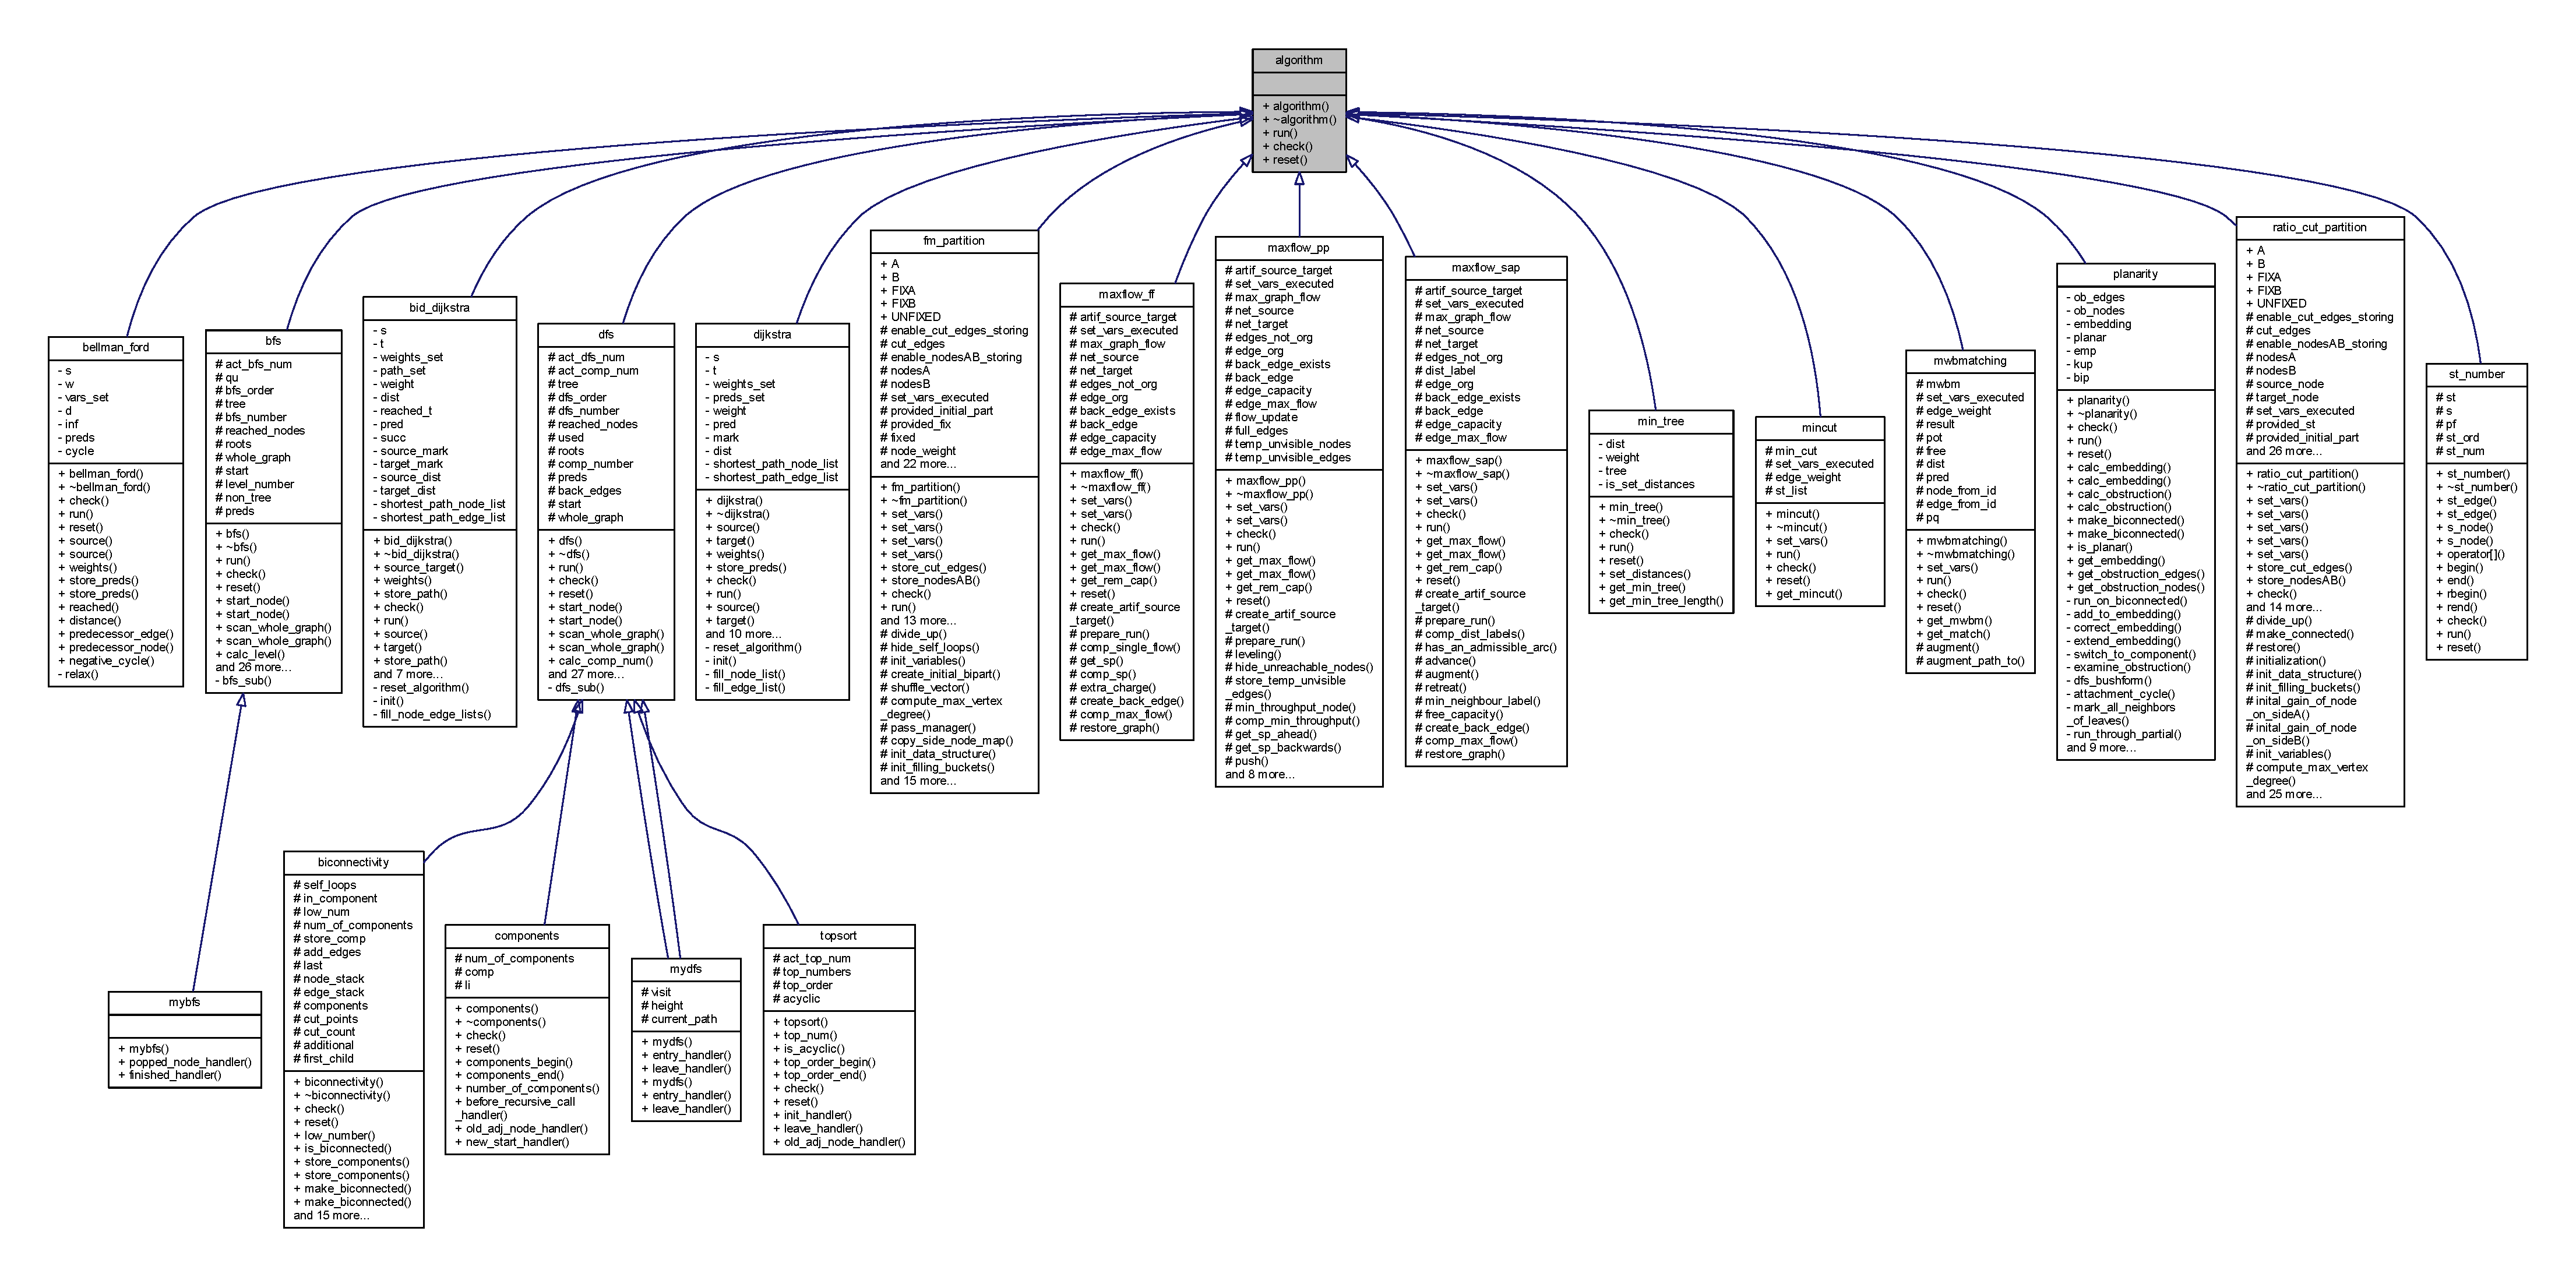
\includegraphics[width=350pt]{classalgorithm__inherit__graph}
\end{center}
\end{figure}


Collaboration diagram for algorithm\+:\nopagebreak
\begin{figure}[H]
\begin{center}
\leavevmode
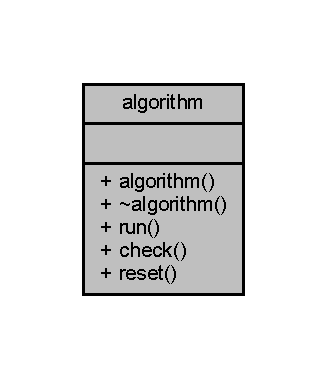
\includegraphics[width=157pt]{classalgorithm__coll__graph}
\end{center}
\end{figure}
\subsection*{Public Types}
\begin{DoxyCompactItemize}
\item 
enum \{ \mbox{\hyperlink{classalgorithm_af1a0078e153aa99c24f9bdf0d97f6710a5114c20e4a96a76b5de9f28bf15e282b}{G\+T\+L\+\_\+\+OK}} = 1, 
\mbox{\hyperlink{classalgorithm_af1a0078e153aa99c24f9bdf0d97f6710a6fcf574690bbd6cf710837a169510dd7}{G\+T\+L\+\_\+\+E\+R\+R\+OR}} = 0
 \}
\begin{DoxyCompactList}\small\item\em Return values for \mbox{\hyperlink{classalgorithm_a76361fb03ad1cf643affc51821e43bed}{algorithm\+::check}} and \mbox{\hyperlink{classalgorithm_a734b189509a8d6b56b65f8ff772d43ca}{algorithm\+::run}}. \end{DoxyCompactList}\end{DoxyCompactItemize}
\subsection*{Public Member Functions}
\begin{DoxyCompactItemize}
\item 
\mbox{\hyperlink{classalgorithm_ab79e1ddec2f2afdf4b36b10724db8b15}{algorithm}} ()
\begin{DoxyCompactList}\small\item\em Creates an algorithm object. \end{DoxyCompactList}\item 
virtual \mbox{\hyperlink{classalgorithm_adca9b1e7fa3afd914519a9dbb44e9fd5}{$\sim$algorithm}} ()
\begin{DoxyCompactList}\small\item\em Destroys the algorithm object. \end{DoxyCompactList}\item 
virtual int \mbox{\hyperlink{classalgorithm_a734b189509a8d6b56b65f8ff772d43ca}{run}} (\mbox{\hyperlink{classgraph}{graph}} \&\mbox{\hyperlink{rings_8cpp_aa9df5aa3976a89a96a5f1c7611d42938}{g}})=0
\begin{DoxyCompactList}\small\item\em Applies algorithm to graph g. \end{DoxyCompactList}\item 
virtual int \mbox{\hyperlink{classalgorithm_a76361fb03ad1cf643affc51821e43bed}{check}} (\mbox{\hyperlink{classgraph}{graph}} \&\mbox{\hyperlink{rings_8cpp_aa9df5aa3976a89a96a5f1c7611d42938}{g}})=0
\begin{DoxyCompactList}\small\item\em Checks whether all preconditions are satisfied. \end{DoxyCompactList}\item 
virtual void \mbox{\hyperlink{classalgorithm_a21aba63d066ae7897de6ca7d8425c408}{reset}} ()=0
\begin{DoxyCompactList}\small\item\em Resets algorithm. \end{DoxyCompactList}\end{DoxyCompactItemize}


\subsection{Detailed Description}
Abstract baseclass for all algoritm-\/classes. 

\begin{DoxyParagraph}{Date}
2003/03/24 15\+:58\+:54 
\end{DoxyParagraph}
\begin{DoxyParagraph}{Revision}
1.\+14 
\end{DoxyParagraph}


Definition at line 23 of file algorithm.\+h.



\subsection{Member Enumeration Documentation}
\mbox{\Hypertarget{classalgorithm_af1a0078e153aa99c24f9bdf0d97f6710}\label{classalgorithm_af1a0078e153aa99c24f9bdf0d97f6710}} 
\subsubsection{\texorpdfstring{anonymous enum}{anonymous enum}}
{\footnotesize\ttfamily anonymous enum}



Return values for \mbox{\hyperlink{classalgorithm_a76361fb03ad1cf643affc51821e43bed}{algorithm\+::check}} and \mbox{\hyperlink{classalgorithm_a734b189509a8d6b56b65f8ff772d43ca}{algorithm\+::run}}. 

\begin{DoxyEnumFields}{Enumerator}
\raisebox{\heightof{T}}[0pt][0pt]{\index{G\+T\+L\+\_\+\+OK@{G\+T\+L\+\_\+\+OK}!algorithm@{algorithm}}\index{algorithm@{algorithm}!G\+T\+L\+\_\+\+OK@{G\+T\+L\+\_\+\+OK}}}\mbox{\Hypertarget{classalgorithm_af1a0078e153aa99c24f9bdf0d97f6710a5114c20e4a96a76b5de9f28bf15e282b}\label{classalgorithm_af1a0078e153aa99c24f9bdf0d97f6710a5114c20e4a96a76b5de9f28bf15e282b}} 
G\+T\+L\+\_\+\+OK&Used as (positive) return value of \mbox{\hyperlink{classalgorithm_a76361fb03ad1cf643affc51821e43bed}{algorithm\+::check}} and \mbox{\hyperlink{classalgorithm_a734b189509a8d6b56b65f8ff772d43ca}{algorithm\+::run}}. \\
\hline

\raisebox{\heightof{T}}[0pt][0pt]{\index{G\+T\+L\+\_\+\+E\+R\+R\+OR@{G\+T\+L\+\_\+\+E\+R\+R\+OR}!algorithm@{algorithm}}\index{algorithm@{algorithm}!G\+T\+L\+\_\+\+E\+R\+R\+OR@{G\+T\+L\+\_\+\+E\+R\+R\+OR}}}\mbox{\Hypertarget{classalgorithm_af1a0078e153aa99c24f9bdf0d97f6710a6fcf574690bbd6cf710837a169510dd7}\label{classalgorithm_af1a0078e153aa99c24f9bdf0d97f6710a6fcf574690bbd6cf710837a169510dd7}} 
G\+T\+L\+\_\+\+E\+R\+R\+OR&Used as (negative) return value of \mbox{\hyperlink{classalgorithm_a76361fb03ad1cf643affc51821e43bed}{algorithm\+::check}} and \mbox{\hyperlink{classalgorithm_a734b189509a8d6b56b65f8ff772d43ca}{algorithm\+::run}}. \\
\hline

\end{DoxyEnumFields}


Definition at line 40 of file algorithm.\+h.


\begin{DoxyCode}
40          \{
41     \mbox{\hyperlink{classalgorithm_af1a0078e153aa99c24f9bdf0d97f6710a5114c20e4a96a76b5de9f28bf15e282b}{GTL\_OK}} = 1,
42     \mbox{\hyperlink{classalgorithm_af1a0078e153aa99c24f9bdf0d97f6710a6fcf574690bbd6cf710837a169510dd7}{GTL\_ERROR}} = 0
43     \};
\end{DoxyCode}


\subsection{Constructor \& Destructor Documentation}
\mbox{\Hypertarget{classalgorithm_ab79e1ddec2f2afdf4b36b10724db8b15}\label{classalgorithm_ab79e1ddec2f2afdf4b36b10724db8b15}} 
\index{algorithm@{algorithm}!algorithm@{algorithm}}
\index{algorithm@{algorithm}!algorithm@{algorithm}}
\subsubsection{\texorpdfstring{algorithm()}{algorithm()}}
{\footnotesize\ttfamily algorithm\+::algorithm (\begin{DoxyParamCaption}{ }\end{DoxyParamCaption})\hspace{0.3cm}{\ttfamily [inline]}}



Creates an algorithm object. 



Definition at line 48 of file algorithm.\+h.


\begin{DoxyCode}
48 \{ \};
\end{DoxyCode}
\mbox{\Hypertarget{classalgorithm_adca9b1e7fa3afd914519a9dbb44e9fd5}\label{classalgorithm_adca9b1e7fa3afd914519a9dbb44e9fd5}} 
\index{algorithm@{algorithm}!````~algorithm@{$\sim$algorithm}}
\index{````~algorithm@{$\sim$algorithm}!algorithm@{algorithm}}
\subsubsection{\texorpdfstring{$\sim$algorithm()}{~algorithm()}}
{\footnotesize\ttfamily virtual algorithm\+::$\sim$algorithm (\begin{DoxyParamCaption}{ }\end{DoxyParamCaption})\hspace{0.3cm}{\ttfamily [inline]}, {\ttfamily [virtual]}}



Destroys the algorithm object. 



Definition at line 53 of file algorithm.\+h.


\begin{DoxyCode}
53 \{ \};    
\end{DoxyCode}


\subsection{Member Function Documentation}
\mbox{\Hypertarget{classalgorithm_a76361fb03ad1cf643affc51821e43bed}\label{classalgorithm_a76361fb03ad1cf643affc51821e43bed}} 
\index{algorithm@{algorithm}!check@{check}}
\index{check@{check}!algorithm@{algorithm}}
\subsubsection{\texorpdfstring{check()}{check()}}
{\footnotesize\ttfamily virtual int algorithm\+::check (\begin{DoxyParamCaption}\item[{\mbox{\hyperlink{classgraph}{graph}} \&}]{g }\end{DoxyParamCaption})\hspace{0.3cm}{\ttfamily [pure virtual]}}



Checks whether all preconditions are satisfied. 

{\itshape Please} {\itshape note\+:} It is definitly required (and \mbox{\hyperlink{classalgorithm_a734b189509a8d6b56b65f8ff772d43ca}{run}} relies on it), that this method was called in advance.


\begin{DoxyParams}{Parameters}
{\em g} & graph \\
\hline
\end{DoxyParams}

\begin{DoxyRetVals}{Return values}
{\em \mbox{\hyperlink{classalgorithm_af1a0078e153aa99c24f9bdf0d97f6710a5114c20e4a96a76b5de9f28bf15e282b}{algorithm\+::\+G\+T\+L\+\_\+\+OK}}} & if algorithm can be applied \\
\hline
{\em \mbox{\hyperlink{classalgorithm_af1a0078e153aa99c24f9bdf0d97f6710a6fcf574690bbd6cf710837a169510dd7}{algorithm\+::\+G\+T\+L\+\_\+\+E\+R\+R\+OR}}} & otherwise. \\
\hline
\end{DoxyRetVals}


Implemented in \mbox{\hyperlink{classst__number_a2aad4550b821c52d6998bff35fd8648f}{st\+\_\+number}}, \mbox{\hyperlink{classratio__cut__partition_a469c613c69db19cb63e492075346fea2}{ratio\+\_\+cut\+\_\+partition}}, \mbox{\hyperlink{classfm__partition_af72a9fcc300ab0f202168c819b089e5d}{fm\+\_\+partition}}, \mbox{\hyperlink{classdijkstra_a51ff4657e0ddb1ca5231a21e6dea1808}{dijkstra}}, \mbox{\hyperlink{classbid__dijkstra_a504aa04d114f27f2f886ee3b025ad95b}{bid\+\_\+dijkstra}}, \mbox{\hyperlink{classdfs_a1af70060897529e67910f589b047e576}{dfs}}, \mbox{\hyperlink{classbfs_aafdf63b57eaceb5d95f441be0f9c77bb}{bfs}}, \mbox{\hyperlink{classtopsort_a777a9a68c4081d22e7b698ed3c515343}{topsort}}, \mbox{\hyperlink{classmaxflow__sap_aa2974bf25fb597677848fdb23c12d338}{maxflow\+\_\+sap}}, \mbox{\hyperlink{classmaxflow__ff_a4d0deee7d70bac4c9dad942341d87e37}{maxflow\+\_\+ff}}, \mbox{\hyperlink{classmaxflow__pp_a7ea24bd88999718e5e4e28ac028131cd}{maxflow\+\_\+pp}}, \mbox{\hyperlink{classplanarity_ae06c471d957a116aad14e338c341f8b1}{planarity}}, \mbox{\hyperlink{classbiconnectivity_a65e0e821f5e9ce8d210648d462fd2cfa}{biconnectivity}}, \mbox{\hyperlink{classbellman__ford_a9da2fb7d20ef1f726ee935474302d80b}{bellman\+\_\+ford}}, \mbox{\hyperlink{classmin__tree_ad87b1bfbc687ad943c07538fa0c3d270}{min\+\_\+tree}}, \mbox{\hyperlink{classcomponents_aeeda901d02c65d6c31c8b6148540d7c1}{components}}, \mbox{\hyperlink{classmincut_a3a06737106ab6000360a1f799361691a}{mincut}}, and \mbox{\hyperlink{classmwbmatching_af6b9e6ad6e77958ddd32301df96bae23}{mwbmatching}}.

\mbox{\Hypertarget{classalgorithm_a21aba63d066ae7897de6ca7d8425c408}\label{classalgorithm_a21aba63d066ae7897de6ca7d8425c408}} 
\index{algorithm@{algorithm}!reset@{reset}}
\index{reset@{reset}!algorithm@{algorithm}}
\subsubsection{\texorpdfstring{reset()}{reset()}}
{\footnotesize\ttfamily virtual void algorithm\+::reset (\begin{DoxyParamCaption}{ }\end{DoxyParamCaption})\hspace{0.3cm}{\ttfamily [pure virtual]}}



Resets algorithm. 

Prepares the algorithm to be applied to another graph. {\itshape Please} {\itshape note\+:} The options an algorithm may support do {\itshape not} get reset by this. It is just to reset internally used datastructures. 

Implemented in \mbox{\hyperlink{classst__number_ae6f86706b8ae3495d3794b8c684fff0f}{st\+\_\+number}}, \mbox{\hyperlink{classratio__cut__partition_ad017eaf98f9ae4ca9dbe6b3eda9fc94d}{ratio\+\_\+cut\+\_\+partition}}, \mbox{\hyperlink{classfm__partition_a6db2eeb6ae968dbab78302f0448c0ced}{fm\+\_\+partition}}, \mbox{\hyperlink{classdijkstra_a444c288b3a49ec1c2973459dad55ffb3}{dijkstra}}, \mbox{\hyperlink{classbid__dijkstra_a6df2769941bc73fc5626b084745a2258}{bid\+\_\+dijkstra}}, \mbox{\hyperlink{classmaxflow__sap_a14574d2f9ce31a3cdeb0888e57fc0616}{maxflow\+\_\+sap}}, \mbox{\hyperlink{classmaxflow__ff_a893e5136d4f7f1d4b67ef5b67306d17b}{maxflow\+\_\+ff}}, \mbox{\hyperlink{classmaxflow__pp_a2179764baf624f1414211f3a7181b1a0}{maxflow\+\_\+pp}}, \mbox{\hyperlink{classdfs_affaffda8be8418d6dbf396c5b1d6b81a}{dfs}}, \mbox{\hyperlink{classbfs_a6398bc230f9723cd5fdd32cd603647cc}{bfs}}, \mbox{\hyperlink{classplanarity_aca500e3d46a99c6231aff86afa2a71b1}{planarity}}, \mbox{\hyperlink{classtopsort_aa3d9ccc7c632dac6b7303e9828c14f62}{topsort}}, \mbox{\hyperlink{classbellman__ford_a7d28afa62ce8068c4d0f2d1f96136fd6}{bellman\+\_\+ford}}, \mbox{\hyperlink{classbiconnectivity_a4393dd1e626887472f6967722349abc6}{biconnectivity}}, \mbox{\hyperlink{classmin__tree_a0edbe612424dc5f4de4701b8fd0df931}{min\+\_\+tree}}, \mbox{\hyperlink{classmincut_a3f2142246a7b3e7b19b15d62314c9337}{mincut}}, \mbox{\hyperlink{classcomponents_a07b6bab5962524ae26ccb478b35cd76c}{components}}, and \mbox{\hyperlink{classmwbmatching_acb2171f09442f1d4170eaed5dc213865}{mwbmatching}}.

\mbox{\Hypertarget{classalgorithm_a734b189509a8d6b56b65f8ff772d43ca}\label{classalgorithm_a734b189509a8d6b56b65f8ff772d43ca}} 
\index{algorithm@{algorithm}!run@{run}}
\index{run@{run}!algorithm@{algorithm}}
\subsubsection{\texorpdfstring{run()}{run()}}
{\footnotesize\ttfamily virtual int algorithm\+::run (\begin{DoxyParamCaption}\item[{\mbox{\hyperlink{classgraph}{graph}} \&}]{g }\end{DoxyParamCaption})\hspace{0.3cm}{\ttfamily [pure virtual]}}



Applies algorithm to graph g. 


\begin{DoxyParams}{Parameters}
{\em g} & graph \\
\hline
\end{DoxyParams}

\begin{DoxyRetVals}{Return values}
{\em \mbox{\hyperlink{classalgorithm_af1a0078e153aa99c24f9bdf0d97f6710a5114c20e4a96a76b5de9f28bf15e282b}{algorithm\+::\+G\+T\+L\+\_\+\+OK}}} & on success \\
\hline
{\em \mbox{\hyperlink{classalgorithm_af1a0078e153aa99c24f9bdf0d97f6710a6fcf574690bbd6cf710837a169510dd7}{algorithm\+::\+G\+T\+L\+\_\+\+E\+R\+R\+OR}}} & otherwise \\
\hline
\end{DoxyRetVals}


Implemented in \mbox{\hyperlink{classst__number_af902a0c05d07d47b587e8f7a6b7beaa1}{st\+\_\+number}}, \mbox{\hyperlink{classratio__cut__partition_a4ab180ca4cf57c811e3478c3de4c4dc3}{ratio\+\_\+cut\+\_\+partition}}, \mbox{\hyperlink{classfm__partition_a015b171fcaa01973ebe6c6a46a727097}{fm\+\_\+partition}}, \mbox{\hyperlink{classdijkstra_a7b30f3d8ad42baae27989bc14befe0d0}{dijkstra}}, \mbox{\hyperlink{classbid__dijkstra_a1d2f36d3977ef90285442a269a03b919}{bid\+\_\+dijkstra}}, \mbox{\hyperlink{classdfs_af0863b8974d5fd58cd0375c78ed8163b}{dfs}}, \mbox{\hyperlink{classbfs_a06ae16bd0f3bb2f8eb6b3e36659ba82e}{bfs}}, \mbox{\hyperlink{classmaxflow__sap_ab4305a2bb370ad9c43cc68d339b2dda0}{maxflow\+\_\+sap}}, \mbox{\hyperlink{classplanarity_a93232e765c08dd2a4c00d192bb48b5fc}{planarity}}, \mbox{\hyperlink{classmaxflow__ff_a0a4391b9093d6966b47c023a555099e2}{maxflow\+\_\+ff}}, \mbox{\hyperlink{classmaxflow__pp_a07c7cb1ae5db23d87cf49ce7769b2814}{maxflow\+\_\+pp}}, \mbox{\hyperlink{classbellman__ford_a226308389f3c36dfc02768c09f777a3b}{bellman\+\_\+ford}}, \mbox{\hyperlink{classmin__tree_ac025e8dad0db7a6a1e0e7b476b547802}{min\+\_\+tree}}, \mbox{\hyperlink{classmincut_ab7e374a3f73387aa61587643a5f44e43}{mincut}}, and \mbox{\hyperlink{classmwbmatching_adcb51caed21e77253940cd71bfd9a405}{mwbmatching}}.



The documentation for this class was generated from the following file\+:\begin{DoxyCompactItemize}
\item 
D\+:/\+Roy/\+Git\+Hub/\+Multitarget-\/tracker/\+Tracker/graph/\+G\+T\+L/include/\+G\+T\+L/\mbox{\hyperlink{algorithm_8h}{algorithm.\+h}}\end{DoxyCompactItemize}

\hypertarget{class_array2d}{}\section{Array2d$<$ T $>$ Class Template Reference}
\label{class_array2d}\index{Array2d$<$ T $>$@{Array2d$<$ T $>$}}


{\ttfamily \#include $<$c4-\/pedestrian-\/detector.\+h$>$}



Collaboration diagram for Array2d$<$ T $>$\+:\nopagebreak
\begin{figure}[H]
\begin{center}
\leavevmode
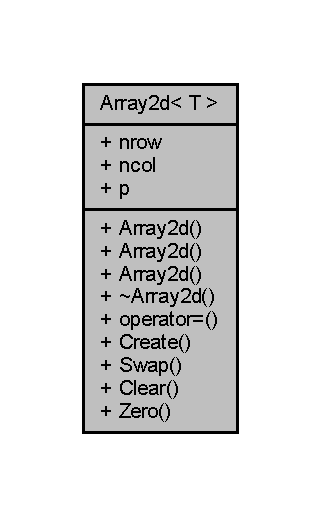
\includegraphics[width=154pt]{class_array2d__coll__graph}
\end{center}
\end{figure}
\subsection*{Public Member Functions}
\begin{DoxyCompactItemize}
\item 
\mbox{\hyperlink{class_array2d_a8c4b92d7f309ef043458835cc3fd2e14}{Array2d}} ()
\item 
\mbox{\hyperlink{class_array2d_ac7c55fd62aeda8ffb83e6c4ae39a2488}{Array2d}} (const int \mbox{\hyperlink{class_array2d_a373dd63664bee40ef720d183d03e5bdb}{nrow}}, const int \mbox{\hyperlink{class_array2d_afe48cd05774cae5b6872324ae49e089b}{ncol}})
\item 
\mbox{\hyperlink{class_array2d_ad3b3759e78a6840cce7b8009fe960621}{Array2d}} (const \mbox{\hyperlink{class_array2d}{Array2d}}$<$ T $>$ \&source)
\item 
virtual \mbox{\hyperlink{class_array2d_afe31cffbc2b8bc84153ec3ad7e40a0e2}{$\sim$\+Array2d}} ()
\item 
\mbox{\hyperlink{class_array2d}{Array2d}}$<$ T $>$ \& \mbox{\hyperlink{class_array2d_aa1c400a330cf1a31bd473bc3742ae51d}{operator=}} (const \mbox{\hyperlink{class_array2d}{Array2d}}$<$ T $>$ \&source)
\item 
void \mbox{\hyperlink{class_array2d_af1d2cec0973cedfe74ae5b967532922f}{Create}} (const int \+\_\+nrow, const int \+\_\+ncol)
\item 
void \mbox{\hyperlink{class_array2d_a24e1766701c30e14fa39bfcb1024bd1a}{Swap}} (\mbox{\hyperlink{class_array2d}{Array2d}}$<$ T $>$ \&array2)
\item 
void \mbox{\hyperlink{class_array2d_a9902a80867777fbf3ba64a6d8c10606e}{Clear}} ()
\item 
void \mbox{\hyperlink{class_array2d_a84070672548d19a9e77b4321527637e0}{Zero}} (const T t=0)
\end{DoxyCompactItemize}
\subsection*{Public Attributes}
\begin{DoxyCompactItemize}
\item 
int \mbox{\hyperlink{class_array2d_a373dd63664bee40ef720d183d03e5bdb}{nrow}}
\item 
int \mbox{\hyperlink{class_array2d_afe48cd05774cae5b6872324ae49e089b}{ncol}}
\item 
T $\ast$$\ast$ \mbox{\hyperlink{class_array2d_ac7b70bc423364c43c7c174cdde515380}{p}}
\end{DoxyCompactItemize}


\subsection{Detailed Description}
\subsubsection*{template$<$class T$>$\newline
class Array2d$<$ T $>$}



Definition at line 25 of file c4-\/pedestrian-\/detector.\+h.



\subsection{Constructor \& Destructor Documentation}
\mbox{\Hypertarget{class_array2d_a8c4b92d7f309ef043458835cc3fd2e14}\label{class_array2d_a8c4b92d7f309ef043458835cc3fd2e14}} 
\index{Array2d@{Array2d}!Array2d@{Array2d}}
\index{Array2d@{Array2d}!Array2d@{Array2d}}
\subsubsection{\texorpdfstring{Array2d()}{Array2d()}\hspace{0.1cm}{\footnotesize\ttfamily [1/3]}}
{\footnotesize\ttfamily template$<$class T$>$ \\
\mbox{\hyperlink{class_array2d}{Array2d}}$<$ T $>$\+::\mbox{\hyperlink{class_array2d}{Array2d}} (\begin{DoxyParamCaption}{ }\end{DoxyParamCaption})\hspace{0.3cm}{\ttfamily [inline]}}



Definition at line 32 of file c4-\/pedestrian-\/detector.\+h.


\begin{DoxyCode}
32 :\mbox{\hyperlink{class_array2d_a373dd63664bee40ef720d183d03e5bdb}{nrow}}(0),\mbox{\hyperlink{class_array2d_afe48cd05774cae5b6872324ae49e089b}{ncol}}(0),\mbox{\hyperlink{class_array2d_ac7b70bc423364c43c7c174cdde515380}{p}}(NULL) \{ \}
\end{DoxyCode}
\mbox{\Hypertarget{class_array2d_ac7c55fd62aeda8ffb83e6c4ae39a2488}\label{class_array2d_ac7c55fd62aeda8ffb83e6c4ae39a2488}} 
\index{Array2d@{Array2d}!Array2d@{Array2d}}
\index{Array2d@{Array2d}!Array2d@{Array2d}}
\subsubsection{\texorpdfstring{Array2d()}{Array2d()}\hspace{0.1cm}{\footnotesize\ttfamily [2/3]}}
{\footnotesize\ttfamily template$<$class T$>$ \\
\mbox{\hyperlink{class_array2d}{Array2d}}$<$ T $>$\+::\mbox{\hyperlink{class_array2d}{Array2d}} (\begin{DoxyParamCaption}\item[{const int}]{nrow,  }\item[{const int}]{ncol }\end{DoxyParamCaption})\hspace{0.3cm}{\ttfamily [inline]}}



Definition at line 33 of file c4-\/pedestrian-\/detector.\+h.


\begin{DoxyCode}
33                                           :\mbox{\hyperlink{class_array2d_a373dd63664bee40ef720d183d03e5bdb}{nrow}}(0),\mbox{\hyperlink{class_array2d_afe48cd05774cae5b6872324ae49e089b}{ncol}}(0),\mbox{\hyperlink{class_array2d_ac7b70bc423364c43c7c174cdde515380}{p}}(NULL)
34     \{
35         \mbox{\hyperlink{class_array2d_af1d2cec0973cedfe74ae5b967532922f}{Create}}(\mbox{\hyperlink{class_array2d_a373dd63664bee40ef720d183d03e5bdb}{nrow}},\mbox{\hyperlink{class_array2d_afe48cd05774cae5b6872324ae49e089b}{ncol}});
36     \}
\end{DoxyCode}
Here is the call graph for this function\+:\nopagebreak
\begin{figure}[H]
\begin{center}
\leavevmode
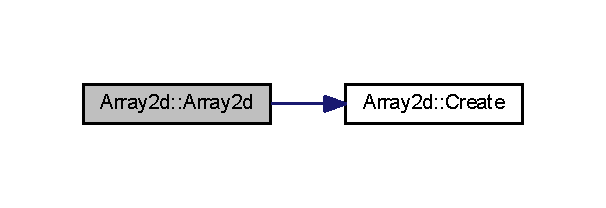
\includegraphics[width=291pt]{class_array2d_ac7c55fd62aeda8ffb83e6c4ae39a2488_cgraph}
\end{center}
\end{figure}
\mbox{\Hypertarget{class_array2d_ad3b3759e78a6840cce7b8009fe960621}\label{class_array2d_ad3b3759e78a6840cce7b8009fe960621}} 
\index{Array2d@{Array2d}!Array2d@{Array2d}}
\index{Array2d@{Array2d}!Array2d@{Array2d}}
\subsubsection{\texorpdfstring{Array2d()}{Array2d()}\hspace{0.1cm}{\footnotesize\ttfamily [3/3]}}
{\footnotesize\ttfamily template$<$class T $>$ \\
\mbox{\hyperlink{class_array2d}{Array2d}}$<$ T $>$\+::\mbox{\hyperlink{class_array2d}{Array2d}} (\begin{DoxyParamCaption}\item[{const \mbox{\hyperlink{class_array2d}{Array2d}}$<$ T $>$ \&}]{source }\end{DoxyParamCaption})}



Definition at line 78 of file c4-\/pedestrian-\/detector.\+h.


\begin{DoxyCode}
78                                            :\mbox{\hyperlink{class_array2d_a373dd63664bee40ef720d183d03e5bdb}{nrow}}(0),\mbox{\hyperlink{class_array2d_afe48cd05774cae5b6872324ae49e089b}{ncol}}(0),\mbox{\hyperlink{class_array2d_ac7b70bc423364c43c7c174cdde515380}{p}}(NULL)
79 \{
80     \textcolor{keywordflow}{if}(source.\mbox{\hyperlink{class_array2d_ac7b70bc423364c43c7c174cdde515380}{p}}!=NULL)
81     \{
82         \mbox{\hyperlink{class_array2d_af1d2cec0973cedfe74ae5b967532922f}{Create}}(source.\mbox{\hyperlink{class_array2d_a373dd63664bee40ef720d183d03e5bdb}{nrow}},source.\mbox{\hyperlink{class_array2d_afe48cd05774cae5b6872324ae49e089b}{ncol}});
83         \textcolor{keywordflow}{for}(\textcolor{keywordtype}{int} i=0; i<\mbox{\hyperlink{class_array2d_a373dd63664bee40ef720d183d03e5bdb}{nrow}}; i++) std::copy(source.\mbox{\hyperlink{class_array2d_ac7b70bc423364c43c7c174cdde515380}{p}}[i],source.\mbox{\hyperlink{class_array2d_ac7b70bc423364c43c7c174cdde515380}{p}}[i]+\mbox{\hyperlink{class_array2d_afe48cd05774cae5b6872324ae49e089b}{ncol}},
      \mbox{\hyperlink{class_array2d_ac7b70bc423364c43c7c174cdde515380}{p}}[i]);
84     \}
85 \}
\end{DoxyCode}
Here is the call graph for this function\+:\nopagebreak
\begin{figure}[H]
\begin{center}
\leavevmode
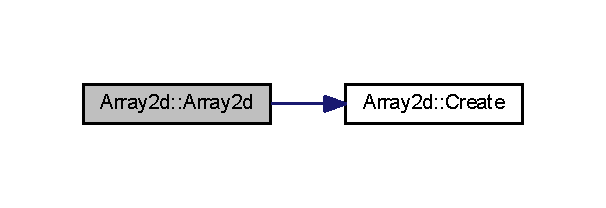
\includegraphics[width=291pt]{class_array2d_ad3b3759e78a6840cce7b8009fe960621_cgraph}
\end{center}
\end{figure}
\mbox{\Hypertarget{class_array2d_afe31cffbc2b8bc84153ec3ad7e40a0e2}\label{class_array2d_afe31cffbc2b8bc84153ec3ad7e40a0e2}} 
\index{Array2d@{Array2d}!````~Array2d@{$\sim$\+Array2d}}
\index{````~Array2d@{$\sim$\+Array2d}!Array2d@{Array2d}}
\subsubsection{\texorpdfstring{$\sim$\+Array2d()}{~Array2d()}}
{\footnotesize\ttfamily template$<$class T$>$ \\
virtual \mbox{\hyperlink{class_array2d}{Array2d}}$<$ T $>$\+::$\sim$\mbox{\hyperlink{class_array2d}{Array2d}} (\begin{DoxyParamCaption}{ }\end{DoxyParamCaption})\hspace{0.3cm}{\ttfamily [inline]}, {\ttfamily [virtual]}}



Definition at line 38 of file c4-\/pedestrian-\/detector.\+h.


\begin{DoxyCode}
39     \{
40         \mbox{\hyperlink{class_array2d_a9902a80867777fbf3ba64a6d8c10606e}{Clear}}();
41     \}
\end{DoxyCode}
Here is the call graph for this function\+:\nopagebreak
\begin{figure}[H]
\begin{center}
\leavevmode
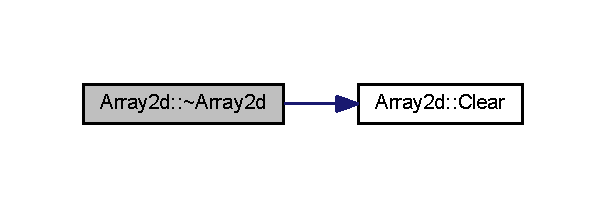
\includegraphics[width=291pt]{class_array2d_afe31cffbc2b8bc84153ec3ad7e40a0e2_cgraph}
\end{center}
\end{figure}


\subsection{Member Function Documentation}
\mbox{\Hypertarget{class_array2d_a9902a80867777fbf3ba64a6d8c10606e}\label{class_array2d_a9902a80867777fbf3ba64a6d8c10606e}} 
\index{Array2d@{Array2d}!Clear@{Clear}}
\index{Clear@{Clear}!Array2d@{Array2d}}
\subsubsection{\texorpdfstring{Clear()}{Clear()}}
{\footnotesize\ttfamily template$<$class T $>$ \\
void \mbox{\hyperlink{class_array2d}{Array2d}}$<$ T $>$\+::Clear (\begin{DoxyParamCaption}{ }\end{DoxyParamCaption})}



Definition at line 134 of file c4-\/pedestrian-\/detector.\+h.


\begin{DoxyCode}
135 \{
136     \textcolor{keywordflow}{for}(\textcolor{keywordtype}{int} i=0; i<\mbox{\hyperlink{class_array2d_a373dd63664bee40ef720d183d03e5bdb}{nrow}}; i++)
137     \{
138         \textcolor{keyword}{delete}[] \mbox{\hyperlink{class_array2d_ac7b70bc423364c43c7c174cdde515380}{p}}[i];
139         \mbox{\hyperlink{class_array2d_ac7b70bc423364c43c7c174cdde515380}{p}}[i] = NULL;
140     \}
141     \textcolor{keyword}{delete}[] \mbox{\hyperlink{class_array2d_ac7b70bc423364c43c7c174cdde515380}{p}};
142     \mbox{\hyperlink{class_array2d_ac7b70bc423364c43c7c174cdde515380}{p}} = NULL;
143     \mbox{\hyperlink{class_array2d_a373dd63664bee40ef720d183d03e5bdb}{nrow}} = \mbox{\hyperlink{class_array2d_afe48cd05774cae5b6872324ae49e089b}{ncol}} = 0;
144 \}
\end{DoxyCode}
Here is the caller graph for this function\+:\nopagebreak
\begin{figure}[H]
\begin{center}
\leavevmode
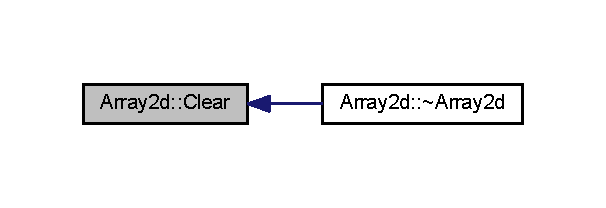
\includegraphics[width=291pt]{class_array2d_a9902a80867777fbf3ba64a6d8c10606e_icgraph}
\end{center}
\end{figure}
\mbox{\Hypertarget{class_array2d_af1d2cec0973cedfe74ae5b967532922f}\label{class_array2d_af1d2cec0973cedfe74ae5b967532922f}} 
\index{Array2d@{Array2d}!Create@{Create}}
\index{Create@{Create}!Array2d@{Array2d}}
\subsubsection{\texorpdfstring{Create()}{Create()}}
{\footnotesize\ttfamily template$<$class T $>$ \\
void \mbox{\hyperlink{class_array2d}{Array2d}}$<$ T $>$\+::Create (\begin{DoxyParamCaption}\item[{const int}]{\+\_\+nrow,  }\item[{const int}]{\+\_\+ncol }\end{DoxyParamCaption})}



Definition at line 101 of file c4-\/pedestrian-\/detector.\+h.


\begin{DoxyCode}
102 \{
103     assert(\_nrow>0 && \_ncol>0);
104     \mbox{\hyperlink{class_array2d_a9902a80867777fbf3ba64a6d8c10606e}{Clear}}();
105     \mbox{\hyperlink{class_array2d_a373dd63664bee40ef720d183d03e5bdb}{nrow}} = \_nrow;
106     \mbox{\hyperlink{class_array2d_afe48cd05774cae5b6872324ae49e089b}{ncol}} = \_ncol;
107     \mbox{\hyperlink{class_array2d_ac7b70bc423364c43c7c174cdde515380}{p}} = \textcolor{keyword}{new} T*[\mbox{\hyperlink{class_array2d_a373dd63664bee40ef720d183d03e5bdb}{nrow}}];
108     assert(\mbox{\hyperlink{class_array2d_ac7b70bc423364c43c7c174cdde515380}{p}}!=NULL);
109     \textcolor{keywordflow}{for}(\textcolor{keywordtype}{int} i=0; i<\mbox{\hyperlink{class_array2d_a373dd63664bee40ef720d183d03e5bdb}{nrow}}; i++)
110     \{
111         \mbox{\hyperlink{class_array2d_ac7b70bc423364c43c7c174cdde515380}{p}}[i] = \textcolor{keyword}{new} T[\mbox{\hyperlink{class_array2d_afe48cd05774cae5b6872324ae49e089b}{ncol}}];
112         assert(\mbox{\hyperlink{class_array2d_ac7b70bc423364c43c7c174cdde515380}{p}}[i]!=NULL);
113     \}
114 \}
\end{DoxyCode}
Here is the caller graph for this function\+:\nopagebreak
\begin{figure}[H]
\begin{center}
\leavevmode
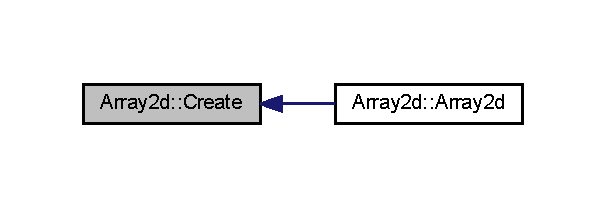
\includegraphics[width=291pt]{class_array2d_af1d2cec0973cedfe74ae5b967532922f_icgraph}
\end{center}
\end{figure}
\mbox{\Hypertarget{class_array2d_aa1c400a330cf1a31bd473bc3742ae51d}\label{class_array2d_aa1c400a330cf1a31bd473bc3742ae51d}} 
\index{Array2d@{Array2d}!operator=@{operator=}}
\index{operator=@{operator=}!Array2d@{Array2d}}
\subsubsection{\texorpdfstring{operator=()}{operator=()}}
{\footnotesize\ttfamily template$<$class T $>$ \\
\mbox{\hyperlink{class_array2d}{Array2d}}$<$ T $>$ \& \mbox{\hyperlink{class_array2d}{Array2d}}$<$ T $>$\+::operator= (\begin{DoxyParamCaption}\item[{const \mbox{\hyperlink{class_array2d}{Array2d}}$<$ T $>$ \&}]{source }\end{DoxyParamCaption})}



Definition at line 88 of file c4-\/pedestrian-\/detector.\+h.


\begin{DoxyCode}
89 \{
90     \textcolor{keywordflow}{if}(source.\mbox{\hyperlink{class_array2d_ac7b70bc423364c43c7c174cdde515380}{p}}!=NULL)
91     \{
92         \mbox{\hyperlink{class_array2d_af1d2cec0973cedfe74ae5b967532922f}{Create}}(source.\mbox{\hyperlink{class_array2d_a373dd63664bee40ef720d183d03e5bdb}{nrow}},source.\mbox{\hyperlink{class_array2d_afe48cd05774cae5b6872324ae49e089b}{ncol}});
93         \textcolor{keywordflow}{for}(\textcolor{keywordtype}{int} i=0; i<\mbox{\hyperlink{class_array2d_a373dd63664bee40ef720d183d03e5bdb}{nrow}}; i++) std::copy(source.\mbox{\hyperlink{class_array2d_ac7b70bc423364c43c7c174cdde515380}{p}}[i],source.\mbox{\hyperlink{class_array2d_ac7b70bc423364c43c7c174cdde515380}{p}}[i]+\mbox{\hyperlink{class_array2d_afe48cd05774cae5b6872324ae49e089b}{ncol}},
      \mbox{\hyperlink{class_array2d_ac7b70bc423364c43c7c174cdde515380}{p}}[i]);
94     \}
95     \textcolor{keywordflow}{else}
96         \mbox{\hyperlink{class_array2d_a9902a80867777fbf3ba64a6d8c10606e}{Clear}}();
97     \textcolor{keywordflow}{return} *\textcolor{keyword}{this};
98 \}
\end{DoxyCode}
\mbox{\Hypertarget{class_array2d_a24e1766701c30e14fa39bfcb1024bd1a}\label{class_array2d_a24e1766701c30e14fa39bfcb1024bd1a}} 
\index{Array2d@{Array2d}!Swap@{Swap}}
\index{Swap@{Swap}!Array2d@{Array2d}}
\subsubsection{\texorpdfstring{Swap()}{Swap()}}
{\footnotesize\ttfamily template$<$class T $>$ \\
void \mbox{\hyperlink{class_array2d}{Array2d}}$<$ T $>$\+::Swap (\begin{DoxyParamCaption}\item[{\mbox{\hyperlink{class_array2d}{Array2d}}$<$ T $>$ \&}]{array2 }\end{DoxyParamCaption})}



Definition at line 117 of file c4-\/pedestrian-\/detector.\+h.


\begin{DoxyCode}
118 \{
119     std::swap(\mbox{\hyperlink{class_array2d_a373dd63664bee40ef720d183d03e5bdb}{nrow}},array2.\mbox{\hyperlink{class_array2d_a373dd63664bee40ef720d183d03e5bdb}{nrow}});
120     std::swap(\mbox{\hyperlink{class_array2d_afe48cd05774cae5b6872324ae49e089b}{ncol}},array2.\mbox{\hyperlink{class_array2d_afe48cd05774cae5b6872324ae49e089b}{ncol}});
121     std::swap(\mbox{\hyperlink{class_array2d_ac7b70bc423364c43c7c174cdde515380}{p}},array2.\mbox{\hyperlink{class_array2d_ac7b70bc423364c43c7c174cdde515380}{p}});
122 \}
\end{DoxyCode}
\mbox{\Hypertarget{class_array2d_a84070672548d19a9e77b4321527637e0}\label{class_array2d_a84070672548d19a9e77b4321527637e0}} 
\index{Array2d@{Array2d}!Zero@{Zero}}
\index{Zero@{Zero}!Array2d@{Array2d}}
\subsubsection{\texorpdfstring{Zero()}{Zero()}}
{\footnotesize\ttfamily template$<$class T $>$ \\
void \mbox{\hyperlink{class_array2d}{Array2d}}$<$ T $>$\+::Zero (\begin{DoxyParamCaption}\item[{const T}]{t = {\ttfamily 0} }\end{DoxyParamCaption})}



Definition at line 125 of file c4-\/pedestrian-\/detector.\+h.


\begin{DoxyCode}
126 \{
127     \textcolor{keywordflow}{if}(\mbox{\hyperlink{class_array2d_a373dd63664bee40ef720d183d03e5bdb}{nrow}}>0)
128     \{
129         \textcolor{keywordflow}{for}(\textcolor{keywordtype}{int} i=0; i<\mbox{\hyperlink{class_array2d_a373dd63664bee40ef720d183d03e5bdb}{nrow}}; i++) std::fill(\mbox{\hyperlink{class_array2d_ac7b70bc423364c43c7c174cdde515380}{p}}[i],\mbox{\hyperlink{class_array2d_ac7b70bc423364c43c7c174cdde515380}{p}}[i]+\mbox{\hyperlink{class_array2d_afe48cd05774cae5b6872324ae49e089b}{ncol}},t);
130     \}
131 \}
\end{DoxyCode}


\subsection{Member Data Documentation}
\mbox{\Hypertarget{class_array2d_afe48cd05774cae5b6872324ae49e089b}\label{class_array2d_afe48cd05774cae5b6872324ae49e089b}} 
\index{Array2d@{Array2d}!ncol@{ncol}}
\index{ncol@{ncol}!Array2d@{Array2d}}
\subsubsection{\texorpdfstring{ncol}{ncol}}
{\footnotesize\ttfamily template$<$class T$>$ \\
int \mbox{\hyperlink{class_array2d}{Array2d}}$<$ T $>$\+::ncol}



Definition at line 29 of file c4-\/pedestrian-\/detector.\+h.

\mbox{\Hypertarget{class_array2d_a373dd63664bee40ef720d183d03e5bdb}\label{class_array2d_a373dd63664bee40ef720d183d03e5bdb}} 
\index{Array2d@{Array2d}!nrow@{nrow}}
\index{nrow@{nrow}!Array2d@{Array2d}}
\subsubsection{\texorpdfstring{nrow}{nrow}}
{\footnotesize\ttfamily template$<$class T$>$ \\
int \mbox{\hyperlink{class_array2d}{Array2d}}$<$ T $>$\+::nrow}



Definition at line 28 of file c4-\/pedestrian-\/detector.\+h.

\mbox{\Hypertarget{class_array2d_ac7b70bc423364c43c7c174cdde515380}\label{class_array2d_ac7b70bc423364c43c7c174cdde515380}} 
\index{Array2d@{Array2d}!p@{p}}
\index{p@{p}!Array2d@{Array2d}}
\subsubsection{\texorpdfstring{p}{p}}
{\footnotesize\ttfamily template$<$class T$>$ \\
T$\ast$$\ast$ \mbox{\hyperlink{class_array2d}{Array2d}}$<$ T $>$\+::p}



Definition at line 30 of file c4-\/pedestrian-\/detector.\+h.



The documentation for this class was generated from the following file\+:\begin{DoxyCompactItemize}
\item 
D\+:/\+Roy/\+Git\+Hub/\+Multitarget-\/tracker/\+Detector/pedestrians/\mbox{\hyperlink{c4-pedestrian-detector_8h}{c4-\/pedestrian-\/detector.\+h}}\end{DoxyCompactItemize}

\hypertarget{class_array2d_c}{}\section{Array2dC$<$ T $>$ Class Template Reference}
\label{class_array2d_c}\index{Array2d\+C$<$ T $>$@{Array2d\+C$<$ T $>$}}


{\ttfamily \#include $<$c4-\/pedestrian-\/detector.\+h$>$}



Inheritance diagram for Array2dC$<$ T $>$\+:\nopagebreak
\begin{figure}[H]
\begin{center}
\leavevmode
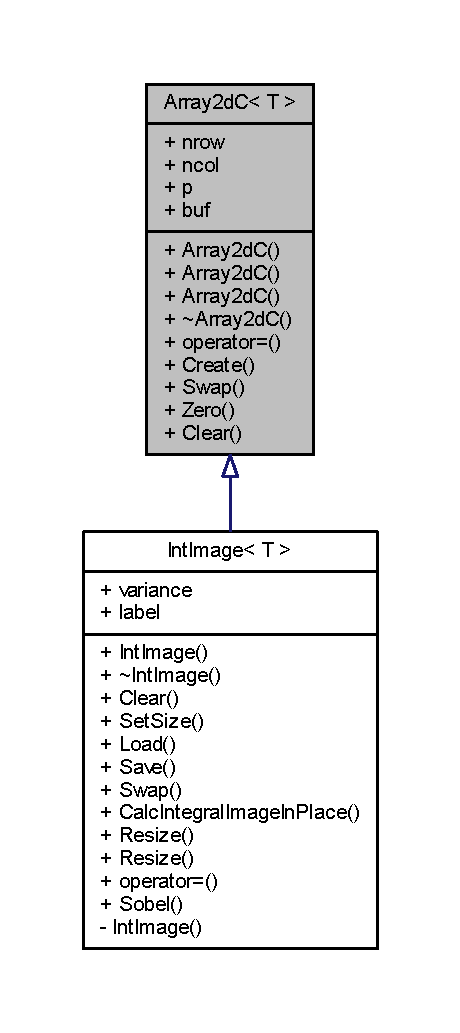
\includegraphics[width=221pt]{class_array2d_c__inherit__graph}
\end{center}
\end{figure}


Collaboration diagram for Array2dC$<$ T $>$\+:\nopagebreak
\begin{figure}[H]
\begin{center}
\leavevmode
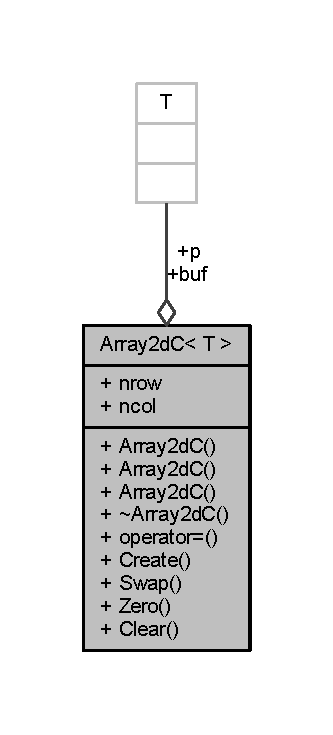
\includegraphics[width=160pt]{class_array2d_c__coll__graph}
\end{center}
\end{figure}
\subsection*{Public Member Functions}
\begin{DoxyCompactItemize}
\item 
\mbox{\hyperlink{class_array2d_c_a740d2592aa5563d59ff429311c51a04e}{Array2dC}} ()
\item 
\mbox{\hyperlink{class_array2d_c_a626db69cb139292c8249114172c10528}{Array2dC}} (const int \mbox{\hyperlink{class_array2d_c_a12f690f7195f7674a86a7e1eedbc473c}{nrow}}, const int \mbox{\hyperlink{class_array2d_c_a27e0f8f40f644831cd7c750db59dc28a}{ncol}})
\item 
\mbox{\hyperlink{class_array2d_c_aeeeddbaec65066f750615a130ef0f9da}{Array2dC}} (const \mbox{\hyperlink{class_array2d_c}{Array2dC}}$<$ T $>$ \&source)
\item 
virtual \mbox{\hyperlink{class_array2d_c_a96e68b849ec674616b79dc9d0c9233ab}{$\sim$\+Array2dC}} ()
\item 
\mbox{\hyperlink{class_array2d_c}{Array2dC}}$<$ T $>$ \& \mbox{\hyperlink{class_array2d_c_a241cc9224f991e0496dad95bc396e84e}{operator=}} (const \mbox{\hyperlink{class_array2d_c}{Array2dC}}$<$ T $>$ \&source)
\item 
void \mbox{\hyperlink{class_array2d_c_abfe87be7641dfc586b9e7bffebcca9ec}{Create}} (const int \+\_\+nrow, const int \+\_\+ncol)
\item 
void \mbox{\hyperlink{class_array2d_c_ae8cbeb3e4fdc3a45cc188ecc1b317919}{Swap}} (\mbox{\hyperlink{class_array2d_c}{Array2dC}}$<$ T $>$ \&array2)
\item 
void \mbox{\hyperlink{class_array2d_c_a5e1d7837fd208699694fc3fc97151df0}{Zero}} (const T t=0)
\item 
void \mbox{\hyperlink{class_array2d_c_a76a406cfeb9a9f75a1586e0a7b22f63e}{Clear}} ()
\end{DoxyCompactItemize}
\subsection*{Public Attributes}
\begin{DoxyCompactItemize}
\item 
int \mbox{\hyperlink{class_array2d_c_a12f690f7195f7674a86a7e1eedbc473c}{nrow}}
\item 
int \mbox{\hyperlink{class_array2d_c_a27e0f8f40f644831cd7c750db59dc28a}{ncol}}
\item 
T $\ast$$\ast$ \mbox{\hyperlink{class_array2d_c_a727eae5d663d463635cc150e6f771f0d}{p}}
\item 
T $\ast$ \mbox{\hyperlink{class_array2d_c_a25d8fa5049d4c7ded126e0acdd18f37a}{buf}}
\end{DoxyCompactItemize}


\subsection{Detailed Description}
\subsubsection*{template$<$class T$>$\newline
class Array2d\+C$<$ T $>$}



Definition at line 22 of file c4-\/pedestrian-\/detector.\+h.



\subsection{Constructor \& Destructor Documentation}
\mbox{\Hypertarget{class_array2d_c_a740d2592aa5563d59ff429311c51a04e}\label{class_array2d_c_a740d2592aa5563d59ff429311c51a04e}} 
\index{Array2dC@{Array2dC}!Array2dC@{Array2dC}}
\index{Array2dC@{Array2dC}!Array2dC@{Array2dC}}
\subsubsection{\texorpdfstring{Array2d\+C()}{Array2dC()}\hspace{0.1cm}{\footnotesize\ttfamily [1/3]}}
{\footnotesize\ttfamily template$<$class T$>$ \\
\mbox{\hyperlink{class_array2d_c}{Array2dC}}$<$ T $>$\+::\mbox{\hyperlink{class_array2d_c}{Array2dC}} (\begin{DoxyParamCaption}{ }\end{DoxyParamCaption})\hspace{0.3cm}{\ttfamily [inline]}}



Definition at line 59 of file c4-\/pedestrian-\/detector.\+h.


\begin{DoxyCode}
59 :\mbox{\hyperlink{class_array2d_c_a12f690f7195f7674a86a7e1eedbc473c}{nrow}}(0),\mbox{\hyperlink{class_array2d_c_a27e0f8f40f644831cd7c750db59dc28a}{ncol}}(0),\mbox{\hyperlink{class_array2d_c_a727eae5d663d463635cc150e6f771f0d}{p}}(NULL),\mbox{\hyperlink{class_array2d_c_a25d8fa5049d4c7ded126e0acdd18f37a}{buf}}(NULL) \{\}
\end{DoxyCode}
\mbox{\Hypertarget{class_array2d_c_a626db69cb139292c8249114172c10528}\label{class_array2d_c_a626db69cb139292c8249114172c10528}} 
\index{Array2dC@{Array2dC}!Array2dC@{Array2dC}}
\index{Array2dC@{Array2dC}!Array2dC@{Array2dC}}
\subsubsection{\texorpdfstring{Array2d\+C()}{Array2dC()}\hspace{0.1cm}{\footnotesize\ttfamily [2/3]}}
{\footnotesize\ttfamily template$<$class T$>$ \\
\mbox{\hyperlink{class_array2d_c}{Array2dC}}$<$ T $>$\+::\mbox{\hyperlink{class_array2d_c}{Array2dC}} (\begin{DoxyParamCaption}\item[{const int}]{nrow,  }\item[{const int}]{ncol }\end{DoxyParamCaption})\hspace{0.3cm}{\ttfamily [inline]}}



Definition at line 60 of file c4-\/pedestrian-\/detector.\+h.


\begin{DoxyCode}
60                                            :\mbox{\hyperlink{class_array2d_c_a12f690f7195f7674a86a7e1eedbc473c}{nrow}}(0),\mbox{\hyperlink{class_array2d_c_a27e0f8f40f644831cd7c750db59dc28a}{ncol}}(0),\mbox{\hyperlink{class_array2d_c_a727eae5d663d463635cc150e6f771f0d}{p}}(NULL),\mbox{\hyperlink{class_array2d_c_a25d8fa5049d4c7ded126e0acdd18f37a}{buf}}(NULL)
61     \{
62         \mbox{\hyperlink{class_array2d_c_abfe87be7641dfc586b9e7bffebcca9ec}{Create}}(\mbox{\hyperlink{class_array2d_c_a12f690f7195f7674a86a7e1eedbc473c}{nrow}},\mbox{\hyperlink{class_array2d_c_a27e0f8f40f644831cd7c750db59dc28a}{ncol}});
63     \}
\end{DoxyCode}
\mbox{\Hypertarget{class_array2d_c_aeeeddbaec65066f750615a130ef0f9da}\label{class_array2d_c_aeeeddbaec65066f750615a130ef0f9da}} 
\index{Array2dC@{Array2dC}!Array2dC@{Array2dC}}
\index{Array2dC@{Array2dC}!Array2dC@{Array2dC}}
\subsubsection{\texorpdfstring{Array2d\+C()}{Array2dC()}\hspace{0.1cm}{\footnotesize\ttfamily [3/3]}}
{\footnotesize\ttfamily template$<$class T$>$ \\
\mbox{\hyperlink{class_array2d_c}{Array2dC}}$<$ T $>$\+::\mbox{\hyperlink{class_array2d_c}{Array2dC}} (\begin{DoxyParamCaption}\item[{const \mbox{\hyperlink{class_array2d_c}{Array2dC}}$<$ T $>$ \&}]{source }\end{DoxyParamCaption})}



Definition at line 147 of file c4-\/pedestrian-\/detector.\+h.


\begin{DoxyCode}
147                                               :\mbox{\hyperlink{class_array2d_c_a12f690f7195f7674a86a7e1eedbc473c}{nrow}}(0),\mbox{\hyperlink{class_array2d_c_a27e0f8f40f644831cd7c750db59dc28a}{ncol}}(0),\mbox{\hyperlink{class_array2d_c_a727eae5d663d463635cc150e6f771f0d}{p}}(NULL),
      \mbox{\hyperlink{class_array2d_c_a25d8fa5049d4c7ded126e0acdd18f37a}{buf}}(NULL)
148 \{
149     \textcolor{keywordflow}{if}(source.\mbox{\hyperlink{class_array2d_c_a25d8fa5049d4c7ded126e0acdd18f37a}{buf}}!=NULL)
150     \{
151         \mbox{\hyperlink{class_array2d_c_abfe87be7641dfc586b9e7bffebcca9ec}{Create}}(source.\mbox{\hyperlink{class_array2d_c_a12f690f7195f7674a86a7e1eedbc473c}{nrow}},source.\mbox{\hyperlink{class_array2d_c_a27e0f8f40f644831cd7c750db59dc28a}{ncol}});
152         std::copy(source.\mbox{\hyperlink{class_array2d_c_a25d8fa5049d4c7ded126e0acdd18f37a}{buf}},source.\mbox{\hyperlink{class_array2d_c_a25d8fa5049d4c7ded126e0acdd18f37a}{buf}}+\mbox{\hyperlink{class_array2d_c_a12f690f7195f7674a86a7e1eedbc473c}{nrow}}*\mbox{\hyperlink{class_array2d_c_a27e0f8f40f644831cd7c750db59dc28a}{ncol}},\mbox{\hyperlink{class_array2d_c_a25d8fa5049d4c7ded126e0acdd18f37a}{buf}});
153     \}
154 \}
\end{DoxyCode}
\mbox{\Hypertarget{class_array2d_c_a96e68b849ec674616b79dc9d0c9233ab}\label{class_array2d_c_a96e68b849ec674616b79dc9d0c9233ab}} 
\index{Array2dC@{Array2dC}!````~Array2dC@{$\sim$\+Array2dC}}
\index{````~Array2dC@{$\sim$\+Array2dC}!Array2dC@{Array2dC}}
\subsubsection{\texorpdfstring{$\sim$\+Array2d\+C()}{~Array2dC()}}
{\footnotesize\ttfamily template$<$class T$>$ \\
virtual \mbox{\hyperlink{class_array2d_c}{Array2dC}}$<$ T $>$\+::$\sim$\mbox{\hyperlink{class_array2d_c}{Array2dC}} (\begin{DoxyParamCaption}{ }\end{DoxyParamCaption})\hspace{0.3cm}{\ttfamily [inline]}, {\ttfamily [virtual]}}



Definition at line 65 of file c4-\/pedestrian-\/detector.\+h.


\begin{DoxyCode}
66     \{
67         \mbox{\hyperlink{class_array2d_c_a76a406cfeb9a9f75a1586e0a7b22f63e}{Clear}}();
68     \}
\end{DoxyCode}


\subsection{Member Function Documentation}
\mbox{\Hypertarget{class_array2d_c_a76a406cfeb9a9f75a1586e0a7b22f63e}\label{class_array2d_c_a76a406cfeb9a9f75a1586e0a7b22f63e}} 
\index{Array2dC@{Array2dC}!Clear@{Clear}}
\index{Clear@{Clear}!Array2dC@{Array2dC}}
\subsubsection{\texorpdfstring{Clear()}{Clear()}}
{\footnotesize\ttfamily template$<$class T $>$ \\
void \mbox{\hyperlink{class_array2d_c}{Array2dC}}$<$ T $>$\+::Clear (\begin{DoxyParamCaption}\item[{void}]{ }\end{DoxyParamCaption})}



Definition at line 200 of file c4-\/pedestrian-\/detector.\+h.


\begin{DoxyCode}
201 \{
202     \textcolor{keyword}{delete}[] \mbox{\hyperlink{class_array2d_c_a25d8fa5049d4c7ded126e0acdd18f37a}{buf}};
203     \mbox{\hyperlink{class_array2d_c_a25d8fa5049d4c7ded126e0acdd18f37a}{buf}} = NULL;
204     \textcolor{keyword}{delete}[] \mbox{\hyperlink{class_array2d_c_a727eae5d663d463635cc150e6f771f0d}{p}};
205     \mbox{\hyperlink{class_array2d_c_a727eae5d663d463635cc150e6f771f0d}{p}} = NULL;
206     \mbox{\hyperlink{class_array2d_c_a12f690f7195f7674a86a7e1eedbc473c}{nrow}} = \mbox{\hyperlink{class_array2d_c_a27e0f8f40f644831cd7c750db59dc28a}{ncol}} = 0;
207 \}
\end{DoxyCode}
Here is the caller graph for this function\+:\nopagebreak
\begin{figure}[H]
\begin{center}
\leavevmode
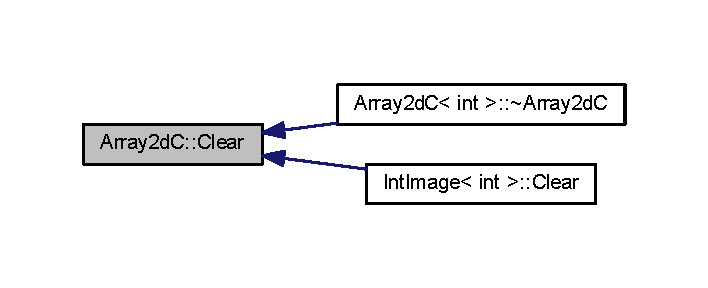
\includegraphics[width=340pt]{class_array2d_c_a76a406cfeb9a9f75a1586e0a7b22f63e_icgraph}
\end{center}
\end{figure}
\mbox{\Hypertarget{class_array2d_c_abfe87be7641dfc586b9e7bffebcca9ec}\label{class_array2d_c_abfe87be7641dfc586b9e7bffebcca9ec}} 
\index{Array2dC@{Array2dC}!Create@{Create}}
\index{Create@{Create}!Array2dC@{Array2dC}}
\subsubsection{\texorpdfstring{Create()}{Create()}}
{\footnotesize\ttfamily template$<$class T $>$ \\
void \mbox{\hyperlink{class_array2d_c}{Array2dC}}$<$ T $>$\+::Create (\begin{DoxyParamCaption}\item[{const int}]{\+\_\+nrow,  }\item[{const int}]{\+\_\+ncol }\end{DoxyParamCaption})}



Definition at line 170 of file c4-\/pedestrian-\/detector.\+h.


\begin{DoxyCode}
171 \{
172     assert(\_nrow>0 && \_ncol>0);
173     \textcolor{keywordflow}{if}(\mbox{\hyperlink{class_array2d_c_a12f690f7195f7674a86a7e1eedbc473c}{nrow}}==\_nrow && \mbox{\hyperlink{class_array2d_c_a27e0f8f40f644831cd7c750db59dc28a}{ncol}}==\_ncol) \textcolor{keywordflow}{return};
174     \mbox{\hyperlink{class_array2d_c_a76a406cfeb9a9f75a1586e0a7b22f63e}{Clear}}();
175     \mbox{\hyperlink{class_array2d_c_a12f690f7195f7674a86a7e1eedbc473c}{nrow}} = \_nrow;
176     \mbox{\hyperlink{class_array2d_c_a27e0f8f40f644831cd7c750db59dc28a}{ncol}} = \_ncol;
177     \mbox{\hyperlink{class_array2d_c_a25d8fa5049d4c7ded126e0acdd18f37a}{buf}} = \textcolor{keyword}{new} T[\mbox{\hyperlink{class_array2d_c_a12f690f7195f7674a86a7e1eedbc473c}{nrow}}*\mbox{\hyperlink{class_array2d_c_a27e0f8f40f644831cd7c750db59dc28a}{ncol}}];
178     assert(\mbox{\hyperlink{class_array2d_c_a25d8fa5049d4c7ded126e0acdd18f37a}{buf}}!=NULL);
179     \mbox{\hyperlink{class_array2d_c_a727eae5d663d463635cc150e6f771f0d}{p}} = \textcolor{keyword}{new} T*[\mbox{\hyperlink{class_array2d_c_a12f690f7195f7674a86a7e1eedbc473c}{nrow}}];
180     assert(\mbox{\hyperlink{class_array2d_c_a727eae5d663d463635cc150e6f771f0d}{p}}!=NULL);
181     \textcolor{keywordflow}{for}(\textcolor{keywordtype}{int} i=0; i<\mbox{\hyperlink{class_array2d_c_a12f690f7195f7674a86a7e1eedbc473c}{nrow}}; i++) \mbox{\hyperlink{class_array2d_c_a727eae5d663d463635cc150e6f771f0d}{p}}[i] = \mbox{\hyperlink{class_array2d_c_a25d8fa5049d4c7ded126e0acdd18f37a}{buf}} + i * \mbox{\hyperlink{class_array2d_c_a27e0f8f40f644831cd7c750db59dc28a}{ncol}};
182 \}
\end{DoxyCode}
Here is the caller graph for this function\+:
\nopagebreak
\begin{figure}[H]
\begin{center}
\leavevmode
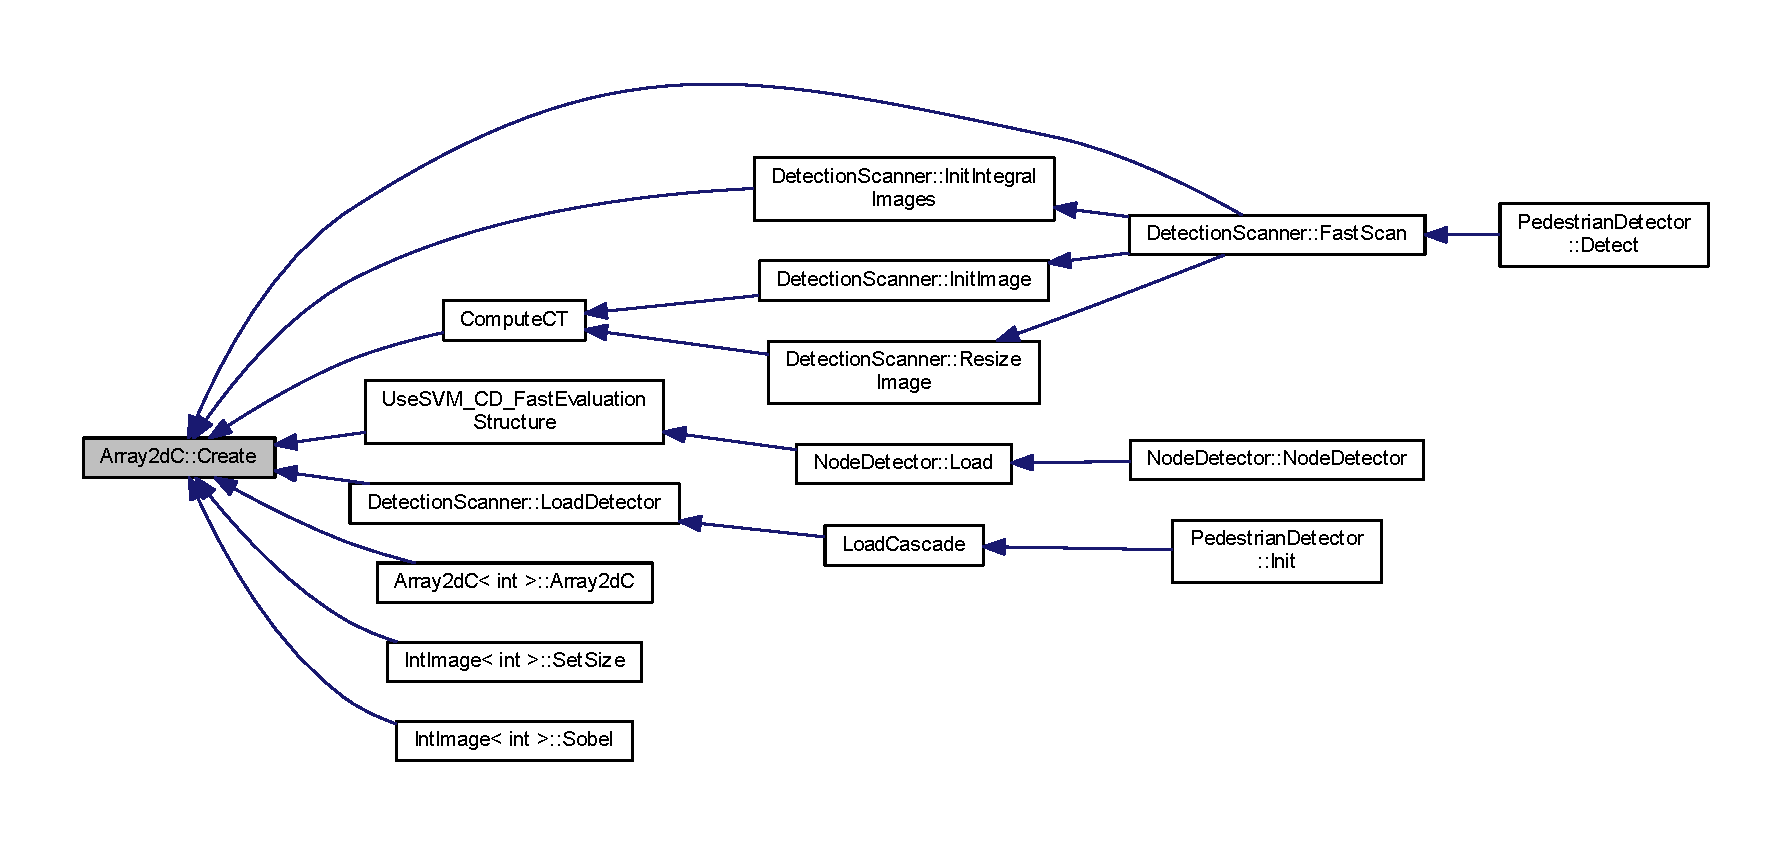
\includegraphics[width=350pt]{class_array2d_c_abfe87be7641dfc586b9e7bffebcca9ec_icgraph}
\end{center}
\end{figure}
\mbox{\Hypertarget{class_array2d_c_a241cc9224f991e0496dad95bc396e84e}\label{class_array2d_c_a241cc9224f991e0496dad95bc396e84e}} 
\index{Array2dC@{Array2dC}!operator=@{operator=}}
\index{operator=@{operator=}!Array2dC@{Array2dC}}
\subsubsection{\texorpdfstring{operator=()}{operator=()}}
{\footnotesize\ttfamily template$<$class T$>$ \\
\mbox{\hyperlink{class_array2d_c}{Array2dC}}$<$ T $>$ \& \mbox{\hyperlink{class_array2d_c}{Array2dC}}$<$ T $>$\+::operator= (\begin{DoxyParamCaption}\item[{const \mbox{\hyperlink{class_array2d_c}{Array2dC}}$<$ T $>$ \&}]{source }\end{DoxyParamCaption})}



Definition at line 157 of file c4-\/pedestrian-\/detector.\+h.


\begin{DoxyCode}
158 \{
159     \textcolor{keywordflow}{if}(source.\mbox{\hyperlink{class_array2d_c_a25d8fa5049d4c7ded126e0acdd18f37a}{buf}}!=NULL)
160     \{
161         \mbox{\hyperlink{class_array2d_c_abfe87be7641dfc586b9e7bffebcca9ec}{Create}}(source.\mbox{\hyperlink{class_array2d_c_a12f690f7195f7674a86a7e1eedbc473c}{nrow}},source.\mbox{\hyperlink{class_array2d_c_a27e0f8f40f644831cd7c750db59dc28a}{ncol}});
162         std::copy(source.\mbox{\hyperlink{class_array2d_c_a25d8fa5049d4c7ded126e0acdd18f37a}{buf}},source.\mbox{\hyperlink{class_array2d_c_a25d8fa5049d4c7ded126e0acdd18f37a}{buf}}+\mbox{\hyperlink{class_array2d_c_a12f690f7195f7674a86a7e1eedbc473c}{nrow}}*\mbox{\hyperlink{class_array2d_c_a27e0f8f40f644831cd7c750db59dc28a}{ncol}},\mbox{\hyperlink{class_array2d_c_a25d8fa5049d4c7ded126e0acdd18f37a}{buf}});
163     \}
164     \textcolor{keywordflow}{else}
165         \mbox{\hyperlink{class_array2d_c_a76a406cfeb9a9f75a1586e0a7b22f63e}{Clear}}();
166     \textcolor{keywordflow}{return} *\textcolor{keyword}{this};
167 \}
\end{DoxyCode}
\mbox{\Hypertarget{class_array2d_c_ae8cbeb3e4fdc3a45cc188ecc1b317919}\label{class_array2d_c_ae8cbeb3e4fdc3a45cc188ecc1b317919}} 
\index{Array2dC@{Array2dC}!Swap@{Swap}}
\index{Swap@{Swap}!Array2dC@{Array2dC}}
\subsubsection{\texorpdfstring{Swap()}{Swap()}}
{\footnotesize\ttfamily template$<$class T$>$ \\
void \mbox{\hyperlink{class_array2d_c}{Array2dC}}$<$ T $>$\+::Swap (\begin{DoxyParamCaption}\item[{\mbox{\hyperlink{class_array2d_c}{Array2dC}}$<$ T $>$ \&}]{array2 }\end{DoxyParamCaption})}



Definition at line 185 of file c4-\/pedestrian-\/detector.\+h.


\begin{DoxyCode}
186 \{
187     std::swap(\mbox{\hyperlink{class_array2d_c_a12f690f7195f7674a86a7e1eedbc473c}{nrow}},array2.\mbox{\hyperlink{class_array2d_c_a12f690f7195f7674a86a7e1eedbc473c}{nrow}});
188     std::swap(\mbox{\hyperlink{class_array2d_c_a27e0f8f40f644831cd7c750db59dc28a}{ncol}},array2.\mbox{\hyperlink{class_array2d_c_a27e0f8f40f644831cd7c750db59dc28a}{ncol}});
189     std::swap(\mbox{\hyperlink{class_array2d_c_a727eae5d663d463635cc150e6f771f0d}{p}},array2.\mbox{\hyperlink{class_array2d_c_a727eae5d663d463635cc150e6f771f0d}{p}});
190     std::swap(\mbox{\hyperlink{class_array2d_c_a25d8fa5049d4c7ded126e0acdd18f37a}{buf}},array2.\mbox{\hyperlink{class_array2d_c_a25d8fa5049d4c7ded126e0acdd18f37a}{buf}});
191 \}
\end{DoxyCode}
Here is the caller graph for this function\+:
\nopagebreak
\begin{figure}[H]
\begin{center}
\leavevmode
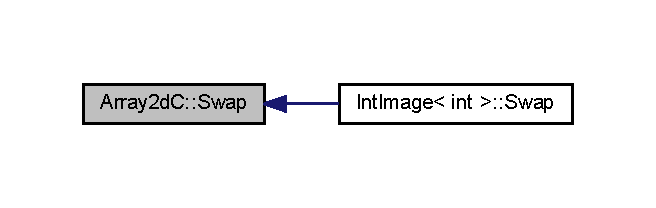
\includegraphics[width=315pt]{class_array2d_c_ae8cbeb3e4fdc3a45cc188ecc1b317919_icgraph}
\end{center}
\end{figure}
\mbox{\Hypertarget{class_array2d_c_a5e1d7837fd208699694fc3fc97151df0}\label{class_array2d_c_a5e1d7837fd208699694fc3fc97151df0}} 
\index{Array2dC@{Array2dC}!Zero@{Zero}}
\index{Zero@{Zero}!Array2dC@{Array2dC}}
\subsubsection{\texorpdfstring{Zero()}{Zero()}}
{\footnotesize\ttfamily template$<$class T$>$ \\
void \mbox{\hyperlink{class_array2d_c}{Array2dC}}$<$ T $>$\+::Zero (\begin{DoxyParamCaption}\item[{const T}]{t = {\ttfamily 0} }\end{DoxyParamCaption})}



Definition at line 194 of file c4-\/pedestrian-\/detector.\+h.


\begin{DoxyCode}
195 \{
196     \textcolor{keywordflow}{if}(\mbox{\hyperlink{class_array2d_c_a12f690f7195f7674a86a7e1eedbc473c}{nrow}}>0) std::fill(\mbox{\hyperlink{class_array2d_c_a25d8fa5049d4c7ded126e0acdd18f37a}{buf}},\mbox{\hyperlink{class_array2d_c_a25d8fa5049d4c7ded126e0acdd18f37a}{buf}}+\mbox{\hyperlink{class_array2d_c_a12f690f7195f7674a86a7e1eedbc473c}{nrow}}*\mbox{\hyperlink{class_array2d_c_a27e0f8f40f644831cd7c750db59dc28a}{ncol}},t);
197 \}
\end{DoxyCode}
Here is the caller graph for this function\+:
\nopagebreak
\begin{figure}[H]
\begin{center}
\leavevmode
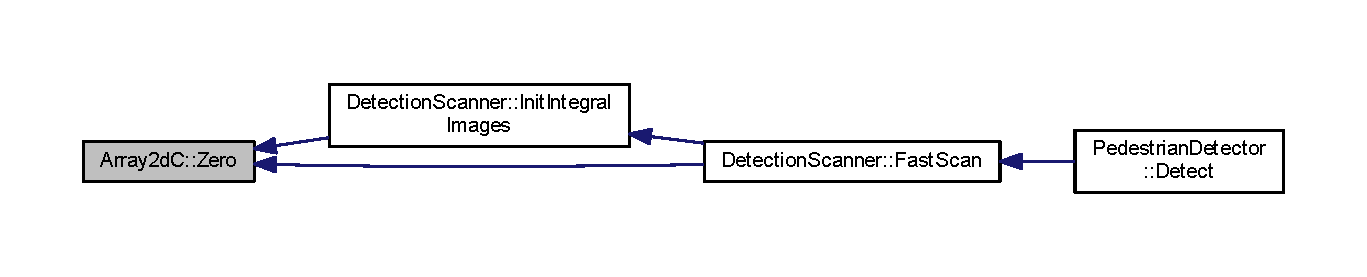
\includegraphics[width=350pt]{class_array2d_c_a5e1d7837fd208699694fc3fc97151df0_icgraph}
\end{center}
\end{figure}


\subsection{Member Data Documentation}
\mbox{\Hypertarget{class_array2d_c_a25d8fa5049d4c7ded126e0acdd18f37a}\label{class_array2d_c_a25d8fa5049d4c7ded126e0acdd18f37a}} 
\index{Array2dC@{Array2dC}!buf@{buf}}
\index{buf@{buf}!Array2dC@{Array2dC}}
\subsubsection{\texorpdfstring{buf}{buf}}
{\footnotesize\ttfamily template$<$class T$>$ \\
T$\ast$ \mbox{\hyperlink{class_array2d_c}{Array2dC}}$<$ T $>$\+::buf}



Definition at line 57 of file c4-\/pedestrian-\/detector.\+h.

\mbox{\Hypertarget{class_array2d_c_a27e0f8f40f644831cd7c750db59dc28a}\label{class_array2d_c_a27e0f8f40f644831cd7c750db59dc28a}} 
\index{Array2dC@{Array2dC}!ncol@{ncol}}
\index{ncol@{ncol}!Array2dC@{Array2dC}}
\subsubsection{\texorpdfstring{ncol}{ncol}}
{\footnotesize\ttfamily template$<$class T$>$ \\
int \mbox{\hyperlink{class_array2d_c}{Array2dC}}$<$ T $>$\+::ncol}



Definition at line 55 of file c4-\/pedestrian-\/detector.\+h.

\mbox{\Hypertarget{class_array2d_c_a12f690f7195f7674a86a7e1eedbc473c}\label{class_array2d_c_a12f690f7195f7674a86a7e1eedbc473c}} 
\index{Array2dC@{Array2dC}!nrow@{nrow}}
\index{nrow@{nrow}!Array2dC@{Array2dC}}
\subsubsection{\texorpdfstring{nrow}{nrow}}
{\footnotesize\ttfamily template$<$class T$>$ \\
int \mbox{\hyperlink{class_array2d_c}{Array2dC}}$<$ T $>$\+::nrow}



Definition at line 54 of file c4-\/pedestrian-\/detector.\+h.

\mbox{\Hypertarget{class_array2d_c_a727eae5d663d463635cc150e6f771f0d}\label{class_array2d_c_a727eae5d663d463635cc150e6f771f0d}} 
\index{Array2dC@{Array2dC}!p@{p}}
\index{p@{p}!Array2dC@{Array2dC}}
\subsubsection{\texorpdfstring{p}{p}}
{\footnotesize\ttfamily template$<$class T$>$ \\
T$\ast$$\ast$ \mbox{\hyperlink{class_array2d_c}{Array2dC}}$<$ T $>$\+::p}



Definition at line 56 of file c4-\/pedestrian-\/detector.\+h.



The documentation for this class was generated from the following file\+:\begin{DoxyCompactItemize}
\item 
D\+:/\+Roy/\+Git\+Hub/\+Multitarget-\/tracker/\+Detector/pedestrians/\mbox{\hyperlink{c4-pedestrian-detector_8h}{c4-\/pedestrian-\/detector.\+h}}\end{DoxyCompactItemize}

\hypertarget{class_assignment_problem_solver}{}\section{Assignment\+Problem\+Solver Class Reference}
\label{class_assignment_problem_solver}\index{Assignment\+Problem\+Solver@{Assignment\+Problem\+Solver}}


{\ttfamily \#include $<$Hungarian\+Alg.\+h$>$}



Collaboration diagram for Assignment\+Problem\+Solver\+:\nopagebreak
\begin{figure}[H]
\begin{center}
\leavevmode
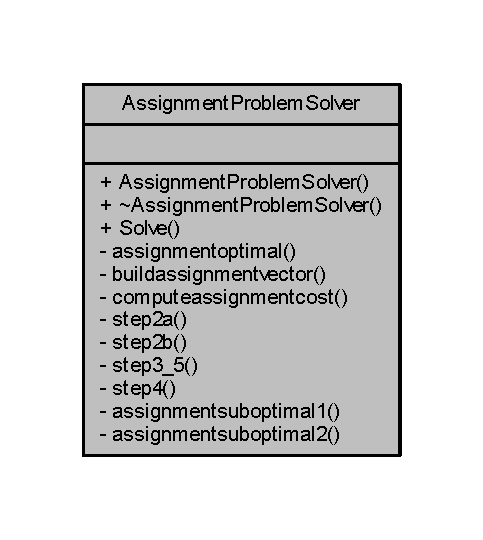
\includegraphics[width=232pt]{class_assignment_problem_solver__coll__graph}
\end{center}
\end{figure}
\subsection*{Public Types}
\begin{DoxyCompactItemize}
\item 
enum \mbox{\hyperlink{class_assignment_problem_solver_aec407eb73fed9d3ddb9467fde90a85e8}{T\+Method}} \{ \mbox{\hyperlink{class_assignment_problem_solver_aec407eb73fed9d3ddb9467fde90a85e8a84f2334f61866dba64befa6910848d75}{optimal}}, 
\mbox{\hyperlink{class_assignment_problem_solver_aec407eb73fed9d3ddb9467fde90a85e8a226c2e4b79d0beeb342087880d97bb2a}{many\+\_\+forbidden\+\_\+assignments}}, 
\mbox{\hyperlink{class_assignment_problem_solver_aec407eb73fed9d3ddb9467fde90a85e8a3329e7571829a83b21be4821df62310d}{without\+\_\+forbidden\+\_\+assignments}}
 \}
\end{DoxyCompactItemize}
\subsection*{Public Member Functions}
\begin{DoxyCompactItemize}
\item 
\mbox{\hyperlink{class_assignment_problem_solver_a13a83a34d4a0b4da872d87c79cb9c687}{Assignment\+Problem\+Solver}} ()
\item 
\mbox{\hyperlink{class_assignment_problem_solver_a47317b69e3eb9b50426c427ebcf5770f}{$\sim$\+Assignment\+Problem\+Solver}} ()
\item 
\mbox{\hyperlink{defines_8h_a7ce9c8817b42ab418e61756f579549ab}{track\+\_\+t}} \mbox{\hyperlink{class_assignment_problem_solver_a38198467ca647403c40be2c2bb47e177}{Solve}} (const \mbox{\hyperlink{_hungarian_alg_8h_af6ab0ee8259a51215f62e8f96416d5bb}{dist\+Matrix\+\_\+t}} \&dist\+Matrix\+In, size\+\_\+t n\+Of\+Rows, size\+\_\+t n\+Of\+Columns, \mbox{\hyperlink{_hungarian_alg_8h_ad7b9f569a9adbd958c668a36b6884ffd}{assignments\+\_\+t}} \&assignment, \mbox{\hyperlink{class_assignment_problem_solver_aec407eb73fed9d3ddb9467fde90a85e8}{T\+Method}} Method=\mbox{\hyperlink{class_assignment_problem_solver_aec407eb73fed9d3ddb9467fde90a85e8a84f2334f61866dba64befa6910848d75}{optimal}})
\end{DoxyCompactItemize}
\subsection*{Private Member Functions}
\begin{DoxyCompactItemize}
\item 
void \mbox{\hyperlink{class_assignment_problem_solver_a5b84a5167984db1050821926f52b5187}{assignmentoptimal}} (\mbox{\hyperlink{_hungarian_alg_8h_ad7b9f569a9adbd958c668a36b6884ffd}{assignments\+\_\+t}} \&assignment, \mbox{\hyperlink{defines_8h_a7ce9c8817b42ab418e61756f579549ab}{track\+\_\+t}} \&cost, const \mbox{\hyperlink{_hungarian_alg_8h_af6ab0ee8259a51215f62e8f96416d5bb}{dist\+Matrix\+\_\+t}} \&dist\+Matrix\+In, size\+\_\+t n\+Of\+Rows, size\+\_\+t n\+Of\+Columns)
\item 
void \mbox{\hyperlink{class_assignment_problem_solver_a1aa1c05dec6aef723f5d41affc667a77}{buildassignmentvector}} (\mbox{\hyperlink{_hungarian_alg_8h_ad7b9f569a9adbd958c668a36b6884ffd}{assignments\+\_\+t}} \&assignment, bool $\ast$star\+Matrix, size\+\_\+t n\+Of\+Rows, size\+\_\+t n\+Of\+Columns)
\item 
void \mbox{\hyperlink{class_assignment_problem_solver_a978fa51f563d47dbd00c697704cf4ad9}{computeassignmentcost}} (const \mbox{\hyperlink{_hungarian_alg_8h_ad7b9f569a9adbd958c668a36b6884ffd}{assignments\+\_\+t}} \&assignment, \mbox{\hyperlink{defines_8h_a7ce9c8817b42ab418e61756f579549ab}{track\+\_\+t}} \&cost, const \mbox{\hyperlink{_hungarian_alg_8h_af6ab0ee8259a51215f62e8f96416d5bb}{dist\+Matrix\+\_\+t}} \&dist\+Matrix\+In, size\+\_\+t n\+Of\+Rows)
\item 
void \mbox{\hyperlink{class_assignment_problem_solver_adef6ec1494dd6058fdf1373bc2c6d6eb}{step2a}} (\mbox{\hyperlink{_hungarian_alg_8h_ad7b9f569a9adbd958c668a36b6884ffd}{assignments\+\_\+t}} \&assignment, \mbox{\hyperlink{defines_8h_a7ce9c8817b42ab418e61756f579549ab}{track\+\_\+t}} $\ast$dist\+Matrix, bool $\ast$star\+Matrix, bool $\ast$new\+Star\+Matrix, bool $\ast$prime\+Matrix, bool $\ast$covered\+Columns, bool $\ast$covered\+Rows, size\+\_\+t n\+Of\+Rows, size\+\_\+t n\+Of\+Columns, size\+\_\+t min\+Dim)
\item 
void \mbox{\hyperlink{class_assignment_problem_solver_a069b78d89842031f7b54e0837c2bd602}{step2b}} (\mbox{\hyperlink{_hungarian_alg_8h_ad7b9f569a9adbd958c668a36b6884ffd}{assignments\+\_\+t}} \&assignment, \mbox{\hyperlink{defines_8h_a7ce9c8817b42ab418e61756f579549ab}{track\+\_\+t}} $\ast$dist\+Matrix, bool $\ast$star\+Matrix, bool $\ast$new\+Star\+Matrix, bool $\ast$prime\+Matrix, bool $\ast$covered\+Columns, bool $\ast$covered\+Rows, size\+\_\+t n\+Of\+Rows, size\+\_\+t n\+Of\+Columns, size\+\_\+t min\+Dim)
\item 
void \mbox{\hyperlink{class_assignment_problem_solver_a8c24dfcfef6adfb96c6394f798c02dba}{step3\+\_\+5}} (\mbox{\hyperlink{_hungarian_alg_8h_ad7b9f569a9adbd958c668a36b6884ffd}{assignments\+\_\+t}} \&assignment, \mbox{\hyperlink{defines_8h_a7ce9c8817b42ab418e61756f579549ab}{track\+\_\+t}} $\ast$dist\+Matrix, bool $\ast$star\+Matrix, bool $\ast$new\+Star\+Matrix, bool $\ast$prime\+Matrix, bool $\ast$covered\+Columns, bool $\ast$covered\+Rows, size\+\_\+t n\+Of\+Rows, size\+\_\+t n\+Of\+Columns, size\+\_\+t min\+Dim)
\item 
void \mbox{\hyperlink{class_assignment_problem_solver_a6ea85d386a136effd84c00f4e2f3cd77}{step4}} (\mbox{\hyperlink{_hungarian_alg_8h_ad7b9f569a9adbd958c668a36b6884ffd}{assignments\+\_\+t}} \&assignment, \mbox{\hyperlink{defines_8h_a7ce9c8817b42ab418e61756f579549ab}{track\+\_\+t}} $\ast$dist\+Matrix, bool $\ast$star\+Matrix, bool $\ast$new\+Star\+Matrix, bool $\ast$prime\+Matrix, bool $\ast$covered\+Columns, bool $\ast$covered\+Rows, size\+\_\+t n\+Of\+Rows, size\+\_\+t n\+Of\+Columns, size\+\_\+t min\+Dim, size\+\_\+t row, size\+\_\+t col)
\item 
void \mbox{\hyperlink{class_assignment_problem_solver_ae8fddfafc7387f3597493f02e8366883}{assignmentsuboptimal1}} (\mbox{\hyperlink{_hungarian_alg_8h_ad7b9f569a9adbd958c668a36b6884ffd}{assignments\+\_\+t}} \&assignment, \mbox{\hyperlink{defines_8h_a7ce9c8817b42ab418e61756f579549ab}{track\+\_\+t}} \&cost, const \mbox{\hyperlink{_hungarian_alg_8h_af6ab0ee8259a51215f62e8f96416d5bb}{dist\+Matrix\+\_\+t}} \&dist\+Matrix\+In, size\+\_\+t n\+Of\+Rows, size\+\_\+t n\+Of\+Columns)
\item 
void \mbox{\hyperlink{class_assignment_problem_solver_a31277dc88cb22e07db1e52b6fe88f84f}{assignmentsuboptimal2}} (\mbox{\hyperlink{_hungarian_alg_8h_ad7b9f569a9adbd958c668a36b6884ffd}{assignments\+\_\+t}} \&assignment, \mbox{\hyperlink{defines_8h_a7ce9c8817b42ab418e61756f579549ab}{track\+\_\+t}} \&cost, const \mbox{\hyperlink{_hungarian_alg_8h_af6ab0ee8259a51215f62e8f96416d5bb}{dist\+Matrix\+\_\+t}} \&dist\+Matrix\+In, size\+\_\+t n\+Of\+Rows, size\+\_\+t n\+Of\+Columns)
\end{DoxyCompactItemize}


\subsection{Detailed Description}


Definition at line 11 of file Hungarian\+Alg.\+h.



\subsection{Member Enumeration Documentation}
\mbox{\Hypertarget{class_assignment_problem_solver_aec407eb73fed9d3ddb9467fde90a85e8}\label{class_assignment_problem_solver_aec407eb73fed9d3ddb9467fde90a85e8}} 
\index{Assignment\+Problem\+Solver@{Assignment\+Problem\+Solver}!T\+Method@{T\+Method}}
\index{T\+Method@{T\+Method}!Assignment\+Problem\+Solver@{Assignment\+Problem\+Solver}}
\subsubsection{\texorpdfstring{T\+Method}{TMethod}}
{\footnotesize\ttfamily enum \mbox{\hyperlink{class_assignment_problem_solver_aec407eb73fed9d3ddb9467fde90a85e8}{Assignment\+Problem\+Solver\+::\+T\+Method}}}

\begin{DoxyEnumFields}{Enumerator}
\raisebox{\heightof{T}}[0pt][0pt]{\index{optimal@{optimal}!Assignment\+Problem\+Solver@{Assignment\+Problem\+Solver}}\index{Assignment\+Problem\+Solver@{Assignment\+Problem\+Solver}!optimal@{optimal}}}\mbox{\Hypertarget{class_assignment_problem_solver_aec407eb73fed9d3ddb9467fde90a85e8a84f2334f61866dba64befa6910848d75}\label{class_assignment_problem_solver_aec407eb73fed9d3ddb9467fde90a85e8a84f2334f61866dba64befa6910848d75}} 
optimal&\\
\hline

\raisebox{\heightof{T}}[0pt][0pt]{\index{many\+\_\+forbidden\+\_\+assignments@{many\+\_\+forbidden\+\_\+assignments}!Assignment\+Problem\+Solver@{Assignment\+Problem\+Solver}}\index{Assignment\+Problem\+Solver@{Assignment\+Problem\+Solver}!many\+\_\+forbidden\+\_\+assignments@{many\+\_\+forbidden\+\_\+assignments}}}\mbox{\Hypertarget{class_assignment_problem_solver_aec407eb73fed9d3ddb9467fde90a85e8a226c2e4b79d0beeb342087880d97bb2a}\label{class_assignment_problem_solver_aec407eb73fed9d3ddb9467fde90a85e8a226c2e4b79d0beeb342087880d97bb2a}} 
many\+\_\+forbidden\+\_\+assignments&\\
\hline

\raisebox{\heightof{T}}[0pt][0pt]{\index{without\+\_\+forbidden\+\_\+assignments@{without\+\_\+forbidden\+\_\+assignments}!Assignment\+Problem\+Solver@{Assignment\+Problem\+Solver}}\index{Assignment\+Problem\+Solver@{Assignment\+Problem\+Solver}!without\+\_\+forbidden\+\_\+assignments@{without\+\_\+forbidden\+\_\+assignments}}}\mbox{\Hypertarget{class_assignment_problem_solver_aec407eb73fed9d3ddb9467fde90a85e8a3329e7571829a83b21be4821df62310d}\label{class_assignment_problem_solver_aec407eb73fed9d3ddb9467fde90a85e8a3329e7571829a83b21be4821df62310d}} 
without\+\_\+forbidden\+\_\+assignments&\\
\hline

\end{DoxyEnumFields}


Definition at line 34 of file Hungarian\+Alg.\+h.


\begin{DoxyCode}
35     \{
36         \mbox{\hyperlink{class_assignment_problem_solver_aec407eb73fed9d3ddb9467fde90a85e8a84f2334f61866dba64befa6910848d75}{optimal}},
37         \mbox{\hyperlink{class_assignment_problem_solver_aec407eb73fed9d3ddb9467fde90a85e8a226c2e4b79d0beeb342087880d97bb2a}{many\_forbidden\_assignments}},
38         \mbox{\hyperlink{class_assignment_problem_solver_aec407eb73fed9d3ddb9467fde90a85e8a3329e7571829a83b21be4821df62310d}{without\_forbidden\_assignments}}
39     \};
\end{DoxyCode}


\subsection{Constructor \& Destructor Documentation}
\mbox{\Hypertarget{class_assignment_problem_solver_a13a83a34d4a0b4da872d87c79cb9c687}\label{class_assignment_problem_solver_a13a83a34d4a0b4da872d87c79cb9c687}} 
\index{Assignment\+Problem\+Solver@{Assignment\+Problem\+Solver}!Assignment\+Problem\+Solver@{Assignment\+Problem\+Solver}}
\index{Assignment\+Problem\+Solver@{Assignment\+Problem\+Solver}!Assignment\+Problem\+Solver@{Assignment\+Problem\+Solver}}
\subsubsection{\texorpdfstring{Assignment\+Problem\+Solver()}{AssignmentProblemSolver()}}
{\footnotesize\ttfamily Assignment\+Problem\+Solver\+::\+Assignment\+Problem\+Solver (\begin{DoxyParamCaption}{ }\end{DoxyParamCaption})}



Definition at line 7 of file Hungarian\+Alg.\+cpp.


\begin{DoxyCode}
8 \{
9 \}
\end{DoxyCode}
\mbox{\Hypertarget{class_assignment_problem_solver_a47317b69e3eb9b50426c427ebcf5770f}\label{class_assignment_problem_solver_a47317b69e3eb9b50426c427ebcf5770f}} 
\index{Assignment\+Problem\+Solver@{Assignment\+Problem\+Solver}!````~Assignment\+Problem\+Solver@{$\sim$\+Assignment\+Problem\+Solver}}
\index{````~Assignment\+Problem\+Solver@{$\sim$\+Assignment\+Problem\+Solver}!Assignment\+Problem\+Solver@{Assignment\+Problem\+Solver}}
\subsubsection{\texorpdfstring{$\sim$\+Assignment\+Problem\+Solver()}{~AssignmentProblemSolver()}}
{\footnotesize\ttfamily Assignment\+Problem\+Solver\+::$\sim$\+Assignment\+Problem\+Solver (\begin{DoxyParamCaption}{ }\end{DoxyParamCaption})}



Definition at line 14 of file Hungarian\+Alg.\+cpp.


\begin{DoxyCode}
15 \{
16 \}
\end{DoxyCode}


\subsection{Member Function Documentation}
\mbox{\Hypertarget{class_assignment_problem_solver_a5b84a5167984db1050821926f52b5187}\label{class_assignment_problem_solver_a5b84a5167984db1050821926f52b5187}} 
\index{Assignment\+Problem\+Solver@{Assignment\+Problem\+Solver}!assignmentoptimal@{assignmentoptimal}}
\index{assignmentoptimal@{assignmentoptimal}!Assignment\+Problem\+Solver@{Assignment\+Problem\+Solver}}
\subsubsection{\texorpdfstring{assignmentoptimal()}{assignmentoptimal()}}
{\footnotesize\ttfamily void Assignment\+Problem\+Solver\+::assignmentoptimal (\begin{DoxyParamCaption}\item[{\mbox{\hyperlink{_hungarian_alg_8h_ad7b9f569a9adbd958c668a36b6884ffd}{assignments\+\_\+t}} \&}]{assignment,  }\item[{\mbox{\hyperlink{defines_8h_a7ce9c8817b42ab418e61756f579549ab}{track\+\_\+t}} \&}]{cost,  }\item[{const \mbox{\hyperlink{_hungarian_alg_8h_af6ab0ee8259a51215f62e8f96416d5bb}{dist\+Matrix\+\_\+t}} \&}]{dist\+Matrix\+In,  }\item[{size\+\_\+t}]{n\+Of\+Rows,  }\item[{size\+\_\+t}]{n\+Of\+Columns }\end{DoxyParamCaption})\hspace{0.3cm}{\ttfamily [private]}}



Definition at line 53 of file Hungarian\+Alg.\+cpp.


\begin{DoxyCode}
54 \{
55     \textcolor{comment}{// Generate distance cv::Matrix }
56     \textcolor{comment}{// and check cv::Matrix elements positiveness :)}
57 
58     \textcolor{comment}{// Total elements number}
59     \textcolor{keywordtype}{size\_t} nOfElements = nOfRows * nOfColumns;
60     \textcolor{comment}{// Memory allocation}
61     \mbox{\hyperlink{defines_8h_a7ce9c8817b42ab418e61756f579549ab}{track\_t}}* distMatrix = (\mbox{\hyperlink{defines_8h_a7ce9c8817b42ab418e61756f579549ab}{track\_t}} *)malloc(nOfElements * \textcolor{keyword}{sizeof}(
      \mbox{\hyperlink{defines_8h_a7ce9c8817b42ab418e61756f579549ab}{track\_t}}));
62 
63     \textcolor{keywordflow}{if} (distMatrix == \textcolor{keyword}{nullptr})
64     \{
65         \textcolor{keywordflow}{return};
66     \}
67 
68     \textcolor{comment}{// Pointer to last element}
69     \mbox{\hyperlink{defines_8h_a7ce9c8817b42ab418e61756f579549ab}{track\_t}}* distMatrixEnd = distMatrix + nOfElements;
70 
71     \textcolor{keywordflow}{for} (\textcolor{keywordtype}{size\_t} row = 0; row < nOfElements; row++)
72     \{
73         \mbox{\hyperlink{defines_8h_a7ce9c8817b42ab418e61756f579549ab}{track\_t}} \mbox{\hyperlink{struct_g_m_l__token_a50b20988e3fe419332313e8d9e02c775}{value}} = distMatrixIn[row];
74         assert(\mbox{\hyperlink{struct_g_m_l__token_a50b20988e3fe419332313e8d9e02c775}{value}} >= 0);
75         distMatrix[row] = \mbox{\hyperlink{struct_g_m_l__token_a50b20988e3fe419332313e8d9e02c775}{value}};
76     \}
77 
78     \textcolor{comment}{// Memory allocation}
79     \textcolor{keywordtype}{bool}* coveredColumns = (\textcolor{keywordtype}{bool}*)calloc(nOfColumns, \textcolor{keyword}{sizeof}(\textcolor{keywordtype}{bool}));
80     \textcolor{keywordtype}{bool}* coveredRows = (\textcolor{keywordtype}{bool}*)calloc(nOfRows, \textcolor{keyword}{sizeof}(\textcolor{keywordtype}{bool}));
81     \textcolor{keywordtype}{bool}* starMatrix = (\textcolor{keywordtype}{bool}*)calloc(nOfElements, \textcolor{keyword}{sizeof}(\textcolor{keywordtype}{bool}));
82     \textcolor{keywordtype}{bool}* primeMatrix = (\textcolor{keywordtype}{bool}*)calloc(nOfElements, \textcolor{keyword}{sizeof}(\textcolor{keywordtype}{bool}));
83     \textcolor{keywordtype}{bool}* newStarMatrix = (\textcolor{keywordtype}{bool}*)calloc(nOfElements, \textcolor{keyword}{sizeof}(\textcolor{keywordtype}{bool})); \textcolor{comment}{/* used in step4 */}
84 
85     \textcolor{comment}{/* preliminary steps */}
86     \textcolor{keywordflow}{if} (nOfRows <= nOfColumns)
87     \{
88         \textcolor{keywordflow}{for} (\textcolor{keywordtype}{size\_t} row = 0; row < nOfRows; row++)
89         \{
90             \textcolor{comment}{/* find the smallest element in the row */}
91             \mbox{\hyperlink{defines_8h_a7ce9c8817b42ab418e61756f579549ab}{track\_t}}* distMatrixTemp = distMatrix + row;
92             \mbox{\hyperlink{defines_8h_a7ce9c8817b42ab418e61756f579549ab}{track\_t}}  minValue = *distMatrixTemp;
93             distMatrixTemp += nOfRows;
94             \textcolor{keywordflow}{while} (distMatrixTemp < distMatrixEnd)
95             \{
96                 \mbox{\hyperlink{defines_8h_a7ce9c8817b42ab418e61756f579549ab}{track\_t}} \mbox{\hyperlink{struct_g_m_l__token_a50b20988e3fe419332313e8d9e02c775}{value}} = *distMatrixTemp;
97                 \textcolor{keywordflow}{if} (\mbox{\hyperlink{struct_g_m_l__token_a50b20988e3fe419332313e8d9e02c775}{value}} < minValue)
98                 \{
99                     minValue = \mbox{\hyperlink{struct_g_m_l__token_a50b20988e3fe419332313e8d9e02c775}{value}};
100                 \}
101                 distMatrixTemp += nOfRows;
102             \}
103             \textcolor{comment}{/* subtract the smallest element from each element of the row */}
104             distMatrixTemp = distMatrix + row;
105             \textcolor{keywordflow}{while} (distMatrixTemp < distMatrixEnd)
106             \{
107                 *distMatrixTemp -= minValue;
108                 distMatrixTemp += nOfRows;
109             \}
110         \}
111         \textcolor{comment}{/* Steps 1 and 2a */}
112         \textcolor{keywordflow}{for} (\textcolor{keywordtype}{size\_t} row = 0; row < nOfRows; row++)
113         \{
114             \textcolor{keywordflow}{for} (\textcolor{keywordtype}{size\_t} col = 0; col < nOfColumns; col++)
115             \{
116                 \textcolor{keywordflow}{if} (distMatrix[row + nOfRows*col] == 0)
117                 \{
118                     \textcolor{keywordflow}{if} (!coveredColumns[col])
119                     \{
120                         starMatrix[row + nOfRows * col] = \textcolor{keyword}{true};
121                         coveredColumns[col] = \textcolor{keyword}{true};
122                         \textcolor{keywordflow}{break};
123                     \}
124                 \}
125             \}
126         \}
127     \}
128     \textcolor{keywordflow}{else} \textcolor{comment}{/* if(nOfRows > nOfColumns) */}
129     \{
130         \textcolor{keywordflow}{for} (\textcolor{keywordtype}{size\_t} col = 0; col < nOfColumns; col++)
131         \{
132             \textcolor{comment}{/* find the smallest element in the column */}
133             \mbox{\hyperlink{defines_8h_a7ce9c8817b42ab418e61756f579549ab}{track\_t}}* distMatrixTemp = distMatrix + nOfRows*col;
134             \mbox{\hyperlink{defines_8h_a7ce9c8817b42ab418e61756f579549ab}{track\_t}}* columnEnd = distMatrixTemp + nOfRows;
135             \mbox{\hyperlink{defines_8h_a7ce9c8817b42ab418e61756f579549ab}{track\_t}}  minValue = *distMatrixTemp++;
136             \textcolor{keywordflow}{while} (distMatrixTemp < columnEnd)
137             \{
138                 \mbox{\hyperlink{defines_8h_a7ce9c8817b42ab418e61756f579549ab}{track\_t}} \mbox{\hyperlink{struct_g_m_l__token_a50b20988e3fe419332313e8d9e02c775}{value}} = *distMatrixTemp++;
139                 \textcolor{keywordflow}{if} (\mbox{\hyperlink{struct_g_m_l__token_a50b20988e3fe419332313e8d9e02c775}{value}} < minValue)
140                 \{
141                     minValue = \mbox{\hyperlink{struct_g_m_l__token_a50b20988e3fe419332313e8d9e02c775}{value}};
142                 \}
143             \}
144             \textcolor{comment}{/* subtract the smallest element from each element of the column */}
145             distMatrixTemp = distMatrix + nOfRows*col;
146             \textcolor{keywordflow}{while} (distMatrixTemp < columnEnd)
147             \{
148                 *distMatrixTemp++ -= minValue;
149             \}
150         \}
151         \textcolor{comment}{/* Steps 1 and 2a */}
152         \textcolor{keywordflow}{for} (\textcolor{keywordtype}{size\_t} col = 0; col < nOfColumns; col++)
153         \{
154             \textcolor{keywordflow}{for} (\textcolor{keywordtype}{size\_t} row = 0; row < nOfRows; row++)
155             \{
156                 \textcolor{keywordflow}{if} (distMatrix[row + nOfRows*col] == 0)
157                 \{
158                     \textcolor{keywordflow}{if} (!coveredRows[row])
159                     \{
160                         starMatrix[row + nOfRows*col] = \textcolor{keyword}{true};
161                         coveredColumns[col] = \textcolor{keyword}{true};
162                         coveredRows[row] = \textcolor{keyword}{true};
163                         \textcolor{keywordflow}{break};
164                     \}
165                 \}
166             \}
167         \}
168 
169         \textcolor{keywordflow}{for} (\textcolor{keywordtype}{size\_t} row = 0; row < nOfRows; row++)
170         \{
171             coveredRows[row] = \textcolor{keyword}{false};
172         \}
173     \}
174     \textcolor{comment}{/* move to step 2b */}
175     \mbox{\hyperlink{class_assignment_problem_solver_a069b78d89842031f7b54e0837c2bd602}{step2b}}(assignment, distMatrix, starMatrix, newStarMatrix, primeMatrix, coveredColumns, 
      coveredRows, nOfRows, nOfColumns, (nOfRows <= nOfColumns) ? nOfRows : nOfColumns);
176     \textcolor{comment}{/* compute cost and remove invalid assignments */}
177     \mbox{\hyperlink{class_assignment_problem_solver_a978fa51f563d47dbd00c697704cf4ad9}{computeassignmentcost}}(assignment, cost, distMatrixIn, nOfRows);
178     \textcolor{comment}{/* free allocated memory */}
179     free(distMatrix);
180     free(coveredColumns);
181     free(coveredRows);
182     free(starMatrix);
183     free(primeMatrix);
184     free(newStarMatrix);
185     \textcolor{keywordflow}{return};
186 \}
\end{DoxyCode}
Here is the call graph for this function\+:\nopagebreak
\begin{figure}[H]
\begin{center}
\leavevmode
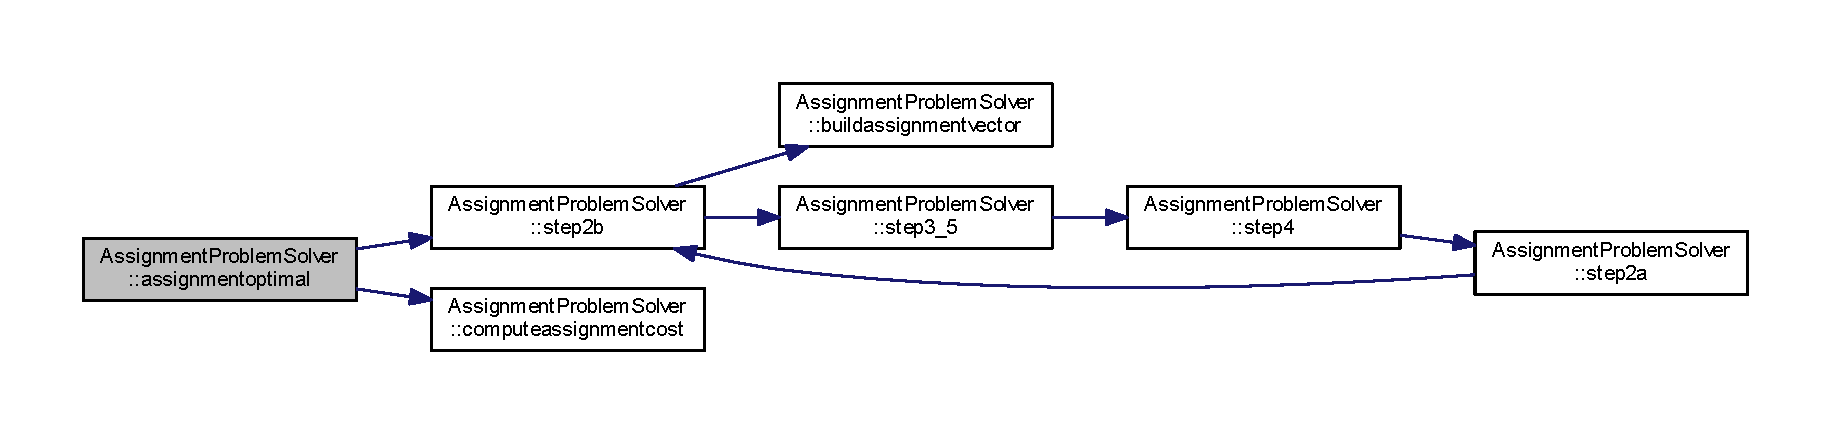
\includegraphics[width=350pt]{class_assignment_problem_solver_a5b84a5167984db1050821926f52b5187_cgraph}
\end{center}
\end{figure}
Here is the caller graph for this function\+:\nopagebreak
\begin{figure}[H]
\begin{center}
\leavevmode
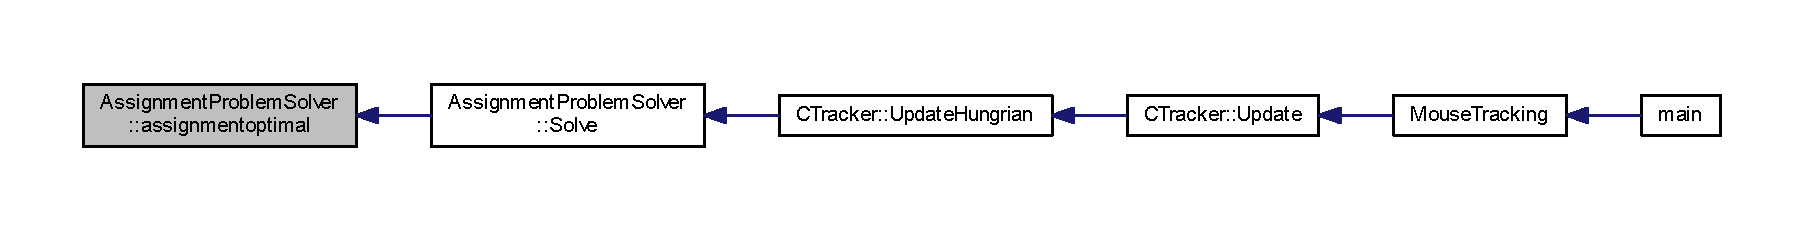
\includegraphics[width=350pt]{class_assignment_problem_solver_a5b84a5167984db1050821926f52b5187_icgraph}
\end{center}
\end{figure}
\mbox{\Hypertarget{class_assignment_problem_solver_ae8fddfafc7387f3597493f02e8366883}\label{class_assignment_problem_solver_ae8fddfafc7387f3597493f02e8366883}} 
\index{Assignment\+Problem\+Solver@{Assignment\+Problem\+Solver}!assignmentsuboptimal1@{assignmentsuboptimal1}}
\index{assignmentsuboptimal1@{assignmentsuboptimal1}!Assignment\+Problem\+Solver@{Assignment\+Problem\+Solver}}
\subsubsection{\texorpdfstring{assignmentsuboptimal1()}{assignmentsuboptimal1()}}
{\footnotesize\ttfamily void Assignment\+Problem\+Solver\+::assignmentsuboptimal1 (\begin{DoxyParamCaption}\item[{\mbox{\hyperlink{_hungarian_alg_8h_ad7b9f569a9adbd958c668a36b6884ffd}{assignments\+\_\+t}} \&}]{assignment,  }\item[{\mbox{\hyperlink{defines_8h_a7ce9c8817b42ab418e61756f579549ab}{track\+\_\+t}} \&}]{cost,  }\item[{const \mbox{\hyperlink{_hungarian_alg_8h_af6ab0ee8259a51215f62e8f96416d5bb}{dist\+Matrix\+\_\+t}} \&}]{dist\+Matrix\+In,  }\item[{size\+\_\+t}]{n\+Of\+Rows,  }\item[{size\+\_\+t}]{n\+Of\+Columns }\end{DoxyParamCaption})\hspace{0.3cm}{\ttfamily [private]}}



Definition at line 484 of file Hungarian\+Alg.\+cpp.


\begin{DoxyCode}
485 \{
486     \textcolor{comment}{/* make working copy of distance Matrix */}
487     \textcolor{keyword}{const} \textcolor{keywordtype}{size\_t} nOfElements = nOfRows * nOfColumns;
488     \mbox{\hyperlink{defines_8h_a7ce9c8817b42ab418e61756f579549ab}{track\_t}}* distMatrix = (\mbox{\hyperlink{defines_8h_a7ce9c8817b42ab418e61756f579549ab}{track\_t}} *)malloc(nOfElements * \textcolor{keyword}{sizeof}(
      \mbox{\hyperlink{defines_8h_a7ce9c8817b42ab418e61756f579549ab}{track\_t}}));
489     \textcolor{keywordflow}{for} (\textcolor{keywordtype}{size\_t} n = 0; n < nOfElements; n++)
490     \{
491         distMatrix[n] = distMatrixIn[n];
492     \}
493 
494     \textcolor{comment}{/* allocate memory */}
495     \textcolor{keywordtype}{int}* nOfValidObservations = (\textcolor{keywordtype}{int} *)calloc(nOfRows, \textcolor{keyword}{sizeof}(\textcolor{keywordtype}{int}));
496     \textcolor{keywordtype}{int}* nOfValidTracks = (\textcolor{keywordtype}{int} *)calloc(nOfColumns, \textcolor{keyword}{sizeof}(\textcolor{keywordtype}{int}));
497 
498     \textcolor{comment}{/* compute number of validations */}
499     \textcolor{keywordtype}{bool} infiniteValueFound = \textcolor{keyword}{false};
500     \textcolor{keywordtype}{bool} finiteValueFound = \textcolor{keyword}{false};
501     \textcolor{keywordflow}{for} (\textcolor{keywordtype}{size\_t} row = 0; row < nOfRows; row++)
502     \{
503         \textcolor{keywordflow}{for} (\textcolor{keywordtype}{size\_t} col = 0; col < nOfColumns; col++)
504         \{
505             \textcolor{keywordflow}{if} (distMatrix[row + nOfRows*col] != std::numeric\_limits<track\_t>::max())
506             \{
507                 nOfValidTracks[col] += 1;
508                 nOfValidObservations[row] += 1;
509                 finiteValueFound = \textcolor{keyword}{true};
510             \}
511             \textcolor{keywordflow}{else}
512             \{
513                 infiniteValueFound = \textcolor{keyword}{true};
514             \}
515         \}
516     \}
517 
518     \textcolor{keywordflow}{if} (infiniteValueFound)
519     \{
520         \textcolor{keywordflow}{if} (!finiteValueFound)
521         \{
522             \textcolor{comment}{/* free allocated memory */}
523             free(nOfValidObservations);
524             free(nOfValidTracks);
525             free(distMatrix);
526 
527             \textcolor{keywordflow}{return};
528         \}
529         \textcolor{keywordtype}{bool} repeatSteps = \textcolor{keyword}{true};
530 
531         \textcolor{keywordflow}{while} (repeatSteps)
532         \{
533             repeatSteps = \textcolor{keyword}{false};
534 
535             \textcolor{comment}{/* step 1: reject assignments of multiply validated tracks to singly validated observations     
       */}
536             \textcolor{keywordflow}{for} (\textcolor{keywordtype}{size\_t} col = 0; col < nOfColumns; col++)
537             \{
538                 \textcolor{keywordtype}{bool} singleValidationFound = \textcolor{keyword}{false};
539                 \textcolor{keywordflow}{for} (\textcolor{keywordtype}{size\_t} row = 0; row < nOfRows; row++)
540                 \{
541                     \textcolor{keywordflow}{if} (distMatrix[row + nOfRows * col] != std::numeric\_limits<track\_t>::max() && (
      nOfValidObservations[row] == 1))
542                     \{
543                         singleValidationFound = \textcolor{keyword}{true};
544                         \textcolor{keywordflow}{break};
545                     \}
546 
547                     \textcolor{keywordflow}{if} (singleValidationFound)
548                     \{
549                         \textcolor{keywordflow}{for} (\textcolor{keywordtype}{size\_t} row = 0; row < nOfRows; row++)
550                             \textcolor{keywordflow}{if} ((nOfValidObservations[row] > 1) && distMatrix[row + nOfRows*col] != 
      std::numeric\_limits<track\_t>::max())
551                             \{
552                                 distMatrix[row + nOfRows*col] = std::numeric\_limits<track\_t>::max();
553                                 nOfValidObservations[row] -= 1;
554                                 nOfValidTracks[col] -= 1;
555                                 repeatSteps = \textcolor{keyword}{true};
556                             \}
557                     \}
558                 \}
559             \}
560 
561             \textcolor{comment}{/* step 2: reject assignments of multiply validated observations to singly validated tracks */}
562             \textcolor{keywordflow}{if} (nOfColumns > 1)
563             \{
564                 \textcolor{keywordflow}{for} (\textcolor{keywordtype}{size\_t} row = 0; row < nOfRows; row++)
565                 \{
566                     \textcolor{keywordtype}{bool} singleValidationFound = \textcolor{keyword}{false};
567                     \textcolor{keywordflow}{for} (\textcolor{keywordtype}{size\_t} col = 0; col < nOfColumns; col++)
568                     \{
569                         \textcolor{keywordflow}{if} (distMatrix[row + nOfRows*col] != std::numeric\_limits<track\_t>::max() && (
      nOfValidTracks[col] == 1))
570                         \{
571                             singleValidationFound = \textcolor{keyword}{true};
572                             \textcolor{keywordflow}{break};
573                         \}
574                     \}
575 
576                     \textcolor{keywordflow}{if} (singleValidationFound)
577                     \{
578                         \textcolor{keywordflow}{for} (\textcolor{keywordtype}{size\_t} col = 0; col < nOfColumns; col++)
579                         \{
580                             \textcolor{keywordflow}{if} ((nOfValidTracks[col] > 1) && distMatrix[row + nOfRows*col] != 
      std::numeric\_limits<track\_t>::max())
581                             \{
582                                 distMatrix[row + nOfRows*col] = std::numeric\_limits<track\_t>::max();
583                                 nOfValidObservations[row] -= 1;
584                                 nOfValidTracks[col] -= 1;
585                                 repeatSteps = \textcolor{keyword}{true};
586                             \}
587                         \}
588                     \}
589                 \}
590             \}
591         \} \textcolor{comment}{/* while(repeatSteps) */}
592 
593         \textcolor{comment}{/* for each multiply validated track that validates only with singly validated  */}
594         \textcolor{comment}{/* observations, choose the observation with minimum distance */}
595         \textcolor{keywordflow}{for} (\textcolor{keywordtype}{size\_t} row = 0; row < nOfRows; row++)
596         \{
597             \textcolor{keywordflow}{if} (nOfValidObservations[row] > 1)
598             \{
599                 \textcolor{keywordtype}{bool} allSinglyValidated = \textcolor{keyword}{true};
600                 \mbox{\hyperlink{defines_8h_a7ce9c8817b42ab418e61756f579549ab}{track\_t}} minValue = std::numeric\_limits<track\_t>::max();
601                 \textcolor{keywordtype}{size\_t} tmpCol = 0;
602                 \textcolor{keywordflow}{for} (\textcolor{keywordtype}{size\_t} col = 0; col < nOfColumns; col++)
603                 \{
604                     \textcolor{keyword}{const} \mbox{\hyperlink{defines_8h_a7ce9c8817b42ab418e61756f579549ab}{track\_t}} \mbox{\hyperlink{struct_g_m_l__token_a50b20988e3fe419332313e8d9e02c775}{value}} = distMatrix[row + nOfRows*col];
605                     \textcolor{keywordflow}{if} (\mbox{\hyperlink{struct_g_m_l__token_a50b20988e3fe419332313e8d9e02c775}{value}} != std::numeric\_limits<track\_t>::max())
606                     \{
607                         \textcolor{keywordflow}{if} (nOfValidTracks[col] > 1)
608                         \{
609                             allSinglyValidated = \textcolor{keyword}{false};
610                             \textcolor{keywordflow}{break};
611                         \}
612                         \textcolor{keywordflow}{else} \textcolor{keywordflow}{if} ((nOfValidTracks[col] == 1) && (\mbox{\hyperlink{struct_g_m_l__token_a50b20988e3fe419332313e8d9e02c775}{value}} < minValue))
613                         \{
614                             tmpCol = col;
615                             minValue = \mbox{\hyperlink{struct_g_m_l__token_a50b20988e3fe419332313e8d9e02c775}{value}};
616                         \}
617                     \}
618                 \}
619 
620                 \textcolor{keywordflow}{if} (allSinglyValidated)
621                 \{
622                     assignment[row] = \textcolor{keyword}{static\_cast<}\textcolor{keywordtype}{int}\textcolor{keyword}{>}(tmpCol);
623                     cost += minValue;
624                     \textcolor{keywordflow}{for} (\textcolor{keywordtype}{size\_t} n = 0; n < nOfRows; n++)
625                     \{
626                         distMatrix[n + nOfRows*tmpCol] = std::numeric\_limits<track\_t>::max();
627                     \}
628                     \textcolor{keywordflow}{for} (\textcolor{keywordtype}{size\_t} n = 0; n < nOfColumns; n++)
629                     \{
630                         distMatrix[row + nOfRows*n] = std::numeric\_limits<track\_t>::max();
631                     \}
632                 \}
633             \}
634         \}
635 
636         \textcolor{comment}{// for each multiply validated observation that validates only with singly validated  track, choose
       the track with minimum distance}
637         \textcolor{keywordflow}{for} (\textcolor{keywordtype}{size\_t} col = 0; col < nOfColumns; col++)
638         \{
639             \textcolor{keywordflow}{if} (nOfValidTracks[col] > 1)
640             \{
641                 \textcolor{keywordtype}{bool} allSinglyValidated = \textcolor{keyword}{true};
642                 \mbox{\hyperlink{defines_8h_a7ce9c8817b42ab418e61756f579549ab}{track\_t}} minValue = std::numeric\_limits<track\_t>::max();
643                 \textcolor{keywordtype}{size\_t} tmpRow = 0;
644                 \textcolor{keywordflow}{for} (\textcolor{keywordtype}{size\_t} row = 0; row < nOfRows; row++)
645                 \{
646                     \textcolor{keyword}{const} \mbox{\hyperlink{defines_8h_a7ce9c8817b42ab418e61756f579549ab}{track\_t}} \mbox{\hyperlink{struct_g_m_l__token_a50b20988e3fe419332313e8d9e02c775}{value}} = distMatrix[row + nOfRows*col];
647                     \textcolor{keywordflow}{if} (\mbox{\hyperlink{struct_g_m_l__token_a50b20988e3fe419332313e8d9e02c775}{value}} != std::numeric\_limits<track\_t>::max())
648                     \{
649                         \textcolor{keywordflow}{if} (nOfValidObservations[row] > 1)
650                         \{
651                             allSinglyValidated = \textcolor{keyword}{false};
652                             \textcolor{keywordflow}{break};
653                         \}
654                         \textcolor{keywordflow}{else} \textcolor{keywordflow}{if} ((nOfValidObservations[row] == 1) && (\mbox{\hyperlink{struct_g_m_l__token_a50b20988e3fe419332313e8d9e02c775}{value}} < minValue))
655                         \{
656                             tmpRow = row;
657                             minValue = \mbox{\hyperlink{struct_g_m_l__token_a50b20988e3fe419332313e8d9e02c775}{value}};
658                         \}
659                     \}
660                 \}
661 
662                 \textcolor{keywordflow}{if} (allSinglyValidated)
663                 \{
664                     assignment[tmpRow] = \textcolor{keyword}{static\_cast<}\textcolor{keywordtype}{int}\textcolor{keyword}{>}(col);
665                     cost += minValue;
666                     \textcolor{keywordflow}{for} (\textcolor{keywordtype}{size\_t} n = 0; n < nOfRows; n++)
667                     \{
668                         distMatrix[n + nOfRows*col] = std::numeric\_limits<track\_t>::max();
669                     \}
670                     \textcolor{keywordflow}{for} (\textcolor{keywordtype}{size\_t} n = 0; n < nOfColumns; n++)
671                     \{
672                         distMatrix[tmpRow + nOfRows*n] = std::numeric\_limits<track\_t>::max();
673                     \}
674                 \}
675             \}
676         \}
677     \} \textcolor{comment}{/* if(infiniteValueFound) */}
678 
679 
680     \textcolor{comment}{/* now, recursively search for the minimum element and do the assignment */}
681     \textcolor{keywordflow}{for} (;;)
682     \{
683         \textcolor{comment}{/* find minimum distance observation-to-track pair */}
684         \mbox{\hyperlink{defines_8h_a7ce9c8817b42ab418e61756f579549ab}{track\_t}} minValue = std::numeric\_limits<track\_t>::max();
685         \textcolor{keywordtype}{size\_t} tmpRow = 0;
686         \textcolor{keywordtype}{size\_t} tmpCol = 0;
687         \textcolor{keywordflow}{for} (\textcolor{keywordtype}{size\_t} row = 0; row < nOfRows; row++)
688         \{
689             \textcolor{keywordflow}{for} (\textcolor{keywordtype}{size\_t} col = 0; col < nOfColumns; col++)
690             \{
691                 \textcolor{keyword}{const} \mbox{\hyperlink{defines_8h_a7ce9c8817b42ab418e61756f579549ab}{track\_t}} \mbox{\hyperlink{struct_g_m_l__token_a50b20988e3fe419332313e8d9e02c775}{value}} = distMatrix[row + nOfRows*col];
692                 \textcolor{keywordflow}{if} (\mbox{\hyperlink{struct_g_m_l__token_a50b20988e3fe419332313e8d9e02c775}{value}} != std::numeric\_limits<track\_t>::max() && (\mbox{\hyperlink{struct_g_m_l__token_a50b20988e3fe419332313e8d9e02c775}{value}} < minValue))
693                 \{
694                     minValue = \mbox{\hyperlink{struct_g_m_l__token_a50b20988e3fe419332313e8d9e02c775}{value}};
695                     tmpRow = row;
696                     tmpCol = col;
697                 \}
698             \}
699         \}
700 
701         \textcolor{keywordflow}{if} (minValue != std::numeric\_limits<track\_t>::max())
702         \{
703             assignment[tmpRow] = \textcolor{keyword}{static\_cast<}\textcolor{keywordtype}{int}\textcolor{keyword}{>}(tmpCol);
704             cost += minValue;
705             \textcolor{keywordflow}{for} (\textcolor{keywordtype}{size\_t} n = 0; n < nOfRows; n++)
706             \{
707                 distMatrix[n + nOfRows*tmpCol] = std::numeric\_limits<track\_t>::max();
708             \}
709             \textcolor{keywordflow}{for} (\textcolor{keywordtype}{size\_t} n = 0; n < nOfColumns; n++)
710             \{
711                 distMatrix[tmpRow + nOfRows*n] = std::numeric\_limits<track\_t>::max();
712             \}
713         \}
714         \textcolor{keywordflow}{else}
715         \{
716             \textcolor{keywordflow}{break};
717         \}
718     \}
719 
720     \textcolor{comment}{/* free allocated memory */}
721     free(nOfValidObservations);
722     free(nOfValidTracks);
723     free(distMatrix);
724 \}
\end{DoxyCode}
Here is the caller graph for this function\+:\nopagebreak
\begin{figure}[H]
\begin{center}
\leavevmode
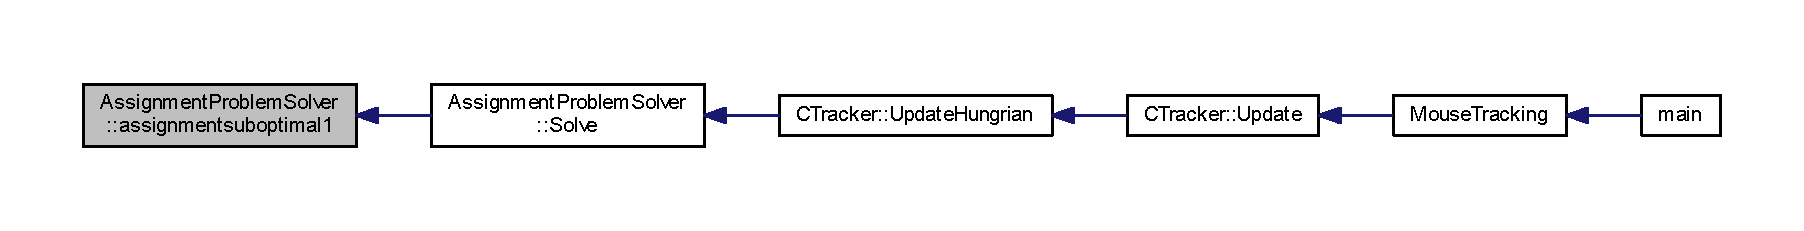
\includegraphics[width=350pt]{class_assignment_problem_solver_ae8fddfafc7387f3597493f02e8366883_icgraph}
\end{center}
\end{figure}
\mbox{\Hypertarget{class_assignment_problem_solver_a31277dc88cb22e07db1e52b6fe88f84f}\label{class_assignment_problem_solver_a31277dc88cb22e07db1e52b6fe88f84f}} 
\index{Assignment\+Problem\+Solver@{Assignment\+Problem\+Solver}!assignmentsuboptimal2@{assignmentsuboptimal2}}
\index{assignmentsuboptimal2@{assignmentsuboptimal2}!Assignment\+Problem\+Solver@{Assignment\+Problem\+Solver}}
\subsubsection{\texorpdfstring{assignmentsuboptimal2()}{assignmentsuboptimal2()}}
{\footnotesize\ttfamily void Assignment\+Problem\+Solver\+::assignmentsuboptimal2 (\begin{DoxyParamCaption}\item[{\mbox{\hyperlink{_hungarian_alg_8h_ad7b9f569a9adbd958c668a36b6884ffd}{assignments\+\_\+t}} \&}]{assignment,  }\item[{\mbox{\hyperlink{defines_8h_a7ce9c8817b42ab418e61756f579549ab}{track\+\_\+t}} \&}]{cost,  }\item[{const \mbox{\hyperlink{_hungarian_alg_8h_af6ab0ee8259a51215f62e8f96416d5bb}{dist\+Matrix\+\_\+t}} \&}]{dist\+Matrix\+In,  }\item[{size\+\_\+t}]{n\+Of\+Rows,  }\item[{size\+\_\+t}]{n\+Of\+Columns }\end{DoxyParamCaption})\hspace{0.3cm}{\ttfamily [private]}}



Definition at line 429 of file Hungarian\+Alg.\+cpp.


\begin{DoxyCode}
430 \{
431     \textcolor{comment}{/* make working copy of distance Matrix */}
432     \textcolor{keyword}{const} \textcolor{keywordtype}{size\_t} nOfElements = nOfRows * nOfColumns;
433     \mbox{\hyperlink{defines_8h_a7ce9c8817b42ab418e61756f579549ab}{track\_t}}* distMatrix = (\mbox{\hyperlink{defines_8h_a7ce9c8817b42ab418e61756f579549ab}{track\_t}}*)malloc(nOfElements * \textcolor{keyword}{sizeof}(
      \mbox{\hyperlink{defines_8h_a7ce9c8817b42ab418e61756f579549ab}{track\_t}}));
434     \textcolor{keywordflow}{for} (\textcolor{keywordtype}{size\_t} n = 0; n < nOfElements; n++)
435     \{
436         distMatrix[n] = distMatrixIn[n];
437     \}
438 
439     \textcolor{comment}{/* recursively search for the minimum element and do the assignment */}
440     \textcolor{keywordflow}{for} (;;)
441     \{
442         \textcolor{comment}{/* find minimum distance observation-to-track pair */}
443         \mbox{\hyperlink{defines_8h_a7ce9c8817b42ab418e61756f579549ab}{track\_t}} minValue = std::numeric\_limits<track\_t>::max();
444         \textcolor{keywordtype}{size\_t} tmpRow = 0;
445         \textcolor{keywordtype}{size\_t} tmpCol = 0;
446         \textcolor{keywordflow}{for} (\textcolor{keywordtype}{size\_t} row = 0; row < nOfRows; row++)
447         \{
448             \textcolor{keywordflow}{for} (\textcolor{keywordtype}{size\_t} col = 0; col < nOfColumns; col++)
449             \{
450                 \textcolor{keyword}{const} \mbox{\hyperlink{defines_8h_a7ce9c8817b42ab418e61756f579549ab}{track\_t}} \mbox{\hyperlink{struct_g_m_l__token_a50b20988e3fe419332313e8d9e02c775}{value}} = distMatrix[row + nOfRows*col];
451                 \textcolor{keywordflow}{if} (\mbox{\hyperlink{struct_g_m_l__token_a50b20988e3fe419332313e8d9e02c775}{value}} != std::numeric\_limits<track\_t>::max() && (\mbox{\hyperlink{struct_g_m_l__token_a50b20988e3fe419332313e8d9e02c775}{value}} < minValue))
452                 \{
453                     minValue = \mbox{\hyperlink{struct_g_m_l__token_a50b20988e3fe419332313e8d9e02c775}{value}};
454                     tmpRow = row;
455                     tmpCol = col;
456                 \}
457             \}
458         \}
459 
460         \textcolor{keywordflow}{if} (minValue != std::numeric\_limits<track\_t>::max())
461         \{
462             assignment[tmpRow] = \textcolor{keyword}{static\_cast<}\textcolor{keywordtype}{int}\textcolor{keyword}{>}(tmpCol);
463             cost += minValue;
464             \textcolor{keywordflow}{for} (\textcolor{keywordtype}{size\_t} n = 0; n < nOfRows; n++)
465             \{
466                 distMatrix[n + nOfRows*tmpCol] = std::numeric\_limits<track\_t>::max();
467             \}
468             \textcolor{keywordflow}{for} (\textcolor{keywordtype}{size\_t} n = 0; n < nOfColumns; n++)
469             \{
470                 distMatrix[tmpRow + nOfRows*n] = std::numeric\_limits<track\_t>::max();
471             \}
472         \}
473         \textcolor{keywordflow}{else}
474         \{
475             \textcolor{keywordflow}{break};
476         \}
477     \}
478 
479     free(distMatrix);
480 \}
\end{DoxyCode}
Here is the caller graph for this function\+:\nopagebreak
\begin{figure}[H]
\begin{center}
\leavevmode
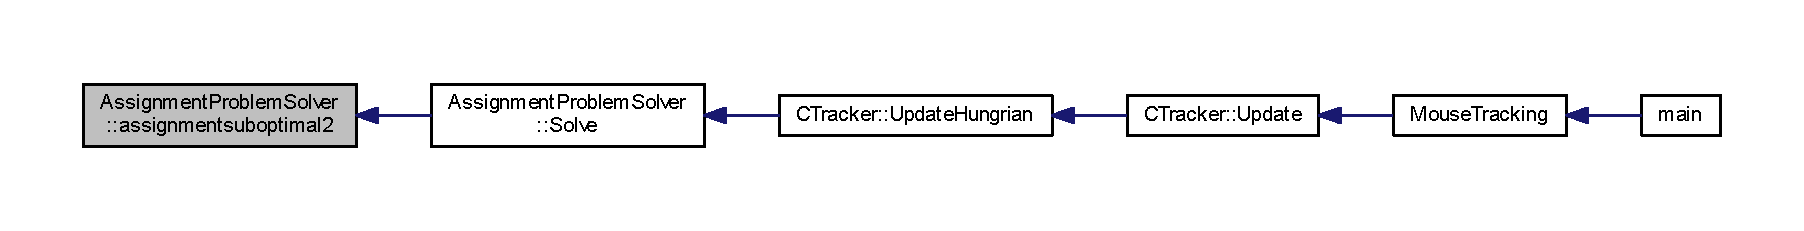
\includegraphics[width=350pt]{class_assignment_problem_solver_a31277dc88cb22e07db1e52b6fe88f84f_icgraph}
\end{center}
\end{figure}
\mbox{\Hypertarget{class_assignment_problem_solver_a1aa1c05dec6aef723f5d41affc667a77}\label{class_assignment_problem_solver_a1aa1c05dec6aef723f5d41affc667a77}} 
\index{Assignment\+Problem\+Solver@{Assignment\+Problem\+Solver}!buildassignmentvector@{buildassignmentvector}}
\index{buildassignmentvector@{buildassignmentvector}!Assignment\+Problem\+Solver@{Assignment\+Problem\+Solver}}
\subsubsection{\texorpdfstring{buildassignmentvector()}{buildassignmentvector()}}
{\footnotesize\ttfamily void Assignment\+Problem\+Solver\+::buildassignmentvector (\begin{DoxyParamCaption}\item[{\mbox{\hyperlink{_hungarian_alg_8h_ad7b9f569a9adbd958c668a36b6884ffd}{assignments\+\_\+t}} \&}]{assignment,  }\item[{bool $\ast$}]{star\+Matrix,  }\item[{size\+\_\+t}]{n\+Of\+Rows,  }\item[{size\+\_\+t}]{n\+Of\+Columns }\end{DoxyParamCaption})\hspace{0.3cm}{\ttfamily [private]}}



Definition at line 190 of file Hungarian\+Alg.\+cpp.


\begin{DoxyCode}
191 \{
192     \textcolor{keywordflow}{for} (\textcolor{keywordtype}{size\_t} row = 0; row < nOfRows; row++)
193     \{
194         \textcolor{keywordflow}{for} (\textcolor{keywordtype}{size\_t} col = 0; col < nOfColumns; col++)
195         \{
196             \textcolor{keywordflow}{if} (starMatrix[row + nOfRows * col])
197             \{
198                 assignment[row] = \textcolor{keyword}{static\_cast<}\textcolor{keywordtype}{int}\textcolor{keyword}{>}(col);
199                 \textcolor{keywordflow}{break};
200             \}
201         \}
202     \}
203 \}
\end{DoxyCode}
Here is the caller graph for this function\+:\nopagebreak
\begin{figure}[H]
\begin{center}
\leavevmode
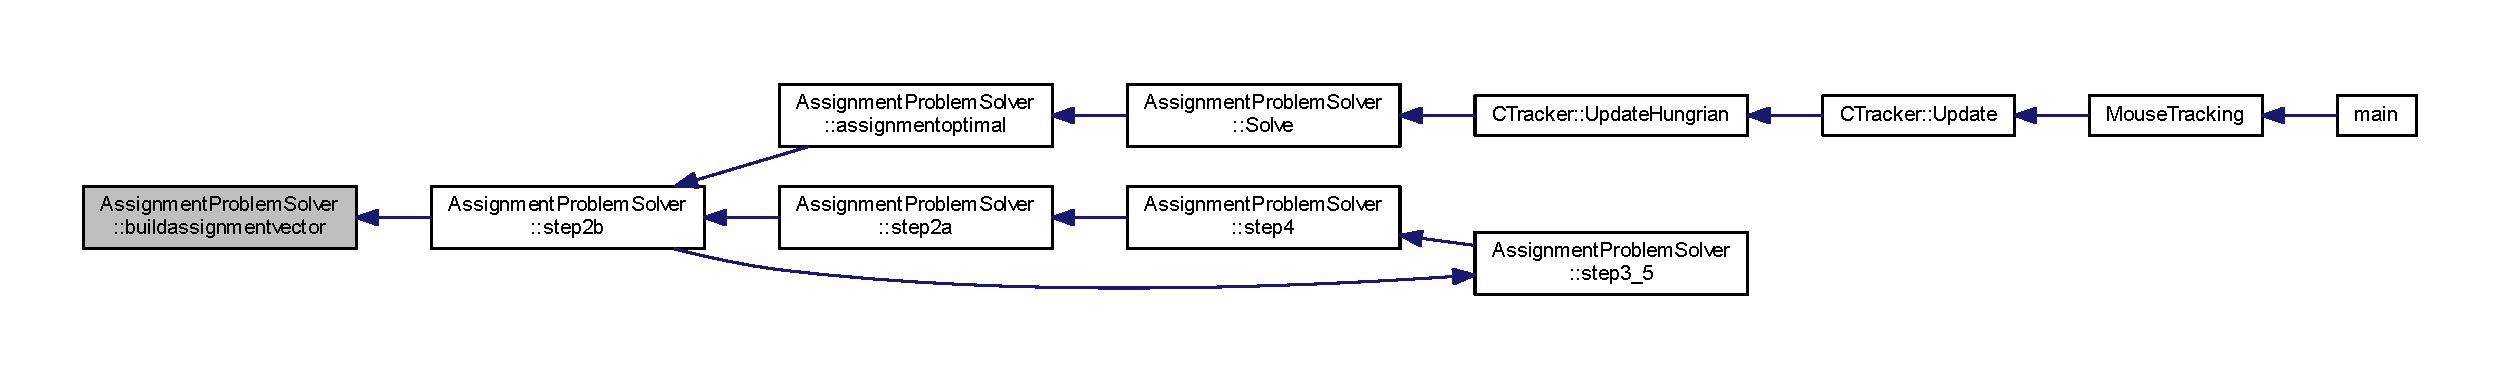
\includegraphics[width=350pt]{class_assignment_problem_solver_a1aa1c05dec6aef723f5d41affc667a77_icgraph}
\end{center}
\end{figure}
\mbox{\Hypertarget{class_assignment_problem_solver_a978fa51f563d47dbd00c697704cf4ad9}\label{class_assignment_problem_solver_a978fa51f563d47dbd00c697704cf4ad9}} 
\index{Assignment\+Problem\+Solver@{Assignment\+Problem\+Solver}!computeassignmentcost@{computeassignmentcost}}
\index{computeassignmentcost@{computeassignmentcost}!Assignment\+Problem\+Solver@{Assignment\+Problem\+Solver}}
\subsubsection{\texorpdfstring{computeassignmentcost()}{computeassignmentcost()}}
{\footnotesize\ttfamily void Assignment\+Problem\+Solver\+::computeassignmentcost (\begin{DoxyParamCaption}\item[{const \mbox{\hyperlink{_hungarian_alg_8h_ad7b9f569a9adbd958c668a36b6884ffd}{assignments\+\_\+t}} \&}]{assignment,  }\item[{\mbox{\hyperlink{defines_8h_a7ce9c8817b42ab418e61756f579549ab}{track\+\_\+t}} \&}]{cost,  }\item[{const \mbox{\hyperlink{_hungarian_alg_8h_af6ab0ee8259a51215f62e8f96416d5bb}{dist\+Matrix\+\_\+t}} \&}]{dist\+Matrix\+In,  }\item[{size\+\_\+t}]{n\+Of\+Rows }\end{DoxyParamCaption})\hspace{0.3cm}{\ttfamily [private]}}



Definition at line 207 of file Hungarian\+Alg.\+cpp.


\begin{DoxyCode}
208 \{
209     \textcolor{keywordflow}{for} (\textcolor{keywordtype}{size\_t} row = 0; row < nOfRows; row++)
210     \{
211         \textcolor{keyword}{const} \textcolor{keywordtype}{int} col = assignment[row];
212         \textcolor{keywordflow}{if} (col >= 0)
213         \{
214             cost += distMatrixIn[row + nOfRows * col];
215         \}
216     \}
217 \}
\end{DoxyCode}
Here is the caller graph for this function\+:\nopagebreak
\begin{figure}[H]
\begin{center}
\leavevmode
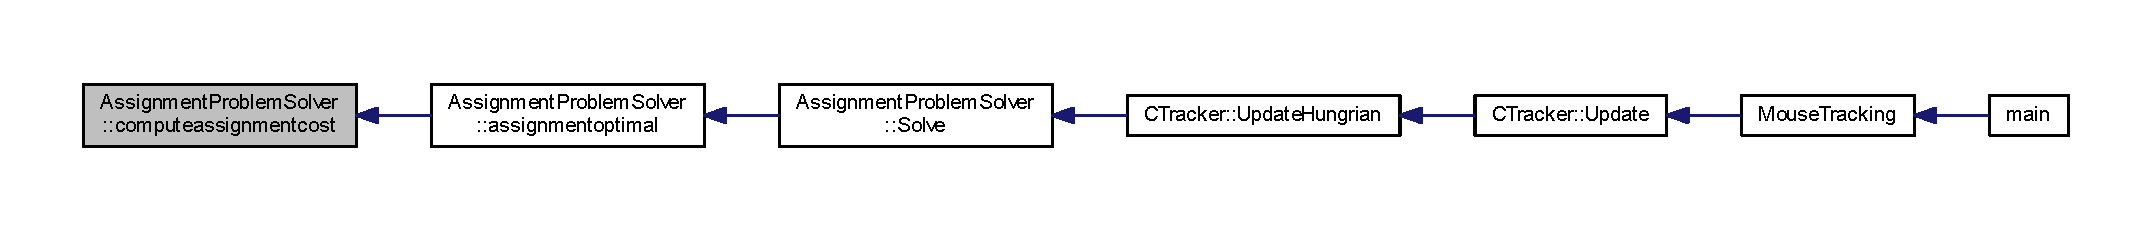
\includegraphics[width=350pt]{class_assignment_problem_solver_a978fa51f563d47dbd00c697704cf4ad9_icgraph}
\end{center}
\end{figure}
\mbox{\Hypertarget{class_assignment_problem_solver_a38198467ca647403c40be2c2bb47e177}\label{class_assignment_problem_solver_a38198467ca647403c40be2c2bb47e177}} 
\index{Assignment\+Problem\+Solver@{Assignment\+Problem\+Solver}!Solve@{Solve}}
\index{Solve@{Solve}!Assignment\+Problem\+Solver@{Assignment\+Problem\+Solver}}
\subsubsection{\texorpdfstring{Solve()}{Solve()}}
{\footnotesize\ttfamily \mbox{\hyperlink{defines_8h_a7ce9c8817b42ab418e61756f579549ab}{track\+\_\+t}} Assignment\+Problem\+Solver\+::\+Solve (\begin{DoxyParamCaption}\item[{const \mbox{\hyperlink{_hungarian_alg_8h_af6ab0ee8259a51215f62e8f96416d5bb}{dist\+Matrix\+\_\+t}} \&}]{dist\+Matrix\+In,  }\item[{size\+\_\+t}]{n\+Of\+Rows,  }\item[{size\+\_\+t}]{n\+Of\+Columns,  }\item[{\mbox{\hyperlink{_hungarian_alg_8h_ad7b9f569a9adbd958c668a36b6884ffd}{assignments\+\_\+t}} \&}]{assignment,  }\item[{\mbox{\hyperlink{class_assignment_problem_solver_aec407eb73fed9d3ddb9467fde90a85e8}{T\+Method}}}]{Method = {\ttfamily \mbox{\hyperlink{class_assignment_problem_solver_aec407eb73fed9d3ddb9467fde90a85e8a84f2334f61866dba64befa6910848d75}{optimal}}} }\end{DoxyParamCaption})}



Definition at line 21 of file Hungarian\+Alg.\+cpp.


\begin{DoxyCode}
28 \{
29     assignment.resize(nOfRows, -1);
30 
31     \mbox{\hyperlink{defines_8h_a7ce9c8817b42ab418e61756f579549ab}{track\_t}} cost = 0;
32 
33     \textcolor{keywordflow}{switch} (Method)
34     \{
35     \textcolor{keywordflow}{case} \mbox{\hyperlink{class_assignment_problem_solver_aec407eb73fed9d3ddb9467fde90a85e8a84f2334f61866dba64befa6910848d75}{optimal}}:
36         \mbox{\hyperlink{class_assignment_problem_solver_a5b84a5167984db1050821926f52b5187}{assignmentoptimal}}(assignment, cost, distMatrixIn, nOfRows, nOfColumns);
37         \textcolor{keywordflow}{break};
38 
39     \textcolor{keywordflow}{case} \mbox{\hyperlink{class_assignment_problem_solver_aec407eb73fed9d3ddb9467fde90a85e8a226c2e4b79d0beeb342087880d97bb2a}{many\_forbidden\_assignments}}:
40         \mbox{\hyperlink{class_assignment_problem_solver_ae8fddfafc7387f3597493f02e8366883}{assignmentsuboptimal1}}(assignment, cost, distMatrixIn, nOfRows, nOfColumns);
41         \textcolor{keywordflow}{break};
42 
43     \textcolor{keywordflow}{case} \mbox{\hyperlink{class_assignment_problem_solver_aec407eb73fed9d3ddb9467fde90a85e8a3329e7571829a83b21be4821df62310d}{without\_forbidden\_assignments}}:
44         \mbox{\hyperlink{class_assignment_problem_solver_a31277dc88cb22e07db1e52b6fe88f84f}{assignmentsuboptimal2}}(assignment, cost, distMatrixIn, nOfRows, nOfColumns);
45         \textcolor{keywordflow}{break};
46     \}
47 
48     \textcolor{keywordflow}{return} cost;
49 \}
\end{DoxyCode}
Here is the call graph for this function\+:\nopagebreak
\begin{figure}[H]
\begin{center}
\leavevmode
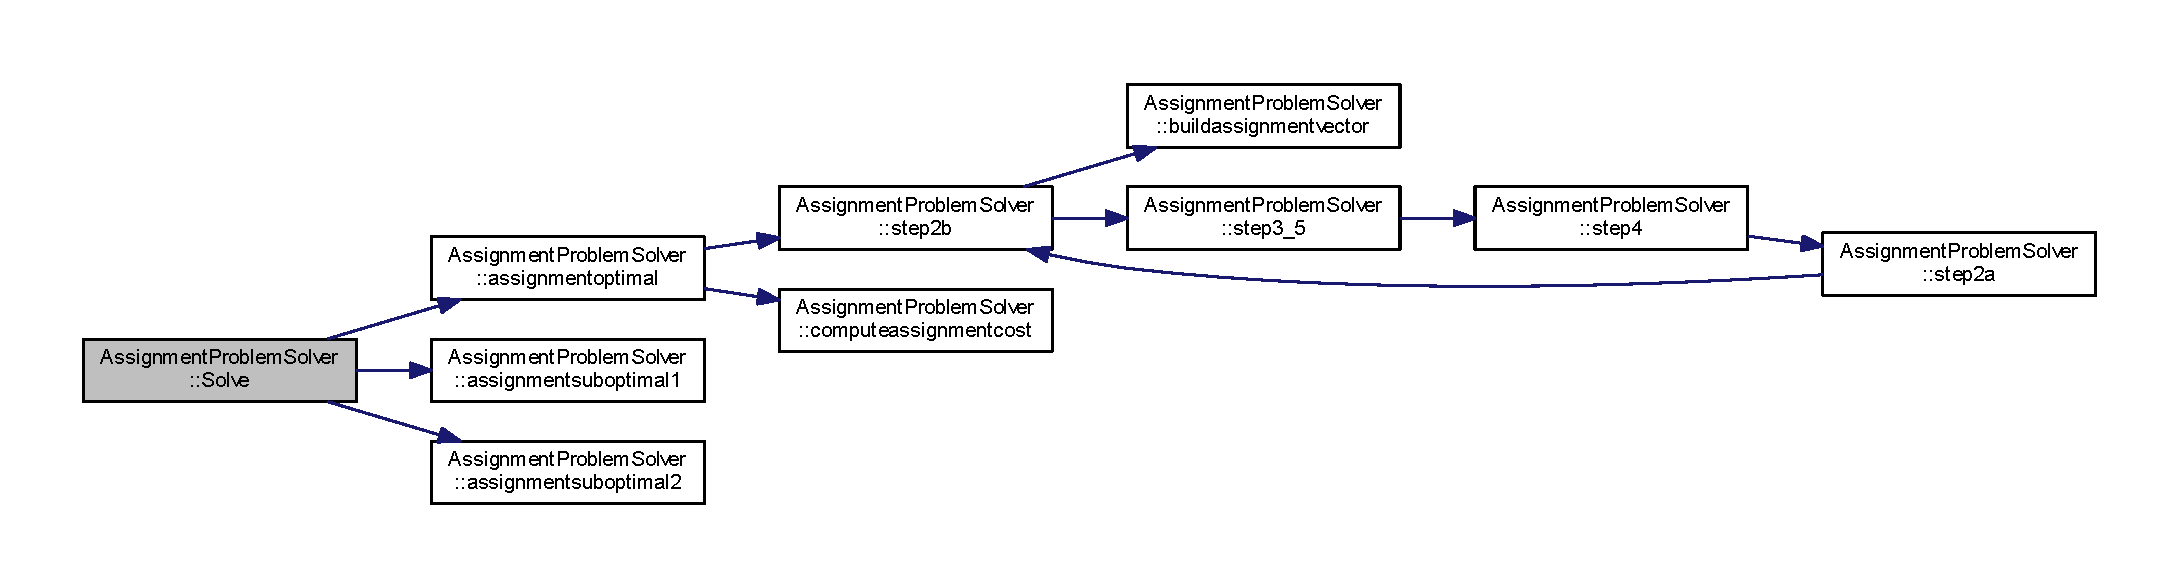
\includegraphics[width=350pt]{class_assignment_problem_solver_a38198467ca647403c40be2c2bb47e177_cgraph}
\end{center}
\end{figure}
Here is the caller graph for this function\+:\nopagebreak
\begin{figure}[H]
\begin{center}
\leavevmode
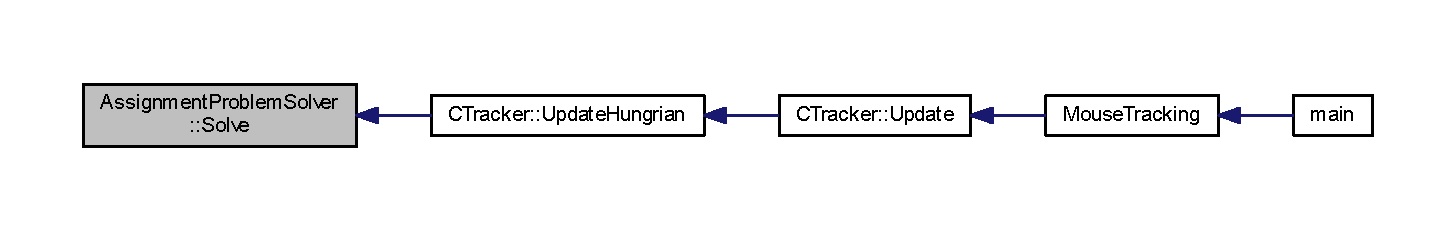
\includegraphics[width=350pt]{class_assignment_problem_solver_a38198467ca647403c40be2c2bb47e177_icgraph}
\end{center}
\end{figure}
\mbox{\Hypertarget{class_assignment_problem_solver_adef6ec1494dd6058fdf1373bc2c6d6eb}\label{class_assignment_problem_solver_adef6ec1494dd6058fdf1373bc2c6d6eb}} 
\index{Assignment\+Problem\+Solver@{Assignment\+Problem\+Solver}!step2a@{step2a}}
\index{step2a@{step2a}!Assignment\+Problem\+Solver@{Assignment\+Problem\+Solver}}
\subsubsection{\texorpdfstring{step2a()}{step2a()}}
{\footnotesize\ttfamily void Assignment\+Problem\+Solver\+::step2a (\begin{DoxyParamCaption}\item[{\mbox{\hyperlink{_hungarian_alg_8h_ad7b9f569a9adbd958c668a36b6884ffd}{assignments\+\_\+t}} \&}]{assignment,  }\item[{\mbox{\hyperlink{defines_8h_a7ce9c8817b42ab418e61756f579549ab}{track\+\_\+t}} $\ast$}]{dist\+Matrix,  }\item[{bool $\ast$}]{star\+Matrix,  }\item[{bool $\ast$}]{new\+Star\+Matrix,  }\item[{bool $\ast$}]{prime\+Matrix,  }\item[{bool $\ast$}]{covered\+Columns,  }\item[{bool $\ast$}]{covered\+Rows,  }\item[{size\+\_\+t}]{n\+Of\+Rows,  }\item[{size\+\_\+t}]{n\+Of\+Columns,  }\item[{size\+\_\+t}]{min\+Dim }\end{DoxyParamCaption})\hspace{0.3cm}{\ttfamily [private]}}



Definition at line 222 of file Hungarian\+Alg.\+cpp.


\begin{DoxyCode}
223 \{
224     \textcolor{keywordtype}{bool} *starMatrixTemp, *columnEnd;
225     \textcolor{comment}{/* cover every column containing a starred zero */}
226     \textcolor{keywordflow}{for} (\textcolor{keywordtype}{size\_t} col = 0; col < nOfColumns; col++)
227     \{
228         starMatrixTemp = starMatrix + nOfRows * col;
229         columnEnd = starMatrixTemp + nOfRows;
230         \textcolor{keywordflow}{while} (starMatrixTemp < columnEnd)
231         \{
232             \textcolor{keywordflow}{if} (*starMatrixTemp++)
233             \{
234                 coveredColumns[col] = \textcolor{keyword}{true};
235                 \textcolor{keywordflow}{break};
236             \}
237         \}
238     \}
239     \textcolor{comment}{/* move to step 3 */}
240     \mbox{\hyperlink{class_assignment_problem_solver_a069b78d89842031f7b54e0837c2bd602}{step2b}}(assignment, distMatrix, starMatrix, newStarMatrix, primeMatrix, coveredColumns, 
      coveredRows, nOfRows, nOfColumns, minDim);
241 \}
\end{DoxyCode}
Here is the call graph for this function\+:\nopagebreak
\begin{figure}[H]
\begin{center}
\leavevmode
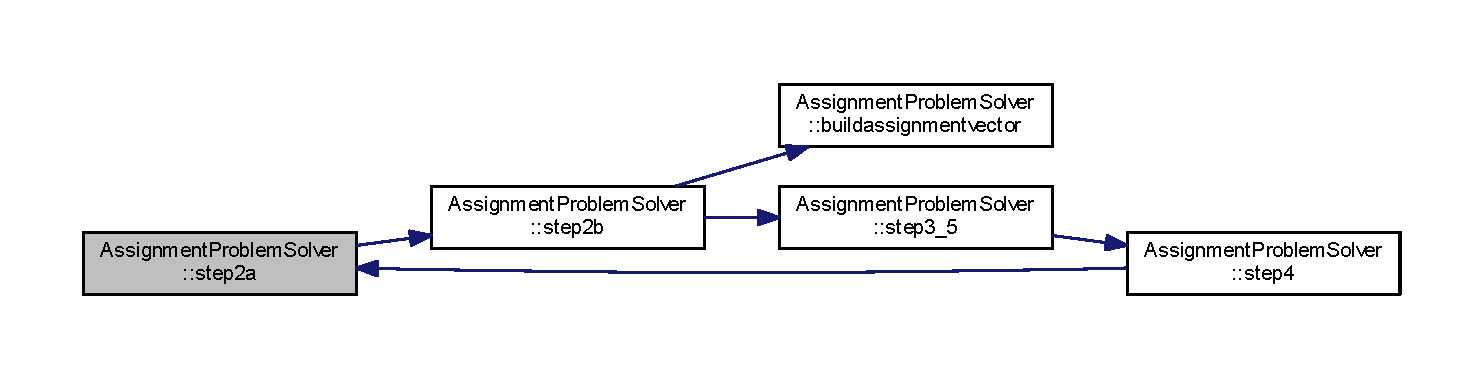
\includegraphics[width=350pt]{class_assignment_problem_solver_adef6ec1494dd6058fdf1373bc2c6d6eb_cgraph}
\end{center}
\end{figure}
Here is the caller graph for this function\+:\nopagebreak
\begin{figure}[H]
\begin{center}
\leavevmode
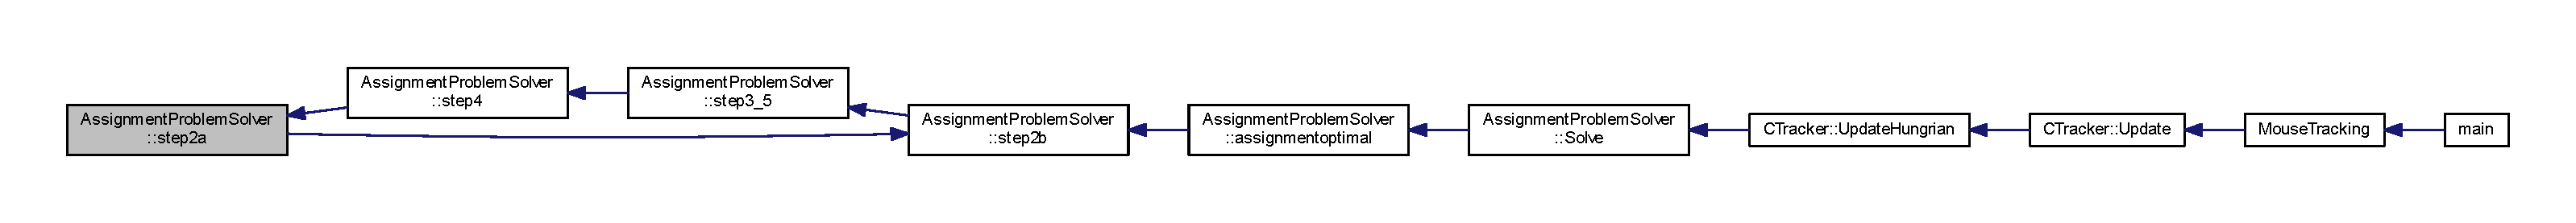
\includegraphics[width=350pt]{class_assignment_problem_solver_adef6ec1494dd6058fdf1373bc2c6d6eb_icgraph}
\end{center}
\end{figure}
\mbox{\Hypertarget{class_assignment_problem_solver_a069b78d89842031f7b54e0837c2bd602}\label{class_assignment_problem_solver_a069b78d89842031f7b54e0837c2bd602}} 
\index{Assignment\+Problem\+Solver@{Assignment\+Problem\+Solver}!step2b@{step2b}}
\index{step2b@{step2b}!Assignment\+Problem\+Solver@{Assignment\+Problem\+Solver}}
\subsubsection{\texorpdfstring{step2b()}{step2b()}}
{\footnotesize\ttfamily void Assignment\+Problem\+Solver\+::step2b (\begin{DoxyParamCaption}\item[{\mbox{\hyperlink{_hungarian_alg_8h_ad7b9f569a9adbd958c668a36b6884ffd}{assignments\+\_\+t}} \&}]{assignment,  }\item[{\mbox{\hyperlink{defines_8h_a7ce9c8817b42ab418e61756f579549ab}{track\+\_\+t}} $\ast$}]{dist\+Matrix,  }\item[{bool $\ast$}]{star\+Matrix,  }\item[{bool $\ast$}]{new\+Star\+Matrix,  }\item[{bool $\ast$}]{prime\+Matrix,  }\item[{bool $\ast$}]{covered\+Columns,  }\item[{bool $\ast$}]{covered\+Rows,  }\item[{size\+\_\+t}]{n\+Of\+Rows,  }\item[{size\+\_\+t}]{n\+Of\+Columns,  }\item[{size\+\_\+t}]{min\+Dim }\end{DoxyParamCaption})\hspace{0.3cm}{\ttfamily [private]}}



Definition at line 246 of file Hungarian\+Alg.\+cpp.


\begin{DoxyCode}
247 \{
248     \textcolor{comment}{/* count covered columns */}
249     \textcolor{keywordtype}{size\_t} nOfCoveredColumns = 0;
250     \textcolor{keywordflow}{for} (\textcolor{keywordtype}{size\_t} col = 0; col < nOfColumns; col++)
251     \{
252         \textcolor{keywordflow}{if} (coveredColumns[col])
253         \{
254             nOfCoveredColumns++;
255         \}
256     \}
257     \textcolor{keywordflow}{if} (nOfCoveredColumns == minDim)
258     \{
259         \textcolor{comment}{/* algorithm finished */}
260         \mbox{\hyperlink{class_assignment_problem_solver_a1aa1c05dec6aef723f5d41affc667a77}{buildassignmentvector}}(assignment, starMatrix, nOfRows, nOfColumns);
261     \}
262     \textcolor{keywordflow}{else}
263     \{
264         \textcolor{comment}{/* move to step 3 */}
265         \mbox{\hyperlink{class_assignment_problem_solver_a8c24dfcfef6adfb96c6394f798c02dba}{step3\_5}}(assignment, distMatrix, starMatrix, newStarMatrix, primeMatrix, coveredColumns, 
      coveredRows, nOfRows, nOfColumns, minDim);
266     \}
267 \}
\end{DoxyCode}
Here is the call graph for this function\+:\nopagebreak
\begin{figure}[H]
\begin{center}
\leavevmode
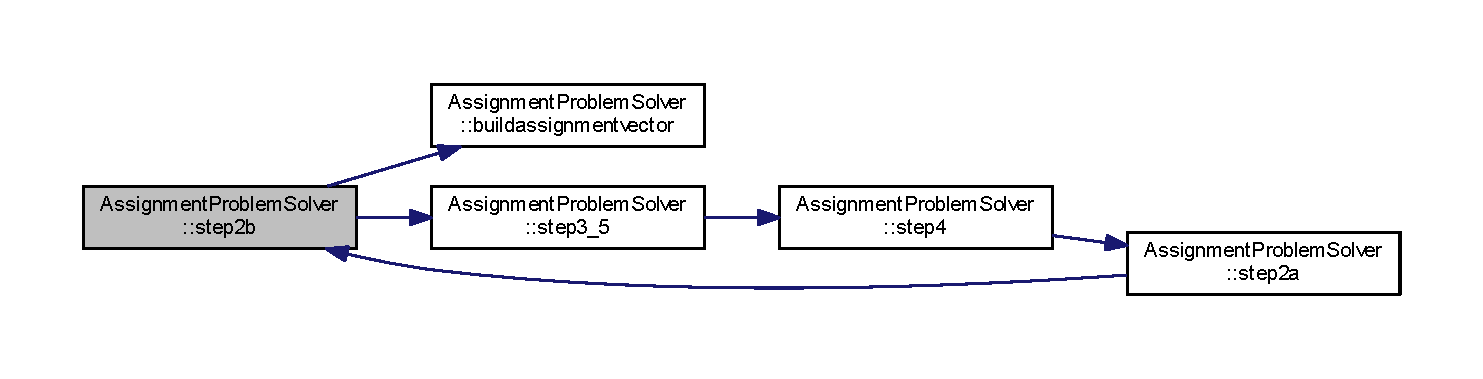
\includegraphics[width=350pt]{class_assignment_problem_solver_a069b78d89842031f7b54e0837c2bd602_cgraph}
\end{center}
\end{figure}
Here is the caller graph for this function\+:\nopagebreak
\begin{figure}[H]
\begin{center}
\leavevmode
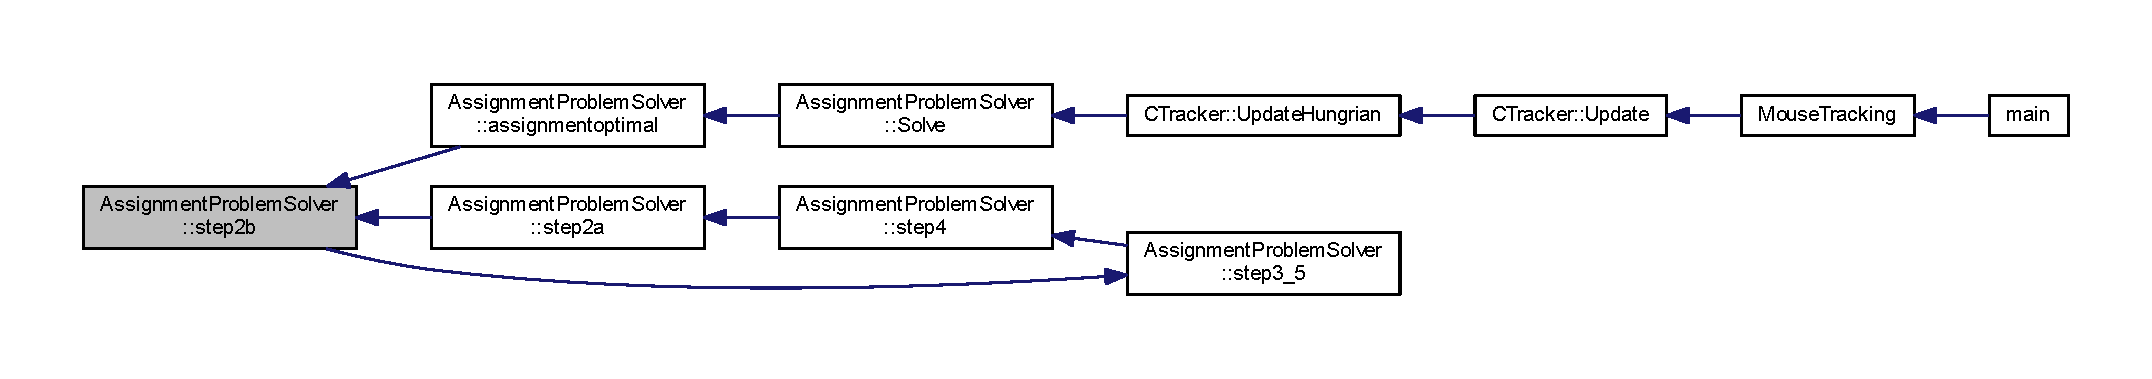
\includegraphics[width=350pt]{class_assignment_problem_solver_a069b78d89842031f7b54e0837c2bd602_icgraph}
\end{center}
\end{figure}
\mbox{\Hypertarget{class_assignment_problem_solver_a8c24dfcfef6adfb96c6394f798c02dba}\label{class_assignment_problem_solver_a8c24dfcfef6adfb96c6394f798c02dba}} 
\index{Assignment\+Problem\+Solver@{Assignment\+Problem\+Solver}!step3\+\_\+5@{step3\+\_\+5}}
\index{step3\+\_\+5@{step3\+\_\+5}!Assignment\+Problem\+Solver@{Assignment\+Problem\+Solver}}
\subsubsection{\texorpdfstring{step3\+\_\+5()}{step3\_5()}}
{\footnotesize\ttfamily void Assignment\+Problem\+Solver\+::step3\+\_\+5 (\begin{DoxyParamCaption}\item[{\mbox{\hyperlink{_hungarian_alg_8h_ad7b9f569a9adbd958c668a36b6884ffd}{assignments\+\_\+t}} \&}]{assignment,  }\item[{\mbox{\hyperlink{defines_8h_a7ce9c8817b42ab418e61756f579549ab}{track\+\_\+t}} $\ast$}]{dist\+Matrix,  }\item[{bool $\ast$}]{star\+Matrix,  }\item[{bool $\ast$}]{new\+Star\+Matrix,  }\item[{bool $\ast$}]{prime\+Matrix,  }\item[{bool $\ast$}]{covered\+Columns,  }\item[{bool $\ast$}]{covered\+Rows,  }\item[{size\+\_\+t}]{n\+Of\+Rows,  }\item[{size\+\_\+t}]{n\+Of\+Columns,  }\item[{size\+\_\+t}]{min\+Dim }\end{DoxyParamCaption})\hspace{0.3cm}{\ttfamily [private]}}



Definition at line 272 of file Hungarian\+Alg.\+cpp.


\begin{DoxyCode}
273 \{
274     \textcolor{keywordflow}{for} (;;)
275     \{
276         \textcolor{comment}{/* step 3 */}
277         \textcolor{keywordtype}{bool} zerosFound = \textcolor{keyword}{true};
278         \textcolor{keywordflow}{while} (zerosFound)
279         \{
280             zerosFound = \textcolor{keyword}{false};
281             \textcolor{keywordflow}{for} (\textcolor{keywordtype}{size\_t} col = 0; col < nOfColumns; col++)
282             \{
283                 \textcolor{keywordflow}{if} (!coveredColumns[col])
284                 \{
285                     \textcolor{keywordflow}{for} (\textcolor{keywordtype}{size\_t} row = 0; row < nOfRows; row++)
286                     \{
287                         \textcolor{keywordflow}{if} ((!coveredRows[row]) && (distMatrix[row + nOfRows*col] == 0))
288                         \{
289                             \textcolor{comment}{/* prime zero */}
290                             primeMatrix[row + nOfRows*col] = \textcolor{keyword}{true};
291                             \textcolor{comment}{/* find starred zero in current row */}
292                             \textcolor{keywordtype}{size\_t} starCol = 0;
293                             \textcolor{keywordflow}{for} (; starCol < nOfColumns; starCol++)
294                             \{
295                                 \textcolor{keywordflow}{if} (starMatrix[row + nOfRows * starCol])
296                                 \{
297                                     \textcolor{keywordflow}{break};
298                                 \}
299                             \}
300                             \textcolor{keywordflow}{if} (starCol == nOfColumns) \textcolor{comment}{/* no starred zero found */}
301                             \{
302                                 \textcolor{comment}{/* move to step 4 */}
303                                 \mbox{\hyperlink{class_assignment_problem_solver_a6ea85d386a136effd84c00f4e2f3cd77}{step4}}(assignment, distMatrix, starMatrix, newStarMatrix, primeMatrix, 
      coveredColumns, coveredRows, nOfRows, nOfColumns, minDim, row, col);
304                                 \textcolor{keywordflow}{return};
305                             \}
306                             \textcolor{keywordflow}{else}
307                             \{
308                                 coveredRows[row] = \textcolor{keyword}{true};
309                                 coveredColumns[starCol] = \textcolor{keyword}{false};
310                                 zerosFound = \textcolor{keyword}{true};
311                                 \textcolor{keywordflow}{break};
312                             \}
313                         \}
314                     \}
315                 \}
316             \}
317         \}
318         \textcolor{comment}{/* step 5 */}
319         \mbox{\hyperlink{defines_8h_a7ce9c8817b42ab418e61756f579549ab}{track\_t}} h = std::numeric\_limits<track\_t>::max();
320         \textcolor{keywordflow}{for} (\textcolor{keywordtype}{size\_t} row = 0; row < nOfRows; row++)
321         \{
322             \textcolor{keywordflow}{if} (!coveredRows[row])
323             \{
324                 \textcolor{keywordflow}{for} (\textcolor{keywordtype}{size\_t} col = 0; col < nOfColumns; col++)
325                 \{
326                     \textcolor{keywordflow}{if} (!coveredColumns[col])
327                     \{
328                         \textcolor{keyword}{const} \mbox{\hyperlink{defines_8h_a7ce9c8817b42ab418e61756f579549ab}{track\_t}} \mbox{\hyperlink{struct_g_m_l__token_a50b20988e3fe419332313e8d9e02c775}{value}} = distMatrix[row + nOfRows*col];
329                         \textcolor{keywordflow}{if} (\mbox{\hyperlink{struct_g_m_l__token_a50b20988e3fe419332313e8d9e02c775}{value}} < h)
330                         \{
331                             h = \mbox{\hyperlink{struct_g_m_l__token_a50b20988e3fe419332313e8d9e02c775}{value}};
332                         \}
333                     \}
334                 \}
335             \}
336         \}
337         \textcolor{comment}{/* add h to each covered row */}
338         \textcolor{keywordflow}{for} (\textcolor{keywordtype}{size\_t} row = 0; row < nOfRows; row++)
339         \{
340             \textcolor{keywordflow}{if} (coveredRows[row])
341             \{
342                 \textcolor{keywordflow}{for} (\textcolor{keywordtype}{size\_t} col = 0; col < nOfColumns; col++)
343                 \{
344                     distMatrix[row + nOfRows*col] += h;
345                 \}
346             \}
347         \}
348         \textcolor{comment}{/* subtract h from each uncovered column */}
349         \textcolor{keywordflow}{for} (\textcolor{keywordtype}{size\_t} col = 0; col < nOfColumns; col++)
350         \{
351             \textcolor{keywordflow}{if} (!coveredColumns[col])
352             \{
353                 \textcolor{keywordflow}{for} (\textcolor{keywordtype}{size\_t} row = 0; row < nOfRows; row++)
354                 \{
355                     distMatrix[row + nOfRows*col] -= h;
356                 \}
357             \}
358         \}
359     \}
360 \}
\end{DoxyCode}
Here is the call graph for this function\+:\nopagebreak
\begin{figure}[H]
\begin{center}
\leavevmode
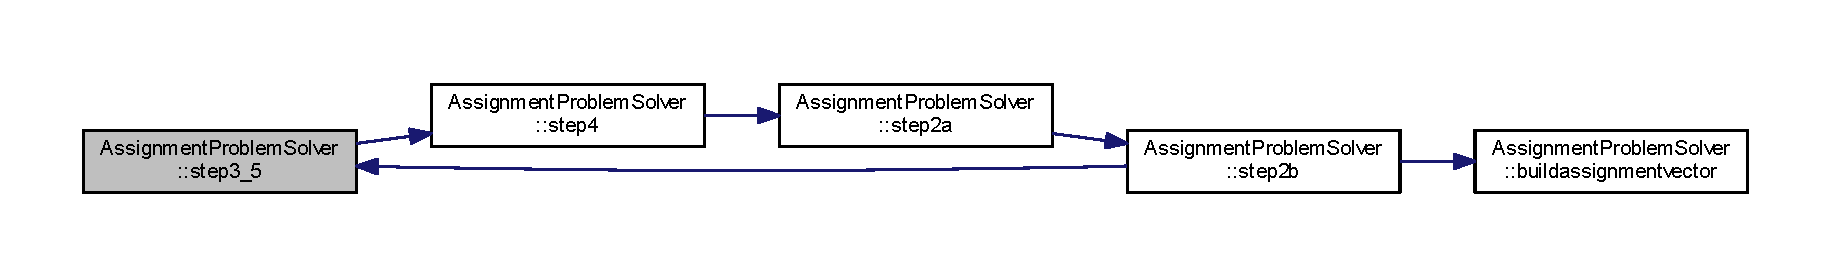
\includegraphics[width=350pt]{class_assignment_problem_solver_a8c24dfcfef6adfb96c6394f798c02dba_cgraph}
\end{center}
\end{figure}
Here is the caller graph for this function\+:\nopagebreak
\begin{figure}[H]
\begin{center}
\leavevmode
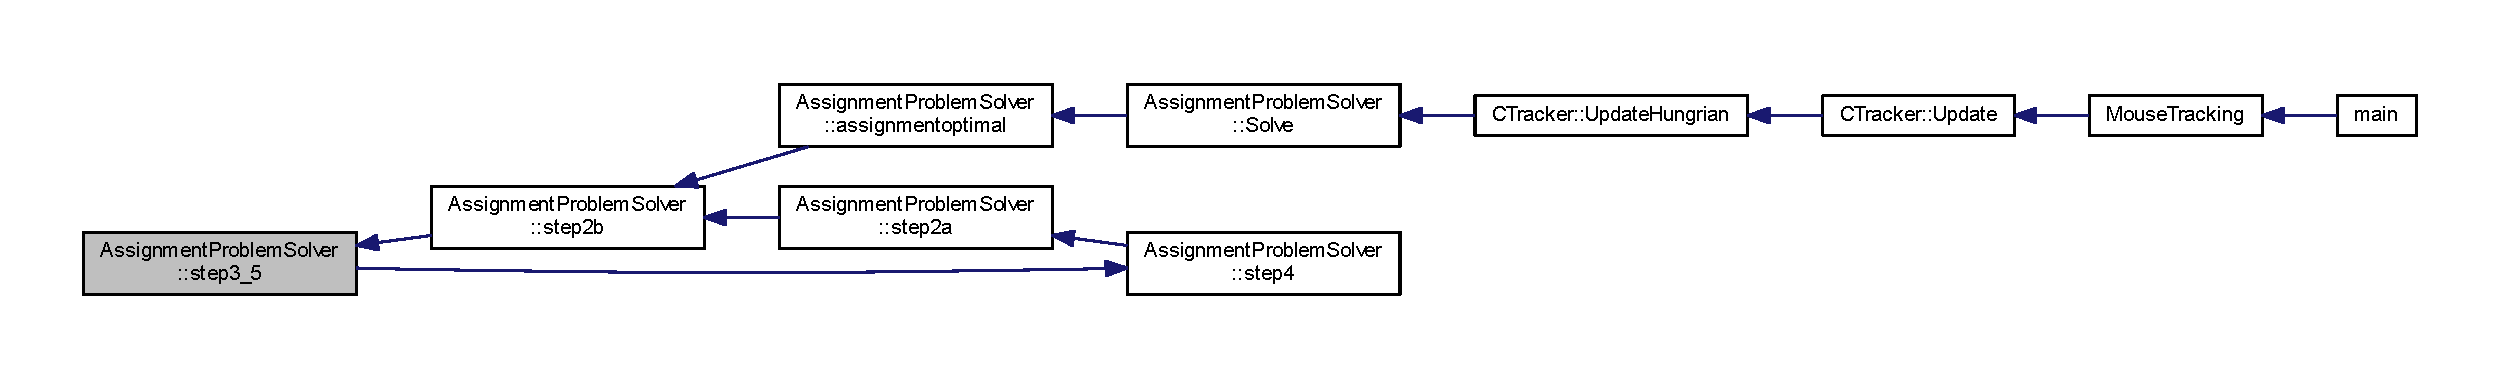
\includegraphics[width=350pt]{class_assignment_problem_solver_a8c24dfcfef6adfb96c6394f798c02dba_icgraph}
\end{center}
\end{figure}
\mbox{\Hypertarget{class_assignment_problem_solver_a6ea85d386a136effd84c00f4e2f3cd77}\label{class_assignment_problem_solver_a6ea85d386a136effd84c00f4e2f3cd77}} 
\index{Assignment\+Problem\+Solver@{Assignment\+Problem\+Solver}!step4@{step4}}
\index{step4@{step4}!Assignment\+Problem\+Solver@{Assignment\+Problem\+Solver}}
\subsubsection{\texorpdfstring{step4()}{step4()}}
{\footnotesize\ttfamily void Assignment\+Problem\+Solver\+::step4 (\begin{DoxyParamCaption}\item[{\mbox{\hyperlink{_hungarian_alg_8h_ad7b9f569a9adbd958c668a36b6884ffd}{assignments\+\_\+t}} \&}]{assignment,  }\item[{\mbox{\hyperlink{defines_8h_a7ce9c8817b42ab418e61756f579549ab}{track\+\_\+t}} $\ast$}]{dist\+Matrix,  }\item[{bool $\ast$}]{star\+Matrix,  }\item[{bool $\ast$}]{new\+Star\+Matrix,  }\item[{bool $\ast$}]{prime\+Matrix,  }\item[{bool $\ast$}]{covered\+Columns,  }\item[{bool $\ast$}]{covered\+Rows,  }\item[{size\+\_\+t}]{n\+Of\+Rows,  }\item[{size\+\_\+t}]{n\+Of\+Columns,  }\item[{size\+\_\+t}]{min\+Dim,  }\item[{size\+\_\+t}]{row,  }\item[{size\+\_\+t}]{col }\end{DoxyParamCaption})\hspace{0.3cm}{\ttfamily [private]}}



Definition at line 365 of file Hungarian\+Alg.\+cpp.


\begin{DoxyCode}
366 \{
367     \textcolor{keyword}{const} \textcolor{keywordtype}{size\_t} nOfElements = nOfRows * nOfColumns;
368     \textcolor{comment}{/* generate temporary copy of starMatrix */}
369     \textcolor{keywordflow}{for} (\textcolor{keywordtype}{size\_t} n = 0; n < nOfElements; n++)
370     \{
371         newStarMatrix[n] = starMatrix[n];
372     \}
373     \textcolor{comment}{/* star current zero */}
374     newStarMatrix[row + nOfRows*col] = \textcolor{keyword}{true};
375     \textcolor{comment}{/* find starred zero in current column */}
376     \textcolor{keywordtype}{size\_t} starCol = col;
377     \textcolor{keywordtype}{size\_t} starRow = 0;
378     \textcolor{keywordflow}{for} (; starRow < nOfRows; starRow++)
379     \{
380         \textcolor{keywordflow}{if} (starMatrix[starRow + nOfRows * starCol])
381         \{
382             \textcolor{keywordflow}{break};
383         \}
384     \}
385     \textcolor{keywordflow}{while} (starRow < nOfRows)
386     \{
387         \textcolor{comment}{/* unstar the starred zero */}
388         newStarMatrix[starRow + nOfRows*starCol] = \textcolor{keyword}{false};
389         \textcolor{comment}{/* find primed zero in current row */}
390         \textcolor{keywordtype}{size\_t} primeRow = starRow;
391         \textcolor{keywordtype}{size\_t} primeCol = 0;
392         \textcolor{keywordflow}{for} (; primeCol < nOfColumns; primeCol++)
393         \{
394             \textcolor{keywordflow}{if} (primeMatrix[primeRow + nOfRows * primeCol])
395             \{
396                 \textcolor{keywordflow}{break};
397             \}
398         \}
399         \textcolor{comment}{/* star the primed zero */}
400         newStarMatrix[primeRow + nOfRows*primeCol] = \textcolor{keyword}{true};
401         \textcolor{comment}{/* find starred zero in current column */}
402         starCol = primeCol;
403         \textcolor{keywordflow}{for} (starRow = 0; starRow < nOfRows; starRow++)
404         \{
405             \textcolor{keywordflow}{if} (starMatrix[starRow + nOfRows * starCol])
406             \{
407                 \textcolor{keywordflow}{break};
408             \}
409         \}
410     \}
411     \textcolor{comment}{/* use temporary copy as new starMatrix */}
412     \textcolor{comment}{/* delete all primes, uncover all rows */}
413     \textcolor{keywordflow}{for} (\textcolor{keywordtype}{size\_t} n = 0; n < nOfElements; n++)
414     \{
415         primeMatrix[n] = \textcolor{keyword}{false};
416         starMatrix[n] = newStarMatrix[n];
417     \}
418     \textcolor{keywordflow}{for} (\textcolor{keywordtype}{size\_t} n = 0; n < nOfRows; n++)
419     \{
420         coveredRows[n] = \textcolor{keyword}{false};
421     \}
422     \textcolor{comment}{/* move to step 2a */}
423     \mbox{\hyperlink{class_assignment_problem_solver_adef6ec1494dd6058fdf1373bc2c6d6eb}{step2a}}(assignment, distMatrix, starMatrix, newStarMatrix, primeMatrix, coveredColumns, 
      coveredRows, nOfRows, nOfColumns, minDim);
424 \}
\end{DoxyCode}
Here is the call graph for this function\+:\nopagebreak
\begin{figure}[H]
\begin{center}
\leavevmode
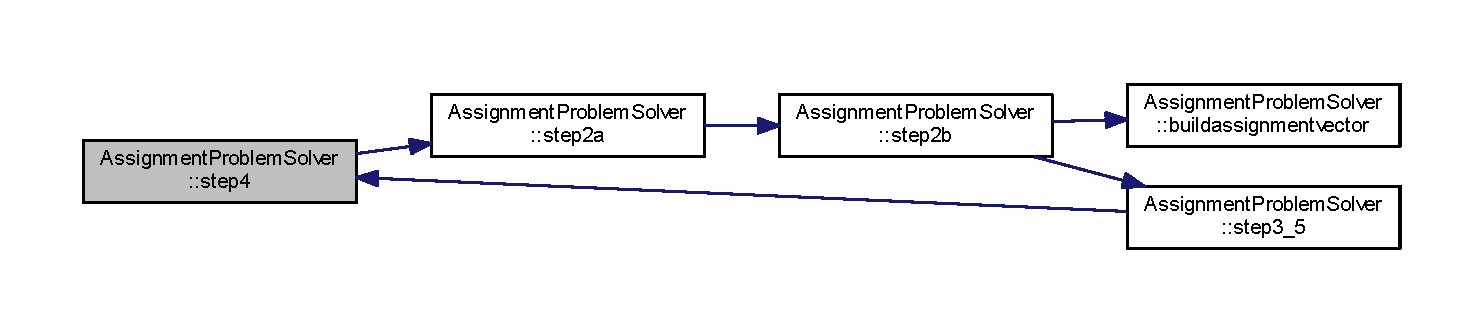
\includegraphics[width=350pt]{class_assignment_problem_solver_a6ea85d386a136effd84c00f4e2f3cd77_cgraph}
\end{center}
\end{figure}
Here is the caller graph for this function\+:\nopagebreak
\begin{figure}[H]
\begin{center}
\leavevmode
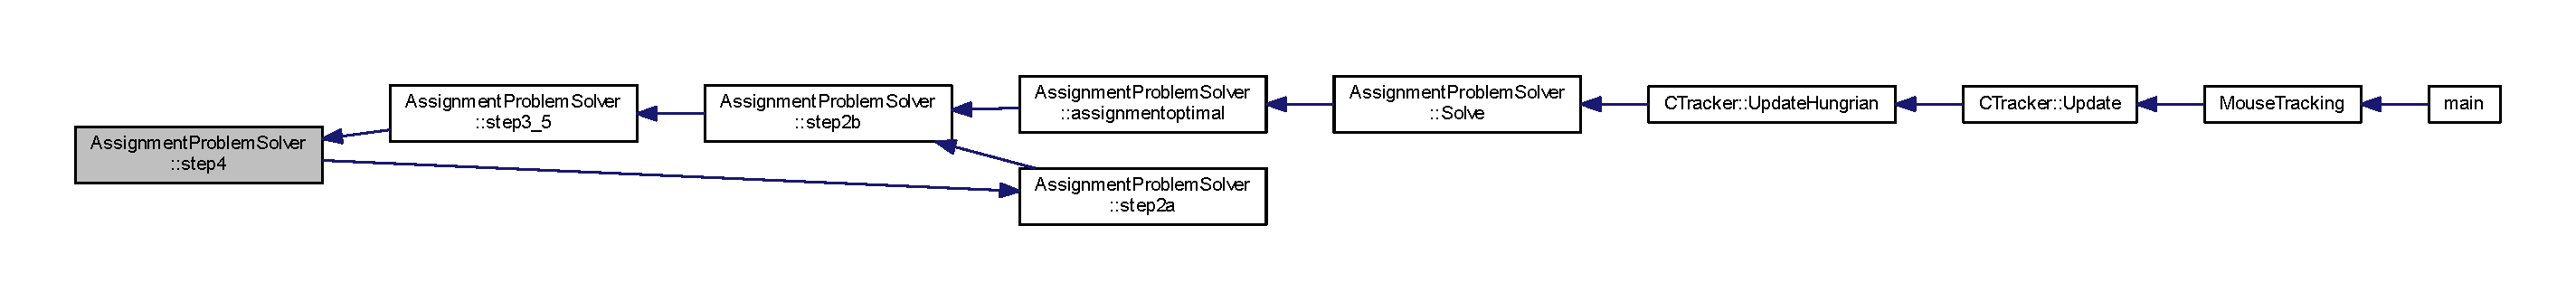
\includegraphics[width=350pt]{class_assignment_problem_solver_a6ea85d386a136effd84c00f4e2f3cd77_icgraph}
\end{center}
\end{figure}


The documentation for this class was generated from the following files\+:\begin{DoxyCompactItemize}
\item 
D\+:/\+Roy/\+Git\+Hub/\+Multitarget-\/tracker/\+Tracker/\+Hungarian\+Alg/\mbox{\hyperlink{_hungarian_alg_8h}{Hungarian\+Alg.\+h}}\item 
D\+:/\+Roy/\+Git\+Hub/\+Multitarget-\/tracker/\+Tracker/\+Hungarian\+Alg/\mbox{\hyperlink{_hungarian_alg_8cpp}{Hungarian\+Alg.\+cpp}}\end{DoxyCompactItemize}

\hypertarget{class_background_subtract}{}\section{Background\+Subtract Class Reference}
\label{class_background_subtract}\index{Background\+Subtract@{Background\+Subtract}}


The \mbox{\hyperlink{class_background_subtract}{Background\+Subtract}} class.  




{\ttfamily \#include $<$Background\+Subtract.\+h$>$}



Collaboration diagram for Background\+Subtract\+:\nopagebreak
\begin{figure}[H]
\begin{center}
\leavevmode
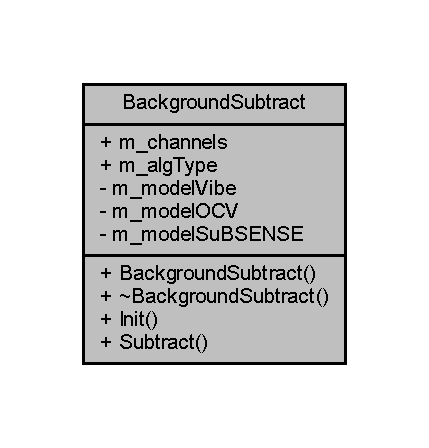
\includegraphics[width=206pt]{class_background_subtract__coll__graph}
\end{center}
\end{figure}
\subsection*{Public Types}
\begin{DoxyCompactItemize}
\item 
enum \mbox{\hyperlink{class_background_subtract_a56850081696df68b55f87b4f3d87949f}{B\+G\+F\+G\+\_\+\+A\+L\+GS}} \{ \newline
\mbox{\hyperlink{class_background_subtract_a56850081696df68b55f87b4f3d87949fa1905f812773a0029b59688e57990f172}{A\+L\+G\+\_\+\+V\+I\+BE}}, 
\mbox{\hyperlink{class_background_subtract_a56850081696df68b55f87b4f3d87949fa6ce3f5db7dc79642df7c113be3a28d14}{A\+L\+G\+\_\+\+M\+OG}}, 
\mbox{\hyperlink{class_background_subtract_a56850081696df68b55f87b4f3d87949fa3d46f57cfb0a9b1b5b037b387a35f652}{A\+L\+G\+\_\+\+G\+MG}}, 
\mbox{\hyperlink{class_background_subtract_a56850081696df68b55f87b4f3d87949fa4e734ae21b8add9022427f8da9469cfb}{A\+L\+G\+\_\+\+C\+NT}}, 
\newline
\mbox{\hyperlink{class_background_subtract_a56850081696df68b55f87b4f3d87949fa0a4e184ec94bca58e58dd4226f1b1f7f}{A\+L\+G\+\_\+\+Su\+B\+S\+E\+N\+SE}}, 
\mbox{\hyperlink{class_background_subtract_a56850081696df68b55f87b4f3d87949fae4cc76d1ae01949bc7e6be6ed046ddaf}{A\+L\+G\+\_\+\+L\+O\+B\+S\+T\+ER}}, 
\mbox{\hyperlink{class_background_subtract_a56850081696df68b55f87b4f3d87949fa35994e745da8eb824d3808ee50ad3ebf}{A\+L\+G\+\_\+\+M\+O\+G2}}
 \}
\end{DoxyCompactItemize}
\subsection*{Public Member Functions}
\begin{DoxyCompactItemize}
\item 
\mbox{\hyperlink{class_background_subtract_a0b5096a3823c7af66b6d22cdd36e8fda}{Background\+Subtract}} (\mbox{\hyperlink{class_background_subtract_a56850081696df68b55f87b4f3d87949f}{B\+G\+F\+G\+\_\+\+A\+L\+GS}} alg\+Type, int channels)
\item 
\mbox{\hyperlink{class_background_subtract_ac811f4c717052b81d1e0bd633d265423}{$\sim$\+Background\+Subtract}} ()
\item 
bool \mbox{\hyperlink{class_background_subtract_a9dacb4cc5cf41c4a37cc776a8142aecc}{Init}} (const \mbox{\hyperlink{defines_8h_a81d657237a541d02f8eeefdd40191920}{config\+\_\+t}} \&config)
\item 
void \mbox{\hyperlink{class_background_subtract_a1cd989730164da1c2523975d2ed32147}{Subtract}} (const cv\+::\+U\+Mat \&image, cv\+::\+U\+Mat \&foreground)
\end{DoxyCompactItemize}
\subsection*{Public Attributes}
\begin{DoxyCompactItemize}
\item 
int \mbox{\hyperlink{class_background_subtract_a676897a571788e0fee84d568bc68caf0}{m\+\_\+channels}}
\item 
\mbox{\hyperlink{class_background_subtract_a56850081696df68b55f87b4f3d87949f}{B\+G\+F\+G\+\_\+\+A\+L\+GS}} \mbox{\hyperlink{class_background_subtract_a3d569052b6954fa87f04a0aa8a970f97}{m\+\_\+alg\+Type}}
\end{DoxyCompactItemize}
\subsection*{Private Attributes}
\begin{DoxyCompactItemize}
\item 
std\+::unique\+\_\+ptr$<$ \mbox{\hyperlink{classvibe_1_1_v_i_b_e}{vibe\+::\+V\+I\+BE}} $>$ \mbox{\hyperlink{class_background_subtract_a57c251abeed9a2c73a3c97d0f7f8b527}{m\+\_\+model\+Vibe}}
\item 
cv\+::\+Ptr$<$ cv\+::\+Background\+Subtractor $>$ \mbox{\hyperlink{class_background_subtract_a80782a38138a430437095f625603e599}{m\+\_\+model\+O\+CV}}
\item 
std\+::unique\+\_\+ptr$<$ \mbox{\hyperlink{class_background_subtractor_l_b_s_p}{Background\+Subtractor\+L\+B\+SP}} $>$ \mbox{\hyperlink{class_background_subtract_a56275963c8cacca97b97d0cde884f4c1}{m\+\_\+model\+Su\+B\+S\+E\+N\+SE}}
\end{DoxyCompactItemize}


\subsection{Detailed Description}
The \mbox{\hyperlink{class_background_subtract}{Background\+Subtract}} class. 

Definition at line 15 of file Background\+Subtract.\+h.



\subsection{Member Enumeration Documentation}
\mbox{\Hypertarget{class_background_subtract_a56850081696df68b55f87b4f3d87949f}\label{class_background_subtract_a56850081696df68b55f87b4f3d87949f}} 
\index{Background\+Subtract@{Background\+Subtract}!B\+G\+F\+G\+\_\+\+A\+L\+GS@{B\+G\+F\+G\+\_\+\+A\+L\+GS}}
\index{B\+G\+F\+G\+\_\+\+A\+L\+GS@{B\+G\+F\+G\+\_\+\+A\+L\+GS}!Background\+Subtract@{Background\+Subtract}}
\subsubsection{\texorpdfstring{B\+G\+F\+G\+\_\+\+A\+L\+GS}{BGFG\_ALGS}}
{\footnotesize\ttfamily enum \mbox{\hyperlink{class_background_subtract_a56850081696df68b55f87b4f3d87949f}{Background\+Subtract\+::\+B\+G\+F\+G\+\_\+\+A\+L\+GS}}}

\begin{DoxyEnumFields}{Enumerator}
\raisebox{\heightof{T}}[0pt][0pt]{\index{A\+L\+G\+\_\+\+V\+I\+BE@{A\+L\+G\+\_\+\+V\+I\+BE}!Background\+Subtract@{Background\+Subtract}}\index{Background\+Subtract@{Background\+Subtract}!A\+L\+G\+\_\+\+V\+I\+BE@{A\+L\+G\+\_\+\+V\+I\+BE}}}\mbox{\Hypertarget{class_background_subtract_a56850081696df68b55f87b4f3d87949fa1905f812773a0029b59688e57990f172}\label{class_background_subtract_a56850081696df68b55f87b4f3d87949fa1905f812773a0029b59688e57990f172}} 
A\+L\+G\+\_\+\+V\+I\+BE&\\
\hline

\raisebox{\heightof{T}}[0pt][0pt]{\index{A\+L\+G\+\_\+\+M\+OG@{A\+L\+G\+\_\+\+M\+OG}!Background\+Subtract@{Background\+Subtract}}\index{Background\+Subtract@{Background\+Subtract}!A\+L\+G\+\_\+\+M\+OG@{A\+L\+G\+\_\+\+M\+OG}}}\mbox{\Hypertarget{class_background_subtract_a56850081696df68b55f87b4f3d87949fa6ce3f5db7dc79642df7c113be3a28d14}\label{class_background_subtract_a56850081696df68b55f87b4f3d87949fa6ce3f5db7dc79642df7c113be3a28d14}} 
A\+L\+G\+\_\+\+M\+OG&\\
\hline

\raisebox{\heightof{T}}[0pt][0pt]{\index{A\+L\+G\+\_\+\+G\+MG@{A\+L\+G\+\_\+\+G\+MG}!Background\+Subtract@{Background\+Subtract}}\index{Background\+Subtract@{Background\+Subtract}!A\+L\+G\+\_\+\+G\+MG@{A\+L\+G\+\_\+\+G\+MG}}}\mbox{\Hypertarget{class_background_subtract_a56850081696df68b55f87b4f3d87949fa3d46f57cfb0a9b1b5b037b387a35f652}\label{class_background_subtract_a56850081696df68b55f87b4f3d87949fa3d46f57cfb0a9b1b5b037b387a35f652}} 
A\+L\+G\+\_\+\+G\+MG&\\
\hline

\raisebox{\heightof{T}}[0pt][0pt]{\index{A\+L\+G\+\_\+\+C\+NT@{A\+L\+G\+\_\+\+C\+NT}!Background\+Subtract@{Background\+Subtract}}\index{Background\+Subtract@{Background\+Subtract}!A\+L\+G\+\_\+\+C\+NT@{A\+L\+G\+\_\+\+C\+NT}}}\mbox{\Hypertarget{class_background_subtract_a56850081696df68b55f87b4f3d87949fa4e734ae21b8add9022427f8da9469cfb}\label{class_background_subtract_a56850081696df68b55f87b4f3d87949fa4e734ae21b8add9022427f8da9469cfb}} 
A\+L\+G\+\_\+\+C\+NT&\\
\hline

\raisebox{\heightof{T}}[0pt][0pt]{\index{A\+L\+G\+\_\+\+Su\+B\+S\+E\+N\+SE@{A\+L\+G\+\_\+\+Su\+B\+S\+E\+N\+SE}!Background\+Subtract@{Background\+Subtract}}\index{Background\+Subtract@{Background\+Subtract}!A\+L\+G\+\_\+\+Su\+B\+S\+E\+N\+SE@{A\+L\+G\+\_\+\+Su\+B\+S\+E\+N\+SE}}}\mbox{\Hypertarget{class_background_subtract_a56850081696df68b55f87b4f3d87949fa0a4e184ec94bca58e58dd4226f1b1f7f}\label{class_background_subtract_a56850081696df68b55f87b4f3d87949fa0a4e184ec94bca58e58dd4226f1b1f7f}} 
A\+L\+G\+\_\+\+Su\+B\+S\+E\+N\+SE&\\
\hline

\raisebox{\heightof{T}}[0pt][0pt]{\index{A\+L\+G\+\_\+\+L\+O\+B\+S\+T\+ER@{A\+L\+G\+\_\+\+L\+O\+B\+S\+T\+ER}!Background\+Subtract@{Background\+Subtract}}\index{Background\+Subtract@{Background\+Subtract}!A\+L\+G\+\_\+\+L\+O\+B\+S\+T\+ER@{A\+L\+G\+\_\+\+L\+O\+B\+S\+T\+ER}}}\mbox{\Hypertarget{class_background_subtract_a56850081696df68b55f87b4f3d87949fae4cc76d1ae01949bc7e6be6ed046ddaf}\label{class_background_subtract_a56850081696df68b55f87b4f3d87949fae4cc76d1ae01949bc7e6be6ed046ddaf}} 
A\+L\+G\+\_\+\+L\+O\+B\+S\+T\+ER&\\
\hline

\raisebox{\heightof{T}}[0pt][0pt]{\index{A\+L\+G\+\_\+\+M\+O\+G2@{A\+L\+G\+\_\+\+M\+O\+G2}!Background\+Subtract@{Background\+Subtract}}\index{Background\+Subtract@{Background\+Subtract}!A\+L\+G\+\_\+\+M\+O\+G2@{A\+L\+G\+\_\+\+M\+O\+G2}}}\mbox{\Hypertarget{class_background_subtract_a56850081696df68b55f87b4f3d87949fa35994e745da8eb824d3808ee50ad3ebf}\label{class_background_subtract_a56850081696df68b55f87b4f3d87949fa35994e745da8eb824d3808ee50ad3ebf}} 
A\+L\+G\+\_\+\+M\+O\+G2&\\
\hline

\end{DoxyEnumFields}


Definition at line 18 of file Background\+Subtract.\+h.


\begin{DoxyCode}
19     \{
20         \mbox{\hyperlink{class_background_subtract_a56850081696df68b55f87b4f3d87949fa1905f812773a0029b59688e57990f172}{ALG\_VIBE}},
21         \mbox{\hyperlink{class_background_subtract_a56850081696df68b55f87b4f3d87949fa6ce3f5db7dc79642df7c113be3a28d14}{ALG\_MOG}},
22         \mbox{\hyperlink{class_background_subtract_a56850081696df68b55f87b4f3d87949fa3d46f57cfb0a9b1b5b037b387a35f652}{ALG\_GMG}},
23         \mbox{\hyperlink{class_background_subtract_a56850081696df68b55f87b4f3d87949fa4e734ae21b8add9022427f8da9469cfb}{ALG\_CNT}},
24         \mbox{\hyperlink{class_background_subtract_a56850081696df68b55f87b4f3d87949fa0a4e184ec94bca58e58dd4226f1b1f7f}{ALG\_SuBSENSE}},
25         \mbox{\hyperlink{class_background_subtract_a56850081696df68b55f87b4f3d87949fae4cc76d1ae01949bc7e6be6ed046ddaf}{ALG\_LOBSTER}},
26         \mbox{\hyperlink{class_background_subtract_a56850081696df68b55f87b4f3d87949fa35994e745da8eb824d3808ee50ad3ebf}{ALG\_MOG2}}
27     \};
\end{DoxyCode}


\subsection{Constructor \& Destructor Documentation}
\mbox{\Hypertarget{class_background_subtract_a0b5096a3823c7af66b6d22cdd36e8fda}\label{class_background_subtract_a0b5096a3823c7af66b6d22cdd36e8fda}} 
\index{Background\+Subtract@{Background\+Subtract}!Background\+Subtract@{Background\+Subtract}}
\index{Background\+Subtract@{Background\+Subtract}!Background\+Subtract@{Background\+Subtract}}
\subsubsection{\texorpdfstring{Background\+Subtract()}{BackgroundSubtract()}}
{\footnotesize\ttfamily Background\+Subtract\+::\+Background\+Subtract (\begin{DoxyParamCaption}\item[{\mbox{\hyperlink{class_background_subtract_a56850081696df68b55f87b4f3d87949f}{B\+G\+F\+G\+\_\+\+A\+L\+GS}}}]{alg\+Type,  }\item[{int}]{channels }\end{DoxyParamCaption})}



Definition at line 7 of file Background\+Subtract.\+cpp.


\begin{DoxyCode}
8     :
9       \mbox{\hyperlink{class_background_subtract_a676897a571788e0fee84d568bc68caf0}{m\_channels}}(channels),
10       \mbox{\hyperlink{class_background_subtract_a3d569052b6954fa87f04a0aa8a970f97}{m\_algType}}(algType)
11 \{
12     \mbox{\hyperlink{defines_8h_a81d657237a541d02f8eeefdd40191920}{config\_t}} config;
13     \mbox{\hyperlink{class_background_subtract_a9dacb4cc5cf41c4a37cc776a8142aecc}{Init}}(config);
14 \}
\end{DoxyCode}
Here is the call graph for this function\+:\nopagebreak
\begin{figure}[H]
\begin{center}
\leavevmode
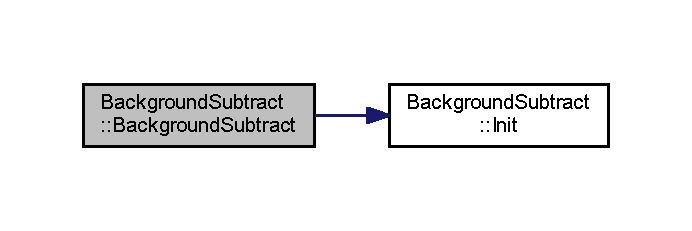
\includegraphics[width=332pt]{class_background_subtract_a0b5096a3823c7af66b6d22cdd36e8fda_cgraph}
\end{center}
\end{figure}
\mbox{\Hypertarget{class_background_subtract_ac811f4c717052b81d1e0bd633d265423}\label{class_background_subtract_ac811f4c717052b81d1e0bd633d265423}} 
\index{Background\+Subtract@{Background\+Subtract}!````~Background\+Subtract@{$\sim$\+Background\+Subtract}}
\index{````~Background\+Subtract@{$\sim$\+Background\+Subtract}!Background\+Subtract@{Background\+Subtract}}
\subsubsection{\texorpdfstring{$\sim$\+Background\+Subtract()}{~BackgroundSubtract()}}
{\footnotesize\ttfamily Background\+Subtract\+::$\sim$\+Background\+Subtract (\begin{DoxyParamCaption}{ }\end{DoxyParamCaption})}



Definition at line 19 of file Background\+Subtract.\+cpp.


\begin{DoxyCode}
20 \{
21 \}
\end{DoxyCode}


\subsection{Member Function Documentation}
\mbox{\Hypertarget{class_background_subtract_a9dacb4cc5cf41c4a37cc776a8142aecc}\label{class_background_subtract_a9dacb4cc5cf41c4a37cc776a8142aecc}} 
\index{Background\+Subtract@{Background\+Subtract}!Init@{Init}}
\index{Init@{Init}!Background\+Subtract@{Background\+Subtract}}
\subsubsection{\texorpdfstring{Init()}{Init()}}
{\footnotesize\ttfamily bool Background\+Subtract\+::\+Init (\begin{DoxyParamCaption}\item[{const \mbox{\hyperlink{defines_8h_a81d657237a541d02f8eeefdd40191920}{config\+\_\+t}} \&}]{config }\end{DoxyParamCaption})}



Definition at line 26 of file Background\+Subtract.\+cpp.


\begin{DoxyCode}
27 \{
28     \textcolor{keywordtype}{bool} failed = \textcolor{keyword}{true};
29     \textcolor{keywordflow}{for} (; failed;)
30     \{
31         failed = \textcolor{keyword}{false};
32 
33         \textcolor{keywordflow}{switch} (\mbox{\hyperlink{class_background_subtract_a3d569052b6954fa87f04a0aa8a970f97}{m\_algType}})
34         \{
35         \textcolor{keywordflow}{case} \mbox{\hyperlink{class_background_subtract_a56850081696df68b55f87b4f3d87949fa1905f812773a0029b59688e57990f172}{ALG\_VIBE}}:
36         \{
37             std::vector<std::string> paramsConf = \{ \textcolor{stringliteral}{"samples"}, \textcolor{stringliteral}{"pixelNeighbor"}, \textcolor{stringliteral}{"distanceThreshold"}, \textcolor{stringliteral}{"
      matchingThreshold"}, \textcolor{stringliteral}{"updateFactor"} \};
38             std::vector<int> params = \{ 20, 1, 20, 3, 16 \};
39             assert(paramsConf.size() == params.size());
40 
41             \textcolor{keywordflow}{for} (\textcolor{keywordtype}{size\_t} i = 0; i < paramsConf.size(); ++i)
42             \{
43                 \textcolor{keyword}{auto} conf = config.find(paramsConf[i]);
44                 \textcolor{keywordflow}{if} (conf != config.end())
45                 \{
46                     params[i] = std::stoi(conf->second);
47                 \}
48             \}
49 
50             \mbox{\hyperlink{class_background_subtract_a57c251abeed9a2c73a3c97d0f7f8b527}{m\_modelVibe}} = std::make\_unique<vibe::VIBE>(\mbox{\hyperlink{class_background_subtract_a676897a571788e0fee84d568bc68caf0}{m\_channels}}, params[0], params[1
      ], params[2], params[3], params[4]);
51             \textcolor{keywordflow}{break};
52         \}
53 
54 \textcolor{preprocessor}{#ifdef USE\_OCV\_BGFG}
55         \textcolor{keywordflow}{case} \mbox{\hyperlink{class_background_subtract_a56850081696df68b55f87b4f3d87949fa6ce3f5db7dc79642df7c113be3a28d14}{ALG\_MOG}}:
56         \{
57             std::vector<std::string> paramsConf = \{ \textcolor{stringliteral}{"history"}, \textcolor{stringliteral}{"nmixtures"}, \textcolor{stringliteral}{"backgroundRatio"}, \textcolor{stringliteral}{"noiseSigma"}
       \};
58             \textcolor{keyword}{auto} params = std::make\_tuple(100, 3, 0.7, 0);
59 
60             \textcolor{keywordflow}{for} (\textcolor{keywordtype}{size\_t} i = 0; i < paramsConf.size(); ++i)
61             \{
62                 \textcolor{keyword}{auto} conf = config.find(paramsConf[i]);
63                 \textcolor{keywordflow}{if} (conf != config.end())
64                 \{
65                     std::stringstream ss(conf->second);
66 
67                     \textcolor{keywordflow}{switch} (i)
68                     \{
69                     \textcolor{keywordflow}{case} 0:
70                         ss >> std::get<0>(params);
71                         \textcolor{keywordflow}{break};
72                     \textcolor{keywordflow}{case} 1:
73                         ss >> std::get<1>(params);
74                         \textcolor{keywordflow}{break};
75                     \textcolor{keywordflow}{case} 2:
76                         ss >> std::get<2>(params);
77                         \textcolor{keywordflow}{break};
78                     \textcolor{keywordflow}{case} 3:
79                         ss >> std::get<3>(params);
80                         \textcolor{keywordflow}{break};
81                     \}
82                 \}
83             \}
84 
85             \mbox{\hyperlink{class_background_subtract_a80782a38138a430437095f625603e599}{m\_modelOCV}} = cv::bgsegm::createBackgroundSubtractorMOG(std::get<0>(params), 
      std::get<1>(params), std::get<2>(params), std::get<3>(params));
86             \textcolor{keywordflow}{break};
87         \}
88 
89         \textcolor{keywordflow}{case} \mbox{\hyperlink{class_background_subtract_a56850081696df68b55f87b4f3d87949fa3d46f57cfb0a9b1b5b037b387a35f652}{ALG\_GMG}}:
90         \{
91             std::vector<std::string> paramsConf = \{ \textcolor{stringliteral}{"initializationFrames"}, \textcolor{stringliteral}{"decisionThreshold"} \};
92             \textcolor{keyword}{auto} params = std::make\_tuple(50, 0.7);
93 
94             \textcolor{keywordflow}{for} (\textcolor{keywordtype}{size\_t} i = 0; i < paramsConf.size(); ++i)
95             \{
96                 \textcolor{keyword}{auto} conf = config.find(paramsConf[i]);
97                 \textcolor{keywordflow}{if} (conf != config.end())
98                 \{
99                     std::stringstream ss(conf->second);
100 
101                     \textcolor{keywordflow}{switch} (i)
102                     \{
103                     \textcolor{keywordflow}{case} 0:
104                         ss >> std::get<0>(params);
105                         \textcolor{keywordflow}{break};
106                     \textcolor{keywordflow}{case} 1:
107                         ss >> std::get<1>(params);
108                         \textcolor{keywordflow}{break};
109                     \}
110                 \}
111             \}
112 
113             \mbox{\hyperlink{class_background_subtract_a80782a38138a430437095f625603e599}{m\_modelOCV}} = cv::bgsegm::createBackgroundSubtractorGMG(std::get<0>(params), 
      std::get<1>(params));
114             \textcolor{keywordflow}{break};
115         \}
116 
117         \textcolor{keywordflow}{case} \mbox{\hyperlink{class_background_subtract_a56850081696df68b55f87b4f3d87949fa4e734ae21b8add9022427f8da9469cfb}{ALG\_CNT}}:
118         \{
119 \textcolor{preprocessor}{#if (((CV\_VERSION\_MAJOR == 3) && (CV\_VERSION\_MINOR >= 2)) || (CV\_VERSION\_MAJOR > 3))}
120             std::vector<std::string> paramsConf = \{ \textcolor{stringliteral}{"minPixelStability"}, \textcolor{stringliteral}{"useHistory"}, \textcolor{stringliteral}{"maxPixelStability"},
       \textcolor{stringliteral}{"isParallel"} \};
121             \textcolor{keyword}{auto} params = std::make\_tuple(15, 1, 15 * 60, 1);
122 
123             \textcolor{keywordflow}{for} (\textcolor{keywordtype}{size\_t} i = 0; i < paramsConf.size(); ++i)
124             \{
125                 \textcolor{keyword}{auto} conf = config.find(paramsConf[i]);
126                 \textcolor{keywordflow}{if} (conf != config.end())
127                 \{
128                     std::stringstream ss(conf->second);
129 
130                     \textcolor{keywordflow}{switch} (i)
131                     \{
132                     \textcolor{keywordflow}{case} 0:
133                         ss >> std::get<0>(params);
134                         \textcolor{keywordflow}{break};
135                     \textcolor{keywordflow}{case} 1:
136                         ss >> std::get<1>(params);
137                         \textcolor{keywordflow}{break};
138                     \textcolor{keywordflow}{case} 2:
139                         ss >> std::get<2>(params);
140                         \textcolor{keywordflow}{break};
141                     \textcolor{keywordflow}{case} 3:
142                         ss >> std::get<3>(params);
143                         \textcolor{keywordflow}{break};
144                     \}
145                 \}
146             \}
147 
148             \mbox{\hyperlink{class_background_subtract_a80782a38138a430437095f625603e599}{m\_modelOCV}} = cv::bgsegm::createBackgroundSubtractorCNT(std::get<0>(params), 
      std::get<1>(params) != 0, std::get<2>(params), std::get<3>(params) != 0);
149 \textcolor{preprocessor}{#else}
150             std::cerr << \textcolor{stringliteral}{"OpenCV CNT algorithm is not implemented! Used Vibe by default."} << std::endl;
151             failed = \textcolor{keyword}{true};
152 \textcolor{preprocessor}{#endif}
153             \textcolor{keywordflow}{break};
154         \}
155 
156 \textcolor{preprocessor}{#else}
157         \textcolor{keywordflow}{case} \mbox{\hyperlink{class_background_subtract_a56850081696df68b55f87b4f3d87949fa6ce3f5db7dc79642df7c113be3a28d14}{ALG\_MOG}}:
158         \textcolor{keywordflow}{case} \mbox{\hyperlink{class_background_subtract_a56850081696df68b55f87b4f3d87949fa3d46f57cfb0a9b1b5b037b387a35f652}{ALG\_GMG}}:
159         \textcolor{keywordflow}{case} \mbox{\hyperlink{class_background_subtract_a56850081696df68b55f87b4f3d87949fa4e734ae21b8add9022427f8da9469cfb}{ALG\_CNT}}:
160             std::cerr << \textcolor{stringliteral}{"OpenCV bgfg algorithms are not implemented! Used Vibe by default."} << std::endl;
161             failed = \textcolor{keyword}{true};
162             \textcolor{keywordflow}{break};
163 \textcolor{preprocessor}{#endif}
164 
165         \textcolor{keywordflow}{case} \mbox{\hyperlink{class_background_subtract_a56850081696df68b55f87b4f3d87949fa0a4e184ec94bca58e58dd4226f1b1f7f}{ALG\_SuBSENSE}}:
166             \mbox{\hyperlink{class_background_subtract_a56275963c8cacca97b97d0cde884f4c1}{m\_modelSuBSENSE}} = std::make\_unique<BackgroundSubtractorSuBSENSE>(); \textcolor{comment}{// default
       params}
167             \textcolor{keywordflow}{break};
168 
169         \textcolor{keywordflow}{case} \mbox{\hyperlink{class_background_subtract_a56850081696df68b55f87b4f3d87949fae4cc76d1ae01949bc7e6be6ed046ddaf}{ALG\_LOBSTER}}:
170             \mbox{\hyperlink{class_background_subtract_a56275963c8cacca97b97d0cde884f4c1}{m\_modelSuBSENSE}} = std::make\_unique<BackgroundSubtractorLOBSTER>();  \textcolor{comment}{// default
       params}
171             \textcolor{keywordflow}{break};
172 
173         \textcolor{keywordflow}{case} \mbox{\hyperlink{class_background_subtract_a56850081696df68b55f87b4f3d87949fa35994e745da8eb824d3808ee50ad3ebf}{ALG\_MOG2}}:
174         \{
175             std::vector<std::string> paramsConf = \{ \textcolor{stringliteral}{"history"}, \textcolor{stringliteral}{"varThreshold"}, \textcolor{stringliteral}{"detectShadows"} \};
176             \textcolor{keyword}{auto} params = std::make\_tuple(500, 16, 1);
177 
178             \textcolor{keywordflow}{for} (\textcolor{keywordtype}{size\_t} i = 0; i < paramsConf.size(); ++i)
179             \{
180                 \textcolor{keyword}{auto} conf = config.find(paramsConf[i]);
181                 \textcolor{keywordflow}{if} (conf != config.end())
182                 \{
183                     std::stringstream ss(conf->second);
184 
185                     \textcolor{keywordflow}{switch} (i)
186                     \{
187                     \textcolor{keywordflow}{case} 0:
188                         ss >> std::get<0>(params);
189                         \textcolor{keywordflow}{break};
190                     \textcolor{keywordflow}{case} 1:
191                         ss >> std::get<1>(params);
192                         \textcolor{keywordflow}{break};
193                     \textcolor{keywordflow}{case} 2:
194                         ss >> std::get<2>(params);
195                         \textcolor{keywordflow}{break};
196                     \}
197                 \}
198             \}
199 
200             \mbox{\hyperlink{class_background_subtract_a80782a38138a430437095f625603e599}{m\_modelOCV}} = cv::createBackgroundSubtractorMOG2(std::get<0>(params), std::get<1>(
      params), std::get<2>(params) != 0).dynamicCast<cv::BackgroundSubtractor>();
201             \textcolor{keywordflow}{break};
202         \}
203 
204         \textcolor{keywordflow}{default}:
205         \{
206             \mbox{\hyperlink{class_background_subtract_a3d569052b6954fa87f04a0aa8a970f97}{m\_algType}} = \mbox{\hyperlink{class_background_subtract_a56850081696df68b55f87b4f3d87949fa1905f812773a0029b59688e57990f172}{ALG\_VIBE}};
207             failed = \textcolor{keyword}{false};
208             \textcolor{keywordflow}{break};
209         \}
210         \}
211         \textcolor{keywordflow}{if} (failed)
212         \{
213             \mbox{\hyperlink{class_background_subtract_a3d569052b6954fa87f04a0aa8a970f97}{m\_algType}} = \mbox{\hyperlink{class_background_subtract_a56850081696df68b55f87b4f3d87949fa1905f812773a0029b59688e57990f172}{ALG\_VIBE}};
214             failed = \textcolor{keyword}{false};
215         \}
216     \}
217     \textcolor{keywordflow}{return} !failed;
218 \}
\end{DoxyCode}
Here is the caller graph for this function\+:\nopagebreak
\begin{figure}[H]
\begin{center}
\leavevmode
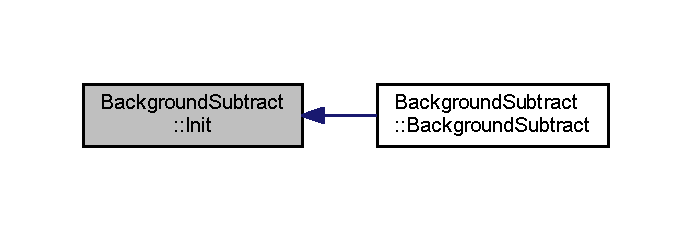
\includegraphics[width=332pt]{class_background_subtract_a9dacb4cc5cf41c4a37cc776a8142aecc_icgraph}
\end{center}
\end{figure}
\mbox{\Hypertarget{class_background_subtract_a1cd989730164da1c2523975d2ed32147}\label{class_background_subtract_a1cd989730164da1c2523975d2ed32147}} 
\index{Background\+Subtract@{Background\+Subtract}!Subtract@{Subtract}}
\index{Subtract@{Subtract}!Background\+Subtract@{Background\+Subtract}}
\subsubsection{\texorpdfstring{Subtract()}{Subtract()}}
{\footnotesize\ttfamily void Background\+Subtract\+::\+Subtract (\begin{DoxyParamCaption}\item[{const cv\+::\+U\+Mat \&}]{image,  }\item[{cv\+::\+U\+Mat \&}]{foreground }\end{DoxyParamCaption})}



Definition at line 223 of file Background\+Subtract.\+cpp.


\begin{DoxyCode}
224 \{
225     \textcolor{keyword}{auto} GetImg = [&]() -> cv::UMat
226     \{
227             \textcolor{keywordflow}{if} (image.channels() != \mbox{\hyperlink{class_background_subtract_a676897a571788e0fee84d568bc68caf0}{m\_channels}})
228     \{
229             \textcolor{keywordflow}{if} (image.channels() == 1)
230     \{
231             cv::UMat newImg;
232 \textcolor{preprocessor}{        #if (CV\_VERSION\_MAJOR < 4)}
233             cv::cvtColor(image, newImg, CV\_GRAY2BGR);
234 \textcolor{preprocessor}{        #else}
235             cv::cvtColor(image, newImg, cv::COLOR\_GRAY2BGR);
236 \textcolor{preprocessor}{        #endif}
237             \textcolor{keywordflow}{return} newImg;
238 \}
239             \textcolor{keywordflow}{else} \textcolor{keywordflow}{if} (image.channels() == 3)
240     \{
241             cv::UMat newImg;
242 \textcolor{preprocessor}{        #if (CV\_VERSION\_MAJOR < 4)}
243             cv::cvtColor(image, newImg, CV\_BGR2GRAY);
244 \textcolor{preprocessor}{        #else}
245             cv::cvtColor(image, newImg, cv::COLOR\_BGR2GRAY);
246 \textcolor{preprocessor}{        #endif}
247             \textcolor{keywordflow}{return} newImg;
248 \}
249 \}
250             \textcolor{keywordflow}{return} image;
251 \};
252 
253     \textcolor{keywordflow}{switch} (\mbox{\hyperlink{class_background_subtract_a3d569052b6954fa87f04a0aa8a970f97}{m\_algType}})
254     \{
255     \textcolor{keywordflow}{case} \mbox{\hyperlink{class_background_subtract_a56850081696df68b55f87b4f3d87949fa1905f812773a0029b59688e57990f172}{ALG\_VIBE}}:
256         \mbox{\hyperlink{class_background_subtract_a57c251abeed9a2c73a3c97d0f7f8b527}{m\_modelVibe}}->update(GetImg().getMat(cv::ACCESS\_READ));
257         foreground = \mbox{\hyperlink{class_background_subtract_a57c251abeed9a2c73a3c97d0f7f8b527}{m\_modelVibe}}->getMask().getUMat(cv::ACCESS\_READ);
258         \textcolor{keywordflow}{break};
259 
260     \textcolor{keywordflow}{case} \mbox{\hyperlink{class_background_subtract_a56850081696df68b55f87b4f3d87949fa6ce3f5db7dc79642df7c113be3a28d14}{ALG\_MOG}}:
261     \textcolor{keywordflow}{case} \mbox{\hyperlink{class_background_subtract_a56850081696df68b55f87b4f3d87949fa3d46f57cfb0a9b1b5b037b387a35f652}{ALG\_GMG}}:
262     \textcolor{keywordflow}{case} \mbox{\hyperlink{class_background_subtract_a56850081696df68b55f87b4f3d87949fa4e734ae21b8add9022427f8da9469cfb}{ALG\_CNT}}:
263 \textcolor{preprocessor}{#ifdef USE\_OCV\_BGFG}
264         \mbox{\hyperlink{class_background_subtract_a80782a38138a430437095f625603e599}{m\_modelOCV}}->apply(GetImg(), foreground);
265         \textcolor{keywordflow}{break};
266 \textcolor{preprocessor}{#else}
267         std::cerr << \textcolor{stringliteral}{"OpenCV bgfg algorithms are not implemented!"} << std::endl;
268         \textcolor{keywordflow}{break};
269 \textcolor{preprocessor}{#endif}
270 
271     \textcolor{keywordflow}{case} \mbox{\hyperlink{class_background_subtract_a56850081696df68b55f87b4f3d87949fa0a4e184ec94bca58e58dd4226f1b1f7f}{ALG\_SuBSENSE}}:
272     \textcolor{keywordflow}{case} \mbox{\hyperlink{class_background_subtract_a56850081696df68b55f87b4f3d87949fae4cc76d1ae01949bc7e6be6ed046ddaf}{ALG\_LOBSTER}}:
273         \textcolor{keywordflow}{if} (foreground.size() != image.size())
274         \{
275             \mbox{\hyperlink{class_background_subtract_a56275963c8cacca97b97d0cde884f4c1}{m\_modelSuBSENSE}}->initialize(GetImg().getMat(cv::ACCESS\_READ), cv::Mat());
276             foreground.create(image.size(), CV\_8UC1);
277         \}
278         \textcolor{keywordflow}{else}
279         \{
280             \mbox{\hyperlink{class_background_subtract_a56275963c8cacca97b97d0cde884f4c1}{m\_modelSuBSENSE}}->apply(GetImg(), foreground);
281         \}
282         \textcolor{keywordflow}{break};
283 
284     \textcolor{keywordflow}{case} \mbox{\hyperlink{class_background_subtract_a56850081696df68b55f87b4f3d87949fa35994e745da8eb824d3808ee50ad3ebf}{ALG\_MOG2}}:
285         \mbox{\hyperlink{class_background_subtract_a80782a38138a430437095f625603e599}{m\_modelOCV}}->apply(GetImg(), foreground);
286         cv::threshold(foreground, foreground, 200, 255, cv::THRESH\_BINARY);
287         \textcolor{keywordflow}{break};
288 
289     \textcolor{keywordflow}{default}:
290         \mbox{\hyperlink{class_background_subtract_a57c251abeed9a2c73a3c97d0f7f8b527}{m\_modelVibe}}->update(GetImg().getMat(cv::ACCESS\_READ));
291         foreground = \mbox{\hyperlink{class_background_subtract_a57c251abeed9a2c73a3c97d0f7f8b527}{m\_modelVibe}}->getMask().getUMat(cv::ACCESS\_READ);
292         \textcolor{keywordflow}{break};
293     \}
294 
295     \textcolor{comment}{//cv::imshow("before", foreground);}
296 
297     cv::medianBlur(foreground, foreground, 3);
298 
299     cv::Mat dilateElement = cv::getStructuringElement(cv::MORPH\_RECT, cv::Size(3, 3), cv::Point(-1, -1));
300     cv::dilate(foreground, foreground, dilateElement, cv::Point(-1, -1), 2);
301 
302     \textcolor{comment}{//cv::imshow("after", foreground);}
303 \}
\end{DoxyCode}


\subsection{Member Data Documentation}
\mbox{\Hypertarget{class_background_subtract_a3d569052b6954fa87f04a0aa8a970f97}\label{class_background_subtract_a3d569052b6954fa87f04a0aa8a970f97}} 
\index{Background\+Subtract@{Background\+Subtract}!m\+\_\+alg\+Type@{m\+\_\+alg\+Type}}
\index{m\+\_\+alg\+Type@{m\+\_\+alg\+Type}!Background\+Subtract@{Background\+Subtract}}
\subsubsection{\texorpdfstring{m\+\_\+alg\+Type}{m\_algType}}
{\footnotesize\ttfamily \mbox{\hyperlink{class_background_subtract_a56850081696df68b55f87b4f3d87949f}{B\+G\+F\+G\+\_\+\+A\+L\+GS}} Background\+Subtract\+::m\+\_\+alg\+Type}



Definition at line 37 of file Background\+Subtract.\+h.

\mbox{\Hypertarget{class_background_subtract_a676897a571788e0fee84d568bc68caf0}\label{class_background_subtract_a676897a571788e0fee84d568bc68caf0}} 
\index{Background\+Subtract@{Background\+Subtract}!m\+\_\+channels@{m\+\_\+channels}}
\index{m\+\_\+channels@{m\+\_\+channels}!Background\+Subtract@{Background\+Subtract}}
\subsubsection{\texorpdfstring{m\+\_\+channels}{m\_channels}}
{\footnotesize\ttfamily int Background\+Subtract\+::m\+\_\+channels}



Definition at line 36 of file Background\+Subtract.\+h.

\mbox{\Hypertarget{class_background_subtract_a80782a38138a430437095f625603e599}\label{class_background_subtract_a80782a38138a430437095f625603e599}} 
\index{Background\+Subtract@{Background\+Subtract}!m\+\_\+model\+O\+CV@{m\+\_\+model\+O\+CV}}
\index{m\+\_\+model\+O\+CV@{m\+\_\+model\+O\+CV}!Background\+Subtract@{Background\+Subtract}}
\subsubsection{\texorpdfstring{m\+\_\+model\+O\+CV}{m\_modelOCV}}
{\footnotesize\ttfamily cv\+::\+Ptr$<$cv\+::\+Background\+Subtractor$>$ Background\+Subtract\+::m\+\_\+model\+O\+CV\hspace{0.3cm}{\ttfamily [private]}}



Definition at line 41 of file Background\+Subtract.\+h.

\mbox{\Hypertarget{class_background_subtract_a56275963c8cacca97b97d0cde884f4c1}\label{class_background_subtract_a56275963c8cacca97b97d0cde884f4c1}} 
\index{Background\+Subtract@{Background\+Subtract}!m\+\_\+model\+Su\+B\+S\+E\+N\+SE@{m\+\_\+model\+Su\+B\+S\+E\+N\+SE}}
\index{m\+\_\+model\+Su\+B\+S\+E\+N\+SE@{m\+\_\+model\+Su\+B\+S\+E\+N\+SE}!Background\+Subtract@{Background\+Subtract}}
\subsubsection{\texorpdfstring{m\+\_\+model\+Su\+B\+S\+E\+N\+SE}{m\_modelSuBSENSE}}
{\footnotesize\ttfamily std\+::unique\+\_\+ptr$<$\mbox{\hyperlink{class_background_subtractor_l_b_s_p}{Background\+Subtractor\+L\+B\+SP}}$>$ Background\+Subtract\+::m\+\_\+model\+Su\+B\+S\+E\+N\+SE\hspace{0.3cm}{\ttfamily [private]}}



Definition at line 42 of file Background\+Subtract.\+h.

\mbox{\Hypertarget{class_background_subtract_a57c251abeed9a2c73a3c97d0f7f8b527}\label{class_background_subtract_a57c251abeed9a2c73a3c97d0f7f8b527}} 
\index{Background\+Subtract@{Background\+Subtract}!m\+\_\+model\+Vibe@{m\+\_\+model\+Vibe}}
\index{m\+\_\+model\+Vibe@{m\+\_\+model\+Vibe}!Background\+Subtract@{Background\+Subtract}}
\subsubsection{\texorpdfstring{m\+\_\+model\+Vibe}{m\_modelVibe}}
{\footnotesize\ttfamily std\+::unique\+\_\+ptr$<$\mbox{\hyperlink{classvibe_1_1_v_i_b_e}{vibe\+::\+V\+I\+BE}}$>$ Background\+Subtract\+::m\+\_\+model\+Vibe\hspace{0.3cm}{\ttfamily [private]}}



Definition at line 40 of file Background\+Subtract.\+h.



The documentation for this class was generated from the following files\+:\begin{DoxyCompactItemize}
\item 
D\+:/\+Roy/\+Git\+Hub/\+Multitarget-\/tracker/\+Detector/\mbox{\hyperlink{_background_subtract_8h}{Background\+Subtract.\+h}}\item 
D\+:/\+Roy/\+Git\+Hub/\+Multitarget-\/tracker/\+Detector/\mbox{\hyperlink{_background_subtract_8cpp}{Background\+Subtract.\+cpp}}\end{DoxyCompactItemize}

\hypertarget{class_background_subtractor_l_b_s_p}{}\section{Background\+Subtractor\+L\+B\+SP Class Reference}
\label{class_background_subtractor_l_b_s_p}\index{Background\+Subtractor\+L\+B\+SP@{Background\+Subtractor\+L\+B\+SP}}


{\ttfamily \#include $<$Background\+Subtractor\+L\+B\+S\+P.\+h$>$}



Inheritance diagram for Background\+Subtractor\+L\+B\+SP\+:\nopagebreak
\begin{figure}[H]
\begin{center}
\leavevmode
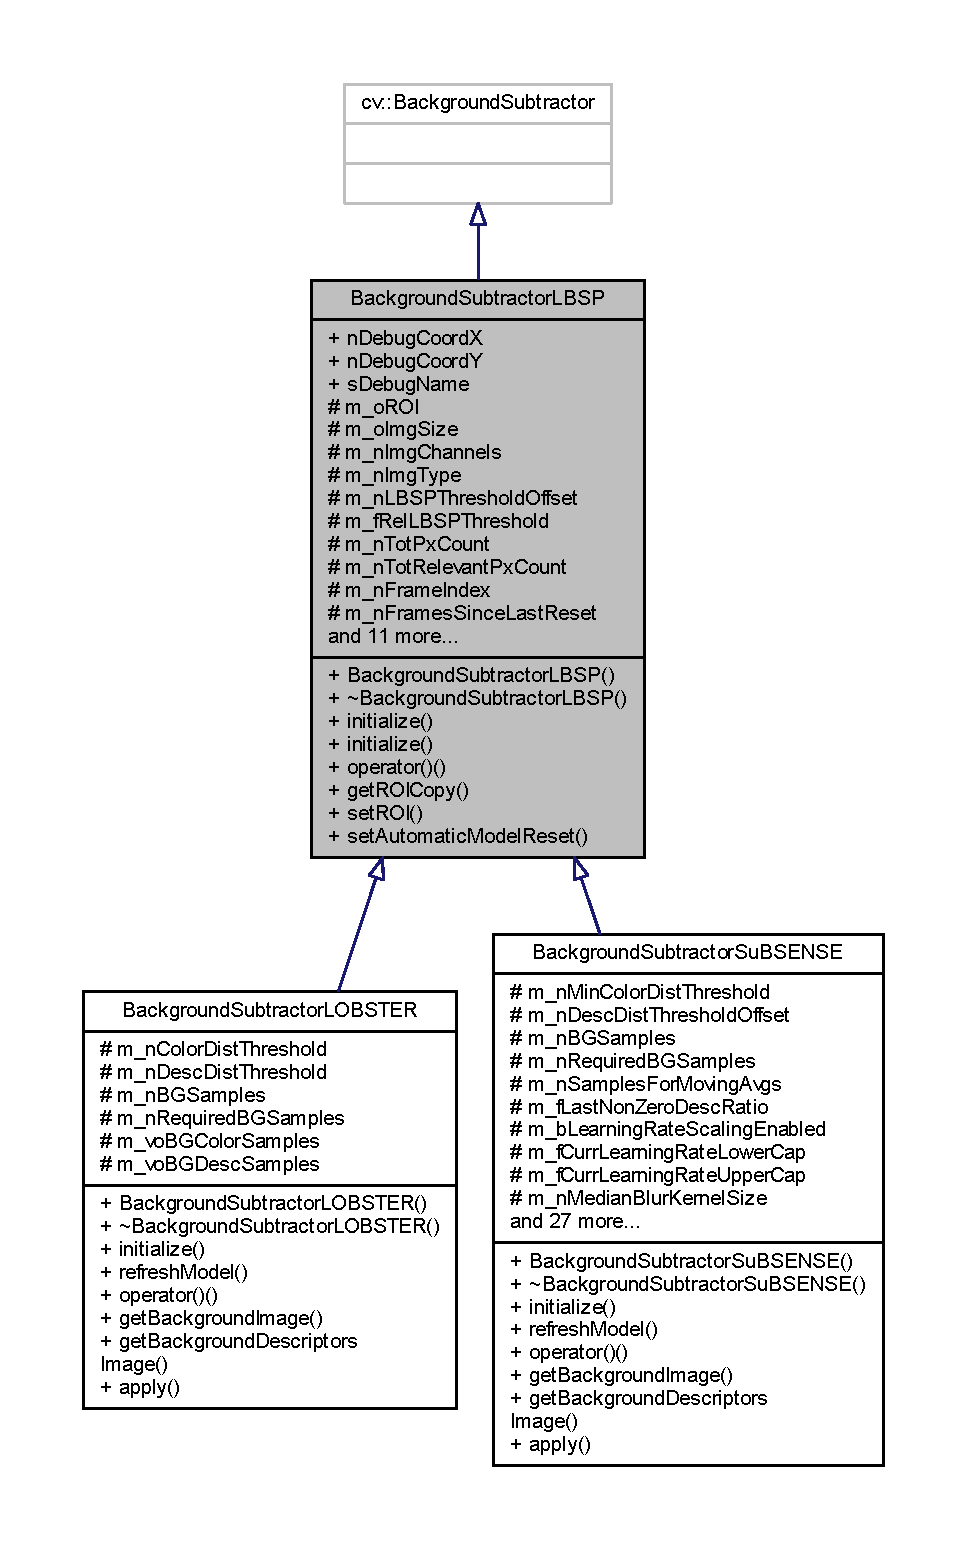
\includegraphics[height=550pt]{class_background_subtractor_l_b_s_p__inherit__graph}
\end{center}
\end{figure}


Collaboration diagram for Background\+Subtractor\+L\+B\+SP\+:\nopagebreak
\begin{figure}[H]
\begin{center}
\leavevmode
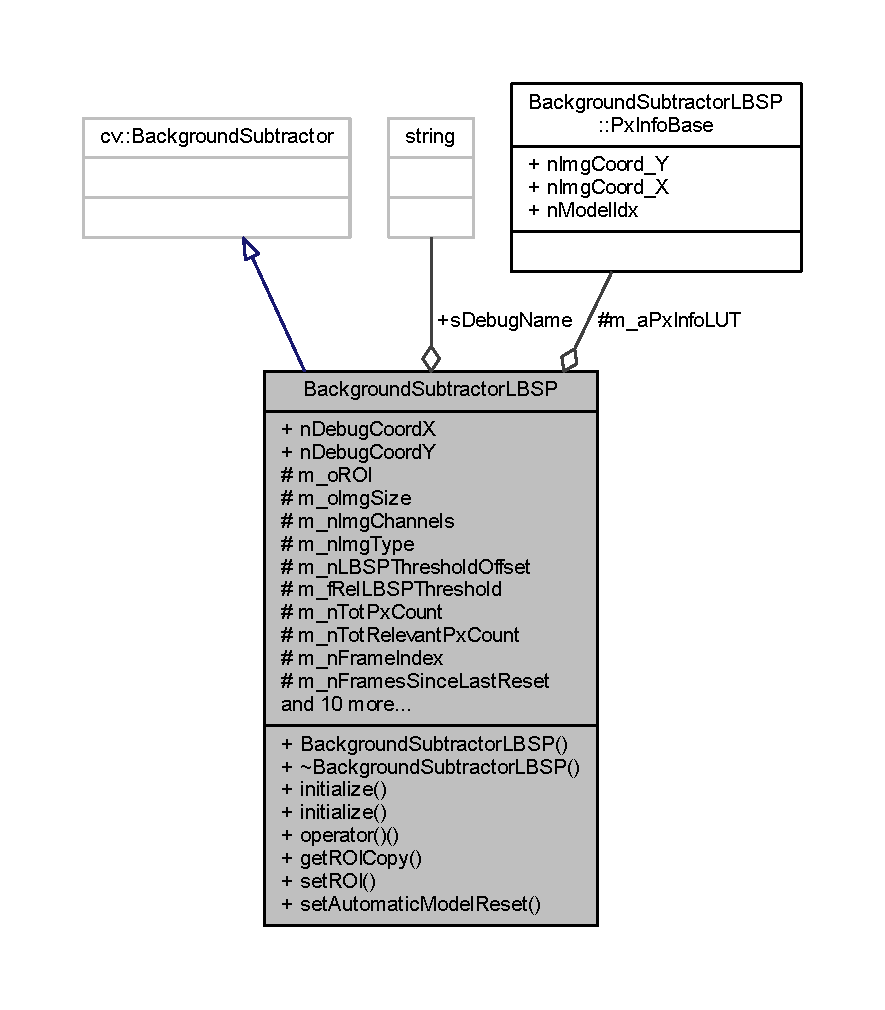
\includegraphics[width=350pt]{class_background_subtractor_l_b_s_p__coll__graph}
\end{center}
\end{figure}
\subsection*{Classes}
\begin{DoxyCompactItemize}
\item 
struct \mbox{\hyperlink{struct_background_subtractor_l_b_s_p_1_1_px_info_base}{Px\+Info\+Base}}
\end{DoxyCompactItemize}
\subsection*{Public Member Functions}
\begin{DoxyCompactItemize}
\item 
\mbox{\hyperlink{class_background_subtractor_l_b_s_p_a5f7f42ea5c9697479cbe237b49ca6ae9}{Background\+Subtractor\+L\+B\+SP}} (float f\+Rel\+L\+B\+S\+P\+Threshold, size\+\_\+t n\+L\+B\+S\+P\+Threshold\+Offset=0)
\begin{DoxyCompactList}\small\item\em full constructor \end{DoxyCompactList}\item 
virtual \mbox{\hyperlink{class_background_subtractor_l_b_s_p_a027bdf387b28e5532d78b5bf4e7c08eb}{$\sim$\+Background\+Subtractor\+L\+B\+SP}} ()
\begin{DoxyCompactList}\small\item\em default destructor \end{DoxyCompactList}\item 
virtual void \mbox{\hyperlink{class_background_subtractor_l_b_s_p_ac6b854f94414497b143375d4a0ae8b6f}{initialize}} (const cv\+::\+Mat \&o\+Init\+Img)
\begin{DoxyCompactList}\small\item\em (re)initiaization method; needs to be called before starting background subtraction \end{DoxyCompactList}\item 
virtual void \mbox{\hyperlink{class_background_subtractor_l_b_s_p_a3644bc10ec3beda6fad22c633fe0f8fb}{initialize}} (const cv\+::\+Mat \&o\+Init\+Img, const cv\+::\+Mat \&o\+R\+OI)=0
\begin{DoxyCompactList}\small\item\em (re)initiaization method; needs to be called before starting background subtraction \end{DoxyCompactList}\item 
virtual void \mbox{\hyperlink{class_background_subtractor_l_b_s_p_a4771cac59b7ac865d6ec25cbf049948e}{operator()}} (cv\+::\+Input\+Array image, cv\+::\+Output\+Array fgmask, double learning\+Rate=0)=0
\begin{DoxyCompactList}\small\item\em primary model update function; the learning param is used to override the internal learning speed (ignored when $<$= 0) \end{DoxyCompactList}\item 
virtual cv\+::\+Mat \mbox{\hyperlink{class_background_subtractor_l_b_s_p_a9843f87f8adcd0e85274303f9210b883}{get\+R\+O\+I\+Copy}} () const
\begin{DoxyCompactList}\small\item\em unused, always returns nullptr \end{DoxyCompactList}\item 
virtual void \mbox{\hyperlink{class_background_subtractor_l_b_s_p_a34dc38d3d925d46d289c750786f232dc}{set\+R\+OI}} (cv\+::\+Mat \&o\+R\+OI)
\begin{DoxyCompactList}\small\item\em sets the R\+OI to be used for descriptor extraction (note\+: this function will reinit the model and return the usable R\+OI) \end{DoxyCompactList}\item 
void \mbox{\hyperlink{class_background_subtractor_l_b_s_p_a31b8474f8b4ffa6ef08ec682cfcef9b0}{set\+Automatic\+Model\+Reset}} (bool)
\begin{DoxyCompactList}\small\item\em turns automatic model reset on or off \end{DoxyCompactList}\end{DoxyCompactItemize}
\subsection*{Public Attributes}
\begin{DoxyCompactItemize}
\item 
int \mbox{\hyperlink{class_background_subtractor_l_b_s_p_a49771cd7b2c8354cde3da6e593d3febe}{n\+Debug\+CoordX}}
\item 
int \mbox{\hyperlink{class_background_subtractor_l_b_s_p_a8e1451fd90eb4459aa84ea5e7133268a}{n\+Debug\+CoordY}}
\item 
std\+::string \mbox{\hyperlink{class_background_subtractor_l_b_s_p_ada55b4a5eec8c82d0e05b0f9f1600ecb}{s\+Debug\+Name}}
\end{DoxyCompactItemize}
\subsection*{Protected Attributes}
\begin{DoxyCompactItemize}
\item 
cv\+::\+Mat \mbox{\hyperlink{class_background_subtractor_l_b_s_p_a53fe98bd2489d95de5292467145901e9}{m\+\_\+o\+R\+OI}}
\begin{DoxyCompactList}\small\item\em background model R\+OI used for \mbox{\hyperlink{class_l_b_s_p}{L\+B\+SP}} descriptor extraction (specific to the input image size) \end{DoxyCompactList}\item 
cv\+::\+Size \mbox{\hyperlink{class_background_subtractor_l_b_s_p_a732d5e6ae35fb0e858cadb3af5ce08a2}{m\+\_\+o\+Img\+Size}}
\begin{DoxyCompactList}\small\item\em input image size \end{DoxyCompactList}\item 
size\+\_\+t \mbox{\hyperlink{class_background_subtractor_l_b_s_p_ab3467ebee2c5d1249061ccd704cc0584}{m\+\_\+n\+Img\+Channels}}
\begin{DoxyCompactList}\small\item\em input image channel size \end{DoxyCompactList}\item 
int \mbox{\hyperlink{class_background_subtractor_l_b_s_p_a7d2f52ecd5ff56e42da86f97e0ad93b5}{m\+\_\+n\+Img\+Type}}
\begin{DoxyCompactList}\small\item\em input image type \end{DoxyCompactList}\item 
const size\+\_\+t \mbox{\hyperlink{class_background_subtractor_l_b_s_p_a209eb6aaa34e8ad8e565e79f85404e24}{m\+\_\+n\+L\+B\+S\+P\+Threshold\+Offset}}
\begin{DoxyCompactList}\small\item\em \mbox{\hyperlink{class_l_b_s_p}{L\+B\+SP}} internal threshold offset value, used to reduce texture noise in dark regions. \end{DoxyCompactList}\item 
const float \mbox{\hyperlink{class_background_subtractor_l_b_s_p_ad759c645b14e9b16bf3940cae862df32}{m\+\_\+f\+Rel\+L\+B\+S\+P\+Threshold}}
\begin{DoxyCompactList}\small\item\em \mbox{\hyperlink{class_l_b_s_p}{L\+B\+SP}} relative internal threshold (kept here since we don\textquotesingle{}t keep an \mbox{\hyperlink{class_l_b_s_p}{L\+B\+SP}} object) \end{DoxyCompactList}\item 
size\+\_\+t \mbox{\hyperlink{class_background_subtractor_l_b_s_p_a9d1e247267afbddb7032bdcabd67d931}{m\+\_\+n\+Tot\+Px\+Count}}
\begin{DoxyCompactList}\small\item\em total number of pixels (depends on the input frame size) \& total number of relevant pixels \end{DoxyCompactList}\item 
size\+\_\+t \mbox{\hyperlink{class_background_subtractor_l_b_s_p_ac3b54f4d2dfa3a576475214f26501d85}{m\+\_\+n\+Tot\+Relevant\+Px\+Count}}
\item 
size\+\_\+t \mbox{\hyperlink{class_background_subtractor_l_b_s_p_a8a2350cad84f19c68ef61b7aaf91c43f}{m\+\_\+n\+Frame\+Index}}
\begin{DoxyCompactList}\small\item\em current frame index, frame count since last model reset \& model reset cooldown counters \end{DoxyCompactList}\item 
size\+\_\+t \mbox{\hyperlink{class_background_subtractor_l_b_s_p_ab56bf775dfdf0579e834e45210c3a92a}{m\+\_\+n\+Frames\+Since\+Last\+Reset}}
\item 
size\+\_\+t \mbox{\hyperlink{class_background_subtractor_l_b_s_p_a5ea18d388afacf8285c46ba0f754e7ee}{m\+\_\+n\+Model\+Reset\+Cooldown}}
\item 
size\+\_\+t \mbox{\hyperlink{class_background_subtractor_l_b_s_p_aefe69d94f08b2c4ba73ad1d254ad9153}{m\+\_\+an\+L\+B\+S\+P\+Threshold\+\_\+8bit\+L\+UT}} \mbox{[}U\+C\+H\+A\+R\+\_\+\+M\+AX+1\mbox{]}
\begin{DoxyCompactList}\small\item\em pre-\/allocated internal \mbox{\hyperlink{class_l_b_s_p}{L\+B\+SP}} threshold values L\+UT for all possible 8-\/bit intensities \end{DoxyCompactList}\item 
size\+\_\+t $\ast$ \mbox{\hyperlink{class_background_subtractor_l_b_s_p_a06b4f0d3f24fa08bccd3c9eca085713e}{m\+\_\+a\+Px\+Idx\+L\+UT}}
\begin{DoxyCompactList}\small\item\em internal pixel index L\+UT for all relevant analysis regions (based on the provided R\+OI) \end{DoxyCompactList}\item 
\mbox{\hyperlink{struct_background_subtractor_l_b_s_p_1_1_px_info_base}{Px\+Info\+Base}} $\ast$ \mbox{\hyperlink{class_background_subtractor_l_b_s_p_a74e73d4832ccdef652d93756582024db}{m\+\_\+a\+Px\+Info\+L\+UT}}
\begin{DoxyCompactList}\small\item\em internal pixel info L\+UT for all possible pixel indexes \end{DoxyCompactList}\item 
const int \mbox{\hyperlink{class_background_subtractor_l_b_s_p_a2585fe6e41e10af6da3e325dc20fe7f1}{m\+\_\+n\+Default\+Median\+Blur\+Kernel\+Size}}
\begin{DoxyCompactList}\small\item\em default kernel size for median blur post-\/proc filtering \end{DoxyCompactList}\item 
bool \mbox{\hyperlink{class_background_subtractor_l_b_s_p_a55cea104a0924fd50d5bed0912828a7e}{m\+\_\+b\+Initialized}}
\begin{DoxyCompactList}\small\item\em specifies whether the algorithm is fully initialized or not \end{DoxyCompactList}\item 
bool \mbox{\hyperlink{class_background_subtractor_l_b_s_p_a9d260f4e42e3fc79fb21af950ca9087a}{m\+\_\+b\+Auto\+Model\+Reset\+Enabled}}
\begin{DoxyCompactList}\small\item\em specifies whether automatic model resets are enabled or not \end{DoxyCompactList}\item 
bool \mbox{\hyperlink{class_background_subtractor_l_b_s_p_a5b1ec2694ae59661bb146ad0d4d49811}{m\+\_\+b\+Using\+Moving\+Camera}}
\begin{DoxyCompactList}\small\item\em specifies whether the camera is considered moving or not \end{DoxyCompactList}\item 
cv\+::\+Mat \mbox{\hyperlink{class_background_subtractor_l_b_s_p_ab1dc003792ab1d0b881a6fd10e0e29b3}{m\+\_\+o\+Last\+Color\+Frame}}
\begin{DoxyCompactList}\small\item\em copy of latest pixel intensities (used when refreshing model) \end{DoxyCompactList}\item 
cv\+::\+Mat \mbox{\hyperlink{class_background_subtractor_l_b_s_p_a9c637c0b87cac495887295690d83ba13}{m\+\_\+o\+Last\+Desc\+Frame}}
\begin{DoxyCompactList}\small\item\em copy of latest descriptors (used when refreshing model) \end{DoxyCompactList}\item 
cv\+::\+Mat \mbox{\hyperlink{class_background_subtractor_l_b_s_p_adb6dc0af596c5592c91f9d8faa5c8a4b}{m\+\_\+o\+Last\+F\+G\+Mask}}
\begin{DoxyCompactList}\small\item\em the foreground mask generated by the method at \mbox{[}t-\/1\mbox{]} \end{DoxyCompactList}\end{DoxyCompactItemize}


\subsection{Detailed Description}
Local Binary Similarity Pattern (\mbox{\hyperlink{class_l_b_s_p}{L\+B\+SP}})-\/based change detection algorithm (abstract version/base class).

For more details on the different parameters, see P.-\/L. St-\/\+Charles and G.-\/A. Bilodeau, \char`\"{}\+Improving Background
\+Subtraction using Local Binary Similarity Patterns\char`\"{}, in W\+A\+CV 2014, or G.-\/A. Bilodeau et al, \char`\"{}\+Change Detection
in Feature Space Using Local Binary Similarity Patterns\char`\"{}, in C\+RV 2013.

This algorithm is currently N\+OT thread-\/safe. 

Definition at line 15 of file Background\+Subtractor\+L\+B\+S\+P.\+h.



\subsection{Constructor \& Destructor Documentation}
\mbox{\Hypertarget{class_background_subtractor_l_b_s_p_a5f7f42ea5c9697479cbe237b49ca6ae9}\label{class_background_subtractor_l_b_s_p_a5f7f42ea5c9697479cbe237b49ca6ae9}} 
\index{Background\+Subtractor\+L\+B\+SP@{Background\+Subtractor\+L\+B\+SP}!Background\+Subtractor\+L\+B\+SP@{Background\+Subtractor\+L\+B\+SP}}
\index{Background\+Subtractor\+L\+B\+SP@{Background\+Subtractor\+L\+B\+SP}!Background\+Subtractor\+L\+B\+SP@{Background\+Subtractor\+L\+B\+SP}}
\subsubsection{\texorpdfstring{Background\+Subtractor\+L\+B\+S\+P()}{BackgroundSubtractorLBSP()}}
{\footnotesize\ttfamily Background\+Subtractor\+L\+B\+S\+P\+::\+Background\+Subtractor\+L\+B\+SP (\begin{DoxyParamCaption}\item[{float}]{f\+Rel\+L\+B\+S\+P\+Threshold,  }\item[{size\+\_\+t}]{n\+L\+B\+S\+P\+Threshold\+Offset = {\ttfamily 0} }\end{DoxyParamCaption})}



full constructor 



Definition at line 11 of file Background\+Subtractor\+L\+B\+S\+P.\+cpp.


\begin{DoxyCode}
12     :    \mbox{\hyperlink{class_background_subtractor_l_b_s_p_ab3467ebee2c5d1249061ccd704cc0584}{m\_nImgChannels}}(0)
13         ,\mbox{\hyperlink{class_background_subtractor_l_b_s_p_a7d2f52ecd5ff56e42da86f97e0ad93b5}{m\_nImgType}}(0)
14         ,\mbox{\hyperlink{class_background_subtractor_l_b_s_p_a209eb6aaa34e8ad8e565e79f85404e24}{m\_nLBSPThresholdOffset}}(nLBSPThresholdOffset)
15         ,\mbox{\hyperlink{class_background_subtractor_l_b_s_p_ad759c645b14e9b16bf3940cae862df32}{m\_fRelLBSPThreshold}}(fRelLBSPThreshold)
16         ,\mbox{\hyperlink{class_background_subtractor_l_b_s_p_a9d1e247267afbddb7032bdcabd67d931}{m\_nTotPxCount}}(0)
17         ,\mbox{\hyperlink{class_background_subtractor_l_b_s_p_ac3b54f4d2dfa3a576475214f26501d85}{m\_nTotRelevantPxCount}}(0)
18         ,\mbox{\hyperlink{class_background_subtractor_l_b_s_p_a8a2350cad84f19c68ef61b7aaf91c43f}{m\_nFrameIndex}}(SIZE\_MAX)
19         ,\mbox{\hyperlink{class_background_subtractor_l_b_s_p_ab56bf775dfdf0579e834e45210c3a92a}{m\_nFramesSinceLastReset}}(0)
20         ,\mbox{\hyperlink{class_background_subtractor_l_b_s_p_a5ea18d388afacf8285c46ba0f754e7ee}{m\_nModelResetCooldown}}(0)
21         ,\mbox{\hyperlink{class_background_subtractor_l_b_s_p_a06b4f0d3f24fa08bccd3c9eca085713e}{m\_aPxIdxLUT}}(\textcolor{keyword}{nullptr})
22         ,\mbox{\hyperlink{class_background_subtractor_l_b_s_p_a74e73d4832ccdef652d93756582024db}{m\_aPxInfoLUT}}(\textcolor{keyword}{nullptr})
23         ,\mbox{\hyperlink{class_background_subtractor_l_b_s_p_a2585fe6e41e10af6da3e325dc20fe7f1}{m\_nDefaultMedianBlurKernelSize}}(
      \mbox{\hyperlink{_background_subtractor_l_b_s_p_8cpp_a65c2052e888a5df64135f3dea480a74a}{DEFAULT\_MEDIAN\_BLUR\_KERNEL\_SIZE}})
24         ,\mbox{\hyperlink{class_background_subtractor_l_b_s_p_a55cea104a0924fd50d5bed0912828a7e}{m\_bInitialized}}(\textcolor{keyword}{false})
25         ,\mbox{\hyperlink{class_background_subtractor_l_b_s_p_a9d260f4e42e3fc79fb21af950ca9087a}{m\_bAutoModelResetEnabled}}(\textcolor{keyword}{true})
26         ,\mbox{\hyperlink{class_background_subtractor_l_b_s_p_a5b1ec2694ae59661bb146ad0d4d49811}{m\_bUsingMovingCamera}}(\textcolor{keyword}{false})
27         ,\mbox{\hyperlink{class_background_subtractor_l_b_s_p_a49771cd7b2c8354cde3da6e593d3febe}{nDebugCoordX}}(0),\mbox{\hyperlink{class_background_subtractor_l_b_s_p_a8e1451fd90eb4459aa84ea5e7133268a}{nDebugCoordY}}(0) \{
28     CV\_Assert(\mbox{\hyperlink{class_background_subtractor_l_b_s_p_ad759c645b14e9b16bf3940cae862df32}{m\_fRelLBSPThreshold}}>=0);
29 \}
\end{DoxyCode}
\mbox{\Hypertarget{class_background_subtractor_l_b_s_p_a027bdf387b28e5532d78b5bf4e7c08eb}\label{class_background_subtractor_l_b_s_p_a027bdf387b28e5532d78b5bf4e7c08eb}} 
\index{Background\+Subtractor\+L\+B\+SP@{Background\+Subtractor\+L\+B\+SP}!````~Background\+Subtractor\+L\+B\+SP@{$\sim$\+Background\+Subtractor\+L\+B\+SP}}
\index{````~Background\+Subtractor\+L\+B\+SP@{$\sim$\+Background\+Subtractor\+L\+B\+SP}!Background\+Subtractor\+L\+B\+SP@{Background\+Subtractor\+L\+B\+SP}}
\subsubsection{\texorpdfstring{$\sim$\+Background\+Subtractor\+L\+B\+S\+P()}{~BackgroundSubtractorLBSP()}}
{\footnotesize\ttfamily Background\+Subtractor\+L\+B\+S\+P\+::$\sim$\+Background\+Subtractor\+L\+B\+SP (\begin{DoxyParamCaption}{ }\end{DoxyParamCaption})\hspace{0.3cm}{\ttfamily [virtual]}}



default destructor 



Definition at line 31 of file Background\+Subtractor\+L\+B\+S\+P.\+cpp.


\begin{DoxyCode}
31 \{\}
\end{DoxyCode}


\subsection{Member Function Documentation}
\mbox{\Hypertarget{class_background_subtractor_l_b_s_p_a9843f87f8adcd0e85274303f9210b883}\label{class_background_subtractor_l_b_s_p_a9843f87f8adcd0e85274303f9210b883}} 
\index{Background\+Subtractor\+L\+B\+SP@{Background\+Subtractor\+L\+B\+SP}!get\+R\+O\+I\+Copy@{get\+R\+O\+I\+Copy}}
\index{get\+R\+O\+I\+Copy@{get\+R\+O\+I\+Copy}!Background\+Subtractor\+L\+B\+SP@{Background\+Subtractor\+L\+B\+SP}}
\subsubsection{\texorpdfstring{get\+R\+O\+I\+Copy()}{getROICopy()}}
{\footnotesize\ttfamily cv\+::\+Mat Background\+Subtractor\+L\+B\+S\+P\+::get\+R\+O\+I\+Copy (\begin{DoxyParamCaption}{ }\end{DoxyParamCaption}) const\hspace{0.3cm}{\ttfamily [virtual]}}



unused, always returns nullptr 

returns a copy of the R\+OI used for descriptor extraction 

Definition at line 41 of file Background\+Subtractor\+L\+B\+S\+P.\+cpp.


\begin{DoxyCode}
41                                                  \{
42     \textcolor{keywordflow}{return} \mbox{\hyperlink{class_background_subtractor_l_b_s_p_a53fe98bd2489d95de5292467145901e9}{m\_oROI}}.clone();
43 \}
\end{DoxyCode}
\mbox{\Hypertarget{class_background_subtractor_l_b_s_p_ac6b854f94414497b143375d4a0ae8b6f}\label{class_background_subtractor_l_b_s_p_ac6b854f94414497b143375d4a0ae8b6f}} 
\index{Background\+Subtractor\+L\+B\+SP@{Background\+Subtractor\+L\+B\+SP}!initialize@{initialize}}
\index{initialize@{initialize}!Background\+Subtractor\+L\+B\+SP@{Background\+Subtractor\+L\+B\+SP}}
\subsubsection{\texorpdfstring{initialize()}{initialize()}\hspace{0.1cm}{\footnotesize\ttfamily [1/2]}}
{\footnotesize\ttfamily void Background\+Subtractor\+L\+B\+S\+P\+::initialize (\begin{DoxyParamCaption}\item[{const cv\+::\+Mat \&}]{o\+Init\+Img }\end{DoxyParamCaption})\hspace{0.3cm}{\ttfamily [virtual]}}



(re)initiaization method; needs to be called before starting background subtraction 



Definition at line 33 of file Background\+Subtractor\+L\+B\+S\+P.\+cpp.


\begin{DoxyCode}
33                                                                \{
34     this->\mbox{\hyperlink{class_background_subtractor_l_b_s_p_ac6b854f94414497b143375d4a0ae8b6f}{initialize}}(oInitImg,cv::Mat());
35 \}
\end{DoxyCode}
Here is the caller graph for this function\+:
\nopagebreak
\begin{figure}[H]
\begin{center}
\leavevmode
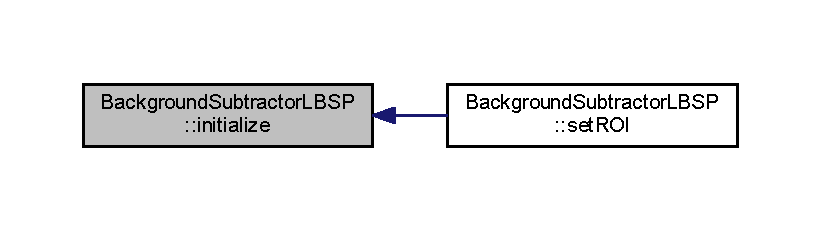
\includegraphics[width=350pt]{class_background_subtractor_l_b_s_p_ac6b854f94414497b143375d4a0ae8b6f_icgraph}
\end{center}
\end{figure}
\mbox{\Hypertarget{class_background_subtractor_l_b_s_p_a3644bc10ec3beda6fad22c633fe0f8fb}\label{class_background_subtractor_l_b_s_p_a3644bc10ec3beda6fad22c633fe0f8fb}} 
\index{Background\+Subtractor\+L\+B\+SP@{Background\+Subtractor\+L\+B\+SP}!initialize@{initialize}}
\index{initialize@{initialize}!Background\+Subtractor\+L\+B\+SP@{Background\+Subtractor\+L\+B\+SP}}
\subsubsection{\texorpdfstring{initialize()}{initialize()}\hspace{0.1cm}{\footnotesize\ttfamily [2/2]}}
{\footnotesize\ttfamily virtual void Background\+Subtractor\+L\+B\+S\+P\+::initialize (\begin{DoxyParamCaption}\item[{const cv\+::\+Mat \&}]{o\+Init\+Img,  }\item[{const cv\+::\+Mat \&}]{o\+R\+OI }\end{DoxyParamCaption})\hspace{0.3cm}{\ttfamily [pure virtual]}}



(re)initiaization method; needs to be called before starting background subtraction 



Implemented in \mbox{\hyperlink{class_background_subtractor_l_o_b_s_t_e_r_a452bea31dcbd2e10efc701cc2cd25776}{Background\+Subtractor\+L\+O\+B\+S\+T\+ER}}, and \mbox{\hyperlink{class_background_subtractor_su_b_s_e_n_s_e_ac84aa66030b04a72435ef473cf0e6a3f}{Background\+Subtractor\+Su\+B\+S\+E\+N\+SE}}.

\mbox{\Hypertarget{class_background_subtractor_l_b_s_p_a4771cac59b7ac865d6ec25cbf049948e}\label{class_background_subtractor_l_b_s_p_a4771cac59b7ac865d6ec25cbf049948e}} 
\index{Background\+Subtractor\+L\+B\+SP@{Background\+Subtractor\+L\+B\+SP}!operator()@{operator()}}
\index{operator()@{operator()}!Background\+Subtractor\+L\+B\+SP@{Background\+Subtractor\+L\+B\+SP}}
\subsubsection{\texorpdfstring{operator()()}{operator()()}}
{\footnotesize\ttfamily virtual void Background\+Subtractor\+L\+B\+S\+P\+::operator() (\begin{DoxyParamCaption}\item[{cv\+::\+Input\+Array}]{image,  }\item[{cv\+::\+Output\+Array}]{fgmask,  }\item[{double}]{learning\+Rate = {\ttfamily 0} }\end{DoxyParamCaption})\hspace{0.3cm}{\ttfamily [pure virtual]}}



primary model update function; the learning param is used to override the internal learning speed (ignored when $<$= 0) 



Implemented in \mbox{\hyperlink{class_background_subtractor_l_o_b_s_t_e_r_a0c0faf2754a7a74a6ae56cea47207070}{Background\+Subtractor\+L\+O\+B\+S\+T\+ER}}, and \mbox{\hyperlink{class_background_subtractor_su_b_s_e_n_s_e_aaa60e2883c2b2cf130820b10104a653b}{Background\+Subtractor\+Su\+B\+S\+E\+N\+SE}}.

\mbox{\Hypertarget{class_background_subtractor_l_b_s_p_a31b8474f8b4ffa6ef08ec682cfcef9b0}\label{class_background_subtractor_l_b_s_p_a31b8474f8b4ffa6ef08ec682cfcef9b0}} 
\index{Background\+Subtractor\+L\+B\+SP@{Background\+Subtractor\+L\+B\+SP}!set\+Automatic\+Model\+Reset@{set\+Automatic\+Model\+Reset}}
\index{set\+Automatic\+Model\+Reset@{set\+Automatic\+Model\+Reset}!Background\+Subtractor\+L\+B\+SP@{Background\+Subtractor\+L\+B\+SP}}
\subsubsection{\texorpdfstring{set\+Automatic\+Model\+Reset()}{setAutomaticModelReset()}}
{\footnotesize\ttfamily void Background\+Subtractor\+L\+B\+S\+P\+::set\+Automatic\+Model\+Reset (\begin{DoxyParamCaption}\item[{bool}]{b\+Val }\end{DoxyParamCaption})}



turns automatic model reset on or off 



Definition at line 57 of file Background\+Subtractor\+L\+B\+S\+P.\+cpp.


\begin{DoxyCode}
57                                                                \{
58     \mbox{\hyperlink{class_background_subtractor_l_b_s_p_a9d260f4e42e3fc79fb21af950ca9087a}{m\_bAutoModelResetEnabled}} = bVal;
59 \}
\end{DoxyCode}
\mbox{\Hypertarget{class_background_subtractor_l_b_s_p_a34dc38d3d925d46d289c750786f232dc}\label{class_background_subtractor_l_b_s_p_a34dc38d3d925d46d289c750786f232dc}} 
\index{Background\+Subtractor\+L\+B\+SP@{Background\+Subtractor\+L\+B\+SP}!set\+R\+OI@{set\+R\+OI}}
\index{set\+R\+OI@{set\+R\+OI}!Background\+Subtractor\+L\+B\+SP@{Background\+Subtractor\+L\+B\+SP}}
\subsubsection{\texorpdfstring{set\+R\+O\+I()}{setROI()}}
{\footnotesize\ttfamily void Background\+Subtractor\+L\+B\+S\+P\+::set\+R\+OI (\begin{DoxyParamCaption}\item[{cv\+::\+Mat \&}]{o\+R\+OI }\end{DoxyParamCaption})\hspace{0.3cm}{\ttfamily [virtual]}}



sets the R\+OI to be used for descriptor extraction (note\+: this function will reinit the model and return the usable R\+OI) 



Definition at line 45 of file Background\+Subtractor\+L\+B\+S\+P.\+cpp.


\begin{DoxyCode}
45                                                  \{
46     \mbox{\hyperlink{class_l_b_s_p_ad97557be4bc6cfd7b0fa4b01ab8f8c55}{LBSP::validateROI}}(oROI);
47     CV\_Assert(cv::countNonZero(oROI)>0);
48     \textcolor{keywordflow}{if}(\mbox{\hyperlink{class_background_subtractor_l_b_s_p_a55cea104a0924fd50d5bed0912828a7e}{m\_bInitialized}}) \{
49         cv::Mat oLatestBackgroundImage;
50         getBackgroundImage(oLatestBackgroundImage);
51         \mbox{\hyperlink{class_background_subtractor_l_b_s_p_ac6b854f94414497b143375d4a0ae8b6f}{initialize}}(oLatestBackgroundImage,oROI);
52     \}
53     \textcolor{keywordflow}{else}
54         \mbox{\hyperlink{class_background_subtractor_l_b_s_p_a53fe98bd2489d95de5292467145901e9}{m\_oROI}} = oROI.clone();
55 \}
\end{DoxyCode}
Here is the call graph for this function\+:
\nopagebreak
\begin{figure}[H]
\begin{center}
\leavevmode
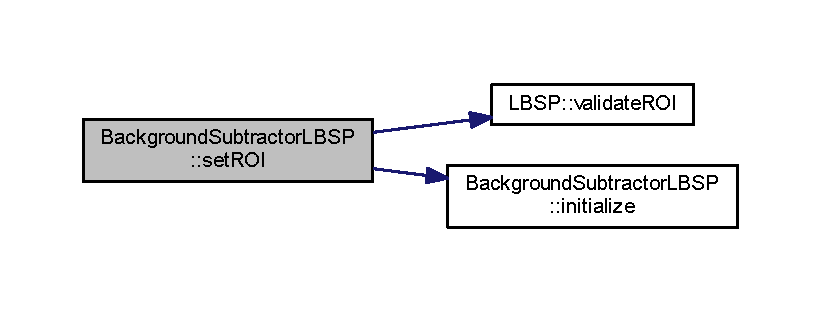
\includegraphics[width=350pt]{class_background_subtractor_l_b_s_p_a34dc38d3d925d46d289c750786f232dc_cgraph}
\end{center}
\end{figure}


\subsection{Member Data Documentation}
\mbox{\Hypertarget{class_background_subtractor_l_b_s_p_aefe69d94f08b2c4ba73ad1d254ad9153}\label{class_background_subtractor_l_b_s_p_aefe69d94f08b2c4ba73ad1d254ad9153}} 
\index{Background\+Subtractor\+L\+B\+SP@{Background\+Subtractor\+L\+B\+SP}!m\+\_\+an\+L\+B\+S\+P\+Threshold\+\_\+8bit\+L\+UT@{m\+\_\+an\+L\+B\+S\+P\+Threshold\+\_\+8bit\+L\+UT}}
\index{m\+\_\+an\+L\+B\+S\+P\+Threshold\+\_\+8bit\+L\+UT@{m\+\_\+an\+L\+B\+S\+P\+Threshold\+\_\+8bit\+L\+UT}!Background\+Subtractor\+L\+B\+SP@{Background\+Subtractor\+L\+B\+SP}}
\subsubsection{\texorpdfstring{m\+\_\+an\+L\+B\+S\+P\+Threshold\+\_\+8bit\+L\+UT}{m\_anLBSPThreshold\_8bitLUT}}
{\footnotesize\ttfamily size\+\_\+t Background\+Subtractor\+L\+B\+S\+P\+::m\+\_\+an\+L\+B\+S\+P\+Threshold\+\_\+8bit\+L\+UT\mbox{[}U\+C\+H\+A\+R\+\_\+\+M\+AX+1\mbox{]}\hspace{0.3cm}{\ttfamily [protected]}}



pre-\/allocated internal \mbox{\hyperlink{class_l_b_s_p}{L\+B\+SP}} threshold values L\+UT for all possible 8-\/bit intensities 



Definition at line 59 of file Background\+Subtractor\+L\+B\+S\+P.\+h.

\mbox{\Hypertarget{class_background_subtractor_l_b_s_p_a06b4f0d3f24fa08bccd3c9eca085713e}\label{class_background_subtractor_l_b_s_p_a06b4f0d3f24fa08bccd3c9eca085713e}} 
\index{Background\+Subtractor\+L\+B\+SP@{Background\+Subtractor\+L\+B\+SP}!m\+\_\+a\+Px\+Idx\+L\+UT@{m\+\_\+a\+Px\+Idx\+L\+UT}}
\index{m\+\_\+a\+Px\+Idx\+L\+UT@{m\+\_\+a\+Px\+Idx\+L\+UT}!Background\+Subtractor\+L\+B\+SP@{Background\+Subtractor\+L\+B\+SP}}
\subsubsection{\texorpdfstring{m\+\_\+a\+Px\+Idx\+L\+UT}{m\_aPxIdxLUT}}
{\footnotesize\ttfamily size\+\_\+t$\ast$ Background\+Subtractor\+L\+B\+S\+P\+::m\+\_\+a\+Px\+Idx\+L\+UT\hspace{0.3cm}{\ttfamily [protected]}}



internal pixel index L\+UT for all relevant analysis regions (based on the provided R\+OI) 



Definition at line 61 of file Background\+Subtractor\+L\+B\+S\+P.\+h.

\mbox{\Hypertarget{class_background_subtractor_l_b_s_p_a74e73d4832ccdef652d93756582024db}\label{class_background_subtractor_l_b_s_p_a74e73d4832ccdef652d93756582024db}} 
\index{Background\+Subtractor\+L\+B\+SP@{Background\+Subtractor\+L\+B\+SP}!m\+\_\+a\+Px\+Info\+L\+UT@{m\+\_\+a\+Px\+Info\+L\+UT}}
\index{m\+\_\+a\+Px\+Info\+L\+UT@{m\+\_\+a\+Px\+Info\+L\+UT}!Background\+Subtractor\+L\+B\+SP@{Background\+Subtractor\+L\+B\+SP}}
\subsubsection{\texorpdfstring{m\+\_\+a\+Px\+Info\+L\+UT}{m\_aPxInfoLUT}}
{\footnotesize\ttfamily \mbox{\hyperlink{struct_background_subtractor_l_b_s_p_1_1_px_info_base}{Px\+Info\+Base}}$\ast$ Background\+Subtractor\+L\+B\+S\+P\+::m\+\_\+a\+Px\+Info\+L\+UT\hspace{0.3cm}{\ttfamily [protected]}}



internal pixel info L\+UT for all possible pixel indexes 



Definition at line 63 of file Background\+Subtractor\+L\+B\+S\+P.\+h.

\mbox{\Hypertarget{class_background_subtractor_l_b_s_p_a9d260f4e42e3fc79fb21af950ca9087a}\label{class_background_subtractor_l_b_s_p_a9d260f4e42e3fc79fb21af950ca9087a}} 
\index{Background\+Subtractor\+L\+B\+SP@{Background\+Subtractor\+L\+B\+SP}!m\+\_\+b\+Auto\+Model\+Reset\+Enabled@{m\+\_\+b\+Auto\+Model\+Reset\+Enabled}}
\index{m\+\_\+b\+Auto\+Model\+Reset\+Enabled@{m\+\_\+b\+Auto\+Model\+Reset\+Enabled}!Background\+Subtractor\+L\+B\+SP@{Background\+Subtractor\+L\+B\+SP}}
\subsubsection{\texorpdfstring{m\+\_\+b\+Auto\+Model\+Reset\+Enabled}{m\_bAutoModelResetEnabled}}
{\footnotesize\ttfamily bool Background\+Subtractor\+L\+B\+S\+P\+::m\+\_\+b\+Auto\+Model\+Reset\+Enabled\hspace{0.3cm}{\ttfamily [protected]}}



specifies whether automatic model resets are enabled or not 



Definition at line 69 of file Background\+Subtractor\+L\+B\+S\+P.\+h.

\mbox{\Hypertarget{class_background_subtractor_l_b_s_p_a55cea104a0924fd50d5bed0912828a7e}\label{class_background_subtractor_l_b_s_p_a55cea104a0924fd50d5bed0912828a7e}} 
\index{Background\+Subtractor\+L\+B\+SP@{Background\+Subtractor\+L\+B\+SP}!m\+\_\+b\+Initialized@{m\+\_\+b\+Initialized}}
\index{m\+\_\+b\+Initialized@{m\+\_\+b\+Initialized}!Background\+Subtractor\+L\+B\+SP@{Background\+Subtractor\+L\+B\+SP}}
\subsubsection{\texorpdfstring{m\+\_\+b\+Initialized}{m\_bInitialized}}
{\footnotesize\ttfamily bool Background\+Subtractor\+L\+B\+S\+P\+::m\+\_\+b\+Initialized\hspace{0.3cm}{\ttfamily [protected]}}



specifies whether the algorithm is fully initialized or not 



Definition at line 67 of file Background\+Subtractor\+L\+B\+S\+P.\+h.

\mbox{\Hypertarget{class_background_subtractor_l_b_s_p_a5b1ec2694ae59661bb146ad0d4d49811}\label{class_background_subtractor_l_b_s_p_a5b1ec2694ae59661bb146ad0d4d49811}} 
\index{Background\+Subtractor\+L\+B\+SP@{Background\+Subtractor\+L\+B\+SP}!m\+\_\+b\+Using\+Moving\+Camera@{m\+\_\+b\+Using\+Moving\+Camera}}
\index{m\+\_\+b\+Using\+Moving\+Camera@{m\+\_\+b\+Using\+Moving\+Camera}!Background\+Subtractor\+L\+B\+SP@{Background\+Subtractor\+L\+B\+SP}}
\subsubsection{\texorpdfstring{m\+\_\+b\+Using\+Moving\+Camera}{m\_bUsingMovingCamera}}
{\footnotesize\ttfamily bool Background\+Subtractor\+L\+B\+S\+P\+::m\+\_\+b\+Using\+Moving\+Camera\hspace{0.3cm}{\ttfamily [protected]}}



specifies whether the camera is considered moving or not 



Definition at line 71 of file Background\+Subtractor\+L\+B\+S\+P.\+h.

\mbox{\Hypertarget{class_background_subtractor_l_b_s_p_ad759c645b14e9b16bf3940cae862df32}\label{class_background_subtractor_l_b_s_p_ad759c645b14e9b16bf3940cae862df32}} 
\index{Background\+Subtractor\+L\+B\+SP@{Background\+Subtractor\+L\+B\+SP}!m\+\_\+f\+Rel\+L\+B\+S\+P\+Threshold@{m\+\_\+f\+Rel\+L\+B\+S\+P\+Threshold}}
\index{m\+\_\+f\+Rel\+L\+B\+S\+P\+Threshold@{m\+\_\+f\+Rel\+L\+B\+S\+P\+Threshold}!Background\+Subtractor\+L\+B\+SP@{Background\+Subtractor\+L\+B\+SP}}
\subsubsection{\texorpdfstring{m\+\_\+f\+Rel\+L\+B\+S\+P\+Threshold}{m\_fRelLBSPThreshold}}
{\footnotesize\ttfamily const float Background\+Subtractor\+L\+B\+S\+P\+::m\+\_\+f\+Rel\+L\+B\+S\+P\+Threshold\hspace{0.3cm}{\ttfamily [protected]}}



\mbox{\hyperlink{class_l_b_s_p}{L\+B\+SP}} relative internal threshold (kept here since we don\textquotesingle{}t keep an \mbox{\hyperlink{class_l_b_s_p}{L\+B\+SP}} object) 



Definition at line 53 of file Background\+Subtractor\+L\+B\+S\+P.\+h.

\mbox{\Hypertarget{class_background_subtractor_l_b_s_p_a2585fe6e41e10af6da3e325dc20fe7f1}\label{class_background_subtractor_l_b_s_p_a2585fe6e41e10af6da3e325dc20fe7f1}} 
\index{Background\+Subtractor\+L\+B\+SP@{Background\+Subtractor\+L\+B\+SP}!m\+\_\+n\+Default\+Median\+Blur\+Kernel\+Size@{m\+\_\+n\+Default\+Median\+Blur\+Kernel\+Size}}
\index{m\+\_\+n\+Default\+Median\+Blur\+Kernel\+Size@{m\+\_\+n\+Default\+Median\+Blur\+Kernel\+Size}!Background\+Subtractor\+L\+B\+SP@{Background\+Subtractor\+L\+B\+SP}}
\subsubsection{\texorpdfstring{m\+\_\+n\+Default\+Median\+Blur\+Kernel\+Size}{m\_nDefaultMedianBlurKernelSize}}
{\footnotesize\ttfamily const int Background\+Subtractor\+L\+B\+S\+P\+::m\+\_\+n\+Default\+Median\+Blur\+Kernel\+Size\hspace{0.3cm}{\ttfamily [protected]}}



default kernel size for median blur post-\/proc filtering 



Definition at line 65 of file Background\+Subtractor\+L\+B\+S\+P.\+h.

\mbox{\Hypertarget{class_background_subtractor_l_b_s_p_a8a2350cad84f19c68ef61b7aaf91c43f}\label{class_background_subtractor_l_b_s_p_a8a2350cad84f19c68ef61b7aaf91c43f}} 
\index{Background\+Subtractor\+L\+B\+SP@{Background\+Subtractor\+L\+B\+SP}!m\+\_\+n\+Frame\+Index@{m\+\_\+n\+Frame\+Index}}
\index{m\+\_\+n\+Frame\+Index@{m\+\_\+n\+Frame\+Index}!Background\+Subtractor\+L\+B\+SP@{Background\+Subtractor\+L\+B\+SP}}
\subsubsection{\texorpdfstring{m\+\_\+n\+Frame\+Index}{m\_nFrameIndex}}
{\footnotesize\ttfamily size\+\_\+t Background\+Subtractor\+L\+B\+S\+P\+::m\+\_\+n\+Frame\+Index\hspace{0.3cm}{\ttfamily [protected]}}



current frame index, frame count since last model reset \& model reset cooldown counters 



Definition at line 57 of file Background\+Subtractor\+L\+B\+S\+P.\+h.

\mbox{\Hypertarget{class_background_subtractor_l_b_s_p_ab56bf775dfdf0579e834e45210c3a92a}\label{class_background_subtractor_l_b_s_p_ab56bf775dfdf0579e834e45210c3a92a}} 
\index{Background\+Subtractor\+L\+B\+SP@{Background\+Subtractor\+L\+B\+SP}!m\+\_\+n\+Frames\+Since\+Last\+Reset@{m\+\_\+n\+Frames\+Since\+Last\+Reset}}
\index{m\+\_\+n\+Frames\+Since\+Last\+Reset@{m\+\_\+n\+Frames\+Since\+Last\+Reset}!Background\+Subtractor\+L\+B\+SP@{Background\+Subtractor\+L\+B\+SP}}
\subsubsection{\texorpdfstring{m\+\_\+n\+Frames\+Since\+Last\+Reset}{m\_nFramesSinceLastReset}}
{\footnotesize\ttfamily size\+\_\+t Background\+Subtractor\+L\+B\+S\+P\+::m\+\_\+n\+Frames\+Since\+Last\+Reset\hspace{0.3cm}{\ttfamily [protected]}}



Definition at line 57 of file Background\+Subtractor\+L\+B\+S\+P.\+h.

\mbox{\Hypertarget{class_background_subtractor_l_b_s_p_ab3467ebee2c5d1249061ccd704cc0584}\label{class_background_subtractor_l_b_s_p_ab3467ebee2c5d1249061ccd704cc0584}} 
\index{Background\+Subtractor\+L\+B\+SP@{Background\+Subtractor\+L\+B\+SP}!m\+\_\+n\+Img\+Channels@{m\+\_\+n\+Img\+Channels}}
\index{m\+\_\+n\+Img\+Channels@{m\+\_\+n\+Img\+Channels}!Background\+Subtractor\+L\+B\+SP@{Background\+Subtractor\+L\+B\+SP}}
\subsubsection{\texorpdfstring{m\+\_\+n\+Img\+Channels}{m\_nImgChannels}}
{\footnotesize\ttfamily size\+\_\+t Background\+Subtractor\+L\+B\+S\+P\+::m\+\_\+n\+Img\+Channels\hspace{0.3cm}{\ttfamily [protected]}}



input image channel size 



Definition at line 47 of file Background\+Subtractor\+L\+B\+S\+P.\+h.

\mbox{\Hypertarget{class_background_subtractor_l_b_s_p_a7d2f52ecd5ff56e42da86f97e0ad93b5}\label{class_background_subtractor_l_b_s_p_a7d2f52ecd5ff56e42da86f97e0ad93b5}} 
\index{Background\+Subtractor\+L\+B\+SP@{Background\+Subtractor\+L\+B\+SP}!m\+\_\+n\+Img\+Type@{m\+\_\+n\+Img\+Type}}
\index{m\+\_\+n\+Img\+Type@{m\+\_\+n\+Img\+Type}!Background\+Subtractor\+L\+B\+SP@{Background\+Subtractor\+L\+B\+SP}}
\subsubsection{\texorpdfstring{m\+\_\+n\+Img\+Type}{m\_nImgType}}
{\footnotesize\ttfamily int Background\+Subtractor\+L\+B\+S\+P\+::m\+\_\+n\+Img\+Type\hspace{0.3cm}{\ttfamily [protected]}}



input image type 



Definition at line 49 of file Background\+Subtractor\+L\+B\+S\+P.\+h.

\mbox{\Hypertarget{class_background_subtractor_l_b_s_p_a209eb6aaa34e8ad8e565e79f85404e24}\label{class_background_subtractor_l_b_s_p_a209eb6aaa34e8ad8e565e79f85404e24}} 
\index{Background\+Subtractor\+L\+B\+SP@{Background\+Subtractor\+L\+B\+SP}!m\+\_\+n\+L\+B\+S\+P\+Threshold\+Offset@{m\+\_\+n\+L\+B\+S\+P\+Threshold\+Offset}}
\index{m\+\_\+n\+L\+B\+S\+P\+Threshold\+Offset@{m\+\_\+n\+L\+B\+S\+P\+Threshold\+Offset}!Background\+Subtractor\+L\+B\+SP@{Background\+Subtractor\+L\+B\+SP}}
\subsubsection{\texorpdfstring{m\+\_\+n\+L\+B\+S\+P\+Threshold\+Offset}{m\_nLBSPThresholdOffset}}
{\footnotesize\ttfamily const size\+\_\+t Background\+Subtractor\+L\+B\+S\+P\+::m\+\_\+n\+L\+B\+S\+P\+Threshold\+Offset\hspace{0.3cm}{\ttfamily [protected]}}



\mbox{\hyperlink{class_l_b_s_p}{L\+B\+SP}} internal threshold offset value, used to reduce texture noise in dark regions. 



Definition at line 51 of file Background\+Subtractor\+L\+B\+S\+P.\+h.

\mbox{\Hypertarget{class_background_subtractor_l_b_s_p_a5ea18d388afacf8285c46ba0f754e7ee}\label{class_background_subtractor_l_b_s_p_a5ea18d388afacf8285c46ba0f754e7ee}} 
\index{Background\+Subtractor\+L\+B\+SP@{Background\+Subtractor\+L\+B\+SP}!m\+\_\+n\+Model\+Reset\+Cooldown@{m\+\_\+n\+Model\+Reset\+Cooldown}}
\index{m\+\_\+n\+Model\+Reset\+Cooldown@{m\+\_\+n\+Model\+Reset\+Cooldown}!Background\+Subtractor\+L\+B\+SP@{Background\+Subtractor\+L\+B\+SP}}
\subsubsection{\texorpdfstring{m\+\_\+n\+Model\+Reset\+Cooldown}{m\_nModelResetCooldown}}
{\footnotesize\ttfamily size\+\_\+t Background\+Subtractor\+L\+B\+S\+P\+::m\+\_\+n\+Model\+Reset\+Cooldown\hspace{0.3cm}{\ttfamily [protected]}}



Definition at line 57 of file Background\+Subtractor\+L\+B\+S\+P.\+h.

\mbox{\Hypertarget{class_background_subtractor_l_b_s_p_a9d1e247267afbddb7032bdcabd67d931}\label{class_background_subtractor_l_b_s_p_a9d1e247267afbddb7032bdcabd67d931}} 
\index{Background\+Subtractor\+L\+B\+SP@{Background\+Subtractor\+L\+B\+SP}!m\+\_\+n\+Tot\+Px\+Count@{m\+\_\+n\+Tot\+Px\+Count}}
\index{m\+\_\+n\+Tot\+Px\+Count@{m\+\_\+n\+Tot\+Px\+Count}!Background\+Subtractor\+L\+B\+SP@{Background\+Subtractor\+L\+B\+SP}}
\subsubsection{\texorpdfstring{m\+\_\+n\+Tot\+Px\+Count}{m\_nTotPxCount}}
{\footnotesize\ttfamily size\+\_\+t Background\+Subtractor\+L\+B\+S\+P\+::m\+\_\+n\+Tot\+Px\+Count\hspace{0.3cm}{\ttfamily [protected]}}



total number of pixels (depends on the input frame size) \& total number of relevant pixels 



Definition at line 55 of file Background\+Subtractor\+L\+B\+S\+P.\+h.

\mbox{\Hypertarget{class_background_subtractor_l_b_s_p_ac3b54f4d2dfa3a576475214f26501d85}\label{class_background_subtractor_l_b_s_p_ac3b54f4d2dfa3a576475214f26501d85}} 
\index{Background\+Subtractor\+L\+B\+SP@{Background\+Subtractor\+L\+B\+SP}!m\+\_\+n\+Tot\+Relevant\+Px\+Count@{m\+\_\+n\+Tot\+Relevant\+Px\+Count}}
\index{m\+\_\+n\+Tot\+Relevant\+Px\+Count@{m\+\_\+n\+Tot\+Relevant\+Px\+Count}!Background\+Subtractor\+L\+B\+SP@{Background\+Subtractor\+L\+B\+SP}}
\subsubsection{\texorpdfstring{m\+\_\+n\+Tot\+Relevant\+Px\+Count}{m\_nTotRelevantPxCount}}
{\footnotesize\ttfamily size\+\_\+t Background\+Subtractor\+L\+B\+S\+P\+::m\+\_\+n\+Tot\+Relevant\+Px\+Count\hspace{0.3cm}{\ttfamily [protected]}}



Definition at line 55 of file Background\+Subtractor\+L\+B\+S\+P.\+h.

\mbox{\Hypertarget{class_background_subtractor_l_b_s_p_a732d5e6ae35fb0e858cadb3af5ce08a2}\label{class_background_subtractor_l_b_s_p_a732d5e6ae35fb0e858cadb3af5ce08a2}} 
\index{Background\+Subtractor\+L\+B\+SP@{Background\+Subtractor\+L\+B\+SP}!m\+\_\+o\+Img\+Size@{m\+\_\+o\+Img\+Size}}
\index{m\+\_\+o\+Img\+Size@{m\+\_\+o\+Img\+Size}!Background\+Subtractor\+L\+B\+SP@{Background\+Subtractor\+L\+B\+SP}}
\subsubsection{\texorpdfstring{m\+\_\+o\+Img\+Size}{m\_oImgSize}}
{\footnotesize\ttfamily cv\+::\+Size Background\+Subtractor\+L\+B\+S\+P\+::m\+\_\+o\+Img\+Size\hspace{0.3cm}{\ttfamily [protected]}}



input image size 



Definition at line 45 of file Background\+Subtractor\+L\+B\+S\+P.\+h.

\mbox{\Hypertarget{class_background_subtractor_l_b_s_p_ab1dc003792ab1d0b881a6fd10e0e29b3}\label{class_background_subtractor_l_b_s_p_ab1dc003792ab1d0b881a6fd10e0e29b3}} 
\index{Background\+Subtractor\+L\+B\+SP@{Background\+Subtractor\+L\+B\+SP}!m\+\_\+o\+Last\+Color\+Frame@{m\+\_\+o\+Last\+Color\+Frame}}
\index{m\+\_\+o\+Last\+Color\+Frame@{m\+\_\+o\+Last\+Color\+Frame}!Background\+Subtractor\+L\+B\+SP@{Background\+Subtractor\+L\+B\+SP}}
\subsubsection{\texorpdfstring{m\+\_\+o\+Last\+Color\+Frame}{m\_oLastColorFrame}}
{\footnotesize\ttfamily cv\+::\+Mat Background\+Subtractor\+L\+B\+S\+P\+::m\+\_\+o\+Last\+Color\+Frame\hspace{0.3cm}{\ttfamily [protected]}}



copy of latest pixel intensities (used when refreshing model) 



Definition at line 73 of file Background\+Subtractor\+L\+B\+S\+P.\+h.

\mbox{\Hypertarget{class_background_subtractor_l_b_s_p_a9c637c0b87cac495887295690d83ba13}\label{class_background_subtractor_l_b_s_p_a9c637c0b87cac495887295690d83ba13}} 
\index{Background\+Subtractor\+L\+B\+SP@{Background\+Subtractor\+L\+B\+SP}!m\+\_\+o\+Last\+Desc\+Frame@{m\+\_\+o\+Last\+Desc\+Frame}}
\index{m\+\_\+o\+Last\+Desc\+Frame@{m\+\_\+o\+Last\+Desc\+Frame}!Background\+Subtractor\+L\+B\+SP@{Background\+Subtractor\+L\+B\+SP}}
\subsubsection{\texorpdfstring{m\+\_\+o\+Last\+Desc\+Frame}{m\_oLastDescFrame}}
{\footnotesize\ttfamily cv\+::\+Mat Background\+Subtractor\+L\+B\+S\+P\+::m\+\_\+o\+Last\+Desc\+Frame\hspace{0.3cm}{\ttfamily [protected]}}



copy of latest descriptors (used when refreshing model) 



Definition at line 75 of file Background\+Subtractor\+L\+B\+S\+P.\+h.

\mbox{\Hypertarget{class_background_subtractor_l_b_s_p_adb6dc0af596c5592c91f9d8faa5c8a4b}\label{class_background_subtractor_l_b_s_p_adb6dc0af596c5592c91f9d8faa5c8a4b}} 
\index{Background\+Subtractor\+L\+B\+SP@{Background\+Subtractor\+L\+B\+SP}!m\+\_\+o\+Last\+F\+G\+Mask@{m\+\_\+o\+Last\+F\+G\+Mask}}
\index{m\+\_\+o\+Last\+F\+G\+Mask@{m\+\_\+o\+Last\+F\+G\+Mask}!Background\+Subtractor\+L\+B\+SP@{Background\+Subtractor\+L\+B\+SP}}
\subsubsection{\texorpdfstring{m\+\_\+o\+Last\+F\+G\+Mask}{m\_oLastFGMask}}
{\footnotesize\ttfamily cv\+::\+Mat Background\+Subtractor\+L\+B\+S\+P\+::m\+\_\+o\+Last\+F\+G\+Mask\hspace{0.3cm}{\ttfamily [protected]}}



the foreground mask generated by the method at \mbox{[}t-\/1\mbox{]} 



Definition at line 77 of file Background\+Subtractor\+L\+B\+S\+P.\+h.

\mbox{\Hypertarget{class_background_subtractor_l_b_s_p_a53fe98bd2489d95de5292467145901e9}\label{class_background_subtractor_l_b_s_p_a53fe98bd2489d95de5292467145901e9}} 
\index{Background\+Subtractor\+L\+B\+SP@{Background\+Subtractor\+L\+B\+SP}!m\+\_\+o\+R\+OI@{m\+\_\+o\+R\+OI}}
\index{m\+\_\+o\+R\+OI@{m\+\_\+o\+R\+OI}!Background\+Subtractor\+L\+B\+SP@{Background\+Subtractor\+L\+B\+SP}}
\subsubsection{\texorpdfstring{m\+\_\+o\+R\+OI}{m\_oROI}}
{\footnotesize\ttfamily cv\+::\+Mat Background\+Subtractor\+L\+B\+S\+P\+::m\+\_\+o\+R\+OI\hspace{0.3cm}{\ttfamily [protected]}}



background model R\+OI used for \mbox{\hyperlink{class_l_b_s_p}{L\+B\+SP}} descriptor extraction (specific to the input image size) 



Definition at line 43 of file Background\+Subtractor\+L\+B\+S\+P.\+h.

\mbox{\Hypertarget{class_background_subtractor_l_b_s_p_a49771cd7b2c8354cde3da6e593d3febe}\label{class_background_subtractor_l_b_s_p_a49771cd7b2c8354cde3da6e593d3febe}} 
\index{Background\+Subtractor\+L\+B\+SP@{Background\+Subtractor\+L\+B\+SP}!n\+Debug\+CoordX@{n\+Debug\+CoordX}}
\index{n\+Debug\+CoordX@{n\+Debug\+CoordX}!Background\+Subtractor\+L\+B\+SP@{Background\+Subtractor\+L\+B\+SP}}
\subsubsection{\texorpdfstring{n\+Debug\+CoordX}{nDebugCoordX}}
{\footnotesize\ttfamily int Background\+Subtractor\+L\+B\+S\+P\+::n\+Debug\+CoordX}



Definition at line 81 of file Background\+Subtractor\+L\+B\+S\+P.\+h.

\mbox{\Hypertarget{class_background_subtractor_l_b_s_p_a8e1451fd90eb4459aa84ea5e7133268a}\label{class_background_subtractor_l_b_s_p_a8e1451fd90eb4459aa84ea5e7133268a}} 
\index{Background\+Subtractor\+L\+B\+SP@{Background\+Subtractor\+L\+B\+SP}!n\+Debug\+CoordY@{n\+Debug\+CoordY}}
\index{n\+Debug\+CoordY@{n\+Debug\+CoordY}!Background\+Subtractor\+L\+B\+SP@{Background\+Subtractor\+L\+B\+SP}}
\subsubsection{\texorpdfstring{n\+Debug\+CoordY}{nDebugCoordY}}
{\footnotesize\ttfamily int Background\+Subtractor\+L\+B\+S\+P\+::n\+Debug\+CoordY}



Definition at line 81 of file Background\+Subtractor\+L\+B\+S\+P.\+h.

\mbox{\Hypertarget{class_background_subtractor_l_b_s_p_ada55b4a5eec8c82d0e05b0f9f1600ecb}\label{class_background_subtractor_l_b_s_p_ada55b4a5eec8c82d0e05b0f9f1600ecb}} 
\index{Background\+Subtractor\+L\+B\+SP@{Background\+Subtractor\+L\+B\+SP}!s\+Debug\+Name@{s\+Debug\+Name}}
\index{s\+Debug\+Name@{s\+Debug\+Name}!Background\+Subtractor\+L\+B\+SP@{Background\+Subtractor\+L\+B\+SP}}
\subsubsection{\texorpdfstring{s\+Debug\+Name}{sDebugName}}
{\footnotesize\ttfamily std\+::string Background\+Subtractor\+L\+B\+S\+P\+::s\+Debug\+Name}



Definition at line 82 of file Background\+Subtractor\+L\+B\+S\+P.\+h.



The documentation for this class was generated from the following files\+:\begin{DoxyCompactItemize}
\item 
D\+:/\+Roy/\+Git\+Hub/\+Multitarget-\/tracker/\+Detector/\+Subsense/\mbox{\hyperlink{_background_subtractor_l_b_s_p_8h}{Background\+Subtractor\+L\+B\+S\+P.\+h}}\item 
D\+:/\+Roy/\+Git\+Hub/\+Multitarget-\/tracker/\+Detector/\+Subsense/\mbox{\hyperlink{_background_subtractor_l_b_s_p_8cpp}{Background\+Subtractor\+L\+B\+S\+P.\+cpp}}\end{DoxyCompactItemize}

\hypertarget{class_background_subtractor_l_o_b_s_t_e_r}{}\section{Background\+Subtractor\+L\+O\+B\+S\+T\+ER Class Reference}
\label{class_background_subtractor_l_o_b_s_t_e_r}\index{Background\+Subtractor\+L\+O\+B\+S\+T\+ER@{Background\+Subtractor\+L\+O\+B\+S\+T\+ER}}


{\ttfamily \#include $<$Background\+Subtractor\+L\+O\+B\+S\+T\+E\+R.\+h$>$}



Inheritance diagram for Background\+Subtractor\+L\+O\+B\+S\+T\+ER\+:\nopagebreak
\begin{figure}[H]
\begin{center}
\leavevmode
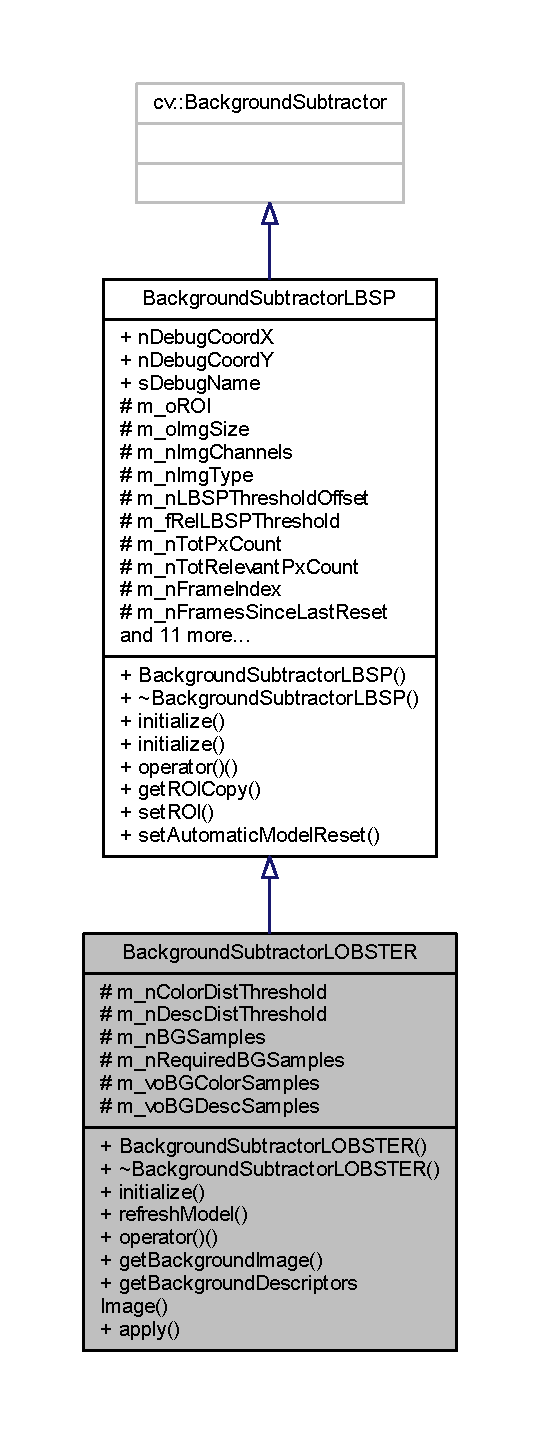
\includegraphics[height=550pt]{class_background_subtractor_l_o_b_s_t_e_r__inherit__graph}
\end{center}
\end{figure}


Collaboration diagram for Background\+Subtractor\+L\+O\+B\+S\+T\+ER\+:\nopagebreak
\begin{figure}[H]
\begin{center}
\leavevmode
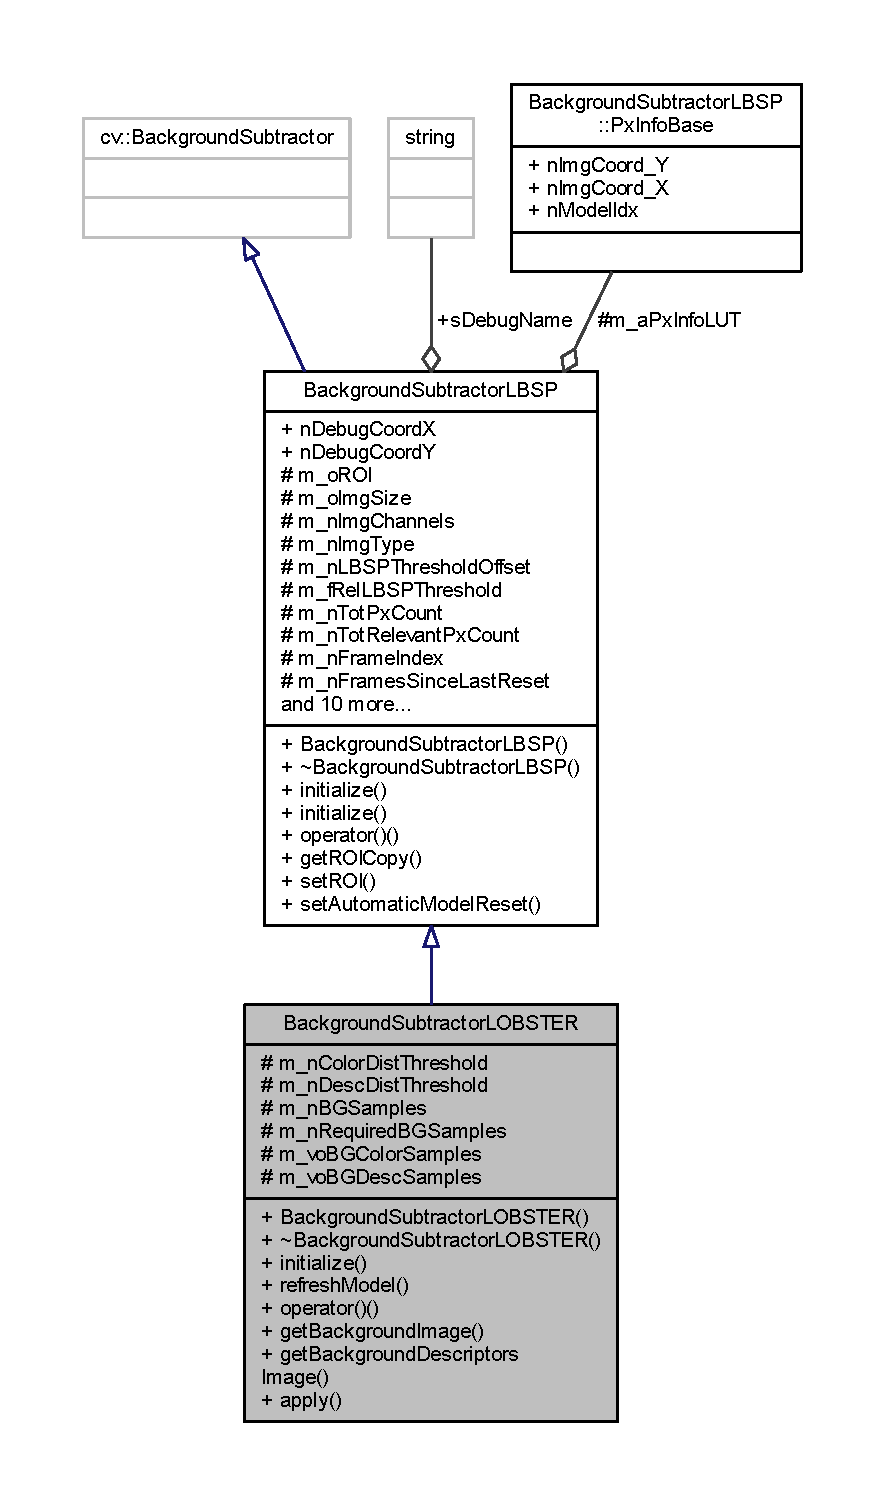
\includegraphics[height=550pt]{class_background_subtractor_l_o_b_s_t_e_r__coll__graph}
\end{center}
\end{figure}
\subsection*{Public Member Functions}
\begin{DoxyCompactItemize}
\item 
\mbox{\hyperlink{class_background_subtractor_l_o_b_s_t_e_r_a5a09b9ca80e50ba2f8686aaee6d461b7}{Background\+Subtractor\+L\+O\+B\+S\+T\+ER}} (float f\+Rel\+L\+B\+S\+P\+Threshold=\mbox{\hyperlink{_background_subtractor_l_o_b_s_t_e_r_8h_a3025dcc96b2d2c6416bfa57325d79ba5}{B\+G\+S\+L\+O\+B\+S\+T\+E\+R\+\_\+\+D\+E\+F\+A\+U\+L\+T\+\_\+\+L\+B\+S\+P\+\_\+\+R\+E\+L\+\_\+\+S\+I\+M\+I\+L\+A\+R\+I\+T\+Y\+\_\+\+T\+H\+R\+E\+S\+H\+O\+LD}}, size\+\_\+t n\+L\+B\+S\+P\+Threshold\+Offset=\mbox{\hyperlink{_background_subtractor_l_o_b_s_t_e_r_8h_a705c59e9c9a6fd8c0c57a5adab5a72c0}{B\+G\+S\+L\+O\+B\+S\+T\+E\+R\+\_\+\+D\+E\+F\+A\+U\+L\+T\+\_\+\+L\+B\+S\+P\+\_\+\+O\+F\+F\+S\+E\+T\+\_\+\+S\+I\+M\+I\+L\+A\+R\+I\+T\+Y\+\_\+\+T\+H\+R\+E\+S\+H\+O\+LD}}, size\+\_\+t n\+Desc\+Dist\+Threshold=\mbox{\hyperlink{_background_subtractor_l_o_b_s_t_e_r_8h_a11b89942e22902c0bbbbc2f0154804c2}{B\+G\+S\+L\+O\+B\+S\+T\+E\+R\+\_\+\+D\+E\+F\+A\+U\+L\+T\+\_\+\+D\+E\+S\+C\+\_\+\+D\+I\+S\+T\+\_\+\+T\+H\+R\+E\+S\+H\+O\+LD}}, size\+\_\+t n\+Color\+Dist\+Threshold=\mbox{\hyperlink{_background_subtractor_l_o_b_s_t_e_r_8h_a8442ce9b67919b77ad15847e5d80d983}{B\+G\+S\+L\+O\+B\+S\+T\+E\+R\+\_\+\+D\+E\+F\+A\+U\+L\+T\+\_\+\+C\+O\+L\+O\+R\+\_\+\+D\+I\+S\+T\+\_\+\+T\+H\+R\+E\+S\+H\+O\+LD}}, size\+\_\+t n\+B\+G\+Samples=\mbox{\hyperlink{_background_subtractor_l_o_b_s_t_e_r_8h_aea7261dd4c4233733b24fd175b6cb2b3}{B\+G\+S\+L\+O\+B\+S\+T\+E\+R\+\_\+\+D\+E\+F\+A\+U\+L\+T\+\_\+\+N\+B\+\_\+\+B\+G\+\_\+\+S\+A\+M\+P\+L\+ES}}, size\+\_\+t n\+Required\+B\+G\+Samples=\mbox{\hyperlink{_background_subtractor_l_o_b_s_t_e_r_8h_a209f60b8a126e31bb8ec6f8209d95ad0}{B\+G\+S\+L\+O\+B\+S\+T\+E\+R\+\_\+\+D\+E\+F\+A\+U\+L\+T\+\_\+\+R\+E\+Q\+U\+I\+R\+E\+D\+\_\+\+N\+B\+\_\+\+B\+G\+\_\+\+S\+A\+M\+P\+L\+ES}})
\begin{DoxyCompactList}\small\item\em full constructor \end{DoxyCompactList}\item 
virtual \mbox{\hyperlink{class_background_subtractor_l_o_b_s_t_e_r_a249ab359859ee9d439cd130d4271edd6}{$\sim$\+Background\+Subtractor\+L\+O\+B\+S\+T\+ER}} ()
\begin{DoxyCompactList}\small\item\em default destructor \end{DoxyCompactList}\item 
virtual void \mbox{\hyperlink{class_background_subtractor_l_o_b_s_t_e_r_a452bea31dcbd2e10efc701cc2cd25776}{initialize}} (const cv\+::\+Mat \&o\+Init\+Img, const cv\+::\+Mat \&o\+R\+OI)
\begin{DoxyCompactList}\small\item\em (re)initiaization method; needs to be called before starting background subtraction \end{DoxyCompactList}\item 
virtual void \mbox{\hyperlink{class_background_subtractor_l_o_b_s_t_e_r_aeb3b23c1f47cfe71a73f3ca47ec06a75}{refresh\+Model}} (float f\+Samples\+Refresh\+Frac, bool b\+Force\+F\+G\+Update=false)
\begin{DoxyCompactList}\small\item\em refreshes all samples based on the last analyzed frame \end{DoxyCompactList}\item 
virtual void \mbox{\hyperlink{class_background_subtractor_l_o_b_s_t_e_r_a0c0faf2754a7a74a6ae56cea47207070}{operator()}} (cv\+::\+Input\+Array image, cv\+::\+Output\+Array fgmask, double learning\+Rate=\mbox{\hyperlink{_background_subtractor_l_o_b_s_t_e_r_8h_a2d317f4a065c4c58c7241080d9c4457c}{B\+G\+S\+L\+O\+B\+S\+T\+E\+R\+\_\+\+D\+E\+F\+A\+U\+L\+T\+\_\+\+L\+E\+A\+R\+N\+I\+N\+G\+\_\+\+R\+A\+TE}})
\begin{DoxyCompactList}\small\item\em primary model update function; the learning param is reinterpreted as an integer and should be $>$ 0 (smaller values == faster adaptation) \end{DoxyCompactList}\item 
void \mbox{\hyperlink{class_background_subtractor_l_o_b_s_t_e_r_a07872de46dbbd970b0bca959f2eb9392}{get\+Background\+Image}} (cv\+::\+Output\+Array background\+Image) const
\begin{DoxyCompactList}\small\item\em returns a copy of the latest reconstructed background image \end{DoxyCompactList}\item 
virtual void \mbox{\hyperlink{class_background_subtractor_l_o_b_s_t_e_r_a28b005819f237ece74ab9eeacef8d770}{get\+Background\+Descriptors\+Image}} (cv\+::\+Output\+Array background\+Desc\+Image) const
\begin{DoxyCompactList}\small\item\em returns a copy of the latest reconstructed background descriptors image \end{DoxyCompactList}\item 
virtual void \mbox{\hyperlink{class_background_subtractor_l_o_b_s_t_e_r_a58c127d4b95230d1e7fdc64055943ef3}{apply}} (cv\+::\+Input\+Array image, cv\+::\+Output\+Array fgmask, double learning\+Rate\+Override=\mbox{\hyperlink{_background_subtractor_l_o_b_s_t_e_r_8h_a2d317f4a065c4c58c7241080d9c4457c}{B\+G\+S\+L\+O\+B\+S\+T\+E\+R\+\_\+\+D\+E\+F\+A\+U\+L\+T\+\_\+\+L\+E\+A\+R\+N\+I\+N\+G\+\_\+\+R\+A\+TE}})
\begin{DoxyCompactList}\small\item\em compute foreground mask \end{DoxyCompactList}\item 
virtual void \mbox{\hyperlink{class_background_subtractor_l_b_s_p_ac6b854f94414497b143375d4a0ae8b6f}{initialize}} (const cv\+::\+Mat \&o\+Init\+Img)
\begin{DoxyCompactList}\small\item\em (re)initiaization method; needs to be called before starting background subtraction \end{DoxyCompactList}\item 
virtual cv\+::\+Mat \mbox{\hyperlink{class_background_subtractor_l_b_s_p_a9843f87f8adcd0e85274303f9210b883}{get\+R\+O\+I\+Copy}} () const
\begin{DoxyCompactList}\small\item\em unused, always returns nullptr \end{DoxyCompactList}\item 
virtual void \mbox{\hyperlink{class_background_subtractor_l_b_s_p_a34dc38d3d925d46d289c750786f232dc}{set\+R\+OI}} (cv\+::\+Mat \&o\+R\+OI)
\begin{DoxyCompactList}\small\item\em sets the R\+OI to be used for descriptor extraction (note\+: this function will reinit the model and return the usable R\+OI) \end{DoxyCompactList}\item 
void \mbox{\hyperlink{class_background_subtractor_l_b_s_p_a31b8474f8b4ffa6ef08ec682cfcef9b0}{set\+Automatic\+Model\+Reset}} (bool)
\begin{DoxyCompactList}\small\item\em turns automatic model reset on or off \end{DoxyCompactList}\end{DoxyCompactItemize}
\subsection*{Public Attributes}
\begin{DoxyCompactItemize}
\item 
int \mbox{\hyperlink{class_background_subtractor_l_b_s_p_a49771cd7b2c8354cde3da6e593d3febe}{n\+Debug\+CoordX}}
\item 
int \mbox{\hyperlink{class_background_subtractor_l_b_s_p_a8e1451fd90eb4459aa84ea5e7133268a}{n\+Debug\+CoordY}}
\item 
std\+::string \mbox{\hyperlink{class_background_subtractor_l_b_s_p_ada55b4a5eec8c82d0e05b0f9f1600ecb}{s\+Debug\+Name}}
\end{DoxyCompactItemize}
\subsection*{Protected Attributes}
\begin{DoxyCompactItemize}
\item 
const size\+\_\+t \mbox{\hyperlink{class_background_subtractor_l_o_b_s_t_e_r_a37a37a0a46fc8e33d954c33c1318d7b2}{m\+\_\+n\+Color\+Dist\+Threshold}}
\begin{DoxyCompactList}\small\item\em absolute color distance threshold \end{DoxyCompactList}\item 
const size\+\_\+t \mbox{\hyperlink{class_background_subtractor_l_o_b_s_t_e_r_abe3f4a836343e901746e4f243f5252e4}{m\+\_\+n\+Desc\+Dist\+Threshold}}
\begin{DoxyCompactList}\small\item\em absolute descriptor distance threshold \end{DoxyCompactList}\item 
const size\+\_\+t \mbox{\hyperlink{class_background_subtractor_l_o_b_s_t_e_r_a20c53540b952d608d849a305fd5eed89}{m\+\_\+n\+B\+G\+Samples}}
\begin{DoxyCompactList}\small\item\em number of different samples per pixel/block to be taken from input frames to build the background model \end{DoxyCompactList}\item 
const size\+\_\+t \mbox{\hyperlink{class_background_subtractor_l_o_b_s_t_e_r_acb558aefc1b6205a63c1906b6fd1eeff}{m\+\_\+n\+Required\+B\+G\+Samples}}
\begin{DoxyCompactList}\small\item\em number of similar samples needed to consider the current pixel/block as \textquotesingle{}background\textquotesingle{} \end{DoxyCompactList}\item 
std\+::vector$<$ cv\+::\+Mat $>$ \mbox{\hyperlink{class_background_subtractor_l_o_b_s_t_e_r_ac981b39f8ae7b28d3e4326d8e6be6332}{m\+\_\+vo\+B\+G\+Color\+Samples}}
\begin{DoxyCompactList}\small\item\em background model pixel intensity samples \end{DoxyCompactList}\item 
std\+::vector$<$ cv\+::\+Mat $>$ \mbox{\hyperlink{class_background_subtractor_l_o_b_s_t_e_r_a3c49866ae652423b2173215957907d04}{m\+\_\+vo\+B\+G\+Desc\+Samples}}
\begin{DoxyCompactList}\small\item\em background model descriptors samples \end{DoxyCompactList}\item 
cv\+::\+Mat \mbox{\hyperlink{class_background_subtractor_l_b_s_p_a53fe98bd2489d95de5292467145901e9}{m\+\_\+o\+R\+OI}}
\begin{DoxyCompactList}\small\item\em background model R\+OI used for \mbox{\hyperlink{class_l_b_s_p}{L\+B\+SP}} descriptor extraction (specific to the input image size) \end{DoxyCompactList}\item 
cv\+::\+Size \mbox{\hyperlink{class_background_subtractor_l_b_s_p_a732d5e6ae35fb0e858cadb3af5ce08a2}{m\+\_\+o\+Img\+Size}}
\begin{DoxyCompactList}\small\item\em input image size \end{DoxyCompactList}\item 
size\+\_\+t \mbox{\hyperlink{class_background_subtractor_l_b_s_p_ab3467ebee2c5d1249061ccd704cc0584}{m\+\_\+n\+Img\+Channels}}
\begin{DoxyCompactList}\small\item\em input image channel size \end{DoxyCompactList}\item 
int \mbox{\hyperlink{class_background_subtractor_l_b_s_p_a7d2f52ecd5ff56e42da86f97e0ad93b5}{m\+\_\+n\+Img\+Type}}
\begin{DoxyCompactList}\small\item\em input image type \end{DoxyCompactList}\item 
const size\+\_\+t \mbox{\hyperlink{class_background_subtractor_l_b_s_p_a209eb6aaa34e8ad8e565e79f85404e24}{m\+\_\+n\+L\+B\+S\+P\+Threshold\+Offset}}
\begin{DoxyCompactList}\small\item\em \mbox{\hyperlink{class_l_b_s_p}{L\+B\+SP}} internal threshold offset value, used to reduce texture noise in dark regions. \end{DoxyCompactList}\item 
const float \mbox{\hyperlink{class_background_subtractor_l_b_s_p_ad759c645b14e9b16bf3940cae862df32}{m\+\_\+f\+Rel\+L\+B\+S\+P\+Threshold}}
\begin{DoxyCompactList}\small\item\em \mbox{\hyperlink{class_l_b_s_p}{L\+B\+SP}} relative internal threshold (kept here since we don\textquotesingle{}t keep an \mbox{\hyperlink{class_l_b_s_p}{L\+B\+SP}} object) \end{DoxyCompactList}\item 
size\+\_\+t \mbox{\hyperlink{class_background_subtractor_l_b_s_p_a9d1e247267afbddb7032bdcabd67d931}{m\+\_\+n\+Tot\+Px\+Count}}
\begin{DoxyCompactList}\small\item\em total number of pixels (depends on the input frame size) \& total number of relevant pixels \end{DoxyCompactList}\item 
size\+\_\+t \mbox{\hyperlink{class_background_subtractor_l_b_s_p_ac3b54f4d2dfa3a576475214f26501d85}{m\+\_\+n\+Tot\+Relevant\+Px\+Count}}
\item 
size\+\_\+t \mbox{\hyperlink{class_background_subtractor_l_b_s_p_a8a2350cad84f19c68ef61b7aaf91c43f}{m\+\_\+n\+Frame\+Index}}
\begin{DoxyCompactList}\small\item\em current frame index, frame count since last model reset \& model reset cooldown counters \end{DoxyCompactList}\item 
size\+\_\+t \mbox{\hyperlink{class_background_subtractor_l_b_s_p_ab56bf775dfdf0579e834e45210c3a92a}{m\+\_\+n\+Frames\+Since\+Last\+Reset}}
\item 
size\+\_\+t \mbox{\hyperlink{class_background_subtractor_l_b_s_p_a5ea18d388afacf8285c46ba0f754e7ee}{m\+\_\+n\+Model\+Reset\+Cooldown}}
\item 
size\+\_\+t \mbox{\hyperlink{class_background_subtractor_l_b_s_p_aefe69d94f08b2c4ba73ad1d254ad9153}{m\+\_\+an\+L\+B\+S\+P\+Threshold\+\_\+8bit\+L\+UT}} \mbox{[}U\+C\+H\+A\+R\+\_\+\+M\+AX+1\mbox{]}
\begin{DoxyCompactList}\small\item\em pre-\/allocated internal \mbox{\hyperlink{class_l_b_s_p}{L\+B\+SP}} threshold values L\+UT for all possible 8-\/bit intensities \end{DoxyCompactList}\item 
size\+\_\+t $\ast$ \mbox{\hyperlink{class_background_subtractor_l_b_s_p_a06b4f0d3f24fa08bccd3c9eca085713e}{m\+\_\+a\+Px\+Idx\+L\+UT}}
\begin{DoxyCompactList}\small\item\em internal pixel index L\+UT for all relevant analysis regions (based on the provided R\+OI) \end{DoxyCompactList}\item 
\mbox{\hyperlink{struct_background_subtractor_l_b_s_p_1_1_px_info_base}{Px\+Info\+Base}} $\ast$ \mbox{\hyperlink{class_background_subtractor_l_b_s_p_a74e73d4832ccdef652d93756582024db}{m\+\_\+a\+Px\+Info\+L\+UT}}
\begin{DoxyCompactList}\small\item\em internal pixel info L\+UT for all possible pixel indexes \end{DoxyCompactList}\item 
const int \mbox{\hyperlink{class_background_subtractor_l_b_s_p_a2585fe6e41e10af6da3e325dc20fe7f1}{m\+\_\+n\+Default\+Median\+Blur\+Kernel\+Size}}
\begin{DoxyCompactList}\small\item\em default kernel size for median blur post-\/proc filtering \end{DoxyCompactList}\item 
bool \mbox{\hyperlink{class_background_subtractor_l_b_s_p_a55cea104a0924fd50d5bed0912828a7e}{m\+\_\+b\+Initialized}}
\begin{DoxyCompactList}\small\item\em specifies whether the algorithm is fully initialized or not \end{DoxyCompactList}\item 
bool \mbox{\hyperlink{class_background_subtractor_l_b_s_p_a9d260f4e42e3fc79fb21af950ca9087a}{m\+\_\+b\+Auto\+Model\+Reset\+Enabled}}
\begin{DoxyCompactList}\small\item\em specifies whether automatic model resets are enabled or not \end{DoxyCompactList}\item 
bool \mbox{\hyperlink{class_background_subtractor_l_b_s_p_a5b1ec2694ae59661bb146ad0d4d49811}{m\+\_\+b\+Using\+Moving\+Camera}}
\begin{DoxyCompactList}\small\item\em specifies whether the camera is considered moving or not \end{DoxyCompactList}\item 
cv\+::\+Mat \mbox{\hyperlink{class_background_subtractor_l_b_s_p_ab1dc003792ab1d0b881a6fd10e0e29b3}{m\+\_\+o\+Last\+Color\+Frame}}
\begin{DoxyCompactList}\small\item\em copy of latest pixel intensities (used when refreshing model) \end{DoxyCompactList}\item 
cv\+::\+Mat \mbox{\hyperlink{class_background_subtractor_l_b_s_p_a9c637c0b87cac495887295690d83ba13}{m\+\_\+o\+Last\+Desc\+Frame}}
\begin{DoxyCompactList}\small\item\em copy of latest descriptors (used when refreshing model) \end{DoxyCompactList}\item 
cv\+::\+Mat \mbox{\hyperlink{class_background_subtractor_l_b_s_p_adb6dc0af596c5592c91f9d8faa5c8a4b}{m\+\_\+o\+Last\+F\+G\+Mask}}
\begin{DoxyCompactList}\small\item\em the foreground mask generated by the method at \mbox{[}t-\/1\mbox{]} \end{DoxyCompactList}\end{DoxyCompactItemize}


\subsection{Detailed Description}
L\+Ocal Binary Similarity segmen\+T\+ER (L\+O\+B\+S\+T\+ER) change detection algorithm.

Note\+: both grayscale and R\+G\+B/\+B\+GR images may be used with this extractor (parameters are adjusted automatically). For optimal grayscale results, use C\+V\+\_\+8\+U\+C1 frames instead of C\+V\+\_\+8\+U\+C3.

For more details on the different parameters or on the algorithm itself, see P.-\/L. St-\/\+Charles and G.-\/A. Bilodeau, \char`\"{}\+Improving Background Subtraction using Local Binary Similarity Patterns\char`\"{}, in W\+A\+CV 2014.

This algorithm is currently N\+OT thread-\/safe. 

Definition at line 31 of file Background\+Subtractor\+L\+O\+B\+S\+T\+E\+R.\+h.



\subsection{Constructor \& Destructor Documentation}
\mbox{\Hypertarget{class_background_subtractor_l_o_b_s_t_e_r_a5a09b9ca80e50ba2f8686aaee6d461b7}\label{class_background_subtractor_l_o_b_s_t_e_r_a5a09b9ca80e50ba2f8686aaee6d461b7}} 
\index{Background\+Subtractor\+L\+O\+B\+S\+T\+ER@{Background\+Subtractor\+L\+O\+B\+S\+T\+ER}!Background\+Subtractor\+L\+O\+B\+S\+T\+ER@{Background\+Subtractor\+L\+O\+B\+S\+T\+ER}}
\index{Background\+Subtractor\+L\+O\+B\+S\+T\+ER@{Background\+Subtractor\+L\+O\+B\+S\+T\+ER}!Background\+Subtractor\+L\+O\+B\+S\+T\+ER@{Background\+Subtractor\+L\+O\+B\+S\+T\+ER}}
\subsubsection{\texorpdfstring{Background\+Subtractor\+L\+O\+B\+S\+T\+E\+R()}{BackgroundSubtractorLOBSTER()}}
{\footnotesize\ttfamily Background\+Subtractor\+L\+O\+B\+S\+T\+E\+R\+::\+Background\+Subtractor\+L\+O\+B\+S\+T\+ER (\begin{DoxyParamCaption}\item[{float}]{f\+Rel\+L\+B\+S\+P\+Threshold = {\ttfamily \mbox{\hyperlink{_background_subtractor_l_o_b_s_t_e_r_8h_a3025dcc96b2d2c6416bfa57325d79ba5}{B\+G\+S\+L\+O\+B\+S\+T\+E\+R\+\_\+\+D\+E\+F\+A\+U\+L\+T\+\_\+\+L\+B\+S\+P\+\_\+\+R\+E\+L\+\_\+\+S\+I\+M\+I\+L\+A\+R\+I\+T\+Y\+\_\+\+T\+H\+R\+E\+S\+H\+O\+LD}}},  }\item[{size\+\_\+t}]{n\+L\+B\+S\+P\+Threshold\+Offset = {\ttfamily \mbox{\hyperlink{_background_subtractor_l_o_b_s_t_e_r_8h_a705c59e9c9a6fd8c0c57a5adab5a72c0}{B\+G\+S\+L\+O\+B\+S\+T\+E\+R\+\_\+\+D\+E\+F\+A\+U\+L\+T\+\_\+\+L\+B\+S\+P\+\_\+\+O\+F\+F\+S\+E\+T\+\_\+\+S\+I\+M\+I\+L\+A\+R\+I\+T\+Y\+\_\+\+T\+H\+R\+E\+S\+H\+O\+LD}}},  }\item[{size\+\_\+t}]{n\+Desc\+Dist\+Threshold = {\ttfamily \mbox{\hyperlink{_background_subtractor_l_o_b_s_t_e_r_8h_a11b89942e22902c0bbbbc2f0154804c2}{B\+G\+S\+L\+O\+B\+S\+T\+E\+R\+\_\+\+D\+E\+F\+A\+U\+L\+T\+\_\+\+D\+E\+S\+C\+\_\+\+D\+I\+S\+T\+\_\+\+T\+H\+R\+E\+S\+H\+O\+LD}}},  }\item[{size\+\_\+t}]{n\+Color\+Dist\+Threshold = {\ttfamily \mbox{\hyperlink{_background_subtractor_l_o_b_s_t_e_r_8h_a8442ce9b67919b77ad15847e5d80d983}{B\+G\+S\+L\+O\+B\+S\+T\+E\+R\+\_\+\+D\+E\+F\+A\+U\+L\+T\+\_\+\+C\+O\+L\+O\+R\+\_\+\+D\+I\+S\+T\+\_\+\+T\+H\+R\+E\+S\+H\+O\+LD}}},  }\item[{size\+\_\+t}]{n\+B\+G\+Samples = {\ttfamily \mbox{\hyperlink{_background_subtractor_l_o_b_s_t_e_r_8h_aea7261dd4c4233733b24fd175b6cb2b3}{B\+G\+S\+L\+O\+B\+S\+T\+E\+R\+\_\+\+D\+E\+F\+A\+U\+L\+T\+\_\+\+N\+B\+\_\+\+B\+G\+\_\+\+S\+A\+M\+P\+L\+ES}}},  }\item[{size\+\_\+t}]{n\+Required\+B\+G\+Samples = {\ttfamily \mbox{\hyperlink{_background_subtractor_l_o_b_s_t_e_r_8h_a209f60b8a126e31bb8ec6f8209d95ad0}{B\+G\+S\+L\+O\+B\+S\+T\+E\+R\+\_\+\+D\+E\+F\+A\+U\+L\+T\+\_\+\+R\+E\+Q\+U\+I\+R\+E\+D\+\_\+\+N\+B\+\_\+\+B\+G\+\_\+\+S\+A\+M\+P\+L\+ES}}} }\end{DoxyParamCaption})}



full constructor 



Definition at line 7 of file Background\+Subtractor\+L\+O\+B\+S\+T\+E\+R.\+cpp.


\begin{DoxyCode}
13     :    \mbox{\hyperlink{class_background_subtractor_l_b_s_p_a5f7f42ea5c9697479cbe237b49ca6ae9}{BackgroundSubtractorLBSP}}(fRelLBSPThreshold,nLBSPThresholdOffset)
14         ,\mbox{\hyperlink{class_background_subtractor_l_o_b_s_t_e_r_a37a37a0a46fc8e33d954c33c1318d7b2}{m\_nColorDistThreshold}}(nColorDistThreshold)
15         ,\mbox{\hyperlink{class_background_subtractor_l_o_b_s_t_e_r_abe3f4a836343e901746e4f243f5252e4}{m\_nDescDistThreshold}}(nDescDistThreshold)
16         ,\mbox{\hyperlink{class_background_subtractor_l_o_b_s_t_e_r_a20c53540b952d608d849a305fd5eed89}{m\_nBGSamples}}(nBGSamples)
17         ,\mbox{\hyperlink{class_background_subtractor_l_o_b_s_t_e_r_acb558aefc1b6205a63c1906b6fd1eeff}{m\_nRequiredBGSamples}}(nRequiredBGSamples) \{
18     CV\_Assert(\mbox{\hyperlink{class_background_subtractor_l_o_b_s_t_e_r_acb558aefc1b6205a63c1906b6fd1eeff}{m\_nRequiredBGSamples}}<=\mbox{\hyperlink{class_background_subtractor_l_o_b_s_t_e_r_a20c53540b952d608d849a305fd5eed89}{m\_nBGSamples}});
19     \mbox{\hyperlink{class_background_subtractor_l_b_s_p_a9d260f4e42e3fc79fb21af950ca9087a}{m\_bAutoModelResetEnabled}} = \textcolor{keyword}{false}; \textcolor{comment}{// @@@@@@ not supported here for now}
20 \}
\end{DoxyCode}
\mbox{\Hypertarget{class_background_subtractor_l_o_b_s_t_e_r_a249ab359859ee9d439cd130d4271edd6}\label{class_background_subtractor_l_o_b_s_t_e_r_a249ab359859ee9d439cd130d4271edd6}} 
\index{Background\+Subtractor\+L\+O\+B\+S\+T\+ER@{Background\+Subtractor\+L\+O\+B\+S\+T\+ER}!````~Background\+Subtractor\+L\+O\+B\+S\+T\+ER@{$\sim$\+Background\+Subtractor\+L\+O\+B\+S\+T\+ER}}
\index{````~Background\+Subtractor\+L\+O\+B\+S\+T\+ER@{$\sim$\+Background\+Subtractor\+L\+O\+B\+S\+T\+ER}!Background\+Subtractor\+L\+O\+B\+S\+T\+ER@{Background\+Subtractor\+L\+O\+B\+S\+T\+ER}}
\subsubsection{\texorpdfstring{$\sim$\+Background\+Subtractor\+L\+O\+B\+S\+T\+E\+R()}{~BackgroundSubtractorLOBSTER()}}
{\footnotesize\ttfamily Background\+Subtractor\+L\+O\+B\+S\+T\+E\+R\+::$\sim$\+Background\+Subtractor\+L\+O\+B\+S\+T\+ER (\begin{DoxyParamCaption}{ }\end{DoxyParamCaption})\hspace{0.3cm}{\ttfamily [virtual]}}



default destructor 



Definition at line 22 of file Background\+Subtractor\+L\+O\+B\+S\+T\+E\+R.\+cpp.


\begin{DoxyCode}
22                                                           \{
23     \textcolor{keywordflow}{if}(\mbox{\hyperlink{class_background_subtractor_l_b_s_p_a06b4f0d3f24fa08bccd3c9eca085713e}{m\_aPxIdxLUT}})
24         \textcolor{keyword}{delete}[] \mbox{\hyperlink{class_background_subtractor_l_b_s_p_a06b4f0d3f24fa08bccd3c9eca085713e}{m\_aPxIdxLUT}};
25     \textcolor{keywordflow}{if}(\mbox{\hyperlink{class_background_subtractor_l_b_s_p_a74e73d4832ccdef652d93756582024db}{m\_aPxInfoLUT}})
26         \textcolor{keyword}{delete}[] \mbox{\hyperlink{class_background_subtractor_l_b_s_p_a74e73d4832ccdef652d93756582024db}{m\_aPxInfoLUT}};
27 \}
\end{DoxyCode}


\subsection{Member Function Documentation}
\mbox{\Hypertarget{class_background_subtractor_l_o_b_s_t_e_r_a58c127d4b95230d1e7fdc64055943ef3}\label{class_background_subtractor_l_o_b_s_t_e_r_a58c127d4b95230d1e7fdc64055943ef3}} 
\index{Background\+Subtractor\+L\+O\+B\+S\+T\+ER@{Background\+Subtractor\+L\+O\+B\+S\+T\+ER}!apply@{apply}}
\index{apply@{apply}!Background\+Subtractor\+L\+O\+B\+S\+T\+ER@{Background\+Subtractor\+L\+O\+B\+S\+T\+ER}}
\subsubsection{\texorpdfstring{apply()}{apply()}}
{\footnotesize\ttfamily void Background\+Subtractor\+L\+O\+B\+S\+T\+E\+R\+::apply (\begin{DoxyParamCaption}\item[{cv\+::\+Input\+Array}]{image,  }\item[{cv\+::\+Output\+Array}]{fgmask,  }\item[{double}]{learning\+Rate\+Override = {\ttfamily \mbox{\hyperlink{_background_subtractor_l_o_b_s_t_e_r_8h_a2d317f4a065c4c58c7241080d9c4457c}{B\+G\+S\+L\+O\+B\+S\+T\+E\+R\+\_\+\+D\+E\+F\+A\+U\+L\+T\+\_\+\+L\+E\+A\+R\+N\+I\+N\+G\+\_\+\+R\+A\+TE}}} }\end{DoxyParamCaption})\hspace{0.3cm}{\ttfamily [virtual]}}



compute foreground mask 



Definition at line 326 of file Background\+Subtractor\+L\+O\+B\+S\+T\+E\+R.\+cpp.


\begin{DoxyCode}
327 \{
328     \textcolor{keywordflow}{if}(learningRateOverride<0)
329     \{
330         learningRateOverride = \mbox{\hyperlink{_background_subtractor_l_o_b_s_t_e_r_8h_a2d317f4a065c4c58c7241080d9c4457c}{BGSLOBSTER\_DEFAULT\_LEARNING\_RATE}};
331     \}
332     (*this)(image, fgmask, learningRateOverride);
333 \}
\end{DoxyCode}
\mbox{\Hypertarget{class_background_subtractor_l_o_b_s_t_e_r_a28b005819f237ece74ab9eeacef8d770}\label{class_background_subtractor_l_o_b_s_t_e_r_a28b005819f237ece74ab9eeacef8d770}} 
\index{Background\+Subtractor\+L\+O\+B\+S\+T\+ER@{Background\+Subtractor\+L\+O\+B\+S\+T\+ER}!get\+Background\+Descriptors\+Image@{get\+Background\+Descriptors\+Image}}
\index{get\+Background\+Descriptors\+Image@{get\+Background\+Descriptors\+Image}!Background\+Subtractor\+L\+O\+B\+S\+T\+ER@{Background\+Subtractor\+L\+O\+B\+S\+T\+ER}}
\subsubsection{\texorpdfstring{get\+Background\+Descriptors\+Image()}{getBackgroundDescriptorsImage()}}
{\footnotesize\ttfamily void Background\+Subtractor\+L\+O\+B\+S\+T\+E\+R\+::get\+Background\+Descriptors\+Image (\begin{DoxyParamCaption}\item[{cv\+::\+Output\+Array}]{background\+Desc\+Image }\end{DoxyParamCaption}) const\hspace{0.3cm}{\ttfamily [virtual]}}



returns a copy of the latest reconstructed background descriptors image 



Definition at line 307 of file Background\+Subtractor\+L\+O\+B\+S\+T\+E\+R.\+cpp.


\begin{DoxyCode}
307                                                                                                        \{
308     CV\_Assert(\mbox{\hyperlink{class_l_b_s_p_a11167130ddc713921e5bbb0b628d5f74}{LBSP::DESC\_SIZE}}==2);
309     CV\_Assert(\mbox{\hyperlink{class_background_subtractor_l_b_s_p_a55cea104a0924fd50d5bed0912828a7e}{m\_bInitialized}});
310     cv::Mat oAvgBGDesc = cv::Mat::zeros(\mbox{\hyperlink{class_background_subtractor_l_b_s_p_a732d5e6ae35fb0e858cadb3af5ce08a2}{m\_oImgSize}},CV\_32FC((\textcolor{keywordtype}{int})
      \mbox{\hyperlink{class_background_subtractor_l_b_s_p_ab3467ebee2c5d1249061ccd704cc0584}{m\_nImgChannels}}));
311     \textcolor{keywordflow}{for}(\textcolor{keywordtype}{size\_t} n=0; n<\mbox{\hyperlink{class_background_subtractor_l_o_b_s_t_e_r_a3c49866ae652423b2173215957907d04}{m\_voBGDescSamples}}.size(); ++n) \{
312         \textcolor{keywordflow}{for}(\textcolor{keywordtype}{int} y=0; y<\mbox{\hyperlink{class_background_subtractor_l_b_s_p_a732d5e6ae35fb0e858cadb3af5ce08a2}{m\_oImgSize}}.height; ++y) \{
313             \textcolor{keywordflow}{for}(\textcolor{keywordtype}{int} x=0; x<\mbox{\hyperlink{class_background_subtractor_l_b_s_p_a732d5e6ae35fb0e858cadb3af5ce08a2}{m\_oImgSize}}.width; ++x) \{
314                 \textcolor{keyword}{const} \textcolor{keywordtype}{size\_t} idx\_ndesc = \mbox{\hyperlink{class_background_subtractor_l_o_b_s_t_e_r_a3c49866ae652423b2173215957907d04}{m\_voBGDescSamples}}[n].step.p[0]*y + 
      \mbox{\hyperlink{class_background_subtractor_l_o_b_s_t_e_r_a3c49866ae652423b2173215957907d04}{m\_voBGDescSamples}}[n].step.p[1]*x;
315                 \textcolor{keyword}{const} \textcolor{keywordtype}{size\_t} idx\_flt32 = idx\_ndesc*2;
316                 \textcolor{keywordtype}{float}* oAvgBgDescPtr = (\textcolor{keywordtype}{float}*)(oAvgBGDesc.data+idx\_flt32);
317                 \textcolor{keyword}{const} ushort* \textcolor{keyword}{const} oBGDescPtr = (ushort*)(\mbox{\hyperlink{class_background_subtractor_l_o_b_s_t_e_r_a3c49866ae652423b2173215957907d04}{m\_voBGDescSamples}}[n].data+
      idx\_ndesc);
318                 \textcolor{keywordflow}{for}(\textcolor{keywordtype}{size\_t} c=0; c<\mbox{\hyperlink{class_background_subtractor_l_b_s_p_ab3467ebee2c5d1249061ccd704cc0584}{m\_nImgChannels}}; ++c)
319                     oAvgBgDescPtr[c] += ((\textcolor{keywordtype}{float})oBGDescPtr[c])/\mbox{\hyperlink{class_background_subtractor_l_o_b_s_t_e_r_a3c49866ae652423b2173215957907d04}{m\_voBGDescSamples}}.size();
320             \}
321         \}
322     \}
323     oAvgBGDesc.convertTo(backgroundDescImage,CV\_16U);
324 \}
\end{DoxyCode}
\mbox{\Hypertarget{class_background_subtractor_l_o_b_s_t_e_r_a07872de46dbbd970b0bca959f2eb9392}\label{class_background_subtractor_l_o_b_s_t_e_r_a07872de46dbbd970b0bca959f2eb9392}} 
\index{Background\+Subtractor\+L\+O\+B\+S\+T\+ER@{Background\+Subtractor\+L\+O\+B\+S\+T\+ER}!get\+Background\+Image@{get\+Background\+Image}}
\index{get\+Background\+Image@{get\+Background\+Image}!Background\+Subtractor\+L\+O\+B\+S\+T\+ER@{Background\+Subtractor\+L\+O\+B\+S\+T\+ER}}
\subsubsection{\texorpdfstring{get\+Background\+Image()}{getBackgroundImage()}}
{\footnotesize\ttfamily void Background\+Subtractor\+L\+O\+B\+S\+T\+E\+R\+::get\+Background\+Image (\begin{DoxyParamCaption}\item[{cv\+::\+Output\+Array}]{background\+Image }\end{DoxyParamCaption}) const}



returns a copy of the latest reconstructed background image 



Definition at line 289 of file Background\+Subtractor\+L\+O\+B\+S\+T\+E\+R.\+cpp.


\begin{DoxyCode}
289                                                                                         \{
290     CV\_DbgAssert(\mbox{\hyperlink{class_background_subtractor_l_b_s_p_a55cea104a0924fd50d5bed0912828a7e}{m\_bInitialized}});
291     cv::Mat oAvgBGImg = cv::Mat::zeros(\mbox{\hyperlink{class_background_subtractor_l_b_s_p_a732d5e6ae35fb0e858cadb3af5ce08a2}{m\_oImgSize}},CV\_32FC((\textcolor{keywordtype}{int})
      \mbox{\hyperlink{class_background_subtractor_l_b_s_p_ab3467ebee2c5d1249061ccd704cc0584}{m\_nImgChannels}}));
292     \textcolor{keywordflow}{for}(\textcolor{keywordtype}{size\_t} s=0; s<\mbox{\hyperlink{class_background_subtractor_l_o_b_s_t_e_r_a20c53540b952d608d849a305fd5eed89}{m\_nBGSamples}}; ++s) \{
293         \textcolor{keywordflow}{for}(\textcolor{keywordtype}{int} y=0; y<\mbox{\hyperlink{class_background_subtractor_l_b_s_p_a732d5e6ae35fb0e858cadb3af5ce08a2}{m\_oImgSize}}.height; ++y) \{
294             \textcolor{keywordflow}{for}(\textcolor{keywordtype}{int} x=0; x<\mbox{\hyperlink{class_background_subtractor_l_b_s_p_a732d5e6ae35fb0e858cadb3af5ce08a2}{m\_oImgSize}}.width; ++x) \{
295                 \textcolor{keyword}{const} \textcolor{keywordtype}{size\_t} idx\_nimg = \mbox{\hyperlink{class_background_subtractor_l_o_b_s_t_e_r_ac981b39f8ae7b28d3e4326d8e6be6332}{m\_voBGColorSamples}}[s].step.p[0]*y + 
      \mbox{\hyperlink{class_background_subtractor_l_o_b_s_t_e_r_ac981b39f8ae7b28d3e4326d8e6be6332}{m\_voBGColorSamples}}[s].step.p[1]*x;
296                 \textcolor{keyword}{const} \textcolor{keywordtype}{size\_t} idx\_flt32 = idx\_nimg*4;
297                 \textcolor{keywordtype}{float}* oAvgBgImgPtr = (\textcolor{keywordtype}{float}*)(oAvgBGImg.data+idx\_flt32);
298                 \textcolor{keyword}{const} uchar* \textcolor{keyword}{const} oBGImgPtr = \mbox{\hyperlink{class_background_subtractor_l_o_b_s_t_e_r_ac981b39f8ae7b28d3e4326d8e6be6332}{m\_voBGColorSamples}}[s].data+idx\_nimg;
299                 \textcolor{keywordflow}{for}(\textcolor{keywordtype}{size\_t} c=0; c<\mbox{\hyperlink{class_background_subtractor_l_b_s_p_ab3467ebee2c5d1249061ccd704cc0584}{m\_nImgChannels}}; ++c)
300                     oAvgBgImgPtr[c] += ((\textcolor{keywordtype}{float})oBGImgPtr[c])/\mbox{\hyperlink{class_background_subtractor_l_o_b_s_t_e_r_a20c53540b952d608d849a305fd5eed89}{m\_nBGSamples}};
301             \}
302         \}
303     \}
304     oAvgBGImg.convertTo(backgroundImage,CV\_8U);
305 \}
\end{DoxyCode}
\mbox{\Hypertarget{class_background_subtractor_l_b_s_p_a9843f87f8adcd0e85274303f9210b883}\label{class_background_subtractor_l_b_s_p_a9843f87f8adcd0e85274303f9210b883}} 
\index{Background\+Subtractor\+L\+O\+B\+S\+T\+ER@{Background\+Subtractor\+L\+O\+B\+S\+T\+ER}!get\+R\+O\+I\+Copy@{get\+R\+O\+I\+Copy}}
\index{get\+R\+O\+I\+Copy@{get\+R\+O\+I\+Copy}!Background\+Subtractor\+L\+O\+B\+S\+T\+ER@{Background\+Subtractor\+L\+O\+B\+S\+T\+ER}}
\subsubsection{\texorpdfstring{get\+R\+O\+I\+Copy()}{getROICopy()}}
{\footnotesize\ttfamily cv\+::\+Mat Background\+Subtractor\+L\+B\+S\+P\+::get\+R\+O\+I\+Copy (\begin{DoxyParamCaption}{ }\end{DoxyParamCaption}) const\hspace{0.3cm}{\ttfamily [virtual]}, {\ttfamily [inherited]}}



unused, always returns nullptr 

returns a copy of the R\+OI used for descriptor extraction 

Definition at line 41 of file Background\+Subtractor\+L\+B\+S\+P.\+cpp.


\begin{DoxyCode}
41                                                  \{
42     \textcolor{keywordflow}{return} \mbox{\hyperlink{class_background_subtractor_l_b_s_p_a53fe98bd2489d95de5292467145901e9}{m\_oROI}}.clone();
43 \}
\end{DoxyCode}
\mbox{\Hypertarget{class_background_subtractor_l_b_s_p_ac6b854f94414497b143375d4a0ae8b6f}\label{class_background_subtractor_l_b_s_p_ac6b854f94414497b143375d4a0ae8b6f}} 
\index{Background\+Subtractor\+L\+O\+B\+S\+T\+ER@{Background\+Subtractor\+L\+O\+B\+S\+T\+ER}!initialize@{initialize}}
\index{initialize@{initialize}!Background\+Subtractor\+L\+O\+B\+S\+T\+ER@{Background\+Subtractor\+L\+O\+B\+S\+T\+ER}}
\subsubsection{\texorpdfstring{initialize()}{initialize()}\hspace{0.1cm}{\footnotesize\ttfamily [1/2]}}
{\footnotesize\ttfamily void Background\+Subtractor\+L\+B\+S\+P\+::initialize (\begin{DoxyParamCaption}\item[{const cv\+::\+Mat \&}]{o\+Init\+Img }\end{DoxyParamCaption})\hspace{0.3cm}{\ttfamily [virtual]}, {\ttfamily [inherited]}}



(re)initiaization method; needs to be called before starting background subtraction 



Definition at line 33 of file Background\+Subtractor\+L\+B\+S\+P.\+cpp.


\begin{DoxyCode}
33                                                                \{
34     this->\mbox{\hyperlink{class_background_subtractor_l_b_s_p_ac6b854f94414497b143375d4a0ae8b6f}{initialize}}(oInitImg,cv::Mat());
35 \}
\end{DoxyCode}
Here is the caller graph for this function\+:
\nopagebreak
\begin{figure}[H]
\begin{center}
\leavevmode
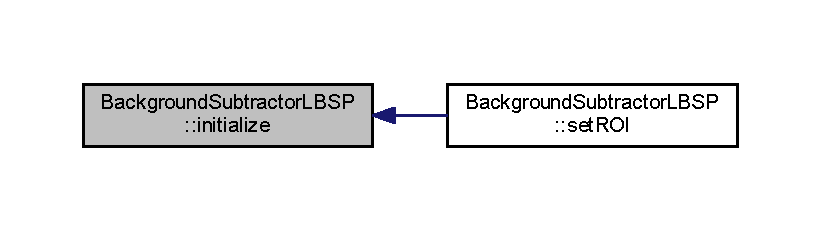
\includegraphics[width=350pt]{class_background_subtractor_l_b_s_p_ac6b854f94414497b143375d4a0ae8b6f_icgraph}
\end{center}
\end{figure}
\mbox{\Hypertarget{class_background_subtractor_l_o_b_s_t_e_r_a452bea31dcbd2e10efc701cc2cd25776}\label{class_background_subtractor_l_o_b_s_t_e_r_a452bea31dcbd2e10efc701cc2cd25776}} 
\index{Background\+Subtractor\+L\+O\+B\+S\+T\+ER@{Background\+Subtractor\+L\+O\+B\+S\+T\+ER}!initialize@{initialize}}
\index{initialize@{initialize}!Background\+Subtractor\+L\+O\+B\+S\+T\+ER@{Background\+Subtractor\+L\+O\+B\+S\+T\+ER}}
\subsubsection{\texorpdfstring{initialize()}{initialize()}\hspace{0.1cm}{\footnotesize\ttfamily [2/2]}}
{\footnotesize\ttfamily void Background\+Subtractor\+L\+O\+B\+S\+T\+E\+R\+::initialize (\begin{DoxyParamCaption}\item[{const cv\+::\+Mat \&}]{o\+Init\+Img,  }\item[{const cv\+::\+Mat \&}]{o\+R\+OI }\end{DoxyParamCaption})\hspace{0.3cm}{\ttfamily [virtual]}}



(re)initiaization method; needs to be called before starting background subtraction 



Implements \mbox{\hyperlink{class_background_subtractor_l_b_s_p_a3644bc10ec3beda6fad22c633fe0f8fb}{Background\+Subtractor\+L\+B\+SP}}.



Definition at line 29 of file Background\+Subtractor\+L\+O\+B\+S\+T\+E\+R.\+cpp.


\begin{DoxyCode}
29                                                                                      \{
30     CV\_Assert(!oInitImg.empty() && oInitImg.cols>0 && oInitImg.rows>0);
31     CV\_Assert(oInitImg.isContinuous());
32     CV\_Assert(oInitImg.type()==CV\_8UC1 || oInitImg.type()==CV\_8UC3);
33     \textcolor{keywordflow}{if}(oInitImg.type()==CV\_8UC3) \{
34         std::vector<cv::Mat> voInitImgChannels;
35         cv::split(oInitImg,voInitImgChannels);
36         \textcolor{keywordflow}{if}(!cv::countNonZero((voInitImgChannels[0]!=voInitImgChannels[1])|(voInitImgChannels[2]!=
      voInitImgChannels[1])))
37             std::cout << std::endl << \textcolor{stringliteral}{"\(\backslash\)tBackgroundSubtractorLOBSTER : Warning, grayscale images should
       always be passed in CV\_8UC1 format for optimal performance."} << std::endl;
38     \}
39     cv::Mat oNewBGROI;
40     \textcolor{keywordflow}{if}(oROI.empty() && (\mbox{\hyperlink{class_background_subtractor_l_b_s_p_a53fe98bd2489d95de5292467145901e9}{m\_oROI}}.empty() || oROI.size()!=oInitImg.size())) \{
41         oNewBGROI.create(oInitImg.size(),CV\_8UC1);
42         oNewBGROI = cv::Scalar\_<uchar>(UCHAR\_MAX);
43     \}
44     \textcolor{keywordflow}{else} \textcolor{keywordflow}{if}(oROI.empty())
45         oNewBGROI = \mbox{\hyperlink{class_background_subtractor_l_b_s_p_a53fe98bd2489d95de5292467145901e9}{m\_oROI}};
46     \textcolor{keywordflow}{else} \{
47         CV\_Assert(oROI.size()==oInitImg.size() && oROI.type()==CV\_8UC1);
48         CV\_Assert(cv::countNonZero((oROI<UCHAR\_MAX)&(oROI>0))==0);
49         oNewBGROI = oROI.clone();
50     \}
51     \mbox{\hyperlink{class_l_b_s_p_ad97557be4bc6cfd7b0fa4b01ab8f8c55}{LBSP::validateROI}}(oNewBGROI);
52     \textcolor{keyword}{const} \textcolor{keywordtype}{size\_t} nROIPxCount = (size\_t)cv::countNonZero(oNewBGROI);
53     CV\_Assert(nROIPxCount>0);
54     \mbox{\hyperlink{class_background_subtractor_l_b_s_p_a53fe98bd2489d95de5292467145901e9}{m\_oROI}} = oNewBGROI;
55     \mbox{\hyperlink{class_background_subtractor_l_b_s_p_a732d5e6ae35fb0e858cadb3af5ce08a2}{m\_oImgSize}} = oInitImg.size();
56     \mbox{\hyperlink{class_background_subtractor_l_b_s_p_a7d2f52ecd5ff56e42da86f97e0ad93b5}{m\_nImgType}} = oInitImg.type();
57     \mbox{\hyperlink{class_background_subtractor_l_b_s_p_ab3467ebee2c5d1249061ccd704cc0584}{m\_nImgChannels}} = oInitImg.channels();
58     \mbox{\hyperlink{class_background_subtractor_l_b_s_p_a9d1e247267afbddb7032bdcabd67d931}{m\_nTotPxCount}} = \mbox{\hyperlink{class_background_subtractor_l_b_s_p_a732d5e6ae35fb0e858cadb3af5ce08a2}{m\_oImgSize}}.area();
59     \mbox{\hyperlink{class_background_subtractor_l_b_s_p_ac3b54f4d2dfa3a576475214f26501d85}{m\_nTotRelevantPxCount}} = nROIPxCount;
60     \mbox{\hyperlink{class_background_subtractor_l_b_s_p_a8a2350cad84f19c68ef61b7aaf91c43f}{m\_nFrameIndex}} = 0;
61     \mbox{\hyperlink{class_background_subtractor_l_b_s_p_ab56bf775dfdf0579e834e45210c3a92a}{m\_nFramesSinceLastReset}} = 0;
62     \mbox{\hyperlink{class_background_subtractor_l_b_s_p_a5ea18d388afacf8285c46ba0f754e7ee}{m\_nModelResetCooldown}} = 0;
63     \mbox{\hyperlink{class_background_subtractor_l_b_s_p_adb6dc0af596c5592c91f9d8faa5c8a4b}{m\_oLastFGMask}}.create(\mbox{\hyperlink{class_background_subtractor_l_b_s_p_a732d5e6ae35fb0e858cadb3af5ce08a2}{m\_oImgSize}},CV\_8UC1);
64     \mbox{\hyperlink{class_background_subtractor_l_b_s_p_adb6dc0af596c5592c91f9d8faa5c8a4b}{m\_oLastFGMask}} = cv::Scalar\_<uchar>(0);
65     \mbox{\hyperlink{class_background_subtractor_l_b_s_p_ab1dc003792ab1d0b881a6fd10e0e29b3}{m\_oLastColorFrame}}.create(\mbox{\hyperlink{class_background_subtractor_l_b_s_p_a732d5e6ae35fb0e858cadb3af5ce08a2}{m\_oImgSize}},CV\_8UC((\textcolor{keywordtype}{int})
      \mbox{\hyperlink{class_background_subtractor_l_b_s_p_ab3467ebee2c5d1249061ccd704cc0584}{m\_nImgChannels}}));
66     \mbox{\hyperlink{class_background_subtractor_l_b_s_p_ab1dc003792ab1d0b881a6fd10e0e29b3}{m\_oLastColorFrame}} = cv::Scalar\_<uchar>::all(0);
67     \mbox{\hyperlink{class_background_subtractor_l_b_s_p_a9c637c0b87cac495887295690d83ba13}{m\_oLastDescFrame}}.create(\mbox{\hyperlink{class_background_subtractor_l_b_s_p_a732d5e6ae35fb0e858cadb3af5ce08a2}{m\_oImgSize}},CV\_16UC((\textcolor{keywordtype}{int})
      \mbox{\hyperlink{class_background_subtractor_l_b_s_p_ab3467ebee2c5d1249061ccd704cc0584}{m\_nImgChannels}}));
68     \mbox{\hyperlink{class_background_subtractor_l_b_s_p_a9c637c0b87cac495887295690d83ba13}{m\_oLastDescFrame}} = cv::Scalar\_<ushort>::all(0);
69     \mbox{\hyperlink{class_background_subtractor_l_o_b_s_t_e_r_ac981b39f8ae7b28d3e4326d8e6be6332}{m\_voBGColorSamples}}.resize(\mbox{\hyperlink{class_background_subtractor_l_o_b_s_t_e_r_a20c53540b952d608d849a305fd5eed89}{m\_nBGSamples}});
70     \mbox{\hyperlink{class_background_subtractor_l_o_b_s_t_e_r_a3c49866ae652423b2173215957907d04}{m\_voBGDescSamples}}.resize(\mbox{\hyperlink{class_background_subtractor_l_o_b_s_t_e_r_a20c53540b952d608d849a305fd5eed89}{m\_nBGSamples}});
71     \textcolor{keywordflow}{for}(\textcolor{keywordtype}{size\_t} s=0; s<\mbox{\hyperlink{class_background_subtractor_l_o_b_s_t_e_r_a20c53540b952d608d849a305fd5eed89}{m\_nBGSamples}}; ++s) \{
72         \mbox{\hyperlink{class_background_subtractor_l_o_b_s_t_e_r_ac981b39f8ae7b28d3e4326d8e6be6332}{m\_voBGColorSamples}}[s].create(\mbox{\hyperlink{class_background_subtractor_l_b_s_p_a732d5e6ae35fb0e858cadb3af5ce08a2}{m\_oImgSize}},CV\_8UC((\textcolor{keywordtype}{int})
      \mbox{\hyperlink{class_background_subtractor_l_b_s_p_ab3467ebee2c5d1249061ccd704cc0584}{m\_nImgChannels}}));
73         \mbox{\hyperlink{class_background_subtractor_l_o_b_s_t_e_r_ac981b39f8ae7b28d3e4326d8e6be6332}{m\_voBGColorSamples}}[s] = cv::Scalar\_<uchar>::all(0);
74         \mbox{\hyperlink{class_background_subtractor_l_o_b_s_t_e_r_a3c49866ae652423b2173215957907d04}{m\_voBGDescSamples}}[s].create(\mbox{\hyperlink{class_background_subtractor_l_b_s_p_a732d5e6ae35fb0e858cadb3af5ce08a2}{m\_oImgSize}},CV\_16UC((\textcolor{keywordtype}{int})
      \mbox{\hyperlink{class_background_subtractor_l_b_s_p_ab3467ebee2c5d1249061ccd704cc0584}{m\_nImgChannels}}));
75         \mbox{\hyperlink{class_background_subtractor_l_o_b_s_t_e_r_a3c49866ae652423b2173215957907d04}{m\_voBGDescSamples}}[s] = cv::Scalar\_<ushort>::all(0);
76     \}
77     \textcolor{keywordflow}{if}(\mbox{\hyperlink{class_background_subtractor_l_b_s_p_a06b4f0d3f24fa08bccd3c9eca085713e}{m\_aPxIdxLUT}})
78         \textcolor{keyword}{delete}[] \mbox{\hyperlink{class_background_subtractor_l_b_s_p_a06b4f0d3f24fa08bccd3c9eca085713e}{m\_aPxIdxLUT}};
79     \textcolor{keywordflow}{if}(\mbox{\hyperlink{class_background_subtractor_l_b_s_p_a74e73d4832ccdef652d93756582024db}{m\_aPxInfoLUT}})
80         \textcolor{keyword}{delete}[] \mbox{\hyperlink{class_background_subtractor_l_b_s_p_a74e73d4832ccdef652d93756582024db}{m\_aPxInfoLUT}};
81     \mbox{\hyperlink{class_background_subtractor_l_b_s_p_a06b4f0d3f24fa08bccd3c9eca085713e}{m\_aPxIdxLUT}} = \textcolor{keyword}{new} \textcolor{keywordtype}{size\_t}[\mbox{\hyperlink{class_background_subtractor_l_b_s_p_ac3b54f4d2dfa3a576475214f26501d85}{m\_nTotRelevantPxCount}}];
82     \mbox{\hyperlink{class_background_subtractor_l_b_s_p_a74e73d4832ccdef652d93756582024db}{m\_aPxInfoLUT}} = \textcolor{keyword}{new} PxInfoBase[\mbox{\hyperlink{class_background_subtractor_l_b_s_p_a9d1e247267afbddb7032bdcabd67d931}{m\_nTotPxCount}}];
83     \textcolor{keywordflow}{if}(\mbox{\hyperlink{class_background_subtractor_l_b_s_p_ab3467ebee2c5d1249061ccd704cc0584}{m\_nImgChannels}}==1) \{
84         CV\_Assert(\mbox{\hyperlink{class_background_subtractor_l_b_s_p_ab1dc003792ab1d0b881a6fd10e0e29b3}{m\_oLastColorFrame}}.step.p[0]==(\textcolor{keywordtype}{size\_t})
      \mbox{\hyperlink{class_background_subtractor_l_b_s_p_a732d5e6ae35fb0e858cadb3af5ce08a2}{m\_oImgSize}}.width && \mbox{\hyperlink{class_background_subtractor_l_b_s_p_ab1dc003792ab1d0b881a6fd10e0e29b3}{m\_oLastColorFrame}}.step.p[1]==1);
85         CV\_Assert(\mbox{\hyperlink{class_background_subtractor_l_b_s_p_a9c637c0b87cac495887295690d83ba13}{m\_oLastDescFrame}}.step.p[0]==\mbox{\hyperlink{class_background_subtractor_l_b_s_p_ab1dc003792ab1d0b881a6fd10e0e29b3}{m\_oLastColorFrame}}.step.p[0]*
      2 && \mbox{\hyperlink{class_background_subtractor_l_b_s_p_a9c637c0b87cac495887295690d83ba13}{m\_oLastDescFrame}}.step.p[1]==\mbox{\hyperlink{class_background_subtractor_l_b_s_p_ab1dc003792ab1d0b881a6fd10e0e29b3}{m\_oLastColorFrame}}.step.p[1]*2);
86         \textcolor{keywordflow}{for}(\textcolor{keywordtype}{size\_t} t=0; t<=UCHAR\_MAX; ++t)
87             \mbox{\hyperlink{class_background_subtractor_l_b_s_p_aefe69d94f08b2c4ba73ad1d254ad9153}{m\_anLBSPThreshold\_8bitLUT}}[t] = cv::saturate\_cast<uchar>((t*
      \mbox{\hyperlink{class_background_subtractor_l_b_s_p_ad759c645b14e9b16bf3940cae862df32}{m\_fRelLBSPThreshold}}+\mbox{\hyperlink{class_background_subtractor_l_b_s_p_a209eb6aaa34e8ad8e565e79f85404e24}{m\_nLBSPThresholdOffset}})/2);
88         \textcolor{keywordflow}{for}(\textcolor{keywordtype}{size\_t} nPxIter=0, nModelIter=0; nPxIter<\mbox{\hyperlink{class_background_subtractor_l_b_s_p_a9d1e247267afbddb7032bdcabd67d931}{m\_nTotPxCount}}; ++nPxIter) \{
89             \textcolor{keywordflow}{if}(\mbox{\hyperlink{class_background_subtractor_l_b_s_p_a53fe98bd2489d95de5292467145901e9}{m\_oROI}}.data[nPxIter]) \{
90                 \mbox{\hyperlink{class_background_subtractor_l_b_s_p_a06b4f0d3f24fa08bccd3c9eca085713e}{m\_aPxIdxLUT}}[nModelIter] = nPxIter;
91                 \mbox{\hyperlink{class_background_subtractor_l_b_s_p_a74e73d4832ccdef652d93756582024db}{m\_aPxInfoLUT}}[nPxIter].\mbox{\hyperlink{struct_background_subtractor_l_b_s_p_1_1_px_info_base_a42cb6eecda647b2a11b90ea420f2bc31}{nImgCoord\_Y}} = (int)nPxIter/
      \mbox{\hyperlink{class_background_subtractor_l_b_s_p_a732d5e6ae35fb0e858cadb3af5ce08a2}{m\_oImgSize}}.width;
92                 \mbox{\hyperlink{class_background_subtractor_l_b_s_p_a74e73d4832ccdef652d93756582024db}{m\_aPxInfoLUT}}[nPxIter].\mbox{\hyperlink{struct_background_subtractor_l_b_s_p_1_1_px_info_base_a10966fe72f000045adede9e853156b48}{nImgCoord\_X}} = (\textcolor{keywordtype}{int})nPxIter%
      \mbox{\hyperlink{class_background_subtractor_l_b_s_p_a732d5e6ae35fb0e858cadb3af5ce08a2}{m\_oImgSize}}.width;
93                 \mbox{\hyperlink{class_background_subtractor_l_b_s_p_a74e73d4832ccdef652d93756582024db}{m\_aPxInfoLUT}}[nPxIter].\mbox{\hyperlink{struct_background_subtractor_l_b_s_p_1_1_px_info_base_afe4a63a708fa0f3ea6ed2fac837bc71d}{nModelIdx}} = nModelIter;
94                 \mbox{\hyperlink{class_background_subtractor_l_b_s_p_ab1dc003792ab1d0b881a6fd10e0e29b3}{m\_oLastColorFrame}}.data[nPxIter] = oInitImg.data[nPxIter];
95                 \textcolor{keyword}{const} \textcolor{keywordtype}{size\_t} nDescIter = nPxIter*2;
96                 \mbox{\hyperlink{class_l_b_s_p_a4a5f635868b6b81ba53df2692ee3dfd8}{LBSP::computeGrayscaleDescriptor}}(oInitImg,oInitImg.data[
      nPxIter],\mbox{\hyperlink{class_background_subtractor_l_b_s_p_a74e73d4832ccdef652d93756582024db}{m\_aPxInfoLUT}}[nPxIter].\mbox{\hyperlink{struct_background_subtractor_l_b_s_p_1_1_px_info_base_a10966fe72f000045adede9e853156b48}{nImgCoord\_X}},\mbox{\hyperlink{class_background_subtractor_l_b_s_p_a74e73d4832ccdef652d93756582024db}{m\_aPxInfoLUT}}[nPxIter].
      \mbox{\hyperlink{struct_background_subtractor_l_b_s_p_1_1_px_info_base_a42cb6eecda647b2a11b90ea420f2bc31}{nImgCoord\_Y}},\mbox{\hyperlink{class_background_subtractor_l_b_s_p_aefe69d94f08b2c4ba73ad1d254ad9153}{m\_anLBSPThreshold\_8bitLUT}}[oInitImg.data[nPxIter]],*((ushort
      *)(\mbox{\hyperlink{class_background_subtractor_l_b_s_p_a9c637c0b87cac495887295690d83ba13}{m\_oLastDescFrame}}.data+nDescIter)));
97                 ++nModelIter;
98             \}
99         \}
100     \}
101     \textcolor{keywordflow}{else} \{ \textcolor{comment}{//m\_nImgChannels==3}
102         CV\_Assert(\mbox{\hyperlink{class_background_subtractor_l_b_s_p_ab1dc003792ab1d0b881a6fd10e0e29b3}{m\_oLastColorFrame}}.step.p[0]==(\textcolor{keywordtype}{size\_t})
      \mbox{\hyperlink{class_background_subtractor_l_b_s_p_a732d5e6ae35fb0e858cadb3af5ce08a2}{m\_oImgSize}}.width*3 && \mbox{\hyperlink{class_background_subtractor_l_b_s_p_ab1dc003792ab1d0b881a6fd10e0e29b3}{m\_oLastColorFrame}}.step.p[1]==3);
103         CV\_Assert(\mbox{\hyperlink{class_background_subtractor_l_b_s_p_a9c637c0b87cac495887295690d83ba13}{m\_oLastDescFrame}}.step.p[0]==\mbox{\hyperlink{class_background_subtractor_l_b_s_p_ab1dc003792ab1d0b881a6fd10e0e29b3}{m\_oLastColorFrame}}.step.p[0]*
      2 && \mbox{\hyperlink{class_background_subtractor_l_b_s_p_a9c637c0b87cac495887295690d83ba13}{m\_oLastDescFrame}}.step.p[1]==\mbox{\hyperlink{class_background_subtractor_l_b_s_p_ab1dc003792ab1d0b881a6fd10e0e29b3}{m\_oLastColorFrame}}.step.p[1]*2);
104         \textcolor{keywordflow}{for}(\textcolor{keywordtype}{size\_t} t=0; t<=UCHAR\_MAX; ++t)
105             \mbox{\hyperlink{class_background_subtractor_l_b_s_p_aefe69d94f08b2c4ba73ad1d254ad9153}{m\_anLBSPThreshold\_8bitLUT}}[t] = cv::saturate\_cast<uchar>(t*
      \mbox{\hyperlink{class_background_subtractor_l_b_s_p_ad759c645b14e9b16bf3940cae862df32}{m\_fRelLBSPThreshold}}+\mbox{\hyperlink{class_background_subtractor_l_b_s_p_a209eb6aaa34e8ad8e565e79f85404e24}{m\_nLBSPThresholdOffset}});
106         \textcolor{keywordflow}{for}(\textcolor{keywordtype}{size\_t} nPxIter=0, nModelIter=0; nPxIter<\mbox{\hyperlink{class_background_subtractor_l_b_s_p_a9d1e247267afbddb7032bdcabd67d931}{m\_nTotPxCount}}; ++nPxIter) \{
107             \textcolor{keywordflow}{if}(\mbox{\hyperlink{class_background_subtractor_l_b_s_p_a53fe98bd2489d95de5292467145901e9}{m\_oROI}}.data[nPxIter]) \{
108                 \mbox{\hyperlink{class_background_subtractor_l_b_s_p_a06b4f0d3f24fa08bccd3c9eca085713e}{m\_aPxIdxLUT}}[nModelIter] = nPxIter;
109                 \mbox{\hyperlink{class_background_subtractor_l_b_s_p_a74e73d4832ccdef652d93756582024db}{m\_aPxInfoLUT}}[nPxIter].\mbox{\hyperlink{struct_background_subtractor_l_b_s_p_1_1_px_info_base_a42cb6eecda647b2a11b90ea420f2bc31}{nImgCoord\_Y}} = (int)nPxIter/
      \mbox{\hyperlink{class_background_subtractor_l_b_s_p_a732d5e6ae35fb0e858cadb3af5ce08a2}{m\_oImgSize}}.width;
110                 \mbox{\hyperlink{class_background_subtractor_l_b_s_p_a74e73d4832ccdef652d93756582024db}{m\_aPxInfoLUT}}[nPxIter].\mbox{\hyperlink{struct_background_subtractor_l_b_s_p_1_1_px_info_base_a10966fe72f000045adede9e853156b48}{nImgCoord\_X}} = (\textcolor{keywordtype}{int})nPxIter%
      \mbox{\hyperlink{class_background_subtractor_l_b_s_p_a732d5e6ae35fb0e858cadb3af5ce08a2}{m\_oImgSize}}.width;
111                 \mbox{\hyperlink{class_background_subtractor_l_b_s_p_a74e73d4832ccdef652d93756582024db}{m\_aPxInfoLUT}}[nPxIter].\mbox{\hyperlink{struct_background_subtractor_l_b_s_p_1_1_px_info_base_afe4a63a708fa0f3ea6ed2fac837bc71d}{nModelIdx}} = nModelIter;
112                 \textcolor{keyword}{const} \textcolor{keywordtype}{size\_t} nPxRGBIter = nPxIter*3;
113                 \textcolor{keyword}{const} \textcolor{keywordtype}{size\_t} nDescRGBIter = nPxRGBIter*2;
114                 \textcolor{keywordflow}{for}(\textcolor{keywordtype}{size\_t} c=0; c<3; ++c) \{
115                     \mbox{\hyperlink{class_background_subtractor_l_b_s_p_ab1dc003792ab1d0b881a6fd10e0e29b3}{m\_oLastColorFrame}}.data[nPxRGBIter+c] = oInitImg.data[nPxRGBIter+c];
116                     \mbox{\hyperlink{class_l_b_s_p_a35f2abfacc0d540810d678ff5e8cd619}{LBSP::computeSingleRGBDescriptor}}(oInitImg,oInitImg.data
      [nPxRGBIter+c],\mbox{\hyperlink{class_background_subtractor_l_b_s_p_a74e73d4832ccdef652d93756582024db}{m\_aPxInfoLUT}}[nPxIter].\mbox{\hyperlink{struct_background_subtractor_l_b_s_p_1_1_px_info_base_a10966fe72f000045adede9e853156b48}{nImgCoord\_X}},
      \mbox{\hyperlink{class_background_subtractor_l_b_s_p_a74e73d4832ccdef652d93756582024db}{m\_aPxInfoLUT}}[nPxIter].\mbox{\hyperlink{struct_background_subtractor_l_b_s_p_1_1_px_info_base_a42cb6eecda647b2a11b90ea420f2bc31}{nImgCoord\_Y}},c,
      \mbox{\hyperlink{class_background_subtractor_l_b_s_p_aefe69d94f08b2c4ba73ad1d254ad9153}{m\_anLBSPThreshold\_8bitLUT}}[oInitImg.data[nPxRGBIter+c]],((ushort*)(
      \mbox{\hyperlink{class_background_subtractor_l_b_s_p_a9c637c0b87cac495887295690d83ba13}{m\_oLastDescFrame}}.data+nDescRGBIter))[c]);
117                 \}
118                 ++nModelIter;
119             \}
120         \}
121     \}
122     \mbox{\hyperlink{class_background_subtractor_l_b_s_p_a55cea104a0924fd50d5bed0912828a7e}{m\_bInitialized}} = \textcolor{keyword}{true};
123     \mbox{\hyperlink{class_background_subtractor_l_o_b_s_t_e_r_aeb3b23c1f47cfe71a73f3ca47ec06a75}{refreshModel}}(1.0\mbox{\hyperlink{rings_8cpp_a77369fc4d5326a16d2c603e032023528}{f}});
124 \}
\end{DoxyCode}
Here is the call graph for this function\+:\nopagebreak
\begin{figure}[H]
\begin{center}
\leavevmode
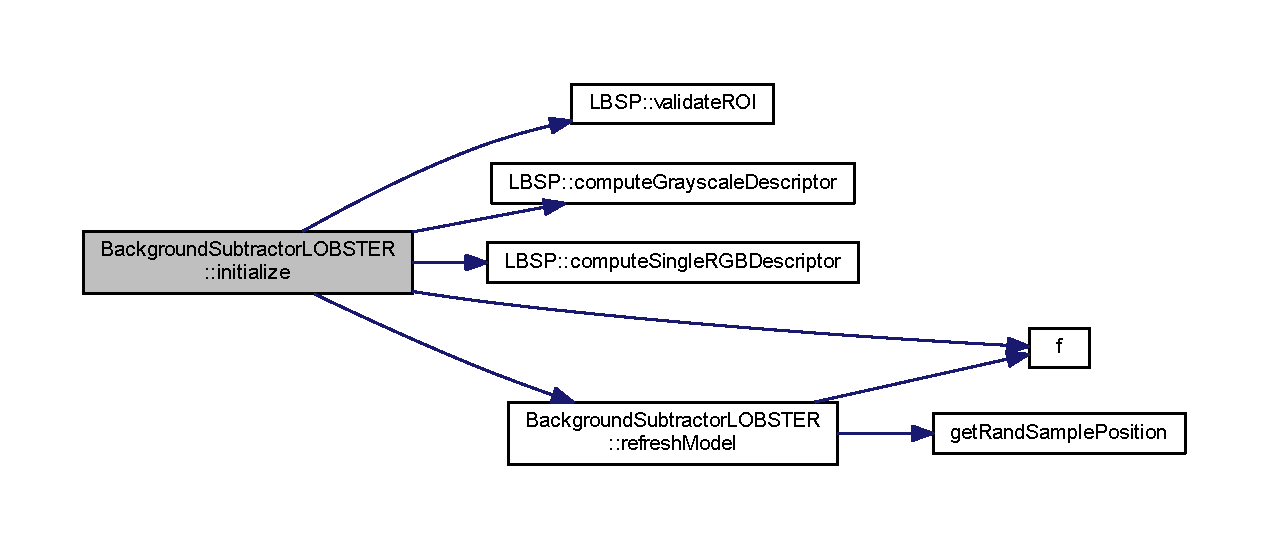
\includegraphics[width=350pt]{class_background_subtractor_l_o_b_s_t_e_r_a452bea31dcbd2e10efc701cc2cd25776_cgraph}
\end{center}
\end{figure}
\mbox{\Hypertarget{class_background_subtractor_l_o_b_s_t_e_r_a0c0faf2754a7a74a6ae56cea47207070}\label{class_background_subtractor_l_o_b_s_t_e_r_a0c0faf2754a7a74a6ae56cea47207070}} 
\index{Background\+Subtractor\+L\+O\+B\+S\+T\+ER@{Background\+Subtractor\+L\+O\+B\+S\+T\+ER}!operator()@{operator()}}
\index{operator()@{operator()}!Background\+Subtractor\+L\+O\+B\+S\+T\+ER@{Background\+Subtractor\+L\+O\+B\+S\+T\+ER}}
\subsubsection{\texorpdfstring{operator()()}{operator()()}}
{\footnotesize\ttfamily void Background\+Subtractor\+L\+O\+B\+S\+T\+E\+R\+::operator() (\begin{DoxyParamCaption}\item[{cv\+::\+Input\+Array}]{image,  }\item[{cv\+::\+Output\+Array}]{fgmask,  }\item[{double}]{learning\+Rate = {\ttfamily \mbox{\hyperlink{_background_subtractor_l_o_b_s_t_e_r_8h_a2d317f4a065c4c58c7241080d9c4457c}{B\+G\+S\+L\+O\+B\+S\+T\+E\+R\+\_\+\+D\+E\+F\+A\+U\+L\+T\+\_\+\+L\+E\+A\+R\+N\+I\+N\+G\+\_\+\+R\+A\+TE}}} }\end{DoxyParamCaption})\hspace{0.3cm}{\ttfamily [virtual]}}



primary model update function; the learning param is reinterpreted as an integer and should be $>$ 0 (smaller values == faster adaptation) 



Implements \mbox{\hyperlink{class_background_subtractor_l_b_s_p_a4771cac59b7ac865d6ec25cbf049948e}{Background\+Subtractor\+L\+B\+SP}}.



Definition at line 170 of file Background\+Subtractor\+L\+O\+B\+S\+T\+E\+R.\+cpp.


\begin{DoxyCode}
170                                                                                                            
       \{
171     CV\_Assert(\mbox{\hyperlink{class_background_subtractor_l_b_s_p_a55cea104a0924fd50d5bed0912828a7e}{m\_bInitialized}});
172     CV\_Assert(learningRate>0);
173     cv::Mat oInputImg = \_image.getMat();
174     CV\_Assert(oInputImg.type()==\mbox{\hyperlink{class_background_subtractor_l_b_s_p_a7d2f52ecd5ff56e42da86f97e0ad93b5}{m\_nImgType}} && oInputImg.size()==
      \mbox{\hyperlink{class_background_subtractor_l_b_s_p_a732d5e6ae35fb0e858cadb3af5ce08a2}{m\_oImgSize}});
175     CV\_Assert(oInputImg.isContinuous());
176     \_fgmask.create(\mbox{\hyperlink{class_background_subtractor_l_b_s_p_a732d5e6ae35fb0e858cadb3af5ce08a2}{m\_oImgSize}},CV\_8UC1);
177     cv::Mat oCurrFGMask = \_fgmask.getMat();
178     oCurrFGMask = cv::Scalar\_<uchar>(0);
179     \textcolor{keyword}{const} \textcolor{keywordtype}{size\_t} nLearningRate = (size\_t)ceil(learningRate);
180     \textcolor{keywordflow}{if}(\mbox{\hyperlink{class_background_subtractor_l_b_s_p_ab3467ebee2c5d1249061ccd704cc0584}{m\_nImgChannels}}==1) \{
181         \textcolor{keywordflow}{for}(\textcolor{keywordtype}{size\_t} nModelIter=0; nModelIter<\mbox{\hyperlink{class_background_subtractor_l_b_s_p_ac3b54f4d2dfa3a576475214f26501d85}{m\_nTotRelevantPxCount}}; ++nModelIter) \{
182             \textcolor{keyword}{const} \textcolor{keywordtype}{size\_t} nPxIter = \mbox{\hyperlink{class_background_subtractor_l_b_s_p_a06b4f0d3f24fa08bccd3c9eca085713e}{m\_aPxIdxLUT}}[nModelIter];
183             \textcolor{keyword}{const} \textcolor{keywordtype}{size\_t} nDescIter = nPxIter*2;
184             \textcolor{keyword}{const} \textcolor{keywordtype}{int} nCurrImgCoord\_X = \mbox{\hyperlink{class_background_subtractor_l_b_s_p_a74e73d4832ccdef652d93756582024db}{m\_aPxInfoLUT}}[nPxIter].
      \mbox{\hyperlink{struct_background_subtractor_l_b_s_p_1_1_px_info_base_a10966fe72f000045adede9e853156b48}{nImgCoord\_X}};
185             \textcolor{keyword}{const} \textcolor{keywordtype}{int} nCurrImgCoord\_Y = \mbox{\hyperlink{class_background_subtractor_l_b_s_p_a74e73d4832ccdef652d93756582024db}{m\_aPxInfoLUT}}[nPxIter].
      \mbox{\hyperlink{struct_background_subtractor_l_b_s_p_1_1_px_info_base_a42cb6eecda647b2a11b90ea420f2bc31}{nImgCoord\_Y}};
186             \textcolor{keyword}{const} uchar nCurrColor = oInputImg.data[nPxIter];
187             \textcolor{keywordtype}{size\_t} nGoodSamplesCount=0, nModelIdx=0;
188             ushort nCurrInputDesc;
189             \textcolor{keywordflow}{while}(nGoodSamplesCount<\mbox{\hyperlink{class_background_subtractor_l_o_b_s_t_e_r_acb558aefc1b6205a63c1906b6fd1eeff}{m\_nRequiredBGSamples}} && nModelIdx<
      \mbox{\hyperlink{class_background_subtractor_l_o_b_s_t_e_r_a20c53540b952d608d849a305fd5eed89}{m\_nBGSamples}}) \{
190                 \textcolor{keyword}{const} uchar nBGColor = \mbox{\hyperlink{class_background_subtractor_l_o_b_s_t_e_r_ac981b39f8ae7b28d3e4326d8e6be6332}{m\_voBGColorSamples}}[nModelIdx].data[nPxIter];
191                 \{
192                     \textcolor{keyword}{const} \textcolor{keywordtype}{size\_t} nColorDist = \mbox{\hyperlink{_distance_utils_8h_ab6ec458f6d3fb6fb4e6cda3808e61703}{L1dist}}(nCurrColor,nBGColor);
193                     \textcolor{keywordflow}{if}(nColorDist>\mbox{\hyperlink{class_background_subtractor_l_o_b_s_t_e_r_a37a37a0a46fc8e33d954c33c1318d7b2}{m\_nColorDistThreshold}}/2)
194                         \textcolor{keywordflow}{goto} failedcheck1ch;
195                     \mbox{\hyperlink{class_l_b_s_p_a4a5f635868b6b81ba53df2692ee3dfd8}{LBSP::computeGrayscaleDescriptor}}(oInputImg,nBGColor,
      nCurrImgCoord\_X,nCurrImgCoord\_Y,\mbox{\hyperlink{class_background_subtractor_l_b_s_p_aefe69d94f08b2c4ba73ad1d254ad9153}{m\_anLBSPThreshold\_8bitLUT}}[nBGColor],nCurrInputDesc);
196                     \textcolor{keyword}{const} \textcolor{keywordtype}{size\_t} nDescDist = \mbox{\hyperlink{_distance_utils_8h_ab13812ef6e21af771d6c0a856cd941b0}{hdist}}(nCurrInputDesc,*((ushort*)(
      \mbox{\hyperlink{class_background_subtractor_l_o_b_s_t_e_r_a3c49866ae652423b2173215957907d04}{m\_voBGDescSamples}}[nModelIdx].data+nDescIter)));
197                     \textcolor{keywordflow}{if}(nDescDist>\mbox{\hyperlink{class_background_subtractor_l_o_b_s_t_e_r_abe3f4a836343e901746e4f243f5252e4}{m\_nDescDistThreshold}})
198                         \textcolor{keywordflow}{goto} failedcheck1ch;
199                     nGoodSamplesCount++;
200                 \}
201                 failedcheck1ch:
202                 nModelIdx++;
203             \}
204             \textcolor{keywordflow}{if}(nGoodSamplesCount<\mbox{\hyperlink{class_background_subtractor_l_o_b_s_t_e_r_acb558aefc1b6205a63c1906b6fd1eeff}{m\_nRequiredBGSamples}})
205                 oCurrFGMask.data[nPxIter] = UCHAR\_MAX;
206             \textcolor{keywordflow}{else} \{
207                 \textcolor{keywordflow}{if}((rand()%nLearningRate)==0) \{
208                     \textcolor{keyword}{const} \textcolor{keywordtype}{size\_t} nSampleModelIdx = rand()%\mbox{\hyperlink{class_background_subtractor_l_o_b_s_t_e_r_a20c53540b952d608d849a305fd5eed89}{m\_nBGSamples}};
209                     ushort& nRandInputDesc = *((ushort*)(\mbox{\hyperlink{class_background_subtractor_l_o_b_s_t_e_r_a3c49866ae652423b2173215957907d04}{m\_voBGDescSamples}}[nSampleModelIdx
      ].data+nDescIter));
210                     \mbox{\hyperlink{class_l_b_s_p_a4a5f635868b6b81ba53df2692ee3dfd8}{LBSP::computeGrayscaleDescriptor}}(oInputImg,nCurrColor,
      nCurrImgCoord\_X,nCurrImgCoord\_Y,\mbox{\hyperlink{class_background_subtractor_l_b_s_p_aefe69d94f08b2c4ba73ad1d254ad9153}{m\_anLBSPThreshold\_8bitLUT}}[nCurrColor],nRandInputDesc
      );
211                     \mbox{\hyperlink{class_background_subtractor_l_o_b_s_t_e_r_ac981b39f8ae7b28d3e4326d8e6be6332}{m\_voBGColorSamples}}[nSampleModelIdx].data[nPxIter] = nCurrColor;
212                 \}
213                 \textcolor{keywordflow}{if}((rand()%nLearningRate)==0) \{
214                     \textcolor{keywordtype}{int} nSampleImgCoord\_Y, nSampleImgCoord\_X;
215                     \mbox{\hyperlink{_rand_utils_8h_a76b18bef397ed044a6db9e3a63c69f69}{getRandNeighborPosition\_3x3}}(nSampleImgCoord\_X,
      nSampleImgCoord\_Y,nCurrImgCoord\_X,nCurrImgCoord\_Y,\mbox{\hyperlink{class_l_b_s_p_aa98abb79a155d3a2b416c2ab32e74929}{LBSP::PATCH\_SIZE}}/2,\mbox{\hyperlink{class_background_subtractor_l_b_s_p_a732d5e6ae35fb0e858cadb3af5ce08a2}{m\_oImgSize}});
216                     \textcolor{keyword}{const} \textcolor{keywordtype}{size\_t} nSampleModelIdx = rand()%\mbox{\hyperlink{class_background_subtractor_l_o_b_s_t_e_r_a20c53540b952d608d849a305fd5eed89}{m\_nBGSamples}};
217                     ushort& nRandInputDesc = \mbox{\hyperlink{class_background_subtractor_l_o_b_s_t_e_r_a3c49866ae652423b2173215957907d04}{m\_voBGDescSamples}}[nSampleModelIdx].at<ushort>
      (nSampleImgCoord\_Y,nSampleImgCoord\_X);
218                     \mbox{\hyperlink{class_l_b_s_p_a4a5f635868b6b81ba53df2692ee3dfd8}{LBSP::computeGrayscaleDescriptor}}(oInputImg,nCurrColor,
      nCurrImgCoord\_X,nCurrImgCoord\_Y,\mbox{\hyperlink{class_background_subtractor_l_b_s_p_aefe69d94f08b2c4ba73ad1d254ad9153}{m\_anLBSPThreshold\_8bitLUT}}[nCurrColor],nRandInputDesc
      );
219                     \mbox{\hyperlink{class_background_subtractor_l_o_b_s_t_e_r_ac981b39f8ae7b28d3e4326d8e6be6332}{m\_voBGColorSamples}}[nSampleModelIdx].at<uchar>(nSampleImgCoord\_Y,
      nSampleImgCoord\_X) = nCurrColor;
220                 \}
221             \}
222         \}
223     \}
224     \textcolor{keywordflow}{else} \{ \textcolor{comment}{//m\_nImgChannels==3}
225         \textcolor{keyword}{const} \textcolor{keywordtype}{size\_t} nCurrDescDistThreshold = \mbox{\hyperlink{class_background_subtractor_l_o_b_s_t_e_r_abe3f4a836343e901746e4f243f5252e4}{m\_nDescDistThreshold}}*3;
226         \textcolor{keyword}{const} \textcolor{keywordtype}{size\_t} nCurrColorDistThreshold = \mbox{\hyperlink{class_background_subtractor_l_o_b_s_t_e_r_a37a37a0a46fc8e33d954c33c1318d7b2}{m\_nColorDistThreshold}}*3;
227         \textcolor{keyword}{const} \textcolor{keywordtype}{size\_t} nCurrSCDescDistThreshold = nCurrDescDistThreshold/2;
228         \textcolor{keyword}{const} \textcolor{keywordtype}{size\_t} nCurrSCColorDistThreshold = nCurrColorDistThreshold/2;
229         \textcolor{keyword}{const} \textcolor{keywordtype}{size\_t} desc\_row\_step = \mbox{\hyperlink{class_background_subtractor_l_o_b_s_t_e_r_a3c49866ae652423b2173215957907d04}{m\_voBGDescSamples}}[0].step.p[0];
230         \textcolor{keyword}{const} \textcolor{keywordtype}{size\_t} img\_row\_step = \mbox{\hyperlink{class_background_subtractor_l_o_b_s_t_e_r_ac981b39f8ae7b28d3e4326d8e6be6332}{m\_voBGColorSamples}}[0].step.p[0];
231         \textcolor{keywordflow}{for}(\textcolor{keywordtype}{size\_t} nModelIter=0; nModelIter<\mbox{\hyperlink{class_background_subtractor_l_b_s_p_ac3b54f4d2dfa3a576475214f26501d85}{m\_nTotRelevantPxCount}}; ++nModelIter) \{
232             \textcolor{keyword}{const} \textcolor{keywordtype}{size\_t} nPxIter = \mbox{\hyperlink{class_background_subtractor_l_b_s_p_a06b4f0d3f24fa08bccd3c9eca085713e}{m\_aPxIdxLUT}}[nModelIter];
233             \textcolor{keyword}{const} \textcolor{keywordtype}{int} nCurrImgCoord\_X = \mbox{\hyperlink{class_background_subtractor_l_b_s_p_a74e73d4832ccdef652d93756582024db}{m\_aPxInfoLUT}}[nPxIter].
      \mbox{\hyperlink{struct_background_subtractor_l_b_s_p_1_1_px_info_base_a10966fe72f000045adede9e853156b48}{nImgCoord\_X}};
234             \textcolor{keyword}{const} \textcolor{keywordtype}{int} nCurrImgCoord\_Y = \mbox{\hyperlink{class_background_subtractor_l_b_s_p_a74e73d4832ccdef652d93756582024db}{m\_aPxInfoLUT}}[nPxIter].
      \mbox{\hyperlink{struct_background_subtractor_l_b_s_p_1_1_px_info_base_a42cb6eecda647b2a11b90ea420f2bc31}{nImgCoord\_Y}};
235             \textcolor{keyword}{const} \textcolor{keywordtype}{size\_t} nPxIterRGB = nPxIter*3;
236             \textcolor{keyword}{const} \textcolor{keywordtype}{size\_t} nDescIterRGB = nPxIterRGB*2;
237             \textcolor{keyword}{const} uchar* \textcolor{keyword}{const} anCurrColor = oInputImg.data+nPxIterRGB;
238             \textcolor{keywordtype}{size\_t} nGoodSamplesCount=0, nModelIdx=0;
239             ushort anCurrInputDesc[3];
240             \textcolor{keywordflow}{while}(nGoodSamplesCount<\mbox{\hyperlink{class_background_subtractor_l_o_b_s_t_e_r_acb558aefc1b6205a63c1906b6fd1eeff}{m\_nRequiredBGSamples}} && nModelIdx<
      \mbox{\hyperlink{class_background_subtractor_l_o_b_s_t_e_r_a20c53540b952d608d849a305fd5eed89}{m\_nBGSamples}}) \{
241                 \textcolor{keyword}{const} ushort* \textcolor{keyword}{const} anBGDesc = (ushort*)(\mbox{\hyperlink{class_background_subtractor_l_o_b_s_t_e_r_a3c49866ae652423b2173215957907d04}{m\_voBGDescSamples}}[nModelIdx].data
      +nDescIterRGB);
242                 \textcolor{keyword}{const} uchar* \textcolor{keyword}{const} anBGColor = \mbox{\hyperlink{class_background_subtractor_l_o_b_s_t_e_r_ac981b39f8ae7b28d3e4326d8e6be6332}{m\_voBGColorSamples}}[nModelIdx].data+
      nPxIterRGB;
243                 \textcolor{keywordtype}{size\_t} nTotColorDist = 0;
244                 \textcolor{keywordtype}{size\_t} nTotDescDist = 0;
245                 \textcolor{keywordflow}{for}(\textcolor{keywordtype}{size\_t} c=0;c<3; ++c) \{
246                     \textcolor{keyword}{const} \textcolor{keywordtype}{size\_t} nColorDist = \mbox{\hyperlink{_distance_utils_8h_ab6ec458f6d3fb6fb4e6cda3808e61703}{L1dist}}(anCurrColor[c],anBGColor[c]);
247                     \textcolor{keywordflow}{if}(nColorDist>nCurrSCColorDistThreshold)
248                         \textcolor{keywordflow}{goto} failedcheck3ch;
249                     \mbox{\hyperlink{class_l_b_s_p_a35f2abfacc0d540810d678ff5e8cd619}{LBSP::computeSingleRGBDescriptor}}(oInputImg,anBGColor[c]
      ,nCurrImgCoord\_X,nCurrImgCoord\_Y,c,\mbox{\hyperlink{class_background_subtractor_l_b_s_p_aefe69d94f08b2c4ba73ad1d254ad9153}{m\_anLBSPThreshold\_8bitLUT}}[anBGColor[c]],
      anCurrInputDesc[c]);
250                     \textcolor{keyword}{const} \textcolor{keywordtype}{size\_t} nDescDist = \mbox{\hyperlink{_distance_utils_8h_ab13812ef6e21af771d6c0a856cd941b0}{hdist}}(anCurrInputDesc[c],anBGDesc[c]);
251                     \textcolor{keywordflow}{if}(nDescDist>nCurrSCDescDistThreshold)
252                         \textcolor{keywordflow}{goto} failedcheck3ch;
253                     nTotColorDist += nColorDist;
254                     nTotDescDist += nDescDist;
255                 \}
256                 \textcolor{keywordflow}{if}(nTotDescDist<=nCurrDescDistThreshold && nTotColorDist<=nCurrColorDistThreshold)
257                     nGoodSamplesCount++;
258                 failedcheck3ch:
259                 nModelIdx++;
260             \}
261             \textcolor{keywordflow}{if}(nGoodSamplesCount<\mbox{\hyperlink{class_background_subtractor_l_o_b_s_t_e_r_acb558aefc1b6205a63c1906b6fd1eeff}{m\_nRequiredBGSamples}})
262                 oCurrFGMask.data[nPxIter] = UCHAR\_MAX;
263             \textcolor{keywordflow}{else} \{
264                 \textcolor{keywordflow}{if}((rand()%nLearningRate)==0) \{
265                     \textcolor{keyword}{const} \textcolor{keywordtype}{size\_t} nSampleModelIdx = rand()%\mbox{\hyperlink{class_background_subtractor_l_o_b_s_t_e_r_a20c53540b952d608d849a305fd5eed89}{m\_nBGSamples}};
266                     ushort* anRandInputDesc = ((ushort*)(\mbox{\hyperlink{class_background_subtractor_l_o_b_s_t_e_r_a3c49866ae652423b2173215957907d04}{m\_voBGDescSamples}}[nSampleModelIdx
      ].data+nDescIterRGB));
267                     \textcolor{keyword}{const} \textcolor{keywordtype}{size\_t} anCurrIntraLBSPThresholds[3] = \{
      \mbox{\hyperlink{class_background_subtractor_l_b_s_p_aefe69d94f08b2c4ba73ad1d254ad9153}{m\_anLBSPThreshold\_8bitLUT}}[anCurrColor[0]],
      \mbox{\hyperlink{class_background_subtractor_l_b_s_p_aefe69d94f08b2c4ba73ad1d254ad9153}{m\_anLBSPThreshold\_8bitLUT}}[anCurrColor[1]],
      \mbox{\hyperlink{class_background_subtractor_l_b_s_p_aefe69d94f08b2c4ba73ad1d254ad9153}{m\_anLBSPThreshold\_8bitLUT}}[anCurrColor[2]]\};
268                     \mbox{\hyperlink{class_l_b_s_p_a27a44cb6f6e3015ee26047bd3d84f892}{LBSP::computeRGBDescriptor}}(oInputImg,anCurrColor,
      nCurrImgCoord\_X,nCurrImgCoord\_Y,anCurrIntraLBSPThresholds,anRandInputDesc);
269                     \textcolor{keywordflow}{for}(\textcolor{keywordtype}{size\_t} c=0; c<3; ++c)
270                         *(\mbox{\hyperlink{class_background_subtractor_l_o_b_s_t_e_r_ac981b39f8ae7b28d3e4326d8e6be6332}{m\_voBGColorSamples}}[nSampleModelIdx].data+nPxIterRGB+c) = 
      anCurrColor[c];
271                 \}
272                 \textcolor{keywordflow}{if}((rand()%nLearningRate)==0) \{
273                     \textcolor{keywordtype}{int} nSampleImgCoord\_Y, nSampleImgCoord\_X;
274                     \mbox{\hyperlink{_rand_utils_8h_a76b18bef397ed044a6db9e3a63c69f69}{getRandNeighborPosition\_3x3}}(nSampleImgCoord\_X,
      nSampleImgCoord\_Y,nCurrImgCoord\_X,nCurrImgCoord\_Y,\mbox{\hyperlink{class_l_b_s_p_aa98abb79a155d3a2b416c2ab32e74929}{LBSP::PATCH\_SIZE}}/2,\mbox{\hyperlink{class_background_subtractor_l_b_s_p_a732d5e6ae35fb0e858cadb3af5ce08a2}{m\_oImgSize}});
275                     \textcolor{keyword}{const} \textcolor{keywordtype}{size\_t} nSampleModelIdx = rand()%\mbox{\hyperlink{class_background_subtractor_l_o_b_s_t_e_r_a20c53540b952d608d849a305fd5eed89}{m\_nBGSamples}};
276                     ushort* anRandInputDesc = ((ushort*)(\mbox{\hyperlink{class_background_subtractor_l_o_b_s_t_e_r_a3c49866ae652423b2173215957907d04}{m\_voBGDescSamples}}[nSampleModelIdx
      ].data + desc\_row\_step*nSampleImgCoord\_Y + 6*nSampleImgCoord\_X));
277                     \textcolor{keyword}{const} \textcolor{keywordtype}{size\_t} anCurrIntraLBSPThresholds[3] = \{
      \mbox{\hyperlink{class_background_subtractor_l_b_s_p_aefe69d94f08b2c4ba73ad1d254ad9153}{m\_anLBSPThreshold\_8bitLUT}}[anCurrColor[0]],
      \mbox{\hyperlink{class_background_subtractor_l_b_s_p_aefe69d94f08b2c4ba73ad1d254ad9153}{m\_anLBSPThreshold\_8bitLUT}}[anCurrColor[1]],
      \mbox{\hyperlink{class_background_subtractor_l_b_s_p_aefe69d94f08b2c4ba73ad1d254ad9153}{m\_anLBSPThreshold\_8bitLUT}}[anCurrColor[2]]\};
278                     \mbox{\hyperlink{class_l_b_s_p_a27a44cb6f6e3015ee26047bd3d84f892}{LBSP::computeRGBDescriptor}}(oInputImg,anCurrColor,
      nCurrImgCoord\_X,nCurrImgCoord\_Y,anCurrIntraLBSPThresholds,anRandInputDesc);
279                     \textcolor{keywordflow}{for}(\textcolor{keywordtype}{size\_t} c=0; c<3; ++c)
280                         *(\mbox{\hyperlink{class_background_subtractor_l_o_b_s_t_e_r_ac981b39f8ae7b28d3e4326d8e6be6332}{m\_voBGColorSamples}}[nSampleModelIdx].data + img\_row\_step*
      nSampleImgCoord\_Y + 3*nSampleImgCoord\_X + c) = anCurrColor[c];
281                 \}
282             \}
283         \}
284     \}
285     cv::medianBlur(oCurrFGMask,\mbox{\hyperlink{class_background_subtractor_l_b_s_p_adb6dc0af596c5592c91f9d8faa5c8a4b}{m\_oLastFGMask}},
      \mbox{\hyperlink{class_background_subtractor_l_b_s_p_a2585fe6e41e10af6da3e325dc20fe7f1}{m\_nDefaultMedianBlurKernelSize}});
286     \mbox{\hyperlink{class_background_subtractor_l_b_s_p_adb6dc0af596c5592c91f9d8faa5c8a4b}{m\_oLastFGMask}}.copyTo(oCurrFGMask);
287 \}
\end{DoxyCode}
Here is the call graph for this function\+:\nopagebreak
\begin{figure}[H]
\begin{center}
\leavevmode
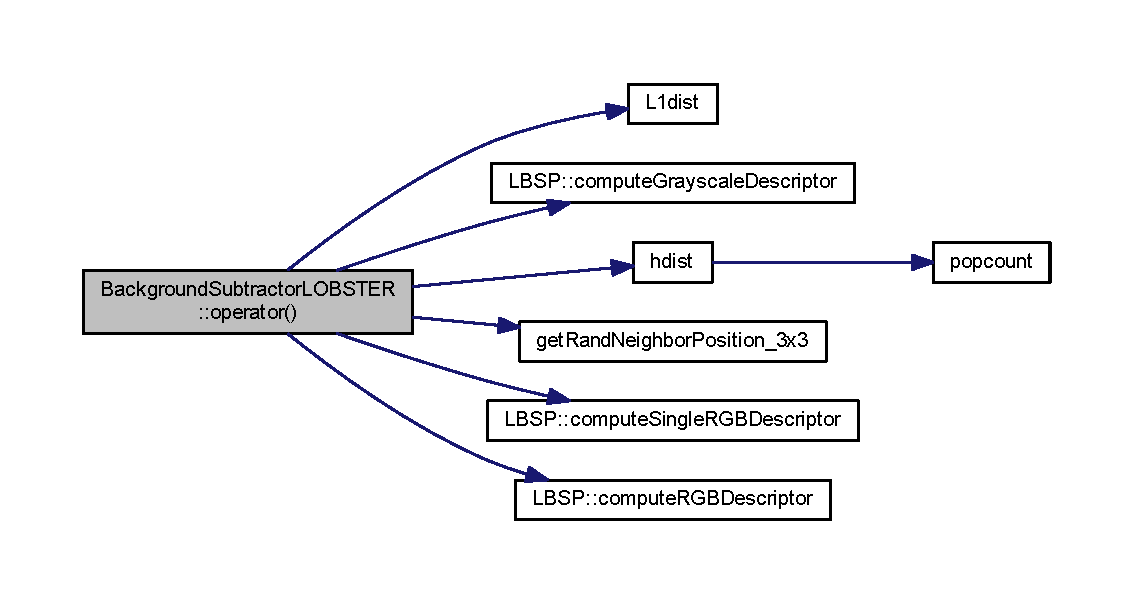
\includegraphics[width=350pt]{class_background_subtractor_l_o_b_s_t_e_r_a0c0faf2754a7a74a6ae56cea47207070_cgraph}
\end{center}
\end{figure}
\mbox{\Hypertarget{class_background_subtractor_l_o_b_s_t_e_r_aeb3b23c1f47cfe71a73f3ca47ec06a75}\label{class_background_subtractor_l_o_b_s_t_e_r_aeb3b23c1f47cfe71a73f3ca47ec06a75}} 
\index{Background\+Subtractor\+L\+O\+B\+S\+T\+ER@{Background\+Subtractor\+L\+O\+B\+S\+T\+ER}!refresh\+Model@{refresh\+Model}}
\index{refresh\+Model@{refresh\+Model}!Background\+Subtractor\+L\+O\+B\+S\+T\+ER@{Background\+Subtractor\+L\+O\+B\+S\+T\+ER}}
\subsubsection{\texorpdfstring{refresh\+Model()}{refreshModel()}}
{\footnotesize\ttfamily void Background\+Subtractor\+L\+O\+B\+S\+T\+E\+R\+::refresh\+Model (\begin{DoxyParamCaption}\item[{float}]{f\+Samples\+Refresh\+Frac,  }\item[{bool}]{b\+Force\+F\+G\+Update = {\ttfamily false} }\end{DoxyParamCaption})\hspace{0.3cm}{\ttfamily [virtual]}}



refreshes all samples based on the last analyzed frame 



Definition at line 126 of file Background\+Subtractor\+L\+O\+B\+S\+T\+E\+R.\+cpp.


\begin{DoxyCode}
126                                                                                              \{
127     \textcolor{comment}{// == refresh}
128     CV\_Assert(\mbox{\hyperlink{class_background_subtractor_l_b_s_p_a55cea104a0924fd50d5bed0912828a7e}{m\_bInitialized}});
129     CV\_Assert(fSamplesRefreshFrac>0.0\mbox{\hyperlink{rings_8cpp_a77369fc4d5326a16d2c603e032023528}{f}} && fSamplesRefreshFrac<=1.0\mbox{\hyperlink{rings_8cpp_a77369fc4d5326a16d2c603e032023528}{f}});
130     \textcolor{keyword}{const} \textcolor{keywordtype}{size\_t} nModelsToRefresh = fSamplesRefreshFrac<1.0f?(size\_t)(fSamplesRefreshFrac*
      \mbox{\hyperlink{class_background_subtractor_l_o_b_s_t_e_r_a20c53540b952d608d849a305fd5eed89}{m\_nBGSamples}}):\mbox{\hyperlink{class_background_subtractor_l_o_b_s_t_e_r_a20c53540b952d608d849a305fd5eed89}{m\_nBGSamples}};
131     \textcolor{keyword}{const} \textcolor{keywordtype}{size\_t} nRefreshStartPos = fSamplesRefreshFrac<1.0f?rand()%\mbox{\hyperlink{class_background_subtractor_l_o_b_s_t_e_r_a20c53540b952d608d849a305fd5eed89}{m\_nBGSamples}}:0;
132     \textcolor{keywordflow}{if}(\mbox{\hyperlink{class_background_subtractor_l_b_s_p_ab3467ebee2c5d1249061ccd704cc0584}{m\_nImgChannels}}==1) \{
133         \textcolor{keywordflow}{for}(\textcolor{keywordtype}{size\_t} nModelIter=0; nModelIter<\mbox{\hyperlink{class_background_subtractor_l_b_s_p_ac3b54f4d2dfa3a576475214f26501d85}{m\_nTotRelevantPxCount}}; ++nModelIter) \{
134             \textcolor{keyword}{const} \textcolor{keywordtype}{size\_t} nPxIter = \mbox{\hyperlink{class_background_subtractor_l_b_s_p_a06b4f0d3f24fa08bccd3c9eca085713e}{m\_aPxIdxLUT}}[nModelIter];
135             \textcolor{keywordflow}{if}(bForceFGUpdate || !\mbox{\hyperlink{class_background_subtractor_l_b_s_p_adb6dc0af596c5592c91f9d8faa5c8a4b}{m\_oLastFGMask}}.data[nPxIter]) \{
136                 \textcolor{keywordflow}{for}(\textcolor{keywordtype}{size\_t} nCurrModelIdx=nRefreshStartPos; nCurrModelIdx<nRefreshStartPos+nModelsToRefresh;
       ++nCurrModelIdx) \{
137                     \textcolor{keywordtype}{int} nSampleImgCoord\_Y, nSampleImgCoord\_X;
138                     \mbox{\hyperlink{_rand_utils_8h_aad1feb1fa9a8e94c8fac60b9a01e1a5b}{getRandSamplePosition}}(nSampleImgCoord\_X,nSampleImgCoord\_Y,
      \mbox{\hyperlink{class_background_subtractor_l_b_s_p_a74e73d4832ccdef652d93756582024db}{m\_aPxInfoLUT}}[nPxIter].nImgCoord\_X,\mbox{\hyperlink{class_background_subtractor_l_b_s_p_a74e73d4832ccdef652d93756582024db}{m\_aPxInfoLUT}}[nPxIter].nImgCoord\_Y,
      \mbox{\hyperlink{class_l_b_s_p_aa98abb79a155d3a2b416c2ab32e74929}{LBSP::PATCH\_SIZE}}/2,\mbox{\hyperlink{class_background_subtractor_l_b_s_p_a732d5e6ae35fb0e858cadb3af5ce08a2}{m\_oImgSize}});
139                     \textcolor{keyword}{const} \textcolor{keywordtype}{size\_t} nSamplePxIdx = \mbox{\hyperlink{class_background_subtractor_l_b_s_p_a732d5e6ae35fb0e858cadb3af5ce08a2}{m\_oImgSize}}.width*nSampleImgCoord\_Y + 
      nSampleImgCoord\_X;
140                     \textcolor{keywordflow}{if}(bForceFGUpdate || !\mbox{\hyperlink{class_background_subtractor_l_b_s_p_adb6dc0af596c5592c91f9d8faa5c8a4b}{m\_oLastFGMask}}.data[nSamplePxIdx]) \{
141                         \textcolor{keyword}{const} \textcolor{keywordtype}{size\_t} nCurrRealModelIdx = nCurrModelIdx%
      \mbox{\hyperlink{class_background_subtractor_l_o_b_s_t_e_r_a20c53540b952d608d849a305fd5eed89}{m\_nBGSamples}};
142                         \mbox{\hyperlink{class_background_subtractor_l_o_b_s_t_e_r_ac981b39f8ae7b28d3e4326d8e6be6332}{m\_voBGColorSamples}}[nCurrRealModelIdx].data[nPxIter] = 
      \mbox{\hyperlink{class_background_subtractor_l_b_s_p_ab1dc003792ab1d0b881a6fd10e0e29b3}{m\_oLastColorFrame}}.data[nSamplePxIdx];
143                         *((ushort*)(\mbox{\hyperlink{class_background_subtractor_l_o_b_s_t_e_r_a3c49866ae652423b2173215957907d04}{m\_voBGDescSamples}}[nCurrRealModelIdx].data+nPxIter*2)) 
      = *((ushort*)(\mbox{\hyperlink{class_background_subtractor_l_b_s_p_a9c637c0b87cac495887295690d83ba13}{m\_oLastDescFrame}}.data+nSamplePxIdx*2));
144                     \}
145                 \}
146             \}
147         \}
148     \}
149     \textcolor{keywordflow}{else} \{ \textcolor{comment}{//m\_nImgChannels==3}
150         \textcolor{keywordflow}{for}(\textcolor{keywordtype}{size\_t} nModelIter=0; nModelIter<\mbox{\hyperlink{class_background_subtractor_l_b_s_p_ac3b54f4d2dfa3a576475214f26501d85}{m\_nTotRelevantPxCount}}; ++nModelIter) \{
151             \textcolor{keyword}{const} \textcolor{keywordtype}{size\_t} nPxIter = \mbox{\hyperlink{class_background_subtractor_l_b_s_p_a06b4f0d3f24fa08bccd3c9eca085713e}{m\_aPxIdxLUT}}[nModelIter];
152             \textcolor{keywordflow}{if}(bForceFGUpdate || !\mbox{\hyperlink{class_background_subtractor_l_b_s_p_adb6dc0af596c5592c91f9d8faa5c8a4b}{m\_oLastFGMask}}.data[nPxIter]) \{
153                 \textcolor{keywordflow}{for}(\textcolor{keywordtype}{size\_t} nCurrModelIdx=nRefreshStartPos; nCurrModelIdx<nRefreshStartPos+nModelsToRefresh;
       ++nCurrModelIdx) \{
154                     \textcolor{keywordtype}{int} nSampleImgCoord\_Y, nSampleImgCoord\_X;
155                     \mbox{\hyperlink{_rand_utils_8h_aad1feb1fa9a8e94c8fac60b9a01e1a5b}{getRandSamplePosition}}(nSampleImgCoord\_X,nSampleImgCoord\_Y,
      \mbox{\hyperlink{class_background_subtractor_l_b_s_p_a74e73d4832ccdef652d93756582024db}{m\_aPxInfoLUT}}[nPxIter].nImgCoord\_X,\mbox{\hyperlink{class_background_subtractor_l_b_s_p_a74e73d4832ccdef652d93756582024db}{m\_aPxInfoLUT}}[nPxIter].nImgCoord\_Y,
      \mbox{\hyperlink{class_l_b_s_p_aa98abb79a155d3a2b416c2ab32e74929}{LBSP::PATCH\_SIZE}}/2,\mbox{\hyperlink{class_background_subtractor_l_b_s_p_a732d5e6ae35fb0e858cadb3af5ce08a2}{m\_oImgSize}});
156                     \textcolor{keyword}{const} \textcolor{keywordtype}{size\_t} nSamplePxIdx = \mbox{\hyperlink{class_background_subtractor_l_b_s_p_a732d5e6ae35fb0e858cadb3af5ce08a2}{m\_oImgSize}}.width*nSampleImgCoord\_Y + 
      nSampleImgCoord\_X;
157                     \textcolor{keywordflow}{if}(bForceFGUpdate || !\mbox{\hyperlink{class_background_subtractor_l_b_s_p_adb6dc0af596c5592c91f9d8faa5c8a4b}{m\_oLastFGMask}}.data[nSamplePxIdx]) \{
158                         \textcolor{keyword}{const} \textcolor{keywordtype}{size\_t} nCurrRealModelIdx = nCurrModelIdx%
      \mbox{\hyperlink{class_background_subtractor_l_o_b_s_t_e_r_a20c53540b952d608d849a305fd5eed89}{m\_nBGSamples}};
159                         \textcolor{keywordflow}{for}(\textcolor{keywordtype}{size\_t} c=0; c<3; ++c) \{
160                             \mbox{\hyperlink{class_background_subtractor_l_o_b_s_t_e_r_ac981b39f8ae7b28d3e4326d8e6be6332}{m\_voBGColorSamples}}[nCurrRealModelIdx].data[nPxIter*3+c] = 
      \mbox{\hyperlink{class_background_subtractor_l_b_s_p_ab1dc003792ab1d0b881a6fd10e0e29b3}{m\_oLastColorFrame}}.data[nSamplePxIdx*3+c];
161                             *((ushort*)(\mbox{\hyperlink{class_background_subtractor_l_o_b_s_t_e_r_a3c49866ae652423b2173215957907d04}{m\_voBGDescSamples}}[nCurrRealModelIdx].data+(nPxIter
      *3+c)*2)) = *((ushort*)(\mbox{\hyperlink{class_background_subtractor_l_b_s_p_a9c637c0b87cac495887295690d83ba13}{m\_oLastDescFrame}}.data+(nSamplePxIdx*3+c)*2));
162                         \}
163                     \}
164                 \}
165             \}
166         \}
167     \}
168 \}
\end{DoxyCode}
Here is the call graph for this function\+:\nopagebreak
\begin{figure}[H]
\begin{center}
\leavevmode
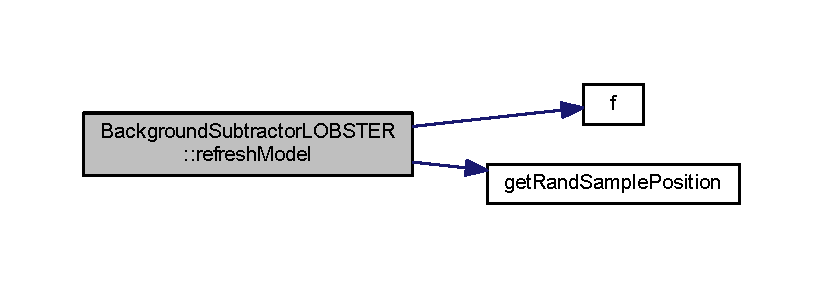
\includegraphics[width=350pt]{class_background_subtractor_l_o_b_s_t_e_r_aeb3b23c1f47cfe71a73f3ca47ec06a75_cgraph}
\end{center}
\end{figure}
Here is the caller graph for this function\+:\nopagebreak
\begin{figure}[H]
\begin{center}
\leavevmode
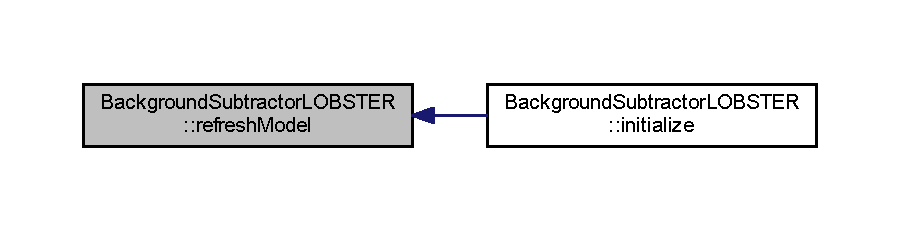
\includegraphics[width=350pt]{class_background_subtractor_l_o_b_s_t_e_r_aeb3b23c1f47cfe71a73f3ca47ec06a75_icgraph}
\end{center}
\end{figure}
\mbox{\Hypertarget{class_background_subtractor_l_b_s_p_a31b8474f8b4ffa6ef08ec682cfcef9b0}\label{class_background_subtractor_l_b_s_p_a31b8474f8b4ffa6ef08ec682cfcef9b0}} 
\index{Background\+Subtractor\+L\+O\+B\+S\+T\+ER@{Background\+Subtractor\+L\+O\+B\+S\+T\+ER}!set\+Automatic\+Model\+Reset@{set\+Automatic\+Model\+Reset}}
\index{set\+Automatic\+Model\+Reset@{set\+Automatic\+Model\+Reset}!Background\+Subtractor\+L\+O\+B\+S\+T\+ER@{Background\+Subtractor\+L\+O\+B\+S\+T\+ER}}
\subsubsection{\texorpdfstring{set\+Automatic\+Model\+Reset()}{setAutomaticModelReset()}}
{\footnotesize\ttfamily void Background\+Subtractor\+L\+B\+S\+P\+::set\+Automatic\+Model\+Reset (\begin{DoxyParamCaption}\item[{bool}]{b\+Val }\end{DoxyParamCaption})\hspace{0.3cm}{\ttfamily [inherited]}}



turns automatic model reset on or off 



Definition at line 57 of file Background\+Subtractor\+L\+B\+S\+P.\+cpp.


\begin{DoxyCode}
57                                                                \{
58     \mbox{\hyperlink{class_background_subtractor_l_b_s_p_a9d260f4e42e3fc79fb21af950ca9087a}{m\_bAutoModelResetEnabled}} = bVal;
59 \}
\end{DoxyCode}
\mbox{\Hypertarget{class_background_subtractor_l_b_s_p_a34dc38d3d925d46d289c750786f232dc}\label{class_background_subtractor_l_b_s_p_a34dc38d3d925d46d289c750786f232dc}} 
\index{Background\+Subtractor\+L\+O\+B\+S\+T\+ER@{Background\+Subtractor\+L\+O\+B\+S\+T\+ER}!set\+R\+OI@{set\+R\+OI}}
\index{set\+R\+OI@{set\+R\+OI}!Background\+Subtractor\+L\+O\+B\+S\+T\+ER@{Background\+Subtractor\+L\+O\+B\+S\+T\+ER}}
\subsubsection{\texorpdfstring{set\+R\+O\+I()}{setROI()}}
{\footnotesize\ttfamily void Background\+Subtractor\+L\+B\+S\+P\+::set\+R\+OI (\begin{DoxyParamCaption}\item[{cv\+::\+Mat \&}]{o\+R\+OI }\end{DoxyParamCaption})\hspace{0.3cm}{\ttfamily [virtual]}, {\ttfamily [inherited]}}



sets the R\+OI to be used for descriptor extraction (note\+: this function will reinit the model and return the usable R\+OI) 



Definition at line 45 of file Background\+Subtractor\+L\+B\+S\+P.\+cpp.


\begin{DoxyCode}
45                                                  \{
46     \mbox{\hyperlink{class_l_b_s_p_ad97557be4bc6cfd7b0fa4b01ab8f8c55}{LBSP::validateROI}}(oROI);
47     CV\_Assert(cv::countNonZero(oROI)>0);
48     \textcolor{keywordflow}{if}(\mbox{\hyperlink{class_background_subtractor_l_b_s_p_a55cea104a0924fd50d5bed0912828a7e}{m\_bInitialized}}) \{
49         cv::Mat oLatestBackgroundImage;
50         getBackgroundImage(oLatestBackgroundImage);
51         \mbox{\hyperlink{class_background_subtractor_l_b_s_p_ac6b854f94414497b143375d4a0ae8b6f}{initialize}}(oLatestBackgroundImage,oROI);
52     \}
53     \textcolor{keywordflow}{else}
54         \mbox{\hyperlink{class_background_subtractor_l_b_s_p_a53fe98bd2489d95de5292467145901e9}{m\_oROI}} = oROI.clone();
55 \}
\end{DoxyCode}
Here is the call graph for this function\+:
\nopagebreak
\begin{figure}[H]
\begin{center}
\leavevmode
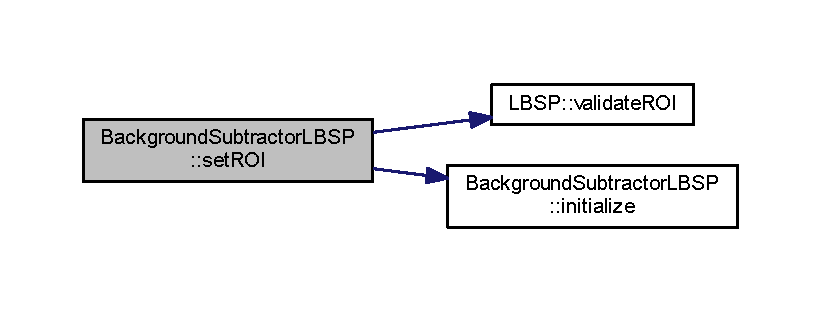
\includegraphics[width=350pt]{class_background_subtractor_l_b_s_p_a34dc38d3d925d46d289c750786f232dc_cgraph}
\end{center}
\end{figure}


\subsection{Member Data Documentation}
\mbox{\Hypertarget{class_background_subtractor_l_b_s_p_aefe69d94f08b2c4ba73ad1d254ad9153}\label{class_background_subtractor_l_b_s_p_aefe69d94f08b2c4ba73ad1d254ad9153}} 
\index{Background\+Subtractor\+L\+O\+B\+S\+T\+ER@{Background\+Subtractor\+L\+O\+B\+S\+T\+ER}!m\+\_\+an\+L\+B\+S\+P\+Threshold\+\_\+8bit\+L\+UT@{m\+\_\+an\+L\+B\+S\+P\+Threshold\+\_\+8bit\+L\+UT}}
\index{m\+\_\+an\+L\+B\+S\+P\+Threshold\+\_\+8bit\+L\+UT@{m\+\_\+an\+L\+B\+S\+P\+Threshold\+\_\+8bit\+L\+UT}!Background\+Subtractor\+L\+O\+B\+S\+T\+ER@{Background\+Subtractor\+L\+O\+B\+S\+T\+ER}}
\subsubsection{\texorpdfstring{m\+\_\+an\+L\+B\+S\+P\+Threshold\+\_\+8bit\+L\+UT}{m\_anLBSPThreshold\_8bitLUT}}
{\footnotesize\ttfamily size\+\_\+t Background\+Subtractor\+L\+B\+S\+P\+::m\+\_\+an\+L\+B\+S\+P\+Threshold\+\_\+8bit\+L\+UT\mbox{[}U\+C\+H\+A\+R\+\_\+\+M\+AX+1\mbox{]}\hspace{0.3cm}{\ttfamily [protected]}, {\ttfamily [inherited]}}



pre-\/allocated internal \mbox{\hyperlink{class_l_b_s_p}{L\+B\+SP}} threshold values L\+UT for all possible 8-\/bit intensities 



Definition at line 59 of file Background\+Subtractor\+L\+B\+S\+P.\+h.

\mbox{\Hypertarget{class_background_subtractor_l_b_s_p_a06b4f0d3f24fa08bccd3c9eca085713e}\label{class_background_subtractor_l_b_s_p_a06b4f0d3f24fa08bccd3c9eca085713e}} 
\index{Background\+Subtractor\+L\+O\+B\+S\+T\+ER@{Background\+Subtractor\+L\+O\+B\+S\+T\+ER}!m\+\_\+a\+Px\+Idx\+L\+UT@{m\+\_\+a\+Px\+Idx\+L\+UT}}
\index{m\+\_\+a\+Px\+Idx\+L\+UT@{m\+\_\+a\+Px\+Idx\+L\+UT}!Background\+Subtractor\+L\+O\+B\+S\+T\+ER@{Background\+Subtractor\+L\+O\+B\+S\+T\+ER}}
\subsubsection{\texorpdfstring{m\+\_\+a\+Px\+Idx\+L\+UT}{m\_aPxIdxLUT}}
{\footnotesize\ttfamily size\+\_\+t$\ast$ Background\+Subtractor\+L\+B\+S\+P\+::m\+\_\+a\+Px\+Idx\+L\+UT\hspace{0.3cm}{\ttfamily [protected]}, {\ttfamily [inherited]}}



internal pixel index L\+UT for all relevant analysis regions (based on the provided R\+OI) 



Definition at line 61 of file Background\+Subtractor\+L\+B\+S\+P.\+h.

\mbox{\Hypertarget{class_background_subtractor_l_b_s_p_a74e73d4832ccdef652d93756582024db}\label{class_background_subtractor_l_b_s_p_a74e73d4832ccdef652d93756582024db}} 
\index{Background\+Subtractor\+L\+O\+B\+S\+T\+ER@{Background\+Subtractor\+L\+O\+B\+S\+T\+ER}!m\+\_\+a\+Px\+Info\+L\+UT@{m\+\_\+a\+Px\+Info\+L\+UT}}
\index{m\+\_\+a\+Px\+Info\+L\+UT@{m\+\_\+a\+Px\+Info\+L\+UT}!Background\+Subtractor\+L\+O\+B\+S\+T\+ER@{Background\+Subtractor\+L\+O\+B\+S\+T\+ER}}
\subsubsection{\texorpdfstring{m\+\_\+a\+Px\+Info\+L\+UT}{m\_aPxInfoLUT}}
{\footnotesize\ttfamily \mbox{\hyperlink{struct_background_subtractor_l_b_s_p_1_1_px_info_base}{Px\+Info\+Base}}$\ast$ Background\+Subtractor\+L\+B\+S\+P\+::m\+\_\+a\+Px\+Info\+L\+UT\hspace{0.3cm}{\ttfamily [protected]}, {\ttfamily [inherited]}}



internal pixel info L\+UT for all possible pixel indexes 



Definition at line 63 of file Background\+Subtractor\+L\+B\+S\+P.\+h.

\mbox{\Hypertarget{class_background_subtractor_l_b_s_p_a9d260f4e42e3fc79fb21af950ca9087a}\label{class_background_subtractor_l_b_s_p_a9d260f4e42e3fc79fb21af950ca9087a}} 
\index{Background\+Subtractor\+L\+O\+B\+S\+T\+ER@{Background\+Subtractor\+L\+O\+B\+S\+T\+ER}!m\+\_\+b\+Auto\+Model\+Reset\+Enabled@{m\+\_\+b\+Auto\+Model\+Reset\+Enabled}}
\index{m\+\_\+b\+Auto\+Model\+Reset\+Enabled@{m\+\_\+b\+Auto\+Model\+Reset\+Enabled}!Background\+Subtractor\+L\+O\+B\+S\+T\+ER@{Background\+Subtractor\+L\+O\+B\+S\+T\+ER}}
\subsubsection{\texorpdfstring{m\+\_\+b\+Auto\+Model\+Reset\+Enabled}{m\_bAutoModelResetEnabled}}
{\footnotesize\ttfamily bool Background\+Subtractor\+L\+B\+S\+P\+::m\+\_\+b\+Auto\+Model\+Reset\+Enabled\hspace{0.3cm}{\ttfamily [protected]}, {\ttfamily [inherited]}}



specifies whether automatic model resets are enabled or not 



Definition at line 69 of file Background\+Subtractor\+L\+B\+S\+P.\+h.

\mbox{\Hypertarget{class_background_subtractor_l_b_s_p_a55cea104a0924fd50d5bed0912828a7e}\label{class_background_subtractor_l_b_s_p_a55cea104a0924fd50d5bed0912828a7e}} 
\index{Background\+Subtractor\+L\+O\+B\+S\+T\+ER@{Background\+Subtractor\+L\+O\+B\+S\+T\+ER}!m\+\_\+b\+Initialized@{m\+\_\+b\+Initialized}}
\index{m\+\_\+b\+Initialized@{m\+\_\+b\+Initialized}!Background\+Subtractor\+L\+O\+B\+S\+T\+ER@{Background\+Subtractor\+L\+O\+B\+S\+T\+ER}}
\subsubsection{\texorpdfstring{m\+\_\+b\+Initialized}{m\_bInitialized}}
{\footnotesize\ttfamily bool Background\+Subtractor\+L\+B\+S\+P\+::m\+\_\+b\+Initialized\hspace{0.3cm}{\ttfamily [protected]}, {\ttfamily [inherited]}}



specifies whether the algorithm is fully initialized or not 



Definition at line 67 of file Background\+Subtractor\+L\+B\+S\+P.\+h.

\mbox{\Hypertarget{class_background_subtractor_l_b_s_p_a5b1ec2694ae59661bb146ad0d4d49811}\label{class_background_subtractor_l_b_s_p_a5b1ec2694ae59661bb146ad0d4d49811}} 
\index{Background\+Subtractor\+L\+O\+B\+S\+T\+ER@{Background\+Subtractor\+L\+O\+B\+S\+T\+ER}!m\+\_\+b\+Using\+Moving\+Camera@{m\+\_\+b\+Using\+Moving\+Camera}}
\index{m\+\_\+b\+Using\+Moving\+Camera@{m\+\_\+b\+Using\+Moving\+Camera}!Background\+Subtractor\+L\+O\+B\+S\+T\+ER@{Background\+Subtractor\+L\+O\+B\+S\+T\+ER}}
\subsubsection{\texorpdfstring{m\+\_\+b\+Using\+Moving\+Camera}{m\_bUsingMovingCamera}}
{\footnotesize\ttfamily bool Background\+Subtractor\+L\+B\+S\+P\+::m\+\_\+b\+Using\+Moving\+Camera\hspace{0.3cm}{\ttfamily [protected]}, {\ttfamily [inherited]}}



specifies whether the camera is considered moving or not 



Definition at line 71 of file Background\+Subtractor\+L\+B\+S\+P.\+h.

\mbox{\Hypertarget{class_background_subtractor_l_b_s_p_ad759c645b14e9b16bf3940cae862df32}\label{class_background_subtractor_l_b_s_p_ad759c645b14e9b16bf3940cae862df32}} 
\index{Background\+Subtractor\+L\+O\+B\+S\+T\+ER@{Background\+Subtractor\+L\+O\+B\+S\+T\+ER}!m\+\_\+f\+Rel\+L\+B\+S\+P\+Threshold@{m\+\_\+f\+Rel\+L\+B\+S\+P\+Threshold}}
\index{m\+\_\+f\+Rel\+L\+B\+S\+P\+Threshold@{m\+\_\+f\+Rel\+L\+B\+S\+P\+Threshold}!Background\+Subtractor\+L\+O\+B\+S\+T\+ER@{Background\+Subtractor\+L\+O\+B\+S\+T\+ER}}
\subsubsection{\texorpdfstring{m\+\_\+f\+Rel\+L\+B\+S\+P\+Threshold}{m\_fRelLBSPThreshold}}
{\footnotesize\ttfamily const float Background\+Subtractor\+L\+B\+S\+P\+::m\+\_\+f\+Rel\+L\+B\+S\+P\+Threshold\hspace{0.3cm}{\ttfamily [protected]}, {\ttfamily [inherited]}}



\mbox{\hyperlink{class_l_b_s_p}{L\+B\+SP}} relative internal threshold (kept here since we don\textquotesingle{}t keep an \mbox{\hyperlink{class_l_b_s_p}{L\+B\+SP}} object) 



Definition at line 53 of file Background\+Subtractor\+L\+B\+S\+P.\+h.

\mbox{\Hypertarget{class_background_subtractor_l_o_b_s_t_e_r_a20c53540b952d608d849a305fd5eed89}\label{class_background_subtractor_l_o_b_s_t_e_r_a20c53540b952d608d849a305fd5eed89}} 
\index{Background\+Subtractor\+L\+O\+B\+S\+T\+ER@{Background\+Subtractor\+L\+O\+B\+S\+T\+ER}!m\+\_\+n\+B\+G\+Samples@{m\+\_\+n\+B\+G\+Samples}}
\index{m\+\_\+n\+B\+G\+Samples@{m\+\_\+n\+B\+G\+Samples}!Background\+Subtractor\+L\+O\+B\+S\+T\+ER@{Background\+Subtractor\+L\+O\+B\+S\+T\+ER}}
\subsubsection{\texorpdfstring{m\+\_\+n\+B\+G\+Samples}{m\_nBGSamples}}
{\footnotesize\ttfamily const size\+\_\+t Background\+Subtractor\+L\+O\+B\+S\+T\+E\+R\+::m\+\_\+n\+B\+G\+Samples\hspace{0.3cm}{\ttfamily [protected]}}



number of different samples per pixel/block to be taken from input frames to build the background model 



Definition at line 61 of file Background\+Subtractor\+L\+O\+B\+S\+T\+E\+R.\+h.

\mbox{\Hypertarget{class_background_subtractor_l_o_b_s_t_e_r_a37a37a0a46fc8e33d954c33c1318d7b2}\label{class_background_subtractor_l_o_b_s_t_e_r_a37a37a0a46fc8e33d954c33c1318d7b2}} 
\index{Background\+Subtractor\+L\+O\+B\+S\+T\+ER@{Background\+Subtractor\+L\+O\+B\+S\+T\+ER}!m\+\_\+n\+Color\+Dist\+Threshold@{m\+\_\+n\+Color\+Dist\+Threshold}}
\index{m\+\_\+n\+Color\+Dist\+Threshold@{m\+\_\+n\+Color\+Dist\+Threshold}!Background\+Subtractor\+L\+O\+B\+S\+T\+ER@{Background\+Subtractor\+L\+O\+B\+S\+T\+ER}}
\subsubsection{\texorpdfstring{m\+\_\+n\+Color\+Dist\+Threshold}{m\_nColorDistThreshold}}
{\footnotesize\ttfamily const size\+\_\+t Background\+Subtractor\+L\+O\+B\+S\+T\+E\+R\+::m\+\_\+n\+Color\+Dist\+Threshold\hspace{0.3cm}{\ttfamily [protected]}}



absolute color distance threshold 



Definition at line 57 of file Background\+Subtractor\+L\+O\+B\+S\+T\+E\+R.\+h.

\mbox{\Hypertarget{class_background_subtractor_l_b_s_p_a2585fe6e41e10af6da3e325dc20fe7f1}\label{class_background_subtractor_l_b_s_p_a2585fe6e41e10af6da3e325dc20fe7f1}} 
\index{Background\+Subtractor\+L\+O\+B\+S\+T\+ER@{Background\+Subtractor\+L\+O\+B\+S\+T\+ER}!m\+\_\+n\+Default\+Median\+Blur\+Kernel\+Size@{m\+\_\+n\+Default\+Median\+Blur\+Kernel\+Size}}
\index{m\+\_\+n\+Default\+Median\+Blur\+Kernel\+Size@{m\+\_\+n\+Default\+Median\+Blur\+Kernel\+Size}!Background\+Subtractor\+L\+O\+B\+S\+T\+ER@{Background\+Subtractor\+L\+O\+B\+S\+T\+ER}}
\subsubsection{\texorpdfstring{m\+\_\+n\+Default\+Median\+Blur\+Kernel\+Size}{m\_nDefaultMedianBlurKernelSize}}
{\footnotesize\ttfamily const int Background\+Subtractor\+L\+B\+S\+P\+::m\+\_\+n\+Default\+Median\+Blur\+Kernel\+Size\hspace{0.3cm}{\ttfamily [protected]}, {\ttfamily [inherited]}}



default kernel size for median blur post-\/proc filtering 



Definition at line 65 of file Background\+Subtractor\+L\+B\+S\+P.\+h.

\mbox{\Hypertarget{class_background_subtractor_l_o_b_s_t_e_r_abe3f4a836343e901746e4f243f5252e4}\label{class_background_subtractor_l_o_b_s_t_e_r_abe3f4a836343e901746e4f243f5252e4}} 
\index{Background\+Subtractor\+L\+O\+B\+S\+T\+ER@{Background\+Subtractor\+L\+O\+B\+S\+T\+ER}!m\+\_\+n\+Desc\+Dist\+Threshold@{m\+\_\+n\+Desc\+Dist\+Threshold}}
\index{m\+\_\+n\+Desc\+Dist\+Threshold@{m\+\_\+n\+Desc\+Dist\+Threshold}!Background\+Subtractor\+L\+O\+B\+S\+T\+ER@{Background\+Subtractor\+L\+O\+B\+S\+T\+ER}}
\subsubsection{\texorpdfstring{m\+\_\+n\+Desc\+Dist\+Threshold}{m\_nDescDistThreshold}}
{\footnotesize\ttfamily const size\+\_\+t Background\+Subtractor\+L\+O\+B\+S\+T\+E\+R\+::m\+\_\+n\+Desc\+Dist\+Threshold\hspace{0.3cm}{\ttfamily [protected]}}



absolute descriptor distance threshold 



Definition at line 59 of file Background\+Subtractor\+L\+O\+B\+S\+T\+E\+R.\+h.

\mbox{\Hypertarget{class_background_subtractor_l_b_s_p_a8a2350cad84f19c68ef61b7aaf91c43f}\label{class_background_subtractor_l_b_s_p_a8a2350cad84f19c68ef61b7aaf91c43f}} 
\index{Background\+Subtractor\+L\+O\+B\+S\+T\+ER@{Background\+Subtractor\+L\+O\+B\+S\+T\+ER}!m\+\_\+n\+Frame\+Index@{m\+\_\+n\+Frame\+Index}}
\index{m\+\_\+n\+Frame\+Index@{m\+\_\+n\+Frame\+Index}!Background\+Subtractor\+L\+O\+B\+S\+T\+ER@{Background\+Subtractor\+L\+O\+B\+S\+T\+ER}}
\subsubsection{\texorpdfstring{m\+\_\+n\+Frame\+Index}{m\_nFrameIndex}}
{\footnotesize\ttfamily size\+\_\+t Background\+Subtractor\+L\+B\+S\+P\+::m\+\_\+n\+Frame\+Index\hspace{0.3cm}{\ttfamily [protected]}, {\ttfamily [inherited]}}



current frame index, frame count since last model reset \& model reset cooldown counters 



Definition at line 57 of file Background\+Subtractor\+L\+B\+S\+P.\+h.

\mbox{\Hypertarget{class_background_subtractor_l_b_s_p_ab56bf775dfdf0579e834e45210c3a92a}\label{class_background_subtractor_l_b_s_p_ab56bf775dfdf0579e834e45210c3a92a}} 
\index{Background\+Subtractor\+L\+O\+B\+S\+T\+ER@{Background\+Subtractor\+L\+O\+B\+S\+T\+ER}!m\+\_\+n\+Frames\+Since\+Last\+Reset@{m\+\_\+n\+Frames\+Since\+Last\+Reset}}
\index{m\+\_\+n\+Frames\+Since\+Last\+Reset@{m\+\_\+n\+Frames\+Since\+Last\+Reset}!Background\+Subtractor\+L\+O\+B\+S\+T\+ER@{Background\+Subtractor\+L\+O\+B\+S\+T\+ER}}
\subsubsection{\texorpdfstring{m\+\_\+n\+Frames\+Since\+Last\+Reset}{m\_nFramesSinceLastReset}}
{\footnotesize\ttfamily size\+\_\+t Background\+Subtractor\+L\+B\+S\+P\+::m\+\_\+n\+Frames\+Since\+Last\+Reset\hspace{0.3cm}{\ttfamily [protected]}, {\ttfamily [inherited]}}



Definition at line 57 of file Background\+Subtractor\+L\+B\+S\+P.\+h.

\mbox{\Hypertarget{class_background_subtractor_l_b_s_p_ab3467ebee2c5d1249061ccd704cc0584}\label{class_background_subtractor_l_b_s_p_ab3467ebee2c5d1249061ccd704cc0584}} 
\index{Background\+Subtractor\+L\+O\+B\+S\+T\+ER@{Background\+Subtractor\+L\+O\+B\+S\+T\+ER}!m\+\_\+n\+Img\+Channels@{m\+\_\+n\+Img\+Channels}}
\index{m\+\_\+n\+Img\+Channels@{m\+\_\+n\+Img\+Channels}!Background\+Subtractor\+L\+O\+B\+S\+T\+ER@{Background\+Subtractor\+L\+O\+B\+S\+T\+ER}}
\subsubsection{\texorpdfstring{m\+\_\+n\+Img\+Channels}{m\_nImgChannels}}
{\footnotesize\ttfamily size\+\_\+t Background\+Subtractor\+L\+B\+S\+P\+::m\+\_\+n\+Img\+Channels\hspace{0.3cm}{\ttfamily [protected]}, {\ttfamily [inherited]}}



input image channel size 



Definition at line 47 of file Background\+Subtractor\+L\+B\+S\+P.\+h.

\mbox{\Hypertarget{class_background_subtractor_l_b_s_p_a7d2f52ecd5ff56e42da86f97e0ad93b5}\label{class_background_subtractor_l_b_s_p_a7d2f52ecd5ff56e42da86f97e0ad93b5}} 
\index{Background\+Subtractor\+L\+O\+B\+S\+T\+ER@{Background\+Subtractor\+L\+O\+B\+S\+T\+ER}!m\+\_\+n\+Img\+Type@{m\+\_\+n\+Img\+Type}}
\index{m\+\_\+n\+Img\+Type@{m\+\_\+n\+Img\+Type}!Background\+Subtractor\+L\+O\+B\+S\+T\+ER@{Background\+Subtractor\+L\+O\+B\+S\+T\+ER}}
\subsubsection{\texorpdfstring{m\+\_\+n\+Img\+Type}{m\_nImgType}}
{\footnotesize\ttfamily int Background\+Subtractor\+L\+B\+S\+P\+::m\+\_\+n\+Img\+Type\hspace{0.3cm}{\ttfamily [protected]}, {\ttfamily [inherited]}}



input image type 



Definition at line 49 of file Background\+Subtractor\+L\+B\+S\+P.\+h.

\mbox{\Hypertarget{class_background_subtractor_l_b_s_p_a209eb6aaa34e8ad8e565e79f85404e24}\label{class_background_subtractor_l_b_s_p_a209eb6aaa34e8ad8e565e79f85404e24}} 
\index{Background\+Subtractor\+L\+O\+B\+S\+T\+ER@{Background\+Subtractor\+L\+O\+B\+S\+T\+ER}!m\+\_\+n\+L\+B\+S\+P\+Threshold\+Offset@{m\+\_\+n\+L\+B\+S\+P\+Threshold\+Offset}}
\index{m\+\_\+n\+L\+B\+S\+P\+Threshold\+Offset@{m\+\_\+n\+L\+B\+S\+P\+Threshold\+Offset}!Background\+Subtractor\+L\+O\+B\+S\+T\+ER@{Background\+Subtractor\+L\+O\+B\+S\+T\+ER}}
\subsubsection{\texorpdfstring{m\+\_\+n\+L\+B\+S\+P\+Threshold\+Offset}{m\_nLBSPThresholdOffset}}
{\footnotesize\ttfamily const size\+\_\+t Background\+Subtractor\+L\+B\+S\+P\+::m\+\_\+n\+L\+B\+S\+P\+Threshold\+Offset\hspace{0.3cm}{\ttfamily [protected]}, {\ttfamily [inherited]}}



\mbox{\hyperlink{class_l_b_s_p}{L\+B\+SP}} internal threshold offset value, used to reduce texture noise in dark regions. 



Definition at line 51 of file Background\+Subtractor\+L\+B\+S\+P.\+h.

\mbox{\Hypertarget{class_background_subtractor_l_b_s_p_a5ea18d388afacf8285c46ba0f754e7ee}\label{class_background_subtractor_l_b_s_p_a5ea18d388afacf8285c46ba0f754e7ee}} 
\index{Background\+Subtractor\+L\+O\+B\+S\+T\+ER@{Background\+Subtractor\+L\+O\+B\+S\+T\+ER}!m\+\_\+n\+Model\+Reset\+Cooldown@{m\+\_\+n\+Model\+Reset\+Cooldown}}
\index{m\+\_\+n\+Model\+Reset\+Cooldown@{m\+\_\+n\+Model\+Reset\+Cooldown}!Background\+Subtractor\+L\+O\+B\+S\+T\+ER@{Background\+Subtractor\+L\+O\+B\+S\+T\+ER}}
\subsubsection{\texorpdfstring{m\+\_\+n\+Model\+Reset\+Cooldown}{m\_nModelResetCooldown}}
{\footnotesize\ttfamily size\+\_\+t Background\+Subtractor\+L\+B\+S\+P\+::m\+\_\+n\+Model\+Reset\+Cooldown\hspace{0.3cm}{\ttfamily [protected]}, {\ttfamily [inherited]}}



Definition at line 57 of file Background\+Subtractor\+L\+B\+S\+P.\+h.

\mbox{\Hypertarget{class_background_subtractor_l_o_b_s_t_e_r_acb558aefc1b6205a63c1906b6fd1eeff}\label{class_background_subtractor_l_o_b_s_t_e_r_acb558aefc1b6205a63c1906b6fd1eeff}} 
\index{Background\+Subtractor\+L\+O\+B\+S\+T\+ER@{Background\+Subtractor\+L\+O\+B\+S\+T\+ER}!m\+\_\+n\+Required\+B\+G\+Samples@{m\+\_\+n\+Required\+B\+G\+Samples}}
\index{m\+\_\+n\+Required\+B\+G\+Samples@{m\+\_\+n\+Required\+B\+G\+Samples}!Background\+Subtractor\+L\+O\+B\+S\+T\+ER@{Background\+Subtractor\+L\+O\+B\+S\+T\+ER}}
\subsubsection{\texorpdfstring{m\+\_\+n\+Required\+B\+G\+Samples}{m\_nRequiredBGSamples}}
{\footnotesize\ttfamily const size\+\_\+t Background\+Subtractor\+L\+O\+B\+S\+T\+E\+R\+::m\+\_\+n\+Required\+B\+G\+Samples\hspace{0.3cm}{\ttfamily [protected]}}



number of similar samples needed to consider the current pixel/block as \textquotesingle{}background\textquotesingle{} 



Definition at line 63 of file Background\+Subtractor\+L\+O\+B\+S\+T\+E\+R.\+h.

\mbox{\Hypertarget{class_background_subtractor_l_b_s_p_a9d1e247267afbddb7032bdcabd67d931}\label{class_background_subtractor_l_b_s_p_a9d1e247267afbddb7032bdcabd67d931}} 
\index{Background\+Subtractor\+L\+O\+B\+S\+T\+ER@{Background\+Subtractor\+L\+O\+B\+S\+T\+ER}!m\+\_\+n\+Tot\+Px\+Count@{m\+\_\+n\+Tot\+Px\+Count}}
\index{m\+\_\+n\+Tot\+Px\+Count@{m\+\_\+n\+Tot\+Px\+Count}!Background\+Subtractor\+L\+O\+B\+S\+T\+ER@{Background\+Subtractor\+L\+O\+B\+S\+T\+ER}}
\subsubsection{\texorpdfstring{m\+\_\+n\+Tot\+Px\+Count}{m\_nTotPxCount}}
{\footnotesize\ttfamily size\+\_\+t Background\+Subtractor\+L\+B\+S\+P\+::m\+\_\+n\+Tot\+Px\+Count\hspace{0.3cm}{\ttfamily [protected]}, {\ttfamily [inherited]}}



total number of pixels (depends on the input frame size) \& total number of relevant pixels 



Definition at line 55 of file Background\+Subtractor\+L\+B\+S\+P.\+h.

\mbox{\Hypertarget{class_background_subtractor_l_b_s_p_ac3b54f4d2dfa3a576475214f26501d85}\label{class_background_subtractor_l_b_s_p_ac3b54f4d2dfa3a576475214f26501d85}} 
\index{Background\+Subtractor\+L\+O\+B\+S\+T\+ER@{Background\+Subtractor\+L\+O\+B\+S\+T\+ER}!m\+\_\+n\+Tot\+Relevant\+Px\+Count@{m\+\_\+n\+Tot\+Relevant\+Px\+Count}}
\index{m\+\_\+n\+Tot\+Relevant\+Px\+Count@{m\+\_\+n\+Tot\+Relevant\+Px\+Count}!Background\+Subtractor\+L\+O\+B\+S\+T\+ER@{Background\+Subtractor\+L\+O\+B\+S\+T\+ER}}
\subsubsection{\texorpdfstring{m\+\_\+n\+Tot\+Relevant\+Px\+Count}{m\_nTotRelevantPxCount}}
{\footnotesize\ttfamily size\+\_\+t Background\+Subtractor\+L\+B\+S\+P\+::m\+\_\+n\+Tot\+Relevant\+Px\+Count\hspace{0.3cm}{\ttfamily [protected]}, {\ttfamily [inherited]}}



Definition at line 55 of file Background\+Subtractor\+L\+B\+S\+P.\+h.

\mbox{\Hypertarget{class_background_subtractor_l_b_s_p_a732d5e6ae35fb0e858cadb3af5ce08a2}\label{class_background_subtractor_l_b_s_p_a732d5e6ae35fb0e858cadb3af5ce08a2}} 
\index{Background\+Subtractor\+L\+O\+B\+S\+T\+ER@{Background\+Subtractor\+L\+O\+B\+S\+T\+ER}!m\+\_\+o\+Img\+Size@{m\+\_\+o\+Img\+Size}}
\index{m\+\_\+o\+Img\+Size@{m\+\_\+o\+Img\+Size}!Background\+Subtractor\+L\+O\+B\+S\+T\+ER@{Background\+Subtractor\+L\+O\+B\+S\+T\+ER}}
\subsubsection{\texorpdfstring{m\+\_\+o\+Img\+Size}{m\_oImgSize}}
{\footnotesize\ttfamily cv\+::\+Size Background\+Subtractor\+L\+B\+S\+P\+::m\+\_\+o\+Img\+Size\hspace{0.3cm}{\ttfamily [protected]}, {\ttfamily [inherited]}}



input image size 



Definition at line 45 of file Background\+Subtractor\+L\+B\+S\+P.\+h.

\mbox{\Hypertarget{class_background_subtractor_l_b_s_p_ab1dc003792ab1d0b881a6fd10e0e29b3}\label{class_background_subtractor_l_b_s_p_ab1dc003792ab1d0b881a6fd10e0e29b3}} 
\index{Background\+Subtractor\+L\+O\+B\+S\+T\+ER@{Background\+Subtractor\+L\+O\+B\+S\+T\+ER}!m\+\_\+o\+Last\+Color\+Frame@{m\+\_\+o\+Last\+Color\+Frame}}
\index{m\+\_\+o\+Last\+Color\+Frame@{m\+\_\+o\+Last\+Color\+Frame}!Background\+Subtractor\+L\+O\+B\+S\+T\+ER@{Background\+Subtractor\+L\+O\+B\+S\+T\+ER}}
\subsubsection{\texorpdfstring{m\+\_\+o\+Last\+Color\+Frame}{m\_oLastColorFrame}}
{\footnotesize\ttfamily cv\+::\+Mat Background\+Subtractor\+L\+B\+S\+P\+::m\+\_\+o\+Last\+Color\+Frame\hspace{0.3cm}{\ttfamily [protected]}, {\ttfamily [inherited]}}



copy of latest pixel intensities (used when refreshing model) 



Definition at line 73 of file Background\+Subtractor\+L\+B\+S\+P.\+h.

\mbox{\Hypertarget{class_background_subtractor_l_b_s_p_a9c637c0b87cac495887295690d83ba13}\label{class_background_subtractor_l_b_s_p_a9c637c0b87cac495887295690d83ba13}} 
\index{Background\+Subtractor\+L\+O\+B\+S\+T\+ER@{Background\+Subtractor\+L\+O\+B\+S\+T\+ER}!m\+\_\+o\+Last\+Desc\+Frame@{m\+\_\+o\+Last\+Desc\+Frame}}
\index{m\+\_\+o\+Last\+Desc\+Frame@{m\+\_\+o\+Last\+Desc\+Frame}!Background\+Subtractor\+L\+O\+B\+S\+T\+ER@{Background\+Subtractor\+L\+O\+B\+S\+T\+ER}}
\subsubsection{\texorpdfstring{m\+\_\+o\+Last\+Desc\+Frame}{m\_oLastDescFrame}}
{\footnotesize\ttfamily cv\+::\+Mat Background\+Subtractor\+L\+B\+S\+P\+::m\+\_\+o\+Last\+Desc\+Frame\hspace{0.3cm}{\ttfamily [protected]}, {\ttfamily [inherited]}}



copy of latest descriptors (used when refreshing model) 



Definition at line 75 of file Background\+Subtractor\+L\+B\+S\+P.\+h.

\mbox{\Hypertarget{class_background_subtractor_l_b_s_p_adb6dc0af596c5592c91f9d8faa5c8a4b}\label{class_background_subtractor_l_b_s_p_adb6dc0af596c5592c91f9d8faa5c8a4b}} 
\index{Background\+Subtractor\+L\+O\+B\+S\+T\+ER@{Background\+Subtractor\+L\+O\+B\+S\+T\+ER}!m\+\_\+o\+Last\+F\+G\+Mask@{m\+\_\+o\+Last\+F\+G\+Mask}}
\index{m\+\_\+o\+Last\+F\+G\+Mask@{m\+\_\+o\+Last\+F\+G\+Mask}!Background\+Subtractor\+L\+O\+B\+S\+T\+ER@{Background\+Subtractor\+L\+O\+B\+S\+T\+ER}}
\subsubsection{\texorpdfstring{m\+\_\+o\+Last\+F\+G\+Mask}{m\_oLastFGMask}}
{\footnotesize\ttfamily cv\+::\+Mat Background\+Subtractor\+L\+B\+S\+P\+::m\+\_\+o\+Last\+F\+G\+Mask\hspace{0.3cm}{\ttfamily [protected]}, {\ttfamily [inherited]}}



the foreground mask generated by the method at \mbox{[}t-\/1\mbox{]} 



Definition at line 77 of file Background\+Subtractor\+L\+B\+S\+P.\+h.

\mbox{\Hypertarget{class_background_subtractor_l_b_s_p_a53fe98bd2489d95de5292467145901e9}\label{class_background_subtractor_l_b_s_p_a53fe98bd2489d95de5292467145901e9}} 
\index{Background\+Subtractor\+L\+O\+B\+S\+T\+ER@{Background\+Subtractor\+L\+O\+B\+S\+T\+ER}!m\+\_\+o\+R\+OI@{m\+\_\+o\+R\+OI}}
\index{m\+\_\+o\+R\+OI@{m\+\_\+o\+R\+OI}!Background\+Subtractor\+L\+O\+B\+S\+T\+ER@{Background\+Subtractor\+L\+O\+B\+S\+T\+ER}}
\subsubsection{\texorpdfstring{m\+\_\+o\+R\+OI}{m\_oROI}}
{\footnotesize\ttfamily cv\+::\+Mat Background\+Subtractor\+L\+B\+S\+P\+::m\+\_\+o\+R\+OI\hspace{0.3cm}{\ttfamily [protected]}, {\ttfamily [inherited]}}



background model R\+OI used for \mbox{\hyperlink{class_l_b_s_p}{L\+B\+SP}} descriptor extraction (specific to the input image size) 



Definition at line 43 of file Background\+Subtractor\+L\+B\+S\+P.\+h.

\mbox{\Hypertarget{class_background_subtractor_l_o_b_s_t_e_r_ac981b39f8ae7b28d3e4326d8e6be6332}\label{class_background_subtractor_l_o_b_s_t_e_r_ac981b39f8ae7b28d3e4326d8e6be6332}} 
\index{Background\+Subtractor\+L\+O\+B\+S\+T\+ER@{Background\+Subtractor\+L\+O\+B\+S\+T\+ER}!m\+\_\+vo\+B\+G\+Color\+Samples@{m\+\_\+vo\+B\+G\+Color\+Samples}}
\index{m\+\_\+vo\+B\+G\+Color\+Samples@{m\+\_\+vo\+B\+G\+Color\+Samples}!Background\+Subtractor\+L\+O\+B\+S\+T\+ER@{Background\+Subtractor\+L\+O\+B\+S\+T\+ER}}
\subsubsection{\texorpdfstring{m\+\_\+vo\+B\+G\+Color\+Samples}{m\_voBGColorSamples}}
{\footnotesize\ttfamily std\+::vector$<$cv\+::\+Mat$>$ Background\+Subtractor\+L\+O\+B\+S\+T\+E\+R\+::m\+\_\+vo\+B\+G\+Color\+Samples\hspace{0.3cm}{\ttfamily [protected]}}



background model pixel intensity samples 



Definition at line 65 of file Background\+Subtractor\+L\+O\+B\+S\+T\+E\+R.\+h.

\mbox{\Hypertarget{class_background_subtractor_l_o_b_s_t_e_r_a3c49866ae652423b2173215957907d04}\label{class_background_subtractor_l_o_b_s_t_e_r_a3c49866ae652423b2173215957907d04}} 
\index{Background\+Subtractor\+L\+O\+B\+S\+T\+ER@{Background\+Subtractor\+L\+O\+B\+S\+T\+ER}!m\+\_\+vo\+B\+G\+Desc\+Samples@{m\+\_\+vo\+B\+G\+Desc\+Samples}}
\index{m\+\_\+vo\+B\+G\+Desc\+Samples@{m\+\_\+vo\+B\+G\+Desc\+Samples}!Background\+Subtractor\+L\+O\+B\+S\+T\+ER@{Background\+Subtractor\+L\+O\+B\+S\+T\+ER}}
\subsubsection{\texorpdfstring{m\+\_\+vo\+B\+G\+Desc\+Samples}{m\_voBGDescSamples}}
{\footnotesize\ttfamily std\+::vector$<$cv\+::\+Mat$>$ Background\+Subtractor\+L\+O\+B\+S\+T\+E\+R\+::m\+\_\+vo\+B\+G\+Desc\+Samples\hspace{0.3cm}{\ttfamily [protected]}}



background model descriptors samples 



Definition at line 67 of file Background\+Subtractor\+L\+O\+B\+S\+T\+E\+R.\+h.

\mbox{\Hypertarget{class_background_subtractor_l_b_s_p_a49771cd7b2c8354cde3da6e593d3febe}\label{class_background_subtractor_l_b_s_p_a49771cd7b2c8354cde3da6e593d3febe}} 
\index{Background\+Subtractor\+L\+O\+B\+S\+T\+ER@{Background\+Subtractor\+L\+O\+B\+S\+T\+ER}!n\+Debug\+CoordX@{n\+Debug\+CoordX}}
\index{n\+Debug\+CoordX@{n\+Debug\+CoordX}!Background\+Subtractor\+L\+O\+B\+S\+T\+ER@{Background\+Subtractor\+L\+O\+B\+S\+T\+ER}}
\subsubsection{\texorpdfstring{n\+Debug\+CoordX}{nDebugCoordX}}
{\footnotesize\ttfamily int Background\+Subtractor\+L\+B\+S\+P\+::n\+Debug\+CoordX\hspace{0.3cm}{\ttfamily [inherited]}}



Definition at line 81 of file Background\+Subtractor\+L\+B\+S\+P.\+h.

\mbox{\Hypertarget{class_background_subtractor_l_b_s_p_a8e1451fd90eb4459aa84ea5e7133268a}\label{class_background_subtractor_l_b_s_p_a8e1451fd90eb4459aa84ea5e7133268a}} 
\index{Background\+Subtractor\+L\+O\+B\+S\+T\+ER@{Background\+Subtractor\+L\+O\+B\+S\+T\+ER}!n\+Debug\+CoordY@{n\+Debug\+CoordY}}
\index{n\+Debug\+CoordY@{n\+Debug\+CoordY}!Background\+Subtractor\+L\+O\+B\+S\+T\+ER@{Background\+Subtractor\+L\+O\+B\+S\+T\+ER}}
\subsubsection{\texorpdfstring{n\+Debug\+CoordY}{nDebugCoordY}}
{\footnotesize\ttfamily int Background\+Subtractor\+L\+B\+S\+P\+::n\+Debug\+CoordY\hspace{0.3cm}{\ttfamily [inherited]}}



Definition at line 81 of file Background\+Subtractor\+L\+B\+S\+P.\+h.

\mbox{\Hypertarget{class_background_subtractor_l_b_s_p_ada55b4a5eec8c82d0e05b0f9f1600ecb}\label{class_background_subtractor_l_b_s_p_ada55b4a5eec8c82d0e05b0f9f1600ecb}} 
\index{Background\+Subtractor\+L\+O\+B\+S\+T\+ER@{Background\+Subtractor\+L\+O\+B\+S\+T\+ER}!s\+Debug\+Name@{s\+Debug\+Name}}
\index{s\+Debug\+Name@{s\+Debug\+Name}!Background\+Subtractor\+L\+O\+B\+S\+T\+ER@{Background\+Subtractor\+L\+O\+B\+S\+T\+ER}}
\subsubsection{\texorpdfstring{s\+Debug\+Name}{sDebugName}}
{\footnotesize\ttfamily std\+::string Background\+Subtractor\+L\+B\+S\+P\+::s\+Debug\+Name\hspace{0.3cm}{\ttfamily [inherited]}}



Definition at line 82 of file Background\+Subtractor\+L\+B\+S\+P.\+h.



The documentation for this class was generated from the following files\+:\begin{DoxyCompactItemize}
\item 
D\+:/\+Roy/\+Git\+Hub/\+Multitarget-\/tracker/\+Detector/\+Subsense/\mbox{\hyperlink{_background_subtractor_l_o_b_s_t_e_r_8h}{Background\+Subtractor\+L\+O\+B\+S\+T\+E\+R.\+h}}\item 
D\+:/\+Roy/\+Git\+Hub/\+Multitarget-\/tracker/\+Detector/\+Subsense/\mbox{\hyperlink{_background_subtractor_l_o_b_s_t_e_r_8cpp}{Background\+Subtractor\+L\+O\+B\+S\+T\+E\+R.\+cpp}}\end{DoxyCompactItemize}

\hypertarget{class_background_subtractor_su_b_s_e_n_s_e}{}\section{Background\+Subtractor\+Su\+B\+S\+E\+N\+SE Class Reference}
\label{class_background_subtractor_su_b_s_e_n_s_e}\index{Background\+Subtractor\+Su\+B\+S\+E\+N\+SE@{Background\+Subtractor\+Su\+B\+S\+E\+N\+SE}}


{\ttfamily \#include $<$Background\+Subtractor\+Su\+B\+S\+E\+N\+S\+E.\+h$>$}



Inheritance diagram for Background\+Subtractor\+Su\+B\+S\+E\+N\+SE\+:\nopagebreak
\begin{figure}[H]
\begin{center}
\leavevmode
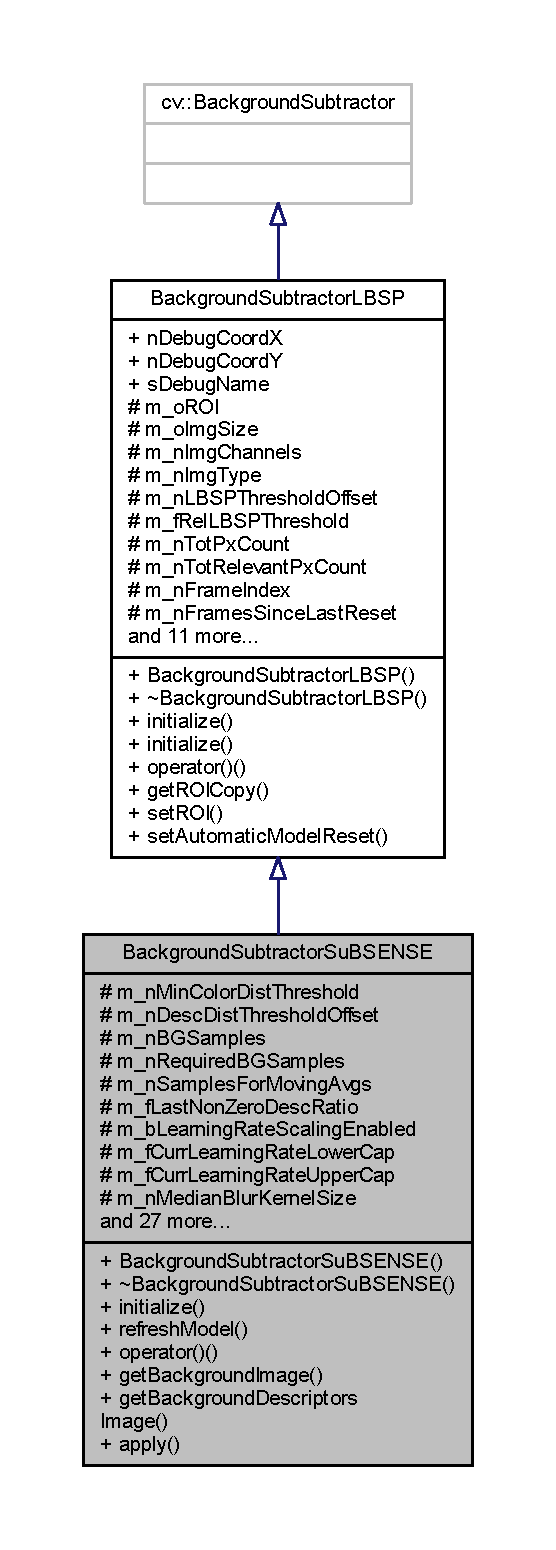
\includegraphics[height=550pt]{class_background_subtractor_su_b_s_e_n_s_e__inherit__graph}
\end{center}
\end{figure}


Collaboration diagram for Background\+Subtractor\+Su\+B\+S\+E\+N\+SE\+:\nopagebreak
\begin{figure}[H]
\begin{center}
\leavevmode
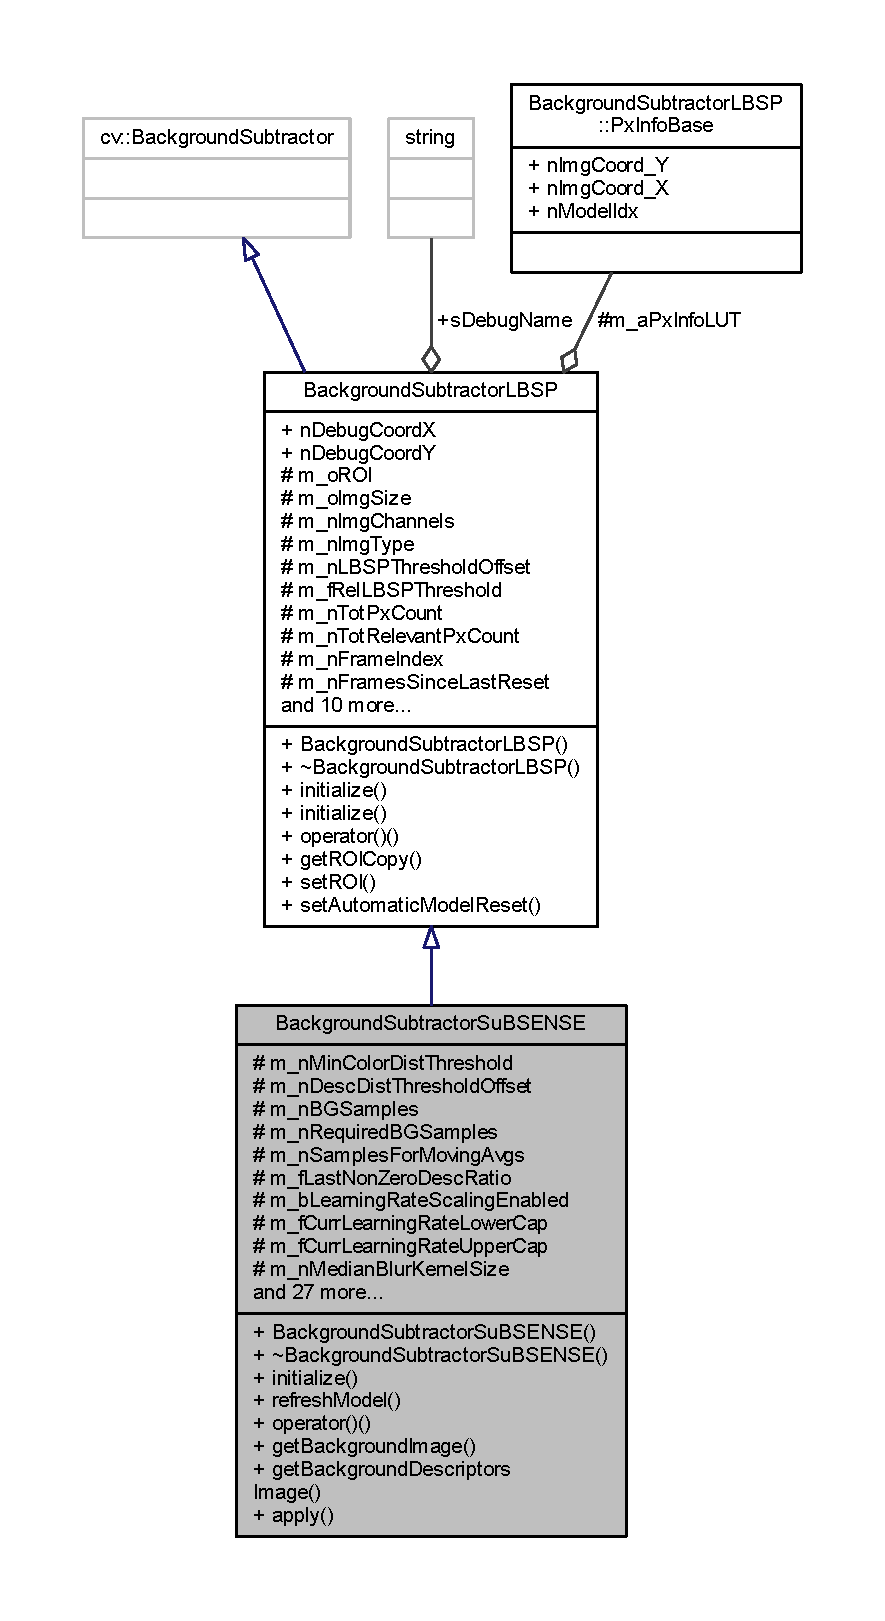
\includegraphics[height=550pt]{class_background_subtractor_su_b_s_e_n_s_e__coll__graph}
\end{center}
\end{figure}
\subsection*{Public Member Functions}
\begin{DoxyCompactItemize}
\item 
\mbox{\hyperlink{class_background_subtractor_su_b_s_e_n_s_e_a0f3118adf0f3365a140390c6ad94e9df}{Background\+Subtractor\+Su\+B\+S\+E\+N\+SE}} (float f\+Rel\+L\+B\+S\+P\+Threshold=\mbox{\hyperlink{_background_subtractor_su_b_s_e_n_s_e_8h_a125c1e09337744e8b4a35da8696dc5d4}{B\+G\+S\+S\+U\+B\+S\+E\+N\+S\+E\+\_\+\+D\+E\+F\+A\+U\+L\+T\+\_\+\+L\+B\+S\+P\+\_\+\+R\+E\+L\+\_\+\+S\+I\+M\+I\+L\+A\+R\+I\+T\+Y\+\_\+\+T\+H\+R\+E\+S\+H\+O\+LD}}, size\+\_\+t n\+Desc\+Dist\+Threshold\+Offset=\mbox{\hyperlink{_background_subtractor_su_b_s_e_n_s_e_8h_a6ac17a78aeb1fb0dab4833b50b80e43e}{B\+G\+S\+S\+U\+B\+S\+E\+N\+S\+E\+\_\+\+D\+E\+F\+A\+U\+L\+T\+\_\+\+D\+E\+S\+C\+\_\+\+D\+I\+S\+T\+\_\+\+T\+H\+R\+E\+S\+H\+O\+L\+D\+\_\+\+O\+F\+F\+S\+ET}}, size\+\_\+t n\+Min\+Color\+Dist\+Threshold=\mbox{\hyperlink{_background_subtractor_su_b_s_e_n_s_e_8h_ab2d581a6cf91dca26bb660c483cdb23c}{B\+G\+S\+S\+U\+B\+S\+E\+N\+S\+E\+\_\+\+D\+E\+F\+A\+U\+L\+T\+\_\+\+M\+I\+N\+\_\+\+C\+O\+L\+O\+R\+\_\+\+D\+I\+S\+T\+\_\+\+T\+H\+R\+E\+S\+H\+O\+LD}}, size\+\_\+t n\+B\+G\+Samples=\mbox{\hyperlink{_background_subtractor_su_b_s_e_n_s_e_8h_a0140353a9cb83ccce1209024d570ff28}{B\+G\+S\+S\+U\+B\+S\+E\+N\+S\+E\+\_\+\+D\+E\+F\+A\+U\+L\+T\+\_\+\+N\+B\+\_\+\+B\+G\+\_\+\+S\+A\+M\+P\+L\+ES}}, size\+\_\+t n\+Required\+B\+G\+Samples=\mbox{\hyperlink{_background_subtractor_su_b_s_e_n_s_e_8h_a3f30662673e2871e8f751e4ca1b433d1}{B\+G\+S\+S\+U\+B\+S\+E\+N\+S\+E\+\_\+\+D\+E\+F\+A\+U\+L\+T\+\_\+\+R\+E\+Q\+U\+I\+R\+E\+D\+\_\+\+N\+B\+\_\+\+B\+G\+\_\+\+S\+A\+M\+P\+L\+ES}}, size\+\_\+t n\+Samples\+For\+Moving\+Avgs=\mbox{\hyperlink{_background_subtractor_su_b_s_e_n_s_e_8h_acf2f1c0462353ddc7a51a6ed995a36ab}{B\+G\+S\+S\+U\+B\+S\+E\+N\+S\+E\+\_\+\+D\+E\+F\+A\+U\+L\+T\+\_\+\+N\+\_\+\+S\+A\+M\+P\+L\+E\+S\+\_\+\+F\+O\+R\+\_\+\+M\+V\+\_\+\+A\+V\+GS}})
\begin{DoxyCompactList}\small\item\em full constructor \end{DoxyCompactList}\item 
virtual \mbox{\hyperlink{class_background_subtractor_su_b_s_e_n_s_e_a71cd501469582addfe4f8824cc4602d4}{$\sim$\+Background\+Subtractor\+Su\+B\+S\+E\+N\+SE}} ()
\begin{DoxyCompactList}\small\item\em default destructor \end{DoxyCompactList}\item 
virtual void \mbox{\hyperlink{class_background_subtractor_su_b_s_e_n_s_e_ac84aa66030b04a72435ef473cf0e6a3f}{initialize}} (const cv\+::\+Mat \&o\+Init\+Img, const cv\+::\+Mat \&o\+R\+OI)
\begin{DoxyCompactList}\small\item\em (re)initiaization method; needs to be called before starting background subtraction \end{DoxyCompactList}\item 
virtual void \mbox{\hyperlink{class_background_subtractor_su_b_s_e_n_s_e_abe80bf042f2b7a1f72942460d74b1f02}{refresh\+Model}} (float f\+Samples\+Refresh\+Frac, bool b\+Force\+F\+G\+Update=false)
\begin{DoxyCompactList}\small\item\em refreshes all samples based on the last analyzed frame \end{DoxyCompactList}\item 
virtual void \mbox{\hyperlink{class_background_subtractor_su_b_s_e_n_s_e_aaa60e2883c2b2cf130820b10104a653b}{operator()}} (cv\+::\+Input\+Array image, cv\+::\+Output\+Array fgmask, double learning\+Rate\+Override=0)
\begin{DoxyCompactList}\small\item\em primary model update function; the learning param is used to override the internal learning thresholds (ignored when $<$= 0) \end{DoxyCompactList}\item 
void \mbox{\hyperlink{class_background_subtractor_su_b_s_e_n_s_e_a04f6ee8e507bfc708b5b9b4ff97c16e0}{get\+Background\+Image}} (cv\+::\+Output\+Array background\+Image) const
\begin{DoxyCompactList}\small\item\em returns a copy of the latest reconstructed background image \end{DoxyCompactList}\item 
void \mbox{\hyperlink{class_background_subtractor_su_b_s_e_n_s_e_a1a6bc447dded20dcce887d7986109ea9}{get\+Background\+Descriptors\+Image}} (cv\+::\+Output\+Array background\+Desc\+Image) const
\begin{DoxyCompactList}\small\item\em returns a copy of the latest reconstructed background descriptors image \end{DoxyCompactList}\item 
virtual void \mbox{\hyperlink{class_background_subtractor_su_b_s_e_n_s_e_adc2a6761d618ea16861ee7a992c154f1}{apply}} (cv\+::\+Input\+Array image, cv\+::\+Output\+Array fgmask, double learning\+Rate\+Override=0)
\begin{DoxyCompactList}\small\item\em compute foreground mask \end{DoxyCompactList}\item 
virtual void \mbox{\hyperlink{class_background_subtractor_l_b_s_p_ac6b854f94414497b143375d4a0ae8b6f}{initialize}} (const cv\+::\+Mat \&o\+Init\+Img)
\begin{DoxyCompactList}\small\item\em (re)initiaization method; needs to be called before starting background subtraction \end{DoxyCompactList}\item 
virtual cv\+::\+Mat \mbox{\hyperlink{class_background_subtractor_l_b_s_p_a9843f87f8adcd0e85274303f9210b883}{get\+R\+O\+I\+Copy}} () const
\begin{DoxyCompactList}\small\item\em unused, always returns nullptr \end{DoxyCompactList}\item 
virtual void \mbox{\hyperlink{class_background_subtractor_l_b_s_p_a34dc38d3d925d46d289c750786f232dc}{set\+R\+OI}} (cv\+::\+Mat \&o\+R\+OI)
\begin{DoxyCompactList}\small\item\em sets the R\+OI to be used for descriptor extraction (note\+: this function will reinit the model and return the usable R\+OI) \end{DoxyCompactList}\item 
void \mbox{\hyperlink{class_background_subtractor_l_b_s_p_a31b8474f8b4ffa6ef08ec682cfcef9b0}{set\+Automatic\+Model\+Reset}} (bool)
\begin{DoxyCompactList}\small\item\em turns automatic model reset on or off \end{DoxyCompactList}\end{DoxyCompactItemize}
\subsection*{Public Attributes}
\begin{DoxyCompactItemize}
\item 
int \mbox{\hyperlink{class_background_subtractor_l_b_s_p_a49771cd7b2c8354cde3da6e593d3febe}{n\+Debug\+CoordX}}
\item 
int \mbox{\hyperlink{class_background_subtractor_l_b_s_p_a8e1451fd90eb4459aa84ea5e7133268a}{n\+Debug\+CoordY}}
\item 
std\+::string \mbox{\hyperlink{class_background_subtractor_l_b_s_p_ada55b4a5eec8c82d0e05b0f9f1600ecb}{s\+Debug\+Name}}
\end{DoxyCompactItemize}
\subsection*{Protected Attributes}
\begin{DoxyCompactItemize}
\item 
const size\+\_\+t \mbox{\hyperlink{class_background_subtractor_su_b_s_e_n_s_e_ae0ebf701652a66bbdb0472d6f091e34d}{m\+\_\+n\+Min\+Color\+Dist\+Threshold}}
\begin{DoxyCompactList}\small\item\em absolute minimal color distance threshold (\textquotesingle{}R\textquotesingle{} or \textquotesingle{}radius\textquotesingle{} in the original Vi\+Be paper, used as the default/initial \textquotesingle{}R(x)\textquotesingle{} value here) \end{DoxyCompactList}\item 
const size\+\_\+t \mbox{\hyperlink{class_background_subtractor_su_b_s_e_n_s_e_a79fe0f1657cd613b975d62f73e749ec2}{m\+\_\+n\+Desc\+Dist\+Threshold\+Offset}}
\begin{DoxyCompactList}\small\item\em absolute descriptor distance threshold offset \end{DoxyCompactList}\item 
const size\+\_\+t \mbox{\hyperlink{class_background_subtractor_su_b_s_e_n_s_e_ad783b71b5b942c4018d27cf38b7d7225}{m\+\_\+n\+B\+G\+Samples}}
\begin{DoxyCompactList}\small\item\em number of different samples per pixel/block to be taken from input frames to build the background model (same as \textquotesingle{}N\textquotesingle{} in Vi\+Be/\+P\+B\+AS) \end{DoxyCompactList}\item 
const size\+\_\+t \mbox{\hyperlink{class_background_subtractor_su_b_s_e_n_s_e_aca07c4307021623f9055832506cad1d6}{m\+\_\+n\+Required\+B\+G\+Samples}}
\begin{DoxyCompactList}\small\item\em number of similar samples needed to consider the current pixel/block as \textquotesingle{}background\textquotesingle{} (same as \textquotesingle{}\#\+\_\+min\textquotesingle{} in Vi\+Be/\+P\+B\+AS) \end{DoxyCompactList}\item 
const size\+\_\+t \mbox{\hyperlink{class_background_subtractor_su_b_s_e_n_s_e_acd112ccb067f76e370400565fa09ee49}{m\+\_\+n\+Samples\+For\+Moving\+Avgs}}
\begin{DoxyCompactList}\small\item\em number of samples to use to compute the learning rate of moving averages \end{DoxyCompactList}\item 
float \mbox{\hyperlink{class_background_subtractor_su_b_s_e_n_s_e_a4231d025a90be64a703f3f0aff1345c8}{m\+\_\+f\+Last\+Non\+Zero\+Desc\+Ratio}}
\begin{DoxyCompactList}\small\item\em last calculated non-\/zero desc ratio \end{DoxyCompactList}\item 
bool \mbox{\hyperlink{class_background_subtractor_su_b_s_e_n_s_e_afca07a4c7edca7761e55dfbdf6da4263}{m\+\_\+b\+Learning\+Rate\+Scaling\+Enabled}}
\begin{DoxyCompactList}\small\item\em specifies whether Tmin/\+Tmax scaling is enabled or not \end{DoxyCompactList}\item 
float \mbox{\hyperlink{class_background_subtractor_su_b_s_e_n_s_e_a57fdd29e43afc163233e55f9a7cd9f37}{m\+\_\+f\+Curr\+Learning\+Rate\+Lower\+Cap}}
\begin{DoxyCompactList}\small\item\em current learning rate caps \end{DoxyCompactList}\item 
float \mbox{\hyperlink{class_background_subtractor_su_b_s_e_n_s_e_a44ba1a1ed365c5829baa517ce9f27508}{m\+\_\+f\+Curr\+Learning\+Rate\+Upper\+Cap}}
\item 
int \mbox{\hyperlink{class_background_subtractor_su_b_s_e_n_s_e_a796120fecb11f00914925e14065ee5ab}{m\+\_\+n\+Median\+Blur\+Kernel\+Size}}
\begin{DoxyCompactList}\small\item\em current kernel size for median blur post-\/proc filtering \end{DoxyCompactList}\item 
bool \mbox{\hyperlink{class_background_subtractor_su_b_s_e_n_s_e_a1e2e28840e7ca373282607db81b49e12}{m\+\_\+b\+Use3x3\+Spread}}
\begin{DoxyCompactList}\small\item\em specifies the px update spread range \end{DoxyCompactList}\item 
cv\+::\+Size \mbox{\hyperlink{class_background_subtractor_su_b_s_e_n_s_e_af3e1eb902a5b6b46a1c229864423bd20}{m\+\_\+o\+Down\+Sampled\+Frame\+Size}}
\begin{DoxyCompactList}\small\item\em specifies the downsampled frame size used for cam motion analysis \end{DoxyCompactList}\item 
std\+::vector$<$ cv\+::\+Mat $>$ \mbox{\hyperlink{class_background_subtractor_su_b_s_e_n_s_e_a9d4d4bb930b34745536b9862683bb539}{m\+\_\+vo\+B\+G\+Color\+Samples}}
\begin{DoxyCompactList}\small\item\em background model pixel color intensity samples (equivalent to \textquotesingle{}B(x)\textquotesingle{} in P\+B\+AS) \end{DoxyCompactList}\item 
std\+::vector$<$ cv\+::\+Mat $>$ \mbox{\hyperlink{class_background_subtractor_su_b_s_e_n_s_e_a422cc2f2a25c07efca02087bd6fe3d6d}{m\+\_\+vo\+B\+G\+Desc\+Samples}}
\begin{DoxyCompactList}\small\item\em background model descriptors samples \end{DoxyCompactList}\item 
cv\+::\+Mat \mbox{\hyperlink{class_background_subtractor_su_b_s_e_n_s_e_a90cb2cc5cbe3f2f0b01e06f514c8b569}{m\+\_\+o\+Update\+Rate\+Frame}}
\begin{DoxyCompactList}\small\item\em per-\/pixel update rates (\textquotesingle{}T(x)\textquotesingle{} in P\+B\+AS, which contains pixel-\/level \textquotesingle{}sigmas\textquotesingle{}, as referred to in Vi\+Be) \end{DoxyCompactList}\item 
cv\+::\+Mat \mbox{\hyperlink{class_background_subtractor_su_b_s_e_n_s_e_a491a1e2b81dee87a721a421719bf2836}{m\+\_\+o\+Dist\+Threshold\+Frame}}
\begin{DoxyCompactList}\small\item\em per-\/pixel distance thresholds (equivalent to \textquotesingle{}R(x)\textquotesingle{} in P\+B\+AS, but used as a relative value to determine both intensity and descriptor variation thresholds) \end{DoxyCompactList}\item 
cv\+::\+Mat \mbox{\hyperlink{class_background_subtractor_su_b_s_e_n_s_e_a47d9cf067ac639d95fcb810c894bb770}{m\+\_\+o\+Variation\+Modulator\+Frame}}
\begin{DoxyCompactList}\small\item\em per-\/pixel distance variation modulators (\textquotesingle{}v(x)\textquotesingle{}, relative value used to modulate \textquotesingle{}R(x)\textquotesingle{} and \textquotesingle{}T(x)\textquotesingle{} variations) \end{DoxyCompactList}\item 
cv\+::\+Mat \mbox{\hyperlink{class_background_subtractor_su_b_s_e_n_s_e_ad95bb91ff7ef9db725772b37d679e1a2}{m\+\_\+o\+Mean\+Last\+Dist\+Frame}}
\begin{DoxyCompactList}\small\item\em per-\/pixel mean distances between consecutive frames (\textquotesingle{}D\+\_\+last(x)\textquotesingle{}, used to detect ghosts and high variation regions in the sequence) \end{DoxyCompactList}\item 
cv\+::\+Mat \mbox{\hyperlink{class_background_subtractor_su_b_s_e_n_s_e_a8318e35d5fbbcffb8729700ef5e71a6e}{m\+\_\+o\+Mean\+Min\+Dist\+Frame\+\_\+\+LT}}
\begin{DoxyCompactList}\small\item\em per-\/pixel mean minimal distances from the model (\textquotesingle{}D\+\_\+min(x)\textquotesingle{} in P\+B\+AS, used to control variation magnitude and direction of \textquotesingle{}T(x)\textquotesingle{} and \textquotesingle{}R(x)\textquotesingle{}) \end{DoxyCompactList}\item 
cv\+::\+Mat \mbox{\hyperlink{class_background_subtractor_su_b_s_e_n_s_e_a53584c5c79017947c59d05dfd247cf5e}{m\+\_\+o\+Mean\+Min\+Dist\+Frame\+\_\+\+ST}}
\item 
cv\+::\+Mat \mbox{\hyperlink{class_background_subtractor_su_b_s_e_n_s_e_ab6056c53d3237ae04da509b36ec40486}{m\+\_\+o\+Mean\+Down\+Sampled\+Last\+Dist\+Frame\+\_\+\+LT}}
\begin{DoxyCompactList}\small\item\em per-\/pixel mean downsampled distances between consecutive frames (used to analyze camera movement and control max learning rates globally) \end{DoxyCompactList}\item 
cv\+::\+Mat \mbox{\hyperlink{class_background_subtractor_su_b_s_e_n_s_e_a92a9aec9a8b34383b67d97467bd34515}{m\+\_\+o\+Mean\+Down\+Sampled\+Last\+Dist\+Frame\+\_\+\+ST}}
\item 
cv\+::\+Mat \mbox{\hyperlink{class_background_subtractor_su_b_s_e_n_s_e_a7706b13433c4e9f4f8156e075fa7904d}{m\+\_\+o\+Mean\+Raw\+Segm\+Res\+Frame\+\_\+\+LT}}
\begin{DoxyCompactList}\small\item\em per-\/pixel mean raw segmentation results (used to detect unstable segmentation regions) \end{DoxyCompactList}\item 
cv\+::\+Mat \mbox{\hyperlink{class_background_subtractor_su_b_s_e_n_s_e_a3c9fd9cf995eb9a7b4006467ab874958}{m\+\_\+o\+Mean\+Raw\+Segm\+Res\+Frame\+\_\+\+ST}}
\item 
cv\+::\+Mat \mbox{\hyperlink{class_background_subtractor_su_b_s_e_n_s_e_ad48e92b6d6bbce34f9f452484bc9956a}{m\+\_\+o\+Mean\+Final\+Segm\+Res\+Frame\+\_\+\+LT}}
\begin{DoxyCompactList}\small\item\em per-\/pixel mean raw segmentation results (used to detect unstable segmentation regions) \end{DoxyCompactList}\item 
cv\+::\+Mat \mbox{\hyperlink{class_background_subtractor_su_b_s_e_n_s_e_a0dcd4f5df8adb9b4fa630a9a6f6b5e30}{m\+\_\+o\+Mean\+Final\+Segm\+Res\+Frame\+\_\+\+ST}}
\item 
cv\+::\+Mat \mbox{\hyperlink{class_background_subtractor_su_b_s_e_n_s_e_acfaf4c3c5aedbed8bd302444b4a4f8dd}{m\+\_\+o\+Unstable\+Region\+Mask}}
\begin{DoxyCompactList}\small\item\em a lookup map used to keep track of unstable regions (based on segm. noise \& local dist. thresholds) \end{DoxyCompactList}\item 
cv\+::\+Mat \mbox{\hyperlink{class_background_subtractor_su_b_s_e_n_s_e_a943b50c63d233c0948d82b64390f1aa1}{m\+\_\+o\+Blinks\+Frame}}
\begin{DoxyCompactList}\small\item\em per-\/pixel blink detection map (\textquotesingle{}Z(x)\textquotesingle{}) \end{DoxyCompactList}\item 
cv\+::\+Mat \mbox{\hyperlink{class_background_subtractor_su_b_s_e_n_s_e_a619bc3f0bfcd408796d1ffd6bd45d04d}{m\+\_\+o\+Down\+Sampled\+Frame\+\_\+\+Motion\+Analysis}}
\begin{DoxyCompactList}\small\item\em pre-\/allocated matrix used to downsample the input frame when needed \end{DoxyCompactList}\item 
cv\+::\+Mat \mbox{\hyperlink{class_background_subtractor_su_b_s_e_n_s_e_a11c86236e9d141d711163c170a8bf0d6}{m\+\_\+o\+Last\+Raw\+F\+G\+Mask}}
\begin{DoxyCompactList}\small\item\em the foreground mask generated by the method at \mbox{[}t-\/1\mbox{]} (without post-\/proc, used for blinking px detection) \end{DoxyCompactList}\item 
cv\+::\+Mat \mbox{\hyperlink{class_background_subtractor_su_b_s_e_n_s_e_a53ac4868e46e0ba382a0e6d769e8a961}{m\+\_\+o\+F\+G\+Mask\+\_\+\+Pre\+Flood}}
\begin{DoxyCompactList}\small\item\em pre-\/allocated C\+V\+\_\+8\+U\+C1 matrices used to speed up morph ops \end{DoxyCompactList}\item 
cv\+::\+Mat \mbox{\hyperlink{class_background_subtractor_su_b_s_e_n_s_e_a4a8df16fa54d4b22a9b787d5b57427f9}{m\+\_\+o\+F\+G\+Mask\+\_\+\+Flooded\+Holes}}
\item 
cv\+::\+Mat \mbox{\hyperlink{class_background_subtractor_su_b_s_e_n_s_e_a2dc6a8f1c8e2694d19dbbb74c533e293}{m\+\_\+o\+Last\+F\+G\+Mask\+\_\+dilated}}
\item 
cv\+::\+Mat \mbox{\hyperlink{class_background_subtractor_su_b_s_e_n_s_e_a0306555d3e97ceec32f8f6b495d18b95}{m\+\_\+o\+Last\+F\+G\+Mask\+\_\+dilated\+\_\+inverted}}
\item 
cv\+::\+Mat \mbox{\hyperlink{class_background_subtractor_su_b_s_e_n_s_e_a804b5ad0898777a2eb2cb4d932c857b6}{m\+\_\+o\+Curr\+Raw\+F\+G\+Blink\+Mask}}
\item 
cv\+::\+Mat \mbox{\hyperlink{class_background_subtractor_su_b_s_e_n_s_e_aea0e3a3817d99da5b2fe15c810b0f428}{m\+\_\+o\+Last\+Raw\+F\+G\+Blink\+Mask}}
\item 
cv\+::\+Mat \mbox{\hyperlink{class_background_subtractor_su_b_s_e_n_s_e_ae360b93378aa04b34aebc23b5f6e6714}{m\+\_\+default\+Morphology\+Kernel}}
\begin{DoxyCompactList}\small\item\em default kernel for morphology operations \end{DoxyCompactList}\item 
cv\+::\+Mat \mbox{\hyperlink{class_background_subtractor_l_b_s_p_a53fe98bd2489d95de5292467145901e9}{m\+\_\+o\+R\+OI}}
\begin{DoxyCompactList}\small\item\em background model R\+OI used for \mbox{\hyperlink{class_l_b_s_p}{L\+B\+SP}} descriptor extraction (specific to the input image size) \end{DoxyCompactList}\item 
cv\+::\+Size \mbox{\hyperlink{class_background_subtractor_l_b_s_p_a732d5e6ae35fb0e858cadb3af5ce08a2}{m\+\_\+o\+Img\+Size}}
\begin{DoxyCompactList}\small\item\em input image size \end{DoxyCompactList}\item 
size\+\_\+t \mbox{\hyperlink{class_background_subtractor_l_b_s_p_ab3467ebee2c5d1249061ccd704cc0584}{m\+\_\+n\+Img\+Channels}}
\begin{DoxyCompactList}\small\item\em input image channel size \end{DoxyCompactList}\item 
int \mbox{\hyperlink{class_background_subtractor_l_b_s_p_a7d2f52ecd5ff56e42da86f97e0ad93b5}{m\+\_\+n\+Img\+Type}}
\begin{DoxyCompactList}\small\item\em input image type \end{DoxyCompactList}\item 
const size\+\_\+t \mbox{\hyperlink{class_background_subtractor_l_b_s_p_a209eb6aaa34e8ad8e565e79f85404e24}{m\+\_\+n\+L\+B\+S\+P\+Threshold\+Offset}}
\begin{DoxyCompactList}\small\item\em \mbox{\hyperlink{class_l_b_s_p}{L\+B\+SP}} internal threshold offset value, used to reduce texture noise in dark regions. \end{DoxyCompactList}\item 
const float \mbox{\hyperlink{class_background_subtractor_l_b_s_p_ad759c645b14e9b16bf3940cae862df32}{m\+\_\+f\+Rel\+L\+B\+S\+P\+Threshold}}
\begin{DoxyCompactList}\small\item\em \mbox{\hyperlink{class_l_b_s_p}{L\+B\+SP}} relative internal threshold (kept here since we don\textquotesingle{}t keep an \mbox{\hyperlink{class_l_b_s_p}{L\+B\+SP}} object) \end{DoxyCompactList}\item 
size\+\_\+t \mbox{\hyperlink{class_background_subtractor_l_b_s_p_a9d1e247267afbddb7032bdcabd67d931}{m\+\_\+n\+Tot\+Px\+Count}}
\begin{DoxyCompactList}\small\item\em total number of pixels (depends on the input frame size) \& total number of relevant pixels \end{DoxyCompactList}\item 
size\+\_\+t \mbox{\hyperlink{class_background_subtractor_l_b_s_p_ac3b54f4d2dfa3a576475214f26501d85}{m\+\_\+n\+Tot\+Relevant\+Px\+Count}}
\item 
size\+\_\+t \mbox{\hyperlink{class_background_subtractor_l_b_s_p_a8a2350cad84f19c68ef61b7aaf91c43f}{m\+\_\+n\+Frame\+Index}}
\begin{DoxyCompactList}\small\item\em current frame index, frame count since last model reset \& model reset cooldown counters \end{DoxyCompactList}\item 
size\+\_\+t \mbox{\hyperlink{class_background_subtractor_l_b_s_p_ab56bf775dfdf0579e834e45210c3a92a}{m\+\_\+n\+Frames\+Since\+Last\+Reset}}
\item 
size\+\_\+t \mbox{\hyperlink{class_background_subtractor_l_b_s_p_a5ea18d388afacf8285c46ba0f754e7ee}{m\+\_\+n\+Model\+Reset\+Cooldown}}
\item 
size\+\_\+t \mbox{\hyperlink{class_background_subtractor_l_b_s_p_aefe69d94f08b2c4ba73ad1d254ad9153}{m\+\_\+an\+L\+B\+S\+P\+Threshold\+\_\+8bit\+L\+UT}} \mbox{[}U\+C\+H\+A\+R\+\_\+\+M\+AX+1\mbox{]}
\begin{DoxyCompactList}\small\item\em pre-\/allocated internal \mbox{\hyperlink{class_l_b_s_p}{L\+B\+SP}} threshold values L\+UT for all possible 8-\/bit intensities \end{DoxyCompactList}\item 
size\+\_\+t $\ast$ \mbox{\hyperlink{class_background_subtractor_l_b_s_p_a06b4f0d3f24fa08bccd3c9eca085713e}{m\+\_\+a\+Px\+Idx\+L\+UT}}
\begin{DoxyCompactList}\small\item\em internal pixel index L\+UT for all relevant analysis regions (based on the provided R\+OI) \end{DoxyCompactList}\item 
\mbox{\hyperlink{struct_background_subtractor_l_b_s_p_1_1_px_info_base}{Px\+Info\+Base}} $\ast$ \mbox{\hyperlink{class_background_subtractor_l_b_s_p_a74e73d4832ccdef652d93756582024db}{m\+\_\+a\+Px\+Info\+L\+UT}}
\begin{DoxyCompactList}\small\item\em internal pixel info L\+UT for all possible pixel indexes \end{DoxyCompactList}\item 
const int \mbox{\hyperlink{class_background_subtractor_l_b_s_p_a2585fe6e41e10af6da3e325dc20fe7f1}{m\+\_\+n\+Default\+Median\+Blur\+Kernel\+Size}}
\begin{DoxyCompactList}\small\item\em default kernel size for median blur post-\/proc filtering \end{DoxyCompactList}\item 
bool \mbox{\hyperlink{class_background_subtractor_l_b_s_p_a55cea104a0924fd50d5bed0912828a7e}{m\+\_\+b\+Initialized}}
\begin{DoxyCompactList}\small\item\em specifies whether the algorithm is fully initialized or not \end{DoxyCompactList}\item 
bool \mbox{\hyperlink{class_background_subtractor_l_b_s_p_a9d260f4e42e3fc79fb21af950ca9087a}{m\+\_\+b\+Auto\+Model\+Reset\+Enabled}}
\begin{DoxyCompactList}\small\item\em specifies whether automatic model resets are enabled or not \end{DoxyCompactList}\item 
bool \mbox{\hyperlink{class_background_subtractor_l_b_s_p_a5b1ec2694ae59661bb146ad0d4d49811}{m\+\_\+b\+Using\+Moving\+Camera}}
\begin{DoxyCompactList}\small\item\em specifies whether the camera is considered moving or not \end{DoxyCompactList}\item 
cv\+::\+Mat \mbox{\hyperlink{class_background_subtractor_l_b_s_p_ab1dc003792ab1d0b881a6fd10e0e29b3}{m\+\_\+o\+Last\+Color\+Frame}}
\begin{DoxyCompactList}\small\item\em copy of latest pixel intensities (used when refreshing model) \end{DoxyCompactList}\item 
cv\+::\+Mat \mbox{\hyperlink{class_background_subtractor_l_b_s_p_a9c637c0b87cac495887295690d83ba13}{m\+\_\+o\+Last\+Desc\+Frame}}
\begin{DoxyCompactList}\small\item\em copy of latest descriptors (used when refreshing model) \end{DoxyCompactList}\item 
cv\+::\+Mat \mbox{\hyperlink{class_background_subtractor_l_b_s_p_adb6dc0af596c5592c91f9d8faa5c8a4b}{m\+\_\+o\+Last\+F\+G\+Mask}}
\begin{DoxyCompactList}\small\item\em the foreground mask generated by the method at \mbox{[}t-\/1\mbox{]} \end{DoxyCompactList}\end{DoxyCompactItemize}


\subsection{Detailed Description}
Self-\/\+Balanced Sensitivity segmen\+T\+ER (Su\+B\+S\+E\+N\+SE) change detection algorithm.

Note\+: both grayscale and R\+G\+B/\+B\+GR images may be used with this extractor (parameters are adjusted automatically). For optimal grayscale results, use C\+V\+\_\+8\+U\+C1 frames instead of C\+V\+\_\+8\+U\+C3.

For more details on the different parameters or on the algorithm itself, see P.-\/L. St-\/\+Charles et al., \char`\"{}\+Flexible Background Subtraction With Self-\/\+Balanced Local Sensitivity\char`\"{}, in C\+V\+P\+RW 2014.

This algorithm is currently N\+OT thread-\/safe. 

Definition at line 29 of file Background\+Subtractor\+Su\+B\+S\+E\+N\+S\+E.\+h.



\subsection{Constructor \& Destructor Documentation}
\mbox{\Hypertarget{class_background_subtractor_su_b_s_e_n_s_e_a0f3118adf0f3365a140390c6ad94e9df}\label{class_background_subtractor_su_b_s_e_n_s_e_a0f3118adf0f3365a140390c6ad94e9df}} 
\index{Background\+Subtractor\+Su\+B\+S\+E\+N\+SE@{Background\+Subtractor\+Su\+B\+S\+E\+N\+SE}!Background\+Subtractor\+Su\+B\+S\+E\+N\+SE@{Background\+Subtractor\+Su\+B\+S\+E\+N\+SE}}
\index{Background\+Subtractor\+Su\+B\+S\+E\+N\+SE@{Background\+Subtractor\+Su\+B\+S\+E\+N\+SE}!Background\+Subtractor\+Su\+B\+S\+E\+N\+SE@{Background\+Subtractor\+Su\+B\+S\+E\+N\+SE}}
\subsubsection{\texorpdfstring{Background\+Subtractor\+Su\+B\+S\+E\+N\+S\+E()}{BackgroundSubtractorSuBSENSE()}}
{\footnotesize\ttfamily Background\+Subtractor\+Su\+B\+S\+E\+N\+S\+E\+::\+Background\+Subtractor\+Su\+B\+S\+E\+N\+SE (\begin{DoxyParamCaption}\item[{float}]{f\+Rel\+L\+B\+S\+P\+Threshold = {\ttfamily \mbox{\hyperlink{_background_subtractor_su_b_s_e_n_s_e_8h_a125c1e09337744e8b4a35da8696dc5d4}{B\+G\+S\+S\+U\+B\+S\+E\+N\+S\+E\+\_\+\+D\+E\+F\+A\+U\+L\+T\+\_\+\+L\+B\+S\+P\+\_\+\+R\+E\+L\+\_\+\+S\+I\+M\+I\+L\+A\+R\+I\+T\+Y\+\_\+\+T\+H\+R\+E\+S\+H\+O\+LD}}},  }\item[{size\+\_\+t}]{n\+Desc\+Dist\+Threshold\+Offset = {\ttfamily \mbox{\hyperlink{_background_subtractor_su_b_s_e_n_s_e_8h_a6ac17a78aeb1fb0dab4833b50b80e43e}{B\+G\+S\+S\+U\+B\+S\+E\+N\+S\+E\+\_\+\+D\+E\+F\+A\+U\+L\+T\+\_\+\+D\+E\+S\+C\+\_\+\+D\+I\+S\+T\+\_\+\+T\+H\+R\+E\+S\+H\+O\+L\+D\+\_\+\+O\+F\+F\+S\+ET}}},  }\item[{size\+\_\+t}]{n\+Min\+Color\+Dist\+Threshold = {\ttfamily \mbox{\hyperlink{_background_subtractor_su_b_s_e_n_s_e_8h_ab2d581a6cf91dca26bb660c483cdb23c}{B\+G\+S\+S\+U\+B\+S\+E\+N\+S\+E\+\_\+\+D\+E\+F\+A\+U\+L\+T\+\_\+\+M\+I\+N\+\_\+\+C\+O\+L\+O\+R\+\_\+\+D\+I\+S\+T\+\_\+\+T\+H\+R\+E\+S\+H\+O\+LD}}},  }\item[{size\+\_\+t}]{n\+B\+G\+Samples = {\ttfamily \mbox{\hyperlink{_background_subtractor_su_b_s_e_n_s_e_8h_a0140353a9cb83ccce1209024d570ff28}{B\+G\+S\+S\+U\+B\+S\+E\+N\+S\+E\+\_\+\+D\+E\+F\+A\+U\+L\+T\+\_\+\+N\+B\+\_\+\+B\+G\+\_\+\+S\+A\+M\+P\+L\+ES}}},  }\item[{size\+\_\+t}]{n\+Required\+B\+G\+Samples = {\ttfamily \mbox{\hyperlink{_background_subtractor_su_b_s_e_n_s_e_8h_a3f30662673e2871e8f751e4ca1b433d1}{B\+G\+S\+S\+U\+B\+S\+E\+N\+S\+E\+\_\+\+D\+E\+F\+A\+U\+L\+T\+\_\+\+R\+E\+Q\+U\+I\+R\+E\+D\+\_\+\+N\+B\+\_\+\+B\+G\+\_\+\+S\+A\+M\+P\+L\+ES}}},  }\item[{size\+\_\+t}]{n\+Samples\+For\+Moving\+Avgs = {\ttfamily \mbox{\hyperlink{_background_subtractor_su_b_s_e_n_s_e_8h_acf2f1c0462353ddc7a51a6ed995a36ab}{B\+G\+S\+S\+U\+B\+S\+E\+N\+S\+E\+\_\+\+D\+E\+F\+A\+U\+L\+T\+\_\+\+N\+\_\+\+S\+A\+M\+P\+L\+E\+S\+\_\+\+F\+O\+R\+\_\+\+M\+V\+\_\+\+A\+V\+GS}}} }\end{DoxyParamCaption})}



full constructor 



Definition at line 51 of file Background\+Subtractor\+Su\+B\+S\+E\+N\+S\+E.\+cpp.


\begin{DoxyCode}
57     :    \mbox{\hyperlink{class_background_subtractor_l_b_s_p_a5f7f42ea5c9697479cbe237b49ca6ae9}{BackgroundSubtractorLBSP}}(fRelLBSPThreshold)
58         ,\mbox{\hyperlink{class_background_subtractor_su_b_s_e_n_s_e_ae0ebf701652a66bbdb0472d6f091e34d}{m\_nMinColorDistThreshold}}(nMinColorDistThreshold)
59         ,\mbox{\hyperlink{class_background_subtractor_su_b_s_e_n_s_e_a79fe0f1657cd613b975d62f73e749ec2}{m\_nDescDistThresholdOffset}}(nDescDistThresholdOffset)
60         ,\mbox{\hyperlink{class_background_subtractor_su_b_s_e_n_s_e_ad783b71b5b942c4018d27cf38b7d7225}{m\_nBGSamples}}(nBGSamples)
61         ,\mbox{\hyperlink{class_background_subtractor_su_b_s_e_n_s_e_aca07c4307021623f9055832506cad1d6}{m\_nRequiredBGSamples}}(nRequiredBGSamples)
62         ,\mbox{\hyperlink{class_background_subtractor_su_b_s_e_n_s_e_acd112ccb067f76e370400565fa09ee49}{m\_nSamplesForMovingAvgs}}(nSamplesForMovingAvgs)
63         ,\mbox{\hyperlink{class_background_subtractor_su_b_s_e_n_s_e_a4231d025a90be64a703f3f0aff1345c8}{m\_fLastNonZeroDescRatio}}(0.0\mbox{\hyperlink{rings_8cpp_a77369fc4d5326a16d2c603e032023528}{f}})
64         ,\mbox{\hyperlink{class_background_subtractor_su_b_s_e_n_s_e_afca07a4c7edca7761e55dfbdf6da4263}{m\_bLearningRateScalingEnabled}}(\textcolor{keyword}{true})
65         ,\mbox{\hyperlink{class_background_subtractor_su_b_s_e_n_s_e_a57fdd29e43afc163233e55f9a7cd9f37}{m\_fCurrLearningRateLowerCap}}(\mbox{\hyperlink{_background_subtractor_su_b_s_e_n_s_e_8cpp_a6975332215c62c3172a76af852bc5566}{FEEDBACK\_T\_LOWER}})
66         ,\mbox{\hyperlink{class_background_subtractor_su_b_s_e_n_s_e_a44ba1a1ed365c5829baa517ce9f27508}{m\_fCurrLearningRateUpperCap}}(\mbox{\hyperlink{_background_subtractor_su_b_s_e_n_s_e_8cpp_a23bd980dc8c9bbffe3f27b44fa983f9c}{FEEDBACK\_T\_UPPER}})
67         ,\mbox{\hyperlink{class_background_subtractor_su_b_s_e_n_s_e_a796120fecb11f00914925e14065ee5ab}{m\_nMedianBlurKernelSize}}(
      \mbox{\hyperlink{class_background_subtractor_l_b_s_p_a2585fe6e41e10af6da3e325dc20fe7f1}{m\_nDefaultMedianBlurKernelSize}})
68         ,\mbox{\hyperlink{class_background_subtractor_su_b_s_e_n_s_e_a1e2e28840e7ca373282607db81b49e12}{m\_bUse3x3Spread}}(\textcolor{keyword}{true})
69         ,\mbox{\hyperlink{class_background_subtractor_su_b_s_e_n_s_e_ae360b93378aa04b34aebc23b5f6e6714}{m\_defaultMorphologyKernel}}(cv::getStructuringElement(cv::MORPH\_RECT, 
      cv::Size(3, 3))) \{
70     CV\_Assert(\mbox{\hyperlink{class_background_subtractor_su_b_s_e_n_s_e_ad783b71b5b942c4018d27cf38b7d7225}{m\_nBGSamples}}>0 && \mbox{\hyperlink{class_background_subtractor_su_b_s_e_n_s_e_aca07c4307021623f9055832506cad1d6}{m\_nRequiredBGSamples}}<=
      \mbox{\hyperlink{class_background_subtractor_su_b_s_e_n_s_e_ad783b71b5b942c4018d27cf38b7d7225}{m\_nBGSamples}});
71     CV\_Assert(\mbox{\hyperlink{class_background_subtractor_su_b_s_e_n_s_e_ae0ebf701652a66bbdb0472d6f091e34d}{m\_nMinColorDistThreshold}}>=
      \mbox{\hyperlink{_background_subtractor_su_b_s_e_n_s_e_8cpp_af60b797fbe4d762be8f140d56f6d8a0a}{STAB\_COLOR\_DIST\_OFFSET}});
72 \}
\end{DoxyCode}
\mbox{\Hypertarget{class_background_subtractor_su_b_s_e_n_s_e_a71cd501469582addfe4f8824cc4602d4}\label{class_background_subtractor_su_b_s_e_n_s_e_a71cd501469582addfe4f8824cc4602d4}} 
\index{Background\+Subtractor\+Su\+B\+S\+E\+N\+SE@{Background\+Subtractor\+Su\+B\+S\+E\+N\+SE}!````~Background\+Subtractor\+Su\+B\+S\+E\+N\+SE@{$\sim$\+Background\+Subtractor\+Su\+B\+S\+E\+N\+SE}}
\index{````~Background\+Subtractor\+Su\+B\+S\+E\+N\+SE@{$\sim$\+Background\+Subtractor\+Su\+B\+S\+E\+N\+SE}!Background\+Subtractor\+Su\+B\+S\+E\+N\+SE@{Background\+Subtractor\+Su\+B\+S\+E\+N\+SE}}
\subsubsection{\texorpdfstring{$\sim$\+Background\+Subtractor\+Su\+B\+S\+E\+N\+S\+E()}{~BackgroundSubtractorSuBSENSE()}}
{\footnotesize\ttfamily Background\+Subtractor\+Su\+B\+S\+E\+N\+S\+E\+::$\sim$\+Background\+Subtractor\+Su\+B\+S\+E\+N\+SE (\begin{DoxyParamCaption}{ }\end{DoxyParamCaption})\hspace{0.3cm}{\ttfamily [virtual]}}



default destructor 



Definition at line 74 of file Background\+Subtractor\+Su\+B\+S\+E\+N\+S\+E.\+cpp.


\begin{DoxyCode}
74                                                             \{
75     \textcolor{keywordflow}{if}(\mbox{\hyperlink{class_background_subtractor_l_b_s_p_a06b4f0d3f24fa08bccd3c9eca085713e}{m\_aPxIdxLUT}})
76         \textcolor{keyword}{delete}[] \mbox{\hyperlink{class_background_subtractor_l_b_s_p_a06b4f0d3f24fa08bccd3c9eca085713e}{m\_aPxIdxLUT}};
77     \textcolor{keywordflow}{if}(\mbox{\hyperlink{class_background_subtractor_l_b_s_p_a74e73d4832ccdef652d93756582024db}{m\_aPxInfoLUT}})
78         \textcolor{keyword}{delete}[] \mbox{\hyperlink{class_background_subtractor_l_b_s_p_a74e73d4832ccdef652d93756582024db}{m\_aPxInfoLUT}};
79 \}
\end{DoxyCode}


\subsection{Member Function Documentation}
\mbox{\Hypertarget{class_background_subtractor_su_b_s_e_n_s_e_adc2a6761d618ea16861ee7a992c154f1}\label{class_background_subtractor_su_b_s_e_n_s_e_adc2a6761d618ea16861ee7a992c154f1}} 
\index{Background\+Subtractor\+Su\+B\+S\+E\+N\+SE@{Background\+Subtractor\+Su\+B\+S\+E\+N\+SE}!apply@{apply}}
\index{apply@{apply}!Background\+Subtractor\+Su\+B\+S\+E\+N\+SE@{Background\+Subtractor\+Su\+B\+S\+E\+N\+SE}}
\subsubsection{\texorpdfstring{apply()}{apply()}}
{\footnotesize\ttfamily void Background\+Subtractor\+Su\+B\+S\+E\+N\+S\+E\+::apply (\begin{DoxyParamCaption}\item[{cv\+::\+Input\+Array}]{image,  }\item[{cv\+::\+Output\+Array}]{fgmask,  }\item[{double}]{learning\+Rate\+Override = {\ttfamily 0} }\end{DoxyParamCaption})\hspace{0.3cm}{\ttfamily [virtual]}}



compute foreground mask 



Definition at line 738 of file Background\+Subtractor\+Su\+B\+S\+E\+N\+S\+E.\+cpp.


\begin{DoxyCode}
739 \{
740     (*this)(image, fgmask, learningRateOverride);
741 \}
\end{DoxyCode}
\mbox{\Hypertarget{class_background_subtractor_su_b_s_e_n_s_e_a1a6bc447dded20dcce887d7986109ea9}\label{class_background_subtractor_su_b_s_e_n_s_e_a1a6bc447dded20dcce887d7986109ea9}} 
\index{Background\+Subtractor\+Su\+B\+S\+E\+N\+SE@{Background\+Subtractor\+Su\+B\+S\+E\+N\+SE}!get\+Background\+Descriptors\+Image@{get\+Background\+Descriptors\+Image}}
\index{get\+Background\+Descriptors\+Image@{get\+Background\+Descriptors\+Image}!Background\+Subtractor\+Su\+B\+S\+E\+N\+SE@{Background\+Subtractor\+Su\+B\+S\+E\+N\+SE}}
\subsubsection{\texorpdfstring{get\+Background\+Descriptors\+Image()}{getBackgroundDescriptorsImage()}}
{\footnotesize\ttfamily void Background\+Subtractor\+Su\+B\+S\+E\+N\+S\+E\+::get\+Background\+Descriptors\+Image (\begin{DoxyParamCaption}\item[{cv\+::\+Output\+Array}]{background\+Desc\+Image }\end{DoxyParamCaption}) const}



returns a copy of the latest reconstructed background descriptors image 



Definition at line 719 of file Background\+Subtractor\+Su\+B\+S\+E\+N\+S\+E.\+cpp.


\begin{DoxyCode}
719                                                                                                         \{
720     CV\_Assert(\mbox{\hyperlink{class_l_b_s_p_a11167130ddc713921e5bbb0b628d5f74}{LBSP::DESC\_SIZE}}==2);
721     CV\_Assert(\mbox{\hyperlink{class_background_subtractor_l_b_s_p_a55cea104a0924fd50d5bed0912828a7e}{m\_bInitialized}});
722     cv::Mat oAvgBGDesc = cv::Mat::zeros(\mbox{\hyperlink{class_background_subtractor_l_b_s_p_a732d5e6ae35fb0e858cadb3af5ce08a2}{m\_oImgSize}},CV\_32FC((\textcolor{keywordtype}{int})
      \mbox{\hyperlink{class_background_subtractor_l_b_s_p_ab3467ebee2c5d1249061ccd704cc0584}{m\_nImgChannels}}));
723     \textcolor{keywordflow}{for}(\textcolor{keywordtype}{size\_t} n=0; n<\mbox{\hyperlink{class_background_subtractor_su_b_s_e_n_s_e_a422cc2f2a25c07efca02087bd6fe3d6d}{m\_voBGDescSamples}}.size(); ++n) \{
724         \textcolor{keywordflow}{for}(\textcolor{keywordtype}{int} y=0; y<\mbox{\hyperlink{class_background_subtractor_l_b_s_p_a732d5e6ae35fb0e858cadb3af5ce08a2}{m\_oImgSize}}.height; ++y) \{
725             \textcolor{keywordflow}{for}(\textcolor{keywordtype}{int} x=0; x<\mbox{\hyperlink{class_background_subtractor_l_b_s_p_a732d5e6ae35fb0e858cadb3af5ce08a2}{m\_oImgSize}}.width; ++x) \{
726                 \textcolor{keyword}{const} \textcolor{keywordtype}{size\_t} idx\_ndesc = \mbox{\hyperlink{class_background_subtractor_su_b_s_e_n_s_e_a422cc2f2a25c07efca02087bd6fe3d6d}{m\_voBGDescSamples}}[n].step.p[0]*y + 
      \mbox{\hyperlink{class_background_subtractor_su_b_s_e_n_s_e_a422cc2f2a25c07efca02087bd6fe3d6d}{m\_voBGDescSamples}}[n].step.p[1]*x;
727                 \textcolor{keyword}{const} \textcolor{keywordtype}{size\_t} nFloatIter = idx\_ndesc*2;
728                 \textcolor{keywordtype}{float}* oAvgBgDescPtr = (\textcolor{keywordtype}{float}*)(oAvgBGDesc.data+nFloatIter);
729                 \textcolor{keyword}{const} ushort* \textcolor{keyword}{const} oBGDescPtr = (ushort*)(\mbox{\hyperlink{class_background_subtractor_su_b_s_e_n_s_e_a422cc2f2a25c07efca02087bd6fe3d6d}{m\_voBGDescSamples}}[n].data+
      idx\_ndesc);
730                 \textcolor{keywordflow}{for}(\textcolor{keywordtype}{size\_t} c=0; c<\mbox{\hyperlink{class_background_subtractor_l_b_s_p_ab3467ebee2c5d1249061ccd704cc0584}{m\_nImgChannels}}; ++c)
731                     oAvgBgDescPtr[c] += ((\textcolor{keywordtype}{float})oBGDescPtr[c])/\mbox{\hyperlink{class_background_subtractor_su_b_s_e_n_s_e_a422cc2f2a25c07efca02087bd6fe3d6d}{m\_voBGDescSamples}}.size();
732             \}
733         \}
734     \}
735     oAvgBGDesc.convertTo(backgroundDescImage,CV\_16U);
736 \}
\end{DoxyCode}
\mbox{\Hypertarget{class_background_subtractor_su_b_s_e_n_s_e_a04f6ee8e507bfc708b5b9b4ff97c16e0}\label{class_background_subtractor_su_b_s_e_n_s_e_a04f6ee8e507bfc708b5b9b4ff97c16e0}} 
\index{Background\+Subtractor\+Su\+B\+S\+E\+N\+SE@{Background\+Subtractor\+Su\+B\+S\+E\+N\+SE}!get\+Background\+Image@{get\+Background\+Image}}
\index{get\+Background\+Image@{get\+Background\+Image}!Background\+Subtractor\+Su\+B\+S\+E\+N\+SE@{Background\+Subtractor\+Su\+B\+S\+E\+N\+SE}}
\subsubsection{\texorpdfstring{get\+Background\+Image()}{getBackgroundImage()}}
{\footnotesize\ttfamily void Background\+Subtractor\+Su\+B\+S\+E\+N\+S\+E\+::get\+Background\+Image (\begin{DoxyParamCaption}\item[{cv\+::\+Output\+Array}]{background\+Image }\end{DoxyParamCaption}) const}



returns a copy of the latest reconstructed background image 



Definition at line 701 of file Background\+Subtractor\+Su\+B\+S\+E\+N\+S\+E.\+cpp.


\begin{DoxyCode}
701                                                                                          \{
702     CV\_Assert(\mbox{\hyperlink{class_background_subtractor_l_b_s_p_a55cea104a0924fd50d5bed0912828a7e}{m\_bInitialized}});
703     cv::Mat oAvgBGImg = cv::Mat::zeros(\mbox{\hyperlink{class_background_subtractor_l_b_s_p_a732d5e6ae35fb0e858cadb3af5ce08a2}{m\_oImgSize}},CV\_32FC((\textcolor{keywordtype}{int})
      \mbox{\hyperlink{class_background_subtractor_l_b_s_p_ab3467ebee2c5d1249061ccd704cc0584}{m\_nImgChannels}}));
704     \textcolor{keywordflow}{for}(\textcolor{keywordtype}{size\_t} s=0; s<\mbox{\hyperlink{class_background_subtractor_su_b_s_e_n_s_e_ad783b71b5b942c4018d27cf38b7d7225}{m\_nBGSamples}}; ++s) \{
705         \textcolor{keywordflow}{for}(\textcolor{keywordtype}{int} y=0; y<\mbox{\hyperlink{class_background_subtractor_l_b_s_p_a732d5e6ae35fb0e858cadb3af5ce08a2}{m\_oImgSize}}.height; ++y) \{
706             \textcolor{keywordflow}{for}(\textcolor{keywordtype}{int} x=0; x<\mbox{\hyperlink{class_background_subtractor_l_b_s_p_a732d5e6ae35fb0e858cadb3af5ce08a2}{m\_oImgSize}}.width; ++x) \{
707                 \textcolor{keyword}{const} \textcolor{keywordtype}{size\_t} idx\_nimg = \mbox{\hyperlink{class_background_subtractor_su_b_s_e_n_s_e_a9d4d4bb930b34745536b9862683bb539}{m\_voBGColorSamples}}[s].step.p[0]*y + 
      \mbox{\hyperlink{class_background_subtractor_su_b_s_e_n_s_e_a9d4d4bb930b34745536b9862683bb539}{m\_voBGColorSamples}}[s].step.p[1]*x;
708                 \textcolor{keyword}{const} \textcolor{keywordtype}{size\_t} nFloatIter = idx\_nimg*4;
709                 \textcolor{keywordtype}{float}* oAvgBgImgPtr = (\textcolor{keywordtype}{float}*)(oAvgBGImg.data+nFloatIter);
710                 \textcolor{keyword}{const} uchar* \textcolor{keyword}{const} oBGImgPtr = \mbox{\hyperlink{class_background_subtractor_su_b_s_e_n_s_e_a9d4d4bb930b34745536b9862683bb539}{m\_voBGColorSamples}}[s].data+idx\_nimg;
711                 \textcolor{keywordflow}{for}(\textcolor{keywordtype}{size\_t} c=0; c<\mbox{\hyperlink{class_background_subtractor_l_b_s_p_ab3467ebee2c5d1249061ccd704cc0584}{m\_nImgChannels}}; ++c)
712                     oAvgBgImgPtr[c] += ((\textcolor{keywordtype}{float})oBGImgPtr[c])/\mbox{\hyperlink{class_background_subtractor_su_b_s_e_n_s_e_ad783b71b5b942c4018d27cf38b7d7225}{m\_nBGSamples}};
713             \}
714         \}
715     \}
716     oAvgBGImg.convertTo(backgroundImage,CV\_8U);
717 \}
\end{DoxyCode}
\mbox{\Hypertarget{class_background_subtractor_l_b_s_p_a9843f87f8adcd0e85274303f9210b883}\label{class_background_subtractor_l_b_s_p_a9843f87f8adcd0e85274303f9210b883}} 
\index{Background\+Subtractor\+Su\+B\+S\+E\+N\+SE@{Background\+Subtractor\+Su\+B\+S\+E\+N\+SE}!get\+R\+O\+I\+Copy@{get\+R\+O\+I\+Copy}}
\index{get\+R\+O\+I\+Copy@{get\+R\+O\+I\+Copy}!Background\+Subtractor\+Su\+B\+S\+E\+N\+SE@{Background\+Subtractor\+Su\+B\+S\+E\+N\+SE}}
\subsubsection{\texorpdfstring{get\+R\+O\+I\+Copy()}{getROICopy()}}
{\footnotesize\ttfamily cv\+::\+Mat Background\+Subtractor\+L\+B\+S\+P\+::get\+R\+O\+I\+Copy (\begin{DoxyParamCaption}{ }\end{DoxyParamCaption}) const\hspace{0.3cm}{\ttfamily [virtual]}, {\ttfamily [inherited]}}



unused, always returns nullptr 

returns a copy of the R\+OI used for descriptor extraction 

Definition at line 41 of file Background\+Subtractor\+L\+B\+S\+P.\+cpp.


\begin{DoxyCode}
41                                                  \{
42     \textcolor{keywordflow}{return} \mbox{\hyperlink{class_background_subtractor_l_b_s_p_a53fe98bd2489d95de5292467145901e9}{m\_oROI}}.clone();
43 \}
\end{DoxyCode}
\mbox{\Hypertarget{class_background_subtractor_l_b_s_p_ac6b854f94414497b143375d4a0ae8b6f}\label{class_background_subtractor_l_b_s_p_ac6b854f94414497b143375d4a0ae8b6f}} 
\index{Background\+Subtractor\+Su\+B\+S\+E\+N\+SE@{Background\+Subtractor\+Su\+B\+S\+E\+N\+SE}!initialize@{initialize}}
\index{initialize@{initialize}!Background\+Subtractor\+Su\+B\+S\+E\+N\+SE@{Background\+Subtractor\+Su\+B\+S\+E\+N\+SE}}
\subsubsection{\texorpdfstring{initialize()}{initialize()}\hspace{0.1cm}{\footnotesize\ttfamily [1/2]}}
{\footnotesize\ttfamily void Background\+Subtractor\+L\+B\+S\+P\+::initialize (\begin{DoxyParamCaption}\item[{const cv\+::\+Mat \&}]{o\+Init\+Img }\end{DoxyParamCaption})\hspace{0.3cm}{\ttfamily [virtual]}, {\ttfamily [inherited]}}



(re)initiaization method; needs to be called before starting background subtraction 



Definition at line 33 of file Background\+Subtractor\+L\+B\+S\+P.\+cpp.


\begin{DoxyCode}
33                                                                \{
34     this->\mbox{\hyperlink{class_background_subtractor_l_b_s_p_ac6b854f94414497b143375d4a0ae8b6f}{initialize}}(oInitImg,cv::Mat());
35 \}
\end{DoxyCode}
Here is the caller graph for this function\+:\nopagebreak
\begin{figure}[H]
\begin{center}
\leavevmode
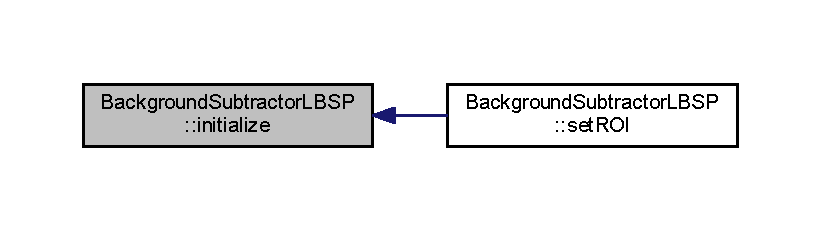
\includegraphics[width=350pt]{class_background_subtractor_l_b_s_p_ac6b854f94414497b143375d4a0ae8b6f_icgraph}
\end{center}
\end{figure}
\mbox{\Hypertarget{class_background_subtractor_su_b_s_e_n_s_e_ac84aa66030b04a72435ef473cf0e6a3f}\label{class_background_subtractor_su_b_s_e_n_s_e_ac84aa66030b04a72435ef473cf0e6a3f}} 
\index{Background\+Subtractor\+Su\+B\+S\+E\+N\+SE@{Background\+Subtractor\+Su\+B\+S\+E\+N\+SE}!initialize@{initialize}}
\index{initialize@{initialize}!Background\+Subtractor\+Su\+B\+S\+E\+N\+SE@{Background\+Subtractor\+Su\+B\+S\+E\+N\+SE}}
\subsubsection{\texorpdfstring{initialize()}{initialize()}\hspace{0.1cm}{\footnotesize\ttfamily [2/2]}}
{\footnotesize\ttfamily void Background\+Subtractor\+Su\+B\+S\+E\+N\+S\+E\+::initialize (\begin{DoxyParamCaption}\item[{const cv\+::\+Mat \&}]{o\+Init\+Img,  }\item[{const cv\+::\+Mat \&}]{o\+R\+OI }\end{DoxyParamCaption})\hspace{0.3cm}{\ttfamily [virtual]}}



(re)initiaization method; needs to be called before starting background subtraction 



Implements \mbox{\hyperlink{class_background_subtractor_l_b_s_p_a3644bc10ec3beda6fad22c633fe0f8fb}{Background\+Subtractor\+L\+B\+SP}}.



Definition at line 81 of file Background\+Subtractor\+Su\+B\+S\+E\+N\+S\+E.\+cpp.


\begin{DoxyCode}
81                                                                                       \{
82     \textcolor{comment}{// == init}
83     CV\_Assert(!oInitImg.empty() && oInitImg.cols>0 && oInitImg.rows>0);
84     CV\_Assert(oInitImg.isContinuous());
85     CV\_Assert(oInitImg.type()==CV\_8UC3 || oInitImg.type()==CV\_8UC1);
86     \textcolor{keywordflow}{if}(oInitImg.type()==CV\_8UC3) \{
87         std::vector<cv::Mat> voInitImgChannels;
88         cv::split(oInitImg,voInitImgChannels);
89         \textcolor{keywordflow}{if}(!cv::countNonZero((voInitImgChannels[0]!=voInitImgChannels[1])|(voInitImgChannels[2]!=
      voInitImgChannels[1])))
90             std::cout << std::endl << \textcolor{stringliteral}{"\(\backslash\)tBackgroundSubtractorSuBSENSE : Warning, grayscale images should
       always be passed in CV\_8UC1 format for optimal performance."} << std::endl;
91     \}
92     cv::Mat oNewBGROI;
93     \textcolor{keywordflow}{if}(oROI.empty() && (\mbox{\hyperlink{class_background_subtractor_l_b_s_p_a53fe98bd2489d95de5292467145901e9}{m\_oROI}}.empty() || oROI.size()!=oInitImg.size())) \{
94         oNewBGROI.create(oInitImg.size(),CV\_8UC1);
95         oNewBGROI = cv::Scalar\_<uchar>(UCHAR\_MAX);
96     \}
97     \textcolor{keywordflow}{else} \textcolor{keywordflow}{if}(oROI.empty())
98         oNewBGROI = \mbox{\hyperlink{class_background_subtractor_l_b_s_p_a53fe98bd2489d95de5292467145901e9}{m\_oROI}};
99     \textcolor{keywordflow}{else} \{
100         CV\_Assert(oROI.size()==oInitImg.size() && oROI.type()==CV\_8UC1);
101         CV\_Assert(cv::countNonZero((oROI<UCHAR\_MAX)&(oROI>0))==0);
102         oNewBGROI = oROI.clone();
103         cv::Mat oTempROI;
104         cv::dilate(oNewBGROI,oTempROI,\mbox{\hyperlink{class_background_subtractor_su_b_s_e_n_s_e_ae360b93378aa04b34aebc23b5f6e6714}{m\_defaultMorphologyKernel}},cv::Point(-1,-1),
      \mbox{\hyperlink{class_l_b_s_p_aa98abb79a155d3a2b416c2ab32e74929}{LBSP::PATCH\_SIZE}}/2);
105         cv::bitwise\_or(oNewBGROI,oTempROI/2,oNewBGROI);
106     \}
107     \textcolor{keyword}{const} \textcolor{keywordtype}{size\_t} nOrigROIPxCount = (size\_t)cv::countNonZero(oNewBGROI);
108     CV\_Assert(nOrigROIPxCount>0);
109     \mbox{\hyperlink{class_l_b_s_p_ad97557be4bc6cfd7b0fa4b01ab8f8c55}{LBSP::validateROI}}(oNewBGROI);
110     \textcolor{keyword}{const} \textcolor{keywordtype}{size\_t} nFinalROIPxCount = (size\_t)cv::countNonZero(oNewBGROI);
111     CV\_Assert(nFinalROIPxCount>0);
112     \mbox{\hyperlink{class_background_subtractor_l_b_s_p_a53fe98bd2489d95de5292467145901e9}{m\_oROI}} = oNewBGROI;
113     \mbox{\hyperlink{class_background_subtractor_l_b_s_p_a732d5e6ae35fb0e858cadb3af5ce08a2}{m\_oImgSize}} = oInitImg.size();
114     \mbox{\hyperlink{class_background_subtractor_l_b_s_p_a7d2f52ecd5ff56e42da86f97e0ad93b5}{m\_nImgType}} = oInitImg.type();
115     \mbox{\hyperlink{class_background_subtractor_l_b_s_p_ab3467ebee2c5d1249061ccd704cc0584}{m\_nImgChannels}} = oInitImg.channels();
116     \mbox{\hyperlink{class_background_subtractor_l_b_s_p_a9d1e247267afbddb7032bdcabd67d931}{m\_nTotPxCount}} = \mbox{\hyperlink{class_background_subtractor_l_b_s_p_a732d5e6ae35fb0e858cadb3af5ce08a2}{m\_oImgSize}}.area();
117     \mbox{\hyperlink{class_background_subtractor_l_b_s_p_ac3b54f4d2dfa3a576475214f26501d85}{m\_nTotRelevantPxCount}} = nFinalROIPxCount;
118     \mbox{\hyperlink{class_background_subtractor_l_b_s_p_a8a2350cad84f19c68ef61b7aaf91c43f}{m\_nFrameIndex}} = 0;
119     \mbox{\hyperlink{class_background_subtractor_l_b_s_p_ab56bf775dfdf0579e834e45210c3a92a}{m\_nFramesSinceLastReset}} = 0;
120     \mbox{\hyperlink{class_background_subtractor_l_b_s_p_a5ea18d388afacf8285c46ba0f754e7ee}{m\_nModelResetCooldown}} = 0;
121     \mbox{\hyperlink{class_background_subtractor_su_b_s_e_n_s_e_a4231d025a90be64a703f3f0aff1345c8}{m\_fLastNonZeroDescRatio}} = 0.0f;
122     \textcolor{keyword}{const} \textcolor{keywordtype}{int} nTotImgPixels = \mbox{\hyperlink{class_background_subtractor_l_b_s_p_a732d5e6ae35fb0e858cadb3af5ce08a2}{m\_oImgSize}}.height*\mbox{\hyperlink{class_background_subtractor_l_b_s_p_a732d5e6ae35fb0e858cadb3af5ce08a2}{m\_oImgSize}}.width;
123     \textcolor{keywordflow}{if}(nOrigROIPxCount>=\mbox{\hyperlink{class_background_subtractor_l_b_s_p_a9d1e247267afbddb7032bdcabd67d931}{m\_nTotPxCount}}/2 && (\textcolor{keywordtype}{int})\mbox{\hyperlink{class_background_subtractor_l_b_s_p_a9d1e247267afbddb7032bdcabd67d931}{m\_nTotPxCount}}>=
      \mbox{\hyperlink{_background_subtractor_su_b_s_e_n_s_e_8cpp_aee6405a4f74939fffcc9b3055af94b3a}{DEFAULT\_FRAME\_SIZE}}.area()) \{
124         \mbox{\hyperlink{class_background_subtractor_su_b_s_e_n_s_e_afca07a4c7edca7761e55dfbdf6da4263}{m\_bLearningRateScalingEnabled}} = \textcolor{keyword}{true};
125         \mbox{\hyperlink{class_background_subtractor_l_b_s_p_a9d260f4e42e3fc79fb21af950ca9087a}{m\_bAutoModelResetEnabled}} = \textcolor{keyword}{true};
126         \mbox{\hyperlink{class_background_subtractor_su_b_s_e_n_s_e_a1e2e28840e7ca373282607db81b49e12}{m\_bUse3x3Spread}} = !(nTotImgPixels>\mbox{\hyperlink{_background_subtractor_su_b_s_e_n_s_e_8cpp_aee6405a4f74939fffcc9b3055af94b3a}{DEFAULT\_FRAME\_SIZE}}.area()*2);
127         \textcolor{keyword}{const} \textcolor{keywordtype}{int} nRawMedianBlurKernelSize = std::min((\textcolor{keywordtype}{int})floor((\textcolor{keywordtype}{float})nTotImgPixels/
      \mbox{\hyperlink{_background_subtractor_su_b_s_e_n_s_e_8cpp_aee6405a4f74939fffcc9b3055af94b3a}{DEFAULT\_FRAME\_SIZE}}.area()+0.5f)+\mbox{\hyperlink{class_background_subtractor_l_b_s_p_a2585fe6e41e10af6da3e325dc20fe7f1}{m\_nDefaultMedianBlurKernelSize}}
      ,14);
128         \mbox{\hyperlink{class_background_subtractor_su_b_s_e_n_s_e_a796120fecb11f00914925e14065ee5ab}{m\_nMedianBlurKernelSize}} = (nRawMedianBlurKernelSize%2)?
      nRawMedianBlurKernelSize:nRawMedianBlurKernelSize-1;
129         \mbox{\hyperlink{class_background_subtractor_su_b_s_e_n_s_e_a57fdd29e43afc163233e55f9a7cd9f37}{m\_fCurrLearningRateLowerCap}} = 
      \mbox{\hyperlink{_background_subtractor_su_b_s_e_n_s_e_8cpp_a6975332215c62c3172a76af852bc5566}{FEEDBACK\_T\_LOWER}};
130         \mbox{\hyperlink{class_background_subtractor_su_b_s_e_n_s_e_a44ba1a1ed365c5829baa517ce9f27508}{m\_fCurrLearningRateUpperCap}} = 
      \mbox{\hyperlink{_background_subtractor_su_b_s_e_n_s_e_8cpp_a23bd980dc8c9bbffe3f27b44fa983f9c}{FEEDBACK\_T\_UPPER}};
131     \}
132     \textcolor{keywordflow}{else} \{
133         \mbox{\hyperlink{class_background_subtractor_su_b_s_e_n_s_e_afca07a4c7edca7761e55dfbdf6da4263}{m\_bLearningRateScalingEnabled}} = \textcolor{keyword}{false};
134         \mbox{\hyperlink{class_background_subtractor_l_b_s_p_a9d260f4e42e3fc79fb21af950ca9087a}{m\_bAutoModelResetEnabled}} = \textcolor{keyword}{false};
135         \mbox{\hyperlink{class_background_subtractor_su_b_s_e_n_s_e_a1e2e28840e7ca373282607db81b49e12}{m\_bUse3x3Spread}} = \textcolor{keyword}{true};
136         \mbox{\hyperlink{class_background_subtractor_su_b_s_e_n_s_e_a796120fecb11f00914925e14065ee5ab}{m\_nMedianBlurKernelSize}} = 
      \mbox{\hyperlink{class_background_subtractor_l_b_s_p_a2585fe6e41e10af6da3e325dc20fe7f1}{m\_nDefaultMedianBlurKernelSize}};
137         \mbox{\hyperlink{class_background_subtractor_su_b_s_e_n_s_e_a57fdd29e43afc163233e55f9a7cd9f37}{m\_fCurrLearningRateLowerCap}} = 
      \mbox{\hyperlink{_background_subtractor_su_b_s_e_n_s_e_8cpp_a6975332215c62c3172a76af852bc5566}{FEEDBACK\_T\_LOWER}}*2;
138         \mbox{\hyperlink{class_background_subtractor_su_b_s_e_n_s_e_a44ba1a1ed365c5829baa517ce9f27508}{m\_fCurrLearningRateUpperCap}} = 
      \mbox{\hyperlink{_background_subtractor_su_b_s_e_n_s_e_8cpp_a23bd980dc8c9bbffe3f27b44fa983f9c}{FEEDBACK\_T\_UPPER}}*2;
139     \}
140     \mbox{\hyperlink{class_background_subtractor_su_b_s_e_n_s_e_a90cb2cc5cbe3f2f0b01e06f514c8b569}{m\_oUpdateRateFrame}}.create(\mbox{\hyperlink{class_background_subtractor_l_b_s_p_a732d5e6ae35fb0e858cadb3af5ce08a2}{m\_oImgSize}},CV\_32FC1);
141     \mbox{\hyperlink{class_background_subtractor_su_b_s_e_n_s_e_a90cb2cc5cbe3f2f0b01e06f514c8b569}{m\_oUpdateRateFrame}} = cv::Scalar(
      \mbox{\hyperlink{class_background_subtractor_su_b_s_e_n_s_e_a57fdd29e43afc163233e55f9a7cd9f37}{m\_fCurrLearningRateLowerCap}});
142     \mbox{\hyperlink{class_background_subtractor_su_b_s_e_n_s_e_a491a1e2b81dee87a721a421719bf2836}{m\_oDistThresholdFrame}}.create(\mbox{\hyperlink{class_background_subtractor_l_b_s_p_a732d5e6ae35fb0e858cadb3af5ce08a2}{m\_oImgSize}},CV\_32FC1);
143     \mbox{\hyperlink{class_background_subtractor_su_b_s_e_n_s_e_a491a1e2b81dee87a721a421719bf2836}{m\_oDistThresholdFrame}} = cv::Scalar(1.0\mbox{\hyperlink{rings_8cpp_a77369fc4d5326a16d2c603e032023528}{f}});
144     \mbox{\hyperlink{class_background_subtractor_su_b_s_e_n_s_e_a47d9cf067ac639d95fcb810c894bb770}{m\_oVariationModulatorFrame}}.create(\mbox{\hyperlink{class_background_subtractor_l_b_s_p_a732d5e6ae35fb0e858cadb3af5ce08a2}{m\_oImgSize}},CV\_32FC1);
145     \mbox{\hyperlink{class_background_subtractor_su_b_s_e_n_s_e_a47d9cf067ac639d95fcb810c894bb770}{m\_oVariationModulatorFrame}} = cv::Scalar(10.0\mbox{\hyperlink{rings_8cpp_a77369fc4d5326a16d2c603e032023528}{f}}); \textcolor{comment}{// should always be >=
       FEEDBACK\_V\_DECR}
146     \mbox{\hyperlink{class_background_subtractor_su_b_s_e_n_s_e_ad95bb91ff7ef9db725772b37d679e1a2}{m\_oMeanLastDistFrame}}.create(\mbox{\hyperlink{class_background_subtractor_l_b_s_p_a732d5e6ae35fb0e858cadb3af5ce08a2}{m\_oImgSize}},CV\_32FC1);
147     \mbox{\hyperlink{class_background_subtractor_su_b_s_e_n_s_e_ad95bb91ff7ef9db725772b37d679e1a2}{m\_oMeanLastDistFrame}} = cv::Scalar(0.0\mbox{\hyperlink{rings_8cpp_a77369fc4d5326a16d2c603e032023528}{f}});
148     \mbox{\hyperlink{class_background_subtractor_su_b_s_e_n_s_e_a8318e35d5fbbcffb8729700ef5e71a6e}{m\_oMeanMinDistFrame\_LT}}.create(\mbox{\hyperlink{class_background_subtractor_l_b_s_p_a732d5e6ae35fb0e858cadb3af5ce08a2}{m\_oImgSize}},CV\_32FC1);
149     \mbox{\hyperlink{class_background_subtractor_su_b_s_e_n_s_e_a8318e35d5fbbcffb8729700ef5e71a6e}{m\_oMeanMinDistFrame\_LT}} = cv::Scalar(0.0\mbox{\hyperlink{rings_8cpp_a77369fc4d5326a16d2c603e032023528}{f}});
150     \mbox{\hyperlink{class_background_subtractor_su_b_s_e_n_s_e_a53584c5c79017947c59d05dfd247cf5e}{m\_oMeanMinDistFrame\_ST}}.create(\mbox{\hyperlink{class_background_subtractor_l_b_s_p_a732d5e6ae35fb0e858cadb3af5ce08a2}{m\_oImgSize}},CV\_32FC1);
151     \mbox{\hyperlink{class_background_subtractor_su_b_s_e_n_s_e_a53584c5c79017947c59d05dfd247cf5e}{m\_oMeanMinDistFrame\_ST}} = cv::Scalar(0.0\mbox{\hyperlink{rings_8cpp_a77369fc4d5326a16d2c603e032023528}{f}});
152     \mbox{\hyperlink{class_background_subtractor_su_b_s_e_n_s_e_af3e1eb902a5b6b46a1c229864423bd20}{m\_oDownSampledFrameSize}} = cv::Size(\mbox{\hyperlink{class_background_subtractor_l_b_s_p_a732d5e6ae35fb0e858cadb3af5ce08a2}{m\_oImgSize}}.width/
      \mbox{\hyperlink{_background_subtractor_su_b_s_e_n_s_e_8cpp_ab07d30f0cf4181205776a4c1e85f6527}{FRAMELEVEL\_ANALYSIS\_DOWNSAMPLE\_RATIO}},
      \mbox{\hyperlink{class_background_subtractor_l_b_s_p_a732d5e6ae35fb0e858cadb3af5ce08a2}{m\_oImgSize}}.height/\mbox{\hyperlink{_background_subtractor_su_b_s_e_n_s_e_8cpp_ab07d30f0cf4181205776a4c1e85f6527}{FRAMELEVEL\_ANALYSIS\_DOWNSAMPLE\_RATIO}});
153     \mbox{\hyperlink{class_background_subtractor_su_b_s_e_n_s_e_ab6056c53d3237ae04da509b36ec40486}{m\_oMeanDownSampledLastDistFrame\_LT}}.create(
      \mbox{\hyperlink{class_background_subtractor_su_b_s_e_n_s_e_af3e1eb902a5b6b46a1c229864423bd20}{m\_oDownSampledFrameSize}},CV\_32FC((\textcolor{keywordtype}{int})\mbox{\hyperlink{class_background_subtractor_l_b_s_p_ab3467ebee2c5d1249061ccd704cc0584}{m\_nImgChannels}}));
154     \mbox{\hyperlink{class_background_subtractor_su_b_s_e_n_s_e_ab6056c53d3237ae04da509b36ec40486}{m\_oMeanDownSampledLastDistFrame\_LT}} = cv::Scalar(0.0
      \mbox{\hyperlink{rings_8cpp_a77369fc4d5326a16d2c603e032023528}{f}});
155     \mbox{\hyperlink{class_background_subtractor_su_b_s_e_n_s_e_a92a9aec9a8b34383b67d97467bd34515}{m\_oMeanDownSampledLastDistFrame\_ST}}.create(
      \mbox{\hyperlink{class_background_subtractor_su_b_s_e_n_s_e_af3e1eb902a5b6b46a1c229864423bd20}{m\_oDownSampledFrameSize}},CV\_32FC((\textcolor{keywordtype}{int})\mbox{\hyperlink{class_background_subtractor_l_b_s_p_ab3467ebee2c5d1249061ccd704cc0584}{m\_nImgChannels}}));
156     \mbox{\hyperlink{class_background_subtractor_su_b_s_e_n_s_e_a92a9aec9a8b34383b67d97467bd34515}{m\_oMeanDownSampledLastDistFrame\_ST}} = cv::Scalar(0.0
      \mbox{\hyperlink{rings_8cpp_a77369fc4d5326a16d2c603e032023528}{f}});
157     \mbox{\hyperlink{class_background_subtractor_su_b_s_e_n_s_e_a7706b13433c4e9f4f8156e075fa7904d}{m\_oMeanRawSegmResFrame\_LT}}.create(\mbox{\hyperlink{class_background_subtractor_l_b_s_p_a732d5e6ae35fb0e858cadb3af5ce08a2}{m\_oImgSize}},CV\_32FC1);
158     \mbox{\hyperlink{class_background_subtractor_su_b_s_e_n_s_e_a7706b13433c4e9f4f8156e075fa7904d}{m\_oMeanRawSegmResFrame\_LT}} = cv::Scalar(0.0\mbox{\hyperlink{rings_8cpp_a77369fc4d5326a16d2c603e032023528}{f}});
159     \mbox{\hyperlink{class_background_subtractor_su_b_s_e_n_s_e_a3c9fd9cf995eb9a7b4006467ab874958}{m\_oMeanRawSegmResFrame\_ST}}.create(\mbox{\hyperlink{class_background_subtractor_l_b_s_p_a732d5e6ae35fb0e858cadb3af5ce08a2}{m\_oImgSize}},CV\_32FC1);
160     \mbox{\hyperlink{class_background_subtractor_su_b_s_e_n_s_e_a3c9fd9cf995eb9a7b4006467ab874958}{m\_oMeanRawSegmResFrame\_ST}} = cv::Scalar(0.0\mbox{\hyperlink{rings_8cpp_a77369fc4d5326a16d2c603e032023528}{f}});
161     \mbox{\hyperlink{class_background_subtractor_su_b_s_e_n_s_e_ad48e92b6d6bbce34f9f452484bc9956a}{m\_oMeanFinalSegmResFrame\_LT}}.create(\mbox{\hyperlink{class_background_subtractor_l_b_s_p_a732d5e6ae35fb0e858cadb3af5ce08a2}{m\_oImgSize}},CV\_32FC1);
162     \mbox{\hyperlink{class_background_subtractor_su_b_s_e_n_s_e_ad48e92b6d6bbce34f9f452484bc9956a}{m\_oMeanFinalSegmResFrame\_LT}} = cv::Scalar(0.0\mbox{\hyperlink{rings_8cpp_a77369fc4d5326a16d2c603e032023528}{f}});
163     \mbox{\hyperlink{class_background_subtractor_su_b_s_e_n_s_e_a0dcd4f5df8adb9b4fa630a9a6f6b5e30}{m\_oMeanFinalSegmResFrame\_ST}}.create(\mbox{\hyperlink{class_background_subtractor_l_b_s_p_a732d5e6ae35fb0e858cadb3af5ce08a2}{m\_oImgSize}},CV\_32FC1);
164     \mbox{\hyperlink{class_background_subtractor_su_b_s_e_n_s_e_a0dcd4f5df8adb9b4fa630a9a6f6b5e30}{m\_oMeanFinalSegmResFrame\_ST}} = cv::Scalar(0.0\mbox{\hyperlink{rings_8cpp_a77369fc4d5326a16d2c603e032023528}{f}});
165     \mbox{\hyperlink{class_background_subtractor_su_b_s_e_n_s_e_acfaf4c3c5aedbed8bd302444b4a4f8dd}{m\_oUnstableRegionMask}}.create(\mbox{\hyperlink{class_background_subtractor_l_b_s_p_a732d5e6ae35fb0e858cadb3af5ce08a2}{m\_oImgSize}},CV\_8UC1);
166     \mbox{\hyperlink{class_background_subtractor_su_b_s_e_n_s_e_acfaf4c3c5aedbed8bd302444b4a4f8dd}{m\_oUnstableRegionMask}} = cv::Scalar\_<uchar>(0);
167     \mbox{\hyperlink{class_background_subtractor_su_b_s_e_n_s_e_a943b50c63d233c0948d82b64390f1aa1}{m\_oBlinksFrame}}.create(\mbox{\hyperlink{class_background_subtractor_l_b_s_p_a732d5e6ae35fb0e858cadb3af5ce08a2}{m\_oImgSize}},CV\_8UC1);
168     \mbox{\hyperlink{class_background_subtractor_su_b_s_e_n_s_e_a943b50c63d233c0948d82b64390f1aa1}{m\_oBlinksFrame}} = cv::Scalar\_<uchar>(0);
169     \mbox{\hyperlink{class_background_subtractor_su_b_s_e_n_s_e_a619bc3f0bfcd408796d1ffd6bd45d04d}{m\_oDownSampledFrame\_MotionAnalysis}}.create(
      \mbox{\hyperlink{class_background_subtractor_su_b_s_e_n_s_e_af3e1eb902a5b6b46a1c229864423bd20}{m\_oDownSampledFrameSize}},CV\_8UC((\textcolor{keywordtype}{int})\mbox{\hyperlink{class_background_subtractor_l_b_s_p_ab3467ebee2c5d1249061ccd704cc0584}{m\_nImgChannels}}));
170     \mbox{\hyperlink{class_background_subtractor_su_b_s_e_n_s_e_a619bc3f0bfcd408796d1ffd6bd45d04d}{m\_oDownSampledFrame\_MotionAnalysis}} = cv::Scalar\_<uchar>::all(0);
171     \mbox{\hyperlink{class_background_subtractor_l_b_s_p_ab1dc003792ab1d0b881a6fd10e0e29b3}{m\_oLastColorFrame}}.create(\mbox{\hyperlink{class_background_subtractor_l_b_s_p_a732d5e6ae35fb0e858cadb3af5ce08a2}{m\_oImgSize}},CV\_8UC((\textcolor{keywordtype}{int})
      \mbox{\hyperlink{class_background_subtractor_l_b_s_p_ab3467ebee2c5d1249061ccd704cc0584}{m\_nImgChannels}}));
172     \mbox{\hyperlink{class_background_subtractor_l_b_s_p_ab1dc003792ab1d0b881a6fd10e0e29b3}{m\_oLastColorFrame}} = cv::Scalar\_<uchar>::all(0);
173     \mbox{\hyperlink{class_background_subtractor_l_b_s_p_a9c637c0b87cac495887295690d83ba13}{m\_oLastDescFrame}}.create(\mbox{\hyperlink{class_background_subtractor_l_b_s_p_a732d5e6ae35fb0e858cadb3af5ce08a2}{m\_oImgSize}},CV\_16UC((\textcolor{keywordtype}{int})
      \mbox{\hyperlink{class_background_subtractor_l_b_s_p_ab3467ebee2c5d1249061ccd704cc0584}{m\_nImgChannels}}));
174     \mbox{\hyperlink{class_background_subtractor_l_b_s_p_a9c637c0b87cac495887295690d83ba13}{m\_oLastDescFrame}} = cv::Scalar\_<ushort>::all(0);
175     \mbox{\hyperlink{class_background_subtractor_su_b_s_e_n_s_e_a11c86236e9d141d711163c170a8bf0d6}{m\_oLastRawFGMask}}.create(\mbox{\hyperlink{class_background_subtractor_l_b_s_p_a732d5e6ae35fb0e858cadb3af5ce08a2}{m\_oImgSize}},CV\_8UC1);
176     \mbox{\hyperlink{class_background_subtractor_su_b_s_e_n_s_e_a11c86236e9d141d711163c170a8bf0d6}{m\_oLastRawFGMask}} = cv::Scalar\_<uchar>(0);
177     \mbox{\hyperlink{class_background_subtractor_l_b_s_p_adb6dc0af596c5592c91f9d8faa5c8a4b}{m\_oLastFGMask}}.create(\mbox{\hyperlink{class_background_subtractor_l_b_s_p_a732d5e6ae35fb0e858cadb3af5ce08a2}{m\_oImgSize}},CV\_8UC1);
178     \mbox{\hyperlink{class_background_subtractor_l_b_s_p_adb6dc0af596c5592c91f9d8faa5c8a4b}{m\_oLastFGMask}} = cv::Scalar\_<uchar>(0);
179     \mbox{\hyperlink{class_background_subtractor_su_b_s_e_n_s_e_a2dc6a8f1c8e2694d19dbbb74c533e293}{m\_oLastFGMask\_dilated}}.create(\mbox{\hyperlink{class_background_subtractor_l_b_s_p_a732d5e6ae35fb0e858cadb3af5ce08a2}{m\_oImgSize}},CV\_8UC1);
180     \mbox{\hyperlink{class_background_subtractor_su_b_s_e_n_s_e_a2dc6a8f1c8e2694d19dbbb74c533e293}{m\_oLastFGMask\_dilated}} = cv::Scalar\_<uchar>(0);
181     \mbox{\hyperlink{class_background_subtractor_su_b_s_e_n_s_e_a0306555d3e97ceec32f8f6b495d18b95}{m\_oLastFGMask\_dilated\_inverted}}.create(
      \mbox{\hyperlink{class_background_subtractor_l_b_s_p_a732d5e6ae35fb0e858cadb3af5ce08a2}{m\_oImgSize}},CV\_8UC1);
182     \mbox{\hyperlink{class_background_subtractor_su_b_s_e_n_s_e_a0306555d3e97ceec32f8f6b495d18b95}{m\_oLastFGMask\_dilated\_inverted}} = cv::Scalar\_<uchar>(0);
183     \mbox{\hyperlink{class_background_subtractor_su_b_s_e_n_s_e_a4a8df16fa54d4b22a9b787d5b57427f9}{m\_oFGMask\_FloodedHoles}}.create(\mbox{\hyperlink{class_background_subtractor_l_b_s_p_a732d5e6ae35fb0e858cadb3af5ce08a2}{m\_oImgSize}},CV\_8UC1);
184     \mbox{\hyperlink{class_background_subtractor_su_b_s_e_n_s_e_a4a8df16fa54d4b22a9b787d5b57427f9}{m\_oFGMask\_FloodedHoles}} = cv::Scalar\_<uchar>(0);
185     \mbox{\hyperlink{class_background_subtractor_su_b_s_e_n_s_e_a53ac4868e46e0ba382a0e6d769e8a961}{m\_oFGMask\_PreFlood}}.create(\mbox{\hyperlink{class_background_subtractor_l_b_s_p_a732d5e6ae35fb0e858cadb3af5ce08a2}{m\_oImgSize}},CV\_8UC1);
186     \mbox{\hyperlink{class_background_subtractor_su_b_s_e_n_s_e_a53ac4868e46e0ba382a0e6d769e8a961}{m\_oFGMask\_PreFlood}} = cv::Scalar\_<uchar>(0);
187     \mbox{\hyperlink{class_background_subtractor_su_b_s_e_n_s_e_a804b5ad0898777a2eb2cb4d932c857b6}{m\_oCurrRawFGBlinkMask}}.create(\mbox{\hyperlink{class_background_subtractor_l_b_s_p_a732d5e6ae35fb0e858cadb3af5ce08a2}{m\_oImgSize}},CV\_8UC1);
188     \mbox{\hyperlink{class_background_subtractor_su_b_s_e_n_s_e_a804b5ad0898777a2eb2cb4d932c857b6}{m\_oCurrRawFGBlinkMask}} = cv::Scalar\_<uchar>(0);
189     \mbox{\hyperlink{class_background_subtractor_su_b_s_e_n_s_e_aea0e3a3817d99da5b2fe15c810b0f428}{m\_oLastRawFGBlinkMask}}.create(\mbox{\hyperlink{class_background_subtractor_l_b_s_p_a732d5e6ae35fb0e858cadb3af5ce08a2}{m\_oImgSize}},CV\_8UC1);
190     \mbox{\hyperlink{class_background_subtractor_su_b_s_e_n_s_e_aea0e3a3817d99da5b2fe15c810b0f428}{m\_oLastRawFGBlinkMask}} = cv::Scalar\_<uchar>(0);
191     \mbox{\hyperlink{class_background_subtractor_su_b_s_e_n_s_e_a9d4d4bb930b34745536b9862683bb539}{m\_voBGColorSamples}}.resize(\mbox{\hyperlink{class_background_subtractor_su_b_s_e_n_s_e_ad783b71b5b942c4018d27cf38b7d7225}{m\_nBGSamples}});
192     \mbox{\hyperlink{class_background_subtractor_su_b_s_e_n_s_e_a422cc2f2a25c07efca02087bd6fe3d6d}{m\_voBGDescSamples}}.resize(\mbox{\hyperlink{class_background_subtractor_su_b_s_e_n_s_e_ad783b71b5b942c4018d27cf38b7d7225}{m\_nBGSamples}});
193     \textcolor{keywordflow}{for}(\textcolor{keywordtype}{size\_t} s=0; s<\mbox{\hyperlink{class_background_subtractor_su_b_s_e_n_s_e_ad783b71b5b942c4018d27cf38b7d7225}{m\_nBGSamples}}; ++s) \{
194         \mbox{\hyperlink{class_background_subtractor_su_b_s_e_n_s_e_a9d4d4bb930b34745536b9862683bb539}{m\_voBGColorSamples}}[s].create(\mbox{\hyperlink{class_background_subtractor_l_b_s_p_a732d5e6ae35fb0e858cadb3af5ce08a2}{m\_oImgSize}},CV\_8UC((\textcolor{keywordtype}{int})
      \mbox{\hyperlink{class_background_subtractor_l_b_s_p_ab3467ebee2c5d1249061ccd704cc0584}{m\_nImgChannels}}));
195         \mbox{\hyperlink{class_background_subtractor_su_b_s_e_n_s_e_a9d4d4bb930b34745536b9862683bb539}{m\_voBGColorSamples}}[s] = cv::Scalar\_<uchar>::all(0);
196         \mbox{\hyperlink{class_background_subtractor_su_b_s_e_n_s_e_a422cc2f2a25c07efca02087bd6fe3d6d}{m\_voBGDescSamples}}[s].create(\mbox{\hyperlink{class_background_subtractor_l_b_s_p_a732d5e6ae35fb0e858cadb3af5ce08a2}{m\_oImgSize}},CV\_16UC((\textcolor{keywordtype}{int})
      \mbox{\hyperlink{class_background_subtractor_l_b_s_p_ab3467ebee2c5d1249061ccd704cc0584}{m\_nImgChannels}}));
197         \mbox{\hyperlink{class_background_subtractor_su_b_s_e_n_s_e_a422cc2f2a25c07efca02087bd6fe3d6d}{m\_voBGDescSamples}}[s] = cv::Scalar\_<ushort>::all(0);
198     \}
199     \textcolor{keywordflow}{if}(\mbox{\hyperlink{class_background_subtractor_l_b_s_p_a06b4f0d3f24fa08bccd3c9eca085713e}{m\_aPxIdxLUT}})
200         \textcolor{keyword}{delete}[] \mbox{\hyperlink{class_background_subtractor_l_b_s_p_a06b4f0d3f24fa08bccd3c9eca085713e}{m\_aPxIdxLUT}};
201     \textcolor{keywordflow}{if}(\mbox{\hyperlink{class_background_subtractor_l_b_s_p_a74e73d4832ccdef652d93756582024db}{m\_aPxInfoLUT}})
202         \textcolor{keyword}{delete}[] \mbox{\hyperlink{class_background_subtractor_l_b_s_p_a74e73d4832ccdef652d93756582024db}{m\_aPxInfoLUT}};
203     \mbox{\hyperlink{class_background_subtractor_l_b_s_p_a06b4f0d3f24fa08bccd3c9eca085713e}{m\_aPxIdxLUT}} = \textcolor{keyword}{new} \textcolor{keywordtype}{size\_t}[\mbox{\hyperlink{class_background_subtractor_l_b_s_p_ac3b54f4d2dfa3a576475214f26501d85}{m\_nTotRelevantPxCount}}];
204     \mbox{\hyperlink{class_background_subtractor_l_b_s_p_a74e73d4832ccdef652d93756582024db}{m\_aPxInfoLUT}} = \textcolor{keyword}{new} PxInfoBase[\mbox{\hyperlink{class_background_subtractor_l_b_s_p_a9d1e247267afbddb7032bdcabd67d931}{m\_nTotPxCount}}];
205     \textcolor{keywordflow}{if}(\mbox{\hyperlink{class_background_subtractor_l_b_s_p_ab3467ebee2c5d1249061ccd704cc0584}{m\_nImgChannels}}==1) \{
206         CV\_Assert(\mbox{\hyperlink{class_background_subtractor_l_b_s_p_ab1dc003792ab1d0b881a6fd10e0e29b3}{m\_oLastColorFrame}}.step.p[0]==(\textcolor{keywordtype}{size\_t})
      \mbox{\hyperlink{class_background_subtractor_l_b_s_p_a732d5e6ae35fb0e858cadb3af5ce08a2}{m\_oImgSize}}.width && \mbox{\hyperlink{class_background_subtractor_l_b_s_p_ab1dc003792ab1d0b881a6fd10e0e29b3}{m\_oLastColorFrame}}.step.p[1]==1);
207         CV\_Assert(\mbox{\hyperlink{class_background_subtractor_l_b_s_p_a9c637c0b87cac495887295690d83ba13}{m\_oLastDescFrame}}.step.p[0]==\mbox{\hyperlink{class_background_subtractor_l_b_s_p_ab1dc003792ab1d0b881a6fd10e0e29b3}{m\_oLastColorFrame}}.step.p[0]*
      2 && \mbox{\hyperlink{class_background_subtractor_l_b_s_p_a9c637c0b87cac495887295690d83ba13}{m\_oLastDescFrame}}.step.p[1]==\mbox{\hyperlink{class_background_subtractor_l_b_s_p_ab1dc003792ab1d0b881a6fd10e0e29b3}{m\_oLastColorFrame}}.step.p[1]*2);
208         \textcolor{keywordflow}{for}(\textcolor{keywordtype}{size\_t} t=0; t<=UCHAR\_MAX; ++t)
209             \mbox{\hyperlink{class_background_subtractor_l_b_s_p_aefe69d94f08b2c4ba73ad1d254ad9153}{m\_anLBSPThreshold\_8bitLUT}}[t] = cv::saturate\_cast<uchar>((
      \mbox{\hyperlink{class_background_subtractor_l_b_s_p_a209eb6aaa34e8ad8e565e79f85404e24}{m\_nLBSPThresholdOffset}}+t*\mbox{\hyperlink{class_background_subtractor_l_b_s_p_ad759c645b14e9b16bf3940cae862df32}{m\_fRelLBSPThreshold}})/3);
210         \textcolor{keywordflow}{for}(\textcolor{keywordtype}{size\_t} nPxIter=0, nModelIter=0; nPxIter<\mbox{\hyperlink{class_background_subtractor_l_b_s_p_a9d1e247267afbddb7032bdcabd67d931}{m\_nTotPxCount}}; ++nPxIter) \{
211             \textcolor{keywordflow}{if}(\mbox{\hyperlink{class_background_subtractor_l_b_s_p_a53fe98bd2489d95de5292467145901e9}{m\_oROI}}.data[nPxIter]) \{
212                 \mbox{\hyperlink{class_background_subtractor_l_b_s_p_a06b4f0d3f24fa08bccd3c9eca085713e}{m\_aPxIdxLUT}}[nModelIter] = nPxIter;
213                 \mbox{\hyperlink{class_background_subtractor_l_b_s_p_a74e73d4832ccdef652d93756582024db}{m\_aPxInfoLUT}}[nPxIter].\mbox{\hyperlink{struct_background_subtractor_l_b_s_p_1_1_px_info_base_a42cb6eecda647b2a11b90ea420f2bc31}{nImgCoord\_Y}} = (int)nPxIter/
      \mbox{\hyperlink{class_background_subtractor_l_b_s_p_a732d5e6ae35fb0e858cadb3af5ce08a2}{m\_oImgSize}}.width;
214                 \mbox{\hyperlink{class_background_subtractor_l_b_s_p_a74e73d4832ccdef652d93756582024db}{m\_aPxInfoLUT}}[nPxIter].\mbox{\hyperlink{struct_background_subtractor_l_b_s_p_1_1_px_info_base_a10966fe72f000045adede9e853156b48}{nImgCoord\_X}} = (\textcolor{keywordtype}{int})nPxIter%
      \mbox{\hyperlink{class_background_subtractor_l_b_s_p_a732d5e6ae35fb0e858cadb3af5ce08a2}{m\_oImgSize}}.width;
215                 \mbox{\hyperlink{class_background_subtractor_l_b_s_p_a74e73d4832ccdef652d93756582024db}{m\_aPxInfoLUT}}[nPxIter].\mbox{\hyperlink{struct_background_subtractor_l_b_s_p_1_1_px_info_base_afe4a63a708fa0f3ea6ed2fac837bc71d}{nModelIdx}} = nModelIter;
216                 \mbox{\hyperlink{class_background_subtractor_l_b_s_p_ab1dc003792ab1d0b881a6fd10e0e29b3}{m\_oLastColorFrame}}.data[nPxIter] = oInitImg.data[nPxIter];
217                 \textcolor{keyword}{const} \textcolor{keywordtype}{size\_t} nDescIter = nPxIter*2;
218                 \mbox{\hyperlink{class_l_b_s_p_a4a5f635868b6b81ba53df2692ee3dfd8}{LBSP::computeGrayscaleDescriptor}}(oInitImg,oInitImg.data[
      nPxIter],\mbox{\hyperlink{class_background_subtractor_l_b_s_p_a74e73d4832ccdef652d93756582024db}{m\_aPxInfoLUT}}[nPxIter].\mbox{\hyperlink{struct_background_subtractor_l_b_s_p_1_1_px_info_base_a10966fe72f000045adede9e853156b48}{nImgCoord\_X}},\mbox{\hyperlink{class_background_subtractor_l_b_s_p_a74e73d4832ccdef652d93756582024db}{m\_aPxInfoLUT}}[nPxIter].
      \mbox{\hyperlink{struct_background_subtractor_l_b_s_p_1_1_px_info_base_a42cb6eecda647b2a11b90ea420f2bc31}{nImgCoord\_Y}},\mbox{\hyperlink{class_background_subtractor_l_b_s_p_aefe69d94f08b2c4ba73ad1d254ad9153}{m\_anLBSPThreshold\_8bitLUT}}[oInitImg.data[nPxIter]],*((ushort
      *)(\mbox{\hyperlink{class_background_subtractor_l_b_s_p_a9c637c0b87cac495887295690d83ba13}{m\_oLastDescFrame}}.data+nDescIter)));
219                 ++nModelIter;
220             \}
221         \}
222     \}
223     \textcolor{keywordflow}{else} \{ \textcolor{comment}{//m\_nImgChannels==3}
224         CV\_Assert(\mbox{\hyperlink{class_background_subtractor_l_b_s_p_ab1dc003792ab1d0b881a6fd10e0e29b3}{m\_oLastColorFrame}}.step.p[0]==(\textcolor{keywordtype}{size\_t})
      \mbox{\hyperlink{class_background_subtractor_l_b_s_p_a732d5e6ae35fb0e858cadb3af5ce08a2}{m\_oImgSize}}.width*3 && \mbox{\hyperlink{class_background_subtractor_l_b_s_p_ab1dc003792ab1d0b881a6fd10e0e29b3}{m\_oLastColorFrame}}.step.p[1]==3);
225         CV\_Assert(\mbox{\hyperlink{class_background_subtractor_l_b_s_p_a9c637c0b87cac495887295690d83ba13}{m\_oLastDescFrame}}.step.p[0]==\mbox{\hyperlink{class_background_subtractor_l_b_s_p_ab1dc003792ab1d0b881a6fd10e0e29b3}{m\_oLastColorFrame}}.step.p[0]*
      2 && \mbox{\hyperlink{class_background_subtractor_l_b_s_p_a9c637c0b87cac495887295690d83ba13}{m\_oLastDescFrame}}.step.p[1]==\mbox{\hyperlink{class_background_subtractor_l_b_s_p_ab1dc003792ab1d0b881a6fd10e0e29b3}{m\_oLastColorFrame}}.step.p[1]*2);
226         \textcolor{keywordflow}{for}(\textcolor{keywordtype}{size\_t} t=0; t<=UCHAR\_MAX; ++t)
227             \mbox{\hyperlink{class_background_subtractor_l_b_s_p_aefe69d94f08b2c4ba73ad1d254ad9153}{m\_anLBSPThreshold\_8bitLUT}}[t] = cv::saturate\_cast<uchar>(
      \mbox{\hyperlink{class_background_subtractor_l_b_s_p_a209eb6aaa34e8ad8e565e79f85404e24}{m\_nLBSPThresholdOffset}}+t*\mbox{\hyperlink{class_background_subtractor_l_b_s_p_ad759c645b14e9b16bf3940cae862df32}{m\_fRelLBSPThreshold}});
228         \textcolor{keywordflow}{for}(\textcolor{keywordtype}{size\_t} nPxIter=0, nModelIter=0; nPxIter<\mbox{\hyperlink{class_background_subtractor_l_b_s_p_a9d1e247267afbddb7032bdcabd67d931}{m\_nTotPxCount}}; ++nPxIter) \{
229             \textcolor{keywordflow}{if}(\mbox{\hyperlink{class_background_subtractor_l_b_s_p_a53fe98bd2489d95de5292467145901e9}{m\_oROI}}.data[nPxIter]) \{
230                 \mbox{\hyperlink{class_background_subtractor_l_b_s_p_a06b4f0d3f24fa08bccd3c9eca085713e}{m\_aPxIdxLUT}}[nModelIter] = nPxIter;
231                 \mbox{\hyperlink{class_background_subtractor_l_b_s_p_a74e73d4832ccdef652d93756582024db}{m\_aPxInfoLUT}}[nPxIter].\mbox{\hyperlink{struct_background_subtractor_l_b_s_p_1_1_px_info_base_a42cb6eecda647b2a11b90ea420f2bc31}{nImgCoord\_Y}} = (int)nPxIter/
      \mbox{\hyperlink{class_background_subtractor_l_b_s_p_a732d5e6ae35fb0e858cadb3af5ce08a2}{m\_oImgSize}}.width;
232                 \mbox{\hyperlink{class_background_subtractor_l_b_s_p_a74e73d4832ccdef652d93756582024db}{m\_aPxInfoLUT}}[nPxIter].\mbox{\hyperlink{struct_background_subtractor_l_b_s_p_1_1_px_info_base_a10966fe72f000045adede9e853156b48}{nImgCoord\_X}} = (\textcolor{keywordtype}{int})nPxIter%
      \mbox{\hyperlink{class_background_subtractor_l_b_s_p_a732d5e6ae35fb0e858cadb3af5ce08a2}{m\_oImgSize}}.width;
233                 \mbox{\hyperlink{class_background_subtractor_l_b_s_p_a74e73d4832ccdef652d93756582024db}{m\_aPxInfoLUT}}[nPxIter].\mbox{\hyperlink{struct_background_subtractor_l_b_s_p_1_1_px_info_base_afe4a63a708fa0f3ea6ed2fac837bc71d}{nModelIdx}} = nModelIter;
234                 \textcolor{keyword}{const} \textcolor{keywordtype}{size\_t} nPxRGBIter = nPxIter*3;
235                 \textcolor{keyword}{const} \textcolor{keywordtype}{size\_t} nDescRGBIter = nPxRGBIter*2;
236                 \textcolor{keywordflow}{for}(\textcolor{keywordtype}{size\_t} c=0; c<3; ++c) \{
237                     \mbox{\hyperlink{class_background_subtractor_l_b_s_p_ab1dc003792ab1d0b881a6fd10e0e29b3}{m\_oLastColorFrame}}.data[nPxRGBIter+c] = oInitImg.data[nPxRGBIter+c];
238                     \mbox{\hyperlink{class_l_b_s_p_a35f2abfacc0d540810d678ff5e8cd619}{LBSP::computeSingleRGBDescriptor}}(oInitImg,oInitImg.data
      [nPxRGBIter+c],\mbox{\hyperlink{class_background_subtractor_l_b_s_p_a74e73d4832ccdef652d93756582024db}{m\_aPxInfoLUT}}[nPxIter].\mbox{\hyperlink{struct_background_subtractor_l_b_s_p_1_1_px_info_base_a10966fe72f000045adede9e853156b48}{nImgCoord\_X}},
      \mbox{\hyperlink{class_background_subtractor_l_b_s_p_a74e73d4832ccdef652d93756582024db}{m\_aPxInfoLUT}}[nPxIter].\mbox{\hyperlink{struct_background_subtractor_l_b_s_p_1_1_px_info_base_a42cb6eecda647b2a11b90ea420f2bc31}{nImgCoord\_Y}},c,
      \mbox{\hyperlink{class_background_subtractor_l_b_s_p_aefe69d94f08b2c4ba73ad1d254ad9153}{m\_anLBSPThreshold\_8bitLUT}}[oInitImg.data[nPxRGBIter+c]],((ushort*)(
      \mbox{\hyperlink{class_background_subtractor_l_b_s_p_a9c637c0b87cac495887295690d83ba13}{m\_oLastDescFrame}}.data+nDescRGBIter))[c]);
239                 \}
240                 ++nModelIter;
241             \}
242         \}
243     \}
244     \mbox{\hyperlink{class_background_subtractor_l_b_s_p_a55cea104a0924fd50d5bed0912828a7e}{m\_bInitialized}} = \textcolor{keyword}{true};
245     \mbox{\hyperlink{class_background_subtractor_su_b_s_e_n_s_e_abe80bf042f2b7a1f72942460d74b1f02}{refreshModel}}(1.0\mbox{\hyperlink{rings_8cpp_a77369fc4d5326a16d2c603e032023528}{f}});
246 \}
\end{DoxyCode}
Here is the call graph for this function\+:\nopagebreak
\begin{figure}[H]
\begin{center}
\leavevmode
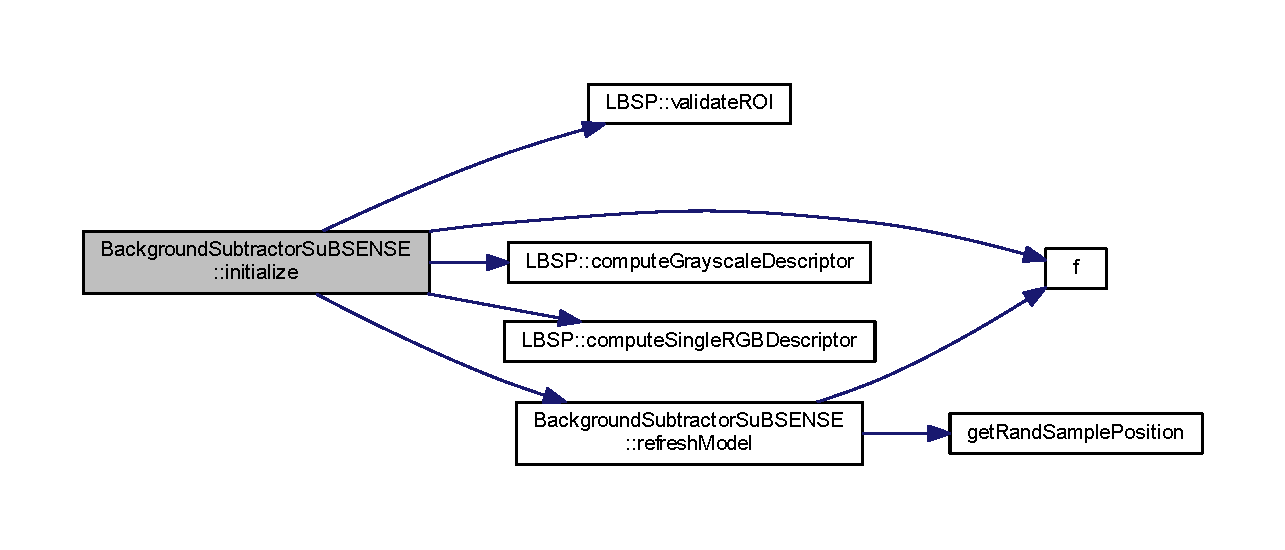
\includegraphics[width=350pt]{class_background_subtractor_su_b_s_e_n_s_e_ac84aa66030b04a72435ef473cf0e6a3f_cgraph}
\end{center}
\end{figure}
\mbox{\Hypertarget{class_background_subtractor_su_b_s_e_n_s_e_aaa60e2883c2b2cf130820b10104a653b}\label{class_background_subtractor_su_b_s_e_n_s_e_aaa60e2883c2b2cf130820b10104a653b}} 
\index{Background\+Subtractor\+Su\+B\+S\+E\+N\+SE@{Background\+Subtractor\+Su\+B\+S\+E\+N\+SE}!operator()@{operator()}}
\index{operator()@{operator()}!Background\+Subtractor\+Su\+B\+S\+E\+N\+SE@{Background\+Subtractor\+Su\+B\+S\+E\+N\+SE}}
\subsubsection{\texorpdfstring{operator()()}{operator()()}}
{\footnotesize\ttfamily void Background\+Subtractor\+Su\+B\+S\+E\+N\+S\+E\+::operator() (\begin{DoxyParamCaption}\item[{cv\+::\+Input\+Array}]{image,  }\item[{cv\+::\+Output\+Array}]{fgmask,  }\item[{double}]{learning\+Rate\+Override = {\ttfamily 0} }\end{DoxyParamCaption})\hspace{0.3cm}{\ttfamily [virtual]}}



primary model update function; the learning param is used to override the internal learning thresholds (ignored when $<$= 0) 



Implements \mbox{\hyperlink{class_background_subtractor_l_b_s_p_a4771cac59b7ac865d6ec25cbf049948e}{Background\+Subtractor\+L\+B\+SP}}.



Definition at line 292 of file Background\+Subtractor\+Su\+B\+S\+E\+N\+S\+E.\+cpp.


\begin{DoxyCode}
292                                                                                                            
                \{
293     \textcolor{comment}{// == process}
294     CV\_Assert(\mbox{\hyperlink{class_background_subtractor_l_b_s_p_a55cea104a0924fd50d5bed0912828a7e}{m\_bInitialized}});
295     cv::Mat oInputImg = \_image.getMat();
296     CV\_Assert(oInputImg.type()==\mbox{\hyperlink{class_background_subtractor_l_b_s_p_a7d2f52ecd5ff56e42da86f97e0ad93b5}{m\_nImgType}} && oInputImg.size()==
      \mbox{\hyperlink{class_background_subtractor_l_b_s_p_a732d5e6ae35fb0e858cadb3af5ce08a2}{m\_oImgSize}});
297     CV\_Assert(oInputImg.isContinuous());
298     \_fgmask.create(\mbox{\hyperlink{class_background_subtractor_l_b_s_p_a732d5e6ae35fb0e858cadb3af5ce08a2}{m\_oImgSize}},CV\_8UC1);
299     cv::Mat oCurrFGMask = \_fgmask.getMat();
300     memset(oCurrFGMask.data,0,oCurrFGMask.cols*oCurrFGMask.rows);
301     \textcolor{keywordtype}{size\_t} nNonZeroDescCount = 0;
302     \textcolor{keyword}{const} \textcolor{keywordtype}{float} fRollAvgFactor\_LT = 1.0f/std::min(++\mbox{\hyperlink{class_background_subtractor_l_b_s_p_a8a2350cad84f19c68ef61b7aaf91c43f}{m\_nFrameIndex}},
      \mbox{\hyperlink{class_background_subtractor_su_b_s_e_n_s_e_acd112ccb067f76e370400565fa09ee49}{m\_nSamplesForMovingAvgs}});
303     \textcolor{keyword}{const} \textcolor{keywordtype}{float} fRollAvgFactor\_ST = 1.0f/std::min(\mbox{\hyperlink{class_background_subtractor_l_b_s_p_a8a2350cad84f19c68ef61b7aaf91c43f}{m\_nFrameIndex}},
      \mbox{\hyperlink{class_background_subtractor_su_b_s_e_n_s_e_acd112ccb067f76e370400565fa09ee49}{m\_nSamplesForMovingAvgs}}/4);
304     \textcolor{keywordflow}{if}(\mbox{\hyperlink{class_background_subtractor_l_b_s_p_ab3467ebee2c5d1249061ccd704cc0584}{m\_nImgChannels}}==1) \{
305         \textcolor{keywordflow}{for}(\textcolor{keywordtype}{size\_t} nModelIter=0; nModelIter<\mbox{\hyperlink{class_background_subtractor_l_b_s_p_ac3b54f4d2dfa3a576475214f26501d85}{m\_nTotRelevantPxCount}}; ++nModelIter) \{
306             \textcolor{keyword}{const} \textcolor{keywordtype}{size\_t} nPxIter = \mbox{\hyperlink{class_background_subtractor_l_b_s_p_a06b4f0d3f24fa08bccd3c9eca085713e}{m\_aPxIdxLUT}}[nModelIter];
307             \textcolor{keyword}{const} \textcolor{keywordtype}{size\_t} nDescIter = nPxIter*2;
308             \textcolor{keyword}{const} \textcolor{keywordtype}{size\_t} nFloatIter = nPxIter*4;
309             \textcolor{keyword}{const} \textcolor{keywordtype}{int} nCurrImgCoord\_X = \mbox{\hyperlink{class_background_subtractor_l_b_s_p_a74e73d4832ccdef652d93756582024db}{m\_aPxInfoLUT}}[nPxIter].
      \mbox{\hyperlink{struct_background_subtractor_l_b_s_p_1_1_px_info_base_a10966fe72f000045adede9e853156b48}{nImgCoord\_X}};
310             \textcolor{keyword}{const} \textcolor{keywordtype}{int} nCurrImgCoord\_Y = \mbox{\hyperlink{class_background_subtractor_l_b_s_p_a74e73d4832ccdef652d93756582024db}{m\_aPxInfoLUT}}[nPxIter].
      \mbox{\hyperlink{struct_background_subtractor_l_b_s_p_1_1_px_info_base_a42cb6eecda647b2a11b90ea420f2bc31}{nImgCoord\_Y}};
311             \textcolor{keyword}{const} uchar nCurrColor = oInputImg.data[nPxIter];
312             \textcolor{keywordtype}{size\_t} nMinDescDist = \mbox{\hyperlink{_background_subtractor_su_b_s_e_n_s_e_8cpp_a15305d6ff106cc0ab9f1b7cfb21a27c7}{s\_nDescMaxDataRange\_1ch}};
313             \textcolor{keywordtype}{size\_t} nMinSumDist = \mbox{\hyperlink{_background_subtractor_su_b_s_e_n_s_e_8cpp_ad0ce3de05453a1b3738f711d9955031f}{s\_nColorMaxDataRange\_1ch}};
314             \textcolor{keywordtype}{float}* pfCurrDistThresholdFactor = (\textcolor{keywordtype}{float}*)(\mbox{\hyperlink{class_background_subtractor_su_b_s_e_n_s_e_a491a1e2b81dee87a721a421719bf2836}{m\_oDistThresholdFrame}}.data+
      nFloatIter);
315             \textcolor{keywordtype}{float}* pfCurrVariationFactor = (\textcolor{keywordtype}{float}*)(\mbox{\hyperlink{class_background_subtractor_su_b_s_e_n_s_e_a47d9cf067ac639d95fcb810c894bb770}{m\_oVariationModulatorFrame}}.
      data+nFloatIter);
316             \textcolor{keywordtype}{float}* pfCurrLearningRate = ((\textcolor{keywordtype}{float}*)(\mbox{\hyperlink{class_background_subtractor_su_b_s_e_n_s_e_a90cb2cc5cbe3f2f0b01e06f514c8b569}{m\_oUpdateRateFrame}}.data+nFloatIter));
317             \textcolor{keywordtype}{float}* pfCurrMeanLastDist = ((\textcolor{keywordtype}{float}*)(\mbox{\hyperlink{class_background_subtractor_su_b_s_e_n_s_e_ad95bb91ff7ef9db725772b37d679e1a2}{m\_oMeanLastDistFrame}}.data+nFloatIter)
      );
318             \textcolor{keywordtype}{float}* pfCurrMeanMinDist\_LT = ((\textcolor{keywordtype}{float}*)(\mbox{\hyperlink{class_background_subtractor_su_b_s_e_n_s_e_a8318e35d5fbbcffb8729700ef5e71a6e}{m\_oMeanMinDistFrame\_LT}}.data+
      nFloatIter));
319             \textcolor{keywordtype}{float}* pfCurrMeanMinDist\_ST = ((\textcolor{keywordtype}{float}*)(\mbox{\hyperlink{class_background_subtractor_su_b_s_e_n_s_e_a53584c5c79017947c59d05dfd247cf5e}{m\_oMeanMinDistFrame\_ST}}.data+
      nFloatIter));
320             \textcolor{keywordtype}{float}* pfCurrMeanRawSegmRes\_LT = ((\textcolor{keywordtype}{float}*)(\mbox{\hyperlink{class_background_subtractor_su_b_s_e_n_s_e_a7706b13433c4e9f4f8156e075fa7904d}{m\_oMeanRawSegmResFrame\_LT}}.
      data+nFloatIter));
321             \textcolor{keywordtype}{float}* pfCurrMeanRawSegmRes\_ST = ((\textcolor{keywordtype}{float}*)(\mbox{\hyperlink{class_background_subtractor_su_b_s_e_n_s_e_a3c9fd9cf995eb9a7b4006467ab874958}{m\_oMeanRawSegmResFrame\_ST}}.
      data+nFloatIter));
322             \textcolor{keywordtype}{float}* pfCurrMeanFinalSegmRes\_LT = ((\textcolor{keywordtype}{float}*)(
      \mbox{\hyperlink{class_background_subtractor_su_b_s_e_n_s_e_ad48e92b6d6bbce34f9f452484bc9956a}{m\_oMeanFinalSegmResFrame\_LT}}.data+nFloatIter));
323             \textcolor{keywordtype}{float}* pfCurrMeanFinalSegmRes\_ST = ((\textcolor{keywordtype}{float}*)(
      \mbox{\hyperlink{class_background_subtractor_su_b_s_e_n_s_e_a0dcd4f5df8adb9b4fa630a9a6f6b5e30}{m\_oMeanFinalSegmResFrame\_ST}}.data+nFloatIter));
324             ushort& nLastIntraDesc = *((ushort*)(\mbox{\hyperlink{class_background_subtractor_l_b_s_p_a9c637c0b87cac495887295690d83ba13}{m\_oLastDescFrame}}.data+nDescIter));
325             uchar& nLastColor = \mbox{\hyperlink{class_background_subtractor_l_b_s_p_ab1dc003792ab1d0b881a6fd10e0e29b3}{m\_oLastColorFrame}}.data[nPxIter];
326             \textcolor{keyword}{const} \textcolor{keywordtype}{size\_t} nCurrColorDistThreshold = (size\_t)(((*pfCurrDistThresholdFactor)*
      \mbox{\hyperlink{class_background_subtractor_su_b_s_e_n_s_e_ae0ebf701652a66bbdb0472d6f091e34d}{m\_nMinColorDistThreshold}})-((!\mbox{\hyperlink{class_background_subtractor_su_b_s_e_n_s_e_acfaf4c3c5aedbed8bd302444b4a4f8dd}{m\_oUnstableRegionMask}}.data[
      nPxIter])*\mbox{\hyperlink{_background_subtractor_su_b_s_e_n_s_e_8cpp_af60b797fbe4d762be8f140d56f6d8a0a}{STAB\_COLOR\_DIST\_OFFSET}}))/2;
327             \textcolor{keyword}{const} \textcolor{keywordtype}{size\_t} nCurrDescDistThreshold = ((size\_t)1<<((\textcolor{keywordtype}{size\_t})floor(*pfCurrDistThresholdFactor+0.5
      \mbox{\hyperlink{rings_8cpp_a77369fc4d5326a16d2c603e032023528}{f}})))+\mbox{\hyperlink{class_background_subtractor_su_b_s_e_n_s_e_a79fe0f1657cd613b975d62f73e749ec2}{m\_nDescDistThresholdOffset}}+(
      \mbox{\hyperlink{class_background_subtractor_su_b_s_e_n_s_e_acfaf4c3c5aedbed8bd302444b4a4f8dd}{m\_oUnstableRegionMask}}.data[nPxIter]*\mbox{\hyperlink{_background_subtractor_su_b_s_e_n_s_e_8cpp_af189e5399183f3cfa1dee820fb2fa8fc}{UNSTAB\_DESC\_DIST\_OFFSET}});
328             ushort nCurrInterDesc, nCurrIntraDesc;
329             \mbox{\hyperlink{class_l_b_s_p_a4a5f635868b6b81ba53df2692ee3dfd8}{LBSP::computeGrayscaleDescriptor}}(oInputImg,nCurrColor,
      nCurrImgCoord\_X,nCurrImgCoord\_Y,\mbox{\hyperlink{class_background_subtractor_l_b_s_p_aefe69d94f08b2c4ba73ad1d254ad9153}{m\_anLBSPThreshold\_8bitLUT}}[nCurrColor],nCurrIntraDesc);
330             \mbox{\hyperlink{class_background_subtractor_su_b_s_e_n_s_e_acfaf4c3c5aedbed8bd302444b4a4f8dd}{m\_oUnstableRegionMask}}.data[nPxIter] = ((*pfCurrDistThresholdFactor)>
      \mbox{\hyperlink{_background_subtractor_su_b_s_e_n_s_e_8cpp_a6168b44590b3d4a1fdcee44fe0755f39}{UNSTABLE\_REG\_RDIST\_MIN}} || (*pfCurrMeanRawSegmRes\_LT-*pfCurrMeanFinalSegmRes\_LT)>
      \mbox{\hyperlink{_background_subtractor_su_b_s_e_n_s_e_8cpp_acaad1bde74ca3c5a5c43c0e8deea2313}{UNSTABLE\_REG\_RATIO\_MIN}} || (*pfCurrMeanRawSegmRes\_ST-*pfCurrMeanFinalSegmRes\_ST)>
      \mbox{\hyperlink{_background_subtractor_su_b_s_e_n_s_e_8cpp_acaad1bde74ca3c5a5c43c0e8deea2313}{UNSTABLE\_REG\_RATIO\_MIN}})?1:0;
331             \textcolor{keywordtype}{size\_t} nGoodSamplesCount=0, nSampleIdx=0;
332             \textcolor{keywordflow}{while}(nGoodSamplesCount<\mbox{\hyperlink{class_background_subtractor_su_b_s_e_n_s_e_aca07c4307021623f9055832506cad1d6}{m\_nRequiredBGSamples}} && nSampleIdx<
      \mbox{\hyperlink{class_background_subtractor_su_b_s_e_n_s_e_ad783b71b5b942c4018d27cf38b7d7225}{m\_nBGSamples}}) \{
333                 \textcolor{keyword}{const} uchar& nBGColor = \mbox{\hyperlink{class_background_subtractor_su_b_s_e_n_s_e_a9d4d4bb930b34745536b9862683bb539}{m\_voBGColorSamples}}[nSampleIdx].data[nPxIter];
334                 \{
335                     \textcolor{keyword}{const} \textcolor{keywordtype}{size\_t} nColorDist = \mbox{\hyperlink{_distance_utils_8h_ab6ec458f6d3fb6fb4e6cda3808e61703}{L1dist}}(nCurrColor,nBGColor);
336                     \textcolor{keywordflow}{if}(nColorDist>nCurrColorDistThreshold)
337                         \textcolor{keywordflow}{goto} failedcheck1ch;
338                     \textcolor{keyword}{const} ushort& nBGIntraDesc = *((ushort*)(\mbox{\hyperlink{class_background_subtractor_su_b_s_e_n_s_e_a422cc2f2a25c07efca02087bd6fe3d6d}{m\_voBGDescSamples}}[nSampleIdx]
      .data+nDescIter));
339                     \textcolor{keyword}{const} \textcolor{keywordtype}{size\_t} nIntraDescDist = \mbox{\hyperlink{_distance_utils_8h_ab13812ef6e21af771d6c0a856cd941b0}{hdist}}(nCurrIntraDesc,nBGIntraDesc);
340                     \mbox{\hyperlink{class_l_b_s_p_a4a5f635868b6b81ba53df2692ee3dfd8}{LBSP::computeGrayscaleDescriptor}}(oInputImg,nBGColor,
      nCurrImgCoord\_X,nCurrImgCoord\_Y,\mbox{\hyperlink{class_background_subtractor_l_b_s_p_aefe69d94f08b2c4ba73ad1d254ad9153}{m\_anLBSPThreshold\_8bitLUT}}[nBGColor],nCurrInterDesc);
341                     \textcolor{keyword}{const} \textcolor{keywordtype}{size\_t} nInterDescDist = \mbox{\hyperlink{_distance_utils_8h_ab13812ef6e21af771d6c0a856cd941b0}{hdist}}(nCurrInterDesc,nBGIntraDesc);
342                     \textcolor{keyword}{const} \textcolor{keywordtype}{size\_t} nDescDist = (nIntraDescDist+nInterDescDist)/2;
343                     \textcolor{keywordflow}{if}(nDescDist>nCurrDescDistThreshold)
344                         \textcolor{keywordflow}{goto} failedcheck1ch;
345                     \textcolor{keyword}{const} \textcolor{keywordtype}{size\_t} nSumDist = std::min((nDescDist/4)*(
      \mbox{\hyperlink{_background_subtractor_su_b_s_e_n_s_e_8cpp_ad0ce3de05453a1b3738f711d9955031f}{s\_nColorMaxDataRange\_1ch}}/\mbox{\hyperlink{_background_subtractor_su_b_s_e_n_s_e_8cpp_a15305d6ff106cc0ab9f1b7cfb21a27c7}{s\_nDescMaxDataRange\_1ch}})+nColorDist
      ,\mbox{\hyperlink{_background_subtractor_su_b_s_e_n_s_e_8cpp_ad0ce3de05453a1b3738f711d9955031f}{s\_nColorMaxDataRange\_1ch}});
346                     \textcolor{keywordflow}{if}(nSumDist>nCurrColorDistThreshold)
347                         \textcolor{keywordflow}{goto} failedcheck1ch;
348                     \textcolor{keywordflow}{if}(nMinDescDist>nDescDist)
349                         nMinDescDist = nDescDist;
350                     \textcolor{keywordflow}{if}(nMinSumDist>nSumDist)
351                         nMinSumDist = nSumDist;
352                     nGoodSamplesCount++;
353                 \}
354                 failedcheck1ch:
355                 nSampleIdx++;
356             \}
357             \textcolor{keyword}{const} \textcolor{keywordtype}{float} fNormalizedLastDist = ((float)\mbox{\hyperlink{_distance_utils_8h_ab6ec458f6d3fb6fb4e6cda3808e61703}{L1dist}}(nLastColor,nCurrColor)/
      \mbox{\hyperlink{_background_subtractor_su_b_s_e_n_s_e_8cpp_ad0ce3de05453a1b3738f711d9955031f}{s\_nColorMaxDataRange\_1ch}}+(float)\mbox{\hyperlink{_distance_utils_8h_ab13812ef6e21af771d6c0a856cd941b0}{hdist}}(nLastIntraDesc,nCurrIntraDesc)/
      \mbox{\hyperlink{_background_subtractor_su_b_s_e_n_s_e_8cpp_a15305d6ff106cc0ab9f1b7cfb21a27c7}{s\_nDescMaxDataRange\_1ch}})/2;
358             *pfCurrMeanLastDist = (*pfCurrMeanLastDist)*(1.0f-fRollAvgFactor\_ST) + fNormalizedLastDist*
      fRollAvgFactor\_ST;
359             \textcolor{keywordflow}{if}(nGoodSamplesCount<\mbox{\hyperlink{class_background_subtractor_su_b_s_e_n_s_e_aca07c4307021623f9055832506cad1d6}{m\_nRequiredBGSamples}}) \{
360                 \textcolor{comment}{// == foreground}
361                 \textcolor{keyword}{const} \textcolor{keywordtype}{float} fNormalizedMinDist = std::min(1.0\mbox{\hyperlink{rings_8cpp_a77369fc4d5326a16d2c603e032023528}{f}},((\textcolor{keywordtype}{float})nMinSumDist/
      \mbox{\hyperlink{_background_subtractor_su_b_s_e_n_s_e_8cpp_ad0ce3de05453a1b3738f711d9955031f}{s\_nColorMaxDataRange\_1ch}}+(\textcolor{keywordtype}{float})nMinDescDist/
      \mbox{\hyperlink{_background_subtractor_su_b_s_e_n_s_e_8cpp_a15305d6ff106cc0ab9f1b7cfb21a27c7}{s\_nDescMaxDataRange\_1ch}})/2 + (\textcolor{keywordtype}{float})(\mbox{\hyperlink{class_background_subtractor_su_b_s_e_n_s_e_aca07c4307021623f9055832506cad1d6}{m\_nRequiredBGSamples}}-
      nGoodSamplesCount)/\mbox{\hyperlink{class_background_subtractor_su_b_s_e_n_s_e_aca07c4307021623f9055832506cad1d6}{m\_nRequiredBGSamples}});
362                 *pfCurrMeanMinDist\_LT = (*pfCurrMeanMinDist\_LT)*(1.0f-fRollAvgFactor\_LT) + 
      fNormalizedMinDist*fRollAvgFactor\_LT;
363                 *pfCurrMeanMinDist\_ST = (*pfCurrMeanMinDist\_ST)*(1.0f-fRollAvgFactor\_ST) + 
      fNormalizedMinDist*fRollAvgFactor\_ST;
364                 *pfCurrMeanRawSegmRes\_LT = (*pfCurrMeanRawSegmRes\_LT)*(1.0f-fRollAvgFactor\_LT) + 
      fRollAvgFactor\_LT;
365                 *pfCurrMeanRawSegmRes\_ST = (*pfCurrMeanRawSegmRes\_ST)*(1.0f-fRollAvgFactor\_ST) + 
      fRollAvgFactor\_ST;
366                 oCurrFGMask.data[nPxIter] = UCHAR\_MAX;
367                 \textcolor{keywordflow}{if}(\mbox{\hyperlink{class_background_subtractor_l_b_s_p_a5ea18d388afacf8285c46ba0f754e7ee}{m\_nModelResetCooldown}} && (rand()%(size\_t)
      \mbox{\hyperlink{_background_subtractor_su_b_s_e_n_s_e_8cpp_a6975332215c62c3172a76af852bc5566}{FEEDBACK\_T\_LOWER}})==0) \{
368                     \textcolor{keyword}{const} \textcolor{keywordtype}{size\_t} s\_rand = rand()%\mbox{\hyperlink{class_background_subtractor_su_b_s_e_n_s_e_ad783b71b5b942c4018d27cf38b7d7225}{m\_nBGSamples}};
369                     *((ushort*)(\mbox{\hyperlink{class_background_subtractor_su_b_s_e_n_s_e_a422cc2f2a25c07efca02087bd6fe3d6d}{m\_voBGDescSamples}}[s\_rand].data+nDescIter)) = 
      nCurrIntraDesc;
370                     \mbox{\hyperlink{class_background_subtractor_su_b_s_e_n_s_e_a9d4d4bb930b34745536b9862683bb539}{m\_voBGColorSamples}}[s\_rand].data[nPxIter] = nCurrColor;
371                 \}
372             \}
373             \textcolor{keywordflow}{else} \{
374                 \textcolor{comment}{// == background}
375                 \textcolor{keyword}{const} \textcolor{keywordtype}{float} fNormalizedMinDist = ((float)nMinSumDist/
      \mbox{\hyperlink{_background_subtractor_su_b_s_e_n_s_e_8cpp_ad0ce3de05453a1b3738f711d9955031f}{s\_nColorMaxDataRange\_1ch}}+(\textcolor{keywordtype}{float})nMinDescDist/
      \mbox{\hyperlink{_background_subtractor_su_b_s_e_n_s_e_8cpp_a15305d6ff106cc0ab9f1b7cfb21a27c7}{s\_nDescMaxDataRange\_1ch}})/2;
376                 *pfCurrMeanMinDist\_LT = (*pfCurrMeanMinDist\_LT)*(1.0f-fRollAvgFactor\_LT) + 
      fNormalizedMinDist*fRollAvgFactor\_LT;
377                 *pfCurrMeanMinDist\_ST = (*pfCurrMeanMinDist\_ST)*(1.0f-fRollAvgFactor\_ST) + 
      fNormalizedMinDist*fRollAvgFactor\_ST;
378                 *pfCurrMeanRawSegmRes\_LT = (*pfCurrMeanRawSegmRes\_LT)*(1.0f-fRollAvgFactor\_LT);
379                 *pfCurrMeanRawSegmRes\_ST = (*pfCurrMeanRawSegmRes\_ST)*(1.0f-fRollAvgFactor\_ST);
380                 \textcolor{keyword}{const} \textcolor{keywordtype}{size\_t} nLearningRate = learningRateOverride>0?(size\_t)ceil(learningRateOverride):(
      size\_t)ceil(*pfCurrLearningRate);
381                 \textcolor{keywordflow}{if}((rand()%nLearningRate)==0) \{
382                     \textcolor{keyword}{const} \textcolor{keywordtype}{size\_t} s\_rand = rand()%\mbox{\hyperlink{class_background_subtractor_su_b_s_e_n_s_e_ad783b71b5b942c4018d27cf38b7d7225}{m\_nBGSamples}};
383                     *((ushort*)(\mbox{\hyperlink{class_background_subtractor_su_b_s_e_n_s_e_a422cc2f2a25c07efca02087bd6fe3d6d}{m\_voBGDescSamples}}[s\_rand].data+nDescIter)) = 
      nCurrIntraDesc;
384                     \mbox{\hyperlink{class_background_subtractor_su_b_s_e_n_s_e_a9d4d4bb930b34745536b9862683bb539}{m\_voBGColorSamples}}[s\_rand].data[nPxIter] = nCurrColor;
385                 \}
386                 \textcolor{keywordtype}{int} nSampleImgCoord\_Y, nSampleImgCoord\_X;
387                 \textcolor{keyword}{const} \textcolor{keywordtype}{bool} bCurrUsing3x3Spread = \mbox{\hyperlink{class_background_subtractor_su_b_s_e_n_s_e_a1e2e28840e7ca373282607db81b49e12}{m\_bUse3x3Spread}} && !
      \mbox{\hyperlink{class_background_subtractor_su_b_s_e_n_s_e_acfaf4c3c5aedbed8bd302444b4a4f8dd}{m\_oUnstableRegionMask}}.data[nPxIter];
388                 \textcolor{keywordflow}{if}(bCurrUsing3x3Spread)
389                     \mbox{\hyperlink{_rand_utils_8h_a76b18bef397ed044a6db9e3a63c69f69}{getRandNeighborPosition\_3x3}}(nSampleImgCoord\_X,
      nSampleImgCoord\_Y,nCurrImgCoord\_X,nCurrImgCoord\_Y,\mbox{\hyperlink{class_l_b_s_p_aa98abb79a155d3a2b416c2ab32e74929}{LBSP::PATCH\_SIZE}}/2,\mbox{\hyperlink{class_background_subtractor_l_b_s_p_a732d5e6ae35fb0e858cadb3af5ce08a2}{m\_oImgSize}});
390                 \textcolor{keywordflow}{else}
391                     \mbox{\hyperlink{_rand_utils_8h_adb1e7788e9dbe8cfde588761e96126c1}{getRandNeighborPosition\_5x5}}(nSampleImgCoord\_X,
      nSampleImgCoord\_Y,nCurrImgCoord\_X,nCurrImgCoord\_Y,\mbox{\hyperlink{class_l_b_s_p_aa98abb79a155d3a2b416c2ab32e74929}{LBSP::PATCH\_SIZE}}/2,\mbox{\hyperlink{class_background_subtractor_l_b_s_p_a732d5e6ae35fb0e858cadb3af5ce08a2}{m\_oImgSize}});
392                 \textcolor{keyword}{const} \textcolor{keywordtype}{size\_t} n\_rand = rand();
393                 \textcolor{keyword}{const} \textcolor{keywordtype}{size\_t} idx\_rand\_uchar = \mbox{\hyperlink{class_background_subtractor_l_b_s_p_a732d5e6ae35fb0e858cadb3af5ce08a2}{m\_oImgSize}}.width*nSampleImgCoord\_Y + 
      nSampleImgCoord\_X;
394                 \textcolor{keyword}{const} \textcolor{keywordtype}{size\_t} idx\_rand\_flt32 = idx\_rand\_uchar*4;
395                 \textcolor{keyword}{const} \textcolor{keywordtype}{float} fRandMeanLastDist = *((\textcolor{keywordtype}{float}*)(\mbox{\hyperlink{class_background_subtractor_su_b_s_e_n_s_e_ad95bb91ff7ef9db725772b37d679e1a2}{m\_oMeanLastDistFrame}}.data+
      idx\_rand\_flt32));
396                 \textcolor{keyword}{const} \textcolor{keywordtype}{float} fRandMeanRawSegmRes = *((\textcolor{keywordtype}{float}*)(
      \mbox{\hyperlink{class_background_subtractor_su_b_s_e_n_s_e_a3c9fd9cf995eb9a7b4006467ab874958}{m\_oMeanRawSegmResFrame\_ST}}.data+idx\_rand\_flt32));
397                 \textcolor{keywordflow}{if}((n\_rand%(bCurrUsing3x3Spread?nLearningRate:(nLearningRate/2+1)))==0
398                     || (fRandMeanRawSegmRes>\mbox{\hyperlink{_background_subtractor_su_b_s_e_n_s_e_8cpp_aa6ad1e76fe6a12c04328c5541d44ebcb}{GHOSTDET\_S\_MIN}} && fRandMeanLastDist<
      \mbox{\hyperlink{_background_subtractor_su_b_s_e_n_s_e_8cpp_aa1fa68710898742a17b61ace30b21120}{GHOSTDET\_D\_MAX}} && (n\_rand%((size\_t)\mbox{\hyperlink{class_background_subtractor_su_b_s_e_n_s_e_a57fdd29e43afc163233e55f9a7cd9f37}{m\_fCurrLearningRateLowerCap}}))==
      0)) \{
399                     \textcolor{keyword}{const} \textcolor{keywordtype}{size\_t} idx\_rand\_ushrt = idx\_rand\_uchar*2;
400                     \textcolor{keyword}{const} \textcolor{keywordtype}{size\_t} s\_rand = rand()%\mbox{\hyperlink{class_background_subtractor_su_b_s_e_n_s_e_ad783b71b5b942c4018d27cf38b7d7225}{m\_nBGSamples}};
401                     *((ushort*)(\mbox{\hyperlink{class_background_subtractor_su_b_s_e_n_s_e_a422cc2f2a25c07efca02087bd6fe3d6d}{m\_voBGDescSamples}}[s\_rand].data+idx\_rand\_ushrt)) = 
      nCurrIntraDesc;
402                     \mbox{\hyperlink{class_background_subtractor_su_b_s_e_n_s_e_a9d4d4bb930b34745536b9862683bb539}{m\_voBGColorSamples}}[s\_rand].data[idx\_rand\_uchar] = nCurrColor;
403                 \}
404             \}
405             \textcolor{keywordflow}{if}(\mbox{\hyperlink{class_background_subtractor_l_b_s_p_adb6dc0af596c5592c91f9d8faa5c8a4b}{m\_oLastFGMask}}.data[nPxIter] || (std::min(*pfCurrMeanMinDist\_LT,*
      pfCurrMeanMinDist\_ST)<\mbox{\hyperlink{_background_subtractor_su_b_s_e_n_s_e_8cpp_acaad1bde74ca3c5a5c43c0e8deea2313}{UNSTABLE\_REG\_RATIO\_MIN}} && oCurrFGMask.data[nPxIter])) \{
406                 \textcolor{keywordflow}{if}((*pfCurrLearningRate)<\mbox{\hyperlink{class_background_subtractor_su_b_s_e_n_s_e_a44ba1a1ed365c5829baa517ce9f27508}{m\_fCurrLearningRateUpperCap}})
407                     *pfCurrLearningRate += \mbox{\hyperlink{_background_subtractor_su_b_s_e_n_s_e_8cpp_afa487dca8c1f4ae73e03567566465382}{FEEDBACK\_T\_INCR}}/(std::max(*pfCurrMeanMinDist\_LT,*
      pfCurrMeanMinDist\_ST)*(*pfCurrVariationFactor));
408             \}
409             \textcolor{keywordflow}{else} \textcolor{keywordflow}{if}((*pfCurrLearningRate)>\mbox{\hyperlink{class_background_subtractor_su_b_s_e_n_s_e_a57fdd29e43afc163233e55f9a7cd9f37}{m\_fCurrLearningRateLowerCap}})
410                 *pfCurrLearningRate -= \mbox{\hyperlink{_background_subtractor_su_b_s_e_n_s_e_8cpp_aeb1e65c4ebe34d91c849054de1951361}{FEEDBACK\_T\_DECR}}*(*pfCurrVariationFactor)/std::max(*
      pfCurrMeanMinDist\_LT,*pfCurrMeanMinDist\_ST);
411             \textcolor{keywordflow}{if}((*pfCurrLearningRate)<\mbox{\hyperlink{class_background_subtractor_su_b_s_e_n_s_e_a57fdd29e43afc163233e55f9a7cd9f37}{m\_fCurrLearningRateLowerCap}})
412                 *pfCurrLearningRate = \mbox{\hyperlink{class_background_subtractor_su_b_s_e_n_s_e_a57fdd29e43afc163233e55f9a7cd9f37}{m\_fCurrLearningRateLowerCap}};
413             \textcolor{keywordflow}{else} \textcolor{keywordflow}{if}((*pfCurrLearningRate)>\mbox{\hyperlink{class_background_subtractor_su_b_s_e_n_s_e_a44ba1a1ed365c5829baa517ce9f27508}{m\_fCurrLearningRateUpperCap}})
414                 *pfCurrLearningRate = \mbox{\hyperlink{class_background_subtractor_su_b_s_e_n_s_e_a44ba1a1ed365c5829baa517ce9f27508}{m\_fCurrLearningRateUpperCap}};
415             \textcolor{keywordflow}{if}(std::max(*pfCurrMeanMinDist\_LT,*pfCurrMeanMinDist\_ST)>
      \mbox{\hyperlink{_background_subtractor_su_b_s_e_n_s_e_8cpp_acaad1bde74ca3c5a5c43c0e8deea2313}{UNSTABLE\_REG\_RATIO\_MIN}} && \mbox{\hyperlink{class_background_subtractor_su_b_s_e_n_s_e_a943b50c63d233c0948d82b64390f1aa1}{m\_oBlinksFrame}}.data[nPxIter])
416                 (*pfCurrVariationFactor) += \mbox{\hyperlink{_background_subtractor_su_b_s_e_n_s_e_8cpp_a55f10981362bbf2c494e76d1b8002255}{FEEDBACK\_V\_INCR}};
417             \textcolor{keywordflow}{else} \textcolor{keywordflow}{if}((*pfCurrVariationFactor)>\mbox{\hyperlink{_background_subtractor_su_b_s_e_n_s_e_8cpp_a9acb8c94db1a579c5404b3f03fe986b5}{FEEDBACK\_V\_DECR}}) \{
418                 (*pfCurrVariationFactor) -= \mbox{\hyperlink{class_background_subtractor_l_b_s_p_adb6dc0af596c5592c91f9d8faa5c8a4b}{m\_oLastFGMask}}.data[nPxIter]?
      \mbox{\hyperlink{_background_subtractor_su_b_s_e_n_s_e_8cpp_a9acb8c94db1a579c5404b3f03fe986b5}{FEEDBACK\_V\_DECR}}/4:\mbox{\hyperlink{class_background_subtractor_su_b_s_e_n_s_e_acfaf4c3c5aedbed8bd302444b4a4f8dd}{m\_oUnstableRegionMask}}.data[nPxIter]?
      \mbox{\hyperlink{_background_subtractor_su_b_s_e_n_s_e_8cpp_a9acb8c94db1a579c5404b3f03fe986b5}{FEEDBACK\_V\_DECR}}/2:\mbox{\hyperlink{_background_subtractor_su_b_s_e_n_s_e_8cpp_a9acb8c94db1a579c5404b3f03fe986b5}{FEEDBACK\_V\_DECR}};
419                 \textcolor{keywordflow}{if}((*pfCurrVariationFactor)<\mbox{\hyperlink{_background_subtractor_su_b_s_e_n_s_e_8cpp_a9acb8c94db1a579c5404b3f03fe986b5}{FEEDBACK\_V\_DECR}})
420                     (*pfCurrVariationFactor) = \mbox{\hyperlink{_background_subtractor_su_b_s_e_n_s_e_8cpp_a9acb8c94db1a579c5404b3f03fe986b5}{FEEDBACK\_V\_DECR}};
421             \}
422             \textcolor{keywordflow}{if}((*pfCurrDistThresholdFactor)<std::pow(1.0\mbox{\hyperlink{rings_8cpp_a77369fc4d5326a16d2c603e032023528}{f}}+std::min(*pfCurrMeanMinDist\_LT,*
      pfCurrMeanMinDist\_ST)*2,2))
423                 (*pfCurrDistThresholdFactor) += \mbox{\hyperlink{_background_subtractor_su_b_s_e_n_s_e_8cpp_a4c9d9560115af87b00cdd28d4dee178a}{FEEDBACK\_R\_VAR}}*(*pfCurrVariationFactor-
      \mbox{\hyperlink{_background_subtractor_su_b_s_e_n_s_e_8cpp_a9acb8c94db1a579c5404b3f03fe986b5}{FEEDBACK\_V\_DECR}});
424             \textcolor{keywordflow}{else} \{
425                 (*pfCurrDistThresholdFactor) -= \mbox{\hyperlink{_background_subtractor_su_b_s_e_n_s_e_8cpp_a4c9d9560115af87b00cdd28d4dee178a}{FEEDBACK\_R\_VAR}}/(*pfCurrVariationFactor);
426                 \textcolor{keywordflow}{if}((*pfCurrDistThresholdFactor)<1.0f)
427                     (*pfCurrDistThresholdFactor) = 1.0f;
428             \}
429             \textcolor{keywordflow}{if}(\mbox{\hyperlink{_distance_utils_8h_a4a3115575087346e42d27f3a95c753d8}{popcount}}(nCurrIntraDesc)>=2)
430                 ++nNonZeroDescCount;
431             nLastIntraDesc = nCurrIntraDesc;
432             nLastColor = nCurrColor;
433         \}
434     \}
435     \textcolor{keywordflow}{else} \{ \textcolor{comment}{//m\_nImgChannels==3}
436         \textcolor{keywordflow}{for}(\textcolor{keywordtype}{size\_t} nModelIter=0; nModelIter<\mbox{\hyperlink{class_background_subtractor_l_b_s_p_ac3b54f4d2dfa3a576475214f26501d85}{m\_nTotRelevantPxCount}}; ++nModelIter) \{
437             \textcolor{keyword}{const} \textcolor{keywordtype}{size\_t} nPxIter = \mbox{\hyperlink{class_background_subtractor_l_b_s_p_a06b4f0d3f24fa08bccd3c9eca085713e}{m\_aPxIdxLUT}}[nModelIter];
438             \textcolor{keyword}{const} \textcolor{keywordtype}{int} nCurrImgCoord\_X = \mbox{\hyperlink{class_background_subtractor_l_b_s_p_a74e73d4832ccdef652d93756582024db}{m\_aPxInfoLUT}}[nPxIter].
      \mbox{\hyperlink{struct_background_subtractor_l_b_s_p_1_1_px_info_base_a10966fe72f000045adede9e853156b48}{nImgCoord\_X}};
439             \textcolor{keyword}{const} \textcolor{keywordtype}{int} nCurrImgCoord\_Y = \mbox{\hyperlink{class_background_subtractor_l_b_s_p_a74e73d4832ccdef652d93756582024db}{m\_aPxInfoLUT}}[nPxIter].
      \mbox{\hyperlink{struct_background_subtractor_l_b_s_p_1_1_px_info_base_a42cb6eecda647b2a11b90ea420f2bc31}{nImgCoord\_Y}};
440             \textcolor{keyword}{const} \textcolor{keywordtype}{size\_t} nPxIterRGB = nPxIter*3;
441             \textcolor{keyword}{const} \textcolor{keywordtype}{size\_t} nDescIterRGB = nPxIterRGB*2;
442             \textcolor{keyword}{const} \textcolor{keywordtype}{size\_t} nFloatIter = nPxIter*4;
443             \textcolor{keyword}{const} uchar* \textcolor{keyword}{const} anCurrColor = oInputImg.data+nPxIterRGB;
444             \textcolor{keywordtype}{size\_t} nMinTotDescDist=\mbox{\hyperlink{_background_subtractor_su_b_s_e_n_s_e_8cpp_a5304f7a24033acdfa11a34dcb3d2720e}{s\_nDescMaxDataRange\_3ch}};
445             \textcolor{keywordtype}{size\_t} nMinTotSumDist=\mbox{\hyperlink{_background_subtractor_su_b_s_e_n_s_e_8cpp_a986ab69736996b917f1e964b2d064aad}{s\_nColorMaxDataRange\_3ch}};
446             \textcolor{keywordtype}{float}* pfCurrDistThresholdFactor = (\textcolor{keywordtype}{float}*)(\mbox{\hyperlink{class_background_subtractor_su_b_s_e_n_s_e_a491a1e2b81dee87a721a421719bf2836}{m\_oDistThresholdFrame}}.data+
      nFloatIter);
447             \textcolor{keywordtype}{float}* pfCurrVariationFactor = (\textcolor{keywordtype}{float}*)(\mbox{\hyperlink{class_background_subtractor_su_b_s_e_n_s_e_a47d9cf067ac639d95fcb810c894bb770}{m\_oVariationModulatorFrame}}.
      data+nFloatIter);
448             \textcolor{keywordtype}{float}* pfCurrLearningRate = ((\textcolor{keywordtype}{float}*)(\mbox{\hyperlink{class_background_subtractor_su_b_s_e_n_s_e_a90cb2cc5cbe3f2f0b01e06f514c8b569}{m\_oUpdateRateFrame}}.data+nFloatIter));
449             \textcolor{keywordtype}{float}* pfCurrMeanLastDist = ((\textcolor{keywordtype}{float}*)(\mbox{\hyperlink{class_background_subtractor_su_b_s_e_n_s_e_ad95bb91ff7ef9db725772b37d679e1a2}{m\_oMeanLastDistFrame}}.data+nFloatIter)
      );
450             \textcolor{keywordtype}{float}* pfCurrMeanMinDist\_LT = ((\textcolor{keywordtype}{float}*)(\mbox{\hyperlink{class_background_subtractor_su_b_s_e_n_s_e_a8318e35d5fbbcffb8729700ef5e71a6e}{m\_oMeanMinDistFrame\_LT}}.data+
      nFloatIter));
451             \textcolor{keywordtype}{float}* pfCurrMeanMinDist\_ST = ((\textcolor{keywordtype}{float}*)(\mbox{\hyperlink{class_background_subtractor_su_b_s_e_n_s_e_a53584c5c79017947c59d05dfd247cf5e}{m\_oMeanMinDistFrame\_ST}}.data+
      nFloatIter));
452             \textcolor{keywordtype}{float}* pfCurrMeanRawSegmRes\_LT = ((\textcolor{keywordtype}{float}*)(\mbox{\hyperlink{class_background_subtractor_su_b_s_e_n_s_e_a7706b13433c4e9f4f8156e075fa7904d}{m\_oMeanRawSegmResFrame\_LT}}.
      data+nFloatIter));
453             \textcolor{keywordtype}{float}* pfCurrMeanRawSegmRes\_ST = ((\textcolor{keywordtype}{float}*)(\mbox{\hyperlink{class_background_subtractor_su_b_s_e_n_s_e_a3c9fd9cf995eb9a7b4006467ab874958}{m\_oMeanRawSegmResFrame\_ST}}.
      data+nFloatIter));
454             \textcolor{keywordtype}{float}* pfCurrMeanFinalSegmRes\_LT = ((\textcolor{keywordtype}{float}*)(
      \mbox{\hyperlink{class_background_subtractor_su_b_s_e_n_s_e_ad48e92b6d6bbce34f9f452484bc9956a}{m\_oMeanFinalSegmResFrame\_LT}}.data+nFloatIter));
455             \textcolor{keywordtype}{float}* pfCurrMeanFinalSegmRes\_ST = ((\textcolor{keywordtype}{float}*)(
      \mbox{\hyperlink{class_background_subtractor_su_b_s_e_n_s_e_a0dcd4f5df8adb9b4fa630a9a6f6b5e30}{m\_oMeanFinalSegmResFrame\_ST}}.data+nFloatIter));
456             ushort* anLastIntraDesc = ((ushort*)(\mbox{\hyperlink{class_background_subtractor_l_b_s_p_a9c637c0b87cac495887295690d83ba13}{m\_oLastDescFrame}}.data+nDescIterRGB));
457             uchar* anLastColor = \mbox{\hyperlink{class_background_subtractor_l_b_s_p_ab1dc003792ab1d0b881a6fd10e0e29b3}{m\_oLastColorFrame}}.data+nPxIterRGB;
458             \textcolor{keyword}{const} \textcolor{keywordtype}{size\_t} nCurrColorDistThreshold = (size\_t)(((*pfCurrDistThresholdFactor)*
      \mbox{\hyperlink{class_background_subtractor_su_b_s_e_n_s_e_ae0ebf701652a66bbdb0472d6f091e34d}{m\_nMinColorDistThreshold}})-((!\mbox{\hyperlink{class_background_subtractor_su_b_s_e_n_s_e_acfaf4c3c5aedbed8bd302444b4a4f8dd}{m\_oUnstableRegionMask}}.data[
      nPxIter])*\mbox{\hyperlink{_background_subtractor_su_b_s_e_n_s_e_8cpp_af60b797fbe4d762be8f140d56f6d8a0a}{STAB\_COLOR\_DIST\_OFFSET}}));
459             \textcolor{keyword}{const} \textcolor{keywordtype}{size\_t} nCurrDescDistThreshold = ((size\_t)1<<((\textcolor{keywordtype}{size\_t})floor(*pfCurrDistThresholdFactor+0.5
      \mbox{\hyperlink{rings_8cpp_a77369fc4d5326a16d2c603e032023528}{f}})))+\mbox{\hyperlink{class_background_subtractor_su_b_s_e_n_s_e_a79fe0f1657cd613b975d62f73e749ec2}{m\_nDescDistThresholdOffset}}+(
      \mbox{\hyperlink{class_background_subtractor_su_b_s_e_n_s_e_acfaf4c3c5aedbed8bd302444b4a4f8dd}{m\_oUnstableRegionMask}}.data[nPxIter]*\mbox{\hyperlink{_background_subtractor_su_b_s_e_n_s_e_8cpp_af189e5399183f3cfa1dee820fb2fa8fc}{UNSTAB\_DESC\_DIST\_OFFSET}});
460             \textcolor{keyword}{const} \textcolor{keywordtype}{size\_t} nCurrTotColorDistThreshold = nCurrColorDistThreshold*3;
461             \textcolor{keyword}{const} \textcolor{keywordtype}{size\_t} nCurrTotDescDistThreshold = nCurrDescDistThreshold*3;
462             \textcolor{keyword}{const} \textcolor{keywordtype}{size\_t} nCurrSCColorDistThreshold = nCurrTotColorDistThreshold/2;
463             ushort anCurrInterDesc[3], anCurrIntraDesc[3];
464             \textcolor{keyword}{const} \textcolor{keywordtype}{size\_t} anCurrIntraLBSPThresholds[3] = \{
      \mbox{\hyperlink{class_background_subtractor_l_b_s_p_aefe69d94f08b2c4ba73ad1d254ad9153}{m\_anLBSPThreshold\_8bitLUT}}[anCurrColor[0]],
      \mbox{\hyperlink{class_background_subtractor_l_b_s_p_aefe69d94f08b2c4ba73ad1d254ad9153}{m\_anLBSPThreshold\_8bitLUT}}[anCurrColor[1]],
      \mbox{\hyperlink{class_background_subtractor_l_b_s_p_aefe69d94f08b2c4ba73ad1d254ad9153}{m\_anLBSPThreshold\_8bitLUT}}[anCurrColor[2]]\};
465             \mbox{\hyperlink{class_l_b_s_p_a27a44cb6f6e3015ee26047bd3d84f892}{LBSP::computeRGBDescriptor}}(oInputImg,anCurrColor,nCurrImgCoord\_X,
      nCurrImgCoord\_Y,anCurrIntraLBSPThresholds,anCurrIntraDesc);
466             \mbox{\hyperlink{class_background_subtractor_su_b_s_e_n_s_e_acfaf4c3c5aedbed8bd302444b4a4f8dd}{m\_oUnstableRegionMask}}.data[nPxIter] = ((*pfCurrDistThresholdFactor)>
      \mbox{\hyperlink{_background_subtractor_su_b_s_e_n_s_e_8cpp_a6168b44590b3d4a1fdcee44fe0755f39}{UNSTABLE\_REG\_RDIST\_MIN}} || (*pfCurrMeanRawSegmRes\_LT-*pfCurrMeanFinalSegmRes\_LT)>
      \mbox{\hyperlink{_background_subtractor_su_b_s_e_n_s_e_8cpp_acaad1bde74ca3c5a5c43c0e8deea2313}{UNSTABLE\_REG\_RATIO\_MIN}} || (*pfCurrMeanRawSegmRes\_ST-*pfCurrMeanFinalSegmRes\_ST)>
      \mbox{\hyperlink{_background_subtractor_su_b_s_e_n_s_e_8cpp_acaad1bde74ca3c5a5c43c0e8deea2313}{UNSTABLE\_REG\_RATIO\_MIN}})?1:0;
467             \textcolor{keywordtype}{size\_t} nGoodSamplesCount=0, nSampleIdx=0;
468             \textcolor{keywordflow}{while}(nGoodSamplesCount<\mbox{\hyperlink{class_background_subtractor_su_b_s_e_n_s_e_aca07c4307021623f9055832506cad1d6}{m\_nRequiredBGSamples}} && nSampleIdx<
      \mbox{\hyperlink{class_background_subtractor_su_b_s_e_n_s_e_ad783b71b5b942c4018d27cf38b7d7225}{m\_nBGSamples}}) \{
469                 \textcolor{keyword}{const} ushort* \textcolor{keyword}{const} anBGIntraDesc = (ushort*)(\mbox{\hyperlink{class_background_subtractor_su_b_s_e_n_s_e_a422cc2f2a25c07efca02087bd6fe3d6d}{m\_voBGDescSamples}}[nSampleIdx
      ].data+nDescIterRGB);
470                 \textcolor{keyword}{const} uchar* \textcolor{keyword}{const} anBGColor = \mbox{\hyperlink{class_background_subtractor_su_b_s_e_n_s_e_a9d4d4bb930b34745536b9862683bb539}{m\_voBGColorSamples}}[nSampleIdx].data+
      nPxIterRGB;
471                 \textcolor{keywordtype}{size\_t} nTotDescDist = 0;
472                 \textcolor{keywordtype}{size\_t} nTotSumDist = 0;
473                 \textcolor{keywordflow}{for}(\textcolor{keywordtype}{size\_t} c=0;c<3; ++c) \{
474                     \textcolor{keyword}{const} \textcolor{keywordtype}{size\_t} nColorDist = \mbox{\hyperlink{_distance_utils_8h_ab6ec458f6d3fb6fb4e6cda3808e61703}{L1dist}}(anCurrColor[c],anBGColor[c]);
475                     \textcolor{keywordflow}{if}(nColorDist>nCurrSCColorDistThreshold)
476                         \textcolor{keywordflow}{goto} failedcheck3ch;
477                     \textcolor{keyword}{const} \textcolor{keywordtype}{size\_t} nIntraDescDist = \mbox{\hyperlink{_distance_utils_8h_ab13812ef6e21af771d6c0a856cd941b0}{hdist}}(anCurrIntraDesc[c],anBGIntraDesc[c]);
478                     \mbox{\hyperlink{class_l_b_s_p_a35f2abfacc0d540810d678ff5e8cd619}{LBSP::computeSingleRGBDescriptor}}(oInputImg,anBGColor[c]
      ,nCurrImgCoord\_X,nCurrImgCoord\_Y,c,\mbox{\hyperlink{class_background_subtractor_l_b_s_p_aefe69d94f08b2c4ba73ad1d254ad9153}{m\_anLBSPThreshold\_8bitLUT}}[anBGColor[c]],
      anCurrInterDesc[c]);
479                     \textcolor{keyword}{const} \textcolor{keywordtype}{size\_t} nInterDescDist = \mbox{\hyperlink{_distance_utils_8h_ab13812ef6e21af771d6c0a856cd941b0}{hdist}}(anCurrInterDesc[c],anBGIntraDesc[c]);
480                     \textcolor{keyword}{const} \textcolor{keywordtype}{size\_t} nDescDist = (nIntraDescDist+nInterDescDist)/2;
481                     \textcolor{keyword}{const} \textcolor{keywordtype}{size\_t} nSumDist = std::min((nDescDist/2)*(
      \mbox{\hyperlink{_background_subtractor_su_b_s_e_n_s_e_8cpp_ad0ce3de05453a1b3738f711d9955031f}{s\_nColorMaxDataRange\_1ch}}/\mbox{\hyperlink{_background_subtractor_su_b_s_e_n_s_e_8cpp_a15305d6ff106cc0ab9f1b7cfb21a27c7}{s\_nDescMaxDataRange\_1ch}})+nColorDist
      ,\mbox{\hyperlink{_background_subtractor_su_b_s_e_n_s_e_8cpp_ad0ce3de05453a1b3738f711d9955031f}{s\_nColorMaxDataRange\_1ch}});
482                     \textcolor{keywordflow}{if}(nSumDist>nCurrSCColorDistThreshold)
483                         \textcolor{keywordflow}{goto} failedcheck3ch;
484                     nTotDescDist += nDescDist;
485                     nTotSumDist += nSumDist;
486                 \}
487                 \textcolor{keywordflow}{if}(nTotDescDist>nCurrTotDescDistThreshold || nTotSumDist>nCurrTotColorDistThreshold)
488                     \textcolor{keywordflow}{goto} failedcheck3ch;
489                 \textcolor{keywordflow}{if}(nMinTotDescDist>nTotDescDist)
490                     nMinTotDescDist = nTotDescDist;
491                 \textcolor{keywordflow}{if}(nMinTotSumDist>nTotSumDist)
492                     nMinTotSumDist = nTotSumDist;
493                 nGoodSamplesCount++;
494                 failedcheck3ch:
495                 nSampleIdx++;
496             \}
497             \textcolor{keyword}{const} \textcolor{keywordtype}{float} fNormalizedLastDist = ((float)L1dist<3>(anLastColor,anCurrColor)/
      \mbox{\hyperlink{_background_subtractor_su_b_s_e_n_s_e_8cpp_a986ab69736996b917f1e964b2d064aad}{s\_nColorMaxDataRange\_3ch}}+(float)hdist<3>(anLastIntraDesc,anCurrIntraDesc)/
      \mbox{\hyperlink{_background_subtractor_su_b_s_e_n_s_e_8cpp_a5304f7a24033acdfa11a34dcb3d2720e}{s\_nDescMaxDataRange\_3ch}})/2;
498             *pfCurrMeanLastDist = (*pfCurrMeanLastDist)*(1.0f-fRollAvgFactor\_ST) + fNormalizedLastDist*
      fRollAvgFactor\_ST;
499             \textcolor{keywordflow}{if}(nGoodSamplesCount<\mbox{\hyperlink{class_background_subtractor_su_b_s_e_n_s_e_aca07c4307021623f9055832506cad1d6}{m\_nRequiredBGSamples}}) \{
500                 \textcolor{comment}{// == foreground}
501                 \textcolor{keyword}{const} \textcolor{keywordtype}{float} fNormalizedMinDist = std::min(1.0\mbox{\hyperlink{rings_8cpp_a77369fc4d5326a16d2c603e032023528}{f}},((\textcolor{keywordtype}{float})nMinTotSumDist/
      \mbox{\hyperlink{_background_subtractor_su_b_s_e_n_s_e_8cpp_a986ab69736996b917f1e964b2d064aad}{s\_nColorMaxDataRange\_3ch}}+(\textcolor{keywordtype}{float})nMinTotDescDist/
      \mbox{\hyperlink{_background_subtractor_su_b_s_e_n_s_e_8cpp_a5304f7a24033acdfa11a34dcb3d2720e}{s\_nDescMaxDataRange\_3ch}})/2 + (\textcolor{keywordtype}{float})(\mbox{\hyperlink{class_background_subtractor_su_b_s_e_n_s_e_aca07c4307021623f9055832506cad1d6}{m\_nRequiredBGSamples}}-
      nGoodSamplesCount)/\mbox{\hyperlink{class_background_subtractor_su_b_s_e_n_s_e_aca07c4307021623f9055832506cad1d6}{m\_nRequiredBGSamples}});
502                 *pfCurrMeanMinDist\_LT = (*pfCurrMeanMinDist\_LT)*(1.0f-fRollAvgFactor\_LT) + 
      fNormalizedMinDist*fRollAvgFactor\_LT;
503                 *pfCurrMeanMinDist\_ST = (*pfCurrMeanMinDist\_ST)*(1.0f-fRollAvgFactor\_ST) + 
      fNormalizedMinDist*fRollAvgFactor\_ST;
504                 *pfCurrMeanRawSegmRes\_LT = (*pfCurrMeanRawSegmRes\_LT)*(1.0f-fRollAvgFactor\_LT) + 
      fRollAvgFactor\_LT;
505                 *pfCurrMeanRawSegmRes\_ST = (*pfCurrMeanRawSegmRes\_ST)*(1.0f-fRollAvgFactor\_ST) + 
      fRollAvgFactor\_ST;
506                 oCurrFGMask.data[nPxIter] = UCHAR\_MAX;
507                 \textcolor{keywordflow}{if}(\mbox{\hyperlink{class_background_subtractor_l_b_s_p_a5ea18d388afacf8285c46ba0f754e7ee}{m\_nModelResetCooldown}} && (rand()%(size\_t)
      \mbox{\hyperlink{_background_subtractor_su_b_s_e_n_s_e_8cpp_a6975332215c62c3172a76af852bc5566}{FEEDBACK\_T\_LOWER}})==0) \{
508                     \textcolor{keyword}{const} \textcolor{keywordtype}{size\_t} s\_rand = rand()%\mbox{\hyperlink{class_background_subtractor_su_b_s_e_n_s_e_ad783b71b5b942c4018d27cf38b7d7225}{m\_nBGSamples}};
509                     \textcolor{keywordflow}{for}(\textcolor{keywordtype}{size\_t} c=0; c<3; ++c) \{
510                         *((ushort*)(\mbox{\hyperlink{class_background_subtractor_su_b_s_e_n_s_e_a422cc2f2a25c07efca02087bd6fe3d6d}{m\_voBGDescSamples}}[s\_rand].data+nDescIterRGB+2*c)) = 
      anCurrIntraDesc[c];
511                         *(\mbox{\hyperlink{class_background_subtractor_su_b_s_e_n_s_e_a9d4d4bb930b34745536b9862683bb539}{m\_voBGColorSamples}}[s\_rand].data+nPxIterRGB+c) = anCurrColor[c];
512                     \}
513                 \}
514             \}
515             \textcolor{keywordflow}{else} \{
516                 \textcolor{comment}{// == background}
517                 \textcolor{keyword}{const} \textcolor{keywordtype}{float} fNormalizedMinDist = ((float)nMinTotSumDist/
      \mbox{\hyperlink{_background_subtractor_su_b_s_e_n_s_e_8cpp_a986ab69736996b917f1e964b2d064aad}{s\_nColorMaxDataRange\_3ch}}+(\textcolor{keywordtype}{float})nMinTotDescDist/
      \mbox{\hyperlink{_background_subtractor_su_b_s_e_n_s_e_8cpp_a5304f7a24033acdfa11a34dcb3d2720e}{s\_nDescMaxDataRange\_3ch}})/2;
518                 *pfCurrMeanMinDist\_LT = (*pfCurrMeanMinDist\_LT)*(1.0f-fRollAvgFactor\_LT) + 
      fNormalizedMinDist*fRollAvgFactor\_LT;
519                 *pfCurrMeanMinDist\_ST = (*pfCurrMeanMinDist\_ST)*(1.0f-fRollAvgFactor\_ST) + 
      fNormalizedMinDist*fRollAvgFactor\_ST;
520                 *pfCurrMeanRawSegmRes\_LT = (*pfCurrMeanRawSegmRes\_LT)*(1.0f-fRollAvgFactor\_LT);
521                 *pfCurrMeanRawSegmRes\_ST = (*pfCurrMeanRawSegmRes\_ST)*(1.0f-fRollAvgFactor\_ST);
522                 \textcolor{keyword}{const} \textcolor{keywordtype}{size\_t} nLearningRate = learningRateOverride>0?(size\_t)ceil(learningRateOverride):(
      size\_t)ceil(*pfCurrLearningRate);
523                 \textcolor{keywordflow}{if}((rand()%nLearningRate)==0) \{
524                     \textcolor{keyword}{const} \textcolor{keywordtype}{size\_t} s\_rand = rand()%\mbox{\hyperlink{class_background_subtractor_su_b_s_e_n_s_e_ad783b71b5b942c4018d27cf38b7d7225}{m\_nBGSamples}};
525                     \textcolor{keywordflow}{for}(\textcolor{keywordtype}{size\_t} c=0; c<3; ++c) \{
526                         *((ushort*)(\mbox{\hyperlink{class_background_subtractor_su_b_s_e_n_s_e_a422cc2f2a25c07efca02087bd6fe3d6d}{m\_voBGDescSamples}}[s\_rand].data+nDescIterRGB+2*c)) = 
      anCurrIntraDesc[c];
527                         *(\mbox{\hyperlink{class_background_subtractor_su_b_s_e_n_s_e_a9d4d4bb930b34745536b9862683bb539}{m\_voBGColorSamples}}[s\_rand].data+nPxIterRGB+c) = anCurrColor[c];
528                     \}
529                 \}
530                 \textcolor{keywordtype}{int} nSampleImgCoord\_Y, nSampleImgCoord\_X;
531                 \textcolor{keyword}{const} \textcolor{keywordtype}{bool} bCurrUsing3x3Spread = \mbox{\hyperlink{class_background_subtractor_su_b_s_e_n_s_e_a1e2e28840e7ca373282607db81b49e12}{m\_bUse3x3Spread}} && !
      \mbox{\hyperlink{class_background_subtractor_su_b_s_e_n_s_e_acfaf4c3c5aedbed8bd302444b4a4f8dd}{m\_oUnstableRegionMask}}.data[nPxIter];
532                 \textcolor{keywordflow}{if}(bCurrUsing3x3Spread)
533                     \mbox{\hyperlink{_rand_utils_8h_a76b18bef397ed044a6db9e3a63c69f69}{getRandNeighborPosition\_3x3}}(nSampleImgCoord\_X,
      nSampleImgCoord\_Y,nCurrImgCoord\_X,nCurrImgCoord\_Y,\mbox{\hyperlink{class_l_b_s_p_aa98abb79a155d3a2b416c2ab32e74929}{LBSP::PATCH\_SIZE}}/2,\mbox{\hyperlink{class_background_subtractor_l_b_s_p_a732d5e6ae35fb0e858cadb3af5ce08a2}{m\_oImgSize}});
534                 \textcolor{keywordflow}{else}
535                     \mbox{\hyperlink{_rand_utils_8h_adb1e7788e9dbe8cfde588761e96126c1}{getRandNeighborPosition\_5x5}}(nSampleImgCoord\_X,
      nSampleImgCoord\_Y,nCurrImgCoord\_X,nCurrImgCoord\_Y,\mbox{\hyperlink{class_l_b_s_p_aa98abb79a155d3a2b416c2ab32e74929}{LBSP::PATCH\_SIZE}}/2,\mbox{\hyperlink{class_background_subtractor_l_b_s_p_a732d5e6ae35fb0e858cadb3af5ce08a2}{m\_oImgSize}});
536                 \textcolor{keyword}{const} \textcolor{keywordtype}{size\_t} n\_rand = rand();
537                 \textcolor{keyword}{const} \textcolor{keywordtype}{size\_t} idx\_rand\_uchar = \mbox{\hyperlink{class_background_subtractor_l_b_s_p_a732d5e6ae35fb0e858cadb3af5ce08a2}{m\_oImgSize}}.width*nSampleImgCoord\_Y + 
      nSampleImgCoord\_X;
538                 \textcolor{keyword}{const} \textcolor{keywordtype}{size\_t} idx\_rand\_flt32 = idx\_rand\_uchar*4;
539                 \textcolor{keyword}{const} \textcolor{keywordtype}{float} fRandMeanLastDist = *((\textcolor{keywordtype}{float}*)(\mbox{\hyperlink{class_background_subtractor_su_b_s_e_n_s_e_ad95bb91ff7ef9db725772b37d679e1a2}{m\_oMeanLastDistFrame}}.data+
      idx\_rand\_flt32));
540                 \textcolor{keyword}{const} \textcolor{keywordtype}{float} fRandMeanRawSegmRes = *((\textcolor{keywordtype}{float}*)(
      \mbox{\hyperlink{class_background_subtractor_su_b_s_e_n_s_e_a3c9fd9cf995eb9a7b4006467ab874958}{m\_oMeanRawSegmResFrame\_ST}}.data+idx\_rand\_flt32));
541                 \textcolor{keywordflow}{if}((n\_rand%(bCurrUsing3x3Spread?nLearningRate:(nLearningRate/2+1)))==0
542                     || (fRandMeanRawSegmRes>\mbox{\hyperlink{_background_subtractor_su_b_s_e_n_s_e_8cpp_aa6ad1e76fe6a12c04328c5541d44ebcb}{GHOSTDET\_S\_MIN}} && fRandMeanLastDist<
      \mbox{\hyperlink{_background_subtractor_su_b_s_e_n_s_e_8cpp_aa1fa68710898742a17b61ace30b21120}{GHOSTDET\_D\_MAX}} && (n\_rand%((size\_t)\mbox{\hyperlink{class_background_subtractor_su_b_s_e_n_s_e_a57fdd29e43afc163233e55f9a7cd9f37}{m\_fCurrLearningRateLowerCap}}))==
      0)) \{
543                     \textcolor{keyword}{const} \textcolor{keywordtype}{size\_t} idx\_rand\_uchar\_rgb = idx\_rand\_uchar*3;
544                     \textcolor{keyword}{const} \textcolor{keywordtype}{size\_t} idx\_rand\_ushrt\_rgb = idx\_rand\_uchar\_rgb*2;
545                     \textcolor{keyword}{const} \textcolor{keywordtype}{size\_t} s\_rand = rand()%\mbox{\hyperlink{class_background_subtractor_su_b_s_e_n_s_e_ad783b71b5b942c4018d27cf38b7d7225}{m\_nBGSamples}};
546                     \textcolor{keywordflow}{for}(\textcolor{keywordtype}{size\_t} c=0; c<3; ++c) \{
547                         *((ushort*)(\mbox{\hyperlink{class_background_subtractor_su_b_s_e_n_s_e_a422cc2f2a25c07efca02087bd6fe3d6d}{m\_voBGDescSamples}}[s\_rand].data+idx\_rand\_ushrt\_rgb+2*c)
      ) = anCurrIntraDesc[c];
548                         *(\mbox{\hyperlink{class_background_subtractor_su_b_s_e_n_s_e_a9d4d4bb930b34745536b9862683bb539}{m\_voBGColorSamples}}[s\_rand].data+idx\_rand\_uchar\_rgb+c) = 
      anCurrColor[c];
549                     \}
550                 \}
551             \}
552             \textcolor{keywordflow}{if}(\mbox{\hyperlink{class_background_subtractor_l_b_s_p_adb6dc0af596c5592c91f9d8faa5c8a4b}{m\_oLastFGMask}}.data[nPxIter] || (std::min(*pfCurrMeanMinDist\_LT,*
      pfCurrMeanMinDist\_ST)<\mbox{\hyperlink{_background_subtractor_su_b_s_e_n_s_e_8cpp_acaad1bde74ca3c5a5c43c0e8deea2313}{UNSTABLE\_REG\_RATIO\_MIN}} && oCurrFGMask.data[nPxIter])) \{
553                 \textcolor{keywordflow}{if}((*pfCurrLearningRate)<\mbox{\hyperlink{class_background_subtractor_su_b_s_e_n_s_e_a44ba1a1ed365c5829baa517ce9f27508}{m\_fCurrLearningRateUpperCap}})
554                     *pfCurrLearningRate += \mbox{\hyperlink{_background_subtractor_su_b_s_e_n_s_e_8cpp_afa487dca8c1f4ae73e03567566465382}{FEEDBACK\_T\_INCR}}/(std::max(*pfCurrMeanMinDist\_LT,*
      pfCurrMeanMinDist\_ST)*(*pfCurrVariationFactor));
555             \}
556             \textcolor{keywordflow}{else} \textcolor{keywordflow}{if}((*pfCurrLearningRate)>\mbox{\hyperlink{class_background_subtractor_su_b_s_e_n_s_e_a57fdd29e43afc163233e55f9a7cd9f37}{m\_fCurrLearningRateLowerCap}})
557                 *pfCurrLearningRate -= \mbox{\hyperlink{_background_subtractor_su_b_s_e_n_s_e_8cpp_aeb1e65c4ebe34d91c849054de1951361}{FEEDBACK\_T\_DECR}}*(*pfCurrVariationFactor)/std::max(*
      pfCurrMeanMinDist\_LT,*pfCurrMeanMinDist\_ST);
558             \textcolor{keywordflow}{if}((*pfCurrLearningRate)<\mbox{\hyperlink{class_background_subtractor_su_b_s_e_n_s_e_a57fdd29e43afc163233e55f9a7cd9f37}{m\_fCurrLearningRateLowerCap}})
559                 *pfCurrLearningRate = \mbox{\hyperlink{class_background_subtractor_su_b_s_e_n_s_e_a57fdd29e43afc163233e55f9a7cd9f37}{m\_fCurrLearningRateLowerCap}};
560             \textcolor{keywordflow}{else} \textcolor{keywordflow}{if}((*pfCurrLearningRate)>\mbox{\hyperlink{class_background_subtractor_su_b_s_e_n_s_e_a44ba1a1ed365c5829baa517ce9f27508}{m\_fCurrLearningRateUpperCap}})
561                 *pfCurrLearningRate = \mbox{\hyperlink{class_background_subtractor_su_b_s_e_n_s_e_a44ba1a1ed365c5829baa517ce9f27508}{m\_fCurrLearningRateUpperCap}};
562             \textcolor{keywordflow}{if}(std::max(*pfCurrMeanMinDist\_LT,*pfCurrMeanMinDist\_ST)>
      \mbox{\hyperlink{_background_subtractor_su_b_s_e_n_s_e_8cpp_acaad1bde74ca3c5a5c43c0e8deea2313}{UNSTABLE\_REG\_RATIO\_MIN}} && \mbox{\hyperlink{class_background_subtractor_su_b_s_e_n_s_e_a943b50c63d233c0948d82b64390f1aa1}{m\_oBlinksFrame}}.data[nPxIter])
563                 (*pfCurrVariationFactor) += \mbox{\hyperlink{_background_subtractor_su_b_s_e_n_s_e_8cpp_a55f10981362bbf2c494e76d1b8002255}{FEEDBACK\_V\_INCR}};
564             \textcolor{keywordflow}{else} \textcolor{keywordflow}{if}((*pfCurrVariationFactor)>\mbox{\hyperlink{_background_subtractor_su_b_s_e_n_s_e_8cpp_a9acb8c94db1a579c5404b3f03fe986b5}{FEEDBACK\_V\_DECR}}) \{
565                 (*pfCurrVariationFactor) -= \mbox{\hyperlink{class_background_subtractor_l_b_s_p_adb6dc0af596c5592c91f9d8faa5c8a4b}{m\_oLastFGMask}}.data[nPxIter]?
      \mbox{\hyperlink{_background_subtractor_su_b_s_e_n_s_e_8cpp_a9acb8c94db1a579c5404b3f03fe986b5}{FEEDBACK\_V\_DECR}}/4:\mbox{\hyperlink{class_background_subtractor_su_b_s_e_n_s_e_acfaf4c3c5aedbed8bd302444b4a4f8dd}{m\_oUnstableRegionMask}}.data[nPxIter]?
      \mbox{\hyperlink{_background_subtractor_su_b_s_e_n_s_e_8cpp_a9acb8c94db1a579c5404b3f03fe986b5}{FEEDBACK\_V\_DECR}}/2:\mbox{\hyperlink{_background_subtractor_su_b_s_e_n_s_e_8cpp_a9acb8c94db1a579c5404b3f03fe986b5}{FEEDBACK\_V\_DECR}};
566                 \textcolor{keywordflow}{if}((*pfCurrVariationFactor)<\mbox{\hyperlink{_background_subtractor_su_b_s_e_n_s_e_8cpp_a9acb8c94db1a579c5404b3f03fe986b5}{FEEDBACK\_V\_DECR}})
567                     (*pfCurrVariationFactor) = \mbox{\hyperlink{_background_subtractor_su_b_s_e_n_s_e_8cpp_a9acb8c94db1a579c5404b3f03fe986b5}{FEEDBACK\_V\_DECR}};
568             \}
569             \textcolor{keywordflow}{if}((*pfCurrDistThresholdFactor)<std::pow(1.0\mbox{\hyperlink{rings_8cpp_a77369fc4d5326a16d2c603e032023528}{f}}+std::min(*pfCurrMeanMinDist\_LT,*
      pfCurrMeanMinDist\_ST)*2,2))
570                 (*pfCurrDistThresholdFactor) += \mbox{\hyperlink{_background_subtractor_su_b_s_e_n_s_e_8cpp_a4c9d9560115af87b00cdd28d4dee178a}{FEEDBACK\_R\_VAR}}*(*pfCurrVariationFactor-
      \mbox{\hyperlink{_background_subtractor_su_b_s_e_n_s_e_8cpp_a9acb8c94db1a579c5404b3f03fe986b5}{FEEDBACK\_V\_DECR}});
571             \textcolor{keywordflow}{else} \{
572                 (*pfCurrDistThresholdFactor) -= \mbox{\hyperlink{_background_subtractor_su_b_s_e_n_s_e_8cpp_a4c9d9560115af87b00cdd28d4dee178a}{FEEDBACK\_R\_VAR}}/(*pfCurrVariationFactor);
573                 \textcolor{keywordflow}{if}((*pfCurrDistThresholdFactor)<1.0f)
574                     (*pfCurrDistThresholdFactor) = 1.0f;
575             \}
576             \textcolor{keywordflow}{if}(popcount<3>(anCurrIntraDesc)>=4)
577                 ++nNonZeroDescCount;
578             \textcolor{keywordflow}{for}(\textcolor{keywordtype}{size\_t} c=0; c<3; ++c) \{
579                 anLastIntraDesc[c] = anCurrIntraDesc[c];
580                 anLastColor[c] = anCurrColor[c];
581             \}
582         \}
583     \}
584 \textcolor{preprocessor}{#if DISPLAY\_SUBSENSE\_DEBUG\_INFO}
585     std::cout << std::endl;
586     cv::Point dbgpt(\mbox{\hyperlink{class_background_subtractor_l_b_s_p_a49771cd7b2c8354cde3da6e593d3febe}{nDebugCoordX}},\mbox{\hyperlink{class_background_subtractor_l_b_s_p_a8e1451fd90eb4459aa84ea5e7133268a}{nDebugCoordY}});
587     cv::Mat oMeanMinDistFrameNormalized; \mbox{\hyperlink{class_background_subtractor_su_b_s_e_n_s_e_a53584c5c79017947c59d05dfd247cf5e}{m\_oMeanMinDistFrame\_ST}}.copyTo(
      oMeanMinDistFrameNormalized);
588     cv::circle(oMeanMinDistFrameNormalized,dbgpt,5,cv::Scalar(1.0\mbox{\hyperlink{rings_8cpp_a77369fc4d5326a16d2c603e032023528}{f}}));
589     cv::resize(oMeanMinDistFrameNormalized,oMeanMinDistFrameNormalized,
      \mbox{\hyperlink{_background_subtractor_su_b_s_e_n_s_e_8cpp_aee6405a4f74939fffcc9b3055af94b3a}{DEFAULT\_FRAME\_SIZE}});
590     cv::imshow(\textcolor{stringliteral}{"d\_min(x)"},oMeanMinDistFrameNormalized);
591     std::cout << std::fixed << std::setprecision(5) << \textcolor{stringliteral}{"  d\_min("} << dbgpt << \textcolor{stringliteral}{") = "} << 
      \mbox{\hyperlink{class_background_subtractor_su_b_s_e_n_s_e_a53584c5c79017947c59d05dfd247cf5e}{m\_oMeanMinDistFrame\_ST}}.at<\textcolor{keywordtype}{float}>(dbgpt) << std::endl;
592     cv::Mat oMeanLastDistFrameNormalized; \mbox{\hyperlink{class_background_subtractor_su_b_s_e_n_s_e_ad95bb91ff7ef9db725772b37d679e1a2}{m\_oMeanLastDistFrame}}.copyTo(
      oMeanLastDistFrameNormalized);
593     cv::circle(oMeanLastDistFrameNormalized,dbgpt,5,cv::Scalar(1.0\mbox{\hyperlink{rings_8cpp_a77369fc4d5326a16d2c603e032023528}{f}}));
594     cv::resize(oMeanLastDistFrameNormalized,oMeanLastDistFrameNormalized,
      \mbox{\hyperlink{_background_subtractor_su_b_s_e_n_s_e_8cpp_aee6405a4f74939fffcc9b3055af94b3a}{DEFAULT\_FRAME\_SIZE}});
595     cv::imshow(\textcolor{stringliteral}{"d\_last(x)"},oMeanLastDistFrameNormalized);
596     std::cout << std::fixed << std::setprecision(5) << \textcolor{stringliteral}{" d\_last("} << dbgpt << \textcolor{stringliteral}{") = "} << 
      \mbox{\hyperlink{class_background_subtractor_su_b_s_e_n_s_e_ad95bb91ff7ef9db725772b37d679e1a2}{m\_oMeanLastDistFrame}}.at<\textcolor{keywordtype}{float}>(dbgpt) << std::endl;
597     cv::Mat oMeanRawSegmResFrameNormalized; \mbox{\hyperlink{class_background_subtractor_su_b_s_e_n_s_e_a3c9fd9cf995eb9a7b4006467ab874958}{m\_oMeanRawSegmResFrame\_ST}}.copyTo(
      oMeanRawSegmResFrameNormalized);
598     cv::circle(oMeanRawSegmResFrameNormalized,dbgpt,5,cv::Scalar(1.0\mbox{\hyperlink{rings_8cpp_a77369fc4d5326a16d2c603e032023528}{f}}));
599     cv::resize(oMeanRawSegmResFrameNormalized,oMeanRawSegmResFrameNormalized,
      \mbox{\hyperlink{_background_subtractor_su_b_s_e_n_s_e_8cpp_aee6405a4f74939fffcc9b3055af94b3a}{DEFAULT\_FRAME\_SIZE}});
600     cv::imshow(\textcolor{stringliteral}{"s\_avg(x)"},oMeanRawSegmResFrameNormalized);
601     std::cout << std::fixed << std::setprecision(5) << \textcolor{stringliteral}{"  s\_avg("} << dbgpt << \textcolor{stringliteral}{") = "} << 
      \mbox{\hyperlink{class_background_subtractor_su_b_s_e_n_s_e_a3c9fd9cf995eb9a7b4006467ab874958}{m\_oMeanRawSegmResFrame\_ST}}.at<\textcolor{keywordtype}{float}>(dbgpt) << std::endl;
602     cv::Mat oMeanFinalSegmResFrameNormalized; \mbox{\hyperlink{class_background_subtractor_su_b_s_e_n_s_e_a0dcd4f5df8adb9b4fa630a9a6f6b5e30}{m\_oMeanFinalSegmResFrame\_ST}}.copyTo
      (oMeanFinalSegmResFrameNormalized);
603     cv::circle(oMeanFinalSegmResFrameNormalized,dbgpt,5,cv::Scalar(1.0\mbox{\hyperlink{rings_8cpp_a77369fc4d5326a16d2c603e032023528}{f}}));
604     cv::resize(oMeanFinalSegmResFrameNormalized,oMeanFinalSegmResFrameNormalized,
      \mbox{\hyperlink{_background_subtractor_su_b_s_e_n_s_e_8cpp_aee6405a4f74939fffcc9b3055af94b3a}{DEFAULT\_FRAME\_SIZE}});
605     cv::imshow(\textcolor{stringliteral}{"z\_avg(x)"},oMeanFinalSegmResFrameNormalized);
606     std::cout << std::fixed << std::setprecision(5) << \textcolor{stringliteral}{"  z\_avg("} << dbgpt << \textcolor{stringliteral}{") = "} << 
      \mbox{\hyperlink{class_background_subtractor_su_b_s_e_n_s_e_a0dcd4f5df8adb9b4fa630a9a6f6b5e30}{m\_oMeanFinalSegmResFrame\_ST}}.at<\textcolor{keywordtype}{float}>(dbgpt) << std::endl;
607     cv::Mat oDistThresholdFrameNormalized; \mbox{\hyperlink{class_background_subtractor_su_b_s_e_n_s_e_a491a1e2b81dee87a721a421719bf2836}{m\_oDistThresholdFrame}}.convertTo(
      oDistThresholdFrameNormalized,CV\_32FC1,0.25\mbox{\hyperlink{rings_8cpp_a77369fc4d5326a16d2c603e032023528}{f}},-0.25\mbox{\hyperlink{rings_8cpp_a77369fc4d5326a16d2c603e032023528}{f}});
608     cv::circle(oDistThresholdFrameNormalized,dbgpt,5,cv::Scalar(1.0\mbox{\hyperlink{rings_8cpp_a77369fc4d5326a16d2c603e032023528}{f}}));
609     cv::resize(oDistThresholdFrameNormalized,oDistThresholdFrameNormalized,
      \mbox{\hyperlink{_background_subtractor_su_b_s_e_n_s_e_8cpp_aee6405a4f74939fffcc9b3055af94b3a}{DEFAULT\_FRAME\_SIZE}});
610     cv::imshow(\textcolor{stringliteral}{"r(x)"},oDistThresholdFrameNormalized);
611     std::cout << std::fixed << std::setprecision(5) << \textcolor{stringliteral}{"      r("} << dbgpt << \textcolor{stringliteral}{") = "} << 
      \mbox{\hyperlink{class_background_subtractor_su_b_s_e_n_s_e_a491a1e2b81dee87a721a421719bf2836}{m\_oDistThresholdFrame}}.at<\textcolor{keywordtype}{float}>(dbgpt) << std::endl;
612     cv::Mat oVariationModulatorFrameNormalized; cv::normalize(
      \mbox{\hyperlink{class_background_subtractor_su_b_s_e_n_s_e_a47d9cf067ac639d95fcb810c894bb770}{m\_oVariationModulatorFrame}},oVariationModulatorFrameNormalized,0,255,
      cv::NORM\_MINMAX,CV\_8UC1);
613     cv::circle(oVariationModulatorFrameNormalized,dbgpt,5,cv::Scalar(255));
614     cv::resize(oVariationModulatorFrameNormalized,oVariationModulatorFrameNormalized,
      \mbox{\hyperlink{_background_subtractor_su_b_s_e_n_s_e_8cpp_aee6405a4f74939fffcc9b3055af94b3a}{DEFAULT\_FRAME\_SIZE}});
615     cv::imshow(\textcolor{stringliteral}{"v(x)"},oVariationModulatorFrameNormalized);
616     std::cout << std::fixed << std::setprecision(5) << \textcolor{stringliteral}{"      v("} << dbgpt << \textcolor{stringliteral}{") = "} << 
      \mbox{\hyperlink{class_background_subtractor_su_b_s_e_n_s_e_a47d9cf067ac639d95fcb810c894bb770}{m\_oVariationModulatorFrame}}.at<\textcolor{keywordtype}{float}>(dbgpt) << std::endl;
617     cv::Mat oUpdateRateFrameNormalized; \mbox{\hyperlink{class_background_subtractor_su_b_s_e_n_s_e_a90cb2cc5cbe3f2f0b01e06f514c8b569}{m\_oUpdateRateFrame}}.convertTo(
      oUpdateRateFrameNormalized,CV\_32FC1,1.0\mbox{\hyperlink{rings_8cpp_a77369fc4d5326a16d2c603e032023528}{f}}/\mbox{\hyperlink{_background_subtractor_su_b_s_e_n_s_e_8cpp_a23bd980dc8c9bbffe3f27b44fa983f9c}{FEEDBACK\_T\_UPPER}},-\mbox{\hyperlink{_background_subtractor_su_b_s_e_n_s_e_8cpp_a6975332215c62c3172a76af852bc5566}{FEEDBACK\_T\_LOWER}}/
      \mbox{\hyperlink{_background_subtractor_su_b_s_e_n_s_e_8cpp_a23bd980dc8c9bbffe3f27b44fa983f9c}{FEEDBACK\_T\_UPPER}});
618     cv::circle(oUpdateRateFrameNormalized,dbgpt,5,cv::Scalar(1.0\mbox{\hyperlink{rings_8cpp_a77369fc4d5326a16d2c603e032023528}{f}}));
619     cv::resize(oUpdateRateFrameNormalized,oUpdateRateFrameNormalized,
      \mbox{\hyperlink{_background_subtractor_su_b_s_e_n_s_e_8cpp_aee6405a4f74939fffcc9b3055af94b3a}{DEFAULT\_FRAME\_SIZE}});
620     cv::imshow(\textcolor{stringliteral}{"t(x)"},oUpdateRateFrameNormalized);
621     std::cout << std::fixed << std::setprecision(5) << \textcolor{stringliteral}{"      t("} << dbgpt << \textcolor{stringliteral}{") = "} << 
      \mbox{\hyperlink{class_background_subtractor_su_b_s_e_n_s_e_a90cb2cc5cbe3f2f0b01e06f514c8b569}{m\_oUpdateRateFrame}}.at<\textcolor{keywordtype}{float}>(dbgpt) << std::endl;
622 \textcolor{preprocessor}{#endif //DISPLAY\_SUBSENSE\_DEBUG\_INFO}
623     cv::bitwise\_xor(oCurrFGMask,\mbox{\hyperlink{class_background_subtractor_su_b_s_e_n_s_e_a11c86236e9d141d711163c170a8bf0d6}{m\_oLastRawFGMask}},
      \mbox{\hyperlink{class_background_subtractor_su_b_s_e_n_s_e_a804b5ad0898777a2eb2cb4d932c857b6}{m\_oCurrRawFGBlinkMask}});
624     cv::bitwise\_or(\mbox{\hyperlink{class_background_subtractor_su_b_s_e_n_s_e_a804b5ad0898777a2eb2cb4d932c857b6}{m\_oCurrRawFGBlinkMask}},
      \mbox{\hyperlink{class_background_subtractor_su_b_s_e_n_s_e_aea0e3a3817d99da5b2fe15c810b0f428}{m\_oLastRawFGBlinkMask}},\mbox{\hyperlink{class_background_subtractor_su_b_s_e_n_s_e_a943b50c63d233c0948d82b64390f1aa1}{m\_oBlinksFrame}});
625     \mbox{\hyperlink{class_background_subtractor_su_b_s_e_n_s_e_a804b5ad0898777a2eb2cb4d932c857b6}{m\_oCurrRawFGBlinkMask}}.copyTo(\mbox{\hyperlink{class_background_subtractor_su_b_s_e_n_s_e_aea0e3a3817d99da5b2fe15c810b0f428}{m\_oLastRawFGBlinkMask}});
626     oCurrFGMask.copyTo(\mbox{\hyperlink{class_background_subtractor_su_b_s_e_n_s_e_a11c86236e9d141d711163c170a8bf0d6}{m\_oLastRawFGMask}});
627     cv::morphologyEx(oCurrFGMask,\mbox{\hyperlink{class_background_subtractor_su_b_s_e_n_s_e_a53ac4868e46e0ba382a0e6d769e8a961}{m\_oFGMask\_PreFlood}},cv::MORPH\_CLOSE, 
      \mbox{\hyperlink{class_background_subtractor_su_b_s_e_n_s_e_ae360b93378aa04b34aebc23b5f6e6714}{m\_defaultMorphologyKernel}});
628     \mbox{\hyperlink{class_background_subtractor_su_b_s_e_n_s_e_a53ac4868e46e0ba382a0e6d769e8a961}{m\_oFGMask\_PreFlood}}.copyTo(\mbox{\hyperlink{class_background_subtractor_su_b_s_e_n_s_e_a4a8df16fa54d4b22a9b787d5b57427f9}{m\_oFGMask\_FloodedHoles}});
629     cv::floodFill(\mbox{\hyperlink{class_background_subtractor_su_b_s_e_n_s_e_a4a8df16fa54d4b22a9b787d5b57427f9}{m\_oFGMask\_FloodedHoles}},cv::Point(0,0),UCHAR\_MAX);
630     cv::bitwise\_not(\mbox{\hyperlink{class_background_subtractor_su_b_s_e_n_s_e_a4a8df16fa54d4b22a9b787d5b57427f9}{m\_oFGMask\_FloodedHoles}},
      \mbox{\hyperlink{class_background_subtractor_su_b_s_e_n_s_e_a4a8df16fa54d4b22a9b787d5b57427f9}{m\_oFGMask\_FloodedHoles}});
631     cv::erode(\mbox{\hyperlink{class_background_subtractor_su_b_s_e_n_s_e_a53ac4868e46e0ba382a0e6d769e8a961}{m\_oFGMask\_PreFlood}},\mbox{\hyperlink{class_background_subtractor_su_b_s_e_n_s_e_a53ac4868e46e0ba382a0e6d769e8a961}{m\_oFGMask\_PreFlood}},
      \mbox{\hyperlink{class_background_subtractor_su_b_s_e_n_s_e_ae360b93378aa04b34aebc23b5f6e6714}{m\_defaultMorphologyKernel}},cv::Point(-1,-1),3);
632     cv::bitwise\_or(oCurrFGMask,\mbox{\hyperlink{class_background_subtractor_su_b_s_e_n_s_e_a4a8df16fa54d4b22a9b787d5b57427f9}{m\_oFGMask\_FloodedHoles}},oCurrFGMask);
633     cv::bitwise\_or(oCurrFGMask,\mbox{\hyperlink{class_background_subtractor_su_b_s_e_n_s_e_a53ac4868e46e0ba382a0e6d769e8a961}{m\_oFGMask\_PreFlood}},oCurrFGMask);
634     cv::medianBlur(oCurrFGMask,\mbox{\hyperlink{class_background_subtractor_l_b_s_p_adb6dc0af596c5592c91f9d8faa5c8a4b}{m\_oLastFGMask}},
      \mbox{\hyperlink{class_background_subtractor_su_b_s_e_n_s_e_a796120fecb11f00914925e14065ee5ab}{m\_nMedianBlurKernelSize}});
635     cv::dilate(\mbox{\hyperlink{class_background_subtractor_l_b_s_p_adb6dc0af596c5592c91f9d8faa5c8a4b}{m\_oLastFGMask}},\mbox{\hyperlink{class_background_subtractor_su_b_s_e_n_s_e_a2dc6a8f1c8e2694d19dbbb74c533e293}{m\_oLastFGMask\_dilated}},
      \mbox{\hyperlink{class_background_subtractor_su_b_s_e_n_s_e_ae360b93378aa04b34aebc23b5f6e6714}{m\_defaultMorphologyKernel}},cv::Point(-1,-1),3);
636     cv::bitwise\_and(\mbox{\hyperlink{class_background_subtractor_su_b_s_e_n_s_e_a943b50c63d233c0948d82b64390f1aa1}{m\_oBlinksFrame}},\mbox{\hyperlink{class_background_subtractor_su_b_s_e_n_s_e_a0306555d3e97ceec32f8f6b495d18b95}{m\_oLastFGMask\_dilated\_inverted}}
      ,\mbox{\hyperlink{class_background_subtractor_su_b_s_e_n_s_e_a943b50c63d233c0948d82b64390f1aa1}{m\_oBlinksFrame}});
637     cv::bitwise\_not(\mbox{\hyperlink{class_background_subtractor_su_b_s_e_n_s_e_a2dc6a8f1c8e2694d19dbbb74c533e293}{m\_oLastFGMask\_dilated}},
      \mbox{\hyperlink{class_background_subtractor_su_b_s_e_n_s_e_a0306555d3e97ceec32f8f6b495d18b95}{m\_oLastFGMask\_dilated\_inverted}});
638     cv::bitwise\_and(\mbox{\hyperlink{class_background_subtractor_su_b_s_e_n_s_e_a943b50c63d233c0948d82b64390f1aa1}{m\_oBlinksFrame}},\mbox{\hyperlink{class_background_subtractor_su_b_s_e_n_s_e_a0306555d3e97ceec32f8f6b495d18b95}{m\_oLastFGMask\_dilated\_inverted}}
      ,\mbox{\hyperlink{class_background_subtractor_su_b_s_e_n_s_e_a943b50c63d233c0948d82b64390f1aa1}{m\_oBlinksFrame}});
639     \mbox{\hyperlink{class_background_subtractor_l_b_s_p_adb6dc0af596c5592c91f9d8faa5c8a4b}{m\_oLastFGMask}}.copyTo(oCurrFGMask);
640     cv::addWeighted(\mbox{\hyperlink{class_background_subtractor_su_b_s_e_n_s_e_ad48e92b6d6bbce34f9f452484bc9956a}{m\_oMeanFinalSegmResFrame\_LT}},(1.0\mbox{\hyperlink{rings_8cpp_a77369fc4d5326a16d2c603e032023528}{f}}-fRollAvgFactor\_LT),
      \mbox{\hyperlink{class_background_subtractor_l_b_s_p_adb6dc0af596c5592c91f9d8faa5c8a4b}{m\_oLastFGMask}},(1.0/UCHAR\_MAX)*fRollAvgFactor\_LT,0,
      \mbox{\hyperlink{class_background_subtractor_su_b_s_e_n_s_e_ad48e92b6d6bbce34f9f452484bc9956a}{m\_oMeanFinalSegmResFrame\_LT}},CV\_32F);
641     cv::addWeighted(\mbox{\hyperlink{class_background_subtractor_su_b_s_e_n_s_e_a0dcd4f5df8adb9b4fa630a9a6f6b5e30}{m\_oMeanFinalSegmResFrame\_ST}},(1.0\mbox{\hyperlink{rings_8cpp_a77369fc4d5326a16d2c603e032023528}{f}}-fRollAvgFactor\_ST),
      \mbox{\hyperlink{class_background_subtractor_l_b_s_p_adb6dc0af596c5592c91f9d8faa5c8a4b}{m\_oLastFGMask}},(1.0/UCHAR\_MAX)*fRollAvgFactor\_ST,0,
      \mbox{\hyperlink{class_background_subtractor_su_b_s_e_n_s_e_a0dcd4f5df8adb9b4fa630a9a6f6b5e30}{m\_oMeanFinalSegmResFrame\_ST}},CV\_32F);
642     \textcolor{keyword}{const} \textcolor{keywordtype}{float} fCurrNonZeroDescRatio = (float)nNonZeroDescCount/
      \mbox{\hyperlink{class_background_subtractor_l_b_s_p_ac3b54f4d2dfa3a576475214f26501d85}{m\_nTotRelevantPxCount}};
643     \textcolor{keywordflow}{if}(fCurrNonZeroDescRatio<\mbox{\hyperlink{_background_subtractor_su_b_s_e_n_s_e_8cpp_a792ccbdc08e1e874e0e01f98e7ec3d2e}{LBSPDESC\_NONZERO\_RATIO\_MIN}} && 
      \mbox{\hyperlink{class_background_subtractor_su_b_s_e_n_s_e_a4231d025a90be64a703f3f0aff1345c8}{m\_fLastNonZeroDescRatio}}<\mbox{\hyperlink{_background_subtractor_su_b_s_e_n_s_e_8cpp_a792ccbdc08e1e874e0e01f98e7ec3d2e}{LBSPDESC\_NONZERO\_RATIO\_MIN}}) \{
644         \textcolor{keywordflow}{for}(\textcolor{keywordtype}{size\_t} t=0; t<=UCHAR\_MAX; ++t)
645             \textcolor{keywordflow}{if}(\mbox{\hyperlink{class_background_subtractor_l_b_s_p_aefe69d94f08b2c4ba73ad1d254ad9153}{m\_anLBSPThreshold\_8bitLUT}}[t]>cv::saturate\_cast<uchar>(
      \mbox{\hyperlink{class_background_subtractor_l_b_s_p_a209eb6aaa34e8ad8e565e79f85404e24}{m\_nLBSPThresholdOffset}}+ceil(t*\mbox{\hyperlink{class_background_subtractor_l_b_s_p_ad759c645b14e9b16bf3940cae862df32}{m\_fRelLBSPThreshold}}/4)))
646                 --\mbox{\hyperlink{class_background_subtractor_l_b_s_p_aefe69d94f08b2c4ba73ad1d254ad9153}{m\_anLBSPThreshold\_8bitLUT}}[t];
647     \}
648     \textcolor{keywordflow}{else} \textcolor{keywordflow}{if}(fCurrNonZeroDescRatio>\mbox{\hyperlink{_background_subtractor_su_b_s_e_n_s_e_8cpp_a2ea7c0dd116ae4aa27401193f54919ec}{LBSPDESC\_NONZERO\_RATIO\_MAX}} && 
      \mbox{\hyperlink{class_background_subtractor_su_b_s_e_n_s_e_a4231d025a90be64a703f3f0aff1345c8}{m\_fLastNonZeroDescRatio}}>\mbox{\hyperlink{_background_subtractor_su_b_s_e_n_s_e_8cpp_a2ea7c0dd116ae4aa27401193f54919ec}{LBSPDESC\_NONZERO\_RATIO\_MAX}}) \{
649         \textcolor{keywordflow}{for}(\textcolor{keywordtype}{size\_t} t=0; t<=UCHAR\_MAX; ++t)
650             \textcolor{keywordflow}{if}(\mbox{\hyperlink{class_background_subtractor_l_b_s_p_aefe69d94f08b2c4ba73ad1d254ad9153}{m\_anLBSPThreshold\_8bitLUT}}[t]<cv::saturate\_cast<uchar>(
      \mbox{\hyperlink{class_background_subtractor_l_b_s_p_a209eb6aaa34e8ad8e565e79f85404e24}{m\_nLBSPThresholdOffset}}+UCHAR\_MAX*\mbox{\hyperlink{class_background_subtractor_l_b_s_p_ad759c645b14e9b16bf3940cae862df32}{m\_fRelLBSPThreshold}}))
651                 ++\mbox{\hyperlink{class_background_subtractor_l_b_s_p_aefe69d94f08b2c4ba73ad1d254ad9153}{m\_anLBSPThreshold\_8bitLUT}}[t];
652     \}
653     \mbox{\hyperlink{class_background_subtractor_su_b_s_e_n_s_e_a4231d025a90be64a703f3f0aff1345c8}{m\_fLastNonZeroDescRatio}} = fCurrNonZeroDescRatio;
654     \textcolor{keywordflow}{if}(\mbox{\hyperlink{class_background_subtractor_su_b_s_e_n_s_e_afca07a4c7edca7761e55dfbdf6da4263}{m\_bLearningRateScalingEnabled}}) \{
655         cv::resize(oInputImg,\mbox{\hyperlink{class_background_subtractor_su_b_s_e_n_s_e_a619bc3f0bfcd408796d1ffd6bd45d04d}{m\_oDownSampledFrame\_MotionAnalysis}},
      \mbox{\hyperlink{class_background_subtractor_su_b_s_e_n_s_e_af3e1eb902a5b6b46a1c229864423bd20}{m\_oDownSampledFrameSize}},0,0,cv::INTER\_AREA);
656         cv::accumulateWeighted(\mbox{\hyperlink{class_background_subtractor_su_b_s_e_n_s_e_a619bc3f0bfcd408796d1ffd6bd45d04d}{m\_oDownSampledFrame\_MotionAnalysis}},
      \mbox{\hyperlink{class_background_subtractor_su_b_s_e_n_s_e_ab6056c53d3237ae04da509b36ec40486}{m\_oMeanDownSampledLastDistFrame\_LT}},fRollAvgFactor\_LT);
657         cv::accumulateWeighted(\mbox{\hyperlink{class_background_subtractor_su_b_s_e_n_s_e_a619bc3f0bfcd408796d1ffd6bd45d04d}{m\_oDownSampledFrame\_MotionAnalysis}},
      \mbox{\hyperlink{class_background_subtractor_su_b_s_e_n_s_e_a92a9aec9a8b34383b67d97467bd34515}{m\_oMeanDownSampledLastDistFrame\_ST}},fRollAvgFactor\_ST);
658         \textcolor{keywordtype}{size\_t} nTotColorDiff = 0;
659         \textcolor{keywordflow}{for}(\textcolor{keywordtype}{int} i=0; i<\mbox{\hyperlink{class_background_subtractor_su_b_s_e_n_s_e_a92a9aec9a8b34383b67d97467bd34515}{m\_oMeanDownSampledLastDistFrame\_ST}}.rows; ++i) \{
660             \textcolor{keyword}{const} \textcolor{keywordtype}{size\_t} idx1 = \mbox{\hyperlink{class_background_subtractor_su_b_s_e_n_s_e_a92a9aec9a8b34383b67d97467bd34515}{m\_oMeanDownSampledLastDistFrame\_ST}}.step.p
      [0]*i;
661             \textcolor{keywordflow}{for}(\textcolor{keywordtype}{int} j=0; j<\mbox{\hyperlink{class_background_subtractor_su_b_s_e_n_s_e_a92a9aec9a8b34383b67d97467bd34515}{m\_oMeanDownSampledLastDistFrame\_ST}}.cols; ++j) 
      \{
662                 \textcolor{keyword}{const} \textcolor{keywordtype}{size\_t} idx2 = idx1+\mbox{\hyperlink{class_background_subtractor_su_b_s_e_n_s_e_a92a9aec9a8b34383b67d97467bd34515}{m\_oMeanDownSampledLastDistFrame\_ST}}
      .step.p[1]*j;
663                 nTotColorDiff += (\mbox{\hyperlink{class_background_subtractor_l_b_s_p_ab3467ebee2c5d1249061ccd704cc0584}{m\_nImgChannels}}==1)?
664                     (\textcolor{keywordtype}{size\_t})fabs((*(\textcolor{keywordtype}{float}*)(\mbox{\hyperlink{class_background_subtractor_su_b_s_e_n_s_e_a92a9aec9a8b34383b67d97467bd34515}{m\_oMeanDownSampledLastDistFrame\_ST}}
      .data+idx2))-(*(\textcolor{keywordtype}{float}*)(\mbox{\hyperlink{class_background_subtractor_su_b_s_e_n_s_e_ab6056c53d3237ae04da509b36ec40486}{m\_oMeanDownSampledLastDistFrame\_LT}}.data+idx2)))/2
665                             :  \textcolor{comment}{//(m\_nImgChannels==3)}
666                         std::max((\textcolor{keywordtype}{size\_t})fabs((*(\textcolor{keywordtype}{float}*)(
      \mbox{\hyperlink{class_background_subtractor_su_b_s_e_n_s_e_a92a9aec9a8b34383b67d97467bd34515}{m\_oMeanDownSampledLastDistFrame\_ST}}.data+idx2))-(*(\textcolor{keywordtype}{float}*)(
      \mbox{\hyperlink{class_background_subtractor_su_b_s_e_n_s_e_ab6056c53d3237ae04da509b36ec40486}{m\_oMeanDownSampledLastDistFrame\_LT}}.data+idx2))),
667                             std::max((\textcolor{keywordtype}{size\_t})fabs((*(\textcolor{keywordtype}{float}*)(
      \mbox{\hyperlink{class_background_subtractor_su_b_s_e_n_s_e_a92a9aec9a8b34383b67d97467bd34515}{m\_oMeanDownSampledLastDistFrame\_ST}}.data+idx2+4))-(*(\textcolor{keywordtype}{float}*)(
      \mbox{\hyperlink{class_background_subtractor_su_b_s_e_n_s_e_ab6056c53d3237ae04da509b36ec40486}{m\_oMeanDownSampledLastDistFrame\_LT}}.data+idx2+4))),
668                                         (\textcolor{keywordtype}{size\_t})fabs((*(\textcolor{keywordtype}{float}*)(
      \mbox{\hyperlink{class_background_subtractor_su_b_s_e_n_s_e_a92a9aec9a8b34383b67d97467bd34515}{m\_oMeanDownSampledLastDistFrame\_ST}}.data+idx2+8))-(*(\textcolor{keywordtype}{float}*)(
      \mbox{\hyperlink{class_background_subtractor_su_b_s_e_n_s_e_ab6056c53d3237ae04da509b36ec40486}{m\_oMeanDownSampledLastDistFrame\_LT}}.data+idx2+8)))));
669             \}
670         \}
671         \textcolor{keyword}{const} \textcolor{keywordtype}{float} fCurrColorDiffRatio = (float)nTotColorDiff/(
      \mbox{\hyperlink{class_background_subtractor_su_b_s_e_n_s_e_a92a9aec9a8b34383b67d97467bd34515}{m\_oMeanDownSampledLastDistFrame\_ST}}.rows*
      \mbox{\hyperlink{class_background_subtractor_su_b_s_e_n_s_e_a92a9aec9a8b34383b67d97467bd34515}{m\_oMeanDownSampledLastDistFrame\_ST}}.cols);
672         \textcolor{keywordflow}{if}(\mbox{\hyperlink{class_background_subtractor_l_b_s_p_a9d260f4e42e3fc79fb21af950ca9087a}{m\_bAutoModelResetEnabled}}) \{
673             \textcolor{keywordflow}{if}(\mbox{\hyperlink{class_background_subtractor_l_b_s_p_ab56bf775dfdf0579e834e45210c3a92a}{m\_nFramesSinceLastReset}}>1000)
674                 \mbox{\hyperlink{class_background_subtractor_l_b_s_p_a9d260f4e42e3fc79fb21af950ca9087a}{m\_bAutoModelResetEnabled}} = \textcolor{keyword}{false};
675             \textcolor{keywordflow}{else} \textcolor{keywordflow}{if}(fCurrColorDiffRatio>=\mbox{\hyperlink{_background_subtractor_su_b_s_e_n_s_e_8cpp_a0cb380c0500e4a688b9b1b794c29de01}{FRAMELEVEL\_MIN\_COLOR\_DIFF\_THRESHOLD}}
       && \mbox{\hyperlink{class_background_subtractor_l_b_s_p_a5ea18d388afacf8285c46ba0f754e7ee}{m\_nModelResetCooldown}}==0) \{
676                 \mbox{\hyperlink{class_background_subtractor_l_b_s_p_ab56bf775dfdf0579e834e45210c3a92a}{m\_nFramesSinceLastReset}} = 0;
677                 \mbox{\hyperlink{class_background_subtractor_su_b_s_e_n_s_e_abe80bf042f2b7a1f72942460d74b1f02}{refreshModel}}(0.1\mbox{\hyperlink{rings_8cpp_a77369fc4d5326a16d2c603e032023528}{f}}); \textcolor{comment}{// reset 10% of the bg model}
678                 \mbox{\hyperlink{class_background_subtractor_l_b_s_p_a5ea18d388afacf8285c46ba0f754e7ee}{m\_nModelResetCooldown}} = 
      \mbox{\hyperlink{class_background_subtractor_su_b_s_e_n_s_e_acd112ccb067f76e370400565fa09ee49}{m\_nSamplesForMovingAvgs}}/4;
679                 \mbox{\hyperlink{class_background_subtractor_su_b_s_e_n_s_e_a90cb2cc5cbe3f2f0b01e06f514c8b569}{m\_oUpdateRateFrame}} = cv::Scalar(1.0\mbox{\hyperlink{rings_8cpp_a77369fc4d5326a16d2c603e032023528}{f}});
680             \}
681             \textcolor{keywordflow}{else}
682                 ++\mbox{\hyperlink{class_background_subtractor_l_b_s_p_ab56bf775dfdf0579e834e45210c3a92a}{m\_nFramesSinceLastReset}};
683         \}
684         \textcolor{keywordflow}{else} \textcolor{keywordflow}{if}(fCurrColorDiffRatio>=\mbox{\hyperlink{_background_subtractor_su_b_s_e_n_s_e_8cpp_a0cb380c0500e4a688b9b1b794c29de01}{FRAMELEVEL\_MIN\_COLOR\_DIFF\_THRESHOLD}}
      *2) \{
685             \mbox{\hyperlink{class_background_subtractor_l_b_s_p_ab56bf775dfdf0579e834e45210c3a92a}{m\_nFramesSinceLastReset}} = 0;
686             \mbox{\hyperlink{class_background_subtractor_l_b_s_p_a9d260f4e42e3fc79fb21af950ca9087a}{m\_bAutoModelResetEnabled}} = \textcolor{keyword}{true};
687         \}
688         \textcolor{keywordflow}{if}(fCurrColorDiffRatio>=\mbox{\hyperlink{_background_subtractor_su_b_s_e_n_s_e_8cpp_a0cb380c0500e4a688b9b1b794c29de01}{FRAMELEVEL\_MIN\_COLOR\_DIFF\_THRESHOLD}}/2) \{
689             \mbox{\hyperlink{class_background_subtractor_su_b_s_e_n_s_e_a57fdd29e43afc163233e55f9a7cd9f37}{m\_fCurrLearningRateLowerCap}} = (float)std::max((\textcolor{keywordtype}{int})
      \mbox{\hyperlink{_background_subtractor_su_b_s_e_n_s_e_8cpp_a6975332215c62c3172a76af852bc5566}{FEEDBACK\_T\_LOWER}}>>(int)(fCurrColorDiffRatio/2),1);
690             \mbox{\hyperlink{class_background_subtractor_su_b_s_e_n_s_e_a44ba1a1ed365c5829baa517ce9f27508}{m\_fCurrLearningRateUpperCap}} = (float)std::max((\textcolor{keywordtype}{int})
      \mbox{\hyperlink{_background_subtractor_su_b_s_e_n_s_e_8cpp_a23bd980dc8c9bbffe3f27b44fa983f9c}{FEEDBACK\_T\_UPPER}}>>(int)(fCurrColorDiffRatio/2),1);
691         \}
692         \textcolor{keywordflow}{else} \{
693             \mbox{\hyperlink{class_background_subtractor_su_b_s_e_n_s_e_a57fdd29e43afc163233e55f9a7cd9f37}{m\_fCurrLearningRateLowerCap}} = 
      \mbox{\hyperlink{_background_subtractor_su_b_s_e_n_s_e_8cpp_a6975332215c62c3172a76af852bc5566}{FEEDBACK\_T\_LOWER}};
694             \mbox{\hyperlink{class_background_subtractor_su_b_s_e_n_s_e_a44ba1a1ed365c5829baa517ce9f27508}{m\_fCurrLearningRateUpperCap}} = 
      \mbox{\hyperlink{_background_subtractor_su_b_s_e_n_s_e_8cpp_a23bd980dc8c9bbffe3f27b44fa983f9c}{FEEDBACK\_T\_UPPER}};
695         \}
696         \textcolor{keywordflow}{if}(\mbox{\hyperlink{class_background_subtractor_l_b_s_p_a5ea18d388afacf8285c46ba0f754e7ee}{m\_nModelResetCooldown}}>0)
697             --\mbox{\hyperlink{class_background_subtractor_l_b_s_p_a5ea18d388afacf8285c46ba0f754e7ee}{m\_nModelResetCooldown}};
698     \}
699 \}
\end{DoxyCode}
Here is the call graph for this function\+:\nopagebreak
\begin{figure}[H]
\begin{center}
\leavevmode
\includegraphics[width=350pt]{class_background_subtractor_su_b_s_e_n_s_e_aaa60e2883c2b2cf130820b10104a653b_cgraph}
\end{center}
\end{figure}
\mbox{\Hypertarget{class_background_subtractor_su_b_s_e_n_s_e_abe80bf042f2b7a1f72942460d74b1f02}\label{class_background_subtractor_su_b_s_e_n_s_e_abe80bf042f2b7a1f72942460d74b1f02}} 
\index{Background\+Subtractor\+Su\+B\+S\+E\+N\+SE@{Background\+Subtractor\+Su\+B\+S\+E\+N\+SE}!refresh\+Model@{refresh\+Model}}
\index{refresh\+Model@{refresh\+Model}!Background\+Subtractor\+Su\+B\+S\+E\+N\+SE@{Background\+Subtractor\+Su\+B\+S\+E\+N\+SE}}
\subsubsection{\texorpdfstring{refresh\+Model()}{refreshModel()}}
{\footnotesize\ttfamily void Background\+Subtractor\+Su\+B\+S\+E\+N\+S\+E\+::refresh\+Model (\begin{DoxyParamCaption}\item[{float}]{f\+Samples\+Refresh\+Frac,  }\item[{bool}]{b\+Force\+F\+G\+Update = {\ttfamily false} }\end{DoxyParamCaption})\hspace{0.3cm}{\ttfamily [virtual]}}



refreshes all samples based on the last analyzed frame 



Definition at line 248 of file Background\+Subtractor\+Su\+B\+S\+E\+N\+S\+E.\+cpp.


\begin{DoxyCode}
248                                                                                               \{
249     \textcolor{comment}{// == refresh}
250     CV\_Assert(\mbox{\hyperlink{class_background_subtractor_l_b_s_p_a55cea104a0924fd50d5bed0912828a7e}{m\_bInitialized}});
251     CV\_Assert(fSamplesRefreshFrac>0.0\mbox{\hyperlink{rings_8cpp_a77369fc4d5326a16d2c603e032023528}{f}} && fSamplesRefreshFrac<=1.0\mbox{\hyperlink{rings_8cpp_a77369fc4d5326a16d2c603e032023528}{f}});
252     \textcolor{keyword}{const} \textcolor{keywordtype}{size\_t} nModelsToRefresh = fSamplesRefreshFrac<1.0f?(size\_t)(fSamplesRefreshFrac*
      \mbox{\hyperlink{class_background_subtractor_su_b_s_e_n_s_e_ad783b71b5b942c4018d27cf38b7d7225}{m\_nBGSamples}}):\mbox{\hyperlink{class_background_subtractor_su_b_s_e_n_s_e_ad783b71b5b942c4018d27cf38b7d7225}{m\_nBGSamples}};
253     \textcolor{keyword}{const} \textcolor{keywordtype}{size\_t} nRefreshStartPos = fSamplesRefreshFrac<1.0f?rand()%\mbox{\hyperlink{class_background_subtractor_su_b_s_e_n_s_e_ad783b71b5b942c4018d27cf38b7d7225}{m\_nBGSamples}}:0;
254     \textcolor{keywordflow}{if}(\mbox{\hyperlink{class_background_subtractor_l_b_s_p_ab3467ebee2c5d1249061ccd704cc0584}{m\_nImgChannels}}==1) \{
255         \textcolor{keywordflow}{for}(\textcolor{keywordtype}{size\_t} nModelIter=0; nModelIter<\mbox{\hyperlink{class_background_subtractor_l_b_s_p_ac3b54f4d2dfa3a576475214f26501d85}{m\_nTotRelevantPxCount}}; ++nModelIter) \{
256             \textcolor{keyword}{const} \textcolor{keywordtype}{size\_t} nPxIter = \mbox{\hyperlink{class_background_subtractor_l_b_s_p_a06b4f0d3f24fa08bccd3c9eca085713e}{m\_aPxIdxLUT}}[nModelIter];
257             \textcolor{keywordflow}{if}(bForceFGUpdate || !\mbox{\hyperlink{class_background_subtractor_l_b_s_p_adb6dc0af596c5592c91f9d8faa5c8a4b}{m\_oLastFGMask}}.data[nPxIter]) \{
258                 \textcolor{keywordflow}{for}(\textcolor{keywordtype}{size\_t} nCurrModelIdx=nRefreshStartPos; nCurrModelIdx<nRefreshStartPos+nModelsToRefresh;
       ++nCurrModelIdx) \{
259                     \textcolor{keywordtype}{int} nSampleImgCoord\_Y, nSampleImgCoord\_X;
260                     \mbox{\hyperlink{_rand_utils_8h_aad1feb1fa9a8e94c8fac60b9a01e1a5b}{getRandSamplePosition}}(nSampleImgCoord\_X,nSampleImgCoord\_Y,
      \mbox{\hyperlink{class_background_subtractor_l_b_s_p_a74e73d4832ccdef652d93756582024db}{m\_aPxInfoLUT}}[nPxIter].nImgCoord\_X,\mbox{\hyperlink{class_background_subtractor_l_b_s_p_a74e73d4832ccdef652d93756582024db}{m\_aPxInfoLUT}}[nPxIter].nImgCoord\_Y,
      \mbox{\hyperlink{class_l_b_s_p_aa98abb79a155d3a2b416c2ab32e74929}{LBSP::PATCH\_SIZE}}/2,\mbox{\hyperlink{class_background_subtractor_l_b_s_p_a732d5e6ae35fb0e858cadb3af5ce08a2}{m\_oImgSize}});
261                     \textcolor{keyword}{const} \textcolor{keywordtype}{size\_t} nSamplePxIdx = \mbox{\hyperlink{class_background_subtractor_l_b_s_p_a732d5e6ae35fb0e858cadb3af5ce08a2}{m\_oImgSize}}.width*nSampleImgCoord\_Y + 
      nSampleImgCoord\_X;
262                     \textcolor{keywordflow}{if}(bForceFGUpdate || !\mbox{\hyperlink{class_background_subtractor_l_b_s_p_adb6dc0af596c5592c91f9d8faa5c8a4b}{m\_oLastFGMask}}.data[nSamplePxIdx]) \{
263                         \textcolor{keyword}{const} \textcolor{keywordtype}{size\_t} nCurrRealModelIdx = nCurrModelIdx%
      \mbox{\hyperlink{class_background_subtractor_su_b_s_e_n_s_e_ad783b71b5b942c4018d27cf38b7d7225}{m\_nBGSamples}};
264                         \mbox{\hyperlink{class_background_subtractor_su_b_s_e_n_s_e_a9d4d4bb930b34745536b9862683bb539}{m\_voBGColorSamples}}[nCurrRealModelIdx].data[nPxIter] = 
      \mbox{\hyperlink{class_background_subtractor_l_b_s_p_ab1dc003792ab1d0b881a6fd10e0e29b3}{m\_oLastColorFrame}}.data[nSamplePxIdx];
265                         *((ushort*)(\mbox{\hyperlink{class_background_subtractor_su_b_s_e_n_s_e_a422cc2f2a25c07efca02087bd6fe3d6d}{m\_voBGDescSamples}}[nCurrRealModelIdx].data+nPxIter*2)) 
      = *((ushort*)(\mbox{\hyperlink{class_background_subtractor_l_b_s_p_a9c637c0b87cac495887295690d83ba13}{m\_oLastDescFrame}}.data+nSamplePxIdx*2));
266                     \}
267                 \}
268             \}
269         \}
270     \}
271     \textcolor{keywordflow}{else} \{ \textcolor{comment}{//m\_nImgChannels==3}
272         \textcolor{keywordflow}{for}(\textcolor{keywordtype}{size\_t} nModelIter=0; nModelIter<\mbox{\hyperlink{class_background_subtractor_l_b_s_p_ac3b54f4d2dfa3a576475214f26501d85}{m\_nTotRelevantPxCount}}; ++nModelIter) \{
273             \textcolor{keyword}{const} \textcolor{keywordtype}{size\_t} nPxIter = \mbox{\hyperlink{class_background_subtractor_l_b_s_p_a06b4f0d3f24fa08bccd3c9eca085713e}{m\_aPxIdxLUT}}[nModelIter];
274             \textcolor{keywordflow}{if}(bForceFGUpdate || !\mbox{\hyperlink{class_background_subtractor_l_b_s_p_adb6dc0af596c5592c91f9d8faa5c8a4b}{m\_oLastFGMask}}.data[nPxIter]) \{
275                 \textcolor{keywordflow}{for}(\textcolor{keywordtype}{size\_t} nCurrModelIdx=nRefreshStartPos; nCurrModelIdx<nRefreshStartPos+nModelsToRefresh;
       ++nCurrModelIdx) \{
276                     \textcolor{keywordtype}{int} nSampleImgCoord\_Y, nSampleImgCoord\_X;
277                     \mbox{\hyperlink{_rand_utils_8h_aad1feb1fa9a8e94c8fac60b9a01e1a5b}{getRandSamplePosition}}(nSampleImgCoord\_X,nSampleImgCoord\_Y,
      \mbox{\hyperlink{class_background_subtractor_l_b_s_p_a74e73d4832ccdef652d93756582024db}{m\_aPxInfoLUT}}[nPxIter].nImgCoord\_X,\mbox{\hyperlink{class_background_subtractor_l_b_s_p_a74e73d4832ccdef652d93756582024db}{m\_aPxInfoLUT}}[nPxIter].nImgCoord\_Y,
      \mbox{\hyperlink{class_l_b_s_p_aa98abb79a155d3a2b416c2ab32e74929}{LBSP::PATCH\_SIZE}}/2,\mbox{\hyperlink{class_background_subtractor_l_b_s_p_a732d5e6ae35fb0e858cadb3af5ce08a2}{m\_oImgSize}});
278                     \textcolor{keyword}{const} \textcolor{keywordtype}{size\_t} nSamplePxIdx = \mbox{\hyperlink{class_background_subtractor_l_b_s_p_a732d5e6ae35fb0e858cadb3af5ce08a2}{m\_oImgSize}}.width*nSampleImgCoord\_Y + 
      nSampleImgCoord\_X;
279                     \textcolor{keywordflow}{if}(bForceFGUpdate || !\mbox{\hyperlink{class_background_subtractor_l_b_s_p_adb6dc0af596c5592c91f9d8faa5c8a4b}{m\_oLastFGMask}}.data[nSamplePxIdx]) \{
280                         \textcolor{keyword}{const} \textcolor{keywordtype}{size\_t} nCurrRealModelIdx = nCurrModelIdx%
      \mbox{\hyperlink{class_background_subtractor_su_b_s_e_n_s_e_ad783b71b5b942c4018d27cf38b7d7225}{m\_nBGSamples}};
281                         \textcolor{keywordflow}{for}(\textcolor{keywordtype}{size\_t} c=0; c<3; ++c) \{
282                             \mbox{\hyperlink{class_background_subtractor_su_b_s_e_n_s_e_a9d4d4bb930b34745536b9862683bb539}{m\_voBGColorSamples}}[nCurrRealModelIdx].data[nPxIter*3+c] = 
      \mbox{\hyperlink{class_background_subtractor_l_b_s_p_ab1dc003792ab1d0b881a6fd10e0e29b3}{m\_oLastColorFrame}}.data[nSamplePxIdx*3+c];
283                             *((ushort*)(\mbox{\hyperlink{class_background_subtractor_su_b_s_e_n_s_e_a422cc2f2a25c07efca02087bd6fe3d6d}{m\_voBGDescSamples}}[nCurrRealModelIdx].data+(nPxIter
      *3+c)*2)) = *((ushort*)(\mbox{\hyperlink{class_background_subtractor_l_b_s_p_a9c637c0b87cac495887295690d83ba13}{m\_oLastDescFrame}}.data+(nSamplePxIdx*3+c)*2));
284                         \}
285                     \}
286                 \}
287             \}
288         \}
289     \}
290 \}
\end{DoxyCode}
Here is the call graph for this function\+:\nopagebreak
\begin{figure}[H]
\begin{center}
\leavevmode
\includegraphics[width=350pt]{class_background_subtractor_su_b_s_e_n_s_e_abe80bf042f2b7a1f72942460d74b1f02_cgraph}
\end{center}
\end{figure}
Here is the caller graph for this function\+:\nopagebreak
\begin{figure}[H]
\begin{center}
\leavevmode
\includegraphics[width=350pt]{class_background_subtractor_su_b_s_e_n_s_e_abe80bf042f2b7a1f72942460d74b1f02_icgraph}
\end{center}
\end{figure}
\mbox{\Hypertarget{class_background_subtractor_l_b_s_p_a31b8474f8b4ffa6ef08ec682cfcef9b0}\label{class_background_subtractor_l_b_s_p_a31b8474f8b4ffa6ef08ec682cfcef9b0}} 
\index{Background\+Subtractor\+Su\+B\+S\+E\+N\+SE@{Background\+Subtractor\+Su\+B\+S\+E\+N\+SE}!set\+Automatic\+Model\+Reset@{set\+Automatic\+Model\+Reset}}
\index{set\+Automatic\+Model\+Reset@{set\+Automatic\+Model\+Reset}!Background\+Subtractor\+Su\+B\+S\+E\+N\+SE@{Background\+Subtractor\+Su\+B\+S\+E\+N\+SE}}
\subsubsection{\texorpdfstring{set\+Automatic\+Model\+Reset()}{setAutomaticModelReset()}}
{\footnotesize\ttfamily void Background\+Subtractor\+L\+B\+S\+P\+::set\+Automatic\+Model\+Reset (\begin{DoxyParamCaption}\item[{bool}]{b\+Val }\end{DoxyParamCaption})\hspace{0.3cm}{\ttfamily [inherited]}}



turns automatic model reset on or off 



Definition at line 57 of file Background\+Subtractor\+L\+B\+S\+P.\+cpp.


\begin{DoxyCode}
57                                                                \{
58     \mbox{\hyperlink{class_background_subtractor_l_b_s_p_a9d260f4e42e3fc79fb21af950ca9087a}{m\_bAutoModelResetEnabled}} = bVal;
59 \}
\end{DoxyCode}
\mbox{\Hypertarget{class_background_subtractor_l_b_s_p_a34dc38d3d925d46d289c750786f232dc}\label{class_background_subtractor_l_b_s_p_a34dc38d3d925d46d289c750786f232dc}} 
\index{Background\+Subtractor\+Su\+B\+S\+E\+N\+SE@{Background\+Subtractor\+Su\+B\+S\+E\+N\+SE}!set\+R\+OI@{set\+R\+OI}}
\index{set\+R\+OI@{set\+R\+OI}!Background\+Subtractor\+Su\+B\+S\+E\+N\+SE@{Background\+Subtractor\+Su\+B\+S\+E\+N\+SE}}
\subsubsection{\texorpdfstring{set\+R\+O\+I()}{setROI()}}
{\footnotesize\ttfamily void Background\+Subtractor\+L\+B\+S\+P\+::set\+R\+OI (\begin{DoxyParamCaption}\item[{cv\+::\+Mat \&}]{o\+R\+OI }\end{DoxyParamCaption})\hspace{0.3cm}{\ttfamily [virtual]}, {\ttfamily [inherited]}}



sets the R\+OI to be used for descriptor extraction (note\+: this function will reinit the model and return the usable R\+OI) 



Definition at line 45 of file Background\+Subtractor\+L\+B\+S\+P.\+cpp.


\begin{DoxyCode}
45                                                  \{
46     \mbox{\hyperlink{class_l_b_s_p_ad97557be4bc6cfd7b0fa4b01ab8f8c55}{LBSP::validateROI}}(oROI);
47     CV\_Assert(cv::countNonZero(oROI)>0);
48     \textcolor{keywordflow}{if}(\mbox{\hyperlink{class_background_subtractor_l_b_s_p_a55cea104a0924fd50d5bed0912828a7e}{m\_bInitialized}}) \{
49         cv::Mat oLatestBackgroundImage;
50         getBackgroundImage(oLatestBackgroundImage);
51         \mbox{\hyperlink{class_background_subtractor_l_b_s_p_ac6b854f94414497b143375d4a0ae8b6f}{initialize}}(oLatestBackgroundImage,oROI);
52     \}
53     \textcolor{keywordflow}{else}
54         \mbox{\hyperlink{class_background_subtractor_l_b_s_p_a53fe98bd2489d95de5292467145901e9}{m\_oROI}} = oROI.clone();
55 \}
\end{DoxyCode}
Here is the call graph for this function\+:
\nopagebreak
\begin{figure}[H]
\begin{center}
\leavevmode
\includegraphics[width=350pt]{class_background_subtractor_l_b_s_p_a34dc38d3d925d46d289c750786f232dc_cgraph}
\end{center}
\end{figure}


\subsection{Member Data Documentation}
\mbox{\Hypertarget{class_background_subtractor_l_b_s_p_aefe69d94f08b2c4ba73ad1d254ad9153}\label{class_background_subtractor_l_b_s_p_aefe69d94f08b2c4ba73ad1d254ad9153}} 
\index{Background\+Subtractor\+Su\+B\+S\+E\+N\+SE@{Background\+Subtractor\+Su\+B\+S\+E\+N\+SE}!m\+\_\+an\+L\+B\+S\+P\+Threshold\+\_\+8bit\+L\+UT@{m\+\_\+an\+L\+B\+S\+P\+Threshold\+\_\+8bit\+L\+UT}}
\index{m\+\_\+an\+L\+B\+S\+P\+Threshold\+\_\+8bit\+L\+UT@{m\+\_\+an\+L\+B\+S\+P\+Threshold\+\_\+8bit\+L\+UT}!Background\+Subtractor\+Su\+B\+S\+E\+N\+SE@{Background\+Subtractor\+Su\+B\+S\+E\+N\+SE}}
\subsubsection{\texorpdfstring{m\+\_\+an\+L\+B\+S\+P\+Threshold\+\_\+8bit\+L\+UT}{m\_anLBSPThreshold\_8bitLUT}}
{\footnotesize\ttfamily size\+\_\+t Background\+Subtractor\+L\+B\+S\+P\+::m\+\_\+an\+L\+B\+S\+P\+Threshold\+\_\+8bit\+L\+UT\mbox{[}U\+C\+H\+A\+R\+\_\+\+M\+AX+1\mbox{]}\hspace{0.3cm}{\ttfamily [protected]}, {\ttfamily [inherited]}}



pre-\/allocated internal \mbox{\hyperlink{class_l_b_s_p}{L\+B\+SP}} threshold values L\+UT for all possible 8-\/bit intensities 



Definition at line 59 of file Background\+Subtractor\+L\+B\+S\+P.\+h.

\mbox{\Hypertarget{class_background_subtractor_l_b_s_p_a06b4f0d3f24fa08bccd3c9eca085713e}\label{class_background_subtractor_l_b_s_p_a06b4f0d3f24fa08bccd3c9eca085713e}} 
\index{Background\+Subtractor\+Su\+B\+S\+E\+N\+SE@{Background\+Subtractor\+Su\+B\+S\+E\+N\+SE}!m\+\_\+a\+Px\+Idx\+L\+UT@{m\+\_\+a\+Px\+Idx\+L\+UT}}
\index{m\+\_\+a\+Px\+Idx\+L\+UT@{m\+\_\+a\+Px\+Idx\+L\+UT}!Background\+Subtractor\+Su\+B\+S\+E\+N\+SE@{Background\+Subtractor\+Su\+B\+S\+E\+N\+SE}}
\subsubsection{\texorpdfstring{m\+\_\+a\+Px\+Idx\+L\+UT}{m\_aPxIdxLUT}}
{\footnotesize\ttfamily size\+\_\+t$\ast$ Background\+Subtractor\+L\+B\+S\+P\+::m\+\_\+a\+Px\+Idx\+L\+UT\hspace{0.3cm}{\ttfamily [protected]}, {\ttfamily [inherited]}}



internal pixel index L\+UT for all relevant analysis regions (based on the provided R\+OI) 



Definition at line 61 of file Background\+Subtractor\+L\+B\+S\+P.\+h.

\mbox{\Hypertarget{class_background_subtractor_l_b_s_p_a74e73d4832ccdef652d93756582024db}\label{class_background_subtractor_l_b_s_p_a74e73d4832ccdef652d93756582024db}} 
\index{Background\+Subtractor\+Su\+B\+S\+E\+N\+SE@{Background\+Subtractor\+Su\+B\+S\+E\+N\+SE}!m\+\_\+a\+Px\+Info\+L\+UT@{m\+\_\+a\+Px\+Info\+L\+UT}}
\index{m\+\_\+a\+Px\+Info\+L\+UT@{m\+\_\+a\+Px\+Info\+L\+UT}!Background\+Subtractor\+Su\+B\+S\+E\+N\+SE@{Background\+Subtractor\+Su\+B\+S\+E\+N\+SE}}
\subsubsection{\texorpdfstring{m\+\_\+a\+Px\+Info\+L\+UT}{m\_aPxInfoLUT}}
{\footnotesize\ttfamily \mbox{\hyperlink{struct_background_subtractor_l_b_s_p_1_1_px_info_base}{Px\+Info\+Base}}$\ast$ Background\+Subtractor\+L\+B\+S\+P\+::m\+\_\+a\+Px\+Info\+L\+UT\hspace{0.3cm}{\ttfamily [protected]}, {\ttfamily [inherited]}}



internal pixel info L\+UT for all possible pixel indexes 



Definition at line 63 of file Background\+Subtractor\+L\+B\+S\+P.\+h.

\mbox{\Hypertarget{class_background_subtractor_l_b_s_p_a9d260f4e42e3fc79fb21af950ca9087a}\label{class_background_subtractor_l_b_s_p_a9d260f4e42e3fc79fb21af950ca9087a}} 
\index{Background\+Subtractor\+Su\+B\+S\+E\+N\+SE@{Background\+Subtractor\+Su\+B\+S\+E\+N\+SE}!m\+\_\+b\+Auto\+Model\+Reset\+Enabled@{m\+\_\+b\+Auto\+Model\+Reset\+Enabled}}
\index{m\+\_\+b\+Auto\+Model\+Reset\+Enabled@{m\+\_\+b\+Auto\+Model\+Reset\+Enabled}!Background\+Subtractor\+Su\+B\+S\+E\+N\+SE@{Background\+Subtractor\+Su\+B\+S\+E\+N\+SE}}
\subsubsection{\texorpdfstring{m\+\_\+b\+Auto\+Model\+Reset\+Enabled}{m\_bAutoModelResetEnabled}}
{\footnotesize\ttfamily bool Background\+Subtractor\+L\+B\+S\+P\+::m\+\_\+b\+Auto\+Model\+Reset\+Enabled\hspace{0.3cm}{\ttfamily [protected]}, {\ttfamily [inherited]}}



specifies whether automatic model resets are enabled or not 



Definition at line 69 of file Background\+Subtractor\+L\+B\+S\+P.\+h.

\mbox{\Hypertarget{class_background_subtractor_l_b_s_p_a55cea104a0924fd50d5bed0912828a7e}\label{class_background_subtractor_l_b_s_p_a55cea104a0924fd50d5bed0912828a7e}} 
\index{Background\+Subtractor\+Su\+B\+S\+E\+N\+SE@{Background\+Subtractor\+Su\+B\+S\+E\+N\+SE}!m\+\_\+b\+Initialized@{m\+\_\+b\+Initialized}}
\index{m\+\_\+b\+Initialized@{m\+\_\+b\+Initialized}!Background\+Subtractor\+Su\+B\+S\+E\+N\+SE@{Background\+Subtractor\+Su\+B\+S\+E\+N\+SE}}
\subsubsection{\texorpdfstring{m\+\_\+b\+Initialized}{m\_bInitialized}}
{\footnotesize\ttfamily bool Background\+Subtractor\+L\+B\+S\+P\+::m\+\_\+b\+Initialized\hspace{0.3cm}{\ttfamily [protected]}, {\ttfamily [inherited]}}



specifies whether the algorithm is fully initialized or not 



Definition at line 67 of file Background\+Subtractor\+L\+B\+S\+P.\+h.

\mbox{\Hypertarget{class_background_subtractor_su_b_s_e_n_s_e_afca07a4c7edca7761e55dfbdf6da4263}\label{class_background_subtractor_su_b_s_e_n_s_e_afca07a4c7edca7761e55dfbdf6da4263}} 
\index{Background\+Subtractor\+Su\+B\+S\+E\+N\+SE@{Background\+Subtractor\+Su\+B\+S\+E\+N\+SE}!m\+\_\+b\+Learning\+Rate\+Scaling\+Enabled@{m\+\_\+b\+Learning\+Rate\+Scaling\+Enabled}}
\index{m\+\_\+b\+Learning\+Rate\+Scaling\+Enabled@{m\+\_\+b\+Learning\+Rate\+Scaling\+Enabled}!Background\+Subtractor\+Su\+B\+S\+E\+N\+SE@{Background\+Subtractor\+Su\+B\+S\+E\+N\+SE}}
\subsubsection{\texorpdfstring{m\+\_\+b\+Learning\+Rate\+Scaling\+Enabled}{m\_bLearningRateScalingEnabled}}
{\footnotesize\ttfamily bool Background\+Subtractor\+Su\+B\+S\+E\+N\+S\+E\+::m\+\_\+b\+Learning\+Rate\+Scaling\+Enabled\hspace{0.3cm}{\ttfamily [protected]}}



specifies whether Tmin/\+Tmax scaling is enabled or not 



Definition at line 67 of file Background\+Subtractor\+Su\+B\+S\+E\+N\+S\+E.\+h.

\mbox{\Hypertarget{class_background_subtractor_su_b_s_e_n_s_e_a1e2e28840e7ca373282607db81b49e12}\label{class_background_subtractor_su_b_s_e_n_s_e_a1e2e28840e7ca373282607db81b49e12}} 
\index{Background\+Subtractor\+Su\+B\+S\+E\+N\+SE@{Background\+Subtractor\+Su\+B\+S\+E\+N\+SE}!m\+\_\+b\+Use3x3\+Spread@{m\+\_\+b\+Use3x3\+Spread}}
\index{m\+\_\+b\+Use3x3\+Spread@{m\+\_\+b\+Use3x3\+Spread}!Background\+Subtractor\+Su\+B\+S\+E\+N\+SE@{Background\+Subtractor\+Su\+B\+S\+E\+N\+SE}}
\subsubsection{\texorpdfstring{m\+\_\+b\+Use3x3\+Spread}{m\_bUse3x3Spread}}
{\footnotesize\ttfamily bool Background\+Subtractor\+Su\+B\+S\+E\+N\+S\+E\+::m\+\_\+b\+Use3x3\+Spread\hspace{0.3cm}{\ttfamily [protected]}}



specifies the px update spread range 



Definition at line 73 of file Background\+Subtractor\+Su\+B\+S\+E\+N\+S\+E.\+h.

\mbox{\Hypertarget{class_background_subtractor_l_b_s_p_a5b1ec2694ae59661bb146ad0d4d49811}\label{class_background_subtractor_l_b_s_p_a5b1ec2694ae59661bb146ad0d4d49811}} 
\index{Background\+Subtractor\+Su\+B\+S\+E\+N\+SE@{Background\+Subtractor\+Su\+B\+S\+E\+N\+SE}!m\+\_\+b\+Using\+Moving\+Camera@{m\+\_\+b\+Using\+Moving\+Camera}}
\index{m\+\_\+b\+Using\+Moving\+Camera@{m\+\_\+b\+Using\+Moving\+Camera}!Background\+Subtractor\+Su\+B\+S\+E\+N\+SE@{Background\+Subtractor\+Su\+B\+S\+E\+N\+SE}}
\subsubsection{\texorpdfstring{m\+\_\+b\+Using\+Moving\+Camera}{m\_bUsingMovingCamera}}
{\footnotesize\ttfamily bool Background\+Subtractor\+L\+B\+S\+P\+::m\+\_\+b\+Using\+Moving\+Camera\hspace{0.3cm}{\ttfamily [protected]}, {\ttfamily [inherited]}}



specifies whether the camera is considered moving or not 



Definition at line 71 of file Background\+Subtractor\+L\+B\+S\+P.\+h.

\mbox{\Hypertarget{class_background_subtractor_su_b_s_e_n_s_e_ae360b93378aa04b34aebc23b5f6e6714}\label{class_background_subtractor_su_b_s_e_n_s_e_ae360b93378aa04b34aebc23b5f6e6714}} 
\index{Background\+Subtractor\+Su\+B\+S\+E\+N\+SE@{Background\+Subtractor\+Su\+B\+S\+E\+N\+SE}!m\+\_\+default\+Morphology\+Kernel@{m\+\_\+default\+Morphology\+Kernel}}
\index{m\+\_\+default\+Morphology\+Kernel@{m\+\_\+default\+Morphology\+Kernel}!Background\+Subtractor\+Su\+B\+S\+E\+N\+SE@{Background\+Subtractor\+Su\+B\+S\+E\+N\+SE}}
\subsubsection{\texorpdfstring{m\+\_\+default\+Morphology\+Kernel}{m\_defaultMorphologyKernel}}
{\footnotesize\ttfamily cv\+::\+Mat Background\+Subtractor\+Su\+B\+S\+E\+N\+S\+E\+::m\+\_\+default\+Morphology\+Kernel\hspace{0.3cm}{\ttfamily [protected]}}



default kernel for morphology operations 



Definition at line 116 of file Background\+Subtractor\+Su\+B\+S\+E\+N\+S\+E.\+h.

\mbox{\Hypertarget{class_background_subtractor_su_b_s_e_n_s_e_a57fdd29e43afc163233e55f9a7cd9f37}\label{class_background_subtractor_su_b_s_e_n_s_e_a57fdd29e43afc163233e55f9a7cd9f37}} 
\index{Background\+Subtractor\+Su\+B\+S\+E\+N\+SE@{Background\+Subtractor\+Su\+B\+S\+E\+N\+SE}!m\+\_\+f\+Curr\+Learning\+Rate\+Lower\+Cap@{m\+\_\+f\+Curr\+Learning\+Rate\+Lower\+Cap}}
\index{m\+\_\+f\+Curr\+Learning\+Rate\+Lower\+Cap@{m\+\_\+f\+Curr\+Learning\+Rate\+Lower\+Cap}!Background\+Subtractor\+Su\+B\+S\+E\+N\+SE@{Background\+Subtractor\+Su\+B\+S\+E\+N\+SE}}
\subsubsection{\texorpdfstring{m\+\_\+f\+Curr\+Learning\+Rate\+Lower\+Cap}{m\_fCurrLearningRateLowerCap}}
{\footnotesize\ttfamily float Background\+Subtractor\+Su\+B\+S\+E\+N\+S\+E\+::m\+\_\+f\+Curr\+Learning\+Rate\+Lower\+Cap\hspace{0.3cm}{\ttfamily [protected]}}



current learning rate caps 



Definition at line 69 of file Background\+Subtractor\+Su\+B\+S\+E\+N\+S\+E.\+h.

\mbox{\Hypertarget{class_background_subtractor_su_b_s_e_n_s_e_a44ba1a1ed365c5829baa517ce9f27508}\label{class_background_subtractor_su_b_s_e_n_s_e_a44ba1a1ed365c5829baa517ce9f27508}} 
\index{Background\+Subtractor\+Su\+B\+S\+E\+N\+SE@{Background\+Subtractor\+Su\+B\+S\+E\+N\+SE}!m\+\_\+f\+Curr\+Learning\+Rate\+Upper\+Cap@{m\+\_\+f\+Curr\+Learning\+Rate\+Upper\+Cap}}
\index{m\+\_\+f\+Curr\+Learning\+Rate\+Upper\+Cap@{m\+\_\+f\+Curr\+Learning\+Rate\+Upper\+Cap}!Background\+Subtractor\+Su\+B\+S\+E\+N\+SE@{Background\+Subtractor\+Su\+B\+S\+E\+N\+SE}}
\subsubsection{\texorpdfstring{m\+\_\+f\+Curr\+Learning\+Rate\+Upper\+Cap}{m\_fCurrLearningRateUpperCap}}
{\footnotesize\ttfamily float Background\+Subtractor\+Su\+B\+S\+E\+N\+S\+E\+::m\+\_\+f\+Curr\+Learning\+Rate\+Upper\+Cap\hspace{0.3cm}{\ttfamily [protected]}}



Definition at line 69 of file Background\+Subtractor\+Su\+B\+S\+E\+N\+S\+E.\+h.

\mbox{\Hypertarget{class_background_subtractor_su_b_s_e_n_s_e_a4231d025a90be64a703f3f0aff1345c8}\label{class_background_subtractor_su_b_s_e_n_s_e_a4231d025a90be64a703f3f0aff1345c8}} 
\index{Background\+Subtractor\+Su\+B\+S\+E\+N\+SE@{Background\+Subtractor\+Su\+B\+S\+E\+N\+SE}!m\+\_\+f\+Last\+Non\+Zero\+Desc\+Ratio@{m\+\_\+f\+Last\+Non\+Zero\+Desc\+Ratio}}
\index{m\+\_\+f\+Last\+Non\+Zero\+Desc\+Ratio@{m\+\_\+f\+Last\+Non\+Zero\+Desc\+Ratio}!Background\+Subtractor\+Su\+B\+S\+E\+N\+SE@{Background\+Subtractor\+Su\+B\+S\+E\+N\+SE}}
\subsubsection{\texorpdfstring{m\+\_\+f\+Last\+Non\+Zero\+Desc\+Ratio}{m\_fLastNonZeroDescRatio}}
{\footnotesize\ttfamily float Background\+Subtractor\+Su\+B\+S\+E\+N\+S\+E\+::m\+\_\+f\+Last\+Non\+Zero\+Desc\+Ratio\hspace{0.3cm}{\ttfamily [protected]}}



last calculated non-\/zero desc ratio 



Definition at line 65 of file Background\+Subtractor\+Su\+B\+S\+E\+N\+S\+E.\+h.

\mbox{\Hypertarget{class_background_subtractor_l_b_s_p_ad759c645b14e9b16bf3940cae862df32}\label{class_background_subtractor_l_b_s_p_ad759c645b14e9b16bf3940cae862df32}} 
\index{Background\+Subtractor\+Su\+B\+S\+E\+N\+SE@{Background\+Subtractor\+Su\+B\+S\+E\+N\+SE}!m\+\_\+f\+Rel\+L\+B\+S\+P\+Threshold@{m\+\_\+f\+Rel\+L\+B\+S\+P\+Threshold}}
\index{m\+\_\+f\+Rel\+L\+B\+S\+P\+Threshold@{m\+\_\+f\+Rel\+L\+B\+S\+P\+Threshold}!Background\+Subtractor\+Su\+B\+S\+E\+N\+SE@{Background\+Subtractor\+Su\+B\+S\+E\+N\+SE}}
\subsubsection{\texorpdfstring{m\+\_\+f\+Rel\+L\+B\+S\+P\+Threshold}{m\_fRelLBSPThreshold}}
{\footnotesize\ttfamily const float Background\+Subtractor\+L\+B\+S\+P\+::m\+\_\+f\+Rel\+L\+B\+S\+P\+Threshold\hspace{0.3cm}{\ttfamily [protected]}, {\ttfamily [inherited]}}



\mbox{\hyperlink{class_l_b_s_p}{L\+B\+SP}} relative internal threshold (kept here since we don\textquotesingle{}t keep an \mbox{\hyperlink{class_l_b_s_p}{L\+B\+SP}} object) 



Definition at line 53 of file Background\+Subtractor\+L\+B\+S\+P.\+h.

\mbox{\Hypertarget{class_background_subtractor_su_b_s_e_n_s_e_ad783b71b5b942c4018d27cf38b7d7225}\label{class_background_subtractor_su_b_s_e_n_s_e_ad783b71b5b942c4018d27cf38b7d7225}} 
\index{Background\+Subtractor\+Su\+B\+S\+E\+N\+SE@{Background\+Subtractor\+Su\+B\+S\+E\+N\+SE}!m\+\_\+n\+B\+G\+Samples@{m\+\_\+n\+B\+G\+Samples}}
\index{m\+\_\+n\+B\+G\+Samples@{m\+\_\+n\+B\+G\+Samples}!Background\+Subtractor\+Su\+B\+S\+E\+N\+SE@{Background\+Subtractor\+Su\+B\+S\+E\+N\+SE}}
\subsubsection{\texorpdfstring{m\+\_\+n\+B\+G\+Samples}{m\_nBGSamples}}
{\footnotesize\ttfamily const size\+\_\+t Background\+Subtractor\+Su\+B\+S\+E\+N\+S\+E\+::m\+\_\+n\+B\+G\+Samples\hspace{0.3cm}{\ttfamily [protected]}}



number of different samples per pixel/block to be taken from input frames to build the background model (same as \textquotesingle{}N\textquotesingle{} in Vi\+Be/\+P\+B\+AS) 



Definition at line 59 of file Background\+Subtractor\+Su\+B\+S\+E\+N\+S\+E.\+h.

\mbox{\Hypertarget{class_background_subtractor_l_b_s_p_a2585fe6e41e10af6da3e325dc20fe7f1}\label{class_background_subtractor_l_b_s_p_a2585fe6e41e10af6da3e325dc20fe7f1}} 
\index{Background\+Subtractor\+Su\+B\+S\+E\+N\+SE@{Background\+Subtractor\+Su\+B\+S\+E\+N\+SE}!m\+\_\+n\+Default\+Median\+Blur\+Kernel\+Size@{m\+\_\+n\+Default\+Median\+Blur\+Kernel\+Size}}
\index{m\+\_\+n\+Default\+Median\+Blur\+Kernel\+Size@{m\+\_\+n\+Default\+Median\+Blur\+Kernel\+Size}!Background\+Subtractor\+Su\+B\+S\+E\+N\+SE@{Background\+Subtractor\+Su\+B\+S\+E\+N\+SE}}
\subsubsection{\texorpdfstring{m\+\_\+n\+Default\+Median\+Blur\+Kernel\+Size}{m\_nDefaultMedianBlurKernelSize}}
{\footnotesize\ttfamily const int Background\+Subtractor\+L\+B\+S\+P\+::m\+\_\+n\+Default\+Median\+Blur\+Kernel\+Size\hspace{0.3cm}{\ttfamily [protected]}, {\ttfamily [inherited]}}



default kernel size for median blur post-\/proc filtering 



Definition at line 65 of file Background\+Subtractor\+L\+B\+S\+P.\+h.

\mbox{\Hypertarget{class_background_subtractor_su_b_s_e_n_s_e_a79fe0f1657cd613b975d62f73e749ec2}\label{class_background_subtractor_su_b_s_e_n_s_e_a79fe0f1657cd613b975d62f73e749ec2}} 
\index{Background\+Subtractor\+Su\+B\+S\+E\+N\+SE@{Background\+Subtractor\+Su\+B\+S\+E\+N\+SE}!m\+\_\+n\+Desc\+Dist\+Threshold\+Offset@{m\+\_\+n\+Desc\+Dist\+Threshold\+Offset}}
\index{m\+\_\+n\+Desc\+Dist\+Threshold\+Offset@{m\+\_\+n\+Desc\+Dist\+Threshold\+Offset}!Background\+Subtractor\+Su\+B\+S\+E\+N\+SE@{Background\+Subtractor\+Su\+B\+S\+E\+N\+SE}}
\subsubsection{\texorpdfstring{m\+\_\+n\+Desc\+Dist\+Threshold\+Offset}{m\_nDescDistThresholdOffset}}
{\footnotesize\ttfamily const size\+\_\+t Background\+Subtractor\+Su\+B\+S\+E\+N\+S\+E\+::m\+\_\+n\+Desc\+Dist\+Threshold\+Offset\hspace{0.3cm}{\ttfamily [protected]}}



absolute descriptor distance threshold offset 



Definition at line 57 of file Background\+Subtractor\+Su\+B\+S\+E\+N\+S\+E.\+h.

\mbox{\Hypertarget{class_background_subtractor_l_b_s_p_a8a2350cad84f19c68ef61b7aaf91c43f}\label{class_background_subtractor_l_b_s_p_a8a2350cad84f19c68ef61b7aaf91c43f}} 
\index{Background\+Subtractor\+Su\+B\+S\+E\+N\+SE@{Background\+Subtractor\+Su\+B\+S\+E\+N\+SE}!m\+\_\+n\+Frame\+Index@{m\+\_\+n\+Frame\+Index}}
\index{m\+\_\+n\+Frame\+Index@{m\+\_\+n\+Frame\+Index}!Background\+Subtractor\+Su\+B\+S\+E\+N\+SE@{Background\+Subtractor\+Su\+B\+S\+E\+N\+SE}}
\subsubsection{\texorpdfstring{m\+\_\+n\+Frame\+Index}{m\_nFrameIndex}}
{\footnotesize\ttfamily size\+\_\+t Background\+Subtractor\+L\+B\+S\+P\+::m\+\_\+n\+Frame\+Index\hspace{0.3cm}{\ttfamily [protected]}, {\ttfamily [inherited]}}



current frame index, frame count since last model reset \& model reset cooldown counters 



Definition at line 57 of file Background\+Subtractor\+L\+B\+S\+P.\+h.

\mbox{\Hypertarget{class_background_subtractor_l_b_s_p_ab56bf775dfdf0579e834e45210c3a92a}\label{class_background_subtractor_l_b_s_p_ab56bf775dfdf0579e834e45210c3a92a}} 
\index{Background\+Subtractor\+Su\+B\+S\+E\+N\+SE@{Background\+Subtractor\+Su\+B\+S\+E\+N\+SE}!m\+\_\+n\+Frames\+Since\+Last\+Reset@{m\+\_\+n\+Frames\+Since\+Last\+Reset}}
\index{m\+\_\+n\+Frames\+Since\+Last\+Reset@{m\+\_\+n\+Frames\+Since\+Last\+Reset}!Background\+Subtractor\+Su\+B\+S\+E\+N\+SE@{Background\+Subtractor\+Su\+B\+S\+E\+N\+SE}}
\subsubsection{\texorpdfstring{m\+\_\+n\+Frames\+Since\+Last\+Reset}{m\_nFramesSinceLastReset}}
{\footnotesize\ttfamily size\+\_\+t Background\+Subtractor\+L\+B\+S\+P\+::m\+\_\+n\+Frames\+Since\+Last\+Reset\hspace{0.3cm}{\ttfamily [protected]}, {\ttfamily [inherited]}}



Definition at line 57 of file Background\+Subtractor\+L\+B\+S\+P.\+h.

\mbox{\Hypertarget{class_background_subtractor_l_b_s_p_ab3467ebee2c5d1249061ccd704cc0584}\label{class_background_subtractor_l_b_s_p_ab3467ebee2c5d1249061ccd704cc0584}} 
\index{Background\+Subtractor\+Su\+B\+S\+E\+N\+SE@{Background\+Subtractor\+Su\+B\+S\+E\+N\+SE}!m\+\_\+n\+Img\+Channels@{m\+\_\+n\+Img\+Channels}}
\index{m\+\_\+n\+Img\+Channels@{m\+\_\+n\+Img\+Channels}!Background\+Subtractor\+Su\+B\+S\+E\+N\+SE@{Background\+Subtractor\+Su\+B\+S\+E\+N\+SE}}
\subsubsection{\texorpdfstring{m\+\_\+n\+Img\+Channels}{m\_nImgChannels}}
{\footnotesize\ttfamily size\+\_\+t Background\+Subtractor\+L\+B\+S\+P\+::m\+\_\+n\+Img\+Channels\hspace{0.3cm}{\ttfamily [protected]}, {\ttfamily [inherited]}}



input image channel size 



Definition at line 47 of file Background\+Subtractor\+L\+B\+S\+P.\+h.

\mbox{\Hypertarget{class_background_subtractor_l_b_s_p_a7d2f52ecd5ff56e42da86f97e0ad93b5}\label{class_background_subtractor_l_b_s_p_a7d2f52ecd5ff56e42da86f97e0ad93b5}} 
\index{Background\+Subtractor\+Su\+B\+S\+E\+N\+SE@{Background\+Subtractor\+Su\+B\+S\+E\+N\+SE}!m\+\_\+n\+Img\+Type@{m\+\_\+n\+Img\+Type}}
\index{m\+\_\+n\+Img\+Type@{m\+\_\+n\+Img\+Type}!Background\+Subtractor\+Su\+B\+S\+E\+N\+SE@{Background\+Subtractor\+Su\+B\+S\+E\+N\+SE}}
\subsubsection{\texorpdfstring{m\+\_\+n\+Img\+Type}{m\_nImgType}}
{\footnotesize\ttfamily int Background\+Subtractor\+L\+B\+S\+P\+::m\+\_\+n\+Img\+Type\hspace{0.3cm}{\ttfamily [protected]}, {\ttfamily [inherited]}}



input image type 



Definition at line 49 of file Background\+Subtractor\+L\+B\+S\+P.\+h.

\mbox{\Hypertarget{class_background_subtractor_l_b_s_p_a209eb6aaa34e8ad8e565e79f85404e24}\label{class_background_subtractor_l_b_s_p_a209eb6aaa34e8ad8e565e79f85404e24}} 
\index{Background\+Subtractor\+Su\+B\+S\+E\+N\+SE@{Background\+Subtractor\+Su\+B\+S\+E\+N\+SE}!m\+\_\+n\+L\+B\+S\+P\+Threshold\+Offset@{m\+\_\+n\+L\+B\+S\+P\+Threshold\+Offset}}
\index{m\+\_\+n\+L\+B\+S\+P\+Threshold\+Offset@{m\+\_\+n\+L\+B\+S\+P\+Threshold\+Offset}!Background\+Subtractor\+Su\+B\+S\+E\+N\+SE@{Background\+Subtractor\+Su\+B\+S\+E\+N\+SE}}
\subsubsection{\texorpdfstring{m\+\_\+n\+L\+B\+S\+P\+Threshold\+Offset}{m\_nLBSPThresholdOffset}}
{\footnotesize\ttfamily const size\+\_\+t Background\+Subtractor\+L\+B\+S\+P\+::m\+\_\+n\+L\+B\+S\+P\+Threshold\+Offset\hspace{0.3cm}{\ttfamily [protected]}, {\ttfamily [inherited]}}



\mbox{\hyperlink{class_l_b_s_p}{L\+B\+SP}} internal threshold offset value, used to reduce texture noise in dark regions. 



Definition at line 51 of file Background\+Subtractor\+L\+B\+S\+P.\+h.

\mbox{\Hypertarget{class_background_subtractor_su_b_s_e_n_s_e_a796120fecb11f00914925e14065ee5ab}\label{class_background_subtractor_su_b_s_e_n_s_e_a796120fecb11f00914925e14065ee5ab}} 
\index{Background\+Subtractor\+Su\+B\+S\+E\+N\+SE@{Background\+Subtractor\+Su\+B\+S\+E\+N\+SE}!m\+\_\+n\+Median\+Blur\+Kernel\+Size@{m\+\_\+n\+Median\+Blur\+Kernel\+Size}}
\index{m\+\_\+n\+Median\+Blur\+Kernel\+Size@{m\+\_\+n\+Median\+Blur\+Kernel\+Size}!Background\+Subtractor\+Su\+B\+S\+E\+N\+SE@{Background\+Subtractor\+Su\+B\+S\+E\+N\+SE}}
\subsubsection{\texorpdfstring{m\+\_\+n\+Median\+Blur\+Kernel\+Size}{m\_nMedianBlurKernelSize}}
{\footnotesize\ttfamily int Background\+Subtractor\+Su\+B\+S\+E\+N\+S\+E\+::m\+\_\+n\+Median\+Blur\+Kernel\+Size\hspace{0.3cm}{\ttfamily [protected]}}



current kernel size for median blur post-\/proc filtering 



Definition at line 71 of file Background\+Subtractor\+Su\+B\+S\+E\+N\+S\+E.\+h.

\mbox{\Hypertarget{class_background_subtractor_su_b_s_e_n_s_e_ae0ebf701652a66bbdb0472d6f091e34d}\label{class_background_subtractor_su_b_s_e_n_s_e_ae0ebf701652a66bbdb0472d6f091e34d}} 
\index{Background\+Subtractor\+Su\+B\+S\+E\+N\+SE@{Background\+Subtractor\+Su\+B\+S\+E\+N\+SE}!m\+\_\+n\+Min\+Color\+Dist\+Threshold@{m\+\_\+n\+Min\+Color\+Dist\+Threshold}}
\index{m\+\_\+n\+Min\+Color\+Dist\+Threshold@{m\+\_\+n\+Min\+Color\+Dist\+Threshold}!Background\+Subtractor\+Su\+B\+S\+E\+N\+SE@{Background\+Subtractor\+Su\+B\+S\+E\+N\+SE}}
\subsubsection{\texorpdfstring{m\+\_\+n\+Min\+Color\+Dist\+Threshold}{m\_nMinColorDistThreshold}}
{\footnotesize\ttfamily const size\+\_\+t Background\+Subtractor\+Su\+B\+S\+E\+N\+S\+E\+::m\+\_\+n\+Min\+Color\+Dist\+Threshold\hspace{0.3cm}{\ttfamily [protected]}}



absolute minimal color distance threshold (\textquotesingle{}R\textquotesingle{} or \textquotesingle{}radius\textquotesingle{} in the original Vi\+Be paper, used as the default/initial \textquotesingle{}R(x)\textquotesingle{} value here) 



Definition at line 55 of file Background\+Subtractor\+Su\+B\+S\+E\+N\+S\+E.\+h.

\mbox{\Hypertarget{class_background_subtractor_l_b_s_p_a5ea18d388afacf8285c46ba0f754e7ee}\label{class_background_subtractor_l_b_s_p_a5ea18d388afacf8285c46ba0f754e7ee}} 
\index{Background\+Subtractor\+Su\+B\+S\+E\+N\+SE@{Background\+Subtractor\+Su\+B\+S\+E\+N\+SE}!m\+\_\+n\+Model\+Reset\+Cooldown@{m\+\_\+n\+Model\+Reset\+Cooldown}}
\index{m\+\_\+n\+Model\+Reset\+Cooldown@{m\+\_\+n\+Model\+Reset\+Cooldown}!Background\+Subtractor\+Su\+B\+S\+E\+N\+SE@{Background\+Subtractor\+Su\+B\+S\+E\+N\+SE}}
\subsubsection{\texorpdfstring{m\+\_\+n\+Model\+Reset\+Cooldown}{m\_nModelResetCooldown}}
{\footnotesize\ttfamily size\+\_\+t Background\+Subtractor\+L\+B\+S\+P\+::m\+\_\+n\+Model\+Reset\+Cooldown\hspace{0.3cm}{\ttfamily [protected]}, {\ttfamily [inherited]}}



Definition at line 57 of file Background\+Subtractor\+L\+B\+S\+P.\+h.

\mbox{\Hypertarget{class_background_subtractor_su_b_s_e_n_s_e_aca07c4307021623f9055832506cad1d6}\label{class_background_subtractor_su_b_s_e_n_s_e_aca07c4307021623f9055832506cad1d6}} 
\index{Background\+Subtractor\+Su\+B\+S\+E\+N\+SE@{Background\+Subtractor\+Su\+B\+S\+E\+N\+SE}!m\+\_\+n\+Required\+B\+G\+Samples@{m\+\_\+n\+Required\+B\+G\+Samples}}
\index{m\+\_\+n\+Required\+B\+G\+Samples@{m\+\_\+n\+Required\+B\+G\+Samples}!Background\+Subtractor\+Su\+B\+S\+E\+N\+SE@{Background\+Subtractor\+Su\+B\+S\+E\+N\+SE}}
\subsubsection{\texorpdfstring{m\+\_\+n\+Required\+B\+G\+Samples}{m\_nRequiredBGSamples}}
{\footnotesize\ttfamily const size\+\_\+t Background\+Subtractor\+Su\+B\+S\+E\+N\+S\+E\+::m\+\_\+n\+Required\+B\+G\+Samples\hspace{0.3cm}{\ttfamily [protected]}}



number of similar samples needed to consider the current pixel/block as \textquotesingle{}background\textquotesingle{} (same as \textquotesingle{}\#\+\_\+min\textquotesingle{} in Vi\+Be/\+P\+B\+AS) 



Definition at line 61 of file Background\+Subtractor\+Su\+B\+S\+E\+N\+S\+E.\+h.

\mbox{\Hypertarget{class_background_subtractor_su_b_s_e_n_s_e_acd112ccb067f76e370400565fa09ee49}\label{class_background_subtractor_su_b_s_e_n_s_e_acd112ccb067f76e370400565fa09ee49}} 
\index{Background\+Subtractor\+Su\+B\+S\+E\+N\+SE@{Background\+Subtractor\+Su\+B\+S\+E\+N\+SE}!m\+\_\+n\+Samples\+For\+Moving\+Avgs@{m\+\_\+n\+Samples\+For\+Moving\+Avgs}}
\index{m\+\_\+n\+Samples\+For\+Moving\+Avgs@{m\+\_\+n\+Samples\+For\+Moving\+Avgs}!Background\+Subtractor\+Su\+B\+S\+E\+N\+SE@{Background\+Subtractor\+Su\+B\+S\+E\+N\+SE}}
\subsubsection{\texorpdfstring{m\+\_\+n\+Samples\+For\+Moving\+Avgs}{m\_nSamplesForMovingAvgs}}
{\footnotesize\ttfamily const size\+\_\+t Background\+Subtractor\+Su\+B\+S\+E\+N\+S\+E\+::m\+\_\+n\+Samples\+For\+Moving\+Avgs\hspace{0.3cm}{\ttfamily [protected]}}



number of samples to use to compute the learning rate of moving averages 



Definition at line 63 of file Background\+Subtractor\+Su\+B\+S\+E\+N\+S\+E.\+h.

\mbox{\Hypertarget{class_background_subtractor_l_b_s_p_a9d1e247267afbddb7032bdcabd67d931}\label{class_background_subtractor_l_b_s_p_a9d1e247267afbddb7032bdcabd67d931}} 
\index{Background\+Subtractor\+Su\+B\+S\+E\+N\+SE@{Background\+Subtractor\+Su\+B\+S\+E\+N\+SE}!m\+\_\+n\+Tot\+Px\+Count@{m\+\_\+n\+Tot\+Px\+Count}}
\index{m\+\_\+n\+Tot\+Px\+Count@{m\+\_\+n\+Tot\+Px\+Count}!Background\+Subtractor\+Su\+B\+S\+E\+N\+SE@{Background\+Subtractor\+Su\+B\+S\+E\+N\+SE}}
\subsubsection{\texorpdfstring{m\+\_\+n\+Tot\+Px\+Count}{m\_nTotPxCount}}
{\footnotesize\ttfamily size\+\_\+t Background\+Subtractor\+L\+B\+S\+P\+::m\+\_\+n\+Tot\+Px\+Count\hspace{0.3cm}{\ttfamily [protected]}, {\ttfamily [inherited]}}



total number of pixels (depends on the input frame size) \& total number of relevant pixels 



Definition at line 55 of file Background\+Subtractor\+L\+B\+S\+P.\+h.

\mbox{\Hypertarget{class_background_subtractor_l_b_s_p_ac3b54f4d2dfa3a576475214f26501d85}\label{class_background_subtractor_l_b_s_p_ac3b54f4d2dfa3a576475214f26501d85}} 
\index{Background\+Subtractor\+Su\+B\+S\+E\+N\+SE@{Background\+Subtractor\+Su\+B\+S\+E\+N\+SE}!m\+\_\+n\+Tot\+Relevant\+Px\+Count@{m\+\_\+n\+Tot\+Relevant\+Px\+Count}}
\index{m\+\_\+n\+Tot\+Relevant\+Px\+Count@{m\+\_\+n\+Tot\+Relevant\+Px\+Count}!Background\+Subtractor\+Su\+B\+S\+E\+N\+SE@{Background\+Subtractor\+Su\+B\+S\+E\+N\+SE}}
\subsubsection{\texorpdfstring{m\+\_\+n\+Tot\+Relevant\+Px\+Count}{m\_nTotRelevantPxCount}}
{\footnotesize\ttfamily size\+\_\+t Background\+Subtractor\+L\+B\+S\+P\+::m\+\_\+n\+Tot\+Relevant\+Px\+Count\hspace{0.3cm}{\ttfamily [protected]}, {\ttfamily [inherited]}}



Definition at line 55 of file Background\+Subtractor\+L\+B\+S\+P.\+h.

\mbox{\Hypertarget{class_background_subtractor_su_b_s_e_n_s_e_a943b50c63d233c0948d82b64390f1aa1}\label{class_background_subtractor_su_b_s_e_n_s_e_a943b50c63d233c0948d82b64390f1aa1}} 
\index{Background\+Subtractor\+Su\+B\+S\+E\+N\+SE@{Background\+Subtractor\+Su\+B\+S\+E\+N\+SE}!m\+\_\+o\+Blinks\+Frame@{m\+\_\+o\+Blinks\+Frame}}
\index{m\+\_\+o\+Blinks\+Frame@{m\+\_\+o\+Blinks\+Frame}!Background\+Subtractor\+Su\+B\+S\+E\+N\+SE@{Background\+Subtractor\+Su\+B\+S\+E\+N\+SE}}
\subsubsection{\texorpdfstring{m\+\_\+o\+Blinks\+Frame}{m\_oBlinksFrame}}
{\footnotesize\ttfamily cv\+::\+Mat Background\+Subtractor\+Su\+B\+S\+E\+N\+S\+E\+::m\+\_\+o\+Blinks\+Frame\hspace{0.3cm}{\ttfamily [protected]}}



per-\/pixel blink detection map (\textquotesingle{}Z(x)\textquotesingle{}) 



Definition at line 101 of file Background\+Subtractor\+Su\+B\+S\+E\+N\+S\+E.\+h.

\mbox{\Hypertarget{class_background_subtractor_su_b_s_e_n_s_e_a804b5ad0898777a2eb2cb4d932c857b6}\label{class_background_subtractor_su_b_s_e_n_s_e_a804b5ad0898777a2eb2cb4d932c857b6}} 
\index{Background\+Subtractor\+Su\+B\+S\+E\+N\+SE@{Background\+Subtractor\+Su\+B\+S\+E\+N\+SE}!m\+\_\+o\+Curr\+Raw\+F\+G\+Blink\+Mask@{m\+\_\+o\+Curr\+Raw\+F\+G\+Blink\+Mask}}
\index{m\+\_\+o\+Curr\+Raw\+F\+G\+Blink\+Mask@{m\+\_\+o\+Curr\+Raw\+F\+G\+Blink\+Mask}!Background\+Subtractor\+Su\+B\+S\+E\+N\+SE@{Background\+Subtractor\+Su\+B\+S\+E\+N\+SE}}
\subsubsection{\texorpdfstring{m\+\_\+o\+Curr\+Raw\+F\+G\+Blink\+Mask}{m\_oCurrRawFGBlinkMask}}
{\footnotesize\ttfamily cv\+::\+Mat Background\+Subtractor\+Su\+B\+S\+E\+N\+S\+E\+::m\+\_\+o\+Curr\+Raw\+F\+G\+Blink\+Mask\hspace{0.3cm}{\ttfamily [protected]}}



Definition at line 112 of file Background\+Subtractor\+Su\+B\+S\+E\+N\+S\+E.\+h.

\mbox{\Hypertarget{class_background_subtractor_su_b_s_e_n_s_e_a491a1e2b81dee87a721a421719bf2836}\label{class_background_subtractor_su_b_s_e_n_s_e_a491a1e2b81dee87a721a421719bf2836}} 
\index{Background\+Subtractor\+Su\+B\+S\+E\+N\+SE@{Background\+Subtractor\+Su\+B\+S\+E\+N\+SE}!m\+\_\+o\+Dist\+Threshold\+Frame@{m\+\_\+o\+Dist\+Threshold\+Frame}}
\index{m\+\_\+o\+Dist\+Threshold\+Frame@{m\+\_\+o\+Dist\+Threshold\+Frame}!Background\+Subtractor\+Su\+B\+S\+E\+N\+SE@{Background\+Subtractor\+Su\+B\+S\+E\+N\+SE}}
\subsubsection{\texorpdfstring{m\+\_\+o\+Dist\+Threshold\+Frame}{m\_oDistThresholdFrame}}
{\footnotesize\ttfamily cv\+::\+Mat Background\+Subtractor\+Su\+B\+S\+E\+N\+S\+E\+::m\+\_\+o\+Dist\+Threshold\+Frame\hspace{0.3cm}{\ttfamily [protected]}}



per-\/pixel distance thresholds (equivalent to \textquotesingle{}R(x)\textquotesingle{} in P\+B\+AS, but used as a relative value to determine both intensity and descriptor variation thresholds) 



Definition at line 85 of file Background\+Subtractor\+Su\+B\+S\+E\+N\+S\+E.\+h.

\mbox{\Hypertarget{class_background_subtractor_su_b_s_e_n_s_e_a619bc3f0bfcd408796d1ffd6bd45d04d}\label{class_background_subtractor_su_b_s_e_n_s_e_a619bc3f0bfcd408796d1ffd6bd45d04d}} 
\index{Background\+Subtractor\+Su\+B\+S\+E\+N\+SE@{Background\+Subtractor\+Su\+B\+S\+E\+N\+SE}!m\+\_\+o\+Down\+Sampled\+Frame\+\_\+\+Motion\+Analysis@{m\+\_\+o\+Down\+Sampled\+Frame\+\_\+\+Motion\+Analysis}}
\index{m\+\_\+o\+Down\+Sampled\+Frame\+\_\+\+Motion\+Analysis@{m\+\_\+o\+Down\+Sampled\+Frame\+\_\+\+Motion\+Analysis}!Background\+Subtractor\+Su\+B\+S\+E\+N\+SE@{Background\+Subtractor\+Su\+B\+S\+E\+N\+SE}}
\subsubsection{\texorpdfstring{m\+\_\+o\+Down\+Sampled\+Frame\+\_\+\+Motion\+Analysis}{m\_oDownSampledFrame\_MotionAnalysis}}
{\footnotesize\ttfamily cv\+::\+Mat Background\+Subtractor\+Su\+B\+S\+E\+N\+S\+E\+::m\+\_\+o\+Down\+Sampled\+Frame\+\_\+\+Motion\+Analysis\hspace{0.3cm}{\ttfamily [protected]}}



pre-\/allocated matrix used to downsample the input frame when needed 



Definition at line 103 of file Background\+Subtractor\+Su\+B\+S\+E\+N\+S\+E.\+h.

\mbox{\Hypertarget{class_background_subtractor_su_b_s_e_n_s_e_af3e1eb902a5b6b46a1c229864423bd20}\label{class_background_subtractor_su_b_s_e_n_s_e_af3e1eb902a5b6b46a1c229864423bd20}} 
\index{Background\+Subtractor\+Su\+B\+S\+E\+N\+SE@{Background\+Subtractor\+Su\+B\+S\+E\+N\+SE}!m\+\_\+o\+Down\+Sampled\+Frame\+Size@{m\+\_\+o\+Down\+Sampled\+Frame\+Size}}
\index{m\+\_\+o\+Down\+Sampled\+Frame\+Size@{m\+\_\+o\+Down\+Sampled\+Frame\+Size}!Background\+Subtractor\+Su\+B\+S\+E\+N\+SE@{Background\+Subtractor\+Su\+B\+S\+E\+N\+SE}}
\subsubsection{\texorpdfstring{m\+\_\+o\+Down\+Sampled\+Frame\+Size}{m\_oDownSampledFrameSize}}
{\footnotesize\ttfamily cv\+::\+Size Background\+Subtractor\+Su\+B\+S\+E\+N\+S\+E\+::m\+\_\+o\+Down\+Sampled\+Frame\+Size\hspace{0.3cm}{\ttfamily [protected]}}



specifies the downsampled frame size used for cam motion analysis 



Definition at line 75 of file Background\+Subtractor\+Su\+B\+S\+E\+N\+S\+E.\+h.

\mbox{\Hypertarget{class_background_subtractor_su_b_s_e_n_s_e_a4a8df16fa54d4b22a9b787d5b57427f9}\label{class_background_subtractor_su_b_s_e_n_s_e_a4a8df16fa54d4b22a9b787d5b57427f9}} 
\index{Background\+Subtractor\+Su\+B\+S\+E\+N\+SE@{Background\+Subtractor\+Su\+B\+S\+E\+N\+SE}!m\+\_\+o\+F\+G\+Mask\+\_\+\+Flooded\+Holes@{m\+\_\+o\+F\+G\+Mask\+\_\+\+Flooded\+Holes}}
\index{m\+\_\+o\+F\+G\+Mask\+\_\+\+Flooded\+Holes@{m\+\_\+o\+F\+G\+Mask\+\_\+\+Flooded\+Holes}!Background\+Subtractor\+Su\+B\+S\+E\+N\+SE@{Background\+Subtractor\+Su\+B\+S\+E\+N\+SE}}
\subsubsection{\texorpdfstring{m\+\_\+o\+F\+G\+Mask\+\_\+\+Flooded\+Holes}{m\_oFGMask\_FloodedHoles}}
{\footnotesize\ttfamily cv\+::\+Mat Background\+Subtractor\+Su\+B\+S\+E\+N\+S\+E\+::m\+\_\+o\+F\+G\+Mask\+\_\+\+Flooded\+Holes\hspace{0.3cm}{\ttfamily [protected]}}



Definition at line 109 of file Background\+Subtractor\+Su\+B\+S\+E\+N\+S\+E.\+h.

\mbox{\Hypertarget{class_background_subtractor_su_b_s_e_n_s_e_a53ac4868e46e0ba382a0e6d769e8a961}\label{class_background_subtractor_su_b_s_e_n_s_e_a53ac4868e46e0ba382a0e6d769e8a961}} 
\index{Background\+Subtractor\+Su\+B\+S\+E\+N\+SE@{Background\+Subtractor\+Su\+B\+S\+E\+N\+SE}!m\+\_\+o\+F\+G\+Mask\+\_\+\+Pre\+Flood@{m\+\_\+o\+F\+G\+Mask\+\_\+\+Pre\+Flood}}
\index{m\+\_\+o\+F\+G\+Mask\+\_\+\+Pre\+Flood@{m\+\_\+o\+F\+G\+Mask\+\_\+\+Pre\+Flood}!Background\+Subtractor\+Su\+B\+S\+E\+N\+SE@{Background\+Subtractor\+Su\+B\+S\+E\+N\+SE}}
\subsubsection{\texorpdfstring{m\+\_\+o\+F\+G\+Mask\+\_\+\+Pre\+Flood}{m\_oFGMask\_PreFlood}}
{\footnotesize\ttfamily cv\+::\+Mat Background\+Subtractor\+Su\+B\+S\+E\+N\+S\+E\+::m\+\_\+o\+F\+G\+Mask\+\_\+\+Pre\+Flood\hspace{0.3cm}{\ttfamily [protected]}}



pre-\/allocated C\+V\+\_\+8\+U\+C1 matrices used to speed up morph ops 



Definition at line 108 of file Background\+Subtractor\+Su\+B\+S\+E\+N\+S\+E.\+h.

\mbox{\Hypertarget{class_background_subtractor_l_b_s_p_a732d5e6ae35fb0e858cadb3af5ce08a2}\label{class_background_subtractor_l_b_s_p_a732d5e6ae35fb0e858cadb3af5ce08a2}} 
\index{Background\+Subtractor\+Su\+B\+S\+E\+N\+SE@{Background\+Subtractor\+Su\+B\+S\+E\+N\+SE}!m\+\_\+o\+Img\+Size@{m\+\_\+o\+Img\+Size}}
\index{m\+\_\+o\+Img\+Size@{m\+\_\+o\+Img\+Size}!Background\+Subtractor\+Su\+B\+S\+E\+N\+SE@{Background\+Subtractor\+Su\+B\+S\+E\+N\+SE}}
\subsubsection{\texorpdfstring{m\+\_\+o\+Img\+Size}{m\_oImgSize}}
{\footnotesize\ttfamily cv\+::\+Size Background\+Subtractor\+L\+B\+S\+P\+::m\+\_\+o\+Img\+Size\hspace{0.3cm}{\ttfamily [protected]}, {\ttfamily [inherited]}}



input image size 



Definition at line 45 of file Background\+Subtractor\+L\+B\+S\+P.\+h.

\mbox{\Hypertarget{class_background_subtractor_l_b_s_p_ab1dc003792ab1d0b881a6fd10e0e29b3}\label{class_background_subtractor_l_b_s_p_ab1dc003792ab1d0b881a6fd10e0e29b3}} 
\index{Background\+Subtractor\+Su\+B\+S\+E\+N\+SE@{Background\+Subtractor\+Su\+B\+S\+E\+N\+SE}!m\+\_\+o\+Last\+Color\+Frame@{m\+\_\+o\+Last\+Color\+Frame}}
\index{m\+\_\+o\+Last\+Color\+Frame@{m\+\_\+o\+Last\+Color\+Frame}!Background\+Subtractor\+Su\+B\+S\+E\+N\+SE@{Background\+Subtractor\+Su\+B\+S\+E\+N\+SE}}
\subsubsection{\texorpdfstring{m\+\_\+o\+Last\+Color\+Frame}{m\_oLastColorFrame}}
{\footnotesize\ttfamily cv\+::\+Mat Background\+Subtractor\+L\+B\+S\+P\+::m\+\_\+o\+Last\+Color\+Frame\hspace{0.3cm}{\ttfamily [protected]}, {\ttfamily [inherited]}}



copy of latest pixel intensities (used when refreshing model) 



Definition at line 73 of file Background\+Subtractor\+L\+B\+S\+P.\+h.

\mbox{\Hypertarget{class_background_subtractor_l_b_s_p_a9c637c0b87cac495887295690d83ba13}\label{class_background_subtractor_l_b_s_p_a9c637c0b87cac495887295690d83ba13}} 
\index{Background\+Subtractor\+Su\+B\+S\+E\+N\+SE@{Background\+Subtractor\+Su\+B\+S\+E\+N\+SE}!m\+\_\+o\+Last\+Desc\+Frame@{m\+\_\+o\+Last\+Desc\+Frame}}
\index{m\+\_\+o\+Last\+Desc\+Frame@{m\+\_\+o\+Last\+Desc\+Frame}!Background\+Subtractor\+Su\+B\+S\+E\+N\+SE@{Background\+Subtractor\+Su\+B\+S\+E\+N\+SE}}
\subsubsection{\texorpdfstring{m\+\_\+o\+Last\+Desc\+Frame}{m\_oLastDescFrame}}
{\footnotesize\ttfamily cv\+::\+Mat Background\+Subtractor\+L\+B\+S\+P\+::m\+\_\+o\+Last\+Desc\+Frame\hspace{0.3cm}{\ttfamily [protected]}, {\ttfamily [inherited]}}



copy of latest descriptors (used when refreshing model) 



Definition at line 75 of file Background\+Subtractor\+L\+B\+S\+P.\+h.

\mbox{\Hypertarget{class_background_subtractor_l_b_s_p_adb6dc0af596c5592c91f9d8faa5c8a4b}\label{class_background_subtractor_l_b_s_p_adb6dc0af596c5592c91f9d8faa5c8a4b}} 
\index{Background\+Subtractor\+Su\+B\+S\+E\+N\+SE@{Background\+Subtractor\+Su\+B\+S\+E\+N\+SE}!m\+\_\+o\+Last\+F\+G\+Mask@{m\+\_\+o\+Last\+F\+G\+Mask}}
\index{m\+\_\+o\+Last\+F\+G\+Mask@{m\+\_\+o\+Last\+F\+G\+Mask}!Background\+Subtractor\+Su\+B\+S\+E\+N\+SE@{Background\+Subtractor\+Su\+B\+S\+E\+N\+SE}}
\subsubsection{\texorpdfstring{m\+\_\+o\+Last\+F\+G\+Mask}{m\_oLastFGMask}}
{\footnotesize\ttfamily cv\+::\+Mat Background\+Subtractor\+L\+B\+S\+P\+::m\+\_\+o\+Last\+F\+G\+Mask\hspace{0.3cm}{\ttfamily [protected]}, {\ttfamily [inherited]}}



the foreground mask generated by the method at \mbox{[}t-\/1\mbox{]} 



Definition at line 77 of file Background\+Subtractor\+L\+B\+S\+P.\+h.

\mbox{\Hypertarget{class_background_subtractor_su_b_s_e_n_s_e_a2dc6a8f1c8e2694d19dbbb74c533e293}\label{class_background_subtractor_su_b_s_e_n_s_e_a2dc6a8f1c8e2694d19dbbb74c533e293}} 
\index{Background\+Subtractor\+Su\+B\+S\+E\+N\+SE@{Background\+Subtractor\+Su\+B\+S\+E\+N\+SE}!m\+\_\+o\+Last\+F\+G\+Mask\+\_\+dilated@{m\+\_\+o\+Last\+F\+G\+Mask\+\_\+dilated}}
\index{m\+\_\+o\+Last\+F\+G\+Mask\+\_\+dilated@{m\+\_\+o\+Last\+F\+G\+Mask\+\_\+dilated}!Background\+Subtractor\+Su\+B\+S\+E\+N\+SE@{Background\+Subtractor\+Su\+B\+S\+E\+N\+SE}}
\subsubsection{\texorpdfstring{m\+\_\+o\+Last\+F\+G\+Mask\+\_\+dilated}{m\_oLastFGMask\_dilated}}
{\footnotesize\ttfamily cv\+::\+Mat Background\+Subtractor\+Su\+B\+S\+E\+N\+S\+E\+::m\+\_\+o\+Last\+F\+G\+Mask\+\_\+dilated\hspace{0.3cm}{\ttfamily [protected]}}



Definition at line 110 of file Background\+Subtractor\+Su\+B\+S\+E\+N\+S\+E.\+h.

\mbox{\Hypertarget{class_background_subtractor_su_b_s_e_n_s_e_a0306555d3e97ceec32f8f6b495d18b95}\label{class_background_subtractor_su_b_s_e_n_s_e_a0306555d3e97ceec32f8f6b495d18b95}} 
\index{Background\+Subtractor\+Su\+B\+S\+E\+N\+SE@{Background\+Subtractor\+Su\+B\+S\+E\+N\+SE}!m\+\_\+o\+Last\+F\+G\+Mask\+\_\+dilated\+\_\+inverted@{m\+\_\+o\+Last\+F\+G\+Mask\+\_\+dilated\+\_\+inverted}}
\index{m\+\_\+o\+Last\+F\+G\+Mask\+\_\+dilated\+\_\+inverted@{m\+\_\+o\+Last\+F\+G\+Mask\+\_\+dilated\+\_\+inverted}!Background\+Subtractor\+Su\+B\+S\+E\+N\+SE@{Background\+Subtractor\+Su\+B\+S\+E\+N\+SE}}
\subsubsection{\texorpdfstring{m\+\_\+o\+Last\+F\+G\+Mask\+\_\+dilated\+\_\+inverted}{m\_oLastFGMask\_dilated\_inverted}}
{\footnotesize\ttfamily cv\+::\+Mat Background\+Subtractor\+Su\+B\+S\+E\+N\+S\+E\+::m\+\_\+o\+Last\+F\+G\+Mask\+\_\+dilated\+\_\+inverted\hspace{0.3cm}{\ttfamily [protected]}}



Definition at line 111 of file Background\+Subtractor\+Su\+B\+S\+E\+N\+S\+E.\+h.

\mbox{\Hypertarget{class_background_subtractor_su_b_s_e_n_s_e_aea0e3a3817d99da5b2fe15c810b0f428}\label{class_background_subtractor_su_b_s_e_n_s_e_aea0e3a3817d99da5b2fe15c810b0f428}} 
\index{Background\+Subtractor\+Su\+B\+S\+E\+N\+SE@{Background\+Subtractor\+Su\+B\+S\+E\+N\+SE}!m\+\_\+o\+Last\+Raw\+F\+G\+Blink\+Mask@{m\+\_\+o\+Last\+Raw\+F\+G\+Blink\+Mask}}
\index{m\+\_\+o\+Last\+Raw\+F\+G\+Blink\+Mask@{m\+\_\+o\+Last\+Raw\+F\+G\+Blink\+Mask}!Background\+Subtractor\+Su\+B\+S\+E\+N\+SE@{Background\+Subtractor\+Su\+B\+S\+E\+N\+SE}}
\subsubsection{\texorpdfstring{m\+\_\+o\+Last\+Raw\+F\+G\+Blink\+Mask}{m\_oLastRawFGBlinkMask}}
{\footnotesize\ttfamily cv\+::\+Mat Background\+Subtractor\+Su\+B\+S\+E\+N\+S\+E\+::m\+\_\+o\+Last\+Raw\+F\+G\+Blink\+Mask\hspace{0.3cm}{\ttfamily [protected]}}



Definition at line 113 of file Background\+Subtractor\+Su\+B\+S\+E\+N\+S\+E.\+h.

\mbox{\Hypertarget{class_background_subtractor_su_b_s_e_n_s_e_a11c86236e9d141d711163c170a8bf0d6}\label{class_background_subtractor_su_b_s_e_n_s_e_a11c86236e9d141d711163c170a8bf0d6}} 
\index{Background\+Subtractor\+Su\+B\+S\+E\+N\+SE@{Background\+Subtractor\+Su\+B\+S\+E\+N\+SE}!m\+\_\+o\+Last\+Raw\+F\+G\+Mask@{m\+\_\+o\+Last\+Raw\+F\+G\+Mask}}
\index{m\+\_\+o\+Last\+Raw\+F\+G\+Mask@{m\+\_\+o\+Last\+Raw\+F\+G\+Mask}!Background\+Subtractor\+Su\+B\+S\+E\+N\+SE@{Background\+Subtractor\+Su\+B\+S\+E\+N\+SE}}
\subsubsection{\texorpdfstring{m\+\_\+o\+Last\+Raw\+F\+G\+Mask}{m\_oLastRawFGMask}}
{\footnotesize\ttfamily cv\+::\+Mat Background\+Subtractor\+Su\+B\+S\+E\+N\+S\+E\+::m\+\_\+o\+Last\+Raw\+F\+G\+Mask\hspace{0.3cm}{\ttfamily [protected]}}



the foreground mask generated by the method at \mbox{[}t-\/1\mbox{]} (without post-\/proc, used for blinking px detection) 



Definition at line 105 of file Background\+Subtractor\+Su\+B\+S\+E\+N\+S\+E.\+h.

\mbox{\Hypertarget{class_background_subtractor_su_b_s_e_n_s_e_ab6056c53d3237ae04da509b36ec40486}\label{class_background_subtractor_su_b_s_e_n_s_e_ab6056c53d3237ae04da509b36ec40486}} 
\index{Background\+Subtractor\+Su\+B\+S\+E\+N\+SE@{Background\+Subtractor\+Su\+B\+S\+E\+N\+SE}!m\+\_\+o\+Mean\+Down\+Sampled\+Last\+Dist\+Frame\+\_\+\+LT@{m\+\_\+o\+Mean\+Down\+Sampled\+Last\+Dist\+Frame\+\_\+\+LT}}
\index{m\+\_\+o\+Mean\+Down\+Sampled\+Last\+Dist\+Frame\+\_\+\+LT@{m\+\_\+o\+Mean\+Down\+Sampled\+Last\+Dist\+Frame\+\_\+\+LT}!Background\+Subtractor\+Su\+B\+S\+E\+N\+SE@{Background\+Subtractor\+Su\+B\+S\+E\+N\+SE}}
\subsubsection{\texorpdfstring{m\+\_\+o\+Mean\+Down\+Sampled\+Last\+Dist\+Frame\+\_\+\+LT}{m\_oMeanDownSampledLastDistFrame\_LT}}
{\footnotesize\ttfamily cv\+::\+Mat Background\+Subtractor\+Su\+B\+S\+E\+N\+S\+E\+::m\+\_\+o\+Mean\+Down\+Sampled\+Last\+Dist\+Frame\+\_\+\+LT\hspace{0.3cm}{\ttfamily [protected]}}



per-\/pixel mean downsampled distances between consecutive frames (used to analyze camera movement and control max learning rates globally) 



Definition at line 93 of file Background\+Subtractor\+Su\+B\+S\+E\+N\+S\+E.\+h.

\mbox{\Hypertarget{class_background_subtractor_su_b_s_e_n_s_e_a92a9aec9a8b34383b67d97467bd34515}\label{class_background_subtractor_su_b_s_e_n_s_e_a92a9aec9a8b34383b67d97467bd34515}} 
\index{Background\+Subtractor\+Su\+B\+S\+E\+N\+SE@{Background\+Subtractor\+Su\+B\+S\+E\+N\+SE}!m\+\_\+o\+Mean\+Down\+Sampled\+Last\+Dist\+Frame\+\_\+\+ST@{m\+\_\+o\+Mean\+Down\+Sampled\+Last\+Dist\+Frame\+\_\+\+ST}}
\index{m\+\_\+o\+Mean\+Down\+Sampled\+Last\+Dist\+Frame\+\_\+\+ST@{m\+\_\+o\+Mean\+Down\+Sampled\+Last\+Dist\+Frame\+\_\+\+ST}!Background\+Subtractor\+Su\+B\+S\+E\+N\+SE@{Background\+Subtractor\+Su\+B\+S\+E\+N\+SE}}
\subsubsection{\texorpdfstring{m\+\_\+o\+Mean\+Down\+Sampled\+Last\+Dist\+Frame\+\_\+\+ST}{m\_oMeanDownSampledLastDistFrame\_ST}}
{\footnotesize\ttfamily cv\+::\+Mat Background\+Subtractor\+Su\+B\+S\+E\+N\+S\+E\+::m\+\_\+o\+Mean\+Down\+Sampled\+Last\+Dist\+Frame\+\_\+\+ST\hspace{0.3cm}{\ttfamily [protected]}}



Definition at line 93 of file Background\+Subtractor\+Su\+B\+S\+E\+N\+S\+E.\+h.

\mbox{\Hypertarget{class_background_subtractor_su_b_s_e_n_s_e_ad48e92b6d6bbce34f9f452484bc9956a}\label{class_background_subtractor_su_b_s_e_n_s_e_ad48e92b6d6bbce34f9f452484bc9956a}} 
\index{Background\+Subtractor\+Su\+B\+S\+E\+N\+SE@{Background\+Subtractor\+Su\+B\+S\+E\+N\+SE}!m\+\_\+o\+Mean\+Final\+Segm\+Res\+Frame\+\_\+\+LT@{m\+\_\+o\+Mean\+Final\+Segm\+Res\+Frame\+\_\+\+LT}}
\index{m\+\_\+o\+Mean\+Final\+Segm\+Res\+Frame\+\_\+\+LT@{m\+\_\+o\+Mean\+Final\+Segm\+Res\+Frame\+\_\+\+LT}!Background\+Subtractor\+Su\+B\+S\+E\+N\+SE@{Background\+Subtractor\+Su\+B\+S\+E\+N\+SE}}
\subsubsection{\texorpdfstring{m\+\_\+o\+Mean\+Final\+Segm\+Res\+Frame\+\_\+\+LT}{m\_oMeanFinalSegmResFrame\_LT}}
{\footnotesize\ttfamily cv\+::\+Mat Background\+Subtractor\+Su\+B\+S\+E\+N\+S\+E\+::m\+\_\+o\+Mean\+Final\+Segm\+Res\+Frame\+\_\+\+LT\hspace{0.3cm}{\ttfamily [protected]}}



per-\/pixel mean raw segmentation results (used to detect unstable segmentation regions) 



Definition at line 97 of file Background\+Subtractor\+Su\+B\+S\+E\+N\+S\+E.\+h.

\mbox{\Hypertarget{class_background_subtractor_su_b_s_e_n_s_e_a0dcd4f5df8adb9b4fa630a9a6f6b5e30}\label{class_background_subtractor_su_b_s_e_n_s_e_a0dcd4f5df8adb9b4fa630a9a6f6b5e30}} 
\index{Background\+Subtractor\+Su\+B\+S\+E\+N\+SE@{Background\+Subtractor\+Su\+B\+S\+E\+N\+SE}!m\+\_\+o\+Mean\+Final\+Segm\+Res\+Frame\+\_\+\+ST@{m\+\_\+o\+Mean\+Final\+Segm\+Res\+Frame\+\_\+\+ST}}
\index{m\+\_\+o\+Mean\+Final\+Segm\+Res\+Frame\+\_\+\+ST@{m\+\_\+o\+Mean\+Final\+Segm\+Res\+Frame\+\_\+\+ST}!Background\+Subtractor\+Su\+B\+S\+E\+N\+SE@{Background\+Subtractor\+Su\+B\+S\+E\+N\+SE}}
\subsubsection{\texorpdfstring{m\+\_\+o\+Mean\+Final\+Segm\+Res\+Frame\+\_\+\+ST}{m\_oMeanFinalSegmResFrame\_ST}}
{\footnotesize\ttfamily cv\+::\+Mat Background\+Subtractor\+Su\+B\+S\+E\+N\+S\+E\+::m\+\_\+o\+Mean\+Final\+Segm\+Res\+Frame\+\_\+\+ST\hspace{0.3cm}{\ttfamily [protected]}}



Definition at line 97 of file Background\+Subtractor\+Su\+B\+S\+E\+N\+S\+E.\+h.

\mbox{\Hypertarget{class_background_subtractor_su_b_s_e_n_s_e_ad95bb91ff7ef9db725772b37d679e1a2}\label{class_background_subtractor_su_b_s_e_n_s_e_ad95bb91ff7ef9db725772b37d679e1a2}} 
\index{Background\+Subtractor\+Su\+B\+S\+E\+N\+SE@{Background\+Subtractor\+Su\+B\+S\+E\+N\+SE}!m\+\_\+o\+Mean\+Last\+Dist\+Frame@{m\+\_\+o\+Mean\+Last\+Dist\+Frame}}
\index{m\+\_\+o\+Mean\+Last\+Dist\+Frame@{m\+\_\+o\+Mean\+Last\+Dist\+Frame}!Background\+Subtractor\+Su\+B\+S\+E\+N\+SE@{Background\+Subtractor\+Su\+B\+S\+E\+N\+SE}}
\subsubsection{\texorpdfstring{m\+\_\+o\+Mean\+Last\+Dist\+Frame}{m\_oMeanLastDistFrame}}
{\footnotesize\ttfamily cv\+::\+Mat Background\+Subtractor\+Su\+B\+S\+E\+N\+S\+E\+::m\+\_\+o\+Mean\+Last\+Dist\+Frame\hspace{0.3cm}{\ttfamily [protected]}}



per-\/pixel mean distances between consecutive frames (\textquotesingle{}D\+\_\+last(x)\textquotesingle{}, used to detect ghosts and high variation regions in the sequence) 



Definition at line 89 of file Background\+Subtractor\+Su\+B\+S\+E\+N\+S\+E.\+h.

\mbox{\Hypertarget{class_background_subtractor_su_b_s_e_n_s_e_a8318e35d5fbbcffb8729700ef5e71a6e}\label{class_background_subtractor_su_b_s_e_n_s_e_a8318e35d5fbbcffb8729700ef5e71a6e}} 
\index{Background\+Subtractor\+Su\+B\+S\+E\+N\+SE@{Background\+Subtractor\+Su\+B\+S\+E\+N\+SE}!m\+\_\+o\+Mean\+Min\+Dist\+Frame\+\_\+\+LT@{m\+\_\+o\+Mean\+Min\+Dist\+Frame\+\_\+\+LT}}
\index{m\+\_\+o\+Mean\+Min\+Dist\+Frame\+\_\+\+LT@{m\+\_\+o\+Mean\+Min\+Dist\+Frame\+\_\+\+LT}!Background\+Subtractor\+Su\+B\+S\+E\+N\+SE@{Background\+Subtractor\+Su\+B\+S\+E\+N\+SE}}
\subsubsection{\texorpdfstring{m\+\_\+o\+Mean\+Min\+Dist\+Frame\+\_\+\+LT}{m\_oMeanMinDistFrame\_LT}}
{\footnotesize\ttfamily cv\+::\+Mat Background\+Subtractor\+Su\+B\+S\+E\+N\+S\+E\+::m\+\_\+o\+Mean\+Min\+Dist\+Frame\+\_\+\+LT\hspace{0.3cm}{\ttfamily [protected]}}



per-\/pixel mean minimal distances from the model (\textquotesingle{}D\+\_\+min(x)\textquotesingle{} in P\+B\+AS, used to control variation magnitude and direction of \textquotesingle{}T(x)\textquotesingle{} and \textquotesingle{}R(x)\textquotesingle{}) 



Definition at line 91 of file Background\+Subtractor\+Su\+B\+S\+E\+N\+S\+E.\+h.

\mbox{\Hypertarget{class_background_subtractor_su_b_s_e_n_s_e_a53584c5c79017947c59d05dfd247cf5e}\label{class_background_subtractor_su_b_s_e_n_s_e_a53584c5c79017947c59d05dfd247cf5e}} 
\index{Background\+Subtractor\+Su\+B\+S\+E\+N\+SE@{Background\+Subtractor\+Su\+B\+S\+E\+N\+SE}!m\+\_\+o\+Mean\+Min\+Dist\+Frame\+\_\+\+ST@{m\+\_\+o\+Mean\+Min\+Dist\+Frame\+\_\+\+ST}}
\index{m\+\_\+o\+Mean\+Min\+Dist\+Frame\+\_\+\+ST@{m\+\_\+o\+Mean\+Min\+Dist\+Frame\+\_\+\+ST}!Background\+Subtractor\+Su\+B\+S\+E\+N\+SE@{Background\+Subtractor\+Su\+B\+S\+E\+N\+SE}}
\subsubsection{\texorpdfstring{m\+\_\+o\+Mean\+Min\+Dist\+Frame\+\_\+\+ST}{m\_oMeanMinDistFrame\_ST}}
{\footnotesize\ttfamily cv\+::\+Mat Background\+Subtractor\+Su\+B\+S\+E\+N\+S\+E\+::m\+\_\+o\+Mean\+Min\+Dist\+Frame\+\_\+\+ST\hspace{0.3cm}{\ttfamily [protected]}}



Definition at line 91 of file Background\+Subtractor\+Su\+B\+S\+E\+N\+S\+E.\+h.

\mbox{\Hypertarget{class_background_subtractor_su_b_s_e_n_s_e_a7706b13433c4e9f4f8156e075fa7904d}\label{class_background_subtractor_su_b_s_e_n_s_e_a7706b13433c4e9f4f8156e075fa7904d}} 
\index{Background\+Subtractor\+Su\+B\+S\+E\+N\+SE@{Background\+Subtractor\+Su\+B\+S\+E\+N\+SE}!m\+\_\+o\+Mean\+Raw\+Segm\+Res\+Frame\+\_\+\+LT@{m\+\_\+o\+Mean\+Raw\+Segm\+Res\+Frame\+\_\+\+LT}}
\index{m\+\_\+o\+Mean\+Raw\+Segm\+Res\+Frame\+\_\+\+LT@{m\+\_\+o\+Mean\+Raw\+Segm\+Res\+Frame\+\_\+\+LT}!Background\+Subtractor\+Su\+B\+S\+E\+N\+SE@{Background\+Subtractor\+Su\+B\+S\+E\+N\+SE}}
\subsubsection{\texorpdfstring{m\+\_\+o\+Mean\+Raw\+Segm\+Res\+Frame\+\_\+\+LT}{m\_oMeanRawSegmResFrame\_LT}}
{\footnotesize\ttfamily cv\+::\+Mat Background\+Subtractor\+Su\+B\+S\+E\+N\+S\+E\+::m\+\_\+o\+Mean\+Raw\+Segm\+Res\+Frame\+\_\+\+LT\hspace{0.3cm}{\ttfamily [protected]}}



per-\/pixel mean raw segmentation results (used to detect unstable segmentation regions) 



Definition at line 95 of file Background\+Subtractor\+Su\+B\+S\+E\+N\+S\+E.\+h.

\mbox{\Hypertarget{class_background_subtractor_su_b_s_e_n_s_e_a3c9fd9cf995eb9a7b4006467ab874958}\label{class_background_subtractor_su_b_s_e_n_s_e_a3c9fd9cf995eb9a7b4006467ab874958}} 
\index{Background\+Subtractor\+Su\+B\+S\+E\+N\+SE@{Background\+Subtractor\+Su\+B\+S\+E\+N\+SE}!m\+\_\+o\+Mean\+Raw\+Segm\+Res\+Frame\+\_\+\+ST@{m\+\_\+o\+Mean\+Raw\+Segm\+Res\+Frame\+\_\+\+ST}}
\index{m\+\_\+o\+Mean\+Raw\+Segm\+Res\+Frame\+\_\+\+ST@{m\+\_\+o\+Mean\+Raw\+Segm\+Res\+Frame\+\_\+\+ST}!Background\+Subtractor\+Su\+B\+S\+E\+N\+SE@{Background\+Subtractor\+Su\+B\+S\+E\+N\+SE}}
\subsubsection{\texorpdfstring{m\+\_\+o\+Mean\+Raw\+Segm\+Res\+Frame\+\_\+\+ST}{m\_oMeanRawSegmResFrame\_ST}}
{\footnotesize\ttfamily cv\+::\+Mat Background\+Subtractor\+Su\+B\+S\+E\+N\+S\+E\+::m\+\_\+o\+Mean\+Raw\+Segm\+Res\+Frame\+\_\+\+ST\hspace{0.3cm}{\ttfamily [protected]}}



Definition at line 95 of file Background\+Subtractor\+Su\+B\+S\+E\+N\+S\+E.\+h.

\mbox{\Hypertarget{class_background_subtractor_l_b_s_p_a53fe98bd2489d95de5292467145901e9}\label{class_background_subtractor_l_b_s_p_a53fe98bd2489d95de5292467145901e9}} 
\index{Background\+Subtractor\+Su\+B\+S\+E\+N\+SE@{Background\+Subtractor\+Su\+B\+S\+E\+N\+SE}!m\+\_\+o\+R\+OI@{m\+\_\+o\+R\+OI}}
\index{m\+\_\+o\+R\+OI@{m\+\_\+o\+R\+OI}!Background\+Subtractor\+Su\+B\+S\+E\+N\+SE@{Background\+Subtractor\+Su\+B\+S\+E\+N\+SE}}
\subsubsection{\texorpdfstring{m\+\_\+o\+R\+OI}{m\_oROI}}
{\footnotesize\ttfamily cv\+::\+Mat Background\+Subtractor\+L\+B\+S\+P\+::m\+\_\+o\+R\+OI\hspace{0.3cm}{\ttfamily [protected]}, {\ttfamily [inherited]}}



background model R\+OI used for \mbox{\hyperlink{class_l_b_s_p}{L\+B\+SP}} descriptor extraction (specific to the input image size) 



Definition at line 43 of file Background\+Subtractor\+L\+B\+S\+P.\+h.

\mbox{\Hypertarget{class_background_subtractor_su_b_s_e_n_s_e_acfaf4c3c5aedbed8bd302444b4a4f8dd}\label{class_background_subtractor_su_b_s_e_n_s_e_acfaf4c3c5aedbed8bd302444b4a4f8dd}} 
\index{Background\+Subtractor\+Su\+B\+S\+E\+N\+SE@{Background\+Subtractor\+Su\+B\+S\+E\+N\+SE}!m\+\_\+o\+Unstable\+Region\+Mask@{m\+\_\+o\+Unstable\+Region\+Mask}}
\index{m\+\_\+o\+Unstable\+Region\+Mask@{m\+\_\+o\+Unstable\+Region\+Mask}!Background\+Subtractor\+Su\+B\+S\+E\+N\+SE@{Background\+Subtractor\+Su\+B\+S\+E\+N\+SE}}
\subsubsection{\texorpdfstring{m\+\_\+o\+Unstable\+Region\+Mask}{m\_oUnstableRegionMask}}
{\footnotesize\ttfamily cv\+::\+Mat Background\+Subtractor\+Su\+B\+S\+E\+N\+S\+E\+::m\+\_\+o\+Unstable\+Region\+Mask\hspace{0.3cm}{\ttfamily [protected]}}



a lookup map used to keep track of unstable regions (based on segm. noise \& local dist. thresholds) 



Definition at line 99 of file Background\+Subtractor\+Su\+B\+S\+E\+N\+S\+E.\+h.

\mbox{\Hypertarget{class_background_subtractor_su_b_s_e_n_s_e_a90cb2cc5cbe3f2f0b01e06f514c8b569}\label{class_background_subtractor_su_b_s_e_n_s_e_a90cb2cc5cbe3f2f0b01e06f514c8b569}} 
\index{Background\+Subtractor\+Su\+B\+S\+E\+N\+SE@{Background\+Subtractor\+Su\+B\+S\+E\+N\+SE}!m\+\_\+o\+Update\+Rate\+Frame@{m\+\_\+o\+Update\+Rate\+Frame}}
\index{m\+\_\+o\+Update\+Rate\+Frame@{m\+\_\+o\+Update\+Rate\+Frame}!Background\+Subtractor\+Su\+B\+S\+E\+N\+SE@{Background\+Subtractor\+Su\+B\+S\+E\+N\+SE}}
\subsubsection{\texorpdfstring{m\+\_\+o\+Update\+Rate\+Frame}{m\_oUpdateRateFrame}}
{\footnotesize\ttfamily cv\+::\+Mat Background\+Subtractor\+Su\+B\+S\+E\+N\+S\+E\+::m\+\_\+o\+Update\+Rate\+Frame\hspace{0.3cm}{\ttfamily [protected]}}



per-\/pixel update rates (\textquotesingle{}T(x)\textquotesingle{} in P\+B\+AS, which contains pixel-\/level \textquotesingle{}sigmas\textquotesingle{}, as referred to in Vi\+Be) 



Definition at line 83 of file Background\+Subtractor\+Su\+B\+S\+E\+N\+S\+E.\+h.

\mbox{\Hypertarget{class_background_subtractor_su_b_s_e_n_s_e_a47d9cf067ac639d95fcb810c894bb770}\label{class_background_subtractor_su_b_s_e_n_s_e_a47d9cf067ac639d95fcb810c894bb770}} 
\index{Background\+Subtractor\+Su\+B\+S\+E\+N\+SE@{Background\+Subtractor\+Su\+B\+S\+E\+N\+SE}!m\+\_\+o\+Variation\+Modulator\+Frame@{m\+\_\+o\+Variation\+Modulator\+Frame}}
\index{m\+\_\+o\+Variation\+Modulator\+Frame@{m\+\_\+o\+Variation\+Modulator\+Frame}!Background\+Subtractor\+Su\+B\+S\+E\+N\+SE@{Background\+Subtractor\+Su\+B\+S\+E\+N\+SE}}
\subsubsection{\texorpdfstring{m\+\_\+o\+Variation\+Modulator\+Frame}{m\_oVariationModulatorFrame}}
{\footnotesize\ttfamily cv\+::\+Mat Background\+Subtractor\+Su\+B\+S\+E\+N\+S\+E\+::m\+\_\+o\+Variation\+Modulator\+Frame\hspace{0.3cm}{\ttfamily [protected]}}



per-\/pixel distance variation modulators (\textquotesingle{}v(x)\textquotesingle{}, relative value used to modulate \textquotesingle{}R(x)\textquotesingle{} and \textquotesingle{}T(x)\textquotesingle{} variations) 



Definition at line 87 of file Background\+Subtractor\+Su\+B\+S\+E\+N\+S\+E.\+h.

\mbox{\Hypertarget{class_background_subtractor_su_b_s_e_n_s_e_a9d4d4bb930b34745536b9862683bb539}\label{class_background_subtractor_su_b_s_e_n_s_e_a9d4d4bb930b34745536b9862683bb539}} 
\index{Background\+Subtractor\+Su\+B\+S\+E\+N\+SE@{Background\+Subtractor\+Su\+B\+S\+E\+N\+SE}!m\+\_\+vo\+B\+G\+Color\+Samples@{m\+\_\+vo\+B\+G\+Color\+Samples}}
\index{m\+\_\+vo\+B\+G\+Color\+Samples@{m\+\_\+vo\+B\+G\+Color\+Samples}!Background\+Subtractor\+Su\+B\+S\+E\+N\+SE@{Background\+Subtractor\+Su\+B\+S\+E\+N\+SE}}
\subsubsection{\texorpdfstring{m\+\_\+vo\+B\+G\+Color\+Samples}{m\_voBGColorSamples}}
{\footnotesize\ttfamily std\+::vector$<$cv\+::\+Mat$>$ Background\+Subtractor\+Su\+B\+S\+E\+N\+S\+E\+::m\+\_\+vo\+B\+G\+Color\+Samples\hspace{0.3cm}{\ttfamily [protected]}}



background model pixel color intensity samples (equivalent to \textquotesingle{}B(x)\textquotesingle{} in P\+B\+AS) 



Definition at line 78 of file Background\+Subtractor\+Su\+B\+S\+E\+N\+S\+E.\+h.

\mbox{\Hypertarget{class_background_subtractor_su_b_s_e_n_s_e_a422cc2f2a25c07efca02087bd6fe3d6d}\label{class_background_subtractor_su_b_s_e_n_s_e_a422cc2f2a25c07efca02087bd6fe3d6d}} 
\index{Background\+Subtractor\+Su\+B\+S\+E\+N\+SE@{Background\+Subtractor\+Su\+B\+S\+E\+N\+SE}!m\+\_\+vo\+B\+G\+Desc\+Samples@{m\+\_\+vo\+B\+G\+Desc\+Samples}}
\index{m\+\_\+vo\+B\+G\+Desc\+Samples@{m\+\_\+vo\+B\+G\+Desc\+Samples}!Background\+Subtractor\+Su\+B\+S\+E\+N\+SE@{Background\+Subtractor\+Su\+B\+S\+E\+N\+SE}}
\subsubsection{\texorpdfstring{m\+\_\+vo\+B\+G\+Desc\+Samples}{m\_voBGDescSamples}}
{\footnotesize\ttfamily std\+::vector$<$cv\+::\+Mat$>$ Background\+Subtractor\+Su\+B\+S\+E\+N\+S\+E\+::m\+\_\+vo\+B\+G\+Desc\+Samples\hspace{0.3cm}{\ttfamily [protected]}}



background model descriptors samples 



Definition at line 80 of file Background\+Subtractor\+Su\+B\+S\+E\+N\+S\+E.\+h.

\mbox{\Hypertarget{class_background_subtractor_l_b_s_p_a49771cd7b2c8354cde3da6e593d3febe}\label{class_background_subtractor_l_b_s_p_a49771cd7b2c8354cde3da6e593d3febe}} 
\index{Background\+Subtractor\+Su\+B\+S\+E\+N\+SE@{Background\+Subtractor\+Su\+B\+S\+E\+N\+SE}!n\+Debug\+CoordX@{n\+Debug\+CoordX}}
\index{n\+Debug\+CoordX@{n\+Debug\+CoordX}!Background\+Subtractor\+Su\+B\+S\+E\+N\+SE@{Background\+Subtractor\+Su\+B\+S\+E\+N\+SE}}
\subsubsection{\texorpdfstring{n\+Debug\+CoordX}{nDebugCoordX}}
{\footnotesize\ttfamily int Background\+Subtractor\+L\+B\+S\+P\+::n\+Debug\+CoordX\hspace{0.3cm}{\ttfamily [inherited]}}



Definition at line 81 of file Background\+Subtractor\+L\+B\+S\+P.\+h.

\mbox{\Hypertarget{class_background_subtractor_l_b_s_p_a8e1451fd90eb4459aa84ea5e7133268a}\label{class_background_subtractor_l_b_s_p_a8e1451fd90eb4459aa84ea5e7133268a}} 
\index{Background\+Subtractor\+Su\+B\+S\+E\+N\+SE@{Background\+Subtractor\+Su\+B\+S\+E\+N\+SE}!n\+Debug\+CoordY@{n\+Debug\+CoordY}}
\index{n\+Debug\+CoordY@{n\+Debug\+CoordY}!Background\+Subtractor\+Su\+B\+S\+E\+N\+SE@{Background\+Subtractor\+Su\+B\+S\+E\+N\+SE}}
\subsubsection{\texorpdfstring{n\+Debug\+CoordY}{nDebugCoordY}}
{\footnotesize\ttfamily int Background\+Subtractor\+L\+B\+S\+P\+::n\+Debug\+CoordY\hspace{0.3cm}{\ttfamily [inherited]}}



Definition at line 81 of file Background\+Subtractor\+L\+B\+S\+P.\+h.

\mbox{\Hypertarget{class_background_subtractor_l_b_s_p_ada55b4a5eec8c82d0e05b0f9f1600ecb}\label{class_background_subtractor_l_b_s_p_ada55b4a5eec8c82d0e05b0f9f1600ecb}} 
\index{Background\+Subtractor\+Su\+B\+S\+E\+N\+SE@{Background\+Subtractor\+Su\+B\+S\+E\+N\+SE}!s\+Debug\+Name@{s\+Debug\+Name}}
\index{s\+Debug\+Name@{s\+Debug\+Name}!Background\+Subtractor\+Su\+B\+S\+E\+N\+SE@{Background\+Subtractor\+Su\+B\+S\+E\+N\+SE}}
\subsubsection{\texorpdfstring{s\+Debug\+Name}{sDebugName}}
{\footnotesize\ttfamily std\+::string Background\+Subtractor\+L\+B\+S\+P\+::s\+Debug\+Name\hspace{0.3cm}{\ttfamily [inherited]}}



Definition at line 82 of file Background\+Subtractor\+L\+B\+S\+P.\+h.



The documentation for this class was generated from the following files\+:\begin{DoxyCompactItemize}
\item 
D\+:/\+Roy/\+Git\+Hub/\+Multitarget-\/tracker/\+Detector/\+Subsense/\mbox{\hyperlink{_background_subtractor_su_b_s_e_n_s_e_8h}{Background\+Subtractor\+Su\+B\+S\+E\+N\+S\+E.\+h}}\item 
D\+:/\+Roy/\+Git\+Hub/\+Multitarget-\/tracker/\+Detector/\+Subsense/\mbox{\hyperlink{_background_subtractor_su_b_s_e_n_s_e_8cpp}{Background\+Subtractor\+Su\+B\+S\+E\+N\+S\+E.\+cpp}}\end{DoxyCompactItemize}

\hypertarget{class_base_detector}{}\section{Base\+Detector Class Reference}
\label{class_base_detector}\index{Base\+Detector@{Base\+Detector}}


The \mbox{\hyperlink{class_base_detector}{Base\+Detector}} class.  




{\ttfamily \#include $<$Base\+Detector.\+h$>$}



Inheritance diagram for Base\+Detector\+:\nopagebreak
\begin{figure}[H]
\begin{center}
\leavevmode
\includegraphics[width=350pt]{class_base_detector__inherit__graph}
\end{center}
\end{figure}


Collaboration diagram for Base\+Detector\+:\nopagebreak
\begin{figure}[H]
\begin{center}
\leavevmode
\includegraphics[width=190pt]{class_base_detector__coll__graph}
\end{center}
\end{figure}
\subsection*{Public Member Functions}
\begin{DoxyCompactItemize}
\item 
\mbox{\hyperlink{class_base_detector_a3c85e13a47dd472319dc43c60f0d102a}{Base\+Detector}} (bool collect\+Points, cv\+::\+U\+Mat \&frame)
\begin{DoxyCompactList}\small\item\em \mbox{\hyperlink{class_base_detector}{Base\+Detector}}. \end{DoxyCompactList}\item 
virtual \mbox{\hyperlink{class_base_detector_afc5cc0ccdbc1fc1b60371f22bed620fd}{$\sim$\+Base\+Detector}} (void)
\begin{DoxyCompactList}\small\item\em $\sim$\+Base\+Detector \end{DoxyCompactList}\item 
virtual bool \mbox{\hyperlink{class_base_detector_a44c53608e9e4e3455ff553d987165260}{Init}} (const \mbox{\hyperlink{defines_8h_a81d657237a541d02f8eeefdd40191920}{config\+\_\+t}} \&config)=0
\begin{DoxyCompactList}\small\item\em Init. \end{DoxyCompactList}\item 
virtual void \mbox{\hyperlink{class_base_detector_a9c9dedfffb7673fd2995f24bdb9ade18}{Detect}} (cv\+::\+U\+Mat \&frame)=0
\begin{DoxyCompactList}\small\item\em Detect. \end{DoxyCompactList}\item 
void \mbox{\hyperlink{class_base_detector_ab459f4e77cf1110cc1ee84027f0f2a03}{Set\+Min\+Object\+Size}} (cv\+::\+Size min\+Object\+Size)
\begin{DoxyCompactList}\small\item\em Set\+Min\+Object\+Size. \end{DoxyCompactList}\item 
const \mbox{\hyperlink{defines_8h_a01db0de56a20f4342820a093c5154536}{regions\+\_\+t}} \& \mbox{\hyperlink{class_base_detector_a52ac4b2feed15a47de84a69eb45c233f}{Get\+Detects}} () const
\begin{DoxyCompactList}\small\item\em Get\+Detects. \end{DoxyCompactList}\item 
virtual void \mbox{\hyperlink{class_base_detector_a20380b0980c6f262b0829f37fb89d2a7}{Collect\+Points}} (\mbox{\hyperlink{class_c_region}{C\+Region}} \&region)
\begin{DoxyCompactList}\small\item\em Collect\+Points. \end{DoxyCompactList}\item 
virtual void \mbox{\hyperlink{class_base_detector_a73c66f0d4dad263fcf65c09a6f6feda2}{Calc\+Motion\+Map}} (cv\+::\+Mat frame)
\begin{DoxyCompactList}\small\item\em Calc\+Motion\+Map. \end{DoxyCompactList}\end{DoxyCompactItemize}
\subsection*{Protected Attributes}
\begin{DoxyCompactItemize}
\item 
\mbox{\hyperlink{defines_8h_a01db0de56a20f4342820a093c5154536}{regions\+\_\+t}} \mbox{\hyperlink{class_base_detector_a409c20093acba261db8354ca72058fce}{m\+\_\+regions}}
\item 
cv\+::\+Size \mbox{\hyperlink{class_base_detector_a651b938c89c94daac4763728637d90c9}{m\+\_\+min\+Object\+Size}}
\item 
bool \mbox{\hyperlink{class_base_detector_a403cbf784fcb960bdb7d080c86c4a2ea}{m\+\_\+collect\+Points}}
\item 
cv\+::\+Mat \mbox{\hyperlink{class_base_detector_a45a2d54a0b69e271aa5c44ee301682b7}{m\+\_\+motion\+Map}}
\end{DoxyCompactItemize}


\subsection{Detailed Description}
The \mbox{\hyperlink{class_base_detector}{Base\+Detector}} class. 

Definition at line 9 of file Base\+Detector.\+h.



\subsection{Constructor \& Destructor Documentation}
\mbox{\Hypertarget{class_base_detector_a3c85e13a47dd472319dc43c60f0d102a}\label{class_base_detector_a3c85e13a47dd472319dc43c60f0d102a}} 
\index{Base\+Detector@{Base\+Detector}!Base\+Detector@{Base\+Detector}}
\index{Base\+Detector@{Base\+Detector}!Base\+Detector@{Base\+Detector}}
\subsubsection{\texorpdfstring{Base\+Detector()}{BaseDetector()}}
{\footnotesize\ttfamily Base\+Detector\+::\+Base\+Detector (\begin{DoxyParamCaption}\item[{bool}]{collect\+Points,  }\item[{cv\+::\+U\+Mat \&}]{frame }\end{DoxyParamCaption})\hspace{0.3cm}{\ttfamily [inline]}}



\mbox{\hyperlink{class_base_detector}{Base\+Detector}}. 


\begin{DoxyParams}{Parameters}
{\em collect\+Points} & \\
\hline
{\em frame} & \\
\hline
\end{DoxyParams}


Definition at line 17 of file Base\+Detector.\+h.


\begin{DoxyCode}
18         : \mbox{\hyperlink{class_base_detector_a403cbf784fcb960bdb7d080c86c4a2ea}{m\_collectPoints}}(collectPoints)
19     \{
20         \mbox{\hyperlink{class_base_detector_a651b938c89c94daac4763728637d90c9}{m\_minObjectSize}}.width = std::max(5, frame.cols / 100);
21         \mbox{\hyperlink{class_base_detector_a651b938c89c94daac4763728637d90c9}{m\_minObjectSize}}.height = \mbox{\hyperlink{class_base_detector_a651b938c89c94daac4763728637d90c9}{m\_minObjectSize}}.width;
22     \}
\end{DoxyCode}
\mbox{\Hypertarget{class_base_detector_afc5cc0ccdbc1fc1b60371f22bed620fd}\label{class_base_detector_afc5cc0ccdbc1fc1b60371f22bed620fd}} 
\index{Base\+Detector@{Base\+Detector}!````~Base\+Detector@{$\sim$\+Base\+Detector}}
\index{````~Base\+Detector@{$\sim$\+Base\+Detector}!Base\+Detector@{Base\+Detector}}
\subsubsection{\texorpdfstring{$\sim$\+Base\+Detector()}{~BaseDetector()}}
{\footnotesize\ttfamily virtual Base\+Detector\+::$\sim$\+Base\+Detector (\begin{DoxyParamCaption}\item[{void}]{ }\end{DoxyParamCaption})\hspace{0.3cm}{\ttfamily [inline]}, {\ttfamily [virtual]}}



$\sim$\+Base\+Detector 



Definition at line 26 of file Base\+Detector.\+h.


\begin{DoxyCode}
27     \{
28     \}
\end{DoxyCode}


\subsection{Member Function Documentation}
\mbox{\Hypertarget{class_base_detector_a73c66f0d4dad263fcf65c09a6f6feda2}\label{class_base_detector_a73c66f0d4dad263fcf65c09a6f6feda2}} 
\index{Base\+Detector@{Base\+Detector}!Calc\+Motion\+Map@{Calc\+Motion\+Map}}
\index{Calc\+Motion\+Map@{Calc\+Motion\+Map}!Base\+Detector@{Base\+Detector}}
\subsubsection{\texorpdfstring{Calc\+Motion\+Map()}{CalcMotionMap()}}
{\footnotesize\ttfamily virtual void Base\+Detector\+::\+Calc\+Motion\+Map (\begin{DoxyParamCaption}\item[{cv\+::\+Mat}]{frame }\end{DoxyParamCaption})\hspace{0.3cm}{\ttfamily [inline]}, {\ttfamily [virtual]}}



Calc\+Motion\+Map. 


\begin{DoxyParams}{Parameters}
{\em frame} & \\
\hline
\end{DoxyParams}


Reimplemented in \mbox{\hyperlink{class_motion_detector_aa4e606acafdc33a3104471903e449adc}{Motion\+Detector}}.



Definition at line 90 of file Base\+Detector.\+h.


\begin{DoxyCode}
91     \{
92         \textcolor{keywordflow}{if} (\mbox{\hyperlink{class_base_detector_a45a2d54a0b69e271aa5c44ee301682b7}{m\_motionMap}}.size() != frame.size())
93         \{
94             \mbox{\hyperlink{class_base_detector_a45a2d54a0b69e271aa5c44ee301682b7}{m\_motionMap}} = cv::Mat(frame.size(), CV\_32FC1, cv::Scalar(0, 0, 0));
95         \}
96 
97         cv::Mat foreground(\mbox{\hyperlink{class_base_detector_a45a2d54a0b69e271aa5c44ee301682b7}{m\_motionMap}}.size(), CV\_8UC1, cv::Scalar(0, 0, 0));
98         \textcolor{keywordflow}{for} (\textcolor{keyword}{const} \textcolor{keyword}{auto}& region : \mbox{\hyperlink{class_base_detector_a409c20093acba261db8354ca72058fce}{m\_regions}})
99         \{
100 \textcolor{preprocessor}{#if (CV\_VERSION\_MAJOR < 4)}
101             cv::ellipse(foreground,
102                         cv::RotatedRect((region.m\_rect.tl() + region.m\_rect.br()) / 2, region.m\_rect.size()
      , 0),
103                                         cv::Scalar(255, 255, 255), CV\_FILLED);
104 \textcolor{preprocessor}{#else}
105             cv::ellipse(foreground,
106                         cv::RotatedRect((region.m\_rect.tl() + region.m\_rect.br()) / 2, region.m\_rect.size()
      , 0),
107                                         cv::Scalar(255, 255, 255), cv::FILLED);
108 \textcolor{preprocessor}{#endif}
109         \}
110 
111         cv::Mat normFor;
112         cv::normalize(foreground, normFor, 255, 0, cv::NORM\_MINMAX, \mbox{\hyperlink{class_base_detector_a45a2d54a0b69e271aa5c44ee301682b7}{m\_motionMap}}.type());
113 
114         \textcolor{keywordtype}{double} alpha = 0.95;
115         cv::addWeighted(\mbox{\hyperlink{class_base_detector_a45a2d54a0b69e271aa5c44ee301682b7}{m\_motionMap}}, alpha, normFor, 1 - alpha, 0, 
      \mbox{\hyperlink{class_base_detector_a45a2d54a0b69e271aa5c44ee301682b7}{m\_motionMap}});
116 
117         \textcolor{keyword}{const} \textcolor{keywordtype}{int} chans = frame.channels();
118 
119         \textcolor{keywordflow}{for} (\textcolor{keywordtype}{int} y = 0; y < frame.rows; ++y)
120         \{
121             uchar* imgPtr = frame.ptr(y);
122             \textcolor{keywordtype}{float}* moPtr = \textcolor{keyword}{reinterpret\_cast<}\textcolor{keywordtype}{float}*\textcolor{keyword}{>}(\mbox{\hyperlink{class_base_detector_a45a2d54a0b69e271aa5c44ee301682b7}{m\_motionMap}}.ptr(y));
123             \textcolor{keywordflow}{for} (\textcolor{keywordtype}{int} x = 0; x < frame.cols; ++x)
124             \{
125                 \textcolor{keywordflow}{for} (\textcolor{keywordtype}{int} ci = chans - 1; ci < chans; ++ci)
126                 \{
127                     imgPtr[ci] = cv::saturate\_cast<uchar>(imgPtr[ci] + moPtr[0]);
128                 \}
129                 imgPtr += chans;
130                 ++moPtr;
131             \}
132         \}
133     \}
\end{DoxyCode}
\mbox{\Hypertarget{class_base_detector_a20380b0980c6f262b0829f37fb89d2a7}\label{class_base_detector_a20380b0980c6f262b0829f37fb89d2a7}} 
\index{Base\+Detector@{Base\+Detector}!Collect\+Points@{Collect\+Points}}
\index{Collect\+Points@{Collect\+Points}!Base\+Detector@{Base\+Detector}}
\subsubsection{\texorpdfstring{Collect\+Points()}{CollectPoints()}}
{\footnotesize\ttfamily virtual void Base\+Detector\+::\+Collect\+Points (\begin{DoxyParamCaption}\item[{\mbox{\hyperlink{class_c_region}{C\+Region}} \&}]{region }\end{DoxyParamCaption})\hspace{0.3cm}{\ttfamily [inline]}, {\ttfamily [virtual]}}



Collect\+Points. 


\begin{DoxyParams}{Parameters}
{\em region} & \\
\hline
\end{DoxyParams}


Definition at line 64 of file Base\+Detector.\+h.


\begin{DoxyCode}
65     \{
66         \textcolor{keyword}{const} \textcolor{keywordtype}{int} yStep = 5;
67         \textcolor{keyword}{const} \textcolor{keywordtype}{int} xStep = 5;
68 
69         \textcolor{keywordflow}{for} (\textcolor{keywordtype}{int} y = region.\mbox{\hyperlink{class_c_region_a6f68304e90428db829cc38792fa3e1e8}{m\_rect}}.y, yStop = region.\mbox{\hyperlink{class_c_region_a6f68304e90428db829cc38792fa3e1e8}{m\_rect}}.y + region.
      \mbox{\hyperlink{class_c_region_a6f68304e90428db829cc38792fa3e1e8}{m\_rect}}.height; y < yStop; y += yStep)
70         \{
71             \textcolor{keywordflow}{for} (\textcolor{keywordtype}{int} x = region.\mbox{\hyperlink{class_c_region_a6f68304e90428db829cc38792fa3e1e8}{m\_rect}}.x, xStop = region.\mbox{\hyperlink{class_c_region_a6f68304e90428db829cc38792fa3e1e8}{m\_rect}}.x + region.
      \mbox{\hyperlink{class_c_region_a6f68304e90428db829cc38792fa3e1e8}{m\_rect}}.width; x < xStop; x += xStep)
72             \{
73                 \textcolor{keywordflow}{if} (region.\mbox{\hyperlink{class_c_region_a6f68304e90428db829cc38792fa3e1e8}{m\_rect}}.contains(cv::Point(x, y)))
74                 \{
75                     region.\mbox{\hyperlink{class_c_region_a65be08ae81a8d174d95ae35a2f7fb212}{m\_points}}.push\_back(cv::Point2f(static\_cast<float>(x), static\_cast<float>
      (y)));
76                 \}
77             \}
78         \}
79 
80         \textcolor{keywordflow}{if} (region.\mbox{\hyperlink{class_c_region_a65be08ae81a8d174d95ae35a2f7fb212}{m\_points}}.empty())
81         \{
82             region.\mbox{\hyperlink{class_c_region_a65be08ae81a8d174d95ae35a2f7fb212}{m\_points}}.push\_back(cv::Point2f(region.\mbox{\hyperlink{class_c_region_a6f68304e90428db829cc38792fa3e1e8}{m\_rect}}.x + 0.5f * region.
      \mbox{\hyperlink{class_c_region_a6f68304e90428db829cc38792fa3e1e8}{m\_rect}}.width, region.\mbox{\hyperlink{class_c_region_a6f68304e90428db829cc38792fa3e1e8}{m\_rect}}.y + 0.5f * region.\mbox{\hyperlink{class_c_region_a6f68304e90428db829cc38792fa3e1e8}{m\_rect}}.height));
83         \}
84     \}
\end{DoxyCode}
Here is the caller graph for this function\+:\nopagebreak
\begin{figure}[H]
\begin{center}
\leavevmode
\includegraphics[width=350pt]{class_base_detector_a20380b0980c6f262b0829f37fb89d2a7_icgraph}
\end{center}
\end{figure}
\mbox{\Hypertarget{class_base_detector_a9c9dedfffb7673fd2995f24bdb9ade18}\label{class_base_detector_a9c9dedfffb7673fd2995f24bdb9ade18}} 
\index{Base\+Detector@{Base\+Detector}!Detect@{Detect}}
\index{Detect@{Detect}!Base\+Detector@{Base\+Detector}}
\subsubsection{\texorpdfstring{Detect()}{Detect()}}
{\footnotesize\ttfamily virtual void Base\+Detector\+::\+Detect (\begin{DoxyParamCaption}\item[{cv\+::\+U\+Mat \&}]{frame }\end{DoxyParamCaption})\hspace{0.3cm}{\ttfamily [pure virtual]}}



Detect. 


\begin{DoxyParams}{Parameters}
{\em frame} & \\
\hline
\end{DoxyParams}


Implemented in \mbox{\hyperlink{class_s_s_d_custom_net_detector_abcd14fa695e46fab1eab8ea5524c0ba5}{S\+S\+D\+Custom\+Net\+Detector}}, \mbox{\hyperlink{class_yolo_detector_a4c4232e3198a50666e6b4ed9d00bf42c}{Yolo\+Detector}}, \mbox{\hyperlink{class_pedestrian_detector_a27a7c2c3b358f6e44a7de71f808597c2}{Pedestrian\+Detector}}, \mbox{\hyperlink{class_s_s_d_mobile_net_detector_a6ac3fd479002779642ed185107d83dea}{S\+S\+D\+Mobile\+Net\+Detector}}, \mbox{\hyperlink{class_motion_detector_aac68875ab09d4436391855e2df4e0e06}{Motion\+Detector}}, and \mbox{\hyperlink{class_face_detector_a4b9210a00283d5bf394c6188e3e0ab39}{Face\+Detector}}.

\mbox{\Hypertarget{class_base_detector_a52ac4b2feed15a47de84a69eb45c233f}\label{class_base_detector_a52ac4b2feed15a47de84a69eb45c233f}} 
\index{Base\+Detector@{Base\+Detector}!Get\+Detects@{Get\+Detects}}
\index{Get\+Detects@{Get\+Detects}!Base\+Detector@{Base\+Detector}}
\subsubsection{\texorpdfstring{Get\+Detects()}{GetDetects()}}
{\footnotesize\ttfamily const \mbox{\hyperlink{defines_8h_a01db0de56a20f4342820a093c5154536}{regions\+\_\+t}}\& Base\+Detector\+::\+Get\+Detects (\begin{DoxyParamCaption}{ }\end{DoxyParamCaption}) const\hspace{0.3cm}{\ttfamily [inline]}}



Get\+Detects. 

\begin{DoxyReturn}{Returns}

\end{DoxyReturn}


Definition at line 55 of file Base\+Detector.\+h.


\begin{DoxyCode}
56     \{
57         \textcolor{keywordflow}{return} \mbox{\hyperlink{class_base_detector_a409c20093acba261db8354ca72058fce}{m\_regions}};
58     \}
\end{DoxyCode}
\mbox{\Hypertarget{class_base_detector_a44c53608e9e4e3455ff553d987165260}\label{class_base_detector_a44c53608e9e4e3455ff553d987165260}} 
\index{Base\+Detector@{Base\+Detector}!Init@{Init}}
\index{Init@{Init}!Base\+Detector@{Base\+Detector}}
\subsubsection{\texorpdfstring{Init()}{Init()}}
{\footnotesize\ttfamily virtual bool Base\+Detector\+::\+Init (\begin{DoxyParamCaption}\item[{const \mbox{\hyperlink{defines_8h_a81d657237a541d02f8eeefdd40191920}{config\+\_\+t}} \&}]{config }\end{DoxyParamCaption})\hspace{0.3cm}{\ttfamily [pure virtual]}}



Init. 


\begin{DoxyParams}{Parameters}
{\em config} & \\
\hline
\end{DoxyParams}


Implemented in \mbox{\hyperlink{class_s_s_d_custom_net_detector_a2f228b0c7bbd679ff310158de119169b}{S\+S\+D\+Custom\+Net\+Detector}}, \mbox{\hyperlink{class_yolo_detector_ac518bc6743145447f19c937c345689c0}{Yolo\+Detector}}, \mbox{\hyperlink{class_pedestrian_detector_a630d8ad4d8ca2123639e989b01c8dd3e}{Pedestrian\+Detector}}, \mbox{\hyperlink{class_s_s_d_mobile_net_detector_a2830cbf9b82b159c25fb2796b867eaef}{S\+S\+D\+Mobile\+Net\+Detector}}, \mbox{\hyperlink{class_motion_detector_af59eda71fe52b578c08472425182dc41}{Motion\+Detector}}, and \mbox{\hyperlink{class_face_detector_ad235988d85ae9c826269e21d5c3c1451}{Face\+Detector}}.

Here is the caller graph for this function\+:\nopagebreak
\begin{figure}[H]
\begin{center}
\leavevmode
\includegraphics[width=350pt]{class_base_detector_a44c53608e9e4e3455ff553d987165260_icgraph}
\end{center}
\end{figure}
\mbox{\Hypertarget{class_base_detector_ab459f4e77cf1110cc1ee84027f0f2a03}\label{class_base_detector_ab459f4e77cf1110cc1ee84027f0f2a03}} 
\index{Base\+Detector@{Base\+Detector}!Set\+Min\+Object\+Size@{Set\+Min\+Object\+Size}}
\index{Set\+Min\+Object\+Size@{Set\+Min\+Object\+Size}!Base\+Detector@{Base\+Detector}}
\subsubsection{\texorpdfstring{Set\+Min\+Object\+Size()}{SetMinObjectSize()}}
{\footnotesize\ttfamily void Base\+Detector\+::\+Set\+Min\+Object\+Size (\begin{DoxyParamCaption}\item[{cv\+::\+Size}]{min\+Object\+Size }\end{DoxyParamCaption})\hspace{0.3cm}{\ttfamily [inline]}}



Set\+Min\+Object\+Size. 


\begin{DoxyParams}{Parameters}
{\em min\+Object\+Size} & \\
\hline
\end{DoxyParams}


Definition at line 46 of file Base\+Detector.\+h.


\begin{DoxyCode}
47     \{
48         \mbox{\hyperlink{class_base_detector_a651b938c89c94daac4763728637d90c9}{m\_minObjectSize}} = minObjectSize;
49     \}
\end{DoxyCode}


\subsection{Member Data Documentation}
\mbox{\Hypertarget{class_base_detector_a403cbf784fcb960bdb7d080c86c4a2ea}\label{class_base_detector_a403cbf784fcb960bdb7d080c86c4a2ea}} 
\index{Base\+Detector@{Base\+Detector}!m\+\_\+collect\+Points@{m\+\_\+collect\+Points}}
\index{m\+\_\+collect\+Points@{m\+\_\+collect\+Points}!Base\+Detector@{Base\+Detector}}
\subsubsection{\texorpdfstring{m\+\_\+collect\+Points}{m\_collectPoints}}
{\footnotesize\ttfamily bool Base\+Detector\+::m\+\_\+collect\+Points\hspace{0.3cm}{\ttfamily [protected]}}



Definition at line 140 of file Base\+Detector.\+h.

\mbox{\Hypertarget{class_base_detector_a651b938c89c94daac4763728637d90c9}\label{class_base_detector_a651b938c89c94daac4763728637d90c9}} 
\index{Base\+Detector@{Base\+Detector}!m\+\_\+min\+Object\+Size@{m\+\_\+min\+Object\+Size}}
\index{m\+\_\+min\+Object\+Size@{m\+\_\+min\+Object\+Size}!Base\+Detector@{Base\+Detector}}
\subsubsection{\texorpdfstring{m\+\_\+min\+Object\+Size}{m\_minObjectSize}}
{\footnotesize\ttfamily cv\+::\+Size Base\+Detector\+::m\+\_\+min\+Object\+Size\hspace{0.3cm}{\ttfamily [protected]}}



Definition at line 138 of file Base\+Detector.\+h.

\mbox{\Hypertarget{class_base_detector_a45a2d54a0b69e271aa5c44ee301682b7}\label{class_base_detector_a45a2d54a0b69e271aa5c44ee301682b7}} 
\index{Base\+Detector@{Base\+Detector}!m\+\_\+motion\+Map@{m\+\_\+motion\+Map}}
\index{m\+\_\+motion\+Map@{m\+\_\+motion\+Map}!Base\+Detector@{Base\+Detector}}
\subsubsection{\texorpdfstring{m\+\_\+motion\+Map}{m\_motionMap}}
{\footnotesize\ttfamily cv\+::\+Mat Base\+Detector\+::m\+\_\+motion\+Map\hspace{0.3cm}{\ttfamily [protected]}}



Definition at line 142 of file Base\+Detector.\+h.

\mbox{\Hypertarget{class_base_detector_a409c20093acba261db8354ca72058fce}\label{class_base_detector_a409c20093acba261db8354ca72058fce}} 
\index{Base\+Detector@{Base\+Detector}!m\+\_\+regions@{m\+\_\+regions}}
\index{m\+\_\+regions@{m\+\_\+regions}!Base\+Detector@{Base\+Detector}}
\subsubsection{\texorpdfstring{m\+\_\+regions}{m\_regions}}
{\footnotesize\ttfamily \mbox{\hyperlink{defines_8h_a01db0de56a20f4342820a093c5154536}{regions\+\_\+t}} Base\+Detector\+::m\+\_\+regions\hspace{0.3cm}{\ttfamily [protected]}}



Definition at line 136 of file Base\+Detector.\+h.



The documentation for this class was generated from the following file\+:\begin{DoxyCompactItemize}
\item 
D\+:/\+Roy/\+Git\+Hub/\+Multitarget-\/tracker/\+Detector/\mbox{\hyperlink{_base_detector_8h}{Base\+Detector.\+h}}\end{DoxyCompactItemize}

\hypertarget{class_b_box}{}\section{B\+Box Class Reference}
\label{class_b_box}\index{B\+Box@{B\+Box}}


Bounding Box class.  




{\ttfamily \#include $<$S\+S\+D.\+h$>$}



Collaboration diagram for B\+Box\+:\nopagebreak
\begin{figure}[H]
\begin{center}
\leavevmode
\includegraphics[width=153pt]{class_b_box__coll__graph}
\end{center}
\end{figure}
\subsection*{Public Member Functions}
\begin{DoxyCompactItemize}
\item 
\mbox{\hyperlink{class_b_box_ae26e694ee88779b928e8d3726f8213a1}{B\+Box}} ()
\item 
\mbox{\hyperlink{class_b_box_abf992411e47d4e0724b658c7d5b859f5}{B\+Box}} (const std\+::vector$<$ float $>$ \&info, const std\+::string \&label, const Size \&frame\+Size)
\item 
\mbox{\hyperlink{class_b_box_a688936f49a66994f465852fb80373766}{B\+Box}} (const \mbox{\hyperlink{class_b_box}{B\+Box}} \&other)
\item 
\mbox{\hyperlink{class_b_box_a0b083839aa620260f77f87bfc307a74a}{B\+Box}} (const \mbox{\hyperlink{class_b_box}{B\+Box}} \&\&rhs)
\item 
\mbox{\hyperlink{class_b_box}{B\+Box}} \& \mbox{\hyperlink{class_b_box_ac902995103b05e2e5a2e6d58883a85e5}{operator=}} (const \mbox{\hyperlink{class_b_box}{B\+Box}} \&rhs)
\end{DoxyCompactItemize}
\subsection*{Public Attributes}
\begin{DoxyCompactItemize}
\item 
Rect \mbox{\hyperlink{class_b_box_ac9143a10a051ff8ce0ae26e6c1e4b4e1}{m\+Box}}
\item 
Point \mbox{\hyperlink{class_b_box_a4367a9314599320633ef19abfae3a83c}{m\+Center}}
\item 
float \mbox{\hyperlink{class_b_box_ac2b9483e6f0372284e06724d7ae953ff}{m\+Conf}}
\item 
std\+::pair$<$ int, std\+::string $>$ \mbox{\hyperlink{class_b_box_a779985e94cd7b9b3c62208493de419be}{m\+Label}}
\end{DoxyCompactItemize}


\subsection{Detailed Description}
Bounding Box class. 

Saving a object\textquotesingle{}s information from \mbox{\hyperlink{class_s_s_d}{S\+SD}} \begin{DoxyAuthor}{Author}
Shinung 
\end{DoxyAuthor}


Definition at line 23 of file S\+S\+D.\+h.



\subsection{Constructor \& Destructor Documentation}
\mbox{\Hypertarget{class_b_box_ae26e694ee88779b928e8d3726f8213a1}\label{class_b_box_ae26e694ee88779b928e8d3726f8213a1}} 
\index{B\+Box@{B\+Box}!B\+Box@{B\+Box}}
\index{B\+Box@{B\+Box}!B\+Box@{B\+Box}}
\subsubsection{\texorpdfstring{B\+Box()}{BBox()}\hspace{0.1cm}{\footnotesize\ttfamily [1/4]}}
{\footnotesize\ttfamily B\+Box\+::\+B\+Box (\begin{DoxyParamCaption}{ }\end{DoxyParamCaption})\hspace{0.3cm}{\ttfamily [inline]}}



Definition at line 27 of file S\+S\+D.\+h.


\begin{DoxyCode}
27 \{ \}
\end{DoxyCode}
\mbox{\Hypertarget{class_b_box_abf992411e47d4e0724b658c7d5b859f5}\label{class_b_box_abf992411e47d4e0724b658c7d5b859f5}} 
\index{B\+Box@{B\+Box}!B\+Box@{B\+Box}}
\index{B\+Box@{B\+Box}!B\+Box@{B\+Box}}
\subsubsection{\texorpdfstring{B\+Box()}{BBox()}\hspace{0.1cm}{\footnotesize\ttfamily [2/4]}}
{\footnotesize\ttfamily B\+Box\+::\+B\+Box (\begin{DoxyParamCaption}\item[{const std\+::vector$<$ float $>$ \&}]{info,  }\item[{const std\+::string \&}]{label,  }\item[{const Size \&}]{frame\+Size }\end{DoxyParamCaption})\hspace{0.3cm}{\ttfamily [inline]}}

Constructor to parse a information from \mbox{\hyperlink{class_s_s_d}{S\+SD}}

0 $\vert$ 1 $\vert$ 2 $\vert$ 3 $\vert$ 4 $\vert$ 5 $\vert$ 6 image\+\_\+id $\vert$ label $\vert$ score $\vert$ xmin $\vert$ ymin $\vert$ xmax $\vert$ ymax


\begin{DoxyParams}{Parameters}
{\em info} & A object\textquotesingle{}s information \\
\hline
{\em label} & A object label \\
\hline
{\em frame\+Size} & image size for getting top-\/left and bottom-\/right coordinate with information \\
\hline
\end{DoxyParams}
\begin{DoxyAuthor}{Author}
Shinung 
\end{DoxyAuthor}


Definition at line 40 of file S\+S\+D.\+h.


\begin{DoxyCode}
41     \{
42         \mbox{\hyperlink{class_b_box_ac9143a10a051ff8ce0ae26e6c1e4b4e1}{mBox}} = Rect(Point(cvRound(info[3] * frameSize.width), cvRound(info[4] * frameSize.height)),
43             Point(cvRound(info[5] * frameSize.width), cvRound(info[6] * frameSize.height)));
44 
45         \mbox{\hyperlink{class_b_box_a4367a9314599320633ef19abfae3a83c}{mCenter}} = Point(cvRound((\mbox{\hyperlink{class_b_box_ac9143a10a051ff8ce0ae26e6c1e4b4e1}{mBox}}.br().x + \mbox{\hyperlink{class_b_box_ac9143a10a051ff8ce0ae26e6c1e4b4e1}{mBox}}.tl().x) / 2.\mbox{\hyperlink{rings_8cpp_a77369fc4d5326a16d2c603e032023528}{f}}), cvRound((
      \mbox{\hyperlink{class_b_box_ac9143a10a051ff8ce0ae26e6c1e4b4e1}{mBox}}.br().y + \mbox{\hyperlink{class_b_box_ac9143a10a051ff8ce0ae26e6c1e4b4e1}{mBox}}.tl().y) / 2.\mbox{\hyperlink{rings_8cpp_a77369fc4d5326a16d2c603e032023528}{f}}));
46 
47         \mbox{\hyperlink{class_b_box_ac2b9483e6f0372284e06724d7ae953ff}{mConf}} = info[2];
48 
49         \mbox{\hyperlink{class_b_box_a779985e94cd7b9b3c62208493de419be}{mLabel}} = std::make\_pair(cvRound(info[1]), label);
50     \}
\end{DoxyCode}
Here is the call graph for this function\+:\nopagebreak
\begin{figure}[H]
\begin{center}
\leavevmode
\includegraphics[width=216pt]{class_b_box_abf992411e47d4e0724b658c7d5b859f5_cgraph}
\end{center}
\end{figure}
\mbox{\Hypertarget{class_b_box_a688936f49a66994f465852fb80373766}\label{class_b_box_a688936f49a66994f465852fb80373766}} 
\index{B\+Box@{B\+Box}!B\+Box@{B\+Box}}
\index{B\+Box@{B\+Box}!B\+Box@{B\+Box}}
\subsubsection{\texorpdfstring{B\+Box()}{BBox()}\hspace{0.1cm}{\footnotesize\ttfamily [3/4]}}
{\footnotesize\ttfamily B\+Box\+::\+B\+Box (\begin{DoxyParamCaption}\item[{const \mbox{\hyperlink{class_b_box}{B\+Box}} \&}]{other }\end{DoxyParamCaption})\hspace{0.3cm}{\ttfamily [inline]}}



Definition at line 51 of file S\+S\+D.\+h.


\begin{DoxyCode}
52     \{
53         \mbox{\hyperlink{class_b_box_ac9143a10a051ff8ce0ae26e6c1e4b4e1}{mBox}} = other.\mbox{\hyperlink{class_b_box_ac9143a10a051ff8ce0ae26e6c1e4b4e1}{mBox}};
54         \mbox{\hyperlink{class_b_box_a4367a9314599320633ef19abfae3a83c}{mCenter}} = other.\mbox{\hyperlink{class_b_box_a4367a9314599320633ef19abfae3a83c}{mCenter}};
55         \mbox{\hyperlink{class_b_box_ac2b9483e6f0372284e06724d7ae953ff}{mConf}} = other.\mbox{\hyperlink{class_b_box_ac2b9483e6f0372284e06724d7ae953ff}{mConf}};
56         \mbox{\hyperlink{class_b_box_a779985e94cd7b9b3c62208493de419be}{mLabel}} = other.\mbox{\hyperlink{class_b_box_a779985e94cd7b9b3c62208493de419be}{mLabel}};
57     \}
\end{DoxyCode}
\mbox{\Hypertarget{class_b_box_a0b083839aa620260f77f87bfc307a74a}\label{class_b_box_a0b083839aa620260f77f87bfc307a74a}} 
\index{B\+Box@{B\+Box}!B\+Box@{B\+Box}}
\index{B\+Box@{B\+Box}!B\+Box@{B\+Box}}
\subsubsection{\texorpdfstring{B\+Box()}{BBox()}\hspace{0.1cm}{\footnotesize\ttfamily [4/4]}}
{\footnotesize\ttfamily B\+Box\+::\+B\+Box (\begin{DoxyParamCaption}\item[{const \mbox{\hyperlink{class_b_box}{B\+Box}} \&\&}]{rhs }\end{DoxyParamCaption})\hspace{0.3cm}{\ttfamily [inline]}}



Definition at line 58 of file S\+S\+D.\+h.


\begin{DoxyCode}
59     \{
60         \mbox{\hyperlink{class_b_box_ac9143a10a051ff8ce0ae26e6c1e4b4e1}{mBox}} = rhs.\mbox{\hyperlink{class_b_box_ac9143a10a051ff8ce0ae26e6c1e4b4e1}{mBox}};
61         \mbox{\hyperlink{class_b_box_a4367a9314599320633ef19abfae3a83c}{mCenter}} = rhs.\mbox{\hyperlink{class_b_box_a4367a9314599320633ef19abfae3a83c}{mCenter}};
62         \mbox{\hyperlink{class_b_box_ac2b9483e6f0372284e06724d7ae953ff}{mConf}} = rhs.\mbox{\hyperlink{class_b_box_ac2b9483e6f0372284e06724d7ae953ff}{mConf}};
63         \mbox{\hyperlink{class_b_box_a779985e94cd7b9b3c62208493de419be}{mLabel}} = rhs.\mbox{\hyperlink{class_b_box_a779985e94cd7b9b3c62208493de419be}{mLabel}};
64     \}
\end{DoxyCode}


\subsection{Member Function Documentation}
\mbox{\Hypertarget{class_b_box_ac902995103b05e2e5a2e6d58883a85e5}\label{class_b_box_ac902995103b05e2e5a2e6d58883a85e5}} 
\index{B\+Box@{B\+Box}!operator=@{operator=}}
\index{operator=@{operator=}!B\+Box@{B\+Box}}
\subsubsection{\texorpdfstring{operator=()}{operator=()}}
{\footnotesize\ttfamily \mbox{\hyperlink{class_b_box}{B\+Box}}\& B\+Box\+::operator= (\begin{DoxyParamCaption}\item[{const \mbox{\hyperlink{class_b_box}{B\+Box}} \&}]{rhs }\end{DoxyParamCaption})\hspace{0.3cm}{\ttfamily [inline]}}



Definition at line 66 of file S\+S\+D.\+h.


\begin{DoxyCode}
67     \{
68         \textcolor{keywordflow}{if} (\textcolor{keyword}{this} == &rhs)
69         \{
70             \textcolor{keywordflow}{return} *\textcolor{keyword}{this};
71         \}
72 
73         \mbox{\hyperlink{class_b_box_ac9143a10a051ff8ce0ae26e6c1e4b4e1}{mBox}} = rhs.\mbox{\hyperlink{class_b_box_ac9143a10a051ff8ce0ae26e6c1e4b4e1}{mBox}};
74         \mbox{\hyperlink{class_b_box_a4367a9314599320633ef19abfae3a83c}{mCenter}} = rhs.\mbox{\hyperlink{class_b_box_a4367a9314599320633ef19abfae3a83c}{mCenter}};
75         \mbox{\hyperlink{class_b_box_ac2b9483e6f0372284e06724d7ae953ff}{mConf}} = rhs.\mbox{\hyperlink{class_b_box_ac2b9483e6f0372284e06724d7ae953ff}{mConf}};
76         \mbox{\hyperlink{class_b_box_a779985e94cd7b9b3c62208493de419be}{mLabel}} = rhs.\mbox{\hyperlink{class_b_box_a779985e94cd7b9b3c62208493de419be}{mLabel}};
77 
78         \textcolor{keywordflow}{return} *\textcolor{keyword}{this};
79     \}
\end{DoxyCode}


\subsection{Member Data Documentation}
\mbox{\Hypertarget{class_b_box_ac9143a10a051ff8ce0ae26e6c1e4b4e1}\label{class_b_box_ac9143a10a051ff8ce0ae26e6c1e4b4e1}} 
\index{B\+Box@{B\+Box}!m\+Box@{m\+Box}}
\index{m\+Box@{m\+Box}!B\+Box@{B\+Box}}
\subsubsection{\texorpdfstring{m\+Box}{mBox}}
{\footnotesize\ttfamily Rect B\+Box\+::m\+Box}

A rect of object 

Definition at line 82 of file S\+S\+D.\+h.

\mbox{\Hypertarget{class_b_box_a4367a9314599320633ef19abfae3a83c}\label{class_b_box_a4367a9314599320633ef19abfae3a83c}} 
\index{B\+Box@{B\+Box}!m\+Center@{m\+Center}}
\index{m\+Center@{m\+Center}!B\+Box@{B\+Box}}
\subsubsection{\texorpdfstring{m\+Center}{mCenter}}
{\footnotesize\ttfamily Point B\+Box\+::m\+Center}

Center coord of rect 

Definition at line 83 of file S\+S\+D.\+h.

\mbox{\Hypertarget{class_b_box_ac2b9483e6f0372284e06724d7ae953ff}\label{class_b_box_ac2b9483e6f0372284e06724d7ae953ff}} 
\index{B\+Box@{B\+Box}!m\+Conf@{m\+Conf}}
\index{m\+Conf@{m\+Conf}!B\+Box@{B\+Box}}
\subsubsection{\texorpdfstring{m\+Conf}{mConf}}
{\footnotesize\ttfamily float B\+Box\+::m\+Conf}

Confidence(score) 

Definition at line 84 of file S\+S\+D.\+h.

\mbox{\Hypertarget{class_b_box_a779985e94cd7b9b3c62208493de419be}\label{class_b_box_a779985e94cd7b9b3c62208493de419be}} 
\index{B\+Box@{B\+Box}!m\+Label@{m\+Label}}
\index{m\+Label@{m\+Label}!B\+Box@{B\+Box}}
\subsubsection{\texorpdfstring{m\+Label}{mLabel}}
{\footnotesize\ttfamily std\+::pair$<$int, std\+::string$>$ B\+Box\+::m\+Label}

Object label 

Definition at line 85 of file S\+S\+D.\+h.



The documentation for this class was generated from the following file\+:\begin{DoxyCompactItemize}
\item 
D\+:/\+Roy/\+Git\+Hub/\+Multitarget-\/tracker/\+Detector/\mbox{\hyperlink{_s_s_d_8h}{S\+S\+D.\+h}}\end{DoxyCompactItemize}

\hypertarget{classbellman__ford}{}\section{bellman\+\_\+ford Class Reference}
\label{classbellman__ford}\index{bellman\+\_\+ford@{bellman\+\_\+ford}}


Bellman Ford algorithm.  




{\ttfamily \#include $<$bellman\+\_\+ford.\+h$>$}



Inheritance diagram for bellman\+\_\+ford\+:\nopagebreak
\begin{figure}[H]
\begin{center}
\leavevmode
\includegraphics[width=191pt]{classbellman__ford__inherit__graph}
\end{center}
\end{figure}


Collaboration diagram for bellman\+\_\+ford\+:\nopagebreak
\begin{figure}[H]
\begin{center}
\leavevmode
\includegraphics[width=350pt]{classbellman__ford__coll__graph}
\end{center}
\end{figure}
\subsection*{Public Types}
\begin{DoxyCompactItemize}
\item 
enum \{ \mbox{\hyperlink{classalgorithm_af1a0078e153aa99c24f9bdf0d97f6710a5114c20e4a96a76b5de9f28bf15e282b}{G\+T\+L\+\_\+\+OK}} = 1, 
\mbox{\hyperlink{classalgorithm_af1a0078e153aa99c24f9bdf0d97f6710a6fcf574690bbd6cf710837a169510dd7}{G\+T\+L\+\_\+\+E\+R\+R\+OR}} = 0
 \}
\begin{DoxyCompactList}\small\item\em Return values for \mbox{\hyperlink{classalgorithm_a76361fb03ad1cf643affc51821e43bed}{algorithm\+::check}} and \mbox{\hyperlink{classalgorithm_a734b189509a8d6b56b65f8ff772d43ca}{algorithm\+::run}}. \end{DoxyCompactList}\end{DoxyCompactItemize}
\subsection*{Public Member Functions}
\begin{DoxyCompactItemize}
\item 
\mbox{\hyperlink{classbellman__ford_a0bc366d9bbdecf3748b7eeee80690386}{bellman\+\_\+ford}} ()
\begin{DoxyCompactList}\small\item\em Constructor. \end{DoxyCompactList}\item 
virtual \mbox{\hyperlink{classbellman__ford_a8461c6b8d7663b05a97b6d270347a49c}{$\sim$bellman\+\_\+ford}} ()
\begin{DoxyCompactList}\small\item\em Destructor. \end{DoxyCompactList}\item 
int \mbox{\hyperlink{classbellman__ford_a9da2fb7d20ef1f726ee935474302d80b}{check}} (\mbox{\hyperlink{classgraph}{graph}} \&G)
\begin{DoxyCompactList}\small\item\em Checks whether the preconditions for Bellman Ford are satisfied. \end{DoxyCompactList}\item 
int \mbox{\hyperlink{classbellman__ford_a226308389f3c36dfc02768c09f777a3b}{run}} (\mbox{\hyperlink{classgraph}{graph}} \&G)
\begin{DoxyCompactList}\small\item\em Applies algorithm to graph g. \end{DoxyCompactList}\item 
void \mbox{\hyperlink{classbellman__ford_a7d28afa62ce8068c4d0f2d1f96136fd6}{reset}} ()
\begin{DoxyCompactList}\small\item\em Resets the algorithm. \end{DoxyCompactList}\item 
void \mbox{\hyperlink{classbellman__ford_a98cad540fd2d211c1ba44bb6fa8416f3}{source}} (const \mbox{\hyperlink{classnode}{node}} \&n)
\begin{DoxyCompactList}\small\item\em Sets source. \end{DoxyCompactList}\item 
\mbox{\hyperlink{classnode}{node}} \mbox{\hyperlink{classbellman__ford_a86e3fe7fe71d7569cc73e9e531d58539}{source}} () const
\begin{DoxyCompactList}\small\item\em Returns source. \end{DoxyCompactList}\item 
void \mbox{\hyperlink{classbellman__ford_a9e276cc9f30c2e608d320db4a08b2a74}{weights}} (const \mbox{\hyperlink{classedge__map}{edge\+\_\+map}}$<$ double $>$ \&weight)
\begin{DoxyCompactList}\small\item\em Sets weights of the edges. \end{DoxyCompactList}\item 
void \mbox{\hyperlink{classbellman__ford_aac87169a3cf4f95477ce215a0cb7a12b}{store\+\_\+preds}} (bool set)
\begin{DoxyCompactList}\small\item\em Enables or disables the storing of predecessors. \end{DoxyCompactList}\item 
bool \mbox{\hyperlink{classbellman__ford_a2ded0950bfaca6c3ee65a3617c1ccaa8}{store\+\_\+preds}} () const
\begin{DoxyCompactList}\small\item\em Returns whether the storing of predecessors is enabled. \end{DoxyCompactList}\item 
bool \mbox{\hyperlink{classbellman__ford_a93f7c34ec9662690230ca7a9c31933cd}{reached}} (const \mbox{\hyperlink{classnode}{node}} \&n) const
\begin{DoxyCompactList}\small\item\em Returns whether is reachable from source. \end{DoxyCompactList}\item 
double \mbox{\hyperlink{classbellman__ford_a881e5b021e69aced997185208438f910}{distance}} (const \mbox{\hyperlink{classnode}{node}} \&n) const
\begin{DoxyCompactList}\small\item\em Returns the distance from source to {\itshape n}. \end{DoxyCompactList}\item 
\mbox{\hyperlink{classedge}{edge}} \mbox{\hyperlink{classbellman__ford_a39f93b0b1e427cf26059fa6141c6f61c}{predecessor\+\_\+edge}} (const \mbox{\hyperlink{classnode}{node}} \&n) const
\begin{DoxyCompactList}\small\item\em edge to predecessor of node {\itshape n} on the shortest path from source \end{DoxyCompactList}\item 
\mbox{\hyperlink{classnode}{node}} \mbox{\hyperlink{classbellman__ford_a403e286ec8cbe3c30a7a729c5041155e}{predecessor\+\_\+node}} (const \mbox{\hyperlink{classnode}{node}} \&n) const
\begin{DoxyCompactList}\small\item\em predecessor of node {\itshape n} on the shortest path from source \end{DoxyCompactList}\item 
bool \mbox{\hyperlink{classbellman__ford_af9cd8be38bb1504089997581d9aa4f64}{negative\+\_\+cycle}} () const
\begin{DoxyCompactList}\small\item\em Returns whether there is a cycle with negative weight. \end{DoxyCompactList}\end{DoxyCompactItemize}
\subsection*{Private Member Functions}
\begin{DoxyCompactItemize}
\item 
void \mbox{\hyperlink{classbellman__ford_a7beb9204dc5bc65ed880a044a5aad81b}{relax}} (const \mbox{\hyperlink{classedge}{edge}} \&e, bool dir)
\begin{DoxyCompactList}\small\item\em Main method for Bellman Ford. \end{DoxyCompactList}\end{DoxyCompactItemize}
\subsection*{Private Attributes}
\begin{DoxyCompactItemize}
\item 
\mbox{\hyperlink{classnode}{node}} \mbox{\hyperlink{classbellman__ford_a2d6ce715e65b26822c622b322811c3b0}{s}}
\begin{DoxyCompactList}\small\item\em Stores source. \end{DoxyCompactList}\item 
\mbox{\hyperlink{classedge__map}{edge\+\_\+map}}$<$ double $>$ \mbox{\hyperlink{classbellman__ford_ae05c9a40c2257f1e1f333b6a4f6fa656}{w}}
\begin{DoxyCompactList}\small\item\em Stores the weights of the edges. \end{DoxyCompactList}\item 
bool \mbox{\hyperlink{classbellman__ford_a0b727de83366d019041694f890f19dbb}{vars\+\_\+set}}
\begin{DoxyCompactList}\small\item\em Indicates whether weights were set. \end{DoxyCompactList}\item 
\mbox{\hyperlink{classnode__map}{node\+\_\+map}}$<$ double $>$ \mbox{\hyperlink{classbellman__ford_a0e3b99854a3f998f8ef6cde6fb902040}{d}}
\begin{DoxyCompactList}\small\item\em distance from source s. \end{DoxyCompactList}\item 
\mbox{\hyperlink{classnode__map}{node\+\_\+map}}$<$ bool $>$ \mbox{\hyperlink{classbellman__ford_a5c69a3ac59077a7a7e4b0484e5f85a32}{inf}}
\begin{DoxyCompactList}\small\item\em Indicates whether the node has distance infinity. \end{DoxyCompactList}\item 
\mbox{\hyperlink{classnode__map}{node\+\_\+map}}$<$ \mbox{\hyperlink{classedge}{edge}} $>$ $\ast$ \mbox{\hyperlink{classbellman__ford_a1ce37529c697ec5b89e8dc09204e4f59}{preds}}
\begin{DoxyCompactList}\small\item\em Stores father of each node (if enabled) \end{DoxyCompactList}\item 
bool \mbox{\hyperlink{classbellman__ford_aa2168afff14546b2fd99d2b52681156b}{cycle}}
\begin{DoxyCompactList}\small\item\em Indicates whether there is a cycle with negative weight. \end{DoxyCompactList}\end{DoxyCompactItemize}


\subsection{Detailed Description}
Bellman Ford algorithm. 

\begin{DoxyParagraph}{Date}
2003/03/24 15\+:58\+:54 
\end{DoxyParagraph}
\begin{DoxyParagraph}{Revision}
1.\+5 
\end{DoxyParagraph}


Implementation of the single source shortest path due to Bellman and Ford. Unlike Dijkstra\textquotesingle{}s S\+S\+SP algorithm this one allows negative edge weights, as long as there are no cycles with negative weight. If there are negative cycles this implementation finds them. 

Definition at line 33 of file bellman\+\_\+ford.\+h.



\subsection{Member Enumeration Documentation}
\mbox{\Hypertarget{classalgorithm_af1a0078e153aa99c24f9bdf0d97f6710}\label{classalgorithm_af1a0078e153aa99c24f9bdf0d97f6710}} 
\subsubsection{\texorpdfstring{anonymous enum}{anonymous enum}}
{\footnotesize\ttfamily anonymous enum\hspace{0.3cm}{\ttfamily [inherited]}}



Return values for \mbox{\hyperlink{classalgorithm_a76361fb03ad1cf643affc51821e43bed}{algorithm\+::check}} and \mbox{\hyperlink{classalgorithm_a734b189509a8d6b56b65f8ff772d43ca}{algorithm\+::run}}. 

\begin{DoxyEnumFields}{Enumerator}
\raisebox{\heightof{T}}[0pt][0pt]{\index{G\+T\+L\+\_\+\+OK@{G\+T\+L\+\_\+\+OK}!bellman\+\_\+ford@{bellman\+\_\+ford}}\index{bellman\+\_\+ford@{bellman\+\_\+ford}!G\+T\+L\+\_\+\+OK@{G\+T\+L\+\_\+\+OK}}}\mbox{\Hypertarget{classalgorithm_af1a0078e153aa99c24f9bdf0d97f6710a5114c20e4a96a76b5de9f28bf15e282b}\label{classalgorithm_af1a0078e153aa99c24f9bdf0d97f6710a5114c20e4a96a76b5de9f28bf15e282b}} 
G\+T\+L\+\_\+\+OK&Used as (positive) return value of \mbox{\hyperlink{classalgorithm_a76361fb03ad1cf643affc51821e43bed}{algorithm\+::check}} and \mbox{\hyperlink{classalgorithm_a734b189509a8d6b56b65f8ff772d43ca}{algorithm\+::run}}. \\
\hline

\raisebox{\heightof{T}}[0pt][0pt]{\index{G\+T\+L\+\_\+\+E\+R\+R\+OR@{G\+T\+L\+\_\+\+E\+R\+R\+OR}!bellman\+\_\+ford@{bellman\+\_\+ford}}\index{bellman\+\_\+ford@{bellman\+\_\+ford}!G\+T\+L\+\_\+\+E\+R\+R\+OR@{G\+T\+L\+\_\+\+E\+R\+R\+OR}}}\mbox{\Hypertarget{classalgorithm_af1a0078e153aa99c24f9bdf0d97f6710a6fcf574690bbd6cf710837a169510dd7}\label{classalgorithm_af1a0078e153aa99c24f9bdf0d97f6710a6fcf574690bbd6cf710837a169510dd7}} 
G\+T\+L\+\_\+\+E\+R\+R\+OR&Used as (negative) return value of \mbox{\hyperlink{classalgorithm_a76361fb03ad1cf643affc51821e43bed}{algorithm\+::check}} and \mbox{\hyperlink{classalgorithm_a734b189509a8d6b56b65f8ff772d43ca}{algorithm\+::run}}. \\
\hline

\end{DoxyEnumFields}


Definition at line 40 of file algorithm.\+h.


\begin{DoxyCode}
40          \{
41     \mbox{\hyperlink{classalgorithm_af1a0078e153aa99c24f9bdf0d97f6710a5114c20e4a96a76b5de9f28bf15e282b}{GTL\_OK}} = 1,
42     \mbox{\hyperlink{classalgorithm_af1a0078e153aa99c24f9bdf0d97f6710a6fcf574690bbd6cf710837a169510dd7}{GTL\_ERROR}} = 0
43     \};
\end{DoxyCode}


\subsection{Constructor \& Destructor Documentation}
\mbox{\Hypertarget{classbellman__ford_a0bc366d9bbdecf3748b7eeee80690386}\label{classbellman__ford_a0bc366d9bbdecf3748b7eeee80690386}} 
\index{bellman\+\_\+ford@{bellman\+\_\+ford}!bellman\+\_\+ford@{bellman\+\_\+ford}}
\index{bellman\+\_\+ford@{bellman\+\_\+ford}!bellman\+\_\+ford@{bellman\+\_\+ford}}
\subsubsection{\texorpdfstring{bellman\+\_\+ford()}{bellman\_ford()}}
{\footnotesize\ttfamily \mbox{\hyperlink{_g_t_l_8h_a2d9f24096ac60918452dd51f32b64aa9}{\+\_\+\+\_\+\+G\+T\+L\+\_\+\+B\+E\+G\+I\+N\+\_\+\+N\+A\+M\+E\+S\+P\+A\+CE}} bellman\+\_\+ford\+::bellman\+\_\+ford (\begin{DoxyParamCaption}{ }\end{DoxyParamCaption})}



Constructor. 



Definition at line 13 of file bellman\+\_\+ford.\+cpp.


\begin{DoxyCode}
14 \{
15     \mbox{\hyperlink{classbellman__ford_a0b727de83366d019041694f890f19dbb}{vars\_set}} = \textcolor{keyword}{false};
16     \mbox{\hyperlink{classbellman__ford_a1ce37529c697ec5b89e8dc09204e4f59}{preds}} = 0;
17 \}
\end{DoxyCode}
\mbox{\Hypertarget{classbellman__ford_a8461c6b8d7663b05a97b6d270347a49c}\label{classbellman__ford_a8461c6b8d7663b05a97b6d270347a49c}} 
\index{bellman\+\_\+ford@{bellman\+\_\+ford}!````~bellman\+\_\+ford@{$\sim$bellman\+\_\+ford}}
\index{````~bellman\+\_\+ford@{$\sim$bellman\+\_\+ford}!bellman\+\_\+ford@{bellman\+\_\+ford}}
\subsubsection{\texorpdfstring{$\sim$bellman\+\_\+ford()}{~bellman\_ford()}}
{\footnotesize\ttfamily bellman\+\_\+ford\+::$\sim$bellman\+\_\+ford (\begin{DoxyParamCaption}{ }\end{DoxyParamCaption})\hspace{0.3cm}{\ttfamily [virtual]}}



Destructor. 



Definition at line 19 of file bellman\+\_\+ford.\+cpp.


\begin{DoxyCode}
20 \{
21     \textcolor{keywordflow}{if} (\mbox{\hyperlink{classbellman__ford_a1ce37529c697ec5b89e8dc09204e4f59}{preds}}) \textcolor{keyword}{delete} \mbox{\hyperlink{classbellman__ford_a1ce37529c697ec5b89e8dc09204e4f59}{preds}};
22 \}
\end{DoxyCode}


\subsection{Member Function Documentation}
\mbox{\Hypertarget{classbellman__ford_a9da2fb7d20ef1f726ee935474302d80b}\label{classbellman__ford_a9da2fb7d20ef1f726ee935474302d80b}} 
\index{bellman\+\_\+ford@{bellman\+\_\+ford}!check@{check}}
\index{check@{check}!bellman\+\_\+ford@{bellman\+\_\+ford}}
\subsubsection{\texorpdfstring{check()}{check()}}
{\footnotesize\ttfamily int bellman\+\_\+ford\+::check (\begin{DoxyParamCaption}\item[{\mbox{\hyperlink{classgraph}{graph}} \&}]{G }\end{DoxyParamCaption})\hspace{0.3cm}{\ttfamily [virtual]}}



Checks whether the preconditions for Bellman Ford are satisfied. 

The Precondition are that the weights of the edges have been set and that the graph has at least one node.


\begin{DoxyParams}{Parameters}
{\em G} & graph. \\
\hline
\end{DoxyParams}

\begin{DoxyRetVals}{Return values}
{\em \mbox{\hyperlink{classalgorithm_af1a0078e153aa99c24f9bdf0d97f6710a5114c20e4a96a76b5de9f28bf15e282b}{algorithm\+::\+G\+T\+L\+\_\+\+OK}}} & if algorithm can be applied \\
\hline
{\em \mbox{\hyperlink{classalgorithm_af1a0078e153aa99c24f9bdf0d97f6710a6fcf574690bbd6cf710837a169510dd7}{algorithm\+::\+G\+T\+L\+\_\+\+E\+R\+R\+OR}}} & otherwise. \\
\hline
\end{DoxyRetVals}


Implements \mbox{\hyperlink{classalgorithm_a76361fb03ad1cf643affc51821e43bed}{algorithm}}.



Definition at line 35 of file bellman\+\_\+ford.\+cpp.


\begin{DoxyCode}
36 \{
37     \textcolor{keywordflow}{if} (!\mbox{\hyperlink{classbellman__ford_a0b727de83366d019041694f890f19dbb}{vars\_set}}) 
38     \{
39     \textcolor{keywordflow}{return} \mbox{\hyperlink{classalgorithm_af1a0078e153aa99c24f9bdf0d97f6710a6fcf574690bbd6cf710837a169510dd7}{algorithm::GTL\_ERROR}};
40     \}
41 
42     \textcolor{keywordflow}{if} (G.\mbox{\hyperlink{classgraph_aec053a4b509d1be804237a80044c54c0}{nodes\_begin}}() == G.\mbox{\hyperlink{classgraph_abbf9c0cb5629e98e1142254911238173}{nodes\_end}}()) 
43     \{
44     \textcolor{keywordflow}{return} \mbox{\hyperlink{classalgorithm_af1a0078e153aa99c24f9bdf0d97f6710a6fcf574690bbd6cf710837a169510dd7}{algorithm::GTL\_ERROR}};
45     \}
46 
47     \textcolor{keywordflow}{return} \mbox{\hyperlink{classalgorithm_af1a0078e153aa99c24f9bdf0d97f6710a5114c20e4a96a76b5de9f28bf15e282b}{algorithm::GTL\_OK}};
48 \}
\end{DoxyCode}
Here is the call graph for this function\+:\nopagebreak
\begin{figure}[H]
\begin{center}
\leavevmode
\includegraphics[width=321pt]{classbellman__ford_a9da2fb7d20ef1f726ee935474302d80b_cgraph}
\end{center}
\end{figure}
\mbox{\Hypertarget{classbellman__ford_a881e5b021e69aced997185208438f910}\label{classbellman__ford_a881e5b021e69aced997185208438f910}} 
\index{bellman\+\_\+ford@{bellman\+\_\+ford}!distance@{distance}}
\index{distance@{distance}!bellman\+\_\+ford@{bellman\+\_\+ford}}
\subsubsection{\texorpdfstring{distance()}{distance()}}
{\footnotesize\ttfamily double bellman\+\_\+ford\+::distance (\begin{DoxyParamCaption}\item[{const \mbox{\hyperlink{classnode}{node}} \&}]{n }\end{DoxyParamCaption}) const\hspace{0.3cm}{\ttfamily [inline]}}



Returns the distance from source to {\itshape n}. 


\begin{DoxyParams}{Parameters}
{\em n} & node \\
\hline
\end{DoxyParams}


Definition at line 131 of file bellman\+\_\+ford.\+h.


\begin{DoxyCode}
131 \{\textcolor{keywordflow}{return} \mbox{\hyperlink{classbellman__ford_a0e3b99854a3f998f8ef6cde6fb902040}{d}}[n];\}
\end{DoxyCode}
\mbox{\Hypertarget{classbellman__ford_af9cd8be38bb1504089997581d9aa4f64}\label{classbellman__ford_af9cd8be38bb1504089997581d9aa4f64}} 
\index{bellman\+\_\+ford@{bellman\+\_\+ford}!negative\+\_\+cycle@{negative\+\_\+cycle}}
\index{negative\+\_\+cycle@{negative\+\_\+cycle}!bellman\+\_\+ford@{bellman\+\_\+ford}}
\subsubsection{\texorpdfstring{negative\+\_\+cycle()}{negative\_cycle()}}
{\footnotesize\ttfamily bool bellman\+\_\+ford\+::negative\+\_\+cycle (\begin{DoxyParamCaption}{ }\end{DoxyParamCaption}) const\hspace{0.3cm}{\ttfamily [inline]}}



Returns whether there is a cycle with negative weight. 



Definition at line 171 of file bellman\+\_\+ford.\+h.


\begin{DoxyCode}
172     \{\textcolor{keywordflow}{return} \mbox{\hyperlink{classbellman__ford_aa2168afff14546b2fd99d2b52681156b}{cycle}};\}
\end{DoxyCode}
\mbox{\Hypertarget{classbellman__ford_a39f93b0b1e427cf26059fa6141c6f61c}\label{classbellman__ford_a39f93b0b1e427cf26059fa6141c6f61c}} 
\index{bellman\+\_\+ford@{bellman\+\_\+ford}!predecessor\+\_\+edge@{predecessor\+\_\+edge}}
\index{predecessor\+\_\+edge@{predecessor\+\_\+edge}!bellman\+\_\+ford@{bellman\+\_\+ford}}
\subsubsection{\texorpdfstring{predecessor\+\_\+edge()}{predecessor\_edge()}}
{\footnotesize\ttfamily \mbox{\hyperlink{classedge}{edge}} bellman\+\_\+ford\+::predecessor\+\_\+edge (\begin{DoxyParamCaption}\item[{const \mbox{\hyperlink{classnode}{node}} \&}]{n }\end{DoxyParamCaption}) const\hspace{0.3cm}{\ttfamily [inline]}}



edge to predecessor of node {\itshape n} on the shortest path from source 

If {\itshape n} is a root or wasn\textquotesingle{}t reached the return value is the invalid edge \mbox{\hyperlink{classedge_a746a705d37781374c8d5991abd1f7f58}{edge\+::edge()}}.

{\itshape Please} {\itshape note} that this requires that this option was enabled during last run.


\begin{DoxyParams}{Parameters}
{\em n} & node. \\
\hline
\end{DoxyParams}
\begin{DoxyReturn}{Returns}
predecessor of {\itshape n}. 
\end{DoxyReturn}
\begin{DoxySeeAlso}{See also}
\mbox{\hyperlink{classbellman__ford_aac87169a3cf4f95477ce215a0cb7a12b}{bellman\+\_\+ford\+::store\+\_\+preds}} 
\end{DoxySeeAlso}


Definition at line 147 of file bellman\+\_\+ford.\+h.


\begin{DoxyCode}
148     \{assert (\mbox{\hyperlink{classbellman__ford_a1ce37529c697ec5b89e8dc09204e4f59}{preds}}); \textcolor{keywordflow}{return} (*\mbox{\hyperlink{classbellman__ford_a1ce37529c697ec5b89e8dc09204e4f59}{preds}})[n];\}
\end{DoxyCode}
\mbox{\Hypertarget{classbellman__ford_a403e286ec8cbe3c30a7a729c5041155e}\label{classbellman__ford_a403e286ec8cbe3c30a7a729c5041155e}} 
\index{bellman\+\_\+ford@{bellman\+\_\+ford}!predecessor\+\_\+node@{predecessor\+\_\+node}}
\index{predecessor\+\_\+node@{predecessor\+\_\+node}!bellman\+\_\+ford@{bellman\+\_\+ford}}
\subsubsection{\texorpdfstring{predecessor\+\_\+node()}{predecessor\_node()}}
{\footnotesize\ttfamily \mbox{\hyperlink{classnode}{node}} bellman\+\_\+ford\+::predecessor\+\_\+node (\begin{DoxyParamCaption}\item[{const \mbox{\hyperlink{classnode}{node}} \&}]{n }\end{DoxyParamCaption}) const\hspace{0.3cm}{\ttfamily [inline]}}



predecessor of node {\itshape n} on the shortest path from source 

If {\itshape n} is a root or wasn\textquotesingle{}t reached the return value is the invalid node \mbox{\hyperlink{classnode_a6da4ea35f222059db9a59cf40be459f9}{node\+::node()}}.

{\itshape Please} {\itshape note} that this requires that this option was enabled during last run.


\begin{DoxyParams}{Parameters}
{\em n} & node. \\
\hline
\end{DoxyParams}
\begin{DoxyReturn}{Returns}
predecessor of {\itshape n}. 
\end{DoxyReturn}
\begin{DoxySeeAlso}{See also}
\mbox{\hyperlink{classbellman__ford_aac87169a3cf4f95477ce215a0cb7a12b}{bellman\+\_\+ford\+::store\+\_\+preds}} 
\end{DoxySeeAlso}


Definition at line 164 of file bellman\+\_\+ford.\+h.


\begin{DoxyCode}
165     \{\mbox{\hyperlink{classedge}{edge}} e = \mbox{\hyperlink{classbellman__ford_a39f93b0b1e427cf26059fa6141c6f61c}{predecessor\_edge}}(n); \textcolor{keywordflow}{return} e == \mbox{\hyperlink{classedge}{edge}}() ? 
      \mbox{\hyperlink{classnode}{node}}() : e.opposite(n); \}
\end{DoxyCode}
Here is the call graph for this function\+:\nopagebreak
\begin{figure}[H]
\begin{center}
\leavevmode
\includegraphics[width=350pt]{classbellman__ford_a403e286ec8cbe3c30a7a729c5041155e_cgraph}
\end{center}
\end{figure}
\mbox{\Hypertarget{classbellman__ford_a93f7c34ec9662690230ca7a9c31933cd}\label{classbellman__ford_a93f7c34ec9662690230ca7a9c31933cd}} 
\index{bellman\+\_\+ford@{bellman\+\_\+ford}!reached@{reached}}
\index{reached@{reached}!bellman\+\_\+ford@{bellman\+\_\+ford}}
\subsubsection{\texorpdfstring{reached()}{reached()}}
{\footnotesize\ttfamily bool bellman\+\_\+ford\+::reached (\begin{DoxyParamCaption}\item[{const \mbox{\hyperlink{classnode}{node}} \&}]{n }\end{DoxyParamCaption}) const\hspace{0.3cm}{\ttfamily [inline]}}



Returns whether is reachable from source. 


\begin{DoxyParams}{Parameters}
{\em n} & node \\
\hline
\end{DoxyParams}


Definition at line 124 of file bellman\+\_\+ford.\+h.


\begin{DoxyCode}
124 \{\textcolor{keywordflow}{return} !\mbox{\hyperlink{classbellman__ford_a5c69a3ac59077a7a7e4b0484e5f85a32}{inf}}[n];\}
\end{DoxyCode}
\mbox{\Hypertarget{classbellman__ford_a7beb9204dc5bc65ed880a044a5aad81b}\label{classbellman__ford_a7beb9204dc5bc65ed880a044a5aad81b}} 
\index{bellman\+\_\+ford@{bellman\+\_\+ford}!relax@{relax}}
\index{relax@{relax}!bellman\+\_\+ford@{bellman\+\_\+ford}}
\subsubsection{\texorpdfstring{relax()}{relax()}}
{\footnotesize\ttfamily void bellman\+\_\+ford\+::relax (\begin{DoxyParamCaption}\item[{const \mbox{\hyperlink{classedge}{edge}} \&}]{e,  }\item[{bool}]{dir }\end{DoxyParamCaption})\hspace{0.3cm}{\ttfamily [private]}}



Main method for Bellman Ford. 


\begin{DoxyParams}{Parameters}
{\em e} & edge to be relaxed \\
\hline
\end{DoxyParams}


Definition at line 115 of file bellman\+\_\+ford.\+cpp.


\begin{DoxyCode}
116 \{
117     \mbox{\hyperlink{classnode}{node}} u = e.\mbox{\hyperlink{classedge_ae82d5701f7e6f71edc3c8b0e34bcd2b7}{source}}();
118     \mbox{\hyperlink{classnode}{node}} v = e.\mbox{\hyperlink{classedge_a97563b611261478ee19c6ce055f1a3ee}{target}}();
119 
120     \textcolor{keywordflow}{if} (!dir) \{
121         \mbox{\hyperlink{classnode}{node}} tmp = u;
122         u = v;
123         v = tmp;
124     \}        
125     
126     \textcolor{keywordflow}{if} (!\mbox{\hyperlink{classbellman__ford_a5c69a3ac59077a7a7e4b0484e5f85a32}{inf}}[u] && (\mbox{\hyperlink{classbellman__ford_a5c69a3ac59077a7a7e4b0484e5f85a32}{inf}}[v] || (\mbox{\hyperlink{classbellman__ford_a0e3b99854a3f998f8ef6cde6fb902040}{d}}[v] > \mbox{\hyperlink{classbellman__ford_a0e3b99854a3f998f8ef6cde6fb902040}{d}}[u] + \mbox{\hyperlink{classbellman__ford_ae05c9a40c2257f1e1f333b6a4f6fa656}{w}}[e]))) 
127     \{
128     \mbox{\hyperlink{classbellman__ford_a0e3b99854a3f998f8ef6cde6fb902040}{d}}[v] = \mbox{\hyperlink{classbellman__ford_a0e3b99854a3f998f8ef6cde6fb902040}{d}}[u] + \mbox{\hyperlink{classbellman__ford_ae05c9a40c2257f1e1f333b6a4f6fa656}{w}}[e];
129     \mbox{\hyperlink{classbellman__ford_a5c69a3ac59077a7a7e4b0484e5f85a32}{inf}}[v] = \textcolor{keyword}{false};
130     
131     \textcolor{keywordflow}{if} (\mbox{\hyperlink{classbellman__ford_a1ce37529c697ec5b89e8dc09204e4f59}{preds}}) 
132     \{
133         (*preds)[v] = e;
134     \} 
135     \}
136 \}
\end{DoxyCode}
Here is the call graph for this function\+:\nopagebreak
\begin{figure}[H]
\begin{center}
\leavevmode
\includegraphics[width=287pt]{classbellman__ford_a7beb9204dc5bc65ed880a044a5aad81b_cgraph}
\end{center}
\end{figure}
Here is the caller graph for this function\+:\nopagebreak
\begin{figure}[H]
\begin{center}
\leavevmode
\includegraphics[width=305pt]{classbellman__ford_a7beb9204dc5bc65ed880a044a5aad81b_icgraph}
\end{center}
\end{figure}
\mbox{\Hypertarget{classbellman__ford_a7d28afa62ce8068c4d0f2d1f96136fd6}\label{classbellman__ford_a7d28afa62ce8068c4d0f2d1f96136fd6}} 
\index{bellman\+\_\+ford@{bellman\+\_\+ford}!reset@{reset}}
\index{reset@{reset}!bellman\+\_\+ford@{bellman\+\_\+ford}}
\subsubsection{\texorpdfstring{reset()}{reset()}}
{\footnotesize\ttfamily void bellman\+\_\+ford\+::reset (\begin{DoxyParamCaption}{ }\end{DoxyParamCaption})\hspace{0.3cm}{\ttfamily [virtual]}}



Resets the algorithm. 

The weights are not reset. You can apply this algorithms twice without setting the weights for the second call. 

Implements \mbox{\hyperlink{classalgorithm_a21aba63d066ae7897de6ca7d8425c408}{algorithm}}.



Definition at line 111 of file bellman\+\_\+ford.\+cpp.


\begin{DoxyCode}
112 \{
113 \}
\end{DoxyCode}
\mbox{\Hypertarget{classbellman__ford_a226308389f3c36dfc02768c09f777a3b}\label{classbellman__ford_a226308389f3c36dfc02768c09f777a3b}} 
\index{bellman\+\_\+ford@{bellman\+\_\+ford}!run@{run}}
\index{run@{run}!bellman\+\_\+ford@{bellman\+\_\+ford}}
\subsubsection{\texorpdfstring{run()}{run()}}
{\footnotesize\ttfamily int bellman\+\_\+ford\+::run (\begin{DoxyParamCaption}\item[{\mbox{\hyperlink{classgraph}{graph}} \&}]{g }\end{DoxyParamCaption})\hspace{0.3cm}{\ttfamily [virtual]}}



Applies algorithm to graph g. 


\begin{DoxyParams}{Parameters}
{\em g} & graph \\
\hline
\end{DoxyParams}

\begin{DoxyRetVals}{Return values}
{\em \mbox{\hyperlink{classalgorithm_af1a0078e153aa99c24f9bdf0d97f6710a5114c20e4a96a76b5de9f28bf15e282b}{algorithm\+::\+G\+T\+L\+\_\+\+OK}}} & on success \\
\hline
{\em \mbox{\hyperlink{classalgorithm_af1a0078e153aa99c24f9bdf0d97f6710a6fcf574690bbd6cf710837a169510dd7}{algorithm\+::\+G\+T\+L\+\_\+\+E\+R\+R\+OR}}} & otherwise \\
\hline
\end{DoxyRetVals}


Implements \mbox{\hyperlink{classalgorithm_a734b189509a8d6b56b65f8ff772d43ca}{algorithm}}.



Definition at line 50 of file bellman\+\_\+ford.\+cpp.


\begin{DoxyCode}
51 \{
52     \textcolor{keywordflow}{if} (\mbox{\hyperlink{classbellman__ford_a2d6ce715e65b26822c622b322811c3b0}{s}} == \mbox{\hyperlink{classnode}{node}}()) 
53     \{
54     \mbox{\hyperlink{classbellman__ford_a2d6ce715e65b26822c622b322811c3b0}{s}} = *(G.nodes\_begin());
55     \}
56 
57     \textcolor{comment}{//----------------------------------------------------------------------}
58     \textcolor{comment}{//   initialize}
59     \textcolor{comment}{//----------------------------------------------------------------------}
60 
61     \mbox{\hyperlink{classbellman__ford_a5c69a3ac59077a7a7e4b0484e5f85a32}{inf}}.\mbox{\hyperlink{classne__map_a4ef2ab4aebcb57a7a101975bf6a88e24}{init}} (G, \textcolor{keyword}{true});
62     
63     \textcolor{keywordflow}{if} (\mbox{\hyperlink{classbellman__ford_a1ce37529c697ec5b89e8dc09204e4f59}{preds}}) \{
64     \mbox{\hyperlink{classbellman__ford_a1ce37529c697ec5b89e8dc09204e4f59}{preds}}->\mbox{\hyperlink{classne__map_a4ef2ab4aebcb57a7a101975bf6a88e24}{init}} (G, \mbox{\hyperlink{classedge}{edge}}());
65     \}
66 
67     \mbox{\hyperlink{classbellman__ford_a5c69a3ac59077a7a7e4b0484e5f85a32}{inf}}[\mbox{\hyperlink{classbellman__ford_a2d6ce715e65b26822c622b322811c3b0}{s}}] = \textcolor{keyword}{false};
68     \mbox{\hyperlink{classbellman__ford_a0e3b99854a3f998f8ef6cde6fb902040}{d}}[\mbox{\hyperlink{classbellman__ford_a2d6ce715e65b26822c622b322811c3b0}{s}}] = 0;
69     \mbox{\hyperlink{classbellman__ford_aa2168afff14546b2fd99d2b52681156b}{cycle}} = \textcolor{keyword}{false};
70 
71     \textcolor{comment}{//----------------------------------------------------------------------}
72     \textcolor{comment}{//   relax}
73     \textcolor{comment}{//----------------------------------------------------------------------}
74 
75     \mbox{\hyperlink{classgraph_a818d3766018eb0af91d520ce2150203c}{graph::edge\_iterator}} it, end;
76 
77     \textcolor{keywordflow}{for} (\textcolor{keywordtype}{int} i = 1; i < G.number\_of\_nodes(); ++i)
78     \{   
79     \textcolor{keywordflow}{for} (it = G.edges\_begin(), end = G.edges\_end(); it != end; ++it)
80     \{
81             \mbox{\hyperlink{classbellman__ford_a7beb9204dc5bc65ed880a044a5aad81b}{relax}} (*it, \textcolor{keyword}{true});
82 
83             \textcolor{keywordflow}{if} (G.is\_undirected())
84             \{
85                 \mbox{\hyperlink{classbellman__ford_a7beb9204dc5bc65ed880a044a5aad81b}{relax}}(*it, \textcolor{keyword}{false});
86             \}
87     \}
88     \}
89 
90     \textcolor{comment}{//----------------------------------------------------------------------}
91     \textcolor{comment}{//   cycle detection}
92     \textcolor{comment}{//----------------------------------------------------------------------    }
93 
94     \textcolor{keywordflow}{for} (it = G.edges\_begin(), end = G.edges\_end(); it != end; ++it)
95     \{
96     \mbox{\hyperlink{classnode}{node}} u = it->source();
97     \mbox{\hyperlink{classnode}{node}} v = it->target();
98 
99     \textcolor{keywordflow}{if}(!\mbox{\hyperlink{classbellman__ford_a5c69a3ac59077a7a7e4b0484e5f85a32}{inf}}[u] && !\mbox{\hyperlink{classbellman__ford_a5c69a3ac59077a7a7e4b0484e5f85a32}{inf}}[v]) 
100     \{
101         \textcolor{keywordflow}{if} (\mbox{\hyperlink{classbellman__ford_a0e3b99854a3f998f8ef6cde6fb902040}{d}}[v] > \mbox{\hyperlink{classbellman__ford_a0e3b99854a3f998f8ef6cde6fb902040}{d}}[u] + \mbox{\hyperlink{classbellman__ford_ae05c9a40c2257f1e1f333b6a4f6fa656}{w}}[*it]) 
102         \{
103         \mbox{\hyperlink{classbellman__ford_aa2168afff14546b2fd99d2b52681156b}{cycle}} = \textcolor{keyword}{true};
104         \}
105     \}
106     \}
107 
108     \textcolor{keywordflow}{return} \mbox{\hyperlink{classalgorithm_af1a0078e153aa99c24f9bdf0d97f6710a5114c20e4a96a76b5de9f28bf15e282b}{algorithm::GTL\_OK}};
109 \}
\end{DoxyCode}
Here is the call graph for this function\+:\nopagebreak
\begin{figure}[H]
\begin{center}
\leavevmode
\includegraphics[width=350pt]{classbellman__ford_a226308389f3c36dfc02768c09f777a3b_cgraph}
\end{center}
\end{figure}
\mbox{\Hypertarget{classbellman__ford_a98cad540fd2d211c1ba44bb6fa8416f3}\label{classbellman__ford_a98cad540fd2d211c1ba44bb6fa8416f3}} 
\index{bellman\+\_\+ford@{bellman\+\_\+ford}!source@{source}}
\index{source@{source}!bellman\+\_\+ford@{bellman\+\_\+ford}}
\subsubsection{\texorpdfstring{source()}{source()}\hspace{0.1cm}{\footnotesize\ttfamily [1/2]}}
{\footnotesize\ttfamily void bellman\+\_\+ford\+::source (\begin{DoxyParamCaption}\item[{const \mbox{\hyperlink{classnode}{node}} \&}]{n }\end{DoxyParamCaption})\hspace{0.3cm}{\ttfamily [inline]}}



Sets source. 

The default source is the invalid node (\mbox{\hyperlink{classnode_a6da4ea35f222059db9a59cf40be459f9}{node\+::node()}}), in this case an arbitrary node is chosen and stored when this algorithm is run.


\begin{DoxyParams}{Parameters}
{\em n} & source. \\
\hline
\end{DoxyParams}


Definition at line 79 of file bellman\+\_\+ford.\+h.


\begin{DoxyCode}
79 \{\mbox{\hyperlink{classbellman__ford_a2d6ce715e65b26822c622b322811c3b0}{s}} = n;\}    
\end{DoxyCode}
\mbox{\Hypertarget{classbellman__ford_a86e3fe7fe71d7569cc73e9e531d58539}\label{classbellman__ford_a86e3fe7fe71d7569cc73e9e531d58539}} 
\index{bellman\+\_\+ford@{bellman\+\_\+ford}!source@{source}}
\index{source@{source}!bellman\+\_\+ford@{bellman\+\_\+ford}}
\subsubsection{\texorpdfstring{source()}{source()}\hspace{0.1cm}{\footnotesize\ttfamily [2/2]}}
{\footnotesize\ttfamily \mbox{\hyperlink{classnode}{node}} bellman\+\_\+ford\+::source (\begin{DoxyParamCaption}{ }\end{DoxyParamCaption}) const\hspace{0.3cm}{\ttfamily [inline]}}



Returns source. 

\begin{DoxyReturn}{Returns}
source. 
\end{DoxyReturn}


Definition at line 86 of file bellman\+\_\+ford.\+h.


\begin{DoxyCode}
86 \{\textcolor{keywordflow}{return} \mbox{\hyperlink{classbellman__ford_a2d6ce715e65b26822c622b322811c3b0}{s}};\}
\end{DoxyCode}
\mbox{\Hypertarget{classbellman__ford_aac87169a3cf4f95477ce215a0cb7a12b}\label{classbellman__ford_aac87169a3cf4f95477ce215a0cb7a12b}} 
\index{bellman\+\_\+ford@{bellman\+\_\+ford}!store\+\_\+preds@{store\+\_\+preds}}
\index{store\+\_\+preds@{store\+\_\+preds}!bellman\+\_\+ford@{bellman\+\_\+ford}}
\subsubsection{\texorpdfstring{store\+\_\+preds()}{store\_preds()}\hspace{0.1cm}{\footnotesize\ttfamily [1/2]}}
{\footnotesize\ttfamily void bellman\+\_\+ford\+::store\+\_\+preds (\begin{DoxyParamCaption}\item[{bool}]{set }\end{DoxyParamCaption})}



Enables or disables the storing of predecessors. 

If enabled for every node the predecessor on the shortest path from will be stored.


\begin{DoxyParams}{Parameters}
{\em set} & if true predecessors will be stored. \\
\hline
\end{DoxyParams}
\begin{DoxySeeAlso}{See also}
\mbox{\hyperlink{classbellman__ford_a403e286ec8cbe3c30a7a729c5041155e}{bellman\+\_\+ford\+::predecessor\+\_\+node}}, \mbox{\hyperlink{classbellman__ford_a39f93b0b1e427cf26059fa6141c6f61c}{bellman\+\_\+ford\+::predecessor\+\_\+edge}} 
\end{DoxySeeAlso}


Definition at line 24 of file bellman\+\_\+ford.\+cpp.


\begin{DoxyCode}
25 \{
26     \textcolor{keywordflow}{if} (\textcolor{keyword}{set} && !\mbox{\hyperlink{classbellman__ford_a1ce37529c697ec5b89e8dc09204e4f59}{preds}}) \{
27     \mbox{\hyperlink{classbellman__ford_a1ce37529c697ec5b89e8dc09204e4f59}{preds}} = \textcolor{keyword}{new} \mbox{\hyperlink{classnode__map}{node\_map<edge>}};
28     \} \textcolor{keywordflow}{else} \textcolor{keywordflow}{if} (!\textcolor{keyword}{set} && \mbox{\hyperlink{classbellman__ford_a1ce37529c697ec5b89e8dc09204e4f59}{preds}}) \{
29     \textcolor{keyword}{delete} \mbox{\hyperlink{classbellman__ford_a1ce37529c697ec5b89e8dc09204e4f59}{preds}};
30     \mbox{\hyperlink{classbellman__ford_a1ce37529c697ec5b89e8dc09204e4f59}{preds}} = 0;
31     \}
32 \}
\end{DoxyCode}
\mbox{\Hypertarget{classbellman__ford_a2ded0950bfaca6c3ee65a3617c1ccaa8}\label{classbellman__ford_a2ded0950bfaca6c3ee65a3617c1ccaa8}} 
\index{bellman\+\_\+ford@{bellman\+\_\+ford}!store\+\_\+preds@{store\+\_\+preds}}
\index{store\+\_\+preds@{store\+\_\+preds}!bellman\+\_\+ford@{bellman\+\_\+ford}}
\subsubsection{\texorpdfstring{store\+\_\+preds()}{store\_preds()}\hspace{0.1cm}{\footnotesize\ttfamily [2/2]}}
{\footnotesize\ttfamily bool bellman\+\_\+ford\+::store\+\_\+preds (\begin{DoxyParamCaption}{ }\end{DoxyParamCaption}) const\hspace{0.3cm}{\ttfamily [inline]}}



Returns whether the storing of predecessors is enabled. 


\begin{DoxyRetVals}{Return values}
{\em true} & iff the storing of predecessors is enabled. ~\newline
 \\
\hline
\end{DoxyRetVals}
\begin{DoxySeeAlso}{See also}
\mbox{\hyperlink{classbellman__ford_a403e286ec8cbe3c30a7a729c5041155e}{bellman\+\_\+ford\+::predecessor\+\_\+node}}, \mbox{\hyperlink{classbellman__ford_a39f93b0b1e427cf26059fa6141c6f61c}{bellman\+\_\+ford\+::predecessor\+\_\+edge}} 
\end{DoxySeeAlso}


Definition at line 117 of file bellman\+\_\+ford.\+h.


\begin{DoxyCode}
117 \{\textcolor{keywordflow}{return} \mbox{\hyperlink{classbellman__ford_a1ce37529c697ec5b89e8dc09204e4f59}{preds}} != 0;\}
\end{DoxyCode}
\mbox{\Hypertarget{classbellman__ford_a9e276cc9f30c2e608d320db4a08b2a74}\label{classbellman__ford_a9e276cc9f30c2e608d320db4a08b2a74}} 
\index{bellman\+\_\+ford@{bellman\+\_\+ford}!weights@{weights}}
\index{weights@{weights}!bellman\+\_\+ford@{bellman\+\_\+ford}}
\subsubsection{\texorpdfstring{weights()}{weights()}}
{\footnotesize\ttfamily void bellman\+\_\+ford\+::weights (\begin{DoxyParamCaption}\item[{const \mbox{\hyperlink{classedge__map}{edge\+\_\+map}}$<$ double $>$ \&}]{weight }\end{DoxyParamCaption})\hspace{0.3cm}{\ttfamily [inline]}}



Sets weights of the edges. 

This method {\bfseries must} be called before run.


\begin{DoxyParams}{Parameters}
{\em w} & weights of the edges. \\
\hline
\end{DoxyParams}


Definition at line 95 of file bellman\+\_\+ford.\+h.


\begin{DoxyCode}
95 \{\mbox{\hyperlink{classbellman__ford_ae05c9a40c2257f1e1f333b6a4f6fa656}{w}} = weight; \mbox{\hyperlink{classbellman__ford_a0b727de83366d019041694f890f19dbb}{vars\_set}} = \textcolor{keyword}{true}; \}
\end{DoxyCode}


\subsection{Member Data Documentation}
\mbox{\Hypertarget{classbellman__ford_aa2168afff14546b2fd99d2b52681156b}\label{classbellman__ford_aa2168afff14546b2fd99d2b52681156b}} 
\index{bellman\+\_\+ford@{bellman\+\_\+ford}!cycle@{cycle}}
\index{cycle@{cycle}!bellman\+\_\+ford@{bellman\+\_\+ford}}
\subsubsection{\texorpdfstring{cycle}{cycle}}
{\footnotesize\ttfamily bool bellman\+\_\+ford\+::cycle\hspace{0.3cm}{\ttfamily [private]}}



Indicates whether there is a cycle with negative weight. 

\begin{DoxySeeAlso}{See also}
\mbox{\hyperlink{classbellman__ford_af9cd8be38bb1504089997581d9aa4f64}{bellman\+\_\+ford\+::negative\+\_\+cycle}}. 
\end{DoxySeeAlso}


Definition at line 232 of file bellman\+\_\+ford.\+h.

\mbox{\Hypertarget{classbellman__ford_a0e3b99854a3f998f8ef6cde6fb902040}\label{classbellman__ford_a0e3b99854a3f998f8ef6cde6fb902040}} 
\index{bellman\+\_\+ford@{bellman\+\_\+ford}!d@{d}}
\index{d@{d}!bellman\+\_\+ford@{bellman\+\_\+ford}}
\subsubsection{\texorpdfstring{d}{d}}
{\footnotesize\ttfamily \mbox{\hyperlink{classnode__map}{node\+\_\+map}}$<$double$>$ bellman\+\_\+ford\+::d\hspace{0.3cm}{\ttfamily [private]}}



distance from source s. 

\begin{DoxySeeAlso}{See also}
\mbox{\hyperlink{classbellman__ford_a881e5b021e69aced997185208438f910}{bellman\+\_\+ford\+::distance}}. 
\end{DoxySeeAlso}


Definition at line 210 of file bellman\+\_\+ford.\+h.

\mbox{\Hypertarget{classbellman__ford_a5c69a3ac59077a7a7e4b0484e5f85a32}\label{classbellman__ford_a5c69a3ac59077a7a7e4b0484e5f85a32}} 
\index{bellman\+\_\+ford@{bellman\+\_\+ford}!inf@{inf}}
\index{inf@{inf}!bellman\+\_\+ford@{bellman\+\_\+ford}}
\subsubsection{\texorpdfstring{inf}{inf}}
{\footnotesize\ttfamily \mbox{\hyperlink{classnode__map}{node\+\_\+map}}$<$bool$>$ bellman\+\_\+ford\+::inf\hspace{0.3cm}{\ttfamily [private]}}



Indicates whether the node has distance infinity. 

\begin{DoxySeeAlso}{See also}
\mbox{\hyperlink{classbellman__ford_a881e5b021e69aced997185208438f910}{bellman\+\_\+ford\+::distance}}. 
\end{DoxySeeAlso}


Definition at line 217 of file bellman\+\_\+ford.\+h.

\mbox{\Hypertarget{classbellman__ford_a1ce37529c697ec5b89e8dc09204e4f59}\label{classbellman__ford_a1ce37529c697ec5b89e8dc09204e4f59}} 
\index{bellman\+\_\+ford@{bellman\+\_\+ford}!preds@{preds}}
\index{preds@{preds}!bellman\+\_\+ford@{bellman\+\_\+ford}}
\subsubsection{\texorpdfstring{preds}{preds}}
{\footnotesize\ttfamily \mbox{\hyperlink{classnode__map}{node\+\_\+map}}$<$\mbox{\hyperlink{classedge}{edge}}$>$$\ast$ bellman\+\_\+ford\+::preds\hspace{0.3cm}{\ttfamily [private]}}



Stores father of each node (if enabled) 

\begin{DoxySeeAlso}{See also}
\mbox{\hyperlink{classbellman__ford_aac87169a3cf4f95477ce215a0cb7a12b}{bellman\+\_\+ford\+::store\+\_\+preds}} 
\end{DoxySeeAlso}


Definition at line 224 of file bellman\+\_\+ford.\+h.

\mbox{\Hypertarget{classbellman__ford_a2d6ce715e65b26822c622b322811c3b0}\label{classbellman__ford_a2d6ce715e65b26822c622b322811c3b0}} 
\index{bellman\+\_\+ford@{bellman\+\_\+ford}!s@{s}}
\index{s@{s}!bellman\+\_\+ford@{bellman\+\_\+ford}}
\subsubsection{\texorpdfstring{s}{s}}
{\footnotesize\ttfamily \mbox{\hyperlink{classnode}{node}} bellman\+\_\+ford\+::s\hspace{0.3cm}{\ttfamily [private]}}



Stores source. 

\begin{DoxySeeAlso}{See also}
\mbox{\hyperlink{classbellman__ford_a98cad540fd2d211c1ba44bb6fa8416f3}{bellman\+\_\+ford\+::source}}. 
\end{DoxySeeAlso}


Definition at line 189 of file bellman\+\_\+ford.\+h.

\mbox{\Hypertarget{classbellman__ford_a0b727de83366d019041694f890f19dbb}\label{classbellman__ford_a0b727de83366d019041694f890f19dbb}} 
\index{bellman\+\_\+ford@{bellman\+\_\+ford}!vars\+\_\+set@{vars\+\_\+set}}
\index{vars\+\_\+set@{vars\+\_\+set}!bellman\+\_\+ford@{bellman\+\_\+ford}}
\subsubsection{\texorpdfstring{vars\+\_\+set}{vars\_set}}
{\footnotesize\ttfamily bool bellman\+\_\+ford\+::vars\+\_\+set\hspace{0.3cm}{\ttfamily [private]}}



Indicates whether weights were set. 

\begin{DoxySeeAlso}{See also}
\mbox{\hyperlink{classbellman__ford_a9e276cc9f30c2e608d320db4a08b2a74}{bellman\+\_\+ford\+::weights}}. 
\end{DoxySeeAlso}


Definition at line 203 of file bellman\+\_\+ford.\+h.

\mbox{\Hypertarget{classbellman__ford_ae05c9a40c2257f1e1f333b6a4f6fa656}\label{classbellman__ford_ae05c9a40c2257f1e1f333b6a4f6fa656}} 
\index{bellman\+\_\+ford@{bellman\+\_\+ford}!w@{w}}
\index{w@{w}!bellman\+\_\+ford@{bellman\+\_\+ford}}
\subsubsection{\texorpdfstring{w}{w}}
{\footnotesize\ttfamily \mbox{\hyperlink{classedge__map}{edge\+\_\+map}}$<$double$>$ bellman\+\_\+ford\+::w\hspace{0.3cm}{\ttfamily [private]}}



Stores the weights of the edges. 

\begin{DoxySeeAlso}{See also}
\mbox{\hyperlink{classbellman__ford_a9e276cc9f30c2e608d320db4a08b2a74}{bellman\+\_\+ford\+::weights}}. 
\end{DoxySeeAlso}


Definition at line 196 of file bellman\+\_\+ford.\+h.



The documentation for this class was generated from the following files\+:\begin{DoxyCompactItemize}
\item 
D\+:/\+Roy/\+Git\+Hub/\+Multitarget-\/tracker/\+Tracker/graph/\+G\+T\+L/include/\+G\+T\+L/\mbox{\hyperlink{bellman__ford_8h}{bellman\+\_\+ford.\+h}}\item 
D\+:/\+Roy/\+Git\+Hub/\+Multitarget-\/tracker/\+Tracker/graph/\+G\+T\+L/src/\mbox{\hyperlink{bellman__ford_8cpp}{bellman\+\_\+ford.\+cpp}}\end{DoxyCompactItemize}

\hypertarget{classbfs}{}\section{bfs Class Reference}
\label{classbfs}\index{bfs@{bfs}}


Breadth-\/\+First-\/\+Search (B\+FS) algorithm.  




{\ttfamily \#include $<$bfs.\+h$>$}



Inheritance diagram for bfs\+:\nopagebreak
\begin{figure}[H]
\begin{center}
\leavevmode
\includegraphics[height=550pt]{classbfs__inherit__graph}
\end{center}
\end{figure}


Collaboration diagram for bfs\+:\nopagebreak
\begin{figure}[H]
\begin{center}
\leavevmode
\includegraphics[height=550pt]{classbfs__coll__graph}
\end{center}
\end{figure}
\subsection*{Public Types}
\begin{DoxyCompactItemize}
\item 
typedef edges\+\_\+t\+::const\+\_\+iterator \mbox{\hyperlink{classbfs_a04e608fe18089e5495cadb995aa75261}{tree\+\_\+edges\+\_\+iterator}}
\begin{DoxyCompactList}\small\item\em Iterator for tree-\/edges. \end{DoxyCompactList}\item 
typedef nodes\+\_\+t\+::const\+\_\+iterator \mbox{\hyperlink{classbfs_a1035f068a96de0370789ec315aef4f73}{bfs\+\_\+iterator}}
\begin{DoxyCompactList}\small\item\em Iterator for nodes in B\+F\+S-\/order. \end{DoxyCompactList}\item 
typedef edges\+\_\+t\+::const\+\_\+iterator \mbox{\hyperlink{classbfs_a89ec32919076618d9eef18990fef543f}{non\+\_\+tree\+\_\+edges\+\_\+iterator}}
\begin{DoxyCompactList}\small\item\em Iterator for non-\/tree-\/edges. \end{DoxyCompactList}\item 
typedef std\+::list$<$ \mbox{\hyperlink{classbfs_a1035f068a96de0370789ec315aef4f73}{bfs\+\_\+iterator}} $>$\+::const\+\_\+iterator \mbox{\hyperlink{classbfs_a70b915179053a2993154614d4358fdc1}{roots\+\_\+iterator}}
\begin{DoxyCompactList}\small\item\em Iterator for roots of trees in B\+F\+S-\/forest. \end{DoxyCompactList}\item 
enum \{ \mbox{\hyperlink{classalgorithm_af1a0078e153aa99c24f9bdf0d97f6710a5114c20e4a96a76b5de9f28bf15e282b}{G\+T\+L\+\_\+\+OK}} = 1, 
\mbox{\hyperlink{classalgorithm_af1a0078e153aa99c24f9bdf0d97f6710a6fcf574690bbd6cf710837a169510dd7}{G\+T\+L\+\_\+\+E\+R\+R\+OR}} = 0
 \}
\begin{DoxyCompactList}\small\item\em Return values for \mbox{\hyperlink{classalgorithm_a76361fb03ad1cf643affc51821e43bed}{algorithm\+::check}} and \mbox{\hyperlink{classalgorithm_a734b189509a8d6b56b65f8ff772d43ca}{algorithm\+::run}}. \end{DoxyCompactList}\end{DoxyCompactItemize}
\subsection*{Public Member Functions}
\begin{DoxyCompactItemize}
\item 
\mbox{\hyperlink{classbfs_a21bcb84fc2db7cf5e789c0459e11c501}{bfs}} ()
\begin{DoxyCompactList}\small\item\em Constructor. \end{DoxyCompactList}\item 
virtual \mbox{\hyperlink{classbfs_a6999a08f3cee2b54f07ffeac0d484df1}{$\sim$bfs}} ()
\begin{DoxyCompactList}\small\item\em Destructor. \end{DoxyCompactList}\item 
int \mbox{\hyperlink{classbfs_a06ae16bd0f3bb2f8eb6b3e36659ba82e}{run}} (\mbox{\hyperlink{classgraph}{graph}} \&G)
\begin{DoxyCompactList}\small\item\em Applies algorithm to graph g. \end{DoxyCompactList}\item 
virtual int \mbox{\hyperlink{classbfs_aafdf63b57eaceb5d95f441be0f9c77bb}{check}} (\mbox{\hyperlink{classgraph}{graph}} \&)
\begin{DoxyCompactList}\small\item\em Checks whether the preconditions for B\+FS are satisfied. \end{DoxyCompactList}\item 
virtual void \mbox{\hyperlink{classbfs_a6398bc230f9723cd5fdd32cd603647cc}{reset}} ()
\begin{DoxyCompactList}\small\item\em Resets algorithm. \end{DoxyCompactList}\item 
void \mbox{\hyperlink{classbfs_a23e2981c2ee617a6e12a8833d2db6210}{start\+\_\+node}} (const \mbox{\hyperlink{classnode}{node}} \&n)
\begin{DoxyCompactList}\small\item\em Sets start-\/node for B\+FS. \end{DoxyCompactList}\item 
\mbox{\hyperlink{classnode}{node}} \mbox{\hyperlink{classbfs_afac59b4a0d92449d8fa46a202b11ae4b}{start\+\_\+node}} () const
\begin{DoxyCompactList}\small\item\em Returns start-\/node for B\+FS. \end{DoxyCompactList}\item 
void \mbox{\hyperlink{classbfs_a25fc51b1bfbbdd3afefe0a84c1bd2f6b}{scan\+\_\+whole\+\_\+graph}} (bool set)
\begin{DoxyCompactList}\small\item\em Enables or disables scanning of the whole graph. \end{DoxyCompactList}\item 
bool \mbox{\hyperlink{classbfs_a1378f5cfbc59b036e9215c02563bac23}{scan\+\_\+whole\+\_\+graph}} () const
\begin{DoxyCompactList}\small\item\em Returns whether the whole graph will be scanned. \end{DoxyCompactList}\item 
void \mbox{\hyperlink{classbfs_a491515da4eb8efca0be4fef0df350a8e}{calc\+\_\+level}} (bool set)
\begin{DoxyCompactList}\small\item\em Enables or disables the calculation of level-\/numbers for each node. \end{DoxyCompactList}\item 
bool \mbox{\hyperlink{classbfs_a78ea23abb1461e62dd7ecd416fecbd96}{calc\+\_\+level}} () const
\begin{DoxyCompactList}\small\item\em Returns whether level-\/numbers will be calculated. \end{DoxyCompactList}\item 
void \mbox{\hyperlink{classbfs_a7de47b820fb9532f497660f767c9457f}{store\+\_\+non\+\_\+tree\+\_\+edges}} (bool set)
\begin{DoxyCompactList}\small\item\em Enables or disables the storing of non-\/tree-\/edges. \end{DoxyCompactList}\item 
bool \mbox{\hyperlink{classbfs_a9fe165e0a6d979d6d55b6234bfbe5b8f}{store\+\_\+non\+\_\+tree\+\_\+edges}} () const
\begin{DoxyCompactList}\small\item\em Returns whether the storing of non-\/tree-\/edges is enabled. \end{DoxyCompactList}\item 
void \mbox{\hyperlink{classbfs_a8c7ce0ea2cd8e1932d1da5693d90cf61}{store\+\_\+preds}} (bool set)
\begin{DoxyCompactList}\small\item\em Enables or disables the storing of predecessors. \end{DoxyCompactList}\item 
bool \mbox{\hyperlink{classbfs_ac4373b51885382f6f1a9312c1b0923bd}{store\+\_\+preds}} () const
\begin{DoxyCompactList}\small\item\em Returns whether the storing of predecessors is enabled. \end{DoxyCompactList}\item 
bool \mbox{\hyperlink{classbfs_ab1a7882a7d56e0e72bbe1a344381bdae}{reached}} (const \mbox{\hyperlink{classnode}{node}} \&n) const
\begin{DoxyCompactList}\small\item\em Checks whether node {\itshape n} was reached in B\+FS. \end{DoxyCompactList}\item 
int \mbox{\hyperlink{classbfs_a6205cc191bc0bedf1ff9d74af0925735}{bfs\+\_\+num}} (const \mbox{\hyperlink{classnode}{node}} \&n) const
\begin{DoxyCompactList}\small\item\em B\+F\+S-\/number of {\itshape n}. \end{DoxyCompactList}\item 
int \mbox{\hyperlink{classbfs_addc2a3d0a275007455d22f6b76830e66}{operator\mbox{[}$\,$\mbox{]}}} (const \mbox{\hyperlink{classnode}{node}} \&n) const
\begin{DoxyCompactList}\small\item\em B\+F\+S-\/number of {\itshape n}. \end{DoxyCompactList}\item 
int \mbox{\hyperlink{classbfs_ac0158a0453fb17a89be4049d21db56b1}{level}} (const \mbox{\hyperlink{classnode}{node}} \&n) const
\begin{DoxyCompactList}\small\item\em Level-\/number of node {\itshape n}. \end{DoxyCompactList}\item 
\mbox{\hyperlink{classnode}{node}} \mbox{\hyperlink{classbfs_a3e1a7b0e4bde586d0be44616e533c59c}{father}} (const \mbox{\hyperlink{classnode}{node}} \&n) const
\begin{DoxyCompactList}\small\item\em Father of node {\itshape n} in B\+F\+S-\/forest. \end{DoxyCompactList}\item 
\mbox{\hyperlink{classbfs_a04e608fe18089e5495cadb995aa75261}{tree\+\_\+edges\+\_\+iterator}} \mbox{\hyperlink{classbfs_a56959215efdfee1a37826ad315ac13e7}{tree\+\_\+edges\+\_\+begin}} () const
\begin{DoxyCompactList}\small\item\em Iterate through all tree-\/edges of last B\+FS. \end{DoxyCompactList}\item 
\mbox{\hyperlink{classbfs_a04e608fe18089e5495cadb995aa75261}{tree\+\_\+edges\+\_\+iterator}} \mbox{\hyperlink{classbfs_a7db47d5d68e21e95fd548beea1a8db2b}{tree\+\_\+edges\+\_\+end}} () const
\begin{DoxyCompactList}\small\item\em End-\/iterator for iteration through all tree-\/edges picked of last B\+FS. \end{DoxyCompactList}\item 
\mbox{\hyperlink{classbfs_a1035f068a96de0370789ec315aef4f73}{bfs\+\_\+iterator}} \mbox{\hyperlink{classbfs_aff214e6d33f7f2bbd899cf335540def9}{begin}} () const
\begin{DoxyCompactList}\small\item\em Iterate through all (reached) nodes in B\+F\+S-\/\+Order. \end{DoxyCompactList}\item 
\mbox{\hyperlink{classbfs_a1035f068a96de0370789ec315aef4f73}{bfs\+\_\+iterator}} \mbox{\hyperlink{classbfs_ac35b3d3c37d33eb80adb752e17a60df9}{end}} () const
\begin{DoxyCompactList}\small\item\em End-\/iterator for iteration through all (reached) nodes in B\+F\+S-\/\+Order. \end{DoxyCompactList}\item 
\mbox{\hyperlink{classbfs_a89ec32919076618d9eef18990fef543f}{non\+\_\+tree\+\_\+edges\+\_\+iterator}} \mbox{\hyperlink{classbfs_a06d02d2643f184b4c086678771f0ff90}{non\+\_\+tree\+\_\+edges\+\_\+begin}} () const
\begin{DoxyCompactList}\small\item\em Iterate through all non-\/tree-\/edges (if enabled). \end{DoxyCompactList}\item 
\mbox{\hyperlink{classbfs_a89ec32919076618d9eef18990fef543f}{non\+\_\+tree\+\_\+edges\+\_\+iterator}} \mbox{\hyperlink{classbfs_a9fb470cd36eb487004ca28c1723cabda}{non\+\_\+tree\+\_\+edges\+\_\+end}} () const
\begin{DoxyCompactList}\small\item\em End-\/iterator for iteration through all non-\/tree-\/edges (if enabled). \end{DoxyCompactList}\item 
\mbox{\hyperlink{classbfs_a70b915179053a2993154614d4358fdc1}{roots\+\_\+iterator}} \mbox{\hyperlink{classbfs_a45d58d06d0dcd6427edad2ec52a6ebb9}{roots\+\_\+begin}} () const
\begin{DoxyCompactList}\small\item\em Iterator pointing towards the first root in the B\+F\+S-\/forest. \end{DoxyCompactList}\item 
\mbox{\hyperlink{classbfs_a70b915179053a2993154614d4358fdc1}{roots\+\_\+iterator}} \mbox{\hyperlink{classbfs_ac84b90f777adeb90390689db62602d73}{roots\+\_\+end}} () const
\begin{DoxyCompactList}\small\item\em Iterator pointing to the end of all roots. \end{DoxyCompactList}\item 
int \mbox{\hyperlink{classbfs_abb971551139ed87e6c78062275301c1b}{number\+\_\+of\+\_\+reached\+\_\+nodes}} () const
\begin{DoxyCompactList}\small\item\em Number of nodes reached in last B\+FS. \end{DoxyCompactList}\item 
virtual void \mbox{\hyperlink{classbfs_a558582dd7a92ce3b3b512c523e589c23}{init\+\_\+handler}} (\mbox{\hyperlink{classgraph}{graph}} \&)
\begin{DoxyCompactList}\small\item\em Called at the start of B\+FS. \end{DoxyCompactList}\item 
virtual void \mbox{\hyperlink{classbfs_adbabb41ab56b92606fe7b53f346142ed}{end\+\_\+handler}} (\mbox{\hyperlink{classgraph}{graph}} \&)
\begin{DoxyCompactList}\small\item\em Called right before the end of B\+FS. \end{DoxyCompactList}\item 
virtual void \mbox{\hyperlink{classbfs_a09c7e35a4c20a24f1a54d63a0a9319a5}{popped\+\_\+node\+\_\+handler}} (\mbox{\hyperlink{classgraph}{graph}} \&, \mbox{\hyperlink{classnode}{node}} \&)
\begin{DoxyCompactList}\small\item\em Called after the node {\itshape n} was taken out of the queue. \end{DoxyCompactList}\item 
virtual void \mbox{\hyperlink{classbfs_a4d3f1d569910388b2ccece7cedd8bae4}{finished\+\_\+node\+\_\+handler}} (\mbox{\hyperlink{classgraph}{graph}} \&, \mbox{\hyperlink{classnode}{node}} \&)
\begin{DoxyCompactList}\small\item\em Called when finished with the node {\itshape n}. \end{DoxyCompactList}\item 
virtual void \mbox{\hyperlink{classbfs_a6e31b8d063a85d92f2b44ff41d2050aa}{unused\+\_\+node\+\_\+handler}} (\mbox{\hyperlink{classgraph}{graph}} \&, \mbox{\hyperlink{classnode}{node}} \&, \mbox{\hyperlink{classnode}{node}} \&)
\begin{DoxyCompactList}\small\item\em Called when an unused node {\itshape n} was discovered. \end{DoxyCompactList}\item 
virtual void \mbox{\hyperlink{classbfs_a5514649937b2e27f0bfc41ba868cb156}{used\+\_\+node\+\_\+handler}} (\mbox{\hyperlink{classgraph}{graph}} \&, \mbox{\hyperlink{classnode}{node}} \&, \mbox{\hyperlink{classnode}{node}} \&)
\begin{DoxyCompactList}\small\item\em Called when an used node {\itshape n} was found. \end{DoxyCompactList}\item 
virtual void \mbox{\hyperlink{classbfs_ab89a3d1cb36b20a86837b0345063e4b1}{new\+\_\+start\+\_\+handler}} (\mbox{\hyperlink{classgraph}{graph}} \&, \mbox{\hyperlink{classnode}{node}} \&)
\begin{DoxyCompactList}\small\item\em Called when B\+FS is started with start-\/node {\itshape n}. \end{DoxyCompactList}\end{DoxyCompactItemize}
\subsection*{Protected Attributes}
\begin{DoxyCompactItemize}
\item 
int \mbox{\hyperlink{classbfs_a5a4adad9562896536b8b58ab237e8478}{act\+\_\+bfs\+\_\+num}}
\begin{DoxyCompactList}\small\item\em B\+FS number that will be assigned next. \end{DoxyCompactList}\item 
std\+::deque$<$ \mbox{\hyperlink{classnode}{node}} $>$ \mbox{\hyperlink{classbfs_ad2ef1030dcc16a1056e6ef6dfc3f1b6b}{qu}}
\begin{DoxyCompactList}\small\item\em queue used in B\+FS. \end{DoxyCompactList}\item 
\mbox{\hyperlink{edge_8h_a22ac17689106ba21a84e7bc54d1199d6}{nodes\+\_\+t}} \mbox{\hyperlink{classbfs_a2596d2cf52f6e7922fd94ce1adde760e}{bfs\+\_\+order}}
\begin{DoxyCompactList}\small\item\em List of nodes in B\+F\+S-\/order. \end{DoxyCompactList}\item 
\mbox{\hyperlink{edge_8h_a8f9587479bda6cf612c103494b3858e3}{edges\+\_\+t}} \mbox{\hyperlink{classbfs_a8bc83afea6d1066ea4ceca3007799912}{tree}}
\begin{DoxyCompactList}\small\item\em List of all edges of the B\+F\+S-\/tree. \end{DoxyCompactList}\item 
\mbox{\hyperlink{classnode__map}{node\+\_\+map}}$<$ int $>$ \mbox{\hyperlink{classbfs_a59d0c5c5ad2715776b20b1aec03dbc3a}{bfs\+\_\+number}}
\begin{DoxyCompactList}\small\item\em Stores B\+F\+S-\/number of nodes. \end{DoxyCompactList}\item 
int \mbox{\hyperlink{classbfs_ac3db80b59d5db049199936445a6c2da8}{reached\+\_\+nodes}}
\begin{DoxyCompactList}\small\item\em Number of nodes reached so far. \end{DoxyCompactList}\item 
std\+::list$<$ \mbox{\hyperlink{classbfs_a1035f068a96de0370789ec315aef4f73}{bfs\+\_\+iterator}} $>$ \mbox{\hyperlink{classbfs_acea071a6fdad8e590b40830ced241824}{roots}}
\begin{DoxyCompactList}\small\item\em List of all roots of the B\+F\+S-\/tree. \end{DoxyCompactList}\item 
bool \mbox{\hyperlink{classbfs_a6c08fbcc90d71f1cbdd03a1cdaa9dc99}{whole\+\_\+graph}}
\begin{DoxyCompactList}\small\item\em Stores whether whole graph will be scanned. \end{DoxyCompactList}\item 
\mbox{\hyperlink{classnode}{node}} \mbox{\hyperlink{classbfs_af2ab561d9e60a9fc2e25b02d1f807f96}{start}}
\begin{DoxyCompactList}\small\item\em Stores start node. \end{DoxyCompactList}\item 
\mbox{\hyperlink{classnode__map}{node\+\_\+map}}$<$ int $>$ $\ast$ \mbox{\hyperlink{classbfs_aab92e9d128612c28324aafe4750dbc84}{level\+\_\+number}}
\begin{DoxyCompactList}\small\item\em Stores level number of each node (if enabled) \end{DoxyCompactList}\item 
\mbox{\hyperlink{edge_8h_a8f9587479bda6cf612c103494b3858e3}{edges\+\_\+t}} $\ast$ \mbox{\hyperlink{classbfs_a056b2131db11e62eb8f41c8dcc117d2e}{non\+\_\+tree}}
\begin{DoxyCompactList}\small\item\em List of non-\/tree edges (if enabled) \end{DoxyCompactList}\item 
\mbox{\hyperlink{classnode__map}{node\+\_\+map}}$<$ \mbox{\hyperlink{classnode}{node}} $>$ $\ast$ \mbox{\hyperlink{classbfs_a3bac5ed333bb78a30a67099c3b94aa0c}{preds}}
\begin{DoxyCompactList}\small\item\em Stores father of each node (if enabled) \end{DoxyCompactList}\end{DoxyCompactItemize}
\subsection*{Private Member Functions}
\begin{DoxyCompactItemize}
\item 
void \mbox{\hyperlink{classbfs_a567815d3b63e802420f4b536749a1ad2}{bfs\+\_\+sub}} (\mbox{\hyperlink{classgraph}{graph}} \&, const \mbox{\hyperlink{classnode}{node}} \&, \mbox{\hyperlink{classedge__map}{edge\+\_\+map}}$<$ int $>$ $\ast$)
\end{DoxyCompactItemize}


\subsection{Detailed Description}
Breadth-\/\+First-\/\+Search (B\+FS) algorithm. 

\begin{DoxyParagraph}{Date}
2003/03/24 15\+:58\+:54 
\end{DoxyParagraph}
\begin{DoxyParagraph}{Revision}
1.\+14 
\end{DoxyParagraph}


Encapsulates the B\+FS algorithm together with all data produced by it. There are a few parameters, which on the one hand influence the behaviour of B\+FS (e.\+g. \mbox{\hyperlink{classbfs_a23e2981c2ee617a6e12a8833d2db6210}{bfs\+::start\+\_\+node}}) and on the other hand toggle the storing of extra information, such as the level-\/number of each node. In detail these are\+:
\begin{DoxyItemize}
\item \mbox{\hyperlink{classbfs_a23e2981c2ee617a6e12a8833d2db6210}{bfs\+::start\+\_\+node}} (default\+: an arbitrary node will be chosen)
\item \mbox{\hyperlink{classbfs_a25fc51b1bfbbdd3afefe0a84c1bd2f6b}{bfs\+::scan\+\_\+whole\+\_\+graph}} states whether B\+FS will be continued in the unused part of the graph, if not all nodes were touched at the end of B\+FS started at the start-\/node. (default\+: disabled)
\item \mbox{\hyperlink{classbfs_a491515da4eb8efca0be4fef0df350a8e}{bfs\+::calc\+\_\+level}} toggle storing of level-\/numbers for each node, i.\+e. its distance from the start-\/node. (default\+: disabled)
\item \mbox{\hyperlink{classbfs_a8c7ce0ea2cd8e1932d1da5693d90cf61}{bfs\+::store\+\_\+preds}} toggle storing the predecessor of each node, i.\+e. the father in the B\+F\+S-\/tree. (default\+: disabled)
\item \mbox{\hyperlink{classbfs_a7de47b820fb9532f497660f767c9457f}{bfs\+::store\+\_\+non\+\_\+tree\+\_\+edges}} toggle storing of all non\+\_\+tree\+\_\+edges (tree\+\_\+edges are always stored) in a list and thus enable or disable iteration through all non\+\_\+tree\+\_\+edges. (default\+: disabled)
\end{DoxyItemize}

{\itshape Please} {\itshape note} that the algorithm always starts with the given start-\/node (if none was given, the first node is chosen and stored, thus after B\+FS the root of the tree is always accesible via \mbox{\hyperlink{classbfs_a23e2981c2ee617a6e12a8833d2db6210}{bfs\+::start\+\_\+node}}) and continues until no more unused nodes are reachable from already used ones. Thus if the graph isn\textquotesingle{}t connected not {\itshape all} nodes will be reached. If \mbox{\hyperlink{classbfs_a25fc51b1bfbbdd3afefe0a84c1bd2f6b}{bfs\+::scan\+\_\+whole\+\_\+graph}} isn\textquotesingle{}t set the B\+FS stops here. If it is set, the B\+FS will be continued with the next unused node and so on until all nodes were used.

For further customization a few virtual functions, so called handler, are called at crucial stages of the algorithm. In this basic implementation all of these handler are empty. So if one wants to add only a few lines of code (e.\+g. some new numbering) he is likely to take this class as base-\/class and override the handler where neccessary. In detail these are (please look at the source code to see where they are called)\+:
\begin{DoxyItemize}
\item \mbox{\hyperlink{classbfs_a558582dd7a92ce3b3b512c523e589c23}{bfs\+::init\+\_\+handler}}
\item \mbox{\hyperlink{classbfs_adbabb41ab56b92606fe7b53f346142ed}{bfs\+::end\+\_\+handler}}
\item \mbox{\hyperlink{classbfs_a09c7e35a4c20a24f1a54d63a0a9319a5}{bfs\+::popped\+\_\+node\+\_\+handler}}
\item \mbox{\hyperlink{classbfs_a4d3f1d569910388b2ccece7cedd8bae4}{bfs\+::finished\+\_\+node\+\_\+handler}}
\item \mbox{\hyperlink{classbfs_a6e31b8d063a85d92f2b44ff41d2050aa}{bfs\+::unused\+\_\+node\+\_\+handler}}
\item \mbox{\hyperlink{classbfs_a5514649937b2e27f0bfc41ba868cb156}{bfs\+::used\+\_\+node\+\_\+handler}}
\item \mbox{\hyperlink{classbfs_ab89a3d1cb36b20a86837b0345063e4b1}{bfs\+::new\+\_\+start\+\_\+handler}}
\end{DoxyItemize}

{\itshape Please} {\itshape note\+:} We do {\itshape not} claim that the set of handlers provided is sufficient in any way. So if you believe that some new handler is needed urgently please let us know.

There is a lot of information stored during B\+FS (e.\+g. nodes in bfs-\/order, list of non-\/tree edges). Some of it can be obtained directly by using the corresponding member-\/function (e.\+g. \mbox{\hyperlink{classbfs_a6205cc191bc0bedf1ff9d74af0925735}{bfs\+::bfs\+\_\+num}}), but all information that can be thought of as a list (e.\+g. nodes in bfs-\/order) can be accessed through iterators. In detail these are (of course depending on what options are chosen!)\+:
\begin{DoxyItemize}
\item \mbox{\hyperlink{classbfs_a1035f068a96de0370789ec315aef4f73}{bfs\+::bfs\+\_\+iterator}}
\item \mbox{\hyperlink{classbfs_a04e608fe18089e5495cadb995aa75261}{bfs\+::tree\+\_\+edges\+\_\+iterator}}
\item \mbox{\hyperlink{classbfs_a89ec32919076618d9eef18990fef543f}{bfs\+::non\+\_\+tree\+\_\+edges\+\_\+iterator}}
\item \mbox{\hyperlink{classbfs_a70b915179053a2993154614d4358fdc1}{bfs\+::roots\+\_\+iterator}} 
\end{DoxyItemize}

Definition at line 87 of file bfs.\+h.



\subsection{Member Typedef Documentation}
\mbox{\Hypertarget{classbfs_a1035f068a96de0370789ec315aef4f73}\label{classbfs_a1035f068a96de0370789ec315aef4f73}} 
\index{bfs@{bfs}!bfs\+\_\+iterator@{bfs\+\_\+iterator}}
\index{bfs\+\_\+iterator@{bfs\+\_\+iterator}!bfs@{bfs}}
\subsubsection{\texorpdfstring{bfs\+\_\+iterator}{bfs\_iterator}}
{\footnotesize\ttfamily typedef nodes\+\_\+t\+::const\+\_\+iterator \mbox{\hyperlink{classbfs_a1035f068a96de0370789ec315aef4f73}{bfs\+::bfs\+\_\+iterator}}}



Iterator for nodes in B\+F\+S-\/order. 



Definition at line 316 of file bfs.\+h.

\mbox{\Hypertarget{classbfs_a89ec32919076618d9eef18990fef543f}\label{classbfs_a89ec32919076618d9eef18990fef543f}} 
\index{bfs@{bfs}!non\+\_\+tree\+\_\+edges\+\_\+iterator@{non\+\_\+tree\+\_\+edges\+\_\+iterator}}
\index{non\+\_\+tree\+\_\+edges\+\_\+iterator@{non\+\_\+tree\+\_\+edges\+\_\+iterator}!bfs@{bfs}}
\subsubsection{\texorpdfstring{non\+\_\+tree\+\_\+edges\+\_\+iterator}{non\_tree\_edges\_iterator}}
{\footnotesize\ttfamily typedef edges\+\_\+t\+::const\+\_\+iterator \mbox{\hyperlink{classbfs_a89ec32919076618d9eef18990fef543f}{bfs\+::non\+\_\+tree\+\_\+edges\+\_\+iterator}}}



Iterator for non-\/tree-\/edges. 



Definition at line 338 of file bfs.\+h.

\mbox{\Hypertarget{classbfs_a70b915179053a2993154614d4358fdc1}\label{classbfs_a70b915179053a2993154614d4358fdc1}} 
\index{bfs@{bfs}!roots\+\_\+iterator@{roots\+\_\+iterator}}
\index{roots\+\_\+iterator@{roots\+\_\+iterator}!bfs@{bfs}}
\subsubsection{\texorpdfstring{roots\+\_\+iterator}{roots\_iterator}}
{\footnotesize\ttfamily typedef std\+::list$<$\mbox{\hyperlink{classbfs_a1035f068a96de0370789ec315aef4f73}{bfs\+\_\+iterator}}$>$\+::const\+\_\+iterator \mbox{\hyperlink{classbfs_a70b915179053a2993154614d4358fdc1}{bfs\+::roots\+\_\+iterator}}}



Iterator for roots of trees in B\+F\+S-\/forest. 



Definition at line 362 of file bfs.\+h.

\mbox{\Hypertarget{classbfs_a04e608fe18089e5495cadb995aa75261}\label{classbfs_a04e608fe18089e5495cadb995aa75261}} 
\index{bfs@{bfs}!tree\+\_\+edges\+\_\+iterator@{tree\+\_\+edges\+\_\+iterator}}
\index{tree\+\_\+edges\+\_\+iterator@{tree\+\_\+edges\+\_\+iterator}!bfs@{bfs}}
\subsubsection{\texorpdfstring{tree\+\_\+edges\+\_\+iterator}{tree\_edges\_iterator}}
{\footnotesize\ttfamily typedef edges\+\_\+t\+::const\+\_\+iterator \mbox{\hyperlink{classbfs_a04e608fe18089e5495cadb995aa75261}{bfs\+::tree\+\_\+edges\+\_\+iterator}}}



Iterator for tree-\/edges. 



Definition at line 290 of file bfs.\+h.



\subsection{Member Enumeration Documentation}
\mbox{\Hypertarget{classalgorithm_af1a0078e153aa99c24f9bdf0d97f6710}\label{classalgorithm_af1a0078e153aa99c24f9bdf0d97f6710}} 
\subsubsection{\texorpdfstring{anonymous enum}{anonymous enum}}
{\footnotesize\ttfamily anonymous enum\hspace{0.3cm}{\ttfamily [inherited]}}



Return values for \mbox{\hyperlink{classalgorithm_a76361fb03ad1cf643affc51821e43bed}{algorithm\+::check}} and \mbox{\hyperlink{classalgorithm_a734b189509a8d6b56b65f8ff772d43ca}{algorithm\+::run}}. 

\begin{DoxyEnumFields}{Enumerator}
\raisebox{\heightof{T}}[0pt][0pt]{\index{G\+T\+L\+\_\+\+OK@{G\+T\+L\+\_\+\+OK}!bfs@{bfs}}\index{bfs@{bfs}!G\+T\+L\+\_\+\+OK@{G\+T\+L\+\_\+\+OK}}}\mbox{\Hypertarget{classalgorithm_af1a0078e153aa99c24f9bdf0d97f6710a5114c20e4a96a76b5de9f28bf15e282b}\label{classalgorithm_af1a0078e153aa99c24f9bdf0d97f6710a5114c20e4a96a76b5de9f28bf15e282b}} 
G\+T\+L\+\_\+\+OK&Used as (positive) return value of \mbox{\hyperlink{classalgorithm_a76361fb03ad1cf643affc51821e43bed}{algorithm\+::check}} and \mbox{\hyperlink{classalgorithm_a734b189509a8d6b56b65f8ff772d43ca}{algorithm\+::run}}. \\
\hline

\raisebox{\heightof{T}}[0pt][0pt]{\index{G\+T\+L\+\_\+\+E\+R\+R\+OR@{G\+T\+L\+\_\+\+E\+R\+R\+OR}!bfs@{bfs}}\index{bfs@{bfs}!G\+T\+L\+\_\+\+E\+R\+R\+OR@{G\+T\+L\+\_\+\+E\+R\+R\+OR}}}\mbox{\Hypertarget{classalgorithm_af1a0078e153aa99c24f9bdf0d97f6710a6fcf574690bbd6cf710837a169510dd7}\label{classalgorithm_af1a0078e153aa99c24f9bdf0d97f6710a6fcf574690bbd6cf710837a169510dd7}} 
G\+T\+L\+\_\+\+E\+R\+R\+OR&Used as (negative) return value of \mbox{\hyperlink{classalgorithm_a76361fb03ad1cf643affc51821e43bed}{algorithm\+::check}} and \mbox{\hyperlink{classalgorithm_a734b189509a8d6b56b65f8ff772d43ca}{algorithm\+::run}}. \\
\hline

\end{DoxyEnumFields}


Definition at line 40 of file algorithm.\+h.


\begin{DoxyCode}
40          \{
41     \mbox{\hyperlink{classalgorithm_af1a0078e153aa99c24f9bdf0d97f6710a5114c20e4a96a76b5de9f28bf15e282b}{GTL\_OK}} = 1,
42     \mbox{\hyperlink{classalgorithm_af1a0078e153aa99c24f9bdf0d97f6710a6fcf574690bbd6cf710837a169510dd7}{GTL\_ERROR}} = 0
43     \};
\end{DoxyCode}


\subsection{Constructor \& Destructor Documentation}
\mbox{\Hypertarget{classbfs_a21bcb84fc2db7cf5e789c0459e11c501}\label{classbfs_a21bcb84fc2db7cf5e789c0459e11c501}} 
\index{bfs@{bfs}!bfs@{bfs}}
\index{bfs@{bfs}!bfs@{bfs}}
\subsubsection{\texorpdfstring{bfs()}{bfs()}}
{\footnotesize\ttfamily \mbox{\hyperlink{_g_t_l_8h_a2d9f24096ac60918452dd51f32b64aa9}{\+\_\+\+\_\+\+G\+T\+L\+\_\+\+B\+E\+G\+I\+N\+\_\+\+N\+A\+M\+E\+S\+P\+A\+CE}} bfs\+::bfs (\begin{DoxyParamCaption}{ }\end{DoxyParamCaption})}



Constructor. 



Definition at line 18 of file bfs.\+cpp.


\begin{DoxyCode}
18           : \mbox{\hyperlink{classalgorithm_ab79e1ddec2f2afdf4b36b10724db8b15}{algorithm}} () 
19 \{
20     \mbox{\hyperlink{classbfs_aab92e9d128612c28324aafe4750dbc84}{level\_number}} = 0;
21     \mbox{\hyperlink{classbfs_a3bac5ed333bb78a30a67099c3b94aa0c}{preds}} = 0;
22     \mbox{\hyperlink{classbfs_a056b2131db11e62eb8f41c8dcc117d2e}{non\_tree}} = 0;
23     \mbox{\hyperlink{classbfs_a5a4adad9562896536b8b58ab237e8478}{act\_bfs\_num}} = 1;
24     \mbox{\hyperlink{classbfs_ac3db80b59d5db049199936445a6c2da8}{reached\_nodes}} = 0;
25     \mbox{\hyperlink{classbfs_a6c08fbcc90d71f1cbdd03a1cdaa9dc99}{whole\_graph}} = \textcolor{keyword}{false};
26 \}
\end{DoxyCode}
\mbox{\Hypertarget{classbfs_a6999a08f3cee2b54f07ffeac0d484df1}\label{classbfs_a6999a08f3cee2b54f07ffeac0d484df1}} 
\index{bfs@{bfs}!````~bfs@{$\sim$bfs}}
\index{````~bfs@{$\sim$bfs}!bfs@{bfs}}
\subsubsection{\texorpdfstring{$\sim$bfs()}{~bfs()}}
{\footnotesize\ttfamily bfs\+::$\sim$bfs (\begin{DoxyParamCaption}{ }\end{DoxyParamCaption})\hspace{0.3cm}{\ttfamily [virtual]}}



Destructor. 



Definition at line 28 of file bfs.\+cpp.


\begin{DoxyCode}
29 \{
30     \textcolor{keywordflow}{if} (\mbox{\hyperlink{classbfs_aab92e9d128612c28324aafe4750dbc84}{level\_number}}) \textcolor{keyword}{delete} \mbox{\hyperlink{classbfs_aab92e9d128612c28324aafe4750dbc84}{level\_number}};
31     \textcolor{keywordflow}{if} (\mbox{\hyperlink{classbfs_a3bac5ed333bb78a30a67099c3b94aa0c}{preds}}) \textcolor{keyword}{delete} \mbox{\hyperlink{classbfs_a3bac5ed333bb78a30a67099c3b94aa0c}{preds}};
32     \textcolor{keywordflow}{if} (\mbox{\hyperlink{classbfs_a056b2131db11e62eb8f41c8dcc117d2e}{non\_tree}}) \textcolor{keyword}{delete} \mbox{\hyperlink{classbfs_a056b2131db11e62eb8f41c8dcc117d2e}{non\_tree}};
33 \}
\end{DoxyCode}


\subsection{Member Function Documentation}
\mbox{\Hypertarget{classbfs_aff214e6d33f7f2bbd899cf335540def9}\label{classbfs_aff214e6d33f7f2bbd899cf335540def9}} 
\index{bfs@{bfs}!begin@{begin}}
\index{begin@{begin}!bfs@{bfs}}
\subsubsection{\texorpdfstring{begin()}{begin()}}
{\footnotesize\ttfamily \mbox{\hyperlink{classbfs_a1035f068a96de0370789ec315aef4f73}{bfs\+\_\+iterator}} bfs\+::begin (\begin{DoxyParamCaption}{ }\end{DoxyParamCaption}) const\hspace{0.3cm}{\ttfamily [inline]}}



Iterate through all (reached) nodes in B\+F\+S-\/\+Order. 

\begin{DoxyReturn}{Returns}
Start for iteration through all nodes in B\+F\+S-\/order. 
\end{DoxyReturn}


Definition at line 323 of file bfs.\+h.


\begin{DoxyCode}
324     \{\textcolor{keywordflow}{return} \mbox{\hyperlink{classbfs_a2596d2cf52f6e7922fd94ce1adde760e}{bfs\_order}}.begin();\}
\end{DoxyCode}
\mbox{\Hypertarget{classbfs_a6205cc191bc0bedf1ff9d74af0925735}\label{classbfs_a6205cc191bc0bedf1ff9d74af0925735}} 
\index{bfs@{bfs}!bfs\+\_\+num@{bfs\+\_\+num}}
\index{bfs\+\_\+num@{bfs\+\_\+num}!bfs@{bfs}}
\subsubsection{\texorpdfstring{bfs\+\_\+num()}{bfs\_num()}}
{\footnotesize\ttfamily int bfs\+::bfs\+\_\+num (\begin{DoxyParamCaption}\item[{const \mbox{\hyperlink{classnode}{node}} \&}]{n }\end{DoxyParamCaption}) const\hspace{0.3cm}{\ttfamily [inline]}}



B\+F\+S-\/number of {\itshape n}. 

{\itshape Please} {\itshape note} that B\+F\+S-\/number 0 means that this node wasn\textquotesingle{}t reached.


\begin{DoxyParams}{Parameters}
{\em n} & node. \\
\hline
\end{DoxyParams}
\begin{DoxyReturn}{Returns}
B\+F\+S-\/number of {\itshape n}. 
\end{DoxyReturn}


Definition at line 243 of file bfs.\+h.


\begin{DoxyCode}
244     \{\textcolor{keywordflow}{return} \mbox{\hyperlink{classbfs_a59d0c5c5ad2715776b20b1aec03dbc3a}{bfs\_number}}[n];\}
\end{DoxyCode}
\mbox{\Hypertarget{classbfs_a567815d3b63e802420f4b536749a1ad2}\label{classbfs_a567815d3b63e802420f4b536749a1ad2}} 
\index{bfs@{bfs}!bfs\+\_\+sub@{bfs\+\_\+sub}}
\index{bfs\+\_\+sub@{bfs\+\_\+sub}!bfs@{bfs}}
\subsubsection{\texorpdfstring{bfs\+\_\+sub()}{bfs\_sub()}}
{\footnotesize\ttfamily void bfs\+::bfs\+\_\+sub (\begin{DoxyParamCaption}\item[{\mbox{\hyperlink{classgraph}{graph}} \&}]{G,  }\item[{const \mbox{\hyperlink{classnode}{node}} \&}]{st,  }\item[{\mbox{\hyperlink{classedge__map}{edge\+\_\+map}}$<$ int $>$ $\ast$}]{used }\end{DoxyParamCaption})\hspace{0.3cm}{\ttfamily [private]}}



Definition at line 151 of file bfs.\+cpp.


\begin{DoxyCode}
152 \{
153     \mbox{\hyperlink{classbfs_ad2ef1030dcc16a1056e6ef6dfc3f1b6b}{qu}}.push\_back (st);
154     \mbox{\hyperlink{classbfs_a59d0c5c5ad2715776b20b1aec03dbc3a}{bfs\_number}}[st] = \mbox{\hyperlink{classbfs_a5a4adad9562896536b8b58ab237e8478}{act\_bfs\_num}};
155     ++\mbox{\hyperlink{classbfs_a5a4adad9562896536b8b58ab237e8478}{act\_bfs\_num}};
156 
157     \textcolor{keywordflow}{if} (\mbox{\hyperlink{classbfs_aab92e9d128612c28324aafe4750dbc84}{level\_number}}) \{
158     (*level\_number)[st] = 0;
159     \}
160 
161     \textcolor{keywordflow}{while} (!\mbox{\hyperlink{classbfs_ad2ef1030dcc16a1056e6ef6dfc3f1b6b}{qu}}.empty()) \{
162     \mbox{\hyperlink{classnode}{node}} tmp = \mbox{\hyperlink{classbfs_ad2ef1030dcc16a1056e6ef6dfc3f1b6b}{qu}}.front();
163     \mbox{\hyperlink{classbfs_ad2ef1030dcc16a1056e6ef6dfc3f1b6b}{qu}}.pop\_front();
164     ++\mbox{\hyperlink{classbfs_ac3db80b59d5db049199936445a6c2da8}{reached\_nodes}};
165     
166     \textcolor{keywordflow}{if} (tmp == st) \{
167         \mbox{\hyperlink{classbfs_acea071a6fdad8e590b40830ced241824}{roots}}.push\_back (\mbox{\hyperlink{classbfs_a2596d2cf52f6e7922fd94ce1adde760e}{bfs\_order}}.insert (\mbox{\hyperlink{classbfs_a2596d2cf52f6e7922fd94ce1adde760e}{bfs\_order}}.end(), tmp));
168     \} \textcolor{keywordflow}{else} \{
169         \mbox{\hyperlink{classbfs_a2596d2cf52f6e7922fd94ce1adde760e}{bfs\_order}}.push\_back (tmp);
170     \}
171 
172     \mbox{\hyperlink{classbfs_a09c7e35a4c20a24f1a54d63a0a9319a5}{popped\_node\_handler}} (G, tmp);
173 
174     \mbox{\hyperlink{classnode_a12cb1a2167f5f03c054de5e707d3156f}{node::adj\_edges\_iterator}} it = tmp.\mbox{\hyperlink{classnode_a788d3e932a5c164caa5ec82aa47551b2}{adj\_edges\_begin}}();
175     \mbox{\hyperlink{classnode_a12cb1a2167f5f03c054de5e707d3156f}{node::adj\_edges\_iterator}} \mbox{\hyperlink{classbfs_ac35b3d3c37d33eb80adb752e17a60df9}{end}} = tmp.\mbox{\hyperlink{classnode_aa1e7887d29390297580769454f769ad6}{adj\_edges\_end}}();
176     
177     \textcolor{keywordflow}{for} (; it != \mbox{\hyperlink{classbfs_ac35b3d3c37d33eb80adb752e17a60df9}{end}}; ++it) \{
178         \mbox{\hyperlink{classedge}{edge}} curr = *it;
179         \mbox{\hyperlink{classnode}{node}} opp = tmp.\mbox{\hyperlink{classnode_a13dbd1809a33a5efede64a359e53a363}{opposite}} (curr);
180 
181         \textcolor{keywordflow}{if} (\mbox{\hyperlink{classbfs_a59d0c5c5ad2715776b20b1aec03dbc3a}{bfs\_number}}[opp] == 0) \{
182         \mbox{\hyperlink{classbfs_a59d0c5c5ad2715776b20b1aec03dbc3a}{bfs\_number}}[opp] = \mbox{\hyperlink{classbfs_a5a4adad9562896536b8b58ab237e8478}{act\_bfs\_num}};
183         ++\mbox{\hyperlink{classbfs_a5a4adad9562896536b8b58ab237e8478}{act\_bfs\_num}};
184         \mbox{\hyperlink{classbfs_a8bc83afea6d1066ea4ceca3007799912}{tree}}.push\_back (curr);
185         
186         \textcolor{keywordflow}{if} (\mbox{\hyperlink{classbfs_a056b2131db11e62eb8f41c8dcc117d2e}{non\_tree}}) \{
187             (*used)[curr] = 1;
188         \}
189 
190         \textcolor{keywordflow}{if} (\mbox{\hyperlink{classbfs_aab92e9d128612c28324aafe4750dbc84}{level\_number}}) \{
191             (*level\_number)[opp] = (*level\_number)[tmp] + 1;
192         \}
193     
194         \textcolor{keywordflow}{if} (\mbox{\hyperlink{classbfs_a3bac5ed333bb78a30a67099c3b94aa0c}{preds}}) \{
195             (*preds)[opp] = tmp;
196         \}
197 
198         \mbox{\hyperlink{classbfs_ad2ef1030dcc16a1056e6ef6dfc3f1b6b}{qu}}.push\_back (opp);
199 
200         \mbox{\hyperlink{classbfs_a6e31b8d063a85d92f2b44ff41d2050aa}{unused\_node\_handler}} (G, opp, tmp);
201 
202         \} \textcolor{keywordflow}{else} \{
203         \textcolor{keywordflow}{if} (\mbox{\hyperlink{classbfs_a056b2131db11e62eb8f41c8dcc117d2e}{non\_tree}} && !(*used)[curr]) \{
204             (*used)[curr] = 1;
205             \mbox{\hyperlink{classbfs_a056b2131db11e62eb8f41c8dcc117d2e}{non\_tree}}->push\_back(curr);
206         \}
207 
208         \mbox{\hyperlink{classbfs_a5514649937b2e27f0bfc41ba868cb156}{used\_node\_handler}} (G, opp, tmp);
209         \}
210     \}
211 
212     \mbox{\hyperlink{classbfs_a4d3f1d569910388b2ccece7cedd8bae4}{finished\_node\_handler}} (G, tmp);
213     \}           
214 \}
\end{DoxyCode}
Here is the call graph for this function\+:\nopagebreak
\begin{figure}[H]
\begin{center}
\leavevmode
\includegraphics[width=350pt]{classbfs_a567815d3b63e802420f4b536749a1ad2_cgraph}
\end{center}
\end{figure}
Here is the caller graph for this function\+:\nopagebreak
\begin{figure}[H]
\begin{center}
\leavevmode
\includegraphics[width=350pt]{classbfs_a567815d3b63e802420f4b536749a1ad2_icgraph}
\end{center}
\end{figure}
\mbox{\Hypertarget{classbfs_a491515da4eb8efca0be4fef0df350a8e}\label{classbfs_a491515da4eb8efca0be4fef0df350a8e}} 
\index{bfs@{bfs}!calc\+\_\+level@{calc\+\_\+level}}
\index{calc\+\_\+level@{calc\+\_\+level}!bfs@{bfs}}
\subsubsection{\texorpdfstring{calc\+\_\+level()}{calc\_level()}\hspace{0.1cm}{\footnotesize\ttfamily [1/2]}}
{\footnotesize\ttfamily void bfs\+::calc\+\_\+level (\begin{DoxyParamCaption}\item[{bool}]{set }\end{DoxyParamCaption})}



Enables or disables the calculation of level-\/numbers for each node. 

If enabled each node gets a level-\/number, i.\+e. its distance from the start-\/node.


\begin{DoxyParams}{Parameters}
{\em set} & if true level-\/number will be calculated. \\
\hline
\end{DoxyParams}
\begin{DoxySeeAlso}{See also}
\mbox{\hyperlink{classbfs_ac0158a0453fb17a89be4049d21db56b1}{bfs\+::level}} 
\end{DoxySeeAlso}


Definition at line 40 of file bfs.\+cpp.


\begin{DoxyCode}
41 \{
42     \textcolor{keywordflow}{if} (\textcolor{keyword}{set} && !\mbox{\hyperlink{classbfs_aab92e9d128612c28324aafe4750dbc84}{level\_number}}) \{
43     \mbox{\hyperlink{classbfs_aab92e9d128612c28324aafe4750dbc84}{level\_number}} = \textcolor{keyword}{new} \mbox{\hyperlink{classnode__map}{node\_map<int>}};
44     \} \textcolor{keywordflow}{else} \textcolor{keywordflow}{if} (!\textcolor{keyword}{set} && \mbox{\hyperlink{classbfs_aab92e9d128612c28324aafe4750dbc84}{level\_number}}) \{
45     \textcolor{keyword}{delete} \mbox{\hyperlink{classbfs_aab92e9d128612c28324aafe4750dbc84}{level\_number}};
46     \mbox{\hyperlink{classbfs_aab92e9d128612c28324aafe4750dbc84}{level\_number}} = 0;
47     \}
48 \}
\end{DoxyCode}
Here is the caller graph for this function\+:
\nopagebreak
\begin{figure}[H]
\begin{center}
\leavevmode
\includegraphics[width=350pt]{classbfs_a491515da4eb8efca0be4fef0df350a8e_icgraph}
\end{center}
\end{figure}
\mbox{\Hypertarget{classbfs_a78ea23abb1461e62dd7ecd416fecbd96}\label{classbfs_a78ea23abb1461e62dd7ecd416fecbd96}} 
\index{bfs@{bfs}!calc\+\_\+level@{calc\+\_\+level}}
\index{calc\+\_\+level@{calc\+\_\+level}!bfs@{bfs}}
\subsubsection{\texorpdfstring{calc\+\_\+level()}{calc\_level()}\hspace{0.1cm}{\footnotesize\ttfamily [2/2]}}
{\footnotesize\ttfamily bool bfs\+::calc\+\_\+level (\begin{DoxyParamCaption}{ }\end{DoxyParamCaption}) const\hspace{0.3cm}{\ttfamily [inline]}}



Returns whether level-\/numbers will be calculated. 


\begin{DoxyRetVals}{Return values}
{\em true} & iff level-\/numbers will be calculated. \\
\hline
\end{DoxyRetVals}
\begin{DoxySeeAlso}{See also}
\mbox{\hyperlink{classbfs_ac0158a0453fb17a89be4049d21db56b1}{bfs\+::level}} 
\end{DoxySeeAlso}


Definition at line 183 of file bfs.\+h.


\begin{DoxyCode}
183 \{\textcolor{keywordflow}{return} \mbox{\hyperlink{classbfs_aab92e9d128612c28324aafe4750dbc84}{level\_number}} != 0;\}
\end{DoxyCode}
\mbox{\Hypertarget{classbfs_aafdf63b57eaceb5d95f441be0f9c77bb}\label{classbfs_aafdf63b57eaceb5d95f441be0f9c77bb}} 
\index{bfs@{bfs}!check@{check}}
\index{check@{check}!bfs@{bfs}}
\subsubsection{\texorpdfstring{check()}{check()}}
{\footnotesize\ttfamily virtual int bfs\+::check (\begin{DoxyParamCaption}\item[{\mbox{\hyperlink{classgraph}{graph}} \&}]{ }\end{DoxyParamCaption})\hspace{0.3cm}{\ttfamily [inline]}, {\ttfamily [virtual]}}



Checks whether the preconditions for B\+FS are satisfied. 

Currently there aren\textquotesingle{}t any restricitions for the B\+FS algorithm.


\begin{DoxyParams}{Parameters}
{\em G} & graph. \\
\hline
\end{DoxyParams}

\begin{DoxyRetVals}{Return values}
{\em \mbox{\hyperlink{classalgorithm_af1a0078e153aa99c24f9bdf0d97f6710a5114c20e4a96a76b5de9f28bf15e282b}{algorithm\+::\+G\+T\+L\+\_\+\+OK}}} & if algorithm can be applied \\
\hline
{\em \mbox{\hyperlink{classalgorithm_af1a0078e153aa99c24f9bdf0d97f6710a6fcf574690bbd6cf710837a169510dd7}{algorithm\+::\+G\+T\+L\+\_\+\+E\+R\+R\+OR}}} & otherwise. \\
\hline
\end{DoxyRetVals}


Implements \mbox{\hyperlink{classalgorithm_a76361fb03ad1cf643affc51821e43bed}{algorithm}}.



Definition at line 112 of file bfs.\+h.


\begin{DoxyCode}
112 \{ \textcolor{keywordflow}{return} \mbox{\hyperlink{classalgorithm_af1a0078e153aa99c24f9bdf0d97f6710a5114c20e4a96a76b5de9f28bf15e282b}{GTL\_OK}}; \}
\end{DoxyCode}
Here is the caller graph for this function\+:
\nopagebreak
\begin{figure}[H]
\begin{center}
\leavevmode
\includegraphics[width=216pt]{classbfs_aafdf63b57eaceb5d95f441be0f9c77bb_icgraph}
\end{center}
\end{figure}
\mbox{\Hypertarget{classbfs_ac35b3d3c37d33eb80adb752e17a60df9}\label{classbfs_ac35b3d3c37d33eb80adb752e17a60df9}} 
\index{bfs@{bfs}!end@{end}}
\index{end@{end}!bfs@{bfs}}
\subsubsection{\texorpdfstring{end()}{end()}}
{\footnotesize\ttfamily \mbox{\hyperlink{classbfs_a1035f068a96de0370789ec315aef4f73}{bfs\+\_\+iterator}} bfs\+::end (\begin{DoxyParamCaption}{ }\end{DoxyParamCaption}) const\hspace{0.3cm}{\ttfamily [inline]}}



End-\/iterator for iteration through all (reached) nodes in B\+F\+S-\/\+Order. 

\begin{DoxyReturn}{Returns}
End for iteration through all (reached) nodes 
\end{DoxyReturn}


Definition at line 332 of file bfs.\+h.


\begin{DoxyCode}
333     \{\textcolor{keywordflow}{return} \mbox{\hyperlink{classbfs_a2596d2cf52f6e7922fd94ce1adde760e}{bfs\_order}}.end();\}
\end{DoxyCode}
Here is the caller graph for this function\+:
\nopagebreak
\begin{figure}[H]
\begin{center}
\leavevmode
\includegraphics[width=350pt]{classbfs_ac35b3d3c37d33eb80adb752e17a60df9_icgraph}
\end{center}
\end{figure}
\mbox{\Hypertarget{classbfs_adbabb41ab56b92606fe7b53f346142ed}\label{classbfs_adbabb41ab56b92606fe7b53f346142ed}} 
\index{bfs@{bfs}!end\+\_\+handler@{end\+\_\+handler}}
\index{end\+\_\+handler@{end\+\_\+handler}!bfs@{bfs}}
\subsubsection{\texorpdfstring{end\+\_\+handler()}{end\_handler()}}
{\footnotesize\ttfamily virtual void bfs\+::end\+\_\+handler (\begin{DoxyParamCaption}\item[{\mbox{\hyperlink{classgraph}{graph}} \&}]{ }\end{DoxyParamCaption})\hspace{0.3cm}{\ttfamily [inline]}, {\ttfamily [virtual]}}



Called right before the end of B\+FS. 


\begin{DoxyParams}{Parameters}
{\em G} & graph for which B\+FS was invoked. \\
\hline
\end{DoxyParams}


Definition at line 430 of file bfs.\+h.


\begin{DoxyCode}
430 \{ \};
\end{DoxyCode}
Here is the caller graph for this function\+:
\nopagebreak
\begin{figure}[H]
\begin{center}
\leavevmode
\includegraphics[width=350pt]{classbfs_adbabb41ab56b92606fe7b53f346142ed_icgraph}
\end{center}
\end{figure}
\mbox{\Hypertarget{classbfs_a3e1a7b0e4bde586d0be44616e533c59c}\label{classbfs_a3e1a7b0e4bde586d0be44616e533c59c}} 
\index{bfs@{bfs}!father@{father}}
\index{father@{father}!bfs@{bfs}}
\subsubsection{\texorpdfstring{father()}{father()}}
{\footnotesize\ttfamily \mbox{\hyperlink{classnode}{node}} bfs\+::father (\begin{DoxyParamCaption}\item[{const \mbox{\hyperlink{classnode}{node}} \&}]{n }\end{DoxyParamCaption}) const\hspace{0.3cm}{\ttfamily [inline]}}



Father of node {\itshape n} in B\+F\+S-\/forest. 

If {\itshape n} is a root in the forest or wasn\textquotesingle{}t reached the return value is the invalid node \mbox{\hyperlink{classnode_a6da4ea35f222059db9a59cf40be459f9}{node\+::node()}}. ~\newline
 {\itshape Please} {\itshape note} that this requires that this option was enabled during last run.


\begin{DoxyParams}{Parameters}
{\em n} & node. \\
\hline
\end{DoxyParams}
\begin{DoxyReturn}{Returns}
Father of {\itshape n}. 
\end{DoxyReturn}
\begin{DoxySeeAlso}{See also}
\mbox{\hyperlink{classbfs_a8c7ce0ea2cd8e1932d1da5693d90cf61}{bfs\+::store\+\_\+preds}} 
\end{DoxySeeAlso}


Definition at line 284 of file bfs.\+h.


\begin{DoxyCode}
285     \{assert (\mbox{\hyperlink{classbfs_a3bac5ed333bb78a30a67099c3b94aa0c}{preds}}); \textcolor{keywordflow}{return} (*\mbox{\hyperlink{classbfs_a3bac5ed333bb78a30a67099c3b94aa0c}{preds}})[n];\}
\end{DoxyCode}
\mbox{\Hypertarget{classbfs_a4d3f1d569910388b2ccece7cedd8bae4}\label{classbfs_a4d3f1d569910388b2ccece7cedd8bae4}} 
\index{bfs@{bfs}!finished\+\_\+node\+\_\+handler@{finished\+\_\+node\+\_\+handler}}
\index{finished\+\_\+node\+\_\+handler@{finished\+\_\+node\+\_\+handler}!bfs@{bfs}}
\subsubsection{\texorpdfstring{finished\+\_\+node\+\_\+handler()}{finished\_node\_handler()}}
{\footnotesize\ttfamily virtual void bfs\+::finished\+\_\+node\+\_\+handler (\begin{DoxyParamCaption}\item[{\mbox{\hyperlink{classgraph}{graph}} \&}]{,  }\item[{\mbox{\hyperlink{classnode}{node}} \&}]{ }\end{DoxyParamCaption})\hspace{0.3cm}{\ttfamily [inline]}, {\ttfamily [virtual]}}



Called when finished with the node {\itshape n}. 

A node is finished after all its neighbors have been visited.


\begin{DoxyParams}{Parameters}
{\em G} & graph for which B\+FS was invoked. \\
\hline
{\em n} & finished node. \\
\hline
\end{DoxyParams}


Definition at line 449 of file bfs.\+h.


\begin{DoxyCode}
449 \{ \};
\end{DoxyCode}
Here is the caller graph for this function\+:
\nopagebreak
\begin{figure}[H]
\begin{center}
\leavevmode
\includegraphics[width=350pt]{classbfs_a4d3f1d569910388b2ccece7cedd8bae4_icgraph}
\end{center}
\end{figure}
\mbox{\Hypertarget{classbfs_a558582dd7a92ce3b3b512c523e589c23}\label{classbfs_a558582dd7a92ce3b3b512c523e589c23}} 
\index{bfs@{bfs}!init\+\_\+handler@{init\+\_\+handler}}
\index{init\+\_\+handler@{init\+\_\+handler}!bfs@{bfs}}
\subsubsection{\texorpdfstring{init\+\_\+handler()}{init\_handler()}}
{\footnotesize\ttfamily virtual void bfs\+::init\+\_\+handler (\begin{DoxyParamCaption}\item[{\mbox{\hyperlink{classgraph}{graph}} \&}]{ }\end{DoxyParamCaption})\hspace{0.3cm}{\ttfamily [inline]}, {\ttfamily [virtual]}}



Called at the start of B\+FS. 


\begin{DoxyParams}{Parameters}
{\em G} & graph for which B\+FS was invoked. \\
\hline
\end{DoxyParams}


Definition at line 423 of file bfs.\+h.


\begin{DoxyCode}
423 \{ \};
\end{DoxyCode}
Here is the caller graph for this function\+:
\nopagebreak
\begin{figure}[H]
\begin{center}
\leavevmode
\includegraphics[width=350pt]{classbfs_a558582dd7a92ce3b3b512c523e589c23_icgraph}
\end{center}
\end{figure}
\mbox{\Hypertarget{classbfs_ac0158a0453fb17a89be4049d21db56b1}\label{classbfs_ac0158a0453fb17a89be4049d21db56b1}} 
\index{bfs@{bfs}!level@{level}}
\index{level@{level}!bfs@{bfs}}
\subsubsection{\texorpdfstring{level()}{level()}}
{\footnotesize\ttfamily int bfs\+::level (\begin{DoxyParamCaption}\item[{const \mbox{\hyperlink{classnode}{node}} \&}]{n }\end{DoxyParamCaption}) const\hspace{0.3cm}{\ttfamily [inline]}}



Level-\/number of node {\itshape n}. 

{\itshape Please} {\itshape note} that this requires that this option was enabled during last run.


\begin{DoxyParams}{Parameters}
{\em n} & node. \\
\hline
\end{DoxyParams}
\begin{DoxyReturn}{Returns}
level-\/number of {\itshape n}. 
\end{DoxyReturn}
\begin{DoxySeeAlso}{See also}
\mbox{\hyperlink{classbfs_a491515da4eb8efca0be4fef0df350a8e}{bfs\+::calc\+\_\+level}} 
\end{DoxySeeAlso}


Definition at line 268 of file bfs.\+h.


\begin{DoxyCode}
269     \{assert (\mbox{\hyperlink{classbfs_aab92e9d128612c28324aafe4750dbc84}{level\_number}}); \textcolor{keywordflow}{return} (*\mbox{\hyperlink{classbfs_aab92e9d128612c28324aafe4750dbc84}{level\_number}})[n];\}
\end{DoxyCode}
Here is the caller graph for this function\+:
\nopagebreak
\begin{figure}[H]
\begin{center}
\leavevmode
\includegraphics[width=350pt]{classbfs_ac0158a0453fb17a89be4049d21db56b1_icgraph}
\end{center}
\end{figure}
\mbox{\Hypertarget{classbfs_ab89a3d1cb36b20a86837b0345063e4b1}\label{classbfs_ab89a3d1cb36b20a86837b0345063e4b1}} 
\index{bfs@{bfs}!new\+\_\+start\+\_\+handler@{new\+\_\+start\+\_\+handler}}
\index{new\+\_\+start\+\_\+handler@{new\+\_\+start\+\_\+handler}!bfs@{bfs}}
\subsubsection{\texorpdfstring{new\+\_\+start\+\_\+handler()}{new\_start\_handler()}}
{\footnotesize\ttfamily virtual void bfs\+::new\+\_\+start\+\_\+handler (\begin{DoxyParamCaption}\item[{\mbox{\hyperlink{classgraph}{graph}} \&}]{,  }\item[{\mbox{\hyperlink{classnode}{node}} \&}]{ }\end{DoxyParamCaption})\hspace{0.3cm}{\ttfamily [inline]}, {\ttfamily [virtual]}}



Called when B\+FS is started with start-\/node {\itshape n}. 

This is particularly useful when B\+FS was invoked with the {\ttfamily scan\+\_\+whole\+\_\+graph} option.


\begin{DoxyParams}{Parameters}
{\em G} & graph for which B\+FS was invoked. \\
\hline
{\em n} & start-\/node. \\
\hline
\end{DoxyParams}
\begin{DoxySeeAlso}{See also}
\mbox{\hyperlink{classbfs_a25fc51b1bfbbdd3afefe0a84c1bd2f6b}{bfs\+::scan\+\_\+whole\+\_\+graph}} 
\end{DoxySeeAlso}


Definition at line 486 of file bfs.\+h.


\begin{DoxyCode}
486 \{ \};
\end{DoxyCode}
Here is the caller graph for this function\+:
\nopagebreak
\begin{figure}[H]
\begin{center}
\leavevmode
\includegraphics[width=350pt]{classbfs_ab89a3d1cb36b20a86837b0345063e4b1_icgraph}
\end{center}
\end{figure}
\mbox{\Hypertarget{classbfs_a06d02d2643f184b4c086678771f0ff90}\label{classbfs_a06d02d2643f184b4c086678771f0ff90}} 
\index{bfs@{bfs}!non\+\_\+tree\+\_\+edges\+\_\+begin@{non\+\_\+tree\+\_\+edges\+\_\+begin}}
\index{non\+\_\+tree\+\_\+edges\+\_\+begin@{non\+\_\+tree\+\_\+edges\+\_\+begin}!bfs@{bfs}}
\subsubsection{\texorpdfstring{non\+\_\+tree\+\_\+edges\+\_\+begin()}{non\_tree\_edges\_begin()}}
{\footnotesize\ttfamily \mbox{\hyperlink{classbfs_a89ec32919076618d9eef18990fef543f}{non\+\_\+tree\+\_\+edges\+\_\+iterator}} bfs\+::non\+\_\+tree\+\_\+edges\+\_\+begin (\begin{DoxyParamCaption}{ }\end{DoxyParamCaption}) const\hspace{0.3cm}{\ttfamily [inline]}}



Iterate through all non-\/tree-\/edges (if enabled). 

\begin{DoxyReturn}{Returns}
Start for iteration through all non-\/tree-\/edges. 
\end{DoxyReturn}
\begin{DoxySeeAlso}{See also}
\mbox{\hyperlink{classbfs_a7de47b820fb9532f497660f767c9457f}{bfs\+::store\+\_\+non\+\_\+tree\+\_\+edges}} 
\end{DoxySeeAlso}


Definition at line 346 of file bfs.\+h.


\begin{DoxyCode}
347     \{assert (\mbox{\hyperlink{classbfs_a056b2131db11e62eb8f41c8dcc117d2e}{non\_tree}});  \textcolor{keywordflow}{return} \mbox{\hyperlink{classbfs_a056b2131db11e62eb8f41c8dcc117d2e}{non\_tree}}->begin(); \}
\end{DoxyCode}
\mbox{\Hypertarget{classbfs_a9fb470cd36eb487004ca28c1723cabda}\label{classbfs_a9fb470cd36eb487004ca28c1723cabda}} 
\index{bfs@{bfs}!non\+\_\+tree\+\_\+edges\+\_\+end@{non\+\_\+tree\+\_\+edges\+\_\+end}}
\index{non\+\_\+tree\+\_\+edges\+\_\+end@{non\+\_\+tree\+\_\+edges\+\_\+end}!bfs@{bfs}}
\subsubsection{\texorpdfstring{non\+\_\+tree\+\_\+edges\+\_\+end()}{non\_tree\_edges\_end()}}
{\footnotesize\ttfamily \mbox{\hyperlink{classbfs_a89ec32919076618d9eef18990fef543f}{non\+\_\+tree\+\_\+edges\+\_\+iterator}} bfs\+::non\+\_\+tree\+\_\+edges\+\_\+end (\begin{DoxyParamCaption}{ }\end{DoxyParamCaption}) const\hspace{0.3cm}{\ttfamily [inline]}}



End-\/iterator for iteration through all non-\/tree-\/edges (if enabled). 

\begin{DoxyReturn}{Returns}
End for iteration through all non-\/tree-\/edges. 
\end{DoxyReturn}
\begin{DoxySeeAlso}{See also}
\mbox{\hyperlink{classbfs_a7de47b820fb9532f497660f767c9457f}{bfs\+::store\+\_\+non\+\_\+tree\+\_\+edges}} 
\end{DoxySeeAlso}


Definition at line 356 of file bfs.\+h.


\begin{DoxyCode}
357     \{assert (\mbox{\hyperlink{classbfs_a056b2131db11e62eb8f41c8dcc117d2e}{non\_tree}}); \textcolor{keywordflow}{return} \mbox{\hyperlink{classbfs_a056b2131db11e62eb8f41c8dcc117d2e}{non\_tree}}->end(); \}
\end{DoxyCode}
\mbox{\Hypertarget{classbfs_abb971551139ed87e6c78062275301c1b}\label{classbfs_abb971551139ed87e6c78062275301c1b}} 
\index{bfs@{bfs}!number\+\_\+of\+\_\+reached\+\_\+nodes@{number\+\_\+of\+\_\+reached\+\_\+nodes}}
\index{number\+\_\+of\+\_\+reached\+\_\+nodes@{number\+\_\+of\+\_\+reached\+\_\+nodes}!bfs@{bfs}}
\subsubsection{\texorpdfstring{number\+\_\+of\+\_\+reached\+\_\+nodes()}{number\_of\_reached\_nodes()}}
{\footnotesize\ttfamily int bfs\+::number\+\_\+of\+\_\+reached\+\_\+nodes (\begin{DoxyParamCaption}{ }\end{DoxyParamCaption}) const\hspace{0.3cm}{\ttfamily [inline]}}



Number of nodes reached in last B\+FS. 

\begin{DoxyReturn}{Returns}
Number of reached nodes. 
\end{DoxyReturn}
\begin{DoxySeeAlso}{See also}
\mbox{\hyperlink{classbfs_a25fc51b1bfbbdd3afefe0a84c1bd2f6b}{bfs\+::scan\+\_\+whole\+\_\+graph}} 
\end{DoxySeeAlso}


Definition at line 411 of file bfs.\+h.


\begin{DoxyCode}
412     \{\textcolor{keywordflow}{return} \mbox{\hyperlink{classbfs_ac3db80b59d5db049199936445a6c2da8}{reached\_nodes}};\}
\end{DoxyCode}
\mbox{\Hypertarget{classbfs_addc2a3d0a275007455d22f6b76830e66}\label{classbfs_addc2a3d0a275007455d22f6b76830e66}} 
\index{bfs@{bfs}!operator\mbox{[}\mbox{]}@{operator[]}}
\index{operator\mbox{[}\mbox{]}@{operator[]}!bfs@{bfs}}
\subsubsection{\texorpdfstring{operator[]()}{operator[]()}}
{\footnotesize\ttfamily int bfs\+::operator\mbox{[}$\,$\mbox{]} (\begin{DoxyParamCaption}\item[{const \mbox{\hyperlink{classnode}{node}} \&}]{n }\end{DoxyParamCaption}) const\hspace{0.3cm}{\ttfamily [inline]}}



B\+F\+S-\/number of {\itshape n}. 

{\itshape Please} {\itshape note} that B\+F\+S-\/number 0 means that this node wasn\textquotesingle{}t reached.


\begin{DoxyParams}{Parameters}
{\em n} & node. \\
\hline
\end{DoxyParams}
\begin{DoxyReturn}{Returns}
B\+F\+S-\/number of {\itshape n}. 
\end{DoxyReturn}


Definition at line 255 of file bfs.\+h.


\begin{DoxyCode}
256     \{\textcolor{keywordflow}{return} \mbox{\hyperlink{classbfs_a59d0c5c5ad2715776b20b1aec03dbc3a}{bfs\_number}}[n];\}
\end{DoxyCode}
\mbox{\Hypertarget{classbfs_a09c7e35a4c20a24f1a54d63a0a9319a5}\label{classbfs_a09c7e35a4c20a24f1a54d63a0a9319a5}} 
\index{bfs@{bfs}!popped\+\_\+node\+\_\+handler@{popped\+\_\+node\+\_\+handler}}
\index{popped\+\_\+node\+\_\+handler@{popped\+\_\+node\+\_\+handler}!bfs@{bfs}}
\subsubsection{\texorpdfstring{popped\+\_\+node\+\_\+handler()}{popped\_node\_handler()}}
{\footnotesize\ttfamily virtual void bfs\+::popped\+\_\+node\+\_\+handler (\begin{DoxyParamCaption}\item[{\mbox{\hyperlink{classgraph}{graph}} \&}]{,  }\item[{\mbox{\hyperlink{classnode}{node}} \&}]{ }\end{DoxyParamCaption})\hspace{0.3cm}{\ttfamily [inline]}, {\ttfamily [virtual]}}



Called after the node {\itshape n} was taken out of the queue. 


\begin{DoxyParams}{Parameters}
{\em G} & graph for which B\+FS was invoked. \\
\hline
{\em n} & node taken out of the queue. \\
\hline
\end{DoxyParams}


Reimplemented in \mbox{\hyperlink{classmybfs_a9d6e9e39f16d92ce1bcf368fe92b6856}{mybfs}}.



Definition at line 438 of file bfs.\+h.


\begin{DoxyCode}
438 \{ \};
\end{DoxyCode}
Here is the caller graph for this function\+:\nopagebreak
\begin{figure}[H]
\begin{center}
\leavevmode
\includegraphics[width=350pt]{classbfs_a09c7e35a4c20a24f1a54d63a0a9319a5_icgraph}
\end{center}
\end{figure}
\mbox{\Hypertarget{classbfs_ab1a7882a7d56e0e72bbe1a344381bdae}\label{classbfs_ab1a7882a7d56e0e72bbe1a344381bdae}} 
\index{bfs@{bfs}!reached@{reached}}
\index{reached@{reached}!bfs@{bfs}}
\subsubsection{\texorpdfstring{reached()}{reached()}}
{\footnotesize\ttfamily bool bfs\+::reached (\begin{DoxyParamCaption}\item[{const \mbox{\hyperlink{classnode}{node}} \&}]{n }\end{DoxyParamCaption}) const\hspace{0.3cm}{\ttfamily [inline]}}



Checks whether node {\itshape n} was reached in B\+FS. 


\begin{DoxyParams}{Parameters}
{\em n} & node. \\
\hline
\end{DoxyParams}

\begin{DoxyRetVals}{Return values}
{\em true} & iff {\itshape n} was reached. \\
\hline
\end{DoxyRetVals}


Definition at line 231 of file bfs.\+h.


\begin{DoxyCode}
232     \{\textcolor{keywordflow}{return} \mbox{\hyperlink{classbfs_a59d0c5c5ad2715776b20b1aec03dbc3a}{bfs\_number}}[n] != 0;\}
\end{DoxyCode}
\mbox{\Hypertarget{classbfs_a6398bc230f9723cd5fdd32cd603647cc}\label{classbfs_a6398bc230f9723cd5fdd32cd603647cc}} 
\index{bfs@{bfs}!reset@{reset}}
\index{reset@{reset}!bfs@{bfs}}
\subsubsection{\texorpdfstring{reset()}{reset()}}
{\footnotesize\ttfamily void bfs\+::reset (\begin{DoxyParamCaption}{ }\end{DoxyParamCaption})\hspace{0.3cm}{\ttfamily [virtual]}}



Resets algorithm. 

Prepares the algorithm to be applied to another graph. {\itshape Please} {\itshape note\+:} The options an algorithm may support do {\itshape not} get reset by this. It is just to reset internally used datastructures. 

Implements \mbox{\hyperlink{classalgorithm_a21aba63d066ae7897de6ca7d8425c408}{algorithm}}.



Definition at line 77 of file bfs.\+cpp.


\begin{DoxyCode}
78 \{
79     \mbox{\hyperlink{classbfs_a5a4adad9562896536b8b58ab237e8478}{act\_bfs\_num}} = 1;
80     \mbox{\hyperlink{classbfs_a8bc83afea6d1066ea4ceca3007799912}{tree}}.erase (\mbox{\hyperlink{classbfs_a8bc83afea6d1066ea4ceca3007799912}{tree}}.begin(), \mbox{\hyperlink{classbfs_a8bc83afea6d1066ea4ceca3007799912}{tree}}.end());
81     \mbox{\hyperlink{classbfs_a2596d2cf52f6e7922fd94ce1adde760e}{bfs\_order}}.erase (\mbox{\hyperlink{classbfs_a2596d2cf52f6e7922fd94ce1adde760e}{bfs\_order}}.begin(), \mbox{\hyperlink{classbfs_a2596d2cf52f6e7922fd94ce1adde760e}{bfs\_order}}.end());
82     \mbox{\hyperlink{classbfs_acea071a6fdad8e590b40830ced241824}{roots}}.erase (\mbox{\hyperlink{classbfs_acea071a6fdad8e590b40830ced241824}{roots}}.begin(), \mbox{\hyperlink{classbfs_acea071a6fdad8e590b40830ced241824}{roots}}.end());
83     \mbox{\hyperlink{classbfs_ac3db80b59d5db049199936445a6c2da8}{reached\_nodes}} = 0;
84     \textcolor{keywordflow}{if} (\mbox{\hyperlink{classbfs_a056b2131db11e62eb8f41c8dcc117d2e}{non\_tree}}) \{
85     \mbox{\hyperlink{classbfs_a056b2131db11e62eb8f41c8dcc117d2e}{non\_tree}}->erase (\mbox{\hyperlink{classbfs_a056b2131db11e62eb8f41c8dcc117d2e}{non\_tree}}->begin(), \mbox{\hyperlink{classbfs_a056b2131db11e62eb8f41c8dcc117d2e}{non\_tree}}->end());
86     \}
87 \}
\end{DoxyCode}
\mbox{\Hypertarget{classbfs_a45d58d06d0dcd6427edad2ec52a6ebb9}\label{classbfs_a45d58d06d0dcd6427edad2ec52a6ebb9}} 
\index{bfs@{bfs}!roots\+\_\+begin@{roots\+\_\+begin}}
\index{roots\+\_\+begin@{roots\+\_\+begin}!bfs@{bfs}}
\subsubsection{\texorpdfstring{roots\+\_\+begin()}{roots\_begin()}}
{\footnotesize\ttfamily \mbox{\hyperlink{classbfs_a70b915179053a2993154614d4358fdc1}{roots\+\_\+iterator}} bfs\+::roots\+\_\+begin (\begin{DoxyParamCaption}{ }\end{DoxyParamCaption}) const\hspace{0.3cm}{\ttfamily [inline]}}



Iterator pointing towards the first root in the B\+F\+S-\/forest. 

{\itshape Please} {\itshape note} that instead of pointing directly towards the node (i.\+e. {\ttfamily $\ast$it} is of type {\ttfamily node}) the iterator points towards a bfs-\/iterator, which represents the root (i.\+e. {\ttfamily $\ast$it} is of type {\ttfamily bfs\+\_\+iterator}).

Using this technique makes it possible not only to obtain all the roots in the forest, but also the whole trees associated with each one. This can be achieved because a {\ttfamily root\+\_\+iterator} specifies the exact position of the root in the B\+F\+S-\/ordering and by definition of B\+FS all the descendents of the root, i.\+e. the whole tree below, will come later in B\+FS, such that by incrementing the {\ttfamily bfs\+\_\+iterator} a {\ttfamily roots\+\_\+iterator} refers to, one can traverse the whole tree with this given root.

Of course if the root isn\textquotesingle{}t the last node in the B\+F\+S-\/forest all following trees also will be traversed. But since the first node of such a tree, that will be discovered, is its root, the successor of the {\ttfamily roots\+\_\+iterator} can be used as end-\/iterator.

\begin{DoxyReturn}{Returns}
Start for iteration through all roots in B\+F\+S-\/forest. 
\end{DoxyReturn}
\begin{DoxySeeAlso}{See also}
\mbox{\hyperlink{classbfs_a25fc51b1bfbbdd3afefe0a84c1bd2f6b}{bfs\+::scan\+\_\+whole\+\_\+graph}} 
\end{DoxySeeAlso}


Definition at line 393 of file bfs.\+h.


\begin{DoxyCode}
394     \{\textcolor{keywordflow}{return} \mbox{\hyperlink{classbfs_acea071a6fdad8e590b40830ced241824}{roots}}.begin();\}
\end{DoxyCode}
\mbox{\Hypertarget{classbfs_ac84b90f777adeb90390689db62602d73}\label{classbfs_ac84b90f777adeb90390689db62602d73}} 
\index{bfs@{bfs}!roots\+\_\+end@{roots\+\_\+end}}
\index{roots\+\_\+end@{roots\+\_\+end}!bfs@{bfs}}
\subsubsection{\texorpdfstring{roots\+\_\+end()}{roots\_end()}}
{\footnotesize\ttfamily \mbox{\hyperlink{classbfs_a70b915179053a2993154614d4358fdc1}{roots\+\_\+iterator}} bfs\+::roots\+\_\+end (\begin{DoxyParamCaption}{ }\end{DoxyParamCaption}) const\hspace{0.3cm}{\ttfamily [inline]}}



Iterator pointing to the end of all roots. 

\begin{DoxyReturn}{Returns}
End for iteration through all roots in B\+F\+S-\/forest. 
\end{DoxyReturn}
\begin{DoxySeeAlso}{See also}
\mbox{\hyperlink{classbfs_a25fc51b1bfbbdd3afefe0a84c1bd2f6b}{bfs\+::scan\+\_\+whole\+\_\+graph}} 
\end{DoxySeeAlso}


Definition at line 402 of file bfs.\+h.


\begin{DoxyCode}
403     \{\textcolor{keywordflow}{return} \mbox{\hyperlink{classbfs_acea071a6fdad8e590b40830ced241824}{roots}}.end();\}
\end{DoxyCode}
\mbox{\Hypertarget{classbfs_a06ae16bd0f3bb2f8eb6b3e36659ba82e}\label{classbfs_a06ae16bd0f3bb2f8eb6b3e36659ba82e}} 
\index{bfs@{bfs}!run@{run}}
\index{run@{run}!bfs@{bfs}}
\subsubsection{\texorpdfstring{run()}{run()}}
{\footnotesize\ttfamily int bfs\+::run (\begin{DoxyParamCaption}\item[{\mbox{\hyperlink{classgraph}{graph}} \&}]{g }\end{DoxyParamCaption})\hspace{0.3cm}{\ttfamily [virtual]}}



Applies algorithm to graph g. 


\begin{DoxyParams}{Parameters}
{\em g} & graph \\
\hline
\end{DoxyParams}

\begin{DoxyRetVals}{Return values}
{\em \mbox{\hyperlink{classalgorithm_af1a0078e153aa99c24f9bdf0d97f6710a5114c20e4a96a76b5de9f28bf15e282b}{algorithm\+::\+G\+T\+L\+\_\+\+OK}}} & on success \\
\hline
{\em \mbox{\hyperlink{classalgorithm_af1a0078e153aa99c24f9bdf0d97f6710a6fcf574690bbd6cf710837a169510dd7}{algorithm\+::\+G\+T\+L\+\_\+\+E\+R\+R\+OR}}} & otherwise \\
\hline
\end{DoxyRetVals}


Implements \mbox{\hyperlink{classalgorithm_a734b189509a8d6b56b65f8ff772d43ca}{algorithm}}.



Definition at line 90 of file bfs.\+cpp.


\begin{DoxyCode}
90                       \{
91     
92     \mbox{\hyperlink{classbfs_a59d0c5c5ad2715776b20b1aec03dbc3a}{bfs\_number}}.\mbox{\hyperlink{classne__map_a4ef2ab4aebcb57a7a101975bf6a88e24}{init}} (G, 0);
93 
94     \textcolor{keywordflow}{if} (\mbox{\hyperlink{classbfs_aab92e9d128612c28324aafe4750dbc84}{level\_number}}) \{
95     \mbox{\hyperlink{classbfs_aab92e9d128612c28324aafe4750dbc84}{level\_number}}->\mbox{\hyperlink{classne__map_a4ef2ab4aebcb57a7a101975bf6a88e24}{init}} (G);
96     \}
97 
98     \textcolor{keywordflow}{if} (\mbox{\hyperlink{classbfs_a3bac5ed333bb78a30a67099c3b94aa0c}{preds}}) \{
99     \mbox{\hyperlink{classbfs_a3bac5ed333bb78a30a67099c3b94aa0c}{preds}}->\mbox{\hyperlink{classne__map_a4ef2ab4aebcb57a7a101975bf6a88e24}{init}} (G, \mbox{\hyperlink{classnode}{node}}());
100     \}
101 
102     \mbox{\hyperlink{classedge__map}{edge\_map<int>}} *used = 0;
103 
104     \textcolor{keywordflow}{if} (\mbox{\hyperlink{classbfs_a056b2131db11e62eb8f41c8dcc117d2e}{non\_tree}}) \{
105     used = \textcolor{keyword}{new} \mbox{\hyperlink{classedge__map}{edge\_map<int>}} (G, 0);
106     \}
107 
108     \mbox{\hyperlink{classbfs_a558582dd7a92ce3b3b512c523e589c23}{init\_handler}} (G);
109 
110     \textcolor{comment}{//}
111     \textcolor{comment}{// Set start-node }
112     \textcolor{comment}{// }
113 
114     \textcolor{keywordflow}{if} (\mbox{\hyperlink{classbfs_af2ab561d9e60a9fc2e25b02d1f807f96}{start}} == \mbox{\hyperlink{classnode}{node}}()) \{
115     \mbox{\hyperlink{classbfs_af2ab561d9e60a9fc2e25b02d1f807f96}{start}} = G.choose\_node();
116     \}
117 
118     \mbox{\hyperlink{classbfs_ab89a3d1cb36b20a86837b0345063e4b1}{new\_start\_handler}} (G, \mbox{\hyperlink{classbfs_af2ab561d9e60a9fc2e25b02d1f807f96}{start}});
119 
120     \mbox{\hyperlink{classbfs_a567815d3b63e802420f4b536749a1ad2}{bfs\_sub}} (G, \mbox{\hyperlink{classbfs_af2ab561d9e60a9fc2e25b02d1f807f96}{start}}, used);
121 
122     \mbox{\hyperlink{classnode}{node}} curr;
123 
124     \textcolor{keywordflow}{if} (\mbox{\hyperlink{classbfs_a6c08fbcc90d71f1cbdd03a1cdaa9dc99}{whole\_graph}} && \mbox{\hyperlink{classbfs_ac3db80b59d5db049199936445a6c2da8}{reached\_nodes}} < G.number\_of\_nodes()) \{
125     \mbox{\hyperlink{graph_8h_a1905bf4c6aa7167b9ee5a2e72f12ad2d}{forall\_nodes}} (curr, G) \{
126         \textcolor{keywordflow}{if} (\mbox{\hyperlink{classbfs_a59d0c5c5ad2715776b20b1aec03dbc3a}{bfs\_number}}[curr] == 0) \{
127 
128         \mbox{\hyperlink{classbfs_ab89a3d1cb36b20a86837b0345063e4b1}{new\_start\_handler}} (G, curr);
129 
130         \mbox{\hyperlink{classbfs_a567815d3b63e802420f4b536749a1ad2}{bfs\_sub}} (G, curr, used);
131         \}
132     \}
133     \}
134 
135     \textcolor{keywordflow}{if} (\mbox{\hyperlink{classbfs_a056b2131db11e62eb8f41c8dcc117d2e}{non\_tree}}) \{
136     \textcolor{keyword}{delete} used;
137     \}
138 
139     \mbox{\hyperlink{classbfs_adbabb41ab56b92606fe7b53f346142ed}{end\_handler}} (G);
140 
141     \textcolor{keywordflow}{return} 1;
142 \}
\end{DoxyCode}
Here is the call graph for this function\+:
\nopagebreak
\begin{figure}[H]
\begin{center}
\leavevmode
\includegraphics[width=350pt]{classbfs_a06ae16bd0f3bb2f8eb6b3e36659ba82e_cgraph}
\end{center}
\end{figure}
Here is the caller graph for this function\+:
\nopagebreak
\begin{figure}[H]
\begin{center}
\leavevmode
\includegraphics[width=350pt]{classbfs_a06ae16bd0f3bb2f8eb6b3e36659ba82e_icgraph}
\end{center}
\end{figure}
\mbox{\Hypertarget{classbfs_a25fc51b1bfbbdd3afefe0a84c1bd2f6b}\label{classbfs_a25fc51b1bfbbdd3afefe0a84c1bd2f6b}} 
\index{bfs@{bfs}!scan\+\_\+whole\+\_\+graph@{scan\+\_\+whole\+\_\+graph}}
\index{scan\+\_\+whole\+\_\+graph@{scan\+\_\+whole\+\_\+graph}!bfs@{bfs}}
\subsubsection{\texorpdfstring{scan\+\_\+whole\+\_\+graph()}{scan\_whole\_graph()}\hspace{0.1cm}{\footnotesize\ttfamily [1/2]}}
{\footnotesize\ttfamily void bfs\+::scan\+\_\+whole\+\_\+graph (\begin{DoxyParamCaption}\item[{bool}]{set }\end{DoxyParamCaption})\hspace{0.3cm}{\ttfamily [inline]}}



Enables or disables scanning of the whole graph. 

If enabled and the B\+FS started at the given start-\/node stops without having touched all nodes, it will be continued with the next unused node, and so on until all nodes were used. This makes sure that for every node \mbox{\hyperlink{classbfs_a6205cc191bc0bedf1ff9d74af0925735}{bfs\+::bfs\+\_\+num}} is defined.

If this feature is disabled, you are able to check what nodes can be reached, when starting a B\+FS at the start-\/node, because for those not reached \mbox{\hyperlink{classbfs_a6205cc191bc0bedf1ff9d74af0925735}{bfs\+::bfs\+\_\+num}} will be 0.


\begin{DoxyParams}{Parameters}
{\em set} & if true enable scanning the whole graph. \\
\hline
\end{DoxyParams}
\begin{DoxySeeAlso}{See also}
\mbox{\hyperlink{classbfs_a45d58d06d0dcd6427edad2ec52a6ebb9}{bfs\+::roots\+\_\+begin}}, \mbox{\hyperlink{classbfs_ac84b90f777adeb90390689db62602d73}{bfs\+::roots\+\_\+end}} 
\end{DoxySeeAlso}


Definition at line 155 of file bfs.\+h.


\begin{DoxyCode}
155 \{\mbox{\hyperlink{classbfs_a6c08fbcc90d71f1cbdd03a1cdaa9dc99}{whole\_graph}} = \textcolor{keyword}{set};\}
\end{DoxyCode}
\mbox{\Hypertarget{classbfs_a1378f5cfbc59b036e9215c02563bac23}\label{classbfs_a1378f5cfbc59b036e9215c02563bac23}} 
\index{bfs@{bfs}!scan\+\_\+whole\+\_\+graph@{scan\+\_\+whole\+\_\+graph}}
\index{scan\+\_\+whole\+\_\+graph@{scan\+\_\+whole\+\_\+graph}!bfs@{bfs}}
\subsubsection{\texorpdfstring{scan\+\_\+whole\+\_\+graph()}{scan\_whole\_graph()}\hspace{0.1cm}{\footnotesize\ttfamily [2/2]}}
{\footnotesize\ttfamily bool bfs\+::scan\+\_\+whole\+\_\+graph (\begin{DoxyParamCaption}{ }\end{DoxyParamCaption}) const\hspace{0.3cm}{\ttfamily [inline]}}



Returns whether the whole graph will be scanned. 


\begin{DoxyRetVals}{Return values}
{\em true} & iff the whole graph will be scanned. \\
\hline
\end{DoxyRetVals}
\begin{DoxySeeAlso}{See also}
\mbox{\hyperlink{classbfs_a45d58d06d0dcd6427edad2ec52a6ebb9}{bfs\+::roots\+\_\+begin}}, \mbox{\hyperlink{classbfs_ac84b90f777adeb90390689db62602d73}{bfs\+::roots\+\_\+end}} 
\end{DoxySeeAlso}


Definition at line 163 of file bfs.\+h.


\begin{DoxyCode}
163 \{\textcolor{keywordflow}{return} \mbox{\hyperlink{classbfs_a6c08fbcc90d71f1cbdd03a1cdaa9dc99}{whole\_graph}};\}
\end{DoxyCode}
\mbox{\Hypertarget{classbfs_a23e2981c2ee617a6e12a8833d2db6210}\label{classbfs_a23e2981c2ee617a6e12a8833d2db6210}} 
\index{bfs@{bfs}!start\+\_\+node@{start\+\_\+node}}
\index{start\+\_\+node@{start\+\_\+node}!bfs@{bfs}}
\subsubsection{\texorpdfstring{start\+\_\+node()}{start\_node()}\hspace{0.1cm}{\footnotesize\ttfamily [1/2]}}
{\footnotesize\ttfamily void bfs\+::start\+\_\+node (\begin{DoxyParamCaption}\item[{const \mbox{\hyperlink{classnode}{node}} \&}]{n }\end{DoxyParamCaption})\hspace{0.3cm}{\ttfamily [inline]}}



Sets start-\/node for B\+FS. 

The default start-\/node is the invalid node (\mbox{\hyperlink{classnode_a6da4ea35f222059db9a59cf40be459f9}{node\+::node()}}), in this case an arbitrary node is chosen and stored when B\+FS is run.


\begin{DoxyParams}{Parameters}
{\em n} & start-\/node. \\
\hline
\end{DoxyParams}


Definition at line 129 of file bfs.\+h.


\begin{DoxyCode}
129 \{\mbox{\hyperlink{classbfs_af2ab561d9e60a9fc2e25b02d1f807f96}{start}} = n;\}
\end{DoxyCode}
Here is the caller graph for this function\+:
\nopagebreak
\begin{figure}[H]
\begin{center}
\leavevmode
\includegraphics[width=350pt]{classbfs_a23e2981c2ee617a6e12a8833d2db6210_icgraph}
\end{center}
\end{figure}
\mbox{\Hypertarget{classbfs_afac59b4a0d92449d8fa46a202b11ae4b}\label{classbfs_afac59b4a0d92449d8fa46a202b11ae4b}} 
\index{bfs@{bfs}!start\+\_\+node@{start\+\_\+node}}
\index{start\+\_\+node@{start\+\_\+node}!bfs@{bfs}}
\subsubsection{\texorpdfstring{start\+\_\+node()}{start\_node()}\hspace{0.1cm}{\footnotesize\ttfamily [2/2]}}
{\footnotesize\ttfamily \mbox{\hyperlink{classnode}{node}} bfs\+::start\+\_\+node (\begin{DoxyParamCaption}{ }\end{DoxyParamCaption}) const\hspace{0.3cm}{\ttfamily [inline]}}



Returns start-\/node for B\+FS. 

\begin{DoxyReturn}{Returns}
start-\/node. 
\end{DoxyReturn}


Definition at line 136 of file bfs.\+h.


\begin{DoxyCode}
136 \{\textcolor{keywordflow}{return} \mbox{\hyperlink{classbfs_af2ab561d9e60a9fc2e25b02d1f807f96}{start}};\}
\end{DoxyCode}
\mbox{\Hypertarget{classbfs_a7de47b820fb9532f497660f767c9457f}\label{classbfs_a7de47b820fb9532f497660f767c9457f}} 
\index{bfs@{bfs}!store\+\_\+non\+\_\+tree\+\_\+edges@{store\+\_\+non\+\_\+tree\+\_\+edges}}
\index{store\+\_\+non\+\_\+tree\+\_\+edges@{store\+\_\+non\+\_\+tree\+\_\+edges}!bfs@{bfs}}
\subsubsection{\texorpdfstring{store\+\_\+non\+\_\+tree\+\_\+edges()}{store\_non\_tree\_edges()}\hspace{0.1cm}{\footnotesize\ttfamily [1/2]}}
{\footnotesize\ttfamily void bfs\+::store\+\_\+non\+\_\+tree\+\_\+edges (\begin{DoxyParamCaption}\item[{bool}]{set }\end{DoxyParamCaption})}



Enables or disables the storing of non-\/tree-\/edges. 

If enabled all non-\/tree-\/edges will be stored in the order they occured.


\begin{DoxyParams}{Parameters}
{\em set} & if true non-\/tree-\/edges will be stored. \\
\hline
\end{DoxyParams}
\begin{DoxySeeAlso}{See also}
\mbox{\hyperlink{classbfs_a06d02d2643f184b4c086678771f0ff90}{bfs\+::non\+\_\+tree\+\_\+edges\+\_\+begin}}, \mbox{\hyperlink{classbfs_a9fb470cd36eb487004ca28c1723cabda}{bfs\+::non\+\_\+tree\+\_\+edges\+\_\+end}} 
\end{DoxySeeAlso}


Definition at line 60 of file bfs.\+cpp.


\begin{DoxyCode}
61 \{
62     \textcolor{keywordflow}{if} (\textcolor{keyword}{set} && !\mbox{\hyperlink{classbfs_a056b2131db11e62eb8f41c8dcc117d2e}{non\_tree}})
63     \{
64         \mbox{\hyperlink{classbfs_a056b2131db11e62eb8f41c8dcc117d2e}{non\_tree}} = \textcolor{keyword}{new} \mbox{\hyperlink{edge_8h_a8f9587479bda6cf612c103494b3858e3}{edges\_t}};
65     \}
66     \textcolor{keywordflow}{else} \textcolor{keywordflow}{if} (!\textcolor{keyword}{set} && \mbox{\hyperlink{classbfs_a056b2131db11e62eb8f41c8dcc117d2e}{non\_tree}})
67     \{
68         \textcolor{keyword}{delete} \mbox{\hyperlink{classbfs_a056b2131db11e62eb8f41c8dcc117d2e}{non\_tree}};
69         \mbox{\hyperlink{classbfs_a056b2131db11e62eb8f41c8dcc117d2e}{non\_tree}} = 0;
70     \}
71 \}
\end{DoxyCode}
\mbox{\Hypertarget{classbfs_a9fe165e0a6d979d6d55b6234bfbe5b8f}\label{classbfs_a9fe165e0a6d979d6d55b6234bfbe5b8f}} 
\index{bfs@{bfs}!store\+\_\+non\+\_\+tree\+\_\+edges@{store\+\_\+non\+\_\+tree\+\_\+edges}}
\index{store\+\_\+non\+\_\+tree\+\_\+edges@{store\+\_\+non\+\_\+tree\+\_\+edges}!bfs@{bfs}}
\subsubsection{\texorpdfstring{store\+\_\+non\+\_\+tree\+\_\+edges()}{store\_non\_tree\_edges()}\hspace{0.1cm}{\footnotesize\ttfamily [2/2]}}
{\footnotesize\ttfamily bool bfs\+::store\+\_\+non\+\_\+tree\+\_\+edges (\begin{DoxyParamCaption}{ }\end{DoxyParamCaption}) const\hspace{0.3cm}{\ttfamily [inline]}}



Returns whether the storing of non-\/tree-\/edges is enabled. 


\begin{DoxyRetVals}{Return values}
{\em true} & iff the storing of non-\/tree-\/edges is enabled. \\
\hline
\end{DoxyRetVals}
\begin{DoxySeeAlso}{See also}
\mbox{\hyperlink{classbfs_a06d02d2643f184b4c086678771f0ff90}{bfs\+::non\+\_\+tree\+\_\+edges\+\_\+begin}}, \mbox{\hyperlink{classbfs_a9fb470cd36eb487004ca28c1723cabda}{bfs\+::non\+\_\+tree\+\_\+edges\+\_\+end}} 
\end{DoxySeeAlso}


Definition at line 203 of file bfs.\+h.


\begin{DoxyCode}
203 \{\textcolor{keywordflow}{return} \mbox{\hyperlink{classbfs_a056b2131db11e62eb8f41c8dcc117d2e}{non\_tree}} != 0;\}
\end{DoxyCode}
\mbox{\Hypertarget{classbfs_a8c7ce0ea2cd8e1932d1da5693d90cf61}\label{classbfs_a8c7ce0ea2cd8e1932d1da5693d90cf61}} 
\index{bfs@{bfs}!store\+\_\+preds@{store\+\_\+preds}}
\index{store\+\_\+preds@{store\+\_\+preds}!bfs@{bfs}}
\subsubsection{\texorpdfstring{store\+\_\+preds()}{store\_preds()}\hspace{0.1cm}{\footnotesize\ttfamily [1/2]}}
{\footnotesize\ttfamily void bfs\+::store\+\_\+preds (\begin{DoxyParamCaption}\item[{bool}]{set }\end{DoxyParamCaption})}



Enables or disables the storing of predecessors. 

If enabled for every node the predecessor in the B\+F\+S-\/forest will be stored.


\begin{DoxyParams}{Parameters}
{\em set} & if true predecessors will be stored. \\
\hline
\end{DoxyParams}
\begin{DoxySeeAlso}{See also}
\mbox{\hyperlink{classbfs_a3e1a7b0e4bde586d0be44616e533c59c}{bfs\+::father}} 
\end{DoxySeeAlso}


Definition at line 50 of file bfs.\+cpp.


\begin{DoxyCode}
51 \{
52     \textcolor{keywordflow}{if} (\textcolor{keyword}{set} && !\mbox{\hyperlink{classbfs_a3bac5ed333bb78a30a67099c3b94aa0c}{preds}}) \{
53     \mbox{\hyperlink{classbfs_a3bac5ed333bb78a30a67099c3b94aa0c}{preds}} = \textcolor{keyword}{new} \mbox{\hyperlink{classnode__map}{node\_map<node>}};
54     \} \textcolor{keywordflow}{else} \textcolor{keywordflow}{if} (!\textcolor{keyword}{set} && \mbox{\hyperlink{classbfs_a3bac5ed333bb78a30a67099c3b94aa0c}{preds}}) \{
55     \textcolor{keyword}{delete} \mbox{\hyperlink{classbfs_a3bac5ed333bb78a30a67099c3b94aa0c}{preds}};
56     \mbox{\hyperlink{classbfs_a3bac5ed333bb78a30a67099c3b94aa0c}{preds}} = 0;
57     \}
58 \}
\end{DoxyCode}
\mbox{\Hypertarget{classbfs_ac4373b51885382f6f1a9312c1b0923bd}\label{classbfs_ac4373b51885382f6f1a9312c1b0923bd}} 
\index{bfs@{bfs}!store\+\_\+preds@{store\+\_\+preds}}
\index{store\+\_\+preds@{store\+\_\+preds}!bfs@{bfs}}
\subsubsection{\texorpdfstring{store\+\_\+preds()}{store\_preds()}\hspace{0.1cm}{\footnotesize\ttfamily [2/2]}}
{\footnotesize\ttfamily bool bfs\+::store\+\_\+preds (\begin{DoxyParamCaption}{ }\end{DoxyParamCaption}) const\hspace{0.3cm}{\ttfamily [inline]}}



Returns whether the storing of predecessors is enabled. 


\begin{DoxyRetVals}{Return values}
{\em true} & iff the storing of predecessors is enabled. \\
\hline
\end{DoxyRetVals}
\begin{DoxySeeAlso}{See also}
\mbox{\hyperlink{classbfs_a3e1a7b0e4bde586d0be44616e533c59c}{bfs\+::father}} 
\end{DoxySeeAlso}


Definition at line 223 of file bfs.\+h.


\begin{DoxyCode}
223 \{\textcolor{keywordflow}{return} \mbox{\hyperlink{classbfs_a3bac5ed333bb78a30a67099c3b94aa0c}{preds}} != 0;\}
\end{DoxyCode}
\mbox{\Hypertarget{classbfs_a56959215efdfee1a37826ad315ac13e7}\label{classbfs_a56959215efdfee1a37826ad315ac13e7}} 
\index{bfs@{bfs}!tree\+\_\+edges\+\_\+begin@{tree\+\_\+edges\+\_\+begin}}
\index{tree\+\_\+edges\+\_\+begin@{tree\+\_\+edges\+\_\+begin}!bfs@{bfs}}
\subsubsection{\texorpdfstring{tree\+\_\+edges\+\_\+begin()}{tree\_edges\_begin()}}
{\footnotesize\ttfamily \mbox{\hyperlink{classbfs_a04e608fe18089e5495cadb995aa75261}{tree\+\_\+edges\+\_\+iterator}} bfs\+::tree\+\_\+edges\+\_\+begin (\begin{DoxyParamCaption}{ }\end{DoxyParamCaption}) const\hspace{0.3cm}{\ttfamily [inline]}}



Iterate through all tree-\/edges of last B\+FS. 

{\itshape Please} {\itshape note} that this edges not always form a tree. In case the graph is not (strongly) connected and the whole graph was scanned, they form a forest.

\begin{DoxyReturn}{Returns}
Start for iteration through all tree-\/edges. 
\end{DoxyReturn}


Definition at line 301 of file bfs.\+h.


\begin{DoxyCode}
302     \{\textcolor{keywordflow}{return} \mbox{\hyperlink{classbfs_a8bc83afea6d1066ea4ceca3007799912}{tree}}.begin();\}
\end{DoxyCode}
\mbox{\Hypertarget{classbfs_a7db47d5d68e21e95fd548beea1a8db2b}\label{classbfs_a7db47d5d68e21e95fd548beea1a8db2b}} 
\index{bfs@{bfs}!tree\+\_\+edges\+\_\+end@{tree\+\_\+edges\+\_\+end}}
\index{tree\+\_\+edges\+\_\+end@{tree\+\_\+edges\+\_\+end}!bfs@{bfs}}
\subsubsection{\texorpdfstring{tree\+\_\+edges\+\_\+end()}{tree\_edges\_end()}}
{\footnotesize\ttfamily \mbox{\hyperlink{classbfs_a04e608fe18089e5495cadb995aa75261}{tree\+\_\+edges\+\_\+iterator}} bfs\+::tree\+\_\+edges\+\_\+end (\begin{DoxyParamCaption}{ }\end{DoxyParamCaption}) const\hspace{0.3cm}{\ttfamily [inline]}}



End-\/iterator for iteration through all tree-\/edges picked of last B\+FS. 

\begin{DoxyReturn}{Returns}
End for iteration through all tree-\/edges. 
\end{DoxyReturn}


Definition at line 310 of file bfs.\+h.


\begin{DoxyCode}
311     \{\textcolor{keywordflow}{return} \mbox{\hyperlink{classbfs_a8bc83afea6d1066ea4ceca3007799912}{tree}}.end();\}
\end{DoxyCode}
\mbox{\Hypertarget{classbfs_a6e31b8d063a85d92f2b44ff41d2050aa}\label{classbfs_a6e31b8d063a85d92f2b44ff41d2050aa}} 
\index{bfs@{bfs}!unused\+\_\+node\+\_\+handler@{unused\+\_\+node\+\_\+handler}}
\index{unused\+\_\+node\+\_\+handler@{unused\+\_\+node\+\_\+handler}!bfs@{bfs}}
\subsubsection{\texorpdfstring{unused\+\_\+node\+\_\+handler()}{unused\_node\_handler()}}
{\footnotesize\ttfamily virtual void bfs\+::unused\+\_\+node\+\_\+handler (\begin{DoxyParamCaption}\item[{\mbox{\hyperlink{classgraph}{graph}} \&}]{,  }\item[{\mbox{\hyperlink{classnode}{node}} \&}]{,  }\item[{\mbox{\hyperlink{classnode}{node}} \&}]{ }\end{DoxyParamCaption})\hspace{0.3cm}{\ttfamily [inline]}, {\ttfamily [virtual]}}



Called when an unused node {\itshape n} was discovered. 

This means that the actual node\textquotesingle{}s {\itshape f} neighbor {\itshape n} was not previously discovered.


\begin{DoxyParams}{Parameters}
{\em G} & graph for which B\+FS was invoked. \\
\hline
{\em n} & unused node. \\
\hline
{\em f} & actual node. \\
\hline
\end{DoxyParams}


Definition at line 461 of file bfs.\+h.


\begin{DoxyCode}
461 \{ \};
\end{DoxyCode}
Here is the caller graph for this function\+:
\nopagebreak
\begin{figure}[H]
\begin{center}
\leavevmode
\includegraphics[width=350pt]{classbfs_a6e31b8d063a85d92f2b44ff41d2050aa_icgraph}
\end{center}
\end{figure}
\mbox{\Hypertarget{classbfs_a5514649937b2e27f0bfc41ba868cb156}\label{classbfs_a5514649937b2e27f0bfc41ba868cb156}} 
\index{bfs@{bfs}!used\+\_\+node\+\_\+handler@{used\+\_\+node\+\_\+handler}}
\index{used\+\_\+node\+\_\+handler@{used\+\_\+node\+\_\+handler}!bfs@{bfs}}
\subsubsection{\texorpdfstring{used\+\_\+node\+\_\+handler()}{used\_node\_handler()}}
{\footnotesize\ttfamily virtual void bfs\+::used\+\_\+node\+\_\+handler (\begin{DoxyParamCaption}\item[{\mbox{\hyperlink{classgraph}{graph}} \&}]{,  }\item[{\mbox{\hyperlink{classnode}{node}} \&}]{,  }\item[{\mbox{\hyperlink{classnode}{node}} \&}]{ }\end{DoxyParamCaption})\hspace{0.3cm}{\ttfamily [inline]}, {\ttfamily [virtual]}}



Called when an used node {\itshape n} was found. 

This means that the actual node\textquotesingle{}s ({\itshape f}) neighbor {\itshape n} has already been discovered.


\begin{DoxyParams}{Parameters}
{\em G} & graph for which B\+FS was invoked. \\
\hline
{\em n} & used node. \\
\hline
{\em f} & actual node. \\
\hline
\end{DoxyParams}


Definition at line 473 of file bfs.\+h.


\begin{DoxyCode}
473 \{ \};
\end{DoxyCode}
Here is the caller graph for this function\+:
\nopagebreak
\begin{figure}[H]
\begin{center}
\leavevmode
\includegraphics[width=350pt]{classbfs_a5514649937b2e27f0bfc41ba868cb156_icgraph}
\end{center}
\end{figure}


\subsection{Member Data Documentation}
\mbox{\Hypertarget{classbfs_a5a4adad9562896536b8b58ab237e8478}\label{classbfs_a5a4adad9562896536b8b58ab237e8478}} 
\index{bfs@{bfs}!act\+\_\+bfs\+\_\+num@{act\+\_\+bfs\+\_\+num}}
\index{act\+\_\+bfs\+\_\+num@{act\+\_\+bfs\+\_\+num}!bfs@{bfs}}
\subsubsection{\texorpdfstring{act\+\_\+bfs\+\_\+num}{act\_bfs\_num}}
{\footnotesize\ttfamily int bfs\+::act\+\_\+bfs\+\_\+num\hspace{0.3cm}{\ttfamily [protected]}}



B\+FS number that will be assigned next. 



Definition at line 501 of file bfs.\+h.

\mbox{\Hypertarget{classbfs_a59d0c5c5ad2715776b20b1aec03dbc3a}\label{classbfs_a59d0c5c5ad2715776b20b1aec03dbc3a}} 
\index{bfs@{bfs}!bfs\+\_\+number@{bfs\+\_\+number}}
\index{bfs\+\_\+number@{bfs\+\_\+number}!bfs@{bfs}}
\subsubsection{\texorpdfstring{bfs\+\_\+number}{bfs\_number}}
{\footnotesize\ttfamily \mbox{\hyperlink{classnode__map}{node\+\_\+map}}$<$int$>$ bfs\+::bfs\+\_\+number\hspace{0.3cm}{\ttfamily [protected]}}



Stores B\+F\+S-\/number of nodes. 



Definition at line 525 of file bfs.\+h.

\mbox{\Hypertarget{classbfs_a2596d2cf52f6e7922fd94ce1adde760e}\label{classbfs_a2596d2cf52f6e7922fd94ce1adde760e}} 
\index{bfs@{bfs}!bfs\+\_\+order@{bfs\+\_\+order}}
\index{bfs\+\_\+order@{bfs\+\_\+order}!bfs@{bfs}}
\subsubsection{\texorpdfstring{bfs\+\_\+order}{bfs\_order}}
{\footnotesize\ttfamily \mbox{\hyperlink{edge_8h_a22ac17689106ba21a84e7bc54d1199d6}{nodes\+\_\+t}} bfs\+::bfs\+\_\+order\hspace{0.3cm}{\ttfamily [protected]}}



List of nodes in B\+F\+S-\/order. 

\begin{DoxySeeAlso}{See also}
\mbox{\hyperlink{classbfs_aff214e6d33f7f2bbd899cf335540def9}{bfs\+::begin}}, \mbox{\hyperlink{classbfs_ac35b3d3c37d33eb80adb752e17a60df9}{bfs\+::end}} 
\end{DoxySeeAlso}


Definition at line 513 of file bfs.\+h.

\mbox{\Hypertarget{classbfs_aab92e9d128612c28324aafe4750dbc84}\label{classbfs_aab92e9d128612c28324aafe4750dbc84}} 
\index{bfs@{bfs}!level\+\_\+number@{level\+\_\+number}}
\index{level\+\_\+number@{level\+\_\+number}!bfs@{bfs}}
\subsubsection{\texorpdfstring{level\+\_\+number}{level\_number}}
{\footnotesize\ttfamily \mbox{\hyperlink{classnode__map}{node\+\_\+map}}$<$int$>$$\ast$ bfs\+::level\+\_\+number\hspace{0.3cm}{\ttfamily [protected]}}



Stores level number of each node (if enabled) 

\begin{DoxySeeAlso}{See also}
\mbox{\hyperlink{classbfs_a491515da4eb8efca0be4fef0df350a8e}{bfs\+::calc\+\_\+level}} 
\end{DoxySeeAlso}


Definition at line 562 of file bfs.\+h.

\mbox{\Hypertarget{classbfs_a056b2131db11e62eb8f41c8dcc117d2e}\label{classbfs_a056b2131db11e62eb8f41c8dcc117d2e}} 
\index{bfs@{bfs}!non\+\_\+tree@{non\+\_\+tree}}
\index{non\+\_\+tree@{non\+\_\+tree}!bfs@{bfs}}
\subsubsection{\texorpdfstring{non\+\_\+tree}{non\_tree}}
{\footnotesize\ttfamily \mbox{\hyperlink{edge_8h_a8f9587479bda6cf612c103494b3858e3}{edges\+\_\+t}}$\ast$ bfs\+::non\+\_\+tree\hspace{0.3cm}{\ttfamily [protected]}}



List of non-\/tree edges (if enabled) 

\begin{DoxySeeAlso}{See also}
\mbox{\hyperlink{classbfs_a7de47b820fb9532f497660f767c9457f}{bfs\+::store\+\_\+non\+\_\+tree\+\_\+edges}} 
\end{DoxySeeAlso}


Definition at line 569 of file bfs.\+h.

\mbox{\Hypertarget{classbfs_a3bac5ed333bb78a30a67099c3b94aa0c}\label{classbfs_a3bac5ed333bb78a30a67099c3b94aa0c}} 
\index{bfs@{bfs}!preds@{preds}}
\index{preds@{preds}!bfs@{bfs}}
\subsubsection{\texorpdfstring{preds}{preds}}
{\footnotesize\ttfamily \mbox{\hyperlink{classnode__map}{node\+\_\+map}}$<$\mbox{\hyperlink{classnode}{node}}$>$$\ast$ bfs\+::preds\hspace{0.3cm}{\ttfamily [protected]}}



Stores father of each node (if enabled) 

\begin{DoxySeeAlso}{See also}
\mbox{\hyperlink{classbfs_a8c7ce0ea2cd8e1932d1da5693d90cf61}{bfs\+::store\+\_\+preds}} 
\end{DoxySeeAlso}


Definition at line 576 of file bfs.\+h.

\mbox{\Hypertarget{classbfs_ad2ef1030dcc16a1056e6ef6dfc3f1b6b}\label{classbfs_ad2ef1030dcc16a1056e6ef6dfc3f1b6b}} 
\index{bfs@{bfs}!qu@{qu}}
\index{qu@{qu}!bfs@{bfs}}
\subsubsection{\texorpdfstring{qu}{qu}}
{\footnotesize\ttfamily std\+::deque$<$\mbox{\hyperlink{classnode}{node}}$>$ bfs\+::qu\hspace{0.3cm}{\ttfamily [protected]}}



queue used in B\+FS. 



Definition at line 506 of file bfs.\+h.

\mbox{\Hypertarget{classbfs_ac3db80b59d5db049199936445a6c2da8}\label{classbfs_ac3db80b59d5db049199936445a6c2da8}} 
\index{bfs@{bfs}!reached\+\_\+nodes@{reached\+\_\+nodes}}
\index{reached\+\_\+nodes@{reached\+\_\+nodes}!bfs@{bfs}}
\subsubsection{\texorpdfstring{reached\+\_\+nodes}{reached\_nodes}}
{\footnotesize\ttfamily int bfs\+::reached\+\_\+nodes\hspace{0.3cm}{\ttfamily [protected]}}



Number of nodes reached so far. 



Definition at line 530 of file bfs.\+h.

\mbox{\Hypertarget{classbfs_acea071a6fdad8e590b40830ced241824}\label{classbfs_acea071a6fdad8e590b40830ced241824}} 
\index{bfs@{bfs}!roots@{roots}}
\index{roots@{roots}!bfs@{bfs}}
\subsubsection{\texorpdfstring{roots}{roots}}
{\footnotesize\ttfamily std\+::list$<$\mbox{\hyperlink{classbfs_a1035f068a96de0370789ec315aef4f73}{bfs\+\_\+iterator}}$>$ bfs\+::roots\hspace{0.3cm}{\ttfamily [protected]}}



List of all roots of the B\+F\+S-\/tree. 

\begin{DoxySeeAlso}{See also}
\mbox{\hyperlink{classbfs_a45d58d06d0dcd6427edad2ec52a6ebb9}{bfs\+::roots\+\_\+begin}}, \mbox{\hyperlink{classbfs_ac84b90f777adeb90390689db62602d73}{bfs\+::roots\+\_\+end}} 
\end{DoxySeeAlso}


Definition at line 537 of file bfs.\+h.

\mbox{\Hypertarget{classbfs_af2ab561d9e60a9fc2e25b02d1f807f96}\label{classbfs_af2ab561d9e60a9fc2e25b02d1f807f96}} 
\index{bfs@{bfs}!start@{start}}
\index{start@{start}!bfs@{bfs}}
\subsubsection{\texorpdfstring{start}{start}}
{\footnotesize\ttfamily \mbox{\hyperlink{classnode}{node}} bfs\+::start\hspace{0.3cm}{\ttfamily [protected]}}



Stores start node. 

\begin{DoxySeeAlso}{See also}
\mbox{\hyperlink{classbfs}{bfs}}\+:\mbox{\hyperlink{classbfs_a23e2981c2ee617a6e12a8833d2db6210}{start\+\_\+node}} 
\end{DoxySeeAlso}


Definition at line 555 of file bfs.\+h.

\mbox{\Hypertarget{classbfs_a8bc83afea6d1066ea4ceca3007799912}\label{classbfs_a8bc83afea6d1066ea4ceca3007799912}} 
\index{bfs@{bfs}!tree@{tree}}
\index{tree@{tree}!bfs@{bfs}}
\subsubsection{\texorpdfstring{tree}{tree}}
{\footnotesize\ttfamily \mbox{\hyperlink{edge_8h_a8f9587479bda6cf612c103494b3858e3}{edges\+\_\+t}} bfs\+::tree\hspace{0.3cm}{\ttfamily [protected]}}



List of all edges of the B\+F\+S-\/tree. 

\begin{DoxySeeAlso}{See also}
\mbox{\hyperlink{classbfs_a56959215efdfee1a37826ad315ac13e7}{bfs\+::tree\+\_\+edges\+\_\+begin}}, \mbox{\hyperlink{classbfs_a7db47d5d68e21e95fd548beea1a8db2b}{bfs\+::tree\+\_\+edges\+\_\+end}} 
\end{DoxySeeAlso}


Definition at line 520 of file bfs.\+h.

\mbox{\Hypertarget{classbfs_a6c08fbcc90d71f1cbdd03a1cdaa9dc99}\label{classbfs_a6c08fbcc90d71f1cbdd03a1cdaa9dc99}} 
\index{bfs@{bfs}!whole\+\_\+graph@{whole\+\_\+graph}}
\index{whole\+\_\+graph@{whole\+\_\+graph}!bfs@{bfs}}
\subsubsection{\texorpdfstring{whole\+\_\+graph}{whole\_graph}}
{\footnotesize\ttfamily bool bfs\+::whole\+\_\+graph\hspace{0.3cm}{\ttfamily [protected]}}



Stores whether whole graph will be scanned. 

\begin{DoxySeeAlso}{See also}
\mbox{\hyperlink{classbfs_a25fc51b1bfbbdd3afefe0a84c1bd2f6b}{bfs\+::scan\+\_\+whole\+\_\+graph}} 
\end{DoxySeeAlso}


Definition at line 548 of file bfs.\+h.



The documentation for this class was generated from the following files\+:\begin{DoxyCompactItemize}
\item 
D\+:/\+Roy/\+Git\+Hub/\+Multitarget-\/tracker/\+Tracker/graph/\+G\+T\+L/include/\+G\+T\+L/\mbox{\hyperlink{bfs_8h}{bfs.\+h}}\item 
D\+:/\+Roy/\+Git\+Hub/\+Multitarget-\/tracker/\+Tracker/graph/\+G\+T\+L/src/\mbox{\hyperlink{bfs_8cpp}{bfs.\+cpp}}\end{DoxyCompactItemize}

\hypertarget{classbiconnectivity}{}\section{biconnectivity Class Reference}
\label{classbiconnectivity}\index{biconnectivity@{biconnectivity}}


Biconnectivity-\/test and low-\/numbers.  




{\ttfamily \#include $<$biconnectivity.\+h$>$}



Inheritance diagram for biconnectivity\+:\nopagebreak
\begin{figure}[H]
\begin{center}
\leavevmode
\includegraphics[height=550pt]{classbiconnectivity__inherit__graph}
\end{center}
\end{figure}


Collaboration diagram for biconnectivity\+:\nopagebreak
\begin{figure}[H]
\begin{center}
\leavevmode
\includegraphics[width=350pt]{classbiconnectivity__coll__graph}
\end{center}
\end{figure}
\subsection*{Public Types}
\begin{DoxyCompactItemize}
\item 
typedef nodes\+\_\+t\+::iterator \mbox{\hyperlink{classbiconnectivity_ac9063160d59ab0ea4fa924a68395700b}{cutpoint\+\_\+iterator}}
\item 
typedef std\+::list$<$ std\+::pair$<$ \mbox{\hyperlink{edge_8h_a22ac17689106ba21a84e7bc54d1199d6}{nodes\+\_\+t}}, \mbox{\hyperlink{edge_8h_a8f9587479bda6cf612c103494b3858e3}{edges\+\_\+t}} $>$ $>$\+::iterator \mbox{\hyperlink{classbiconnectivity_aef69aa0c23bfcd945e385350154b6483}{component\+\_\+iterator}}
\item 
typedef edges\+\_\+t\+::const\+\_\+iterator \mbox{\hyperlink{classdfs_accde8d5403404f6d22fe4756d4ffedd5}{tree\+\_\+edges\+\_\+iterator}}
\begin{DoxyCompactList}\small\item\em Iterator for the tree edges of the D\+F\+S-\/tree. \end{DoxyCompactList}\item 
typedef nodes\+\_\+t\+::const\+\_\+iterator \mbox{\hyperlink{classdfs_a15fe023a5a1f7ddda00f3d87110d9a32}{dfs\+\_\+iterator}}
\begin{DoxyCompactList}\small\item\em Iterator for the (reached) nodes in D\+F\+S-\/order. \end{DoxyCompactList}\item 
typedef edges\+\_\+t\+::const\+\_\+iterator \mbox{\hyperlink{classdfs_a95e353f354d3b31daded0c4fe749171a}{non\+\_\+tree\+\_\+edges\+\_\+iterator}}
\begin{DoxyCompactList}\small\item\em Iterator for the non-\/tree-\/edges. \end{DoxyCompactList}\item 
typedef std\+::list$<$ \mbox{\hyperlink{classdfs_a15fe023a5a1f7ddda00f3d87110d9a32}{dfs\+\_\+iterator}} $>$\+::const\+\_\+iterator \mbox{\hyperlink{classdfs_a1ea6e8eb2766ac95ac48a8523359065a}{roots\+\_\+iterator}}
\begin{DoxyCompactList}\small\item\em Iterator for the roots of the D\+F\+S-\/forest. \end{DoxyCompactList}\item 
enum \{ \mbox{\hyperlink{classalgorithm_af1a0078e153aa99c24f9bdf0d97f6710a5114c20e4a96a76b5de9f28bf15e282b}{G\+T\+L\+\_\+\+OK}} = 1, 
\mbox{\hyperlink{classalgorithm_af1a0078e153aa99c24f9bdf0d97f6710a6fcf574690bbd6cf710837a169510dd7}{G\+T\+L\+\_\+\+E\+R\+R\+OR}} = 0
 \}
\begin{DoxyCompactList}\small\item\em Return values for \mbox{\hyperlink{classalgorithm_a76361fb03ad1cf643affc51821e43bed}{algorithm\+::check}} and \mbox{\hyperlink{classalgorithm_a734b189509a8d6b56b65f8ff772d43ca}{algorithm\+::run}}. \end{DoxyCompactList}\end{DoxyCompactItemize}
\subsection*{Public Member Functions}
\begin{DoxyCompactItemize}
\item 
\mbox{\hyperlink{classbiconnectivity_a2ac204c72d74090e4e24e83a98351f6a}{biconnectivity}} ()
\begin{DoxyCompactList}\small\item\em Creates biconnectivity algorithm object. \end{DoxyCompactList}\item 
virtual \mbox{\hyperlink{classbiconnectivity_af8e2bb061de4a08f95a2a3a94fdbd797}{$\sim$biconnectivity}} ()
\begin{DoxyCompactList}\small\item\em Destroys biconnectivity algorithm object. \end{DoxyCompactList}\item 
virtual int \mbox{\hyperlink{classbiconnectivity_a65e0e821f5e9ce8d210648d462fd2cfa}{check}} (\mbox{\hyperlink{classgraph}{graph}} \&G)
\begin{DoxyCompactList}\small\item\em Checks whether the algorithm can be applied. \end{DoxyCompactList}\item 
virtual void \mbox{\hyperlink{classbiconnectivity_a4393dd1e626887472f6967722349abc6}{reset}} ()
\begin{DoxyCompactList}\small\item\em Resets algorithm. \end{DoxyCompactList}\item 
int \mbox{\hyperlink{classbiconnectivity_ab61a092bfc7cf9e9b27210d339186327}{low\+\_\+number}} (const \mbox{\hyperlink{classnode}{node}} \&n) const
\begin{DoxyCompactList}\small\item\em low-\/number. \end{DoxyCompactList}\item 
bool \mbox{\hyperlink{classbiconnectivity_a50e7cee997b6d56ccbb9ae3fd039d9cd}{is\+\_\+biconnected}} () const
\begin{DoxyCompactList}\small\item\em Biconnectivity-\/test. \end{DoxyCompactList}\item 
bool \mbox{\hyperlink{classbiconnectivity_a1234e7a70f50fd60c855529fe6fa4acb}{store\+\_\+components}} () const
\begin{DoxyCompactList}\small\item\em Returns whether the storing of components is enabled. \end{DoxyCompactList}\item 
void \mbox{\hyperlink{classbiconnectivity_ab7c9e256a4d7a4ffea33b20f014e1f69}{store\+\_\+components}} (bool set)
\begin{DoxyCompactList}\small\item\em Enables or disables the storing of biconnected components. \end{DoxyCompactList}\item 
void \mbox{\hyperlink{classbiconnectivity_a774fd08203a6d164605afc4cdc8b9201}{make\+\_\+biconnected}} (bool set)
\begin{DoxyCompactList}\small\item\em If enabled edges will be added to the graph in order to make it biconnected, if cutpoints are discovered. \end{DoxyCompactList}\item 
bool \mbox{\hyperlink{classbiconnectivity_a9ca9632a7fc398edb5b505dd0fe706c9}{make\+\_\+biconnected}} () const
\begin{DoxyCompactList}\small\item\em Returns whether addition of edges neccessary to make graph biconnected is enabled. \end{DoxyCompactList}\item 
edges\+\_\+t\+::iterator \mbox{\hyperlink{classbiconnectivity_a9560cdde8a90c12760b9930c494be410}{additional\+\_\+begin}} ()
\begin{DoxyCompactList}\small\item\em Begin of edges added to make graph biconnected. \end{DoxyCompactList}\item 
edges\+\_\+t\+::iterator \mbox{\hyperlink{classbiconnectivity_a801847685ebf2b5727743cd21401e88c}{additional\+\_\+end}} ()
\begin{DoxyCompactList}\small\item\em End of edges added to make graph biconnected. \end{DoxyCompactList}\item 
\mbox{\hyperlink{classbiconnectivity_ac9063160d59ab0ea4fa924a68395700b}{cutpoint\+\_\+iterator}} \mbox{\hyperlink{classbiconnectivity_a473197552874aaf148e847838144eed7}{cut\+\_\+points\+\_\+begin}} ()
\begin{DoxyCompactList}\small\item\em Start iteration over all cutpoints found. \end{DoxyCompactList}\item 
\mbox{\hyperlink{classbiconnectivity_ac9063160d59ab0ea4fa924a68395700b}{cutpoint\+\_\+iterator}} \mbox{\hyperlink{classbiconnectivity_a78cb06c1d056b9519622a67a92e85b6e}{cut\+\_\+points\+\_\+end}} ()
\begin{DoxyCompactList}\small\item\em End of iteration over all cutpoints. \end{DoxyCompactList}\item 
\mbox{\hyperlink{classbiconnectivity_aef69aa0c23bfcd945e385350154b6483}{component\+\_\+iterator}} \mbox{\hyperlink{classbiconnectivity_ac0b7253533edc3f1412f771cb35bf04a}{components\+\_\+begin}} ()
\begin{DoxyCompactList}\small\item\em Start iteration over all biconnected components (if enabled during last call to run). \end{DoxyCompactList}\item 
\mbox{\hyperlink{classbiconnectivity_aef69aa0c23bfcd945e385350154b6483}{component\+\_\+iterator}} \mbox{\hyperlink{classbiconnectivity_a0bd1c70975e664174e591efd64f8dc71}{components\+\_\+end}} ()
\begin{DoxyCompactList}\small\item\em End of iteration over all biconnected components. \end{DoxyCompactList}\item 
int \mbox{\hyperlink{classbiconnectivity_ad77634a59ac6a08fae43c1c38540d5f0}{number\+\_\+of\+\_\+components}} () const
\begin{DoxyCompactList}\small\item\em Number von biconnected components detected during the last run. \end{DoxyCompactList}\item 
virtual void \mbox{\hyperlink{classbiconnectivity_a64adab869e0080e3a1f8479e70010317}{init\+\_\+handler}} (\mbox{\hyperlink{classgraph}{graph}} \&)
\begin{DoxyCompactList}\small\item\em Handler called before the start of D\+FS. \end{DoxyCompactList}\item 
virtual void \mbox{\hyperlink{classbiconnectivity_acb402f2d144f84429b3cd009121245b0}{entry\+\_\+handler}} (\mbox{\hyperlink{classgraph}{graph}} \&, \mbox{\hyperlink{classnode}{node}} \&, \mbox{\hyperlink{classnode}{node}} \&)
\begin{DoxyCompactList}\small\item\em Handler called when touching node {\itshape n}. \end{DoxyCompactList}\item 
virtual void \mbox{\hyperlink{classbiconnectivity_a19261e91eef3f7d6b8586fa1eae9f277}{before\+\_\+recursive\+\_\+call\+\_\+handler}} (\mbox{\hyperlink{classgraph}{graph}} \&, \mbox{\hyperlink{classedge}{edge}} \&, \mbox{\hyperlink{classnode}{node}} \&)
\begin{DoxyCompactList}\small\item\em Handler called when a unused node {\itshape n} connected to the actual node by {\itshape e} is found. \end{DoxyCompactList}\item 
virtual void \mbox{\hyperlink{classbiconnectivity_a69ca91409485b57c486b188596080d7a}{after\+\_\+recursive\+\_\+call\+\_\+handler}} (\mbox{\hyperlink{classgraph}{graph}} \&, \mbox{\hyperlink{classedge}{edge}} \&, \mbox{\hyperlink{classnode}{node}} \&)
\begin{DoxyCompactList}\small\item\em Handler called after the algorithm returns from the subtree starting at {\itshape n} connected to the actual node by {\itshape e}. \end{DoxyCompactList}\item 
virtual void \mbox{\hyperlink{classbiconnectivity_a92228b87472140374dffea7d9f7ee20d}{old\+\_\+adj\+\_\+node\+\_\+handler}} (\mbox{\hyperlink{classgraph}{graph}} \&, \mbox{\hyperlink{classedge}{edge}} \&, \mbox{\hyperlink{classnode}{node}} \&)
\begin{DoxyCompactList}\small\item\em Handler called when a already marked node {\itshape n} connected to the actual node by {\itshape e} is found during the search of all adjacent edges of the actual node. \end{DoxyCompactList}\item 
virtual void \mbox{\hyperlink{classbiconnectivity_ae94213830755f1f4d477ec6bff0f25b8}{new\+\_\+start\+\_\+handler}} (\mbox{\hyperlink{classgraph}{graph}} \&, \mbox{\hyperlink{classnode}{node}} \&)
\begin{DoxyCompactList}\small\item\em Called when D\+FS is started with start-\/node {\itshape n}. \end{DoxyCompactList}\item 
virtual void \mbox{\hyperlink{classbiconnectivity_a868587fdc4dbb3bf80899d1c7d49b558}{leave\+\_\+handler}} (\mbox{\hyperlink{classgraph}{graph}} \&, \mbox{\hyperlink{classnode}{node}} \&, \mbox{\hyperlink{classnode}{node}} \&)
\begin{DoxyCompactList}\small\item\em Handler called after all the adjacent edges of {\itshape n} have been examined. \end{DoxyCompactList}\item 
virtual void \mbox{\hyperlink{classbiconnectivity_a2583331a4561f3db221ab674d2e5d75e}{end\+\_\+handler}} (\mbox{\hyperlink{classgraph}{graph}} \&)
\begin{DoxyCompactList}\small\item\em Handler called at the end of D\+FS. \end{DoxyCompactList}\item 
int \mbox{\hyperlink{classdfs_af0863b8974d5fd58cd0375c78ed8163b}{run}} (\mbox{\hyperlink{classgraph}{graph}} \&G)
\begin{DoxyCompactList}\small\item\em Applies algorithm to graph g. \end{DoxyCompactList}\item 
void \mbox{\hyperlink{classdfs_aad21fd0d3036350fd341f877d5747852}{start\+\_\+node}} (const \mbox{\hyperlink{classnode}{node}} \&n)
\begin{DoxyCompactList}\small\item\em Sets start-\/node for D\+FS. \end{DoxyCompactList}\item 
\mbox{\hyperlink{classnode}{node}} \mbox{\hyperlink{classdfs_a7688d8eaf1308438820fec2ffe21257c}{start\+\_\+node}} () const
\begin{DoxyCompactList}\small\item\em Returns start-\/node for D\+FS. \end{DoxyCompactList}\item 
void \mbox{\hyperlink{classdfs_aa7c864a6f3a120720138b187b3ed95b5}{scan\+\_\+whole\+\_\+graph}} (bool set)
\begin{DoxyCompactList}\small\item\em Enables or disables scanning of the whole graph. \end{DoxyCompactList}\item 
bool \mbox{\hyperlink{classdfs_a025ed2d6101a7b9f72578a52b484ef50}{scan\+\_\+whole\+\_\+graph}} () const
\begin{DoxyCompactList}\small\item\em Returns true iff the whole graph will be scanned. \end{DoxyCompactList}\item 
void \mbox{\hyperlink{classdfs_a70862ea715c52eb95fb704afd3a6e676}{calc\+\_\+comp\+\_\+num}} (bool set)
\begin{DoxyCompactList}\small\item\em Enables or Disables the calculation of the completion number. \end{DoxyCompactList}\item 
bool \mbox{\hyperlink{classdfs_aba80ac24a78448f10b32473633cd2a5d}{calc\+\_\+comp\+\_\+num}} () const
\begin{DoxyCompactList}\small\item\em Returns true iff completion-\/numbers will be calculated. \end{DoxyCompactList}\item 
void \mbox{\hyperlink{classdfs_a7043f46eb3887cbcbb1391fc783407a4}{store\+\_\+preds}} (bool set)
\begin{DoxyCompactList}\small\item\em Enables or disables the storing of predecessors. \end{DoxyCompactList}\item 
bool \mbox{\hyperlink{classdfs_ad0233128f2958d630102096aa6f3b9ef}{store\+\_\+preds}} () const
\begin{DoxyCompactList}\small\item\em Returns true iff the storing of predecessors is enabled. \end{DoxyCompactList}\item 
void \mbox{\hyperlink{classdfs_a6f54f1c4339eacc8961e795439d4593d}{store\+\_\+non\+\_\+tree\+\_\+edges}} (bool set)
\begin{DoxyCompactList}\small\item\em Enables the storing of back-\/edges. \end{DoxyCompactList}\item 
bool \mbox{\hyperlink{classdfs_a6ac1f01ff594fbbc6e8d6b5bd03fc9ab}{store\+\_\+non\+\_\+tree\+\_\+edges}} () const
\begin{DoxyCompactList}\small\item\em Returns true iff the storing of non-\/tree-\/edges is enabled. \end{DoxyCompactList}\item 
bool \mbox{\hyperlink{classdfs_a2948061eb1ea02f57614f9044c8e63cf}{reached}} (const \mbox{\hyperlink{classnode}{node}} \&n) const
\begin{DoxyCompactList}\small\item\em Checks whether node {\itshape n} was reached in last D\+FS. \end{DoxyCompactList}\item 
int \mbox{\hyperlink{classdfs_a315f16831a0bd333960e87e045cb37c8}{dfs\+\_\+num}} (const \mbox{\hyperlink{classnode}{node}} \&n) const
\begin{DoxyCompactList}\small\item\em D\+F\+S-\/\+Number of {\itshape n}. \end{DoxyCompactList}\item 
int \mbox{\hyperlink{classdfs_a014b90894a47fa5abb7f4e5030be2c3e}{operator\mbox{[}$\,$\mbox{]}}} (const \mbox{\hyperlink{classnode}{node}} \&n) const
\begin{DoxyCompactList}\small\item\em D\+F\+S-\/\+Number of {\itshape n}. \end{DoxyCompactList}\item 
int \mbox{\hyperlink{classdfs_aceb066c806cb0beb5688b167a17387c7}{comp\+\_\+num}} (const \mbox{\hyperlink{classnode}{node}} \&n) const
\begin{DoxyCompactList}\small\item\em Completion-\/number of node {\itshape n}, if enabled in last run. \end{DoxyCompactList}\item 
\mbox{\hyperlink{classnode}{node}} \mbox{\hyperlink{classdfs_a3012717ce541b3e56943e2c2c50efdf6}{father}} (const \mbox{\hyperlink{classnode}{node}} \&n) const
\begin{DoxyCompactList}\small\item\em Returns father of node {\itshape n} in D\+F\+S-\/forest. \end{DoxyCompactList}\item 
\mbox{\hyperlink{classdfs_accde8d5403404f6d22fe4756d4ffedd5}{tree\+\_\+edges\+\_\+iterator}} \mbox{\hyperlink{classdfs_afe193938a05b114870c19163731273c8}{tree\+\_\+edges\+\_\+begin}} () const
\begin{DoxyCompactList}\small\item\em Iterate through all edges picked in last D\+FS. \end{DoxyCompactList}\item 
\mbox{\hyperlink{classdfs_accde8d5403404f6d22fe4756d4ffedd5}{tree\+\_\+edges\+\_\+iterator}} \mbox{\hyperlink{classdfs_ad1b9f759569cb52ba7ee415862c79831}{tree\+\_\+edges\+\_\+end}} () const
\begin{DoxyCompactList}\small\item\em End-\/iterator for iteration through all edges picked in last D\+FS. \end{DoxyCompactList}\item 
\mbox{\hyperlink{classdfs_a15fe023a5a1f7ddda00f3d87110d9a32}{dfs\+\_\+iterator}} \mbox{\hyperlink{classdfs_ab06650dd8cbd5e76b0c73b71458ec5ec}{begin}} () const
\begin{DoxyCompactList}\small\item\em Iterate through all (reached) nodes in D\+F\+S-\/order. \end{DoxyCompactList}\item 
\mbox{\hyperlink{classdfs_a15fe023a5a1f7ddda00f3d87110d9a32}{dfs\+\_\+iterator}} \mbox{\hyperlink{classdfs_af847633fa642258d3522e8deb26aef37}{end}} () const
\begin{DoxyCompactList}\small\item\em End-\/\+Iterator for iteration through all (reached) nodes in D\+F\+S-\/order. \end{DoxyCompactList}\item 
\mbox{\hyperlink{classdfs_a95e353f354d3b31daded0c4fe749171a}{non\+\_\+tree\+\_\+edges\+\_\+iterator}} \mbox{\hyperlink{classdfs_a4efe5bb72d00305e6b226e67c2b2ef6e}{non\+\_\+tree\+\_\+edges\+\_\+begin}} () const
\begin{DoxyCompactList}\small\item\em Iterate through all non-\/tree-\/edges (if enabled). \end{DoxyCompactList}\item 
\mbox{\hyperlink{classdfs_a95e353f354d3b31daded0c4fe749171a}{non\+\_\+tree\+\_\+edges\+\_\+iterator}} \mbox{\hyperlink{classdfs_ad9cd92a18bda23edca8ab3ac60a15ef4}{non\+\_\+tree\+\_\+edges\+\_\+end}} () const
\begin{DoxyCompactList}\small\item\em End-\/iterator for iteration through all non-\/tree-\/edges (if enabled). \end{DoxyCompactList}\item 
\mbox{\hyperlink{classdfs_a1ea6e8eb2766ac95ac48a8523359065a}{roots\+\_\+iterator}} \mbox{\hyperlink{classdfs_af56fa2b736f0b924dba1257e18ba4b61}{roots\+\_\+begin}} () const
\begin{DoxyCompactList}\small\item\em Iterator pointing towards the first root in the D\+F\+S-\/forest. \end{DoxyCompactList}\item 
\mbox{\hyperlink{classdfs_a1ea6e8eb2766ac95ac48a8523359065a}{roots\+\_\+iterator}} \mbox{\hyperlink{classdfs_ae1a61d8c2d8d99059cab410f766ec73f}{roots\+\_\+end}} () const
\begin{DoxyCompactList}\small\item\em Iterator pointing to the end of all roots. \end{DoxyCompactList}\item 
int \mbox{\hyperlink{classdfs_ae8849a552721ad4af5d9a81c6da35822}{number\+\_\+of\+\_\+reached\+\_\+nodes}} () const
\begin{DoxyCompactList}\small\item\em Number of nodes reached in last D\+FS. \end{DoxyCompactList}\end{DoxyCompactItemize}
\subsection*{Protected Attributes}
\begin{DoxyCompactItemize}
\item 
\mbox{\hyperlink{edge_8h_a8f9587479bda6cf612c103494b3858e3}{edges\+\_\+t}} \mbox{\hyperlink{classbiconnectivity_ad6b936f8450b97a34c93c7c2196571a1}{self\+\_\+loops}}
\item 
\mbox{\hyperlink{classnode__map}{node\+\_\+map}}$<$ \mbox{\hyperlink{classbiconnectivity_aef69aa0c23bfcd945e385350154b6483}{component\+\_\+iterator}} $>$ \mbox{\hyperlink{classbiconnectivity_a487da69817fa89ab3d1523ad9846ae8e}{in\+\_\+component}}
\item 
\mbox{\hyperlink{classnode__map}{node\+\_\+map}}$<$ int $>$ \mbox{\hyperlink{classbiconnectivity_ac5817e2122477ed591ef229c081745f3}{low\+\_\+num}}
\item 
int \mbox{\hyperlink{classbiconnectivity_a89fbd540b8a61aad150020be657ddfb7}{num\+\_\+of\+\_\+components}}
\item 
bool \mbox{\hyperlink{classbiconnectivity_a989307b07f4a976649bd7551173bd564}{store\+\_\+comp}}
\item 
bool \mbox{\hyperlink{classbiconnectivity_a70c1310b4ba83dbe10594f3a33f94763}{add\+\_\+edges}}
\item 
\mbox{\hyperlink{classnode}{node}} \mbox{\hyperlink{classbiconnectivity_a6f2e474efeb8ccb023d9b84385798193}{last}}
\item 
std\+::stack$<$ \mbox{\hyperlink{classnode}{node}} $>$ \mbox{\hyperlink{classbiconnectivity_a1223b0d8a833eb6299e82290b3e8ac8f}{node\+\_\+stack}}
\item 
std\+::stack$<$ \mbox{\hyperlink{classedge}{edge}} $>$ \mbox{\hyperlink{classbiconnectivity_a524ba263fc35d13aab5078ebfe8f5307}{edge\+\_\+stack}}
\item 
std\+::list$<$ std\+::pair$<$ \mbox{\hyperlink{edge_8h_a22ac17689106ba21a84e7bc54d1199d6}{nodes\+\_\+t}}, \mbox{\hyperlink{edge_8h_a8f9587479bda6cf612c103494b3858e3}{edges\+\_\+t}} $>$ $>$ \mbox{\hyperlink{classbiconnectivity_a5ac244b6442c1ce5b74b5d9c445f8b48}{components}}
\item 
\mbox{\hyperlink{edge_8h_a22ac17689106ba21a84e7bc54d1199d6}{nodes\+\_\+t}} \mbox{\hyperlink{classbiconnectivity_a776f4f2d5654ef6836aeb34690fdadc5}{cut\+\_\+points}}
\item 
\mbox{\hyperlink{classnode__map}{node\+\_\+map}}$<$ int $>$ \mbox{\hyperlink{classbiconnectivity_a67756de28954d13df615d8f2a93b22da}{cut\+\_\+count}}
\item 
\mbox{\hyperlink{edge_8h_a8f9587479bda6cf612c103494b3858e3}{edges\+\_\+t}} \mbox{\hyperlink{classbiconnectivity_ad5393f67b9526964db540fc63745318f}{additional}}
\item 
\mbox{\hyperlink{classnode__map}{node\+\_\+map}}$<$ \mbox{\hyperlink{classnode}{node}} $>$ \mbox{\hyperlink{classbiconnectivity_a3292c5b6bf3b91947509a380cf779706}{first\+\_\+child}}
\item 
int \mbox{\hyperlink{classdfs_aedaf2b485ff83150b1de6c305922473b}{act\+\_\+dfs\+\_\+num}}
\item 
int \mbox{\hyperlink{classdfs_ab0251ac30adfd569e214a64db7f3a905}{act\+\_\+comp\+\_\+num}}
\item 
\mbox{\hyperlink{edge_8h_a8f9587479bda6cf612c103494b3858e3}{edges\+\_\+t}} \mbox{\hyperlink{classdfs_aed496b618a937723bfec0b463e17e8d5}{tree}}
\item 
\mbox{\hyperlink{edge_8h_a22ac17689106ba21a84e7bc54d1199d6}{nodes\+\_\+t}} \mbox{\hyperlink{classdfs_af70a73ace68afd91ef944f984c9f28d5}{dfs\+\_\+order}}
\item 
\mbox{\hyperlink{classnode__map}{node\+\_\+map}}$<$ int $>$ \mbox{\hyperlink{classdfs_a99727f2274d6af63daae4f0518f3adbe}{dfs\+\_\+number}}
\item 
int \mbox{\hyperlink{classdfs_acb11186a1a2a2a1f38cdc0674340ba37}{reached\+\_\+nodes}}
\item 
\mbox{\hyperlink{classedge__map}{edge\+\_\+map}}$<$ int $>$ $\ast$ \mbox{\hyperlink{classdfs_afc18288747491be301d6d8d85d8f220b}{used}}
\item 
std\+::list$<$ \mbox{\hyperlink{classdfs_a15fe023a5a1f7ddda00f3d87110d9a32}{dfs\+\_\+iterator}} $>$ \mbox{\hyperlink{classdfs_a0bbd5cb8df26c891b74dadd84b46a06b}{roots}}
\item 
\mbox{\hyperlink{classnode__map}{node\+\_\+map}}$<$ int $>$ $\ast$ \mbox{\hyperlink{classdfs_a00db016ac7eab69045cae408008890c1}{comp\+\_\+number}}
\item 
\mbox{\hyperlink{classnode__map}{node\+\_\+map}}$<$ \mbox{\hyperlink{classnode}{node}} $>$ $\ast$ \mbox{\hyperlink{classdfs_a3fdeb5a211a1bc1753b2a637258c5355}{preds}}
\item 
\mbox{\hyperlink{edge_8h_a8f9587479bda6cf612c103494b3858e3}{edges\+\_\+t}} $\ast$ \mbox{\hyperlink{classdfs_a1dc18a7df8d6b238d5301c92fc7540fa}{back\+\_\+edges}}
\item 
\mbox{\hyperlink{classnode}{node}} \mbox{\hyperlink{classdfs_af677cfc31fe06a18dd3a3aae7f7d112b}{start}}
\item 
bool \mbox{\hyperlink{classdfs_ab8342c80ab208ef0e0d781f0769d0d95}{whole\+\_\+graph}}
\end{DoxyCompactItemize}


\subsection{Detailed Description}
Biconnectivity-\/test and low-\/numbers. 

\begin{DoxyParagraph}{Date}
2003/03/26 13\+:37\+:14 
\end{DoxyParagraph}
\begin{DoxyParagraph}{Revision}
1.\+18 
\end{DoxyParagraph}


Obviously there is a close relationship between D\+FS and the testing of biconnectivity. Thus this test takes advantage of the possibility to add pieces of code to the D\+F\+S-\/class in order to calculate the low-\/numbers.

As default no biconnected components will be stored and no edges will be added to make the graph biconnected. The test will run on the whole graph, even if it is not connected. 

Definition at line 36 of file biconnectivity.\+h.



\subsection{Member Typedef Documentation}
\mbox{\Hypertarget{classbiconnectivity_aef69aa0c23bfcd945e385350154b6483}\label{classbiconnectivity_aef69aa0c23bfcd945e385350154b6483}} 
\index{biconnectivity@{biconnectivity}!component\+\_\+iterator@{component\+\_\+iterator}}
\index{component\+\_\+iterator@{component\+\_\+iterator}!biconnectivity@{biconnectivity}}
\subsubsection{\texorpdfstring{component\+\_\+iterator}{component\_iterator}}
{\footnotesize\ttfamily typedef std\+::list$<$std\+::pair$<$\mbox{\hyperlink{edge_8h_a22ac17689106ba21a84e7bc54d1199d6}{nodes\+\_\+t}}, \mbox{\hyperlink{edge_8h_a8f9587479bda6cf612c103494b3858e3}{edges\+\_\+t}}$>$ $>$\+::iterator \mbox{\hyperlink{classbiconnectivity_aef69aa0c23bfcd945e385350154b6483}{biconnectivity\+::component\+\_\+iterator}}}



Definition at line 181 of file biconnectivity.\+h.

\mbox{\Hypertarget{classbiconnectivity_ac9063160d59ab0ea4fa924a68395700b}\label{classbiconnectivity_ac9063160d59ab0ea4fa924a68395700b}} 
\index{biconnectivity@{biconnectivity}!cutpoint\+\_\+iterator@{cutpoint\+\_\+iterator}}
\index{cutpoint\+\_\+iterator@{cutpoint\+\_\+iterator}!biconnectivity@{biconnectivity}}
\subsubsection{\texorpdfstring{cutpoint\+\_\+iterator}{cutpoint\_iterator}}
{\footnotesize\ttfamily typedef nodes\+\_\+t\+::iterator \mbox{\hyperlink{classbiconnectivity_ac9063160d59ab0ea4fa924a68395700b}{biconnectivity\+::cutpoint\+\_\+iterator}}}



Definition at line 154 of file biconnectivity.\+h.

\mbox{\Hypertarget{classdfs_a15fe023a5a1f7ddda00f3d87110d9a32}\label{classdfs_a15fe023a5a1f7ddda00f3d87110d9a32}} 
\index{biconnectivity@{biconnectivity}!dfs\+\_\+iterator@{dfs\+\_\+iterator}}
\index{dfs\+\_\+iterator@{dfs\+\_\+iterator}!biconnectivity@{biconnectivity}}
\subsubsection{\texorpdfstring{dfs\+\_\+iterator}{dfs\_iterator}}
{\footnotesize\ttfamily typedef nodes\+\_\+t\+::const\+\_\+iterator \mbox{\hyperlink{classdfs_a15fe023a5a1f7ddda00f3d87110d9a32}{dfs\+::dfs\+\_\+iterator}}\hspace{0.3cm}{\ttfamily [inherited]}}



Iterator for the (reached) nodes in D\+F\+S-\/order. 



Definition at line 314 of file dfs.\+h.

\mbox{\Hypertarget{classdfs_a95e353f354d3b31daded0c4fe749171a}\label{classdfs_a95e353f354d3b31daded0c4fe749171a}} 
\index{biconnectivity@{biconnectivity}!non\+\_\+tree\+\_\+edges\+\_\+iterator@{non\+\_\+tree\+\_\+edges\+\_\+iterator}}
\index{non\+\_\+tree\+\_\+edges\+\_\+iterator@{non\+\_\+tree\+\_\+edges\+\_\+iterator}!biconnectivity@{biconnectivity}}
\subsubsection{\texorpdfstring{non\+\_\+tree\+\_\+edges\+\_\+iterator}{non\_tree\_edges\_iterator}}
{\footnotesize\ttfamily typedef edges\+\_\+t\+::const\+\_\+iterator \mbox{\hyperlink{classdfs_a95e353f354d3b31daded0c4fe749171a}{dfs\+::non\+\_\+tree\+\_\+edges\+\_\+iterator}}\hspace{0.3cm}{\ttfamily [inherited]}}



Iterator for the non-\/tree-\/edges. 



Definition at line 336 of file dfs.\+h.

\mbox{\Hypertarget{classdfs_a1ea6e8eb2766ac95ac48a8523359065a}\label{classdfs_a1ea6e8eb2766ac95ac48a8523359065a}} 
\index{biconnectivity@{biconnectivity}!roots\+\_\+iterator@{roots\+\_\+iterator}}
\index{roots\+\_\+iterator@{roots\+\_\+iterator}!biconnectivity@{biconnectivity}}
\subsubsection{\texorpdfstring{roots\+\_\+iterator}{roots\_iterator}}
{\footnotesize\ttfamily typedef std\+::list$<$\mbox{\hyperlink{classdfs_a15fe023a5a1f7ddda00f3d87110d9a32}{dfs\+\_\+iterator}}$>$\+::const\+\_\+iterator \mbox{\hyperlink{classdfs_a1ea6e8eb2766ac95ac48a8523359065a}{dfs\+::roots\+\_\+iterator}}\hspace{0.3cm}{\ttfamily [inherited]}}



Iterator for the roots of the D\+F\+S-\/forest. 



Definition at line 360 of file dfs.\+h.

\mbox{\Hypertarget{classdfs_accde8d5403404f6d22fe4756d4ffedd5}\label{classdfs_accde8d5403404f6d22fe4756d4ffedd5}} 
\index{biconnectivity@{biconnectivity}!tree\+\_\+edges\+\_\+iterator@{tree\+\_\+edges\+\_\+iterator}}
\index{tree\+\_\+edges\+\_\+iterator@{tree\+\_\+edges\+\_\+iterator}!biconnectivity@{biconnectivity}}
\subsubsection{\texorpdfstring{tree\+\_\+edges\+\_\+iterator}{tree\_edges\_iterator}}
{\footnotesize\ttfamily typedef edges\+\_\+t\+::const\+\_\+iterator \mbox{\hyperlink{classdfs_accde8d5403404f6d22fe4756d4ffedd5}{dfs\+::tree\+\_\+edges\+\_\+iterator}}\hspace{0.3cm}{\ttfamily [inherited]}}



Iterator for the tree edges of the D\+F\+S-\/tree. 



Definition at line 289 of file dfs.\+h.



\subsection{Member Enumeration Documentation}
\mbox{\Hypertarget{classalgorithm_af1a0078e153aa99c24f9bdf0d97f6710}\label{classalgorithm_af1a0078e153aa99c24f9bdf0d97f6710}} 
\subsubsection{\texorpdfstring{anonymous enum}{anonymous enum}}
{\footnotesize\ttfamily anonymous enum\hspace{0.3cm}{\ttfamily [inherited]}}



Return values for \mbox{\hyperlink{classalgorithm_a76361fb03ad1cf643affc51821e43bed}{algorithm\+::check}} and \mbox{\hyperlink{classalgorithm_a734b189509a8d6b56b65f8ff772d43ca}{algorithm\+::run}}. 

\begin{DoxyEnumFields}{Enumerator}
\raisebox{\heightof{T}}[0pt][0pt]{\index{G\+T\+L\+\_\+\+OK@{G\+T\+L\+\_\+\+OK}!biconnectivity@{biconnectivity}}\index{biconnectivity@{biconnectivity}!G\+T\+L\+\_\+\+OK@{G\+T\+L\+\_\+\+OK}}}\mbox{\Hypertarget{classalgorithm_af1a0078e153aa99c24f9bdf0d97f6710a5114c20e4a96a76b5de9f28bf15e282b}\label{classalgorithm_af1a0078e153aa99c24f9bdf0d97f6710a5114c20e4a96a76b5de9f28bf15e282b}} 
G\+T\+L\+\_\+\+OK&Used as (positive) return value of \mbox{\hyperlink{classalgorithm_a76361fb03ad1cf643affc51821e43bed}{algorithm\+::check}} and \mbox{\hyperlink{classalgorithm_a734b189509a8d6b56b65f8ff772d43ca}{algorithm\+::run}}. \\
\hline

\raisebox{\heightof{T}}[0pt][0pt]{\index{G\+T\+L\+\_\+\+E\+R\+R\+OR@{G\+T\+L\+\_\+\+E\+R\+R\+OR}!biconnectivity@{biconnectivity}}\index{biconnectivity@{biconnectivity}!G\+T\+L\+\_\+\+E\+R\+R\+OR@{G\+T\+L\+\_\+\+E\+R\+R\+OR}}}\mbox{\Hypertarget{classalgorithm_af1a0078e153aa99c24f9bdf0d97f6710a6fcf574690bbd6cf710837a169510dd7}\label{classalgorithm_af1a0078e153aa99c24f9bdf0d97f6710a6fcf574690bbd6cf710837a169510dd7}} 
G\+T\+L\+\_\+\+E\+R\+R\+OR&Used as (negative) return value of \mbox{\hyperlink{classalgorithm_a76361fb03ad1cf643affc51821e43bed}{algorithm\+::check}} and \mbox{\hyperlink{classalgorithm_a734b189509a8d6b56b65f8ff772d43ca}{algorithm\+::run}}. \\
\hline

\end{DoxyEnumFields}


Definition at line 40 of file algorithm.\+h.


\begin{DoxyCode}
40          \{
41     \mbox{\hyperlink{classalgorithm_af1a0078e153aa99c24f9bdf0d97f6710a5114c20e4a96a76b5de9f28bf15e282b}{GTL\_OK}} = 1,
42     \mbox{\hyperlink{classalgorithm_af1a0078e153aa99c24f9bdf0d97f6710a6fcf574690bbd6cf710837a169510dd7}{GTL\_ERROR}} = 0
43     \};
\end{DoxyCode}


\subsection{Constructor \& Destructor Documentation}
\mbox{\Hypertarget{classbiconnectivity_a2ac204c72d74090e4e24e83a98351f6a}\label{classbiconnectivity_a2ac204c72d74090e4e24e83a98351f6a}} 
\index{biconnectivity@{biconnectivity}!biconnectivity@{biconnectivity}}
\index{biconnectivity@{biconnectivity}!biconnectivity@{biconnectivity}}
\subsubsection{\texorpdfstring{biconnectivity()}{biconnectivity()}}
{\footnotesize\ttfamily \mbox{\hyperlink{_g_t_l_8h_a2d9f24096ac60918452dd51f32b64aa9}{\+\_\+\+\_\+\+G\+T\+L\+\_\+\+B\+E\+G\+I\+N\+\_\+\+N\+A\+M\+E\+S\+P\+A\+CE}} biconnectivity\+::biconnectivity (\begin{DoxyParamCaption}{ }\end{DoxyParamCaption})}



Creates biconnectivity algorithm object. 

\begin{DoxySeeAlso}{See also}
\mbox{\hyperlink{classdfs_afe4e213d3f1f88a4ff57b2d72de232f4}{dfs\+::dfs}} 
\end{DoxySeeAlso}


Definition at line 13 of file biconnectivity.\+cpp.


\begin{DoxyCode}
13                                : \mbox{\hyperlink{classdfs_afe4e213d3f1f88a4ff57b2d72de232f4}{dfs}}()
14 \{
15     \mbox{\hyperlink{classbiconnectivity_a70c1310b4ba83dbe10594f3a33f94763}{add\_edges}} = \textcolor{keyword}{false};
16     \mbox{\hyperlink{classdfs_ad0233128f2958d630102096aa6f3b9ef}{store\_preds}}(\textcolor{keyword}{true});
17     \mbox{\hyperlink{classbiconnectivity_a989307b07f4a976649bd7551173bd564}{store\_comp}} = \textcolor{keyword}{false};
18     \mbox{\hyperlink{classdfs_a025ed2d6101a7b9f72578a52b484ef50}{scan\_whole\_graph}}(\textcolor{keyword}{true});
19     \mbox{\hyperlink{classbiconnectivity_a89fbd540b8a61aad150020be657ddfb7}{num\_of\_components}} = 0;
20 \}
\end{DoxyCode}
Here is the call graph for this function\+:\nopagebreak
\begin{figure}[H]
\begin{center}
\leavevmode
\includegraphics[width=350pt]{classbiconnectivity_a2ac204c72d74090e4e24e83a98351f6a_cgraph}
\end{center}
\end{figure}
\mbox{\Hypertarget{classbiconnectivity_af8e2bb061de4a08f95a2a3a94fdbd797}\label{classbiconnectivity_af8e2bb061de4a08f95a2a3a94fdbd797}} 
\index{biconnectivity@{biconnectivity}!````~biconnectivity@{$\sim$biconnectivity}}
\index{````~biconnectivity@{$\sim$biconnectivity}!biconnectivity@{biconnectivity}}
\subsubsection{\texorpdfstring{$\sim$biconnectivity()}{~biconnectivity()}}
{\footnotesize\ttfamily virtual biconnectivity\+::$\sim$biconnectivity (\begin{DoxyParamCaption}{ }\end{DoxyParamCaption})\hspace{0.3cm}{\ttfamily [inline]}, {\ttfamily [virtual]}}



Destroys biconnectivity algorithm object. 

\begin{DoxySeeAlso}{See also}
\mbox{\hyperlink{classdfs_aff2e95c12935221a94551393f7e36c6e}{dfs\+::$\sim$dfs}} 
\end{DoxySeeAlso}


Definition at line 51 of file biconnectivity.\+h.


\begin{DoxyCode}
51 \{\}
\end{DoxyCode}


\subsection{Member Function Documentation}
\mbox{\Hypertarget{classbiconnectivity_a9560cdde8a90c12760b9930c494be410}\label{classbiconnectivity_a9560cdde8a90c12760b9930c494be410}} 
\index{biconnectivity@{biconnectivity}!additional\+\_\+begin@{additional\+\_\+begin}}
\index{additional\+\_\+begin@{additional\+\_\+begin}!biconnectivity@{biconnectivity}}
\subsubsection{\texorpdfstring{additional\+\_\+begin()}{additional\_begin()}}
{\footnotesize\ttfamily edges\+\_\+t\+::iterator biconnectivity\+::additional\+\_\+begin (\begin{DoxyParamCaption}{ }\end{DoxyParamCaption})\hspace{0.3cm}{\ttfamily [inline]}}



Begin of edges added to make graph biconnected. 

\begin{DoxyReturn}{Returns}
begin of additional edges 
\end{DoxyReturn}
\begin{DoxySeeAlso}{See also}
\mbox{\hyperlink{classbiconnectivity_a774fd08203a6d164605afc4cdc8b9201}{biconnectivity\+::make\+\_\+biconnected}} 
\end{DoxySeeAlso}


Definition at line 139 of file biconnectivity.\+h.


\begin{DoxyCode}
140     \{ \textcolor{keywordflow}{return} \mbox{\hyperlink{classbiconnectivity_ad5393f67b9526964db540fc63745318f}{additional}}.begin (); \}
\end{DoxyCode}
Here is the caller graph for this function\+:\nopagebreak
\begin{figure}[H]
\begin{center}
\leavevmode
\includegraphics[width=311pt]{classbiconnectivity_a9560cdde8a90c12760b9930c494be410_icgraph}
\end{center}
\end{figure}
\mbox{\Hypertarget{classbiconnectivity_a801847685ebf2b5727743cd21401e88c}\label{classbiconnectivity_a801847685ebf2b5727743cd21401e88c}} 
\index{biconnectivity@{biconnectivity}!additional\+\_\+end@{additional\+\_\+end}}
\index{additional\+\_\+end@{additional\+\_\+end}!biconnectivity@{biconnectivity}}
\subsubsection{\texorpdfstring{additional\+\_\+end()}{additional\_end()}}
{\footnotesize\ttfamily edges\+\_\+t\+::iterator biconnectivity\+::additional\+\_\+end (\begin{DoxyParamCaption}{ }\end{DoxyParamCaption})\hspace{0.3cm}{\ttfamily [inline]}}



End of edges added to make graph biconnected. 

\begin{DoxyReturn}{Returns}
end of additional edges 
\end{DoxyReturn}
\begin{DoxySeeAlso}{See also}
\mbox{\hyperlink{classbiconnectivity_a774fd08203a6d164605afc4cdc8b9201}{biconnectivity\+::make\+\_\+biconnected}} 
\end{DoxySeeAlso}


Definition at line 148 of file biconnectivity.\+h.


\begin{DoxyCode}
149     \{ \textcolor{keywordflow}{return} \mbox{\hyperlink{classbiconnectivity_ad5393f67b9526964db540fc63745318f}{additional}}.end (); \}
\end{DoxyCode}
Here is the caller graph for this function\+:\nopagebreak
\begin{figure}[H]
\begin{center}
\leavevmode
\includegraphics[width=332pt]{classbiconnectivity_a801847685ebf2b5727743cd21401e88c_icgraph}
\end{center}
\end{figure}
\mbox{\Hypertarget{classbiconnectivity_a69ca91409485b57c486b188596080d7a}\label{classbiconnectivity_a69ca91409485b57c486b188596080d7a}} 
\index{biconnectivity@{biconnectivity}!after\+\_\+recursive\+\_\+call\+\_\+handler@{after\+\_\+recursive\+\_\+call\+\_\+handler}}
\index{after\+\_\+recursive\+\_\+call\+\_\+handler@{after\+\_\+recursive\+\_\+call\+\_\+handler}!biconnectivity@{biconnectivity}}
\subsubsection{\texorpdfstring{after\+\_\+recursive\+\_\+call\+\_\+handler()}{after\_recursive\_call\_handler()}}
{\footnotesize\ttfamily void biconnectivity\+::after\+\_\+recursive\+\_\+call\+\_\+handler (\begin{DoxyParamCaption}\item[{\mbox{\hyperlink{classgraph}{graph}} \&}]{,  }\item[{\mbox{\hyperlink{classedge}{edge}} \&}]{,  }\item[{\mbox{\hyperlink{classnode}{node}} \&}]{ }\end{DoxyParamCaption})\hspace{0.3cm}{\ttfamily [virtual]}}



Handler called after the algorithm returns from the subtree starting at {\itshape n} connected to the actual node by {\itshape e}. 


\begin{DoxyParams}{Parameters}
{\em G} & graph for which D\+FS was invoked. \\
\hline
{\em e} & edge connecting the actual node to the unused one. \\
\hline
{\em n} & unused node. \\
\hline
\end{DoxyParams}


Reimplemented from \mbox{\hyperlink{classdfs_a92fdca8a77b55d08b129aeab4fc66e4c}{dfs}}.



Definition at line 149 of file biconnectivity.\+cpp.


\begin{DoxyCode}
150 \{
151     \mbox{\hyperlink{classnode}{node}} curr = n.\mbox{\hyperlink{classnode_a13dbd1809a33a5efede64a359e53a363}{opposite}}(e);
152 
153     \textcolor{keywordflow}{if} (\mbox{\hyperlink{classbiconnectivity_ac5817e2122477ed591ef229c081745f3}{low\_num}}[n] < \mbox{\hyperlink{classbiconnectivity_ac5817e2122477ed591ef229c081745f3}{low\_num}}[curr]) \{
154         \mbox{\hyperlink{classbiconnectivity_ac5817e2122477ed591ef229c081745f3}{low\_num}}[curr] = \mbox{\hyperlink{classbiconnectivity_ac5817e2122477ed591ef229c081745f3}{low\_num}}[n];
155     \}
156 
157     \textcolor{keywordflow}{if} (\mbox{\hyperlink{classbiconnectivity_ac5817e2122477ed591ef229c081745f3}{low\_num}}[n] >= \mbox{\hyperlink{classdfs_a315f16831a0bd333960e87e045cb37c8}{dfs\_num}}(curr)) \{
158         \textcolor{comment}{//}
159         \textcolor{comment}{// Component found}
160         \textcolor{comment}{// }
161 
162         \textcolor{keywordflow}{if} (\mbox{\hyperlink{classbiconnectivity_a989307b07f4a976649bd7551173bd564}{store\_comp}}) \{
163             \mbox{\hyperlink{classbiconnectivity_aef69aa0c23bfcd945e385350154b6483}{component\_iterator}} li = \mbox{\hyperlink{classcomponents}{components}}.insert(
164                 \mbox{\hyperlink{classcomponents}{components}}.\mbox{\hyperlink{classdfs_af847633fa642258d3522e8deb26aef37}{end}}(),
165                 std::pair<nodes\_t, edges\_t>(\mbox{\hyperlink{edge_8h_a22ac17689106ba21a84e7bc54d1199d6}{nodes\_t}}(), \mbox{\hyperlink{edge_8h_a8f9587479bda6cf612c103494b3858e3}{edges\_t}}()));
166 
167             \mbox{\hyperlink{edge_8h_a22ac17689106ba21a84e7bc54d1199d6}{nodes\_t}}& component = li->first;
168             \mbox{\hyperlink{edge_8h_a8f9587479bda6cf612c103494b3858e3}{edges\_t}}& co\_edges = li->second;
169 
170             \textcolor{comment}{//}
171             \textcolor{comment}{// Nodes of biconnected component}
172             \textcolor{comment}{// }
173 
174             \mbox{\hyperlink{classnode}{node}} tmp = \mbox{\hyperlink{classbiconnectivity_a1223b0d8a833eb6299e82290b3e8ac8f}{node\_stack}}.top();
175 
176             \textcolor{keywordflow}{while} (\mbox{\hyperlink{classdfs_a315f16831a0bd333960e87e045cb37c8}{dfs\_num}}(tmp) >= \mbox{\hyperlink{classdfs_a315f16831a0bd333960e87e045cb37c8}{dfs\_num}}(n)) \{
177                 \mbox{\hyperlink{classbiconnectivity_a1223b0d8a833eb6299e82290b3e8ac8f}{node\_stack}}.pop();
178                 component.push\_back(tmp);
179                 \mbox{\hyperlink{classbiconnectivity_a487da69817fa89ab3d1523ad9846ae8e}{in\_component}}[tmp] = li;
180                 \textcolor{keywordflow}{if} (\mbox{\hyperlink{classbiconnectivity_a1223b0d8a833eb6299e82290b3e8ac8f}{node\_stack}}.empty()) \textcolor{keywordflow}{break};
181                 \textcolor{keywordflow}{else} tmp = \mbox{\hyperlink{classbiconnectivity_a1223b0d8a833eb6299e82290b3e8ac8f}{node\_stack}}.top();
182             \}
183 
184             component.push\_back(curr);
185 
186             \textcolor{comment}{//}
187             \textcolor{comment}{// edges of biconnected component}
188             \textcolor{comment}{//}
189 
190             \mbox{\hyperlink{classedge}{edge}} ed = \mbox{\hyperlink{classbiconnectivity_a524ba263fc35d13aab5078ebfe8f5307}{edge\_stack}}.top();
191 
192             \textcolor{keywordflow}{while} ((\mbox{\hyperlink{classdfs_a315f16831a0bd333960e87e045cb37c8}{dfs\_num}}(ed.\mbox{\hyperlink{classedge_ae82d5701f7e6f71edc3c8b0e34bcd2b7}{source}}()) >= \mbox{\hyperlink{classdfs_a315f16831a0bd333960e87e045cb37c8}{dfs\_num}}(n) &&
193                 \mbox{\hyperlink{classdfs_a315f16831a0bd333960e87e045cb37c8}{dfs\_num}}(ed.\mbox{\hyperlink{classedge_a97563b611261478ee19c6ce055f1a3ee}{target}}()) >= \mbox{\hyperlink{classdfs_a315f16831a0bd333960e87e045cb37c8}{dfs\_num}}(n)) ||
194                 (\mbox{\hyperlink{classdfs_a315f16831a0bd333960e87e045cb37c8}{dfs\_num}}(ed.\mbox{\hyperlink{classedge_ae82d5701f7e6f71edc3c8b0e34bcd2b7}{source}}()) == \mbox{\hyperlink{classdfs_a315f16831a0bd333960e87e045cb37c8}{dfs\_num}}(curr) &&
195                 \mbox{\hyperlink{classdfs_a315f16831a0bd333960e87e045cb37c8}{dfs\_num}}(ed.\mbox{\hyperlink{classedge_a97563b611261478ee19c6ce055f1a3ee}{target}}()) >= \mbox{\hyperlink{classdfs_a315f16831a0bd333960e87e045cb37c8}{dfs\_num}}(n)) ||
196                 (\mbox{\hyperlink{classdfs_a315f16831a0bd333960e87e045cb37c8}{dfs\_num}}(ed.\mbox{\hyperlink{classedge_ae82d5701f7e6f71edc3c8b0e34bcd2b7}{source}}()) >= \mbox{\hyperlink{classdfs_a315f16831a0bd333960e87e045cb37c8}{dfs\_num}}(n) &&
197                 \mbox{\hyperlink{classdfs_a315f16831a0bd333960e87e045cb37c8}{dfs\_num}}(ed.\mbox{\hyperlink{classedge_a97563b611261478ee19c6ce055f1a3ee}{target}}()) == \mbox{\hyperlink{classdfs_a315f16831a0bd333960e87e045cb37c8}{dfs\_num}}(curr))) \{
198                 \mbox{\hyperlink{classbiconnectivity_a524ba263fc35d13aab5078ebfe8f5307}{edge\_stack}}.pop();
199                 co\_edges.push\_back(ed);
200                 \textcolor{keywordflow}{if} (\mbox{\hyperlink{classbiconnectivity_a524ba263fc35d13aab5078ebfe8f5307}{edge\_stack}}.empty()) \textcolor{keywordflow}{break};
201                 \textcolor{keywordflow}{else} ed = \mbox{\hyperlink{classbiconnectivity_a524ba263fc35d13aab5078ebfe8f5307}{edge\_stack}}.top();
202             \}
203         \}
204 
205 
206         ++\mbox{\hyperlink{classbiconnectivity_a89fbd540b8a61aad150020be657ddfb7}{num\_of\_components}};
207 
208         \textcolor{comment}{//}
209         \textcolor{comment}{// curr is cut point; increase counter}
210         \textcolor{comment}{// }
211 
212         ++\mbox{\hyperlink{classbiconnectivity_a67756de28954d13df615d8f2a93b22da}{cut\_count}}[curr];
213 
214         \textcolor{keywordflow}{if} (\mbox{\hyperlink{classbiconnectivity_a70c1310b4ba83dbe10594f3a33f94763}{add\_edges}}) \{
215             \mbox{\hyperlink{classnode}{node}} \mbox{\hyperlink{classdfs_a3012717ce541b3e56943e2c2c50efdf6}{father}} = (*preds)[curr];
216             \mbox{\hyperlink{classnode}{node}} first = \mbox{\hyperlink{classbiconnectivity_a3292c5b6bf3b91947509a380cf779706}{first\_child}}[curr];
217 
218             \textcolor{keywordflow}{if} (\mbox{\hyperlink{classdfs_a3012717ce541b3e56943e2c2c50efdf6}{father}} != \mbox{\hyperlink{classnode}{node}}() && n == first) \{
219                 \mbox{\hyperlink{classbiconnectivity_ad5393f67b9526964db540fc63745318f}{additional}}.push\_back(G.new\_edge(\mbox{\hyperlink{classdfs_a3012717ce541b3e56943e2c2c50efdf6}{father}}, first));
220             \}
221 
222             \textcolor{keywordflow}{if} (n != first) \{
223                 \mbox{\hyperlink{classbiconnectivity_ad5393f67b9526964db540fc63745318f}{additional}}.push\_back(G.new\_edge(n, first));
224             \}
225         \}
226 
227     \}
228 \}
\end{DoxyCode}
Here is the call graph for this function\+:\nopagebreak
\begin{figure}[H]
\begin{center}
\leavevmode
\includegraphics[width=350pt]{classbiconnectivity_a69ca91409485b57c486b188596080d7a_cgraph}
\end{center}
\end{figure}
\mbox{\Hypertarget{classbiconnectivity_a19261e91eef3f7d6b8586fa1eae9f277}\label{classbiconnectivity_a19261e91eef3f7d6b8586fa1eae9f277}} 
\index{biconnectivity@{biconnectivity}!before\+\_\+recursive\+\_\+call\+\_\+handler@{before\+\_\+recursive\+\_\+call\+\_\+handler}}
\index{before\+\_\+recursive\+\_\+call\+\_\+handler@{before\+\_\+recursive\+\_\+call\+\_\+handler}!biconnectivity@{biconnectivity}}
\subsubsection{\texorpdfstring{before\+\_\+recursive\+\_\+call\+\_\+handler()}{before\_recursive\_call\_handler()}}
{\footnotesize\ttfamily void biconnectivity\+::before\+\_\+recursive\+\_\+call\+\_\+handler (\begin{DoxyParamCaption}\item[{\mbox{\hyperlink{classgraph}{graph}} \&}]{,  }\item[{\mbox{\hyperlink{classedge}{edge}} \&}]{,  }\item[{\mbox{\hyperlink{classnode}{node}} \&}]{ }\end{DoxyParamCaption})\hspace{0.3cm}{\ttfamily [virtual]}}



Handler called when a unused node {\itshape n} connected to the actual node by {\itshape e} is found. 


\begin{DoxyParams}{Parameters}
{\em G} & graph for which D\+FS was invoked. \\
\hline
{\em e} & edge connecting the actual node to the unused one. \\
\hline
{\em n} & unused node. \\
\hline
\end{DoxyParams}


Reimplemented from \mbox{\hyperlink{classdfs_a401190846f59af2a49ba036e99230152}{dfs}}.



Definition at line 141 of file biconnectivity.\+cpp.


\begin{DoxyCode}
142 \{
143     \textcolor{keywordflow}{if} (\mbox{\hyperlink{classbiconnectivity_a989307b07f4a976649bd7551173bd564}{store\_comp}}) \{
144         \mbox{\hyperlink{classbiconnectivity_a1223b0d8a833eb6299e82290b3e8ac8f}{node\_stack}}.push(n);
145     \}
146 \}
\end{DoxyCode}
\mbox{\Hypertarget{classdfs_ab06650dd8cbd5e76b0c73b71458ec5ec}\label{classdfs_ab06650dd8cbd5e76b0c73b71458ec5ec}} 
\index{biconnectivity@{biconnectivity}!begin@{begin}}
\index{begin@{begin}!biconnectivity@{biconnectivity}}
\subsubsection{\texorpdfstring{begin()}{begin()}}
{\footnotesize\ttfamily \mbox{\hyperlink{classdfs_a15fe023a5a1f7ddda00f3d87110d9a32}{dfs\+\_\+iterator}} dfs\+::begin (\begin{DoxyParamCaption}{ }\end{DoxyParamCaption}) const\hspace{0.3cm}{\ttfamily [inline]}, {\ttfamily [inherited]}}



Iterate through all (reached) nodes in D\+F\+S-\/order. 

\begin{DoxyReturn}{Returns}
start for iteration through all nodes in D\+F\+S-\/order. 
\end{DoxyReturn}


Definition at line 321 of file dfs.\+h.


\begin{DoxyCode}
322     \{\textcolor{keywordflow}{return} \mbox{\hyperlink{classdfs_af70a73ace68afd91ef944f984c9f28d5}{dfs\_order}}.begin();\}
\end{DoxyCode}
Here is the caller graph for this function\+:
\nopagebreak
\begin{figure}[H]
\begin{center}
\leavevmode
\includegraphics[width=350pt]{classdfs_ab06650dd8cbd5e76b0c73b71458ec5ec_icgraph}
\end{center}
\end{figure}
\mbox{\Hypertarget{classdfs_a70862ea715c52eb95fb704afd3a6e676}\label{classdfs_a70862ea715c52eb95fb704afd3a6e676}} 
\index{biconnectivity@{biconnectivity}!calc\+\_\+comp\+\_\+num@{calc\+\_\+comp\+\_\+num}}
\index{calc\+\_\+comp\+\_\+num@{calc\+\_\+comp\+\_\+num}!biconnectivity@{biconnectivity}}
\subsubsection{\texorpdfstring{calc\+\_\+comp\+\_\+num()}{calc\_comp\_num()}\hspace{0.1cm}{\footnotesize\ttfamily [1/2]}}
{\footnotesize\ttfamily void dfs\+::calc\+\_\+comp\+\_\+num (\begin{DoxyParamCaption}\item[{bool}]{set }\end{DoxyParamCaption})\hspace{0.3cm}{\ttfamily [inherited]}}



Enables or Disables the calculation of the completion number. 


\begin{DoxyParams}{Parameters}
{\em set} & if true completion-\/numbers will be calculated. \\
\hline
\end{DoxyParams}
\begin{DoxySeeAlso}{See also}
\mbox{\hyperlink{classdfs_aceb066c806cb0beb5688b167a17387c7}{dfs\+::comp\+\_\+num}} 
\end{DoxySeeAlso}


Definition at line 200 of file dfs.\+cpp.


\begin{DoxyCode}
201 \{
202     \textcolor{keywordflow}{if} (\textcolor{keyword}{set} && !\mbox{\hyperlink{classdfs_a00db016ac7eab69045cae408008890c1}{comp\_number}}) \{
203     \mbox{\hyperlink{classdfs_a00db016ac7eab69045cae408008890c1}{comp\_number}} = \textcolor{keyword}{new} \mbox{\hyperlink{classnode__map}{node\_map<int>}};
204     \} \textcolor{keywordflow}{else} \textcolor{keywordflow}{if} (!\textcolor{keyword}{set} && \mbox{\hyperlink{classdfs_a00db016ac7eab69045cae408008890c1}{comp\_number}}) \{
205     \textcolor{keyword}{delete} \mbox{\hyperlink{classdfs_a00db016ac7eab69045cae408008890c1}{comp\_number}};
206     \mbox{\hyperlink{classdfs_a00db016ac7eab69045cae408008890c1}{comp\_number}} = 0;
207     \}
208 \}
\end{DoxyCode}
\mbox{\Hypertarget{classdfs_aba80ac24a78448f10b32473633cd2a5d}\label{classdfs_aba80ac24a78448f10b32473633cd2a5d}} 
\index{biconnectivity@{biconnectivity}!calc\+\_\+comp\+\_\+num@{calc\+\_\+comp\+\_\+num}}
\index{calc\+\_\+comp\+\_\+num@{calc\+\_\+comp\+\_\+num}!biconnectivity@{biconnectivity}}
\subsubsection{\texorpdfstring{calc\+\_\+comp\+\_\+num()}{calc\_comp\_num()}\hspace{0.1cm}{\footnotesize\ttfamily [2/2]}}
{\footnotesize\ttfamily bool dfs\+::calc\+\_\+comp\+\_\+num (\begin{DoxyParamCaption}{ }\end{DoxyParamCaption}) const\hspace{0.3cm}{\ttfamily [inline]}, {\ttfamily [inherited]}}



Returns true iff completion-\/numbers will be calculated. 


\begin{DoxyRetVals}{Return values}
{\em true} & iff completion-\/numbers will be calculated. \\
\hline
\end{DoxyRetVals}
\begin{DoxySeeAlso}{See also}
\mbox{\hyperlink{classdfs_aceb066c806cb0beb5688b167a17387c7}{dfs\+::comp\+\_\+num}} 
\end{DoxySeeAlso}


Definition at line 182 of file dfs.\+h.


\begin{DoxyCode}
182 \{\textcolor{keywordflow}{return} \mbox{\hyperlink{classdfs_a00db016ac7eab69045cae408008890c1}{comp\_number}} != 0;\}
\end{DoxyCode}
\mbox{\Hypertarget{classbiconnectivity_a65e0e821f5e9ce8d210648d462fd2cfa}\label{classbiconnectivity_a65e0e821f5e9ce8d210648d462fd2cfa}} 
\index{biconnectivity@{biconnectivity}!check@{check}}
\index{check@{check}!biconnectivity@{biconnectivity}}
\subsubsection{\texorpdfstring{check()}{check()}}
{\footnotesize\ttfamily int biconnectivity\+::check (\begin{DoxyParamCaption}\item[{\mbox{\hyperlink{classgraph}{graph}} \&}]{G }\end{DoxyParamCaption})\hspace{0.3cm}{\ttfamily [virtual]}}



Checks whether the algorithm can be applied. 

Necessary preconditions\+:
\begin{DoxyItemize}
\item G is undirected.
\item storing of predecessors is enabled.
\item D\+FS may be applied
\end{DoxyItemize}


\begin{DoxyParams}{Parameters}
{\em G} & graph. \\
\hline
\end{DoxyParams}
\begin{DoxyReturn}{Returns}
\mbox{\hyperlink{classalgorithm_af1a0078e153aa99c24f9bdf0d97f6710a5114c20e4a96a76b5de9f28bf15e282b}{algorithm\+::\+G\+T\+L\+\_\+\+OK}} if binconnectivity-\/test can be applied to {\itshape G}. 
\end{DoxyReturn}
\begin{DoxySeeAlso}{See also}
\mbox{\hyperlink{classdfs_aa7c864a6f3a120720138b187b3ed95b5}{dfs\+::scan\+\_\+whole\+\_\+graph}}, \mbox{\hyperlink{classdfs_a7043f46eb3887cbcbb1391fc783407a4}{dfs\+::store\+\_\+preds}} 
\end{DoxySeeAlso}


Reimplemented from \mbox{\hyperlink{classdfs_a1af70060897529e67910f589b047e576}{dfs}}.



Definition at line 46 of file biconnectivity.\+cpp.


\begin{DoxyCode}
47 \{
48     \textcolor{keywordflow}{return} G.\mbox{\hyperlink{classgraph_aba427ff8ba0f70c68416ec1351344cd8}{is\_undirected}}() && \mbox{\hyperlink{classdfs_a3fdeb5a211a1bc1753b2a637258c5355}{preds}} &&
49         \mbox{\hyperlink{classdfs_a1af70060897529e67910f589b047e576}{dfs::check}}(G) == \mbox{\hyperlink{classalgorithm_af1a0078e153aa99c24f9bdf0d97f6710a5114c20e4a96a76b5de9f28bf15e282b}{GTL\_OK}} ? \mbox{\hyperlink{classalgorithm_af1a0078e153aa99c24f9bdf0d97f6710a5114c20e4a96a76b5de9f28bf15e282b}{GTL\_OK}} : \mbox{\hyperlink{classalgorithm_af1a0078e153aa99c24f9bdf0d97f6710a6fcf574690bbd6cf710837a169510dd7}{GTL\_ERROR}};
50 \}
\end{DoxyCode}
Here is the call graph for this function\+:\nopagebreak
\begin{figure}[H]
\begin{center}
\leavevmode
\includegraphics[width=327pt]{classbiconnectivity_a65e0e821f5e9ce8d210648d462fd2cfa_cgraph}
\end{center}
\end{figure}
Here is the caller graph for this function\+:\nopagebreak
\begin{figure}[H]
\begin{center}
\leavevmode
\includegraphics[width=296pt]{classbiconnectivity_a65e0e821f5e9ce8d210648d462fd2cfa_icgraph}
\end{center}
\end{figure}
\mbox{\Hypertarget{classdfs_aceb066c806cb0beb5688b167a17387c7}\label{classdfs_aceb066c806cb0beb5688b167a17387c7}} 
\index{biconnectivity@{biconnectivity}!comp\+\_\+num@{comp\+\_\+num}}
\index{comp\+\_\+num@{comp\+\_\+num}!biconnectivity@{biconnectivity}}
\subsubsection{\texorpdfstring{comp\+\_\+num()}{comp\_num()}}
{\footnotesize\ttfamily int dfs\+::comp\+\_\+num (\begin{DoxyParamCaption}\item[{const \mbox{\hyperlink{classnode}{node}} \&}]{n }\end{DoxyParamCaption}) const\hspace{0.3cm}{\ttfamily [inline]}, {\ttfamily [inherited]}}



Completion-\/number of node {\itshape n}, if enabled in last run. 


\begin{DoxyParams}{Parameters}
{\em n} & node. \\
\hline
\end{DoxyParams}
\begin{DoxyReturn}{Returns}
Completion-\/number of {\itshape n}. 
\end{DoxyReturn}
\begin{DoxySeeAlso}{See also}
\mbox{\hyperlink{classdfs_a70862ea715c52eb95fb704afd3a6e676}{dfs\+::calc\+\_\+comp\+\_\+num}} 
\end{DoxySeeAlso}


Definition at line 270 of file dfs.\+h.


\begin{DoxyCode}
271     \{assert (\mbox{\hyperlink{classdfs_a00db016ac7eab69045cae408008890c1}{comp\_number}}); \textcolor{keywordflow}{return} (*\mbox{\hyperlink{classdfs_a00db016ac7eab69045cae408008890c1}{comp\_number}})[n];\}
\end{DoxyCode}
\mbox{\Hypertarget{classbiconnectivity_ac0b7253533edc3f1412f771cb35bf04a}\label{classbiconnectivity_ac0b7253533edc3f1412f771cb35bf04a}} 
\index{biconnectivity@{biconnectivity}!components\+\_\+begin@{components\+\_\+begin}}
\index{components\+\_\+begin@{components\+\_\+begin}!biconnectivity@{biconnectivity}}
\subsubsection{\texorpdfstring{components\+\_\+begin()}{components\_begin()}}
{\footnotesize\ttfamily \mbox{\hyperlink{classbiconnectivity_aef69aa0c23bfcd945e385350154b6483}{component\+\_\+iterator}} biconnectivity\+::components\+\_\+begin (\begin{DoxyParamCaption}{ }\end{DoxyParamCaption})\hspace{0.3cm}{\ttfamily [inline]}}



Start iteration over all biconnected components (if enabled during last call to run). 

Components are represented as a pair consisting of a list of nodes and a list of edges, i.\+e. if it is of type component\+\_\+iterator then $\ast$it is of type pair$<$list$<$node$>$,list$<$edge$>$ $>$.

\begin{DoxyReturn}{Returns}
iterator to first component 
\end{DoxyReturn}
\begin{DoxySeeAlso}{See also}
\mbox{\hyperlink{classbiconnectivity_a1234e7a70f50fd60c855529fe6fa4acb}{biconnectivity\+::store\+\_\+components}} 
\end{DoxySeeAlso}


Definition at line 196 of file biconnectivity.\+h.


\begin{DoxyCode}
197     \{ \textcolor{keywordflow}{return} \mbox{\hyperlink{classcomponents}{components}}.\mbox{\hyperlink{classdfs_ab06650dd8cbd5e76b0c73b71458ec5ec}{begin}}(); \}
\end{DoxyCode}
Here is the call graph for this function\+:\nopagebreak
\begin{figure}[H]
\begin{center}
\leavevmode
\includegraphics[width=309pt]{classbiconnectivity_ac0b7253533edc3f1412f771cb35bf04a_cgraph}
\end{center}
\end{figure}
Here is the caller graph for this function\+:\nopagebreak
\begin{figure}[H]
\begin{center}
\leavevmode
\includegraphics[width=323pt]{classbiconnectivity_ac0b7253533edc3f1412f771cb35bf04a_icgraph}
\end{center}
\end{figure}
\mbox{\Hypertarget{classbiconnectivity_a0bd1c70975e664174e591efd64f8dc71}\label{classbiconnectivity_a0bd1c70975e664174e591efd64f8dc71}} 
\index{biconnectivity@{biconnectivity}!components\+\_\+end@{components\+\_\+end}}
\index{components\+\_\+end@{components\+\_\+end}!biconnectivity@{biconnectivity}}
\subsubsection{\texorpdfstring{components\+\_\+end()}{components\_end()}}
{\footnotesize\ttfamily \mbox{\hyperlink{classbiconnectivity_aef69aa0c23bfcd945e385350154b6483}{component\+\_\+iterator}} biconnectivity\+::components\+\_\+end (\begin{DoxyParamCaption}{ }\end{DoxyParamCaption})\hspace{0.3cm}{\ttfamily [inline]}}



End of iteration over all biconnected components. 

\begin{DoxyReturn}{Returns}
end of iteration over biconnected components 
\end{DoxyReturn}
\begin{DoxySeeAlso}{See also}
\mbox{\hyperlink{classbiconnectivity_a1234e7a70f50fd60c855529fe6fa4acb}{biconnectivity\+::store\+\_\+components}} 
\end{DoxySeeAlso}


Definition at line 206 of file biconnectivity.\+h.


\begin{DoxyCode}
207     \{ \textcolor{keywordflow}{return} \mbox{\hyperlink{classcomponents}{components}}.\mbox{\hyperlink{classdfs_af847633fa642258d3522e8deb26aef37}{end}}(); \}
\end{DoxyCode}
Here is the call graph for this function\+:\nopagebreak
\begin{figure}[H]
\begin{center}
\leavevmode
\includegraphics[width=322pt]{classbiconnectivity_a0bd1c70975e664174e591efd64f8dc71_cgraph}
\end{center}
\end{figure}
Here is the caller graph for this function\+:\nopagebreak
\begin{figure}[H]
\begin{center}
\leavevmode
\includegraphics[width=344pt]{classbiconnectivity_a0bd1c70975e664174e591efd64f8dc71_icgraph}
\end{center}
\end{figure}
\mbox{\Hypertarget{classbiconnectivity_a473197552874aaf148e847838144eed7}\label{classbiconnectivity_a473197552874aaf148e847838144eed7}} 
\index{biconnectivity@{biconnectivity}!cut\+\_\+points\+\_\+begin@{cut\+\_\+points\+\_\+begin}}
\index{cut\+\_\+points\+\_\+begin@{cut\+\_\+points\+\_\+begin}!biconnectivity@{biconnectivity}}
\subsubsection{\texorpdfstring{cut\+\_\+points\+\_\+begin()}{cut\_points\_begin()}}
{\footnotesize\ttfamily \mbox{\hyperlink{classbiconnectivity_ac9063160d59ab0ea4fa924a68395700b}{cutpoint\+\_\+iterator}} biconnectivity\+::cut\+\_\+points\+\_\+begin (\begin{DoxyParamCaption}{ }\end{DoxyParamCaption})\hspace{0.3cm}{\ttfamily [inline]}}



Start iteration over all cutpoints found. 

A cutpoints is a node whose removal will disconnect the graph, thus a graph with no cutpoints is biconnected and vice versa.

\begin{DoxyReturn}{Returns}
iterator to first cutpoint. 
\end{DoxyReturn}
\begin{DoxySeeAlso}{See also}
\mbox{\hyperlink{classbiconnectivity_a78cb06c1d056b9519622a67a92e85b6e}{biconnectivity\+::cut\+\_\+points\+\_\+end}} 
\end{DoxySeeAlso}


Definition at line 165 of file biconnectivity.\+h.


\begin{DoxyCode}
166     \{ \textcolor{keywordflow}{return} \mbox{\hyperlink{classbiconnectivity_a776f4f2d5654ef6836aeb34690fdadc5}{cut\_points}}.begin(); \}
\end{DoxyCode}
\mbox{\Hypertarget{classbiconnectivity_a78cb06c1d056b9519622a67a92e85b6e}\label{classbiconnectivity_a78cb06c1d056b9519622a67a92e85b6e}} 
\index{biconnectivity@{biconnectivity}!cut\+\_\+points\+\_\+end@{cut\+\_\+points\+\_\+end}}
\index{cut\+\_\+points\+\_\+end@{cut\+\_\+points\+\_\+end}!biconnectivity@{biconnectivity}}
\subsubsection{\texorpdfstring{cut\+\_\+points\+\_\+end()}{cut\_points\_end()}}
{\footnotesize\ttfamily \mbox{\hyperlink{classbiconnectivity_ac9063160d59ab0ea4fa924a68395700b}{cutpoint\+\_\+iterator}} biconnectivity\+::cut\+\_\+points\+\_\+end (\begin{DoxyParamCaption}{ }\end{DoxyParamCaption})\hspace{0.3cm}{\ttfamily [inline]}}



End of iteration over all cutpoints. 

\begin{DoxyReturn}{Returns}
one-\/past-\/the-\/end iterator. 
\end{DoxyReturn}
\begin{DoxySeeAlso}{See also}
\mbox{\hyperlink{classbiconnectivity_a473197552874aaf148e847838144eed7}{biconnectivity\+::cut\+\_\+points\+\_\+begin}} 
\end{DoxySeeAlso}


Definition at line 174 of file biconnectivity.\+h.


\begin{DoxyCode}
175     \{ \textcolor{keywordflow}{return} \mbox{\hyperlink{classbiconnectivity_a776f4f2d5654ef6836aeb34690fdadc5}{cut\_points}}.end(); \}
\end{DoxyCode}
\mbox{\Hypertarget{classdfs_a315f16831a0bd333960e87e045cb37c8}\label{classdfs_a315f16831a0bd333960e87e045cb37c8}} 
\index{biconnectivity@{biconnectivity}!dfs\+\_\+num@{dfs\+\_\+num}}
\index{dfs\+\_\+num@{dfs\+\_\+num}!biconnectivity@{biconnectivity}}
\subsubsection{\texorpdfstring{dfs\+\_\+num()}{dfs\_num()}}
{\footnotesize\ttfamily int dfs\+::dfs\+\_\+num (\begin{DoxyParamCaption}\item[{const \mbox{\hyperlink{classnode}{node}} \&}]{n }\end{DoxyParamCaption}) const\hspace{0.3cm}{\ttfamily [inline]}, {\ttfamily [inherited]}}



D\+F\+S-\/\+Number of {\itshape n}. 

Please note that D\+F\+S-\/\+Number 0 means that this node wasn\textquotesingle{}t reached.


\begin{DoxyParams}{Parameters}
{\em n} & node. \\
\hline
\end{DoxyParams}
\begin{DoxyReturn}{Returns}
D\+F\+S-\/\+Number of {\itshape n}. 
\end{DoxyReturn}


Definition at line 247 of file dfs.\+h.


\begin{DoxyCode}
248     \{\textcolor{keywordflow}{return} \mbox{\hyperlink{classdfs_a99727f2274d6af63daae4f0518f3adbe}{dfs\_number}}[n];\}
\end{DoxyCode}
Here is the caller graph for this function\+:
\nopagebreak
\begin{figure}[H]
\begin{center}
\leavevmode
\includegraphics[width=305pt]{classdfs_a315f16831a0bd333960e87e045cb37c8_icgraph}
\end{center}
\end{figure}
\mbox{\Hypertarget{classdfs_af847633fa642258d3522e8deb26aef37}\label{classdfs_af847633fa642258d3522e8deb26aef37}} 
\index{biconnectivity@{biconnectivity}!end@{end}}
\index{end@{end}!biconnectivity@{biconnectivity}}
\subsubsection{\texorpdfstring{end()}{end()}}
{\footnotesize\ttfamily \mbox{\hyperlink{classdfs_a15fe023a5a1f7ddda00f3d87110d9a32}{dfs\+\_\+iterator}} dfs\+::end (\begin{DoxyParamCaption}{ }\end{DoxyParamCaption}) const\hspace{0.3cm}{\ttfamily [inline]}, {\ttfamily [inherited]}}



End-\/\+Iterator for iteration through all (reached) nodes in D\+F\+S-\/order. 

\begin{DoxyReturn}{Returns}
end for iteration through all (reached) nodes 
\end{DoxyReturn}


Definition at line 330 of file dfs.\+h.


\begin{DoxyCode}
331     \{\textcolor{keywordflow}{return} \mbox{\hyperlink{classdfs_af70a73ace68afd91ef944f984c9f28d5}{dfs\_order}}.end();\}
\end{DoxyCode}
Here is the caller graph for this function\+:
\nopagebreak
\begin{figure}[H]
\begin{center}
\leavevmode
\includegraphics[width=350pt]{classdfs_af847633fa642258d3522e8deb26aef37_icgraph}
\end{center}
\end{figure}
\mbox{\Hypertarget{classbiconnectivity_a2583331a4561f3db221ab674d2e5d75e}\label{classbiconnectivity_a2583331a4561f3db221ab674d2e5d75e}} 
\index{biconnectivity@{biconnectivity}!end\+\_\+handler@{end\+\_\+handler}}
\index{end\+\_\+handler@{end\+\_\+handler}!biconnectivity@{biconnectivity}}
\subsubsection{\texorpdfstring{end\+\_\+handler()}{end\_handler()}}
{\footnotesize\ttfamily void biconnectivity\+::end\+\_\+handler (\begin{DoxyParamCaption}\item[{\mbox{\hyperlink{classgraph}{graph}} \&}]{ }\end{DoxyParamCaption})\hspace{0.3cm}{\ttfamily [virtual]}}



Handler called at the end of D\+FS. 


\begin{DoxyParams}{Parameters}
{\em G} & graph for which D\+FS was invoked. \\
\hline
\end{DoxyParams}


Reimplemented from \mbox{\hyperlink{classdfs_a59c512fa99ad3809db3e24347ab43b85}{dfs}}.



Definition at line 257 of file biconnectivity.\+cpp.


\begin{DoxyCode}
258 \{
259     edges\_t::iterator it = \mbox{\hyperlink{classbiconnectivity_ad6b936f8450b97a34c93c7c2196571a1}{self\_loops}}.begin();
260     edges\_t::iterator \mbox{\hyperlink{classdfs_af847633fa642258d3522e8deb26aef37}{end}} = \mbox{\hyperlink{classbiconnectivity_ad6b936f8450b97a34c93c7c2196571a1}{self\_loops}}.end();
261 
262     \textcolor{keywordflow}{while} (it != \mbox{\hyperlink{classdfs_af847633fa642258d3522e8deb26aef37}{end}})
263     \{
264         G.restore\_edge(*it);
265         \textcolor{keywordflow}{if} (\mbox{\hyperlink{classbiconnectivity_a989307b07f4a976649bd7551173bd564}{store\_comp}})
266         \{
267             \mbox{\hyperlink{classbiconnectivity_aef69aa0c23bfcd945e385350154b6483}{component\_iterator}} cit = \mbox{\hyperlink{classbiconnectivity_a487da69817fa89ab3d1523ad9846ae8e}{in\_component}}[it->target()];
268             cit->second.push\_back(*it);
269         \}
270 
271         it = \mbox{\hyperlink{classbiconnectivity_ad6b936f8450b97a34c93c7c2196571a1}{self\_loops}}.erase(it);
272     \}
273 \}
\end{DoxyCode}
Here is the call graph for this function\+:\nopagebreak
\begin{figure}[H]
\begin{center}
\leavevmode
\includegraphics[width=350pt]{classbiconnectivity_a2583331a4561f3db221ab674d2e5d75e_cgraph}
\end{center}
\end{figure}
\mbox{\Hypertarget{classbiconnectivity_acb402f2d144f84429b3cd009121245b0}\label{classbiconnectivity_acb402f2d144f84429b3cd009121245b0}} 
\index{biconnectivity@{biconnectivity}!entry\+\_\+handler@{entry\+\_\+handler}}
\index{entry\+\_\+handler@{entry\+\_\+handler}!biconnectivity@{biconnectivity}}
\subsubsection{\texorpdfstring{entry\+\_\+handler()}{entry\_handler()}}
{\footnotesize\ttfamily void biconnectivity\+::entry\+\_\+handler (\begin{DoxyParamCaption}\item[{\mbox{\hyperlink{classgraph}{graph}} \&}]{,  }\item[{\mbox{\hyperlink{classnode}{node}} \&}]{,  }\item[{\mbox{\hyperlink{classnode}{node}} \&}]{ }\end{DoxyParamCaption})\hspace{0.3cm}{\ttfamily [virtual]}}



Handler called when touching node {\itshape n}. 


\begin{DoxyParams}{Parameters}
{\em G} & graph for which D\+FS was invoked. \\
\hline
{\em n} & actual node. \\
\hline
{\em f} & predecessor. \\
\hline
\end{DoxyParams}


Reimplemented from \mbox{\hyperlink{classdfs_a6473b0a5d792d9e45c3d32dfdc5b5ffc}{dfs}}.



Definition at line 101 of file biconnectivity.\+cpp.


\begin{DoxyCode}
102 \{
103     \textcolor{keywordflow}{if} (\mbox{\hyperlink{classbiconnectivity_a70c1310b4ba83dbe10594f3a33f94763}{add\_edges}}) \{
104         \textcolor{keywordflow}{if} (\mbox{\hyperlink{classdfs_a3012717ce541b3e56943e2c2c50efdf6}{father}} != \mbox{\hyperlink{classnode}{node}}()) \{
105             \textcolor{keywordflow}{if} (\mbox{\hyperlink{classbiconnectivity_a3292c5b6bf3b91947509a380cf779706}{first\_child}}[\mbox{\hyperlink{classdfs_a3012717ce541b3e56943e2c2c50efdf6}{father}}] == \mbox{\hyperlink{classnode}{node}}()) \{
106                 \mbox{\hyperlink{classbiconnectivity_a3292c5b6bf3b91947509a380cf779706}{first\_child}}[\mbox{\hyperlink{classdfs_a3012717ce541b3e56943e2c2c50efdf6}{father}}] = curr;
107             \}
108         \}
109     \}
110 
111     \mbox{\hyperlink{classbiconnectivity_ac5817e2122477ed591ef229c081745f3}{low\_num}}[curr] = \mbox{\hyperlink{classdfs_a99727f2274d6af63daae4f0518f3adbe}{dfs\_number}}[curr];
112 \}
\end{DoxyCode}
Here is the call graph for this function\+:\nopagebreak
\begin{figure}[H]
\begin{center}
\leavevmode
\includegraphics[width=278pt]{classbiconnectivity_acb402f2d144f84429b3cd009121245b0_cgraph}
\end{center}
\end{figure}
\mbox{\Hypertarget{classdfs_a3012717ce541b3e56943e2c2c50efdf6}\label{classdfs_a3012717ce541b3e56943e2c2c50efdf6}} 
\index{biconnectivity@{biconnectivity}!father@{father}}
\index{father@{father}!biconnectivity@{biconnectivity}}
\subsubsection{\texorpdfstring{father()}{father()}}
{\footnotesize\ttfamily \mbox{\hyperlink{classnode}{node}} dfs\+::father (\begin{DoxyParamCaption}\item[{const \mbox{\hyperlink{classnode}{node}} \&}]{n }\end{DoxyParamCaption}) const\hspace{0.3cm}{\ttfamily [inline]}, {\ttfamily [inherited]}}



Returns father of node {\itshape n} in D\+F\+S-\/forest. 

If {\itshape n} is a root in the forest or wasn\textquotesingle{}t reached the return value is {\ttfamily \mbox{\hyperlink{classnode}{node()}}}.


\begin{DoxyParams}{Parameters}
{\em n} & node. \\
\hline
\end{DoxyParams}
\begin{DoxyReturn}{Returns}
Father of {\itshape n}. 
\end{DoxyReturn}
\begin{DoxySeeAlso}{See also}
\mbox{\hyperlink{classdfs_a7043f46eb3887cbcbb1391fc783407a4}{dfs\+::store\+\_\+preds}} 
\end{DoxySeeAlso}


Definition at line 283 of file dfs.\+h.


\begin{DoxyCode}
284     \{assert (\mbox{\hyperlink{classdfs_a3fdeb5a211a1bc1753b2a637258c5355}{preds}}); \textcolor{keywordflow}{return} (*\mbox{\hyperlink{classdfs_a3fdeb5a211a1bc1753b2a637258c5355}{preds}})[n];\}
\end{DoxyCode}
Here is the caller graph for this function\+:
\nopagebreak
\begin{figure}[H]
\begin{center}
\leavevmode
\includegraphics[width=350pt]{classdfs_a3012717ce541b3e56943e2c2c50efdf6_icgraph}
\end{center}
\end{figure}
\mbox{\Hypertarget{classbiconnectivity_a64adab869e0080e3a1f8479e70010317}\label{classbiconnectivity_a64adab869e0080e3a1f8479e70010317}} 
\index{biconnectivity@{biconnectivity}!init\+\_\+handler@{init\+\_\+handler}}
\index{init\+\_\+handler@{init\+\_\+handler}!biconnectivity@{biconnectivity}}
\subsubsection{\texorpdfstring{init\+\_\+handler()}{init\_handler()}}
{\footnotesize\ttfamily void biconnectivity\+::init\+\_\+handler (\begin{DoxyParamCaption}\item[{\mbox{\hyperlink{classgraph}{graph}} \&}]{ }\end{DoxyParamCaption})\hspace{0.3cm}{\ttfamily [virtual]}}



Handler called before the start of D\+FS. 


\begin{DoxyParams}{Parameters}
{\em G} & graph for which D\+FS was invoked. \\
\hline
\end{DoxyParams}


Reimplemented from \mbox{\hyperlink{classdfs_aae46a50d0c73c63bf72e483668fd22a2}{dfs}}.



Definition at line 58 of file biconnectivity.\+cpp.


\begin{DoxyCode}
59 \{
60     \textcolor{keywordflow}{if} (\mbox{\hyperlink{classbiconnectivity_a70c1310b4ba83dbe10594f3a33f94763}{add\_edges}}) \{
61         \mbox{\hyperlink{classdfs}{dfs}} D;
62         D.\mbox{\hyperlink{classdfs_aa7c864a6f3a120720138b187b3ed95b5}{scan\_whole\_graph}}(\textcolor{keyword}{true});
63         D.\mbox{\hyperlink{classdfs_a1af70060897529e67910f589b047e576}{check}}(G);
64         D.\mbox{\hyperlink{classdfs_af0863b8974d5fd58cd0375c78ed8163b}{run}}(G);
65 
66         \mbox{\hyperlink{classdfs_a1ea6e8eb2766ac95ac48a8523359065a}{roots\_iterator}} it, \mbox{\hyperlink{classdfs_af847633fa642258d3522e8deb26aef37}{end}};
67         it = D.\mbox{\hyperlink{classdfs_af56fa2b736f0b924dba1257e18ba4b61}{roots\_begin}}();
68         \mbox{\hyperlink{classdfs_af847633fa642258d3522e8deb26aef37}{end}} = D.\mbox{\hyperlink{classdfs_ae1a61d8c2d8d99059cab410f766ec73f}{roots\_end}}();
69         \mbox{\hyperlink{classdfs_af677cfc31fe06a18dd3a3aae7f7d112b}{start}} = *(*it);
70         ++it;
71 
72         \textcolor{keywordflow}{for} (; it != \mbox{\hyperlink{classdfs_af847633fa642258d3522e8deb26aef37}{end}}; ++it) \{
73             \mbox{\hyperlink{classbiconnectivity_ad5393f67b9526964db540fc63745318f}{additional}}.push\_back(G.new\_edge(\mbox{\hyperlink{classdfs_af677cfc31fe06a18dd3a3aae7f7d112b}{start}}, *(*it)));
74         \}
75 
76         \mbox{\hyperlink{classbiconnectivity_a3292c5b6bf3b91947509a380cf779706}{first\_child}}.\mbox{\hyperlink{classne__map_a4ef2ab4aebcb57a7a101975bf6a88e24}{init}}(G, \mbox{\hyperlink{classnode}{node}}());
77     \}
78 
79     \mbox{\hyperlink{classbiconnectivity_ac5817e2122477ed591ef229c081745f3}{low\_num}}.\mbox{\hyperlink{classne__map_a4ef2ab4aebcb57a7a101975bf6a88e24}{init}}(G);
80     \mbox{\hyperlink{classbiconnectivity_a487da69817fa89ab3d1523ad9846ae8e}{in\_component}}.\mbox{\hyperlink{classne__map_a4ef2ab4aebcb57a7a101975bf6a88e24}{init}}(G);
81     \mbox{\hyperlink{classbiconnectivity_a67756de28954d13df615d8f2a93b22da}{cut\_count}}.\mbox{\hyperlink{classne__map_a4ef2ab4aebcb57a7a101975bf6a88e24}{init}}(G, 0);
82 
83     \textcolor{comment}{//}
84     \textcolor{comment}{// Detect self loops and hide them.}
85     \textcolor{comment}{// }
86 
87     assert(\mbox{\hyperlink{classbiconnectivity_ad6b936f8450b97a34c93c7c2196571a1}{self\_loops}}.empty());
88     \mbox{\hyperlink{classgraph_a818d3766018eb0af91d520ce2150203c}{graph::edge\_iterator}} eit = G.edges\_begin(),
89         eend = G.edges\_end();
90 
91     \textcolor{keywordflow}{while} (eit != eend) \{
92         \mbox{\hyperlink{classedge}{edge}} e = *eit;
93         eit++;
94         \textcolor{keywordflow}{if} (e.\mbox{\hyperlink{classedge_a97563b611261478ee19c6ce055f1a3ee}{target}}() == e.\mbox{\hyperlink{classedge_ae82d5701f7e6f71edc3c8b0e34bcd2b7}{source}}()) \{
95             \mbox{\hyperlink{classbiconnectivity_ad6b936f8450b97a34c93c7c2196571a1}{self\_loops}}.push\_back(e);
96             G.hide\_edge(e);
97         \}
98     \}
99 \}
\end{DoxyCode}
Here is the call graph for this function\+:\nopagebreak
\begin{figure}[H]
\begin{center}
\leavevmode
\includegraphics[width=350pt]{classbiconnectivity_a64adab869e0080e3a1f8479e70010317_cgraph}
\end{center}
\end{figure}
\mbox{\Hypertarget{classbiconnectivity_a50e7cee997b6d56ccbb9ae3fd039d9cd}\label{classbiconnectivity_a50e7cee997b6d56ccbb9ae3fd039d9cd}} 
\index{biconnectivity@{biconnectivity}!is\+\_\+biconnected@{is\+\_\+biconnected}}
\index{is\+\_\+biconnected@{is\+\_\+biconnected}!biconnectivity@{biconnectivity}}
\subsubsection{\texorpdfstring{is\+\_\+biconnected()}{is\_biconnected()}}
{\footnotesize\ttfamily bool biconnectivity\+::is\+\_\+biconnected (\begin{DoxyParamCaption}{ }\end{DoxyParamCaption}) const\hspace{0.3cm}{\ttfamily [inline]}}



Biconnectivity-\/test. 

\begin{DoxyReturn}{Returns}
true iff graph is biconnected. 
\end{DoxyReturn}


Definition at line 84 of file biconnectivity.\+h.


\begin{DoxyCode}
85     \{\textcolor{keywordflow}{return} \mbox{\hyperlink{classbiconnectivity_a89fbd540b8a61aad150020be657ddfb7}{num\_of\_components}} == 1;\}
\end{DoxyCode}
Here is the caller graph for this function\+:\nopagebreak
\begin{figure}[H]
\begin{center}
\leavevmode
\includegraphics[width=278pt]{classbiconnectivity_a50e7cee997b6d56ccbb9ae3fd039d9cd_icgraph}
\end{center}
\end{figure}
\mbox{\Hypertarget{classbiconnectivity_a868587fdc4dbb3bf80899d1c7d49b558}\label{classbiconnectivity_a868587fdc4dbb3bf80899d1c7d49b558}} 
\index{biconnectivity@{biconnectivity}!leave\+\_\+handler@{leave\+\_\+handler}}
\index{leave\+\_\+handler@{leave\+\_\+handler}!biconnectivity@{biconnectivity}}
\subsubsection{\texorpdfstring{leave\+\_\+handler()}{leave\_handler()}}
{\footnotesize\ttfamily void biconnectivity\+::leave\+\_\+handler (\begin{DoxyParamCaption}\item[{\mbox{\hyperlink{classgraph}{graph}} \&}]{,  }\item[{\mbox{\hyperlink{classnode}{node}} \&}]{,  }\item[{\mbox{\hyperlink{classnode}{node}} \&}]{ }\end{DoxyParamCaption})\hspace{0.3cm}{\ttfamily [virtual]}}



Handler called after all the adjacent edges of {\itshape n} have been examined. 


\begin{DoxyParams}{Parameters}
{\em G} & graph for which D\+FS was invoked. \\
\hline
{\em n} & actual node. \\
\hline
{\em f} & predecessor. \\
\hline
\end{DoxyParams}


Reimplemented from \mbox{\hyperlink{classdfs_abfe33292cd567f22596ba0c313481582}{dfs}}.



Definition at line 249 of file biconnectivity.\+cpp.


\begin{DoxyCode}
250 \{
251     \textcolor{keywordflow}{if} (\mbox{\hyperlink{classbiconnectivity_a67756de28954d13df615d8f2a93b22da}{cut\_count}}[n] > 0)
252     \{
253         \mbox{\hyperlink{classbiconnectivity_a776f4f2d5654ef6836aeb34690fdadc5}{cut\_points}}.push\_back(n);
254     \}
255 \}
\end{DoxyCode}
\mbox{\Hypertarget{classbiconnectivity_ab61a092bfc7cf9e9b27210d339186327}\label{classbiconnectivity_ab61a092bfc7cf9e9b27210d339186327}} 
\index{biconnectivity@{biconnectivity}!low\+\_\+number@{low\+\_\+number}}
\index{low\+\_\+number@{low\+\_\+number}!biconnectivity@{biconnectivity}}
\subsubsection{\texorpdfstring{low\+\_\+number()}{low\_number()}}
{\footnotesize\ttfamily int biconnectivity\+::low\+\_\+number (\begin{DoxyParamCaption}\item[{const \mbox{\hyperlink{classnode}{node}} \&}]{n }\end{DoxyParamCaption}) const\hspace{0.3cm}{\ttfamily [inline]}}



low-\/number. 


\begin{DoxyParams}{Parameters}
{\em n} & node. \\
\hline
\end{DoxyParams}
\begin{DoxyReturn}{Returns}
low-\/number of n. 
\end{DoxyReturn}


Definition at line 76 of file biconnectivity.\+h.


\begin{DoxyCode}
77     \{\textcolor{keywordflow}{return} \mbox{\hyperlink{classbiconnectivity_ac5817e2122477ed591ef229c081745f3}{low\_num}}[n];\}
\end{DoxyCode}
\mbox{\Hypertarget{classbiconnectivity_a774fd08203a6d164605afc4cdc8b9201}\label{classbiconnectivity_a774fd08203a6d164605afc4cdc8b9201}} 
\index{biconnectivity@{biconnectivity}!make\+\_\+biconnected@{make\+\_\+biconnected}}
\index{make\+\_\+biconnected@{make\+\_\+biconnected}!biconnectivity@{biconnectivity}}
\subsubsection{\texorpdfstring{make\+\_\+biconnected()}{make\_biconnected()}\hspace{0.1cm}{\footnotesize\ttfamily [1/2]}}
{\footnotesize\ttfamily void biconnectivity\+::make\+\_\+biconnected (\begin{DoxyParamCaption}\item[{bool}]{set }\end{DoxyParamCaption})\hspace{0.3cm}{\ttfamily [inline]}}



If enabled edges will be added to the graph in order to make it biconnected, if cutpoints are discovered. 

The list of added edges can be accessed via additional\+\_\+begin and additional\+\_\+end.


\begin{DoxyParams}{Parameters}
{\em set} & if true additional edges will we inserted to make the graph biconnected. \\
\hline
\end{DoxyParams}
\begin{DoxySeeAlso}{See also}
\mbox{\hyperlink{classbiconnectivity_a9560cdde8a90c12760b9930c494be410}{biconnectivity\+::additional\+\_\+begin}}, \mbox{\hyperlink{classbiconnectivity_a801847685ebf2b5727743cd21401e88c}{biconnectivity\+::additional\+\_\+end}} 
\end{DoxySeeAlso}


Definition at line 120 of file biconnectivity.\+h.


\begin{DoxyCode}
121     \{ \mbox{\hyperlink{classbiconnectivity_a70c1310b4ba83dbe10594f3a33f94763}{add\_edges}} = \textcolor{keyword}{set}; \textcolor{keywordflow}{if} (\textcolor{keyword}{set}) \mbox{\hyperlink{classdfs_a025ed2d6101a7b9f72578a52b484ef50}{scan\_whole\_graph}} (\textcolor{keyword}{set}); \}
\end{DoxyCode}
Here is the call graph for this function\+:\nopagebreak
\begin{figure}[H]
\begin{center}
\leavevmode
\includegraphics[width=337pt]{classbiconnectivity_a774fd08203a6d164605afc4cdc8b9201_cgraph}
\end{center}
\end{figure}
Here is the caller graph for this function\+:\nopagebreak
\begin{figure}[H]
\begin{center}
\leavevmode
\includegraphics[width=294pt]{classbiconnectivity_a774fd08203a6d164605afc4cdc8b9201_icgraph}
\end{center}
\end{figure}
\mbox{\Hypertarget{classbiconnectivity_a9ca9632a7fc398edb5b505dd0fe706c9}\label{classbiconnectivity_a9ca9632a7fc398edb5b505dd0fe706c9}} 
\index{biconnectivity@{biconnectivity}!make\+\_\+biconnected@{make\+\_\+biconnected}}
\index{make\+\_\+biconnected@{make\+\_\+biconnected}!biconnectivity@{biconnectivity}}
\subsubsection{\texorpdfstring{make\+\_\+biconnected()}{make\_biconnected()}\hspace{0.1cm}{\footnotesize\ttfamily [2/2]}}
{\footnotesize\ttfamily bool biconnectivity\+::make\+\_\+biconnected (\begin{DoxyParamCaption}{ }\end{DoxyParamCaption}) const\hspace{0.3cm}{\ttfamily [inline]}}



Returns whether addition of edges neccessary to make graph biconnected is enabled. 

\begin{DoxyReturn}{Returns}
true iff addition edges is enabled. 
\end{DoxyReturn}
\begin{DoxySeeAlso}{See also}
\mbox{\hyperlink{classbiconnectivity_a9560cdde8a90c12760b9930c494be410}{biconnectivity\+::additional\+\_\+begin}}, \mbox{\hyperlink{classbiconnectivity_a801847685ebf2b5727743cd21401e88c}{biconnectivity\+::additional\+\_\+end}} 
\end{DoxySeeAlso}


Definition at line 130 of file biconnectivity.\+h.


\begin{DoxyCode}
131     \{ \textcolor{keywordflow}{return} \mbox{\hyperlink{classbiconnectivity_a70c1310b4ba83dbe10594f3a33f94763}{add\_edges}}; \}
\end{DoxyCode}
\mbox{\Hypertarget{classbiconnectivity_ae94213830755f1f4d477ec6bff0f25b8}\label{classbiconnectivity_ae94213830755f1f4d477ec6bff0f25b8}} 
\index{biconnectivity@{biconnectivity}!new\+\_\+start\+\_\+handler@{new\+\_\+start\+\_\+handler}}
\index{new\+\_\+start\+\_\+handler@{new\+\_\+start\+\_\+handler}!biconnectivity@{biconnectivity}}
\subsubsection{\texorpdfstring{new\+\_\+start\+\_\+handler()}{new\_start\_handler()}}
{\footnotesize\ttfamily void biconnectivity\+::new\+\_\+start\+\_\+handler (\begin{DoxyParamCaption}\item[{\mbox{\hyperlink{classgraph}{graph}} \&}]{,  }\item[{\mbox{\hyperlink{classnode}{node}} \&}]{ }\end{DoxyParamCaption})\hspace{0.3cm}{\ttfamily [virtual]}}



Called when D\+FS is started with start-\/node {\itshape n}. 

This is particularly useful when D\+FS was invoked with the \mbox{\hyperlink{classdfs_aa7c864a6f3a120720138b187b3ed95b5}{scan\+\_\+whole\+\_\+graph}} option.


\begin{DoxyParams}{Parameters}
{\em G} & graph for which D\+FS was invoked. \\
\hline
{\em n} & start-\/node. \\
\hline
\end{DoxyParams}


Reimplemented from \mbox{\hyperlink{classdfs_a304b14458fb78f9feb3d8d5683d3cab5}{dfs}}.



Definition at line 114 of file biconnectivity.\+cpp.


\begin{DoxyCode}
115 \{
116     \mbox{\hyperlink{classbiconnectivity_a67756de28954d13df615d8f2a93b22da}{cut\_count}}[st] = -1;
117 
118     \textcolor{comment}{//}
119     \textcolor{comment}{// If this node has no adjacent edges, we}
120     \textcolor{comment}{// must write down the component right here. This is because}
121     \textcolor{comment}{// then the method after\_recursive\_call\_handle is never}
122     \textcolor{comment}{// executed.}
123     \textcolor{comment}{//}
124     \textcolor{comment}{// 28/2/2002 MR}
125     \textcolor{comment}{// }
126 
127     \textcolor{keywordflow}{if} (st.degree() == 0) \{
128         ++\mbox{\hyperlink{classbiconnectivity_a89fbd540b8a61aad150020be657ddfb7}{num\_of\_components}};
129 
130         \textcolor{keywordflow}{if} (\mbox{\hyperlink{classbiconnectivity_a989307b07f4a976649bd7551173bd564}{store\_comp}}) \{
131             \mbox{\hyperlink{classbiconnectivity_aef69aa0c23bfcd945e385350154b6483}{component\_iterator}} li = \mbox{\hyperlink{classcomponents}{components}}.insert(
132                 \mbox{\hyperlink{classcomponents}{components}}.\mbox{\hyperlink{classdfs_af847633fa642258d3522e8deb26aef37}{end}}(),
133                 std::pair<nodes\_t, edges\_t>(\mbox{\hyperlink{edge_8h_a22ac17689106ba21a84e7bc54d1199d6}{nodes\_t}}(), \mbox{\hyperlink{edge_8h_a8f9587479bda6cf612c103494b3858e3}{edges\_t}}()));
134 
135             li->first.push\_back(st);
136             \mbox{\hyperlink{classbiconnectivity_a487da69817fa89ab3d1523ad9846ae8e}{in\_component}}[st] = li;
137         \}
138     \}
139 \}
\end{DoxyCode}
Here is the call graph for this function\+:\nopagebreak
\begin{figure}[H]
\begin{center}
\leavevmode
\includegraphics[width=350pt]{classbiconnectivity_ae94213830755f1f4d477ec6bff0f25b8_cgraph}
\end{center}
\end{figure}
\mbox{\Hypertarget{classdfs_a4efe5bb72d00305e6b226e67c2b2ef6e}\label{classdfs_a4efe5bb72d00305e6b226e67c2b2ef6e}} 
\index{biconnectivity@{biconnectivity}!non\+\_\+tree\+\_\+edges\+\_\+begin@{non\+\_\+tree\+\_\+edges\+\_\+begin}}
\index{non\+\_\+tree\+\_\+edges\+\_\+begin@{non\+\_\+tree\+\_\+edges\+\_\+begin}!biconnectivity@{biconnectivity}}
\subsubsection{\texorpdfstring{non\+\_\+tree\+\_\+edges\+\_\+begin()}{non\_tree\_edges\_begin()}}
{\footnotesize\ttfamily \mbox{\hyperlink{classdfs_a95e353f354d3b31daded0c4fe749171a}{non\+\_\+tree\+\_\+edges\+\_\+iterator}} dfs\+::non\+\_\+tree\+\_\+edges\+\_\+begin (\begin{DoxyParamCaption}{ }\end{DoxyParamCaption}) const\hspace{0.3cm}{\ttfamily [inline]}, {\ttfamily [inherited]}}



Iterate through all non-\/tree-\/edges (if enabled). 

\begin{DoxyReturn}{Returns}
start for iteration through all non-\/tree-\/edges. 
\end{DoxyReturn}
\begin{DoxySeeAlso}{See also}
\mbox{\hyperlink{classdfs_a6f54f1c4339eacc8961e795439d4593d}{dfs\+::store\+\_\+non\+\_\+tree\+\_\+edges}} 
\end{DoxySeeAlso}


Definition at line 344 of file dfs.\+h.


\begin{DoxyCode}
345     \{assert (\mbox{\hyperlink{classdfs_a1dc18a7df8d6b238d5301c92fc7540fa}{back\_edges}});  \textcolor{keywordflow}{return} \mbox{\hyperlink{classdfs_a1dc18a7df8d6b238d5301c92fc7540fa}{back\_edges}}->begin(); \}
\end{DoxyCode}
\mbox{\Hypertarget{classdfs_ad9cd92a18bda23edca8ab3ac60a15ef4}\label{classdfs_ad9cd92a18bda23edca8ab3ac60a15ef4}} 
\index{biconnectivity@{biconnectivity}!non\+\_\+tree\+\_\+edges\+\_\+end@{non\+\_\+tree\+\_\+edges\+\_\+end}}
\index{non\+\_\+tree\+\_\+edges\+\_\+end@{non\+\_\+tree\+\_\+edges\+\_\+end}!biconnectivity@{biconnectivity}}
\subsubsection{\texorpdfstring{non\+\_\+tree\+\_\+edges\+\_\+end()}{non\_tree\_edges\_end()}}
{\footnotesize\ttfamily \mbox{\hyperlink{classdfs_a95e353f354d3b31daded0c4fe749171a}{non\+\_\+tree\+\_\+edges\+\_\+iterator}} dfs\+::non\+\_\+tree\+\_\+edges\+\_\+end (\begin{DoxyParamCaption}{ }\end{DoxyParamCaption}) const\hspace{0.3cm}{\ttfamily [inline]}, {\ttfamily [inherited]}}



End-\/iterator for iteration through all non-\/tree-\/edges (if enabled). 

\begin{DoxyReturn}{Returns}
end for iteration through all non-\/tree-\/edges. 
\end{DoxyReturn}
\begin{DoxySeeAlso}{See also}
\mbox{\hyperlink{classdfs_a6f54f1c4339eacc8961e795439d4593d}{dfs\+::store\+\_\+non\+\_\+tree\+\_\+edges}} 
\end{DoxySeeAlso}


Definition at line 354 of file dfs.\+h.


\begin{DoxyCode}
355     \{assert (\mbox{\hyperlink{classdfs_a1dc18a7df8d6b238d5301c92fc7540fa}{back\_edges}}); \textcolor{keywordflow}{return} \mbox{\hyperlink{classdfs_a1dc18a7df8d6b238d5301c92fc7540fa}{back\_edges}}->end(); \}
\end{DoxyCode}
\mbox{\Hypertarget{classbiconnectivity_ad77634a59ac6a08fae43c1c38540d5f0}\label{classbiconnectivity_ad77634a59ac6a08fae43c1c38540d5f0}} 
\index{biconnectivity@{biconnectivity}!number\+\_\+of\+\_\+components@{number\+\_\+of\+\_\+components}}
\index{number\+\_\+of\+\_\+components@{number\+\_\+of\+\_\+components}!biconnectivity@{biconnectivity}}
\subsubsection{\texorpdfstring{number\+\_\+of\+\_\+components()}{number\_of\_components()}}
{\footnotesize\ttfamily int biconnectivity\+::number\+\_\+of\+\_\+components (\begin{DoxyParamCaption}{ }\end{DoxyParamCaption}) const\hspace{0.3cm}{\ttfamily [inline]}}



Number von biconnected components detected during the last run. 

\begin{DoxyReturn}{Returns}
number of biconnected components. 
\end{DoxyReturn}


Definition at line 214 of file biconnectivity.\+h.


\begin{DoxyCode}
215     \{\textcolor{keywordflow}{return} \mbox{\hyperlink{classbiconnectivity_a89fbd540b8a61aad150020be657ddfb7}{num\_of\_components}}; \}
\end{DoxyCode}
\mbox{\Hypertarget{classdfs_ae8849a552721ad4af5d9a81c6da35822}\label{classdfs_ae8849a552721ad4af5d9a81c6da35822}} 
\index{biconnectivity@{biconnectivity}!number\+\_\+of\+\_\+reached\+\_\+nodes@{number\+\_\+of\+\_\+reached\+\_\+nodes}}
\index{number\+\_\+of\+\_\+reached\+\_\+nodes@{number\+\_\+of\+\_\+reached\+\_\+nodes}!biconnectivity@{biconnectivity}}
\subsubsection{\texorpdfstring{number\+\_\+of\+\_\+reached\+\_\+nodes()}{number\_of\_reached\_nodes()}}
{\footnotesize\ttfamily int dfs\+::number\+\_\+of\+\_\+reached\+\_\+nodes (\begin{DoxyParamCaption}{ }\end{DoxyParamCaption}) const\hspace{0.3cm}{\ttfamily [inline]}, {\ttfamily [inherited]}}



Number of nodes reached in last D\+FS. 

\begin{DoxyReturn}{Returns}
number of reached nodes. 
\end{DoxyReturn}
\begin{DoxySeeAlso}{See also}
\mbox{\hyperlink{classdfs_aa7c864a6f3a120720138b187b3ed95b5}{dfs\+::scan\+\_\+whole\+\_\+graph}} 
\end{DoxySeeAlso}


Definition at line 407 of file dfs.\+h.


\begin{DoxyCode}
408     \{\textcolor{keywordflow}{return} \mbox{\hyperlink{classdfs_acb11186a1a2a2a1f38cdc0674340ba37}{reached\_nodes}};\}
\end{DoxyCode}
Here is the caller graph for this function\+:
\nopagebreak
\begin{figure}[H]
\begin{center}
\leavevmode
\includegraphics[width=350pt]{classdfs_ae8849a552721ad4af5d9a81c6da35822_icgraph}
\end{center}
\end{figure}
\mbox{\Hypertarget{classbiconnectivity_a92228b87472140374dffea7d9f7ee20d}\label{classbiconnectivity_a92228b87472140374dffea7d9f7ee20d}} 
\index{biconnectivity@{biconnectivity}!old\+\_\+adj\+\_\+node\+\_\+handler@{old\+\_\+adj\+\_\+node\+\_\+handler}}
\index{old\+\_\+adj\+\_\+node\+\_\+handler@{old\+\_\+adj\+\_\+node\+\_\+handler}!biconnectivity@{biconnectivity}}
\subsubsection{\texorpdfstring{old\+\_\+adj\+\_\+node\+\_\+handler()}{old\_adj\_node\_handler()}}
{\footnotesize\ttfamily void biconnectivity\+::old\+\_\+adj\+\_\+node\+\_\+handler (\begin{DoxyParamCaption}\item[{\mbox{\hyperlink{classgraph}{graph}} \&}]{,  }\item[{\mbox{\hyperlink{classedge}{edge}} \&}]{,  }\item[{\mbox{\hyperlink{classnode}{node}} \&}]{ }\end{DoxyParamCaption})\hspace{0.3cm}{\ttfamily [virtual]}}



Handler called when a already marked node {\itshape n} connected to the actual node by {\itshape e} is found during the search of all adjacent edges of the actual node. 


\begin{DoxyParams}{Parameters}
{\em G} & graph for which D\+FS was invoked. \\
\hline
{\em e} & edge connecting the actual node to the old one. \\
\hline
{\em n} & used node. \\
\hline
\end{DoxyParams}


Reimplemented from \mbox{\hyperlink{classdfs_a33d1d2caa38dd038e03fa4041f5b9521}{dfs}}.



Definition at line 230 of file biconnectivity.\+cpp.


\begin{DoxyCode}
231 \{
232     \mbox{\hyperlink{classnode}{node}} curr = n.\mbox{\hyperlink{classnode_a13dbd1809a33a5efede64a359e53a363}{opposite}}(e);
233 
234     \textcolor{comment}{//}
235     \textcolor{comment}{// Store backedges at lower endpoint}
236     \textcolor{comment}{//}
237 
238     \textcolor{keywordflow}{if} (\mbox{\hyperlink{classbiconnectivity_a989307b07f4a976649bd7551173bd564}{store\_comp}}) \{
239         \textcolor{keywordflow}{if} (\mbox{\hyperlink{classdfs_a315f16831a0bd333960e87e045cb37c8}{dfs\_num}}(curr) > \mbox{\hyperlink{classdfs_a315f16831a0bd333960e87e045cb37c8}{dfs\_num}}(n)) \{
240             \mbox{\hyperlink{classbiconnectivity_a524ba263fc35d13aab5078ebfe8f5307}{edge\_stack}}.push(e);
241         \}
242     \}
243 
244     \textcolor{keywordflow}{if} (\mbox{\hyperlink{classdfs_a315f16831a0bd333960e87e045cb37c8}{dfs\_num}}(n) < \mbox{\hyperlink{classbiconnectivity_ac5817e2122477ed591ef229c081745f3}{low\_num}}[curr]) \{
245         \mbox{\hyperlink{classbiconnectivity_ac5817e2122477ed591ef229c081745f3}{low\_num}}[curr] = \mbox{\hyperlink{classdfs_a99727f2274d6af63daae4f0518f3adbe}{dfs\_number}}[n];
246     \}
247 \}
\end{DoxyCode}
Here is the call graph for this function\+:\nopagebreak
\begin{figure}[H]
\begin{center}
\leavevmode
\includegraphics[width=294pt]{classbiconnectivity_a92228b87472140374dffea7d9f7ee20d_cgraph}
\end{center}
\end{figure}
\mbox{\Hypertarget{classdfs_a014b90894a47fa5abb7f4e5030be2c3e}\label{classdfs_a014b90894a47fa5abb7f4e5030be2c3e}} 
\index{biconnectivity@{biconnectivity}!operator\mbox{[}\mbox{]}@{operator[]}}
\index{operator\mbox{[}\mbox{]}@{operator[]}!biconnectivity@{biconnectivity}}
\subsubsection{\texorpdfstring{operator[]()}{operator[]()}}
{\footnotesize\ttfamily int dfs\+::operator\mbox{[}$\,$\mbox{]} (\begin{DoxyParamCaption}\item[{const \mbox{\hyperlink{classnode}{node}} \&}]{n }\end{DoxyParamCaption}) const\hspace{0.3cm}{\ttfamily [inline]}, {\ttfamily [inherited]}}



D\+F\+S-\/\+Number of {\itshape n}. 

Please note that D\+F\+S-\/\+Number 0 means that this node wasn\textquotesingle{}t reached.


\begin{DoxyParams}{Parameters}
{\em n} & node. \\
\hline
\end{DoxyParams}
\begin{DoxyReturn}{Returns}
D\+F\+S-\/\+Number of {\itshape n}. 
\end{DoxyReturn}


Definition at line 259 of file dfs.\+h.


\begin{DoxyCode}
260     \{\textcolor{keywordflow}{return} \mbox{\hyperlink{classdfs_a99727f2274d6af63daae4f0518f3adbe}{dfs\_number}}[n];\}
\end{DoxyCode}
\mbox{\Hypertarget{classdfs_a2948061eb1ea02f57614f9044c8e63cf}\label{classdfs_a2948061eb1ea02f57614f9044c8e63cf}} 
\index{biconnectivity@{biconnectivity}!reached@{reached}}
\index{reached@{reached}!biconnectivity@{biconnectivity}}
\subsubsection{\texorpdfstring{reached()}{reached()}}
{\footnotesize\ttfamily bool dfs\+::reached (\begin{DoxyParamCaption}\item[{const \mbox{\hyperlink{classnode}{node}} \&}]{n }\end{DoxyParamCaption}) const\hspace{0.3cm}{\ttfamily [inline]}, {\ttfamily [inherited]}}



Checks whether node {\itshape n} was reached in last D\+FS. 


\begin{DoxyParams}{Parameters}
{\em n} & node to be checked. \\
\hline
\end{DoxyParams}
\begin{DoxyReturn}{Returns}
true iff {\itshape n} was reached. 
\end{DoxyReturn}


Definition at line 235 of file dfs.\+h.


\begin{DoxyCode}
236     \{\textcolor{keywordflow}{return} \mbox{\hyperlink{classdfs_a99727f2274d6af63daae4f0518f3adbe}{dfs\_number}}[n] != 0;\}
\end{DoxyCode}
\mbox{\Hypertarget{classbiconnectivity_a4393dd1e626887472f6967722349abc6}\label{classbiconnectivity_a4393dd1e626887472f6967722349abc6}} 
\index{biconnectivity@{biconnectivity}!reset@{reset}}
\index{reset@{reset}!biconnectivity@{biconnectivity}}
\subsubsection{\texorpdfstring{reset()}{reset()}}
{\footnotesize\ttfamily void biconnectivity\+::reset (\begin{DoxyParamCaption}{ }\end{DoxyParamCaption})\hspace{0.3cm}{\ttfamily [virtual]}}



Resets algorithm. 

Prepares the algorithm to be applied to another graph. {\itshape Please} {\itshape note\+:} The options an algorithm may support do {\itshape not} get reset by this. It is just to reset internally used datastructures. 

Reimplemented from \mbox{\hyperlink{classdfs_affaffda8be8418d6dbf396c5b1d6b81a}{dfs}}.



Definition at line 22 of file biconnectivity.\+cpp.


\begin{DoxyCode}
23 \{
24     \mbox{\hyperlink{classdfs_affaffda8be8418d6dbf396c5b1d6b81a}{dfs::reset}}();
25 
26     \textcolor{keywordflow}{if} (\mbox{\hyperlink{classbiconnectivity_a989307b07f4a976649bd7551173bd564}{store\_comp}}) \{
27         \textcolor{keywordflow}{while} (!\mbox{\hyperlink{classbiconnectivity_a1223b0d8a833eb6299e82290b3e8ac8f}{node\_stack}}.empty()) \{
28             \mbox{\hyperlink{classbiconnectivity_a1223b0d8a833eb6299e82290b3e8ac8f}{node\_stack}}.pop();
29         \}
30 
31         \textcolor{keywordflow}{while} (!\mbox{\hyperlink{classbiconnectivity_a524ba263fc35d13aab5078ebfe8f5307}{edge\_stack}}.empty()) \{
32             \mbox{\hyperlink{classbiconnectivity_a524ba263fc35d13aab5078ebfe8f5307}{edge\_stack}}.pop();
33         \}
34 
35         \mbox{\hyperlink{classcomponents}{components}}.erase(\mbox{\hyperlink{classcomponents}{components}}.\mbox{\hyperlink{classdfs_ab06650dd8cbd5e76b0c73b71458ec5ec}{begin}}(), \mbox{\hyperlink{classcomponents}{components}}.
      \mbox{\hyperlink{classdfs_af847633fa642258d3522e8deb26aef37}{end}}());
36     \}
37 
38     \textcolor{keywordflow}{if} (\mbox{\hyperlink{classbiconnectivity_a70c1310b4ba83dbe10594f3a33f94763}{add\_edges}}) \{
39         \mbox{\hyperlink{classbiconnectivity_ad5393f67b9526964db540fc63745318f}{additional}}.erase(\mbox{\hyperlink{classbiconnectivity_ad5393f67b9526964db540fc63745318f}{additional}}.begin(), \mbox{\hyperlink{classbiconnectivity_ad5393f67b9526964db540fc63745318f}{additional}}.end());
40     \}
41 
42     \mbox{\hyperlink{classbiconnectivity_a776f4f2d5654ef6836aeb34690fdadc5}{cut\_points}}.erase(\mbox{\hyperlink{classbiconnectivity_a776f4f2d5654ef6836aeb34690fdadc5}{cut\_points}}.begin(), \mbox{\hyperlink{classbiconnectivity_a776f4f2d5654ef6836aeb34690fdadc5}{cut\_points}}.end());
43     \mbox{\hyperlink{classbiconnectivity_a89fbd540b8a61aad150020be657ddfb7}{num\_of\_components}} = 0;
44 \}
\end{DoxyCode}
Here is the call graph for this function\+:\nopagebreak
\begin{figure}[H]
\begin{center}
\leavevmode
\includegraphics[width=278pt]{classbiconnectivity_a4393dd1e626887472f6967722349abc6_cgraph}
\end{center}
\end{figure}
\mbox{\Hypertarget{classdfs_af56fa2b736f0b924dba1257e18ba4b61}\label{classdfs_af56fa2b736f0b924dba1257e18ba4b61}} 
\index{biconnectivity@{biconnectivity}!roots\+\_\+begin@{roots\+\_\+begin}}
\index{roots\+\_\+begin@{roots\+\_\+begin}!biconnectivity@{biconnectivity}}
\subsubsection{\texorpdfstring{roots\+\_\+begin()}{roots\_begin()}}
{\footnotesize\ttfamily \mbox{\hyperlink{classdfs_a1ea6e8eb2766ac95ac48a8523359065a}{roots\+\_\+iterator}} dfs\+::roots\+\_\+begin (\begin{DoxyParamCaption}{ }\end{DoxyParamCaption}) const\hspace{0.3cm}{\ttfamily [inline]}, {\ttfamily [inherited]}}



Iterator pointing towards the first root in the D\+F\+S-\/forest. 

{\itshape Please note} that intstead of pointing directly towards the node (i.\+e. {\ttfamily $\ast$it} is of type node) the iterator points towards a \mbox{\hyperlink{classdfs_a15fe023a5a1f7ddda00f3d87110d9a32}{dfs\+\_\+iterator}}, which represents the root (i.\+e. {\ttfamily $\ast$it} is of type \mbox{\hyperlink{classdfs_a15fe023a5a1f7ddda00f3d87110d9a32}{dfs\+\_\+iterator}}).

Using this technique makes it possible not only to obtain all the roots in the forest, but also the whole trees associated with each one. This can be achieved because a \#root\+\_\+iterator specifies the exact position of the root in the D\+F\+S-\/ordering and by definition of D\+FS all the descendents of the root, i.\+e. the whole tree, will come later in D\+FS, such that by incrementing the \mbox{\hyperlink{classdfs_a15fe023a5a1f7ddda00f3d87110d9a32}{dfs\+\_\+iterator}}, a \mbox{\hyperlink{classdfs_a1ea6e8eb2766ac95ac48a8523359065a}{roots\+\_\+iterator}} points at, one can traverse the whole tree with this given root.

Of course if the root isn\textquotesingle{}t the last node in the D\+F\+S-\/forest on will also traverse all following trees, but since the first node of such a tree one will discover is its root, the successor of the \mbox{\hyperlink{classdfs_a1ea6e8eb2766ac95ac48a8523359065a}{roots\+\_\+iterator}} can be used as end-\/iterator.

\begin{DoxyReturn}{Returns}
start for iteration through all roots in D\+F\+S-\/forest. 
\end{DoxyReturn}
\begin{DoxySeeAlso}{See also}
\mbox{\hyperlink{classdfs_aa7c864a6f3a120720138b187b3ed95b5}{dfs\+::scan\+\_\+whole\+\_\+graph}} 
\end{DoxySeeAlso}


Definition at line 389 of file dfs.\+h.


\begin{DoxyCode}
390     \{\textcolor{keywordflow}{return} \mbox{\hyperlink{classdfs_a0bbd5cb8df26c891b74dadd84b46a06b}{roots}}.begin();\}
\end{DoxyCode}
Here is the caller graph for this function\+:
\nopagebreak
\begin{figure}[H]
\begin{center}
\leavevmode
\includegraphics[width=350pt]{classdfs_af56fa2b736f0b924dba1257e18ba4b61_icgraph}
\end{center}
\end{figure}
\mbox{\Hypertarget{classdfs_ae1a61d8c2d8d99059cab410f766ec73f}\label{classdfs_ae1a61d8c2d8d99059cab410f766ec73f}} 
\index{biconnectivity@{biconnectivity}!roots\+\_\+end@{roots\+\_\+end}}
\index{roots\+\_\+end@{roots\+\_\+end}!biconnectivity@{biconnectivity}}
\subsubsection{\texorpdfstring{roots\+\_\+end()}{roots\_end()}}
{\footnotesize\ttfamily \mbox{\hyperlink{classdfs_a1ea6e8eb2766ac95ac48a8523359065a}{roots\+\_\+iterator}} dfs\+::roots\+\_\+end (\begin{DoxyParamCaption}{ }\end{DoxyParamCaption}) const\hspace{0.3cm}{\ttfamily [inline]}, {\ttfamily [inherited]}}



Iterator pointing to the end of all roots. 

\begin{DoxyReturn}{Returns}
end for iteration through all roots in D\+F\+S-\/forest. 
\end{DoxyReturn}
\begin{DoxySeeAlso}{See also}
\mbox{\hyperlink{classdfs_aa7c864a6f3a120720138b187b3ed95b5}{dfs\+::scan\+\_\+whole\+\_\+graph}} 
\end{DoxySeeAlso}


Definition at line 398 of file dfs.\+h.


\begin{DoxyCode}
399     \{\textcolor{keywordflow}{return} \mbox{\hyperlink{classdfs_a0bbd5cb8df26c891b74dadd84b46a06b}{roots}}.end();\}
\end{DoxyCode}
Here is the caller graph for this function\+:
\nopagebreak
\begin{figure}[H]
\begin{center}
\leavevmode
\includegraphics[width=350pt]{classdfs_ae1a61d8c2d8d99059cab410f766ec73f_icgraph}
\end{center}
\end{figure}
\mbox{\Hypertarget{classdfs_af0863b8974d5fd58cd0375c78ed8163b}\label{classdfs_af0863b8974d5fd58cd0375c78ed8163b}} 
\index{biconnectivity@{biconnectivity}!run@{run}}
\index{run@{run}!biconnectivity@{biconnectivity}}
\subsubsection{\texorpdfstring{run()}{run()}}
{\footnotesize\ttfamily int dfs\+::run (\begin{DoxyParamCaption}\item[{\mbox{\hyperlink{classgraph}{graph}} \&}]{g }\end{DoxyParamCaption})\hspace{0.3cm}{\ttfamily [virtual]}, {\ttfamily [inherited]}}



Applies algorithm to graph g. 


\begin{DoxyParams}{Parameters}
{\em g} & graph \\
\hline
\end{DoxyParams}

\begin{DoxyRetVals}{Return values}
{\em \mbox{\hyperlink{classalgorithm_af1a0078e153aa99c24f9bdf0d97f6710a5114c20e4a96a76b5de9f28bf15e282b}{algorithm\+::\+G\+T\+L\+\_\+\+OK}}} & on success \\
\hline
{\em \mbox{\hyperlink{classalgorithm_af1a0078e153aa99c24f9bdf0d97f6710a6fcf574690bbd6cf710837a169510dd7}{algorithm\+::\+G\+T\+L\+\_\+\+E\+R\+R\+OR}}} & otherwise \\
\hline
\end{DoxyRetVals}


Implements \mbox{\hyperlink{classalgorithm_a734b189509a8d6b56b65f8ff772d43ca}{algorithm}}.



Definition at line 66 of file dfs.\+cpp.


\begin{DoxyCode}
67 \{
68     \textcolor{comment}{//}
69     \textcolor{comment}{// initialization}
70     \textcolor{comment}{// }
71 
72     \mbox{\hyperlink{classnode}{node}} curr;
73     \mbox{\hyperlink{classnode}{node}} dummy;
74     
75     \mbox{\hyperlink{classdfs_a99727f2274d6af63daae4f0518f3adbe}{dfs\_number}}.\mbox{\hyperlink{classne__map_a4ef2ab4aebcb57a7a101975bf6a88e24}{init}} (G, 0);
76     
77     \textcolor{keywordflow}{if} (\mbox{\hyperlink{classdfs_a00db016ac7eab69045cae408008890c1}{comp\_number}}) \{
78     \mbox{\hyperlink{classdfs_a00db016ac7eab69045cae408008890c1}{comp\_number}}->\mbox{\hyperlink{classne__map_a4ef2ab4aebcb57a7a101975bf6a88e24}{init}} (G);
79     \}
80 
81     \textcolor{keywordflow}{if} (\mbox{\hyperlink{classdfs_a3fdeb5a211a1bc1753b2a637258c5355}{preds}}) \{
82     \mbox{\hyperlink{classdfs_a3fdeb5a211a1bc1753b2a637258c5355}{preds}}->\mbox{\hyperlink{classne__map_a4ef2ab4aebcb57a7a101975bf6a88e24}{init}} (G, \mbox{\hyperlink{classnode}{node}}());
83     \}
84 
85     \textcolor{keywordflow}{if} (\mbox{\hyperlink{classdfs_a1dc18a7df8d6b238d5301c92fc7540fa}{back\_edges}}) \{
86     \mbox{\hyperlink{classdfs_afc18288747491be301d6d8d85d8f220b}{used}} = \textcolor{keyword}{new} \mbox{\hyperlink{classedge__map}{edge\_map<int>}} (G, 0);
87     \}
88 
89     \mbox{\hyperlink{classdfs_aae46a50d0c73c63bf72e483668fd22a2}{init\_handler}} (G);
90 
91     \textcolor{comment}{//}
92     \textcolor{comment}{// Set start-node }
93     \textcolor{comment}{// }
94 
95     \textcolor{keywordflow}{if} (G.number\_of\_nodes() == 0) \{
96     \textcolor{keywordflow}{return} \mbox{\hyperlink{classalgorithm_af1a0078e153aa99c24f9bdf0d97f6710a5114c20e4a96a76b5de9f28bf15e282b}{GTL\_OK}};
97     \}
98 
99     \textcolor{keywordflow}{if} (\mbox{\hyperlink{classdfs_af677cfc31fe06a18dd3a3aae7f7d112b}{start}} == \mbox{\hyperlink{classnode}{node}}()) \{
100     \mbox{\hyperlink{classdfs_af677cfc31fe06a18dd3a3aae7f7d112b}{start}} = G.choose\_node();
101     \} 
102     
103     \mbox{\hyperlink{classdfs_a304b14458fb78f9feb3d8d5683d3cab5}{new\_start\_handler}} (G, \mbox{\hyperlink{classdfs_af677cfc31fe06a18dd3a3aae7f7d112b}{start}});
104     
105     \mbox{\hyperlink{classdfs_ad10b710339b289a61723aef52fbcb5b4}{dfs\_sub}} (G, \mbox{\hyperlink{classdfs_af677cfc31fe06a18dd3a3aae7f7d112b}{start}}, dummy);
106 
107     \textcolor{keywordflow}{if} (\mbox{\hyperlink{classdfs_ab8342c80ab208ef0e0d781f0769d0d95}{whole\_graph}} && \mbox{\hyperlink{classdfs_acb11186a1a2a2a1f38cdc0674340ba37}{reached\_nodes}} < G.number\_of\_nodes()) \{
108 
109     \textcolor{comment}{//}
110     \textcolor{comment}{// Continue DFS with next unused node.}
111     \textcolor{comment}{//}
112 
113     \mbox{\hyperlink{graph_8h_a1905bf4c6aa7167b9ee5a2e72f12ad2d}{forall\_nodes}} (curr, G) \{
114         \textcolor{keywordflow}{if} (\mbox{\hyperlink{classdfs_a99727f2274d6af63daae4f0518f3adbe}{dfs\_number}}[curr] == 0) \{
115         \mbox{\hyperlink{classdfs_a304b14458fb78f9feb3d8d5683d3cab5}{new\_start\_handler}} (G, curr);
116         \mbox{\hyperlink{classdfs_ad10b710339b289a61723aef52fbcb5b4}{dfs\_sub}} (G, curr, dummy);
117         \}
118     \}
119     \}    
120     
121     \textcolor{keywordflow}{if} (\mbox{\hyperlink{classdfs_a1dc18a7df8d6b238d5301c92fc7540fa}{back\_edges}}) \{
122     \textcolor{keyword}{delete} \mbox{\hyperlink{classdfs_afc18288747491be301d6d8d85d8f220b}{used}};
123     \mbox{\hyperlink{classdfs_afc18288747491be301d6d8d85d8f220b}{used}} = 0;
124     \}
125 
126     \mbox{\hyperlink{classdfs_a59c512fa99ad3809db3e24347ab43b85}{end\_handler}}(G);
127 
128     \textcolor{keywordflow}{return} \mbox{\hyperlink{classalgorithm_af1a0078e153aa99c24f9bdf0d97f6710a5114c20e4a96a76b5de9f28bf15e282b}{GTL\_OK}};
129 \}    
\end{DoxyCode}
Here is the call graph for this function\+:
\nopagebreak
\begin{figure}[H]
\begin{center}
\leavevmode
\includegraphics[width=350pt]{classdfs_af0863b8974d5fd58cd0375c78ed8163b_cgraph}
\end{center}
\end{figure}
Here is the caller graph for this function\+:
\nopagebreak
\begin{figure}[H]
\begin{center}
\leavevmode
\includegraphics[width=350pt]{classdfs_af0863b8974d5fd58cd0375c78ed8163b_icgraph}
\end{center}
\end{figure}
\mbox{\Hypertarget{classdfs_aa7c864a6f3a120720138b187b3ed95b5}\label{classdfs_aa7c864a6f3a120720138b187b3ed95b5}} 
\index{biconnectivity@{biconnectivity}!scan\+\_\+whole\+\_\+graph@{scan\+\_\+whole\+\_\+graph}}
\index{scan\+\_\+whole\+\_\+graph@{scan\+\_\+whole\+\_\+graph}!biconnectivity@{biconnectivity}}
\subsubsection{\texorpdfstring{scan\+\_\+whole\+\_\+graph()}{scan\_whole\_graph()}\hspace{0.1cm}{\footnotesize\ttfamily [1/2]}}
{\footnotesize\ttfamily void dfs\+::scan\+\_\+whole\+\_\+graph (\begin{DoxyParamCaption}\item[{bool}]{set }\end{DoxyParamCaption})\hspace{0.3cm}{\ttfamily [inline]}, {\ttfamily [inherited]}}



Enables or disables scanning of the whole graph. 

If enabled and the D\+FS started at the given start-\/node stops without having touched all nodes, it will be continued with the next unused node, and so on until all nodes were used. This makes sure that for every node \mbox{\hyperlink{classdfs_a99727f2274d6af63daae4f0518f3adbe}{dfs\+\_\+number}} is defined.

On the other hand, if this feature is disabled, one will be able to check what nodes can be reached, when starting a D\+FS at the start-\/node, because for those not reached \mbox{\hyperlink{classdfs_a99727f2274d6af63daae4f0518f3adbe}{dfs\+\_\+number}} will be 0.


\begin{DoxyParams}{Parameters}
{\em set} & if true enable scanning the whole graph. \\
\hline
\end{DoxyParams}
\begin{DoxySeeAlso}{See also}
\mbox{\hyperlink{classdfs_af56fa2b736f0b924dba1257e18ba4b61}{dfs\+::roots\+\_\+begin}} 

\mbox{\hyperlink{classdfs_ae1a61d8c2d8d99059cab410f766ec73f}{dfs\+::roots\+\_\+end}} 
\end{DoxySeeAlso}


Definition at line 157 of file dfs.\+h.


\begin{DoxyCode}
157 \{\mbox{\hyperlink{classdfs_ab8342c80ab208ef0e0d781f0769d0d95}{whole\_graph}} = \textcolor{keyword}{set};\}
\end{DoxyCode}
Here is the caller graph for this function\+:
\nopagebreak
\begin{figure}[H]
\begin{center}
\leavevmode
\includegraphics[width=350pt]{classdfs_aa7c864a6f3a120720138b187b3ed95b5_icgraph}
\end{center}
\end{figure}
\mbox{\Hypertarget{classdfs_a025ed2d6101a7b9f72578a52b484ef50}\label{classdfs_a025ed2d6101a7b9f72578a52b484ef50}} 
\index{biconnectivity@{biconnectivity}!scan\+\_\+whole\+\_\+graph@{scan\+\_\+whole\+\_\+graph}}
\index{scan\+\_\+whole\+\_\+graph@{scan\+\_\+whole\+\_\+graph}!biconnectivity@{biconnectivity}}
\subsubsection{\texorpdfstring{scan\+\_\+whole\+\_\+graph()}{scan\_whole\_graph()}\hspace{0.1cm}{\footnotesize\ttfamily [2/2]}}
{\footnotesize\ttfamily bool dfs\+::scan\+\_\+whole\+\_\+graph (\begin{DoxyParamCaption}{ }\end{DoxyParamCaption}) const\hspace{0.3cm}{\ttfamily [inline]}, {\ttfamily [inherited]}}



Returns true iff the whole graph will be scanned. 


\begin{DoxyRetVals}{Return values}
{\em true} & iff the whole graph will be scanned. \\
\hline
\end{DoxyRetVals}
\begin{DoxySeeAlso}{See also}
\mbox{\hyperlink{classdfs_af56fa2b736f0b924dba1257e18ba4b61}{dfs\+::roots\+\_\+begin}} 

\mbox{\hyperlink{classdfs_ae1a61d8c2d8d99059cab410f766ec73f}{dfs\+::roots\+\_\+end}} 
\end{DoxySeeAlso}


Definition at line 166 of file dfs.\+h.


\begin{DoxyCode}
166 \{\textcolor{keywordflow}{return} \mbox{\hyperlink{classdfs_ab8342c80ab208ef0e0d781f0769d0d95}{whole\_graph}};\}
\end{DoxyCode}
Here is the caller graph for this function\+:
\nopagebreak
\begin{figure}[H]
\begin{center}
\leavevmode
\includegraphics[width=350pt]{classdfs_a025ed2d6101a7b9f72578a52b484ef50_icgraph}
\end{center}
\end{figure}
\mbox{\Hypertarget{classdfs_aad21fd0d3036350fd341f877d5747852}\label{classdfs_aad21fd0d3036350fd341f877d5747852}} 
\index{biconnectivity@{biconnectivity}!start\+\_\+node@{start\+\_\+node}}
\index{start\+\_\+node@{start\+\_\+node}!biconnectivity@{biconnectivity}}
\subsubsection{\texorpdfstring{start\+\_\+node()}{start\_node()}\hspace{0.1cm}{\footnotesize\ttfamily [1/2]}}
{\footnotesize\ttfamily void dfs\+::start\+\_\+node (\begin{DoxyParamCaption}\item[{const \mbox{\hyperlink{classnode}{node}} \&}]{n }\end{DoxyParamCaption})\hspace{0.3cm}{\ttfamily [inline]}, {\ttfamily [inherited]}}



Sets start-\/node for D\+FS. 


\begin{DoxyParams}{Parameters}
{\em n} & start-\/node. \\
\hline
\end{DoxyParams}


Definition at line 129 of file dfs.\+h.


\begin{DoxyCode}
130     \{ \mbox{\hyperlink{classdfs_af677cfc31fe06a18dd3a3aae7f7d112b}{start}} = n; \}
\end{DoxyCode}
Here is the caller graph for this function\+:
\nopagebreak
\begin{figure}[H]
\begin{center}
\leavevmode
\includegraphics[width=235pt]{classdfs_aad21fd0d3036350fd341f877d5747852_icgraph}
\end{center}
\end{figure}
\mbox{\Hypertarget{classdfs_a7688d8eaf1308438820fec2ffe21257c}\label{classdfs_a7688d8eaf1308438820fec2ffe21257c}} 
\index{biconnectivity@{biconnectivity}!start\+\_\+node@{start\+\_\+node}}
\index{start\+\_\+node@{start\+\_\+node}!biconnectivity@{biconnectivity}}
\subsubsection{\texorpdfstring{start\+\_\+node()}{start\_node()}\hspace{0.1cm}{\footnotesize\ttfamily [2/2]}}
{\footnotesize\ttfamily \mbox{\hyperlink{classnode}{node}} dfs\+::start\+\_\+node (\begin{DoxyParamCaption}{ }\end{DoxyParamCaption}) const\hspace{0.3cm}{\ttfamily [inline]}, {\ttfamily [inherited]}}



Returns start-\/node for D\+FS. 

\begin{DoxyReturn}{Returns}
start-\/node. 
\end{DoxyReturn}


Definition at line 137 of file dfs.\+h.


\begin{DoxyCode}
137 \{\textcolor{keywordflow}{return} \mbox{\hyperlink{classdfs_af677cfc31fe06a18dd3a3aae7f7d112b}{start}};\}
\end{DoxyCode}
\mbox{\Hypertarget{classbiconnectivity_a1234e7a70f50fd60c855529fe6fa4acb}\label{classbiconnectivity_a1234e7a70f50fd60c855529fe6fa4acb}} 
\index{biconnectivity@{biconnectivity}!store\+\_\+components@{store\+\_\+components}}
\index{store\+\_\+components@{store\+\_\+components}!biconnectivity@{biconnectivity}}
\subsubsection{\texorpdfstring{store\+\_\+components()}{store\_components()}\hspace{0.1cm}{\footnotesize\ttfamily [1/2]}}
{\footnotesize\ttfamily bool biconnectivity\+::store\+\_\+components (\begin{DoxyParamCaption}{ }\end{DoxyParamCaption}) const\hspace{0.3cm}{\ttfamily [inline]}}



Returns whether the storing of components is enabled. 

\begin{DoxyReturn}{Returns}
true iff storing of components is enabled. 
\end{DoxyReturn}
\begin{DoxySeeAlso}{See also}
\mbox{\hyperlink{classbiconnectivity_ac0b7253533edc3f1412f771cb35bf04a}{biconnectivity\+::components\+\_\+begin}}, \mbox{\hyperlink{classbiconnectivity_a0bd1c70975e664174e591efd64f8dc71}{biconnectivity\+::components\+\_\+end}} 
\end{DoxySeeAlso}


Definition at line 93 of file biconnectivity.\+h.


\begin{DoxyCode}
94     \{ \textcolor{keywordflow}{return} \mbox{\hyperlink{classbiconnectivity_a989307b07f4a976649bd7551173bd564}{store\_comp}}; \}
\end{DoxyCode}
Here is the caller graph for this function\+:\nopagebreak
\begin{figure}[H]
\begin{center}
\leavevmode
\includegraphics[width=292pt]{classbiconnectivity_a1234e7a70f50fd60c855529fe6fa4acb_icgraph}
\end{center}
\end{figure}
\mbox{\Hypertarget{classbiconnectivity_ab7c9e256a4d7a4ffea33b20f014e1f69}\label{classbiconnectivity_ab7c9e256a4d7a4ffea33b20f014e1f69}} 
\index{biconnectivity@{biconnectivity}!store\+\_\+components@{store\+\_\+components}}
\index{store\+\_\+components@{store\+\_\+components}!biconnectivity@{biconnectivity}}
\subsubsection{\texorpdfstring{store\+\_\+components()}{store\_components()}\hspace{0.1cm}{\footnotesize\ttfamily [2/2]}}
{\footnotesize\ttfamily void biconnectivity\+::store\+\_\+components (\begin{DoxyParamCaption}\item[{bool}]{set }\end{DoxyParamCaption})\hspace{0.3cm}{\ttfamily [inline]}}



Enables or disables the storing of biconnected components. 

If this feature is enabled, the whole graph will be scanned in order to get all the biconnected components even if the graph isn\textquotesingle{}t connected. By default this feature is disabled.


\begin{DoxyParams}{Parameters}
{\em set} & if true each biconnected component will be stored. \\
\hline
\end{DoxyParams}
\begin{DoxySeeAlso}{See also}
\mbox{\hyperlink{classbiconnectivity_ac0b7253533edc3f1412f771cb35bf04a}{biconnectivity\+::components\+\_\+begin}}, \mbox{\hyperlink{classbiconnectivity_a0bd1c70975e664174e591efd64f8dc71}{biconnectivity\+::components\+\_\+end}} 
\end{DoxySeeAlso}


Definition at line 106 of file biconnectivity.\+h.


\begin{DoxyCode}
107     \{ \mbox{\hyperlink{classbiconnectivity_a989307b07f4a976649bd7551173bd564}{store\_comp}}  = \textcolor{keyword}{set}; \textcolor{keywordflow}{if} (\textcolor{keyword}{set}) \mbox{\hyperlink{classdfs_a025ed2d6101a7b9f72578a52b484ef50}{scan\_whole\_graph}} (\textcolor{keyword}{set}); \}
\end{DoxyCode}
Here is the call graph for this function\+:\nopagebreak
\begin{figure}[H]
\begin{center}
\leavevmode
\includegraphics[width=335pt]{classbiconnectivity_ab7c9e256a4d7a4ffea33b20f014e1f69_cgraph}
\end{center}
\end{figure}
\mbox{\Hypertarget{classdfs_a6f54f1c4339eacc8961e795439d4593d}\label{classdfs_a6f54f1c4339eacc8961e795439d4593d}} 
\index{biconnectivity@{biconnectivity}!store\+\_\+non\+\_\+tree\+\_\+edges@{store\+\_\+non\+\_\+tree\+\_\+edges}}
\index{store\+\_\+non\+\_\+tree\+\_\+edges@{store\+\_\+non\+\_\+tree\+\_\+edges}!biconnectivity@{biconnectivity}}
\subsubsection{\texorpdfstring{store\+\_\+non\+\_\+tree\+\_\+edges()}{store\_non\_tree\_edges()}\hspace{0.1cm}{\footnotesize\ttfamily [1/2]}}
{\footnotesize\ttfamily void dfs\+::store\+\_\+non\+\_\+tree\+\_\+edges (\begin{DoxyParamCaption}\item[{bool}]{set }\end{DoxyParamCaption})\hspace{0.3cm}{\ttfamily [inherited]}}



Enables the storing of back-\/edges. 

If enabled the list of non-\/tree-\/edges can be traversed in the order they occured using \mbox{\hyperlink{classdfs_a95e353f354d3b31daded0c4fe749171a}{non\+\_\+tree\+\_\+edges\+\_\+iterator}}.


\begin{DoxyParams}{Parameters}
{\em set} & if true non\+\_\+tree\+\_\+edges will be stored. \\
\hline
\end{DoxyParams}
\begin{DoxySeeAlso}{See also}
\mbox{\hyperlink{classdfs_a4efe5bb72d00305e6b226e67c2b2ef6e}{dfs\+::non\+\_\+tree\+\_\+edges\+\_\+begin}} 

\mbox{\hyperlink{classdfs_ad9cd92a18bda23edca8ab3ac60a15ef4}{dfs\+::non\+\_\+tree\+\_\+edges\+\_\+end}} 
\end{DoxySeeAlso}


Definition at line 220 of file dfs.\+cpp.


\begin{DoxyCode}
221 \{
222     \textcolor{keywordflow}{if} (\textcolor{keyword}{set} && !\mbox{\hyperlink{classdfs_a1dc18a7df8d6b238d5301c92fc7540fa}{back\_edges}})
223     \{
224         \mbox{\hyperlink{classdfs_a1dc18a7df8d6b238d5301c92fc7540fa}{back\_edges}} = \textcolor{keyword}{new} \mbox{\hyperlink{edge_8h_a8f9587479bda6cf612c103494b3858e3}{edges\_t}};
225     \}
226     \textcolor{keywordflow}{else} \textcolor{keywordflow}{if} (!\textcolor{keyword}{set} && \mbox{\hyperlink{classdfs_a1dc18a7df8d6b238d5301c92fc7540fa}{back\_edges}})
227     \{
228         \textcolor{keyword}{delete} \mbox{\hyperlink{classdfs_a1dc18a7df8d6b238d5301c92fc7540fa}{back\_edges}};
229         \mbox{\hyperlink{classdfs_a1dc18a7df8d6b238d5301c92fc7540fa}{back\_edges}} = 0;
230     \}
231 \}
\end{DoxyCode}
\mbox{\Hypertarget{classdfs_a6ac1f01ff594fbbc6e8d6b5bd03fc9ab}\label{classdfs_a6ac1f01ff594fbbc6e8d6b5bd03fc9ab}} 
\index{biconnectivity@{biconnectivity}!store\+\_\+non\+\_\+tree\+\_\+edges@{store\+\_\+non\+\_\+tree\+\_\+edges}}
\index{store\+\_\+non\+\_\+tree\+\_\+edges@{store\+\_\+non\+\_\+tree\+\_\+edges}!biconnectivity@{biconnectivity}}
\subsubsection{\texorpdfstring{store\+\_\+non\+\_\+tree\+\_\+edges()}{store\_non\_tree\_edges()}\hspace{0.1cm}{\footnotesize\ttfamily [2/2]}}
{\footnotesize\ttfamily bool dfs\+::store\+\_\+non\+\_\+tree\+\_\+edges (\begin{DoxyParamCaption}{ }\end{DoxyParamCaption}) const\hspace{0.3cm}{\ttfamily [inline]}, {\ttfamily [inherited]}}



Returns true iff the storing of non-\/tree-\/edges is enabled. 

\begin{DoxyReturn}{Returns}
true iff the storing of non-\/tree-\/edges is enabled. 
\end{DoxyReturn}
\begin{DoxySeeAlso}{See also}
\mbox{\hyperlink{classdfs_a4efe5bb72d00305e6b226e67c2b2ef6e}{dfs\+::non\+\_\+tree\+\_\+edges\+\_\+begin}} 

\mbox{\hyperlink{classdfs_ad9cd92a18bda23edca8ab3ac60a15ef4}{dfs\+::non\+\_\+tree\+\_\+edges\+\_\+end}} 
\end{DoxySeeAlso}


Definition at line 223 of file dfs.\+h.


\begin{DoxyCode}
223 \{\textcolor{keywordflow}{return} \mbox{\hyperlink{classdfs_a1dc18a7df8d6b238d5301c92fc7540fa}{back\_edges}} != 0;\}
\end{DoxyCode}
\mbox{\Hypertarget{classdfs_a7043f46eb3887cbcbb1391fc783407a4}\label{classdfs_a7043f46eb3887cbcbb1391fc783407a4}} 
\index{biconnectivity@{biconnectivity}!store\+\_\+preds@{store\+\_\+preds}}
\index{store\+\_\+preds@{store\+\_\+preds}!biconnectivity@{biconnectivity}}
\subsubsection{\texorpdfstring{store\+\_\+preds()}{store\_preds()}\hspace{0.1cm}{\footnotesize\ttfamily [1/2]}}
{\footnotesize\ttfamily void dfs\+::store\+\_\+preds (\begin{DoxyParamCaption}\item[{bool}]{set }\end{DoxyParamCaption})\hspace{0.3cm}{\ttfamily [inherited]}}



Enables or disables the storing of predecessors. 

If enabled for every node the predecessor in D\+FS will be stored.


\begin{DoxyParams}{Parameters}
{\em set} & if true predecessors will be stored. \\
\hline
\end{DoxyParams}
\begin{DoxySeeAlso}{See also}
\mbox{\hyperlink{classdfs_a3012717ce541b3e56943e2c2c50efdf6}{dfs\+::father}} 
\end{DoxySeeAlso}


Definition at line 210 of file dfs.\+cpp.


\begin{DoxyCode}
211 \{
212     \textcolor{keywordflow}{if} (\textcolor{keyword}{set} && !\mbox{\hyperlink{classdfs_a3fdeb5a211a1bc1753b2a637258c5355}{preds}}) \{
213     \mbox{\hyperlink{classdfs_a3fdeb5a211a1bc1753b2a637258c5355}{preds}} = \textcolor{keyword}{new} \mbox{\hyperlink{classnode__map}{node\_map<node>}};
214     \} \textcolor{keywordflow}{else} \textcolor{keywordflow}{if} (!\textcolor{keyword}{set} && \mbox{\hyperlink{classdfs_a3fdeb5a211a1bc1753b2a637258c5355}{preds}}) \{
215     \textcolor{keyword}{delete} \mbox{\hyperlink{classdfs_a3fdeb5a211a1bc1753b2a637258c5355}{preds}};
216     \mbox{\hyperlink{classdfs_a3fdeb5a211a1bc1753b2a637258c5355}{preds}} = 0;
217     \}
218 \}
\end{DoxyCode}
\mbox{\Hypertarget{classdfs_ad0233128f2958d630102096aa6f3b9ef}\label{classdfs_ad0233128f2958d630102096aa6f3b9ef}} 
\index{biconnectivity@{biconnectivity}!store\+\_\+preds@{store\+\_\+preds}}
\index{store\+\_\+preds@{store\+\_\+preds}!biconnectivity@{biconnectivity}}
\subsubsection{\texorpdfstring{store\+\_\+preds()}{store\_preds()}\hspace{0.1cm}{\footnotesize\ttfamily [2/2]}}
{\footnotesize\ttfamily bool dfs\+::store\+\_\+preds (\begin{DoxyParamCaption}{ }\end{DoxyParamCaption}) const\hspace{0.3cm}{\ttfamily [inline]}, {\ttfamily [inherited]}}



Returns true iff the storing of predecessors is enabled. 


\begin{DoxyRetVals}{Return values}
{\em true} & iff the storing of predecessors is enabled. \\
\hline
\end{DoxyRetVals}
\begin{DoxySeeAlso}{See also}
\mbox{\hyperlink{classdfs_a3012717ce541b3e56943e2c2c50efdf6}{dfs\+::father}} 
\end{DoxySeeAlso}


Definition at line 202 of file dfs.\+h.


\begin{DoxyCode}
202 \{\textcolor{keywordflow}{return} \mbox{\hyperlink{classdfs_a3fdeb5a211a1bc1753b2a637258c5355}{preds}} != 0;\}
\end{DoxyCode}
Here is the caller graph for this function\+:
\nopagebreak
\begin{figure}[H]
\begin{center}
\leavevmode
\includegraphics[width=342pt]{classdfs_ad0233128f2958d630102096aa6f3b9ef_icgraph}
\end{center}
\end{figure}
\mbox{\Hypertarget{classdfs_afe193938a05b114870c19163731273c8}\label{classdfs_afe193938a05b114870c19163731273c8}} 
\index{biconnectivity@{biconnectivity}!tree\+\_\+edges\+\_\+begin@{tree\+\_\+edges\+\_\+begin}}
\index{tree\+\_\+edges\+\_\+begin@{tree\+\_\+edges\+\_\+begin}!biconnectivity@{biconnectivity}}
\subsubsection{\texorpdfstring{tree\+\_\+edges\+\_\+begin()}{tree\_edges\_begin()}}
{\footnotesize\ttfamily \mbox{\hyperlink{classdfs_accde8d5403404f6d22fe4756d4ffedd5}{tree\+\_\+edges\+\_\+iterator}} dfs\+::tree\+\_\+edges\+\_\+begin (\begin{DoxyParamCaption}{ }\end{DoxyParamCaption}) const\hspace{0.3cm}{\ttfamily [inline]}, {\ttfamily [inherited]}}



Iterate through all edges picked in last D\+FS. 

Please note that this edges not always form a tree. In case the graph is not (strongly) connected they form a forest.

\begin{DoxyReturn}{Returns}
start for iteration through all edges followed in D\+FS. 
\end{DoxyReturn}


Definition at line 300 of file dfs.\+h.


\begin{DoxyCode}
301     \{\textcolor{keywordflow}{return} \mbox{\hyperlink{classdfs_aed496b618a937723bfec0b463e17e8d5}{tree}}.begin();\}
\end{DoxyCode}
\mbox{\Hypertarget{classdfs_ad1b9f759569cb52ba7ee415862c79831}\label{classdfs_ad1b9f759569cb52ba7ee415862c79831}} 
\index{biconnectivity@{biconnectivity}!tree\+\_\+edges\+\_\+end@{tree\+\_\+edges\+\_\+end}}
\index{tree\+\_\+edges\+\_\+end@{tree\+\_\+edges\+\_\+end}!biconnectivity@{biconnectivity}}
\subsubsection{\texorpdfstring{tree\+\_\+edges\+\_\+end()}{tree\_edges\_end()}}
{\footnotesize\ttfamily \mbox{\hyperlink{classdfs_accde8d5403404f6d22fe4756d4ffedd5}{tree\+\_\+edges\+\_\+iterator}} dfs\+::tree\+\_\+edges\+\_\+end (\begin{DoxyParamCaption}{ }\end{DoxyParamCaption}) const\hspace{0.3cm}{\ttfamily [inline]}, {\ttfamily [inherited]}}



End-\/iterator for iteration through all edges picked in last D\+FS. 

\begin{DoxyReturn}{Returns}
end for iteration through all edges followed in D\+FS. 
\end{DoxyReturn}


Definition at line 308 of file dfs.\+h.


\begin{DoxyCode}
309     \{\textcolor{keywordflow}{return} \mbox{\hyperlink{classdfs_aed496b618a937723bfec0b463e17e8d5}{tree}}.end();\}
\end{DoxyCode}


\subsection{Member Data Documentation}
\mbox{\Hypertarget{classdfs_ab0251ac30adfd569e214a64db7f3a905}\label{classdfs_ab0251ac30adfd569e214a64db7f3a905}} 
\index{biconnectivity@{biconnectivity}!act\+\_\+comp\+\_\+num@{act\+\_\+comp\+\_\+num}}
\index{act\+\_\+comp\+\_\+num@{act\+\_\+comp\+\_\+num}!biconnectivity@{biconnectivity}}
\subsubsection{\texorpdfstring{act\+\_\+comp\+\_\+num}{act\_comp\_num}}
{\footnotesize\ttfamily int dfs\+::act\+\_\+comp\+\_\+num\hspace{0.3cm}{\ttfamily [protected]}, {\ttfamily [inherited]}}



Definition at line 512 of file dfs.\+h.

\mbox{\Hypertarget{classdfs_aedaf2b485ff83150b1de6c305922473b}\label{classdfs_aedaf2b485ff83150b1de6c305922473b}} 
\index{biconnectivity@{biconnectivity}!act\+\_\+dfs\+\_\+num@{act\+\_\+dfs\+\_\+num}}
\index{act\+\_\+dfs\+\_\+num@{act\+\_\+dfs\+\_\+num}!biconnectivity@{biconnectivity}}
\subsubsection{\texorpdfstring{act\+\_\+dfs\+\_\+num}{act\_dfs\_num}}
{\footnotesize\ttfamily int dfs\+::act\+\_\+dfs\+\_\+num\hspace{0.3cm}{\ttfamily [protected]}, {\ttfamily [inherited]}}



Definition at line 508 of file dfs.\+h.

\mbox{\Hypertarget{classbiconnectivity_a70c1310b4ba83dbe10594f3a33f94763}\label{classbiconnectivity_a70c1310b4ba83dbe10594f3a33f94763}} 
\index{biconnectivity@{biconnectivity}!add\+\_\+edges@{add\+\_\+edges}}
\index{add\+\_\+edges@{add\+\_\+edges}!biconnectivity@{biconnectivity}}
\subsubsection{\texorpdfstring{add\+\_\+edges}{add\_edges}}
{\footnotesize\ttfamily bool biconnectivity\+::add\+\_\+edges\hspace{0.3cm}{\ttfamily [protected]}}



Definition at line 287 of file biconnectivity.\+h.

\mbox{\Hypertarget{classbiconnectivity_ad5393f67b9526964db540fc63745318f}\label{classbiconnectivity_ad5393f67b9526964db540fc63745318f}} 
\index{biconnectivity@{biconnectivity}!additional@{additional}}
\index{additional@{additional}!biconnectivity@{biconnectivity}}
\subsubsection{\texorpdfstring{additional}{additional}}
{\footnotesize\ttfamily \mbox{\hyperlink{edge_8h_a8f9587479bda6cf612c103494b3858e3}{edges\+\_\+t}} biconnectivity\+::additional\hspace{0.3cm}{\ttfamily [protected]}}



Definition at line 315 of file biconnectivity.\+h.

\mbox{\Hypertarget{classdfs_a1dc18a7df8d6b238d5301c92fc7540fa}\label{classdfs_a1dc18a7df8d6b238d5301c92fc7540fa}} 
\index{biconnectivity@{biconnectivity}!back\+\_\+edges@{back\+\_\+edges}}
\index{back\+\_\+edges@{back\+\_\+edges}!biconnectivity@{biconnectivity}}
\subsubsection{\texorpdfstring{back\+\_\+edges}{back\_edges}}
{\footnotesize\ttfamily \mbox{\hyperlink{edge_8h_a8f9587479bda6cf612c103494b3858e3}{edges\+\_\+t}}$\ast$ dfs\+::back\+\_\+edges\hspace{0.3cm}{\ttfamily [protected]}, {\ttfamily [inherited]}}



Definition at line 554 of file dfs.\+h.

\mbox{\Hypertarget{classdfs_a00db016ac7eab69045cae408008890c1}\label{classdfs_a00db016ac7eab69045cae408008890c1}} 
\index{biconnectivity@{biconnectivity}!comp\+\_\+number@{comp\+\_\+number}}
\index{comp\+\_\+number@{comp\+\_\+number}!biconnectivity@{biconnectivity}}
\subsubsection{\texorpdfstring{comp\+\_\+number}{comp\_number}}
{\footnotesize\ttfamily \mbox{\hyperlink{classnode__map}{node\+\_\+map}}$<$int$>$$\ast$ dfs\+::comp\+\_\+number\hspace{0.3cm}{\ttfamily [protected]}, {\ttfamily [inherited]}}



Definition at line 546 of file dfs.\+h.

\mbox{\Hypertarget{classbiconnectivity_a5ac244b6442c1ce5b74b5d9c445f8b48}\label{classbiconnectivity_a5ac244b6442c1ce5b74b5d9c445f8b48}} 
\index{biconnectivity@{biconnectivity}!components@{components}}
\index{components@{components}!biconnectivity@{biconnectivity}}
\subsubsection{\texorpdfstring{components}{components}}
{\footnotesize\ttfamily std\+::list$<$std\+::pair$<$\mbox{\hyperlink{edge_8h_a22ac17689106ba21a84e7bc54d1199d6}{nodes\+\_\+t}}, \mbox{\hyperlink{edge_8h_a8f9587479bda6cf612c103494b3858e3}{edges\+\_\+t}}$>$ $>$ biconnectivity\+::components\hspace{0.3cm}{\ttfamily [protected]}}



Definition at line 303 of file biconnectivity.\+h.

\mbox{\Hypertarget{classbiconnectivity_a67756de28954d13df615d8f2a93b22da}\label{classbiconnectivity_a67756de28954d13df615d8f2a93b22da}} 
\index{biconnectivity@{biconnectivity}!cut\+\_\+count@{cut\+\_\+count}}
\index{cut\+\_\+count@{cut\+\_\+count}!biconnectivity@{biconnectivity}}
\subsubsection{\texorpdfstring{cut\+\_\+count}{cut\_count}}
{\footnotesize\ttfamily \mbox{\hyperlink{classnode__map}{node\+\_\+map}}$<$int$>$ biconnectivity\+::cut\+\_\+count\hspace{0.3cm}{\ttfamily [protected]}}



Definition at line 311 of file biconnectivity.\+h.

\mbox{\Hypertarget{classbiconnectivity_a776f4f2d5654ef6836aeb34690fdadc5}\label{classbiconnectivity_a776f4f2d5654ef6836aeb34690fdadc5}} 
\index{biconnectivity@{biconnectivity}!cut\+\_\+points@{cut\+\_\+points}}
\index{cut\+\_\+points@{cut\+\_\+points}!biconnectivity@{biconnectivity}}
\subsubsection{\texorpdfstring{cut\+\_\+points}{cut\_points}}
{\footnotesize\ttfamily \mbox{\hyperlink{edge_8h_a22ac17689106ba21a84e7bc54d1199d6}{nodes\+\_\+t}} biconnectivity\+::cut\+\_\+points\hspace{0.3cm}{\ttfamily [protected]}}



Definition at line 307 of file biconnectivity.\+h.

\mbox{\Hypertarget{classdfs_a99727f2274d6af63daae4f0518f3adbe}\label{classdfs_a99727f2274d6af63daae4f0518f3adbe}} 
\index{biconnectivity@{biconnectivity}!dfs\+\_\+number@{dfs\+\_\+number}}
\index{dfs\+\_\+number@{dfs\+\_\+number}!biconnectivity@{biconnectivity}}
\subsubsection{\texorpdfstring{dfs\+\_\+number}{dfs\_number}}
{\footnotesize\ttfamily \mbox{\hyperlink{classnode__map}{node\+\_\+map}}$<$int$>$ dfs\+::dfs\+\_\+number\hspace{0.3cm}{\ttfamily [protected]}, {\ttfamily [inherited]}}



Definition at line 524 of file dfs.\+h.

\mbox{\Hypertarget{classdfs_af70a73ace68afd91ef944f984c9f28d5}\label{classdfs_af70a73ace68afd91ef944f984c9f28d5}} 
\index{biconnectivity@{biconnectivity}!dfs\+\_\+order@{dfs\+\_\+order}}
\index{dfs\+\_\+order@{dfs\+\_\+order}!biconnectivity@{biconnectivity}}
\subsubsection{\texorpdfstring{dfs\+\_\+order}{dfs\_order}}
{\footnotesize\ttfamily \mbox{\hyperlink{edge_8h_a22ac17689106ba21a84e7bc54d1199d6}{nodes\+\_\+t}} dfs\+::dfs\+\_\+order\hspace{0.3cm}{\ttfamily [protected]}, {\ttfamily [inherited]}}



Definition at line 520 of file dfs.\+h.

\mbox{\Hypertarget{classbiconnectivity_a524ba263fc35d13aab5078ebfe8f5307}\label{classbiconnectivity_a524ba263fc35d13aab5078ebfe8f5307}} 
\index{biconnectivity@{biconnectivity}!edge\+\_\+stack@{edge\+\_\+stack}}
\index{edge\+\_\+stack@{edge\+\_\+stack}!biconnectivity@{biconnectivity}}
\subsubsection{\texorpdfstring{edge\+\_\+stack}{edge\_stack}}
{\footnotesize\ttfamily std\+::stack$<$\mbox{\hyperlink{classedge}{edge}}$>$ biconnectivity\+::edge\+\_\+stack\hspace{0.3cm}{\ttfamily [protected]}}



Definition at line 299 of file biconnectivity.\+h.

\mbox{\Hypertarget{classbiconnectivity_a3292c5b6bf3b91947509a380cf779706}\label{classbiconnectivity_a3292c5b6bf3b91947509a380cf779706}} 
\index{biconnectivity@{biconnectivity}!first\+\_\+child@{first\+\_\+child}}
\index{first\+\_\+child@{first\+\_\+child}!biconnectivity@{biconnectivity}}
\subsubsection{\texorpdfstring{first\+\_\+child}{first\_child}}
{\footnotesize\ttfamily \mbox{\hyperlink{classnode__map}{node\+\_\+map}}$<$\mbox{\hyperlink{classnode}{node}}$>$ biconnectivity\+::first\+\_\+child\hspace{0.3cm}{\ttfamily [protected]}}



Definition at line 319 of file biconnectivity.\+h.

\mbox{\Hypertarget{classbiconnectivity_a487da69817fa89ab3d1523ad9846ae8e}\label{classbiconnectivity_a487da69817fa89ab3d1523ad9846ae8e}} 
\index{biconnectivity@{biconnectivity}!in\+\_\+component@{in\+\_\+component}}
\index{in\+\_\+component@{in\+\_\+component}!biconnectivity@{biconnectivity}}
\subsubsection{\texorpdfstring{in\+\_\+component}{in\_component}}
{\footnotesize\ttfamily \mbox{\hyperlink{classnode__map}{node\+\_\+map}}$<$\mbox{\hyperlink{classbiconnectivity_aef69aa0c23bfcd945e385350154b6483}{component\+\_\+iterator}}$>$ biconnectivity\+::in\+\_\+component\hspace{0.3cm}{\ttfamily [protected]}}



Definition at line 270 of file biconnectivity.\+h.

\mbox{\Hypertarget{classbiconnectivity_a6f2e474efeb8ccb023d9b84385798193}\label{classbiconnectivity_a6f2e474efeb8ccb023d9b84385798193}} 
\index{biconnectivity@{biconnectivity}!last@{last}}
\index{last@{last}!biconnectivity@{biconnectivity}}
\subsubsection{\texorpdfstring{last}{last}}
{\footnotesize\ttfamily \mbox{\hyperlink{classnode}{node}} biconnectivity\+::last\hspace{0.3cm}{\ttfamily [protected]}}



Definition at line 291 of file biconnectivity.\+h.

\mbox{\Hypertarget{classbiconnectivity_ac5817e2122477ed591ef229c081745f3}\label{classbiconnectivity_ac5817e2122477ed591ef229c081745f3}} 
\index{biconnectivity@{biconnectivity}!low\+\_\+num@{low\+\_\+num}}
\index{low\+\_\+num@{low\+\_\+num}!biconnectivity@{biconnectivity}}
\subsubsection{\texorpdfstring{low\+\_\+num}{low\_num}}
{\footnotesize\ttfamily \mbox{\hyperlink{classnode__map}{node\+\_\+map}}$<$int$>$ biconnectivity\+::low\+\_\+num\hspace{0.3cm}{\ttfamily [protected]}}



Definition at line 275 of file biconnectivity.\+h.

\mbox{\Hypertarget{classbiconnectivity_a1223b0d8a833eb6299e82290b3e8ac8f}\label{classbiconnectivity_a1223b0d8a833eb6299e82290b3e8ac8f}} 
\index{biconnectivity@{biconnectivity}!node\+\_\+stack@{node\+\_\+stack}}
\index{node\+\_\+stack@{node\+\_\+stack}!biconnectivity@{biconnectivity}}
\subsubsection{\texorpdfstring{node\+\_\+stack}{node\_stack}}
{\footnotesize\ttfamily std\+::stack$<$\mbox{\hyperlink{classnode}{node}}$>$ biconnectivity\+::node\+\_\+stack\hspace{0.3cm}{\ttfamily [protected]}}



Definition at line 295 of file biconnectivity.\+h.

\mbox{\Hypertarget{classbiconnectivity_a89fbd540b8a61aad150020be657ddfb7}\label{classbiconnectivity_a89fbd540b8a61aad150020be657ddfb7}} 
\index{biconnectivity@{biconnectivity}!num\+\_\+of\+\_\+components@{num\+\_\+of\+\_\+components}}
\index{num\+\_\+of\+\_\+components@{num\+\_\+of\+\_\+components}!biconnectivity@{biconnectivity}}
\subsubsection{\texorpdfstring{num\+\_\+of\+\_\+components}{num\_of\_components}}
{\footnotesize\ttfamily int biconnectivity\+::num\+\_\+of\+\_\+components\hspace{0.3cm}{\ttfamily [protected]}}



Definition at line 279 of file biconnectivity.\+h.

\mbox{\Hypertarget{classdfs_a3fdeb5a211a1bc1753b2a637258c5355}\label{classdfs_a3fdeb5a211a1bc1753b2a637258c5355}} 
\index{biconnectivity@{biconnectivity}!preds@{preds}}
\index{preds@{preds}!biconnectivity@{biconnectivity}}
\subsubsection{\texorpdfstring{preds}{preds}}
{\footnotesize\ttfamily \mbox{\hyperlink{classnode__map}{node\+\_\+map}}$<$\mbox{\hyperlink{classnode}{node}}$>$$\ast$ dfs\+::preds\hspace{0.3cm}{\ttfamily [protected]}, {\ttfamily [inherited]}}



Definition at line 550 of file dfs.\+h.

\mbox{\Hypertarget{classdfs_acb11186a1a2a2a1f38cdc0674340ba37}\label{classdfs_acb11186a1a2a2a1f38cdc0674340ba37}} 
\index{biconnectivity@{biconnectivity}!reached\+\_\+nodes@{reached\+\_\+nodes}}
\index{reached\+\_\+nodes@{reached\+\_\+nodes}!biconnectivity@{biconnectivity}}
\subsubsection{\texorpdfstring{reached\+\_\+nodes}{reached\_nodes}}
{\footnotesize\ttfamily int dfs\+::reached\+\_\+nodes\hspace{0.3cm}{\ttfamily [protected]}, {\ttfamily [inherited]}}



Definition at line 528 of file dfs.\+h.

\mbox{\Hypertarget{classdfs_a0bbd5cb8df26c891b74dadd84b46a06b}\label{classdfs_a0bbd5cb8df26c891b74dadd84b46a06b}} 
\index{biconnectivity@{biconnectivity}!roots@{roots}}
\index{roots@{roots}!biconnectivity@{biconnectivity}}
\subsubsection{\texorpdfstring{roots}{roots}}
{\footnotesize\ttfamily std\+::list$<$\mbox{\hyperlink{classdfs_a15fe023a5a1f7ddda00f3d87110d9a32}{dfs\+\_\+iterator}}$>$ dfs\+::roots\hspace{0.3cm}{\ttfamily [protected]}, {\ttfamily [inherited]}}



Definition at line 536 of file dfs.\+h.

\mbox{\Hypertarget{classbiconnectivity_ad6b936f8450b97a34c93c7c2196571a1}\label{classbiconnectivity_ad6b936f8450b97a34c93c7c2196571a1}} 
\index{biconnectivity@{biconnectivity}!self\+\_\+loops@{self\+\_\+loops}}
\index{self\+\_\+loops@{self\+\_\+loops}!biconnectivity@{biconnectivity}}
\subsubsection{\texorpdfstring{self\+\_\+loops}{self\_loops}}
{\footnotesize\ttfamily \mbox{\hyperlink{edge_8h_a8f9587479bda6cf612c103494b3858e3}{edges\+\_\+t}} biconnectivity\+::self\+\_\+loops\hspace{0.3cm}{\ttfamily [protected]}}



Definition at line 265 of file biconnectivity.\+h.

\mbox{\Hypertarget{classdfs_af677cfc31fe06a18dd3a3aae7f7d112b}\label{classdfs_af677cfc31fe06a18dd3a3aae7f7d112b}} 
\index{biconnectivity@{biconnectivity}!start@{start}}
\index{start@{start}!biconnectivity@{biconnectivity}}
\subsubsection{\texorpdfstring{start}{start}}
{\footnotesize\ttfamily \mbox{\hyperlink{classnode}{node}} dfs\+::start\hspace{0.3cm}{\ttfamily [protected]}, {\ttfamily [inherited]}}



Definition at line 558 of file dfs.\+h.

\mbox{\Hypertarget{classbiconnectivity_a989307b07f4a976649bd7551173bd564}\label{classbiconnectivity_a989307b07f4a976649bd7551173bd564}} 
\index{biconnectivity@{biconnectivity}!store\+\_\+comp@{store\+\_\+comp}}
\index{store\+\_\+comp@{store\+\_\+comp}!biconnectivity@{biconnectivity}}
\subsubsection{\texorpdfstring{store\+\_\+comp}{store\_comp}}
{\footnotesize\ttfamily bool biconnectivity\+::store\+\_\+comp\hspace{0.3cm}{\ttfamily [protected]}}



Definition at line 283 of file biconnectivity.\+h.

\mbox{\Hypertarget{classdfs_aed496b618a937723bfec0b463e17e8d5}\label{classdfs_aed496b618a937723bfec0b463e17e8d5}} 
\index{biconnectivity@{biconnectivity}!tree@{tree}}
\index{tree@{tree}!biconnectivity@{biconnectivity}}
\subsubsection{\texorpdfstring{tree}{tree}}
{\footnotesize\ttfamily \mbox{\hyperlink{edge_8h_a8f9587479bda6cf612c103494b3858e3}{edges\+\_\+t}} dfs\+::tree\hspace{0.3cm}{\ttfamily [protected]}, {\ttfamily [inherited]}}



Definition at line 516 of file dfs.\+h.

\mbox{\Hypertarget{classdfs_afc18288747491be301d6d8d85d8f220b}\label{classdfs_afc18288747491be301d6d8d85d8f220b}} 
\index{biconnectivity@{biconnectivity}!used@{used}}
\index{used@{used}!biconnectivity@{biconnectivity}}
\subsubsection{\texorpdfstring{used}{used}}
{\footnotesize\ttfamily \mbox{\hyperlink{classedge__map}{edge\+\_\+map}}$<$int$>$$\ast$ dfs\+::used\hspace{0.3cm}{\ttfamily [protected]}, {\ttfamily [inherited]}}



Definition at line 532 of file dfs.\+h.

\mbox{\Hypertarget{classdfs_ab8342c80ab208ef0e0d781f0769d0d95}\label{classdfs_ab8342c80ab208ef0e0d781f0769d0d95}} 
\index{biconnectivity@{biconnectivity}!whole\+\_\+graph@{whole\+\_\+graph}}
\index{whole\+\_\+graph@{whole\+\_\+graph}!biconnectivity@{biconnectivity}}
\subsubsection{\texorpdfstring{whole\+\_\+graph}{whole\_graph}}
{\footnotesize\ttfamily bool dfs\+::whole\+\_\+graph\hspace{0.3cm}{\ttfamily [protected]}, {\ttfamily [inherited]}}



Definition at line 562 of file dfs.\+h.



The documentation for this class was generated from the following files\+:\begin{DoxyCompactItemize}
\item 
D\+:/\+Roy/\+Git\+Hub/\+Multitarget-\/tracker/\+Tracker/graph/\+G\+T\+L/include/\+G\+T\+L/\mbox{\hyperlink{biconnectivity_8h}{biconnectivity.\+h}}\item 
D\+:/\+Roy/\+Git\+Hub/\+Multitarget-\/tracker/\+Tracker/graph/\+G\+T\+L/src/\mbox{\hyperlink{biconnectivity_8cpp}{biconnectivity.\+cpp}}\end{DoxyCompactItemize}

\hypertarget{classbid__dijkstra}{}\section{bid\+\_\+dijkstra Class Reference}
\label{classbid__dijkstra}\index{bid\+\_\+dijkstra@{bid\+\_\+dijkstra}}


Dijkstra\textquotesingle{}s Algorithm for computing a shortest path from a single source to a single target.  




{\ttfamily \#include $<$bid\+\_\+dijkstra.\+h$>$}



Inheritance diagram for bid\+\_\+dijkstra\+:\nopagebreak
\begin{figure}[H]
\begin{center}
\leavevmode
\includegraphics[height=550pt]{classbid__dijkstra__inherit__graph}
\end{center}
\end{figure}


Collaboration diagram for bid\+\_\+dijkstra\+:\nopagebreak
\begin{figure}[H]
\begin{center}
\leavevmode
\includegraphics[width=350pt]{classbid__dijkstra__coll__graph}
\end{center}
\end{figure}
\subsection*{Public Types}
\begin{DoxyCompactItemize}
\item 
enum \mbox{\hyperlink{classbid__dijkstra_a8b7dcccc9fab2ec5edc8da01029c09d5}{node\+\_\+color}} \{ \mbox{\hyperlink{classbid__dijkstra_a8b7dcccc9fab2ec5edc8da01029c09d5abbd36b03487d4100360b3d6e94309b7b}{white}}, 
\mbox{\hyperlink{classbid__dijkstra_a8b7dcccc9fab2ec5edc8da01029c09d5a5e3971e0090719b93ed71811edcd7360}{grey}}, 
\mbox{\hyperlink{classbid__dijkstra_a8b7dcccc9fab2ec5edc8da01029c09d5acc2693da1b850fc6c7e79aef42fae336}{black}}
 \}
\item 
typedef nodes\+\_\+t\+::const\+\_\+iterator \mbox{\hyperlink{classbid__dijkstra_a47d15051149b03179778a1553635b9d3}{shortest\+\_\+path\+\_\+node\+\_\+iterator}}
\begin{DoxyCompactList}\small\item\em Iterator type for traversing nodes on one shortest path. \end{DoxyCompactList}\item 
typedef edges\+\_\+t\+::const\+\_\+iterator \mbox{\hyperlink{classbid__dijkstra_a12c551a4f2fea9d38d2b6488278e3a09}{shortest\+\_\+path\+\_\+edge\+\_\+iterator}}
\begin{DoxyCompactList}\small\item\em Iterator type for traversing edges on one shortest path. \end{DoxyCompactList}\item 
enum \{ \mbox{\hyperlink{classalgorithm_af1a0078e153aa99c24f9bdf0d97f6710a5114c20e4a96a76b5de9f28bf15e282b}{G\+T\+L\+\_\+\+OK}} = 1, 
\mbox{\hyperlink{classalgorithm_af1a0078e153aa99c24f9bdf0d97f6710a6fcf574690bbd6cf710837a169510dd7}{G\+T\+L\+\_\+\+E\+R\+R\+OR}} = 0
 \}
\begin{DoxyCompactList}\small\item\em Return values for \mbox{\hyperlink{classalgorithm_a76361fb03ad1cf643affc51821e43bed}{algorithm\+::check}} and \mbox{\hyperlink{classalgorithm_a734b189509a8d6b56b65f8ff772d43ca}{algorithm\+::run}}. \end{DoxyCompactList}\end{DoxyCompactItemize}
\subsection*{Public Member Functions}
\begin{DoxyCompactItemize}
\item 
\mbox{\hyperlink{classbid__dijkstra_a1f9ddd95b88b24f45afe0966c2ae181b}{bid\+\_\+dijkstra}} ()
\begin{DoxyCompactList}\small\item\em Default constructor. \end{DoxyCompactList}\item 
virtual \mbox{\hyperlink{classbid__dijkstra_a3d46b327a3a87ac874e3930227a13757}{$\sim$bid\+\_\+dijkstra}} ()
\begin{DoxyCompactList}\small\item\em Destructor. \end{DoxyCompactList}\item 
void \mbox{\hyperlink{classbid__dijkstra_a25dfbd432043e2e642e4dc71f4cb3208}{source\+\_\+target}} (const \mbox{\hyperlink{classnode}{node}} \&\mbox{\hyperlink{classbid__dijkstra_a118e2ebd0d08ffc991c2bc578f8284a4}{s}}, const \mbox{\hyperlink{classnode}{node}} \&\mbox{\hyperlink{classbid__dijkstra_a9370a71076d7807d1f3963e6dad9897e}{t}})
\begin{DoxyCompactList}\small\item\em Sets source and target node. \end{DoxyCompactList}\item 
void \mbox{\hyperlink{classbid__dijkstra_a33dd3a1cc5eb156b56a72235c9140e7d}{weights}} (const \mbox{\hyperlink{classedge__map}{edge\+\_\+map}}$<$ double $>$ \&\mbox{\hyperlink{classbid__dijkstra_a477c4f7ce631df84c832cb7d517cd243}{weight}})
\begin{DoxyCompactList}\small\item\em Sets weights of the edges. \end{DoxyCompactList}\item 
void \mbox{\hyperlink{classbid__dijkstra_a0032d9b44c8b3f6f5733ff3ef94cf169}{store\+\_\+path}} (bool set)
\begin{DoxyCompactList}\small\item\em Enables or disables the storing of the shortest path. \end{DoxyCompactList}\item 
virtual int \mbox{\hyperlink{classbid__dijkstra_a504aa04d114f27f2f886ee3b025ad95b}{check}} (\mbox{\hyperlink{classgraph}{graph}} \&G)
\begin{DoxyCompactList}\small\item\em Checks whether the preconditions for bidirectional Dijkstra are satisfied. \end{DoxyCompactList}\item 
int \mbox{\hyperlink{classbid__dijkstra_a1d2f36d3977ef90285442a269a03b919}{run}} (\mbox{\hyperlink{classgraph}{graph}} \&G)
\begin{DoxyCompactList}\small\item\em Runs shortest path algorithm on {\ttfamily G}. \end{DoxyCompactList}\item 
\mbox{\hyperlink{classnode}{node}} \mbox{\hyperlink{classbid__dijkstra_ae8f5268e008b003e38f25c83ed3fd138}{source}} () const
\begin{DoxyCompactList}\small\item\em Returns source node. \end{DoxyCompactList}\item 
\mbox{\hyperlink{classnode}{node}} \mbox{\hyperlink{classbid__dijkstra_a5d32d74a93c1be5581f56ba3a2839ff5}{target}} () const
\begin{DoxyCompactList}\small\item\em Returns target node if set, {\ttfamily \mbox{\hyperlink{classnode_a6da4ea35f222059db9a59cf40be459f9}{node\+::node()}}} else. \end{DoxyCompactList}\item 
bool \mbox{\hyperlink{classbid__dijkstra_ad9716d8f542f07e5696aba778417cc12}{store\+\_\+path}} () const
\begin{DoxyCompactList}\small\item\em Returns whether the storing of the shortest path is enabled. \end{DoxyCompactList}\item 
bool \mbox{\hyperlink{classbid__dijkstra_a97f599b54fe9b030d87474898ff4a64c}{reached}} () const
\begin{DoxyCompactList}\small\item\em Returns whether target is reachable from source. \end{DoxyCompactList}\item 
double \mbox{\hyperlink{classbid__dijkstra_a6150beb75d59f16d0332f42d5ff7e3f3}{distance}} () const
\begin{DoxyCompactList}\small\item\em Returns the distance from source node to target node. \end{DoxyCompactList}\item 
\mbox{\hyperlink{classbid__dijkstra_a47d15051149b03179778a1553635b9d3}{shortest\+\_\+path\+\_\+node\+\_\+iterator}} \mbox{\hyperlink{classbid__dijkstra_a03807bf76c9a75f0e17e79d20d73f48d}{shortest\+\_\+path\+\_\+nodes\+\_\+begin}} ()
\begin{DoxyCompactList}\small\item\em Returns an iterator to the beginning (to the source node) of the shortest node path to target node. \end{DoxyCompactList}\item 
\mbox{\hyperlink{classbid__dijkstra_a47d15051149b03179778a1553635b9d3}{shortest\+\_\+path\+\_\+node\+\_\+iterator}} \mbox{\hyperlink{classbid__dijkstra_af06035d39e06a70a1c44f1c60c347c5a}{shortest\+\_\+path\+\_\+nodes\+\_\+end}} ()
\begin{DoxyCompactList}\small\item\em Returns an iterator one after the end (one after target node) of the shortest node path to target node. \end{DoxyCompactList}\item 
\mbox{\hyperlink{classbid__dijkstra_a12c551a4f2fea9d38d2b6488278e3a09}{shortest\+\_\+path\+\_\+edge\+\_\+iterator}} \mbox{\hyperlink{classbid__dijkstra_a177bf7ffd4bf83ce364076ab5183dc3e}{shortest\+\_\+path\+\_\+edges\+\_\+begin}} ()
\begin{DoxyCompactList}\small\item\em Returns an iterator to the beginning edge of the shortest edge path to target node. \end{DoxyCompactList}\item 
\mbox{\hyperlink{classbid__dijkstra_a12c551a4f2fea9d38d2b6488278e3a09}{shortest\+\_\+path\+\_\+edge\+\_\+iterator}} \mbox{\hyperlink{classbid__dijkstra_a0c31fda13205cd7905ff2400c60bb5e2}{shortest\+\_\+path\+\_\+edges\+\_\+end}} ()
\begin{DoxyCompactList}\small\item\em Returns an iterator one after the end of a shortest edge path to target node. \end{DoxyCompactList}\item 
virtual void \mbox{\hyperlink{classbid__dijkstra_a6df2769941bc73fc5626b084745a2258}{reset}} ()
\begin{DoxyCompactList}\small\item\em Resets Dijkstra\textquotesingle{}s bidirectional algorithm. \end{DoxyCompactList}\end{DoxyCompactItemize}
\subsection*{Private Member Functions}
\begin{DoxyCompactItemize}
\item 
void \mbox{\hyperlink{classbid__dijkstra_a16574970a28a3f453011e5b98d63e191}{reset\+\_\+algorithm}} ()
\item 
void \mbox{\hyperlink{classbid__dijkstra_a3736aecbafb02384dd684d6d4fa4bd8d}{init}} (\mbox{\hyperlink{classgraph}{graph}} \&G)
\item 
void \mbox{\hyperlink{classbid__dijkstra_a279264a4cee9a4a8ad45ec957245e90a}{fill\+\_\+node\+\_\+edge\+\_\+lists}} (const \mbox{\hyperlink{classnode}{node}} \&n)
\end{DoxyCompactItemize}
\subsection*{Private Attributes}
\begin{DoxyCompactItemize}
\item 
\mbox{\hyperlink{classnode}{node}} \mbox{\hyperlink{classbid__dijkstra_a118e2ebd0d08ffc991c2bc578f8284a4}{s}}
\item 
\mbox{\hyperlink{classnode}{node}} \mbox{\hyperlink{classbid__dijkstra_a9370a71076d7807d1f3963e6dad9897e}{t}}
\item 
bool \mbox{\hyperlink{classbid__dijkstra_a7636f90a27d14c9eb4b115e8dad05464}{weights\+\_\+set}}
\item 
bool \mbox{\hyperlink{classbid__dijkstra_aa7b329f69600fffae2753f87501dab9d}{path\+\_\+set}}
\item 
\mbox{\hyperlink{classedge__map}{edge\+\_\+map}}$<$ double $>$ \mbox{\hyperlink{classbid__dijkstra_a477c4f7ce631df84c832cb7d517cd243}{weight}}
\item 
double \mbox{\hyperlink{classbid__dijkstra_a10224bf2b56cb3fe20cef83592ecdc13}{dist}}
\item 
bool \mbox{\hyperlink{classbid__dijkstra_a4714ec557ae9199e88e0242f9c6c2393}{reached\+\_\+t}}
\item 
\mbox{\hyperlink{classnode__map}{node\+\_\+map}}$<$ \mbox{\hyperlink{classedge}{edge}} $>$ \mbox{\hyperlink{classbid__dijkstra_a930f24f8d17953eccfa0e8765587b0ea}{pred}}
\item 
\mbox{\hyperlink{classnode__map}{node\+\_\+map}}$<$ \mbox{\hyperlink{classedge}{edge}} $>$ \mbox{\hyperlink{classbid__dijkstra_a7379d185faf9af3820b8292676f9d88a}{succ}}
\item 
\mbox{\hyperlink{classnode__map}{node\+\_\+map}}$<$ int $>$ \mbox{\hyperlink{classbid__dijkstra_a1b3684b69db38c8eaf9d4fbb056bc392}{source\+\_\+mark}}
\item 
\mbox{\hyperlink{classnode__map}{node\+\_\+map}}$<$ int $>$ \mbox{\hyperlink{classbid__dijkstra_a72bc13758ebe2f752cd15f018c5ba64e}{target\+\_\+mark}}
\item 
\mbox{\hyperlink{classnode__map}{node\+\_\+map}}$<$ double $>$ \mbox{\hyperlink{classbid__dijkstra_a19dc6c350617f0fa5769e5c70781d658}{source\+\_\+dist}}
\item 
\mbox{\hyperlink{classnode__map}{node\+\_\+map}}$<$ double $>$ \mbox{\hyperlink{classbid__dijkstra_a7a46fe8fe075d798eaca14b37aa15c0d}{target\+\_\+dist}}
\item 
\mbox{\hyperlink{edge_8h_a22ac17689106ba21a84e7bc54d1199d6}{nodes\+\_\+t}} \mbox{\hyperlink{classbid__dijkstra_a70041b0a90fb840e141126fe7a6119db}{shortest\+\_\+path\+\_\+node\+\_\+list}}
\item 
\mbox{\hyperlink{edge_8h_a8f9587479bda6cf612c103494b3858e3}{edges\+\_\+t}} \mbox{\hyperlink{classbid__dijkstra_a4b7bdbc4d016748b40ca925cf1e6f778}{shortest\+\_\+path\+\_\+edge\+\_\+list}}
\end{DoxyCompactItemize}


\subsection{Detailed Description}
Dijkstra\textquotesingle{}s Algorithm for computing a shortest path from a single source to a single target. 

\begin{DoxyParagraph}{Date}
2003/03/24 15\+:58\+:54 
\end{DoxyParagraph}
\begin{DoxyParagraph}{Revision}
1.\+3 
\end{DoxyParagraph}


This class implements Dijkstra\textquotesingle{}s algorithm in a bidirectional manner for computing a shortest path from a single source to a single target in $\mathcal{O}((|V| + |E|) log |V|)$ worst case.

\begin{DoxySeeAlso}{See also}
\mbox{\hyperlink{classdijkstra}{dijkstra}} 

\mbox{\hyperlink{classbellman__ford}{bellman\+\_\+ford}}
\end{DoxySeeAlso}
\begin{DoxyAuthor}{Author}
Christian Bachmaier \href{mailto:chris@infosun.fmi.uni-passau.de}{\tt chris@infosun.\+fmi.\+uni-\/passau.\+de} 
\end{DoxyAuthor}


Definition at line 36 of file bid\+\_\+dijkstra.\+h.



\subsection{Member Typedef Documentation}
\mbox{\Hypertarget{classbid__dijkstra_a12c551a4f2fea9d38d2b6488278e3a09}\label{classbid__dijkstra_a12c551a4f2fea9d38d2b6488278e3a09}} 
\index{bid\+\_\+dijkstra@{bid\+\_\+dijkstra}!shortest\+\_\+path\+\_\+edge\+\_\+iterator@{shortest\+\_\+path\+\_\+edge\+\_\+iterator}}
\index{shortest\+\_\+path\+\_\+edge\+\_\+iterator@{shortest\+\_\+path\+\_\+edge\+\_\+iterator}!bid\+\_\+dijkstra@{bid\+\_\+dijkstra}}
\subsubsection{\texorpdfstring{shortest\+\_\+path\+\_\+edge\+\_\+iterator}{shortest\_path\_edge\_iterator}}
{\footnotesize\ttfamily typedef edges\+\_\+t\+::const\+\_\+iterator \mbox{\hyperlink{classbid__dijkstra_a12c551a4f2fea9d38d2b6488278e3a09}{bid\+\_\+dijkstra\+::shortest\+\_\+path\+\_\+edge\+\_\+iterator}}}



Iterator type for traversing edges on one shortest path. 



Definition at line 47 of file bid\+\_\+dijkstra.\+h.

\mbox{\Hypertarget{classbid__dijkstra_a47d15051149b03179778a1553635b9d3}\label{classbid__dijkstra_a47d15051149b03179778a1553635b9d3}} 
\index{bid\+\_\+dijkstra@{bid\+\_\+dijkstra}!shortest\+\_\+path\+\_\+node\+\_\+iterator@{shortest\+\_\+path\+\_\+node\+\_\+iterator}}
\index{shortest\+\_\+path\+\_\+node\+\_\+iterator@{shortest\+\_\+path\+\_\+node\+\_\+iterator}!bid\+\_\+dijkstra@{bid\+\_\+dijkstra}}
\subsubsection{\texorpdfstring{shortest\+\_\+path\+\_\+node\+\_\+iterator}{shortest\_path\_node\_iterator}}
{\footnotesize\ttfamily typedef nodes\+\_\+t\+::const\+\_\+iterator \mbox{\hyperlink{classbid__dijkstra_a47d15051149b03179778a1553635b9d3}{bid\+\_\+dijkstra\+::shortest\+\_\+path\+\_\+node\+\_\+iterator}}}



Iterator type for traversing nodes on one shortest path. 



Definition at line 42 of file bid\+\_\+dijkstra.\+h.



\subsection{Member Enumeration Documentation}
\mbox{\Hypertarget{classalgorithm_af1a0078e153aa99c24f9bdf0d97f6710}\label{classalgorithm_af1a0078e153aa99c24f9bdf0d97f6710}} 
\subsubsection{\texorpdfstring{anonymous enum}{anonymous enum}}
{\footnotesize\ttfamily anonymous enum\hspace{0.3cm}{\ttfamily [inherited]}}



Return values for \mbox{\hyperlink{classalgorithm_a76361fb03ad1cf643affc51821e43bed}{algorithm\+::check}} and \mbox{\hyperlink{classalgorithm_a734b189509a8d6b56b65f8ff772d43ca}{algorithm\+::run}}. 

\begin{DoxyEnumFields}{Enumerator}
\raisebox{\heightof{T}}[0pt][0pt]{\index{G\+T\+L\+\_\+\+OK@{G\+T\+L\+\_\+\+OK}!bid\+\_\+dijkstra@{bid\+\_\+dijkstra}}\index{bid\+\_\+dijkstra@{bid\+\_\+dijkstra}!G\+T\+L\+\_\+\+OK@{G\+T\+L\+\_\+\+OK}}}\mbox{\Hypertarget{classalgorithm_af1a0078e153aa99c24f9bdf0d97f6710a5114c20e4a96a76b5de9f28bf15e282b}\label{classalgorithm_af1a0078e153aa99c24f9bdf0d97f6710a5114c20e4a96a76b5de9f28bf15e282b}} 
G\+T\+L\+\_\+\+OK&Used as (positive) return value of \mbox{\hyperlink{classalgorithm_a76361fb03ad1cf643affc51821e43bed}{algorithm\+::check}} and \mbox{\hyperlink{classalgorithm_a734b189509a8d6b56b65f8ff772d43ca}{algorithm\+::run}}. \\
\hline

\raisebox{\heightof{T}}[0pt][0pt]{\index{G\+T\+L\+\_\+\+E\+R\+R\+OR@{G\+T\+L\+\_\+\+E\+R\+R\+OR}!bid\+\_\+dijkstra@{bid\+\_\+dijkstra}}\index{bid\+\_\+dijkstra@{bid\+\_\+dijkstra}!G\+T\+L\+\_\+\+E\+R\+R\+OR@{G\+T\+L\+\_\+\+E\+R\+R\+OR}}}\mbox{\Hypertarget{classalgorithm_af1a0078e153aa99c24f9bdf0d97f6710a6fcf574690bbd6cf710837a169510dd7}\label{classalgorithm_af1a0078e153aa99c24f9bdf0d97f6710a6fcf574690bbd6cf710837a169510dd7}} 
G\+T\+L\+\_\+\+E\+R\+R\+OR&Used as (negative) return value of \mbox{\hyperlink{classalgorithm_a76361fb03ad1cf643affc51821e43bed}{algorithm\+::check}} and \mbox{\hyperlink{classalgorithm_a734b189509a8d6b56b65f8ff772d43ca}{algorithm\+::run}}. \\
\hline

\end{DoxyEnumFields}


Definition at line 40 of file algorithm.\+h.


\begin{DoxyCode}
40          \{
41     \mbox{\hyperlink{classalgorithm_af1a0078e153aa99c24f9bdf0d97f6710a5114c20e4a96a76b5de9f28bf15e282b}{GTL\_OK}} = 1,
42     \mbox{\hyperlink{classalgorithm_af1a0078e153aa99c24f9bdf0d97f6710a6fcf574690bbd6cf710837a169510dd7}{GTL\_ERROR}} = 0
43     \};
\end{DoxyCode}
\mbox{\Hypertarget{classbid__dijkstra_a8b7dcccc9fab2ec5edc8da01029c09d5}\label{classbid__dijkstra_a8b7dcccc9fab2ec5edc8da01029c09d5}} 
\index{bid\+\_\+dijkstra@{bid\+\_\+dijkstra}!node\+\_\+color@{node\+\_\+color}}
\index{node\+\_\+color@{node\+\_\+color}!bid\+\_\+dijkstra@{bid\+\_\+dijkstra}}
\subsubsection{\texorpdfstring{node\+\_\+color}{node\_color}}
{\footnotesize\ttfamily enum \mbox{\hyperlink{classbid__dijkstra_a8b7dcccc9fab2ec5edc8da01029c09d5}{bid\+\_\+dijkstra\+::node\+\_\+color}}}

\begin{DoxyEnumFields}{Enumerator}
\raisebox{\heightof{T}}[0pt][0pt]{\index{white@{white}!bid\+\_\+dijkstra@{bid\+\_\+dijkstra}}\index{bid\+\_\+dijkstra@{bid\+\_\+dijkstra}!white@{white}}}\mbox{\Hypertarget{classbid__dijkstra_a8b7dcccc9fab2ec5edc8da01029c09d5abbd36b03487d4100360b3d6e94309b7b}\label{classbid__dijkstra_a8b7dcccc9fab2ec5edc8da01029c09d5abbd36b03487d4100360b3d6e94309b7b}} 
white&\\
\hline

\raisebox{\heightof{T}}[0pt][0pt]{\index{grey@{grey}!bid\+\_\+dijkstra@{bid\+\_\+dijkstra}}\index{bid\+\_\+dijkstra@{bid\+\_\+dijkstra}!grey@{grey}}}\mbox{\Hypertarget{classbid__dijkstra_a8b7dcccc9fab2ec5edc8da01029c09d5a5e3971e0090719b93ed71811edcd7360}\label{classbid__dijkstra_a8b7dcccc9fab2ec5edc8da01029c09d5a5e3971e0090719b93ed71811edcd7360}} 
grey&\\
\hline

\raisebox{\heightof{T}}[0pt][0pt]{\index{black@{black}!bid\+\_\+dijkstra@{bid\+\_\+dijkstra}}\index{bid\+\_\+dijkstra@{bid\+\_\+dijkstra}!black@{black}}}\mbox{\Hypertarget{classbid__dijkstra_a8b7dcccc9fab2ec5edc8da01029c09d5acc2693da1b850fc6c7e79aef42fae336}\label{classbid__dijkstra_a8b7dcccc9fab2ec5edc8da01029c09d5acc2693da1b850fc6c7e79aef42fae336}} 
black&\\
\hline

\end{DoxyEnumFields}


Definition at line 52 of file bid\+\_\+dijkstra.\+h.


\begin{DoxyCode}
52 \{\mbox{\hyperlink{classbid__dijkstra_a8b7dcccc9fab2ec5edc8da01029c09d5abbd36b03487d4100360b3d6e94309b7b}{white}}, \mbox{\hyperlink{classbid__dijkstra_a8b7dcccc9fab2ec5edc8da01029c09d5a5e3971e0090719b93ed71811edcd7360}{grey}}, \mbox{\hyperlink{classbid__dijkstra_a8b7dcccc9fab2ec5edc8da01029c09d5acc2693da1b850fc6c7e79aef42fae336}{black}}\};
\end{DoxyCode}


\subsection{Constructor \& Destructor Documentation}
\mbox{\Hypertarget{classbid__dijkstra_a1f9ddd95b88b24f45afe0966c2ae181b}\label{classbid__dijkstra_a1f9ddd95b88b24f45afe0966c2ae181b}} 
\index{bid\+\_\+dijkstra@{bid\+\_\+dijkstra}!bid\+\_\+dijkstra@{bid\+\_\+dijkstra}}
\index{bid\+\_\+dijkstra@{bid\+\_\+dijkstra}!bid\+\_\+dijkstra@{bid\+\_\+dijkstra}}
\subsubsection{\texorpdfstring{bid\+\_\+dijkstra()}{bid\_dijkstra()}}
{\footnotesize\ttfamily bid\+\_\+dijkstra\+::bid\+\_\+dijkstra (\begin{DoxyParamCaption}{ }\end{DoxyParamCaption})}



Default constructor. 

Enables only the calculation of shortest paths.

\begin{DoxySeeAlso}{See also}
\mbox{\hyperlink{classalgorithm_ab79e1ddec2f2afdf4b36b10724db8b15}{algorithm\+::algorithm}} 
\end{DoxySeeAlso}


Definition at line 71 of file bid\+\_\+dijkstra.\+cpp.


\begin{DoxyCode}
72 \{
73     \mbox{\hyperlink{classbid__dijkstra_a16574970a28a3f453011e5b98d63e191}{reset\_algorithm}}();
74 \}
\end{DoxyCode}
Here is the call graph for this function\+:\nopagebreak
\begin{figure}[H]
\begin{center}
\leavevmode
\includegraphics[width=332pt]{classbid__dijkstra_a1f9ddd95b88b24f45afe0966c2ae181b_cgraph}
\end{center}
\end{figure}
\mbox{\Hypertarget{classbid__dijkstra_a3d46b327a3a87ac874e3930227a13757}\label{classbid__dijkstra_a3d46b327a3a87ac874e3930227a13757}} 
\index{bid\+\_\+dijkstra@{bid\+\_\+dijkstra}!````~bid\+\_\+dijkstra@{$\sim$bid\+\_\+dijkstra}}
\index{````~bid\+\_\+dijkstra@{$\sim$bid\+\_\+dijkstra}!bid\+\_\+dijkstra@{bid\+\_\+dijkstra}}
\subsubsection{\texorpdfstring{$\sim$bid\+\_\+dijkstra()}{~bid\_dijkstra()}}
{\footnotesize\ttfamily bid\+\_\+dijkstra\+::$\sim$bid\+\_\+dijkstra (\begin{DoxyParamCaption}{ }\end{DoxyParamCaption})\hspace{0.3cm}{\ttfamily [virtual]}}



Destructor. 

\begin{DoxySeeAlso}{See also}
\mbox{\hyperlink{classalgorithm_adca9b1e7fa3afd914519a9dbb44e9fd5}{algorithm\+::$\sim$algorithm}} 
\end{DoxySeeAlso}


Definition at line 77 of file bid\+\_\+dijkstra.\+cpp.


\begin{DoxyCode}
78 \{
79 \}
\end{DoxyCode}


\subsection{Member Function Documentation}
\mbox{\Hypertarget{classbid__dijkstra_a504aa04d114f27f2f886ee3b025ad95b}\label{classbid__dijkstra_a504aa04d114f27f2f886ee3b025ad95b}} 
\index{bid\+\_\+dijkstra@{bid\+\_\+dijkstra}!check@{check}}
\index{check@{check}!bid\+\_\+dijkstra@{bid\+\_\+dijkstra}}
\subsubsection{\texorpdfstring{check()}{check()}}
{\footnotesize\ttfamily int bid\+\_\+dijkstra\+::check (\begin{DoxyParamCaption}\item[{\mbox{\hyperlink{classgraph}{graph}} \&}]{G }\end{DoxyParamCaption})\hspace{0.3cm}{\ttfamily [virtual]}}



Checks whether the preconditions for bidirectional Dijkstra are satisfied. 

The Precondition are that the weights of the edges have been set and that the graph has at least one node. Additionally all edge weights must be $\ge 0$ and and source and target nodes must be found in {\ttfamily G}.


\begin{DoxyParams}{Parameters}
{\em G} & graph\\
\hline
\end{DoxyParams}

\begin{DoxyRetVals}{Return values}
{\em \mbox{\hyperlink{classalgorithm_af1a0078e153aa99c24f9bdf0d97f6710a5114c20e4a96a76b5de9f28bf15e282b}{algorithm\+::\+G\+T\+L\+\_\+\+OK}}} & if algorithm can be applied \\
\hline
{\em \mbox{\hyperlink{classalgorithm_af1a0078e153aa99c24f9bdf0d97f6710a6fcf574690bbd6cf710837a169510dd7}{algorithm\+::\+G\+T\+L\+\_\+\+E\+R\+R\+OR}}} & otherwise\\
\hline
\end{DoxyRetVals}
\begin{DoxySeeAlso}{See also}
\mbox{\hyperlink{classdijkstra_a9689f2628f76ddb3747ea18c91bd7041}{dijkstra\+::source}} 

dijkstra\+::weigths 

\mbox{\hyperlink{classalgorithm_a76361fb03ad1cf643affc51821e43bed}{algorithm\+::check}} 
\end{DoxySeeAlso}


Implements \mbox{\hyperlink{classalgorithm_a76361fb03ad1cf643affc51821e43bed}{algorithm}}.



Definition at line 102 of file bid\+\_\+dijkstra.\+cpp.


\begin{DoxyCode}
103 \{
104     \textcolor{keywordflow}{if} ((\mbox{\hyperlink{classbid__dijkstra_a118e2ebd0d08ffc991c2bc578f8284a4}{s}} == \mbox{\hyperlink{classnode}{node}}()) || (\mbox{\hyperlink{classbid__dijkstra_a9370a71076d7807d1f3963e6dad9897e}{t}} == \mbox{\hyperlink{classnode}{node}}()) || (!\mbox{\hyperlink{classbid__dijkstra_a7636f90a27d14c9eb4b115e8dad05464}{weights\_set}}))
105     \{
106     \textcolor{keywordflow}{return} \mbox{\hyperlink{classalgorithm_af1a0078e153aa99c24f9bdf0d97f6710a6fcf574690bbd6cf710837a169510dd7}{GTL\_ERROR}};
107     \}
108 
109     \textcolor{keywordtype}{bool} source\_found = \textcolor{keyword}{false};
110     \textcolor{keywordtype}{bool} target\_found = \textcolor{keyword}{false};
111     \mbox{\hyperlink{classgraph_a2cb374b84c133ce13f94e73c3e5da7fa}{graph::node\_iterator}} node\_it;
112     \mbox{\hyperlink{classgraph_a2cb374b84c133ce13f94e73c3e5da7fa}{graph::node\_iterator}} nodes\_end = G.\mbox{\hyperlink{classgraph_abbf9c0cb5629e98e1142254911238173}{nodes\_end}}();
113     \textcolor{keywordflow}{for} (node\_it = G.\mbox{\hyperlink{classgraph_aec053a4b509d1be804237a80044c54c0}{nodes\_begin}}(); node\_it != nodes\_end; ++node\_it)
114     \{
115     \textcolor{keywordflow}{if} (*node\_it == \mbox{\hyperlink{classbid__dijkstra_a118e2ebd0d08ffc991c2bc578f8284a4}{s}})
116         \{
117         source\_found = \textcolor{keyword}{true};
118         \textcolor{keywordflow}{if} (target\_found)
119         \{
120         \textcolor{keywordflow}{break};
121         \}
122     \}
123     \textcolor{keywordflow}{if} (*node\_it == \mbox{\hyperlink{classbid__dijkstra_a9370a71076d7807d1f3963e6dad9897e}{t}})
124     \{
125         target\_found = \textcolor{keyword}{true};
126         \textcolor{keywordflow}{if} (source\_found)
127         \{
128         \textcolor{keywordflow}{break};
129         \}
130     \}
131     \}
132     \textcolor{keywordflow}{if} ((!source\_found) || (!target\_found))
133     \{
134     \textcolor{keywordflow}{return}(\mbox{\hyperlink{classalgorithm_af1a0078e153aa99c24f9bdf0d97f6710a6fcf574690bbd6cf710837a169510dd7}{GTL\_ERROR}});
135     \}
136 
137     \mbox{\hyperlink{classgraph_a818d3766018eb0af91d520ce2150203c}{graph::edge\_iterator}} edge\_it;
138     \mbox{\hyperlink{classgraph_a818d3766018eb0af91d520ce2150203c}{graph::edge\_iterator}} edges\_end = G.\mbox{\hyperlink{classgraph_aea8d7f976b85b6137f52d915e26639f6}{edges\_end}}();
139     \textcolor{keywordflow}{for}(edge\_it = G.\mbox{\hyperlink{classgraph_a7ba35a4c4e8343ffb27ed6d9703c6f18}{edges\_begin}}(); edge\_it != edges\_end; ++edge\_it)
140     \{
141     \textcolor{keywordflow}{if} (\mbox{\hyperlink{classbid__dijkstra_a477c4f7ce631df84c832cb7d517cd243}{weight}}[*edge\_it] < 0.0)
142     \{
143         \textcolor{keywordflow}{return} \textcolor{keyword}{false};
144     \}
145     \}
146 
147     \textcolor{keywordflow}{return} \mbox{\hyperlink{classalgorithm_af1a0078e153aa99c24f9bdf0d97f6710a5114c20e4a96a76b5de9f28bf15e282b}{GTL\_OK}};
148 \}
\end{DoxyCode}
Here is the call graph for this function\+:\nopagebreak
\begin{figure}[H]
\begin{center}
\leavevmode
\includegraphics[width=315pt]{classbid__dijkstra_a504aa04d114f27f2f886ee3b025ad95b_cgraph}
\end{center}
\end{figure}
\mbox{\Hypertarget{classbid__dijkstra_a6150beb75d59f16d0332f42d5ff7e3f3}\label{classbid__dijkstra_a6150beb75d59f16d0332f42d5ff7e3f3}} 
\index{bid\+\_\+dijkstra@{bid\+\_\+dijkstra}!distance@{distance}}
\index{distance@{distance}!bid\+\_\+dijkstra@{bid\+\_\+dijkstra}}
\subsubsection{\texorpdfstring{distance()}{distance()}}
{\footnotesize\ttfamily double bid\+\_\+dijkstra\+::distance (\begin{DoxyParamCaption}{ }\end{DoxyParamCaption}) const}



Returns the distance from source node to target node. 

\begin{DoxyReturn}{Returns}
distance if target is \mbox{\hyperlink{classbid__dijkstra_a97f599b54fe9b030d87474898ff4a64c}{bid\+\_\+dijkstra\+::reached}}, {\ttfamily -\/1.\+0} else 
\end{DoxyReturn}


Definition at line 469 of file bid\+\_\+dijkstra.\+cpp.


\begin{DoxyCode}
470 \{
471     \textcolor{keywordflow}{return} \mbox{\hyperlink{classbid__dijkstra_a10224bf2b56cb3fe20cef83592ecdc13}{dist}};
472 \}
\end{DoxyCode}
\mbox{\Hypertarget{classbid__dijkstra_a279264a4cee9a4a8ad45ec957245e90a}\label{classbid__dijkstra_a279264a4cee9a4a8ad45ec957245e90a}} 
\index{bid\+\_\+dijkstra@{bid\+\_\+dijkstra}!fill\+\_\+node\+\_\+edge\+\_\+lists@{fill\+\_\+node\+\_\+edge\+\_\+lists}}
\index{fill\+\_\+node\+\_\+edge\+\_\+lists@{fill\+\_\+node\+\_\+edge\+\_\+lists}!bid\+\_\+dijkstra@{bid\+\_\+dijkstra}}
\subsubsection{\texorpdfstring{fill\+\_\+node\+\_\+edge\+\_\+lists()}{fill\_node\_edge\_lists()}}
{\footnotesize\ttfamily void bid\+\_\+dijkstra\+::fill\+\_\+node\+\_\+edge\+\_\+lists (\begin{DoxyParamCaption}\item[{const \mbox{\hyperlink{classnode}{node}} \&}]{n }\end{DoxyParamCaption})\hspace{0.3cm}{\ttfamily [private]}}



Definition at line 541 of file bid\+\_\+dijkstra.\+cpp.


\begin{DoxyCode}
542 \{
543     \mbox{\hyperlink{classbid__dijkstra_a4714ec557ae9199e88e0242f9c6c2393}{reached\_t}} = \textcolor{keyword}{true};
544     \textcolor{keywordflow}{if} (\mbox{\hyperlink{classbid__dijkstra_a9370a71076d7807d1f3963e6dad9897e}{t}} == \mbox{\hyperlink{classbid__dijkstra_a118e2ebd0d08ffc991c2bc578f8284a4}{s}})
545     \{
546     \textcolor{keywordflow}{return};
547     \}
548     \mbox{\hyperlink{classbid__dijkstra_a10224bf2b56cb3fe20cef83592ecdc13}{dist}} = \mbox{\hyperlink{classbid__dijkstra_a19dc6c350617f0fa5769e5c70781d658}{source\_dist}}[n] + \mbox{\hyperlink{classbid__dijkstra_a7a46fe8fe075d798eaca14b37aa15c0d}{target\_dist}}[n];
549     \textcolor{keywordflow}{if} (\mbox{\hyperlink{classbid__dijkstra_aa7b329f69600fffae2753f87501dab9d}{path\_set}})
550     \{
551     \mbox{\hyperlink{classnode}{node}} cur\_node;
552     \mbox{\hyperlink{classedge}{edge}} cur\_edge;
553 
554     cur\_node = n;
555     cur\_edge = \mbox{\hyperlink{classbid__dijkstra_a930f24f8d17953eccfa0e8765587b0ea}{pred}}[cur\_node];
556     \textcolor{keywordflow}{while} (cur\_edge != \mbox{\hyperlink{classedge}{edge}}())
557     \{
558         \mbox{\hyperlink{classbid__dijkstra_a4b7bdbc4d016748b40ca925cf1e6f778}{shortest\_path\_edge\_list}}.push\_front(cur\_edge);
559         cur\_node = cur\_edge.\mbox{\hyperlink{classedge_ab64dc3659c9003337b0c3749a8b879cf}{opposite}}(cur\_node);
560         cur\_edge = \mbox{\hyperlink{classbid__dijkstra_a930f24f8d17953eccfa0e8765587b0ea}{pred}}[cur\_node];
561         \mbox{\hyperlink{classbid__dijkstra_a70041b0a90fb840e141126fe7a6119db}{shortest\_path\_node\_list}}.push\_front(cur\_node);
562     \}
563     \mbox{\hyperlink{classbid__dijkstra_a70041b0a90fb840e141126fe7a6119db}{shortest\_path\_node\_list}}.push\_back(n);
564     cur\_node = n;
565     cur\_edge = \mbox{\hyperlink{classbid__dijkstra_a7379d185faf9af3820b8292676f9d88a}{succ}}[cur\_node];
566     \textcolor{keywordflow}{while} (cur\_edge != \mbox{\hyperlink{classedge}{edge}}())
567     \{
568         \mbox{\hyperlink{classbid__dijkstra_a4b7bdbc4d016748b40ca925cf1e6f778}{shortest\_path\_edge\_list}}.push\_back(cur\_edge);
569         cur\_node = cur\_edge.\mbox{\hyperlink{classedge_ab64dc3659c9003337b0c3749a8b879cf}{opposite}}(cur\_node);
570         cur\_edge = \mbox{\hyperlink{classbid__dijkstra_a7379d185faf9af3820b8292676f9d88a}{succ}}[cur\_node];
571         \mbox{\hyperlink{classbid__dijkstra_a70041b0a90fb840e141126fe7a6119db}{shortest\_path\_node\_list}}.push\_back(cur\_node);
572     \}
573     \}
574 \}
\end{DoxyCode}
Here is the call graph for this function\+:\nopagebreak
\begin{figure}[H]
\begin{center}
\leavevmode
\includegraphics[width=288pt]{classbid__dijkstra_a279264a4cee9a4a8ad45ec957245e90a_cgraph}
\end{center}
\end{figure}
Here is the caller graph for this function\+:\nopagebreak
\begin{figure}[H]
\begin{center}
\leavevmode
\includegraphics[width=294pt]{classbid__dijkstra_a279264a4cee9a4a8ad45ec957245e90a_icgraph}
\end{center}
\end{figure}
\mbox{\Hypertarget{classbid__dijkstra_a3736aecbafb02384dd684d6d4fa4bd8d}\label{classbid__dijkstra_a3736aecbafb02384dd684d6d4fa4bd8d}} 
\index{bid\+\_\+dijkstra@{bid\+\_\+dijkstra}!init@{init}}
\index{init@{init}!bid\+\_\+dijkstra@{bid\+\_\+dijkstra}}
\subsubsection{\texorpdfstring{init()}{init()}}
{\footnotesize\ttfamily void bid\+\_\+dijkstra\+::init (\begin{DoxyParamCaption}\item[{\mbox{\hyperlink{classgraph}{graph}} \&}]{G }\end{DoxyParamCaption})\hspace{0.3cm}{\ttfamily [private]}}



Definition at line 524 of file bid\+\_\+dijkstra.\+cpp.


\begin{DoxyCode}
525 \{
526     \mbox{\hyperlink{classbid__dijkstra_a19dc6c350617f0fa5769e5c70781d658}{source\_dist}}.\mbox{\hyperlink{classne__map_a4ef2ab4aebcb57a7a101975bf6a88e24}{init}}(G, -1.0);
527     \mbox{\hyperlink{classbid__dijkstra_a1b3684b69db38c8eaf9d4fbb056bc392}{source\_mark}}.\mbox{\hyperlink{classne__map_a4ef2ab4aebcb57a7a101975bf6a88e24}{init}}(G, \mbox{\hyperlink{classbid__dijkstra_a8b7dcccc9fab2ec5edc8da01029c09d5acc2693da1b850fc6c7e79aef42fae336}{black}});
528     \mbox{\hyperlink{classbid__dijkstra_a7a46fe8fe075d798eaca14b37aa15c0d}{target\_dist}}.\mbox{\hyperlink{classne__map_a4ef2ab4aebcb57a7a101975bf6a88e24}{init}}(G, -1.0);
529     \mbox{\hyperlink{classbid__dijkstra_a72bc13758ebe2f752cd15f018c5ba64e}{target\_mark}}.\mbox{\hyperlink{classne__map_a4ef2ab4aebcb57a7a101975bf6a88e24}{init}}(G, \mbox{\hyperlink{classbid__dijkstra_a8b7dcccc9fab2ec5edc8da01029c09d5acc2693da1b850fc6c7e79aef42fae336}{black}});
530     
531     \textcolor{keywordflow}{if} (\mbox{\hyperlink{classbid__dijkstra_aa7b329f69600fffae2753f87501dab9d}{path\_set}})
532     \{
533     \mbox{\hyperlink{classbid__dijkstra_a930f24f8d17953eccfa0e8765587b0ea}{pred}}.\mbox{\hyperlink{classne__map_a4ef2ab4aebcb57a7a101975bf6a88e24}{init}}(G, \mbox{\hyperlink{classedge}{edge}}());
534     \mbox{\hyperlink{classbid__dijkstra_a7379d185faf9af3820b8292676f9d88a}{succ}}.\mbox{\hyperlink{classne__map_a4ef2ab4aebcb57a7a101975bf6a88e24}{init}}(G, \mbox{\hyperlink{classedge}{edge}}());
535     \mbox{\hyperlink{classbid__dijkstra_a70041b0a90fb840e141126fe7a6119db}{shortest\_path\_node\_list}}.clear();
536     \mbox{\hyperlink{classbid__dijkstra_a4b7bdbc4d016748b40ca925cf1e6f778}{shortest\_path\_edge\_list}}.clear();
537     \}
538 \}
\end{DoxyCode}
Here is the call graph for this function\+:\nopagebreak
\begin{figure}[H]
\begin{center}
\leavevmode
\includegraphics[width=271pt]{classbid__dijkstra_a3736aecbafb02384dd684d6d4fa4bd8d_cgraph}
\end{center}
\end{figure}
Here is the caller graph for this function\+:\nopagebreak
\begin{figure}[H]
\begin{center}
\leavevmode
\includegraphics[width=287pt]{classbid__dijkstra_a3736aecbafb02384dd684d6d4fa4bd8d_icgraph}
\end{center}
\end{figure}
\mbox{\Hypertarget{classbid__dijkstra_a97f599b54fe9b030d87474898ff4a64c}\label{classbid__dijkstra_a97f599b54fe9b030d87474898ff4a64c}} 
\index{bid\+\_\+dijkstra@{bid\+\_\+dijkstra}!reached@{reached}}
\index{reached@{reached}!bid\+\_\+dijkstra@{bid\+\_\+dijkstra}}
\subsubsection{\texorpdfstring{reached()}{reached()}}
{\footnotesize\ttfamily bool bid\+\_\+dijkstra\+::reached (\begin{DoxyParamCaption}{ }\end{DoxyParamCaption}) const}



Returns whether target is reachable from source. 

\begin{DoxyReturn}{Returns}
{\ttfamily true} iff target was reached from source 
\end{DoxyReturn}


Definition at line 463 of file bid\+\_\+dijkstra.\+cpp.


\begin{DoxyCode}
464 \{
465     \textcolor{keywordflow}{return} \mbox{\hyperlink{classbid__dijkstra_a4714ec557ae9199e88e0242f9c6c2393}{reached\_t}};
466 \}
\end{DoxyCode}
\mbox{\Hypertarget{classbid__dijkstra_a6df2769941bc73fc5626b084745a2258}\label{classbid__dijkstra_a6df2769941bc73fc5626b084745a2258}} 
\index{bid\+\_\+dijkstra@{bid\+\_\+dijkstra}!reset@{reset}}
\index{reset@{reset}!bid\+\_\+dijkstra@{bid\+\_\+dijkstra}}
\subsubsection{\texorpdfstring{reset()}{reset()}}
{\footnotesize\ttfamily void bid\+\_\+dijkstra\+::reset (\begin{DoxyParamCaption}{ }\end{DoxyParamCaption})\hspace{0.3cm}{\ttfamily [virtual]}}



Resets Dijkstra\textquotesingle{}s bidirectional algorithm. 

It prepares the algorithm to be applied again, possibly to another graph.

\begin{DoxyNote}{Note}
The weights are not reset. You can apply this algorithms
\end{DoxyNote}
\begin{DoxySeeAlso}{See also}
\mbox{\hyperlink{classalgorithm_a21aba63d066ae7897de6ca7d8425c408}{algorithm\+::reset}} 
\end{DoxySeeAlso}


Implements \mbox{\hyperlink{classalgorithm_a21aba63d066ae7897de6ca7d8425c408}{algorithm}}.



Definition at line 507 of file bid\+\_\+dijkstra.\+cpp.


\begin{DoxyCode}
508 \{
509     \mbox{\hyperlink{classbid__dijkstra_a16574970a28a3f453011e5b98d63e191}{reset\_algorithm}}();
510 \}
\end{DoxyCode}
Here is the call graph for this function\+:\nopagebreak
\begin{figure}[H]
\begin{center}
\leavevmode
\includegraphics[width=304pt]{classbid__dijkstra_a6df2769941bc73fc5626b084745a2258_cgraph}
\end{center}
\end{figure}
\mbox{\Hypertarget{classbid__dijkstra_a16574970a28a3f453011e5b98d63e191}\label{classbid__dijkstra_a16574970a28a3f453011e5b98d63e191}} 
\index{bid\+\_\+dijkstra@{bid\+\_\+dijkstra}!reset\+\_\+algorithm@{reset\+\_\+algorithm}}
\index{reset\+\_\+algorithm@{reset\+\_\+algorithm}!bid\+\_\+dijkstra@{bid\+\_\+dijkstra}}
\subsubsection{\texorpdfstring{reset\+\_\+algorithm()}{reset\_algorithm()}}
{\footnotesize\ttfamily void bid\+\_\+dijkstra\+::reset\+\_\+algorithm (\begin{DoxyParamCaption}{ }\end{DoxyParamCaption})\hspace{0.3cm}{\ttfamily [private]}}



Definition at line 513 of file bid\+\_\+dijkstra.\+cpp.


\begin{DoxyCode}
514 \{
515     \mbox{\hyperlink{classbid__dijkstra_a118e2ebd0d08ffc991c2bc578f8284a4}{s}} = \mbox{\hyperlink{classnode}{node}}();
516     \mbox{\hyperlink{classbid__dijkstra_a9370a71076d7807d1f3963e6dad9897e}{t}} = \mbox{\hyperlink{classnode}{node}}();
517     \mbox{\hyperlink{classbid__dijkstra_a7636f90a27d14c9eb4b115e8dad05464}{weights\_set}} = \textcolor{keyword}{false};
518     \mbox{\hyperlink{classbid__dijkstra_aa7b329f69600fffae2753f87501dab9d}{path\_set}} = \textcolor{keyword}{false};
519     \mbox{\hyperlink{classbid__dijkstra_a10224bf2b56cb3fe20cef83592ecdc13}{dist}} = -1.0;
520     \mbox{\hyperlink{classbid__dijkstra_a4714ec557ae9199e88e0242f9c6c2393}{reached\_t}} = \textcolor{keyword}{false};
521 \}
\end{DoxyCode}
Here is the caller graph for this function\+:\nopagebreak
\begin{figure}[H]
\begin{center}
\leavevmode
\includegraphics[width=332pt]{classbid__dijkstra_a16574970a28a3f453011e5b98d63e191_icgraph}
\end{center}
\end{figure}
\mbox{\Hypertarget{classbid__dijkstra_a1d2f36d3977ef90285442a269a03b919}\label{classbid__dijkstra_a1d2f36d3977ef90285442a269a03b919}} 
\index{bid\+\_\+dijkstra@{bid\+\_\+dijkstra}!run@{run}}
\index{run@{run}!bid\+\_\+dijkstra@{bid\+\_\+dijkstra}}
\subsubsection{\texorpdfstring{run()}{run()}}
{\footnotesize\ttfamily int bid\+\_\+dijkstra\+::run (\begin{DoxyParamCaption}\item[{\mbox{\hyperlink{classgraph}{graph}} \&}]{G }\end{DoxyParamCaption})\hspace{0.3cm}{\ttfamily [virtual]}}



Runs shortest path algorithm on {\ttfamily G}. 

This should return always \mbox{\hyperlink{classalgorithm_af1a0078e153aa99c24f9bdf0d97f6710a5114c20e4a96a76b5de9f28bf15e282b}{algorithm\+::\+G\+T\+L\+\_\+\+OK}}. The return value only tracks errors that might occur. Afterwards the result of the test can be accessed via access methods.


\begin{DoxyParams}{Parameters}
{\em G} & graph\\
\hline
\end{DoxyParams}

\begin{DoxyRetVals}{Return values}
{\em \mbox{\hyperlink{classalgorithm_af1a0078e153aa99c24f9bdf0d97f6710a5114c20e4a96a76b5de9f28bf15e282b}{algorithm\+::\+G\+T\+L\+\_\+\+OK}}} & on success \\
\hline
{\em \mbox{\hyperlink{classalgorithm_af1a0078e153aa99c24f9bdf0d97f6710a6fcf574690bbd6cf710837a169510dd7}{algorithm\+::\+G\+T\+L\+\_\+\+E\+R\+R\+OR}}} & otherwise\\
\hline
\end{DoxyRetVals}
\begin{DoxySeeAlso}{See also}
\mbox{\hyperlink{classalgorithm_a734b189509a8d6b56b65f8ff772d43ca}{algorithm\+::run}} 
\end{DoxySeeAlso}


Implements \mbox{\hyperlink{classalgorithm_a734b189509a8d6b56b65f8ff772d43ca}{algorithm}}.



Definition at line 151 of file bid\+\_\+dijkstra.\+cpp.


\begin{DoxyCode}
152 \{
153     \mbox{\hyperlink{classbid__dijkstra_a3736aecbafb02384dd684d6d4fa4bd8d}{init}}(G);
154 
155     \textcolor{keywordtype}{double} max\_dist = 1;
156     \mbox{\hyperlink{classgraph_a818d3766018eb0af91d520ce2150203c}{graph::edge\_iterator}} edge\_it;
157     \mbox{\hyperlink{classgraph_a818d3766018eb0af91d520ce2150203c}{graph::edge\_iterator}} edges\_end = G.\mbox{\hyperlink{classgraph_aea8d7f976b85b6137f52d915e26639f6}{edges\_end}}();
158     \textcolor{keywordflow}{for}(edge\_it = G.\mbox{\hyperlink{classgraph_a7ba35a4c4e8343ffb27ed6d9703c6f18}{edges\_begin}}(); edge\_it != edges\_end; ++edge\_it)
159     \{
160     max\_dist += \mbox{\hyperlink{classbid__dijkstra_a477c4f7ce631df84c832cb7d517cd243}{weight}}[*edge\_it];
161     \}
162 
163     \mbox{\hyperlink{classless__dist}{less\_dist}} source\_prd(&\mbox{\hyperlink{classbid__dijkstra_a19dc6c350617f0fa5769e5c70781d658}{source\_dist}}, &\mbox{\hyperlink{classbid__dijkstra_a1b3684b69db38c8eaf9d4fbb056bc392}{source\_mark}});
164     \mbox{\hyperlink{classless__dist}{less\_dist}} target\_prd(&\mbox{\hyperlink{classbid__dijkstra_a7a46fe8fe075d798eaca14b37aa15c0d}{target\_dist}}, &\mbox{\hyperlink{classbid__dijkstra_a72bc13758ebe2f752cd15f018c5ba64e}{target\_mark}});
165     \mbox{\hyperlink{classbin__heap}{bin\_heap<node, less\_dist>}} source\_heap(source\_prd,
166                       G.\mbox{\hyperlink{classgraph_a42c78e0a9f115655e3ff0efe35ebfc4e}{number\_of\_nodes}}());
167     \mbox{\hyperlink{classbin__heap}{bin\_heap<node, less\_dist>}} target\_heap(target\_prd,
168                       G.\mbox{\hyperlink{classgraph_a42c78e0a9f115655e3ff0efe35ebfc4e}{number\_of\_nodes}}());
169 
170     \mbox{\hyperlink{classbid__dijkstra_a1b3684b69db38c8eaf9d4fbb056bc392}{source\_mark}}[\mbox{\hyperlink{classbid__dijkstra_a118e2ebd0d08ffc991c2bc578f8284a4}{s}}] = \mbox{\hyperlink{classbid__dijkstra_a8b7dcccc9fab2ec5edc8da01029c09d5a5e3971e0090719b93ed71811edcd7360}{grey}};
171     \mbox{\hyperlink{classbid__dijkstra_a19dc6c350617f0fa5769e5c70781d658}{source\_dist}}[\mbox{\hyperlink{classbid__dijkstra_a118e2ebd0d08ffc991c2bc578f8284a4}{s}}] = 0.0;
172     source\_heap.push(\mbox{\hyperlink{classbid__dijkstra_a118e2ebd0d08ffc991c2bc578f8284a4}{s}});
173     \mbox{\hyperlink{classbid__dijkstra_a72bc13758ebe2f752cd15f018c5ba64e}{target\_mark}}[\mbox{\hyperlink{classbid__dijkstra_a9370a71076d7807d1f3963e6dad9897e}{t}}] = \mbox{\hyperlink{classbid__dijkstra_a8b7dcccc9fab2ec5edc8da01029c09d5a5e3971e0090719b93ed71811edcd7360}{grey}};
174     \mbox{\hyperlink{classbid__dijkstra_a7a46fe8fe075d798eaca14b37aa15c0d}{target\_dist}}[\mbox{\hyperlink{classbid__dijkstra_a9370a71076d7807d1f3963e6dad9897e}{t}}] = 0.0;
175     target\_heap.push(\mbox{\hyperlink{classbid__dijkstra_a9370a71076d7807d1f3963e6dad9897e}{t}});
176     \textcolor{keywordflow}{while} ((!source\_heap.is\_empty()) || (!target\_heap.is\_empty()))
177     \{
178     \textcolor{keywordflow}{if} (\mbox{\hyperlink{classbid__dijkstra_a19dc6c350617f0fa5769e5c70781d658}{source\_dist}}[source\_heap.top()] <=
179         \mbox{\hyperlink{classbid__dijkstra_a7a46fe8fe075d798eaca14b37aa15c0d}{target\_dist}}[target\_heap.top()])
180     \{
181 
182         \textcolor{comment}{// debug:}
183         \textcolor{comment}{// source\_heap.print\_data\_container();}
184 
185         \mbox{\hyperlink{classnode}{node}} cur\_node = source\_heap.top();
186         source\_heap.pop();
187 
188         \textcolor{comment}{// debug:}
189         \textcolor{comment}{// source\_heap.print\_data\_container();}
190 
191         \mbox{\hyperlink{classbid__dijkstra_a1b3684b69db38c8eaf9d4fbb056bc392}{source\_mark}}[cur\_node] = \mbox{\hyperlink{classbid__dijkstra_a8b7dcccc9fab2ec5edc8da01029c09d5abbd36b03487d4100360b3d6e94309b7b}{white}};
192 
193         \textcolor{keywordflow}{if} ((\mbox{\hyperlink{classbid__dijkstra_a72bc13758ebe2f752cd15f018c5ba64e}{target\_mark}}[cur\_node] == \mbox{\hyperlink{classbid__dijkstra_a8b7dcccc9fab2ec5edc8da01029c09d5abbd36b03487d4100360b3d6e94309b7b}{white}}) &&
194         (max\_dist == \mbox{\hyperlink{classbid__dijkstra_a19dc6c350617f0fa5769e5c70781d658}{source\_dist}}[cur\_node] +
195             \mbox{\hyperlink{classbid__dijkstra_a7a46fe8fe075d798eaca14b37aa15c0d}{target\_dist}}[cur\_node]))
196         \{
197         \mbox{\hyperlink{classbid__dijkstra_a279264a4cee9a4a8ad45ec957245e90a}{fill\_node\_edge\_lists}}(cur\_node);
198         \textcolor{keywordflow}{break};
199         \}
200 
201         \mbox{\hyperlink{classnode_a12cb1a2167f5f03c054de5e707d3156f}{node::adj\_edges\_iterator}} adj\_edge\_it;
202         \mbox{\hyperlink{classnode_a12cb1a2167f5f03c054de5e707d3156f}{node::adj\_edges\_iterator}} adj\_edges\_end =
203         cur\_node.adj\_edges\_end();
204         \textcolor{keywordflow}{for} (adj\_edge\_it = cur\_node.adj\_edges\_begin();
205         adj\_edge\_it != adj\_edges\_end;
206         ++adj\_edge\_it)
207         \{
208         \mbox{\hyperlink{classnode}{node}} op\_node = adj\_edge\_it->\mbox{\hyperlink{classnode_a13dbd1809a33a5efede64a359e53a363}{opposite}}(cur\_node);
209         \textcolor{keywordflow}{if} (\mbox{\hyperlink{classbid__dijkstra_a1b3684b69db38c8eaf9d4fbb056bc392}{source\_mark}}[op\_node] == \mbox{\hyperlink{classbid__dijkstra_a8b7dcccc9fab2ec5edc8da01029c09d5acc2693da1b850fc6c7e79aef42fae336}{black}})
210         \{
211             \mbox{\hyperlink{classbid__dijkstra_a1b3684b69db38c8eaf9d4fbb056bc392}{source\_mark}}[op\_node] = \mbox{\hyperlink{classbid__dijkstra_a8b7dcccc9fab2ec5edc8da01029c09d5a5e3971e0090719b93ed71811edcd7360}{grey}};
212             \mbox{\hyperlink{classbid__dijkstra_a19dc6c350617f0fa5769e5c70781d658}{source\_dist}}[op\_node] = \mbox{\hyperlink{classbid__dijkstra_a19dc6c350617f0fa5769e5c70781d658}{source\_dist}}[cur\_node] +
213             \mbox{\hyperlink{classbid__dijkstra_a477c4f7ce631df84c832cb7d517cd243}{weight}}[*adj\_edge\_it];
214             source\_heap.push(op\_node);
215 
216             \textcolor{comment}{// debug:}
217             \textcolor{comment}{// source\_heap.print\_data\_container();}
218 
219             \textcolor{keywordflow}{if} (\mbox{\hyperlink{classbid__dijkstra_aa7b329f69600fffae2753f87501dab9d}{path\_set}})
220             \{
221             \mbox{\hyperlink{classbid__dijkstra_a930f24f8d17953eccfa0e8765587b0ea}{pred}}[op\_node] = *adj\_edge\_it;
222             \}
223 
224             \textcolor{keywordflow}{if} ((\mbox{\hyperlink{classbid__dijkstra_a72bc13758ebe2f752cd15f018c5ba64e}{target\_mark}}[op\_node] == \mbox{\hyperlink{classbid__dijkstra_a8b7dcccc9fab2ec5edc8da01029c09d5a5e3971e0090719b93ed71811edcd7360}{grey}}) ||
225             (\mbox{\hyperlink{classbid__dijkstra_a72bc13758ebe2f752cd15f018c5ba64e}{target\_mark}}[op\_node] == \mbox{\hyperlink{classbid__dijkstra_a8b7dcccc9fab2ec5edc8da01029c09d5abbd36b03487d4100360b3d6e94309b7b}{white}}))
226             \{
227             \textcolor{keywordflow}{if} (max\_dist > \mbox{\hyperlink{classbid__dijkstra_a19dc6c350617f0fa5769e5c70781d658}{source\_dist}}[op\_node] +
228                 \mbox{\hyperlink{classbid__dijkstra_a7a46fe8fe075d798eaca14b37aa15c0d}{target\_dist}}[op\_node])
229             \{
230                 max\_dist = \mbox{\hyperlink{classbid__dijkstra_a19dc6c350617f0fa5769e5c70781d658}{source\_dist}}[op\_node] +
231                 \mbox{\hyperlink{classbid__dijkstra_a7a46fe8fe075d798eaca14b37aa15c0d}{target\_dist}}[op\_node];
232             \}
233             \}
234         \}
235         \textcolor{keywordflow}{else} \textcolor{keywordflow}{if} (\mbox{\hyperlink{classbid__dijkstra_a1b3684b69db38c8eaf9d4fbb056bc392}{source\_mark}}[op\_node] == \mbox{\hyperlink{classbid__dijkstra_a8b7dcccc9fab2ec5edc8da01029c09d5a5e3971e0090719b93ed71811edcd7360}{grey}})
236         \{
237             \textcolor{keywordflow}{if} (\mbox{\hyperlink{classbid__dijkstra_a19dc6c350617f0fa5769e5c70781d658}{source\_dist}}[op\_node] > \mbox{\hyperlink{classbid__dijkstra_a19dc6c350617f0fa5769e5c70781d658}{source\_dist}}[cur\_node] +
238             \mbox{\hyperlink{classbid__dijkstra_a477c4f7ce631df84c832cb7d517cd243}{weight}}[*adj\_edge\_it])
239             \{
240             \mbox{\hyperlink{classbid__dijkstra_a19dc6c350617f0fa5769e5c70781d658}{source\_dist}}[op\_node] = \mbox{\hyperlink{classbid__dijkstra_a19dc6c350617f0fa5769e5c70781d658}{source\_dist}}[cur\_node] +
241                 \mbox{\hyperlink{classbid__dijkstra_a477c4f7ce631df84c832cb7d517cd243}{weight}}[*adj\_edge\_it];
242             source\_heap.changeKey(op\_node);
243 
244             \textcolor{comment}{// debug:}
245             \textcolor{comment}{// source\_heap.print\_data\_container();}
246 
247             \textcolor{keywordflow}{if} (\mbox{\hyperlink{classbid__dijkstra_aa7b329f69600fffae2753f87501dab9d}{path\_set}})
248             \{
249                 \mbox{\hyperlink{classbid__dijkstra_a930f24f8d17953eccfa0e8765587b0ea}{pred}}[op\_node] = *adj\_edge\_it;
250             \}
251 
252             \textcolor{keywordflow}{if} ((\mbox{\hyperlink{classbid__dijkstra_a72bc13758ebe2f752cd15f018c5ba64e}{target\_mark}}[op\_node] == \mbox{\hyperlink{classbid__dijkstra_a8b7dcccc9fab2ec5edc8da01029c09d5a5e3971e0090719b93ed71811edcd7360}{grey}}) ||
253                 (\mbox{\hyperlink{classbid__dijkstra_a72bc13758ebe2f752cd15f018c5ba64e}{target\_mark}}[op\_node] == \mbox{\hyperlink{classbid__dijkstra_a8b7dcccc9fab2ec5edc8da01029c09d5abbd36b03487d4100360b3d6e94309b7b}{white}}))
254             \{
255                 \textcolor{keywordflow}{if} (max\_dist > \mbox{\hyperlink{classbid__dijkstra_a19dc6c350617f0fa5769e5c70781d658}{source\_dist}}[op\_node] +
256                 \mbox{\hyperlink{classbid__dijkstra_a7a46fe8fe075d798eaca14b37aa15c0d}{target\_dist}}[op\_node])
257                 \{
258                 max\_dist = \mbox{\hyperlink{classbid__dijkstra_a19dc6c350617f0fa5769e5c70781d658}{source\_dist}}[op\_node] +
259                     \mbox{\hyperlink{classbid__dijkstra_a7a46fe8fe075d798eaca14b37aa15c0d}{target\_dist}}[op\_node];
260                 \}
261             \}
262             \}
263         \}
264         \textcolor{keywordflow}{else}    \textcolor{comment}{// (source\_mark[op\_node] == white)}
265         \{
266             \textcolor{comment}{// nothing to do: shortest distance to op\_node is}
267             \textcolor{comment}{//            already computed}
268         \}
269         \}
270     \}
271     \textcolor{keywordflow}{else}    \textcolor{comment}{// (source\_dist[source\_heap.top()] >}
272         \textcolor{comment}{//  target\_dist[target\_heap.top()])}
273     \{
274 
275         \textcolor{comment}{// debug:}
276         \textcolor{comment}{// target\_heap.print\_data\_container();}
277 
278         \mbox{\hyperlink{classnode}{node}} cur\_node = target\_heap.top();
279         target\_heap.pop();
280 
281         \textcolor{comment}{// debug:}
282         \textcolor{comment}{// target\_heap.print\_data\_container();}
283 
284         \mbox{\hyperlink{classbid__dijkstra_a72bc13758ebe2f752cd15f018c5ba64e}{target\_mark}}[cur\_node] = \mbox{\hyperlink{classbid__dijkstra_a8b7dcccc9fab2ec5edc8da01029c09d5abbd36b03487d4100360b3d6e94309b7b}{white}};
285 
286         \textcolor{keywordflow}{if} ((\mbox{\hyperlink{classbid__dijkstra_a1b3684b69db38c8eaf9d4fbb056bc392}{source\_mark}}[cur\_node] == \mbox{\hyperlink{classbid__dijkstra_a8b7dcccc9fab2ec5edc8da01029c09d5abbd36b03487d4100360b3d6e94309b7b}{white}}) &&
287         (max\_dist == \mbox{\hyperlink{classbid__dijkstra_a19dc6c350617f0fa5769e5c70781d658}{source\_dist}}[cur\_node] +
288             \mbox{\hyperlink{classbid__dijkstra_a7a46fe8fe075d798eaca14b37aa15c0d}{target\_dist}}[cur\_node]))
289         \{
290         \mbox{\hyperlink{classbid__dijkstra_a279264a4cee9a4a8ad45ec957245e90a}{fill\_node\_edge\_lists}}(cur\_node);
291         \textcolor{keywordflow}{break};
292         \}
293 
294         \textcolor{keywordflow}{if} (G.\mbox{\hyperlink{classgraph_afc510be7479fa903fde9e0e615470ab0}{is\_directed}}())
295         \{
296         \mbox{\hyperlink{classnode_a9a96be92add7c1a2771bcd0431ebf8ab}{node::in\_edges\_iterator}} in\_edge\_it;
297         \mbox{\hyperlink{classnode_a9a96be92add7c1a2771bcd0431ebf8ab}{node::in\_edges\_iterator}} in\_edges\_end = 
298             cur\_node.in\_edges\_end();
299         \textcolor{keywordflow}{for} (in\_edge\_it = cur\_node.in\_edges\_begin();
300              in\_edge\_it != in\_edges\_end;
301              ++in\_edge\_it)
302         \{
303             \mbox{\hyperlink{classnode}{node}} op\_node = in\_edge\_it->\mbox{\hyperlink{classnode_a13dbd1809a33a5efede64a359e53a363}{opposite}}(cur\_node);
304             \textcolor{keywordflow}{if} (\mbox{\hyperlink{classbid__dijkstra_a72bc13758ebe2f752cd15f018c5ba64e}{target\_mark}}[op\_node] == \mbox{\hyperlink{classbid__dijkstra_a8b7dcccc9fab2ec5edc8da01029c09d5acc2693da1b850fc6c7e79aef42fae336}{black}})
305             \{
306             \mbox{\hyperlink{classbid__dijkstra_a72bc13758ebe2f752cd15f018c5ba64e}{target\_mark}}[op\_node] = \mbox{\hyperlink{classbid__dijkstra_a8b7dcccc9fab2ec5edc8da01029c09d5a5e3971e0090719b93ed71811edcd7360}{grey}};
307             \mbox{\hyperlink{classbid__dijkstra_a7a46fe8fe075d798eaca14b37aa15c0d}{target\_dist}}[op\_node] = \mbox{\hyperlink{classbid__dijkstra_a7a46fe8fe075d798eaca14b37aa15c0d}{target\_dist}}[cur\_node] +
308                 \mbox{\hyperlink{classbid__dijkstra_a477c4f7ce631df84c832cb7d517cd243}{weight}}[*in\_edge\_it];
309             target\_heap.push(op\_node);
310 
311             \textcolor{comment}{// debug:}
312             \textcolor{comment}{// target\_heap.print\_data\_container();}
313 
314             \textcolor{keywordflow}{if} (\mbox{\hyperlink{classbid__dijkstra_aa7b329f69600fffae2753f87501dab9d}{path\_set}})
315             \{
316                 \mbox{\hyperlink{classbid__dijkstra_a7379d185faf9af3820b8292676f9d88a}{succ}}[op\_node] = *in\_edge\_it;
317             \}
318 
319                 \textcolor{keywordflow}{if} ((\mbox{\hyperlink{classbid__dijkstra_a1b3684b69db38c8eaf9d4fbb056bc392}{source\_mark}}[op\_node] == \mbox{\hyperlink{classbid__dijkstra_a8b7dcccc9fab2ec5edc8da01029c09d5a5e3971e0090719b93ed71811edcd7360}{grey}}) ||
320                 (\mbox{\hyperlink{classbid__dijkstra_a1b3684b69db38c8eaf9d4fbb056bc392}{source\_mark}}[op\_node] == \mbox{\hyperlink{classbid__dijkstra_a8b7dcccc9fab2ec5edc8da01029c09d5abbd36b03487d4100360b3d6e94309b7b}{white}}))
321             \{
322                 \textcolor{keywordflow}{if} (max\_dist > \mbox{\hyperlink{classbid__dijkstra_a19dc6c350617f0fa5769e5c70781d658}{source\_dist}}[op\_node] +
323                 \mbox{\hyperlink{classbid__dijkstra_a7a46fe8fe075d798eaca14b37aa15c0d}{target\_dist}}[op\_node])
324                 \{
325                 max\_dist = \mbox{\hyperlink{classbid__dijkstra_a19dc6c350617f0fa5769e5c70781d658}{source\_dist}}[op\_node] +
326                     \mbox{\hyperlink{classbid__dijkstra_a7a46fe8fe075d798eaca14b37aa15c0d}{target\_dist}}[op\_node];
327                 \}
328             \}
329             \}
330             \textcolor{keywordflow}{else} \textcolor{keywordflow}{if} (\mbox{\hyperlink{classbid__dijkstra_a72bc13758ebe2f752cd15f018c5ba64e}{target\_mark}}[op\_node] == \mbox{\hyperlink{classbid__dijkstra_a8b7dcccc9fab2ec5edc8da01029c09d5a5e3971e0090719b93ed71811edcd7360}{grey}})
331             \{
332             \textcolor{keywordflow}{if} (\mbox{\hyperlink{classbid__dijkstra_a7a46fe8fe075d798eaca14b37aa15c0d}{target\_dist}}[op\_node] > \mbox{\hyperlink{classbid__dijkstra_a7a46fe8fe075d798eaca14b37aa15c0d}{target\_dist}}[cur\_node] +
333                 \mbox{\hyperlink{classbid__dijkstra_a477c4f7ce631df84c832cb7d517cd243}{weight}}[*in\_edge\_it])
334             \{
335                 \mbox{\hyperlink{classbid__dijkstra_a7a46fe8fe075d798eaca14b37aa15c0d}{target\_dist}}[op\_node] = \mbox{\hyperlink{classbid__dijkstra_a7a46fe8fe075d798eaca14b37aa15c0d}{target\_dist}}[cur\_node] +
336                 \mbox{\hyperlink{classbid__dijkstra_a477c4f7ce631df84c832cb7d517cd243}{weight}}[*in\_edge\_it];
337                 target\_heap.changeKey(op\_node);
338 
339                 \textcolor{comment}{// debug:}
340                 \textcolor{comment}{// target\_heap.print\_data\_container();}
341 
342                 \textcolor{keywordflow}{if} (\mbox{\hyperlink{classbid__dijkstra_aa7b329f69600fffae2753f87501dab9d}{path\_set}})
343                 \{
344                 \mbox{\hyperlink{classbid__dijkstra_a7379d185faf9af3820b8292676f9d88a}{succ}}[op\_node] = *in\_edge\_it;
345                 \}
346 
347                     \textcolor{keywordflow}{if} ((\mbox{\hyperlink{classbid__dijkstra_a1b3684b69db38c8eaf9d4fbb056bc392}{source\_mark}}[op\_node] == \mbox{\hyperlink{classbid__dijkstra_a8b7dcccc9fab2ec5edc8da01029c09d5a5e3971e0090719b93ed71811edcd7360}{grey}}) ||
348                     (\mbox{\hyperlink{classbid__dijkstra_a1b3684b69db38c8eaf9d4fbb056bc392}{source\_mark}}[op\_node] == \mbox{\hyperlink{classbid__dijkstra_a8b7dcccc9fab2ec5edc8da01029c09d5abbd36b03487d4100360b3d6e94309b7b}{white}}))
349                 \{
350                     \textcolor{keywordflow}{if} (max\_dist > \mbox{\hyperlink{classbid__dijkstra_a19dc6c350617f0fa5769e5c70781d658}{source\_dist}}[op\_node] +
351                     \mbox{\hyperlink{classbid__dijkstra_a7a46fe8fe075d798eaca14b37aa15c0d}{target\_dist}}[op\_node])
352                 \{
353                     max\_dist = \mbox{\hyperlink{classbid__dijkstra_a19dc6c350617f0fa5769e5c70781d658}{source\_dist}}[op\_node] +
354                     \mbox{\hyperlink{classbid__dijkstra_a7a46fe8fe075d798eaca14b37aa15c0d}{target\_dist}}[op\_node];
355                 \}
356                 \}
357             \}
358             \}
359             \textcolor{keywordflow}{else}    \textcolor{comment}{// (target\_mark[op\_node] == white)}
360             \{
361             \textcolor{comment}{// nothing to do: shortest distance to op\_node is}
362             \textcolor{comment}{//        already computed}
363             \}
364         \}
365         \}
366         \textcolor{keywordflow}{else}    \textcolor{comment}{// (G.is\_undirected())}
367         \{
368         \mbox{\hyperlink{classnode_a12cb1a2167f5f03c054de5e707d3156f}{node::adj\_edges\_iterator}} adj\_edge\_it;
369         \mbox{\hyperlink{classnode_a12cb1a2167f5f03c054de5e707d3156f}{node::adj\_edges\_iterator}} adj\_edges\_end =
370             cur\_node.adj\_edges\_end();
371         \textcolor{keywordflow}{for} (adj\_edge\_it = cur\_node.adj\_edges\_begin();
372              adj\_edge\_it != adj\_edges\_end;
373              ++adj\_edge\_it)
374         \{
375             \mbox{\hyperlink{classnode}{node}} op\_node = adj\_edge\_it->\mbox{\hyperlink{classnode_a13dbd1809a33a5efede64a359e53a363}{opposite}}(cur\_node);
376             \textcolor{keywordflow}{if} (\mbox{\hyperlink{classbid__dijkstra_a72bc13758ebe2f752cd15f018c5ba64e}{target\_mark}}[op\_node] == \mbox{\hyperlink{classbid__dijkstra_a8b7dcccc9fab2ec5edc8da01029c09d5acc2693da1b850fc6c7e79aef42fae336}{black}})
377             \{
378             \mbox{\hyperlink{classbid__dijkstra_a72bc13758ebe2f752cd15f018c5ba64e}{target\_mark}}[op\_node] = \mbox{\hyperlink{classbid__dijkstra_a8b7dcccc9fab2ec5edc8da01029c09d5a5e3971e0090719b93ed71811edcd7360}{grey}};
379             \mbox{\hyperlink{classbid__dijkstra_a7a46fe8fe075d798eaca14b37aa15c0d}{target\_dist}}[op\_node] = \mbox{\hyperlink{classbid__dijkstra_a7a46fe8fe075d798eaca14b37aa15c0d}{target\_dist}}[cur\_node] +
380                 \mbox{\hyperlink{classbid__dijkstra_a477c4f7ce631df84c832cb7d517cd243}{weight}}[*adj\_edge\_it];
381             target\_heap.push(op\_node);
382 
383             \textcolor{comment}{// debug:}
384             \textcolor{comment}{// target\_heap.print\_data\_container();}
385 
386             \textcolor{keywordflow}{if} (\mbox{\hyperlink{classbid__dijkstra_aa7b329f69600fffae2753f87501dab9d}{path\_set}})
387             \{
388                 \mbox{\hyperlink{classbid__dijkstra_a7379d185faf9af3820b8292676f9d88a}{succ}}[op\_node] = *adj\_edge\_it;
389             \}
390 
391                 \textcolor{keywordflow}{if} ((\mbox{\hyperlink{classbid__dijkstra_a1b3684b69db38c8eaf9d4fbb056bc392}{source\_mark}}[op\_node] == \mbox{\hyperlink{classbid__dijkstra_a8b7dcccc9fab2ec5edc8da01029c09d5a5e3971e0090719b93ed71811edcd7360}{grey}}) ||
392                 (\mbox{\hyperlink{classbid__dijkstra_a1b3684b69db38c8eaf9d4fbb056bc392}{source\_mark}}[op\_node] == \mbox{\hyperlink{classbid__dijkstra_a8b7dcccc9fab2ec5edc8da01029c09d5abbd36b03487d4100360b3d6e94309b7b}{white}}))
393             \{
394                 \textcolor{keywordflow}{if} (max\_dist > \mbox{\hyperlink{classbid__dijkstra_a19dc6c350617f0fa5769e5c70781d658}{source\_dist}}[op\_node] +
395                 \mbox{\hyperlink{classbid__dijkstra_a7a46fe8fe075d798eaca14b37aa15c0d}{target\_dist}}[op\_node])
396                 \{
397                 max\_dist = \mbox{\hyperlink{classbid__dijkstra_a19dc6c350617f0fa5769e5c70781d658}{source\_dist}}[op\_node] +
398                     \mbox{\hyperlink{classbid__dijkstra_a7a46fe8fe075d798eaca14b37aa15c0d}{target\_dist}}[op\_node];
399                 \}
400             \}
401             \}
402             \textcolor{keywordflow}{else} \textcolor{keywordflow}{if} (\mbox{\hyperlink{classbid__dijkstra_a72bc13758ebe2f752cd15f018c5ba64e}{target\_mark}}[op\_node] == \mbox{\hyperlink{classbid__dijkstra_a8b7dcccc9fab2ec5edc8da01029c09d5a5e3971e0090719b93ed71811edcd7360}{grey}})
403             \{
404             \textcolor{keywordflow}{if} (\mbox{\hyperlink{classbid__dijkstra_a7a46fe8fe075d798eaca14b37aa15c0d}{target\_dist}}[op\_node] > \mbox{\hyperlink{classbid__dijkstra_a7a46fe8fe075d798eaca14b37aa15c0d}{target\_dist}}[cur\_node] +
405                 \mbox{\hyperlink{classbid__dijkstra_a477c4f7ce631df84c832cb7d517cd243}{weight}}[*adj\_edge\_it])
406             \{
407                 \mbox{\hyperlink{classbid__dijkstra_a7a46fe8fe075d798eaca14b37aa15c0d}{target\_dist}}[op\_node] = \mbox{\hyperlink{classbid__dijkstra_a7a46fe8fe075d798eaca14b37aa15c0d}{target\_dist}}[cur\_node] +
408                 \mbox{\hyperlink{classbid__dijkstra_a477c4f7ce631df84c832cb7d517cd243}{weight}}[*adj\_edge\_it];
409                 target\_heap.changeKey(op\_node);
410 
411                 \textcolor{comment}{// debug:}
412                 \textcolor{comment}{// target\_heap.print\_data\_container();}
413 
414                 \textcolor{keywordflow}{if} (\mbox{\hyperlink{classbid__dijkstra_aa7b329f69600fffae2753f87501dab9d}{path\_set}})
415                 \{
416                 \mbox{\hyperlink{classbid__dijkstra_a7379d185faf9af3820b8292676f9d88a}{succ}}[op\_node] = *adj\_edge\_it;
417                 \}
418 
419                     \textcolor{keywordflow}{if} ((\mbox{\hyperlink{classbid__dijkstra_a1b3684b69db38c8eaf9d4fbb056bc392}{source\_mark}}[op\_node] == \mbox{\hyperlink{classbid__dijkstra_a8b7dcccc9fab2ec5edc8da01029c09d5a5e3971e0090719b93ed71811edcd7360}{grey}}) ||
420                 (\mbox{\hyperlink{classbid__dijkstra_a1b3684b69db38c8eaf9d4fbb056bc392}{source\_mark}}[op\_node] == \mbox{\hyperlink{classbid__dijkstra_a8b7dcccc9fab2ec5edc8da01029c09d5abbd36b03487d4100360b3d6e94309b7b}{white}}))
421                 \{
422                 \textcolor{keywordflow}{if} (max\_dist > \mbox{\hyperlink{classbid__dijkstra_a19dc6c350617f0fa5769e5c70781d658}{source\_dist}}[op\_node] +
423                     \mbox{\hyperlink{classbid__dijkstra_a7a46fe8fe075d798eaca14b37aa15c0d}{target\_dist}}[op\_node])
424                 \{
425                     max\_dist = \mbox{\hyperlink{classbid__dijkstra_a19dc6c350617f0fa5769e5c70781d658}{source\_dist}}[op\_node] +
426                     \mbox{\hyperlink{classbid__dijkstra_a7a46fe8fe075d798eaca14b37aa15c0d}{target\_dist}}[op\_node];
427                 \}
428                 \}
429             \}
430             \}
431             \textcolor{keywordflow}{else}    \textcolor{comment}{// (target\_mark[op\_node] == white)}
432             \{
433             \textcolor{comment}{// nothing to do: shortest distance to op\_node is}
434             \textcolor{comment}{//        already computed}
435             \}
436         \}
437         \}
438     \}
439     \}
440 
441     \textcolor{keywordflow}{return} \mbox{\hyperlink{classalgorithm_af1a0078e153aa99c24f9bdf0d97f6710a5114c20e4a96a76b5de9f28bf15e282b}{GTL\_OK}};
442 \}
\end{DoxyCode}
Here is the call graph for this function\+:\nopagebreak
\begin{figure}[H]
\begin{center}
\leavevmode
\includegraphics[width=350pt]{classbid__dijkstra_a1d2f36d3977ef90285442a269a03b919_cgraph}
\end{center}
\end{figure}
\mbox{\Hypertarget{classbid__dijkstra_a177bf7ffd4bf83ce364076ab5183dc3e}\label{classbid__dijkstra_a177bf7ffd4bf83ce364076ab5183dc3e}} 
\index{bid\+\_\+dijkstra@{bid\+\_\+dijkstra}!shortest\+\_\+path\+\_\+edges\+\_\+begin@{shortest\+\_\+path\+\_\+edges\+\_\+begin}}
\index{shortest\+\_\+path\+\_\+edges\+\_\+begin@{shortest\+\_\+path\+\_\+edges\+\_\+begin}!bid\+\_\+dijkstra@{bid\+\_\+dijkstra}}
\subsubsection{\texorpdfstring{shortest\+\_\+path\+\_\+edges\+\_\+begin()}{shortest\_path\_edges\_begin()}}
{\footnotesize\ttfamily \mbox{\hyperlink{classbid__dijkstra_a12c551a4f2fea9d38d2b6488278e3a09}{bid\+\_\+dijkstra\+::shortest\+\_\+path\+\_\+edge\+\_\+iterator}} bid\+\_\+dijkstra\+::shortest\+\_\+path\+\_\+edges\+\_\+begin (\begin{DoxyParamCaption}{ }\end{DoxyParamCaption})}



Returns an iterator to the beginning edge of the shortest edge path to target node. 

\begin{DoxySeeAlso}{See also}
\mbox{\hyperlink{classbid__dijkstra_a0032d9b44c8b3f6f5733ff3ef94cf169}{bid\+\_\+dijkstra\+::store\+\_\+path}}
\end{DoxySeeAlso}
\begin{DoxyReturn}{Returns}
beginning edge iterator of the shortest path
\end{DoxyReturn}
\begin{DoxyNote}{Note}
The method requires that path calculation option was enabled during last run. 
\end{DoxyNote}


Definition at line 492 of file bid\+\_\+dijkstra.\+cpp.


\begin{DoxyCode}
493 \{
494     assert(\mbox{\hyperlink{classbid__dijkstra_aa7b329f69600fffae2753f87501dab9d}{path\_set}});
495     \textcolor{keywordflow}{return} \mbox{\hyperlink{classbid__dijkstra_a4b7bdbc4d016748b40ca925cf1e6f778}{shortest\_path\_edge\_list}}.begin();
496 \}
\end{DoxyCode}
\mbox{\Hypertarget{classbid__dijkstra_a0c31fda13205cd7905ff2400c60bb5e2}\label{classbid__dijkstra_a0c31fda13205cd7905ff2400c60bb5e2}} 
\index{bid\+\_\+dijkstra@{bid\+\_\+dijkstra}!shortest\+\_\+path\+\_\+edges\+\_\+end@{shortest\+\_\+path\+\_\+edges\+\_\+end}}
\index{shortest\+\_\+path\+\_\+edges\+\_\+end@{shortest\+\_\+path\+\_\+edges\+\_\+end}!bid\+\_\+dijkstra@{bid\+\_\+dijkstra}}
\subsubsection{\texorpdfstring{shortest\+\_\+path\+\_\+edges\+\_\+end()}{shortest\_path\_edges\_end()}}
{\footnotesize\ttfamily \mbox{\hyperlink{classbid__dijkstra_a12c551a4f2fea9d38d2b6488278e3a09}{bid\+\_\+dijkstra\+::shortest\+\_\+path\+\_\+edge\+\_\+iterator}} bid\+\_\+dijkstra\+::shortest\+\_\+path\+\_\+edges\+\_\+end (\begin{DoxyParamCaption}{ }\end{DoxyParamCaption})}



Returns an iterator one after the end of a shortest edge path to target node. 

\begin{DoxySeeAlso}{See also}
\mbox{\hyperlink{classbid__dijkstra_a0032d9b44c8b3f6f5733ff3ef94cf169}{bid\+\_\+dijkstra\+::store\+\_\+path}}
\end{DoxySeeAlso}
\begin{DoxyReturn}{Returns}
shortest path end edge iterator
\end{DoxyReturn}
\begin{DoxyNote}{Note}
The method requires that predecessor calculation option was enabled during last run. 
\end{DoxyNote}


Definition at line 500 of file bid\+\_\+dijkstra.\+cpp.


\begin{DoxyCode}
501 \{
502     assert(\mbox{\hyperlink{classbid__dijkstra_aa7b329f69600fffae2753f87501dab9d}{path\_set}});
503     \textcolor{keywordflow}{return} \mbox{\hyperlink{classbid__dijkstra_a4b7bdbc4d016748b40ca925cf1e6f778}{shortest\_path\_edge\_list}}.end();
504 \}
\end{DoxyCode}
\mbox{\Hypertarget{classbid__dijkstra_a03807bf76c9a75f0e17e79d20d73f48d}\label{classbid__dijkstra_a03807bf76c9a75f0e17e79d20d73f48d}} 
\index{bid\+\_\+dijkstra@{bid\+\_\+dijkstra}!shortest\+\_\+path\+\_\+nodes\+\_\+begin@{shortest\+\_\+path\+\_\+nodes\+\_\+begin}}
\index{shortest\+\_\+path\+\_\+nodes\+\_\+begin@{shortest\+\_\+path\+\_\+nodes\+\_\+begin}!bid\+\_\+dijkstra@{bid\+\_\+dijkstra}}
\subsubsection{\texorpdfstring{shortest\+\_\+path\+\_\+nodes\+\_\+begin()}{shortest\_path\_nodes\_begin()}}
{\footnotesize\ttfamily \mbox{\hyperlink{classbid__dijkstra_a47d15051149b03179778a1553635b9d3}{bid\+\_\+dijkstra\+::shortest\+\_\+path\+\_\+node\+\_\+iterator}} bid\+\_\+dijkstra\+::shortest\+\_\+path\+\_\+nodes\+\_\+begin (\begin{DoxyParamCaption}{ }\end{DoxyParamCaption})}



Returns an iterator to the beginning (to the source node) of the shortest node path to target node. 

\begin{DoxyReturn}{Returns}
beginning node iterator of the shortest path
\end{DoxyReturn}
\begin{DoxySeeAlso}{See also}
\mbox{\hyperlink{classbid__dijkstra_a0032d9b44c8b3f6f5733ff3ef94cf169}{bid\+\_\+dijkstra\+::store\+\_\+path}}
\end{DoxySeeAlso}
\begin{DoxyNote}{Note}
The method requires that path calculation option was enabled during last run. 
\end{DoxyNote}


Definition at line 476 of file bid\+\_\+dijkstra.\+cpp.


\begin{DoxyCode}
477 \{
478     assert(\mbox{\hyperlink{classbid__dijkstra_aa7b329f69600fffae2753f87501dab9d}{path\_set}});
479     \textcolor{keywordflow}{return} \mbox{\hyperlink{classbid__dijkstra_a70041b0a90fb840e141126fe7a6119db}{shortest\_path\_node\_list}}.begin();
480 \}
\end{DoxyCode}
\mbox{\Hypertarget{classbid__dijkstra_af06035d39e06a70a1c44f1c60c347c5a}\label{classbid__dijkstra_af06035d39e06a70a1c44f1c60c347c5a}} 
\index{bid\+\_\+dijkstra@{bid\+\_\+dijkstra}!shortest\+\_\+path\+\_\+nodes\+\_\+end@{shortest\+\_\+path\+\_\+nodes\+\_\+end}}
\index{shortest\+\_\+path\+\_\+nodes\+\_\+end@{shortest\+\_\+path\+\_\+nodes\+\_\+end}!bid\+\_\+dijkstra@{bid\+\_\+dijkstra}}
\subsubsection{\texorpdfstring{shortest\+\_\+path\+\_\+nodes\+\_\+end()}{shortest\_path\_nodes\_end()}}
{\footnotesize\ttfamily \mbox{\hyperlink{classbid__dijkstra_a47d15051149b03179778a1553635b9d3}{bid\+\_\+dijkstra\+::shortest\+\_\+path\+\_\+node\+\_\+iterator}} bid\+\_\+dijkstra\+::shortest\+\_\+path\+\_\+nodes\+\_\+end (\begin{DoxyParamCaption}{ }\end{DoxyParamCaption})}



Returns an iterator one after the end (one after target node) of the shortest node path to target node. 

\begin{DoxyReturn}{Returns}
shortest path end node iterator
\end{DoxyReturn}
\begin{DoxySeeAlso}{See also}
\mbox{\hyperlink{classbid__dijkstra_a0032d9b44c8b3f6f5733ff3ef94cf169}{bid\+\_\+dijkstra\+::store\+\_\+path}}
\end{DoxySeeAlso}
\begin{DoxyNote}{Note}
The method requires that path calculation option was enabled during last run. 
\end{DoxyNote}


Definition at line 484 of file bid\+\_\+dijkstra.\+cpp.


\begin{DoxyCode}
485 \{
486     assert(\mbox{\hyperlink{classbid__dijkstra_aa7b329f69600fffae2753f87501dab9d}{path\_set}});
487     \textcolor{keywordflow}{return} \mbox{\hyperlink{classbid__dijkstra_a70041b0a90fb840e141126fe7a6119db}{shortest\_path\_node\_list}}.end();
488 \}
\end{DoxyCode}
\mbox{\Hypertarget{classbid__dijkstra_ae8f5268e008b003e38f25c83ed3fd138}\label{classbid__dijkstra_ae8f5268e008b003e38f25c83ed3fd138}} 
\index{bid\+\_\+dijkstra@{bid\+\_\+dijkstra}!source@{source}}
\index{source@{source}!bid\+\_\+dijkstra@{bid\+\_\+dijkstra}}
\subsubsection{\texorpdfstring{source()}{source()}}
{\footnotesize\ttfamily \mbox{\hyperlink{classnode}{node}} bid\+\_\+dijkstra\+::source (\begin{DoxyParamCaption}{ }\end{DoxyParamCaption}) const}



Returns source node. 

\begin{DoxyReturn}{Returns}
source node 
\end{DoxyReturn}


Definition at line 445 of file bid\+\_\+dijkstra.\+cpp.


\begin{DoxyCode}
446 \{
447     \textcolor{keywordflow}{return} \mbox{\hyperlink{classbid__dijkstra_a118e2ebd0d08ffc991c2bc578f8284a4}{s}};
448 \}
\end{DoxyCode}
\mbox{\Hypertarget{classbid__dijkstra_a25dfbd432043e2e642e4dc71f4cb3208}\label{classbid__dijkstra_a25dfbd432043e2e642e4dc71f4cb3208}} 
\index{bid\+\_\+dijkstra@{bid\+\_\+dijkstra}!source\+\_\+target@{source\+\_\+target}}
\index{source\+\_\+target@{source\+\_\+target}!bid\+\_\+dijkstra@{bid\+\_\+dijkstra}}
\subsubsection{\texorpdfstring{source\+\_\+target()}{source\_target()}}
{\footnotesize\ttfamily void bid\+\_\+dijkstra\+::source\+\_\+target (\begin{DoxyParamCaption}\item[{const \mbox{\hyperlink{classnode}{node}} \&}]{s,  }\item[{const \mbox{\hyperlink{classnode}{node}} \&}]{t }\end{DoxyParamCaption})}



Sets source and target node. 

Must be executed every time before check and run of this algorithm.


\begin{DoxyParams}{Parameters}
{\em s} & source node \\
\hline
{\em t} & target node \\
\hline
\end{DoxyParams}


Definition at line 82 of file bid\+\_\+dijkstra.\+cpp.


\begin{DoxyCode}
83 \{
84     this->s = \mbox{\hyperlink{classbid__dijkstra_a118e2ebd0d08ffc991c2bc578f8284a4}{s}};
85     this->t = \mbox{\hyperlink{classbid__dijkstra_a9370a71076d7807d1f3963e6dad9897e}{t}};
86 \}
\end{DoxyCode}
\mbox{\Hypertarget{classbid__dijkstra_a0032d9b44c8b3f6f5733ff3ef94cf169}\label{classbid__dijkstra_a0032d9b44c8b3f6f5733ff3ef94cf169}} 
\index{bid\+\_\+dijkstra@{bid\+\_\+dijkstra}!store\+\_\+path@{store\+\_\+path}}
\index{store\+\_\+path@{store\+\_\+path}!bid\+\_\+dijkstra@{bid\+\_\+dijkstra}}
\subsubsection{\texorpdfstring{store\+\_\+path()}{store\_path()}\hspace{0.1cm}{\footnotesize\ttfamily [1/2]}}
{\footnotesize\ttfamily void bid\+\_\+dijkstra\+::store\+\_\+path (\begin{DoxyParamCaption}\item[{bool}]{set }\end{DoxyParamCaption})}



Enables or disables the storing of the shortest path. 

If enabled for every node and edge on the shortest path from source to target will be stored.


\begin{DoxyParams}{Parameters}
{\em set} & true if path should be stored\\
\hline
\end{DoxyParams}
\begin{DoxySeeAlso}{See also}
\mbox{\hyperlink{classdijkstra_a99c17ee7c2b55574ea8c2952fac09faf}{dijkstra\+::predecessor\+\_\+node}} 

\mbox{\hyperlink{classdijkstra_aa3ef1a7d7dfc33e4a39aff309f873929}{dijkstra\+::predecessor\+\_\+edge}} 
\end{DoxySeeAlso}


Definition at line 96 of file bid\+\_\+dijkstra.\+cpp.


\begin{DoxyCode}
97 \{
98     \mbox{\hyperlink{classbid__dijkstra_aa7b329f69600fffae2753f87501dab9d}{path\_set}} = \textcolor{keyword}{set};
99 \}
\end{DoxyCode}
\mbox{\Hypertarget{classbid__dijkstra_ad9716d8f542f07e5696aba778417cc12}\label{classbid__dijkstra_ad9716d8f542f07e5696aba778417cc12}} 
\index{bid\+\_\+dijkstra@{bid\+\_\+dijkstra}!store\+\_\+path@{store\+\_\+path}}
\index{store\+\_\+path@{store\+\_\+path}!bid\+\_\+dijkstra@{bid\+\_\+dijkstra}}
\subsubsection{\texorpdfstring{store\+\_\+path()}{store\_path()}\hspace{0.1cm}{\footnotesize\ttfamily [2/2]}}
{\footnotesize\ttfamily bool bid\+\_\+dijkstra\+::store\+\_\+path (\begin{DoxyParamCaption}{ }\end{DoxyParamCaption}) const}



Returns whether the storing of the shortest path is enabled. 

\begin{DoxyReturn}{Returns}
{\ttfamily true} iff the storing of path is enabled.
\end{DoxyReturn}
\begin{DoxySeeAlso}{See also}
dijkstra\+::predecessor 
\end{DoxySeeAlso}


Definition at line 457 of file bid\+\_\+dijkstra.\+cpp.


\begin{DoxyCode}
458 \{
459     \textcolor{keywordflow}{return} \mbox{\hyperlink{classbid__dijkstra_aa7b329f69600fffae2753f87501dab9d}{path\_set}};
460 \}
\end{DoxyCode}
\mbox{\Hypertarget{classbid__dijkstra_a5d32d74a93c1be5581f56ba3a2839ff5}\label{classbid__dijkstra_a5d32d74a93c1be5581f56ba3a2839ff5}} 
\index{bid\+\_\+dijkstra@{bid\+\_\+dijkstra}!target@{target}}
\index{target@{target}!bid\+\_\+dijkstra@{bid\+\_\+dijkstra}}
\subsubsection{\texorpdfstring{target()}{target()}}
{\footnotesize\ttfamily \mbox{\hyperlink{classnode}{node}} bid\+\_\+dijkstra\+::target (\begin{DoxyParamCaption}{ }\end{DoxyParamCaption}) const}



Returns target node if set, {\ttfamily \mbox{\hyperlink{classnode_a6da4ea35f222059db9a59cf40be459f9}{node\+::node()}}} else. 

\begin{DoxyReturn}{Returns}
target node 
\end{DoxyReturn}


Definition at line 451 of file bid\+\_\+dijkstra.\+cpp.


\begin{DoxyCode}
452 \{
453     \textcolor{keywordflow}{return} \mbox{\hyperlink{classbid__dijkstra_a9370a71076d7807d1f3963e6dad9897e}{t}};
454 \}
\end{DoxyCode}
\mbox{\Hypertarget{classbid__dijkstra_a33dd3a1cc5eb156b56a72235c9140e7d}\label{classbid__dijkstra_a33dd3a1cc5eb156b56a72235c9140e7d}} 
\index{bid\+\_\+dijkstra@{bid\+\_\+dijkstra}!weights@{weights}}
\index{weights@{weights}!bid\+\_\+dijkstra@{bid\+\_\+dijkstra}}
\subsubsection{\texorpdfstring{weights()}{weights()}}
{\footnotesize\ttfamily void bid\+\_\+dijkstra\+::weights (\begin{DoxyParamCaption}\item[{const \mbox{\hyperlink{classedge__map}{edge\+\_\+map}}$<$ double $>$ \&}]{weight }\end{DoxyParamCaption})}



Sets weights of the edges. 

This method {\bfseries must} be called before check and run.


\begin{DoxyParams}{Parameters}
{\em weight} & weights of the edges \\
\hline
\end{DoxyParams}


Definition at line 89 of file bid\+\_\+dijkstra.\+cpp.


\begin{DoxyCode}
90 \{
91     this->weight = \mbox{\hyperlink{classbid__dijkstra_a477c4f7ce631df84c832cb7d517cd243}{weight}};
92     \mbox{\hyperlink{classbid__dijkstra_a7636f90a27d14c9eb4b115e8dad05464}{weights\_set}} = \textcolor{keyword}{true};
93 \}
\end{DoxyCode}


\subsection{Member Data Documentation}
\mbox{\Hypertarget{classbid__dijkstra_a10224bf2b56cb3fe20cef83592ecdc13}\label{classbid__dijkstra_a10224bf2b56cb3fe20cef83592ecdc13}} 
\index{bid\+\_\+dijkstra@{bid\+\_\+dijkstra}!dist@{dist}}
\index{dist@{dist}!bid\+\_\+dijkstra@{bid\+\_\+dijkstra}}
\subsubsection{\texorpdfstring{dist}{dist}}
{\footnotesize\ttfamily double bid\+\_\+dijkstra\+::dist\hspace{0.3cm}{\ttfamily [private]}}



Definition at line 285 of file bid\+\_\+dijkstra.\+h.

\mbox{\Hypertarget{classbid__dijkstra_aa7b329f69600fffae2753f87501dab9d}\label{classbid__dijkstra_aa7b329f69600fffae2753f87501dab9d}} 
\index{bid\+\_\+dijkstra@{bid\+\_\+dijkstra}!path\+\_\+set@{path\+\_\+set}}
\index{path\+\_\+set@{path\+\_\+set}!bid\+\_\+dijkstra@{bid\+\_\+dijkstra}}
\subsubsection{\texorpdfstring{path\+\_\+set}{path\_set}}
{\footnotesize\ttfamily bool bid\+\_\+dijkstra\+::path\+\_\+set\hspace{0.3cm}{\ttfamily [private]}}



Definition at line 270 of file bid\+\_\+dijkstra.\+h.

\mbox{\Hypertarget{classbid__dijkstra_a930f24f8d17953eccfa0e8765587b0ea}\label{classbid__dijkstra_a930f24f8d17953eccfa0e8765587b0ea}} 
\index{bid\+\_\+dijkstra@{bid\+\_\+dijkstra}!pred@{pred}}
\index{pred@{pred}!bid\+\_\+dijkstra@{bid\+\_\+dijkstra}}
\subsubsection{\texorpdfstring{pred}{pred}}
{\footnotesize\ttfamily \mbox{\hyperlink{classnode__map}{node\+\_\+map}}$<$\mbox{\hyperlink{classedge}{edge}}$>$ bid\+\_\+dijkstra\+::pred\hspace{0.3cm}{\ttfamily [private]}}



Definition at line 299 of file bid\+\_\+dijkstra.\+h.

\mbox{\Hypertarget{classbid__dijkstra_a4714ec557ae9199e88e0242f9c6c2393}\label{classbid__dijkstra_a4714ec557ae9199e88e0242f9c6c2393}} 
\index{bid\+\_\+dijkstra@{bid\+\_\+dijkstra}!reached\+\_\+t@{reached\+\_\+t}}
\index{reached\+\_\+t@{reached\+\_\+t}!bid\+\_\+dijkstra@{bid\+\_\+dijkstra}}
\subsubsection{\texorpdfstring{reached\+\_\+t}{reached\_t}}
{\footnotesize\ttfamily bool bid\+\_\+dijkstra\+::reached\+\_\+t\hspace{0.3cm}{\ttfamily [private]}}



Definition at line 292 of file bid\+\_\+dijkstra.\+h.

\mbox{\Hypertarget{classbid__dijkstra_a118e2ebd0d08ffc991c2bc578f8284a4}\label{classbid__dijkstra_a118e2ebd0d08ffc991c2bc578f8284a4}} 
\index{bid\+\_\+dijkstra@{bid\+\_\+dijkstra}!s@{s}}
\index{s@{s}!bid\+\_\+dijkstra@{bid\+\_\+dijkstra}}
\subsubsection{\texorpdfstring{s}{s}}
{\footnotesize\ttfamily \mbox{\hyperlink{classnode}{node}} bid\+\_\+dijkstra\+::s\hspace{0.3cm}{\ttfamily [private]}}



Definition at line 246 of file bid\+\_\+dijkstra.\+h.

\mbox{\Hypertarget{classbid__dijkstra_a4b7bdbc4d016748b40ca925cf1e6f778}\label{classbid__dijkstra_a4b7bdbc4d016748b40ca925cf1e6f778}} 
\index{bid\+\_\+dijkstra@{bid\+\_\+dijkstra}!shortest\+\_\+path\+\_\+edge\+\_\+list@{shortest\+\_\+path\+\_\+edge\+\_\+list}}
\index{shortest\+\_\+path\+\_\+edge\+\_\+list@{shortest\+\_\+path\+\_\+edge\+\_\+list}!bid\+\_\+dijkstra@{bid\+\_\+dijkstra}}
\subsubsection{\texorpdfstring{shortest\+\_\+path\+\_\+edge\+\_\+list}{shortest\_path\_edge\_list}}
{\footnotesize\ttfamily \mbox{\hyperlink{edge_8h_a8f9587479bda6cf612c103494b3858e3}{edges\+\_\+t}} bid\+\_\+dijkstra\+::shortest\+\_\+path\+\_\+edge\+\_\+list\hspace{0.3cm}{\ttfamily [private]}}



Definition at line 356 of file bid\+\_\+dijkstra.\+h.

\mbox{\Hypertarget{classbid__dijkstra_a70041b0a90fb840e141126fe7a6119db}\label{classbid__dijkstra_a70041b0a90fb840e141126fe7a6119db}} 
\index{bid\+\_\+dijkstra@{bid\+\_\+dijkstra}!shortest\+\_\+path\+\_\+node\+\_\+list@{shortest\+\_\+path\+\_\+node\+\_\+list}}
\index{shortest\+\_\+path\+\_\+node\+\_\+list@{shortest\+\_\+path\+\_\+node\+\_\+list}!bid\+\_\+dijkstra@{bid\+\_\+dijkstra}}
\subsubsection{\texorpdfstring{shortest\+\_\+path\+\_\+node\+\_\+list}{shortest\_path\_node\_list}}
{\footnotesize\ttfamily \mbox{\hyperlink{edge_8h_a22ac17689106ba21a84e7bc54d1199d6}{nodes\+\_\+t}} bid\+\_\+dijkstra\+::shortest\+\_\+path\+\_\+node\+\_\+list\hspace{0.3cm}{\ttfamily [private]}}



Definition at line 345 of file bid\+\_\+dijkstra.\+h.

\mbox{\Hypertarget{classbid__dijkstra_a19dc6c350617f0fa5769e5c70781d658}\label{classbid__dijkstra_a19dc6c350617f0fa5769e5c70781d658}} 
\index{bid\+\_\+dijkstra@{bid\+\_\+dijkstra}!source\+\_\+dist@{source\+\_\+dist}}
\index{source\+\_\+dist@{source\+\_\+dist}!bid\+\_\+dijkstra@{bid\+\_\+dijkstra}}
\subsubsection{\texorpdfstring{source\+\_\+dist}{source\_dist}}
{\footnotesize\ttfamily \mbox{\hyperlink{classnode__map}{node\+\_\+map}}$<$double$>$ bid\+\_\+dijkstra\+::source\+\_\+dist\hspace{0.3cm}{\ttfamily [private]}}



Definition at line 327 of file bid\+\_\+dijkstra.\+h.

\mbox{\Hypertarget{classbid__dijkstra_a1b3684b69db38c8eaf9d4fbb056bc392}\label{classbid__dijkstra_a1b3684b69db38c8eaf9d4fbb056bc392}} 
\index{bid\+\_\+dijkstra@{bid\+\_\+dijkstra}!source\+\_\+mark@{source\+\_\+mark}}
\index{source\+\_\+mark@{source\+\_\+mark}!bid\+\_\+dijkstra@{bid\+\_\+dijkstra}}
\subsubsection{\texorpdfstring{source\+\_\+mark}{source\_mark}}
{\footnotesize\ttfamily \mbox{\hyperlink{classnode__map}{node\+\_\+map}}$<$int$>$ bid\+\_\+dijkstra\+::source\+\_\+mark\hspace{0.3cm}{\ttfamily [private]}}



Definition at line 313 of file bid\+\_\+dijkstra.\+h.

\mbox{\Hypertarget{classbid__dijkstra_a7379d185faf9af3820b8292676f9d88a}\label{classbid__dijkstra_a7379d185faf9af3820b8292676f9d88a}} 
\index{bid\+\_\+dijkstra@{bid\+\_\+dijkstra}!succ@{succ}}
\index{succ@{succ}!bid\+\_\+dijkstra@{bid\+\_\+dijkstra}}
\subsubsection{\texorpdfstring{succ}{succ}}
{\footnotesize\ttfamily \mbox{\hyperlink{classnode__map}{node\+\_\+map}}$<$\mbox{\hyperlink{classedge}{edge}}$>$ bid\+\_\+dijkstra\+::succ\hspace{0.3cm}{\ttfamily [private]}}



Definition at line 306 of file bid\+\_\+dijkstra.\+h.

\mbox{\Hypertarget{classbid__dijkstra_a9370a71076d7807d1f3963e6dad9897e}\label{classbid__dijkstra_a9370a71076d7807d1f3963e6dad9897e}} 
\index{bid\+\_\+dijkstra@{bid\+\_\+dijkstra}!t@{t}}
\index{t@{t}!bid\+\_\+dijkstra@{bid\+\_\+dijkstra}}
\subsubsection{\texorpdfstring{t}{t}}
{\footnotesize\ttfamily \mbox{\hyperlink{classnode}{node}} bid\+\_\+dijkstra\+::t\hspace{0.3cm}{\ttfamily [private]}}



Definition at line 254 of file bid\+\_\+dijkstra.\+h.

\mbox{\Hypertarget{classbid__dijkstra_a7a46fe8fe075d798eaca14b37aa15c0d}\label{classbid__dijkstra_a7a46fe8fe075d798eaca14b37aa15c0d}} 
\index{bid\+\_\+dijkstra@{bid\+\_\+dijkstra}!target\+\_\+dist@{target\+\_\+dist}}
\index{target\+\_\+dist@{target\+\_\+dist}!bid\+\_\+dijkstra@{bid\+\_\+dijkstra}}
\subsubsection{\texorpdfstring{target\+\_\+dist}{target\_dist}}
{\footnotesize\ttfamily \mbox{\hyperlink{classnode__map}{node\+\_\+map}}$<$double$>$ bid\+\_\+dijkstra\+::target\+\_\+dist\hspace{0.3cm}{\ttfamily [private]}}



Definition at line 334 of file bid\+\_\+dijkstra.\+h.

\mbox{\Hypertarget{classbid__dijkstra_a72bc13758ebe2f752cd15f018c5ba64e}\label{classbid__dijkstra_a72bc13758ebe2f752cd15f018c5ba64e}} 
\index{bid\+\_\+dijkstra@{bid\+\_\+dijkstra}!target\+\_\+mark@{target\+\_\+mark}}
\index{target\+\_\+mark@{target\+\_\+mark}!bid\+\_\+dijkstra@{bid\+\_\+dijkstra}}
\subsubsection{\texorpdfstring{target\+\_\+mark}{target\_mark}}
{\footnotesize\ttfamily \mbox{\hyperlink{classnode__map}{node\+\_\+map}}$<$int$>$ bid\+\_\+dijkstra\+::target\+\_\+mark\hspace{0.3cm}{\ttfamily [private]}}



Definition at line 320 of file bid\+\_\+dijkstra.\+h.

\mbox{\Hypertarget{classbid__dijkstra_a477c4f7ce631df84c832cb7d517cd243}\label{classbid__dijkstra_a477c4f7ce631df84c832cb7d517cd243}} 
\index{bid\+\_\+dijkstra@{bid\+\_\+dijkstra}!weight@{weight}}
\index{weight@{weight}!bid\+\_\+dijkstra@{bid\+\_\+dijkstra}}
\subsubsection{\texorpdfstring{weight}{weight}}
{\footnotesize\ttfamily \mbox{\hyperlink{classedge__map}{edge\+\_\+map}}$<$double$>$ bid\+\_\+dijkstra\+::weight\hspace{0.3cm}{\ttfamily [private]}}



Definition at line 278 of file bid\+\_\+dijkstra.\+h.

\mbox{\Hypertarget{classbid__dijkstra_a7636f90a27d14c9eb4b115e8dad05464}\label{classbid__dijkstra_a7636f90a27d14c9eb4b115e8dad05464}} 
\index{bid\+\_\+dijkstra@{bid\+\_\+dijkstra}!weights\+\_\+set@{weights\+\_\+set}}
\index{weights\+\_\+set@{weights\+\_\+set}!bid\+\_\+dijkstra@{bid\+\_\+dijkstra}}
\subsubsection{\texorpdfstring{weights\+\_\+set}{weights\_set}}
{\footnotesize\ttfamily bool bid\+\_\+dijkstra\+::weights\+\_\+set\hspace{0.3cm}{\ttfamily [private]}}



Definition at line 262 of file bid\+\_\+dijkstra.\+h.



The documentation for this class was generated from the following files\+:\begin{DoxyCompactItemize}
\item 
D\+:/\+Roy/\+Git\+Hub/\+Multitarget-\/tracker/\+Tracker/graph/\+G\+T\+L/include/\+G\+T\+L/\mbox{\hyperlink{bid__dijkstra_8h}{bid\+\_\+dijkstra.\+h}}\item 
D\+:/\+Roy/\+Git\+Hub/\+Multitarget-\/tracker/\+Tracker/graph/\+G\+T\+L/src/\mbox{\hyperlink{bid__dijkstra_8cpp}{bid\+\_\+dijkstra.\+cpp}}\end{DoxyCompactItemize}

\hypertarget{classbin__heap}{}\section{bin\+\_\+heap$<$ T, Pred $>$ Class Template Reference}
\label{classbin__heap}\index{bin\+\_\+heap$<$ T, Pred $>$@{bin\+\_\+heap$<$ T, Pred $>$}}


Binary heap.  




{\ttfamily \#include $<$bin\+\_\+heap.\+h$>$}



Collaboration diagram for bin\+\_\+heap$<$ T, Pred $>$\+:\nopagebreak
\begin{figure}[H]
\begin{center}
\leavevmode
\includegraphics[width=185pt]{classbin__heap__coll__graph}
\end{center}
\end{figure}
\subsection*{Public Member Functions}
\begin{DoxyCompactItemize}
\item 
\mbox{\hyperlink{classbin__heap_a9de42b60fac4b0d38aa738522eb7c4cd}{bin\+\_\+heap}} (const Pred \&\mbox{\hyperlink{classbin__heap_a5ecc420dfd03a6a0b4c9328cac1fae14}{prd}})
\begin{DoxyCompactList}\small\item\em Creates empty binary heap. \end{DoxyCompactList}\item 
\mbox{\hyperlink{classbin__heap_ab911dd559d9d9fd665b9fdf2d8202bb8}{bin\+\_\+heap}} (const Pred \&\mbox{\hyperlink{classbin__heap_a5ecc420dfd03a6a0b4c9328cac1fae14}{prd}}, const int est\+\_\+size)
\begin{DoxyCompactList}\small\item\em Creates empty binary heap. \end{DoxyCompactList}\item 
\mbox{\hyperlink{classbin__heap_a19bd4241e097852ffda83b72557ffbdc}{bin\+\_\+heap}} (const \mbox{\hyperlink{classbin__heap}{bin\+\_\+heap}}$<$ T, Pred $>$ \&bh)
\begin{DoxyCompactList}\small\item\em Copy constructor. \end{DoxyCompactList}\item 
\mbox{\hyperlink{classbin__heap}{bin\+\_\+heap}}$<$ T, Pred $>$ \& \mbox{\hyperlink{classbin__heap_ad31b6806316a272686015fcbf5f633cd}{operator=}} (const \mbox{\hyperlink{classbin__heap}{bin\+\_\+heap}}$<$ T, Pred $>$ \&bh)
\begin{DoxyCompactList}\small\item\em Assigns {\ttfamily bh} to this binary heap. \end{DoxyCompactList}\item 
\mbox{\hyperlink{classbin__heap_a5283db56783a84ee28dea9d393acf905}{$\sim$bin\+\_\+heap}} ()
\begin{DoxyCompactList}\small\item\em Destructor. \end{DoxyCompactList}\item 
void \mbox{\hyperlink{classbin__heap_a6d658d61533e66cf83dce2f8e35bed17}{push}} (const T \&ins)
\begin{DoxyCompactList}\small\item\em Inserts {\ttfamily ins} in heap. \end{DoxyCompactList}\item 
void \mbox{\hyperlink{classbin__heap_ab463bc655b2f46cd5ff021cab28b1210}{pop}} ()
\begin{DoxyCompactList}\small\item\em Removes the element on top of the heap. \end{DoxyCompactList}\item 
const T \& \mbox{\hyperlink{classbin__heap_acd711ddeafe82630f153906da7e8fa1c}{top}} () const
\begin{DoxyCompactList}\small\item\em Returns a reference to the element at the top of the heap. \end{DoxyCompactList}\item 
void \mbox{\hyperlink{classbin__heap_ab1353fe40c5cfc1205314a4db6334f1b}{change\+Key}} (const T \&cha)
\begin{DoxyCompactList}\small\item\em Reconstructs heap condition after changing key value of {\ttfamily cha} externally. \end{DoxyCompactList}\item 
bool \mbox{\hyperlink{classbin__heap_a2bbb9cf5cc5cda265c8603c561b796a5}{is\+\_\+empty}} () const
\begin{DoxyCompactList}\small\item\em Checks if heap is empty. \end{DoxyCompactList}\item 
void \mbox{\hyperlink{classbin__heap_abf7a6189fcb48e435fc156f764e38f1d}{clear}} ()
\end{DoxyCompactItemize}
\subsection*{Private Member Functions}
\begin{DoxyCompactItemize}
\item 
void \mbox{\hyperlink{classbin__heap_aefc41dde4f1decfe523d23eb3d5e885f}{bubble\+\_\+up}} (\mbox{\hyperlink{classheap__node}{heap\+\_\+node}}$<$ T $>$ $\ast$const n)
\item 
void \mbox{\hyperlink{classbin__heap_a6c16b71925f4df063778aadc527a6fc6}{bubble\+\_\+down}} (\mbox{\hyperlink{classheap__node}{heap\+\_\+node}}$<$ T $>$ $\ast$const n)
\end{DoxyCompactItemize}
\subsection*{Private Attributes}
\begin{DoxyCompactItemize}
\item 
const Pred \& \mbox{\hyperlink{classbin__heap_a5ecc420dfd03a6a0b4c9328cac1fae14}{prd}}
\item 
int \mbox{\hyperlink{classbin__heap_a8dde1008dcc24d734dbdb2c7ca50435b}{size}}
\item 
int \mbox{\hyperlink{classbin__heap_ac5aa6948898bfc047cae2fe99ba28f57}{capacity}}
\item 
std\+::vector$<$ \mbox{\hyperlink{classheap__node}{heap\+\_\+node}}$<$ T $>$ $\ast$$>$ \mbox{\hyperlink{classbin__heap_a413200f4c6e24090c5e9a32184fc8857}{container}}
\item 
std\+::map$<$ T, \mbox{\hyperlink{classheap__node}{heap\+\_\+node}}$<$ T $>$ $\ast$$>$ \mbox{\hyperlink{classbin__heap_ab646175f97b352ca26587d23bf57c79f}{heap\+\_\+node\+\_\+map}}
\end{DoxyCompactItemize}


\subsection{Detailed Description}
\subsubsection*{template$<$class T, class Pred$>$\newline
class bin\+\_\+heap$<$ T, Pred $>$}

Binary heap. 

\begin{DoxyAuthor}{Author}
Christian Bachmaier \href{mailto:chris@infosun.fmi.uni-passau.de}{\tt chris@infosun.\+fmi.\+uni-\/passau.\+de} 
\end{DoxyAuthor}


Definition at line 63 of file bin\+\_\+heap.\+h.



\subsection{Constructor \& Destructor Documentation}
\mbox{\Hypertarget{classbin__heap_a9de42b60fac4b0d38aa738522eb7c4cd}\label{classbin__heap_a9de42b60fac4b0d38aa738522eb7c4cd}} 
\index{bin\+\_\+heap@{bin\+\_\+heap}!bin\+\_\+heap@{bin\+\_\+heap}}
\index{bin\+\_\+heap@{bin\+\_\+heap}!bin\+\_\+heap@{bin\+\_\+heap}}
\subsubsection{\texorpdfstring{bin\+\_\+heap()}{bin\_heap()}\hspace{0.1cm}{\footnotesize\ttfamily [1/3]}}
{\footnotesize\ttfamily template$<$class T , class Pred $>$ \\
\mbox{\hyperlink{classbin__heap}{bin\+\_\+heap}}$<$ T, Pred $>$\+::\mbox{\hyperlink{classbin__heap}{bin\+\_\+heap}} (\begin{DoxyParamCaption}\item[{const Pred \&}]{prd }\end{DoxyParamCaption})}



Creates empty binary heap. 


\begin{DoxyParams}{Parameters}
{\em prd} & binary predicate to compare two {\ttfamily T}s \\
\hline
\end{DoxyParams}


Definition at line 206 of file bin\+\_\+heap.\+h.


\begin{DoxyCode}
206                                            :
207     \mbox{\hyperlink{classbin__heap_a5ecc420dfd03a6a0b4c9328cac1fae14}{prd}}(\mbox{\hyperlink{classbin__heap_a5ecc420dfd03a6a0b4c9328cac1fae14}{prd}}), \mbox{\hyperlink{classbin__heap_a8dde1008dcc24d734dbdb2c7ca50435b}{size}}(0), \mbox{\hyperlink{classbin__heap_ac5aa6948898bfc047cae2fe99ba28f57}{capacity}}(50)
208 \{
209     \mbox{\hyperlink{classbin__heap_a413200f4c6e24090c5e9a32184fc8857}{container}}.resize(\mbox{\hyperlink{classbin__heap_ac5aa6948898bfc047cae2fe99ba28f57}{capacity}});
210 \}
\end{DoxyCode}
\mbox{\Hypertarget{classbin__heap_ab911dd559d9d9fd665b9fdf2d8202bb8}\label{classbin__heap_ab911dd559d9d9fd665b9fdf2d8202bb8}} 
\index{bin\+\_\+heap@{bin\+\_\+heap}!bin\+\_\+heap@{bin\+\_\+heap}}
\index{bin\+\_\+heap@{bin\+\_\+heap}!bin\+\_\+heap@{bin\+\_\+heap}}
\subsubsection{\texorpdfstring{bin\+\_\+heap()}{bin\_heap()}\hspace{0.1cm}{\footnotesize\ttfamily [2/3]}}
{\footnotesize\ttfamily template$<$class T , class Pred $>$ \\
\mbox{\hyperlink{classbin__heap}{bin\+\_\+heap}}$<$ T, Pred $>$\+::\mbox{\hyperlink{classbin__heap}{bin\+\_\+heap}} (\begin{DoxyParamCaption}\item[{const Pred \&}]{prd,  }\item[{const int}]{est\+\_\+size }\end{DoxyParamCaption})}



Creates empty binary heap. 


\begin{DoxyParams}{Parameters}
{\em prd} & binary predicate to compare two {\ttfamily Ts} \\
\hline
{\em est\+\_\+size} & estimated maximal size of heap \\
\hline
\end{DoxyParams}


Definition at line 214 of file bin\+\_\+heap.\+h.


\begin{DoxyCode}
214                                                                :
215     \mbox{\hyperlink{classbin__heap_a5ecc420dfd03a6a0b4c9328cac1fae14}{prd}}(\mbox{\hyperlink{classbin__heap_a5ecc420dfd03a6a0b4c9328cac1fae14}{prd}}), \mbox{\hyperlink{classbin__heap_a8dde1008dcc24d734dbdb2c7ca50435b}{size}}(0), \mbox{\hyperlink{classbin__heap_ac5aa6948898bfc047cae2fe99ba28f57}{capacity}}(50)
216 \{
217     \textcolor{keywordflow}{if} (est\_size > 50)
218     \{
219     \mbox{\hyperlink{classbin__heap_ac5aa6948898bfc047cae2fe99ba28f57}{capacity}} = est\_size;
220     \}
221     \mbox{\hyperlink{classbin__heap_a413200f4c6e24090c5e9a32184fc8857}{container}}.resize(\mbox{\hyperlink{classbin__heap_ac5aa6948898bfc047cae2fe99ba28f57}{capacity}});
222 \}
\end{DoxyCode}
\mbox{\Hypertarget{classbin__heap_a19bd4241e097852ffda83b72557ffbdc}\label{classbin__heap_a19bd4241e097852ffda83b72557ffbdc}} 
\index{bin\+\_\+heap@{bin\+\_\+heap}!bin\+\_\+heap@{bin\+\_\+heap}}
\index{bin\+\_\+heap@{bin\+\_\+heap}!bin\+\_\+heap@{bin\+\_\+heap}}
\subsubsection{\texorpdfstring{bin\+\_\+heap()}{bin\_heap()}\hspace{0.1cm}{\footnotesize\ttfamily [3/3]}}
{\footnotesize\ttfamily template$<$class T , class Pred $>$ \\
\mbox{\hyperlink{classbin__heap}{bin\+\_\+heap}}$<$ T, Pred $>$\+::\mbox{\hyperlink{classbin__heap}{bin\+\_\+heap}} (\begin{DoxyParamCaption}\item[{const \mbox{\hyperlink{classbin__heap}{bin\+\_\+heap}}$<$ T, Pred $>$ \&}]{bh }\end{DoxyParamCaption})}



Copy constructor. 


\begin{DoxyParams}{Parameters}
{\em bh} & binary heap to copy \\
\hline
\end{DoxyParams}


Definition at line 226 of file bin\+\_\+heap.\+h.


\begin{DoxyCode}
226                                                        :
227     \mbox{\hyperlink{classbin__heap_a5ecc420dfd03a6a0b4c9328cac1fae14}{prd}}(bh.\mbox{\hyperlink{classbin__heap_a5ecc420dfd03a6a0b4c9328cac1fae14}{prd}}), \mbox{\hyperlink{classbin__heap_a8dde1008dcc24d734dbdb2c7ca50435b}{size}}(bh.\mbox{\hyperlink{classbin__heap_a8dde1008dcc24d734dbdb2c7ca50435b}{size}}), \mbox{\hyperlink{classbin__heap_ac5aa6948898bfc047cae2fe99ba28f57}{capacity}}(bh.\mbox{\hyperlink{classbin__heap_ac5aa6948898bfc047cae2fe99ba28f57}{capacity}})
228 \{
229     \mbox{\hyperlink{classbin__heap_a413200f4c6e24090c5e9a32184fc8857}{container}}.resize(\mbox{\hyperlink{classbin__heap_ac5aa6948898bfc047cae2fe99ba28f57}{capacity}});
230     \textcolor{keywordflow}{for} (\textcolor{keywordtype}{int} i = 0; i < \mbox{\hyperlink{classbin__heap_a8dde1008dcc24d734dbdb2c7ca50435b}{size}}; ++i)
231     \{
232     \mbox{\hyperlink{classbin__heap_a413200f4c6e24090c5e9a32184fc8857}{container}}[i] = \textcolor{keyword}{new} \mbox{\hyperlink{classheap__node}{heap\_node<T>}}(bh.\mbox{\hyperlink{classbin__heap_a413200f4c6e24090c5e9a32184fc8857}{container}}[i]->data);
233     \}
234 \}
\end{DoxyCode}
\mbox{\Hypertarget{classbin__heap_a5283db56783a84ee28dea9d393acf905}\label{classbin__heap_a5283db56783a84ee28dea9d393acf905}} 
\index{bin\+\_\+heap@{bin\+\_\+heap}!````~bin\+\_\+heap@{$\sim$bin\+\_\+heap}}
\index{````~bin\+\_\+heap@{$\sim$bin\+\_\+heap}!bin\+\_\+heap@{bin\+\_\+heap}}
\subsubsection{\texorpdfstring{$\sim$bin\+\_\+heap()}{~bin\_heap()}}
{\footnotesize\ttfamily template$<$class T , class Pred $>$ \\
\mbox{\hyperlink{classbin__heap}{bin\+\_\+heap}}$<$ T, Pred $>$\+::$\sim$\mbox{\hyperlink{classbin__heap}{bin\+\_\+heap}} (\begin{DoxyParamCaption}{ }\end{DoxyParamCaption})}



Destructor. 



Definition at line 257 of file bin\+\_\+heap.\+h.


\begin{DoxyCode}
258 \{
259     \mbox{\hyperlink{classbin__heap_abf7a6189fcb48e435fc156f764e38f1d}{clear}}();
260 \}
\end{DoxyCode}


\subsection{Member Function Documentation}
\mbox{\Hypertarget{classbin__heap_a6c16b71925f4df063778aadc527a6fc6}\label{classbin__heap_a6c16b71925f4df063778aadc527a6fc6}} 
\index{bin\+\_\+heap@{bin\+\_\+heap}!bubble\+\_\+down@{bubble\+\_\+down}}
\index{bubble\+\_\+down@{bubble\+\_\+down}!bin\+\_\+heap@{bin\+\_\+heap}}
\subsubsection{\texorpdfstring{bubble\+\_\+down()}{bubble\_down()}}
{\footnotesize\ttfamily template$<$class T , class Pred $>$ \\
void \mbox{\hyperlink{classbin__heap}{bin\+\_\+heap}}$<$ T, Pred $>$\+::bubble\+\_\+down (\begin{DoxyParamCaption}\item[{\mbox{\hyperlink{classheap__node}{heap\+\_\+node}}$<$ T $>$ $\ast$const}]{n }\end{DoxyParamCaption})\hspace{0.3cm}{\ttfamily [private]}}



Definition at line 369 of file bin\+\_\+heap.\+h.


\begin{DoxyCode}
370 \{
371     \textcolor{keywordtype}{int} pos = n->\mbox{\hyperlink{classheap__node_a6d6ebca320ede4a2dc3749caf0519534}{pos}};
372     \textcolor{keywordtype}{int} j = 0;
373     \textcolor{keywordflow}{while} (pos < \mbox{\hyperlink{classbin__heap_a8dde1008dcc24d734dbdb2c7ca50435b}{size}} / 2)
374     \{
375     j = 2 * pos + 1;
376     \textcolor{comment}{// if right child is smaller than left child get right child}
377     \textcolor{keywordflow}{if} ((j < \mbox{\hyperlink{classbin__heap_a8dde1008dcc24d734dbdb2c7ca50435b}{size}} - 1) &&
378         (\mbox{\hyperlink{classbin__heap_a5ecc420dfd03a6a0b4c9328cac1fae14}{prd}}(\mbox{\hyperlink{classbin__heap_a413200f4c6e24090c5e9a32184fc8857}{container}}[j + 1]->data, \mbox{\hyperlink{classbin__heap_a413200f4c6e24090c5e9a32184fc8857}{container}}[j]->data)))
379     \{
380         ++j;
381     \}
382     \textcolor{comment}{// if element is less or equal than its child leave it here}
383     \textcolor{keywordflow}{if} (!\mbox{\hyperlink{classbin__heap_a5ecc420dfd03a6a0b4c9328cac1fae14}{prd}}(\mbox{\hyperlink{classbin__heap_a413200f4c6e24090c5e9a32184fc8857}{container}}[j]->data, n->\mbox{\hyperlink{classheap__node_ae37815e49df4d367e28ca4615b40e397}{data}}))
384     \{
385         \textcolor{keywordflow}{break};
386     \}
387     \textcolor{comment}{// else move its child up}
388     \mbox{\hyperlink{classbin__heap_a413200f4c6e24090c5e9a32184fc8857}{container}}[pos] = \mbox{\hyperlink{classbin__heap_a413200f4c6e24090c5e9a32184fc8857}{container}}[j];
389     \mbox{\hyperlink{classbin__heap_a413200f4c6e24090c5e9a32184fc8857}{container}}[pos]->pos = pos;
390     \textcolor{comment}{// repeat for new position}
391     pos = j;
392     \}
393     \textcolor{comment}{// place element into position, where heap condition is fulfilled}
394     \mbox{\hyperlink{classbin__heap_a413200f4c6e24090c5e9a32184fc8857}{container}}[pos] = n;
395     \mbox{\hyperlink{classbin__heap_a413200f4c6e24090c5e9a32184fc8857}{container}}[pos]->pos = pos;
396 \}
\end{DoxyCode}
\mbox{\Hypertarget{classbin__heap_aefc41dde4f1decfe523d23eb3d5e885f}\label{classbin__heap_aefc41dde4f1decfe523d23eb3d5e885f}} 
\index{bin\+\_\+heap@{bin\+\_\+heap}!bubble\+\_\+up@{bubble\+\_\+up}}
\index{bubble\+\_\+up@{bubble\+\_\+up}!bin\+\_\+heap@{bin\+\_\+heap}}
\subsubsection{\texorpdfstring{bubble\+\_\+up()}{bubble\_up()}}
{\footnotesize\ttfamily template$<$class T , class Pred $>$ \\
void \mbox{\hyperlink{classbin__heap}{bin\+\_\+heap}}$<$ T, Pred $>$\+::bubble\+\_\+up (\begin{DoxyParamCaption}\item[{\mbox{\hyperlink{classheap__node}{heap\+\_\+node}}$<$ T $>$ $\ast$const}]{n }\end{DoxyParamCaption})\hspace{0.3cm}{\ttfamily [private]}}



Definition at line 349 of file bin\+\_\+heap.\+h.


\begin{DoxyCode}
350 \{
351     \textcolor{keywordtype}{int} pos = n->\mbox{\hyperlink{classheap__node_a6d6ebca320ede4a2dc3749caf0519534}{pos}};
352     \textcolor{comment}{// if we are not already at top AND the parent in heap is more}
353     \textcolor{keywordflow}{while} ((pos != 0) &&
354        (\mbox{\hyperlink{classbin__heap_a5ecc420dfd03a6a0b4c9328cac1fae14}{prd}}(n->\mbox{\hyperlink{classheap__node_ae37815e49df4d367e28ca4615b40e397}{data}}, \mbox{\hyperlink{classbin__heap_a413200f4c6e24090c5e9a32184fc8857}{container}}[(pos - 1) / 2]->data)))
355     \{
356     \textcolor{comment}{// move father down}
357     \mbox{\hyperlink{classbin__heap_a413200f4c6e24090c5e9a32184fc8857}{container}}[pos] = \mbox{\hyperlink{classbin__heap_a413200f4c6e24090c5e9a32184fc8857}{container}}[(pos - 1) / 2];
358     \mbox{\hyperlink{classbin__heap_a413200f4c6e24090c5e9a32184fc8857}{container}}[pos]->pos = pos;
359     \textcolor{comment}{// increment k to parent index}
360     pos = (pos - 1) / 2;
361     \}
362     \textcolor{comment}{// place value in its highest position in heap}
363     \mbox{\hyperlink{classbin__heap_a413200f4c6e24090c5e9a32184fc8857}{container}}[pos] = n;
364     \mbox{\hyperlink{classbin__heap_a413200f4c6e24090c5e9a32184fc8857}{container}}[pos]->pos = pos;
365 \}
\end{DoxyCode}
\mbox{\Hypertarget{classbin__heap_ab1353fe40c5cfc1205314a4db6334f1b}\label{classbin__heap_ab1353fe40c5cfc1205314a4db6334f1b}} 
\index{bin\+\_\+heap@{bin\+\_\+heap}!change\+Key@{change\+Key}}
\index{change\+Key@{change\+Key}!bin\+\_\+heap@{bin\+\_\+heap}}
\subsubsection{\texorpdfstring{change\+Key()}{changeKey()}}
{\footnotesize\ttfamily template$<$class T , class Pred $>$ \\
void \mbox{\hyperlink{classbin__heap}{bin\+\_\+heap}}$<$ T, Pred $>$\+::change\+Key (\begin{DoxyParamCaption}\item[{const T \&}]{cha }\end{DoxyParamCaption})}



Reconstructs heap condition after changing key value of {\ttfamily cha} externally. 


\begin{DoxyParams}{Parameters}
{\em cha} & element with changed key value\\
\hline
\end{DoxyParams}
\begin{DoxyNote}{Note}
{\ttfamily change\+Key} doesn\textquotesingle{}t operate if {\ttfamily cha} is a primitive data structure, because it represents its key value itself, or if one object is stored more than once in the data structure.
\end{DoxyNote}
\begin{DoxySeeAlso}{See also}
\mbox{\hyperlink{classdijkstra}{dijkstra}} 
\end{DoxySeeAlso}


Definition at line 311 of file bin\+\_\+heap.\+h.


\begin{DoxyCode}
312 \{
313     \textcolor{keywordtype}{int} pos = \mbox{\hyperlink{classbin__heap_ab646175f97b352ca26587d23bf57c79f}{heap\_node\_map}}[cha]->pos;
314     \mbox{\hyperlink{classheap__node}{heap\_node<T>}}* n = \mbox{\hyperlink{classbin__heap_a413200f4c6e24090c5e9a32184fc8857}{container}}[pos];
315     \textcolor{keywordflow}{if} (pos != 0)
316     \{
317     \mbox{\hyperlink{classheap__node}{heap\_node<T>}}* father = \mbox{\hyperlink{classbin__heap_a413200f4c6e24090c5e9a32184fc8857}{container}}[(pos - 1) / 2];
318     \textcolor{keywordflow}{if} (\mbox{\hyperlink{classbin__heap_a5ecc420dfd03a6a0b4c9328cac1fae14}{prd}}(n->\mbox{\hyperlink{classheap__node_ae37815e49df4d367e28ca4615b40e397}{data}}, father->\mbox{\hyperlink{classheap__node_ae37815e49df4d367e28ca4615b40e397}{data}}))
319     \{
320         \mbox{\hyperlink{classbin__heap_aefc41dde4f1decfe523d23eb3d5e885f}{bubble\_up}}(n);
321         \textcolor{keywordflow}{return};
322     \}
323     \}
324     \mbox{\hyperlink{classbin__heap_a6c16b71925f4df063778aadc527a6fc6}{bubble\_down}}(n);
325 \}
\end{DoxyCode}
\mbox{\Hypertarget{classbin__heap_abf7a6189fcb48e435fc156f764e38f1d}\label{classbin__heap_abf7a6189fcb48e435fc156f764e38f1d}} 
\index{bin\+\_\+heap@{bin\+\_\+heap}!clear@{clear}}
\index{clear@{clear}!bin\+\_\+heap@{bin\+\_\+heap}}
\subsubsection{\texorpdfstring{clear()}{clear()}}
{\footnotesize\ttfamily template$<$class T , class Pred $>$ \\
void \mbox{\hyperlink{classbin__heap}{bin\+\_\+heap}}$<$ T, Pred $>$\+::clear (\begin{DoxyParamCaption}{ }\end{DoxyParamCaption})}



Definition at line 337 of file bin\+\_\+heap.\+h.


\begin{DoxyCode}
338 \{
339     \textcolor{keywordflow}{for} (\textcolor{keywordtype}{int} i = 0; i < \mbox{\hyperlink{classbin__heap_a8dde1008dcc24d734dbdb2c7ca50435b}{size}}; ++i)
340     \{
341     \textcolor{keyword}{delete} \mbox{\hyperlink{classbin__heap_a413200f4c6e24090c5e9a32184fc8857}{container}}[i];
342     \}
343     \mbox{\hyperlink{classbin__heap_a8dde1008dcc24d734dbdb2c7ca50435b}{size}} = 0;
344     \mbox{\hyperlink{classbin__heap_ab646175f97b352ca26587d23bf57c79f}{heap\_node\_map}}.clear();
345 \}
\end{DoxyCode}
\mbox{\Hypertarget{classbin__heap_a2bbb9cf5cc5cda265c8603c561b796a5}\label{classbin__heap_a2bbb9cf5cc5cda265c8603c561b796a5}} 
\index{bin\+\_\+heap@{bin\+\_\+heap}!is\+\_\+empty@{is\+\_\+empty}}
\index{is\+\_\+empty@{is\+\_\+empty}!bin\+\_\+heap@{bin\+\_\+heap}}
\subsubsection{\texorpdfstring{is\+\_\+empty()}{is\_empty()}}
{\footnotesize\ttfamily template$<$class T , class Pred $>$ \\
bool \mbox{\hyperlink{classbin__heap}{bin\+\_\+heap}}$<$ T, Pred $>$\+::is\+\_\+empty (\begin{DoxyParamCaption}{ }\end{DoxyParamCaption}) const}



Checks if heap is empty. 

\begin{DoxyReturn}{Returns}
{\ttfamily true} iff empty 
\end{DoxyReturn}


Definition at line 329 of file bin\+\_\+heap.\+h.


\begin{DoxyCode}
330 \{
331     \textcolor{comment}{// empty if if first free index is 0}
332     \textcolor{keywordflow}{return} \mbox{\hyperlink{classbin__heap_a8dde1008dcc24d734dbdb2c7ca50435b}{size}} == 0;
333 \}
\end{DoxyCode}
\mbox{\Hypertarget{classbin__heap_ad31b6806316a272686015fcbf5f633cd}\label{classbin__heap_ad31b6806316a272686015fcbf5f633cd}} 
\index{bin\+\_\+heap@{bin\+\_\+heap}!operator=@{operator=}}
\index{operator=@{operator=}!bin\+\_\+heap@{bin\+\_\+heap}}
\subsubsection{\texorpdfstring{operator=()}{operator=()}}
{\footnotesize\ttfamily template$<$class T , class Pred $>$ \\
\mbox{\hyperlink{classbin__heap}{bin\+\_\+heap}}$<$ T, Pred $>$ \& \mbox{\hyperlink{classbin__heap}{bin\+\_\+heap}}$<$ T, Pred $>$\+::operator= (\begin{DoxyParamCaption}\item[{const \mbox{\hyperlink{classbin__heap}{bin\+\_\+heap}}$<$ T, Pred $>$ \&}]{bh }\end{DoxyParamCaption})}



Assigns {\ttfamily bh} to this binary heap. 

All elements in this heap will be deleted. The predicate of this heap must be physically the same as the one of {\ttfamily bh}.


\begin{DoxyParams}{Parameters}
{\em bh} & binary heap\\
\hline
\end{DoxyParams}
\begin{DoxyReturn}{Returns}
this heap 
\end{DoxyReturn}


Definition at line 238 of file bin\+\_\+heap.\+h.


\begin{DoxyCode}
239 \{
240     \textcolor{keywordflow}{if} (\textcolor{keyword}{this} != &bh)    \textcolor{comment}{// no self assignment}
241     \{
242     assert(&\mbox{\hyperlink{classbin__heap_a5ecc420dfd03a6a0b4c9328cac1fae14}{prd}} == &(bh.\mbox{\hyperlink{classbin__heap_a5ecc420dfd03a6a0b4c9328cac1fae14}{prd}}));
243     \mbox{\hyperlink{classbin__heap_abf7a6189fcb48e435fc156f764e38f1d}{clear}}();
244     \mbox{\hyperlink{classbin__heap_a8dde1008dcc24d734dbdb2c7ca50435b}{size}} = bh.\mbox{\hyperlink{classbin__heap_a8dde1008dcc24d734dbdb2c7ca50435b}{size}};
245     \mbox{\hyperlink{classbin__heap_ac5aa6948898bfc047cae2fe99ba28f57}{capacity}} = bh.\mbox{\hyperlink{classbin__heap_ac5aa6948898bfc047cae2fe99ba28f57}{capacity}};
246     \mbox{\hyperlink{classbin__heap_a413200f4c6e24090c5e9a32184fc8857}{container}}.resize(\mbox{\hyperlink{classbin__heap_ac5aa6948898bfc047cae2fe99ba28f57}{capacity}});
247     \textcolor{keywordflow}{for} (\textcolor{keywordtype}{int} i = 0; i < \mbox{\hyperlink{classbin__heap_a8dde1008dcc24d734dbdb2c7ca50435b}{size}}; ++i)
248     \{
249         \mbox{\hyperlink{classbin__heap_a413200f4c6e24090c5e9a32184fc8857}{container}}[i] = \textcolor{keyword}{new} \mbox{\hyperlink{classheap__node}{heap\_node<T>}}(bh.\mbox{\hyperlink{classbin__heap_a413200f4c6e24090c5e9a32184fc8857}{container}}[i]->data);
250     \}
251     \}
252     \textcolor{keywordflow}{return} *\textcolor{keyword}{this};
253 \}
\end{DoxyCode}
\mbox{\Hypertarget{classbin__heap_ab463bc655b2f46cd5ff021cab28b1210}\label{classbin__heap_ab463bc655b2f46cd5ff021cab28b1210}} 
\index{bin\+\_\+heap@{bin\+\_\+heap}!pop@{pop}}
\index{pop@{pop}!bin\+\_\+heap@{bin\+\_\+heap}}
\subsubsection{\texorpdfstring{pop()}{pop()}}
{\footnotesize\ttfamily template$<$class T , class Pred $>$ \\
void \mbox{\hyperlink{classbin__heap}{bin\+\_\+heap}}$<$ T, Pred $>$\+::pop (\begin{DoxyParamCaption}{ }\end{DoxyParamCaption})}



Removes the element on top of the heap. 



Definition at line 282 of file bin\+\_\+heap.\+h.


\begin{DoxyCode}
283 \{
284     assert(\mbox{\hyperlink{classbin__heap_a8dde1008dcc24d734dbdb2c7ca50435b}{size}} > 0);
285     \textcolor{comment}{// save smallest element for return (ensured by heap condition)}
286     \mbox{\hyperlink{classbin__heap_ab646175f97b352ca26587d23bf57c79f}{heap\_node\_map}}.erase(\mbox{\hyperlink{classbin__heap_a413200f4c6e24090c5e9a32184fc8857}{container}}[0]->data);
287     \textcolor{keyword}{delete} \mbox{\hyperlink{classbin__heap_a413200f4c6e24090c5e9a32184fc8857}{container}}[0];
288     \textcolor{comment}{// replace by last element in array and decrease heap "size"}
289     \textcolor{keywordflow}{if} (\mbox{\hyperlink{classbin__heap_a8dde1008dcc24d734dbdb2c7ca50435b}{size}} > 1)
290     \{
291     \mbox{\hyperlink{classbin__heap_a413200f4c6e24090c5e9a32184fc8857}{container}}[0] = \mbox{\hyperlink{classbin__heap_a413200f4c6e24090c5e9a32184fc8857}{container}}[--\mbox{\hyperlink{classbin__heap_a8dde1008dcc24d734dbdb2c7ca50435b}{size}}];
292     \mbox{\hyperlink{classbin__heap_a413200f4c6e24090c5e9a32184fc8857}{container}}[0]->pos = 0;
293     \textcolor{comment}{// reorder heap to ensure heap conditions}
294     \mbox{\hyperlink{classbin__heap_a6c16b71925f4df063778aadc527a6fc6}{bubble\_down}}(\mbox{\hyperlink{classbin__heap_a413200f4c6e24090c5e9a32184fc8857}{container}}[0]);
295     \}
296     \textcolor{keywordflow}{else}
297     \{
298     \mbox{\hyperlink{classbin__heap_a8dde1008dcc24d734dbdb2c7ca50435b}{size}} = 0;
299     \}
300 \}
\end{DoxyCode}
\mbox{\Hypertarget{classbin__heap_a6d658d61533e66cf83dce2f8e35bed17}\label{classbin__heap_a6d658d61533e66cf83dce2f8e35bed17}} 
\index{bin\+\_\+heap@{bin\+\_\+heap}!push@{push}}
\index{push@{push}!bin\+\_\+heap@{bin\+\_\+heap}}
\subsubsection{\texorpdfstring{push()}{push()}}
{\footnotesize\ttfamily template$<$class T , class Pred $>$ \\
void \mbox{\hyperlink{classbin__heap}{bin\+\_\+heap}}$<$ T, Pred $>$\+::push (\begin{DoxyParamCaption}\item[{const T \&}]{ins }\end{DoxyParamCaption})}



Inserts {\ttfamily ins} in heap. 


\begin{DoxyParams}{Parameters}
{\em ins} & data element to be inserted \\
\hline
\end{DoxyParams}


Definition at line 264 of file bin\+\_\+heap.\+h.


\begin{DoxyCode}
265 \{
266     \textcolor{keywordflow}{if} (\mbox{\hyperlink{classbin__heap_a8dde1008dcc24d734dbdb2c7ca50435b}{size}} == \mbox{\hyperlink{classbin__heap_ac5aa6948898bfc047cae2fe99ba28f57}{capacity}})
267     \{
268      \textcolor{comment}{// dynamic memory allocation}
269     \mbox{\hyperlink{classbin__heap_ac5aa6948898bfc047cae2fe99ba28f57}{capacity}} *= 2;
270     \mbox{\hyperlink{classbin__heap_a413200f4c6e24090c5e9a32184fc8857}{container}}.resize(\mbox{\hyperlink{classbin__heap_ac5aa6948898bfc047cae2fe99ba28f57}{capacity}});
271     \}
272     \mbox{\hyperlink{classheap__node}{heap\_node<T>}}* n = \textcolor{keyword}{new} \mbox{\hyperlink{classheap__node}{heap\_node<T>}}(ins);
273     n->\mbox{\hyperlink{classheap__node_a6d6ebca320ede4a2dc3749caf0519534}{pos}} = \mbox{\hyperlink{classbin__heap_a8dde1008dcc24d734dbdb2c7ca50435b}{size}};
274     \mbox{\hyperlink{classbin__heap_a413200f4c6e24090c5e9a32184fc8857}{container}}[\mbox{\hyperlink{classbin__heap_a8dde1008dcc24d734dbdb2c7ca50435b}{size}}] = n;
275     \mbox{\hyperlink{classbin__heap_ab646175f97b352ca26587d23bf57c79f}{heap\_node\_map}}[ins] = n;
276     ++\mbox{\hyperlink{classbin__heap_a8dde1008dcc24d734dbdb2c7ca50435b}{size}};
277     \mbox{\hyperlink{classbin__heap_aefc41dde4f1decfe523d23eb3d5e885f}{bubble\_up}}(n);
278 \}
\end{DoxyCode}
\mbox{\Hypertarget{classbin__heap_acd711ddeafe82630f153906da7e8fa1c}\label{classbin__heap_acd711ddeafe82630f153906da7e8fa1c}} 
\index{bin\+\_\+heap@{bin\+\_\+heap}!top@{top}}
\index{top@{top}!bin\+\_\+heap@{bin\+\_\+heap}}
\subsubsection{\texorpdfstring{top()}{top()}}
{\footnotesize\ttfamily template$<$class T , class Pred $>$ \\
const T \& \mbox{\hyperlink{classbin__heap}{bin\+\_\+heap}}$<$ T, Pred $>$\+::top (\begin{DoxyParamCaption}{ }\end{DoxyParamCaption}) const}



Returns a reference to the element at the top of the heap. 

\begin{DoxyReturn}{Returns}
top element of the heap 
\end{DoxyReturn}


Definition at line 304 of file bin\+\_\+heap.\+h.


\begin{DoxyCode}
305 \{
306     \textcolor{keywordflow}{return} \mbox{\hyperlink{classbin__heap_a413200f4c6e24090c5e9a32184fc8857}{container}}[0]->data;
307 \}
\end{DoxyCode}


\subsection{Member Data Documentation}
\mbox{\Hypertarget{classbin__heap_ac5aa6948898bfc047cae2fe99ba28f57}\label{classbin__heap_ac5aa6948898bfc047cae2fe99ba28f57}} 
\index{bin\+\_\+heap@{bin\+\_\+heap}!capacity@{capacity}}
\index{capacity@{capacity}!bin\+\_\+heap@{bin\+\_\+heap}}
\subsubsection{\texorpdfstring{capacity}{capacity}}
{\footnotesize\ttfamily template$<$class T, class Pred$>$ \\
int \mbox{\hyperlink{classbin__heap}{bin\+\_\+heap}}$<$ T, Pred $>$\+::capacity\hspace{0.3cm}{\ttfamily [private]}}



Definition at line 168 of file bin\+\_\+heap.\+h.

\mbox{\Hypertarget{classbin__heap_a413200f4c6e24090c5e9a32184fc8857}\label{classbin__heap_a413200f4c6e24090c5e9a32184fc8857}} 
\index{bin\+\_\+heap@{bin\+\_\+heap}!container@{container}}
\index{container@{container}!bin\+\_\+heap@{bin\+\_\+heap}}
\subsubsection{\texorpdfstring{container}{container}}
{\footnotesize\ttfamily template$<$class T, class Pred$>$ \\
std\+::vector$<$\mbox{\hyperlink{classheap__node}{heap\+\_\+node}}$<$T$>$$\ast$ $>$ \mbox{\hyperlink{classbin__heap}{bin\+\_\+heap}}$<$ T, Pred $>$\+::container\hspace{0.3cm}{\ttfamily [private]}}



Definition at line 174 of file bin\+\_\+heap.\+h.

\mbox{\Hypertarget{classbin__heap_ab646175f97b352ca26587d23bf57c79f}\label{classbin__heap_ab646175f97b352ca26587d23bf57c79f}} 
\index{bin\+\_\+heap@{bin\+\_\+heap}!heap\+\_\+node\+\_\+map@{heap\+\_\+node\+\_\+map}}
\index{heap\+\_\+node\+\_\+map@{heap\+\_\+node\+\_\+map}!bin\+\_\+heap@{bin\+\_\+heap}}
\subsubsection{\texorpdfstring{heap\+\_\+node\+\_\+map}{heap\_node\_map}}
{\footnotesize\ttfamily template$<$class T, class Pred$>$ \\
std\+::map$<$T, \mbox{\hyperlink{classheap__node}{heap\+\_\+node}}$<$T$>$$\ast$ $>$ \mbox{\hyperlink{classbin__heap}{bin\+\_\+heap}}$<$ T, Pred $>$\+::heap\+\_\+node\+\_\+map\hspace{0.3cm}{\ttfamily [private]}}



Definition at line 180 of file bin\+\_\+heap.\+h.

\mbox{\Hypertarget{classbin__heap_a5ecc420dfd03a6a0b4c9328cac1fae14}\label{classbin__heap_a5ecc420dfd03a6a0b4c9328cac1fae14}} 
\index{bin\+\_\+heap@{bin\+\_\+heap}!prd@{prd}}
\index{prd@{prd}!bin\+\_\+heap@{bin\+\_\+heap}}
\subsubsection{\texorpdfstring{prd}{prd}}
{\footnotesize\ttfamily template$<$class T, class Pred$>$ \\
const Pred\& \mbox{\hyperlink{classbin__heap}{bin\+\_\+heap}}$<$ T, Pred $>$\+::prd\hspace{0.3cm}{\ttfamily [private]}}



Definition at line 155 of file bin\+\_\+heap.\+h.

\mbox{\Hypertarget{classbin__heap_a8dde1008dcc24d734dbdb2c7ca50435b}\label{classbin__heap_a8dde1008dcc24d734dbdb2c7ca50435b}} 
\index{bin\+\_\+heap@{bin\+\_\+heap}!size@{size}}
\index{size@{size}!bin\+\_\+heap@{bin\+\_\+heap}}
\subsubsection{\texorpdfstring{size}{size}}
{\footnotesize\ttfamily template$<$class T, class Pred$>$ \\
int \mbox{\hyperlink{classbin__heap}{bin\+\_\+heap}}$<$ T, Pred $>$\+::size\hspace{0.3cm}{\ttfamily [private]}}



Definition at line 161 of file bin\+\_\+heap.\+h.



The documentation for this class was generated from the following file\+:\begin{DoxyCompactItemize}
\item 
D\+:/\+Roy/\+Git\+Hub/\+Multitarget-\/tracker/\+Tracker/graph/\+G\+T\+L/include/\+G\+T\+L/\mbox{\hyperlink{bin__heap_8h}{bin\+\_\+heap.\+h}}\end{DoxyCompactItemize}

\hypertarget{class_cascade_detector}{}\section{Cascade\+Detector Class Reference}
\label{class_cascade_detector}\index{Cascade\+Detector@{Cascade\+Detector}}


{\ttfamily \#include $<$c4-\/pedestrian-\/detector.\+h$>$}



Collaboration diagram for Cascade\+Detector\+:\nopagebreak
\begin{figure}[H]
\begin{center}
\leavevmode
\includegraphics[height=550pt]{class_cascade_detector__coll__graph}
\end{center}
\end{figure}
\subsection*{Public Member Functions}
\begin{DoxyCompactItemize}
\item 
\mbox{\hyperlink{class_cascade_detector_a687a7c3ed39991cd3209d65283c0149b}{Cascade\+Detector}} ()
\item 
\mbox{\hyperlink{class_cascade_detector_acd01c8d06da3ea93446d71f3d35f4e1e}{$\sim$\+Cascade\+Detector}} ()
\item 
void \mbox{\hyperlink{class_cascade_detector_aa8759d8bdb90d648046aa72f0cf0fab3}{Add\+Node}} (const \mbox{\hyperlink{class_node_detector_a7188c48dfe6b88b3b7f47c599c4832bd}{Node\+Detector\+::\+Node\+Type}} \+\_\+type, const int \+\_\+featurelength, const int \+\_\+upper\+\_\+bound, const char $\ast$\+\_\+filename)
\end{DoxyCompactItemize}
\subsection*{Public Attributes}
\begin{DoxyCompactItemize}
\item 
int \mbox{\hyperlink{class_cascade_detector_a4a1280062076bdea7b404e9fca3a53a4}{size}}
\item 
int \mbox{\hyperlink{class_cascade_detector_a2ce4d234703b3332cf7e17624b3b30a5}{length}}
\item 
\mbox{\hyperlink{class_node_detector}{Node\+Detector}} $\ast$$\ast$ \mbox{\hyperlink{class_cascade_detector_a7977422f255cf4d753665c0c6a0b0f07}{nodes}}
\end{DoxyCompactItemize}


\subsection{Detailed Description}


Definition at line 489 of file c4-\/pedestrian-\/detector.\+h.



\subsection{Constructor \& Destructor Documentation}
\mbox{\Hypertarget{class_cascade_detector_a687a7c3ed39991cd3209d65283c0149b}\label{class_cascade_detector_a687a7c3ed39991cd3209d65283c0149b}} 
\index{Cascade\+Detector@{Cascade\+Detector}!Cascade\+Detector@{Cascade\+Detector}}
\index{Cascade\+Detector@{Cascade\+Detector}!Cascade\+Detector@{Cascade\+Detector}}
\subsubsection{\texorpdfstring{Cascade\+Detector()}{CascadeDetector()}}
{\footnotesize\ttfamily Cascade\+Detector\+::\+Cascade\+Detector (\begin{DoxyParamCaption}{ }\end{DoxyParamCaption})\hspace{0.3cm}{\ttfamily [inline]}}



Definition at line 498 of file c4-\/pedestrian-\/detector.\+h.


\begin{DoxyCode}
499         : \mbox{\hyperlink{class_cascade_detector_a4a1280062076bdea7b404e9fca3a53a4}{size}}(20), \mbox{\hyperlink{class_cascade_detector_a2ce4d234703b3332cf7e17624b3b30a5}{length}}(0)
500     \{
501         \mbox{\hyperlink{class_cascade_detector_a7977422f255cf4d753665c0c6a0b0f07}{nodes}} = \textcolor{keyword}{new} \mbox{\hyperlink{class_node_detector}{NodeDetector}}*[\mbox{\hyperlink{class_cascade_detector_a4a1280062076bdea7b404e9fca3a53a4}{size}}];
502     \}
\end{DoxyCode}
\mbox{\Hypertarget{class_cascade_detector_acd01c8d06da3ea93446d71f3d35f4e1e}\label{class_cascade_detector_acd01c8d06da3ea93446d71f3d35f4e1e}} 
\index{Cascade\+Detector@{Cascade\+Detector}!````~Cascade\+Detector@{$\sim$\+Cascade\+Detector}}
\index{````~Cascade\+Detector@{$\sim$\+Cascade\+Detector}!Cascade\+Detector@{Cascade\+Detector}}
\subsubsection{\texorpdfstring{$\sim$\+Cascade\+Detector()}{~CascadeDetector()}}
{\footnotesize\ttfamily Cascade\+Detector\+::$\sim$\+Cascade\+Detector (\begin{DoxyParamCaption}{ }\end{DoxyParamCaption})\hspace{0.3cm}{\ttfamily [inline]}}



Definition at line 503 of file c4-\/pedestrian-\/detector.\+h.


\begin{DoxyCode}
504     \{
505         \textcolor{keywordflow}{for}(\textcolor{keywordtype}{int} i=0; i<\mbox{\hyperlink{class_cascade_detector_a2ce4d234703b3332cf7e17624b3b30a5}{length}}; i++) \textcolor{keyword}{delete} \mbox{\hyperlink{class_cascade_detector_a7977422f255cf4d753665c0c6a0b0f07}{nodes}}[i];
506         \textcolor{keyword}{delete}[] \mbox{\hyperlink{class_cascade_detector_a7977422f255cf4d753665c0c6a0b0f07}{nodes}};
507     \}
\end{DoxyCode}


\subsection{Member Function Documentation}
\mbox{\Hypertarget{class_cascade_detector_aa8759d8bdb90d648046aa72f0cf0fab3}\label{class_cascade_detector_aa8759d8bdb90d648046aa72f0cf0fab3}} 
\index{Cascade\+Detector@{Cascade\+Detector}!Add\+Node@{Add\+Node}}
\index{Add\+Node@{Add\+Node}!Cascade\+Detector@{Cascade\+Detector}}
\subsubsection{\texorpdfstring{Add\+Node()}{AddNode()}}
{\footnotesize\ttfamily void Cascade\+Detector\+::\+Add\+Node (\begin{DoxyParamCaption}\item[{const \mbox{\hyperlink{class_node_detector_a7188c48dfe6b88b3b7f47c599c4832bd}{Node\+Detector\+::\+Node\+Type}}}]{\+\_\+type,  }\item[{const int}]{\+\_\+featurelength,  }\item[{const int}]{\+\_\+upper\+\_\+bound,  }\item[{const char $\ast$}]{\+\_\+filename }\end{DoxyParamCaption})}



Definition at line 158 of file c4-\/pedestrian-\/detector.\+cpp.


\begin{DoxyCode}
159 \{
160     \textcolor{keywordflow}{if}(\mbox{\hyperlink{class_cascade_detector_a2ce4d234703b3332cf7e17624b3b30a5}{length}}==\mbox{\hyperlink{class_cascade_detector_a4a1280062076bdea7b404e9fca3a53a4}{size}})
161     \{
162         \textcolor{keywordtype}{int} newsize = \mbox{\hyperlink{class_cascade_detector_a4a1280062076bdea7b404e9fca3a53a4}{size}} * 2;
163         \mbox{\hyperlink{class_node_detector}{NodeDetector}}** p = \textcolor{keyword}{new} \mbox{\hyperlink{class_node_detector}{NodeDetector}}*[newsize];
164         assert(p!=NULL);
165         std::copy(\mbox{\hyperlink{class_cascade_detector_a7977422f255cf4d753665c0c6a0b0f07}{nodes}},\mbox{\hyperlink{class_cascade_detector_a7977422f255cf4d753665c0c6a0b0f07}{nodes}}+\mbox{\hyperlink{class_cascade_detector_a4a1280062076bdea7b404e9fca3a53a4}{size}},p);
166         \mbox{\hyperlink{class_cascade_detector_a4a1280062076bdea7b404e9fca3a53a4}{size}} = newsize;
167         \textcolor{keyword}{delete}[] \mbox{\hyperlink{class_cascade_detector_a7977422f255cf4d753665c0c6a0b0f07}{nodes}};
168         \mbox{\hyperlink{class_cascade_detector_a7977422f255cf4d753665c0c6a0b0f07}{nodes}} = p;
169     \}
170     \mbox{\hyperlink{class_cascade_detector_a7977422f255cf4d753665c0c6a0b0f07}{nodes}}[\mbox{\hyperlink{class_cascade_detector_a2ce4d234703b3332cf7e17624b3b30a5}{length}}] = \textcolor{keyword}{new} \mbox{\hyperlink{class_node_detector}{NodeDetector}}(\_type,\_featurelength,\_upper\_bound,
      \mbox{\hyperlink{class_cascade_detector_a2ce4d234703b3332cf7e17624b3b30a5}{length}},\_filename);
171     \mbox{\hyperlink{class_cascade_detector_a2ce4d234703b3332cf7e17624b3b30a5}{length}}++;
172 \}
\end{DoxyCode}
Here is the caller graph for this function\+:\nopagebreak
\begin{figure}[H]
\begin{center}
\leavevmode
\includegraphics[width=350pt]{class_cascade_detector_aa8759d8bdb90d648046aa72f0cf0fab3_icgraph}
\end{center}
\end{figure}


\subsection{Member Data Documentation}
\mbox{\Hypertarget{class_cascade_detector_a2ce4d234703b3332cf7e17624b3b30a5}\label{class_cascade_detector_a2ce4d234703b3332cf7e17624b3b30a5}} 
\index{Cascade\+Detector@{Cascade\+Detector}!length@{length}}
\index{length@{length}!Cascade\+Detector@{Cascade\+Detector}}
\subsubsection{\texorpdfstring{length}{length}}
{\footnotesize\ttfamily int Cascade\+Detector\+::length}



Definition at line 493 of file c4-\/pedestrian-\/detector.\+h.

\mbox{\Hypertarget{class_cascade_detector_a7977422f255cf4d753665c0c6a0b0f07}\label{class_cascade_detector_a7977422f255cf4d753665c0c6a0b0f07}} 
\index{Cascade\+Detector@{Cascade\+Detector}!nodes@{nodes}}
\index{nodes@{nodes}!Cascade\+Detector@{Cascade\+Detector}}
\subsubsection{\texorpdfstring{nodes}{nodes}}
{\footnotesize\ttfamily \mbox{\hyperlink{class_node_detector}{Node\+Detector}}$\ast$$\ast$ Cascade\+Detector\+::nodes}



Definition at line 494 of file c4-\/pedestrian-\/detector.\+h.

\mbox{\Hypertarget{class_cascade_detector_a4a1280062076bdea7b404e9fca3a53a4}\label{class_cascade_detector_a4a1280062076bdea7b404e9fca3a53a4}} 
\index{Cascade\+Detector@{Cascade\+Detector}!size@{size}}
\index{size@{size}!Cascade\+Detector@{Cascade\+Detector}}
\subsubsection{\texorpdfstring{size}{size}}
{\footnotesize\ttfamily int Cascade\+Detector\+::size}



Definition at line 492 of file c4-\/pedestrian-\/detector.\+h.



The documentation for this class was generated from the following files\+:\begin{DoxyCompactItemize}
\item 
D\+:/\+Roy/\+Git\+Hub/\+Multitarget-\/tracker/\+Detector/pedestrians/\mbox{\hyperlink{c4-pedestrian-detector_8h}{c4-\/pedestrian-\/detector.\+h}}\item 
D\+:/\+Roy/\+Git\+Hub/\+Multitarget-\/tracker/\+Detector/pedestrians/\mbox{\hyperlink{c4-pedestrian-detector_8cpp}{c4-\/pedestrian-\/detector.\+cpp}}\end{DoxyCompactItemize}

\hypertarget{class_compare_nodes}{}\section{Compare\+Nodes Class Reference}
\label{class_compare_nodes}\index{Compare\+Nodes@{Compare\+Nodes}}


Collaboration diagram for Compare\+Nodes\+:\nopagebreak
\begin{figure}[H]
\begin{center}
\leavevmode
\includegraphics[width=163pt]{class_compare_nodes__coll__graph}
\end{center}
\end{figure}
\subsection*{Public Member Functions}
\begin{DoxyCompactItemize}
\item 
bool \mbox{\hyperlink{class_compare_nodes_a8e0a0e6085d127c981736d579e398e09}{operator()}} (\mbox{\hyperlink{classnode}{node}} x, \mbox{\hyperlink{classnode}{node}} y)
\end{DoxyCompactItemize}


\subsection{Detailed Description}


Definition at line 43 of file rings.\+cpp.



\subsection{Member Function Documentation}
\mbox{\Hypertarget{class_compare_nodes_a8e0a0e6085d127c981736d579e398e09}\label{class_compare_nodes_a8e0a0e6085d127c981736d579e398e09}} 
\index{Compare\+Nodes@{Compare\+Nodes}!operator()@{operator()}}
\index{operator()@{operator()}!Compare\+Nodes@{Compare\+Nodes}}
\subsubsection{\texorpdfstring{operator()()}{operator()()}}
{\footnotesize\ttfamily bool Compare\+Nodes\+::operator() (\begin{DoxyParamCaption}\item[{\mbox{\hyperlink{classnode}{node}}}]{x,  }\item[{\mbox{\hyperlink{classnode}{node}}}]{y }\end{DoxyParamCaption})\hspace{0.3cm}{\ttfamily [inline]}}



Definition at line 45 of file rings.\+cpp.


\begin{DoxyCode}
46     \{
47         \textcolor{keywordflow}{return} \mbox{\hyperlink{rings_8cpp_a021486f59a5a82e4020e5f4ce19b57a9}{num\_children}}[x] < \mbox{\hyperlink{rings_8cpp_a021486f59a5a82e4020e5f4ce19b57a9}{num\_children}}[y];
48     \}
\end{DoxyCode}


The documentation for this class was generated from the following file\+:\begin{DoxyCompactItemize}
\item 
D\+:/\+Roy/\+Git\+Hub/\+Multitarget-\/tracker/\+Tracker/graph/\mbox{\hyperlink{rings_8cpp}{rings.\+cpp}}\end{DoxyCompactItemize}

\hypertarget{classcomponents}{}\section{components Class Reference}
\label{classcomponents}\index{components@{components}}


Connected components algorithm.  




{\ttfamily \#include $<$components.\+h$>$}



Inheritance diagram for components\+:\nopagebreak
\begin{figure}[H]
\begin{center}
\leavevmode
\includegraphics[height=550pt]{classcomponents__inherit__graph}
\end{center}
\end{figure}


Collaboration diagram for components\+:\nopagebreak
\begin{figure}[H]
\begin{center}
\leavevmode
\includegraphics[height=550pt]{classcomponents__coll__graph}
\end{center}
\end{figure}
\subsection*{Public Types}
\begin{DoxyCompactItemize}
\item 
typedef std\+::list$<$ std\+::pair$<$ \mbox{\hyperlink{edge_8h_a22ac17689106ba21a84e7bc54d1199d6}{nodes\+\_\+t}}, \mbox{\hyperlink{edge_8h_a8f9587479bda6cf612c103494b3858e3}{edges\+\_\+t}} $>$ $>$\+::iterator \mbox{\hyperlink{classcomponents_a0954ef13f83f3c1ac6cd4474cac17a36}{component\+\_\+iterator}}
\item 
typedef edges\+\_\+t\+::const\+\_\+iterator \mbox{\hyperlink{classdfs_accde8d5403404f6d22fe4756d4ffedd5}{tree\+\_\+edges\+\_\+iterator}}
\begin{DoxyCompactList}\small\item\em Iterator for the tree edges of the D\+F\+S-\/tree. \end{DoxyCompactList}\item 
typedef nodes\+\_\+t\+::const\+\_\+iterator \mbox{\hyperlink{classdfs_a15fe023a5a1f7ddda00f3d87110d9a32}{dfs\+\_\+iterator}}
\begin{DoxyCompactList}\small\item\em Iterator for the (reached) nodes in D\+F\+S-\/order. \end{DoxyCompactList}\item 
typedef edges\+\_\+t\+::const\+\_\+iterator \mbox{\hyperlink{classdfs_a95e353f354d3b31daded0c4fe749171a}{non\+\_\+tree\+\_\+edges\+\_\+iterator}}
\begin{DoxyCompactList}\small\item\em Iterator for the non-\/tree-\/edges. \end{DoxyCompactList}\item 
typedef std\+::list$<$ \mbox{\hyperlink{classdfs_a15fe023a5a1f7ddda00f3d87110d9a32}{dfs\+\_\+iterator}} $>$\+::const\+\_\+iterator \mbox{\hyperlink{classdfs_a1ea6e8eb2766ac95ac48a8523359065a}{roots\+\_\+iterator}}
\begin{DoxyCompactList}\small\item\em Iterator for the roots of the D\+F\+S-\/forest. \end{DoxyCompactList}\item 
enum \{ \mbox{\hyperlink{classalgorithm_af1a0078e153aa99c24f9bdf0d97f6710a5114c20e4a96a76b5de9f28bf15e282b}{G\+T\+L\+\_\+\+OK}} = 1, 
\mbox{\hyperlink{classalgorithm_af1a0078e153aa99c24f9bdf0d97f6710a6fcf574690bbd6cf710837a169510dd7}{G\+T\+L\+\_\+\+E\+R\+R\+OR}} = 0
 \}
\begin{DoxyCompactList}\small\item\em Return values for \mbox{\hyperlink{classalgorithm_a76361fb03ad1cf643affc51821e43bed}{algorithm\+::check}} and \mbox{\hyperlink{classalgorithm_a734b189509a8d6b56b65f8ff772d43ca}{algorithm\+::run}}. \end{DoxyCompactList}\end{DoxyCompactItemize}
\subsection*{Public Member Functions}
\begin{DoxyCompactItemize}
\item 
\mbox{\hyperlink{classcomponents_af6a1be8a61478e8c8115cb66a40c9636}{components}} ()
\begin{DoxyCompactList}\small\item\em Creates connected components algorithm object. \end{DoxyCompactList}\item 
virtual \mbox{\hyperlink{classcomponents_aa38e55d08dd484dad3175617264056a5}{$\sim$components}} ()
\begin{DoxyCompactList}\small\item\em Destroys connected components algorithm object. \end{DoxyCompactList}\item 
virtual int \mbox{\hyperlink{classcomponents_aeeda901d02c65d6c31c8b6148540d7c1}{check}} (\mbox{\hyperlink{classgraph}{graph}} \&G)
\begin{DoxyCompactList}\small\item\em Checks whether the connected components algorithm can be applied. \end{DoxyCompactList}\item 
virtual void \mbox{\hyperlink{classcomponents_a07b6bab5962524ae26ccb478b35cd76c}{reset}} ()
\begin{DoxyCompactList}\small\item\em Resets algorithm. \end{DoxyCompactList}\item 
\mbox{\hyperlink{classcomponents_a0954ef13f83f3c1ac6cd4474cac17a36}{component\+\_\+iterator}} \mbox{\hyperlink{classcomponents_a8a645639044375cdaefabffda3ae70e0}{components\+\_\+begin}} ()
\begin{DoxyCompactList}\small\item\em Start iteration over all components (if enabled during last call to run). \end{DoxyCompactList}\item 
\mbox{\hyperlink{classcomponents_a0954ef13f83f3c1ac6cd4474cac17a36}{component\+\_\+iterator}} \mbox{\hyperlink{classcomponents_a8537c6e4c6a29a4ae05a937b5fda1fb9}{components\+\_\+end}} ()
\begin{DoxyCompactList}\small\item\em End of iteration over all components. \end{DoxyCompactList}\item 
int \mbox{\hyperlink{classcomponents_ad3206d2d050ed7719f7140ea3bee81f8}{number\+\_\+of\+\_\+components}} () const
\begin{DoxyCompactList}\small\item\em Number of components detected during the last run. \end{DoxyCompactList}\item 
virtual void \mbox{\hyperlink{classcomponents_a587a9c44a80deb4260ccd0728bfeab0f}{before\+\_\+recursive\+\_\+call\+\_\+handler}} (\mbox{\hyperlink{classgraph}{graph}} \&, \mbox{\hyperlink{classedge}{edge}} \&, \mbox{\hyperlink{classnode}{node}} \&)
\begin{DoxyCompactList}\small\item\em Handler called when a unused node {\itshape n} connected to the actual node by {\itshape e} is found. \end{DoxyCompactList}\item 
virtual void \mbox{\hyperlink{classcomponents_afcf7a0bee5104bba7986039a9d6bd1ee}{old\+\_\+adj\+\_\+node\+\_\+handler}} (\mbox{\hyperlink{classgraph}{graph}} \&, \mbox{\hyperlink{classedge}{edge}} \&, \mbox{\hyperlink{classnode}{node}} \&)
\begin{DoxyCompactList}\small\item\em Handler called when a already marked node {\itshape n} connected to the actual node by {\itshape e} is found during the search of all adjacent edges of the actual node. \end{DoxyCompactList}\item 
virtual void \mbox{\hyperlink{classcomponents_af53365bd737b34cf63e4a6b10879ffcc}{new\+\_\+start\+\_\+handler}} (\mbox{\hyperlink{classgraph}{graph}} \&, \mbox{\hyperlink{classnode}{node}} \&)
\begin{DoxyCompactList}\small\item\em Called when D\+FS is started with start-\/node {\itshape n}. \end{DoxyCompactList}\item 
int \mbox{\hyperlink{classdfs_af0863b8974d5fd58cd0375c78ed8163b}{run}} (\mbox{\hyperlink{classgraph}{graph}} \&G)
\begin{DoxyCompactList}\small\item\em Applies algorithm to graph g. \end{DoxyCompactList}\item 
void \mbox{\hyperlink{classdfs_aad21fd0d3036350fd341f877d5747852}{start\+\_\+node}} (const \mbox{\hyperlink{classnode}{node}} \&n)
\begin{DoxyCompactList}\small\item\em Sets start-\/node for D\+FS. \end{DoxyCompactList}\item 
\mbox{\hyperlink{classnode}{node}} \mbox{\hyperlink{classdfs_a7688d8eaf1308438820fec2ffe21257c}{start\+\_\+node}} () const
\begin{DoxyCompactList}\small\item\em Returns start-\/node for D\+FS. \end{DoxyCompactList}\item 
void \mbox{\hyperlink{classdfs_aa7c864a6f3a120720138b187b3ed95b5}{scan\+\_\+whole\+\_\+graph}} (bool set)
\begin{DoxyCompactList}\small\item\em Enables or disables scanning of the whole graph. \end{DoxyCompactList}\item 
bool \mbox{\hyperlink{classdfs_a025ed2d6101a7b9f72578a52b484ef50}{scan\+\_\+whole\+\_\+graph}} () const
\begin{DoxyCompactList}\small\item\em Returns true iff the whole graph will be scanned. \end{DoxyCompactList}\item 
void \mbox{\hyperlink{classdfs_a70862ea715c52eb95fb704afd3a6e676}{calc\+\_\+comp\+\_\+num}} (bool set)
\begin{DoxyCompactList}\small\item\em Enables or Disables the calculation of the completion number. \end{DoxyCompactList}\item 
bool \mbox{\hyperlink{classdfs_aba80ac24a78448f10b32473633cd2a5d}{calc\+\_\+comp\+\_\+num}} () const
\begin{DoxyCompactList}\small\item\em Returns true iff completion-\/numbers will be calculated. \end{DoxyCompactList}\item 
void \mbox{\hyperlink{classdfs_a7043f46eb3887cbcbb1391fc783407a4}{store\+\_\+preds}} (bool set)
\begin{DoxyCompactList}\small\item\em Enables or disables the storing of predecessors. \end{DoxyCompactList}\item 
bool \mbox{\hyperlink{classdfs_ad0233128f2958d630102096aa6f3b9ef}{store\+\_\+preds}} () const
\begin{DoxyCompactList}\small\item\em Returns true iff the storing of predecessors is enabled. \end{DoxyCompactList}\item 
void \mbox{\hyperlink{classdfs_a6f54f1c4339eacc8961e795439d4593d}{store\+\_\+non\+\_\+tree\+\_\+edges}} (bool set)
\begin{DoxyCompactList}\small\item\em Enables the storing of back-\/edges. \end{DoxyCompactList}\item 
bool \mbox{\hyperlink{classdfs_a6ac1f01ff594fbbc6e8d6b5bd03fc9ab}{store\+\_\+non\+\_\+tree\+\_\+edges}} () const
\begin{DoxyCompactList}\small\item\em Returns true iff the storing of non-\/tree-\/edges is enabled. \end{DoxyCompactList}\item 
bool \mbox{\hyperlink{classdfs_a2948061eb1ea02f57614f9044c8e63cf}{reached}} (const \mbox{\hyperlink{classnode}{node}} \&n) const
\begin{DoxyCompactList}\small\item\em Checks whether node {\itshape n} was reached in last D\+FS. \end{DoxyCompactList}\item 
int \mbox{\hyperlink{classdfs_a315f16831a0bd333960e87e045cb37c8}{dfs\+\_\+num}} (const \mbox{\hyperlink{classnode}{node}} \&n) const
\begin{DoxyCompactList}\small\item\em D\+F\+S-\/\+Number of {\itshape n}. \end{DoxyCompactList}\item 
int \mbox{\hyperlink{classdfs_a014b90894a47fa5abb7f4e5030be2c3e}{operator\mbox{[}$\,$\mbox{]}}} (const \mbox{\hyperlink{classnode}{node}} \&n) const
\begin{DoxyCompactList}\small\item\em D\+F\+S-\/\+Number of {\itshape n}. \end{DoxyCompactList}\item 
int \mbox{\hyperlink{classdfs_aceb066c806cb0beb5688b167a17387c7}{comp\+\_\+num}} (const \mbox{\hyperlink{classnode}{node}} \&n) const
\begin{DoxyCompactList}\small\item\em Completion-\/number of node {\itshape n}, if enabled in last run. \end{DoxyCompactList}\item 
\mbox{\hyperlink{classnode}{node}} \mbox{\hyperlink{classdfs_a3012717ce541b3e56943e2c2c50efdf6}{father}} (const \mbox{\hyperlink{classnode}{node}} \&n) const
\begin{DoxyCompactList}\small\item\em Returns father of node {\itshape n} in D\+F\+S-\/forest. \end{DoxyCompactList}\item 
\mbox{\hyperlink{classdfs_accde8d5403404f6d22fe4756d4ffedd5}{tree\+\_\+edges\+\_\+iterator}} \mbox{\hyperlink{classdfs_afe193938a05b114870c19163731273c8}{tree\+\_\+edges\+\_\+begin}} () const
\begin{DoxyCompactList}\small\item\em Iterate through all edges picked in last D\+FS. \end{DoxyCompactList}\item 
\mbox{\hyperlink{classdfs_accde8d5403404f6d22fe4756d4ffedd5}{tree\+\_\+edges\+\_\+iterator}} \mbox{\hyperlink{classdfs_ad1b9f759569cb52ba7ee415862c79831}{tree\+\_\+edges\+\_\+end}} () const
\begin{DoxyCompactList}\small\item\em End-\/iterator for iteration through all edges picked in last D\+FS. \end{DoxyCompactList}\item 
\mbox{\hyperlink{classdfs_a15fe023a5a1f7ddda00f3d87110d9a32}{dfs\+\_\+iterator}} \mbox{\hyperlink{classdfs_ab06650dd8cbd5e76b0c73b71458ec5ec}{begin}} () const
\begin{DoxyCompactList}\small\item\em Iterate through all (reached) nodes in D\+F\+S-\/order. \end{DoxyCompactList}\item 
\mbox{\hyperlink{classdfs_a15fe023a5a1f7ddda00f3d87110d9a32}{dfs\+\_\+iterator}} \mbox{\hyperlink{classdfs_af847633fa642258d3522e8deb26aef37}{end}} () const
\begin{DoxyCompactList}\small\item\em End-\/\+Iterator for iteration through all (reached) nodes in D\+F\+S-\/order. \end{DoxyCompactList}\item 
\mbox{\hyperlink{classdfs_a95e353f354d3b31daded0c4fe749171a}{non\+\_\+tree\+\_\+edges\+\_\+iterator}} \mbox{\hyperlink{classdfs_a4efe5bb72d00305e6b226e67c2b2ef6e}{non\+\_\+tree\+\_\+edges\+\_\+begin}} () const
\begin{DoxyCompactList}\small\item\em Iterate through all non-\/tree-\/edges (if enabled). \end{DoxyCompactList}\item 
\mbox{\hyperlink{classdfs_a95e353f354d3b31daded0c4fe749171a}{non\+\_\+tree\+\_\+edges\+\_\+iterator}} \mbox{\hyperlink{classdfs_ad9cd92a18bda23edca8ab3ac60a15ef4}{non\+\_\+tree\+\_\+edges\+\_\+end}} () const
\begin{DoxyCompactList}\small\item\em End-\/iterator for iteration through all non-\/tree-\/edges (if enabled). \end{DoxyCompactList}\item 
\mbox{\hyperlink{classdfs_a1ea6e8eb2766ac95ac48a8523359065a}{roots\+\_\+iterator}} \mbox{\hyperlink{classdfs_af56fa2b736f0b924dba1257e18ba4b61}{roots\+\_\+begin}} () const
\begin{DoxyCompactList}\small\item\em Iterator pointing towards the first root in the D\+F\+S-\/forest. \end{DoxyCompactList}\item 
\mbox{\hyperlink{classdfs_a1ea6e8eb2766ac95ac48a8523359065a}{roots\+\_\+iterator}} \mbox{\hyperlink{classdfs_ae1a61d8c2d8d99059cab410f766ec73f}{roots\+\_\+end}} () const
\begin{DoxyCompactList}\small\item\em Iterator pointing to the end of all roots. \end{DoxyCompactList}\item 
int \mbox{\hyperlink{classdfs_ae8849a552721ad4af5d9a81c6da35822}{number\+\_\+of\+\_\+reached\+\_\+nodes}} () const
\begin{DoxyCompactList}\small\item\em Number of nodes reached in last D\+FS. \end{DoxyCompactList}\item 
virtual void \mbox{\hyperlink{classdfs_aae46a50d0c73c63bf72e483668fd22a2}{init\+\_\+handler}} (\mbox{\hyperlink{classgraph}{graph}} \&)
\begin{DoxyCompactList}\small\item\em Handler called before the start of D\+FS. \end{DoxyCompactList}\item 
virtual void \mbox{\hyperlink{classdfs_a59c512fa99ad3809db3e24347ab43b85}{end\+\_\+handler}} (\mbox{\hyperlink{classgraph}{graph}} \&)
\begin{DoxyCompactList}\small\item\em Handler called at the end of D\+FS. \end{DoxyCompactList}\item 
virtual void \mbox{\hyperlink{classdfs_a6473b0a5d792d9e45c3d32dfdc5b5ffc}{entry\+\_\+handler}} (\mbox{\hyperlink{classgraph}{graph}} \&, \mbox{\hyperlink{classnode}{node}} \&, \mbox{\hyperlink{classnode}{node}} \&)
\begin{DoxyCompactList}\small\item\em Handler called when touching node {\itshape n}. \end{DoxyCompactList}\item 
virtual void \mbox{\hyperlink{classdfs_abfe33292cd567f22596ba0c313481582}{leave\+\_\+handler}} (\mbox{\hyperlink{classgraph}{graph}} \&, \mbox{\hyperlink{classnode}{node}} \&, \mbox{\hyperlink{classnode}{node}} \&)
\begin{DoxyCompactList}\small\item\em Handler called after all the adjacent edges of {\itshape n} have been examined. \end{DoxyCompactList}\item 
virtual void \mbox{\hyperlink{classdfs_a92fdca8a77b55d08b129aeab4fc66e4c}{after\+\_\+recursive\+\_\+call\+\_\+handler}} (\mbox{\hyperlink{classgraph}{graph}} \&, \mbox{\hyperlink{classedge}{edge}} \&, \mbox{\hyperlink{classnode}{node}} \&)
\begin{DoxyCompactList}\small\item\em Handler called after the algorithm returns from the subtree starting at {\itshape n} connected to the actual node by {\itshape e}. \end{DoxyCompactList}\end{DoxyCompactItemize}
\subsection*{Protected Attributes}
\begin{DoxyCompactItemize}
\item 
int \mbox{\hyperlink{classcomponents_ad5a54d7313e23f8c6a2c6347e6ee70a0}{num\+\_\+of\+\_\+components}}
\item 
std\+::list$<$ std\+::pair$<$ \mbox{\hyperlink{edge_8h_a22ac17689106ba21a84e7bc54d1199d6}{nodes\+\_\+t}}, \mbox{\hyperlink{edge_8h_a8f9587479bda6cf612c103494b3858e3}{edges\+\_\+t}} $>$ $>$ \mbox{\hyperlink{classcomponents_a99483a9e5f031e6e6e2e5b0c47c2979e}{comp}}
\item 
\mbox{\hyperlink{classcomponents_a0954ef13f83f3c1ac6cd4474cac17a36}{component\+\_\+iterator}} \mbox{\hyperlink{classcomponents_ae88ffb062b1ea4931ecfaa53e871825f}{li}}
\item 
int \mbox{\hyperlink{classdfs_aedaf2b485ff83150b1de6c305922473b}{act\+\_\+dfs\+\_\+num}}
\item 
int \mbox{\hyperlink{classdfs_ab0251ac30adfd569e214a64db7f3a905}{act\+\_\+comp\+\_\+num}}
\item 
\mbox{\hyperlink{edge_8h_a8f9587479bda6cf612c103494b3858e3}{edges\+\_\+t}} \mbox{\hyperlink{classdfs_aed496b618a937723bfec0b463e17e8d5}{tree}}
\item 
\mbox{\hyperlink{edge_8h_a22ac17689106ba21a84e7bc54d1199d6}{nodes\+\_\+t}} \mbox{\hyperlink{classdfs_af70a73ace68afd91ef944f984c9f28d5}{dfs\+\_\+order}}
\item 
\mbox{\hyperlink{classnode__map}{node\+\_\+map}}$<$ int $>$ \mbox{\hyperlink{classdfs_a99727f2274d6af63daae4f0518f3adbe}{dfs\+\_\+number}}
\item 
int \mbox{\hyperlink{classdfs_acb11186a1a2a2a1f38cdc0674340ba37}{reached\+\_\+nodes}}
\item 
\mbox{\hyperlink{classedge__map}{edge\+\_\+map}}$<$ int $>$ $\ast$ \mbox{\hyperlink{classdfs_afc18288747491be301d6d8d85d8f220b}{used}}
\item 
std\+::list$<$ \mbox{\hyperlink{classdfs_a15fe023a5a1f7ddda00f3d87110d9a32}{dfs\+\_\+iterator}} $>$ \mbox{\hyperlink{classdfs_a0bbd5cb8df26c891b74dadd84b46a06b}{roots}}
\item 
\mbox{\hyperlink{classnode__map}{node\+\_\+map}}$<$ int $>$ $\ast$ \mbox{\hyperlink{classdfs_a00db016ac7eab69045cae408008890c1}{comp\+\_\+number}}
\item 
\mbox{\hyperlink{classnode__map}{node\+\_\+map}}$<$ \mbox{\hyperlink{classnode}{node}} $>$ $\ast$ \mbox{\hyperlink{classdfs_a3fdeb5a211a1bc1753b2a637258c5355}{preds}}
\item 
\mbox{\hyperlink{edge_8h_a8f9587479bda6cf612c103494b3858e3}{edges\+\_\+t}} $\ast$ \mbox{\hyperlink{classdfs_a1dc18a7df8d6b238d5301c92fc7540fa}{back\+\_\+edges}}
\item 
\mbox{\hyperlink{classnode}{node}} \mbox{\hyperlink{classdfs_af677cfc31fe06a18dd3a3aae7f7d112b}{start}}
\item 
bool \mbox{\hyperlink{classdfs_ab8342c80ab208ef0e0d781f0769d0d95}{whole\+\_\+graph}}
\end{DoxyCompactItemize}


\subsection{Detailed Description}
Connected components algorithm. 

Definition at line 21 of file components.\+h.



\subsection{Member Typedef Documentation}
\mbox{\Hypertarget{classcomponents_a0954ef13f83f3c1ac6cd4474cac17a36}\label{classcomponents_a0954ef13f83f3c1ac6cd4474cac17a36}} 
\index{components@{components}!component\+\_\+iterator@{component\+\_\+iterator}}
\index{component\+\_\+iterator@{component\+\_\+iterator}!components@{components}}
\subsubsection{\texorpdfstring{component\+\_\+iterator}{component\_iterator}}
{\footnotesize\ttfamily typedef std\+::list$<$std\+::pair$<$\mbox{\hyperlink{edge_8h_a22ac17689106ba21a84e7bc54d1199d6}{nodes\+\_\+t}}, \mbox{\hyperlink{edge_8h_a8f9587479bda6cf612c103494b3858e3}{edges\+\_\+t}}$>$ $>$\+::iterator \mbox{\hyperlink{classcomponents_a0954ef13f83f3c1ac6cd4474cac17a36}{components\+::component\+\_\+iterator}}}



Definition at line 57 of file components.\+h.

\mbox{\Hypertarget{classdfs_a15fe023a5a1f7ddda00f3d87110d9a32}\label{classdfs_a15fe023a5a1f7ddda00f3d87110d9a32}} 
\index{components@{components}!dfs\+\_\+iterator@{dfs\+\_\+iterator}}
\index{dfs\+\_\+iterator@{dfs\+\_\+iterator}!components@{components}}
\subsubsection{\texorpdfstring{dfs\+\_\+iterator}{dfs\_iterator}}
{\footnotesize\ttfamily typedef nodes\+\_\+t\+::const\+\_\+iterator \mbox{\hyperlink{classdfs_a15fe023a5a1f7ddda00f3d87110d9a32}{dfs\+::dfs\+\_\+iterator}}\hspace{0.3cm}{\ttfamily [inherited]}}



Iterator for the (reached) nodes in D\+F\+S-\/order. 



Definition at line 314 of file dfs.\+h.

\mbox{\Hypertarget{classdfs_a95e353f354d3b31daded0c4fe749171a}\label{classdfs_a95e353f354d3b31daded0c4fe749171a}} 
\index{components@{components}!non\+\_\+tree\+\_\+edges\+\_\+iterator@{non\+\_\+tree\+\_\+edges\+\_\+iterator}}
\index{non\+\_\+tree\+\_\+edges\+\_\+iterator@{non\+\_\+tree\+\_\+edges\+\_\+iterator}!components@{components}}
\subsubsection{\texorpdfstring{non\+\_\+tree\+\_\+edges\+\_\+iterator}{non\_tree\_edges\_iterator}}
{\footnotesize\ttfamily typedef edges\+\_\+t\+::const\+\_\+iterator \mbox{\hyperlink{classdfs_a95e353f354d3b31daded0c4fe749171a}{dfs\+::non\+\_\+tree\+\_\+edges\+\_\+iterator}}\hspace{0.3cm}{\ttfamily [inherited]}}



Iterator for the non-\/tree-\/edges. 



Definition at line 336 of file dfs.\+h.

\mbox{\Hypertarget{classdfs_a1ea6e8eb2766ac95ac48a8523359065a}\label{classdfs_a1ea6e8eb2766ac95ac48a8523359065a}} 
\index{components@{components}!roots\+\_\+iterator@{roots\+\_\+iterator}}
\index{roots\+\_\+iterator@{roots\+\_\+iterator}!components@{components}}
\subsubsection{\texorpdfstring{roots\+\_\+iterator}{roots\_iterator}}
{\footnotesize\ttfamily typedef std\+::list$<$\mbox{\hyperlink{classdfs_a15fe023a5a1f7ddda00f3d87110d9a32}{dfs\+\_\+iterator}}$>$\+::const\+\_\+iterator \mbox{\hyperlink{classdfs_a1ea6e8eb2766ac95ac48a8523359065a}{dfs\+::roots\+\_\+iterator}}\hspace{0.3cm}{\ttfamily [inherited]}}



Iterator for the roots of the D\+F\+S-\/forest. 



Definition at line 360 of file dfs.\+h.

\mbox{\Hypertarget{classdfs_accde8d5403404f6d22fe4756d4ffedd5}\label{classdfs_accde8d5403404f6d22fe4756d4ffedd5}} 
\index{components@{components}!tree\+\_\+edges\+\_\+iterator@{tree\+\_\+edges\+\_\+iterator}}
\index{tree\+\_\+edges\+\_\+iterator@{tree\+\_\+edges\+\_\+iterator}!components@{components}}
\subsubsection{\texorpdfstring{tree\+\_\+edges\+\_\+iterator}{tree\_edges\_iterator}}
{\footnotesize\ttfamily typedef edges\+\_\+t\+::const\+\_\+iterator \mbox{\hyperlink{classdfs_accde8d5403404f6d22fe4756d4ffedd5}{dfs\+::tree\+\_\+edges\+\_\+iterator}}\hspace{0.3cm}{\ttfamily [inherited]}}



Iterator for the tree edges of the D\+F\+S-\/tree. 



Definition at line 289 of file dfs.\+h.



\subsection{Member Enumeration Documentation}
\mbox{\Hypertarget{classalgorithm_af1a0078e153aa99c24f9bdf0d97f6710}\label{classalgorithm_af1a0078e153aa99c24f9bdf0d97f6710}} 
\subsubsection{\texorpdfstring{anonymous enum}{anonymous enum}}
{\footnotesize\ttfamily anonymous enum\hspace{0.3cm}{\ttfamily [inherited]}}



Return values for \mbox{\hyperlink{classalgorithm_a76361fb03ad1cf643affc51821e43bed}{algorithm\+::check}} and \mbox{\hyperlink{classalgorithm_a734b189509a8d6b56b65f8ff772d43ca}{algorithm\+::run}}. 

\begin{DoxyEnumFields}{Enumerator}
\raisebox{\heightof{T}}[0pt][0pt]{\index{G\+T\+L\+\_\+\+OK@{G\+T\+L\+\_\+\+OK}!components@{components}}\index{components@{components}!G\+T\+L\+\_\+\+OK@{G\+T\+L\+\_\+\+OK}}}\mbox{\Hypertarget{classalgorithm_af1a0078e153aa99c24f9bdf0d97f6710a5114c20e4a96a76b5de9f28bf15e282b}\label{classalgorithm_af1a0078e153aa99c24f9bdf0d97f6710a5114c20e4a96a76b5de9f28bf15e282b}} 
G\+T\+L\+\_\+\+OK&Used as (positive) return value of \mbox{\hyperlink{classalgorithm_a76361fb03ad1cf643affc51821e43bed}{algorithm\+::check}} and \mbox{\hyperlink{classalgorithm_a734b189509a8d6b56b65f8ff772d43ca}{algorithm\+::run}}. \\
\hline

\raisebox{\heightof{T}}[0pt][0pt]{\index{G\+T\+L\+\_\+\+E\+R\+R\+OR@{G\+T\+L\+\_\+\+E\+R\+R\+OR}!components@{components}}\index{components@{components}!G\+T\+L\+\_\+\+E\+R\+R\+OR@{G\+T\+L\+\_\+\+E\+R\+R\+OR}}}\mbox{\Hypertarget{classalgorithm_af1a0078e153aa99c24f9bdf0d97f6710a6fcf574690bbd6cf710837a169510dd7}\label{classalgorithm_af1a0078e153aa99c24f9bdf0d97f6710a6fcf574690bbd6cf710837a169510dd7}} 
G\+T\+L\+\_\+\+E\+R\+R\+OR&Used as (negative) return value of \mbox{\hyperlink{classalgorithm_a76361fb03ad1cf643affc51821e43bed}{algorithm\+::check}} and \mbox{\hyperlink{classalgorithm_a734b189509a8d6b56b65f8ff772d43ca}{algorithm\+::run}}. \\
\hline

\end{DoxyEnumFields}


Definition at line 40 of file algorithm.\+h.


\begin{DoxyCode}
40          \{
41     \mbox{\hyperlink{classalgorithm_af1a0078e153aa99c24f9bdf0d97f6710a5114c20e4a96a76b5de9f28bf15e282b}{GTL\_OK}} = 1,
42     \mbox{\hyperlink{classalgorithm_af1a0078e153aa99c24f9bdf0d97f6710a6fcf574690bbd6cf710837a169510dd7}{GTL\_ERROR}} = 0
43     \};
\end{DoxyCode}


\subsection{Constructor \& Destructor Documentation}
\mbox{\Hypertarget{classcomponents_af6a1be8a61478e8c8115cb66a40c9636}\label{classcomponents_af6a1be8a61478e8c8115cb66a40c9636}} 
\index{components@{components}!components@{components}}
\index{components@{components}!components@{components}}
\subsubsection{\texorpdfstring{components()}{components()}}
{\footnotesize\ttfamily \mbox{\hyperlink{_g_t_l_8h_a2d9f24096ac60918452dd51f32b64aa9}{\+\_\+\+\_\+\+G\+T\+L\+\_\+\+B\+E\+G\+I\+N\+\_\+\+N\+A\+M\+E\+S\+P\+A\+CE}} components\+::components (\begin{DoxyParamCaption}{ }\end{DoxyParamCaption})}



Creates connected components algorithm object. 

\begin{DoxySeeAlso}{See also}
\mbox{\hyperlink{classdfs_afe4e213d3f1f88a4ff57b2d72de232f4}{dfs\+::dfs}} 
\end{DoxySeeAlso}


Definition at line 13 of file components.\+cpp.


\begin{DoxyCode}
13                         : \mbox{\hyperlink{classdfs_afe4e213d3f1f88a4ff57b2d72de232f4}{dfs}} ()
14 \{
15     \mbox{\hyperlink{classdfs_a025ed2d6101a7b9f72578a52b484ef50}{scan\_whole\_graph}} (\textcolor{keyword}{true});
16     \mbox{\hyperlink{classcomponents_ad5a54d7313e23f8c6a2c6347e6ee70a0}{num\_of\_components}} = 0;
17 \}
\end{DoxyCode}
Here is the call graph for this function\+:\nopagebreak
\begin{figure}[H]
\begin{center}
\leavevmode
\includegraphics[width=350pt]{classcomponents_af6a1be8a61478e8c8115cb66a40c9636_cgraph}
\end{center}
\end{figure}
\mbox{\Hypertarget{classcomponents_aa38e55d08dd484dad3175617264056a5}\label{classcomponents_aa38e55d08dd484dad3175617264056a5}} 
\index{components@{components}!````~components@{$\sim$components}}
\index{````~components@{$\sim$components}!components@{components}}
\subsubsection{\texorpdfstring{$\sim$components()}{~components()}}
{\footnotesize\ttfamily virtual components\+::$\sim$components (\begin{DoxyParamCaption}{ }\end{DoxyParamCaption})\hspace{0.3cm}{\ttfamily [inline]}, {\ttfamily [virtual]}}



Destroys connected components algorithm object. 

\begin{DoxySeeAlso}{See also}
\mbox{\hyperlink{classdfs_aff2e95c12935221a94551393f7e36c6e}{dfs\+::$\sim$dfs}} 
\end{DoxySeeAlso}


Definition at line 36 of file components.\+h.


\begin{DoxyCode}
36 \{\}
\end{DoxyCode}


\subsection{Member Function Documentation}
\mbox{\Hypertarget{classdfs_a92fdca8a77b55d08b129aeab4fc66e4c}\label{classdfs_a92fdca8a77b55d08b129aeab4fc66e4c}} 
\index{components@{components}!after\+\_\+recursive\+\_\+call\+\_\+handler@{after\+\_\+recursive\+\_\+call\+\_\+handler}}
\index{after\+\_\+recursive\+\_\+call\+\_\+handler@{after\+\_\+recursive\+\_\+call\+\_\+handler}!components@{components}}
\subsubsection{\texorpdfstring{after\+\_\+recursive\+\_\+call\+\_\+handler()}{after\_recursive\_call\_handler()}}
{\footnotesize\ttfamily virtual void dfs\+::after\+\_\+recursive\+\_\+call\+\_\+handler (\begin{DoxyParamCaption}\item[{\mbox{\hyperlink{classgraph}{graph}} \&}]{,  }\item[{\mbox{\hyperlink{classedge}{edge}} \&}]{,  }\item[{\mbox{\hyperlink{classnode}{node}} \&}]{ }\end{DoxyParamCaption})\hspace{0.3cm}{\ttfamily [inline]}, {\ttfamily [virtual]}, {\ttfamily [inherited]}}



Handler called after the algorithm returns from the subtree starting at {\itshape n} connected to the actual node by {\itshape e}. 


\begin{DoxyParams}{Parameters}
{\em G} & graph for which D\+FS was invoked. \\
\hline
{\em e} & edge connecting the actual node to the unused one. \\
\hline
{\em n} & unused node. \\
\hline
\end{DoxyParams}


Reimplemented in \mbox{\hyperlink{classbiconnectivity_a69ca91409485b57c486b188596080d7a}{biconnectivity}}.



Definition at line 467 of file dfs.\+h.


\begin{DoxyCode}
467 \{\}
\end{DoxyCode}
Here is the caller graph for this function\+:
\nopagebreak
\begin{figure}[H]
\begin{center}
\leavevmode
\includegraphics[width=350pt]{classdfs_a92fdca8a77b55d08b129aeab4fc66e4c_icgraph}
\end{center}
\end{figure}
\mbox{\Hypertarget{classcomponents_a587a9c44a80deb4260ccd0728bfeab0f}\label{classcomponents_a587a9c44a80deb4260ccd0728bfeab0f}} 
\index{components@{components}!before\+\_\+recursive\+\_\+call\+\_\+handler@{before\+\_\+recursive\+\_\+call\+\_\+handler}}
\index{before\+\_\+recursive\+\_\+call\+\_\+handler@{before\+\_\+recursive\+\_\+call\+\_\+handler}!components@{components}}
\subsubsection{\texorpdfstring{before\+\_\+recursive\+\_\+call\+\_\+handler()}{before\_recursive\_call\_handler()}}
{\footnotesize\ttfamily void components\+::before\+\_\+recursive\+\_\+call\+\_\+handler (\begin{DoxyParamCaption}\item[{\mbox{\hyperlink{classgraph}{graph}} \&}]{,  }\item[{\mbox{\hyperlink{classedge}{edge}} \&}]{,  }\item[{\mbox{\hyperlink{classnode}{node}} \&}]{ }\end{DoxyParamCaption})\hspace{0.3cm}{\ttfamily [virtual]}}



Handler called when a unused node {\itshape n} connected to the actual node by {\itshape e} is found. 


\begin{DoxyParams}{Parameters}
{\em G} & graph for which D\+FS was invoked. \\
\hline
{\em e} & edge connecting the actual node to the unused one. \\
\hline
{\em n} & unused node. \\
\hline
\end{DoxyParams}


Reimplemented from \mbox{\hyperlink{classdfs_a401190846f59af2a49ba036e99230152}{dfs}}.



Definition at line 45 of file components.\+cpp.


\begin{DoxyCode}
46 \{
47     \mbox{\hyperlink{classcomponents_ae88ffb062b1ea4931ecfaa53e871825f}{li}}->first.push\_back(n);
48     \textcolor{comment}{// li->second.push\_back(e);    }
49 \}
\end{DoxyCode}
\mbox{\Hypertarget{classdfs_ab06650dd8cbd5e76b0c73b71458ec5ec}\label{classdfs_ab06650dd8cbd5e76b0c73b71458ec5ec}} 
\index{components@{components}!begin@{begin}}
\index{begin@{begin}!components@{components}}
\subsubsection{\texorpdfstring{begin()}{begin()}}
{\footnotesize\ttfamily \mbox{\hyperlink{classdfs_a15fe023a5a1f7ddda00f3d87110d9a32}{dfs\+\_\+iterator}} dfs\+::begin (\begin{DoxyParamCaption}{ }\end{DoxyParamCaption}) const\hspace{0.3cm}{\ttfamily [inline]}, {\ttfamily [inherited]}}



Iterate through all (reached) nodes in D\+F\+S-\/order. 

\begin{DoxyReturn}{Returns}
start for iteration through all nodes in D\+F\+S-\/order. 
\end{DoxyReturn}


Definition at line 321 of file dfs.\+h.


\begin{DoxyCode}
322     \{\textcolor{keywordflow}{return} \mbox{\hyperlink{classdfs_af70a73ace68afd91ef944f984c9f28d5}{dfs\_order}}.begin();\}
\end{DoxyCode}
Here is the caller graph for this function\+:
\nopagebreak
\begin{figure}[H]
\begin{center}
\leavevmode
\includegraphics[width=350pt]{classdfs_ab06650dd8cbd5e76b0c73b71458ec5ec_icgraph}
\end{center}
\end{figure}
\mbox{\Hypertarget{classdfs_a70862ea715c52eb95fb704afd3a6e676}\label{classdfs_a70862ea715c52eb95fb704afd3a6e676}} 
\index{components@{components}!calc\+\_\+comp\+\_\+num@{calc\+\_\+comp\+\_\+num}}
\index{calc\+\_\+comp\+\_\+num@{calc\+\_\+comp\+\_\+num}!components@{components}}
\subsubsection{\texorpdfstring{calc\+\_\+comp\+\_\+num()}{calc\_comp\_num()}\hspace{0.1cm}{\footnotesize\ttfamily [1/2]}}
{\footnotesize\ttfamily void dfs\+::calc\+\_\+comp\+\_\+num (\begin{DoxyParamCaption}\item[{bool}]{set }\end{DoxyParamCaption})\hspace{0.3cm}{\ttfamily [inherited]}}



Enables or Disables the calculation of the completion number. 


\begin{DoxyParams}{Parameters}
{\em set} & if true completion-\/numbers will be calculated. \\
\hline
\end{DoxyParams}
\begin{DoxySeeAlso}{See also}
\mbox{\hyperlink{classdfs_aceb066c806cb0beb5688b167a17387c7}{dfs\+::comp\+\_\+num}} 
\end{DoxySeeAlso}


Definition at line 200 of file dfs.\+cpp.


\begin{DoxyCode}
201 \{
202     \textcolor{keywordflow}{if} (\textcolor{keyword}{set} && !\mbox{\hyperlink{classdfs_a00db016ac7eab69045cae408008890c1}{comp\_number}}) \{
203     \mbox{\hyperlink{classdfs_a00db016ac7eab69045cae408008890c1}{comp\_number}} = \textcolor{keyword}{new} \mbox{\hyperlink{classnode__map}{node\_map<int>}};
204     \} \textcolor{keywordflow}{else} \textcolor{keywordflow}{if} (!\textcolor{keyword}{set} && \mbox{\hyperlink{classdfs_a00db016ac7eab69045cae408008890c1}{comp\_number}}) \{
205     \textcolor{keyword}{delete} \mbox{\hyperlink{classdfs_a00db016ac7eab69045cae408008890c1}{comp\_number}};
206     \mbox{\hyperlink{classdfs_a00db016ac7eab69045cae408008890c1}{comp\_number}} = 0;
207     \}
208 \}
\end{DoxyCode}
\mbox{\Hypertarget{classdfs_aba80ac24a78448f10b32473633cd2a5d}\label{classdfs_aba80ac24a78448f10b32473633cd2a5d}} 
\index{components@{components}!calc\+\_\+comp\+\_\+num@{calc\+\_\+comp\+\_\+num}}
\index{calc\+\_\+comp\+\_\+num@{calc\+\_\+comp\+\_\+num}!components@{components}}
\subsubsection{\texorpdfstring{calc\+\_\+comp\+\_\+num()}{calc\_comp\_num()}\hspace{0.1cm}{\footnotesize\ttfamily [2/2]}}
{\footnotesize\ttfamily bool dfs\+::calc\+\_\+comp\+\_\+num (\begin{DoxyParamCaption}{ }\end{DoxyParamCaption}) const\hspace{0.3cm}{\ttfamily [inline]}, {\ttfamily [inherited]}}



Returns true iff completion-\/numbers will be calculated. 


\begin{DoxyRetVals}{Return values}
{\em true} & iff completion-\/numbers will be calculated. \\
\hline
\end{DoxyRetVals}
\begin{DoxySeeAlso}{See also}
\mbox{\hyperlink{classdfs_aceb066c806cb0beb5688b167a17387c7}{dfs\+::comp\+\_\+num}} 
\end{DoxySeeAlso}


Definition at line 182 of file dfs.\+h.


\begin{DoxyCode}
182 \{\textcolor{keywordflow}{return} \mbox{\hyperlink{classdfs_a00db016ac7eab69045cae408008890c1}{comp\_number}} != 0;\}
\end{DoxyCode}
\mbox{\Hypertarget{classcomponents_aeeda901d02c65d6c31c8b6148540d7c1}\label{classcomponents_aeeda901d02c65d6c31c8b6148540d7c1}} 
\index{components@{components}!check@{check}}
\index{check@{check}!components@{components}}
\subsubsection{\texorpdfstring{check()}{check()}}
{\footnotesize\ttfamily int components\+::check (\begin{DoxyParamCaption}\item[{\mbox{\hyperlink{classgraph}{graph}} \&}]{G }\end{DoxyParamCaption})\hspace{0.3cm}{\ttfamily [virtual]}}



Checks whether the connected components algorithm can be applied. 

Necessary preconditions\+:
\begin{DoxyItemize}
\item G is undirected.
\item scanning of whole graph is enabled.
\item D\+FS may be applied
\end{DoxyItemize}


\begin{DoxyParams}{Parameters}
{\em G} & graph. \\
\hline
\end{DoxyParams}
\begin{DoxyReturn}{Returns}
\mbox{\hyperlink{classalgorithm_af1a0078e153aa99c24f9bdf0d97f6710a5114c20e4a96a76b5de9f28bf15e282b}{algorithm\+::\+G\+T\+L\+\_\+\+OK}} if connected components can be computed for G. 
\end{DoxyReturn}
\begin{DoxySeeAlso}{See also}
\mbox{\hyperlink{classdfs_aa7c864a6f3a120720138b187b3ed95b5}{dfs\+::scan\+\_\+whole\+\_\+graph}} 
\end{DoxySeeAlso}


Reimplemented from \mbox{\hyperlink{classdfs_a1af70060897529e67910f589b047e576}{dfs}}.



Definition at line 26 of file components.\+cpp.


\begin{DoxyCode}
27 \{
28     \textcolor{keywordflow}{return} G.\mbox{\hyperlink{classgraph_aba427ff8ba0f70c68416ec1351344cd8}{is\_undirected}}() && \mbox{\hyperlink{classdfs_ab8342c80ab208ef0e0d781f0769d0d95}{whole\_graph}} && 
29     \mbox{\hyperlink{classdfs_a1af70060897529e67910f589b047e576}{dfs::check}} (G) == \mbox{\hyperlink{classalgorithm_af1a0078e153aa99c24f9bdf0d97f6710a5114c20e4a96a76b5de9f28bf15e282b}{GTL\_OK}} ? \mbox{\hyperlink{classalgorithm_af1a0078e153aa99c24f9bdf0d97f6710a5114c20e4a96a76b5de9f28bf15e282b}{GTL\_OK}} : \mbox{\hyperlink{classalgorithm_af1a0078e153aa99c24f9bdf0d97f6710a6fcf574690bbd6cf710837a169510dd7}{GTL\_ERROR}};
30 \}
\end{DoxyCode}
Here is the call graph for this function\+:\nopagebreak
\begin{figure}[H]
\begin{center}
\leavevmode
\includegraphics[width=322pt]{classcomponents_aeeda901d02c65d6c31c8b6148540d7c1_cgraph}
\end{center}
\end{figure}
Here is the caller graph for this function\+:\nopagebreak
\begin{figure}[H]
\begin{center}
\leavevmode
\includegraphics[width=256pt]{classcomponents_aeeda901d02c65d6c31c8b6148540d7c1_icgraph}
\end{center}
\end{figure}
\mbox{\Hypertarget{classdfs_aceb066c806cb0beb5688b167a17387c7}\label{classdfs_aceb066c806cb0beb5688b167a17387c7}} 
\index{components@{components}!comp\+\_\+num@{comp\+\_\+num}}
\index{comp\+\_\+num@{comp\+\_\+num}!components@{components}}
\subsubsection{\texorpdfstring{comp\+\_\+num()}{comp\_num()}}
{\footnotesize\ttfamily int dfs\+::comp\+\_\+num (\begin{DoxyParamCaption}\item[{const \mbox{\hyperlink{classnode}{node}} \&}]{n }\end{DoxyParamCaption}) const\hspace{0.3cm}{\ttfamily [inline]}, {\ttfamily [inherited]}}



Completion-\/number of node {\itshape n}, if enabled in last run. 


\begin{DoxyParams}{Parameters}
{\em n} & node. \\
\hline
\end{DoxyParams}
\begin{DoxyReturn}{Returns}
Completion-\/number of {\itshape n}. 
\end{DoxyReturn}
\begin{DoxySeeAlso}{See also}
\mbox{\hyperlink{classdfs_a70862ea715c52eb95fb704afd3a6e676}{dfs\+::calc\+\_\+comp\+\_\+num}} 
\end{DoxySeeAlso}


Definition at line 270 of file dfs.\+h.


\begin{DoxyCode}
271     \{assert (\mbox{\hyperlink{classdfs_a00db016ac7eab69045cae408008890c1}{comp\_number}}); \textcolor{keywordflow}{return} (*\mbox{\hyperlink{classdfs_a00db016ac7eab69045cae408008890c1}{comp\_number}})[n];\}
\end{DoxyCode}
\mbox{\Hypertarget{classcomponents_a8a645639044375cdaefabffda3ae70e0}\label{classcomponents_a8a645639044375cdaefabffda3ae70e0}} 
\index{components@{components}!components\+\_\+begin@{components\+\_\+begin}}
\index{components\+\_\+begin@{components\+\_\+begin}!components@{components}}
\subsubsection{\texorpdfstring{components\+\_\+begin()}{components\_begin()}}
{\footnotesize\ttfamily \mbox{\hyperlink{classcomponents_a0954ef13f83f3c1ac6cd4474cac17a36}{component\+\_\+iterator}} components\+::components\+\_\+begin (\begin{DoxyParamCaption}{ }\end{DoxyParamCaption})\hspace{0.3cm}{\ttfamily [inline]}}



Start iteration over all components (if enabled during last call to run). 

Components are represented as a pair consisting of a list of nodes and a list of edges, i.\+e. if {\ttfamily it} is of type {\ttfamily component\+\_\+iterator} then {\ttfamily $\ast$it} is of type {\ttfamily pair$<$list$<$node$>$},list$<$edge$>$~$>$.

\begin{DoxyReturn}{Returns}
iterator to first component 
\end{DoxyReturn}


Definition at line 71 of file components.\+h.


\begin{DoxyCode}
72     \{ \textcolor{keywordflow}{return} \mbox{\hyperlink{classcomponents_a99483a9e5f031e6e6e2e5b0c47c2979e}{comp}}.begin(); \}
\end{DoxyCode}
Here is the caller graph for this function\+:\nopagebreak
\begin{figure}[H]
\begin{center}
\leavevmode
\includegraphics[width=283pt]{classcomponents_a8a645639044375cdaefabffda3ae70e0_icgraph}
\end{center}
\end{figure}
\mbox{\Hypertarget{classcomponents_a8537c6e4c6a29a4ae05a937b5fda1fb9}\label{classcomponents_a8537c6e4c6a29a4ae05a937b5fda1fb9}} 
\index{components@{components}!components\+\_\+end@{components\+\_\+end}}
\index{components\+\_\+end@{components\+\_\+end}!components@{components}}
\subsubsection{\texorpdfstring{components\+\_\+end()}{components\_end()}}
{\footnotesize\ttfamily \mbox{\hyperlink{classcomponents_a0954ef13f83f3c1ac6cd4474cac17a36}{component\+\_\+iterator}} components\+::components\+\_\+end (\begin{DoxyParamCaption}{ }\end{DoxyParamCaption})\hspace{0.3cm}{\ttfamily [inline]}}



End of iteration over all components. 

\begin{DoxyReturn}{Returns}
end of iteration over biconnected components 
\end{DoxyReturn}
\begin{DoxySeeAlso}{See also}
\mbox{\hyperlink{classbiconnectivity_a1234e7a70f50fd60c855529fe6fa4acb}{biconnectivity\+::store\+\_\+components}} 
\end{DoxySeeAlso}


Definition at line 81 of file components.\+h.


\begin{DoxyCode}
82     \{ \textcolor{keywordflow}{return} \mbox{\hyperlink{classcomponents_a99483a9e5f031e6e6e2e5b0c47c2979e}{comp}}.end(); \}
\end{DoxyCode}
Here is the caller graph for this function\+:\nopagebreak
\begin{figure}[H]
\begin{center}
\leavevmode
\includegraphics[width=304pt]{classcomponents_a8537c6e4c6a29a4ae05a937b5fda1fb9_icgraph}
\end{center}
\end{figure}
\mbox{\Hypertarget{classdfs_a315f16831a0bd333960e87e045cb37c8}\label{classdfs_a315f16831a0bd333960e87e045cb37c8}} 
\index{components@{components}!dfs\+\_\+num@{dfs\+\_\+num}}
\index{dfs\+\_\+num@{dfs\+\_\+num}!components@{components}}
\subsubsection{\texorpdfstring{dfs\+\_\+num()}{dfs\_num()}}
{\footnotesize\ttfamily int dfs\+::dfs\+\_\+num (\begin{DoxyParamCaption}\item[{const \mbox{\hyperlink{classnode}{node}} \&}]{n }\end{DoxyParamCaption}) const\hspace{0.3cm}{\ttfamily [inline]}, {\ttfamily [inherited]}}



D\+F\+S-\/\+Number of {\itshape n}. 

Please note that D\+F\+S-\/\+Number 0 means that this node wasn\textquotesingle{}t reached.


\begin{DoxyParams}{Parameters}
{\em n} & node. \\
\hline
\end{DoxyParams}
\begin{DoxyReturn}{Returns}
D\+F\+S-\/\+Number of {\itshape n}. 
\end{DoxyReturn}


Definition at line 247 of file dfs.\+h.


\begin{DoxyCode}
248     \{\textcolor{keywordflow}{return} \mbox{\hyperlink{classdfs_a99727f2274d6af63daae4f0518f3adbe}{dfs\_number}}[n];\}
\end{DoxyCode}
Here is the caller graph for this function\+:
\nopagebreak
\begin{figure}[H]
\begin{center}
\leavevmode
\includegraphics[width=305pt]{classdfs_a315f16831a0bd333960e87e045cb37c8_icgraph}
\end{center}
\end{figure}
\mbox{\Hypertarget{classdfs_af847633fa642258d3522e8deb26aef37}\label{classdfs_af847633fa642258d3522e8deb26aef37}} 
\index{components@{components}!end@{end}}
\index{end@{end}!components@{components}}
\subsubsection{\texorpdfstring{end()}{end()}}
{\footnotesize\ttfamily \mbox{\hyperlink{classdfs_a15fe023a5a1f7ddda00f3d87110d9a32}{dfs\+\_\+iterator}} dfs\+::end (\begin{DoxyParamCaption}{ }\end{DoxyParamCaption}) const\hspace{0.3cm}{\ttfamily [inline]}, {\ttfamily [inherited]}}



End-\/\+Iterator for iteration through all (reached) nodes in D\+F\+S-\/order. 

\begin{DoxyReturn}{Returns}
end for iteration through all (reached) nodes 
\end{DoxyReturn}


Definition at line 330 of file dfs.\+h.


\begin{DoxyCode}
331     \{\textcolor{keywordflow}{return} \mbox{\hyperlink{classdfs_af70a73ace68afd91ef944f984c9f28d5}{dfs\_order}}.end();\}
\end{DoxyCode}
Here is the caller graph for this function\+:
\nopagebreak
\begin{figure}[H]
\begin{center}
\leavevmode
\includegraphics[width=350pt]{classdfs_af847633fa642258d3522e8deb26aef37_icgraph}
\end{center}
\end{figure}
\mbox{\Hypertarget{classdfs_a59c512fa99ad3809db3e24347ab43b85}\label{classdfs_a59c512fa99ad3809db3e24347ab43b85}} 
\index{components@{components}!end\+\_\+handler@{end\+\_\+handler}}
\index{end\+\_\+handler@{end\+\_\+handler}!components@{components}}
\subsubsection{\texorpdfstring{end\+\_\+handler()}{end\_handler()}}
{\footnotesize\ttfamily virtual void dfs\+::end\+\_\+handler (\begin{DoxyParamCaption}\item[{\mbox{\hyperlink{classgraph}{graph}} \&}]{ }\end{DoxyParamCaption})\hspace{0.3cm}{\ttfamily [inline]}, {\ttfamily [virtual]}, {\ttfamily [inherited]}}



Handler called at the end of D\+FS. 


\begin{DoxyParams}{Parameters}
{\em G} & graph for which D\+FS was invoked. \\
\hline
\end{DoxyParams}


Reimplemented in \mbox{\hyperlink{classbiconnectivity_a2583331a4561f3db221ab674d2e5d75e}{biconnectivity}}.



Definition at line 427 of file dfs.\+h.


\begin{DoxyCode}
427 \{\}
\end{DoxyCode}
Here is the caller graph for this function\+:
\nopagebreak
\begin{figure}[H]
\begin{center}
\leavevmode
\includegraphics[width=350pt]{classdfs_a59c512fa99ad3809db3e24347ab43b85_icgraph}
\end{center}
\end{figure}
\mbox{\Hypertarget{classdfs_a6473b0a5d792d9e45c3d32dfdc5b5ffc}\label{classdfs_a6473b0a5d792d9e45c3d32dfdc5b5ffc}} 
\index{components@{components}!entry\+\_\+handler@{entry\+\_\+handler}}
\index{entry\+\_\+handler@{entry\+\_\+handler}!components@{components}}
\subsubsection{\texorpdfstring{entry\+\_\+handler()}{entry\_handler()}}
{\footnotesize\ttfamily virtual void dfs\+::entry\+\_\+handler (\begin{DoxyParamCaption}\item[{\mbox{\hyperlink{classgraph}{graph}} \&}]{,  }\item[{\mbox{\hyperlink{classnode}{node}} \&}]{,  }\item[{\mbox{\hyperlink{classnode}{node}} \&}]{ }\end{DoxyParamCaption})\hspace{0.3cm}{\ttfamily [inline]}, {\ttfamily [virtual]}, {\ttfamily [inherited]}}



Handler called when touching node {\itshape n}. 


\begin{DoxyParams}{Parameters}
{\em G} & graph for which D\+FS was invoked. \\
\hline
{\em n} & actual node. \\
\hline
{\em f} & predecessor. \\
\hline
\end{DoxyParams}


Reimplemented in \mbox{\hyperlink{classbiconnectivity_acb402f2d144f84429b3cd009121245b0}{biconnectivity}}, \mbox{\hyperlink{classmydfs_af8bf3716d6d01426821692c1bca8970c}{mydfs}}, and \mbox{\hyperlink{classmydfs_af8bf3716d6d01426821692c1bca8970c}{mydfs}}.



Definition at line 436 of file dfs.\+h.


\begin{DoxyCode}
436 \{\}
\end{DoxyCode}
Here is the caller graph for this function\+:
\nopagebreak
\begin{figure}[H]
\begin{center}
\leavevmode
\includegraphics[width=350pt]{classdfs_a6473b0a5d792d9e45c3d32dfdc5b5ffc_icgraph}
\end{center}
\end{figure}
\mbox{\Hypertarget{classdfs_a3012717ce541b3e56943e2c2c50efdf6}\label{classdfs_a3012717ce541b3e56943e2c2c50efdf6}} 
\index{components@{components}!father@{father}}
\index{father@{father}!components@{components}}
\subsubsection{\texorpdfstring{father()}{father()}}
{\footnotesize\ttfamily \mbox{\hyperlink{classnode}{node}} dfs\+::father (\begin{DoxyParamCaption}\item[{const \mbox{\hyperlink{classnode}{node}} \&}]{n }\end{DoxyParamCaption}) const\hspace{0.3cm}{\ttfamily [inline]}, {\ttfamily [inherited]}}



Returns father of node {\itshape n} in D\+F\+S-\/forest. 

If {\itshape n} is a root in the forest or wasn\textquotesingle{}t reached the return value is {\ttfamily \mbox{\hyperlink{classnode}{node()}}}.


\begin{DoxyParams}{Parameters}
{\em n} & node. \\
\hline
\end{DoxyParams}
\begin{DoxyReturn}{Returns}
Father of {\itshape n}. 
\end{DoxyReturn}
\begin{DoxySeeAlso}{See also}
\mbox{\hyperlink{classdfs_a7043f46eb3887cbcbb1391fc783407a4}{dfs\+::store\+\_\+preds}} 
\end{DoxySeeAlso}


Definition at line 283 of file dfs.\+h.


\begin{DoxyCode}
284     \{assert (\mbox{\hyperlink{classdfs_a3fdeb5a211a1bc1753b2a637258c5355}{preds}}); \textcolor{keywordflow}{return} (*\mbox{\hyperlink{classdfs_a3fdeb5a211a1bc1753b2a637258c5355}{preds}})[n];\}
\end{DoxyCode}
Here is the caller graph for this function\+:
\nopagebreak
\begin{figure}[H]
\begin{center}
\leavevmode
\includegraphics[width=350pt]{classdfs_a3012717ce541b3e56943e2c2c50efdf6_icgraph}
\end{center}
\end{figure}
\mbox{\Hypertarget{classdfs_aae46a50d0c73c63bf72e483668fd22a2}\label{classdfs_aae46a50d0c73c63bf72e483668fd22a2}} 
\index{components@{components}!init\+\_\+handler@{init\+\_\+handler}}
\index{init\+\_\+handler@{init\+\_\+handler}!components@{components}}
\subsubsection{\texorpdfstring{init\+\_\+handler()}{init\_handler()}}
{\footnotesize\ttfamily virtual void dfs\+::init\+\_\+handler (\begin{DoxyParamCaption}\item[{\mbox{\hyperlink{classgraph}{graph}} \&}]{ }\end{DoxyParamCaption})\hspace{0.3cm}{\ttfamily [inline]}, {\ttfamily [virtual]}, {\ttfamily [inherited]}}



Handler called before the start of D\+FS. 


\begin{DoxyParams}{Parameters}
{\em G} & graph for which D\+FS was invoked. \\
\hline
\end{DoxyParams}


Reimplemented in \mbox{\hyperlink{classbiconnectivity_a64adab869e0080e3a1f8479e70010317}{biconnectivity}}, and \mbox{\hyperlink{classtopsort_a21aaf28fc280094ed43288e58d8e3ae1}{topsort}}.



Definition at line 420 of file dfs.\+h.


\begin{DoxyCode}
420 \{\}
\end{DoxyCode}
Here is the caller graph for this function\+:
\nopagebreak
\begin{figure}[H]
\begin{center}
\leavevmode
\includegraphics[width=350pt]{classdfs_aae46a50d0c73c63bf72e483668fd22a2_icgraph}
\end{center}
\end{figure}
\mbox{\Hypertarget{classdfs_abfe33292cd567f22596ba0c313481582}\label{classdfs_abfe33292cd567f22596ba0c313481582}} 
\index{components@{components}!leave\+\_\+handler@{leave\+\_\+handler}}
\index{leave\+\_\+handler@{leave\+\_\+handler}!components@{components}}
\subsubsection{\texorpdfstring{leave\+\_\+handler()}{leave\_handler()}}
{\footnotesize\ttfamily virtual void dfs\+::leave\+\_\+handler (\begin{DoxyParamCaption}\item[{\mbox{\hyperlink{classgraph}{graph}} \&}]{,  }\item[{\mbox{\hyperlink{classnode}{node}} \&}]{,  }\item[{\mbox{\hyperlink{classnode}{node}} \&}]{ }\end{DoxyParamCaption})\hspace{0.3cm}{\ttfamily [inline]}, {\ttfamily [virtual]}, {\ttfamily [inherited]}}



Handler called after all the adjacent edges of {\itshape n} have been examined. 


\begin{DoxyParams}{Parameters}
{\em G} & graph for which D\+FS was invoked. \\
\hline
{\em n} & actual node. \\
\hline
{\em f} & predecessor. \\
\hline
\end{DoxyParams}


Reimplemented in \mbox{\hyperlink{classbiconnectivity_a868587fdc4dbb3bf80899d1c7d49b558}{biconnectivity}}, \mbox{\hyperlink{classmydfs_ad5c5cf421b7a3f6d6d6d3b4eba305879}{mydfs}}, \mbox{\hyperlink{classtopsort_afd27bb676fd3987456bf71d83c05acb8}{topsort}}, and \mbox{\hyperlink{classmydfs_ad5c5cf421b7a3f6d6d6d3b4eba305879}{mydfs}}.



Definition at line 446 of file dfs.\+h.


\begin{DoxyCode}
446 \{\}
\end{DoxyCode}
Here is the caller graph for this function\+:
\nopagebreak
\begin{figure}[H]
\begin{center}
\leavevmode
\includegraphics[width=350pt]{classdfs_abfe33292cd567f22596ba0c313481582_icgraph}
\end{center}
\end{figure}
\mbox{\Hypertarget{classcomponents_af53365bd737b34cf63e4a6b10879ffcc}\label{classcomponents_af53365bd737b34cf63e4a6b10879ffcc}} 
\index{components@{components}!new\+\_\+start\+\_\+handler@{new\+\_\+start\+\_\+handler}}
\index{new\+\_\+start\+\_\+handler@{new\+\_\+start\+\_\+handler}!components@{components}}
\subsubsection{\texorpdfstring{new\+\_\+start\+\_\+handler()}{new\_start\_handler()}}
{\footnotesize\ttfamily void components\+::new\+\_\+start\+\_\+handler (\begin{DoxyParamCaption}\item[{\mbox{\hyperlink{classgraph}{graph}} \&}]{,  }\item[{\mbox{\hyperlink{classnode}{node}} \&}]{ }\end{DoxyParamCaption})\hspace{0.3cm}{\ttfamily [virtual]}}



Called when D\+FS is started with start-\/node {\itshape n}. 

This is particularly useful when D\+FS was invoked with the \mbox{\hyperlink{classdfs_aa7c864a6f3a120720138b187b3ed95b5}{scan\+\_\+whole\+\_\+graph}} option.


\begin{DoxyParams}{Parameters}
{\em G} & graph for which D\+FS was invoked. \\
\hline
{\em n} & start-\/node. \\
\hline
\end{DoxyParams}


Reimplemented from \mbox{\hyperlink{classdfs_a304b14458fb78f9feb3d8d5683d3cab5}{dfs}}.



Definition at line 38 of file components.\+cpp.


\begin{DoxyCode}
39 \{
40     \mbox{\hyperlink{classcomponents_ae88ffb062b1ea4931ecfaa53e871825f}{li}} = \mbox{\hyperlink{classcomponents_a99483a9e5f031e6e6e2e5b0c47c2979e}{comp}}.insert(\mbox{\hyperlink{classcomponents_a99483a9e5f031e6e6e2e5b0c47c2979e}{comp}}.end(), std::pair<nodes\_t, edges\_t>(\mbox{\hyperlink{edge_8h_a22ac17689106ba21a84e7bc54d1199d6}{nodes\_t}}(), 
      \mbox{\hyperlink{edge_8h_a8f9587479bda6cf612c103494b3858e3}{edges\_t}}()));
41     \mbox{\hyperlink{classcomponents_ae88ffb062b1ea4931ecfaa53e871825f}{li}}->first.push\_back(st);
42     ++\mbox{\hyperlink{classcomponents_ad5a54d7313e23f8c6a2c6347e6ee70a0}{num\_of\_components}};
43 \}
\end{DoxyCode}
\mbox{\Hypertarget{classdfs_a4efe5bb72d00305e6b226e67c2b2ef6e}\label{classdfs_a4efe5bb72d00305e6b226e67c2b2ef6e}} 
\index{components@{components}!non\+\_\+tree\+\_\+edges\+\_\+begin@{non\+\_\+tree\+\_\+edges\+\_\+begin}}
\index{non\+\_\+tree\+\_\+edges\+\_\+begin@{non\+\_\+tree\+\_\+edges\+\_\+begin}!components@{components}}
\subsubsection{\texorpdfstring{non\+\_\+tree\+\_\+edges\+\_\+begin()}{non\_tree\_edges\_begin()}}
{\footnotesize\ttfamily \mbox{\hyperlink{classdfs_a95e353f354d3b31daded0c4fe749171a}{non\+\_\+tree\+\_\+edges\+\_\+iterator}} dfs\+::non\+\_\+tree\+\_\+edges\+\_\+begin (\begin{DoxyParamCaption}{ }\end{DoxyParamCaption}) const\hspace{0.3cm}{\ttfamily [inline]}, {\ttfamily [inherited]}}



Iterate through all non-\/tree-\/edges (if enabled). 

\begin{DoxyReturn}{Returns}
start for iteration through all non-\/tree-\/edges. 
\end{DoxyReturn}
\begin{DoxySeeAlso}{See also}
\mbox{\hyperlink{classdfs_a6f54f1c4339eacc8961e795439d4593d}{dfs\+::store\+\_\+non\+\_\+tree\+\_\+edges}} 
\end{DoxySeeAlso}


Definition at line 344 of file dfs.\+h.


\begin{DoxyCode}
345     \{assert (\mbox{\hyperlink{classdfs_a1dc18a7df8d6b238d5301c92fc7540fa}{back\_edges}});  \textcolor{keywordflow}{return} \mbox{\hyperlink{classdfs_a1dc18a7df8d6b238d5301c92fc7540fa}{back\_edges}}->begin(); \}
\end{DoxyCode}
\mbox{\Hypertarget{classdfs_ad9cd92a18bda23edca8ab3ac60a15ef4}\label{classdfs_ad9cd92a18bda23edca8ab3ac60a15ef4}} 
\index{components@{components}!non\+\_\+tree\+\_\+edges\+\_\+end@{non\+\_\+tree\+\_\+edges\+\_\+end}}
\index{non\+\_\+tree\+\_\+edges\+\_\+end@{non\+\_\+tree\+\_\+edges\+\_\+end}!components@{components}}
\subsubsection{\texorpdfstring{non\+\_\+tree\+\_\+edges\+\_\+end()}{non\_tree\_edges\_end()}}
{\footnotesize\ttfamily \mbox{\hyperlink{classdfs_a95e353f354d3b31daded0c4fe749171a}{non\+\_\+tree\+\_\+edges\+\_\+iterator}} dfs\+::non\+\_\+tree\+\_\+edges\+\_\+end (\begin{DoxyParamCaption}{ }\end{DoxyParamCaption}) const\hspace{0.3cm}{\ttfamily [inline]}, {\ttfamily [inherited]}}



End-\/iterator for iteration through all non-\/tree-\/edges (if enabled). 

\begin{DoxyReturn}{Returns}
end for iteration through all non-\/tree-\/edges. 
\end{DoxyReturn}
\begin{DoxySeeAlso}{See also}
\mbox{\hyperlink{classdfs_a6f54f1c4339eacc8961e795439d4593d}{dfs\+::store\+\_\+non\+\_\+tree\+\_\+edges}} 
\end{DoxySeeAlso}


Definition at line 354 of file dfs.\+h.


\begin{DoxyCode}
355     \{assert (\mbox{\hyperlink{classdfs_a1dc18a7df8d6b238d5301c92fc7540fa}{back\_edges}}); \textcolor{keywordflow}{return} \mbox{\hyperlink{classdfs_a1dc18a7df8d6b238d5301c92fc7540fa}{back\_edges}}->end(); \}
\end{DoxyCode}
\mbox{\Hypertarget{classcomponents_ad3206d2d050ed7719f7140ea3bee81f8}\label{classcomponents_ad3206d2d050ed7719f7140ea3bee81f8}} 
\index{components@{components}!number\+\_\+of\+\_\+components@{number\+\_\+of\+\_\+components}}
\index{number\+\_\+of\+\_\+components@{number\+\_\+of\+\_\+components}!components@{components}}
\subsubsection{\texorpdfstring{number\+\_\+of\+\_\+components()}{number\_of\_components()}}
{\footnotesize\ttfamily int components\+::number\+\_\+of\+\_\+components (\begin{DoxyParamCaption}{ }\end{DoxyParamCaption}) const\hspace{0.3cm}{\ttfamily [inline]}}



Number of components detected during the last run. 

\begin{DoxyReturn}{Returns}
number of components. 
\end{DoxyReturn}


Definition at line 89 of file components.\+h.


\begin{DoxyCode}
90     \{\textcolor{keywordflow}{return} \mbox{\hyperlink{classcomponents_ad5a54d7313e23f8c6a2c6347e6ee70a0}{num\_of\_components}}; \}
\end{DoxyCode}
Here is the caller graph for this function\+:\nopagebreak
\begin{figure}[H]
\begin{center}
\leavevmode
\includegraphics[width=262pt]{classcomponents_ad3206d2d050ed7719f7140ea3bee81f8_icgraph}
\end{center}
\end{figure}
\mbox{\Hypertarget{classdfs_ae8849a552721ad4af5d9a81c6da35822}\label{classdfs_ae8849a552721ad4af5d9a81c6da35822}} 
\index{components@{components}!number\+\_\+of\+\_\+reached\+\_\+nodes@{number\+\_\+of\+\_\+reached\+\_\+nodes}}
\index{number\+\_\+of\+\_\+reached\+\_\+nodes@{number\+\_\+of\+\_\+reached\+\_\+nodes}!components@{components}}
\subsubsection{\texorpdfstring{number\+\_\+of\+\_\+reached\+\_\+nodes()}{number\_of\_reached\_nodes()}}
{\footnotesize\ttfamily int dfs\+::number\+\_\+of\+\_\+reached\+\_\+nodes (\begin{DoxyParamCaption}{ }\end{DoxyParamCaption}) const\hspace{0.3cm}{\ttfamily [inline]}, {\ttfamily [inherited]}}



Number of nodes reached in last D\+FS. 

\begin{DoxyReturn}{Returns}
number of reached nodes. 
\end{DoxyReturn}
\begin{DoxySeeAlso}{See also}
\mbox{\hyperlink{classdfs_aa7c864a6f3a120720138b187b3ed95b5}{dfs\+::scan\+\_\+whole\+\_\+graph}} 
\end{DoxySeeAlso}


Definition at line 407 of file dfs.\+h.


\begin{DoxyCode}
408     \{\textcolor{keywordflow}{return} \mbox{\hyperlink{classdfs_acb11186a1a2a2a1f38cdc0674340ba37}{reached\_nodes}};\}
\end{DoxyCode}
Here is the caller graph for this function\+:
\nopagebreak
\begin{figure}[H]
\begin{center}
\leavevmode
\includegraphics[width=350pt]{classdfs_ae8849a552721ad4af5d9a81c6da35822_icgraph}
\end{center}
\end{figure}
\mbox{\Hypertarget{classcomponents_afcf7a0bee5104bba7986039a9d6bd1ee}\label{classcomponents_afcf7a0bee5104bba7986039a9d6bd1ee}} 
\index{components@{components}!old\+\_\+adj\+\_\+node\+\_\+handler@{old\+\_\+adj\+\_\+node\+\_\+handler}}
\index{old\+\_\+adj\+\_\+node\+\_\+handler@{old\+\_\+adj\+\_\+node\+\_\+handler}!components@{components}}
\subsubsection{\texorpdfstring{old\+\_\+adj\+\_\+node\+\_\+handler()}{old\_adj\_node\_handler()}}
{\footnotesize\ttfamily void components\+::old\+\_\+adj\+\_\+node\+\_\+handler (\begin{DoxyParamCaption}\item[{\mbox{\hyperlink{classgraph}{graph}} \&}]{,  }\item[{\mbox{\hyperlink{classedge}{edge}} \&}]{,  }\item[{\mbox{\hyperlink{classnode}{node}} \&}]{ }\end{DoxyParamCaption})\hspace{0.3cm}{\ttfamily [virtual]}}



Handler called when a already marked node {\itshape n} connected to the actual node by {\itshape e} is found during the search of all adjacent edges of the actual node. 


\begin{DoxyParams}{Parameters}
{\em G} & graph for which D\+FS was invoked. \\
\hline
{\em e} & edge connecting the actual node to the old one. \\
\hline
{\em n} & used node. \\
\hline
\end{DoxyParams}


Reimplemented from \mbox{\hyperlink{classdfs_a33d1d2caa38dd038e03fa4041f5b9521}{dfs}}.



Definition at line 52 of file components.\+cpp.


\begin{DoxyCode}
53 \{
54     \mbox{\hyperlink{classnode}{node}} curr = n.\mbox{\hyperlink{classnode_a13dbd1809a33a5efede64a359e53a363}{opposite}} (e);
55 
56     \textcolor{comment}{//}
57     \textcolor{comment}{// Store backedges at lower endpoint}
58     \textcolor{comment}{//}
59 
60     \textcolor{keywordflow}{if} (\mbox{\hyperlink{classdfs_a315f16831a0bd333960e87e045cb37c8}{dfs\_num}} (curr) > \mbox{\hyperlink{classdfs_a315f16831a0bd333960e87e045cb37c8}{dfs\_num}} (n)) \{ 
61     \mbox{\hyperlink{classcomponents_ae88ffb062b1ea4931ecfaa53e871825f}{li}}->second.push\_back (e);    
62     \}
63 \}
\end{DoxyCode}
Here is the call graph for this function\+:\nopagebreak
\begin{figure}[H]
\begin{center}
\leavevmode
\includegraphics[width=303pt]{classcomponents_afcf7a0bee5104bba7986039a9d6bd1ee_cgraph}
\end{center}
\end{figure}
\mbox{\Hypertarget{classdfs_a014b90894a47fa5abb7f4e5030be2c3e}\label{classdfs_a014b90894a47fa5abb7f4e5030be2c3e}} 
\index{components@{components}!operator\mbox{[}\mbox{]}@{operator[]}}
\index{operator\mbox{[}\mbox{]}@{operator[]}!components@{components}}
\subsubsection{\texorpdfstring{operator[]()}{operator[]()}}
{\footnotesize\ttfamily int dfs\+::operator\mbox{[}$\,$\mbox{]} (\begin{DoxyParamCaption}\item[{const \mbox{\hyperlink{classnode}{node}} \&}]{n }\end{DoxyParamCaption}) const\hspace{0.3cm}{\ttfamily [inline]}, {\ttfamily [inherited]}}



D\+F\+S-\/\+Number of {\itshape n}. 

Please note that D\+F\+S-\/\+Number 0 means that this node wasn\textquotesingle{}t reached.


\begin{DoxyParams}{Parameters}
{\em n} & node. \\
\hline
\end{DoxyParams}
\begin{DoxyReturn}{Returns}
D\+F\+S-\/\+Number of {\itshape n}. 
\end{DoxyReturn}


Definition at line 259 of file dfs.\+h.


\begin{DoxyCode}
260     \{\textcolor{keywordflow}{return} \mbox{\hyperlink{classdfs_a99727f2274d6af63daae4f0518f3adbe}{dfs\_number}}[n];\}
\end{DoxyCode}
\mbox{\Hypertarget{classdfs_a2948061eb1ea02f57614f9044c8e63cf}\label{classdfs_a2948061eb1ea02f57614f9044c8e63cf}} 
\index{components@{components}!reached@{reached}}
\index{reached@{reached}!components@{components}}
\subsubsection{\texorpdfstring{reached()}{reached()}}
{\footnotesize\ttfamily bool dfs\+::reached (\begin{DoxyParamCaption}\item[{const \mbox{\hyperlink{classnode}{node}} \&}]{n }\end{DoxyParamCaption}) const\hspace{0.3cm}{\ttfamily [inline]}, {\ttfamily [inherited]}}



Checks whether node {\itshape n} was reached in last D\+FS. 


\begin{DoxyParams}{Parameters}
{\em n} & node to be checked. \\
\hline
\end{DoxyParams}
\begin{DoxyReturn}{Returns}
true iff {\itshape n} was reached. 
\end{DoxyReturn}


Definition at line 235 of file dfs.\+h.


\begin{DoxyCode}
236     \{\textcolor{keywordflow}{return} \mbox{\hyperlink{classdfs_a99727f2274d6af63daae4f0518f3adbe}{dfs\_number}}[n] != 0;\}
\end{DoxyCode}
\mbox{\Hypertarget{classcomponents_a07b6bab5962524ae26ccb478b35cd76c}\label{classcomponents_a07b6bab5962524ae26ccb478b35cd76c}} 
\index{components@{components}!reset@{reset}}
\index{reset@{reset}!components@{components}}
\subsubsection{\texorpdfstring{reset()}{reset()}}
{\footnotesize\ttfamily void components\+::reset (\begin{DoxyParamCaption}{ }\end{DoxyParamCaption})\hspace{0.3cm}{\ttfamily [virtual]}}



Resets algorithm. 

Prepares the algorithm to be applied to another graph. {\itshape Please} {\itshape note\+:} The options an algorithm may support do {\itshape not} get reset by this. It is just to reset internally used datastructures. 

Reimplemented from \mbox{\hyperlink{classdfs_affaffda8be8418d6dbf396c5b1d6b81a}{dfs}}.



Definition at line 19 of file components.\+cpp.


\begin{DoxyCode}
20 \{ 
21     \mbox{\hyperlink{classdfs_affaffda8be8418d6dbf396c5b1d6b81a}{dfs::reset}} ();
22     \mbox{\hyperlink{classcomponents_a99483a9e5f031e6e6e2e5b0c47c2979e}{comp}}.erase (\mbox{\hyperlink{classcomponents_a99483a9e5f031e6e6e2e5b0c47c2979e}{comp}}.begin(), \mbox{\hyperlink{classcomponents_a99483a9e5f031e6e6e2e5b0c47c2979e}{comp}}.end());
23     \mbox{\hyperlink{classcomponents_ad5a54d7313e23f8c6a2c6347e6ee70a0}{num\_of\_components}} = 0;
24 \}
\end{DoxyCode}
Here is the call graph for this function\+:\nopagebreak
\begin{figure}[H]
\begin{center}
\leavevmode
\includegraphics[width=271pt]{classcomponents_a07b6bab5962524ae26ccb478b35cd76c_cgraph}
\end{center}
\end{figure}
\mbox{\Hypertarget{classdfs_af56fa2b736f0b924dba1257e18ba4b61}\label{classdfs_af56fa2b736f0b924dba1257e18ba4b61}} 
\index{components@{components}!roots\+\_\+begin@{roots\+\_\+begin}}
\index{roots\+\_\+begin@{roots\+\_\+begin}!components@{components}}
\subsubsection{\texorpdfstring{roots\+\_\+begin()}{roots\_begin()}}
{\footnotesize\ttfamily \mbox{\hyperlink{classdfs_a1ea6e8eb2766ac95ac48a8523359065a}{roots\+\_\+iterator}} dfs\+::roots\+\_\+begin (\begin{DoxyParamCaption}{ }\end{DoxyParamCaption}) const\hspace{0.3cm}{\ttfamily [inline]}, {\ttfamily [inherited]}}



Iterator pointing towards the first root in the D\+F\+S-\/forest. 

{\itshape Please note} that intstead of pointing directly towards the node (i.\+e. {\ttfamily $\ast$it} is of type node) the iterator points towards a \mbox{\hyperlink{classdfs_a15fe023a5a1f7ddda00f3d87110d9a32}{dfs\+\_\+iterator}}, which represents the root (i.\+e. {\ttfamily $\ast$it} is of type \mbox{\hyperlink{classdfs_a15fe023a5a1f7ddda00f3d87110d9a32}{dfs\+\_\+iterator}}).

Using this technique makes it possible not only to obtain all the roots in the forest, but also the whole trees associated with each one. This can be achieved because a \#root\+\_\+iterator specifies the exact position of the root in the D\+F\+S-\/ordering and by definition of D\+FS all the descendents of the root, i.\+e. the whole tree, will come later in D\+FS, such that by incrementing the \mbox{\hyperlink{classdfs_a15fe023a5a1f7ddda00f3d87110d9a32}{dfs\+\_\+iterator}}, a \mbox{\hyperlink{classdfs_a1ea6e8eb2766ac95ac48a8523359065a}{roots\+\_\+iterator}} points at, one can traverse the whole tree with this given root.

Of course if the root isn\textquotesingle{}t the last node in the D\+F\+S-\/forest on will also traverse all following trees, but since the first node of such a tree one will discover is its root, the successor of the \mbox{\hyperlink{classdfs_a1ea6e8eb2766ac95ac48a8523359065a}{roots\+\_\+iterator}} can be used as end-\/iterator.

\begin{DoxyReturn}{Returns}
start for iteration through all roots in D\+F\+S-\/forest. 
\end{DoxyReturn}
\begin{DoxySeeAlso}{See also}
\mbox{\hyperlink{classdfs_aa7c864a6f3a120720138b187b3ed95b5}{dfs\+::scan\+\_\+whole\+\_\+graph}} 
\end{DoxySeeAlso}


Definition at line 389 of file dfs.\+h.


\begin{DoxyCode}
390     \{\textcolor{keywordflow}{return} \mbox{\hyperlink{classdfs_a0bbd5cb8df26c891b74dadd84b46a06b}{roots}}.begin();\}
\end{DoxyCode}
Here is the caller graph for this function\+:
\nopagebreak
\begin{figure}[H]
\begin{center}
\leavevmode
\includegraphics[width=350pt]{classdfs_af56fa2b736f0b924dba1257e18ba4b61_icgraph}
\end{center}
\end{figure}
\mbox{\Hypertarget{classdfs_ae1a61d8c2d8d99059cab410f766ec73f}\label{classdfs_ae1a61d8c2d8d99059cab410f766ec73f}} 
\index{components@{components}!roots\+\_\+end@{roots\+\_\+end}}
\index{roots\+\_\+end@{roots\+\_\+end}!components@{components}}
\subsubsection{\texorpdfstring{roots\+\_\+end()}{roots\_end()}}
{\footnotesize\ttfamily \mbox{\hyperlink{classdfs_a1ea6e8eb2766ac95ac48a8523359065a}{roots\+\_\+iterator}} dfs\+::roots\+\_\+end (\begin{DoxyParamCaption}{ }\end{DoxyParamCaption}) const\hspace{0.3cm}{\ttfamily [inline]}, {\ttfamily [inherited]}}



Iterator pointing to the end of all roots. 

\begin{DoxyReturn}{Returns}
end for iteration through all roots in D\+F\+S-\/forest. 
\end{DoxyReturn}
\begin{DoxySeeAlso}{See also}
\mbox{\hyperlink{classdfs_aa7c864a6f3a120720138b187b3ed95b5}{dfs\+::scan\+\_\+whole\+\_\+graph}} 
\end{DoxySeeAlso}


Definition at line 398 of file dfs.\+h.


\begin{DoxyCode}
399     \{\textcolor{keywordflow}{return} \mbox{\hyperlink{classdfs_a0bbd5cb8df26c891b74dadd84b46a06b}{roots}}.end();\}
\end{DoxyCode}
Here is the caller graph for this function\+:
\nopagebreak
\begin{figure}[H]
\begin{center}
\leavevmode
\includegraphics[width=350pt]{classdfs_ae1a61d8c2d8d99059cab410f766ec73f_icgraph}
\end{center}
\end{figure}
\mbox{\Hypertarget{classdfs_af0863b8974d5fd58cd0375c78ed8163b}\label{classdfs_af0863b8974d5fd58cd0375c78ed8163b}} 
\index{components@{components}!run@{run}}
\index{run@{run}!components@{components}}
\subsubsection{\texorpdfstring{run()}{run()}}
{\footnotesize\ttfamily int dfs\+::run (\begin{DoxyParamCaption}\item[{\mbox{\hyperlink{classgraph}{graph}} \&}]{g }\end{DoxyParamCaption})\hspace{0.3cm}{\ttfamily [virtual]}, {\ttfamily [inherited]}}



Applies algorithm to graph g. 


\begin{DoxyParams}{Parameters}
{\em g} & graph \\
\hline
\end{DoxyParams}

\begin{DoxyRetVals}{Return values}
{\em \mbox{\hyperlink{classalgorithm_af1a0078e153aa99c24f9bdf0d97f6710a5114c20e4a96a76b5de9f28bf15e282b}{algorithm\+::\+G\+T\+L\+\_\+\+OK}}} & on success \\
\hline
{\em \mbox{\hyperlink{classalgorithm_af1a0078e153aa99c24f9bdf0d97f6710a6fcf574690bbd6cf710837a169510dd7}{algorithm\+::\+G\+T\+L\+\_\+\+E\+R\+R\+OR}}} & otherwise \\
\hline
\end{DoxyRetVals}


Implements \mbox{\hyperlink{classalgorithm_a734b189509a8d6b56b65f8ff772d43ca}{algorithm}}.



Definition at line 66 of file dfs.\+cpp.


\begin{DoxyCode}
67 \{
68     \textcolor{comment}{//}
69     \textcolor{comment}{// initialization}
70     \textcolor{comment}{// }
71 
72     \mbox{\hyperlink{classnode}{node}} curr;
73     \mbox{\hyperlink{classnode}{node}} dummy;
74     
75     \mbox{\hyperlink{classdfs_a99727f2274d6af63daae4f0518f3adbe}{dfs\_number}}.\mbox{\hyperlink{classne__map_a4ef2ab4aebcb57a7a101975bf6a88e24}{init}} (G, 0);
76     
77     \textcolor{keywordflow}{if} (\mbox{\hyperlink{classdfs_a00db016ac7eab69045cae408008890c1}{comp\_number}}) \{
78     \mbox{\hyperlink{classdfs_a00db016ac7eab69045cae408008890c1}{comp\_number}}->\mbox{\hyperlink{classne__map_a4ef2ab4aebcb57a7a101975bf6a88e24}{init}} (G);
79     \}
80 
81     \textcolor{keywordflow}{if} (\mbox{\hyperlink{classdfs_a3fdeb5a211a1bc1753b2a637258c5355}{preds}}) \{
82     \mbox{\hyperlink{classdfs_a3fdeb5a211a1bc1753b2a637258c5355}{preds}}->\mbox{\hyperlink{classne__map_a4ef2ab4aebcb57a7a101975bf6a88e24}{init}} (G, \mbox{\hyperlink{classnode}{node}}());
83     \}
84 
85     \textcolor{keywordflow}{if} (\mbox{\hyperlink{classdfs_a1dc18a7df8d6b238d5301c92fc7540fa}{back\_edges}}) \{
86     \mbox{\hyperlink{classdfs_afc18288747491be301d6d8d85d8f220b}{used}} = \textcolor{keyword}{new} \mbox{\hyperlink{classedge__map}{edge\_map<int>}} (G, 0);
87     \}
88 
89     \mbox{\hyperlink{classdfs_aae46a50d0c73c63bf72e483668fd22a2}{init\_handler}} (G);
90 
91     \textcolor{comment}{//}
92     \textcolor{comment}{// Set start-node }
93     \textcolor{comment}{// }
94 
95     \textcolor{keywordflow}{if} (G.number\_of\_nodes() == 0) \{
96     \textcolor{keywordflow}{return} \mbox{\hyperlink{classalgorithm_af1a0078e153aa99c24f9bdf0d97f6710a5114c20e4a96a76b5de9f28bf15e282b}{GTL\_OK}};
97     \}
98 
99     \textcolor{keywordflow}{if} (\mbox{\hyperlink{classdfs_af677cfc31fe06a18dd3a3aae7f7d112b}{start}} == \mbox{\hyperlink{classnode}{node}}()) \{
100     \mbox{\hyperlink{classdfs_af677cfc31fe06a18dd3a3aae7f7d112b}{start}} = G.choose\_node();
101     \} 
102     
103     \mbox{\hyperlink{classdfs_a304b14458fb78f9feb3d8d5683d3cab5}{new\_start\_handler}} (G, \mbox{\hyperlink{classdfs_af677cfc31fe06a18dd3a3aae7f7d112b}{start}});
104     
105     \mbox{\hyperlink{classdfs_ad10b710339b289a61723aef52fbcb5b4}{dfs\_sub}} (G, \mbox{\hyperlink{classdfs_af677cfc31fe06a18dd3a3aae7f7d112b}{start}}, dummy);
106 
107     \textcolor{keywordflow}{if} (\mbox{\hyperlink{classdfs_ab8342c80ab208ef0e0d781f0769d0d95}{whole\_graph}} && \mbox{\hyperlink{classdfs_acb11186a1a2a2a1f38cdc0674340ba37}{reached\_nodes}} < G.number\_of\_nodes()) \{
108 
109     \textcolor{comment}{//}
110     \textcolor{comment}{// Continue DFS with next unused node.}
111     \textcolor{comment}{//}
112 
113     \mbox{\hyperlink{graph_8h_a1905bf4c6aa7167b9ee5a2e72f12ad2d}{forall\_nodes}} (curr, G) \{
114         \textcolor{keywordflow}{if} (\mbox{\hyperlink{classdfs_a99727f2274d6af63daae4f0518f3adbe}{dfs\_number}}[curr] == 0) \{
115         \mbox{\hyperlink{classdfs_a304b14458fb78f9feb3d8d5683d3cab5}{new\_start\_handler}} (G, curr);
116         \mbox{\hyperlink{classdfs_ad10b710339b289a61723aef52fbcb5b4}{dfs\_sub}} (G, curr, dummy);
117         \}
118     \}
119     \}    
120     
121     \textcolor{keywordflow}{if} (\mbox{\hyperlink{classdfs_a1dc18a7df8d6b238d5301c92fc7540fa}{back\_edges}}) \{
122     \textcolor{keyword}{delete} \mbox{\hyperlink{classdfs_afc18288747491be301d6d8d85d8f220b}{used}};
123     \mbox{\hyperlink{classdfs_afc18288747491be301d6d8d85d8f220b}{used}} = 0;
124     \}
125 
126     \mbox{\hyperlink{classdfs_a59c512fa99ad3809db3e24347ab43b85}{end\_handler}}(G);
127 
128     \textcolor{keywordflow}{return} \mbox{\hyperlink{classalgorithm_af1a0078e153aa99c24f9bdf0d97f6710a5114c20e4a96a76b5de9f28bf15e282b}{GTL\_OK}};
129 \}    
\end{DoxyCode}
Here is the call graph for this function\+:
\nopagebreak
\begin{figure}[H]
\begin{center}
\leavevmode
\includegraphics[width=350pt]{classdfs_af0863b8974d5fd58cd0375c78ed8163b_cgraph}
\end{center}
\end{figure}
Here is the caller graph for this function\+:
\nopagebreak
\begin{figure}[H]
\begin{center}
\leavevmode
\includegraphics[width=350pt]{classdfs_af0863b8974d5fd58cd0375c78ed8163b_icgraph}
\end{center}
\end{figure}
\mbox{\Hypertarget{classdfs_aa7c864a6f3a120720138b187b3ed95b5}\label{classdfs_aa7c864a6f3a120720138b187b3ed95b5}} 
\index{components@{components}!scan\+\_\+whole\+\_\+graph@{scan\+\_\+whole\+\_\+graph}}
\index{scan\+\_\+whole\+\_\+graph@{scan\+\_\+whole\+\_\+graph}!components@{components}}
\subsubsection{\texorpdfstring{scan\+\_\+whole\+\_\+graph()}{scan\_whole\_graph()}\hspace{0.1cm}{\footnotesize\ttfamily [1/2]}}
{\footnotesize\ttfamily void dfs\+::scan\+\_\+whole\+\_\+graph (\begin{DoxyParamCaption}\item[{bool}]{set }\end{DoxyParamCaption})\hspace{0.3cm}{\ttfamily [inline]}, {\ttfamily [inherited]}}



Enables or disables scanning of the whole graph. 

If enabled and the D\+FS started at the given start-\/node stops without having touched all nodes, it will be continued with the next unused node, and so on until all nodes were used. This makes sure that for every node \mbox{\hyperlink{classdfs_a99727f2274d6af63daae4f0518f3adbe}{dfs\+\_\+number}} is defined.

On the other hand, if this feature is disabled, one will be able to check what nodes can be reached, when starting a D\+FS at the start-\/node, because for those not reached \mbox{\hyperlink{classdfs_a99727f2274d6af63daae4f0518f3adbe}{dfs\+\_\+number}} will be 0.


\begin{DoxyParams}{Parameters}
{\em set} & if true enable scanning the whole graph. \\
\hline
\end{DoxyParams}
\begin{DoxySeeAlso}{See also}
\mbox{\hyperlink{classdfs_af56fa2b736f0b924dba1257e18ba4b61}{dfs\+::roots\+\_\+begin}} 

\mbox{\hyperlink{classdfs_ae1a61d8c2d8d99059cab410f766ec73f}{dfs\+::roots\+\_\+end}} 
\end{DoxySeeAlso}


Definition at line 157 of file dfs.\+h.


\begin{DoxyCode}
157 \{\mbox{\hyperlink{classdfs_ab8342c80ab208ef0e0d781f0769d0d95}{whole\_graph}} = \textcolor{keyword}{set};\}
\end{DoxyCode}
Here is the caller graph for this function\+:
\nopagebreak
\begin{figure}[H]
\begin{center}
\leavevmode
\includegraphics[width=350pt]{classdfs_aa7c864a6f3a120720138b187b3ed95b5_icgraph}
\end{center}
\end{figure}
\mbox{\Hypertarget{classdfs_a025ed2d6101a7b9f72578a52b484ef50}\label{classdfs_a025ed2d6101a7b9f72578a52b484ef50}} 
\index{components@{components}!scan\+\_\+whole\+\_\+graph@{scan\+\_\+whole\+\_\+graph}}
\index{scan\+\_\+whole\+\_\+graph@{scan\+\_\+whole\+\_\+graph}!components@{components}}
\subsubsection{\texorpdfstring{scan\+\_\+whole\+\_\+graph()}{scan\_whole\_graph()}\hspace{0.1cm}{\footnotesize\ttfamily [2/2]}}
{\footnotesize\ttfamily bool dfs\+::scan\+\_\+whole\+\_\+graph (\begin{DoxyParamCaption}{ }\end{DoxyParamCaption}) const\hspace{0.3cm}{\ttfamily [inline]}, {\ttfamily [inherited]}}



Returns true iff the whole graph will be scanned. 


\begin{DoxyRetVals}{Return values}
{\em true} & iff the whole graph will be scanned. \\
\hline
\end{DoxyRetVals}
\begin{DoxySeeAlso}{See also}
\mbox{\hyperlink{classdfs_af56fa2b736f0b924dba1257e18ba4b61}{dfs\+::roots\+\_\+begin}} 

\mbox{\hyperlink{classdfs_ae1a61d8c2d8d99059cab410f766ec73f}{dfs\+::roots\+\_\+end}} 
\end{DoxySeeAlso}


Definition at line 166 of file dfs.\+h.


\begin{DoxyCode}
166 \{\textcolor{keywordflow}{return} \mbox{\hyperlink{classdfs_ab8342c80ab208ef0e0d781f0769d0d95}{whole\_graph}};\}
\end{DoxyCode}
Here is the caller graph for this function\+:
\nopagebreak
\begin{figure}[H]
\begin{center}
\leavevmode
\includegraphics[width=350pt]{classdfs_a025ed2d6101a7b9f72578a52b484ef50_icgraph}
\end{center}
\end{figure}
\mbox{\Hypertarget{classdfs_aad21fd0d3036350fd341f877d5747852}\label{classdfs_aad21fd0d3036350fd341f877d5747852}} 
\index{components@{components}!start\+\_\+node@{start\+\_\+node}}
\index{start\+\_\+node@{start\+\_\+node}!components@{components}}
\subsubsection{\texorpdfstring{start\+\_\+node()}{start\_node()}\hspace{0.1cm}{\footnotesize\ttfamily [1/2]}}
{\footnotesize\ttfamily void dfs\+::start\+\_\+node (\begin{DoxyParamCaption}\item[{const \mbox{\hyperlink{classnode}{node}} \&}]{n }\end{DoxyParamCaption})\hspace{0.3cm}{\ttfamily [inline]}, {\ttfamily [inherited]}}



Sets start-\/node for D\+FS. 


\begin{DoxyParams}{Parameters}
{\em n} & start-\/node. \\
\hline
\end{DoxyParams}


Definition at line 129 of file dfs.\+h.


\begin{DoxyCode}
130     \{ \mbox{\hyperlink{classdfs_af677cfc31fe06a18dd3a3aae7f7d112b}{start}} = n; \}
\end{DoxyCode}
Here is the caller graph for this function\+:
\nopagebreak
\begin{figure}[H]
\begin{center}
\leavevmode
\includegraphics[width=235pt]{classdfs_aad21fd0d3036350fd341f877d5747852_icgraph}
\end{center}
\end{figure}
\mbox{\Hypertarget{classdfs_a7688d8eaf1308438820fec2ffe21257c}\label{classdfs_a7688d8eaf1308438820fec2ffe21257c}} 
\index{components@{components}!start\+\_\+node@{start\+\_\+node}}
\index{start\+\_\+node@{start\+\_\+node}!components@{components}}
\subsubsection{\texorpdfstring{start\+\_\+node()}{start\_node()}\hspace{0.1cm}{\footnotesize\ttfamily [2/2]}}
{\footnotesize\ttfamily \mbox{\hyperlink{classnode}{node}} dfs\+::start\+\_\+node (\begin{DoxyParamCaption}{ }\end{DoxyParamCaption}) const\hspace{0.3cm}{\ttfamily [inline]}, {\ttfamily [inherited]}}



Returns start-\/node for D\+FS. 

\begin{DoxyReturn}{Returns}
start-\/node. 
\end{DoxyReturn}


Definition at line 137 of file dfs.\+h.


\begin{DoxyCode}
137 \{\textcolor{keywordflow}{return} \mbox{\hyperlink{classdfs_af677cfc31fe06a18dd3a3aae7f7d112b}{start}};\}
\end{DoxyCode}
\mbox{\Hypertarget{classdfs_a6f54f1c4339eacc8961e795439d4593d}\label{classdfs_a6f54f1c4339eacc8961e795439d4593d}} 
\index{components@{components}!store\+\_\+non\+\_\+tree\+\_\+edges@{store\+\_\+non\+\_\+tree\+\_\+edges}}
\index{store\+\_\+non\+\_\+tree\+\_\+edges@{store\+\_\+non\+\_\+tree\+\_\+edges}!components@{components}}
\subsubsection{\texorpdfstring{store\+\_\+non\+\_\+tree\+\_\+edges()}{store\_non\_tree\_edges()}\hspace{0.1cm}{\footnotesize\ttfamily [1/2]}}
{\footnotesize\ttfamily void dfs\+::store\+\_\+non\+\_\+tree\+\_\+edges (\begin{DoxyParamCaption}\item[{bool}]{set }\end{DoxyParamCaption})\hspace{0.3cm}{\ttfamily [inherited]}}



Enables the storing of back-\/edges. 

If enabled the list of non-\/tree-\/edges can be traversed in the order they occured using \mbox{\hyperlink{classdfs_a95e353f354d3b31daded0c4fe749171a}{non\+\_\+tree\+\_\+edges\+\_\+iterator}}.


\begin{DoxyParams}{Parameters}
{\em set} & if true non\+\_\+tree\+\_\+edges will be stored. \\
\hline
\end{DoxyParams}
\begin{DoxySeeAlso}{See also}
\mbox{\hyperlink{classdfs_a4efe5bb72d00305e6b226e67c2b2ef6e}{dfs\+::non\+\_\+tree\+\_\+edges\+\_\+begin}} 

\mbox{\hyperlink{classdfs_ad9cd92a18bda23edca8ab3ac60a15ef4}{dfs\+::non\+\_\+tree\+\_\+edges\+\_\+end}} 
\end{DoxySeeAlso}


Definition at line 220 of file dfs.\+cpp.


\begin{DoxyCode}
221 \{
222     \textcolor{keywordflow}{if} (\textcolor{keyword}{set} && !\mbox{\hyperlink{classdfs_a1dc18a7df8d6b238d5301c92fc7540fa}{back\_edges}})
223     \{
224         \mbox{\hyperlink{classdfs_a1dc18a7df8d6b238d5301c92fc7540fa}{back\_edges}} = \textcolor{keyword}{new} \mbox{\hyperlink{edge_8h_a8f9587479bda6cf612c103494b3858e3}{edges\_t}};
225     \}
226     \textcolor{keywordflow}{else} \textcolor{keywordflow}{if} (!\textcolor{keyword}{set} && \mbox{\hyperlink{classdfs_a1dc18a7df8d6b238d5301c92fc7540fa}{back\_edges}})
227     \{
228         \textcolor{keyword}{delete} \mbox{\hyperlink{classdfs_a1dc18a7df8d6b238d5301c92fc7540fa}{back\_edges}};
229         \mbox{\hyperlink{classdfs_a1dc18a7df8d6b238d5301c92fc7540fa}{back\_edges}} = 0;
230     \}
231 \}
\end{DoxyCode}
\mbox{\Hypertarget{classdfs_a6ac1f01ff594fbbc6e8d6b5bd03fc9ab}\label{classdfs_a6ac1f01ff594fbbc6e8d6b5bd03fc9ab}} 
\index{components@{components}!store\+\_\+non\+\_\+tree\+\_\+edges@{store\+\_\+non\+\_\+tree\+\_\+edges}}
\index{store\+\_\+non\+\_\+tree\+\_\+edges@{store\+\_\+non\+\_\+tree\+\_\+edges}!components@{components}}
\subsubsection{\texorpdfstring{store\+\_\+non\+\_\+tree\+\_\+edges()}{store\_non\_tree\_edges()}\hspace{0.1cm}{\footnotesize\ttfamily [2/2]}}
{\footnotesize\ttfamily bool dfs\+::store\+\_\+non\+\_\+tree\+\_\+edges (\begin{DoxyParamCaption}{ }\end{DoxyParamCaption}) const\hspace{0.3cm}{\ttfamily [inline]}, {\ttfamily [inherited]}}



Returns true iff the storing of non-\/tree-\/edges is enabled. 

\begin{DoxyReturn}{Returns}
true iff the storing of non-\/tree-\/edges is enabled. 
\end{DoxyReturn}
\begin{DoxySeeAlso}{See also}
\mbox{\hyperlink{classdfs_a4efe5bb72d00305e6b226e67c2b2ef6e}{dfs\+::non\+\_\+tree\+\_\+edges\+\_\+begin}} 

\mbox{\hyperlink{classdfs_ad9cd92a18bda23edca8ab3ac60a15ef4}{dfs\+::non\+\_\+tree\+\_\+edges\+\_\+end}} 
\end{DoxySeeAlso}


Definition at line 223 of file dfs.\+h.


\begin{DoxyCode}
223 \{\textcolor{keywordflow}{return} \mbox{\hyperlink{classdfs_a1dc18a7df8d6b238d5301c92fc7540fa}{back\_edges}} != 0;\}
\end{DoxyCode}
\mbox{\Hypertarget{classdfs_a7043f46eb3887cbcbb1391fc783407a4}\label{classdfs_a7043f46eb3887cbcbb1391fc783407a4}} 
\index{components@{components}!store\+\_\+preds@{store\+\_\+preds}}
\index{store\+\_\+preds@{store\+\_\+preds}!components@{components}}
\subsubsection{\texorpdfstring{store\+\_\+preds()}{store\_preds()}\hspace{0.1cm}{\footnotesize\ttfamily [1/2]}}
{\footnotesize\ttfamily void dfs\+::store\+\_\+preds (\begin{DoxyParamCaption}\item[{bool}]{set }\end{DoxyParamCaption})\hspace{0.3cm}{\ttfamily [inherited]}}



Enables or disables the storing of predecessors. 

If enabled for every node the predecessor in D\+FS will be stored.


\begin{DoxyParams}{Parameters}
{\em set} & if true predecessors will be stored. \\
\hline
\end{DoxyParams}
\begin{DoxySeeAlso}{See also}
\mbox{\hyperlink{classdfs_a3012717ce541b3e56943e2c2c50efdf6}{dfs\+::father}} 
\end{DoxySeeAlso}


Definition at line 210 of file dfs.\+cpp.


\begin{DoxyCode}
211 \{
212     \textcolor{keywordflow}{if} (\textcolor{keyword}{set} && !\mbox{\hyperlink{classdfs_a3fdeb5a211a1bc1753b2a637258c5355}{preds}}) \{
213     \mbox{\hyperlink{classdfs_a3fdeb5a211a1bc1753b2a637258c5355}{preds}} = \textcolor{keyword}{new} \mbox{\hyperlink{classnode__map}{node\_map<node>}};
214     \} \textcolor{keywordflow}{else} \textcolor{keywordflow}{if} (!\textcolor{keyword}{set} && \mbox{\hyperlink{classdfs_a3fdeb5a211a1bc1753b2a637258c5355}{preds}}) \{
215     \textcolor{keyword}{delete} \mbox{\hyperlink{classdfs_a3fdeb5a211a1bc1753b2a637258c5355}{preds}};
216     \mbox{\hyperlink{classdfs_a3fdeb5a211a1bc1753b2a637258c5355}{preds}} = 0;
217     \}
218 \}
\end{DoxyCode}
\mbox{\Hypertarget{classdfs_ad0233128f2958d630102096aa6f3b9ef}\label{classdfs_ad0233128f2958d630102096aa6f3b9ef}} 
\index{components@{components}!store\+\_\+preds@{store\+\_\+preds}}
\index{store\+\_\+preds@{store\+\_\+preds}!components@{components}}
\subsubsection{\texorpdfstring{store\+\_\+preds()}{store\_preds()}\hspace{0.1cm}{\footnotesize\ttfamily [2/2]}}
{\footnotesize\ttfamily bool dfs\+::store\+\_\+preds (\begin{DoxyParamCaption}{ }\end{DoxyParamCaption}) const\hspace{0.3cm}{\ttfamily [inline]}, {\ttfamily [inherited]}}



Returns true iff the storing of predecessors is enabled. 


\begin{DoxyRetVals}{Return values}
{\em true} & iff the storing of predecessors is enabled. \\
\hline
\end{DoxyRetVals}
\begin{DoxySeeAlso}{See also}
\mbox{\hyperlink{classdfs_a3012717ce541b3e56943e2c2c50efdf6}{dfs\+::father}} 
\end{DoxySeeAlso}


Definition at line 202 of file dfs.\+h.


\begin{DoxyCode}
202 \{\textcolor{keywordflow}{return} \mbox{\hyperlink{classdfs_a3fdeb5a211a1bc1753b2a637258c5355}{preds}} != 0;\}
\end{DoxyCode}
Here is the caller graph for this function\+:
\nopagebreak
\begin{figure}[H]
\begin{center}
\leavevmode
\includegraphics[width=342pt]{classdfs_ad0233128f2958d630102096aa6f3b9ef_icgraph}
\end{center}
\end{figure}
\mbox{\Hypertarget{classdfs_afe193938a05b114870c19163731273c8}\label{classdfs_afe193938a05b114870c19163731273c8}} 
\index{components@{components}!tree\+\_\+edges\+\_\+begin@{tree\+\_\+edges\+\_\+begin}}
\index{tree\+\_\+edges\+\_\+begin@{tree\+\_\+edges\+\_\+begin}!components@{components}}
\subsubsection{\texorpdfstring{tree\+\_\+edges\+\_\+begin()}{tree\_edges\_begin()}}
{\footnotesize\ttfamily \mbox{\hyperlink{classdfs_accde8d5403404f6d22fe4756d4ffedd5}{tree\+\_\+edges\+\_\+iterator}} dfs\+::tree\+\_\+edges\+\_\+begin (\begin{DoxyParamCaption}{ }\end{DoxyParamCaption}) const\hspace{0.3cm}{\ttfamily [inline]}, {\ttfamily [inherited]}}



Iterate through all edges picked in last D\+FS. 

Please note that this edges not always form a tree. In case the graph is not (strongly) connected they form a forest.

\begin{DoxyReturn}{Returns}
start for iteration through all edges followed in D\+FS. 
\end{DoxyReturn}


Definition at line 300 of file dfs.\+h.


\begin{DoxyCode}
301     \{\textcolor{keywordflow}{return} \mbox{\hyperlink{classdfs_aed496b618a937723bfec0b463e17e8d5}{tree}}.begin();\}
\end{DoxyCode}
\mbox{\Hypertarget{classdfs_ad1b9f759569cb52ba7ee415862c79831}\label{classdfs_ad1b9f759569cb52ba7ee415862c79831}} 
\index{components@{components}!tree\+\_\+edges\+\_\+end@{tree\+\_\+edges\+\_\+end}}
\index{tree\+\_\+edges\+\_\+end@{tree\+\_\+edges\+\_\+end}!components@{components}}
\subsubsection{\texorpdfstring{tree\+\_\+edges\+\_\+end()}{tree\_edges\_end()}}
{\footnotesize\ttfamily \mbox{\hyperlink{classdfs_accde8d5403404f6d22fe4756d4ffedd5}{tree\+\_\+edges\+\_\+iterator}} dfs\+::tree\+\_\+edges\+\_\+end (\begin{DoxyParamCaption}{ }\end{DoxyParamCaption}) const\hspace{0.3cm}{\ttfamily [inline]}, {\ttfamily [inherited]}}



End-\/iterator for iteration through all edges picked in last D\+FS. 

\begin{DoxyReturn}{Returns}
end for iteration through all edges followed in D\+FS. 
\end{DoxyReturn}


Definition at line 308 of file dfs.\+h.


\begin{DoxyCode}
309     \{\textcolor{keywordflow}{return} \mbox{\hyperlink{classdfs_aed496b618a937723bfec0b463e17e8d5}{tree}}.end();\}
\end{DoxyCode}


\subsection{Member Data Documentation}
\mbox{\Hypertarget{classdfs_ab0251ac30adfd569e214a64db7f3a905}\label{classdfs_ab0251ac30adfd569e214a64db7f3a905}} 
\index{components@{components}!act\+\_\+comp\+\_\+num@{act\+\_\+comp\+\_\+num}}
\index{act\+\_\+comp\+\_\+num@{act\+\_\+comp\+\_\+num}!components@{components}}
\subsubsection{\texorpdfstring{act\+\_\+comp\+\_\+num}{act\_comp\_num}}
{\footnotesize\ttfamily int dfs\+::act\+\_\+comp\+\_\+num\hspace{0.3cm}{\ttfamily [protected]}, {\ttfamily [inherited]}}



Definition at line 512 of file dfs.\+h.

\mbox{\Hypertarget{classdfs_aedaf2b485ff83150b1de6c305922473b}\label{classdfs_aedaf2b485ff83150b1de6c305922473b}} 
\index{components@{components}!act\+\_\+dfs\+\_\+num@{act\+\_\+dfs\+\_\+num}}
\index{act\+\_\+dfs\+\_\+num@{act\+\_\+dfs\+\_\+num}!components@{components}}
\subsubsection{\texorpdfstring{act\+\_\+dfs\+\_\+num}{act\_dfs\_num}}
{\footnotesize\ttfamily int dfs\+::act\+\_\+dfs\+\_\+num\hspace{0.3cm}{\ttfamily [protected]}, {\ttfamily [inherited]}}



Definition at line 508 of file dfs.\+h.

\mbox{\Hypertarget{classdfs_a1dc18a7df8d6b238d5301c92fc7540fa}\label{classdfs_a1dc18a7df8d6b238d5301c92fc7540fa}} 
\index{components@{components}!back\+\_\+edges@{back\+\_\+edges}}
\index{back\+\_\+edges@{back\+\_\+edges}!components@{components}}
\subsubsection{\texorpdfstring{back\+\_\+edges}{back\_edges}}
{\footnotesize\ttfamily \mbox{\hyperlink{edge_8h_a8f9587479bda6cf612c103494b3858e3}{edges\+\_\+t}}$\ast$ dfs\+::back\+\_\+edges\hspace{0.3cm}{\ttfamily [protected]}, {\ttfamily [inherited]}}



Definition at line 554 of file dfs.\+h.

\mbox{\Hypertarget{classcomponents_a99483a9e5f031e6e6e2e5b0c47c2979e}\label{classcomponents_a99483a9e5f031e6e6e2e5b0c47c2979e}} 
\index{components@{components}!comp@{comp}}
\index{comp@{comp}!components@{components}}
\subsubsection{\texorpdfstring{comp}{comp}}
{\footnotesize\ttfamily std\+::list$<$std\+::pair$<$\mbox{\hyperlink{edge_8h_a22ac17689106ba21a84e7bc54d1199d6}{nodes\+\_\+t}}, \mbox{\hyperlink{edge_8h_a8f9587479bda6cf612c103494b3858e3}{edges\+\_\+t}}$>$ $>$ components\+::comp\hspace{0.3cm}{\ttfamily [protected]}}



Definition at line 120 of file components.\+h.

\mbox{\Hypertarget{classdfs_a00db016ac7eab69045cae408008890c1}\label{classdfs_a00db016ac7eab69045cae408008890c1}} 
\index{components@{components}!comp\+\_\+number@{comp\+\_\+number}}
\index{comp\+\_\+number@{comp\+\_\+number}!components@{components}}
\subsubsection{\texorpdfstring{comp\+\_\+number}{comp\_number}}
{\footnotesize\ttfamily \mbox{\hyperlink{classnode__map}{node\+\_\+map}}$<$int$>$$\ast$ dfs\+::comp\+\_\+number\hspace{0.3cm}{\ttfamily [protected]}, {\ttfamily [inherited]}}



Definition at line 546 of file dfs.\+h.

\mbox{\Hypertarget{classdfs_a99727f2274d6af63daae4f0518f3adbe}\label{classdfs_a99727f2274d6af63daae4f0518f3adbe}} 
\index{components@{components}!dfs\+\_\+number@{dfs\+\_\+number}}
\index{dfs\+\_\+number@{dfs\+\_\+number}!components@{components}}
\subsubsection{\texorpdfstring{dfs\+\_\+number}{dfs\_number}}
{\footnotesize\ttfamily \mbox{\hyperlink{classnode__map}{node\+\_\+map}}$<$int$>$ dfs\+::dfs\+\_\+number\hspace{0.3cm}{\ttfamily [protected]}, {\ttfamily [inherited]}}



Definition at line 524 of file dfs.\+h.

\mbox{\Hypertarget{classdfs_af70a73ace68afd91ef944f984c9f28d5}\label{classdfs_af70a73ace68afd91ef944f984c9f28d5}} 
\index{components@{components}!dfs\+\_\+order@{dfs\+\_\+order}}
\index{dfs\+\_\+order@{dfs\+\_\+order}!components@{components}}
\subsubsection{\texorpdfstring{dfs\+\_\+order}{dfs\_order}}
{\footnotesize\ttfamily \mbox{\hyperlink{edge_8h_a22ac17689106ba21a84e7bc54d1199d6}{nodes\+\_\+t}} dfs\+::dfs\+\_\+order\hspace{0.3cm}{\ttfamily [protected]}, {\ttfamily [inherited]}}



Definition at line 520 of file dfs.\+h.

\mbox{\Hypertarget{classcomponents_ae88ffb062b1ea4931ecfaa53e871825f}\label{classcomponents_ae88ffb062b1ea4931ecfaa53e871825f}} 
\index{components@{components}!li@{li}}
\index{li@{li}!components@{components}}
\subsubsection{\texorpdfstring{li}{li}}
{\footnotesize\ttfamily \mbox{\hyperlink{classcomponents_a0954ef13f83f3c1ac6cd4474cac17a36}{component\+\_\+iterator}} components\+::li\hspace{0.3cm}{\ttfamily [protected]}}



Definition at line 124 of file components.\+h.

\mbox{\Hypertarget{classcomponents_ad5a54d7313e23f8c6a2c6347e6ee70a0}\label{classcomponents_ad5a54d7313e23f8c6a2c6347e6ee70a0}} 
\index{components@{components}!num\+\_\+of\+\_\+components@{num\+\_\+of\+\_\+components}}
\index{num\+\_\+of\+\_\+components@{num\+\_\+of\+\_\+components}!components@{components}}
\subsubsection{\texorpdfstring{num\+\_\+of\+\_\+components}{num\_of\_components}}
{\footnotesize\ttfamily int components\+::num\+\_\+of\+\_\+components\hspace{0.3cm}{\ttfamily [protected]}}



Definition at line 116 of file components.\+h.

\mbox{\Hypertarget{classdfs_a3fdeb5a211a1bc1753b2a637258c5355}\label{classdfs_a3fdeb5a211a1bc1753b2a637258c5355}} 
\index{components@{components}!preds@{preds}}
\index{preds@{preds}!components@{components}}
\subsubsection{\texorpdfstring{preds}{preds}}
{\footnotesize\ttfamily \mbox{\hyperlink{classnode__map}{node\+\_\+map}}$<$\mbox{\hyperlink{classnode}{node}}$>$$\ast$ dfs\+::preds\hspace{0.3cm}{\ttfamily [protected]}, {\ttfamily [inherited]}}



Definition at line 550 of file dfs.\+h.

\mbox{\Hypertarget{classdfs_acb11186a1a2a2a1f38cdc0674340ba37}\label{classdfs_acb11186a1a2a2a1f38cdc0674340ba37}} 
\index{components@{components}!reached\+\_\+nodes@{reached\+\_\+nodes}}
\index{reached\+\_\+nodes@{reached\+\_\+nodes}!components@{components}}
\subsubsection{\texorpdfstring{reached\+\_\+nodes}{reached\_nodes}}
{\footnotesize\ttfamily int dfs\+::reached\+\_\+nodes\hspace{0.3cm}{\ttfamily [protected]}, {\ttfamily [inherited]}}



Definition at line 528 of file dfs.\+h.

\mbox{\Hypertarget{classdfs_a0bbd5cb8df26c891b74dadd84b46a06b}\label{classdfs_a0bbd5cb8df26c891b74dadd84b46a06b}} 
\index{components@{components}!roots@{roots}}
\index{roots@{roots}!components@{components}}
\subsubsection{\texorpdfstring{roots}{roots}}
{\footnotesize\ttfamily std\+::list$<$\mbox{\hyperlink{classdfs_a15fe023a5a1f7ddda00f3d87110d9a32}{dfs\+\_\+iterator}}$>$ dfs\+::roots\hspace{0.3cm}{\ttfamily [protected]}, {\ttfamily [inherited]}}



Definition at line 536 of file dfs.\+h.

\mbox{\Hypertarget{classdfs_af677cfc31fe06a18dd3a3aae7f7d112b}\label{classdfs_af677cfc31fe06a18dd3a3aae7f7d112b}} 
\index{components@{components}!start@{start}}
\index{start@{start}!components@{components}}
\subsubsection{\texorpdfstring{start}{start}}
{\footnotesize\ttfamily \mbox{\hyperlink{classnode}{node}} dfs\+::start\hspace{0.3cm}{\ttfamily [protected]}, {\ttfamily [inherited]}}



Definition at line 558 of file dfs.\+h.

\mbox{\Hypertarget{classdfs_aed496b618a937723bfec0b463e17e8d5}\label{classdfs_aed496b618a937723bfec0b463e17e8d5}} 
\index{components@{components}!tree@{tree}}
\index{tree@{tree}!components@{components}}
\subsubsection{\texorpdfstring{tree}{tree}}
{\footnotesize\ttfamily \mbox{\hyperlink{edge_8h_a8f9587479bda6cf612c103494b3858e3}{edges\+\_\+t}} dfs\+::tree\hspace{0.3cm}{\ttfamily [protected]}, {\ttfamily [inherited]}}



Definition at line 516 of file dfs.\+h.

\mbox{\Hypertarget{classdfs_afc18288747491be301d6d8d85d8f220b}\label{classdfs_afc18288747491be301d6d8d85d8f220b}} 
\index{components@{components}!used@{used}}
\index{used@{used}!components@{components}}
\subsubsection{\texorpdfstring{used}{used}}
{\footnotesize\ttfamily \mbox{\hyperlink{classedge__map}{edge\+\_\+map}}$<$int$>$$\ast$ dfs\+::used\hspace{0.3cm}{\ttfamily [protected]}, {\ttfamily [inherited]}}



Definition at line 532 of file dfs.\+h.

\mbox{\Hypertarget{classdfs_ab8342c80ab208ef0e0d781f0769d0d95}\label{classdfs_ab8342c80ab208ef0e0d781f0769d0d95}} 
\index{components@{components}!whole\+\_\+graph@{whole\+\_\+graph}}
\index{whole\+\_\+graph@{whole\+\_\+graph}!components@{components}}
\subsubsection{\texorpdfstring{whole\+\_\+graph}{whole\_graph}}
{\footnotesize\ttfamily bool dfs\+::whole\+\_\+graph\hspace{0.3cm}{\ttfamily [protected]}, {\ttfamily [inherited]}}



Definition at line 562 of file dfs.\+h.



The documentation for this class was generated from the following files\+:\begin{DoxyCompactItemize}
\item 
D\+:/\+Roy/\+Git\+Hub/\+Multitarget-\/tracker/\+Tracker/graph/\+G\+T\+L/include/\+G\+T\+L/\mbox{\hyperlink{components_8h}{components.\+h}}\item 
D\+:/\+Roy/\+Git\+Hub/\+Multitarget-\/tracker/\+Tracker/graph/\+G\+T\+L/src/\mbox{\hyperlink{_g_t_l_2src_2components_8cpp}{components.\+cpp}}\end{DoxyCompactItemize}

\hypertarget{classpathfinder_1_1const__iterator}{}\section{pathfinder\+:\+:const\+\_\+iterator Class Reference}
\label{classpathfinder_1_1const__iterator}\index{pathfinder\+::const\+\_\+iterator@{pathfinder\+::const\+\_\+iterator}}


{\ttfamily \#include $<$st\+\_\+number.\+h$>$}



Collaboration diagram for pathfinder\+:\+:const\+\_\+iterator\+:\nopagebreak
\begin{figure}[H]
\begin{center}
\leavevmode
\includegraphics[width=350pt]{classpathfinder_1_1const__iterator__coll__graph}
\end{center}
\end{figure}
\subsection*{Public Member Functions}
\begin{DoxyCompactItemize}
\item 
\mbox{\hyperlink{classpathfinder_1_1const__iterator_a8766a7016c300cbbe9c5f8fa61ec44d1}{const\+\_\+iterator}} (\mbox{\hyperlink{classpathfinder}{pathfinder}} \&\+\_\+pf)
\item 
\mbox{\hyperlink{classpathfinder_1_1const__iterator_acbaabfa04503076ff34db02d03c2e05e}{const\+\_\+iterator}} (\mbox{\hyperlink{classpathfinder}{pathfinder}} \&\+\_\+pf, \mbox{\hyperlink{classnode}{node}} n)
\item 
\mbox{\hyperlink{classpathfinder_1_1const__iterator}{const\+\_\+iterator}} \& \mbox{\hyperlink{classpathfinder_1_1const__iterator_acc71bfba7f3318446d97cf058871b015}{operator++}} ()
\item 
\mbox{\hyperlink{classpathfinder_1_1const__iterator}{const\+\_\+iterator}} \mbox{\hyperlink{classpathfinder_1_1const__iterator_a1ed8257e9acb6d55cfc49753a134ac9f}{operator++}} (int)
\item 
const \mbox{\hyperlink{classnode}{node}} \& \mbox{\hyperlink{classpathfinder_1_1const__iterator_a71d37d3c7f9e5301eaa5fe995877613a}{operator$\ast$}} () const
\item 
bool \mbox{\hyperlink{classpathfinder_1_1const__iterator_aa4ed66f83b966672c7beb112d1266459}{operator==}} (const \mbox{\hyperlink{classpathfinder_1_1const__iterator}{const\+\_\+iterator}} \&it)
\item 
bool \mbox{\hyperlink{classpathfinder_1_1const__iterator_a350c813ed1fbaa12cb90e459819894d0}{operator!=}} (const \mbox{\hyperlink{classpathfinder_1_1const__iterator}{const\+\_\+iterator}} \&it)
\end{DoxyCompactItemize}
\subsection*{Private Types}
\begin{DoxyCompactItemize}
\item 
enum \mbox{\hyperlink{classpathfinder_1_1const__iterator_a0f4ffc8bec85488c37e68ddb247e6e47}{iteration\+\_\+state}} \{ \mbox{\hyperlink{classpathfinder_1_1const__iterator_a0f4ffc8bec85488c37e68ddb247e6e47a2766dd79e176eb5bd63593b547e6364a}{E\+ND}}, 
\mbox{\hyperlink{classpathfinder_1_1const__iterator_a0f4ffc8bec85488c37e68ddb247e6e47a4670c4ef84626de9e51910103fe0bef0}{UP}}, 
\mbox{\hyperlink{classpathfinder_1_1const__iterator_a0f4ffc8bec85488c37e68ddb247e6e47abaea1055328f5b5d634d4aa2747028e7}{D\+O\+WN}}
 \}
\end{DoxyCompactItemize}
\subsection*{Private Attributes}
\begin{DoxyCompactItemize}
\item 
\mbox{\hyperlink{classpathfinder_1_1const__iterator_a0f4ffc8bec85488c37e68ddb247e6e47}{iteration\+\_\+state}} \mbox{\hyperlink{classpathfinder_1_1const__iterator_aa63c53f506ead02a0147e88f02b909cd}{state}}
\item 
\mbox{\hyperlink{classnode}{node}} \mbox{\hyperlink{classpathfinder_1_1const__iterator_a76b08ac8c5b5055b95cc37d5a14d54e4}{curr}}
\item 
\mbox{\hyperlink{classpathfinder}{pathfinder}} \& \mbox{\hyperlink{classpathfinder_1_1const__iterator_a913c0268881f3da2ae1b95165a21a85d}{pf}}
\end{DoxyCompactItemize}


\subsection{Detailed Description}


Definition at line 49 of file st\+\_\+number.\+h.



\subsection{Member Enumeration Documentation}
\mbox{\Hypertarget{classpathfinder_1_1const__iterator_a0f4ffc8bec85488c37e68ddb247e6e47}\label{classpathfinder_1_1const__iterator_a0f4ffc8bec85488c37e68ddb247e6e47}} 
\index{pathfinder\+::const\+\_\+iterator@{pathfinder\+::const\+\_\+iterator}!iteration\+\_\+state@{iteration\+\_\+state}}
\index{iteration\+\_\+state@{iteration\+\_\+state}!pathfinder\+::const\+\_\+iterator@{pathfinder\+::const\+\_\+iterator}}
\subsubsection{\texorpdfstring{iteration\+\_\+state}{iteration\_state}}
{\footnotesize\ttfamily enum \mbox{\hyperlink{classpathfinder_1_1const__iterator_a0f4ffc8bec85488c37e68ddb247e6e47}{pathfinder\+::const\+\_\+iterator\+::iteration\+\_\+state}}\hspace{0.3cm}{\ttfamily [private]}}

\begin{DoxyEnumFields}{Enumerator}
\raisebox{\heightof{T}}[0pt][0pt]{\index{E\+ND@{E\+ND}!pathfinder\+::const\+\_\+iterator@{pathfinder\+::const\+\_\+iterator}}\index{pathfinder\+::const\+\_\+iterator@{pathfinder\+::const\+\_\+iterator}!E\+ND@{E\+ND}}}\mbox{\Hypertarget{classpathfinder_1_1const__iterator_a0f4ffc8bec85488c37e68ddb247e6e47a2766dd79e176eb5bd63593b547e6364a}\label{classpathfinder_1_1const__iterator_a0f4ffc8bec85488c37e68ddb247e6e47a2766dd79e176eb5bd63593b547e6364a}} 
E\+ND&\\
\hline

\raisebox{\heightof{T}}[0pt][0pt]{\index{UP@{UP}!pathfinder\+::const\+\_\+iterator@{pathfinder\+::const\+\_\+iterator}}\index{pathfinder\+::const\+\_\+iterator@{pathfinder\+::const\+\_\+iterator}!UP@{UP}}}\mbox{\Hypertarget{classpathfinder_1_1const__iterator_a0f4ffc8bec85488c37e68ddb247e6e47a4670c4ef84626de9e51910103fe0bef0}\label{classpathfinder_1_1const__iterator_a0f4ffc8bec85488c37e68ddb247e6e47a4670c4ef84626de9e51910103fe0bef0}} 
UP&\\
\hline

\raisebox{\heightof{T}}[0pt][0pt]{\index{D\+O\+WN@{D\+O\+WN}!pathfinder\+::const\+\_\+iterator@{pathfinder\+::const\+\_\+iterator}}\index{pathfinder\+::const\+\_\+iterator@{pathfinder\+::const\+\_\+iterator}!D\+O\+WN@{D\+O\+WN}}}\mbox{\Hypertarget{classpathfinder_1_1const__iterator_a0f4ffc8bec85488c37e68ddb247e6e47abaea1055328f5b5d634d4aa2747028e7}\label{classpathfinder_1_1const__iterator_a0f4ffc8bec85488c37e68ddb247e6e47abaea1055328f5b5d634d4aa2747028e7}} 
D\+O\+WN&\\
\hline

\end{DoxyEnumFields}


Definition at line 99 of file st\+\_\+number.\+h.


\begin{DoxyCode}
99 \{\mbox{\hyperlink{classpathfinder_1_1const__iterator_a0f4ffc8bec85488c37e68ddb247e6e47a2766dd79e176eb5bd63593b547e6364a}{END}}, \mbox{\hyperlink{classpathfinder_1_1const__iterator_a0f4ffc8bec85488c37e68ddb247e6e47a4670c4ef84626de9e51910103fe0bef0}{UP}}, \mbox{\hyperlink{classpathfinder_1_1const__iterator_a0f4ffc8bec85488c37e68ddb247e6e47abaea1055328f5b5d634d4aa2747028e7}{DOWN}}\};
\end{DoxyCode}


\subsection{Constructor \& Destructor Documentation}
\mbox{\Hypertarget{classpathfinder_1_1const__iterator_a8766a7016c300cbbe9c5f8fa61ec44d1}\label{classpathfinder_1_1const__iterator_a8766a7016c300cbbe9c5f8fa61ec44d1}} 
\index{pathfinder\+::const\+\_\+iterator@{pathfinder\+::const\+\_\+iterator}!const\+\_\+iterator@{const\+\_\+iterator}}
\index{const\+\_\+iterator@{const\+\_\+iterator}!pathfinder\+::const\+\_\+iterator@{pathfinder\+::const\+\_\+iterator}}
\subsubsection{\texorpdfstring{const\+\_\+iterator()}{const\_iterator()}\hspace{0.1cm}{\footnotesize\ttfamily [1/2]}}
{\footnotesize\ttfamily pathfinder\+::const\+\_\+iterator\+::const\+\_\+iterator (\begin{DoxyParamCaption}\item[{\mbox{\hyperlink{classpathfinder}{pathfinder}} \&}]{\+\_\+pf }\end{DoxyParamCaption})\hspace{0.3cm}{\ttfamily [inline]}}



Definition at line 55 of file st\+\_\+number.\+h.


\begin{DoxyCode}
55                                     : \mbox{\hyperlink{classpathfinder_1_1const__iterator_a913c0268881f3da2ae1b95165a21a85d}{pf}} (\_pf)
56     \{
57     \}
\end{DoxyCode}
\mbox{\Hypertarget{classpathfinder_1_1const__iterator_acbaabfa04503076ff34db02d03c2e05e}\label{classpathfinder_1_1const__iterator_acbaabfa04503076ff34db02d03c2e05e}} 
\index{pathfinder\+::const\+\_\+iterator@{pathfinder\+::const\+\_\+iterator}!const\+\_\+iterator@{const\+\_\+iterator}}
\index{const\+\_\+iterator@{const\+\_\+iterator}!pathfinder\+::const\+\_\+iterator@{pathfinder\+::const\+\_\+iterator}}
\subsubsection{\texorpdfstring{const\+\_\+iterator()}{const\_iterator()}\hspace{0.1cm}{\footnotesize\ttfamily [2/2]}}
{\footnotesize\ttfamily pathfinder\+::const\+\_\+iterator\+::const\+\_\+iterator (\begin{DoxyParamCaption}\item[{\mbox{\hyperlink{classpathfinder}{pathfinder}} \&}]{\+\_\+pf,  }\item[{\mbox{\hyperlink{classnode}{node}}}]{n }\end{DoxyParamCaption})}



Definition at line 108 of file st\+\_\+number.\+cpp.


\begin{DoxyCode}
108                                                                  : 
109     \mbox{\hyperlink{classpathfinder_1_1const__iterator_a913c0268881f3da2ae1b95165a21a85d}{pf}} (\_pf) 
110 \{
111     \textcolor{keywordflow}{if} (!\mbox{\hyperlink{classpathfinder_1_1const__iterator_a913c0268881f3da2ae1b95165a21a85d}{pf}}.\mbox{\hyperlink{classpathfinder_adb88fb1673843aed6d6df4c84151ad9d}{back}}[n].empty()) \{
112     \mbox{\hyperlink{classedge}{edge}} \mbox{\hyperlink{classpathfinder_adb88fb1673843aed6d6df4c84151ad9d}{back}} = \mbox{\hyperlink{classpathfinder_1_1const__iterator_a913c0268881f3da2ae1b95165a21a85d}{pf}}.\mbox{\hyperlink{classpathfinder_adb88fb1673843aed6d6df4c84151ad9d}{back}}[n].front();
113     \mbox{\hyperlink{classpathfinder_1_1const__iterator_a76b08ac8c5b5055b95cc37d5a14d54e4}{curr}} = n.\mbox{\hyperlink{classnode_a13dbd1809a33a5efede64a359e53a363}{opposite}} (\mbox{\hyperlink{classpathfinder_adb88fb1673843aed6d6df4c84151ad9d}{back}});
114     \mbox{\hyperlink{classpathfinder_1_1const__iterator_a913c0268881f3da2ae1b95165a21a85d}{pf}}.\mbox{\hyperlink{classpathfinder_a56f89e20fad902b7719c4ef552d4589f}{used}}[\mbox{\hyperlink{classpathfinder_1_1const__iterator_a76b08ac8c5b5055b95cc37d5a14d54e4}{curr}}] = 1;
115     \mbox{\hyperlink{classpathfinder_1_1const__iterator_a913c0268881f3da2ae1b95165a21a85d}{pf}}.\mbox{\hyperlink{classpathfinder_adb88fb1673843aed6d6df4c84151ad9d}{back}}[n].pop\_front();
116     \mbox{\hyperlink{classpathfinder_1_1const__iterator_a913c0268881f3da2ae1b95165a21a85d}{pf}}.\mbox{\hyperlink{classpathfinder_ac3284a1375004a3fd54b493e1753f831}{forward}}[\mbox{\hyperlink{classpathfinder_1_1const__iterator_a76b08ac8c5b5055b95cc37d5a14d54e4}{curr}}].erase (\mbox{\hyperlink{classpathfinder_1_1const__iterator_a913c0268881f3da2ae1b95165a21a85d}{pf}}.\mbox{\hyperlink{classpathfinder_a80eefe88a11e785dab8fda3ab01b9582}{pos}}[\mbox{\hyperlink{classpathfinder_adb88fb1673843aed6d6df4c84151ad9d}{back}}].first);
117     \mbox{\hyperlink{classpathfinder_1_1const__iterator_aa63c53f506ead02a0147e88f02b909cd}{state}} = \mbox{\hyperlink{classpathfinder_1_1const__iterator_a0f4ffc8bec85488c37e68ddb247e6e47a2766dd79e176eb5bd63593b547e6364a}{END}};
118         
119     \} \textcolor{keywordflow}{else} \textcolor{keywordflow}{if} (!\mbox{\hyperlink{classpathfinder_1_1const__iterator_a913c0268881f3da2ae1b95165a21a85d}{pf}}.\mbox{\hyperlink{classpathfinder_a9ca3a1ca67cf63e616021c95252c416e}{tree}}[n].empty()) \{
120     \mbox{\hyperlink{classpathfinder_1_1const__iterator_a76b08ac8c5b5055b95cc37d5a14d54e4}{curr}} = n.\mbox{\hyperlink{classnode_a13dbd1809a33a5efede64a359e53a363}{opposite}} (\mbox{\hyperlink{classpathfinder_1_1const__iterator_a913c0268881f3da2ae1b95165a21a85d}{pf}}.\mbox{\hyperlink{classpathfinder_a9ca3a1ca67cf63e616021c95252c416e}{tree}}[n].front());
121     \mbox{\hyperlink{classpathfinder_1_1const__iterator_a913c0268881f3da2ae1b95165a21a85d}{pf}}.\mbox{\hyperlink{classpathfinder_a56f89e20fad902b7719c4ef552d4589f}{used}}[\mbox{\hyperlink{classpathfinder_1_1const__iterator_a76b08ac8c5b5055b95cc37d5a14d54e4}{curr}}] = 1;
122     \mbox{\hyperlink{classpathfinder_1_1const__iterator_a913c0268881f3da2ae1b95165a21a85d}{pf}}.\mbox{\hyperlink{classpathfinder_a9ca3a1ca67cf63e616021c95252c416e}{tree}}[n].pop\_front();
123     \mbox{\hyperlink{classpathfinder_1_1const__iterator_aa63c53f506ead02a0147e88f02b909cd}{state}} = \mbox{\hyperlink{classpathfinder_1_1const__iterator_a0f4ffc8bec85488c37e68ddb247e6e47abaea1055328f5b5d634d4aa2747028e7}{DOWN}};
124         
125     \} \textcolor{keywordflow}{else} \textcolor{keywordflow}{if} (!\mbox{\hyperlink{classpathfinder_1_1const__iterator_a913c0268881f3da2ae1b95165a21a85d}{pf}}.\mbox{\hyperlink{classpathfinder_ac3284a1375004a3fd54b493e1753f831}{forward}}[n].empty()) \{
126     \mbox{\hyperlink{classedge}{edge}} \mbox{\hyperlink{classpathfinder_ac3284a1375004a3fd54b493e1753f831}{forward}} = \mbox{\hyperlink{classpathfinder_1_1const__iterator_a913c0268881f3da2ae1b95165a21a85d}{pf}}.\mbox{\hyperlink{classpathfinder_ac3284a1375004a3fd54b493e1753f831}{forward}}[n].front();
127     \mbox{\hyperlink{classpathfinder_1_1const__iterator_a76b08ac8c5b5055b95cc37d5a14d54e4}{curr}} = n.\mbox{\hyperlink{classnode_a13dbd1809a33a5efede64a359e53a363}{opposite}} (\mbox{\hyperlink{classpathfinder_ac3284a1375004a3fd54b493e1753f831}{forward}});
128     \mbox{\hyperlink{classpathfinder_1_1const__iterator_a913c0268881f3da2ae1b95165a21a85d}{pf}}.\mbox{\hyperlink{classpathfinder_ac3284a1375004a3fd54b493e1753f831}{forward}}[n].pop\_front();
129     \mbox{\hyperlink{classpathfinder_1_1const__iterator_a913c0268881f3da2ae1b95165a21a85d}{pf}}.\mbox{\hyperlink{classpathfinder_adb88fb1673843aed6d6df4c84151ad9d}{back}}[\mbox{\hyperlink{classpathfinder_1_1const__iterator_a76b08ac8c5b5055b95cc37d5a14d54e4}{curr}}].erase (\mbox{\hyperlink{classpathfinder_1_1const__iterator_a913c0268881f3da2ae1b95165a21a85d}{pf}}.\mbox{\hyperlink{classpathfinder_a80eefe88a11e785dab8fda3ab01b9582}{pos}}[\mbox{\hyperlink{classpathfinder_ac3284a1375004a3fd54b493e1753f831}{forward}}].second); 
130         
131     \textcolor{keywordflow}{if} (\mbox{\hyperlink{classpathfinder_1_1const__iterator_a913c0268881f3da2ae1b95165a21a85d}{pf}}.\mbox{\hyperlink{classpathfinder_a56f89e20fad902b7719c4ef552d4589f}{used}}[\mbox{\hyperlink{classpathfinder_1_1const__iterator_a76b08ac8c5b5055b95cc37d5a14d54e4}{curr}}]) \{
132         \mbox{\hyperlink{classpathfinder_1_1const__iterator_aa63c53f506ead02a0147e88f02b909cd}{state}} = \mbox{\hyperlink{classpathfinder_1_1const__iterator_a0f4ffc8bec85488c37e68ddb247e6e47a2766dd79e176eb5bd63593b547e6364a}{END}};
133     \} \textcolor{keywordflow}{else} \{
134         \mbox{\hyperlink{classpathfinder_1_1const__iterator_a913c0268881f3da2ae1b95165a21a85d}{pf}}.\mbox{\hyperlink{classpathfinder_a56f89e20fad902b7719c4ef552d4589f}{used}}[\mbox{\hyperlink{classpathfinder_1_1const__iterator_a76b08ac8c5b5055b95cc37d5a14d54e4}{curr}}] = 1;
135         \mbox{\hyperlink{classpathfinder_1_1const__iterator_aa63c53f506ead02a0147e88f02b909cd}{state}} = \mbox{\hyperlink{classpathfinder_1_1const__iterator_a0f4ffc8bec85488c37e68ddb247e6e47a4670c4ef84626de9e51910103fe0bef0}{UP}};
136     \}
137     \}
138 \}
\end{DoxyCode}
Here is the call graph for this function\+:\nopagebreak
\begin{figure}[H]
\begin{center}
\leavevmode
\includegraphics[width=320pt]{classpathfinder_1_1const__iterator_acbaabfa04503076ff34db02d03c2e05e_cgraph}
\end{center}
\end{figure}


\subsection{Member Function Documentation}
\mbox{\Hypertarget{classpathfinder_1_1const__iterator_a350c813ed1fbaa12cb90e459819894d0}\label{classpathfinder_1_1const__iterator_a350c813ed1fbaa12cb90e459819894d0}} 
\index{pathfinder\+::const\+\_\+iterator@{pathfinder\+::const\+\_\+iterator}!operator"!=@{operator"!=}}
\index{operator"!=@{operator"!=}!pathfinder\+::const\+\_\+iterator@{pathfinder\+::const\+\_\+iterator}}
\subsubsection{\texorpdfstring{operator"!=()}{operator!=()}}
{\footnotesize\ttfamily bool pathfinder\+::const\+\_\+iterator\+::operator!= (\begin{DoxyParamCaption}\item[{const \mbox{\hyperlink{classpathfinder_1_1const__iterator}{const\+\_\+iterator}} \&}]{it }\end{DoxyParamCaption})\hspace{0.3cm}{\ttfamily [inline]}}



Definition at line 91 of file st\+\_\+number.\+h.


\begin{DoxyCode}
92     \{
93         \textcolor{keywordflow}{return} \mbox{\hyperlink{classpathfinder_1_1const__iterator_a76b08ac8c5b5055b95cc37d5a14d54e4}{curr}} != it.curr;
94     \}
\end{DoxyCode}
\mbox{\Hypertarget{classpathfinder_1_1const__iterator_a71d37d3c7f9e5301eaa5fe995877613a}\label{classpathfinder_1_1const__iterator_a71d37d3c7f9e5301eaa5fe995877613a}} 
\index{pathfinder\+::const\+\_\+iterator@{pathfinder\+::const\+\_\+iterator}!operator$\ast$@{operator$\ast$}}
\index{operator$\ast$@{operator$\ast$}!pathfinder\+::const\+\_\+iterator@{pathfinder\+::const\+\_\+iterator}}
\subsubsection{\texorpdfstring{operator$\ast$()}{operator*()}}
{\footnotesize\ttfamily const \mbox{\hyperlink{classnode}{node}}\& pathfinder\+::const\+\_\+iterator\+::operator$\ast$ (\begin{DoxyParamCaption}{ }\end{DoxyParamCaption}) const\hspace{0.3cm}{\ttfamily [inline]}}



Definition at line 75 of file st\+\_\+number.\+h.


\begin{DoxyCode}
76     \{
77         \textcolor{keywordflow}{return} \mbox{\hyperlink{classpathfinder_1_1const__iterator_a76b08ac8c5b5055b95cc37d5a14d54e4}{curr}};
78     \}
\end{DoxyCode}
\mbox{\Hypertarget{classpathfinder_1_1const__iterator_acc71bfba7f3318446d97cf058871b015}\label{classpathfinder_1_1const__iterator_acc71bfba7f3318446d97cf058871b015}} 
\index{pathfinder\+::const\+\_\+iterator@{pathfinder\+::const\+\_\+iterator}!operator++@{operator++}}
\index{operator++@{operator++}!pathfinder\+::const\+\_\+iterator@{pathfinder\+::const\+\_\+iterator}}
\subsubsection{\texorpdfstring{operator++()}{operator++()}\hspace{0.1cm}{\footnotesize\ttfamily [1/2]}}
{\footnotesize\ttfamily \mbox{\hyperlink{classpathfinder_1_1const__iterator}{pathfinder\+::const\+\_\+iterator}} \& pathfinder\+::const\+\_\+iterator\+::operator++ (\begin{DoxyParamCaption}{ }\end{DoxyParamCaption})}



Definition at line 140 of file st\+\_\+number.\+cpp.


\begin{DoxyCode}
141 \{
142     edges\_t::iterator tmp;
143     \mbox{\hyperlink{classedge}{edge}} adj;
144     \mbox{\hyperlink{classnode}{node}} opp;
145     
146     \textcolor{keywordflow}{switch} (\mbox{\hyperlink{classpathfinder_1_1const__iterator_aa63c53f506ead02a0147e88f02b909cd}{state}}) \{
147     \textcolor{keywordflow}{case} \mbox{\hyperlink{classpathfinder_1_1const__iterator_a0f4ffc8bec85488c37e68ddb247e6e47a2766dd79e176eb5bd63593b547e6364a}{END}} :
148         \mbox{\hyperlink{classpathfinder_1_1const__iterator_a76b08ac8c5b5055b95cc37d5a14d54e4}{curr}} = \mbox{\hyperlink{classnode}{node}}();
149         \textcolor{keywordflow}{break};
150         
151     \textcolor{keywordflow}{case} \mbox{\hyperlink{classpathfinder_1_1const__iterator_a0f4ffc8bec85488c37e68ddb247e6e47a4670c4ef84626de9e51910103fe0bef0}{UP}} :
152         tmp = \mbox{\hyperlink{classpathfinder_1_1const__iterator_a913c0268881f3da2ae1b95165a21a85d}{pf}}.\mbox{\hyperlink{classpathfinder_aee22f61439f3ab6328aff6c01f2fc048}{to\_father}}[\mbox{\hyperlink{classpathfinder_1_1const__iterator_a76b08ac8c5b5055b95cc37d5a14d54e4}{curr}}];
153         \mbox{\hyperlink{classpathfinder_1_1const__iterator_a76b08ac8c5b5055b95cc37d5a14d54e4}{curr}} = \mbox{\hyperlink{classpathfinder_1_1const__iterator_a76b08ac8c5b5055b95cc37d5a14d54e4}{curr}}.\mbox{\hyperlink{classnode_a13dbd1809a33a5efede64a359e53a363}{opposite}} (*tmp);
154         \mbox{\hyperlink{classpathfinder_1_1const__iterator_a913c0268881f3da2ae1b95165a21a85d}{pf}}.\mbox{\hyperlink{classpathfinder_a9ca3a1ca67cf63e616021c95252c416e}{tree}}[\mbox{\hyperlink{classpathfinder_1_1const__iterator_a76b08ac8c5b5055b95cc37d5a14d54e4}{curr}}].erase (tmp);
155         
156         \textcolor{keywordflow}{if} (\mbox{\hyperlink{classpathfinder_1_1const__iterator_a913c0268881f3da2ae1b95165a21a85d}{pf}}.\mbox{\hyperlink{classpathfinder_a56f89e20fad902b7719c4ef552d4589f}{used}}[\mbox{\hyperlink{classpathfinder_1_1const__iterator_a76b08ac8c5b5055b95cc37d5a14d54e4}{curr}}]) \{
157         \mbox{\hyperlink{classpathfinder_1_1const__iterator_aa63c53f506ead02a0147e88f02b909cd}{state}} = \mbox{\hyperlink{classpathfinder_1_1const__iterator_a0f4ffc8bec85488c37e68ddb247e6e47a2766dd79e176eb5bd63593b547e6364a}{END}};
158         \} \textcolor{keywordflow}{else} \{
159         \mbox{\hyperlink{classpathfinder_1_1const__iterator_a913c0268881f3da2ae1b95165a21a85d}{pf}}.\mbox{\hyperlink{classpathfinder_a56f89e20fad902b7719c4ef552d4589f}{used}}[\mbox{\hyperlink{classpathfinder_1_1const__iterator_a76b08ac8c5b5055b95cc37d5a14d54e4}{curr}}] = 1;
160         \}
161         
162         \textcolor{keywordflow}{break};
163         
164     \textcolor{keywordflow}{case} \mbox{\hyperlink{classpathfinder_1_1const__iterator_a0f4ffc8bec85488c37e68ddb247e6e47abaea1055328f5b5d634d4aa2747028e7}{DOWN}} :
165         tmp = \mbox{\hyperlink{classpathfinder_1_1const__iterator_a913c0268881f3da2ae1b95165a21a85d}{pf}}.\mbox{\hyperlink{classpathfinder_aff928e42c735225a49ef5cb5651b7926}{to\_low}}[\mbox{\hyperlink{classpathfinder_1_1const__iterator_a76b08ac8c5b5055b95cc37d5a14d54e4}{curr}}];
166         adj = *tmp;
167         opp = \mbox{\hyperlink{classpathfinder_1_1const__iterator_a76b08ac8c5b5055b95cc37d5a14d54e4}{curr}}.\mbox{\hyperlink{classnode_a13dbd1809a33a5efede64a359e53a363}{opposite}} (adj);
168         
169         \textcolor{keywordflow}{if} (\mbox{\hyperlink{classpathfinder_1_1const__iterator_a913c0268881f3da2ae1b95165a21a85d}{pf}}.\mbox{\hyperlink{classpathfinder_a56f89e20fad902b7719c4ef552d4589f}{used}}[opp]) \{
170         \mbox{\hyperlink{classpathfinder_1_1const__iterator_a913c0268881f3da2ae1b95165a21a85d}{pf}}.\mbox{\hyperlink{classpathfinder_ac3284a1375004a3fd54b493e1753f831}{forward}}[opp].erase (\mbox{\hyperlink{classpathfinder_1_1const__iterator_a913c0268881f3da2ae1b95165a21a85d}{pf}}.\mbox{\hyperlink{classpathfinder_a80eefe88a11e785dab8fda3ab01b9582}{pos}}[adj].first);
171         \mbox{\hyperlink{classpathfinder_1_1const__iterator_a913c0268881f3da2ae1b95165a21a85d}{pf}}.\mbox{\hyperlink{classpathfinder_adb88fb1673843aed6d6df4c84151ad9d}{back}}[\mbox{\hyperlink{classpathfinder_1_1const__iterator_a76b08ac8c5b5055b95cc37d5a14d54e4}{curr}}].erase (tmp);
172         \mbox{\hyperlink{classpathfinder_1_1const__iterator_aa63c53f506ead02a0147e88f02b909cd}{state}} = \mbox{\hyperlink{classpathfinder_1_1const__iterator_a0f4ffc8bec85488c37e68ddb247e6e47a2766dd79e176eb5bd63593b547e6364a}{END}};
173         \} \textcolor{keywordflow}{else} \{
174         \mbox{\hyperlink{classpathfinder_1_1const__iterator_a913c0268881f3da2ae1b95165a21a85d}{pf}}.\mbox{\hyperlink{classpathfinder_a9ca3a1ca67cf63e616021c95252c416e}{tree}}[\mbox{\hyperlink{classpathfinder_1_1const__iterator_a76b08ac8c5b5055b95cc37d5a14d54e4}{curr}}].erase (tmp);
175         \mbox{\hyperlink{classpathfinder_1_1const__iterator_a913c0268881f3da2ae1b95165a21a85d}{pf}}.\mbox{\hyperlink{classpathfinder_a56f89e20fad902b7719c4ef552d4589f}{used}}[opp] = 1;
176         \}
177         
178         \mbox{\hyperlink{classpathfinder_1_1const__iterator_a76b08ac8c5b5055b95cc37d5a14d54e4}{curr}} = opp;
179         \textcolor{keywordflow}{break};
180         
181     \textcolor{keywordflow}{default}:
182         assert (0);
183     \}
184     
185     \textcolor{keywordflow}{return} *\textcolor{keyword}{this};
186 \}
\end{DoxyCode}
Here is the call graph for this function\+:\nopagebreak
\begin{figure}[H]
\begin{center}
\leavevmode
\includegraphics[width=320pt]{classpathfinder_1_1const__iterator_acc71bfba7f3318446d97cf058871b015_cgraph}
\end{center}
\end{figure}
\mbox{\Hypertarget{classpathfinder_1_1const__iterator_a1ed8257e9acb6d55cfc49753a134ac9f}\label{classpathfinder_1_1const__iterator_a1ed8257e9acb6d55cfc49753a134ac9f}} 
\index{pathfinder\+::const\+\_\+iterator@{pathfinder\+::const\+\_\+iterator}!operator++@{operator++}}
\index{operator++@{operator++}!pathfinder\+::const\+\_\+iterator@{pathfinder\+::const\+\_\+iterator}}
\subsubsection{\texorpdfstring{operator++()}{operator++()}\hspace{0.1cm}{\footnotesize\ttfamily [2/2]}}
{\footnotesize\ttfamily \mbox{\hyperlink{classpathfinder_1_1const__iterator}{pathfinder\+::const\+\_\+iterator}} pathfinder\+::const\+\_\+iterator\+::operator++ (\begin{DoxyParamCaption}\item[{int}]{ }\end{DoxyParamCaption})}



Definition at line 189 of file st\+\_\+number.\+cpp.


\begin{DoxyCode}
190 \{
191     \mbox{\hyperlink{classpathfinder_1_1const__iterator_a8766a7016c300cbbe9c5f8fa61ec44d1}{const\_iterator}} tmp = *\textcolor{keyword}{this};
192     \mbox{\hyperlink{classpathfinder_1_1const__iterator_acc71bfba7f3318446d97cf058871b015}{operator++}}();
193     \textcolor{keywordflow}{return} tmp;
194 \}
\end{DoxyCode}
\mbox{\Hypertarget{classpathfinder_1_1const__iterator_aa4ed66f83b966672c7beb112d1266459}\label{classpathfinder_1_1const__iterator_aa4ed66f83b966672c7beb112d1266459}} 
\index{pathfinder\+::const\+\_\+iterator@{pathfinder\+::const\+\_\+iterator}!operator==@{operator==}}
\index{operator==@{operator==}!pathfinder\+::const\+\_\+iterator@{pathfinder\+::const\+\_\+iterator}}
\subsubsection{\texorpdfstring{operator==()}{operator==()}}
{\footnotesize\ttfamily bool pathfinder\+::const\+\_\+iterator\+::operator== (\begin{DoxyParamCaption}\item[{const \mbox{\hyperlink{classpathfinder_1_1const__iterator}{const\+\_\+iterator}} \&}]{it }\end{DoxyParamCaption})\hspace{0.3cm}{\ttfamily [inline]}}



Definition at line 83 of file st\+\_\+number.\+h.


\begin{DoxyCode}
84     \{
85         \textcolor{keywordflow}{return} \mbox{\hyperlink{classpathfinder_1_1const__iterator_a76b08ac8c5b5055b95cc37d5a14d54e4}{curr}} == it.curr;
86     \}
\end{DoxyCode}


\subsection{Member Data Documentation}
\mbox{\Hypertarget{classpathfinder_1_1const__iterator_a76b08ac8c5b5055b95cc37d5a14d54e4}\label{classpathfinder_1_1const__iterator_a76b08ac8c5b5055b95cc37d5a14d54e4}} 
\index{pathfinder\+::const\+\_\+iterator@{pathfinder\+::const\+\_\+iterator}!curr@{curr}}
\index{curr@{curr}!pathfinder\+::const\+\_\+iterator@{pathfinder\+::const\+\_\+iterator}}
\subsubsection{\texorpdfstring{curr}{curr}}
{\footnotesize\ttfamily \mbox{\hyperlink{classnode}{node}} pathfinder\+::const\+\_\+iterator\+::curr\hspace{0.3cm}{\ttfamily [private]}}



Definition at line 109 of file st\+\_\+number.\+h.

\mbox{\Hypertarget{classpathfinder_1_1const__iterator_a913c0268881f3da2ae1b95165a21a85d}\label{classpathfinder_1_1const__iterator_a913c0268881f3da2ae1b95165a21a85d}} 
\index{pathfinder\+::const\+\_\+iterator@{pathfinder\+::const\+\_\+iterator}!pf@{pf}}
\index{pf@{pf}!pathfinder\+::const\+\_\+iterator@{pathfinder\+::const\+\_\+iterator}}
\subsubsection{\texorpdfstring{pf}{pf}}
{\footnotesize\ttfamily \mbox{\hyperlink{classpathfinder}{pathfinder}}\& pathfinder\+::const\+\_\+iterator\+::pf\hspace{0.3cm}{\ttfamily [private]}}



Definition at line 114 of file st\+\_\+number.\+h.

\mbox{\Hypertarget{classpathfinder_1_1const__iterator_aa63c53f506ead02a0147e88f02b909cd}\label{classpathfinder_1_1const__iterator_aa63c53f506ead02a0147e88f02b909cd}} 
\index{pathfinder\+::const\+\_\+iterator@{pathfinder\+::const\+\_\+iterator}!state@{state}}
\index{state@{state}!pathfinder\+::const\+\_\+iterator@{pathfinder\+::const\+\_\+iterator}}
\subsubsection{\texorpdfstring{state}{state}}
{\footnotesize\ttfamily \mbox{\hyperlink{classpathfinder_1_1const__iterator_a0f4ffc8bec85488c37e68ddb247e6e47}{iteration\+\_\+state}} pathfinder\+::const\+\_\+iterator\+::state\hspace{0.3cm}{\ttfamily [private]}}



Definition at line 104 of file st\+\_\+number.\+h.



The documentation for this class was generated from the following files\+:\begin{DoxyCompactItemize}
\item 
D\+:/\+Roy/\+Git\+Hub/\+Multitarget-\/tracker/\+Tracker/graph/\+G\+T\+L/include/\+G\+T\+L/\mbox{\hyperlink{st__number_8h}{st\+\_\+number.\+h}}\item 
D\+:/\+Roy/\+Git\+Hub/\+Multitarget-\/tracker/\+Tracker/graph/\+G\+T\+L/src/\mbox{\hyperlink{st__number_8cpp}{st\+\_\+number.\+cpp}}\end{DoxyCompactItemize}

\hypertarget{class_c_region}{}\section{C\+Region Class Reference}
\label{class_c_region}\index{C\+Region@{C\+Region}}


The \mbox{\hyperlink{class_c_region}{C\+Region}} class.  




{\ttfamily \#include $<$defines.\+h$>$}



Collaboration diagram for C\+Region\+:\nopagebreak
\begin{figure}[H]
\begin{center}
\leavevmode
\includegraphics[width=166pt]{class_c_region__coll__graph}
\end{center}
\end{figure}
\subsection*{Public Member Functions}
\begin{DoxyCompactItemize}
\item 
\mbox{\hyperlink{class_c_region_a5f0eb7708629986b33543c3859ce782a}{C\+Region}} ()
\item 
\mbox{\hyperlink{class_c_region_a5d052268a9412b514430f60c32765618}{C\+Region}} (const cv\+::\+Rect \&rect)
\item 
\mbox{\hyperlink{class_c_region_aa946953a5829934b7c235adf7e8a8517}{C\+Region}} (const cv\+::\+Rect \&rect, const std\+::string \&type, float confidence)
\end{DoxyCompactItemize}
\subsection*{Public Attributes}
\begin{DoxyCompactItemize}
\item 
cv\+::\+Rect \mbox{\hyperlink{class_c_region_a6f68304e90428db829cc38792fa3e1e8}{m\+\_\+rect}}
\item 
std\+::vector$<$ cv\+::\+Point2f $>$ \mbox{\hyperlink{class_c_region_a65be08ae81a8d174d95ae35a2f7fb212}{m\+\_\+points}}
\item 
std\+::string \mbox{\hyperlink{class_c_region_a287bf43ffa4837595762cbb007459a9a}{m\+\_\+type}}
\item 
float \mbox{\hyperlink{class_c_region_a349d846f135edc49a4c8f2db994b84b8}{m\+\_\+confidence}}
\end{DoxyCompactItemize}


\subsection{Detailed Description}
The \mbox{\hyperlink{class_c_region}{C\+Region}} class. 

Definition at line 24 of file defines.\+h.



\subsection{Constructor \& Destructor Documentation}
\mbox{\Hypertarget{class_c_region_a5f0eb7708629986b33543c3859ce782a}\label{class_c_region_a5f0eb7708629986b33543c3859ce782a}} 
\index{C\+Region@{C\+Region}!C\+Region@{C\+Region}}
\index{C\+Region@{C\+Region}!C\+Region@{C\+Region}}
\subsubsection{\texorpdfstring{C\+Region()}{CRegion()}\hspace{0.1cm}{\footnotesize\ttfamily [1/3]}}
{\footnotesize\ttfamily C\+Region\+::\+C\+Region (\begin{DoxyParamCaption}{ }\end{DoxyParamCaption})\hspace{0.3cm}{\ttfamily [inline]}}



Definition at line 27 of file defines.\+h.


\begin{DoxyCode}
28         : \mbox{\hyperlink{class_c_region_a287bf43ffa4837595762cbb007459a9a}{m\_type}}(\textcolor{stringliteral}{""}), \mbox{\hyperlink{class_c_region_a349d846f135edc49a4c8f2db994b84b8}{m\_confidence}}(-1)
29     \{
30     \}
\end{DoxyCode}
\mbox{\Hypertarget{class_c_region_a5d052268a9412b514430f60c32765618}\label{class_c_region_a5d052268a9412b514430f60c32765618}} 
\index{C\+Region@{C\+Region}!C\+Region@{C\+Region}}
\index{C\+Region@{C\+Region}!C\+Region@{C\+Region}}
\subsubsection{\texorpdfstring{C\+Region()}{CRegion()}\hspace{0.1cm}{\footnotesize\ttfamily [2/3]}}
{\footnotesize\ttfamily C\+Region\+::\+C\+Region (\begin{DoxyParamCaption}\item[{const cv\+::\+Rect \&}]{rect }\end{DoxyParamCaption})\hspace{0.3cm}{\ttfamily [inline]}}



Definition at line 32 of file defines.\+h.


\begin{DoxyCode}
33         : \mbox{\hyperlink{class_c_region_a6f68304e90428db829cc38792fa3e1e8}{m\_rect}}(rect)
34     \{
35 
36     \}
\end{DoxyCode}
\mbox{\Hypertarget{class_c_region_aa946953a5829934b7c235adf7e8a8517}\label{class_c_region_aa946953a5829934b7c235adf7e8a8517}} 
\index{C\+Region@{C\+Region}!C\+Region@{C\+Region}}
\index{C\+Region@{C\+Region}!C\+Region@{C\+Region}}
\subsubsection{\texorpdfstring{C\+Region()}{CRegion()}\hspace{0.1cm}{\footnotesize\ttfamily [3/3]}}
{\footnotesize\ttfamily C\+Region\+::\+C\+Region (\begin{DoxyParamCaption}\item[{const cv\+::\+Rect \&}]{rect,  }\item[{const std\+::string \&}]{type,  }\item[{float}]{confidence }\end{DoxyParamCaption})\hspace{0.3cm}{\ttfamily [inline]}}



Definition at line 38 of file defines.\+h.


\begin{DoxyCode}
39         : \mbox{\hyperlink{class_c_region_a6f68304e90428db829cc38792fa3e1e8}{m\_rect}}(rect), \mbox{\hyperlink{class_c_region_a287bf43ffa4837595762cbb007459a9a}{m\_type}}(type), \mbox{\hyperlink{class_c_region_a349d846f135edc49a4c8f2db994b84b8}{m\_confidence}}(confidence)
40     \{
41 
42     \}
\end{DoxyCode}


\subsection{Member Data Documentation}
\mbox{\Hypertarget{class_c_region_a349d846f135edc49a4c8f2db994b84b8}\label{class_c_region_a349d846f135edc49a4c8f2db994b84b8}} 
\index{C\+Region@{C\+Region}!m\+\_\+confidence@{m\+\_\+confidence}}
\index{m\+\_\+confidence@{m\+\_\+confidence}!C\+Region@{C\+Region}}
\subsubsection{\texorpdfstring{m\+\_\+confidence}{m\_confidence}}
{\footnotesize\ttfamily float C\+Region\+::m\+\_\+confidence}



Definition at line 48 of file defines.\+h.

\mbox{\Hypertarget{class_c_region_a65be08ae81a8d174d95ae35a2f7fb212}\label{class_c_region_a65be08ae81a8d174d95ae35a2f7fb212}} 
\index{C\+Region@{C\+Region}!m\+\_\+points@{m\+\_\+points}}
\index{m\+\_\+points@{m\+\_\+points}!C\+Region@{C\+Region}}
\subsubsection{\texorpdfstring{m\+\_\+points}{m\_points}}
{\footnotesize\ttfamily std\+::vector$<$cv\+::\+Point2f$>$ C\+Region\+::m\+\_\+points}



Definition at line 45 of file defines.\+h.

\mbox{\Hypertarget{class_c_region_a6f68304e90428db829cc38792fa3e1e8}\label{class_c_region_a6f68304e90428db829cc38792fa3e1e8}} 
\index{C\+Region@{C\+Region}!m\+\_\+rect@{m\+\_\+rect}}
\index{m\+\_\+rect@{m\+\_\+rect}!C\+Region@{C\+Region}}
\subsubsection{\texorpdfstring{m\+\_\+rect}{m\_rect}}
{\footnotesize\ttfamily cv\+::\+Rect C\+Region\+::m\+\_\+rect}



Definition at line 44 of file defines.\+h.

\mbox{\Hypertarget{class_c_region_a287bf43ffa4837595762cbb007459a9a}\label{class_c_region_a287bf43ffa4837595762cbb007459a9a}} 
\index{C\+Region@{C\+Region}!m\+\_\+type@{m\+\_\+type}}
\index{m\+\_\+type@{m\+\_\+type}!C\+Region@{C\+Region}}
\subsubsection{\texorpdfstring{m\+\_\+type}{m\_type}}
{\footnotesize\ttfamily std\+::string C\+Region\+::m\+\_\+type}



Definition at line 47 of file defines.\+h.



The documentation for this class was generated from the following file\+:\begin{DoxyCompactItemize}
\item 
D\+:/\+Roy/\+Git\+Hub/\+Multitarget-\/tracker/\mbox{\hyperlink{defines_8h}{defines.\+h}}\end{DoxyCompactItemize}

\hypertarget{class_c_track}{}\section{C\+Track Class Reference}
\label{class_c_track}\index{C\+Track@{C\+Track}}


The \mbox{\hyperlink{class_c_track}{C\+Track}} class.  




{\ttfamily \#include $<$track.\+h$>$}



Collaboration diagram for C\+Track\+:\nopagebreak
\begin{figure}[H]
\begin{center}
\leavevmode
\includegraphics[height=550pt]{class_c_track__coll__graph}
\end{center}
\end{figure}
\subsection*{Public Member Functions}
\begin{DoxyCompactItemize}
\item 
\mbox{\hyperlink{class_c_track_a4c79152aa6d38a03c6fa80b2b3510808}{C\+Track}} (const \mbox{\hyperlink{class_c_region}{C\+Region}} \&region, \mbox{\hyperlink{namespacetracking_a83f2c4d58ea2737f7d6296dce3eb722a}{tracking\+::\+Kalman\+Type}} kalman\+Type, \mbox{\hyperlink{defines_8h_a7ce9c8817b42ab418e61756f579549ab}{track\+\_\+t}} delta\+Time, \mbox{\hyperlink{defines_8h_a7ce9c8817b42ab418e61756f579549ab}{track\+\_\+t}} accel\+Noise\+Mag, size\+\_\+t track\+ID, bool filter\+Object\+Size, \mbox{\hyperlink{namespacetracking_a5377d69122ad915004ef68a518d22be3}{tracking\+::\+Lost\+Track\+Type}} external\+Tracker\+For\+Lost)
\begin{DoxyCompactList}\small\item\em \mbox{\hyperlink{class_c_track}{C\+Track}}. \end{DoxyCompactList}\item 
\mbox{\hyperlink{defines_8h_a7ce9c8817b42ab418e61756f579549ab}{track\+\_\+t}} \mbox{\hyperlink{class_c_track_a7a3ba751123998349124ccaa2692acf5}{Calc\+Dist}} (const \mbox{\hyperlink{defines_8h_a8c42696da8f098b91374a8e8bb84b430}{Point\+\_\+t}} \&\mbox{\hyperlink{rings_8cpp_af69bbacaaf68a115b351c5d1e29c3cc8}{pt}}) const
\begin{DoxyCompactList}\small\item\em Calc\+Dist Euclidean distance in pixels between objects centres on two N and N+1 frames. \end{DoxyCompactList}\item 
\mbox{\hyperlink{defines_8h_a7ce9c8817b42ab418e61756f579549ab}{track\+\_\+t}} \mbox{\hyperlink{class_c_track_a4b354376efc03058801cbb84779d76ff}{Calc\+Dist}} (const cv\+::\+Rect \&r) const
\begin{DoxyCompactList}\small\item\em Calc\+Dist Euclidean distance in pixels between object rectangles on two N and N+1 frames. \end{DoxyCompactList}\item 
\mbox{\hyperlink{defines_8h_a7ce9c8817b42ab418e61756f579549ab}{track\+\_\+t}} \mbox{\hyperlink{class_c_track_a006369684909e91c26d11d0c2753b7ae}{Calc\+Dist\+Jaccard}} (const cv\+::\+Rect \&r) const
\begin{DoxyCompactList}\small\item\em Calc\+Dist\+Jaccard Jaccard distance from 0 to 1 between object rectangles on two N and N+1 frames. \end{DoxyCompactList}\item 
bool \mbox{\hyperlink{class_c_track_ae6961feb57624fbb2746b07b06769368}{Check\+Type}} (const std\+::string \&type) const
\begin{DoxyCompactList}\small\item\em \mbox{\hyperlink{class_c_track_ae6961feb57624fbb2746b07b06769368}{C\+Track\+::\+Check\+Type}}. \end{DoxyCompactList}\item 
void \mbox{\hyperlink{class_c_track_a582c4e1ad42d5985e0f395fa5a48bdbc}{Update}} (const \mbox{\hyperlink{class_c_region}{C\+Region}} \&region, bool data\+Correct, size\+\_\+t max\+\_\+trace\+\_\+length, cv\+::\+U\+Mat prev\+Frame, cv\+::\+U\+Mat curr\+Frame, int traj\+Len)
\begin{DoxyCompactList}\small\item\em Update. \end{DoxyCompactList}\item 
bool \mbox{\hyperlink{class_c_track_a925ad52d3067abad455e2419610a286f}{Is\+Robust}} (int min\+Trace\+Size, float min\+Raw\+Ratio, cv\+::\+Size2f size\+Ratio) const
\begin{DoxyCompactList}\small\item\em Is\+Robust. \end{DoxyCompactList}\item 
bool \mbox{\hyperlink{class_c_track_a4f3265c10e4ad24b8b7b10668edfa309}{Is\+Static}} () const
\begin{DoxyCompactList}\small\item\em \mbox{\hyperlink{class_c_track_a4f3265c10e4ad24b8b7b10668edfa309}{C\+Track\+::\+Is\+Static}}. \end{DoxyCompactList}\item 
bool \mbox{\hyperlink{class_c_track_a815097c7b43655fcd5954d817493198c}{Is\+Static\+Timeout}} (int frames\+Time) const
\begin{DoxyCompactList}\small\item\em \mbox{\hyperlink{class_c_track_a815097c7b43655fcd5954d817493198c}{C\+Track\+::\+Is\+Static\+Timeout}}. \end{DoxyCompactList}\item 
cv\+::\+Rect \mbox{\hyperlink{class_c_track_abe6c22779a5d7f0403980f4b4c647ade}{Get\+Last\+Rect}} () const
\begin{DoxyCompactList}\small\item\em Get\+Last\+Rect. \end{DoxyCompactList}\end{DoxyCompactItemize}
\subsection*{Public Attributes}
\begin{DoxyCompactItemize}
\item 
\mbox{\hyperlink{class_trace}{Trace}} \mbox{\hyperlink{class_c_track_adf88ff8678ec928ac3ca764f7308b96f}{m\+\_\+trace}}
\item 
size\+\_\+t \mbox{\hyperlink{class_c_track_a8aae01d68f5a1a6c0292476ea19c89f9}{m\+\_\+track\+ID}}
\item 
size\+\_\+t \mbox{\hyperlink{class_c_track_a3308a34b70a90692b0fb863eb621bd37}{m\+\_\+skipped\+Frames}}
\item 
\mbox{\hyperlink{class_c_region}{C\+Region}} \mbox{\hyperlink{class_c_track_a5af91fbfad7ebf07bd0f681f915e440c}{m\+\_\+last\+Region}}
\item 
\mbox{\hyperlink{defines_8h_a8c42696da8f098b91374a8e8bb84b430}{Point\+\_\+t}} \mbox{\hyperlink{class_c_track_a4e569da5601959c866c4e62638c8c088}{m\+\_\+average\+Point}}
\begin{DoxyCompactList}\small\item\em Average point after Local\+Tracking. \end{DoxyCompactList}\item 
cv\+::\+Rect \mbox{\hyperlink{class_c_track_a1d15e2cbc31754f60f6bbe30f218d0a4}{m\+\_\+boundidg\+Rect}}
\begin{DoxyCompactList}\small\item\em Bounding rect after Local\+Tracking. \end{DoxyCompactList}\end{DoxyCompactItemize}
\subsection*{Private Member Functions}
\begin{DoxyCompactItemize}
\item 
{\footnotesize template$<$typename T $>$ }\\T \mbox{\hyperlink{class_c_track_ac0482395bf6167103760098b324ca58c}{check\+Size}} (int wx, int hy, const cv\+::\+Size \&frame\+Size)
\begin{DoxyCompactList}\small\item\em Checking wx and hy is out of frame size. \end{DoxyCompactList}\item 
void \mbox{\hyperlink{class_c_track_a0f4fc1dc488e8ae339e988962dae6873}{Rect\+Update}} (const \mbox{\hyperlink{class_c_region}{C\+Region}} \&region, bool data\+Correct, cv\+::\+U\+Mat prev\+Frame, cv\+::\+U\+Mat curr\+Frame)
\item 
void \mbox{\hyperlink{class_c_track_ab7ffab3c66234eeb542d0411abfa24e6}{Create\+External\+Tracker}} ()
\begin{DoxyCompactList}\small\item\em Create\+External\+Tracker. \end{DoxyCompactList}\item 
void \mbox{\hyperlink{class_c_track_a19453a750a9ec71d6f3465f6031ad64b}{Point\+Update}} (const \mbox{\hyperlink{defines_8h_a8c42696da8f098b91374a8e8bb84b430}{Point\+\_\+t}} \&\mbox{\hyperlink{rings_8cpp_af69bbacaaf68a115b351c5d1e29c3cc8}{pt}}, bool data\+Correct, const cv\+::\+Size \&frame\+Size)
\begin{DoxyCompactList}\small\item\em Point\+Update. \end{DoxyCompactList}\item 
bool \mbox{\hyperlink{class_c_track_ab16e6724f0e9d22301d46efda587f567}{Check\+Static}} (int traj\+Len, cv\+::\+U\+Mat curr\+Frame, const \mbox{\hyperlink{class_c_region}{C\+Region}} \&region)
\begin{DoxyCompactList}\small\item\em \mbox{\hyperlink{class_c_track_ab16e6724f0e9d22301d46efda587f567}{C\+Track\+::\+Check\+Static}}. \end{DoxyCompactList}\end{DoxyCompactItemize}
\subsection*{Private Attributes}
\begin{DoxyCompactItemize}
\item 
\mbox{\hyperlink{defines_8h_a8c42696da8f098b91374a8e8bb84b430}{Point\+\_\+t}} \mbox{\hyperlink{class_c_track_a8ee3f8baaf290aeb113f34c26a446a76}{m\+\_\+prediction\+Point}}
\item 
cv\+::\+Rect \mbox{\hyperlink{class_c_track_aeab9c3c95a6d988918f5874a8910b90b}{m\+\_\+prediction\+Rect}}
\item 
\mbox{\hyperlink{class_t_kalman_filter}{T\+Kalman\+Filter}} $\ast$ \mbox{\hyperlink{class_c_track_a8d676e67fb1b5cae95cc7db3cdc24f5f}{m\+\_\+kalman}}
\item 
bool \mbox{\hyperlink{class_c_track_a5573dab5b9fe2e5143204355b8146c87}{m\+\_\+filter\+Object\+Size}}
\item 
bool \mbox{\hyperlink{class_c_track_ad97c3e53969dbb60e7690c4f2d038172}{m\+\_\+out\+Of\+The\+Frame}}
\item 
\mbox{\hyperlink{namespacetracking_a5377d69122ad915004ef68a518d22be3}{tracking\+::\+Lost\+Track\+Type}} \mbox{\hyperlink{class_c_track_a7d1f6c9d8d56790a28a7139e85896dc8}{m\+\_\+external\+Tracker\+For\+Lost}}
\item 
bool \mbox{\hyperlink{class_c_track_a37f858466a4c5de19eea18ab829e4745}{m\+\_\+is\+Static}} = false
\item 
int \mbox{\hyperlink{class_c_track_abafeef3579e8b8ee12dd6e8c788c368e}{m\+\_\+static\+Frames}} = 0
\item 
cv\+::\+U\+Mat \mbox{\hyperlink{class_c_track_a87bfcad44f8da34b2411733ed5ddcbae}{m\+\_\+static\+Frame}}
\item 
cv\+::\+Rect \mbox{\hyperlink{class_c_track_abbec66a84ee65ce5d6390565698e5156}{m\+\_\+static\+Rect}}
\end{DoxyCompactItemize}


\subsection{Detailed Description}
The \mbox{\hyperlink{class_c_track}{C\+Track}} class. 

Definition at line 166 of file track.\+h.



\subsection{Constructor \& Destructor Documentation}
\mbox{\Hypertarget{class_c_track_a4c79152aa6d38a03c6fa80b2b3510808}\label{class_c_track_a4c79152aa6d38a03c6fa80b2b3510808}} 
\index{C\+Track@{C\+Track}!C\+Track@{C\+Track}}
\index{C\+Track@{C\+Track}!C\+Track@{C\+Track}}
\subsubsection{\texorpdfstring{C\+Track()}{CTrack()}}
{\footnotesize\ttfamily C\+Track\+::\+C\+Track (\begin{DoxyParamCaption}\item[{const \mbox{\hyperlink{class_c_region}{C\+Region}} \&}]{region,  }\item[{\mbox{\hyperlink{namespacetracking_a83f2c4d58ea2737f7d6296dce3eb722a}{tracking\+::\+Kalman\+Type}}}]{kalman\+Type,  }\item[{\mbox{\hyperlink{defines_8h_a7ce9c8817b42ab418e61756f579549ab}{track\+\_\+t}}}]{delta\+Time,  }\item[{\mbox{\hyperlink{defines_8h_a7ce9c8817b42ab418e61756f579549ab}{track\+\_\+t}}}]{accel\+Noise\+Mag,  }\item[{size\+\_\+t}]{track\+ID,  }\item[{bool}]{filter\+Object\+Size,  }\item[{\mbox{\hyperlink{namespacetracking_a5377d69122ad915004ef68a518d22be3}{tracking\+::\+Lost\+Track\+Type}}}]{external\+Tracker\+For\+Lost }\end{DoxyParamCaption})}



\mbox{\hyperlink{class_c_track}{C\+Track}}. 


\begin{DoxyParams}{Parameters}
{\em pt} & \\
\hline
{\em region} & \\
\hline
{\em delta\+Time} & \\
\hline
{\em accel\+Noise\+Mag} & \\
\hline
{\em track\+ID} & \\
\hline
{\em filter\+Object\+Size} & \\
\hline
{\em external\+Tracker\+For\+Lost} & \\
\hline
\end{DoxyParams}


Definition at line 13 of file track.\+cpp.


\begin{DoxyCode}
22     :
23       \mbox{\hyperlink{class_c_track_a8aae01d68f5a1a6c0292476ea19c89f9}{m\_trackID}}(trackID),
24       \mbox{\hyperlink{class_c_track_a3308a34b70a90692b0fb863eb621bd37}{m\_skippedFrames}}(0),
25       \mbox{\hyperlink{class_c_track_a5af91fbfad7ebf07bd0f681f915e440c}{m\_lastRegion}}(region),
26       \mbox{\hyperlink{class_c_track_a8ee3f8baaf290aeb113f34c26a446a76}{m\_predictionPoint}}((region.\mbox{\hyperlink{class_c_region_a6f68304e90428db829cc38792fa3e1e8}{m\_rect}}.tl() + region.
      \mbox{\hyperlink{class_c_region_a6f68304e90428db829cc38792fa3e1e8}{m\_rect}}.br()) / 2),
27       \mbox{\hyperlink{class_c_track_a5573dab5b9fe2e5143204355b8146c87}{m\_filterObjectSize}}(filterObjectSize),
28       \mbox{\hyperlink{class_c_track_ad97c3e53969dbb60e7690c4f2d038172}{m\_outOfTheFrame}}(\textcolor{keyword}{false}),
29       \mbox{\hyperlink{class_c_track_a7d1f6c9d8d56790a28a7139e85896dc8}{m\_externalTrackerForLost}}(externalTrackerForLost)
30 \{
31     \textcolor{keywordflow}{if} (filterObjectSize)
32     \{
33         \mbox{\hyperlink{class_c_track_a8d676e67fb1b5cae95cc7db3cdc24f5f}{m\_kalman}} = \textcolor{keyword}{new} \mbox{\hyperlink{class_t_kalman_filter}{TKalmanFilter}}(kalmanType, region.
      \mbox{\hyperlink{class_c_region_a6f68304e90428db829cc38792fa3e1e8}{m\_rect}}, deltaTime, accelNoiseMag);
34     \}
35     \textcolor{keywordflow}{else}
36     \{
37         \mbox{\hyperlink{class_c_track_a8d676e67fb1b5cae95cc7db3cdc24f5f}{m\_kalman}} = \textcolor{keyword}{new} \mbox{\hyperlink{class_t_kalman_filter}{TKalmanFilter}}(kalmanType, 
      \mbox{\hyperlink{class_c_track_a8ee3f8baaf290aeb113f34c26a446a76}{m\_predictionPoint}}, deltaTime, accelNoiseMag);
38     \}
39     \mbox{\hyperlink{class_c_track_adf88ff8678ec928ac3ca764f7308b96f}{m\_trace}}.\mbox{\hyperlink{class_trace_a5bca62bb3439cd12991f848a875d4085}{push\_back}}(\mbox{\hyperlink{class_c_track_a8ee3f8baaf290aeb113f34c26a446a76}{m\_predictionPoint}}, 
      \mbox{\hyperlink{class_c_track_a8ee3f8baaf290aeb113f34c26a446a76}{m\_predictionPoint}});
40 \}
\end{DoxyCode}
Here is the call graph for this function\+:\nopagebreak
\begin{figure}[H]
\begin{center}
\leavevmode
\includegraphics[width=294pt]{class_c_track_a4c79152aa6d38a03c6fa80b2b3510808_cgraph}
\end{center}
\end{figure}


\subsection{Member Function Documentation}
\mbox{\Hypertarget{class_c_track_a7a3ba751123998349124ccaa2692acf5}\label{class_c_track_a7a3ba751123998349124ccaa2692acf5}} 
\index{C\+Track@{C\+Track}!Calc\+Dist@{Calc\+Dist}}
\index{Calc\+Dist@{Calc\+Dist}!C\+Track@{C\+Track}}
\subsubsection{\texorpdfstring{Calc\+Dist()}{CalcDist()}\hspace{0.1cm}{\footnotesize\ttfamily [1/2]}}
{\footnotesize\ttfamily \mbox{\hyperlink{defines_8h_a7ce9c8817b42ab418e61756f579549ab}{track\+\_\+t}} C\+Track\+::\+Calc\+Dist (\begin{DoxyParamCaption}\item[{const \mbox{\hyperlink{defines_8h_a8c42696da8f098b91374a8e8bb84b430}{Point\+\_\+t}} \&}]{pt }\end{DoxyParamCaption}) const}



Calc\+Dist Euclidean distance in pixels between objects centres on two N and N+1 frames. 

Calc\+Dist.


\begin{DoxyParams}{Parameters}
{\em pt} & \\
\hline
\end{DoxyParams}
\begin{DoxyReturn}{Returns}

\end{DoxyReturn}


Definition at line 47 of file track.\+cpp.


\begin{DoxyCode}
48 \{
49     \mbox{\hyperlink{defines_8h_a8c42696da8f098b91374a8e8bb84b430}{Point\_t}} diff = \mbox{\hyperlink{class_c_track_a8ee3f8baaf290aeb113f34c26a446a76}{m\_predictionPoint}} - \mbox{\hyperlink{rings_8cpp_af69bbacaaf68a115b351c5d1e29c3cc8}{pt}};
50     \textcolor{keywordflow}{return} sqrtf(diff.x * diff.x + diff.y * diff.y);
51 \}
\end{DoxyCode}
\mbox{\Hypertarget{class_c_track_a4b354376efc03058801cbb84779d76ff}\label{class_c_track_a4b354376efc03058801cbb84779d76ff}} 
\index{C\+Track@{C\+Track}!Calc\+Dist@{Calc\+Dist}}
\index{Calc\+Dist@{Calc\+Dist}!C\+Track@{C\+Track}}
\subsubsection{\texorpdfstring{Calc\+Dist()}{CalcDist()}\hspace{0.1cm}{\footnotesize\ttfamily [2/2]}}
{\footnotesize\ttfamily \mbox{\hyperlink{defines_8h_a7ce9c8817b42ab418e61756f579549ab}{track\+\_\+t}} C\+Track\+::\+Calc\+Dist (\begin{DoxyParamCaption}\item[{const cv\+::\+Rect \&}]{r }\end{DoxyParamCaption}) const}



Calc\+Dist Euclidean distance in pixels between object rectangles on two N and N+1 frames. 

Calc\+Dist.


\begin{DoxyParams}{Parameters}
{\em r} & \\
\hline
\end{DoxyParams}
\begin{DoxyReturn}{Returns}

\end{DoxyReturn}


Definition at line 58 of file track.\+cpp.


\begin{DoxyCode}
59 \{
60     std::array<track\_t, 4> diff;
61     diff[0] = \mbox{\hyperlink{class_c_track_a8ee3f8baaf290aeb113f34c26a446a76}{m\_predictionPoint}}.x - \mbox{\hyperlink{class_c_track_a5af91fbfad7ebf07bd0f681f915e440c}{m\_lastRegion}}.
      \mbox{\hyperlink{class_c_region_a6f68304e90428db829cc38792fa3e1e8}{m\_rect}}.width / 2.f - r.x;
62     diff[1] = \mbox{\hyperlink{class_c_track_a8ee3f8baaf290aeb113f34c26a446a76}{m\_predictionPoint}}.y - \mbox{\hyperlink{class_c_track_a5af91fbfad7ebf07bd0f681f915e440c}{m\_lastRegion}}.
      \mbox{\hyperlink{class_c_region_a6f68304e90428db829cc38792fa3e1e8}{m\_rect}}.height / 2.f - r.y;
63     diff[2] = \textcolor{keyword}{static\_cast<}\mbox{\hyperlink{defines_8h_a7ce9c8817b42ab418e61756f579549ab}{track\_t}}\textcolor{keyword}{>}(\mbox{\hyperlink{class_c_track_a5af91fbfad7ebf07bd0f681f915e440c}{m\_lastRegion}}.\mbox{\hyperlink{class_c_region_a6f68304e90428db829cc38792fa3e1e8}{m\_rect}}.width - r.width);
64     diff[3] = \textcolor{keyword}{static\_cast<}\mbox{\hyperlink{defines_8h_a7ce9c8817b42ab418e61756f579549ab}{track\_t}}\textcolor{keyword}{>}(\mbox{\hyperlink{class_c_track_a5af91fbfad7ebf07bd0f681f915e440c}{m\_lastRegion}}.\mbox{\hyperlink{class_c_region_a6f68304e90428db829cc38792fa3e1e8}{m\_rect}}.height - r.height);
65 
66     \mbox{\hyperlink{defines_8h_a7ce9c8817b42ab418e61756f579549ab}{track\_t}} dist = 0;
67     \textcolor{keywordflow}{for} (\textcolor{keywordtype}{size\_t} i = 0; i < diff.size(); ++i)
68     \{
69         dist += diff[i] * diff[i];
70     \}
71     \textcolor{keywordflow}{return} sqrtf(dist);
72 \}
\end{DoxyCode}
\mbox{\Hypertarget{class_c_track_a006369684909e91c26d11d0c2753b7ae}\label{class_c_track_a006369684909e91c26d11d0c2753b7ae}} 
\index{C\+Track@{C\+Track}!Calc\+Dist\+Jaccard@{Calc\+Dist\+Jaccard}}
\index{Calc\+Dist\+Jaccard@{Calc\+Dist\+Jaccard}!C\+Track@{C\+Track}}
\subsubsection{\texorpdfstring{Calc\+Dist\+Jaccard()}{CalcDistJaccard()}}
{\footnotesize\ttfamily \mbox{\hyperlink{defines_8h_a7ce9c8817b42ab418e61756f579549ab}{track\+\_\+t}} C\+Track\+::\+Calc\+Dist\+Jaccard (\begin{DoxyParamCaption}\item[{const cv\+::\+Rect \&}]{r }\end{DoxyParamCaption}) const}



Calc\+Dist\+Jaccard Jaccard distance from 0 to 1 between object rectangles on two N and N+1 frames. 

Calc\+Overlap.


\begin{DoxyParams}{Parameters}
{\em r} & \\
\hline
\end{DoxyParams}
\begin{DoxyReturn}{Returns}

\end{DoxyReturn}


Definition at line 79 of file track.\+cpp.


\begin{DoxyCode}
80 \{
81     cv::Rect rr(\mbox{\hyperlink{class_c_track_abe6c22779a5d7f0403980f4b4c647ade}{GetLastRect}}());
82 
83     \mbox{\hyperlink{defines_8h_a7ce9c8817b42ab418e61756f579549ab}{track\_t}} intArea = \textcolor{keyword}{static\_cast<}\mbox{\hyperlink{defines_8h_a7ce9c8817b42ab418e61756f579549ab}{track\_t}}\textcolor{keyword}{>}((r & rr).area());
84     \mbox{\hyperlink{defines_8h_a7ce9c8817b42ab418e61756f579549ab}{track\_t}} unionArea = \textcolor{keyword}{static\_cast<}\mbox{\hyperlink{defines_8h_a7ce9c8817b42ab418e61756f579549ab}{track\_t}}\textcolor{keyword}{>}(r.area() + rr.area() - intArea);
85 
86     \textcolor{keywordflow}{return} 1 - intArea / unionArea;
87 \}
\end{DoxyCode}
Here is the call graph for this function\+:\nopagebreak
\begin{figure}[H]
\begin{center}
\leavevmode
\includegraphics[width=348pt]{class_c_track_a006369684909e91c26d11d0c2753b7ae_cgraph}
\end{center}
\end{figure}
\mbox{\Hypertarget{class_c_track_ac0482395bf6167103760098b324ca58c}\label{class_c_track_ac0482395bf6167103760098b324ca58c}} 
\index{C\+Track@{C\+Track}!check\+Size@{check\+Size}}
\index{check\+Size@{check\+Size}!C\+Track@{C\+Track}}
\subsubsection{\texorpdfstring{check\+Size()}{checkSize()}}
{\footnotesize\ttfamily template$<$typename T $>$ \\
T C\+Track\+::check\+Size (\begin{DoxyParamCaption}\item[{int}]{wx,  }\item[{int}]{hy,  }\item[{const cv\+::\+Size \&}]{frame\+Size }\end{DoxyParamCaption})\hspace{0.3cm}{\ttfamily [inline]}, {\ttfamily [private]}}



Checking wx and hy is out of frame size. 


\begin{DoxyParams}{Parameters}
{\em wx} & width or x coord \\
\hline
{\em hy} & height or y coord \\
\hline
{\em frame\+Size} & image size \\
\hline
\end{DoxyParams}
\begin{DoxyReturn}{Returns}
cv\+::\+Size or cv\+::\+Point 
\end{DoxyReturn}
\begin{DoxyAuthor}{Author}
Shinung 
\end{DoxyAuthor}


Definition at line 238 of file track.\+h.


\begin{DoxyCode}
239     \{
240         \textcolor{keywordflow}{if} (wx > frameSize.width)
241         \{
242             wx = frameSize.width;
243         \}
244         \textcolor{keywordflow}{else} \textcolor{keywordflow}{if} (wx < 0)
245         \{
246             wx = 2;
247         \}
248 
249         \textcolor{keywordflow}{if} (hy > frameSize.height)
250         \{
251             hy = frameSize.height;
252         \}
253         \textcolor{keywordflow}{else} \textcolor{keywordflow}{if} (hy < 0)
254         \{
255             hy = 2;
256         \}
257 
258         \textcolor{keywordflow}{return} T(wx, hy);
259     \}
\end{DoxyCode}
\mbox{\Hypertarget{class_c_track_ab16e6724f0e9d22301d46efda587f567}\label{class_c_track_ab16e6724f0e9d22301d46efda587f567}} 
\index{C\+Track@{C\+Track}!Check\+Static@{Check\+Static}}
\index{Check\+Static@{Check\+Static}!C\+Track@{C\+Track}}
\subsubsection{\texorpdfstring{Check\+Static()}{CheckStatic()}}
{\footnotesize\ttfamily bool C\+Track\+::\+Check\+Static (\begin{DoxyParamCaption}\item[{int}]{traj\+Len,  }\item[{cv\+::\+U\+Mat}]{curr\+Frame,  }\item[{const \mbox{\hyperlink{class_c_region}{C\+Region}} \&}]{region }\end{DoxyParamCaption})\hspace{0.3cm}{\ttfamily [private]}}



\mbox{\hyperlink{class_c_track_ab16e6724f0e9d22301d46efda587f567}{C\+Track\+::\+Check\+Static}}. 


\begin{DoxyParams}{Parameters}
{\em traj\+Len} & \\
\hline
\end{DoxyParams}
\begin{DoxyReturn}{Returns}

\end{DoxyReturn}


Definition at line 200 of file track.\+cpp.


\begin{DoxyCode}
201 \{
202     \textcolor{keywordflow}{if} (!trajLen || static\_cast<int>(\mbox{\hyperlink{class_c_track_adf88ff8678ec928ac3ca764f7308b96f}{m\_trace}}.\mbox{\hyperlink{class_trace_a1bc7111ffb39ba415c2553677fc2f3ba}{size}}()) < trajLen)
203     \{
204         \mbox{\hyperlink{class_c_track_a37f858466a4c5de19eea18ab829e4745}{m\_isStatic}} = \textcolor{keyword}{false};
205         \mbox{\hyperlink{class_c_track_abafeef3579e8b8ee12dd6e8c788c368e}{m\_staticFrames}} = 0;
206         \mbox{\hyperlink{class_c_track_a87bfcad44f8da34b2411733ed5ddcbae}{m\_staticFrame}} = cv::UMat();
207     \}
208     \textcolor{keywordflow}{else}
209     \{
210         \mbox{\hyperlink{defines_8h_a7ce9c8817b42ab418e61756f579549ab}{track\_t}} kx = 0;
211         \mbox{\hyperlink{defines_8h_a7ce9c8817b42ab418e61756f579549ab}{track\_t}} bx = 0;
212         \mbox{\hyperlink{defines_8h_a7ce9c8817b42ab418e61756f579549ab}{track\_t}} ky = 0;
213         \mbox{\hyperlink{defines_8h_a7ce9c8817b42ab418e61756f579549ab}{track\_t}} by = 0;
214         \mbox{\hyperlink{_kalman_8h_a956aedf9af504c89aa2ca585a168dc47}{get\_lin\_regress\_params}}(\mbox{\hyperlink{class_c_track_adf88ff8678ec928ac3ca764f7308b96f}{m\_trace}}, \mbox{\hyperlink{class_c_track_adf88ff8678ec928ac3ca764f7308b96f}{m\_trace}}.
      \mbox{\hyperlink{class_trace_a1bc7111ffb39ba415c2553677fc2f3ba}{size}}() - trajLen, \mbox{\hyperlink{class_c_track_adf88ff8678ec928ac3ca764f7308b96f}{m\_trace}}.\mbox{\hyperlink{class_trace_a1bc7111ffb39ba415c2553677fc2f3ba}{size}}(), kx, bx, ky, by);
215         \mbox{\hyperlink{defines_8h_a7ce9c8817b42ab418e61756f579549ab}{track\_t}} speed = sqrt(\mbox{\hyperlink{_kalman_8h_a73c53554444754d40def3c6da833b646}{sqr}}(kx * trajLen) + \mbox{\hyperlink{_kalman_8h_a73c53554444754d40def3c6da833b646}{sqr}}(ky * trajLen));
216         \textcolor{keyword}{const} \mbox{\hyperlink{defines_8h_a7ce9c8817b42ab418e61756f579549ab}{track\_t}} speedThresh = 10;
217         \textcolor{keywordflow}{if} (speed < speedThresh)
218         \{
219             \textcolor{keywordflow}{if} (!\mbox{\hyperlink{class_c_track_a37f858466a4c5de19eea18ab829e4745}{m\_isStatic}})
220             \{
221                 \mbox{\hyperlink{class_c_track_a87bfcad44f8da34b2411733ed5ddcbae}{m\_staticFrame}} = currFrame.clone();
222                 \mbox{\hyperlink{class_c_track_abbec66a84ee65ce5d6390565698e5156}{m\_staticRect}} = region.\mbox{\hyperlink{class_c_region_a6f68304e90428db829cc38792fa3e1e8}{m\_rect}};
223 \textcolor{preprocessor}{#if 0}
224                 cv::namedWindow(\textcolor{stringliteral}{"m\_staticFrame"}, cv::WINDOW\_NORMAL);
225                 cv::Mat img = \mbox{\hyperlink{class_c_track_a87bfcad44f8da34b2411733ed5ddcbae}{m\_staticFrame}}.getMat(cv::ACCESS\_READ).clone();
226                 cv::rectangle(img, \mbox{\hyperlink{class_c_track_abbec66a84ee65ce5d6390565698e5156}{m\_staticRect}}, cv::Scalar(255, 0, 255), 1);
227                 \textcolor{keywordflow}{for} (\textcolor{keywordtype}{size\_t} i = \mbox{\hyperlink{class_c_track_adf88ff8678ec928ac3ca764f7308b96f}{m\_trace}}.\mbox{\hyperlink{class_trace_a1bc7111ffb39ba415c2553677fc2f3ba}{size}}() - trajLen; i < \mbox{\hyperlink{class_c_track_adf88ff8678ec928ac3ca764f7308b96f}{m\_trace}}.
      \mbox{\hyperlink{class_trace_a1bc7111ffb39ba415c2553677fc2f3ba}{size}}() - 1; ++i)
228                 \{
229                     cv::line(img, \mbox{\hyperlink{class_c_track_adf88ff8678ec928ac3ca764f7308b96f}{m\_trace}}[i], \mbox{\hyperlink{class_c_track_adf88ff8678ec928ac3ca764f7308b96f}{m\_trace}}[i + 1], cv::Scalar(0, 0, 0), 1, 
      cv::LINE\_8);
230                 \}
231                 std::string label = \textcolor{stringliteral}{"("} + std::to\_string(kx) + \textcolor{stringliteral}{", "}  + std::to\_string(ky) + \textcolor{stringliteral}{") = "} + 
      std::to\_string(speed);
232                 cv::line(img,
233                          cv::Point(bx, by),
234                          cv::Point(kx * trajLen + bx, ky * trajLen + by),
235                          cv::Scalar(0, 0, 0), 1, cv::LINE\_8);
236                 cv::putText(img, label, \mbox{\hyperlink{class_c_track_abbec66a84ee65ce5d6390565698e5156}{m\_staticRect}}.tl(), cv::FONT\_HERSHEY\_SIMPLEX, 0.5, 
      cv::Scalar(0, 0, 0));
237                 cv::imshow(\textcolor{stringliteral}{"m\_staticFrame"}, img);
238                 std::cout << \textcolor{stringliteral}{"m\_staticRect = "} << \mbox{\hyperlink{class_c_track_abbec66a84ee65ce5d6390565698e5156}{m\_staticRect}} << std::endl;
239                 cv::waitKey(1);
240 \textcolor{preprocessor}{#endif}
241             \}
242 
243             ++\mbox{\hyperlink{class_c_track_abafeef3579e8b8ee12dd6e8c788c368e}{m\_staticFrames}};
244             \mbox{\hyperlink{class_c_track_a37f858466a4c5de19eea18ab829e4745}{m\_isStatic}} = \textcolor{keyword}{true};
245         \}
246         \textcolor{keywordflow}{else}
247         \{
248             \mbox{\hyperlink{class_c_track_a37f858466a4c5de19eea18ab829e4745}{m\_isStatic}} = \textcolor{keyword}{false};
249             \mbox{\hyperlink{class_c_track_abafeef3579e8b8ee12dd6e8c788c368e}{m\_staticFrames}} = 0;
250             \mbox{\hyperlink{class_c_track_a87bfcad44f8da34b2411733ed5ddcbae}{m\_staticFrame}} = cv::UMat();
251         \}
252     \}
253 
254     \textcolor{keywordflow}{return} \mbox{\hyperlink{class_c_track_a37f858466a4c5de19eea18ab829e4745}{m\_isStatic}};
255 \}
\end{DoxyCode}
Here is the call graph for this function\+:\nopagebreak
\begin{figure}[H]
\begin{center}
\leavevmode
\includegraphics[width=350pt]{class_c_track_ab16e6724f0e9d22301d46efda587f567_cgraph}
\end{center}
\end{figure}
Here is the caller graph for this function\+:\nopagebreak
\begin{figure}[H]
\begin{center}
\leavevmode
\includegraphics[width=307pt]{class_c_track_ab16e6724f0e9d22301d46efda587f567_icgraph}
\end{center}
\end{figure}
\mbox{\Hypertarget{class_c_track_ae6961feb57624fbb2746b07b06769368}\label{class_c_track_ae6961feb57624fbb2746b07b06769368}} 
\index{C\+Track@{C\+Track}!Check\+Type@{Check\+Type}}
\index{Check\+Type@{Check\+Type}!C\+Track@{C\+Track}}
\subsubsection{\texorpdfstring{Check\+Type()}{CheckType()}}
{\footnotesize\ttfamily bool C\+Track\+::\+Check\+Type (\begin{DoxyParamCaption}\item[{const std\+::string \&}]{type }\end{DoxyParamCaption}) const}



\mbox{\hyperlink{class_c_track_ae6961feb57624fbb2746b07b06769368}{C\+Track\+::\+Check\+Type}}. 


\begin{DoxyParams}{Parameters}
{\em type} & \\
\hline
\end{DoxyParams}
\begin{DoxyReturn}{Returns}

\end{DoxyReturn}


Definition at line 94 of file track.\+cpp.


\begin{DoxyCode}
95 \{
96     \textcolor{keywordflow}{return} \mbox{\hyperlink{class_c_track_a5af91fbfad7ebf07bd0f681f915e440c}{m\_lastRegion}}.\mbox{\hyperlink{class_c_region_a287bf43ffa4837595762cbb007459a9a}{m\_type}}.empty() || type.empty() || (
      \mbox{\hyperlink{class_c_track_a5af91fbfad7ebf07bd0f681f915e440c}{m\_lastRegion}}.\mbox{\hyperlink{class_c_region_a287bf43ffa4837595762cbb007459a9a}{m\_type}} == type);
97 \}
\end{DoxyCode}
\mbox{\Hypertarget{class_c_track_ab7ffab3c66234eeb542d0411abfa24e6}\label{class_c_track_ab7ffab3c66234eeb542d0411abfa24e6}} 
\index{C\+Track@{C\+Track}!Create\+External\+Tracker@{Create\+External\+Tracker}}
\index{Create\+External\+Tracker@{Create\+External\+Tracker}!C\+Track@{C\+Track}}
\subsubsection{\texorpdfstring{Create\+External\+Tracker()}{CreateExternalTracker()}}
{\footnotesize\ttfamily void C\+Track\+::\+Create\+External\+Tracker (\begin{DoxyParamCaption}{ }\end{DoxyParamCaption})\hspace{0.3cm}{\ttfamily [private]}}



Create\+External\+Tracker. 



Definition at line 518 of file track.\+cpp.


\begin{DoxyCode}
519 \{
520     \textcolor{keywordflow}{switch} (\mbox{\hyperlink{class_c_track_a7d1f6c9d8d56790a28a7139e85896dc8}{m\_externalTrackerForLost}})
521     \{
522     \textcolor{keywordflow}{case} \mbox{\hyperlink{namespacetracking_a5377d69122ad915004ef68a518d22be3a3bd92892a83828375b9fce502732c491}{tracking::TrackNone}}:
523         \textcolor{keywordflow}{break};
524 
525     \textcolor{keywordflow}{case} \mbox{\hyperlink{namespacetracking_a5377d69122ad915004ef68a518d22be3a9bba8e4377e562caa976576d47c5eb2e}{tracking::TrackKCF}}:
526 \textcolor{preprocessor}{#ifdef USE\_OCV\_KCF}
527         \textcolor{keywordflow}{if} (!m\_tracker || m\_tracker.empty())
528         \{
529             cv::TrackerKCF::Params params;
530             params.compressed\_size = 1;
531             params.desc\_pca = cv::TrackerKCF::GRAY;
532             params.desc\_npca = cv::TrackerKCF::GRAY;
533             params.resize = \textcolor{keyword}{true};
534             params.detect\_thresh = 0.5f;
535 \textcolor{preprocessor}{#if (((CV\_VERSION\_MAJOR == 3) && (CV\_VERSION\_MINOR >= 3)) || (CV\_VERSION\_MAJOR > 3))}
536             m\_tracker = cv::TrackerKCF::create(params);
537 \textcolor{preprocessor}{#else}
538             m\_tracker = cv::TrackerKCF::createTracker(params);
539 \textcolor{preprocessor}{#endif}
540         \}
541 \textcolor{preprocessor}{#endif}
542         \textcolor{keywordflow}{break};
543 
544     \textcolor{keywordflow}{case} \mbox{\hyperlink{namespacetracking_a5377d69122ad915004ef68a518d22be3a98b9586c66bb9e4b1e0fed027700a197}{tracking::TrackMIL}}:
545 \textcolor{preprocessor}{#ifdef USE\_OCV\_KCF}
546         \textcolor{keywordflow}{if} (!m\_tracker || m\_tracker.empty())
547         \{
548             cv::TrackerMIL::Params params;
549 
550 \textcolor{preprocessor}{#if (((CV\_VERSION\_MAJOR == 3) && (CV\_VERSION\_MINOR >= 3)) || (CV\_VERSION\_MAJOR > 3))}
551             m\_tracker = cv::TrackerMIL::create(params);
552 \textcolor{preprocessor}{#else}
553             m\_tracker = cv::TrackerMIL::createTracker(params);
554 \textcolor{preprocessor}{#endif}
555         \}
556 \textcolor{preprocessor}{#endif}
557         \textcolor{keywordflow}{break};
558 
559     \textcolor{keywordflow}{case} \mbox{\hyperlink{namespacetracking_a5377d69122ad915004ef68a518d22be3a637634260348d3b28ff4e28661bb417a}{tracking::TrackMedianFlow}}:
560 \textcolor{preprocessor}{#ifdef USE\_OCV\_KCF}
561         \textcolor{keywordflow}{if} (!m\_tracker || m\_tracker.empty())
562         \{
563             cv::TrackerMedianFlow::Params params;
564 
565 \textcolor{preprocessor}{#if (((CV\_VERSION\_MAJOR == 3) && (CV\_VERSION\_MINOR >= 3)) || (CV\_VERSION\_MAJOR > 3))}
566             m\_tracker = cv::TrackerMedianFlow::create(params);
567 \textcolor{preprocessor}{#else}
568             m\_tracker = cv::TrackerMedianFlow::createTracker(params);
569 \textcolor{preprocessor}{#endif}
570         \}
571 \textcolor{preprocessor}{#endif}
572         \textcolor{keywordflow}{break};
573 
574     \textcolor{keywordflow}{case} \mbox{\hyperlink{namespacetracking_a5377d69122ad915004ef68a518d22be3a674ec8effe560545c87b0c14bd40f7f3}{tracking::TrackGOTURN}}:
575 \textcolor{preprocessor}{#ifdef USE\_OCV\_KCF}
576         \textcolor{keywordflow}{if} (!m\_tracker || m\_tracker.empty())
577         \{
578             cv::TrackerGOTURN::Params params;
579 
580 \textcolor{preprocessor}{#if (((CV\_VERSION\_MAJOR == 3) && (CV\_VERSION\_MINOR >= 3)) || (CV\_VERSION\_MAJOR > 3))}
581             m\_tracker = cv::TrackerGOTURN::create(params);
582 \textcolor{preprocessor}{#else}
583             m\_tracker = cv::TrackerGOTURN::createTracker(params);
584 \textcolor{preprocessor}{#endif}
585         \}
586 \textcolor{preprocessor}{#endif}
587         \textcolor{keywordflow}{break};
588 
589     \textcolor{keywordflow}{case} \mbox{\hyperlink{namespacetracking_a5377d69122ad915004ef68a518d22be3aa3948447c2ea9d8e9efef9b9433c70e2}{tracking::TrackMOSSE}}:
590 \textcolor{preprocessor}{#ifdef USE\_OCV\_KCF}
591         \textcolor{keywordflow}{if} (!m\_tracker || m\_tracker.empty())
592         \{
593 \textcolor{preprocessor}{#if (((CV\_VERSION\_MAJOR == 3) && (CV\_VERSION\_MINOR >= 3)) || (CV\_VERSION\_MAJOR > 3))}
594             \textcolor{comment}{//m\_tracker = cv::TrackerMOSSE::create();}
595 \textcolor{preprocessor}{#else}
596             m\_tracker = cv::TrackerMOSSE::createTracker();
597 \textcolor{preprocessor}{#endif}
598         \}
599 \textcolor{preprocessor}{#endif}
600         \textcolor{keywordflow}{break};
601     \}
602 \}
\end{DoxyCode}
Here is the caller graph for this function\+:\nopagebreak
\begin{figure}[H]
\begin{center}
\leavevmode
\includegraphics[width=350pt]{class_c_track_ab7ffab3c66234eeb542d0411abfa24e6_icgraph}
\end{center}
\end{figure}
\mbox{\Hypertarget{class_c_track_abe6c22779a5d7f0403980f4b4c647ade}\label{class_c_track_abe6c22779a5d7f0403980f4b4c647ade}} 
\index{C\+Track@{C\+Track}!Get\+Last\+Rect@{Get\+Last\+Rect}}
\index{Get\+Last\+Rect@{Get\+Last\+Rect}!C\+Track@{C\+Track}}
\subsubsection{\texorpdfstring{Get\+Last\+Rect()}{GetLastRect()}}
{\footnotesize\ttfamily cv\+::\+Rect C\+Track\+::\+Get\+Last\+Rect (\begin{DoxyParamCaption}{ }\end{DoxyParamCaption}) const}



Get\+Last\+Rect. 

\begin{DoxyReturn}{Returns}

\end{DoxyReturn}


Definition at line 261 of file track.\+cpp.


\begin{DoxyCode}
262 \{
263     \textcolor{keywordflow}{if} (\mbox{\hyperlink{class_c_track_a5573dab5b9fe2e5143204355b8146c87}{m\_filterObjectSize}})
264     \{
265         \textcolor{keywordflow}{return} \mbox{\hyperlink{class_c_track_aeab9c3c95a6d988918f5874a8910b90b}{m\_predictionRect}};
266     \}
267     \textcolor{keywordflow}{else}
268     \{
269         \textcolor{keywordflow}{return} cv::Rect(
270                     static\_cast<int>(\mbox{\hyperlink{class_c_track_a8ee3f8baaf290aeb113f34c26a446a76}{m\_predictionPoint}}.x - 
      \mbox{\hyperlink{class_c_track_a5af91fbfad7ebf07bd0f681f915e440c}{m\_lastRegion}}.\mbox{\hyperlink{class_c_region_a6f68304e90428db829cc38792fa3e1e8}{m\_rect}}.width / 2),
271                     static\_cast<int>(\mbox{\hyperlink{class_c_track_a8ee3f8baaf290aeb113f34c26a446a76}{m\_predictionPoint}}.y - 
      \mbox{\hyperlink{class_c_track_a5af91fbfad7ebf07bd0f681f915e440c}{m\_lastRegion}}.\mbox{\hyperlink{class_c_region_a6f68304e90428db829cc38792fa3e1e8}{m\_rect}}.height / 2),
272                     \mbox{\hyperlink{class_c_track_a5af91fbfad7ebf07bd0f681f915e440c}{m\_lastRegion}}.\mbox{\hyperlink{class_c_region_a6f68304e90428db829cc38792fa3e1e8}{m\_rect}}.width,
273                     \mbox{\hyperlink{class_c_track_a5af91fbfad7ebf07bd0f681f915e440c}{m\_lastRegion}}.\mbox{\hyperlink{class_c_region_a6f68304e90428db829cc38792fa3e1e8}{m\_rect}}.height);
274     \}
275 \}
\end{DoxyCode}
Here is the caller graph for this function\+:\nopagebreak
\begin{figure}[H]
\begin{center}
\leavevmode
\includegraphics[width=350pt]{class_c_track_abe6c22779a5d7f0403980f4b4c647ade_icgraph}
\end{center}
\end{figure}
\mbox{\Hypertarget{class_c_track_a925ad52d3067abad455e2419610a286f}\label{class_c_track_a925ad52d3067abad455e2419610a286f}} 
\index{C\+Track@{C\+Track}!Is\+Robust@{Is\+Robust}}
\index{Is\+Robust@{Is\+Robust}!C\+Track@{C\+Track}}
\subsubsection{\texorpdfstring{Is\+Robust()}{IsRobust()}}
{\footnotesize\ttfamily bool C\+Track\+::\+Is\+Robust (\begin{DoxyParamCaption}\item[{int}]{min\+Trace\+Size,  }\item[{float}]{min\+Raw\+Ratio,  }\item[{cv\+::\+Size2f}]{size\+Ratio }\end{DoxyParamCaption}) const}



Is\+Robust. 


\begin{DoxyParams}{Parameters}
{\em min\+Trace\+Size} & \\
\hline
{\em min\+Raw\+Ratio} & \\
\hline
{\em size\+Ratio} & \\
\hline
\end{DoxyParams}
\begin{DoxyReturn}{Returns}

\end{DoxyReturn}


Definition at line 153 of file track.\+cpp.


\begin{DoxyCode}
154 \{
155     \textcolor{keywordtype}{bool} res = \mbox{\hyperlink{class_c_track_adf88ff8678ec928ac3ca764f7308b96f}{m\_trace}}.\mbox{\hyperlink{class_trace_a1bc7111ffb39ba415c2553677fc2f3ba}{size}}() > \textcolor{keyword}{static\_cast<}\textcolor{keywordtype}{size\_t}\textcolor{keyword}{>}(minTraceSize);
156     res &= \mbox{\hyperlink{class_c_track_adf88ff8678ec928ac3ca764f7308b96f}{m\_trace}}.\mbox{\hyperlink{class_trace_abef223bff681cc1165abfeb80c4f1267}{GetRawCount}}(\mbox{\hyperlink{class_c_track_adf88ff8678ec928ac3ca764f7308b96f}{m\_trace}}.\mbox{\hyperlink{class_trace_a1bc7111ffb39ba415c2553677fc2f3ba}{size}}() - 1) / static\_cast<float>(
      \mbox{\hyperlink{class_c_track_adf88ff8678ec928ac3ca764f7308b96f}{m\_trace}}.\mbox{\hyperlink{class_trace_a1bc7111ffb39ba415c2553677fc2f3ba}{size}}()) > minRawRatio;
157     \textcolor{keywordflow}{if} (sizeRatio.width + sizeRatio.height > 0)
158     \{
159         \textcolor{keywordtype}{float} sr = \mbox{\hyperlink{class_c_track_a5af91fbfad7ebf07bd0f681f915e440c}{m\_lastRegion}}.\mbox{\hyperlink{class_c_region_a6f68304e90428db829cc38792fa3e1e8}{m\_rect}}.width / \textcolor{keyword}{static\_cast<}\textcolor{keywordtype}{float}\textcolor{keyword}{>}(
      \mbox{\hyperlink{class_c_track_a5af91fbfad7ebf07bd0f681f915e440c}{m\_lastRegion}}.\mbox{\hyperlink{class_c_region_a6f68304e90428db829cc38792fa3e1e8}{m\_rect}}.height);
160         \textcolor{keywordflow}{if} (sizeRatio.width > 0)
161         \{
162             res &= (sr > sizeRatio.width);
163         \}
164         \textcolor{keywordflow}{if} (sizeRatio.height > 0)
165         \{
166             res &= (sr < sizeRatio.height);
167         \}
168     \}
169     \textcolor{keywordflow}{if} (\mbox{\hyperlink{class_c_track_ad97c3e53969dbb60e7690c4f2d038172}{m\_outOfTheFrame}})
170     \{
171         res = \textcolor{keyword}{false};
172     \}
173     \textcolor{keywordflow}{return} res;
174 \}
\end{DoxyCode}
Here is the call graph for this function\+:\nopagebreak
\begin{figure}[H]
\begin{center}
\leavevmode
\includegraphics[width=315pt]{class_c_track_a925ad52d3067abad455e2419610a286f_cgraph}
\end{center}
\end{figure}
\mbox{\Hypertarget{class_c_track_a4f3265c10e4ad24b8b7b10668edfa309}\label{class_c_track_a4f3265c10e4ad24b8b7b10668edfa309}} 
\index{C\+Track@{C\+Track}!Is\+Static@{Is\+Static}}
\index{Is\+Static@{Is\+Static}!C\+Track@{C\+Track}}
\subsubsection{\texorpdfstring{Is\+Static()}{IsStatic()}}
{\footnotesize\ttfamily bool C\+Track\+::\+Is\+Static (\begin{DoxyParamCaption}{ }\end{DoxyParamCaption}) const}



\mbox{\hyperlink{class_c_track_a4f3265c10e4ad24b8b7b10668edfa309}{C\+Track\+::\+Is\+Static}}. 

\begin{DoxyReturn}{Returns}

\end{DoxyReturn}


Definition at line 180 of file track.\+cpp.


\begin{DoxyCode}
181 \{
182     \textcolor{keywordflow}{return} \mbox{\hyperlink{class_c_track_a37f858466a4c5de19eea18ab829e4745}{m\_isStatic}};
183 \}
\end{DoxyCode}
\mbox{\Hypertarget{class_c_track_a815097c7b43655fcd5954d817493198c}\label{class_c_track_a815097c7b43655fcd5954d817493198c}} 
\index{C\+Track@{C\+Track}!Is\+Static\+Timeout@{Is\+Static\+Timeout}}
\index{Is\+Static\+Timeout@{Is\+Static\+Timeout}!C\+Track@{C\+Track}}
\subsubsection{\texorpdfstring{Is\+Static\+Timeout()}{IsStaticTimeout()}}
{\footnotesize\ttfamily bool C\+Track\+::\+Is\+Static\+Timeout (\begin{DoxyParamCaption}\item[{int}]{frames\+Time }\end{DoxyParamCaption}) const}



\mbox{\hyperlink{class_c_track_a815097c7b43655fcd5954d817493198c}{C\+Track\+::\+Is\+Static\+Timeout}}. 


\begin{DoxyParams}{Parameters}
{\em frames\+Time} & \\
\hline
\end{DoxyParams}
\begin{DoxyReturn}{Returns}

\end{DoxyReturn}


Definition at line 190 of file track.\+cpp.


\begin{DoxyCode}
191 \{
192     \textcolor{keywordflow}{return} (\mbox{\hyperlink{class_c_track_abafeef3579e8b8ee12dd6e8c788c368e}{m\_staticFrames}} > framesTime);
193 \}
\end{DoxyCode}
\mbox{\Hypertarget{class_c_track_a19453a750a9ec71d6f3465f6031ad64b}\label{class_c_track_a19453a750a9ec71d6f3465f6031ad64b}} 
\index{C\+Track@{C\+Track}!Point\+Update@{Point\+Update}}
\index{Point\+Update@{Point\+Update}!C\+Track@{C\+Track}}
\subsubsection{\texorpdfstring{Point\+Update()}{PointUpdate()}}
{\footnotesize\ttfamily void C\+Track\+::\+Point\+Update (\begin{DoxyParamCaption}\item[{const \mbox{\hyperlink{defines_8h_a8c42696da8f098b91374a8e8bb84b430}{Point\+\_\+t}} \&}]{pt,  }\item[{bool}]{data\+Correct,  }\item[{const cv\+::\+Size \&}]{frame\+Size }\end{DoxyParamCaption})\hspace{0.3cm}{\ttfamily [private]}}



Point\+Update. 


\begin{DoxyParams}{Parameters}
{\em pt} & \\
\hline
{\em data\+Correct} & \\
\hline
\end{DoxyParams}


Definition at line 609 of file track.\+cpp.


\begin{DoxyCode}
614 \{
615     \mbox{\hyperlink{class_c_track_a8d676e67fb1b5cae95cc7db3cdc24f5f}{m\_kalman}}->\mbox{\hyperlink{class_t_kalman_filter_a103fb495ee14ff2be7a29053695ce7d1}{GetPointPrediction}}();
616 
617     \textcolor{keywordflow}{if} (\mbox{\hyperlink{class_c_track_a4e569da5601959c866c4e62638c8c088}{m\_averagePoint}}.x + \mbox{\hyperlink{class_c_track_a4e569da5601959c866c4e62638c8c088}{m\_averagePoint}}.y > 0)
618     \{
619         \textcolor{keywordflow}{if} (dataCorrect)
620         \{
621             \mbox{\hyperlink{class_c_track_a8ee3f8baaf290aeb113f34c26a446a76}{m\_predictionPoint}} = \mbox{\hyperlink{class_c_track_a8d676e67fb1b5cae95cc7db3cdc24f5f}{m\_kalman}}->\mbox{\hyperlink{class_t_kalman_filter_a0c25b9a1a9676956aed0db44ad56696a}{Update}}((
      \mbox{\hyperlink{rings_8cpp_af69bbacaaf68a115b351c5d1e29c3cc8}{pt}} + \mbox{\hyperlink{class_c_track_a4e569da5601959c866c4e62638c8c088}{m\_averagePoint}}) / 2, dataCorrect);
622         \}
623         \textcolor{keywordflow}{else}
624         \{
625             \mbox{\hyperlink{class_c_track_a8ee3f8baaf290aeb113f34c26a446a76}{m\_predictionPoint}} = \mbox{\hyperlink{class_c_track_a8d676e67fb1b5cae95cc7db3cdc24f5f}{m\_kalman}}->\mbox{\hyperlink{class_t_kalman_filter_a0c25b9a1a9676956aed0db44ad56696a}{Update}}((
      \mbox{\hyperlink{class_c_track_a8ee3f8baaf290aeb113f34c26a446a76}{m\_predictionPoint}} + \mbox{\hyperlink{class_c_track_a4e569da5601959c866c4e62638c8c088}{m\_averagePoint}}) / 2, \textcolor{keyword}{true});
626         \}
627     \}
628     \textcolor{keywordflow}{else}
629     \{
630         \mbox{\hyperlink{class_c_track_a8ee3f8baaf290aeb113f34c26a446a76}{m\_predictionPoint}} = \mbox{\hyperlink{class_c_track_a8d676e67fb1b5cae95cc7db3cdc24f5f}{m\_kalman}}->\mbox{\hyperlink{class_t_kalman_filter_a0c25b9a1a9676956aed0db44ad56696a}{Update}}(\mbox{\hyperlink{rings_8cpp_af69bbacaaf68a115b351c5d1e29c3cc8}{pt}}, dataCorrect);
631     \}
632 
633     \textcolor{keyword}{auto} Clamp = [](\mbox{\hyperlink{defines_8h_a7ce9c8817b42ab418e61756f579549ab}{track\_t}}& v, \textcolor{keywordtype}{int} hi) -> \textcolor{keywordtype}{bool}
634     \{
635         \textcolor{keywordflow}{if} (v < 0)
636         \{
637             v = 0;
638             \textcolor{keywordflow}{return} \textcolor{keyword}{true};
639         \}
640         \textcolor{keywordflow}{else} \textcolor{keywordflow}{if} (hi && v > hi - 1)
641         \{
642             v = \textcolor{keyword}{static\_cast<}\mbox{\hyperlink{defines_8h_a7ce9c8817b42ab418e61756f579549ab}{track\_t}}\textcolor{keyword}{>}(hi - 1);
643             \textcolor{keywordflow}{return} \textcolor{keyword}{true};
644         \}
645         \textcolor{keywordflow}{return} \textcolor{keyword}{false};
646     \};
647     \mbox{\hyperlink{class_c_track_ad97c3e53969dbb60e7690c4f2d038172}{m\_outOfTheFrame}} = \textcolor{keyword}{false};
648     \mbox{\hyperlink{class_c_track_ad97c3e53969dbb60e7690c4f2d038172}{m\_outOfTheFrame}} |= Clamp(\mbox{\hyperlink{class_c_track_a8ee3f8baaf290aeb113f34c26a446a76}{m\_predictionPoint}}.x, frameSize.width);
649     \mbox{\hyperlink{class_c_track_ad97c3e53969dbb60e7690c4f2d038172}{m\_outOfTheFrame}} |= Clamp(\mbox{\hyperlink{class_c_track_a8ee3f8baaf290aeb113f34c26a446a76}{m\_predictionPoint}}.y, frameSize.height);
650 \}
\end{DoxyCode}
Here is the call graph for this function\+:\nopagebreak
\begin{figure}[H]
\begin{center}
\leavevmode
\includegraphics[width=350pt]{class_c_track_a19453a750a9ec71d6f3465f6031ad64b_cgraph}
\end{center}
\end{figure}
Here is the caller graph for this function\+:\nopagebreak
\begin{figure}[H]
\begin{center}
\leavevmode
\includegraphics[width=307pt]{class_c_track_a19453a750a9ec71d6f3465f6031ad64b_icgraph}
\end{center}
\end{figure}
\mbox{\Hypertarget{class_c_track_a0f4fc1dc488e8ae339e988962dae6873}\label{class_c_track_a0f4fc1dc488e8ae339e988962dae6873}} 
\index{C\+Track@{C\+Track}!Rect\+Update@{Rect\+Update}}
\index{Rect\+Update@{Rect\+Update}!C\+Track@{C\+Track}}
\subsubsection{\texorpdfstring{Rect\+Update()}{RectUpdate()}}
{\footnotesize\ttfamily void C\+Track\+::\+Rect\+Update (\begin{DoxyParamCaption}\item[{const \mbox{\hyperlink{class_c_region}{C\+Region}} \&}]{region,  }\item[{bool}]{data\+Correct,  }\item[{cv\+::\+U\+Mat}]{prev\+Frame,  }\item[{cv\+::\+U\+Mat}]{curr\+Frame }\end{DoxyParamCaption})\hspace{0.3cm}{\ttfamily [private]}}


\begin{DoxyParams}{Parameters}
{\em region} & \\
\hline
{\em data\+Correct} & \\
\hline
{\em prev\+Frame} & \\
\hline
{\em curr\+Frame} & \\
\hline
\end{DoxyParams}
\begin{DoxyRefDesc}{Bug}
\item[\mbox{\hyperlink{bug__bug000001}{Bug}}]If predicted rect by Kalman Filter is out of frame then, It will cause crash with exception of Open\+CV. This bug will happen when to use not well-\/trained model so I modified code little bit as below. \end{DoxyRefDesc}

\begin{DoxyCode}
\textcolor{comment}{//cv::Size roiSize(std::max(2 * m\_predictionRect.width, currFrame.cols / 4), std::min(2 *
       m\_predictionRect.height, currFrame.rows / 4));}
cv::Size roiSize = checkSize<cv::Size>(std::max(2 * \mbox{\hyperlink{class_c_track_aeab9c3c95a6d988918f5874a8910b90b}{m\_predictionRect}}.width, currFrame.cols 
      / 4),
                                       std::min(2 * \mbox{\hyperlink{class_c_track_aeab9c3c95a6d988918f5874a8910b90b}{m\_predictionRect}}.height, currFrame.rows
       / 4),
                                       cv::Size(currFrame.cols, currFrame.rows));

\textcolor{comment}{//cv::Point roiTL(m\_predictionRect.x + m\_predictionRect.width / 2 - roiSize.width / 2, m\_predictionRect.y +
       m\_predictionRect.height / 2 - roiSize.height / 2);}
cv::Point roiTL = checkSize<cv::Point>(\mbox{\hyperlink{class_c_track_aeab9c3c95a6d988918f5874a8910b90b}{m\_predictionRect}}.x + 
      \mbox{\hyperlink{class_c_track_aeab9c3c95a6d988918f5874a8910b90b}{m\_predictionRect}}.width / 2 - roiSize.width / 2,
                                       \mbox{\hyperlink{class_c_track_aeab9c3c95a6d988918f5874a8910b90b}{m\_predictionRect}}.y + 
      \mbox{\hyperlink{class_c_track_aeab9c3c95a6d988918f5874a8910b90b}{m\_predictionRect}}.height / 2 - roiSize.height / 2,
                                       cv::Size(currFrame.cols, currFrame.rows));

\textcolor{comment}{//cv::Rect roiRect(roiTL, roiSize);}
\textcolor{comment}{//Clamp(roiRect.x, roiRect.width, currFrame.cols);}
\textcolor{comment}{//Clamp(roiRect.y, roiRect.height, currFrame.rows);}

cv::Rect roiRect = ClampWithRect(roiTL, roiSize, cv::Size(currFrame.cols, currFrame.rows));
cv::Rect frameRect(0, 0, currFrame.cols, currFrame.rows);
\end{DoxyCode}
 \begin{DoxySeeAlso}{See also}
\mbox{\hyperlink{class_c_track_ac0482395bf6167103760098b324ca58c}{check\+Size}} 
\end{DoxySeeAlso}
\begin{DoxyAuthor}{Author}
Shinung 
\end{DoxyAuthor}


Definition at line 277 of file track.\+cpp.


\begin{DoxyCode}
283 \{
284     \mbox{\hyperlink{class_c_track_a8d676e67fb1b5cae95cc7db3cdc24f5f}{m\_kalman}}->\mbox{\hyperlink{class_t_kalman_filter_af112feed15a064055987a1faedf9673d}{GetRectPrediction}}();
285 
286     \textcolor{keywordtype}{bool} recalcPrediction = \textcolor{keyword}{true};
287 
288     \textcolor{keyword}{auto} Clamp = [](\textcolor{keywordtype}{int}& v, \textcolor{keywordtype}{int}& size, \textcolor{keywordtype}{int} hi) -> \textcolor{keywordtype}{bool}
289     \{
290         \textcolor{keywordflow}{if} (size < 2)
291         \{
292             size = 2;
293         \}
294         \textcolor{keywordflow}{else} \textcolor{keywordflow}{if} (v + size > hi - 1)
295         \{
296             \textcolor{comment}{//v = hi - 1 - size;}
297             size = hi - 1 - v;
298             \textcolor{keywordflow}{return} \textcolor{keyword}{true};
299         \}
300 
301         \textcolor{keywordflow}{if} (v < 0)
302         \{
303             v = 0;
304             \textcolor{keywordflow}{return} \textcolor{keyword}{true};
305         \}
306         \textcolor{keywordflow}{return} \textcolor{keyword}{false};
307     \};
308 
309     \textcolor{keyword}{auto} ClampWithRect = [](\textcolor{keyword}{const} cv::Point& rTopLeft, \textcolor{keyword}{const} cv::Size& rSize, \textcolor{keyword}{const} cv::Size& frameSize) ->
       cv::Rect
310     \{
311         \textcolor{keywordtype}{int} x = rTopLeft.x;
312         \textcolor{keywordtype}{int} y = rTopLeft.y;
313         \textcolor{keywordtype}{int} w = rSize.width;
314         \textcolor{keywordtype}{int} h = rSize.height;
315         
316         \textcolor{keywordflow}{if} (w < 2)
317         \{
318             w = 2;
319         \}
320         
321         \textcolor{keywordflow}{if} (x < 0)
322         \{
323             x = 0;
324         \}       
325         
326         \textcolor{keywordflow}{if} (x + w > frameSize.width - 1)
327         \{
328             x = frameSize.width - 1 - w;
329             \textcolor{keywordflow}{if} (x < 0)
330             \{
331                 x = 0;
332                 w = frameSize.width - 1;
333             \}
334         \}
335 
336         \textcolor{keywordflow}{if} (h < 2)
337         \{
338             h = 2;
339         \}
340         
341         \textcolor{keywordflow}{if} (y < 0)
342         \{
343             y = 0;
344         \}
345         
346         \textcolor{keywordflow}{if} (y + h > frameSize.height - 1)
347         \{
348             y = frameSize.height - 1 - h;
349             \textcolor{keywordflow}{if} (y < 0)
350             \{
351                 y = 0;
352                 h = frameSize.height - 1;
353             \}
354         \}
355 
356         \textcolor{keywordflow}{return} cv::Rect(x, y, w, h);
357     \};
358 
359     \textcolor{keywordflow}{switch} (\mbox{\hyperlink{class_c_track_a7d1f6c9d8d56790a28a7139e85896dc8}{m\_externalTrackerForLost}})
360     \{
361     \textcolor{keywordflow}{case} \mbox{\hyperlink{namespacetracking_a5377d69122ad915004ef68a518d22be3a3bd92892a83828375b9fce502732c491}{tracking::TrackNone}}:
362         \textcolor{keywordflow}{break};
363 
364     \textcolor{keywordflow}{case} \mbox{\hyperlink{namespacetracking_a5377d69122ad915004ef68a518d22be3a9bba8e4377e562caa976576d47c5eb2e}{tracking::TrackKCF}}:
365     \textcolor{keywordflow}{case} \mbox{\hyperlink{namespacetracking_a5377d69122ad915004ef68a518d22be3a98b9586c66bb9e4b1e0fed027700a197}{tracking::TrackMIL}}:
366     \textcolor{keywordflow}{case} \mbox{\hyperlink{namespacetracking_a5377d69122ad915004ef68a518d22be3a637634260348d3b28ff4e28661bb417a}{tracking::TrackMedianFlow}}:
367     \textcolor{keywordflow}{case} \mbox{\hyperlink{namespacetracking_a5377d69122ad915004ef68a518d22be3a674ec8effe560545c87b0c14bd40f7f3}{tracking::TrackGOTURN}}:
368     \textcolor{keywordflow}{case} \mbox{\hyperlink{namespacetracking_a5377d69122ad915004ef68a518d22be3aa3948447c2ea9d8e9efef9b9433c70e2}{tracking::TrackMOSSE}}:
369 \textcolor{preprocessor}{#ifdef USE\_OCV\_KCF}
370         \textcolor{keywordflow}{if} (!dataCorrect)
371         \{
372             \textcolor{comment}{//cv::Size roiSize(std::max(2 * m\_predictionRect.width, currFrame.cols / 4), std::min(2 *
       m\_predictionRect.height, currFrame.rows / 4));}
373             cv::Size roiSize = checkSize<cv::Size>(std::max(2 * \mbox{\hyperlink{class_c_track_aeab9c3c95a6d988918f5874a8910b90b}{m\_predictionRect}}.width, 
      currFrame.cols / 4),
374                                                    std::min(2 * \mbox{\hyperlink{class_c_track_aeab9c3c95a6d988918f5874a8910b90b}{m\_predictionRect}}.height, 
      currFrame.rows / 4),
375                                                    cv::Size(currFrame.cols, currFrame.rows));
376             \textcolor{comment}{//cv::Point roiTL(m\_predictionRect.x + m\_predictionRect.width / 2 - roiSize.width / 2,
       m\_predictionRect.y + m\_predictionRect.height / 2 - roiSize.height / 2);}
377             cv::Point roiTL = checkSize<cv::Point>(\mbox{\hyperlink{class_c_track_aeab9c3c95a6d988918f5874a8910b90b}{m\_predictionRect}}.x + 
      \mbox{\hyperlink{class_c_track_aeab9c3c95a6d988918f5874a8910b90b}{m\_predictionRect}}.width / 2 - roiSize.width / 2,
378                                                    \mbox{\hyperlink{class_c_track_aeab9c3c95a6d988918f5874a8910b90b}{m\_predictionRect}}.y + 
      \mbox{\hyperlink{class_c_track_aeab9c3c95a6d988918f5874a8910b90b}{m\_predictionRect}}.height / 2 - roiSize.height / 2,
379                                                    cv::Size(currFrame.cols, currFrame.rows));
380             \textcolor{comment}{/*cv::Rect roiRect(roiTL, roiSize);}
381 \textcolor{comment}{            Clamp(roiRect.x, roiRect.width, currFrame.cols);}
382 \textcolor{comment}{            Clamp(roiRect.y, roiRect.height, currFrame.rows);*/}
383             cv::Rect roiRect = ClampWithRect(roiTL, roiSize, cv::Size(currFrame.cols, currFrame.rows));
384             cv::Rect frameRect(0, 0, currFrame.cols, currFrame.rows);
385 
386             \textcolor{comment}{/*if (!frameRect.contains(roiRect.tl()) || frameRect.contains(roiRect.br()))}
387 \textcolor{comment}{            \{}
388 \textcolor{comment}{                if (m\_tracker && !m\_tracker.empty())}
389 \textcolor{comment}{                \{}
390 \textcolor{comment}{                    m\_tracker.release();}
391 \textcolor{comment}{                    m\_outOfTheFrame = true;}
392 \textcolor{comment}{                \}}
393 \textcolor{comment}{            \}*/}
394 
395             \textcolor{keywordtype}{bool} inited = \textcolor{keyword}{false};
396             \textcolor{keywordflow}{if} (!m\_tracker || m\_tracker.empty())
397             \{
398                 \mbox{\hyperlink{class_c_track_ab7ffab3c66234eeb542d0411abfa24e6}{CreateExternalTracker}}();
399 
400                 cv::Rect2d lastRect(\mbox{\hyperlink{class_c_track_aeab9c3c95a6d988918f5874a8910b90b}{m\_predictionRect}}.x - roiRect.x, 
      \mbox{\hyperlink{class_c_track_aeab9c3c95a6d988918f5874a8910b90b}{m\_predictionRect}}.y - roiRect.y, \mbox{\hyperlink{class_c_track_aeab9c3c95a6d988918f5874a8910b90b}{m\_predictionRect}}.width, 
      \mbox{\hyperlink{class_c_track_aeab9c3c95a6d988918f5874a8910b90b}{m\_predictionRect}}.height);
401                 \textcolor{keywordflow}{if} (\mbox{\hyperlink{class_c_track_a87bfcad44f8da34b2411733ed5ddcbae}{m\_staticFrame}}.empty())
402                 \{
403                     lastRect = cv::Rect2d(\mbox{\hyperlink{class_c_track_aeab9c3c95a6d988918f5874a8910b90b}{m\_predictionRect}}.x - roiRect.x, 
      \mbox{\hyperlink{class_c_track_aeab9c3c95a6d988918f5874a8910b90b}{m\_predictionRect}}.y - roiRect.y, \mbox{\hyperlink{class_c_track_aeab9c3c95a6d988918f5874a8910b90b}{m\_predictionRect}}.width, 
      \mbox{\hyperlink{class_c_track_aeab9c3c95a6d988918f5874a8910b90b}{m\_predictionRect}}.height);
404                 \}
405                 \textcolor{keywordflow}{else}
406                 \{
407                     lastRect = cv::Rect2d(\mbox{\hyperlink{class_c_track_abbec66a84ee65ce5d6390565698e5156}{m\_staticRect}}.x - roiRect.x, 
      \mbox{\hyperlink{class_c_track_abbec66a84ee65ce5d6390565698e5156}{m\_staticRect}}.y - roiRect.y, \mbox{\hyperlink{class_c_track_abbec66a84ee65ce5d6390565698e5156}{m\_staticRect}}.width, 
      \mbox{\hyperlink{class_c_track_abbec66a84ee65ce5d6390565698e5156}{m\_staticRect}}.height);
408                 \}
409 
410                 \textcolor{keywordflow}{if} (lastRect.x >= 0 &&
411                     lastRect.y >= 0 &&
412                     lastRect.x + lastRect.width < roiRect.width &&
413                     lastRect.y + lastRect.height < roiRect.height &&
414                     lastRect.area() > 0)
415                 \{
416                     \textcolor{keywordflow}{if} (\mbox{\hyperlink{class_c_track_a87bfcad44f8da34b2411733ed5ddcbae}{m\_staticFrame}}.empty())
417                     \{
418                         m\_tracker->init(cv::UMat(prevFrame, roiRect), lastRect);
419                     \}
420                     \textcolor{keywordflow}{else}
421                     \{
422                         m\_tracker->init(cv::UMat(\mbox{\hyperlink{class_c_track_a87bfcad44f8da34b2411733ed5ddcbae}{m\_staticFrame}}, roiRect), lastRect);
423                     \}
424 \textcolor{preprocessor}{#if 0}
425                     cv::Mat tmp = cv::UMat(prevFrame, roiRect).getMat(cv::ACCESS\_READ).clone();
426                     cv::rectangle(tmp, lastRect, cv::Scalar(255, 255, 255), 2);
427                     cv::imshow(\textcolor{stringliteral}{"init"}, tmp);
428 \textcolor{preprocessor}{#endif}
429 
430                     inited = \textcolor{keyword}{true};
431                     \mbox{\hyperlink{class_c_track_ad97c3e53969dbb60e7690c4f2d038172}{m\_outOfTheFrame}} = \textcolor{keyword}{false};
432                 \}
433                 \textcolor{keywordflow}{else}
434                 \{
435                     m\_tracker.release();
436                     \mbox{\hyperlink{class_c_track_ad97c3e53969dbb60e7690c4f2d038172}{m\_outOfTheFrame}} = \textcolor{keyword}{true};
437                 \}
438 
439                 cv::Rect2d newRect;
440                 \textcolor{keywordflow}{if} (!inited && !m\_tracker.empty() && m\_tracker->update(cv::UMat(currFrame, roiRect), 
      newRect))
441                 \{
442 \textcolor{preprocessor}{#if 0}
443                     cv::Mat tmp2 = cv::UMat(currFrame, roiRect).getMat(cv::ACCESS\_READ).clone();
444                     cv::rectangle(tmp2, newRect, cv::Scalar(255, 255, 255), 2);
445                     cv::imshow(\textcolor{stringliteral}{"track"}, tmp2);
446 \textcolor{preprocessor}{#endif}
447 
448                     cv::Rect prect(cvRound(newRect.x) + roiRect.x, cvRound(newRect.y) + roiRect.y, cvRound(
      newRect.width), cvRound(newRect.height));
449 
450                     \mbox{\hyperlink{class_c_track_aeab9c3c95a6d988918f5874a8910b90b}{m\_predictionRect}} = \mbox{\hyperlink{class_c_track_a8d676e67fb1b5cae95cc7db3cdc24f5f}{m\_kalman}}->\mbox{\hyperlink{class_t_kalman_filter_a0c25b9a1a9676956aed0db44ad56696a}{Update}}(prect, \textcolor{keyword}{true});
451 
452                     recalcPrediction = \textcolor{keyword}{false};
453 
454                     \mbox{\hyperlink{class_c_track_a1d15e2cbc31754f60f6bbe30f218d0a4}{m\_boundidgRect}} = cv::Rect();
455                     \mbox{\hyperlink{class_c_track_a5af91fbfad7ebf07bd0f681f915e440c}{m\_lastRegion}}.\mbox{\hyperlink{class_c_region_a65be08ae81a8d174d95ae35a2f7fb212}{m\_points}}.clear();
456                 \}
457             \}
458         \}
459         \textcolor{keywordflow}{else}
460         \{
461             \textcolor{keywordflow}{if} (m\_tracker && !m\_tracker.empty())
462             \{
463                 m\_tracker.release();
464             \}
465         \}
466 \textcolor{preprocessor}{#else}
467         std::cerr << \textcolor{stringliteral}{"KCF tracker was disabled in CMAKE! Set lostTrackType = TrackNone in constructor."} << 
      std::endl;
468 \textcolor{preprocessor}{#endif}
469         \textcolor{keywordflow}{break};
470     \}
471 
472     \textcolor{keywordflow}{if} (recalcPrediction)
473     \{
474         \textcolor{keywordflow}{if} (\mbox{\hyperlink{class_c_track_a1d15e2cbc31754f60f6bbe30f218d0a4}{m\_boundidgRect}}.area() > 0)
475         \{
476             \textcolor{keywordflow}{if} (dataCorrect)
477             \{
478                 cv::Rect prect(
479                             (\mbox{\hyperlink{class_c_track_a1d15e2cbc31754f60f6bbe30f218d0a4}{m\_boundidgRect}}.x + region.\mbox{\hyperlink{class_c_region_a6f68304e90428db829cc38792fa3e1e8}{m\_rect}}.x) / 2,
480                             (\mbox{\hyperlink{class_c_track_a1d15e2cbc31754f60f6bbe30f218d0a4}{m\_boundidgRect}}.y + region.\mbox{\hyperlink{class_c_region_a6f68304e90428db829cc38792fa3e1e8}{m\_rect}}.y) / 2,
481                             (\mbox{\hyperlink{class_c_track_a1d15e2cbc31754f60f6bbe30f218d0a4}{m\_boundidgRect}}.width + region.\mbox{\hyperlink{class_c_region_a6f68304e90428db829cc38792fa3e1e8}{m\_rect}}.width) / 2,
482                             (\mbox{\hyperlink{class_c_track_a1d15e2cbc31754f60f6bbe30f218d0a4}{m\_boundidgRect}}.height + region.\mbox{\hyperlink{class_c_region_a6f68304e90428db829cc38792fa3e1e8}{m\_rect}}.height) / 2);
483 
484                 \mbox{\hyperlink{class_c_track_aeab9c3c95a6d988918f5874a8910b90b}{m\_predictionRect}} = \mbox{\hyperlink{class_c_track_a8d676e67fb1b5cae95cc7db3cdc24f5f}{m\_kalman}}->\mbox{\hyperlink{class_t_kalman_filter_a0c25b9a1a9676956aed0db44ad56696a}{Update}}(prect, dataCorrect);
485             \}
486             \textcolor{keywordflow}{else}
487             \{
488                 cv::Rect prect(
489                             (\mbox{\hyperlink{class_c_track_a1d15e2cbc31754f60f6bbe30f218d0a4}{m\_boundidgRect}}.x + \mbox{\hyperlink{class_c_track_aeab9c3c95a6d988918f5874a8910b90b}{m\_predictionRect}}.x) / 2,
490                             (\mbox{\hyperlink{class_c_track_a1d15e2cbc31754f60f6bbe30f218d0a4}{m\_boundidgRect}}.y + \mbox{\hyperlink{class_c_track_aeab9c3c95a6d988918f5874a8910b90b}{m\_predictionRect}}.y) / 2,
491                             (\mbox{\hyperlink{class_c_track_a1d15e2cbc31754f60f6bbe30f218d0a4}{m\_boundidgRect}}.width + 
      \mbox{\hyperlink{class_c_track_aeab9c3c95a6d988918f5874a8910b90b}{m\_predictionRect}}.width) / 2,
492                             (\mbox{\hyperlink{class_c_track_a1d15e2cbc31754f60f6bbe30f218d0a4}{m\_boundidgRect}}.height + 
      \mbox{\hyperlink{class_c_track_aeab9c3c95a6d988918f5874a8910b90b}{m\_predictionRect}}.height) / 2);
493 
494                 \mbox{\hyperlink{class_c_track_aeab9c3c95a6d988918f5874a8910b90b}{m\_predictionRect}} = \mbox{\hyperlink{class_c_track_a8d676e67fb1b5cae95cc7db3cdc24f5f}{m\_kalman}}->\mbox{\hyperlink{class_t_kalman_filter_a0c25b9a1a9676956aed0db44ad56696a}{Update}}(prect, \textcolor{keyword}{true});
495             \}
496         \}
497         \textcolor{keywordflow}{else}
498         \{
499             \mbox{\hyperlink{class_c_track_aeab9c3c95a6d988918f5874a8910b90b}{m\_predictionRect}} = \mbox{\hyperlink{class_c_track_a8d676e67fb1b5cae95cc7db3cdc24f5f}{m\_kalman}}->\mbox{\hyperlink{class_t_kalman_filter_a0c25b9a1a9676956aed0db44ad56696a}{Update}}(region.
      \mbox{\hyperlink{class_c_region_a6f68304e90428db829cc38792fa3e1e8}{m\_rect}}, dataCorrect);
500         \}
501     \}
502 
503     \mbox{\hyperlink{class_c_track_ad97c3e53969dbb60e7690c4f2d038172}{m\_outOfTheFrame}} = \textcolor{keyword}{false};
504     \mbox{\hyperlink{class_c_track_ad97c3e53969dbb60e7690c4f2d038172}{m\_outOfTheFrame}} |= Clamp(\mbox{\hyperlink{class_c_track_aeab9c3c95a6d988918f5874a8910b90b}{m\_predictionRect}}.x, 
      \mbox{\hyperlink{class_c_track_aeab9c3c95a6d988918f5874a8910b90b}{m\_predictionRect}}.width, currFrame.cols);
505     \mbox{\hyperlink{class_c_track_ad97c3e53969dbb60e7690c4f2d038172}{m\_outOfTheFrame}} |= Clamp(\mbox{\hyperlink{class_c_track_aeab9c3c95a6d988918f5874a8910b90b}{m\_predictionRect}}.y, 
      \mbox{\hyperlink{class_c_track_aeab9c3c95a6d988918f5874a8910b90b}{m\_predictionRect}}.height, currFrame.rows);
506 
507     \textcolor{keywordflow}{if} (\mbox{\hyperlink{class_c_track_ad97c3e53969dbb60e7690c4f2d038172}{m\_outOfTheFrame}})
508     \{
509         \mbox{\hyperlink{class_c_track_aeab9c3c95a6d988918f5874a8910b90b}{m\_predictionRect}} = ClampWithRect(\mbox{\hyperlink{class_c_track_aeab9c3c95a6d988918f5874a8910b90b}{m\_predictionRect}}.tl(), 
      \mbox{\hyperlink{class_c_track_aeab9c3c95a6d988918f5874a8910b90b}{m\_predictionRect}}.size(), cv::Size(currFrame.cols, currFrame.rows));
510     \}
511 
512     \mbox{\hyperlink{class_c_track_a8ee3f8baaf290aeb113f34c26a446a76}{m\_predictionPoint}} = (\mbox{\hyperlink{class_c_track_aeab9c3c95a6d988918f5874a8910b90b}{m\_predictionRect}}.tl() + 
      \mbox{\hyperlink{class_c_track_aeab9c3c95a6d988918f5874a8910b90b}{m\_predictionRect}}.br()) / 2;
513 \}
\end{DoxyCode}
Here is the call graph for this function\+:\nopagebreak
\begin{figure}[H]
\begin{center}
\leavevmode
\includegraphics[width=350pt]{class_c_track_a0f4fc1dc488e8ae339e988962dae6873_cgraph}
\end{center}
\end{figure}
Here is the caller graph for this function\+:\nopagebreak
\begin{figure}[H]
\begin{center}
\leavevmode
\includegraphics[width=304pt]{class_c_track_a0f4fc1dc488e8ae339e988962dae6873_icgraph}
\end{center}
\end{figure}
\mbox{\Hypertarget{class_c_track_a582c4e1ad42d5985e0f395fa5a48bdbc}\label{class_c_track_a582c4e1ad42d5985e0f395fa5a48bdbc}} 
\index{C\+Track@{C\+Track}!Update@{Update}}
\index{Update@{Update}!C\+Track@{C\+Track}}
\subsubsection{\texorpdfstring{Update()}{Update()}}
{\footnotesize\ttfamily void C\+Track\+::\+Update (\begin{DoxyParamCaption}\item[{const \mbox{\hyperlink{class_c_region}{C\+Region}} \&}]{region,  }\item[{bool}]{data\+Correct,  }\item[{size\+\_\+t}]{max\+\_\+trace\+\_\+length,  }\item[{cv\+::\+U\+Mat}]{prev\+Frame,  }\item[{cv\+::\+U\+Mat}]{curr\+Frame,  }\item[{int}]{traj\+Len }\end{DoxyParamCaption})}



Update. 


\begin{DoxyParams}{Parameters}
{\em pt} & \\
\hline
{\em region} & \\
\hline
{\em data\+Correct} & \\
\hline
{\em max\+\_\+trace\+\_\+length} & \\
\hline
{\em prev\+Frame} & \\
\hline
{\em curr\+Frame} & \\
\hline
\end{DoxyParams}


Definition at line 108 of file track.\+cpp.


\begin{DoxyCode}
116 \{
117     cv::Point \mbox{\hyperlink{rings_8cpp_af69bbacaaf68a115b351c5d1e29c3cc8}{pt}}((region.\mbox{\hyperlink{class_c_region_a6f68304e90428db829cc38792fa3e1e8}{m\_rect}}.tl() + region.\mbox{\hyperlink{class_c_region_a6f68304e90428db829cc38792fa3e1e8}{m\_rect}}.br()) / 2);
118 
119     \textcolor{keywordflow}{if} (\mbox{\hyperlink{class_c_track_a5573dab5b9fe2e5143204355b8146c87}{m\_filterObjectSize}}) \textcolor{comment}{// Kalman filter for object coordinates and size}
120     \{
121         \mbox{\hyperlink{class_c_track_a0f4fc1dc488e8ae339e988962dae6873}{RectUpdate}}(region, dataCorrect, prevFrame, currFrame);
122     \}
123     \textcolor{keywordflow}{else} \textcolor{comment}{// Kalman filter only for object center}
124     \{
125         \mbox{\hyperlink{class_c_track_a19453a750a9ec71d6f3465f6031ad64b}{PointUpdate}}(\mbox{\hyperlink{rings_8cpp_af69bbacaaf68a115b351c5d1e29c3cc8}{pt}}, dataCorrect, currFrame.size());
126     \}
127 
128     \textcolor{keywordflow}{if} (dataCorrect)
129     \{
130         \mbox{\hyperlink{class_c_track_a5af91fbfad7ebf07bd0f681f915e440c}{m\_lastRegion}} = region;
131         \mbox{\hyperlink{class_c_track_adf88ff8678ec928ac3ca764f7308b96f}{m\_trace}}.\mbox{\hyperlink{class_trace_a5bca62bb3439cd12991f848a875d4085}{push\_back}}(\mbox{\hyperlink{class_c_track_a8ee3f8baaf290aeb113f34c26a446a76}{m\_predictionPoint}}, \mbox{\hyperlink{rings_8cpp_af69bbacaaf68a115b351c5d1e29c3cc8}{pt}});
132 
133         \mbox{\hyperlink{class_c_track_ab16e6724f0e9d22301d46efda587f567}{CheckStatic}}(trajLen, currFrame, region);
134     \}
135     \textcolor{keywordflow}{else}
136     \{
137         \mbox{\hyperlink{class_c_track_adf88ff8678ec928ac3ca764f7308b96f}{m\_trace}}.\mbox{\hyperlink{class_trace_a5bca62bb3439cd12991f848a875d4085}{push\_back}}(\mbox{\hyperlink{class_c_track_a8ee3f8baaf290aeb113f34c26a446a76}{m\_predictionPoint}});
138     \}
139 
140     \textcolor{keywordflow}{if} (\mbox{\hyperlink{class_c_track_adf88ff8678ec928ac3ca764f7308b96f}{m\_trace}}.\mbox{\hyperlink{class_trace_a1bc7111ffb39ba415c2553677fc2f3ba}{size}}() > max\_trace\_length)
141     \{
142         \mbox{\hyperlink{class_c_track_adf88ff8678ec928ac3ca764f7308b96f}{m\_trace}}.\mbox{\hyperlink{class_trace_a407c1b44333105aff314ae6f7f0ab7eb}{pop\_front}}(\mbox{\hyperlink{class_c_track_adf88ff8678ec928ac3ca764f7308b96f}{m\_trace}}.\mbox{\hyperlink{class_trace_a1bc7111ffb39ba415c2553677fc2f3ba}{size}}() - max\_trace\_length);
143     \}
144 \}
\end{DoxyCode}
Here is the call graph for this function\+:\nopagebreak
\begin{figure}[H]
\begin{center}
\leavevmode
\includegraphics[width=350pt]{class_c_track_a582c4e1ad42d5985e0f395fa5a48bdbc_cgraph}
\end{center}
\end{figure}


\subsection{Member Data Documentation}
\mbox{\Hypertarget{class_c_track_a4e569da5601959c866c4e62638c8c088}\label{class_c_track_a4e569da5601959c866c4e62638c8c088}} 
\index{C\+Track@{C\+Track}!m\+\_\+average\+Point@{m\+\_\+average\+Point}}
\index{m\+\_\+average\+Point@{m\+\_\+average\+Point}!C\+Track@{C\+Track}}
\subsubsection{\texorpdfstring{m\+\_\+average\+Point}{m\_averagePoint}}
{\footnotesize\ttfamily \mbox{\hyperlink{defines_8h_a8c42696da8f098b91374a8e8bb84b430}{Point\+\_\+t}} C\+Track\+::m\+\_\+average\+Point}



Average point after Local\+Tracking. 



Definition at line 211 of file track.\+h.

\mbox{\Hypertarget{class_c_track_a1d15e2cbc31754f60f6bbe30f218d0a4}\label{class_c_track_a1d15e2cbc31754f60f6bbe30f218d0a4}} 
\index{C\+Track@{C\+Track}!m\+\_\+boundidg\+Rect@{m\+\_\+boundidg\+Rect}}
\index{m\+\_\+boundidg\+Rect@{m\+\_\+boundidg\+Rect}!C\+Track@{C\+Track}}
\subsubsection{\texorpdfstring{m\+\_\+boundidg\+Rect}{m\_boundidgRect}}
{\footnotesize\ttfamily cv\+::\+Rect C\+Track\+::m\+\_\+boundidg\+Rect}



Bounding rect after Local\+Tracking. 



Definition at line 212 of file track.\+h.

\mbox{\Hypertarget{class_c_track_a7d1f6c9d8d56790a28a7139e85896dc8}\label{class_c_track_a7d1f6c9d8d56790a28a7139e85896dc8}} 
\index{C\+Track@{C\+Track}!m\+\_\+external\+Tracker\+For\+Lost@{m\+\_\+external\+Tracker\+For\+Lost}}
\index{m\+\_\+external\+Tracker\+For\+Lost@{m\+\_\+external\+Tracker\+For\+Lost}!C\+Track@{C\+Track}}
\subsubsection{\texorpdfstring{m\+\_\+external\+Tracker\+For\+Lost}{m\_externalTrackerForLost}}
{\footnotesize\ttfamily \mbox{\hyperlink{namespacetracking_a5377d69122ad915004ef68a518d22be3}{tracking\+::\+Lost\+Track\+Type}} C\+Track\+::m\+\_\+external\+Tracker\+For\+Lost\hspace{0.3cm}{\ttfamily [private]}}



Definition at line 223 of file track.\+h.

\mbox{\Hypertarget{class_c_track_a5573dab5b9fe2e5143204355b8146c87}\label{class_c_track_a5573dab5b9fe2e5143204355b8146c87}} 
\index{C\+Track@{C\+Track}!m\+\_\+filter\+Object\+Size@{m\+\_\+filter\+Object\+Size}}
\index{m\+\_\+filter\+Object\+Size@{m\+\_\+filter\+Object\+Size}!C\+Track@{C\+Track}}
\subsubsection{\texorpdfstring{m\+\_\+filter\+Object\+Size}{m\_filterObjectSize}}
{\footnotesize\ttfamily bool C\+Track\+::m\+\_\+filter\+Object\+Size\hspace{0.3cm}{\ttfamily [private]}}



Definition at line 220 of file track.\+h.

\mbox{\Hypertarget{class_c_track_a37f858466a4c5de19eea18ab829e4745}\label{class_c_track_a37f858466a4c5de19eea18ab829e4745}} 
\index{C\+Track@{C\+Track}!m\+\_\+is\+Static@{m\+\_\+is\+Static}}
\index{m\+\_\+is\+Static@{m\+\_\+is\+Static}!C\+Track@{C\+Track}}
\subsubsection{\texorpdfstring{m\+\_\+is\+Static}{m\_isStatic}}
{\footnotesize\ttfamily bool C\+Track\+::m\+\_\+is\+Static = false\hspace{0.3cm}{\ttfamily [private]}}



Definition at line 298 of file track.\+h.

\mbox{\Hypertarget{class_c_track_a8d676e67fb1b5cae95cc7db3cdc24f5f}\label{class_c_track_a8d676e67fb1b5cae95cc7db3cdc24f5f}} 
\index{C\+Track@{C\+Track}!m\+\_\+kalman@{m\+\_\+kalman}}
\index{m\+\_\+kalman@{m\+\_\+kalman}!C\+Track@{C\+Track}}
\subsubsection{\texorpdfstring{m\+\_\+kalman}{m\_kalman}}
{\footnotesize\ttfamily \mbox{\hyperlink{class_t_kalman_filter}{T\+Kalman\+Filter}}$\ast$ C\+Track\+::m\+\_\+kalman\hspace{0.3cm}{\ttfamily [private]}}



Definition at line 219 of file track.\+h.

\mbox{\Hypertarget{class_c_track_a5af91fbfad7ebf07bd0f681f915e440c}\label{class_c_track_a5af91fbfad7ebf07bd0f681f915e440c}} 
\index{C\+Track@{C\+Track}!m\+\_\+last\+Region@{m\+\_\+last\+Region}}
\index{m\+\_\+last\+Region@{m\+\_\+last\+Region}!C\+Track@{C\+Track}}
\subsubsection{\texorpdfstring{m\+\_\+last\+Region}{m\_lastRegion}}
{\footnotesize\ttfamily \mbox{\hyperlink{class_c_region}{C\+Region}} C\+Track\+::m\+\_\+last\+Region}



Definition at line 210 of file track.\+h.

\mbox{\Hypertarget{class_c_track_ad97c3e53969dbb60e7690c4f2d038172}\label{class_c_track_ad97c3e53969dbb60e7690c4f2d038172}} 
\index{C\+Track@{C\+Track}!m\+\_\+out\+Of\+The\+Frame@{m\+\_\+out\+Of\+The\+Frame}}
\index{m\+\_\+out\+Of\+The\+Frame@{m\+\_\+out\+Of\+The\+Frame}!C\+Track@{C\+Track}}
\subsubsection{\texorpdfstring{m\+\_\+out\+Of\+The\+Frame}{m\_outOfTheFrame}}
{\footnotesize\ttfamily bool C\+Track\+::m\+\_\+out\+Of\+The\+Frame\hspace{0.3cm}{\ttfamily [private]}}



Definition at line 221 of file track.\+h.

\mbox{\Hypertarget{class_c_track_a8ee3f8baaf290aeb113f34c26a446a76}\label{class_c_track_a8ee3f8baaf290aeb113f34c26a446a76}} 
\index{C\+Track@{C\+Track}!m\+\_\+prediction\+Point@{m\+\_\+prediction\+Point}}
\index{m\+\_\+prediction\+Point@{m\+\_\+prediction\+Point}!C\+Track@{C\+Track}}
\subsubsection{\texorpdfstring{m\+\_\+prediction\+Point}{m\_predictionPoint}}
{\footnotesize\ttfamily \mbox{\hyperlink{defines_8h_a8c42696da8f098b91374a8e8bb84b430}{Point\+\_\+t}} C\+Track\+::m\+\_\+prediction\+Point\hspace{0.3cm}{\ttfamily [private]}}



Definition at line 217 of file track.\+h.

\mbox{\Hypertarget{class_c_track_aeab9c3c95a6d988918f5874a8910b90b}\label{class_c_track_aeab9c3c95a6d988918f5874a8910b90b}} 
\index{C\+Track@{C\+Track}!m\+\_\+prediction\+Rect@{m\+\_\+prediction\+Rect}}
\index{m\+\_\+prediction\+Rect@{m\+\_\+prediction\+Rect}!C\+Track@{C\+Track}}
\subsubsection{\texorpdfstring{m\+\_\+prediction\+Rect}{m\_predictionRect}}
{\footnotesize\ttfamily cv\+::\+Rect C\+Track\+::m\+\_\+prediction\+Rect\hspace{0.3cm}{\ttfamily [private]}}



Definition at line 218 of file track.\+h.

\mbox{\Hypertarget{class_c_track_a3308a34b70a90692b0fb863eb621bd37}\label{class_c_track_a3308a34b70a90692b0fb863eb621bd37}} 
\index{C\+Track@{C\+Track}!m\+\_\+skipped\+Frames@{m\+\_\+skipped\+Frames}}
\index{m\+\_\+skipped\+Frames@{m\+\_\+skipped\+Frames}!C\+Track@{C\+Track}}
\subsubsection{\texorpdfstring{m\+\_\+skipped\+Frames}{m\_skippedFrames}}
{\footnotesize\ttfamily size\+\_\+t C\+Track\+::m\+\_\+skipped\+Frames}



Definition at line 209 of file track.\+h.

\mbox{\Hypertarget{class_c_track_a87bfcad44f8da34b2411733ed5ddcbae}\label{class_c_track_a87bfcad44f8da34b2411733ed5ddcbae}} 
\index{C\+Track@{C\+Track}!m\+\_\+static\+Frame@{m\+\_\+static\+Frame}}
\index{m\+\_\+static\+Frame@{m\+\_\+static\+Frame}!C\+Track@{C\+Track}}
\subsubsection{\texorpdfstring{m\+\_\+static\+Frame}{m\_staticFrame}}
{\footnotesize\ttfamily cv\+::\+U\+Mat C\+Track\+::m\+\_\+static\+Frame\hspace{0.3cm}{\ttfamily [private]}}



Definition at line 300 of file track.\+h.

\mbox{\Hypertarget{class_c_track_abafeef3579e8b8ee12dd6e8c788c368e}\label{class_c_track_abafeef3579e8b8ee12dd6e8c788c368e}} 
\index{C\+Track@{C\+Track}!m\+\_\+static\+Frames@{m\+\_\+static\+Frames}}
\index{m\+\_\+static\+Frames@{m\+\_\+static\+Frames}!C\+Track@{C\+Track}}
\subsubsection{\texorpdfstring{m\+\_\+static\+Frames}{m\_staticFrames}}
{\footnotesize\ttfamily int C\+Track\+::m\+\_\+static\+Frames = 0\hspace{0.3cm}{\ttfamily [private]}}



Definition at line 299 of file track.\+h.

\mbox{\Hypertarget{class_c_track_abbec66a84ee65ce5d6390565698e5156}\label{class_c_track_abbec66a84ee65ce5d6390565698e5156}} 
\index{C\+Track@{C\+Track}!m\+\_\+static\+Rect@{m\+\_\+static\+Rect}}
\index{m\+\_\+static\+Rect@{m\+\_\+static\+Rect}!C\+Track@{C\+Track}}
\subsubsection{\texorpdfstring{m\+\_\+static\+Rect}{m\_staticRect}}
{\footnotesize\ttfamily cv\+::\+Rect C\+Track\+::m\+\_\+static\+Rect\hspace{0.3cm}{\ttfamily [private]}}



Definition at line 301 of file track.\+h.

\mbox{\Hypertarget{class_c_track_adf88ff8678ec928ac3ca764f7308b96f}\label{class_c_track_adf88ff8678ec928ac3ca764f7308b96f}} 
\index{C\+Track@{C\+Track}!m\+\_\+trace@{m\+\_\+trace}}
\index{m\+\_\+trace@{m\+\_\+trace}!C\+Track@{C\+Track}}
\subsubsection{\texorpdfstring{m\+\_\+trace}{m\_trace}}
{\footnotesize\ttfamily \mbox{\hyperlink{class_trace}{Trace}} C\+Track\+::m\+\_\+trace}



Definition at line 207 of file track.\+h.

\mbox{\Hypertarget{class_c_track_a8aae01d68f5a1a6c0292476ea19c89f9}\label{class_c_track_a8aae01d68f5a1a6c0292476ea19c89f9}} 
\index{C\+Track@{C\+Track}!m\+\_\+track\+ID@{m\+\_\+track\+ID}}
\index{m\+\_\+track\+ID@{m\+\_\+track\+ID}!C\+Track@{C\+Track}}
\subsubsection{\texorpdfstring{m\+\_\+track\+ID}{m\_trackID}}
{\footnotesize\ttfamily size\+\_\+t C\+Track\+::m\+\_\+track\+ID}



Definition at line 208 of file track.\+h.



The documentation for this class was generated from the following files\+:\begin{DoxyCompactItemize}
\item 
D\+:/\+Roy/\+Git\+Hub/\+Multitarget-\/tracker/\+Tracker/\mbox{\hyperlink{track_8h}{track.\+h}}\item 
D\+:/\+Roy/\+Git\+Hub/\+Multitarget-\/tracker/\+Tracker/\mbox{\hyperlink{track_8cpp}{track.\+cpp}}\end{DoxyCompactItemize}

\hypertarget{class_c_tracker}{}\section{C\+Tracker Class Reference}
\label{class_c_tracker}\index{C\+Tracker@{C\+Tracker}}


The \mbox{\hyperlink{class_c_tracker}{C\+Tracker}} class.  




{\ttfamily \#include $<$Ctracker.\+h$>$}



Collaboration diagram for C\+Tracker\+:\nopagebreak
\begin{figure}[H]
\begin{center}
\leavevmode
\includegraphics[width=350pt]{class_c_tracker__coll__graph}
\end{center}
\end{figure}
\subsection*{Public Member Functions}
\begin{DoxyCompactItemize}
\item 
\mbox{\hyperlink{class_c_tracker_a37a89d416c0a9f234b20849667a154c4}{C\+Tracker}} (const \mbox{\hyperlink{struct_tracker_settings}{Tracker\+Settings}} \&settings)
\item 
\mbox{\hyperlink{class_c_tracker_ab74d4f1ce428c9d3fa9f9e9901a2070a}{$\sim$\+C\+Tracker}} (void)
\item 
void \mbox{\hyperlink{class_c_tracker_aad6f4e7a80a1b71522644a1f8c052f21}{Update}} (const \mbox{\hyperlink{defines_8h_a01db0de56a20f4342820a093c5154536}{regions\+\_\+t}} \&regions, cv\+::\+U\+Mat gray\+Frame, float fps)
\item 
bool \mbox{\hyperlink{class_c_tracker_a9ddba40ad9a0196e1e75f9b9048be4f2}{Gray\+Frame\+To\+Track}} () const
\end{DoxyCompactItemize}
\subsection*{Public Attributes}
\begin{DoxyCompactItemize}
\item 
\mbox{\hyperlink{track_8h_aaa9881295be74ce8bd6990b9aafaf788}{tracks\+\_\+t}} \mbox{\hyperlink{class_c_tracker_a86d322bc042985711c8d5ec8b9614230}{tracks}}
\end{DoxyCompactItemize}
\subsection*{Private Member Functions}
\begin{DoxyCompactItemize}
\item 
void \mbox{\hyperlink{class_c_tracker_a9fd9223baba528c3c6522241391126ef}{Update\+Hungrian}} (const \mbox{\hyperlink{defines_8h_a01db0de56a20f4342820a093c5154536}{regions\+\_\+t}} \&regions, cv\+::\+U\+Mat gray\+Frame, float fps)
\end{DoxyCompactItemize}
\subsection*{Private Attributes}
\begin{DoxyCompactItemize}
\item 
\mbox{\hyperlink{struct_tracker_settings}{Tracker\+Settings}} \mbox{\hyperlink{class_c_tracker_acb84aee0d550f4cdadbfac6735811050}{m\+\_\+settings}}
\item 
size\+\_\+t \mbox{\hyperlink{class_c_tracker_acaa6995a64483d7666ff2117f1671fed}{m\+\_\+next\+Track\+ID}}
\item 
\mbox{\hyperlink{class_local_tracker}{Local\+Tracker}} \mbox{\hyperlink{class_c_tracker_a0f7f687608e94fb1c1a94f49e7c2c784}{m\+\_\+local\+Tracker}}
\item 
cv\+::\+U\+Mat \mbox{\hyperlink{class_c_tracker_a045ff08d0d83d89a9733657defdc9794}{m\+\_\+prev\+Frame}}
\end{DoxyCompactItemize}


\subsection{Detailed Description}
The \mbox{\hyperlink{class_c_tracker}{C\+Tracker}} class. 

Definition at line 84 of file Ctracker.\+h.



\subsection{Constructor \& Destructor Documentation}
\mbox{\Hypertarget{class_c_tracker_a37a89d416c0a9f234b20849667a154c4}\label{class_c_tracker_a37a89d416c0a9f234b20849667a154c4}} 
\index{C\+Tracker@{C\+Tracker}!C\+Tracker@{C\+Tracker}}
\index{C\+Tracker@{C\+Tracker}!C\+Tracker@{C\+Tracker}}
\subsubsection{\texorpdfstring{C\+Tracker()}{CTracker()}}
{\footnotesize\ttfamily C\+Tracker\+::\+C\+Tracker (\begin{DoxyParamCaption}\item[{const \mbox{\hyperlink{struct_tracker_settings}{Tracker\+Settings}} \&}]{settings }\end{DoxyParamCaption})}



Definition at line 12 of file Ctracker.\+cpp.


\begin{DoxyCode}
13     :
14       \mbox{\hyperlink{class_c_tracker_acb84aee0d550f4cdadbfac6735811050}{m\_settings}}(settings),
15       \mbox{\hyperlink{class_c_tracker_acaa6995a64483d7666ff2117f1671fed}{m\_nextTrackID}}(0)
16 \{
17 \}
\end{DoxyCode}
\mbox{\Hypertarget{class_c_tracker_ab74d4f1ce428c9d3fa9f9e9901a2070a}\label{class_c_tracker_ab74d4f1ce428c9d3fa9f9e9901a2070a}} 
\index{C\+Tracker@{C\+Tracker}!````~C\+Tracker@{$\sim$\+C\+Tracker}}
\index{````~C\+Tracker@{$\sim$\+C\+Tracker}!C\+Tracker@{C\+Tracker}}
\subsubsection{\texorpdfstring{$\sim$\+C\+Tracker()}{~CTracker()}}
{\footnotesize\ttfamily C\+Tracker\+::$\sim$\+C\+Tracker (\begin{DoxyParamCaption}\item[{void}]{ }\end{DoxyParamCaption})}



Definition at line 22 of file Ctracker.\+cpp.


\begin{DoxyCode}
23 \{
24 \}
\end{DoxyCode}


\subsection{Member Function Documentation}
\mbox{\Hypertarget{class_c_tracker_a9ddba40ad9a0196e1e75f9b9048be4f2}\label{class_c_tracker_a9ddba40ad9a0196e1e75f9b9048be4f2}} 
\index{C\+Tracker@{C\+Tracker}!Gray\+Frame\+To\+Track@{Gray\+Frame\+To\+Track}}
\index{Gray\+Frame\+To\+Track@{Gray\+Frame\+To\+Track}!C\+Tracker@{C\+Tracker}}
\subsubsection{\texorpdfstring{Gray\+Frame\+To\+Track()}{GrayFrameToTrack()}}
{\footnotesize\ttfamily bool C\+Tracker\+::\+Gray\+Frame\+To\+Track (\begin{DoxyParamCaption}{ }\end{DoxyParamCaption}) const\hspace{0.3cm}{\ttfamily [inline]}}



Definition at line 93 of file Ctracker.\+h.


\begin{DoxyCode}
94     \{
95         \textcolor{keywordflow}{return} \mbox{\hyperlink{class_c_tracker_acb84aee0d550f4cdadbfac6735811050}{m\_settings}}.\mbox{\hyperlink{struct_tracker_settings_a61a59f1c5bcc2ee76cef1b174d4bb8a4}{m\_lostTrackType}} != 
      \mbox{\hyperlink{namespacetracking_a5377d69122ad915004ef68a518d22be3a674ec8effe560545c87b0c14bd40f7f3}{tracking::LostTrackType::TrackGOTURN}};
96     \}
\end{DoxyCode}
\mbox{\Hypertarget{class_c_tracker_aad6f4e7a80a1b71522644a1f8c052f21}\label{class_c_tracker_aad6f4e7a80a1b71522644a1f8c052f21}} 
\index{C\+Tracker@{C\+Tracker}!Update@{Update}}
\index{Update@{Update}!C\+Tracker@{C\+Tracker}}
\subsubsection{\texorpdfstring{Update()}{Update()}}
{\footnotesize\ttfamily void C\+Tracker\+::\+Update (\begin{DoxyParamCaption}\item[{const \mbox{\hyperlink{defines_8h_a01db0de56a20f4342820a093c5154536}{regions\+\_\+t}} \&}]{regions,  }\item[{cv\+::\+U\+Mat}]{gray\+Frame,  }\item[{float}]{fps }\end{DoxyParamCaption})}



Definition at line 29 of file Ctracker.\+cpp.


\begin{DoxyCode}
34 \{
35     \textcolor{keywordflow}{if} (\mbox{\hyperlink{class_c_tracker_a045ff08d0d83d89a9733657defdc9794}{m\_prevFrame}}.size() == grayFrame.size())
36     \{
37         \textcolor{keywordflow}{if} (\mbox{\hyperlink{class_c_tracker_acb84aee0d550f4cdadbfac6735811050}{m\_settings}}.\mbox{\hyperlink{struct_tracker_settings_a64f4e2f0b2eaeae47316690ab5a5e620}{m\_useLocalTracking}})
38         \{
39             \mbox{\hyperlink{class_c_tracker_a0f7f687608e94fb1c1a94f49e7c2c784}{m\_localTracker}}.\mbox{\hyperlink{class_local_tracker_a7fad09ebaf507de2a400ec17ec96fa56}{Update}}(\mbox{\hyperlink{class_c_tracker_a86d322bc042985711c8d5ec8b9614230}{tracks}}, \mbox{\hyperlink{class_c_tracker_a045ff08d0d83d89a9733657defdc9794}{m\_prevFrame}}, grayFrame);
40         \}
41     \}
42 
43     \mbox{\hyperlink{class_c_tracker_a9fd9223baba528c3c6522241391126ef}{UpdateHungrian}}(regions, grayFrame, fps);
44 
45     grayFrame.copyTo(\mbox{\hyperlink{class_c_tracker_a045ff08d0d83d89a9733657defdc9794}{m\_prevFrame}});
46 \}
\end{DoxyCode}
Here is the call graph for this function\+:\nopagebreak
\begin{figure}[H]
\begin{center}
\leavevmode
\includegraphics[width=350pt]{class_c_tracker_aad6f4e7a80a1b71522644a1f8c052f21_cgraph}
\end{center}
\end{figure}
Here is the caller graph for this function\+:\nopagebreak
\begin{figure}[H]
\begin{center}
\leavevmode
\includegraphics[width=350pt]{class_c_tracker_aad6f4e7a80a1b71522644a1f8c052f21_icgraph}
\end{center}
\end{figure}
\mbox{\Hypertarget{class_c_tracker_a9fd9223baba528c3c6522241391126ef}\label{class_c_tracker_a9fd9223baba528c3c6522241391126ef}} 
\index{C\+Tracker@{C\+Tracker}!Update\+Hungrian@{Update\+Hungrian}}
\index{Update\+Hungrian@{Update\+Hungrian}!C\+Tracker@{C\+Tracker}}
\subsubsection{\texorpdfstring{Update\+Hungrian()}{UpdateHungrian()}}
{\footnotesize\ttfamily void C\+Tracker\+::\+Update\+Hungrian (\begin{DoxyParamCaption}\item[{const \mbox{\hyperlink{defines_8h_a01db0de56a20f4342820a093c5154536}{regions\+\_\+t}} \&}]{regions,  }\item[{cv\+::\+U\+Mat}]{gray\+Frame,  }\item[{float}]{fps }\end{DoxyParamCaption})\hspace{0.3cm}{\ttfamily [private]}}



Definition at line 51 of file Ctracker.\+cpp.


\begin{DoxyCode}
56 \{
57     \textcolor{keywordtype}{size\_t} N = \mbox{\hyperlink{class_c_tracker_a86d322bc042985711c8d5ec8b9614230}{tracks}}.size();     \textcolor{comment}{// треки}
58     \textcolor{keywordtype}{size\_t} M = regions.size();  \textcolor{comment}{// детекты}
59 
60     \mbox{\hyperlink{_hungarian_alg_8h_ad7b9f569a9adbd958c668a36b6884ffd}{assignments\_t}} assignment(N, -1); \textcolor{comment}{// назначения}
61 
62     \textcolor{keywordflow}{if} (!\mbox{\hyperlink{class_c_tracker_a86d322bc042985711c8d5ec8b9614230}{tracks}}.empty())
63     \{
64         \textcolor{comment}{// Матрица расстояний от N-ного трека до M-ного детекта.}
65         \mbox{\hyperlink{_hungarian_alg_8h_af6ab0ee8259a51215f62e8f96416d5bb}{distMatrix\_t}} Cost(N * M);
66 
67         \textcolor{comment}{// -----------------------------------}
68         \textcolor{comment}{// Треки уже есть, составим матрицу расстояний}
69         \textcolor{comment}{// -----------------------------------}
70         \textcolor{keyword}{const} \mbox{\hyperlink{defines_8h_a7ce9c8817b42ab418e61756f579549ab}{track\_t}} maxPossibleCost = grayFrame.cols * grayFrame.rows;
71         \mbox{\hyperlink{defines_8h_a7ce9c8817b42ab418e61756f579549ab}{track\_t}} maxCost = 0;
72         \textcolor{keywordflow}{switch} (\mbox{\hyperlink{class_c_tracker_acb84aee0d550f4cdadbfac6735811050}{m\_settings}}.\mbox{\hyperlink{struct_tracker_settings_a2633bd68c2d482a666a5d4bba580cca0}{m\_distType}})
73         \{
74         \textcolor{keywordflow}{case} \mbox{\hyperlink{namespacetracking_a55743c5e18b9b228c4ba2587260b2502a30176bdc0b4f965c6812767a2fa52e1e}{tracking::DistCenters}}:
75             \textcolor{keywordflow}{for} (\textcolor{keywordtype}{size\_t} i = 0; i < \mbox{\hyperlink{class_c_tracker_a86d322bc042985711c8d5ec8b9614230}{tracks}}.size(); i++)
76             \{
77                 \textcolor{keywordflow}{for} (\textcolor{keywordtype}{size\_t} j = 0; j < regions.size(); j++)
78                 \{
79                     \textcolor{keyword}{auto} dist = \mbox{\hyperlink{class_c_tracker_a86d322bc042985711c8d5ec8b9614230}{tracks}}[i]->CheckType(regions[j].m\_type) ? 
      \mbox{\hyperlink{class_c_tracker_a86d322bc042985711c8d5ec8b9614230}{tracks}}[i]->CalcDist((regions[j].m\_rect.tl() + regions[j].m\_rect.br()) / 2) : maxPossibleCost;
80                     Cost[i + j * N] = dist;
81                     \textcolor{keywordflow}{if} (dist > maxCost)
82                     \{
83                         maxCost = dist;
84                     \}
85                 \}
86             \}
87             \textcolor{keywordflow}{break};
88 
89         \textcolor{keywordflow}{case} \mbox{\hyperlink{namespacetracking_a55743c5e18b9b228c4ba2587260b2502a43af27628a9ee8e94a23c079eab5d448}{tracking::DistRects}}:
90             \textcolor{keywordflow}{for} (\textcolor{keywordtype}{size\_t} i = 0; i < \mbox{\hyperlink{class_c_tracker_a86d322bc042985711c8d5ec8b9614230}{tracks}}.size(); i++)
91             \{
92                 \textcolor{keywordflow}{for} (\textcolor{keywordtype}{size\_t} j = 0; j < regions.size(); j++)
93                 \{
94                     \textcolor{keyword}{auto} dist = \mbox{\hyperlink{class_c_tracker_a86d322bc042985711c8d5ec8b9614230}{tracks}}[i]->CheckType(regions[j].m\_type) ? 
      \mbox{\hyperlink{class_c_tracker_a86d322bc042985711c8d5ec8b9614230}{tracks}}[i]->CalcDist(regions[j].m\_rect) : maxPossibleCost;
95                     Cost[i + j * N] = dist;
96                     \textcolor{keywordflow}{if} (dist > maxCost)
97                     \{
98                         maxCost = dist;
99                     \}
100                 \}
101             \}
102             \textcolor{keywordflow}{break};
103 
104         \textcolor{keywordflow}{case} \mbox{\hyperlink{namespacetracking_a55743c5e18b9b228c4ba2587260b2502a731b827afcbde6eb19624ad6130b1798}{tracking::DistJaccard}}:
105             \textcolor{keywordflow}{for} (\textcolor{keywordtype}{size\_t} i = 0; i < \mbox{\hyperlink{class_c_tracker_a86d322bc042985711c8d5ec8b9614230}{tracks}}.size(); i++)
106             \{
107                 \textcolor{keywordflow}{for} (\textcolor{keywordtype}{size\_t} j = 0; j < regions.size(); j++)
108                 \{
109                     \textcolor{keyword}{auto} dist = \mbox{\hyperlink{class_c_tracker_a86d322bc042985711c8d5ec8b9614230}{tracks}}[i]->CheckType(regions[j].m\_type) ? 
      \mbox{\hyperlink{class_c_tracker_a86d322bc042985711c8d5ec8b9614230}{tracks}}[i]->CalcDistJaccard(regions[j].m\_rect) : 1;
110                     Cost[i + j * N] = dist;
111                     \textcolor{keywordflow}{if} (dist > maxCost)
112                     \{
113                         maxCost = dist;
114                     \}
115                 \}
116             \}
117             \textcolor{keywordflow}{break};
118 
119         \textcolor{comment}{//case tracking::DistLines:}
120             \textcolor{comment}{//break;}
121         \}
122         \textcolor{comment}{// -----------------------------------}
123         \textcolor{comment}{// Solving assignment problem (tracks and predictions of Kalman filter)}
124         \textcolor{comment}{// -----------------------------------}
125         \textcolor{keywordflow}{if} (\mbox{\hyperlink{class_c_tracker_acb84aee0d550f4cdadbfac6735811050}{m\_settings}}.\mbox{\hyperlink{struct_tracker_settings_a94a05cbda5eeeac7fa1b64baf9c703f5}{m\_matchType}} == 
      \mbox{\hyperlink{namespacetracking_a491e50c9261ab820965d871a217d4f13a8c97315e46df8c0716a9538655fc967d}{tracking::MatchHungrian}})
126         \{
127             \mbox{\hyperlink{class_assignment_problem_solver}{AssignmentProblemSolver}} APS;
128             APS.\mbox{\hyperlink{class_assignment_problem_solver_a38198467ca647403c40be2c2bb47e177}{Solve}}(Cost, N, M, assignment, 
      \mbox{\hyperlink{class_assignment_problem_solver_aec407eb73fed9d3ddb9467fde90a85e8a84f2334f61866dba64befa6910848d75}{AssignmentProblemSolver::optimal}});
129         \}
130         \textcolor{keywordflow}{else}
131         \{
132             \mbox{\hyperlink{class_my_graph}{MyGraph}} G;
133             G.\mbox{\hyperlink{classgraph_a1615678dee6248d6d8a00c553770b3bd}{make\_directed}}();
134 
135             std::vector<node> nodes(N + M);
136 
137             \textcolor{keywordflow}{for} (\textcolor{keywordtype}{size\_t} i = 0; i < nodes.size(); ++i)
138             \{
139                 nodes[i] = G.\mbox{\hyperlink{classgraph_ab9505335c20558319b6cce25aed23524}{new\_node}}();
140             \}
141 
142             \mbox{\hyperlink{classedge__map}{edge\_map<int>}} weights(G, 100);
143             \textcolor{keywordflow}{for} (\textcolor{keywordtype}{size\_t} i = 0; i < \mbox{\hyperlink{class_c_tracker_a86d322bc042985711c8d5ec8b9614230}{tracks}}.size(); i++)
144             \{
145                 \textcolor{keywordtype}{bool} hasZeroEdge = \textcolor{keyword}{false};
146 
147                 \textcolor{keywordflow}{for} (\textcolor{keywordtype}{size\_t} j = 0; j < regions.size(); j++)
148                 \{
149                     \mbox{\hyperlink{defines_8h_a7ce9c8817b42ab418e61756f579549ab}{track\_t}} currCost = Cost[i + j * N];
150 
151                     \mbox{\hyperlink{classedge}{edge}} e = G.\mbox{\hyperlink{classgraph_a02a0c3a219f75d68caa408ef339d4a1c}{new\_edge}}(nodes[i], nodes[N + j]);
152 
153                     \textcolor{keywordflow}{if} (currCost < \mbox{\hyperlink{class_c_tracker_acb84aee0d550f4cdadbfac6735811050}{m\_settings}}.\mbox{\hyperlink{struct_tracker_settings_a10e76ae03bd840f6c9180ce67faaa83c}{m\_distThres}})
154                     \{
155                         \textcolor{keywordtype}{int} weight = maxCost - currCost + 1;
156                         G.\mbox{\hyperlink{class_my_graph_a798846d9c09d7d5b49db3c75fb1f7f38}{set\_edge\_weight}}(e, weight);
157                         weights[e] = weight;
158                     \}
159                     \textcolor{keywordflow}{else}
160                     \{
161                         \textcolor{keywordflow}{if} (!hasZeroEdge)
162                         \{
163                             G.\mbox{\hyperlink{class_my_graph_a798846d9c09d7d5b49db3c75fb1f7f38}{set\_edge\_weight}}(e, 0);
164                             weights[e] = 0;
165                         \}
166                         hasZeroEdge = \textcolor{keyword}{true};
167                     \}
168                 \}
169             \}
170 
171             \mbox{\hyperlink{edge_8h_a8f9587479bda6cf612c103494b3858e3}{edges\_t}} L = \mbox{\hyperlink{mwbmatching_8cpp_ab95e8f4d49898dd718d2640d44f48fa5}{MAX\_WEIGHT\_BIPARTITE\_MATCHING}}(G, weights);
172             \textcolor{keywordflow}{for} (edges\_t::iterator it = L.begin(); it != L.end(); ++it)
173             \{
174                 \mbox{\hyperlink{classnode}{node}} a = it->source();
175                 \mbox{\hyperlink{classnode}{node}} b = it->target();
176                 assignment[b.\mbox{\hyperlink{classnode_a5d38b4152c3cedb235e45de7eb3f4469}{id}}()] = a.\mbox{\hyperlink{classnode_a5d38b4152c3cedb235e45de7eb3f4469}{id}}() - N;
177             \}
178         \}
179 
180         \textcolor{comment}{// -----------------------------------}
181         \textcolor{comment}{// clean assignment from pairs with large distance}
182         \textcolor{comment}{// -----------------------------------}
183         \textcolor{keywordflow}{for} (\textcolor{keywordtype}{size\_t} i = 0; i < assignment.size(); i++)
184         \{
185             \textcolor{keywordflow}{if} (assignment[i] != -1)
186             \{
187                 \textcolor{keywordflow}{if} (Cost[i + assignment[i] * N] > \mbox{\hyperlink{class_c_tracker_acb84aee0d550f4cdadbfac6735811050}{m\_settings}}.
      \mbox{\hyperlink{struct_tracker_settings_a10e76ae03bd840f6c9180ce67faaa83c}{m\_distThres}})
188                 \{
189                     assignment[i] = -1;
190                     \mbox{\hyperlink{class_c_tracker_a86d322bc042985711c8d5ec8b9614230}{tracks}}[i]->m\_skippedFrames++;
191                 \}
192             \}
193             \textcolor{keywordflow}{else}
194             \{
195                 \textcolor{comment}{// If track have no assigned detect, then increment skipped frames counter.}
196                 \mbox{\hyperlink{class_c_tracker_a86d322bc042985711c8d5ec8b9614230}{tracks}}[i]->m\_skippedFrames++;
197             \}
198         \}
199 
200         \textcolor{comment}{// -----------------------------------}
201         \textcolor{comment}{// If track didn't get detects long time, remove it.}
202         \textcolor{comment}{// -----------------------------------}
203         \textcolor{keywordflow}{for} (\textcolor{keywordtype}{int} i = 0; i < static\_cast<int>(\mbox{\hyperlink{class_c_tracker_a86d322bc042985711c8d5ec8b9614230}{tracks}}.size()); i++)
204         \{
205             \textcolor{keywordflow}{if} (\mbox{\hyperlink{class_c_tracker_a86d322bc042985711c8d5ec8b9614230}{tracks}}[i]->m\_skippedFrames > \mbox{\hyperlink{class_c_tracker_acb84aee0d550f4cdadbfac6735811050}{m\_settings}}.
      \mbox{\hyperlink{struct_tracker_settings_a7825c3e88ee979fba2844c238fc51139}{m\_maximumAllowedSkippedFrames}} ||
206                     \mbox{\hyperlink{class_c_tracker_a86d322bc042985711c8d5ec8b9614230}{tracks}}[i]->IsStaticTimeout(cvRound(fps * (\mbox{\hyperlink{class_c_tracker_acb84aee0d550f4cdadbfac6735811050}{m\_settings}}.
      \mbox{\hyperlink{struct_tracker_settings_a810f1687289a964756cd700a22d219d2}{m\_maxStaticTime}} - \mbox{\hyperlink{class_c_tracker_acb84aee0d550f4cdadbfac6735811050}{m\_settings}}.\mbox{\hyperlink{struct_tracker_settings_aee7628ff95fa54ad4422e01d45690a6d}{m\_minStaticTime}}))))
207             \{
208                 \mbox{\hyperlink{class_c_tracker_a86d322bc042985711c8d5ec8b9614230}{tracks}}.erase(\mbox{\hyperlink{class_c_tracker_a86d322bc042985711c8d5ec8b9614230}{tracks}}.begin() + i);
209                 assignment.erase(assignment.begin() + i);
210                 i--;
211             \}
212         \}
213     \}
214 
215     \textcolor{comment}{// -----------------------------------}
216     \textcolor{comment}{// Search for unassigned detects and start new tracks for them.}
217     \textcolor{comment}{// -----------------------------------}
218     \textcolor{keywordflow}{for} (\textcolor{keywordtype}{size\_t} i = 0; i < regions.size(); ++i)
219     \{
220         \textcolor{keywordflow}{if} (find(assignment.begin(), assignment.end(), i) == assignment.end())
221         \{
222             \mbox{\hyperlink{class_c_tracker_a86d322bc042985711c8d5ec8b9614230}{tracks}}.push\_back(std::make\_unique<CTrack>(regions[i],
223                                                       \mbox{\hyperlink{class_c_tracker_acb84aee0d550f4cdadbfac6735811050}{m\_settings}}.
      \mbox{\hyperlink{struct_tracker_settings_a3856a809067135c1c3f2d3c61fc4d6b7}{m\_kalmanType}},
224                                                       \mbox{\hyperlink{class_c_tracker_acb84aee0d550f4cdadbfac6735811050}{m\_settings}}.\mbox{\hyperlink{struct_tracker_settings_ae876ad4f3599a782cddb37e318430aaa}{m\_dt}},
225                                                       \mbox{\hyperlink{class_c_tracker_acb84aee0d550f4cdadbfac6735811050}{m\_settings}}.
      \mbox{\hyperlink{struct_tracker_settings_a9d4bcf1b68d5a13de8f9fea89f3b694f}{m\_accelNoiseMag}},
226                                                       \mbox{\hyperlink{class_c_tracker_acaa6995a64483d7666ff2117f1671fed}{m\_nextTrackID}}++,
227                                                       \mbox{\hyperlink{class_c_tracker_acb84aee0d550f4cdadbfac6735811050}{m\_settings}}.
      \mbox{\hyperlink{struct_tracker_settings_afd6c83aa8b0eaa4f131f45852a0b89e4}{m\_filterGoal}} == \mbox{\hyperlink{namespacetracking_a9b3e7d16c86cd8b781ab214e396b0ebfabb259eae9513c55b313c553ce6249aea}{tracking::FilterRect}},
228                                                       \mbox{\hyperlink{class_c_tracker_acb84aee0d550f4cdadbfac6735811050}{m\_settings}}.
      \mbox{\hyperlink{struct_tracker_settings_a61a59f1c5bcc2ee76cef1b174d4bb8a4}{m\_lostTrackType}}));
229         \}
230     \}
231 
232     \textcolor{comment}{// Update Kalman Filters state}
233 
234     \textcolor{keywordflow}{for} (\textcolor{keywordtype}{size\_t} i = 0; i < assignment.size(); i++)
235     \{
236         \textcolor{comment}{// If track updated less than one time, than filter state is not correct.}
237 
238         \textcolor{keywordflow}{if} (assignment[i] != -1) \textcolor{comment}{// If we have assigned detect, then update using its coordinates,}
239         \{
240             \mbox{\hyperlink{class_c_tracker_a86d322bc042985711c8d5ec8b9614230}{tracks}}[i]->m\_skippedFrames = 0;
241             \mbox{\hyperlink{class_c_tracker_a86d322bc042985711c8d5ec8b9614230}{tracks}}[i]->Update(
242                         regions[assignment[i]], \textcolor{keyword}{true},
243                     \mbox{\hyperlink{class_c_tracker_acb84aee0d550f4cdadbfac6735811050}{m\_settings}}.\mbox{\hyperlink{struct_tracker_settings_abc7ce62dfe8de5ae33506aac41fddcac}{m\_maxTraceLength}},
244                     \mbox{\hyperlink{class_c_tracker_a045ff08d0d83d89a9733657defdc9794}{m\_prevFrame}}, grayFrame,
245                     \mbox{\hyperlink{class_c_tracker_acb84aee0d550f4cdadbfac6735811050}{m\_settings}}.\mbox{\hyperlink{struct_tracker_settings_ad38082863e30ac990ff8d5b49a02ee70}{m\_useAbandonedDetection}} ? cvRound(
      \mbox{\hyperlink{class_c_tracker_acb84aee0d550f4cdadbfac6735811050}{m\_settings}}.\mbox{\hyperlink{struct_tracker_settings_aee7628ff95fa54ad4422e01d45690a6d}{m\_minStaticTime}} * fps) : 0);
246         \}
247         \textcolor{keywordflow}{else}                     \textcolor{comment}{// if not continue using predictions}
248         \{
249             \mbox{\hyperlink{class_c_tracker_a86d322bc042985711c8d5ec8b9614230}{tracks}}[i]->Update(\mbox{\hyperlink{class_c_region}{CRegion}}(), \textcolor{keyword}{false}, \mbox{\hyperlink{class_c_tracker_acb84aee0d550f4cdadbfac6735811050}{m\_settings}}.
      \mbox{\hyperlink{struct_tracker_settings_abc7ce62dfe8de5ae33506aac41fddcac}{m\_maxTraceLength}}, \mbox{\hyperlink{class_c_tracker_a045ff08d0d83d89a9733657defdc9794}{m\_prevFrame}}, grayFrame, 0);
250         \}
251     \}
252 \}
\end{DoxyCode}
Here is the call graph for this function\+:\nopagebreak
\begin{figure}[H]
\begin{center}
\leavevmode
\includegraphics[width=350pt]{class_c_tracker_a9fd9223baba528c3c6522241391126ef_cgraph}
\end{center}
\end{figure}
Here is the caller graph for this function\+:\nopagebreak
\begin{figure}[H]
\begin{center}
\leavevmode
\includegraphics[width=350pt]{class_c_tracker_a9fd9223baba528c3c6522241391126ef_icgraph}
\end{center}
\end{figure}


\subsection{Member Data Documentation}
\mbox{\Hypertarget{class_c_tracker_a0f7f687608e94fb1c1a94f49e7c2c784}\label{class_c_tracker_a0f7f687608e94fb1c1a94f49e7c2c784}} 
\index{C\+Tracker@{C\+Tracker}!m\+\_\+local\+Tracker@{m\+\_\+local\+Tracker}}
\index{m\+\_\+local\+Tracker@{m\+\_\+local\+Tracker}!C\+Tracker@{C\+Tracker}}
\subsubsection{\texorpdfstring{m\+\_\+local\+Tracker}{m\_localTracker}}
{\footnotesize\ttfamily \mbox{\hyperlink{class_local_tracker}{Local\+Tracker}} C\+Tracker\+::m\+\_\+local\+Tracker\hspace{0.3cm}{\ttfamily [private]}}



Definition at line 103 of file Ctracker.\+h.

\mbox{\Hypertarget{class_c_tracker_acaa6995a64483d7666ff2117f1671fed}\label{class_c_tracker_acaa6995a64483d7666ff2117f1671fed}} 
\index{C\+Tracker@{C\+Tracker}!m\+\_\+next\+Track\+ID@{m\+\_\+next\+Track\+ID}}
\index{m\+\_\+next\+Track\+ID@{m\+\_\+next\+Track\+ID}!C\+Tracker@{C\+Tracker}}
\subsubsection{\texorpdfstring{m\+\_\+next\+Track\+ID}{m\_nextTrackID}}
{\footnotesize\ttfamily size\+\_\+t C\+Tracker\+::m\+\_\+next\+Track\+ID\hspace{0.3cm}{\ttfamily [private]}}



Definition at line 101 of file Ctracker.\+h.

\mbox{\Hypertarget{class_c_tracker_a045ff08d0d83d89a9733657defdc9794}\label{class_c_tracker_a045ff08d0d83d89a9733657defdc9794}} 
\index{C\+Tracker@{C\+Tracker}!m\+\_\+prev\+Frame@{m\+\_\+prev\+Frame}}
\index{m\+\_\+prev\+Frame@{m\+\_\+prev\+Frame}!C\+Tracker@{C\+Tracker}}
\subsubsection{\texorpdfstring{m\+\_\+prev\+Frame}{m\_prevFrame}}
{\footnotesize\ttfamily cv\+::\+U\+Mat C\+Tracker\+::m\+\_\+prev\+Frame\hspace{0.3cm}{\ttfamily [private]}}



Definition at line 105 of file Ctracker.\+h.

\mbox{\Hypertarget{class_c_tracker_acb84aee0d550f4cdadbfac6735811050}\label{class_c_tracker_acb84aee0d550f4cdadbfac6735811050}} 
\index{C\+Tracker@{C\+Tracker}!m\+\_\+settings@{m\+\_\+settings}}
\index{m\+\_\+settings@{m\+\_\+settings}!C\+Tracker@{C\+Tracker}}
\subsubsection{\texorpdfstring{m\+\_\+settings}{m\_settings}}
{\footnotesize\ttfamily \mbox{\hyperlink{struct_tracker_settings}{Tracker\+Settings}} C\+Tracker\+::m\+\_\+settings\hspace{0.3cm}{\ttfamily [private]}}



Definition at line 99 of file Ctracker.\+h.

\mbox{\Hypertarget{class_c_tracker_a86d322bc042985711c8d5ec8b9614230}\label{class_c_tracker_a86d322bc042985711c8d5ec8b9614230}} 
\index{C\+Tracker@{C\+Tracker}!tracks@{tracks}}
\index{tracks@{tracks}!C\+Tracker@{C\+Tracker}}
\subsubsection{\texorpdfstring{tracks}{tracks}}
{\footnotesize\ttfamily \mbox{\hyperlink{track_8h_aaa9881295be74ce8bd6990b9aafaf788}{tracks\+\_\+t}} C\+Tracker\+::tracks}



Definition at line 90 of file Ctracker.\+h.



The documentation for this class was generated from the following files\+:\begin{DoxyCompactItemize}
\item 
D\+:/\+Roy/\+Git\+Hub/\+Multitarget-\/tracker/\+Tracker/\mbox{\hyperlink{_ctracker_8h}{Ctracker.\+h}}\item 
D\+:/\+Roy/\+Git\+Hub/\+Multitarget-\/tracker/\+Tracker/\mbox{\hyperlink{_ctracker_8cpp}{Ctracker.\+cpp}}\end{DoxyCompactItemize}

\hypertarget{struct_custom_s_s_d__ctx}{}\section{Custom\+S\+S\+D\+\_\+ctx Struct Reference}
\label{struct_custom_s_s_d__ctx}\index{Custom\+S\+S\+D\+\_\+ctx@{Custom\+S\+S\+D\+\_\+ctx}}


Collaboration diagram for Custom\+S\+S\+D\+\_\+ctx\+:\nopagebreak
\begin{figure}[H]
\begin{center}
\leavevmode
\includegraphics[width=199pt]{struct_custom_s_s_d__ctx__coll__graph}
\end{center}
\end{figure}
\subsection*{Public Attributes}
\begin{DoxyCompactItemize}
\item 
\mbox{\hyperlink{common_8h_a59ab5d85bff9594312b035d548be298f}{Context\+Pool}}$<$ \mbox{\hyperlink{class_exec_context}{Exec\+Context}} $>$ \mbox{\hyperlink{struct_custom_s_s_d__ctx_a2259ed0cb6edcac14eddb309d061c7f3}{pool}}
\end{DoxyCompactItemize}


\subsection{Detailed Description}


Definition at line 94 of file S\+S\+D\+Custom\+Net\+Detector.\+cpp.



\subsection{Member Data Documentation}
\mbox{\Hypertarget{struct_custom_s_s_d__ctx_a2259ed0cb6edcac14eddb309d061c7f3}\label{struct_custom_s_s_d__ctx_a2259ed0cb6edcac14eddb309d061c7f3}} 
\index{Custom\+S\+S\+D\+\_\+ctx@{Custom\+S\+S\+D\+\_\+ctx}!pool@{pool}}
\index{pool@{pool}!Custom\+S\+S\+D\+\_\+ctx@{Custom\+S\+S\+D\+\_\+ctx}}
\subsubsection{\texorpdfstring{pool}{pool}}
{\footnotesize\ttfamily \mbox{\hyperlink{common_8h_a59ab5d85bff9594312b035d548be298f}{Context\+Pool}}$<$\mbox{\hyperlink{class_exec_context}{Exec\+Context}}$>$ Custom\+S\+S\+D\+\_\+ctx\+::pool}



Definition at line 96 of file S\+S\+D\+Custom\+Net\+Detector.\+cpp.



The documentation for this struct was generated from the following file\+:\begin{DoxyCompactItemize}
\item 
D\+:/\+Roy/\+Git\+Hub/\+Multitarget-\/tracker/\+Detector/\mbox{\hyperlink{_s_s_d_custom_net_detector_8cpp}{S\+S\+D\+Custom\+Net\+Detector.\+cpp}}\end{DoxyCompactItemize}

\hypertarget{class_custom_s_s_d_mobile_net_example}{}\section{Custom\+S\+S\+D\+Mobile\+Net\+Example Class Reference}
\label{class_custom_s_s_d_mobile_net_example}\index{Custom\+S\+S\+D\+Mobile\+Net\+Example@{Custom\+S\+S\+D\+Mobile\+Net\+Example}}


This class is for customized caffe library It is need to build caffe library.  




{\ttfamily \#include $<$Video\+Example.\+h$>$}



Inheritance diagram for Custom\+S\+S\+D\+Mobile\+Net\+Example\+:\nopagebreak
\begin{figure}[H]
\begin{center}
\leavevmode
\includegraphics[height=550pt]{class_custom_s_s_d_mobile_net_example__inherit__graph}
\end{center}
\end{figure}


Collaboration diagram for Custom\+S\+S\+D\+Mobile\+Net\+Example\+:\nopagebreak
\begin{figure}[H]
\begin{center}
\leavevmode
\includegraphics[height=550pt]{class_custom_s_s_d_mobile_net_example__coll__graph}
\end{center}
\end{figure}
\subsection*{Public Member Functions}
\begin{DoxyCompactItemize}
\item 
\mbox{\hyperlink{class_custom_s_s_d_mobile_net_example_a9e343f571db038199f28b6d1ed04eba5}{Custom\+S\+S\+D\+Mobile\+Net\+Example}} (const cv\+::\+Command\+Line\+Parser \&parser)
\begin{DoxyCompactList}\small\item\em It\textquotesingle{}s needed deploy/label-\/map prototxt file path and caffemodel file path. \end{DoxyCompactList}\item 
void \mbox{\hyperlink{class_video_example_a87efc66a82c36ad3380623d30a12abf2}{Process}} ()
\begin{DoxyCompactList}\small\item\em \mbox{\hyperlink{class_video_example_a87efc66a82c36ad3380623d30a12abf2}{Video\+Example\+::\+Process}}. \end{DoxyCompactList}\end{DoxyCompactItemize}
\subsection*{Protected Member Functions}
\begin{DoxyCompactItemize}
\item 
bool \mbox{\hyperlink{class_custom_s_s_d_mobile_net_example_a5d5c5184860ac247bd2f562d6678e5e2}{Init\+Tracker}} (cv\+::\+U\+Mat frame)
\begin{DoxyCompactList}\small\item\em Tracker and Detector will be initilaized in this function. \end{DoxyCompactList}\item 
void \mbox{\hyperlink{class_custom_s_s_d_mobile_net_example_a34a324a8390365c4e2c18ac049986df5}{Draw\+Data}} (cv\+::\+Mat frame, int frames\+Counter, int curr\+Time)
\begin{DoxyCompactList}\small\item\em Draw\+Data. \end{DoxyCompactList}\item 
bool \mbox{\hyperlink{class_custom_s_s_d_mobile_net_example_a4c3fe9ac68b5ef4f51d91a6322c5da02}{Gray\+Processing}} () const
\begin{DoxyCompactList}\small\item\em image color change to gray scale or not \end{DoxyCompactList}\item 
void \mbox{\hyperlink{class_video_example_a5ea4a212997371399b01aed1d59a80b8}{Detection}} (cv\+::\+Mat frame, cv\+::\+U\+Mat gray\+Frame, \mbox{\hyperlink{defines_8h_a01db0de56a20f4342820a093c5154536}{regions\+\_\+t}} \&regions)
\begin{DoxyCompactList}\small\item\em \mbox{\hyperlink{class_video_example_a5ea4a212997371399b01aed1d59a80b8}{Video\+Example\+::\+Detection}}. \end{DoxyCompactList}\item 
void \mbox{\hyperlink{class_video_example_af412482dcaad532d958dc31b362ee1c2}{Tracking}} (cv\+::\+Mat frame, cv\+::\+U\+Mat gray\+Frame, const \mbox{\hyperlink{defines_8h_a01db0de56a20f4342820a093c5154536}{regions\+\_\+t}} \&regions)
\begin{DoxyCompactList}\small\item\em \mbox{\hyperlink{class_video_example_af412482dcaad532d958dc31b362ee1c2}{Video\+Example\+::\+Tracking}}. \end{DoxyCompactList}\item 
void \mbox{\hyperlink{class_video_example_a84a040bc87b915c5ee18c5d11235f40c}{Draw\+Track}} (cv\+::\+Mat frame, int resize\+Coeff, const \mbox{\hyperlink{class_c_track}{C\+Track}} \&track, bool draw\+Trajectory=true, bool is\+Static=false)
\begin{DoxyCompactList}\small\item\em \mbox{\hyperlink{class_video_example_a84a040bc87b915c5ee18c5d11235f40c}{Video\+Example\+::\+Draw\+Track}}. \end{DoxyCompactList}\end{DoxyCompactItemize}
\subsection*{Static Protected Member Functions}
\begin{DoxyCompactItemize}
\item 
static void \mbox{\hyperlink{class_video_example_ace8617201da40b6e230bd6c049b48aa0}{Capture\+And\+Detect}} (\mbox{\hyperlink{class_video_example}{Video\+Example}} $\ast$this\+Ptr, bool $\ast$stop\+Capture, std\+::mutex $\ast$frame\+Lock, std\+::condition\+\_\+variable $\ast$frame\+Cond, std\+::mutex $\ast$track\+Lock, std\+::condition\+\_\+variable $\ast$track\+Cond)
\begin{DoxyCompactList}\small\item\em \mbox{\hyperlink{class_video_example_ace8617201da40b6e230bd6c049b48aa0}{Video\+Example\+::\+Capture\+And\+Detect}}. \end{DoxyCompactList}\end{DoxyCompactItemize}
\subsection*{Protected Attributes}
\begin{DoxyCompactItemize}
\item 
std\+::unique\+\_\+ptr$<$ \mbox{\hyperlink{class_base_detector}{Base\+Detector}} $>$ \mbox{\hyperlink{class_video_example_a00fee4b18b68d605b87051f3bdaa1c92}{m\+\_\+detector}}
\item 
std\+::unique\+\_\+ptr$<$ \mbox{\hyperlink{class_c_tracker}{C\+Tracker}} $>$ \mbox{\hyperlink{class_video_example_a7c58cd8c883981b2e645d1a3d8edf76a}{m\+\_\+tracker}}
\item 
bool \mbox{\hyperlink{class_video_example_af3bfe51e3e1452bb084016602c668463}{m\+\_\+show\+Logs}}
\item 
float \mbox{\hyperlink{class_video_example_ae8110012f8d57f39d6355377cf20fb27}{m\+\_\+fps}}
\item 
bool \mbox{\hyperlink{class_video_example_a951ee017c4fbb180dfc965a9a35ac69f}{m\+\_\+use\+Local\+Tracking}}
\item 
int \mbox{\hyperlink{class_video_example_aea3c9dd66a3464fab8c61a838aff0ccf}{m\+\_\+capture\+Time\+Out}}
\item 
int \mbox{\hyperlink{class_video_example_a47c8dd1d6ec7e8e18a8f7d92536c53a2}{m\+\_\+tracking\+Time\+Out}}
\end{DoxyCompactItemize}
\subsection*{Private Attributes}
\begin{DoxyCompactItemize}
\item 
cv\+::\+String \mbox{\hyperlink{class_custom_s_s_d_mobile_net_example_a5f0ab35a8bb7c9bbe48750551472d5bd}{m\+Deploy}}
\item 
cv\+::\+String \mbox{\hyperlink{class_custom_s_s_d_mobile_net_example_a3828507c8d2af5d9ba6f5a7de7fa3b42}{m\+Weights}}
\item 
cv\+::\+String \mbox{\hyperlink{class_custom_s_s_d_mobile_net_example_a15b05488bca85e442ba403ff02a24b5f}{m\+Label\+Map}}
\end{DoxyCompactItemize}


\subsection{Detailed Description}
This class is for customized caffe library It is need to build caffe library. 

I build and test with below caffe library \href{https://github.com/Shinung/caffe/tree/ssd_win_inference}{\tt https\+://github.\+com/\+Shinung/caffe/tree/ssd\+\_\+win\+\_\+inference}
\begin{DoxyItemize}
\item this branch is a caffe-\/ssd library ported to windows and for inference.
\item For Mobilenet\+S\+SD, I build caffe-\/ssd with \href{https://github.com/yonghenglh6/DepthwiseConvolution}{\tt Depthwise Convolutional Layer}
\end{DoxyItemize}

\begin{DoxyAuthor}{Author}
Shinung 
\end{DoxyAuthor}


Definition at line 571 of file Video\+Example.\+h.



\subsection{Constructor \& Destructor Documentation}
\mbox{\Hypertarget{class_custom_s_s_d_mobile_net_example_a9e343f571db038199f28b6d1ed04eba5}\label{class_custom_s_s_d_mobile_net_example_a9e343f571db038199f28b6d1ed04eba5}} 
\index{Custom\+S\+S\+D\+Mobile\+Net\+Example@{Custom\+S\+S\+D\+Mobile\+Net\+Example}!Custom\+S\+S\+D\+Mobile\+Net\+Example@{Custom\+S\+S\+D\+Mobile\+Net\+Example}}
\index{Custom\+S\+S\+D\+Mobile\+Net\+Example@{Custom\+S\+S\+D\+Mobile\+Net\+Example}!Custom\+S\+S\+D\+Mobile\+Net\+Example@{Custom\+S\+S\+D\+Mobile\+Net\+Example}}
\subsubsection{\texorpdfstring{Custom\+S\+S\+D\+Mobile\+Net\+Example()}{CustomSSDMobileNetExample()}}
{\footnotesize\ttfamily Custom\+S\+S\+D\+Mobile\+Net\+Example\+::\+Custom\+S\+S\+D\+Mobile\+Net\+Example (\begin{DoxyParamCaption}\item[{const cv\+::\+Command\+Line\+Parser \&}]{parser }\end{DoxyParamCaption})\hspace{0.3cm}{\ttfamily [inline]}}



It\textquotesingle{}s needed deploy/label-\/map prototxt file path and caffemodel file path. 


\begin{DoxyParams}{Parameters}
{\em parser} & Construct with arguments in cv\+::\+Command\+Line\+Parser \\
\hline
\end{DoxyParams}
\begin{DoxyAuthor}{Author}
Shinung 
\end{DoxyAuthor}


Definition at line 579 of file Video\+Example.\+h.


\begin{DoxyCode}
580         :
581         \mbox{\hyperlink{class_video_example_aedc40ab44835e8ad1cf731b7709cd4ac}{VideoExample}}(parser),
582         \mbox{\hyperlink{class_custom_s_s_d_mobile_net_example_a5f0ab35a8bb7c9bbe48750551472d5bd}{mDeploy}}(parser.get<cv::String>(\textcolor{stringliteral}{"deploy"})),
583         \mbox{\hyperlink{class_custom_s_s_d_mobile_net_example_a3828507c8d2af5d9ba6f5a7de7fa3b42}{mWeights}}(parser.get<cv::String>(\textcolor{stringliteral}{"weights"})),
584         \mbox{\hyperlink{class_custom_s_s_d_mobile_net_example_a15b05488bca85e442ba403ff02a24b5f}{mLabelMap}}(parser.get<cv::String>(\textcolor{stringliteral}{"label-map"}))
585     \{
586     \}
\end{DoxyCode}


\subsection{Member Function Documentation}
\mbox{\Hypertarget{class_video_example_ace8617201da40b6e230bd6c049b48aa0}\label{class_video_example_ace8617201da40b6e230bd6c049b48aa0}} 
\index{Custom\+S\+S\+D\+Mobile\+Net\+Example@{Custom\+S\+S\+D\+Mobile\+Net\+Example}!Capture\+And\+Detect@{Capture\+And\+Detect}}
\index{Capture\+And\+Detect@{Capture\+And\+Detect}!Custom\+S\+S\+D\+Mobile\+Net\+Example@{Custom\+S\+S\+D\+Mobile\+Net\+Example}}
\subsubsection{\texorpdfstring{Capture\+And\+Detect()}{CaptureAndDetect()}}
{\footnotesize\ttfamily void Video\+Example\+::\+Capture\+And\+Detect (\begin{DoxyParamCaption}\item[{\mbox{\hyperlink{class_video_example}{Video\+Example}} $\ast$}]{this\+Ptr,  }\item[{bool $\ast$}]{stop\+Capture,  }\item[{std\+::mutex $\ast$}]{frame\+Lock,  }\item[{std\+::condition\+\_\+variable $\ast$}]{frame\+Cond,  }\item[{std\+::mutex $\ast$}]{track\+Lock,  }\item[{std\+::condition\+\_\+variable $\ast$}]{track\+Cond }\end{DoxyParamCaption})\hspace{0.3cm}{\ttfamily [static]}, {\ttfamily [protected]}, {\ttfamily [inherited]}}



\mbox{\hyperlink{class_video_example_ace8617201da40b6e230bd6c049b48aa0}{Video\+Example\+::\+Capture\+And\+Detect}}. 


\begin{DoxyParams}{Parameters}
{\em this\+Ptr} & \\
\hline
{\em stop\+Capture} & \\
\hline
{\em frame\+Lock} & \\
\hline
{\em frame\+Cond} & \\
\hline
{\em track\+Lock} & \\
\hline
{\em track\+Cond} & \\
\hline
\end{DoxyParams}


Definition at line 181 of file Video\+Example.\+cpp.


\begin{DoxyCode}
187 \{
188     cv::VideoCapture capture(thisPtr->\mbox{\hyperlink{class_video_example_ac536e84dec6f9be505779689322b42ca}{m\_inFile}});
189 
190     \textcolor{keywordflow}{if} (!capture.isOpened())
191     \{
192         std::cerr << \textcolor{stringliteral}{"Can't open "} << thisPtr->\mbox{\hyperlink{class_video_example_ac536e84dec6f9be505779689322b42ca}{m\_inFile}} << std::endl;
193         \textcolor{keywordflow}{return};
194     \}
195 
196     capture.set(cv::CAP\_PROP\_POS\_FRAMES, thisPtr->\mbox{\hyperlink{class_video_example_a98dbe94b8827c5a1898e3a9423cce402}{m\_startFrame}});
197 
198     thisPtr->\mbox{\hyperlink{class_video_example_ae8110012f8d57f39d6355377cf20fb27}{m\_fps}} = std::max(1.\mbox{\hyperlink{rings_8cpp_a77369fc4d5326a16d2c603e032023528}{f}}, (\textcolor{keywordtype}{float})capture.get(cv::CAP\_PROP\_FPS));
199 
200     frameCond->notify\_all();
201 
202     \textcolor{keywordtype}{int} currFrame = 0;
203     \textcolor{keywordflow}{for} (; !(*stopCapture);)
204     \{
205         \{
206             std::unique\_lock<std::mutex> lock(*trackLock);
207             \textcolor{keyword}{auto} now = std::chrono::system\_clock::now();
208             \textcolor{keywordflow}{if} (trackCond->wait\_until(lock, now + std::chrono::milliseconds(thisPtr->
      \mbox{\hyperlink{class_video_example_a47c8dd1d6ec7e8e18a8f7d92536c53a2}{m\_trackingTimeOut}})) == std::cv\_status::timeout)
209             \{
210                 std::cerr << \textcolor{stringliteral}{"CaptureAndDetect: Tracking timeout!"} << std::endl;
211                 \textcolor{keywordflow}{break};
212             \}
213         \}
214         frameLock->lock();
215         currFrame = thisPtr->\mbox{\hyperlink{class_video_example_a4adccbe4084f68f10d966901b168a98a}{m\_currFrame}} ? 0 : 1;
216         frameLock->unlock();
217 
218         capture >> thisPtr->\mbox{\hyperlink{class_video_example_af5363ad3ed9a34bd105dbdaf274acb66}{m\_frameInfo}}[currFrame].\mbox{\hyperlink{struct_video_example_1_1_frame_info_ace63373cca952f2c7f281b18220f9f8c}{m\_frame}};
219         \textcolor{keywordflow}{if} (thisPtr->\mbox{\hyperlink{class_video_example_af5363ad3ed9a34bd105dbdaf274acb66}{m\_frameInfo}}[currFrame].\mbox{\hyperlink{struct_video_example_1_1_frame_info_ace63373cca952f2c7f281b18220f9f8c}{m\_frame}}.empty())
220         \{
221             std::cerr << \textcolor{stringliteral}{"CaptureAndDetect: frame is empty!"} << std::endl;
222             \textcolor{keywordflow}{break};
223         \}
224         cv::cvtColor(thisPtr->\mbox{\hyperlink{class_video_example_af5363ad3ed9a34bd105dbdaf274acb66}{m\_frameInfo}}[currFrame].\mbox{\hyperlink{struct_video_example_1_1_frame_info_ace63373cca952f2c7f281b18220f9f8c}{m\_frame}}, thisPtr->
      \mbox{\hyperlink{class_video_example_af5363ad3ed9a34bd105dbdaf274acb66}{m\_frameInfo}}[currFrame].\mbox{\hyperlink{struct_video_example_1_1_frame_info_ad7354c359e618ccc2febcfd50e6edb15}{m\_gray}}, cv::COLOR\_BGR2GRAY);
225 
226         \textcolor{keywordflow}{if} (!thisPtr->\mbox{\hyperlink{class_video_example_ac39c29e82360b1100d09b72b61c7c461}{m\_isTrackerInitialized}})
227         \{
228             thisPtr->\mbox{\hyperlink{class_video_example_ac39c29e82360b1100d09b72b61c7c461}{m\_isTrackerInitialized}} = thisPtr->
      \mbox{\hyperlink{class_video_example_a93e23d64075fb2f508423e45d15c5421}{InitTracker}}(thisPtr->\mbox{\hyperlink{class_video_example_af5363ad3ed9a34bd105dbdaf274acb66}{m\_frameInfo}}[currFrame].\mbox{\hyperlink{struct_video_example_1_1_frame_info_ad7354c359e618ccc2febcfd50e6edb15}{m\_gray}});
229             \textcolor{keywordflow}{if} (!thisPtr->\mbox{\hyperlink{class_video_example_ac39c29e82360b1100d09b72b61c7c461}{m\_isTrackerInitialized}})
230             \{
231                 std::cerr << \textcolor{stringliteral}{"CaptureAndDetect: Tracker initilize error!!!"} << std::endl;
232                 \textcolor{keywordflow}{break};
233             \}
234         \}
235 
236         int64 \mbox{\hyperlink{gml2nestedsql_8cpp_a214bd1a0500f5739ce581a8bcffb518a}{t1}} = cv::getTickCount();
237         thisPtr->\mbox{\hyperlink{class_video_example_a5ea4a212997371399b01aed1d59a80b8}{Detection}}(thisPtr->\mbox{\hyperlink{class_video_example_af5363ad3ed9a34bd105dbdaf274acb66}{m\_frameInfo}}[currFrame].
      \mbox{\hyperlink{struct_video_example_1_1_frame_info_ace63373cca952f2c7f281b18220f9f8c}{m\_frame}}, thisPtr->\mbox{\hyperlink{class_video_example_af5363ad3ed9a34bd105dbdaf274acb66}{m\_frameInfo}}[currFrame].\mbox{\hyperlink{struct_video_example_1_1_frame_info_ad7354c359e618ccc2febcfd50e6edb15}{m\_gray}}, thisPtr->
      \mbox{\hyperlink{class_video_example_af5363ad3ed9a34bd105dbdaf274acb66}{m\_frameInfo}}[currFrame].\mbox{\hyperlink{struct_video_example_1_1_frame_info_aa4f6d562d893f578ad71144b2145fd50}{m\_regions}});
238         int64 t2 = cv::getTickCount();
239         thisPtr->\mbox{\hyperlink{class_video_example_af5363ad3ed9a34bd105dbdaf274acb66}{m\_frameInfo}}[currFrame].\mbox{\hyperlink{struct_video_example_1_1_frame_info_a1f0a32e6ab3a40b1173f73767523372f}{m\_dt}} = t2 - \mbox{\hyperlink{gml2nestedsql_8cpp_a214bd1a0500f5739ce581a8bcffb518a}{t1}};
240 
241         frameLock->lock();
242         thisPtr->\mbox{\hyperlink{class_video_example_a4adccbe4084f68f10d966901b168a98a}{m\_currFrame}} = thisPtr->\mbox{\hyperlink{class_video_example_a4adccbe4084f68f10d966901b168a98a}{m\_currFrame}} ? 0 : 1;
243         frameLock->unlock();
244         frameCond->notify\_all();
245     \}
246 
247     *stopCapture = \textcolor{keyword}{true};
248     frameCond->notify\_all();
249 \}
\end{DoxyCode}
Here is the call graph for this function\+:\nopagebreak
\begin{figure}[H]
\begin{center}
\leavevmode
\includegraphics[width=350pt]{class_video_example_ace8617201da40b6e230bd6c049b48aa0_cgraph}
\end{center}
\end{figure}
Here is the caller graph for this function\+:\nopagebreak
\begin{figure}[H]
\begin{center}
\leavevmode
\includegraphics[width=350pt]{class_video_example_ace8617201da40b6e230bd6c049b48aa0_icgraph}
\end{center}
\end{figure}
\mbox{\Hypertarget{class_video_example_a5ea4a212997371399b01aed1d59a80b8}\label{class_video_example_a5ea4a212997371399b01aed1d59a80b8}} 
\index{Custom\+S\+S\+D\+Mobile\+Net\+Example@{Custom\+S\+S\+D\+Mobile\+Net\+Example}!Detection@{Detection}}
\index{Detection@{Detection}!Custom\+S\+S\+D\+Mobile\+Net\+Example@{Custom\+S\+S\+D\+Mobile\+Net\+Example}}
\subsubsection{\texorpdfstring{Detection()}{Detection()}}
{\footnotesize\ttfamily void Video\+Example\+::\+Detection (\begin{DoxyParamCaption}\item[{cv\+::\+Mat}]{frame,  }\item[{cv\+::\+U\+Mat}]{gray\+Frame,  }\item[{\mbox{\hyperlink{defines_8h_a01db0de56a20f4342820a093c5154536}{regions\+\_\+t}} \&}]{regions }\end{DoxyParamCaption})\hspace{0.3cm}{\ttfamily [protected]}, {\ttfamily [inherited]}}



\mbox{\hyperlink{class_video_example_a5ea4a212997371399b01aed1d59a80b8}{Video\+Example\+::\+Detection}}. 


\begin{DoxyParams}{Parameters}
{\em frame} & \\
\hline
{\em gray\+Frame} & \\
\hline
{\em regions} & \\
\hline
\end{DoxyParams}


Definition at line 266 of file Video\+Example.\+cpp.


\begin{DoxyCode}
267 \{
268     cv::UMat clFrame;
269     \textcolor{keywordflow}{if} (!\mbox{\hyperlink{class_video_example_af8ea44f17711129d2b954d1f01fee1f0}{GrayProcessing}}() || !\mbox{\hyperlink{class_video_example_a7c58cd8c883981b2e645d1a3d8edf76a}{m\_tracker}}->GrayFrameToTrack())
270     \{
271         clFrame = frame.getUMat(cv::ACCESS\_READ);
272     \}
273 
274     \mbox{\hyperlink{class_video_example_a00fee4b18b68d605b87051f3bdaa1c92}{m\_detector}}->Detect(\mbox{\hyperlink{class_video_example_af8ea44f17711129d2b954d1f01fee1f0}{GrayProcessing}}() ? grayFrame : clFrame);
275 
276     \textcolor{keyword}{const} \mbox{\hyperlink{defines_8h_a01db0de56a20f4342820a093c5154536}{regions\_t}}& regs = \mbox{\hyperlink{class_video_example_a00fee4b18b68d605b87051f3bdaa1c92}{m\_detector}}->GetDetects();
277 
278     regions.assign(std::begin(regs), std::end(regs));
279 \}
\end{DoxyCode}
Here is the call graph for this function\+:\nopagebreak
\begin{figure}[H]
\begin{center}
\leavevmode
\includegraphics[width=350pt]{class_video_example_a5ea4a212997371399b01aed1d59a80b8_cgraph}
\end{center}
\end{figure}
Here is the caller graph for this function\+:\nopagebreak
\begin{figure}[H]
\begin{center}
\leavevmode
\includegraphics[width=350pt]{class_video_example_a5ea4a212997371399b01aed1d59a80b8_icgraph}
\end{center}
\end{figure}
\mbox{\Hypertarget{class_custom_s_s_d_mobile_net_example_a34a324a8390365c4e2c18ac049986df5}\label{class_custom_s_s_d_mobile_net_example_a34a324a8390365c4e2c18ac049986df5}} 
\index{Custom\+S\+S\+D\+Mobile\+Net\+Example@{Custom\+S\+S\+D\+Mobile\+Net\+Example}!Draw\+Data@{Draw\+Data}}
\index{Draw\+Data@{Draw\+Data}!Custom\+S\+S\+D\+Mobile\+Net\+Example@{Custom\+S\+S\+D\+Mobile\+Net\+Example}}
\subsubsection{\texorpdfstring{Draw\+Data()}{DrawData()}}
{\footnotesize\ttfamily void Custom\+S\+S\+D\+Mobile\+Net\+Example\+::\+Draw\+Data (\begin{DoxyParamCaption}\item[{cv\+::\+Mat}]{frame,  }\item[{int}]{frames\+Counter,  }\item[{int}]{curr\+Time }\end{DoxyParamCaption})\hspace{0.3cm}{\ttfamily [inline]}, {\ttfamily [protected]}, {\ttfamily [virtual]}}



Draw\+Data. 


\begin{DoxyParams}{Parameters}
{\em frame} & \\
\hline
\end{DoxyParams}


Implements \mbox{\hyperlink{class_video_example_a53eb15977cb147dac218d8ea337986cd}{Video\+Example}}.



Definition at line 636 of file Video\+Example.\+h.


\begin{DoxyCode}
637     \{
638         \textcolor{keywordflow}{if} (\mbox{\hyperlink{class_video_example_af3bfe51e3e1452bb084016602c668463}{m\_showLogs}})
639         \{
640             std::cout << \textcolor{stringliteral}{"Frame "} << framesCounter << \textcolor{stringliteral}{": tracks = "} << \mbox{\hyperlink{class_video_example_a7c58cd8c883981b2e645d1a3d8edf76a}{m\_tracker}}->tracks.size() <<
       \textcolor{stringliteral}{", time = "} << currTime << std::endl;
641         \}
642 
643         \textcolor{keywordflow}{for} (\textcolor{keyword}{const} \textcolor{keyword}{auto}& track : \mbox{\hyperlink{class_video_example_a7c58cd8c883981b2e645d1a3d8edf76a}{m\_tracker}}->tracks)
644         \{
645             \textcolor{keywordflow}{if} (track->IsRobust(5,                           \textcolor{comment}{// Minimal trajectory size}
646                 0.2f,                        \textcolor{comment}{// Minimal ratio raw\_trajectory\_points / trajectory\_lenght}
647                 cv::Size2f(0.1f, 8.0f))      \textcolor{comment}{// Min and max ratio: width / height}
648                 )
649             \{
650                 \mbox{\hyperlink{class_video_example_a84a040bc87b915c5ee18c5d11235f40c}{DrawTrack}}(frame, 1, *track);
651 
652                 std::ostringstream label;
653                 label << track->m\_lastRegion.m\_type << \textcolor{stringliteral}{": "} << std::setprecision(1) << track->m\_lastRegion.
      m\_confidence;
654                 \textcolor{keywordtype}{int} baseLine = 0;
655                 cv::Size labelSize = cv::getTextSize(label.str(), cv::FONT\_HERSHEY\_SIMPLEX, 0.5, 1, &
      baseLine);
656                 \textcolor{keyword}{auto} rect(track->GetLastRect());
657                 cv::rectangle(frame, cv::Rect(cv::Point(rect.x, rect.y - labelSize.height), cv::Size(
      labelSize.width, labelSize.height + baseLine)), cv::Scalar(255, 255, 255), CV\_FILLED);
658                 cv::putText(frame, label.str(), cv::Point(rect.x, rect.y), cv::FONT\_HERSHEY\_SIMPLEX, 0.5, 
      cv::Scalar(0, 0, 0));
659             \}
660         \}
661 
662         \mbox{\hyperlink{class_video_example_a00fee4b18b68d605b87051f3bdaa1c92}{m\_detector}}->CalcMotionMap(frame);
663     \}
\end{DoxyCode}
Here is the call graph for this function\+:\nopagebreak
\begin{figure}[H]
\begin{center}
\leavevmode
\includegraphics[width=350pt]{class_custom_s_s_d_mobile_net_example_a34a324a8390365c4e2c18ac049986df5_cgraph}
\end{center}
\end{figure}
\mbox{\Hypertarget{class_video_example_a84a040bc87b915c5ee18c5d11235f40c}\label{class_video_example_a84a040bc87b915c5ee18c5d11235f40c}} 
\index{Custom\+S\+S\+D\+Mobile\+Net\+Example@{Custom\+S\+S\+D\+Mobile\+Net\+Example}!Draw\+Track@{Draw\+Track}}
\index{Draw\+Track@{Draw\+Track}!Custom\+S\+S\+D\+Mobile\+Net\+Example@{Custom\+S\+S\+D\+Mobile\+Net\+Example}}
\subsubsection{\texorpdfstring{Draw\+Track()}{DrawTrack()}}
{\footnotesize\ttfamily void Video\+Example\+::\+Draw\+Track (\begin{DoxyParamCaption}\item[{cv\+::\+Mat}]{frame,  }\item[{int}]{resize\+Coeff,  }\item[{const \mbox{\hyperlink{class_c_track}{C\+Track}} \&}]{track,  }\item[{bool}]{draw\+Trajectory = {\ttfamily true},  }\item[{bool}]{is\+Static = {\ttfamily false} }\end{DoxyParamCaption})\hspace{0.3cm}{\ttfamily [protected]}, {\ttfamily [inherited]}}



\mbox{\hyperlink{class_video_example_a84a040bc87b915c5ee18c5d11235f40c}{Video\+Example\+::\+Draw\+Track}}. 


\begin{DoxyParams}{Parameters}
{\em frame} & \\
\hline
{\em resize\+Coeff} & \\
\hline
{\em track} & \\
\hline
{\em draw\+Trajectory} & \\
\hline
{\em is\+Static} & \\
\hline
\end{DoxyParams}


Definition at line 306 of file Video\+Example.\+cpp.


\begin{DoxyCode}
312 \{
313     \textcolor{keyword}{auto} ResizeRect = [&](\textcolor{keyword}{const} cv::Rect& r) -> cv::Rect
314     \{
315         \textcolor{keywordflow}{return} cv::Rect(resizeCoeff * r.x, resizeCoeff * r.y, resizeCoeff * r.width, resizeCoeff * r.height
      );
316     \};
317     \textcolor{keyword}{auto} ResizePoint = [&](\textcolor{keyword}{const} cv::Point& \mbox{\hyperlink{rings_8cpp_af69bbacaaf68a115b351c5d1e29c3cc8}{pt}}) -> cv::Point
318     \{
319         \textcolor{keywordflow}{return} cv::Point(resizeCoeff * \mbox{\hyperlink{rings_8cpp_af69bbacaaf68a115b351c5d1e29c3cc8}{pt}}.x, resizeCoeff * \mbox{\hyperlink{rings_8cpp_af69bbacaaf68a115b351c5d1e29c3cc8}{pt}}.y);
320     \};
321 
322     \textcolor{keywordflow}{if} (isStatic)
323     \{
324         cv::rectangle(frame, ResizeRect(track.\mbox{\hyperlink{class_c_track_abe6c22779a5d7f0403980f4b4c647ade}{GetLastRect}}()), cv::Scalar(255, 0, 255), 2, CV\_AA)
      ;
325     \}
326     \textcolor{keywordflow}{else}
327     \{
328         cv::rectangle(frame, ResizeRect(track.\mbox{\hyperlink{class_c_track_abe6c22779a5d7f0403980f4b4c647ade}{GetLastRect}}()), cv::Scalar(0, 255, 0), 1, CV\_AA);
329     \}
330 
331     \textcolor{keywordflow}{if} (drawTrajectory)
332     \{
333         cv::Scalar cl = \mbox{\hyperlink{class_video_example_a2b6d4a6e85d52d13d8899c57cc6ddc66}{m\_colors}}[track.\mbox{\hyperlink{class_c_track_a8aae01d68f5a1a6c0292476ea19c89f9}{m\_trackID}} % \mbox{\hyperlink{class_video_example_a2b6d4a6e85d52d13d8899c57cc6ddc66}{m\_colors}}.size()];
334 
335         \textcolor{keywordflow}{for} (\textcolor{keywordtype}{size\_t} j = 0; j < track.\mbox{\hyperlink{class_c_track_adf88ff8678ec928ac3ca764f7308b96f}{m\_trace}}.\mbox{\hyperlink{class_trace_a1bc7111ffb39ba415c2553677fc2f3ba}{size}}() - 1; ++j)
336         \{
337             \textcolor{keyword}{const} \mbox{\hyperlink{struct_trajectory_point}{TrajectoryPoint}}& pt1 = track.\mbox{\hyperlink{class_c_track_adf88ff8678ec928ac3ca764f7308b96f}{m\_trace}}.\mbox{\hyperlink{class_trace_a275e31cde73ea1ba7f51c17191aefcd5}{at}}(j);
338             \textcolor{keyword}{const} \mbox{\hyperlink{struct_trajectory_point}{TrajectoryPoint}}& pt2 = track.\mbox{\hyperlink{class_c_track_adf88ff8678ec928ac3ca764f7308b96f}{m\_trace}}.\mbox{\hyperlink{class_trace_a275e31cde73ea1ba7f51c17191aefcd5}{at}}(j + 1);
339 
340             cv::line(frame, ResizePoint(pt1.\mbox{\hyperlink{struct_trajectory_point_a967909b451c226e4927a2b96fcecbb6e}{m\_prediction}}), ResizePoint(pt2.
      \mbox{\hyperlink{struct_trajectory_point_a967909b451c226e4927a2b96fcecbb6e}{m\_prediction}}), cl, 1, CV\_AA);
341             \textcolor{keywordflow}{if} (!pt2.\mbox{\hyperlink{struct_trajectory_point_aedf0113745aff30b359a60401ddcf076}{m\_hasRaw}})
342             \{
343                 cv::circle(frame, ResizePoint(pt2.\mbox{\hyperlink{struct_trajectory_point_a967909b451c226e4927a2b96fcecbb6e}{m\_prediction}}), 4, cl, 1, CV\_AA);
344             \}
345         \}
346     \}
347 
348     \textcolor{keywordflow}{if} (\mbox{\hyperlink{class_video_example_a951ee017c4fbb180dfc965a9a35ac69f}{m\_useLocalTracking}})
349     \{
350         cv::Scalar cl = \mbox{\hyperlink{class_video_example_a2b6d4a6e85d52d13d8899c57cc6ddc66}{m\_colors}}[track.\mbox{\hyperlink{class_c_track_a8aae01d68f5a1a6c0292476ea19c89f9}{m\_trackID}} % \mbox{\hyperlink{class_video_example_a2b6d4a6e85d52d13d8899c57cc6ddc66}{m\_colors}}.size()];
351 
352         \textcolor{keywordflow}{for} (\textcolor{keyword}{auto} \mbox{\hyperlink{rings_8cpp_af69bbacaaf68a115b351c5d1e29c3cc8}{pt}} : track.\mbox{\hyperlink{class_c_track_a5af91fbfad7ebf07bd0f681f915e440c}{m\_lastRegion}}.\mbox{\hyperlink{class_c_region_a65be08ae81a8d174d95ae35a2f7fb212}{m\_points}})
353         \{
354             cv::circle(frame, cv::Point(cvRound(\mbox{\hyperlink{rings_8cpp_af69bbacaaf68a115b351c5d1e29c3cc8}{pt}}.x), cvRound(\mbox{\hyperlink{rings_8cpp_af69bbacaaf68a115b351c5d1e29c3cc8}{pt}}.y)), 1, cl, -1, CV\_AA);
355         \}
356     \}
357 \}
\end{DoxyCode}
Here is the call graph for this function\+:\nopagebreak
\begin{figure}[H]
\begin{center}
\leavevmode
\includegraphics[width=350pt]{class_video_example_a84a040bc87b915c5ee18c5d11235f40c_cgraph}
\end{center}
\end{figure}
Here is the caller graph for this function\+:\nopagebreak
\begin{figure}[H]
\begin{center}
\leavevmode
\includegraphics[width=350pt]{class_video_example_a84a040bc87b915c5ee18c5d11235f40c_icgraph}
\end{center}
\end{figure}
\mbox{\Hypertarget{class_custom_s_s_d_mobile_net_example_a4c3fe9ac68b5ef4f51d91a6322c5da02}\label{class_custom_s_s_d_mobile_net_example_a4c3fe9ac68b5ef4f51d91a6322c5da02}} 
\index{Custom\+S\+S\+D\+Mobile\+Net\+Example@{Custom\+S\+S\+D\+Mobile\+Net\+Example}!Gray\+Processing@{Gray\+Processing}}
\index{Gray\+Processing@{Gray\+Processing}!Custom\+S\+S\+D\+Mobile\+Net\+Example@{Custom\+S\+S\+D\+Mobile\+Net\+Example}}
\subsubsection{\texorpdfstring{Gray\+Processing()}{GrayProcessing()}}
{\footnotesize\ttfamily bool Custom\+S\+S\+D\+Mobile\+Net\+Example\+::\+Gray\+Processing (\begin{DoxyParamCaption}{ }\end{DoxyParamCaption}) const\hspace{0.3cm}{\ttfamily [inline]}, {\ttfamily [protected]}, {\ttfamily [virtual]}}



image color change to gray scale or not 

I followed \mbox{\hyperlink{class_s_s_d_mobile_net_example}{S\+S\+D\+Mobile\+Net\+Example}} code. \begin{DoxyReturn}{Returns}
always T\+R\+UE 
\end{DoxyReturn}
\begin{DoxyAuthor}{Author}
Shinung 
\end{DoxyAuthor}


Reimplemented from \mbox{\hyperlink{class_video_example_af8ea44f17711129d2b954d1f01fee1f0}{Video\+Example}}.



Definition at line 672 of file Video\+Example.\+h.


\begin{DoxyCode}
673     \{
674         \textcolor{keywordflow}{return} \textcolor{keyword}{false};
675     \}
\end{DoxyCode}
\mbox{\Hypertarget{class_custom_s_s_d_mobile_net_example_a5d5c5184860ac247bd2f562d6678e5e2}\label{class_custom_s_s_d_mobile_net_example_a5d5c5184860ac247bd2f562d6678e5e2}} 
\index{Custom\+S\+S\+D\+Mobile\+Net\+Example@{Custom\+S\+S\+D\+Mobile\+Net\+Example}!Init\+Tracker@{Init\+Tracker}}
\index{Init\+Tracker@{Init\+Tracker}!Custom\+S\+S\+D\+Mobile\+Net\+Example@{Custom\+S\+S\+D\+Mobile\+Net\+Example}}
\subsubsection{\texorpdfstring{Init\+Tracker()}{InitTracker()}}
{\footnotesize\ttfamily bool Custom\+S\+S\+D\+Mobile\+Net\+Example\+::\+Init\+Tracker (\begin{DoxyParamCaption}\item[{cv\+::\+U\+Mat}]{frame }\end{DoxyParamCaption})\hspace{0.3cm}{\ttfamily [inline]}, {\ttfamily [protected]}, {\ttfamily [virtual]}}



Tracker and Detector will be initilaized in this function. 


\begin{DoxyParams}[1]{Parameters}
\mbox{\tt in}  & {\em frame} & gray image \\
\hline
\end{DoxyParams}
\begin{DoxySeeAlso}{See also}
\mbox{\hyperlink{class_video_example_ace8617201da40b6e230bd6c049b48aa0}{Video\+Example\+::\+Capture\+And\+Detect}} 

\mbox{\hyperlink{namespacetracking_a1edf574df68abf048988b7cbacc52760}{tracking\+::\+Detectors}} 
\end{DoxySeeAlso}
\begin{DoxyReturn}{Returns}
true if tracker and detector is initilaized successfully 
\end{DoxyReturn}
\begin{DoxyAuthor}{Author}
Shinung 
\end{DoxyAuthor}


Implements \mbox{\hyperlink{class_video_example_a93e23d64075fb2f508423e45d15c5421}{Video\+Example}}.



Definition at line 597 of file Video\+Example.\+h.


\begin{DoxyCode}
598     \{
599         \mbox{\hyperlink{defines_8h_a81d657237a541d02f8eeefdd40191920}{config\_t}} config;
600         config[\textcolor{stringliteral}{"modelConfiguration"}] = \mbox{\hyperlink{class_custom_s_s_d_mobile_net_example_a5f0ab35a8bb7c9bbe48750551472d5bd}{mDeploy}}.c\_str();
601         config[\textcolor{stringliteral}{"modelBinary"}] = \mbox{\hyperlink{class_custom_s_s_d_mobile_net_example_a3828507c8d2af5d9ba6f5a7de7fa3b42}{mWeights}}.c\_str();
602         config[\textcolor{stringliteral}{"labelMap"}] = \mbox{\hyperlink{class_custom_s_s_d_mobile_net_example_a15b05488bca85e442ba403ff02a24b5f}{mLabelMap}}.c\_str();
603         config[\textcolor{stringliteral}{"meanValue"}] = \textcolor{stringliteral}{"104,117,123"};
604         config[\textcolor{stringliteral}{"confidenceThreshold"}] = \textcolor{stringliteral}{"0.5"};
605         config[\textcolor{stringliteral}{"maxCropRatio"}] = \textcolor{stringliteral}{"3.0"};
606         config[\textcolor{stringliteral}{"dnnTarget"}] = \textcolor{stringliteral}{"DNN\_TARGET\_OPENCL\_FP16"};
607         \mbox{\hyperlink{class_video_example_a00fee4b18b68d605b87051f3bdaa1c92}{m\_detector}} = std::unique\_ptr<BaseDetector>(\mbox{\hyperlink{_base_detector_8cpp_a7648f35ed8e9d0160414d8e0eaf99c15}{CreateDetector}}(
      \mbox{\hyperlink{namespacetracking_a1edf574df68abf048988b7cbacc52760aad91e73b0e787896ba30df4540e992e7}{tracking::Detectors::SSD\_CustomNet}}, config, 
      \mbox{\hyperlink{class_video_example_a951ee017c4fbb180dfc965a9a35ac69f}{m\_useLocalTracking}}, frame));
608         \textcolor{keywordflow}{if} (!\mbox{\hyperlink{class_video_example_a00fee4b18b68d605b87051f3bdaa1c92}{m\_detector}}.get())
609         \{
610             \textcolor{keywordflow}{return} \textcolor{keyword}{false};
611         \}
612         \mbox{\hyperlink{class_video_example_a00fee4b18b68d605b87051f3bdaa1c92}{m\_detector}}->SetMinObjectSize(cv::Size(frame.cols / 20, frame.rows / 20));
613 
614         \mbox{\hyperlink{struct_tracker_settings}{TrackerSettings}} settings;
615         settings.\mbox{\hyperlink{struct_tracker_settings_a64f4e2f0b2eaeae47316690ab5a5e620}{m\_useLocalTracking}} = \mbox{\hyperlink{class_video_example_a951ee017c4fbb180dfc965a9a35ac69f}{m\_useLocalTracking}};
616         settings.\mbox{\hyperlink{struct_tracker_settings_a2633bd68c2d482a666a5d4bba580cca0}{m\_distType}} = \mbox{\hyperlink{namespacetracking_a55743c5e18b9b228c4ba2587260b2502a43af27628a9ee8e94a23c079eab5d448}{tracking::DistRects}};
617         settings.\mbox{\hyperlink{struct_tracker_settings_a3856a809067135c1c3f2d3c61fc4d6b7}{m\_kalmanType}} = \mbox{\hyperlink{namespacetracking_a83f2c4d58ea2737f7d6296dce3eb722aa889eca583e371386c92e05814797a885}{tracking::KalmanLinear}};
618         settings.\mbox{\hyperlink{struct_tracker_settings_afd6c83aa8b0eaa4f131f45852a0b89e4}{m\_filterGoal}} = \mbox{\hyperlink{namespacetracking_a9b3e7d16c86cd8b781ab214e396b0ebfabb259eae9513c55b313c553ce6249aea}{tracking::FilterRect}};
619         settings.\mbox{\hyperlink{struct_tracker_settings_a61a59f1c5bcc2ee76cef1b174d4bb8a4}{m\_lostTrackType}} = \mbox{\hyperlink{namespacetracking_a5377d69122ad915004ef68a518d22be3a9bba8e4377e562caa976576d47c5eb2e}{tracking::TrackKCF}};       \textcolor{comment}{// Use KCF
       tracker for collisions resolving}
620         settings.\mbox{\hyperlink{struct_tracker_settings_a94a05cbda5eeeac7fa1b64baf9c703f5}{m\_matchType}} = \mbox{\hyperlink{namespacetracking_a491e50c9261ab820965d871a217d4f13a8c97315e46df8c0716a9538655fc967d}{tracking::MatchHungrian}};
621         settings.\mbox{\hyperlink{struct_tracker_settings_ae876ad4f3599a782cddb37e318430aaa}{m\_dt}} = 0.3f;                                \textcolor{comment}{// Delta time for Kalman filter}
622         settings.\mbox{\hyperlink{struct_tracker_settings_a9d4bcf1b68d5a13de8f9fea89f3b694f}{m\_accelNoiseMag}} = 0.1f;                     \textcolor{comment}{// Accel noise magnitude for
       Kalman filter}
623         settings.\mbox{\hyperlink{struct_tracker_settings_a10e76ae03bd840f6c9180ce67faaa83c}{m\_distThres}} = frame.rows / 10;              \textcolor{comment}{// Distance threshold between
       region and object on two frames}
624         settings.\mbox{\hyperlink{struct_tracker_settings_a7825c3e88ee979fba2844c238fc51139}{m\_maximumAllowedSkippedFrames}} = 2 * 
      \mbox{\hyperlink{class_video_example_ae8110012f8d57f39d6355377cf20fb27}{m\_fps}};  \textcolor{comment}{// Maximum allowed skipped frames}
625         settings.\mbox{\hyperlink{struct_tracker_settings_abc7ce62dfe8de5ae33506aac41fddcac}{m\_maxTraceLength}} = 5 * \mbox{\hyperlink{class_video_example_ae8110012f8d57f39d6355377cf20fb27}{m\_fps}};               \textcolor{comment}{// Maximum trace length}
626 
627         \mbox{\hyperlink{class_video_example_a7c58cd8c883981b2e645d1a3d8edf76a}{m\_tracker}} = std::make\_unique<CTracker>(settings);
628 
629         \textcolor{keywordflow}{return} \textcolor{keyword}{true};
630     \}
\end{DoxyCode}
Here is the call graph for this function\+:\nopagebreak
\begin{figure}[H]
\begin{center}
\leavevmode
\includegraphics[width=350pt]{class_custom_s_s_d_mobile_net_example_a5d5c5184860ac247bd2f562d6678e5e2_cgraph}
\end{center}
\end{figure}
\mbox{\Hypertarget{class_video_example_a87efc66a82c36ad3380623d30a12abf2}\label{class_video_example_a87efc66a82c36ad3380623d30a12abf2}} 
\index{Custom\+S\+S\+D\+Mobile\+Net\+Example@{Custom\+S\+S\+D\+Mobile\+Net\+Example}!Process@{Process}}
\index{Process@{Process}!Custom\+S\+S\+D\+Mobile\+Net\+Example@{Custom\+S\+S\+D\+Mobile\+Net\+Example}}
\subsubsection{\texorpdfstring{Process()}{Process()}}
{\footnotesize\ttfamily void Video\+Example\+::\+Process (\begin{DoxyParamCaption}{ }\end{DoxyParamCaption})\hspace{0.3cm}{\ttfamily [inherited]}}



\mbox{\hyperlink{class_video_example_a87efc66a82c36ad3380623d30a12abf2}{Video\+Example\+::\+Process}}. 



Definition at line 57 of file Video\+Example.\+cpp.


\begin{DoxyCode}
58 \{
59     \mbox{\hyperlink{class_video_example_a4adccbe4084f68f10d966901b168a98a}{m\_currFrame}} = 1;
60     \textcolor{keywordtype}{bool} stopCapture = \textcolor{keyword}{false};
61     std::mutex frameLock;
62     std::condition\_variable frameCond;
63 
64     std::mutex trackLock;
65     std::condition\_variable trackCond;
66     std::thread thCapDet(\mbox{\hyperlink{class_video_example_ace8617201da40b6e230bd6c049b48aa0}{CaptureAndDetect}}, \textcolor{keyword}{this}, &stopCapture, &frameLock, &frameCond, &
      trackLock, &trackCond);
67     thCapDet.detach();
68 
69     \{
70         std::unique\_lock<std::mutex> lock(frameLock);
71         \textcolor{keyword}{auto} now = std::chrono::system\_clock::now();
72         \textcolor{keywordflow}{if} (frameCond.wait\_until(lock, now + std::chrono::milliseconds(
      \mbox{\hyperlink{class_video_example_aea3c9dd66a3464fab8c61a838aff0ccf}{m\_captureTimeOut}})) == std::cv\_status::timeout)
73         \{
74             std::cerr << \textcolor{stringliteral}{"Process: Init capture timeout"} << std::endl;
75             stopCapture = \textcolor{keyword}{true};
76 
77             \textcolor{keywordflow}{if} (thCapDet.joinable())
78             \{
79                 thCapDet.join();
80             \}
81             \textcolor{keywordflow}{return};
82         \}
83     \}
84 
85     cv::VideoWriter writer;
86 
87     cv::namedWindow(\textcolor{stringliteral}{"Video"}, cv::WINDOW\_NORMAL | cv::WINDOW\_KEEPRATIO);
88 
89     \textcolor{keywordtype}{int} k = 0;
90 
91     \textcolor{keywordtype}{double} freq = cv::getTickFrequency();
92 
93     int64 allTime = 0;
94 
95     \textcolor{keywordtype}{bool} manualMode = \textcolor{keyword}{false};
96     \textcolor{keywordtype}{int} framesCounter = \mbox{\hyperlink{class_video_example_a98dbe94b8827c5a1898e3a9423cce402}{m\_startFrame}} + 1;
97 
98     std::this\_thread::sleep\_for(std::chrono::milliseconds(1000));
99     trackCond.notify\_all();
100 
101     \textcolor{keywordtype}{int} currFrame = 0;
102     \textcolor{keywordflow}{for} (; !stopCapture && k != 27; )
103     \{
104         \{
105             std::unique\_lock<std::mutex> lock(frameLock);
106             \textcolor{keyword}{auto} now = std::chrono::system\_clock::now();
107             \textcolor{keywordflow}{if} (frameCond.wait\_until(lock, now + std::chrono::milliseconds(
      \mbox{\hyperlink{class_video_example_aea3c9dd66a3464fab8c61a838aff0ccf}{m\_captureTimeOut}})) == std::cv\_status::timeout)
108             \{
109                 std::cerr << \textcolor{stringliteral}{"Process: Frame capture timeout"} << std::endl;
110                 \textcolor{keywordflow}{break};
111             \}
112         \}
113         \textcolor{keywordflow}{if} (stopCapture)
114         \{
115             \textcolor{keywordflow}{break};
116         \}
117 
118         frameLock.lock();
119         currFrame = \mbox{\hyperlink{class_video_example_a4adccbe4084f68f10d966901b168a98a}{m\_currFrame}};
120         frameLock.unlock();
121 
122         \textcolor{keywordflow}{if} (!writer.isOpened())
123         \{
124             writer.open(\mbox{\hyperlink{class_video_example_a4234fb0df2f009bc3f651f01cbd5bde5}{m\_outFile}}, cv::VideoWriter::fourcc(\textcolor{charliteral}{'H'}, \textcolor{charliteral}{'2'}, \textcolor{charliteral}{'6'}, \textcolor{charliteral}{'4'}), 
      \mbox{\hyperlink{class_video_example_ae8110012f8d57f39d6355377cf20fb27}{m\_fps}}, \mbox{\hyperlink{class_video_example_af5363ad3ed9a34bd105dbdaf274acb66}{m\_frameInfo}}[currFrame].m\_frame.size(), \textcolor{keyword}{true});
125         \}
126 
127         int64 \mbox{\hyperlink{gml2nestedsql_8cpp_a214bd1a0500f5739ce581a8bcffb518a}{t1}} = cv::getTickCount();
128 
129         \mbox{\hyperlink{class_video_example_af412482dcaad532d958dc31b362ee1c2}{Tracking}}(\mbox{\hyperlink{class_video_example_af5363ad3ed9a34bd105dbdaf274acb66}{m\_frameInfo}}[currFrame].m\_frame, \mbox{\hyperlink{class_video_example_af5363ad3ed9a34bd105dbdaf274acb66}{m\_frameInfo}}[currFrame].
      m\_gray, \mbox{\hyperlink{class_video_example_af5363ad3ed9a34bd105dbdaf274acb66}{m\_frameInfo}}[currFrame].m\_regions);
130 
131         int64 t2 = cv::getTickCount();
132 
133         allTime += t2 - \mbox{\hyperlink{gml2nestedsql_8cpp_a214bd1a0500f5739ce581a8bcffb518a}{t1}} + \mbox{\hyperlink{class_video_example_af5363ad3ed9a34bd105dbdaf274acb66}{m\_frameInfo}}[currFrame].\mbox{\hyperlink{struct_video_example_1_1_frame_info_a1f0a32e6ab3a40b1173f73767523372f}{m\_dt}};
134         \textcolor{keywordtype}{int} currTime = cvRound(1000 * (t2 - \mbox{\hyperlink{gml2nestedsql_8cpp_a214bd1a0500f5739ce581a8bcffb518a}{t1}} + \mbox{\hyperlink{class_video_example_af5363ad3ed9a34bd105dbdaf274acb66}{m\_frameInfo}}[currFrame].m\_dt) / freq);
135 
136         \mbox{\hyperlink{class_video_example_a53eb15977cb147dac218d8ea337986cd}{DrawData}}(\mbox{\hyperlink{class_video_example_af5363ad3ed9a34bd105dbdaf274acb66}{m\_frameInfo}}[currFrame].m\_frame, framesCounter, currTime);
137 
138         cv::imshow(\textcolor{stringliteral}{"Video"}, \mbox{\hyperlink{class_video_example_af5363ad3ed9a34bd105dbdaf274acb66}{m\_frameInfo}}[currFrame].m\_frame);
139 
140         \textcolor{keywordtype}{int} waitTime = manualMode ? 0 : std::max<int>(1, cvRound(1000 / \mbox{\hyperlink{class_video_example_ae8110012f8d57f39d6355377cf20fb27}{m\_fps}} - currTime));
141         k = cv::waitKey(waitTime);
142         \textcolor{keywordflow}{if} (k == \textcolor{charliteral}{'m'} || k == \textcolor{charliteral}{'M'})
143         \{
144             manualMode = !manualMode;
145         \}
146 
147         \textcolor{keywordflow}{if} (writer.isOpened())
148         \{
149             writer << \mbox{\hyperlink{class_video_example_af5363ad3ed9a34bd105dbdaf274acb66}{m\_frameInfo}}[currFrame].\mbox{\hyperlink{struct_video_example_1_1_frame_info_ace63373cca952f2c7f281b18220f9f8c}{m\_frame}};
150         \}
151 
152         trackCond.notify\_all();
153 
154         ++framesCounter;
155         \textcolor{keywordflow}{if} (\mbox{\hyperlink{class_video_example_ae44e854b8a76b3d4f6393582afd70e67}{m\_endFrame}} && framesCounter > \mbox{\hyperlink{class_video_example_ae44e854b8a76b3d4f6393582afd70e67}{m\_endFrame}})
156         \{
157             std::cout << \textcolor{stringliteral}{"Process: riched last "} << \mbox{\hyperlink{class_video_example_ae44e854b8a76b3d4f6393582afd70e67}{m\_endFrame}} << \textcolor{stringliteral}{" frame"} << std::endl;
158             \textcolor{keywordflow}{break};
159         \}
160     \}
161     stopCapture = \textcolor{keyword}{true};
162 
163     \textcolor{keywordflow}{if} (thCapDet.joinable())
164     \{
165         thCapDet.join();
166     \}
167 
168     std::cout << \textcolor{stringliteral}{"work time = "} << (allTime / freq) << std::endl;
169     cv::waitKey(\mbox{\hyperlink{class_video_example_ac21a646c343edd4c11db034fa2c8c085}{m\_finishDelay}});
170 \}
\end{DoxyCode}
Here is the call graph for this function\+:\nopagebreak
\begin{figure}[H]
\begin{center}
\leavevmode
\includegraphics[width=350pt]{class_video_example_a87efc66a82c36ad3380623d30a12abf2_cgraph}
\end{center}
\end{figure}
Here is the caller graph for this function\+:\nopagebreak
\begin{figure}[H]
\begin{center}
\leavevmode
\includegraphics[width=276pt]{class_video_example_a87efc66a82c36ad3380623d30a12abf2_icgraph}
\end{center}
\end{figure}
\mbox{\Hypertarget{class_video_example_af412482dcaad532d958dc31b362ee1c2}\label{class_video_example_af412482dcaad532d958dc31b362ee1c2}} 
\index{Custom\+S\+S\+D\+Mobile\+Net\+Example@{Custom\+S\+S\+D\+Mobile\+Net\+Example}!Tracking@{Tracking}}
\index{Tracking@{Tracking}!Custom\+S\+S\+D\+Mobile\+Net\+Example@{Custom\+S\+S\+D\+Mobile\+Net\+Example}}
\subsubsection{\texorpdfstring{Tracking()}{Tracking()}}
{\footnotesize\ttfamily void Video\+Example\+::\+Tracking (\begin{DoxyParamCaption}\item[{cv\+::\+Mat}]{frame,  }\item[{cv\+::\+U\+Mat}]{gray\+Frame,  }\item[{const \mbox{\hyperlink{defines_8h_a01db0de56a20f4342820a093c5154536}{regions\+\_\+t}} \&}]{regions }\end{DoxyParamCaption})\hspace{0.3cm}{\ttfamily [protected]}, {\ttfamily [inherited]}}



\mbox{\hyperlink{class_video_example_af412482dcaad532d958dc31b362ee1c2}{Video\+Example\+::\+Tracking}}. 


\begin{DoxyParams}{Parameters}
{\em frame} & \\
\hline
{\em gray\+Frame} & \\
\hline
{\em regions} & \\
\hline
\end{DoxyParams}


Definition at line 287 of file Video\+Example.\+cpp.


\begin{DoxyCode}
288 \{
289     cv::UMat clFrame;
290     \textcolor{keywordflow}{if} (!\mbox{\hyperlink{class_video_example_af8ea44f17711129d2b954d1f01fee1f0}{GrayProcessing}}() || !\mbox{\hyperlink{class_video_example_a7c58cd8c883981b2e645d1a3d8edf76a}{m\_tracker}}->GrayFrameToTrack())
291     \{
292         clFrame = frame.getUMat(cv::ACCESS\_READ);
293     \}
294 
295     \mbox{\hyperlink{class_video_example_a7c58cd8c883981b2e645d1a3d8edf76a}{m\_tracker}}->Update(regions, \mbox{\hyperlink{class_video_example_a7c58cd8c883981b2e645d1a3d8edf76a}{m\_tracker}}->GrayFrameToTrack() ? grayFrame : clFrame, 
      \mbox{\hyperlink{class_video_example_ae8110012f8d57f39d6355377cf20fb27}{m\_fps}});
296 \}
\end{DoxyCode}
Here is the call graph for this function\+:\nopagebreak
\begin{figure}[H]
\begin{center}
\leavevmode
\includegraphics[width=350pt]{class_video_example_af412482dcaad532d958dc31b362ee1c2_cgraph}
\end{center}
\end{figure}
Here is the caller graph for this function\+:\nopagebreak
\begin{figure}[H]
\begin{center}
\leavevmode
\includegraphics[width=350pt]{class_video_example_af412482dcaad532d958dc31b362ee1c2_icgraph}
\end{center}
\end{figure}


\subsection{Member Data Documentation}
\mbox{\Hypertarget{class_video_example_aea3c9dd66a3464fab8c61a838aff0ccf}\label{class_video_example_aea3c9dd66a3464fab8c61a838aff0ccf}} 
\index{Custom\+S\+S\+D\+Mobile\+Net\+Example@{Custom\+S\+S\+D\+Mobile\+Net\+Example}!m\+\_\+capture\+Time\+Out@{m\+\_\+capture\+Time\+Out}}
\index{m\+\_\+capture\+Time\+Out@{m\+\_\+capture\+Time\+Out}!Custom\+S\+S\+D\+Mobile\+Net\+Example@{Custom\+S\+S\+D\+Mobile\+Net\+Example}}
\subsubsection{\texorpdfstring{m\+\_\+capture\+Time\+Out}{m\_captureTimeOut}}
{\footnotesize\ttfamily int Video\+Example\+::m\+\_\+capture\+Time\+Out\hspace{0.3cm}{\ttfamily [protected]}, {\ttfamily [inherited]}}



Definition at line 46 of file Video\+Example.\+h.

\mbox{\Hypertarget{class_video_example_a00fee4b18b68d605b87051f3bdaa1c92}\label{class_video_example_a00fee4b18b68d605b87051f3bdaa1c92}} 
\index{Custom\+S\+S\+D\+Mobile\+Net\+Example@{Custom\+S\+S\+D\+Mobile\+Net\+Example}!m\+\_\+detector@{m\+\_\+detector}}
\index{m\+\_\+detector@{m\+\_\+detector}!Custom\+S\+S\+D\+Mobile\+Net\+Example@{Custom\+S\+S\+D\+Mobile\+Net\+Example}}
\subsubsection{\texorpdfstring{m\+\_\+detector}{m\_detector}}
{\footnotesize\ttfamily std\+::unique\+\_\+ptr$<$\mbox{\hyperlink{class_base_detector}{Base\+Detector}}$>$ Video\+Example\+::m\+\_\+detector\hspace{0.3cm}{\ttfamily [protected]}, {\ttfamily [inherited]}}



Definition at line 39 of file Video\+Example.\+h.

\mbox{\Hypertarget{class_video_example_ae8110012f8d57f39d6355377cf20fb27}\label{class_video_example_ae8110012f8d57f39d6355377cf20fb27}} 
\index{Custom\+S\+S\+D\+Mobile\+Net\+Example@{Custom\+S\+S\+D\+Mobile\+Net\+Example}!m\+\_\+fps@{m\+\_\+fps}}
\index{m\+\_\+fps@{m\+\_\+fps}!Custom\+S\+S\+D\+Mobile\+Net\+Example@{Custom\+S\+S\+D\+Mobile\+Net\+Example}}
\subsubsection{\texorpdfstring{m\+\_\+fps}{m\_fps}}
{\footnotesize\ttfamily float Video\+Example\+::m\+\_\+fps\hspace{0.3cm}{\ttfamily [protected]}, {\ttfamily [inherited]}}



Definition at line 43 of file Video\+Example.\+h.

\mbox{\Hypertarget{class_video_example_af3bfe51e3e1452bb084016602c668463}\label{class_video_example_af3bfe51e3e1452bb084016602c668463}} 
\index{Custom\+S\+S\+D\+Mobile\+Net\+Example@{Custom\+S\+S\+D\+Mobile\+Net\+Example}!m\+\_\+show\+Logs@{m\+\_\+show\+Logs}}
\index{m\+\_\+show\+Logs@{m\+\_\+show\+Logs}!Custom\+S\+S\+D\+Mobile\+Net\+Example@{Custom\+S\+S\+D\+Mobile\+Net\+Example}}
\subsubsection{\texorpdfstring{m\+\_\+show\+Logs}{m\_showLogs}}
{\footnotesize\ttfamily bool Video\+Example\+::m\+\_\+show\+Logs\hspace{0.3cm}{\ttfamily [protected]}, {\ttfamily [inherited]}}



Definition at line 42 of file Video\+Example.\+h.

\mbox{\Hypertarget{class_video_example_a7c58cd8c883981b2e645d1a3d8edf76a}\label{class_video_example_a7c58cd8c883981b2e645d1a3d8edf76a}} 
\index{Custom\+S\+S\+D\+Mobile\+Net\+Example@{Custom\+S\+S\+D\+Mobile\+Net\+Example}!m\+\_\+tracker@{m\+\_\+tracker}}
\index{m\+\_\+tracker@{m\+\_\+tracker}!Custom\+S\+S\+D\+Mobile\+Net\+Example@{Custom\+S\+S\+D\+Mobile\+Net\+Example}}
\subsubsection{\texorpdfstring{m\+\_\+tracker}{m\_tracker}}
{\footnotesize\ttfamily std\+::unique\+\_\+ptr$<$\mbox{\hyperlink{class_c_tracker}{C\+Tracker}}$>$ Video\+Example\+::m\+\_\+tracker\hspace{0.3cm}{\ttfamily [protected]}, {\ttfamily [inherited]}}



Definition at line 40 of file Video\+Example.\+h.

\mbox{\Hypertarget{class_video_example_a47c8dd1d6ec7e8e18a8f7d92536c53a2}\label{class_video_example_a47c8dd1d6ec7e8e18a8f7d92536c53a2}} 
\index{Custom\+S\+S\+D\+Mobile\+Net\+Example@{Custom\+S\+S\+D\+Mobile\+Net\+Example}!m\+\_\+tracking\+Time\+Out@{m\+\_\+tracking\+Time\+Out}}
\index{m\+\_\+tracking\+Time\+Out@{m\+\_\+tracking\+Time\+Out}!Custom\+S\+S\+D\+Mobile\+Net\+Example@{Custom\+S\+S\+D\+Mobile\+Net\+Example}}
\subsubsection{\texorpdfstring{m\+\_\+tracking\+Time\+Out}{m\_trackingTimeOut}}
{\footnotesize\ttfamily int Video\+Example\+::m\+\_\+tracking\+Time\+Out\hspace{0.3cm}{\ttfamily [protected]}, {\ttfamily [inherited]}}



Definition at line 47 of file Video\+Example.\+h.

\mbox{\Hypertarget{class_video_example_a951ee017c4fbb180dfc965a9a35ac69f}\label{class_video_example_a951ee017c4fbb180dfc965a9a35ac69f}} 
\index{Custom\+S\+S\+D\+Mobile\+Net\+Example@{Custom\+S\+S\+D\+Mobile\+Net\+Example}!m\+\_\+use\+Local\+Tracking@{m\+\_\+use\+Local\+Tracking}}
\index{m\+\_\+use\+Local\+Tracking@{m\+\_\+use\+Local\+Tracking}!Custom\+S\+S\+D\+Mobile\+Net\+Example@{Custom\+S\+S\+D\+Mobile\+Net\+Example}}
\subsubsection{\texorpdfstring{m\+\_\+use\+Local\+Tracking}{m\_useLocalTracking}}
{\footnotesize\ttfamily bool Video\+Example\+::m\+\_\+use\+Local\+Tracking\hspace{0.3cm}{\ttfamily [protected]}, {\ttfamily [inherited]}}



Definition at line 44 of file Video\+Example.\+h.

\mbox{\Hypertarget{class_custom_s_s_d_mobile_net_example_a5f0ab35a8bb7c9bbe48750551472d5bd}\label{class_custom_s_s_d_mobile_net_example_a5f0ab35a8bb7c9bbe48750551472d5bd}} 
\index{Custom\+S\+S\+D\+Mobile\+Net\+Example@{Custom\+S\+S\+D\+Mobile\+Net\+Example}!m\+Deploy@{m\+Deploy}}
\index{m\+Deploy@{m\+Deploy}!Custom\+S\+S\+D\+Mobile\+Net\+Example@{Custom\+S\+S\+D\+Mobile\+Net\+Example}}
\subsubsection{\texorpdfstring{m\+Deploy}{mDeploy}}
{\footnotesize\ttfamily cv\+::\+String Custom\+S\+S\+D\+Mobile\+Net\+Example\+::m\+Deploy\hspace{0.3cm}{\ttfamily [private]}}

deploy prototxt file path 

Definition at line 678 of file Video\+Example.\+h.

\mbox{\Hypertarget{class_custom_s_s_d_mobile_net_example_a15b05488bca85e442ba403ff02a24b5f}\label{class_custom_s_s_d_mobile_net_example_a15b05488bca85e442ba403ff02a24b5f}} 
\index{Custom\+S\+S\+D\+Mobile\+Net\+Example@{Custom\+S\+S\+D\+Mobile\+Net\+Example}!m\+Label\+Map@{m\+Label\+Map}}
\index{m\+Label\+Map@{m\+Label\+Map}!Custom\+S\+S\+D\+Mobile\+Net\+Example@{Custom\+S\+S\+D\+Mobile\+Net\+Example}}
\subsubsection{\texorpdfstring{m\+Label\+Map}{mLabelMap}}
{\footnotesize\ttfamily cv\+::\+String Custom\+S\+S\+D\+Mobile\+Net\+Example\+::m\+Label\+Map\hspace{0.3cm}{\ttfamily [private]}}

label-\/map prototxt file path 

Definition at line 680 of file Video\+Example.\+h.

\mbox{\Hypertarget{class_custom_s_s_d_mobile_net_example_a3828507c8d2af5d9ba6f5a7de7fa3b42}\label{class_custom_s_s_d_mobile_net_example_a3828507c8d2af5d9ba6f5a7de7fa3b42}} 
\index{Custom\+S\+S\+D\+Mobile\+Net\+Example@{Custom\+S\+S\+D\+Mobile\+Net\+Example}!m\+Weights@{m\+Weights}}
\index{m\+Weights@{m\+Weights}!Custom\+S\+S\+D\+Mobile\+Net\+Example@{Custom\+S\+S\+D\+Mobile\+Net\+Example}}
\subsubsection{\texorpdfstring{m\+Weights}{mWeights}}
{\footnotesize\ttfamily cv\+::\+String Custom\+S\+S\+D\+Mobile\+Net\+Example\+::m\+Weights\hspace{0.3cm}{\ttfamily [private]}}

trained caffemodel file path 

Definition at line 679 of file Video\+Example.\+h.



The documentation for this class was generated from the following file\+:\begin{DoxyCompactItemize}
\item 
D\+:/\+Roy/\+Git\+Hub/\+Multitarget-\/tracker/\mbox{\hyperlink{_video_example_8h}{Video\+Example.\+h}}\end{DoxyCompactItemize}

\hypertarget{class_detection_scanner}{}\section{Detection\+Scanner Class Reference}
\label{class_detection_scanner}\index{Detection\+Scanner@{Detection\+Scanner}}


{\ttfamily \#include $<$c4-\/pedestrian-\/detector.\+h$>$}



Collaboration diagram for Detection\+Scanner\+:\nopagebreak
\begin{figure}[H]
\begin{center}
\leavevmode
\includegraphics[height=550pt]{class_detection_scanner__coll__graph}
\end{center}
\end{figure}
\subsection*{Public Member Functions}
\begin{DoxyCompactItemize}
\item 
\mbox{\hyperlink{class_detection_scanner_a535d5a56ab512b384b3888bab85ea5eb}{Detection\+Scanner}} ()
\item 
\mbox{\hyperlink{class_detection_scanner_a3c06bb2a16b65a6f592536a93d2c2f9e}{Detection\+Scanner}} (const int \+\_\+height, const int \+\_\+width, const int \+\_\+xdiv, const int \+\_\+ydiv, const int \+\_\+baseflength, const double \+\_\+ratio)
\item 
\mbox{\hyperlink{class_detection_scanner_a45748bbcdf66b62a0122729076a67e17}{$\sim$\+Detection\+Scanner}} ()
\item 
void \mbox{\hyperlink{class_detection_scanner_a36c4db431f28648b82bd6e55afb67008}{Load\+Detector}} (std\+::vector$<$ \mbox{\hyperlink{class_node_detector_a7188c48dfe6b88b3b7f47c599c4832bd}{Node\+Detector\+::\+Node\+Type}} $>$ \&types, std\+::vector$<$ int $>$ \&upper\+\_\+bounds, std\+::vector$<$ std\+::string $>$ \&filenames)
\item 
int \mbox{\hyperlink{class_detection_scanner_afc70267c30bdbef7a128b8e6d05d3d9a}{Scan}} (\mbox{\hyperlink{class_int_image}{Int\+Image}}$<$ double $>$ \&original, std\+::vector$<$ cv\+::\+Rect $>$ \&results, const int stepsize, const int round, std\+::ofstream $\ast$out, const int upper\+\_\+bound)
\item 
int \mbox{\hyperlink{class_detection_scanner_aa27d494b253975922d853070aab7ce4d}{Fast\+Scan}} (\mbox{\hyperlink{class_int_image}{Int\+Image}}$<$ double $>$ \&original, std\+::vector$<$ cv\+::\+Rect $>$ \&results, const int stepsize)
\item 
int \mbox{\hyperlink{class_detection_scanner_a1e36d8da847810fc36860ea87a8eae6f}{Feature\+Length}} () const
\end{DoxyCompactItemize}
\subsection*{Public Attributes}
\begin{DoxyCompactItemize}
\item 
int \mbox{\hyperlink{class_detection_scanner_a0526f032d5e7efd9fced2592ad5c8d03}{height}}
\item 
int \mbox{\hyperlink{class_detection_scanner_a37d12c13060640ad0321f089cd565476}{width}}
\item 
int \mbox{\hyperlink{class_detection_scanner_ab7083b6ed15a71fa96d623a8f6500613}{xdiv}}
\item 
int \mbox{\hyperlink{class_detection_scanner_a78f38bf8d0990ad9ea8cea03ffe4a189}{ydiv}}
\item 
int \mbox{\hyperlink{class_detection_scanner_aee5791fae7267a2f4a56e429d8842e6e}{baseflength}}
\item 
double \mbox{\hyperlink{class_detection_scanner_a2ac93d1b6aca1959d57133c08b0eaa1c}{ratio}}
\item 
\mbox{\hyperlink{class_cascade_detector}{Cascade\+Detector}} $\ast$ \mbox{\hyperlink{class_detection_scanner_a5fd4ac1b6a6c56a95543eca549c26634}{cascade}}
\end{DoxyCompactItemize}
\subsection*{Static Public Attributes}
\begin{DoxyCompactItemize}
\item 
static const int \mbox{\hyperlink{class_detection_scanner_a39359ef3b899cbb728cc31f17b7cb583}{E\+XT}} = 1
\end{DoxyCompactItemize}
\subsection*{Private Member Functions}
\begin{DoxyCompactItemize}
\item 
void \mbox{\hyperlink{class_detection_scanner_af275e1362a1bc351f9a92323e0860d27}{Init\+Image}} (\mbox{\hyperlink{class_int_image}{Int\+Image}}$<$ double $>$ \&original)
\item 
void \mbox{\hyperlink{class_detection_scanner_a3fda62eb396e2bff3e2cd2b8ec5079a1}{Init\+Integral\+Images}} (const int stepsize)
\item 
void \mbox{\hyperlink{class_detection_scanner_a01790349ec7aef4ff03335d5e76f183a}{Resize\+Image}} ()
\end{DoxyCompactItemize}
\subsection*{Private Attributes}
\begin{DoxyCompactItemize}
\item 
\mbox{\hyperlink{class_int_image}{Int\+Image}}$<$ double $>$ $\ast$ \mbox{\hyperlink{class_detection_scanner_a0f64092660cd084b8a1d3b6e8e30cabb}{integrals}}
\item 
\mbox{\hyperlink{class_int_image}{Int\+Image}}$<$ double $>$ \mbox{\hyperlink{class_detection_scanner_aa4e4cfa6cc0a2ffd044c6cd9721a6b59}{image}}
\item 
\mbox{\hyperlink{class_int_image}{Int\+Image}}$<$ double $>$ \mbox{\hyperlink{class_detection_scanner_a03bc015aac34a51133881b760b929a6b}{sobel}}
\item 
\mbox{\hyperlink{class_int_image}{Int\+Image}}$<$ int $>$ \mbox{\hyperlink{class_detection_scanner_a885861d4c08a9f9ae4da36f68866419b}{ct}}
\item 
\mbox{\hyperlink{class_array2d_c}{Array2dC}}$<$ int $>$ \mbox{\hyperlink{class_detection_scanner_a3e46cb7413cad57d65fe4c35f959ea11}{hist}}
\item 
\mbox{\hyperlink{class_int_image}{Int\+Image}}$<$ double $>$ \mbox{\hyperlink{class_detection_scanner_a7358ec22675336179d3cad0809c7b883}{scores}}
\end{DoxyCompactItemize}


\subsection{Detailed Description}


Definition at line 512 of file c4-\/pedestrian-\/detector.\+h.



\subsection{Constructor \& Destructor Documentation}
\mbox{\Hypertarget{class_detection_scanner_a535d5a56ab512b384b3888bab85ea5eb}\label{class_detection_scanner_a535d5a56ab512b384b3888bab85ea5eb}} 
\index{Detection\+Scanner@{Detection\+Scanner}!Detection\+Scanner@{Detection\+Scanner}}
\index{Detection\+Scanner@{Detection\+Scanner}!Detection\+Scanner@{Detection\+Scanner}}
\subsubsection{\texorpdfstring{Detection\+Scanner()}{DetectionScanner()}\hspace{0.1cm}{\footnotesize\ttfamily [1/2]}}
{\footnotesize\ttfamily Detection\+Scanner\+::\+Detection\+Scanner (\begin{DoxyParamCaption}{ }\end{DoxyParamCaption})\hspace{0.3cm}{\ttfamily [inline]}}



Definition at line 515 of file c4-\/pedestrian-\/detector.\+h.


\begin{DoxyCode}
516         : \mbox{\hyperlink{class_detection_scanner_a0526f032d5e7efd9fced2592ad5c8d03}{height}}(0), \mbox{\hyperlink{class_detection_scanner_a37d12c13060640ad0321f089cd565476}{width}}(0), \mbox{\hyperlink{class_detection_scanner_ab7083b6ed15a71fa96d623a8f6500613}{xdiv}}(0), \mbox{\hyperlink{class_detection_scanner_a78f38bf8d0990ad9ea8cea03ffe4a189}{ydiv}}(0), \mbox{\hyperlink{class_detection_scanner_aee5791fae7267a2f4a56e429d8842e6e}{baseflength}}(0), 
      \mbox{\hyperlink{class_detection_scanner_a2ac93d1b6aca1959d57133c08b0eaa1c}{ratio}}(0.0), \mbox{\hyperlink{class_detection_scanner_a5fd4ac1b6a6c56a95543eca549c26634}{cascade}}(NULL), \mbox{\hyperlink{class_detection_scanner_a0f64092660cd084b8a1d3b6e8e30cabb}{integrals}}(NULL)
517     \{
518     \}
\end{DoxyCode}
\mbox{\Hypertarget{class_detection_scanner_a3c06bb2a16b65a6f592536a93d2c2f9e}\label{class_detection_scanner_a3c06bb2a16b65a6f592536a93d2c2f9e}} 
\index{Detection\+Scanner@{Detection\+Scanner}!Detection\+Scanner@{Detection\+Scanner}}
\index{Detection\+Scanner@{Detection\+Scanner}!Detection\+Scanner@{Detection\+Scanner}}
\subsubsection{\texorpdfstring{Detection\+Scanner()}{DetectionScanner()}\hspace{0.1cm}{\footnotesize\ttfamily [2/2]}}
{\footnotesize\ttfamily Detection\+Scanner\+::\+Detection\+Scanner (\begin{DoxyParamCaption}\item[{const int}]{\+\_\+height,  }\item[{const int}]{\+\_\+width,  }\item[{const int}]{\+\_\+xdiv,  }\item[{const int}]{\+\_\+ydiv,  }\item[{const int}]{\+\_\+baseflength,  }\item[{const double}]{\+\_\+ratio }\end{DoxyParamCaption})\hspace{0.3cm}{\ttfamily [inline]}}



Definition at line 519 of file c4-\/pedestrian-\/detector.\+h.


\begin{DoxyCode}
521         :\mbox{\hyperlink{class_detection_scanner_a0526f032d5e7efd9fced2592ad5c8d03}{height}}(\_height),\mbox{\hyperlink{class_detection_scanner_a37d12c13060640ad0321f089cd565476}{width}}(\_width),\mbox{\hyperlink{class_detection_scanner_ab7083b6ed15a71fa96d623a8f6500613}{xdiv}}(\_xdiv),\mbox{\hyperlink{class_detection_scanner_a78f38bf8d0990ad9ea8cea03ffe4a189}{ydiv}}(\_ydiv),
522          \mbox{\hyperlink{class_detection_scanner_aee5791fae7267a2f4a56e429d8842e6e}{baseflength}}(\_baseflength),\mbox{\hyperlink{class_detection_scanner_a2ac93d1b6aca1959d57133c08b0eaa1c}{ratio}}(\_ratio),\mbox{\hyperlink{class_detection_scanner_a5fd4ac1b6a6c56a95543eca549c26634}{cascade}}(NULL),
      \mbox{\hyperlink{class_detection_scanner_a0f64092660cd084b8a1d3b6e8e30cabb}{integrals}}(NULL)
523     \{
524     \}
\end{DoxyCode}
\mbox{\Hypertarget{class_detection_scanner_a45748bbcdf66b62a0122729076a67e17}\label{class_detection_scanner_a45748bbcdf66b62a0122729076a67e17}} 
\index{Detection\+Scanner@{Detection\+Scanner}!````~Detection\+Scanner@{$\sim$\+Detection\+Scanner}}
\index{````~Detection\+Scanner@{$\sim$\+Detection\+Scanner}!Detection\+Scanner@{Detection\+Scanner}}
\subsubsection{\texorpdfstring{$\sim$\+Detection\+Scanner()}{~DetectionScanner()}}
{\footnotesize\ttfamily Detection\+Scanner\+::$\sim$\+Detection\+Scanner (\begin{DoxyParamCaption}{ }\end{DoxyParamCaption})\hspace{0.3cm}{\ttfamily [inline]}}



Definition at line 525 of file c4-\/pedestrian-\/detector.\+h.


\begin{DoxyCode}
526     \{
527         \textcolor{keyword}{delete} \mbox{\hyperlink{class_detection_scanner_a5fd4ac1b6a6c56a95543eca549c26634}{cascade}};
528         \textcolor{keyword}{delete}[] \mbox{\hyperlink{class_detection_scanner_a0f64092660cd084b8a1d3b6e8e30cabb}{integrals}};
529     \}
\end{DoxyCode}


\subsection{Member Function Documentation}
\mbox{\Hypertarget{class_detection_scanner_aa27d494b253975922d853070aab7ce4d}\label{class_detection_scanner_aa27d494b253975922d853070aab7ce4d}} 
\index{Detection\+Scanner@{Detection\+Scanner}!Fast\+Scan@{Fast\+Scan}}
\index{Fast\+Scan@{Fast\+Scan}!Detection\+Scanner@{Detection\+Scanner}}
\subsubsection{\texorpdfstring{Fast\+Scan()}{FastScan()}}
{\footnotesize\ttfamily int Detection\+Scanner\+::\+Fast\+Scan (\begin{DoxyParamCaption}\item[{\mbox{\hyperlink{class_int_image}{Int\+Image}}$<$ double $>$ \&}]{original,  }\item[{std\+::vector$<$ cv\+::\+Rect $>$ \&}]{results,  }\item[{const int}]{stepsize }\end{DoxyParamCaption})}



Definition at line 235 of file c4-\/pedestrian-\/detector.\+cpp.


\begin{DoxyCode}
236 \{
237     \textcolor{keywordflow}{if}(original.\mbox{\hyperlink{class_array2d_c_a12f690f7195f7674a86a7e1eedbc473c}{nrow}}<\mbox{\hyperlink{class_detection_scanner_a0526f032d5e7efd9fced2592ad5c8d03}{height}}+5 || original.\mbox{\hyperlink{class_array2d_c_a27e0f8f40f644831cd7c750db59dc28a}{ncol}}<\mbox{\hyperlink{class_detection_scanner_a37d12c13060640ad0321f089cd565476}{width}}+5) \textcolor{keywordflow}{return} 0;
238     \textcolor{keyword}{const} \textcolor{keywordtype}{int} hd = \mbox{\hyperlink{class_detection_scanner_a0526f032d5e7efd9fced2592ad5c8d03}{height}}/\mbox{\hyperlink{class_detection_scanner_ab7083b6ed15a71fa96d623a8f6500613}{xdiv}};
239     \textcolor{keyword}{const} \textcolor{keywordtype}{int} wd = \mbox{\hyperlink{class_detection_scanner_a37d12c13060640ad0321f089cd565476}{width}}/\mbox{\hyperlink{class_detection_scanner_a78f38bf8d0990ad9ea8cea03ffe4a189}{ydiv}};
240     \mbox{\hyperlink{class_detection_scanner_af275e1362a1bc351f9a92323e0860d27}{InitImage}}(original);
241     results.clear();
242 
243     \mbox{\hyperlink{class_detection_scanner_a3e46cb7413cad57d65fe4c35f959ea11}{hist}}.\mbox{\hyperlink{class_array2d_c_abfe87be7641dfc586b9e7bffebcca9ec}{Create}}(1,\mbox{\hyperlink{class_detection_scanner_aee5791fae7267a2f4a56e429d8842e6e}{baseflength}}*(\mbox{\hyperlink{class_detection_scanner_ab7083b6ed15a71fa96d623a8f6500613}{xdiv}}-\mbox{\hyperlink{class_detection_scanner_a39359ef3b899cbb728cc31f17b7cb583}{EXT}})*(\mbox{\hyperlink{class_detection_scanner_a78f38bf8d0990ad9ea8cea03ffe4a189}{ydiv}}-
      \mbox{\hyperlink{class_detection_scanner_a39359ef3b899cbb728cc31f17b7cb583}{EXT}}));
244 
245     \mbox{\hyperlink{class_node_detector}{NodeDetector}}* \mbox{\hyperlink{classnode}{node}} = \mbox{\hyperlink{class_detection_scanner_a5fd4ac1b6a6c56a95543eca549c26634}{cascade}}->\mbox{\hyperlink{class_cascade_detector_a7977422f255cf4d753665c0c6a0b0f07}{nodes}}[1];
246     \textcolor{keywordtype}{double}** pc = \mbox{\hyperlink{classnode}{node}}->classifier.p;
247     \textcolor{keywordtype}{int} oheight = original.\mbox{\hyperlink{class_array2d_c_a12f690f7195f7674a86a7e1eedbc473c}{nrow}}, owidth = original.\mbox{\hyperlink{class_array2d_c_a27e0f8f40f644831cd7c750db59dc28a}{ncol}};
248     cv::Rect rect;
249     \textcolor{keywordflow}{while}(\mbox{\hyperlink{class_detection_scanner_aa4e4cfa6cc0a2ffd044c6cd9721a6b59}{image}}.\mbox{\hyperlink{class_array2d_c_a12f690f7195f7674a86a7e1eedbc473c}{nrow}}>=\mbox{\hyperlink{class_detection_scanner_a0526f032d5e7efd9fced2592ad5c8d03}{height}} && \mbox{\hyperlink{class_detection_scanner_aa4e4cfa6cc0a2ffd044c6cd9721a6b59}{image}}.\mbox{\hyperlink{class_array2d_c_a27e0f8f40f644831cd7c750db59dc28a}{ncol}}>=\mbox{\hyperlink{class_detection_scanner_a37d12c13060640ad0321f089cd565476}{width}})
250     \{
251         \mbox{\hyperlink{class_detection_scanner_a3fda62eb396e2bff3e2cd2b8ec5079a1}{InitIntegralImages}}(stepsize);
252         \textcolor{keywordflow}{for}(\textcolor{keywordtype}{int} i=2; i+\mbox{\hyperlink{class_detection_scanner_a0526f032d5e7efd9fced2592ad5c8d03}{height}}<\mbox{\hyperlink{class_detection_scanner_aa4e4cfa6cc0a2ffd044c6cd9721a6b59}{image}}.\mbox{\hyperlink{class_array2d_c_a12f690f7195f7674a86a7e1eedbc473c}{nrow}}-2; i+=stepsize)
253         \{
254             \textcolor{keyword}{const} \textcolor{keywordtype}{double}* sp = \mbox{\hyperlink{class_detection_scanner_a7358ec22675336179d3cad0809c7b883}{scores}}.\mbox{\hyperlink{class_array2d_c_a727eae5d663d463635cc150e6f771f0d}{p}}[i];
255             \textcolor{keywordflow}{for}(\textcolor{keywordtype}{int} j=2; j+\mbox{\hyperlink{class_detection_scanner_a37d12c13060640ad0321f089cd565476}{width}}<\mbox{\hyperlink{class_detection_scanner_aa4e4cfa6cc0a2ffd044c6cd9721a6b59}{image}}.\mbox{\hyperlink{class_array2d_c_a27e0f8f40f644831cd7c750db59dc28a}{ncol}}-2; j+=stepsize)
256             \{
257                 \textcolor{keywordflow}{if}(sp[j]<=0) \textcolor{keywordflow}{continue};
258                 \textcolor{keywordtype}{int}* p = \mbox{\hyperlink{class_detection_scanner_a3e46cb7413cad57d65fe4c35f959ea11}{hist}}.\mbox{\hyperlink{class_array2d_c_a25d8fa5049d4c7ded126e0acdd18f37a}{buf}};
259                 \mbox{\hyperlink{class_detection_scanner_a3e46cb7413cad57d65fe4c35f959ea11}{hist}}.\mbox{\hyperlink{class_array2d_c_a5e1d7837fd208699694fc3fc97151df0}{Zero}}();
260                 \textcolor{keywordflow}{for}(\textcolor{keywordtype}{int} k=0; k<\mbox{\hyperlink{class_detection_scanner_ab7083b6ed15a71fa96d623a8f6500613}{xdiv}}-\mbox{\hyperlink{class_detection_scanner_a39359ef3b899cbb728cc31f17b7cb583}{EXT}}; k++)
261                 \{
262                     \textcolor{keywordflow}{for}(\textcolor{keywordtype}{int} t=0; t<\mbox{\hyperlink{class_detection_scanner_a78f38bf8d0990ad9ea8cea03ffe4a189}{ydiv}}-\mbox{\hyperlink{class_detection_scanner_a39359ef3b899cbb728cc31f17b7cb583}{EXT}}; t++)
263                     \{
264                         \textcolor{keywordflow}{for}(\textcolor{keywordtype}{int} x=i+k*hd+1; x<i+(k+1+\mbox{\hyperlink{class_detection_scanner_a39359ef3b899cbb728cc31f17b7cb583}{EXT}})*hd-1; x++)
265                         \{
266                             \textcolor{keywordtype}{int}* ctp = \mbox{\hyperlink{class_detection_scanner_a885861d4c08a9f9ae4da36f68866419b}{ct}}.\mbox{\hyperlink{class_array2d_c_a727eae5d663d463635cc150e6f771f0d}{p}}[x];
267                             \textcolor{keywordflow}{for}(\textcolor{keywordtype}{int} y=j+t*wd+1; y<j+(t+1+\mbox{\hyperlink{class_detection_scanner_a39359ef3b899cbb728cc31f17b7cb583}{EXT}})*wd-1; y++)
268                                 p[ctp[y]]++;
269                         \}
270                         p += \mbox{\hyperlink{class_detection_scanner_aee5791fae7267a2f4a56e429d8842e6e}{baseflength}};
271                     \}
272                 \}
273                 \textcolor{keywordtype}{double} score = \mbox{\hyperlink{classnode}{node}}->thresh;
274                 \textcolor{keywordflow}{for}(\textcolor{keywordtype}{int} k=0; k<\mbox{\hyperlink{classnode}{node}}->classifier.nrow; k++) score += pc[k][
      \mbox{\hyperlink{class_detection_scanner_a3e46cb7413cad57d65fe4c35f959ea11}{hist}}.\mbox{\hyperlink{class_array2d_c_a25d8fa5049d4c7ded126e0acdd18f37a}{buf}}[k]];
275                 \textcolor{keywordflow}{if}(score>0)
276                 \{
277                     rect.y = i * oheight / \mbox{\hyperlink{class_detection_scanner_aa4e4cfa6cc0a2ffd044c6cd9721a6b59}{image}}.\mbox{\hyperlink{class_array2d_c_a12f690f7195f7674a86a7e1eedbc473c}{nrow}};
278                     rect.height = (oheight * \mbox{\hyperlink{class_detection_scanner_a0526f032d5e7efd9fced2592ad5c8d03}{height}}) / \mbox{\hyperlink{class_detection_scanner_aa4e4cfa6cc0a2ffd044c6cd9721a6b59}{image}}.\mbox{\hyperlink{class_array2d_c_a12f690f7195f7674a86a7e1eedbc473c}{nrow}} + 1;
279                     rect.x = j * owidth / \mbox{\hyperlink{class_detection_scanner_aa4e4cfa6cc0a2ffd044c6cd9721a6b59}{image}}.\mbox{\hyperlink{class_array2d_c_a27e0f8f40f644831cd7c750db59dc28a}{ncol}};
280                     rect.width = (\mbox{\hyperlink{class_detection_scanner_a37d12c13060640ad0321f089cd565476}{width}} * owidth) /\mbox{\hyperlink{class_detection_scanner_aa4e4cfa6cc0a2ffd044c6cd9721a6b59}{image}}.\mbox{\hyperlink{class_array2d_c_a27e0f8f40f644831cd7c750db59dc28a}{ncol}} + 1;
281                     results.push\_back(rect);
282                 \}
283             \}
284         \}
285         \mbox{\hyperlink{class_detection_scanner_a01790349ec7aef4ff03335d5e76f183a}{ResizeImage}}();
286     \}
287     \textcolor{keywordflow}{return} 0;
288 \}
\end{DoxyCode}
Here is the call graph for this function\+:\nopagebreak
\begin{figure}[H]
\begin{center}
\leavevmode
\includegraphics[width=350pt]{class_detection_scanner_aa27d494b253975922d853070aab7ce4d_cgraph}
\end{center}
\end{figure}
Here is the caller graph for this function\+:\nopagebreak
\begin{figure}[H]
\begin{center}
\leavevmode
\includegraphics[width=350pt]{class_detection_scanner_aa27d494b253975922d853070aab7ce4d_icgraph}
\end{center}
\end{figure}
\mbox{\Hypertarget{class_detection_scanner_a1e36d8da847810fc36860ea87a8eae6f}\label{class_detection_scanner_a1e36d8da847810fc36860ea87a8eae6f}} 
\index{Detection\+Scanner@{Detection\+Scanner}!Feature\+Length@{Feature\+Length}}
\index{Feature\+Length@{Feature\+Length}!Detection\+Scanner@{Detection\+Scanner}}
\subsubsection{\texorpdfstring{Feature\+Length()}{FeatureLength()}}
{\footnotesize\ttfamily int Detection\+Scanner\+::\+Feature\+Length (\begin{DoxyParamCaption}{ }\end{DoxyParamCaption}) const\hspace{0.3cm}{\ttfamily [inline]}}



Definition at line 535 of file c4-\/pedestrian-\/detector.\+h.


\begin{DoxyCode}
536     \{
537         \textcolor{keywordflow}{return} (\mbox{\hyperlink{class_detection_scanner_ab7083b6ed15a71fa96d623a8f6500613}{xdiv}}-1)*(\mbox{\hyperlink{class_detection_scanner_a78f38bf8d0990ad9ea8cea03ffe4a189}{ydiv}}-1)*\mbox{\hyperlink{class_detection_scanner_aee5791fae7267a2f4a56e429d8842e6e}{baseflength}};
538     \}
\end{DoxyCode}
\mbox{\Hypertarget{class_detection_scanner_af275e1362a1bc351f9a92323e0860d27}\label{class_detection_scanner_af275e1362a1bc351f9a92323e0860d27}} 
\index{Detection\+Scanner@{Detection\+Scanner}!Init\+Image@{Init\+Image}}
\index{Init\+Image@{Init\+Image}!Detection\+Scanner@{Detection\+Scanner}}
\subsubsection{\texorpdfstring{Init\+Image()}{InitImage()}}
{\footnotesize\ttfamily void Detection\+Scanner\+::\+Init\+Image (\begin{DoxyParamCaption}\item[{\mbox{\hyperlink{class_int_image}{Int\+Image}}$<$ double $>$ \&}]{original }\end{DoxyParamCaption})\hspace{0.3cm}{\ttfamily [private]}}



Definition at line 181 of file c4-\/pedestrian-\/detector.\+cpp.


\begin{DoxyCode}
182 \{
183     \mbox{\hyperlink{class_detection_scanner_aa4e4cfa6cc0a2ffd044c6cd9721a6b59}{image}} = original;
184     \mbox{\hyperlink{class_detection_scanner_aa4e4cfa6cc0a2ffd044c6cd9721a6b59}{image}}.\mbox{\hyperlink{class_int_image_a35b8a5c2e64fa3ab50d6b14973f368b8}{Sobel}}(\mbox{\hyperlink{class_detection_scanner_a03bc015aac34a51133881b760b929a6b}{sobel}},\textcolor{keyword}{false},\textcolor{keyword}{false});
185     \mbox{\hyperlink{c4-pedestrian-detector_8cpp_a205804b2ee8558313222a898513a9543}{ComputeCT}}(\mbox{\hyperlink{class_detection_scanner_a03bc015aac34a51133881b760b929a6b}{sobel}},\mbox{\hyperlink{class_detection_scanner_a885861d4c08a9f9ae4da36f68866419b}{ct}});
186 \}
\end{DoxyCode}
Here is the call graph for this function\+:\nopagebreak
\begin{figure}[H]
\begin{center}
\leavevmode
\includegraphics[width=350pt]{class_detection_scanner_af275e1362a1bc351f9a92323e0860d27_cgraph}
\end{center}
\end{figure}
Here is the caller graph for this function\+:\nopagebreak
\begin{figure}[H]
\begin{center}
\leavevmode
\includegraphics[width=350pt]{class_detection_scanner_af275e1362a1bc351f9a92323e0860d27_icgraph}
\end{center}
\end{figure}
\mbox{\Hypertarget{class_detection_scanner_a3fda62eb396e2bff3e2cd2b8ec5079a1}\label{class_detection_scanner_a3fda62eb396e2bff3e2cd2b8ec5079a1}} 
\index{Detection\+Scanner@{Detection\+Scanner}!Init\+Integral\+Images@{Init\+Integral\+Images}}
\index{Init\+Integral\+Images@{Init\+Integral\+Images}!Detection\+Scanner@{Detection\+Scanner}}
\subsubsection{\texorpdfstring{Init\+Integral\+Images()}{InitIntegralImages()}}
{\footnotesize\ttfamily void Detection\+Scanner\+::\+Init\+Integral\+Images (\begin{DoxyParamCaption}\item[{const int}]{stepsize }\end{DoxyParamCaption})\hspace{0.3cm}{\ttfamily [private]}}



Definition at line 189 of file c4-\/pedestrian-\/detector.\+cpp.


\begin{DoxyCode}
190 \{
191     \textcolor{keywordflow}{if}(\mbox{\hyperlink{class_detection_scanner_a5fd4ac1b6a6c56a95543eca549c26634}{cascade}}->\mbox{\hyperlink{class_cascade_detector_a7977422f255cf4d753665c0c6a0b0f07}{nodes}}[0]->\mbox{\hyperlink{class_node_detector_a96a5ab514f7996e4e64fff8d37199f64}{type}}!=\mbox{\hyperlink{class_node_detector_a7188c48dfe6b88b3b7f47c599c4832bda92a38601f0cada88be925ffd8824effc}{NodeDetector::LINEAR}})
192         \textcolor{keywordflow}{return}; \textcolor{comment}{// No need to prepare integral images}
193 
194     \textcolor{keyword}{const} \textcolor{keywordtype}{int} hd = \mbox{\hyperlink{class_detection_scanner_a0526f032d5e7efd9fced2592ad5c8d03}{height}}/\mbox{\hyperlink{class_detection_scanner_ab7083b6ed15a71fa96d623a8f6500613}{xdiv}}*2-2;
195     \textcolor{keyword}{const} \textcolor{keywordtype}{int} wd = \mbox{\hyperlink{class_detection_scanner_a37d12c13060640ad0321f089cd565476}{width}}/\mbox{\hyperlink{class_detection_scanner_a78f38bf8d0990ad9ea8cea03ffe4a189}{ydiv}}*2-2;
196     \mbox{\hyperlink{class_detection_scanner_a7358ec22675336179d3cad0809c7b883}{scores}}.\mbox{\hyperlink{class_array2d_c_abfe87be7641dfc586b9e7bffebcca9ec}{Create}}(\mbox{\hyperlink{class_detection_scanner_a885861d4c08a9f9ae4da36f68866419b}{ct}}.\mbox{\hyperlink{class_array2d_c_a12f690f7195f7674a86a7e1eedbc473c}{nrow}},\mbox{\hyperlink{class_detection_scanner_a885861d4c08a9f9ae4da36f68866419b}{ct}}.\mbox{\hyperlink{class_array2d_c_a27e0f8f40f644831cd7c750db59dc28a}{ncol}});
197     \mbox{\hyperlink{class_detection_scanner_a7358ec22675336179d3cad0809c7b883}{scores}}.\mbox{\hyperlink{class_array2d_c_a5e1d7837fd208699694fc3fc97151df0}{Zero}}(\mbox{\hyperlink{class_detection_scanner_a5fd4ac1b6a6c56a95543eca549c26634}{cascade}}->\mbox{\hyperlink{class_cascade_detector_a7977422f255cf4d753665c0c6a0b0f07}{nodes}}[0]->\mbox{\hyperlink{class_node_detector_a2fd8792e80f3f31d2d07831a5169935f}{thresh}}/hd/wd);
198     \textcolor{keywordtype}{double}* linearweights = \mbox{\hyperlink{class_detection_scanner_a5fd4ac1b6a6c56a95543eca549c26634}{cascade}}->\mbox{\hyperlink{class_cascade_detector_a7977422f255cf4d753665c0c6a0b0f07}{nodes}}[0]->\mbox{\hyperlink{class_node_detector_a5eb3c12d3aa5250116334d6b4897ae47}{classifier}}.
      \mbox{\hyperlink{class_array2d_c_a25d8fa5049d4c7ded126e0acdd18f37a}{buf}};
199     \textcolor{keywordflow}{for}(\textcolor{keywordtype}{int} i=0; i<\mbox{\hyperlink{class_detection_scanner_ab7083b6ed15a71fa96d623a8f6500613}{xdiv}}-\mbox{\hyperlink{class_detection_scanner_a39359ef3b899cbb728cc31f17b7cb583}{EXT}}; i++)
200     \{
201         \textcolor{keyword}{const} \textcolor{keywordtype}{int} xoffset = \mbox{\hyperlink{class_detection_scanner_a0526f032d5e7efd9fced2592ad5c8d03}{height}}/\mbox{\hyperlink{class_detection_scanner_ab7083b6ed15a71fa96d623a8f6500613}{xdiv}}*i;
202         \textcolor{keywordflow}{for}(\textcolor{keywordtype}{int} j=0; j<\mbox{\hyperlink{class_detection_scanner_a78f38bf8d0990ad9ea8cea03ffe4a189}{ydiv}}-\mbox{\hyperlink{class_detection_scanner_a39359ef3b899cbb728cc31f17b7cb583}{EXT}}; j++)
203         \{
204             \textcolor{keyword}{const} \textcolor{keywordtype}{int} yoffset = \mbox{\hyperlink{class_detection_scanner_a37d12c13060640ad0321f089cd565476}{width}}/\mbox{\hyperlink{class_detection_scanner_a78f38bf8d0990ad9ea8cea03ffe4a189}{ydiv}}*j;
205             \textcolor{keywordflow}{for}(\textcolor{keywordtype}{int} x=2; x<\mbox{\hyperlink{class_detection_scanner_a885861d4c08a9f9ae4da36f68866419b}{ct}}.\mbox{\hyperlink{class_array2d_c_a12f690f7195f7674a86a7e1eedbc473c}{nrow}}-2-xoffset; x++)
206             \{
207                 \textcolor{keywordtype}{int}* ctp = \mbox{\hyperlink{class_detection_scanner_a885861d4c08a9f9ae4da36f68866419b}{ct}}.\mbox{\hyperlink{class_array2d_c_a727eae5d663d463635cc150e6f771f0d}{p}}[x+xoffset]+yoffset;
208                 \textcolor{keywordtype}{double}* tempp = \mbox{\hyperlink{class_detection_scanner_a7358ec22675336179d3cad0809c7b883}{scores}}.\mbox{\hyperlink{class_array2d_c_a727eae5d663d463635cc150e6f771f0d}{p}}[x];
209                 \textcolor{keywordflow}{for}(\textcolor{keywordtype}{int} y=2; y<\mbox{\hyperlink{class_detection_scanner_a885861d4c08a9f9ae4da36f68866419b}{ct}}.\mbox{\hyperlink{class_array2d_c_a27e0f8f40f644831cd7c750db59dc28a}{ncol}}-2-yoffset; y++)
210                     tempp[y] += linearweights[ctp[y]];
211             \}
212             linearweights += \mbox{\hyperlink{class_detection_scanner_aee5791fae7267a2f4a56e429d8842e6e}{baseflength}};
213         \}
214     \}
215     \mbox{\hyperlink{class_detection_scanner_a7358ec22675336179d3cad0809c7b883}{scores}}.\mbox{\hyperlink{class_int_image_a4b955bc5382ee4745a5ab92fc48b4a6a}{CalcIntegralImageInPlace}}();
216     \textcolor{keywordflow}{for}(\textcolor{keywordtype}{int} i=2; i<\mbox{\hyperlink{class_detection_scanner_a885861d4c08a9f9ae4da36f68866419b}{ct}}.\mbox{\hyperlink{class_array2d_c_a12f690f7195f7674a86a7e1eedbc473c}{nrow}}-2-\mbox{\hyperlink{class_detection_scanner_a0526f032d5e7efd9fced2592ad5c8d03}{height}}; i+=stepsize)
217     \{
218         \textcolor{keywordtype}{double}* p1 = \mbox{\hyperlink{class_detection_scanner_a7358ec22675336179d3cad0809c7b883}{scores}}.\mbox{\hyperlink{class_array2d_c_a727eae5d663d463635cc150e6f771f0d}{p}}[i];
219         \textcolor{keywordtype}{double}* p2 = \mbox{\hyperlink{class_detection_scanner_a7358ec22675336179d3cad0809c7b883}{scores}}.\mbox{\hyperlink{class_array2d_c_a727eae5d663d463635cc150e6f771f0d}{p}}[i+hd];
220         \textcolor{keywordflow}{for}(\textcolor{keywordtype}{int} j=2; j<\mbox{\hyperlink{class_detection_scanner_a885861d4c08a9f9ae4da36f68866419b}{ct}}.\mbox{\hyperlink{class_array2d_c_a27e0f8f40f644831cd7c750db59dc28a}{ncol}}-2-\mbox{\hyperlink{class_detection_scanner_a37d12c13060640ad0321f089cd565476}{width}}; j+=stepsize)
221             p1[j] += (p2[j+wd] - p2[j] - p1[j+wd]);
222     \}
223 \}
\end{DoxyCode}
Here is the call graph for this function\+:\nopagebreak
\begin{figure}[H]
\begin{center}
\leavevmode
\includegraphics[width=350pt]{class_detection_scanner_a3fda62eb396e2bff3e2cd2b8ec5079a1_cgraph}
\end{center}
\end{figure}
Here is the caller graph for this function\+:\nopagebreak
\begin{figure}[H]
\begin{center}
\leavevmode
\includegraphics[width=350pt]{class_detection_scanner_a3fda62eb396e2bff3e2cd2b8ec5079a1_icgraph}
\end{center}
\end{figure}
\mbox{\Hypertarget{class_detection_scanner_a36c4db431f28648b82bd6e55afb67008}\label{class_detection_scanner_a36c4db431f28648b82bd6e55afb67008}} 
\index{Detection\+Scanner@{Detection\+Scanner}!Load\+Detector@{Load\+Detector}}
\index{Load\+Detector@{Load\+Detector}!Detection\+Scanner@{Detection\+Scanner}}
\subsubsection{\texorpdfstring{Load\+Detector()}{LoadDetector()}}
{\footnotesize\ttfamily void Detection\+Scanner\+::\+Load\+Detector (\begin{DoxyParamCaption}\item[{std\+::vector$<$ \mbox{\hyperlink{class_node_detector_a7188c48dfe6b88b3b7f47c599c4832bd}{Node\+Detector\+::\+Node\+Type}} $>$ \&}]{types,  }\item[{std\+::vector$<$ int $>$ \&}]{upper\+\_\+bounds,  }\item[{std\+::vector$<$ std\+::string $>$ \&}]{filenames }\end{DoxyParamCaption})}



Definition at line 128 of file c4-\/pedestrian-\/detector.\+cpp.


\begin{DoxyCode}
129 \{
130     \textcolor{keywordtype}{unsigned} \textcolor{keywordtype}{int} \mbox{\hyperlink{gml2nestedsql_8cpp_af81a36ce49771f5a6ccdc7b43e648f7f}{depth}} = types.size();
131     assert(\mbox{\hyperlink{gml2nestedsql_8cpp_af81a36ce49771f5a6ccdc7b43e648f7f}{depth}}>0 && \mbox{\hyperlink{gml2nestedsql_8cpp_af81a36ce49771f5a6ccdc7b43e648f7f}{depth}}==upper\_bounds.size() && \mbox{\hyperlink{gml2nestedsql_8cpp_af81a36ce49771f5a6ccdc7b43e648f7f}{depth}}==filenames.size());
132     \textcolor{keywordflow}{if}(\mbox{\hyperlink{class_detection_scanner_a5fd4ac1b6a6c56a95543eca549c26634}{cascade}})
133         \textcolor{keyword}{delete} \mbox{\hyperlink{class_detection_scanner_a5fd4ac1b6a6c56a95543eca549c26634}{cascade}};
134     \mbox{\hyperlink{class_detection_scanner_a5fd4ac1b6a6c56a95543eca549c26634}{cascade}} = \textcolor{keyword}{new} \mbox{\hyperlink{class_cascade_detector}{CascadeDetector}};
135     assert(\mbox{\hyperlink{class_detection_scanner_ab7083b6ed15a71fa96d623a8f6500613}{xdiv}}>0 && \mbox{\hyperlink{class_detection_scanner_a78f38bf8d0990ad9ea8cea03ffe4a189}{ydiv}}>0);
136     \textcolor{keywordflow}{for}(\textcolor{keywordtype}{unsigned} \textcolor{keywordtype}{int} i=0; i<\mbox{\hyperlink{gml2nestedsql_8cpp_af81a36ce49771f5a6ccdc7b43e648f7f}{depth}}; i++)
137         \mbox{\hyperlink{class_detection_scanner_a5fd4ac1b6a6c56a95543eca549c26634}{cascade}}->\mbox{\hyperlink{class_cascade_detector_aa8759d8bdb90d648046aa72f0cf0fab3}{AddNode}}(types[i],(\mbox{\hyperlink{class_detection_scanner_ab7083b6ed15a71fa96d623a8f6500613}{xdiv}}-\mbox{\hyperlink{class_detection_scanner_a39359ef3b899cbb728cc31f17b7cb583}{EXT}})*(\mbox{\hyperlink{class_detection_scanner_a78f38bf8d0990ad9ea8cea03ffe4a189}{ydiv}}-\mbox{\hyperlink{class_detection_scanner_a39359ef3b899cbb728cc31f17b7cb583}{EXT}})*
      \mbox{\hyperlink{class_detection_scanner_aee5791fae7267a2f4a56e429d8842e6e}{baseflength}},upper\_bounds[i],filenames[i].c\_str());
138 
139     \mbox{\hyperlink{class_detection_scanner_a3e46cb7413cad57d65fe4c35f959ea11}{hist}}.\mbox{\hyperlink{class_array2d_c_abfe87be7641dfc586b9e7bffebcca9ec}{Create}}(1,\mbox{\hyperlink{class_detection_scanner_aee5791fae7267a2f4a56e429d8842e6e}{baseflength}}*(\mbox{\hyperlink{class_detection_scanner_ab7083b6ed15a71fa96d623a8f6500613}{xdiv}}-\mbox{\hyperlink{class_detection_scanner_a39359ef3b899cbb728cc31f17b7cb583}{EXT}})*(\mbox{\hyperlink{class_detection_scanner_a78f38bf8d0990ad9ea8cea03ffe4a189}{ydiv}}-
      \mbox{\hyperlink{class_detection_scanner_a39359ef3b899cbb728cc31f17b7cb583}{EXT}}));
140 \}
\end{DoxyCode}
Here is the call graph for this function\+:\nopagebreak
\begin{figure}[H]
\begin{center}
\leavevmode
\includegraphics[width=350pt]{class_detection_scanner_a36c4db431f28648b82bd6e55afb67008_cgraph}
\end{center}
\end{figure}
Here is the caller graph for this function\+:\nopagebreak
\begin{figure}[H]
\begin{center}
\leavevmode
\includegraphics[width=350pt]{class_detection_scanner_a36c4db431f28648b82bd6e55afb67008_icgraph}
\end{center}
\end{figure}
\mbox{\Hypertarget{class_detection_scanner_a01790349ec7aef4ff03335d5e76f183a}\label{class_detection_scanner_a01790349ec7aef4ff03335d5e76f183a}} 
\index{Detection\+Scanner@{Detection\+Scanner}!Resize\+Image@{Resize\+Image}}
\index{Resize\+Image@{Resize\+Image}!Detection\+Scanner@{Detection\+Scanner}}
\subsubsection{\texorpdfstring{Resize\+Image()}{ResizeImage()}}
{\footnotesize\ttfamily void Detection\+Scanner\+::\+Resize\+Image (\begin{DoxyParamCaption}{ }\end{DoxyParamCaption})\hspace{0.3cm}{\ttfamily [private]}}



Definition at line 226 of file c4-\/pedestrian-\/detector.\+cpp.


\begin{DoxyCode}
227 \{
228     \mbox{\hyperlink{class_detection_scanner_aa4e4cfa6cc0a2ffd044c6cd9721a6b59}{image}}.\mbox{\hyperlink{class_int_image_a6eb852d06d8365476dba0760d9319e59}{Resize}}(\mbox{\hyperlink{class_detection_scanner_a03bc015aac34a51133881b760b929a6b}{sobel}},\mbox{\hyperlink{class_detection_scanner_a2ac93d1b6aca1959d57133c08b0eaa1c}{ratio}});
229     \mbox{\hyperlink{class_detection_scanner_aa4e4cfa6cc0a2ffd044c6cd9721a6b59}{image}}.\mbox{\hyperlink{class_int_image_adc366f59865cefd440c01996fd42d59a}{Swap}}(\mbox{\hyperlink{class_detection_scanner_a03bc015aac34a51133881b760b929a6b}{sobel}});
230     \mbox{\hyperlink{class_detection_scanner_aa4e4cfa6cc0a2ffd044c6cd9721a6b59}{image}}.\mbox{\hyperlink{class_int_image_a35b8a5c2e64fa3ab50d6b14973f368b8}{Sobel}}(\mbox{\hyperlink{class_detection_scanner_a03bc015aac34a51133881b760b929a6b}{sobel}},\textcolor{keyword}{false},\textcolor{keyword}{false});
231     \mbox{\hyperlink{c4-pedestrian-detector_8cpp_a205804b2ee8558313222a898513a9543}{ComputeCT}}(\mbox{\hyperlink{class_detection_scanner_a03bc015aac34a51133881b760b929a6b}{sobel}},\mbox{\hyperlink{class_detection_scanner_a885861d4c08a9f9ae4da36f68866419b}{ct}});
232 \}
\end{DoxyCode}
Here is the call graph for this function\+:\nopagebreak
\begin{figure}[H]
\begin{center}
\leavevmode
\includegraphics[width=350pt]{class_detection_scanner_a01790349ec7aef4ff03335d5e76f183a_cgraph}
\end{center}
\end{figure}
Here is the caller graph for this function\+:\nopagebreak
\begin{figure}[H]
\begin{center}
\leavevmode
\includegraphics[width=350pt]{class_detection_scanner_a01790349ec7aef4ff03335d5e76f183a_icgraph}
\end{center}
\end{figure}
\mbox{\Hypertarget{class_detection_scanner_afc70267c30bdbef7a128b8e6d05d3d9a}\label{class_detection_scanner_afc70267c30bdbef7a128b8e6d05d3d9a}} 
\index{Detection\+Scanner@{Detection\+Scanner}!Scan@{Scan}}
\index{Scan@{Scan}!Detection\+Scanner@{Detection\+Scanner}}
\subsubsection{\texorpdfstring{Scan()}{Scan()}}
{\footnotesize\ttfamily int Detection\+Scanner\+::\+Scan (\begin{DoxyParamCaption}\item[{\mbox{\hyperlink{class_int_image}{Int\+Image}}$<$ double $>$ \&}]{original,  }\item[{std\+::vector$<$ cv\+::\+Rect $>$ \&}]{results,  }\item[{const int}]{stepsize,  }\item[{const int}]{round,  }\item[{std\+::ofstream $\ast$}]{out,  }\item[{const int}]{upper\+\_\+bound }\end{DoxyParamCaption})}



\subsection{Member Data Documentation}
\mbox{\Hypertarget{class_detection_scanner_aee5791fae7267a2f4a56e429d8842e6e}\label{class_detection_scanner_aee5791fae7267a2f4a56e429d8842e6e}} 
\index{Detection\+Scanner@{Detection\+Scanner}!baseflength@{baseflength}}
\index{baseflength@{baseflength}!Detection\+Scanner@{Detection\+Scanner}}
\subsubsection{\texorpdfstring{baseflength}{baseflength}}
{\footnotesize\ttfamily int Detection\+Scanner\+::baseflength}



Definition at line 545 of file c4-\/pedestrian-\/detector.\+h.

\mbox{\Hypertarget{class_detection_scanner_a5fd4ac1b6a6c56a95543eca549c26634}\label{class_detection_scanner_a5fd4ac1b6a6c56a95543eca549c26634}} 
\index{Detection\+Scanner@{Detection\+Scanner}!cascade@{cascade}}
\index{cascade@{cascade}!Detection\+Scanner@{Detection\+Scanner}}
\subsubsection{\texorpdfstring{cascade}{cascade}}
{\footnotesize\ttfamily \mbox{\hyperlink{class_cascade_detector}{Cascade\+Detector}}$\ast$ Detection\+Scanner\+::cascade}



Definition at line 549 of file c4-\/pedestrian-\/detector.\+h.

\mbox{\Hypertarget{class_detection_scanner_a885861d4c08a9f9ae4da36f68866419b}\label{class_detection_scanner_a885861d4c08a9f9ae4da36f68866419b}} 
\index{Detection\+Scanner@{Detection\+Scanner}!ct@{ct}}
\index{ct@{ct}!Detection\+Scanner@{Detection\+Scanner}}
\subsubsection{\texorpdfstring{ct}{ct}}
{\footnotesize\ttfamily \mbox{\hyperlink{class_int_image}{Int\+Image}}$<$int$>$ Detection\+Scanner\+::ct\hspace{0.3cm}{\ttfamily [private]}}



Definition at line 554 of file c4-\/pedestrian-\/detector.\+h.

\mbox{\Hypertarget{class_detection_scanner_a39359ef3b899cbb728cc31f17b7cb583}\label{class_detection_scanner_a39359ef3b899cbb728cc31f17b7cb583}} 
\index{Detection\+Scanner@{Detection\+Scanner}!E\+XT@{E\+XT}}
\index{E\+XT@{E\+XT}!Detection\+Scanner@{Detection\+Scanner}}
\subsubsection{\texorpdfstring{E\+XT}{EXT}}
{\footnotesize\ttfamily const int Detection\+Scanner\+::\+E\+XT = 1\hspace{0.3cm}{\ttfamily [static]}}



Definition at line 547 of file c4-\/pedestrian-\/detector.\+h.

\mbox{\Hypertarget{class_detection_scanner_a0526f032d5e7efd9fced2592ad5c8d03}\label{class_detection_scanner_a0526f032d5e7efd9fced2592ad5c8d03}} 
\index{Detection\+Scanner@{Detection\+Scanner}!height@{height}}
\index{height@{height}!Detection\+Scanner@{Detection\+Scanner}}
\subsubsection{\texorpdfstring{height}{height}}
{\footnotesize\ttfamily int Detection\+Scanner\+::height}



Definition at line 541 of file c4-\/pedestrian-\/detector.\+h.

\mbox{\Hypertarget{class_detection_scanner_a3e46cb7413cad57d65fe4c35f959ea11}\label{class_detection_scanner_a3e46cb7413cad57d65fe4c35f959ea11}} 
\index{Detection\+Scanner@{Detection\+Scanner}!hist@{hist}}
\index{hist@{hist}!Detection\+Scanner@{Detection\+Scanner}}
\subsubsection{\texorpdfstring{hist}{hist}}
{\footnotesize\ttfamily \mbox{\hyperlink{class_array2d_c}{Array2dC}}$<$int$>$ Detection\+Scanner\+::hist\hspace{0.3cm}{\ttfamily [private]}}



Definition at line 555 of file c4-\/pedestrian-\/detector.\+h.

\mbox{\Hypertarget{class_detection_scanner_aa4e4cfa6cc0a2ffd044c6cd9721a6b59}\label{class_detection_scanner_aa4e4cfa6cc0a2ffd044c6cd9721a6b59}} 
\index{Detection\+Scanner@{Detection\+Scanner}!image@{image}}
\index{image@{image}!Detection\+Scanner@{Detection\+Scanner}}
\subsubsection{\texorpdfstring{image}{image}}
{\footnotesize\ttfamily \mbox{\hyperlink{class_int_image}{Int\+Image}}$<$double$>$ Detection\+Scanner\+::image\hspace{0.3cm}{\ttfamily [private]}}



Definition at line 553 of file c4-\/pedestrian-\/detector.\+h.

\mbox{\Hypertarget{class_detection_scanner_a0f64092660cd084b8a1d3b6e8e30cabb}\label{class_detection_scanner_a0f64092660cd084b8a1d3b6e8e30cabb}} 
\index{Detection\+Scanner@{Detection\+Scanner}!integrals@{integrals}}
\index{integrals@{integrals}!Detection\+Scanner@{Detection\+Scanner}}
\subsubsection{\texorpdfstring{integrals}{integrals}}
{\footnotesize\ttfamily \mbox{\hyperlink{class_int_image}{Int\+Image}}$<$double$>$$\ast$ Detection\+Scanner\+::integrals\hspace{0.3cm}{\ttfamily [private]}}



Definition at line 552 of file c4-\/pedestrian-\/detector.\+h.

\mbox{\Hypertarget{class_detection_scanner_a2ac93d1b6aca1959d57133c08b0eaa1c}\label{class_detection_scanner_a2ac93d1b6aca1959d57133c08b0eaa1c}} 
\index{Detection\+Scanner@{Detection\+Scanner}!ratio@{ratio}}
\index{ratio@{ratio}!Detection\+Scanner@{Detection\+Scanner}}
\subsubsection{\texorpdfstring{ratio}{ratio}}
{\footnotesize\ttfamily double Detection\+Scanner\+::ratio}



Definition at line 546 of file c4-\/pedestrian-\/detector.\+h.

\mbox{\Hypertarget{class_detection_scanner_a7358ec22675336179d3cad0809c7b883}\label{class_detection_scanner_a7358ec22675336179d3cad0809c7b883}} 
\index{Detection\+Scanner@{Detection\+Scanner}!scores@{scores}}
\index{scores@{scores}!Detection\+Scanner@{Detection\+Scanner}}
\subsubsection{\texorpdfstring{scores}{scores}}
{\footnotesize\ttfamily \mbox{\hyperlink{class_int_image}{Int\+Image}}$<$double$>$ Detection\+Scanner\+::scores\hspace{0.3cm}{\ttfamily [private]}}



Definition at line 556 of file c4-\/pedestrian-\/detector.\+h.

\mbox{\Hypertarget{class_detection_scanner_a03bc015aac34a51133881b760b929a6b}\label{class_detection_scanner_a03bc015aac34a51133881b760b929a6b}} 
\index{Detection\+Scanner@{Detection\+Scanner}!sobel@{sobel}}
\index{sobel@{sobel}!Detection\+Scanner@{Detection\+Scanner}}
\subsubsection{\texorpdfstring{sobel}{sobel}}
{\footnotesize\ttfamily \mbox{\hyperlink{class_int_image}{Int\+Image}}$<$double$>$ Detection\+Scanner\+::sobel\hspace{0.3cm}{\ttfamily [private]}}



Definition at line 553 of file c4-\/pedestrian-\/detector.\+h.

\mbox{\Hypertarget{class_detection_scanner_a37d12c13060640ad0321f089cd565476}\label{class_detection_scanner_a37d12c13060640ad0321f089cd565476}} 
\index{Detection\+Scanner@{Detection\+Scanner}!width@{width}}
\index{width@{width}!Detection\+Scanner@{Detection\+Scanner}}
\subsubsection{\texorpdfstring{width}{width}}
{\footnotesize\ttfamily int Detection\+Scanner\+::width}



Definition at line 542 of file c4-\/pedestrian-\/detector.\+h.

\mbox{\Hypertarget{class_detection_scanner_ab7083b6ed15a71fa96d623a8f6500613}\label{class_detection_scanner_ab7083b6ed15a71fa96d623a8f6500613}} 
\index{Detection\+Scanner@{Detection\+Scanner}!xdiv@{xdiv}}
\index{xdiv@{xdiv}!Detection\+Scanner@{Detection\+Scanner}}
\subsubsection{\texorpdfstring{xdiv}{xdiv}}
{\footnotesize\ttfamily int Detection\+Scanner\+::xdiv}



Definition at line 543 of file c4-\/pedestrian-\/detector.\+h.

\mbox{\Hypertarget{class_detection_scanner_a78f38bf8d0990ad9ea8cea03ffe4a189}\label{class_detection_scanner_a78f38bf8d0990ad9ea8cea03ffe4a189}} 
\index{Detection\+Scanner@{Detection\+Scanner}!ydiv@{ydiv}}
\index{ydiv@{ydiv}!Detection\+Scanner@{Detection\+Scanner}}
\subsubsection{\texorpdfstring{ydiv}{ydiv}}
{\footnotesize\ttfamily int Detection\+Scanner\+::ydiv}



Definition at line 544 of file c4-\/pedestrian-\/detector.\+h.



The documentation for this class was generated from the following files\+:\begin{DoxyCompactItemize}
\item 
D\+:/\+Roy/\+Git\+Hub/\+Multitarget-\/tracker/\+Detector/pedestrians/\mbox{\hyperlink{c4-pedestrian-detector_8h}{c4-\/pedestrian-\/detector.\+h}}\item 
D\+:/\+Roy/\+Git\+Hub/\+Multitarget-\/tracker/\+Detector/pedestrians/\mbox{\hyperlink{c4-pedestrian-detector_8cpp}{c4-\/pedestrian-\/detector.\+cpp}}\end{DoxyCompactItemize}

\hypertarget{classdfs}{}\section{dfs Class Reference}
\label{classdfs}\index{dfs@{dfs}}


Depth-\/\+First-\/\+Search (D\+FS) algorithm.  




{\ttfamily \#include $<$dfs.\+h$>$}



Inheritance diagram for dfs\+:\nopagebreak
\begin{figure}[H]
\begin{center}
\leavevmode
\includegraphics[width=350pt]{classdfs__inherit__graph}
\end{center}
\end{figure}


Collaboration diagram for dfs\+:\nopagebreak
\begin{figure}[H]
\begin{center}
\leavevmode
\includegraphics[width=350pt]{classdfs__coll__graph}
\end{center}
\end{figure}
\subsection*{Public Types}
\begin{DoxyCompactItemize}
\item 
typedef edges\+\_\+t\+::const\+\_\+iterator \mbox{\hyperlink{classdfs_accde8d5403404f6d22fe4756d4ffedd5}{tree\+\_\+edges\+\_\+iterator}}
\begin{DoxyCompactList}\small\item\em Iterator for the tree edges of the D\+F\+S-\/tree. \end{DoxyCompactList}\item 
typedef nodes\+\_\+t\+::const\+\_\+iterator \mbox{\hyperlink{classdfs_a15fe023a5a1f7ddda00f3d87110d9a32}{dfs\+\_\+iterator}}
\begin{DoxyCompactList}\small\item\em Iterator for the (reached) nodes in D\+F\+S-\/order. \end{DoxyCompactList}\item 
typedef edges\+\_\+t\+::const\+\_\+iterator \mbox{\hyperlink{classdfs_a95e353f354d3b31daded0c4fe749171a}{non\+\_\+tree\+\_\+edges\+\_\+iterator}}
\begin{DoxyCompactList}\small\item\em Iterator for the non-\/tree-\/edges. \end{DoxyCompactList}\item 
typedef std\+::list$<$ \mbox{\hyperlink{classdfs_a15fe023a5a1f7ddda00f3d87110d9a32}{dfs\+\_\+iterator}} $>$\+::const\+\_\+iterator \mbox{\hyperlink{classdfs_a1ea6e8eb2766ac95ac48a8523359065a}{roots\+\_\+iterator}}
\begin{DoxyCompactList}\small\item\em Iterator for the roots of the D\+F\+S-\/forest. \end{DoxyCompactList}\item 
enum \{ \mbox{\hyperlink{classalgorithm_af1a0078e153aa99c24f9bdf0d97f6710a5114c20e4a96a76b5de9f28bf15e282b}{G\+T\+L\+\_\+\+OK}} = 1, 
\mbox{\hyperlink{classalgorithm_af1a0078e153aa99c24f9bdf0d97f6710a6fcf574690bbd6cf710837a169510dd7}{G\+T\+L\+\_\+\+E\+R\+R\+OR}} = 0
 \}
\begin{DoxyCompactList}\small\item\em Return values for \mbox{\hyperlink{classalgorithm_a76361fb03ad1cf643affc51821e43bed}{algorithm\+::check}} and \mbox{\hyperlink{classalgorithm_a734b189509a8d6b56b65f8ff772d43ca}{algorithm\+::run}}. \end{DoxyCompactList}\end{DoxyCompactItemize}
\subsection*{Public Member Functions}
\begin{DoxyCompactItemize}
\item 
\mbox{\hyperlink{classdfs_afe4e213d3f1f88a4ff57b2d72de232f4}{dfs}} ()
\begin{DoxyCompactList}\small\item\em Constructor. \end{DoxyCompactList}\item 
virtual \mbox{\hyperlink{classdfs_aff2e95c12935221a94551393f7e36c6e}{$\sim$dfs}} ()
\begin{DoxyCompactList}\small\item\em Destructor. \end{DoxyCompactList}\item 
int \mbox{\hyperlink{classdfs_af0863b8974d5fd58cd0375c78ed8163b}{run}} (\mbox{\hyperlink{classgraph}{graph}} \&G)
\begin{DoxyCompactList}\small\item\em Applies algorithm to graph g. \end{DoxyCompactList}\item 
virtual int \mbox{\hyperlink{classdfs_a1af70060897529e67910f589b047e576}{check}} (\mbox{\hyperlink{classgraph}{graph}} \&G)
\begin{DoxyCompactList}\small\item\em Checks whether the preconditions for D\+FS are satisfied. \end{DoxyCompactList}\item 
virtual void \mbox{\hyperlink{classdfs_affaffda8be8418d6dbf396c5b1d6b81a}{reset}} ()
\begin{DoxyCompactList}\small\item\em Resets algorithm. \end{DoxyCompactList}\item 
void \mbox{\hyperlink{classdfs_aad21fd0d3036350fd341f877d5747852}{start\+\_\+node}} (const \mbox{\hyperlink{classnode}{node}} \&n)
\begin{DoxyCompactList}\small\item\em Sets start-\/node for D\+FS. \end{DoxyCompactList}\item 
\mbox{\hyperlink{classnode}{node}} \mbox{\hyperlink{classdfs_a7688d8eaf1308438820fec2ffe21257c}{start\+\_\+node}} () const
\begin{DoxyCompactList}\small\item\em Returns start-\/node for D\+FS. \end{DoxyCompactList}\item 
void \mbox{\hyperlink{classdfs_aa7c864a6f3a120720138b187b3ed95b5}{scan\+\_\+whole\+\_\+graph}} (bool set)
\begin{DoxyCompactList}\small\item\em Enables or disables scanning of the whole graph. \end{DoxyCompactList}\item 
bool \mbox{\hyperlink{classdfs_a025ed2d6101a7b9f72578a52b484ef50}{scan\+\_\+whole\+\_\+graph}} () const
\begin{DoxyCompactList}\small\item\em Returns true iff the whole graph will be scanned. \end{DoxyCompactList}\item 
void \mbox{\hyperlink{classdfs_a70862ea715c52eb95fb704afd3a6e676}{calc\+\_\+comp\+\_\+num}} (bool set)
\begin{DoxyCompactList}\small\item\em Enables or Disables the calculation of the completion number. \end{DoxyCompactList}\item 
bool \mbox{\hyperlink{classdfs_aba80ac24a78448f10b32473633cd2a5d}{calc\+\_\+comp\+\_\+num}} () const
\begin{DoxyCompactList}\small\item\em Returns true iff completion-\/numbers will be calculated. \end{DoxyCompactList}\item 
void \mbox{\hyperlink{classdfs_a7043f46eb3887cbcbb1391fc783407a4}{store\+\_\+preds}} (bool set)
\begin{DoxyCompactList}\small\item\em Enables or disables the storing of predecessors. \end{DoxyCompactList}\item 
bool \mbox{\hyperlink{classdfs_ad0233128f2958d630102096aa6f3b9ef}{store\+\_\+preds}} () const
\begin{DoxyCompactList}\small\item\em Returns true iff the storing of predecessors is enabled. \end{DoxyCompactList}\item 
void \mbox{\hyperlink{classdfs_a6f54f1c4339eacc8961e795439d4593d}{store\+\_\+non\+\_\+tree\+\_\+edges}} (bool set)
\begin{DoxyCompactList}\small\item\em Enables the storing of back-\/edges. \end{DoxyCompactList}\item 
bool \mbox{\hyperlink{classdfs_a6ac1f01ff594fbbc6e8d6b5bd03fc9ab}{store\+\_\+non\+\_\+tree\+\_\+edges}} () const
\begin{DoxyCompactList}\small\item\em Returns true iff the storing of non-\/tree-\/edges is enabled. \end{DoxyCompactList}\item 
bool \mbox{\hyperlink{classdfs_a2948061eb1ea02f57614f9044c8e63cf}{reached}} (const \mbox{\hyperlink{classnode}{node}} \&n) const
\begin{DoxyCompactList}\small\item\em Checks whether node {\itshape n} was reached in last D\+FS. \end{DoxyCompactList}\item 
int \mbox{\hyperlink{classdfs_a315f16831a0bd333960e87e045cb37c8}{dfs\+\_\+num}} (const \mbox{\hyperlink{classnode}{node}} \&n) const
\begin{DoxyCompactList}\small\item\em D\+F\+S-\/\+Number of {\itshape n}. \end{DoxyCompactList}\item 
int \mbox{\hyperlink{classdfs_a014b90894a47fa5abb7f4e5030be2c3e}{operator\mbox{[}$\,$\mbox{]}}} (const \mbox{\hyperlink{classnode}{node}} \&n) const
\begin{DoxyCompactList}\small\item\em D\+F\+S-\/\+Number of {\itshape n}. \end{DoxyCompactList}\item 
int \mbox{\hyperlink{classdfs_aceb066c806cb0beb5688b167a17387c7}{comp\+\_\+num}} (const \mbox{\hyperlink{classnode}{node}} \&n) const
\begin{DoxyCompactList}\small\item\em Completion-\/number of node {\itshape n}, if enabled in last run. \end{DoxyCompactList}\item 
\mbox{\hyperlink{classnode}{node}} \mbox{\hyperlink{classdfs_a3012717ce541b3e56943e2c2c50efdf6}{father}} (const \mbox{\hyperlink{classnode}{node}} \&n) const
\begin{DoxyCompactList}\small\item\em Returns father of node {\itshape n} in D\+F\+S-\/forest. \end{DoxyCompactList}\item 
\mbox{\hyperlink{classdfs_accde8d5403404f6d22fe4756d4ffedd5}{tree\+\_\+edges\+\_\+iterator}} \mbox{\hyperlink{classdfs_afe193938a05b114870c19163731273c8}{tree\+\_\+edges\+\_\+begin}} () const
\begin{DoxyCompactList}\small\item\em Iterate through all edges picked in last D\+FS. \end{DoxyCompactList}\item 
\mbox{\hyperlink{classdfs_accde8d5403404f6d22fe4756d4ffedd5}{tree\+\_\+edges\+\_\+iterator}} \mbox{\hyperlink{classdfs_ad1b9f759569cb52ba7ee415862c79831}{tree\+\_\+edges\+\_\+end}} () const
\begin{DoxyCompactList}\small\item\em End-\/iterator for iteration through all edges picked in last D\+FS. \end{DoxyCompactList}\item 
\mbox{\hyperlink{classdfs_a15fe023a5a1f7ddda00f3d87110d9a32}{dfs\+\_\+iterator}} \mbox{\hyperlink{classdfs_ab06650dd8cbd5e76b0c73b71458ec5ec}{begin}} () const
\begin{DoxyCompactList}\small\item\em Iterate through all (reached) nodes in D\+F\+S-\/order. \end{DoxyCompactList}\item 
\mbox{\hyperlink{classdfs_a15fe023a5a1f7ddda00f3d87110d9a32}{dfs\+\_\+iterator}} \mbox{\hyperlink{classdfs_af847633fa642258d3522e8deb26aef37}{end}} () const
\begin{DoxyCompactList}\small\item\em End-\/\+Iterator for iteration through all (reached) nodes in D\+F\+S-\/order. \end{DoxyCompactList}\item 
\mbox{\hyperlink{classdfs_a95e353f354d3b31daded0c4fe749171a}{non\+\_\+tree\+\_\+edges\+\_\+iterator}} \mbox{\hyperlink{classdfs_a4efe5bb72d00305e6b226e67c2b2ef6e}{non\+\_\+tree\+\_\+edges\+\_\+begin}} () const
\begin{DoxyCompactList}\small\item\em Iterate through all non-\/tree-\/edges (if enabled). \end{DoxyCompactList}\item 
\mbox{\hyperlink{classdfs_a95e353f354d3b31daded0c4fe749171a}{non\+\_\+tree\+\_\+edges\+\_\+iterator}} \mbox{\hyperlink{classdfs_ad9cd92a18bda23edca8ab3ac60a15ef4}{non\+\_\+tree\+\_\+edges\+\_\+end}} () const
\begin{DoxyCompactList}\small\item\em End-\/iterator for iteration through all non-\/tree-\/edges (if enabled). \end{DoxyCompactList}\item 
\mbox{\hyperlink{classdfs_a1ea6e8eb2766ac95ac48a8523359065a}{roots\+\_\+iterator}} \mbox{\hyperlink{classdfs_af56fa2b736f0b924dba1257e18ba4b61}{roots\+\_\+begin}} () const
\begin{DoxyCompactList}\small\item\em Iterator pointing towards the first root in the D\+F\+S-\/forest. \end{DoxyCompactList}\item 
\mbox{\hyperlink{classdfs_a1ea6e8eb2766ac95ac48a8523359065a}{roots\+\_\+iterator}} \mbox{\hyperlink{classdfs_ae1a61d8c2d8d99059cab410f766ec73f}{roots\+\_\+end}} () const
\begin{DoxyCompactList}\small\item\em Iterator pointing to the end of all roots. \end{DoxyCompactList}\item 
int \mbox{\hyperlink{classdfs_ae8849a552721ad4af5d9a81c6da35822}{number\+\_\+of\+\_\+reached\+\_\+nodes}} () const
\begin{DoxyCompactList}\small\item\em Number of nodes reached in last D\+FS. \end{DoxyCompactList}\item 
virtual void \mbox{\hyperlink{classdfs_aae46a50d0c73c63bf72e483668fd22a2}{init\+\_\+handler}} (\mbox{\hyperlink{classgraph}{graph}} \&)
\begin{DoxyCompactList}\small\item\em Handler called before the start of D\+FS. \end{DoxyCompactList}\item 
virtual void \mbox{\hyperlink{classdfs_a59c512fa99ad3809db3e24347ab43b85}{end\+\_\+handler}} (\mbox{\hyperlink{classgraph}{graph}} \&)
\begin{DoxyCompactList}\small\item\em Handler called at the end of D\+FS. \end{DoxyCompactList}\item 
virtual void \mbox{\hyperlink{classdfs_a6473b0a5d792d9e45c3d32dfdc5b5ffc}{entry\+\_\+handler}} (\mbox{\hyperlink{classgraph}{graph}} \&, \mbox{\hyperlink{classnode}{node}} \&, \mbox{\hyperlink{classnode}{node}} \&)
\begin{DoxyCompactList}\small\item\em Handler called when touching node {\itshape n}. \end{DoxyCompactList}\item 
virtual void \mbox{\hyperlink{classdfs_abfe33292cd567f22596ba0c313481582}{leave\+\_\+handler}} (\mbox{\hyperlink{classgraph}{graph}} \&, \mbox{\hyperlink{classnode}{node}} \&, \mbox{\hyperlink{classnode}{node}} \&)
\begin{DoxyCompactList}\small\item\em Handler called after all the adjacent edges of {\itshape n} have been examined. \end{DoxyCompactList}\item 
virtual void \mbox{\hyperlink{classdfs_a401190846f59af2a49ba036e99230152}{before\+\_\+recursive\+\_\+call\+\_\+handler}} (\mbox{\hyperlink{classgraph}{graph}} \&, \mbox{\hyperlink{classedge}{edge}} \&, \mbox{\hyperlink{classnode}{node}} \&)
\begin{DoxyCompactList}\small\item\em Handler called when a unused node {\itshape n} connected to the actual node by {\itshape e} is found. \end{DoxyCompactList}\item 
virtual void \mbox{\hyperlink{classdfs_a92fdca8a77b55d08b129aeab4fc66e4c}{after\+\_\+recursive\+\_\+call\+\_\+handler}} (\mbox{\hyperlink{classgraph}{graph}} \&, \mbox{\hyperlink{classedge}{edge}} \&, \mbox{\hyperlink{classnode}{node}} \&)
\begin{DoxyCompactList}\small\item\em Handler called after the algorithm returns from the subtree starting at {\itshape n} connected to the actual node by {\itshape e}. \end{DoxyCompactList}\item 
virtual void \mbox{\hyperlink{classdfs_a33d1d2caa38dd038e03fa4041f5b9521}{old\+\_\+adj\+\_\+node\+\_\+handler}} (\mbox{\hyperlink{classgraph}{graph}} \&, \mbox{\hyperlink{classedge}{edge}} \&, \mbox{\hyperlink{classnode}{node}} \&)
\begin{DoxyCompactList}\small\item\em Handler called when a already marked node {\itshape n} connected to the actual node by {\itshape e} is found during the search of all adjacent edges of the actual node. \end{DoxyCompactList}\item 
virtual void \mbox{\hyperlink{classdfs_a304b14458fb78f9feb3d8d5683d3cab5}{new\+\_\+start\+\_\+handler}} (\mbox{\hyperlink{classgraph}{graph}} \&, \mbox{\hyperlink{classnode}{node}} \&)
\begin{DoxyCompactList}\small\item\em Called when D\+FS is started with start-\/node {\itshape n}. \end{DoxyCompactList}\end{DoxyCompactItemize}
\subsection*{Protected Attributes}
\begin{DoxyCompactItemize}
\item 
int \mbox{\hyperlink{classdfs_aedaf2b485ff83150b1de6c305922473b}{act\+\_\+dfs\+\_\+num}}
\item 
int \mbox{\hyperlink{classdfs_ab0251ac30adfd569e214a64db7f3a905}{act\+\_\+comp\+\_\+num}}
\item 
\mbox{\hyperlink{edge_8h_a8f9587479bda6cf612c103494b3858e3}{edges\+\_\+t}} \mbox{\hyperlink{classdfs_aed496b618a937723bfec0b463e17e8d5}{tree}}
\item 
\mbox{\hyperlink{edge_8h_a22ac17689106ba21a84e7bc54d1199d6}{nodes\+\_\+t}} \mbox{\hyperlink{classdfs_af70a73ace68afd91ef944f984c9f28d5}{dfs\+\_\+order}}
\item 
\mbox{\hyperlink{classnode__map}{node\+\_\+map}}$<$ int $>$ \mbox{\hyperlink{classdfs_a99727f2274d6af63daae4f0518f3adbe}{dfs\+\_\+number}}
\item 
int \mbox{\hyperlink{classdfs_acb11186a1a2a2a1f38cdc0674340ba37}{reached\+\_\+nodes}}
\item 
\mbox{\hyperlink{classedge__map}{edge\+\_\+map}}$<$ int $>$ $\ast$ \mbox{\hyperlink{classdfs_afc18288747491be301d6d8d85d8f220b}{used}}
\item 
std\+::list$<$ \mbox{\hyperlink{classdfs_a15fe023a5a1f7ddda00f3d87110d9a32}{dfs\+\_\+iterator}} $>$ \mbox{\hyperlink{classdfs_a0bbd5cb8df26c891b74dadd84b46a06b}{roots}}
\item 
\mbox{\hyperlink{classnode__map}{node\+\_\+map}}$<$ int $>$ $\ast$ \mbox{\hyperlink{classdfs_a00db016ac7eab69045cae408008890c1}{comp\+\_\+number}}
\item 
\mbox{\hyperlink{classnode__map}{node\+\_\+map}}$<$ \mbox{\hyperlink{classnode}{node}} $>$ $\ast$ \mbox{\hyperlink{classdfs_a3fdeb5a211a1bc1753b2a637258c5355}{preds}}
\item 
\mbox{\hyperlink{edge_8h_a8f9587479bda6cf612c103494b3858e3}{edges\+\_\+t}} $\ast$ \mbox{\hyperlink{classdfs_a1dc18a7df8d6b238d5301c92fc7540fa}{back\+\_\+edges}}
\item 
\mbox{\hyperlink{classnode}{node}} \mbox{\hyperlink{classdfs_af677cfc31fe06a18dd3a3aae7f7d112b}{start}}
\item 
bool \mbox{\hyperlink{classdfs_ab8342c80ab208ef0e0d781f0769d0d95}{whole\+\_\+graph}}
\end{DoxyCompactItemize}
\subsection*{Private Member Functions}
\begin{DoxyCompactItemize}
\item 
void \mbox{\hyperlink{classdfs_ad10b710339b289a61723aef52fbcb5b4}{dfs\+\_\+sub}} (\mbox{\hyperlink{classgraph}{graph}} \&, \mbox{\hyperlink{classnode}{node}} \&, \mbox{\hyperlink{classnode}{node}} \&)
\end{DoxyCompactItemize}


\subsection{Detailed Description}
Depth-\/\+First-\/\+Search (D\+FS) algorithm. 

\begin{DoxyParagraph}{Date}
2003/03/24 15\+:58\+:54 
\end{DoxyParagraph}
\begin{DoxyParagraph}{Revision}
1.\+25 
\end{DoxyParagraph}


Encapsulates the D\+FS algoritm together with all the data produced by a run of D\+FS. Since there exits so much different things which one might want to calculate during a D\+FS this class provides basically two different customization features. First it is possible to take influence on the behaviour of this algortihm by changing some of the following options\+:
\begin{DoxyItemize}
\item \mbox{\hyperlink{classdfs_aad21fd0d3036350fd341f877d5747852}{dfs\+::start\+\_\+node}} (default\+: an arbitrary node will be chosen)
\item \mbox{\hyperlink{classdfs_aa7c864a6f3a120720138b187b3ed95b5}{dfs\+::scan\+\_\+whole\+\_\+graph}} states whether B\+FS will be continued in the unused part of the graph, if not all nodes were touched at the end of D\+FS started at the start-\/node. (default\+: disabled)
\item \mbox{\hyperlink{classdfs_a70862ea715c52eb95fb704afd3a6e676}{dfs\+::calc\+\_\+comp\+\_\+num}} toggle storing of completion-\/numbers for each node, i.\+e. a numbering which reflects the order in which nodes were {\itshape finished}. (default\+: disabled)
\item \mbox{\hyperlink{classdfs_a7043f46eb3887cbcbb1391fc783407a4}{dfs\+::store\+\_\+preds}} toggle storing the predecessor of each node, i.\+e. the father in D\+F\+S-\/tree. (default\+: disabled)
\item \mbox{\hyperlink{classdfs_a6f54f1c4339eacc8961e795439d4593d}{dfs\+::store\+\_\+non\+\_\+tree\+\_\+edges}} toggle storing of all non-\/tree-\/edges (tree-\/edges are always stored) in a list and thus enable or disable iteration through all non-\/tree-\/edges. (default\+: disabled)
\end{DoxyItemize}

But the trouble with most D\+F\+S-\/algorithm is that one always wants to add a little bit of code somewhere in the algorithm. And then there are only two ways to get this done. The more efficient one (in terms of runtime) is to implement the D\+FS anew and add the new code where necessary. The other way (which is more efficient in terms of code-\/writing) is to take the algorithm as provided and run through the list of nodes it returns (resulting in an extra factor of 2).

Our D\+F\+S-\/algoritm class provides a new method to add small pieces of code to the algorithm\+: Handler. These are virtual functions called at well-\/defined, important states of the algorithm (e.\+g. before a new recursive call). So the only thing to do is to derive your extended D\+FS from this class and to override the handlers where needed. In detail there are the following handler supported (have a look at the source code for details)\+:
\begin{DoxyItemize}
\item \mbox{\hyperlink{classdfs_aae46a50d0c73c63bf72e483668fd22a2}{dfs\+::init\+\_\+handler}}
\item \mbox{\hyperlink{classdfs_a59c512fa99ad3809db3e24347ab43b85}{dfs\+::end\+\_\+handler}}
\item \mbox{\hyperlink{classdfs_a6473b0a5d792d9e45c3d32dfdc5b5ffc}{dfs\+::entry\+\_\+handler}}
\item \mbox{\hyperlink{classdfs_abfe33292cd567f22596ba0c313481582}{dfs\+::leave\+\_\+handler}}
\item \mbox{\hyperlink{classdfs_a401190846f59af2a49ba036e99230152}{dfs\+::before\+\_\+recursive\+\_\+call\+\_\+handler}}
\item \mbox{\hyperlink{classdfs_a92fdca8a77b55d08b129aeab4fc66e4c}{dfs\+::after\+\_\+recursive\+\_\+call\+\_\+handler}}
\item \mbox{\hyperlink{classdfs_a33d1d2caa38dd038e03fa4041f5b9521}{dfs\+::old\+\_\+adj\+\_\+node\+\_\+handler}}
\item \mbox{\hyperlink{classdfs_a304b14458fb78f9feb3d8d5683d3cab5}{dfs\+::new\+\_\+start\+\_\+handler}}
\end{DoxyItemize}

{\itshape Please} {\itshape note\+:} We do {\itshape not} claim that this set of handlers is sufficient in any way. So if you believe that some new handler is needed urgently please let us know.

There is a lot of information stored during D\+FS (e.\+g. nodes in dfs-\/order, list of non-\/tree-\/edges). Some of it can be obtained directly by using the corresponding member-\/function (e.\+g. \mbox{\hyperlink{classdfs_a315f16831a0bd333960e87e045cb37c8}{dfs\+::dfs\+\_\+num}}), but all information that can be thought of as a list (e.\+g. nodes in dfs-\/order) can be accessed through iterators. In detail these are (of course depending on what options are chosen!)\+:
\begin{DoxyItemize}
\item \mbox{\hyperlink{classdfs_a15fe023a5a1f7ddda00f3d87110d9a32}{dfs\+::dfs\+\_\+iterator}}
\item \mbox{\hyperlink{classdfs_accde8d5403404f6d22fe4756d4ffedd5}{dfs\+::tree\+\_\+edges\+\_\+iterator}}
\item \mbox{\hyperlink{classdfs_a95e353f354d3b31daded0c4fe749171a}{dfs\+::non\+\_\+tree\+\_\+edges\+\_\+iterator}}
\item \mbox{\hyperlink{classdfs_a1ea6e8eb2766ac95ac48a8523359065a}{dfs\+::roots\+\_\+iterator}} 
\end{DoxyItemize}

Definition at line 88 of file dfs.\+h.



\subsection{Member Typedef Documentation}
\mbox{\Hypertarget{classdfs_a15fe023a5a1f7ddda00f3d87110d9a32}\label{classdfs_a15fe023a5a1f7ddda00f3d87110d9a32}} 
\index{dfs@{dfs}!dfs\+\_\+iterator@{dfs\+\_\+iterator}}
\index{dfs\+\_\+iterator@{dfs\+\_\+iterator}!dfs@{dfs}}
\subsubsection{\texorpdfstring{dfs\+\_\+iterator}{dfs\_iterator}}
{\footnotesize\ttfamily typedef nodes\+\_\+t\+::const\+\_\+iterator \mbox{\hyperlink{classdfs_a15fe023a5a1f7ddda00f3d87110d9a32}{dfs\+::dfs\+\_\+iterator}}}



Iterator for the (reached) nodes in D\+F\+S-\/order. 



Definition at line 314 of file dfs.\+h.

\mbox{\Hypertarget{classdfs_a95e353f354d3b31daded0c4fe749171a}\label{classdfs_a95e353f354d3b31daded0c4fe749171a}} 
\index{dfs@{dfs}!non\+\_\+tree\+\_\+edges\+\_\+iterator@{non\+\_\+tree\+\_\+edges\+\_\+iterator}}
\index{non\+\_\+tree\+\_\+edges\+\_\+iterator@{non\+\_\+tree\+\_\+edges\+\_\+iterator}!dfs@{dfs}}
\subsubsection{\texorpdfstring{non\+\_\+tree\+\_\+edges\+\_\+iterator}{non\_tree\_edges\_iterator}}
{\footnotesize\ttfamily typedef edges\+\_\+t\+::const\+\_\+iterator \mbox{\hyperlink{classdfs_a95e353f354d3b31daded0c4fe749171a}{dfs\+::non\+\_\+tree\+\_\+edges\+\_\+iterator}}}



Iterator for the non-\/tree-\/edges. 



Definition at line 336 of file dfs.\+h.

\mbox{\Hypertarget{classdfs_a1ea6e8eb2766ac95ac48a8523359065a}\label{classdfs_a1ea6e8eb2766ac95ac48a8523359065a}} 
\index{dfs@{dfs}!roots\+\_\+iterator@{roots\+\_\+iterator}}
\index{roots\+\_\+iterator@{roots\+\_\+iterator}!dfs@{dfs}}
\subsubsection{\texorpdfstring{roots\+\_\+iterator}{roots\_iterator}}
{\footnotesize\ttfamily typedef std\+::list$<$\mbox{\hyperlink{classdfs_a15fe023a5a1f7ddda00f3d87110d9a32}{dfs\+\_\+iterator}}$>$\+::const\+\_\+iterator \mbox{\hyperlink{classdfs_a1ea6e8eb2766ac95ac48a8523359065a}{dfs\+::roots\+\_\+iterator}}}



Iterator for the roots of the D\+F\+S-\/forest. 



Definition at line 360 of file dfs.\+h.

\mbox{\Hypertarget{classdfs_accde8d5403404f6d22fe4756d4ffedd5}\label{classdfs_accde8d5403404f6d22fe4756d4ffedd5}} 
\index{dfs@{dfs}!tree\+\_\+edges\+\_\+iterator@{tree\+\_\+edges\+\_\+iterator}}
\index{tree\+\_\+edges\+\_\+iterator@{tree\+\_\+edges\+\_\+iterator}!dfs@{dfs}}
\subsubsection{\texorpdfstring{tree\+\_\+edges\+\_\+iterator}{tree\_edges\_iterator}}
{\footnotesize\ttfamily typedef edges\+\_\+t\+::const\+\_\+iterator \mbox{\hyperlink{classdfs_accde8d5403404f6d22fe4756d4ffedd5}{dfs\+::tree\+\_\+edges\+\_\+iterator}}}



Iterator for the tree edges of the D\+F\+S-\/tree. 



Definition at line 289 of file dfs.\+h.



\subsection{Member Enumeration Documentation}
\mbox{\Hypertarget{classalgorithm_af1a0078e153aa99c24f9bdf0d97f6710}\label{classalgorithm_af1a0078e153aa99c24f9bdf0d97f6710}} 
\subsubsection{\texorpdfstring{anonymous enum}{anonymous enum}}
{\footnotesize\ttfamily anonymous enum\hspace{0.3cm}{\ttfamily [inherited]}}



Return values for \mbox{\hyperlink{classalgorithm_a76361fb03ad1cf643affc51821e43bed}{algorithm\+::check}} and \mbox{\hyperlink{classalgorithm_a734b189509a8d6b56b65f8ff772d43ca}{algorithm\+::run}}. 

\begin{DoxyEnumFields}{Enumerator}
\raisebox{\heightof{T}}[0pt][0pt]{\index{G\+T\+L\+\_\+\+OK@{G\+T\+L\+\_\+\+OK}!dfs@{dfs}}\index{dfs@{dfs}!G\+T\+L\+\_\+\+OK@{G\+T\+L\+\_\+\+OK}}}\mbox{\Hypertarget{classalgorithm_af1a0078e153aa99c24f9bdf0d97f6710a5114c20e4a96a76b5de9f28bf15e282b}\label{classalgorithm_af1a0078e153aa99c24f9bdf0d97f6710a5114c20e4a96a76b5de9f28bf15e282b}} 
G\+T\+L\+\_\+\+OK&Used as (positive) return value of \mbox{\hyperlink{classalgorithm_a76361fb03ad1cf643affc51821e43bed}{algorithm\+::check}} and \mbox{\hyperlink{classalgorithm_a734b189509a8d6b56b65f8ff772d43ca}{algorithm\+::run}}. \\
\hline

\raisebox{\heightof{T}}[0pt][0pt]{\index{G\+T\+L\+\_\+\+E\+R\+R\+OR@{G\+T\+L\+\_\+\+E\+R\+R\+OR}!dfs@{dfs}}\index{dfs@{dfs}!G\+T\+L\+\_\+\+E\+R\+R\+OR@{G\+T\+L\+\_\+\+E\+R\+R\+OR}}}\mbox{\Hypertarget{classalgorithm_af1a0078e153aa99c24f9bdf0d97f6710a6fcf574690bbd6cf710837a169510dd7}\label{classalgorithm_af1a0078e153aa99c24f9bdf0d97f6710a6fcf574690bbd6cf710837a169510dd7}} 
G\+T\+L\+\_\+\+E\+R\+R\+OR&Used as (negative) return value of \mbox{\hyperlink{classalgorithm_a76361fb03ad1cf643affc51821e43bed}{algorithm\+::check}} and \mbox{\hyperlink{classalgorithm_a734b189509a8d6b56b65f8ff772d43ca}{algorithm\+::run}}. \\
\hline

\end{DoxyEnumFields}


Definition at line 40 of file algorithm.\+h.


\begin{DoxyCode}
40          \{
41     \mbox{\hyperlink{classalgorithm_af1a0078e153aa99c24f9bdf0d97f6710a5114c20e4a96a76b5de9f28bf15e282b}{GTL\_OK}} = 1,
42     \mbox{\hyperlink{classalgorithm_af1a0078e153aa99c24f9bdf0d97f6710a6fcf574690bbd6cf710837a169510dd7}{GTL\_ERROR}} = 0
43     \};
\end{DoxyCode}


\subsection{Constructor \& Destructor Documentation}
\mbox{\Hypertarget{classdfs_afe4e213d3f1f88a4ff57b2d72de232f4}\label{classdfs_afe4e213d3f1f88a4ff57b2d72de232f4}} 
\index{dfs@{dfs}!dfs@{dfs}}
\index{dfs@{dfs}!dfs@{dfs}}
\subsubsection{\texorpdfstring{dfs()}{dfs()}}
{\footnotesize\ttfamily \mbox{\hyperlink{_g_t_l_8h_a2d9f24096ac60918452dd51f32b64aa9}{\+\_\+\+\_\+\+G\+T\+L\+\_\+\+B\+E\+G\+I\+N\+\_\+\+N\+A\+M\+E\+S\+P\+A\+CE}} dfs\+::dfs (\begin{DoxyParamCaption}{ }\end{DoxyParamCaption})}



Constructor. 



Definition at line 18 of file dfs.\+cpp.


\begin{DoxyCode}
18           : \mbox{\hyperlink{classalgorithm_ab79e1ddec2f2afdf4b36b10724db8b15}{algorithm}} () 
19 \{
20     \mbox{\hyperlink{classdfs_aedaf2b485ff83150b1de6c305922473b}{act\_dfs\_num}} = 1;
21     \mbox{\hyperlink{classdfs_ab0251ac30adfd569e214a64db7f3a905}{act\_comp\_num}} = 1;
22     \mbox{\hyperlink{classdfs_acb11186a1a2a2a1f38cdc0674340ba37}{reached\_nodes}} = 0;
23     \mbox{\hyperlink{classdfs_ab8342c80ab208ef0e0d781f0769d0d95}{whole\_graph}} = \textcolor{keyword}{false};
24     \mbox{\hyperlink{classdfs_a00db016ac7eab69045cae408008890c1}{comp\_number}} = 0;
25     \mbox{\hyperlink{classdfs_a3fdeb5a211a1bc1753b2a637258c5355}{preds}} = 0;
26     \mbox{\hyperlink{classdfs_afc18288747491be301d6d8d85d8f220b}{used}} = 0;
27     \mbox{\hyperlink{classdfs_a1dc18a7df8d6b238d5301c92fc7540fa}{back\_edges}} = 0;
28 \}
\end{DoxyCode}
\mbox{\Hypertarget{classdfs_aff2e95c12935221a94551393f7e36c6e}\label{classdfs_aff2e95c12935221a94551393f7e36c6e}} 
\index{dfs@{dfs}!````~dfs@{$\sim$dfs}}
\index{````~dfs@{$\sim$dfs}!dfs@{dfs}}
\subsubsection{\texorpdfstring{$\sim$dfs()}{~dfs()}}
{\footnotesize\ttfamily dfs\+::$\sim$dfs (\begin{DoxyParamCaption}{ }\end{DoxyParamCaption})\hspace{0.3cm}{\ttfamily [virtual]}}



Destructor. 



Definition at line 30 of file dfs.\+cpp.


\begin{DoxyCode}
31 \{
32     \textcolor{keywordflow}{if} (\mbox{\hyperlink{classdfs_a00db016ac7eab69045cae408008890c1}{comp\_number}}) \textcolor{keyword}{delete} \mbox{\hyperlink{classdfs_a00db016ac7eab69045cae408008890c1}{comp\_number}};
33     \textcolor{keywordflow}{if} (\mbox{\hyperlink{classdfs_a3fdeb5a211a1bc1753b2a637258c5355}{preds}}) \textcolor{keyword}{delete} \mbox{\hyperlink{classdfs_a3fdeb5a211a1bc1753b2a637258c5355}{preds}};
34     \textcolor{keywordflow}{if} (\mbox{\hyperlink{classdfs_a1dc18a7df8d6b238d5301c92fc7540fa}{back\_edges}}) \{
35     \textcolor{keyword}{delete} \mbox{\hyperlink{classdfs_a1dc18a7df8d6b238d5301c92fc7540fa}{back\_edges}};
36     \textcolor{keyword}{delete} \mbox{\hyperlink{classdfs_afc18288747491be301d6d8d85d8f220b}{used}};
37     \} 
38 \}
\end{DoxyCode}


\subsection{Member Function Documentation}
\mbox{\Hypertarget{classdfs_a92fdca8a77b55d08b129aeab4fc66e4c}\label{classdfs_a92fdca8a77b55d08b129aeab4fc66e4c}} 
\index{dfs@{dfs}!after\+\_\+recursive\+\_\+call\+\_\+handler@{after\+\_\+recursive\+\_\+call\+\_\+handler}}
\index{after\+\_\+recursive\+\_\+call\+\_\+handler@{after\+\_\+recursive\+\_\+call\+\_\+handler}!dfs@{dfs}}
\subsubsection{\texorpdfstring{after\+\_\+recursive\+\_\+call\+\_\+handler()}{after\_recursive\_call\_handler()}}
{\footnotesize\ttfamily virtual void dfs\+::after\+\_\+recursive\+\_\+call\+\_\+handler (\begin{DoxyParamCaption}\item[{\mbox{\hyperlink{classgraph}{graph}} \&}]{,  }\item[{\mbox{\hyperlink{classedge}{edge}} \&}]{,  }\item[{\mbox{\hyperlink{classnode}{node}} \&}]{ }\end{DoxyParamCaption})\hspace{0.3cm}{\ttfamily [inline]}, {\ttfamily [virtual]}}



Handler called after the algorithm returns from the subtree starting at {\itshape n} connected to the actual node by {\itshape e}. 


\begin{DoxyParams}{Parameters}
{\em G} & graph for which D\+FS was invoked. \\
\hline
{\em e} & edge connecting the actual node to the unused one. \\
\hline
{\em n} & unused node. \\
\hline
\end{DoxyParams}


Reimplemented in \mbox{\hyperlink{classbiconnectivity_a69ca91409485b57c486b188596080d7a}{biconnectivity}}.



Definition at line 467 of file dfs.\+h.


\begin{DoxyCode}
467 \{\}
\end{DoxyCode}
Here is the caller graph for this function\+:
\nopagebreak
\begin{figure}[H]
\begin{center}
\leavevmode
\includegraphics[width=350pt]{classdfs_a92fdca8a77b55d08b129aeab4fc66e4c_icgraph}
\end{center}
\end{figure}
\mbox{\Hypertarget{classdfs_a401190846f59af2a49ba036e99230152}\label{classdfs_a401190846f59af2a49ba036e99230152}} 
\index{dfs@{dfs}!before\+\_\+recursive\+\_\+call\+\_\+handler@{before\+\_\+recursive\+\_\+call\+\_\+handler}}
\index{before\+\_\+recursive\+\_\+call\+\_\+handler@{before\+\_\+recursive\+\_\+call\+\_\+handler}!dfs@{dfs}}
\subsubsection{\texorpdfstring{before\+\_\+recursive\+\_\+call\+\_\+handler()}{before\_recursive\_call\_handler()}}
{\footnotesize\ttfamily virtual void dfs\+::before\+\_\+recursive\+\_\+call\+\_\+handler (\begin{DoxyParamCaption}\item[{\mbox{\hyperlink{classgraph}{graph}} \&}]{,  }\item[{\mbox{\hyperlink{classedge}{edge}} \&}]{,  }\item[{\mbox{\hyperlink{classnode}{node}} \&}]{ }\end{DoxyParamCaption})\hspace{0.3cm}{\ttfamily [inline]}, {\ttfamily [virtual]}}



Handler called when a unused node {\itshape n} connected to the actual node by {\itshape e} is found. 


\begin{DoxyParams}{Parameters}
{\em G} & graph for which D\+FS was invoked. \\
\hline
{\em e} & edge connecting the actual node to the unused one. \\
\hline
{\em n} & unused node. \\
\hline
\end{DoxyParams}


Reimplemented in \mbox{\hyperlink{classbiconnectivity_a19261e91eef3f7d6b8586fa1eae9f277}{biconnectivity}}, and \mbox{\hyperlink{classcomponents_a587a9c44a80deb4260ccd0728bfeab0f}{components}}.



Definition at line 456 of file dfs.\+h.


\begin{DoxyCode}
456 \{\}
\end{DoxyCode}
Here is the caller graph for this function\+:
\nopagebreak
\begin{figure}[H]
\begin{center}
\leavevmode
\includegraphics[width=350pt]{classdfs_a401190846f59af2a49ba036e99230152_icgraph}
\end{center}
\end{figure}
\mbox{\Hypertarget{classdfs_ab06650dd8cbd5e76b0c73b71458ec5ec}\label{classdfs_ab06650dd8cbd5e76b0c73b71458ec5ec}} 
\index{dfs@{dfs}!begin@{begin}}
\index{begin@{begin}!dfs@{dfs}}
\subsubsection{\texorpdfstring{begin()}{begin()}}
{\footnotesize\ttfamily \mbox{\hyperlink{classdfs_a15fe023a5a1f7ddda00f3d87110d9a32}{dfs\+\_\+iterator}} dfs\+::begin (\begin{DoxyParamCaption}{ }\end{DoxyParamCaption}) const\hspace{0.3cm}{\ttfamily [inline]}}



Iterate through all (reached) nodes in D\+F\+S-\/order. 

\begin{DoxyReturn}{Returns}
start for iteration through all nodes in D\+F\+S-\/order. 
\end{DoxyReturn}


Definition at line 321 of file dfs.\+h.


\begin{DoxyCode}
322     \{\textcolor{keywordflow}{return} \mbox{\hyperlink{classdfs_af70a73ace68afd91ef944f984c9f28d5}{dfs\_order}}.begin();\}
\end{DoxyCode}
Here is the caller graph for this function\+:
\nopagebreak
\begin{figure}[H]
\begin{center}
\leavevmode
\includegraphics[width=350pt]{classdfs_ab06650dd8cbd5e76b0c73b71458ec5ec_icgraph}
\end{center}
\end{figure}
\mbox{\Hypertarget{classdfs_a70862ea715c52eb95fb704afd3a6e676}\label{classdfs_a70862ea715c52eb95fb704afd3a6e676}} 
\index{dfs@{dfs}!calc\+\_\+comp\+\_\+num@{calc\+\_\+comp\+\_\+num}}
\index{calc\+\_\+comp\+\_\+num@{calc\+\_\+comp\+\_\+num}!dfs@{dfs}}
\subsubsection{\texorpdfstring{calc\+\_\+comp\+\_\+num()}{calc\_comp\_num()}\hspace{0.1cm}{\footnotesize\ttfamily [1/2]}}
{\footnotesize\ttfamily void dfs\+::calc\+\_\+comp\+\_\+num (\begin{DoxyParamCaption}\item[{bool}]{set }\end{DoxyParamCaption})}



Enables or Disables the calculation of the completion number. 


\begin{DoxyParams}{Parameters}
{\em set} & if true completion-\/numbers will be calculated. \\
\hline
\end{DoxyParams}
\begin{DoxySeeAlso}{See also}
\mbox{\hyperlink{classdfs_aceb066c806cb0beb5688b167a17387c7}{dfs\+::comp\+\_\+num}} 
\end{DoxySeeAlso}


Definition at line 200 of file dfs.\+cpp.


\begin{DoxyCode}
201 \{
202     \textcolor{keywordflow}{if} (\textcolor{keyword}{set} && !\mbox{\hyperlink{classdfs_a00db016ac7eab69045cae408008890c1}{comp\_number}}) \{
203     \mbox{\hyperlink{classdfs_a00db016ac7eab69045cae408008890c1}{comp\_number}} = \textcolor{keyword}{new} \mbox{\hyperlink{classnode__map}{node\_map<int>}};
204     \} \textcolor{keywordflow}{else} \textcolor{keywordflow}{if} (!\textcolor{keyword}{set} && \mbox{\hyperlink{classdfs_a00db016ac7eab69045cae408008890c1}{comp\_number}}) \{
205     \textcolor{keyword}{delete} \mbox{\hyperlink{classdfs_a00db016ac7eab69045cae408008890c1}{comp\_number}};
206     \mbox{\hyperlink{classdfs_a00db016ac7eab69045cae408008890c1}{comp\_number}} = 0;
207     \}
208 \}
\end{DoxyCode}
\mbox{\Hypertarget{classdfs_aba80ac24a78448f10b32473633cd2a5d}\label{classdfs_aba80ac24a78448f10b32473633cd2a5d}} 
\index{dfs@{dfs}!calc\+\_\+comp\+\_\+num@{calc\+\_\+comp\+\_\+num}}
\index{calc\+\_\+comp\+\_\+num@{calc\+\_\+comp\+\_\+num}!dfs@{dfs}}
\subsubsection{\texorpdfstring{calc\+\_\+comp\+\_\+num()}{calc\_comp\_num()}\hspace{0.1cm}{\footnotesize\ttfamily [2/2]}}
{\footnotesize\ttfamily bool dfs\+::calc\+\_\+comp\+\_\+num (\begin{DoxyParamCaption}{ }\end{DoxyParamCaption}) const\hspace{0.3cm}{\ttfamily [inline]}}



Returns true iff completion-\/numbers will be calculated. 


\begin{DoxyRetVals}{Return values}
{\em true} & iff completion-\/numbers will be calculated. \\
\hline
\end{DoxyRetVals}
\begin{DoxySeeAlso}{See also}
\mbox{\hyperlink{classdfs_aceb066c806cb0beb5688b167a17387c7}{dfs\+::comp\+\_\+num}} 
\end{DoxySeeAlso}


Definition at line 182 of file dfs.\+h.


\begin{DoxyCode}
182 \{\textcolor{keywordflow}{return} \mbox{\hyperlink{classdfs_a00db016ac7eab69045cae408008890c1}{comp\_number}} != 0;\}
\end{DoxyCode}
\mbox{\Hypertarget{classdfs_a1af70060897529e67910f589b047e576}\label{classdfs_a1af70060897529e67910f589b047e576}} 
\index{dfs@{dfs}!check@{check}}
\index{check@{check}!dfs@{dfs}}
\subsubsection{\texorpdfstring{check()}{check()}}
{\footnotesize\ttfamily int dfs\+::check (\begin{DoxyParamCaption}\item[{\mbox{\hyperlink{classgraph}{graph}} \&}]{G }\end{DoxyParamCaption})\hspace{0.3cm}{\ttfamily [virtual]}}



Checks whether the preconditions for D\+FS are satisfied. 

Currently there aren\textquotesingle{}t any restricitions for the D\+FS algorithm.


\begin{DoxyParams}{Parameters}
{\em G} & graph. \\
\hline
\end{DoxyParams}

\begin{DoxyRetVals}{Return values}
{\em \mbox{\hyperlink{classalgorithm_af1a0078e153aa99c24f9bdf0d97f6710a5114c20e4a96a76b5de9f28bf15e282b}{algorithm\+::\+G\+T\+L\+\_\+\+OK}}} & if algorithm can be applied \\
\hline
{\em \mbox{\hyperlink{classalgorithm_af1a0078e153aa99c24f9bdf0d97f6710a6fcf574690bbd6cf710837a169510dd7}{algorithm\+::\+G\+T\+L\+\_\+\+E\+R\+R\+OR}}} & otherwise. \\
\hline
\end{DoxyRetVals}


Implements \mbox{\hyperlink{classalgorithm_a76361fb03ad1cf643affc51821e43bed}{algorithm}}.



Reimplemented in \mbox{\hyperlink{classtopsort_a777a9a68c4081d22e7b698ed3c515343}{topsort}}, \mbox{\hyperlink{classbiconnectivity_a65e0e821f5e9ce8d210648d462fd2cfa}{biconnectivity}}, and \mbox{\hyperlink{classcomponents_aeeda901d02c65d6c31c8b6148540d7c1}{components}}.



Definition at line 61 of file dfs.\+cpp.


\begin{DoxyCode}
62 \{
63     \textcolor{keywordflow}{return} \mbox{\hyperlink{classalgorithm_af1a0078e153aa99c24f9bdf0d97f6710a5114c20e4a96a76b5de9f28bf15e282b}{GTL\_OK}};
64 \}
\end{DoxyCode}
Here is the caller graph for this function\+:\nopagebreak
\begin{figure}[H]
\begin{center}
\leavevmode
\includegraphics[width=350pt]{classdfs_a1af70060897529e67910f589b047e576_icgraph}
\end{center}
\end{figure}
\mbox{\Hypertarget{classdfs_aceb066c806cb0beb5688b167a17387c7}\label{classdfs_aceb066c806cb0beb5688b167a17387c7}} 
\index{dfs@{dfs}!comp\+\_\+num@{comp\+\_\+num}}
\index{comp\+\_\+num@{comp\+\_\+num}!dfs@{dfs}}
\subsubsection{\texorpdfstring{comp\+\_\+num()}{comp\_num()}}
{\footnotesize\ttfamily int dfs\+::comp\+\_\+num (\begin{DoxyParamCaption}\item[{const \mbox{\hyperlink{classnode}{node}} \&}]{n }\end{DoxyParamCaption}) const\hspace{0.3cm}{\ttfamily [inline]}}



Completion-\/number of node {\itshape n}, if enabled in last run. 


\begin{DoxyParams}{Parameters}
{\em n} & node. \\
\hline
\end{DoxyParams}
\begin{DoxyReturn}{Returns}
Completion-\/number of {\itshape n}. 
\end{DoxyReturn}
\begin{DoxySeeAlso}{See also}
\mbox{\hyperlink{classdfs_a70862ea715c52eb95fb704afd3a6e676}{dfs\+::calc\+\_\+comp\+\_\+num}} 
\end{DoxySeeAlso}


Definition at line 270 of file dfs.\+h.


\begin{DoxyCode}
271     \{assert (\mbox{\hyperlink{classdfs_a00db016ac7eab69045cae408008890c1}{comp\_number}}); \textcolor{keywordflow}{return} (*\mbox{\hyperlink{classdfs_a00db016ac7eab69045cae408008890c1}{comp\_number}})[n];\}
\end{DoxyCode}
\mbox{\Hypertarget{classdfs_a315f16831a0bd333960e87e045cb37c8}\label{classdfs_a315f16831a0bd333960e87e045cb37c8}} 
\index{dfs@{dfs}!dfs\+\_\+num@{dfs\+\_\+num}}
\index{dfs\+\_\+num@{dfs\+\_\+num}!dfs@{dfs}}
\subsubsection{\texorpdfstring{dfs\+\_\+num()}{dfs\_num()}}
{\footnotesize\ttfamily int dfs\+::dfs\+\_\+num (\begin{DoxyParamCaption}\item[{const \mbox{\hyperlink{classnode}{node}} \&}]{n }\end{DoxyParamCaption}) const\hspace{0.3cm}{\ttfamily [inline]}}



D\+F\+S-\/\+Number of {\itshape n}. 

Please note that D\+F\+S-\/\+Number 0 means that this node wasn\textquotesingle{}t reached.


\begin{DoxyParams}{Parameters}
{\em n} & node. \\
\hline
\end{DoxyParams}
\begin{DoxyReturn}{Returns}
D\+F\+S-\/\+Number of {\itshape n}. 
\end{DoxyReturn}


Definition at line 247 of file dfs.\+h.


\begin{DoxyCode}
248     \{\textcolor{keywordflow}{return} \mbox{\hyperlink{classdfs_a99727f2274d6af63daae4f0518f3adbe}{dfs\_number}}[n];\}
\end{DoxyCode}
Here is the caller graph for this function\+:
\nopagebreak
\begin{figure}[H]
\begin{center}
\leavevmode
\includegraphics[width=305pt]{classdfs_a315f16831a0bd333960e87e045cb37c8_icgraph}
\end{center}
\end{figure}
\mbox{\Hypertarget{classdfs_ad10b710339b289a61723aef52fbcb5b4}\label{classdfs_ad10b710339b289a61723aef52fbcb5b4}} 
\index{dfs@{dfs}!dfs\+\_\+sub@{dfs\+\_\+sub}}
\index{dfs\+\_\+sub@{dfs\+\_\+sub}!dfs@{dfs}}
\subsubsection{\texorpdfstring{dfs\+\_\+sub()}{dfs\_sub()}}
{\footnotesize\ttfamily void dfs\+::dfs\+\_\+sub (\begin{DoxyParamCaption}\item[{\mbox{\hyperlink{classgraph}{graph}} \&}]{G,  }\item[{\mbox{\hyperlink{classnode}{node}} \&}]{curr,  }\item[{\mbox{\hyperlink{classnode}{node}} \&}]{father }\end{DoxyParamCaption})\hspace{0.3cm}{\ttfamily [private]}}



Definition at line 137 of file dfs.\+cpp.


\begin{DoxyCode}
138 \{
139     \mbox{\hyperlink{classnode}{node}} opp;
140     \mbox{\hyperlink{classedge}{edge}} adj;
141     
142     \textcolor{keywordflow}{if} (\mbox{\hyperlink{classdfs_a3012717ce541b3e56943e2c2c50efdf6}{father}} == \mbox{\hyperlink{classnode}{node}}()) \{   
143     \mbox{\hyperlink{classdfs_a0bbd5cb8df26c891b74dadd84b46a06b}{roots}}.push\_back (\mbox{\hyperlink{classdfs_af70a73ace68afd91ef944f984c9f28d5}{dfs\_order}}.insert (\mbox{\hyperlink{classdfs_af70a73ace68afd91ef944f984c9f28d5}{dfs\_order}}.end(), curr));
144     \} \textcolor{keywordflow}{else} \{
145     \mbox{\hyperlink{classdfs_af70a73ace68afd91ef944f984c9f28d5}{dfs\_order}}.push\_back (curr);    
146     \}
147 
148     \mbox{\hyperlink{classdfs_a99727f2274d6af63daae4f0518f3adbe}{dfs\_number}}[curr] = \mbox{\hyperlink{classdfs_aedaf2b485ff83150b1de6c305922473b}{act\_dfs\_num}};
149     \mbox{\hyperlink{classdfs_acb11186a1a2a2a1f38cdc0674340ba37}{reached\_nodes}}++;
150 
151     \textcolor{keywordflow}{if} (\mbox{\hyperlink{classdfs_a3fdeb5a211a1bc1753b2a637258c5355}{preds}}) \{
152     (*preds)[curr] = \mbox{\hyperlink{classdfs_a3012717ce541b3e56943e2c2c50efdf6}{father}};
153     \}
154 
155     \mbox{\hyperlink{classdfs_a6473b0a5d792d9e45c3d32dfdc5b5ffc}{entry\_handler}} (G, curr, \mbox{\hyperlink{classdfs_a3012717ce541b3e56943e2c2c50efdf6}{father}});
156 
157     ++\mbox{\hyperlink{classdfs_aedaf2b485ff83150b1de6c305922473b}{act\_dfs\_num}};
158     \mbox{\hyperlink{classnode_a12cb1a2167f5f03c054de5e707d3156f}{node::adj\_edges\_iterator}} it = curr.\mbox{\hyperlink{classnode_a788d3e932a5c164caa5ec82aa47551b2}{adj\_edges\_begin}}();
159     \mbox{\hyperlink{classnode_a12cb1a2167f5f03c054de5e707d3156f}{node::adj\_edges\_iterator}} \mbox{\hyperlink{classdfs_af847633fa642258d3522e8deb26aef37}{end}} = curr.\mbox{\hyperlink{classnode_aa1e7887d29390297580769454f769ad6}{adj\_edges\_end}}();
160     
161     \textcolor{keywordflow}{while} (it != \mbox{\hyperlink{classdfs_af847633fa642258d3522e8deb26aef37}{end}}) \{
162     adj = *it;
163     opp = curr.\mbox{\hyperlink{classnode_a13dbd1809a33a5efede64a359e53a363}{opposite}}(adj);
164 
165     \textcolor{keywordflow}{if} (\mbox{\hyperlink{classdfs_a99727f2274d6af63daae4f0518f3adbe}{dfs\_number}}[opp] == 0) \{       
166         \mbox{\hyperlink{classdfs_aed496b618a937723bfec0b463e17e8d5}{tree}}.push\_back (adj);
167 
168         \textcolor{keywordflow}{if} (\mbox{\hyperlink{classdfs_a1dc18a7df8d6b238d5301c92fc7540fa}{back\_edges}}) \{
169         (*used)[adj] = 1;
170         \}
171 
172         \mbox{\hyperlink{classdfs_a401190846f59af2a49ba036e99230152}{before\_recursive\_call\_handler}} (G, adj, opp);
173         \mbox{\hyperlink{classdfs_ad10b710339b289a61723aef52fbcb5b4}{dfs\_sub}} (G, opp, curr);
174         \mbox{\hyperlink{classdfs_a92fdca8a77b55d08b129aeab4fc66e4c}{after\_recursive\_call\_handler}} (G, adj, opp);
175 
176     \} \textcolor{keywordflow}{else} \{
177         \textcolor{keywordflow}{if} (\mbox{\hyperlink{classdfs_a1dc18a7df8d6b238d5301c92fc7540fa}{back\_edges}} && !(*\mbox{\hyperlink{classdfs_afc18288747491be301d6d8d85d8f220b}{used}})[adj]) \{
178         (*used)[adj] = 1;
179         \mbox{\hyperlink{classdfs_a1dc18a7df8d6b238d5301c92fc7540fa}{back\_edges}}->push\_back (adj);
180         \}
181 
182         \mbox{\hyperlink{classdfs_a33d1d2caa38dd038e03fa4041f5b9521}{old\_adj\_node\_handler}} (G, adj, opp);
183     \}
184 
185     ++it;
186     \}
187 
188     \mbox{\hyperlink{classdfs_abfe33292cd567f22596ba0c313481582}{leave\_handler}} (G, curr, \mbox{\hyperlink{classdfs_a3012717ce541b3e56943e2c2c50efdf6}{father}});
189 
190     \textcolor{keywordflow}{if} (\mbox{\hyperlink{classdfs_a00db016ac7eab69045cae408008890c1}{comp\_number}}) \{
191     (*comp\_number)[curr] = \mbox{\hyperlink{classdfs_ab0251ac30adfd569e214a64db7f3a905}{act\_comp\_num}};
192     ++\mbox{\hyperlink{classdfs_ab0251ac30adfd569e214a64db7f3a905}{act\_comp\_num}};
193     \}
194 \}
\end{DoxyCode}
Here is the call graph for this function\+:\nopagebreak
\begin{figure}[H]
\begin{center}
\leavevmode
\includegraphics[width=350pt]{classdfs_ad10b710339b289a61723aef52fbcb5b4_cgraph}
\end{center}
\end{figure}
Here is the caller graph for this function\+:\nopagebreak
\begin{figure}[H]
\begin{center}
\leavevmode
\includegraphics[width=350pt]{classdfs_ad10b710339b289a61723aef52fbcb5b4_icgraph}
\end{center}
\end{figure}
\mbox{\Hypertarget{classdfs_af847633fa642258d3522e8deb26aef37}\label{classdfs_af847633fa642258d3522e8deb26aef37}} 
\index{dfs@{dfs}!end@{end}}
\index{end@{end}!dfs@{dfs}}
\subsubsection{\texorpdfstring{end()}{end()}}
{\footnotesize\ttfamily \mbox{\hyperlink{classdfs_a15fe023a5a1f7ddda00f3d87110d9a32}{dfs\+\_\+iterator}} dfs\+::end (\begin{DoxyParamCaption}{ }\end{DoxyParamCaption}) const\hspace{0.3cm}{\ttfamily [inline]}}



End-\/\+Iterator for iteration through all (reached) nodes in D\+F\+S-\/order. 

\begin{DoxyReturn}{Returns}
end for iteration through all (reached) nodes 
\end{DoxyReturn}


Definition at line 330 of file dfs.\+h.


\begin{DoxyCode}
331     \{\textcolor{keywordflow}{return} \mbox{\hyperlink{classdfs_af70a73ace68afd91ef944f984c9f28d5}{dfs\_order}}.end();\}
\end{DoxyCode}
Here is the caller graph for this function\+:
\nopagebreak
\begin{figure}[H]
\begin{center}
\leavevmode
\includegraphics[width=350pt]{classdfs_af847633fa642258d3522e8deb26aef37_icgraph}
\end{center}
\end{figure}
\mbox{\Hypertarget{classdfs_a59c512fa99ad3809db3e24347ab43b85}\label{classdfs_a59c512fa99ad3809db3e24347ab43b85}} 
\index{dfs@{dfs}!end\+\_\+handler@{end\+\_\+handler}}
\index{end\+\_\+handler@{end\+\_\+handler}!dfs@{dfs}}
\subsubsection{\texorpdfstring{end\+\_\+handler()}{end\_handler()}}
{\footnotesize\ttfamily virtual void dfs\+::end\+\_\+handler (\begin{DoxyParamCaption}\item[{\mbox{\hyperlink{classgraph}{graph}} \&}]{ }\end{DoxyParamCaption})\hspace{0.3cm}{\ttfamily [inline]}, {\ttfamily [virtual]}}



Handler called at the end of D\+FS. 


\begin{DoxyParams}{Parameters}
{\em G} & graph for which D\+FS was invoked. \\
\hline
\end{DoxyParams}


Reimplemented in \mbox{\hyperlink{classbiconnectivity_a2583331a4561f3db221ab674d2e5d75e}{biconnectivity}}.



Definition at line 427 of file dfs.\+h.


\begin{DoxyCode}
427 \{\}
\end{DoxyCode}
Here is the caller graph for this function\+:
\nopagebreak
\begin{figure}[H]
\begin{center}
\leavevmode
\includegraphics[width=350pt]{classdfs_a59c512fa99ad3809db3e24347ab43b85_icgraph}
\end{center}
\end{figure}
\mbox{\Hypertarget{classdfs_a6473b0a5d792d9e45c3d32dfdc5b5ffc}\label{classdfs_a6473b0a5d792d9e45c3d32dfdc5b5ffc}} 
\index{dfs@{dfs}!entry\+\_\+handler@{entry\+\_\+handler}}
\index{entry\+\_\+handler@{entry\+\_\+handler}!dfs@{dfs}}
\subsubsection{\texorpdfstring{entry\+\_\+handler()}{entry\_handler()}}
{\footnotesize\ttfamily virtual void dfs\+::entry\+\_\+handler (\begin{DoxyParamCaption}\item[{\mbox{\hyperlink{classgraph}{graph}} \&}]{,  }\item[{\mbox{\hyperlink{classnode}{node}} \&}]{,  }\item[{\mbox{\hyperlink{classnode}{node}} \&}]{ }\end{DoxyParamCaption})\hspace{0.3cm}{\ttfamily [inline]}, {\ttfamily [virtual]}}



Handler called when touching node {\itshape n}. 


\begin{DoxyParams}{Parameters}
{\em G} & graph for which D\+FS was invoked. \\
\hline
{\em n} & actual node. \\
\hline
{\em f} & predecessor. \\
\hline
\end{DoxyParams}


Reimplemented in \mbox{\hyperlink{classbiconnectivity_acb402f2d144f84429b3cd009121245b0}{biconnectivity}}, \mbox{\hyperlink{classmydfs_af8bf3716d6d01426821692c1bca8970c}{mydfs}}, and \mbox{\hyperlink{classmydfs_af8bf3716d6d01426821692c1bca8970c}{mydfs}}.



Definition at line 436 of file dfs.\+h.


\begin{DoxyCode}
436 \{\}
\end{DoxyCode}
Here is the caller graph for this function\+:
\nopagebreak
\begin{figure}[H]
\begin{center}
\leavevmode
\includegraphics[width=350pt]{classdfs_a6473b0a5d792d9e45c3d32dfdc5b5ffc_icgraph}
\end{center}
\end{figure}
\mbox{\Hypertarget{classdfs_a3012717ce541b3e56943e2c2c50efdf6}\label{classdfs_a3012717ce541b3e56943e2c2c50efdf6}} 
\index{dfs@{dfs}!father@{father}}
\index{father@{father}!dfs@{dfs}}
\subsubsection{\texorpdfstring{father()}{father()}}
{\footnotesize\ttfamily \mbox{\hyperlink{classnode}{node}} dfs\+::father (\begin{DoxyParamCaption}\item[{const \mbox{\hyperlink{classnode}{node}} \&}]{n }\end{DoxyParamCaption}) const\hspace{0.3cm}{\ttfamily [inline]}}



Returns father of node {\itshape n} in D\+F\+S-\/forest. 

If {\itshape n} is a root in the forest or wasn\textquotesingle{}t reached the return value is {\ttfamily \mbox{\hyperlink{classnode}{node()}}}.


\begin{DoxyParams}{Parameters}
{\em n} & node. \\
\hline
\end{DoxyParams}
\begin{DoxyReturn}{Returns}
Father of {\itshape n}. 
\end{DoxyReturn}
\begin{DoxySeeAlso}{See also}
\mbox{\hyperlink{classdfs_a7043f46eb3887cbcbb1391fc783407a4}{dfs\+::store\+\_\+preds}} 
\end{DoxySeeAlso}


Definition at line 283 of file dfs.\+h.


\begin{DoxyCode}
284     \{assert (\mbox{\hyperlink{classdfs_a3fdeb5a211a1bc1753b2a637258c5355}{preds}}); \textcolor{keywordflow}{return} (*\mbox{\hyperlink{classdfs_a3fdeb5a211a1bc1753b2a637258c5355}{preds}})[n];\}
\end{DoxyCode}
Here is the caller graph for this function\+:
\nopagebreak
\begin{figure}[H]
\begin{center}
\leavevmode
\includegraphics[width=350pt]{classdfs_a3012717ce541b3e56943e2c2c50efdf6_icgraph}
\end{center}
\end{figure}
\mbox{\Hypertarget{classdfs_aae46a50d0c73c63bf72e483668fd22a2}\label{classdfs_aae46a50d0c73c63bf72e483668fd22a2}} 
\index{dfs@{dfs}!init\+\_\+handler@{init\+\_\+handler}}
\index{init\+\_\+handler@{init\+\_\+handler}!dfs@{dfs}}
\subsubsection{\texorpdfstring{init\+\_\+handler()}{init\_handler()}}
{\footnotesize\ttfamily virtual void dfs\+::init\+\_\+handler (\begin{DoxyParamCaption}\item[{\mbox{\hyperlink{classgraph}{graph}} \&}]{ }\end{DoxyParamCaption})\hspace{0.3cm}{\ttfamily [inline]}, {\ttfamily [virtual]}}



Handler called before the start of D\+FS. 


\begin{DoxyParams}{Parameters}
{\em G} & graph for which D\+FS was invoked. \\
\hline
\end{DoxyParams}


Reimplemented in \mbox{\hyperlink{classbiconnectivity_a64adab869e0080e3a1f8479e70010317}{biconnectivity}}, and \mbox{\hyperlink{classtopsort_a21aaf28fc280094ed43288e58d8e3ae1}{topsort}}.



Definition at line 420 of file dfs.\+h.


\begin{DoxyCode}
420 \{\}
\end{DoxyCode}
Here is the caller graph for this function\+:
\nopagebreak
\begin{figure}[H]
\begin{center}
\leavevmode
\includegraphics[width=350pt]{classdfs_aae46a50d0c73c63bf72e483668fd22a2_icgraph}
\end{center}
\end{figure}
\mbox{\Hypertarget{classdfs_abfe33292cd567f22596ba0c313481582}\label{classdfs_abfe33292cd567f22596ba0c313481582}} 
\index{dfs@{dfs}!leave\+\_\+handler@{leave\+\_\+handler}}
\index{leave\+\_\+handler@{leave\+\_\+handler}!dfs@{dfs}}
\subsubsection{\texorpdfstring{leave\+\_\+handler()}{leave\_handler()}}
{\footnotesize\ttfamily virtual void dfs\+::leave\+\_\+handler (\begin{DoxyParamCaption}\item[{\mbox{\hyperlink{classgraph}{graph}} \&}]{,  }\item[{\mbox{\hyperlink{classnode}{node}} \&}]{,  }\item[{\mbox{\hyperlink{classnode}{node}} \&}]{ }\end{DoxyParamCaption})\hspace{0.3cm}{\ttfamily [inline]}, {\ttfamily [virtual]}}



Handler called after all the adjacent edges of {\itshape n} have been examined. 


\begin{DoxyParams}{Parameters}
{\em G} & graph for which D\+FS was invoked. \\
\hline
{\em n} & actual node. \\
\hline
{\em f} & predecessor. \\
\hline
\end{DoxyParams}


Reimplemented in \mbox{\hyperlink{classbiconnectivity_a868587fdc4dbb3bf80899d1c7d49b558}{biconnectivity}}, \mbox{\hyperlink{classmydfs_ad5c5cf421b7a3f6d6d6d3b4eba305879}{mydfs}}, \mbox{\hyperlink{classtopsort_afd27bb676fd3987456bf71d83c05acb8}{topsort}}, and \mbox{\hyperlink{classmydfs_ad5c5cf421b7a3f6d6d6d3b4eba305879}{mydfs}}.



Definition at line 446 of file dfs.\+h.


\begin{DoxyCode}
446 \{\}
\end{DoxyCode}
Here is the caller graph for this function\+:
\nopagebreak
\begin{figure}[H]
\begin{center}
\leavevmode
\includegraphics[width=350pt]{classdfs_abfe33292cd567f22596ba0c313481582_icgraph}
\end{center}
\end{figure}
\mbox{\Hypertarget{classdfs_a304b14458fb78f9feb3d8d5683d3cab5}\label{classdfs_a304b14458fb78f9feb3d8d5683d3cab5}} 
\index{dfs@{dfs}!new\+\_\+start\+\_\+handler@{new\+\_\+start\+\_\+handler}}
\index{new\+\_\+start\+\_\+handler@{new\+\_\+start\+\_\+handler}!dfs@{dfs}}
\subsubsection{\texorpdfstring{new\+\_\+start\+\_\+handler()}{new\_start\_handler()}}
{\footnotesize\ttfamily virtual void dfs\+::new\+\_\+start\+\_\+handler (\begin{DoxyParamCaption}\item[{\mbox{\hyperlink{classgraph}{graph}} \&}]{,  }\item[{\mbox{\hyperlink{classnode}{node}} \&}]{ }\end{DoxyParamCaption})\hspace{0.3cm}{\ttfamily [inline]}, {\ttfamily [virtual]}}



Called when D\+FS is started with start-\/node {\itshape n}. 

This is particularly useful when D\+FS was invoked with the \mbox{\hyperlink{classdfs_aa7c864a6f3a120720138b187b3ed95b5}{scan\+\_\+whole\+\_\+graph}} option.


\begin{DoxyParams}{Parameters}
{\em G} & graph for which D\+FS was invoked. \\
\hline
{\em n} & start-\/node. \\
\hline
\end{DoxyParams}


Reimplemented in \mbox{\hyperlink{classbiconnectivity_ae94213830755f1f4d477ec6bff0f25b8}{biconnectivity}}, and \mbox{\hyperlink{classcomponents_af53365bd737b34cf63e4a6b10879ffcc}{components}}.



Definition at line 490 of file dfs.\+h.


\begin{DoxyCode}
490 \{ \};
\end{DoxyCode}
Here is the caller graph for this function\+:
\nopagebreak
\begin{figure}[H]
\begin{center}
\leavevmode
\includegraphics[width=350pt]{classdfs_a304b14458fb78f9feb3d8d5683d3cab5_icgraph}
\end{center}
\end{figure}
\mbox{\Hypertarget{classdfs_a4efe5bb72d00305e6b226e67c2b2ef6e}\label{classdfs_a4efe5bb72d00305e6b226e67c2b2ef6e}} 
\index{dfs@{dfs}!non\+\_\+tree\+\_\+edges\+\_\+begin@{non\+\_\+tree\+\_\+edges\+\_\+begin}}
\index{non\+\_\+tree\+\_\+edges\+\_\+begin@{non\+\_\+tree\+\_\+edges\+\_\+begin}!dfs@{dfs}}
\subsubsection{\texorpdfstring{non\+\_\+tree\+\_\+edges\+\_\+begin()}{non\_tree\_edges\_begin()}}
{\footnotesize\ttfamily \mbox{\hyperlink{classdfs_a95e353f354d3b31daded0c4fe749171a}{non\+\_\+tree\+\_\+edges\+\_\+iterator}} dfs\+::non\+\_\+tree\+\_\+edges\+\_\+begin (\begin{DoxyParamCaption}{ }\end{DoxyParamCaption}) const\hspace{0.3cm}{\ttfamily [inline]}}



Iterate through all non-\/tree-\/edges (if enabled). 

\begin{DoxyReturn}{Returns}
start for iteration through all non-\/tree-\/edges. 
\end{DoxyReturn}
\begin{DoxySeeAlso}{See also}
\mbox{\hyperlink{classdfs_a6f54f1c4339eacc8961e795439d4593d}{dfs\+::store\+\_\+non\+\_\+tree\+\_\+edges}} 
\end{DoxySeeAlso}


Definition at line 344 of file dfs.\+h.


\begin{DoxyCode}
345     \{assert (\mbox{\hyperlink{classdfs_a1dc18a7df8d6b238d5301c92fc7540fa}{back\_edges}});  \textcolor{keywordflow}{return} \mbox{\hyperlink{classdfs_a1dc18a7df8d6b238d5301c92fc7540fa}{back\_edges}}->begin(); \}
\end{DoxyCode}
\mbox{\Hypertarget{classdfs_ad9cd92a18bda23edca8ab3ac60a15ef4}\label{classdfs_ad9cd92a18bda23edca8ab3ac60a15ef4}} 
\index{dfs@{dfs}!non\+\_\+tree\+\_\+edges\+\_\+end@{non\+\_\+tree\+\_\+edges\+\_\+end}}
\index{non\+\_\+tree\+\_\+edges\+\_\+end@{non\+\_\+tree\+\_\+edges\+\_\+end}!dfs@{dfs}}
\subsubsection{\texorpdfstring{non\+\_\+tree\+\_\+edges\+\_\+end()}{non\_tree\_edges\_end()}}
{\footnotesize\ttfamily \mbox{\hyperlink{classdfs_a95e353f354d3b31daded0c4fe749171a}{non\+\_\+tree\+\_\+edges\+\_\+iterator}} dfs\+::non\+\_\+tree\+\_\+edges\+\_\+end (\begin{DoxyParamCaption}{ }\end{DoxyParamCaption}) const\hspace{0.3cm}{\ttfamily [inline]}}



End-\/iterator for iteration through all non-\/tree-\/edges (if enabled). 

\begin{DoxyReturn}{Returns}
end for iteration through all non-\/tree-\/edges. 
\end{DoxyReturn}
\begin{DoxySeeAlso}{See also}
\mbox{\hyperlink{classdfs_a6f54f1c4339eacc8961e795439d4593d}{dfs\+::store\+\_\+non\+\_\+tree\+\_\+edges}} 
\end{DoxySeeAlso}


Definition at line 354 of file dfs.\+h.


\begin{DoxyCode}
355     \{assert (\mbox{\hyperlink{classdfs_a1dc18a7df8d6b238d5301c92fc7540fa}{back\_edges}}); \textcolor{keywordflow}{return} \mbox{\hyperlink{classdfs_a1dc18a7df8d6b238d5301c92fc7540fa}{back\_edges}}->end(); \}
\end{DoxyCode}
\mbox{\Hypertarget{classdfs_ae8849a552721ad4af5d9a81c6da35822}\label{classdfs_ae8849a552721ad4af5d9a81c6da35822}} 
\index{dfs@{dfs}!number\+\_\+of\+\_\+reached\+\_\+nodes@{number\+\_\+of\+\_\+reached\+\_\+nodes}}
\index{number\+\_\+of\+\_\+reached\+\_\+nodes@{number\+\_\+of\+\_\+reached\+\_\+nodes}!dfs@{dfs}}
\subsubsection{\texorpdfstring{number\+\_\+of\+\_\+reached\+\_\+nodes()}{number\_of\_reached\_nodes()}}
{\footnotesize\ttfamily int dfs\+::number\+\_\+of\+\_\+reached\+\_\+nodes (\begin{DoxyParamCaption}{ }\end{DoxyParamCaption}) const\hspace{0.3cm}{\ttfamily [inline]}}



Number of nodes reached in last D\+FS. 

\begin{DoxyReturn}{Returns}
number of reached nodes. 
\end{DoxyReturn}
\begin{DoxySeeAlso}{See also}
\mbox{\hyperlink{classdfs_aa7c864a6f3a120720138b187b3ed95b5}{dfs\+::scan\+\_\+whole\+\_\+graph}} 
\end{DoxySeeAlso}


Definition at line 407 of file dfs.\+h.


\begin{DoxyCode}
408     \{\textcolor{keywordflow}{return} \mbox{\hyperlink{classdfs_acb11186a1a2a2a1f38cdc0674340ba37}{reached\_nodes}};\}
\end{DoxyCode}
Here is the caller graph for this function\+:
\nopagebreak
\begin{figure}[H]
\begin{center}
\leavevmode
\includegraphics[width=350pt]{classdfs_ae8849a552721ad4af5d9a81c6da35822_icgraph}
\end{center}
\end{figure}
\mbox{\Hypertarget{classdfs_a33d1d2caa38dd038e03fa4041f5b9521}\label{classdfs_a33d1d2caa38dd038e03fa4041f5b9521}} 
\index{dfs@{dfs}!old\+\_\+adj\+\_\+node\+\_\+handler@{old\+\_\+adj\+\_\+node\+\_\+handler}}
\index{old\+\_\+adj\+\_\+node\+\_\+handler@{old\+\_\+adj\+\_\+node\+\_\+handler}!dfs@{dfs}}
\subsubsection{\texorpdfstring{old\+\_\+adj\+\_\+node\+\_\+handler()}{old\_adj\_node\_handler()}}
{\footnotesize\ttfamily virtual void dfs\+::old\+\_\+adj\+\_\+node\+\_\+handler (\begin{DoxyParamCaption}\item[{\mbox{\hyperlink{classgraph}{graph}} \&}]{,  }\item[{\mbox{\hyperlink{classedge}{edge}} \&}]{,  }\item[{\mbox{\hyperlink{classnode}{node}} \&}]{ }\end{DoxyParamCaption})\hspace{0.3cm}{\ttfamily [inline]}, {\ttfamily [virtual]}}



Handler called when a already marked node {\itshape n} connected to the actual node by {\itshape e} is found during the search of all adjacent edges of the actual node. 


\begin{DoxyParams}{Parameters}
{\em G} & graph for which D\+FS was invoked. \\
\hline
{\em e} & edge connecting the actual node to the old one. \\
\hline
{\em n} & used node. \\
\hline
\end{DoxyParams}


Reimplemented in \mbox{\hyperlink{classbiconnectivity_a92228b87472140374dffea7d9f7ee20d}{biconnectivity}}, \mbox{\hyperlink{classtopsort_ab42587b5a1e776be5106502dfeb6b0b1}{topsort}}, and \mbox{\hyperlink{classcomponents_afcf7a0bee5104bba7986039a9d6bd1ee}{components}}.



Definition at line 478 of file dfs.\+h.


\begin{DoxyCode}
478 \{\}
\end{DoxyCode}
Here is the caller graph for this function\+:
\nopagebreak
\begin{figure}[H]
\begin{center}
\leavevmode
\includegraphics[width=350pt]{classdfs_a33d1d2caa38dd038e03fa4041f5b9521_icgraph}
\end{center}
\end{figure}
\mbox{\Hypertarget{classdfs_a014b90894a47fa5abb7f4e5030be2c3e}\label{classdfs_a014b90894a47fa5abb7f4e5030be2c3e}} 
\index{dfs@{dfs}!operator\mbox{[}\mbox{]}@{operator[]}}
\index{operator\mbox{[}\mbox{]}@{operator[]}!dfs@{dfs}}
\subsubsection{\texorpdfstring{operator[]()}{operator[]()}}
{\footnotesize\ttfamily int dfs\+::operator\mbox{[}$\,$\mbox{]} (\begin{DoxyParamCaption}\item[{const \mbox{\hyperlink{classnode}{node}} \&}]{n }\end{DoxyParamCaption}) const\hspace{0.3cm}{\ttfamily [inline]}}



D\+F\+S-\/\+Number of {\itshape n}. 

Please note that D\+F\+S-\/\+Number 0 means that this node wasn\textquotesingle{}t reached.


\begin{DoxyParams}{Parameters}
{\em n} & node. \\
\hline
\end{DoxyParams}
\begin{DoxyReturn}{Returns}
D\+F\+S-\/\+Number of {\itshape n}. 
\end{DoxyReturn}


Definition at line 259 of file dfs.\+h.


\begin{DoxyCode}
260     \{\textcolor{keywordflow}{return} \mbox{\hyperlink{classdfs_a99727f2274d6af63daae4f0518f3adbe}{dfs\_number}}[n];\}
\end{DoxyCode}
\mbox{\Hypertarget{classdfs_a2948061eb1ea02f57614f9044c8e63cf}\label{classdfs_a2948061eb1ea02f57614f9044c8e63cf}} 
\index{dfs@{dfs}!reached@{reached}}
\index{reached@{reached}!dfs@{dfs}}
\subsubsection{\texorpdfstring{reached()}{reached()}}
{\footnotesize\ttfamily bool dfs\+::reached (\begin{DoxyParamCaption}\item[{const \mbox{\hyperlink{classnode}{node}} \&}]{n }\end{DoxyParamCaption}) const\hspace{0.3cm}{\ttfamily [inline]}}



Checks whether node {\itshape n} was reached in last D\+FS. 


\begin{DoxyParams}{Parameters}
{\em n} & node to be checked. \\
\hline
\end{DoxyParams}
\begin{DoxyReturn}{Returns}
true iff {\itshape n} was reached. 
\end{DoxyReturn}


Definition at line 235 of file dfs.\+h.


\begin{DoxyCode}
236     \{\textcolor{keywordflow}{return} \mbox{\hyperlink{classdfs_a99727f2274d6af63daae4f0518f3adbe}{dfs\_number}}[n] != 0;\}
\end{DoxyCode}
\mbox{\Hypertarget{classdfs_affaffda8be8418d6dbf396c5b1d6b81a}\label{classdfs_affaffda8be8418d6dbf396c5b1d6b81a}} 
\index{dfs@{dfs}!reset@{reset}}
\index{reset@{reset}!dfs@{dfs}}
\subsubsection{\texorpdfstring{reset()}{reset()}}
{\footnotesize\ttfamily void dfs\+::reset (\begin{DoxyParamCaption}{ }\end{DoxyParamCaption})\hspace{0.3cm}{\ttfamily [virtual]}}



Resets algorithm. 

Prepares the algorithm to be applied to another graph. {\itshape Please} {\itshape note\+:} The options an algorithm may support do {\itshape not} get reset by this. It is just to reset internally used datastructures. 

Implements \mbox{\hyperlink{classalgorithm_a21aba63d066ae7897de6ca7d8425c408}{algorithm}}.



Reimplemented in \mbox{\hyperlink{classtopsort_aa3d9ccc7c632dac6b7303e9828c14f62}{topsort}}, \mbox{\hyperlink{classbiconnectivity_a4393dd1e626887472f6967722349abc6}{biconnectivity}}, and \mbox{\hyperlink{classcomponents_a07b6bab5962524ae26ccb478b35cd76c}{components}}.



Definition at line 45 of file dfs.\+cpp.


\begin{DoxyCode}
46 \{
47     \mbox{\hyperlink{classdfs_aedaf2b485ff83150b1de6c305922473b}{act\_dfs\_num}} = 1;
48     \mbox{\hyperlink{classdfs_ab0251ac30adfd569e214a64db7f3a905}{act\_comp\_num}} = 1;
49     \mbox{\hyperlink{classdfs_acb11186a1a2a2a1f38cdc0674340ba37}{reached\_nodes}} = 0;
50     \mbox{\hyperlink{classdfs_aed496b618a937723bfec0b463e17e8d5}{tree}}.erase (\mbox{\hyperlink{classdfs_aed496b618a937723bfec0b463e17e8d5}{tree}}.begin(), \mbox{\hyperlink{classdfs_aed496b618a937723bfec0b463e17e8d5}{tree}}.end());
51     \mbox{\hyperlink{classdfs_af70a73ace68afd91ef944f984c9f28d5}{dfs\_order}}.erase (\mbox{\hyperlink{classdfs_af70a73ace68afd91ef944f984c9f28d5}{dfs\_order}}.begin(), \mbox{\hyperlink{classdfs_af70a73ace68afd91ef944f984c9f28d5}{dfs\_order}}.end());
52     \mbox{\hyperlink{classdfs_a0bbd5cb8df26c891b74dadd84b46a06b}{roots}}.erase (\mbox{\hyperlink{classdfs_a0bbd5cb8df26c891b74dadd84b46a06b}{roots}}.begin(), \mbox{\hyperlink{classdfs_a0bbd5cb8df26c891b74dadd84b46a06b}{roots}}.end());
53     \mbox{\hyperlink{classdfs_af677cfc31fe06a18dd3a3aae7f7d112b}{start}} = \mbox{\hyperlink{classnode}{node}}();
54 
55     \textcolor{keywordflow}{if} (\mbox{\hyperlink{classdfs_a1dc18a7df8d6b238d5301c92fc7540fa}{back\_edges}}) \{
56     \mbox{\hyperlink{classdfs_a1dc18a7df8d6b238d5301c92fc7540fa}{back\_edges}}->erase (\mbox{\hyperlink{classdfs_a1dc18a7df8d6b238d5301c92fc7540fa}{back\_edges}}->begin(), \mbox{\hyperlink{classdfs_a1dc18a7df8d6b238d5301c92fc7540fa}{back\_edges}}->end());
57     \}
58 \}
\end{DoxyCode}
Here is the caller graph for this function\+:
\nopagebreak
\begin{figure}[H]
\begin{center}
\leavevmode
\includegraphics[width=276pt]{classdfs_affaffda8be8418d6dbf396c5b1d6b81a_icgraph}
\end{center}
\end{figure}
\mbox{\Hypertarget{classdfs_af56fa2b736f0b924dba1257e18ba4b61}\label{classdfs_af56fa2b736f0b924dba1257e18ba4b61}} 
\index{dfs@{dfs}!roots\+\_\+begin@{roots\+\_\+begin}}
\index{roots\+\_\+begin@{roots\+\_\+begin}!dfs@{dfs}}
\subsubsection{\texorpdfstring{roots\+\_\+begin()}{roots\_begin()}}
{\footnotesize\ttfamily \mbox{\hyperlink{classdfs_a1ea6e8eb2766ac95ac48a8523359065a}{roots\+\_\+iterator}} dfs\+::roots\+\_\+begin (\begin{DoxyParamCaption}{ }\end{DoxyParamCaption}) const\hspace{0.3cm}{\ttfamily [inline]}}



Iterator pointing towards the first root in the D\+F\+S-\/forest. 

{\itshape Please note} that intstead of pointing directly towards the node (i.\+e. {\ttfamily $\ast$it} is of type node) the iterator points towards a \mbox{\hyperlink{classdfs_a15fe023a5a1f7ddda00f3d87110d9a32}{dfs\+\_\+iterator}}, which represents the root (i.\+e. {\ttfamily $\ast$it} is of type \mbox{\hyperlink{classdfs_a15fe023a5a1f7ddda00f3d87110d9a32}{dfs\+\_\+iterator}}).

Using this technique makes it possible not only to obtain all the roots in the forest, but also the whole trees associated with each one. This can be achieved because a \#root\+\_\+iterator specifies the exact position of the root in the D\+F\+S-\/ordering and by definition of D\+FS all the descendents of the root, i.\+e. the whole tree, will come later in D\+FS, such that by incrementing the \mbox{\hyperlink{classdfs_a15fe023a5a1f7ddda00f3d87110d9a32}{dfs\+\_\+iterator}}, a \mbox{\hyperlink{classdfs_a1ea6e8eb2766ac95ac48a8523359065a}{roots\+\_\+iterator}} points at, one can traverse the whole tree with this given root.

Of course if the root isn\textquotesingle{}t the last node in the D\+F\+S-\/forest on will also traverse all following trees, but since the first node of such a tree one will discover is its root, the successor of the \mbox{\hyperlink{classdfs_a1ea6e8eb2766ac95ac48a8523359065a}{roots\+\_\+iterator}} can be used as end-\/iterator.

\begin{DoxyReturn}{Returns}
start for iteration through all roots in D\+F\+S-\/forest. 
\end{DoxyReturn}
\begin{DoxySeeAlso}{See also}
\mbox{\hyperlink{classdfs_aa7c864a6f3a120720138b187b3ed95b5}{dfs\+::scan\+\_\+whole\+\_\+graph}} 
\end{DoxySeeAlso}


Definition at line 389 of file dfs.\+h.


\begin{DoxyCode}
390     \{\textcolor{keywordflow}{return} \mbox{\hyperlink{classdfs_a0bbd5cb8df26c891b74dadd84b46a06b}{roots}}.begin();\}
\end{DoxyCode}
Here is the caller graph for this function\+:
\nopagebreak
\begin{figure}[H]
\begin{center}
\leavevmode
\includegraphics[width=350pt]{classdfs_af56fa2b736f0b924dba1257e18ba4b61_icgraph}
\end{center}
\end{figure}
\mbox{\Hypertarget{classdfs_ae1a61d8c2d8d99059cab410f766ec73f}\label{classdfs_ae1a61d8c2d8d99059cab410f766ec73f}} 
\index{dfs@{dfs}!roots\+\_\+end@{roots\+\_\+end}}
\index{roots\+\_\+end@{roots\+\_\+end}!dfs@{dfs}}
\subsubsection{\texorpdfstring{roots\+\_\+end()}{roots\_end()}}
{\footnotesize\ttfamily \mbox{\hyperlink{classdfs_a1ea6e8eb2766ac95ac48a8523359065a}{roots\+\_\+iterator}} dfs\+::roots\+\_\+end (\begin{DoxyParamCaption}{ }\end{DoxyParamCaption}) const\hspace{0.3cm}{\ttfamily [inline]}}



Iterator pointing to the end of all roots. 

\begin{DoxyReturn}{Returns}
end for iteration through all roots in D\+F\+S-\/forest. 
\end{DoxyReturn}
\begin{DoxySeeAlso}{See also}
\mbox{\hyperlink{classdfs_aa7c864a6f3a120720138b187b3ed95b5}{dfs\+::scan\+\_\+whole\+\_\+graph}} 
\end{DoxySeeAlso}


Definition at line 398 of file dfs.\+h.


\begin{DoxyCode}
399     \{\textcolor{keywordflow}{return} \mbox{\hyperlink{classdfs_a0bbd5cb8df26c891b74dadd84b46a06b}{roots}}.end();\}
\end{DoxyCode}
Here is the caller graph for this function\+:
\nopagebreak
\begin{figure}[H]
\begin{center}
\leavevmode
\includegraphics[width=350pt]{classdfs_ae1a61d8c2d8d99059cab410f766ec73f_icgraph}
\end{center}
\end{figure}
\mbox{\Hypertarget{classdfs_af0863b8974d5fd58cd0375c78ed8163b}\label{classdfs_af0863b8974d5fd58cd0375c78ed8163b}} 
\index{dfs@{dfs}!run@{run}}
\index{run@{run}!dfs@{dfs}}
\subsubsection{\texorpdfstring{run()}{run()}}
{\footnotesize\ttfamily int dfs\+::run (\begin{DoxyParamCaption}\item[{\mbox{\hyperlink{classgraph}{graph}} \&}]{g }\end{DoxyParamCaption})\hspace{0.3cm}{\ttfamily [virtual]}}



Applies algorithm to graph g. 


\begin{DoxyParams}{Parameters}
{\em g} & graph \\
\hline
\end{DoxyParams}

\begin{DoxyRetVals}{Return values}
{\em \mbox{\hyperlink{classalgorithm_af1a0078e153aa99c24f9bdf0d97f6710a5114c20e4a96a76b5de9f28bf15e282b}{algorithm\+::\+G\+T\+L\+\_\+\+OK}}} & on success \\
\hline
{\em \mbox{\hyperlink{classalgorithm_af1a0078e153aa99c24f9bdf0d97f6710a6fcf574690bbd6cf710837a169510dd7}{algorithm\+::\+G\+T\+L\+\_\+\+E\+R\+R\+OR}}} & otherwise \\
\hline
\end{DoxyRetVals}


Implements \mbox{\hyperlink{classalgorithm_a734b189509a8d6b56b65f8ff772d43ca}{algorithm}}.



Definition at line 66 of file dfs.\+cpp.


\begin{DoxyCode}
67 \{
68     \textcolor{comment}{//}
69     \textcolor{comment}{// initialization}
70     \textcolor{comment}{// }
71 
72     \mbox{\hyperlink{classnode}{node}} curr;
73     \mbox{\hyperlink{classnode}{node}} dummy;
74     
75     \mbox{\hyperlink{classdfs_a99727f2274d6af63daae4f0518f3adbe}{dfs\_number}}.\mbox{\hyperlink{classne__map_a4ef2ab4aebcb57a7a101975bf6a88e24}{init}} (G, 0);
76     
77     \textcolor{keywordflow}{if} (\mbox{\hyperlink{classdfs_a00db016ac7eab69045cae408008890c1}{comp\_number}}) \{
78     \mbox{\hyperlink{classdfs_a00db016ac7eab69045cae408008890c1}{comp\_number}}->\mbox{\hyperlink{classne__map_a4ef2ab4aebcb57a7a101975bf6a88e24}{init}} (G);
79     \}
80 
81     \textcolor{keywordflow}{if} (\mbox{\hyperlink{classdfs_a3fdeb5a211a1bc1753b2a637258c5355}{preds}}) \{
82     \mbox{\hyperlink{classdfs_a3fdeb5a211a1bc1753b2a637258c5355}{preds}}->\mbox{\hyperlink{classne__map_a4ef2ab4aebcb57a7a101975bf6a88e24}{init}} (G, \mbox{\hyperlink{classnode}{node}}());
83     \}
84 
85     \textcolor{keywordflow}{if} (\mbox{\hyperlink{classdfs_a1dc18a7df8d6b238d5301c92fc7540fa}{back\_edges}}) \{
86     \mbox{\hyperlink{classdfs_afc18288747491be301d6d8d85d8f220b}{used}} = \textcolor{keyword}{new} \mbox{\hyperlink{classedge__map}{edge\_map<int>}} (G, 0);
87     \}
88 
89     \mbox{\hyperlink{classdfs_aae46a50d0c73c63bf72e483668fd22a2}{init\_handler}} (G);
90 
91     \textcolor{comment}{//}
92     \textcolor{comment}{// Set start-node }
93     \textcolor{comment}{// }
94 
95     \textcolor{keywordflow}{if} (G.number\_of\_nodes() == 0) \{
96     \textcolor{keywordflow}{return} \mbox{\hyperlink{classalgorithm_af1a0078e153aa99c24f9bdf0d97f6710a5114c20e4a96a76b5de9f28bf15e282b}{GTL\_OK}};
97     \}
98 
99     \textcolor{keywordflow}{if} (\mbox{\hyperlink{classdfs_af677cfc31fe06a18dd3a3aae7f7d112b}{start}} == \mbox{\hyperlink{classnode}{node}}()) \{
100     \mbox{\hyperlink{classdfs_af677cfc31fe06a18dd3a3aae7f7d112b}{start}} = G.choose\_node();
101     \} 
102     
103     \mbox{\hyperlink{classdfs_a304b14458fb78f9feb3d8d5683d3cab5}{new\_start\_handler}} (G, \mbox{\hyperlink{classdfs_af677cfc31fe06a18dd3a3aae7f7d112b}{start}});
104     
105     \mbox{\hyperlink{classdfs_ad10b710339b289a61723aef52fbcb5b4}{dfs\_sub}} (G, \mbox{\hyperlink{classdfs_af677cfc31fe06a18dd3a3aae7f7d112b}{start}}, dummy);
106 
107     \textcolor{keywordflow}{if} (\mbox{\hyperlink{classdfs_ab8342c80ab208ef0e0d781f0769d0d95}{whole\_graph}} && \mbox{\hyperlink{classdfs_acb11186a1a2a2a1f38cdc0674340ba37}{reached\_nodes}} < G.number\_of\_nodes()) \{
108 
109     \textcolor{comment}{//}
110     \textcolor{comment}{// Continue DFS with next unused node.}
111     \textcolor{comment}{//}
112 
113     \mbox{\hyperlink{graph_8h_a1905bf4c6aa7167b9ee5a2e72f12ad2d}{forall\_nodes}} (curr, G) \{
114         \textcolor{keywordflow}{if} (\mbox{\hyperlink{classdfs_a99727f2274d6af63daae4f0518f3adbe}{dfs\_number}}[curr] == 0) \{
115         \mbox{\hyperlink{classdfs_a304b14458fb78f9feb3d8d5683d3cab5}{new\_start\_handler}} (G, curr);
116         \mbox{\hyperlink{classdfs_ad10b710339b289a61723aef52fbcb5b4}{dfs\_sub}} (G, curr, dummy);
117         \}
118     \}
119     \}    
120     
121     \textcolor{keywordflow}{if} (\mbox{\hyperlink{classdfs_a1dc18a7df8d6b238d5301c92fc7540fa}{back\_edges}}) \{
122     \textcolor{keyword}{delete} \mbox{\hyperlink{classdfs_afc18288747491be301d6d8d85d8f220b}{used}};
123     \mbox{\hyperlink{classdfs_afc18288747491be301d6d8d85d8f220b}{used}} = 0;
124     \}
125 
126     \mbox{\hyperlink{classdfs_a59c512fa99ad3809db3e24347ab43b85}{end\_handler}}(G);
127 
128     \textcolor{keywordflow}{return} \mbox{\hyperlink{classalgorithm_af1a0078e153aa99c24f9bdf0d97f6710a5114c20e4a96a76b5de9f28bf15e282b}{GTL\_OK}};
129 \}    
\end{DoxyCode}
Here is the call graph for this function\+:
\nopagebreak
\begin{figure}[H]
\begin{center}
\leavevmode
\includegraphics[width=350pt]{classdfs_af0863b8974d5fd58cd0375c78ed8163b_cgraph}
\end{center}
\end{figure}
Here is the caller graph for this function\+:
\nopagebreak
\begin{figure}[H]
\begin{center}
\leavevmode
\includegraphics[width=350pt]{classdfs_af0863b8974d5fd58cd0375c78ed8163b_icgraph}
\end{center}
\end{figure}
\mbox{\Hypertarget{classdfs_aa7c864a6f3a120720138b187b3ed95b5}\label{classdfs_aa7c864a6f3a120720138b187b3ed95b5}} 
\index{dfs@{dfs}!scan\+\_\+whole\+\_\+graph@{scan\+\_\+whole\+\_\+graph}}
\index{scan\+\_\+whole\+\_\+graph@{scan\+\_\+whole\+\_\+graph}!dfs@{dfs}}
\subsubsection{\texorpdfstring{scan\+\_\+whole\+\_\+graph()}{scan\_whole\_graph()}\hspace{0.1cm}{\footnotesize\ttfamily [1/2]}}
{\footnotesize\ttfamily void dfs\+::scan\+\_\+whole\+\_\+graph (\begin{DoxyParamCaption}\item[{bool}]{set }\end{DoxyParamCaption})\hspace{0.3cm}{\ttfamily [inline]}}



Enables or disables scanning of the whole graph. 

If enabled and the D\+FS started at the given start-\/node stops without having touched all nodes, it will be continued with the next unused node, and so on until all nodes were used. This makes sure that for every node \mbox{\hyperlink{classdfs_a99727f2274d6af63daae4f0518f3adbe}{dfs\+\_\+number}} is defined.

On the other hand, if this feature is disabled, one will be able to check what nodes can be reached, when starting a D\+FS at the start-\/node, because for those not reached \mbox{\hyperlink{classdfs_a99727f2274d6af63daae4f0518f3adbe}{dfs\+\_\+number}} will be 0.


\begin{DoxyParams}{Parameters}
{\em set} & if true enable scanning the whole graph. \\
\hline
\end{DoxyParams}
\begin{DoxySeeAlso}{See also}
\mbox{\hyperlink{classdfs_af56fa2b736f0b924dba1257e18ba4b61}{dfs\+::roots\+\_\+begin}} 

\mbox{\hyperlink{classdfs_ae1a61d8c2d8d99059cab410f766ec73f}{dfs\+::roots\+\_\+end}} 
\end{DoxySeeAlso}


Definition at line 157 of file dfs.\+h.


\begin{DoxyCode}
157 \{\mbox{\hyperlink{classdfs_ab8342c80ab208ef0e0d781f0769d0d95}{whole\_graph}} = \textcolor{keyword}{set};\}
\end{DoxyCode}
Here is the caller graph for this function\+:
\nopagebreak
\begin{figure}[H]
\begin{center}
\leavevmode
\includegraphics[width=350pt]{classdfs_aa7c864a6f3a120720138b187b3ed95b5_icgraph}
\end{center}
\end{figure}
\mbox{\Hypertarget{classdfs_a025ed2d6101a7b9f72578a52b484ef50}\label{classdfs_a025ed2d6101a7b9f72578a52b484ef50}} 
\index{dfs@{dfs}!scan\+\_\+whole\+\_\+graph@{scan\+\_\+whole\+\_\+graph}}
\index{scan\+\_\+whole\+\_\+graph@{scan\+\_\+whole\+\_\+graph}!dfs@{dfs}}
\subsubsection{\texorpdfstring{scan\+\_\+whole\+\_\+graph()}{scan\_whole\_graph()}\hspace{0.1cm}{\footnotesize\ttfamily [2/2]}}
{\footnotesize\ttfamily bool dfs\+::scan\+\_\+whole\+\_\+graph (\begin{DoxyParamCaption}{ }\end{DoxyParamCaption}) const\hspace{0.3cm}{\ttfamily [inline]}}



Returns true iff the whole graph will be scanned. 


\begin{DoxyRetVals}{Return values}
{\em true} & iff the whole graph will be scanned. \\
\hline
\end{DoxyRetVals}
\begin{DoxySeeAlso}{See also}
\mbox{\hyperlink{classdfs_af56fa2b736f0b924dba1257e18ba4b61}{dfs\+::roots\+\_\+begin}} 

\mbox{\hyperlink{classdfs_ae1a61d8c2d8d99059cab410f766ec73f}{dfs\+::roots\+\_\+end}} 
\end{DoxySeeAlso}


Definition at line 166 of file dfs.\+h.


\begin{DoxyCode}
166 \{\textcolor{keywordflow}{return} \mbox{\hyperlink{classdfs_ab8342c80ab208ef0e0d781f0769d0d95}{whole\_graph}};\}
\end{DoxyCode}
Here is the caller graph for this function\+:
\nopagebreak
\begin{figure}[H]
\begin{center}
\leavevmode
\includegraphics[width=350pt]{classdfs_a025ed2d6101a7b9f72578a52b484ef50_icgraph}
\end{center}
\end{figure}
\mbox{\Hypertarget{classdfs_aad21fd0d3036350fd341f877d5747852}\label{classdfs_aad21fd0d3036350fd341f877d5747852}} 
\index{dfs@{dfs}!start\+\_\+node@{start\+\_\+node}}
\index{start\+\_\+node@{start\+\_\+node}!dfs@{dfs}}
\subsubsection{\texorpdfstring{start\+\_\+node()}{start\_node()}\hspace{0.1cm}{\footnotesize\ttfamily [1/2]}}
{\footnotesize\ttfamily void dfs\+::start\+\_\+node (\begin{DoxyParamCaption}\item[{const \mbox{\hyperlink{classnode}{node}} \&}]{n }\end{DoxyParamCaption})\hspace{0.3cm}{\ttfamily [inline]}}



Sets start-\/node for D\+FS. 


\begin{DoxyParams}{Parameters}
{\em n} & start-\/node. \\
\hline
\end{DoxyParams}


Definition at line 129 of file dfs.\+h.


\begin{DoxyCode}
130     \{ \mbox{\hyperlink{classdfs_af677cfc31fe06a18dd3a3aae7f7d112b}{start}} = n; \}
\end{DoxyCode}
Here is the caller graph for this function\+:
\nopagebreak
\begin{figure}[H]
\begin{center}
\leavevmode
\includegraphics[width=235pt]{classdfs_aad21fd0d3036350fd341f877d5747852_icgraph}
\end{center}
\end{figure}
\mbox{\Hypertarget{classdfs_a7688d8eaf1308438820fec2ffe21257c}\label{classdfs_a7688d8eaf1308438820fec2ffe21257c}} 
\index{dfs@{dfs}!start\+\_\+node@{start\+\_\+node}}
\index{start\+\_\+node@{start\+\_\+node}!dfs@{dfs}}
\subsubsection{\texorpdfstring{start\+\_\+node()}{start\_node()}\hspace{0.1cm}{\footnotesize\ttfamily [2/2]}}
{\footnotesize\ttfamily \mbox{\hyperlink{classnode}{node}} dfs\+::start\+\_\+node (\begin{DoxyParamCaption}{ }\end{DoxyParamCaption}) const\hspace{0.3cm}{\ttfamily [inline]}}



Returns start-\/node for D\+FS. 

\begin{DoxyReturn}{Returns}
start-\/node. 
\end{DoxyReturn}


Definition at line 137 of file dfs.\+h.


\begin{DoxyCode}
137 \{\textcolor{keywordflow}{return} \mbox{\hyperlink{classdfs_af677cfc31fe06a18dd3a3aae7f7d112b}{start}};\}
\end{DoxyCode}
\mbox{\Hypertarget{classdfs_a6f54f1c4339eacc8961e795439d4593d}\label{classdfs_a6f54f1c4339eacc8961e795439d4593d}} 
\index{dfs@{dfs}!store\+\_\+non\+\_\+tree\+\_\+edges@{store\+\_\+non\+\_\+tree\+\_\+edges}}
\index{store\+\_\+non\+\_\+tree\+\_\+edges@{store\+\_\+non\+\_\+tree\+\_\+edges}!dfs@{dfs}}
\subsubsection{\texorpdfstring{store\+\_\+non\+\_\+tree\+\_\+edges()}{store\_non\_tree\_edges()}\hspace{0.1cm}{\footnotesize\ttfamily [1/2]}}
{\footnotesize\ttfamily void dfs\+::store\+\_\+non\+\_\+tree\+\_\+edges (\begin{DoxyParamCaption}\item[{bool}]{set }\end{DoxyParamCaption})}



Enables the storing of back-\/edges. 

If enabled the list of non-\/tree-\/edges can be traversed in the order they occured using \mbox{\hyperlink{classdfs_a95e353f354d3b31daded0c4fe749171a}{non\+\_\+tree\+\_\+edges\+\_\+iterator}}.


\begin{DoxyParams}{Parameters}
{\em set} & if true non\+\_\+tree\+\_\+edges will be stored. \\
\hline
\end{DoxyParams}
\begin{DoxySeeAlso}{See also}
\mbox{\hyperlink{classdfs_a4efe5bb72d00305e6b226e67c2b2ef6e}{dfs\+::non\+\_\+tree\+\_\+edges\+\_\+begin}} 

\mbox{\hyperlink{classdfs_ad9cd92a18bda23edca8ab3ac60a15ef4}{dfs\+::non\+\_\+tree\+\_\+edges\+\_\+end}} 
\end{DoxySeeAlso}


Definition at line 220 of file dfs.\+cpp.


\begin{DoxyCode}
221 \{
222     \textcolor{keywordflow}{if} (\textcolor{keyword}{set} && !\mbox{\hyperlink{classdfs_a1dc18a7df8d6b238d5301c92fc7540fa}{back\_edges}})
223     \{
224         \mbox{\hyperlink{classdfs_a1dc18a7df8d6b238d5301c92fc7540fa}{back\_edges}} = \textcolor{keyword}{new} \mbox{\hyperlink{edge_8h_a8f9587479bda6cf612c103494b3858e3}{edges\_t}};
225     \}
226     \textcolor{keywordflow}{else} \textcolor{keywordflow}{if} (!\textcolor{keyword}{set} && \mbox{\hyperlink{classdfs_a1dc18a7df8d6b238d5301c92fc7540fa}{back\_edges}})
227     \{
228         \textcolor{keyword}{delete} \mbox{\hyperlink{classdfs_a1dc18a7df8d6b238d5301c92fc7540fa}{back\_edges}};
229         \mbox{\hyperlink{classdfs_a1dc18a7df8d6b238d5301c92fc7540fa}{back\_edges}} = 0;
230     \}
231 \}
\end{DoxyCode}
\mbox{\Hypertarget{classdfs_a6ac1f01ff594fbbc6e8d6b5bd03fc9ab}\label{classdfs_a6ac1f01ff594fbbc6e8d6b5bd03fc9ab}} 
\index{dfs@{dfs}!store\+\_\+non\+\_\+tree\+\_\+edges@{store\+\_\+non\+\_\+tree\+\_\+edges}}
\index{store\+\_\+non\+\_\+tree\+\_\+edges@{store\+\_\+non\+\_\+tree\+\_\+edges}!dfs@{dfs}}
\subsubsection{\texorpdfstring{store\+\_\+non\+\_\+tree\+\_\+edges()}{store\_non\_tree\_edges()}\hspace{0.1cm}{\footnotesize\ttfamily [2/2]}}
{\footnotesize\ttfamily bool dfs\+::store\+\_\+non\+\_\+tree\+\_\+edges (\begin{DoxyParamCaption}{ }\end{DoxyParamCaption}) const\hspace{0.3cm}{\ttfamily [inline]}}



Returns true iff the storing of non-\/tree-\/edges is enabled. 

\begin{DoxyReturn}{Returns}
true iff the storing of non-\/tree-\/edges is enabled. 
\end{DoxyReturn}
\begin{DoxySeeAlso}{See also}
\mbox{\hyperlink{classdfs_a4efe5bb72d00305e6b226e67c2b2ef6e}{dfs\+::non\+\_\+tree\+\_\+edges\+\_\+begin}} 

\mbox{\hyperlink{classdfs_ad9cd92a18bda23edca8ab3ac60a15ef4}{dfs\+::non\+\_\+tree\+\_\+edges\+\_\+end}} 
\end{DoxySeeAlso}


Definition at line 223 of file dfs.\+h.


\begin{DoxyCode}
223 \{\textcolor{keywordflow}{return} \mbox{\hyperlink{classdfs_a1dc18a7df8d6b238d5301c92fc7540fa}{back\_edges}} != 0;\}
\end{DoxyCode}
\mbox{\Hypertarget{classdfs_a7043f46eb3887cbcbb1391fc783407a4}\label{classdfs_a7043f46eb3887cbcbb1391fc783407a4}} 
\index{dfs@{dfs}!store\+\_\+preds@{store\+\_\+preds}}
\index{store\+\_\+preds@{store\+\_\+preds}!dfs@{dfs}}
\subsubsection{\texorpdfstring{store\+\_\+preds()}{store\_preds()}\hspace{0.1cm}{\footnotesize\ttfamily [1/2]}}
{\footnotesize\ttfamily void dfs\+::store\+\_\+preds (\begin{DoxyParamCaption}\item[{bool}]{set }\end{DoxyParamCaption})}



Enables or disables the storing of predecessors. 

If enabled for every node the predecessor in D\+FS will be stored.


\begin{DoxyParams}{Parameters}
{\em set} & if true predecessors will be stored. \\
\hline
\end{DoxyParams}
\begin{DoxySeeAlso}{See also}
\mbox{\hyperlink{classdfs_a3012717ce541b3e56943e2c2c50efdf6}{dfs\+::father}} 
\end{DoxySeeAlso}


Definition at line 210 of file dfs.\+cpp.


\begin{DoxyCode}
211 \{
212     \textcolor{keywordflow}{if} (\textcolor{keyword}{set} && !\mbox{\hyperlink{classdfs_a3fdeb5a211a1bc1753b2a637258c5355}{preds}}) \{
213     \mbox{\hyperlink{classdfs_a3fdeb5a211a1bc1753b2a637258c5355}{preds}} = \textcolor{keyword}{new} \mbox{\hyperlink{classnode__map}{node\_map<node>}};
214     \} \textcolor{keywordflow}{else} \textcolor{keywordflow}{if} (!\textcolor{keyword}{set} && \mbox{\hyperlink{classdfs_a3fdeb5a211a1bc1753b2a637258c5355}{preds}}) \{
215     \textcolor{keyword}{delete} \mbox{\hyperlink{classdfs_a3fdeb5a211a1bc1753b2a637258c5355}{preds}};
216     \mbox{\hyperlink{classdfs_a3fdeb5a211a1bc1753b2a637258c5355}{preds}} = 0;
217     \}
218 \}
\end{DoxyCode}
\mbox{\Hypertarget{classdfs_ad0233128f2958d630102096aa6f3b9ef}\label{classdfs_ad0233128f2958d630102096aa6f3b9ef}} 
\index{dfs@{dfs}!store\+\_\+preds@{store\+\_\+preds}}
\index{store\+\_\+preds@{store\+\_\+preds}!dfs@{dfs}}
\subsubsection{\texorpdfstring{store\+\_\+preds()}{store\_preds()}\hspace{0.1cm}{\footnotesize\ttfamily [2/2]}}
{\footnotesize\ttfamily bool dfs\+::store\+\_\+preds (\begin{DoxyParamCaption}{ }\end{DoxyParamCaption}) const\hspace{0.3cm}{\ttfamily [inline]}}



Returns true iff the storing of predecessors is enabled. 


\begin{DoxyRetVals}{Return values}
{\em true} & iff the storing of predecessors is enabled. \\
\hline
\end{DoxyRetVals}
\begin{DoxySeeAlso}{See also}
\mbox{\hyperlink{classdfs_a3012717ce541b3e56943e2c2c50efdf6}{dfs\+::father}} 
\end{DoxySeeAlso}


Definition at line 202 of file dfs.\+h.


\begin{DoxyCode}
202 \{\textcolor{keywordflow}{return} \mbox{\hyperlink{classdfs_a3fdeb5a211a1bc1753b2a637258c5355}{preds}} != 0;\}
\end{DoxyCode}
Here is the caller graph for this function\+:
\nopagebreak
\begin{figure}[H]
\begin{center}
\leavevmode
\includegraphics[width=342pt]{classdfs_ad0233128f2958d630102096aa6f3b9ef_icgraph}
\end{center}
\end{figure}
\mbox{\Hypertarget{classdfs_afe193938a05b114870c19163731273c8}\label{classdfs_afe193938a05b114870c19163731273c8}} 
\index{dfs@{dfs}!tree\+\_\+edges\+\_\+begin@{tree\+\_\+edges\+\_\+begin}}
\index{tree\+\_\+edges\+\_\+begin@{tree\+\_\+edges\+\_\+begin}!dfs@{dfs}}
\subsubsection{\texorpdfstring{tree\+\_\+edges\+\_\+begin()}{tree\_edges\_begin()}}
{\footnotesize\ttfamily \mbox{\hyperlink{classdfs_accde8d5403404f6d22fe4756d4ffedd5}{tree\+\_\+edges\+\_\+iterator}} dfs\+::tree\+\_\+edges\+\_\+begin (\begin{DoxyParamCaption}{ }\end{DoxyParamCaption}) const\hspace{0.3cm}{\ttfamily [inline]}}



Iterate through all edges picked in last D\+FS. 

Please note that this edges not always form a tree. In case the graph is not (strongly) connected they form a forest.

\begin{DoxyReturn}{Returns}
start for iteration through all edges followed in D\+FS. 
\end{DoxyReturn}


Definition at line 300 of file dfs.\+h.


\begin{DoxyCode}
301     \{\textcolor{keywordflow}{return} \mbox{\hyperlink{classdfs_aed496b618a937723bfec0b463e17e8d5}{tree}}.begin();\}
\end{DoxyCode}
\mbox{\Hypertarget{classdfs_ad1b9f759569cb52ba7ee415862c79831}\label{classdfs_ad1b9f759569cb52ba7ee415862c79831}} 
\index{dfs@{dfs}!tree\+\_\+edges\+\_\+end@{tree\+\_\+edges\+\_\+end}}
\index{tree\+\_\+edges\+\_\+end@{tree\+\_\+edges\+\_\+end}!dfs@{dfs}}
\subsubsection{\texorpdfstring{tree\+\_\+edges\+\_\+end()}{tree\_edges\_end()}}
{\footnotesize\ttfamily \mbox{\hyperlink{classdfs_accde8d5403404f6d22fe4756d4ffedd5}{tree\+\_\+edges\+\_\+iterator}} dfs\+::tree\+\_\+edges\+\_\+end (\begin{DoxyParamCaption}{ }\end{DoxyParamCaption}) const\hspace{0.3cm}{\ttfamily [inline]}}



End-\/iterator for iteration through all edges picked in last D\+FS. 

\begin{DoxyReturn}{Returns}
end for iteration through all edges followed in D\+FS. 
\end{DoxyReturn}


Definition at line 308 of file dfs.\+h.


\begin{DoxyCode}
309     \{\textcolor{keywordflow}{return} \mbox{\hyperlink{classdfs_aed496b618a937723bfec0b463e17e8d5}{tree}}.end();\}
\end{DoxyCode}


\subsection{Member Data Documentation}
\mbox{\Hypertarget{classdfs_ab0251ac30adfd569e214a64db7f3a905}\label{classdfs_ab0251ac30adfd569e214a64db7f3a905}} 
\index{dfs@{dfs}!act\+\_\+comp\+\_\+num@{act\+\_\+comp\+\_\+num}}
\index{act\+\_\+comp\+\_\+num@{act\+\_\+comp\+\_\+num}!dfs@{dfs}}
\subsubsection{\texorpdfstring{act\+\_\+comp\+\_\+num}{act\_comp\_num}}
{\footnotesize\ttfamily int dfs\+::act\+\_\+comp\+\_\+num\hspace{0.3cm}{\ttfamily [protected]}}



Definition at line 512 of file dfs.\+h.

\mbox{\Hypertarget{classdfs_aedaf2b485ff83150b1de6c305922473b}\label{classdfs_aedaf2b485ff83150b1de6c305922473b}} 
\index{dfs@{dfs}!act\+\_\+dfs\+\_\+num@{act\+\_\+dfs\+\_\+num}}
\index{act\+\_\+dfs\+\_\+num@{act\+\_\+dfs\+\_\+num}!dfs@{dfs}}
\subsubsection{\texorpdfstring{act\+\_\+dfs\+\_\+num}{act\_dfs\_num}}
{\footnotesize\ttfamily int dfs\+::act\+\_\+dfs\+\_\+num\hspace{0.3cm}{\ttfamily [protected]}}



Definition at line 508 of file dfs.\+h.

\mbox{\Hypertarget{classdfs_a1dc18a7df8d6b238d5301c92fc7540fa}\label{classdfs_a1dc18a7df8d6b238d5301c92fc7540fa}} 
\index{dfs@{dfs}!back\+\_\+edges@{back\+\_\+edges}}
\index{back\+\_\+edges@{back\+\_\+edges}!dfs@{dfs}}
\subsubsection{\texorpdfstring{back\+\_\+edges}{back\_edges}}
{\footnotesize\ttfamily \mbox{\hyperlink{edge_8h_a8f9587479bda6cf612c103494b3858e3}{edges\+\_\+t}}$\ast$ dfs\+::back\+\_\+edges\hspace{0.3cm}{\ttfamily [protected]}}



Definition at line 554 of file dfs.\+h.

\mbox{\Hypertarget{classdfs_a00db016ac7eab69045cae408008890c1}\label{classdfs_a00db016ac7eab69045cae408008890c1}} 
\index{dfs@{dfs}!comp\+\_\+number@{comp\+\_\+number}}
\index{comp\+\_\+number@{comp\+\_\+number}!dfs@{dfs}}
\subsubsection{\texorpdfstring{comp\+\_\+number}{comp\_number}}
{\footnotesize\ttfamily \mbox{\hyperlink{classnode__map}{node\+\_\+map}}$<$int$>$$\ast$ dfs\+::comp\+\_\+number\hspace{0.3cm}{\ttfamily [protected]}}



Definition at line 546 of file dfs.\+h.

\mbox{\Hypertarget{classdfs_a99727f2274d6af63daae4f0518f3adbe}\label{classdfs_a99727f2274d6af63daae4f0518f3adbe}} 
\index{dfs@{dfs}!dfs\+\_\+number@{dfs\+\_\+number}}
\index{dfs\+\_\+number@{dfs\+\_\+number}!dfs@{dfs}}
\subsubsection{\texorpdfstring{dfs\+\_\+number}{dfs\_number}}
{\footnotesize\ttfamily \mbox{\hyperlink{classnode__map}{node\+\_\+map}}$<$int$>$ dfs\+::dfs\+\_\+number\hspace{0.3cm}{\ttfamily [protected]}}



Definition at line 524 of file dfs.\+h.

\mbox{\Hypertarget{classdfs_af70a73ace68afd91ef944f984c9f28d5}\label{classdfs_af70a73ace68afd91ef944f984c9f28d5}} 
\index{dfs@{dfs}!dfs\+\_\+order@{dfs\+\_\+order}}
\index{dfs\+\_\+order@{dfs\+\_\+order}!dfs@{dfs}}
\subsubsection{\texorpdfstring{dfs\+\_\+order}{dfs\_order}}
{\footnotesize\ttfamily \mbox{\hyperlink{edge_8h_a22ac17689106ba21a84e7bc54d1199d6}{nodes\+\_\+t}} dfs\+::dfs\+\_\+order\hspace{0.3cm}{\ttfamily [protected]}}



Definition at line 520 of file dfs.\+h.

\mbox{\Hypertarget{classdfs_a3fdeb5a211a1bc1753b2a637258c5355}\label{classdfs_a3fdeb5a211a1bc1753b2a637258c5355}} 
\index{dfs@{dfs}!preds@{preds}}
\index{preds@{preds}!dfs@{dfs}}
\subsubsection{\texorpdfstring{preds}{preds}}
{\footnotesize\ttfamily \mbox{\hyperlink{classnode__map}{node\+\_\+map}}$<$\mbox{\hyperlink{classnode}{node}}$>$$\ast$ dfs\+::preds\hspace{0.3cm}{\ttfamily [protected]}}



Definition at line 550 of file dfs.\+h.

\mbox{\Hypertarget{classdfs_acb11186a1a2a2a1f38cdc0674340ba37}\label{classdfs_acb11186a1a2a2a1f38cdc0674340ba37}} 
\index{dfs@{dfs}!reached\+\_\+nodes@{reached\+\_\+nodes}}
\index{reached\+\_\+nodes@{reached\+\_\+nodes}!dfs@{dfs}}
\subsubsection{\texorpdfstring{reached\+\_\+nodes}{reached\_nodes}}
{\footnotesize\ttfamily int dfs\+::reached\+\_\+nodes\hspace{0.3cm}{\ttfamily [protected]}}



Definition at line 528 of file dfs.\+h.

\mbox{\Hypertarget{classdfs_a0bbd5cb8df26c891b74dadd84b46a06b}\label{classdfs_a0bbd5cb8df26c891b74dadd84b46a06b}} 
\index{dfs@{dfs}!roots@{roots}}
\index{roots@{roots}!dfs@{dfs}}
\subsubsection{\texorpdfstring{roots}{roots}}
{\footnotesize\ttfamily std\+::list$<$\mbox{\hyperlink{classdfs_a15fe023a5a1f7ddda00f3d87110d9a32}{dfs\+\_\+iterator}}$>$ dfs\+::roots\hspace{0.3cm}{\ttfamily [protected]}}



Definition at line 536 of file dfs.\+h.

\mbox{\Hypertarget{classdfs_af677cfc31fe06a18dd3a3aae7f7d112b}\label{classdfs_af677cfc31fe06a18dd3a3aae7f7d112b}} 
\index{dfs@{dfs}!start@{start}}
\index{start@{start}!dfs@{dfs}}
\subsubsection{\texorpdfstring{start}{start}}
{\footnotesize\ttfamily \mbox{\hyperlink{classnode}{node}} dfs\+::start\hspace{0.3cm}{\ttfamily [protected]}}



Definition at line 558 of file dfs.\+h.

\mbox{\Hypertarget{classdfs_aed496b618a937723bfec0b463e17e8d5}\label{classdfs_aed496b618a937723bfec0b463e17e8d5}} 
\index{dfs@{dfs}!tree@{tree}}
\index{tree@{tree}!dfs@{dfs}}
\subsubsection{\texorpdfstring{tree}{tree}}
{\footnotesize\ttfamily \mbox{\hyperlink{edge_8h_a8f9587479bda6cf612c103494b3858e3}{edges\+\_\+t}} dfs\+::tree\hspace{0.3cm}{\ttfamily [protected]}}



Definition at line 516 of file dfs.\+h.

\mbox{\Hypertarget{classdfs_afc18288747491be301d6d8d85d8f220b}\label{classdfs_afc18288747491be301d6d8d85d8f220b}} 
\index{dfs@{dfs}!used@{used}}
\index{used@{used}!dfs@{dfs}}
\subsubsection{\texorpdfstring{used}{used}}
{\footnotesize\ttfamily \mbox{\hyperlink{classedge__map}{edge\+\_\+map}}$<$int$>$$\ast$ dfs\+::used\hspace{0.3cm}{\ttfamily [protected]}}



Definition at line 532 of file dfs.\+h.

\mbox{\Hypertarget{classdfs_ab8342c80ab208ef0e0d781f0769d0d95}\label{classdfs_ab8342c80ab208ef0e0d781f0769d0d95}} 
\index{dfs@{dfs}!whole\+\_\+graph@{whole\+\_\+graph}}
\index{whole\+\_\+graph@{whole\+\_\+graph}!dfs@{dfs}}
\subsubsection{\texorpdfstring{whole\+\_\+graph}{whole\_graph}}
{\footnotesize\ttfamily bool dfs\+::whole\+\_\+graph\hspace{0.3cm}{\ttfamily [protected]}}



Definition at line 562 of file dfs.\+h.



The documentation for this class was generated from the following files\+:\begin{DoxyCompactItemize}
\item 
D\+:/\+Roy/\+Git\+Hub/\+Multitarget-\/tracker/\+Tracker/graph/\+G\+T\+L/include/\+G\+T\+L/\mbox{\hyperlink{dfs_8h}{dfs.\+h}}\item 
D\+:/\+Roy/\+Git\+Hub/\+Multitarget-\/tracker/\+Tracker/graph/\+G\+T\+L/src/\mbox{\hyperlink{dfs_8cpp}{dfs.\+cpp}}\end{DoxyCompactItemize}

\hypertarget{classdijkstra}{}\section{dijkstra Class Reference}
\label{classdijkstra}\index{dijkstra@{dijkstra}}


Dijkstra\textquotesingle{}s Algorithm for computing single source shortest path.  




{\ttfamily \#include $<$dijkstra.\+h$>$}



Inheritance diagram for dijkstra\+:\nopagebreak
\begin{figure}[H]
\begin{center}
\leavevmode
\includegraphics[width=206pt]{classdijkstra__inherit__graph}
\end{center}
\end{figure}


Collaboration diagram for dijkstra\+:\nopagebreak
\begin{figure}[H]
\begin{center}
\leavevmode
\includegraphics[width=350pt]{classdijkstra__coll__graph}
\end{center}
\end{figure}
\subsection*{Public Types}
\begin{DoxyCompactItemize}
\item 
enum \mbox{\hyperlink{classdijkstra_a2bdd8d3b57860b5715d01e65664e810f}{node\+\_\+color}} \{ \mbox{\hyperlink{classdijkstra_a2bdd8d3b57860b5715d01e65664e810faad3592711b48819ad438e34c2bb1fb2d}{white}}, 
\mbox{\hyperlink{classdijkstra_a2bdd8d3b57860b5715d01e65664e810fa6c55d71322cdf1f158dc5e1e0c239427}{grey}}, 
\mbox{\hyperlink{classdijkstra_a2bdd8d3b57860b5715d01e65664e810fa958572ed471642bb14fce76ae9284bb5}{black}}
 \}
\item 
typedef nodes\+\_\+t\+::const\+\_\+iterator \mbox{\hyperlink{classdijkstra_a2ba040b6e45343a2c3675788968d9113}{shortest\+\_\+path\+\_\+node\+\_\+iterator}}
\begin{DoxyCompactList}\small\item\em Iterator type for traversing nodes on one shortest path. \end{DoxyCompactList}\item 
typedef edges\+\_\+t\+::const\+\_\+iterator \mbox{\hyperlink{classdijkstra_afb9a918f95b13aefcef331896fe3b41c}{shortest\+\_\+path\+\_\+edge\+\_\+iterator}}
\begin{DoxyCompactList}\small\item\em Iterator type for traversing edges on one shortest path. \end{DoxyCompactList}\item 
enum \{ \mbox{\hyperlink{classalgorithm_af1a0078e153aa99c24f9bdf0d97f6710a5114c20e4a96a76b5de9f28bf15e282b}{G\+T\+L\+\_\+\+OK}} = 1, 
\mbox{\hyperlink{classalgorithm_af1a0078e153aa99c24f9bdf0d97f6710a6fcf574690bbd6cf710837a169510dd7}{G\+T\+L\+\_\+\+E\+R\+R\+OR}} = 0
 \}
\begin{DoxyCompactList}\small\item\em Return values for \mbox{\hyperlink{classalgorithm_a76361fb03ad1cf643affc51821e43bed}{algorithm\+::check}} and \mbox{\hyperlink{classalgorithm_a734b189509a8d6b56b65f8ff772d43ca}{algorithm\+::run}}. \end{DoxyCompactList}\end{DoxyCompactItemize}
\subsection*{Public Member Functions}
\begin{DoxyCompactItemize}
\item 
\mbox{\hyperlink{classdijkstra_a64a1fcb9cca32ff932b9b98a08cff106}{dijkstra}} ()
\begin{DoxyCompactList}\small\item\em Default constructor. \end{DoxyCompactList}\item 
virtual \mbox{\hyperlink{classdijkstra_a871e3c8097b7f0bc17358473b1149515}{$\sim$dijkstra}} ()
\begin{DoxyCompactList}\small\item\em Destructor. \end{DoxyCompactList}\item 
void \mbox{\hyperlink{classdijkstra_a9689f2628f76ddb3747ea18c91bd7041}{source}} (const \mbox{\hyperlink{classnode}{node}} \&n)
\begin{DoxyCompactList}\small\item\em Sets source node. \end{DoxyCompactList}\item 
void \mbox{\hyperlink{classdijkstra_a1e9971d767046306574551a461aa2238}{target}} (const \mbox{\hyperlink{classnode}{node}} \&n)
\begin{DoxyCompactList}\small\item\em Sets target node. \end{DoxyCompactList}\item 
void \mbox{\hyperlink{classdijkstra_a92f4394b757f6ffcb372535114a6cbf6}{weights}} (const \mbox{\hyperlink{classedge__map}{edge\+\_\+map}}$<$ double $>$ \&\mbox{\hyperlink{classdijkstra_ac077e6b471b7178d7aef78e54c6a07cf}{weight}})
\begin{DoxyCompactList}\small\item\em Sets weights of the edges. \end{DoxyCompactList}\item 
void \mbox{\hyperlink{classdijkstra_af79383dbbb6b737afcefd8e32350192d}{store\+\_\+preds}} (bool set)
\begin{DoxyCompactList}\small\item\em Enables or disables the storing of predecessors. \end{DoxyCompactList}\item 
virtual int \mbox{\hyperlink{classdijkstra_a51ff4657e0ddb1ca5231a21e6dea1808}{check}} (\mbox{\hyperlink{classgraph}{graph}} \&G)
\begin{DoxyCompactList}\small\item\em Checks whether the preconditions for Dijkstra are satisfied. \end{DoxyCompactList}\item 
int \mbox{\hyperlink{classdijkstra_a7b30f3d8ad42baae27989bc14befe0d0}{run}} (\mbox{\hyperlink{classgraph}{graph}} \&G)
\begin{DoxyCompactList}\small\item\em Runs shortest path algorithm on {\ttfamily G}. \end{DoxyCompactList}\item 
\mbox{\hyperlink{classnode}{node}} \mbox{\hyperlink{classdijkstra_a69772d19321b5e4deac66174ec546caa}{source}} () const
\begin{DoxyCompactList}\small\item\em Returns source node. \end{DoxyCompactList}\item 
\mbox{\hyperlink{classnode}{node}} \mbox{\hyperlink{classdijkstra_a4957ef4369386ef2153359ea97da9d88}{target}} () const
\begin{DoxyCompactList}\small\item\em Returns target node if set, {\ttfamily \mbox{\hyperlink{classnode_a6da4ea35f222059db9a59cf40be459f9}{node\+::node()}}} else. \end{DoxyCompactList}\item 
bool \mbox{\hyperlink{classdijkstra_a8ef3ee087994a56b774f48fd331725a3}{store\+\_\+preds}} () const
\begin{DoxyCompactList}\small\item\em Returns whether the storing of predecessors is enabled. \end{DoxyCompactList}\item 
bool \mbox{\hyperlink{classdijkstra_a405ff80abfc9ad98668534032eed6a5b}{reached}} (const \mbox{\hyperlink{classnode}{node}} \&n) const
\begin{DoxyCompactList}\small\item\em Returns whether {\ttfamily n} is reachable from source node. \end{DoxyCompactList}\item 
double \mbox{\hyperlink{classdijkstra_ae350a266dd47091d7f620a7328619426}{distance}} (const \mbox{\hyperlink{classnode}{node}} \&n) const
\begin{DoxyCompactList}\small\item\em Returns the distance from source node to node {\ttfamily n}. \end{DoxyCompactList}\item 
\mbox{\hyperlink{classnode}{node}} \mbox{\hyperlink{classdijkstra_a99c17ee7c2b55574ea8c2952fac09faf}{predecessor\+\_\+node}} (const \mbox{\hyperlink{classnode}{node}} \&n) const
\begin{DoxyCompactList}\small\item\em Predecessor node of node {\ttfamily n} on the shortest path from the source node. \end{DoxyCompactList}\item 
\mbox{\hyperlink{classedge}{edge}} \mbox{\hyperlink{classdijkstra_aa3ef1a7d7dfc33e4a39aff309f873929}{predecessor\+\_\+edge}} (const \mbox{\hyperlink{classnode}{node}} \&n) const
\begin{DoxyCompactList}\small\item\em Predecessor edge of node {\ttfamily n} on the shortest path from the source node. \end{DoxyCompactList}\item 
\mbox{\hyperlink{classdijkstra_a2ba040b6e45343a2c3675788968d9113}{shortest\+\_\+path\+\_\+node\+\_\+iterator}} \mbox{\hyperlink{classdijkstra_ae30c66319d925387ed858aab9ce419ae}{shortest\+\_\+path\+\_\+nodes\+\_\+begin}} (const \mbox{\hyperlink{classnode}{node}} \&dest)
\begin{DoxyCompactList}\small\item\em Returns an iterator to the beginning (to the source node) of a shortest node path to node {\ttfamily dest}. \end{DoxyCompactList}\item 
\mbox{\hyperlink{classdijkstra_a2ba040b6e45343a2c3675788968d9113}{shortest\+\_\+path\+\_\+node\+\_\+iterator}} \mbox{\hyperlink{classdijkstra_ae9846beeabd53a8cf0c0c1af328235b2}{shortest\+\_\+path\+\_\+nodes\+\_\+end}} (const \mbox{\hyperlink{classnode}{node}} \&dest)
\begin{DoxyCompactList}\small\item\em Returns an iterator one after the end (one after node {\ttfamily dest}) of a shortest node path to node {\ttfamily dest}. \end{DoxyCompactList}\item 
\mbox{\hyperlink{classdijkstra_afb9a918f95b13aefcef331896fe3b41c}{shortest\+\_\+path\+\_\+edge\+\_\+iterator}} \mbox{\hyperlink{classdijkstra_ad7ef6f747b68f8951322b265844dbb8a}{shortest\+\_\+path\+\_\+edges\+\_\+begin}} (const \mbox{\hyperlink{classnode}{node}} \&dest)
\begin{DoxyCompactList}\small\item\em Returns an iterator to the beginning edge of a shortest edge path to node {\ttfamily dest}. \end{DoxyCompactList}\item 
\mbox{\hyperlink{classdijkstra_afb9a918f95b13aefcef331896fe3b41c}{shortest\+\_\+path\+\_\+edge\+\_\+iterator}} \mbox{\hyperlink{classdijkstra_a031e6fef10aa40aad10edc1053ad9cf0}{shortest\+\_\+path\+\_\+edges\+\_\+end}} (const \mbox{\hyperlink{classnode}{node}} \&dest)
\begin{DoxyCompactList}\small\item\em Returns an iterator one after the end of a shortest edge path to node {\ttfamily dest}. \end{DoxyCompactList}\item 
virtual void \mbox{\hyperlink{classdijkstra_a444c288b3a49ec1c2973459dad55ffb3}{reset}} ()
\begin{DoxyCompactList}\small\item\em Resets Dijkstra\textquotesingle{}s algorithm. \end{DoxyCompactList}\end{DoxyCompactItemize}
\subsection*{Private Member Functions}
\begin{DoxyCompactItemize}
\item 
void \mbox{\hyperlink{classdijkstra_a70bec540a7f67970a9f19b60c5cbaedd}{reset\+\_\+algorithm}} ()
\item 
void \mbox{\hyperlink{classdijkstra_a6dafb552780e09a56b87e2a33a98e74b}{init}} (\mbox{\hyperlink{classgraph}{graph}} \&G)
\item 
void \mbox{\hyperlink{classdijkstra_a71ad317c485ce76d3d22399f1a8c83fe}{fill\+\_\+node\+\_\+list}} (const \mbox{\hyperlink{classnode}{node}} \&\mbox{\hyperlink{classdijkstra_a6c42e614aabfbef25b5acfb543fbe1d1}{t}})
\item 
void \mbox{\hyperlink{classdijkstra_ab2dfb6e0c2b9084fa17e2e6349e20ad9}{fill\+\_\+edge\+\_\+list}} (const \mbox{\hyperlink{classnode}{node}} \&\mbox{\hyperlink{classdijkstra_a6c42e614aabfbef25b5acfb543fbe1d1}{t}})
\end{DoxyCompactItemize}
\subsection*{Private Attributes}
\begin{DoxyCompactItemize}
\item 
\mbox{\hyperlink{classnode}{node}} \mbox{\hyperlink{classdijkstra_a721bfb648626a1be2b9d276d85ebdb9d}{s}}
\item 
\mbox{\hyperlink{classnode}{node}} \mbox{\hyperlink{classdijkstra_a6c42e614aabfbef25b5acfb543fbe1d1}{t}}
\item 
bool \mbox{\hyperlink{classdijkstra_ad60e0abd80def985afa753b7dadef771}{weights\+\_\+set}}
\item 
bool \mbox{\hyperlink{classdijkstra_aaba530e703b5d4005b3c01fa1a11182d}{preds\+\_\+set}}
\item 
\mbox{\hyperlink{classedge__map}{edge\+\_\+map}}$<$ double $>$ \mbox{\hyperlink{classdijkstra_ac077e6b471b7178d7aef78e54c6a07cf}{weight}}
\item 
\mbox{\hyperlink{classnode__map}{node\+\_\+map}}$<$ \mbox{\hyperlink{classedge}{edge}} $>$ \mbox{\hyperlink{classdijkstra_a662d982b45b2992ecf7b7f7e6696f9f9}{pred}}
\item 
\mbox{\hyperlink{classnode__map}{node\+\_\+map}}$<$ int $>$ \mbox{\hyperlink{classdijkstra_a407f98e26ca2cfb8c9ddecf4f8babdcc}{mark}}
\item 
\mbox{\hyperlink{classnode__map}{node\+\_\+map}}$<$ double $>$ \mbox{\hyperlink{classdijkstra_a154cafdd5511db8f61770348ef117cda}{dist}}
\item 
\mbox{\hyperlink{classnode__map}{node\+\_\+map}}$<$ \mbox{\hyperlink{edge_8h_a22ac17689106ba21a84e7bc54d1199d6}{nodes\+\_\+t}} $>$ \mbox{\hyperlink{classdijkstra_a67b45d0af528737830ea559ee42c4685}{shortest\+\_\+path\+\_\+node\+\_\+list}}
\item 
\mbox{\hyperlink{classnode__map}{node\+\_\+map}}$<$ \mbox{\hyperlink{edge_8h_a8f9587479bda6cf612c103494b3858e3}{edges\+\_\+t}} $>$ \mbox{\hyperlink{classdijkstra_a4c647f083ee4d12327e5c1ea3bf2e7c2}{shortest\+\_\+path\+\_\+edge\+\_\+list}}
\end{DoxyCompactItemize}


\subsection{Detailed Description}
Dijkstra\textquotesingle{}s Algorithm for computing single source shortest path. 

This class implements Dijkstra\textquotesingle{}s algorithm for computing single source shortest path in $\mathcal{O}((|V| + |E|) log |V|)$ worst case.

\begin{DoxySeeAlso}{See also}
\mbox{\hyperlink{classbellman__ford}{bellman\+\_\+ford}}
\end{DoxySeeAlso}
\begin{DoxyAuthor}{Author}
Christian Bachmaier \href{mailto:chris@infosun.fmi.uni-passau.de}{\tt chris@infosun.\+fmi.\+uni-\/passau.\+de} 
\end{DoxyAuthor}


Definition at line 30 of file dijkstra.\+h.



\subsection{Member Typedef Documentation}
\mbox{\Hypertarget{classdijkstra_afb9a918f95b13aefcef331896fe3b41c}\label{classdijkstra_afb9a918f95b13aefcef331896fe3b41c}} 
\index{dijkstra@{dijkstra}!shortest\+\_\+path\+\_\+edge\+\_\+iterator@{shortest\+\_\+path\+\_\+edge\+\_\+iterator}}
\index{shortest\+\_\+path\+\_\+edge\+\_\+iterator@{shortest\+\_\+path\+\_\+edge\+\_\+iterator}!dijkstra@{dijkstra}}
\subsubsection{\texorpdfstring{shortest\+\_\+path\+\_\+edge\+\_\+iterator}{shortest\_path\_edge\_iterator}}
{\footnotesize\ttfamily typedef edges\+\_\+t\+::const\+\_\+iterator \mbox{\hyperlink{classdijkstra_afb9a918f95b13aefcef331896fe3b41c}{dijkstra\+::shortest\+\_\+path\+\_\+edge\+\_\+iterator}}}



Iterator type for traversing edges on one shortest path. 



Definition at line 41 of file dijkstra.\+h.

\mbox{\Hypertarget{classdijkstra_a2ba040b6e45343a2c3675788968d9113}\label{classdijkstra_a2ba040b6e45343a2c3675788968d9113}} 
\index{dijkstra@{dijkstra}!shortest\+\_\+path\+\_\+node\+\_\+iterator@{shortest\+\_\+path\+\_\+node\+\_\+iterator}}
\index{shortest\+\_\+path\+\_\+node\+\_\+iterator@{shortest\+\_\+path\+\_\+node\+\_\+iterator}!dijkstra@{dijkstra}}
\subsubsection{\texorpdfstring{shortest\+\_\+path\+\_\+node\+\_\+iterator}{shortest\_path\_node\_iterator}}
{\footnotesize\ttfamily typedef nodes\+\_\+t\+::const\+\_\+iterator \mbox{\hyperlink{classdijkstra_a2ba040b6e45343a2c3675788968d9113}{dijkstra\+::shortest\+\_\+path\+\_\+node\+\_\+iterator}}}



Iterator type for traversing nodes on one shortest path. 



Definition at line 36 of file dijkstra.\+h.



\subsection{Member Enumeration Documentation}
\mbox{\Hypertarget{classalgorithm_af1a0078e153aa99c24f9bdf0d97f6710}\label{classalgorithm_af1a0078e153aa99c24f9bdf0d97f6710}} 
\subsubsection{\texorpdfstring{anonymous enum}{anonymous enum}}
{\footnotesize\ttfamily anonymous enum\hspace{0.3cm}{\ttfamily [inherited]}}



Return values for \mbox{\hyperlink{classalgorithm_a76361fb03ad1cf643affc51821e43bed}{algorithm\+::check}} and \mbox{\hyperlink{classalgorithm_a734b189509a8d6b56b65f8ff772d43ca}{algorithm\+::run}}. 

\begin{DoxyEnumFields}{Enumerator}
\raisebox{\heightof{T}}[0pt][0pt]{\index{G\+T\+L\+\_\+\+OK@{G\+T\+L\+\_\+\+OK}!dijkstra@{dijkstra}}\index{dijkstra@{dijkstra}!G\+T\+L\+\_\+\+OK@{G\+T\+L\+\_\+\+OK}}}\mbox{\Hypertarget{classalgorithm_af1a0078e153aa99c24f9bdf0d97f6710a5114c20e4a96a76b5de9f28bf15e282b}\label{classalgorithm_af1a0078e153aa99c24f9bdf0d97f6710a5114c20e4a96a76b5de9f28bf15e282b}} 
G\+T\+L\+\_\+\+OK&Used as (positive) return value of \mbox{\hyperlink{classalgorithm_a76361fb03ad1cf643affc51821e43bed}{algorithm\+::check}} and \mbox{\hyperlink{classalgorithm_a734b189509a8d6b56b65f8ff772d43ca}{algorithm\+::run}}. \\
\hline

\raisebox{\heightof{T}}[0pt][0pt]{\index{G\+T\+L\+\_\+\+E\+R\+R\+OR@{G\+T\+L\+\_\+\+E\+R\+R\+OR}!dijkstra@{dijkstra}}\index{dijkstra@{dijkstra}!G\+T\+L\+\_\+\+E\+R\+R\+OR@{G\+T\+L\+\_\+\+E\+R\+R\+OR}}}\mbox{\Hypertarget{classalgorithm_af1a0078e153aa99c24f9bdf0d97f6710a6fcf574690bbd6cf710837a169510dd7}\label{classalgorithm_af1a0078e153aa99c24f9bdf0d97f6710a6fcf574690bbd6cf710837a169510dd7}} 
G\+T\+L\+\_\+\+E\+R\+R\+OR&Used as (negative) return value of \mbox{\hyperlink{classalgorithm_a76361fb03ad1cf643affc51821e43bed}{algorithm\+::check}} and \mbox{\hyperlink{classalgorithm_a734b189509a8d6b56b65f8ff772d43ca}{algorithm\+::run}}. \\
\hline

\end{DoxyEnumFields}


Definition at line 40 of file algorithm.\+h.


\begin{DoxyCode}
40          \{
41     \mbox{\hyperlink{classalgorithm_af1a0078e153aa99c24f9bdf0d97f6710a5114c20e4a96a76b5de9f28bf15e282b}{GTL\_OK}} = 1,
42     \mbox{\hyperlink{classalgorithm_af1a0078e153aa99c24f9bdf0d97f6710a6fcf574690bbd6cf710837a169510dd7}{GTL\_ERROR}} = 0
43     \};
\end{DoxyCode}
\mbox{\Hypertarget{classdijkstra_a2bdd8d3b57860b5715d01e65664e810f}\label{classdijkstra_a2bdd8d3b57860b5715d01e65664e810f}} 
\index{dijkstra@{dijkstra}!node\+\_\+color@{node\+\_\+color}}
\index{node\+\_\+color@{node\+\_\+color}!dijkstra@{dijkstra}}
\subsubsection{\texorpdfstring{node\+\_\+color}{node\_color}}
{\footnotesize\ttfamily enum \mbox{\hyperlink{classdijkstra_a2bdd8d3b57860b5715d01e65664e810f}{dijkstra\+::node\+\_\+color}}}

\begin{DoxyEnumFields}{Enumerator}
\raisebox{\heightof{T}}[0pt][0pt]{\index{white@{white}!dijkstra@{dijkstra}}\index{dijkstra@{dijkstra}!white@{white}}}\mbox{\Hypertarget{classdijkstra_a2bdd8d3b57860b5715d01e65664e810faad3592711b48819ad438e34c2bb1fb2d}\label{classdijkstra_a2bdd8d3b57860b5715d01e65664e810faad3592711b48819ad438e34c2bb1fb2d}} 
white&\\
\hline

\raisebox{\heightof{T}}[0pt][0pt]{\index{grey@{grey}!dijkstra@{dijkstra}}\index{dijkstra@{dijkstra}!grey@{grey}}}\mbox{\Hypertarget{classdijkstra_a2bdd8d3b57860b5715d01e65664e810fa6c55d71322cdf1f158dc5e1e0c239427}\label{classdijkstra_a2bdd8d3b57860b5715d01e65664e810fa6c55d71322cdf1f158dc5e1e0c239427}} 
grey&\\
\hline

\raisebox{\heightof{T}}[0pt][0pt]{\index{black@{black}!dijkstra@{dijkstra}}\index{dijkstra@{dijkstra}!black@{black}}}\mbox{\Hypertarget{classdijkstra_a2bdd8d3b57860b5715d01e65664e810fa958572ed471642bb14fce76ae9284bb5}\label{classdijkstra_a2bdd8d3b57860b5715d01e65664e810fa958572ed471642bb14fce76ae9284bb5}} 
black&\\
\hline

\end{DoxyEnumFields}


Definition at line 46 of file dijkstra.\+h.


\begin{DoxyCode}
46 \{\mbox{\hyperlink{classdijkstra_a2bdd8d3b57860b5715d01e65664e810faad3592711b48819ad438e34c2bb1fb2d}{white}}, \mbox{\hyperlink{classdijkstra_a2bdd8d3b57860b5715d01e65664e810fa6c55d71322cdf1f158dc5e1e0c239427}{grey}}, \mbox{\hyperlink{classdijkstra_a2bdd8d3b57860b5715d01e65664e810fa958572ed471642bb14fce76ae9284bb5}{black}}\};
\end{DoxyCode}


\subsection{Constructor \& Destructor Documentation}
\mbox{\Hypertarget{classdijkstra_a64a1fcb9cca32ff932b9b98a08cff106}\label{classdijkstra_a64a1fcb9cca32ff932b9b98a08cff106}} 
\index{dijkstra@{dijkstra}!dijkstra@{dijkstra}}
\index{dijkstra@{dijkstra}!dijkstra@{dijkstra}}
\subsubsection{\texorpdfstring{dijkstra()}{dijkstra()}}
{\footnotesize\ttfamily dijkstra\+::dijkstra (\begin{DoxyParamCaption}{ }\end{DoxyParamCaption})}



Default constructor. 

Enables only the calculation of shortest paths.

\begin{DoxySeeAlso}{See also}
\mbox{\hyperlink{classalgorithm_ab79e1ddec2f2afdf4b36b10724db8b15}{algorithm\+::algorithm}} 
\end{DoxySeeAlso}


Definition at line 71 of file dijkstra.\+cpp.


\begin{DoxyCode}
72 \{
73     \mbox{\hyperlink{classdijkstra_a70bec540a7f67970a9f19b60c5cbaedd}{reset\_algorithm}}();
74 \}
\end{DoxyCode}
Here is the call graph for this function\+:\nopagebreak
\begin{figure}[H]
\begin{center}
\leavevmode
\includegraphics[width=323pt]{classdijkstra_a64a1fcb9cca32ff932b9b98a08cff106_cgraph}
\end{center}
\end{figure}
\mbox{\Hypertarget{classdijkstra_a871e3c8097b7f0bc17358473b1149515}\label{classdijkstra_a871e3c8097b7f0bc17358473b1149515}} 
\index{dijkstra@{dijkstra}!````~dijkstra@{$\sim$dijkstra}}
\index{````~dijkstra@{$\sim$dijkstra}!dijkstra@{dijkstra}}
\subsubsection{\texorpdfstring{$\sim$dijkstra()}{~dijkstra()}}
{\footnotesize\ttfamily dijkstra\+::$\sim$dijkstra (\begin{DoxyParamCaption}{ }\end{DoxyParamCaption})\hspace{0.3cm}{\ttfamily [virtual]}}



Destructor. 

\begin{DoxySeeAlso}{See also}
\mbox{\hyperlink{classalgorithm_adca9b1e7fa3afd914519a9dbb44e9fd5}{algorithm\+::$\sim$algorithm}} 
\end{DoxySeeAlso}


Definition at line 77 of file dijkstra.\+cpp.


\begin{DoxyCode}
78 \{
79 \}
\end{DoxyCode}


\subsection{Member Function Documentation}
\mbox{\Hypertarget{classdijkstra_a51ff4657e0ddb1ca5231a21e6dea1808}\label{classdijkstra_a51ff4657e0ddb1ca5231a21e6dea1808}} 
\index{dijkstra@{dijkstra}!check@{check}}
\index{check@{check}!dijkstra@{dijkstra}}
\subsubsection{\texorpdfstring{check()}{check()}}
{\footnotesize\ttfamily int dijkstra\+::check (\begin{DoxyParamCaption}\item[{\mbox{\hyperlink{classgraph}{graph}} \&}]{G }\end{DoxyParamCaption})\hspace{0.3cm}{\ttfamily [virtual]}}



Checks whether the preconditions for Dijkstra are satisfied. 

Necessary preconditions are\+:
\begin{DoxyItemize}
\item the weights of the edges are set
\item the graph {\ttfamily G} has at least one node
\item all edge weights must be $\ge 0$
\item the source node and (if set) target node must be found in {\ttfamily G} 
\end{DoxyItemize}


\begin{DoxyParams}{Parameters}
{\em G} & graph\\
\hline
\end{DoxyParams}

\begin{DoxyRetVals}{Return values}
{\em \mbox{\hyperlink{classalgorithm_af1a0078e153aa99c24f9bdf0d97f6710a5114c20e4a96a76b5de9f28bf15e282b}{algorithm\+::\+G\+T\+L\+\_\+\+OK}}} & if algorithm can be applied \\
\hline
{\em \mbox{\hyperlink{classalgorithm_af1a0078e153aa99c24f9bdf0d97f6710a6fcf574690bbd6cf710837a169510dd7}{algorithm\+::\+G\+T\+L\+\_\+\+E\+R\+R\+OR}}} & otherwise\\
\hline
\end{DoxyRetVals}
\begin{DoxySeeAlso}{See also}
\mbox{\hyperlink{classdijkstra_a9689f2628f76ddb3747ea18c91bd7041}{dijkstra\+::source}} 

\mbox{\hyperlink{classdijkstra_a92f4394b757f6ffcb372535114a6cbf6}{dijkstra\+::weights}} 

\mbox{\hyperlink{classalgorithm_a76361fb03ad1cf643affc51821e43bed}{algorithm\+::check}} 
\end{DoxySeeAlso}


Implements \mbox{\hyperlink{classalgorithm_a76361fb03ad1cf643affc51821e43bed}{algorithm}}.



Definition at line 107 of file dijkstra.\+cpp.


\begin{DoxyCode}
108 \{
109     \textcolor{keywordflow}{if} ((\mbox{\hyperlink{classdijkstra_a721bfb648626a1be2b9d276d85ebdb9d}{s}} == \mbox{\hyperlink{classnode}{node}}()) || (!\mbox{\hyperlink{classdijkstra_ad60e0abd80def985afa753b7dadef771}{weights\_set}}))
110     \{
111     \textcolor{keywordflow}{return} \mbox{\hyperlink{classalgorithm_af1a0078e153aa99c24f9bdf0d97f6710a6fcf574690bbd6cf710837a169510dd7}{GTL\_ERROR}};
112     \}
113 
114     \textcolor{keywordtype}{bool} source\_found = \textcolor{keyword}{false};
115     \mbox{\hyperlink{classgraph_a2cb374b84c133ce13f94e73c3e5da7fa}{graph::node\_iterator}} node\_it;
116     \mbox{\hyperlink{classgraph_a2cb374b84c133ce13f94e73c3e5da7fa}{graph::node\_iterator}} nodes\_end = G.\mbox{\hyperlink{classgraph_abbf9c0cb5629e98e1142254911238173}{nodes\_end}}();
117     \textcolor{keywordflow}{for} (node\_it = G.\mbox{\hyperlink{classgraph_aec053a4b509d1be804237a80044c54c0}{nodes\_begin}}(); node\_it != nodes\_end; ++node\_it)
118     \{
119     \textcolor{keywordflow}{if} (*node\_it == \mbox{\hyperlink{classdijkstra_a721bfb648626a1be2b9d276d85ebdb9d}{s}})
120         \{
121         source\_found = \textcolor{keyword}{true};
122         \textcolor{keywordflow}{break};
123     \}
124     \}
125     \textcolor{keywordflow}{if} (!source\_found)
126     \{
127     \textcolor{keywordflow}{return}(\mbox{\hyperlink{classalgorithm_af1a0078e153aa99c24f9bdf0d97f6710a6fcf574690bbd6cf710837a169510dd7}{GTL\_ERROR}});
128     \}
129 
130     \mbox{\hyperlink{classgraph_a818d3766018eb0af91d520ce2150203c}{graph::edge\_iterator}} edge\_it;
131     \mbox{\hyperlink{classgraph_a818d3766018eb0af91d520ce2150203c}{graph::edge\_iterator}} edges\_end = G.\mbox{\hyperlink{classgraph_aea8d7f976b85b6137f52d915e26639f6}{edges\_end}}();
132     \textcolor{keywordflow}{for}(edge\_it = G.\mbox{\hyperlink{classgraph_a7ba35a4c4e8343ffb27ed6d9703c6f18}{edges\_begin}}(); edge\_it != edges\_end; ++edge\_it)
133     \{
134     \textcolor{keywordflow}{if} (\mbox{\hyperlink{classdijkstra_ac077e6b471b7178d7aef78e54c6a07cf}{weight}}[*edge\_it] < 0.0)
135     \{
136         \textcolor{keywordflow}{return} \textcolor{keyword}{false};
137     \}
138     \}
139 
140     \textcolor{keywordflow}{return} \mbox{\hyperlink{classalgorithm_af1a0078e153aa99c24f9bdf0d97f6710a5114c20e4a96a76b5de9f28bf15e282b}{GTL\_OK}};
141 \}
\end{DoxyCode}
Here is the call graph for this function\+:\nopagebreak
\begin{figure}[H]
\begin{center}
\leavevmode
\includegraphics[width=297pt]{classdijkstra_a51ff4657e0ddb1ca5231a21e6dea1808_cgraph}
\end{center}
\end{figure}
\mbox{\Hypertarget{classdijkstra_ae350a266dd47091d7f620a7328619426}\label{classdijkstra_ae350a266dd47091d7f620a7328619426}} 
\index{dijkstra@{dijkstra}!distance@{distance}}
\index{distance@{distance}!dijkstra@{dijkstra}}
\subsubsection{\texorpdfstring{distance()}{distance()}}
{\footnotesize\ttfamily double dijkstra\+::distance (\begin{DoxyParamCaption}\item[{const \mbox{\hyperlink{classnode}{node}} \&}]{n }\end{DoxyParamCaption}) const}



Returns the distance from source node to node {\ttfamily n}. 


\begin{DoxyParams}{Parameters}
{\em n} & node\\
\hline
\end{DoxyParams}
\begin{DoxyReturn}{Returns}
distance if {\ttfamily n} is \mbox{\hyperlink{classdijkstra_a405ff80abfc9ad98668534032eed6a5b}{dijkstra\+::reached}}, {\ttfamily -\/1.\+0} else 
\end{DoxyReturn}


Definition at line 245 of file dijkstra.\+cpp.


\begin{DoxyCode}
246 \{
247     \textcolor{keywordflow}{return} \mbox{\hyperlink{classdijkstra_a154cafdd5511db8f61770348ef117cda}{dist}}[n];
248 \}
\end{DoxyCode}
\mbox{\Hypertarget{classdijkstra_ab2dfb6e0c2b9084fa17e2e6349e20ad9}\label{classdijkstra_ab2dfb6e0c2b9084fa17e2e6349e20ad9}} 
\index{dijkstra@{dijkstra}!fill\+\_\+edge\+\_\+list@{fill\+\_\+edge\+\_\+list}}
\index{fill\+\_\+edge\+\_\+list@{fill\+\_\+edge\+\_\+list}!dijkstra@{dijkstra}}
\subsubsection{\texorpdfstring{fill\+\_\+edge\+\_\+list()}{fill\_edge\_list()}}
{\footnotesize\ttfamily void dijkstra\+::fill\+\_\+edge\+\_\+list (\begin{DoxyParamCaption}\item[{const \mbox{\hyperlink{classnode}{node}} \&}]{t }\end{DoxyParamCaption})\hspace{0.3cm}{\ttfamily [private]}}



Definition at line 375 of file dijkstra.\+cpp.


\begin{DoxyCode}
376 \{
377     \textcolor{keywordflow}{if} ((dest == \mbox{\hyperlink{classdijkstra_a721bfb648626a1be2b9d276d85ebdb9d}{s}}) || (!\mbox{\hyperlink{classdijkstra_a405ff80abfc9ad98668534032eed6a5b}{reached}}(dest)))
378     \{
379     \textcolor{keywordflow}{return};
380     \}
381 
382     \mbox{\hyperlink{classnode}{node}} cur\_node = dest;
383     \mbox{\hyperlink{classedge}{edge}} cur\_edge = \mbox{\hyperlink{classdijkstra_aa3ef1a7d7dfc33e4a39aff309f873929}{predecessor\_edge}}(dest);
384     \textcolor{keywordflow}{while} (cur\_edge != \mbox{\hyperlink{classedge}{edge}}())
385     \{
386     \mbox{\hyperlink{classdijkstra_a4c647f083ee4d12327e5c1ea3bf2e7c2}{shortest\_path\_edge\_list}}[dest].push\_front(cur\_edge);
387     cur\_node = \mbox{\hyperlink{classdijkstra_a99c17ee7c2b55574ea8c2952fac09faf}{predecessor\_node}}(cur\_node);
388     cur\_edge = \mbox{\hyperlink{classdijkstra_aa3ef1a7d7dfc33e4a39aff309f873929}{predecessor\_edge}}(cur\_node);
389     \}
390 \}
\end{DoxyCode}
Here is the call graph for this function\+:\nopagebreak
\begin{figure}[H]
\begin{center}
\leavevmode
\includegraphics[width=350pt]{classdijkstra_ab2dfb6e0c2b9084fa17e2e6349e20ad9_cgraph}
\end{center}
\end{figure}
Here is the caller graph for this function\+:\nopagebreak
\begin{figure}[H]
\begin{center}
\leavevmode
\includegraphics[width=324pt]{classdijkstra_ab2dfb6e0c2b9084fa17e2e6349e20ad9_icgraph}
\end{center}
\end{figure}
\mbox{\Hypertarget{classdijkstra_a71ad317c485ce76d3d22399f1a8c83fe}\label{classdijkstra_a71ad317c485ce76d3d22399f1a8c83fe}} 
\index{dijkstra@{dijkstra}!fill\+\_\+node\+\_\+list@{fill\+\_\+node\+\_\+list}}
\index{fill\+\_\+node\+\_\+list@{fill\+\_\+node\+\_\+list}!dijkstra@{dijkstra}}
\subsubsection{\texorpdfstring{fill\+\_\+node\+\_\+list()}{fill\_node\_list()}}
{\footnotesize\ttfamily void dijkstra\+::fill\+\_\+node\+\_\+list (\begin{DoxyParamCaption}\item[{const \mbox{\hyperlink{classnode}{node}} \&}]{t }\end{DoxyParamCaption})\hspace{0.3cm}{\ttfamily [private]}}



Definition at line 359 of file dijkstra.\+cpp.


\begin{DoxyCode}
360 \{
361     \textcolor{keywordflow}{if} ((dest == \mbox{\hyperlink{classdijkstra_a721bfb648626a1be2b9d276d85ebdb9d}{s}}) || (!\mbox{\hyperlink{classdijkstra_a405ff80abfc9ad98668534032eed6a5b}{reached}}(dest)))
362     \{
363     \textcolor{keywordflow}{return};
364     \}
365 
366     \mbox{\hyperlink{classnode}{node}} cur\_node = dest;
367     \textcolor{keywordflow}{while} (cur\_node != \mbox{\hyperlink{classnode}{node}}())
368     \{
369     \mbox{\hyperlink{classdijkstra_a67b45d0af528737830ea559ee42c4685}{shortest\_path\_node\_list}}[dest].push\_front(cur\_node);
370     cur\_node = \mbox{\hyperlink{classdijkstra_a99c17ee7c2b55574ea8c2952fac09faf}{predecessor\_node}}(cur\_node);
371     \}
372 \}
\end{DoxyCode}
Here is the call graph for this function\+:\nopagebreak
\begin{figure}[H]
\begin{center}
\leavevmode
\includegraphics[width=350pt]{classdijkstra_a71ad317c485ce76d3d22399f1a8c83fe_cgraph}
\end{center}
\end{figure}
Here is the caller graph for this function\+:\nopagebreak
\begin{figure}[H]
\begin{center}
\leavevmode
\includegraphics[width=324pt]{classdijkstra_a71ad317c485ce76d3d22399f1a8c83fe_icgraph}
\end{center}
\end{figure}
\mbox{\Hypertarget{classdijkstra_a6dafb552780e09a56b87e2a33a98e74b}\label{classdijkstra_a6dafb552780e09a56b87e2a33a98e74b}} 
\index{dijkstra@{dijkstra}!init@{init}}
\index{init@{init}!dijkstra@{dijkstra}}
\subsubsection{\texorpdfstring{init()}{init()}}
{\footnotesize\ttfamily void dijkstra\+::init (\begin{DoxyParamCaption}\item[{\mbox{\hyperlink{classgraph}{graph}} \&}]{G }\end{DoxyParamCaption})\hspace{0.3cm}{\ttfamily [private]}}



Definition at line 340 of file dijkstra.\+cpp.


\begin{DoxyCode}
341 \{
342     \mbox{\hyperlink{classdijkstra_a154cafdd5511db8f61770348ef117cda}{dist}}.\mbox{\hyperlink{classne__map_a4ef2ab4aebcb57a7a101975bf6a88e24}{init}}(G, -1.0);
343     \mbox{\hyperlink{classdijkstra_a407f98e26ca2cfb8c9ddecf4f8babdcc}{mark}}.\mbox{\hyperlink{classne__map_a4ef2ab4aebcb57a7a101975bf6a88e24}{init}}(G, \mbox{\hyperlink{classdijkstra_a2bdd8d3b57860b5715d01e65664e810fa958572ed471642bb14fce76ae9284bb5}{black}});
344     
345     \textcolor{keywordflow}{if} (\mbox{\hyperlink{classdijkstra_aaba530e703b5d4005b3c01fa1a11182d}{preds\_set}})
346     \{
347     \mbox{\hyperlink{classdijkstra_a662d982b45b2992ecf7b7f7e6696f9f9}{pred}}.\mbox{\hyperlink{classne__map_a4ef2ab4aebcb57a7a101975bf6a88e24}{init}}(G, \mbox{\hyperlink{classedge}{edge}}());
348     \mbox{\hyperlink{classgraph_a2cb374b84c133ce13f94e73c3e5da7fa}{graph::node\_iterator}} node\_it;
349     \mbox{\hyperlink{classgraph_a2cb374b84c133ce13f94e73c3e5da7fa}{graph::node\_iterator}} nodes\_end = G.\mbox{\hyperlink{classgraph_abbf9c0cb5629e98e1142254911238173}{nodes\_end}}();
350     \textcolor{keywordflow}{for} (node\_it = G.\mbox{\hyperlink{classgraph_aec053a4b509d1be804237a80044c54c0}{nodes\_begin}}(); node\_it != nodes\_end; ++node\_it)
351     \{
352         \mbox{\hyperlink{classdijkstra_a67b45d0af528737830ea559ee42c4685}{shortest\_path\_node\_list}}[(*node\_it)].\mbox{\hyperlink{classne__map_aebe555c23769c6dcc869b5ac7fae6a9c}{clear}}();
353         \mbox{\hyperlink{classdijkstra_a4c647f083ee4d12327e5c1ea3bf2e7c2}{shortest\_path\_edge\_list}}[(*node\_it)].\mbox{\hyperlink{classne__map_aebe555c23769c6dcc869b5ac7fae6a9c}{clear}}();
354     \}
355     \}
356 \}
\end{DoxyCode}
Here is the call graph for this function\+:\nopagebreak
\begin{figure}[H]
\begin{center}
\leavevmode
\includegraphics[width=284pt]{classdijkstra_a6dafb552780e09a56b87e2a33a98e74b_cgraph}
\end{center}
\end{figure}
Here is the caller graph for this function\+:\nopagebreak
\begin{figure}[H]
\begin{center}
\leavevmode
\includegraphics[width=251pt]{classdijkstra_a6dafb552780e09a56b87e2a33a98e74b_icgraph}
\end{center}
\end{figure}
\mbox{\Hypertarget{classdijkstra_aa3ef1a7d7dfc33e4a39aff309f873929}\label{classdijkstra_aa3ef1a7d7dfc33e4a39aff309f873929}} 
\index{dijkstra@{dijkstra}!predecessor\+\_\+edge@{predecessor\+\_\+edge}}
\index{predecessor\+\_\+edge@{predecessor\+\_\+edge}!dijkstra@{dijkstra}}
\subsubsection{\texorpdfstring{predecessor\+\_\+edge()}{predecessor\_edge()}}
{\footnotesize\ttfamily \mbox{\hyperlink{classedge}{edge}} dijkstra\+::predecessor\+\_\+edge (\begin{DoxyParamCaption}\item[{const \mbox{\hyperlink{classnode}{node}} \&}]{n }\end{DoxyParamCaption}) const}



Predecessor edge of node {\ttfamily n} on the shortest path from the source node. 

If {\ttfamily n} is a root or wasn\textquotesingle{}t reached the return value is the invalid edge \mbox{\hyperlink{classedge_a746a705d37781374c8d5991abd1f7f58}{edge\+::edge()}}.


\begin{DoxyParams}{Parameters}
{\em n} & node\\
\hline
\end{DoxyParams}
\begin{DoxyReturn}{Returns}
predecessor edge of {\ttfamily n} 
\end{DoxyReturn}
\begin{DoxySeeAlso}{See also}
\mbox{\hyperlink{classdijkstra_af79383dbbb6b737afcefd8e32350192d}{dijkstra\+::store\+\_\+preds}} 

\mbox{\hyperlink{classdijkstra_a99c17ee7c2b55574ea8c2952fac09faf}{dijkstra\+::predecessor\+\_\+node}}
\end{DoxySeeAlso}
\begin{DoxyNote}{Note}
The method requires that predecessor calculation option was enabled during last run. 
\end{DoxyNote}


Definition at line 262 of file dijkstra.\+cpp.


\begin{DoxyCode}
263 \{
264     assert(\mbox{\hyperlink{classdijkstra_aaba530e703b5d4005b3c01fa1a11182d}{preds\_set}});
265     \textcolor{keywordflow}{return} \mbox{\hyperlink{classdijkstra_a662d982b45b2992ecf7b7f7e6696f9f9}{pred}}[n];
266 \}
\end{DoxyCode}
Here is the caller graph for this function\+:\nopagebreak
\begin{figure}[H]
\begin{center}
\leavevmode
\includegraphics[width=350pt]{classdijkstra_aa3ef1a7d7dfc33e4a39aff309f873929_icgraph}
\end{center}
\end{figure}
\mbox{\Hypertarget{classdijkstra_a99c17ee7c2b55574ea8c2952fac09faf}\label{classdijkstra_a99c17ee7c2b55574ea8c2952fac09faf}} 
\index{dijkstra@{dijkstra}!predecessor\+\_\+node@{predecessor\+\_\+node}}
\index{predecessor\+\_\+node@{predecessor\+\_\+node}!dijkstra@{dijkstra}}
\subsubsection{\texorpdfstring{predecessor\+\_\+node()}{predecessor\_node()}}
{\footnotesize\ttfamily \mbox{\hyperlink{classnode}{node}} dijkstra\+::predecessor\+\_\+node (\begin{DoxyParamCaption}\item[{const \mbox{\hyperlink{classnode}{node}} \&}]{n }\end{DoxyParamCaption}) const}



Predecessor node of node {\ttfamily n} on the shortest path from the source node. 

If {\ttfamily n} is a root or wasn\textquotesingle{}t reached the return value is the invalid node \mbox{\hyperlink{classnode_a6da4ea35f222059db9a59cf40be459f9}{node\+::node()}}.


\begin{DoxyParams}{Parameters}
{\em n} & node\\
\hline
\end{DoxyParams}
\begin{DoxyReturn}{Returns}
predecessor node of {\ttfamily n} 
\end{DoxyReturn}
\begin{DoxySeeAlso}{See also}
\mbox{\hyperlink{classdijkstra_af79383dbbb6b737afcefd8e32350192d}{dijkstra\+::store\+\_\+preds}} 

\mbox{\hyperlink{classdijkstra_aa3ef1a7d7dfc33e4a39aff309f873929}{dijkstra\+::predecessor\+\_\+edge}}
\end{DoxySeeAlso}
\begin{DoxyNote}{Note}
The method requires that predecessor calculation option was enabled during last run. 
\end{DoxyNote}


Definition at line 251 of file dijkstra.\+cpp.


\begin{DoxyCode}
252 \{
253     assert(\mbox{\hyperlink{classdijkstra_aaba530e703b5d4005b3c01fa1a11182d}{preds\_set}});
254     \textcolor{keywordflow}{if} ((n == \mbox{\hyperlink{classdijkstra_a721bfb648626a1be2b9d276d85ebdb9d}{s}}) || (!\mbox{\hyperlink{classdijkstra_a405ff80abfc9ad98668534032eed6a5b}{reached}}(n)))
255     \{
256     \textcolor{keywordflow}{return} \mbox{\hyperlink{classnode}{node}}();
257     \}
258     \textcolor{keywordflow}{return} \mbox{\hyperlink{classdijkstra_a662d982b45b2992ecf7b7f7e6696f9f9}{pred}}[n].opposite(n);
259 \}
\end{DoxyCode}
Here is the call graph for this function\+:\nopagebreak
\begin{figure}[H]
\begin{center}
\leavevmode
\includegraphics[width=339pt]{classdijkstra_a99c17ee7c2b55574ea8c2952fac09faf_cgraph}
\end{center}
\end{figure}
Here is the caller graph for this function\+:\nopagebreak
\begin{figure}[H]
\begin{center}
\leavevmode
\includegraphics[width=350pt]{classdijkstra_a99c17ee7c2b55574ea8c2952fac09faf_icgraph}
\end{center}
\end{figure}
\mbox{\Hypertarget{classdijkstra_a405ff80abfc9ad98668534032eed6a5b}\label{classdijkstra_a405ff80abfc9ad98668534032eed6a5b}} 
\index{dijkstra@{dijkstra}!reached@{reached}}
\index{reached@{reached}!dijkstra@{dijkstra}}
\subsubsection{\texorpdfstring{reached()}{reached()}}
{\footnotesize\ttfamily bool dijkstra\+::reached (\begin{DoxyParamCaption}\item[{const \mbox{\hyperlink{classnode}{node}} \&}]{n }\end{DoxyParamCaption}) const}



Returns whether {\ttfamily n} is reachable from source node. 


\begin{DoxyParams}{Parameters}
{\em n} & node\\
\hline
\end{DoxyParams}
\begin{DoxyReturn}{Returns}
{\ttfamily true} iff {\ttfamily n} was reached from source 
\end{DoxyReturn}


Definition at line 239 of file dijkstra.\+cpp.


\begin{DoxyCode}
240 \{
241     \textcolor{keywordflow}{return} \mbox{\hyperlink{classdijkstra_a407f98e26ca2cfb8c9ddecf4f8babdcc}{mark}}[n] != \mbox{\hyperlink{classdijkstra_a2bdd8d3b57860b5715d01e65664e810fa958572ed471642bb14fce76ae9284bb5}{black}};
242 \}
\end{DoxyCode}
Here is the caller graph for this function\+:\nopagebreak
\begin{figure}[H]
\begin{center}
\leavevmode
\includegraphics[width=350pt]{classdijkstra_a405ff80abfc9ad98668534032eed6a5b_icgraph}
\end{center}
\end{figure}
\mbox{\Hypertarget{classdijkstra_a444c288b3a49ec1c2973459dad55ffb3}\label{classdijkstra_a444c288b3a49ec1c2973459dad55ffb3}} 
\index{dijkstra@{dijkstra}!reset@{reset}}
\index{reset@{reset}!dijkstra@{dijkstra}}
\subsubsection{\texorpdfstring{reset()}{reset()}}
{\footnotesize\ttfamily void dijkstra\+::reset (\begin{DoxyParamCaption}{ }\end{DoxyParamCaption})\hspace{0.3cm}{\ttfamily [virtual]}}



Resets Dijkstra\textquotesingle{}s algorithm. 

It prepares the algorithm to be applied again, possibly to another graph.

\begin{DoxyNote}{Note}
The weights are not reset. You can apply this algorithms
\end{DoxyNote}
\begin{DoxySeeAlso}{See also}
\mbox{\hyperlink{classalgorithm_a21aba63d066ae7897de6ca7d8425c408}{algorithm\+::reset}} 
\end{DoxySeeAlso}


Implements \mbox{\hyperlink{classalgorithm_a21aba63d066ae7897de6ca7d8425c408}{algorithm}}.



Definition at line 325 of file dijkstra.\+cpp.


\begin{DoxyCode}
326 \{
327     \mbox{\hyperlink{classdijkstra_a70bec540a7f67970a9f19b60c5cbaedd}{reset\_algorithm}}();
328 \}
\end{DoxyCode}
Here is the call graph for this function\+:\nopagebreak
\begin{figure}[H]
\begin{center}
\leavevmode
\includegraphics[width=313pt]{classdijkstra_a444c288b3a49ec1c2973459dad55ffb3_cgraph}
\end{center}
\end{figure}
\mbox{\Hypertarget{classdijkstra_a70bec540a7f67970a9f19b60c5cbaedd}\label{classdijkstra_a70bec540a7f67970a9f19b60c5cbaedd}} 
\index{dijkstra@{dijkstra}!reset\+\_\+algorithm@{reset\+\_\+algorithm}}
\index{reset\+\_\+algorithm@{reset\+\_\+algorithm}!dijkstra@{dijkstra}}
\subsubsection{\texorpdfstring{reset\+\_\+algorithm()}{reset\_algorithm()}}
{\footnotesize\ttfamily void dijkstra\+::reset\+\_\+algorithm (\begin{DoxyParamCaption}{ }\end{DoxyParamCaption})\hspace{0.3cm}{\ttfamily [private]}}



Definition at line 331 of file dijkstra.\+cpp.


\begin{DoxyCode}
332 \{
333     \mbox{\hyperlink{classdijkstra_a721bfb648626a1be2b9d276d85ebdb9d}{s}} = \mbox{\hyperlink{classnode}{node}}();
334     \mbox{\hyperlink{classdijkstra_a6c42e614aabfbef25b5acfb543fbe1d1}{t}} = \mbox{\hyperlink{classnode}{node}}();
335     \mbox{\hyperlink{classdijkstra_ad60e0abd80def985afa753b7dadef771}{weights\_set}} = \textcolor{keyword}{false};
336     \mbox{\hyperlink{classdijkstra_aaba530e703b5d4005b3c01fa1a11182d}{preds\_set}} = \textcolor{keyword}{false};
337 \}
\end{DoxyCode}
Here is the caller graph for this function\+:\nopagebreak
\begin{figure}[H]
\begin{center}
\leavevmode
\includegraphics[width=323pt]{classdijkstra_a70bec540a7f67970a9f19b60c5cbaedd_icgraph}
\end{center}
\end{figure}
\mbox{\Hypertarget{classdijkstra_a7b30f3d8ad42baae27989bc14befe0d0}\label{classdijkstra_a7b30f3d8ad42baae27989bc14befe0d0}} 
\index{dijkstra@{dijkstra}!run@{run}}
\index{run@{run}!dijkstra@{dijkstra}}
\subsubsection{\texorpdfstring{run()}{run()}}
{\footnotesize\ttfamily int dijkstra\+::run (\begin{DoxyParamCaption}\item[{\mbox{\hyperlink{classgraph}{graph}} \&}]{G }\end{DoxyParamCaption})\hspace{0.3cm}{\ttfamily [virtual]}}



Runs shortest path algorithm on {\ttfamily G}. 

This should return always \mbox{\hyperlink{classalgorithm_af1a0078e153aa99c24f9bdf0d97f6710a5114c20e4a96a76b5de9f28bf15e282b}{algorithm\+::\+G\+T\+L\+\_\+\+OK}}. The return value only tracks errors that might occur. Afterwards the result of the test can be accessed via access methods.


\begin{DoxyParams}{Parameters}
{\em G} & graph\\
\hline
\end{DoxyParams}

\begin{DoxyRetVals}{Return values}
{\em \mbox{\hyperlink{classalgorithm_af1a0078e153aa99c24f9bdf0d97f6710a5114c20e4a96a76b5de9f28bf15e282b}{algorithm\+::\+G\+T\+L\+\_\+\+OK}}} & on success \\
\hline
{\em \mbox{\hyperlink{classalgorithm_af1a0078e153aa99c24f9bdf0d97f6710a6fcf574690bbd6cf710837a169510dd7}{algorithm\+::\+G\+T\+L\+\_\+\+E\+R\+R\+OR}}} & otherwise\\
\hline
\end{DoxyRetVals}
\begin{DoxySeeAlso}{See also}
\mbox{\hyperlink{classalgorithm_a734b189509a8d6b56b65f8ff772d43ca}{algorithm\+::run}} 
\end{DoxySeeAlso}


Implements \mbox{\hyperlink{classalgorithm_a734b189509a8d6b56b65f8ff772d43ca}{algorithm}}.



Definition at line 144 of file dijkstra.\+cpp.


\begin{DoxyCode}
145 \{
146     \mbox{\hyperlink{classdijkstra_a6dafb552780e09a56b87e2a33a98e74b}{init}}(G);
147 
148     \mbox{\hyperlink{classless__dist}{less\_dist}} prd(&\mbox{\hyperlink{classdijkstra_a154cafdd5511db8f61770348ef117cda}{dist}}, &\mbox{\hyperlink{classdijkstra_a407f98e26ca2cfb8c9ddecf4f8babdcc}{mark}});
149     \mbox{\hyperlink{classbin__heap}{bin\_heap<node, less\_dist>}} node\_heap(prd, G.
      \mbox{\hyperlink{classgraph_a42c78e0a9f115655e3ff0efe35ebfc4e}{number\_of\_nodes}}());
150     \mbox{\hyperlink{classdijkstra_a407f98e26ca2cfb8c9ddecf4f8babdcc}{mark}}[\mbox{\hyperlink{classdijkstra_a721bfb648626a1be2b9d276d85ebdb9d}{s}}] = \mbox{\hyperlink{classdijkstra_a2bdd8d3b57860b5715d01e65664e810fa6c55d71322cdf1f158dc5e1e0c239427}{grey}};
151     \mbox{\hyperlink{classdijkstra_a154cafdd5511db8f61770348ef117cda}{dist}}[\mbox{\hyperlink{classdijkstra_a721bfb648626a1be2b9d276d85ebdb9d}{s}}] = 0.0;
152     node\_heap.push(\mbox{\hyperlink{classdijkstra_a721bfb648626a1be2b9d276d85ebdb9d}{s}});
153     \textcolor{keywordflow}{while} (!node\_heap.is\_empty())
154     \{
155 
156     \textcolor{comment}{// debug:}
157     \textcolor{comment}{// node\_heap.print\_data\_container();}
158 
159     \mbox{\hyperlink{classnode}{node}} cur\_node = node\_heap.top();
160     node\_heap.pop();
161 
162     \textcolor{comment}{// debug:}
163     \textcolor{comment}{// node\_heap.print\_data\_container();}
164 
165     \mbox{\hyperlink{classdijkstra_a407f98e26ca2cfb8c9ddecf4f8babdcc}{mark}}[cur\_node] = \mbox{\hyperlink{classdijkstra_a2bdd8d3b57860b5715d01e65664e810faad3592711b48819ad438e34c2bb1fb2d}{white}};
166     \textcolor{keywordflow}{if} (cur\_node == \mbox{\hyperlink{classdijkstra_a6c42e614aabfbef25b5acfb543fbe1d1}{t}})
167     \{
168         \textcolor{comment}{// if @a t is set through #target we are ready}
169         \textcolor{keywordflow}{return} \mbox{\hyperlink{classalgorithm_af1a0078e153aa99c24f9bdf0d97f6710a5114c20e4a96a76b5de9f28bf15e282b}{GTL\_OK}};
170     \}
171 
172     \mbox{\hyperlink{classnode_a12cb1a2167f5f03c054de5e707d3156f}{node::adj\_edges\_iterator}} adj\_edge\_it;
173     \mbox{\hyperlink{classnode_a12cb1a2167f5f03c054de5e707d3156f}{node::adj\_edges\_iterator}} adj\_edges\_end = cur\_node.
      \mbox{\hyperlink{classnode_aa1e7887d29390297580769454f769ad6}{adj\_edges\_end}}();
174     \textcolor{keywordflow}{for} (adj\_edge\_it = cur\_node.\mbox{\hyperlink{classnode_a788d3e932a5c164caa5ec82aa47551b2}{adj\_edges\_begin}}();
175          adj\_edge\_it != adj\_edges\_end;
176          ++adj\_edge\_it)
177     \{
178         \mbox{\hyperlink{classnode}{node}} op\_node = adj\_edge\_it->\mbox{\hyperlink{classnode_a13dbd1809a33a5efede64a359e53a363}{opposite}}(cur\_node);
179         \textcolor{keywordflow}{if} (\mbox{\hyperlink{classdijkstra_a407f98e26ca2cfb8c9ddecf4f8babdcc}{mark}}[op\_node] == \mbox{\hyperlink{classdijkstra_a2bdd8d3b57860b5715d01e65664e810fa958572ed471642bb14fce76ae9284bb5}{black}})
180         \{
181         \mbox{\hyperlink{classdijkstra_a407f98e26ca2cfb8c9ddecf4f8babdcc}{mark}}[op\_node] = \mbox{\hyperlink{classdijkstra_a2bdd8d3b57860b5715d01e65664e810fa6c55d71322cdf1f158dc5e1e0c239427}{grey}};
182         \mbox{\hyperlink{classdijkstra_a154cafdd5511db8f61770348ef117cda}{dist}}[op\_node] = \mbox{\hyperlink{classdijkstra_a154cafdd5511db8f61770348ef117cda}{dist}}[cur\_node] + \mbox{\hyperlink{classdijkstra_ac077e6b471b7178d7aef78e54c6a07cf}{weight}}[*adj\_edge\_it];
183         node\_heap.push(op\_node);
184 
185         \textcolor{comment}{// debug:}
186         \textcolor{comment}{// node\_heap.print\_data\_container();}
187 
188         \textcolor{keywordflow}{if} (\mbox{\hyperlink{classdijkstra_aaba530e703b5d4005b3c01fa1a11182d}{preds\_set}})
189         \{
190             \mbox{\hyperlink{classdijkstra_a662d982b45b2992ecf7b7f7e6696f9f9}{pred}}[op\_node] = *adj\_edge\_it;
191         \}
192         \}
193         \textcolor{keywordflow}{else} \textcolor{keywordflow}{if} (\mbox{\hyperlink{classdijkstra_a407f98e26ca2cfb8c9ddecf4f8babdcc}{mark}}[op\_node] == \mbox{\hyperlink{classdijkstra_a2bdd8d3b57860b5715d01e65664e810fa6c55d71322cdf1f158dc5e1e0c239427}{grey}})
194         \{
195         \textcolor{keywordflow}{if} (\mbox{\hyperlink{classdijkstra_a154cafdd5511db8f61770348ef117cda}{dist}}[op\_node] > \mbox{\hyperlink{classdijkstra_a154cafdd5511db8f61770348ef117cda}{dist}}[cur\_node] + \mbox{\hyperlink{classdijkstra_ac077e6b471b7178d7aef78e54c6a07cf}{weight}}[*adj\_edge\_it])
196         \{
197             \mbox{\hyperlink{classdijkstra_a154cafdd5511db8f61770348ef117cda}{dist}}[op\_node] = \mbox{\hyperlink{classdijkstra_a154cafdd5511db8f61770348ef117cda}{dist}}[cur\_node] + \mbox{\hyperlink{classdijkstra_ac077e6b471b7178d7aef78e54c6a07cf}{weight}}[*adj\_edge\_it];
198             node\_heap.changeKey(op\_node);
199 
200             \textcolor{comment}{// debug:}
201             \textcolor{comment}{// node\_heap.print\_data\_container();}
202 
203             \textcolor{keywordflow}{if} (\mbox{\hyperlink{classdijkstra_aaba530e703b5d4005b3c01fa1a11182d}{preds\_set}})
204             \{
205             \mbox{\hyperlink{classdijkstra_a662d982b45b2992ecf7b7f7e6696f9f9}{pred}}[op\_node] = *adj\_edge\_it;
206             \}
207         \}
208             \}
209         \textcolor{keywordflow}{else}    \textcolor{comment}{// (mark[op\_node] == white)}
210         \{
211         \textcolor{comment}{// nothing to do: shortest distance to op\_node is already}
212         \textcolor{comment}{//        computed}
213         \}
214     \}
215     \}
216 
217     \textcolor{keywordflow}{return} \mbox{\hyperlink{classalgorithm_af1a0078e153aa99c24f9bdf0d97f6710a5114c20e4a96a76b5de9f28bf15e282b}{GTL\_OK}};
218 \}
\end{DoxyCode}
Here is the call graph for this function\+:\nopagebreak
\begin{figure}[H]
\begin{center}
\leavevmode
\includegraphics[width=350pt]{classdijkstra_a7b30f3d8ad42baae27989bc14befe0d0_cgraph}
\end{center}
\end{figure}
\mbox{\Hypertarget{classdijkstra_ad7ef6f747b68f8951322b265844dbb8a}\label{classdijkstra_ad7ef6f747b68f8951322b265844dbb8a}} 
\index{dijkstra@{dijkstra}!shortest\+\_\+path\+\_\+edges\+\_\+begin@{shortest\+\_\+path\+\_\+edges\+\_\+begin}}
\index{shortest\+\_\+path\+\_\+edges\+\_\+begin@{shortest\+\_\+path\+\_\+edges\+\_\+begin}!dijkstra@{dijkstra}}
\subsubsection{\texorpdfstring{shortest\+\_\+path\+\_\+edges\+\_\+begin()}{shortest\_path\_edges\_begin()}}
{\footnotesize\ttfamily \mbox{\hyperlink{classdijkstra_afb9a918f95b13aefcef331896fe3b41c}{dijkstra\+::shortest\+\_\+path\+\_\+edge\+\_\+iterator}} dijkstra\+::shortest\+\_\+path\+\_\+edges\+\_\+begin (\begin{DoxyParamCaption}\item[{const \mbox{\hyperlink{classnode}{node}} \&}]{dest }\end{DoxyParamCaption})}



Returns an iterator to the beginning edge of a shortest edge path to node {\ttfamily dest}. 


\begin{DoxyParams}{Parameters}
{\em dest} & target node\\
\hline
\end{DoxyParams}
\begin{DoxyReturn}{Returns}
beginning edge iterator of a shortest path
\end{DoxyReturn}
\begin{DoxyNote}{Note}
The method requires that predecessor calculation option was enabled during last run. If this method is called on the shortest path to {\ttfamily dest} for the first time (before \mbox{\hyperlink{classdijkstra_a031e6fef10aa40aad10edc1053ad9cf0}{dijkstra\+::shortest\+\_\+path\+\_\+edges\+\_\+end}}) it needs $\mathcal{O}(\mbox{length of this path})$ time. 
\end{DoxyNote}


Definition at line 297 of file dijkstra.\+cpp.


\begin{DoxyCode}
299 \{
300     assert(\mbox{\hyperlink{classdijkstra_aaba530e703b5d4005b3c01fa1a11182d}{preds\_set}});
301     \textcolor{keywordflow}{if} ((\mbox{\hyperlink{classdijkstra_a4c647f083ee4d12327e5c1ea3bf2e7c2}{shortest\_path\_edge\_list}}[dest].empty()) &&
302     (dest != \mbox{\hyperlink{classdijkstra_a721bfb648626a1be2b9d276d85ebdb9d}{s}}) &&
303     (\mbox{\hyperlink{classdijkstra_a405ff80abfc9ad98668534032eed6a5b}{reached}}(dest)))
304     \{
305     \mbox{\hyperlink{classdijkstra_ab2dfb6e0c2b9084fa17e2e6349e20ad9}{fill\_edge\_list}}(dest);
306     \}
307     \textcolor{keywordflow}{return} \mbox{\hyperlink{classdijkstra_a4c647f083ee4d12327e5c1ea3bf2e7c2}{shortest\_path\_edge\_list}}[dest].begin();
308 \}
\end{DoxyCode}
Here is the call graph for this function\+:\nopagebreak
\begin{figure}[H]
\begin{center}
\leavevmode
\includegraphics[width=350pt]{classdijkstra_ad7ef6f747b68f8951322b265844dbb8a_cgraph}
\end{center}
\end{figure}
\mbox{\Hypertarget{classdijkstra_a031e6fef10aa40aad10edc1053ad9cf0}\label{classdijkstra_a031e6fef10aa40aad10edc1053ad9cf0}} 
\index{dijkstra@{dijkstra}!shortest\+\_\+path\+\_\+edges\+\_\+end@{shortest\+\_\+path\+\_\+edges\+\_\+end}}
\index{shortest\+\_\+path\+\_\+edges\+\_\+end@{shortest\+\_\+path\+\_\+edges\+\_\+end}!dijkstra@{dijkstra}}
\subsubsection{\texorpdfstring{shortest\+\_\+path\+\_\+edges\+\_\+end()}{shortest\_path\_edges\_end()}}
{\footnotesize\ttfamily \mbox{\hyperlink{classdijkstra_afb9a918f95b13aefcef331896fe3b41c}{dijkstra\+::shortest\+\_\+path\+\_\+edge\+\_\+iterator}} dijkstra\+::shortest\+\_\+path\+\_\+edges\+\_\+end (\begin{DoxyParamCaption}\item[{const \mbox{\hyperlink{classnode}{node}} \&}]{dest }\end{DoxyParamCaption})}



Returns an iterator one after the end of a shortest edge path to node {\ttfamily dest}. 


\begin{DoxyParams}{Parameters}
{\em dest} & target node\\
\hline
\end{DoxyParams}
\begin{DoxyReturn}{Returns}
shortest path end edge iterator
\end{DoxyReturn}
\begin{DoxyNote}{Note}
The method requires that predecessor calculation option was enabled during last run. If this method is called on the shortest path to {\ttfamily dest} for the first time (before \mbox{\hyperlink{classdijkstra_ad7ef6f747b68f8951322b265844dbb8a}{dijkstra\+::shortest\+\_\+path\+\_\+edges\+\_\+begin}}) it needs $\mathcal{O}(\mbox{length of this path})$ time. 
\end{DoxyNote}


Definition at line 311 of file dijkstra.\+cpp.


\begin{DoxyCode}
313 \{
314     assert(\mbox{\hyperlink{classdijkstra_aaba530e703b5d4005b3c01fa1a11182d}{preds\_set}});
315     \textcolor{keywordflow}{if} ((\mbox{\hyperlink{classdijkstra_a4c647f083ee4d12327e5c1ea3bf2e7c2}{shortest\_path\_edge\_list}}[dest].empty()) &&
316     (dest != \mbox{\hyperlink{classdijkstra_a721bfb648626a1be2b9d276d85ebdb9d}{s}}) &&
317     (\mbox{\hyperlink{classdijkstra_a405ff80abfc9ad98668534032eed6a5b}{reached}}(dest)))
318     \{
319     \mbox{\hyperlink{classdijkstra_ab2dfb6e0c2b9084fa17e2e6349e20ad9}{fill\_edge\_list}}(dest);
320     \}
321     \textcolor{keywordflow}{return} \mbox{\hyperlink{classdijkstra_a4c647f083ee4d12327e5c1ea3bf2e7c2}{shortest\_path\_edge\_list}}[dest].end();
322 \}
\end{DoxyCode}
Here is the call graph for this function\+:\nopagebreak
\begin{figure}[H]
\begin{center}
\leavevmode
\includegraphics[width=350pt]{classdijkstra_a031e6fef10aa40aad10edc1053ad9cf0_cgraph}
\end{center}
\end{figure}
\mbox{\Hypertarget{classdijkstra_ae30c66319d925387ed858aab9ce419ae}\label{classdijkstra_ae30c66319d925387ed858aab9ce419ae}} 
\index{dijkstra@{dijkstra}!shortest\+\_\+path\+\_\+nodes\+\_\+begin@{shortest\+\_\+path\+\_\+nodes\+\_\+begin}}
\index{shortest\+\_\+path\+\_\+nodes\+\_\+begin@{shortest\+\_\+path\+\_\+nodes\+\_\+begin}!dijkstra@{dijkstra}}
\subsubsection{\texorpdfstring{shortest\+\_\+path\+\_\+nodes\+\_\+begin()}{shortest\_path\_nodes\_begin()}}
{\footnotesize\ttfamily \mbox{\hyperlink{classdijkstra_a2ba040b6e45343a2c3675788968d9113}{dijkstra\+::shortest\+\_\+path\+\_\+node\+\_\+iterator}} dijkstra\+::shortest\+\_\+path\+\_\+nodes\+\_\+begin (\begin{DoxyParamCaption}\item[{const \mbox{\hyperlink{classnode}{node}} \&}]{dest }\end{DoxyParamCaption})}



Returns an iterator to the beginning (to the source node) of a shortest node path to node {\ttfamily dest}. 


\begin{DoxyParams}{Parameters}
{\em dest} & target node\\
\hline
\end{DoxyParams}
\begin{DoxyReturn}{Returns}
beginning node iterator of a shortest path
\end{DoxyReturn}
\begin{DoxyNote}{Note}
The method requires that predecessor calculation option was enabled during last run. If this method is called on the shortest path to {\ttfamily dest} for the first time (before \mbox{\hyperlink{classdijkstra_ae9846beeabd53a8cf0c0c1af328235b2}{dijkstra\+::shortest\+\_\+path\+\_\+nodes\+\_\+end}}) it needs $\mathcal{O}(\mbox{length of this path})$ time. 
\end{DoxyNote}


Definition at line 269 of file dijkstra.\+cpp.


\begin{DoxyCode}
271 \{
272     assert(\mbox{\hyperlink{classdijkstra_aaba530e703b5d4005b3c01fa1a11182d}{preds\_set}});
273     \textcolor{keywordflow}{if} ((\mbox{\hyperlink{classdijkstra_a67b45d0af528737830ea559ee42c4685}{shortest\_path\_node\_list}}[dest].empty()) &&
274     (dest != \mbox{\hyperlink{classdijkstra_a721bfb648626a1be2b9d276d85ebdb9d}{s}}) &&
275     (\mbox{\hyperlink{classdijkstra_a405ff80abfc9ad98668534032eed6a5b}{reached}}(dest)))
276     \{
277     \mbox{\hyperlink{classdijkstra_a71ad317c485ce76d3d22399f1a8c83fe}{fill\_node\_list}}(dest);
278     \}
279     \textcolor{keywordflow}{return} \mbox{\hyperlink{classdijkstra_a67b45d0af528737830ea559ee42c4685}{shortest\_path\_node\_list}}[dest].begin();
280 \}
\end{DoxyCode}
Here is the call graph for this function\+:\nopagebreak
\begin{figure}[H]
\begin{center}
\leavevmode
\includegraphics[width=350pt]{classdijkstra_ae30c66319d925387ed858aab9ce419ae_cgraph}
\end{center}
\end{figure}
\mbox{\Hypertarget{classdijkstra_ae9846beeabd53a8cf0c0c1af328235b2}\label{classdijkstra_ae9846beeabd53a8cf0c0c1af328235b2}} 
\index{dijkstra@{dijkstra}!shortest\+\_\+path\+\_\+nodes\+\_\+end@{shortest\+\_\+path\+\_\+nodes\+\_\+end}}
\index{shortest\+\_\+path\+\_\+nodes\+\_\+end@{shortest\+\_\+path\+\_\+nodes\+\_\+end}!dijkstra@{dijkstra}}
\subsubsection{\texorpdfstring{shortest\+\_\+path\+\_\+nodes\+\_\+end()}{shortest\_path\_nodes\_end()}}
{\footnotesize\ttfamily \mbox{\hyperlink{classdijkstra_a2ba040b6e45343a2c3675788968d9113}{dijkstra\+::shortest\+\_\+path\+\_\+node\+\_\+iterator}} dijkstra\+::shortest\+\_\+path\+\_\+nodes\+\_\+end (\begin{DoxyParamCaption}\item[{const \mbox{\hyperlink{classnode}{node}} \&}]{dest }\end{DoxyParamCaption})}



Returns an iterator one after the end (one after node {\ttfamily dest}) of a shortest node path to node {\ttfamily dest}. 


\begin{DoxyParams}{Parameters}
{\em dest} & target node\\
\hline
\end{DoxyParams}
\begin{DoxyReturn}{Returns}
shortest path end node iterator
\end{DoxyReturn}
\begin{DoxyNote}{Note}
The method requires that predecessor calculation option was enabled during last run. If this method is called on the shortest path to {\ttfamily dest} for the first time (before \mbox{\hyperlink{classdijkstra_ae30c66319d925387ed858aab9ce419ae}{dijkstra\+::shortest\+\_\+path\+\_\+nodes\+\_\+begin}}) it needs $\mathcal{O}(\mbox{length of this path})$ time. 
\end{DoxyNote}


Definition at line 283 of file dijkstra.\+cpp.


\begin{DoxyCode}
285 \{
286     assert(\mbox{\hyperlink{classdijkstra_aaba530e703b5d4005b3c01fa1a11182d}{preds\_set}});
287     \textcolor{keywordflow}{if} ((\mbox{\hyperlink{classdijkstra_a67b45d0af528737830ea559ee42c4685}{shortest\_path\_node\_list}}[dest].empty()) &&
288     (dest != \mbox{\hyperlink{classdijkstra_a721bfb648626a1be2b9d276d85ebdb9d}{s}}) &&
289     (\mbox{\hyperlink{classdijkstra_a405ff80abfc9ad98668534032eed6a5b}{reached}}(dest)))
290     \{
291     \mbox{\hyperlink{classdijkstra_a71ad317c485ce76d3d22399f1a8c83fe}{fill\_node\_list}}(dest);
292     \}
293     \textcolor{keywordflow}{return} \mbox{\hyperlink{classdijkstra_a67b45d0af528737830ea559ee42c4685}{shortest\_path\_node\_list}}[dest].end();
294 \}
\end{DoxyCode}
Here is the call graph for this function\+:\nopagebreak
\begin{figure}[H]
\begin{center}
\leavevmode
\includegraphics[width=350pt]{classdijkstra_ae9846beeabd53a8cf0c0c1af328235b2_cgraph}
\end{center}
\end{figure}
\mbox{\Hypertarget{classdijkstra_a9689f2628f76ddb3747ea18c91bd7041}\label{classdijkstra_a9689f2628f76ddb3747ea18c91bd7041}} 
\index{dijkstra@{dijkstra}!source@{source}}
\index{source@{source}!dijkstra@{dijkstra}}
\subsubsection{\texorpdfstring{source()}{source()}\hspace{0.1cm}{\footnotesize\ttfamily [1/2]}}
{\footnotesize\ttfamily void dijkstra\+::source (\begin{DoxyParamCaption}\item[{const \mbox{\hyperlink{classnode}{node}} \&}]{n }\end{DoxyParamCaption})}



Sets source node. 

The default source is the invalid node (\mbox{\hyperlink{classnode_a6da4ea35f222059db9a59cf40be459f9}{node\+::node()}}), in this case an arbitrary node is chosen and stored when this algorithm is run.


\begin{DoxyParams}{Parameters}
{\em n} & source node \\
\hline
\end{DoxyParams}


Definition at line 82 of file dijkstra.\+cpp.


\begin{DoxyCode}
83 \{
84     \mbox{\hyperlink{classdijkstra_a721bfb648626a1be2b9d276d85ebdb9d}{s}} = n;
85 \}
\end{DoxyCode}
\mbox{\Hypertarget{classdijkstra_a69772d19321b5e4deac66174ec546caa}\label{classdijkstra_a69772d19321b5e4deac66174ec546caa}} 
\index{dijkstra@{dijkstra}!source@{source}}
\index{source@{source}!dijkstra@{dijkstra}}
\subsubsection{\texorpdfstring{source()}{source()}\hspace{0.1cm}{\footnotesize\ttfamily [2/2]}}
{\footnotesize\ttfamily \mbox{\hyperlink{classnode}{node}} dijkstra\+::source (\begin{DoxyParamCaption}{ }\end{DoxyParamCaption}) const}



Returns source node. 

\begin{DoxyReturn}{Returns}
source node 
\end{DoxyReturn}


Definition at line 221 of file dijkstra.\+cpp.


\begin{DoxyCode}
222 \{
223     \textcolor{keywordflow}{return} \mbox{\hyperlink{classdijkstra_a721bfb648626a1be2b9d276d85ebdb9d}{s}};
224 \}
\end{DoxyCode}
\mbox{\Hypertarget{classdijkstra_af79383dbbb6b737afcefd8e32350192d}\label{classdijkstra_af79383dbbb6b737afcefd8e32350192d}} 
\index{dijkstra@{dijkstra}!store\+\_\+preds@{store\+\_\+preds}}
\index{store\+\_\+preds@{store\+\_\+preds}!dijkstra@{dijkstra}}
\subsubsection{\texorpdfstring{store\+\_\+preds()}{store\_preds()}\hspace{0.1cm}{\footnotesize\ttfamily [1/2]}}
{\footnotesize\ttfamily void dijkstra\+::store\+\_\+preds (\begin{DoxyParamCaption}\item[{bool}]{set }\end{DoxyParamCaption})}



Enables or disables the storing of predecessors. 

If enabled for every node the predecessor on the shortest path from will be stored.


\begin{DoxyParams}{Parameters}
{\em set} & {\ttfamily true} if predecessors should be stored\\
\hline
\end{DoxyParams}
\begin{DoxySeeAlso}{See also}
\mbox{\hyperlink{classdijkstra_a99c17ee7c2b55574ea8c2952fac09faf}{dijkstra\+::predecessor\+\_\+node}} 

\mbox{\hyperlink{classdijkstra_aa3ef1a7d7dfc33e4a39aff309f873929}{dijkstra\+::predecessor\+\_\+edge}} 
\end{DoxySeeAlso}


Definition at line 101 of file dijkstra.\+cpp.


\begin{DoxyCode}
102 \{
103     \mbox{\hyperlink{classdijkstra_aaba530e703b5d4005b3c01fa1a11182d}{preds\_set}} = \textcolor{keyword}{set};
104 \}
\end{DoxyCode}
\mbox{\Hypertarget{classdijkstra_a8ef3ee087994a56b774f48fd331725a3}\label{classdijkstra_a8ef3ee087994a56b774f48fd331725a3}} 
\index{dijkstra@{dijkstra}!store\+\_\+preds@{store\+\_\+preds}}
\index{store\+\_\+preds@{store\+\_\+preds}!dijkstra@{dijkstra}}
\subsubsection{\texorpdfstring{store\+\_\+preds()}{store\_preds()}\hspace{0.1cm}{\footnotesize\ttfamily [2/2]}}
{\footnotesize\ttfamily bool dijkstra\+::store\+\_\+preds (\begin{DoxyParamCaption}{ }\end{DoxyParamCaption}) const}



Returns whether the storing of predecessors is enabled. 

\begin{DoxyReturn}{Returns}
{\ttfamily true} iff the storing of predecessors is enabled
\end{DoxyReturn}
\begin{DoxySeeAlso}{See also}
dijkstra\+::predecessor 
\end{DoxySeeAlso}


Definition at line 233 of file dijkstra.\+cpp.


\begin{DoxyCode}
234 \{
235     \textcolor{keywordflow}{return} \mbox{\hyperlink{classdijkstra_aaba530e703b5d4005b3c01fa1a11182d}{preds\_set}};
236 \}
\end{DoxyCode}
\mbox{\Hypertarget{classdijkstra_a1e9971d767046306574551a461aa2238}\label{classdijkstra_a1e9971d767046306574551a461aa2238}} 
\index{dijkstra@{dijkstra}!target@{target}}
\index{target@{target}!dijkstra@{dijkstra}}
\subsubsection{\texorpdfstring{target()}{target()}\hspace{0.1cm}{\footnotesize\ttfamily [1/2]}}
{\footnotesize\ttfamily void dijkstra\+::target (\begin{DoxyParamCaption}\item[{const \mbox{\hyperlink{classnode}{node}} \&}]{n }\end{DoxyParamCaption})}



Sets target node. 

If a target is set with this method the algorithm stops if a shortest distance to {\ttfamily n} is found. Ohterwise shortest paths are computed from source to any node in the graph.


\begin{DoxyParams}{Parameters}
{\em n} & target node \\
\hline
\end{DoxyParams}


Definition at line 88 of file dijkstra.\+cpp.


\begin{DoxyCode}
89 \{
90     \mbox{\hyperlink{classdijkstra_a6c42e614aabfbef25b5acfb543fbe1d1}{t}} = n;
91 \}
\end{DoxyCode}
\mbox{\Hypertarget{classdijkstra_a4957ef4369386ef2153359ea97da9d88}\label{classdijkstra_a4957ef4369386ef2153359ea97da9d88}} 
\index{dijkstra@{dijkstra}!target@{target}}
\index{target@{target}!dijkstra@{dijkstra}}
\subsubsection{\texorpdfstring{target()}{target()}\hspace{0.1cm}{\footnotesize\ttfamily [2/2]}}
{\footnotesize\ttfamily \mbox{\hyperlink{classnode}{node}} dijkstra\+::target (\begin{DoxyParamCaption}{ }\end{DoxyParamCaption}) const}



Returns target node if set, {\ttfamily \mbox{\hyperlink{classnode_a6da4ea35f222059db9a59cf40be459f9}{node\+::node()}}} else. 

\begin{DoxyReturn}{Returns}
target node 
\end{DoxyReturn}


Definition at line 227 of file dijkstra.\+cpp.


\begin{DoxyCode}
228 \{
229     \textcolor{keywordflow}{return} \mbox{\hyperlink{classdijkstra_a6c42e614aabfbef25b5acfb543fbe1d1}{t}};
230 \}
\end{DoxyCode}
\mbox{\Hypertarget{classdijkstra_a92f4394b757f6ffcb372535114a6cbf6}\label{classdijkstra_a92f4394b757f6ffcb372535114a6cbf6}} 
\index{dijkstra@{dijkstra}!weights@{weights}}
\index{weights@{weights}!dijkstra@{dijkstra}}
\subsubsection{\texorpdfstring{weights()}{weights()}}
{\footnotesize\ttfamily void dijkstra\+::weights (\begin{DoxyParamCaption}\item[{const \mbox{\hyperlink{classedge__map}{edge\+\_\+map}}$<$ double $>$ \&}]{weight }\end{DoxyParamCaption})}



Sets weights of the edges. 

This method {\bfseries must} be called before check run.


\begin{DoxyParams}{Parameters}
{\em weight} & weights of the edges \\
\hline
\end{DoxyParams}


Definition at line 94 of file dijkstra.\+cpp.


\begin{DoxyCode}
95 \{
96     this->weight = \mbox{\hyperlink{classdijkstra_ac077e6b471b7178d7aef78e54c6a07cf}{weight}};
97     \mbox{\hyperlink{classdijkstra_ad60e0abd80def985afa753b7dadef771}{weights\_set}} = \textcolor{keyword}{true};
98 \}
\end{DoxyCode}


\subsection{Member Data Documentation}
\mbox{\Hypertarget{classdijkstra_a154cafdd5511db8f61770348ef117cda}\label{classdijkstra_a154cafdd5511db8f61770348ef117cda}} 
\index{dijkstra@{dijkstra}!dist@{dist}}
\index{dist@{dist}!dijkstra@{dijkstra}}
\subsubsection{\texorpdfstring{dist}{dist}}
{\footnotesize\ttfamily \mbox{\hyperlink{classnode__map}{node\+\_\+map}}$<$double$>$ dijkstra\+::dist\hspace{0.3cm}{\ttfamily [private]}}



Definition at line 362 of file dijkstra.\+h.

\mbox{\Hypertarget{classdijkstra_a407f98e26ca2cfb8c9ddecf4f8babdcc}\label{classdijkstra_a407f98e26ca2cfb8c9ddecf4f8babdcc}} 
\index{dijkstra@{dijkstra}!mark@{mark}}
\index{mark@{mark}!dijkstra@{dijkstra}}
\subsubsection{\texorpdfstring{mark}{mark}}
{\footnotesize\ttfamily \mbox{\hyperlink{classnode__map}{node\+\_\+map}}$<$int$>$ dijkstra\+::mark\hspace{0.3cm}{\ttfamily [private]}}



Definition at line 353 of file dijkstra.\+h.

\mbox{\Hypertarget{classdijkstra_a662d982b45b2992ecf7b7f7e6696f9f9}\label{classdijkstra_a662d982b45b2992ecf7b7f7e6696f9f9}} 
\index{dijkstra@{dijkstra}!pred@{pred}}
\index{pred@{pred}!dijkstra@{dijkstra}}
\subsubsection{\texorpdfstring{pred}{pred}}
{\footnotesize\ttfamily \mbox{\hyperlink{classnode__map}{node\+\_\+map}}$<$\mbox{\hyperlink{classedge}{edge}}$>$ dijkstra\+::pred\hspace{0.3cm}{\ttfamily [private]}}



Definition at line 346 of file dijkstra.\+h.

\mbox{\Hypertarget{classdijkstra_aaba530e703b5d4005b3c01fa1a11182d}\label{classdijkstra_aaba530e703b5d4005b3c01fa1a11182d}} 
\index{dijkstra@{dijkstra}!preds\+\_\+set@{preds\+\_\+set}}
\index{preds\+\_\+set@{preds\+\_\+set}!dijkstra@{dijkstra}}
\subsubsection{\texorpdfstring{preds\+\_\+set}{preds\_set}}
{\footnotesize\ttfamily bool dijkstra\+::preds\+\_\+set\hspace{0.3cm}{\ttfamily [private]}}



Definition at line 329 of file dijkstra.\+h.

\mbox{\Hypertarget{classdijkstra_a721bfb648626a1be2b9d276d85ebdb9d}\label{classdijkstra_a721bfb648626a1be2b9d276d85ebdb9d}} 
\index{dijkstra@{dijkstra}!s@{s}}
\index{s@{s}!dijkstra@{dijkstra}}
\subsubsection{\texorpdfstring{s}{s}}
{\footnotesize\ttfamily \mbox{\hyperlink{classnode}{node}} dijkstra\+::s\hspace{0.3cm}{\ttfamily [private]}}



Definition at line 305 of file dijkstra.\+h.

\mbox{\Hypertarget{classdijkstra_a4c647f083ee4d12327e5c1ea3bf2e7c2}\label{classdijkstra_a4c647f083ee4d12327e5c1ea3bf2e7c2}} 
\index{dijkstra@{dijkstra}!shortest\+\_\+path\+\_\+edge\+\_\+list@{shortest\+\_\+path\+\_\+edge\+\_\+list}}
\index{shortest\+\_\+path\+\_\+edge\+\_\+list@{shortest\+\_\+path\+\_\+edge\+\_\+list}!dijkstra@{dijkstra}}
\subsubsection{\texorpdfstring{shortest\+\_\+path\+\_\+edge\+\_\+list}{shortest\_path\_edge\_list}}
{\footnotesize\ttfamily \mbox{\hyperlink{classnode__map}{node\+\_\+map}}$<$\mbox{\hyperlink{edge_8h_a8f9587479bda6cf612c103494b3858e3}{edges\+\_\+t}}$>$ dijkstra\+::shortest\+\_\+path\+\_\+edge\+\_\+list\hspace{0.3cm}{\ttfamily [private]}}



Definition at line 386 of file dijkstra.\+h.

\mbox{\Hypertarget{classdijkstra_a67b45d0af528737830ea559ee42c4685}\label{classdijkstra_a67b45d0af528737830ea559ee42c4685}} 
\index{dijkstra@{dijkstra}!shortest\+\_\+path\+\_\+node\+\_\+list@{shortest\+\_\+path\+\_\+node\+\_\+list}}
\index{shortest\+\_\+path\+\_\+node\+\_\+list@{shortest\+\_\+path\+\_\+node\+\_\+list}!dijkstra@{dijkstra}}
\subsubsection{\texorpdfstring{shortest\+\_\+path\+\_\+node\+\_\+list}{shortest\_path\_node\_list}}
{\footnotesize\ttfamily \mbox{\hyperlink{classnode__map}{node\+\_\+map}}$<$\mbox{\hyperlink{edge_8h_a22ac17689106ba21a84e7bc54d1199d6}{nodes\+\_\+t}}$>$ dijkstra\+::shortest\+\_\+path\+\_\+node\+\_\+list\hspace{0.3cm}{\ttfamily [private]}}



Definition at line 374 of file dijkstra.\+h.

\mbox{\Hypertarget{classdijkstra_a6c42e614aabfbef25b5acfb543fbe1d1}\label{classdijkstra_a6c42e614aabfbef25b5acfb543fbe1d1}} 
\index{dijkstra@{dijkstra}!t@{t}}
\index{t@{t}!dijkstra@{dijkstra}}
\subsubsection{\texorpdfstring{t}{t}}
{\footnotesize\ttfamily \mbox{\hyperlink{classnode}{node}} dijkstra\+::t\hspace{0.3cm}{\ttfamily [private]}}



Definition at line 313 of file dijkstra.\+h.

\mbox{\Hypertarget{classdijkstra_ac077e6b471b7178d7aef78e54c6a07cf}\label{classdijkstra_ac077e6b471b7178d7aef78e54c6a07cf}} 
\index{dijkstra@{dijkstra}!weight@{weight}}
\index{weight@{weight}!dijkstra@{dijkstra}}
\subsubsection{\texorpdfstring{weight}{weight}}
{\footnotesize\ttfamily \mbox{\hyperlink{classedge__map}{edge\+\_\+map}}$<$double$>$ dijkstra\+::weight\hspace{0.3cm}{\ttfamily [private]}}



Definition at line 337 of file dijkstra.\+h.

\mbox{\Hypertarget{classdijkstra_ad60e0abd80def985afa753b7dadef771}\label{classdijkstra_ad60e0abd80def985afa753b7dadef771}} 
\index{dijkstra@{dijkstra}!weights\+\_\+set@{weights\+\_\+set}}
\index{weights\+\_\+set@{weights\+\_\+set}!dijkstra@{dijkstra}}
\subsubsection{\texorpdfstring{weights\+\_\+set}{weights\_set}}
{\footnotesize\ttfamily bool dijkstra\+::weights\+\_\+set\hspace{0.3cm}{\ttfamily [private]}}



Definition at line 321 of file dijkstra.\+h.



The documentation for this class was generated from the following files\+:\begin{DoxyCompactItemize}
\item 
D\+:/\+Roy/\+Git\+Hub/\+Multitarget-\/tracker/\+Tracker/graph/\+G\+T\+L/include/\+G\+T\+L/\mbox{\hyperlink{dijkstra_8h}{dijkstra.\+h}}\item 
D\+:/\+Roy/\+Git\+Hub/\+Multitarget-\/tracker/\+Tracker/graph/\+G\+T\+L/src/\mbox{\hyperlink{dijkstra_8cpp}{dijkstra.\+cpp}}\end{DoxyCompactItemize}

\hypertarget{classdirection__indicator}{}\section{direction\+\_\+indicator Class Reference}
\label{classdirection__indicator}\index{direction\+\_\+indicator@{direction\+\_\+indicator}}


{\ttfamily \#include $<$pq\+\_\+node.\+h$>$}



Inheritance diagram for direction\+\_\+indicator\+:\nopagebreak
\begin{figure}[H]
\begin{center}
\leavevmode
\includegraphics[width=187pt]{classdirection__indicator__inherit__graph}
\end{center}
\end{figure}


Collaboration diagram for direction\+\_\+indicator\+:\nopagebreak
\begin{figure}[H]
\begin{center}
\leavevmode
\includegraphics[height=550pt]{classdirection__indicator__coll__graph}
\end{center}
\end{figure}
\subsection*{Protected Types}
\begin{DoxyCompactItemize}
\item 
enum \mbox{\hyperlink{classpq__node_a96827bdca8bf81d20213405dd27f8fa6}{P\+Q\+\_\+\+K\+I\+ND}} \{ \mbox{\hyperlink{classpq__node_a96827bdca8bf81d20213405dd27f8fa6a0ea3d0eae8dd06c7039082054828ce77}{P\+\_\+\+N\+O\+DE}}, 
\mbox{\hyperlink{classpq__node_a96827bdca8bf81d20213405dd27f8fa6ae682b144f87217774df399363d0ef410}{Q\+\_\+\+N\+O\+DE}}, 
\mbox{\hyperlink{classpq__node_a96827bdca8bf81d20213405dd27f8fa6a80289f856abee0f9cb17852111ba9991}{L\+E\+AF}}, 
\mbox{\hyperlink{classpq__node_a96827bdca8bf81d20213405dd27f8fa6a5afa3e7100ee720a1569cfff090a210d}{D\+IR}}
 \}
\item 
enum \mbox{\hyperlink{classpq__node_a6236b20cd5f6cc02cb5f637ed34c96d9}{P\+Q\+\_\+\+M\+A\+RK}} \{ \mbox{\hyperlink{classpq__node_a6236b20cd5f6cc02cb5f637ed34c96d9a7fbe5f6a363f9f2b5a154c61b2389d59}{U\+N\+M\+A\+R\+K\+ED}}, 
\mbox{\hyperlink{classpq__node_a6236b20cd5f6cc02cb5f637ed34c96d9a8fcc16097c37da3379fcd0a0c16fe169}{Q\+U\+E\+U\+ED}}, 
\mbox{\hyperlink{classpq__node_a6236b20cd5f6cc02cb5f637ed34c96d9a70312622ded9f04f068838ec195fc53c}{B\+L\+O\+C\+K\+ED}}, 
\mbox{\hyperlink{classpq__node_a6236b20cd5f6cc02cb5f637ed34c96d9a8a88820f8cee58f43fef7160cdf1d7dc}{U\+N\+B\+L\+O\+C\+K\+ED}}
 \}
\item 
typedef \mbox{\hyperlink{classsymlist}{symlist}}$<$ \mbox{\hyperlink{classpq__node}{pq\+\_\+node}} $\ast$ $>$\+::\mbox{\hyperlink{classpq__node_a34898c9eb1527787c07e8ebefd6bfba5}{iterator}} \mbox{\hyperlink{classpq__node_a34898c9eb1527787c07e8ebefd6bfba5}{iterator}}
\end{DoxyCompactItemize}
\subsection*{Protected Member Functions}
\begin{DoxyCompactItemize}
\item 
virtual void \mbox{\hyperlink{classpq__node_aa6830ab47a280f41fe61b7d2f8b508bb}{partial}} (\mbox{\hyperlink{classpq__node_a34898c9eb1527787c07e8ebefd6bfba5}{iterator}})
\item 
virtual void \mbox{\hyperlink{classpq__node_af1ba861293e4493dba7cc2c9332fee76}{full}} (\mbox{\hyperlink{classpq__node_a34898c9eb1527787c07e8ebefd6bfba5}{iterator}})
\item 
virtual void \mbox{\hyperlink{classpq__node_a13100e0b030cc047f382d9ddf6a44f4a}{clear}} ()
\end{DoxyCompactItemize}
\subsection*{Protected Attributes}
\begin{DoxyCompactItemize}
\item 
int \mbox{\hyperlink{classpq__node_a8d8fb7b3059e7aeecf62eeed34076afb}{pert\+\_\+children}}
\item 
int \mbox{\hyperlink{classpq__node_a3fb78609f93f41efd6826ed3169fc312}{pert\+\_\+leaves}}
\item 
bool \mbox{\hyperlink{classpq__node_a058dda3d1197dfd2b343d1983d305d79}{is\+\_\+endmost}}
\item 
\mbox{\hyperlink{classpq__node}{pq\+\_\+node}} $\ast$ \mbox{\hyperlink{classpq__node_a3e7c886498c76c633f057fb42ff9c435}{father}}
\item 
\mbox{\hyperlink{classpq__node_a6236b20cd5f6cc02cb5f637ed34c96d9}{P\+Q\+\_\+\+M\+A\+RK}} \mbox{\hyperlink{classpq__node_aee913582a7b268ce2570bee8a8367c50}{mark}}
\item 
\mbox{\hyperlink{classsymlist}{symlist}}$<$ \mbox{\hyperlink{classpq__node}{pq\+\_\+node}} $\ast$ $>$ \mbox{\hyperlink{classpq__node_a2cc030cfa4560872acea8b50ebd0542b}{sons}}
\item 
\mbox{\hyperlink{classpq__node_a34898c9eb1527787c07e8ebefd6bfba5}{iterator}} \mbox{\hyperlink{classpq__node_a5e8a5defa0fec4ff2e82fabee97296b4}{pos}}
\item 
std\+::list$<$ \mbox{\hyperlink{classpq__node}{pq\+\_\+node}} $\ast$ $>$\+::\mbox{\hyperlink{classpq__node_a34898c9eb1527787c07e8ebefd6bfba5}{iterator}} \mbox{\hyperlink{classpq__node_a71cc9bb3c11aac468ff77d64643c38dc}{lpos}}
\item 
\mbox{\hyperlink{classnode}{node}} \mbox{\hyperlink{classpq__node_a4997fd09a95d9a659b99cea04197740a}{n}}
\item 
int \mbox{\hyperlink{classpq__node_ad0034c1f93c3c77edb6d3a03f25aba06}{id}}
\item 
\mbox{\hyperlink{classnode}{node}} \mbox{\hyperlink{classpq__node_ae6d5a236397b9a57159487eac7ec168d}{up}}
\item 
int \mbox{\hyperlink{classpq__node_a5a7bcdde1f57191a77a6a14994b38a50}{up\+\_\+id}}
\end{DoxyCompactItemize}
\subsection*{Private Member Functions}
\begin{DoxyCompactItemize}
\item 
\mbox{\hyperlink{classdirection__indicator_a9b5f07e3052704b46790c26205c03583}{direction\+\_\+indicator}} (\mbox{\hyperlink{classnode}{node}} n\+\_\+, int id\+\_\+)
\item 
\mbox{\hyperlink{classpq__node_a96827bdca8bf81d20213405dd27f8fa6}{P\+Q\+\_\+\+K\+I\+ND}} \mbox{\hyperlink{classdirection__indicator_ab0ffeb761ec0d157b4c6ba13ece96d9b}{kind}} () const
\item 
void \mbox{\hyperlink{classdirection__indicator_a9da5371a5ca8678a10069400cc4ca580}{write}} (std\+::ostream \&os, int)
\item 
\mbox{\hyperlink{classp__node}{p\+\_\+node}} $\ast$ \mbox{\hyperlink{classdirection__indicator_a505a48437200ab98e8165912fd1d40bf}{P}} ()
\item 
\mbox{\hyperlink{classq__node}{q\+\_\+node}} $\ast$ \mbox{\hyperlink{classdirection__indicator_ace3187cd86da88e949045c6a57ea6a00}{Q}} ()
\item 
\mbox{\hyperlink{classdirection__indicator}{direction\+\_\+indicator}} $\ast$ \mbox{\hyperlink{classdirection__indicator_aef2ff42f0a64c7d10fbf42059c008f38}{D}} ()
\item 
\mbox{\hyperlink{classpq__leaf}{pq\+\_\+leaf}} $\ast$ \mbox{\hyperlink{classdirection__indicator_ad05d1484cc0ac57669dfd308ae1fbaa4}{L}} ()
\end{DoxyCompactItemize}
\subsection*{Private Attributes}
\begin{DoxyCompactItemize}
\item 
bool \mbox{\hyperlink{classdirection__indicator_a16b023545435b012abc433a0b43dc35f}{direction}}
\end{DoxyCompactItemize}
\subsection*{Friends}
\begin{DoxyCompactItemize}
\item 
class \mbox{\hyperlink{classdirection__indicator_ab6a02224dbc06343d95919289aec77c8}{planarity}}
\item 
class \mbox{\hyperlink{classdirection__indicator_a0a5be4bb438c891059fae98f607f2a9c}{pq\+\_\+tree}}
\end{DoxyCompactItemize}


\subsection{Detailed Description}


Definition at line 689 of file pq\+\_\+node.\+h.



\subsection{Member Typedef Documentation}
\mbox{\Hypertarget{classpq__node_a34898c9eb1527787c07e8ebefd6bfba5}\label{classpq__node_a34898c9eb1527787c07e8ebefd6bfba5}} 
\index{direction\+\_\+indicator@{direction\+\_\+indicator}!iterator@{iterator}}
\index{iterator@{iterator}!direction\+\_\+indicator@{direction\+\_\+indicator}}
\subsubsection{\texorpdfstring{iterator}{iterator}}
{\footnotesize\ttfamily typedef \mbox{\hyperlink{classsymlist}{symlist}}$<$\mbox{\hyperlink{classpq__node}{pq\+\_\+node}}$\ast$$>$\+::\mbox{\hyperlink{classpq__node_a34898c9eb1527787c07e8ebefd6bfba5}{iterator}} \mbox{\hyperlink{classpq__node_a34898c9eb1527787c07e8ebefd6bfba5}{pq\+\_\+node\+::iterator}}\hspace{0.3cm}{\ttfamily [protected]}, {\ttfamily [inherited]}}



Definition at line 36 of file pq\+\_\+node.\+h.



\subsection{Member Enumeration Documentation}
\mbox{\Hypertarget{classpq__node_a96827bdca8bf81d20213405dd27f8fa6}\label{classpq__node_a96827bdca8bf81d20213405dd27f8fa6}} 
\index{direction\+\_\+indicator@{direction\+\_\+indicator}!P\+Q\+\_\+\+K\+I\+ND@{P\+Q\+\_\+\+K\+I\+ND}}
\index{P\+Q\+\_\+\+K\+I\+ND@{P\+Q\+\_\+\+K\+I\+ND}!direction\+\_\+indicator@{direction\+\_\+indicator}}
\subsubsection{\texorpdfstring{P\+Q\+\_\+\+K\+I\+ND}{PQ\_KIND}}
{\footnotesize\ttfamily enum \mbox{\hyperlink{classpq__node_a96827bdca8bf81d20213405dd27f8fa6}{pq\+\_\+node\+::\+P\+Q\+\_\+\+K\+I\+ND}}\hspace{0.3cm}{\ttfamily [protected]}, {\ttfamily [inherited]}}

\begin{DoxyEnumFields}{Enumerator}
\raisebox{\heightof{T}}[0pt][0pt]{\index{P\+\_\+\+N\+O\+DE@{P\+\_\+\+N\+O\+DE}!direction\+\_\+indicator@{direction\+\_\+indicator}}\index{direction\+\_\+indicator@{direction\+\_\+indicator}!P\+\_\+\+N\+O\+DE@{P\+\_\+\+N\+O\+DE}}}\mbox{\Hypertarget{classpq__node_a96827bdca8bf81d20213405dd27f8fa6a0ea3d0eae8dd06c7039082054828ce77}\label{classpq__node_a96827bdca8bf81d20213405dd27f8fa6a0ea3d0eae8dd06c7039082054828ce77}} 
P\+\_\+\+N\+O\+DE&\\
\hline

\raisebox{\heightof{T}}[0pt][0pt]{\index{Q\+\_\+\+N\+O\+DE@{Q\+\_\+\+N\+O\+DE}!direction\+\_\+indicator@{direction\+\_\+indicator}}\index{direction\+\_\+indicator@{direction\+\_\+indicator}!Q\+\_\+\+N\+O\+DE@{Q\+\_\+\+N\+O\+DE}}}\mbox{\Hypertarget{classpq__node_a96827bdca8bf81d20213405dd27f8fa6ae682b144f87217774df399363d0ef410}\label{classpq__node_a96827bdca8bf81d20213405dd27f8fa6ae682b144f87217774df399363d0ef410}} 
Q\+\_\+\+N\+O\+DE&\\
\hline

\raisebox{\heightof{T}}[0pt][0pt]{\index{L\+E\+AF@{L\+E\+AF}!direction\+\_\+indicator@{direction\+\_\+indicator}}\index{direction\+\_\+indicator@{direction\+\_\+indicator}!L\+E\+AF@{L\+E\+AF}}}\mbox{\Hypertarget{classpq__node_a96827bdca8bf81d20213405dd27f8fa6a80289f856abee0f9cb17852111ba9991}\label{classpq__node_a96827bdca8bf81d20213405dd27f8fa6a80289f856abee0f9cb17852111ba9991}} 
L\+E\+AF&\\
\hline

\raisebox{\heightof{T}}[0pt][0pt]{\index{D\+IR@{D\+IR}!direction\+\_\+indicator@{direction\+\_\+indicator}}\index{direction\+\_\+indicator@{direction\+\_\+indicator}!D\+IR@{D\+IR}}}\mbox{\Hypertarget{classpq__node_a96827bdca8bf81d20213405dd27f8fa6a5afa3e7100ee720a1569cfff090a210d}\label{classpq__node_a96827bdca8bf81d20213405dd27f8fa6a5afa3e7100ee720a1569cfff090a210d}} 
D\+IR&\\
\hline

\end{DoxyEnumFields}


Definition at line 41 of file pq\+\_\+node.\+h.


\begin{DoxyCode}
41 \{\mbox{\hyperlink{classpq__node_a96827bdca8bf81d20213405dd27f8fa6a0ea3d0eae8dd06c7039082054828ce77}{P\_NODE}}, \mbox{\hyperlink{classpq__node_a96827bdca8bf81d20213405dd27f8fa6ae682b144f87217774df399363d0ef410}{Q\_NODE}}, \mbox{\hyperlink{classpq__node_a96827bdca8bf81d20213405dd27f8fa6a80289f856abee0f9cb17852111ba9991}{LEAF}}, \mbox{\hyperlink{classpq__node_a96827bdca8bf81d20213405dd27f8fa6a5afa3e7100ee720a1569cfff090a210d}{DIR}}\};
\end{DoxyCode}
\mbox{\Hypertarget{classpq__node_a6236b20cd5f6cc02cb5f637ed34c96d9}\label{classpq__node_a6236b20cd5f6cc02cb5f637ed34c96d9}} 
\index{direction\+\_\+indicator@{direction\+\_\+indicator}!P\+Q\+\_\+\+M\+A\+RK@{P\+Q\+\_\+\+M\+A\+RK}}
\index{P\+Q\+\_\+\+M\+A\+RK@{P\+Q\+\_\+\+M\+A\+RK}!direction\+\_\+indicator@{direction\+\_\+indicator}}
\subsubsection{\texorpdfstring{P\+Q\+\_\+\+M\+A\+RK}{PQ\_MARK}}
{\footnotesize\ttfamily enum \mbox{\hyperlink{classpq__node_a6236b20cd5f6cc02cb5f637ed34c96d9}{pq\+\_\+node\+::\+P\+Q\+\_\+\+M\+A\+RK}}\hspace{0.3cm}{\ttfamily [protected]}, {\ttfamily [inherited]}}

\begin{DoxyEnumFields}{Enumerator}
\raisebox{\heightof{T}}[0pt][0pt]{\index{U\+N\+M\+A\+R\+K\+ED@{U\+N\+M\+A\+R\+K\+ED}!direction\+\_\+indicator@{direction\+\_\+indicator}}\index{direction\+\_\+indicator@{direction\+\_\+indicator}!U\+N\+M\+A\+R\+K\+ED@{U\+N\+M\+A\+R\+K\+ED}}}\mbox{\Hypertarget{classpq__node_a6236b20cd5f6cc02cb5f637ed34c96d9a7fbe5f6a363f9f2b5a154c61b2389d59}\label{classpq__node_a6236b20cd5f6cc02cb5f637ed34c96d9a7fbe5f6a363f9f2b5a154c61b2389d59}} 
U\+N\+M\+A\+R\+K\+ED&\\
\hline

\raisebox{\heightof{T}}[0pt][0pt]{\index{Q\+U\+E\+U\+ED@{Q\+U\+E\+U\+ED}!direction\+\_\+indicator@{direction\+\_\+indicator}}\index{direction\+\_\+indicator@{direction\+\_\+indicator}!Q\+U\+E\+U\+ED@{Q\+U\+E\+U\+ED}}}\mbox{\Hypertarget{classpq__node_a6236b20cd5f6cc02cb5f637ed34c96d9a8fcc16097c37da3379fcd0a0c16fe169}\label{classpq__node_a6236b20cd5f6cc02cb5f637ed34c96d9a8fcc16097c37da3379fcd0a0c16fe169}} 
Q\+U\+E\+U\+ED&\\
\hline

\raisebox{\heightof{T}}[0pt][0pt]{\index{B\+L\+O\+C\+K\+ED@{B\+L\+O\+C\+K\+ED}!direction\+\_\+indicator@{direction\+\_\+indicator}}\index{direction\+\_\+indicator@{direction\+\_\+indicator}!B\+L\+O\+C\+K\+ED@{B\+L\+O\+C\+K\+ED}}}\mbox{\Hypertarget{classpq__node_a6236b20cd5f6cc02cb5f637ed34c96d9a70312622ded9f04f068838ec195fc53c}\label{classpq__node_a6236b20cd5f6cc02cb5f637ed34c96d9a70312622ded9f04f068838ec195fc53c}} 
B\+L\+O\+C\+K\+ED&\\
\hline

\raisebox{\heightof{T}}[0pt][0pt]{\index{U\+N\+B\+L\+O\+C\+K\+ED@{U\+N\+B\+L\+O\+C\+K\+ED}!direction\+\_\+indicator@{direction\+\_\+indicator}}\index{direction\+\_\+indicator@{direction\+\_\+indicator}!U\+N\+B\+L\+O\+C\+K\+ED@{U\+N\+B\+L\+O\+C\+K\+ED}}}\mbox{\Hypertarget{classpq__node_a6236b20cd5f6cc02cb5f637ed34c96d9a8a88820f8cee58f43fef7160cdf1d7dc}\label{classpq__node_a6236b20cd5f6cc02cb5f637ed34c96d9a8a88820f8cee58f43fef7160cdf1d7dc}} 
U\+N\+B\+L\+O\+C\+K\+ED&\\
\hline

\end{DoxyEnumFields}


Definition at line 46 of file pq\+\_\+node.\+h.


\begin{DoxyCode}
46 \{\mbox{\hyperlink{classpq__node_a6236b20cd5f6cc02cb5f637ed34c96d9a7fbe5f6a363f9f2b5a154c61b2389d59}{UNMARKED}}, \mbox{\hyperlink{classpq__node_a6236b20cd5f6cc02cb5f637ed34c96d9a8fcc16097c37da3379fcd0a0c16fe169}{QUEUED}}, \mbox{\hyperlink{classpq__node_a6236b20cd5f6cc02cb5f637ed34c96d9a70312622ded9f04f068838ec195fc53c}{BLOCKED}}, \mbox{\hyperlink{classpq__node_a6236b20cd5f6cc02cb5f637ed34c96d9a8a88820f8cee58f43fef7160cdf1d7dc}{UNBLOCKED}}\};
\end{DoxyCode}


\subsection{Constructor \& Destructor Documentation}
\mbox{\Hypertarget{classdirection__indicator_a9b5f07e3052704b46790c26205c03583}\label{classdirection__indicator_a9b5f07e3052704b46790c26205c03583}} 
\index{direction\+\_\+indicator@{direction\+\_\+indicator}!direction\+\_\+indicator@{direction\+\_\+indicator}}
\index{direction\+\_\+indicator@{direction\+\_\+indicator}!direction\+\_\+indicator@{direction\+\_\+indicator}}
\subsubsection{\texorpdfstring{direction\+\_\+indicator()}{direction\_indicator()}}
{\footnotesize\ttfamily direction\+\_\+indicator\+::direction\+\_\+indicator (\begin{DoxyParamCaption}\item[{\mbox{\hyperlink{classnode}{node}}}]{n\+\_\+,  }\item[{int}]{id\+\_\+ }\end{DoxyParamCaption})\hspace{0.3cm}{\ttfamily [inline]}, {\ttfamily [private]}}



Definition at line 695 of file pq\+\_\+node.\+h.


\begin{DoxyCode}
695 : \mbox{\hyperlink{classpq__node_a75720c94fd6e2865ba24c76ff66b33b2}{pq\_node}} (n\_, id\_) \{ \};
\end{DoxyCode}


\subsection{Member Function Documentation}
\mbox{\Hypertarget{classpq__node_a13100e0b030cc047f382d9ddf6a44f4a}\label{classpq__node_a13100e0b030cc047f382d9ddf6a44f4a}} 
\index{direction\+\_\+indicator@{direction\+\_\+indicator}!clear@{clear}}
\index{clear@{clear}!direction\+\_\+indicator@{direction\+\_\+indicator}}
\subsubsection{\texorpdfstring{clear()}{clear()}}
{\footnotesize\ttfamily virtual void pq\+\_\+node\+::clear (\begin{DoxyParamCaption}{ }\end{DoxyParamCaption})\hspace{0.3cm}{\ttfamily [inline]}, {\ttfamily [protected]}, {\ttfamily [virtual]}, {\ttfamily [inherited]}}



Reimplemented in \mbox{\hyperlink{classq__node_a47908b6f23cab25667f20eb41ad2f09d}{q\+\_\+node}}, and \mbox{\hyperlink{classp__node_af24fe11743b0836b03c108a1bf8a0995}{p\+\_\+node}}.



Definition at line 96 of file pq\+\_\+node.\+h.


\begin{DoxyCode}
97     \{
98     \mbox{\hyperlink{classpq__node_aee913582a7b268ce2570bee8a8367c50}{mark}} = \mbox{\hyperlink{classpq__node_a6236b20cd5f6cc02cb5f637ed34c96d9a7fbe5f6a363f9f2b5a154c61b2389d59}{UNMARKED}};
99     \mbox{\hyperlink{classpq__node_a3fb78609f93f41efd6826ed3169fc312}{pert\_leaves}} = 0;
100     \mbox{\hyperlink{classpq__node_a8d8fb7b3059e7aeecf62eeed34076afb}{pert\_children}} = 0;
101     \}
\end{DoxyCode}
Here is the caller graph for this function\+:
\nopagebreak
\begin{figure}[H]
\begin{center}
\leavevmode
\includegraphics[width=350pt]{classpq__node_a13100e0b030cc047f382d9ddf6a44f4a_icgraph}
\end{center}
\end{figure}
\mbox{\Hypertarget{classdirection__indicator_aef2ff42f0a64c7d10fbf42059c008f38}\label{classdirection__indicator_aef2ff42f0a64c7d10fbf42059c008f38}} 
\index{direction\+\_\+indicator@{direction\+\_\+indicator}!D@{D}}
\index{D@{D}!direction\+\_\+indicator@{direction\+\_\+indicator}}
\subsubsection{\texorpdfstring{D()}{D()}}
{\footnotesize\ttfamily \mbox{\hyperlink{classdirection__indicator}{direction\+\_\+indicator}}$\ast$ direction\+\_\+indicator\+::D (\begin{DoxyParamCaption}{ }\end{DoxyParamCaption})\hspace{0.3cm}{\ttfamily [inline]}, {\ttfamily [private]}, {\ttfamily [virtual]}}



Implements \mbox{\hyperlink{classpq__node_a5c85bd25c32bb6f18d6d8d1bfd35f260}{pq\+\_\+node}}.



Definition at line 742 of file pq\+\_\+node.\+h.


\begin{DoxyCode}
743     \{
744     \textcolor{keywordflow}{return} \textcolor{keyword}{this};
745     \}
\end{DoxyCode}
Here is the caller graph for this function\+:\nopagebreak
\begin{figure}[H]
\begin{center}
\leavevmode
\includegraphics[width=350pt]{classdirection__indicator_aef2ff42f0a64c7d10fbf42059c008f38_icgraph}
\end{center}
\end{figure}
\mbox{\Hypertarget{classpq__node_af1ba861293e4493dba7cc2c9332fee76}\label{classpq__node_af1ba861293e4493dba7cc2c9332fee76}} 
\index{direction\+\_\+indicator@{direction\+\_\+indicator}!full@{full}}
\index{full@{full}!direction\+\_\+indicator@{direction\+\_\+indicator}}
\subsubsection{\texorpdfstring{full()}{full()}}
{\footnotesize\ttfamily virtual void pq\+\_\+node\+::full (\begin{DoxyParamCaption}\item[{\mbox{\hyperlink{classpq__node_a34898c9eb1527787c07e8ebefd6bfba5}{iterator}}}]{ }\end{DoxyParamCaption})\hspace{0.3cm}{\ttfamily [inline]}, {\ttfamily [protected]}, {\ttfamily [virtual]}, {\ttfamily [inherited]}}



Reimplemented in \mbox{\hyperlink{classq__node_a525633c6276761fa795a9b54688cc036}{q\+\_\+node}}, and \mbox{\hyperlink{classp__node_a0ba10aa3a56e26676d78af2e05fb5cd1}{p\+\_\+node}}.



Definition at line 82 of file pq\+\_\+node.\+h.


\begin{DoxyCode}
83     \{
84     \}
\end{DoxyCode}
Here is the caller graph for this function\+:
\nopagebreak
\begin{figure}[H]
\begin{center}
\leavevmode
\includegraphics[width=350pt]{classpq__node_af1ba861293e4493dba7cc2c9332fee76_icgraph}
\end{center}
\end{figure}
\mbox{\Hypertarget{classdirection__indicator_ab0ffeb761ec0d157b4c6ba13ece96d9b}\label{classdirection__indicator_ab0ffeb761ec0d157b4c6ba13ece96d9b}} 
\index{direction\+\_\+indicator@{direction\+\_\+indicator}!kind@{kind}}
\index{kind@{kind}!direction\+\_\+indicator@{direction\+\_\+indicator}}
\subsubsection{\texorpdfstring{kind()}{kind()}}
{\footnotesize\ttfamily \mbox{\hyperlink{classpq__node_a96827bdca8bf81d20213405dd27f8fa6}{P\+Q\+\_\+\+K\+I\+ND}} direction\+\_\+indicator\+::kind (\begin{DoxyParamCaption}{ }\end{DoxyParamCaption}) const\hspace{0.3cm}{\ttfamily [inline]}, {\ttfamily [private]}, {\ttfamily [virtual]}}



Implements \mbox{\hyperlink{classpq__node_aa9873c0cfad88bc4404857ce57d422e4}{pq\+\_\+node}}.



Definition at line 705 of file pq\+\_\+node.\+h.


\begin{DoxyCode}
706     \{
707     \textcolor{keywordflow}{return} \mbox{\hyperlink{classpq__node_a96827bdca8bf81d20213405dd27f8fa6a5afa3e7100ee720a1569cfff090a210d}{DIR}};
708     \}
\end{DoxyCode}
\mbox{\Hypertarget{classdirection__indicator_ad05d1484cc0ac57669dfd308ae1fbaa4}\label{classdirection__indicator_ad05d1484cc0ac57669dfd308ae1fbaa4}} 
\index{direction\+\_\+indicator@{direction\+\_\+indicator}!L@{L}}
\index{L@{L}!direction\+\_\+indicator@{direction\+\_\+indicator}}
\subsubsection{\texorpdfstring{L()}{L()}}
{\footnotesize\ttfamily \mbox{\hyperlink{classpq__leaf}{pq\+\_\+leaf}}$\ast$ direction\+\_\+indicator\+::L (\begin{DoxyParamCaption}{ }\end{DoxyParamCaption})\hspace{0.3cm}{\ttfamily [inline]}, {\ttfamily [private]}, {\ttfamily [virtual]}}



Implements \mbox{\hyperlink{classpq__node_a805b6ef48c847380b47c8ba882ed4ee2}{pq\+\_\+node}}.



Definition at line 751 of file pq\+\_\+node.\+h.


\begin{DoxyCode}
752     \{
753     assert(\textcolor{keyword}{false});
754     \textcolor{keywordflow}{return} 0;
755     \}
\end{DoxyCode}
\mbox{\Hypertarget{classdirection__indicator_a505a48437200ab98e8165912fd1d40bf}\label{classdirection__indicator_a505a48437200ab98e8165912fd1d40bf}} 
\index{direction\+\_\+indicator@{direction\+\_\+indicator}!P@{P}}
\index{P@{P}!direction\+\_\+indicator@{direction\+\_\+indicator}}
\subsubsection{\texorpdfstring{P()}{P()}}
{\footnotesize\ttfamily \mbox{\hyperlink{classp__node}{p\+\_\+node}}$\ast$ direction\+\_\+indicator\+::P (\begin{DoxyParamCaption}{ }\end{DoxyParamCaption})\hspace{0.3cm}{\ttfamily [inline]}, {\ttfamily [private]}, {\ttfamily [virtual]}}



Implements \mbox{\hyperlink{classpq__node_a72178a268ee1ece3ac106ac5fea3b12c}{pq\+\_\+node}}.



Definition at line 722 of file pq\+\_\+node.\+h.


\begin{DoxyCode}
723     \{
724     assert(\textcolor{keyword}{false});
725     \textcolor{keywordflow}{return} 0;
726     \}
\end{DoxyCode}
\mbox{\Hypertarget{classpq__node_aa6830ab47a280f41fe61b7d2f8b508bb}\label{classpq__node_aa6830ab47a280f41fe61b7d2f8b508bb}} 
\index{direction\+\_\+indicator@{direction\+\_\+indicator}!partial@{partial}}
\index{partial@{partial}!direction\+\_\+indicator@{direction\+\_\+indicator}}
\subsubsection{\texorpdfstring{partial()}{partial()}}
{\footnotesize\ttfamily virtual void pq\+\_\+node\+::partial (\begin{DoxyParamCaption}\item[{\mbox{\hyperlink{classpq__node_a34898c9eb1527787c07e8ebefd6bfba5}{iterator}}}]{ }\end{DoxyParamCaption})\hspace{0.3cm}{\ttfamily [inline]}, {\ttfamily [protected]}, {\ttfamily [virtual]}, {\ttfamily [inherited]}}



Reimplemented in \mbox{\hyperlink{classq__node_a4d17efa229bcea76ffebc92c2e4da3a3}{q\+\_\+node}}, and \mbox{\hyperlink{classp__node_a217e83b61144fe6b64e3fbade0aecfcf}{p\+\_\+node}}.



Definition at line 74 of file pq\+\_\+node.\+h.


\begin{DoxyCode}
75     \{
76     \}
\end{DoxyCode}
Here is the caller graph for this function\+:
\nopagebreak
\begin{figure}[H]
\begin{center}
\leavevmode
\includegraphics[width=350pt]{classpq__node_aa6830ab47a280f41fe61b7d2f8b508bb_icgraph}
\end{center}
\end{figure}
\mbox{\Hypertarget{classdirection__indicator_ace3187cd86da88e949045c6a57ea6a00}\label{classdirection__indicator_ace3187cd86da88e949045c6a57ea6a00}} 
\index{direction\+\_\+indicator@{direction\+\_\+indicator}!Q@{Q}}
\index{Q@{Q}!direction\+\_\+indicator@{direction\+\_\+indicator}}
\subsubsection{\texorpdfstring{Q()}{Q()}}
{\footnotesize\ttfamily \mbox{\hyperlink{classq__node}{q\+\_\+node}}$\ast$ direction\+\_\+indicator\+::Q (\begin{DoxyParamCaption}{ }\end{DoxyParamCaption})\hspace{0.3cm}{\ttfamily [inline]}, {\ttfamily [private]}, {\ttfamily [virtual]}}



Implements \mbox{\hyperlink{classpq__node_aeeefcfcd19dbe4ca94e190006e8dd484}{pq\+\_\+node}}.



Definition at line 732 of file pq\+\_\+node.\+h.


\begin{DoxyCode}
733     \{
734     assert(\textcolor{keyword}{false});
735     \textcolor{keywordflow}{return} 0;
736     \}
\end{DoxyCode}
\mbox{\Hypertarget{classdirection__indicator_a9da5371a5ca8678a10069400cc4ca580}\label{classdirection__indicator_a9da5371a5ca8678a10069400cc4ca580}} 
\index{direction\+\_\+indicator@{direction\+\_\+indicator}!write@{write}}
\index{write@{write}!direction\+\_\+indicator@{direction\+\_\+indicator}}
\subsubsection{\texorpdfstring{write()}{write()}}
{\footnotesize\ttfamily void direction\+\_\+indicator\+::write (\begin{DoxyParamCaption}\item[{std\+::ostream \&}]{os,  }\item[{int}]{\+\_\+id }\end{DoxyParamCaption})\hspace{0.3cm}{\ttfamily [private]}, {\ttfamily [virtual]}}



Implements \mbox{\hyperlink{classpq__node_aab7bddb053b6b25b90be00cba7de97f9}{pq\+\_\+node}}.



Definition at line 340 of file pq\+\_\+node.\+cpp.


\begin{DoxyCode}
341 \{
342     os << \textcolor{stringliteral}{"node [\(\backslash\)n"} << \textcolor{stringliteral}{"id "} << \_id << std::endl;
343     os << \textcolor{stringliteral}{"label \(\backslash\)"DIR\(\backslash\)n"} << \textcolor{keywordtype}{id} << \textcolor{stringliteral}{"\(\backslash\)"\(\backslash\)n"};
344     os << \textcolor{stringliteral}{"graphics [\(\backslash\)n"} << \textcolor{stringliteral}{"x 100\(\backslash\)n"} << \textcolor{stringliteral}{"y 100 \(\backslash\)n"}; 
345     \textcolor{keywordflow}{if} (\mbox{\hyperlink{classpq__node_aee913582a7b268ce2570bee8a8367c50}{mark}} == \mbox{\hyperlink{classpq__node_a6236b20cd5f6cc02cb5f637ed34c96d9a8a88820f8cee58f43fef7160cdf1d7dc}{UNBLOCKED}}) \{
346     os << \textcolor{stringliteral}{"outline \(\backslash\)"#0000ff\(\backslash\)"\(\backslash\)n"};
347     \} \textcolor{keywordflow}{else} \textcolor{keywordflow}{if} (\mbox{\hyperlink{classpq__node_aee913582a7b268ce2570bee8a8367c50}{mark}} == \mbox{\hyperlink{classpq__node_a6236b20cd5f6cc02cb5f637ed34c96d9a70312622ded9f04f068838ec195fc53c}{BLOCKED}}) \{
348     os << \textcolor{stringliteral}{"outline \(\backslash\)"#ff0000\(\backslash\)"\(\backslash\)n"};
349     \}
350     os << \textcolor{stringliteral}{"]\(\backslash\)n"};
351     os << \textcolor{stringliteral}{"LabelGraphics [\(\backslash\)n"};
352     os << \textcolor{stringliteral}{"type \(\backslash\)"text\(\backslash\)"\(\backslash\)n]\(\backslash\)n]"} << std::endl;
353 \}
\end{DoxyCode}


\subsection{Friends And Related Function Documentation}
\mbox{\Hypertarget{classdirection__indicator_ab6a02224dbc06343d95919289aec77c8}\label{classdirection__indicator_ab6a02224dbc06343d95919289aec77c8}} 
\index{direction\+\_\+indicator@{direction\+\_\+indicator}!planarity@{planarity}}
\index{planarity@{planarity}!direction\+\_\+indicator@{direction\+\_\+indicator}}
\subsubsection{\texorpdfstring{planarity}{planarity}}
{\footnotesize\ttfamily friend class \mbox{\hyperlink{classplanarity}{planarity}}\hspace{0.3cm}{\ttfamily [friend]}}



Definition at line 774 of file pq\+\_\+node.\+h.

\mbox{\Hypertarget{classdirection__indicator_a0a5be4bb438c891059fae98f607f2a9c}\label{classdirection__indicator_a0a5be4bb438c891059fae98f607f2a9c}} 
\index{direction\+\_\+indicator@{direction\+\_\+indicator}!pq\+\_\+tree@{pq\+\_\+tree}}
\index{pq\+\_\+tree@{pq\+\_\+tree}!direction\+\_\+indicator@{direction\+\_\+indicator}}
\subsubsection{\texorpdfstring{pq\+\_\+tree}{pq\_tree}}
{\footnotesize\ttfamily friend class \mbox{\hyperlink{classpq__tree}{pq\+\_\+tree}}\hspace{0.3cm}{\ttfamily [friend]}}



Definition at line 780 of file pq\+\_\+node.\+h.



\subsection{Member Data Documentation}
\mbox{\Hypertarget{classdirection__indicator_a16b023545435b012abc433a0b43dc35f}\label{classdirection__indicator_a16b023545435b012abc433a0b43dc35f}} 
\index{direction\+\_\+indicator@{direction\+\_\+indicator}!direction@{direction}}
\index{direction@{direction}!direction\+\_\+indicator@{direction\+\_\+indicator}}
\subsubsection{\texorpdfstring{direction}{direction}}
{\footnotesize\ttfamily bool direction\+\_\+indicator\+::direction\hspace{0.3cm}{\ttfamily [private]}}



Definition at line 764 of file pq\+\_\+node.\+h.

\mbox{\Hypertarget{classpq__node_a3e7c886498c76c633f057fb42ff9c435}\label{classpq__node_a3e7c886498c76c633f057fb42ff9c435}} 
\index{direction\+\_\+indicator@{direction\+\_\+indicator}!father@{father}}
\index{father@{father}!direction\+\_\+indicator@{direction\+\_\+indicator}}
\subsubsection{\texorpdfstring{father}{father}}
{\footnotesize\ttfamily \mbox{\hyperlink{classpq__node}{pq\+\_\+node}}$\ast$ pq\+\_\+node\+::father\hspace{0.3cm}{\ttfamily [protected]}, {\ttfamily [inherited]}}



Definition at line 166 of file pq\+\_\+node.\+h.

\mbox{\Hypertarget{classpq__node_ad0034c1f93c3c77edb6d3a03f25aba06}\label{classpq__node_ad0034c1f93c3c77edb6d3a03f25aba06}} 
\index{direction\+\_\+indicator@{direction\+\_\+indicator}!id@{id}}
\index{id@{id}!direction\+\_\+indicator@{direction\+\_\+indicator}}
\subsubsection{\texorpdfstring{id}{id}}
{\footnotesize\ttfamily int pq\+\_\+node\+::id\hspace{0.3cm}{\ttfamily [protected]}, {\ttfamily [inherited]}}



Definition at line 217 of file pq\+\_\+node.\+h.

\mbox{\Hypertarget{classpq__node_a058dda3d1197dfd2b343d1983d305d79}\label{classpq__node_a058dda3d1197dfd2b343d1983d305d79}} 
\index{direction\+\_\+indicator@{direction\+\_\+indicator}!is\+\_\+endmost@{is\+\_\+endmost}}
\index{is\+\_\+endmost@{is\+\_\+endmost}!direction\+\_\+indicator@{direction\+\_\+indicator}}
\subsubsection{\texorpdfstring{is\+\_\+endmost}{is\_endmost}}
{\footnotesize\ttfamily bool pq\+\_\+node\+::is\+\_\+endmost\hspace{0.3cm}{\ttfamily [protected]}, {\ttfamily [inherited]}}



Definition at line 158 of file pq\+\_\+node.\+h.

\mbox{\Hypertarget{classpq__node_a71cc9bb3c11aac468ff77d64643c38dc}\label{classpq__node_a71cc9bb3c11aac468ff77d64643c38dc}} 
\index{direction\+\_\+indicator@{direction\+\_\+indicator}!lpos@{lpos}}
\index{lpos@{lpos}!direction\+\_\+indicator@{direction\+\_\+indicator}}
\subsubsection{\texorpdfstring{lpos}{lpos}}
{\footnotesize\ttfamily std\+::list$<$\mbox{\hyperlink{classpq__node}{pq\+\_\+node}}$\ast$$>$\+::\mbox{\hyperlink{classpq__node_a34898c9eb1527787c07e8ebefd6bfba5}{iterator}} pq\+\_\+node\+::lpos\hspace{0.3cm}{\ttfamily [protected]}, {\ttfamily [inherited]}}



Definition at line 202 of file pq\+\_\+node.\+h.

\mbox{\Hypertarget{classpq__node_aee913582a7b268ce2570bee8a8367c50}\label{classpq__node_aee913582a7b268ce2570bee8a8367c50}} 
\index{direction\+\_\+indicator@{direction\+\_\+indicator}!mark@{mark}}
\index{mark@{mark}!direction\+\_\+indicator@{direction\+\_\+indicator}}
\subsubsection{\texorpdfstring{mark}{mark}}
{\footnotesize\ttfamily \mbox{\hyperlink{classpq__node_a6236b20cd5f6cc02cb5f637ed34c96d9}{P\+Q\+\_\+\+M\+A\+RK}} pq\+\_\+node\+::mark\hspace{0.3cm}{\ttfamily [protected]}, {\ttfamily [inherited]}}



Definition at line 180 of file pq\+\_\+node.\+h.

\mbox{\Hypertarget{classpq__node_a4997fd09a95d9a659b99cea04197740a}\label{classpq__node_a4997fd09a95d9a659b99cea04197740a}} 
\index{direction\+\_\+indicator@{direction\+\_\+indicator}!n@{n}}
\index{n@{n}!direction\+\_\+indicator@{direction\+\_\+indicator}}
\subsubsection{\texorpdfstring{n}{n}}
{\footnotesize\ttfamily \mbox{\hyperlink{classnode}{node}} pq\+\_\+node\+::n\hspace{0.3cm}{\ttfamily [protected]}, {\ttfamily [inherited]}}



Definition at line 212 of file pq\+\_\+node.\+h.

\mbox{\Hypertarget{classpq__node_a8d8fb7b3059e7aeecf62eeed34076afb}\label{classpq__node_a8d8fb7b3059e7aeecf62eeed34076afb}} 
\index{direction\+\_\+indicator@{direction\+\_\+indicator}!pert\+\_\+children@{pert\+\_\+children}}
\index{pert\+\_\+children@{pert\+\_\+children}!direction\+\_\+indicator@{direction\+\_\+indicator}}
\subsubsection{\texorpdfstring{pert\+\_\+children}{pert\_children}}
{\footnotesize\ttfamily int pq\+\_\+node\+::pert\+\_\+children\hspace{0.3cm}{\ttfamily [protected]}, {\ttfamily [inherited]}}



Definition at line 140 of file pq\+\_\+node.\+h.

\mbox{\Hypertarget{classpq__node_a3fb78609f93f41efd6826ed3169fc312}\label{classpq__node_a3fb78609f93f41efd6826ed3169fc312}} 
\index{direction\+\_\+indicator@{direction\+\_\+indicator}!pert\+\_\+leaves@{pert\+\_\+leaves}}
\index{pert\+\_\+leaves@{pert\+\_\+leaves}!direction\+\_\+indicator@{direction\+\_\+indicator}}
\subsubsection{\texorpdfstring{pert\+\_\+leaves}{pert\_leaves}}
{\footnotesize\ttfamily int pq\+\_\+node\+::pert\+\_\+leaves\hspace{0.3cm}{\ttfamily [protected]}, {\ttfamily [inherited]}}



Definition at line 148 of file pq\+\_\+node.\+h.

\mbox{\Hypertarget{classpq__node_a5e8a5defa0fec4ff2e82fabee97296b4}\label{classpq__node_a5e8a5defa0fec4ff2e82fabee97296b4}} 
\index{direction\+\_\+indicator@{direction\+\_\+indicator}!pos@{pos}}
\index{pos@{pos}!direction\+\_\+indicator@{direction\+\_\+indicator}}
\subsubsection{\texorpdfstring{pos}{pos}}
{\footnotesize\ttfamily \mbox{\hyperlink{classpq__node_a34898c9eb1527787c07e8ebefd6bfba5}{iterator}} pq\+\_\+node\+::pos\hspace{0.3cm}{\ttfamily [protected]}, {\ttfamily [inherited]}}



Definition at line 192 of file pq\+\_\+node.\+h.

\mbox{\Hypertarget{classpq__node_a2cc030cfa4560872acea8b50ebd0542b}\label{classpq__node_a2cc030cfa4560872acea8b50ebd0542b}} 
\index{direction\+\_\+indicator@{direction\+\_\+indicator}!sons@{sons}}
\index{sons@{sons}!direction\+\_\+indicator@{direction\+\_\+indicator}}
\subsubsection{\texorpdfstring{sons}{sons}}
{\footnotesize\ttfamily \mbox{\hyperlink{classsymlist}{symlist}}$<$\mbox{\hyperlink{classpq__node}{pq\+\_\+node}}$\ast$$>$ pq\+\_\+node\+::sons\hspace{0.3cm}{\ttfamily [protected]}, {\ttfamily [inherited]}}



Definition at line 186 of file pq\+\_\+node.\+h.

\mbox{\Hypertarget{classpq__node_ae6d5a236397b9a57159487eac7ec168d}\label{classpq__node_ae6d5a236397b9a57159487eac7ec168d}} 
\index{direction\+\_\+indicator@{direction\+\_\+indicator}!up@{up}}
\index{up@{up}!direction\+\_\+indicator@{direction\+\_\+indicator}}
\subsubsection{\texorpdfstring{up}{up}}
{\footnotesize\ttfamily \mbox{\hyperlink{classnode}{node}} pq\+\_\+node\+::up\hspace{0.3cm}{\ttfamily [protected]}, {\ttfamily [inherited]}}



Definition at line 222 of file pq\+\_\+node.\+h.

\mbox{\Hypertarget{classpq__node_a5a7bcdde1f57191a77a6a14994b38a50}\label{classpq__node_a5a7bcdde1f57191a77a6a14994b38a50}} 
\index{direction\+\_\+indicator@{direction\+\_\+indicator}!up\+\_\+id@{up\+\_\+id}}
\index{up\+\_\+id@{up\+\_\+id}!direction\+\_\+indicator@{direction\+\_\+indicator}}
\subsubsection{\texorpdfstring{up\+\_\+id}{up\_id}}
{\footnotesize\ttfamily int pq\+\_\+node\+::up\+\_\+id\hspace{0.3cm}{\ttfamily [protected]}, {\ttfamily [inherited]}}



Definition at line 227 of file pq\+\_\+node.\+h.



The documentation for this class was generated from the following files\+:\begin{DoxyCompactItemize}
\item 
D\+:/\+Roy/\+Git\+Hub/\+Multitarget-\/tracker/\+Tracker/graph/\+G\+T\+L/include/\+G\+T\+L/\mbox{\hyperlink{pq__node_8h}{pq\+\_\+node.\+h}}\item 
D\+:/\+Roy/\+Git\+Hub/\+Multitarget-\/tracker/\+Tracker/graph/\+G\+T\+L/src/\mbox{\hyperlink{pq__node_8cpp}{pq\+\_\+node.\+cpp}}\end{DoxyCompactItemize}

\hypertarget{classedge}{}\section{edge Class Reference}
\label{classedge}\index{edge@{edge}}


An edge in a graph.  




{\ttfamily \#include $<$edge.\+h$>$}



Collaboration diagram for edge\+:\nopagebreak
\begin{figure}[H]
\begin{center}
\leavevmode
\includegraphics[height=550pt]{classedge__coll__graph}
\end{center}
\end{figure}
\subsection*{Public Member Functions}
\begin{DoxyCompactItemize}
\item 
\mbox{\hyperlink{classedge_a746a705d37781374c8d5991abd1f7f58}{edge}} ()
\item 
\mbox{\hyperlink{classnode}{node}} \mbox{\hyperlink{classedge_ae82d5701f7e6f71edc3c8b0e34bcd2b7}{source}} () const
\item 
\mbox{\hyperlink{classnode}{node}} \mbox{\hyperlink{classedge_a97563b611261478ee19c6ce055f1a3ee}{target}} () const
\item 
const \mbox{\hyperlink{classnode}{node}} \& \mbox{\hyperlink{classedge_aa8e46723982d3e630377fb75669711de}{target\+\_\+}} () const
\item 
void \mbox{\hyperlink{classedge_ad62516eb40dbee9f57a2078cfd97b4c9}{reverse}} ()
\item 
void \mbox{\hyperlink{classedge_ad9e615b1a11bbc88aae2b166d377f354}{change\+\_\+source}} (\mbox{\hyperlink{classnode}{node}} n)
\item 
void \mbox{\hyperlink{classedge_a2f797fda0f41412265d793982f2cf953}{change\+\_\+target}} (\mbox{\hyperlink{classnode}{node}} n)
\item 
const \mbox{\hyperlink{classnode}{node}} \& \mbox{\hyperlink{classedge_ab64dc3659c9003337b0c3749a8b879cf}{opposite}} (\mbox{\hyperlink{classnode}{node}} n) const
\item 
\mbox{\hyperlink{edge_8h_a22ac17689106ba21a84e7bc54d1199d6}{nodes\+\_\+t}} \mbox{\hyperlink{classedge_a6250fa136b02ad8f20e1dbc113a020a5}{sources}} () const
\item 
\mbox{\hyperlink{edge_8h_a22ac17689106ba21a84e7bc54d1199d6}{nodes\+\_\+t}} \mbox{\hyperlink{classedge_a0bdfb4ca94e3df982b0a0dd91b9ce514}{targets}} () const
\item 
int \mbox{\hyperlink{classedge_aa7635988ab396748d6081ae5d273923b}{id}} () const
\item 
bool \mbox{\hyperlink{classedge_ab6d6192a90b1cb77ce9dee2de78d9743}{is\+\_\+hidden}} () const
\end{DoxyCompactItemize}
\subsection*{Private Member Functions}
\begin{DoxyCompactItemize}
\item 
void \mbox{\hyperlink{classedge_abcd4eeaf23327d026beac9ee1d0fa7e9}{remove\+\_\+from}} (int where) const
\end{DoxyCompactItemize}
\subsection*{Private Attributes}
\begin{DoxyCompactItemize}
\item 
\mbox{\hyperlink{classedge__data}{edge\+\_\+data}} $\ast$ \mbox{\hyperlink{classedge_a0ebb6dfa28b77f47529085049352b436}{data}}
\end{DoxyCompactItemize}
\subsection*{Friends}
\begin{DoxyCompactItemize}
\item 
class \mbox{\hyperlink{classedge_ab8b0dbc1b36724e5e4635ac651c218cb}{graph}}
\item 
class \mbox{\hyperlink{classedge_a3700a7180235e9a28534b15d5922de12}{node}}
\item 
\mbox{\hyperlink{_g_t_l_8h_a014cd1e9b3e67a78ae433eda95c8fd25}{G\+T\+L\+\_\+\+E\+X\+T\+E\+RN}} friend bool \mbox{\hyperlink{classedge_a78a6fd635e7d716ac256f4aac2ef5e4e}{operator==}} (\mbox{\hyperlink{classedge}{edge}}, \mbox{\hyperlink{classedge}{edge}})
\item 
\mbox{\hyperlink{_g_t_l_8h_a014cd1e9b3e67a78ae433eda95c8fd25}{G\+T\+L\+\_\+\+E\+X\+T\+E\+RN}} friend bool \mbox{\hyperlink{classedge_a28eea0e0fbb76b2fbdb0ac1ee87c517b}{operator!=}} (\mbox{\hyperlink{classedge}{edge}}, \mbox{\hyperlink{classedge}{edge}})
\item 
\mbox{\hyperlink{_g_t_l_8h_a014cd1e9b3e67a78ae433eda95c8fd25}{G\+T\+L\+\_\+\+E\+X\+T\+E\+RN}} friend bool \mbox{\hyperlink{classedge_a2649acdf3e222d1763892556d1807168}{operator$<$}} (\mbox{\hyperlink{classedge}{edge}}, \mbox{\hyperlink{classedge}{edge}})
\item 
\mbox{\hyperlink{_g_t_l_8h_a014cd1e9b3e67a78ae433eda95c8fd25}{G\+T\+L\+\_\+\+E\+X\+T\+E\+RN}} friend std\+::ostream \& \mbox{\hyperlink{classedge_a0a878a3109271a41da15ba1c926406d1}{operator$<$$<$}} (std\+::ostream \&os, const \mbox{\hyperlink{classedge}{edge}} \&e)
\end{DoxyCompactItemize}


\subsection{Detailed Description}
An edge in a graph. 

Definition at line 36 of file edge.\+h.



\subsection{Constructor \& Destructor Documentation}
\mbox{\Hypertarget{classedge_a746a705d37781374c8d5991abd1f7f58}\label{classedge_a746a705d37781374c8d5991abd1f7f58}} 
\index{edge@{edge}!edge@{edge}}
\index{edge@{edge}!edge@{edge}}
\subsubsection{\texorpdfstring{edge()}{edge()}}
{\footnotesize\ttfamily \mbox{\hyperlink{_g_t_l_8h_a2d9f24096ac60918452dd51f32b64aa9}{\+\_\+\+\_\+\+G\+T\+L\+\_\+\+B\+E\+G\+I\+N\+\_\+\+N\+A\+M\+E\+S\+P\+A\+CE}} edge\+::edge (\begin{DoxyParamCaption}{ }\end{DoxyParamCaption})}

Default constructor. Creates an invalid edge. The only way to obtain a valid edge is through \mbox{\hyperlink{classgraph_a02a0c3a219f75d68caa408ef339d4a1c}{graph\+::new\+\_\+edge}}. Example\+: 
\begin{DoxyPre}
  graph g;
  node n1, n2;
  edge e;\end{DoxyPre}



\begin{DoxyPre}  n1 = g.new\_node();
  n2 = g.new\_node();
  e = g.new\_edge(n1, n2);
\end{DoxyPre}


\begin{DoxySeeAlso}{See also}
\mbox{\hyperlink{classgraph_a02a0c3a219f75d68caa408ef339d4a1c}{graph\+::new\+\_\+edge}} 
\end{DoxySeeAlso}


Definition at line 20 of file edge.\+cpp.


\begin{DoxyCode}
20            :
21     \mbox{\hyperlink{classedge_a0ebb6dfa28b77f47529085049352b436}{data}}(0)
22 \{
23 \}
\end{DoxyCode}


\subsection{Member Function Documentation}
\mbox{\Hypertarget{classedge_ad9e615b1a11bbc88aae2b166d377f354}\label{classedge_ad9e615b1a11bbc88aae2b166d377f354}} 
\index{edge@{edge}!change\+\_\+source@{change\+\_\+source}}
\index{change\+\_\+source@{change\+\_\+source}!edge@{edge}}
\subsubsection{\texorpdfstring{change\+\_\+source()}{change\_source()}}
{\footnotesize\ttfamily void edge\+::change\+\_\+source (\begin{DoxyParamCaption}\item[{\mbox{\hyperlink{classnode}{node}}}]{n }\end{DoxyParamCaption})}

Makes {\ttfamily n} the source of this edge. Takes O(1) time.


\begin{DoxyParams}{Parameters}
{\em $<$code$>$n$<$/code$>$} & new source \\
\hline
\end{DoxyParams}


Definition at line 48 of file edge.\+cpp.


\begin{DoxyCode}
49 \{
50     \textcolor{comment}{//}
51     \textcolor{comment}{// First delete this edge from source's adjacency list}
52     \textcolor{comment}{// and clear the list of sources }
53     \textcolor{comment}{//}
54     
55     nodes\_t::iterator the\_nodes = \mbox{\hyperlink{classedge_a0ebb6dfa28b77f47529085049352b436}{data}}->\mbox{\hyperlink{classedge__data_a870bbbb05de6c5f63d434db624c55dd4}{nodes}}[0].begin();
56     nodes\_t::iterator the\_nodes\_end = \mbox{\hyperlink{classedge_a0ebb6dfa28b77f47529085049352b436}{data}}->\mbox{\hyperlink{classedge__data_a870bbbb05de6c5f63d434db624c55dd4}{nodes}}[0].end();
57 
58     \textcolor{keywordflow}{while}(the\_nodes != the\_nodes\_end)
59     \{
60     the\_nodes->data->edges[1].erase (\mbox{\hyperlink{classedge_a0ebb6dfa28b77f47529085049352b436}{data}}->\mbox{\hyperlink{classedge__data_aa325caa449576727df8042bad875bf43}{adj\_pos}}[0].front());
61     \mbox{\hyperlink{classedge_a0ebb6dfa28b77f47529085049352b436}{data}}->\mbox{\hyperlink{classedge__data_aa325caa449576727df8042bad875bf43}{adj\_pos}}[0].pop\_front();
62     
63     the\_nodes = \mbox{\hyperlink{classedge_a0ebb6dfa28b77f47529085049352b436}{data}}->\mbox{\hyperlink{classedge__data_a870bbbb05de6c5f63d434db624c55dd4}{nodes}}[0].erase (the\_nodes);
64     \}
65 
66     \textcolor{comment}{//}
67     \textcolor{comment}{// Just to be sure :)}
68     \textcolor{comment}{// }
69     
70     assert (\mbox{\hyperlink{classedge_a0ebb6dfa28b77f47529085049352b436}{data}}->\mbox{\hyperlink{classedge__data_a870bbbb05de6c5f63d434db624c55dd4}{nodes}}[0].empty());
71     assert (\mbox{\hyperlink{classedge_a0ebb6dfa28b77f47529085049352b436}{data}}->\mbox{\hyperlink{classedge__data_aa325caa449576727df8042bad875bf43}{adj\_pos}}[0].empty());
72 
73     \textcolor{comment}{//}
74     \textcolor{comment}{// insert this edge in the list of outgoing edges of new\_source }
75     \textcolor{comment}{//}
76 
77     \mbox{\hyperlink{classedge_a0ebb6dfa28b77f47529085049352b436}{data}}->\mbox{\hyperlink{classedge__data_aa325caa449576727df8042bad875bf43}{adj\_pos}}[0].push\_back(new\_source.data->edges[1].insert (
78     new\_source.data->edges[1].end(), *\textcolor{keyword}{this}));
79 
80     \textcolor{comment}{//}
81     \textcolor{comment}{// make new\_source a source of this node.}
82     \textcolor{comment}{//}
83 
84     \mbox{\hyperlink{classedge_a0ebb6dfa28b77f47529085049352b436}{data}}->\mbox{\hyperlink{classedge__data_a870bbbb05de6c5f63d434db624c55dd4}{nodes}}[0].push\_back (new\_source);
85 \}
\end{DoxyCode}
\mbox{\Hypertarget{classedge_a2f797fda0f41412265d793982f2cf953}\label{classedge_a2f797fda0f41412265d793982f2cf953}} 
\index{edge@{edge}!change\+\_\+target@{change\+\_\+target}}
\index{change\+\_\+target@{change\+\_\+target}!edge@{edge}}
\subsubsection{\texorpdfstring{change\+\_\+target()}{change\_target()}}
{\footnotesize\ttfamily void edge\+::change\+\_\+target (\begin{DoxyParamCaption}\item[{\mbox{\hyperlink{classnode}{node}}}]{n }\end{DoxyParamCaption})}

Makes {\ttfamily n} the target of this edge. Takes O(1) time.


\begin{DoxyParams}{Parameters}
{\em $<$code$>$n$<$/code$>$} & new target \\
\hline
\end{DoxyParams}


Definition at line 88 of file edge.\+cpp.


\begin{DoxyCode}
88                                          \{
89     \textcolor{comment}{//}
90     \textcolor{comment}{// First delete this edge from target's adjacency list}
91     \textcolor{comment}{// and clear the list of targets}
92     \textcolor{comment}{//}
93     
94     nodes\_t::iterator the\_nodes = \mbox{\hyperlink{classedge_a0ebb6dfa28b77f47529085049352b436}{data}}->\mbox{\hyperlink{classedge__data_a870bbbb05de6c5f63d434db624c55dd4}{nodes}}[1].begin();
95     nodes\_t::iterator the\_nodes\_end = \mbox{\hyperlink{classedge_a0ebb6dfa28b77f47529085049352b436}{data}}->\mbox{\hyperlink{classedge__data_a870bbbb05de6c5f63d434db624c55dd4}{nodes}}[1].end();
96 
97     \textcolor{keywordflow}{while}(the\_nodes != the\_nodes\_end)
98     \{
99     the\_nodes->data->edges[0].erase (\mbox{\hyperlink{classedge_a0ebb6dfa28b77f47529085049352b436}{data}}->\mbox{\hyperlink{classedge__data_aa325caa449576727df8042bad875bf43}{adj\_pos}}[1].front());
100     \mbox{\hyperlink{classedge_a0ebb6dfa28b77f47529085049352b436}{data}}->\mbox{\hyperlink{classedge__data_aa325caa449576727df8042bad875bf43}{adj\_pos}}[1].pop\_front();
101     
102     the\_nodes = \mbox{\hyperlink{classedge_a0ebb6dfa28b77f47529085049352b436}{data}}->\mbox{\hyperlink{classedge__data_a870bbbb05de6c5f63d434db624c55dd4}{nodes}}[1].erase (the\_nodes);
103     \}
104 
105     \textcolor{comment}{//}
106     \textcolor{comment}{// Just to be sure :)}
107     \textcolor{comment}{// }
108 
109     assert (\mbox{\hyperlink{classedge_a0ebb6dfa28b77f47529085049352b436}{data}}->\mbox{\hyperlink{classedge__data_a870bbbb05de6c5f63d434db624c55dd4}{nodes}}[1].empty());
110     assert (\mbox{\hyperlink{classedge_a0ebb6dfa28b77f47529085049352b436}{data}}->\mbox{\hyperlink{classedge__data_aa325caa449576727df8042bad875bf43}{adj\_pos}}[1].empty());
111 
112     \textcolor{comment}{//}
113     \textcolor{comment}{// insert this edge in the list of incoming edges of new\_target }
114     \textcolor{comment}{//}
115 
116     \mbox{\hyperlink{classedge_a0ebb6dfa28b77f47529085049352b436}{data}}->\mbox{\hyperlink{classedge__data_aa325caa449576727df8042bad875bf43}{adj\_pos}}[1].push\_back(new\_target.data->edges[0].insert (
117     new\_target.data->edges[0].end(), *\textcolor{keyword}{this}));
118 
119     \textcolor{comment}{//}
120     \textcolor{comment}{// make new\_target a target of this node.}
121     \textcolor{comment}{//}
122 
123     \mbox{\hyperlink{classedge_a0ebb6dfa28b77f47529085049352b436}{data}}->\mbox{\hyperlink{classedge__data_a870bbbb05de6c5f63d434db624c55dd4}{nodes}}[1].push\_back (new\_target);
124 \}
\end{DoxyCode}
\mbox{\Hypertarget{classedge_aa7635988ab396748d6081ae5d273923b}\label{classedge_aa7635988ab396748d6081ae5d273923b}} 
\index{edge@{edge}!id@{id}}
\index{id@{id}!edge@{edge}}
\subsubsection{\texorpdfstring{id()}{id()}}
{\footnotesize\ttfamily int edge\+::id (\begin{DoxyParamCaption}{ }\end{DoxyParamCaption}) const}



Definition at line 209 of file edge.\+cpp.


\begin{DoxyCode}
210 \{
211     \textcolor{keywordflow}{return} \mbox{\hyperlink{classedge_a0ebb6dfa28b77f47529085049352b436}{data}}->\mbox{\hyperlink{classedge__data_a33597ce417f8d86697b03fc8b6fea526}{id}};
212 \}
\end{DoxyCode}
Here is the caller graph for this function\+:\nopagebreak
\begin{figure}[H]
\begin{center}
\leavevmode
\includegraphics[width=350pt]{classedge_aa7635988ab396748d6081ae5d273923b_icgraph}
\end{center}
\end{figure}
\mbox{\Hypertarget{classedge_ab6d6192a90b1cb77ce9dee2de78d9743}\label{classedge_ab6d6192a90b1cb77ce9dee2de78d9743}} 
\index{edge@{edge}!is\+\_\+hidden@{is\+\_\+hidden}}
\index{is\+\_\+hidden@{is\+\_\+hidden}!edge@{edge}}
\subsubsection{\texorpdfstring{is\+\_\+hidden()}{is\_hidden()}}
{\footnotesize\ttfamily bool edge\+::is\+\_\+hidden (\begin{DoxyParamCaption}{ }\end{DoxyParamCaption}) const}

Returns true iff node is hidden.

\begin{DoxyReturn}{Returns}
true iff node is hidden. 
\end{DoxyReturn}
\begin{DoxySeeAlso}{See also}
\mbox{\hyperlink{classgraph_ab2f8520bcac080d73c55228fecc61825}{graph\+::hide\+\_\+edge}} 

\mbox{\hyperlink{classgraph_a2e5426682a0897b9f9104b019970bedc}{graph\+::restore\+\_\+edge}} 
\end{DoxySeeAlso}


Definition at line 214 of file edge.\+cpp.


\begin{DoxyCode}
215 \{
216     \textcolor{keywordflow}{return} \mbox{\hyperlink{classedge_a0ebb6dfa28b77f47529085049352b436}{data}}->\mbox{\hyperlink{classedge__data_af8dc68051e5fe3336aa31ae1f3e104c3}{hidden}};
217 \}
\end{DoxyCode}
Here is the caller graph for this function\+:\nopagebreak
\begin{figure}[H]
\begin{center}
\leavevmode
\includegraphics[width=350pt]{classedge_ab6d6192a90b1cb77ce9dee2de78d9743_icgraph}
\end{center}
\end{figure}
\mbox{\Hypertarget{classedge_ab64dc3659c9003337b0c3749a8b879cf}\label{classedge_ab64dc3659c9003337b0c3749a8b879cf}} 
\index{edge@{edge}!opposite@{opposite}}
\index{opposite@{opposite}!edge@{edge}}
\subsubsection{\texorpdfstring{opposite()}{opposite()}}
{\footnotesize\ttfamily const \mbox{\hyperlink{classnode}{node}} \& edge\+::opposite (\begin{DoxyParamCaption}\item[{\mbox{\hyperlink{classnode}{node}}}]{n }\end{DoxyParamCaption}) const}

Returns the node opposite to {\ttfamily n} referring to this edge.


\begin{DoxyParams}{Parameters}
{\em $<$code$>$n$<$/code$>$} & a node incident to this edge \\
\hline
\end{DoxyParams}


Definition at line 235 of file edge.\+cpp.


\begin{DoxyCode}
236 \{
237     \textcolor{comment}{// not implemented for hypergraphs}
238     assert(\mbox{\hyperlink{classedge_a0ebb6dfa28b77f47529085049352b436}{data}});
239 
240     \mbox{\hyperlink{classnode}{node}}& s = *(\mbox{\hyperlink{classedge_a0ebb6dfa28b77f47529085049352b436}{data}}->\mbox{\hyperlink{classedge__data_a870bbbb05de6c5f63d434db624c55dd4}{nodes}}[0].begin());
241     \textcolor{keywordflow}{if} (n == s)
242     \textcolor{keywordflow}{return} *(\mbox{\hyperlink{classedge_a0ebb6dfa28b77f47529085049352b436}{data}}->\mbox{\hyperlink{classedge__data_a870bbbb05de6c5f63d434db624c55dd4}{nodes}}[1].begin());
243     \textcolor{keywordflow}{else}
244     \textcolor{keywordflow}{return} s;
245 \}
\end{DoxyCode}
Here is the caller graph for this function\+:\nopagebreak
\begin{figure}[H]
\begin{center}
\leavevmode
\includegraphics[width=350pt]{classedge_ab64dc3659c9003337b0c3749a8b879cf_icgraph}
\end{center}
\end{figure}
\mbox{\Hypertarget{classedge_abcd4eeaf23327d026beac9ee1d0fa7e9}\label{classedge_abcd4eeaf23327d026beac9ee1d0fa7e9}} 
\index{edge@{edge}!remove\+\_\+from@{remove\+\_\+from}}
\index{remove\+\_\+from@{remove\+\_\+from}!edge@{edge}}
\subsubsection{\texorpdfstring{remove\+\_\+from()}{remove\_from()}}
{\footnotesize\ttfamily void edge\+::remove\+\_\+from (\begin{DoxyParamCaption}\item[{int}]{where }\end{DoxyParamCaption}) const\hspace{0.3cm}{\ttfamily [private]}}



Definition at line 219 of file edge.\+cpp.


\begin{DoxyCode}
220 \{
221     nodes\_t::iterator the\_nodes = \mbox{\hyperlink{classedge_a0ebb6dfa28b77f47529085049352b436}{data}}->\mbox{\hyperlink{classedge__data_a870bbbb05de6c5f63d434db624c55dd4}{nodes}}[where].begin();
222     nodes\_t::iterator the\_nodes\_end = \mbox{\hyperlink{classedge_a0ebb6dfa28b77f47529085049352b436}{data}}->\mbox{\hyperlink{classedge__data_a870bbbb05de6c5f63d434db624c55dd4}{nodes}}[where].end();
223 
224     std::list<edges\_t::iterator>::iterator the\_adj\_pos = \mbox{\hyperlink{classedge_a0ebb6dfa28b77f47529085049352b436}{data}}->\mbox{\hyperlink{classedge__data_aa325caa449576727df8042bad875bf43}{adj\_pos}}[where].begin();
225 
226     \textcolor{keywordflow}{while} (the\_nodes != the\_nodes\_end)
227     \{
228         the\_nodes->data->edges[1 - where].erase(*the\_adj\_pos);
229 
230         ++the\_nodes;
231         ++the\_adj\_pos;
232     \}
233 \}
\end{DoxyCode}
Here is the caller graph for this function\+:\nopagebreak
\begin{figure}[H]
\begin{center}
\leavevmode
\includegraphics[width=350pt]{classedge_abcd4eeaf23327d026beac9ee1d0fa7e9_icgraph}
\end{center}
\end{figure}
\mbox{\Hypertarget{classedge_ad62516eb40dbee9f57a2078cfd97b4c9}\label{classedge_ad62516eb40dbee9f57a2078cfd97b4c9}} 
\index{edge@{edge}!reverse@{reverse}}
\index{reverse@{reverse}!edge@{edge}}
\subsubsection{\texorpdfstring{reverse()}{reverse()}}
{\footnotesize\ttfamily void edge\+::reverse (\begin{DoxyParamCaption}{ }\end{DoxyParamCaption})}

Changes the direction of this edge. 

Definition at line 127 of file edge.\+cpp.


\begin{DoxyCode}
128 \{
129     \textcolor{comment}{//}
130     \textcolor{comment}{// First delete this edge from all adjacency lists}
131     \textcolor{comment}{//}
132     
133     nodes\_t::iterator the\_nodes = \mbox{\hyperlink{classedge_a0ebb6dfa28b77f47529085049352b436}{data}}->\mbox{\hyperlink{classedge__data_a870bbbb05de6c5f63d434db624c55dd4}{nodes}}[0].begin();
134     nodes\_t::iterator the\_nodes\_end = \mbox{\hyperlink{classedge_a0ebb6dfa28b77f47529085049352b436}{data}}->\mbox{\hyperlink{classedge__data_a870bbbb05de6c5f63d434db624c55dd4}{nodes}}[0].end();
135 
136     \textcolor{keywordflow}{while}(the\_nodes != the\_nodes\_end)
137     \{
138     the\_nodes->data->edges[1].erase (\mbox{\hyperlink{classedge_a0ebb6dfa28b77f47529085049352b436}{data}}->\mbox{\hyperlink{classedge__data_aa325caa449576727df8042bad875bf43}{adj\_pos}}[0].front());
139     \mbox{\hyperlink{classedge_a0ebb6dfa28b77f47529085049352b436}{data}}->\mbox{\hyperlink{classedge__data_aa325caa449576727df8042bad875bf43}{adj\_pos}}[0].pop\_front();
140 
141     ++the\_nodes;
142     \}
143 
144     the\_nodes = \mbox{\hyperlink{classedge_a0ebb6dfa28b77f47529085049352b436}{data}}->\mbox{\hyperlink{classedge__data_a870bbbb05de6c5f63d434db624c55dd4}{nodes}}[1].begin();
145     the\_nodes\_end = \mbox{\hyperlink{classedge_a0ebb6dfa28b77f47529085049352b436}{data}}->\mbox{\hyperlink{classedge__data_a870bbbb05de6c5f63d434db624c55dd4}{nodes}}[1].end();
146 
147     \textcolor{keywordflow}{while}(the\_nodes != the\_nodes\_end)
148     \{
149     the\_nodes->data->edges[0].erase (\mbox{\hyperlink{classedge_a0ebb6dfa28b77f47529085049352b436}{data}}->\mbox{\hyperlink{classedge__data_aa325caa449576727df8042bad875bf43}{adj\_pos}}[1].front());
150     \mbox{\hyperlink{classedge_a0ebb6dfa28b77f47529085049352b436}{data}}->\mbox{\hyperlink{classedge__data_aa325caa449576727df8042bad875bf43}{adj\_pos}}[1].pop\_front();
151 
152     ++the\_nodes;
153     \}
154 
155     \textcolor{comment}{//}
156     \textcolor{comment}{// Now the lists of positions in the adjacency - lists should be empty }
157     \textcolor{comment}{//}
158     
159     assert (\mbox{\hyperlink{classedge_a0ebb6dfa28b77f47529085049352b436}{data}}->\mbox{\hyperlink{classedge__data_aa325caa449576727df8042bad875bf43}{adj\_pos}}[0].empty());
160     assert (\mbox{\hyperlink{classedge_a0ebb6dfa28b77f47529085049352b436}{data}}->\mbox{\hyperlink{classedge__data_aa325caa449576727df8042bad875bf43}{adj\_pos}}[1].empty());
161 
162     \textcolor{comment}{//}
163     \textcolor{comment}{// Now insert this edge reversed}
164     \textcolor{comment}{//}
165 
166     the\_nodes = \mbox{\hyperlink{classedge_a0ebb6dfa28b77f47529085049352b436}{data}}->\mbox{\hyperlink{classedge__data_a870bbbb05de6c5f63d434db624c55dd4}{nodes}}[1].begin();
167     the\_nodes\_end = \mbox{\hyperlink{classedge_a0ebb6dfa28b77f47529085049352b436}{data}}->\mbox{\hyperlink{classedge__data_a870bbbb05de6c5f63d434db624c55dd4}{nodes}}[1].end();
168 
169     \textcolor{keywordflow}{while}(the\_nodes != the\_nodes\_end)
170     \{
171     \mbox{\hyperlink{classedge_a0ebb6dfa28b77f47529085049352b436}{data}}->\mbox{\hyperlink{classedge__data_aa325caa449576727df8042bad875bf43}{adj\_pos}}[0].push\_back(the\_nodes->data->edges[1].insert (
172         the\_nodes->data->edges[1].end(), *\textcolor{keyword}{this}));
173 
174     ++the\_nodes;
175     \}
176 
177     the\_nodes = \mbox{\hyperlink{classedge_a0ebb6dfa28b77f47529085049352b436}{data}}->\mbox{\hyperlink{classedge__data_a870bbbb05de6c5f63d434db624c55dd4}{nodes}}[0].begin();
178     the\_nodes\_end = \mbox{\hyperlink{classedge_a0ebb6dfa28b77f47529085049352b436}{data}}->\mbox{\hyperlink{classedge__data_a870bbbb05de6c5f63d434db624c55dd4}{nodes}}[0].end();
179 
180     \textcolor{keywordflow}{while}(the\_nodes != the\_nodes\_end)
181     \{
182     \mbox{\hyperlink{classedge_a0ebb6dfa28b77f47529085049352b436}{data}}->\mbox{\hyperlink{classedge__data_aa325caa449576727df8042bad875bf43}{adj\_pos}}[1].push\_back(the\_nodes->data->edges[0].insert (
183         the\_nodes->data->edges[0].end(), *\textcolor{keyword}{this}));
184 
185     ++the\_nodes;
186     \}
187 
188     \textcolor{comment}{//}
189     \textcolor{comment}{// swap nodes[0] and nodes[1]}
190     \textcolor{comment}{// }
191     
192     \mbox{\hyperlink{edge_8h_a22ac17689106ba21a84e7bc54d1199d6}{nodes\_t}} tmp = \mbox{\hyperlink{classedge_a0ebb6dfa28b77f47529085049352b436}{data}}->\mbox{\hyperlink{classedge__data_a870bbbb05de6c5f63d434db624c55dd4}{nodes}}[0];
193     \mbox{\hyperlink{classedge_a0ebb6dfa28b77f47529085049352b436}{data}}->\mbox{\hyperlink{classedge__data_a870bbbb05de6c5f63d434db624c55dd4}{nodes}}[0] = \mbox{\hyperlink{classedge_a0ebb6dfa28b77f47529085049352b436}{data}}->\mbox{\hyperlink{classedge__data_a870bbbb05de6c5f63d434db624c55dd4}{nodes}}[1];
194     \mbox{\hyperlink{classedge_a0ebb6dfa28b77f47529085049352b436}{data}}->\mbox{\hyperlink{classedge__data_a870bbbb05de6c5f63d434db624c55dd4}{nodes}}[1] = tmp;
195 \}
\end{DoxyCode}
Here is the caller graph for this function\+:\nopagebreak
\begin{figure}[H]
\begin{center}
\leavevmode
\includegraphics[width=350pt]{classedge_ad62516eb40dbee9f57a2078cfd97b4c9_icgraph}
\end{center}
\end{figure}
\mbox{\Hypertarget{classedge_ae82d5701f7e6f71edc3c8b0e34bcd2b7}\label{classedge_ae82d5701f7e6f71edc3c8b0e34bcd2b7}} 
\index{edge@{edge}!source@{source}}
\index{source@{source}!edge@{edge}}
\subsubsection{\texorpdfstring{source()}{source()}}
{\footnotesize\ttfamily \mbox{\hyperlink{classnode}{node}} edge\+::source (\begin{DoxyParamCaption}{ }\end{DoxyParamCaption}) const}

Returns the source node of the edge.

\begin{DoxyReturn}{Returns}
source 
\end{DoxyReturn}


Definition at line 33 of file edge.\+cpp.


\begin{DoxyCode}
34 \{
35     \textcolor{keywordflow}{return} \mbox{\hyperlink{classedge_a0ebb6dfa28b77f47529085049352b436}{data}}->\mbox{\hyperlink{classedge__data_a870bbbb05de6c5f63d434db624c55dd4}{nodes}}[0].front();
36 \}
\end{DoxyCode}
Here is the caller graph for this function\+:\nopagebreak
\begin{figure}[H]
\begin{center}
\leavevmode
\includegraphics[width=350pt]{classedge_ae82d5701f7e6f71edc3c8b0e34bcd2b7_icgraph}
\end{center}
\end{figure}
\mbox{\Hypertarget{classedge_a6250fa136b02ad8f20e1dbc113a020a5}\label{classedge_a6250fa136b02ad8f20e1dbc113a020a5}} 
\index{edge@{edge}!sources@{sources}}
\index{sources@{sources}!edge@{edge}}
\subsubsection{\texorpdfstring{sources()}{sources()}}
{\footnotesize\ttfamily \mbox{\hyperlink{edge_8h_a22ac17689106ba21a84e7bc54d1199d6}{nodes\+\_\+t}} edge\+::sources (\begin{DoxyParamCaption}{ }\end{DoxyParamCaption}) const}



Definition at line 199 of file edge.\+cpp.


\begin{DoxyCode}
200 \{
201     \textcolor{keywordflow}{return} \mbox{\hyperlink{classedge_a0ebb6dfa28b77f47529085049352b436}{data}}->\mbox{\hyperlink{classedge__data_a870bbbb05de6c5f63d434db624c55dd4}{nodes}}[0];
202 \}
\end{DoxyCode}
\mbox{\Hypertarget{classedge_a97563b611261478ee19c6ce055f1a3ee}\label{classedge_a97563b611261478ee19c6ce055f1a3ee}} 
\index{edge@{edge}!target@{target}}
\index{target@{target}!edge@{edge}}
\subsubsection{\texorpdfstring{target()}{target()}}
{\footnotesize\ttfamily \mbox{\hyperlink{classnode}{node}} edge\+::target (\begin{DoxyParamCaption}{ }\end{DoxyParamCaption}) const}

Returns the target node of the edge.

\begin{DoxyReturn}{Returns}
target 
\end{DoxyReturn}


Definition at line 38 of file edge.\+cpp.


\begin{DoxyCode}
39 \{
40     \textcolor{keywordflow}{return} \mbox{\hyperlink{classedge_a0ebb6dfa28b77f47529085049352b436}{data}}->\mbox{\hyperlink{classedge__data_a870bbbb05de6c5f63d434db624c55dd4}{nodes}}[1].front();
41 \}
\end{DoxyCode}
Here is the caller graph for this function\+:\nopagebreak
\begin{figure}[H]
\begin{center}
\leavevmode
\includegraphics[width=350pt]{classedge_a97563b611261478ee19c6ce055f1a3ee_icgraph}
\end{center}
\end{figure}
\mbox{\Hypertarget{classedge_aa8e46723982d3e630377fb75669711de}\label{classedge_aa8e46723982d3e630377fb75669711de}} 
\index{edge@{edge}!target\+\_\+@{target\+\_\+}}
\index{target\+\_\+@{target\+\_\+}!edge@{edge}}
\subsubsection{\texorpdfstring{target\+\_\+()}{target\_()}}
{\footnotesize\ttfamily const \mbox{\hyperlink{classnode}{node}} \& edge\+::target\+\_\+ (\begin{DoxyParamCaption}{ }\end{DoxyParamCaption}) const}



Definition at line 43 of file edge.\+cpp.


\begin{DoxyCode}
44 \{
45     \textcolor{keywordflow}{return} \mbox{\hyperlink{classedge_a0ebb6dfa28b77f47529085049352b436}{data}}->\mbox{\hyperlink{classedge__data_a870bbbb05de6c5f63d434db624c55dd4}{nodes}}[1].front();
46 \}
\end{DoxyCode}
Here is the caller graph for this function\+:\nopagebreak
\begin{figure}[H]
\begin{center}
\leavevmode
\includegraphics[width=350pt]{classedge_aa8e46723982d3e630377fb75669711de_icgraph}
\end{center}
\end{figure}
\mbox{\Hypertarget{classedge_a0bdfb4ca94e3df982b0a0dd91b9ce514}\label{classedge_a0bdfb4ca94e3df982b0a0dd91b9ce514}} 
\index{edge@{edge}!targets@{targets}}
\index{targets@{targets}!edge@{edge}}
\subsubsection{\texorpdfstring{targets()}{targets()}}
{\footnotesize\ttfamily \mbox{\hyperlink{edge_8h_a22ac17689106ba21a84e7bc54d1199d6}{nodes\+\_\+t}} edge\+::targets (\begin{DoxyParamCaption}{ }\end{DoxyParamCaption}) const}



Definition at line 204 of file edge.\+cpp.


\begin{DoxyCode}
205 \{
206     \textcolor{keywordflow}{return} \mbox{\hyperlink{classedge_a0ebb6dfa28b77f47529085049352b436}{data}}->\mbox{\hyperlink{classedge__data_a870bbbb05de6c5f63d434db624c55dd4}{nodes}}[1];
207 \}
\end{DoxyCode}


\subsection{Friends And Related Function Documentation}
\mbox{\Hypertarget{classedge_ab8b0dbc1b36724e5e4635ac651c218cb}\label{classedge_ab8b0dbc1b36724e5e4635ac651c218cb}} 
\index{edge@{edge}!graph@{graph}}
\index{graph@{graph}!edge@{edge}}
\subsubsection{\texorpdfstring{graph}{graph}}
{\footnotesize\ttfamily friend class \mbox{\hyperlink{classgraph}{graph}}\hspace{0.3cm}{\ttfamily [friend]}}



Definition at line 132 of file edge.\+h.

\mbox{\Hypertarget{classedge_a3700a7180235e9a28534b15d5922de12}\label{classedge_a3700a7180235e9a28534b15d5922de12}} 
\index{edge@{edge}!node@{node}}
\index{node@{node}!edge@{edge}}
\subsubsection{\texorpdfstring{node}{node}}
{\footnotesize\ttfamily friend class \mbox{\hyperlink{classnode}{node}}\hspace{0.3cm}{\ttfamily [friend]}}



Definition at line 133 of file edge.\+h.

\mbox{\Hypertarget{classedge_a28eea0e0fbb76b2fbdb0ac1ee87c517b}\label{classedge_a28eea0e0fbb76b2fbdb0ac1ee87c517b}} 
\index{edge@{edge}!operator"!=@{operator"!=}}
\index{operator"!=@{operator"!=}!edge@{edge}}
\subsubsection{\texorpdfstring{operator"!=}{operator!=}}
{\footnotesize\ttfamily \mbox{\hyperlink{_g_t_l_8h_a014cd1e9b3e67a78ae433eda95c8fd25}{G\+T\+L\+\_\+\+E\+X\+T\+E\+RN}} friend bool operator!= (\begin{DoxyParamCaption}\item[{\mbox{\hyperlink{classedge}{edge}}}]{e1,  }\item[{\mbox{\hyperlink{classedge}{edge}}}]{e2 }\end{DoxyParamCaption})\hspace{0.3cm}{\ttfamily [friend]}}



Definition at line 252 of file edge.\+cpp.


\begin{DoxyCode}
253 \{
254     \textcolor{keywordflow}{return} e1.\mbox{\hyperlink{classedge_a0ebb6dfa28b77f47529085049352b436}{data}} != e2.\mbox{\hyperlink{classedge_a0ebb6dfa28b77f47529085049352b436}{data}};
255 \}
\end{DoxyCode}
\mbox{\Hypertarget{classedge_a2649acdf3e222d1763892556d1807168}\label{classedge_a2649acdf3e222d1763892556d1807168}} 
\index{edge@{edge}!operator$<$@{operator$<$}}
\index{operator$<$@{operator$<$}!edge@{edge}}
\subsubsection{\texorpdfstring{operator$<$}{operator<}}
{\footnotesize\ttfamily \mbox{\hyperlink{_g_t_l_8h_a014cd1e9b3e67a78ae433eda95c8fd25}{G\+T\+L\+\_\+\+E\+X\+T\+E\+RN}} friend bool operator$<$ (\begin{DoxyParamCaption}\item[{\mbox{\hyperlink{classedge}{edge}}}]{e1,  }\item[{\mbox{\hyperlink{classedge}{edge}}}]{e2 }\end{DoxyParamCaption})\hspace{0.3cm}{\ttfamily [friend]}}



Definition at line 257 of file edge.\+cpp.


\begin{DoxyCode}
258 \{
259     \textcolor{keywordflow}{return} e1.\mbox{\hyperlink{classedge_a0ebb6dfa28b77f47529085049352b436}{data}} < e2.\mbox{\hyperlink{classedge_a0ebb6dfa28b77f47529085049352b436}{data}};
260 \}
\end{DoxyCode}
\mbox{\Hypertarget{classedge_a0a878a3109271a41da15ba1c926406d1}\label{classedge_a0a878a3109271a41da15ba1c926406d1}} 
\index{edge@{edge}!operator$<$$<$@{operator$<$$<$}}
\index{operator$<$$<$@{operator$<$$<$}!edge@{edge}}
\subsubsection{\texorpdfstring{operator$<$$<$}{operator<<}}
{\footnotesize\ttfamily \mbox{\hyperlink{_g_t_l_8h_a014cd1e9b3e67a78ae433eda95c8fd25}{G\+T\+L\+\_\+\+E\+X\+T\+E\+RN}} friend std\+::ostream\& operator$<$$<$ (\begin{DoxyParamCaption}\item[{std\+::ostream \&}]{os,  }\item[{const \mbox{\hyperlink{classedge}{edge}} \&}]{e }\end{DoxyParamCaption})\hspace{0.3cm}{\ttfamily [friend]}}



Definition at line 25 of file edge.\+cpp.


\begin{DoxyCode}
25                                                                   \{
26     \textcolor{keywordflow}{if} (e != \mbox{\hyperlink{classedge}{edge}} ()) \{
27     \textcolor{keywordflow}{return} os << e.\mbox{\hyperlink{classedge_ae82d5701f7e6f71edc3c8b0e34bcd2b7}{source}}() << \textcolor{stringliteral}{"-->"} << e.\mbox{\hyperlink{classedge_a97563b611261478ee19c6ce055f1a3ee}{target}}();
28     \} \textcolor{keywordflow}{else} \{
29     \textcolor{keywordflow}{return} os << \textcolor{stringliteral}{"UNDEF"};
30     \}
31 \}
\end{DoxyCode}
\mbox{\Hypertarget{classedge_a78a6fd635e7d716ac256f4aac2ef5e4e}\label{classedge_a78a6fd635e7d716ac256f4aac2ef5e4e}} 
\index{edge@{edge}!operator==@{operator==}}
\index{operator==@{operator==}!edge@{edge}}
\subsubsection{\texorpdfstring{operator==}{operator==}}
{\footnotesize\ttfamily \mbox{\hyperlink{_g_t_l_8h_a014cd1e9b3e67a78ae433eda95c8fd25}{G\+T\+L\+\_\+\+E\+X\+T\+E\+RN}} friend bool operator== (\begin{DoxyParamCaption}\item[{\mbox{\hyperlink{classedge}{edge}}}]{e1,  }\item[{\mbox{\hyperlink{classedge}{edge}}}]{e2 }\end{DoxyParamCaption})\hspace{0.3cm}{\ttfamily [friend]}}



Definition at line 247 of file edge.\+cpp.


\begin{DoxyCode}
248 \{
249     \textcolor{keywordflow}{return} e1.\mbox{\hyperlink{classedge_a0ebb6dfa28b77f47529085049352b436}{data}} == e2.\mbox{\hyperlink{classedge_a0ebb6dfa28b77f47529085049352b436}{data}};
250 \}
\end{DoxyCode}


\subsection{Member Data Documentation}
\mbox{\Hypertarget{classedge_a0ebb6dfa28b77f47529085049352b436}\label{classedge_a0ebb6dfa28b77f47529085049352b436}} 
\index{edge@{edge}!data@{data}}
\index{data@{data}!edge@{edge}}
\subsubsection{\texorpdfstring{data}{data}}
{\footnotesize\ttfamily \mbox{\hyperlink{classedge__data}{edge\+\_\+data}}$\ast$ edge\+::data\hspace{0.3cm}{\ttfamily [private]}}



Definition at line 128 of file edge.\+h.



The documentation for this class was generated from the following files\+:\begin{DoxyCompactItemize}
\item 
D\+:/\+Roy/\+Git\+Hub/\+Multitarget-\/tracker/\+Tracker/graph/\+G\+T\+L/include/\+G\+T\+L/\mbox{\hyperlink{edge_8h}{edge.\+h}}\item 
D\+:/\+Roy/\+Git\+Hub/\+Multitarget-\/tracker/\+Tracker/graph/\+G\+T\+L/src/\mbox{\hyperlink{edge_8cpp}{edge.\+cpp}}\end{DoxyCompactItemize}

\hypertarget{classedge__data}{}\section{edge\+\_\+data Class Reference}
\label{classedge__data}\index{edge\+\_\+data@{edge\+\_\+data}}


{\ttfamily \#include $<$edge\+\_\+data.\+h$>$}



Collaboration diagram for edge\+\_\+data\+:\nopagebreak
\begin{figure}[H]
\begin{center}
\leavevmode
\includegraphics[height=550pt]{classedge__data__coll__graph}
\end{center}
\end{figure}
\subsection*{Public Attributes}
\begin{DoxyCompactItemize}
\item 
int \mbox{\hyperlink{classedge__data_a33597ce417f8d86697b03fc8b6fea526}{id}}
\item 
\mbox{\hyperlink{edge_8h_a22ac17689106ba21a84e7bc54d1199d6}{nodes\+\_\+t}} \mbox{\hyperlink{classedge__data_a870bbbb05de6c5f63d434db624c55dd4}{nodes}} \mbox{[}2\mbox{]}
\item 
std\+::list$<$ edges\+\_\+t\+::iterator $>$ \mbox{\hyperlink{classedge__data_aa325caa449576727df8042bad875bf43}{adj\+\_\+pos}} \mbox{[}2\mbox{]}
\item 
edges\+\_\+t\+::iterator \mbox{\hyperlink{classedge__data_a178a8fd40a6ec8139291f96a7807f711}{pos}}
\item 
bool \mbox{\hyperlink{classedge__data_af8dc68051e5fe3336aa31ae1f3e104c3}{hidden}}
\item 
\mbox{\hyperlink{classgraph}{graph}} $\ast$ \mbox{\hyperlink{classedge__data_a00436f2956a69cd9dc8e5bfa530e0ce9}{owner}}
\end{DoxyCompactItemize}


\subsection{Detailed Description}


Definition at line 23 of file edge\+\_\+data.\+h.



\subsection{Member Data Documentation}
\mbox{\Hypertarget{classedge__data_aa325caa449576727df8042bad875bf43}\label{classedge__data_aa325caa449576727df8042bad875bf43}} 
\index{edge\+\_\+data@{edge\+\_\+data}!adj\+\_\+pos@{adj\+\_\+pos}}
\index{adj\+\_\+pos@{adj\+\_\+pos}!edge\+\_\+data@{edge\+\_\+data}}
\subsubsection{\texorpdfstring{adj\+\_\+pos}{adj\_pos}}
{\footnotesize\ttfamily std\+::list$<$edges\+\_\+t\+::iterator$>$ edge\+\_\+data\+::adj\+\_\+pos\mbox{[}2\mbox{]}}



Definition at line 29 of file edge\+\_\+data.\+h.

\mbox{\Hypertarget{classedge__data_af8dc68051e5fe3336aa31ae1f3e104c3}\label{classedge__data_af8dc68051e5fe3336aa31ae1f3e104c3}} 
\index{edge\+\_\+data@{edge\+\_\+data}!hidden@{hidden}}
\index{hidden@{hidden}!edge\+\_\+data@{edge\+\_\+data}}
\subsubsection{\texorpdfstring{hidden}{hidden}}
{\footnotesize\ttfamily bool edge\+\_\+data\+::hidden}



Definition at line 32 of file edge\+\_\+data.\+h.

\mbox{\Hypertarget{classedge__data_a33597ce417f8d86697b03fc8b6fea526}\label{classedge__data_a33597ce417f8d86697b03fc8b6fea526}} 
\index{edge\+\_\+data@{edge\+\_\+data}!id@{id}}
\index{id@{id}!edge\+\_\+data@{edge\+\_\+data}}
\subsubsection{\texorpdfstring{id}{id}}
{\footnotesize\ttfamily int edge\+\_\+data\+::id}



Definition at line 26 of file edge\+\_\+data.\+h.

\mbox{\Hypertarget{classedge__data_a870bbbb05de6c5f63d434db624c55dd4}\label{classedge__data_a870bbbb05de6c5f63d434db624c55dd4}} 
\index{edge\+\_\+data@{edge\+\_\+data}!nodes@{nodes}}
\index{nodes@{nodes}!edge\+\_\+data@{edge\+\_\+data}}
\subsubsection{\texorpdfstring{nodes}{nodes}}
{\footnotesize\ttfamily \mbox{\hyperlink{edge_8h_a22ac17689106ba21a84e7bc54d1199d6}{nodes\+\_\+t}} edge\+\_\+data\+::nodes\mbox{[}2\mbox{]}}



Definition at line 27 of file edge\+\_\+data.\+h.

\mbox{\Hypertarget{classedge__data_a00436f2956a69cd9dc8e5bfa530e0ce9}\label{classedge__data_a00436f2956a69cd9dc8e5bfa530e0ce9}} 
\index{edge\+\_\+data@{edge\+\_\+data}!owner@{owner}}
\index{owner@{owner}!edge\+\_\+data@{edge\+\_\+data}}
\subsubsection{\texorpdfstring{owner}{owner}}
{\footnotesize\ttfamily \mbox{\hyperlink{classgraph}{graph}}$\ast$ edge\+\_\+data\+::owner}



Definition at line 33 of file edge\+\_\+data.\+h.

\mbox{\Hypertarget{classedge__data_a178a8fd40a6ec8139291f96a7807f711}\label{classedge__data_a178a8fd40a6ec8139291f96a7807f711}} 
\index{edge\+\_\+data@{edge\+\_\+data}!pos@{pos}}
\index{pos@{pos}!edge\+\_\+data@{edge\+\_\+data}}
\subsubsection{\texorpdfstring{pos}{pos}}
{\footnotesize\ttfamily edges\+\_\+t\+::iterator edge\+\_\+data\+::pos}



Definition at line 31 of file edge\+\_\+data.\+h.



The documentation for this class was generated from the following file\+:\begin{DoxyCompactItemize}
\item 
D\+:/\+Roy/\+Git\+Hub/\+Multitarget-\/tracker/\+Tracker/graph/\+G\+T\+L/include/\+G\+T\+L/\mbox{\hyperlink{edge__data_8h}{edge\+\_\+data.\+h}}\end{DoxyCompactItemize}

\hypertarget{classedge__map}{}\section{edge\+\_\+map$<$ T, Alloc $>$ Class Template Reference}
\label{classedge__map}\index{edge\+\_\+map$<$ T, Alloc $>$@{edge\+\_\+map$<$ T, Alloc $>$}}


A specialized map with edges as keys.  




{\ttfamily \#include $<$edge\+\_\+map.\+h$>$}



Inheritance diagram for edge\+\_\+map$<$ T, Alloc $>$\+:\nopagebreak
\begin{figure}[H]
\begin{center}
\leavevmode
\includegraphics[width=205pt]{classedge__map__inherit__graph}
\end{center}
\end{figure}


Collaboration diagram for edge\+\_\+map$<$ T, Alloc $>$\+:\nopagebreak
\begin{figure}[H]
\begin{center}
\leavevmode
\includegraphics[width=205pt]{classedge__map__coll__graph}
\end{center}
\end{figure}
\subsection*{Public Types}
\begin{DoxyCompactItemize}
\item 
typedef std\+::vector$<$ T, Alloc $>$\+::reference \mbox{\hyperlink{classne__map_a3de60750d102f8992a215b0fe645014d}{value\+\_\+reference}}
\item 
typedef std\+::vector$<$ T, Alloc $>$\+::const\+\_\+reference \mbox{\hyperlink{classne__map_ad2be1a01de53940aee1282ec0e34f0f7}{const\+\_\+value\+\_\+reference}}
\end{DoxyCompactItemize}
\subsection*{Public Member Functions}
\begin{DoxyCompactItemize}
\item 
\mbox{\hyperlink{classedge__map_a947fa280ba03fd11b1813d484572e6df}{edge\+\_\+map}} ()
\item 
\mbox{\hyperlink{classedge__map_a30bd07fe13081b22071b721f66bb6796}{edge\+\_\+map}} (const \mbox{\hyperlink{classgraph}{graph}} \&\mbox{\hyperlink{rings_8cpp_aa9df5aa3976a89a96a5f1c7611d42938}{g}}, T t=T())
\item 
void \mbox{\hyperlink{classne__map_a4ef2ab4aebcb57a7a101975bf6a88e24}{init}} (const \mbox{\hyperlink{classgraph}{graph}} \&, T def=T())
\item 
\mbox{\hyperlink{classne__map_a3de60750d102f8992a215b0fe645014d}{value\+\_\+reference}} \mbox{\hyperlink{classne__map_a4bcfa7ec2dcbfaa42fab93dfa81e8ab0}{operator\mbox{[}$\,$\mbox{]}}} (\mbox{\hyperlink{classedge}{edge}} key)
\item 
\mbox{\hyperlink{classne__map_ad2be1a01de53940aee1282ec0e34f0f7}{const\+\_\+value\+\_\+reference}} \mbox{\hyperlink{classne__map_ad8d23cc924963ddff8267e625dcbffc6}{operator\mbox{[}$\,$\mbox{]}}} (\mbox{\hyperlink{classedge}{edge}} key) const
\item 
void \mbox{\hyperlink{classne__map_aebe555c23769c6dcc869b5ac7fae6a9c}{clear}} ()
\end{DoxyCompactItemize}


\subsection{Detailed Description}
\subsubsection*{template$<$class T, class Alloc = std\+::allocator$<$\+T$>$$>$\newline
class edge\+\_\+map$<$ T, Alloc $>$}

A specialized map with edges as keys. 

A {\ttfamily \mbox{\hyperlink{classedge__map}{edge\+\_\+map}}} is a specialized and optimized map implementation with edges as keys. Using a {\ttfamily \mbox{\hyperlink{classedge__map}{edge\+\_\+map}}} is the standard way to attach user defined information to the edges of a {\ttfamily graph}.

An example of usage\+: 
\begin{DoxyPre}
  graph g;\end{DoxyPre}



\begin{DoxyPre}  node v1 = g.new\_node();
  node v2 = g.new\_node();
  edge e = g.new\_edge(v1, v2);\end{DoxyPre}



\begin{DoxyPre}  \mbox{\hyperlink{classedge__map}{edge\_map}}<string> label(g, "Default Label");\end{DoxyPre}



\begin{DoxyPre}  label[e] = "An edge";\end{DoxyPre}



\begin{DoxyPre}  assert(label[e] == "An edge");
\end{DoxyPre}


The edges used as keys for a {\ttfamily \mbox{\hyperlink{classedge__map}{edge\+\_\+map}}} M\+U\+ST be edges of the same graph. If you want to use edges from different graphs, use a {\ttfamily map$<$edge,T$>$} instead. A graph and a copy of it are considered to be different.

Most of the functionality of {\ttfamily \mbox{\hyperlink{classedge__map}{edge\+\_\+map}}} is inherited from \mbox{\hyperlink{classne__map}{ne\+\_\+map}}.

\begin{DoxySeeAlso}{See also}
\mbox{\hyperlink{classnode__map}{node\+\_\+map}} 
\end{DoxySeeAlso}


Definition at line 54 of file edge\+\_\+map.\+h.



\subsection{Member Typedef Documentation}
\mbox{\Hypertarget{classne__map_ad2be1a01de53940aee1282ec0e34f0f7}\label{classne__map_ad2be1a01de53940aee1282ec0e34f0f7}} 
\index{edge\+\_\+map@{edge\+\_\+map}!const\+\_\+value\+\_\+reference@{const\+\_\+value\+\_\+reference}}
\index{const\+\_\+value\+\_\+reference@{const\+\_\+value\+\_\+reference}!edge\+\_\+map@{edge\+\_\+map}}
\subsubsection{\texorpdfstring{const\+\_\+value\+\_\+reference}{const\_value\_reference}}
{\footnotesize\ttfamily typedef std\+::vector$<$T , Alloc$>$\+::const\+\_\+reference \mbox{\hyperlink{classne__map}{ne\+\_\+map}}$<$ \mbox{\hyperlink{classedge}{edge}} , T , \mbox{\hyperlink{classgraph}{graph}} , Alloc $>$\+::\mbox{\hyperlink{classne__map_ad2be1a01de53940aee1282ec0e34f0f7}{const\+\_\+value\+\_\+reference}}\hspace{0.3cm}{\ttfamily [inherited]}}



Definition at line 84 of file ne\+\_\+map.\+h.

\mbox{\Hypertarget{classne__map_a3de60750d102f8992a215b0fe645014d}\label{classne__map_a3de60750d102f8992a215b0fe645014d}} 
\index{edge\+\_\+map@{edge\+\_\+map}!value\+\_\+reference@{value\+\_\+reference}}
\index{value\+\_\+reference@{value\+\_\+reference}!edge\+\_\+map@{edge\+\_\+map}}
\subsubsection{\texorpdfstring{value\+\_\+reference}{value\_reference}}
{\footnotesize\ttfamily typedef std\+::vector$<$T , Alloc$>$\+::reference \mbox{\hyperlink{classne__map}{ne\+\_\+map}}$<$ \mbox{\hyperlink{classedge}{edge}} , T , \mbox{\hyperlink{classgraph}{graph}} , Alloc $>$\+::\mbox{\hyperlink{classne__map_a3de60750d102f8992a215b0fe645014d}{value\+\_\+reference}}\hspace{0.3cm}{\ttfamily [inherited]}}



Definition at line 75 of file ne\+\_\+map.\+h.



\subsection{Constructor \& Destructor Documentation}
\mbox{\Hypertarget{classedge__map_a947fa280ba03fd11b1813d484572e6df}\label{classedge__map_a947fa280ba03fd11b1813d484572e6df}} 
\index{edge\+\_\+map@{edge\+\_\+map}!edge\+\_\+map@{edge\+\_\+map}}
\index{edge\+\_\+map@{edge\+\_\+map}!edge\+\_\+map@{edge\+\_\+map}}
\subsubsection{\texorpdfstring{edge\+\_\+map()}{edge\_map()}\hspace{0.1cm}{\footnotesize\ttfamily [1/2]}}
{\footnotesize\ttfamily template$<$class T, class Alloc = std\+::allocator$<$\+T$>$$>$ \\
\mbox{\hyperlink{classedge__map}{edge\+\_\+map}}$<$ T, Alloc $>$\+::\mbox{\hyperlink{classedge__map}{edge\+\_\+map}} (\begin{DoxyParamCaption}{ }\end{DoxyParamCaption})\hspace{0.3cm}{\ttfamily [inline]}}

Constructs an empty {\ttfamily \mbox{\hyperlink{classedge__map}{edge\+\_\+map}}} not associated with any {\ttfamily graph}. You may (but need not) call {\ttfamily ne\+\_\+map\+::init(const graph \&, T)} to associate it to a {\ttfamily graph}. 

Definition at line 64 of file edge\+\_\+map.\+h.


\begin{DoxyCode}
64 : \mbox{\hyperlink{classne__map}{ne\_map<edge, T, graph, Alloc>}}() \{\};
\end{DoxyCode}
\mbox{\Hypertarget{classedge__map_a30bd07fe13081b22071b721f66bb6796}\label{classedge__map_a30bd07fe13081b22071b721f66bb6796}} 
\index{edge\+\_\+map@{edge\+\_\+map}!edge\+\_\+map@{edge\+\_\+map}}
\index{edge\+\_\+map@{edge\+\_\+map}!edge\+\_\+map@{edge\+\_\+map}}
\subsubsection{\texorpdfstring{edge\+\_\+map()}{edge\_map()}\hspace{0.1cm}{\footnotesize\ttfamily [2/2]}}
{\footnotesize\ttfamily template$<$class T, class Alloc = std\+::allocator$<$\+T$>$$>$ \\
\mbox{\hyperlink{classedge__map}{edge\+\_\+map}}$<$ T, Alloc $>$\+::\mbox{\hyperlink{classedge__map}{edge\+\_\+map}} (\begin{DoxyParamCaption}\item[{const \mbox{\hyperlink{classgraph}{graph}} \&}]{g,  }\item[{T}]{t = {\ttfamily T()} }\end{DoxyParamCaption})\hspace{0.3cm}{\ttfamily [inline]}, {\ttfamily [explicit]}}

Constructs a {\ttfamily \mbox{\hyperlink{classedge__map}{edge\+\_\+map}}} associated to the graph {\ttfamily g}. The value associated to each edge in {\ttfamily g} is set to {\ttfamily t}. 

Definition at line 72 of file edge\+\_\+map.\+h.


\begin{DoxyCode}
72                                                 : 
73         \mbox{\hyperlink{classne__map}{ne\_map<edge, T, graph, Alloc>}}(\mbox{\hyperlink{rings_8cpp_aa9df5aa3976a89a96a5f1c7611d42938}{g}},t) \{\};
\end{DoxyCode}


\subsection{Member Function Documentation}
\mbox{\Hypertarget{classne__map_aebe555c23769c6dcc869b5ac7fae6a9c}\label{classne__map_aebe555c23769c6dcc869b5ac7fae6a9c}} 
\index{edge\+\_\+map@{edge\+\_\+map}!clear@{clear}}
\index{clear@{clear}!edge\+\_\+map@{edge\+\_\+map}}
\subsubsection{\texorpdfstring{clear()}{clear()}}
{\footnotesize\ttfamily void \mbox{\hyperlink{classne__map}{ne\+\_\+map}}$<$ \mbox{\hyperlink{classedge}{edge}} , T , \mbox{\hyperlink{classgraph}{graph}} , Alloc $>$\+::clear (\begin{DoxyParamCaption}{ }\end{DoxyParamCaption})\hspace{0.3cm}{\ttfamily [inherited]}}

Erases a elements of this nodemap 

Definition at line 177 of file ne\+\_\+map.\+h.


\begin{DoxyCode}
178 \{
179     \mbox{\hyperlink{classne__map_af73307678e05a9c24c084d98b267afa8}{data}}.clear();
180 \}
\end{DoxyCode}
\mbox{\Hypertarget{classne__map_a4ef2ab4aebcb57a7a101975bf6a88e24}\label{classne__map_a4ef2ab4aebcb57a7a101975bf6a88e24}} 
\index{edge\+\_\+map@{edge\+\_\+map}!init@{init}}
\index{init@{init}!edge\+\_\+map@{edge\+\_\+map}}
\subsubsection{\texorpdfstring{init()}{init()}}
{\footnotesize\ttfamily void \mbox{\hyperlink{classne__map}{ne\+\_\+map}}$<$ \mbox{\hyperlink{classedge}{edge}} , T , \mbox{\hyperlink{classgraph}{graph}} , Alloc $>$\+::init (\begin{DoxyParamCaption}\item[{const \mbox{\hyperlink{classgraph}{graph}}  \&}]{g,  }\item[{T}]{def = {\ttfamily Value()} }\end{DoxyParamCaption})\hspace{0.3cm}{\ttfamily [inherited]}}

Initializes the \mbox{\hyperlink{classne__map}{ne\+\_\+map}} to hold information for the elements of graph g. def is the value associated with all elements.


\begin{DoxyParams}{Parameters}
{\em $<$code$>$g$<$/code$>$} & associated {\ttfamily graph} \\
\hline
{\em $<$code$>$def$<$/code$>$} & default value \\
\hline
\end{DoxyParams}


Definition at line 148 of file ne\+\_\+map.\+h.


\begin{DoxyCode}
149 \{
150     \textcolor{keywordtype}{int} n = \mbox{\hyperlink{rings_8cpp_aa9df5aa3976a89a96a5f1c7611d42938}{g}}.number\_of\_ids(Key());
151     \mbox{\hyperlink{classne__map_af73307678e05a9c24c084d98b267afa8}{data}}.resize(n);
152     fill\_n(\mbox{\hyperlink{classne__map_af73307678e05a9c24c084d98b267afa8}{data}}.begin(), n, t2);
153 \}
\end{DoxyCode}
\mbox{\Hypertarget{classne__map_a4bcfa7ec2dcbfaa42fab93dfa81e8ab0}\label{classne__map_a4bcfa7ec2dcbfaa42fab93dfa81e8ab0}} 
\index{edge\+\_\+map@{edge\+\_\+map}!operator\mbox{[}\mbox{]}@{operator[]}}
\index{operator\mbox{[}\mbox{]}@{operator[]}!edge\+\_\+map@{edge\+\_\+map}}
\subsubsection{\texorpdfstring{operator[]()}{operator[]()}\hspace{0.1cm}{\footnotesize\ttfamily [1/2]}}
{\footnotesize\ttfamily \mbox{\hyperlink{classne__map}{ne\+\_\+map}}$<$ \mbox{\hyperlink{classedge}{edge}} , T , \mbox{\hyperlink{classgraph}{graph}} , Alloc $>$\+::\mbox{\hyperlink{classne__map_a3de60750d102f8992a215b0fe645014d}{value\+\_\+reference}} \mbox{\hyperlink{classne__map}{ne\+\_\+map}}$<$ \mbox{\hyperlink{classedge}{edge}} , T , \mbox{\hyperlink{classgraph}{graph}} , Alloc $>$\+::operator\mbox{[}$\,$\mbox{]} (\begin{DoxyParamCaption}\item[{\mbox{\hyperlink{classedge}{edge}}}]{key }\end{DoxyParamCaption})\hspace{0.3cm}{\ttfamily [inherited]}}

Read/write accessor function to the value associated with {\ttfamily key}. Use this function to change the value of an element in the {\ttfamily \mbox{\hyperlink{classne__map}{ne\+\_\+map}}}. Assume that {\ttfamily ne} is a {\ttfamily \mbox{\hyperlink{classne__map}{ne\+\_\+map}}$<$int$>$}. Then you can assign the value 5 to {\ttfamily key} with\+: 
\begin{DoxyPre}
  ne[key] = 5;
\end{DoxyPre}


If there is no entry in the {\ttfamily \mbox{\hyperlink{classne__map}{ne\+\_\+map}}} associated with {\ttfamily key}, one is created.


\begin{DoxyParams}{Parameters}
{\em key} & Key of the Entry to change \\
\hline
\end{DoxyParams}
\begin{DoxyReturn}{Returns}
a reference to the value associated to {\ttfamily key}. 
\end{DoxyReturn}


Definition at line 156 of file ne\+\_\+map.\+h.


\begin{DoxyCode}
157 \{
158     \textcolor{keywordflow}{if}(\mbox{\hyperlink{gml2nestedsql_8cpp_a214bd1a0500f5739ce581a8bcffb518a}{t1}}.id() >= (signed)\mbox{\hyperlink{classne__map_af73307678e05a9c24c084d98b267afa8}{data}}.size())
159     \{
160     \textcolor{keywordflow}{if} (\mbox{\hyperlink{gml2nestedsql_8cpp_a214bd1a0500f5739ce581a8bcffb518a}{t1}}.id() >= (signed)\mbox{\hyperlink{classne__map_af73307678e05a9c24c084d98b267afa8}{data}}.capacity()) \{
161         \mbox{\hyperlink{classne__map_af73307678e05a9c24c084d98b267afa8}{data}}.reserve((6 * \mbox{\hyperlink{gml2nestedsql_8cpp_a214bd1a0500f5739ce581a8bcffb518a}{t1}}.id()) / 5 + 1);
162     \}
163 
164     \mbox{\hyperlink{classne__map_af73307678e05a9c24c084d98b267afa8}{data}}.insert(\mbox{\hyperlink{classne__map_af73307678e05a9c24c084d98b267afa8}{data}}.end(), \mbox{\hyperlink{gml2nestedsql_8cpp_a214bd1a0500f5739ce581a8bcffb518a}{t1}}.id()+1-\mbox{\hyperlink{classne__map_af73307678e05a9c24c084d98b267afa8}{data}}.size(), Value());
165     \}
166     \textcolor{keywordflow}{return} \mbox{\hyperlink{classne__map_af73307678e05a9c24c084d98b267afa8}{data}}.operator[](\mbox{\hyperlink{gml2nestedsql_8cpp_a214bd1a0500f5739ce581a8bcffb518a}{t1}}.id());
167 \}
\end{DoxyCode}
\mbox{\Hypertarget{classne__map_ad8d23cc924963ddff8267e625dcbffc6}\label{classne__map_ad8d23cc924963ddff8267e625dcbffc6}} 
\index{edge\+\_\+map@{edge\+\_\+map}!operator\mbox{[}\mbox{]}@{operator[]}}
\index{operator\mbox{[}\mbox{]}@{operator[]}!edge\+\_\+map@{edge\+\_\+map}}
\subsubsection{\texorpdfstring{operator[]()}{operator[]()}\hspace{0.1cm}{\footnotesize\ttfamily [2/2]}}
{\footnotesize\ttfamily \mbox{\hyperlink{classne__map}{ne\+\_\+map}}$<$ \mbox{\hyperlink{classedge}{edge}} , T , \mbox{\hyperlink{classgraph}{graph}} , Alloc $>$\+::\mbox{\hyperlink{classne__map_ad2be1a01de53940aee1282ec0e34f0f7}{const\+\_\+value\+\_\+reference}} \mbox{\hyperlink{classne__map}{ne\+\_\+map}}$<$ \mbox{\hyperlink{classedge}{edge}} , T , \mbox{\hyperlink{classgraph}{graph}} , Alloc $>$\+::operator\mbox{[}$\,$\mbox{]} (\begin{DoxyParamCaption}\item[{\mbox{\hyperlink{classedge}{edge}}}]{key }\end{DoxyParamCaption}) const\hspace{0.3cm}{\ttfamily [inherited]}}

Read-\/only accessor function to the value associated with {\ttfamily key}. Use this function to read the value of an element in the {\ttfamily \mbox{\hyperlink{classne__map}{ne\+\_\+map}}}. Assume that {\ttfamily ne} is a {\ttfamily \mbox{\hyperlink{classne__map}{ne\+\_\+map}}$<$int$>$}. Then you can print the value associated with {\ttfamily key} with\+: 
\begin{DoxyPre}
  cout << ne[key];
\end{DoxyPre}



\begin{DoxyParams}{Parameters}
{\em key} & Key of the Entry to look up \\
\hline
\end{DoxyParams}
\begin{DoxyReturn}{Returns}
a const reference to the value associated to {\ttfamily key}. 
\end{DoxyReturn}


Definition at line 170 of file ne\+\_\+map.\+h.


\begin{DoxyCode}
171 \{
172     assert(\mbox{\hyperlink{gml2nestedsql_8cpp_a214bd1a0500f5739ce581a8bcffb518a}{t1}}.id() < (signed)\mbox{\hyperlink{classne__map_af73307678e05a9c24c084d98b267afa8}{data}}.size());
173     \textcolor{keywordflow}{return} \mbox{\hyperlink{classne__map_af73307678e05a9c24c084d98b267afa8}{data}}.operator[](\mbox{\hyperlink{gml2nestedsql_8cpp_a214bd1a0500f5739ce581a8bcffb518a}{t1}}.id());
174 \}
\end{DoxyCode}


The documentation for this class was generated from the following file\+:\begin{DoxyCompactItemize}
\item 
D\+:/\+Roy/\+Git\+Hub/\+Multitarget-\/tracker/\+Tracker/graph/\+G\+T\+L/include/\+G\+T\+L/\mbox{\hyperlink{edge__map_8h}{edge\+\_\+map.\+h}}\end{DoxyCompactItemize}

\hypertarget{class_exec_context}{}\section{Exec\+Context Class Reference}
\label{class_exec_context}\index{Exec\+Context@{Exec\+Context}}


Collaboration diagram for Exec\+Context\+:\nopagebreak
\begin{figure}[H]
\begin{center}
\leavevmode
\includegraphics[width=247pt]{class_exec_context__coll__graph}
\end{center}
\end{figure}
\subsection*{Public Member Functions}
\begin{DoxyCompactItemize}
\item 
\mbox{\hyperlink{class_exec_context_a88e6438e9e4bba24c27aa02ee5d40bd5}{Exec\+Context}} (const string \&model\+\_\+file, const string \&trained\+\_\+file, const string \&mean\+\_\+file, const string \&mean\+\_\+value, const string \&label\+\_\+file, float conf\+\_\+threshold, int device)
\item 
\mbox{\hyperlink{class_s_s_d}{S\+SD}} $\ast$ \mbox{\hyperlink{class_exec_context_a6c596880b2a6a4c8df7e8ca639f2a1b7}{Caffe\+Classifier}} ()
\end{DoxyCompactItemize}
\subsection*{Static Public Member Functions}
\begin{DoxyCompactItemize}
\item 
static bool \mbox{\hyperlink{class_exec_context_ae0873cef48079986d31639654f915bd0}{Is\+Compatible}} (int device)
\end{DoxyCompactItemize}
\subsection*{Public Attributes}
\begin{DoxyCompactItemize}
\item 
friend \mbox{\hyperlink{class_exec_context_a5d1035fff84318aecd7d6b30c34c66f5}{Scoped\+Context$<$ Exec\+Context $>$}}
\end{DoxyCompactItemize}
\subsection*{Private Member Functions}
\begin{DoxyCompactItemize}
\item 
void \mbox{\hyperlink{class_exec_context_aad6945417b4a10d9ed0d338d16a1f105}{Activate}} ()
\item 
void \mbox{\hyperlink{class_exec_context_a91a52dd30a857c8e71ea98976a9d44c2}{Deactivate}} ()
\end{DoxyCompactItemize}
\subsection*{Private Attributes}
\begin{DoxyCompactItemize}
\item 
int \mbox{\hyperlink{class_exec_context_a05d01fbf5236f59519a9708580c175da}{device\+\_\+}}
\item 
std\+::unique\+\_\+ptr$<$ \mbox{\hyperlink{class_g_p_u_allocator}{G\+P\+U\+Allocator}} $>$ \mbox{\hyperlink{class_exec_context_aa91ffaae541ca563b5aabb2f2a1c53b5}{allocator\+\_\+}}
\item 
std\+::unique\+\_\+ptr$<$ Caffe $>$ \mbox{\hyperlink{class_exec_context_a6561f67a969e8b38001d488e4937515f}{caffe\+\_\+context\+\_\+}}
\item 
std\+::unique\+\_\+ptr$<$ \mbox{\hyperlink{class_s_s_d}{S\+SD}} $>$ \mbox{\hyperlink{class_exec_context_acfecd6b6e282a7b7c67451dedd8bacae}{detector\+\_\+}}
\end{DoxyCompactItemize}


\subsection{Detailed Description}
By using Go as the H\+T\+TP server, we have potentially more C\+PU threads than available G\+P\+Us and more threads can be added on the fly by the Go runtime. Therefore we cannot pin the C\+PU threads to specific G\+P\+Us. Instead, when a C\+PU thread is ready for inference it will try to retrieve an execution context from a queue of available G\+PU contexts and then do a cuda\+Set\+Device() to prepare for execution. Multiple contexts can be allocated per G\+PU. -\/ From \href{https://github.com/NVIDIA/gpu-rest-engine}{\tt N\+V\+I\+D\+I\+A/gpu-\/rest-\/engine}

\begin{DoxySeeAlso}{See also}
\href{https://github.com/NVIDIA/gpu-rest-engine}{\tt https\+://github.\+com/\+N\+V\+I\+D\+I\+A/gpu-\/rest-\/engine} 

forked\+: \href{https://github.com/Shinung/gpu-rest-engine/tree/ssd_gre}{\tt https\+://github.\+com/\+Shinung/gpu-\/rest-\/engine/tree/ssd\+\_\+gre} 
\end{DoxySeeAlso}
\begin{DoxyAuthor}{Author}
Shinung 
\end{DoxyAuthor}


Definition at line 24 of file S\+S\+D\+Custom\+Net\+Detector.\+cpp.



\subsection{Constructor \& Destructor Documentation}
\mbox{\Hypertarget{class_exec_context_a88e6438e9e4bba24c27aa02ee5d40bd5}\label{class_exec_context_a88e6438e9e4bba24c27aa02ee5d40bd5}} 
\index{Exec\+Context@{Exec\+Context}!Exec\+Context@{Exec\+Context}}
\index{Exec\+Context@{Exec\+Context}!Exec\+Context@{Exec\+Context}}
\subsubsection{\texorpdfstring{Exec\+Context()}{ExecContext()}}
{\footnotesize\ttfamily Exec\+Context\+::\+Exec\+Context (\begin{DoxyParamCaption}\item[{const string \&}]{model\+\_\+file,  }\item[{const string \&}]{trained\+\_\+file,  }\item[{const string \&}]{mean\+\_\+file,  }\item[{const string \&}]{mean\+\_\+value,  }\item[{const string \&}]{label\+\_\+file,  }\item[{float}]{conf\+\_\+threshold,  }\item[{int}]{device }\end{DoxyParamCaption})\hspace{0.3cm}{\ttfamily [inline]}}



Definition at line 42 of file S\+S\+D\+Custom\+Net\+Detector.\+cpp.


\begin{DoxyCode}
49         : \mbox{\hyperlink{class_exec_context_a05d01fbf5236f59519a9708580c175da}{device\_}}(device)
50     \{
51         cudaError\_t st = cudaSetDevice(\mbox{\hyperlink{class_exec_context_a05d01fbf5236f59519a9708580c175da}{device\_}});
52         \textcolor{keywordflow}{if} (st != cudaSuccess)
53             \textcolor{keywordflow}{throw} std::invalid\_argument(\textcolor{stringliteral}{"could not set CUDA device"});
54 
55         \mbox{\hyperlink{class_exec_context_aa91ffaae541ca563b5aabb2f2a1c53b5}{allocator\_}}.reset(\textcolor{keyword}{new} \mbox{\hyperlink{class_g_p_u_allocator}{GPUAllocator}}(1024 * 1024 * 128));
56         \mbox{\hyperlink{class_exec_context_a6561f67a969e8b38001d488e4937515f}{caffe\_context\_}}.reset(\textcolor{keyword}{new} Caffe);
57         Caffe::Set(\mbox{\hyperlink{class_exec_context_a6561f67a969e8b38001d488e4937515f}{caffe\_context\_}}.get());
58         \mbox{\hyperlink{class_exec_context_acfecd6b6e282a7b7c67451dedd8bacae}{detector\_}}.reset(\textcolor{keyword}{new} \mbox{\hyperlink{class_s_s_d}{SSD}}(model\_file, trained\_file,
59             mean\_file, mean\_value,
60             label\_file,
61             \mbox{\hyperlink{class_exec_context_aa91ffaae541ca563b5aabb2f2a1c53b5}{allocator\_}}.get(),
62             conf\_threshold));
63 
64         Caffe::Set(\textcolor{keyword}{nullptr});
65     \}
\end{DoxyCode}


\subsection{Member Function Documentation}
\mbox{\Hypertarget{class_exec_context_aad6945417b4a10d9ed0d338d16a1f105}\label{class_exec_context_aad6945417b4a10d9ed0d338d16a1f105}} 
\index{Exec\+Context@{Exec\+Context}!Activate@{Activate}}
\index{Activate@{Activate}!Exec\+Context@{Exec\+Context}}
\subsubsection{\texorpdfstring{Activate()}{Activate()}}
{\footnotesize\ttfamily void Exec\+Context\+::\+Activate (\begin{DoxyParamCaption}{ }\end{DoxyParamCaption})\hspace{0.3cm}{\ttfamily [inline]}, {\ttfamily [private]}}



Definition at line 73 of file S\+S\+D\+Custom\+Net\+Detector.\+cpp.


\begin{DoxyCode}
74     \{
75         cudaError\_t st = cudaSetDevice(\mbox{\hyperlink{class_exec_context_a05d01fbf5236f59519a9708580c175da}{device\_}});
76         \textcolor{keywordflow}{if} (st != cudaSuccess)
77             \textcolor{keywordflow}{throw} std::invalid\_argument(\textcolor{stringliteral}{"could not set CUDA device"});
78         \mbox{\hyperlink{class_exec_context_aa91ffaae541ca563b5aabb2f2a1c53b5}{allocator\_}}->reset();
79         Caffe::Set(\mbox{\hyperlink{class_exec_context_a6561f67a969e8b38001d488e4937515f}{caffe\_context\_}}.get());
80     \}
\end{DoxyCode}
\mbox{\Hypertarget{class_exec_context_a6c596880b2a6a4c8df7e8ca639f2a1b7}\label{class_exec_context_a6c596880b2a6a4c8df7e8ca639f2a1b7}} 
\index{Exec\+Context@{Exec\+Context}!Caffe\+Classifier@{Caffe\+Classifier}}
\index{Caffe\+Classifier@{Caffe\+Classifier}!Exec\+Context@{Exec\+Context}}
\subsubsection{\texorpdfstring{Caffe\+Classifier()}{CaffeClassifier()}}
{\footnotesize\ttfamily \mbox{\hyperlink{class_s_s_d}{S\+SD}}$\ast$ Exec\+Context\+::\+Caffe\+Classifier (\begin{DoxyParamCaption}{ }\end{DoxyParamCaption})\hspace{0.3cm}{\ttfamily [inline]}}



Definition at line 67 of file S\+S\+D\+Custom\+Net\+Detector.\+cpp.


\begin{DoxyCode}
68     \{
69         \textcolor{keywordflow}{return} \mbox{\hyperlink{class_exec_context_acfecd6b6e282a7b7c67451dedd8bacae}{detector\_}}.get();
70     \}
\end{DoxyCode}
Here is the caller graph for this function\+:\nopagebreak
\begin{figure}[H]
\begin{center}
\leavevmode
\includegraphics[width=350pt]{class_exec_context_a6c596880b2a6a4c8df7e8ca639f2a1b7_icgraph}
\end{center}
\end{figure}
\mbox{\Hypertarget{class_exec_context_a91a52dd30a857c8e71ea98976a9d44c2}\label{class_exec_context_a91a52dd30a857c8e71ea98976a9d44c2}} 
\index{Exec\+Context@{Exec\+Context}!Deactivate@{Deactivate}}
\index{Deactivate@{Deactivate}!Exec\+Context@{Exec\+Context}}
\subsubsection{\texorpdfstring{Deactivate()}{Deactivate()}}
{\footnotesize\ttfamily void Exec\+Context\+::\+Deactivate (\begin{DoxyParamCaption}{ }\end{DoxyParamCaption})\hspace{0.3cm}{\ttfamily [inline]}, {\ttfamily [private]}}



Definition at line 82 of file S\+S\+D\+Custom\+Net\+Detector.\+cpp.


\begin{DoxyCode}
83     \{
84         Caffe::Set(\textcolor{keyword}{nullptr});
85     \}
\end{DoxyCode}
\mbox{\Hypertarget{class_exec_context_ae0873cef48079986d31639654f915bd0}\label{class_exec_context_ae0873cef48079986d31639654f915bd0}} 
\index{Exec\+Context@{Exec\+Context}!Is\+Compatible@{Is\+Compatible}}
\index{Is\+Compatible@{Is\+Compatible}!Exec\+Context@{Exec\+Context}}
\subsubsection{\texorpdfstring{Is\+Compatible()}{IsCompatible()}}
{\footnotesize\ttfamily static bool Exec\+Context\+::\+Is\+Compatible (\begin{DoxyParamCaption}\item[{int}]{device }\end{DoxyParamCaption})\hspace{0.3cm}{\ttfamily [inline]}, {\ttfamily [static]}}



Definition at line 29 of file S\+S\+D\+Custom\+Net\+Detector.\+cpp.


\begin{DoxyCode}
30     \{
31         cudaError\_t st = cudaSetDevice(device);
32         \textcolor{keywordflow}{if} (st != cudaSuccess)
33             \textcolor{keywordflow}{return} \textcolor{keyword}{false};
34 
35         cuda::DeviceInfo info;
36         \textcolor{keywordflow}{if} (!info.isCompatible())
37             \textcolor{keywordflow}{return} \textcolor{keyword}{false};
38 
39         \textcolor{keywordflow}{return} \textcolor{keyword}{true};
40     \}
\end{DoxyCode}
Here is the caller graph for this function\+:\nopagebreak
\begin{figure}[H]
\begin{center}
\leavevmode
\includegraphics[width=350pt]{class_exec_context_ae0873cef48079986d31639654f915bd0_icgraph}
\end{center}
\end{figure}


\subsection{Member Data Documentation}
\mbox{\Hypertarget{class_exec_context_aa91ffaae541ca563b5aabb2f2a1c53b5}\label{class_exec_context_aa91ffaae541ca563b5aabb2f2a1c53b5}} 
\index{Exec\+Context@{Exec\+Context}!allocator\+\_\+@{allocator\+\_\+}}
\index{allocator\+\_\+@{allocator\+\_\+}!Exec\+Context@{Exec\+Context}}
\subsubsection{\texorpdfstring{allocator\+\_\+}{allocator\_}}
{\footnotesize\ttfamily std\+::unique\+\_\+ptr$<$\mbox{\hyperlink{class_g_p_u_allocator}{G\+P\+U\+Allocator}}$>$ Exec\+Context\+::allocator\+\_\+\hspace{0.3cm}{\ttfamily [private]}}



Definition at line 89 of file S\+S\+D\+Custom\+Net\+Detector.\+cpp.

\mbox{\Hypertarget{class_exec_context_a6561f67a969e8b38001d488e4937515f}\label{class_exec_context_a6561f67a969e8b38001d488e4937515f}} 
\index{Exec\+Context@{Exec\+Context}!caffe\+\_\+context\+\_\+@{caffe\+\_\+context\+\_\+}}
\index{caffe\+\_\+context\+\_\+@{caffe\+\_\+context\+\_\+}!Exec\+Context@{Exec\+Context}}
\subsubsection{\texorpdfstring{caffe\+\_\+context\+\_\+}{caffe\_context\_}}
{\footnotesize\ttfamily std\+::unique\+\_\+ptr$<$Caffe$>$ Exec\+Context\+::caffe\+\_\+context\+\_\+\hspace{0.3cm}{\ttfamily [private]}}



Definition at line 90 of file S\+S\+D\+Custom\+Net\+Detector.\+cpp.

\mbox{\Hypertarget{class_exec_context_acfecd6b6e282a7b7c67451dedd8bacae}\label{class_exec_context_acfecd6b6e282a7b7c67451dedd8bacae}} 
\index{Exec\+Context@{Exec\+Context}!detector\+\_\+@{detector\+\_\+}}
\index{detector\+\_\+@{detector\+\_\+}!Exec\+Context@{Exec\+Context}}
\subsubsection{\texorpdfstring{detector\+\_\+}{detector\_}}
{\footnotesize\ttfamily std\+::unique\+\_\+ptr$<$\mbox{\hyperlink{class_s_s_d}{S\+SD}}$>$ Exec\+Context\+::detector\+\_\+\hspace{0.3cm}{\ttfamily [private]}}



Definition at line 91 of file S\+S\+D\+Custom\+Net\+Detector.\+cpp.

\mbox{\Hypertarget{class_exec_context_a05d01fbf5236f59519a9708580c175da}\label{class_exec_context_a05d01fbf5236f59519a9708580c175da}} 
\index{Exec\+Context@{Exec\+Context}!device\+\_\+@{device\+\_\+}}
\index{device\+\_\+@{device\+\_\+}!Exec\+Context@{Exec\+Context}}
\subsubsection{\texorpdfstring{device\+\_\+}{device\_}}
{\footnotesize\ttfamily int Exec\+Context\+::device\+\_\+\hspace{0.3cm}{\ttfamily [private]}}



Definition at line 88 of file S\+S\+D\+Custom\+Net\+Detector.\+cpp.

\mbox{\Hypertarget{class_exec_context_a5d1035fff84318aecd7d6b30c34c66f5}\label{class_exec_context_a5d1035fff84318aecd7d6b30c34c66f5}} 
\index{Exec\+Context@{Exec\+Context}!Scoped\+Context$<$ Exec\+Context $>$@{Scoped\+Context$<$ Exec\+Context $>$}}
\index{Scoped\+Context$<$ Exec\+Context $>$@{Scoped\+Context$<$ Exec\+Context $>$}!Exec\+Context@{Exec\+Context}}
\subsubsection{\texorpdfstring{Scoped\+Context$<$ Exec\+Context $>$}{ScopedContext< ExecContext >}}
{\footnotesize\ttfamily friend Exec\+Context\+::\+Scoped\+Context$<$ \mbox{\hyperlink{class_exec_context}{Exec\+Context}} $>$}



Definition at line 27 of file S\+S\+D\+Custom\+Net\+Detector.\+cpp.



The documentation for this class was generated from the following file\+:\begin{DoxyCompactItemize}
\item 
D\+:/\+Roy/\+Git\+Hub/\+Multitarget-\/tracker/\+Detector/\mbox{\hyperlink{_s_s_d_custom_net_detector_8cpp}{S\+S\+D\+Custom\+Net\+Detector.\+cpp}}\end{DoxyCompactItemize}

\hypertarget{class_face_detector}{}\section{Face\+Detector Class Reference}
\label{class_face_detector}\index{Face\+Detector@{Face\+Detector}}


The \mbox{\hyperlink{class_face_detector}{Face\+Detector}} class.  




{\ttfamily \#include $<$Face\+Detector.\+h$>$}



Inheritance diagram for Face\+Detector\+:\nopagebreak
\begin{figure}[H]
\begin{center}
\leavevmode
\includegraphics[width=190pt]{class_face_detector__inherit__graph}
\end{center}
\end{figure}


Collaboration diagram for Face\+Detector\+:\nopagebreak
\begin{figure}[H]
\begin{center}
\leavevmode
\includegraphics[width=190pt]{class_face_detector__coll__graph}
\end{center}
\end{figure}
\subsection*{Public Member Functions}
\begin{DoxyCompactItemize}
\item 
\mbox{\hyperlink{class_face_detector_a93e84050cdd04d877cc3a4f404f4ea9c}{Face\+Detector}} (bool collect\+Points, cv\+::\+U\+Mat \&gray)
\begin{DoxyCompactList}\small\item\em \mbox{\hyperlink{class_face_detector_a93e84050cdd04d877cc3a4f404f4ea9c}{Face\+Detector\+::\+Face\+Detector}}. \end{DoxyCompactList}\item 
\mbox{\hyperlink{class_face_detector_abcbd928d55d190c5a9f574c755ac01a6}{$\sim$\+Face\+Detector}} (void)
\begin{DoxyCompactList}\small\item\em \mbox{\hyperlink{class_face_detector_abcbd928d55d190c5a9f574c755ac01a6}{Face\+Detector\+::$\sim$\+Face\+Detector}}. \end{DoxyCompactList}\item 
bool \mbox{\hyperlink{class_face_detector_ad235988d85ae9c826269e21d5c3c1451}{Init}} (const \mbox{\hyperlink{defines_8h_a81d657237a541d02f8eeefdd40191920}{config\+\_\+t}} \&config)
\begin{DoxyCompactList}\small\item\em \mbox{\hyperlink{class_face_detector_ad235988d85ae9c826269e21d5c3c1451}{Face\+Detector\+::\+Init}}. \end{DoxyCompactList}\item 
void \mbox{\hyperlink{class_face_detector_a4b9210a00283d5bf394c6188e3e0ab39}{Detect}} (cv\+::\+U\+Mat \&gray)
\begin{DoxyCompactList}\small\item\em \mbox{\hyperlink{class_face_detector_a4b9210a00283d5bf394c6188e3e0ab39}{Face\+Detector\+::\+Detect}}. \end{DoxyCompactList}\item 
void \mbox{\hyperlink{class_base_detector_ab459f4e77cf1110cc1ee84027f0f2a03}{Set\+Min\+Object\+Size}} (cv\+::\+Size min\+Object\+Size)
\begin{DoxyCompactList}\small\item\em Set\+Min\+Object\+Size. \end{DoxyCompactList}\item 
const \mbox{\hyperlink{defines_8h_a01db0de56a20f4342820a093c5154536}{regions\+\_\+t}} \& \mbox{\hyperlink{class_base_detector_a52ac4b2feed15a47de84a69eb45c233f}{Get\+Detects}} () const
\begin{DoxyCompactList}\small\item\em Get\+Detects. \end{DoxyCompactList}\item 
virtual void \mbox{\hyperlink{class_base_detector_a20380b0980c6f262b0829f37fb89d2a7}{Collect\+Points}} (\mbox{\hyperlink{class_c_region}{C\+Region}} \&region)
\begin{DoxyCompactList}\small\item\em Collect\+Points. \end{DoxyCompactList}\item 
virtual void \mbox{\hyperlink{class_base_detector_a73c66f0d4dad263fcf65c09a6f6feda2}{Calc\+Motion\+Map}} (cv\+::\+Mat frame)
\begin{DoxyCompactList}\small\item\em Calc\+Motion\+Map. \end{DoxyCompactList}\end{DoxyCompactItemize}
\subsection*{Protected Attributes}
\begin{DoxyCompactItemize}
\item 
\mbox{\hyperlink{defines_8h_a01db0de56a20f4342820a093c5154536}{regions\+\_\+t}} \mbox{\hyperlink{class_base_detector_a409c20093acba261db8354ca72058fce}{m\+\_\+regions}}
\item 
cv\+::\+Size \mbox{\hyperlink{class_base_detector_a651b938c89c94daac4763728637d90c9}{m\+\_\+min\+Object\+Size}}
\item 
bool \mbox{\hyperlink{class_base_detector_a403cbf784fcb960bdb7d080c86c4a2ea}{m\+\_\+collect\+Points}}
\item 
cv\+::\+Mat \mbox{\hyperlink{class_base_detector_a45a2d54a0b69e271aa5c44ee301682b7}{m\+\_\+motion\+Map}}
\end{DoxyCompactItemize}
\subsection*{Private Attributes}
\begin{DoxyCompactItemize}
\item 
cv\+::\+Cascade\+Classifier \mbox{\hyperlink{class_face_detector_ad1d3ea259a43c8806bc658273024929a}{m\+\_\+cascade}}
\end{DoxyCompactItemize}


\subsection{Detailed Description}
The \mbox{\hyperlink{class_face_detector}{Face\+Detector}} class. 

Definition at line 8 of file Face\+Detector.\+h.



\subsection{Constructor \& Destructor Documentation}
\mbox{\Hypertarget{class_face_detector_a93e84050cdd04d877cc3a4f404f4ea9c}\label{class_face_detector_a93e84050cdd04d877cc3a4f404f4ea9c}} 
\index{Face\+Detector@{Face\+Detector}!Face\+Detector@{Face\+Detector}}
\index{Face\+Detector@{Face\+Detector}!Face\+Detector@{Face\+Detector}}
\subsubsection{\texorpdfstring{Face\+Detector()}{FaceDetector()}}
{\footnotesize\ttfamily Face\+Detector\+::\+Face\+Detector (\begin{DoxyParamCaption}\item[{bool}]{collect\+Points,  }\item[{cv\+::\+U\+Mat \&}]{gray }\end{DoxyParamCaption})}



\mbox{\hyperlink{class_face_detector_a93e84050cdd04d877cc3a4f404f4ea9c}{Face\+Detector\+::\+Face\+Detector}}. 


\begin{DoxyParams}{Parameters}
{\em collect\+Points} & \\
\hline
{\em gray} & \\
\hline
\end{DoxyParams}


Definition at line 8 of file Face\+Detector.\+cpp.


\begin{DoxyCode}
12     : \mbox{\hyperlink{class_base_detector_a3c85e13a47dd472319dc43c60f0d102a}{BaseDetector}}(collectPoints, gray)
13 \{
14 \}
\end{DoxyCode}
\mbox{\Hypertarget{class_face_detector_abcbd928d55d190c5a9f574c755ac01a6}\label{class_face_detector_abcbd928d55d190c5a9f574c755ac01a6}} 
\index{Face\+Detector@{Face\+Detector}!````~Face\+Detector@{$\sim$\+Face\+Detector}}
\index{````~Face\+Detector@{$\sim$\+Face\+Detector}!Face\+Detector@{Face\+Detector}}
\subsubsection{\texorpdfstring{$\sim$\+Face\+Detector()}{~FaceDetector()}}
{\footnotesize\ttfamily Face\+Detector\+::$\sim$\+Face\+Detector (\begin{DoxyParamCaption}\item[{void}]{ }\end{DoxyParamCaption})}



\mbox{\hyperlink{class_face_detector_abcbd928d55d190c5a9f574c755ac01a6}{Face\+Detector\+::$\sim$\+Face\+Detector}}. 



Definition at line 19 of file Face\+Detector.\+cpp.


\begin{DoxyCode}
20 \{
21 \}
\end{DoxyCode}


\subsection{Member Function Documentation}
\mbox{\Hypertarget{class_base_detector_a73c66f0d4dad263fcf65c09a6f6feda2}\label{class_base_detector_a73c66f0d4dad263fcf65c09a6f6feda2}} 
\index{Face\+Detector@{Face\+Detector}!Calc\+Motion\+Map@{Calc\+Motion\+Map}}
\index{Calc\+Motion\+Map@{Calc\+Motion\+Map}!Face\+Detector@{Face\+Detector}}
\subsubsection{\texorpdfstring{Calc\+Motion\+Map()}{CalcMotionMap()}}
{\footnotesize\ttfamily virtual void Base\+Detector\+::\+Calc\+Motion\+Map (\begin{DoxyParamCaption}\item[{cv\+::\+Mat}]{frame }\end{DoxyParamCaption})\hspace{0.3cm}{\ttfamily [inline]}, {\ttfamily [virtual]}, {\ttfamily [inherited]}}



Calc\+Motion\+Map. 


\begin{DoxyParams}{Parameters}
{\em frame} & \\
\hline
\end{DoxyParams}


Reimplemented in \mbox{\hyperlink{class_motion_detector_aa4e606acafdc33a3104471903e449adc}{Motion\+Detector}}.



Definition at line 90 of file Base\+Detector.\+h.


\begin{DoxyCode}
91     \{
92         \textcolor{keywordflow}{if} (\mbox{\hyperlink{class_base_detector_a45a2d54a0b69e271aa5c44ee301682b7}{m\_motionMap}}.size() != frame.size())
93         \{
94             \mbox{\hyperlink{class_base_detector_a45a2d54a0b69e271aa5c44ee301682b7}{m\_motionMap}} = cv::Mat(frame.size(), CV\_32FC1, cv::Scalar(0, 0, 0));
95         \}
96 
97         cv::Mat foreground(\mbox{\hyperlink{class_base_detector_a45a2d54a0b69e271aa5c44ee301682b7}{m\_motionMap}}.size(), CV\_8UC1, cv::Scalar(0, 0, 0));
98         \textcolor{keywordflow}{for} (\textcolor{keyword}{const} \textcolor{keyword}{auto}& region : \mbox{\hyperlink{class_base_detector_a409c20093acba261db8354ca72058fce}{m\_regions}})
99         \{
100 \textcolor{preprocessor}{#if (CV\_VERSION\_MAJOR < 4)}
101             cv::ellipse(foreground,
102                         cv::RotatedRect((region.m\_rect.tl() + region.m\_rect.br()) / 2, region.m\_rect.size()
      , 0),
103                                         cv::Scalar(255, 255, 255), CV\_FILLED);
104 \textcolor{preprocessor}{#else}
105             cv::ellipse(foreground,
106                         cv::RotatedRect((region.m\_rect.tl() + region.m\_rect.br()) / 2, region.m\_rect.size()
      , 0),
107                                         cv::Scalar(255, 255, 255), cv::FILLED);
108 \textcolor{preprocessor}{#endif}
109         \}
110 
111         cv::Mat normFor;
112         cv::normalize(foreground, normFor, 255, 0, cv::NORM\_MINMAX, \mbox{\hyperlink{class_base_detector_a45a2d54a0b69e271aa5c44ee301682b7}{m\_motionMap}}.type());
113 
114         \textcolor{keywordtype}{double} alpha = 0.95;
115         cv::addWeighted(\mbox{\hyperlink{class_base_detector_a45a2d54a0b69e271aa5c44ee301682b7}{m\_motionMap}}, alpha, normFor, 1 - alpha, 0, 
      \mbox{\hyperlink{class_base_detector_a45a2d54a0b69e271aa5c44ee301682b7}{m\_motionMap}});
116 
117         \textcolor{keyword}{const} \textcolor{keywordtype}{int} chans = frame.channels();
118 
119         \textcolor{keywordflow}{for} (\textcolor{keywordtype}{int} y = 0; y < frame.rows; ++y)
120         \{
121             uchar* imgPtr = frame.ptr(y);
122             \textcolor{keywordtype}{float}* moPtr = \textcolor{keyword}{reinterpret\_cast<}\textcolor{keywordtype}{float}*\textcolor{keyword}{>}(\mbox{\hyperlink{class_base_detector_a45a2d54a0b69e271aa5c44ee301682b7}{m\_motionMap}}.ptr(y));
123             \textcolor{keywordflow}{for} (\textcolor{keywordtype}{int} x = 0; x < frame.cols; ++x)
124             \{
125                 \textcolor{keywordflow}{for} (\textcolor{keywordtype}{int} ci = chans - 1; ci < chans; ++ci)
126                 \{
127                     imgPtr[ci] = cv::saturate\_cast<uchar>(imgPtr[ci] + moPtr[0]);
128                 \}
129                 imgPtr += chans;
130                 ++moPtr;
131             \}
132         \}
133     \}
\end{DoxyCode}
\mbox{\Hypertarget{class_base_detector_a20380b0980c6f262b0829f37fb89d2a7}\label{class_base_detector_a20380b0980c6f262b0829f37fb89d2a7}} 
\index{Face\+Detector@{Face\+Detector}!Collect\+Points@{Collect\+Points}}
\index{Collect\+Points@{Collect\+Points}!Face\+Detector@{Face\+Detector}}
\subsubsection{\texorpdfstring{Collect\+Points()}{CollectPoints()}}
{\footnotesize\ttfamily virtual void Base\+Detector\+::\+Collect\+Points (\begin{DoxyParamCaption}\item[{\mbox{\hyperlink{class_c_region}{C\+Region}} \&}]{region }\end{DoxyParamCaption})\hspace{0.3cm}{\ttfamily [inline]}, {\ttfamily [virtual]}, {\ttfamily [inherited]}}



Collect\+Points. 


\begin{DoxyParams}{Parameters}
{\em region} & \\
\hline
\end{DoxyParams}


Definition at line 64 of file Base\+Detector.\+h.


\begin{DoxyCode}
65     \{
66         \textcolor{keyword}{const} \textcolor{keywordtype}{int} yStep = 5;
67         \textcolor{keyword}{const} \textcolor{keywordtype}{int} xStep = 5;
68 
69         \textcolor{keywordflow}{for} (\textcolor{keywordtype}{int} y = region.\mbox{\hyperlink{class_c_region_a6f68304e90428db829cc38792fa3e1e8}{m\_rect}}.y, yStop = region.\mbox{\hyperlink{class_c_region_a6f68304e90428db829cc38792fa3e1e8}{m\_rect}}.y + region.
      \mbox{\hyperlink{class_c_region_a6f68304e90428db829cc38792fa3e1e8}{m\_rect}}.height; y < yStop; y += yStep)
70         \{
71             \textcolor{keywordflow}{for} (\textcolor{keywordtype}{int} x = region.\mbox{\hyperlink{class_c_region_a6f68304e90428db829cc38792fa3e1e8}{m\_rect}}.x, xStop = region.\mbox{\hyperlink{class_c_region_a6f68304e90428db829cc38792fa3e1e8}{m\_rect}}.x + region.
      \mbox{\hyperlink{class_c_region_a6f68304e90428db829cc38792fa3e1e8}{m\_rect}}.width; x < xStop; x += xStep)
72             \{
73                 \textcolor{keywordflow}{if} (region.\mbox{\hyperlink{class_c_region_a6f68304e90428db829cc38792fa3e1e8}{m\_rect}}.contains(cv::Point(x, y)))
74                 \{
75                     region.\mbox{\hyperlink{class_c_region_a65be08ae81a8d174d95ae35a2f7fb212}{m\_points}}.push\_back(cv::Point2f(static\_cast<float>(x), static\_cast<float>
      (y)));
76                 \}
77             \}
78         \}
79 
80         \textcolor{keywordflow}{if} (region.\mbox{\hyperlink{class_c_region_a65be08ae81a8d174d95ae35a2f7fb212}{m\_points}}.empty())
81         \{
82             region.\mbox{\hyperlink{class_c_region_a65be08ae81a8d174d95ae35a2f7fb212}{m\_points}}.push\_back(cv::Point2f(region.\mbox{\hyperlink{class_c_region_a6f68304e90428db829cc38792fa3e1e8}{m\_rect}}.x + 0.5f * region.
      \mbox{\hyperlink{class_c_region_a6f68304e90428db829cc38792fa3e1e8}{m\_rect}}.width, region.\mbox{\hyperlink{class_c_region_a6f68304e90428db829cc38792fa3e1e8}{m\_rect}}.y + 0.5f * region.\mbox{\hyperlink{class_c_region_a6f68304e90428db829cc38792fa3e1e8}{m\_rect}}.height));
83         \}
84     \}
\end{DoxyCode}
Here is the caller graph for this function\+:\nopagebreak
\begin{figure}[H]
\begin{center}
\leavevmode
\includegraphics[width=350pt]{class_base_detector_a20380b0980c6f262b0829f37fb89d2a7_icgraph}
\end{center}
\end{figure}
\mbox{\Hypertarget{class_face_detector_a4b9210a00283d5bf394c6188e3e0ab39}\label{class_face_detector_a4b9210a00283d5bf394c6188e3e0ab39}} 
\index{Face\+Detector@{Face\+Detector}!Detect@{Detect}}
\index{Detect@{Detect}!Face\+Detector@{Face\+Detector}}
\subsubsection{\texorpdfstring{Detect()}{Detect()}}
{\footnotesize\ttfamily void Face\+Detector\+::\+Detect (\begin{DoxyParamCaption}\item[{cv\+::\+U\+Mat \&}]{gray }\end{DoxyParamCaption})\hspace{0.3cm}{\ttfamily [virtual]}}



\mbox{\hyperlink{class_face_detector_a4b9210a00283d5bf394c6188e3e0ab39}{Face\+Detector\+::\+Detect}}. 


\begin{DoxyParams}{Parameters}
{\em gray} & \\
\hline
\end{DoxyParams}


Implements \mbox{\hyperlink{class_base_detector_a9c9dedfffb7673fd2995f24bdb9ade18}{Base\+Detector}}.



Definition at line 44 of file Face\+Detector.\+cpp.


\begin{DoxyCode}
45 \{
46     \textcolor{keywordtype}{bool} findLargestObject = \textcolor{keyword}{false};
47     \textcolor{keywordtype}{bool} filterRects = \textcolor{keyword}{true};
48     std::vector<cv::Rect> faceRects;
49     \mbox{\hyperlink{class_face_detector_ad1d3ea259a43c8806bc658273024929a}{m\_cascade}}.detectMultiScale(gray,
50                              faceRects,
51                              1.1,
52                              (filterRects || findLargestObject) ? 3 : 0,
53                              findLargestObject ? cv::CASCADE\_FIND\_BIGGEST\_OBJECT : 0,
54                              \mbox{\hyperlink{class_base_detector_a651b938c89c94daac4763728637d90c9}{m\_minObjectSize}},
55                              cv::Size(gray.cols / 2, gray.rows / 2));
56     \mbox{\hyperlink{class_base_detector_a409c20093acba261db8354ca72058fce}{m\_regions}}.clear();
57     \textcolor{keywordflow}{for} (\textcolor{keyword}{auto} rect : faceRects)
58     \{
59         \mbox{\hyperlink{class_base_detector_a409c20093acba261db8354ca72058fce}{m\_regions}}.push\_back(rect);
60     \}
61 
62     \textcolor{keywordflow}{if} (\mbox{\hyperlink{class_base_detector_a403cbf784fcb960bdb7d080c86c4a2ea}{m\_collectPoints}})
63     \{
64         \textcolor{keywordflow}{for} (\textcolor{keyword}{auto}& region : \mbox{\hyperlink{class_base_detector_a409c20093acba261db8354ca72058fce}{m\_regions}})
65         \{
66             \mbox{\hyperlink{class_base_detector_a20380b0980c6f262b0829f37fb89d2a7}{CollectPoints}}(region);
67         \}
68     \}
69 \}
\end{DoxyCode}
Here is the call graph for this function\+:\nopagebreak
\begin{figure}[H]
\begin{center}
\leavevmode
\includegraphics[width=350pt]{class_face_detector_a4b9210a00283d5bf394c6188e3e0ab39_cgraph}
\end{center}
\end{figure}
\mbox{\Hypertarget{class_base_detector_a52ac4b2feed15a47de84a69eb45c233f}\label{class_base_detector_a52ac4b2feed15a47de84a69eb45c233f}} 
\index{Face\+Detector@{Face\+Detector}!Get\+Detects@{Get\+Detects}}
\index{Get\+Detects@{Get\+Detects}!Face\+Detector@{Face\+Detector}}
\subsubsection{\texorpdfstring{Get\+Detects()}{GetDetects()}}
{\footnotesize\ttfamily const \mbox{\hyperlink{defines_8h_a01db0de56a20f4342820a093c5154536}{regions\+\_\+t}}\& Base\+Detector\+::\+Get\+Detects (\begin{DoxyParamCaption}{ }\end{DoxyParamCaption}) const\hspace{0.3cm}{\ttfamily [inline]}, {\ttfamily [inherited]}}



Get\+Detects. 

\begin{DoxyReturn}{Returns}

\end{DoxyReturn}


Definition at line 55 of file Base\+Detector.\+h.


\begin{DoxyCode}
56     \{
57         \textcolor{keywordflow}{return} \mbox{\hyperlink{class_base_detector_a409c20093acba261db8354ca72058fce}{m\_regions}};
58     \}
\end{DoxyCode}
\mbox{\Hypertarget{class_face_detector_ad235988d85ae9c826269e21d5c3c1451}\label{class_face_detector_ad235988d85ae9c826269e21d5c3c1451}} 
\index{Face\+Detector@{Face\+Detector}!Init@{Init}}
\index{Init@{Init}!Face\+Detector@{Face\+Detector}}
\subsubsection{\texorpdfstring{Init()}{Init()}}
{\footnotesize\ttfamily bool Face\+Detector\+::\+Init (\begin{DoxyParamCaption}\item[{const \mbox{\hyperlink{defines_8h_a81d657237a541d02f8eeefdd40191920}{config\+\_\+t}} \&}]{config }\end{DoxyParamCaption})\hspace{0.3cm}{\ttfamily [virtual]}}



\mbox{\hyperlink{class_face_detector_ad235988d85ae9c826269e21d5c3c1451}{Face\+Detector\+::\+Init}}. 


\begin{DoxyParams}{Parameters}
{\em cascade\+File\+Name} & \\
\hline
\end{DoxyParams}
\begin{DoxyReturn}{Returns}

\end{DoxyReturn}


Implements \mbox{\hyperlink{class_base_detector_a44c53608e9e4e3455ff553d987165260}{Base\+Detector}}.



Definition at line 28 of file Face\+Detector.\+cpp.


\begin{DoxyCode}
29 \{
30     \textcolor{keyword}{auto} cascadeFileName = config.find(\textcolor{stringliteral}{"cascadeFileName"});
31     \textcolor{keywordflow}{if} (cascadeFileName != config.end() &&
32             (!\mbox{\hyperlink{class_face_detector_ad1d3ea259a43c8806bc658273024929a}{m\_cascade}}.load(cascadeFileName->second) || \mbox{\hyperlink{class_face_detector_ad1d3ea259a43c8806bc658273024929a}{m\_cascade}}.empty()))
33     \{
34         std::cerr << \textcolor{stringliteral}{"Cascade "} << cascadeFileName->second << \textcolor{stringliteral}{" not opened!"} << std::endl;
35         \textcolor{keywordflow}{return} \textcolor{keyword}{false};
36     \}
37     \textcolor{keywordflow}{return} \textcolor{keyword}{true};
38 \}
\end{DoxyCode}
\mbox{\Hypertarget{class_base_detector_ab459f4e77cf1110cc1ee84027f0f2a03}\label{class_base_detector_ab459f4e77cf1110cc1ee84027f0f2a03}} 
\index{Face\+Detector@{Face\+Detector}!Set\+Min\+Object\+Size@{Set\+Min\+Object\+Size}}
\index{Set\+Min\+Object\+Size@{Set\+Min\+Object\+Size}!Face\+Detector@{Face\+Detector}}
\subsubsection{\texorpdfstring{Set\+Min\+Object\+Size()}{SetMinObjectSize()}}
{\footnotesize\ttfamily void Base\+Detector\+::\+Set\+Min\+Object\+Size (\begin{DoxyParamCaption}\item[{cv\+::\+Size}]{min\+Object\+Size }\end{DoxyParamCaption})\hspace{0.3cm}{\ttfamily [inline]}, {\ttfamily [inherited]}}



Set\+Min\+Object\+Size. 


\begin{DoxyParams}{Parameters}
{\em min\+Object\+Size} & \\
\hline
\end{DoxyParams}


Definition at line 46 of file Base\+Detector.\+h.


\begin{DoxyCode}
47     \{
48         \mbox{\hyperlink{class_base_detector_a651b938c89c94daac4763728637d90c9}{m\_minObjectSize}} = minObjectSize;
49     \}
\end{DoxyCode}


\subsection{Member Data Documentation}
\mbox{\Hypertarget{class_face_detector_ad1d3ea259a43c8806bc658273024929a}\label{class_face_detector_ad1d3ea259a43c8806bc658273024929a}} 
\index{Face\+Detector@{Face\+Detector}!m\+\_\+cascade@{m\+\_\+cascade}}
\index{m\+\_\+cascade@{m\+\_\+cascade}!Face\+Detector@{Face\+Detector}}
\subsubsection{\texorpdfstring{m\+\_\+cascade}{m\_cascade}}
{\footnotesize\ttfamily cv\+::\+Cascade\+Classifier Face\+Detector\+::m\+\_\+cascade\hspace{0.3cm}{\ttfamily [private]}}



Definition at line 19 of file Face\+Detector.\+h.

\mbox{\Hypertarget{class_base_detector_a403cbf784fcb960bdb7d080c86c4a2ea}\label{class_base_detector_a403cbf784fcb960bdb7d080c86c4a2ea}} 
\index{Face\+Detector@{Face\+Detector}!m\+\_\+collect\+Points@{m\+\_\+collect\+Points}}
\index{m\+\_\+collect\+Points@{m\+\_\+collect\+Points}!Face\+Detector@{Face\+Detector}}
\subsubsection{\texorpdfstring{m\+\_\+collect\+Points}{m\_collectPoints}}
{\footnotesize\ttfamily bool Base\+Detector\+::m\+\_\+collect\+Points\hspace{0.3cm}{\ttfamily [protected]}, {\ttfamily [inherited]}}



Definition at line 140 of file Base\+Detector.\+h.

\mbox{\Hypertarget{class_base_detector_a651b938c89c94daac4763728637d90c9}\label{class_base_detector_a651b938c89c94daac4763728637d90c9}} 
\index{Face\+Detector@{Face\+Detector}!m\+\_\+min\+Object\+Size@{m\+\_\+min\+Object\+Size}}
\index{m\+\_\+min\+Object\+Size@{m\+\_\+min\+Object\+Size}!Face\+Detector@{Face\+Detector}}
\subsubsection{\texorpdfstring{m\+\_\+min\+Object\+Size}{m\_minObjectSize}}
{\footnotesize\ttfamily cv\+::\+Size Base\+Detector\+::m\+\_\+min\+Object\+Size\hspace{0.3cm}{\ttfamily [protected]}, {\ttfamily [inherited]}}



Definition at line 138 of file Base\+Detector.\+h.

\mbox{\Hypertarget{class_base_detector_a45a2d54a0b69e271aa5c44ee301682b7}\label{class_base_detector_a45a2d54a0b69e271aa5c44ee301682b7}} 
\index{Face\+Detector@{Face\+Detector}!m\+\_\+motion\+Map@{m\+\_\+motion\+Map}}
\index{m\+\_\+motion\+Map@{m\+\_\+motion\+Map}!Face\+Detector@{Face\+Detector}}
\subsubsection{\texorpdfstring{m\+\_\+motion\+Map}{m\_motionMap}}
{\footnotesize\ttfamily cv\+::\+Mat Base\+Detector\+::m\+\_\+motion\+Map\hspace{0.3cm}{\ttfamily [protected]}, {\ttfamily [inherited]}}



Definition at line 142 of file Base\+Detector.\+h.

\mbox{\Hypertarget{class_base_detector_a409c20093acba261db8354ca72058fce}\label{class_base_detector_a409c20093acba261db8354ca72058fce}} 
\index{Face\+Detector@{Face\+Detector}!m\+\_\+regions@{m\+\_\+regions}}
\index{m\+\_\+regions@{m\+\_\+regions}!Face\+Detector@{Face\+Detector}}
\subsubsection{\texorpdfstring{m\+\_\+regions}{m\_regions}}
{\footnotesize\ttfamily \mbox{\hyperlink{defines_8h_a01db0de56a20f4342820a093c5154536}{regions\+\_\+t}} Base\+Detector\+::m\+\_\+regions\hspace{0.3cm}{\ttfamily [protected]}, {\ttfamily [inherited]}}



Definition at line 136 of file Base\+Detector.\+h.



The documentation for this class was generated from the following files\+:\begin{DoxyCompactItemize}
\item 
D\+:/\+Roy/\+Git\+Hub/\+Multitarget-\/tracker/\+Detector/\mbox{\hyperlink{_face_detector_8h}{Face\+Detector.\+h}}\item 
D\+:/\+Roy/\+Git\+Hub/\+Multitarget-\/tracker/\+Detector/\mbox{\hyperlink{_face_detector_8cpp}{Face\+Detector.\+cpp}}\end{DoxyCompactItemize}

\hypertarget{class_face_detector_example}{}\section{Face\+Detector\+Example Class Reference}
\label{class_face_detector_example}\index{Face\+Detector\+Example@{Face\+Detector\+Example}}


The \mbox{\hyperlink{class_face_detector_example}{Face\+Detector\+Example}} class.  




{\ttfamily \#include $<$Video\+Example.\+h$>$}



Inheritance diagram for Face\+Detector\+Example\+:\nopagebreak
\begin{figure}[H]
\begin{center}
\leavevmode
\includegraphics[width=208pt]{class_face_detector_example__inherit__graph}
\end{center}
\end{figure}


Collaboration diagram for Face\+Detector\+Example\+:\nopagebreak
\begin{figure}[H]
\begin{center}
\leavevmode
\includegraphics[height=550pt]{class_face_detector_example__coll__graph}
\end{center}
\end{figure}
\subsection*{Public Member Functions}
\begin{DoxyCompactItemize}
\item 
\mbox{\hyperlink{class_face_detector_example_a3e651a54779ec22dbb9c619c0ce65550}{Face\+Detector\+Example}} (const cv\+::\+Command\+Line\+Parser \&parser)
\item 
void \mbox{\hyperlink{class_video_example_a87efc66a82c36ad3380623d30a12abf2}{Process}} ()
\begin{DoxyCompactList}\small\item\em \mbox{\hyperlink{class_video_example_a87efc66a82c36ad3380623d30a12abf2}{Video\+Example\+::\+Process}}. \end{DoxyCompactList}\end{DoxyCompactItemize}
\subsection*{Protected Member Functions}
\begin{DoxyCompactItemize}
\item 
bool \mbox{\hyperlink{class_face_detector_example_a605d06dff8405d78a99ef3c383e88ad5}{Init\+Tracker}} (cv\+::\+U\+Mat frame)
\begin{DoxyCompactList}\small\item\em Init\+Tracker. \end{DoxyCompactList}\item 
void \mbox{\hyperlink{class_face_detector_example_a13af0e89b24ef94ac5f5249ff387d40a}{Draw\+Data}} (cv\+::\+Mat frame, int frames\+Counter, int curr\+Time)
\begin{DoxyCompactList}\small\item\em Draw\+Data. \end{DoxyCompactList}\item 
virtual bool \mbox{\hyperlink{class_video_example_af8ea44f17711129d2b954d1f01fee1f0}{Gray\+Processing}} () const
\begin{DoxyCompactList}\small\item\em \mbox{\hyperlink{class_video_example_af8ea44f17711129d2b954d1f01fee1f0}{Video\+Example\+::\+Gray\+Processing}}. \end{DoxyCompactList}\item 
void \mbox{\hyperlink{class_video_example_a5ea4a212997371399b01aed1d59a80b8}{Detection}} (cv\+::\+Mat frame, cv\+::\+U\+Mat gray\+Frame, \mbox{\hyperlink{defines_8h_a01db0de56a20f4342820a093c5154536}{regions\+\_\+t}} \&regions)
\begin{DoxyCompactList}\small\item\em \mbox{\hyperlink{class_video_example_a5ea4a212997371399b01aed1d59a80b8}{Video\+Example\+::\+Detection}}. \end{DoxyCompactList}\item 
void \mbox{\hyperlink{class_video_example_af412482dcaad532d958dc31b362ee1c2}{Tracking}} (cv\+::\+Mat frame, cv\+::\+U\+Mat gray\+Frame, const \mbox{\hyperlink{defines_8h_a01db0de56a20f4342820a093c5154536}{regions\+\_\+t}} \&regions)
\begin{DoxyCompactList}\small\item\em \mbox{\hyperlink{class_video_example_af412482dcaad532d958dc31b362ee1c2}{Video\+Example\+::\+Tracking}}. \end{DoxyCompactList}\item 
void \mbox{\hyperlink{class_video_example_a84a040bc87b915c5ee18c5d11235f40c}{Draw\+Track}} (cv\+::\+Mat frame, int resize\+Coeff, const \mbox{\hyperlink{class_c_track}{C\+Track}} \&track, bool draw\+Trajectory=true, bool is\+Static=false)
\begin{DoxyCompactList}\small\item\em \mbox{\hyperlink{class_video_example_a84a040bc87b915c5ee18c5d11235f40c}{Video\+Example\+::\+Draw\+Track}}. \end{DoxyCompactList}\end{DoxyCompactItemize}
\subsection*{Static Protected Member Functions}
\begin{DoxyCompactItemize}
\item 
static void \mbox{\hyperlink{class_video_example_ace8617201da40b6e230bd6c049b48aa0}{Capture\+And\+Detect}} (\mbox{\hyperlink{class_video_example}{Video\+Example}} $\ast$this\+Ptr, bool $\ast$stop\+Capture, std\+::mutex $\ast$frame\+Lock, std\+::condition\+\_\+variable $\ast$frame\+Cond, std\+::mutex $\ast$track\+Lock, std\+::condition\+\_\+variable $\ast$track\+Cond)
\begin{DoxyCompactList}\small\item\em \mbox{\hyperlink{class_video_example_ace8617201da40b6e230bd6c049b48aa0}{Video\+Example\+::\+Capture\+And\+Detect}}. \end{DoxyCompactList}\end{DoxyCompactItemize}
\subsection*{Protected Attributes}
\begin{DoxyCompactItemize}
\item 
std\+::unique\+\_\+ptr$<$ \mbox{\hyperlink{class_base_detector}{Base\+Detector}} $>$ \mbox{\hyperlink{class_video_example_a00fee4b18b68d605b87051f3bdaa1c92}{m\+\_\+detector}}
\item 
std\+::unique\+\_\+ptr$<$ \mbox{\hyperlink{class_c_tracker}{C\+Tracker}} $>$ \mbox{\hyperlink{class_video_example_a7c58cd8c883981b2e645d1a3d8edf76a}{m\+\_\+tracker}}
\item 
bool \mbox{\hyperlink{class_video_example_af3bfe51e3e1452bb084016602c668463}{m\+\_\+show\+Logs}}
\item 
float \mbox{\hyperlink{class_video_example_ae8110012f8d57f39d6355377cf20fb27}{m\+\_\+fps}}
\item 
bool \mbox{\hyperlink{class_video_example_a951ee017c4fbb180dfc965a9a35ac69f}{m\+\_\+use\+Local\+Tracking}}
\item 
int \mbox{\hyperlink{class_video_example_aea3c9dd66a3464fab8c61a838aff0ccf}{m\+\_\+capture\+Time\+Out}}
\item 
int \mbox{\hyperlink{class_video_example_a47c8dd1d6ec7e8e18a8f7d92536c53a2}{m\+\_\+tracking\+Time\+Out}}
\end{DoxyCompactItemize}


\subsection{Detailed Description}
The \mbox{\hyperlink{class_face_detector_example}{Face\+Detector\+Example}} class. 

Definition at line 212 of file Video\+Example.\+h.



\subsection{Constructor \& Destructor Documentation}
\mbox{\Hypertarget{class_face_detector_example_a3e651a54779ec22dbb9c619c0ce65550}\label{class_face_detector_example_a3e651a54779ec22dbb9c619c0ce65550}} 
\index{Face\+Detector\+Example@{Face\+Detector\+Example}!Face\+Detector\+Example@{Face\+Detector\+Example}}
\index{Face\+Detector\+Example@{Face\+Detector\+Example}!Face\+Detector\+Example@{Face\+Detector\+Example}}
\subsubsection{\texorpdfstring{Face\+Detector\+Example()}{FaceDetectorExample()}}
{\footnotesize\ttfamily Face\+Detector\+Example\+::\+Face\+Detector\+Example (\begin{DoxyParamCaption}\item[{const cv\+::\+Command\+Line\+Parser \&}]{parser }\end{DoxyParamCaption})\hspace{0.3cm}{\ttfamily [inline]}}



Definition at line 215 of file Video\+Example.\+h.


\begin{DoxyCode}
216         :
217           \mbox{\hyperlink{class_video_example_aedc40ab44835e8ad1cf731b7709cd4ac}{VideoExample}}(parser)
218     \{
219     \}
\end{DoxyCode}


\subsection{Member Function Documentation}
\mbox{\Hypertarget{class_video_example_ace8617201da40b6e230bd6c049b48aa0}\label{class_video_example_ace8617201da40b6e230bd6c049b48aa0}} 
\index{Face\+Detector\+Example@{Face\+Detector\+Example}!Capture\+And\+Detect@{Capture\+And\+Detect}}
\index{Capture\+And\+Detect@{Capture\+And\+Detect}!Face\+Detector\+Example@{Face\+Detector\+Example}}
\subsubsection{\texorpdfstring{Capture\+And\+Detect()}{CaptureAndDetect()}}
{\footnotesize\ttfamily void Video\+Example\+::\+Capture\+And\+Detect (\begin{DoxyParamCaption}\item[{\mbox{\hyperlink{class_video_example}{Video\+Example}} $\ast$}]{this\+Ptr,  }\item[{bool $\ast$}]{stop\+Capture,  }\item[{std\+::mutex $\ast$}]{frame\+Lock,  }\item[{std\+::condition\+\_\+variable $\ast$}]{frame\+Cond,  }\item[{std\+::mutex $\ast$}]{track\+Lock,  }\item[{std\+::condition\+\_\+variable $\ast$}]{track\+Cond }\end{DoxyParamCaption})\hspace{0.3cm}{\ttfamily [static]}, {\ttfamily [protected]}, {\ttfamily [inherited]}}



\mbox{\hyperlink{class_video_example_ace8617201da40b6e230bd6c049b48aa0}{Video\+Example\+::\+Capture\+And\+Detect}}. 


\begin{DoxyParams}{Parameters}
{\em this\+Ptr} & \\
\hline
{\em stop\+Capture} & \\
\hline
{\em frame\+Lock} & \\
\hline
{\em frame\+Cond} & \\
\hline
{\em track\+Lock} & \\
\hline
{\em track\+Cond} & \\
\hline
\end{DoxyParams}


Definition at line 181 of file Video\+Example.\+cpp.


\begin{DoxyCode}
187 \{
188     cv::VideoCapture capture(thisPtr->\mbox{\hyperlink{class_video_example_ac536e84dec6f9be505779689322b42ca}{m\_inFile}});
189 
190     \textcolor{keywordflow}{if} (!capture.isOpened())
191     \{
192         std::cerr << \textcolor{stringliteral}{"Can't open "} << thisPtr->\mbox{\hyperlink{class_video_example_ac536e84dec6f9be505779689322b42ca}{m\_inFile}} << std::endl;
193         \textcolor{keywordflow}{return};
194     \}
195 
196     capture.set(cv::CAP\_PROP\_POS\_FRAMES, thisPtr->\mbox{\hyperlink{class_video_example_a98dbe94b8827c5a1898e3a9423cce402}{m\_startFrame}});
197 
198     thisPtr->\mbox{\hyperlink{class_video_example_ae8110012f8d57f39d6355377cf20fb27}{m\_fps}} = std::max(1.\mbox{\hyperlink{rings_8cpp_a77369fc4d5326a16d2c603e032023528}{f}}, (\textcolor{keywordtype}{float})capture.get(cv::CAP\_PROP\_FPS));
199 
200     frameCond->notify\_all();
201 
202     \textcolor{keywordtype}{int} currFrame = 0;
203     \textcolor{keywordflow}{for} (; !(*stopCapture);)
204     \{
205         \{
206             std::unique\_lock<std::mutex> lock(*trackLock);
207             \textcolor{keyword}{auto} now = std::chrono::system\_clock::now();
208             \textcolor{keywordflow}{if} (trackCond->wait\_until(lock, now + std::chrono::milliseconds(thisPtr->
      \mbox{\hyperlink{class_video_example_a47c8dd1d6ec7e8e18a8f7d92536c53a2}{m\_trackingTimeOut}})) == std::cv\_status::timeout)
209             \{
210                 std::cerr << \textcolor{stringliteral}{"CaptureAndDetect: Tracking timeout!"} << std::endl;
211                 \textcolor{keywordflow}{break};
212             \}
213         \}
214         frameLock->lock();
215         currFrame = thisPtr->\mbox{\hyperlink{class_video_example_a4adccbe4084f68f10d966901b168a98a}{m\_currFrame}} ? 0 : 1;
216         frameLock->unlock();
217 
218         capture >> thisPtr->\mbox{\hyperlink{class_video_example_af5363ad3ed9a34bd105dbdaf274acb66}{m\_frameInfo}}[currFrame].\mbox{\hyperlink{struct_video_example_1_1_frame_info_ace63373cca952f2c7f281b18220f9f8c}{m\_frame}};
219         \textcolor{keywordflow}{if} (thisPtr->\mbox{\hyperlink{class_video_example_af5363ad3ed9a34bd105dbdaf274acb66}{m\_frameInfo}}[currFrame].\mbox{\hyperlink{struct_video_example_1_1_frame_info_ace63373cca952f2c7f281b18220f9f8c}{m\_frame}}.empty())
220         \{
221             std::cerr << \textcolor{stringliteral}{"CaptureAndDetect: frame is empty!"} << std::endl;
222             \textcolor{keywordflow}{break};
223         \}
224         cv::cvtColor(thisPtr->\mbox{\hyperlink{class_video_example_af5363ad3ed9a34bd105dbdaf274acb66}{m\_frameInfo}}[currFrame].\mbox{\hyperlink{struct_video_example_1_1_frame_info_ace63373cca952f2c7f281b18220f9f8c}{m\_frame}}, thisPtr->
      \mbox{\hyperlink{class_video_example_af5363ad3ed9a34bd105dbdaf274acb66}{m\_frameInfo}}[currFrame].\mbox{\hyperlink{struct_video_example_1_1_frame_info_ad7354c359e618ccc2febcfd50e6edb15}{m\_gray}}, cv::COLOR\_BGR2GRAY);
225 
226         \textcolor{keywordflow}{if} (!thisPtr->\mbox{\hyperlink{class_video_example_ac39c29e82360b1100d09b72b61c7c461}{m\_isTrackerInitialized}})
227         \{
228             thisPtr->\mbox{\hyperlink{class_video_example_ac39c29e82360b1100d09b72b61c7c461}{m\_isTrackerInitialized}} = thisPtr->
      \mbox{\hyperlink{class_video_example_a93e23d64075fb2f508423e45d15c5421}{InitTracker}}(thisPtr->\mbox{\hyperlink{class_video_example_af5363ad3ed9a34bd105dbdaf274acb66}{m\_frameInfo}}[currFrame].\mbox{\hyperlink{struct_video_example_1_1_frame_info_ad7354c359e618ccc2febcfd50e6edb15}{m\_gray}});
229             \textcolor{keywordflow}{if} (!thisPtr->\mbox{\hyperlink{class_video_example_ac39c29e82360b1100d09b72b61c7c461}{m\_isTrackerInitialized}})
230             \{
231                 std::cerr << \textcolor{stringliteral}{"CaptureAndDetect: Tracker initilize error!!!"} << std::endl;
232                 \textcolor{keywordflow}{break};
233             \}
234         \}
235 
236         int64 \mbox{\hyperlink{gml2nestedsql_8cpp_a214bd1a0500f5739ce581a8bcffb518a}{t1}} = cv::getTickCount();
237         thisPtr->\mbox{\hyperlink{class_video_example_a5ea4a212997371399b01aed1d59a80b8}{Detection}}(thisPtr->\mbox{\hyperlink{class_video_example_af5363ad3ed9a34bd105dbdaf274acb66}{m\_frameInfo}}[currFrame].
      \mbox{\hyperlink{struct_video_example_1_1_frame_info_ace63373cca952f2c7f281b18220f9f8c}{m\_frame}}, thisPtr->\mbox{\hyperlink{class_video_example_af5363ad3ed9a34bd105dbdaf274acb66}{m\_frameInfo}}[currFrame].\mbox{\hyperlink{struct_video_example_1_1_frame_info_ad7354c359e618ccc2febcfd50e6edb15}{m\_gray}}, thisPtr->
      \mbox{\hyperlink{class_video_example_af5363ad3ed9a34bd105dbdaf274acb66}{m\_frameInfo}}[currFrame].\mbox{\hyperlink{struct_video_example_1_1_frame_info_aa4f6d562d893f578ad71144b2145fd50}{m\_regions}});
238         int64 t2 = cv::getTickCount();
239         thisPtr->\mbox{\hyperlink{class_video_example_af5363ad3ed9a34bd105dbdaf274acb66}{m\_frameInfo}}[currFrame].\mbox{\hyperlink{struct_video_example_1_1_frame_info_a1f0a32e6ab3a40b1173f73767523372f}{m\_dt}} = t2 - \mbox{\hyperlink{gml2nestedsql_8cpp_a214bd1a0500f5739ce581a8bcffb518a}{t1}};
240 
241         frameLock->lock();
242         thisPtr->\mbox{\hyperlink{class_video_example_a4adccbe4084f68f10d966901b168a98a}{m\_currFrame}} = thisPtr->\mbox{\hyperlink{class_video_example_a4adccbe4084f68f10d966901b168a98a}{m\_currFrame}} ? 0 : 1;
243         frameLock->unlock();
244         frameCond->notify\_all();
245     \}
246 
247     *stopCapture = \textcolor{keyword}{true};
248     frameCond->notify\_all();
249 \}
\end{DoxyCode}
Here is the call graph for this function\+:\nopagebreak
\begin{figure}[H]
\begin{center}
\leavevmode
\includegraphics[width=350pt]{class_video_example_ace8617201da40b6e230bd6c049b48aa0_cgraph}
\end{center}
\end{figure}
Here is the caller graph for this function\+:\nopagebreak
\begin{figure}[H]
\begin{center}
\leavevmode
\includegraphics[width=350pt]{class_video_example_ace8617201da40b6e230bd6c049b48aa0_icgraph}
\end{center}
\end{figure}
\mbox{\Hypertarget{class_video_example_a5ea4a212997371399b01aed1d59a80b8}\label{class_video_example_a5ea4a212997371399b01aed1d59a80b8}} 
\index{Face\+Detector\+Example@{Face\+Detector\+Example}!Detection@{Detection}}
\index{Detection@{Detection}!Face\+Detector\+Example@{Face\+Detector\+Example}}
\subsubsection{\texorpdfstring{Detection()}{Detection()}}
{\footnotesize\ttfamily void Video\+Example\+::\+Detection (\begin{DoxyParamCaption}\item[{cv\+::\+Mat}]{frame,  }\item[{cv\+::\+U\+Mat}]{gray\+Frame,  }\item[{\mbox{\hyperlink{defines_8h_a01db0de56a20f4342820a093c5154536}{regions\+\_\+t}} \&}]{regions }\end{DoxyParamCaption})\hspace{0.3cm}{\ttfamily [protected]}, {\ttfamily [inherited]}}



\mbox{\hyperlink{class_video_example_a5ea4a212997371399b01aed1d59a80b8}{Video\+Example\+::\+Detection}}. 


\begin{DoxyParams}{Parameters}
{\em frame} & \\
\hline
{\em gray\+Frame} & \\
\hline
{\em regions} & \\
\hline
\end{DoxyParams}


Definition at line 266 of file Video\+Example.\+cpp.


\begin{DoxyCode}
267 \{
268     cv::UMat clFrame;
269     \textcolor{keywordflow}{if} (!\mbox{\hyperlink{class_video_example_af8ea44f17711129d2b954d1f01fee1f0}{GrayProcessing}}() || !\mbox{\hyperlink{class_video_example_a7c58cd8c883981b2e645d1a3d8edf76a}{m\_tracker}}->GrayFrameToTrack())
270     \{
271         clFrame = frame.getUMat(cv::ACCESS\_READ);
272     \}
273 
274     \mbox{\hyperlink{class_video_example_a00fee4b18b68d605b87051f3bdaa1c92}{m\_detector}}->Detect(\mbox{\hyperlink{class_video_example_af8ea44f17711129d2b954d1f01fee1f0}{GrayProcessing}}() ? grayFrame : clFrame);
275 
276     \textcolor{keyword}{const} \mbox{\hyperlink{defines_8h_a01db0de56a20f4342820a093c5154536}{regions\_t}}& regs = \mbox{\hyperlink{class_video_example_a00fee4b18b68d605b87051f3bdaa1c92}{m\_detector}}->GetDetects();
277 
278     regions.assign(std::begin(regs), std::end(regs));
279 \}
\end{DoxyCode}
Here is the call graph for this function\+:\nopagebreak
\begin{figure}[H]
\begin{center}
\leavevmode
\includegraphics[width=350pt]{class_video_example_a5ea4a212997371399b01aed1d59a80b8_cgraph}
\end{center}
\end{figure}
Here is the caller graph for this function\+:\nopagebreak
\begin{figure}[H]
\begin{center}
\leavevmode
\includegraphics[width=350pt]{class_video_example_a5ea4a212997371399b01aed1d59a80b8_icgraph}
\end{center}
\end{figure}
\mbox{\Hypertarget{class_face_detector_example_a13af0e89b24ef94ac5f5249ff387d40a}\label{class_face_detector_example_a13af0e89b24ef94ac5f5249ff387d40a}} 
\index{Face\+Detector\+Example@{Face\+Detector\+Example}!Draw\+Data@{Draw\+Data}}
\index{Draw\+Data@{Draw\+Data}!Face\+Detector\+Example@{Face\+Detector\+Example}}
\subsubsection{\texorpdfstring{Draw\+Data()}{DrawData()}}
{\footnotesize\ttfamily void Face\+Detector\+Example\+::\+Draw\+Data (\begin{DoxyParamCaption}\item[{cv\+::\+Mat}]{frame,  }\item[{int}]{frames\+Counter,  }\item[{int}]{curr\+Time }\end{DoxyParamCaption})\hspace{0.3cm}{\ttfamily [inline]}, {\ttfamily [protected]}, {\ttfamily [virtual]}}



Draw\+Data. 


\begin{DoxyParams}{Parameters}
{\em frame} & \\
\hline
\end{DoxyParams}


Implements \mbox{\hyperlink{class_video_example_a53eb15977cb147dac218d8ea337986cd}{Video\+Example}}.



Definition at line 259 of file Video\+Example.\+h.


\begin{DoxyCode}
260     \{
261         \textcolor{keywordflow}{if} (\mbox{\hyperlink{class_video_example_af3bfe51e3e1452bb084016602c668463}{m\_showLogs}})
262         \{
263             std::cout << \textcolor{stringliteral}{"Frame "} << framesCounter << \textcolor{stringliteral}{": tracks = "} << \mbox{\hyperlink{class_video_example_a7c58cd8c883981b2e645d1a3d8edf76a}{m\_tracker}}->tracks.size() <<
       \textcolor{stringliteral}{", time = "} << currTime << std::endl;
264         \}
265 
266         \textcolor{keywordflow}{for} (\textcolor{keyword}{const} \textcolor{keyword}{auto}& track : \mbox{\hyperlink{class_video_example_a7c58cd8c883981b2e645d1a3d8edf76a}{m\_tracker}}->tracks)
267         \{
268             \textcolor{keywordflow}{if} (track->IsRobust(8,                           \textcolor{comment}{// Minimal trajectory size}
269                                 0.4f,                        \textcolor{comment}{// Minimal ratio raw\_trajectory\_points /
       trajectory\_lenght}
270                                 cv::Size2f(0.1f, 8.0f))      \textcolor{comment}{// Min and max ratio: width / height}
271                     )
272             \{
273                 \mbox{\hyperlink{class_video_example_a84a040bc87b915c5ee18c5d11235f40c}{DrawTrack}}(frame, 1, *track);
274             \}
275         \}
276 
277         \mbox{\hyperlink{class_video_example_a00fee4b18b68d605b87051f3bdaa1c92}{m\_detector}}->CalcMotionMap(frame);
278     \}
\end{DoxyCode}
Here is the call graph for this function\+:\nopagebreak
\begin{figure}[H]
\begin{center}
\leavevmode
\includegraphics[width=350pt]{class_face_detector_example_a13af0e89b24ef94ac5f5249ff387d40a_cgraph}
\end{center}
\end{figure}
\mbox{\Hypertarget{class_video_example_a84a040bc87b915c5ee18c5d11235f40c}\label{class_video_example_a84a040bc87b915c5ee18c5d11235f40c}} 
\index{Face\+Detector\+Example@{Face\+Detector\+Example}!Draw\+Track@{Draw\+Track}}
\index{Draw\+Track@{Draw\+Track}!Face\+Detector\+Example@{Face\+Detector\+Example}}
\subsubsection{\texorpdfstring{Draw\+Track()}{DrawTrack()}}
{\footnotesize\ttfamily void Video\+Example\+::\+Draw\+Track (\begin{DoxyParamCaption}\item[{cv\+::\+Mat}]{frame,  }\item[{int}]{resize\+Coeff,  }\item[{const \mbox{\hyperlink{class_c_track}{C\+Track}} \&}]{track,  }\item[{bool}]{draw\+Trajectory = {\ttfamily true},  }\item[{bool}]{is\+Static = {\ttfamily false} }\end{DoxyParamCaption})\hspace{0.3cm}{\ttfamily [protected]}, {\ttfamily [inherited]}}



\mbox{\hyperlink{class_video_example_a84a040bc87b915c5ee18c5d11235f40c}{Video\+Example\+::\+Draw\+Track}}. 


\begin{DoxyParams}{Parameters}
{\em frame} & \\
\hline
{\em resize\+Coeff} & \\
\hline
{\em track} & \\
\hline
{\em draw\+Trajectory} & \\
\hline
{\em is\+Static} & \\
\hline
\end{DoxyParams}


Definition at line 306 of file Video\+Example.\+cpp.


\begin{DoxyCode}
312 \{
313     \textcolor{keyword}{auto} ResizeRect = [&](\textcolor{keyword}{const} cv::Rect& r) -> cv::Rect
314     \{
315         \textcolor{keywordflow}{return} cv::Rect(resizeCoeff * r.x, resizeCoeff * r.y, resizeCoeff * r.width, resizeCoeff * r.height
      );
316     \};
317     \textcolor{keyword}{auto} ResizePoint = [&](\textcolor{keyword}{const} cv::Point& \mbox{\hyperlink{rings_8cpp_af69bbacaaf68a115b351c5d1e29c3cc8}{pt}}) -> cv::Point
318     \{
319         \textcolor{keywordflow}{return} cv::Point(resizeCoeff * \mbox{\hyperlink{rings_8cpp_af69bbacaaf68a115b351c5d1e29c3cc8}{pt}}.x, resizeCoeff * \mbox{\hyperlink{rings_8cpp_af69bbacaaf68a115b351c5d1e29c3cc8}{pt}}.y);
320     \};
321 
322     \textcolor{keywordflow}{if} (isStatic)
323     \{
324         cv::rectangle(frame, ResizeRect(track.\mbox{\hyperlink{class_c_track_abe6c22779a5d7f0403980f4b4c647ade}{GetLastRect}}()), cv::Scalar(255, 0, 255), 2, CV\_AA)
      ;
325     \}
326     \textcolor{keywordflow}{else}
327     \{
328         cv::rectangle(frame, ResizeRect(track.\mbox{\hyperlink{class_c_track_abe6c22779a5d7f0403980f4b4c647ade}{GetLastRect}}()), cv::Scalar(0, 255, 0), 1, CV\_AA);
329     \}
330 
331     \textcolor{keywordflow}{if} (drawTrajectory)
332     \{
333         cv::Scalar cl = \mbox{\hyperlink{class_video_example_a2b6d4a6e85d52d13d8899c57cc6ddc66}{m\_colors}}[track.\mbox{\hyperlink{class_c_track_a8aae01d68f5a1a6c0292476ea19c89f9}{m\_trackID}} % \mbox{\hyperlink{class_video_example_a2b6d4a6e85d52d13d8899c57cc6ddc66}{m\_colors}}.size()];
334 
335         \textcolor{keywordflow}{for} (\textcolor{keywordtype}{size\_t} j = 0; j < track.\mbox{\hyperlink{class_c_track_adf88ff8678ec928ac3ca764f7308b96f}{m\_trace}}.\mbox{\hyperlink{class_trace_a1bc7111ffb39ba415c2553677fc2f3ba}{size}}() - 1; ++j)
336         \{
337             \textcolor{keyword}{const} \mbox{\hyperlink{struct_trajectory_point}{TrajectoryPoint}}& pt1 = track.\mbox{\hyperlink{class_c_track_adf88ff8678ec928ac3ca764f7308b96f}{m\_trace}}.\mbox{\hyperlink{class_trace_a275e31cde73ea1ba7f51c17191aefcd5}{at}}(j);
338             \textcolor{keyword}{const} \mbox{\hyperlink{struct_trajectory_point}{TrajectoryPoint}}& pt2 = track.\mbox{\hyperlink{class_c_track_adf88ff8678ec928ac3ca764f7308b96f}{m\_trace}}.\mbox{\hyperlink{class_trace_a275e31cde73ea1ba7f51c17191aefcd5}{at}}(j + 1);
339 
340             cv::line(frame, ResizePoint(pt1.\mbox{\hyperlink{struct_trajectory_point_a967909b451c226e4927a2b96fcecbb6e}{m\_prediction}}), ResizePoint(pt2.
      \mbox{\hyperlink{struct_trajectory_point_a967909b451c226e4927a2b96fcecbb6e}{m\_prediction}}), cl, 1, CV\_AA);
341             \textcolor{keywordflow}{if} (!pt2.\mbox{\hyperlink{struct_trajectory_point_aedf0113745aff30b359a60401ddcf076}{m\_hasRaw}})
342             \{
343                 cv::circle(frame, ResizePoint(pt2.\mbox{\hyperlink{struct_trajectory_point_a967909b451c226e4927a2b96fcecbb6e}{m\_prediction}}), 4, cl, 1, CV\_AA);
344             \}
345         \}
346     \}
347 
348     \textcolor{keywordflow}{if} (\mbox{\hyperlink{class_video_example_a951ee017c4fbb180dfc965a9a35ac69f}{m\_useLocalTracking}})
349     \{
350         cv::Scalar cl = \mbox{\hyperlink{class_video_example_a2b6d4a6e85d52d13d8899c57cc6ddc66}{m\_colors}}[track.\mbox{\hyperlink{class_c_track_a8aae01d68f5a1a6c0292476ea19c89f9}{m\_trackID}} % \mbox{\hyperlink{class_video_example_a2b6d4a6e85d52d13d8899c57cc6ddc66}{m\_colors}}.size()];
351 
352         \textcolor{keywordflow}{for} (\textcolor{keyword}{auto} \mbox{\hyperlink{rings_8cpp_af69bbacaaf68a115b351c5d1e29c3cc8}{pt}} : track.\mbox{\hyperlink{class_c_track_a5af91fbfad7ebf07bd0f681f915e440c}{m\_lastRegion}}.\mbox{\hyperlink{class_c_region_a65be08ae81a8d174d95ae35a2f7fb212}{m\_points}})
353         \{
354             cv::circle(frame, cv::Point(cvRound(\mbox{\hyperlink{rings_8cpp_af69bbacaaf68a115b351c5d1e29c3cc8}{pt}}.x), cvRound(\mbox{\hyperlink{rings_8cpp_af69bbacaaf68a115b351c5d1e29c3cc8}{pt}}.y)), 1, cl, -1, CV\_AA);
355         \}
356     \}
357 \}
\end{DoxyCode}
Here is the call graph for this function\+:\nopagebreak
\begin{figure}[H]
\begin{center}
\leavevmode
\includegraphics[width=350pt]{class_video_example_a84a040bc87b915c5ee18c5d11235f40c_cgraph}
\end{center}
\end{figure}
Here is the caller graph for this function\+:\nopagebreak
\begin{figure}[H]
\begin{center}
\leavevmode
\includegraphics[width=350pt]{class_video_example_a84a040bc87b915c5ee18c5d11235f40c_icgraph}
\end{center}
\end{figure}
\mbox{\Hypertarget{class_video_example_af8ea44f17711129d2b954d1f01fee1f0}\label{class_video_example_af8ea44f17711129d2b954d1f01fee1f0}} 
\index{Face\+Detector\+Example@{Face\+Detector\+Example}!Gray\+Processing@{Gray\+Processing}}
\index{Gray\+Processing@{Gray\+Processing}!Face\+Detector\+Example@{Face\+Detector\+Example}}
\subsubsection{\texorpdfstring{Gray\+Processing()}{GrayProcessing()}}
{\footnotesize\ttfamily bool Video\+Example\+::\+Gray\+Processing (\begin{DoxyParamCaption}{ }\end{DoxyParamCaption}) const\hspace{0.3cm}{\ttfamily [protected]}, {\ttfamily [virtual]}, {\ttfamily [inherited]}}



\mbox{\hyperlink{class_video_example_af8ea44f17711129d2b954d1f01fee1f0}{Video\+Example\+::\+Gray\+Processing}}. 

\begin{DoxyReturn}{Returns}

\end{DoxyReturn}


Reimplemented in \mbox{\hyperlink{class_custom_s_s_d_mobile_net_example_a4c3fe9ac68b5ef4f51d91a6322c5da02}{Custom\+S\+S\+D\+Mobile\+Net\+Example}}, \mbox{\hyperlink{class_yolo_example_aec0d91a32770f9a351d635c30ae54826}{Yolo\+Example}}, and \mbox{\hyperlink{class_s_s_d_mobile_net_example_a34d73a2badba0f9064506dbf276d5cbe}{S\+S\+D\+Mobile\+Net\+Example}}.



Definition at line 255 of file Video\+Example.\+cpp.


\begin{DoxyCode}
256 \{
257     \textcolor{keywordflow}{return} \textcolor{keyword}{true};
258 \}
\end{DoxyCode}
Here is the caller graph for this function\+:\nopagebreak
\begin{figure}[H]
\begin{center}
\leavevmode
\includegraphics[width=350pt]{class_video_example_af8ea44f17711129d2b954d1f01fee1f0_icgraph}
\end{center}
\end{figure}
\mbox{\Hypertarget{class_face_detector_example_a605d06dff8405d78a99ef3c383e88ad5}\label{class_face_detector_example_a605d06dff8405d78a99ef3c383e88ad5}} 
\index{Face\+Detector\+Example@{Face\+Detector\+Example}!Init\+Tracker@{Init\+Tracker}}
\index{Init\+Tracker@{Init\+Tracker}!Face\+Detector\+Example@{Face\+Detector\+Example}}
\subsubsection{\texorpdfstring{Init\+Tracker()}{InitTracker()}}
{\footnotesize\ttfamily bool Face\+Detector\+Example\+::\+Init\+Tracker (\begin{DoxyParamCaption}\item[{cv\+::\+U\+Mat}]{frame }\end{DoxyParamCaption})\hspace{0.3cm}{\ttfamily [inline]}, {\ttfamily [protected]}, {\ttfamily [virtual]}}



Init\+Tracker. 


\begin{DoxyParams}{Parameters}
{\em gray\+Frame} & \\
\hline
\end{DoxyParams}


Implements \mbox{\hyperlink{class_video_example_a93e23d64075fb2f508423e45d15c5421}{Video\+Example}}.



Definition at line 226 of file Video\+Example.\+h.


\begin{DoxyCode}
227     \{
228         \mbox{\hyperlink{defines_8h_a81d657237a541d02f8eeefdd40191920}{config\_t}} config;
229         config[\textcolor{stringliteral}{"cascadeFileName"}] = \textcolor{stringliteral}{"../data/haarcascade\_frontalface\_alt2.xml"};
230         \mbox{\hyperlink{class_video_example_a00fee4b18b68d605b87051f3bdaa1c92}{m\_detector}} = std::unique\_ptr<BaseDetector>(\mbox{\hyperlink{_base_detector_8cpp_a7648f35ed8e9d0160414d8e0eaf99c15}{CreateDetector}}(
      \mbox{\hyperlink{namespacetracking_a1edf574df68abf048988b7cbacc52760a4988e24edd891887cab51c40c8766469}{tracking::Detectors::Face\_HAAR}}, config, 
      \mbox{\hyperlink{class_video_example_a951ee017c4fbb180dfc965a9a35ac69f}{m\_useLocalTracking}}, frame));
231         \textcolor{keywordflow}{if} (!\mbox{\hyperlink{class_video_example_a00fee4b18b68d605b87051f3bdaa1c92}{m\_detector}}.get())
232         \{
233             \textcolor{keywordflow}{return} \textcolor{keyword}{false};
234         \}
235         \mbox{\hyperlink{class_video_example_a00fee4b18b68d605b87051f3bdaa1c92}{m\_detector}}->SetMinObjectSize(cv::Size(frame.cols / 20, frame.rows / 20));
236 
237         \mbox{\hyperlink{struct_tracker_settings}{TrackerSettings}} settings;
238         settings.\mbox{\hyperlink{struct_tracker_settings_a64f4e2f0b2eaeae47316690ab5a5e620}{m\_useLocalTracking}} = \mbox{\hyperlink{class_video_example_a951ee017c4fbb180dfc965a9a35ac69f}{m\_useLocalTracking}};
239         settings.\mbox{\hyperlink{struct_tracker_settings_a2633bd68c2d482a666a5d4bba580cca0}{m\_distType}} = \mbox{\hyperlink{namespacetracking_a55743c5e18b9b228c4ba2587260b2502a731b827afcbde6eb19624ad6130b1798}{tracking::DistJaccard}};
240         settings.\mbox{\hyperlink{struct_tracker_settings_a3856a809067135c1c3f2d3c61fc4d6b7}{m\_kalmanType}} = \mbox{\hyperlink{namespacetracking_a83f2c4d58ea2737f7d6296dce3eb722aa39d914d61ae37e52ad325f55d199dabc}{tracking::KalmanUnscented}};
241         settings.\mbox{\hyperlink{struct_tracker_settings_afd6c83aa8b0eaa4f131f45852a0b89e4}{m\_filterGoal}} = \mbox{\hyperlink{namespacetracking_a9b3e7d16c86cd8b781ab214e396b0ebfabb259eae9513c55b313c553ce6249aea}{tracking::FilterRect}};
242         settings.\mbox{\hyperlink{struct_tracker_settings_a61a59f1c5bcc2ee76cef1b174d4bb8a4}{m\_lostTrackType}} = \mbox{\hyperlink{namespacetracking_a5377d69122ad915004ef68a518d22be3a9bba8e4377e562caa976576d47c5eb2e}{tracking::TrackKCF}};    \textcolor{comment}{// Use KCF
       tracker for collisions resolving}
243         settings.\mbox{\hyperlink{struct_tracker_settings_a94a05cbda5eeeac7fa1b64baf9c703f5}{m\_matchType}} = \mbox{\hyperlink{namespacetracking_a491e50c9261ab820965d871a217d4f13a8c97315e46df8c0716a9538655fc967d}{tracking::MatchHungrian}};
244         settings.\mbox{\hyperlink{struct_tracker_settings_ae876ad4f3599a782cddb37e318430aaa}{m\_dt}} = 0.3f;                             \textcolor{comment}{// Delta time for Kalman filter}
245         settings.\mbox{\hyperlink{struct_tracker_settings_a9d4bcf1b68d5a13de8f9fea89f3b694f}{m\_accelNoiseMag}} = 0.1f;                  \textcolor{comment}{// Accel noise magnitude for
       Kalman filter}
246         settings.\mbox{\hyperlink{struct_tracker_settings_a10e76ae03bd840f6c9180ce67faaa83c}{m\_distThres}} = 0.8f;           \textcolor{comment}{// Distance threshold between region and object
       on two frames}
247         settings.\mbox{\hyperlink{struct_tracker_settings_a7825c3e88ee979fba2844c238fc51139}{m\_maximumAllowedSkippedFrames}} = 
      \mbox{\hyperlink{class_video_example_ae8110012f8d57f39d6355377cf20fb27}{m\_fps}} / 2;   \textcolor{comment}{// Maximum allowed skipped frames}
248         settings.\mbox{\hyperlink{struct_tracker_settings_abc7ce62dfe8de5ae33506aac41fddcac}{m\_maxTraceLength}} = 5 * \mbox{\hyperlink{class_video_example_ae8110012f8d57f39d6355377cf20fb27}{m\_fps}};            \textcolor{comment}{// Maximum trace length}
249 
250         \mbox{\hyperlink{class_video_example_a7c58cd8c883981b2e645d1a3d8edf76a}{m\_tracker}} = std::make\_unique<CTracker>(settings);
251 
252         \textcolor{keywordflow}{return} \textcolor{keyword}{true};
253     \}
\end{DoxyCode}
Here is the call graph for this function\+:\nopagebreak
\begin{figure}[H]
\begin{center}
\leavevmode
\includegraphics[width=350pt]{class_face_detector_example_a605d06dff8405d78a99ef3c383e88ad5_cgraph}
\end{center}
\end{figure}
\mbox{\Hypertarget{class_video_example_a87efc66a82c36ad3380623d30a12abf2}\label{class_video_example_a87efc66a82c36ad3380623d30a12abf2}} 
\index{Face\+Detector\+Example@{Face\+Detector\+Example}!Process@{Process}}
\index{Process@{Process}!Face\+Detector\+Example@{Face\+Detector\+Example}}
\subsubsection{\texorpdfstring{Process()}{Process()}}
{\footnotesize\ttfamily void Video\+Example\+::\+Process (\begin{DoxyParamCaption}{ }\end{DoxyParamCaption})\hspace{0.3cm}{\ttfamily [inherited]}}



\mbox{\hyperlink{class_video_example_a87efc66a82c36ad3380623d30a12abf2}{Video\+Example\+::\+Process}}. 



Definition at line 57 of file Video\+Example.\+cpp.


\begin{DoxyCode}
58 \{
59     \mbox{\hyperlink{class_video_example_a4adccbe4084f68f10d966901b168a98a}{m\_currFrame}} = 1;
60     \textcolor{keywordtype}{bool} stopCapture = \textcolor{keyword}{false};
61     std::mutex frameLock;
62     std::condition\_variable frameCond;
63 
64     std::mutex trackLock;
65     std::condition\_variable trackCond;
66     std::thread thCapDet(\mbox{\hyperlink{class_video_example_ace8617201da40b6e230bd6c049b48aa0}{CaptureAndDetect}}, \textcolor{keyword}{this}, &stopCapture, &frameLock, &frameCond, &
      trackLock, &trackCond);
67     thCapDet.detach();
68 
69     \{
70         std::unique\_lock<std::mutex> lock(frameLock);
71         \textcolor{keyword}{auto} now = std::chrono::system\_clock::now();
72         \textcolor{keywordflow}{if} (frameCond.wait\_until(lock, now + std::chrono::milliseconds(
      \mbox{\hyperlink{class_video_example_aea3c9dd66a3464fab8c61a838aff0ccf}{m\_captureTimeOut}})) == std::cv\_status::timeout)
73         \{
74             std::cerr << \textcolor{stringliteral}{"Process: Init capture timeout"} << std::endl;
75             stopCapture = \textcolor{keyword}{true};
76 
77             \textcolor{keywordflow}{if} (thCapDet.joinable())
78             \{
79                 thCapDet.join();
80             \}
81             \textcolor{keywordflow}{return};
82         \}
83     \}
84 
85     cv::VideoWriter writer;
86 
87     cv::namedWindow(\textcolor{stringliteral}{"Video"}, cv::WINDOW\_NORMAL | cv::WINDOW\_KEEPRATIO);
88 
89     \textcolor{keywordtype}{int} k = 0;
90 
91     \textcolor{keywordtype}{double} freq = cv::getTickFrequency();
92 
93     int64 allTime = 0;
94 
95     \textcolor{keywordtype}{bool} manualMode = \textcolor{keyword}{false};
96     \textcolor{keywordtype}{int} framesCounter = \mbox{\hyperlink{class_video_example_a98dbe94b8827c5a1898e3a9423cce402}{m\_startFrame}} + 1;
97 
98     std::this\_thread::sleep\_for(std::chrono::milliseconds(1000));
99     trackCond.notify\_all();
100 
101     \textcolor{keywordtype}{int} currFrame = 0;
102     \textcolor{keywordflow}{for} (; !stopCapture && k != 27; )
103     \{
104         \{
105             std::unique\_lock<std::mutex> lock(frameLock);
106             \textcolor{keyword}{auto} now = std::chrono::system\_clock::now();
107             \textcolor{keywordflow}{if} (frameCond.wait\_until(lock, now + std::chrono::milliseconds(
      \mbox{\hyperlink{class_video_example_aea3c9dd66a3464fab8c61a838aff0ccf}{m\_captureTimeOut}})) == std::cv\_status::timeout)
108             \{
109                 std::cerr << \textcolor{stringliteral}{"Process: Frame capture timeout"} << std::endl;
110                 \textcolor{keywordflow}{break};
111             \}
112         \}
113         \textcolor{keywordflow}{if} (stopCapture)
114         \{
115             \textcolor{keywordflow}{break};
116         \}
117 
118         frameLock.lock();
119         currFrame = \mbox{\hyperlink{class_video_example_a4adccbe4084f68f10d966901b168a98a}{m\_currFrame}};
120         frameLock.unlock();
121 
122         \textcolor{keywordflow}{if} (!writer.isOpened())
123         \{
124             writer.open(\mbox{\hyperlink{class_video_example_a4234fb0df2f009bc3f651f01cbd5bde5}{m\_outFile}}, cv::VideoWriter::fourcc(\textcolor{charliteral}{'H'}, \textcolor{charliteral}{'2'}, \textcolor{charliteral}{'6'}, \textcolor{charliteral}{'4'}), 
      \mbox{\hyperlink{class_video_example_ae8110012f8d57f39d6355377cf20fb27}{m\_fps}}, \mbox{\hyperlink{class_video_example_af5363ad3ed9a34bd105dbdaf274acb66}{m\_frameInfo}}[currFrame].m\_frame.size(), \textcolor{keyword}{true});
125         \}
126 
127         int64 \mbox{\hyperlink{gml2nestedsql_8cpp_a214bd1a0500f5739ce581a8bcffb518a}{t1}} = cv::getTickCount();
128 
129         \mbox{\hyperlink{class_video_example_af412482dcaad532d958dc31b362ee1c2}{Tracking}}(\mbox{\hyperlink{class_video_example_af5363ad3ed9a34bd105dbdaf274acb66}{m\_frameInfo}}[currFrame].m\_frame, \mbox{\hyperlink{class_video_example_af5363ad3ed9a34bd105dbdaf274acb66}{m\_frameInfo}}[currFrame].
      m\_gray, \mbox{\hyperlink{class_video_example_af5363ad3ed9a34bd105dbdaf274acb66}{m\_frameInfo}}[currFrame].m\_regions);
130 
131         int64 t2 = cv::getTickCount();
132 
133         allTime += t2 - \mbox{\hyperlink{gml2nestedsql_8cpp_a214bd1a0500f5739ce581a8bcffb518a}{t1}} + \mbox{\hyperlink{class_video_example_af5363ad3ed9a34bd105dbdaf274acb66}{m\_frameInfo}}[currFrame].\mbox{\hyperlink{struct_video_example_1_1_frame_info_a1f0a32e6ab3a40b1173f73767523372f}{m\_dt}};
134         \textcolor{keywordtype}{int} currTime = cvRound(1000 * (t2 - \mbox{\hyperlink{gml2nestedsql_8cpp_a214bd1a0500f5739ce581a8bcffb518a}{t1}} + \mbox{\hyperlink{class_video_example_af5363ad3ed9a34bd105dbdaf274acb66}{m\_frameInfo}}[currFrame].m\_dt) / freq);
135 
136         \mbox{\hyperlink{class_video_example_a53eb15977cb147dac218d8ea337986cd}{DrawData}}(\mbox{\hyperlink{class_video_example_af5363ad3ed9a34bd105dbdaf274acb66}{m\_frameInfo}}[currFrame].m\_frame, framesCounter, currTime);
137 
138         cv::imshow(\textcolor{stringliteral}{"Video"}, \mbox{\hyperlink{class_video_example_af5363ad3ed9a34bd105dbdaf274acb66}{m\_frameInfo}}[currFrame].m\_frame);
139 
140         \textcolor{keywordtype}{int} waitTime = manualMode ? 0 : std::max<int>(1, cvRound(1000 / \mbox{\hyperlink{class_video_example_ae8110012f8d57f39d6355377cf20fb27}{m\_fps}} - currTime));
141         k = cv::waitKey(waitTime);
142         \textcolor{keywordflow}{if} (k == \textcolor{charliteral}{'m'} || k == \textcolor{charliteral}{'M'})
143         \{
144             manualMode = !manualMode;
145         \}
146 
147         \textcolor{keywordflow}{if} (writer.isOpened())
148         \{
149             writer << \mbox{\hyperlink{class_video_example_af5363ad3ed9a34bd105dbdaf274acb66}{m\_frameInfo}}[currFrame].\mbox{\hyperlink{struct_video_example_1_1_frame_info_ace63373cca952f2c7f281b18220f9f8c}{m\_frame}};
150         \}
151 
152         trackCond.notify\_all();
153 
154         ++framesCounter;
155         \textcolor{keywordflow}{if} (\mbox{\hyperlink{class_video_example_ae44e854b8a76b3d4f6393582afd70e67}{m\_endFrame}} && framesCounter > \mbox{\hyperlink{class_video_example_ae44e854b8a76b3d4f6393582afd70e67}{m\_endFrame}})
156         \{
157             std::cout << \textcolor{stringliteral}{"Process: riched last "} << \mbox{\hyperlink{class_video_example_ae44e854b8a76b3d4f6393582afd70e67}{m\_endFrame}} << \textcolor{stringliteral}{" frame"} << std::endl;
158             \textcolor{keywordflow}{break};
159         \}
160     \}
161     stopCapture = \textcolor{keyword}{true};
162 
163     \textcolor{keywordflow}{if} (thCapDet.joinable())
164     \{
165         thCapDet.join();
166     \}
167 
168     std::cout << \textcolor{stringliteral}{"work time = "} << (allTime / freq) << std::endl;
169     cv::waitKey(\mbox{\hyperlink{class_video_example_ac21a646c343edd4c11db034fa2c8c085}{m\_finishDelay}});
170 \}
\end{DoxyCode}
Here is the call graph for this function\+:
\nopagebreak
\begin{figure}[H]
\begin{center}
\leavevmode
\includegraphics[width=350pt]{class_video_example_a87efc66a82c36ad3380623d30a12abf2_cgraph}
\end{center}
\end{figure}
Here is the caller graph for this function\+:
\nopagebreak
\begin{figure}[H]
\begin{center}
\leavevmode
\includegraphics[width=276pt]{class_video_example_a87efc66a82c36ad3380623d30a12abf2_icgraph}
\end{center}
\end{figure}
\mbox{\Hypertarget{class_video_example_af412482dcaad532d958dc31b362ee1c2}\label{class_video_example_af412482dcaad532d958dc31b362ee1c2}} 
\index{Face\+Detector\+Example@{Face\+Detector\+Example}!Tracking@{Tracking}}
\index{Tracking@{Tracking}!Face\+Detector\+Example@{Face\+Detector\+Example}}
\subsubsection{\texorpdfstring{Tracking()}{Tracking()}}
{\footnotesize\ttfamily void Video\+Example\+::\+Tracking (\begin{DoxyParamCaption}\item[{cv\+::\+Mat}]{frame,  }\item[{cv\+::\+U\+Mat}]{gray\+Frame,  }\item[{const \mbox{\hyperlink{defines_8h_a01db0de56a20f4342820a093c5154536}{regions\+\_\+t}} \&}]{regions }\end{DoxyParamCaption})\hspace{0.3cm}{\ttfamily [protected]}, {\ttfamily [inherited]}}



\mbox{\hyperlink{class_video_example_af412482dcaad532d958dc31b362ee1c2}{Video\+Example\+::\+Tracking}}. 


\begin{DoxyParams}{Parameters}
{\em frame} & \\
\hline
{\em gray\+Frame} & \\
\hline
{\em regions} & \\
\hline
\end{DoxyParams}


Definition at line 287 of file Video\+Example.\+cpp.


\begin{DoxyCode}
288 \{
289     cv::UMat clFrame;
290     \textcolor{keywordflow}{if} (!\mbox{\hyperlink{class_video_example_af8ea44f17711129d2b954d1f01fee1f0}{GrayProcessing}}() || !\mbox{\hyperlink{class_video_example_a7c58cd8c883981b2e645d1a3d8edf76a}{m\_tracker}}->GrayFrameToTrack())
291     \{
292         clFrame = frame.getUMat(cv::ACCESS\_READ);
293     \}
294 
295     \mbox{\hyperlink{class_video_example_a7c58cd8c883981b2e645d1a3d8edf76a}{m\_tracker}}->Update(regions, \mbox{\hyperlink{class_video_example_a7c58cd8c883981b2e645d1a3d8edf76a}{m\_tracker}}->GrayFrameToTrack() ? grayFrame : clFrame, 
      \mbox{\hyperlink{class_video_example_ae8110012f8d57f39d6355377cf20fb27}{m\_fps}});
296 \}
\end{DoxyCode}
Here is the call graph for this function\+:
\nopagebreak
\begin{figure}[H]
\begin{center}
\leavevmode
\includegraphics[width=350pt]{class_video_example_af412482dcaad532d958dc31b362ee1c2_cgraph}
\end{center}
\end{figure}
Here is the caller graph for this function\+:
\nopagebreak
\begin{figure}[H]
\begin{center}
\leavevmode
\includegraphics[width=350pt]{class_video_example_af412482dcaad532d958dc31b362ee1c2_icgraph}
\end{center}
\end{figure}


\subsection{Member Data Documentation}
\mbox{\Hypertarget{class_video_example_aea3c9dd66a3464fab8c61a838aff0ccf}\label{class_video_example_aea3c9dd66a3464fab8c61a838aff0ccf}} 
\index{Face\+Detector\+Example@{Face\+Detector\+Example}!m\+\_\+capture\+Time\+Out@{m\+\_\+capture\+Time\+Out}}
\index{m\+\_\+capture\+Time\+Out@{m\+\_\+capture\+Time\+Out}!Face\+Detector\+Example@{Face\+Detector\+Example}}
\subsubsection{\texorpdfstring{m\+\_\+capture\+Time\+Out}{m\_captureTimeOut}}
{\footnotesize\ttfamily int Video\+Example\+::m\+\_\+capture\+Time\+Out\hspace{0.3cm}{\ttfamily [protected]}, {\ttfamily [inherited]}}



Definition at line 46 of file Video\+Example.\+h.

\mbox{\Hypertarget{class_video_example_a00fee4b18b68d605b87051f3bdaa1c92}\label{class_video_example_a00fee4b18b68d605b87051f3bdaa1c92}} 
\index{Face\+Detector\+Example@{Face\+Detector\+Example}!m\+\_\+detector@{m\+\_\+detector}}
\index{m\+\_\+detector@{m\+\_\+detector}!Face\+Detector\+Example@{Face\+Detector\+Example}}
\subsubsection{\texorpdfstring{m\+\_\+detector}{m\_detector}}
{\footnotesize\ttfamily std\+::unique\+\_\+ptr$<$\mbox{\hyperlink{class_base_detector}{Base\+Detector}}$>$ Video\+Example\+::m\+\_\+detector\hspace{0.3cm}{\ttfamily [protected]}, {\ttfamily [inherited]}}



Definition at line 39 of file Video\+Example.\+h.

\mbox{\Hypertarget{class_video_example_ae8110012f8d57f39d6355377cf20fb27}\label{class_video_example_ae8110012f8d57f39d6355377cf20fb27}} 
\index{Face\+Detector\+Example@{Face\+Detector\+Example}!m\+\_\+fps@{m\+\_\+fps}}
\index{m\+\_\+fps@{m\+\_\+fps}!Face\+Detector\+Example@{Face\+Detector\+Example}}
\subsubsection{\texorpdfstring{m\+\_\+fps}{m\_fps}}
{\footnotesize\ttfamily float Video\+Example\+::m\+\_\+fps\hspace{0.3cm}{\ttfamily [protected]}, {\ttfamily [inherited]}}



Definition at line 43 of file Video\+Example.\+h.

\mbox{\Hypertarget{class_video_example_af3bfe51e3e1452bb084016602c668463}\label{class_video_example_af3bfe51e3e1452bb084016602c668463}} 
\index{Face\+Detector\+Example@{Face\+Detector\+Example}!m\+\_\+show\+Logs@{m\+\_\+show\+Logs}}
\index{m\+\_\+show\+Logs@{m\+\_\+show\+Logs}!Face\+Detector\+Example@{Face\+Detector\+Example}}
\subsubsection{\texorpdfstring{m\+\_\+show\+Logs}{m\_showLogs}}
{\footnotesize\ttfamily bool Video\+Example\+::m\+\_\+show\+Logs\hspace{0.3cm}{\ttfamily [protected]}, {\ttfamily [inherited]}}



Definition at line 42 of file Video\+Example.\+h.

\mbox{\Hypertarget{class_video_example_a7c58cd8c883981b2e645d1a3d8edf76a}\label{class_video_example_a7c58cd8c883981b2e645d1a3d8edf76a}} 
\index{Face\+Detector\+Example@{Face\+Detector\+Example}!m\+\_\+tracker@{m\+\_\+tracker}}
\index{m\+\_\+tracker@{m\+\_\+tracker}!Face\+Detector\+Example@{Face\+Detector\+Example}}
\subsubsection{\texorpdfstring{m\+\_\+tracker}{m\_tracker}}
{\footnotesize\ttfamily std\+::unique\+\_\+ptr$<$\mbox{\hyperlink{class_c_tracker}{C\+Tracker}}$>$ Video\+Example\+::m\+\_\+tracker\hspace{0.3cm}{\ttfamily [protected]}, {\ttfamily [inherited]}}



Definition at line 40 of file Video\+Example.\+h.

\mbox{\Hypertarget{class_video_example_a47c8dd1d6ec7e8e18a8f7d92536c53a2}\label{class_video_example_a47c8dd1d6ec7e8e18a8f7d92536c53a2}} 
\index{Face\+Detector\+Example@{Face\+Detector\+Example}!m\+\_\+tracking\+Time\+Out@{m\+\_\+tracking\+Time\+Out}}
\index{m\+\_\+tracking\+Time\+Out@{m\+\_\+tracking\+Time\+Out}!Face\+Detector\+Example@{Face\+Detector\+Example}}
\subsubsection{\texorpdfstring{m\+\_\+tracking\+Time\+Out}{m\_trackingTimeOut}}
{\footnotesize\ttfamily int Video\+Example\+::m\+\_\+tracking\+Time\+Out\hspace{0.3cm}{\ttfamily [protected]}, {\ttfamily [inherited]}}



Definition at line 47 of file Video\+Example.\+h.

\mbox{\Hypertarget{class_video_example_a951ee017c4fbb180dfc965a9a35ac69f}\label{class_video_example_a951ee017c4fbb180dfc965a9a35ac69f}} 
\index{Face\+Detector\+Example@{Face\+Detector\+Example}!m\+\_\+use\+Local\+Tracking@{m\+\_\+use\+Local\+Tracking}}
\index{m\+\_\+use\+Local\+Tracking@{m\+\_\+use\+Local\+Tracking}!Face\+Detector\+Example@{Face\+Detector\+Example}}
\subsubsection{\texorpdfstring{m\+\_\+use\+Local\+Tracking}{m\_useLocalTracking}}
{\footnotesize\ttfamily bool Video\+Example\+::m\+\_\+use\+Local\+Tracking\hspace{0.3cm}{\ttfamily [protected]}, {\ttfamily [inherited]}}



Definition at line 44 of file Video\+Example.\+h.



The documentation for this class was generated from the following file\+:\begin{DoxyCompactItemize}
\item 
D\+:/\+Roy/\+Git\+Hub/\+Multitarget-\/tracker/\mbox{\hyperlink{_video_example_8h}{Video\+Example.\+h}}\end{DoxyCompactItemize}

\hypertarget{structfheap}{}\section{fheap Struct Reference}
\label{structfheap}\index{fheap@{fheap}}


{\ttfamily \#include $<$fheap.\+h$>$}



Collaboration diagram for fheap\+:\nopagebreak
\begin{figure}[H]
\begin{center}
\leavevmode
\includegraphics[width=207pt]{structfheap__coll__graph}
\end{center}
\end{figure}
\subsection*{Public Attributes}
\begin{DoxyCompactItemize}
\item 
\mbox{\hyperlink{fheap_8h_a287241d6991f4f1027058c066fc7003e}{fheap\+\_\+node\+\_\+t}} $\ast$$\ast$ \mbox{\hyperlink{structfheap_afc06f9768708fb48c24e7a788c108fb7}{trees}}
\item 
\mbox{\hyperlink{fheap_8h_a287241d6991f4f1027058c066fc7003e}{fheap\+\_\+node\+\_\+t}} $\ast$$\ast$ \mbox{\hyperlink{structfheap_ab78171d6b052efe35f0ff7f6d9fd8f99}{nodes}}
\item 
int \mbox{\hyperlink{structfheap_a05a5bfb7e168b7aacb49e998a87f4d6f}{max\+\_\+nodes}}
\item 
int \mbox{\hyperlink{structfheap_a496e0271cc82f25d8c53588b7982954b}{max\+\_\+trees}}
\item 
int \mbox{\hyperlink{structfheap_af369ea8f1202800c582fe570803fea9f}{n}}
\item 
int \mbox{\hyperlink{structfheap_a04d7238a058ccbd0beb8e807d212f348}{value}}
\item 
long \mbox{\hyperlink{structfheap_ab593aa07617376fafd3d1c378d5d73d9}{key\+\_\+comps}}
\end{DoxyCompactItemize}


\subsection{Detailed Description}


Definition at line 92 of file fheap.\+h.



\subsection{Member Data Documentation}
\mbox{\Hypertarget{structfheap_ab593aa07617376fafd3d1c378d5d73d9}\label{structfheap_ab593aa07617376fafd3d1c378d5d73d9}} 
\index{fheap@{fheap}!key\+\_\+comps@{key\+\_\+comps}}
\index{key\+\_\+comps@{key\+\_\+comps}!fheap@{fheap}}
\subsubsection{\texorpdfstring{key\+\_\+comps}{key\_comps}}
{\footnotesize\ttfamily long fheap\+::key\+\_\+comps}



Definition at line 96 of file fheap.\+h.

\mbox{\Hypertarget{structfheap_a05a5bfb7e168b7aacb49e998a87f4d6f}\label{structfheap_a05a5bfb7e168b7aacb49e998a87f4d6f}} 
\index{fheap@{fheap}!max\+\_\+nodes@{max\+\_\+nodes}}
\index{max\+\_\+nodes@{max\+\_\+nodes}!fheap@{fheap}}
\subsubsection{\texorpdfstring{max\+\_\+nodes}{max\_nodes}}
{\footnotesize\ttfamily int fheap\+::max\+\_\+nodes}



Definition at line 95 of file fheap.\+h.

\mbox{\Hypertarget{structfheap_a496e0271cc82f25d8c53588b7982954b}\label{structfheap_a496e0271cc82f25d8c53588b7982954b}} 
\index{fheap@{fheap}!max\+\_\+trees@{max\+\_\+trees}}
\index{max\+\_\+trees@{max\+\_\+trees}!fheap@{fheap}}
\subsubsection{\texorpdfstring{max\+\_\+trees}{max\_trees}}
{\footnotesize\ttfamily int fheap\+::max\+\_\+trees}



Definition at line 95 of file fheap.\+h.

\mbox{\Hypertarget{structfheap_af369ea8f1202800c582fe570803fea9f}\label{structfheap_af369ea8f1202800c582fe570803fea9f}} 
\index{fheap@{fheap}!n@{n}}
\index{n@{n}!fheap@{fheap}}
\subsubsection{\texorpdfstring{n}{n}}
{\footnotesize\ttfamily int fheap\+::n}



Definition at line 95 of file fheap.\+h.

\mbox{\Hypertarget{structfheap_ab78171d6b052efe35f0ff7f6d9fd8f99}\label{structfheap_ab78171d6b052efe35f0ff7f6d9fd8f99}} 
\index{fheap@{fheap}!nodes@{nodes}}
\index{nodes@{nodes}!fheap@{fheap}}
\subsubsection{\texorpdfstring{nodes}{nodes}}
{\footnotesize\ttfamily \mbox{\hyperlink{fheap_8h_a287241d6991f4f1027058c066fc7003e}{fheap\+\_\+node\+\_\+t}}$\ast$$\ast$ fheap\+::nodes}



Definition at line 94 of file fheap.\+h.

\mbox{\Hypertarget{structfheap_afc06f9768708fb48c24e7a788c108fb7}\label{structfheap_afc06f9768708fb48c24e7a788c108fb7}} 
\index{fheap@{fheap}!trees@{trees}}
\index{trees@{trees}!fheap@{fheap}}
\subsubsection{\texorpdfstring{trees}{trees}}
{\footnotesize\ttfamily \mbox{\hyperlink{fheap_8h_a287241d6991f4f1027058c066fc7003e}{fheap\+\_\+node\+\_\+t}}$\ast$$\ast$ fheap\+::trees}



Definition at line 93 of file fheap.\+h.

\mbox{\Hypertarget{structfheap_a04d7238a058ccbd0beb8e807d212f348}\label{structfheap_a04d7238a058ccbd0beb8e807d212f348}} 
\index{fheap@{fheap}!value@{value}}
\index{value@{value}!fheap@{fheap}}
\subsubsection{\texorpdfstring{value}{value}}
{\footnotesize\ttfamily int fheap\+::value}



Definition at line 95 of file fheap.\+h.



The documentation for this struct was generated from the following file\+:\begin{DoxyCompactItemize}
\item 
D\+:/\+Roy/\+Git\+Hub/\+Multitarget-\/tracker/\+Tracker/graph/\mbox{\hyperlink{fheap_8h}{fheap.\+h}}\end{DoxyCompactItemize}

\hypertarget{structfheap__node}{}\section{fheap\+\_\+node Struct Reference}
\label{structfheap__node}\index{fheap\+\_\+node@{fheap\+\_\+node}}


{\ttfamily \#include $<$fheap.\+h$>$}



Collaboration diagram for fheap\+\_\+node\+:\nopagebreak
\begin{figure}[H]
\begin{center}
\leavevmode
\includegraphics[width=202pt]{structfheap__node__coll__graph}
\end{center}
\end{figure}
\subsection*{Public Attributes}
\begin{DoxyCompactItemize}
\item 
struct \mbox{\hyperlink{structfheap__node}{fheap\+\_\+node}} $\ast$ \mbox{\hyperlink{structfheap__node_a3dc01ed7a15e3eeb6971acf9c1d63e2f}{parent}}
\item 
struct \mbox{\hyperlink{structfheap__node}{fheap\+\_\+node}} $\ast$ \mbox{\hyperlink{structfheap__node_a714c50b04c29981fa46b7c937b328708}{left}}
\item 
struct \mbox{\hyperlink{structfheap__node}{fheap\+\_\+node}} $\ast$ \mbox{\hyperlink{structfheap__node_af83e42765eddab9c0288352be54fe907}{right}}
\item 
struct \mbox{\hyperlink{structfheap__node}{fheap\+\_\+node}} $\ast$ \mbox{\hyperlink{structfheap__node_a5c0411a8c1b8e4712852691605484f80}{child}}
\item 
int \mbox{\hyperlink{structfheap__node_a6e8d65cbe58c9646f5bc2a308f147343}{rank}}
\item 
int \mbox{\hyperlink{structfheap__node_a157ede2cfd1f97c4b71e6eaf91537b56}{marked}}
\item 
long \mbox{\hyperlink{structfheap__node_ae5b8eaa56de8c3e43b958bcc9c46a8e3}{key}}
\item 
int \mbox{\hyperlink{structfheap__node_a830c8feb141fe01db7e4cfab6396ae0d}{vertex\+\_\+no}}
\end{DoxyCompactItemize}


\subsection{Detailed Description}


Definition at line 63 of file fheap.\+h.



\subsection{Member Data Documentation}
\mbox{\Hypertarget{structfheap__node_a5c0411a8c1b8e4712852691605484f80}\label{structfheap__node_a5c0411a8c1b8e4712852691605484f80}} 
\index{fheap\+\_\+node@{fheap\+\_\+node}!child@{child}}
\index{child@{child}!fheap\+\_\+node@{fheap\+\_\+node}}
\subsubsection{\texorpdfstring{child}{child}}
{\footnotesize\ttfamily struct \mbox{\hyperlink{structfheap__node}{fheap\+\_\+node}}$\ast$ fheap\+\_\+node\+::child}



Definition at line 66 of file fheap.\+h.

\mbox{\Hypertarget{structfheap__node_ae5b8eaa56de8c3e43b958bcc9c46a8e3}\label{structfheap__node_ae5b8eaa56de8c3e43b958bcc9c46a8e3}} 
\index{fheap\+\_\+node@{fheap\+\_\+node}!key@{key}}
\index{key@{key}!fheap\+\_\+node@{fheap\+\_\+node}}
\subsubsection{\texorpdfstring{key}{key}}
{\footnotesize\ttfamily long fheap\+\_\+node\+::key}



Definition at line 69 of file fheap.\+h.

\mbox{\Hypertarget{structfheap__node_a714c50b04c29981fa46b7c937b328708}\label{structfheap__node_a714c50b04c29981fa46b7c937b328708}} 
\index{fheap\+\_\+node@{fheap\+\_\+node}!left@{left}}
\index{left@{left}!fheap\+\_\+node@{fheap\+\_\+node}}
\subsubsection{\texorpdfstring{left}{left}}
{\footnotesize\ttfamily struct \mbox{\hyperlink{structfheap__node}{fheap\+\_\+node}}$\ast$ fheap\+\_\+node\+::left}



Definition at line 65 of file fheap.\+h.

\mbox{\Hypertarget{structfheap__node_a157ede2cfd1f97c4b71e6eaf91537b56}\label{structfheap__node_a157ede2cfd1f97c4b71e6eaf91537b56}} 
\index{fheap\+\_\+node@{fheap\+\_\+node}!marked@{marked}}
\index{marked@{marked}!fheap\+\_\+node@{fheap\+\_\+node}}
\subsubsection{\texorpdfstring{marked}{marked}}
{\footnotesize\ttfamily int fheap\+\_\+node\+::marked}



Definition at line 68 of file fheap.\+h.

\mbox{\Hypertarget{structfheap__node_a3dc01ed7a15e3eeb6971acf9c1d63e2f}\label{structfheap__node_a3dc01ed7a15e3eeb6971acf9c1d63e2f}} 
\index{fheap\+\_\+node@{fheap\+\_\+node}!parent@{parent}}
\index{parent@{parent}!fheap\+\_\+node@{fheap\+\_\+node}}
\subsubsection{\texorpdfstring{parent}{parent}}
{\footnotesize\ttfamily struct \mbox{\hyperlink{structfheap__node}{fheap\+\_\+node}}$\ast$ fheap\+\_\+node\+::parent}



Definition at line 64 of file fheap.\+h.

\mbox{\Hypertarget{structfheap__node_a6e8d65cbe58c9646f5bc2a308f147343}\label{structfheap__node_a6e8d65cbe58c9646f5bc2a308f147343}} 
\index{fheap\+\_\+node@{fheap\+\_\+node}!rank@{rank}}
\index{rank@{rank}!fheap\+\_\+node@{fheap\+\_\+node}}
\subsubsection{\texorpdfstring{rank}{rank}}
{\footnotesize\ttfamily int fheap\+\_\+node\+::rank}



Definition at line 67 of file fheap.\+h.

\mbox{\Hypertarget{structfheap__node_af83e42765eddab9c0288352be54fe907}\label{structfheap__node_af83e42765eddab9c0288352be54fe907}} 
\index{fheap\+\_\+node@{fheap\+\_\+node}!right@{right}}
\index{right@{right}!fheap\+\_\+node@{fheap\+\_\+node}}
\subsubsection{\texorpdfstring{right}{right}}
{\footnotesize\ttfamily struct \mbox{\hyperlink{structfheap__node}{fheap\+\_\+node}} $\ast$ fheap\+\_\+node\+::right}



Definition at line 65 of file fheap.\+h.

\mbox{\Hypertarget{structfheap__node_a830c8feb141fe01db7e4cfab6396ae0d}\label{structfheap__node_a830c8feb141fe01db7e4cfab6396ae0d}} 
\index{fheap\+\_\+node@{fheap\+\_\+node}!vertex\+\_\+no@{vertex\+\_\+no}}
\index{vertex\+\_\+no@{vertex\+\_\+no}!fheap\+\_\+node@{fheap\+\_\+node}}
\subsubsection{\texorpdfstring{vertex\+\_\+no}{vertex\_no}}
{\footnotesize\ttfamily int fheap\+\_\+node\+::vertex\+\_\+no}



Definition at line 70 of file fheap.\+h.



The documentation for this struct was generated from the following file\+:\begin{DoxyCompactItemize}
\item 
D\+:/\+Roy/\+Git\+Hub/\+Multitarget-\/tracker/\+Tracker/graph/\mbox{\hyperlink{fheap_8h}{fheap.\+h}}\end{DoxyCompactItemize}

\hypertarget{classfm__partition}{}\section{fm\+\_\+partition Class Reference}
\label{classfm__partition}\index{fm\+\_\+partition@{fm\+\_\+partition}}


Heuristic graph bi-\/partitioning algorithm (Fiduccia-\/\+Mattheyses).  




{\ttfamily \#include $<$fm\+\_\+partition.\+h$>$}



Inheritance diagram for fm\+\_\+partition\+:\nopagebreak
\begin{figure}[H]
\begin{center}
\leavevmode
\includegraphics[height=550pt]{classfm__partition__inherit__graph}
\end{center}
\end{figure}


Collaboration diagram for fm\+\_\+partition\+:\nopagebreak
\begin{figure}[H]
\begin{center}
\leavevmode
\includegraphics[width=350pt]{classfm__partition__coll__graph}
\end{center}
\end{figure}
\subsection*{Public Types}
\begin{DoxyCompactItemize}
\item 
typedef int \mbox{\hyperlink{classfm__partition_a7cdff1bea3740a287387e8408e16ca79}{side\+\_\+type}}
\item 
typedef short int \mbox{\hyperlink{classfm__partition_a63693cd93d587dca3d1842f831cd1c55}{fix\+\_\+type}}
\item 
typedef edges\+\_\+t\+::const\+\_\+iterator \mbox{\hyperlink{classfm__partition_a15e854cf1efcae91d05a48f2a9fd0761}{cut\+\_\+edges\+\_\+iterator}}
\item 
typedef nodes\+\_\+t\+::const\+\_\+iterator \mbox{\hyperlink{classfm__partition_ad6cca73d48cc73d7bee1f52bf1c9a9fe}{nodes\+\_\+of\+\_\+one\+\_\+side\+\_\+iterator}}
\item 
enum \{ \mbox{\hyperlink{classalgorithm_af1a0078e153aa99c24f9bdf0d97f6710a5114c20e4a96a76b5de9f28bf15e282b}{G\+T\+L\+\_\+\+OK}} = 1, 
\mbox{\hyperlink{classalgorithm_af1a0078e153aa99c24f9bdf0d97f6710a6fcf574690bbd6cf710837a169510dd7}{G\+T\+L\+\_\+\+E\+R\+R\+OR}} = 0
 \}
\begin{DoxyCompactList}\small\item\em Return values for \mbox{\hyperlink{classalgorithm_a76361fb03ad1cf643affc51821e43bed}{algorithm\+::check}} and \mbox{\hyperlink{classalgorithm_a734b189509a8d6b56b65f8ff772d43ca}{algorithm\+::run}}. \end{DoxyCompactList}\end{DoxyCompactItemize}
\subsection*{Public Member Functions}
\begin{DoxyCompactItemize}
\item 
\mbox{\hyperlink{classfm__partition_a69f37c22abf6df5b3778623512240106}{fm\+\_\+partition}} ()
\item 
virtual \mbox{\hyperlink{classfm__partition_ab9d4f12de8f65d42240d94f7924fb319}{$\sim$fm\+\_\+partition}} ()
\item 
void \mbox{\hyperlink{classfm__partition_aa15471da2b6a0f14060b0c4091c6b05c}{set\+\_\+vars}} (const \mbox{\hyperlink{classgraph}{graph}} \&G, const \mbox{\hyperlink{classnode__map}{node\+\_\+map}}$<$ int $>$ \&\mbox{\hyperlink{classfm__partition_ae1ba643b4bd6721075ab7b608bcf3cd6}{node\+\_\+weight}}, const \mbox{\hyperlink{classedge__map}{edge\+\_\+map}}$<$ int $>$ \&\mbox{\hyperlink{classfm__partition_adfe6147ba3f9c785f613b472f950595f}{edge\+\_\+weight}})
\item 
void \mbox{\hyperlink{classfm__partition_af4d1b1275050cc7f4327500cec1f6e88}{set\+\_\+vars}} (const \mbox{\hyperlink{classgraph}{graph}} \&G, const \mbox{\hyperlink{classnode__map}{node\+\_\+map}}$<$ int $>$ \&\mbox{\hyperlink{classfm__partition_ae1ba643b4bd6721075ab7b608bcf3cd6}{node\+\_\+weight}}, const \mbox{\hyperlink{classedge__map}{edge\+\_\+map}}$<$ int $>$ \&\mbox{\hyperlink{classfm__partition_adfe6147ba3f9c785f613b472f950595f}{edge\+\_\+weight}}, const \mbox{\hyperlink{classnode__map}{node\+\_\+map}}$<$ \mbox{\hyperlink{classfm__partition_a7cdff1bea3740a287387e8408e16ca79}{side\+\_\+type}} $>$ \&init\+\_\+side)
\item 
void \mbox{\hyperlink{classfm__partition_ad0bebf48731e99fbf7a8c6526ab0f9a6}{set\+\_\+vars}} (const \mbox{\hyperlink{classgraph}{graph}} \&G, const \mbox{\hyperlink{classnode__map}{node\+\_\+map}}$<$ int $>$ \&\mbox{\hyperlink{classfm__partition_ae1ba643b4bd6721075ab7b608bcf3cd6}{node\+\_\+weight}}, const \mbox{\hyperlink{classedge__map}{edge\+\_\+map}}$<$ int $>$ \&\mbox{\hyperlink{classfm__partition_adfe6147ba3f9c785f613b472f950595f}{edge\+\_\+weight}}, const \mbox{\hyperlink{classnode__map}{node\+\_\+map}}$<$ \mbox{\hyperlink{classfm__partition_a63693cd93d587dca3d1842f831cd1c55}{fix\+\_\+type}} $>$ \&\mbox{\hyperlink{classfm__partition_a3b04658dbb5b27ddd20194ff74a71082}{fixed}})
\item 
void \mbox{\hyperlink{classfm__partition_a19ade0d3e19eb40841238c1048c4495b}{set\+\_\+vars}} (const \mbox{\hyperlink{classgraph}{graph}} \&G, const \mbox{\hyperlink{classnode__map}{node\+\_\+map}}$<$ int $>$ \&\mbox{\hyperlink{classfm__partition_ae1ba643b4bd6721075ab7b608bcf3cd6}{node\+\_\+weight}}, const \mbox{\hyperlink{classedge__map}{edge\+\_\+map}}$<$ int $>$ \&\mbox{\hyperlink{classfm__partition_adfe6147ba3f9c785f613b472f950595f}{edge\+\_\+weight}}, const \mbox{\hyperlink{classnode__map}{node\+\_\+map}}$<$ \mbox{\hyperlink{classfm__partition_a7cdff1bea3740a287387e8408e16ca79}{side\+\_\+type}} $>$ \&init\+\_\+side, const \mbox{\hyperlink{classnode__map}{node\+\_\+map}}$<$ \mbox{\hyperlink{classfm__partition_a63693cd93d587dca3d1842f831cd1c55}{fix\+\_\+type}} $>$ \&\mbox{\hyperlink{classfm__partition_a3b04658dbb5b27ddd20194ff74a71082}{fixed}})
\item 
void \mbox{\hyperlink{classfm__partition_ad0870674a1fb8e1c882f6855e32aec09}{store\+\_\+cut\+\_\+edges}} (const bool set)
\item 
void \mbox{\hyperlink{classfm__partition_a8926005b4637055d2acf6f29ad2d9b97}{store\+\_\+nodes\+AB}} (const bool set)
\item 
virtual int \mbox{\hyperlink{classfm__partition_af72a9fcc300ab0f202168c819b089e5d}{check}} (\mbox{\hyperlink{classgraph}{graph}} \&G)
\item 
int \mbox{\hyperlink{classfm__partition_a015b171fcaa01973ebe6c6a46a727097}{run}} (\mbox{\hyperlink{classgraph}{graph}} \&G)
\item 
int \mbox{\hyperlink{classfm__partition_a42fa2e19fb3fde093a1a05d0bd6d8ad1}{get\+\_\+cutsize}} ()
\item 
int \mbox{\hyperlink{classfm__partition_aa8aa84286a6939d17175fbf646ba3176}{get\+\_\+needed\+\_\+passes}} ()
\item 
\mbox{\hyperlink{classfm__partition_a7cdff1bea3740a287387e8408e16ca79}{side\+\_\+type}} \mbox{\hyperlink{classfm__partition_af5f6ad817fe30760f3bc5470bd70c4c9}{get\+\_\+side\+\_\+of\+\_\+node}} (const \mbox{\hyperlink{classnode}{node}} \&n) const
\item 
\mbox{\hyperlink{classfm__partition_a7cdff1bea3740a287387e8408e16ca79}{side\+\_\+type}} \mbox{\hyperlink{classfm__partition_a45ef6bc577ce894ead2c699678e26f1b}{operator\mbox{[}$\,$\mbox{]}}} (const \mbox{\hyperlink{classnode}{node}} \&n) const
\item 
int \mbox{\hyperlink{classfm__partition_a3f1ddcff1ba7a4c4090f947f918b5331}{get\+\_\+weight\+\_\+on\+\_\+sideA}} (const \mbox{\hyperlink{classgraph}{graph}} \&G) const
\item 
int \mbox{\hyperlink{classfm__partition_a9e380da1dc654fcffdf4ac2418c6ef80}{get\+\_\+weight\+\_\+on\+\_\+sideB}} (const \mbox{\hyperlink{classgraph}{graph}} \&G) const
\item 
\mbox{\hyperlink{classfm__partition_a15e854cf1efcae91d05a48f2a9fd0761}{cut\+\_\+edges\+\_\+iterator}} \mbox{\hyperlink{classfm__partition_a36990b62c6d2d9e4948f42d805afc626}{cut\+\_\+edges\+\_\+begin}} () const
\item 
\mbox{\hyperlink{classfm__partition_a15e854cf1efcae91d05a48f2a9fd0761}{cut\+\_\+edges\+\_\+iterator}} \mbox{\hyperlink{classfm__partition_af213672f08e03878183659fa8c2ed61e}{cut\+\_\+edges\+\_\+end}} () const
\item 
\mbox{\hyperlink{classfm__partition_ad6cca73d48cc73d7bee1f52bf1c9a9fe}{nodes\+\_\+of\+\_\+one\+\_\+side\+\_\+iterator}} \mbox{\hyperlink{classfm__partition_adad3bf33efb4a2b1b0feadeafb33f5fd}{nodes\+\_\+of\+\_\+side\+A\+\_\+begin}} () const
\item 
\mbox{\hyperlink{classfm__partition_ad6cca73d48cc73d7bee1f52bf1c9a9fe}{nodes\+\_\+of\+\_\+one\+\_\+side\+\_\+iterator}} \mbox{\hyperlink{classfm__partition_ac4202d1d929c1700985ad5d452b735fb}{nodes\+\_\+of\+\_\+side\+A\+\_\+end}} () const
\item 
\mbox{\hyperlink{classfm__partition_ad6cca73d48cc73d7bee1f52bf1c9a9fe}{nodes\+\_\+of\+\_\+one\+\_\+side\+\_\+iterator}} \mbox{\hyperlink{classfm__partition_a4e433456ed0214c04466c4f1060b0909}{nodes\+\_\+of\+\_\+side\+B\+\_\+begin}} () const
\item 
\mbox{\hyperlink{classfm__partition_ad6cca73d48cc73d7bee1f52bf1c9a9fe}{nodes\+\_\+of\+\_\+one\+\_\+side\+\_\+iterator}} \mbox{\hyperlink{classfm__partition_a9682b070cce104bdfe69e576df57f560}{nodes\+\_\+of\+\_\+side\+B\+\_\+end}} () const
\item 
virtual void \mbox{\hyperlink{classfm__partition_a6db2eeb6ae968dbab78302f0448c0ced}{reset}} ()
\end{DoxyCompactItemize}
\subsection*{Static Public Attributes}
\begin{DoxyCompactItemize}
\item 
static const \mbox{\hyperlink{classfm__partition_a7cdff1bea3740a287387e8408e16ca79}{side\+\_\+type}} \mbox{\hyperlink{classfm__partition_a738e75c601403754e61e6dac623fd3ab}{A}} = 0
\item 
static const \mbox{\hyperlink{classfm__partition_a7cdff1bea3740a287387e8408e16ca79}{side\+\_\+type}} \mbox{\hyperlink{classfm__partition_a42515c44eecb7ba3e2ec549a877ef238}{B}} = 1
\item 
static const \mbox{\hyperlink{classfm__partition_a63693cd93d587dca3d1842f831cd1c55}{fix\+\_\+type}} \mbox{\hyperlink{classfm__partition_a468a80e072d3ff18e5da33005825bcb1}{F\+I\+XA}} = 0
\item 
static const \mbox{\hyperlink{classfm__partition_a63693cd93d587dca3d1842f831cd1c55}{fix\+\_\+type}} \mbox{\hyperlink{classfm__partition_a0b9a66f0e8093ee83482f93d6aa5b2eb}{F\+I\+XB}} = 1
\item 
static const \mbox{\hyperlink{classfm__partition_a63693cd93d587dca3d1842f831cd1c55}{fix\+\_\+type}} \mbox{\hyperlink{classfm__partition_a24447561db0ea633212c597c5e1fca56}{U\+N\+F\+I\+X\+ED}} = 2
\end{DoxyCompactItemize}
\subsection*{Protected Member Functions}
\begin{DoxyCompactItemize}
\item 
void \mbox{\hyperlink{classfm__partition_ad768579b813500dc2d267aac5668ed48}{divide\+\_\+up}} (const \mbox{\hyperlink{classgraph}{graph}} \&G)
\item 
void \mbox{\hyperlink{classfm__partition_a3e3aa22119ff5ff9c406683e22ab6078}{hide\+\_\+self\+\_\+loops}} (\mbox{\hyperlink{classgraph}{graph}} \&G)
\item 
void \mbox{\hyperlink{classfm__partition_aad791ac648a9ff4694c8960f49dcc018}{init\+\_\+variables}} (const \mbox{\hyperlink{classgraph}{graph}} \&G)
\item 
void \mbox{\hyperlink{classfm__partition_a25ef3fc22bee176abfef64248484e8c0}{create\+\_\+initial\+\_\+bipart}} (const \mbox{\hyperlink{classgraph}{graph}} \&G)
\item 
void \mbox{\hyperlink{classfm__partition_a27915b38800483f897647f012b935f0a}{shuffle\+\_\+vector}} (const int vector\+\_\+size, std\+::vector$<$ \mbox{\hyperlink{classgraph_a2cb374b84c133ce13f94e73c3e5da7fa}{graph\+::node\+\_\+iterator}} $>$ \&node\+\_\+vector)
\item 
void \mbox{\hyperlink{classfm__partition_a5d0f409b6b1d554a62d67952236c7ce9}{compute\+\_\+max\+\_\+vertex\+\_\+degree}} (const \mbox{\hyperlink{classgraph}{graph}} \&G)
\item 
void \mbox{\hyperlink{classfm__partition_aec7b2a315bc003fbd98debd5cd879f99}{pass\+\_\+manager}} (const \mbox{\hyperlink{classgraph}{graph}} \&G)
\item 
void \mbox{\hyperlink{classfm__partition_a33d1dbba0ce9e398adab753f403deac3}{copy\+\_\+side\+\_\+node\+\_\+map}} (const \mbox{\hyperlink{classgraph}{graph}} \&G, \mbox{\hyperlink{classnode__map}{node\+\_\+map}}$<$ \mbox{\hyperlink{classfm__partition_a7cdff1bea3740a287387e8408e16ca79}{side\+\_\+type}} $>$ \&dest, const \mbox{\hyperlink{classnode__map}{node\+\_\+map}}$<$ \mbox{\hyperlink{classfm__partition_a7cdff1bea3740a287387e8408e16ca79}{side\+\_\+type}} $>$ source) const
\item 
void \mbox{\hyperlink{classfm__partition_a9aa27d4c97616c0fdbd00d11dc83bc0b}{init\+\_\+data\+\_\+structure}} (const \mbox{\hyperlink{classgraph}{graph}} \&G)
\item 
void \mbox{\hyperlink{classfm__partition_ac510befe1837c646a260a14c110d7a79}{init\+\_\+filling\+\_\+buckets}} (const \mbox{\hyperlink{classgraph}{graph}} \&G)
\item 
int \mbox{\hyperlink{classfm__partition_a50c61b9d27e83a98e2e04a47b51670b6}{inital\+\_\+gain\+\_\+of\+\_\+node\+\_\+on\+\_\+sideA}} (const \mbox{\hyperlink{classnode}{node}} cur\+\_\+node)
\item 
int \mbox{\hyperlink{classfm__partition_aa217da6a3c8a736e9e51aa348c951501}{inital\+\_\+gain\+\_\+of\+\_\+node\+\_\+on\+\_\+sideB}} (const \mbox{\hyperlink{classnode}{node}} cur\+\_\+node)
\item 
void \mbox{\hyperlink{classfm__partition_a91572409b30f0967ea3782079f69b1bb}{move\+\_\+manager}} (const \mbox{\hyperlink{classgraph}{graph}} \&G)
\item 
bool \mbox{\hyperlink{classfm__partition_ac1167c6595a9f582ae98c9f555029d9b}{move\+\_\+vertex}} (const \mbox{\hyperlink{classgraph}{graph}} \&G, \mbox{\hyperlink{classnode}{node}} \&moved\+\_\+node)
\item 
bool \mbox{\hyperlink{classfm__partition_a6dc702df474c4ce60e80b3e5a93b7f4d}{balance\+\_\+holds}} (const \mbox{\hyperlink{classgraph}{graph}} \&G, const \mbox{\hyperlink{classnode}{node}} cur\+\_\+node)
\item 
void \mbox{\hyperlink{classfm__partition_a8bd7f2715334e9ec95da8001117fdde5}{update\+\_\+data\+\_\+structure\+\_\+\+A2B}} (const \mbox{\hyperlink{classnode}{node}} cur\+\_\+node)
\item 
void \mbox{\hyperlink{classfm__partition_a783174f29d49e7e1ae7f6cf71faa82fb}{update\+\_\+data\+\_\+structure\+\_\+\+B2A}} (const \mbox{\hyperlink{classnode}{node}} cur\+\_\+node)
\item 
void \mbox{\hyperlink{classfm__partition_aa4ec83c52916cc6cac23e7a9987427cd}{update\+\_\+bucketA}} (const \mbox{\hyperlink{classnode}{node}} cur\+\_\+node, const int old\+\_\+gain, const int new\+\_\+gain)
\item 
void \mbox{\hyperlink{classfm__partition_a270d469ca584ed9adff9fced67743679}{update\+\_\+bucketB}} (const \mbox{\hyperlink{classnode}{node}} cur\+\_\+node, const int old\+\_\+gain, const int new\+\_\+gain)
\item 
void \mbox{\hyperlink{classfm__partition_a335722b73c1d6f02d1083e76a3937b01}{update\+\_\+max\+\_\+gain}} (const \mbox{\hyperlink{classfm__partition_a7cdff1bea3740a287387e8408e16ca79}{side\+\_\+type}} \mbox{\hyperlink{classfm__partition_af83309e781e9658fc0ff923ced087bfc}{side}})
\item 
int \mbox{\hyperlink{classfm__partition_ac49d477ecbf512fa375b76a472ec54f8}{range\+\_\+up}} (const int \mbox{\hyperlink{classfm__partition_ae8176f4ce82305abfd58e519d2cdd91d}{gain\+\_\+value}}) const
\item 
int \mbox{\hyperlink{classfm__partition_ab0bfbda97056ac75ab5fbfa6fd20fd03}{range\+\_\+down}} (const int index) const
\item 
void \mbox{\hyperlink{classfm__partition_a15197263e5318f824e0cde66ea9132b7}{clean\+\_\+pass}} (const \mbox{\hyperlink{classgraph}{graph}} \&G)
\item 
void \mbox{\hyperlink{classfm__partition_a03c76998f985593caddc4979a28b9042}{compute\+\_\+cut\+\_\+edges}} (const \mbox{\hyperlink{classgraph}{graph}} \&G)
\item 
void \mbox{\hyperlink{classfm__partition_aaa8f24af3be860bfa42a171c25420c2c}{compute\+\_\+nodes\+AB}} (const \mbox{\hyperlink{classgraph}{graph}} \&G)
\end{DoxyCompactItemize}
\subsection*{Protected Attributes}
\begin{DoxyCompactItemize}
\item 
bool \mbox{\hyperlink{classfm__partition_a806c9f5cb781b8ce662d2a3373433777}{enable\+\_\+cut\+\_\+edges\+\_\+storing}}
\item 
\mbox{\hyperlink{edge_8h_a8f9587479bda6cf612c103494b3858e3}{edges\+\_\+t}} \mbox{\hyperlink{classfm__partition_ad71b58a8f73cc834d49304252fb4a288}{cut\+\_\+edges}}
\item 
bool \mbox{\hyperlink{classfm__partition_a2e308857dde9405bc3c6b911218bcda1}{enable\+\_\+nodes\+A\+B\+\_\+storing}}
\item 
\mbox{\hyperlink{edge_8h_a22ac17689106ba21a84e7bc54d1199d6}{nodes\+\_\+t}} \mbox{\hyperlink{classfm__partition_acdcb82ae253e8eaf75a7efca3ca2b377}{nodesA}}
\item 
\mbox{\hyperlink{edge_8h_a22ac17689106ba21a84e7bc54d1199d6}{nodes\+\_\+t}} \mbox{\hyperlink{classfm__partition_a3616b858b66682c528365a4803a4efad}{nodesB}}
\item 
bool \mbox{\hyperlink{classfm__partition_a58edb78c4da479cd790da1eed1a30eab}{set\+\_\+vars\+\_\+executed}}
\item 
bool \mbox{\hyperlink{classfm__partition_a38c67abb32d7ade03b68f0a7ed9f1c6d}{provided\+\_\+initial\+\_\+part}}
\item 
bool \mbox{\hyperlink{classfm__partition_a0aca0fa4fcaba284d61c745d17022f8d}{provided\+\_\+fix}}
\item 
\mbox{\hyperlink{classnode__map}{node\+\_\+map}}$<$ \mbox{\hyperlink{classfm__partition_a63693cd93d587dca3d1842f831cd1c55}{fix\+\_\+type}} $>$ \mbox{\hyperlink{classfm__partition_a3b04658dbb5b27ddd20194ff74a71082}{fixed}}
\item 
\mbox{\hyperlink{classnode__map}{node\+\_\+map}}$<$ int $>$ \mbox{\hyperlink{classfm__partition_ae1ba643b4bd6721075ab7b608bcf3cd6}{node\+\_\+weight}}
\item 
int \mbox{\hyperlink{classfm__partition_a8591f5eddac01679e1da3d835eae1cf6}{max\+\_\+node\+\_\+weight}}
\item 
\mbox{\hyperlink{classedge__map}{edge\+\_\+map}}$<$ int $>$ \mbox{\hyperlink{classfm__partition_adfe6147ba3f9c785f613b472f950595f}{edge\+\_\+weight}}
\item 
int \mbox{\hyperlink{classfm__partition_a5b37b4ac8d96236f274a57a46d653e25}{max\+\_\+edge\+\_\+weight}}
\item 
int \mbox{\hyperlink{classfm__partition_a25651e3f78ddbc418ea978ca6b28e0e0}{total\+\_\+node\+\_\+weight}}
\item 
int \mbox{\hyperlink{classfm__partition_a8a50d15b399c9ed35d6987c8fb68aa2b}{node\+\_\+weight\+\_\+on\+\_\+sideA}}
\item 
int \mbox{\hyperlink{classfm__partition_a6dc967e385b31096a85f17c51f1f0824}{node\+\_\+weight\+\_\+on\+\_\+sideB}}
\item 
\mbox{\hyperlink{classnode__map}{node\+\_\+map}}$<$ \mbox{\hyperlink{classfm__partition_a7cdff1bea3740a287387e8408e16ca79}{side\+\_\+type}} $>$ \mbox{\hyperlink{classfm__partition_af83309e781e9658fc0ff923ced087bfc}{side}}
\item 
\mbox{\hyperlink{classnode__map}{node\+\_\+map}}$<$ nodes\+\_\+t\+::iterator $>$ \mbox{\hyperlink{classfm__partition_ad17406d94b53c327e31b28e462de010f}{position\+\_\+in\+\_\+bucket}}
\item 
int \mbox{\hyperlink{classfm__partition_ab6a4beaa10548ce9f1a0e8e441492ef9}{max\+\_\+vertex\+\_\+degree}}
\item 
\mbox{\hyperlink{classedge__map}{edge\+\_\+map}}$<$ int $>$ \mbox{\hyperlink{classfm__partition_a14b0aa9a91a6e7fa3035669cf5056275}{aside}}
\item 
\mbox{\hyperlink{classedge__map}{edge\+\_\+map}}$<$ int $>$ \mbox{\hyperlink{classfm__partition_aa75765887173fb06b076b6cae12d4e66}{bside}}
\item 
\mbox{\hyperlink{classedge__map}{edge\+\_\+map}}$<$ \mbox{\hyperlink{edge_8h_a22ac17689106ba21a84e7bc54d1199d6}{nodes\+\_\+t}} $>$ \mbox{\hyperlink{classfm__partition_a9d75a1d63f711a0c66ae7f5bc181cd8b}{unlockedA}}
\item 
\mbox{\hyperlink{classedge__map}{edge\+\_\+map}}$<$ \mbox{\hyperlink{edge_8h_a22ac17689106ba21a84e7bc54d1199d6}{nodes\+\_\+t}} $>$ \mbox{\hyperlink{classfm__partition_a74865bf3e6b6f73350c43c3ad9dfda96}{unlockedB}}
\item 
\mbox{\hyperlink{classnode__map}{node\+\_\+map}}$<$ int $>$ \mbox{\hyperlink{classfm__partition_ae8176f4ce82305abfd58e519d2cdd91d}{gain\+\_\+value}}
\item 
bool \mbox{\hyperlink{classfm__partition_a4df2f0f6f4686ba187c2be39ce3b29cc}{bucket\+A\+\_\+empty}}
\item 
bool \mbox{\hyperlink{classfm__partition_aef7d0f91cb7c04b4f5b1b14cc9884c37}{bucket\+B\+\_\+empty}}
\item 
int \mbox{\hyperlink{classfm__partition_a6c6a7a05bebe943e681329d30bb13339}{max\+\_\+gainA}}
\item 
int \mbox{\hyperlink{classfm__partition_ac230f89828768eaf51374c0bc3b37558}{max\+\_\+gainB}}
\item 
std\+::vector$<$ \mbox{\hyperlink{edge_8h_a22ac17689106ba21a84e7bc54d1199d6}{nodes\+\_\+t}} $>$ \mbox{\hyperlink{classfm__partition_a399955e0c84bad93cb82b5ffe8cf4a04}{bucketA}}
\item 
std\+::vector$<$ \mbox{\hyperlink{edge_8h_a22ac17689106ba21a84e7bc54d1199d6}{nodes\+\_\+t}} $>$ \mbox{\hyperlink{classfm__partition_ae6a5b5f3f2d95ea229882e861ccfc9e4}{bucketB}}
\item 
int \mbox{\hyperlink{classfm__partition_abc8f24c354d2a15f8ec8ef9a46252c93}{cur\+\_\+cutsize}}
\item 
int \mbox{\hyperlink{classfm__partition_af35277f499ad76a979ee33b0cd388dc5}{no\+\_\+passes}}
\end{DoxyCompactItemize}


\subsection{Detailed Description}
Heuristic graph bi-\/partitioning algorithm (Fiduccia-\/\+Mattheyses). 

This class implements a heuristic graph bi-\/partitioning algorithm, based on iterative movement, proposed by C. M. Fiduccia and R. M. Mattheyses in 1982.

In the case E is the set of edges of the graph, the algorithm needs {\ttfamily O($\vert$\+E$\vert$)} time to proceed.

\begin{DoxySeeAlso}{See also}
\mbox{\hyperlink{classratio__cut__partition}{ratio\+\_\+cut\+\_\+partition}} 
\end{DoxySeeAlso}


Definition at line 33 of file fm\+\_\+partition.\+h.



\subsection{Member Typedef Documentation}
\mbox{\Hypertarget{classfm__partition_a15e854cf1efcae91d05a48f2a9fd0761}\label{classfm__partition_a15e854cf1efcae91d05a48f2a9fd0761}} 
\index{fm\+\_\+partition@{fm\+\_\+partition}!cut\+\_\+edges\+\_\+iterator@{cut\+\_\+edges\+\_\+iterator}}
\index{cut\+\_\+edges\+\_\+iterator@{cut\+\_\+edges\+\_\+iterator}!fm\+\_\+partition@{fm\+\_\+partition}}
\subsubsection{\texorpdfstring{cut\+\_\+edges\+\_\+iterator}{cut\_edges\_iterator}}
{\footnotesize\ttfamily typedef edges\+\_\+t\+::const\+\_\+iterator \mbox{\hyperlink{classfm__partition_a15e854cf1efcae91d05a48f2a9fd0761}{fm\+\_\+partition\+::cut\+\_\+edges\+\_\+iterator}}}

Iterator type for edges which belong to the cut. 

Definition at line 269 of file fm\+\_\+partition.\+h.

\mbox{\Hypertarget{classfm__partition_a63693cd93d587dca3d1842f831cd1c55}\label{classfm__partition_a63693cd93d587dca3d1842f831cd1c55}} 
\index{fm\+\_\+partition@{fm\+\_\+partition}!fix\+\_\+type@{fix\+\_\+type}}
\index{fix\+\_\+type@{fix\+\_\+type}!fm\+\_\+partition@{fm\+\_\+partition}}
\subsubsection{\texorpdfstring{fix\+\_\+type}{fix\_type}}
{\footnotesize\ttfamily typedef short int \mbox{\hyperlink{classfm__partition_a63693cd93d587dca3d1842f831cd1c55}{fm\+\_\+partition\+::fix\+\_\+type}}}

Fix type of each node (needed with \mbox{\hyperlink{classfm__partition_aa15471da2b6a0f14060b0c4091c6b05c}{fm\+\_\+partition\+::set\+\_\+vars}}).

\begin{DoxySeeAlso}{See also}
\mbox{\hyperlink{classfm__partition_a468a80e072d3ff18e5da33005825bcb1}{fm\+\_\+partition\+::\+F\+I\+XA}} 

\mbox{\hyperlink{classfm__partition_a0b9a66f0e8093ee83482f93d6aa5b2eb}{fm\+\_\+partition\+::\+F\+I\+XB}} 

\mbox{\hyperlink{classfm__partition_a24447561db0ea633212c597c5e1fca56}{fm\+\_\+partition\+::\+U\+N\+F\+I\+X\+ED}} 
\end{DoxySeeAlso}


Definition at line 65 of file fm\+\_\+partition.\+h.

\mbox{\Hypertarget{classfm__partition_ad6cca73d48cc73d7bee1f52bf1c9a9fe}\label{classfm__partition_ad6cca73d48cc73d7bee1f52bf1c9a9fe}} 
\index{fm\+\_\+partition@{fm\+\_\+partition}!nodes\+\_\+of\+\_\+one\+\_\+side\+\_\+iterator@{nodes\+\_\+of\+\_\+one\+\_\+side\+\_\+iterator}}
\index{nodes\+\_\+of\+\_\+one\+\_\+side\+\_\+iterator@{nodes\+\_\+of\+\_\+one\+\_\+side\+\_\+iterator}!fm\+\_\+partition@{fm\+\_\+partition}}
\subsubsection{\texorpdfstring{nodes\+\_\+of\+\_\+one\+\_\+side\+\_\+iterator}{nodes\_of\_one\_side\_iterator}}
{\footnotesize\ttfamily typedef nodes\+\_\+t\+::const\+\_\+iterator \mbox{\hyperlink{classfm__partition_ad6cca73d48cc73d7bee1f52bf1c9a9fe}{fm\+\_\+partition\+::nodes\+\_\+of\+\_\+one\+\_\+side\+\_\+iterator}}}

Iterator type of nodes of a side. 

Definition at line 294 of file fm\+\_\+partition.\+h.

\mbox{\Hypertarget{classfm__partition_a7cdff1bea3740a287387e8408e16ca79}\label{classfm__partition_a7cdff1bea3740a287387e8408e16ca79}} 
\index{fm\+\_\+partition@{fm\+\_\+partition}!side\+\_\+type@{side\+\_\+type}}
\index{side\+\_\+type@{side\+\_\+type}!fm\+\_\+partition@{fm\+\_\+partition}}
\subsubsection{\texorpdfstring{side\+\_\+type}{side\_type}}
{\footnotesize\ttfamily typedef int \mbox{\hyperlink{classfm__partition_a7cdff1bea3740a287387e8408e16ca79}{fm\+\_\+partition\+::side\+\_\+type}}}

Return type of \mbox{\hyperlink{classfm__partition_af5f6ad817fe30760f3bc5470bd70c4c9}{fm\+\_\+partition\+::get\+\_\+side\+\_\+of\+\_\+node}}.

\begin{DoxySeeAlso}{See also}
\mbox{\hyperlink{classfm__partition_a738e75c601403754e61e6dac623fd3ab}{fm\+\_\+partition\+::A}} 

\mbox{\hyperlink{classfm__partition_a42515c44eecb7ba3e2ec549a877ef238}{fm\+\_\+partition\+::B}} 
\end{DoxySeeAlso}


Definition at line 42 of file fm\+\_\+partition.\+h.



\subsection{Member Enumeration Documentation}
\mbox{\Hypertarget{classalgorithm_af1a0078e153aa99c24f9bdf0d97f6710}\label{classalgorithm_af1a0078e153aa99c24f9bdf0d97f6710}} 
\subsubsection{\texorpdfstring{anonymous enum}{anonymous enum}}
{\footnotesize\ttfamily anonymous enum\hspace{0.3cm}{\ttfamily [inherited]}}



Return values for \mbox{\hyperlink{classalgorithm_a76361fb03ad1cf643affc51821e43bed}{algorithm\+::check}} and \mbox{\hyperlink{classalgorithm_a734b189509a8d6b56b65f8ff772d43ca}{algorithm\+::run}}. 

\begin{DoxyEnumFields}{Enumerator}
\raisebox{\heightof{T}}[0pt][0pt]{\index{G\+T\+L\+\_\+\+OK@{G\+T\+L\+\_\+\+OK}!fm\+\_\+partition@{fm\+\_\+partition}}\index{fm\+\_\+partition@{fm\+\_\+partition}!G\+T\+L\+\_\+\+OK@{G\+T\+L\+\_\+\+OK}}}\mbox{\Hypertarget{classalgorithm_af1a0078e153aa99c24f9bdf0d97f6710a5114c20e4a96a76b5de9f28bf15e282b}\label{classalgorithm_af1a0078e153aa99c24f9bdf0d97f6710a5114c20e4a96a76b5de9f28bf15e282b}} 
G\+T\+L\+\_\+\+OK&Used as (positive) return value of \mbox{\hyperlink{classalgorithm_a76361fb03ad1cf643affc51821e43bed}{algorithm\+::check}} and \mbox{\hyperlink{classalgorithm_a734b189509a8d6b56b65f8ff772d43ca}{algorithm\+::run}}. \\
\hline

\raisebox{\heightof{T}}[0pt][0pt]{\index{G\+T\+L\+\_\+\+E\+R\+R\+OR@{G\+T\+L\+\_\+\+E\+R\+R\+OR}!fm\+\_\+partition@{fm\+\_\+partition}}\index{fm\+\_\+partition@{fm\+\_\+partition}!G\+T\+L\+\_\+\+E\+R\+R\+OR@{G\+T\+L\+\_\+\+E\+R\+R\+OR}}}\mbox{\Hypertarget{classalgorithm_af1a0078e153aa99c24f9bdf0d97f6710a6fcf574690bbd6cf710837a169510dd7}\label{classalgorithm_af1a0078e153aa99c24f9bdf0d97f6710a6fcf574690bbd6cf710837a169510dd7}} 
G\+T\+L\+\_\+\+E\+R\+R\+OR&Used as (negative) return value of \mbox{\hyperlink{classalgorithm_a76361fb03ad1cf643affc51821e43bed}{algorithm\+::check}} and \mbox{\hyperlink{classalgorithm_a734b189509a8d6b56b65f8ff772d43ca}{algorithm\+::run}}. \\
\hline

\end{DoxyEnumFields}


Definition at line 40 of file algorithm.\+h.


\begin{DoxyCode}
40          \{
41     \mbox{\hyperlink{classalgorithm_af1a0078e153aa99c24f9bdf0d97f6710a5114c20e4a96a76b5de9f28bf15e282b}{GTL\_OK}} = 1,
42     \mbox{\hyperlink{classalgorithm_af1a0078e153aa99c24f9bdf0d97f6710a6fcf574690bbd6cf710837a169510dd7}{GTL\_ERROR}} = 0
43     \};
\end{DoxyCode}


\subsection{Constructor \& Destructor Documentation}
\mbox{\Hypertarget{classfm__partition_a69f37c22abf6df5b3778623512240106}\label{classfm__partition_a69f37c22abf6df5b3778623512240106}} 
\index{fm\+\_\+partition@{fm\+\_\+partition}!fm\+\_\+partition@{fm\+\_\+partition}}
\index{fm\+\_\+partition@{fm\+\_\+partition}!fm\+\_\+partition@{fm\+\_\+partition}}
\subsubsection{\texorpdfstring{fm\+\_\+partition()}{fm\_partition()}}
{\footnotesize\ttfamily fm\+\_\+partition\+::fm\+\_\+partition (\begin{DoxyParamCaption}{ }\end{DoxyParamCaption})}

Default constructor.

\begin{DoxySeeAlso}{See also}
fm\+\_\+partition\+::fixe\+\_\+type 
\end{DoxySeeAlso}


Definition at line 32 of file fm\+\_\+partition.\+cpp.


\begin{DoxyCode}
33 \{
34     \mbox{\hyperlink{classfm__partition_a58edb78c4da479cd790da1eed1a30eab}{set\_vars\_executed}} = \textcolor{keyword}{false};
35     \mbox{\hyperlink{classfm__partition_a806c9f5cb781b8ce662d2a3373433777}{enable\_cut\_edges\_storing}} = \textcolor{keyword}{false};
36     \mbox{\hyperlink{classfm__partition_a2e308857dde9405bc3c6b911218bcda1}{enable\_nodesAB\_storing}} = \textcolor{keyword}{false};
37 \}
\end{DoxyCode}
\mbox{\Hypertarget{classfm__partition_ab9d4f12de8f65d42240d94f7924fb319}\label{classfm__partition_ab9d4f12de8f65d42240d94f7924fb319}} 
\index{fm\+\_\+partition@{fm\+\_\+partition}!````~fm\+\_\+partition@{$\sim$fm\+\_\+partition}}
\index{````~fm\+\_\+partition@{$\sim$fm\+\_\+partition}!fm\+\_\+partition@{fm\+\_\+partition}}
\subsubsection{\texorpdfstring{$\sim$fm\+\_\+partition()}{~fm\_partition()}}
{\footnotesize\ttfamily fm\+\_\+partition\+::$\sim$fm\+\_\+partition (\begin{DoxyParamCaption}{ }\end{DoxyParamCaption})\hspace{0.3cm}{\ttfamily [virtual]}}

Destructor.

\begin{DoxySeeAlso}{See also}
\mbox{\hyperlink{classalgorithm_adca9b1e7fa3afd914519a9dbb44e9fd5}{algorithm\+::$\sim$algorithm}} 
\end{DoxySeeAlso}


Definition at line 40 of file fm\+\_\+partition.\+cpp.


\begin{DoxyCode}
41 \{
42 \}
\end{DoxyCode}


\subsection{Member Function Documentation}
\mbox{\Hypertarget{classfm__partition_a6dc702df474c4ce60e80b3e5a93b7f4d}\label{classfm__partition_a6dc702df474c4ce60e80b3e5a93b7f4d}} 
\index{fm\+\_\+partition@{fm\+\_\+partition}!balance\+\_\+holds@{balance\+\_\+holds}}
\index{balance\+\_\+holds@{balance\+\_\+holds}!fm\+\_\+partition@{fm\+\_\+partition}}
\subsubsection{\texorpdfstring{balance\+\_\+holds()}{balance\_holds()}}
{\footnotesize\ttfamily bool fm\+\_\+partition\+::balance\+\_\+holds (\begin{DoxyParamCaption}\item[{const \mbox{\hyperlink{classgraph}{graph}} \&}]{G,  }\item[{const \mbox{\hyperlink{classnode}{node}}}]{cur\+\_\+node }\end{DoxyParamCaption})\hspace{0.3cm}{\ttfamily [protected]}}



Definition at line 785 of file fm\+\_\+partition.\+cpp.


\begin{DoxyCode}
786 \{
787     \textcolor{keywordflow}{if} (\mbox{\hyperlink{classfm__partition_af83309e781e9658fc0ff923ced087bfc}{side}}[cur\_node] == \mbox{\hyperlink{classfm__partition_a738e75c601403754e61e6dac623fd3ab}{A}})
788     \{
789     \textcolor{keywordflow}{if} ((\textcolor{keywordtype}{double})\mbox{\hyperlink{classfm__partition_a6dc967e385b31096a85f17c51f1f0824}{node\_weight\_on\_sideB}} + (\textcolor{keywordtype}{double})\mbox{\hyperlink{classfm__partition_ae1ba643b4bd6721075ab7b608bcf3cd6}{node\_weight}}[cur\_node]
790         <= ((\textcolor{keywordtype}{double})\mbox{\hyperlink{classfm__partition_a25651e3f78ddbc418ea978ca6b28e0e0}{total\_node\_weight}} / 2.0) + (\textcolor{keywordtype}{double})
      \mbox{\hyperlink{classfm__partition_a8591f5eddac01679e1da3d835eae1cf6}{max\_node\_weight}})
791     \{
792         \textcolor{keywordflow}{return} \textcolor{keyword}{true};
793     \}
794     \}
795     \textcolor{keywordflow}{else}    \textcolor{comment}{// side[cur\_node] == B}
796     \{
797     \textcolor{keywordflow}{if} ((\textcolor{keywordtype}{double})\mbox{\hyperlink{classfm__partition_a8a50d15b399c9ed35d6987c8fb68aa2b}{node\_weight\_on\_sideA}} + (\textcolor{keywordtype}{double})\mbox{\hyperlink{classfm__partition_ae1ba643b4bd6721075ab7b608bcf3cd6}{node\_weight}}[cur\_node]
798         <= ((\textcolor{keywordtype}{double})\mbox{\hyperlink{classfm__partition_a25651e3f78ddbc418ea978ca6b28e0e0}{total\_node\_weight}} / 2.0) + (\textcolor{keywordtype}{double})
      \mbox{\hyperlink{classfm__partition_a8591f5eddac01679e1da3d835eae1cf6}{max\_node\_weight}})
799     \{
800         \textcolor{keywordflow}{return} \textcolor{keyword}{true};
801     \}
802     \}
803     \textcolor{keywordflow}{return} \textcolor{keyword}{false};
804 \}
\end{DoxyCode}
Here is the caller graph for this function\+:\nopagebreak
\begin{figure}[H]
\begin{center}
\leavevmode
\includegraphics[width=350pt]{classfm__partition_a6dc702df474c4ce60e80b3e5a93b7f4d_icgraph}
\end{center}
\end{figure}
\mbox{\Hypertarget{classfm__partition_af72a9fcc300ab0f202168c819b089e5d}\label{classfm__partition_af72a9fcc300ab0f202168c819b089e5d}} 
\index{fm\+\_\+partition@{fm\+\_\+partition}!check@{check}}
\index{check@{check}!fm\+\_\+partition@{fm\+\_\+partition}}
\subsubsection{\texorpdfstring{check()}{check()}}
{\footnotesize\ttfamily int fm\+\_\+partition\+::check (\begin{DoxyParamCaption}\item[{\mbox{\hyperlink{classgraph}{graph}} \&}]{G }\end{DoxyParamCaption})\hspace{0.3cm}{\ttfamily [virtual]}}

Checks whether following preconditions are satisfied\+: 
\begin{DoxyItemize}
\item \mbox{\hyperlink{classfm__partition_aa15471da2b6a0f14060b0c4091c6b05c}{fm\+\_\+partition\+::set\+\_\+vars}} has been executed before. 
\item graph {\ttfamily G} is undirected. 
\item only node\+\_\+weights $>$= 0 are applied. 
\item only edge\+\_\+weights $>$= 0 are applied. 
\end{DoxyItemize}


\begin{DoxyParams}{Parameters}
{\em G} & graph \\
\hline
\end{DoxyParams}
\begin{DoxyReturn}{Returns}
{\ttfamily \mbox{\hyperlink{classalgorithm_af1a0078e153aa99c24f9bdf0d97f6710a5114c20e4a96a76b5de9f28bf15e282b}{algorithm\+::\+G\+T\+L\+\_\+\+OK}}} on success, {\ttfamily \mbox{\hyperlink{classalgorithm_af1a0078e153aa99c24f9bdf0d97f6710a6fcf574690bbd6cf710837a169510dd7}{algorithm\+::\+G\+T\+L\+\_\+\+E\+R\+R\+OR}}} otherwise 
\end{DoxyReturn}
\begin{DoxySeeAlso}{See also}
\mbox{\hyperlink{classfm__partition_aa15471da2b6a0f14060b0c4091c6b05c}{fm\+\_\+partition\+::set\+\_\+vars}} 

\mbox{\hyperlink{classalgorithm_a76361fb03ad1cf643affc51821e43bed}{algorithm\+::check}} 
\end{DoxySeeAlso}


Implements \mbox{\hyperlink{classalgorithm_a76361fb03ad1cf643affc51821e43bed}{algorithm}}.



Definition at line 113 of file fm\+\_\+partition.\+cpp.


\begin{DoxyCode}
114 \{
115     \textcolor{keywordflow}{if} ((!\mbox{\hyperlink{classfm__partition_a58edb78c4da479cd790da1eed1a30eab}{set\_vars\_executed}}) || (!G.\mbox{\hyperlink{classgraph_aba427ff8ba0f70c68416ec1351344cd8}{is\_undirected}}()))
116     \{
117     \textcolor{keywordflow}{return} \mbox{\hyperlink{classalgorithm_af1a0078e153aa99c24f9bdf0d97f6710a6fcf574690bbd6cf710837a169510dd7}{GTL\_ERROR}};
118     \}
119 
120     \mbox{\hyperlink{classgraph_a818d3766018eb0af91d520ce2150203c}{graph::edge\_iterator}} edge\_it = G.\mbox{\hyperlink{classgraph_a7ba35a4c4e8343ffb27ed6d9703c6f18}{edges\_begin}}();
121     \mbox{\hyperlink{classgraph_a818d3766018eb0af91d520ce2150203c}{graph::edge\_iterator}} edges\_end = G.\mbox{\hyperlink{classgraph_aea8d7f976b85b6137f52d915e26639f6}{edges\_end}}();
122     \textcolor{keywordflow}{while} (edge\_it != edges\_end)
123     \{
124     \textcolor{keywordflow}{if} (\mbox{\hyperlink{classfm__partition_adfe6147ba3f9c785f613b472f950595f}{edge\_weight}}[*edge\_it] < 0)
125     \{
126         \textcolor{keywordflow}{return} \mbox{\hyperlink{classalgorithm_af1a0078e153aa99c24f9bdf0d97f6710a6fcf574690bbd6cf710837a169510dd7}{GTL\_ERROR}};
127     \}
128     ++edge\_it;
129     \}
130     \mbox{\hyperlink{classgraph_a2cb374b84c133ce13f94e73c3e5da7fa}{graph::node\_iterator}} node\_it = G.\mbox{\hyperlink{classgraph_aec053a4b509d1be804237a80044c54c0}{nodes\_begin}}();
131     \mbox{\hyperlink{classgraph_a2cb374b84c133ce13f94e73c3e5da7fa}{graph::node\_iterator}} nodes\_end = G.\mbox{\hyperlink{classgraph_abbf9c0cb5629e98e1142254911238173}{nodes\_end}}();
132     \textcolor{keywordflow}{while} (node\_it != nodes\_end)
133     \{
134     \textcolor{keywordflow}{if} (\mbox{\hyperlink{classfm__partition_ae1ba643b4bd6721075ab7b608bcf3cd6}{node\_weight}}[*node\_it] < 0)
135     \{
136         \textcolor{keywordflow}{return} \mbox{\hyperlink{classalgorithm_af1a0078e153aa99c24f9bdf0d97f6710a6fcf574690bbd6cf710837a169510dd7}{GTL\_ERROR}};
137     \}
138     ++node\_it;
139     \}
140 
141     \textcolor{keywordflow}{return} \mbox{\hyperlink{classalgorithm_af1a0078e153aa99c24f9bdf0d97f6710a5114c20e4a96a76b5de9f28bf15e282b}{GTL\_OK}};
142 \}
\end{DoxyCode}
Here is the call graph for this function\+:\nopagebreak
\begin{figure}[H]
\begin{center}
\leavevmode
\includegraphics[width=319pt]{classfm__partition_af72a9fcc300ab0f202168c819b089e5d_cgraph}
\end{center}
\end{figure}
\mbox{\Hypertarget{classfm__partition_a15197263e5318f824e0cde66ea9132b7}\label{classfm__partition_a15197263e5318f824e0cde66ea9132b7}} 
\index{fm\+\_\+partition@{fm\+\_\+partition}!clean\+\_\+pass@{clean\+\_\+pass}}
\index{clean\+\_\+pass@{clean\+\_\+pass}!fm\+\_\+partition@{fm\+\_\+partition}}
\subsubsection{\texorpdfstring{clean\+\_\+pass()}{clean\_pass()}}
{\footnotesize\ttfamily void fm\+\_\+partition\+::clean\+\_\+pass (\begin{DoxyParamCaption}\item[{const \mbox{\hyperlink{classgraph}{graph}} \&}]{G }\end{DoxyParamCaption})\hspace{0.3cm}{\ttfamily [protected]}}



Definition at line 1039 of file fm\+\_\+partition.\+cpp.


\begin{DoxyCode}
1040 \{
1041     \textcolor{comment}{// clean unlocked* lists}
1042     \mbox{\hyperlink{classgraph_a818d3766018eb0af91d520ce2150203c}{graph::edge\_iterator}} edge\_it = G.\mbox{\hyperlink{classgraph_a7ba35a4c4e8343ffb27ed6d9703c6f18}{edges\_begin}}();
1043     \mbox{\hyperlink{classgraph_a818d3766018eb0af91d520ce2150203c}{graph::edge\_iterator}} edges\_end = G.\mbox{\hyperlink{classgraph_aea8d7f976b85b6137f52d915e26639f6}{edges\_end}}();
1044     \textcolor{keywordflow}{while} (edge\_it != edges\_end)
1045     \{
1046     \mbox{\hyperlink{classfm__partition_a9d75a1d63f711a0c66ae7f5bc181cd8b}{unlockedA}}[*edge\_it].\mbox{\hyperlink{classne__map_aebe555c23769c6dcc869b5ac7fae6a9c}{clear}}();
1047     \mbox{\hyperlink{classfm__partition_a74865bf3e6b6f73350c43c3ad9dfda96}{unlockedB}}[*edge\_it].\mbox{\hyperlink{classne__map_aebe555c23769c6dcc869b5ac7fae6a9c}{clear}}();
1048     ++edge\_it;
1049     \}
1050     
1051     \textcolor{comment}{// clean buckets}
1052     \textcolor{keywordflow}{for} (\textcolor{keywordtype}{int} i = 0; i <= 2 * \mbox{\hyperlink{classfm__partition_ab6a4beaa10548ce9f1a0e8e441492ef9}{max\_vertex\_degree}} * 
      \mbox{\hyperlink{classfm__partition_a5b37b4ac8d96236f274a57a46d653e25}{max\_edge\_weight}}; i++)
1053     \{
1054     \mbox{\hyperlink{classfm__partition_a399955e0c84bad93cb82b5ffe8cf4a04}{bucketA}}[i].clear();
1055     \mbox{\hyperlink{classfm__partition_ae6a5b5f3f2d95ea229882e861ccfc9e4}{bucketB}}[i].clear();
1056     \}
1057     \mbox{\hyperlink{classfm__partition_a399955e0c84bad93cb82b5ffe8cf4a04}{bucketA}}.clear();
1058     \mbox{\hyperlink{classfm__partition_ae6a5b5f3f2d95ea229882e861ccfc9e4}{bucketB}}.clear();
1059 \}
\end{DoxyCode}
Here is the call graph for this function\+:\nopagebreak
\begin{figure}[H]
\begin{center}
\leavevmode
\includegraphics[width=339pt]{classfm__partition_a15197263e5318f824e0cde66ea9132b7_cgraph}
\end{center}
\end{figure}
Here is the caller graph for this function\+:\nopagebreak
\begin{figure}[H]
\begin{center}
\leavevmode
\includegraphics[width=350pt]{classfm__partition_a15197263e5318f824e0cde66ea9132b7_icgraph}
\end{center}
\end{figure}
\mbox{\Hypertarget{classfm__partition_a03c76998f985593caddc4979a28b9042}\label{classfm__partition_a03c76998f985593caddc4979a28b9042}} 
\index{fm\+\_\+partition@{fm\+\_\+partition}!compute\+\_\+cut\+\_\+edges@{compute\+\_\+cut\+\_\+edges}}
\index{compute\+\_\+cut\+\_\+edges@{compute\+\_\+cut\+\_\+edges}!fm\+\_\+partition@{fm\+\_\+partition}}
\subsubsection{\texorpdfstring{compute\+\_\+cut\+\_\+edges()}{compute\_cut\_edges()}}
{\footnotesize\ttfamily void fm\+\_\+partition\+::compute\+\_\+cut\+\_\+edges (\begin{DoxyParamCaption}\item[{const \mbox{\hyperlink{classgraph}{graph}} \&}]{G }\end{DoxyParamCaption})\hspace{0.3cm}{\ttfamily [protected]}}



Definition at line 1062 of file fm\+\_\+partition.\+cpp.


\begin{DoxyCode}
1063 \{
1064     \mbox{\hyperlink{classfm__partition_ad71b58a8f73cc834d49304252fb4a288}{cut\_edges}}.clear();
1065     \mbox{\hyperlink{classgraph_a818d3766018eb0af91d520ce2150203c}{graph::edge\_iterator}} edge\_it = G.\mbox{\hyperlink{classgraph_a7ba35a4c4e8343ffb27ed6d9703c6f18}{edges\_begin}}();
1066     \mbox{\hyperlink{classgraph_a818d3766018eb0af91d520ce2150203c}{graph::edge\_iterator}} edges\_end = G.\mbox{\hyperlink{classgraph_aea8d7f976b85b6137f52d915e26639f6}{edges\_end}}();
1067     \textcolor{keywordflow}{while} (edge\_it != edges\_end)
1068     \{
1069     \textcolor{keywordflow}{if} (\mbox{\hyperlink{classfm__partition_af83309e781e9658fc0ff923ced087bfc}{side}}[edge\_it->source()] != \mbox{\hyperlink{classfm__partition_af83309e781e9658fc0ff923ced087bfc}{side}}[edge\_it->target()])
1070     \{
1071         \mbox{\hyperlink{classfm__partition_ad71b58a8f73cc834d49304252fb4a288}{cut\_edges}}.push\_back(*edge\_it);
1072     \}
1073     ++edge\_it;
1074     \}
1075 \}
\end{DoxyCode}
Here is the call graph for this function\+:\nopagebreak
\begin{figure}[H]
\begin{center}
\leavevmode
\includegraphics[width=327pt]{classfm__partition_a03c76998f985593caddc4979a28b9042_cgraph}
\end{center}
\end{figure}
Here is the caller graph for this function\+:\nopagebreak
\begin{figure}[H]
\begin{center}
\leavevmode
\includegraphics[width=312pt]{classfm__partition_a03c76998f985593caddc4979a28b9042_icgraph}
\end{center}
\end{figure}
\mbox{\Hypertarget{classfm__partition_a5d0f409b6b1d554a62d67952236c7ce9}\label{classfm__partition_a5d0f409b6b1d554a62d67952236c7ce9}} 
\index{fm\+\_\+partition@{fm\+\_\+partition}!compute\+\_\+max\+\_\+vertex\+\_\+degree@{compute\+\_\+max\+\_\+vertex\+\_\+degree}}
\index{compute\+\_\+max\+\_\+vertex\+\_\+degree@{compute\+\_\+max\+\_\+vertex\+\_\+degree}!fm\+\_\+partition@{fm\+\_\+partition}}
\subsubsection{\texorpdfstring{compute\+\_\+max\+\_\+vertex\+\_\+degree()}{compute\_max\_vertex\_degree()}}
{\footnotesize\ttfamily void fm\+\_\+partition\+::compute\+\_\+max\+\_\+vertex\+\_\+degree (\begin{DoxyParamCaption}\item[{const \mbox{\hyperlink{classgraph}{graph}} \&}]{G }\end{DoxyParamCaption})\hspace{0.3cm}{\ttfamily [protected]}}



Definition at line 444 of file fm\+\_\+partition.\+cpp.


\begin{DoxyCode}
445 \{
446     \mbox{\hyperlink{classfm__partition_ab6a4beaa10548ce9f1a0e8e441492ef9}{max\_vertex\_degree}} = 0;
447     \mbox{\hyperlink{classgraph_a2cb374b84c133ce13f94e73c3e5da7fa}{graph::node\_iterator}} node\_it = G.\mbox{\hyperlink{classgraph_aec053a4b509d1be804237a80044c54c0}{nodes\_begin}}();
448     \mbox{\hyperlink{classgraph_a2cb374b84c133ce13f94e73c3e5da7fa}{graph::node\_iterator}} nodes\_end = G.\mbox{\hyperlink{classgraph_abbf9c0cb5629e98e1142254911238173}{nodes\_end}}();
449     \textcolor{keywordflow}{while} (node\_it != nodes\_end)
450     \{
451     \textcolor{keywordflow}{if} (max\_vertex\_degree < node\_it->degree())
452     \{
453         \mbox{\hyperlink{classfm__partition_ab6a4beaa10548ce9f1a0e8e441492ef9}{max\_vertex\_degree}} = node\_it->degree();
454     \}
455     ++node\_it;
456     \}
457 \}
\end{DoxyCode}
Here is the call graph for this function\+:\nopagebreak
\begin{figure}[H]
\begin{center}
\leavevmode
\includegraphics[width=327pt]{classfm__partition_a5d0f409b6b1d554a62d67952236c7ce9_cgraph}
\end{center}
\end{figure}
Here is the caller graph for this function\+:\nopagebreak
\begin{figure}[H]
\begin{center}
\leavevmode
\includegraphics[width=312pt]{classfm__partition_a5d0f409b6b1d554a62d67952236c7ce9_icgraph}
\end{center}
\end{figure}
\mbox{\Hypertarget{classfm__partition_aaa8f24af3be860bfa42a171c25420c2c}\label{classfm__partition_aaa8f24af3be860bfa42a171c25420c2c}} 
\index{fm\+\_\+partition@{fm\+\_\+partition}!compute\+\_\+nodes\+AB@{compute\+\_\+nodes\+AB}}
\index{compute\+\_\+nodes\+AB@{compute\+\_\+nodes\+AB}!fm\+\_\+partition@{fm\+\_\+partition}}
\subsubsection{\texorpdfstring{compute\+\_\+nodes\+A\+B()}{compute\_nodesAB()}}
{\footnotesize\ttfamily void fm\+\_\+partition\+::compute\+\_\+nodes\+AB (\begin{DoxyParamCaption}\item[{const \mbox{\hyperlink{classgraph}{graph}} \&}]{G }\end{DoxyParamCaption})\hspace{0.3cm}{\ttfamily [protected]}}



Definition at line 1078 of file fm\+\_\+partition.\+cpp.


\begin{DoxyCode}
1079 \{
1080     \mbox{\hyperlink{classfm__partition_acdcb82ae253e8eaf75a7efca3ca2b377}{nodesA}}.clear();
1081     \mbox{\hyperlink{classfm__partition_a3616b858b66682c528365a4803a4efad}{nodesB}}.clear();
1082     \mbox{\hyperlink{classgraph_a2cb374b84c133ce13f94e73c3e5da7fa}{graph::node\_iterator}} node\_it = G.\mbox{\hyperlink{classgraph_aec053a4b509d1be804237a80044c54c0}{nodes\_begin}}();
1083     \mbox{\hyperlink{classgraph_a2cb374b84c133ce13f94e73c3e5da7fa}{graph::node\_iterator}} nodes\_end = G.\mbox{\hyperlink{classgraph_abbf9c0cb5629e98e1142254911238173}{nodes\_end}}();
1084     \textcolor{keywordflow}{while} (node\_it != nodes\_end)
1085     \{
1086     \textcolor{keywordflow}{if} (\mbox{\hyperlink{classfm__partition_af83309e781e9658fc0ff923ced087bfc}{side}}[*node\_it] == \mbox{\hyperlink{classfm__partition_a738e75c601403754e61e6dac623fd3ab}{A}})
1087     \{
1088         \mbox{\hyperlink{classfm__partition_acdcb82ae253e8eaf75a7efca3ca2b377}{nodesA}}.push\_back(*node\_it);
1089     \}
1090     \textcolor{keywordflow}{else}    \textcolor{comment}{// side[*node\_it] == B}
1091     \{
1092         \mbox{\hyperlink{classfm__partition_a3616b858b66682c528365a4803a4efad}{nodesB}}.push\_back(*node\_it);
1093     \}
1094     ++node\_it;
1095     \}
1096 \}
\end{DoxyCode}
Here is the call graph for this function\+:\nopagebreak
\begin{figure}[H]
\begin{center}
\leavevmode
\includegraphics[width=327pt]{classfm__partition_aaa8f24af3be860bfa42a171c25420c2c_cgraph}
\end{center}
\end{figure}
Here is the caller graph for this function\+:\nopagebreak
\begin{figure}[H]
\begin{center}
\leavevmode
\includegraphics[width=312pt]{classfm__partition_aaa8f24af3be860bfa42a171c25420c2c_icgraph}
\end{center}
\end{figure}
\mbox{\Hypertarget{classfm__partition_a33d1dbba0ce9e398adab753f403deac3}\label{classfm__partition_a33d1dbba0ce9e398adab753f403deac3}} 
\index{fm\+\_\+partition@{fm\+\_\+partition}!copy\+\_\+side\+\_\+node\+\_\+map@{copy\+\_\+side\+\_\+node\+\_\+map}}
\index{copy\+\_\+side\+\_\+node\+\_\+map@{copy\+\_\+side\+\_\+node\+\_\+map}!fm\+\_\+partition@{fm\+\_\+partition}}
\subsubsection{\texorpdfstring{copy\+\_\+side\+\_\+node\+\_\+map()}{copy\_side\_node\_map()}}
{\footnotesize\ttfamily void fm\+\_\+partition\+::copy\+\_\+side\+\_\+node\+\_\+map (\begin{DoxyParamCaption}\item[{const \mbox{\hyperlink{classgraph}{graph}} \&}]{G,  }\item[{\mbox{\hyperlink{classnode__map}{node\+\_\+map}}$<$ \mbox{\hyperlink{classfm__partition_a7cdff1bea3740a287387e8408e16ca79}{side\+\_\+type}} $>$ \&}]{dest,  }\item[{const \mbox{\hyperlink{classnode__map}{node\+\_\+map}}$<$ \mbox{\hyperlink{classfm__partition_a7cdff1bea3740a287387e8408e16ca79}{side\+\_\+type}} $>$}]{source }\end{DoxyParamCaption}) const\hspace{0.3cm}{\ttfamily [protected]}}



Definition at line 493 of file fm\+\_\+partition.\+cpp.


\begin{DoxyCode}
495 \{
496     \mbox{\hyperlink{classgraph_a2cb374b84c133ce13f94e73c3e5da7fa}{graph::node\_iterator}} node\_it = G.\mbox{\hyperlink{classgraph_aec053a4b509d1be804237a80044c54c0}{nodes\_begin}}();
497     \mbox{\hyperlink{classgraph_a2cb374b84c133ce13f94e73c3e5da7fa}{graph::node\_iterator}} nodes\_end = G.\mbox{\hyperlink{classgraph_abbf9c0cb5629e98e1142254911238173}{nodes\_end}}();
498     \textcolor{keywordflow}{while} (node\_it != nodes\_end)
499     \{
500     dest[*node\_it] = source[*node\_it];
501     ++node\_it;
502     \}
503 \}
\end{DoxyCode}
Here is the call graph for this function\+:\nopagebreak
\begin{figure}[H]
\begin{center}
\leavevmode
\includegraphics[width=311pt]{classfm__partition_a33d1dbba0ce9e398adab753f403deac3_cgraph}
\end{center}
\end{figure}
Here is the caller graph for this function\+:\nopagebreak
\begin{figure}[H]
\begin{center}
\leavevmode
\includegraphics[width=350pt]{classfm__partition_a33d1dbba0ce9e398adab753f403deac3_icgraph}
\end{center}
\end{figure}
\mbox{\Hypertarget{classfm__partition_a25ef3fc22bee176abfef64248484e8c0}\label{classfm__partition_a25ef3fc22bee176abfef64248484e8c0}} 
\index{fm\+\_\+partition@{fm\+\_\+partition}!create\+\_\+initial\+\_\+bipart@{create\+\_\+initial\+\_\+bipart}}
\index{create\+\_\+initial\+\_\+bipart@{create\+\_\+initial\+\_\+bipart}!fm\+\_\+partition@{fm\+\_\+partition}}
\subsubsection{\texorpdfstring{create\+\_\+initial\+\_\+bipart()}{create\_initial\_bipart()}}
{\footnotesize\ttfamily void fm\+\_\+partition\+::create\+\_\+initial\+\_\+bipart (\begin{DoxyParamCaption}\item[{const \mbox{\hyperlink{classgraph}{graph}} \&}]{G }\end{DoxyParamCaption})\hspace{0.3cm}{\ttfamily [protected]}}



Definition at line 364 of file fm\+\_\+partition.\+cpp.


\begin{DoxyCode}
365 \{
366     \textcolor{keywordtype}{int} i = 0;  \textcolor{comment}{// counter}
367     \textcolor{keywordtype}{int} no\_nodes = G.\mbox{\hyperlink{classgraph_a42c78e0a9f115655e3ff0efe35ebfc4e}{number\_of\_nodes}}();
368     \mbox{\hyperlink{classfm__partition_a8a50d15b399c9ed35d6987c8fb68aa2b}{node\_weight\_on\_sideA}} = 0;
369     \mbox{\hyperlink{classfm__partition_a6dc967e385b31096a85f17c51f1f0824}{node\_weight\_on\_sideB}} = 0;
370 
371     \mbox{\hyperlink{classgraph_a2cb374b84c133ce13f94e73c3e5da7fa}{graph::node\_iterator}} node\_it = G.\mbox{\hyperlink{classgraph_aec053a4b509d1be804237a80044c54c0}{nodes\_begin}}();
372     \mbox{\hyperlink{classgraph_a2cb374b84c133ce13f94e73c3e5da7fa}{graph::node\_iterator}} nodes\_end = G.\mbox{\hyperlink{classgraph_abbf9c0cb5629e98e1142254911238173}{nodes\_end}}();
373     std::vector<graph::node\_iterator> node\_vector(G.\mbox{\hyperlink{classgraph_a42c78e0a9f115655e3ff0efe35ebfc4e}{number\_of\_nodes}}());
374     \textcolor{keywordflow}{while} (node\_it != nodes\_end)
375     \{
376     node\_vector[i] = node\_it;
377     \textcolor{keywordflow}{if} (\mbox{\hyperlink{classfm__partition_a3b04658dbb5b27ddd20194ff74a71082}{fixed}}[*node\_it] == \mbox{\hyperlink{classfm__partition_a468a80e072d3ff18e5da33005825bcb1}{FIXA}})
378     \{
379         \mbox{\hyperlink{classfm__partition_af83309e781e9658fc0ff923ced087bfc}{side}}[*node\_it] = \mbox{\hyperlink{classfm__partition_a738e75c601403754e61e6dac623fd3ab}{A}};
380         \mbox{\hyperlink{classfm__partition_a8a50d15b399c9ed35d6987c8fb68aa2b}{node\_weight\_on\_sideA}} += \mbox{\hyperlink{classfm__partition_ae1ba643b4bd6721075ab7b608bcf3cd6}{node\_weight}}[*node\_it];
381     \}
382     \textcolor{keywordflow}{else} \textcolor{keywordflow}{if} (\mbox{\hyperlink{classfm__partition_a3b04658dbb5b27ddd20194ff74a71082}{fixed}}[*node\_it] == \mbox{\hyperlink{classfm__partition_a0b9a66f0e8093ee83482f93d6aa5b2eb}{FIXB}})
383     \{
384         \mbox{\hyperlink{classfm__partition_af83309e781e9658fc0ff923ced087bfc}{side}}[*node\_it] = \mbox{\hyperlink{classfm__partition_a42515c44eecb7ba3e2ec549a877ef238}{B}};
385         \mbox{\hyperlink{classfm__partition_a6dc967e385b31096a85f17c51f1f0824}{node\_weight\_on\_sideB}} += \mbox{\hyperlink{classfm__partition_ae1ba643b4bd6721075ab7b608bcf3cd6}{node\_weight}}[*node\_it];
386     \}
387     \textcolor{keywordflow}{else}    \textcolor{comment}{// fixed[*node\_it] == UNFIXED}
388     \{
389         \mbox{\hyperlink{classfm__partition_a6dc967e385b31096a85f17c51f1f0824}{node\_weight\_on\_sideB}} += \mbox{\hyperlink{classfm__partition_ae1ba643b4bd6721075ab7b608bcf3cd6}{node\_weight}}[*node\_it];
390         \mbox{\hyperlink{classfm__partition_af83309e781e9658fc0ff923ced087bfc}{side}}[*node\_it] = \mbox{\hyperlink{classfm__partition_a42515c44eecb7ba3e2ec549a877ef238}{B}};
391     \}
392     ++i;
393     ++node\_it;
394     \}
395     \mbox{\hyperlink{classfm__partition_a27915b38800483f897647f012b935f0a}{shuffle\_vector}}(no\_nodes, node\_vector);
396 
397     \textcolor{comment}{// compute best balance}
398     \textcolor{keywordtype}{int} best\_bal = \mbox{\hyperlink{classfm__partition_a8a50d15b399c9ed35d6987c8fb68aa2b}{node\_weight\_on\_sideA}} * 
      \mbox{\hyperlink{classfm__partition_a6dc967e385b31096a85f17c51f1f0824}{node\_weight\_on\_sideB}};
399     \textcolor{keywordtype}{int} best\_pos = -1;
400     \textcolor{keywordflow}{for} (i = 0; i < no\_nodes; i++)
401     \{
402     \textcolor{keywordflow}{if} (\mbox{\hyperlink{classfm__partition_a3b04658dbb5b27ddd20194ff74a71082}{fixed}}[*node\_vector[i]] == \mbox{\hyperlink{classfm__partition_a24447561db0ea633212c597c5e1fca56}{UNFIXED}})
403     \{
404         \mbox{\hyperlink{classfm__partition_a8a50d15b399c9ed35d6987c8fb68aa2b}{node\_weight\_on\_sideA}} += \mbox{\hyperlink{classfm__partition_ae1ba643b4bd6721075ab7b608bcf3cd6}{node\_weight}}[*node\_vector[i]];
405         \mbox{\hyperlink{classfm__partition_a6dc967e385b31096a85f17c51f1f0824}{node\_weight\_on\_sideB}} -= \mbox{\hyperlink{classfm__partition_ae1ba643b4bd6721075ab7b608bcf3cd6}{node\_weight}}[*node\_vector[i]];
406         \textcolor{keywordflow}{if} (\mbox{\hyperlink{classfm__partition_a8a50d15b399c9ed35d6987c8fb68aa2b}{node\_weight\_on\_sideA}} * \mbox{\hyperlink{classfm__partition_a6dc967e385b31096a85f17c51f1f0824}{node\_weight\_on\_sideB}} > best\_bal)
407         \{
408         best\_bal = \mbox{\hyperlink{classfm__partition_a8a50d15b399c9ed35d6987c8fb68aa2b}{node\_weight\_on\_sideA}} * 
      \mbox{\hyperlink{classfm__partition_a6dc967e385b31096a85f17c51f1f0824}{node\_weight\_on\_sideB}};
409         best\_pos = i;
410         \}
411     \}
412     \}
413 
414     \textcolor{comment}{// create partition with best balance}
415     \textcolor{keywordflow}{for} (i = 0; i <= best\_pos; i++)
416     \{
417     \textcolor{keywordflow}{if} (\mbox{\hyperlink{classfm__partition_a3b04658dbb5b27ddd20194ff74a71082}{fixed}}[*node\_vector[i]] == \mbox{\hyperlink{classfm__partition_a24447561db0ea633212c597c5e1fca56}{UNFIXED}})
418     \{
419         \mbox{\hyperlink{classfm__partition_af83309e781e9658fc0ff923ced087bfc}{side}}[*node\_vector[i]] = \mbox{\hyperlink{classfm__partition_a738e75c601403754e61e6dac623fd3ab}{A}};
420     \}
421     \}
422 \}
\end{DoxyCode}
Here is the call graph for this function\+:\nopagebreak
\begin{figure}[H]
\begin{center}
\leavevmode
\includegraphics[width=339pt]{classfm__partition_a25ef3fc22bee176abfef64248484e8c0_cgraph}
\end{center}
\end{figure}
Here is the caller graph for this function\+:\nopagebreak
\begin{figure}[H]
\begin{center}
\leavevmode
\includegraphics[width=302pt]{classfm__partition_a25ef3fc22bee176abfef64248484e8c0_icgraph}
\end{center}
\end{figure}
\mbox{\Hypertarget{classfm__partition_a36990b62c6d2d9e4948f42d805afc626}\label{classfm__partition_a36990b62c6d2d9e4948f42d805afc626}} 
\index{fm\+\_\+partition@{fm\+\_\+partition}!cut\+\_\+edges\+\_\+begin@{cut\+\_\+edges\+\_\+begin}}
\index{cut\+\_\+edges\+\_\+begin@{cut\+\_\+edges\+\_\+begin}!fm\+\_\+partition@{fm\+\_\+partition}}
\subsubsection{\texorpdfstring{cut\+\_\+edges\+\_\+begin()}{cut\_edges\_begin()}}
{\footnotesize\ttfamily \mbox{\hyperlink{classfm__partition_a15e854cf1efcae91d05a48f2a9fd0761}{fm\+\_\+partition\+::cut\+\_\+edges\+\_\+iterator}} fm\+\_\+partition\+::cut\+\_\+edges\+\_\+begin (\begin{DoxyParamCaption}{ }\end{DoxyParamCaption}) const}

Iterate through all edges which belong to the cut, that means all edges with end-\/nodes on different sides. It is only valid if enabled with \mbox{\hyperlink{classfm__partition_ad0870674a1fb8e1c882f6855e32aec09}{fm\+\_\+partition\+::store\+\_\+cut\+\_\+edges}} before.

\begin{DoxyReturn}{Returns}
start for iteration through all cut edges 
\end{DoxyReturn}


Definition at line 234 of file fm\+\_\+partition.\+cpp.


\begin{DoxyCode}
235 \{
236     \textcolor{keywordflow}{return} \mbox{\hyperlink{classfm__partition_ad71b58a8f73cc834d49304252fb4a288}{cut\_edges}}.begin();
237 \}
\end{DoxyCode}
\mbox{\Hypertarget{classfm__partition_af213672f08e03878183659fa8c2ed61e}\label{classfm__partition_af213672f08e03878183659fa8c2ed61e}} 
\index{fm\+\_\+partition@{fm\+\_\+partition}!cut\+\_\+edges\+\_\+end@{cut\+\_\+edges\+\_\+end}}
\index{cut\+\_\+edges\+\_\+end@{cut\+\_\+edges\+\_\+end}!fm\+\_\+partition@{fm\+\_\+partition}}
\subsubsection{\texorpdfstring{cut\+\_\+edges\+\_\+end()}{cut\_edges\_end()}}
{\footnotesize\ttfamily \mbox{\hyperlink{classfm__partition_a15e854cf1efcae91d05a48f2a9fd0761}{fm\+\_\+partition\+::cut\+\_\+edges\+\_\+iterator}} fm\+\_\+partition\+::cut\+\_\+edges\+\_\+end (\begin{DoxyParamCaption}{ }\end{DoxyParamCaption}) const}

End-\/\+Iterator for iteration through all edges which belong to the cut. It is only valid if enabled with \mbox{\hyperlink{classfm__partition_ad0870674a1fb8e1c882f6855e32aec09}{fm\+\_\+partition\+::store\+\_\+cut\+\_\+edges}} before.

\begin{DoxyReturn}{Returns}
end for iteration through all cut-\/edges 
\end{DoxyReturn}


Definition at line 240 of file fm\+\_\+partition.\+cpp.


\begin{DoxyCode}
241 \{
242     \textcolor{keywordflow}{return} \mbox{\hyperlink{classfm__partition_ad71b58a8f73cc834d49304252fb4a288}{cut\_edges}}.end();
243 \}
\end{DoxyCode}
\mbox{\Hypertarget{classfm__partition_ad768579b813500dc2d267aac5668ed48}\label{classfm__partition_ad768579b813500dc2d267aac5668ed48}} 
\index{fm\+\_\+partition@{fm\+\_\+partition}!divide\+\_\+up@{divide\+\_\+up}}
\index{divide\+\_\+up@{divide\+\_\+up}!fm\+\_\+partition@{fm\+\_\+partition}}
\subsubsection{\texorpdfstring{divide\+\_\+up()}{divide\_up()}}
{\footnotesize\ttfamily void fm\+\_\+partition\+::divide\+\_\+up (\begin{DoxyParamCaption}\item[{const \mbox{\hyperlink{classgraph}{graph}} \&}]{G }\end{DoxyParamCaption})\hspace{0.3cm}{\ttfamily [protected]}}



Definition at line 283 of file fm\+\_\+partition.\+cpp.


\begin{DoxyCode}
284 \{
285     \mbox{\hyperlink{classgraph_a2cb374b84c133ce13f94e73c3e5da7fa}{graph::node\_iterator}} node\_it = G.\mbox{\hyperlink{classgraph_aec053a4b509d1be804237a80044c54c0}{nodes\_begin}}();
286     \mbox{\hyperlink{classgraph_a2cb374b84c133ce13f94e73c3e5da7fa}{graph::node\_iterator}} nodes\_end = G.\mbox{\hyperlink{classgraph_abbf9c0cb5629e98e1142254911238173}{nodes\_end}}();
287     \textcolor{keywordflow}{while} (node\_it != nodes\_end)
288     \{
289     \textcolor{keywordflow}{if} (\mbox{\hyperlink{classfm__partition_a3b04658dbb5b27ddd20194ff74a71082}{fixed}}[*node\_it] == \mbox{\hyperlink{classfm__partition_a468a80e072d3ff18e5da33005825bcb1}{FIXA}})
290     \{
291         \mbox{\hyperlink{classfm__partition_af83309e781e9658fc0ff923ced087bfc}{side}}[*node\_it] = \mbox{\hyperlink{classfm__partition_a738e75c601403754e61e6dac623fd3ab}{A}};
292     \}
293     \textcolor{keywordflow}{else} \textcolor{keywordflow}{if} (\mbox{\hyperlink{classfm__partition_a3b04658dbb5b27ddd20194ff74a71082}{fixed}}[*node\_it] == \mbox{\hyperlink{classfm__partition_a0b9a66f0e8093ee83482f93d6aa5b2eb}{FIXB}})
294     \{
295         \mbox{\hyperlink{classfm__partition_af83309e781e9658fc0ff923ced087bfc}{side}}[*node\_it] = \mbox{\hyperlink{classfm__partition_a42515c44eecb7ba3e2ec549a877ef238}{B}};
296     \}
297     ++node\_it;
298     \}
299 \}
\end{DoxyCode}
Here is the call graph for this function\+:\nopagebreak
\begin{figure}[H]
\begin{center}
\leavevmode
\includegraphics[width=330pt]{classfm__partition_ad768579b813500dc2d267aac5668ed48_cgraph}
\end{center}
\end{figure}
Here is the caller graph for this function\+:\nopagebreak
\begin{figure}[H]
\begin{center}
\leavevmode
\includegraphics[width=315pt]{classfm__partition_ad768579b813500dc2d267aac5668ed48_icgraph}
\end{center}
\end{figure}
\mbox{\Hypertarget{classfm__partition_a42fa2e19fb3fde093a1a05d0bd6d8ad1}\label{classfm__partition_a42fa2e19fb3fde093a1a05d0bd6d8ad1}} 
\index{fm\+\_\+partition@{fm\+\_\+partition}!get\+\_\+cutsize@{get\+\_\+cutsize}}
\index{get\+\_\+cutsize@{get\+\_\+cutsize}!fm\+\_\+partition@{fm\+\_\+partition}}
\subsubsection{\texorpdfstring{get\+\_\+cutsize()}{get\_cutsize()}}
{\footnotesize\ttfamily int fm\+\_\+partition\+::get\+\_\+cutsize (\begin{DoxyParamCaption}{ }\end{DoxyParamCaption})}

Gets the size of the cut after bi-\/partitioning.

\begin{DoxyReturn}{Returns}
cutsize 
\end{DoxyReturn}


Definition at line 176 of file fm\+\_\+partition.\+cpp.


\begin{DoxyCode}
177 \{
178     \textcolor{keywordflow}{return} \mbox{\hyperlink{classfm__partition_abc8f24c354d2a15f8ec8ef9a46252c93}{cur\_cutsize}};
179 \}
\end{DoxyCode}
\mbox{\Hypertarget{classfm__partition_aa8aa84286a6939d17175fbf646ba3176}\label{classfm__partition_aa8aa84286a6939d17175fbf646ba3176}} 
\index{fm\+\_\+partition@{fm\+\_\+partition}!get\+\_\+needed\+\_\+passes@{get\+\_\+needed\+\_\+passes}}
\index{get\+\_\+needed\+\_\+passes@{get\+\_\+needed\+\_\+passes}!fm\+\_\+partition@{fm\+\_\+partition}}
\subsubsection{\texorpdfstring{get\+\_\+needed\+\_\+passes()}{get\_needed\_passes()}}
{\footnotesize\ttfamily int fm\+\_\+partition\+::get\+\_\+needed\+\_\+passes (\begin{DoxyParamCaption}{ }\end{DoxyParamCaption})}

Gets the number of passes needed to create a bi-\/partition with this heuristic.

\begin{DoxyReturn}{Returns}
number of passes 
\end{DoxyReturn}


Definition at line 182 of file fm\+\_\+partition.\+cpp.


\begin{DoxyCode}
183 \{
184     \textcolor{keywordflow}{return} \mbox{\hyperlink{classfm__partition_af35277f499ad76a979ee33b0cd388dc5}{no\_passes}};
185 \}
\end{DoxyCode}
\mbox{\Hypertarget{classfm__partition_af5f6ad817fe30760f3bc5470bd70c4c9}\label{classfm__partition_af5f6ad817fe30760f3bc5470bd70c4c9}} 
\index{fm\+\_\+partition@{fm\+\_\+partition}!get\+\_\+side\+\_\+of\+\_\+node@{get\+\_\+side\+\_\+of\+\_\+node}}
\index{get\+\_\+side\+\_\+of\+\_\+node@{get\+\_\+side\+\_\+of\+\_\+node}!fm\+\_\+partition@{fm\+\_\+partition}}
\subsubsection{\texorpdfstring{get\+\_\+side\+\_\+of\+\_\+node()}{get\_side\_of\_node()}}
{\footnotesize\ttfamily \mbox{\hyperlink{classfm__partition_a7cdff1bea3740a287387e8408e16ca79}{fm\+\_\+partition\+::side\+\_\+type}} fm\+\_\+partition\+::get\+\_\+side\+\_\+of\+\_\+node (\begin{DoxyParamCaption}\item[{const \mbox{\hyperlink{classnode}{node}} \&}]{n }\end{DoxyParamCaption}) const}

Gets side of the node after bi-\/partitioning.


\begin{DoxyParams}{Parameters}
{\em n} & node of graph {\ttfamily G} \\
\hline
\end{DoxyParams}
\begin{DoxyReturn}{Returns}
{\ttfamily \mbox{\hyperlink{classfm__partition_a738e75c601403754e61e6dac623fd3ab}{fm\+\_\+partition\+::A}}} if {\ttfamily n} lies on side {\ttfamily A}, {\ttfamily \mbox{\hyperlink{classfm__partition_a42515c44eecb7ba3e2ec549a877ef238}{fm\+\_\+partition\+::B}}} otherwise 
\end{DoxyReturn}


Definition at line 188 of file fm\+\_\+partition.\+cpp.


\begin{DoxyCode}
189 \{
190     \textcolor{keywordflow}{return} \mbox{\hyperlink{classfm__partition_af83309e781e9658fc0ff923ced087bfc}{side}}[n];
191 \}
\end{DoxyCode}
\mbox{\Hypertarget{classfm__partition_a3f1ddcff1ba7a4c4090f947f918b5331}\label{classfm__partition_a3f1ddcff1ba7a4c4090f947f918b5331}} 
\index{fm\+\_\+partition@{fm\+\_\+partition}!get\+\_\+weight\+\_\+on\+\_\+sideA@{get\+\_\+weight\+\_\+on\+\_\+sideA}}
\index{get\+\_\+weight\+\_\+on\+\_\+sideA@{get\+\_\+weight\+\_\+on\+\_\+sideA}!fm\+\_\+partition@{fm\+\_\+partition}}
\subsubsection{\texorpdfstring{get\+\_\+weight\+\_\+on\+\_\+side\+A()}{get\_weight\_on\_sideA()}}
{\footnotesize\ttfamily int fm\+\_\+partition\+::get\+\_\+weight\+\_\+on\+\_\+sideA (\begin{DoxyParamCaption}\item[{const \mbox{\hyperlink{classgraph}{graph}} \&}]{G }\end{DoxyParamCaption}) const}

Gets the sum of all node weights from nodes on side A.


\begin{DoxyParams}{Parameters}
{\em G} & graph \\
\hline
\end{DoxyParams}
\begin{DoxyReturn}{Returns}
{\ttfamily node\+\_\+weight\+\_\+on\+\_\+sideA} 
\end{DoxyReturn}


Definition at line 200 of file fm\+\_\+partition.\+cpp.


\begin{DoxyCode}
201 \{
202     \textcolor{keywordtype}{int} nwA = 0;
203     \mbox{\hyperlink{classgraph_a2cb374b84c133ce13f94e73c3e5da7fa}{graph::node\_iterator}} node\_it = G.\mbox{\hyperlink{classgraph_aec053a4b509d1be804237a80044c54c0}{nodes\_begin}}();
204     \mbox{\hyperlink{classgraph_a2cb374b84c133ce13f94e73c3e5da7fa}{graph::node\_iterator}} nodes\_end = G.\mbox{\hyperlink{classgraph_abbf9c0cb5629e98e1142254911238173}{nodes\_end}}();
205     \textcolor{keywordflow}{while} (node\_it != nodes\_end)
206     \{
207     \textcolor{keywordflow}{if} (\mbox{\hyperlink{classfm__partition_af83309e781e9658fc0ff923ced087bfc}{side}}[*node\_it] == \mbox{\hyperlink{classfm__partition_a738e75c601403754e61e6dac623fd3ab}{A}})
208     \{
209         nwA += \mbox{\hyperlink{classfm__partition_ae1ba643b4bd6721075ab7b608bcf3cd6}{node\_weight}}[*node\_it];
210     \}
211     ++node\_it;
212     \}
213     \textcolor{keywordflow}{return} nwA;
214 \}
\end{DoxyCode}
Here is the call graph for this function\+:\nopagebreak
\begin{figure}[H]
\begin{center}
\leavevmode
\includegraphics[width=336pt]{classfm__partition_a3f1ddcff1ba7a4c4090f947f918b5331_cgraph}
\end{center}
\end{figure}
\mbox{\Hypertarget{classfm__partition_a9e380da1dc654fcffdf4ac2418c6ef80}\label{classfm__partition_a9e380da1dc654fcffdf4ac2418c6ef80}} 
\index{fm\+\_\+partition@{fm\+\_\+partition}!get\+\_\+weight\+\_\+on\+\_\+sideB@{get\+\_\+weight\+\_\+on\+\_\+sideB}}
\index{get\+\_\+weight\+\_\+on\+\_\+sideB@{get\+\_\+weight\+\_\+on\+\_\+sideB}!fm\+\_\+partition@{fm\+\_\+partition}}
\subsubsection{\texorpdfstring{get\+\_\+weight\+\_\+on\+\_\+side\+B()}{get\_weight\_on\_sideB()}}
{\footnotesize\ttfamily int fm\+\_\+partition\+::get\+\_\+weight\+\_\+on\+\_\+sideB (\begin{DoxyParamCaption}\item[{const \mbox{\hyperlink{classgraph}{graph}} \&}]{G }\end{DoxyParamCaption}) const}

Gets the sum of all node weights from nodes on side B.


\begin{DoxyParams}{Parameters}
{\em G} & graph \\
\hline
\end{DoxyParams}
\begin{DoxyReturn}{Returns}
{\ttfamily node\+\_\+weight\+\_\+on\+\_\+sideB} 
\end{DoxyReturn}


Definition at line 217 of file fm\+\_\+partition.\+cpp.


\begin{DoxyCode}
218 \{
219     \textcolor{keywordtype}{int} nwB = 0;
220     \mbox{\hyperlink{classgraph_a2cb374b84c133ce13f94e73c3e5da7fa}{graph::node\_iterator}} node\_it = G.\mbox{\hyperlink{classgraph_aec053a4b509d1be804237a80044c54c0}{nodes\_begin}}();
221     \mbox{\hyperlink{classgraph_a2cb374b84c133ce13f94e73c3e5da7fa}{graph::node\_iterator}} nodes\_end = G.\mbox{\hyperlink{classgraph_abbf9c0cb5629e98e1142254911238173}{nodes\_end}}();
222     \textcolor{keywordflow}{while} (node\_it != nodes\_end)
223     \{
224     \textcolor{keywordflow}{if} (\mbox{\hyperlink{classfm__partition_af83309e781e9658fc0ff923ced087bfc}{side}}[*node\_it] == \mbox{\hyperlink{classfm__partition_a42515c44eecb7ba3e2ec549a877ef238}{B}})
225     \{
226         nwB += \mbox{\hyperlink{classfm__partition_ae1ba643b4bd6721075ab7b608bcf3cd6}{node\_weight}}[*node\_it];
227     \}
228     ++node\_it;
229     \}
230     \textcolor{keywordflow}{return} nwB;
231 \}
\end{DoxyCode}
Here is the call graph for this function\+:\nopagebreak
\begin{figure}[H]
\begin{center}
\leavevmode
\includegraphics[width=336pt]{classfm__partition_a9e380da1dc654fcffdf4ac2418c6ef80_cgraph}
\end{center}
\end{figure}
\mbox{\Hypertarget{classfm__partition_a3e3aa22119ff5ff9c406683e22ab6078}\label{classfm__partition_a3e3aa22119ff5ff9c406683e22ab6078}} 
\index{fm\+\_\+partition@{fm\+\_\+partition}!hide\+\_\+self\+\_\+loops@{hide\+\_\+self\+\_\+loops}}
\index{hide\+\_\+self\+\_\+loops@{hide\+\_\+self\+\_\+loops}!fm\+\_\+partition@{fm\+\_\+partition}}
\subsubsection{\texorpdfstring{hide\+\_\+self\+\_\+loops()}{hide\_self\_loops()}}
{\footnotesize\ttfamily void fm\+\_\+partition\+::hide\+\_\+self\+\_\+loops (\begin{DoxyParamCaption}\item[{\mbox{\hyperlink{classgraph}{graph}} \&}]{G }\end{DoxyParamCaption})\hspace{0.3cm}{\ttfamily [protected]}}



Definition at line 302 of file fm\+\_\+partition.\+cpp.


\begin{DoxyCode}
303 \{
304     \mbox{\hyperlink{classgraph_a818d3766018eb0af91d520ce2150203c}{graph::edge\_iterator}} temp\_it;
305     \mbox{\hyperlink{classgraph_a818d3766018eb0af91d520ce2150203c}{graph::edge\_iterator}} edge\_it = G.\mbox{\hyperlink{classgraph_a7ba35a4c4e8343ffb27ed6d9703c6f18}{edges\_begin}}();
306     \mbox{\hyperlink{classgraph_a818d3766018eb0af91d520ce2150203c}{graph::edge\_iterator}} edges\_end = G.\mbox{\hyperlink{classgraph_aea8d7f976b85b6137f52d915e26639f6}{edges\_end}}();
307     \textcolor{keywordflow}{while} (edge\_it != edges\_end)
308     \{
309     \textcolor{keywordflow}{if} (edge\_it->source() == edge\_it->target())
310     \{
311         temp\_it = edge\_it;
312         ++edge\_it;
313         G.\mbox{\hyperlink{classgraph_ab2f8520bcac080d73c55228fecc61825}{hide\_edge}}(*temp\_it);
314     \}
315     \textcolor{keywordflow}{else}
316     \{
317         ++edge\_it;
318     \}
319     \}
320 \}
\end{DoxyCode}
Here is the call graph for this function\+:\nopagebreak
\begin{figure}[H]
\begin{center}
\leavevmode
\includegraphics[width=350pt]{classfm__partition_a3e3aa22119ff5ff9c406683e22ab6078_cgraph}
\end{center}
\end{figure}
Here is the caller graph for this function\+:\nopagebreak
\begin{figure}[H]
\begin{center}
\leavevmode
\includegraphics[width=293pt]{classfm__partition_a3e3aa22119ff5ff9c406683e22ab6078_icgraph}
\end{center}
\end{figure}
\mbox{\Hypertarget{classfm__partition_a9aa27d4c97616c0fdbd00d11dc83bc0b}\label{classfm__partition_a9aa27d4c97616c0fdbd00d11dc83bc0b}} 
\index{fm\+\_\+partition@{fm\+\_\+partition}!init\+\_\+data\+\_\+structure@{init\+\_\+data\+\_\+structure}}
\index{init\+\_\+data\+\_\+structure@{init\+\_\+data\+\_\+structure}!fm\+\_\+partition@{fm\+\_\+partition}}
\subsubsection{\texorpdfstring{init\+\_\+data\+\_\+structure()}{init\_data\_structure()}}
{\footnotesize\ttfamily void fm\+\_\+partition\+::init\+\_\+data\+\_\+structure (\begin{DoxyParamCaption}\item[{const \mbox{\hyperlink{classgraph}{graph}} \&}]{G }\end{DoxyParamCaption})\hspace{0.3cm}{\ttfamily [protected]}}



Definition at line 506 of file fm\+\_\+partition.\+cpp.


\begin{DoxyCode}
507 \{
508     \mbox{\hyperlink{classfm__partition_a14b0aa9a91a6e7fa3035669cf5056275}{aside}}.\mbox{\hyperlink{classne__map_a4ef2ab4aebcb57a7a101975bf6a88e24}{init}}(G);
509     \mbox{\hyperlink{classfm__partition_aa75765887173fb06b076b6cae12d4e66}{bside}}.\mbox{\hyperlink{classne__map_a4ef2ab4aebcb57a7a101975bf6a88e24}{init}}(G);
510     \mbox{\hyperlink{classfm__partition_a9d75a1d63f711a0c66ae7f5bc181cd8b}{unlockedA}}.\mbox{\hyperlink{classne__map_a4ef2ab4aebcb57a7a101975bf6a88e24}{init}}(G);
511     \mbox{\hyperlink{classfm__partition_a74865bf3e6b6f73350c43c3ad9dfda96}{unlockedB}}.\mbox{\hyperlink{classne__map_a4ef2ab4aebcb57a7a101975bf6a88e24}{init}}(G);
512     \mbox{\hyperlink{classfm__partition_abc8f24c354d2a15f8ec8ef9a46252c93}{cur\_cutsize}} = 0;
513     \mbox{\hyperlink{classgraph_a818d3766018eb0af91d520ce2150203c}{graph::edge\_iterator}} edge\_it = G.\mbox{\hyperlink{classgraph_a7ba35a4c4e8343ffb27ed6d9703c6f18}{edges\_begin}}();
514     \mbox{\hyperlink{classgraph_a818d3766018eb0af91d520ce2150203c}{graph::edge\_iterator}} edges\_end = G.\mbox{\hyperlink{classgraph_aea8d7f976b85b6137f52d915e26639f6}{edges\_end}}();
515     \textcolor{keywordflow}{while} (edge\_it != edges\_end)
516     \{
517     \textcolor{keywordflow}{if} ((\mbox{\hyperlink{classfm__partition_af83309e781e9658fc0ff923ced087bfc}{side}}[edge\_it->source()] == \mbox{\hyperlink{classfm__partition_a738e75c601403754e61e6dac623fd3ab}{A}}) &&
518         (\mbox{\hyperlink{classfm__partition_af83309e781e9658fc0ff923ced087bfc}{side}}[edge\_it->target()] == \mbox{\hyperlink{classfm__partition_a738e75c601403754e61e6dac623fd3ab}{A}}))
519     \{
520         \mbox{\hyperlink{classfm__partition_a14b0aa9a91a6e7fa3035669cf5056275}{aside}}[*edge\_it] = 2;
521         \mbox{\hyperlink{classfm__partition_aa75765887173fb06b076b6cae12d4e66}{bside}}[*edge\_it] = 0;
522         \mbox{\hyperlink{classfm__partition_a9d75a1d63f711a0c66ae7f5bc181cd8b}{unlockedA}}[*edge\_it].push\_back(edge\_it->source());
523         \mbox{\hyperlink{classfm__partition_a9d75a1d63f711a0c66ae7f5bc181cd8b}{unlockedA}}[*edge\_it].push\_back(edge\_it->target());
524     \}
525     \textcolor{keywordflow}{else} \textcolor{keywordflow}{if} ((\mbox{\hyperlink{classfm__partition_af83309e781e9658fc0ff923ced087bfc}{side}}[edge\_it->source()] == \mbox{\hyperlink{classfm__partition_a42515c44eecb7ba3e2ec549a877ef238}{B}}) &&
526         (\mbox{\hyperlink{classfm__partition_af83309e781e9658fc0ff923ced087bfc}{side}}[edge\_it->target()] == \mbox{\hyperlink{classfm__partition_a42515c44eecb7ba3e2ec549a877ef238}{B}}))
527     \{
528         \mbox{\hyperlink{classfm__partition_a14b0aa9a91a6e7fa3035669cf5056275}{aside}}[*edge\_it] = 0;
529         \mbox{\hyperlink{classfm__partition_aa75765887173fb06b076b6cae12d4e66}{bside}}[*edge\_it] = 2;
530         \mbox{\hyperlink{classfm__partition_a74865bf3e6b6f73350c43c3ad9dfda96}{unlockedB}}[*edge\_it].push\_back(edge\_it->source());
531         \mbox{\hyperlink{classfm__partition_a74865bf3e6b6f73350c43c3ad9dfda96}{unlockedB}}[*edge\_it].push\_back(edge\_it->target());
532     \}
533     \textcolor{keywordflow}{else} \textcolor{keywordflow}{if} ((\mbox{\hyperlink{classfm__partition_af83309e781e9658fc0ff923ced087bfc}{side}}[edge\_it->source()] == \mbox{\hyperlink{classfm__partition_a738e75c601403754e61e6dac623fd3ab}{A}}) &&
534         (\mbox{\hyperlink{classfm__partition_af83309e781e9658fc0ff923ced087bfc}{side}}[edge\_it->target()] == \mbox{\hyperlink{classfm__partition_a42515c44eecb7ba3e2ec549a877ef238}{B}}))
535     \{
536         \mbox{\hyperlink{classfm__partition_a14b0aa9a91a6e7fa3035669cf5056275}{aside}}[*edge\_it] = 1;
537         \mbox{\hyperlink{classfm__partition_aa75765887173fb06b076b6cae12d4e66}{bside}}[*edge\_it] = 1;
538         \mbox{\hyperlink{classfm__partition_abc8f24c354d2a15f8ec8ef9a46252c93}{cur\_cutsize}} += \mbox{\hyperlink{classfm__partition_adfe6147ba3f9c785f613b472f950595f}{edge\_weight}}[*edge\_it];
539         \mbox{\hyperlink{classfm__partition_a9d75a1d63f711a0c66ae7f5bc181cd8b}{unlockedA}}[*edge\_it].push\_back(edge\_it->source());
540         \mbox{\hyperlink{classfm__partition_a74865bf3e6b6f73350c43c3ad9dfda96}{unlockedB}}[*edge\_it].push\_back(edge\_it->target());
541     \}
542     \textcolor{keywordflow}{else} \textcolor{keywordflow}{if} ((\mbox{\hyperlink{classfm__partition_af83309e781e9658fc0ff923ced087bfc}{side}}[edge\_it->source()] == \mbox{\hyperlink{classfm__partition_a42515c44eecb7ba3e2ec549a877ef238}{B}}) &&
543         (\mbox{\hyperlink{classfm__partition_af83309e781e9658fc0ff923ced087bfc}{side}}[edge\_it->target()] == \mbox{\hyperlink{classfm__partition_a738e75c601403754e61e6dac623fd3ab}{A}}))
544     \{
545         \mbox{\hyperlink{classfm__partition_a14b0aa9a91a6e7fa3035669cf5056275}{aside}}[*edge\_it] = 1;
546         \mbox{\hyperlink{classfm__partition_aa75765887173fb06b076b6cae12d4e66}{bside}}[*edge\_it] = 1;
547         \mbox{\hyperlink{classfm__partition_abc8f24c354d2a15f8ec8ef9a46252c93}{cur\_cutsize}} += \mbox{\hyperlink{classfm__partition_adfe6147ba3f9c785f613b472f950595f}{edge\_weight}}[*edge\_it];
548         \mbox{\hyperlink{classfm__partition_a9d75a1d63f711a0c66ae7f5bc181cd8b}{unlockedA}}[*edge\_it].push\_back(edge\_it->target());
549         \mbox{\hyperlink{classfm__partition_a74865bf3e6b6f73350c43c3ad9dfda96}{unlockedB}}[*edge\_it].push\_back(edge\_it->source());
550     \}
551     ++edge\_it;
552     \}
553 
554     \mbox{\hyperlink{classfm__partition_a399955e0c84bad93cb82b5ffe8cf4a04}{bucketA}}.resize(2 * \mbox{\hyperlink{classfm__partition_ab6a4beaa10548ce9f1a0e8e441492ef9}{max\_vertex\_degree}} * 
      \mbox{\hyperlink{classfm__partition_a5b37b4ac8d96236f274a57a46d653e25}{max\_edge\_weight}} + 1);
555     \mbox{\hyperlink{classfm__partition_ae6a5b5f3f2d95ea229882e861ccfc9e4}{bucketB}}.resize(2 * \mbox{\hyperlink{classfm__partition_ab6a4beaa10548ce9f1a0e8e441492ef9}{max\_vertex\_degree}} * 
      \mbox{\hyperlink{classfm__partition_a5b37b4ac8d96236f274a57a46d653e25}{max\_edge\_weight}} + 1);
556 
557     \mbox{\hyperlink{classfm__partition_ac510befe1837c646a260a14c110d7a79}{init\_filling\_buckets}}(G);
558 \}
\end{DoxyCode}
Here is the call graph for this function\+:\nopagebreak
\begin{figure}[H]
\begin{center}
\leavevmode
\includegraphics[width=350pt]{classfm__partition_a9aa27d4c97616c0fdbd00d11dc83bc0b_cgraph}
\end{center}
\end{figure}
Here is the caller graph for this function\+:\nopagebreak
\begin{figure}[H]
\begin{center}
\leavevmode
\includegraphics[width=350pt]{classfm__partition_a9aa27d4c97616c0fdbd00d11dc83bc0b_icgraph}
\end{center}
\end{figure}
\mbox{\Hypertarget{classfm__partition_ac510befe1837c646a260a14c110d7a79}\label{classfm__partition_ac510befe1837c646a260a14c110d7a79}} 
\index{fm\+\_\+partition@{fm\+\_\+partition}!init\+\_\+filling\+\_\+buckets@{init\+\_\+filling\+\_\+buckets}}
\index{init\+\_\+filling\+\_\+buckets@{init\+\_\+filling\+\_\+buckets}!fm\+\_\+partition@{fm\+\_\+partition}}
\subsubsection{\texorpdfstring{init\+\_\+filling\+\_\+buckets()}{init\_filling\_buckets()}}
{\footnotesize\ttfamily void fm\+\_\+partition\+::init\+\_\+filling\+\_\+buckets (\begin{DoxyParamCaption}\item[{const \mbox{\hyperlink{classgraph}{graph}} \&}]{G }\end{DoxyParamCaption})\hspace{0.3cm}{\ttfamily [protected]}}



Definition at line 561 of file fm\+\_\+partition.\+cpp.


\begin{DoxyCode}
562 \{
563     \mbox{\hyperlink{classfm__partition_a8a50d15b399c9ed35d6987c8fb68aa2b}{node\_weight\_on\_sideA}} = 0;
564     \mbox{\hyperlink{classfm__partition_a6dc967e385b31096a85f17c51f1f0824}{node\_weight\_on\_sideB}} = 0;
565     \mbox{\hyperlink{classfm__partition_a4df2f0f6f4686ba187c2be39ce3b29cc}{bucketA\_empty}} = \textcolor{keyword}{true};
566     \mbox{\hyperlink{classfm__partition_aef7d0f91cb7c04b4f5b1b14cc9884c37}{bucketB\_empty}} = \textcolor{keyword}{true};
567     \textcolor{keywordtype}{bool} first\_A\_node = \textcolor{keyword}{true};
568     \textcolor{keywordtype}{bool} first\_B\_node = \textcolor{keyword}{true};
569     \textcolor{keywordtype}{int} index;
570     \textcolor{comment}{// position\_in\_bucket.init(G);}
571     \mbox{\hyperlink{classfm__partition_ae8176f4ce82305abfd58e519d2cdd91d}{gain\_value}}.\mbox{\hyperlink{classne__map_a4ef2ab4aebcb57a7a101975bf6a88e24}{init}}(G);
572 
573     \mbox{\hyperlink{classgraph_a2cb374b84c133ce13f94e73c3e5da7fa}{graph::node\_iterator}} node\_it = G.\mbox{\hyperlink{classgraph_aec053a4b509d1be804237a80044c54c0}{nodes\_begin}}();
574     \mbox{\hyperlink{classgraph_a2cb374b84c133ce13f94e73c3e5da7fa}{graph::node\_iterator}} nodes\_end = G.\mbox{\hyperlink{classgraph_abbf9c0cb5629e98e1142254911238173}{nodes\_end}}();
575     \textcolor{keywordflow}{while} (node\_it != nodes\_end)
576     \{
577     \textcolor{keywordflow}{if} (\mbox{\hyperlink{classfm__partition_af83309e781e9658fc0ff923ced087bfc}{side}}[*node\_it] == \mbox{\hyperlink{classfm__partition_a738e75c601403754e61e6dac623fd3ab}{A}})
578     \{
579         \mbox{\hyperlink{classfm__partition_a8a50d15b399c9ed35d6987c8fb68aa2b}{node\_weight\_on\_sideA}} += \mbox{\hyperlink{classfm__partition_ae1ba643b4bd6721075ab7b608bcf3cd6}{node\_weight}}[*node\_it];
580         \mbox{\hyperlink{classfm__partition_ae8176f4ce82305abfd58e519d2cdd91d}{gain\_value}}[*node\_it] = \mbox{\hyperlink{classfm__partition_a50c61b9d27e83a98e2e04a47b51670b6}{inital\_gain\_of\_node\_on\_sideA}}(*node\_it)
      ;
581         \textcolor{keywordflow}{if} (\mbox{\hyperlink{classfm__partition_a3b04658dbb5b27ddd20194ff74a71082}{fixed}}[*node\_it] == \mbox{\hyperlink{classfm__partition_a24447561db0ea633212c597c5e1fca56}{UNFIXED}})
582         \{
583         \textcolor{keywordflow}{if} (first\_A\_node)
584         \{
585             \mbox{\hyperlink{classfm__partition_a4df2f0f6f4686ba187c2be39ce3b29cc}{bucketA\_empty}} = \textcolor{keyword}{false};
586             \mbox{\hyperlink{classfm__partition_a6c6a7a05bebe943e681329d30bb13339}{max\_gainA}} = \mbox{\hyperlink{classfm__partition_ae8176f4ce82305abfd58e519d2cdd91d}{gain\_value}}[*node\_it];
587             first\_A\_node = \textcolor{keyword}{false};
588         \}
589         \textcolor{keywordflow}{else}
590         \{
591             \textcolor{keywordflow}{if} (\mbox{\hyperlink{classfm__partition_a6c6a7a05bebe943e681329d30bb13339}{max\_gainA}} < \mbox{\hyperlink{classfm__partition_ae8176f4ce82305abfd58e519d2cdd91d}{gain\_value}}[*node\_it])
592             \{
593             \mbox{\hyperlink{classfm__partition_a6c6a7a05bebe943e681329d30bb13339}{max\_gainA}} = \mbox{\hyperlink{classfm__partition_ae8176f4ce82305abfd58e519d2cdd91d}{gain\_value}}[*node\_it];
594             \}
595         \}
596         index = \mbox{\hyperlink{classfm__partition_ac49d477ecbf512fa375b76a472ec54f8}{range\_up}}(\mbox{\hyperlink{classfm__partition_ae8176f4ce82305abfd58e519d2cdd91d}{gain\_value}}[*node\_it]);
597         \mbox{\hyperlink{classfm__partition_ad17406d94b53c327e31b28e462de010f}{position\_in\_bucket}}[*node\_it] = \mbox{\hyperlink{classfm__partition_a399955e0c84bad93cb82b5ffe8cf4a04}{bucketA}}[index].insert(
598             \mbox{\hyperlink{classfm__partition_a399955e0c84bad93cb82b5ffe8cf4a04}{bucketA}}[index].end(), *node\_it);
599         \}
600     \}
601     \textcolor{keywordflow}{else}    \textcolor{comment}{// side[*node\_it] == B}
602     \{
603         \mbox{\hyperlink{classfm__partition_a6dc967e385b31096a85f17c51f1f0824}{node\_weight\_on\_sideB}} += \mbox{\hyperlink{classfm__partition_ae1ba643b4bd6721075ab7b608bcf3cd6}{node\_weight}}[*node\_it];
604         \mbox{\hyperlink{classfm__partition_ae8176f4ce82305abfd58e519d2cdd91d}{gain\_value}}[*node\_it] = \mbox{\hyperlink{classfm__partition_aa217da6a3c8a736e9e51aa348c951501}{inital\_gain\_of\_node\_on\_sideB}}(*node\_it)
      ;
605         \textcolor{keywordflow}{if} (\mbox{\hyperlink{classfm__partition_a3b04658dbb5b27ddd20194ff74a71082}{fixed}}[*node\_it] == \mbox{\hyperlink{classfm__partition_a24447561db0ea633212c597c5e1fca56}{UNFIXED}})
606         \{
607         \textcolor{keywordflow}{if} (first\_B\_node)
608         \{
609             \mbox{\hyperlink{classfm__partition_aef7d0f91cb7c04b4f5b1b14cc9884c37}{bucketB\_empty}} = \textcolor{keyword}{false};
610             \mbox{\hyperlink{classfm__partition_ac230f89828768eaf51374c0bc3b37558}{max\_gainB}} = \mbox{\hyperlink{classfm__partition_ae8176f4ce82305abfd58e519d2cdd91d}{gain\_value}}[*node\_it];
611             first\_B\_node = \textcolor{keyword}{false};
612         \}
613         \textcolor{keywordflow}{else}
614         \{
615             \textcolor{keywordflow}{if} (\mbox{\hyperlink{classfm__partition_ac230f89828768eaf51374c0bc3b37558}{max\_gainB}} < \mbox{\hyperlink{classfm__partition_ae8176f4ce82305abfd58e519d2cdd91d}{gain\_value}}[*node\_it])
616             \{
617             \mbox{\hyperlink{classfm__partition_ac230f89828768eaf51374c0bc3b37558}{max\_gainB}} = \mbox{\hyperlink{classfm__partition_ae8176f4ce82305abfd58e519d2cdd91d}{gain\_value}}[*node\_it];
618             \}
619         \}
620         index = \mbox{\hyperlink{classfm__partition_ac49d477ecbf512fa375b76a472ec54f8}{range\_up}}(\mbox{\hyperlink{classfm__partition_ae8176f4ce82305abfd58e519d2cdd91d}{gain\_value}}[*node\_it]);
621         \mbox{\hyperlink{classfm__partition_ad17406d94b53c327e31b28e462de010f}{position\_in\_bucket}}[*node\_it] = \mbox{\hyperlink{classfm__partition_ae6a5b5f3f2d95ea229882e861ccfc9e4}{bucketB}}[index].insert(
622             \mbox{\hyperlink{classfm__partition_ae6a5b5f3f2d95ea229882e861ccfc9e4}{bucketB}}[index].end(), *node\_it);
623         \}
624     \}
625     ++node\_it;
626     \}
627 \}
\end{DoxyCode}
Here is the call graph for this function\+:\nopagebreak
\begin{figure}[H]
\begin{center}
\leavevmode
\includegraphics[width=350pt]{classfm__partition_ac510befe1837c646a260a14c110d7a79_cgraph}
\end{center}
\end{figure}
Here is the caller graph for this function\+:\nopagebreak
\begin{figure}[H]
\begin{center}
\leavevmode
\includegraphics[width=350pt]{classfm__partition_ac510befe1837c646a260a14c110d7a79_icgraph}
\end{center}
\end{figure}
\mbox{\Hypertarget{classfm__partition_aad791ac648a9ff4694c8960f49dcc018}\label{classfm__partition_aad791ac648a9ff4694c8960f49dcc018}} 
\index{fm\+\_\+partition@{fm\+\_\+partition}!init\+\_\+variables@{init\+\_\+variables}}
\index{init\+\_\+variables@{init\+\_\+variables}!fm\+\_\+partition@{fm\+\_\+partition}}
\subsubsection{\texorpdfstring{init\+\_\+variables()}{init\_variables()}}
{\footnotesize\ttfamily void fm\+\_\+partition\+::init\+\_\+variables (\begin{DoxyParamCaption}\item[{const \mbox{\hyperlink{classgraph}{graph}} \&}]{G }\end{DoxyParamCaption})\hspace{0.3cm}{\ttfamily [protected]}}



Definition at line 323 of file fm\+\_\+partition.\+cpp.


\begin{DoxyCode}
324 \{
325     \textcolor{keywordtype}{bool} first\_edge\_found = \textcolor{keyword}{true};
326     \textcolor{keywordtype}{bool} first\_node\_found = \textcolor{keyword}{true};
327     \mbox{\hyperlink{classfm__partition_a5b37b4ac8d96236f274a57a46d653e25}{max\_edge\_weight}} = 0;
328     \mbox{\hyperlink{classfm__partition_a8591f5eddac01679e1da3d835eae1cf6}{max\_node\_weight}} = 0;
329     \mbox{\hyperlink{classgraph_a818d3766018eb0af91d520ce2150203c}{graph::edge\_iterator}} edge\_it = G.\mbox{\hyperlink{classgraph_a7ba35a4c4e8343ffb27ed6d9703c6f18}{edges\_begin}}();
330     \mbox{\hyperlink{classgraph_a818d3766018eb0af91d520ce2150203c}{graph::edge\_iterator}} edges\_end = G.\mbox{\hyperlink{classgraph_aea8d7f976b85b6137f52d915e26639f6}{edges\_end}}();
331     \textcolor{keywordflow}{while} (edge\_it != edges\_end)
332     \{
333     \textcolor{keywordflow}{if} (first\_edge\_found)
334     \{
335         \mbox{\hyperlink{classfm__partition_a5b37b4ac8d96236f274a57a46d653e25}{max\_edge\_weight}} = \mbox{\hyperlink{classfm__partition_adfe6147ba3f9c785f613b472f950595f}{edge\_weight}}[*edge\_it];
336         first\_edge\_found = \textcolor{keyword}{false};
337     \}
338     \textcolor{keywordflow}{else} \textcolor{keywordflow}{if} (\mbox{\hyperlink{classfm__partition_adfe6147ba3f9c785f613b472f950595f}{edge\_weight}}[*edge\_it] > \mbox{\hyperlink{classfm__partition_a5b37b4ac8d96236f274a57a46d653e25}{max\_edge\_weight}})
339     \{
340         \mbox{\hyperlink{classfm__partition_a5b37b4ac8d96236f274a57a46d653e25}{max\_edge\_weight}} = \mbox{\hyperlink{classfm__partition_adfe6147ba3f9c785f613b472f950595f}{edge\_weight}}[*edge\_it];
341     \}
342     ++edge\_it;
343     \}
344     \mbox{\hyperlink{classgraph_a2cb374b84c133ce13f94e73c3e5da7fa}{graph::node\_iterator}} node\_it = G.\mbox{\hyperlink{classgraph_aec053a4b509d1be804237a80044c54c0}{nodes\_begin}}();
345     \mbox{\hyperlink{classgraph_a2cb374b84c133ce13f94e73c3e5da7fa}{graph::node\_iterator}} nodes\_end = G.\mbox{\hyperlink{classgraph_abbf9c0cb5629e98e1142254911238173}{nodes\_end}}();
346     \mbox{\hyperlink{classfm__partition_a25651e3f78ddbc418ea978ca6b28e0e0}{total\_node\_weight}} = 0;
347     \textcolor{keywordflow}{while} (node\_it != nodes\_end)
348     \{
349     \mbox{\hyperlink{classfm__partition_a25651e3f78ddbc418ea978ca6b28e0e0}{total\_node\_weight}} += \mbox{\hyperlink{classfm__partition_ae1ba643b4bd6721075ab7b608bcf3cd6}{node\_weight}}[*node\_it];
350     \textcolor{keywordflow}{if} (first\_node\_found)
351     \{
352         \mbox{\hyperlink{classfm__partition_a8591f5eddac01679e1da3d835eae1cf6}{max\_node\_weight}} = \mbox{\hyperlink{classfm__partition_ae1ba643b4bd6721075ab7b608bcf3cd6}{node\_weight}}[*node\_it];
353         first\_node\_found = \textcolor{keyword}{false};
354     \}
355     \textcolor{keywordflow}{else} \textcolor{keywordflow}{if} (\mbox{\hyperlink{classfm__partition_ae1ba643b4bd6721075ab7b608bcf3cd6}{node\_weight}}[*node\_it] > \mbox{\hyperlink{classfm__partition_a8591f5eddac01679e1da3d835eae1cf6}{max\_node\_weight}})
356     \{
357         \mbox{\hyperlink{classfm__partition_a8591f5eddac01679e1da3d835eae1cf6}{max\_node\_weight}} = \mbox{\hyperlink{classfm__partition_ae1ba643b4bd6721075ab7b608bcf3cd6}{node\_weight}}[*node\_it];
358     \}
359     ++node\_it;
360     \}
361 \}
\end{DoxyCode}
Here is the call graph for this function\+:\nopagebreak
\begin{figure}[H]
\begin{center}
\leavevmode
\includegraphics[width=303pt]{classfm__partition_aad791ac648a9ff4694c8960f49dcc018_cgraph}
\end{center}
\end{figure}
Here is the caller graph for this function\+:\nopagebreak
\begin{figure}[H]
\begin{center}
\leavevmode
\includegraphics[width=288pt]{classfm__partition_aad791ac648a9ff4694c8960f49dcc018_icgraph}
\end{center}
\end{figure}
\mbox{\Hypertarget{classfm__partition_a50c61b9d27e83a98e2e04a47b51670b6}\label{classfm__partition_a50c61b9d27e83a98e2e04a47b51670b6}} 
\index{fm\+\_\+partition@{fm\+\_\+partition}!inital\+\_\+gain\+\_\+of\+\_\+node\+\_\+on\+\_\+sideA@{inital\+\_\+gain\+\_\+of\+\_\+node\+\_\+on\+\_\+sideA}}
\index{inital\+\_\+gain\+\_\+of\+\_\+node\+\_\+on\+\_\+sideA@{inital\+\_\+gain\+\_\+of\+\_\+node\+\_\+on\+\_\+sideA}!fm\+\_\+partition@{fm\+\_\+partition}}
\subsubsection{\texorpdfstring{inital\+\_\+gain\+\_\+of\+\_\+node\+\_\+on\+\_\+side\+A()}{inital\_gain\_of\_node\_on\_sideA()}}
{\footnotesize\ttfamily int fm\+\_\+partition\+::inital\+\_\+gain\+\_\+of\+\_\+node\+\_\+on\+\_\+sideA (\begin{DoxyParamCaption}\item[{const \mbox{\hyperlink{classnode}{node}}}]{cur\+\_\+node }\end{DoxyParamCaption})\hspace{0.3cm}{\ttfamily [protected]}}



Definition at line 630 of file fm\+\_\+partition.\+cpp.


\begin{DoxyCode}
631 \{
632     \textcolor{keywordtype}{int} node\_gain = 0;
633     \mbox{\hyperlink{classnode_a12cb1a2167f5f03c054de5e707d3156f}{node::adj\_edges\_iterator}} adj\_edge\_it = cur\_node.
      \mbox{\hyperlink{classnode_a788d3e932a5c164caa5ec82aa47551b2}{adj\_edges\_begin}}();
634     \mbox{\hyperlink{classnode_a12cb1a2167f5f03c054de5e707d3156f}{node::adj\_edges\_iterator}} adj\_edges\_end = cur\_node.
      \mbox{\hyperlink{classnode_aa1e7887d29390297580769454f769ad6}{adj\_edges\_end}}();
635     \textcolor{keywordflow}{while} (adj\_edge\_it != adj\_edges\_end)
636     \{
637     \textcolor{keywordflow}{if} (\mbox{\hyperlink{classfm__partition_a14b0aa9a91a6e7fa3035669cf5056275}{aside}}[*adj\_edge\_it] == 1)
638     \{
639         node\_gain += \mbox{\hyperlink{classfm__partition_adfe6147ba3f9c785f613b472f950595f}{edge\_weight}}[*adj\_edge\_it];
640     \}
641     \textcolor{keywordflow}{if} (\mbox{\hyperlink{classfm__partition_aa75765887173fb06b076b6cae12d4e66}{bside}}[*adj\_edge\_it] == 0)
642     \{
643         node\_gain -= \mbox{\hyperlink{classfm__partition_adfe6147ba3f9c785f613b472f950595f}{edge\_weight}}[*adj\_edge\_it];
644     \}
645     ++adj\_edge\_it;
646     \}
647     \textcolor{keywordflow}{return} node\_gain;
648 \}
\end{DoxyCode}
Here is the call graph for this function\+:\nopagebreak
\begin{figure}[H]
\begin{center}
\leavevmode
\includegraphics[width=350pt]{classfm__partition_a50c61b9d27e83a98e2e04a47b51670b6_cgraph}
\end{center}
\end{figure}
Here is the caller graph for this function\+:\nopagebreak
\begin{figure}[H]
\begin{center}
\leavevmode
\includegraphics[width=350pt]{classfm__partition_a50c61b9d27e83a98e2e04a47b51670b6_icgraph}
\end{center}
\end{figure}
\mbox{\Hypertarget{classfm__partition_aa217da6a3c8a736e9e51aa348c951501}\label{classfm__partition_aa217da6a3c8a736e9e51aa348c951501}} 
\index{fm\+\_\+partition@{fm\+\_\+partition}!inital\+\_\+gain\+\_\+of\+\_\+node\+\_\+on\+\_\+sideB@{inital\+\_\+gain\+\_\+of\+\_\+node\+\_\+on\+\_\+sideB}}
\index{inital\+\_\+gain\+\_\+of\+\_\+node\+\_\+on\+\_\+sideB@{inital\+\_\+gain\+\_\+of\+\_\+node\+\_\+on\+\_\+sideB}!fm\+\_\+partition@{fm\+\_\+partition}}
\subsubsection{\texorpdfstring{inital\+\_\+gain\+\_\+of\+\_\+node\+\_\+on\+\_\+side\+B()}{inital\_gain\_of\_node\_on\_sideB()}}
{\footnotesize\ttfamily int fm\+\_\+partition\+::inital\+\_\+gain\+\_\+of\+\_\+node\+\_\+on\+\_\+sideB (\begin{DoxyParamCaption}\item[{const \mbox{\hyperlink{classnode}{node}}}]{cur\+\_\+node }\end{DoxyParamCaption})\hspace{0.3cm}{\ttfamily [protected]}}



Definition at line 651 of file fm\+\_\+partition.\+cpp.


\begin{DoxyCode}
652 \{
653     \textcolor{keywordtype}{int} node\_gain = 0;
654     \mbox{\hyperlink{classnode_a12cb1a2167f5f03c054de5e707d3156f}{node::adj\_edges\_iterator}} adj\_edge\_it = cur\_node.
      \mbox{\hyperlink{classnode_a788d3e932a5c164caa5ec82aa47551b2}{adj\_edges\_begin}}();
655     \mbox{\hyperlink{classnode_a12cb1a2167f5f03c054de5e707d3156f}{node::adj\_edges\_iterator}} adj\_edges\_end = cur\_node.
      \mbox{\hyperlink{classnode_aa1e7887d29390297580769454f769ad6}{adj\_edges\_end}}();
656     \textcolor{keywordflow}{while} (adj\_edge\_it != adj\_edges\_end)
657     \{
658     \textcolor{keywordflow}{if} (\mbox{\hyperlink{classfm__partition_aa75765887173fb06b076b6cae12d4e66}{bside}}[*adj\_edge\_it] == 1)
659     \{
660         node\_gain += \mbox{\hyperlink{classfm__partition_adfe6147ba3f9c785f613b472f950595f}{edge\_weight}}[*adj\_edge\_it];
661     \}
662     \textcolor{keywordflow}{if} (\mbox{\hyperlink{classfm__partition_a14b0aa9a91a6e7fa3035669cf5056275}{aside}}[*adj\_edge\_it] == 0)
663     \{
664         node\_gain -= \mbox{\hyperlink{classfm__partition_adfe6147ba3f9c785f613b472f950595f}{edge\_weight}}[*adj\_edge\_it];
665     \}
666     ++adj\_edge\_it;
667     \}
668     \textcolor{keywordflow}{return} node\_gain;
669 \}
\end{DoxyCode}
Here is the call graph for this function\+:\nopagebreak
\begin{figure}[H]
\begin{center}
\leavevmode
\includegraphics[width=350pt]{classfm__partition_aa217da6a3c8a736e9e51aa348c951501_cgraph}
\end{center}
\end{figure}
Here is the caller graph for this function\+:\nopagebreak
\begin{figure}[H]
\begin{center}
\leavevmode
\includegraphics[width=350pt]{classfm__partition_aa217da6a3c8a736e9e51aa348c951501_icgraph}
\end{center}
\end{figure}
\mbox{\Hypertarget{classfm__partition_a91572409b30f0967ea3782079f69b1bb}\label{classfm__partition_a91572409b30f0967ea3782079f69b1bb}} 
\index{fm\+\_\+partition@{fm\+\_\+partition}!move\+\_\+manager@{move\+\_\+manager}}
\index{move\+\_\+manager@{move\+\_\+manager}!fm\+\_\+partition@{fm\+\_\+partition}}
\subsubsection{\texorpdfstring{move\+\_\+manager()}{move\_manager()}}
{\footnotesize\ttfamily void fm\+\_\+partition\+::move\+\_\+manager (\begin{DoxyParamCaption}\item[{const \mbox{\hyperlink{classgraph}{graph}} \&}]{G }\end{DoxyParamCaption})\hspace{0.3cm}{\ttfamily [protected]}}



Definition at line 672 of file fm\+\_\+partition.\+cpp.


\begin{DoxyCode}
673 \{
674     \textcolor{keywordtype}{int} step\_number = 0;
675     \textcolor{keywordtype}{int} best\_tentative\_move = 0;
676     \textcolor{keywordtype}{int} best\_bal = \mbox{\hyperlink{classfm__partition_a8a50d15b399c9ed35d6987c8fb68aa2b}{node\_weight\_on\_sideA}} * 
      \mbox{\hyperlink{classfm__partition_a6dc967e385b31096a85f17c51f1f0824}{node\_weight\_on\_sideB}};
677     std::vector<node> tentative\_moves(G.\mbox{\hyperlink{classgraph_a42c78e0a9f115655e3ff0efe35ebfc4e}{number\_of\_nodes}}() + 1);
678     std::vector<int> tentative\_cutsize(G.\mbox{\hyperlink{classgraph_a42c78e0a9f115655e3ff0efe35ebfc4e}{number\_of\_nodes}}() + 1);
679     \mbox{\hyperlink{classnode}{node}} moved\_node;
680     tentative\_cutsize[0] = \mbox{\hyperlink{classfm__partition_abc8f24c354d2a15f8ec8ef9a46252c93}{cur\_cutsize}};
681 
682     \textcolor{keywordflow}{while} (\mbox{\hyperlink{classfm__partition_ac1167c6595a9f582ae98c9f555029d9b}{move\_vertex}}(G, moved\_node))
683     \{
684     ++step\_number;
685     tentative\_cutsize[step\_number] = \mbox{\hyperlink{classfm__partition_abc8f24c354d2a15f8ec8ef9a46252c93}{cur\_cutsize}};
686     tentative\_moves[step\_number] = moved\_node;
687     \textcolor{keywordflow}{if} (tentative\_cutsize[best\_tentative\_move] > \mbox{\hyperlink{classfm__partition_abc8f24c354d2a15f8ec8ef9a46252c93}{cur\_cutsize}})
688     \{
689         best\_tentative\_move = step\_number;
690         best\_bal = \mbox{\hyperlink{classfm__partition_a8a50d15b399c9ed35d6987c8fb68aa2b}{node\_weight\_on\_sideA}} * 
      \mbox{\hyperlink{classfm__partition_a6dc967e385b31096a85f17c51f1f0824}{node\_weight\_on\_sideB}};
691     \}
692     \textcolor{keywordflow}{else} \textcolor{keywordflow}{if} (tentative\_cutsize[best\_tentative\_move] == \mbox{\hyperlink{classfm__partition_abc8f24c354d2a15f8ec8ef9a46252c93}{cur\_cutsize}})
693     \{
694         \textcolor{keywordflow}{if} (\mbox{\hyperlink{classfm__partition_a8a50d15b399c9ed35d6987c8fb68aa2b}{node\_weight\_on\_sideA}} * \mbox{\hyperlink{classfm__partition_a6dc967e385b31096a85f17c51f1f0824}{node\_weight\_on\_sideB}} > best\_bal)
695         \{
696         best\_tentative\_move = step\_number;
697         best\_bal = \mbox{\hyperlink{classfm__partition_a8a50d15b399c9ed35d6987c8fb68aa2b}{node\_weight\_on\_sideA}} * 
      \mbox{\hyperlink{classfm__partition_a6dc967e385b31096a85f17c51f1f0824}{node\_weight\_on\_sideB}};
698         \}
699     \}
700     \}
701 
702     \textcolor{keywordflow}{for} (\textcolor{keywordtype}{int} i = 1; i <= best\_tentative\_move; i++)
703     \{
704     \textcolor{keywordflow}{if} (\mbox{\hyperlink{classfm__partition_af83309e781e9658fc0ff923ced087bfc}{side}}[tentative\_moves[i]] == \mbox{\hyperlink{classfm__partition_a738e75c601403754e61e6dac623fd3ab}{A}})
705     \{
706         \mbox{\hyperlink{classfm__partition_af83309e781e9658fc0ff923ced087bfc}{side}}[tentative\_moves[i]] = \mbox{\hyperlink{classfm__partition_a42515c44eecb7ba3e2ec549a877ef238}{B}};
707     \}
708     \textcolor{keywordflow}{else}    \textcolor{comment}{// side[tentative\_moves[i]] == B}
709     \{
710         \mbox{\hyperlink{classfm__partition_af83309e781e9658fc0ff923ced087bfc}{side}}[tentative\_moves[i]] = \mbox{\hyperlink{classfm__partition_a738e75c601403754e61e6dac623fd3ab}{A}};
711     \}
712     \}
713     \mbox{\hyperlink{classfm__partition_abc8f24c354d2a15f8ec8ef9a46252c93}{cur\_cutsize}} = tentative\_cutsize[best\_tentative\_move];
714 \}
\end{DoxyCode}
Here is the call graph for this function\+:\nopagebreak
\begin{figure}[H]
\begin{center}
\leavevmode
\includegraphics[width=350pt]{classfm__partition_a91572409b30f0967ea3782079f69b1bb_cgraph}
\end{center}
\end{figure}
Here is the caller graph for this function\+:\nopagebreak
\begin{figure}[H]
\begin{center}
\leavevmode
\includegraphics[width=350pt]{classfm__partition_a91572409b30f0967ea3782079f69b1bb_icgraph}
\end{center}
\end{figure}
\mbox{\Hypertarget{classfm__partition_ac1167c6595a9f582ae98c9f555029d9b}\label{classfm__partition_ac1167c6595a9f582ae98c9f555029d9b}} 
\index{fm\+\_\+partition@{fm\+\_\+partition}!move\+\_\+vertex@{move\+\_\+vertex}}
\index{move\+\_\+vertex@{move\+\_\+vertex}!fm\+\_\+partition@{fm\+\_\+partition}}
\subsubsection{\texorpdfstring{move\+\_\+vertex()}{move\_vertex()}}
{\footnotesize\ttfamily bool fm\+\_\+partition\+::move\+\_\+vertex (\begin{DoxyParamCaption}\item[{const \mbox{\hyperlink{classgraph}{graph}} \&}]{G,  }\item[{\mbox{\hyperlink{classnode}{node}} \&}]{moved\+\_\+node }\end{DoxyParamCaption})\hspace{0.3cm}{\ttfamily [protected]}}



Definition at line 717 of file fm\+\_\+partition.\+cpp.


\begin{DoxyCode}
718 \{
719     \mbox{\hyperlink{classnode}{node}} cons\_nodeA;
720     \textcolor{keywordflow}{if} (!\mbox{\hyperlink{classfm__partition_a4df2f0f6f4686ba187c2be39ce3b29cc}{bucketA\_empty}})
721     \{
722     cons\_nodeA = \mbox{\hyperlink{classfm__partition_a399955e0c84bad93cb82b5ffe8cf4a04}{bucketA}}[\mbox{\hyperlink{classfm__partition_ac49d477ecbf512fa375b76a472ec54f8}{range\_up}}(\mbox{\hyperlink{classfm__partition_a6c6a7a05bebe943e681329d30bb13339}{max\_gainA}})].back();
723     \}
724     \mbox{\hyperlink{classnode}{node}} cons\_nodeB;
725     \textcolor{keywordflow}{if} (!\mbox{\hyperlink{classfm__partition_aef7d0f91cb7c04b4f5b1b14cc9884c37}{bucketB\_empty}})
726     \{
727     cons\_nodeB = \mbox{\hyperlink{classfm__partition_ae6a5b5f3f2d95ea229882e861ccfc9e4}{bucketB}}[\mbox{\hyperlink{classfm__partition_ac49d477ecbf512fa375b76a472ec54f8}{range\_up}}(\mbox{\hyperlink{classfm__partition_ac230f89828768eaf51374c0bc3b37558}{max\_gainB}})].back();
728     \}
729     \textcolor{keywordflow}{if} ((!\mbox{\hyperlink{classfm__partition_a4df2f0f6f4686ba187c2be39ce3b29cc}{bucketA\_empty}}) && (!\mbox{\hyperlink{classfm__partition_aef7d0f91cb7c04b4f5b1b14cc9884c37}{bucketB\_empty}}) &&
730     (\mbox{\hyperlink{classfm__partition_a6dc702df474c4ce60e80b3e5a93b7f4d}{balance\_holds}}(G, cons\_nodeA)) && (\mbox{\hyperlink{classfm__partition_a6dc702df474c4ce60e80b3e5a93b7f4d}{balance\_holds}}(G, cons\_nodeB)))
731     \{
732     \textcolor{keywordflow}{if} (\mbox{\hyperlink{classfm__partition_ae8176f4ce82305abfd58e519d2cdd91d}{gain\_value}}[cons\_nodeA] > \mbox{\hyperlink{classfm__partition_ae8176f4ce82305abfd58e519d2cdd91d}{gain\_value}}[cons\_nodeB])
733     \{
734         \mbox{\hyperlink{classfm__partition_a8bd7f2715334e9ec95da8001117fdde5}{update\_data\_structure\_A2B}}(cons\_nodeA);
735         moved\_node = cons\_nodeA;
736     \}
737     \textcolor{keywordflow}{else} \textcolor{keywordflow}{if} (\mbox{\hyperlink{classfm__partition_ae8176f4ce82305abfd58e519d2cdd91d}{gain\_value}}[cons\_nodeB] > \mbox{\hyperlink{classfm__partition_ae8176f4ce82305abfd58e519d2cdd91d}{gain\_value}}[cons\_nodeA])
738     \{
739         \mbox{\hyperlink{classfm__partition_a783174f29d49e7e1ae7f6cf71faa82fb}{update\_data\_structure\_B2A}}(cons\_nodeB);
740         moved\_node = cons\_nodeB;
741     \}
742     \textcolor{keywordflow}{else}    \textcolor{comment}{// gain\_value[cons\_nodeB] == gain\_value[cons\_nodeA]}
743     \{
744         \textcolor{keywordtype}{int} bal\_diff\_A2B = abs(\mbox{\hyperlink{classfm__partition_a8a50d15b399c9ed35d6987c8fb68aa2b}{node\_weight\_on\_sideA}} - 2 *
745         \mbox{\hyperlink{classfm__partition_ae1ba643b4bd6721075ab7b608bcf3cd6}{node\_weight}}[cons\_nodeA] - \mbox{\hyperlink{classfm__partition_a6dc967e385b31096a85f17c51f1f0824}{node\_weight\_on\_sideB}});
746         \textcolor{keywordtype}{int} bal\_diff\_B2A = abs(\mbox{\hyperlink{classfm__partition_a6dc967e385b31096a85f17c51f1f0824}{node\_weight\_on\_sideB}} - 2 *
747         \mbox{\hyperlink{classfm__partition_ae1ba643b4bd6721075ab7b608bcf3cd6}{node\_weight}}[cons\_nodeB] - \mbox{\hyperlink{classfm__partition_a8a50d15b399c9ed35d6987c8fb68aa2b}{node\_weight\_on\_sideA}});
748         \textcolor{keywordflow}{if} (bal\_diff\_A2B < bal\_diff\_B2A)
749         \{
750         \mbox{\hyperlink{classfm__partition_a8bd7f2715334e9ec95da8001117fdde5}{update\_data\_structure\_A2B}}(cons\_nodeA);
751         moved\_node = cons\_nodeA;
752         \}
753         \textcolor{keywordflow}{else} \textcolor{keywordflow}{if} (bal\_diff\_B2A < bal\_diff\_A2B)
754         \{
755         \mbox{\hyperlink{classfm__partition_a783174f29d49e7e1ae7f6cf71faa82fb}{update\_data\_structure\_B2A}}(cons\_nodeB);
756         moved\_node = cons\_nodeB;
757         \}
758         \textcolor{keywordflow}{else}    \textcolor{comment}{// break remaining ties as desired [FidMat82]}
759         \{
760         \mbox{\hyperlink{classfm__partition_a8bd7f2715334e9ec95da8001117fdde5}{update\_data\_structure\_A2B}}(cons\_nodeA);
761         moved\_node = cons\_nodeA;
762         \}
763     \}
764     \}
765     \textcolor{keywordflow}{else} \textcolor{keywordflow}{if} ((!\mbox{\hyperlink{classfm__partition_a4df2f0f6f4686ba187c2be39ce3b29cc}{bucketA\_empty}}) && (\mbox{\hyperlink{classfm__partition_a6dc702df474c4ce60e80b3e5a93b7f4d}{balance\_holds}}(G, cons\_nodeA)))
766     \{
767     \mbox{\hyperlink{classfm__partition_a8bd7f2715334e9ec95da8001117fdde5}{update\_data\_structure\_A2B}}(cons\_nodeA);
768     moved\_node = cons\_nodeA;
769     \}
770     \textcolor{keywordflow}{else} \textcolor{keywordflow}{if} ((!\mbox{\hyperlink{classfm__partition_aef7d0f91cb7c04b4f5b1b14cc9884c37}{bucketB\_empty}}) && (\mbox{\hyperlink{classfm__partition_a6dc702df474c4ce60e80b3e5a93b7f4d}{balance\_holds}}(G, cons\_nodeB)))
771     \{
772     \mbox{\hyperlink{classfm__partition_a783174f29d49e7e1ae7f6cf71faa82fb}{update\_data\_structure\_B2A}}(cons\_nodeB);
773     moved\_node = cons\_nodeB;
774     \}
775     \textcolor{keywordflow}{else}
776     \{
777     \textcolor{keywordflow}{return} \textcolor{keyword}{false};   \textcolor{comment}{// no more vertices can be moved}
778     \}
779     \mbox{\hyperlink{classfm__partition_a335722b73c1d6f02d1083e76a3937b01}{update\_max\_gain}}(\mbox{\hyperlink{classfm__partition_a738e75c601403754e61e6dac623fd3ab}{A}});
780     \mbox{\hyperlink{classfm__partition_a335722b73c1d6f02d1083e76a3937b01}{update\_max\_gain}}(\mbox{\hyperlink{classfm__partition_a42515c44eecb7ba3e2ec549a877ef238}{B}});
781     \textcolor{keywordflow}{return} \textcolor{keyword}{true};
782 \}
\end{DoxyCode}
Here is the call graph for this function\+:\nopagebreak
\begin{figure}[H]
\begin{center}
\leavevmode
\includegraphics[width=350pt]{classfm__partition_ac1167c6595a9f582ae98c9f555029d9b_cgraph}
\end{center}
\end{figure}
Here is the caller graph for this function\+:\nopagebreak
\begin{figure}[H]
\begin{center}
\leavevmode
\includegraphics[width=350pt]{classfm__partition_ac1167c6595a9f582ae98c9f555029d9b_icgraph}
\end{center}
\end{figure}
\mbox{\Hypertarget{classfm__partition_adad3bf33efb4a2b1b0feadeafb33f5fd}\label{classfm__partition_adad3bf33efb4a2b1b0feadeafb33f5fd}} 
\index{fm\+\_\+partition@{fm\+\_\+partition}!nodes\+\_\+of\+\_\+side\+A\+\_\+begin@{nodes\+\_\+of\+\_\+side\+A\+\_\+begin}}
\index{nodes\+\_\+of\+\_\+side\+A\+\_\+begin@{nodes\+\_\+of\+\_\+side\+A\+\_\+begin}!fm\+\_\+partition@{fm\+\_\+partition}}
\subsubsection{\texorpdfstring{nodes\+\_\+of\+\_\+side\+A\+\_\+begin()}{nodes\_of\_sideA\_begin()}}
{\footnotesize\ttfamily \mbox{\hyperlink{classfm__partition_ad6cca73d48cc73d7bee1f52bf1c9a9fe}{fm\+\_\+partition\+::nodes\+\_\+of\+\_\+one\+\_\+side\+\_\+iterator}} fm\+\_\+partition\+::nodes\+\_\+of\+\_\+side\+A\+\_\+begin (\begin{DoxyParamCaption}{ }\end{DoxyParamCaption}) const}

Iterate through all nodes which belong to side {\ttfamily A}. It is only valid if enabled with \mbox{\hyperlink{classfm__partition_a8926005b4637055d2acf6f29ad2d9b97}{fm\+\_\+partition\+::store\+\_\+nodes\+AB}} before.

\begin{DoxyReturn}{Returns}
start for iteration through all nodes on {\ttfamily A} 
\end{DoxyReturn}


Definition at line 247 of file fm\+\_\+partition.\+cpp.


\begin{DoxyCode}
248 \{
249     \textcolor{keywordflow}{return} \mbox{\hyperlink{classfm__partition_acdcb82ae253e8eaf75a7efca3ca2b377}{nodesA}}.begin();
250 \}
\end{DoxyCode}
\mbox{\Hypertarget{classfm__partition_ac4202d1d929c1700985ad5d452b735fb}\label{classfm__partition_ac4202d1d929c1700985ad5d452b735fb}} 
\index{fm\+\_\+partition@{fm\+\_\+partition}!nodes\+\_\+of\+\_\+side\+A\+\_\+end@{nodes\+\_\+of\+\_\+side\+A\+\_\+end}}
\index{nodes\+\_\+of\+\_\+side\+A\+\_\+end@{nodes\+\_\+of\+\_\+side\+A\+\_\+end}!fm\+\_\+partition@{fm\+\_\+partition}}
\subsubsection{\texorpdfstring{nodes\+\_\+of\+\_\+side\+A\+\_\+end()}{nodes\_of\_sideA\_end()}}
{\footnotesize\ttfamily \mbox{\hyperlink{classfm__partition_ad6cca73d48cc73d7bee1f52bf1c9a9fe}{fm\+\_\+partition\+::nodes\+\_\+of\+\_\+one\+\_\+side\+\_\+iterator}} fm\+\_\+partition\+::nodes\+\_\+of\+\_\+side\+A\+\_\+end (\begin{DoxyParamCaption}{ }\end{DoxyParamCaption}) const}

End-\/\+Iterator for iteration through all nodes which belong to side {\ttfamily A}. It is only valid if enabled with \mbox{\hyperlink{classfm__partition_a8926005b4637055d2acf6f29ad2d9b97}{fm\+\_\+partition\+::store\+\_\+nodes\+AB}} before.

\begin{DoxyReturn}{Returns}
end for iteration through all nodes on {\ttfamily A} 
\end{DoxyReturn}


Definition at line 254 of file fm\+\_\+partition.\+cpp.


\begin{DoxyCode}
255 \{
256     \textcolor{keywordflow}{return} \mbox{\hyperlink{classfm__partition_acdcb82ae253e8eaf75a7efca3ca2b377}{nodesA}}.end();
257 \}
\end{DoxyCode}
\mbox{\Hypertarget{classfm__partition_a4e433456ed0214c04466c4f1060b0909}\label{classfm__partition_a4e433456ed0214c04466c4f1060b0909}} 
\index{fm\+\_\+partition@{fm\+\_\+partition}!nodes\+\_\+of\+\_\+side\+B\+\_\+begin@{nodes\+\_\+of\+\_\+side\+B\+\_\+begin}}
\index{nodes\+\_\+of\+\_\+side\+B\+\_\+begin@{nodes\+\_\+of\+\_\+side\+B\+\_\+begin}!fm\+\_\+partition@{fm\+\_\+partition}}
\subsubsection{\texorpdfstring{nodes\+\_\+of\+\_\+side\+B\+\_\+begin()}{nodes\_of\_sideB\_begin()}}
{\footnotesize\ttfamily \mbox{\hyperlink{classfm__partition_ad6cca73d48cc73d7bee1f52bf1c9a9fe}{fm\+\_\+partition\+::nodes\+\_\+of\+\_\+one\+\_\+side\+\_\+iterator}} fm\+\_\+partition\+::nodes\+\_\+of\+\_\+side\+B\+\_\+begin (\begin{DoxyParamCaption}{ }\end{DoxyParamCaption}) const}

Iterate through all nodes which belong to side {\ttfamily B}, It is only valid if enabled with \mbox{\hyperlink{classfm__partition_a8926005b4637055d2acf6f29ad2d9b97}{fm\+\_\+partition\+::store\+\_\+nodes\+AB}} before.

\begin{DoxyReturn}{Returns}
start for iteration through all nodes on {\ttfamily B} 
\end{DoxyReturn}


Definition at line 261 of file fm\+\_\+partition.\+cpp.


\begin{DoxyCode}
262 \{
263     \textcolor{keywordflow}{return} \mbox{\hyperlink{classfm__partition_a3616b858b66682c528365a4803a4efad}{nodesB}}.begin();
264 \}
\end{DoxyCode}
\mbox{\Hypertarget{classfm__partition_a9682b070cce104bdfe69e576df57f560}\label{classfm__partition_a9682b070cce104bdfe69e576df57f560}} 
\index{fm\+\_\+partition@{fm\+\_\+partition}!nodes\+\_\+of\+\_\+side\+B\+\_\+end@{nodes\+\_\+of\+\_\+side\+B\+\_\+end}}
\index{nodes\+\_\+of\+\_\+side\+B\+\_\+end@{nodes\+\_\+of\+\_\+side\+B\+\_\+end}!fm\+\_\+partition@{fm\+\_\+partition}}
\subsubsection{\texorpdfstring{nodes\+\_\+of\+\_\+side\+B\+\_\+end()}{nodes\_of\_sideB\_end()}}
{\footnotesize\ttfamily \mbox{\hyperlink{classfm__partition_ad6cca73d48cc73d7bee1f52bf1c9a9fe}{fm\+\_\+partition\+::nodes\+\_\+of\+\_\+one\+\_\+side\+\_\+iterator}} fm\+\_\+partition\+::nodes\+\_\+of\+\_\+side\+B\+\_\+end (\begin{DoxyParamCaption}{ }\end{DoxyParamCaption}) const}

End-\/\+Iterator for iteration through all nodes which belong to side {\ttfamily B}, It is only valid if enabled with \mbox{\hyperlink{classfm__partition_a8926005b4637055d2acf6f29ad2d9b97}{fm\+\_\+partition\+::store\+\_\+nodes\+AB}} before.

\begin{DoxyReturn}{Returns}
end for iteration through all nodes on {\ttfamily B} 
\end{DoxyReturn}


Definition at line 268 of file fm\+\_\+partition.\+cpp.


\begin{DoxyCode}
269 \{
270     \textcolor{keywordflow}{return} \mbox{\hyperlink{classfm__partition_a3616b858b66682c528365a4803a4efad}{nodesB}}.end();
271 \}
\end{DoxyCode}
\mbox{\Hypertarget{classfm__partition_a45ef6bc577ce894ead2c699678e26f1b}\label{classfm__partition_a45ef6bc577ce894ead2c699678e26f1b}} 
\index{fm\+\_\+partition@{fm\+\_\+partition}!operator\mbox{[}\mbox{]}@{operator[]}}
\index{operator\mbox{[}\mbox{]}@{operator[]}!fm\+\_\+partition@{fm\+\_\+partition}}
\subsubsection{\texorpdfstring{operator[]()}{operator[]()}}
{\footnotesize\ttfamily \mbox{\hyperlink{classfm__partition_a7cdff1bea3740a287387e8408e16ca79}{fm\+\_\+partition\+::side\+\_\+type}} fm\+\_\+partition\+::operator\mbox{[}$\,$\mbox{]} (\begin{DoxyParamCaption}\item[{const \mbox{\hyperlink{classnode}{node}} \&}]{n }\end{DoxyParamCaption}) const}

Gets side of the node after bi-\/partitioning.


\begin{DoxyParams}{Parameters}
{\em n} & node of graph {\ttfamily G} \\
\hline
\end{DoxyParams}
\begin{DoxyReturn}{Returns}
{\ttfamily \mbox{\hyperlink{classfm__partition_a738e75c601403754e61e6dac623fd3ab}{fm\+\_\+partition\+::A}}} if {\ttfamily n} lies on side {\ttfamily A}, {\ttfamily \mbox{\hyperlink{classfm__partition_a42515c44eecb7ba3e2ec549a877ef238}{fm\+\_\+partition\+::B}}} otherwise 
\end{DoxyReturn}
\begin{DoxySeeAlso}{See also}
\mbox{\hyperlink{classfm__partition_af5f6ad817fe30760f3bc5470bd70c4c9}{fm\+\_\+partition\+::get\+\_\+side\+\_\+of\+\_\+node}} 
\end{DoxySeeAlso}


Definition at line 194 of file fm\+\_\+partition.\+cpp.


\begin{DoxyCode}
195 \{
196     \textcolor{keywordflow}{return} \mbox{\hyperlink{classfm__partition_af83309e781e9658fc0ff923ced087bfc}{side}}[n];
197 \}
\end{DoxyCode}
\mbox{\Hypertarget{classfm__partition_aec7b2a315bc003fbd98debd5cd879f99}\label{classfm__partition_aec7b2a315bc003fbd98debd5cd879f99}} 
\index{fm\+\_\+partition@{fm\+\_\+partition}!pass\+\_\+manager@{pass\+\_\+manager}}
\index{pass\+\_\+manager@{pass\+\_\+manager}!fm\+\_\+partition@{fm\+\_\+partition}}
\subsubsection{\texorpdfstring{pass\+\_\+manager()}{pass\_manager()}}
{\footnotesize\ttfamily void fm\+\_\+partition\+::pass\+\_\+manager (\begin{DoxyParamCaption}\item[{const \mbox{\hyperlink{classgraph}{graph}} \&}]{G }\end{DoxyParamCaption})\hspace{0.3cm}{\ttfamily [protected]}}



Definition at line 460 of file fm\+\_\+partition.\+cpp.


\begin{DoxyCode}
461 \{
462     \textcolor{comment}{// final pass which doesn't improve cur\_cutsize is not counted}
463     \mbox{\hyperlink{classfm__partition_af35277f499ad76a979ee33b0cd388dc5}{no\_passes}} = -1;
464     \textcolor{keywordtype}{int} best\_cutsize = -1;  \textcolor{comment}{// = -1 to avoid warning}
465     \mbox{\hyperlink{classnode__map}{node\_map<side\_type>}} best\_side(G);
466     \textcolor{keywordtype}{bool} improved\_cutsize;
467 
468     \textcolor{keywordflow}{do}
469     \{
470     \mbox{\hyperlink{classfm__partition_a9aa27d4c97616c0fdbd00d11dc83bc0b}{init\_data\_structure}}(G);
471     \textcolor{keywordflow}{if} (\mbox{\hyperlink{classfm__partition_af35277f499ad76a979ee33b0cd388dc5}{no\_passes}} == -1)
472     \{
473         best\_cutsize = \mbox{\hyperlink{classfm__partition_abc8f24c354d2a15f8ec8ef9a46252c93}{cur\_cutsize}};
474         \mbox{\hyperlink{classfm__partition_a33d1dbba0ce9e398adab753f403deac3}{copy\_side\_node\_map}}(G, best\_side, \mbox{\hyperlink{classfm__partition_af83309e781e9658fc0ff923ced087bfc}{side}});
475     \}
476     \mbox{\hyperlink{classfm__partition_a91572409b30f0967ea3782079f69b1bb}{move\_manager}}(G);
477     \mbox{\hyperlink{classfm__partition_a15197263e5318f824e0cde66ea9132b7}{clean\_pass}}(G);
478     improved\_cutsize = \textcolor{keyword}{false};
479     \textcolor{keywordflow}{if} (best\_cutsize > \mbox{\hyperlink{classfm__partition_abc8f24c354d2a15f8ec8ef9a46252c93}{cur\_cutsize}})
480     \{
481         best\_cutsize = \mbox{\hyperlink{classfm__partition_abc8f24c354d2a15f8ec8ef9a46252c93}{cur\_cutsize}};
482         \mbox{\hyperlink{classfm__partition_a33d1dbba0ce9e398adab753f403deac3}{copy\_side\_node\_map}}(G, best\_side, \mbox{\hyperlink{classfm__partition_af83309e781e9658fc0ff923ced087bfc}{side}});
483         improved\_cutsize = \textcolor{keyword}{true};
484     \}
485     ++\mbox{\hyperlink{classfm__partition_af35277f499ad76a979ee33b0cd388dc5}{no\_passes}};
486     \}
487     \textcolor{keywordflow}{while} (improved\_cutsize);
488     \mbox{\hyperlink{classfm__partition_abc8f24c354d2a15f8ec8ef9a46252c93}{cur\_cutsize}} = best\_cutsize;
489     \mbox{\hyperlink{classfm__partition_a33d1dbba0ce9e398adab753f403deac3}{copy\_side\_node\_map}}(G, \mbox{\hyperlink{classfm__partition_af83309e781e9658fc0ff923ced087bfc}{side}}, best\_side);
490 \}
\end{DoxyCode}
Here is the call graph for this function\+:\nopagebreak
\begin{figure}[H]
\begin{center}
\leavevmode
\includegraphics[width=350pt]{classfm__partition_aec7b2a315bc003fbd98debd5cd879f99_cgraph}
\end{center}
\end{figure}
Here is the caller graph for this function\+:\nopagebreak
\begin{figure}[H]
\begin{center}
\leavevmode
\includegraphics[width=296pt]{classfm__partition_aec7b2a315bc003fbd98debd5cd879f99_icgraph}
\end{center}
\end{figure}
\mbox{\Hypertarget{classfm__partition_ab0bfbda97056ac75ab5fbfa6fd20fd03}\label{classfm__partition_ab0bfbda97056ac75ab5fbfa6fd20fd03}} 
\index{fm\+\_\+partition@{fm\+\_\+partition}!range\+\_\+down@{range\+\_\+down}}
\index{range\+\_\+down@{range\+\_\+down}!fm\+\_\+partition@{fm\+\_\+partition}}
\subsubsection{\texorpdfstring{range\+\_\+down()}{range\_down()}}
{\footnotesize\ttfamily int fm\+\_\+partition\+::range\+\_\+down (\begin{DoxyParamCaption}\item[{const int}]{index }\end{DoxyParamCaption}) const\hspace{0.3cm}{\ttfamily [inline]}, {\ttfamily [protected]}}



Definition at line 1033 of file fm\+\_\+partition.\+cpp.


\begin{DoxyCode}
1034 \{
1035     \textcolor{keywordflow}{return} index - (\mbox{\hyperlink{classfm__partition_ab6a4beaa10548ce9f1a0e8e441492ef9}{max\_vertex\_degree}} * \mbox{\hyperlink{classfm__partition_a5b37b4ac8d96236f274a57a46d653e25}{max\_edge\_weight}});
1036 \}
\end{DoxyCode}
\mbox{\Hypertarget{classfm__partition_ac49d477ecbf512fa375b76a472ec54f8}\label{classfm__partition_ac49d477ecbf512fa375b76a472ec54f8}} 
\index{fm\+\_\+partition@{fm\+\_\+partition}!range\+\_\+up@{range\+\_\+up}}
\index{range\+\_\+up@{range\+\_\+up}!fm\+\_\+partition@{fm\+\_\+partition}}
\subsubsection{\texorpdfstring{range\+\_\+up()}{range\_up()}}
{\footnotesize\ttfamily int fm\+\_\+partition\+::range\+\_\+up (\begin{DoxyParamCaption}\item[{const int}]{gain\+\_\+value }\end{DoxyParamCaption}) const\hspace{0.3cm}{\ttfamily [inline]}, {\ttfamily [protected]}}



Definition at line 1027 of file fm\+\_\+partition.\+cpp.


\begin{DoxyCode}
1028 \{
1029     \textcolor{keywordflow}{return} \mbox{\hyperlink{classfm__partition_ae8176f4ce82305abfd58e519d2cdd91d}{gain\_value}} + (\mbox{\hyperlink{classfm__partition_ab6a4beaa10548ce9f1a0e8e441492ef9}{max\_vertex\_degree}} * 
      \mbox{\hyperlink{classfm__partition_a5b37b4ac8d96236f274a57a46d653e25}{max\_edge\_weight}});
1030 \}
\end{DoxyCode}
Here is the caller graph for this function\+:\nopagebreak
\begin{figure}[H]
\begin{center}
\leavevmode
\includegraphics[width=350pt]{classfm__partition_ac49d477ecbf512fa375b76a472ec54f8_icgraph}
\end{center}
\end{figure}
\mbox{\Hypertarget{classfm__partition_a6db2eeb6ae968dbab78302f0448c0ced}\label{classfm__partition_a6db2eeb6ae968dbab78302f0448c0ced}} 
\index{fm\+\_\+partition@{fm\+\_\+partition}!reset@{reset}}
\index{reset@{reset}!fm\+\_\+partition@{fm\+\_\+partition}}
\subsubsection{\texorpdfstring{reset()}{reset()}}
{\footnotesize\ttfamily void fm\+\_\+partition\+::reset (\begin{DoxyParamCaption}{ }\end{DoxyParamCaption})\hspace{0.3cm}{\ttfamily [virtual]}}

Resets \mbox{\hyperlink{classfm__partition}{fm\+\_\+partition}}, i.\+e. prepares the algorithm to be applied to another graph.

\begin{DoxySeeAlso}{See also}
\mbox{\hyperlink{classalgorithm_a21aba63d066ae7897de6ca7d8425c408}{algorithm\+::reset}} 
\end{DoxySeeAlso}


Implements \mbox{\hyperlink{classalgorithm_a21aba63d066ae7897de6ca7d8425c408}{algorithm}}.



Definition at line 274 of file fm\+\_\+partition.\+cpp.


\begin{DoxyCode}
275 \{
276     \mbox{\hyperlink{classfm__partition_a58edb78c4da479cd790da1eed1a30eab}{set\_vars\_executed}} = \textcolor{keyword}{false};
277     \mbox{\hyperlink{classfm__partition_ad71b58a8f73cc834d49304252fb4a288}{cut\_edges}}.clear();
278     \mbox{\hyperlink{classfm__partition_acdcb82ae253e8eaf75a7efca3ca2b377}{nodesA}}.clear();
279     \mbox{\hyperlink{classfm__partition_a3616b858b66682c528365a4803a4efad}{nodesB}}.clear();
280 \}
\end{DoxyCode}
\mbox{\Hypertarget{classfm__partition_a015b171fcaa01973ebe6c6a46a727097}\label{classfm__partition_a015b171fcaa01973ebe6c6a46a727097}} 
\index{fm\+\_\+partition@{fm\+\_\+partition}!run@{run}}
\index{run@{run}!fm\+\_\+partition@{fm\+\_\+partition}}
\subsubsection{\texorpdfstring{run()}{run()}}
{\footnotesize\ttfamily int fm\+\_\+partition\+::run (\begin{DoxyParamCaption}\item[{\mbox{\hyperlink{classgraph}{graph}} \&}]{G }\end{DoxyParamCaption})\hspace{0.3cm}{\ttfamily [virtual]}}

Computes a partitioning with {\ttfamily G}, that means a division of its vertices in two sides {\ttfamily \mbox{\hyperlink{classfm__partition_a738e75c601403754e61e6dac623fd3ab}{fm\+\_\+partition\+::A}} } and {\ttfamily \mbox{\hyperlink{classfm__partition_a42515c44eecb7ba3e2ec549a877ef238}{fm\+\_\+partition\+::B}}}.


\begin{DoxyParams}{Parameters}
{\em G} & graph \\
\hline
\end{DoxyParams}
\begin{DoxyReturn}{Returns}
{\ttfamily \mbox{\hyperlink{classalgorithm_af1a0078e153aa99c24f9bdf0d97f6710a5114c20e4a96a76b5de9f28bf15e282b}{algorithm\+::\+G\+T\+L\+\_\+\+OK}}} on success, {\ttfamily \mbox{\hyperlink{classalgorithm_af1a0078e153aa99c24f9bdf0d97f6710a6fcf574690bbd6cf710837a169510dd7}{algorithm\+::\+G\+T\+L\+\_\+\+E\+R\+R\+OR}}} otherwise 
\end{DoxyReturn}
\begin{DoxySeeAlso}{See also}
\mbox{\hyperlink{classalgorithm_a734b189509a8d6b56b65f8ff772d43ca}{algorithm\+::run}} 
\end{DoxySeeAlso}


Implements \mbox{\hyperlink{classalgorithm_a734b189509a8d6b56b65f8ff772d43ca}{algorithm}}.



Definition at line 145 of file fm\+\_\+partition.\+cpp.


\begin{DoxyCode}
146 \{
147     \mbox{\hyperlink{classfm__partition_aad791ac648a9ff4694c8960f49dcc018}{init\_variables}}(G);
148     \textcolor{keywordflow}{if} ((\mbox{\hyperlink{classfm__partition_a38c67abb32d7ade03b68f0a7ed9f1c6d}{provided\_initial\_part}}) && (\mbox{\hyperlink{classfm__partition_a0aca0fa4fcaba284d61c745d17022f8d}{provided\_fix}}))
149     \{
150     \mbox{\hyperlink{classfm__partition_ad768579b813500dc2d267aac5668ed48}{divide\_up}}(G);
151     \}
152     \textcolor{keywordflow}{if} (!\mbox{\hyperlink{classfm__partition_a38c67abb32d7ade03b68f0a7ed9f1c6d}{provided\_initial\_part}})
153     \{
154     \mbox{\hyperlink{classfm__partition_a25ef3fc22bee176abfef64248484e8c0}{create\_initial\_bipart}}(G);
155     \}
156     
157     \mbox{\hyperlink{classfm__partition_a3e3aa22119ff5ff9c406683e22ab6078}{hide\_self\_loops}}(G);
158     \mbox{\hyperlink{classfm__partition_a5d0f409b6b1d554a62d67952236c7ce9}{compute\_max\_vertex\_degree}}(G);
159 
160     \mbox{\hyperlink{classfm__partition_aec7b2a315bc003fbd98debd5cd879f99}{pass\_manager}}(G);
161 
162     \textcolor{keywordflow}{if} (\mbox{\hyperlink{classfm__partition_a806c9f5cb781b8ce662d2a3373433777}{enable\_cut\_edges\_storing}})
163     \{
164     \mbox{\hyperlink{classfm__partition_a03c76998f985593caddc4979a28b9042}{compute\_cut\_edges}}(G);
165     \}
166     \textcolor{keywordflow}{if} (\mbox{\hyperlink{classfm__partition_a2e308857dde9405bc3c6b911218bcda1}{enable\_nodesAB\_storing}})
167     \{
168     \mbox{\hyperlink{classfm__partition_aaa8f24af3be860bfa42a171c25420c2c}{compute\_nodesAB}}(G);
169     \}
170     G.\mbox{\hyperlink{classgraph_a53e2a5505fa6427587e12d66e4a86cec}{restore\_graph}}();
171 
172     \textcolor{keywordflow}{return} \mbox{\hyperlink{classalgorithm_af1a0078e153aa99c24f9bdf0d97f6710a5114c20e4a96a76b5de9f28bf15e282b}{GTL\_OK}};
173 \}
\end{DoxyCode}
Here is the call graph for this function\+:\nopagebreak
\begin{figure}[H]
\begin{center}
\leavevmode
\includegraphics[width=350pt]{classfm__partition_a015b171fcaa01973ebe6c6a46a727097_cgraph}
\end{center}
\end{figure}
\mbox{\Hypertarget{classfm__partition_aa15471da2b6a0f14060b0c4091c6b05c}\label{classfm__partition_aa15471da2b6a0f14060b0c4091c6b05c}} 
\index{fm\+\_\+partition@{fm\+\_\+partition}!set\+\_\+vars@{set\+\_\+vars}}
\index{set\+\_\+vars@{set\+\_\+vars}!fm\+\_\+partition@{fm\+\_\+partition}}
\subsubsection{\texorpdfstring{set\+\_\+vars()}{set\_vars()}\hspace{0.1cm}{\footnotesize\ttfamily [1/4]}}
{\footnotesize\ttfamily void fm\+\_\+partition\+::set\+\_\+vars (\begin{DoxyParamCaption}\item[{const \mbox{\hyperlink{classgraph}{graph}} \&}]{G,  }\item[{const \mbox{\hyperlink{classnode__map}{node\+\_\+map}}$<$ int $>$ \&}]{node\+\_\+weight,  }\item[{const \mbox{\hyperlink{classedge__map}{edge\+\_\+map}}$<$ int $>$ \&}]{edge\+\_\+weight }\end{DoxyParamCaption})}

Sets variables. Must be executed before \mbox{\hyperlink{classfm__partition_af72a9fcc300ab0f202168c819b089e5d}{fm\+\_\+partition\+::check}}!


\begin{DoxyParams}{Parameters}
{\em G} & undirected graph \\
\hline
{\em node\+\_\+weight} & weight of each node \\
\hline
{\em edge\+\_\+weight} & weight of each edge \\
\hline
\end{DoxyParams}
\begin{DoxySeeAlso}{See also}
\mbox{\hyperlink{classfm__partition_af72a9fcc300ab0f202168c819b089e5d}{fm\+\_\+partition\+::check}} 
\end{DoxySeeAlso}


Definition at line 45 of file fm\+\_\+partition.\+cpp.


\begin{DoxyCode}
47 \{
48     this->node\_weight = \mbox{\hyperlink{classfm__partition_ae1ba643b4bd6721075ab7b608bcf3cd6}{node\_weight}};
49     this->edge\_weight = \mbox{\hyperlink{classfm__partition_adfe6147ba3f9c785f613b472f950595f}{edge\_weight}};
50     \mbox{\hyperlink{classfm__partition_a58edb78c4da479cd790da1eed1a30eab}{set\_vars\_executed}} = \textcolor{keyword}{true};
51     \mbox{\hyperlink{classfm__partition_a38c67abb32d7ade03b68f0a7ed9f1c6d}{provided\_initial\_part}} = \textcolor{keyword}{false};
52     this->\mbox{\hyperlink{classfm__partition_a3b04658dbb5b27ddd20194ff74a71082}{fixed}}.\mbox{\hyperlink{classne__map_a4ef2ab4aebcb57a7a101975bf6a88e24}{init}}(G, \mbox{\hyperlink{classfm__partition_a24447561db0ea633212c597c5e1fca56}{UNFIXED}});
53     \mbox{\hyperlink{classfm__partition_a0aca0fa4fcaba284d61c745d17022f8d}{provided\_fix}} = \textcolor{keyword}{false};
54     \mbox{\hyperlink{classfm__partition_af83309e781e9658fc0ff923ced087bfc}{side}}.\mbox{\hyperlink{classne__map_a4ef2ab4aebcb57a7a101975bf6a88e24}{init}}(G);
55 \}
\end{DoxyCode}
Here is the call graph for this function\+:\nopagebreak
\begin{figure}[H]
\begin{center}
\leavevmode
\includegraphics[width=295pt]{classfm__partition_aa15471da2b6a0f14060b0c4091c6b05c_cgraph}
\end{center}
\end{figure}
\mbox{\Hypertarget{classfm__partition_af4d1b1275050cc7f4327500cec1f6e88}\label{classfm__partition_af4d1b1275050cc7f4327500cec1f6e88}} 
\index{fm\+\_\+partition@{fm\+\_\+partition}!set\+\_\+vars@{set\+\_\+vars}}
\index{set\+\_\+vars@{set\+\_\+vars}!fm\+\_\+partition@{fm\+\_\+partition}}
\subsubsection{\texorpdfstring{set\+\_\+vars()}{set\_vars()}\hspace{0.1cm}{\footnotesize\ttfamily [2/4]}}
{\footnotesize\ttfamily void fm\+\_\+partition\+::set\+\_\+vars (\begin{DoxyParamCaption}\item[{const \mbox{\hyperlink{classgraph}{graph}} \&}]{G,  }\item[{const \mbox{\hyperlink{classnode__map}{node\+\_\+map}}$<$ int $>$ \&}]{node\+\_\+weight,  }\item[{const \mbox{\hyperlink{classedge__map}{edge\+\_\+map}}$<$ int $>$ \&}]{edge\+\_\+weight,  }\item[{const \mbox{\hyperlink{classnode__map}{node\+\_\+map}}$<$ \mbox{\hyperlink{classfm__partition_a7cdff1bea3740a287387e8408e16ca79}{side\+\_\+type}} $>$ \&}]{init\+\_\+side }\end{DoxyParamCaption})}

Sets variables. Must be executed before \mbox{\hyperlink{classfm__partition_af72a9fcc300ab0f202168c819b089e5d}{fm\+\_\+partition\+::check}}! In order to get good results, {\ttfamily init\+\_\+side} should almost be in balance.


\begin{DoxyParams}{Parameters}
{\em G} & undirected graph \\
\hline
{\em node\+\_\+weight} & weight of each node \\
\hline
{\em edge\+\_\+weight} & weight of each edge \\
\hline
{\em init\+\_\+side} & initial bi-\/partitioning \\
\hline
\end{DoxyParams}
\begin{DoxySeeAlso}{See also}
\mbox{\hyperlink{classfm__partition_af72a9fcc300ab0f202168c819b089e5d}{fm\+\_\+partition\+::check}} 
\end{DoxySeeAlso}


Definition at line 58 of file fm\+\_\+partition.\+cpp.


\begin{DoxyCode}
61 \{
62     this->node\_weight = \mbox{\hyperlink{classfm__partition_ae1ba643b4bd6721075ab7b608bcf3cd6}{node\_weight}};
63     this->edge\_weight = \mbox{\hyperlink{classfm__partition_adfe6147ba3f9c785f613b472f950595f}{edge\_weight}};
64     this->\mbox{\hyperlink{classfm__partition_af83309e781e9658fc0ff923ced087bfc}{side}} = init\_side;
65     \mbox{\hyperlink{classfm__partition_a58edb78c4da479cd790da1eed1a30eab}{set\_vars\_executed}} = \textcolor{keyword}{true};
66     \mbox{\hyperlink{classfm__partition_a38c67abb32d7ade03b68f0a7ed9f1c6d}{provided\_initial\_part}} = \textcolor{keyword}{true};
67     this->\mbox{\hyperlink{classfm__partition_a3b04658dbb5b27ddd20194ff74a71082}{fixed}}.\mbox{\hyperlink{classne__map_a4ef2ab4aebcb57a7a101975bf6a88e24}{init}}(G, \mbox{\hyperlink{classfm__partition_a24447561db0ea633212c597c5e1fca56}{UNFIXED}});
68     \mbox{\hyperlink{classfm__partition_a0aca0fa4fcaba284d61c745d17022f8d}{provided\_fix}} = \textcolor{keyword}{false};
69 \}
\end{DoxyCode}
Here is the call graph for this function\+:\nopagebreak
\begin{figure}[H]
\begin{center}
\leavevmode
\includegraphics[width=295pt]{classfm__partition_af4d1b1275050cc7f4327500cec1f6e88_cgraph}
\end{center}
\end{figure}
\mbox{\Hypertarget{classfm__partition_ad0bebf48731e99fbf7a8c6526ab0f9a6}\label{classfm__partition_ad0bebf48731e99fbf7a8c6526ab0f9a6}} 
\index{fm\+\_\+partition@{fm\+\_\+partition}!set\+\_\+vars@{set\+\_\+vars}}
\index{set\+\_\+vars@{set\+\_\+vars}!fm\+\_\+partition@{fm\+\_\+partition}}
\subsubsection{\texorpdfstring{set\+\_\+vars()}{set\_vars()}\hspace{0.1cm}{\footnotesize\ttfamily [3/4]}}
{\footnotesize\ttfamily void fm\+\_\+partition\+::set\+\_\+vars (\begin{DoxyParamCaption}\item[{const \mbox{\hyperlink{classgraph}{graph}} \&}]{G,  }\item[{const \mbox{\hyperlink{classnode__map}{node\+\_\+map}}$<$ int $>$ \&}]{node\+\_\+weight,  }\item[{const \mbox{\hyperlink{classedge__map}{edge\+\_\+map}}$<$ int $>$ \&}]{edge\+\_\+weight,  }\item[{const \mbox{\hyperlink{classnode__map}{node\+\_\+map}}$<$ \mbox{\hyperlink{classfm__partition_a63693cd93d587dca3d1842f831cd1c55}{fix\+\_\+type}} $>$ \&}]{fixed }\end{DoxyParamCaption})}

Sets variables. Must be executed before \mbox{\hyperlink{classfm__partition_af72a9fcc300ab0f202168c819b089e5d}{fm\+\_\+partition\+::check}}!


\begin{DoxyParams}{Parameters}
{\em G} & undirected graph \\
\hline
{\em node\+\_\+weight} & weight of each node \\
\hline
{\em edge\+\_\+weight} & weight of each edge \\
\hline
{\em fixed} & fixed nodes \\
\hline
\end{DoxyParams}
\begin{DoxySeeAlso}{See also}
\mbox{\hyperlink{classfm__partition_af72a9fcc300ab0f202168c819b089e5d}{fm\+\_\+partition\+::check}} 
\end{DoxySeeAlso}


Definition at line 72 of file fm\+\_\+partition.\+cpp.


\begin{DoxyCode}
75 \{
76     this->node\_weight = \mbox{\hyperlink{classfm__partition_ae1ba643b4bd6721075ab7b608bcf3cd6}{node\_weight}};
77     this->edge\_weight = \mbox{\hyperlink{classfm__partition_adfe6147ba3f9c785f613b472f950595f}{edge\_weight}};
78     \mbox{\hyperlink{classfm__partition_a58edb78c4da479cd790da1eed1a30eab}{set\_vars\_executed}} = \textcolor{keyword}{true};
79     \mbox{\hyperlink{classfm__partition_a38c67abb32d7ade03b68f0a7ed9f1c6d}{provided\_initial\_part}} = \textcolor{keyword}{false};
80     this->fixed = \mbox{\hyperlink{classfm__partition_a3b04658dbb5b27ddd20194ff74a71082}{fixed}};
81     \mbox{\hyperlink{classfm__partition_a0aca0fa4fcaba284d61c745d17022f8d}{provided\_fix}} = \textcolor{keyword}{true};
82     \mbox{\hyperlink{classfm__partition_af83309e781e9658fc0ff923ced087bfc}{side}}.\mbox{\hyperlink{classne__map_a4ef2ab4aebcb57a7a101975bf6a88e24}{init}}(G);
83 \}
\end{DoxyCode}
Here is the call graph for this function\+:\nopagebreak
\begin{figure}[H]
\begin{center}
\leavevmode
\includegraphics[width=295pt]{classfm__partition_ad0bebf48731e99fbf7a8c6526ab0f9a6_cgraph}
\end{center}
\end{figure}
\mbox{\Hypertarget{classfm__partition_a19ade0d3e19eb40841238c1048c4495b}\label{classfm__partition_a19ade0d3e19eb40841238c1048c4495b}} 
\index{fm\+\_\+partition@{fm\+\_\+partition}!set\+\_\+vars@{set\+\_\+vars}}
\index{set\+\_\+vars@{set\+\_\+vars}!fm\+\_\+partition@{fm\+\_\+partition}}
\subsubsection{\texorpdfstring{set\+\_\+vars()}{set\_vars()}\hspace{0.1cm}{\footnotesize\ttfamily [4/4]}}
{\footnotesize\ttfamily void fm\+\_\+partition\+::set\+\_\+vars (\begin{DoxyParamCaption}\item[{const \mbox{\hyperlink{classgraph}{graph}} \&}]{G,  }\item[{const \mbox{\hyperlink{classnode__map}{node\+\_\+map}}$<$ int $>$ \&}]{node\+\_\+weight,  }\item[{const \mbox{\hyperlink{classedge__map}{edge\+\_\+map}}$<$ int $>$ \&}]{edge\+\_\+weight,  }\item[{const \mbox{\hyperlink{classnode__map}{node\+\_\+map}}$<$ \mbox{\hyperlink{classfm__partition_a7cdff1bea3740a287387e8408e16ca79}{side\+\_\+type}} $>$ \&}]{init\+\_\+side,  }\item[{const \mbox{\hyperlink{classnode__map}{node\+\_\+map}}$<$ \mbox{\hyperlink{classfm__partition_a63693cd93d587dca3d1842f831cd1c55}{fix\+\_\+type}} $>$ \&}]{fixed }\end{DoxyParamCaption})}

Sets variables. Must be executed before \mbox{\hyperlink{classfm__partition_af72a9fcc300ab0f202168c819b089e5d}{fm\+\_\+partition\+::check}}! In order to get good results, {\ttfamily init\+\_\+side} should almost be in balance. Fixed nodes are on their fix side, their initial side is overwritten then.


\begin{DoxyParams}{Parameters}
{\em G} & undirected graph \\
\hline
{\em node\+\_\+weight} & weight of each node \\
\hline
{\em edge\+\_\+weight} & weight of each edge \\
\hline
{\em init\+\_\+side} & initial bi-\/partitioning \\
\hline
{\em fixed} & fixed nodes \\
\hline
\end{DoxyParams}
\begin{DoxySeeAlso}{See also}
\mbox{\hyperlink{classfm__partition_af72a9fcc300ab0f202168c819b089e5d}{fm\+\_\+partition\+::check}} 
\end{DoxySeeAlso}


Definition at line 86 of file fm\+\_\+partition.\+cpp.


\begin{DoxyCode}
90 \{
91     this->node\_weight = \mbox{\hyperlink{classfm__partition_ae1ba643b4bd6721075ab7b608bcf3cd6}{node\_weight}};
92     this->edge\_weight = \mbox{\hyperlink{classfm__partition_adfe6147ba3f9c785f613b472f950595f}{edge\_weight}};
93     this->\mbox{\hyperlink{classfm__partition_af83309e781e9658fc0ff923ced087bfc}{side}} = init\_side;
94     \mbox{\hyperlink{classfm__partition_a58edb78c4da479cd790da1eed1a30eab}{set\_vars\_executed}} = \textcolor{keyword}{true};
95     \mbox{\hyperlink{classfm__partition_a38c67abb32d7ade03b68f0a7ed9f1c6d}{provided\_initial\_part}} = \textcolor{keyword}{true};
96     this->fixed = \mbox{\hyperlink{classfm__partition_a3b04658dbb5b27ddd20194ff74a71082}{fixed}};
97     \mbox{\hyperlink{classfm__partition_a0aca0fa4fcaba284d61c745d17022f8d}{provided\_fix}} = \textcolor{keyword}{true};
98 \}
\end{DoxyCode}
\mbox{\Hypertarget{classfm__partition_a27915b38800483f897647f012b935f0a}\label{classfm__partition_a27915b38800483f897647f012b935f0a}} 
\index{fm\+\_\+partition@{fm\+\_\+partition}!shuffle\+\_\+vector@{shuffle\+\_\+vector}}
\index{shuffle\+\_\+vector@{shuffle\+\_\+vector}!fm\+\_\+partition@{fm\+\_\+partition}}
\subsubsection{\texorpdfstring{shuffle\+\_\+vector()}{shuffle\_vector()}}
{\footnotesize\ttfamily void fm\+\_\+partition\+::shuffle\+\_\+vector (\begin{DoxyParamCaption}\item[{const int}]{vector\+\_\+size,  }\item[{std\+::vector$<$ \mbox{\hyperlink{classgraph_a2cb374b84c133ce13f94e73c3e5da7fa}{graph\+::node\+\_\+iterator}} $>$ \&}]{node\+\_\+vector }\end{DoxyParamCaption})\hspace{0.3cm}{\ttfamily [protected]}}



Definition at line 425 of file fm\+\_\+partition.\+cpp.


\begin{DoxyCode}
427 \{
428     srand((\textcolor{keywordtype}{unsigned})time(NULL));
429     rand(); \textcolor{comment}{// necessary, otherwise the next rand() returns always 0 ?-)}
430     \textcolor{keywordflow}{for} (\textcolor{keywordtype}{int} i = 1; i <= vector\_size; i++)
431     \{
432     \textcolor{keywordtype}{int} pos\_1 = (int)floor((((\textcolor{keywordtype}{double})rand() / (\textcolor{keywordtype}{double})RAND\_MAX) *
433         (\textcolor{keywordtype}{double})(vector\_size - 1)) + 0.5);
434     \textcolor{keywordtype}{int} pos\_2 = (int)floor((((\textcolor{keywordtype}{double})rand() / (\textcolor{keywordtype}{double})RAND\_MAX) *
435         (double)(vector\_size - 1)) + 0.5);
436     \mbox{\hyperlink{classgraph_a2cb374b84c133ce13f94e73c3e5da7fa}{graph::node\_iterator}} temp\_it;
437     temp\_it = node\_vector[pos\_1];
438     node\_vector[pos\_1] = node\_vector[pos\_2];
439     node\_vector[pos\_2] = temp\_it;
440     \}
441 \}
\end{DoxyCode}
Here is the caller graph for this function\+:\nopagebreak
\begin{figure}[H]
\begin{center}
\leavevmode
\includegraphics[width=350pt]{classfm__partition_a27915b38800483f897647f012b935f0a_icgraph}
\end{center}
\end{figure}
\mbox{\Hypertarget{classfm__partition_ad0870674a1fb8e1c882f6855e32aec09}\label{classfm__partition_ad0870674a1fb8e1c882f6855e32aec09}} 
\index{fm\+\_\+partition@{fm\+\_\+partition}!store\+\_\+cut\+\_\+edges@{store\+\_\+cut\+\_\+edges}}
\index{store\+\_\+cut\+\_\+edges@{store\+\_\+cut\+\_\+edges}!fm\+\_\+partition@{fm\+\_\+partition}}
\subsubsection{\texorpdfstring{store\+\_\+cut\+\_\+edges()}{store\_cut\_edges()}}
{\footnotesize\ttfamily void fm\+\_\+partition\+::store\+\_\+cut\+\_\+edges (\begin{DoxyParamCaption}\item[{const bool}]{set }\end{DoxyParamCaption})}

Enables the storing of cut-\/edges. If enabled the list of cut-\/edges can be traversed using \mbox{\hyperlink{classfm__partition_a15e854cf1efcae91d05a48f2a9fd0761}{fm\+\_\+partition\+::cut\+\_\+edges\+\_\+iterator}}.


\begin{DoxyParams}{Parameters}
{\em set} & if {\ttfamily true} cut\+\_\+edges will be stored \\
\hline
\end{DoxyParams}
\begin{DoxySeeAlso}{See also}
\mbox{\hyperlink{classfm__partition_a36990b62c6d2d9e4948f42d805afc626}{fm\+\_\+partition\+::cut\+\_\+edges\+\_\+begin}} 

\mbox{\hyperlink{classfm__partition_af213672f08e03878183659fa8c2ed61e}{fm\+\_\+partition\+::cut\+\_\+edges\+\_\+end}} 
\end{DoxySeeAlso}


Definition at line 101 of file fm\+\_\+partition.\+cpp.


\begin{DoxyCode}
102 \{
103     \mbox{\hyperlink{classfm__partition_a806c9f5cb781b8ce662d2a3373433777}{enable\_cut\_edges\_storing}} = \textcolor{keyword}{set};
104 \}
\end{DoxyCode}
\mbox{\Hypertarget{classfm__partition_a8926005b4637055d2acf6f29ad2d9b97}\label{classfm__partition_a8926005b4637055d2acf6f29ad2d9b97}} 
\index{fm\+\_\+partition@{fm\+\_\+partition}!store\+\_\+nodes\+AB@{store\+\_\+nodes\+AB}}
\index{store\+\_\+nodes\+AB@{store\+\_\+nodes\+AB}!fm\+\_\+partition@{fm\+\_\+partition}}
\subsubsection{\texorpdfstring{store\+\_\+nodes\+A\+B()}{store\_nodesAB()}}
{\footnotesize\ttfamily void fm\+\_\+partition\+::store\+\_\+nodes\+AB (\begin{DoxyParamCaption}\item[{const bool}]{set }\end{DoxyParamCaption})}

Enables the storing of nodes on their side. If enabled the nodes of each side can be traversed using fm\+\_\+partition\+::nodes\+\_\+on\+\_\+one\+\_\+side\+\_\+iterator.


\begin{DoxyParams}{Parameters}
{\em set} & if {\ttfamily true} nodes will be stored on their sides \\
\hline
\end{DoxyParams}
\begin{DoxySeeAlso}{See also}
\mbox{\hyperlink{classfm__partition_adad3bf33efb4a2b1b0feadeafb33f5fd}{fm\+\_\+partition\+::nodes\+\_\+of\+\_\+side\+A\+\_\+begin}} 

\mbox{\hyperlink{classfm__partition_ac4202d1d929c1700985ad5d452b735fb}{fm\+\_\+partition\+::nodes\+\_\+of\+\_\+side\+A\+\_\+end}} 

\mbox{\hyperlink{classfm__partition_a4e433456ed0214c04466c4f1060b0909}{fm\+\_\+partition\+::nodes\+\_\+of\+\_\+side\+B\+\_\+begin}} 

\mbox{\hyperlink{classfm__partition_a9682b070cce104bdfe69e576df57f560}{fm\+\_\+partition\+::nodes\+\_\+of\+\_\+side\+B\+\_\+end}} 
\end{DoxySeeAlso}


Definition at line 107 of file fm\+\_\+partition.\+cpp.


\begin{DoxyCode}
108 \{
109     \mbox{\hyperlink{classfm__partition_a2e308857dde9405bc3c6b911218bcda1}{enable\_nodesAB\_storing}} = \textcolor{keyword}{set};
110 \}
\end{DoxyCode}
\mbox{\Hypertarget{classfm__partition_aa4ec83c52916cc6cac23e7a9987427cd}\label{classfm__partition_aa4ec83c52916cc6cac23e7a9987427cd}} 
\index{fm\+\_\+partition@{fm\+\_\+partition}!update\+\_\+bucketA@{update\+\_\+bucketA}}
\index{update\+\_\+bucketA@{update\+\_\+bucketA}!fm\+\_\+partition@{fm\+\_\+partition}}
\subsubsection{\texorpdfstring{update\+\_\+bucket\+A()}{update\_bucketA()}}
{\footnotesize\ttfamily void fm\+\_\+partition\+::update\+\_\+bucketA (\begin{DoxyParamCaption}\item[{const \mbox{\hyperlink{classnode}{node}}}]{cur\+\_\+node,  }\item[{const int}]{old\+\_\+gain,  }\item[{const int}]{new\+\_\+gain }\end{DoxyParamCaption})\hspace{0.3cm}{\ttfamily [protected]}}



Definition at line 958 of file fm\+\_\+partition.\+cpp.


\begin{DoxyCode}
960 \{
961     \textcolor{keywordflow}{if} (\mbox{\hyperlink{classfm__partition_a3b04658dbb5b27ddd20194ff74a71082}{fixed}}[cur\_node] != \mbox{\hyperlink{classfm__partition_a24447561db0ea633212c597c5e1fca56}{UNFIXED}})
962     \{
963     \textcolor{keywordflow}{return}; \textcolor{comment}{// fixed nodes need no update}
964     \}
965 
966     \mbox{\hyperlink{classfm__partition_a399955e0c84bad93cb82b5ffe8cf4a04}{bucketA}}[\mbox{\hyperlink{classfm__partition_ac49d477ecbf512fa375b76a472ec54f8}{range\_up}}(old\_gain)].erase(\mbox{\hyperlink{classfm__partition_ad17406d94b53c327e31b28e462de010f}{position\_in\_bucket}}[cur\_node]);
967     \mbox{\hyperlink{classfm__partition_ad17406d94b53c327e31b28e462de010f}{position\_in\_bucket}}[cur\_node] = \mbox{\hyperlink{classfm__partition_a399955e0c84bad93cb82b5ffe8cf4a04}{bucketA}}[\mbox{\hyperlink{classfm__partition_ac49d477ecbf512fa375b76a472ec54f8}{range\_up}}(new\_gain)].insert(
968     \mbox{\hyperlink{classfm__partition_a399955e0c84bad93cb82b5ffe8cf4a04}{bucketA}}[\mbox{\hyperlink{classfm__partition_ac49d477ecbf512fa375b76a472ec54f8}{range\_up}}(new\_gain)].end(), cur\_node);
969 
970     \textcolor{keywordflow}{if} (\mbox{\hyperlink{classfm__partition_a6c6a7a05bebe943e681329d30bb13339}{max\_gainA}} < new\_gain)
971     \{
972     \mbox{\hyperlink{classfm__partition_a6c6a7a05bebe943e681329d30bb13339}{max\_gainA}} = new\_gain;
973     \}
974 \}
\end{DoxyCode}
Here is the call graph for this function\+:\nopagebreak
\begin{figure}[H]
\begin{center}
\leavevmode
\includegraphics[width=331pt]{classfm__partition_aa4ec83c52916cc6cac23e7a9987427cd_cgraph}
\end{center}
\end{figure}
Here is the caller graph for this function\+:\nopagebreak
\begin{figure}[H]
\begin{center}
\leavevmode
\includegraphics[width=350pt]{classfm__partition_aa4ec83c52916cc6cac23e7a9987427cd_icgraph}
\end{center}
\end{figure}
\mbox{\Hypertarget{classfm__partition_a270d469ca584ed9adff9fced67743679}\label{classfm__partition_a270d469ca584ed9adff9fced67743679}} 
\index{fm\+\_\+partition@{fm\+\_\+partition}!update\+\_\+bucketB@{update\+\_\+bucketB}}
\index{update\+\_\+bucketB@{update\+\_\+bucketB}!fm\+\_\+partition@{fm\+\_\+partition}}
\subsubsection{\texorpdfstring{update\+\_\+bucket\+B()}{update\_bucketB()}}
{\footnotesize\ttfamily void fm\+\_\+partition\+::update\+\_\+bucketB (\begin{DoxyParamCaption}\item[{const \mbox{\hyperlink{classnode}{node}}}]{cur\+\_\+node,  }\item[{const int}]{old\+\_\+gain,  }\item[{const int}]{new\+\_\+gain }\end{DoxyParamCaption})\hspace{0.3cm}{\ttfamily [protected]}}



Definition at line 977 of file fm\+\_\+partition.\+cpp.


\begin{DoxyCode}
979 \{
980     \textcolor{keywordflow}{if} (\mbox{\hyperlink{classfm__partition_a3b04658dbb5b27ddd20194ff74a71082}{fixed}}[cur\_node] != \mbox{\hyperlink{classfm__partition_a24447561db0ea633212c597c5e1fca56}{UNFIXED}})
981     \{
982     \textcolor{keywordflow}{return}; \textcolor{comment}{// fixed nodes need no update}
983     \}
984 
985     \mbox{\hyperlink{classfm__partition_ae6a5b5f3f2d95ea229882e861ccfc9e4}{bucketB}}[\mbox{\hyperlink{classfm__partition_ac49d477ecbf512fa375b76a472ec54f8}{range\_up}}(old\_gain)].erase(\mbox{\hyperlink{classfm__partition_ad17406d94b53c327e31b28e462de010f}{position\_in\_bucket}}[cur\_node]);
986     \mbox{\hyperlink{classfm__partition_ad17406d94b53c327e31b28e462de010f}{position\_in\_bucket}}[cur\_node] = \mbox{\hyperlink{classfm__partition_ae6a5b5f3f2d95ea229882e861ccfc9e4}{bucketB}}[\mbox{\hyperlink{classfm__partition_ac49d477ecbf512fa375b76a472ec54f8}{range\_up}}(new\_gain)].insert(
987     \mbox{\hyperlink{classfm__partition_ae6a5b5f3f2d95ea229882e861ccfc9e4}{bucketB}}[\mbox{\hyperlink{classfm__partition_ac49d477ecbf512fa375b76a472ec54f8}{range\_up}}(new\_gain)].end(), cur\_node);
988 
989     \textcolor{keywordflow}{if} (\mbox{\hyperlink{classfm__partition_ac230f89828768eaf51374c0bc3b37558}{max\_gainB}} < new\_gain)
990     \{
991     \mbox{\hyperlink{classfm__partition_ac230f89828768eaf51374c0bc3b37558}{max\_gainB}} = new\_gain;
992     \}
993 \}
\end{DoxyCode}
Here is the call graph for this function\+:\nopagebreak
\begin{figure}[H]
\begin{center}
\leavevmode
\includegraphics[width=331pt]{classfm__partition_a270d469ca584ed9adff9fced67743679_cgraph}
\end{center}
\end{figure}
Here is the caller graph for this function\+:\nopagebreak
\begin{figure}[H]
\begin{center}
\leavevmode
\includegraphics[width=350pt]{classfm__partition_a270d469ca584ed9adff9fced67743679_icgraph}
\end{center}
\end{figure}
\mbox{\Hypertarget{classfm__partition_a8bd7f2715334e9ec95da8001117fdde5}\label{classfm__partition_a8bd7f2715334e9ec95da8001117fdde5}} 
\index{fm\+\_\+partition@{fm\+\_\+partition}!update\+\_\+data\+\_\+structure\+\_\+\+A2B@{update\+\_\+data\+\_\+structure\+\_\+\+A2B}}
\index{update\+\_\+data\+\_\+structure\+\_\+\+A2B@{update\+\_\+data\+\_\+structure\+\_\+\+A2B}!fm\+\_\+partition@{fm\+\_\+partition}}
\subsubsection{\texorpdfstring{update\+\_\+data\+\_\+structure\+\_\+\+A2\+B()}{update\_data\_structure\_A2B()}}
{\footnotesize\ttfamily void fm\+\_\+partition\+::update\+\_\+data\+\_\+structure\+\_\+\+A2B (\begin{DoxyParamCaption}\item[{const \mbox{\hyperlink{classnode}{node}}}]{cur\+\_\+node }\end{DoxyParamCaption})\hspace{0.3cm}{\ttfamily [protected]}}



Definition at line 807 of file fm\+\_\+partition.\+cpp.


\begin{DoxyCode}
808 \{
809     \mbox{\hyperlink{classfm__partition_a399955e0c84bad93cb82b5ffe8cf4a04}{bucketA}}[\mbox{\hyperlink{classfm__partition_ac49d477ecbf512fa375b76a472ec54f8}{range\_up}}(\mbox{\hyperlink{classfm__partition_a6c6a7a05bebe943e681329d30bb13339}{max\_gainA}})].pop\_back();
810     \mbox{\hyperlink{classfm__partition_a8a50d15b399c9ed35d6987c8fb68aa2b}{node\_weight\_on\_sideA}} -= \mbox{\hyperlink{classfm__partition_ae1ba643b4bd6721075ab7b608bcf3cd6}{node\_weight}}[cur\_node];
811     \mbox{\hyperlink{classfm__partition_a6dc967e385b31096a85f17c51f1f0824}{node\_weight\_on\_sideB}} += \mbox{\hyperlink{classfm__partition_ae1ba643b4bd6721075ab7b608bcf3cd6}{node\_weight}}[cur\_node];
812     \mbox{\hyperlink{classfm__partition_abc8f24c354d2a15f8ec8ef9a46252c93}{cur\_cutsize}} -= \mbox{\hyperlink{classfm__partition_ae8176f4ce82305abfd58e519d2cdd91d}{gain\_value}}[cur\_node];
813     
814     \textcolor{comment}{// updating gain values}
815     \mbox{\hyperlink{classnode_a12cb1a2167f5f03c054de5e707d3156f}{node::adj\_edges\_iterator}} adj\_edge\_it = cur\_node.
      \mbox{\hyperlink{classnode_a788d3e932a5c164caa5ec82aa47551b2}{adj\_edges\_begin}}();
816     \mbox{\hyperlink{classnode_a12cb1a2167f5f03c054de5e707d3156f}{node::adj\_edges\_iterator}} adj\_edges\_end = cur\_node.
      \mbox{\hyperlink{classnode_aa1e7887d29390297580769454f769ad6}{adj\_edges\_end}}();
817     \textcolor{keywordflow}{while} (adj\_edge\_it != adj\_edges\_end)
818     \{
819     \textcolor{comment}{// delete cur\_node from side A}
820 \textcolor{preprocessor}{#if 1}
821         \mbox{\hyperlink{classfm__partition_a9d75a1d63f711a0c66ae7f5bc181cd8b}{unlockedA}}[*adj\_edge\_it].remove(cur\_node);
822 \textcolor{preprocessor}{#else}
823         \textcolor{keyword}{auto}& ua = \mbox{\hyperlink{classfm__partition_a9d75a1d63f711a0c66ae7f5bc181cd8b}{unlockedA}}[*adj\_edge\_it];
824         ua.erase(std::remove(ua.begin(), ua.end(), cur\_node), ua.end());
825 \textcolor{preprocessor}{#endif}
826     --\mbox{\hyperlink{classfm__partition_a14b0aa9a91a6e7fa3035669cf5056275}{aside}}[*adj\_edge\_it];
827     \textcolor{keywordflow}{if} (\mbox{\hyperlink{classfm__partition_a14b0aa9a91a6e7fa3035669cf5056275}{aside}}[*adj\_edge\_it] == 0)
828     \{
829         nodes\_t::iterator node\_it = \mbox{\hyperlink{classfm__partition_a74865bf3e6b6f73350c43c3ad9dfda96}{unlockedB}}[*adj\_edge\_it].begin();
830         nodes\_t::iterator nodes\_end = \mbox{\hyperlink{classfm__partition_a74865bf3e6b6f73350c43c3ad9dfda96}{unlockedB}}[*adj\_edge\_it].end();
831         \textcolor{keywordflow}{while} (node\_it != nodes\_end)
832         \{
833         \mbox{\hyperlink{classfm__partition_a270d469ca584ed9adff9fced67743679}{update\_bucketB}}(*node\_it, \mbox{\hyperlink{classfm__partition_ae8176f4ce82305abfd58e519d2cdd91d}{gain\_value}}[*node\_it],
834             \mbox{\hyperlink{classfm__partition_ae8176f4ce82305abfd58e519d2cdd91d}{gain\_value}}[*node\_it] - \mbox{\hyperlink{classfm__partition_adfe6147ba3f9c785f613b472f950595f}{edge\_weight}}[*adj\_edge\_it]);
835         \mbox{\hyperlink{classfm__partition_ae8176f4ce82305abfd58e519d2cdd91d}{gain\_value}}[*node\_it] -= \mbox{\hyperlink{classfm__partition_adfe6147ba3f9c785f613b472f950595f}{edge\_weight}}[*adj\_edge\_it];
836         ++node\_it;
837         \}
838     \}
839     \textcolor{keywordflow}{else} \textcolor{keywordflow}{if} (\mbox{\hyperlink{classfm__partition_a14b0aa9a91a6e7fa3035669cf5056275}{aside}}[*adj\_edge\_it] == 1)
840     \{
841         nodes\_t::iterator node\_it = \mbox{\hyperlink{classfm__partition_a9d75a1d63f711a0c66ae7f5bc181cd8b}{unlockedA}}[*adj\_edge\_it].begin();
842         nodes\_t::iterator nodes\_end = \mbox{\hyperlink{classfm__partition_a9d75a1d63f711a0c66ae7f5bc181cd8b}{unlockedA}}[*adj\_edge\_it].end();
843         \textcolor{keywordflow}{while} (node\_it != nodes\_end)
844         \{
845         \mbox{\hyperlink{classfm__partition_aa4ec83c52916cc6cac23e7a9987427cd}{update\_bucketA}}(*node\_it, \mbox{\hyperlink{classfm__partition_ae8176f4ce82305abfd58e519d2cdd91d}{gain\_value}}[*node\_it],
846             \mbox{\hyperlink{classfm__partition_ae8176f4ce82305abfd58e519d2cdd91d}{gain\_value}}[*node\_it] + \mbox{\hyperlink{classfm__partition_adfe6147ba3f9c785f613b472f950595f}{edge\_weight}}[*adj\_edge\_it]);
847         \mbox{\hyperlink{classfm__partition_ae8176f4ce82305abfd58e519d2cdd91d}{gain\_value}}[*node\_it] += \mbox{\hyperlink{classfm__partition_adfe6147ba3f9c785f613b472f950595f}{edge\_weight}}[*adj\_edge\_it];
848         ++node\_it;
849         \}
850     \}
851     \textcolor{comment}{// add cur\_node to side B}
852     ++\mbox{\hyperlink{classfm__partition_aa75765887173fb06b076b6cae12d4e66}{bside}}[*adj\_edge\_it];
853     \textcolor{keywordflow}{if} (\mbox{\hyperlink{classfm__partition_aa75765887173fb06b076b6cae12d4e66}{bside}}[*adj\_edge\_it] == 1)
854     \{
855         nodes\_t::iterator node\_it = \mbox{\hyperlink{classfm__partition_a9d75a1d63f711a0c66ae7f5bc181cd8b}{unlockedA}}[*adj\_edge\_it].begin();
856         nodes\_t::iterator nodes\_end = \mbox{\hyperlink{classfm__partition_a9d75a1d63f711a0c66ae7f5bc181cd8b}{unlockedA}}[*adj\_edge\_it].end();
857         \textcolor{keywordflow}{while} (node\_it != nodes\_end)
858         \{
859         \mbox{\hyperlink{classfm__partition_aa4ec83c52916cc6cac23e7a9987427cd}{update\_bucketA}}(*node\_it, \mbox{\hyperlink{classfm__partition_ae8176f4ce82305abfd58e519d2cdd91d}{gain\_value}}[*node\_it],
860             \mbox{\hyperlink{classfm__partition_ae8176f4ce82305abfd58e519d2cdd91d}{gain\_value}}[*node\_it] + \mbox{\hyperlink{classfm__partition_adfe6147ba3f9c785f613b472f950595f}{edge\_weight}}[*adj\_edge\_it]);
861         \mbox{\hyperlink{classfm__partition_ae8176f4ce82305abfd58e519d2cdd91d}{gain\_value}}[*node\_it] += \mbox{\hyperlink{classfm__partition_adfe6147ba3f9c785f613b472f950595f}{edge\_weight}}[*adj\_edge\_it];
862         ++node\_it;
863         \}
864     \}
865     \textcolor{keywordflow}{else} \textcolor{keywordflow}{if} (\mbox{\hyperlink{classfm__partition_aa75765887173fb06b076b6cae12d4e66}{bside}}[*adj\_edge\_it] == 2)
866     \{
867         nodes\_t::iterator node\_it = \mbox{\hyperlink{classfm__partition_a74865bf3e6b6f73350c43c3ad9dfda96}{unlockedB}}[*adj\_edge\_it].begin();
868         nodes\_t::iterator nodes\_end = \mbox{\hyperlink{classfm__partition_a74865bf3e6b6f73350c43c3ad9dfda96}{unlockedB}}[*adj\_edge\_it].end();
869         \textcolor{keywordflow}{while} (node\_it != nodes\_end)
870         \{
871         \mbox{\hyperlink{classfm__partition_a270d469ca584ed9adff9fced67743679}{update\_bucketB}}(*node\_it, \mbox{\hyperlink{classfm__partition_ae8176f4ce82305abfd58e519d2cdd91d}{gain\_value}}[*node\_it],
872             \mbox{\hyperlink{classfm__partition_ae8176f4ce82305abfd58e519d2cdd91d}{gain\_value}}[*node\_it] - \mbox{\hyperlink{classfm__partition_adfe6147ba3f9c785f613b472f950595f}{edge\_weight}}[*adj\_edge\_it]);
873         \mbox{\hyperlink{classfm__partition_ae8176f4ce82305abfd58e519d2cdd91d}{gain\_value}}[*node\_it] -= \mbox{\hyperlink{classfm__partition_adfe6147ba3f9c785f613b472f950595f}{edge\_weight}}[*adj\_edge\_it];
874         ++node\_it;
875         \}
876     \}
877     ++adj\_edge\_it;
878     \}
879 \}
\end{DoxyCode}
Here is the call graph for this function\+:\nopagebreak
\begin{figure}[H]
\begin{center}
\leavevmode
\includegraphics[width=350pt]{classfm__partition_a8bd7f2715334e9ec95da8001117fdde5_cgraph}
\end{center}
\end{figure}
Here is the caller graph for this function\+:\nopagebreak
\begin{figure}[H]
\begin{center}
\leavevmode
\includegraphics[width=350pt]{classfm__partition_a8bd7f2715334e9ec95da8001117fdde5_icgraph}
\end{center}
\end{figure}
\mbox{\Hypertarget{classfm__partition_a783174f29d49e7e1ae7f6cf71faa82fb}\label{classfm__partition_a783174f29d49e7e1ae7f6cf71faa82fb}} 
\index{fm\+\_\+partition@{fm\+\_\+partition}!update\+\_\+data\+\_\+structure\+\_\+\+B2A@{update\+\_\+data\+\_\+structure\+\_\+\+B2A}}
\index{update\+\_\+data\+\_\+structure\+\_\+\+B2A@{update\+\_\+data\+\_\+structure\+\_\+\+B2A}!fm\+\_\+partition@{fm\+\_\+partition}}
\subsubsection{\texorpdfstring{update\+\_\+data\+\_\+structure\+\_\+\+B2\+A()}{update\_data\_structure\_B2A()}}
{\footnotesize\ttfamily void fm\+\_\+partition\+::update\+\_\+data\+\_\+structure\+\_\+\+B2A (\begin{DoxyParamCaption}\item[{const \mbox{\hyperlink{classnode}{node}}}]{cur\+\_\+node }\end{DoxyParamCaption})\hspace{0.3cm}{\ttfamily [protected]}}



Definition at line 882 of file fm\+\_\+partition.\+cpp.


\begin{DoxyCode}
883 \{
884     \mbox{\hyperlink{classfm__partition_ae6a5b5f3f2d95ea229882e861ccfc9e4}{bucketB}}[\mbox{\hyperlink{classfm__partition_ac49d477ecbf512fa375b76a472ec54f8}{range\_up}}(\mbox{\hyperlink{classfm__partition_ac230f89828768eaf51374c0bc3b37558}{max\_gainB}})].pop\_back();
885     \mbox{\hyperlink{classfm__partition_a8a50d15b399c9ed35d6987c8fb68aa2b}{node\_weight\_on\_sideA}} += \mbox{\hyperlink{classfm__partition_ae1ba643b4bd6721075ab7b608bcf3cd6}{node\_weight}}[cur\_node];
886     \mbox{\hyperlink{classfm__partition_a6dc967e385b31096a85f17c51f1f0824}{node\_weight\_on\_sideB}} -= \mbox{\hyperlink{classfm__partition_ae1ba643b4bd6721075ab7b608bcf3cd6}{node\_weight}}[cur\_node];
887     \mbox{\hyperlink{classfm__partition_abc8f24c354d2a15f8ec8ef9a46252c93}{cur\_cutsize}} -= \mbox{\hyperlink{classfm__partition_ae8176f4ce82305abfd58e519d2cdd91d}{gain\_value}}[cur\_node];
888     
889     \textcolor{comment}{// updating gain values}
890     \mbox{\hyperlink{classnode_a12cb1a2167f5f03c054de5e707d3156f}{node::adj\_edges\_iterator}} adj\_edge\_it = cur\_node.
      \mbox{\hyperlink{classnode_a788d3e932a5c164caa5ec82aa47551b2}{adj\_edges\_begin}}();
891     \mbox{\hyperlink{classnode_a12cb1a2167f5f03c054de5e707d3156f}{node::adj\_edges\_iterator}} adj\_edges\_end = cur\_node.
      \mbox{\hyperlink{classnode_aa1e7887d29390297580769454f769ad6}{adj\_edges\_end}}();
892     \textcolor{keywordflow}{while} (adj\_edge\_it != adj\_edges\_end)
893     \{
894     \textcolor{comment}{// delete cur\_node from side B}
895 \textcolor{preprocessor}{#if 1}
896         \mbox{\hyperlink{classfm__partition_a74865bf3e6b6f73350c43c3ad9dfda96}{unlockedB}}[*adj\_edge\_it].remove(cur\_node);
897 \textcolor{preprocessor}{#else}
898         \textcolor{keyword}{auto}& ub = \mbox{\hyperlink{classfm__partition_a74865bf3e6b6f73350c43c3ad9dfda96}{unlockedB}}[*adj\_edge\_it];
899         ub.erase(std::remove(ub.begin(), ub.end(), cur\_node), ub.end());
900 \textcolor{preprocessor}{#endif}
901 
902     \mbox{\hyperlink{classfm__partition_aa75765887173fb06b076b6cae12d4e66}{bside}}[*adj\_edge\_it] -= 1;
903     \textcolor{keywordflow}{if} (\mbox{\hyperlink{classfm__partition_aa75765887173fb06b076b6cae12d4e66}{bside}}[*adj\_edge\_it] == 0)
904     \{
905         nodes\_t::iterator node\_it = \mbox{\hyperlink{classfm__partition_a9d75a1d63f711a0c66ae7f5bc181cd8b}{unlockedA}}[*adj\_edge\_it].begin();
906         nodes\_t::iterator nodes\_end = \mbox{\hyperlink{classfm__partition_a9d75a1d63f711a0c66ae7f5bc181cd8b}{unlockedA}}[*adj\_edge\_it].end();
907         \textcolor{keywordflow}{while} (node\_it != nodes\_end)
908         \{
909         \mbox{\hyperlink{classfm__partition_aa4ec83c52916cc6cac23e7a9987427cd}{update\_bucketA}}(*node\_it, \mbox{\hyperlink{classfm__partition_ae8176f4ce82305abfd58e519d2cdd91d}{gain\_value}}[*node\_it],
910             \mbox{\hyperlink{classfm__partition_ae8176f4ce82305abfd58e519d2cdd91d}{gain\_value}}[*node\_it] - \mbox{\hyperlink{classfm__partition_adfe6147ba3f9c785f613b472f950595f}{edge\_weight}}[*adj\_edge\_it]);
911         \mbox{\hyperlink{classfm__partition_ae8176f4ce82305abfd58e519d2cdd91d}{gain\_value}}[*node\_it] -= \mbox{\hyperlink{classfm__partition_adfe6147ba3f9c785f613b472f950595f}{edge\_weight}}[*adj\_edge\_it];
912         ++node\_it;
913         \}
914     \}
915     \textcolor{keywordflow}{else} \textcolor{keywordflow}{if} (\mbox{\hyperlink{classfm__partition_aa75765887173fb06b076b6cae12d4e66}{bside}}[*adj\_edge\_it] == 1)
916     \{
917         nodes\_t::iterator node\_it = \mbox{\hyperlink{classfm__partition_a74865bf3e6b6f73350c43c3ad9dfda96}{unlockedB}}[*adj\_edge\_it].begin();
918         nodes\_t::iterator nodes\_end = \mbox{\hyperlink{classfm__partition_a74865bf3e6b6f73350c43c3ad9dfda96}{unlockedB}}[*adj\_edge\_it].end();
919         \textcolor{keywordflow}{while} (node\_it != nodes\_end)
920         \{
921         \mbox{\hyperlink{classfm__partition_a270d469ca584ed9adff9fced67743679}{update\_bucketB}}(*node\_it, \mbox{\hyperlink{classfm__partition_ae8176f4ce82305abfd58e519d2cdd91d}{gain\_value}}[*node\_it],
922             \mbox{\hyperlink{classfm__partition_ae8176f4ce82305abfd58e519d2cdd91d}{gain\_value}}[*node\_it] + \mbox{\hyperlink{classfm__partition_adfe6147ba3f9c785f613b472f950595f}{edge\_weight}}[*adj\_edge\_it]);
923         \mbox{\hyperlink{classfm__partition_ae8176f4ce82305abfd58e519d2cdd91d}{gain\_value}}[*node\_it] += \mbox{\hyperlink{classfm__partition_adfe6147ba3f9c785f613b472f950595f}{edge\_weight}}[*adj\_edge\_it];
924         ++node\_it;
925         \}
926     \}
927     \textcolor{comment}{// add cur\_node to side A}
928     \mbox{\hyperlink{classfm__partition_a14b0aa9a91a6e7fa3035669cf5056275}{aside}}[*adj\_edge\_it] += 1;
929     \textcolor{keywordflow}{if} (\mbox{\hyperlink{classfm__partition_a14b0aa9a91a6e7fa3035669cf5056275}{aside}}[*adj\_edge\_it] == 1)
930     \{
931         nodes\_t::iterator node\_it = \mbox{\hyperlink{classfm__partition_a74865bf3e6b6f73350c43c3ad9dfda96}{unlockedB}}[*adj\_edge\_it].begin();
932         nodes\_t::iterator nodes\_end = \mbox{\hyperlink{classfm__partition_a74865bf3e6b6f73350c43c3ad9dfda96}{unlockedB}}[*adj\_edge\_it].end();
933         \textcolor{keywordflow}{while} (node\_it != nodes\_end)
934         \{
935         \mbox{\hyperlink{classfm__partition_a270d469ca584ed9adff9fced67743679}{update\_bucketB}}(*node\_it, \mbox{\hyperlink{classfm__partition_ae8176f4ce82305abfd58e519d2cdd91d}{gain\_value}}[*node\_it],
936             \mbox{\hyperlink{classfm__partition_ae8176f4ce82305abfd58e519d2cdd91d}{gain\_value}}[*node\_it] + \mbox{\hyperlink{classfm__partition_adfe6147ba3f9c785f613b472f950595f}{edge\_weight}}[*adj\_edge\_it]);
937         \mbox{\hyperlink{classfm__partition_ae8176f4ce82305abfd58e519d2cdd91d}{gain\_value}}[*node\_it] += \mbox{\hyperlink{classfm__partition_adfe6147ba3f9c785f613b472f950595f}{edge\_weight}}[*adj\_edge\_it];
938         ++node\_it;
939         \}
940     \}
941     \textcolor{keywordflow}{else} \textcolor{keywordflow}{if} (\mbox{\hyperlink{classfm__partition_a14b0aa9a91a6e7fa3035669cf5056275}{aside}}[*adj\_edge\_it] == 2)
942     \{
943         nodes\_t::iterator node\_it = \mbox{\hyperlink{classfm__partition_a9d75a1d63f711a0c66ae7f5bc181cd8b}{unlockedA}}[*adj\_edge\_it].begin();
944         nodes\_t::iterator nodes\_end = \mbox{\hyperlink{classfm__partition_a9d75a1d63f711a0c66ae7f5bc181cd8b}{unlockedA}}[*adj\_edge\_it].end();
945         \textcolor{keywordflow}{while} (node\_it != nodes\_end)
946         \{
947         \mbox{\hyperlink{classfm__partition_aa4ec83c52916cc6cac23e7a9987427cd}{update\_bucketA}}(*node\_it, \mbox{\hyperlink{classfm__partition_ae8176f4ce82305abfd58e519d2cdd91d}{gain\_value}}[*node\_it],
948             \mbox{\hyperlink{classfm__partition_ae8176f4ce82305abfd58e519d2cdd91d}{gain\_value}}[*node\_it] - \mbox{\hyperlink{classfm__partition_adfe6147ba3f9c785f613b472f950595f}{edge\_weight}}[*adj\_edge\_it]);
949         \mbox{\hyperlink{classfm__partition_ae8176f4ce82305abfd58e519d2cdd91d}{gain\_value}}[*node\_it] -= \mbox{\hyperlink{classfm__partition_adfe6147ba3f9c785f613b472f950595f}{edge\_weight}}[*adj\_edge\_it];
950         ++node\_it;
951         \}
952     \}
953     ++adj\_edge\_it;
954     \}
955 \}
\end{DoxyCode}
Here is the call graph for this function\+:\nopagebreak
\begin{figure}[H]
\begin{center}
\leavevmode
\includegraphics[width=350pt]{classfm__partition_a783174f29d49e7e1ae7f6cf71faa82fb_cgraph}
\end{center}
\end{figure}
Here is the caller graph for this function\+:\nopagebreak
\begin{figure}[H]
\begin{center}
\leavevmode
\includegraphics[width=350pt]{classfm__partition_a783174f29d49e7e1ae7f6cf71faa82fb_icgraph}
\end{center}
\end{figure}
\mbox{\Hypertarget{classfm__partition_a335722b73c1d6f02d1083e76a3937b01}\label{classfm__partition_a335722b73c1d6f02d1083e76a3937b01}} 
\index{fm\+\_\+partition@{fm\+\_\+partition}!update\+\_\+max\+\_\+gain@{update\+\_\+max\+\_\+gain}}
\index{update\+\_\+max\+\_\+gain@{update\+\_\+max\+\_\+gain}!fm\+\_\+partition@{fm\+\_\+partition}}
\subsubsection{\texorpdfstring{update\+\_\+max\+\_\+gain()}{update\_max\_gain()}}
{\footnotesize\ttfamily void fm\+\_\+partition\+::update\+\_\+max\+\_\+gain (\begin{DoxyParamCaption}\item[{const \mbox{\hyperlink{classfm__partition_a7cdff1bea3740a287387e8408e16ca79}{side\+\_\+type}}}]{side }\end{DoxyParamCaption})\hspace{0.3cm}{\ttfamily [protected]}}



Definition at line 996 of file fm\+\_\+partition.\+cpp.


\begin{DoxyCode}
997 \{
998     \textcolor{keywordflow}{if} ((\mbox{\hyperlink{classfm__partition_af83309e781e9658fc0ff923ced087bfc}{side}} == \mbox{\hyperlink{classfm__partition_a738e75c601403754e61e6dac623fd3ab}{A}}) && (!\mbox{\hyperlink{classfm__partition_a4df2f0f6f4686ba187c2be39ce3b29cc}{bucketA\_empty}}))
999     \{
1000     \textcolor{keywordflow}{while} (\mbox{\hyperlink{classfm__partition_a399955e0c84bad93cb82b5ffe8cf4a04}{bucketA}}[\mbox{\hyperlink{classfm__partition_ac49d477ecbf512fa375b76a472ec54f8}{range\_up}}(\mbox{\hyperlink{classfm__partition_a6c6a7a05bebe943e681329d30bb13339}{max\_gainA}})].empty())
1001     \{
1002         --\mbox{\hyperlink{classfm__partition_a6c6a7a05bebe943e681329d30bb13339}{max\_gainA}};
1003         \textcolor{keywordflow}{if} (\mbox{\hyperlink{classfm__partition_ac49d477ecbf512fa375b76a472ec54f8}{range\_up}}(\mbox{\hyperlink{classfm__partition_a6c6a7a05bebe943e681329d30bb13339}{max\_gainA}}) < 0)
1004         \{
1005         \mbox{\hyperlink{classfm__partition_a4df2f0f6f4686ba187c2be39ce3b29cc}{bucketA\_empty}} = \textcolor{keyword}{true};
1006         \textcolor{keywordflow}{return};
1007         \}
1008     \}
1009     \mbox{\hyperlink{classfm__partition_a4df2f0f6f4686ba187c2be39ce3b29cc}{bucketA\_empty}} = \textcolor{keyword}{false};
1010     \}
1011     \textcolor{keywordflow}{if} ((\mbox{\hyperlink{classfm__partition_af83309e781e9658fc0ff923ced087bfc}{side}} == \mbox{\hyperlink{classfm__partition_a42515c44eecb7ba3e2ec549a877ef238}{B}}) && (!\mbox{\hyperlink{classfm__partition_aef7d0f91cb7c04b4f5b1b14cc9884c37}{bucketB\_empty}}))
1012     \{
1013     \textcolor{keywordflow}{while} (\mbox{\hyperlink{classfm__partition_ae6a5b5f3f2d95ea229882e861ccfc9e4}{bucketB}}[\mbox{\hyperlink{classfm__partition_ac49d477ecbf512fa375b76a472ec54f8}{range\_up}}(\mbox{\hyperlink{classfm__partition_ac230f89828768eaf51374c0bc3b37558}{max\_gainB}})].empty())
1014     \{
1015         --\mbox{\hyperlink{classfm__partition_ac230f89828768eaf51374c0bc3b37558}{max\_gainB}};
1016         \textcolor{keywordflow}{if} (\mbox{\hyperlink{classfm__partition_ac49d477ecbf512fa375b76a472ec54f8}{range\_up}}(\mbox{\hyperlink{classfm__partition_ac230f89828768eaf51374c0bc3b37558}{max\_gainB}}) < 0)
1017         \{
1018         \mbox{\hyperlink{classfm__partition_aef7d0f91cb7c04b4f5b1b14cc9884c37}{bucketB\_empty}} = \textcolor{keyword}{true};
1019         \textcolor{keywordflow}{return};
1020         \}
1021     \}
1022     \mbox{\hyperlink{classfm__partition_aef7d0f91cb7c04b4f5b1b14cc9884c37}{bucketB\_empty}} = \textcolor{keyword}{false};
1023     \}
1024 \}
\end{DoxyCode}
Here is the call graph for this function\+:\nopagebreak
\begin{figure}[H]
\begin{center}
\leavevmode
\includegraphics[width=331pt]{classfm__partition_a335722b73c1d6f02d1083e76a3937b01_cgraph}
\end{center}
\end{figure}
Here is the caller graph for this function\+:\nopagebreak
\begin{figure}[H]
\begin{center}
\leavevmode
\includegraphics[width=350pt]{classfm__partition_a335722b73c1d6f02d1083e76a3937b01_icgraph}
\end{center}
\end{figure}


\subsection{Member Data Documentation}
\mbox{\Hypertarget{classfm__partition_a738e75c601403754e61e6dac623fd3ab}\label{classfm__partition_a738e75c601403754e61e6dac623fd3ab}} 
\index{fm\+\_\+partition@{fm\+\_\+partition}!A@{A}}
\index{A@{A}!fm\+\_\+partition@{fm\+\_\+partition}}
\subsubsection{\texorpdfstring{A}{A}}
{\footnotesize\ttfamily \mbox{\hyperlink{_g_t_l_8h_a2d9f24096ac60918452dd51f32b64aa9}{\+\_\+\+\_\+\+G\+T\+L\+\_\+\+B\+E\+G\+I\+N\+\_\+\+N\+A\+M\+E\+S\+P\+A\+CE}} const \mbox{\hyperlink{classfm__partition_a7cdff1bea3740a287387e8408e16ca79}{fm\+\_\+partition\+::side\+\_\+type}} fm\+\_\+partition\+::A = 0\hspace{0.3cm}{\ttfamily [static]}}

{\ttfamily A} means the node is on side A.

\begin{DoxySeeAlso}{See also}
\mbox{\hyperlink{classfm__partition_a7cdff1bea3740a287387e8408e16ca79}{fm\+\_\+partition\+::side\+\_\+type}} 
\end{DoxySeeAlso}


Definition at line 49 of file fm\+\_\+partition.\+h.

\mbox{\Hypertarget{classfm__partition_a14b0aa9a91a6e7fa3035669cf5056275}\label{classfm__partition_a14b0aa9a91a6e7fa3035669cf5056275}} 
\index{fm\+\_\+partition@{fm\+\_\+partition}!aside@{aside}}
\index{aside@{aside}!fm\+\_\+partition@{fm\+\_\+partition}}
\subsubsection{\texorpdfstring{aside}{aside}}
{\footnotesize\ttfamily \mbox{\hyperlink{classedge__map}{edge\+\_\+map}}$<$int$>$ fm\+\_\+partition\+::aside\hspace{0.3cm}{\ttfamily [protected]}}



Definition at line 473 of file fm\+\_\+partition.\+h.

\mbox{\Hypertarget{classfm__partition_a42515c44eecb7ba3e2ec549a877ef238}\label{classfm__partition_a42515c44eecb7ba3e2ec549a877ef238}} 
\index{fm\+\_\+partition@{fm\+\_\+partition}!B@{B}}
\index{B@{B}!fm\+\_\+partition@{fm\+\_\+partition}}
\subsubsection{\texorpdfstring{B}{B}}
{\footnotesize\ttfamily const \mbox{\hyperlink{classfm__partition_a7cdff1bea3740a287387e8408e16ca79}{fm\+\_\+partition\+::side\+\_\+type}} fm\+\_\+partition\+::B = 1\hspace{0.3cm}{\ttfamily [static]}}

{\ttfamily B} means the node is on side B.

\begin{DoxySeeAlso}{See also}
\mbox{\hyperlink{classfm__partition_a7cdff1bea3740a287387e8408e16ca79}{fm\+\_\+partition\+::side\+\_\+type}} 
\end{DoxySeeAlso}


Definition at line 56 of file fm\+\_\+partition.\+h.

\mbox{\Hypertarget{classfm__partition_aa75765887173fb06b076b6cae12d4e66}\label{classfm__partition_aa75765887173fb06b076b6cae12d4e66}} 
\index{fm\+\_\+partition@{fm\+\_\+partition}!bside@{bside}}
\index{bside@{bside}!fm\+\_\+partition@{fm\+\_\+partition}}
\subsubsection{\texorpdfstring{bside}{bside}}
{\footnotesize\ttfamily \mbox{\hyperlink{classedge__map}{edge\+\_\+map}}$<$int$>$ fm\+\_\+partition\+::bside\hspace{0.3cm}{\ttfamily [protected]}}



Definition at line 479 of file fm\+\_\+partition.\+h.

\mbox{\Hypertarget{classfm__partition_a399955e0c84bad93cb82b5ffe8cf4a04}\label{classfm__partition_a399955e0c84bad93cb82b5ffe8cf4a04}} 
\index{fm\+\_\+partition@{fm\+\_\+partition}!bucketA@{bucketA}}
\index{bucketA@{bucketA}!fm\+\_\+partition@{fm\+\_\+partition}}
\subsubsection{\texorpdfstring{bucketA}{bucketA}}
{\footnotesize\ttfamily std\+::vector$<$\mbox{\hyperlink{edge_8h_a22ac17689106ba21a84e7bc54d1199d6}{nodes\+\_\+t}}$>$ fm\+\_\+partition\+::bucketA\hspace{0.3cm}{\ttfamily [protected]}}



Definition at line 533 of file fm\+\_\+partition.\+h.

\mbox{\Hypertarget{classfm__partition_a4df2f0f6f4686ba187c2be39ce3b29cc}\label{classfm__partition_a4df2f0f6f4686ba187c2be39ce3b29cc}} 
\index{fm\+\_\+partition@{fm\+\_\+partition}!bucket\+A\+\_\+empty@{bucket\+A\+\_\+empty}}
\index{bucket\+A\+\_\+empty@{bucket\+A\+\_\+empty}!fm\+\_\+partition@{fm\+\_\+partition}}
\subsubsection{\texorpdfstring{bucket\+A\+\_\+empty}{bucketA\_empty}}
{\footnotesize\ttfamily bool fm\+\_\+partition\+::bucket\+A\+\_\+empty\hspace{0.3cm}{\ttfamily [protected]}}



Definition at line 505 of file fm\+\_\+partition.\+h.

\mbox{\Hypertarget{classfm__partition_ae6a5b5f3f2d95ea229882e861ccfc9e4}\label{classfm__partition_ae6a5b5f3f2d95ea229882e861ccfc9e4}} 
\index{fm\+\_\+partition@{fm\+\_\+partition}!bucketB@{bucketB}}
\index{bucketB@{bucketB}!fm\+\_\+partition@{fm\+\_\+partition}}
\subsubsection{\texorpdfstring{bucketB}{bucketB}}
{\footnotesize\ttfamily std\+::vector$<$\mbox{\hyperlink{edge_8h_a22ac17689106ba21a84e7bc54d1199d6}{nodes\+\_\+t}}$>$ fm\+\_\+partition\+::bucketB\hspace{0.3cm}{\ttfamily [protected]}}



Definition at line 541 of file fm\+\_\+partition.\+h.

\mbox{\Hypertarget{classfm__partition_aef7d0f91cb7c04b4f5b1b14cc9884c37}\label{classfm__partition_aef7d0f91cb7c04b4f5b1b14cc9884c37}} 
\index{fm\+\_\+partition@{fm\+\_\+partition}!bucket\+B\+\_\+empty@{bucket\+B\+\_\+empty}}
\index{bucket\+B\+\_\+empty@{bucket\+B\+\_\+empty}!fm\+\_\+partition@{fm\+\_\+partition}}
\subsubsection{\texorpdfstring{bucket\+B\+\_\+empty}{bucketB\_empty}}
{\footnotesize\ttfamily bool fm\+\_\+partition\+::bucket\+B\+\_\+empty\hspace{0.3cm}{\ttfamily [protected]}}



Definition at line 511 of file fm\+\_\+partition.\+h.

\mbox{\Hypertarget{classfm__partition_abc8f24c354d2a15f8ec8ef9a46252c93}\label{classfm__partition_abc8f24c354d2a15f8ec8ef9a46252c93}} 
\index{fm\+\_\+partition@{fm\+\_\+partition}!cur\+\_\+cutsize@{cur\+\_\+cutsize}}
\index{cur\+\_\+cutsize@{cur\+\_\+cutsize}!fm\+\_\+partition@{fm\+\_\+partition}}
\subsubsection{\texorpdfstring{cur\+\_\+cutsize}{cur\_cutsize}}
{\footnotesize\ttfamily int fm\+\_\+partition\+::cur\+\_\+cutsize\hspace{0.3cm}{\ttfamily [protected]}}



Definition at line 548 of file fm\+\_\+partition.\+h.

\mbox{\Hypertarget{classfm__partition_ad71b58a8f73cc834d49304252fb4a288}\label{classfm__partition_ad71b58a8f73cc834d49304252fb4a288}} 
\index{fm\+\_\+partition@{fm\+\_\+partition}!cut\+\_\+edges@{cut\+\_\+edges}}
\index{cut\+\_\+edges@{cut\+\_\+edges}!fm\+\_\+partition@{fm\+\_\+partition}}
\subsubsection{\texorpdfstring{cut\+\_\+edges}{cut\_edges}}
{\footnotesize\ttfamily \mbox{\hyperlink{edge_8h_a8f9587479bda6cf612c103494b3858e3}{edges\+\_\+t}} fm\+\_\+partition\+::cut\+\_\+edges\hspace{0.3cm}{\ttfamily [protected]}}



Definition at line 353 of file fm\+\_\+partition.\+h.

\mbox{\Hypertarget{classfm__partition_adfe6147ba3f9c785f613b472f950595f}\label{classfm__partition_adfe6147ba3f9c785f613b472f950595f}} 
\index{fm\+\_\+partition@{fm\+\_\+partition}!edge\+\_\+weight@{edge\+\_\+weight}}
\index{edge\+\_\+weight@{edge\+\_\+weight}!fm\+\_\+partition@{fm\+\_\+partition}}
\subsubsection{\texorpdfstring{edge\+\_\+weight}{edge\_weight}}
{\footnotesize\ttfamily \mbox{\hyperlink{classedge__map}{edge\+\_\+map}}$<$int$>$ fm\+\_\+partition\+::edge\+\_\+weight\hspace{0.3cm}{\ttfamily [protected]}}



Definition at line 421 of file fm\+\_\+partition.\+h.

\mbox{\Hypertarget{classfm__partition_a806c9f5cb781b8ce662d2a3373433777}\label{classfm__partition_a806c9f5cb781b8ce662d2a3373433777}} 
\index{fm\+\_\+partition@{fm\+\_\+partition}!enable\+\_\+cut\+\_\+edges\+\_\+storing@{enable\+\_\+cut\+\_\+edges\+\_\+storing}}
\index{enable\+\_\+cut\+\_\+edges\+\_\+storing@{enable\+\_\+cut\+\_\+edges\+\_\+storing}!fm\+\_\+partition@{fm\+\_\+partition}}
\subsubsection{\texorpdfstring{enable\+\_\+cut\+\_\+edges\+\_\+storing}{enable\_cut\_edges\_storing}}
{\footnotesize\ttfamily bool fm\+\_\+partition\+::enable\+\_\+cut\+\_\+edges\+\_\+storing\hspace{0.3cm}{\ttfamily [protected]}}



Definition at line 347 of file fm\+\_\+partition.\+h.

\mbox{\Hypertarget{classfm__partition_a2e308857dde9405bc3c6b911218bcda1}\label{classfm__partition_a2e308857dde9405bc3c6b911218bcda1}} 
\index{fm\+\_\+partition@{fm\+\_\+partition}!enable\+\_\+nodes\+A\+B\+\_\+storing@{enable\+\_\+nodes\+A\+B\+\_\+storing}}
\index{enable\+\_\+nodes\+A\+B\+\_\+storing@{enable\+\_\+nodes\+A\+B\+\_\+storing}!fm\+\_\+partition@{fm\+\_\+partition}}
\subsubsection{\texorpdfstring{enable\+\_\+nodes\+A\+B\+\_\+storing}{enable\_nodesAB\_storing}}
{\footnotesize\ttfamily bool fm\+\_\+partition\+::enable\+\_\+nodes\+A\+B\+\_\+storing\hspace{0.3cm}{\ttfamily [protected]}}



Definition at line 360 of file fm\+\_\+partition.\+h.

\mbox{\Hypertarget{classfm__partition_a468a80e072d3ff18e5da33005825bcb1}\label{classfm__partition_a468a80e072d3ff18e5da33005825bcb1}} 
\index{fm\+\_\+partition@{fm\+\_\+partition}!F\+I\+XA@{F\+I\+XA}}
\index{F\+I\+XA@{F\+I\+XA}!fm\+\_\+partition@{fm\+\_\+partition}}
\subsubsection{\texorpdfstring{F\+I\+XA}{FIXA}}
{\footnotesize\ttfamily const \mbox{\hyperlink{classfm__partition_a63693cd93d587dca3d1842f831cd1c55}{fm\+\_\+partition\+::fix\+\_\+type}} fm\+\_\+partition\+::\+F\+I\+XA = 0\hspace{0.3cm}{\ttfamily [static]}}

{\ttfamily F\+I\+XA} means fix node on side {\ttfamily A}.

\begin{DoxySeeAlso}{See also}
\mbox{\hyperlink{classfm__partition_aa15471da2b6a0f14060b0c4091c6b05c}{fm\+\_\+partition\+::set\+\_\+vars}} 
\end{DoxySeeAlso}


Definition at line 72 of file fm\+\_\+partition.\+h.

\mbox{\Hypertarget{classfm__partition_a0b9a66f0e8093ee83482f93d6aa5b2eb}\label{classfm__partition_a0b9a66f0e8093ee83482f93d6aa5b2eb}} 
\index{fm\+\_\+partition@{fm\+\_\+partition}!F\+I\+XB@{F\+I\+XB}}
\index{F\+I\+XB@{F\+I\+XB}!fm\+\_\+partition@{fm\+\_\+partition}}
\subsubsection{\texorpdfstring{F\+I\+XB}{FIXB}}
{\footnotesize\ttfamily const \mbox{\hyperlink{classfm__partition_a63693cd93d587dca3d1842f831cd1c55}{fm\+\_\+partition\+::fix\+\_\+type}} fm\+\_\+partition\+::\+F\+I\+XB = 1\hspace{0.3cm}{\ttfamily [static]}}

{\ttfamily F\+I\+XB} means fix node on side {\ttfamily B}.

\begin{DoxySeeAlso}{See also}
fm\+\_\+partition\+::fixe\+\_\+type 
\end{DoxySeeAlso}


Definition at line 79 of file fm\+\_\+partition.\+h.

\mbox{\Hypertarget{classfm__partition_a3b04658dbb5b27ddd20194ff74a71082}\label{classfm__partition_a3b04658dbb5b27ddd20194ff74a71082}} 
\index{fm\+\_\+partition@{fm\+\_\+partition}!fixed@{fixed}}
\index{fixed@{fixed}!fm\+\_\+partition@{fm\+\_\+partition}}
\subsubsection{\texorpdfstring{fixed}{fixed}}
{\footnotesize\ttfamily \mbox{\hyperlink{classnode__map}{node\+\_\+map}}$<$\mbox{\hyperlink{classfm__partition_a63693cd93d587dca3d1842f831cd1c55}{fix\+\_\+type}}$>$ fm\+\_\+partition\+::fixed\hspace{0.3cm}{\ttfamily [protected]}}



Definition at line 400 of file fm\+\_\+partition.\+h.

\mbox{\Hypertarget{classfm__partition_ae8176f4ce82305abfd58e519d2cdd91d}\label{classfm__partition_ae8176f4ce82305abfd58e519d2cdd91d}} 
\index{fm\+\_\+partition@{fm\+\_\+partition}!gain\+\_\+value@{gain\+\_\+value}}
\index{gain\+\_\+value@{gain\+\_\+value}!fm\+\_\+partition@{fm\+\_\+partition}}
\subsubsection{\texorpdfstring{gain\+\_\+value}{gain\_value}}
{\footnotesize\ttfamily \mbox{\hyperlink{classnode__map}{node\+\_\+map}}$<$int$>$ fm\+\_\+partition\+::gain\+\_\+value\hspace{0.3cm}{\ttfamily [protected]}}



Definition at line 499 of file fm\+\_\+partition.\+h.

\mbox{\Hypertarget{classfm__partition_a5b37b4ac8d96236f274a57a46d653e25}\label{classfm__partition_a5b37b4ac8d96236f274a57a46d653e25}} 
\index{fm\+\_\+partition@{fm\+\_\+partition}!max\+\_\+edge\+\_\+weight@{max\+\_\+edge\+\_\+weight}}
\index{max\+\_\+edge\+\_\+weight@{max\+\_\+edge\+\_\+weight}!fm\+\_\+partition@{fm\+\_\+partition}}
\subsubsection{\texorpdfstring{max\+\_\+edge\+\_\+weight}{max\_edge\_weight}}
{\footnotesize\ttfamily int fm\+\_\+partition\+::max\+\_\+edge\+\_\+weight\hspace{0.3cm}{\ttfamily [protected]}}



Definition at line 428 of file fm\+\_\+partition.\+h.

\mbox{\Hypertarget{classfm__partition_a6c6a7a05bebe943e681329d30bb13339}\label{classfm__partition_a6c6a7a05bebe943e681329d30bb13339}} 
\index{fm\+\_\+partition@{fm\+\_\+partition}!max\+\_\+gainA@{max\+\_\+gainA}}
\index{max\+\_\+gainA@{max\+\_\+gainA}!fm\+\_\+partition@{fm\+\_\+partition}}
\subsubsection{\texorpdfstring{max\+\_\+gainA}{max\_gainA}}
{\footnotesize\ttfamily int fm\+\_\+partition\+::max\+\_\+gainA\hspace{0.3cm}{\ttfamily [protected]}}



Definition at line 518 of file fm\+\_\+partition.\+h.

\mbox{\Hypertarget{classfm__partition_ac230f89828768eaf51374c0bc3b37558}\label{classfm__partition_ac230f89828768eaf51374c0bc3b37558}} 
\index{fm\+\_\+partition@{fm\+\_\+partition}!max\+\_\+gainB@{max\+\_\+gainB}}
\index{max\+\_\+gainB@{max\+\_\+gainB}!fm\+\_\+partition@{fm\+\_\+partition}}
\subsubsection{\texorpdfstring{max\+\_\+gainB}{max\_gainB}}
{\footnotesize\ttfamily int fm\+\_\+partition\+::max\+\_\+gainB\hspace{0.3cm}{\ttfamily [protected]}}



Definition at line 525 of file fm\+\_\+partition.\+h.

\mbox{\Hypertarget{classfm__partition_a8591f5eddac01679e1da3d835eae1cf6}\label{classfm__partition_a8591f5eddac01679e1da3d835eae1cf6}} 
\index{fm\+\_\+partition@{fm\+\_\+partition}!max\+\_\+node\+\_\+weight@{max\+\_\+node\+\_\+weight}}
\index{max\+\_\+node\+\_\+weight@{max\+\_\+node\+\_\+weight}!fm\+\_\+partition@{fm\+\_\+partition}}
\subsubsection{\texorpdfstring{max\+\_\+node\+\_\+weight}{max\_node\_weight}}
{\footnotesize\ttfamily int fm\+\_\+partition\+::max\+\_\+node\+\_\+weight\hspace{0.3cm}{\ttfamily [protected]}}



Definition at line 414 of file fm\+\_\+partition.\+h.

\mbox{\Hypertarget{classfm__partition_ab6a4beaa10548ce9f1a0e8e441492ef9}\label{classfm__partition_ab6a4beaa10548ce9f1a0e8e441492ef9}} 
\index{fm\+\_\+partition@{fm\+\_\+partition}!max\+\_\+vertex\+\_\+degree@{max\+\_\+vertex\+\_\+degree}}
\index{max\+\_\+vertex\+\_\+degree@{max\+\_\+vertex\+\_\+degree}!fm\+\_\+partition@{fm\+\_\+partition}}
\subsubsection{\texorpdfstring{max\+\_\+vertex\+\_\+degree}{max\_vertex\_degree}}
{\footnotesize\ttfamily int fm\+\_\+partition\+::max\+\_\+vertex\+\_\+degree\hspace{0.3cm}{\ttfamily [protected]}}



Definition at line 467 of file fm\+\_\+partition.\+h.

\mbox{\Hypertarget{classfm__partition_af35277f499ad76a979ee33b0cd388dc5}\label{classfm__partition_af35277f499ad76a979ee33b0cd388dc5}} 
\index{fm\+\_\+partition@{fm\+\_\+partition}!no\+\_\+passes@{no\+\_\+passes}}
\index{no\+\_\+passes@{no\+\_\+passes}!fm\+\_\+partition@{fm\+\_\+partition}}
\subsubsection{\texorpdfstring{no\+\_\+passes}{no\_passes}}
{\footnotesize\ttfamily int fm\+\_\+partition\+::no\+\_\+passes\hspace{0.3cm}{\ttfamily [protected]}}



Definition at line 554 of file fm\+\_\+partition.\+h.

\mbox{\Hypertarget{classfm__partition_ae1ba643b4bd6721075ab7b608bcf3cd6}\label{classfm__partition_ae1ba643b4bd6721075ab7b608bcf3cd6}} 
\index{fm\+\_\+partition@{fm\+\_\+partition}!node\+\_\+weight@{node\+\_\+weight}}
\index{node\+\_\+weight@{node\+\_\+weight}!fm\+\_\+partition@{fm\+\_\+partition}}
\subsubsection{\texorpdfstring{node\+\_\+weight}{node\_weight}}
{\footnotesize\ttfamily \mbox{\hyperlink{classnode__map}{node\+\_\+map}}$<$int$>$ fm\+\_\+partition\+::node\+\_\+weight\hspace{0.3cm}{\ttfamily [protected]}}



Definition at line 407 of file fm\+\_\+partition.\+h.

\mbox{\Hypertarget{classfm__partition_a8a50d15b399c9ed35d6987c8fb68aa2b}\label{classfm__partition_a8a50d15b399c9ed35d6987c8fb68aa2b}} 
\index{fm\+\_\+partition@{fm\+\_\+partition}!node\+\_\+weight\+\_\+on\+\_\+sideA@{node\+\_\+weight\+\_\+on\+\_\+sideA}}
\index{node\+\_\+weight\+\_\+on\+\_\+sideA@{node\+\_\+weight\+\_\+on\+\_\+sideA}!fm\+\_\+partition@{fm\+\_\+partition}}
\subsubsection{\texorpdfstring{node\+\_\+weight\+\_\+on\+\_\+sideA}{node\_weight\_on\_sideA}}
{\footnotesize\ttfamily int fm\+\_\+partition\+::node\+\_\+weight\+\_\+on\+\_\+sideA\hspace{0.3cm}{\ttfamily [protected]}}



Definition at line 442 of file fm\+\_\+partition.\+h.

\mbox{\Hypertarget{classfm__partition_a6dc967e385b31096a85f17c51f1f0824}\label{classfm__partition_a6dc967e385b31096a85f17c51f1f0824}} 
\index{fm\+\_\+partition@{fm\+\_\+partition}!node\+\_\+weight\+\_\+on\+\_\+sideB@{node\+\_\+weight\+\_\+on\+\_\+sideB}}
\index{node\+\_\+weight\+\_\+on\+\_\+sideB@{node\+\_\+weight\+\_\+on\+\_\+sideB}!fm\+\_\+partition@{fm\+\_\+partition}}
\subsubsection{\texorpdfstring{node\+\_\+weight\+\_\+on\+\_\+sideB}{node\_weight\_on\_sideB}}
{\footnotesize\ttfamily int fm\+\_\+partition\+::node\+\_\+weight\+\_\+on\+\_\+sideB\hspace{0.3cm}{\ttfamily [protected]}}



Definition at line 449 of file fm\+\_\+partition.\+h.

\mbox{\Hypertarget{classfm__partition_acdcb82ae253e8eaf75a7efca3ca2b377}\label{classfm__partition_acdcb82ae253e8eaf75a7efca3ca2b377}} 
\index{fm\+\_\+partition@{fm\+\_\+partition}!nodesA@{nodesA}}
\index{nodesA@{nodesA}!fm\+\_\+partition@{fm\+\_\+partition}}
\subsubsection{\texorpdfstring{nodesA}{nodesA}}
{\footnotesize\ttfamily \mbox{\hyperlink{edge_8h_a22ac17689106ba21a84e7bc54d1199d6}{nodes\+\_\+t}} fm\+\_\+partition\+::nodesA\hspace{0.3cm}{\ttfamily [protected]}}



Definition at line 366 of file fm\+\_\+partition.\+h.

\mbox{\Hypertarget{classfm__partition_a3616b858b66682c528365a4803a4efad}\label{classfm__partition_a3616b858b66682c528365a4803a4efad}} 
\index{fm\+\_\+partition@{fm\+\_\+partition}!nodesB@{nodesB}}
\index{nodesB@{nodesB}!fm\+\_\+partition@{fm\+\_\+partition}}
\subsubsection{\texorpdfstring{nodesB}{nodesB}}
{\footnotesize\ttfamily \mbox{\hyperlink{edge_8h_a22ac17689106ba21a84e7bc54d1199d6}{nodes\+\_\+t}} fm\+\_\+partition\+::nodesB\hspace{0.3cm}{\ttfamily [protected]}}



Definition at line 372 of file fm\+\_\+partition.\+h.

\mbox{\Hypertarget{classfm__partition_ad17406d94b53c327e31b28e462de010f}\label{classfm__partition_ad17406d94b53c327e31b28e462de010f}} 
\index{fm\+\_\+partition@{fm\+\_\+partition}!position\+\_\+in\+\_\+bucket@{position\+\_\+in\+\_\+bucket}}
\index{position\+\_\+in\+\_\+bucket@{position\+\_\+in\+\_\+bucket}!fm\+\_\+partition@{fm\+\_\+partition}}
\subsubsection{\texorpdfstring{position\+\_\+in\+\_\+bucket}{position\_in\_bucket}}
{\footnotesize\ttfamily \mbox{\hyperlink{classnode__map}{node\+\_\+map}}$<$nodes\+\_\+t\+::iterator$>$ fm\+\_\+partition\+::position\+\_\+in\+\_\+bucket\hspace{0.3cm}{\ttfamily [protected]}}



Definition at line 461 of file fm\+\_\+partition.\+h.

\mbox{\Hypertarget{classfm__partition_a0aca0fa4fcaba284d61c745d17022f8d}\label{classfm__partition_a0aca0fa4fcaba284d61c745d17022f8d}} 
\index{fm\+\_\+partition@{fm\+\_\+partition}!provided\+\_\+fix@{provided\+\_\+fix}}
\index{provided\+\_\+fix@{provided\+\_\+fix}!fm\+\_\+partition@{fm\+\_\+partition}}
\subsubsection{\texorpdfstring{provided\+\_\+fix}{provided\_fix}}
{\footnotesize\ttfamily bool fm\+\_\+partition\+::provided\+\_\+fix\hspace{0.3cm}{\ttfamily [protected]}}



Definition at line 394 of file fm\+\_\+partition.\+h.

\mbox{\Hypertarget{classfm__partition_a38c67abb32d7ade03b68f0a7ed9f1c6d}\label{classfm__partition_a38c67abb32d7ade03b68f0a7ed9f1c6d}} 
\index{fm\+\_\+partition@{fm\+\_\+partition}!provided\+\_\+initial\+\_\+part@{provided\+\_\+initial\+\_\+part}}
\index{provided\+\_\+initial\+\_\+part@{provided\+\_\+initial\+\_\+part}!fm\+\_\+partition@{fm\+\_\+partition}}
\subsubsection{\texorpdfstring{provided\+\_\+initial\+\_\+part}{provided\_initial\_part}}
{\footnotesize\ttfamily bool fm\+\_\+partition\+::provided\+\_\+initial\+\_\+part\hspace{0.3cm}{\ttfamily [protected]}}



Definition at line 387 of file fm\+\_\+partition.\+h.

\mbox{\Hypertarget{classfm__partition_a58edb78c4da479cd790da1eed1a30eab}\label{classfm__partition_a58edb78c4da479cd790da1eed1a30eab}} 
\index{fm\+\_\+partition@{fm\+\_\+partition}!set\+\_\+vars\+\_\+executed@{set\+\_\+vars\+\_\+executed}}
\index{set\+\_\+vars\+\_\+executed@{set\+\_\+vars\+\_\+executed}!fm\+\_\+partition@{fm\+\_\+partition}}
\subsubsection{\texorpdfstring{set\+\_\+vars\+\_\+executed}{set\_vars\_executed}}
{\footnotesize\ttfamily bool fm\+\_\+partition\+::set\+\_\+vars\+\_\+executed\hspace{0.3cm}{\ttfamily [protected]}}



Definition at line 380 of file fm\+\_\+partition.\+h.

\mbox{\Hypertarget{classfm__partition_af83309e781e9658fc0ff923ced087bfc}\label{classfm__partition_af83309e781e9658fc0ff923ced087bfc}} 
\index{fm\+\_\+partition@{fm\+\_\+partition}!side@{side}}
\index{side@{side}!fm\+\_\+partition@{fm\+\_\+partition}}
\subsubsection{\texorpdfstring{side}{side}}
{\footnotesize\ttfamily \mbox{\hyperlink{classnode__map}{node\+\_\+map}}$<$\mbox{\hyperlink{classfm__partition_a7cdff1bea3740a287387e8408e16ca79}{side\+\_\+type}}$>$ fm\+\_\+partition\+::side\hspace{0.3cm}{\ttfamily [protected]}}



Definition at line 455 of file fm\+\_\+partition.\+h.

\mbox{\Hypertarget{classfm__partition_a25651e3f78ddbc418ea978ca6b28e0e0}\label{classfm__partition_a25651e3f78ddbc418ea978ca6b28e0e0}} 
\index{fm\+\_\+partition@{fm\+\_\+partition}!total\+\_\+node\+\_\+weight@{total\+\_\+node\+\_\+weight}}
\index{total\+\_\+node\+\_\+weight@{total\+\_\+node\+\_\+weight}!fm\+\_\+partition@{fm\+\_\+partition}}
\subsubsection{\texorpdfstring{total\+\_\+node\+\_\+weight}{total\_node\_weight}}
{\footnotesize\ttfamily int fm\+\_\+partition\+::total\+\_\+node\+\_\+weight\hspace{0.3cm}{\ttfamily [protected]}}



Definition at line 435 of file fm\+\_\+partition.\+h.

\mbox{\Hypertarget{classfm__partition_a24447561db0ea633212c597c5e1fca56}\label{classfm__partition_a24447561db0ea633212c597c5e1fca56}} 
\index{fm\+\_\+partition@{fm\+\_\+partition}!U\+N\+F\+I\+X\+ED@{U\+N\+F\+I\+X\+ED}}
\index{U\+N\+F\+I\+X\+ED@{U\+N\+F\+I\+X\+ED}!fm\+\_\+partition@{fm\+\_\+partition}}
\subsubsection{\texorpdfstring{U\+N\+F\+I\+X\+ED}{UNFIXED}}
{\footnotesize\ttfamily const \mbox{\hyperlink{classfm__partition_a63693cd93d587dca3d1842f831cd1c55}{fm\+\_\+partition\+::fix\+\_\+type}} fm\+\_\+partition\+::\+U\+N\+F\+I\+X\+ED = 2\hspace{0.3cm}{\ttfamily [static]}}

{\ttfamily U\+N\+F\+I\+X\+ED} means node is free.

\begin{DoxySeeAlso}{See also}
fm\+\_\+partition\+::fixe\+\_\+type 
\end{DoxySeeAlso}


Definition at line 86 of file fm\+\_\+partition.\+h.

\mbox{\Hypertarget{classfm__partition_a9d75a1d63f711a0c66ae7f5bc181cd8b}\label{classfm__partition_a9d75a1d63f711a0c66ae7f5bc181cd8b}} 
\index{fm\+\_\+partition@{fm\+\_\+partition}!unlockedA@{unlockedA}}
\index{unlockedA@{unlockedA}!fm\+\_\+partition@{fm\+\_\+partition}}
\subsubsection{\texorpdfstring{unlockedA}{unlockedA}}
{\footnotesize\ttfamily \mbox{\hyperlink{classedge__map}{edge\+\_\+map}}$<$\mbox{\hyperlink{edge_8h_a22ac17689106ba21a84e7bc54d1199d6}{nodes\+\_\+t}}$>$ fm\+\_\+partition\+::unlockedA\hspace{0.3cm}{\ttfamily [protected]}}



Definition at line 486 of file fm\+\_\+partition.\+h.

\mbox{\Hypertarget{classfm__partition_a74865bf3e6b6f73350c43c3ad9dfda96}\label{classfm__partition_a74865bf3e6b6f73350c43c3ad9dfda96}} 
\index{fm\+\_\+partition@{fm\+\_\+partition}!unlockedB@{unlockedB}}
\index{unlockedB@{unlockedB}!fm\+\_\+partition@{fm\+\_\+partition}}
\subsubsection{\texorpdfstring{unlockedB}{unlockedB}}
{\footnotesize\ttfamily \mbox{\hyperlink{classedge__map}{edge\+\_\+map}}$<$\mbox{\hyperlink{edge_8h_a22ac17689106ba21a84e7bc54d1199d6}{nodes\+\_\+t}}$>$ fm\+\_\+partition\+::unlockedB\hspace{0.3cm}{\ttfamily [protected]}}



Definition at line 493 of file fm\+\_\+partition.\+h.



The documentation for this class was generated from the following files\+:\begin{DoxyCompactItemize}
\item 
D\+:/\+Roy/\+Git\+Hub/\+Multitarget-\/tracker/\+Tracker/graph/\+G\+T\+L/include/\+G\+T\+L/\mbox{\hyperlink{fm__partition_8h}{fm\+\_\+partition.\+h}}\item 
D\+:/\+Roy/\+Git\+Hub/\+Multitarget-\/tracker/\+Tracker/graph/\+G\+T\+L/src/\mbox{\hyperlink{fm__partition_8cpp}{fm\+\_\+partition.\+cpp}}\end{DoxyCompactItemize}

\hypertarget{struct_video_example_1_1_frame_info}{}\section{Video\+Example\+:\+:Frame\+Info Struct Reference}
\label{struct_video_example_1_1_frame_info}\index{Video\+Example\+::\+Frame\+Info@{Video\+Example\+::\+Frame\+Info}}


Collaboration diagram for Video\+Example\+:\+:Frame\+Info\+:\nopagebreak
\begin{figure}[H]
\begin{center}
\leavevmode
\includegraphics[width=208pt]{struct_video_example_1_1_frame_info__coll__graph}
\end{center}
\end{figure}
\subsection*{Public Member Functions}
\begin{DoxyCompactItemize}
\item 
\mbox{\hyperlink{struct_video_example_1_1_frame_info_ae128997d5f216c7acec8fa0653481546}{Frame\+Info}} ()
\end{DoxyCompactItemize}
\subsection*{Public Attributes}
\begin{DoxyCompactItemize}
\item 
cv\+::\+Mat \mbox{\hyperlink{struct_video_example_1_1_frame_info_ace63373cca952f2c7f281b18220f9f8c}{m\+\_\+frame}}
\item 
cv\+::\+U\+Mat \mbox{\hyperlink{struct_video_example_1_1_frame_info_ad7354c359e618ccc2febcfd50e6edb15}{m\+\_\+gray}}
\item 
\mbox{\hyperlink{defines_8h_a01db0de56a20f4342820a093c5154536}{regions\+\_\+t}} \mbox{\hyperlink{struct_video_example_1_1_frame_info_aa4f6d562d893f578ad71144b2145fd50}{m\+\_\+regions}}
\item 
int64 \mbox{\hyperlink{struct_video_example_1_1_frame_info_a1f0a32e6ab3a40b1173f73767523372f}{m\+\_\+dt}}
\end{DoxyCompactItemize}


\subsection{Detailed Description}


Definition at line 80 of file Video\+Example.\+h.



\subsection{Constructor \& Destructor Documentation}
\mbox{\Hypertarget{struct_video_example_1_1_frame_info_ae128997d5f216c7acec8fa0653481546}\label{struct_video_example_1_1_frame_info_ae128997d5f216c7acec8fa0653481546}} 
\index{Video\+Example\+::\+Frame\+Info@{Video\+Example\+::\+Frame\+Info}!Frame\+Info@{Frame\+Info}}
\index{Frame\+Info@{Frame\+Info}!Video\+Example\+::\+Frame\+Info@{Video\+Example\+::\+Frame\+Info}}
\subsubsection{\texorpdfstring{Frame\+Info()}{FrameInfo()}}
{\footnotesize\ttfamily Video\+Example\+::\+Frame\+Info\+::\+Frame\+Info (\begin{DoxyParamCaption}{ }\end{DoxyParamCaption})\hspace{0.3cm}{\ttfamily [inline]}}



Definition at line 87 of file Video\+Example.\+h.


\begin{DoxyCode}
88             : \mbox{\hyperlink{struct_video_example_1_1_frame_info_a1f0a32e6ab3a40b1173f73767523372f}{m\_dt}}(0)
89         \{
90 
91         \}
\end{DoxyCode}


\subsection{Member Data Documentation}
\mbox{\Hypertarget{struct_video_example_1_1_frame_info_a1f0a32e6ab3a40b1173f73767523372f}\label{struct_video_example_1_1_frame_info_a1f0a32e6ab3a40b1173f73767523372f}} 
\index{Video\+Example\+::\+Frame\+Info@{Video\+Example\+::\+Frame\+Info}!m\+\_\+dt@{m\+\_\+dt}}
\index{m\+\_\+dt@{m\+\_\+dt}!Video\+Example\+::\+Frame\+Info@{Video\+Example\+::\+Frame\+Info}}
\subsubsection{\texorpdfstring{m\+\_\+dt}{m\_dt}}
{\footnotesize\ttfamily int64 Video\+Example\+::\+Frame\+Info\+::m\+\_\+dt}



Definition at line 85 of file Video\+Example.\+h.

\mbox{\Hypertarget{struct_video_example_1_1_frame_info_ace63373cca952f2c7f281b18220f9f8c}\label{struct_video_example_1_1_frame_info_ace63373cca952f2c7f281b18220f9f8c}} 
\index{Video\+Example\+::\+Frame\+Info@{Video\+Example\+::\+Frame\+Info}!m\+\_\+frame@{m\+\_\+frame}}
\index{m\+\_\+frame@{m\+\_\+frame}!Video\+Example\+::\+Frame\+Info@{Video\+Example\+::\+Frame\+Info}}
\subsubsection{\texorpdfstring{m\+\_\+frame}{m\_frame}}
{\footnotesize\ttfamily cv\+::\+Mat Video\+Example\+::\+Frame\+Info\+::m\+\_\+frame}



Definition at line 82 of file Video\+Example.\+h.

\mbox{\Hypertarget{struct_video_example_1_1_frame_info_ad7354c359e618ccc2febcfd50e6edb15}\label{struct_video_example_1_1_frame_info_ad7354c359e618ccc2febcfd50e6edb15}} 
\index{Video\+Example\+::\+Frame\+Info@{Video\+Example\+::\+Frame\+Info}!m\+\_\+gray@{m\+\_\+gray}}
\index{m\+\_\+gray@{m\+\_\+gray}!Video\+Example\+::\+Frame\+Info@{Video\+Example\+::\+Frame\+Info}}
\subsubsection{\texorpdfstring{m\+\_\+gray}{m\_gray}}
{\footnotesize\ttfamily cv\+::\+U\+Mat Video\+Example\+::\+Frame\+Info\+::m\+\_\+gray}



Definition at line 83 of file Video\+Example.\+h.

\mbox{\Hypertarget{struct_video_example_1_1_frame_info_aa4f6d562d893f578ad71144b2145fd50}\label{struct_video_example_1_1_frame_info_aa4f6d562d893f578ad71144b2145fd50}} 
\index{Video\+Example\+::\+Frame\+Info@{Video\+Example\+::\+Frame\+Info}!m\+\_\+regions@{m\+\_\+regions}}
\index{m\+\_\+regions@{m\+\_\+regions}!Video\+Example\+::\+Frame\+Info@{Video\+Example\+::\+Frame\+Info}}
\subsubsection{\texorpdfstring{m\+\_\+regions}{m\_regions}}
{\footnotesize\ttfamily \mbox{\hyperlink{defines_8h_a01db0de56a20f4342820a093c5154536}{regions\+\_\+t}} Video\+Example\+::\+Frame\+Info\+::m\+\_\+regions}



Definition at line 84 of file Video\+Example.\+h.



The documentation for this struct was generated from the following file\+:\begin{DoxyCompactItemize}
\item 
D\+:/\+Roy/\+Git\+Hub/\+Multitarget-\/tracker/\mbox{\hyperlink{_video_example_8h}{Video\+Example.\+h}}\end{DoxyCompactItemize}

\hypertarget{class_g_base_font}{}\section{G\+Base\+Font Class Reference}
\label{class_g_base_font}\index{G\+Base\+Font@{G\+Base\+Font}}


{\ttfamily \#include $<$gport.\+h$>$}



Collaboration diagram for G\+Base\+Font\+:\nopagebreak
\begin{figure}[H]
\begin{center}
\leavevmode
\includegraphics[width=182pt]{class_g_base_font__coll__graph}
\end{center}
\end{figure}
\subsection*{Public Member Functions}
\begin{DoxyCompactItemize}
\item 
\mbox{\hyperlink{class_g_base_font_ae2afea9a892bb4d271f5fadb4566336b}{G\+Base\+Font}} ()
\item 
virtual \mbox{\hyperlink{class_g_base_font_a3517ce7aeadbbe9d77cab6e4a5aebe61}{$\sim$\+G\+Base\+Font}} ()
\item 
virtual std\+::string \mbox{\hyperlink{class_g_base_font_a202a60eadc6436354527de8ccd4a983d}{Get\+Name}} ()
\item 
virtual std\+::string \mbox{\hyperlink{class_g_base_font_a223b6eee3ba7e714d5dbb763ee4e3f9a}{Get\+Description}} ()
\item 
virtual int \mbox{\hyperlink{class_g_base_font_a62e761a8a0c0f60f01d8a0d451640e69}{Get\+Size}} ()
\item 
virtual bool \mbox{\hyperlink{class_g_base_font_a22abd1f8dfcda6124ffedb8dc26bfcd3}{Is\+Bold}} ()
\item 
virtual bool \mbox{\hyperlink{class_g_base_font_aec31b5754f2be8ae2552b2bfd37a76d1}{Is\+Italic}} ()
\end{DoxyCompactItemize}
\subsection*{Private Attributes}
\begin{DoxyCompactItemize}
\item 
std\+::string \mbox{\hyperlink{class_g_base_font_a81dc0a7c8b42df0a39e49cc304da7d06}{description}}
\item 
std\+::string \mbox{\hyperlink{class_g_base_font_a09217b162b03d74c2ea2e65bec537c5b}{name}}
\item 
int \mbox{\hyperlink{class_g_base_font_a3665d1d315cccd1d1487eed589a8da0f}{size}}
\item 
bool \mbox{\hyperlink{class_g_base_font_a710baf8db958e41f964cb8af600df4c7}{bold}}
\item 
bool \mbox{\hyperlink{class_g_base_font_aeff487abd13b9a9110b18a89ad51975e}{italic}}
\end{DoxyCompactItemize}


\subsection{Detailed Description}


Definition at line 109 of file gport.\+h.



\subsection{Constructor \& Destructor Documentation}
\mbox{\Hypertarget{class_g_base_font_ae2afea9a892bb4d271f5fadb4566336b}\label{class_g_base_font_ae2afea9a892bb4d271f5fadb4566336b}} 
\index{G\+Base\+Font@{G\+Base\+Font}!G\+Base\+Font@{G\+Base\+Font}}
\index{G\+Base\+Font@{G\+Base\+Font}!G\+Base\+Font@{G\+Base\+Font}}
\subsubsection{\texorpdfstring{G\+Base\+Font()}{GBaseFont()}}
{\footnotesize\ttfamily G\+Base\+Font\+::\+G\+Base\+Font (\begin{DoxyParamCaption}{ }\end{DoxyParamCaption})}



Definition at line 18 of file gport.\+cpp.


\begin{DoxyCode}
19 \{
20     \mbox{\hyperlink{class_g_base_font_a81dc0a7c8b42df0a39e49cc304da7d06}{description}} = \textcolor{stringliteral}{"Times-Roman"};
21     \mbox{\hyperlink{class_g_base_font_a09217b162b03d74c2ea2e65bec537c5b}{name}} = \textcolor{stringliteral}{"Times-Roman"};
22     \mbox{\hyperlink{class_g_base_font_a3665d1d315cccd1d1487eed589a8da0f}{size}} = 10;
23     \mbox{\hyperlink{class_g_base_font_a710baf8db958e41f964cb8af600df4c7}{bold}} = \textcolor{keyword}{false};
24     \mbox{\hyperlink{class_g_base_font_aeff487abd13b9a9110b18a89ad51975e}{italic}} = \textcolor{keyword}{true};
25 \}
\end{DoxyCode}
\mbox{\Hypertarget{class_g_base_font_a3517ce7aeadbbe9d77cab6e4a5aebe61}\label{class_g_base_font_a3517ce7aeadbbe9d77cab6e4a5aebe61}} 
\index{G\+Base\+Font@{G\+Base\+Font}!````~G\+Base\+Font@{$\sim$\+G\+Base\+Font}}
\index{````~G\+Base\+Font@{$\sim$\+G\+Base\+Font}!G\+Base\+Font@{G\+Base\+Font}}
\subsubsection{\texorpdfstring{$\sim$\+G\+Base\+Font()}{~GBaseFont()}}
{\footnotesize\ttfamily virtual G\+Base\+Font\+::$\sim$\+G\+Base\+Font (\begin{DoxyParamCaption}{ }\end{DoxyParamCaption})\hspace{0.3cm}{\ttfamily [inline]}, {\ttfamily [virtual]}}



Definition at line 113 of file gport.\+h.


\begin{DoxyCode}
113 \{\};
\end{DoxyCode}


\subsection{Member Function Documentation}
\mbox{\Hypertarget{class_g_base_font_a223b6eee3ba7e714d5dbb763ee4e3f9a}\label{class_g_base_font_a223b6eee3ba7e714d5dbb763ee4e3f9a}} 
\index{G\+Base\+Font@{G\+Base\+Font}!Get\+Description@{Get\+Description}}
\index{Get\+Description@{Get\+Description}!G\+Base\+Font@{G\+Base\+Font}}
\subsubsection{\texorpdfstring{Get\+Description()}{GetDescription()}}
{\footnotesize\ttfamily virtual std\+::string G\+Base\+Font\+::\+Get\+Description (\begin{DoxyParamCaption}{ }\end{DoxyParamCaption})\hspace{0.3cm}{\ttfamily [inline]}, {\ttfamily [virtual]}}



Definition at line 115 of file gport.\+h.


\begin{DoxyCode}
115 \{ \textcolor{keywordflow}{return} \mbox{\hyperlink{class_g_base_font_a81dc0a7c8b42df0a39e49cc304da7d06}{description}}; \};
\end{DoxyCode}
\mbox{\Hypertarget{class_g_base_font_a202a60eadc6436354527de8ccd4a983d}\label{class_g_base_font_a202a60eadc6436354527de8ccd4a983d}} 
\index{G\+Base\+Font@{G\+Base\+Font}!Get\+Name@{Get\+Name}}
\index{Get\+Name@{Get\+Name}!G\+Base\+Font@{G\+Base\+Font}}
\subsubsection{\texorpdfstring{Get\+Name()}{GetName()}}
{\footnotesize\ttfamily virtual std\+::string G\+Base\+Font\+::\+Get\+Name (\begin{DoxyParamCaption}{ }\end{DoxyParamCaption})\hspace{0.3cm}{\ttfamily [inline]}, {\ttfamily [virtual]}}



Definition at line 114 of file gport.\+h.


\begin{DoxyCode}
114 \{ \textcolor{keywordflow}{return} \mbox{\hyperlink{class_g_base_font_a81dc0a7c8b42df0a39e49cc304da7d06}{description}}; \};
\end{DoxyCode}
Here is the caller graph for this function\+:\nopagebreak
\begin{figure}[H]
\begin{center}
\leavevmode
\includegraphics[width=350pt]{class_g_base_font_a202a60eadc6436354527de8ccd4a983d_icgraph}
\end{center}
\end{figure}
\mbox{\Hypertarget{class_g_base_font_a62e761a8a0c0f60f01d8a0d451640e69}\label{class_g_base_font_a62e761a8a0c0f60f01d8a0d451640e69}} 
\index{G\+Base\+Font@{G\+Base\+Font}!Get\+Size@{Get\+Size}}
\index{Get\+Size@{Get\+Size}!G\+Base\+Font@{G\+Base\+Font}}
\subsubsection{\texorpdfstring{Get\+Size()}{GetSize()}}
{\footnotesize\ttfamily virtual int G\+Base\+Font\+::\+Get\+Size (\begin{DoxyParamCaption}{ }\end{DoxyParamCaption})\hspace{0.3cm}{\ttfamily [inline]}, {\ttfamily [virtual]}}



Definition at line 116 of file gport.\+h.


\begin{DoxyCode}
116 \{ \textcolor{keywordflow}{return} \mbox{\hyperlink{class_g_base_font_a3665d1d315cccd1d1487eed589a8da0f}{size}}; \};
\end{DoxyCode}
Here is the caller graph for this function\+:\nopagebreak
\begin{figure}[H]
\begin{center}
\leavevmode
\includegraphics[width=350pt]{class_g_base_font_a62e761a8a0c0f60f01d8a0d451640e69_icgraph}
\end{center}
\end{figure}
\mbox{\Hypertarget{class_g_base_font_a22abd1f8dfcda6124ffedb8dc26bfcd3}\label{class_g_base_font_a22abd1f8dfcda6124ffedb8dc26bfcd3}} 
\index{G\+Base\+Font@{G\+Base\+Font}!Is\+Bold@{Is\+Bold}}
\index{Is\+Bold@{Is\+Bold}!G\+Base\+Font@{G\+Base\+Font}}
\subsubsection{\texorpdfstring{Is\+Bold()}{IsBold()}}
{\footnotesize\ttfamily virtual bool G\+Base\+Font\+::\+Is\+Bold (\begin{DoxyParamCaption}{ }\end{DoxyParamCaption})\hspace{0.3cm}{\ttfamily [inline]}, {\ttfamily [virtual]}}



Definition at line 117 of file gport.\+h.


\begin{DoxyCode}
117 \{ \textcolor{keywordflow}{return} \mbox{\hyperlink{class_g_base_font_a710baf8db958e41f964cb8af600df4c7}{bold}}; \};
\end{DoxyCode}
Here is the caller graph for this function\+:\nopagebreak
\begin{figure}[H]
\begin{center}
\leavevmode
\includegraphics[width=350pt]{class_g_base_font_a22abd1f8dfcda6124ffedb8dc26bfcd3_icgraph}
\end{center}
\end{figure}
\mbox{\Hypertarget{class_g_base_font_aec31b5754f2be8ae2552b2bfd37a76d1}\label{class_g_base_font_aec31b5754f2be8ae2552b2bfd37a76d1}} 
\index{G\+Base\+Font@{G\+Base\+Font}!Is\+Italic@{Is\+Italic}}
\index{Is\+Italic@{Is\+Italic}!G\+Base\+Font@{G\+Base\+Font}}
\subsubsection{\texorpdfstring{Is\+Italic()}{IsItalic()}}
{\footnotesize\ttfamily virtual bool G\+Base\+Font\+::\+Is\+Italic (\begin{DoxyParamCaption}{ }\end{DoxyParamCaption})\hspace{0.3cm}{\ttfamily [inline]}, {\ttfamily [virtual]}}



Definition at line 118 of file gport.\+h.


\begin{DoxyCode}
118 \{ \textcolor{keywordflow}{return} \mbox{\hyperlink{class_g_base_font_aeff487abd13b9a9110b18a89ad51975e}{italic}}; \};    
\end{DoxyCode}
Here is the caller graph for this function\+:\nopagebreak
\begin{figure}[H]
\begin{center}
\leavevmode
\includegraphics[width=350pt]{class_g_base_font_aec31b5754f2be8ae2552b2bfd37a76d1_icgraph}
\end{center}
\end{figure}


\subsection{Member Data Documentation}
\mbox{\Hypertarget{class_g_base_font_a710baf8db958e41f964cb8af600df4c7}\label{class_g_base_font_a710baf8db958e41f964cb8af600df4c7}} 
\index{G\+Base\+Font@{G\+Base\+Font}!bold@{bold}}
\index{bold@{bold}!G\+Base\+Font@{G\+Base\+Font}}
\subsubsection{\texorpdfstring{bold}{bold}}
{\footnotesize\ttfamily bool G\+Base\+Font\+::bold\hspace{0.3cm}{\ttfamily [private]}}



Definition at line 123 of file gport.\+h.

\mbox{\Hypertarget{class_g_base_font_a81dc0a7c8b42df0a39e49cc304da7d06}\label{class_g_base_font_a81dc0a7c8b42df0a39e49cc304da7d06}} 
\index{G\+Base\+Font@{G\+Base\+Font}!description@{description}}
\index{description@{description}!G\+Base\+Font@{G\+Base\+Font}}
\subsubsection{\texorpdfstring{description}{description}}
{\footnotesize\ttfamily std\+::string G\+Base\+Font\+::description\hspace{0.3cm}{\ttfamily [private]}}



Definition at line 118 of file gport.\+h.

\mbox{\Hypertarget{class_g_base_font_aeff487abd13b9a9110b18a89ad51975e}\label{class_g_base_font_aeff487abd13b9a9110b18a89ad51975e}} 
\index{G\+Base\+Font@{G\+Base\+Font}!italic@{italic}}
\index{italic@{italic}!G\+Base\+Font@{G\+Base\+Font}}
\subsubsection{\texorpdfstring{italic}{italic}}
{\footnotesize\ttfamily bool G\+Base\+Font\+::italic\hspace{0.3cm}{\ttfamily [private]}}



Definition at line 124 of file gport.\+h.

\mbox{\Hypertarget{class_g_base_font_a09217b162b03d74c2ea2e65bec537c5b}\label{class_g_base_font_a09217b162b03d74c2ea2e65bec537c5b}} 
\index{G\+Base\+Font@{G\+Base\+Font}!name@{name}}
\index{name@{name}!G\+Base\+Font@{G\+Base\+Font}}
\subsubsection{\texorpdfstring{name}{name}}
{\footnotesize\ttfamily std\+::string G\+Base\+Font\+::name\hspace{0.3cm}{\ttfamily [private]}}



Definition at line 121 of file gport.\+h.

\mbox{\Hypertarget{class_g_base_font_a3665d1d315cccd1d1487eed589a8da0f}\label{class_g_base_font_a3665d1d315cccd1d1487eed589a8da0f}} 
\index{G\+Base\+Font@{G\+Base\+Font}!size@{size}}
\index{size@{size}!G\+Base\+Font@{G\+Base\+Font}}
\subsubsection{\texorpdfstring{size}{size}}
{\footnotesize\ttfamily int G\+Base\+Font\+::size\hspace{0.3cm}{\ttfamily [private]}}



Definition at line 122 of file gport.\+h.



The documentation for this class was generated from the following files\+:\begin{DoxyCompactItemize}
\item 
D\+:/\+Roy/\+Git\+Hub/\+Multitarget-\/tracker/\+Tracker/graph/\mbox{\hyperlink{gport_8h}{gport.\+h}}\item 
D\+:/\+Roy/\+Git\+Hub/\+Multitarget-\/tracker/\+Tracker/graph/\mbox{\hyperlink{gport_8cpp}{gport.\+cpp}}\end{DoxyCompactItemize}

\hypertarget{class_g_base_port}{}\section{G\+Base\+Port Class Reference}
\label{class_g_base_port}\index{G\+Base\+Port@{G\+Base\+Port}}


{\ttfamily \#include $<$gport.\+h$>$}



Inheritance diagram for G\+Base\+Port\+:\nopagebreak
\begin{figure}[H]
\begin{center}
\leavevmode
\includegraphics[width=350pt]{class_g_base_port__inherit__graph}
\end{center}
\end{figure}


Collaboration diagram for G\+Base\+Port\+:\nopagebreak
\begin{figure}[H]
\begin{center}
\leavevmode
\includegraphics[width=195pt]{class_g_base_port__coll__graph}
\end{center}
\end{figure}
\subsection*{Public Member Functions}
\begin{DoxyCompactItemize}
\item 
\mbox{\hyperlink{class_g_base_port_a3bd74a4fc4533f7033dd6697896f764c}{G\+Base\+Port}} ()
\item 
virtual \mbox{\hyperlink{class_g_base_port_ae8161e4d35bfa6bde771a77cbbde4183}{$\sim$\+G\+Base\+Port}} ()
\item 
virtual void \mbox{\hyperlink{class_g_base_port_af9375a9f4cd1bc94ac70eb71c437835a}{Draw\+Arc}} (const \mbox{\hyperlink{class_g_point}{G\+Point}} \&\mbox{\hyperlink{rings_8cpp_af69bbacaaf68a115b351c5d1e29c3cc8}{pt}}, const int radius, const double start\+Angle\+Degrees, const double end\+Angle\+Degrees)=0
\item 
virtual void \mbox{\hyperlink{class_g_base_port_a7dbdd13c9a8f60537e7915a7991ab0f0}{Draw\+Circle}} (const \mbox{\hyperlink{class_g_point}{G\+Point}} \&\mbox{\hyperlink{rings_8cpp_af69bbacaaf68a115b351c5d1e29c3cc8}{pt}}, const int radius)=0
\item 
virtual void \mbox{\hyperlink{class_g_base_port_a9e19a5d97e629c3d19be31e1938504c1}{Draw\+Line}} (const int x1, const int y1, const int x2, const int y2)=0
\item 
virtual void \mbox{\hyperlink{class_g_base_port_ad176b1ff88c4c0a29d51869b13a288d2}{Draw\+Line\+Pts}} (const \mbox{\hyperlink{class_g_point}{G\+Point}} \&pt1, const \mbox{\hyperlink{class_g_point}{G\+Point}} \&pt2)
\item 
virtual void \mbox{\hyperlink{class_g_base_port_a40b25399150458e4f41d4ed6b2f31f16}{Draw\+Rect}} (const \mbox{\hyperlink{class_g_rect}{G\+Rect}} \&r)=0
\item 
virtual void \mbox{\hyperlink{class_g_base_port_a9b947d2575b05f303520fbbe7fd9e350}{Draw\+Text}} (const int x, const int y, const char $\ast$s)=0
\item 
virtual \mbox{\hyperlink{gport_8h_a595e501a3b83fde14c760260fbfb153f}{G\+Port\+Device}} \mbox{\hyperlink{class_g_base_port_aeca5105700149693465fb5dbc43c9bbc}{Get\+Current\+Device}} ()
\item 
virtual void \mbox{\hyperlink{class_g_base_port_a2d6dd3aa5ad82b26ed614e139c2f6b8f}{Get\+Display\+Rect}} (\mbox{\hyperlink{class_g_rect}{G\+Rect}} \&r)
\item 
virtual void \mbox{\hyperlink{class_g_base_port_a8ac5424f05a6b6b982e570aae0802087}{Set\+Display\+Rect}} (\mbox{\hyperlink{class_g_rect}{G\+Rect}} \&r)
\item 
virtual int \mbox{\hyperlink{class_g_base_port_aeebcbb21b90ae5614d43b0111133932e}{Get\+Pen\+Width}} ()
\item 
virtual void \mbox{\hyperlink{class_g_base_port_aa2fd1fbe050cfea5a21afb7d4cecaa61}{Set\+Pen\+Width}} (int w)
\item 
virtual void \mbox{\hyperlink{class_g_base_port_af297609a9f7ed9d29d77072037888f5e}{Set\+Current\+Font}} (\mbox{\hyperlink{class_g_base_font}{G\+Base\+Font}} \&font)=0
\item 
virtual void \mbox{\hyperlink{class_g_base_port_aad9e21ed63c4f04a508e30b7f100fba5}{Start\+Picture}} (char $\ast$pict\+File\+Name)=0
\item 
virtual void \mbox{\hyperlink{class_g_base_port_ac14e5cf72682662f8ac24c57e98b1bfa}{End\+Picture}} ()=0
\item 
virtual void \mbox{\hyperlink{class_g_base_port_ac7aafbb728fe8b61dec2c3f163e2c894}{Begin\+Group}} ()=0
\item 
virtual void \mbox{\hyperlink{class_g_base_port_aa5b444d85d6bf8c88bbddb58f7ce8bd4}{End\+Group}} ()=0
\item 
virtual void \mbox{\hyperlink{class_g_base_port_af2e9e7d8adf001df68ab3e714dd4242e}{Get\+Printing\+Rect}} (\mbox{\hyperlink{class_g_rect}{G\+Rect}} \&r)=0
\item 
virtual void \mbox{\hyperlink{class_g_base_port_af13ac2220d4ff90a160294c79d4a2c1b}{Set\+Fill\+Color\+R\+GB}} (int, int, int)
\end{DoxyCompactItemize}
\subsection*{Protected Attributes}
\begin{DoxyCompactItemize}
\item 
int \mbox{\hyperlink{class_g_base_port_a9a76c3a8af8d0e9f29035d02d8f038c1}{Pen\+Width}}
\item 
\mbox{\hyperlink{gport_8h_a595e501a3b83fde14c760260fbfb153f}{G\+Port\+Device}} \mbox{\hyperlink{class_g_base_port_a14275a027c8665d5fa4941e148a1b46a}{Device}}
\item 
\mbox{\hyperlink{class_g_rect}{G\+Rect}} \mbox{\hyperlink{class_g_base_port_ac0e1180ebadeed5d3c7d0291db1bdf29}{Display\+Rect}}
\end{DoxyCompactItemize}


\subsection{Detailed Description}


Definition at line 162 of file gport.\+h.



\subsection{Constructor \& Destructor Documentation}
\mbox{\Hypertarget{class_g_base_port_a3bd74a4fc4533f7033dd6697896f764c}\label{class_g_base_port_a3bd74a4fc4533f7033dd6697896f764c}} 
\index{G\+Base\+Port@{G\+Base\+Port}!G\+Base\+Port@{G\+Base\+Port}}
\index{G\+Base\+Port@{G\+Base\+Port}!G\+Base\+Port@{G\+Base\+Port}}
\subsubsection{\texorpdfstring{G\+Base\+Port()}{GBasePort()}}
{\footnotesize\ttfamily G\+Base\+Port\+::\+G\+Base\+Port (\begin{DoxyParamCaption}{ }\end{DoxyParamCaption})\hspace{0.3cm}{\ttfamily [inline]}}



Definition at line 165 of file gport.\+h.


\begin{DoxyCode}
165 \{ \mbox{\hyperlink{class_g_base_port_a14275a027c8665d5fa4941e148a1b46a}{Device}} = \mbox{\hyperlink{gport_8h_a595e501a3b83fde14c760260fbfb153fad37755da7807453aee0eac7ef1d26483}{devScreen}}; \mbox{\hyperlink{class_g_base_port_a9a76c3a8af8d0e9f29035d02d8f038c1}{PenWidth}} = 1;\};
\end{DoxyCode}
\mbox{\Hypertarget{class_g_base_port_ae8161e4d35bfa6bde771a77cbbde4183}\label{class_g_base_port_ae8161e4d35bfa6bde771a77cbbde4183}} 
\index{G\+Base\+Port@{G\+Base\+Port}!````~G\+Base\+Port@{$\sim$\+G\+Base\+Port}}
\index{````~G\+Base\+Port@{$\sim$\+G\+Base\+Port}!G\+Base\+Port@{G\+Base\+Port}}
\subsubsection{\texorpdfstring{$\sim$\+G\+Base\+Port()}{~GBasePort()}}
{\footnotesize\ttfamily virtual G\+Base\+Port\+::$\sim$\+G\+Base\+Port (\begin{DoxyParamCaption}{ }\end{DoxyParamCaption})\hspace{0.3cm}{\ttfamily [inline]}, {\ttfamily [virtual]}}



Definition at line 166 of file gport.\+h.


\begin{DoxyCode}
166 \{\};
\end{DoxyCode}


\subsection{Member Function Documentation}
\mbox{\Hypertarget{class_g_base_port_ac7aafbb728fe8b61dec2c3f163e2c894}\label{class_g_base_port_ac7aafbb728fe8b61dec2c3f163e2c894}} 
\index{G\+Base\+Port@{G\+Base\+Port}!Begin\+Group@{Begin\+Group}}
\index{Begin\+Group@{Begin\+Group}!G\+Base\+Port@{G\+Base\+Port}}
\subsubsection{\texorpdfstring{Begin\+Group()}{BeginGroup()}}
{\footnotesize\ttfamily virtual void G\+Base\+Port\+::\+Begin\+Group (\begin{DoxyParamCaption}{ }\end{DoxyParamCaption})\hspace{0.3cm}{\ttfamily [pure virtual]}}



Implemented in \mbox{\hyperlink{class_s_v_g_port_a75ba37175c0a1fb943e1fd34c1e23f01}{S\+V\+G\+Port}}, \mbox{\hyperlink{class_g_mac_port_a66b95b91c1a03a8200994ed2b7be4d67}{G\+Mac\+Port}}, and \mbox{\hyperlink{class_g_postscript_port_a3efa413a70790ed3e09e9f26c9aa6b2d}{G\+Postscript\+Port}}.

\mbox{\Hypertarget{class_g_base_port_af9375a9f4cd1bc94ac70eb71c437835a}\label{class_g_base_port_af9375a9f4cd1bc94ac70eb71c437835a}} 
\index{G\+Base\+Port@{G\+Base\+Port}!Draw\+Arc@{Draw\+Arc}}
\index{Draw\+Arc@{Draw\+Arc}!G\+Base\+Port@{G\+Base\+Port}}
\subsubsection{\texorpdfstring{Draw\+Arc()}{DrawArc()}}
{\footnotesize\ttfamily virtual void G\+Base\+Port\+::\+Draw\+Arc (\begin{DoxyParamCaption}\item[{const \mbox{\hyperlink{class_g_point}{G\+Point}} \&}]{pt,  }\item[{const int}]{radius,  }\item[{const double}]{start\+Angle\+Degrees,  }\item[{const double}]{end\+Angle\+Degrees }\end{DoxyParamCaption})\hspace{0.3cm}{\ttfamily [pure virtual]}}



Implemented in \mbox{\hyperlink{class_s_v_g_port_aa849012cbcbb27a9db820cee968093c9}{S\+V\+G\+Port}}, and \mbox{\hyperlink{class_g_postscript_port_a9930f5d5cf8d6efb04af048a3ab72a3f}{G\+Postscript\+Port}}.

\mbox{\Hypertarget{class_g_base_port_a7dbdd13c9a8f60537e7915a7991ab0f0}\label{class_g_base_port_a7dbdd13c9a8f60537e7915a7991ab0f0}} 
\index{G\+Base\+Port@{G\+Base\+Port}!Draw\+Circle@{Draw\+Circle}}
\index{Draw\+Circle@{Draw\+Circle}!G\+Base\+Port@{G\+Base\+Port}}
\subsubsection{\texorpdfstring{Draw\+Circle()}{DrawCircle()}}
{\footnotesize\ttfamily virtual void G\+Base\+Port\+::\+Draw\+Circle (\begin{DoxyParamCaption}\item[{const \mbox{\hyperlink{class_g_point}{G\+Point}} \&}]{pt,  }\item[{const int}]{radius }\end{DoxyParamCaption})\hspace{0.3cm}{\ttfamily [pure virtual]}}



Implemented in \mbox{\hyperlink{class_s_v_g_port_a9aba350c03b01d93168882746b18ec07}{S\+V\+G\+Port}}, and \mbox{\hyperlink{class_g_postscript_port_a859f59aeb691f0a9072aacc555417bb5}{G\+Postscript\+Port}}.

\mbox{\Hypertarget{class_g_base_port_a9e19a5d97e629c3d19be31e1938504c1}\label{class_g_base_port_a9e19a5d97e629c3d19be31e1938504c1}} 
\index{G\+Base\+Port@{G\+Base\+Port}!Draw\+Line@{Draw\+Line}}
\index{Draw\+Line@{Draw\+Line}!G\+Base\+Port@{G\+Base\+Port}}
\subsubsection{\texorpdfstring{Draw\+Line()}{DrawLine()}}
{\footnotesize\ttfamily virtual void G\+Base\+Port\+::\+Draw\+Line (\begin{DoxyParamCaption}\item[{const int}]{x1,  }\item[{const int}]{y1,  }\item[{const int}]{x2,  }\item[{const int}]{y2 }\end{DoxyParamCaption})\hspace{0.3cm}{\ttfamily [pure virtual]}}



Implemented in \mbox{\hyperlink{class_s_v_g_port_ab51984003b6e8f6170ef3fe4ba09b030}{S\+V\+G\+Port}}, and \mbox{\hyperlink{class_g_postscript_port_a5f148a471c23fbf49397e17947c426e2}{G\+Postscript\+Port}}.

Here is the caller graph for this function\+:
\nopagebreak
\begin{figure}[H]
\begin{center}
\leavevmode
\includegraphics[width=350pt]{class_g_base_port_a9e19a5d97e629c3d19be31e1938504c1_icgraph}
\end{center}
\end{figure}
\mbox{\Hypertarget{class_g_base_port_ad176b1ff88c4c0a29d51869b13a288d2}\label{class_g_base_port_ad176b1ff88c4c0a29d51869b13a288d2}} 
\index{G\+Base\+Port@{G\+Base\+Port}!Draw\+Line\+Pts@{Draw\+Line\+Pts}}
\index{Draw\+Line\+Pts@{Draw\+Line\+Pts}!G\+Base\+Port@{G\+Base\+Port}}
\subsubsection{\texorpdfstring{Draw\+Line\+Pts()}{DrawLinePts()}}
{\footnotesize\ttfamily virtual void G\+Base\+Port\+::\+Draw\+Line\+Pts (\begin{DoxyParamCaption}\item[{const \mbox{\hyperlink{class_g_point}{G\+Point}} \&}]{pt1,  }\item[{const \mbox{\hyperlink{class_g_point}{G\+Point}} \&}]{pt2 }\end{DoxyParamCaption})\hspace{0.3cm}{\ttfamily [inline]}, {\ttfamily [virtual]}}



Definition at line 171 of file gport.\+h.


\begin{DoxyCode}
172         \{ \mbox{\hyperlink{class_g_base_port_a9e19a5d97e629c3d19be31e1938504c1}{DrawLine}} (pt1.\mbox{\hyperlink{class_g_point_a1abafe0e52e3f7039bbe0c0acbb5a9a9}{GetX}}(), pt1.\mbox{\hyperlink{class_g_point_a0b40736448fc178ac2406875bd524a2c}{GetY}}(), pt2.\mbox{\hyperlink{class_g_point_a1abafe0e52e3f7039bbe0c0acbb5a9a9}{GetX}}(), pt2.
      \mbox{\hyperlink{class_g_point_a0b40736448fc178ac2406875bd524a2c}{GetY}}()); \};
\end{DoxyCode}
Here is the call graph for this function\+:
\nopagebreak
\begin{figure}[H]
\begin{center}
\leavevmode
\includegraphics[width=350pt]{class_g_base_port_ad176b1ff88c4c0a29d51869b13a288d2_cgraph}
\end{center}
\end{figure}
Here is the caller graph for this function\+:
\nopagebreak
\begin{figure}[H]
\begin{center}
\leavevmode
\includegraphics[width=348pt]{class_g_base_port_ad176b1ff88c4c0a29d51869b13a288d2_icgraph}
\end{center}
\end{figure}
\mbox{\Hypertarget{class_g_base_port_a40b25399150458e4f41d4ed6b2f31f16}\label{class_g_base_port_a40b25399150458e4f41d4ed6b2f31f16}} 
\index{G\+Base\+Port@{G\+Base\+Port}!Draw\+Rect@{Draw\+Rect}}
\index{Draw\+Rect@{Draw\+Rect}!G\+Base\+Port@{G\+Base\+Port}}
\subsubsection{\texorpdfstring{Draw\+Rect()}{DrawRect()}}
{\footnotesize\ttfamily virtual void G\+Base\+Port\+::\+Draw\+Rect (\begin{DoxyParamCaption}\item[{const \mbox{\hyperlink{class_g_rect}{G\+Rect}} \&}]{r }\end{DoxyParamCaption})\hspace{0.3cm}{\ttfamily [pure virtual]}}



Implemented in \mbox{\hyperlink{class_s_v_g_port_a16219cfcb3520433a2c402c83b7ac47b}{S\+V\+G\+Port}}, and \mbox{\hyperlink{class_g_postscript_port_a2d69a564e11b54ee7d7878ad83b45707}{G\+Postscript\+Port}}.

\mbox{\Hypertarget{class_g_base_port_a9b947d2575b05f303520fbbe7fd9e350}\label{class_g_base_port_a9b947d2575b05f303520fbbe7fd9e350}} 
\index{G\+Base\+Port@{G\+Base\+Port}!Draw\+Text@{Draw\+Text}}
\index{Draw\+Text@{Draw\+Text}!G\+Base\+Port@{G\+Base\+Port}}
\subsubsection{\texorpdfstring{Draw\+Text()}{DrawText()}}
{\footnotesize\ttfamily virtual void G\+Base\+Port\+::\+Draw\+Text (\begin{DoxyParamCaption}\item[{const int}]{x,  }\item[{const int}]{y,  }\item[{const char $\ast$}]{s }\end{DoxyParamCaption})\hspace{0.3cm}{\ttfamily [pure virtual]}}



Implemented in \mbox{\hyperlink{class_s_v_g_port_a94dc5a4fee82bacdd3160ea25827d7bb}{S\+V\+G\+Port}}, and \mbox{\hyperlink{class_g_postscript_port_abdd3978e13af04f5e6db9cf28cf861a8}{G\+Postscript\+Port}}.

\mbox{\Hypertarget{class_g_base_port_aa5b444d85d6bf8c88bbddb58f7ce8bd4}\label{class_g_base_port_aa5b444d85d6bf8c88bbddb58f7ce8bd4}} 
\index{G\+Base\+Port@{G\+Base\+Port}!End\+Group@{End\+Group}}
\index{End\+Group@{End\+Group}!G\+Base\+Port@{G\+Base\+Port}}
\subsubsection{\texorpdfstring{End\+Group()}{EndGroup()}}
{\footnotesize\ttfamily virtual void G\+Base\+Port\+::\+End\+Group (\begin{DoxyParamCaption}{ }\end{DoxyParamCaption})\hspace{0.3cm}{\ttfamily [pure virtual]}}



Implemented in \mbox{\hyperlink{class_s_v_g_port_a169f01fd03ef513e6d19df2ceb29234b}{S\+V\+G\+Port}}, \mbox{\hyperlink{class_g_mac_port_a0c29e4ce61f7c281f5cc9c04930db4fc}{G\+Mac\+Port}}, and \mbox{\hyperlink{class_g_postscript_port_a1b78acf751c5a4c04f5942bb8bf4ed67}{G\+Postscript\+Port}}.

\mbox{\Hypertarget{class_g_base_port_ac14e5cf72682662f8ac24c57e98b1bfa}\label{class_g_base_port_ac14e5cf72682662f8ac24c57e98b1bfa}} 
\index{G\+Base\+Port@{G\+Base\+Port}!End\+Picture@{End\+Picture}}
\index{End\+Picture@{End\+Picture}!G\+Base\+Port@{G\+Base\+Port}}
\subsubsection{\texorpdfstring{End\+Picture()}{EndPicture()}}
{\footnotesize\ttfamily virtual void G\+Base\+Port\+::\+End\+Picture (\begin{DoxyParamCaption}{ }\end{DoxyParamCaption})\hspace{0.3cm}{\ttfamily [pure virtual]}}



Implemented in \mbox{\hyperlink{class_s_v_g_port_a564266843879b682d84b9aefad185662}{S\+V\+G\+Port}}, and \mbox{\hyperlink{class_g_postscript_port_afae4057295ef049fac22ce97eecb7d7f}{G\+Postscript\+Port}}.

\mbox{\Hypertarget{class_g_base_port_aeca5105700149693465fb5dbc43c9bbc}\label{class_g_base_port_aeca5105700149693465fb5dbc43c9bbc}} 
\index{G\+Base\+Port@{G\+Base\+Port}!Get\+Current\+Device@{Get\+Current\+Device}}
\index{Get\+Current\+Device@{Get\+Current\+Device}!G\+Base\+Port@{G\+Base\+Port}}
\subsubsection{\texorpdfstring{Get\+Current\+Device()}{GetCurrentDevice()}}
{\footnotesize\ttfamily virtual \mbox{\hyperlink{gport_8h_a595e501a3b83fde14c760260fbfb153f}{G\+Port\+Device}} G\+Base\+Port\+::\+Get\+Current\+Device (\begin{DoxyParamCaption}{ }\end{DoxyParamCaption})\hspace{0.3cm}{\ttfamily [inline]}, {\ttfamily [virtual]}}



Definition at line 177 of file gport.\+h.


\begin{DoxyCode}
177 \{ \textcolor{keywordflow}{return} \mbox{\hyperlink{class_g_base_port_a14275a027c8665d5fa4941e148a1b46a}{Device}}; \};
\end{DoxyCode}
\mbox{\Hypertarget{class_g_base_port_a2d6dd3aa5ad82b26ed614e139c2f6b8f}\label{class_g_base_port_a2d6dd3aa5ad82b26ed614e139c2f6b8f}} 
\index{G\+Base\+Port@{G\+Base\+Port}!Get\+Display\+Rect@{Get\+Display\+Rect}}
\index{Get\+Display\+Rect@{Get\+Display\+Rect}!G\+Base\+Port@{G\+Base\+Port}}
\subsubsection{\texorpdfstring{Get\+Display\+Rect()}{GetDisplayRect()}}
{\footnotesize\ttfamily virtual void G\+Base\+Port\+::\+Get\+Display\+Rect (\begin{DoxyParamCaption}\item[{\mbox{\hyperlink{class_g_rect}{G\+Rect}} \&}]{r }\end{DoxyParamCaption})\hspace{0.3cm}{\ttfamily [inline]}, {\ttfamily [virtual]}}



Definition at line 178 of file gport.\+h.


\begin{DoxyCode}
178 \{ r = \mbox{\hyperlink{class_g_base_port_ac0e1180ebadeed5d3c7d0291db1bdf29}{DisplayRect}}; \};
\end{DoxyCode}
\mbox{\Hypertarget{class_g_base_port_aeebcbb21b90ae5614d43b0111133932e}\label{class_g_base_port_aeebcbb21b90ae5614d43b0111133932e}} 
\index{G\+Base\+Port@{G\+Base\+Port}!Get\+Pen\+Width@{Get\+Pen\+Width}}
\index{Get\+Pen\+Width@{Get\+Pen\+Width}!G\+Base\+Port@{G\+Base\+Port}}
\subsubsection{\texorpdfstring{Get\+Pen\+Width()}{GetPenWidth()}}
{\footnotesize\ttfamily virtual int G\+Base\+Port\+::\+Get\+Pen\+Width (\begin{DoxyParamCaption}{ }\end{DoxyParamCaption})\hspace{0.3cm}{\ttfamily [inline]}, {\ttfamily [virtual]}}



Definition at line 182 of file gport.\+h.


\begin{DoxyCode}
182 \{ \textcolor{keywordflow}{return} \mbox{\hyperlink{class_g_base_port_a9a76c3a8af8d0e9f29035d02d8f038c1}{PenWidth}}; \};
\end{DoxyCode}
\mbox{\Hypertarget{class_g_base_port_af2e9e7d8adf001df68ab3e714dd4242e}\label{class_g_base_port_af2e9e7d8adf001df68ab3e714dd4242e}} 
\index{G\+Base\+Port@{G\+Base\+Port}!Get\+Printing\+Rect@{Get\+Printing\+Rect}}
\index{Get\+Printing\+Rect@{Get\+Printing\+Rect}!G\+Base\+Port@{G\+Base\+Port}}
\subsubsection{\texorpdfstring{Get\+Printing\+Rect()}{GetPrintingRect()}}
{\footnotesize\ttfamily virtual void G\+Base\+Port\+::\+Get\+Printing\+Rect (\begin{DoxyParamCaption}\item[{\mbox{\hyperlink{class_g_rect}{G\+Rect}} \&}]{r }\end{DoxyParamCaption})\hspace{0.3cm}{\ttfamily [pure virtual]}}



Implemented in \mbox{\hyperlink{class_s_v_g_port_a8b8bcfc066089734819ba861dd5a0834}{S\+V\+G\+Port}}, and \mbox{\hyperlink{class_g_postscript_port_a02890465f3bd98983cfaa026448156f1}{G\+Postscript\+Port}}.

\mbox{\Hypertarget{class_g_base_port_af297609a9f7ed9d29d77072037888f5e}\label{class_g_base_port_af297609a9f7ed9d29d77072037888f5e}} 
\index{G\+Base\+Port@{G\+Base\+Port}!Set\+Current\+Font@{Set\+Current\+Font}}
\index{Set\+Current\+Font@{Set\+Current\+Font}!G\+Base\+Port@{G\+Base\+Port}}
\subsubsection{\texorpdfstring{Set\+Current\+Font()}{SetCurrentFont()}}
{\footnotesize\ttfamily virtual void G\+Base\+Port\+::\+Set\+Current\+Font (\begin{DoxyParamCaption}\item[{\mbox{\hyperlink{class_g_base_font}{G\+Base\+Font}} \&}]{font }\end{DoxyParamCaption})\hspace{0.3cm}{\ttfamily [pure virtual]}}



Implemented in \mbox{\hyperlink{class_s_v_g_port_ac9b98b54d4b9b1e519d2741f5e8be837}{S\+V\+G\+Port}}, and \mbox{\hyperlink{class_g_postscript_port_a85705800844e412facdd5a08be9cf46b}{G\+Postscript\+Port}}.

\mbox{\Hypertarget{class_g_base_port_a8ac5424f05a6b6b982e570aae0802087}\label{class_g_base_port_a8ac5424f05a6b6b982e570aae0802087}} 
\index{G\+Base\+Port@{G\+Base\+Port}!Set\+Display\+Rect@{Set\+Display\+Rect}}
\index{Set\+Display\+Rect@{Set\+Display\+Rect}!G\+Base\+Port@{G\+Base\+Port}}
\subsubsection{\texorpdfstring{Set\+Display\+Rect()}{SetDisplayRect()}}
{\footnotesize\ttfamily virtual void G\+Base\+Port\+::\+Set\+Display\+Rect (\begin{DoxyParamCaption}\item[{\mbox{\hyperlink{class_g_rect}{G\+Rect}} \&}]{r }\end{DoxyParamCaption})\hspace{0.3cm}{\ttfamily [inline]}, {\ttfamily [virtual]}}



Definition at line 179 of file gport.\+h.


\begin{DoxyCode}
179 \{ \mbox{\hyperlink{class_g_base_port_ac0e1180ebadeed5d3c7d0291db1bdf29}{DisplayRect}} = r; \};
\end{DoxyCode}
\mbox{\Hypertarget{class_g_base_port_af13ac2220d4ff90a160294c79d4a2c1b}\label{class_g_base_port_af13ac2220d4ff90a160294c79d4a2c1b}} 
\index{G\+Base\+Port@{G\+Base\+Port}!Set\+Fill\+Color\+R\+GB@{Set\+Fill\+Color\+R\+GB}}
\index{Set\+Fill\+Color\+R\+GB@{Set\+Fill\+Color\+R\+GB}!G\+Base\+Port@{G\+Base\+Port}}
\subsubsection{\texorpdfstring{Set\+Fill\+Color\+R\+G\+B()}{SetFillColorRGB()}}
{\footnotesize\ttfamily virtual void G\+Base\+Port\+::\+Set\+Fill\+Color\+R\+GB (\begin{DoxyParamCaption}\item[{int}]{,  }\item[{int}]{,  }\item[{int}]{ }\end{DoxyParamCaption})\hspace{0.3cm}{\ttfamily [inline]}, {\ttfamily [virtual]}}



Reimplemented in \mbox{\hyperlink{class_g_postscript_port_ad8157268c1db4307eca36108fdc1aa1e}{G\+Postscript\+Port}}.



Definition at line 200 of file gport.\+h.


\begin{DoxyCode}
200 \{\};
\end{DoxyCode}
\mbox{\Hypertarget{class_g_base_port_aa2fd1fbe050cfea5a21afb7d4cecaa61}\label{class_g_base_port_aa2fd1fbe050cfea5a21afb7d4cecaa61}} 
\index{G\+Base\+Port@{G\+Base\+Port}!Set\+Pen\+Width@{Set\+Pen\+Width}}
\index{Set\+Pen\+Width@{Set\+Pen\+Width}!G\+Base\+Port@{G\+Base\+Port}}
\subsubsection{\texorpdfstring{Set\+Pen\+Width()}{SetPenWidth()}}
{\footnotesize\ttfamily virtual void G\+Base\+Port\+::\+Set\+Pen\+Width (\begin{DoxyParamCaption}\item[{int}]{w }\end{DoxyParamCaption})\hspace{0.3cm}{\ttfamily [inline]}, {\ttfamily [virtual]}}



Reimplemented in \mbox{\hyperlink{class_s_v_g_port_a3dbd4c8a9df41ccd1d05d362cec289a5}{S\+V\+G\+Port}}, and \mbox{\hyperlink{class_g_postscript_port_a63e3cf185f620f9f24ec40f01dc3b02c}{G\+Postscript\+Port}}.



Definition at line 183 of file gport.\+h.


\begin{DoxyCode}
183 \{ \mbox{\hyperlink{class_g_base_port_a9a76c3a8af8d0e9f29035d02d8f038c1}{PenWidth}} = w; \};
\end{DoxyCode}
\mbox{\Hypertarget{class_g_base_port_aad9e21ed63c4f04a508e30b7f100fba5}\label{class_g_base_port_aad9e21ed63c4f04a508e30b7f100fba5}} 
\index{G\+Base\+Port@{G\+Base\+Port}!Start\+Picture@{Start\+Picture}}
\index{Start\+Picture@{Start\+Picture}!G\+Base\+Port@{G\+Base\+Port}}
\subsubsection{\texorpdfstring{Start\+Picture()}{StartPicture()}}
{\footnotesize\ttfamily virtual void G\+Base\+Port\+::\+Start\+Picture (\begin{DoxyParamCaption}\item[{char $\ast$}]{pict\+File\+Name }\end{DoxyParamCaption})\hspace{0.3cm}{\ttfamily [pure virtual]}}



Implemented in \mbox{\hyperlink{class_s_v_g_port_a930228d552d729c5aeb0aa8fb731d303}{S\+V\+G\+Port}}, and \mbox{\hyperlink{class_g_postscript_port_a4c9faebb953228964ca032e75ed40bcc}{G\+Postscript\+Port}}.



\subsection{Member Data Documentation}
\mbox{\Hypertarget{class_g_base_port_a14275a027c8665d5fa4941e148a1b46a}\label{class_g_base_port_a14275a027c8665d5fa4941e148a1b46a}} 
\index{G\+Base\+Port@{G\+Base\+Port}!Device@{Device}}
\index{Device@{Device}!G\+Base\+Port@{G\+Base\+Port}}
\subsubsection{\texorpdfstring{Device}{Device}}
{\footnotesize\ttfamily \mbox{\hyperlink{gport_8h_a595e501a3b83fde14c760260fbfb153f}{G\+Port\+Device}} G\+Base\+Port\+::\+Device\hspace{0.3cm}{\ttfamily [protected]}}



Definition at line 211 of file gport.\+h.

\mbox{\Hypertarget{class_g_base_port_ac0e1180ebadeed5d3c7d0291db1bdf29}\label{class_g_base_port_ac0e1180ebadeed5d3c7d0291db1bdf29}} 
\index{G\+Base\+Port@{G\+Base\+Port}!Display\+Rect@{Display\+Rect}}
\index{Display\+Rect@{Display\+Rect}!G\+Base\+Port@{G\+Base\+Port}}
\subsubsection{\texorpdfstring{Display\+Rect}{DisplayRect}}
{\footnotesize\ttfamily \mbox{\hyperlink{class_g_rect}{G\+Rect}} G\+Base\+Port\+::\+Display\+Rect\hspace{0.3cm}{\ttfamily [protected]}}



Definition at line 212 of file gport.\+h.

\mbox{\Hypertarget{class_g_base_port_a9a76c3a8af8d0e9f29035d02d8f038c1}\label{class_g_base_port_a9a76c3a8af8d0e9f29035d02d8f038c1}} 
\index{G\+Base\+Port@{G\+Base\+Port}!Pen\+Width@{Pen\+Width}}
\index{Pen\+Width@{Pen\+Width}!G\+Base\+Port@{G\+Base\+Port}}
\subsubsection{\texorpdfstring{Pen\+Width}{PenWidth}}
{\footnotesize\ttfamily int G\+Base\+Port\+::\+Pen\+Width\hspace{0.3cm}{\ttfamily [protected]}}



Definition at line 200 of file gport.\+h.



The documentation for this class was generated from the following file\+:\begin{DoxyCompactItemize}
\item 
D\+:/\+Roy/\+Git\+Hub/\+Multitarget-\/tracker/\+Tracker/graph/\mbox{\hyperlink{gport_8h}{gport.\+h}}\end{DoxyCompactItemize}

\hypertarget{class_g_base_printer}{}\section{G\+Base\+Printer Class Reference}
\label{class_g_base_printer}\index{G\+Base\+Printer@{G\+Base\+Printer}}


{\ttfamily \#include $<$gport.\+h$>$}



Collaboration diagram for G\+Base\+Printer\+:\nopagebreak
\begin{figure}[H]
\begin{center}
\leavevmode
\includegraphics[width=208pt]{class_g_base_printer__coll__graph}
\end{center}
\end{figure}
\subsection*{Public Member Functions}
\begin{DoxyCompactItemize}
\item 
\mbox{\hyperlink{class_g_base_printer_a070f83a6278ff1ac167a13802380b721}{G\+Base\+Printer}} ()
\item 
virtual \mbox{\hyperlink{class_g_base_printer_a6d7e3c06b0131a5e3ed20b717c01ef82}{$\sim$\+G\+Base\+Printer}} ()
\item 
virtual void \mbox{\hyperlink{class_g_base_printer_a477d35154512e2c96971cf6bff8d3274}{Printer\+Setup}} ()=0
\item 
virtual void \mbox{\hyperlink{class_g_base_printer_a09ba32c950923f9b69a704a61652de6a}{Abort\+Printing}} ()=0
\item 
virtual void \mbox{\hyperlink{class_g_base_printer_a98944a13eee52ae3fdbced5c7a317da6}{End\+Doc}} ()
\item 
virtual bool \mbox{\hyperlink{class_g_base_printer_a3572e5164e69c0abcdb304a8b5f7ef5e}{End\+Page}} ()
\item 
virtual void \mbox{\hyperlink{class_g_base_printer_ad8008bef5f9aeed47354dcf4497ce450}{Get\+Printing\+Rect}} (\mbox{\hyperlink{class_g_rect}{G\+Rect}} \&r)=0
\item 
virtual void \mbox{\hyperlink{class_g_base_printer_ab65d45881c40fbceca3c88b7b8f86800}{Get\+Physical\+Page\+Rect}} (\mbox{\hyperlink{class_g_rect}{G\+Rect}} \&r)=0
\item 
virtual bool \mbox{\hyperlink{class_g_base_printer_a5c49511be188949312141af0b797ceba}{Start\+Page}} ()=0
\item 
virtual bool \mbox{\hyperlink{class_g_base_printer_ac0052d2a156a45547cb23781500424c3}{Start\+Doc}} (char $\ast$jobname)=0
\end{DoxyCompactItemize}


\subsection{Detailed Description}


Definition at line 139 of file gport.\+h.



\subsection{Constructor \& Destructor Documentation}
\mbox{\Hypertarget{class_g_base_printer_a070f83a6278ff1ac167a13802380b721}\label{class_g_base_printer_a070f83a6278ff1ac167a13802380b721}} 
\index{G\+Base\+Printer@{G\+Base\+Printer}!G\+Base\+Printer@{G\+Base\+Printer}}
\index{G\+Base\+Printer@{G\+Base\+Printer}!G\+Base\+Printer@{G\+Base\+Printer}}
\subsubsection{\texorpdfstring{G\+Base\+Printer()}{GBasePrinter()}}
{\footnotesize\ttfamily G\+Base\+Printer\+::\+G\+Base\+Printer (\begin{DoxyParamCaption}{ }\end{DoxyParamCaption})\hspace{0.3cm}{\ttfamily [inline]}}



Definition at line 142 of file gport.\+h.


\begin{DoxyCode}
142 \{\};
\end{DoxyCode}
\mbox{\Hypertarget{class_g_base_printer_a6d7e3c06b0131a5e3ed20b717c01ef82}\label{class_g_base_printer_a6d7e3c06b0131a5e3ed20b717c01ef82}} 
\index{G\+Base\+Printer@{G\+Base\+Printer}!````~G\+Base\+Printer@{$\sim$\+G\+Base\+Printer}}
\index{````~G\+Base\+Printer@{$\sim$\+G\+Base\+Printer}!G\+Base\+Printer@{G\+Base\+Printer}}
\subsubsection{\texorpdfstring{$\sim$\+G\+Base\+Printer()}{~GBasePrinter()}}
{\footnotesize\ttfamily virtual G\+Base\+Printer\+::$\sim$\+G\+Base\+Printer (\begin{DoxyParamCaption}{ }\end{DoxyParamCaption})\hspace{0.3cm}{\ttfamily [inline]}, {\ttfamily [virtual]}}



Definition at line 143 of file gport.\+h.


\begin{DoxyCode}
143 \{\};
\end{DoxyCode}


\subsection{Member Function Documentation}
\mbox{\Hypertarget{class_g_base_printer_a09ba32c950923f9b69a704a61652de6a}\label{class_g_base_printer_a09ba32c950923f9b69a704a61652de6a}} 
\index{G\+Base\+Printer@{G\+Base\+Printer}!Abort\+Printing@{Abort\+Printing}}
\index{Abort\+Printing@{Abort\+Printing}!G\+Base\+Printer@{G\+Base\+Printer}}
\subsubsection{\texorpdfstring{Abort\+Printing()}{AbortPrinting()}}
{\footnotesize\ttfamily virtual void G\+Base\+Printer\+::\+Abort\+Printing (\begin{DoxyParamCaption}{ }\end{DoxyParamCaption})\hspace{0.3cm}{\ttfamily [pure virtual]}}

\mbox{\Hypertarget{class_g_base_printer_a98944a13eee52ae3fdbced5c7a317da6}\label{class_g_base_printer_a98944a13eee52ae3fdbced5c7a317da6}} 
\index{G\+Base\+Printer@{G\+Base\+Printer}!End\+Doc@{End\+Doc}}
\index{End\+Doc@{End\+Doc}!G\+Base\+Printer@{G\+Base\+Printer}}
\subsubsection{\texorpdfstring{End\+Doc()}{EndDoc()}}
{\footnotesize\ttfamily virtual void G\+Base\+Printer\+::\+End\+Doc (\begin{DoxyParamCaption}{ }\end{DoxyParamCaption})\hspace{0.3cm}{\ttfamily [virtual]}}

\mbox{\Hypertarget{class_g_base_printer_a3572e5164e69c0abcdb304a8b5f7ef5e}\label{class_g_base_printer_a3572e5164e69c0abcdb304a8b5f7ef5e}} 
\index{G\+Base\+Printer@{G\+Base\+Printer}!End\+Page@{End\+Page}}
\index{End\+Page@{End\+Page}!G\+Base\+Printer@{G\+Base\+Printer}}
\subsubsection{\texorpdfstring{End\+Page()}{EndPage()}}
{\footnotesize\ttfamily virtual bool G\+Base\+Printer\+::\+End\+Page (\begin{DoxyParamCaption}{ }\end{DoxyParamCaption})\hspace{0.3cm}{\ttfamily [virtual]}}

\mbox{\Hypertarget{class_g_base_printer_ab65d45881c40fbceca3c88b7b8f86800}\label{class_g_base_printer_ab65d45881c40fbceca3c88b7b8f86800}} 
\index{G\+Base\+Printer@{G\+Base\+Printer}!Get\+Physical\+Page\+Rect@{Get\+Physical\+Page\+Rect}}
\index{Get\+Physical\+Page\+Rect@{Get\+Physical\+Page\+Rect}!G\+Base\+Printer@{G\+Base\+Printer}}
\subsubsection{\texorpdfstring{Get\+Physical\+Page\+Rect()}{GetPhysicalPageRect()}}
{\footnotesize\ttfamily virtual void G\+Base\+Printer\+::\+Get\+Physical\+Page\+Rect (\begin{DoxyParamCaption}\item[{\mbox{\hyperlink{class_g_rect}{G\+Rect}} \&}]{r }\end{DoxyParamCaption})\hspace{0.3cm}{\ttfamily [pure virtual]}}

\mbox{\Hypertarget{class_g_base_printer_ad8008bef5f9aeed47354dcf4497ce450}\label{class_g_base_printer_ad8008bef5f9aeed47354dcf4497ce450}} 
\index{G\+Base\+Printer@{G\+Base\+Printer}!Get\+Printing\+Rect@{Get\+Printing\+Rect}}
\index{Get\+Printing\+Rect@{Get\+Printing\+Rect}!G\+Base\+Printer@{G\+Base\+Printer}}
\subsubsection{\texorpdfstring{Get\+Printing\+Rect()}{GetPrintingRect()}}
{\footnotesize\ttfamily virtual void G\+Base\+Printer\+::\+Get\+Printing\+Rect (\begin{DoxyParamCaption}\item[{\mbox{\hyperlink{class_g_rect}{G\+Rect}} \&}]{r }\end{DoxyParamCaption})\hspace{0.3cm}{\ttfamily [pure virtual]}}

\mbox{\Hypertarget{class_g_base_printer_a477d35154512e2c96971cf6bff8d3274}\label{class_g_base_printer_a477d35154512e2c96971cf6bff8d3274}} 
\index{G\+Base\+Printer@{G\+Base\+Printer}!Printer\+Setup@{Printer\+Setup}}
\index{Printer\+Setup@{Printer\+Setup}!G\+Base\+Printer@{G\+Base\+Printer}}
\subsubsection{\texorpdfstring{Printer\+Setup()}{PrinterSetup()}}
{\footnotesize\ttfamily virtual void G\+Base\+Printer\+::\+Printer\+Setup (\begin{DoxyParamCaption}{ }\end{DoxyParamCaption})\hspace{0.3cm}{\ttfamily [pure virtual]}}

\mbox{\Hypertarget{class_g_base_printer_ac0052d2a156a45547cb23781500424c3}\label{class_g_base_printer_ac0052d2a156a45547cb23781500424c3}} 
\index{G\+Base\+Printer@{G\+Base\+Printer}!Start\+Doc@{Start\+Doc}}
\index{Start\+Doc@{Start\+Doc}!G\+Base\+Printer@{G\+Base\+Printer}}
\subsubsection{\texorpdfstring{Start\+Doc()}{StartDoc()}}
{\footnotesize\ttfamily virtual bool G\+Base\+Printer\+::\+Start\+Doc (\begin{DoxyParamCaption}\item[{char $\ast$}]{jobname }\end{DoxyParamCaption})\hspace{0.3cm}{\ttfamily [pure virtual]}}

\mbox{\Hypertarget{class_g_base_printer_a5c49511be188949312141af0b797ceba}\label{class_g_base_printer_a5c49511be188949312141af0b797ceba}} 
\index{G\+Base\+Printer@{G\+Base\+Printer}!Start\+Page@{Start\+Page}}
\index{Start\+Page@{Start\+Page}!G\+Base\+Printer@{G\+Base\+Printer}}
\subsubsection{\texorpdfstring{Start\+Page()}{StartPage()}}
{\footnotesize\ttfamily virtual bool G\+Base\+Printer\+::\+Start\+Page (\begin{DoxyParamCaption}{ }\end{DoxyParamCaption})\hspace{0.3cm}{\ttfamily [pure virtual]}}



The documentation for this class was generated from the following file\+:\begin{DoxyCompactItemize}
\item 
D\+:/\+Roy/\+Git\+Hub/\+Multitarget-\/tracker/\+Tracker/graph/\mbox{\hyperlink{gport_8h}{gport.\+h}}\end{DoxyCompactItemize}

\hypertarget{class_g_mac_port}{}\section{G\+Mac\+Port Class Reference}
\label{class_g_mac_port}\index{G\+Mac\+Port@{G\+Mac\+Port}}


{\ttfamily \#include $<$gport.\+h$>$}



Inheritance diagram for G\+Mac\+Port\+:\nopagebreak
\begin{figure}[H]
\begin{center}
\leavevmode
\includegraphics[width=187pt]{class_g_mac_port__inherit__graph}
\end{center}
\end{figure}


Collaboration diagram for G\+Mac\+Port\+:\nopagebreak
\begin{figure}[H]
\begin{center}
\leavevmode
\includegraphics[height=550pt]{class_g_mac_port__coll__graph}
\end{center}
\end{figure}
\subsection*{Public Member Functions}
\begin{DoxyCompactItemize}
\item 
virtual void \mbox{\hyperlink{class_g_mac_port_a66b95b91c1a03a8200994ed2b7be4d67}{Begin\+Group}} ()
\item 
virtual void \mbox{\hyperlink{class_g_mac_port_a0c29e4ce61f7c281f5cc9c04930db4fc}{End\+Group}} ()
\item 
virtual void \mbox{\hyperlink{class_g_base_port_af9375a9f4cd1bc94ac70eb71c437835a}{Draw\+Arc}} (const \mbox{\hyperlink{class_g_point}{G\+Point}} \&\mbox{\hyperlink{rings_8cpp_af69bbacaaf68a115b351c5d1e29c3cc8}{pt}}, const int radius, const double start\+Angle\+Degrees, const double end\+Angle\+Degrees)=0
\item 
virtual void \mbox{\hyperlink{class_g_base_port_a7dbdd13c9a8f60537e7915a7991ab0f0}{Draw\+Circle}} (const \mbox{\hyperlink{class_g_point}{G\+Point}} \&\mbox{\hyperlink{rings_8cpp_af69bbacaaf68a115b351c5d1e29c3cc8}{pt}}, const int radius)=0
\item 
virtual void \mbox{\hyperlink{class_g_base_port_a9e19a5d97e629c3d19be31e1938504c1}{Draw\+Line}} (const int x1, const int y1, const int x2, const int y2)=0
\item 
virtual void \mbox{\hyperlink{class_g_base_port_ad176b1ff88c4c0a29d51869b13a288d2}{Draw\+Line\+Pts}} (const \mbox{\hyperlink{class_g_point}{G\+Point}} \&pt1, const \mbox{\hyperlink{class_g_point}{G\+Point}} \&pt2)
\item 
virtual void \mbox{\hyperlink{class_g_base_port_a40b25399150458e4f41d4ed6b2f31f16}{Draw\+Rect}} (const \mbox{\hyperlink{class_g_rect}{G\+Rect}} \&r)=0
\item 
virtual void \mbox{\hyperlink{class_g_base_port_a9b947d2575b05f303520fbbe7fd9e350}{Draw\+Text}} (const int x, const int y, const char $\ast$s)=0
\item 
virtual \mbox{\hyperlink{gport_8h_a595e501a3b83fde14c760260fbfb153f}{G\+Port\+Device}} \mbox{\hyperlink{class_g_base_port_aeca5105700149693465fb5dbc43c9bbc}{Get\+Current\+Device}} ()
\item 
virtual void \mbox{\hyperlink{class_g_base_port_a2d6dd3aa5ad82b26ed614e139c2f6b8f}{Get\+Display\+Rect}} (\mbox{\hyperlink{class_g_rect}{G\+Rect}} \&r)
\item 
virtual void \mbox{\hyperlink{class_g_base_port_a8ac5424f05a6b6b982e570aae0802087}{Set\+Display\+Rect}} (\mbox{\hyperlink{class_g_rect}{G\+Rect}} \&r)
\item 
virtual int \mbox{\hyperlink{class_g_base_port_aeebcbb21b90ae5614d43b0111133932e}{Get\+Pen\+Width}} ()
\item 
virtual void \mbox{\hyperlink{class_g_base_port_aa2fd1fbe050cfea5a21afb7d4cecaa61}{Set\+Pen\+Width}} (int w)
\item 
virtual void \mbox{\hyperlink{class_g_base_port_af297609a9f7ed9d29d77072037888f5e}{Set\+Current\+Font}} (\mbox{\hyperlink{class_g_base_font}{G\+Base\+Font}} \&font)=0
\item 
virtual void \mbox{\hyperlink{class_g_base_port_aad9e21ed63c4f04a508e30b7f100fba5}{Start\+Picture}} (char $\ast$pict\+File\+Name)=0
\item 
virtual void \mbox{\hyperlink{class_g_base_port_ac14e5cf72682662f8ac24c57e98b1bfa}{End\+Picture}} ()=0
\item 
virtual void \mbox{\hyperlink{class_g_base_port_af2e9e7d8adf001df68ab3e714dd4242e}{Get\+Printing\+Rect}} (\mbox{\hyperlink{class_g_rect}{G\+Rect}} \&r)=0
\item 
virtual void \mbox{\hyperlink{class_g_base_port_af13ac2220d4ff90a160294c79d4a2c1b}{Set\+Fill\+Color\+R\+GB}} (int, int, int)
\end{DoxyCompactItemize}
\subsection*{Protected Attributes}
\begin{DoxyCompactItemize}
\item 
int \mbox{\hyperlink{class_g_base_port_a9a76c3a8af8d0e9f29035d02d8f038c1}{Pen\+Width}}
\item 
\mbox{\hyperlink{gport_8h_a595e501a3b83fde14c760260fbfb153f}{G\+Port\+Device}} \mbox{\hyperlink{class_g_base_port_a14275a027c8665d5fa4941e148a1b46a}{Device}}
\item 
\mbox{\hyperlink{class_g_rect}{G\+Rect}} \mbox{\hyperlink{class_g_base_port_ac0e1180ebadeed5d3c7d0291db1bdf29}{Display\+Rect}}
\end{DoxyCompactItemize}


\subsection{Detailed Description}


Definition at line 268 of file gport.\+h.



\subsection{Member Function Documentation}
\mbox{\Hypertarget{class_g_mac_port_a66b95b91c1a03a8200994ed2b7be4d67}\label{class_g_mac_port_a66b95b91c1a03a8200994ed2b7be4d67}} 
\index{G\+Mac\+Port@{G\+Mac\+Port}!Begin\+Group@{Begin\+Group}}
\index{Begin\+Group@{Begin\+Group}!G\+Mac\+Port@{G\+Mac\+Port}}
\subsubsection{\texorpdfstring{Begin\+Group()}{BeginGroup()}}
{\footnotesize\ttfamily virtual void G\+Mac\+Port\+::\+Begin\+Group (\begin{DoxyParamCaption}{ }\end{DoxyParamCaption})\hspace{0.3cm}{\ttfamily [virtual]}}



Implements \mbox{\hyperlink{class_g_base_port_ac7aafbb728fe8b61dec2c3f163e2c894}{G\+Base\+Port}}.

\mbox{\Hypertarget{class_g_base_port_af9375a9f4cd1bc94ac70eb71c437835a}\label{class_g_base_port_af9375a9f4cd1bc94ac70eb71c437835a}} 
\index{G\+Mac\+Port@{G\+Mac\+Port}!Draw\+Arc@{Draw\+Arc}}
\index{Draw\+Arc@{Draw\+Arc}!G\+Mac\+Port@{G\+Mac\+Port}}
\subsubsection{\texorpdfstring{Draw\+Arc()}{DrawArc()}}
{\footnotesize\ttfamily virtual void G\+Base\+Port\+::\+Draw\+Arc (\begin{DoxyParamCaption}\item[{const \mbox{\hyperlink{class_g_point}{G\+Point}} \&}]{pt,  }\item[{const int}]{radius,  }\item[{const double}]{start\+Angle\+Degrees,  }\item[{const double}]{end\+Angle\+Degrees }\end{DoxyParamCaption})\hspace{0.3cm}{\ttfamily [pure virtual]}, {\ttfamily [inherited]}}



Implemented in \mbox{\hyperlink{class_s_v_g_port_aa849012cbcbb27a9db820cee968093c9}{S\+V\+G\+Port}}, and \mbox{\hyperlink{class_g_postscript_port_a9930f5d5cf8d6efb04af048a3ab72a3f}{G\+Postscript\+Port}}.

\mbox{\Hypertarget{class_g_base_port_a7dbdd13c9a8f60537e7915a7991ab0f0}\label{class_g_base_port_a7dbdd13c9a8f60537e7915a7991ab0f0}} 
\index{G\+Mac\+Port@{G\+Mac\+Port}!Draw\+Circle@{Draw\+Circle}}
\index{Draw\+Circle@{Draw\+Circle}!G\+Mac\+Port@{G\+Mac\+Port}}
\subsubsection{\texorpdfstring{Draw\+Circle()}{DrawCircle()}}
{\footnotesize\ttfamily virtual void G\+Base\+Port\+::\+Draw\+Circle (\begin{DoxyParamCaption}\item[{const \mbox{\hyperlink{class_g_point}{G\+Point}} \&}]{pt,  }\item[{const int}]{radius }\end{DoxyParamCaption})\hspace{0.3cm}{\ttfamily [pure virtual]}, {\ttfamily [inherited]}}



Implemented in \mbox{\hyperlink{class_s_v_g_port_a9aba350c03b01d93168882746b18ec07}{S\+V\+G\+Port}}, and \mbox{\hyperlink{class_g_postscript_port_a859f59aeb691f0a9072aacc555417bb5}{G\+Postscript\+Port}}.

\mbox{\Hypertarget{class_g_base_port_a9e19a5d97e629c3d19be31e1938504c1}\label{class_g_base_port_a9e19a5d97e629c3d19be31e1938504c1}} 
\index{G\+Mac\+Port@{G\+Mac\+Port}!Draw\+Line@{Draw\+Line}}
\index{Draw\+Line@{Draw\+Line}!G\+Mac\+Port@{G\+Mac\+Port}}
\subsubsection{\texorpdfstring{Draw\+Line()}{DrawLine()}}
{\footnotesize\ttfamily virtual void G\+Base\+Port\+::\+Draw\+Line (\begin{DoxyParamCaption}\item[{const int}]{x1,  }\item[{const int}]{y1,  }\item[{const int}]{x2,  }\item[{const int}]{y2 }\end{DoxyParamCaption})\hspace{0.3cm}{\ttfamily [pure virtual]}, {\ttfamily [inherited]}}



Implemented in \mbox{\hyperlink{class_s_v_g_port_ab51984003b6e8f6170ef3fe4ba09b030}{S\+V\+G\+Port}}, and \mbox{\hyperlink{class_g_postscript_port_a5f148a471c23fbf49397e17947c426e2}{G\+Postscript\+Port}}.

Here is the caller graph for this function\+:
\nopagebreak
\begin{figure}[H]
\begin{center}
\leavevmode
\includegraphics[width=350pt]{class_g_base_port_a9e19a5d97e629c3d19be31e1938504c1_icgraph}
\end{center}
\end{figure}
\mbox{\Hypertarget{class_g_base_port_ad176b1ff88c4c0a29d51869b13a288d2}\label{class_g_base_port_ad176b1ff88c4c0a29d51869b13a288d2}} 
\index{G\+Mac\+Port@{G\+Mac\+Port}!Draw\+Line\+Pts@{Draw\+Line\+Pts}}
\index{Draw\+Line\+Pts@{Draw\+Line\+Pts}!G\+Mac\+Port@{G\+Mac\+Port}}
\subsubsection{\texorpdfstring{Draw\+Line\+Pts()}{DrawLinePts()}}
{\footnotesize\ttfamily virtual void G\+Base\+Port\+::\+Draw\+Line\+Pts (\begin{DoxyParamCaption}\item[{const \mbox{\hyperlink{class_g_point}{G\+Point}} \&}]{pt1,  }\item[{const \mbox{\hyperlink{class_g_point}{G\+Point}} \&}]{pt2 }\end{DoxyParamCaption})\hspace{0.3cm}{\ttfamily [inline]}, {\ttfamily [virtual]}, {\ttfamily [inherited]}}



Definition at line 171 of file gport.\+h.


\begin{DoxyCode}
172         \{ \mbox{\hyperlink{class_g_base_port_a9e19a5d97e629c3d19be31e1938504c1}{DrawLine}} (pt1.\mbox{\hyperlink{class_g_point_a1abafe0e52e3f7039bbe0c0acbb5a9a9}{GetX}}(), pt1.\mbox{\hyperlink{class_g_point_a0b40736448fc178ac2406875bd524a2c}{GetY}}(), pt2.\mbox{\hyperlink{class_g_point_a1abafe0e52e3f7039bbe0c0acbb5a9a9}{GetX}}(), pt2.
      \mbox{\hyperlink{class_g_point_a0b40736448fc178ac2406875bd524a2c}{GetY}}()); \};
\end{DoxyCode}
Here is the call graph for this function\+:
\nopagebreak
\begin{figure}[H]
\begin{center}
\leavevmode
\includegraphics[width=350pt]{class_g_base_port_ad176b1ff88c4c0a29d51869b13a288d2_cgraph}
\end{center}
\end{figure}
Here is the caller graph for this function\+:
\nopagebreak
\begin{figure}[H]
\begin{center}
\leavevmode
\includegraphics[width=348pt]{class_g_base_port_ad176b1ff88c4c0a29d51869b13a288d2_icgraph}
\end{center}
\end{figure}
\mbox{\Hypertarget{class_g_base_port_a40b25399150458e4f41d4ed6b2f31f16}\label{class_g_base_port_a40b25399150458e4f41d4ed6b2f31f16}} 
\index{G\+Mac\+Port@{G\+Mac\+Port}!Draw\+Rect@{Draw\+Rect}}
\index{Draw\+Rect@{Draw\+Rect}!G\+Mac\+Port@{G\+Mac\+Port}}
\subsubsection{\texorpdfstring{Draw\+Rect()}{DrawRect()}}
{\footnotesize\ttfamily virtual void G\+Base\+Port\+::\+Draw\+Rect (\begin{DoxyParamCaption}\item[{const \mbox{\hyperlink{class_g_rect}{G\+Rect}} \&}]{r }\end{DoxyParamCaption})\hspace{0.3cm}{\ttfamily [pure virtual]}, {\ttfamily [inherited]}}



Implemented in \mbox{\hyperlink{class_s_v_g_port_a16219cfcb3520433a2c402c83b7ac47b}{S\+V\+G\+Port}}, and \mbox{\hyperlink{class_g_postscript_port_a2d69a564e11b54ee7d7878ad83b45707}{G\+Postscript\+Port}}.

\mbox{\Hypertarget{class_g_base_port_a9b947d2575b05f303520fbbe7fd9e350}\label{class_g_base_port_a9b947d2575b05f303520fbbe7fd9e350}} 
\index{G\+Mac\+Port@{G\+Mac\+Port}!Draw\+Text@{Draw\+Text}}
\index{Draw\+Text@{Draw\+Text}!G\+Mac\+Port@{G\+Mac\+Port}}
\subsubsection{\texorpdfstring{Draw\+Text()}{DrawText()}}
{\footnotesize\ttfamily virtual void G\+Base\+Port\+::\+Draw\+Text (\begin{DoxyParamCaption}\item[{const int}]{x,  }\item[{const int}]{y,  }\item[{const char $\ast$}]{s }\end{DoxyParamCaption})\hspace{0.3cm}{\ttfamily [pure virtual]}, {\ttfamily [inherited]}}



Implemented in \mbox{\hyperlink{class_s_v_g_port_a94dc5a4fee82bacdd3160ea25827d7bb}{S\+V\+G\+Port}}, and \mbox{\hyperlink{class_g_postscript_port_abdd3978e13af04f5e6db9cf28cf861a8}{G\+Postscript\+Port}}.

\mbox{\Hypertarget{class_g_mac_port_a0c29e4ce61f7c281f5cc9c04930db4fc}\label{class_g_mac_port_a0c29e4ce61f7c281f5cc9c04930db4fc}} 
\index{G\+Mac\+Port@{G\+Mac\+Port}!End\+Group@{End\+Group}}
\index{End\+Group@{End\+Group}!G\+Mac\+Port@{G\+Mac\+Port}}
\subsubsection{\texorpdfstring{End\+Group()}{EndGroup()}}
{\footnotesize\ttfamily virtual void G\+Mac\+Port\+::\+End\+Group (\begin{DoxyParamCaption}{ }\end{DoxyParamCaption})\hspace{0.3cm}{\ttfamily [virtual]}}



Implements \mbox{\hyperlink{class_g_base_port_aa5b444d85d6bf8c88bbddb58f7ce8bd4}{G\+Base\+Port}}.

\mbox{\Hypertarget{class_g_base_port_ac14e5cf72682662f8ac24c57e98b1bfa}\label{class_g_base_port_ac14e5cf72682662f8ac24c57e98b1bfa}} 
\index{G\+Mac\+Port@{G\+Mac\+Port}!End\+Picture@{End\+Picture}}
\index{End\+Picture@{End\+Picture}!G\+Mac\+Port@{G\+Mac\+Port}}
\subsubsection{\texorpdfstring{End\+Picture()}{EndPicture()}}
{\footnotesize\ttfamily virtual void G\+Base\+Port\+::\+End\+Picture (\begin{DoxyParamCaption}{ }\end{DoxyParamCaption})\hspace{0.3cm}{\ttfamily [pure virtual]}, {\ttfamily [inherited]}}



Implemented in \mbox{\hyperlink{class_s_v_g_port_a564266843879b682d84b9aefad185662}{S\+V\+G\+Port}}, and \mbox{\hyperlink{class_g_postscript_port_afae4057295ef049fac22ce97eecb7d7f}{G\+Postscript\+Port}}.

\mbox{\Hypertarget{class_g_base_port_aeca5105700149693465fb5dbc43c9bbc}\label{class_g_base_port_aeca5105700149693465fb5dbc43c9bbc}} 
\index{G\+Mac\+Port@{G\+Mac\+Port}!Get\+Current\+Device@{Get\+Current\+Device}}
\index{Get\+Current\+Device@{Get\+Current\+Device}!G\+Mac\+Port@{G\+Mac\+Port}}
\subsubsection{\texorpdfstring{Get\+Current\+Device()}{GetCurrentDevice()}}
{\footnotesize\ttfamily virtual \mbox{\hyperlink{gport_8h_a595e501a3b83fde14c760260fbfb153f}{G\+Port\+Device}} G\+Base\+Port\+::\+Get\+Current\+Device (\begin{DoxyParamCaption}{ }\end{DoxyParamCaption})\hspace{0.3cm}{\ttfamily [inline]}, {\ttfamily [virtual]}, {\ttfamily [inherited]}}



Definition at line 177 of file gport.\+h.


\begin{DoxyCode}
177 \{ \textcolor{keywordflow}{return} \mbox{\hyperlink{class_g_base_port_a14275a027c8665d5fa4941e148a1b46a}{Device}}; \};
\end{DoxyCode}
\mbox{\Hypertarget{class_g_base_port_a2d6dd3aa5ad82b26ed614e139c2f6b8f}\label{class_g_base_port_a2d6dd3aa5ad82b26ed614e139c2f6b8f}} 
\index{G\+Mac\+Port@{G\+Mac\+Port}!Get\+Display\+Rect@{Get\+Display\+Rect}}
\index{Get\+Display\+Rect@{Get\+Display\+Rect}!G\+Mac\+Port@{G\+Mac\+Port}}
\subsubsection{\texorpdfstring{Get\+Display\+Rect()}{GetDisplayRect()}}
{\footnotesize\ttfamily virtual void G\+Base\+Port\+::\+Get\+Display\+Rect (\begin{DoxyParamCaption}\item[{\mbox{\hyperlink{class_g_rect}{G\+Rect}} \&}]{r }\end{DoxyParamCaption})\hspace{0.3cm}{\ttfamily [inline]}, {\ttfamily [virtual]}, {\ttfamily [inherited]}}



Definition at line 178 of file gport.\+h.


\begin{DoxyCode}
178 \{ r = \mbox{\hyperlink{class_g_base_port_ac0e1180ebadeed5d3c7d0291db1bdf29}{DisplayRect}}; \};
\end{DoxyCode}
\mbox{\Hypertarget{class_g_base_port_aeebcbb21b90ae5614d43b0111133932e}\label{class_g_base_port_aeebcbb21b90ae5614d43b0111133932e}} 
\index{G\+Mac\+Port@{G\+Mac\+Port}!Get\+Pen\+Width@{Get\+Pen\+Width}}
\index{Get\+Pen\+Width@{Get\+Pen\+Width}!G\+Mac\+Port@{G\+Mac\+Port}}
\subsubsection{\texorpdfstring{Get\+Pen\+Width()}{GetPenWidth()}}
{\footnotesize\ttfamily virtual int G\+Base\+Port\+::\+Get\+Pen\+Width (\begin{DoxyParamCaption}{ }\end{DoxyParamCaption})\hspace{0.3cm}{\ttfamily [inline]}, {\ttfamily [virtual]}, {\ttfamily [inherited]}}



Definition at line 182 of file gport.\+h.


\begin{DoxyCode}
182 \{ \textcolor{keywordflow}{return} \mbox{\hyperlink{class_g_base_port_a9a76c3a8af8d0e9f29035d02d8f038c1}{PenWidth}}; \};
\end{DoxyCode}
\mbox{\Hypertarget{class_g_base_port_af2e9e7d8adf001df68ab3e714dd4242e}\label{class_g_base_port_af2e9e7d8adf001df68ab3e714dd4242e}} 
\index{G\+Mac\+Port@{G\+Mac\+Port}!Get\+Printing\+Rect@{Get\+Printing\+Rect}}
\index{Get\+Printing\+Rect@{Get\+Printing\+Rect}!G\+Mac\+Port@{G\+Mac\+Port}}
\subsubsection{\texorpdfstring{Get\+Printing\+Rect()}{GetPrintingRect()}}
{\footnotesize\ttfamily virtual void G\+Base\+Port\+::\+Get\+Printing\+Rect (\begin{DoxyParamCaption}\item[{\mbox{\hyperlink{class_g_rect}{G\+Rect}} \&}]{r }\end{DoxyParamCaption})\hspace{0.3cm}{\ttfamily [pure virtual]}, {\ttfamily [inherited]}}



Implemented in \mbox{\hyperlink{class_s_v_g_port_a8b8bcfc066089734819ba861dd5a0834}{S\+V\+G\+Port}}, and \mbox{\hyperlink{class_g_postscript_port_a02890465f3bd98983cfaa026448156f1}{G\+Postscript\+Port}}.

\mbox{\Hypertarget{class_g_base_port_af297609a9f7ed9d29d77072037888f5e}\label{class_g_base_port_af297609a9f7ed9d29d77072037888f5e}} 
\index{G\+Mac\+Port@{G\+Mac\+Port}!Set\+Current\+Font@{Set\+Current\+Font}}
\index{Set\+Current\+Font@{Set\+Current\+Font}!G\+Mac\+Port@{G\+Mac\+Port}}
\subsubsection{\texorpdfstring{Set\+Current\+Font()}{SetCurrentFont()}}
{\footnotesize\ttfamily virtual void G\+Base\+Port\+::\+Set\+Current\+Font (\begin{DoxyParamCaption}\item[{\mbox{\hyperlink{class_g_base_font}{G\+Base\+Font}} \&}]{font }\end{DoxyParamCaption})\hspace{0.3cm}{\ttfamily [pure virtual]}, {\ttfamily [inherited]}}



Implemented in \mbox{\hyperlink{class_s_v_g_port_ac9b98b54d4b9b1e519d2741f5e8be837}{S\+V\+G\+Port}}, and \mbox{\hyperlink{class_g_postscript_port_a85705800844e412facdd5a08be9cf46b}{G\+Postscript\+Port}}.

\mbox{\Hypertarget{class_g_base_port_a8ac5424f05a6b6b982e570aae0802087}\label{class_g_base_port_a8ac5424f05a6b6b982e570aae0802087}} 
\index{G\+Mac\+Port@{G\+Mac\+Port}!Set\+Display\+Rect@{Set\+Display\+Rect}}
\index{Set\+Display\+Rect@{Set\+Display\+Rect}!G\+Mac\+Port@{G\+Mac\+Port}}
\subsubsection{\texorpdfstring{Set\+Display\+Rect()}{SetDisplayRect()}}
{\footnotesize\ttfamily virtual void G\+Base\+Port\+::\+Set\+Display\+Rect (\begin{DoxyParamCaption}\item[{\mbox{\hyperlink{class_g_rect}{G\+Rect}} \&}]{r }\end{DoxyParamCaption})\hspace{0.3cm}{\ttfamily [inline]}, {\ttfamily [virtual]}, {\ttfamily [inherited]}}



Definition at line 179 of file gport.\+h.


\begin{DoxyCode}
179 \{ \mbox{\hyperlink{class_g_base_port_ac0e1180ebadeed5d3c7d0291db1bdf29}{DisplayRect}} = r; \};
\end{DoxyCode}
\mbox{\Hypertarget{class_g_base_port_af13ac2220d4ff90a160294c79d4a2c1b}\label{class_g_base_port_af13ac2220d4ff90a160294c79d4a2c1b}} 
\index{G\+Mac\+Port@{G\+Mac\+Port}!Set\+Fill\+Color\+R\+GB@{Set\+Fill\+Color\+R\+GB}}
\index{Set\+Fill\+Color\+R\+GB@{Set\+Fill\+Color\+R\+GB}!G\+Mac\+Port@{G\+Mac\+Port}}
\subsubsection{\texorpdfstring{Set\+Fill\+Color\+R\+G\+B()}{SetFillColorRGB()}}
{\footnotesize\ttfamily virtual void G\+Base\+Port\+::\+Set\+Fill\+Color\+R\+GB (\begin{DoxyParamCaption}\item[{int}]{,  }\item[{int}]{,  }\item[{int}]{ }\end{DoxyParamCaption})\hspace{0.3cm}{\ttfamily [inline]}, {\ttfamily [virtual]}, {\ttfamily [inherited]}}



Reimplemented in \mbox{\hyperlink{class_g_postscript_port_ad8157268c1db4307eca36108fdc1aa1e}{G\+Postscript\+Port}}.



Definition at line 200 of file gport.\+h.


\begin{DoxyCode}
200 \{\};
\end{DoxyCode}
\mbox{\Hypertarget{class_g_base_port_aa2fd1fbe050cfea5a21afb7d4cecaa61}\label{class_g_base_port_aa2fd1fbe050cfea5a21afb7d4cecaa61}} 
\index{G\+Mac\+Port@{G\+Mac\+Port}!Set\+Pen\+Width@{Set\+Pen\+Width}}
\index{Set\+Pen\+Width@{Set\+Pen\+Width}!G\+Mac\+Port@{G\+Mac\+Port}}
\subsubsection{\texorpdfstring{Set\+Pen\+Width()}{SetPenWidth()}}
{\footnotesize\ttfamily virtual void G\+Base\+Port\+::\+Set\+Pen\+Width (\begin{DoxyParamCaption}\item[{int}]{w }\end{DoxyParamCaption})\hspace{0.3cm}{\ttfamily [inline]}, {\ttfamily [virtual]}, {\ttfamily [inherited]}}



Reimplemented in \mbox{\hyperlink{class_s_v_g_port_a3dbd4c8a9df41ccd1d05d362cec289a5}{S\+V\+G\+Port}}, and \mbox{\hyperlink{class_g_postscript_port_a63e3cf185f620f9f24ec40f01dc3b02c}{G\+Postscript\+Port}}.



Definition at line 183 of file gport.\+h.


\begin{DoxyCode}
183 \{ \mbox{\hyperlink{class_g_base_port_a9a76c3a8af8d0e9f29035d02d8f038c1}{PenWidth}} = w; \};
\end{DoxyCode}
\mbox{\Hypertarget{class_g_base_port_aad9e21ed63c4f04a508e30b7f100fba5}\label{class_g_base_port_aad9e21ed63c4f04a508e30b7f100fba5}} 
\index{G\+Mac\+Port@{G\+Mac\+Port}!Start\+Picture@{Start\+Picture}}
\index{Start\+Picture@{Start\+Picture}!G\+Mac\+Port@{G\+Mac\+Port}}
\subsubsection{\texorpdfstring{Start\+Picture()}{StartPicture()}}
{\footnotesize\ttfamily virtual void G\+Base\+Port\+::\+Start\+Picture (\begin{DoxyParamCaption}\item[{char $\ast$}]{pict\+File\+Name }\end{DoxyParamCaption})\hspace{0.3cm}{\ttfamily [pure virtual]}, {\ttfamily [inherited]}}



Implemented in \mbox{\hyperlink{class_s_v_g_port_a930228d552d729c5aeb0aa8fb731d303}{S\+V\+G\+Port}}, and \mbox{\hyperlink{class_g_postscript_port_a4c9faebb953228964ca032e75ed40bcc}{G\+Postscript\+Port}}.



\subsection{Member Data Documentation}
\mbox{\Hypertarget{class_g_base_port_a14275a027c8665d5fa4941e148a1b46a}\label{class_g_base_port_a14275a027c8665d5fa4941e148a1b46a}} 
\index{G\+Mac\+Port@{G\+Mac\+Port}!Device@{Device}}
\index{Device@{Device}!G\+Mac\+Port@{G\+Mac\+Port}}
\subsubsection{\texorpdfstring{Device}{Device}}
{\footnotesize\ttfamily \mbox{\hyperlink{gport_8h_a595e501a3b83fde14c760260fbfb153f}{G\+Port\+Device}} G\+Base\+Port\+::\+Device\hspace{0.3cm}{\ttfamily [protected]}, {\ttfamily [inherited]}}



Definition at line 211 of file gport.\+h.

\mbox{\Hypertarget{class_g_base_port_ac0e1180ebadeed5d3c7d0291db1bdf29}\label{class_g_base_port_ac0e1180ebadeed5d3c7d0291db1bdf29}} 
\index{G\+Mac\+Port@{G\+Mac\+Port}!Display\+Rect@{Display\+Rect}}
\index{Display\+Rect@{Display\+Rect}!G\+Mac\+Port@{G\+Mac\+Port}}
\subsubsection{\texorpdfstring{Display\+Rect}{DisplayRect}}
{\footnotesize\ttfamily \mbox{\hyperlink{class_g_rect}{G\+Rect}} G\+Base\+Port\+::\+Display\+Rect\hspace{0.3cm}{\ttfamily [protected]}, {\ttfamily [inherited]}}



Definition at line 212 of file gport.\+h.

\mbox{\Hypertarget{class_g_base_port_a9a76c3a8af8d0e9f29035d02d8f038c1}\label{class_g_base_port_a9a76c3a8af8d0e9f29035d02d8f038c1}} 
\index{G\+Mac\+Port@{G\+Mac\+Port}!Pen\+Width@{Pen\+Width}}
\index{Pen\+Width@{Pen\+Width}!G\+Mac\+Port@{G\+Mac\+Port}}
\subsubsection{\texorpdfstring{Pen\+Width}{PenWidth}}
{\footnotesize\ttfamily int G\+Base\+Port\+::\+Pen\+Width\hspace{0.3cm}{\ttfamily [protected]}, {\ttfamily [inherited]}}



Definition at line 200 of file gport.\+h.



The documentation for this class was generated from the following file\+:\begin{DoxyCompactItemize}
\item 
D\+:/\+Roy/\+Git\+Hub/\+Multitarget-\/tracker/\+Tracker/graph/\mbox{\hyperlink{gport_8h}{gport.\+h}}\end{DoxyCompactItemize}

\hypertarget{struct_g_m_l__error}{}\section{G\+M\+L\+\_\+error Struct Reference}
\label{struct_g_m_l__error}\index{G\+M\+L\+\_\+error@{G\+M\+L\+\_\+error}}


Reason and position of an error in a G\+ML file.  




{\ttfamily \#include $<$gml\+\_\+scanner.\+h$>$}



Collaboration diagram for G\+M\+L\+\_\+error\+:\nopagebreak
\begin{figure}[H]
\begin{center}
\leavevmode
\includegraphics[width=142pt]{struct_g_m_l__error__coll__graph}
\end{center}
\end{figure}
\subsection*{Public Attributes}
\begin{DoxyCompactItemize}
\item 
\mbox{\hyperlink{gml__scanner_8h_aabc90afcb30e75bca3bd9969ce74790c}{G\+M\+L\+\_\+error\+\_\+value}} \mbox{\hyperlink{struct_g_m_l__error_a66fe2c5a3d2d40e77ff486007dfe7f76}{err\+\_\+num}}
\item 
int \mbox{\hyperlink{struct_g_m_l__error_a4e9d11b6501f91a982af87f45962b7b3}{line}}
\item 
int \mbox{\hyperlink{struct_g_m_l__error_a0708757bcd78a82077a0577982f2c433}{column}}
\end{DoxyCompactItemize}


\subsection{Detailed Description}
Reason and position of an error in a G\+ML file. 

When an error occurs while parsing the structure of a G\+ML file {\ttfamily \mbox{\hyperlink{struct_g_m_l__error}{G\+M\+L\+\_\+error}}} is used to return the type and position of the error detected. Position is specified by {\ttfamily line} and {\ttfamily column}, but might be somewhat imprecise. However at least the line number should not differ too much from the real position.

\begin{DoxySeeAlso}{See also}
\mbox{\hyperlink{classgraph_ac28cb3468623a480709d3329033d4ec8}{graph\+::load}} 
\end{DoxySeeAlso}


Definition at line 52 of file gml\+\_\+scanner.\+h.



\subsection{Member Data Documentation}
\mbox{\Hypertarget{struct_g_m_l__error_a0708757bcd78a82077a0577982f2c433}\label{struct_g_m_l__error_a0708757bcd78a82077a0577982f2c433}} 
\index{G\+M\+L\+\_\+error@{G\+M\+L\+\_\+error}!column@{column}}
\index{column@{column}!G\+M\+L\+\_\+error@{G\+M\+L\+\_\+error}}
\subsubsection{\texorpdfstring{column}{column}}
{\footnotesize\ttfamily int G\+M\+L\+\_\+error\+::column}

Contains the column, where the error was detected. 

Definition at line 89 of file gml\+\_\+scanner.\+h.

\mbox{\Hypertarget{struct_g_m_l__error_a66fe2c5a3d2d40e77ff486007dfe7f76}\label{struct_g_m_l__error_a66fe2c5a3d2d40e77ff486007dfe7f76}} 
\index{G\+M\+L\+\_\+error@{G\+M\+L\+\_\+error}!err\+\_\+num@{err\+\_\+num}}
\index{err\+\_\+num@{err\+\_\+num}!G\+M\+L\+\_\+error@{G\+M\+L\+\_\+error}}
\subsubsection{\texorpdfstring{err\+\_\+num}{err\_num}}
{\footnotesize\ttfamily \mbox{\hyperlink{gml__scanner_8h_aabc90afcb30e75bca3bd9969ce74790c}{G\+M\+L\+\_\+error\+\_\+value}} G\+M\+L\+\_\+error\+::err\+\_\+num}

Contains the error description as symbolic constant\+: 
\begin{DoxyItemize}
\item {\ttfamily G\+M\+L\+\_\+\+F\+I\+L\+E\+\_\+\+N\+O\+T\+\_\+\+F\+O\+U\+ND}\+: A file with that name doesn\textquotesingle{}t exist. 
\item {\ttfamily G\+M\+L\+\_\+\+OK}\+: No error \+:-\/) 
\item {\ttfamily G\+M\+L\+\_\+\+T\+O\+O\+\_\+\+M\+A\+N\+Y\+\_\+\+B\+R\+A\+C\+K\+E\+TS}\+: A mismatch of brackets was detected, i.\+e. there were too many closing brackets ({\ttfamily \mbox{]}}). 
\item {\ttfamily G\+M\+L\+\_\+\+O\+P\+E\+N\+\_\+\+B\+R\+A\+C\+K\+ET}\+: Now, there were too many opening brackets ({\ttfamily \mbox{[}}) 
\item {\ttfamily G\+M\+L\+\_\+\+T\+O\+O\+\_\+\+M\+A\+N\+Y\+\_\+\+D\+I\+G\+I\+TS}\+: The number of digits a integer or floating point value can have is limited to 1024, this should be enough \+:-\/) 
\item {\ttfamily G\+M\+L\+\_\+\+P\+R\+E\+M\+A\+T\+U\+R\+E\+\_\+\+E\+OF}\+: An E\+OF occured, where it wasn\textquotesingle{}t expected, e.\+g. while scanning a string. 
\item {\ttfamily G\+M\+L\+\_\+\+S\+Y\+N\+T\+AX}\+: The file isn\textquotesingle{}t a valid G\+ML file, e.\+g. a mismatch in the key-\/value pairs. 
\item {\ttfamily G\+M\+L\+\_\+\+U\+N\+E\+X\+P\+E\+C\+T\+ED}\+: A character occured, where it makes no sense, e.\+g. non-\/numerical characters in numbers or keys beginning with numbers 
\end{DoxyItemize}

Definition at line 77 of file gml\+\_\+scanner.\+h.

\mbox{\Hypertarget{struct_g_m_l__error_a4e9d11b6501f91a982af87f45962b7b3}\label{struct_g_m_l__error_a4e9d11b6501f91a982af87f45962b7b3}} 
\index{G\+M\+L\+\_\+error@{G\+M\+L\+\_\+error}!line@{line}}
\index{line@{line}!G\+M\+L\+\_\+error@{G\+M\+L\+\_\+error}}
\subsubsection{\texorpdfstring{line}{line}}
{\footnotesize\ttfamily int G\+M\+L\+\_\+error\+::line}

Contains the line, where the error was detected. This will usually be near the line where the error really is located. 

Definition at line 84 of file gml\+\_\+scanner.\+h.



The documentation for this struct was generated from the following file\+:\begin{DoxyCompactItemize}
\item 
D\+:/\+Roy/\+Git\+Hub/\+Multitarget-\/tracker/\+Tracker/graph/\+G\+T\+L/include/\+G\+T\+L/\mbox{\hyperlink{gml__scanner_8h}{gml\+\_\+scanner.\+h}}\end{DoxyCompactItemize}

\hypertarget{struct_g_m_l__list__elem}{}\section{G\+M\+L\+\_\+list\+\_\+elem Struct Reference}
\label{struct_g_m_l__list__elem}\index{G\+M\+L\+\_\+list\+\_\+elem@{G\+M\+L\+\_\+list\+\_\+elem}}


{\ttfamily \#include $<$gml\+\_\+parser.\+h$>$}



Collaboration diagram for G\+M\+L\+\_\+list\+\_\+elem\+:\nopagebreak
\begin{figure}[H]
\begin{center}
\leavevmode
\includegraphics[width=208pt]{struct_g_m_l__list__elem__coll__graph}
\end{center}
\end{figure}
\subsection*{Public Attributes}
\begin{DoxyCompactItemize}
\item 
char $\ast$ \mbox{\hyperlink{struct_g_m_l__list__elem_af047b8e2eea4b76ca892872dee4f441c}{key}}
\item 
struct \mbox{\hyperlink{struct_g_m_l__list__elem}{G\+M\+L\+\_\+list\+\_\+elem}} $\ast$ \mbox{\hyperlink{struct_g_m_l__list__elem_a5e115c6cb92bf1b9e01e4e3500573635}{next}}
\end{DoxyCompactItemize}


\subsection{Detailed Description}


Definition at line 40 of file gml\+\_\+parser.\+h.



\subsection{Member Data Documentation}
\mbox{\Hypertarget{struct_g_m_l__list__elem_af047b8e2eea4b76ca892872dee4f441c}\label{struct_g_m_l__list__elem_af047b8e2eea4b76ca892872dee4f441c}} 
\index{G\+M\+L\+\_\+list\+\_\+elem@{G\+M\+L\+\_\+list\+\_\+elem}!key@{key}}
\index{key@{key}!G\+M\+L\+\_\+list\+\_\+elem@{G\+M\+L\+\_\+list\+\_\+elem}}
\subsubsection{\texorpdfstring{key}{key}}
{\footnotesize\ttfamily char$\ast$ G\+M\+L\+\_\+list\+\_\+elem\+::key}



Definition at line 41 of file gml\+\_\+parser.\+h.

\mbox{\Hypertarget{struct_g_m_l__list__elem_a5e115c6cb92bf1b9e01e4e3500573635}\label{struct_g_m_l__list__elem_a5e115c6cb92bf1b9e01e4e3500573635}} 
\index{G\+M\+L\+\_\+list\+\_\+elem@{G\+M\+L\+\_\+list\+\_\+elem}!next@{next}}
\index{next@{next}!G\+M\+L\+\_\+list\+\_\+elem@{G\+M\+L\+\_\+list\+\_\+elem}}
\subsubsection{\texorpdfstring{next}{next}}
{\footnotesize\ttfamily struct \mbox{\hyperlink{struct_g_m_l__list__elem}{G\+M\+L\+\_\+list\+\_\+elem}}$\ast$ G\+M\+L\+\_\+list\+\_\+elem\+::next}



Definition at line 42 of file gml\+\_\+parser.\+h.



The documentation for this struct was generated from the following file\+:\begin{DoxyCompactItemize}
\item 
D\+:/\+Roy/\+Git\+Hub/\+Multitarget-\/tracker/\+Tracker/graph/\+G\+T\+L/include/\+G\+T\+L/\mbox{\hyperlink{gml__parser_8h}{gml\+\_\+parser.\+h}}\end{DoxyCompactItemize}

\hypertarget{struct_g_m_l__pair}{}\section{G\+M\+L\+\_\+pair Struct Reference}
\label{struct_g_m_l__pair}\index{G\+M\+L\+\_\+pair@{G\+M\+L\+\_\+pair}}


{\ttfamily \#include $<$gml\+\_\+parser.\+h$>$}



Collaboration diagram for G\+M\+L\+\_\+pair\+:\nopagebreak
\begin{figure}[H]
\begin{center}
\leavevmode
\includegraphics[width=193pt]{struct_g_m_l__pair__coll__graph}
\end{center}
\end{figure}
\subsection*{Public Attributes}
\begin{DoxyCompactItemize}
\item 
char $\ast$ \mbox{\hyperlink{struct_g_m_l__pair_a00e5de36c09fef63b8d439b4341f0655}{key}}
\item 
\mbox{\hyperlink{gml__scanner_8h_a2dc4839311e05f9a17adefcd0012b77f}{G\+M\+L\+\_\+value}} \mbox{\hyperlink{struct_g_m_l__pair_ab63f19fdd3fc40bfaba08d3af1a927d8}{kind}}
\item 
union \mbox{\hyperlink{union_g_m_l__pair__val}{G\+M\+L\+\_\+pair\+\_\+val}} \mbox{\hyperlink{struct_g_m_l__pair_aef8797e7d2fc0d2e2f628ce9c2783a6c}{value}}
\item 
struct \mbox{\hyperlink{struct_g_m_l__pair}{G\+M\+L\+\_\+pair}} $\ast$ \mbox{\hyperlink{struct_g_m_l__pair_aef47e6103f05e1411fa55f731972b592}{next}}
\end{DoxyCompactItemize}


\subsection{Detailed Description}


Definition at line 30 of file gml\+\_\+parser.\+h.



\subsection{Member Data Documentation}
\mbox{\Hypertarget{struct_g_m_l__pair_a00e5de36c09fef63b8d439b4341f0655}\label{struct_g_m_l__pair_a00e5de36c09fef63b8d439b4341f0655}} 
\index{G\+M\+L\+\_\+pair@{G\+M\+L\+\_\+pair}!key@{key}}
\index{key@{key}!G\+M\+L\+\_\+pair@{G\+M\+L\+\_\+pair}}
\subsubsection{\texorpdfstring{key}{key}}
{\footnotesize\ttfamily char$\ast$ G\+M\+L\+\_\+pair\+::key}



Definition at line 31 of file gml\+\_\+parser.\+h.

\mbox{\Hypertarget{struct_g_m_l__pair_ab63f19fdd3fc40bfaba08d3af1a927d8}\label{struct_g_m_l__pair_ab63f19fdd3fc40bfaba08d3af1a927d8}} 
\index{G\+M\+L\+\_\+pair@{G\+M\+L\+\_\+pair}!kind@{kind}}
\index{kind@{kind}!G\+M\+L\+\_\+pair@{G\+M\+L\+\_\+pair}}
\subsubsection{\texorpdfstring{kind}{kind}}
{\footnotesize\ttfamily \mbox{\hyperlink{gml__scanner_8h_a2dc4839311e05f9a17adefcd0012b77f}{G\+M\+L\+\_\+value}} G\+M\+L\+\_\+pair\+::kind}



Definition at line 32 of file gml\+\_\+parser.\+h.

\mbox{\Hypertarget{struct_g_m_l__pair_aef47e6103f05e1411fa55f731972b592}\label{struct_g_m_l__pair_aef47e6103f05e1411fa55f731972b592}} 
\index{G\+M\+L\+\_\+pair@{G\+M\+L\+\_\+pair}!next@{next}}
\index{next@{next}!G\+M\+L\+\_\+pair@{G\+M\+L\+\_\+pair}}
\subsubsection{\texorpdfstring{next}{next}}
{\footnotesize\ttfamily struct \mbox{\hyperlink{struct_g_m_l__pair}{G\+M\+L\+\_\+pair}}$\ast$ G\+M\+L\+\_\+pair\+::next}



Definition at line 34 of file gml\+\_\+parser.\+h.

\mbox{\Hypertarget{struct_g_m_l__pair_aef8797e7d2fc0d2e2f628ce9c2783a6c}\label{struct_g_m_l__pair_aef8797e7d2fc0d2e2f628ce9c2783a6c}} 
\index{G\+M\+L\+\_\+pair@{G\+M\+L\+\_\+pair}!value@{value}}
\index{value@{value}!G\+M\+L\+\_\+pair@{G\+M\+L\+\_\+pair}}
\subsubsection{\texorpdfstring{value}{value}}
{\footnotesize\ttfamily union \mbox{\hyperlink{union_g_m_l__pair__val}{G\+M\+L\+\_\+pair\+\_\+val}} G\+M\+L\+\_\+pair\+::value}



Definition at line 33 of file gml\+\_\+parser.\+h.



The documentation for this struct was generated from the following file\+:\begin{DoxyCompactItemize}
\item 
D\+:/\+Roy/\+Git\+Hub/\+Multitarget-\/tracker/\+Tracker/graph/\+G\+T\+L/include/\+G\+T\+L/\mbox{\hyperlink{gml__parser_8h}{gml\+\_\+parser.\+h}}\end{DoxyCompactItemize}

\hypertarget{union_g_m_l__pair__val}{}\section{G\+M\+L\+\_\+pair\+\_\+val Union Reference}
\label{union_g_m_l__pair__val}\index{G\+M\+L\+\_\+pair\+\_\+val@{G\+M\+L\+\_\+pair\+\_\+val}}


{\ttfamily \#include $<$gml\+\_\+parser.\+h$>$}



Collaboration diagram for G\+M\+L\+\_\+pair\+\_\+val\+:\nopagebreak
\begin{figure}[H]
\begin{center}
\leavevmode
\includegraphics[width=193pt]{union_g_m_l__pair__val__coll__graph}
\end{center}
\end{figure}
\subsection*{Public Attributes}
\begin{DoxyCompactItemize}
\item 
long \mbox{\hyperlink{union_g_m_l__pair__val_a701b42178210e3460f15cc34bcd389ff}{integer}}
\item 
double \mbox{\hyperlink{union_g_m_l__pair__val_a83eecc4083fbf9dfe1608e027311df6c}{floating}}
\item 
char $\ast$ \mbox{\hyperlink{union_g_m_l__pair__val_a8d2623e5827be15b91bf98dbd668e371}{str}}
\item 
struct \mbox{\hyperlink{struct_g_m_l__pair}{G\+M\+L\+\_\+pair}} $\ast$ \mbox{\hyperlink{union_g_m_l__pair__val_ad9d038864154789007178fbf4d43ec9d}{list}}
\end{DoxyCompactItemize}


\subsection{Detailed Description}


Definition at line 20 of file gml\+\_\+parser.\+h.



\subsection{Member Data Documentation}
\mbox{\Hypertarget{union_g_m_l__pair__val_a83eecc4083fbf9dfe1608e027311df6c}\label{union_g_m_l__pair__val_a83eecc4083fbf9dfe1608e027311df6c}} 
\index{G\+M\+L\+\_\+pair\+\_\+val@{G\+M\+L\+\_\+pair\+\_\+val}!floating@{floating}}
\index{floating@{floating}!G\+M\+L\+\_\+pair\+\_\+val@{G\+M\+L\+\_\+pair\+\_\+val}}
\subsubsection{\texorpdfstring{floating}{floating}}
{\footnotesize\ttfamily double G\+M\+L\+\_\+pair\+\_\+val\+::floating}



Definition at line 22 of file gml\+\_\+parser.\+h.

\mbox{\Hypertarget{union_g_m_l__pair__val_a701b42178210e3460f15cc34bcd389ff}\label{union_g_m_l__pair__val_a701b42178210e3460f15cc34bcd389ff}} 
\index{G\+M\+L\+\_\+pair\+\_\+val@{G\+M\+L\+\_\+pair\+\_\+val}!integer@{integer}}
\index{integer@{integer}!G\+M\+L\+\_\+pair\+\_\+val@{G\+M\+L\+\_\+pair\+\_\+val}}
\subsubsection{\texorpdfstring{integer}{integer}}
{\footnotesize\ttfamily long G\+M\+L\+\_\+pair\+\_\+val\+::integer}



Definition at line 21 of file gml\+\_\+parser.\+h.

\mbox{\Hypertarget{union_g_m_l__pair__val_ad9d038864154789007178fbf4d43ec9d}\label{union_g_m_l__pair__val_ad9d038864154789007178fbf4d43ec9d}} 
\index{G\+M\+L\+\_\+pair\+\_\+val@{G\+M\+L\+\_\+pair\+\_\+val}!list@{list}}
\index{list@{list}!G\+M\+L\+\_\+pair\+\_\+val@{G\+M\+L\+\_\+pair\+\_\+val}}
\subsubsection{\texorpdfstring{list}{list}}
{\footnotesize\ttfamily struct \mbox{\hyperlink{struct_g_m_l__pair}{G\+M\+L\+\_\+pair}}$\ast$ G\+M\+L\+\_\+pair\+\_\+val\+::list}



Definition at line 24 of file gml\+\_\+parser.\+h.

\mbox{\Hypertarget{union_g_m_l__pair__val_a8d2623e5827be15b91bf98dbd668e371}\label{union_g_m_l__pair__val_a8d2623e5827be15b91bf98dbd668e371}} 
\index{G\+M\+L\+\_\+pair\+\_\+val@{G\+M\+L\+\_\+pair\+\_\+val}!str@{str}}
\index{str@{str}!G\+M\+L\+\_\+pair\+\_\+val@{G\+M\+L\+\_\+pair\+\_\+val}}
\subsubsection{\texorpdfstring{str}{str}}
{\footnotesize\ttfamily char$\ast$ G\+M\+L\+\_\+pair\+\_\+val\+::str}



Definition at line 23 of file gml\+\_\+parser.\+h.



The documentation for this union was generated from the following file\+:\begin{DoxyCompactItemize}
\item 
D\+:/\+Roy/\+Git\+Hub/\+Multitarget-\/tracker/\+Tracker/graph/\+G\+T\+L/include/\+G\+T\+L/\mbox{\hyperlink{gml__parser_8h}{gml\+\_\+parser.\+h}}\end{DoxyCompactItemize}

\hypertarget{struct_g_m_l__stat}{}\section{G\+M\+L\+\_\+stat Struct Reference}
\label{struct_g_m_l__stat}\index{G\+M\+L\+\_\+stat@{G\+M\+L\+\_\+stat}}


{\ttfamily \#include $<$gml\+\_\+parser.\+h$>$}



Collaboration diagram for G\+M\+L\+\_\+stat\+:\nopagebreak
\begin{figure}[H]
\begin{center}
\leavevmode
\includegraphics[width=288pt]{struct_g_m_l__stat__coll__graph}
\end{center}
\end{figure}
\subsection*{Public Attributes}
\begin{DoxyCompactItemize}
\item 
struct \mbox{\hyperlink{struct_g_m_l__error}{G\+M\+L\+\_\+error}} \mbox{\hyperlink{struct_g_m_l__stat_afa0e8f9827fda2e60f3a5c7965a464b2}{err}}
\item 
struct \mbox{\hyperlink{struct_g_m_l__list__elem}{G\+M\+L\+\_\+list\+\_\+elem}} $\ast$ \mbox{\hyperlink{struct_g_m_l__stat_a3c6317b5ad431531fea5a16bc64490dd}{key\+\_\+list}}
\end{DoxyCompactItemize}


\subsection{Detailed Description}


Definition at line 48 of file gml\+\_\+parser.\+h.



\subsection{Member Data Documentation}
\mbox{\Hypertarget{struct_g_m_l__stat_afa0e8f9827fda2e60f3a5c7965a464b2}\label{struct_g_m_l__stat_afa0e8f9827fda2e60f3a5c7965a464b2}} 
\index{G\+M\+L\+\_\+stat@{G\+M\+L\+\_\+stat}!err@{err}}
\index{err@{err}!G\+M\+L\+\_\+stat@{G\+M\+L\+\_\+stat}}
\subsubsection{\texorpdfstring{err}{err}}
{\footnotesize\ttfamily struct \mbox{\hyperlink{struct_g_m_l__error}{G\+M\+L\+\_\+error}} G\+M\+L\+\_\+stat\+::err}



Definition at line 49 of file gml\+\_\+parser.\+h.

\mbox{\Hypertarget{struct_g_m_l__stat_a3c6317b5ad431531fea5a16bc64490dd}\label{struct_g_m_l__stat_a3c6317b5ad431531fea5a16bc64490dd}} 
\index{G\+M\+L\+\_\+stat@{G\+M\+L\+\_\+stat}!key\+\_\+list@{key\+\_\+list}}
\index{key\+\_\+list@{key\+\_\+list}!G\+M\+L\+\_\+stat@{G\+M\+L\+\_\+stat}}
\subsubsection{\texorpdfstring{key\+\_\+list}{key\_list}}
{\footnotesize\ttfamily struct \mbox{\hyperlink{struct_g_m_l__list__elem}{G\+M\+L\+\_\+list\+\_\+elem}}$\ast$ G\+M\+L\+\_\+stat\+::key\+\_\+list}



Definition at line 50 of file gml\+\_\+parser.\+h.



The documentation for this struct was generated from the following file\+:\begin{DoxyCompactItemize}
\item 
D\+:/\+Roy/\+Git\+Hub/\+Multitarget-\/tracker/\+Tracker/graph/\+G\+T\+L/include/\+G\+T\+L/\mbox{\hyperlink{gml__parser_8h}{gml\+\_\+parser.\+h}}\end{DoxyCompactItemize}

\hypertarget{union_g_m_l__tok__val}{}\section{G\+M\+L\+\_\+tok\+\_\+val Union Reference}
\label{union_g_m_l__tok__val}\index{G\+M\+L\+\_\+tok\+\_\+val@{G\+M\+L\+\_\+tok\+\_\+val}}


{\ttfamily \#include $<$gml\+\_\+scanner.\+h$>$}



Collaboration diagram for G\+M\+L\+\_\+tok\+\_\+val\+:\nopagebreak
\begin{figure}[H]
\begin{center}
\leavevmode
\includegraphics[width=153pt]{union_g_m_l__tok__val__coll__graph}
\end{center}
\end{figure}
\subsection*{Public Attributes}
\begin{DoxyCompactItemize}
\item 
long \mbox{\hyperlink{union_g_m_l__tok__val_af96a245d02f0ac03aa40c34a91c3f656}{integer}}
\item 
double \mbox{\hyperlink{union_g_m_l__tok__val_a3684fb257807d1fe7f5ff0671de750cf}{floating}}
\item 
char $\ast$ \mbox{\hyperlink{union_g_m_l__tok__val_a219b67b798ce410d353be2cd01f73d0e}{str}}
\item 
struct \mbox{\hyperlink{struct_g_m_l__error}{G\+M\+L\+\_\+error}} \mbox{\hyperlink{union_g_m_l__tok__val_a4478d63e0be576766318a44868205536}{err}}
\end{DoxyCompactItemize}


\subsection{Detailed Description}


Definition at line 93 of file gml\+\_\+scanner.\+h.



\subsection{Member Data Documentation}
\mbox{\Hypertarget{union_g_m_l__tok__val_a4478d63e0be576766318a44868205536}\label{union_g_m_l__tok__val_a4478d63e0be576766318a44868205536}} 
\index{G\+M\+L\+\_\+tok\+\_\+val@{G\+M\+L\+\_\+tok\+\_\+val}!err@{err}}
\index{err@{err}!G\+M\+L\+\_\+tok\+\_\+val@{G\+M\+L\+\_\+tok\+\_\+val}}
\subsubsection{\texorpdfstring{err}{err}}
{\footnotesize\ttfamily struct \mbox{\hyperlink{struct_g_m_l__error}{G\+M\+L\+\_\+error}} G\+M\+L\+\_\+tok\+\_\+val\+::err}



Definition at line 97 of file gml\+\_\+scanner.\+h.

\mbox{\Hypertarget{union_g_m_l__tok__val_a3684fb257807d1fe7f5ff0671de750cf}\label{union_g_m_l__tok__val_a3684fb257807d1fe7f5ff0671de750cf}} 
\index{G\+M\+L\+\_\+tok\+\_\+val@{G\+M\+L\+\_\+tok\+\_\+val}!floating@{floating}}
\index{floating@{floating}!G\+M\+L\+\_\+tok\+\_\+val@{G\+M\+L\+\_\+tok\+\_\+val}}
\subsubsection{\texorpdfstring{floating}{floating}}
{\footnotesize\ttfamily double G\+M\+L\+\_\+tok\+\_\+val\+::floating}



Definition at line 95 of file gml\+\_\+scanner.\+h.

\mbox{\Hypertarget{union_g_m_l__tok__val_af96a245d02f0ac03aa40c34a91c3f656}\label{union_g_m_l__tok__val_af96a245d02f0ac03aa40c34a91c3f656}} 
\index{G\+M\+L\+\_\+tok\+\_\+val@{G\+M\+L\+\_\+tok\+\_\+val}!integer@{integer}}
\index{integer@{integer}!G\+M\+L\+\_\+tok\+\_\+val@{G\+M\+L\+\_\+tok\+\_\+val}}
\subsubsection{\texorpdfstring{integer}{integer}}
{\footnotesize\ttfamily long G\+M\+L\+\_\+tok\+\_\+val\+::integer}



Definition at line 94 of file gml\+\_\+scanner.\+h.

\mbox{\Hypertarget{union_g_m_l__tok__val_a219b67b798ce410d353be2cd01f73d0e}\label{union_g_m_l__tok__val_a219b67b798ce410d353be2cd01f73d0e}} 
\index{G\+M\+L\+\_\+tok\+\_\+val@{G\+M\+L\+\_\+tok\+\_\+val}!str@{str}}
\index{str@{str}!G\+M\+L\+\_\+tok\+\_\+val@{G\+M\+L\+\_\+tok\+\_\+val}}
\subsubsection{\texorpdfstring{str}{str}}
{\footnotesize\ttfamily char$\ast$ G\+M\+L\+\_\+tok\+\_\+val\+::str}



Definition at line 96 of file gml\+\_\+scanner.\+h.



The documentation for this union was generated from the following file\+:\begin{DoxyCompactItemize}
\item 
D\+:/\+Roy/\+Git\+Hub/\+Multitarget-\/tracker/\+Tracker/graph/\+G\+T\+L/include/\+G\+T\+L/\mbox{\hyperlink{gml__scanner_8h}{gml\+\_\+scanner.\+h}}\end{DoxyCompactItemize}

\hypertarget{struct_g_m_l__token}{}\section{G\+M\+L\+\_\+token Struct Reference}
\label{struct_g_m_l__token}\index{G\+M\+L\+\_\+token@{G\+M\+L\+\_\+token}}


{\ttfamily \#include $<$gml\+\_\+scanner.\+h$>$}



Collaboration diagram for G\+M\+L\+\_\+token\+:\nopagebreak
\begin{figure}[H]
\begin{center}
\leavevmode
\includegraphics[width=153pt]{struct_g_m_l__token__coll__graph}
\end{center}
\end{figure}
\subsection*{Public Attributes}
\begin{DoxyCompactItemize}
\item 
\mbox{\hyperlink{gml__scanner_8h_a2dc4839311e05f9a17adefcd0012b77f}{G\+M\+L\+\_\+value}} \mbox{\hyperlink{struct_g_m_l__token_a64e55496b543f370d8188b35095e0585}{kind}}
\item 
union \mbox{\hyperlink{union_g_m_l__tok__val}{G\+M\+L\+\_\+tok\+\_\+val}} \mbox{\hyperlink{struct_g_m_l__token_a50b20988e3fe419332313e8d9e02c775}{value}}
\end{DoxyCompactItemize}


\subsection{Detailed Description}


Definition at line 103 of file gml\+\_\+scanner.\+h.



\subsection{Member Data Documentation}
\mbox{\Hypertarget{struct_g_m_l__token_a64e55496b543f370d8188b35095e0585}\label{struct_g_m_l__token_a64e55496b543f370d8188b35095e0585}} 
\index{G\+M\+L\+\_\+token@{G\+M\+L\+\_\+token}!kind@{kind}}
\index{kind@{kind}!G\+M\+L\+\_\+token@{G\+M\+L\+\_\+token}}
\subsubsection{\texorpdfstring{kind}{kind}}
{\footnotesize\ttfamily \mbox{\hyperlink{gml__scanner_8h_a2dc4839311e05f9a17adefcd0012b77f}{G\+M\+L\+\_\+value}} G\+M\+L\+\_\+token\+::kind}



Definition at line 104 of file gml\+\_\+scanner.\+h.

\mbox{\Hypertarget{struct_g_m_l__token_a50b20988e3fe419332313e8d9e02c775}\label{struct_g_m_l__token_a50b20988e3fe419332313e8d9e02c775}} 
\index{G\+M\+L\+\_\+token@{G\+M\+L\+\_\+token}!value@{value}}
\index{value@{value}!G\+M\+L\+\_\+token@{G\+M\+L\+\_\+token}}
\subsubsection{\texorpdfstring{value}{value}}
{\footnotesize\ttfamily union \mbox{\hyperlink{union_g_m_l__tok__val}{G\+M\+L\+\_\+tok\+\_\+val}} G\+M\+L\+\_\+token\+::value}



Definition at line 105 of file gml\+\_\+scanner.\+h.



The documentation for this struct was generated from the following file\+:\begin{DoxyCompactItemize}
\item 
D\+:/\+Roy/\+Git\+Hub/\+Multitarget-\/tracker/\+Tracker/graph/\+G\+T\+L/include/\+G\+T\+L/\mbox{\hyperlink{gml__scanner_8h}{gml\+\_\+scanner.\+h}}\end{DoxyCompactItemize}

\hypertarget{class_g_point}{}\section{G\+Point Class Reference}
\label{class_g_point}\index{G\+Point@{G\+Point}}


{\ttfamily \#include $<$gport.\+h$>$}



Collaboration diagram for G\+Point\+:\nopagebreak
\begin{figure}[H]
\begin{center}
\leavevmode
\includegraphics[width=159pt]{class_g_point__coll__graph}
\end{center}
\end{figure}
\subsection*{Public Member Functions}
\begin{DoxyCompactItemize}
\item 
\mbox{\hyperlink{class_g_point_a8454b1fc2b2094d4cf5fd8d57a9114d9}{G\+Point}} ()
\item 
\mbox{\hyperlink{class_g_point_a8198edcc7b38e155c8f1e117ca912fcb}{G\+Point}} (const \mbox{\hyperlink{class_g_point}{G\+Point}} \&p)
\item 
\mbox{\hyperlink{class_g_point_a9344fd1bded86e274aad88fd85e0ee15}{G\+Point}} (const int x, const int y)
\item 
virtual int \mbox{\hyperlink{class_g_point_a1abafe0e52e3f7039bbe0c0acbb5a9a9}{GetX}} () const
\item 
virtual int \mbox{\hyperlink{class_g_point_a0b40736448fc178ac2406875bd524a2c}{GetY}} () const
\item 
virtual void \mbox{\hyperlink{class_g_point_a8098fbfa3ada3a81e07313b2b4de1427}{Offset}} (const int xoff, const int yoff)
\item 
virtual void \mbox{\hyperlink{class_g_point_ad6f78b03b847082c2e2feb0a3612f0c5}{Set\+Point}} (const int x, const int y)
\item 
virtual void \mbox{\hyperlink{class_g_point_aa2e1b46333fea1d31b1db8eea7a4bbd6}{SetX}} (int x)
\item 
virtual void \mbox{\hyperlink{class_g_point_a20d2d7826baf36fe4b8f73b88d75cf7d}{SetY}} (int y)
\item 
int \mbox{\hyperlink{class_g_point_ae28ae2bca94c3b0906c3336c10545c94}{operator==}} (const \mbox{\hyperlink{class_g_point}{G\+Point}} \&p)
\item 
int \mbox{\hyperlink{class_g_point_a7294abba5e2a5a7caa75e3967e07cbb5}{operator!=}} (const \mbox{\hyperlink{class_g_point}{G\+Point}} \&p)
\end{DoxyCompactItemize}
\subsection*{Protected Attributes}
\begin{DoxyCompactItemize}
\item 
int \mbox{\hyperlink{class_g_point_a0a26572e08c37a5e7e6854ae8c7fee66}{X}}
\item 
int \mbox{\hyperlink{class_g_point_aca224bb9b30fab3b59cd25a9261c1069}{Y}}
\end{DoxyCompactItemize}


\subsection{Detailed Description}


Definition at line 54 of file gport.\+h.



\subsection{Constructor \& Destructor Documentation}
\mbox{\Hypertarget{class_g_point_a8454b1fc2b2094d4cf5fd8d57a9114d9}\label{class_g_point_a8454b1fc2b2094d4cf5fd8d57a9114d9}} 
\index{G\+Point@{G\+Point}!G\+Point@{G\+Point}}
\index{G\+Point@{G\+Point}!G\+Point@{G\+Point}}
\subsubsection{\texorpdfstring{G\+Point()}{GPoint()}\hspace{0.1cm}{\footnotesize\ttfamily [1/3]}}
{\footnotesize\ttfamily G\+Point\+::\+G\+Point (\begin{DoxyParamCaption}{ }\end{DoxyParamCaption})\hspace{0.3cm}{\ttfamily [inline]}}



Definition at line 57 of file gport.\+h.


\begin{DoxyCode}
57 \{ \mbox{\hyperlink{class_g_point_ad6f78b03b847082c2e2feb0a3612f0c5}{SetPoint}} (0, 0); \};
\end{DoxyCode}
Here is the call graph for this function\+:\nopagebreak
\begin{figure}[H]
\begin{center}
\leavevmode
\includegraphics[width=289pt]{class_g_point_a8454b1fc2b2094d4cf5fd8d57a9114d9_cgraph}
\end{center}
\end{figure}
\mbox{\Hypertarget{class_g_point_a8198edcc7b38e155c8f1e117ca912fcb}\label{class_g_point_a8198edcc7b38e155c8f1e117ca912fcb}} 
\index{G\+Point@{G\+Point}!G\+Point@{G\+Point}}
\index{G\+Point@{G\+Point}!G\+Point@{G\+Point}}
\subsubsection{\texorpdfstring{G\+Point()}{GPoint()}\hspace{0.1cm}{\footnotesize\ttfamily [2/3]}}
{\footnotesize\ttfamily G\+Point\+::\+G\+Point (\begin{DoxyParamCaption}\item[{const \mbox{\hyperlink{class_g_point}{G\+Point}} \&}]{p }\end{DoxyParamCaption})\hspace{0.3cm}{\ttfamily [inline]}}



Definition at line 58 of file gport.\+h.


\begin{DoxyCode}
58 \{ \mbox{\hyperlink{class_g_point_a0a26572e08c37a5e7e6854ae8c7fee66}{X}} = p.\mbox{\hyperlink{class_g_point_a0a26572e08c37a5e7e6854ae8c7fee66}{X}}; \mbox{\hyperlink{class_g_point_aca224bb9b30fab3b59cd25a9261c1069}{Y}} = p.\mbox{\hyperlink{class_g_point_aca224bb9b30fab3b59cd25a9261c1069}{Y}}; \};
\end{DoxyCode}
\mbox{\Hypertarget{class_g_point_a9344fd1bded86e274aad88fd85e0ee15}\label{class_g_point_a9344fd1bded86e274aad88fd85e0ee15}} 
\index{G\+Point@{G\+Point}!G\+Point@{G\+Point}}
\index{G\+Point@{G\+Point}!G\+Point@{G\+Point}}
\subsubsection{\texorpdfstring{G\+Point()}{GPoint()}\hspace{0.1cm}{\footnotesize\ttfamily [3/3]}}
{\footnotesize\ttfamily G\+Point\+::\+G\+Point (\begin{DoxyParamCaption}\item[{const int}]{x,  }\item[{const int}]{y }\end{DoxyParamCaption})\hspace{0.3cm}{\ttfamily [inline]}}



Definition at line 59 of file gport.\+h.


\begin{DoxyCode}
59 \{ \mbox{\hyperlink{class_g_point_ad6f78b03b847082c2e2feb0a3612f0c5}{SetPoint}} (x, y); \};
\end{DoxyCode}
Here is the call graph for this function\+:\nopagebreak
\begin{figure}[H]
\begin{center}
\leavevmode
\includegraphics[width=289pt]{class_g_point_a9344fd1bded86e274aad88fd85e0ee15_cgraph}
\end{center}
\end{figure}


\subsection{Member Function Documentation}
\mbox{\Hypertarget{class_g_point_a1abafe0e52e3f7039bbe0c0acbb5a9a9}\label{class_g_point_a1abafe0e52e3f7039bbe0c0acbb5a9a9}} 
\index{G\+Point@{G\+Point}!GetX@{GetX}}
\index{GetX@{GetX}!G\+Point@{G\+Point}}
\subsubsection{\texorpdfstring{Get\+X()}{GetX()}}
{\footnotesize\ttfamily virtual int G\+Point\+::\+GetX (\begin{DoxyParamCaption}{ }\end{DoxyParamCaption}) const\hspace{0.3cm}{\ttfamily [inline]}, {\ttfamily [virtual]}}



Definition at line 60 of file gport.\+h.


\begin{DoxyCode}
60 \{ \textcolor{keywordflow}{return} \mbox{\hyperlink{class_g_point_a0a26572e08c37a5e7e6854ae8c7fee66}{X}}; \};
\end{DoxyCode}
Here is the caller graph for this function\+:\nopagebreak
\begin{figure}[H]
\begin{center}
\leavevmode
\includegraphics[width=350pt]{class_g_point_a1abafe0e52e3f7039bbe0c0acbb5a9a9_icgraph}
\end{center}
\end{figure}
\mbox{\Hypertarget{class_g_point_a0b40736448fc178ac2406875bd524a2c}\label{class_g_point_a0b40736448fc178ac2406875bd524a2c}} 
\index{G\+Point@{G\+Point}!GetY@{GetY}}
\index{GetY@{GetY}!G\+Point@{G\+Point}}
\subsubsection{\texorpdfstring{Get\+Y()}{GetY()}}
{\footnotesize\ttfamily virtual int G\+Point\+::\+GetY (\begin{DoxyParamCaption}{ }\end{DoxyParamCaption}) const\hspace{0.3cm}{\ttfamily [inline]}, {\ttfamily [virtual]}}



Definition at line 61 of file gport.\+h.


\begin{DoxyCode}
61 \{ \textcolor{keywordflow}{return} \mbox{\hyperlink{class_g_point_aca224bb9b30fab3b59cd25a9261c1069}{Y}}; \};
\end{DoxyCode}
Here is the caller graph for this function\+:\nopagebreak
\begin{figure}[H]
\begin{center}
\leavevmode
\includegraphics[width=350pt]{class_g_point_a0b40736448fc178ac2406875bd524a2c_icgraph}
\end{center}
\end{figure}
\mbox{\Hypertarget{class_g_point_a8098fbfa3ada3a81e07313b2b4de1427}\label{class_g_point_a8098fbfa3ada3a81e07313b2b4de1427}} 
\index{G\+Point@{G\+Point}!Offset@{Offset}}
\index{Offset@{Offset}!G\+Point@{G\+Point}}
\subsubsection{\texorpdfstring{Offset()}{Offset()}}
{\footnotesize\ttfamily virtual void G\+Point\+::\+Offset (\begin{DoxyParamCaption}\item[{const int}]{xoff,  }\item[{const int}]{yoff }\end{DoxyParamCaption})\hspace{0.3cm}{\ttfamily [inline]}, {\ttfamily [virtual]}}



Definition at line 62 of file gport.\+h.


\begin{DoxyCode}
62 \{ \mbox{\hyperlink{class_g_point_a0a26572e08c37a5e7e6854ae8c7fee66}{X}} += xoff; \mbox{\hyperlink{class_g_point_aca224bb9b30fab3b59cd25a9261c1069}{Y}} += yoff; \};
\end{DoxyCode}
Here is the caller graph for this function\+:\nopagebreak
\begin{figure}[H]
\begin{center}
\leavevmode
\includegraphics[width=301pt]{class_g_point_a8098fbfa3ada3a81e07313b2b4de1427_icgraph}
\end{center}
\end{figure}
\mbox{\Hypertarget{class_g_point_a7294abba5e2a5a7caa75e3967e07cbb5}\label{class_g_point_a7294abba5e2a5a7caa75e3967e07cbb5}} 
\index{G\+Point@{G\+Point}!operator"!=@{operator"!=}}
\index{operator"!=@{operator"!=}!G\+Point@{G\+Point}}
\subsubsection{\texorpdfstring{operator"!=()}{operator!=()}}
{\footnotesize\ttfamily int G\+Point\+::operator!= (\begin{DoxyParamCaption}\item[{const \mbox{\hyperlink{class_g_point}{G\+Point}} \&}]{p }\end{DoxyParamCaption})\hspace{0.3cm}{\ttfamily [inline]}}



Definition at line 68 of file gport.\+h.


\begin{DoxyCode}
68 \{ \textcolor{keywordflow}{return} (\textcolor{keywordtype}{int}) ( (\mbox{\hyperlink{class_g_point_a0a26572e08c37a5e7e6854ae8c7fee66}{X}} != p.\mbox{\hyperlink{class_g_point_a0a26572e08c37a5e7e6854ae8c7fee66}{X}}) || ( \mbox{\hyperlink{class_g_point_aca224bb9b30fab3b59cd25a9261c1069}{Y}} != p.\mbox{\hyperlink{class_g_point_aca224bb9b30fab3b59cd25a9261c1069}{Y}})); \};
\end{DoxyCode}
\mbox{\Hypertarget{class_g_point_ae28ae2bca94c3b0906c3336c10545c94}\label{class_g_point_ae28ae2bca94c3b0906c3336c10545c94}} 
\index{G\+Point@{G\+Point}!operator==@{operator==}}
\index{operator==@{operator==}!G\+Point@{G\+Point}}
\subsubsection{\texorpdfstring{operator==()}{operator==()}}
{\footnotesize\ttfamily int G\+Point\+::operator== (\begin{DoxyParamCaption}\item[{const \mbox{\hyperlink{class_g_point}{G\+Point}} \&}]{p }\end{DoxyParamCaption})\hspace{0.3cm}{\ttfamily [inline]}}



Definition at line 67 of file gport.\+h.


\begin{DoxyCode}
67 \{ \textcolor{keywordflow}{return} (\textcolor{keywordtype}{int}) ( (\mbox{\hyperlink{class_g_point_a0a26572e08c37a5e7e6854ae8c7fee66}{X}} == p.\mbox{\hyperlink{class_g_point_a0a26572e08c37a5e7e6854ae8c7fee66}{X}}) && ( \mbox{\hyperlink{class_g_point_aca224bb9b30fab3b59cd25a9261c1069}{Y}} == p.\mbox{\hyperlink{class_g_point_aca224bb9b30fab3b59cd25a9261c1069}{Y}})); \};
\end{DoxyCode}
\mbox{\Hypertarget{class_g_point_ad6f78b03b847082c2e2feb0a3612f0c5}\label{class_g_point_ad6f78b03b847082c2e2feb0a3612f0c5}} 
\index{G\+Point@{G\+Point}!Set\+Point@{Set\+Point}}
\index{Set\+Point@{Set\+Point}!G\+Point@{G\+Point}}
\subsubsection{\texorpdfstring{Set\+Point()}{SetPoint()}}
{\footnotesize\ttfamily virtual void G\+Point\+::\+Set\+Point (\begin{DoxyParamCaption}\item[{const int}]{x,  }\item[{const int}]{y }\end{DoxyParamCaption})\hspace{0.3cm}{\ttfamily [inline]}, {\ttfamily [virtual]}}



Definition at line 63 of file gport.\+h.


\begin{DoxyCode}
63 \{ \mbox{\hyperlink{class_g_point_a0a26572e08c37a5e7e6854ae8c7fee66}{X}} = x; \mbox{\hyperlink{class_g_point_aca224bb9b30fab3b59cd25a9261c1069}{Y}} = y; \};
\end{DoxyCode}
Here is the caller graph for this function\+:\nopagebreak
\begin{figure}[H]
\begin{center}
\leavevmode
\includegraphics[width=289pt]{class_g_point_ad6f78b03b847082c2e2feb0a3612f0c5_icgraph}
\end{center}
\end{figure}
\mbox{\Hypertarget{class_g_point_aa2e1b46333fea1d31b1db8eea7a4bbd6}\label{class_g_point_aa2e1b46333fea1d31b1db8eea7a4bbd6}} 
\index{G\+Point@{G\+Point}!SetX@{SetX}}
\index{SetX@{SetX}!G\+Point@{G\+Point}}
\subsubsection{\texorpdfstring{Set\+X()}{SetX()}}
{\footnotesize\ttfamily virtual void G\+Point\+::\+SetX (\begin{DoxyParamCaption}\item[{int}]{x }\end{DoxyParamCaption})\hspace{0.3cm}{\ttfamily [inline]}, {\ttfamily [virtual]}}



Definition at line 64 of file gport.\+h.


\begin{DoxyCode}
64 \{ \mbox{\hyperlink{class_g_point_a0a26572e08c37a5e7e6854ae8c7fee66}{X}} = x; \};
\end{DoxyCode}
\mbox{\Hypertarget{class_g_point_a20d2d7826baf36fe4b8f73b88d75cf7d}\label{class_g_point_a20d2d7826baf36fe4b8f73b88d75cf7d}} 
\index{G\+Point@{G\+Point}!SetY@{SetY}}
\index{SetY@{SetY}!G\+Point@{G\+Point}}
\subsubsection{\texorpdfstring{Set\+Y()}{SetY()}}
{\footnotesize\ttfamily virtual void G\+Point\+::\+SetY (\begin{DoxyParamCaption}\item[{int}]{y }\end{DoxyParamCaption})\hspace{0.3cm}{\ttfamily [inline]}, {\ttfamily [virtual]}}



Definition at line 65 of file gport.\+h.


\begin{DoxyCode}
65 \{ \mbox{\hyperlink{class_g_point_aca224bb9b30fab3b59cd25a9261c1069}{Y}} = y; \};
\end{DoxyCode}


\subsection{Member Data Documentation}
\mbox{\Hypertarget{class_g_point_a0a26572e08c37a5e7e6854ae8c7fee66}\label{class_g_point_a0a26572e08c37a5e7e6854ae8c7fee66}} 
\index{G\+Point@{G\+Point}!X@{X}}
\index{X@{X}!G\+Point@{G\+Point}}
\subsubsection{\texorpdfstring{X}{X}}
{\footnotesize\ttfamily int G\+Point\+::X\hspace{0.3cm}{\ttfamily [protected]}}



Definition at line 68 of file gport.\+h.

\mbox{\Hypertarget{class_g_point_aca224bb9b30fab3b59cd25a9261c1069}\label{class_g_point_aca224bb9b30fab3b59cd25a9261c1069}} 
\index{G\+Point@{G\+Point}!Y@{Y}}
\index{Y@{Y}!G\+Point@{G\+Point}}
\subsubsection{\texorpdfstring{Y}{Y}}
{\footnotesize\ttfamily int G\+Point\+::Y\hspace{0.3cm}{\ttfamily [protected]}}



Definition at line 71 of file gport.\+h.



The documentation for this class was generated from the following file\+:\begin{DoxyCompactItemize}
\item 
D\+:/\+Roy/\+Git\+Hub/\+Multitarget-\/tracker/\+Tracker/graph/\mbox{\hyperlink{gport_8h}{gport.\+h}}\end{DoxyCompactItemize}

\hypertarget{class_g_postscript_port}{}\section{G\+Postscript\+Port Class Reference}
\label{class_g_postscript_port}\index{G\+Postscript\+Port@{G\+Postscript\+Port}}


{\ttfamily \#include $<$gport.\+h$>$}



Inheritance diagram for G\+Postscript\+Port\+:\nopagebreak
\begin{figure}[H]
\begin{center}
\leavevmode
\includegraphics[width=187pt]{class_g_postscript_port__inherit__graph}
\end{center}
\end{figure}


Collaboration diagram for G\+Postscript\+Port\+:\nopagebreak
\begin{figure}[H]
\begin{center}
\leavevmode
\includegraphics[height=550pt]{class_g_postscript_port__coll__graph}
\end{center}
\end{figure}
\subsection*{Public Member Functions}
\begin{DoxyCompactItemize}
\item 
\mbox{\hyperlink{class_g_postscript_port_ad6dc52974d36561520b126452bd12e1f}{G\+Postscript\+Port}} ()
\item 
virtual \mbox{\hyperlink{class_g_postscript_port_ac96c020bd52c420e954e7ea9faf4bc51}{$\sim$\+G\+Postscript\+Port}} ()
\item 
virtual void \mbox{\hyperlink{class_g_postscript_port_a9930f5d5cf8d6efb04af048a3ab72a3f}{Draw\+Arc}} (const \mbox{\hyperlink{class_g_point}{G\+Point}} \&\mbox{\hyperlink{rings_8cpp_af69bbacaaf68a115b351c5d1e29c3cc8}{pt}}, const int radius, const double start\+Angle\+Degrees, const double end\+Angle\+Degrees)
\item 
virtual void \mbox{\hyperlink{class_g_postscript_port_a859f59aeb691f0a9072aacc555417bb5}{Draw\+Circle}} (const \mbox{\hyperlink{class_g_point}{G\+Point}} \&\mbox{\hyperlink{rings_8cpp_af69bbacaaf68a115b351c5d1e29c3cc8}{pt}}, const int radius)
\item 
virtual void \mbox{\hyperlink{class_g_postscript_port_a5f148a471c23fbf49397e17947c426e2}{Draw\+Line}} (const int x1, const int y1, const int x2, const int y2)
\item 
virtual void \mbox{\hyperlink{class_g_postscript_port_a2d69a564e11b54ee7d7878ad83b45707}{Draw\+Rect}} (const \mbox{\hyperlink{class_g_rect}{G\+Rect}} \&r)
\item 
virtual void \mbox{\hyperlink{class_g_postscript_port_abdd3978e13af04f5e6db9cf28cf861a8}{Draw\+Text}} (const int x, const int y, const char $\ast$text)
\item 
virtual void \mbox{\hyperlink{class_g_postscript_port_a802ee0f5b503ec12b1400e4b20725419}{Fill\+Circle}} (const \mbox{\hyperlink{class_g_point}{G\+Point}} \&\mbox{\hyperlink{rings_8cpp_af69bbacaaf68a115b351c5d1e29c3cc8}{pt}}, const int radius)
\item 
virtual void \mbox{\hyperlink{class_g_postscript_port_a63e3cf185f620f9f24ec40f01dc3b02c}{Set\+Pen\+Width}} (int w)
\item 
virtual void \mbox{\hyperlink{class_g_postscript_port_a85705800844e412facdd5a08be9cf46b}{Set\+Current\+Font}} (\mbox{\hyperlink{class_g_base_font}{G\+Base\+Font}} \&font)
\item 
virtual void \mbox{\hyperlink{class_g_postscript_port_a4c9faebb953228964ca032e75ed40bcc}{Start\+Picture}} (char $\ast$pict\+File\+Name)
\item 
virtual void \mbox{\hyperlink{class_g_postscript_port_afae4057295ef049fac22ce97eecb7d7f}{End\+Picture}} ()
\item 
virtual void \mbox{\hyperlink{class_g_postscript_port_a3efa413a70790ed3e09e9f26c9aa6b2d}{Begin\+Group}} ()
\item 
virtual void \mbox{\hyperlink{class_g_postscript_port_a1b78acf751c5a4c04f5942bb8bf4ed67}{End\+Group}} ()
\item 
virtual void \mbox{\hyperlink{class_g_postscript_port_a02890465f3bd98983cfaa026448156f1}{Get\+Printing\+Rect}} (\mbox{\hyperlink{class_g_rect}{G\+Rect}} \&r)
\item 
virtual void \mbox{\hyperlink{class_g_postscript_port_ad8157268c1db4307eca36108fdc1aa1e}{Set\+Fill\+Color\+R\+GB}} (int r, int \mbox{\hyperlink{rings_8cpp_aa9df5aa3976a89a96a5f1c7611d42938}{g}}, int b)
\item 
virtual void \mbox{\hyperlink{class_g_base_port_ad176b1ff88c4c0a29d51869b13a288d2}{Draw\+Line\+Pts}} (const \mbox{\hyperlink{class_g_point}{G\+Point}} \&pt1, const \mbox{\hyperlink{class_g_point}{G\+Point}} \&pt2)
\item 
virtual \mbox{\hyperlink{gport_8h_a595e501a3b83fde14c760260fbfb153f}{G\+Port\+Device}} \mbox{\hyperlink{class_g_base_port_aeca5105700149693465fb5dbc43c9bbc}{Get\+Current\+Device}} ()
\item 
virtual void \mbox{\hyperlink{class_g_base_port_a2d6dd3aa5ad82b26ed614e139c2f6b8f}{Get\+Display\+Rect}} (\mbox{\hyperlink{class_g_rect}{G\+Rect}} \&r)
\item 
virtual void \mbox{\hyperlink{class_g_base_port_a8ac5424f05a6b6b982e570aae0802087}{Set\+Display\+Rect}} (\mbox{\hyperlink{class_g_rect}{G\+Rect}} \&r)
\item 
virtual int \mbox{\hyperlink{class_g_base_port_aeebcbb21b90ae5614d43b0111133932e}{Get\+Pen\+Width}} ()
\end{DoxyCompactItemize}
\subsection*{Protected Attributes}
\begin{DoxyCompactItemize}
\item 
std\+::ofstream \mbox{\hyperlink{class_g_postscript_port_a0fb398f1c65b3ccb0efccd509f60d20d}{Postscript\+Stream}}
\item 
std\+::string \mbox{\hyperlink{class_g_postscript_port_adcdefa9db439190c69b85b171192e773}{Document\+Fonts}}
\item 
double \mbox{\hyperlink{class_g_postscript_port_ab2a7d722f2cc8624ba2deccce41d287d}{fill\+\_\+r}}
\item 
double \mbox{\hyperlink{class_g_postscript_port_a50c6a0edf2edfb66f6a57b7cf847f2e2}{fill\+\_\+g}}
\item 
double \mbox{\hyperlink{class_g_postscript_port_a60fd8f27f76db55846837e93ccf5f582}{fill\+\_\+b}}
\item 
int \mbox{\hyperlink{class_g_base_port_a9a76c3a8af8d0e9f29035d02d8f038c1}{Pen\+Width}}
\item 
\mbox{\hyperlink{gport_8h_a595e501a3b83fde14c760260fbfb153f}{G\+Port\+Device}} \mbox{\hyperlink{class_g_base_port_a14275a027c8665d5fa4941e148a1b46a}{Device}}
\item 
\mbox{\hyperlink{class_g_rect}{G\+Rect}} \mbox{\hyperlink{class_g_base_port_ac0e1180ebadeed5d3c7d0291db1bdf29}{Display\+Rect}}
\end{DoxyCompactItemize}


\subsection{Detailed Description}


Definition at line 219 of file gport.\+h.



\subsection{Constructor \& Destructor Documentation}
\mbox{\Hypertarget{class_g_postscript_port_ad6dc52974d36561520b126452bd12e1f}\label{class_g_postscript_port_ad6dc52974d36561520b126452bd12e1f}} 
\index{G\+Postscript\+Port@{G\+Postscript\+Port}!G\+Postscript\+Port@{G\+Postscript\+Port}}
\index{G\+Postscript\+Port@{G\+Postscript\+Port}!G\+Postscript\+Port@{G\+Postscript\+Port}}
\subsubsection{\texorpdfstring{G\+Postscript\+Port()}{GPostscriptPort()}}
{\footnotesize\ttfamily G\+Postscript\+Port\+::\+G\+Postscript\+Port (\begin{DoxyParamCaption}{ }\end{DoxyParamCaption})}



Definition at line 27 of file gport.\+cpp.


\begin{DoxyCode}
28 \{
29     \mbox{\hyperlink{class_g_base_port_a9a76c3a8af8d0e9f29035d02d8f038c1}{PenWidth}} = 1;
30     \mbox{\hyperlink{class_g_postscript_port_adcdefa9db439190c69b85b171192e773}{DocumentFonts}} = \textcolor{stringliteral}{""};
31     \mbox{\hyperlink{class_g_base_port_a14275a027c8665d5fa4941e148a1b46a}{Device}} = \mbox{\hyperlink{gport_8h_a595e501a3b83fde14c760260fbfb153fa226f93689e7449ef4b2dd3d0efcb0809}{devPostscript}};
32     \mbox{\hyperlink{class_g_base_port_ac0e1180ebadeed5d3c7d0291db1bdf29}{DisplayRect}}.\mbox{\hyperlink{class_g_rect_a1fd6fd632b6d3c068382766a0c18340f}{SetRect}} (0, 0, 595-144, 842-144);
33     \mbox{\hyperlink{class_g_postscript_port_ab2a7d722f2cc8624ba2deccce41d287d}{fill\_r}} = 1;
34     \mbox{\hyperlink{class_g_postscript_port_a50c6a0edf2edfb66f6a57b7cf847f2e2}{fill\_g}} = \mbox{\hyperlink{class_g_postscript_port_a60fd8f27f76db55846837e93ccf5f582}{fill\_b}} = 0;
35 \}
\end{DoxyCode}
Here is the call graph for this function\+:\nopagebreak
\begin{figure}[H]
\begin{center}
\leavevmode
\includegraphics[width=350pt]{class_g_postscript_port_ad6dc52974d36561520b126452bd12e1f_cgraph}
\end{center}
\end{figure}
\mbox{\Hypertarget{class_g_postscript_port_ac96c020bd52c420e954e7ea9faf4bc51}\label{class_g_postscript_port_ac96c020bd52c420e954e7ea9faf4bc51}} 
\index{G\+Postscript\+Port@{G\+Postscript\+Port}!````~G\+Postscript\+Port@{$\sim$\+G\+Postscript\+Port}}
\index{````~G\+Postscript\+Port@{$\sim$\+G\+Postscript\+Port}!G\+Postscript\+Port@{G\+Postscript\+Port}}
\subsubsection{\texorpdfstring{$\sim$\+G\+Postscript\+Port()}{~GPostscriptPort()}}
{\footnotesize\ttfamily virtual G\+Postscript\+Port\+::$\sim$\+G\+Postscript\+Port (\begin{DoxyParamCaption}{ }\end{DoxyParamCaption})\hspace{0.3cm}{\ttfamily [inline]}, {\ttfamily [virtual]}}



Definition at line 223 of file gport.\+h.


\begin{DoxyCode}
223 \{\};
\end{DoxyCode}


\subsection{Member Function Documentation}
\mbox{\Hypertarget{class_g_postscript_port_a3efa413a70790ed3e09e9f26c9aa6b2d}\label{class_g_postscript_port_a3efa413a70790ed3e09e9f26c9aa6b2d}} 
\index{G\+Postscript\+Port@{G\+Postscript\+Port}!Begin\+Group@{Begin\+Group}}
\index{Begin\+Group@{Begin\+Group}!G\+Postscript\+Port@{G\+Postscript\+Port}}
\subsubsection{\texorpdfstring{Begin\+Group()}{BeginGroup()}}
{\footnotesize\ttfamily virtual void G\+Postscript\+Port\+::\+Begin\+Group (\begin{DoxyParamCaption}{ }\end{DoxyParamCaption})\hspace{0.3cm}{\ttfamily [inline]}, {\ttfamily [virtual]}}



Implements \mbox{\hyperlink{class_g_base_port_ac7aafbb728fe8b61dec2c3f163e2c894}{G\+Base\+Port}}.



Definition at line 248 of file gport.\+h.


\begin{DoxyCode}
248 \{\};
\end{DoxyCode}
\mbox{\Hypertarget{class_g_postscript_port_a9930f5d5cf8d6efb04af048a3ab72a3f}\label{class_g_postscript_port_a9930f5d5cf8d6efb04af048a3ab72a3f}} 
\index{G\+Postscript\+Port@{G\+Postscript\+Port}!Draw\+Arc@{Draw\+Arc}}
\index{Draw\+Arc@{Draw\+Arc}!G\+Postscript\+Port@{G\+Postscript\+Port}}
\subsubsection{\texorpdfstring{Draw\+Arc()}{DrawArc()}}
{\footnotesize\ttfamily void G\+Postscript\+Port\+::\+Draw\+Arc (\begin{DoxyParamCaption}\item[{const \mbox{\hyperlink{class_g_point}{G\+Point}} \&}]{pt,  }\item[{const int}]{radius,  }\item[{const double}]{start\+Angle\+Degrees,  }\item[{const double}]{end\+Angle\+Degrees }\end{DoxyParamCaption})\hspace{0.3cm}{\ttfamily [virtual]}}



Implements \mbox{\hyperlink{class_g_base_port_af9375a9f4cd1bc94ac70eb71c437835a}{G\+Base\+Port}}.



Definition at line 37 of file gport.\+cpp.


\begin{DoxyCode}
39 \{
40     \mbox{\hyperlink{class_g_postscript_port_a0fb398f1c65b3ccb0efccd509f60d20d}{PostscriptStream}} << \textcolor{stringliteral}{"newpath"} << std::endl;
41     \mbox{\hyperlink{class_g_postscript_port_a0fb398f1c65b3ccb0efccd509f60d20d}{PostscriptStream}} << \mbox{\hyperlink{rings_8cpp_af69bbacaaf68a115b351c5d1e29c3cc8}{pt}}.GetX() << \textcolor{stringliteral}{" "} << -\mbox{\hyperlink{rings_8cpp_af69bbacaaf68a115b351c5d1e29c3cc8}{pt}}.GetY()
42         << \textcolor{stringliteral}{" "} << radius
43         << \textcolor{stringliteral}{" "} << (360.0 -startAngleDegrees)
44         << \textcolor{stringliteral}{" "} << (360.0 - endAngleDegrees)
45         << \textcolor{stringliteral}{" arcn"}      << std::endl;
46     \mbox{\hyperlink{class_g_postscript_port_a0fb398f1c65b3ccb0efccd509f60d20d}{PostscriptStream}} << \textcolor{stringliteral}{"stroke"}                                        << std::endl;
47     \mbox{\hyperlink{class_g_postscript_port_a0fb398f1c65b3ccb0efccd509f60d20d}{PostscriptStream}} << std::endl;
48 \}
\end{DoxyCode}
\mbox{\Hypertarget{class_g_postscript_port_a859f59aeb691f0a9072aacc555417bb5}\label{class_g_postscript_port_a859f59aeb691f0a9072aacc555417bb5}} 
\index{G\+Postscript\+Port@{G\+Postscript\+Port}!Draw\+Circle@{Draw\+Circle}}
\index{Draw\+Circle@{Draw\+Circle}!G\+Postscript\+Port@{G\+Postscript\+Port}}
\subsubsection{\texorpdfstring{Draw\+Circle()}{DrawCircle()}}
{\footnotesize\ttfamily void G\+Postscript\+Port\+::\+Draw\+Circle (\begin{DoxyParamCaption}\item[{const \mbox{\hyperlink{class_g_point}{G\+Point}} \&}]{pt,  }\item[{const int}]{radius }\end{DoxyParamCaption})\hspace{0.3cm}{\ttfamily [virtual]}}



Implements \mbox{\hyperlink{class_g_base_port_a7dbdd13c9a8f60537e7915a7991ab0f0}{G\+Base\+Port}}.



Definition at line 69 of file gport.\+cpp.


\begin{DoxyCode}
70 \{
71     \mbox{\hyperlink{class_g_postscript_port_a0fb398f1c65b3ccb0efccd509f60d20d}{PostscriptStream}} << \textcolor{stringliteral}{"newpath"} << std::endl;
72     \mbox{\hyperlink{class_g_postscript_port_a0fb398f1c65b3ccb0efccd509f60d20d}{PostscriptStream}} << \mbox{\hyperlink{rings_8cpp_af69bbacaaf68a115b351c5d1e29c3cc8}{pt}}.GetX() << \textcolor{stringliteral}{" "} << -\mbox{\hyperlink{rings_8cpp_af69bbacaaf68a115b351c5d1e29c3cc8}{pt}}.GetY() << \textcolor{stringliteral}{" "} << radius << \textcolor{stringliteral}{" 0 360 arc"}
               << std::endl;
73     \mbox{\hyperlink{class_g_postscript_port_a0fb398f1c65b3ccb0efccd509f60d20d}{PostscriptStream}} << \textcolor{stringliteral}{"stroke"}                                        << std::endl;
74     \mbox{\hyperlink{class_g_postscript_port_a0fb398f1c65b3ccb0efccd509f60d20d}{PostscriptStream}} << std::endl;
75 \}
\end{DoxyCode}
\mbox{\Hypertarget{class_g_postscript_port_a5f148a471c23fbf49397e17947c426e2}\label{class_g_postscript_port_a5f148a471c23fbf49397e17947c426e2}} 
\index{G\+Postscript\+Port@{G\+Postscript\+Port}!Draw\+Line@{Draw\+Line}}
\index{Draw\+Line@{Draw\+Line}!G\+Postscript\+Port@{G\+Postscript\+Port}}
\subsubsection{\texorpdfstring{Draw\+Line()}{DrawLine()}}
{\footnotesize\ttfamily void G\+Postscript\+Port\+::\+Draw\+Line (\begin{DoxyParamCaption}\item[{const int}]{x1,  }\item[{const int}]{y1,  }\item[{const int}]{x2,  }\item[{const int}]{y2 }\end{DoxyParamCaption})\hspace{0.3cm}{\ttfamily [virtual]}}



Implements \mbox{\hyperlink{class_g_base_port_a9e19a5d97e629c3d19be31e1938504c1}{G\+Base\+Port}}.



Definition at line 51 of file gport.\+cpp.


\begin{DoxyCode}
52 \{
53     \textcolor{comment}{//PostscriptStream  << x2 << " " << -y2 << " " << x1 << " " << -y1 << " " << PenWidth << " DrawLine" <<
       endl;}
54     
55     \mbox{\hyperlink{class_g_postscript_port_a0fb398f1c65b3ccb0efccd509f60d20d}{PostscriptStream}} << \textcolor{stringliteral}{"   gsave"}                                  << std::endl;
56     \mbox{\hyperlink{class_g_postscript_port_a0fb398f1c65b3ccb0efccd509f60d20d}{PostscriptStream}} << \mbox{\hyperlink{class_g_base_port_a9a76c3a8af8d0e9f29035d02d8f038c1}{PenWidth}} << \textcolor{stringliteral}{"   setlinewidth"}                           << 
      std::endl;
57     \textcolor{comment}{// We may not always want to set this as it works best with rectangular trees...}
58 \textcolor{comment}{//    PostscriptStream << "   2 setlinecap"                         << endl;}
59 \textcolor{comment}{//    PostscriptStream << "   0 setgray"                                << endl;}
60     \textcolor{comment}{//PostscriptStream << "   0.7 setgray"                              << endl;}
61     \mbox{\hyperlink{class_g_postscript_port_a0fb398f1c65b3ccb0efccd509f60d20d}{PostscriptStream}} << \mbox{\hyperlink{class_g_postscript_port_ab2a7d722f2cc8624ba2deccce41d287d}{fill\_r}} << \textcolor{stringliteral}{" "} << \mbox{\hyperlink{class_g_postscript_port_a50c6a0edf2edfb66f6a57b7cf847f2e2}{fill\_g}} << \textcolor{stringliteral}{" "} <<  
      \mbox{\hyperlink{class_g_postscript_port_a60fd8f27f76db55846837e93ccf5f582}{fill\_b}} << \textcolor{stringliteral}{" setrgbcolor"}                                      << std::endl;
62     \mbox{\hyperlink{class_g_postscript_port_a0fb398f1c65b3ccb0efccd509f60d20d}{PostscriptStream}} << x2 << \textcolor{stringliteral}{" "} << -y2 << \textcolor{stringliteral}{"   moveto"}                                 << 
      std::endl;
63     \mbox{\hyperlink{class_g_postscript_port_a0fb398f1c65b3ccb0efccd509f60d20d}{PostscriptStream}} << x1 << \textcolor{stringliteral}{" "} << -y1 << \textcolor{stringliteral}{"   lineto"}                                 << 
      std::endl;
64     \mbox{\hyperlink{class_g_postscript_port_a0fb398f1c65b3ccb0efccd509f60d20d}{PostscriptStream}} << \textcolor{stringliteral}{"   stroke"}                                 << std::endl;
65     \mbox{\hyperlink{class_g_postscript_port_a0fb398f1c65b3ccb0efccd509f60d20d}{PostscriptStream}} << \textcolor{stringliteral}{"   grestore"}                               << std::endl;
66 
67 \}
\end{DoxyCode}
\mbox{\Hypertarget{class_g_base_port_ad176b1ff88c4c0a29d51869b13a288d2}\label{class_g_base_port_ad176b1ff88c4c0a29d51869b13a288d2}} 
\index{G\+Postscript\+Port@{G\+Postscript\+Port}!Draw\+Line\+Pts@{Draw\+Line\+Pts}}
\index{Draw\+Line\+Pts@{Draw\+Line\+Pts}!G\+Postscript\+Port@{G\+Postscript\+Port}}
\subsubsection{\texorpdfstring{Draw\+Line\+Pts()}{DrawLinePts()}}
{\footnotesize\ttfamily virtual void G\+Base\+Port\+::\+Draw\+Line\+Pts (\begin{DoxyParamCaption}\item[{const \mbox{\hyperlink{class_g_point}{G\+Point}} \&}]{pt1,  }\item[{const \mbox{\hyperlink{class_g_point}{G\+Point}} \&}]{pt2 }\end{DoxyParamCaption})\hspace{0.3cm}{\ttfamily [inline]}, {\ttfamily [virtual]}, {\ttfamily [inherited]}}



Definition at line 171 of file gport.\+h.


\begin{DoxyCode}
172         \{ \mbox{\hyperlink{class_g_base_port_a9e19a5d97e629c3d19be31e1938504c1}{DrawLine}} (pt1.\mbox{\hyperlink{class_g_point_a1abafe0e52e3f7039bbe0c0acbb5a9a9}{GetX}}(), pt1.\mbox{\hyperlink{class_g_point_a0b40736448fc178ac2406875bd524a2c}{GetY}}(), pt2.\mbox{\hyperlink{class_g_point_a1abafe0e52e3f7039bbe0c0acbb5a9a9}{GetX}}(), pt2.
      \mbox{\hyperlink{class_g_point_a0b40736448fc178ac2406875bd524a2c}{GetY}}()); \};
\end{DoxyCode}
Here is the call graph for this function\+:
\nopagebreak
\begin{figure}[H]
\begin{center}
\leavevmode
\includegraphics[width=350pt]{class_g_base_port_ad176b1ff88c4c0a29d51869b13a288d2_cgraph}
\end{center}
\end{figure}
Here is the caller graph for this function\+:
\nopagebreak
\begin{figure}[H]
\begin{center}
\leavevmode
\includegraphics[width=348pt]{class_g_base_port_ad176b1ff88c4c0a29d51869b13a288d2_icgraph}
\end{center}
\end{figure}
\mbox{\Hypertarget{class_g_postscript_port_a2d69a564e11b54ee7d7878ad83b45707}\label{class_g_postscript_port_a2d69a564e11b54ee7d7878ad83b45707}} 
\index{G\+Postscript\+Port@{G\+Postscript\+Port}!Draw\+Rect@{Draw\+Rect}}
\index{Draw\+Rect@{Draw\+Rect}!G\+Postscript\+Port@{G\+Postscript\+Port}}
\subsubsection{\texorpdfstring{Draw\+Rect()}{DrawRect()}}
{\footnotesize\ttfamily void G\+Postscript\+Port\+::\+Draw\+Rect (\begin{DoxyParamCaption}\item[{const \mbox{\hyperlink{class_g_rect}{G\+Rect}} \&}]{r }\end{DoxyParamCaption})\hspace{0.3cm}{\ttfamily [virtual]}}



Implements \mbox{\hyperlink{class_g_base_port_a40b25399150458e4f41d4ed6b2f31f16}{G\+Base\+Port}}.



Definition at line 91 of file gport.\+cpp.


\begin{DoxyCode}
92 \{
93     \mbox{\hyperlink{class_g_postscript_port_a0fb398f1c65b3ccb0efccd509f60d20d}{PostscriptStream}} << r.\mbox{\hyperlink{class_g_rect_a2095ad1d204b942a45bc8ed1546df937}{GetLeft}}() << \textcolor{stringliteral}{" "} << -r.\mbox{\hyperlink{class_g_rect_ac346895770ff4c98c672485a05819f55}{GetTop}}() << \textcolor{stringliteral}{" moveto"}     << 
      std::endl;
94     \mbox{\hyperlink{class_g_postscript_port_a0fb398f1c65b3ccb0efccd509f60d20d}{PostscriptStream}} << r.\mbox{\hyperlink{class_g_rect_af36a407452070f2e93a25dbafd3b4314}{GetWidth}}() << \textcolor{stringliteral}{" 0 rlineto"}                    << 
      std::endl;
95     \mbox{\hyperlink{class_g_postscript_port_a0fb398f1c65b3ccb0efccd509f60d20d}{PostscriptStream}} << \textcolor{stringliteral}{"0 "} << -r.\mbox{\hyperlink{class_g_rect_a8d2b0a2c06688c2dad74bd0789f57d73}{GetHeight}}() << \textcolor{stringliteral}{" rlineto"}           << 
      std::endl;
96     \mbox{\hyperlink{class_g_postscript_port_a0fb398f1c65b3ccb0efccd509f60d20d}{PostscriptStream}} << -r.\mbox{\hyperlink{class_g_rect_af36a407452070f2e93a25dbafd3b4314}{GetWidth}}() << \textcolor{stringliteral}{" 0 rlineto"}                   << 
      std::endl;
97     \mbox{\hyperlink{class_g_postscript_port_a0fb398f1c65b3ccb0efccd509f60d20d}{PostscriptStream}} << \textcolor{stringliteral}{"0 "} << r.\mbox{\hyperlink{class_g_rect_a8d2b0a2c06688c2dad74bd0789f57d73}{GetHeight}}() << \textcolor{stringliteral}{" rlineto"}                << 
      std::endl;
98     \mbox{\hyperlink{class_g_postscript_port_a0fb398f1c65b3ccb0efccd509f60d20d}{PostscriptStream}} << \textcolor{stringliteral}{"closepath"}                                     << std::endl;
99     \mbox{\hyperlink{class_g_postscript_port_a0fb398f1c65b3ccb0efccd509f60d20d}{PostscriptStream}} << \textcolor{stringliteral}{"stroke"}                                        << std::endl;
100     \mbox{\hyperlink{class_g_postscript_port_a0fb398f1c65b3ccb0efccd509f60d20d}{PostscriptStream}} << std::endl;
101 \}
\end{DoxyCode}
Here is the call graph for this function\+:\nopagebreak
\begin{figure}[H]
\begin{center}
\leavevmode
\includegraphics[width=344pt]{class_g_postscript_port_a2d69a564e11b54ee7d7878ad83b45707_cgraph}
\end{center}
\end{figure}
\mbox{\Hypertarget{class_g_postscript_port_abdd3978e13af04f5e6db9cf28cf861a8}\label{class_g_postscript_port_abdd3978e13af04f5e6db9cf28cf861a8}} 
\index{G\+Postscript\+Port@{G\+Postscript\+Port}!Draw\+Text@{Draw\+Text}}
\index{Draw\+Text@{Draw\+Text}!G\+Postscript\+Port@{G\+Postscript\+Port}}
\subsubsection{\texorpdfstring{Draw\+Text()}{DrawText()}}
{\footnotesize\ttfamily void G\+Postscript\+Port\+::\+Draw\+Text (\begin{DoxyParamCaption}\item[{const int}]{x,  }\item[{const int}]{y,  }\item[{const char $\ast$}]{text }\end{DoxyParamCaption})\hspace{0.3cm}{\ttfamily [virtual]}}



Implements \mbox{\hyperlink{class_g_base_port_a9b947d2575b05f303520fbbe7fd9e350}{G\+Base\+Port}}.



Definition at line 103 of file gport.\+cpp.


\begin{DoxyCode}
104 \{
105     \mbox{\hyperlink{class_g_postscript_port_a0fb398f1c65b3ccb0efccd509f60d20d}{PostscriptStream}}  << \textcolor{stringliteral}{"("} << text << \textcolor{stringliteral}{") "} << x << \textcolor{stringliteral}{" "} << -y << \textcolor{stringliteral}{" DrawText"} << std::endl;
106 \}
\end{DoxyCode}
\mbox{\Hypertarget{class_g_postscript_port_a1b78acf751c5a4c04f5942bb8bf4ed67}\label{class_g_postscript_port_a1b78acf751c5a4c04f5942bb8bf4ed67}} 
\index{G\+Postscript\+Port@{G\+Postscript\+Port}!End\+Group@{End\+Group}}
\index{End\+Group@{End\+Group}!G\+Postscript\+Port@{G\+Postscript\+Port}}
\subsubsection{\texorpdfstring{End\+Group()}{EndGroup()}}
{\footnotesize\ttfamily virtual void G\+Postscript\+Port\+::\+End\+Group (\begin{DoxyParamCaption}{ }\end{DoxyParamCaption})\hspace{0.3cm}{\ttfamily [inline]}, {\ttfamily [virtual]}}



Implements \mbox{\hyperlink{class_g_base_port_aa5b444d85d6bf8c88bbddb58f7ce8bd4}{G\+Base\+Port}}.



Definition at line 249 of file gport.\+h.


\begin{DoxyCode}
249 \{\};
\end{DoxyCode}
\mbox{\Hypertarget{class_g_postscript_port_afae4057295ef049fac22ce97eecb7d7f}\label{class_g_postscript_port_afae4057295ef049fac22ce97eecb7d7f}} 
\index{G\+Postscript\+Port@{G\+Postscript\+Port}!End\+Picture@{End\+Picture}}
\index{End\+Picture@{End\+Picture}!G\+Postscript\+Port@{G\+Postscript\+Port}}
\subsubsection{\texorpdfstring{End\+Picture()}{EndPicture()}}
{\footnotesize\ttfamily void G\+Postscript\+Port\+::\+End\+Picture (\begin{DoxyParamCaption}{ }\end{DoxyParamCaption})\hspace{0.3cm}{\ttfamily [virtual]}}



Implements \mbox{\hyperlink{class_g_base_port_ac14e5cf72682662f8ac24c57e98b1bfa}{G\+Base\+Port}}.



Definition at line 207 of file gport.\+cpp.


\begin{DoxyCode}
208 \{
209     \mbox{\hyperlink{class_g_postscript_port_a0fb398f1c65b3ccb0efccd509f60d20d}{PostscriptStream}} << \textcolor{stringliteral}{"showpage"}                                  << std::endl;
210     \mbox{\hyperlink{class_g_postscript_port_a0fb398f1c65b3ccb0efccd509f60d20d}{PostscriptStream}} << \textcolor{stringliteral}{"%%Trailer"}                                 << std::endl;
211     \mbox{\hyperlink{class_g_postscript_port_a0fb398f1c65b3ccb0efccd509f60d20d}{PostscriptStream}} << \textcolor{stringliteral}{"%%end"}                                     << std::endl;
212     \mbox{\hyperlink{class_g_postscript_port_a0fb398f1c65b3ccb0efccd509f60d20d}{PostscriptStream}} << \textcolor{stringliteral}{"%%EOF"}                                     << std::endl;
213     \mbox{\hyperlink{class_g_postscript_port_a0fb398f1c65b3ccb0efccd509f60d20d}{PostscriptStream}}.close ();
214 \}
\end{DoxyCode}
Here is the caller graph for this function\+:\nopagebreak
\begin{figure}[H]
\begin{center}
\leavevmode
\includegraphics[width=294pt]{class_g_postscript_port_afae4057295ef049fac22ce97eecb7d7f_icgraph}
\end{center}
\end{figure}
\mbox{\Hypertarget{class_g_postscript_port_a802ee0f5b503ec12b1400e4b20725419}\label{class_g_postscript_port_a802ee0f5b503ec12b1400e4b20725419}} 
\index{G\+Postscript\+Port@{G\+Postscript\+Port}!Fill\+Circle@{Fill\+Circle}}
\index{Fill\+Circle@{Fill\+Circle}!G\+Postscript\+Port@{G\+Postscript\+Port}}
\subsubsection{\texorpdfstring{Fill\+Circle()}{FillCircle()}}
{\footnotesize\ttfamily void G\+Postscript\+Port\+::\+Fill\+Circle (\begin{DoxyParamCaption}\item[{const \mbox{\hyperlink{class_g_point}{G\+Point}} \&}]{pt,  }\item[{const int}]{radius }\end{DoxyParamCaption})\hspace{0.3cm}{\ttfamily [virtual]}}



Definition at line 77 of file gport.\+cpp.


\begin{DoxyCode}
78 \{
79     \mbox{\hyperlink{class_g_postscript_port_a0fb398f1c65b3ccb0efccd509f60d20d}{PostscriptStream}} << \textcolor{stringliteral}{"newpath"} << std::endl;
80     \mbox{\hyperlink{class_g_postscript_port_a0fb398f1c65b3ccb0efccd509f60d20d}{PostscriptStream}} << \mbox{\hyperlink{rings_8cpp_af69bbacaaf68a115b351c5d1e29c3cc8}{pt}}.GetX() << \textcolor{stringliteral}{" "} << -\mbox{\hyperlink{rings_8cpp_af69bbacaaf68a115b351c5d1e29c3cc8}{pt}}.GetY() << \textcolor{stringliteral}{" "} << radius << \textcolor{stringliteral}{" 0 360 arc"}
               << std::endl;
81     \textcolor{comment}{//PostscriptStream << "gsave"                                       << endl;}
82     \textcolor{comment}{//PostscriptStream << "0.90 setgray"                                        << endl;}
83     \mbox{\hyperlink{class_g_postscript_port_a0fb398f1c65b3ccb0efccd509f60d20d}{PostscriptStream}} << \mbox{\hyperlink{class_g_postscript_port_ab2a7d722f2cc8624ba2deccce41d287d}{fill\_r}} << \textcolor{stringliteral}{" "} << \mbox{\hyperlink{class_g_postscript_port_a50c6a0edf2edfb66f6a57b7cf847f2e2}{fill\_g}} << \textcolor{stringliteral}{" "} <<  
      \mbox{\hyperlink{class_g_postscript_port_a60fd8f27f76db55846837e93ccf5f582}{fill\_b}} << \textcolor{stringliteral}{" setrgbcolor"}                                      << std::endl;
84     
85     \mbox{\hyperlink{class_g_postscript_port_a0fb398f1c65b3ccb0efccd509f60d20d}{PostscriptStream}} << \textcolor{stringliteral}{"fill"}                                      << std::endl;
86     \textcolor{comment}{//PostscriptStream << "grestore"                                        << endl;}
87     \mbox{\hyperlink{class_g_postscript_port_a0fb398f1c65b3ccb0efccd509f60d20d}{PostscriptStream}} << std::endl;
88 \}
\end{DoxyCode}
Here is the caller graph for this function\+:\nopagebreak
\begin{figure}[H]
\begin{center}
\leavevmode
\includegraphics[width=350pt]{class_g_postscript_port_a802ee0f5b503ec12b1400e4b20725419_icgraph}
\end{center}
\end{figure}
\mbox{\Hypertarget{class_g_base_port_aeca5105700149693465fb5dbc43c9bbc}\label{class_g_base_port_aeca5105700149693465fb5dbc43c9bbc}} 
\index{G\+Postscript\+Port@{G\+Postscript\+Port}!Get\+Current\+Device@{Get\+Current\+Device}}
\index{Get\+Current\+Device@{Get\+Current\+Device}!G\+Postscript\+Port@{G\+Postscript\+Port}}
\subsubsection{\texorpdfstring{Get\+Current\+Device()}{GetCurrentDevice()}}
{\footnotesize\ttfamily virtual \mbox{\hyperlink{gport_8h_a595e501a3b83fde14c760260fbfb153f}{G\+Port\+Device}} G\+Base\+Port\+::\+Get\+Current\+Device (\begin{DoxyParamCaption}{ }\end{DoxyParamCaption})\hspace{0.3cm}{\ttfamily [inline]}, {\ttfamily [virtual]}, {\ttfamily [inherited]}}



Definition at line 177 of file gport.\+h.


\begin{DoxyCode}
177 \{ \textcolor{keywordflow}{return} \mbox{\hyperlink{class_g_base_port_a14275a027c8665d5fa4941e148a1b46a}{Device}}; \};
\end{DoxyCode}
\mbox{\Hypertarget{class_g_base_port_a2d6dd3aa5ad82b26ed614e139c2f6b8f}\label{class_g_base_port_a2d6dd3aa5ad82b26ed614e139c2f6b8f}} 
\index{G\+Postscript\+Port@{G\+Postscript\+Port}!Get\+Display\+Rect@{Get\+Display\+Rect}}
\index{Get\+Display\+Rect@{Get\+Display\+Rect}!G\+Postscript\+Port@{G\+Postscript\+Port}}
\subsubsection{\texorpdfstring{Get\+Display\+Rect()}{GetDisplayRect()}}
{\footnotesize\ttfamily virtual void G\+Base\+Port\+::\+Get\+Display\+Rect (\begin{DoxyParamCaption}\item[{\mbox{\hyperlink{class_g_rect}{G\+Rect}} \&}]{r }\end{DoxyParamCaption})\hspace{0.3cm}{\ttfamily [inline]}, {\ttfamily [virtual]}, {\ttfamily [inherited]}}



Definition at line 178 of file gport.\+h.


\begin{DoxyCode}
178 \{ r = \mbox{\hyperlink{class_g_base_port_ac0e1180ebadeed5d3c7d0291db1bdf29}{DisplayRect}}; \};
\end{DoxyCode}
\mbox{\Hypertarget{class_g_base_port_aeebcbb21b90ae5614d43b0111133932e}\label{class_g_base_port_aeebcbb21b90ae5614d43b0111133932e}} 
\index{G\+Postscript\+Port@{G\+Postscript\+Port}!Get\+Pen\+Width@{Get\+Pen\+Width}}
\index{Get\+Pen\+Width@{Get\+Pen\+Width}!G\+Postscript\+Port@{G\+Postscript\+Port}}
\subsubsection{\texorpdfstring{Get\+Pen\+Width()}{GetPenWidth()}}
{\footnotesize\ttfamily virtual int G\+Base\+Port\+::\+Get\+Pen\+Width (\begin{DoxyParamCaption}{ }\end{DoxyParamCaption})\hspace{0.3cm}{\ttfamily [inline]}, {\ttfamily [virtual]}, {\ttfamily [inherited]}}



Definition at line 182 of file gport.\+h.


\begin{DoxyCode}
182 \{ \textcolor{keywordflow}{return} \mbox{\hyperlink{class_g_base_port_a9a76c3a8af8d0e9f29035d02d8f038c1}{PenWidth}}; \};
\end{DoxyCode}
\mbox{\Hypertarget{class_g_postscript_port_a02890465f3bd98983cfaa026448156f1}\label{class_g_postscript_port_a02890465f3bd98983cfaa026448156f1}} 
\index{G\+Postscript\+Port@{G\+Postscript\+Port}!Get\+Printing\+Rect@{Get\+Printing\+Rect}}
\index{Get\+Printing\+Rect@{Get\+Printing\+Rect}!G\+Postscript\+Port@{G\+Postscript\+Port}}
\subsubsection{\texorpdfstring{Get\+Printing\+Rect()}{GetPrintingRect()}}
{\footnotesize\ttfamily void G\+Postscript\+Port\+::\+Get\+Printing\+Rect (\begin{DoxyParamCaption}\item[{\mbox{\hyperlink{class_g_rect}{G\+Rect}} \&}]{r }\end{DoxyParamCaption})\hspace{0.3cm}{\ttfamily [virtual]}}



Implements \mbox{\hyperlink{class_g_base_port_af2e9e7d8adf001df68ab3e714dd4242e}{G\+Base\+Port}}.



Definition at line 109 of file gport.\+cpp.


\begin{DoxyCode}
110 \{
111     \textcolor{comment}{// A4, with 1" margin}
112     r.\mbox{\hyperlink{class_g_rect_a1fd6fd632b6d3c068382766a0c18340f}{SetRect}} (0, 0, 595-144, 842-144);
113 \}
\end{DoxyCode}
Here is the call graph for this function\+:\nopagebreak
\begin{figure}[H]
\begin{center}
\leavevmode
\includegraphics[width=350pt]{class_g_postscript_port_a02890465f3bd98983cfaa026448156f1_cgraph}
\end{center}
\end{figure}
\mbox{\Hypertarget{class_g_postscript_port_a85705800844e412facdd5a08be9cf46b}\label{class_g_postscript_port_a85705800844e412facdd5a08be9cf46b}} 
\index{G\+Postscript\+Port@{G\+Postscript\+Port}!Set\+Current\+Font@{Set\+Current\+Font}}
\index{Set\+Current\+Font@{Set\+Current\+Font}!G\+Postscript\+Port@{G\+Postscript\+Port}}
\subsubsection{\texorpdfstring{Set\+Current\+Font()}{SetCurrentFont()}}
{\footnotesize\ttfamily void G\+Postscript\+Port\+::\+Set\+Current\+Font (\begin{DoxyParamCaption}\item[{\mbox{\hyperlink{class_g_base_font}{G\+Base\+Font}} \&}]{font }\end{DoxyParamCaption})\hspace{0.3cm}{\ttfamily [virtual]}}



Implements \mbox{\hyperlink{class_g_base_port_af297609a9f7ed9d29d77072037888f5e}{G\+Base\+Port}}.



Definition at line 116 of file gport.\+cpp.


\begin{DoxyCode}
117 \{
118     std::string face = font.\mbox{\hyperlink{class_g_base_font_a202a60eadc6436354527de8ccd4a983d}{GetName}}();
119     \textcolor{keywordflow}{if} (font.\mbox{\hyperlink{class_g_base_font_a22abd1f8dfcda6124ffedb8dc26bfcd3}{IsBold}}() || font.\mbox{\hyperlink{class_g_base_font_aec31b5754f2be8ae2552b2bfd37a76d1}{IsItalic}}())
120     \{
121         face += \textcolor{stringliteral}{"-"};
122         \textcolor{keywordflow}{if} (font.\mbox{\hyperlink{class_g_base_font_a22abd1f8dfcda6124ffedb8dc26bfcd3}{IsBold}}())
123             face += \textcolor{stringliteral}{"Bold"};
124         \textcolor{keywordflow}{if} (font.\mbox{\hyperlink{class_g_base_font_aec31b5754f2be8ae2552b2bfd37a76d1}{IsItalic}}())
125             face += \textcolor{stringliteral}{"Italic"};
126     \}
127 \textcolor{comment}{/*}
128 \textcolor{comment}{    // Duh -- need to do this earlier, perhaps scan the list of}
129 \textcolor{comment}{    // fonts already created and output those...}
130 \textcolor{comment}{    // Store this font in the list of fonts we need for our document}
131 \textcolor{comment}{    int found = DocumentFonts.find\_first\_of (face, 0);}
132 \textcolor{comment}{    if ((found < 0) || (found > DocumentFonts.length()))}
133 \textcolor{comment}{    \{}
134 \textcolor{comment}{        if (DocumentFonts.length() > 0)}
135 \textcolor{comment}{            DocumentFonts += ", ";}
136 \textcolor{comment}{        DocumentFonts += face;}
137 \textcolor{comment}{    \}}
138 \textcolor{comment}{*/}
139     \mbox{\hyperlink{class_g_postscript_port_a0fb398f1c65b3ccb0efccd509f60d20d}{PostscriptStream}} << std::endl;
140     \mbox{\hyperlink{class_g_postscript_port_a0fb398f1c65b3ccb0efccd509f60d20d}{PostscriptStream}} << \textcolor{stringliteral}{"/"} << face << \textcolor{stringliteral}{" findfont"} << std::endl;
141     \mbox{\hyperlink{class_g_postscript_port_a0fb398f1c65b3ccb0efccd509f60d20d}{PostscriptStream}} << font.\mbox{\hyperlink{class_g_base_font_a62e761a8a0c0f60f01d8a0d451640e69}{GetSize}} () << \textcolor{stringliteral}{" scalefont"} << std::endl;
142     \mbox{\hyperlink{class_g_postscript_port_a0fb398f1c65b3ccb0efccd509f60d20d}{PostscriptStream}} << \textcolor{stringliteral}{"setfont"} << std::endl;
143     \mbox{\hyperlink{class_g_postscript_port_a0fb398f1c65b3ccb0efccd509f60d20d}{PostscriptStream}} << std::endl;
144 \}
\end{DoxyCode}
Here is the call graph for this function\+:\nopagebreak
\begin{figure}[H]
\begin{center}
\leavevmode
\includegraphics[width=350pt]{class_g_postscript_port_a85705800844e412facdd5a08be9cf46b_cgraph}
\end{center}
\end{figure}
\mbox{\Hypertarget{class_g_base_port_a8ac5424f05a6b6b982e570aae0802087}\label{class_g_base_port_a8ac5424f05a6b6b982e570aae0802087}} 
\index{G\+Postscript\+Port@{G\+Postscript\+Port}!Set\+Display\+Rect@{Set\+Display\+Rect}}
\index{Set\+Display\+Rect@{Set\+Display\+Rect}!G\+Postscript\+Port@{G\+Postscript\+Port}}
\subsubsection{\texorpdfstring{Set\+Display\+Rect()}{SetDisplayRect()}}
{\footnotesize\ttfamily virtual void G\+Base\+Port\+::\+Set\+Display\+Rect (\begin{DoxyParamCaption}\item[{\mbox{\hyperlink{class_g_rect}{G\+Rect}} \&}]{r }\end{DoxyParamCaption})\hspace{0.3cm}{\ttfamily [inline]}, {\ttfamily [virtual]}, {\ttfamily [inherited]}}



Definition at line 179 of file gport.\+h.


\begin{DoxyCode}
179 \{ \mbox{\hyperlink{class_g_base_port_ac0e1180ebadeed5d3c7d0291db1bdf29}{DisplayRect}} = r; \};
\end{DoxyCode}
\mbox{\Hypertarget{class_g_postscript_port_ad8157268c1db4307eca36108fdc1aa1e}\label{class_g_postscript_port_ad8157268c1db4307eca36108fdc1aa1e}} 
\index{G\+Postscript\+Port@{G\+Postscript\+Port}!Set\+Fill\+Color\+R\+GB@{Set\+Fill\+Color\+R\+GB}}
\index{Set\+Fill\+Color\+R\+GB@{Set\+Fill\+Color\+R\+GB}!G\+Postscript\+Port@{G\+Postscript\+Port}}
\subsubsection{\texorpdfstring{Set\+Fill\+Color\+R\+G\+B()}{SetFillColorRGB()}}
{\footnotesize\ttfamily virtual void G\+Postscript\+Port\+::\+Set\+Fill\+Color\+R\+GB (\begin{DoxyParamCaption}\item[{int}]{r,  }\item[{int}]{g,  }\item[{int}]{b }\end{DoxyParamCaption})\hspace{0.3cm}{\ttfamily [inline]}, {\ttfamily [virtual]}}



Reimplemented from \mbox{\hyperlink{class_g_base_port_af13ac2220d4ff90a160294c79d4a2c1b}{G\+Base\+Port}}.



Definition at line 254 of file gport.\+h.


\begin{DoxyCode}
255     \{ 
256         \mbox{\hyperlink{class_g_postscript_port_ab2a7d722f2cc8624ba2deccce41d287d}{fill\_r}} = (double)r/255.0; 
257         \mbox{\hyperlink{class_g_postscript_port_a50c6a0edf2edfb66f6a57b7cf847f2e2}{fill\_g}} = (double)\mbox{\hyperlink{rings_8cpp_aa9df5aa3976a89a96a5f1c7611d42938}{g}}/255.0; 
258         \mbox{\hyperlink{class_g_postscript_port_a60fd8f27f76db55846837e93ccf5f582}{fill\_b}} = (double)b/255.0; 
259     \};
\end{DoxyCode}
Here is the caller graph for this function\+:\nopagebreak
\begin{figure}[H]
\begin{center}
\leavevmode
\includegraphics[width=343pt]{class_g_postscript_port_ad8157268c1db4307eca36108fdc1aa1e_icgraph}
\end{center}
\end{figure}
\mbox{\Hypertarget{class_g_postscript_port_a63e3cf185f620f9f24ec40f01dc3b02c}\label{class_g_postscript_port_a63e3cf185f620f9f24ec40f01dc3b02c}} 
\index{G\+Postscript\+Port@{G\+Postscript\+Port}!Set\+Pen\+Width@{Set\+Pen\+Width}}
\index{Set\+Pen\+Width@{Set\+Pen\+Width}!G\+Postscript\+Port@{G\+Postscript\+Port}}
\subsubsection{\texorpdfstring{Set\+Pen\+Width()}{SetPenWidth()}}
{\footnotesize\ttfamily void G\+Postscript\+Port\+::\+Set\+Pen\+Width (\begin{DoxyParamCaption}\item[{int}]{w }\end{DoxyParamCaption})\hspace{0.3cm}{\ttfamily [virtual]}}



Reimplemented from \mbox{\hyperlink{class_g_base_port_aa2fd1fbe050cfea5a21afb7d4cecaa61}{G\+Base\+Port}}.



Definition at line 151 of file gport.\+cpp.


\begin{DoxyCode}
152 \{
153     \mbox{\hyperlink{class_g_base_port_a9a76c3a8af8d0e9f29035d02d8f038c1}{PenWidth}} = w;
154     \mbox{\hyperlink{class_g_postscript_port_a0fb398f1c65b3ccb0efccd509f60d20d}{PostscriptStream}} << w << \textcolor{stringliteral}{" setlinewidth"}                        << std::endl;
155     \mbox{\hyperlink{class_g_postscript_port_a0fb398f1c65b3ccb0efccd509f60d20d}{PostscriptStream}} << std::endl;
156 \}
\end{DoxyCode}
Here is the caller graph for this function\+:\nopagebreak
\begin{figure}[H]
\begin{center}
\leavevmode
\includegraphics[width=304pt]{class_g_postscript_port_a63e3cf185f620f9f24ec40f01dc3b02c_icgraph}
\end{center}
\end{figure}
\mbox{\Hypertarget{class_g_postscript_port_a4c9faebb953228964ca032e75ed40bcc}\label{class_g_postscript_port_a4c9faebb953228964ca032e75ed40bcc}} 
\index{G\+Postscript\+Port@{G\+Postscript\+Port}!Start\+Picture@{Start\+Picture}}
\index{Start\+Picture@{Start\+Picture}!G\+Postscript\+Port@{G\+Postscript\+Port}}
\subsubsection{\texorpdfstring{Start\+Picture()}{StartPicture()}}
{\footnotesize\ttfamily void G\+Postscript\+Port\+::\+Start\+Picture (\begin{DoxyParamCaption}\item[{char $\ast$}]{pict\+File\+Name }\end{DoxyParamCaption})\hspace{0.3cm}{\ttfamily [virtual]}}



Implements \mbox{\hyperlink{class_g_base_port_aad9e21ed63c4f04a508e30b7f100fba5}{G\+Base\+Port}}.



Definition at line 158 of file gport.\+cpp.


\begin{DoxyCode}
159 \{
160     \mbox{\hyperlink{class_g_postscript_port_a0fb398f1c65b3ccb0efccd509f60d20d}{PostscriptStream}}.open (pictFileName);
161         
162 
163     \textcolor{comment}{// Postscript header}
164     \mbox{\hyperlink{class_g_postscript_port_a0fb398f1c65b3ccb0efccd509f60d20d}{PostscriptStream}} << \textcolor{stringliteral}{"%!PS-Adobe-2.0"}                            << std::endl;
165     \mbox{\hyperlink{class_g_postscript_port_a0fb398f1c65b3ccb0efccd509f60d20d}{PostscriptStream}} << \textcolor{stringliteral}{"%%Creator: Roderic D. M. Page"}             << std::endl;
166     \mbox{\hyperlink{class_g_postscript_port_a0fb398f1c65b3ccb0efccd509f60d20d}{PostscriptStream}} << \textcolor{stringliteral}{"%%DocumentFonts: Times-Roman"}              << std::endl;
167     \mbox{\hyperlink{class_g_postscript_port_a0fb398f1c65b3ccb0efccd509f60d20d}{PostscriptStream}} << \textcolor{stringliteral}{"%%Title:"} <<  pictFileName                 << std::endl;
168     \mbox{\hyperlink{class_g_postscript_port_a0fb398f1c65b3ccb0efccd509f60d20d}{PostscriptStream}} << \textcolor{stringliteral}{"%%BoundingBox: 0 0 595 842"}                << std::endl; \textcolor{comment}{// A4}
169     \mbox{\hyperlink{class_g_postscript_port_a0fb398f1c65b3ccb0efccd509f60d20d}{PostscriptStream}} << \textcolor{stringliteral}{"%%Pages: 1"}                                << std::endl;
170     \mbox{\hyperlink{class_g_postscript_port_a0fb398f1c65b3ccb0efccd509f60d20d}{PostscriptStream}} << \textcolor{stringliteral}{"%%EndComments"}                             << std::endl;
171     \mbox{\hyperlink{class_g_postscript_port_a0fb398f1c65b3ccb0efccd509f60d20d}{PostscriptStream}} << std::endl;
172 
173     \textcolor{comment}{// Move origin to top left corner}
174     \mbox{\hyperlink{class_g_postscript_port_a0fb398f1c65b3ccb0efccd509f60d20d}{PostscriptStream}} << \textcolor{stringliteral}{"0 842 translate"} << std::endl;
175     \mbox{\hyperlink{class_g_postscript_port_a0fb398f1c65b3ccb0efccd509f60d20d}{PostscriptStream}} << \textcolor{stringliteral}{"72 -72 translate"} << std::endl; \textcolor{comment}{// one inch margin}
176 
177     \textcolor{comment}{// Some definitions for drawing lines, etc.}
178 
179     \textcolor{comment}{// Drawline draws text with encaps that project...}
180     \mbox{\hyperlink{class_g_postscript_port_a0fb398f1c65b3ccb0efccd509f60d20d}{PostscriptStream}} << \textcolor{stringliteral}{"% Encapsulate drawing a line"}              << std::endl;
181     \mbox{\hyperlink{class_g_postscript_port_a0fb398f1c65b3ccb0efccd509f60d20d}{PostscriptStream}} << \textcolor{stringliteral}{"%    arguments x1 y1 x2 xy2 width"}         << std::endl;
182     \mbox{\hyperlink{class_g_postscript_port_a0fb398f1c65b3ccb0efccd509f60d20d}{PostscriptStream}} << \textcolor{stringliteral}{"/DrawLine \{"}                               << std::endl;
183     \mbox{\hyperlink{class_g_postscript_port_a0fb398f1c65b3ccb0efccd509f60d20d}{PostscriptStream}} << \textcolor{stringliteral}{"   gsave"}                                  << std::endl;
184     \mbox{\hyperlink{class_g_postscript_port_a0fb398f1c65b3ccb0efccd509f60d20d}{PostscriptStream}} << \textcolor{stringliteral}{"   setlinewidth"}                           << std::endl;
185     \textcolor{comment}{// We may not always want to set this as it works best with rectangular trees...}
186 \textcolor{comment}{//    PostscriptStream << "   2 setlinecap"                         << endl;}
187     \mbox{\hyperlink{class_g_postscript_port_a0fb398f1c65b3ccb0efccd509f60d20d}{PostscriptStream}} << \textcolor{stringliteral}{"   0 setgray"}                              << std::endl;
188     \textcolor{comment}{//PostscriptStream << "   0.7 setgray"                              << endl;}
189     \mbox{\hyperlink{class_g_postscript_port_a0fb398f1c65b3ccb0efccd509f60d20d}{PostscriptStream}} << \textcolor{stringliteral}{"   moveto"}                                 << std::endl;
190     \mbox{\hyperlink{class_g_postscript_port_a0fb398f1c65b3ccb0efccd509f60d20d}{PostscriptStream}} << \textcolor{stringliteral}{"   lineto"}                                 << std::endl;
191     \mbox{\hyperlink{class_g_postscript_port_a0fb398f1c65b3ccb0efccd509f60d20d}{PostscriptStream}} << \textcolor{stringliteral}{"   stroke"}                                 << std::endl;
192     \mbox{\hyperlink{class_g_postscript_port_a0fb398f1c65b3ccb0efccd509f60d20d}{PostscriptStream}} << \textcolor{stringliteral}{"   grestore"}                               << std::endl;
193     \mbox{\hyperlink{class_g_postscript_port_a0fb398f1c65b3ccb0efccd509f60d20d}{PostscriptStream}} << \textcolor{stringliteral}{"   \} bind def"}                             << std::endl;
194     \mbox{\hyperlink{class_g_postscript_port_a0fb398f1c65b3ccb0efccd509f60d20d}{PostscriptStream}} << std::endl;
195 
196     \mbox{\hyperlink{class_g_postscript_port_a0fb398f1c65b3ccb0efccd509f60d20d}{PostscriptStream}} << \textcolor{stringliteral}{"% Encapsulate drawing text"}                << std::endl;
197     \mbox{\hyperlink{class_g_postscript_port_a0fb398f1c65b3ccb0efccd509f60d20d}{PostscriptStream}} << \textcolor{stringliteral}{"%    arguments x y text"}                   << std::endl;
198     \mbox{\hyperlink{class_g_postscript_port_a0fb398f1c65b3ccb0efccd509f60d20d}{PostscriptStream}} << \textcolor{stringliteral}{"/DrawText \{"}                               << std::endl;
199     \mbox{\hyperlink{class_g_postscript_port_a0fb398f1c65b3ccb0efccd509f60d20d}{PostscriptStream}} << \textcolor{stringliteral}{"  gsave 1 setlinewidth 0 setgray"}          << std::endl;
200     \mbox{\hyperlink{class_g_postscript_port_a0fb398f1c65b3ccb0efccd509f60d20d}{PostscriptStream}} << \textcolor{stringliteral}{"  moveto"}                                  << std::endl;
201     \mbox{\hyperlink{class_g_postscript_port_a0fb398f1c65b3ccb0efccd509f60d20d}{PostscriptStream}} << \textcolor{stringliteral}{"  show grestore"}                           << std::endl;
202     \mbox{\hyperlink{class_g_postscript_port_a0fb398f1c65b3ccb0efccd509f60d20d}{PostscriptStream}} << \textcolor{stringliteral}{"\} bind def"}                                << std::endl;
203     \mbox{\hyperlink{class_g_postscript_port_a0fb398f1c65b3ccb0efccd509f60d20d}{PostscriptStream}} << std::endl;
204 
205 \}
\end{DoxyCode}
Here is the caller graph for this function\+:\nopagebreak
\begin{figure}[H]
\begin{center}
\leavevmode
\includegraphics[width=298pt]{class_g_postscript_port_a4c9faebb953228964ca032e75ed40bcc_icgraph}
\end{center}
\end{figure}


\subsection{Member Data Documentation}
\mbox{\Hypertarget{class_g_base_port_a14275a027c8665d5fa4941e148a1b46a}\label{class_g_base_port_a14275a027c8665d5fa4941e148a1b46a}} 
\index{G\+Postscript\+Port@{G\+Postscript\+Port}!Device@{Device}}
\index{Device@{Device}!G\+Postscript\+Port@{G\+Postscript\+Port}}
\subsubsection{\texorpdfstring{Device}{Device}}
{\footnotesize\ttfamily \mbox{\hyperlink{gport_8h_a595e501a3b83fde14c760260fbfb153f}{G\+Port\+Device}} G\+Base\+Port\+::\+Device\hspace{0.3cm}{\ttfamily [protected]}, {\ttfamily [inherited]}}



Definition at line 211 of file gport.\+h.

\mbox{\Hypertarget{class_g_base_port_ac0e1180ebadeed5d3c7d0291db1bdf29}\label{class_g_base_port_ac0e1180ebadeed5d3c7d0291db1bdf29}} 
\index{G\+Postscript\+Port@{G\+Postscript\+Port}!Display\+Rect@{Display\+Rect}}
\index{Display\+Rect@{Display\+Rect}!G\+Postscript\+Port@{G\+Postscript\+Port}}
\subsubsection{\texorpdfstring{Display\+Rect}{DisplayRect}}
{\footnotesize\ttfamily \mbox{\hyperlink{class_g_rect}{G\+Rect}} G\+Base\+Port\+::\+Display\+Rect\hspace{0.3cm}{\ttfamily [protected]}, {\ttfamily [inherited]}}



Definition at line 212 of file gport.\+h.

\mbox{\Hypertarget{class_g_postscript_port_adcdefa9db439190c69b85b171192e773}\label{class_g_postscript_port_adcdefa9db439190c69b85b171192e773}} 
\index{G\+Postscript\+Port@{G\+Postscript\+Port}!Document\+Fonts@{Document\+Fonts}}
\index{Document\+Fonts@{Document\+Fonts}!G\+Postscript\+Port@{G\+Postscript\+Port}}
\subsubsection{\texorpdfstring{Document\+Fonts}{DocumentFonts}}
{\footnotesize\ttfamily std\+::string G\+Postscript\+Port\+::\+Document\+Fonts\hspace{0.3cm}{\ttfamily [protected]}}



Definition at line 263 of file gport.\+h.

\mbox{\Hypertarget{class_g_postscript_port_a60fd8f27f76db55846837e93ccf5f582}\label{class_g_postscript_port_a60fd8f27f76db55846837e93ccf5f582}} 
\index{G\+Postscript\+Port@{G\+Postscript\+Port}!fill\+\_\+b@{fill\+\_\+b}}
\index{fill\+\_\+b@{fill\+\_\+b}!G\+Postscript\+Port@{G\+Postscript\+Port}}
\subsubsection{\texorpdfstring{fill\+\_\+b}{fill\_b}}
{\footnotesize\ttfamily double G\+Postscript\+Port\+::fill\+\_\+b\hspace{0.3cm}{\ttfamily [protected]}}



Definition at line 265 of file gport.\+h.

\mbox{\Hypertarget{class_g_postscript_port_a50c6a0edf2edfb66f6a57b7cf847f2e2}\label{class_g_postscript_port_a50c6a0edf2edfb66f6a57b7cf847f2e2}} 
\index{G\+Postscript\+Port@{G\+Postscript\+Port}!fill\+\_\+g@{fill\+\_\+g}}
\index{fill\+\_\+g@{fill\+\_\+g}!G\+Postscript\+Port@{G\+Postscript\+Port}}
\subsubsection{\texorpdfstring{fill\+\_\+g}{fill\_g}}
{\footnotesize\ttfamily double G\+Postscript\+Port\+::fill\+\_\+g\hspace{0.3cm}{\ttfamily [protected]}}



Definition at line 265 of file gport.\+h.

\mbox{\Hypertarget{class_g_postscript_port_ab2a7d722f2cc8624ba2deccce41d287d}\label{class_g_postscript_port_ab2a7d722f2cc8624ba2deccce41d287d}} 
\index{G\+Postscript\+Port@{G\+Postscript\+Port}!fill\+\_\+r@{fill\+\_\+r}}
\index{fill\+\_\+r@{fill\+\_\+r}!G\+Postscript\+Port@{G\+Postscript\+Port}}
\subsubsection{\texorpdfstring{fill\+\_\+r}{fill\_r}}
{\footnotesize\ttfamily double G\+Postscript\+Port\+::fill\+\_\+r\hspace{0.3cm}{\ttfamily [protected]}}



Definition at line 265 of file gport.\+h.

\mbox{\Hypertarget{class_g_base_port_a9a76c3a8af8d0e9f29035d02d8f038c1}\label{class_g_base_port_a9a76c3a8af8d0e9f29035d02d8f038c1}} 
\index{G\+Postscript\+Port@{G\+Postscript\+Port}!Pen\+Width@{Pen\+Width}}
\index{Pen\+Width@{Pen\+Width}!G\+Postscript\+Port@{G\+Postscript\+Port}}
\subsubsection{\texorpdfstring{Pen\+Width}{PenWidth}}
{\footnotesize\ttfamily int G\+Base\+Port\+::\+Pen\+Width\hspace{0.3cm}{\ttfamily [protected]}, {\ttfamily [inherited]}}



Definition at line 200 of file gport.\+h.

\mbox{\Hypertarget{class_g_postscript_port_a0fb398f1c65b3ccb0efccd509f60d20d}\label{class_g_postscript_port_a0fb398f1c65b3ccb0efccd509f60d20d}} 
\index{G\+Postscript\+Port@{G\+Postscript\+Port}!Postscript\+Stream@{Postscript\+Stream}}
\index{Postscript\+Stream@{Postscript\+Stream}!G\+Postscript\+Port@{G\+Postscript\+Port}}
\subsubsection{\texorpdfstring{Postscript\+Stream}{PostscriptStream}}
{\footnotesize\ttfamily std\+::ofstream G\+Postscript\+Port\+::\+Postscript\+Stream\hspace{0.3cm}{\ttfamily [protected]}}



Definition at line 259 of file gport.\+h.



The documentation for this class was generated from the following files\+:\begin{DoxyCompactItemize}
\item 
D\+:/\+Roy/\+Git\+Hub/\+Multitarget-\/tracker/\+Tracker/graph/\mbox{\hyperlink{gport_8h}{gport.\+h}}\item 
D\+:/\+Roy/\+Git\+Hub/\+Multitarget-\/tracker/\+Tracker/graph/\mbox{\hyperlink{gport_8cpp}{gport.\+cpp}}\end{DoxyCompactItemize}

\hypertarget{class_g_p_u_allocator}{}\section{G\+P\+U\+Allocator Class Reference}
\label{class_g_p_u_allocator}\index{G\+P\+U\+Allocator@{G\+P\+U\+Allocator}}


{\ttfamily \#include $<$gpu\+\_\+allocator.\+h$>$}



Inheritance diagram for G\+P\+U\+Allocator\+:\nopagebreak
\begin{figure}[H]
\begin{center}
\leavevmode
\includegraphics[width=177pt]{class_g_p_u_allocator__inherit__graph}
\end{center}
\end{figure}


Collaboration diagram for G\+P\+U\+Allocator\+:\nopagebreak
\begin{figure}[H]
\begin{center}
\leavevmode
\includegraphics[width=177pt]{class_g_p_u_allocator__coll__graph}
\end{center}
\end{figure}
\subsection*{Public Member Functions}
\begin{DoxyCompactItemize}
\item 
\mbox{\hyperlink{class_g_p_u_allocator_aa98cb14ed329cc0dfd99982da0d9b671}{G\+P\+U\+Allocator}} (size\+\_\+t size)
\item 
\mbox{\hyperlink{class_g_p_u_allocator_aacf971bf00e58690d44a52b9649d6e8d}{$\sim$\+G\+P\+U\+Allocator}} ()
\item 
void \mbox{\hyperlink{class_g_p_u_allocator_a4734a73038db3517f88a64e6b5f556ef}{reset}} ()
\end{DoxyCompactItemize}
\begin{Indent}\textbf{ Gpu\+Mat\+:\+:Allocator interface}\par
\begin{DoxyCompactItemize}
\item 
bool \mbox{\hyperlink{class_g_p_u_allocator_abe0cecfd551e4824ed5522721dea76ca}{allocate}} (\mbox{\hyperlink{gpu__allocator_8h_aa7700da124206551c0f9d273152f13fb}{Gpu\+Mat}} $\ast$mat, int rows, int cols, size\+\_\+t elem\+Size)
\item 
void \mbox{\hyperlink{class_g_p_u_allocator_a539a3d2909976f47ca7d109522c23ece}{free}} (\mbox{\hyperlink{gpu__allocator_8h_aa7700da124206551c0f9d273152f13fb}{Gpu\+Mat}} $\ast$mat)
\end{DoxyCompactItemize}
\end{Indent}
\subsection*{Private Member Functions}
\begin{DoxyCompactItemize}
\item 
cuda\+Error\+\_\+t \mbox{\hyperlink{class_g_p_u_allocator_a04e2127f194094b27fe2351551c7ddeb}{grow}} (void $\ast$$\ast$dev\+\_\+ptr, size\+\_\+t size)
\end{DoxyCompactItemize}
\subsection*{Private Attributes}
\begin{DoxyCompactItemize}
\item 
void $\ast$ \mbox{\hyperlink{class_g_p_u_allocator_a3c2b70c86a428b4265771f9845307d0a}{base\+\_\+ptr\+\_\+}}
\item 
void $\ast$ \mbox{\hyperlink{class_g_p_u_allocator_a34ef0b84f1e5a510c4c968889b2dbf04}{current\+\_\+ptr\+\_\+}}
\item 
size\+\_\+t \mbox{\hyperlink{class_g_p_u_allocator_a629bd3cca49d00f82cd6538e0d07d4ae}{total\+\_\+size\+\_\+}}
\item 
size\+\_\+t \mbox{\hyperlink{class_g_p_u_allocator_a8d404f40928c431ced08c013189c8c58}{current\+\_\+size\+\_\+}}
\end{DoxyCompactItemize}


\subsection{Detailed Description}
A simple linear allocator class to allocate storage for cv\+::\+Gpu\+Mat objects. This feature was added in Open\+CV 3.\+0. 

Definition at line 15 of file gpu\+\_\+allocator.\+h.



\subsection{Constructor \& Destructor Documentation}
\mbox{\Hypertarget{class_g_p_u_allocator_aa98cb14ed329cc0dfd99982da0d9b671}\label{class_g_p_u_allocator_aa98cb14ed329cc0dfd99982da0d9b671}} 
\index{G\+P\+U\+Allocator@{G\+P\+U\+Allocator}!G\+P\+U\+Allocator@{G\+P\+U\+Allocator}}
\index{G\+P\+U\+Allocator@{G\+P\+U\+Allocator}!G\+P\+U\+Allocator@{G\+P\+U\+Allocator}}
\subsubsection{\texorpdfstring{G\+P\+U\+Allocator()}{GPUAllocator()}}
{\footnotesize\ttfamily G\+P\+U\+Allocator\+::\+G\+P\+U\+Allocator (\begin{DoxyParamCaption}\item[{size\+\_\+t}]{size }\end{DoxyParamCaption})}



Definition at line 10 of file gpu\+\_\+allocator.\+cpp.


\begin{DoxyCode}
11     : \mbox{\hyperlink{class_g_p_u_allocator_a629bd3cca49d00f82cd6538e0d07d4ae}{total\_size\_}}(size),
12       \mbox{\hyperlink{class_g_p_u_allocator_a8d404f40928c431ced08c013189c8c58}{current\_size\_}}(0)
13 \{
14     cudaError\_t rc = cudaMalloc(&\mbox{\hyperlink{class_g_p_u_allocator_a3c2b70c86a428b4265771f9845307d0a}{base\_ptr\_}}, \mbox{\hyperlink{class_g_p_u_allocator_a629bd3cca49d00f82cd6538e0d07d4ae}{total\_size\_}});
15     \textcolor{keywordflow}{if} (rc != cudaSuccess)
16         \textcolor{keywordflow}{throw} std::runtime\_error(\textcolor{stringliteral}{"Could not allocate GPU memory"});
17 
18     \mbox{\hyperlink{class_g_p_u_allocator_a34ef0b84f1e5a510c4c968889b2dbf04}{current\_ptr\_}} = \mbox{\hyperlink{class_g_p_u_allocator_a3c2b70c86a428b4265771f9845307d0a}{base\_ptr\_}};
19 \}
\end{DoxyCode}
\mbox{\Hypertarget{class_g_p_u_allocator_aacf971bf00e58690d44a52b9649d6e8d}\label{class_g_p_u_allocator_aacf971bf00e58690d44a52b9649d6e8d}} 
\index{G\+P\+U\+Allocator@{G\+P\+U\+Allocator}!````~G\+P\+U\+Allocator@{$\sim$\+G\+P\+U\+Allocator}}
\index{````~G\+P\+U\+Allocator@{$\sim$\+G\+P\+U\+Allocator}!G\+P\+U\+Allocator@{G\+P\+U\+Allocator}}
\subsubsection{\texorpdfstring{$\sim$\+G\+P\+U\+Allocator()}{~GPUAllocator()}}
{\footnotesize\ttfamily G\+P\+U\+Allocator\+::$\sim$\+G\+P\+U\+Allocator (\begin{DoxyParamCaption}{ }\end{DoxyParamCaption})}



Definition at line 21 of file gpu\+\_\+allocator.\+cpp.


\begin{DoxyCode}
22 \{
23     cudaFree(\mbox{\hyperlink{class_g_p_u_allocator_a3c2b70c86a428b4265771f9845307d0a}{base\_ptr\_}});
24 \}
\end{DoxyCode}


\subsection{Member Function Documentation}
\mbox{\Hypertarget{class_g_p_u_allocator_abe0cecfd551e4824ed5522721dea76ca}\label{class_g_p_u_allocator_abe0cecfd551e4824ed5522721dea76ca}} 
\index{G\+P\+U\+Allocator@{G\+P\+U\+Allocator}!allocate@{allocate}}
\index{allocate@{allocate}!G\+P\+U\+Allocator@{G\+P\+U\+Allocator}}
\subsubsection{\texorpdfstring{allocate()}{allocate()}}
{\footnotesize\ttfamily bool G\+P\+U\+Allocator\+::allocate (\begin{DoxyParamCaption}\item[{\mbox{\hyperlink{gpu__allocator_8h_aa7700da124206551c0f9d273152f13fb}{Gpu\+Mat}} $\ast$}]{mat,  }\item[{int}]{rows,  }\item[{int}]{cols,  }\item[{size\+\_\+t}]{elem\+Size }\end{DoxyParamCaption})}



Definition at line 50 of file gpu\+\_\+allocator.\+cpp.


\begin{DoxyCode}
51 \{
52     \textcolor{keywordtype}{int} padded\_width  = \mbox{\hyperlink{gpu__allocator_8cpp_a9b5b2c4640739b3faa5bdeae80af1e42}{align\_up}}(cols, 16);
53     \textcolor{keywordtype}{int} padded\_height = \mbox{\hyperlink{gpu__allocator_8cpp_a9b5b2c4640739b3faa5bdeae80af1e42}{align\_up}}(rows, 16);
54     \textcolor{keywordtype}{int} total\_size = elemSize * padded\_width * padded\_height;
55 
56     cudaError\_t status = \mbox{\hyperlink{class_g_p_u_allocator_a04e2127f194094b27fe2351551c7ddeb}{grow}}((\textcolor{keywordtype}{void}**)&mat->data, total\_size);
57     \textcolor{keywordflow}{if} (status != cudaSuccess)
58         \textcolor{keywordflow}{return} \textcolor{keyword}{false};
59 
60     mat->step = padded\_width * elemSize;
61     mat->refcount = \textcolor{keyword}{new} int;
62 
63     \textcolor{keywordflow}{return} \textcolor{keyword}{true};
64 \}
\end{DoxyCode}
Here is the call graph for this function\+:\nopagebreak
\begin{figure}[H]
\begin{center}
\leavevmode
\includegraphics[width=350pt]{class_g_p_u_allocator_abe0cecfd551e4824ed5522721dea76ca_cgraph}
\end{center}
\end{figure}
\mbox{\Hypertarget{class_g_p_u_allocator_a539a3d2909976f47ca7d109522c23ece}\label{class_g_p_u_allocator_a539a3d2909976f47ca7d109522c23ece}} 
\index{G\+P\+U\+Allocator@{G\+P\+U\+Allocator}!free@{free}}
\index{free@{free}!G\+P\+U\+Allocator@{G\+P\+U\+Allocator}}
\subsubsection{\texorpdfstring{free()}{free()}}
{\footnotesize\ttfamily void G\+P\+U\+Allocator\+::free (\begin{DoxyParamCaption}\item[{\mbox{\hyperlink{gpu__allocator_8h_aa7700da124206551c0f9d273152f13fb}{Gpu\+Mat}} $\ast$}]{mat }\end{DoxyParamCaption})}



Definition at line 66 of file gpu\+\_\+allocator.\+cpp.


\begin{DoxyCode}
67 \{
68     \textcolor{keyword}{delete} mat->refcount;
69 \}
\end{DoxyCode}
\mbox{\Hypertarget{class_g_p_u_allocator_a04e2127f194094b27fe2351551c7ddeb}\label{class_g_p_u_allocator_a04e2127f194094b27fe2351551c7ddeb}} 
\index{G\+P\+U\+Allocator@{G\+P\+U\+Allocator}!grow@{grow}}
\index{grow@{grow}!G\+P\+U\+Allocator@{G\+P\+U\+Allocator}}
\subsubsection{\texorpdfstring{grow()}{grow()}}
{\footnotesize\ttfamily cuda\+Error\+\_\+t G\+P\+U\+Allocator\+::grow (\begin{DoxyParamCaption}\item[{void $\ast$$\ast$}]{dev\+\_\+ptr,  }\item[{size\+\_\+t}]{size }\end{DoxyParamCaption})\hspace{0.3cm}{\ttfamily [private]}}



Definition at line 31 of file gpu\+\_\+allocator.\+cpp.


\begin{DoxyCode}
32 \{
33     \textcolor{keywordflow}{if} (\mbox{\hyperlink{class_g_p_u_allocator_a8d404f40928c431ced08c013189c8c58}{current\_size\_}} + size >= \mbox{\hyperlink{class_g_p_u_allocator_a629bd3cca49d00f82cd6538e0d07d4ae}{total\_size\_}})
34     \textcolor{keywordflow}{return} cudaErrorMemoryAllocation;
35 
36     *dev\_ptr = \mbox{\hyperlink{class_g_p_u_allocator_a34ef0b84f1e5a510c4c968889b2dbf04}{current\_ptr\_}};
37     \textcolor{keywordtype}{size\_t} aligned\_size = \mbox{\hyperlink{gpu__allocator_8cpp_a9b5b2c4640739b3faa5bdeae80af1e42}{align\_up}}(size, \mbox{\hyperlink{gpu__allocator_8cpp_a450f9d8af07bfe2f313dbe3a78738a5e}{ALIGNMENT}});
38     \mbox{\hyperlink{class_g_p_u_allocator_a34ef0b84f1e5a510c4c968889b2dbf04}{current\_ptr\_}} = (\textcolor{keywordtype}{char}*)\mbox{\hyperlink{class_g_p_u_allocator_a34ef0b84f1e5a510c4c968889b2dbf04}{current\_ptr\_}} + aligned\_size;
39     \mbox{\hyperlink{class_g_p_u_allocator_a8d404f40928c431ced08c013189c8c58}{current\_size\_}} += aligned\_size;
40 
41     \textcolor{keywordflow}{return} cudaSuccess;
42 \}
\end{DoxyCode}
Here is the call graph for this function\+:\nopagebreak
\begin{figure}[H]
\begin{center}
\leavevmode
\includegraphics[width=271pt]{class_g_p_u_allocator_a04e2127f194094b27fe2351551c7ddeb_cgraph}
\end{center}
\end{figure}
Here is the caller graph for this function\+:\nopagebreak
\begin{figure}[H]
\begin{center}
\leavevmode
\includegraphics[width=334pt]{class_g_p_u_allocator_a04e2127f194094b27fe2351551c7ddeb_icgraph}
\end{center}
\end{figure}
\mbox{\Hypertarget{class_g_p_u_allocator_a4734a73038db3517f88a64e6b5f556ef}\label{class_g_p_u_allocator_a4734a73038db3517f88a64e6b5f556ef}} 
\index{G\+P\+U\+Allocator@{G\+P\+U\+Allocator}!reset@{reset}}
\index{reset@{reset}!G\+P\+U\+Allocator@{G\+P\+U\+Allocator}}
\subsubsection{\texorpdfstring{reset()}{reset()}}
{\footnotesize\ttfamily void G\+P\+U\+Allocator\+::reset (\begin{DoxyParamCaption}{ }\end{DoxyParamCaption})}



Definition at line 44 of file gpu\+\_\+allocator.\+cpp.


\begin{DoxyCode}
45 \{
46     \mbox{\hyperlink{class_g_p_u_allocator_a34ef0b84f1e5a510c4c968889b2dbf04}{current\_ptr\_}} = \mbox{\hyperlink{class_g_p_u_allocator_a3c2b70c86a428b4265771f9845307d0a}{base\_ptr\_}};
47     \mbox{\hyperlink{class_g_p_u_allocator_a8d404f40928c431ced08c013189c8c58}{current\_size\_}} = 0;
48 \}
\end{DoxyCode}


\subsection{Member Data Documentation}
\mbox{\Hypertarget{class_g_p_u_allocator_a3c2b70c86a428b4265771f9845307d0a}\label{class_g_p_u_allocator_a3c2b70c86a428b4265771f9845307d0a}} 
\index{G\+P\+U\+Allocator@{G\+P\+U\+Allocator}!base\+\_\+ptr\+\_\+@{base\+\_\+ptr\+\_\+}}
\index{base\+\_\+ptr\+\_\+@{base\+\_\+ptr\+\_\+}!G\+P\+U\+Allocator@{G\+P\+U\+Allocator}}
\subsubsection{\texorpdfstring{base\+\_\+ptr\+\_\+}{base\_ptr\_}}
{\footnotesize\ttfamily void$\ast$ G\+P\+U\+Allocator\+::base\+\_\+ptr\+\_\+\hspace{0.3cm}{\ttfamily [private]}}



Definition at line 38 of file gpu\+\_\+allocator.\+h.

\mbox{\Hypertarget{class_g_p_u_allocator_a34ef0b84f1e5a510c4c968889b2dbf04}\label{class_g_p_u_allocator_a34ef0b84f1e5a510c4c968889b2dbf04}} 
\index{G\+P\+U\+Allocator@{G\+P\+U\+Allocator}!current\+\_\+ptr\+\_\+@{current\+\_\+ptr\+\_\+}}
\index{current\+\_\+ptr\+\_\+@{current\+\_\+ptr\+\_\+}!G\+P\+U\+Allocator@{G\+P\+U\+Allocator}}
\subsubsection{\texorpdfstring{current\+\_\+ptr\+\_\+}{current\_ptr\_}}
{\footnotesize\ttfamily void$\ast$ G\+P\+U\+Allocator\+::current\+\_\+ptr\+\_\+\hspace{0.3cm}{\ttfamily [private]}}



Definition at line 39 of file gpu\+\_\+allocator.\+h.

\mbox{\Hypertarget{class_g_p_u_allocator_a8d404f40928c431ced08c013189c8c58}\label{class_g_p_u_allocator_a8d404f40928c431ced08c013189c8c58}} 
\index{G\+P\+U\+Allocator@{G\+P\+U\+Allocator}!current\+\_\+size\+\_\+@{current\+\_\+size\+\_\+}}
\index{current\+\_\+size\+\_\+@{current\+\_\+size\+\_\+}!G\+P\+U\+Allocator@{G\+P\+U\+Allocator}}
\subsubsection{\texorpdfstring{current\+\_\+size\+\_\+}{current\_size\_}}
{\footnotesize\ttfamily size\+\_\+t G\+P\+U\+Allocator\+::current\+\_\+size\+\_\+\hspace{0.3cm}{\ttfamily [private]}}



Definition at line 41 of file gpu\+\_\+allocator.\+h.

\mbox{\Hypertarget{class_g_p_u_allocator_a629bd3cca49d00f82cd6538e0d07d4ae}\label{class_g_p_u_allocator_a629bd3cca49d00f82cd6538e0d07d4ae}} 
\index{G\+P\+U\+Allocator@{G\+P\+U\+Allocator}!total\+\_\+size\+\_\+@{total\+\_\+size\+\_\+}}
\index{total\+\_\+size\+\_\+@{total\+\_\+size\+\_\+}!G\+P\+U\+Allocator@{G\+P\+U\+Allocator}}
\subsubsection{\texorpdfstring{total\+\_\+size\+\_\+}{total\_size\_}}
{\footnotesize\ttfamily size\+\_\+t G\+P\+U\+Allocator\+::total\+\_\+size\+\_\+\hspace{0.3cm}{\ttfamily [private]}}



Definition at line 40 of file gpu\+\_\+allocator.\+h.



The documentation for this class was generated from the following files\+:\begin{DoxyCompactItemize}
\item 
D\+:/\+Roy/\+Git\+Hub/\+Multitarget-\/tracker/\+Detector/\mbox{\hyperlink{gpu__allocator_8h}{gpu\+\_\+allocator.\+h}}\item 
D\+:/\+Roy/\+Git\+Hub/\+Multitarget-\/tracker/\+Detector/\mbox{\hyperlink{gpu__allocator_8cpp}{gpu\+\_\+allocator.\+cpp}}\end{DoxyCompactItemize}

\hypertarget{classgraph}{}\section{graph Class Reference}
\label{classgraph}\index{graph@{graph}}


A directed or undirected graph.  




{\ttfamily \#include $<$graph.\+h$>$}



Inheritance diagram for graph\+:\nopagebreak
\begin{figure}[H]
\begin{center}
\leavevmode
\includegraphics[height=550pt]{classgraph__inherit__graph}
\end{center}
\end{figure}


Collaboration diagram for graph\+:\nopagebreak
\begin{figure}[H]
\begin{center}
\leavevmode
\includegraphics[width=192pt]{classgraph__coll__graph}
\end{center}
\end{figure}
\subsection*{Public Types}
\begin{DoxyCompactItemize}
\item 
typedef nodes\+\_\+t\+::const\+\_\+iterator \mbox{\hyperlink{classgraph_a2cb374b84c133ce13f94e73c3e5da7fa}{node\+\_\+iterator}}
\item 
typedef edges\+\_\+t\+::const\+\_\+iterator \mbox{\hyperlink{classgraph_a818d3766018eb0af91d520ce2150203c}{edge\+\_\+iterator}}
\end{DoxyCompactItemize}
\subsection*{Public Member Functions}
\begin{DoxyCompactItemize}
\item 
\mbox{\hyperlink{classgraph_a5a16b3cd1bfb376b0ec6be2ee2ea6ab1}{graph}} ()
\item 
\mbox{\hyperlink{classgraph_a4339b04667a9977110e59a1326b0e2d5}{graph}} (const \mbox{\hyperlink{classgraph}{graph}} \&G)
\item 
\mbox{\hyperlink{classgraph_a05af875b45eb2534f06a42dd1a6783c6}{graph}} (const \mbox{\hyperlink{classgraph}{graph}} \&G, const \mbox{\hyperlink{edge_8h_a22ac17689106ba21a84e7bc54d1199d6}{nodes\+\_\+t}} \&\mbox{\hyperlink{classgraph_a4ea0592e8eb7c26c5abad24546907726}{nodes}})
\item 
\mbox{\hyperlink{classgraph_ae4659f3efed5c60e85a19136f8f80a63}{graph}} (const \mbox{\hyperlink{classgraph}{graph}} \&G, nodes\+\_\+t\+::const\+\_\+iterator it, nodes\+\_\+t\+::const\+\_\+iterator end)
\item 
virtual \mbox{\hyperlink{classgraph_aeb62eaf197cdcb4800fa016eebc3d55a}{$\sim$graph}} ()
\item 
void \mbox{\hyperlink{classgraph_a1615678dee6248d6d8a00c553770b3bd}{make\+\_\+directed}} ()
\item 
void \mbox{\hyperlink{classgraph_a31c8b895bd842f1b9dcc67649956cfc7}{make\+\_\+undirected}} ()
\item 
bool \mbox{\hyperlink{classgraph_afc510be7479fa903fde9e0e615470ab0}{is\+\_\+directed}} () const
\item 
bool \mbox{\hyperlink{classgraph_aba427ff8ba0f70c68416ec1351344cd8}{is\+\_\+undirected}} () const
\item 
bool \mbox{\hyperlink{classgraph_a8014a8073dd640c91cbd4fc1fb6e6071}{is\+\_\+bidirected}} (\mbox{\hyperlink{classedge__map}{edge\+\_\+map}}$<$ \mbox{\hyperlink{classedge}{edge}} $>$ \&rev) const
\item 
bool \mbox{\hyperlink{classgraph_a599e2bf967df8a2052a9892c94db98b7}{is\+\_\+connected}} () const
\item 
bool \mbox{\hyperlink{classgraph_a9b500cb72826fe5bbefa8c71bc4642fa}{is\+\_\+acyclic}} () const
\item 
int \mbox{\hyperlink{classgraph_a42c78e0a9f115655e3ff0efe35ebfc4e}{number\+\_\+of\+\_\+nodes}} () const
\item 
int \mbox{\hyperlink{classgraph_aa4fcbe7bf572dc800068873ccfb4d95a}{number\+\_\+of\+\_\+edges}} () const
\item 
\mbox{\hyperlink{classnode}{node}} \mbox{\hyperlink{classgraph_a351617e023b4b6833ab650a70fc086e7}{center}} () const
\item 
virtual \mbox{\hyperlink{classnode}{node}} \mbox{\hyperlink{classgraph_ab9505335c20558319b6cce25aed23524}{new\+\_\+node}} ()
\item 
virtual \mbox{\hyperlink{classedge}{edge}} \mbox{\hyperlink{classgraph_a02a0c3a219f75d68caa408ef339d4a1c}{new\+\_\+edge}} (\mbox{\hyperlink{classnode}{node}} s, \mbox{\hyperlink{classnode}{node}} t)
\item 
virtual \mbox{\hyperlink{classedge}{edge}} \mbox{\hyperlink{classgraph_a2ae550efa58c48056d5df22ed26c5c6c}{new\+\_\+edge}} (const \mbox{\hyperlink{edge_8h_a22ac17689106ba21a84e7bc54d1199d6}{nodes\+\_\+t}} \&sources, const \mbox{\hyperlink{edge_8h_a22ac17689106ba21a84e7bc54d1199d6}{nodes\+\_\+t}} \&targets)
\item 
void \mbox{\hyperlink{classgraph_a8bdc09d5b9ac4bd26586b054d8fcbe91}{del\+\_\+node}} (\mbox{\hyperlink{classnode}{node}} n)
\item 
void \mbox{\hyperlink{classgraph_ad0ca1578643a51f96a76a846f14558df}{del\+\_\+all\+\_\+nodes}} ()
\item 
void \mbox{\hyperlink{classgraph_ad9356508c49c542dfd4b7169297387c6}{del\+\_\+edge}} (\mbox{\hyperlink{classedge}{edge}} e)
\item 
void \mbox{\hyperlink{classgraph_aae52be443c5aef001b5f6758855f15ad}{del\+\_\+all\+\_\+edges}} ()
\item 
void \mbox{\hyperlink{classgraph_a9ff5d6af3653e79f87b836701453f55a}{clear}} ()
\item 
\mbox{\hyperlink{classgraph_a2cb374b84c133ce13f94e73c3e5da7fa}{node\+\_\+iterator}} \mbox{\hyperlink{classgraph_aec053a4b509d1be804237a80044c54c0}{nodes\+\_\+begin}} () const
\item 
\mbox{\hyperlink{classgraph_a2cb374b84c133ce13f94e73c3e5da7fa}{node\+\_\+iterator}} \mbox{\hyperlink{classgraph_abbf9c0cb5629e98e1142254911238173}{nodes\+\_\+end}} () const
\item 
\mbox{\hyperlink{classgraph_a818d3766018eb0af91d520ce2150203c}{edge\+\_\+iterator}} \mbox{\hyperlink{classgraph_a7ba35a4c4e8343ffb27ed6d9703c6f18}{edges\+\_\+begin}} () const
\item 
\mbox{\hyperlink{classgraph_a818d3766018eb0af91d520ce2150203c}{edge\+\_\+iterator}} \mbox{\hyperlink{classgraph_aea8d7f976b85b6137f52d915e26639f6}{edges\+\_\+end}} () const
\item 
\mbox{\hyperlink{edge_8h_a22ac17689106ba21a84e7bc54d1199d6}{nodes\+\_\+t}} \mbox{\hyperlink{classgraph_a268af566b8df2cbaede1319ad370dc7e}{all\+\_\+nodes}} () const
\item 
\mbox{\hyperlink{edge_8h_a8f9587479bda6cf612c103494b3858e3}{edges\+\_\+t}} \mbox{\hyperlink{classgraph_aa0c7027e0cc7430b77ab9629eecefd3f}{all\+\_\+edges}} () const
\item 
\mbox{\hyperlink{classnode}{node}} \mbox{\hyperlink{classgraph_aec5c11c90a94ebd145f059a541db860e}{choose\+\_\+node}} () const
\item 
void \mbox{\hyperlink{classgraph_ab2f8520bcac080d73c55228fecc61825}{hide\+\_\+edge}} (\mbox{\hyperlink{classedge}{edge}} e)
\item 
void \mbox{\hyperlink{classgraph_a2e5426682a0897b9f9104b019970bedc}{restore\+\_\+edge}} (\mbox{\hyperlink{classedge}{edge}} e)
\item 
\mbox{\hyperlink{edge_8h_a8f9587479bda6cf612c103494b3858e3}{edges\+\_\+t}} \mbox{\hyperlink{classgraph_a214618b5e3c02695779350532506e225}{hide\+\_\+node}} (\mbox{\hyperlink{classnode}{node}} n)
\item 
void \mbox{\hyperlink{classgraph_ab57aab79e649cc275052b7decbdd03ec}{restore\+\_\+node}} (\mbox{\hyperlink{classnode}{node}} n)
\item 
void \mbox{\hyperlink{classgraph_a15b766094bb0b97ef53e06e7c26b2197}{induced\+\_\+subgraph}} (\mbox{\hyperlink{edge_8h_a22ac17689106ba21a84e7bc54d1199d6}{nodes\+\_\+t}} \&subgraph\+\_\+nodes)
\item 
void \mbox{\hyperlink{classgraph_a53e2a5505fa6427587e12d66e4a86cec}{restore\+\_\+graph}} ()
\item 
\mbox{\hyperlink{edge_8h_a8f9587479bda6cf612c103494b3858e3}{edges\+\_\+t}} \mbox{\hyperlink{classgraph_a1085478258cf370dcfbe283e834df339}{insert\+\_\+reverse\+\_\+edges}} ()
\item 
\mbox{\hyperlink{struct_g_m_l__error}{G\+M\+L\+\_\+error}} \mbox{\hyperlink{classgraph_ac28cb3468623a480709d3329033d4ec8}{load}} (const std\+::string \&filename, bool preserve\+\_\+ids=false)
\item 
\mbox{\hyperlink{struct_g_m_l__error}{G\+M\+L\+\_\+error}} \mbox{\hyperlink{classgraph_a37c17685e1becc66723699d4c9db072b}{load}} (const char $\ast$filename, bool preserve\+\_\+ids=false)
\item 
int \mbox{\hyperlink{classgraph_a7bd0712a528249d1585085a64ac3e661}{save}} (const char $\ast$filename) const
\item 
void \mbox{\hyperlink{classgraph_ad53bd0f3c96616b7f2d44abdce3df6de}{save}} (std\+::ostream $\ast$file=\&std\+::cout) const
\item 
virtual void \mbox{\hyperlink{classgraph_afb7606eaa8d673b6599af24437c0546c}{pre\+\_\+new\+\_\+node\+\_\+handler}} ()
\item 
virtual void \mbox{\hyperlink{classgraph_acfe5bc8bdad9fa426750901144319e5f}{post\+\_\+new\+\_\+node\+\_\+handler}} (\mbox{\hyperlink{classnode}{node}})
\item 
virtual void \mbox{\hyperlink{classgraph_a64699c6cb14cdedab5e13232a8f3e754}{pre\+\_\+del\+\_\+node\+\_\+handler}} (\mbox{\hyperlink{classnode}{node}})
\item 
virtual void \mbox{\hyperlink{classgraph_a4e08a559e3f1007a1a16a53c9a15cb0f}{post\+\_\+del\+\_\+node\+\_\+handler}} ()
\item 
virtual void \mbox{\hyperlink{classgraph_ac169b1dca0b01c97e683302b3908fd49}{pre\+\_\+hide\+\_\+node\+\_\+handler}} (\mbox{\hyperlink{classnode}{node}})
\item 
virtual void \mbox{\hyperlink{classgraph_a50cb72a1e81d0a3d68965a1e6070edb3}{post\+\_\+hide\+\_\+node\+\_\+handler}} (\mbox{\hyperlink{classnode}{node}})
\item 
virtual void \mbox{\hyperlink{classgraph_a3a305d240ab5237a2adae315b50105a6}{pre\+\_\+restore\+\_\+node\+\_\+handler}} (\mbox{\hyperlink{classnode}{node}})
\item 
virtual void \mbox{\hyperlink{classgraph_a2d555506de6aa30bb981f0b60375762d}{post\+\_\+restore\+\_\+node\+\_\+handler}} (\mbox{\hyperlink{classnode}{node}})
\item 
virtual void \mbox{\hyperlink{classgraph_a0a7a68fa0baa47ef955525c445fa1a04}{pre\+\_\+new\+\_\+edge\+\_\+handler}} (\mbox{\hyperlink{classnode}{node}}, \mbox{\hyperlink{classnode}{node}})
\item 
virtual void \mbox{\hyperlink{classgraph_a443182426b461aa9f4b1c9f5ac535179}{post\+\_\+new\+\_\+edge\+\_\+handler}} (\mbox{\hyperlink{classedge}{edge}})
\item 
virtual void \mbox{\hyperlink{classgraph_a2cd0986dc5bcbfdbf0635c39e610784b}{pre\+\_\+del\+\_\+edge\+\_\+handler}} (\mbox{\hyperlink{classedge}{edge}})
\item 
virtual void \mbox{\hyperlink{classgraph_ab9ac8bcc7288986de69cd467beb33600}{post\+\_\+del\+\_\+edge\+\_\+handler}} (\mbox{\hyperlink{classnode}{node}}, \mbox{\hyperlink{classnode}{node}})
\item 
virtual void \mbox{\hyperlink{classgraph_aa33201befa6ad7433becd7424d6de55b}{pre\+\_\+hide\+\_\+edge\+\_\+handler}} (\mbox{\hyperlink{classedge}{edge}})
\item 
virtual void \mbox{\hyperlink{classgraph_ad4614e74a125054eb3e180f6f32ab7bb}{post\+\_\+hide\+\_\+edge\+\_\+handler}} (\mbox{\hyperlink{classedge}{edge}})
\item 
virtual void \mbox{\hyperlink{classgraph_a569d227d9f4914278a143d52139e3303}{pre\+\_\+restore\+\_\+edge\+\_\+handler}} (\mbox{\hyperlink{classedge}{edge}})
\item 
virtual void \mbox{\hyperlink{classgraph_adfc71011ae82f047c550eba6d9e7bb3a}{post\+\_\+restore\+\_\+edge\+\_\+handler}} (\mbox{\hyperlink{classedge}{edge}})
\item 
virtual void \mbox{\hyperlink{classgraph_a16ccad78837d16be59854549cd2d847a}{pre\+\_\+clear\+\_\+handler}} ()
\item 
virtual void \mbox{\hyperlink{classgraph_a870633528590b7925cd27776bdd2bbd2}{post\+\_\+clear\+\_\+handler}} ()
\item 
virtual void \mbox{\hyperlink{classgraph_a505198f412b1e426e9d09b62ea9811e8}{pre\+\_\+make\+\_\+directed\+\_\+handler}} ()
\item 
virtual void \mbox{\hyperlink{classgraph_a43dc35def3d8125eb8f3841d55e0b1c8}{post\+\_\+make\+\_\+directed\+\_\+handler}} ()
\item 
virtual void \mbox{\hyperlink{classgraph_a8964107991e6f411ba8992f6b1deda21}{pre\+\_\+make\+\_\+undirected\+\_\+handler}} ()
\item 
virtual void \mbox{\hyperlink{classgraph_a3d2bc348d12931aff1d2e97a6b4285c3}{post\+\_\+make\+\_\+undirected\+\_\+handler}} ()
\item 
virtual void \mbox{\hyperlink{classgraph_ab257e02f6fd04fef244032a3a15bec9f}{pre\+\_\+graph\+\_\+save\+\_\+handler}} (std\+::ostream $\ast$) const
\item 
virtual void \mbox{\hyperlink{classgraph_a0f20022d6f4951b8836a204aa85b7693}{save\+\_\+graph\+\_\+info\+\_\+handler}} (std\+::ostream $\ast$) const
\item 
virtual void \mbox{\hyperlink{classgraph_a994f87e1b7f1f723cf03e54e2eb7a99d}{save\+\_\+node\+\_\+info\+\_\+handler}} (std\+::ostream $\ast$, \mbox{\hyperlink{classnode}{node}}) const
\item 
virtual void \mbox{\hyperlink{classgraph_a37bb8d0951691e37cdfb271229960f9c}{save\+\_\+edge\+\_\+info\+\_\+handler}} (std\+::ostream $\ast$, \mbox{\hyperlink{classedge}{edge}}) const
\item 
virtual void \mbox{\hyperlink{classgraph_af0c7aba21d57d827ae96cae632441651}{after\+\_\+graph\+\_\+save\+\_\+handler}} (std\+::ostream $\ast$) const
\item 
virtual void \mbox{\hyperlink{classgraph_a33bc9b45f0d4738c491535147b703cc5}{top\+\_\+level\+\_\+key\+\_\+handler}} (\mbox{\hyperlink{struct_g_m_l__pair}{G\+M\+L\+\_\+pair}} $\ast$list)
\item 
virtual void \mbox{\hyperlink{classgraph_ae956c361413410987a54e2296af2572f}{load\+\_\+node\+\_\+info\+\_\+handler}} (\mbox{\hyperlink{classnode}{node}} n, \mbox{\hyperlink{struct_g_m_l__pair}{G\+M\+L\+\_\+pair}} $\ast$list)
\item 
virtual void \mbox{\hyperlink{classgraph_ad049a2f8c191a7dc359e684ef56304d1}{load\+\_\+edge\+\_\+info\+\_\+handler}} (\mbox{\hyperlink{classedge}{edge}} e, \mbox{\hyperlink{struct_g_m_l__pair}{G\+M\+L\+\_\+pair}} $\ast$list)
\item 
virtual void \mbox{\hyperlink{classgraph_aaca9ede8005388fd22b56e12280bf1bf}{load\+\_\+graph\+\_\+info\+\_\+handler}} (\mbox{\hyperlink{struct_g_m_l__pair}{G\+M\+L\+\_\+pair}} $\ast$list)
\item 
int \mbox{\hyperlink{classgraph_a82f09714f50dbe41e1a9cbcb12ad0866}{number\+\_\+of\+\_\+ids}} (\mbox{\hyperlink{classnode}{node}}) const
\item 
int \mbox{\hyperlink{classgraph_a8db97e43b31c95ac6b0bd1820aa5224b}{number\+\_\+of\+\_\+ids}} (\mbox{\hyperlink{classedge}{edge}}) const
\end{DoxyCompactItemize}
\subsection*{Private Member Functions}
\begin{DoxyCompactItemize}
\item 
int \mbox{\hyperlink{classgraph_a4c9af44fa03250994dd1dd972bd7cdfc}{new\+\_\+node\+\_\+id}} ()
\item 
int \mbox{\hyperlink{classgraph_a3f3121c481746ab0a19eb187da5c0246}{new\+\_\+edge\+\_\+id}} ()
\item 
void \mbox{\hyperlink{classgraph_abc39d65a6ca3f3165bc71c7125dfd22e}{copy}} (const \mbox{\hyperlink{classgraph}{graph}} \&G, nodes\+\_\+t\+::const\+\_\+iterator it, nodes\+\_\+t\+::const\+\_\+iterator end)
\item 
void \mbox{\hyperlink{classgraph_a23f0a5fb311b7d71bb9dfc4e8aedef35}{del\+\_\+list}} (\mbox{\hyperlink{edge_8h_a22ac17689106ba21a84e7bc54d1199d6}{nodes\+\_\+t}} \&)
\item 
void \mbox{\hyperlink{classgraph_a917feb07885dee30897d19691e1a7002}{del\+\_\+list}} (\mbox{\hyperlink{edge_8h_a8f9587479bda6cf612c103494b3858e3}{edges\+\_\+t}} \&)
\end{DoxyCompactItemize}
\subsection*{Private Attributes}
\begin{DoxyCompactItemize}
\item 
bool \mbox{\hyperlink{classgraph_ab4120df210eb3d03d20b0bd27f8cbe8c}{directed}}
\item 
\mbox{\hyperlink{edge_8h_a22ac17689106ba21a84e7bc54d1199d6}{nodes\+\_\+t}} \mbox{\hyperlink{classgraph_a4ea0592e8eb7c26c5abad24546907726}{nodes}}
\item 
\mbox{\hyperlink{edge_8h_a8f9587479bda6cf612c103494b3858e3}{edges\+\_\+t}} \mbox{\hyperlink{classgraph_ab5b1c610cca1bcf72b05aacc28a48153}{edges}}
\item 
int \mbox{\hyperlink{classgraph_a1f59223d0bcf647920963d7a661dd74a}{nodes\+\_\+count}}
\item 
int \mbox{\hyperlink{classgraph_af560ff4263ad165c166a46084e781b4a}{edges\+\_\+count}}
\item 
\mbox{\hyperlink{edge_8h_a22ac17689106ba21a84e7bc54d1199d6}{nodes\+\_\+t}} \mbox{\hyperlink{classgraph_a7a3f2842a409a4b35ca8ef34598df9ca}{hidden\+\_\+nodes}}
\item 
\mbox{\hyperlink{edge_8h_a8f9587479bda6cf612c103494b3858e3}{edges\+\_\+t}} \mbox{\hyperlink{classgraph_a0d3da33d047ba7cdc3dc68b5d9c84b88}{hidden\+\_\+edges}}
\item 
int \mbox{\hyperlink{classgraph_aa72548d972d226a69f7f8fb92b363860}{hidden\+\_\+nodes\+\_\+count}}
\item 
int \mbox{\hyperlink{classgraph_a3151f544e049fbd985204ca9d8f74c97}{hidden\+\_\+edges\+\_\+count}}
\item 
std\+::list$<$ int $>$ \mbox{\hyperlink{classgraph_ae3f535853434924927a21d7725445aab}{free\+\_\+node\+\_\+ids}}
\item 
std\+::list$<$ int $>$ \mbox{\hyperlink{classgraph_a2bef57ea1db5b5541b3cce866de179f0}{free\+\_\+edge\+\_\+ids}}
\item 
int \mbox{\hyperlink{classgraph_a9480e2310fe64c3a8ad295bb3f119772}{free\+\_\+node\+\_\+ids\+\_\+count}}
\item 
int \mbox{\hyperlink{classgraph_a336be547b5e0ca43b96cf00131e0e1da}{free\+\_\+edge\+\_\+ids\+\_\+count}}
\end{DoxyCompactItemize}
\subsection*{Friends}
\begin{DoxyCompactItemize}
\item 
\mbox{\hyperlink{_g_t_l_8h_a014cd1e9b3e67a78ae433eda95c8fd25}{G\+T\+L\+\_\+\+E\+X\+T\+E\+RN}} friend std\+::ostream \& \mbox{\hyperlink{classgraph_a8f5a0a75aaee54ab9b35dc9b777684aa}{operator$<$$<$}} (std\+::ostream \&os, const \mbox{\hyperlink{classgraph}{graph}} \&G)
\end{DoxyCompactItemize}


\subsection{Detailed Description}
A directed or undirected graph. 

\begin{DoxyParagraph}{Date}
2002/11/06 08\+:49\+:35 
\end{DoxyParagraph}
\begin{DoxyParagraph}{Revision}
1.\+43 
\end{DoxyParagraph}


A graph G=(V,E) consists of a set of nodes V and a set of edges E , where every edge can be viewed as a (ordered) pair of nodes (u,v) connecting source u with target v . Obviously this implies a direction on the edges, which is why we call these graphs directed (this is the default). A graph can be made undirected by just ignoring the (implicit) direction.

\begin{DoxySeeAlso}{See also}
\mbox{\hyperlink{classnode}{node}} 

\mbox{\hyperlink{classedge}{edge}} 
\end{DoxySeeAlso}


Definition at line 42 of file graph.\+h.



\subsection{Member Typedef Documentation}
\mbox{\Hypertarget{classgraph_a818d3766018eb0af91d520ce2150203c}\label{classgraph_a818d3766018eb0af91d520ce2150203c}} 
\index{graph@{graph}!edge\+\_\+iterator@{edge\+\_\+iterator}}
\index{edge\+\_\+iterator@{edge\+\_\+iterator}!graph@{graph}}
\subsubsection{\texorpdfstring{edge\+\_\+iterator}{edge\_iterator}}
{\footnotesize\ttfamily typedef edges\+\_\+t\+::const\+\_\+iterator \mbox{\hyperlink{classgraph_a818d3766018eb0af91d520ce2150203c}{graph\+::edge\+\_\+iterator}}}



Definition at line 253 of file graph.\+h.

\mbox{\Hypertarget{classgraph_a2cb374b84c133ce13f94e73c3e5da7fa}\label{classgraph_a2cb374b84c133ce13f94e73c3e5da7fa}} 
\index{graph@{graph}!node\+\_\+iterator@{node\+\_\+iterator}}
\index{node\+\_\+iterator@{node\+\_\+iterator}!graph@{graph}}
\subsubsection{\texorpdfstring{node\+\_\+iterator}{node\_iterator}}
{\footnotesize\ttfamily typedef nodes\+\_\+t\+::const\+\_\+iterator \mbox{\hyperlink{classgraph_a2cb374b84c133ce13f94e73c3e5da7fa}{graph\+::node\+\_\+iterator}}}



Definition at line 249 of file graph.\+h.



\subsection{Constructor \& Destructor Documentation}
\mbox{\Hypertarget{classgraph_a5a16b3cd1bfb376b0ec6be2ee2ea6ab1}\label{classgraph_a5a16b3cd1bfb376b0ec6be2ee2ea6ab1}} 
\index{graph@{graph}!graph@{graph}}
\index{graph@{graph}!graph@{graph}}
\subsubsection{\texorpdfstring{graph()}{graph()}\hspace{0.1cm}{\footnotesize\ttfamily [1/4]}}
{\footnotesize\ttfamily \mbox{\hyperlink{_g_t_l_8h_a2d9f24096ac60918452dd51f32b64aa9}{\+\_\+\+\_\+\+G\+T\+L\+\_\+\+B\+E\+G\+I\+N\+\_\+\+N\+A\+M\+E\+S\+P\+A\+CE}} graph\+::graph (\begin{DoxyParamCaption}{ }\end{DoxyParamCaption})}

Generates an empty graph, i.\+e. without any nodes and any edges. 

Definition at line 36 of file graph.\+cpp.


\begin{DoxyCode}
36              :
37     \mbox{\hyperlink{classgraph_ab4120df210eb3d03d20b0bd27f8cbe8c}{directed}}(\textcolor{keyword}{true}),
38     \mbox{\hyperlink{classgraph_a1f59223d0bcf647920963d7a661dd74a}{nodes\_count}}(0), \mbox{\hyperlink{classgraph_af560ff4263ad165c166a46084e781b4a}{edges\_count}}(0),
39     \mbox{\hyperlink{classgraph_aa72548d972d226a69f7f8fb92b363860}{hidden\_nodes\_count}}(0), \mbox{\hyperlink{classgraph_a3151f544e049fbd985204ca9d8f74c97}{hidden\_edges\_count}}(0),
40     \mbox{\hyperlink{classgraph_a9480e2310fe64c3a8ad295bb3f119772}{free\_node\_ids\_count}}(0), \mbox{\hyperlink{classgraph_a336be547b5e0ca43b96cf00131e0e1da}{free\_edge\_ids\_count}}(0)
41 \{
42 \}
\end{DoxyCode}
\mbox{\Hypertarget{classgraph_a4339b04667a9977110e59a1326b0e2d5}\label{classgraph_a4339b04667a9977110e59a1326b0e2d5}} 
\index{graph@{graph}!graph@{graph}}
\index{graph@{graph}!graph@{graph}}
\subsubsection{\texorpdfstring{graph()}{graph()}\hspace{0.1cm}{\footnotesize\ttfamily [2/4]}}
{\footnotesize\ttfamily graph\+::graph (\begin{DoxyParamCaption}\item[{const \mbox{\hyperlink{classgraph}{graph}} \&}]{G }\end{DoxyParamCaption})}

Copy constructor. {\itshape Please note\+:} This will generate an isomorpic copy of {\ttfamily G}. Although this graph will look like {\ttfamily G} it is not {\itshape physically} the same. Especially it consists of nodes and edges, which of course have counterparts in {\ttfamily G}, but are different. This means that the nodes (edges) in the copy have undefined behaviour if used within a \mbox{\hyperlink{classnode__map}{node\+\_\+map}} (\mbox{\hyperlink{classedge__map}{edge\+\_\+map}} ) of the original graph.


\begin{DoxyParams}{Parameters}
{\em $<$code$>$\+G$<$/code$>$} & graph \\
\hline
\end{DoxyParams}


Definition at line 44 of file graph.\+cpp.


\begin{DoxyCode}
44                            :
45     \mbox{\hyperlink{classgraph_ab4120df210eb3d03d20b0bd27f8cbe8c}{directed}}(G.\mbox{\hyperlink{classgraph_ab4120df210eb3d03d20b0bd27f8cbe8c}{directed}}),
46     \mbox{\hyperlink{classgraph_a1f59223d0bcf647920963d7a661dd74a}{nodes\_count}}(0), \mbox{\hyperlink{classgraph_af560ff4263ad165c166a46084e781b4a}{edges\_count}}(0),
47     \mbox{\hyperlink{classgraph_aa72548d972d226a69f7f8fb92b363860}{hidden\_nodes\_count}}(0), \mbox{\hyperlink{classgraph_a3151f544e049fbd985204ca9d8f74c97}{hidden\_edges\_count}}(0),
48     \mbox{\hyperlink{classgraph_a9480e2310fe64c3a8ad295bb3f119772}{free\_node\_ids\_count}}(0), \mbox{\hyperlink{classgraph_a336be547b5e0ca43b96cf00131e0e1da}{free\_edge\_ids\_count}}(0)
49 \{
50     \mbox{\hyperlink{classgraph_abc39d65a6ca3f3165bc71c7125dfd22e}{copy}} (G, G.\mbox{\hyperlink{classgraph_a4ea0592e8eb7c26c5abad24546907726}{nodes}}.begin(), G.\mbox{\hyperlink{classgraph_a4ea0592e8eb7c26c5abad24546907726}{nodes}}.end());
51 \}
\end{DoxyCode}
Here is the call graph for this function\+:\nopagebreak
\begin{figure}[H]
\begin{center}
\leavevmode
\includegraphics[width=350pt]{classgraph_a4339b04667a9977110e59a1326b0e2d5_cgraph}
\end{center}
\end{figure}
\mbox{\Hypertarget{classgraph_a05af875b45eb2534f06a42dd1a6783c6}\label{classgraph_a05af875b45eb2534f06a42dd1a6783c6}} 
\index{graph@{graph}!graph@{graph}}
\index{graph@{graph}!graph@{graph}}
\subsubsection{\texorpdfstring{graph()}{graph()}\hspace{0.1cm}{\footnotesize\ttfamily [3/4]}}
{\footnotesize\ttfamily graph\+::graph (\begin{DoxyParamCaption}\item[{const \mbox{\hyperlink{classgraph}{graph}} \&}]{G,  }\item[{const \mbox{\hyperlink{edge_8h_a22ac17689106ba21a84e7bc54d1199d6}{nodes\+\_\+t}} \&}]{nodes }\end{DoxyParamCaption})}

Makes new graph isomorphic to the subgraph induced by {\ttfamily nodes}. The same restriction as for the ordinary copy constructor applies to this one.


\begin{DoxyParams}{Parameters}
{\em $<$code$>$\+G$<$/code$>$} & graph \\
\hline
{\em $<$code$>$nodes$<$/code$>$} & nodes of {\ttfamily G}, which form the induced subgraph this graph will be isomorphic to. \\
\hline
\end{DoxyParams}


Definition at line 54 of file graph.\+cpp.


\begin{DoxyCode}
54                                                :
55     \mbox{\hyperlink{classgraph_ab4120df210eb3d03d20b0bd27f8cbe8c}{directed}}(G.\mbox{\hyperlink{classgraph_ab4120df210eb3d03d20b0bd27f8cbe8c}{directed}}),
56     \mbox{\hyperlink{classgraph_a1f59223d0bcf647920963d7a661dd74a}{nodes\_count}}(0), \mbox{\hyperlink{classgraph_af560ff4263ad165c166a46084e781b4a}{edges\_count}}(0),
57     \mbox{\hyperlink{classgraph_aa72548d972d226a69f7f8fb92b363860}{hidden\_nodes\_count}}(0), \mbox{\hyperlink{classgraph_a3151f544e049fbd985204ca9d8f74c97}{hidden\_edges\_count}}(0),
58     \mbox{\hyperlink{classgraph_a9480e2310fe64c3a8ad295bb3f119772}{free\_node\_ids\_count}}(0), \mbox{\hyperlink{classgraph_a336be547b5e0ca43b96cf00131e0e1da}{free\_edge\_ids\_count}}(0)
59 \{
60     \mbox{\hyperlink{classgraph_abc39d65a6ca3f3165bc71c7125dfd22e}{copy}} (G, nod.begin(), nod.end());
61 \}
\end{DoxyCode}
Here is the call graph for this function\+:\nopagebreak
\begin{figure}[H]
\begin{center}
\leavevmode
\includegraphics[width=350pt]{classgraph_a05af875b45eb2534f06a42dd1a6783c6_cgraph}
\end{center}
\end{figure}
\mbox{\Hypertarget{classgraph_ae4659f3efed5c60e85a19136f8f80a63}\label{classgraph_ae4659f3efed5c60e85a19136f8f80a63}} 
\index{graph@{graph}!graph@{graph}}
\index{graph@{graph}!graph@{graph}}
\subsubsection{\texorpdfstring{graph()}{graph()}\hspace{0.1cm}{\footnotesize\ttfamily [4/4]}}
{\footnotesize\ttfamily graph\+::graph (\begin{DoxyParamCaption}\item[{const \mbox{\hyperlink{classgraph}{graph}} \&}]{G,  }\item[{nodes\+\_\+t\+::const\+\_\+iterator}]{it,  }\item[{nodes\+\_\+t\+::const\+\_\+iterator}]{end }\end{DoxyParamCaption})}

Makes new graph isomorphic to the subgraph induced by the nodes in the range from {\ttfamily it} to {\ttfamily end} The same restriction as for the ordinary copy constructor applies to this one.


\begin{DoxyParams}{Parameters}
{\em $<$code$>$\+G$<$/code$>$} & graph \\
\hline
{\em $<$code$>$it$<$/code$>$} & beginning of nodes \\
\hline
{\em $<$code$>$end$<$/code$>$} & end of nodes \\
\hline
\end{DoxyParams}


Definition at line 64 of file graph.\+cpp.


\begin{DoxyCode}
66                                :
67     \mbox{\hyperlink{classgraph_ab4120df210eb3d03d20b0bd27f8cbe8c}{directed}}(G.\mbox{\hyperlink{classgraph_ab4120df210eb3d03d20b0bd27f8cbe8c}{directed}}),
68     \mbox{\hyperlink{classgraph_a1f59223d0bcf647920963d7a661dd74a}{nodes\_count}}(0), \mbox{\hyperlink{classgraph_af560ff4263ad165c166a46084e781b4a}{edges\_count}}(0),
69     \mbox{\hyperlink{classgraph_aa72548d972d226a69f7f8fb92b363860}{hidden\_nodes\_count}}(0), \mbox{\hyperlink{classgraph_a3151f544e049fbd985204ca9d8f74c97}{hidden\_edges\_count}}(0),
70     \mbox{\hyperlink{classgraph_a9480e2310fe64c3a8ad295bb3f119772}{free\_node\_ids\_count}}(0), \mbox{\hyperlink{classgraph_a336be547b5e0ca43b96cf00131e0e1da}{free\_edge\_ids\_count}}(0)
71 \{
72     \mbox{\hyperlink{classgraph_abc39d65a6ca3f3165bc71c7125dfd22e}{copy}} (G, it, end);
73 \}
\end{DoxyCode}
Here is the call graph for this function\+:\nopagebreak
\begin{figure}[H]
\begin{center}
\leavevmode
\includegraphics[width=350pt]{classgraph_ae4659f3efed5c60e85a19136f8f80a63_cgraph}
\end{center}
\end{figure}
\mbox{\Hypertarget{classgraph_aeb62eaf197cdcb4800fa016eebc3d55a}\label{classgraph_aeb62eaf197cdcb4800fa016eebc3d55a}} 
\index{graph@{graph}!````~graph@{$\sim$graph}}
\index{````~graph@{$\sim$graph}!graph@{graph}}
\subsubsection{\texorpdfstring{$\sim$graph()}{~graph()}}
{\footnotesize\ttfamily graph\+::$\sim$graph (\begin{DoxyParamCaption}{ }\end{DoxyParamCaption})\hspace{0.3cm}{\ttfamily [virtual]}}

Destructor. Deletes all nodes and edges. 

Definition at line 104 of file graph.\+cpp.


\begin{DoxyCode}
105 \{
106     \mbox{\hyperlink{classgraph_a9ff5d6af3653e79f87b836701453f55a}{clear}}();
107 \}
\end{DoxyCode}
Here is the call graph for this function\+:\nopagebreak
\begin{figure}[H]
\begin{center}
\leavevmode
\includegraphics[width=350pt]{classgraph_aeb62eaf197cdcb4800fa016eebc3d55a_cgraph}
\end{center}
\end{figure}


\subsection{Member Function Documentation}
\mbox{\Hypertarget{classgraph_af0c7aba21d57d827ae96cae632441651}\label{classgraph_af0c7aba21d57d827ae96cae632441651}} 
\index{graph@{graph}!after\+\_\+graph\+\_\+save\+\_\+handler@{after\+\_\+graph\+\_\+save\+\_\+handler}}
\index{after\+\_\+graph\+\_\+save\+\_\+handler@{after\+\_\+graph\+\_\+save\+\_\+handler}!graph@{graph}}
\subsubsection{\texorpdfstring{after\+\_\+graph\+\_\+save\+\_\+handler()}{after\_graph\_save\_handler()}}
{\footnotesize\ttfamily virtual void graph\+::after\+\_\+graph\+\_\+save\+\_\+handler (\begin{DoxyParamCaption}\item[{std\+::ostream $\ast$}]{ }\end{DoxyParamCaption}) const\hspace{0.3cm}{\ttfamily [inline]}, {\ttfamily [virtual]}}

Called after writing the graph key to {\ttfamily os}. This can be used to write top-\/level keys that should appear after the graph in the file.


\begin{DoxyParams}{Parameters}
{\em $<$code$>$os$<$/code$>$} & output stream. \\
\hline
\end{DoxyParams}
\begin{DoxySeeAlso}{See also}
\mbox{\hyperlink{classgraph_a7bd0712a528249d1585085a64ac3e661}{graph\+::save}} 
\end{DoxySeeAlso}


Definition at line 705 of file graph.\+h.


\begin{DoxyCode}
705 \{ \};
\end{DoxyCode}
Here is the caller graph for this function\+:
\nopagebreak
\begin{figure}[H]
\begin{center}
\leavevmode
\includegraphics[width=277pt]{classgraph_af0c7aba21d57d827ae96cae632441651_icgraph}
\end{center}
\end{figure}
\mbox{\Hypertarget{classgraph_aa0c7027e0cc7430b77ab9629eecefd3f}\label{classgraph_aa0c7027e0cc7430b77ab9629eecefd3f}} 
\index{graph@{graph}!all\+\_\+edges@{all\+\_\+edges}}
\index{all\+\_\+edges@{all\+\_\+edges}!graph@{graph}}
\subsubsection{\texorpdfstring{all\+\_\+edges()}{all\_edges()}}
{\footnotesize\ttfamily \mbox{\hyperlink{edge_8h_a8f9587479bda6cf612c103494b3858e3}{edges\+\_\+t}} graph\+::all\+\_\+edges (\begin{DoxyParamCaption}{ }\end{DoxyParamCaption}) const}

\begin{DoxyRefDesc}{Deprecated}
\item[\mbox{\hyperlink{deprecated__deprecated000004}{Deprecated}}]\end{DoxyRefDesc}
\begin{DoxyReturn}{Returns}
a list of all edges of the graph 
\end{DoxyReturn}


Definition at line 501 of file graph.\+cpp.


\begin{DoxyCode}
502 \{
503     \textcolor{keywordflow}{return} \mbox{\hyperlink{classgraph_ab5b1c610cca1bcf72b05aacc28a48153}{edges}};
504 \}
\end{DoxyCode}
\mbox{\Hypertarget{classgraph_a268af566b8df2cbaede1319ad370dc7e}\label{classgraph_a268af566b8df2cbaede1319ad370dc7e}} 
\index{graph@{graph}!all\+\_\+nodes@{all\+\_\+nodes}}
\index{all\+\_\+nodes@{all\+\_\+nodes}!graph@{graph}}
\subsubsection{\texorpdfstring{all\+\_\+nodes()}{all\_nodes()}}
{\footnotesize\ttfamily \mbox{\hyperlink{edge_8h_a22ac17689106ba21a84e7bc54d1199d6}{nodes\+\_\+t}} graph\+::all\+\_\+nodes (\begin{DoxyParamCaption}{ }\end{DoxyParamCaption}) const}

\begin{DoxyRefDesc}{Deprecated}
\item[\mbox{\hyperlink{deprecated__deprecated000003}{Deprecated}}]\end{DoxyRefDesc}
\begin{DoxyReturn}{Returns}
a list of all nodes of the graph 
\end{DoxyReturn}


Definition at line 496 of file graph.\+cpp.


\begin{DoxyCode}
497 \{
498     \textcolor{keywordflow}{return} \mbox{\hyperlink{classgraph_a4ea0592e8eb7c26c5abad24546907726}{nodes}};
499 \}
\end{DoxyCode}
\mbox{\Hypertarget{classgraph_a351617e023b4b6833ab650a70fc086e7}\label{classgraph_a351617e023b4b6833ab650a70fc086e7}} 
\index{graph@{graph}!center@{center}}
\index{center@{center}!graph@{graph}}
\subsubsection{\texorpdfstring{center()}{center()}}
{\footnotesize\ttfamily \mbox{\hyperlink{classnode}{node}} graph\+::center (\begin{DoxyParamCaption}{ }\end{DoxyParamCaption}) const}

Returns a center of the graph which is defined as a node with maximum excentricity.

\begin{DoxyReturn}{Returns}
one node of the graph center 
\end{DoxyReturn}


Definition at line 452 of file graph.\+cpp.


\begin{DoxyCode}
453 \{
454     \textcolor{keywordtype}{int} min\_excentricity = \mbox{\hyperlink{classgraph_a42c78e0a9f115655e3ff0efe35ebfc4e}{number\_of\_nodes}}()+1;
455     \mbox{\hyperlink{classnode}{node}} n, \mbox{\hyperlink{classgraph_a351617e023b4b6833ab650a70fc086e7}{center}};
456     \mbox{\hyperlink{graph_8h_a1905bf4c6aa7167b9ee5a2e72f12ad2d}{forall\_nodes}}(n, *\textcolor{keyword}{this}) 
457     \{
458     \textcolor{keywordtype}{int} excentricity = n.\mbox{\hyperlink{classnode_aba6b3a48e7b951f08ebbbf3275f0ce9a}{excentricity}}();
459     \textcolor{keywordflow}{if}(excentricity < min\_excentricity) 
460     \{
461         \mbox{\hyperlink{classgraph_a351617e023b4b6833ab650a70fc086e7}{center}} = n;
462         min\_excentricity = excentricity;
463     \}
464     \}
465     \textcolor{keywordflow}{return} \mbox{\hyperlink{classgraph_a351617e023b4b6833ab650a70fc086e7}{center}};
466 \}
\end{DoxyCode}
Here is the call graph for this function\+:
\nopagebreak
\begin{figure}[H]
\begin{center}
\leavevmode
\includegraphics[width=350pt]{classgraph_a351617e023b4b6833ab650a70fc086e7_cgraph}
\end{center}
\end{figure}
\mbox{\Hypertarget{classgraph_aec5c11c90a94ebd145f059a541db860e}\label{classgraph_aec5c11c90a94ebd145f059a541db860e}} 
\index{graph@{graph}!choose\+\_\+node@{choose\+\_\+node}}
\index{choose\+\_\+node@{choose\+\_\+node}!graph@{graph}}
\subsubsection{\texorpdfstring{choose\+\_\+node()}{choose\_node()}}
{\footnotesize\ttfamily \mbox{\hyperlink{classnode}{node}} graph\+::choose\+\_\+node (\begin{DoxyParamCaption}{ }\end{DoxyParamCaption}) const}

\begin{DoxyRefDesc}{Deprecated}
\item[\mbox{\hyperlink{deprecated__deprecated000005}{Deprecated}}]\end{DoxyRefDesc}


Definition at line 825 of file graph.\+cpp.


\begin{DoxyCode}
826 \{
827     \textcolor{comment}{// Well, probably doesn't guarantee uniform distribution :-)}
828     \textcolor{keywordflow}{return} \mbox{\hyperlink{classgraph_a4ea0592e8eb7c26c5abad24546907726}{nodes}}.empty() ? \mbox{\hyperlink{classnode}{node}}() : \mbox{\hyperlink{classgraph_a4ea0592e8eb7c26c5abad24546907726}{nodes}}.front();
829 \}
\end{DoxyCode}
Here is the caller graph for this function\+:
\nopagebreak
\begin{figure}[H]
\begin{center}
\leavevmode
\includegraphics[width=350pt]{classgraph_aec5c11c90a94ebd145f059a541db860e_icgraph}
\end{center}
\end{figure}
\mbox{\Hypertarget{classgraph_a9ff5d6af3653e79f87b836701453f55a}\label{classgraph_a9ff5d6af3653e79f87b836701453f55a}} 
\index{graph@{graph}!clear@{clear}}
\index{clear@{clear}!graph@{graph}}
\subsubsection{\texorpdfstring{clear()}{clear()}}
{\footnotesize\ttfamily void graph\+::clear (\begin{DoxyParamCaption}{ }\end{DoxyParamCaption})}

Deletes all nodes and edges, even the hidden ones 

Definition at line 327 of file graph.\+cpp.


\begin{DoxyCode}
328 \{
329     \mbox{\hyperlink{classgraph_a16ccad78837d16be59854549cd2d847a}{pre\_clear\_handler}}();
330 
331     \mbox{\hyperlink{classgraph_a23f0a5fb311b7d71bb9dfc4e8aedef35}{del\_list}}(\mbox{\hyperlink{classgraph_ab5b1c610cca1bcf72b05aacc28a48153}{edges}});
332     \mbox{\hyperlink{classgraph_a23f0a5fb311b7d71bb9dfc4e8aedef35}{del\_list}}(\mbox{\hyperlink{classgraph_a0d3da33d047ba7cdc3dc68b5d9c84b88}{hidden\_edges}});
333     \mbox{\hyperlink{classgraph_a23f0a5fb311b7d71bb9dfc4e8aedef35}{del\_list}}(\mbox{\hyperlink{classgraph_a4ea0592e8eb7c26c5abad24546907726}{nodes}});
334     \mbox{\hyperlink{classgraph_a23f0a5fb311b7d71bb9dfc4e8aedef35}{del\_list}}(\mbox{\hyperlink{classgraph_a7a3f2842a409a4b35ca8ef34598df9ca}{hidden\_nodes}});
335 
336     \mbox{\hyperlink{classgraph_ae3f535853434924927a21d7725445aab}{free\_node\_ids}}.clear();
337     \mbox{\hyperlink{classgraph_a2bef57ea1db5b5541b3cce866de179f0}{free\_edge\_ids}}.clear();
338 
339     \mbox{\hyperlink{classgraph_a1f59223d0bcf647920963d7a661dd74a}{nodes\_count}} = \mbox{\hyperlink{classgraph_af560ff4263ad165c166a46084e781b4a}{edges\_count}} = 0;
340     \mbox{\hyperlink{classgraph_aa72548d972d226a69f7f8fb92b363860}{hidden\_nodes\_count}} = \mbox{\hyperlink{classgraph_a3151f544e049fbd985204ca9d8f74c97}{hidden\_edges\_count}} = 0;
341     \mbox{\hyperlink{classgraph_a9480e2310fe64c3a8ad295bb3f119772}{free\_node\_ids\_count}} = \mbox{\hyperlink{classgraph_a336be547b5e0ca43b96cf00131e0e1da}{free\_edge\_ids\_count}} = 0;
342     
343     \mbox{\hyperlink{classgraph_a870633528590b7925cd27776bdd2bbd2}{post\_clear\_handler}}();
344 \}
\end{DoxyCode}
Here is the call graph for this function\+:
\nopagebreak
\begin{figure}[H]
\begin{center}
\leavevmode
\includegraphics[width=312pt]{classgraph_a9ff5d6af3653e79f87b836701453f55a_cgraph}
\end{center}
\end{figure}
Here is the caller graph for this function\+:
\nopagebreak
\begin{figure}[H]
\begin{center}
\leavevmode
\includegraphics[width=261pt]{classgraph_a9ff5d6af3653e79f87b836701453f55a_icgraph}
\end{center}
\end{figure}
\mbox{\Hypertarget{classgraph_abc39d65a6ca3f3165bc71c7125dfd22e}\label{classgraph_abc39d65a6ca3f3165bc71c7125dfd22e}} 
\index{graph@{graph}!copy@{copy}}
\index{copy@{copy}!graph@{graph}}
\subsubsection{\texorpdfstring{copy()}{copy()}}
{\footnotesize\ttfamily void graph\+::copy (\begin{DoxyParamCaption}\item[{const \mbox{\hyperlink{classgraph}{graph}} \&}]{G,  }\item[{nodes\+\_\+t\+::const\+\_\+iterator}]{it,  }\item[{nodes\+\_\+t\+::const\+\_\+iterator}]{end }\end{DoxyParamCaption})\hspace{0.3cm}{\ttfamily [private]}}



Definition at line 75 of file graph.\+cpp.


\begin{DoxyCode}
78 \{
79     \mbox{\hyperlink{classnode__map}{node\_map<node>}} \mbox{\hyperlink{classgraph_abc39d65a6ca3f3165bc71c7125dfd22e}{copy}} (G, \mbox{\hyperlink{classnode}{node}}());    
80     nodes\_t::const\_iterator n\_it;
81     nodes\_t::const\_iterator n\_end;
82 
83     \textcolor{keywordflow}{for}(n\_it = it, n\_end = end; n\_it != n\_end; ++n\_it)
84     \{
85     \mbox{\hyperlink{classgraph_abc39d65a6ca3f3165bc71c7125dfd22e}{copy}}[*n\_it] = \mbox{\hyperlink{classgraph_ab9505335c20558319b6cce25aed23524}{new\_node}}();
86     \}
87 
88     \textcolor{keywordflow}{for}(n\_it = it, n\_end = end; n\_it != n\_end; ++n\_it)
89     \{
90     \mbox{\hyperlink{classnode_a90e17ed34de55072e8077f4367499a98}{node::out\_edges\_iterator}} e\_it, e\_end;
91     
92     \textcolor{keywordflow}{for} (e\_it = n\_it->out\_edges\_begin(), e\_end = n\_it->out\_edges\_end();
93          e\_it != e\_end; ++e\_it) \{
94 
95         \textcolor{keywordflow}{if} (\mbox{\hyperlink{classgraph_abc39d65a6ca3f3165bc71c7125dfd22e}{copy}}[e\_it->target()] != \mbox{\hyperlink{classnode}{node}}()) \{
96         \mbox{\hyperlink{classgraph_a02a0c3a219f75d68caa408ef339d4a1c}{new\_edge}}(\mbox{\hyperlink{classgraph_abc39d65a6ca3f3165bc71c7125dfd22e}{copy}}[e\_it->source()], \mbox{\hyperlink{classgraph_abc39d65a6ca3f3165bc71c7125dfd22e}{copy}}[e\_it->target()]);
97         \}
98     \}
99     \}    
100 \}
\end{DoxyCode}
Here is the call graph for this function\+:\nopagebreak
\begin{figure}[H]
\begin{center}
\leavevmode
\includegraphics[width=350pt]{classgraph_abc39d65a6ca3f3165bc71c7125dfd22e_cgraph}
\end{center}
\end{figure}
Here is the caller graph for this function\+:\nopagebreak
\begin{figure}[H]
\begin{center}
\leavevmode
\includegraphics[width=255pt]{classgraph_abc39d65a6ca3f3165bc71c7125dfd22e_icgraph}
\end{center}
\end{figure}
\mbox{\Hypertarget{classgraph_aae52be443c5aef001b5f6758855f15ad}\label{classgraph_aae52be443c5aef001b5f6758855f15ad}} 
\index{graph@{graph}!del\+\_\+all\+\_\+edges@{del\+\_\+all\+\_\+edges}}
\index{del\+\_\+all\+\_\+edges@{del\+\_\+all\+\_\+edges}!graph@{graph}}
\subsubsection{\texorpdfstring{del\+\_\+all\+\_\+edges()}{del\_all\_edges()}}
{\footnotesize\ttfamily void graph\+::del\+\_\+all\+\_\+edges (\begin{DoxyParamCaption}{ }\end{DoxyParamCaption})}

\begin{DoxyRefDesc}{Deprecated}
\item[\mbox{\hyperlink{deprecated__deprecated000002}{Deprecated}}]Deletes all visible edges, i.\+e. the hidden ones stay. \end{DoxyRefDesc}


Definition at line 359 of file graph.\+cpp.


\begin{DoxyCode}
360 \{
361     assert(\textcolor{keyword}{false});
362     \textcolor{comment}{// not fully implemented:}
363     \textcolor{comment}{//  * update id lists !!!}
364     \textcolor{comment}{//  * call handlers}
365     \mbox{\hyperlink{classgraph_a23f0a5fb311b7d71bb9dfc4e8aedef35}{del\_list}}(\mbox{\hyperlink{classgraph_ab5b1c610cca1bcf72b05aacc28a48153}{edges}});
366 
367     \mbox{\hyperlink{classgraph_af560ff4263ad165c166a46084e781b4a}{edges\_count}} = 0;
368     
369     nodes\_t::iterator it = \mbox{\hyperlink{classgraph_a4ea0592e8eb7c26c5abad24546907726}{nodes}}.begin();
370     nodes\_t::iterator end = \mbox{\hyperlink{classgraph_a4ea0592e8eb7c26c5abad24546907726}{nodes}}.end();
371 
372     \textcolor{keywordflow}{while}(it != end)
373     \{
374     it->data->edges[0].clear();
375     it->data->edges[1].clear();
376     \}
377 \}
\end{DoxyCode}
Here is the call graph for this function\+:
\nopagebreak
\begin{figure}[H]
\begin{center}
\leavevmode
\includegraphics[width=299pt]{classgraph_aae52be443c5aef001b5f6758855f15ad_cgraph}
\end{center}
\end{figure}
\mbox{\Hypertarget{classgraph_ad0ca1578643a51f96a76a846f14558df}\label{classgraph_ad0ca1578643a51f96a76a846f14558df}} 
\index{graph@{graph}!del\+\_\+all\+\_\+nodes@{del\+\_\+all\+\_\+nodes}}
\index{del\+\_\+all\+\_\+nodes@{del\+\_\+all\+\_\+nodes}!graph@{graph}}
\subsubsection{\texorpdfstring{del\+\_\+all\+\_\+nodes()}{del\_all\_nodes()}}
{\footnotesize\ttfamily void graph\+::del\+\_\+all\+\_\+nodes (\begin{DoxyParamCaption}{ }\end{DoxyParamCaption})}

\begin{DoxyRefDesc}{Deprecated}
\item[\mbox{\hyperlink{deprecated__deprecated000001}{Deprecated}}]Deletes all visible nodes, i.\+e. the hidden ones stay. \end{DoxyRefDesc}


Definition at line 346 of file graph.\+cpp.


\begin{DoxyCode}
347 \{
348     assert(\textcolor{keyword}{false});
349     \textcolor{comment}{// not fully implemented:}
350     \textcolor{comment}{//  * update id lists !!!}
351     \textcolor{comment}{//  * call handlers}
352 
353     \mbox{\hyperlink{classgraph_a23f0a5fb311b7d71bb9dfc4e8aedef35}{del\_list}}(\mbox{\hyperlink{classgraph_ab5b1c610cca1bcf72b05aacc28a48153}{edges}});
354     \mbox{\hyperlink{classgraph_a23f0a5fb311b7d71bb9dfc4e8aedef35}{del\_list}}(\mbox{\hyperlink{classgraph_a4ea0592e8eb7c26c5abad24546907726}{nodes}});
355 
356     \mbox{\hyperlink{classgraph_a1f59223d0bcf647920963d7a661dd74a}{nodes\_count}} = \mbox{\hyperlink{classgraph_af560ff4263ad165c166a46084e781b4a}{edges\_count}} = 0;
357 \}
\end{DoxyCode}
Here is the call graph for this function\+:
\nopagebreak
\begin{figure}[H]
\begin{center}
\leavevmode
\includegraphics[width=299pt]{classgraph_ad0ca1578643a51f96a76a846f14558df_cgraph}
\end{center}
\end{figure}
\mbox{\Hypertarget{classgraph_ad9356508c49c542dfd4b7169297387c6}\label{classgraph_ad9356508c49c542dfd4b7169297387c6}} 
\index{graph@{graph}!del\+\_\+edge@{del\+\_\+edge}}
\index{del\+\_\+edge@{del\+\_\+edge}!graph@{graph}}
\subsubsection{\texorpdfstring{del\+\_\+edge()}{del\_edge()}}
{\footnotesize\ttfamily void graph\+::del\+\_\+edge (\begin{DoxyParamCaption}\item[{\mbox{\hyperlink{classedge}{edge}}}]{e }\end{DoxyParamCaption})}

Deletes edge {\ttfamily e}.

{\itshape Precondition\+:} {\ttfamily e} is a valid {\itshape visible} edge in this graph.


\begin{DoxyParams}{Parameters}
{\em $<$code$>$e$<$/code$>$} & edge to be deleted \\
\hline
\end{DoxyParams}


Definition at line 307 of file graph.\+cpp.


\begin{DoxyCode}
308 \{
309     assert (e.\mbox{\hyperlink{classedge_a0ebb6dfa28b77f47529085049352b436}{data}}->\mbox{\hyperlink{classedge__data_a00436f2956a69cd9dc8e5bfa530e0ce9}{owner}} == \textcolor{keyword}{this});
310     assert (e.\mbox{\hyperlink{classedge_a0ebb6dfa28b77f47529085049352b436}{data}}->\mbox{\hyperlink{classedge__data_a00436f2956a69cd9dc8e5bfa530e0ce9}{owner}} == \textcolor{keyword}{this});
311 
312     \mbox{\hyperlink{classgraph_a2cd0986dc5bcbfdbf0635c39e610784b}{pre\_del\_edge\_handler}}(e);
313     \mbox{\hyperlink{classnode}{node}} s = e.\mbox{\hyperlink{classedge_ae82d5701f7e6f71edc3c8b0e34bcd2b7}{source}}();
314     \mbox{\hyperlink{classnode}{node}} t = e.\mbox{\hyperlink{classedge_a97563b611261478ee19c6ce055f1a3ee}{target}}();
315 
316     e.\mbox{\hyperlink{classedge_abcd4eeaf23327d026beac9ee1d0fa7e9}{remove\_from}}(0);
317     e.\mbox{\hyperlink{classedge_abcd4eeaf23327d026beac9ee1d0fa7e9}{remove\_from}}(1);
318     \mbox{\hyperlink{classgraph_ab5b1c610cca1bcf72b05aacc28a48153}{edges}}.erase(e.\mbox{\hyperlink{classedge_a0ebb6dfa28b77f47529085049352b436}{data}}->\mbox{\hyperlink{classedge__data_a178a8fd40a6ec8139291f96a7807f711}{pos}});
319     --\mbox{\hyperlink{classgraph_af560ff4263ad165c166a46084e781b4a}{edges\_count}};
320     \mbox{\hyperlink{classgraph_a2bef57ea1db5b5541b3cce866de179f0}{free\_edge\_ids}}.push\_back(e.\mbox{\hyperlink{classedge_a0ebb6dfa28b77f47529085049352b436}{data}}->\mbox{\hyperlink{classedge__data_a33597ce417f8d86697b03fc8b6fea526}{id}});
321     ++\mbox{\hyperlink{classgraph_a336be547b5e0ca43b96cf00131e0e1da}{free\_edge\_ids\_count}};
322     \textcolor{keyword}{delete} e.\mbox{\hyperlink{classedge_a0ebb6dfa28b77f47529085049352b436}{data}};
323 
324     \mbox{\hyperlink{classgraph_ab9ac8bcc7288986de69cd467beb33600}{post\_del\_edge\_handler}}(s, t);
325 \}
\end{DoxyCode}
Here is the call graph for this function\+:
\nopagebreak
\begin{figure}[H]
\begin{center}
\leavevmode
\includegraphics[width=312pt]{classgraph_ad9356508c49c542dfd4b7169297387c6_cgraph}
\end{center}
\end{figure}
Here is the caller graph for this function\+:
\nopagebreak
\begin{figure}[H]
\begin{center}
\leavevmode
\includegraphics[width=350pt]{classgraph_ad9356508c49c542dfd4b7169297387c6_icgraph}
\end{center}
\end{figure}
\mbox{\Hypertarget{classgraph_a23f0a5fb311b7d71bb9dfc4e8aedef35}\label{classgraph_a23f0a5fb311b7d71bb9dfc4e8aedef35}} 
\index{graph@{graph}!del\+\_\+list@{del\+\_\+list}}
\index{del\+\_\+list@{del\+\_\+list}!graph@{graph}}
\subsubsection{\texorpdfstring{del\+\_\+list()}{del\_list()}\hspace{0.1cm}{\footnotesize\ttfamily [1/2]}}
{\footnotesize\ttfamily void graph\+::del\+\_\+list (\begin{DoxyParamCaption}\item[{\mbox{\hyperlink{edge_8h_a22ac17689106ba21a84e7bc54d1199d6}{nodes\+\_\+t}} \&}]{l }\end{DoxyParamCaption})\hspace{0.3cm}{\ttfamily [private]}}



Definition at line 769 of file graph.\+cpp.


\begin{DoxyCode}
770 \{
771     nodes\_t::const\_iterator it = l.begin();
772     nodes\_t::const\_iterator end = l.end();
773 
774     \textcolor{keywordflow}{while}(it != end)
775     \{
776     \textcolor{keyword}{delete} it->data;
777     ++it;
778     \}
779     
780     l.clear();
781 \}
\end{DoxyCode}
Here is the caller graph for this function\+:\nopagebreak
\begin{figure}[H]
\begin{center}
\leavevmode
\includegraphics[width=350pt]{classgraph_a23f0a5fb311b7d71bb9dfc4e8aedef35_icgraph}
\end{center}
\end{figure}
\mbox{\Hypertarget{classgraph_a917feb07885dee30897d19691e1a7002}\label{classgraph_a917feb07885dee30897d19691e1a7002}} 
\index{graph@{graph}!del\+\_\+list@{del\+\_\+list}}
\index{del\+\_\+list@{del\+\_\+list}!graph@{graph}}
\subsubsection{\texorpdfstring{del\+\_\+list()}{del\_list()}\hspace{0.1cm}{\footnotesize\ttfamily [2/2]}}
{\footnotesize\ttfamily void graph\+::del\+\_\+list (\begin{DoxyParamCaption}\item[{\mbox{\hyperlink{edge_8h_a8f9587479bda6cf612c103494b3858e3}{edges\+\_\+t}} \&}]{l }\end{DoxyParamCaption})\hspace{0.3cm}{\ttfamily [private]}}



Definition at line 783 of file graph.\+cpp.


\begin{DoxyCode}
784 \{
785     edges\_t::const\_iterator it = l.begin();
786     edges\_t::const\_iterator end = l.end();
787 
788     \textcolor{keywordflow}{while}(it != end)
789     \{
790     \textcolor{keyword}{delete} it->data;
791     ++it;
792     \}
793     
794     l.clear();
795 \}
\end{DoxyCode}
\mbox{\Hypertarget{classgraph_a8bdc09d5b9ac4bd26586b054d8fcbe91}\label{classgraph_a8bdc09d5b9ac4bd26586b054d8fcbe91}} 
\index{graph@{graph}!del\+\_\+node@{del\+\_\+node}}
\index{del\+\_\+node@{del\+\_\+node}!graph@{graph}}
\subsubsection{\texorpdfstring{del\+\_\+node()}{del\_node()}}
{\footnotesize\ttfamily void graph\+::del\+\_\+node (\begin{DoxyParamCaption}\item[{\mbox{\hyperlink{classnode}{node}}}]{n }\end{DoxyParamCaption})}

Deletes node {\ttfamily n}, and thus all edges incident with {\ttfamily n}.

{\itshape Precondition\+:} {\ttfamily n} is a valid {\itshape visible} node in this graph


\begin{DoxyParams}{Parameters}
{\em $<$code$>$n$<$/code$>$} & visible node to be deleted \\
\hline
\end{DoxyParams}


Definition at line 254 of file graph.\+cpp.


\begin{DoxyCode}
255 \{
256     assert (n.\mbox{\hyperlink{classnode_a4ae3d54ebb61be3a102bedf5b91bef75}{data}});
257     assert (n.\mbox{\hyperlink{classnode_a4ae3d54ebb61be3a102bedf5b91bef75}{data}}->\mbox{\hyperlink{classnode__data_a20acb07c56fa28df6cbdbf3b0a02cb66}{owner}} == \textcolor{keyword}{this});
258 
259     \textcolor{comment}{// delete edges}
260 
261     \textcolor{keywordflow}{while}(n.\mbox{\hyperlink{classnode_a0c32377f370ae52ed2134ff8d4dac584}{in\_edges\_begin}}() != n.\mbox{\hyperlink{classnode_a785cd330f8b4c5c47d3b6e936a7e744e}{in\_edges\_end}}())
262     \{
263     \mbox{\hyperlink{classgraph_ad9356508c49c542dfd4b7169297387c6}{del\_edge}} (*n.\mbox{\hyperlink{classnode_a0c32377f370ae52ed2134ff8d4dac584}{in\_edges\_begin}}());
264     \}
265 
266     \textcolor{keywordflow}{while}(n.\mbox{\hyperlink{classnode_a7dcb80df22118cea04f77ca8c952d9c2}{out\_edges\_begin}}() != n.\mbox{\hyperlink{classnode_a7ce2ba5195a63d4df6b44299a02a9378}{out\_edges\_end}}())
267     \{
268     \mbox{\hyperlink{classgraph_ad9356508c49c542dfd4b7169297387c6}{del\_edge}} (*n.\mbox{\hyperlink{classnode_a7dcb80df22118cea04f77ca8c952d9c2}{out\_edges\_begin}}());
269     \}
270 
271     \textcolor{comment}{//}
272     \textcolor{comment}{// delete hidden edges adjacent to n.  }
273     \textcolor{comment}{// }
274     \textcolor{comment}{// [ TODO ] This is only a quick fix and should be thought}
275     \textcolor{comment}{// over some time or the other.}
276     \textcolor{comment}{// }
277 
278     edges\_t::iterator it = \mbox{\hyperlink{classgraph_a0d3da33d047ba7cdc3dc68b5d9c84b88}{hidden\_edges}}.begin();
279     edges\_t::iterator end = \mbox{\hyperlink{classgraph_a0d3da33d047ba7cdc3dc68b5d9c84b88}{hidden\_edges}}.end();
280 
281     \textcolor{keywordflow}{while} (it != end)
282     \{ 
283     \textcolor{keywordflow}{if} (it->source() == n || it->target() == n)
284     \{
285         \textcolor{keyword}{delete} it->data;
286         it = \mbox{\hyperlink{classgraph_a0d3da33d047ba7cdc3dc68b5d9c84b88}{hidden\_edges}}.erase (it);
287     \}
288     \textcolor{keywordflow}{else}
289     \{ 
290         ++it;
291     \}
292     \}
293 
294     \textcolor{comment}{// delete node}
295 
296     \mbox{\hyperlink{classgraph_a64699c6cb14cdedab5e13232a8f3e754}{pre\_del\_node\_handler}}(n);
297 
298     \mbox{\hyperlink{classgraph_a4ea0592e8eb7c26c5abad24546907726}{nodes}}.erase(n.\mbox{\hyperlink{classnode_a4ae3d54ebb61be3a102bedf5b91bef75}{data}}->\mbox{\hyperlink{classnode__data_ab3deb00e39c12058e58a99a38507f344}{pos}});
299     --\mbox{\hyperlink{classgraph_a1f59223d0bcf647920963d7a661dd74a}{nodes\_count}};
300     \mbox{\hyperlink{classgraph_ae3f535853434924927a21d7725445aab}{free\_node\_ids}}.push\_back(n.\mbox{\hyperlink{classnode_a4ae3d54ebb61be3a102bedf5b91bef75}{data}}->\mbox{\hyperlink{classnode__data_ac87541ac4470e3c17df808ec9a67f6c4}{id}});
301     ++\mbox{\hyperlink{classgraph_a9480e2310fe64c3a8ad295bb3f119772}{free\_node\_ids\_count}};
302     \textcolor{keyword}{delete} n.\mbox{\hyperlink{classnode_a4ae3d54ebb61be3a102bedf5b91bef75}{data}};
303 
304     \mbox{\hyperlink{classgraph_a4e08a559e3f1007a1a16a53c9a15cb0f}{post\_del\_node\_handler}}();
305 \}
\end{DoxyCode}
Here is the call graph for this function\+:
\nopagebreak
\begin{figure}[H]
\begin{center}
\leavevmode
\includegraphics[width=350pt]{classgraph_a8bdc09d5b9ac4bd26586b054d8fcbe91_cgraph}
\end{center}
\end{figure}
Here is the caller graph for this function\+:
\nopagebreak
\begin{figure}[H]
\begin{center}
\leavevmode
\includegraphics[width=350pt]{classgraph_a8bdc09d5b9ac4bd26586b054d8fcbe91_icgraph}
\end{center}
\end{figure}
\mbox{\Hypertarget{classgraph_a7ba35a4c4e8343ffb27ed6d9703c6f18}\label{classgraph_a7ba35a4c4e8343ffb27ed6d9703c6f18}} 
\index{graph@{graph}!edges\+\_\+begin@{edges\+\_\+begin}}
\index{edges\+\_\+begin@{edges\+\_\+begin}!graph@{graph}}
\subsubsection{\texorpdfstring{edges\+\_\+begin()}{edges\_begin()}}
{\footnotesize\ttfamily \mbox{\hyperlink{classgraph_a818d3766018eb0af91d520ce2150203c}{graph\+::edge\+\_\+iterator}} graph\+::edges\+\_\+begin (\begin{DoxyParamCaption}{ }\end{DoxyParamCaption}) const}

Iterate through all edges in the graph.

\begin{DoxyReturn}{Returns}
start for iteration through all edges in the graph. 
\end{DoxyReturn}


Definition at line 482 of file graph.\+cpp.


\begin{DoxyCode}
483 \{
484     \textcolor{keywordflow}{return} \mbox{\hyperlink{classgraph_ab5b1c610cca1bcf72b05aacc28a48153}{edges}}.begin();
485 \}
\end{DoxyCode}
Here is the caller graph for this function\+:
\nopagebreak
\begin{figure}[H]
\begin{center}
\leavevmode
\includegraphics[height=550pt]{classgraph_a7ba35a4c4e8343ffb27ed6d9703c6f18_icgraph}
\end{center}
\end{figure}
\mbox{\Hypertarget{classgraph_aea8d7f976b85b6137f52d915e26639f6}\label{classgraph_aea8d7f976b85b6137f52d915e26639f6}} 
\index{graph@{graph}!edges\+\_\+end@{edges\+\_\+end}}
\index{edges\+\_\+end@{edges\+\_\+end}!graph@{graph}}
\subsubsection{\texorpdfstring{edges\+\_\+end()}{edges\_end()}}
{\footnotesize\ttfamily \mbox{\hyperlink{classgraph_a818d3766018eb0af91d520ce2150203c}{graph\+::edge\+\_\+iterator}} graph\+::edges\+\_\+end (\begin{DoxyParamCaption}{ }\end{DoxyParamCaption}) const}

Iterate through all edges in the graph.

\begin{DoxyReturn}{Returns}
end for iteration through all edges in the graph. 
\end{DoxyReturn}


Definition at line 487 of file graph.\+cpp.


\begin{DoxyCode}
488 \{
489     \textcolor{keywordflow}{return} \mbox{\hyperlink{classgraph_ab5b1c610cca1bcf72b05aacc28a48153}{edges}}.end();
490 \}
\end{DoxyCode}
Here is the caller graph for this function\+:
\nopagebreak
\begin{figure}[H]
\begin{center}
\leavevmode
\includegraphics[height=550pt]{classgraph_aea8d7f976b85b6137f52d915e26639f6_icgraph}
\end{center}
\end{figure}
\mbox{\Hypertarget{classgraph_ab2f8520bcac080d73c55228fecc61825}\label{classgraph_ab2f8520bcac080d73c55228fecc61825}} 
\index{graph@{graph}!hide\+\_\+edge@{hide\+\_\+edge}}
\index{hide\+\_\+edge@{hide\+\_\+edge}!graph@{graph}}
\subsubsection{\texorpdfstring{hide\+\_\+edge()}{hide\_edge()}}
{\footnotesize\ttfamily void graph\+::hide\+\_\+edge (\begin{DoxyParamCaption}\item[{\mbox{\hyperlink{classedge}{edge}}}]{e }\end{DoxyParamCaption})}

Hides an edge.

{\itshape Precondition\+:} {\ttfamily e} is a valid edge in this graph


\begin{DoxyParams}{Parameters}
{\em $<$code$>$e$<$/code$>$} & edge to be hidden \\
\hline
\end{DoxyParams}


Definition at line 512 of file graph.\+cpp.


\begin{DoxyCode}
513 \{
514     assert (e.\mbox{\hyperlink{classedge_a0ebb6dfa28b77f47529085049352b436}{data}}->\mbox{\hyperlink{classedge__data_a00436f2956a69cd9dc8e5bfa530e0ce9}{owner}} == \textcolor{keyword}{this});
515     assert (e.\mbox{\hyperlink{classedge_a0ebb6dfa28b77f47529085049352b436}{data}}->\mbox{\hyperlink{classedge__data_a00436f2956a69cd9dc8e5bfa530e0ce9}{owner}} == \textcolor{keyword}{this});
516 
517     \mbox{\hyperlink{classgraph_aa33201befa6ad7433becd7424d6de55b}{pre\_hide\_edge\_handler}} (e);
518     
519     \textcolor{keywordflow}{if} (!e.\mbox{\hyperlink{classedge_ab6d6192a90b1cb77ce9dee2de78d9743}{is\_hidden}}()) \{
520 
521     \textcolor{comment}{//}
522     \textcolor{comment}{// remove e from all sources and targets adjacency lists}
523     \textcolor{comment}{//}
524     e.\mbox{\hyperlink{classedge_abcd4eeaf23327d026beac9ee1d0fa7e9}{remove\_from}}(0);
525     e.\mbox{\hyperlink{classedge_abcd4eeaf23327d026beac9ee1d0fa7e9}{remove\_from}}(1);
526     
527     \textcolor{comment}{//}
528     \textcolor{comment}{// clear the list of positions}
529     \textcolor{comment}{//}
530     e.\mbox{\hyperlink{classedge_a0ebb6dfa28b77f47529085049352b436}{data}}->\mbox{\hyperlink{classedge__data_aa325caa449576727df8042bad875bf43}{adj\_pos}}[0].erase 
531         (e.\mbox{\hyperlink{classedge_a0ebb6dfa28b77f47529085049352b436}{data}}->\mbox{\hyperlink{classedge__data_aa325caa449576727df8042bad875bf43}{adj\_pos}}[0].begin(), e.\mbox{\hyperlink{classedge_a0ebb6dfa28b77f47529085049352b436}{data}}->\mbox{\hyperlink{classedge__data_aa325caa449576727df8042bad875bf43}{adj\_pos}}[0].end()); 
532     e.\mbox{\hyperlink{classedge_a0ebb6dfa28b77f47529085049352b436}{data}}->\mbox{\hyperlink{classedge__data_aa325caa449576727df8042bad875bf43}{adj\_pos}}[1].erase 
533         (e.\mbox{\hyperlink{classedge_a0ebb6dfa28b77f47529085049352b436}{data}}->\mbox{\hyperlink{classedge__data_aa325caa449576727df8042bad875bf43}{adj\_pos}}[1].begin(), e.\mbox{\hyperlink{classedge_a0ebb6dfa28b77f47529085049352b436}{data}}->\mbox{\hyperlink{classedge__data_aa325caa449576727df8042bad875bf43}{adj\_pos}}[1].end());
534 
535     \textcolor{comment}{//}
536     \textcolor{comment}{// remove e from the list of all edges}
537     \textcolor{comment}{//}
538     \mbox{\hyperlink{classgraph_ab5b1c610cca1bcf72b05aacc28a48153}{edges}}.erase (e.\mbox{\hyperlink{classedge_a0ebb6dfa28b77f47529085049352b436}{data}}->\mbox{\hyperlink{classedge__data_a178a8fd40a6ec8139291f96a7807f711}{pos}});
539 
540     \textcolor{comment}{//}
541     \textcolor{comment}{// insert e in hidden edges list}
542     \textcolor{comment}{//}
543     e.\mbox{\hyperlink{classedge_a0ebb6dfa28b77f47529085049352b436}{data}}->\mbox{\hyperlink{classedge__data_a178a8fd40a6ec8139291f96a7807f711}{pos}} = \mbox{\hyperlink{classgraph_a0d3da33d047ba7cdc3dc68b5d9c84b88}{hidden\_edges}}.insert(\mbox{\hyperlink{classgraph_a0d3da33d047ba7cdc3dc68b5d9c84b88}{hidden\_edges}}.end(), e);
544     e.\mbox{\hyperlink{classedge_a0ebb6dfa28b77f47529085049352b436}{data}}->\mbox{\hyperlink{classedge__data_af8dc68051e5fe3336aa31ae1f3e104c3}{hidden}} = \textcolor{keyword}{true};
545     ++\mbox{\hyperlink{classgraph_a3151f544e049fbd985204ca9d8f74c97}{hidden\_edges\_count}};
546     \}
547 
548     \mbox{\hyperlink{classgraph_ad4614e74a125054eb3e180f6f32ab7bb}{post\_hide\_edge\_handler}} (e);
549 \}
\end{DoxyCode}
Here is the call graph for this function\+:
\nopagebreak
\begin{figure}[H]
\begin{center}
\leavevmode
\includegraphics[width=322pt]{classgraph_ab2f8520bcac080d73c55228fecc61825_cgraph}
\end{center}
\end{figure}
Here is the caller graph for this function\+:
\nopagebreak
\begin{figure}[H]
\begin{center}
\leavevmode
\includegraphics[width=350pt]{classgraph_ab2f8520bcac080d73c55228fecc61825_icgraph}
\end{center}
\end{figure}
\mbox{\Hypertarget{classgraph_a214618b5e3c02695779350532506e225}\label{classgraph_a214618b5e3c02695779350532506e225}} 
\index{graph@{graph}!hide\+\_\+node@{hide\+\_\+node}}
\index{hide\+\_\+node@{hide\+\_\+node}!graph@{graph}}
\subsubsection{\texorpdfstring{hide\+\_\+node()}{hide\_node()}}
{\footnotesize\ttfamily \mbox{\hyperlink{edge_8h_a8f9587479bda6cf612c103494b3858e3}{edges\+\_\+t}} graph\+::hide\+\_\+node (\begin{DoxyParamCaption}\item[{\mbox{\hyperlink{classnode}{node}}}]{n }\end{DoxyParamCaption})}

Hides a node. {\itshape Please note\+:} all the edges incident with {\ttfamily n} will be hidden, too. All these edges are returned in a list.

{\itshape Precondition\+:} {\ttfamily n} is a valid node in this graph


\begin{DoxyParams}{Parameters}
{\em $<$code$>$e$<$/code$>$} & node to be hidden \\
\hline
\end{DoxyParams}
\begin{DoxyReturn}{Returns}
list of implicitly hidden, incident edges 
\end{DoxyReturn}


Definition at line 609 of file graph.\+cpp.


\begin{DoxyCode}
610 \{
611     assert (n.\mbox{\hyperlink{classnode_a4ae3d54ebb61be3a102bedf5b91bef75}{data}}->\mbox{\hyperlink{classnode__data_a20acb07c56fa28df6cbdbf3b0a02cb66}{owner}} == \textcolor{keyword}{this});
612 
613     \mbox{\hyperlink{classgraph_ac169b1dca0b01c97e683302b3908fd49}{pre\_hide\_node\_handler}} (n);
614     \mbox{\hyperlink{edge_8h_a8f9587479bda6cf612c103494b3858e3}{edges\_t}} implicitly\_hidden\_edges;
615     
616     \textcolor{keywordflow}{if} (!n.\mbox{\hyperlink{classnode_af948e15fd00a31e67928c9061acda582}{is\_hidden}}())\{
617     \textcolor{comment}{// hide all connected egdes}
618     \textcolor{keywordflow}{for} (\textcolor{keywordtype}{int} i = 0; i <= 1; ++i)
619     \{
620         edges\_t::iterator end = n.\mbox{\hyperlink{classnode_a4ae3d54ebb61be3a102bedf5b91bef75}{data}}->\mbox{\hyperlink{classnode__data_a91690d6d2594423c2cdf8ea083c8bd75}{edges}}[i].end();
621         edges\_t::iterator \mbox{\hyperlink{classedge}{edge}} = n.\mbox{\hyperlink{classnode_a4ae3d54ebb61be3a102bedf5b91bef75}{data}}->\mbox{\hyperlink{classnode__data_a91690d6d2594423c2cdf8ea083c8bd75}{edges}}[i].begin();
622         \textcolor{keywordflow}{while} (\mbox{\hyperlink{classedge}{edge}} != end)
623         \{
624         implicitly\_hidden\_edges.push\_back(*\mbox{\hyperlink{classedge}{edge}});
625         \mbox{\hyperlink{classgraph_ab2f8520bcac080d73c55228fecc61825}{hide\_edge}}(*\mbox{\hyperlink{classedge}{edge}});
626         \mbox{\hyperlink{classedge}{edge}} = n.\mbox{\hyperlink{classnode_a4ae3d54ebb61be3a102bedf5b91bef75}{data}}->\mbox{\hyperlink{classnode__data_a91690d6d2594423c2cdf8ea083c8bd75}{edges}}[i].begin();
627         \}
628     \}
629 
630     \textcolor{comment}{// hide node}
631     \mbox{\hyperlink{classgraph_a7a3f2842a409a4b35ca8ef34598df9ca}{hidden\_nodes}}.push\_back(n);
632     \mbox{\hyperlink{classgraph_a4ea0592e8eb7c26c5abad24546907726}{nodes}}.erase(n.\mbox{\hyperlink{classnode_a4ae3d54ebb61be3a102bedf5b91bef75}{data}}->\mbox{\hyperlink{classnode__data_ab3deb00e39c12058e58a99a38507f344}{pos}});
633     n.\mbox{\hyperlink{classnode_a4ae3d54ebb61be3a102bedf5b91bef75}{data}}->\mbox{\hyperlink{classnode__data_a0a841a84f5038562908d726392ce1b55}{hidden}} = \textcolor{keyword}{true};
634     ++\mbox{\hyperlink{classgraph_aa72548d972d226a69f7f8fb92b363860}{hidden\_nodes\_count}};
635     \}
636 
637     \mbox{\hyperlink{classgraph_a50cb72a1e81d0a3d68965a1e6070edb3}{post\_hide\_node\_handler}} (n);
638 
639     \textcolor{keywordflow}{return} implicitly\_hidden\_edges;
640 \}
\end{DoxyCode}
Here is the call graph for this function\+:
\nopagebreak
\begin{figure}[H]
\begin{center}
\leavevmode
\includegraphics[width=350pt]{classgraph_a214618b5e3c02695779350532506e225_cgraph}
\end{center}
\end{figure}
Here is the caller graph for this function\+:
\nopagebreak
\begin{figure}[H]
\begin{center}
\leavevmode
\includegraphics[width=350pt]{classgraph_a214618b5e3c02695779350532506e225_icgraph}
\end{center}
\end{figure}
\mbox{\Hypertarget{classgraph_a15b766094bb0b97ef53e06e7c26b2197}\label{classgraph_a15b766094bb0b97ef53e06e7c26b2197}} 
\index{graph@{graph}!induced\+\_\+subgraph@{induced\+\_\+subgraph}}
\index{induced\+\_\+subgraph@{induced\+\_\+subgraph}!graph@{graph}}
\subsubsection{\texorpdfstring{induced\+\_\+subgraph()}{induced\_subgraph()}}
{\footnotesize\ttfamily void graph\+::induced\+\_\+subgraph (\begin{DoxyParamCaption}\item[{\mbox{\hyperlink{edge_8h_a22ac17689106ba21a84e7bc54d1199d6}{nodes\+\_\+t}} \&}]{subgraph\+\_\+nodes }\end{DoxyParamCaption})}

Hides all nodes {\itshape not} contained in {\ttfamily subgraph\+\_\+nodes}, i.\+e. (the visible part of) the graph is the induced subgraph with respect to the nodes in {\ttfamily subgraph\+\_\+nodes}. It is allowed to apply this function recursively, i.\+e. one may call {\ttfamily induced\+\_\+subgraph} on a graph that is already a induced subgraph.


\begin{DoxyParams}{Parameters}
{\em $<$code$>$subgraph\+\_\+nodes$<$/code$>$} & nodes of subgraph. \\
\hline
\end{DoxyParams}
\begin{DoxySeeAlso}{See also}
\mbox{\hyperlink{classgraph_a53e2a5505fa6427587e12d66e4a86cec}{graph\+::restore\+\_\+graph}} 
\end{DoxySeeAlso}


Definition at line 674 of file graph.\+cpp.


\begin{DoxyCode}
675 \{
676     \mbox{\hyperlink{classnode__map}{node\_map<int>}} in\_sub (*\textcolor{keyword}{this}, 0);
677     nodes\_t::iterator it, end, tmp;
678 
679     \textcolor{keywordflow}{for} (it = sub\_nodes.begin(), end = sub\_nodes.end(); it != end; ++it) \{
680     in\_sub[*it] = 1;
681     \}
682 
683     it = \mbox{\hyperlink{classgraph_a4ea0592e8eb7c26c5abad24546907726}{nodes}}.begin();
684     end = \mbox{\hyperlink{classgraph_a4ea0592e8eb7c26c5abad24546907726}{nodes}}.end();
685     
686     \textcolor{keywordflow}{while} (it != end) \{
687     tmp = it;
688     ++tmp;
689 
690     \textcolor{keywordflow}{if} (!in\_sub[*it]) \{
691         \mbox{\hyperlink{classgraph_a214618b5e3c02695779350532506e225}{hide\_node}} (*it);
692     \}
693 
694     it = tmp;
695     \}
696 \}
\end{DoxyCode}
Here is the call graph for this function\+:
\nopagebreak
\begin{figure}[H]
\begin{center}
\leavevmode
\includegraphics[width=350pt]{classgraph_a15b766094bb0b97ef53e06e7c26b2197_cgraph}
\end{center}
\end{figure}
Here is the caller graph for this function\+:
\nopagebreak
\begin{figure}[H]
\begin{center}
\leavevmode
\includegraphics[width=350pt]{classgraph_a15b766094bb0b97ef53e06e7c26b2197_icgraph}
\end{center}
\end{figure}
\mbox{\Hypertarget{classgraph_a1085478258cf370dcfbe283e834df339}\label{classgraph_a1085478258cf370dcfbe283e834df339}} 
\index{graph@{graph}!insert\+\_\+reverse\+\_\+edges@{insert\+\_\+reverse\+\_\+edges}}
\index{insert\+\_\+reverse\+\_\+edges@{insert\+\_\+reverse\+\_\+edges}!graph@{graph}}
\subsubsection{\texorpdfstring{insert\+\_\+reverse\+\_\+edges()}{insert\_reverse\_edges()}}
{\footnotesize\ttfamily \mbox{\hyperlink{edge_8h_a8f9587479bda6cf612c103494b3858e3}{edges\+\_\+t}} graph\+::insert\+\_\+reverse\+\_\+edges (\begin{DoxyParamCaption}{ }\end{DoxyParamCaption})}

\begin{DoxyRefDesc}{Deprecated}
\item[\mbox{\hyperlink{deprecated__deprecated000006}{Deprecated}}]inserts for all edges of the graph a reverse edge N\+O\+TE\+: this functions does N\+OT care about existing reverse edges \end{DoxyRefDesc}


Definition at line 801 of file graph.\+cpp.


\begin{DoxyCode}
801                                     \{
802     \mbox{\hyperlink{edge_8h_a8f9587479bda6cf612c103494b3858e3}{edges\_t}} rev;
803     \mbox{\hyperlink{classedge}{edge}} e;
804 
805     \mbox{\hyperlink{classnode_a90e17ed34de55072e8077f4367499a98}{node::out\_edges\_iterator}} it, end;
806 
807     \mbox{\hyperlink{graph_8h_ac57b09543204dcb7a1e2c76c793cf038}{forall\_edges}} (e, *\textcolor{keyword}{this}) \{
808     it = e.\mbox{\hyperlink{classedge_a97563b611261478ee19c6ce055f1a3ee}{target}}().\mbox{\hyperlink{classnode_a7dcb80df22118cea04f77ca8c952d9c2}{out\_edges\_begin}}();
809     end = e.\mbox{\hyperlink{classedge_a97563b611261478ee19c6ce055f1a3ee}{target}}().\mbox{\hyperlink{classnode_a7ce2ba5195a63d4df6b44299a02a9378}{out\_edges\_end}}();
810 
811     \textcolor{keywordflow}{while} (it != end) \{
812         \textcolor{keywordflow}{if} (it->target() == e.\mbox{\hyperlink{classedge_ae82d5701f7e6f71edc3c8b0e34bcd2b7}{source}}()) 
813         \textcolor{keywordflow}{break};
814         ++it;
815     \}
816     
817     \textcolor{keywordflow}{if} (it == end) \{
818         rev.push\_back(\mbox{\hyperlink{classgraph_a02a0c3a219f75d68caa408ef339d4a1c}{new\_edge}} (e.\mbox{\hyperlink{classedge_a97563b611261478ee19c6ce055f1a3ee}{target}}(), e.\mbox{\hyperlink{classedge_ae82d5701f7e6f71edc3c8b0e34bcd2b7}{source}}()));
819     \}
820     \}
821 
822     \textcolor{keywordflow}{return} rev;
823 \}
\end{DoxyCode}
Here is the call graph for this function\+:
\nopagebreak
\begin{figure}[H]
\begin{center}
\leavevmode
\includegraphics[width=350pt]{classgraph_a1085478258cf370dcfbe283e834df339_cgraph}
\end{center}
\end{figure}
\mbox{\Hypertarget{classgraph_a9b500cb72826fe5bbefa8c71bc4642fa}\label{classgraph_a9b500cb72826fe5bbefa8c71bc4642fa}} 
\index{graph@{graph}!is\+\_\+acyclic@{is\+\_\+acyclic}}
\index{is\+\_\+acyclic@{is\+\_\+acyclic}!graph@{graph}}
\subsubsection{\texorpdfstring{is\+\_\+acyclic()}{is\_acyclic()}}
{\footnotesize\ttfamily bool graph\+::is\+\_\+acyclic (\begin{DoxyParamCaption}{ }\end{DoxyParamCaption}) const}

Test whether the graph is acyclic

\begin{DoxyReturn}{Returns}
true iff the graph contains no cycles 
\end{DoxyReturn}
\begin{DoxySeeAlso}{See also}
\mbox{\hyperlink{classtopsort}{topsort}} 
\end{DoxySeeAlso}


Definition at line 434 of file graph.\+cpp.


\begin{DoxyCode}
435 \{
436     \mbox{\hyperlink{classtopsort}{topsort}} t;
437     t.\mbox{\hyperlink{classdfs_af0863b8974d5fd58cd0375c78ed8163b}{run}}(*const\_cast<graph *>(\textcolor{keyword}{this}));
438 
439     \textcolor{keywordflow}{return} t.\mbox{\hyperlink{classtopsort_a05a4cb00bbd60859f4939355b23c25f1}{is\_acyclic}}();
440 \}
\end{DoxyCode}
Here is the call graph for this function\+:
\nopagebreak
\begin{figure}[H]
\begin{center}
\leavevmode
\includegraphics[width=350pt]{classgraph_a9b500cb72826fe5bbefa8c71bc4642fa_cgraph}
\end{center}
\end{figure}
\mbox{\Hypertarget{classgraph_a8014a8073dd640c91cbd4fc1fb6e6071}\label{classgraph_a8014a8073dd640c91cbd4fc1fb6e6071}} 
\index{graph@{graph}!is\+\_\+bidirected@{is\+\_\+bidirected}}
\index{is\+\_\+bidirected@{is\+\_\+bidirected}!graph@{graph}}
\subsubsection{\texorpdfstring{is\+\_\+bidirected()}{is\_bidirected()}}
{\footnotesize\ttfamily bool graph\+::is\+\_\+bidirected (\begin{DoxyParamCaption}\item[{\mbox{\hyperlink{classedge__map}{edge\+\_\+map}}$<$ \mbox{\hyperlink{classedge}{edge}} $>$ \&}]{rev }\end{DoxyParamCaption}) const}

Checks if for all edges {\itshape (v, w)} the reverse edge {\itshape (w,v)} is present, too. Additionally the reverse of some edge {\ttfamily e} will be stored as {\ttfamily rev\mbox{[}e\mbox{]}}. If there is no reverse edge of {\ttfamily e} {\ttfamily rev\mbox{[}e\mbox{]}} will be the invalid edge {\ttfamily \mbox{\hyperlink{classedge}{edge()}}}.


\begin{DoxyParams}{Parameters}
{\em $<$code$>$rev$<$/code$>$} & map associating every edge with its reverse edge. \\
\hline
\end{DoxyParams}
\begin{DoxyReturn}{Returns}
true iff every edge has a reverse edge. 
\end{DoxyReturn}


Definition at line 385 of file graph.\+cpp.


\begin{DoxyCode}
385                                                    \{
386     \mbox{\hyperlink{classedge}{edge}} e1;
387     \mbox{\hyperlink{classnode}{node}} target, source;
388     \textcolor{keywordtype}{bool} bidirected = \textcolor{keyword}{true};
389     \mbox{\hyperlink{classnode_a90e17ed34de55072e8077f4367499a98}{node::out\_edges\_iterator}} it;
390     \mbox{\hyperlink{classnode_a90e17ed34de55072e8077f4367499a98}{node::out\_edges\_iterator}} end;
391 
392     \mbox{\hyperlink{graph_8h_ac57b09543204dcb7a1e2c76c793cf038}{forall\_edges}} (e1, *\textcolor{keyword}{this}) \{
393     target = e1.\mbox{\hyperlink{classedge_a97563b611261478ee19c6ce055f1a3ee}{target}} ();
394     source = e1.\mbox{\hyperlink{classedge_ae82d5701f7e6f71edc3c8b0e34bcd2b7}{source}} ();
395     end = target.\mbox{\hyperlink{classnode_a7ce2ba5195a63d4df6b44299a02a9378}{out\_edges\_end}} ();
396     it = target.\mbox{\hyperlink{classnode_a7dcb80df22118cea04f77ca8c952d9c2}{out\_edges\_begin}} ();
397 
398     \textcolor{comment}{//}
399     \textcolor{comment}{// Search all out-edges of target if they are connected to the actual}
400     \textcolor{comment}{// edges source.}
401     \textcolor{comment}{//}
402 
403     \textcolor{keywordflow}{while} (it != end) \{ 
404         \textcolor{keywordflow}{if} (it->target () == source) \{
405         \textcolor{keywordflow}{break};
406         \}
407         ++it;
408     \}
409 
410     \textcolor{keywordflow}{if} (it == end) \{
411         bidirected = \textcolor{keyword}{false};
412         rev[e1] = \mbox{\hyperlink{classedge}{edge}} ();
413     \} \textcolor{keywordflow}{else} \{
414         rev[e1] = *it;
415     \}
416     \}
417     
418     \textcolor{keywordflow}{return} bidirected;
419 \}
\end{DoxyCode}
Here is the call graph for this function\+:
\nopagebreak
\begin{figure}[H]
\begin{center}
\leavevmode
\includegraphics[width=334pt]{classgraph_a8014a8073dd640c91cbd4fc1fb6e6071_cgraph}
\end{center}
\end{figure}
\mbox{\Hypertarget{classgraph_a599e2bf967df8a2052a9892c94db98b7}\label{classgraph_a599e2bf967df8a2052a9892c94db98b7}} 
\index{graph@{graph}!is\+\_\+connected@{is\+\_\+connected}}
\index{is\+\_\+connected@{is\+\_\+connected}!graph@{graph}}
\subsubsection{\texorpdfstring{is\+\_\+connected()}{is\_connected()}}
{\footnotesize\ttfamily bool graph\+::is\+\_\+connected (\begin{DoxyParamCaption}{ }\end{DoxyParamCaption}) const}

Test whether the graph is connected

\begin{DoxyReturn}{Returns}
true iff the graph is connected 
\end{DoxyReturn}
\begin{DoxySeeAlso}{See also}
\mbox{\hyperlink{classdfs}{dfs}} 

\mbox{\hyperlink{classbfs}{bfs}} 
\end{DoxySeeAlso}


Definition at line 421 of file graph.\+cpp.


\begin{DoxyCode}
422 \{
423     \textcolor{keywordtype}{bool} save\_directed = \mbox{\hyperlink{classgraph_ab4120df210eb3d03d20b0bd27f8cbe8c}{directed}};
424     \mbox{\hyperlink{classgraph_ab4120df210eb3d03d20b0bd27f8cbe8c}{directed}} = \textcolor{keyword}{false};
425     
426     \mbox{\hyperlink{classdfs}{dfs}} d;
427     d.\mbox{\hyperlink{classdfs_af0863b8974d5fd58cd0375c78ed8163b}{run}}(*const\_cast<graph *>(\textcolor{keyword}{this}));
428 
429     \mbox{\hyperlink{classgraph_ab4120df210eb3d03d20b0bd27f8cbe8c}{directed}} = save\_directed;
430 
431     \textcolor{keywordflow}{return} d.\mbox{\hyperlink{classdfs_ae8849a552721ad4af5d9a81c6da35822}{number\_of\_reached\_nodes}}() == \mbox{\hyperlink{classgraph_a42c78e0a9f115655e3ff0efe35ebfc4e}{number\_of\_nodes}}();
432 \}
\end{DoxyCode}
Here is the call graph for this function\+:
\nopagebreak
\begin{figure}[H]
\begin{center}
\leavevmode
\includegraphics[width=350pt]{classgraph_a599e2bf967df8a2052a9892c94db98b7_cgraph}
\end{center}
\end{figure}
Here is the caller graph for this function\+:
\nopagebreak
\begin{figure}[H]
\begin{center}
\leavevmode
\includegraphics[width=350pt]{classgraph_a599e2bf967df8a2052a9892c94db98b7_icgraph}
\end{center}
\end{figure}
\mbox{\Hypertarget{classgraph_afc510be7479fa903fde9e0e615470ab0}\label{classgraph_afc510be7479fa903fde9e0e615470ab0}} 
\index{graph@{graph}!is\+\_\+directed@{is\+\_\+directed}}
\index{is\+\_\+directed@{is\+\_\+directed}!graph@{graph}}
\subsubsection{\texorpdfstring{is\+\_\+directed()}{is\_directed()}}
{\footnotesize\ttfamily bool graph\+::is\+\_\+directed (\begin{DoxyParamCaption}{ }\end{DoxyParamCaption}) const}

Test whether the graph is directed.

\begin{DoxyReturn}{Returns}
true iff the graph is directed. 
\end{DoxyReturn}


Definition at line 160 of file graph.\+cpp.


\begin{DoxyCode}
161 \{
162     \textcolor{keywordflow}{return} \mbox{\hyperlink{classgraph_ab4120df210eb3d03d20b0bd27f8cbe8c}{directed}};
163 \}
\end{DoxyCode}
Here is the caller graph for this function\+:
\nopagebreak
\begin{figure}[H]
\begin{center}
\leavevmode
\includegraphics[width=350pt]{classgraph_afc510be7479fa903fde9e0e615470ab0_icgraph}
\end{center}
\end{figure}
\mbox{\Hypertarget{classgraph_aba427ff8ba0f70c68416ec1351344cd8}\label{classgraph_aba427ff8ba0f70c68416ec1351344cd8}} 
\index{graph@{graph}!is\+\_\+undirected@{is\+\_\+undirected}}
\index{is\+\_\+undirected@{is\+\_\+undirected}!graph@{graph}}
\subsubsection{\texorpdfstring{is\+\_\+undirected()}{is\_undirected()}}
{\footnotesize\ttfamily bool graph\+::is\+\_\+undirected (\begin{DoxyParamCaption}{ }\end{DoxyParamCaption}) const}

Test whether the graph is undirected.

\begin{DoxyReturn}{Returns}
true iff the graph is undirected 
\end{DoxyReturn}


Definition at line 165 of file graph.\+cpp.


\begin{DoxyCode}
166 \{
167     \textcolor{keywordflow}{return} !\mbox{\hyperlink{classgraph_ab4120df210eb3d03d20b0bd27f8cbe8c}{directed}};
168 \}
\end{DoxyCode}
Here is the caller graph for this function\+:
\nopagebreak
\begin{figure}[H]
\begin{center}
\leavevmode
\includegraphics[width=350pt]{classgraph_aba427ff8ba0f70c68416ec1351344cd8_icgraph}
\end{center}
\end{figure}
\mbox{\Hypertarget{classgraph_ac28cb3468623a480709d3329033d4ec8}\label{classgraph_ac28cb3468623a480709d3329033d4ec8}} 
\index{graph@{graph}!load@{load}}
\index{load@{load}!graph@{graph}}
\subsubsection{\texorpdfstring{load()}{load()}\hspace{0.1cm}{\footnotesize\ttfamily [1/2]}}
{\footnotesize\ttfamily \mbox{\hyperlink{struct_g_m_l__error}{G\+M\+L\+\_\+error}} graph\+::load (\begin{DoxyParamCaption}\item[{const std\+::string \&}]{filename,  }\item[{bool}]{preserve\+\_\+ids = {\ttfamily false} }\end{DoxyParamCaption})\hspace{0.3cm}{\ttfamily [inline]}}

Load graph from a file in G\+M\+L-\/format. The optional parameter {\ttfamily preserve\+\_\+ids} controls whether to give the nodes the same ids as in the G\+ML file. You can enable this for debugging but you should disable it for final releases since it may make {\ttfamily \mbox{\hyperlink{classnode__map}{node\+\_\+map}}} unecessarily large. ~\newline
 
\begin{DoxyParams}{Parameters}
{\em $<$code$>$filename$<$/code$>$} & file in G\+M\+L-\/format. ~\newline
\\
\hline
{\em $<$code$>$preserve\+\_\+ids$<$/code$>$} & if true all the nodes will get the same id as in the G\+ML file. If false (default) the nodes will be numbered consecutively beginning with 0. However the order of the nodes in the G\+ML file will be preserved. \\
\hline
\end{DoxyParams}
\begin{DoxyReturn}{Returns}
detailed error description (hopefully G\+M\+L\+\_\+\+OK). For details see \mbox{\hyperlink{struct_g_m_l__error_a66fe2c5a3d2d40e77ff486007dfe7f76}{G\+M\+L\+\_\+error\+::err\+\_\+num}}. 
\end{DoxyReturn}


Definition at line 401 of file graph.\+h.


\begin{DoxyCode}
402     \{ \textcolor{keywordflow}{return} \mbox{\hyperlink{classgraph_ac28cb3468623a480709d3329033d4ec8}{load}} (filename.c\_str(), preserve\_ids); \}
\end{DoxyCode}
Here is the caller graph for this function\+:
\nopagebreak
\begin{figure}[H]
\begin{center}
\leavevmode
\includegraphics[width=219pt]{classgraph_ac28cb3468623a480709d3329033d4ec8_icgraph}
\end{center}
\end{figure}
\mbox{\Hypertarget{classgraph_a37c17685e1becc66723699d4c9db072b}\label{classgraph_a37c17685e1becc66723699d4c9db072b}} 
\index{graph@{graph}!load@{load}}
\index{load@{load}!graph@{graph}}
\subsubsection{\texorpdfstring{load()}{load()}\hspace{0.1cm}{\footnotesize\ttfamily [2/2]}}
{\footnotesize\ttfamily \mbox{\hyperlink{struct_g_m_l__error}{G\+M\+L\+\_\+error}} graph\+::load (\begin{DoxyParamCaption}\item[{const char $\ast$}]{filename,  }\item[{bool}]{preserve\+\_\+ids = {\ttfamily false} }\end{DoxyParamCaption})}

Load graph from a file in G\+M\+L-\/format. The optional parameter {\ttfamily preserve\+\_\+ids} controls whether to give the nodes the same ids as in the G\+ML file. You can enable this for debugging but you should disable it for final releases since it may make {\ttfamily \mbox{\hyperlink{classnode__map}{node\+\_\+map}}} unecessarily large. ~\newline
 
\begin{DoxyParams}{Parameters}
{\em $<$code$>$filename$<$/code$>$} & file in G\+M\+L-\/format. \\
\hline
{\em $<$code$>$preserve\+\_\+ids$<$/code$>$} & if true all the nodes will get the same id as in the G\+ML file. If false (default) the nodes will be numbered consecutively beginning with 0. However the order of the nodes in the G\+ML file will be preserved. \\
\hline
\end{DoxyParams}
\begin{DoxyReturn}{Returns}
detailed error description (hopefully G\+M\+L\+\_\+\+OK). For details see \mbox{\hyperlink{struct_g_m_l__error_a66fe2c5a3d2d40e77ff486007dfe7f76}{G\+M\+L\+\_\+error\+::err\+\_\+num}}. 
\end{DoxyReturn}


Definition at line 835 of file graph.\+cpp.


\begin{DoxyCode}
835                                                               \{
836 
837     \mbox{\hyperlink{struct_g_m_l__stat}{GML\_stat}} stat;
838     stat.\mbox{\hyperlink{struct_g_m_l__stat_a3c6317b5ad431531fea5a16bc64490dd}{key\_list}} = NULL;
839     \mbox{\hyperlink{struct_g_m_l__pair}{GML\_pair}}* key\_list;
840     \mbox{\hyperlink{struct_g_m_l__pair}{GML\_pair}}* orig\_list;
841     
842     FILE* file = fopen (filename, \textcolor{stringliteral}{"r"});
843     
844     \textcolor{keywordflow}{if} (!file) \{
845     stat.\mbox{\hyperlink{struct_g_m_l__stat_afa0e8f9827fda2e60f3a5c7965a464b2}{err}}.\mbox{\hyperlink{struct_g_m_l__error_a66fe2c5a3d2d40e77ff486007dfe7f76}{err\_num}} = \mbox{\hyperlink{gml__scanner_8h_aabc90afcb30e75bca3bd9969ce74790ca6e236398ad4be2c96f938e0f2329c7ca}{GML\_FILE\_NOT\_FOUND}};
846     \textcolor{keywordflow}{return} stat.\mbox{\hyperlink{struct_g_m_l__stat_afa0e8f9827fda2e60f3a5c7965a464b2}{err}};
847     \} 
848 
849     \mbox{\hyperlink{gml__scanner_8h_af3b444abb87b2d5e5c65e3cca251ddc4}{GML\_init}} ();
850     key\_list = \mbox{\hyperlink{gml__parser_8h_aa3f23a53537ebaea18a899b1e683a9df}{GML\_parser}} (file, &stat, 0);
851     fclose (file);
852 
853     \textcolor{keywordflow}{if} (stat.\mbox{\hyperlink{struct_g_m_l__stat_afa0e8f9827fda2e60f3a5c7965a464b2}{err}}.\mbox{\hyperlink{struct_g_m_l__error_a66fe2c5a3d2d40e77ff486007dfe7f76}{err\_num}} != \mbox{\hyperlink{gml__scanner_8h_aabc90afcb30e75bca3bd9969ce74790ca724a94ac9d394a24aa1f80fb602ecaf2}{GML\_OK}}) \{
854     \mbox{\hyperlink{gml__parser_8h_ac8ee95de418abf6947ec597d235f0db2}{GML\_free\_list}} (key\_list, stat.\mbox{\hyperlink{struct_g_m_l__stat_a3c6317b5ad431531fea5a16bc64490dd}{key\_list}});
855     \textcolor{keywordflow}{return} stat.\mbox{\hyperlink{struct_g_m_l__stat_afa0e8f9827fda2e60f3a5c7965a464b2}{err}};
856     \}
857     
858     \textcolor{comment}{//}
859     \textcolor{comment}{// This file is a valid GML-file, let's build the graph.}
860     \textcolor{comment}{// }
861 
862     \mbox{\hyperlink{classgraph_a9ff5d6af3653e79f87b836701453f55a}{clear}}();
863     orig\_list = key\_list;
864 
865     
866 
867     \textcolor{comment}{//}
868     \textcolor{comment}{// get the first entry with key "graph" in the list}
869     \textcolor{comment}{// }
870 
871     \textcolor{keywordflow}{while} (key\_list) \{
872     \textcolor{keywordflow}{if} (!strcmp ( \textcolor{stringliteral}{"graph"}, key\_list->\mbox{\hyperlink{struct_g_m_l__pair_a00e5de36c09fef63b8d439b4341f0655}{key}})) \{
873         \textcolor{keywordflow}{break};
874     \}
875     
876     key\_list = key\_list->\mbox{\hyperlink{struct_g_m_l__pair_aef47e6103f05e1411fa55f731972b592}{next}};
877     \}
878 
879     assert (key\_list);
880 
881     key\_list = key\_list->\mbox{\hyperlink{struct_g_m_l__pair_aef8797e7d2fc0d2e2f628ce9c2783a6c}{value}}.\mbox{\hyperlink{union_g_m_l__pair__val_ad9d038864154789007178fbf4d43ec9d}{list}};
882     \mbox{\hyperlink{struct_g_m_l__pair}{GML\_pair}}* graph\_list = key\_list;
883 
884     \mbox{\hyperlink{struct_g_m_l__pair}{GML\_pair}}* tmp\_list;
885     \textcolor{comment}{// GML\_pair* node\_entries = 0;}
886     \textcolor{comment}{// GML\_pair* edge\_entries = 0;}
887     
888     std::list<std::pair<int,GML\_pair*> > node\_entries;
889     std::list<std::pair<std::pair<int, int>, \mbox{\hyperlink{struct_g_m_l__pair}{GML\_pair}}*> > edge\_entries;
890     
891     \textcolor{keywordtype}{int} num\_nodes = 0; 
892 
893     \textcolor{keywordtype}{bool} target\_found;
894     \textcolor{keywordtype}{bool} source\_found;
895 
896     \textcolor{comment}{//}
897     \textcolor{comment}{// Node and edge keys may come in arbitrary order, so sort them such}
898     \textcolor{comment}{// that all nodes come before all edges.}
899     \textcolor{comment}{//}
900     
901     \textcolor{keywordflow}{while} (key\_list) \{
902     \textcolor{keywordflow}{if} (!strcmp (key\_list->\mbox{\hyperlink{struct_g_m_l__pair_a00e5de36c09fef63b8d439b4341f0655}{key}}, \textcolor{stringliteral}{"node"})) \{
903 
904         \textcolor{comment}{//}
905         \textcolor{comment}{// Search the list associated with this node for the id}
906         \textcolor{comment}{//}
907 
908         assert (key\_list->\mbox{\hyperlink{struct_g_m_l__pair_ab63f19fdd3fc40bfaba08d3af1a927d8}{kind}} == \mbox{\hyperlink{gml__scanner_8h_a2dc4839311e05f9a17adefcd0012b77fa0f6c57e598f6d261bd378b1f21d22172}{GML\_LIST}});
909         tmp\_list = key\_list->\mbox{\hyperlink{struct_g_m_l__pair_aef8797e7d2fc0d2e2f628ce9c2783a6c}{value}}.\mbox{\hyperlink{union_g_m_l__pair__val_ad9d038864154789007178fbf4d43ec9d}{list}};
910         std::pair<int, GML\_pair*> n;
911         n.second = tmp\_list;
912 
913         \textcolor{keywordflow}{while} (tmp\_list) \{
914         \textcolor{keywordflow}{if} (!strcmp (tmp\_list->\mbox{\hyperlink{struct_g_m_l__pair_a00e5de36c09fef63b8d439b4341f0655}{key}}, \textcolor{stringliteral}{"id"})) \{
915             assert (tmp\_list->\mbox{\hyperlink{struct_g_m_l__pair_ab63f19fdd3fc40bfaba08d3af1a927d8}{kind}} == \mbox{\hyperlink{gml__scanner_8h_a2dc4839311e05f9a17adefcd0012b77fa9c67cc9c0b45542b05cfe2097996541d}{GML\_INT}});
916             n.first = tmp\_list->\mbox{\hyperlink{struct_g_m_l__pair_aef8797e7d2fc0d2e2f628ce9c2783a6c}{value}}.\mbox{\hyperlink{union_g_m_l__pair__val_a701b42178210e3460f15cc34bcd389ff}{integer}};
917             \textcolor{keywordflow}{break};
918         \}
919 
920         tmp\_list = tmp\_list->\mbox{\hyperlink{struct_g_m_l__pair_aef47e6103f05e1411fa55f731972b592}{next}};
921         \}
922 
923         assert (tmp\_list);
924         node\_entries.push\_back(n);
925         ++num\_nodes;
926         
927     \} \textcolor{keywordflow}{else} \textcolor{keywordflow}{if} (!strcmp (key\_list->\mbox{\hyperlink{struct_g_m_l__pair_a00e5de36c09fef63b8d439b4341f0655}{key}}, \textcolor{stringliteral}{"edge"})) \{
928 
929         \textcolor{comment}{//}
930         \textcolor{comment}{// Search for source and target entries}
931         \textcolor{comment}{//}
932 
933         assert (key\_list->\mbox{\hyperlink{struct_g_m_l__pair_ab63f19fdd3fc40bfaba08d3af1a927d8}{kind}} == \mbox{\hyperlink{gml__scanner_8h_a2dc4839311e05f9a17adefcd0012b77fa0f6c57e598f6d261bd378b1f21d22172}{GML\_LIST}});
934         tmp\_list = key\_list->\mbox{\hyperlink{struct_g_m_l__pair_aef8797e7d2fc0d2e2f628ce9c2783a6c}{value}}.\mbox{\hyperlink{union_g_m_l__pair__val_ad9d038864154789007178fbf4d43ec9d}{list}};
935         source\_found = \textcolor{keyword}{false};
936         target\_found = \textcolor{keyword}{false};
937         std::pair<std::pair<int, int>, \mbox{\hyperlink{struct_g_m_l__pair}{GML\_pair}}*> e;
938         e.second = tmp\_list;
939 
940         \textcolor{keywordflow}{while} (tmp\_list) \{
941         \textcolor{keywordflow}{if} (!strcmp (tmp\_list->\mbox{\hyperlink{struct_g_m_l__pair_a00e5de36c09fef63b8d439b4341f0655}{key}}, \textcolor{stringliteral}{"source"})) \{
942             assert (tmp\_list->\mbox{\hyperlink{struct_g_m_l__pair_ab63f19fdd3fc40bfaba08d3af1a927d8}{kind}} == \mbox{\hyperlink{gml__scanner_8h_a2dc4839311e05f9a17adefcd0012b77fa9c67cc9c0b45542b05cfe2097996541d}{GML\_INT}});
943             source\_found = \textcolor{keyword}{true};
944             e.first.first = tmp\_list->\mbox{\hyperlink{struct_g_m_l__pair_aef8797e7d2fc0d2e2f628ce9c2783a6c}{value}}.\mbox{\hyperlink{union_g_m_l__pair__val_a701b42178210e3460f15cc34bcd389ff}{integer}};
945             \textcolor{keywordflow}{if} (target\_found) \textcolor{keywordflow}{break};
946 
947         \} \textcolor{keywordflow}{else} \textcolor{keywordflow}{if} (!strcmp (tmp\_list->\mbox{\hyperlink{struct_g_m_l__pair_a00e5de36c09fef63b8d439b4341f0655}{key}}, \textcolor{stringliteral}{"target"})) \{
948             assert (tmp\_list->\mbox{\hyperlink{struct_g_m_l__pair_ab63f19fdd3fc40bfaba08d3af1a927d8}{kind}} == \mbox{\hyperlink{gml__scanner_8h_a2dc4839311e05f9a17adefcd0012b77fa9c67cc9c0b45542b05cfe2097996541d}{GML\_INT}});
949             target\_found = \textcolor{keyword}{true};
950             e.first.second = tmp\_list->\mbox{\hyperlink{struct_g_m_l__pair_aef8797e7d2fc0d2e2f628ce9c2783a6c}{value}}.\mbox{\hyperlink{union_g_m_l__pair__val_a701b42178210e3460f15cc34bcd389ff}{integer}};
951             \textcolor{keywordflow}{if} (source\_found) \textcolor{keywordflow}{break};
952         \}
953 
954         tmp\_list = tmp\_list->\mbox{\hyperlink{struct_g_m_l__pair_aef47e6103f05e1411fa55f731972b592}{next}};
955         \}
956 
957         assert (source\_found && target\_found);
958         edge\_entries.push\_back (e);
959 
960     \} \textcolor{keywordflow}{else} \textcolor{keywordflow}{if} (!strcmp (key\_list->\mbox{\hyperlink{struct_g_m_l__pair_a00e5de36c09fef63b8d439b4341f0655}{key}}, \textcolor{stringliteral}{"directed"})) \{        
961         \mbox{\hyperlink{classgraph_ab4120df210eb3d03d20b0bd27f8cbe8c}{directed}} = (key\_list->\mbox{\hyperlink{struct_g_m_l__pair_aef8797e7d2fc0d2e2f628ce9c2783a6c}{value}}.\mbox{\hyperlink{union_g_m_l__pair__val_a701b42178210e3460f15cc34bcd389ff}{integer}} != 0);
962     \}   
963 
964     key\_list = key\_list->\mbox{\hyperlink{struct_g_m_l__pair_aef47e6103f05e1411fa55f731972b592}{next}};
965     \}
966 
967     \textcolor{comment}{//}
968     \textcolor{comment}{// make this graph the graph decribed in list}
969     \textcolor{comment}{//}
970 
971     std::map<int, node> id\_2\_node;
972     \mbox{\hyperlink{classnode}{node}} source, target;
973     \mbox{\hyperlink{classnode}{node}} tmp\_node;
974     \mbox{\hyperlink{classedge}{edge}} tmp\_edge;
975     std::list<std::pair<int,GML\_pair*> >::iterator it, end;
976     std::vector<int> node\_ids;
977     node\_ids.reserve(num\_nodes);
978 
979     \textcolor{keywordflow}{for} (it = node\_entries.begin(), end = node\_entries.end();
980      it != end; ++it) \{
981     tmp\_node = \mbox{\hyperlink{classgraph_ab9505335c20558319b6cce25aed23524}{new\_node}} ();
982     \textcolor{keywordflow}{if} (preserve\_ids) \{
983         tmp\_node.\mbox{\hyperlink{classnode_a4ae3d54ebb61be3a102bedf5b91bef75}{data}}->\mbox{\hyperlink{classnode__data_ac87541ac4470e3c17df808ec9a67f6c4}{id}} = it->first;
984         node\_ids.push\_back(it->first);
985     \}
986     id\_2\_node[it->first] = tmp\_node;    
987     \mbox{\hyperlink{classgraph_ae956c361413410987a54e2296af2572f}{load\_node\_info\_handler}} (tmp\_node, it->second);
988     \}
989 
990     std::list<std::pair<std::pair<int, int>, \mbox{\hyperlink{struct_g_m_l__pair}{GML\_pair}}*> >::iterator eit, eend;
991     \textcolor{keywordflow}{for} (eit = edge\_entries.begin(), eend = edge\_entries.end();
992      eit != eend; ++eit) \{
993     source = id\_2\_node[eit->first.first];
994     target = id\_2\_node[eit->first.second];
995     tmp\_edge = \mbox{\hyperlink{classgraph_a02a0c3a219f75d68caa408ef339d4a1c}{new\_edge}} (source, target);
996     \mbox{\hyperlink{classgraph_ad049a2f8c191a7dc359e684ef56304d1}{load\_edge\_info\_handler}} (tmp\_edge, eit->second);
997     \}
998 
999     \mbox{\hyperlink{classgraph_aaca9ede8005388fd22b56e12280bf1bf}{load\_graph\_info\_handler}} (graph\_list);
1000     \mbox{\hyperlink{classgraph_a33bc9b45f0d4738c491535147b703cc5}{top\_level\_key\_handler}} (orig\_list);
1001 
1002     sort(node\_ids.begin(),node\_ids.end());
1003 
1004     std::vector<int>::iterator iit, iend;
1005     \textcolor{keywordtype}{int} prev = 0;
1006 
1007     \textcolor{keywordflow}{for} (iit = node\_ids.begin(), iend = node\_ids.end();
1008      iit != iend; ++iit)
1009     \{
1010     \textcolor{keywordflow}{if} (iit != node\_ids.begin()) \{
1011         \mbox{\hyperlink{classgraph_a9480e2310fe64c3a8ad295bb3f119772}{free\_node\_ids\_count}} += *iit - prev - 1;  
1012     \} \textcolor{keywordflow}{else} \{
1013         \mbox{\hyperlink{classgraph_a9480e2310fe64c3a8ad295bb3f119772}{free\_node\_ids\_count}} += *iit;
1014     \}
1015     prev = *iit;
1016     \}
1017 
1018     \mbox{\hyperlink{gml__parser_8h_ac8ee95de418abf6947ec597d235f0db2}{GML\_free\_list}} (orig\_list, stat.\mbox{\hyperlink{struct_g_m_l__stat_a3c6317b5ad431531fea5a16bc64490dd}{key\_list}});
1019     stat.\mbox{\hyperlink{struct_g_m_l__stat_afa0e8f9827fda2e60f3a5c7965a464b2}{err}}.\mbox{\hyperlink{struct_g_m_l__error_a66fe2c5a3d2d40e77ff486007dfe7f76}{err\_num}} = \mbox{\hyperlink{gml__scanner_8h_aabc90afcb30e75bca3bd9969ce74790ca724a94ac9d394a24aa1f80fb602ecaf2}{GML\_OK}};
1020     \textcolor{keywordflow}{return} stat.\mbox{\hyperlink{struct_g_m_l__stat_afa0e8f9827fda2e60f3a5c7965a464b2}{err}};
1021 \}
\end{DoxyCode}
Here is the call graph for this function\+:
\nopagebreak
\begin{figure}[H]
\begin{center}
\leavevmode
\includegraphics[width=350pt]{classgraph_a37c17685e1becc66723699d4c9db072b_cgraph}
\end{center}
\end{figure}
\mbox{\Hypertarget{classgraph_ad049a2f8c191a7dc359e684ef56304d1}\label{classgraph_ad049a2f8c191a7dc359e684ef56304d1}} 
\index{graph@{graph}!load\+\_\+edge\+\_\+info\+\_\+handler@{load\+\_\+edge\+\_\+info\+\_\+handler}}
\index{load\+\_\+edge\+\_\+info\+\_\+handler@{load\+\_\+edge\+\_\+info\+\_\+handler}!graph@{graph}}
\subsubsection{\texorpdfstring{load\+\_\+edge\+\_\+info\+\_\+handler()}{load\_edge\_info\_handler()}}
{\footnotesize\ttfamily void graph\+::load\+\_\+edge\+\_\+info\+\_\+handler (\begin{DoxyParamCaption}\item[{\mbox{\hyperlink{classedge}{edge}}}]{e,  }\item[{\mbox{\hyperlink{struct_g_m_l__pair}{G\+M\+L\+\_\+pair}} $\ast$}]{list }\end{DoxyParamCaption})\hspace{0.3cm}{\ttfamily [virtual]}}

Called after an edge is created. The whole list of key-\/value-\/pairs belonging to this edge is passed to this handler together with the edge itself.


\begin{DoxyParams}{Parameters}
{\em $<$code$>$e$<$/code$>$} & edge parsed \\
\hline
{\em $<$code$>$list$<$/code$>$} & pointer to the list of key-\/value-\/pairs of this edge. \\
\hline
\end{DoxyParams}
\begin{DoxySeeAlso}{See also}
\mbox{\hyperlink{classgraph_ac28cb3468623a480709d3329033d4ec8}{graph\+::load}} 
\end{DoxySeeAlso}


Reimplemented in \mbox{\hyperlink{class_my_graph_aae6f9d1beab66851272f9064e2058064}{My\+Graph}}.



Definition at line 1027 of file graph.\+cpp.


\begin{DoxyCode}
1027                                                        \{
1028 \}
\end{DoxyCode}
Here is the caller graph for this function\+:\nopagebreak
\begin{figure}[H]
\begin{center}
\leavevmode
\includegraphics[width=292pt]{classgraph_ad049a2f8c191a7dc359e684ef56304d1_icgraph}
\end{center}
\end{figure}
\mbox{\Hypertarget{classgraph_aaca9ede8005388fd22b56e12280bf1bf}\label{classgraph_aaca9ede8005388fd22b56e12280bf1bf}} 
\index{graph@{graph}!load\+\_\+graph\+\_\+info\+\_\+handler@{load\+\_\+graph\+\_\+info\+\_\+handler}}
\index{load\+\_\+graph\+\_\+info\+\_\+handler@{load\+\_\+graph\+\_\+info\+\_\+handler}!graph@{graph}}
\subsubsection{\texorpdfstring{load\+\_\+graph\+\_\+info\+\_\+handler()}{load\_graph\_info\_handler()}}
{\footnotesize\ttfamily void graph\+::load\+\_\+graph\+\_\+info\+\_\+handler (\begin{DoxyParamCaption}\item[{\mbox{\hyperlink{struct_g_m_l__pair}{G\+M\+L\+\_\+pair}} $\ast$}]{list }\end{DoxyParamCaption})\hspace{0.3cm}{\ttfamily [virtual]}}

Called after the graph is completely built. The whole list for the graph key used to build this graph is passed to this handler.


\begin{DoxyParams}{Parameters}
{\em $<$code$>$list$<$/code$>$} & pointer to the list of key-\/value-\/pairs of the graph. \\
\hline
\end{DoxyParams}
\begin{DoxySeeAlso}{See also}
\mbox{\hyperlink{classgraph_ac28cb3468623a480709d3329033d4ec8}{graph\+::load}} 
\end{DoxySeeAlso}


Definition at line 1030 of file graph.\+cpp.


\begin{DoxyCode}
1030                                                 \{
1031 \}
\end{DoxyCode}
Here is the caller graph for this function\+:
\nopagebreak
\begin{figure}[H]
\begin{center}
\leavevmode
\includegraphics[width=295pt]{classgraph_aaca9ede8005388fd22b56e12280bf1bf_icgraph}
\end{center}
\end{figure}
\mbox{\Hypertarget{classgraph_ae956c361413410987a54e2296af2572f}\label{classgraph_ae956c361413410987a54e2296af2572f}} 
\index{graph@{graph}!load\+\_\+node\+\_\+info\+\_\+handler@{load\+\_\+node\+\_\+info\+\_\+handler}}
\index{load\+\_\+node\+\_\+info\+\_\+handler@{load\+\_\+node\+\_\+info\+\_\+handler}!graph@{graph}}
\subsubsection{\texorpdfstring{load\+\_\+node\+\_\+info\+\_\+handler()}{load\_node\_info\_handler()}}
{\footnotesize\ttfamily void graph\+::load\+\_\+node\+\_\+info\+\_\+handler (\begin{DoxyParamCaption}\item[{\mbox{\hyperlink{classnode}{node}}}]{n,  }\item[{\mbox{\hyperlink{struct_g_m_l__pair}{G\+M\+L\+\_\+pair}} $\ast$}]{list }\end{DoxyParamCaption})\hspace{0.3cm}{\ttfamily [virtual]}}

Called after a node is created. The whole list of key-\/value-\/pairs belonging to this node is passed to this handler together with the node itself.


\begin{DoxyParams}{Parameters}
{\em $<$code$>$n$<$/code$>$} & node parsed \\
\hline
{\em $<$code$>$list$<$/code$>$} & pointer to the list of key-\/value-\/pairs of this node. \\
\hline
\end{DoxyParams}
\begin{DoxySeeAlso}{See also}
\mbox{\hyperlink{classgraph_ac28cb3468623a480709d3329033d4ec8}{graph\+::load}} 
\end{DoxySeeAlso}


Reimplemented in \mbox{\hyperlink{class_my_graph_acef355f66e5aeb19265a9860f2920381}{My\+Graph}}.



Definition at line 1023 of file graph.\+cpp.


\begin{DoxyCode}
1023                                                        \{
1024 \}
\end{DoxyCode}
Here is the caller graph for this function\+:\nopagebreak
\begin{figure}[H]
\begin{center}
\leavevmode
\includegraphics[width=292pt]{classgraph_ae956c361413410987a54e2296af2572f_icgraph}
\end{center}
\end{figure}
\mbox{\Hypertarget{classgraph_a1615678dee6248d6d8a00c553770b3bd}\label{classgraph_a1615678dee6248d6d8a00c553770b3bd}} 
\index{graph@{graph}!make\+\_\+directed@{make\+\_\+directed}}
\index{make\+\_\+directed@{make\+\_\+directed}!graph@{graph}}
\subsubsection{\texorpdfstring{make\+\_\+directed()}{make\_directed()}}
{\footnotesize\ttfamily void graph\+::make\+\_\+directed (\begin{DoxyParamCaption}{ }\end{DoxyParamCaption})}

Makes graph directed. 

Definition at line 140 of file graph.\+cpp.


\begin{DoxyCode}
141 \{
142     \textcolor{keywordflow}{if} (!\mbox{\hyperlink{classgraph_ab4120df210eb3d03d20b0bd27f8cbe8c}{directed}})
143     \{
144     \mbox{\hyperlink{classgraph_a505198f412b1e426e9d09b62ea9811e8}{pre\_make\_directed\_handler}}();
145     \mbox{\hyperlink{classgraph_ab4120df210eb3d03d20b0bd27f8cbe8c}{directed}} = \textcolor{keyword}{true};
146     \mbox{\hyperlink{classgraph_a43dc35def3d8125eb8f3841d55e0b1c8}{post\_make\_directed\_handler}}();
147     \}
148 \}
\end{DoxyCode}
Here is the call graph for this function\+:
\nopagebreak
\begin{figure}[H]
\begin{center}
\leavevmode
\includegraphics[width=350pt]{classgraph_a1615678dee6248d6d8a00c553770b3bd_cgraph}
\end{center}
\end{figure}
Here is the caller graph for this function\+:
\nopagebreak
\begin{figure}[H]
\begin{center}
\leavevmode
\includegraphics[width=350pt]{classgraph_a1615678dee6248d6d8a00c553770b3bd_icgraph}
\end{center}
\end{figure}
\mbox{\Hypertarget{classgraph_a31c8b895bd842f1b9dcc67649956cfc7}\label{classgraph_a31c8b895bd842f1b9dcc67649956cfc7}} 
\index{graph@{graph}!make\+\_\+undirected@{make\+\_\+undirected}}
\index{make\+\_\+undirected@{make\+\_\+undirected}!graph@{graph}}
\subsubsection{\texorpdfstring{make\+\_\+undirected()}{make\_undirected()}}
{\footnotesize\ttfamily void graph\+::make\+\_\+undirected (\begin{DoxyParamCaption}{ }\end{DoxyParamCaption})}

Makes graph undirected. 

Definition at line 150 of file graph.\+cpp.


\begin{DoxyCode}
151 \{
152     \textcolor{keywordflow}{if} (\mbox{\hyperlink{classgraph_ab4120df210eb3d03d20b0bd27f8cbe8c}{directed}})
153     \{
154     \mbox{\hyperlink{classgraph_a8964107991e6f411ba8992f6b1deda21}{pre\_make\_undirected\_handler}}();
155     \mbox{\hyperlink{classgraph_ab4120df210eb3d03d20b0bd27f8cbe8c}{directed}} = \textcolor{keyword}{false};
156     \mbox{\hyperlink{classgraph_a3d2bc348d12931aff1d2e97a6b4285c3}{post\_make\_undirected\_handler}}();
157     \}
158 \}
\end{DoxyCode}
Here is the call graph for this function\+:
\nopagebreak
\begin{figure}[H]
\begin{center}
\leavevmode
\includegraphics[width=350pt]{classgraph_a31c8b895bd842f1b9dcc67649956cfc7_cgraph}
\end{center}
\end{figure}
Here is the caller graph for this function\+:
\nopagebreak
\begin{figure}[H]
\begin{center}
\leavevmode
\includegraphics[width=310pt]{classgraph_a31c8b895bd842f1b9dcc67649956cfc7_icgraph}
\end{center}
\end{figure}
\mbox{\Hypertarget{classgraph_a02a0c3a219f75d68caa408ef339d4a1c}\label{classgraph_a02a0c3a219f75d68caa408ef339d4a1c}} 
\index{graph@{graph}!new\+\_\+edge@{new\+\_\+edge}}
\index{new\+\_\+edge@{new\+\_\+edge}!graph@{graph}}
\subsubsection{\texorpdfstring{new\+\_\+edge()}{new\_edge()}\hspace{0.1cm}{\footnotesize\ttfamily [1/2]}}
{\footnotesize\ttfamily \mbox{\hyperlink{classedge}{edge}} graph\+::new\+\_\+edge (\begin{DoxyParamCaption}\item[{\mbox{\hyperlink{classnode}{node}}}]{s,  }\item[{\mbox{\hyperlink{classnode}{node}}}]{t }\end{DoxyParamCaption})\hspace{0.3cm}{\ttfamily [virtual]}}

Adds new edge from {\ttfamily s} to {\ttfamily t}.

{\itshape Precondition\+:} {\ttfamily s,t} are valid nodes in this graph.


\begin{DoxyParams}{Parameters}
{\em $<$code$>$s$<$/code$>$} & source of new edge \\
\hline
{\em $<$code$>$t$<$/code$>$} & target of new edge \\
\hline
\end{DoxyParams}
\begin{DoxyReturn}{Returns}
new edge. 
\end{DoxyReturn}


Definition at line 198 of file graph.\+cpp.


\begin{DoxyCode}
199 \{
200     assert(source.data);
201     assert(target.data);
202     assert(source.data->owner == \textcolor{keyword}{this});
203     assert(target.data->owner == \textcolor{keyword}{this});
204 
205     \mbox{\hyperlink{classgraph_a0a7a68fa0baa47ef955525c445fa1a04}{pre\_new\_edge\_handler}}(source, target);
206 
207     \textcolor{comment}{// create edge}
208     
209     \mbox{\hyperlink{classedge}{edge}} e;
210     e.\mbox{\hyperlink{classedge_a0ebb6dfa28b77f47529085049352b436}{data}} = \textcolor{keyword}{new} \mbox{\hyperlink{classedge__data}{edge\_data}};
211     
212     \textcolor{comment}{// set id}
213 
214     e.\mbox{\hyperlink{classedge_a0ebb6dfa28b77f47529085049352b436}{data}}->\mbox{\hyperlink{classedge__data_a00436f2956a69cd9dc8e5bfa530e0ce9}{owner}} = \textcolor{keyword}{this};
215     e.\mbox{\hyperlink{classedge_a0ebb6dfa28b77f47529085049352b436}{data}}->\mbox{\hyperlink{classedge__data_a33597ce417f8d86697b03fc8b6fea526}{id}} = \mbox{\hyperlink{classgraph_a3f3121c481746ab0a19eb187da5c0246}{new\_edge\_id}}();    
216     
217     \textcolor{comment}{// set sources and targets}
218     
219     e.\mbox{\hyperlink{classedge_a0ebb6dfa28b77f47529085049352b436}{data}}->\mbox{\hyperlink{classedge__data_a870bbbb05de6c5f63d434db624c55dd4}{nodes}}[0].push\_back(source);
220     e.\mbox{\hyperlink{classedge_a0ebb6dfa28b77f47529085049352b436}{data}}->\mbox{\hyperlink{classedge__data_a870bbbb05de6c5f63d434db624c55dd4}{nodes}}[1].push\_back(target);
221 
222     \textcolor{comment}{// set pos}
223     
224     e.\mbox{\hyperlink{classedge_a0ebb6dfa28b77f47529085049352b436}{data}}->\mbox{\hyperlink{classedge__data_a178a8fd40a6ec8139291f96a7807f711}{pos}} = \mbox{\hyperlink{classgraph_ab5b1c610cca1bcf72b05aacc28a48153}{edges}}.insert(\mbox{\hyperlink{classgraph_ab5b1c610cca1bcf72b05aacc28a48153}{edges}}.end(), e);
225     e.\mbox{\hyperlink{classedge_a0ebb6dfa28b77f47529085049352b436}{data}}->\mbox{\hyperlink{classedge__data_af8dc68051e5fe3336aa31ae1f3e104c3}{hidden}} = \textcolor{keyword}{false};
226     ++\mbox{\hyperlink{classgraph_af560ff4263ad165c166a46084e781b4a}{edges\_count}};
227 
228     \textcolor{comment}{// set adj\_pos}
229     
230     \mbox{\hyperlink{edge_8h_a8f9587479bda6cf612c103494b3858e3}{edges\_t}}& source\_adj = source.data->edges[1];
231     \mbox{\hyperlink{edge_8h_a8f9587479bda6cf612c103494b3858e3}{edges\_t}}& target\_adj = target.data->edges[0];
232     
233     e.\mbox{\hyperlink{classedge_a0ebb6dfa28b77f47529085049352b436}{data}}->\mbox{\hyperlink{classedge__data_aa325caa449576727df8042bad875bf43}{adj\_pos}}[0].push\_back(source\_adj.insert(source\_adj.begin(), e));
234     e.\mbox{\hyperlink{classedge_a0ebb6dfa28b77f47529085049352b436}{data}}->\mbox{\hyperlink{classedge__data_aa325caa449576727df8042bad875bf43}{adj\_pos}}[1].push\_back(target\_adj.insert(target\_adj.begin(), e));
235 
236     \textcolor{comment}{// done}
237     
238     \mbox{\hyperlink{classgraph_a443182426b461aa9f4b1c9f5ac535179}{post\_new\_edge\_handler}}(e);
239 
240     \textcolor{keywordflow}{return} e;
241 \}
\end{DoxyCode}
Here is the call graph for this function\+:
\nopagebreak
\begin{figure}[H]
\begin{center}
\leavevmode
\includegraphics[width=320pt]{classgraph_a02a0c3a219f75d68caa408ef339d4a1c_cgraph}
\end{center}
\end{figure}
Here is the caller graph for this function\+:
\nopagebreak
\begin{figure}[H]
\begin{center}
\leavevmode
\includegraphics[width=350pt]{classgraph_a02a0c3a219f75d68caa408ef339d4a1c_icgraph}
\end{center}
\end{figure}
\mbox{\Hypertarget{classgraph_a2ae550efa58c48056d5df22ed26c5c6c}\label{classgraph_a2ae550efa58c48056d5df22ed26c5c6c}} 
\index{graph@{graph}!new\+\_\+edge@{new\+\_\+edge}}
\index{new\+\_\+edge@{new\+\_\+edge}!graph@{graph}}
\subsubsection{\texorpdfstring{new\+\_\+edge()}{new\_edge()}\hspace{0.1cm}{\footnotesize\ttfamily [2/2]}}
{\footnotesize\ttfamily \mbox{\hyperlink{classedge}{edge}} graph\+::new\+\_\+edge (\begin{DoxyParamCaption}\item[{const \mbox{\hyperlink{edge_8h_a22ac17689106ba21a84e7bc54d1199d6}{nodes\+\_\+t}} \&}]{sources,  }\item[{const \mbox{\hyperlink{edge_8h_a22ac17689106ba21a84e7bc54d1199d6}{nodes\+\_\+t}} \&}]{targets }\end{DoxyParamCaption})\hspace{0.3cm}{\ttfamily [virtual]}}



Definition at line 243 of file graph.\+cpp.


\begin{DoxyCode}
244 \{
245     \textcolor{comment}{// not implemented}
246 
247     \textcolor{keywordflow}{return} \mbox{\hyperlink{classedge}{edge}}();
248 \}
\end{DoxyCode}
\mbox{\Hypertarget{classgraph_a3f3121c481746ab0a19eb187da5c0246}\label{classgraph_a3f3121c481746ab0a19eb187da5c0246}} 
\index{graph@{graph}!new\+\_\+edge\+\_\+id@{new\+\_\+edge\+\_\+id}}
\index{new\+\_\+edge\+\_\+id@{new\+\_\+edge\+\_\+id}!graph@{graph}}
\subsubsection{\texorpdfstring{new\+\_\+edge\+\_\+id()}{new\_edge\_id()}}
{\footnotesize\ttfamily int graph\+::new\+\_\+edge\+\_\+id (\begin{DoxyParamCaption}{ }\end{DoxyParamCaption})\hspace{0.3cm}{\ttfamily [private]}}



Definition at line 754 of file graph.\+cpp.


\begin{DoxyCode}
755 \{
756     \textcolor{keywordflow}{if}(\mbox{\hyperlink{classgraph_a2bef57ea1db5b5541b3cce866de179f0}{free\_edge\_ids}}.empty())
757     \textcolor{keywordflow}{return} \mbox{\hyperlink{classgraph_af560ff4263ad165c166a46084e781b4a}{edges\_count}};
758    
759     \textcolor{keywordtype}{int} \textcolor{keywordtype}{id} = \mbox{\hyperlink{classgraph_a2bef57ea1db5b5541b3cce866de179f0}{free\_edge\_ids}}.back();
760     \mbox{\hyperlink{classgraph_a2bef57ea1db5b5541b3cce866de179f0}{free\_edge\_ids}}.pop\_back();
761     --\mbox{\hyperlink{classgraph_a336be547b5e0ca43b96cf00131e0e1da}{free\_edge\_ids\_count}};
762     \textcolor{keywordflow}{return} id;
763 \}
\end{DoxyCode}
Here is the caller graph for this function\+:\nopagebreak
\begin{figure}[H]
\begin{center}
\leavevmode
\includegraphics[width=350pt]{classgraph_a3f3121c481746ab0a19eb187da5c0246_icgraph}
\end{center}
\end{figure}
\mbox{\Hypertarget{classgraph_ab9505335c20558319b6cce25aed23524}\label{classgraph_ab9505335c20558319b6cce25aed23524}} 
\index{graph@{graph}!new\+\_\+node@{new\+\_\+node}}
\index{new\+\_\+node@{new\+\_\+node}!graph@{graph}}
\subsubsection{\texorpdfstring{new\+\_\+node()}{new\_node()}}
{\footnotesize\ttfamily \mbox{\hyperlink{classnode}{node}} graph\+::new\+\_\+node (\begin{DoxyParamCaption}{ }\end{DoxyParamCaption})\hspace{0.3cm}{\ttfamily [virtual]}}

Adds a new node.

\begin{DoxyReturn}{Returns}
new node. 
\end{DoxyReturn}


Definition at line 174 of file graph.\+cpp.


\begin{DoxyCode}
175 \{
176     \mbox{\hyperlink{classgraph_afb7606eaa8d673b6599af24437c0546c}{pre\_new\_node\_handler}}();
177 
178     \textcolor{comment}{// create node}
179     
180     \mbox{\hyperlink{classnode}{node}} n;
181     n.\mbox{\hyperlink{classnode_a4ae3d54ebb61be3a102bedf5b91bef75}{data}} = \textcolor{keyword}{new} \mbox{\hyperlink{classnode__data}{node\_data}};
182 
183     \textcolor{comment}{// set data variables}
184 
185     n.\mbox{\hyperlink{classnode_a4ae3d54ebb61be3a102bedf5b91bef75}{data}}->\mbox{\hyperlink{classnode__data_ac87541ac4470e3c17df808ec9a67f6c4}{id}} = \mbox{\hyperlink{classgraph_a4c9af44fa03250994dd1dd972bd7cdfc}{new\_node\_id}}();
186     n.\mbox{\hyperlink{classnode_a4ae3d54ebb61be3a102bedf5b91bef75}{data}}->\mbox{\hyperlink{classnode__data_a20acb07c56fa28df6cbdbf3b0a02cb66}{owner}} = \textcolor{keyword}{this};
187     n.\mbox{\hyperlink{classnode_a4ae3d54ebb61be3a102bedf5b91bef75}{data}}->\mbox{\hyperlink{classnode__data_ab3deb00e39c12058e58a99a38507f344}{pos}} = \mbox{\hyperlink{classgraph_a4ea0592e8eb7c26c5abad24546907726}{nodes}}.insert(\mbox{\hyperlink{classgraph_a4ea0592e8eb7c26c5abad24546907726}{nodes}}.end(), n);
188     n.\mbox{\hyperlink{classnode_a4ae3d54ebb61be3a102bedf5b91bef75}{data}}->\mbox{\hyperlink{classnode__data_a0a841a84f5038562908d726392ce1b55}{hidden}} = \textcolor{keyword}{false};
189     ++\mbox{\hyperlink{classgraph_a1f59223d0bcf647920963d7a661dd74a}{nodes\_count}};
190 
191     \textcolor{comment}{// done}
192     
193     \mbox{\hyperlink{classgraph_acfe5bc8bdad9fa426750901144319e5f}{post\_new\_node\_handler}}(n);
194 
195     \textcolor{keywordflow}{return} n;
196 \}
\end{DoxyCode}
Here is the call graph for this function\+:
\nopagebreak
\begin{figure}[H]
\begin{center}
\leavevmode
\includegraphics[width=320pt]{classgraph_ab9505335c20558319b6cce25aed23524_cgraph}
\end{center}
\end{figure}
Here is the caller graph for this function\+:
\nopagebreak
\begin{figure}[H]
\begin{center}
\leavevmode
\includegraphics[width=350pt]{classgraph_ab9505335c20558319b6cce25aed23524_icgraph}
\end{center}
\end{figure}
\mbox{\Hypertarget{classgraph_a4c9af44fa03250994dd1dd972bd7cdfc}\label{classgraph_a4c9af44fa03250994dd1dd972bd7cdfc}} 
\index{graph@{graph}!new\+\_\+node\+\_\+id@{new\+\_\+node\+\_\+id}}
\index{new\+\_\+node\+\_\+id@{new\+\_\+node\+\_\+id}!graph@{graph}}
\subsubsection{\texorpdfstring{new\+\_\+node\+\_\+id()}{new\_node\_id()}}
{\footnotesize\ttfamily int graph\+::new\+\_\+node\+\_\+id (\begin{DoxyParamCaption}{ }\end{DoxyParamCaption})\hspace{0.3cm}{\ttfamily [private]}}



Definition at line 743 of file graph.\+cpp.


\begin{DoxyCode}
744 \{
745     \textcolor{keywordflow}{if}(\mbox{\hyperlink{classgraph_ae3f535853434924927a21d7725445aab}{free\_node\_ids}}.empty())
746     \textcolor{keywordflow}{return} \mbox{\hyperlink{classgraph_a1f59223d0bcf647920963d7a661dd74a}{nodes\_count}};
747    
748     \textcolor{keywordtype}{int} \textcolor{keywordtype}{id} = \mbox{\hyperlink{classgraph_ae3f535853434924927a21d7725445aab}{free\_node\_ids}}.back();
749     \mbox{\hyperlink{classgraph_ae3f535853434924927a21d7725445aab}{free\_node\_ids}}.pop\_back();
750     --\mbox{\hyperlink{classgraph_a9480e2310fe64c3a8ad295bb3f119772}{free\_node\_ids\_count}};
751     \textcolor{keywordflow}{return} id;
752 \}
\end{DoxyCode}
Here is the caller graph for this function\+:\nopagebreak
\begin{figure}[H]
\begin{center}
\leavevmode
\includegraphics[width=350pt]{classgraph_a4c9af44fa03250994dd1dd972bd7cdfc_icgraph}
\end{center}
\end{figure}
\mbox{\Hypertarget{classgraph_aec053a4b509d1be804237a80044c54c0}\label{classgraph_aec053a4b509d1be804237a80044c54c0}} 
\index{graph@{graph}!nodes\+\_\+begin@{nodes\+\_\+begin}}
\index{nodes\+\_\+begin@{nodes\+\_\+begin}!graph@{graph}}
\subsubsection{\texorpdfstring{nodes\+\_\+begin()}{nodes\_begin()}}
{\footnotesize\ttfamily \mbox{\hyperlink{classgraph_a2cb374b84c133ce13f94e73c3e5da7fa}{graph\+::node\+\_\+iterator}} graph\+::nodes\+\_\+begin (\begin{DoxyParamCaption}{ }\end{DoxyParamCaption}) const}

Iterate through all nodes in the graph.

\begin{DoxyReturn}{Returns}
start for iteration through all nodes in the graph. 
\end{DoxyReturn}


Definition at line 472 of file graph.\+cpp.


\begin{DoxyCode}
473 \{
474     \textcolor{keywordflow}{return} \mbox{\hyperlink{classgraph_a4ea0592e8eb7c26c5abad24546907726}{nodes}}.begin();
475 \}
\end{DoxyCode}
Here is the caller graph for this function\+:
\nopagebreak
\begin{figure}[H]
\begin{center}
\leavevmode
\includegraphics[height=550pt]{classgraph_aec053a4b509d1be804237a80044c54c0_icgraph}
\end{center}
\end{figure}
\mbox{\Hypertarget{classgraph_abbf9c0cb5629e98e1142254911238173}\label{classgraph_abbf9c0cb5629e98e1142254911238173}} 
\index{graph@{graph}!nodes\+\_\+end@{nodes\+\_\+end}}
\index{nodes\+\_\+end@{nodes\+\_\+end}!graph@{graph}}
\subsubsection{\texorpdfstring{nodes\+\_\+end()}{nodes\_end()}}
{\footnotesize\ttfamily \mbox{\hyperlink{classgraph_a2cb374b84c133ce13f94e73c3e5da7fa}{graph\+::node\+\_\+iterator}} graph\+::nodes\+\_\+end (\begin{DoxyParamCaption}{ }\end{DoxyParamCaption}) const}

Iterate through all nodes in the graph.

\begin{DoxyReturn}{Returns}
end for iteration through all nodes in the graph. 
\end{DoxyReturn}


Definition at line 477 of file graph.\+cpp.


\begin{DoxyCode}
478 \{
479     \textcolor{keywordflow}{return} \mbox{\hyperlink{classgraph_a4ea0592e8eb7c26c5abad24546907726}{nodes}}.end();
480 \}
\end{DoxyCode}
Here is the caller graph for this function\+:
\nopagebreak
\begin{figure}[H]
\begin{center}
\leavevmode
\includegraphics[height=550pt]{classgraph_abbf9c0cb5629e98e1142254911238173_icgraph}
\end{center}
\end{figure}
\mbox{\Hypertarget{classgraph_aa4fcbe7bf572dc800068873ccfb4d95a}\label{classgraph_aa4fcbe7bf572dc800068873ccfb4d95a}} 
\index{graph@{graph}!number\+\_\+of\+\_\+edges@{number\+\_\+of\+\_\+edges}}
\index{number\+\_\+of\+\_\+edges@{number\+\_\+of\+\_\+edges}!graph@{graph}}
\subsubsection{\texorpdfstring{number\+\_\+of\+\_\+edges()}{number\_of\_edges()}}
{\footnotesize\ttfamily int graph\+::number\+\_\+of\+\_\+edges (\begin{DoxyParamCaption}{ }\end{DoxyParamCaption}) const}

Returns the number of (visible) edges in the graph

\begin{DoxyReturn}{Returns}
number of edges 
\end{DoxyReturn}


Definition at line 447 of file graph.\+cpp.


\begin{DoxyCode}
448 \{
449     \textcolor{keywordflow}{return} \mbox{\hyperlink{classgraph_af560ff4263ad165c166a46084e781b4a}{edges\_count}} - \mbox{\hyperlink{classgraph_a3151f544e049fbd985204ca9d8f74c97}{hidden\_edges\_count}};
450 \}
\end{DoxyCode}
Here is the caller graph for this function\+:
\nopagebreak
\begin{figure}[H]
\begin{center}
\leavevmode
\includegraphics[width=350pt]{classgraph_aa4fcbe7bf572dc800068873ccfb4d95a_icgraph}
\end{center}
\end{figure}
\mbox{\Hypertarget{classgraph_a82f09714f50dbe41e1a9cbcb12ad0866}\label{classgraph_a82f09714f50dbe41e1a9cbcb12ad0866}} 
\index{graph@{graph}!number\+\_\+of\+\_\+ids@{number\+\_\+of\+\_\+ids}}
\index{number\+\_\+of\+\_\+ids@{number\+\_\+of\+\_\+ids}!graph@{graph}}
\subsubsection{\texorpdfstring{number\+\_\+of\+\_\+ids()}{number\_of\_ids()}\hspace{0.1cm}{\footnotesize\ttfamily [1/2]}}
{\footnotesize\ttfamily int graph\+::number\+\_\+of\+\_\+ids (\begin{DoxyParamCaption}\item[{\mbox{\hyperlink{classnode}{node}}}]{ }\end{DoxyParamCaption}) const}



Definition at line 729 of file graph.\+cpp.


\begin{DoxyCode}
730 \{
731     \textcolor{keywordflow}{return}
732     \mbox{\hyperlink{classgraph_a9480e2310fe64c3a8ad295bb3f119772}{free\_node\_ids\_count}} +
733     \mbox{\hyperlink{classgraph_a1f59223d0bcf647920963d7a661dd74a}{nodes\_count}};
734 \}
\end{DoxyCode}
\mbox{\Hypertarget{classgraph_a8db97e43b31c95ac6b0bd1820aa5224b}\label{classgraph_a8db97e43b31c95ac6b0bd1820aa5224b}} 
\index{graph@{graph}!number\+\_\+of\+\_\+ids@{number\+\_\+of\+\_\+ids}}
\index{number\+\_\+of\+\_\+ids@{number\+\_\+of\+\_\+ids}!graph@{graph}}
\subsubsection{\texorpdfstring{number\+\_\+of\+\_\+ids()}{number\_of\_ids()}\hspace{0.1cm}{\footnotesize\ttfamily [2/2]}}
{\footnotesize\ttfamily int graph\+::number\+\_\+of\+\_\+ids (\begin{DoxyParamCaption}\item[{\mbox{\hyperlink{classedge}{edge}}}]{ }\end{DoxyParamCaption}) const}



Definition at line 736 of file graph.\+cpp.


\begin{DoxyCode}
737 \{
738     \textcolor{keywordflow}{return}
739     \mbox{\hyperlink{classgraph_a336be547b5e0ca43b96cf00131e0e1da}{free\_edge\_ids\_count}} +
740     \mbox{\hyperlink{classgraph_af560ff4263ad165c166a46084e781b4a}{edges\_count}}; 
741 \}
\end{DoxyCode}
\mbox{\Hypertarget{classgraph_a42c78e0a9f115655e3ff0efe35ebfc4e}\label{classgraph_a42c78e0a9f115655e3ff0efe35ebfc4e}} 
\index{graph@{graph}!number\+\_\+of\+\_\+nodes@{number\+\_\+of\+\_\+nodes}}
\index{number\+\_\+of\+\_\+nodes@{number\+\_\+of\+\_\+nodes}!graph@{graph}}
\subsubsection{\texorpdfstring{number\+\_\+of\+\_\+nodes()}{number\_of\_nodes()}}
{\footnotesize\ttfamily int graph\+::number\+\_\+of\+\_\+nodes (\begin{DoxyParamCaption}{ }\end{DoxyParamCaption}) const}

Returns the number of nodes in the graph.

\begin{DoxyReturn}{Returns}
number of nodes 
\end{DoxyReturn}


Definition at line 442 of file graph.\+cpp.


\begin{DoxyCode}
443 \{
444     \textcolor{keywordflow}{return} \mbox{\hyperlink{classgraph_a1f59223d0bcf647920963d7a661dd74a}{nodes\_count}} - \mbox{\hyperlink{classgraph_aa72548d972d226a69f7f8fb92b363860}{hidden\_nodes\_count}};
445 \}
\end{DoxyCode}
Here is the caller graph for this function\+:
\nopagebreak
\begin{figure}[H]
\begin{center}
\leavevmode
\includegraphics[width=350pt]{classgraph_a42c78e0a9f115655e3ff0efe35ebfc4e_icgraph}
\end{center}
\end{figure}
\mbox{\Hypertarget{classgraph_a870633528590b7925cd27776bdd2bbd2}\label{classgraph_a870633528590b7925cd27776bdd2bbd2}} 
\index{graph@{graph}!post\+\_\+clear\+\_\+handler@{post\+\_\+clear\+\_\+handler}}
\index{post\+\_\+clear\+\_\+handler@{post\+\_\+clear\+\_\+handler}!graph@{graph}}
\subsubsection{\texorpdfstring{post\+\_\+clear\+\_\+handler()}{post\_clear\_handler()}}
{\footnotesize\ttfamily virtual void graph\+::post\+\_\+clear\+\_\+handler (\begin{DoxyParamCaption}{ }\end{DoxyParamCaption})\hspace{0.3cm}{\ttfamily [inline]}, {\ttfamily [virtual]}}

Virtual function called after the graph was cleared; can be redefined in a derived class for customization {\itshape Please note\+:} Although nodes and edges are deleted during \mbox{\hyperlink{classgraph_a9ff5d6af3653e79f87b836701453f55a}{graph\+::clear}} this is not achieved by calling \mbox{\hyperlink{classgraph_a8bdc09d5b9ac4bd26586b054d8fcbe91}{graph\+::del\+\_\+node}} and \mbox{\hyperlink{classgraph_ad9356508c49c542dfd4b7169297387c6}{graph\+::del\+\_\+edge}}, which is why the correspondig handler will not be called.

\begin{DoxySeeAlso}{See also}
\mbox{\hyperlink{classgraph_a9ff5d6af3653e79f87b836701453f55a}{graph\+::clear}} 
\end{DoxySeeAlso}


Definition at line 613 of file graph.\+h.


\begin{DoxyCode}
613 \{\} 
\end{DoxyCode}
Here is the caller graph for this function\+:
\nopagebreak
\begin{figure}[H]
\begin{center}
\leavevmode
\includegraphics[width=350pt]{classgraph_a870633528590b7925cd27776bdd2bbd2_icgraph}
\end{center}
\end{figure}
\mbox{\Hypertarget{classgraph_ab9ac8bcc7288986de69cd467beb33600}\label{classgraph_ab9ac8bcc7288986de69cd467beb33600}} 
\index{graph@{graph}!post\+\_\+del\+\_\+edge\+\_\+handler@{post\+\_\+del\+\_\+edge\+\_\+handler}}
\index{post\+\_\+del\+\_\+edge\+\_\+handler@{post\+\_\+del\+\_\+edge\+\_\+handler}!graph@{graph}}
\subsubsection{\texorpdfstring{post\+\_\+del\+\_\+edge\+\_\+handler()}{post\_del\_edge\_handler()}}
{\footnotesize\ttfamily virtual void graph\+::post\+\_\+del\+\_\+edge\+\_\+handler (\begin{DoxyParamCaption}\item[{\mbox{\hyperlink{classnode}{node}}}]{,  }\item[{\mbox{\hyperlink{classnode}{node}}}]{ }\end{DoxyParamCaption})\hspace{0.3cm}{\ttfamily [inline]}, {\ttfamily [virtual]}}

Virtual function called after a edge was deleted; can be redefined in a derived class for customization


\begin{DoxyParams}{Parameters}
{\em $<$code$>$s$<$/code$>$} & source of edge deleted \\
\hline
{\em $<$code$>$t$<$/code$>$} & target of edge deleted \\
\hline
\end{DoxyParams}
\begin{DoxySeeAlso}{See also}
\mbox{\hyperlink{classgraph_ad9356508c49c542dfd4b7169297387c6}{graph\+::del\+\_\+edge}} 
\end{DoxySeeAlso}


Definition at line 551 of file graph.\+h.


\begin{DoxyCode}
551 \{\}
\end{DoxyCode}
Here is the caller graph for this function\+:
\nopagebreak
\begin{figure}[H]
\begin{center}
\leavevmode
\includegraphics[width=350pt]{classgraph_ab9ac8bcc7288986de69cd467beb33600_icgraph}
\end{center}
\end{figure}
\mbox{\Hypertarget{classgraph_a4e08a559e3f1007a1a16a53c9a15cb0f}\label{classgraph_a4e08a559e3f1007a1a16a53c9a15cb0f}} 
\index{graph@{graph}!post\+\_\+del\+\_\+node\+\_\+handler@{post\+\_\+del\+\_\+node\+\_\+handler}}
\index{post\+\_\+del\+\_\+node\+\_\+handler@{post\+\_\+del\+\_\+node\+\_\+handler}!graph@{graph}}
\subsubsection{\texorpdfstring{post\+\_\+del\+\_\+node\+\_\+handler()}{post\_del\_node\_handler()}}
{\footnotesize\ttfamily virtual void graph\+::post\+\_\+del\+\_\+node\+\_\+handler (\begin{DoxyParamCaption}{ }\end{DoxyParamCaption})\hspace{0.3cm}{\ttfamily [inline]}, {\ttfamily [virtual]}}

Virtual function called after a node was deleted; can be redefined in a derived class for customization

\begin{DoxySeeAlso}{See also}
\mbox{\hyperlink{classgraph_a8bdc09d5b9ac4bd26586b054d8fcbe91}{graph\+::del\+\_\+node}} 
\end{DoxySeeAlso}


Definition at line 475 of file graph.\+h.


\begin{DoxyCode}
475 \{\}          
\end{DoxyCode}
Here is the caller graph for this function\+:
\nopagebreak
\begin{figure}[H]
\begin{center}
\leavevmode
\includegraphics[width=350pt]{classgraph_a4e08a559e3f1007a1a16a53c9a15cb0f_icgraph}
\end{center}
\end{figure}
\mbox{\Hypertarget{classgraph_ad4614e74a125054eb3e180f6f32ab7bb}\label{classgraph_ad4614e74a125054eb3e180f6f32ab7bb}} 
\index{graph@{graph}!post\+\_\+hide\+\_\+edge\+\_\+handler@{post\+\_\+hide\+\_\+edge\+\_\+handler}}
\index{post\+\_\+hide\+\_\+edge\+\_\+handler@{post\+\_\+hide\+\_\+edge\+\_\+handler}!graph@{graph}}
\subsubsection{\texorpdfstring{post\+\_\+hide\+\_\+edge\+\_\+handler()}{post\_hide\_edge\_handler()}}
{\footnotesize\ttfamily virtual void graph\+::post\+\_\+hide\+\_\+edge\+\_\+handler (\begin{DoxyParamCaption}\item[{\mbox{\hyperlink{classedge}{edge}}}]{ }\end{DoxyParamCaption})\hspace{0.3cm}{\ttfamily [inline]}, {\ttfamily [virtual]}}

Virtual function called after a edge got hidden; can be redefined in a derived class for customization


\begin{DoxyParams}{Parameters}
{\em $<$code$>$e$<$/code$>$} & hidden edge \\
\hline
\end{DoxyParams}
\begin{DoxySeeAlso}{See also}
\mbox{\hyperlink{classgraph_ab2f8520bcac080d73c55228fecc61825}{graph\+::hide\+\_\+edge}} 
\end{DoxySeeAlso}


Definition at line 569 of file graph.\+h.


\begin{DoxyCode}
569 \{\}         
\end{DoxyCode}
Here is the caller graph for this function\+:
\nopagebreak
\begin{figure}[H]
\begin{center}
\leavevmode
\includegraphics[width=350pt]{classgraph_ad4614e74a125054eb3e180f6f32ab7bb_icgraph}
\end{center}
\end{figure}
\mbox{\Hypertarget{classgraph_a50cb72a1e81d0a3d68965a1e6070edb3}\label{classgraph_a50cb72a1e81d0a3d68965a1e6070edb3}} 
\index{graph@{graph}!post\+\_\+hide\+\_\+node\+\_\+handler@{post\+\_\+hide\+\_\+node\+\_\+handler}}
\index{post\+\_\+hide\+\_\+node\+\_\+handler@{post\+\_\+hide\+\_\+node\+\_\+handler}!graph@{graph}}
\subsubsection{\texorpdfstring{post\+\_\+hide\+\_\+node\+\_\+handler()}{post\_hide\_node\_handler()}}
{\footnotesize\ttfamily virtual void graph\+::post\+\_\+hide\+\_\+node\+\_\+handler (\begin{DoxyParamCaption}\item[{\mbox{\hyperlink{classnode}{node}}}]{ }\end{DoxyParamCaption})\hspace{0.3cm}{\ttfamily [inline]}, {\ttfamily [virtual]}}

Virtual function called after a node got hidden; can be redefined in a derived class for customization


\begin{DoxyParams}{Parameters}
{\em $<$code$>$n$<$/code$>$} & hidden node \\
\hline
\end{DoxyParams}
\begin{DoxySeeAlso}{See also}
\mbox{\hyperlink{classgraph_a214618b5e3c02695779350532506e225}{graph\+::hide\+\_\+node}} 
\end{DoxySeeAlso}


Definition at line 493 of file graph.\+h.


\begin{DoxyCode}
493 \{\}         
\end{DoxyCode}
Here is the caller graph for this function\+:
\nopagebreak
\begin{figure}[H]
\begin{center}
\leavevmode
\includegraphics[width=350pt]{classgraph_a50cb72a1e81d0a3d68965a1e6070edb3_icgraph}
\end{center}
\end{figure}
\mbox{\Hypertarget{classgraph_a43dc35def3d8125eb8f3841d55e0b1c8}\label{classgraph_a43dc35def3d8125eb8f3841d55e0b1c8}} 
\index{graph@{graph}!post\+\_\+make\+\_\+directed\+\_\+handler@{post\+\_\+make\+\_\+directed\+\_\+handler}}
\index{post\+\_\+make\+\_\+directed\+\_\+handler@{post\+\_\+make\+\_\+directed\+\_\+handler}!graph@{graph}}
\subsubsection{\texorpdfstring{post\+\_\+make\+\_\+directed\+\_\+handler()}{post\_make\_directed\_handler()}}
{\footnotesize\ttfamily virtual void graph\+::post\+\_\+make\+\_\+directed\+\_\+handler (\begin{DoxyParamCaption}{ }\end{DoxyParamCaption})\hspace{0.3cm}{\ttfamily [inline]}, {\ttfamily [virtual]}}

Virtual function called after performing make\+\_\+directed; (only if graph was undirected) can be redefined in a derived class for customization

\begin{DoxySeeAlso}{See also}
\mbox{\hyperlink{classgraph_a1615678dee6248d6d8a00c553770b3bd}{graph\+::make\+\_\+directed}} 
\end{DoxySeeAlso}


Definition at line 631 of file graph.\+h.


\begin{DoxyCode}
631 \{\}
\end{DoxyCode}
Here is the caller graph for this function\+:
\nopagebreak
\begin{figure}[H]
\begin{center}
\leavevmode
\includegraphics[width=350pt]{classgraph_a43dc35def3d8125eb8f3841d55e0b1c8_icgraph}
\end{center}
\end{figure}
\mbox{\Hypertarget{classgraph_a3d2bc348d12931aff1d2e97a6b4285c3}\label{classgraph_a3d2bc348d12931aff1d2e97a6b4285c3}} 
\index{graph@{graph}!post\+\_\+make\+\_\+undirected\+\_\+handler@{post\+\_\+make\+\_\+undirected\+\_\+handler}}
\index{post\+\_\+make\+\_\+undirected\+\_\+handler@{post\+\_\+make\+\_\+undirected\+\_\+handler}!graph@{graph}}
\subsubsection{\texorpdfstring{post\+\_\+make\+\_\+undirected\+\_\+handler()}{post\_make\_undirected\_handler()}}
{\footnotesize\ttfamily virtual void graph\+::post\+\_\+make\+\_\+undirected\+\_\+handler (\begin{DoxyParamCaption}{ }\end{DoxyParamCaption})\hspace{0.3cm}{\ttfamily [inline]}, {\ttfamily [virtual]}}

Virtual function called after performing make\+\_\+undirected; (only if graph was directed) can be redefined in a derived class for customization

\begin{DoxySeeAlso}{See also}
\mbox{\hyperlink{classgraph_a31c8b895bd842f1b9dcc67649956cfc7}{graph\+::make\+\_\+undirected}} 
\end{DoxySeeAlso}


Definition at line 649 of file graph.\+h.


\begin{DoxyCode}
649 \{\}
\end{DoxyCode}
Here is the caller graph for this function\+:
\nopagebreak
\begin{figure}[H]
\begin{center}
\leavevmode
\includegraphics[width=350pt]{classgraph_a3d2bc348d12931aff1d2e97a6b4285c3_icgraph}
\end{center}
\end{figure}
\mbox{\Hypertarget{classgraph_a443182426b461aa9f4b1c9f5ac535179}\label{classgraph_a443182426b461aa9f4b1c9f5ac535179}} 
\index{graph@{graph}!post\+\_\+new\+\_\+edge\+\_\+handler@{post\+\_\+new\+\_\+edge\+\_\+handler}}
\index{post\+\_\+new\+\_\+edge\+\_\+handler@{post\+\_\+new\+\_\+edge\+\_\+handler}!graph@{graph}}
\subsubsection{\texorpdfstring{post\+\_\+new\+\_\+edge\+\_\+handler()}{post\_new\_edge\_handler()}}
{\footnotesize\ttfamily virtual void graph\+::post\+\_\+new\+\_\+edge\+\_\+handler (\begin{DoxyParamCaption}\item[{\mbox{\hyperlink{classedge}{edge}}}]{ }\end{DoxyParamCaption})\hspace{0.3cm}{\ttfamily [inline]}, {\ttfamily [virtual]}}

Virtual function called after a new edge was inserted; can be redefined in a derived class for customization


\begin{DoxyParams}{Parameters}
{\em $<$code$>$e$<$/code$>$} & created edge \\
\hline
\end{DoxyParams}
\begin{DoxySeeAlso}{See also}
\mbox{\hyperlink{classgraph_a02a0c3a219f75d68caa408ef339d4a1c}{graph\+::new\+\_\+edge}} 
\end{DoxySeeAlso}


Reimplemented in \mbox{\hyperlink{class_my_graph_a7d8f03bae7c6a731718385ae4e546d98}{My\+Graph}}.



Definition at line 532 of file graph.\+h.


\begin{DoxyCode}
532 \{\}          
\end{DoxyCode}
Here is the caller graph for this function\+:\nopagebreak
\begin{figure}[H]
\begin{center}
\leavevmode
\includegraphics[width=350pt]{classgraph_a443182426b461aa9f4b1c9f5ac535179_icgraph}
\end{center}
\end{figure}
\mbox{\Hypertarget{classgraph_acfe5bc8bdad9fa426750901144319e5f}\label{classgraph_acfe5bc8bdad9fa426750901144319e5f}} 
\index{graph@{graph}!post\+\_\+new\+\_\+node\+\_\+handler@{post\+\_\+new\+\_\+node\+\_\+handler}}
\index{post\+\_\+new\+\_\+node\+\_\+handler@{post\+\_\+new\+\_\+node\+\_\+handler}!graph@{graph}}
\subsubsection{\texorpdfstring{post\+\_\+new\+\_\+node\+\_\+handler()}{post\_new\_node\_handler()}}
{\footnotesize\ttfamily virtual void graph\+::post\+\_\+new\+\_\+node\+\_\+handler (\begin{DoxyParamCaption}\item[{\mbox{\hyperlink{classnode}{node}}}]{ }\end{DoxyParamCaption})\hspace{0.3cm}{\ttfamily [inline]}, {\ttfamily [virtual]}}

Virtual function called after a new node was created; can be redefined in a derived class for customization


\begin{DoxyParams}{Parameters}
{\em $<$code$>$n$<$/code$>$} & created node \\
\hline
\end{DoxyParams}
\begin{DoxySeeAlso}{See also}
\mbox{\hyperlink{classgraph_ab9505335c20558319b6cce25aed23524}{graph\+::new\+\_\+node}} 
\end{DoxySeeAlso}


Reimplemented in \mbox{\hyperlink{class_my_graph_a21153d685303a6d2cfeee913aeb81223}{My\+Graph}}.



Definition at line 458 of file graph.\+h.


\begin{DoxyCode}
458 \{\}
\end{DoxyCode}
Here is the caller graph for this function\+:\nopagebreak
\begin{figure}[H]
\begin{center}
\leavevmode
\includegraphics[width=350pt]{classgraph_acfe5bc8bdad9fa426750901144319e5f_icgraph}
\end{center}
\end{figure}
\mbox{\Hypertarget{classgraph_adfc71011ae82f047c550eba6d9e7bb3a}\label{classgraph_adfc71011ae82f047c550eba6d9e7bb3a}} 
\index{graph@{graph}!post\+\_\+restore\+\_\+edge\+\_\+handler@{post\+\_\+restore\+\_\+edge\+\_\+handler}}
\index{post\+\_\+restore\+\_\+edge\+\_\+handler@{post\+\_\+restore\+\_\+edge\+\_\+handler}!graph@{graph}}
\subsubsection{\texorpdfstring{post\+\_\+restore\+\_\+edge\+\_\+handler()}{post\_restore\_edge\_handler()}}
{\footnotesize\ttfamily virtual void graph\+::post\+\_\+restore\+\_\+edge\+\_\+handler (\begin{DoxyParamCaption}\item[{\mbox{\hyperlink{classedge}{edge}}}]{ }\end{DoxyParamCaption})\hspace{0.3cm}{\ttfamily [inline]}, {\ttfamily [virtual]}}

Virtual function called after a edge was restored; can be redefined in a derived class for customization


\begin{DoxyParams}{Parameters}
{\em $<$code$>$e$<$/code$>$} & restored edge \\
\hline
\end{DoxyParams}
\begin{DoxySeeAlso}{See also}
\mbox{\hyperlink{classgraph_a2e5426682a0897b9f9104b019970bedc}{graph\+::restore\+\_\+edge}} 
\end{DoxySeeAlso}


Definition at line 587 of file graph.\+h.


\begin{DoxyCode}
587 \{\}
\end{DoxyCode}
Here is the caller graph for this function\+:
\nopagebreak
\begin{figure}[H]
\begin{center}
\leavevmode
\includegraphics[width=350pt]{classgraph_adfc71011ae82f047c550eba6d9e7bb3a_icgraph}
\end{center}
\end{figure}
\mbox{\Hypertarget{classgraph_a2d555506de6aa30bb981f0b60375762d}\label{classgraph_a2d555506de6aa30bb981f0b60375762d}} 
\index{graph@{graph}!post\+\_\+restore\+\_\+node\+\_\+handler@{post\+\_\+restore\+\_\+node\+\_\+handler}}
\index{post\+\_\+restore\+\_\+node\+\_\+handler@{post\+\_\+restore\+\_\+node\+\_\+handler}!graph@{graph}}
\subsubsection{\texorpdfstring{post\+\_\+restore\+\_\+node\+\_\+handler()}{post\_restore\_node\_handler()}}
{\footnotesize\ttfamily virtual void graph\+::post\+\_\+restore\+\_\+node\+\_\+handler (\begin{DoxyParamCaption}\item[{\mbox{\hyperlink{classnode}{node}}}]{ }\end{DoxyParamCaption})\hspace{0.3cm}{\ttfamily [inline]}, {\ttfamily [virtual]}}

Virtual function called after a node was restored; can be redefined in a derived class for customization


\begin{DoxyParams}{Parameters}
{\em $<$code$>$n$<$/code$>$} & restored node \\
\hline
\end{DoxyParams}
\begin{DoxySeeAlso}{See also}
\mbox{\hyperlink{classgraph_ab57aab79e649cc275052b7decbdd03ec}{graph\+::restore\+\_\+node}} 
\end{DoxySeeAlso}


Definition at line 511 of file graph.\+h.


\begin{DoxyCode}
511 \{\}
\end{DoxyCode}
Here is the caller graph for this function\+:
\nopagebreak
\begin{figure}[H]
\begin{center}
\leavevmode
\includegraphics[width=350pt]{classgraph_a2d555506de6aa30bb981f0b60375762d_icgraph}
\end{center}
\end{figure}
\mbox{\Hypertarget{classgraph_a16ccad78837d16be59854549cd2d847a}\label{classgraph_a16ccad78837d16be59854549cd2d847a}} 
\index{graph@{graph}!pre\+\_\+clear\+\_\+handler@{pre\+\_\+clear\+\_\+handler}}
\index{pre\+\_\+clear\+\_\+handler@{pre\+\_\+clear\+\_\+handler}!graph@{graph}}
\subsubsection{\texorpdfstring{pre\+\_\+clear\+\_\+handler()}{pre\_clear\_handler()}}
{\footnotesize\ttfamily virtual void graph\+::pre\+\_\+clear\+\_\+handler (\begin{DoxyParamCaption}{ }\end{DoxyParamCaption})\hspace{0.3cm}{\ttfamily [inline]}, {\ttfamily [virtual]}}

Virtual function called before performing clear; can be redefined in a derived class for customization. {\itshape Please note\+:} Although nodes and edges are deleted during \mbox{\hyperlink{classgraph_a9ff5d6af3653e79f87b836701453f55a}{graph\+::clear}} this is not achieved by calling \mbox{\hyperlink{classgraph_a8bdc09d5b9ac4bd26586b054d8fcbe91}{graph\+::del\+\_\+node}} and \mbox{\hyperlink{classgraph_ad9356508c49c542dfd4b7169297387c6}{graph\+::del\+\_\+edge}}, which is why the correspondig handler will not be called.

\begin{DoxySeeAlso}{See also}
\mbox{\hyperlink{classgraph_a9ff5d6af3653e79f87b836701453f55a}{graph\+::clear}} 
\end{DoxySeeAlso}


Definition at line 601 of file graph.\+h.


\begin{DoxyCode}
601 \{\}
\end{DoxyCode}
Here is the caller graph for this function\+:
\nopagebreak
\begin{figure}[H]
\begin{center}
\leavevmode
\includegraphics[width=350pt]{classgraph_a16ccad78837d16be59854549cd2d847a_icgraph}
\end{center}
\end{figure}
\mbox{\Hypertarget{classgraph_a2cd0986dc5bcbfdbf0635c39e610784b}\label{classgraph_a2cd0986dc5bcbfdbf0635c39e610784b}} 
\index{graph@{graph}!pre\+\_\+del\+\_\+edge\+\_\+handler@{pre\+\_\+del\+\_\+edge\+\_\+handler}}
\index{pre\+\_\+del\+\_\+edge\+\_\+handler@{pre\+\_\+del\+\_\+edge\+\_\+handler}!graph@{graph}}
\subsubsection{\texorpdfstring{pre\+\_\+del\+\_\+edge\+\_\+handler()}{pre\_del\_edge\_handler()}}
{\footnotesize\ttfamily virtual void graph\+::pre\+\_\+del\+\_\+edge\+\_\+handler (\begin{DoxyParamCaption}\item[{\mbox{\hyperlink{classedge}{edge}}}]{ }\end{DoxyParamCaption})\hspace{0.3cm}{\ttfamily [inline]}, {\ttfamily [virtual]}}

Virtual function called before a edge is deleted; can be redefined in a derived class for customization


\begin{DoxyParams}{Parameters}
{\em $<$code$>$e$<$/code$>$} & edge to be deleted \\
\hline
\end{DoxyParams}
\begin{DoxySeeAlso}{See also}
\mbox{\hyperlink{classgraph_ad9356508c49c542dfd4b7169297387c6}{graph\+::del\+\_\+edge}} 
\end{DoxySeeAlso}


Definition at line 541 of file graph.\+h.


\begin{DoxyCode}
541 \{\}           
\end{DoxyCode}
Here is the caller graph for this function\+:
\nopagebreak
\begin{figure}[H]
\begin{center}
\leavevmode
\includegraphics[width=350pt]{classgraph_a2cd0986dc5bcbfdbf0635c39e610784b_icgraph}
\end{center}
\end{figure}
\mbox{\Hypertarget{classgraph_a64699c6cb14cdedab5e13232a8f3e754}\label{classgraph_a64699c6cb14cdedab5e13232a8f3e754}} 
\index{graph@{graph}!pre\+\_\+del\+\_\+node\+\_\+handler@{pre\+\_\+del\+\_\+node\+\_\+handler}}
\index{pre\+\_\+del\+\_\+node\+\_\+handler@{pre\+\_\+del\+\_\+node\+\_\+handler}!graph@{graph}}
\subsubsection{\texorpdfstring{pre\+\_\+del\+\_\+node\+\_\+handler()}{pre\_del\_node\_handler()}}
{\footnotesize\ttfamily virtual void graph\+::pre\+\_\+del\+\_\+node\+\_\+handler (\begin{DoxyParamCaption}\item[{\mbox{\hyperlink{classnode}{node}}}]{ }\end{DoxyParamCaption})\hspace{0.3cm}{\ttfamily [inline]}, {\ttfamily [virtual]}}

Virtual function called before a node is deleted; can be redefined in a derived class for customization


\begin{DoxyParams}{Parameters}
{\em $<$code$>$n$<$/code$>$} & node deleted afterwards \\
\hline
\end{DoxyParams}
\begin{DoxySeeAlso}{See also}
\mbox{\hyperlink{classgraph_a8bdc09d5b9ac4bd26586b054d8fcbe91}{graph\+::del\+\_\+node}} 
\end{DoxySeeAlso}


Definition at line 467 of file graph.\+h.


\begin{DoxyCode}
467 \{\}      
\end{DoxyCode}
Here is the caller graph for this function\+:
\nopagebreak
\begin{figure}[H]
\begin{center}
\leavevmode
\includegraphics[width=350pt]{classgraph_a64699c6cb14cdedab5e13232a8f3e754_icgraph}
\end{center}
\end{figure}
\mbox{\Hypertarget{classgraph_ab257e02f6fd04fef244032a3a15bec9f}\label{classgraph_ab257e02f6fd04fef244032a3a15bec9f}} 
\index{graph@{graph}!pre\+\_\+graph\+\_\+save\+\_\+handler@{pre\+\_\+graph\+\_\+save\+\_\+handler}}
\index{pre\+\_\+graph\+\_\+save\+\_\+handler@{pre\+\_\+graph\+\_\+save\+\_\+handler}!graph@{graph}}
\subsubsection{\texorpdfstring{pre\+\_\+graph\+\_\+save\+\_\+handler()}{pre\_graph\_save\_handler()}}
{\footnotesize\ttfamily virtual void graph\+::pre\+\_\+graph\+\_\+save\+\_\+handler (\begin{DoxyParamCaption}\item[{std\+::ostream $\ast$}]{ }\end{DoxyParamCaption}) const\hspace{0.3cm}{\ttfamily [inline]}, {\ttfamily [virtual]}}

Called before writing the graph key to {\ttfamily os}. This can be used to write top-\/level keys that should appear before the graph in the file.


\begin{DoxyParams}{Parameters}
{\em $<$code$>$os$<$/code$>$} & output stream. \\
\hline
\end{DoxyParams}
\begin{DoxySeeAlso}{See also}
\mbox{\hyperlink{classgraph_a7bd0712a528249d1585085a64ac3e661}{graph\+::save}} 
\end{DoxySeeAlso}


Definition at line 662 of file graph.\+h.


\begin{DoxyCode}
662 \{ \};
\end{DoxyCode}
Here is the caller graph for this function\+:
\nopagebreak
\begin{figure}[H]
\begin{center}
\leavevmode
\includegraphics[width=296pt]{classgraph_ab257e02f6fd04fef244032a3a15bec9f_icgraph}
\end{center}
\end{figure}
\mbox{\Hypertarget{classgraph_aa33201befa6ad7433becd7424d6de55b}\label{classgraph_aa33201befa6ad7433becd7424d6de55b}} 
\index{graph@{graph}!pre\+\_\+hide\+\_\+edge\+\_\+handler@{pre\+\_\+hide\+\_\+edge\+\_\+handler}}
\index{pre\+\_\+hide\+\_\+edge\+\_\+handler@{pre\+\_\+hide\+\_\+edge\+\_\+handler}!graph@{graph}}
\subsubsection{\texorpdfstring{pre\+\_\+hide\+\_\+edge\+\_\+handler()}{pre\_hide\_edge\_handler()}}
{\footnotesize\ttfamily virtual void graph\+::pre\+\_\+hide\+\_\+edge\+\_\+handler (\begin{DoxyParamCaption}\item[{\mbox{\hyperlink{classedge}{edge}}}]{ }\end{DoxyParamCaption})\hspace{0.3cm}{\ttfamily [inline]}, {\ttfamily [virtual]}}

Virtual function called before a edge gets hidden; can be redefined in a derived class for customization


\begin{DoxyParams}{Parameters}
{\em $<$code$>$e$<$/code$>$} & edge to be hidden \\
\hline
\end{DoxyParams}
\begin{DoxySeeAlso}{See also}
\mbox{\hyperlink{classgraph_ab2f8520bcac080d73c55228fecc61825}{graph\+::hide\+\_\+edge}} 
\end{DoxySeeAlso}


Definition at line 560 of file graph.\+h.


\begin{DoxyCode}
560 \{\}          
\end{DoxyCode}
Here is the caller graph for this function\+:
\nopagebreak
\begin{figure}[H]
\begin{center}
\leavevmode
\includegraphics[width=350pt]{classgraph_aa33201befa6ad7433becd7424d6de55b_icgraph}
\end{center}
\end{figure}
\mbox{\Hypertarget{classgraph_ac169b1dca0b01c97e683302b3908fd49}\label{classgraph_ac169b1dca0b01c97e683302b3908fd49}} 
\index{graph@{graph}!pre\+\_\+hide\+\_\+node\+\_\+handler@{pre\+\_\+hide\+\_\+node\+\_\+handler}}
\index{pre\+\_\+hide\+\_\+node\+\_\+handler@{pre\+\_\+hide\+\_\+node\+\_\+handler}!graph@{graph}}
\subsubsection{\texorpdfstring{pre\+\_\+hide\+\_\+node\+\_\+handler()}{pre\_hide\_node\_handler()}}
{\footnotesize\ttfamily virtual void graph\+::pre\+\_\+hide\+\_\+node\+\_\+handler (\begin{DoxyParamCaption}\item[{\mbox{\hyperlink{classnode}{node}}}]{ }\end{DoxyParamCaption})\hspace{0.3cm}{\ttfamily [inline]}, {\ttfamily [virtual]}}

Virtual function called before a node gets hidden; can be redefined in a derived class for customization


\begin{DoxyParams}{Parameters}
{\em $<$code$>$n$<$/code$>$} & node to be hidden \\
\hline
\end{DoxyParams}
\begin{DoxySeeAlso}{See also}
\mbox{\hyperlink{classgraph_a214618b5e3c02695779350532506e225}{graph\+::hide\+\_\+node}} 
\end{DoxySeeAlso}


Definition at line 484 of file graph.\+h.


\begin{DoxyCode}
484 \{\}          
\end{DoxyCode}
Here is the caller graph for this function\+:
\nopagebreak
\begin{figure}[H]
\begin{center}
\leavevmode
\includegraphics[width=350pt]{classgraph_ac169b1dca0b01c97e683302b3908fd49_icgraph}
\end{center}
\end{figure}
\mbox{\Hypertarget{classgraph_a505198f412b1e426e9d09b62ea9811e8}\label{classgraph_a505198f412b1e426e9d09b62ea9811e8}} 
\index{graph@{graph}!pre\+\_\+make\+\_\+directed\+\_\+handler@{pre\+\_\+make\+\_\+directed\+\_\+handler}}
\index{pre\+\_\+make\+\_\+directed\+\_\+handler@{pre\+\_\+make\+\_\+directed\+\_\+handler}!graph@{graph}}
\subsubsection{\texorpdfstring{pre\+\_\+make\+\_\+directed\+\_\+handler()}{pre\_make\_directed\_handler()}}
{\footnotesize\ttfamily virtual void graph\+::pre\+\_\+make\+\_\+directed\+\_\+handler (\begin{DoxyParamCaption}{ }\end{DoxyParamCaption})\hspace{0.3cm}{\ttfamily [inline]}, {\ttfamily [virtual]}}

Virtual function called before performing make\+\_\+directed (only if graph was undirected) can be redefined in a derived class for customization

\begin{DoxySeeAlso}{See also}
\mbox{\hyperlink{classgraph_a1615678dee6248d6d8a00c553770b3bd}{graph\+::make\+\_\+directed}} 
\end{DoxySeeAlso}


Definition at line 622 of file graph.\+h.


\begin{DoxyCode}
622 \{\}
\end{DoxyCode}
Here is the caller graph for this function\+:
\nopagebreak
\begin{figure}[H]
\begin{center}
\leavevmode
\includegraphics[width=350pt]{classgraph_a505198f412b1e426e9d09b62ea9811e8_icgraph}
\end{center}
\end{figure}
\mbox{\Hypertarget{classgraph_a8964107991e6f411ba8992f6b1deda21}\label{classgraph_a8964107991e6f411ba8992f6b1deda21}} 
\index{graph@{graph}!pre\+\_\+make\+\_\+undirected\+\_\+handler@{pre\+\_\+make\+\_\+undirected\+\_\+handler}}
\index{pre\+\_\+make\+\_\+undirected\+\_\+handler@{pre\+\_\+make\+\_\+undirected\+\_\+handler}!graph@{graph}}
\subsubsection{\texorpdfstring{pre\+\_\+make\+\_\+undirected\+\_\+handler()}{pre\_make\_undirected\_handler()}}
{\footnotesize\ttfamily virtual void graph\+::pre\+\_\+make\+\_\+undirected\+\_\+handler (\begin{DoxyParamCaption}{ }\end{DoxyParamCaption})\hspace{0.3cm}{\ttfamily [inline]}, {\ttfamily [virtual]}}

Virtual function called before performing make\+\_\+undirected; (only if graph was directed) can be redefined in a derived class for customization

\begin{DoxySeeAlso}{See also}
\mbox{\hyperlink{classgraph_a31c8b895bd842f1b9dcc67649956cfc7}{graph\+::make\+\_\+undirected}} 
\end{DoxySeeAlso}


Definition at line 640 of file graph.\+h.


\begin{DoxyCode}
640 \{\}
\end{DoxyCode}
Here is the caller graph for this function\+:
\nopagebreak
\begin{figure}[H]
\begin{center}
\leavevmode
\includegraphics[width=350pt]{classgraph_a8964107991e6f411ba8992f6b1deda21_icgraph}
\end{center}
\end{figure}
\mbox{\Hypertarget{classgraph_a0a7a68fa0baa47ef955525c445fa1a04}\label{classgraph_a0a7a68fa0baa47ef955525c445fa1a04}} 
\index{graph@{graph}!pre\+\_\+new\+\_\+edge\+\_\+handler@{pre\+\_\+new\+\_\+edge\+\_\+handler}}
\index{pre\+\_\+new\+\_\+edge\+\_\+handler@{pre\+\_\+new\+\_\+edge\+\_\+handler}!graph@{graph}}
\subsubsection{\texorpdfstring{pre\+\_\+new\+\_\+edge\+\_\+handler()}{pre\_new\_edge\_handler()}}
{\footnotesize\ttfamily virtual void graph\+::pre\+\_\+new\+\_\+edge\+\_\+handler (\begin{DoxyParamCaption}\item[{\mbox{\hyperlink{classnode}{node}}}]{,  }\item[{\mbox{\hyperlink{classnode}{node}}}]{ }\end{DoxyParamCaption})\hspace{0.3cm}{\ttfamily [inline]}, {\ttfamily [virtual]}}

Virtual function called before a new edge is inserted; can be redefined in a derived class for customization


\begin{DoxyParams}{Parameters}
{\em $<$code$>$s$<$/code$>$} & source of edge created afterwards \\
\hline
{\em $<$code$>$t$<$/code$>$} & target of edge created afterwards \\
\hline
\end{DoxyParams}
\begin{DoxySeeAlso}{See also}
\mbox{\hyperlink{classgraph_a02a0c3a219f75d68caa408ef339d4a1c}{graph\+::new\+\_\+edge}} 
\end{DoxySeeAlso}


Definition at line 523 of file graph.\+h.


\begin{DoxyCode}
523 \{\}    
\end{DoxyCode}
Here is the caller graph for this function\+:
\nopagebreak
\begin{figure}[H]
\begin{center}
\leavevmode
\includegraphics[width=350pt]{classgraph_a0a7a68fa0baa47ef955525c445fa1a04_icgraph}
\end{center}
\end{figure}
\mbox{\Hypertarget{classgraph_afb7606eaa8d673b6599af24437c0546c}\label{classgraph_afb7606eaa8d673b6599af24437c0546c}} 
\index{graph@{graph}!pre\+\_\+new\+\_\+node\+\_\+handler@{pre\+\_\+new\+\_\+node\+\_\+handler}}
\index{pre\+\_\+new\+\_\+node\+\_\+handler@{pre\+\_\+new\+\_\+node\+\_\+handler}!graph@{graph}}
\subsubsection{\texorpdfstring{pre\+\_\+new\+\_\+node\+\_\+handler()}{pre\_new\_node\_handler()}}
{\footnotesize\ttfamily virtual void graph\+::pre\+\_\+new\+\_\+node\+\_\+handler (\begin{DoxyParamCaption}{ }\end{DoxyParamCaption})\hspace{0.3cm}{\ttfamily [inline]}, {\ttfamily [virtual]}}

Virtual function called before a new node is created; can be redefined in a derived class for customization

\begin{DoxySeeAlso}{See also}
\mbox{\hyperlink{classgraph_ab9505335c20558319b6cce25aed23524}{graph\+::new\+\_\+node}} 
\end{DoxySeeAlso}


Definition at line 449 of file graph.\+h.


\begin{DoxyCode}
449 \{\}
\end{DoxyCode}
Here is the caller graph for this function\+:
\nopagebreak
\begin{figure}[H]
\begin{center}
\leavevmode
\includegraphics[width=350pt]{classgraph_afb7606eaa8d673b6599af24437c0546c_icgraph}
\end{center}
\end{figure}
\mbox{\Hypertarget{classgraph_a569d227d9f4914278a143d52139e3303}\label{classgraph_a569d227d9f4914278a143d52139e3303}} 
\index{graph@{graph}!pre\+\_\+restore\+\_\+edge\+\_\+handler@{pre\+\_\+restore\+\_\+edge\+\_\+handler}}
\index{pre\+\_\+restore\+\_\+edge\+\_\+handler@{pre\+\_\+restore\+\_\+edge\+\_\+handler}!graph@{graph}}
\subsubsection{\texorpdfstring{pre\+\_\+restore\+\_\+edge\+\_\+handler()}{pre\_restore\_edge\_handler()}}
{\footnotesize\ttfamily virtual void graph\+::pre\+\_\+restore\+\_\+edge\+\_\+handler (\begin{DoxyParamCaption}\item[{\mbox{\hyperlink{classedge}{edge}}}]{ }\end{DoxyParamCaption})\hspace{0.3cm}{\ttfamily [inline]}, {\ttfamily [virtual]}}

Virtual function called before a edge is restored; can be redefined in a derived class for customization


\begin{DoxyParams}{Parameters}
{\em $<$code$>$e$<$/code$>$} & edge to be restored \\
\hline
\end{DoxyParams}
\begin{DoxySeeAlso}{See also}
\mbox{\hyperlink{classgraph_a2e5426682a0897b9f9104b019970bedc}{graph\+::restore\+\_\+edge}} 
\end{DoxySeeAlso}


Definition at line 578 of file graph.\+h.


\begin{DoxyCode}
578 \{\}       
\end{DoxyCode}
Here is the caller graph for this function\+:
\nopagebreak
\begin{figure}[H]
\begin{center}
\leavevmode
\includegraphics[width=350pt]{classgraph_a569d227d9f4914278a143d52139e3303_icgraph}
\end{center}
\end{figure}
\mbox{\Hypertarget{classgraph_a3a305d240ab5237a2adae315b50105a6}\label{classgraph_a3a305d240ab5237a2adae315b50105a6}} 
\index{graph@{graph}!pre\+\_\+restore\+\_\+node\+\_\+handler@{pre\+\_\+restore\+\_\+node\+\_\+handler}}
\index{pre\+\_\+restore\+\_\+node\+\_\+handler@{pre\+\_\+restore\+\_\+node\+\_\+handler}!graph@{graph}}
\subsubsection{\texorpdfstring{pre\+\_\+restore\+\_\+node\+\_\+handler()}{pre\_restore\_node\_handler()}}
{\footnotesize\ttfamily virtual void graph\+::pre\+\_\+restore\+\_\+node\+\_\+handler (\begin{DoxyParamCaption}\item[{\mbox{\hyperlink{classnode}{node}}}]{ }\end{DoxyParamCaption})\hspace{0.3cm}{\ttfamily [inline]}, {\ttfamily [virtual]}}

Virtual function called before a node is restored; can be redefined in a derived class for customization


\begin{DoxyParams}{Parameters}
{\em $<$code$>$n$<$/code$>$} & node to be restored \\
\hline
\end{DoxyParams}
\begin{DoxySeeAlso}{See also}
\mbox{\hyperlink{classgraph_ab57aab79e649cc275052b7decbdd03ec}{graph\+::restore\+\_\+node}} 
\end{DoxySeeAlso}


Definition at line 502 of file graph.\+h.


\begin{DoxyCode}
502 \{\}       
\end{DoxyCode}
Here is the caller graph for this function\+:
\nopagebreak
\begin{figure}[H]
\begin{center}
\leavevmode
\includegraphics[width=350pt]{classgraph_a3a305d240ab5237a2adae315b50105a6_icgraph}
\end{center}
\end{figure}
\mbox{\Hypertarget{classgraph_a2e5426682a0897b9f9104b019970bedc}\label{classgraph_a2e5426682a0897b9f9104b019970bedc}} 
\index{graph@{graph}!restore\+\_\+edge@{restore\+\_\+edge}}
\index{restore\+\_\+edge@{restore\+\_\+edge}!graph@{graph}}
\subsubsection{\texorpdfstring{restore\+\_\+edge()}{restore\_edge()}}
{\footnotesize\ttfamily void graph\+::restore\+\_\+edge (\begin{DoxyParamCaption}\item[{\mbox{\hyperlink{classedge}{edge}}}]{e }\end{DoxyParamCaption})}

Restores a hidden edge

{\itshape Precondition\+:} {\ttfamily e} is a valid edge in this graph


\begin{DoxyParams}{Parameters}
{\em $<$code$>$e$<$/code$>$} & hidden edge \\
\hline
\end{DoxyParams}


Definition at line 556 of file graph.\+cpp.


\begin{DoxyCode}
557 \{
558     assert (e.\mbox{\hyperlink{classedge_a0ebb6dfa28b77f47529085049352b436}{data}}->\mbox{\hyperlink{classedge__data_a00436f2956a69cd9dc8e5bfa530e0ce9}{owner}} == \textcolor{keyword}{this});
559     assert (e.\mbox{\hyperlink{classedge_a0ebb6dfa28b77f47529085049352b436}{data}}->\mbox{\hyperlink{classedge__data_a00436f2956a69cd9dc8e5bfa530e0ce9}{owner}} == \textcolor{keyword}{this});
560 
561     \mbox{\hyperlink{classgraph_a569d227d9f4914278a143d52139e3303}{pre\_restore\_edge\_handler}} (e);
562 
563     \textcolor{keywordflow}{if} (e.\mbox{\hyperlink{classedge_ab6d6192a90b1cb77ce9dee2de78d9743}{is\_hidden}}()) \{
564     \textcolor{comment}{//}
565     \textcolor{comment}{// remove e from hidden edges list}
566     \textcolor{comment}{//}
567     \mbox{\hyperlink{classgraph_a0d3da33d047ba7cdc3dc68b5d9c84b88}{hidden\_edges}}.erase (e.\mbox{\hyperlink{classedge_a0ebb6dfa28b77f47529085049352b436}{data}}->\mbox{\hyperlink{classedge__data_a178a8fd40a6ec8139291f96a7807f711}{pos}});
568     --\mbox{\hyperlink{classgraph_a3151f544e049fbd985204ca9d8f74c97}{hidden\_edges\_count}};
569 
570     \textcolor{comment}{//}
571     \textcolor{comment}{// for each source of e insert e in its list of out-edges and store}
572     \textcolor{comment}{// the position in e's list of positions}
573     \textcolor{comment}{//}
574     nodes\_t::iterator it;
575     nodes\_t::iterator end = e.\mbox{\hyperlink{classedge_a0ebb6dfa28b77f47529085049352b436}{data}}->\mbox{\hyperlink{classedge__data_a870bbbb05de6c5f63d434db624c55dd4}{nodes}}[0].end();
576 
577     \textcolor{keywordflow}{for} (it = e.\mbox{\hyperlink{classedge_a0ebb6dfa28b77f47529085049352b436}{data}}->\mbox{\hyperlink{classedge__data_a870bbbb05de6c5f63d434db624c55dd4}{nodes}}[0].begin (); it != end; ++it)
578     \{
579         \mbox{\hyperlink{edge_8h_a8f9587479bda6cf612c103494b3858e3}{edges\_t}}& adj = it->data->edges[1];
580         e.\mbox{\hyperlink{classedge_a0ebb6dfa28b77f47529085049352b436}{data}}->\mbox{\hyperlink{classedge__data_aa325caa449576727df8042bad875bf43}{adj\_pos}}[0].push\_back(adj.insert(adj.begin(), e));
581     \}
582 
583     \textcolor{comment}{//}
584     \textcolor{comment}{// for each target of e insert e in its list of in-edges and store }
585     \textcolor{comment}{// the pos}
586     \textcolor{comment}{//}
587     end = e.\mbox{\hyperlink{classedge_a0ebb6dfa28b77f47529085049352b436}{data}}->\mbox{\hyperlink{classedge__data_a870bbbb05de6c5f63d434db624c55dd4}{nodes}}[1].end();
588     
589     \textcolor{keywordflow}{for} (it = e.\mbox{\hyperlink{classedge_a0ebb6dfa28b77f47529085049352b436}{data}}->\mbox{\hyperlink{classedge__data_a870bbbb05de6c5f63d434db624c55dd4}{nodes}}[1].begin (); it != end; ++it)
590     \{
591         \mbox{\hyperlink{edge_8h_a8f9587479bda6cf612c103494b3858e3}{edges\_t}}& adj = it->data->edges[0];
592         e.\mbox{\hyperlink{classedge_a0ebb6dfa28b77f47529085049352b436}{data}}->\mbox{\hyperlink{classedge__data_aa325caa449576727df8042bad875bf43}{adj\_pos}}[1].push\_back(adj.insert(adj.begin(), e));
593     \}
594     
595     e.\mbox{\hyperlink{classedge_a0ebb6dfa28b77f47529085049352b436}{data}}->\mbox{\hyperlink{classedge__data_a178a8fd40a6ec8139291f96a7807f711}{pos}} = \mbox{\hyperlink{classgraph_ab5b1c610cca1bcf72b05aacc28a48153}{edges}}.insert(\mbox{\hyperlink{classgraph_ab5b1c610cca1bcf72b05aacc28a48153}{edges}}.end(), e);
596     e.\mbox{\hyperlink{classedge_a0ebb6dfa28b77f47529085049352b436}{data}}->\mbox{\hyperlink{classedge__data_af8dc68051e5fe3336aa31ae1f3e104c3}{hidden}} = \textcolor{keyword}{false};
597     \}    
598     
599     \mbox{\hyperlink{classgraph_adfc71011ae82f047c550eba6d9e7bb3a}{post\_restore\_edge\_handler}} (e);
600 \}
\end{DoxyCode}
Here is the call graph for this function\+:
\nopagebreak
\begin{figure}[H]
\begin{center}
\leavevmode
\includegraphics[width=320pt]{classgraph_a2e5426682a0897b9f9104b019970bedc_cgraph}
\end{center}
\end{figure}
Here is the caller graph for this function\+:
\nopagebreak
\begin{figure}[H]
\begin{center}
\leavevmode
\includegraphics[width=350pt]{classgraph_a2e5426682a0897b9f9104b019970bedc_icgraph}
\end{center}
\end{figure}
\mbox{\Hypertarget{classgraph_a53e2a5505fa6427587e12d66e4a86cec}\label{classgraph_a53e2a5505fa6427587e12d66e4a86cec}} 
\index{graph@{graph}!restore\+\_\+graph@{restore\+\_\+graph}}
\index{restore\+\_\+graph@{restore\+\_\+graph}!graph@{graph}}
\subsubsection{\texorpdfstring{restore\+\_\+graph()}{restore\_graph()}}
{\footnotesize\ttfamily void graph\+::restore\+\_\+graph (\begin{DoxyParamCaption}{ }\end{DoxyParamCaption})}

Restores all hidden nodes and edges This means that, although the nodes and edges got hidden at different times, they will be restored all together.

\begin{DoxySeeAlso}{See also}
\mbox{\hyperlink{classgraph_a15b766094bb0b97ef53e06e7c26b2197}{graph\+::induced\+\_\+subgraph}} 

\mbox{\hyperlink{classgraph_ab2f8520bcac080d73c55228fecc61825}{graph\+::hide\+\_\+edge}} 

\mbox{\hyperlink{classgraph_a214618b5e3c02695779350532506e225}{graph\+::hide\+\_\+node}} 
\end{DoxySeeAlso}


Definition at line 698 of file graph.\+cpp.


\begin{DoxyCode}
699 \{
700     nodes\_t::iterator it, end, tmp;
701 
702     it = \mbox{\hyperlink{classgraph_a7a3f2842a409a4b35ca8ef34598df9ca}{hidden\_nodes}}.begin();
703     end = \mbox{\hyperlink{classgraph_a7a3f2842a409a4b35ca8ef34598df9ca}{hidden\_nodes}}.end();
704 
705     \textcolor{keywordflow}{while} (it != end)
706     \{
707         tmp = it;
708         ++tmp;
709         \mbox{\hyperlink{classgraph_ab57aab79e649cc275052b7decbdd03ec}{restore\_node}}(*it);
710         it = tmp;
711     \}
712 
713     edges\_t::iterator e\_it = \mbox{\hyperlink{classgraph_a0d3da33d047ba7cdc3dc68b5d9c84b88}{hidden\_edges}}.begin();
714     edges\_t::iterator e\_end = \mbox{\hyperlink{classgraph_a0d3da33d047ba7cdc3dc68b5d9c84b88}{hidden\_edges}}.end();
715 
716     \textcolor{keywordflow}{while} (e\_it != e\_end)
717     \{
718         edges\_t::iterator e\_tmp = e\_it;
719         ++e\_tmp;
720         \mbox{\hyperlink{classgraph_a2e5426682a0897b9f9104b019970bedc}{restore\_edge}} (*e\_it);
721         e\_it = e\_tmp;
722     \}
723 \}
\end{DoxyCode}
Here is the call graph for this function\+:
\nopagebreak
\begin{figure}[H]
\begin{center}
\leavevmode
\includegraphics[width=350pt]{classgraph_a53e2a5505fa6427587e12d66e4a86cec_cgraph}
\end{center}
\end{figure}
Here is the caller graph for this function\+:
\nopagebreak
\begin{figure}[H]
\begin{center}
\leavevmode
\includegraphics[width=350pt]{classgraph_a53e2a5505fa6427587e12d66e4a86cec_icgraph}
\end{center}
\end{figure}
\mbox{\Hypertarget{classgraph_ab57aab79e649cc275052b7decbdd03ec}\label{classgraph_ab57aab79e649cc275052b7decbdd03ec}} 
\index{graph@{graph}!restore\+\_\+node@{restore\+\_\+node}}
\index{restore\+\_\+node@{restore\+\_\+node}!graph@{graph}}
\subsubsection{\texorpdfstring{restore\+\_\+node()}{restore\_node()}}
{\footnotesize\ttfamily void graph\+::restore\+\_\+node (\begin{DoxyParamCaption}\item[{\mbox{\hyperlink{classnode}{node}}}]{n }\end{DoxyParamCaption})}

Restores a hidden node. This only restores the node itself. It doesn\textquotesingle{}t restore the incident edges, i.\+e. you will have to restore all the edges you get returned when calling \mbox{\hyperlink{classgraph_a214618b5e3c02695779350532506e225}{graph\+::hide\+\_\+node}} yourself. ~\newline
 

{\itshape Precondition\+:} {\ttfamily n} is a valid node in this graph 
\begin{DoxyParams}{Parameters}
{\em $<$code$>$n$<$/code$>$} & hidden node \\
\hline
\end{DoxyParams}


Definition at line 648 of file graph.\+cpp.


\begin{DoxyCode}
649 \{
650     assert (n.\mbox{\hyperlink{classnode_a4ae3d54ebb61be3a102bedf5b91bef75}{data}}->\mbox{\hyperlink{classnode__data_a20acb07c56fa28df6cbdbf3b0a02cb66}{owner}} == \textcolor{keyword}{this});
651 
652     \mbox{\hyperlink{classgraph_a3a305d240ab5237a2adae315b50105a6}{pre\_restore\_node\_handler}}(n);
653 
654     \textcolor{keywordflow}{if} (n.\mbox{\hyperlink{classnode_af948e15fd00a31e67928c9061acda582}{is\_hidden}}())
655     \{
656         \textcolor{comment}{// node is hidden}
657 
658         \mbox{\hyperlink{classgraph_a4ea0592e8eb7c26c5abad24546907726}{nodes}}.push\_back(n);
659         n.\mbox{\hyperlink{classnode_a4ae3d54ebb61be3a102bedf5b91bef75}{data}}->\mbox{\hyperlink{classnode__data_ab3deb00e39c12058e58a99a38507f344}{pos}} = --\mbox{\hyperlink{classgraph_a4ea0592e8eb7c26c5abad24546907726}{nodes}}.end();
660 
661 \textcolor{preprocessor}{#if 1}
662         \mbox{\hyperlink{classgraph_a7a3f2842a409a4b35ca8ef34598df9ca}{hidden\_nodes}}.remove(n);
663 \textcolor{preprocessor}{#else}
664         \mbox{\hyperlink{classgraph_a7a3f2842a409a4b35ca8ef34598df9ca}{hidden\_nodes}}.erase(std::remove(\mbox{\hyperlink{classgraph_a7a3f2842a409a4b35ca8ef34598df9ca}{hidden\_nodes}}.begin(), 
      \mbox{\hyperlink{classgraph_a7a3f2842a409a4b35ca8ef34598df9ca}{hidden\_nodes}}.end(), n), \mbox{\hyperlink{classgraph_a7a3f2842a409a4b35ca8ef34598df9ca}{hidden\_nodes}}.end());
665 \textcolor{preprocessor}{#endif}
666         n.\mbox{\hyperlink{classnode_a4ae3d54ebb61be3a102bedf5b91bef75}{data}}->\mbox{\hyperlink{classnode__data_a0a841a84f5038562908d726392ce1b55}{hidden}} = \textcolor{keyword}{false};
667         --\mbox{\hyperlink{classgraph_aa72548d972d226a69f7f8fb92b363860}{hidden\_nodes\_count}};
668     \}
669 
670     \mbox{\hyperlink{classgraph_a2d555506de6aa30bb981f0b60375762d}{post\_restore\_node\_handler}} (n);
671 \}
\end{DoxyCode}
Here is the call graph for this function\+:
\nopagebreak
\begin{figure}[H]
\begin{center}
\leavevmode
\includegraphics[width=320pt]{classgraph_ab57aab79e649cc275052b7decbdd03ec_cgraph}
\end{center}
\end{figure}
Here is the caller graph for this function\+:
\nopagebreak
\begin{figure}[H]
\begin{center}
\leavevmode
\includegraphics[width=350pt]{classgraph_ab57aab79e649cc275052b7decbdd03ec_icgraph}
\end{center}
\end{figure}
\mbox{\Hypertarget{classgraph_a7bd0712a528249d1585085a64ac3e661}\label{classgraph_a7bd0712a528249d1585085a64ac3e661}} 
\index{graph@{graph}!save@{save}}
\index{save@{save}!graph@{graph}}
\subsubsection{\texorpdfstring{save()}{save()}\hspace{0.1cm}{\footnotesize\ttfamily [1/2]}}
{\footnotesize\ttfamily int graph\+::save (\begin{DoxyParamCaption}\item[{const char $\ast$}]{filename }\end{DoxyParamCaption}) const}

Save graph to file {\ttfamily filename} in G\+M\+L-\/format, i.\+e. {\ttfamily graph \mbox{[} node \mbox{[} id \# \mbox{]} ... edge \mbox{[} source \# target \#\mbox{]} ... \mbox{]}}


\begin{DoxyParams}{Parameters}
{\em $<$code$>$filename$<$/code$>$} & \\
\hline
\end{DoxyParams}
\begin{DoxyReturn}{Returns}
0 on error 1 otherwise 
\end{DoxyReturn}


Definition at line 1067 of file graph.\+cpp.


\begin{DoxyCode}
1067                                            \{
1068     
1069     std::ofstream file(filename);
1070     \textcolor{keywordflow}{if} (!file) \textcolor{keywordflow}{return} 0;
1071     
1072     \mbox{\hyperlink{classgraph_a7bd0712a528249d1585085a64ac3e661}{save}} (&file);
1073 
1074     \textcolor{keywordflow}{return} 1;
1075 \}
\end{DoxyCode}
Here is the caller graph for this function\+:
\nopagebreak
\begin{figure}[H]
\begin{center}
\leavevmode
\includegraphics[width=220pt]{classgraph_a7bd0712a528249d1585085a64ac3e661_icgraph}
\end{center}
\end{figure}
\mbox{\Hypertarget{classgraph_ad53bd0f3c96616b7f2d44abdce3df6de}\label{classgraph_ad53bd0f3c96616b7f2d44abdce3df6de}} 
\index{graph@{graph}!save@{save}}
\index{save@{save}!graph@{graph}}
\subsubsection{\texorpdfstring{save()}{save()}\hspace{0.1cm}{\footnotesize\ttfamily [2/2]}}
{\footnotesize\ttfamily void graph\+::save (\begin{DoxyParamCaption}\item[{std\+::ostream $\ast$}]{file = {\ttfamily \&std\+:\+:cout} }\end{DoxyParamCaption}) const}

Saves graph to stream {\ttfamily file} in G\+M\+L-\/format.


\begin{DoxyParams}{Parameters}
{\em $<$code$>$file$<$/code$>$} & output stream defaults to cout. \\
\hline
\end{DoxyParams}


Definition at line 1037 of file graph.\+cpp.


\begin{DoxyCode}
1037                                        \{
1038     \mbox{\hyperlink{classgraph_ab257e02f6fd04fef244032a3a15bec9f}{pre\_graph\_save\_handler}} (file);
1039     (*file) << \textcolor{stringliteral}{"graph ["} << std::endl;
1040     (*file) << \textcolor{stringliteral}{"directed "} << (\mbox{\hyperlink{classgraph_ab4120df210eb3d03d20b0bd27f8cbe8c}{directed}} ? \textcolor{stringliteral}{"1"} : \textcolor{stringliteral}{"0"}) << std::endl;
1041 
1042     \mbox{\hyperlink{classgraph_a2cb374b84c133ce13f94e73c3e5da7fa}{node\_iterator}} it = \mbox{\hyperlink{classgraph_aec053a4b509d1be804237a80044c54c0}{nodes\_begin}}();
1043     \mbox{\hyperlink{classgraph_a2cb374b84c133ce13f94e73c3e5da7fa}{node\_iterator}} end = \mbox{\hyperlink{classgraph_abbf9c0cb5629e98e1142254911238173}{nodes\_end}}();
1044 
1045     \textcolor{keywordflow}{for} (;it != end; ++it) \{
1046     (*file) << \textcolor{stringliteral}{"node [\(\backslash\)n"} << \textcolor{stringliteral}{"id "} << it->id() << \textcolor{stringliteral}{"\(\backslash\)n"};
1047     \mbox{\hyperlink{classgraph_a994f87e1b7f1f723cf03e54e2eb7a99d}{save\_node\_info\_handler}} (file, *it);
1048     (*file) << \textcolor{stringliteral}{" ]"} << std::endl;
1049     \}
1050 
1051     \mbox{\hyperlink{classgraph_a818d3766018eb0af91d520ce2150203c}{edge\_iterator}} e\_it = \mbox{\hyperlink{classgraph_a7ba35a4c4e8343ffb27ed6d9703c6f18}{edges\_begin}}();
1052     \mbox{\hyperlink{classgraph_a818d3766018eb0af91d520ce2150203c}{edge\_iterator}} e\_end = \mbox{\hyperlink{classgraph_aea8d7f976b85b6137f52d915e26639f6}{edges\_end}}();
1053     
1054     \textcolor{keywordflow}{for} (; e\_it != e\_end; ++e\_it) \{
1055     (*file) << \textcolor{stringliteral}{"edge [\(\backslash\)n"} << \textcolor{stringliteral}{"source "} << e\_it->source().id() << \textcolor{stringliteral}{"\(\backslash\)n"};
1056     (*file) << \textcolor{stringliteral}{"target "} << e\_it->target().id() << \textcolor{stringliteral}{"\(\backslash\)n"};
1057     \mbox{\hyperlink{classgraph_a37bb8d0951691e37cdfb271229960f9c}{save\_edge\_info\_handler}} (file, *e\_it);
1058     (*file) << \textcolor{stringliteral}{" ]"} << std::endl;
1059     \}
1060 
1061     \mbox{\hyperlink{classgraph_a0f20022d6f4951b8836a204aa85b7693}{save\_graph\_info\_handler}} (file);
1062 
1063     (*file) << \textcolor{stringliteral}{"]"} << std::endl;
1064     \mbox{\hyperlink{classgraph_af0c7aba21d57d827ae96cae632441651}{after\_graph\_save\_handler}} (file);
1065 \}
\end{DoxyCode}
Here is the call graph for this function\+:
\nopagebreak
\begin{figure}[H]
\begin{center}
\leavevmode
\includegraphics[width=298pt]{classgraph_ad53bd0f3c96616b7f2d44abdce3df6de_cgraph}
\end{center}
\end{figure}
\mbox{\Hypertarget{classgraph_a37bb8d0951691e37cdfb271229960f9c}\label{classgraph_a37bb8d0951691e37cdfb271229960f9c}} 
\index{graph@{graph}!save\+\_\+edge\+\_\+info\+\_\+handler@{save\+\_\+edge\+\_\+info\+\_\+handler}}
\index{save\+\_\+edge\+\_\+info\+\_\+handler@{save\+\_\+edge\+\_\+info\+\_\+handler}!graph@{graph}}
\subsubsection{\texorpdfstring{save\+\_\+edge\+\_\+info\+\_\+handler()}{save\_edge\_info\_handler()}}
{\footnotesize\ttfamily virtual void graph\+::save\+\_\+edge\+\_\+info\+\_\+handler (\begin{DoxyParamCaption}\item[{std\+::ostream $\ast$}]{,  }\item[{\mbox{\hyperlink{classedge}{edge}}}]{ }\end{DoxyParamCaption}) const\hspace{0.3cm}{\ttfamily [inline]}, {\ttfamily [virtual]}}

Called before the closing bracket of the list belonging to the key of edge {\ttfamily e} is written. This can be used to write information belonging to the edge {\ttfamily e} and thus should appear within the list associated with this edge.


\begin{DoxyParams}{Parameters}
{\em $<$code$>$os$<$/code$>$} & output stream. \\
\hline
\end{DoxyParams}
\begin{DoxySeeAlso}{See also}
\mbox{\hyperlink{classgraph_a7bd0712a528249d1585085a64ac3e661}{graph\+::save}} 
\end{DoxySeeAlso}


Reimplemented in \mbox{\hyperlink{class_my_graph_aa2c8ff76d5443d4788ecfebc8f799182}{My\+Graph}}.



Definition at line 695 of file graph.\+h.


\begin{DoxyCode}
695 \{ \};
\end{DoxyCode}
Here is the caller graph for this function\+:\nopagebreak
\begin{figure}[H]
\begin{center}
\leavevmode
\includegraphics[width=337pt]{classgraph_a37bb8d0951691e37cdfb271229960f9c_icgraph}
\end{center}
\end{figure}
\mbox{\Hypertarget{classgraph_a0f20022d6f4951b8836a204aa85b7693}\label{classgraph_a0f20022d6f4951b8836a204aa85b7693}} 
\index{graph@{graph}!save\+\_\+graph\+\_\+info\+\_\+handler@{save\+\_\+graph\+\_\+info\+\_\+handler}}
\index{save\+\_\+graph\+\_\+info\+\_\+handler@{save\+\_\+graph\+\_\+info\+\_\+handler}!graph@{graph}}
\subsubsection{\texorpdfstring{save\+\_\+graph\+\_\+info\+\_\+handler()}{save\_graph\_info\_handler()}}
{\footnotesize\ttfamily virtual void graph\+::save\+\_\+graph\+\_\+info\+\_\+handler (\begin{DoxyParamCaption}\item[{std\+::ostream $\ast$}]{ }\end{DoxyParamCaption}) const\hspace{0.3cm}{\ttfamily [inline]}, {\ttfamily [virtual]}}

Called before the closing bracket of the list belonging to the graph key is written. This can be used to write information that belong to the graph, and thus should appear within the list associated with the graph key.


\begin{DoxyParams}{Parameters}
{\em $<$code$>$os$<$/code$>$} & output stream. \\
\hline
\end{DoxyParams}
\begin{DoxySeeAlso}{See also}
\mbox{\hyperlink{classgraph_a7bd0712a528249d1585085a64ac3e661}{graph\+::save}} 
\end{DoxySeeAlso}


Definition at line 673 of file graph.\+h.


\begin{DoxyCode}
673 \{ \};
\end{DoxyCode}
Here is the caller graph for this function\+:\nopagebreak
\begin{figure}[H]
\begin{center}
\leavevmode
\includegraphics[width=298pt]{classgraph_a0f20022d6f4951b8836a204aa85b7693_icgraph}
\end{center}
\end{figure}
\mbox{\Hypertarget{classgraph_a994f87e1b7f1f723cf03e54e2eb7a99d}\label{classgraph_a994f87e1b7f1f723cf03e54e2eb7a99d}} 
\index{graph@{graph}!save\+\_\+node\+\_\+info\+\_\+handler@{save\+\_\+node\+\_\+info\+\_\+handler}}
\index{save\+\_\+node\+\_\+info\+\_\+handler@{save\+\_\+node\+\_\+info\+\_\+handler}!graph@{graph}}
\subsubsection{\texorpdfstring{save\+\_\+node\+\_\+info\+\_\+handler()}{save\_node\_info\_handler()}}
{\footnotesize\ttfamily virtual void graph\+::save\+\_\+node\+\_\+info\+\_\+handler (\begin{DoxyParamCaption}\item[{std\+::ostream $\ast$}]{,  }\item[{\mbox{\hyperlink{classnode}{node}}}]{ }\end{DoxyParamCaption}) const\hspace{0.3cm}{\ttfamily [inline]}, {\ttfamily [virtual]}}

Called before the closing bracket of the list belonging to the key of node {\ttfamily n} is written. This can be used to write information belonging to the node {\ttfamily n} and thus should appear within the list associated with this node.


\begin{DoxyParams}{Parameters}
{\em $<$code$>$os$<$/code$>$} & output stream. \\
\hline
\end{DoxyParams}
\begin{DoxySeeAlso}{See also}
\mbox{\hyperlink{classgraph_a7bd0712a528249d1585085a64ac3e661}{graph\+::save}} 
\end{DoxySeeAlso}


Reimplemented in \mbox{\hyperlink{class_my_graph_ad5f4b3ce70135723fe08a301d20c4a8a}{My\+Graph}}.



Definition at line 684 of file graph.\+h.


\begin{DoxyCode}
684 \{ \};
\end{DoxyCode}
Here is the caller graph for this function\+:\nopagebreak
\begin{figure}[H]
\begin{center}
\leavevmode
\includegraphics[width=337pt]{classgraph_a994f87e1b7f1f723cf03e54e2eb7a99d_icgraph}
\end{center}
\end{figure}
\mbox{\Hypertarget{classgraph_a33bc9b45f0d4738c491535147b703cc5}\label{classgraph_a33bc9b45f0d4738c491535147b703cc5}} 
\index{graph@{graph}!top\+\_\+level\+\_\+key\+\_\+handler@{top\+\_\+level\+\_\+key\+\_\+handler}}
\index{top\+\_\+level\+\_\+key\+\_\+handler@{top\+\_\+level\+\_\+key\+\_\+handler}!graph@{graph}}
\subsubsection{\texorpdfstring{top\+\_\+level\+\_\+key\+\_\+handler()}{top\_level\_key\_handler()}}
{\footnotesize\ttfamily void graph\+::top\+\_\+level\+\_\+key\+\_\+handler (\begin{DoxyParamCaption}\item[{\mbox{\hyperlink{struct_g_m_l__pair}{G\+M\+L\+\_\+pair}} $\ast$}]{list }\end{DoxyParamCaption})\hspace{0.3cm}{\ttfamily [virtual]}}

Called after the graph is completely built. The topmost list of key-\/value-\/pairs is passed to this handler. NB\+: This list also contains the graph key, which was used to build the graph.


\begin{DoxyParams}{Parameters}
{\em $<$code$>$list$<$/code$>$} & pointer to the list of key-\/value pairs at top level \\
\hline
\end{DoxyParams}
\begin{DoxySeeAlso}{See also}
\mbox{\hyperlink{classgraph_ac28cb3468623a480709d3329033d4ec8}{graph\+::load}} 
\end{DoxySeeAlso}


Definition at line 1033 of file graph.\+cpp.


\begin{DoxyCode}
1033                                               \{
1034 \}
\end{DoxyCode}
Here is the caller graph for this function\+:
\nopagebreak
\begin{figure}[H]
\begin{center}
\leavevmode
\includegraphics[width=286pt]{classgraph_a33bc9b45f0d4738c491535147b703cc5_icgraph}
\end{center}
\end{figure}


\subsection{Friends And Related Function Documentation}
\mbox{\Hypertarget{classgraph_a8f5a0a75aaee54ab9b35dc9b777684aa}\label{classgraph_a8f5a0a75aaee54ab9b35dc9b777684aa}} 
\index{graph@{graph}!operator$<$$<$@{operator$<$$<$}}
\index{operator$<$$<$@{operator$<$$<$}!graph@{graph}}
\subsubsection{\texorpdfstring{operator$<$$<$}{operator<<}}
{\footnotesize\ttfamily \mbox{\hyperlink{_g_t_l_8h_a014cd1e9b3e67a78ae433eda95c8fd25}{G\+T\+L\+\_\+\+E\+X\+T\+E\+RN}} friend std\+::ostream\& operator$<$$<$ (\begin{DoxyParamCaption}\item[{std\+::ostream \&}]{os,  }\item[{const \mbox{\hyperlink{classgraph}{graph}} \&}]{G }\end{DoxyParamCaption})\hspace{0.3cm}{\ttfamily [friend]}}



Definition at line 113 of file graph.\+cpp.


\begin{DoxyCode}
113                                                                    \{
114     \mbox{\hyperlink{classnode}{node}} n;
115     \mbox{\hyperlink{classedge}{edge}} out;
116     std::string conn;
117 
118     \textcolor{keywordflow}{if} (G.\mbox{\hyperlink{classgraph_afc510be7479fa903fde9e0e615470ab0}{is\_directed}}()) 
119     conn = \textcolor{stringliteral}{"-->"}; 
120     \textcolor{keywordflow}{else} 
121     conn = \textcolor{stringliteral}{"<-->"}; 
122 
123     \mbox{\hyperlink{graph_8h_a1905bf4c6aa7167b9ee5a2e72f12ad2d}{forall\_nodes}} (n, G) \{
124     os << n << \textcolor{stringliteral}{":: "};
125 
126     \mbox{\hyperlink{node_8h_ae53910b86f6343c6d82c56aad0107e0b}{forall\_adj\_edges}} (out, n) \{
127         os << conn << n.opposite (out);
128     \}
129     
130     os << std::endl;
131     \}
132     
133     \textcolor{keywordflow}{return}  os;
134 \}
\end{DoxyCode}


\subsection{Member Data Documentation}
\mbox{\Hypertarget{classgraph_ab4120df210eb3d03d20b0bd27f8cbe8c}\label{classgraph_ab4120df210eb3d03d20b0bd27f8cbe8c}} 
\index{graph@{graph}!directed@{directed}}
\index{directed@{directed}!graph@{graph}}
\subsubsection{\texorpdfstring{directed}{directed}}
{\footnotesize\ttfamily bool graph\+::directed\hspace{0.3cm}{\ttfamily [mutable]}, {\ttfamily [private]}}



Definition at line 756 of file graph.\+h.

\mbox{\Hypertarget{classgraph_ab5b1c610cca1bcf72b05aacc28a48153}\label{classgraph_ab5b1c610cca1bcf72b05aacc28a48153}} 
\index{graph@{graph}!edges@{edges}}
\index{edges@{edges}!graph@{graph}}
\subsubsection{\texorpdfstring{edges}{edges}}
{\footnotesize\ttfamily \mbox{\hyperlink{edge_8h_a8f9587479bda6cf612c103494b3858e3}{edges\+\_\+t}} graph\+::edges\hspace{0.3cm}{\ttfamily [private]}}



Definition at line 761 of file graph.\+h.

\mbox{\Hypertarget{classgraph_af560ff4263ad165c166a46084e781b4a}\label{classgraph_af560ff4263ad165c166a46084e781b4a}} 
\index{graph@{graph}!edges\+\_\+count@{edges\+\_\+count}}
\index{edges\+\_\+count@{edges\+\_\+count}!graph@{graph}}
\subsubsection{\texorpdfstring{edges\+\_\+count}{edges\_count}}
{\footnotesize\ttfamily int graph\+::edges\+\_\+count\hspace{0.3cm}{\ttfamily [private]}}



Definition at line 762 of file graph.\+h.

\mbox{\Hypertarget{classgraph_a2bef57ea1db5b5541b3cce866de179f0}\label{classgraph_a2bef57ea1db5b5541b3cce866de179f0}} 
\index{graph@{graph}!free\+\_\+edge\+\_\+ids@{free\+\_\+edge\+\_\+ids}}
\index{free\+\_\+edge\+\_\+ids@{free\+\_\+edge\+\_\+ids}!graph@{graph}}
\subsubsection{\texorpdfstring{free\+\_\+edge\+\_\+ids}{free\_edge\_ids}}
{\footnotesize\ttfamily std\+::list$<$int$>$ graph\+::free\+\_\+edge\+\_\+ids\hspace{0.3cm}{\ttfamily [private]}}



Definition at line 794 of file graph.\+h.

\mbox{\Hypertarget{classgraph_a336be547b5e0ca43b96cf00131e0e1da}\label{classgraph_a336be547b5e0ca43b96cf00131e0e1da}} 
\index{graph@{graph}!free\+\_\+edge\+\_\+ids\+\_\+count@{free\+\_\+edge\+\_\+ids\+\_\+count}}
\index{free\+\_\+edge\+\_\+ids\+\_\+count@{free\+\_\+edge\+\_\+ids\+\_\+count}!graph@{graph}}
\subsubsection{\texorpdfstring{free\+\_\+edge\+\_\+ids\+\_\+count}{free\_edge\_ids\_count}}
{\footnotesize\ttfamily int graph\+::free\+\_\+edge\+\_\+ids\+\_\+count\hspace{0.3cm}{\ttfamily [private]}}



Definition at line 795 of file graph.\+h.

\mbox{\Hypertarget{classgraph_ae3f535853434924927a21d7725445aab}\label{classgraph_ae3f535853434924927a21d7725445aab}} 
\index{graph@{graph}!free\+\_\+node\+\_\+ids@{free\+\_\+node\+\_\+ids}}
\index{free\+\_\+node\+\_\+ids@{free\+\_\+node\+\_\+ids}!graph@{graph}}
\subsubsection{\texorpdfstring{free\+\_\+node\+\_\+ids}{free\_node\_ids}}
{\footnotesize\ttfamily std\+::list$<$int$>$ graph\+::free\+\_\+node\+\_\+ids\hspace{0.3cm}{\ttfamily [private]}}



Definition at line 793 of file graph.\+h.

\mbox{\Hypertarget{classgraph_a9480e2310fe64c3a8ad295bb3f119772}\label{classgraph_a9480e2310fe64c3a8ad295bb3f119772}} 
\index{graph@{graph}!free\+\_\+node\+\_\+ids\+\_\+count@{free\+\_\+node\+\_\+ids\+\_\+count}}
\index{free\+\_\+node\+\_\+ids\+\_\+count@{free\+\_\+node\+\_\+ids\+\_\+count}!graph@{graph}}
\subsubsection{\texorpdfstring{free\+\_\+node\+\_\+ids\+\_\+count}{free\_node\_ids\_count}}
{\footnotesize\ttfamily int graph\+::free\+\_\+node\+\_\+ids\+\_\+count\hspace{0.3cm}{\ttfamily [private]}}



Definition at line 795 of file graph.\+h.

\mbox{\Hypertarget{classgraph_a0d3da33d047ba7cdc3dc68b5d9c84b88}\label{classgraph_a0d3da33d047ba7cdc3dc68b5d9c84b88}} 
\index{graph@{graph}!hidden\+\_\+edges@{hidden\+\_\+edges}}
\index{hidden\+\_\+edges@{hidden\+\_\+edges}!graph@{graph}}
\subsubsection{\texorpdfstring{hidden\+\_\+edges}{hidden\_edges}}
{\footnotesize\ttfamily \mbox{\hyperlink{edge_8h_a8f9587479bda6cf612c103494b3858e3}{edges\+\_\+t}} graph\+::hidden\+\_\+edges\hspace{0.3cm}{\ttfamily [private]}}



Definition at line 767 of file graph.\+h.

\mbox{\Hypertarget{classgraph_a3151f544e049fbd985204ca9d8f74c97}\label{classgraph_a3151f544e049fbd985204ca9d8f74c97}} 
\index{graph@{graph}!hidden\+\_\+edges\+\_\+count@{hidden\+\_\+edges\+\_\+count}}
\index{hidden\+\_\+edges\+\_\+count@{hidden\+\_\+edges\+\_\+count}!graph@{graph}}
\subsubsection{\texorpdfstring{hidden\+\_\+edges\+\_\+count}{hidden\_edges\_count}}
{\footnotesize\ttfamily int graph\+::hidden\+\_\+edges\+\_\+count\hspace{0.3cm}{\ttfamily [private]}}



Definition at line 768 of file graph.\+h.

\mbox{\Hypertarget{classgraph_a7a3f2842a409a4b35ca8ef34598df9ca}\label{classgraph_a7a3f2842a409a4b35ca8ef34598df9ca}} 
\index{graph@{graph}!hidden\+\_\+nodes@{hidden\+\_\+nodes}}
\index{hidden\+\_\+nodes@{hidden\+\_\+nodes}!graph@{graph}}
\subsubsection{\texorpdfstring{hidden\+\_\+nodes}{hidden\_nodes}}
{\footnotesize\ttfamily \mbox{\hyperlink{edge_8h_a22ac17689106ba21a84e7bc54d1199d6}{nodes\+\_\+t}} graph\+::hidden\+\_\+nodes\hspace{0.3cm}{\ttfamily [private]}}



Definition at line 766 of file graph.\+h.

\mbox{\Hypertarget{classgraph_aa72548d972d226a69f7f8fb92b363860}\label{classgraph_aa72548d972d226a69f7f8fb92b363860}} 
\index{graph@{graph}!hidden\+\_\+nodes\+\_\+count@{hidden\+\_\+nodes\+\_\+count}}
\index{hidden\+\_\+nodes\+\_\+count@{hidden\+\_\+nodes\+\_\+count}!graph@{graph}}
\subsubsection{\texorpdfstring{hidden\+\_\+nodes\+\_\+count}{hidden\_nodes\_count}}
{\footnotesize\ttfamily int graph\+::hidden\+\_\+nodes\+\_\+count\hspace{0.3cm}{\ttfamily [private]}}



Definition at line 768 of file graph.\+h.

\mbox{\Hypertarget{classgraph_a4ea0592e8eb7c26c5abad24546907726}\label{classgraph_a4ea0592e8eb7c26c5abad24546907726}} 
\index{graph@{graph}!nodes@{nodes}}
\index{nodes@{nodes}!graph@{graph}}
\subsubsection{\texorpdfstring{nodes}{nodes}}
{\footnotesize\ttfamily \mbox{\hyperlink{edge_8h_a22ac17689106ba21a84e7bc54d1199d6}{nodes\+\_\+t}} graph\+::nodes\hspace{0.3cm}{\ttfamily [private]}}



Definition at line 760 of file graph.\+h.

\mbox{\Hypertarget{classgraph_a1f59223d0bcf647920963d7a661dd74a}\label{classgraph_a1f59223d0bcf647920963d7a661dd74a}} 
\index{graph@{graph}!nodes\+\_\+count@{nodes\+\_\+count}}
\index{nodes\+\_\+count@{nodes\+\_\+count}!graph@{graph}}
\subsubsection{\texorpdfstring{nodes\+\_\+count}{nodes\_count}}
{\footnotesize\ttfamily int graph\+::nodes\+\_\+count\hspace{0.3cm}{\ttfamily [private]}}



Definition at line 762 of file graph.\+h.



The documentation for this class was generated from the following files\+:\begin{DoxyCompactItemize}
\item 
D\+:/\+Roy/\+Git\+Hub/\+Multitarget-\/tracker/\+Tracker/graph/\+G\+T\+L/include/\+G\+T\+L/\mbox{\hyperlink{graph_8h}{graph.\+h}}\item 
D\+:/\+Roy/\+Git\+Hub/\+Multitarget-\/tracker/\+Tracker/graph/\+G\+T\+L/src/\mbox{\hyperlink{graph_8cpp}{graph.\+cpp}}\end{DoxyCompactItemize}

\hypertarget{class_g_rect}{}\section{G\+Rect Class Reference}
\label{class_g_rect}\index{G\+Rect@{G\+Rect}}


{\ttfamily \#include $<$gport.\+h$>$}



Collaboration diagram for G\+Rect\+:\nopagebreak
\begin{figure}[H]
\begin{center}
\leavevmode
\includegraphics[width=159pt]{class_g_rect__coll__graph}
\end{center}
\end{figure}
\subsection*{Public Member Functions}
\begin{DoxyCompactItemize}
\item 
\mbox{\hyperlink{class_g_rect_a66651711fd959d226869ba99a0a266c7}{G\+Rect}} ()
\item 
\mbox{\hyperlink{class_g_rect_a56121bc9d4825b0f9200a78d29357b71}{G\+Rect}} (const int l, const int t, const int r, const int b)
\item 
virtual int \mbox{\hyperlink{class_g_rect_a2095ad1d204b942a45bc8ed1546df937}{Get\+Left}} () const
\item 
virtual int \mbox{\hyperlink{class_g_rect_ac346895770ff4c98c672485a05819f55}{Get\+Top}} () const
\item 
virtual int \mbox{\hyperlink{class_g_rect_a3ba95d11e8a2760f1f7ba023dbfaf220}{Get\+Right}} () const
\item 
virtual int \mbox{\hyperlink{class_g_rect_a7c08ca62e8fbad3cfa1724384ee4921d}{Get\+Bottom}} () const
\item 
virtual int \mbox{\hyperlink{class_g_rect_af36a407452070f2e93a25dbafd3b4314}{Get\+Width}} () const
\item 
virtual int \mbox{\hyperlink{class_g_rect_a8d2b0a2c06688c2dad74bd0789f57d73}{Get\+Height}} () const
\item 
virtual void \mbox{\hyperlink{class_g_rect_a3b9d11354aad699f297dbfa7eb8196aa}{Inset}} (const int dx, const int dy)
\item 
virtual void \mbox{\hyperlink{class_g_rect_a7774fac9cd2ec8bee54a442e7ca18ebc}{Offset}} (const int dx, const int dy)
\item 
virtual bool \mbox{\hyperlink{class_g_rect_a49e5656acaa3f59acb7b0db70f455471}{Point\+In\+Rect}} (\mbox{\hyperlink{class_g_point}{G\+Point}} \&\mbox{\hyperlink{rings_8cpp_af69bbacaaf68a115b351c5d1e29c3cc8}{pt}})
\item 
virtual void \mbox{\hyperlink{class_g_rect_af8fab889fb03811f8ba166abfe2b9c01}{Set\+Left}} (const int l)
\item 
virtual void \mbox{\hyperlink{class_g_rect_a87864ea06d8f6796b296fd73ac3d1a95}{Set\+Top}} (const int t)
\item 
virtual void \mbox{\hyperlink{class_g_rect_a2293c5054272c0aba84624edf82b5b3b}{Set\+Right}} (const int r)
\item 
virtual void \mbox{\hyperlink{class_g_rect_a2ee1b00b28013fc219b27510a402433d}{Set\+Bottom}} (const int b)
\item 
virtual void \mbox{\hyperlink{class_g_rect_a1fd6fd632b6d3c068382766a0c18340f}{Set\+Rect}} (const int l, const int t, const int r, const int b)
\item 
virtual void \mbox{\hyperlink{class_g_rect_a6adcf2d50d9aaeaf18c304dc3ece0280}{Set\+Rect\+WH}} (const int l, const int t, const int w, const int h)
\end{DoxyCompactItemize}
\subsection*{Protected Attributes}
\begin{DoxyCompactItemize}
\item 
int \mbox{\hyperlink{class_g_rect_ab848c49d0c6376f749a592042791b98b}{left}}
\item 
int \mbox{\hyperlink{class_g_rect_af22c8a22a7d2fe0f139375e7eb171675}{top}}
\item 
int \mbox{\hyperlink{class_g_rect_a361868c6c368e642abcaf3e4823b1e70}{right}}
\item 
int \mbox{\hyperlink{class_g_rect_a767f1eb55f7e9880f58609406b2d6a66}{bottom}}
\end{DoxyCompactItemize}


\subsection{Detailed Description}


Definition at line 75 of file gport.\+h.



\subsection{Constructor \& Destructor Documentation}
\mbox{\Hypertarget{class_g_rect_a66651711fd959d226869ba99a0a266c7}\label{class_g_rect_a66651711fd959d226869ba99a0a266c7}} 
\index{G\+Rect@{G\+Rect}!G\+Rect@{G\+Rect}}
\index{G\+Rect@{G\+Rect}!G\+Rect@{G\+Rect}}
\subsubsection{\texorpdfstring{G\+Rect()}{GRect()}\hspace{0.1cm}{\footnotesize\ttfamily [1/2]}}
{\footnotesize\ttfamily G\+Rect\+::\+G\+Rect (\begin{DoxyParamCaption}{ }\end{DoxyParamCaption})\hspace{0.3cm}{\ttfamily [inline]}}



Definition at line 78 of file gport.\+h.


\begin{DoxyCode}
78 \{ \mbox{\hyperlink{class_g_rect_ab848c49d0c6376f749a592042791b98b}{left}} = \mbox{\hyperlink{class_g_rect_af22c8a22a7d2fe0f139375e7eb171675}{top}} = \mbox{\hyperlink{class_g_rect_a361868c6c368e642abcaf3e4823b1e70}{right}} = \mbox{\hyperlink{class_g_rect_a767f1eb55f7e9880f58609406b2d6a66}{bottom}} = 0; \};
\end{DoxyCode}
\mbox{\Hypertarget{class_g_rect_a56121bc9d4825b0f9200a78d29357b71}\label{class_g_rect_a56121bc9d4825b0f9200a78d29357b71}} 
\index{G\+Rect@{G\+Rect}!G\+Rect@{G\+Rect}}
\index{G\+Rect@{G\+Rect}!G\+Rect@{G\+Rect}}
\subsubsection{\texorpdfstring{G\+Rect()}{GRect()}\hspace{0.1cm}{\footnotesize\ttfamily [2/2]}}
{\footnotesize\ttfamily G\+Rect\+::\+G\+Rect (\begin{DoxyParamCaption}\item[{const int}]{l,  }\item[{const int}]{t,  }\item[{const int}]{r,  }\item[{const int}]{b }\end{DoxyParamCaption})\hspace{0.3cm}{\ttfamily [inline]}}



Definition at line 79 of file gport.\+h.


\begin{DoxyCode}
79 \{ \mbox{\hyperlink{class_g_rect_a1fd6fd632b6d3c068382766a0c18340f}{SetRect}} (l, t, r, b); \};
\end{DoxyCode}
Here is the call graph for this function\+:\nopagebreak
\begin{figure}[H]
\begin{center}
\leavevmode
\includegraphics[width=280pt]{class_g_rect_a56121bc9d4825b0f9200a78d29357b71_cgraph}
\end{center}
\end{figure}


\subsection{Member Function Documentation}
\mbox{\Hypertarget{class_g_rect_a7c08ca62e8fbad3cfa1724384ee4921d}\label{class_g_rect_a7c08ca62e8fbad3cfa1724384ee4921d}} 
\index{G\+Rect@{G\+Rect}!Get\+Bottom@{Get\+Bottom}}
\index{Get\+Bottom@{Get\+Bottom}!G\+Rect@{G\+Rect}}
\subsubsection{\texorpdfstring{Get\+Bottom()}{GetBottom()}}
{\footnotesize\ttfamily virtual int G\+Rect\+::\+Get\+Bottom (\begin{DoxyParamCaption}{ }\end{DoxyParamCaption}) const\hspace{0.3cm}{\ttfamily [inline]}, {\ttfamily [virtual]}}



Definition at line 83 of file gport.\+h.


\begin{DoxyCode}
83 \{ \textcolor{keywordflow}{return} \mbox{\hyperlink{class_g_rect_a767f1eb55f7e9880f58609406b2d6a66}{bottom}}; \};
\end{DoxyCode}
\mbox{\Hypertarget{class_g_rect_a8d2b0a2c06688c2dad74bd0789f57d73}\label{class_g_rect_a8d2b0a2c06688c2dad74bd0789f57d73}} 
\index{G\+Rect@{G\+Rect}!Get\+Height@{Get\+Height}}
\index{Get\+Height@{Get\+Height}!G\+Rect@{G\+Rect}}
\subsubsection{\texorpdfstring{Get\+Height()}{GetHeight()}}
{\footnotesize\ttfamily virtual int G\+Rect\+::\+Get\+Height (\begin{DoxyParamCaption}{ }\end{DoxyParamCaption}) const\hspace{0.3cm}{\ttfamily [inline]}, {\ttfamily [virtual]}}



Definition at line 85 of file gport.\+h.


\begin{DoxyCode}
85 \{ \textcolor{keywordflow}{return} \mbox{\hyperlink{class_g_rect_a767f1eb55f7e9880f58609406b2d6a66}{bottom}} - \mbox{\hyperlink{class_g_rect_af22c8a22a7d2fe0f139375e7eb171675}{top}}; \};
\end{DoxyCode}
Here is the caller graph for this function\+:\nopagebreak
\begin{figure}[H]
\begin{center}
\leavevmode
\includegraphics[width=344pt]{class_g_rect_a8d2b0a2c06688c2dad74bd0789f57d73_icgraph}
\end{center}
\end{figure}
\mbox{\Hypertarget{class_g_rect_a2095ad1d204b942a45bc8ed1546df937}\label{class_g_rect_a2095ad1d204b942a45bc8ed1546df937}} 
\index{G\+Rect@{G\+Rect}!Get\+Left@{Get\+Left}}
\index{Get\+Left@{Get\+Left}!G\+Rect@{G\+Rect}}
\subsubsection{\texorpdfstring{Get\+Left()}{GetLeft()}}
{\footnotesize\ttfamily virtual int G\+Rect\+::\+Get\+Left (\begin{DoxyParamCaption}{ }\end{DoxyParamCaption}) const\hspace{0.3cm}{\ttfamily [inline]}, {\ttfamily [virtual]}}



Definition at line 80 of file gport.\+h.


\begin{DoxyCode}
80 \{ \textcolor{keywordflow}{return} \mbox{\hyperlink{class_g_rect_ab848c49d0c6376f749a592042791b98b}{left}}; \};
\end{DoxyCode}
Here is the caller graph for this function\+:\nopagebreak
\begin{figure}[H]
\begin{center}
\leavevmode
\includegraphics[width=332pt]{class_g_rect_a2095ad1d204b942a45bc8ed1546df937_icgraph}
\end{center}
\end{figure}
\mbox{\Hypertarget{class_g_rect_a3ba95d11e8a2760f1f7ba023dbfaf220}\label{class_g_rect_a3ba95d11e8a2760f1f7ba023dbfaf220}} 
\index{G\+Rect@{G\+Rect}!Get\+Right@{Get\+Right}}
\index{Get\+Right@{Get\+Right}!G\+Rect@{G\+Rect}}
\subsubsection{\texorpdfstring{Get\+Right()}{GetRight()}}
{\footnotesize\ttfamily virtual int G\+Rect\+::\+Get\+Right (\begin{DoxyParamCaption}{ }\end{DoxyParamCaption}) const\hspace{0.3cm}{\ttfamily [inline]}, {\ttfamily [virtual]}}



Definition at line 82 of file gport.\+h.


\begin{DoxyCode}
82 \{ \textcolor{keywordflow}{return} \mbox{\hyperlink{class_g_rect_a361868c6c368e642abcaf3e4823b1e70}{right}}; \};
\end{DoxyCode}
\mbox{\Hypertarget{class_g_rect_ac346895770ff4c98c672485a05819f55}\label{class_g_rect_ac346895770ff4c98c672485a05819f55}} 
\index{G\+Rect@{G\+Rect}!Get\+Top@{Get\+Top}}
\index{Get\+Top@{Get\+Top}!G\+Rect@{G\+Rect}}
\subsubsection{\texorpdfstring{Get\+Top()}{GetTop()}}
{\footnotesize\ttfamily virtual int G\+Rect\+::\+Get\+Top (\begin{DoxyParamCaption}{ }\end{DoxyParamCaption}) const\hspace{0.3cm}{\ttfamily [inline]}, {\ttfamily [virtual]}}



Definition at line 81 of file gport.\+h.


\begin{DoxyCode}
81 \{ \textcolor{keywordflow}{return} \mbox{\hyperlink{class_g_rect_af22c8a22a7d2fe0f139375e7eb171675}{top}}; \};
\end{DoxyCode}
Here is the caller graph for this function\+:\nopagebreak
\begin{figure}[H]
\begin{center}
\leavevmode
\includegraphics[width=332pt]{class_g_rect_ac346895770ff4c98c672485a05819f55_icgraph}
\end{center}
\end{figure}
\mbox{\Hypertarget{class_g_rect_af36a407452070f2e93a25dbafd3b4314}\label{class_g_rect_af36a407452070f2e93a25dbafd3b4314}} 
\index{G\+Rect@{G\+Rect}!Get\+Width@{Get\+Width}}
\index{Get\+Width@{Get\+Width}!G\+Rect@{G\+Rect}}
\subsubsection{\texorpdfstring{Get\+Width()}{GetWidth()}}
{\footnotesize\ttfamily virtual int G\+Rect\+::\+Get\+Width (\begin{DoxyParamCaption}{ }\end{DoxyParamCaption}) const\hspace{0.3cm}{\ttfamily [inline]}, {\ttfamily [virtual]}}



Definition at line 84 of file gport.\+h.


\begin{DoxyCode}
84 \{ \textcolor{keywordflow}{return} \mbox{\hyperlink{class_g_rect_a361868c6c368e642abcaf3e4823b1e70}{right}} - \mbox{\hyperlink{class_g_rect_ab848c49d0c6376f749a592042791b98b}{left}}; \};
\end{DoxyCode}
Here is the caller graph for this function\+:\nopagebreak
\begin{figure}[H]
\begin{center}
\leavevmode
\includegraphics[width=342pt]{class_g_rect_af36a407452070f2e93a25dbafd3b4314_icgraph}
\end{center}
\end{figure}
\mbox{\Hypertarget{class_g_rect_a3b9d11354aad699f297dbfa7eb8196aa}\label{class_g_rect_a3b9d11354aad699f297dbfa7eb8196aa}} 
\index{G\+Rect@{G\+Rect}!Inset@{Inset}}
\index{Inset@{Inset}!G\+Rect@{G\+Rect}}
\subsubsection{\texorpdfstring{Inset()}{Inset()}}
{\footnotesize\ttfamily virtual void G\+Rect\+::\+Inset (\begin{DoxyParamCaption}\item[{const int}]{dx,  }\item[{const int}]{dy }\end{DoxyParamCaption})\hspace{0.3cm}{\ttfamily [inline]}, {\ttfamily [virtual]}}



Definition at line 87 of file gport.\+h.


\begin{DoxyCode}
87 \{ \mbox{\hyperlink{class_g_rect_ab848c49d0c6376f749a592042791b98b}{left}} += dx; \mbox{\hyperlink{class_g_rect_a361868c6c368e642abcaf3e4823b1e70}{right}} -= dx; \mbox{\hyperlink{class_g_rect_af22c8a22a7d2fe0f139375e7eb171675}{top}} += dy; \mbox{\hyperlink{class_g_rect_a767f1eb55f7e9880f58609406b2d6a66}{bottom}} -= dy; \};
\end{DoxyCode}
\mbox{\Hypertarget{class_g_rect_a7774fac9cd2ec8bee54a442e7ca18ebc}\label{class_g_rect_a7774fac9cd2ec8bee54a442e7ca18ebc}} 
\index{G\+Rect@{G\+Rect}!Offset@{Offset}}
\index{Offset@{Offset}!G\+Rect@{G\+Rect}}
\subsubsection{\texorpdfstring{Offset()}{Offset()}}
{\footnotesize\ttfamily virtual void G\+Rect\+::\+Offset (\begin{DoxyParamCaption}\item[{const int}]{dx,  }\item[{const int}]{dy }\end{DoxyParamCaption})\hspace{0.3cm}{\ttfamily [inline]}, {\ttfamily [virtual]}}



Definition at line 88 of file gport.\+h.


\begin{DoxyCode}
88 \{ \mbox{\hyperlink{class_g_rect_ab848c49d0c6376f749a592042791b98b}{left}} += dx; \mbox{\hyperlink{class_g_rect_a361868c6c368e642abcaf3e4823b1e70}{right}} += dx; \mbox{\hyperlink{class_g_rect_af22c8a22a7d2fe0f139375e7eb171675}{top}} += dy; \mbox{\hyperlink{class_g_rect_a767f1eb55f7e9880f58609406b2d6a66}{bottom}} += dy; \};
\end{DoxyCode}
\mbox{\Hypertarget{class_g_rect_a49e5656acaa3f59acb7b0db70f455471}\label{class_g_rect_a49e5656acaa3f59acb7b0db70f455471}} 
\index{G\+Rect@{G\+Rect}!Point\+In\+Rect@{Point\+In\+Rect}}
\index{Point\+In\+Rect@{Point\+In\+Rect}!G\+Rect@{G\+Rect}}
\subsubsection{\texorpdfstring{Point\+In\+Rect()}{PointInRect()}}
{\footnotesize\ttfamily virtual bool G\+Rect\+::\+Point\+In\+Rect (\begin{DoxyParamCaption}\item[{\mbox{\hyperlink{class_g_point}{G\+Point}} \&}]{pt }\end{DoxyParamCaption})\hspace{0.3cm}{\ttfamily [inline]}, {\ttfamily [virtual]}}



Definition at line 89 of file gport.\+h.


\begin{DoxyCode}
90     \{
91         \textcolor{keywordflow}{return} (((\mbox{\hyperlink{rings_8cpp_af69bbacaaf68a115b351c5d1e29c3cc8}{pt}}.GetX() >= \mbox{\hyperlink{class_g_rect_ab848c49d0c6376f749a592042791b98b}{left}}) && (\mbox{\hyperlink{rings_8cpp_af69bbacaaf68a115b351c5d1e29c3cc8}{pt}}.GetX() <= \mbox{\hyperlink{class_g_rect_a361868c6c368e642abcaf3e4823b1e70}{right}})) &&
92             ((\mbox{\hyperlink{rings_8cpp_af69bbacaaf68a115b351c5d1e29c3cc8}{pt}}.GetY() >= \mbox{\hyperlink{class_g_rect_af22c8a22a7d2fe0f139375e7eb171675}{top}}) && (\mbox{\hyperlink{rings_8cpp_af69bbacaaf68a115b351c5d1e29c3cc8}{pt}}.GetY() <= \mbox{\hyperlink{class_g_rect_a767f1eb55f7e9880f58609406b2d6a66}{bottom}})));
93     \}
\end{DoxyCode}
\mbox{\Hypertarget{class_g_rect_a2ee1b00b28013fc219b27510a402433d}\label{class_g_rect_a2ee1b00b28013fc219b27510a402433d}} 
\index{G\+Rect@{G\+Rect}!Set\+Bottom@{Set\+Bottom}}
\index{Set\+Bottom@{Set\+Bottom}!G\+Rect@{G\+Rect}}
\subsubsection{\texorpdfstring{Set\+Bottom()}{SetBottom()}}
{\footnotesize\ttfamily virtual void G\+Rect\+::\+Set\+Bottom (\begin{DoxyParamCaption}\item[{const int}]{b }\end{DoxyParamCaption})\hspace{0.3cm}{\ttfamily [inline]}, {\ttfamily [virtual]}}



Definition at line 98 of file gport.\+h.


\begin{DoxyCode}
98 \{\mbox{\hyperlink{class_g_rect_a767f1eb55f7e9880f58609406b2d6a66}{bottom}} = b; \};
\end{DoxyCode}
\mbox{\Hypertarget{class_g_rect_af8fab889fb03811f8ba166abfe2b9c01}\label{class_g_rect_af8fab889fb03811f8ba166abfe2b9c01}} 
\index{G\+Rect@{G\+Rect}!Set\+Left@{Set\+Left}}
\index{Set\+Left@{Set\+Left}!G\+Rect@{G\+Rect}}
\subsubsection{\texorpdfstring{Set\+Left()}{SetLeft()}}
{\footnotesize\ttfamily virtual void G\+Rect\+::\+Set\+Left (\begin{DoxyParamCaption}\item[{const int}]{l }\end{DoxyParamCaption})\hspace{0.3cm}{\ttfamily [inline]}, {\ttfamily [virtual]}}



Definition at line 95 of file gport.\+h.


\begin{DoxyCode}
95 \{\mbox{\hyperlink{class_g_rect_ab848c49d0c6376f749a592042791b98b}{left}} = l; \};
\end{DoxyCode}
\mbox{\Hypertarget{class_g_rect_a1fd6fd632b6d3c068382766a0c18340f}\label{class_g_rect_a1fd6fd632b6d3c068382766a0c18340f}} 
\index{G\+Rect@{G\+Rect}!Set\+Rect@{Set\+Rect}}
\index{Set\+Rect@{Set\+Rect}!G\+Rect@{G\+Rect}}
\subsubsection{\texorpdfstring{Set\+Rect()}{SetRect()}}
{\footnotesize\ttfamily virtual void G\+Rect\+::\+Set\+Rect (\begin{DoxyParamCaption}\item[{const int}]{l,  }\item[{const int}]{t,  }\item[{const int}]{r,  }\item[{const int}]{b }\end{DoxyParamCaption})\hspace{0.3cm}{\ttfamily [inline]}, {\ttfamily [virtual]}}



Definition at line 99 of file gport.\+h.


\begin{DoxyCode}
100         \{ \mbox{\hyperlink{class_g_rect_ab848c49d0c6376f749a592042791b98b}{left}} = l; \mbox{\hyperlink{class_g_rect_af22c8a22a7d2fe0f139375e7eb171675}{top}} = t; \mbox{\hyperlink{class_g_rect_a361868c6c368e642abcaf3e4823b1e70}{right}} = r; \mbox{\hyperlink{class_g_rect_a767f1eb55f7e9880f58609406b2d6a66}{bottom}} = b; \};
\end{DoxyCode}
Here is the caller graph for this function\+:\nopagebreak
\begin{figure}[H]
\begin{center}
\leavevmode
\includegraphics[width=350pt]{class_g_rect_a1fd6fd632b6d3c068382766a0c18340f_icgraph}
\end{center}
\end{figure}
\mbox{\Hypertarget{class_g_rect_a6adcf2d50d9aaeaf18c304dc3ece0280}\label{class_g_rect_a6adcf2d50d9aaeaf18c304dc3ece0280}} 
\index{G\+Rect@{G\+Rect}!Set\+Rect\+WH@{Set\+Rect\+WH}}
\index{Set\+Rect\+WH@{Set\+Rect\+WH}!G\+Rect@{G\+Rect}}
\subsubsection{\texorpdfstring{Set\+Rect\+W\+H()}{SetRectWH()}}
{\footnotesize\ttfamily virtual void G\+Rect\+::\+Set\+Rect\+WH (\begin{DoxyParamCaption}\item[{const int}]{l,  }\item[{const int}]{t,  }\item[{const int}]{w,  }\item[{const int}]{h }\end{DoxyParamCaption})\hspace{0.3cm}{\ttfamily [inline]}, {\ttfamily [virtual]}}



Definition at line 101 of file gport.\+h.


\begin{DoxyCode}
102         \{ \mbox{\hyperlink{class_g_rect_ab848c49d0c6376f749a592042791b98b}{left}} = l; \mbox{\hyperlink{class_g_rect_af22c8a22a7d2fe0f139375e7eb171675}{top}} = t; \mbox{\hyperlink{class_g_rect_a361868c6c368e642abcaf3e4823b1e70}{right}} = l + w; \mbox{\hyperlink{class_g_rect_a767f1eb55f7e9880f58609406b2d6a66}{bottom}} = t + h; \};
\end{DoxyCode}
\mbox{\Hypertarget{class_g_rect_a2293c5054272c0aba84624edf82b5b3b}\label{class_g_rect_a2293c5054272c0aba84624edf82b5b3b}} 
\index{G\+Rect@{G\+Rect}!Set\+Right@{Set\+Right}}
\index{Set\+Right@{Set\+Right}!G\+Rect@{G\+Rect}}
\subsubsection{\texorpdfstring{Set\+Right()}{SetRight()}}
{\footnotesize\ttfamily virtual void G\+Rect\+::\+Set\+Right (\begin{DoxyParamCaption}\item[{const int}]{r }\end{DoxyParamCaption})\hspace{0.3cm}{\ttfamily [inline]}, {\ttfamily [virtual]}}



Definition at line 97 of file gport.\+h.


\begin{DoxyCode}
97 \{\mbox{\hyperlink{class_g_rect_a361868c6c368e642abcaf3e4823b1e70}{right}} = r; \};
\end{DoxyCode}
\mbox{\Hypertarget{class_g_rect_a87864ea06d8f6796b296fd73ac3d1a95}\label{class_g_rect_a87864ea06d8f6796b296fd73ac3d1a95}} 
\index{G\+Rect@{G\+Rect}!Set\+Top@{Set\+Top}}
\index{Set\+Top@{Set\+Top}!G\+Rect@{G\+Rect}}
\subsubsection{\texorpdfstring{Set\+Top()}{SetTop()}}
{\footnotesize\ttfamily virtual void G\+Rect\+::\+Set\+Top (\begin{DoxyParamCaption}\item[{const int}]{t }\end{DoxyParamCaption})\hspace{0.3cm}{\ttfamily [inline]}, {\ttfamily [virtual]}}



Definition at line 96 of file gport.\+h.


\begin{DoxyCode}
96 \{\mbox{\hyperlink{class_g_rect_af22c8a22a7d2fe0f139375e7eb171675}{top}} = t; \};
\end{DoxyCode}


\subsection{Member Data Documentation}
\mbox{\Hypertarget{class_g_rect_a767f1eb55f7e9880f58609406b2d6a66}\label{class_g_rect_a767f1eb55f7e9880f58609406b2d6a66}} 
\index{G\+Rect@{G\+Rect}!bottom@{bottom}}
\index{bottom@{bottom}!G\+Rect@{G\+Rect}}
\subsubsection{\texorpdfstring{bottom}{bottom}}
{\footnotesize\ttfamily int G\+Rect\+::bottom\hspace{0.3cm}{\ttfamily [protected]}}



Definition at line 102 of file gport.\+h.

\mbox{\Hypertarget{class_g_rect_ab848c49d0c6376f749a592042791b98b}\label{class_g_rect_ab848c49d0c6376f749a592042791b98b}} 
\index{G\+Rect@{G\+Rect}!left@{left}}
\index{left@{left}!G\+Rect@{G\+Rect}}
\subsubsection{\texorpdfstring{left}{left}}
{\footnotesize\ttfamily int G\+Rect\+::left\hspace{0.3cm}{\ttfamily [protected]}}



Definition at line 102 of file gport.\+h.

\mbox{\Hypertarget{class_g_rect_a361868c6c368e642abcaf3e4823b1e70}\label{class_g_rect_a361868c6c368e642abcaf3e4823b1e70}} 
\index{G\+Rect@{G\+Rect}!right@{right}}
\index{right@{right}!G\+Rect@{G\+Rect}}
\subsubsection{\texorpdfstring{right}{right}}
{\footnotesize\ttfamily int G\+Rect\+::right\hspace{0.3cm}{\ttfamily [protected]}}



Definition at line 102 of file gport.\+h.

\mbox{\Hypertarget{class_g_rect_af22c8a22a7d2fe0f139375e7eb171675}\label{class_g_rect_af22c8a22a7d2fe0f139375e7eb171675}} 
\index{G\+Rect@{G\+Rect}!top@{top}}
\index{top@{top}!G\+Rect@{G\+Rect}}
\subsubsection{\texorpdfstring{top}{top}}
{\footnotesize\ttfamily int G\+Rect\+::top\hspace{0.3cm}{\ttfamily [protected]}}



Definition at line 102 of file gport.\+h.



The documentation for this class was generated from the following file\+:\begin{DoxyCompactItemize}
\item 
D\+:/\+Roy/\+Git\+Hub/\+Multitarget-\/tracker/\+Tracker/graph/\mbox{\hyperlink{gport_8h}{gport.\+h}}\end{DoxyCompactItemize}

\hypertarget{class_g_t_l__debug}{}\section{G\+T\+L\+\_\+debug Class Reference}
\label{class_g_t_l__debug}\index{G\+T\+L\+\_\+debug@{G\+T\+L\+\_\+debug}}


{\ttfamily \#include $<$debug.\+h$>$}



Collaboration diagram for G\+T\+L\+\_\+debug\+:\nopagebreak
\begin{figure}[H]
\begin{center}
\leavevmode
\includegraphics[width=183pt]{class_g_t_l__debug__coll__graph}
\end{center}
\end{figure}
\subsection*{Static Public Member Functions}
\begin{DoxyCompactItemize}
\item 
static void \mbox{\hyperlink{class_g_t_l__debug_aca4c2fb24203b5fba5e4ffa9c2fa263f}{debug\+\_\+message}} (const char $\ast$,...)
\item 
static void \mbox{\hyperlink{class_g_t_l__debug_a119223c9000c1639d79d1a14a447c67a}{init\+\_\+debug}} ()
\item 
static void \mbox{\hyperlink{class_g_t_l__debug_a18b39d8b303a59062f86702a01ab6a98}{close\+\_\+debug}} ()
\item 
static std\+::ostream \& \mbox{\hyperlink{class_g_t_l__debug_a40282dee89c7cd8ea6bd02856e6cd73f}{os}} ()
\end{DoxyCompactItemize}
\subsection*{Static Private Attributes}
\begin{DoxyCompactItemize}
\item 
static std\+::ostream $\ast$ \mbox{\hyperlink{class_g_t_l__debug_a342e76e2d4f128a29548aae14172db45}{G\+T\+Lerr}} = 0
\end{DoxyCompactItemize}


\subsection{Detailed Description}


Definition at line 30 of file debug.\+h.



\subsection{Member Function Documentation}
\mbox{\Hypertarget{class_g_t_l__debug_a18b39d8b303a59062f86702a01ab6a98}\label{class_g_t_l__debug_a18b39d8b303a59062f86702a01ab6a98}} 
\index{G\+T\+L\+\_\+debug@{G\+T\+L\+\_\+debug}!close\+\_\+debug@{close\+\_\+debug}}
\index{close\+\_\+debug@{close\+\_\+debug}!G\+T\+L\+\_\+debug@{G\+T\+L\+\_\+debug}}
\subsubsection{\texorpdfstring{close\+\_\+debug()}{close\_debug()}}
{\footnotesize\ttfamily void G\+T\+L\+\_\+debug\+::close\+\_\+debug (\begin{DoxyParamCaption}{ }\end{DoxyParamCaption})\hspace{0.3cm}{\ttfamily [static]}}



Definition at line 44 of file debug.\+cpp.


\begin{DoxyCode}
45 \{
46     \textcolor{keywordflow}{if} (\mbox{\hyperlink{class_g_t_l__debug_a342e76e2d4f128a29548aae14172db45}{GTLerr}}) \{
47 \textcolor{preprocessor}{#ifdef \_\_GTL\_MSVCC }
48         ((std::ofstream*) \mbox{\hyperlink{class_g_t_l__debug_a342e76e2d4f128a29548aae14172db45}{GTLerr}})->close();
49     \textcolor{keyword}{delete} \mbox{\hyperlink{class_g_t_l__debug_a342e76e2d4f128a29548aae14172db45}{GTLerr}};
50     \mbox{\hyperlink{class_g_t_l__debug_a342e76e2d4f128a29548aae14172db45}{GTLerr}} = 0;
51 \textcolor{preprocessor}{#endif}
52     \}
53 \}
\end{DoxyCode}
Here is the caller graph for this function\+:\nopagebreak
\begin{figure}[H]
\begin{center}
\leavevmode
\includegraphics[width=350pt]{class_g_t_l__debug_a18b39d8b303a59062f86702a01ab6a98_icgraph}
\end{center}
\end{figure}
\mbox{\Hypertarget{class_g_t_l__debug_aca4c2fb24203b5fba5e4ffa9c2fa263f}\label{class_g_t_l__debug_aca4c2fb24203b5fba5e4ffa9c2fa263f}} 
\index{G\+T\+L\+\_\+debug@{G\+T\+L\+\_\+debug}!debug\+\_\+message@{debug\+\_\+message}}
\index{debug\+\_\+message@{debug\+\_\+message}!G\+T\+L\+\_\+debug@{G\+T\+L\+\_\+debug}}
\subsubsection{\texorpdfstring{debug\+\_\+message()}{debug\_message()}}
{\footnotesize\ttfamily void G\+T\+L\+\_\+debug\+::debug\+\_\+message (\begin{DoxyParamCaption}\item[{const char $\ast$}]{message,  }\item[{}]{... }\end{DoxyParamCaption})\hspace{0.3cm}{\ttfamily [static]}}



Definition at line 19 of file debug.\+cpp.


\begin{DoxyCode}
20 \{
21 \textcolor{preprocessor}{#ifdef \_DEBUG}
22     va\_list arg\_list;
23     va\_start(arg\_list, message);
24 
25     \textcolor{keywordtype}{char} buf[1024];
26     vsprintf(buf, message, arg\_list);
27     \textcolor{keywordflow}{if} (\mbox{\hyperlink{class_g_t_l__debug_a342e76e2d4f128a29548aae14172db45}{GTLerr}}) \{
28     \mbox{\hyperlink{class_g_t_l__debug_a40282dee89c7cd8ea6bd02856e6cd73f}{os}}() << buf;
29     \}
30 \textcolor{preprocessor}{#endif}
31 \}
\end{DoxyCode}
Here is the call graph for this function\+:\nopagebreak
\begin{figure}[H]
\begin{center}
\leavevmode
\includegraphics[width=342pt]{class_g_t_l__debug_aca4c2fb24203b5fba5e4ffa9c2fa263f_cgraph}
\end{center}
\end{figure}
Here is the caller graph for this function\+:\nopagebreak
\begin{figure}[H]
\begin{center}
\leavevmode
\includegraphics[width=350pt]{class_g_t_l__debug_aca4c2fb24203b5fba5e4ffa9c2fa263f_icgraph}
\end{center}
\end{figure}
\mbox{\Hypertarget{class_g_t_l__debug_a119223c9000c1639d79d1a14a447c67a}\label{class_g_t_l__debug_a119223c9000c1639d79d1a14a447c67a}} 
\index{G\+T\+L\+\_\+debug@{G\+T\+L\+\_\+debug}!init\+\_\+debug@{init\+\_\+debug}}
\index{init\+\_\+debug@{init\+\_\+debug}!G\+T\+L\+\_\+debug@{G\+T\+L\+\_\+debug}}
\subsubsection{\texorpdfstring{init\+\_\+debug()}{init\_debug()}}
{\footnotesize\ttfamily void G\+T\+L\+\_\+debug\+::init\+\_\+debug (\begin{DoxyParamCaption}{ }\end{DoxyParamCaption})\hspace{0.3cm}{\ttfamily [static]}}



Definition at line 33 of file debug.\+cpp.


\begin{DoxyCode}
34 \{
35     \textcolor{keywordflow}{if} (!\mbox{\hyperlink{class_g_t_l__debug_a342e76e2d4f128a29548aae14172db45}{GTLerr}}) \{
36 \textcolor{preprocessor}{#ifdef \_\_GTL\_MSVCC}
37         \mbox{\hyperlink{class_g_t_l__debug_a342e76e2d4f128a29548aae14172db45}{GTLerr}} = \textcolor{keyword}{new} std::ofstream(\textcolor{stringliteral}{"ERRLOG.txt"}, std::ios::out | std::ios::app);
38 \textcolor{preprocessor}{#else}
39     \mbox{\hyperlink{class_g_t_l__debug_a342e76e2d4f128a29548aae14172db45}{GTLerr}} = &std::cerr;
40 \textcolor{preprocessor}{#endif}
41     \}
42 \}
\end{DoxyCode}
Here is the caller graph for this function\+:\nopagebreak
\begin{figure}[H]
\begin{center}
\leavevmode
\includegraphics[width=328pt]{class_g_t_l__debug_a119223c9000c1639d79d1a14a447c67a_icgraph}
\end{center}
\end{figure}
\mbox{\Hypertarget{class_g_t_l__debug_a40282dee89c7cd8ea6bd02856e6cd73f}\label{class_g_t_l__debug_a40282dee89c7cd8ea6bd02856e6cd73f}} 
\index{G\+T\+L\+\_\+debug@{G\+T\+L\+\_\+debug}!os@{os}}
\index{os@{os}!G\+T\+L\+\_\+debug@{G\+T\+L\+\_\+debug}}
\subsubsection{\texorpdfstring{os()}{os()}}
{\footnotesize\ttfamily static std\+::ostream\& G\+T\+L\+\_\+debug\+::os (\begin{DoxyParamCaption}{ }\end{DoxyParamCaption})\hspace{0.3cm}{\ttfamily [inline]}, {\ttfamily [static]}}



Definition at line 35 of file debug.\+h.


\begin{DoxyCode}
36     \{ \textcolor{keywordflow}{return} *\mbox{\hyperlink{class_g_t_l__debug_a342e76e2d4f128a29548aae14172db45}{GTLerr}}; \}
\end{DoxyCode}
Here is the caller graph for this function\+:\nopagebreak
\begin{figure}[H]
\begin{center}
\leavevmode
\includegraphics[width=350pt]{class_g_t_l__debug_a40282dee89c7cd8ea6bd02856e6cd73f_icgraph}
\end{center}
\end{figure}


\subsection{Member Data Documentation}
\mbox{\Hypertarget{class_g_t_l__debug_a342e76e2d4f128a29548aae14172db45}\label{class_g_t_l__debug_a342e76e2d4f128a29548aae14172db45}} 
\index{G\+T\+L\+\_\+debug@{G\+T\+L\+\_\+debug}!G\+T\+Lerr@{G\+T\+Lerr}}
\index{G\+T\+Lerr@{G\+T\+Lerr}!G\+T\+L\+\_\+debug@{G\+T\+L\+\_\+debug}}
\subsubsection{\texorpdfstring{G\+T\+Lerr}{GTLerr}}
{\footnotesize\ttfamily \mbox{\hyperlink{_g_t_l_8h_a2d9f24096ac60918452dd51f32b64aa9}{\+\_\+\+\_\+\+G\+T\+L\+\_\+\+B\+E\+G\+I\+N\+\_\+\+N\+A\+M\+E\+S\+P\+A\+CE}} std\+::ostream $\ast$ G\+T\+L\+\_\+debug\+::\+G\+T\+Lerr = 0\hspace{0.3cm}{\ttfamily [static]}, {\ttfamily [private]}}



Definition at line 39 of file debug.\+h.



The documentation for this class was generated from the following files\+:\begin{DoxyCompactItemize}
\item 
D\+:/\+Roy/\+Git\+Hub/\+Multitarget-\/tracker/\+Tracker/graph/\+G\+T\+L/include/\+G\+T\+L/\mbox{\hyperlink{debug_8h}{debug.\+h}}\item 
D\+:/\+Roy/\+Git\+Hub/\+Multitarget-\/tracker/\+Tracker/graph/\+G\+T\+L/src/\mbox{\hyperlink{debug_8cpp}{debug.\+cpp}}\end{DoxyCompactItemize}

\hypertarget{classheap__node}{}\section{heap\+\_\+node$<$ T $>$ Class Template Reference}
\label{classheap__node}\index{heap\+\_\+node$<$ T $>$@{heap\+\_\+node$<$ T $>$}}


{\ttfamily \#include $<$bin\+\_\+heap.\+h$>$}



Collaboration diagram for heap\+\_\+node$<$ T $>$\+:\nopagebreak
\begin{figure}[H]
\begin{center}
\leavevmode
\includegraphics[width=167pt]{classheap__node__coll__graph}
\end{center}
\end{figure}
\subsection*{Public Member Functions}
\begin{DoxyCompactItemize}
\item 
\mbox{\hyperlink{classheap__node_a28a9434410001fe7fc975901ec6b7b33}{heap\+\_\+node}} ()
\item 
\mbox{\hyperlink{classheap__node_a5f7209d13a6e95fe84770ea15c6a77b1}{heap\+\_\+node}} (const T \&n)
\end{DoxyCompactItemize}
\subsection*{Public Attributes}
\begin{DoxyCompactItemize}
\item 
T \mbox{\hyperlink{classheap__node_ae37815e49df4d367e28ca4615b40e397}{data}}
\item 
int \mbox{\hyperlink{classheap__node_a6d6ebca320ede4a2dc3749caf0519534}{pos}}
\end{DoxyCompactItemize}


\subsection{Detailed Description}
\subsubsection*{template$<$class T$>$\newline
class heap\+\_\+node$<$ T $>$}



Definition at line 25 of file bin\+\_\+heap.\+h.



\subsection{Constructor \& Destructor Documentation}
\mbox{\Hypertarget{classheap__node_a28a9434410001fe7fc975901ec6b7b33}\label{classheap__node_a28a9434410001fe7fc975901ec6b7b33}} 
\index{heap\+\_\+node@{heap\+\_\+node}!heap\+\_\+node@{heap\+\_\+node}}
\index{heap\+\_\+node@{heap\+\_\+node}!heap\+\_\+node@{heap\+\_\+node}}
\subsubsection{\texorpdfstring{heap\+\_\+node()}{heap\_node()}\hspace{0.1cm}{\footnotesize\ttfamily [1/2]}}
{\footnotesize\ttfamily template$<$class T$>$ \\
\mbox{\hyperlink{classheap__node}{heap\+\_\+node}}$<$ T $>$\+::\mbox{\hyperlink{classheap__node}{heap\+\_\+node}} (\begin{DoxyParamCaption}{ }\end{DoxyParamCaption})\hspace{0.3cm}{\ttfamily [inline]}}



Definition at line 32 of file bin\+\_\+heap.\+h.


\begin{DoxyCode}
33     \{
34     \}
\end{DoxyCode}
\mbox{\Hypertarget{classheap__node_a5f7209d13a6e95fe84770ea15c6a77b1}\label{classheap__node_a5f7209d13a6e95fe84770ea15c6a77b1}} 
\index{heap\+\_\+node@{heap\+\_\+node}!heap\+\_\+node@{heap\+\_\+node}}
\index{heap\+\_\+node@{heap\+\_\+node}!heap\+\_\+node@{heap\+\_\+node}}
\subsubsection{\texorpdfstring{heap\+\_\+node()}{heap\_node()}\hspace{0.1cm}{\footnotesize\ttfamily [2/2]}}
{\footnotesize\ttfamily template$<$class T$>$ \\
\mbox{\hyperlink{classheap__node}{heap\+\_\+node}}$<$ T $>$\+::\mbox{\hyperlink{classheap__node}{heap\+\_\+node}} (\begin{DoxyParamCaption}\item[{const T \&}]{n }\end{DoxyParamCaption})\hspace{0.3cm}{\ttfamily [inline]}}



Definition at line 39 of file bin\+\_\+heap.\+h.


\begin{DoxyCode}
39                           : \mbox{\hyperlink{classheap__node_ae37815e49df4d367e28ca4615b40e397}{data}}(n)
40     \{
41     \}
\end{DoxyCode}


\subsection{Member Data Documentation}
\mbox{\Hypertarget{classheap__node_ae37815e49df4d367e28ca4615b40e397}\label{classheap__node_ae37815e49df4d367e28ca4615b40e397}} 
\index{heap\+\_\+node@{heap\+\_\+node}!data@{data}}
\index{data@{data}!heap\+\_\+node@{heap\+\_\+node}}
\subsubsection{\texorpdfstring{data}{data}}
{\footnotesize\ttfamily template$<$class T$>$ \\
T \mbox{\hyperlink{classheap__node}{heap\+\_\+node}}$<$ T $>$\+::data}



Definition at line 47 of file bin\+\_\+heap.\+h.

\mbox{\Hypertarget{classheap__node_a6d6ebca320ede4a2dc3749caf0519534}\label{classheap__node_a6d6ebca320ede4a2dc3749caf0519534}} 
\index{heap\+\_\+node@{heap\+\_\+node}!pos@{pos}}
\index{pos@{pos}!heap\+\_\+node@{heap\+\_\+node}}
\subsubsection{\texorpdfstring{pos}{pos}}
{\footnotesize\ttfamily template$<$class T$>$ \\
int \mbox{\hyperlink{classheap__node}{heap\+\_\+node}}$<$ T $>$\+::pos}



Definition at line 53 of file bin\+\_\+heap.\+h.



The documentation for this class was generated from the following file\+:\begin{DoxyCompactItemize}
\item 
D\+:/\+Roy/\+Git\+Hub/\+Multitarget-\/tracker/\+Tracker/graph/\+G\+T\+L/include/\+G\+T\+L/\mbox{\hyperlink{bin__heap_8h}{bin\+\_\+heap.\+h}}\end{DoxyCompactItemize}

\hypertarget{classmin__tree_1_1input__comp}{}\section{min\+\_\+tree\+:\+:input\+\_\+comp Class Reference}
\label{classmin__tree_1_1input__comp}\index{min\+\_\+tree\+::input\+\_\+comp@{min\+\_\+tree\+::input\+\_\+comp}}


Collaboration diagram for min\+\_\+tree\+:\+:input\+\_\+comp\+:\nopagebreak
\begin{figure}[H]
\begin{center}
\leavevmode
\includegraphics[width=190pt]{classmin__tree_1_1input__comp__coll__graph}
\end{center}
\end{figure}
\subsection*{Public Member Functions}
\begin{DoxyCompactItemize}
\item 
bool \mbox{\hyperlink{classmin__tree_1_1input__comp_aa8adc0ff623a26d69c2d6307820997c9}{operator()}} (\mbox{\hyperlink{classmin__tree_af83e196caf3ebcdc9035dc42aee581ee}{T\+S\+P\+\_\+\+A\+\_\+\+V\+A\+L\+UE}} x, \mbox{\hyperlink{classmin__tree_af83e196caf3ebcdc9035dc42aee581ee}{T\+S\+P\+\_\+\+A\+\_\+\+V\+A\+L\+UE}} y)
\end{DoxyCompactItemize}


\subsection{Detailed Description}


Definition at line 89 of file min\+\_\+tree.\+h.



\subsection{Member Function Documentation}
\mbox{\Hypertarget{classmin__tree_1_1input__comp_aa8adc0ff623a26d69c2d6307820997c9}\label{classmin__tree_1_1input__comp_aa8adc0ff623a26d69c2d6307820997c9}} 
\index{min\+\_\+tree\+::input\+\_\+comp@{min\+\_\+tree\+::input\+\_\+comp}!operator()@{operator()}}
\index{operator()@{operator()}!min\+\_\+tree\+::input\+\_\+comp@{min\+\_\+tree\+::input\+\_\+comp}}
\subsubsection{\texorpdfstring{operator()()}{operator()()}}
{\footnotesize\ttfamily bool min\+\_\+tree\+::input\+\_\+comp\+::operator() (\begin{DoxyParamCaption}\item[{\mbox{\hyperlink{classmin__tree_af83e196caf3ebcdc9035dc42aee581ee}{T\+S\+P\+\_\+\+A\+\_\+\+V\+A\+L\+UE}}}]{x,  }\item[{\mbox{\hyperlink{classmin__tree_af83e196caf3ebcdc9035dc42aee581ee}{T\+S\+P\+\_\+\+A\+\_\+\+V\+A\+L\+UE}}}]{y }\end{DoxyParamCaption})\hspace{0.3cm}{\ttfamily [inline]}}



Definition at line 91 of file min\+\_\+tree.\+h.


\begin{DoxyCode}
92         \{ \textcolor{keywordflow}{return} x.first > y.first;\}
\end{DoxyCode}


The documentation for this class was generated from the following file\+:\begin{DoxyCompactItemize}
\item 
D\+:/\+Roy/\+Git\+Hub/\+Multitarget-\/tracker/\+Tracker/graph/\+G\+T\+L/include/\+G\+T\+L/\mbox{\hyperlink{min__tree_8h}{min\+\_\+tree.\+h}}\end{DoxyCompactItemize}

\hypertarget{class_int_image}{}\section{Int\+Image$<$ T $>$ Class Template Reference}
\label{class_int_image}\index{Int\+Image$<$ T $>$@{Int\+Image$<$ T $>$}}


{\ttfamily \#include $<$c4-\/pedestrian-\/detector.\+h$>$}



Inheritance diagram for Int\+Image$<$ T $>$\+:\nopagebreak
\begin{figure}[H]
\begin{center}
\leavevmode
\includegraphics[width=221pt]{class_int_image__inherit__graph}
\end{center}
\end{figure}


Collaboration diagram for Int\+Image$<$ T $>$\+:\nopagebreak
\begin{figure}[H]
\begin{center}
\leavevmode
\includegraphics[height=550pt]{class_int_image__coll__graph}
\end{center}
\end{figure}
\subsection*{Public Member Functions}
\begin{DoxyCompactItemize}
\item 
\mbox{\hyperlink{class_int_image_ad5fa7989718f9d3b64f81f2895ffc07f}{Int\+Image}} ()
\item 
virtual \mbox{\hyperlink{class_int_image_a5b0fb4fe568e219d01c3b882972e3c77}{$\sim$\+Int\+Image}} ()
\item 
virtual void \mbox{\hyperlink{class_int_image_a183a2bb5b576ab7a03010c0fff8f47cb}{Clear}} (void)
\item 
void \mbox{\hyperlink{class_int_image_a89eb8fac3fde8d3ce392e5f28c14f8b0}{Set\+Size}} (const int h, const int w)
\item 
bool \mbox{\hyperlink{class_int_image_a9e74890b8f45d03e0c4aa335a96849d1}{Load}} (cv\+::\+Mat img)
\item 
void \mbox{\hyperlink{class_int_image_a6afc3c902400a1c287206b0f25604bab}{Save}} (const std\+::string \&filename) const
\item 
void \mbox{\hyperlink{class_int_image_adc366f59865cefd440c01996fd42d59a}{Swap}} (\mbox{\hyperlink{class_int_image}{Int\+Image}}$<$ T $>$ \&image2)
\item 
void \mbox{\hyperlink{class_int_image_a4b955bc5382ee4745a5ab92fc48b4a6a}{Calc\+Integral\+Image\+In\+Place}} (void)
\item 
void \mbox{\hyperlink{class_int_image_a6eb852d06d8365476dba0760d9319e59}{Resize}} (\mbox{\hyperlink{class_int_image}{Int\+Image}}$<$ T $>$ \&result, const \mbox{\hyperlink{c4-pedestrian-detector_8h_a5821460e95a0800cf9f24c38915cbbde}{R\+E\+AL}} ratio) const
\item 
void \mbox{\hyperlink{class_int_image_a280423236cc08aca573725950e913467}{Resize}} (\mbox{\hyperlink{class_int_image}{Int\+Image}}$<$ T $>$ \&result, const int height, const int width) const
\item 
\mbox{\hyperlink{class_int_image}{Int\+Image}}$<$ T $>$ \& \mbox{\hyperlink{class_int_image_a03a3f6df469a4c8569612cd0df0ff345}{operator=}} (const \mbox{\hyperlink{class_int_image}{Int\+Image}}$<$ T $>$ \&source)
\item 
void \mbox{\hyperlink{class_int_image_a35b8a5c2e64fa3ab50d6b14973f368b8}{Sobel}} (\mbox{\hyperlink{class_int_image}{Int\+Image}}$<$ \mbox{\hyperlink{c4-pedestrian-detector_8h_a5821460e95a0800cf9f24c38915cbbde}{R\+E\+AL}} $>$ \&result, const bool use\+Sqrt, const bool normalize)
\item 
void \mbox{\hyperlink{class_array2d_c_abfe87be7641dfc586b9e7bffebcca9ec}{Create}} (const int \+\_\+nrow, const int \+\_\+ncol)
\item 
void \mbox{\hyperlink{class_array2d_c_ae8cbeb3e4fdc3a45cc188ecc1b317919}{Swap}} (\mbox{\hyperlink{class_array2d_c}{Array2dC}}$<$ T $>$ \&array2)
\item 
void \mbox{\hyperlink{class_array2d_c_a5e1d7837fd208699694fc3fc97151df0}{Zero}} (const T t=0)
\end{DoxyCompactItemize}
\subsection*{Public Attributes}
\begin{DoxyCompactItemize}
\item 
\mbox{\hyperlink{c4-pedestrian-detector_8h_a5821460e95a0800cf9f24c38915cbbde}{R\+E\+AL}} \mbox{\hyperlink{class_int_image_a2da0267dc732e9e4149e70a05f744fb6}{variance}}
\item 
int \mbox{\hyperlink{class_int_image_aeeeaa5da82f21cdc95ab3f941aa405e7}{label}}
\item 
int \mbox{\hyperlink{class_array2d_c_a12f690f7195f7674a86a7e1eedbc473c}{nrow}}
\item 
int \mbox{\hyperlink{class_array2d_c_a27e0f8f40f644831cd7c750db59dc28a}{ncol}}
\item 
T $\ast$$\ast$ \mbox{\hyperlink{class_array2d_c_a727eae5d663d463635cc150e6f771f0d}{p}}
\item 
T $\ast$ \mbox{\hyperlink{class_array2d_c_a25d8fa5049d4c7ded126e0acdd18f37a}{buf}}
\end{DoxyCompactItemize}
\subsection*{Private Member Functions}
\begin{DoxyCompactItemize}
\item 
\mbox{\hyperlink{class_int_image_ad5d40c163fb0768b5e73a8efc4a6084c}{Int\+Image}} (const \mbox{\hyperlink{class_int_image}{Int\+Image}}$<$ T $>$ \&source)
\end{DoxyCompactItemize}


\subsection{Detailed Description}
\subsubsection*{template$<$class T$>$\newline
class Int\+Image$<$ T $>$}



Definition at line 215 of file c4-\/pedestrian-\/detector.\+h.



\subsection{Constructor \& Destructor Documentation}
\mbox{\Hypertarget{class_int_image_ad5d40c163fb0768b5e73a8efc4a6084c}\label{class_int_image_ad5d40c163fb0768b5e73a8efc4a6084c}} 
\index{Int\+Image@{Int\+Image}!Int\+Image@{Int\+Image}}
\index{Int\+Image@{Int\+Image}!Int\+Image@{Int\+Image}}
\subsubsection{\texorpdfstring{Int\+Image()}{IntImage()}\hspace{0.1cm}{\footnotesize\ttfamily [1/2]}}
{\footnotesize\ttfamily template$<$class T$>$ \\
\mbox{\hyperlink{class_int_image}{Int\+Image}}$<$ T $>$\+::\mbox{\hyperlink{class_int_image}{Int\+Image}} (\begin{DoxyParamCaption}\item[{const \mbox{\hyperlink{class_int_image}{Int\+Image}}$<$ T $>$ \&}]{source }\end{DoxyParamCaption})\hspace{0.3cm}{\ttfamily [inline]}, {\ttfamily [private]}}



Definition at line 218 of file c4-\/pedestrian-\/detector.\+h.


\begin{DoxyCode}
218 \{ \} \textcolor{comment}{// prohibit copy constructor}
\end{DoxyCode}
\mbox{\Hypertarget{class_int_image_ad5fa7989718f9d3b64f81f2895ffc07f}\label{class_int_image_ad5fa7989718f9d3b64f81f2895ffc07f}} 
\index{Int\+Image@{Int\+Image}!Int\+Image@{Int\+Image}}
\index{Int\+Image@{Int\+Image}!Int\+Image@{Int\+Image}}
\subsubsection{\texorpdfstring{Int\+Image()}{IntImage()}\hspace{0.1cm}{\footnotesize\ttfamily [2/2]}}
{\footnotesize\ttfamily template$<$class T$>$ \\
\mbox{\hyperlink{class_int_image}{Int\+Image}}$<$ T $>$\+::\mbox{\hyperlink{class_int_image}{Int\+Image}} (\begin{DoxyParamCaption}{ }\end{DoxyParamCaption})\hspace{0.3cm}{\ttfamily [inline]}}



Definition at line 221 of file c4-\/pedestrian-\/detector.\+h.


\begin{DoxyCode}
221 :\mbox{\hyperlink{class_int_image_a2da0267dc732e9e4149e70a05f744fb6}{variance}}(0.0),\mbox{\hyperlink{class_int_image_aeeeaa5da82f21cdc95ab3f941aa405e7}{label}}(-1) \{ \}
\end{DoxyCode}
\mbox{\Hypertarget{class_int_image_a5b0fb4fe568e219d01c3b882972e3c77}\label{class_int_image_a5b0fb4fe568e219d01c3b882972e3c77}} 
\index{Int\+Image@{Int\+Image}!````~Int\+Image@{$\sim$\+Int\+Image}}
\index{````~Int\+Image@{$\sim$\+Int\+Image}!Int\+Image@{Int\+Image}}
\subsubsection{\texorpdfstring{$\sim$\+Int\+Image()}{~IntImage()}}
{\footnotesize\ttfamily template$<$class T$>$ \\
virtual \mbox{\hyperlink{class_int_image}{Int\+Image}}$<$ T $>$\+::$\sim$\mbox{\hyperlink{class_int_image}{Int\+Image}} (\begin{DoxyParamCaption}{ }\end{DoxyParamCaption})\hspace{0.3cm}{\ttfamily [inline]}, {\ttfamily [virtual]}}



Definition at line 222 of file c4-\/pedestrian-\/detector.\+h.


\begin{DoxyCode}
223     \{
224         \mbox{\hyperlink{class_int_image_a183a2bb5b576ab7a03010c0fff8f47cb}{Clear}}();
225     \}
\end{DoxyCode}


\subsection{Member Function Documentation}
\mbox{\Hypertarget{class_int_image_a4b955bc5382ee4745a5ab92fc48b4a6a}\label{class_int_image_a4b955bc5382ee4745a5ab92fc48b4a6a}} 
\index{Int\+Image@{Int\+Image}!Calc\+Integral\+Image\+In\+Place@{Calc\+Integral\+Image\+In\+Place}}
\index{Calc\+Integral\+Image\+In\+Place@{Calc\+Integral\+Image\+In\+Place}!Int\+Image@{Int\+Image}}
\subsubsection{\texorpdfstring{Calc\+Integral\+Image\+In\+Place()}{CalcIntegralImageInPlace()}}
{\footnotesize\ttfamily template$<$class T $>$ \\
void \mbox{\hyperlink{class_int_image}{Int\+Image}}$<$ T $>$\+::Calc\+Integral\+Image\+In\+Place (\begin{DoxyParamCaption}\item[{void}]{ }\end{DoxyParamCaption})}



Definition at line 367 of file c4-\/pedestrian-\/detector.\+h.


\begin{DoxyCode}
370 \{
371     \textcolor{keywordflow}{for}(\textcolor{keywordtype}{int} i=1; i<\mbox{\hyperlink{class_array2d_c_a27e0f8f40f644831cd7c750db59dc28a}{ncol}}; i++)   \textcolor{comment}{// process the first line}
372     \{
373         \mbox{\hyperlink{class_array2d_c_a25d8fa5049d4c7ded126e0acdd18f37a}{buf}}[i] += \mbox{\hyperlink{class_array2d_c_a25d8fa5049d4c7ded126e0acdd18f37a}{buf}}[i-1];
374     \}
375     \textcolor{keywordflow}{for}(\textcolor{keywordtype}{int} i=1; i<\mbox{\hyperlink{class_array2d_c_a12f690f7195f7674a86a7e1eedbc473c}{nrow}}; i++)
376     \{
377         \mbox{\hyperlink{c4-pedestrian-detector_8h_a5821460e95a0800cf9f24c38915cbbde}{REAL}} partialsum = 0;
378         T* curp = \mbox{\hyperlink{class_array2d_c_a727eae5d663d463635cc150e6f771f0d}{p}}[i];
379         T* prep = \mbox{\hyperlink{class_array2d_c_a727eae5d663d463635cc150e6f771f0d}{p}}[i-1];
380         \textcolor{keywordflow}{for}(\textcolor{keywordtype}{int} j=0; j<\mbox{\hyperlink{class_array2d_c_a27e0f8f40f644831cd7c750db59dc28a}{ncol}}; j++)
381         \{
382             partialsum += \mbox{\hyperlink{c4-pedestrian-detector_8h_a5821460e95a0800cf9f24c38915cbbde}{REAL}}(curp[j]);
383             curp[j] = prep[j] + partialsum;
384         \}
385     \}
386 \}
\end{DoxyCode}
Here is the caller graph for this function\+:\nopagebreak
\begin{figure}[H]
\begin{center}
\leavevmode
\includegraphics[width=350pt]{class_int_image_a4b955bc5382ee4745a5ab92fc48b4a6a_icgraph}
\end{center}
\end{figure}
\mbox{\Hypertarget{class_int_image_a183a2bb5b576ab7a03010c0fff8f47cb}\label{class_int_image_a183a2bb5b576ab7a03010c0fff8f47cb}} 
\index{Int\+Image@{Int\+Image}!Clear@{Clear}}
\index{Clear@{Clear}!Int\+Image@{Int\+Image}}
\subsubsection{\texorpdfstring{Clear()}{Clear()}}
{\footnotesize\ttfamily template$<$class T $>$ \\
void \mbox{\hyperlink{class_int_image}{Int\+Image}}$<$ T $>$\+::Clear (\begin{DoxyParamCaption}\item[{void}]{ }\end{DoxyParamCaption})\hspace{0.3cm}{\ttfamily [virtual]}}



Definition at line 250 of file c4-\/pedestrian-\/detector.\+h.


\begin{DoxyCode}
251 \{
252     \mbox{\hyperlink{class_array2d_c_a76a406cfeb9a9f75a1586e0a7b22f63e}{Array2dC<T>::Clear}}();
253     \mbox{\hyperlink{class_int_image_a2da0267dc732e9e4149e70a05f744fb6}{variance}} = 0.0;
254     \mbox{\hyperlink{class_int_image_aeeeaa5da82f21cdc95ab3f941aa405e7}{label}} = -1;
255 \}
\end{DoxyCode}
Here is the caller graph for this function\+:\nopagebreak
\begin{figure}[H]
\begin{center}
\leavevmode
\includegraphics[width=329pt]{class_int_image_a183a2bb5b576ab7a03010c0fff8f47cb_icgraph}
\end{center}
\end{figure}
\mbox{\Hypertarget{class_array2d_c_abfe87be7641dfc586b9e7bffebcca9ec}\label{class_array2d_c_abfe87be7641dfc586b9e7bffebcca9ec}} 
\index{Int\+Image@{Int\+Image}!Create@{Create}}
\index{Create@{Create}!Int\+Image@{Int\+Image}}
\subsubsection{\texorpdfstring{Create()}{Create()}}
{\footnotesize\ttfamily template$<$class T $>$ \\
void \mbox{\hyperlink{class_array2d_c}{Array2dC}}$<$ T $>$\+::Create (\begin{DoxyParamCaption}\item[{const int}]{\+\_\+nrow,  }\item[{const int}]{\+\_\+ncol }\end{DoxyParamCaption})\hspace{0.3cm}{\ttfamily [inherited]}}



Definition at line 170 of file c4-\/pedestrian-\/detector.\+h.


\begin{DoxyCode}
171 \{
172     assert(\_nrow>0 && \_ncol>0);
173     \textcolor{keywordflow}{if}(\mbox{\hyperlink{class_array2d_c_a12f690f7195f7674a86a7e1eedbc473c}{nrow}}==\_nrow && \mbox{\hyperlink{class_array2d_c_a27e0f8f40f644831cd7c750db59dc28a}{ncol}}==\_ncol) \textcolor{keywordflow}{return};
174     \mbox{\hyperlink{class_array2d_c_a76a406cfeb9a9f75a1586e0a7b22f63e}{Clear}}();
175     \mbox{\hyperlink{class_array2d_c_a12f690f7195f7674a86a7e1eedbc473c}{nrow}} = \_nrow;
176     \mbox{\hyperlink{class_array2d_c_a27e0f8f40f644831cd7c750db59dc28a}{ncol}} = \_ncol;
177     \mbox{\hyperlink{class_array2d_c_a25d8fa5049d4c7ded126e0acdd18f37a}{buf}} = \textcolor{keyword}{new} T[\mbox{\hyperlink{class_array2d_c_a12f690f7195f7674a86a7e1eedbc473c}{nrow}}*\mbox{\hyperlink{class_array2d_c_a27e0f8f40f644831cd7c750db59dc28a}{ncol}}];
178     assert(\mbox{\hyperlink{class_array2d_c_a25d8fa5049d4c7ded126e0acdd18f37a}{buf}}!=NULL);
179     \mbox{\hyperlink{class_array2d_c_a727eae5d663d463635cc150e6f771f0d}{p}} = \textcolor{keyword}{new} T*[\mbox{\hyperlink{class_array2d_c_a12f690f7195f7674a86a7e1eedbc473c}{nrow}}];
180     assert(\mbox{\hyperlink{class_array2d_c_a727eae5d663d463635cc150e6f771f0d}{p}}!=NULL);
181     \textcolor{keywordflow}{for}(\textcolor{keywordtype}{int} i=0; i<\mbox{\hyperlink{class_array2d_c_a12f690f7195f7674a86a7e1eedbc473c}{nrow}}; i++) \mbox{\hyperlink{class_array2d_c_a727eae5d663d463635cc150e6f771f0d}{p}}[i] = \mbox{\hyperlink{class_array2d_c_a25d8fa5049d4c7ded126e0acdd18f37a}{buf}} + i * \mbox{\hyperlink{class_array2d_c_a27e0f8f40f644831cd7c750db59dc28a}{ncol}};
182 \}
\end{DoxyCode}
Here is the caller graph for this function\+:
\nopagebreak
\begin{figure}[H]
\begin{center}
\leavevmode
\includegraphics[width=350pt]{class_array2d_c_abfe87be7641dfc586b9e7bffebcca9ec_icgraph}
\end{center}
\end{figure}
\mbox{\Hypertarget{class_int_image_a9e74890b8f45d03e0c4aa335a96849d1}\label{class_int_image_a9e74890b8f45d03e0c4aa335a96849d1}} 
\index{Int\+Image@{Int\+Image}!Load@{Load}}
\index{Load@{Load}!Int\+Image@{Int\+Image}}
\subsubsection{\texorpdfstring{Load()}{Load()}}
{\footnotesize\ttfamily template$<$class T $>$ \\
bool \mbox{\hyperlink{class_int_image}{Int\+Image}}$<$ T $>$\+::Load (\begin{DoxyParamCaption}\item[{cv\+::\+Mat}]{img }\end{DoxyParamCaption})}



Definition at line 258 of file c4-\/pedestrian-\/detector.\+h.


\begin{DoxyCode}
259 \{
260     \textcolor{keywordflow}{if} (img.empty()) \textcolor{keywordflow}{return} \textcolor{keyword}{false};
261 
262     \mbox{\hyperlink{class_int_image_a89eb8fac3fde8d3ce392e5f28c14f8b0}{SetSize}}(img.rows, img.cols);
263     \textcolor{keywordflow}{for}(\textcolor{keywordtype}{int} i=0,ih=img.rows,iw=img.cols; i<ih; i++)
264     \{
265         T* pdata = \mbox{\hyperlink{class_array2d_c_a727eae5d663d463635cc150e6f771f0d}{p}}[i];
266         \textcolor{keywordtype}{unsigned} \textcolor{keywordtype}{char}* pimg = \textcolor{keyword}{reinterpret\_cast<}\textcolor{keywordtype}{unsigned} \textcolor{keywordtype}{char}*\textcolor{keyword}{>}(img.data+img.step*i);
267         \textcolor{keywordflow}{for}(\textcolor{keywordtype}{int} j=0; j<iw; j++) pdata[j] = pimg[j];
268     \}
269 
270     \textcolor{keywordflow}{return} \textcolor{keyword}{true};
271 \}
\end{DoxyCode}
Here is the caller graph for this function\+:\nopagebreak
\begin{figure}[H]
\begin{center}
\leavevmode
\includegraphics[width=296pt]{class_int_image_a9e74890b8f45d03e0c4aa335a96849d1_icgraph}
\end{center}
\end{figure}
\mbox{\Hypertarget{class_int_image_a03a3f6df469a4c8569612cd0df0ff345}\label{class_int_image_a03a3f6df469a4c8569612cd0df0ff345}} 
\index{Int\+Image@{Int\+Image}!operator=@{operator=}}
\index{operator=@{operator=}!Int\+Image@{Int\+Image}}
\subsubsection{\texorpdfstring{operator=()}{operator=()}}
{\footnotesize\ttfamily template$<$class T$>$ \\
\mbox{\hyperlink{class_int_image}{Int\+Image}}$<$ T $>$ \& \mbox{\hyperlink{class_int_image}{Int\+Image}}$<$ T $>$\+::operator= (\begin{DoxyParamCaption}\item[{const \mbox{\hyperlink{class_int_image}{Int\+Image}}$<$ T $>$ \&}]{source }\end{DoxyParamCaption})}



Definition at line 302 of file c4-\/pedestrian-\/detector.\+h.


\begin{DoxyCode}
303 \{
304     \textcolor{keywordflow}{if}(&source==\textcolor{keyword}{this}) \textcolor{keywordflow}{return} *\textcolor{keyword}{this};
305     \mbox{\hyperlink{class_int_image_a89eb8fac3fde8d3ce392e5f28c14f8b0}{SetSize}}(source.\mbox{\hyperlink{class_array2d_c_a12f690f7195f7674a86a7e1eedbc473c}{nrow}},source.\mbox{\hyperlink{class_array2d_c_a27e0f8f40f644831cd7c750db59dc28a}{ncol}});
306     std::copy(source.\mbox{\hyperlink{class_array2d_c_a25d8fa5049d4c7ded126e0acdd18f37a}{buf}},source.\mbox{\hyperlink{class_array2d_c_a25d8fa5049d4c7ded126e0acdd18f37a}{buf}}+\mbox{\hyperlink{class_array2d_c_a12f690f7195f7674a86a7e1eedbc473c}{nrow}}*\mbox{\hyperlink{class_array2d_c_a27e0f8f40f644831cd7c750db59dc28a}{ncol}},\mbox{\hyperlink{class_array2d_c_a25d8fa5049d4c7ded126e0acdd18f37a}{buf}});
307     \mbox{\hyperlink{class_int_image_aeeeaa5da82f21cdc95ab3f941aa405e7}{label}} = source.\mbox{\hyperlink{class_int_image_aeeeaa5da82f21cdc95ab3f941aa405e7}{label}};
308     \mbox{\hyperlink{class_int_image_a2da0267dc732e9e4149e70a05f744fb6}{variance}} = source.\mbox{\hyperlink{class_int_image_a2da0267dc732e9e4149e70a05f744fb6}{variance}};
309     \textcolor{keywordflow}{return} *\textcolor{keyword}{this};
310 \}
\end{DoxyCode}
\mbox{\Hypertarget{class_int_image_a6eb852d06d8365476dba0760d9319e59}\label{class_int_image_a6eb852d06d8365476dba0760d9319e59}} 
\index{Int\+Image@{Int\+Image}!Resize@{Resize}}
\index{Resize@{Resize}!Int\+Image@{Int\+Image}}
\subsubsection{\texorpdfstring{Resize()}{Resize()}\hspace{0.1cm}{\footnotesize\ttfamily [1/2]}}
{\footnotesize\ttfamily template$<$class T$>$ \\
void \mbox{\hyperlink{class_int_image}{Int\+Image}}$<$ T $>$\+::Resize (\begin{DoxyParamCaption}\item[{\mbox{\hyperlink{class_int_image}{Int\+Image}}$<$ T $>$ \&}]{result,  }\item[{const \mbox{\hyperlink{c4-pedestrian-detector_8h_a5821460e95a0800cf9f24c38915cbbde}{R\+E\+AL}}}]{ratio }\end{DoxyParamCaption}) const}



Definition at line 313 of file c4-\/pedestrian-\/detector.\+h.


\begin{DoxyCode}
314 \{
315     \mbox{\hyperlink{class_int_image_a6eb852d06d8365476dba0760d9319e59}{Resize}}(result,\textcolor{keywordtype}{int}(\mbox{\hyperlink{class_array2d_c_a12f690f7195f7674a86a7e1eedbc473c}{nrow}}*ratio),\textcolor{keywordtype}{int}(\mbox{\hyperlink{class_array2d_c_a27e0f8f40f644831cd7c750db59dc28a}{ncol}}*ratio));
316 \}
\end{DoxyCode}
Here is the caller graph for this function\+:\nopagebreak
\begin{figure}[H]
\begin{center}
\leavevmode
\includegraphics[width=350pt]{class_int_image_a6eb852d06d8365476dba0760d9319e59_icgraph}
\end{center}
\end{figure}
\mbox{\Hypertarget{class_int_image_a280423236cc08aca573725950e913467}\label{class_int_image_a280423236cc08aca573725950e913467}} 
\index{Int\+Image@{Int\+Image}!Resize@{Resize}}
\index{Resize@{Resize}!Int\+Image@{Int\+Image}}
\subsubsection{\texorpdfstring{Resize()}{Resize()}\hspace{0.1cm}{\footnotesize\ttfamily [2/2]}}
{\footnotesize\ttfamily template$<$class T$>$ \\
void \mbox{\hyperlink{class_int_image}{Int\+Image}}$<$ T $>$\+::Resize (\begin{DoxyParamCaption}\item[{\mbox{\hyperlink{class_int_image}{Int\+Image}}$<$ T $>$ \&}]{result,  }\item[{const int}]{height,  }\item[{const int}]{width }\end{DoxyParamCaption}) const}



Definition at line 319 of file c4-\/pedestrian-\/detector.\+h.


\begin{DoxyCode}
320 \{
321     assert(height>0 && width>0);
322     result.\mbox{\hyperlink{class_int_image_a89eb8fac3fde8d3ce392e5f28c14f8b0}{SetSize}}(height,width);
323     \mbox{\hyperlink{c4-pedestrian-detector_8h_a5821460e95a0800cf9f24c38915cbbde}{REAL}} ixratio = \mbox{\hyperlink{class_array2d_c_a12f690f7195f7674a86a7e1eedbc473c}{nrow}}*1.0/height, iyratio = \mbox{\hyperlink{class_array2d_c_a27e0f8f40f644831cd7c750db59dc28a}{ncol}}*1.0/width;
324 
325     \mbox{\hyperlink{c4-pedestrian-detector_8h_a5821460e95a0800cf9f24c38915cbbde}{REAL}}* p\_y = \textcolor{keyword}{new} \mbox{\hyperlink{c4-pedestrian-detector_8h_a5821460e95a0800cf9f24c38915cbbde}{REAL}}[result.\mbox{\hyperlink{class_array2d_c_a27e0f8f40f644831cd7c750db59dc28a}{ncol}}];
326     assert(p\_y!=NULL);
327     \textcolor{keywordtype}{int}* p\_y0 = \textcolor{keyword}{new} \textcolor{keywordtype}{int}[result.\mbox{\hyperlink{class_array2d_c_a27e0f8f40f644831cd7c750db59dc28a}{ncol}}];
328     assert(p\_y0!=NULL);
329     \textcolor{keywordflow}{for}(\textcolor{keywordtype}{int} i=0; i<width; i++)
330     \{
331         p\_y[i] = i*iyratio;
332         p\_y0[i] = (int)p\_y[i];
333         \textcolor{keywordflow}{if}(p\_y0[i]==\mbox{\hyperlink{class_array2d_c_a27e0f8f40f644831cd7c750db59dc28a}{ncol}}-1) p\_y0[i]--;
334         p\_y[i] -= p\_y0[i];
335     \}
336 
337     \textcolor{keywordflow}{for}(\textcolor{keywordtype}{int} i=0; i<height; i++)
338     \{
339         \textcolor{keywordtype}{int} x0;
340         \mbox{\hyperlink{c4-pedestrian-detector_8h_a5821460e95a0800cf9f24c38915cbbde}{REAL}} x;
341         x = i*ixratio;
342         x0 = (int)x;
343         \textcolor{keywordflow}{if}(x0==\mbox{\hyperlink{class_array2d_c_a12f690f7195f7674a86a7e1eedbc473c}{nrow}}-1) x0--;
344         x -= x0;
345         T* rp = result.\mbox{\hyperlink{class_array2d_c_a727eae5d663d463635cc150e6f771f0d}{p}}[i];
346         \textcolor{keyword}{const} T* px0 = \mbox{\hyperlink{class_array2d_c_a727eae5d663d463635cc150e6f771f0d}{p}}[x0];
347         \textcolor{keyword}{const} T* px1 = \mbox{\hyperlink{class_array2d_c_a727eae5d663d463635cc150e6f771f0d}{p}}[x0+1];
348         \textcolor{keywordflow}{for}(\textcolor{keywordtype}{int} j=0; j<width; j++)
349         \{
350             \textcolor{keywordtype}{int} y0=p\_y0[j];
351             \mbox{\hyperlink{c4-pedestrian-detector_8h_a5821460e95a0800cf9f24c38915cbbde}{REAL}} y=p\_y[j],fx0,fx1;
352 
353             fx0 = \mbox{\hyperlink{c4-pedestrian-detector_8h_a5821460e95a0800cf9f24c38915cbbde}{REAL}}(px0[y0] + y*(px0[y0+1]-px0[y0]));
354             fx1 = \mbox{\hyperlink{c4-pedestrian-detector_8h_a5821460e95a0800cf9f24c38915cbbde}{REAL}}(px1[y0] + y*(px1[y0+1]-px1[y0]));
355 
356             rp[j] = T(fx0 + x*(fx1-fx0));
357         \}
358     \}
359 
360     \textcolor{keyword}{delete}[] p\_y;
361     p\_y=NULL;
362     \textcolor{keyword}{delete}[] p\_y0;
363     p\_y0=NULL;
364 \}
\end{DoxyCode}
\mbox{\Hypertarget{class_int_image_a6afc3c902400a1c287206b0f25604bab}\label{class_int_image_a6afc3c902400a1c287206b0f25604bab}} 
\index{Int\+Image@{Int\+Image}!Save@{Save}}
\index{Save@{Save}!Int\+Image@{Int\+Image}}
\subsubsection{\texorpdfstring{Save()}{Save()}}
{\footnotesize\ttfamily template$<$class T $>$ \\
void \mbox{\hyperlink{class_int_image}{Int\+Image}}$<$ T $>$\+::Save (\begin{DoxyParamCaption}\item[{const std\+::string \&}]{filename }\end{DoxyParamCaption}) const}



Definition at line 274 of file c4-\/pedestrian-\/detector.\+h.


\begin{DoxyCode}
275 \{
276 \textcolor{preprocessor}{#if (CV\_VERSION\_MAJOR < 4)}
277     IplImage* img;
278 
279     img = cvCreateImage(cvSize(\mbox{\hyperlink{class_array2d_c_a27e0f8f40f644831cd7c750db59dc28a}{ncol}},\mbox{\hyperlink{class_array2d_c_a12f690f7195f7674a86a7e1eedbc473c}{nrow}}),IPL\_DEPTH\_8U,1);
280     \textcolor{keywordflow}{for}(\textcolor{keywordtype}{int} i=0,ih=img->height,iw=img->width; i<ih; i++)
281     \{
282         T* pdata = \mbox{\hyperlink{class_array2d_c_a727eae5d663d463635cc150e6f771f0d}{p}}[i];
283         \textcolor{keywordtype}{unsigned} \textcolor{keywordtype}{char}* pimg = \textcolor{keyword}{reinterpret\_cast<}\textcolor{keywordtype}{unsigned} \textcolor{keywordtype}{char}*\textcolor{keyword}{>}(img->imageData+img->widthStep*i);
284         \textcolor{keywordflow}{for}(\textcolor{keywordtype}{int} j=0; j<iw; j++) pimg[j] = (\textcolor{keywordtype}{unsigned} \textcolor{keywordtype}{char})pdata[j];
285     \}
286     cvSaveImage(filename.c\_str(),img);
287     cvReleaseImage(&img);
288 \textcolor{preprocessor}{#else}
289     assert(0);
290 \textcolor{preprocessor}{#endif}
291 \}
\end{DoxyCode}
\mbox{\Hypertarget{class_int_image_a89eb8fac3fde8d3ce392e5f28c14f8b0}\label{class_int_image_a89eb8fac3fde8d3ce392e5f28c14f8b0}} 
\index{Int\+Image@{Int\+Image}!Set\+Size@{Set\+Size}}
\index{Set\+Size@{Set\+Size}!Int\+Image@{Int\+Image}}
\subsubsection{\texorpdfstring{Set\+Size()}{SetSize()}}
{\footnotesize\ttfamily template$<$class T $>$ \\
void \mbox{\hyperlink{class_int_image}{Int\+Image}}$<$ T $>$\+::Set\+Size (\begin{DoxyParamCaption}\item[{const int}]{h,  }\item[{const int}]{w }\end{DoxyParamCaption})\hspace{0.3cm}{\ttfamily [inline]}}



Definition at line 294 of file c4-\/pedestrian-\/detector.\+h.


\begin{DoxyCode}
295 \{
296     \textcolor{keywordflow}{if}((h == \mbox{\hyperlink{class_array2d_c_a12f690f7195f7674a86a7e1eedbc473c}{nrow}}) && (w == \mbox{\hyperlink{class_array2d_c_a27e0f8f40f644831cd7c750db59dc28a}{ncol}})) \textcolor{keywordflow}{return};
297     \mbox{\hyperlink{class_int_image_a183a2bb5b576ab7a03010c0fff8f47cb}{Clear}}();
298     \mbox{\hyperlink{class_array2d_c_abfe87be7641dfc586b9e7bffebcca9ec}{Array2dC<T>::Create}}(h,w);
299 \}
\end{DoxyCode}
Here is the caller graph for this function\+:\nopagebreak
\begin{figure}[H]
\begin{center}
\leavevmode
\includegraphics[width=328pt]{class_int_image_a89eb8fac3fde8d3ce392e5f28c14f8b0_icgraph}
\end{center}
\end{figure}
\mbox{\Hypertarget{class_int_image_a35b8a5c2e64fa3ab50d6b14973f368b8}\label{class_int_image_a35b8a5c2e64fa3ab50d6b14973f368b8}} 
\index{Int\+Image@{Int\+Image}!Sobel@{Sobel}}
\index{Sobel@{Sobel}!Int\+Image@{Int\+Image}}
\subsubsection{\texorpdfstring{Sobel()}{Sobel()}}
{\footnotesize\ttfamily template$<$class T $>$ \\
void \mbox{\hyperlink{class_int_image}{Int\+Image}}$<$ T $>$\+::Sobel (\begin{DoxyParamCaption}\item[{\mbox{\hyperlink{class_int_image}{Int\+Image}}$<$ \mbox{\hyperlink{c4-pedestrian-detector_8h_a5821460e95a0800cf9f24c38915cbbde}{R\+E\+AL}} $>$ \&}]{result,  }\item[{const bool}]{use\+Sqrt,  }\item[{const bool}]{normalize }\end{DoxyParamCaption})}



Definition at line 397 of file c4-\/pedestrian-\/detector.\+h.


\begin{DoxyCode}
398 \{
399     \textcolor{comment}{// compute the Sobel gradient. For now, we just use the very inefficient way. Optimization can be done
       later}
400 \textcolor{comment}{// if useSqrt = true, we compute the real Sobel gradient; otherwise, the square of it}
401 \textcolor{comment}{// if normalize = true, the numbers are normalized to be in 0..255}
402     result.\mbox{\hyperlink{class_array2d_c_abfe87be7641dfc586b9e7bffebcca9ec}{Create}}(\mbox{\hyperlink{class_array2d_c_a12f690f7195f7674a86a7e1eedbc473c}{nrow}},\mbox{\hyperlink{class_array2d_c_a27e0f8f40f644831cd7c750db59dc28a}{ncol}});
403     \textcolor{keywordflow}{for}(\textcolor{keywordtype}{int} i=0; i<\mbox{\hyperlink{class_array2d_c_a12f690f7195f7674a86a7e1eedbc473c}{nrow}}; i++) result.\mbox{\hyperlink{class_array2d_c_a727eae5d663d463635cc150e6f771f0d}{p}}[i][0] = result.\mbox{\hyperlink{class_array2d_c_a727eae5d663d463635cc150e6f771f0d}{p}}[i][\mbox{\hyperlink{class_array2d_c_a27e0f8f40f644831cd7c750db59dc28a}{ncol}}-1] = 0;
404     std::fill(result.\mbox{\hyperlink{class_array2d_c_a727eae5d663d463635cc150e6f771f0d}{p}}[0],result.\mbox{\hyperlink{class_array2d_c_a727eae5d663d463635cc150e6f771f0d}{p}}[0]+\mbox{\hyperlink{class_array2d_c_a27e0f8f40f644831cd7c750db59dc28a}{ncol}},0.0);
405     std::fill(result.\mbox{\hyperlink{class_array2d_c_a727eae5d663d463635cc150e6f771f0d}{p}}[\mbox{\hyperlink{class_array2d_c_a12f690f7195f7674a86a7e1eedbc473c}{nrow}}-1],result.\mbox{\hyperlink{class_array2d_c_a727eae5d663d463635cc150e6f771f0d}{p}}[\mbox{\hyperlink{class_array2d_c_a12f690f7195f7674a86a7e1eedbc473c}{nrow}}-1]+\mbox{\hyperlink{class_array2d_c_a27e0f8f40f644831cd7c750db59dc28a}{ncol}},0.0);
406     \textcolor{keywordflow}{for}(\textcolor{keywordtype}{int} i=1; i<\mbox{\hyperlink{class_array2d_c_a12f690f7195f7674a86a7e1eedbc473c}{nrow}}-1; i++)
407     \{
408         T* p1 = \mbox{\hyperlink{class_array2d_c_a727eae5d663d463635cc150e6f771f0d}{p}}[i-1];
409         T* p2 = \mbox{\hyperlink{class_array2d_c_a727eae5d663d463635cc150e6f771f0d}{p}}[i];
410         T* p3 = \mbox{\hyperlink{class_array2d_c_a727eae5d663d463635cc150e6f771f0d}{p}}[i+1];
411         \mbox{\hyperlink{c4-pedestrian-detector_8h_a5821460e95a0800cf9f24c38915cbbde}{REAL}}* pr = result.\mbox{\hyperlink{class_array2d_c_a727eae5d663d463635cc150e6f771f0d}{p}}[i];
412         \textcolor{keywordflow}{for}(\textcolor{keywordtype}{int} j=1; j<\mbox{\hyperlink{class_array2d_c_a27e0f8f40f644831cd7c750db59dc28a}{ncol}}-1; j++)
413         \{
414             \mbox{\hyperlink{c4-pedestrian-detector_8h_a5821460e95a0800cf9f24c38915cbbde}{REAL}} gx =     p1[j-1] - p1[j+1]
415                           + 2*(p2[j-1]   - p2[j+1])
416                           +    p3[j-1] - p3[j+1];
417             \mbox{\hyperlink{c4-pedestrian-detector_8h_a5821460e95a0800cf9f24c38915cbbde}{REAL}} gy =     p1[j-1] - p3[j-1]
418                           + 2*(p1[j]   - p3[j])
419                           +    p1[j+1] - p3[j+1];
420             pr[j] = gx*gx+gy*gy;
421         \}
422     \}
423     \textcolor{keywordflow}{if}(useSqrt || normalize ) \textcolor{comment}{// if we want to normalize the result image, we'd better use the true Sobel
       gradient}
424         \textcolor{keywordflow}{for}(\textcolor{keywordtype}{int} i=1; i<\mbox{\hyperlink{class_array2d_c_a12f690f7195f7674a86a7e1eedbc473c}{nrow}}-1; i++)
425             \textcolor{keywordflow}{for}(\textcolor{keywordtype}{int} j=1; j<\mbox{\hyperlink{class_array2d_c_a27e0f8f40f644831cd7c750db59dc28a}{ncol}}-1; j++)
426                 result.\mbox{\hyperlink{class_array2d_c_a727eae5d663d463635cc150e6f771f0d}{p}}[i][j] = sqrt(result.\mbox{\hyperlink{class_array2d_c_a727eae5d663d463635cc150e6f771f0d}{p}}[i][j]);
427 
428     \textcolor{keywordflow}{if}(normalize)
429     \{
430         \mbox{\hyperlink{c4-pedestrian-detector_8h_a5821460e95a0800cf9f24c38915cbbde}{REAL}} minv = 1e20, maxv = -minv;
431         \textcolor{keywordflow}{for}(\textcolor{keywordtype}{int} i=1; i<\mbox{\hyperlink{class_array2d_c_a12f690f7195f7674a86a7e1eedbc473c}{nrow}}-1; i++)
432         \{
433             \textcolor{keywordflow}{for}(\textcolor{keywordtype}{int} j=1; j<\mbox{\hyperlink{class_array2d_c_a27e0f8f40f644831cd7c750db59dc28a}{ncol}}-1; j++)
434             \{
435                 \textcolor{keywordflow}{if}(result.\mbox{\hyperlink{class_array2d_c_a727eae5d663d463635cc150e6f771f0d}{p}}[i][j]<minv)
436                     minv = result.\mbox{\hyperlink{class_array2d_c_a727eae5d663d463635cc150e6f771f0d}{p}}[i][j];
437                 \textcolor{keywordflow}{else} \textcolor{keywordflow}{if}(result.\mbox{\hyperlink{class_array2d_c_a727eae5d663d463635cc150e6f771f0d}{p}}[i][j]>maxv)
438                     maxv = result.\mbox{\hyperlink{class_array2d_c_a727eae5d663d463635cc150e6f771f0d}{p}}[i][j];
439             \}
440         \}
441         \textcolor{keywordflow}{for}(\textcolor{keywordtype}{int} i=0; i<\mbox{\hyperlink{class_array2d_c_a12f690f7195f7674a86a7e1eedbc473c}{nrow}}; i++) result.\mbox{\hyperlink{class_array2d_c_a727eae5d663d463635cc150e6f771f0d}{p}}[i][0] = result.\mbox{\hyperlink{class_array2d_c_a727eae5d663d463635cc150e6f771f0d}{p}}[i][\mbox{\hyperlink{class_array2d_c_a27e0f8f40f644831cd7c750db59dc28a}{ncol}}-1] = minv;
442         \textcolor{keywordflow}{for}(\textcolor{keywordtype}{int} i=0; i<\mbox{\hyperlink{class_array2d_c_a27e0f8f40f644831cd7c750db59dc28a}{ncol}}; i++) result.\mbox{\hyperlink{class_array2d_c_a727eae5d663d463635cc150e6f771f0d}{p}}[0][i] = result.\mbox{\hyperlink{class_array2d_c_a727eae5d663d463635cc150e6f771f0d}{p}}[\mbox{\hyperlink{class_array2d_c_a12f690f7195f7674a86a7e1eedbc473c}{nrow}}-1][i] = minv;
443         \mbox{\hyperlink{c4-pedestrian-detector_8h_a5821460e95a0800cf9f24c38915cbbde}{REAL}} s = 255.0/(maxv-minv);
444         \textcolor{keywordflow}{for}(\textcolor{keywordtype}{int} i=0; i<\mbox{\hyperlink{class_array2d_c_a12f690f7195f7674a86a7e1eedbc473c}{nrow}}*\mbox{\hyperlink{class_array2d_c_a27e0f8f40f644831cd7c750db59dc28a}{ncol}}; i++) result.\mbox{\hyperlink{class_array2d_c_a25d8fa5049d4c7ded126e0acdd18f37a}{buf}}[i] = (result.\mbox{\hyperlink{class_array2d_c_a25d8fa5049d4c7ded126e0acdd18f37a}{buf}}[i]-minv)*s;
445     \}
446 \}
\end{DoxyCode}
Here is the caller graph for this function\+:\nopagebreak
\begin{figure}[H]
\begin{center}
\leavevmode
\includegraphics[width=350pt]{class_int_image_a35b8a5c2e64fa3ab50d6b14973f368b8_icgraph}
\end{center}
\end{figure}
\mbox{\Hypertarget{class_array2d_c_ae8cbeb3e4fdc3a45cc188ecc1b317919}\label{class_array2d_c_ae8cbeb3e4fdc3a45cc188ecc1b317919}} 
\index{Int\+Image@{Int\+Image}!Swap@{Swap}}
\index{Swap@{Swap}!Int\+Image@{Int\+Image}}
\subsubsection{\texorpdfstring{Swap()}{Swap()}\hspace{0.1cm}{\footnotesize\ttfamily [1/2]}}
{\footnotesize\ttfamily template$<$class T$>$ \\
void \mbox{\hyperlink{class_array2d_c}{Array2dC}}$<$ T $>$\+::Swap (\begin{DoxyParamCaption}\item[{\mbox{\hyperlink{class_array2d_c}{Array2dC}}$<$ T $>$ \&}]{array2 }\end{DoxyParamCaption})\hspace{0.3cm}{\ttfamily [inherited]}}



Definition at line 185 of file c4-\/pedestrian-\/detector.\+h.


\begin{DoxyCode}
186 \{
187     std::swap(\mbox{\hyperlink{class_array2d_c_a12f690f7195f7674a86a7e1eedbc473c}{nrow}},array2.\mbox{\hyperlink{class_array2d_c_a12f690f7195f7674a86a7e1eedbc473c}{nrow}});
188     std::swap(\mbox{\hyperlink{class_array2d_c_a27e0f8f40f644831cd7c750db59dc28a}{ncol}},array2.\mbox{\hyperlink{class_array2d_c_a27e0f8f40f644831cd7c750db59dc28a}{ncol}});
189     std::swap(\mbox{\hyperlink{class_array2d_c_a727eae5d663d463635cc150e6f771f0d}{p}},array2.\mbox{\hyperlink{class_array2d_c_a727eae5d663d463635cc150e6f771f0d}{p}});
190     std::swap(\mbox{\hyperlink{class_array2d_c_a25d8fa5049d4c7ded126e0acdd18f37a}{buf}},array2.\mbox{\hyperlink{class_array2d_c_a25d8fa5049d4c7ded126e0acdd18f37a}{buf}});
191 \}
\end{DoxyCode}
Here is the caller graph for this function\+:
\nopagebreak
\begin{figure}[H]
\begin{center}
\leavevmode
\includegraphics[width=315pt]{class_array2d_c_ae8cbeb3e4fdc3a45cc188ecc1b317919_icgraph}
\end{center}
\end{figure}
\mbox{\Hypertarget{class_int_image_adc366f59865cefd440c01996fd42d59a}\label{class_int_image_adc366f59865cefd440c01996fd42d59a}} 
\index{Int\+Image@{Int\+Image}!Swap@{Swap}}
\index{Swap@{Swap}!Int\+Image@{Int\+Image}}
\subsubsection{\texorpdfstring{Swap()}{Swap()}\hspace{0.1cm}{\footnotesize\ttfamily [2/2]}}
{\footnotesize\ttfamily template$<$class T$>$ \\
void \mbox{\hyperlink{class_int_image}{Int\+Image}}$<$ T $>$\+::Swap (\begin{DoxyParamCaption}\item[{\mbox{\hyperlink{class_int_image}{Int\+Image}}$<$ T $>$ \&}]{image2 }\end{DoxyParamCaption})}



Definition at line 389 of file c4-\/pedestrian-\/detector.\+h.


\begin{DoxyCode}
390 \{
391     \mbox{\hyperlink{class_array2d_c_ae8cbeb3e4fdc3a45cc188ecc1b317919}{Array2dC<T>::Swap}}(image2);
392     std::swap(\mbox{\hyperlink{class_int_image_a2da0267dc732e9e4149e70a05f744fb6}{variance}},image2.\mbox{\hyperlink{class_int_image_a2da0267dc732e9e4149e70a05f744fb6}{variance}});
393     std::swap(\mbox{\hyperlink{class_int_image_aeeeaa5da82f21cdc95ab3f941aa405e7}{label}},image2.\mbox{\hyperlink{class_int_image_aeeeaa5da82f21cdc95ab3f941aa405e7}{label}});
394 \}
\end{DoxyCode}
Here is the caller graph for this function\+:\nopagebreak
\begin{figure}[H]
\begin{center}
\leavevmode
\includegraphics[width=350pt]{class_int_image_adc366f59865cefd440c01996fd42d59a_icgraph}
\end{center}
\end{figure}
\mbox{\Hypertarget{class_array2d_c_a5e1d7837fd208699694fc3fc97151df0}\label{class_array2d_c_a5e1d7837fd208699694fc3fc97151df0}} 
\index{Int\+Image@{Int\+Image}!Zero@{Zero}}
\index{Zero@{Zero}!Int\+Image@{Int\+Image}}
\subsubsection{\texorpdfstring{Zero()}{Zero()}}
{\footnotesize\ttfamily template$<$class T$>$ \\
void \mbox{\hyperlink{class_array2d_c}{Array2dC}}$<$ T $>$\+::Zero (\begin{DoxyParamCaption}\item[{const T}]{t = {\ttfamily 0} }\end{DoxyParamCaption})\hspace{0.3cm}{\ttfamily [inherited]}}



Definition at line 194 of file c4-\/pedestrian-\/detector.\+h.


\begin{DoxyCode}
195 \{
196     \textcolor{keywordflow}{if}(\mbox{\hyperlink{class_array2d_c_a12f690f7195f7674a86a7e1eedbc473c}{nrow}}>0) std::fill(\mbox{\hyperlink{class_array2d_c_a25d8fa5049d4c7ded126e0acdd18f37a}{buf}},\mbox{\hyperlink{class_array2d_c_a25d8fa5049d4c7ded126e0acdd18f37a}{buf}}+\mbox{\hyperlink{class_array2d_c_a12f690f7195f7674a86a7e1eedbc473c}{nrow}}*\mbox{\hyperlink{class_array2d_c_a27e0f8f40f644831cd7c750db59dc28a}{ncol}},t);
197 \}
\end{DoxyCode}
Here is the caller graph for this function\+:
\nopagebreak
\begin{figure}[H]
\begin{center}
\leavevmode
\includegraphics[width=350pt]{class_array2d_c_a5e1d7837fd208699694fc3fc97151df0_icgraph}
\end{center}
\end{figure}


\subsection{Member Data Documentation}
\mbox{\Hypertarget{class_array2d_c_a25d8fa5049d4c7ded126e0acdd18f37a}\label{class_array2d_c_a25d8fa5049d4c7ded126e0acdd18f37a}} 
\index{Int\+Image@{Int\+Image}!buf@{buf}}
\index{buf@{buf}!Int\+Image@{Int\+Image}}
\subsubsection{\texorpdfstring{buf}{buf}}
{\footnotesize\ttfamily template$<$class T$>$ \\
T$\ast$ \mbox{\hyperlink{class_array2d_c}{Array2dC}}$<$ T $>$\+::buf\hspace{0.3cm}{\ttfamily [inherited]}}



Definition at line 57 of file c4-\/pedestrian-\/detector.\+h.

\mbox{\Hypertarget{class_int_image_aeeeaa5da82f21cdc95ab3f941aa405e7}\label{class_int_image_aeeeaa5da82f21cdc95ab3f941aa405e7}} 
\index{Int\+Image@{Int\+Image}!label@{label}}
\index{label@{label}!Int\+Image@{Int\+Image}}
\subsubsection{\texorpdfstring{label}{label}}
{\footnotesize\ttfamily template$<$class T$>$ \\
int \mbox{\hyperlink{class_int_image}{Int\+Image}}$<$ T $>$\+::label}



Definition at line 246 of file c4-\/pedestrian-\/detector.\+h.

\mbox{\Hypertarget{class_array2d_c_a27e0f8f40f644831cd7c750db59dc28a}\label{class_array2d_c_a27e0f8f40f644831cd7c750db59dc28a}} 
\index{Int\+Image@{Int\+Image}!ncol@{ncol}}
\index{ncol@{ncol}!Int\+Image@{Int\+Image}}
\subsubsection{\texorpdfstring{ncol}{ncol}}
{\footnotesize\ttfamily template$<$class T$>$ \\
int \mbox{\hyperlink{class_array2d_c}{Array2dC}}$<$ T $>$\+::ncol\hspace{0.3cm}{\ttfamily [inherited]}}



Definition at line 55 of file c4-\/pedestrian-\/detector.\+h.

\mbox{\Hypertarget{class_array2d_c_a12f690f7195f7674a86a7e1eedbc473c}\label{class_array2d_c_a12f690f7195f7674a86a7e1eedbc473c}} 
\index{Int\+Image@{Int\+Image}!nrow@{nrow}}
\index{nrow@{nrow}!Int\+Image@{Int\+Image}}
\subsubsection{\texorpdfstring{nrow}{nrow}}
{\footnotesize\ttfamily template$<$class T$>$ \\
int \mbox{\hyperlink{class_array2d_c}{Array2dC}}$<$ T $>$\+::nrow\hspace{0.3cm}{\ttfamily [inherited]}}



Definition at line 54 of file c4-\/pedestrian-\/detector.\+h.

\mbox{\Hypertarget{class_array2d_c_a727eae5d663d463635cc150e6f771f0d}\label{class_array2d_c_a727eae5d663d463635cc150e6f771f0d}} 
\index{Int\+Image@{Int\+Image}!p@{p}}
\index{p@{p}!Int\+Image@{Int\+Image}}
\subsubsection{\texorpdfstring{p}{p}}
{\footnotesize\ttfamily template$<$class T$>$ \\
T$\ast$$\ast$ \mbox{\hyperlink{class_array2d_c}{Array2dC}}$<$ T $>$\+::p\hspace{0.3cm}{\ttfamily [inherited]}}



Definition at line 56 of file c4-\/pedestrian-\/detector.\+h.

\mbox{\Hypertarget{class_int_image_a2da0267dc732e9e4149e70a05f744fb6}\label{class_int_image_a2da0267dc732e9e4149e70a05f744fb6}} 
\index{Int\+Image@{Int\+Image}!variance@{variance}}
\index{variance@{variance}!Int\+Image@{Int\+Image}}
\subsubsection{\texorpdfstring{variance}{variance}}
{\footnotesize\ttfamily template$<$class T$>$ \\
\mbox{\hyperlink{c4-pedestrian-detector_8h_a5821460e95a0800cf9f24c38915cbbde}{R\+E\+AL}} \mbox{\hyperlink{class_int_image}{Int\+Image}}$<$ T $>$\+::variance}



Definition at line 245 of file c4-\/pedestrian-\/detector.\+h.



The documentation for this class was generated from the following file\+:\begin{DoxyCompactItemize}
\item 
D\+:/\+Roy/\+Git\+Hub/\+Multitarget-\/tracker/\+Detector/pedestrians/\mbox{\hyperlink{c4-pedestrian-detector_8h}{c4-\/pedestrian-\/detector.\+h}}\end{DoxyCompactItemize}

\hypertarget{class_l_b_s_p}{}\section{L\+B\+SP Class Reference}
\label{class_l_b_s_p}\index{L\+B\+SP@{L\+B\+SP}}


{\ttfamily \#include $<$L\+B\+S\+P.\+h$>$}



Inheritance diagram for L\+B\+SP\+:\nopagebreak
\begin{figure}[H]
\begin{center}
\leavevmode
\includegraphics[width=241pt]{class_l_b_s_p__inherit__graph}
\end{center}
\end{figure}


Collaboration diagram for L\+B\+SP\+:\nopagebreak
\begin{figure}[H]
\begin{center}
\leavevmode
\includegraphics[width=241pt]{class_l_b_s_p__coll__graph}
\end{center}
\end{figure}
\subsection*{Public Member Functions}
\begin{DoxyCompactItemize}
\item 
\mbox{\hyperlink{class_l_b_s_p_ae8297d81cf95b0e5333bf2e88b396a23}{L\+B\+SP}} (size\+\_\+t n\+Threshold)
\begin{DoxyCompactList}\small\item\em constructor 1, threshold = absolute intensity \textquotesingle{}similarity\textquotesingle{} threshold used when computing comparisons \end{DoxyCompactList}\item 
\mbox{\hyperlink{class_l_b_s_p_ab702ec2748fc5bac6e258370a089c270}{L\+B\+SP}} (float f\+Rel\+Threshold, size\+\_\+t n\+Threshold\+Offset=0)
\begin{DoxyCompactList}\small\item\em constructor 2, threshold = relative intensity \textquotesingle{}similarity\textquotesingle{} threshold used when computing comparisons \end{DoxyCompactList}\item 
virtual \mbox{\hyperlink{class_l_b_s_p_ad1a391995cbb0cfbb7289c73a6d37bc6}{$\sim$\+L\+B\+SP}} ()
\begin{DoxyCompactList}\small\item\em default destructor \end{DoxyCompactList}\item 
virtual void \mbox{\hyperlink{class_l_b_s_p_abd44c9e34e9a3b10ca1f08e32cc7f2fa}{read}} (const cv\+::\+File\+Node \&)
\begin{DoxyCompactList}\small\item\em loads extractor params from the specified file node @@ not impl \end{DoxyCompactList}\item 
virtual void \mbox{\hyperlink{class_l_b_s_p_a8a669d927653d7ba62c4097b306e0d5a}{write}} (cv\+::\+File\+Storage \&) const
\begin{DoxyCompactList}\small\item\em writes extractor params to the specified file storage @@ not impl \end{DoxyCompactList}\item 
virtual void \mbox{\hyperlink{class_l_b_s_p_a0d35c4022d72d62e90b44507f7a979bf}{set\+Reference}} (const cv\+::\+Mat \&)
\begin{DoxyCompactList}\small\item\em sets the \textquotesingle{}reference\textquotesingle{} image to be used for inter-\/frame comparisons (note\+: if no image is set or if the image is empty, the algorithm will default back to intra-\/frame comparisons) \end{DoxyCompactList}\item 
virtual int \mbox{\hyperlink{class_l_b_s_p_afc7aa065fa562edd2b16b766910e7806}{descriptor\+Size}} () const
\begin{DoxyCompactList}\small\item\em returns the current descriptor size, in bytes \end{DoxyCompactList}\item 
virtual int \mbox{\hyperlink{class_l_b_s_p_a36803a3126c171c945dcb35a1d43f421}{descriptor\+Type}} () const
\begin{DoxyCompactList}\small\item\em returns the current descriptor data type \end{DoxyCompactList}\item 
virtual bool \mbox{\hyperlink{class_l_b_s_p_a1f75012723a8990ea7b9f74d3293dbe6}{is\+Using\+Rel\+Threshold}} () const
\begin{DoxyCompactList}\small\item\em returns whether this extractor is using a relative threshold or not \end{DoxyCompactList}\item 
virtual float \mbox{\hyperlink{class_l_b_s_p_acf999adf45d5e425d28b00ace6c928a4}{get\+Rel\+Threshold}} () const
\begin{DoxyCompactList}\small\item\em returns the current relative threshold used for comparisons (-\/1 = invalid/not used) \end{DoxyCompactList}\item 
virtual size\+\_\+t \mbox{\hyperlink{class_l_b_s_p_a6412e6797415eaf34def8ec7a92dc7ab}{get\+Abs\+Threshold}} () const
\begin{DoxyCompactList}\small\item\em returns the current absolute threshold used for comparisons (-\/1 = invalid/not used) \end{DoxyCompactList}\item 
void \mbox{\hyperlink{class_l_b_s_p_ab61148341758dbc004660761bca04f84}{compute2}} (const cv\+::\+Mat \&o\+Image, std\+::vector$<$ cv\+::\+Key\+Point $>$ \&vo\+Keypoints, cv\+::\+Mat \&o\+Descriptors) const
\begin{DoxyCompactList}\small\item\em similar to Descriptor\+Extractor\+::compute(const cv\+::\+Mat\& image, ...), but in this case, the descriptors matrix has the same shape as the input matrix (possibly slower, but the result can be displayed) \end{DoxyCompactList}\item 
void \mbox{\hyperlink{class_l_b_s_p_af02407f0a1657cd3e2b955aa250d064e}{compute2}} (const std\+::vector$<$ cv\+::\+Mat $>$ \&vo\+Image\+Collection, std\+::vector$<$ std\+::vector$<$ cv\+::\+Key\+Point $>$ $>$ \&vvo\+Point\+Collection, std\+::vector$<$ cv\+::\+Mat $>$ \&vo\+Desc\+Collection) const
\begin{DoxyCompactList}\small\item\em batch version of \mbox{\hyperlink{class_l_b_s_p_ab61148341758dbc004660761bca04f84}{L\+B\+S\+P\+::compute2}}(const cv\+::\+Mat\& image, ...), also similar to Descriptor\+Extractor\+::compute(const std\+::vector$<$cv\+::\+Mat$>$\& image\+Collection, ...) \end{DoxyCompactList}\end{DoxyCompactItemize}
\subsection*{Static Public Member Functions}
\begin{DoxyCompactItemize}
\item 
static void \mbox{\hyperlink{class_l_b_s_p_a4a5f635868b6b81ba53df2692ee3dfd8}{compute\+Grayscale\+Descriptor}} (const cv\+::\+Mat \&o\+Input\+Img, const uchar \+\_\+ref, const int \+\_\+x, const int \+\_\+y, const size\+\_\+t \+\_\+t, ushort \&\+\_\+res)
\begin{DoxyCompactList}\small\item\em utility function, shortcut/lightweight/direct single-\/point \mbox{\hyperlink{class_l_b_s_p}{L\+B\+SP}} computation function for extra flexibility (1-\/channel version) \end{DoxyCompactList}\item 
static void \mbox{\hyperlink{class_l_b_s_p_a27a44cb6f6e3015ee26047bd3d84f892}{compute\+R\+G\+B\+Descriptor}} (const cv\+::\+Mat \&o\+Input\+Img, const uchar $\ast$const \+\_\+ref, const int \+\_\+x, const int \+\_\+y, const size\+\_\+t $\ast$const \+\_\+t, ushort $\ast$\+\_\+res)
\begin{DoxyCompactList}\small\item\em utility function, shortcut/lightweight/direct single-\/point \mbox{\hyperlink{class_l_b_s_p}{L\+B\+SP}} computation function for extra flexibility (3-\/channels version) \end{DoxyCompactList}\item 
static void \mbox{\hyperlink{class_l_b_s_p_a806e1de0fdf2a59acb9fa1303b62b102}{compute\+R\+G\+B\+Descriptor}} (const cv\+::\+Mat \&o\+Input\+Img, const uchar $\ast$const \+\_\+ref, const int \+\_\+x, const int \+\_\+y, const size\+\_\+t \+\_\+t, ushort $\ast$\+\_\+res)
\begin{DoxyCompactList}\small\item\em utility function, shortcut/lightweight/direct single-\/point \mbox{\hyperlink{class_l_b_s_p}{L\+B\+SP}} computation function for extra flexibility (3-\/channels version) \end{DoxyCompactList}\item 
static void \mbox{\hyperlink{class_l_b_s_p_a35f2abfacc0d540810d678ff5e8cd619}{compute\+Single\+R\+G\+B\+Descriptor}} (const cv\+::\+Mat \&o\+Input\+Img, const uchar \+\_\+ref, const int \+\_\+x, const int \+\_\+y, const size\+\_\+t \+\_\+c, const size\+\_\+t \+\_\+t, ushort \&\+\_\+res)
\begin{DoxyCompactList}\small\item\em utility function, shortcut/lightweight/direct single-\/point \mbox{\hyperlink{class_l_b_s_p}{L\+B\+SP}} computation function for extra flexibility (1-\/channel-\/\+R\+GB version) \end{DoxyCompactList}\item 
static void \mbox{\hyperlink{class_l_b_s_p_a555e2f241fbdac2ebb1eab31482f5f05}{reshape\+Desc}} (cv\+::\+Size o\+Size, const std\+::vector$<$ cv\+::\+Key\+Point $>$ \&vo\+Keypoints, const cv\+::\+Mat \&o\+Descriptors, cv\+::\+Mat \&o\+Output)
\begin{DoxyCompactList}\small\item\em utility function, used to reshape a descriptors matrix to its input image size via their keypoint locations \end{DoxyCompactList}\item 
static void \mbox{\hyperlink{class_l_b_s_p_a5d390a2a6f3d94a4edadae3718daf884}{calc\+Desc\+Img\+Diff}} (const cv\+::\+Mat \&o\+Desc1, const cv\+::\+Mat \&o\+Desc2, cv\+::\+Mat \&o\+Output, bool b\+Force\+Merge\+Channels=false)
\begin{DoxyCompactList}\small\item\em utility function, used to illustrate the difference between two descriptor images \end{DoxyCompactList}\item 
static void \mbox{\hyperlink{class_l_b_s_p_ae5efff966783470187b0a7b7cde63469}{validate\+Key\+Points}} (std\+::vector$<$ cv\+::\+Key\+Point $>$ \&vo\+Keypoints, cv\+::\+Size o\+Img\+Size)
\begin{DoxyCompactList}\small\item\em utility function, used to filter out bad keypoints that would trigger out of bounds error because they\textquotesingle{}re too close to the image border \end{DoxyCompactList}\item 
static void \mbox{\hyperlink{class_l_b_s_p_ad97557be4bc6cfd7b0fa4b01ab8f8c55}{validate\+R\+OI}} (cv\+::\+Mat \&o\+R\+OI)
\begin{DoxyCompactList}\small\item\em utility function, used to filter out bad pixels in a R\+OI that would trigger out of bounds error because they\textquotesingle{}re too close to the image border \end{DoxyCompactList}\end{DoxyCompactItemize}
\subsection*{Static Public Attributes}
\begin{DoxyCompactItemize}
\item 
static const size\+\_\+t \mbox{\hyperlink{class_l_b_s_p_aa98abb79a155d3a2b416c2ab32e74929}{P\+A\+T\+C\+H\+\_\+\+S\+I\+ZE}} = 5
\begin{DoxyCompactList}\small\item\em utility, specifies the pixel size of the pattern used (width and height) \end{DoxyCompactList}\item 
static const size\+\_\+t \mbox{\hyperlink{class_l_b_s_p_a11167130ddc713921e5bbb0b628d5f74}{D\+E\+S\+C\+\_\+\+S\+I\+ZE}} = 2
\begin{DoxyCompactList}\small\item\em utility, specifies the number of bytes per descriptor (should be the same as calling \textquotesingle{}\mbox{\hyperlink{class_l_b_s_p_afc7aa065fa562edd2b16b766910e7806}{descriptor\+Size()}}\textquotesingle{}) \end{DoxyCompactList}\end{DoxyCompactItemize}
\subsection*{Protected Member Functions}
\begin{DoxyCompactItemize}
\item 
virtual void \mbox{\hyperlink{class_l_b_s_p_a1a9b0613104169b3cdf567f7625c7fc4}{compute\+Impl}} (const cv\+::\+Mat \&o\+Image, std\+::vector$<$ cv\+::\+Key\+Point $>$ \&vo\+Keypoints, cv\+::\+Mat \&o\+Descriptors) const
\begin{DoxyCompactList}\small\item\em classic \textquotesingle{}compute\textquotesingle{} implementation, based on the regular Descriptor\+Extractor\+::compute\+Impl arguments \& expected output \end{DoxyCompactList}\end{DoxyCompactItemize}
\subsection*{Protected Attributes}
\begin{DoxyCompactItemize}
\item 
const bool \mbox{\hyperlink{class_l_b_s_p_a5f49537c70502b73f32038218a4f8371}{m\+\_\+b\+Only\+Using\+Abs\+Threshold}}
\item 
const float \mbox{\hyperlink{class_l_b_s_p_a99fbb83c842782bb5621a43efb7580d5}{m\+\_\+f\+Rel\+Threshold}}
\item 
const size\+\_\+t \mbox{\hyperlink{class_l_b_s_p_aa1c90eb308a5ff277df09c4da186693a}{m\+\_\+n\+Threshold}}
\item 
cv\+::\+Mat \mbox{\hyperlink{class_l_b_s_p_a8c5ccb37124c8fa457db0ba9dbe28c18}{m\+\_\+o\+Ref\+Image}}
\end{DoxyCompactItemize}


\subsection{Detailed Description}
Local Binary Similarity Pattern (\mbox{\hyperlink{class_l_b_s_p}{L\+B\+SP}}) feature extractor

Note 1\+: both grayscale and R\+G\+B/\+B\+GR images may be used with this extractor. Note 2\+: using \mbox{\hyperlink{class_l_b_s_p_ab61148341758dbc004660761bca04f84}{L\+B\+S\+P\+::compute2}}(...) is logically equivalent to using L\+B\+S\+P\+::compute(...) followed by \mbox{\hyperlink{class_l_b_s_p_a555e2f241fbdac2ebb1eab31482f5f05}{L\+B\+S\+P\+::reshape\+Desc}}(...).

For more details on the different parameters, see G.-\/A. Bilodeau et al, \char`\"{}\+Change Detection in Feature Space Using Local
\+Binary Similarity Patterns\char`\"{}, in C\+RV 2013.

This algorithm is currently N\+OT thread-\/safe. 

Definition at line 18 of file L\+B\+S\+P.\+h.



\subsection{Constructor \& Destructor Documentation}
\mbox{\Hypertarget{class_l_b_s_p_ae8297d81cf95b0e5333bf2e88b396a23}\label{class_l_b_s_p_ae8297d81cf95b0e5333bf2e88b396a23}} 
\index{L\+B\+SP@{L\+B\+SP}!L\+B\+SP@{L\+B\+SP}}
\index{L\+B\+SP@{L\+B\+SP}!L\+B\+SP@{L\+B\+SP}}
\subsubsection{\texorpdfstring{L\+B\+S\+P()}{LBSP()}\hspace{0.1cm}{\footnotesize\ttfamily [1/2]}}
{\footnotesize\ttfamily L\+B\+S\+P\+::\+L\+B\+SP (\begin{DoxyParamCaption}\item[{size\+\_\+t}]{n\+Threshold }\end{DoxyParamCaption})}



constructor 1, threshold = absolute intensity \textquotesingle{}similarity\textquotesingle{} threshold used when computing comparisons 



Definition at line 3 of file L\+B\+S\+P.\+cpp.


\begin{DoxyCode}
4     :    \mbox{\hyperlink{class_l_b_s_p_a5f49537c70502b73f32038218a4f8371}{m\_bOnlyUsingAbsThreshold}}(\textcolor{keyword}{true})
5         ,\mbox{\hyperlink{class_l_b_s_p_a99fbb83c842782bb5621a43efb7580d5}{m\_fRelThreshold}}(0) \textcolor{comment}{// unused}
6         ,\mbox{\hyperlink{class_l_b_s_p_aa1c90eb308a5ff277df09c4da186693a}{m\_nThreshold}}(nThreshold)
7         ,\mbox{\hyperlink{class_l_b_s_p_a8c5ccb37124c8fa457db0ba9dbe28c18}{m\_oRefImage}}() \{\}
\end{DoxyCode}
\mbox{\Hypertarget{class_l_b_s_p_ab702ec2748fc5bac6e258370a089c270}\label{class_l_b_s_p_ab702ec2748fc5bac6e258370a089c270}} 
\index{L\+B\+SP@{L\+B\+SP}!L\+B\+SP@{L\+B\+SP}}
\index{L\+B\+SP@{L\+B\+SP}!L\+B\+SP@{L\+B\+SP}}
\subsubsection{\texorpdfstring{L\+B\+S\+P()}{LBSP()}\hspace{0.1cm}{\footnotesize\ttfamily [2/2]}}
{\footnotesize\ttfamily L\+B\+S\+P\+::\+L\+B\+SP (\begin{DoxyParamCaption}\item[{float}]{f\+Rel\+Threshold,  }\item[{size\+\_\+t}]{n\+Threshold\+Offset = {\ttfamily 0} }\end{DoxyParamCaption})}



constructor 2, threshold = relative intensity \textquotesingle{}similarity\textquotesingle{} threshold used when computing comparisons 



Definition at line 9 of file L\+B\+S\+P.\+cpp.


\begin{DoxyCode}
10     :    \mbox{\hyperlink{class_l_b_s_p_a5f49537c70502b73f32038218a4f8371}{m\_bOnlyUsingAbsThreshold}}(\textcolor{keyword}{false})
11         ,\mbox{\hyperlink{class_l_b_s_p_a99fbb83c842782bb5621a43efb7580d5}{m\_fRelThreshold}}(fRelThreshold)
12         ,\mbox{\hyperlink{class_l_b_s_p_aa1c90eb308a5ff277df09c4da186693a}{m\_nThreshold}}(nThresholdOffset)
13         ,\mbox{\hyperlink{class_l_b_s_p_a8c5ccb37124c8fa457db0ba9dbe28c18}{m\_oRefImage}}() \{
14     CV\_Assert(\mbox{\hyperlink{class_l_b_s_p_a99fbb83c842782bb5621a43efb7580d5}{m\_fRelThreshold}}>=0);
15 \}
\end{DoxyCode}
\mbox{\Hypertarget{class_l_b_s_p_ad1a391995cbb0cfbb7289c73a6d37bc6}\label{class_l_b_s_p_ad1a391995cbb0cfbb7289c73a6d37bc6}} 
\index{L\+B\+SP@{L\+B\+SP}!````~L\+B\+SP@{$\sim$\+L\+B\+SP}}
\index{````~L\+B\+SP@{$\sim$\+L\+B\+SP}!L\+B\+SP@{L\+B\+SP}}
\subsubsection{\texorpdfstring{$\sim$\+L\+B\+S\+P()}{~LBSP()}}
{\footnotesize\ttfamily L\+B\+S\+P\+::$\sim$\+L\+B\+SP (\begin{DoxyParamCaption}{ }\end{DoxyParamCaption})\hspace{0.3cm}{\ttfamily [virtual]}}



default destructor 



Definition at line 17 of file L\+B\+S\+P.\+cpp.


\begin{DoxyCode}
17 \{\}
\end{DoxyCode}


\subsection{Member Function Documentation}
\mbox{\Hypertarget{class_l_b_s_p_a5d390a2a6f3d94a4edadae3718daf884}\label{class_l_b_s_p_a5d390a2a6f3d94a4edadae3718daf884}} 
\index{L\+B\+SP@{L\+B\+SP}!calc\+Desc\+Img\+Diff@{calc\+Desc\+Img\+Diff}}
\index{calc\+Desc\+Img\+Diff@{calc\+Desc\+Img\+Diff}!L\+B\+SP@{L\+B\+SP}}
\subsubsection{\texorpdfstring{calc\+Desc\+Img\+Diff()}{calcDescImgDiff()}}
{\footnotesize\ttfamily void L\+B\+S\+P\+::calc\+Desc\+Img\+Diff (\begin{DoxyParamCaption}\item[{const cv\+::\+Mat \&}]{o\+Desc1,  }\item[{const cv\+::\+Mat \&}]{o\+Desc2,  }\item[{cv\+::\+Mat \&}]{o\+Output,  }\item[{bool}]{b\+Force\+Merge\+Channels = {\ttfamily false} }\end{DoxyParamCaption})\hspace{0.3cm}{\ttfamily [static]}}



utility function, used to illustrate the difference between two descriptor images 



Definition at line 262 of file L\+B\+S\+P.\+cpp.


\begin{DoxyCode}
262                                                                                                            
        \{
263     CV\_DbgAssert(oDesc1.size()==oDesc2.size() && oDesc1.type()==oDesc2.type());
264     CV\_DbgAssert(\mbox{\hyperlink{class_l_b_s_p_a11167130ddc713921e5bbb0b628d5f74}{DESC\_SIZE}}==2); \textcolor{comment}{// @@@ also relies on a constant desc size}
265     CV\_DbgAssert(oDesc1.type()==CV\_16UC1 || oDesc1.type()==CV\_16UC3);
266     CV\_DbgAssert(CV\_MAT\_DEPTH(oDesc1.type())==CV\_16U);
267     CV\_DbgAssert(\mbox{\hyperlink{class_l_b_s_p_a11167130ddc713921e5bbb0b628d5f74}{DESC\_SIZE}}*8<=UCHAR\_MAX);
268     CV\_DbgAssert(oDesc1.step.p[0]==oDesc2.step.p[0] && oDesc1.step.p[1]==oDesc2.step.p[1]);
269     \textcolor{keyword}{const} \textcolor{keywordtype}{float} fScaleFactor = (float)UCHAR\_MAX/(\mbox{\hyperlink{class_l_b_s_p_a11167130ddc713921e5bbb0b628d5f74}{DESC\_SIZE}}*8);
270     \textcolor{keyword}{const} \textcolor{keywordtype}{size\_t} nChannels = CV\_MAT\_CN(oDesc1.type());
271     \textcolor{keyword}{const} \textcolor{keywordtype}{size\_t} \_step\_row = oDesc1.step.p[0];
272     \textcolor{keywordflow}{if}(nChannels==1) \{
273         oOutput.create(oDesc1.size(),CV\_8UC1);
274         oOutput = cv::Scalar(0);
275         \textcolor{keywordflow}{for}(\textcolor{keywordtype}{int} i=0; i<oDesc1.rows; ++i) \{
276             \textcolor{keyword}{const} \textcolor{keywordtype}{size\_t} idx = \_step\_row*i;
277             \textcolor{keyword}{const} ushort* \textcolor{keyword}{const} desc1\_ptr = (ushort*)(oDesc1.data+idx);
278             \textcolor{keyword}{const} ushort* \textcolor{keyword}{const} desc2\_ptr = (ushort*)(oDesc2.data+idx);
279             \textcolor{keywordflow}{for}(\textcolor{keywordtype}{int} j=0; j<oDesc1.cols; ++j)
280                 oOutput.at<uchar>(i,j) = (uchar)(fScaleFactor*\mbox{\hyperlink{_distance_utils_8h_ab13812ef6e21af771d6c0a856cd941b0}{hdist}}(desc1\_ptr[j],desc2\_ptr[j]));
281         \}
282     \}
283     \textcolor{keywordflow}{else} \{ \textcolor{comment}{//nChannels==3}
284         \textcolor{keywordflow}{if}(bForceMergeChannels)
285             oOutput.create(oDesc1.size(),CV\_8UC1);
286         \textcolor{keywordflow}{else}
287             oOutput.create(oDesc1.size(),CV\_8UC3);
288         oOutput = cv::Scalar::all(0);
289         \textcolor{keywordflow}{for}(\textcolor{keywordtype}{int} i=0; i<oDesc1.rows; ++i) \{
290             \textcolor{keyword}{const} \textcolor{keywordtype}{size\_t} idx =  \_step\_row*i;
291             \textcolor{keyword}{const} ushort* \textcolor{keyword}{const} desc1\_ptr = (ushort*)(oDesc1.data+idx);
292             \textcolor{keyword}{const} ushort* \textcolor{keyword}{const} desc2\_ptr = (ushort*)(oDesc2.data+idx);
293             uchar* output\_ptr = oOutput.data + oOutput.step.p[0]*i;
294             \textcolor{keywordflow}{for}(\textcolor{keywordtype}{int} j=0; j<oDesc1.cols; ++j) \{
295                 \textcolor{keywordflow}{for}(\textcolor{keywordtype}{size\_t} n=0;n<3; ++n) \{
296                     \textcolor{keyword}{const} \textcolor{keywordtype}{size\_t} idx2 = 3*j+n;
297                     \textcolor{keywordflow}{if}(bForceMergeChannels)
298                         output\_ptr[j] += (uchar)((fScaleFactor*\mbox{\hyperlink{_distance_utils_8h_ab13812ef6e21af771d6c0a856cd941b0}{hdist}}(desc1\_ptr[idx2],desc2\_ptr[idx2]))
      /3);
299                     \textcolor{keywordflow}{else}
300                         output\_ptr[idx2] = (uchar)(fScaleFactor*\mbox{\hyperlink{_distance_utils_8h_ab13812ef6e21af771d6c0a856cd941b0}{hdist}}(desc1\_ptr[idx2],desc2\_ptr[idx2])
      );
301                 \}
302             \}
303         \}
304     \}
305 \}
\end{DoxyCode}
Here is the call graph for this function\+:\nopagebreak
\begin{figure}[H]
\begin{center}
\leavevmode
\includegraphics[width=350pt]{class_l_b_s_p_a5d390a2a6f3d94a4edadae3718daf884_cgraph}
\end{center}
\end{figure}
\mbox{\Hypertarget{class_l_b_s_p_ab61148341758dbc004660761bca04f84}\label{class_l_b_s_p_ab61148341758dbc004660761bca04f84}} 
\index{L\+B\+SP@{L\+B\+SP}!compute2@{compute2}}
\index{compute2@{compute2}!L\+B\+SP@{L\+B\+SP}}
\subsubsection{\texorpdfstring{compute2()}{compute2()}\hspace{0.1cm}{\footnotesize\ttfamily [1/2]}}
{\footnotesize\ttfamily void L\+B\+S\+P\+::compute2 (\begin{DoxyParamCaption}\item[{const cv\+::\+Mat \&}]{o\+Image,  }\item[{std\+::vector$<$ cv\+::\+Key\+Point $>$ \&}]{vo\+Keypoints,  }\item[{cv\+::\+Mat \&}]{o\+Descriptors }\end{DoxyParamCaption}) const}



similar to Descriptor\+Extractor\+::compute(const cv\+::\+Mat\& image, ...), but in this case, the descriptors matrix has the same shape as the input matrix (possibly slower, but the result can be displayed) 



Definition at line 200 of file L\+B\+S\+P.\+cpp.


\begin{DoxyCode}
200                                                                                                       \{
201     CV\_Assert(!oImage.empty());
202     cv::KeyPointsFilter::runByImageBorder(voKeypoints,oImage.size(),\mbox{\hyperlink{class_l_b_s_p_aa98abb79a155d3a2b416c2ab32e74929}{PATCH\_SIZE}}/2);
203     cv::KeyPointsFilter::runByKeypointSize(voKeypoints,std::numeric\_limits<float>::epsilon());
204     \textcolor{keywordflow}{if}(voKeypoints.empty()) \{
205         oDescriptors.release();
206         \textcolor{keywordflow}{return};
207     \}
208     \textcolor{keywordflow}{if}(\mbox{\hyperlink{class_l_b_s_p_a5f49537c70502b73f32038218a4f8371}{m\_bOnlyUsingAbsThreshold}})
209         \mbox{\hyperlink{_l_b_s_p_8cpp_ae3b8f6aa03bfa7f16d458a8347dba320}{lbsp\_computeImpl2}}(oImage,\mbox{\hyperlink{class_l_b_s_p_a8c5ccb37124c8fa457db0ba9dbe28c18}{m\_oRefImage}},voKeypoints,oDescriptors,
      \mbox{\hyperlink{class_l_b_s_p_aa1c90eb308a5ff277df09c4da186693a}{m\_nThreshold}});
210     \textcolor{keywordflow}{else}
211         \mbox{\hyperlink{_l_b_s_p_8cpp_ae3b8f6aa03bfa7f16d458a8347dba320}{lbsp\_computeImpl2}}(oImage,\mbox{\hyperlink{class_l_b_s_p_a8c5ccb37124c8fa457db0ba9dbe28c18}{m\_oRefImage}},voKeypoints,oDescriptors,
      \mbox{\hyperlink{class_l_b_s_p_a99fbb83c842782bb5621a43efb7580d5}{m\_fRelThreshold}},\mbox{\hyperlink{class_l_b_s_p_aa1c90eb308a5ff277df09c4da186693a}{m\_nThreshold}});
212 \}
\end{DoxyCode}
Here is the call graph for this function\+:\nopagebreak
\begin{figure}[H]
\begin{center}
\leavevmode
\includegraphics[width=308pt]{class_l_b_s_p_ab61148341758dbc004660761bca04f84_cgraph}
\end{center}
\end{figure}
Here is the caller graph for this function\+:\nopagebreak
\begin{figure}[H]
\begin{center}
\leavevmode
\includegraphics[width=298pt]{class_l_b_s_p_ab61148341758dbc004660761bca04f84_icgraph}
\end{center}
\end{figure}
\mbox{\Hypertarget{class_l_b_s_p_af02407f0a1657cd3e2b955aa250d064e}\label{class_l_b_s_p_af02407f0a1657cd3e2b955aa250d064e}} 
\index{L\+B\+SP@{L\+B\+SP}!compute2@{compute2}}
\index{compute2@{compute2}!L\+B\+SP@{L\+B\+SP}}
\subsubsection{\texorpdfstring{compute2()}{compute2()}\hspace{0.1cm}{\footnotesize\ttfamily [2/2]}}
{\footnotesize\ttfamily void L\+B\+S\+P\+::compute2 (\begin{DoxyParamCaption}\item[{const std\+::vector$<$ cv\+::\+Mat $>$ \&}]{vo\+Image\+Collection,  }\item[{std\+::vector$<$ std\+::vector$<$ cv\+::\+Key\+Point $>$ $>$ \&}]{vvo\+Point\+Collection,  }\item[{std\+::vector$<$ cv\+::\+Mat $>$ \&}]{vo\+Desc\+Collection }\end{DoxyParamCaption}) const}



batch version of \mbox{\hyperlink{class_l_b_s_p_ab61148341758dbc004660761bca04f84}{L\+B\+S\+P\+::compute2}}(const cv\+::\+Mat\& image, ...), also similar to Descriptor\+Extractor\+::compute(const std\+::vector$<$cv\+::\+Mat$>$\& image\+Collection, ...) 



Definition at line 214 of file L\+B\+S\+P.\+cpp.


\begin{DoxyCode}
214                                                                                                            
                                                         \{
215     CV\_Assert(voImageCollection.size() == vvoPointCollection.size());
216     voDescCollection.resize(voImageCollection.size());
217     \textcolor{keywordflow}{for}(\textcolor{keywordtype}{size\_t} i=0; i<voImageCollection.size(); i++)
218         \mbox{\hyperlink{class_l_b_s_p_ab61148341758dbc004660761bca04f84}{compute2}}(voImageCollection[i], vvoPointCollection[i], voDescCollection[i]);
219 \}
\end{DoxyCode}
Here is the call graph for this function\+:\nopagebreak
\begin{figure}[H]
\begin{center}
\leavevmode
\includegraphics[width=350pt]{class_l_b_s_p_af02407f0a1657cd3e2b955aa250d064e_cgraph}
\end{center}
\end{figure}
\mbox{\Hypertarget{class_l_b_s_p_a4a5f635868b6b81ba53df2692ee3dfd8}\label{class_l_b_s_p_a4a5f635868b6b81ba53df2692ee3dfd8}} 
\index{L\+B\+SP@{L\+B\+SP}!compute\+Grayscale\+Descriptor@{compute\+Grayscale\+Descriptor}}
\index{compute\+Grayscale\+Descriptor@{compute\+Grayscale\+Descriptor}!L\+B\+SP@{L\+B\+SP}}
\subsubsection{\texorpdfstring{compute\+Grayscale\+Descriptor()}{computeGrayscaleDescriptor()}}
{\footnotesize\ttfamily static void L\+B\+S\+P\+::compute\+Grayscale\+Descriptor (\begin{DoxyParamCaption}\item[{const cv\+::\+Mat \&}]{o\+Input\+Img,  }\item[{const uchar}]{\+\_\+ref,  }\item[{const int}]{\+\_\+x,  }\item[{const int}]{\+\_\+y,  }\item[{const size\+\_\+t}]{\+\_\+t,  }\item[{ushort \&}]{\+\_\+res }\end{DoxyParamCaption})\hspace{0.3cm}{\ttfamily [inline]}, {\ttfamily [static]}}



utility function, shortcut/lightweight/direct single-\/point \mbox{\hyperlink{class_l_b_s_p}{L\+B\+SP}} computation function for extra flexibility (1-\/channel version) 



Definition at line 49 of file L\+B\+S\+P.\+h.


\begin{DoxyCode}
49                                                                                                            
                                                  \{
50         CV\_DbgAssert(!oInputImg.empty());
51         CV\_DbgAssert(oInputImg.type()==CV\_8UC1);
52         CV\_DbgAssert(\mbox{\hyperlink{class_l_b_s_p_a11167130ddc713921e5bbb0b628d5f74}{LBSP::DESC\_SIZE}}==2); \textcolor{comment}{// @@@ also relies on a constant desc size}
53         CV\_DbgAssert(\_x>=(\textcolor{keywordtype}{int})\mbox{\hyperlink{class_l_b_s_p_aa98abb79a155d3a2b416c2ab32e74929}{LBSP::PATCH\_SIZE}}/2 && \_y>=(\textcolor{keywordtype}{int})
      \mbox{\hyperlink{class_l_b_s_p_aa98abb79a155d3a2b416c2ab32e74929}{LBSP::PATCH\_SIZE}}/2);
54         CV\_DbgAssert(\_x<oInputImg.cols-(\textcolor{keywordtype}{int})\mbox{\hyperlink{class_l_b_s_p_aa98abb79a155d3a2b416c2ab32e74929}{LBSP::PATCH\_SIZE}}/2 && \_y<oInputImg.rows-(\textcolor{keywordtype}{int})
      \mbox{\hyperlink{class_l_b_s_p_aa98abb79a155d3a2b416c2ab32e74929}{LBSP::PATCH\_SIZE}}/2);
55         \textcolor{keyword}{const} \textcolor{keywordtype}{size\_t} \_step\_row = oInputImg.step.p[0];
56         \textcolor{keyword}{const} uchar* \textcolor{keyword}{const} \_data = oInputImg.data;
57 \textcolor{preprocessor}{        #include "LBSP\_16bits\_dbcross\_1ch.i"}
58     \}
\end{DoxyCode}
Here is the caller graph for this function\+:\nopagebreak
\begin{figure}[H]
\begin{center}
\leavevmode
\includegraphics[width=350pt]{class_l_b_s_p_a4a5f635868b6b81ba53df2692ee3dfd8_icgraph}
\end{center}
\end{figure}
\mbox{\Hypertarget{class_l_b_s_p_a1a9b0613104169b3cdf567f7625c7fc4}\label{class_l_b_s_p_a1a9b0613104169b3cdf567f7625c7fc4}} 
\index{L\+B\+SP@{L\+B\+SP}!compute\+Impl@{compute\+Impl}}
\index{compute\+Impl@{compute\+Impl}!L\+B\+SP@{L\+B\+SP}}
\subsubsection{\texorpdfstring{compute\+Impl()}{computeImpl()}}
{\footnotesize\ttfamily void L\+B\+S\+P\+::compute\+Impl (\begin{DoxyParamCaption}\item[{const cv\+::\+Mat \&}]{o\+Image,  }\item[{std\+::vector$<$ cv\+::\+Key\+Point $>$ \&}]{vo\+Keypoints,  }\item[{cv\+::\+Mat \&}]{o\+Descriptors }\end{DoxyParamCaption}) const\hspace{0.3cm}{\ttfamily [protected]}, {\ttfamily [virtual]}}



classic \textquotesingle{}compute\textquotesingle{} implementation, based on the regular Descriptor\+Extractor\+::compute\+Impl arguments \& expected output 



Definition at line 221 of file L\+B\+S\+P.\+cpp.


\begin{DoxyCode}
221                                                                                                          \{
222     CV\_Assert(!oImage.empty());
223     cv::KeyPointsFilter::runByImageBorder(voKeypoints,oImage.size(),\mbox{\hyperlink{class_l_b_s_p_aa98abb79a155d3a2b416c2ab32e74929}{PATCH\_SIZE}}/2);
224     cv::KeyPointsFilter::runByKeypointSize(voKeypoints,std::numeric\_limits<float>::epsilon());
225     \textcolor{keywordflow}{if}(voKeypoints.empty()) \{
226         oDescriptors.release();
227         \textcolor{keywordflow}{return};
228     \}
229     \textcolor{keywordflow}{if}(\mbox{\hyperlink{class_l_b_s_p_a5f49537c70502b73f32038218a4f8371}{m\_bOnlyUsingAbsThreshold}})
230         \mbox{\hyperlink{_l_b_s_p_8cpp_abb90115b7341a5b5d8f5413b31618b79}{lbsp\_computeImpl}}(oImage,\mbox{\hyperlink{class_l_b_s_p_a8c5ccb37124c8fa457db0ba9dbe28c18}{m\_oRefImage}},voKeypoints,oDescriptors,
      \mbox{\hyperlink{class_l_b_s_p_aa1c90eb308a5ff277df09c4da186693a}{m\_nThreshold}});
231     \textcolor{keywordflow}{else}
232         \mbox{\hyperlink{_l_b_s_p_8cpp_abb90115b7341a5b5d8f5413b31618b79}{lbsp\_computeImpl}}(oImage,\mbox{\hyperlink{class_l_b_s_p_a8c5ccb37124c8fa457db0ba9dbe28c18}{m\_oRefImage}},voKeypoints,oDescriptors,
      \mbox{\hyperlink{class_l_b_s_p_a99fbb83c842782bb5621a43efb7580d5}{m\_fRelThreshold}},\mbox{\hyperlink{class_l_b_s_p_aa1c90eb308a5ff277df09c4da186693a}{m\_nThreshold}});
233 \}
\end{DoxyCode}
Here is the call graph for this function\+:\nopagebreak
\begin{figure}[H]
\begin{center}
\leavevmode
\includegraphics[width=315pt]{class_l_b_s_p_a1a9b0613104169b3cdf567f7625c7fc4_cgraph}
\end{center}
\end{figure}
\mbox{\Hypertarget{class_l_b_s_p_a27a44cb6f6e3015ee26047bd3d84f892}\label{class_l_b_s_p_a27a44cb6f6e3015ee26047bd3d84f892}} 
\index{L\+B\+SP@{L\+B\+SP}!compute\+R\+G\+B\+Descriptor@{compute\+R\+G\+B\+Descriptor}}
\index{compute\+R\+G\+B\+Descriptor@{compute\+R\+G\+B\+Descriptor}!L\+B\+SP@{L\+B\+SP}}
\subsubsection{\texorpdfstring{compute\+R\+G\+B\+Descriptor()}{computeRGBDescriptor()}\hspace{0.1cm}{\footnotesize\ttfamily [1/2]}}
{\footnotesize\ttfamily static void L\+B\+S\+P\+::compute\+R\+G\+B\+Descriptor (\begin{DoxyParamCaption}\item[{const cv\+::\+Mat \&}]{o\+Input\+Img,  }\item[{const uchar $\ast$const}]{\+\_\+ref,  }\item[{const int}]{\+\_\+x,  }\item[{const int}]{\+\_\+y,  }\item[{const size\+\_\+t $\ast$const}]{\+\_\+t,  }\item[{ushort $\ast$}]{\+\_\+res }\end{DoxyParamCaption})\hspace{0.3cm}{\ttfamily [inline]}, {\ttfamily [static]}}



utility function, shortcut/lightweight/direct single-\/point \mbox{\hyperlink{class_l_b_s_p}{L\+B\+SP}} computation function for extra flexibility (3-\/channels version) 



Definition at line 61 of file L\+B\+S\+P.\+h.


\begin{DoxyCode}
61                                                                                                            
                                                           \{
62         CV\_DbgAssert(!oInputImg.empty());
63         CV\_DbgAssert(oInputImg.type()==CV\_8UC3);
64         CV\_DbgAssert(\mbox{\hyperlink{class_l_b_s_p_a11167130ddc713921e5bbb0b628d5f74}{LBSP::DESC\_SIZE}}==2); \textcolor{comment}{// @@@ also relies on a constant desc size}
65         CV\_DbgAssert(\_x>=(\textcolor{keywordtype}{int})\mbox{\hyperlink{class_l_b_s_p_aa98abb79a155d3a2b416c2ab32e74929}{LBSP::PATCH\_SIZE}}/2 && \_y>=(\textcolor{keywordtype}{int})
      \mbox{\hyperlink{class_l_b_s_p_aa98abb79a155d3a2b416c2ab32e74929}{LBSP::PATCH\_SIZE}}/2);
66         CV\_DbgAssert(\_x<oInputImg.cols-(\textcolor{keywordtype}{int})\mbox{\hyperlink{class_l_b_s_p_aa98abb79a155d3a2b416c2ab32e74929}{LBSP::PATCH\_SIZE}}/2 && \_y<oInputImg.rows-(\textcolor{keywordtype}{int})
      \mbox{\hyperlink{class_l_b_s_p_aa98abb79a155d3a2b416c2ab32e74929}{LBSP::PATCH\_SIZE}}/2);
67         \textcolor{keyword}{const} \textcolor{keywordtype}{size\_t} \_step\_row = oInputImg.step.p[0];
68         \textcolor{keyword}{const} uchar* \textcolor{keyword}{const} \_data = oInputImg.data;
69 \textcolor{preprocessor}{        #include "LBSP\_16bits\_dbcross\_3ch3t.i"}
70     \}
\end{DoxyCode}
Here is the caller graph for this function\+:\nopagebreak
\begin{figure}[H]
\begin{center}
\leavevmode
\includegraphics[width=350pt]{class_l_b_s_p_a27a44cb6f6e3015ee26047bd3d84f892_icgraph}
\end{center}
\end{figure}
\mbox{\Hypertarget{class_l_b_s_p_a806e1de0fdf2a59acb9fa1303b62b102}\label{class_l_b_s_p_a806e1de0fdf2a59acb9fa1303b62b102}} 
\index{L\+B\+SP@{L\+B\+SP}!compute\+R\+G\+B\+Descriptor@{compute\+R\+G\+B\+Descriptor}}
\index{compute\+R\+G\+B\+Descriptor@{compute\+R\+G\+B\+Descriptor}!L\+B\+SP@{L\+B\+SP}}
\subsubsection{\texorpdfstring{compute\+R\+G\+B\+Descriptor()}{computeRGBDescriptor()}\hspace{0.1cm}{\footnotesize\ttfamily [2/2]}}
{\footnotesize\ttfamily static void L\+B\+S\+P\+::compute\+R\+G\+B\+Descriptor (\begin{DoxyParamCaption}\item[{const cv\+::\+Mat \&}]{o\+Input\+Img,  }\item[{const uchar $\ast$const}]{\+\_\+ref,  }\item[{const int}]{\+\_\+x,  }\item[{const int}]{\+\_\+y,  }\item[{const size\+\_\+t}]{\+\_\+t,  }\item[{ushort $\ast$}]{\+\_\+res }\end{DoxyParamCaption})\hspace{0.3cm}{\ttfamily [inline]}, {\ttfamily [static]}}



utility function, shortcut/lightweight/direct single-\/point \mbox{\hyperlink{class_l_b_s_p}{L\+B\+SP}} computation function for extra flexibility (3-\/channels version) 



Definition at line 73 of file L\+B\+S\+P.\+h.


\begin{DoxyCode}
73                                                                                                            
                                                    \{
74         CV\_DbgAssert(!oInputImg.empty());
75         CV\_DbgAssert(oInputImg.type()==CV\_8UC3);
76         CV\_DbgAssert(\mbox{\hyperlink{class_l_b_s_p_a11167130ddc713921e5bbb0b628d5f74}{LBSP::DESC\_SIZE}}==2); \textcolor{comment}{// @@@ also relies on a constant desc size}
77         CV\_DbgAssert(\_x>=(\textcolor{keywordtype}{int})\mbox{\hyperlink{class_l_b_s_p_aa98abb79a155d3a2b416c2ab32e74929}{LBSP::PATCH\_SIZE}}/2 && \_y>=(\textcolor{keywordtype}{int})
      \mbox{\hyperlink{class_l_b_s_p_aa98abb79a155d3a2b416c2ab32e74929}{LBSP::PATCH\_SIZE}}/2);
78         CV\_DbgAssert(\_x<oInputImg.cols-(\textcolor{keywordtype}{int})\mbox{\hyperlink{class_l_b_s_p_aa98abb79a155d3a2b416c2ab32e74929}{LBSP::PATCH\_SIZE}}/2 && \_y<oInputImg.rows-(\textcolor{keywordtype}{int})
      \mbox{\hyperlink{class_l_b_s_p_aa98abb79a155d3a2b416c2ab32e74929}{LBSP::PATCH\_SIZE}}/2);
79         \textcolor{keyword}{const} \textcolor{keywordtype}{size\_t} \_step\_row = oInputImg.step.p[0];
80         \textcolor{keyword}{const} uchar* \textcolor{keyword}{const} \_data = oInputImg.data;
81 \textcolor{preprocessor}{        #include "LBSP\_16bits\_dbcross\_3ch1t.i"}
82     \}
\end{DoxyCode}
\mbox{\Hypertarget{class_l_b_s_p_a35f2abfacc0d540810d678ff5e8cd619}\label{class_l_b_s_p_a35f2abfacc0d540810d678ff5e8cd619}} 
\index{L\+B\+SP@{L\+B\+SP}!compute\+Single\+R\+G\+B\+Descriptor@{compute\+Single\+R\+G\+B\+Descriptor}}
\index{compute\+Single\+R\+G\+B\+Descriptor@{compute\+Single\+R\+G\+B\+Descriptor}!L\+B\+SP@{L\+B\+SP}}
\subsubsection{\texorpdfstring{compute\+Single\+R\+G\+B\+Descriptor()}{computeSingleRGBDescriptor()}}
{\footnotesize\ttfamily static void L\+B\+S\+P\+::compute\+Single\+R\+G\+B\+Descriptor (\begin{DoxyParamCaption}\item[{const cv\+::\+Mat \&}]{o\+Input\+Img,  }\item[{const uchar}]{\+\_\+ref,  }\item[{const int}]{\+\_\+x,  }\item[{const int}]{\+\_\+y,  }\item[{const size\+\_\+t}]{\+\_\+c,  }\item[{const size\+\_\+t}]{\+\_\+t,  }\item[{ushort \&}]{\+\_\+res }\end{DoxyParamCaption})\hspace{0.3cm}{\ttfamily [inline]}, {\ttfamily [static]}}



utility function, shortcut/lightweight/direct single-\/point \mbox{\hyperlink{class_l_b_s_p}{L\+B\+SP}} computation function for extra flexibility (1-\/channel-\/\+R\+GB version) 



Definition at line 85 of file L\+B\+S\+P.\+h.


\begin{DoxyCode}
85                                                                                                            
                                                                   \{
86         CV\_DbgAssert(!oInputImg.empty());
87         CV\_DbgAssert(oInputImg.type()==CV\_8UC3 && \_c<3);
88         CV\_DbgAssert(\mbox{\hyperlink{class_l_b_s_p_a11167130ddc713921e5bbb0b628d5f74}{LBSP::DESC\_SIZE}}==2); \textcolor{comment}{// @@@ also relies on a constant desc size}
89         CV\_DbgAssert(\_x>=(\textcolor{keywordtype}{int})\mbox{\hyperlink{class_l_b_s_p_aa98abb79a155d3a2b416c2ab32e74929}{LBSP::PATCH\_SIZE}}/2 && \_y>=(\textcolor{keywordtype}{int})
      \mbox{\hyperlink{class_l_b_s_p_aa98abb79a155d3a2b416c2ab32e74929}{LBSP::PATCH\_SIZE}}/2);
90         CV\_DbgAssert(\_x<oInputImg.cols-(\textcolor{keywordtype}{int})\mbox{\hyperlink{class_l_b_s_p_aa98abb79a155d3a2b416c2ab32e74929}{LBSP::PATCH\_SIZE}}/2 && \_y<oInputImg.rows-(\textcolor{keywordtype}{int})
      \mbox{\hyperlink{class_l_b_s_p_aa98abb79a155d3a2b416c2ab32e74929}{LBSP::PATCH\_SIZE}}/2);
91         \textcolor{keyword}{const} \textcolor{keywordtype}{size\_t} \_step\_row = oInputImg.step.p[0];
92         \textcolor{keyword}{const} uchar* \textcolor{keyword}{const} \_data = oInputImg.data;
93 \textcolor{preprocessor}{        #include "LBSP\_16bits\_dbcross\_s3ch.i"}
94     \}
\end{DoxyCode}
Here is the caller graph for this function\+:\nopagebreak
\begin{figure}[H]
\begin{center}
\leavevmode
\includegraphics[width=350pt]{class_l_b_s_p_a35f2abfacc0d540810d678ff5e8cd619_icgraph}
\end{center}
\end{figure}
\mbox{\Hypertarget{class_l_b_s_p_afc7aa065fa562edd2b16b766910e7806}\label{class_l_b_s_p_afc7aa065fa562edd2b16b766910e7806}} 
\index{L\+B\+SP@{L\+B\+SP}!descriptor\+Size@{descriptor\+Size}}
\index{descriptor\+Size@{descriptor\+Size}!L\+B\+SP@{L\+B\+SP}}
\subsubsection{\texorpdfstring{descriptor\+Size()}{descriptorSize()}}
{\footnotesize\ttfamily int L\+B\+S\+P\+::descriptor\+Size (\begin{DoxyParamCaption}{ }\end{DoxyParamCaption}) const\hspace{0.3cm}{\ttfamily [virtual]}}



returns the current descriptor size, in bytes 



Definition at line 32 of file L\+B\+S\+P.\+cpp.


\begin{DoxyCode}
32                                \{
33     \textcolor{keywordflow}{return} \mbox{\hyperlink{class_l_b_s_p_a11167130ddc713921e5bbb0b628d5f74}{DESC\_SIZE}};
34 \}
\end{DoxyCode}
\mbox{\Hypertarget{class_l_b_s_p_a36803a3126c171c945dcb35a1d43f421}\label{class_l_b_s_p_a36803a3126c171c945dcb35a1d43f421}} 
\index{L\+B\+SP@{L\+B\+SP}!descriptor\+Type@{descriptor\+Type}}
\index{descriptor\+Type@{descriptor\+Type}!L\+B\+SP@{L\+B\+SP}}
\subsubsection{\texorpdfstring{descriptor\+Type()}{descriptorType()}}
{\footnotesize\ttfamily int L\+B\+S\+P\+::descriptor\+Type (\begin{DoxyParamCaption}{ }\end{DoxyParamCaption}) const\hspace{0.3cm}{\ttfamily [virtual]}}



returns the current descriptor data type 



Definition at line 36 of file L\+B\+S\+P.\+cpp.


\begin{DoxyCode}
36                                \{
37     \textcolor{keywordflow}{return} CV\_16U;
38 \}
\end{DoxyCode}
\mbox{\Hypertarget{class_l_b_s_p_a6412e6797415eaf34def8ec7a92dc7ab}\label{class_l_b_s_p_a6412e6797415eaf34def8ec7a92dc7ab}} 
\index{L\+B\+SP@{L\+B\+SP}!get\+Abs\+Threshold@{get\+Abs\+Threshold}}
\index{get\+Abs\+Threshold@{get\+Abs\+Threshold}!L\+B\+SP@{L\+B\+SP}}
\subsubsection{\texorpdfstring{get\+Abs\+Threshold()}{getAbsThreshold()}}
{\footnotesize\ttfamily size\+\_\+t L\+B\+S\+P\+::get\+Abs\+Threshold (\begin{DoxyParamCaption}{ }\end{DoxyParamCaption}) const\hspace{0.3cm}{\ttfamily [virtual]}}



returns the current absolute threshold used for comparisons (-\/1 = invalid/not used) 



Definition at line 48 of file L\+B\+S\+P.\+cpp.


\begin{DoxyCode}
48                                    \{
49     \textcolor{keywordflow}{return} \mbox{\hyperlink{class_l_b_s_p_aa1c90eb308a5ff277df09c4da186693a}{m\_nThreshold}};
50 \}
\end{DoxyCode}
\mbox{\Hypertarget{class_l_b_s_p_acf999adf45d5e425d28b00ace6c928a4}\label{class_l_b_s_p_acf999adf45d5e425d28b00ace6c928a4}} 
\index{L\+B\+SP@{L\+B\+SP}!get\+Rel\+Threshold@{get\+Rel\+Threshold}}
\index{get\+Rel\+Threshold@{get\+Rel\+Threshold}!L\+B\+SP@{L\+B\+SP}}
\subsubsection{\texorpdfstring{get\+Rel\+Threshold()}{getRelThreshold()}}
{\footnotesize\ttfamily float L\+B\+S\+P\+::get\+Rel\+Threshold (\begin{DoxyParamCaption}{ }\end{DoxyParamCaption}) const\hspace{0.3cm}{\ttfamily [virtual]}}



returns the current relative threshold used for comparisons (-\/1 = invalid/not used) 



Definition at line 44 of file L\+B\+S\+P.\+cpp.


\begin{DoxyCode}
44                                   \{
45     \textcolor{keywordflow}{return} \mbox{\hyperlink{class_l_b_s_p_a99fbb83c842782bb5621a43efb7580d5}{m\_fRelThreshold}};
46 \}
\end{DoxyCode}
\mbox{\Hypertarget{class_l_b_s_p_a1f75012723a8990ea7b9f74d3293dbe6}\label{class_l_b_s_p_a1f75012723a8990ea7b9f74d3293dbe6}} 
\index{L\+B\+SP@{L\+B\+SP}!is\+Using\+Rel\+Threshold@{is\+Using\+Rel\+Threshold}}
\index{is\+Using\+Rel\+Threshold@{is\+Using\+Rel\+Threshold}!L\+B\+SP@{L\+B\+SP}}
\subsubsection{\texorpdfstring{is\+Using\+Rel\+Threshold()}{isUsingRelThreshold()}}
{\footnotesize\ttfamily bool L\+B\+S\+P\+::is\+Using\+Rel\+Threshold (\begin{DoxyParamCaption}{ }\end{DoxyParamCaption}) const\hspace{0.3cm}{\ttfamily [virtual]}}



returns whether this extractor is using a relative threshold or not 



Definition at line 40 of file L\+B\+S\+P.\+cpp.


\begin{DoxyCode}
40                                      \{
41     \textcolor{keywordflow}{return} !\mbox{\hyperlink{class_l_b_s_p_a5f49537c70502b73f32038218a4f8371}{m\_bOnlyUsingAbsThreshold}};
42 \}
\end{DoxyCode}
\mbox{\Hypertarget{class_l_b_s_p_abd44c9e34e9a3b10ca1f08e32cc7f2fa}\label{class_l_b_s_p_abd44c9e34e9a3b10ca1f08e32cc7f2fa}} 
\index{L\+B\+SP@{L\+B\+SP}!read@{read}}
\index{read@{read}!L\+B\+SP@{L\+B\+SP}}
\subsubsection{\texorpdfstring{read()}{read()}}
{\footnotesize\ttfamily void L\+B\+S\+P\+::read (\begin{DoxyParamCaption}\item[{const cv\+::\+File\+Node \&}]{ }\end{DoxyParamCaption})\hspace{0.3cm}{\ttfamily [virtual]}}



loads extractor params from the specified file node @@ not impl 



Definition at line 19 of file L\+B\+S\+P.\+cpp.


\begin{DoxyCode}
19                                    \{
20     \textcolor{comment}{// ... = fn["..."];}
21 \}
\end{DoxyCode}
\mbox{\Hypertarget{class_l_b_s_p_a555e2f241fbdac2ebb1eab31482f5f05}\label{class_l_b_s_p_a555e2f241fbdac2ebb1eab31482f5f05}} 
\index{L\+B\+SP@{L\+B\+SP}!reshape\+Desc@{reshape\+Desc}}
\index{reshape\+Desc@{reshape\+Desc}!L\+B\+SP@{L\+B\+SP}}
\subsubsection{\texorpdfstring{reshape\+Desc()}{reshapeDesc()}}
{\footnotesize\ttfamily void L\+B\+S\+P\+::reshape\+Desc (\begin{DoxyParamCaption}\item[{cv\+::\+Size}]{o\+Size,  }\item[{const std\+::vector$<$ cv\+::\+Key\+Point $>$ \&}]{vo\+Keypoints,  }\item[{const cv\+::\+Mat \&}]{o\+Descriptors,  }\item[{cv\+::\+Mat \&}]{o\+Output }\end{DoxyParamCaption})\hspace{0.3cm}{\ttfamily [static]}}



utility function, used to reshape a descriptors matrix to its input image size via their keypoint locations 



Definition at line 235 of file L\+B\+S\+P.\+cpp.


\begin{DoxyCode}
235                                                                                                            
                   \{
236     CV\_DbgAssert(!voKeypoints.empty());
237     CV\_DbgAssert(!oDescriptors.empty() && oDescriptors.cols==1);
238     CV\_DbgAssert(oSize.width>0 && oSize.height>0);
239     CV\_DbgAssert(\mbox{\hyperlink{class_l_b_s_p_a11167130ddc713921e5bbb0b628d5f74}{DESC\_SIZE}}==2); \textcolor{comment}{// @@@ also relies on a constant desc size}
240     CV\_DbgAssert(oDescriptors.type()==CV\_16UC1 || oDescriptors.type()==CV\_16UC3);
241     \textcolor{keyword}{const} \textcolor{keywordtype}{size\_t} nChannels = (size\_t)oDescriptors.channels();
242     \textcolor{keyword}{const} \textcolor{keywordtype}{size\_t} nKeyPoints = voKeypoints.size();
243     \textcolor{keywordflow}{if}(nChannels==1) \{
244         oOutput.create(oSize,CV\_16UC1);
245         oOutput = cv::Scalar\_<ushort>(0);
246         \textcolor{keywordflow}{for}(\textcolor{keywordtype}{size\_t} k=0; k<nKeyPoints; ++k)
247             oOutput.at<ushort>(voKeypoints[k].pt) = oDescriptors.at<ushort>((int)k);
248     \}
249     \textcolor{keywordflow}{else} \{ \textcolor{comment}{//nChannels==3}
250         oOutput.create(oSize,CV\_16UC3);
251         oOutput = cv::Scalar\_<ushort>(0,0,0);
252         \textcolor{keywordflow}{for}(\textcolor{keywordtype}{size\_t} k=0; k<nKeyPoints; ++k) \{
253             ushort* output\_ptr = (ushort*)(oOutput.data + oOutput.step.p[0]*(\textcolor{keywordtype}{int})voKeypoints[k].pt.y);
254             \textcolor{keyword}{const} ushort* \textcolor{keyword}{const} desc\_ptr = (ushort*)(oDescriptors.data + oDescriptors.step.p[0]*k);
255             \textcolor{keyword}{const} \textcolor{keywordtype}{size\_t} idx = 3*(int)voKeypoints[k].\mbox{\hyperlink{rings_8cpp_af69bbacaaf68a115b351c5d1e29c3cc8}{pt}}.x;
256             \textcolor{keywordflow}{for}(\textcolor{keywordtype}{size\_t} n=0; n<3; ++n)
257                 output\_ptr[idx+n] = desc\_ptr[n];
258         \}
259     \}
260 \}
\end{DoxyCode}
\mbox{\Hypertarget{class_l_b_s_p_a0d35c4022d72d62e90b44507f7a979bf}\label{class_l_b_s_p_a0d35c4022d72d62e90b44507f7a979bf}} 
\index{L\+B\+SP@{L\+B\+SP}!set\+Reference@{set\+Reference}}
\index{set\+Reference@{set\+Reference}!L\+B\+SP@{L\+B\+SP}}
\subsubsection{\texorpdfstring{set\+Reference()}{setReference()}}
{\footnotesize\ttfamily void L\+B\+S\+P\+::set\+Reference (\begin{DoxyParamCaption}\item[{const cv\+::\+Mat \&}]{img }\end{DoxyParamCaption})\hspace{0.3cm}{\ttfamily [virtual]}}



sets the \textquotesingle{}reference\textquotesingle{} image to be used for inter-\/frame comparisons (note\+: if no image is set or if the image is empty, the algorithm will default back to intra-\/frame comparisons) 



Definition at line 27 of file L\+B\+S\+P.\+cpp.


\begin{DoxyCode}
27                                         \{
28     CV\_DbgAssert(img.empty() || img.type()==CV\_8UC1 || img.type()==CV\_8UC3);
29     \mbox{\hyperlink{class_l_b_s_p_a8c5ccb37124c8fa457db0ba9dbe28c18}{m\_oRefImage}} = img;
30 \}
\end{DoxyCode}
\mbox{\Hypertarget{class_l_b_s_p_ae5efff966783470187b0a7b7cde63469}\label{class_l_b_s_p_ae5efff966783470187b0a7b7cde63469}} 
\index{L\+B\+SP@{L\+B\+SP}!validate\+Key\+Points@{validate\+Key\+Points}}
\index{validate\+Key\+Points@{validate\+Key\+Points}!L\+B\+SP@{L\+B\+SP}}
\subsubsection{\texorpdfstring{validate\+Key\+Points()}{validateKeyPoints()}}
{\footnotesize\ttfamily void L\+B\+S\+P\+::validate\+Key\+Points (\begin{DoxyParamCaption}\item[{std\+::vector$<$ cv\+::\+Key\+Point $>$ \&}]{vo\+Keypoints,  }\item[{cv\+::\+Size}]{o\+Img\+Size }\end{DoxyParamCaption})\hspace{0.3cm}{\ttfamily [static]}}



utility function, used to filter out bad keypoints that would trigger out of bounds error because they\textquotesingle{}re too close to the image border 



Definition at line 307 of file L\+B\+S\+P.\+cpp.


\begin{DoxyCode}
307                                                                                 \{
308     cv::KeyPointsFilter::runByImageBorder(voKeypoints,oImgSize,\mbox{\hyperlink{class_l_b_s_p_aa98abb79a155d3a2b416c2ab32e74929}{PATCH\_SIZE}}/2);
309 \}
\end{DoxyCode}
\mbox{\Hypertarget{class_l_b_s_p_ad97557be4bc6cfd7b0fa4b01ab8f8c55}\label{class_l_b_s_p_ad97557be4bc6cfd7b0fa4b01ab8f8c55}} 
\index{L\+B\+SP@{L\+B\+SP}!validate\+R\+OI@{validate\+R\+OI}}
\index{validate\+R\+OI@{validate\+R\+OI}!L\+B\+SP@{L\+B\+SP}}
\subsubsection{\texorpdfstring{validate\+R\+O\+I()}{validateROI()}}
{\footnotesize\ttfamily void L\+B\+S\+P\+::validate\+R\+OI (\begin{DoxyParamCaption}\item[{cv\+::\+Mat \&}]{o\+R\+OI }\end{DoxyParamCaption})\hspace{0.3cm}{\ttfamily [static]}}



utility function, used to filter out bad pixels in a R\+OI that would trigger out of bounds error because they\textquotesingle{}re too close to the image border 



Definition at line 311 of file L\+B\+S\+P.\+cpp.


\begin{DoxyCode}
311                                   \{
312     CV\_Assert(!oROI.empty() && oROI.type()==CV\_8UC1);
313     cv::Mat oROI\_new(oROI.size(),CV\_8UC1,cv::Scalar\_<uchar>(0));
314     \textcolor{keyword}{const} \textcolor{keywordtype}{size\_t} nBorderSize = \mbox{\hyperlink{class_l_b_s_p_aa98abb79a155d3a2b416c2ab32e74929}{PATCH\_SIZE}}/2;
315     \textcolor{keyword}{const} cv::Rect nROI\_inner(nBorderSize,nBorderSize,oROI.cols-nBorderSize*2,oROI.rows-nBorderSize*2);
316     cv::Mat(oROI,nROI\_inner).copyTo(cv::Mat(oROI\_new,nROI\_inner));
317     oROI = oROI\_new;
318 \}
\end{DoxyCode}
Here is the caller graph for this function\+:\nopagebreak
\begin{figure}[H]
\begin{center}
\leavevmode
\includegraphics[width=350pt]{class_l_b_s_p_ad97557be4bc6cfd7b0fa4b01ab8f8c55_icgraph}
\end{center}
\end{figure}
\mbox{\Hypertarget{class_l_b_s_p_a8a669d927653d7ba62c4097b306e0d5a}\label{class_l_b_s_p_a8a669d927653d7ba62c4097b306e0d5a}} 
\index{L\+B\+SP@{L\+B\+SP}!write@{write}}
\index{write@{write}!L\+B\+SP@{L\+B\+SP}}
\subsubsection{\texorpdfstring{write()}{write()}}
{\footnotesize\ttfamily void L\+B\+S\+P\+::write (\begin{DoxyParamCaption}\item[{cv\+::\+File\+Storage \&}]{ }\end{DoxyParamCaption}) const\hspace{0.3cm}{\ttfamily [virtual]}}



writes extractor params to the specified file storage @@ not impl 



Definition at line 23 of file L\+B\+S\+P.\+cpp.


\begin{DoxyCode}
23                                        \{
24     \textcolor{comment}{//fs << "..." << ...;}
25 \}
\end{DoxyCode}


\subsection{Member Data Documentation}
\mbox{\Hypertarget{class_l_b_s_p_a11167130ddc713921e5bbb0b628d5f74}\label{class_l_b_s_p_a11167130ddc713921e5bbb0b628d5f74}} 
\index{L\+B\+SP@{L\+B\+SP}!D\+E\+S\+C\+\_\+\+S\+I\+ZE@{D\+E\+S\+C\+\_\+\+S\+I\+ZE}}
\index{D\+E\+S\+C\+\_\+\+S\+I\+ZE@{D\+E\+S\+C\+\_\+\+S\+I\+ZE}!L\+B\+SP@{L\+B\+SP}}
\subsubsection{\texorpdfstring{D\+E\+S\+C\+\_\+\+S\+I\+ZE}{DESC\_SIZE}}
{\footnotesize\ttfamily const size\+\_\+t L\+B\+S\+P\+::\+D\+E\+S\+C\+\_\+\+S\+I\+ZE = 2\hspace{0.3cm}{\ttfamily [static]}}



utility, specifies the number of bytes per descriptor (should be the same as calling \textquotesingle{}\mbox{\hyperlink{class_l_b_s_p_afc7aa065fa562edd2b16b766910e7806}{descriptor\+Size()}}\textquotesingle{}) 



Definition at line 107 of file L\+B\+S\+P.\+h.

\mbox{\Hypertarget{class_l_b_s_p_a5f49537c70502b73f32038218a4f8371}\label{class_l_b_s_p_a5f49537c70502b73f32038218a4f8371}} 
\index{L\+B\+SP@{L\+B\+SP}!m\+\_\+b\+Only\+Using\+Abs\+Threshold@{m\+\_\+b\+Only\+Using\+Abs\+Threshold}}
\index{m\+\_\+b\+Only\+Using\+Abs\+Threshold@{m\+\_\+b\+Only\+Using\+Abs\+Threshold}!L\+B\+SP@{L\+B\+SP}}
\subsubsection{\texorpdfstring{m\+\_\+b\+Only\+Using\+Abs\+Threshold}{m\_bOnlyUsingAbsThreshold}}
{\footnotesize\ttfamily const bool L\+B\+S\+P\+::m\+\_\+b\+Only\+Using\+Abs\+Threshold\hspace{0.3cm}{\ttfamily [protected]}}



Definition at line 113 of file L\+B\+S\+P.\+h.

\mbox{\Hypertarget{class_l_b_s_p_a99fbb83c842782bb5621a43efb7580d5}\label{class_l_b_s_p_a99fbb83c842782bb5621a43efb7580d5}} 
\index{L\+B\+SP@{L\+B\+SP}!m\+\_\+f\+Rel\+Threshold@{m\+\_\+f\+Rel\+Threshold}}
\index{m\+\_\+f\+Rel\+Threshold@{m\+\_\+f\+Rel\+Threshold}!L\+B\+SP@{L\+B\+SP}}
\subsubsection{\texorpdfstring{m\+\_\+f\+Rel\+Threshold}{m\_fRelThreshold}}
{\footnotesize\ttfamily const float L\+B\+S\+P\+::m\+\_\+f\+Rel\+Threshold\hspace{0.3cm}{\ttfamily [protected]}}



Definition at line 114 of file L\+B\+S\+P.\+h.

\mbox{\Hypertarget{class_l_b_s_p_aa1c90eb308a5ff277df09c4da186693a}\label{class_l_b_s_p_aa1c90eb308a5ff277df09c4da186693a}} 
\index{L\+B\+SP@{L\+B\+SP}!m\+\_\+n\+Threshold@{m\+\_\+n\+Threshold}}
\index{m\+\_\+n\+Threshold@{m\+\_\+n\+Threshold}!L\+B\+SP@{L\+B\+SP}}
\subsubsection{\texorpdfstring{m\+\_\+n\+Threshold}{m\_nThreshold}}
{\footnotesize\ttfamily const size\+\_\+t L\+B\+S\+P\+::m\+\_\+n\+Threshold\hspace{0.3cm}{\ttfamily [protected]}}



Definition at line 115 of file L\+B\+S\+P.\+h.

\mbox{\Hypertarget{class_l_b_s_p_a8c5ccb37124c8fa457db0ba9dbe28c18}\label{class_l_b_s_p_a8c5ccb37124c8fa457db0ba9dbe28c18}} 
\index{L\+B\+SP@{L\+B\+SP}!m\+\_\+o\+Ref\+Image@{m\+\_\+o\+Ref\+Image}}
\index{m\+\_\+o\+Ref\+Image@{m\+\_\+o\+Ref\+Image}!L\+B\+SP@{L\+B\+SP}}
\subsubsection{\texorpdfstring{m\+\_\+o\+Ref\+Image}{m\_oRefImage}}
{\footnotesize\ttfamily cv\+::\+Mat L\+B\+S\+P\+::m\+\_\+o\+Ref\+Image\hspace{0.3cm}{\ttfamily [protected]}}



Definition at line 116 of file L\+B\+S\+P.\+h.

\mbox{\Hypertarget{class_l_b_s_p_aa98abb79a155d3a2b416c2ab32e74929}\label{class_l_b_s_p_aa98abb79a155d3a2b416c2ab32e74929}} 
\index{L\+B\+SP@{L\+B\+SP}!P\+A\+T\+C\+H\+\_\+\+S\+I\+ZE@{P\+A\+T\+C\+H\+\_\+\+S\+I\+ZE}}
\index{P\+A\+T\+C\+H\+\_\+\+S\+I\+ZE@{P\+A\+T\+C\+H\+\_\+\+S\+I\+ZE}!L\+B\+SP@{L\+B\+SP}}
\subsubsection{\texorpdfstring{P\+A\+T\+C\+H\+\_\+\+S\+I\+ZE}{PATCH\_SIZE}}
{\footnotesize\ttfamily const size\+\_\+t L\+B\+S\+P\+::\+P\+A\+T\+C\+H\+\_\+\+S\+I\+ZE = 5\hspace{0.3cm}{\ttfamily [static]}}



utility, specifies the pixel size of the pattern used (width and height) 



Definition at line 105 of file L\+B\+S\+P.\+h.



The documentation for this class was generated from the following files\+:\begin{DoxyCompactItemize}
\item 
D\+:/\+Roy/\+Git\+Hub/\+Multitarget-\/tracker/\+Detector/\+Subsense/\mbox{\hyperlink{_l_b_s_p_8h}{L\+B\+S\+P.\+h}}\item 
D\+:/\+Roy/\+Git\+Hub/\+Multitarget-\/tracker/\+Detector/\+Subsense/\mbox{\hyperlink{_l_b_s_p_8cpp}{L\+B\+S\+P.\+cpp}}\end{DoxyCompactItemize}

\hypertarget{classless__dist}{}\section{less\+\_\+dist Class Reference}
\label{classless__dist}\index{less\+\_\+dist@{less\+\_\+dist}}


Inheritance diagram for less\+\_\+dist\+:\nopagebreak
\begin{figure}[H]
\begin{center}
\leavevmode
\includegraphics[width=187pt]{classless__dist__inherit__graph}
\end{center}
\end{figure}


Collaboration diagram for less\+\_\+dist\+:\nopagebreak
\begin{figure}[H]
\begin{center}
\leavevmode
\includegraphics[width=350pt]{classless__dist__coll__graph}
\end{center}
\end{figure}
\subsection*{Public Member Functions}
\begin{DoxyCompactItemize}
\item 
\mbox{\hyperlink{classless__dist_a103396a9986a15a532b2e5eea09d5ac8}{less\+\_\+dist}} (const \mbox{\hyperlink{classnode__map}{node\+\_\+map}}$<$ double $>$ $\ast$\mbox{\hyperlink{classless__dist_a5e27ffa3cd5b99bcf5c205fc021ddbb8}{dist}}, const \mbox{\hyperlink{classnode__map}{node\+\_\+map}}$<$ int $>$ $\ast$\mbox{\hyperlink{classless__dist_a7905c2d559b1b629175fc810c643375c}{mark}})
\item 
bool \mbox{\hyperlink{classless__dist_ad60cec2a03ca609f0f4af0818ee9caeb}{operator()}} (const \mbox{\hyperlink{classnode}{node}} n1, const \mbox{\hyperlink{classnode}{node}} n2) const
\item 
\mbox{\hyperlink{classless__dist_a103396a9986a15a532b2e5eea09d5ac8}{less\+\_\+dist}} (const \mbox{\hyperlink{classnode__map}{node\+\_\+map}}$<$ double $>$ $\ast$\mbox{\hyperlink{classless__dist_a5e27ffa3cd5b99bcf5c205fc021ddbb8}{dist}}, const \mbox{\hyperlink{classnode__map}{node\+\_\+map}}$<$ int $>$ $\ast$\mbox{\hyperlink{classless__dist_a7905c2d559b1b629175fc810c643375c}{mark}})
\item 
bool \mbox{\hyperlink{classless__dist_ad60cec2a03ca609f0f4af0818ee9caeb}{operator()}} (const \mbox{\hyperlink{classnode}{node}} n1, const \mbox{\hyperlink{classnode}{node}} n2) const
\end{DoxyCompactItemize}
\subsection*{Private Attributes}
\begin{DoxyCompactItemize}
\item 
const \mbox{\hyperlink{classnode__map}{node\+\_\+map}}$<$ double $>$ $\ast$ \mbox{\hyperlink{classless__dist_a5e27ffa3cd5b99bcf5c205fc021ddbb8}{dist}}
\item 
const \mbox{\hyperlink{classnode__map}{node\+\_\+map}}$<$ int $>$ $\ast$ \mbox{\hyperlink{classless__dist_a7905c2d559b1b629175fc810c643375c}{mark}}
\end{DoxyCompactItemize}


\subsection{Detailed Description}


Definition at line 22 of file bid\+\_\+dijkstra.\+cpp.



\subsection{Constructor \& Destructor Documentation}
\mbox{\Hypertarget{classless__dist_a103396a9986a15a532b2e5eea09d5ac8}\label{classless__dist_a103396a9986a15a532b2e5eea09d5ac8}} 
\index{less\+\_\+dist@{less\+\_\+dist}!less\+\_\+dist@{less\+\_\+dist}}
\index{less\+\_\+dist@{less\+\_\+dist}!less\+\_\+dist@{less\+\_\+dist}}
\subsubsection{\texorpdfstring{less\+\_\+dist()}{less\_dist()}\hspace{0.1cm}{\footnotesize\ttfamily [1/2]}}
{\footnotesize\ttfamily less\+\_\+dist\+::less\+\_\+dist (\begin{DoxyParamCaption}\item[{const \mbox{\hyperlink{classnode__map}{node\+\_\+map}}$<$ double $>$ $\ast$}]{dist,  }\item[{const \mbox{\hyperlink{classnode__map}{node\+\_\+map}}$<$ int $>$ $\ast$}]{mark }\end{DoxyParamCaption})\hspace{0.3cm}{\ttfamily [inline]}}



Definition at line 29 of file bid\+\_\+dijkstra.\+cpp.


\begin{DoxyCode}
30     \{
31     this->dist = \mbox{\hyperlink{classless__dist_a5e27ffa3cd5b99bcf5c205fc021ddbb8}{dist}};
32     this->mark = \mbox{\hyperlink{classless__dist_a7905c2d559b1b629175fc810c643375c}{mark}};
33     \}
\end{DoxyCode}
\mbox{\Hypertarget{classless__dist_a103396a9986a15a532b2e5eea09d5ac8}\label{classless__dist_a103396a9986a15a532b2e5eea09d5ac8}} 
\index{less\+\_\+dist@{less\+\_\+dist}!less\+\_\+dist@{less\+\_\+dist}}
\index{less\+\_\+dist@{less\+\_\+dist}!less\+\_\+dist@{less\+\_\+dist}}
\subsubsection{\texorpdfstring{less\+\_\+dist()}{less\_dist()}\hspace{0.1cm}{\footnotesize\ttfamily [2/2]}}
{\footnotesize\ttfamily less\+\_\+dist\+::less\+\_\+dist (\begin{DoxyParamCaption}\item[{const \mbox{\hyperlink{classnode__map}{node\+\_\+map}}$<$ double $>$ $\ast$}]{dist,  }\item[{const \mbox{\hyperlink{classnode__map}{node\+\_\+map}}$<$ int $>$ $\ast$}]{mark }\end{DoxyParamCaption})\hspace{0.3cm}{\ttfamily [inline]}}



Definition at line 29 of file dijkstra.\+cpp.


\begin{DoxyCode}
30     \{
31     this->dist = \mbox{\hyperlink{classless__dist_a5e27ffa3cd5b99bcf5c205fc021ddbb8}{dist}};
32     this->mark = \mbox{\hyperlink{classless__dist_a7905c2d559b1b629175fc810c643375c}{mark}};
33     \}
\end{DoxyCode}


\subsection{Member Function Documentation}
\mbox{\Hypertarget{classless__dist_ad60cec2a03ca609f0f4af0818ee9caeb}\label{classless__dist_ad60cec2a03ca609f0f4af0818ee9caeb}} 
\index{less\+\_\+dist@{less\+\_\+dist}!operator()@{operator()}}
\index{operator()@{operator()}!less\+\_\+dist@{less\+\_\+dist}}
\subsubsection{\texorpdfstring{operator()()}{operator()()}\hspace{0.1cm}{\footnotesize\ttfamily [1/2]}}
{\footnotesize\ttfamily bool less\+\_\+dist\+::operator() (\begin{DoxyParamCaption}\item[{const \mbox{\hyperlink{classnode}{node}}}]{n1,  }\item[{const \mbox{\hyperlink{classnode}{node}}}]{n2 }\end{DoxyParamCaption}) const\hspace{0.3cm}{\ttfamily [inline]}}



Definition at line 39 of file bid\+\_\+dijkstra.\+cpp.


\begin{DoxyCode}
40     \{
41     \textcolor{keywordflow}{if} (((*\mbox{\hyperlink{classless__dist_a7905c2d559b1b629175fc810c643375c}{mark}})[n1] == \mbox{\hyperlink{classbid__dijkstra_a8b7dcccc9fab2ec5edc8da01029c09d5acc2693da1b850fc6c7e79aef42fae336}{bid\_dijkstra::black}}) &&
42         ((*\mbox{\hyperlink{classless__dist_a7905c2d559b1b629175fc810c643375c}{mark}})[n2] == \mbox{\hyperlink{classbid__dijkstra_a8b7dcccc9fab2ec5edc8da01029c09d5acc2693da1b850fc6c7e79aef42fae336}{bid\_dijkstra::black}}))
43     \{
44         \textcolor{keywordflow}{return} \textcolor{keyword}{false};
45     \}
46     \textcolor{keywordflow}{else} \textcolor{keywordflow}{if} ((*\mbox{\hyperlink{classless__dist_a7905c2d559b1b629175fc810c643375c}{mark}})[n1] == \mbox{\hyperlink{classbid__dijkstra_a8b7dcccc9fab2ec5edc8da01029c09d5acc2693da1b850fc6c7e79aef42fae336}{bid\_dijkstra::black}})
47     \{
48         \textcolor{keywordflow}{return} \textcolor{keyword}{false};
49     \}
50     \textcolor{keywordflow}{else} \textcolor{keywordflow}{if} ((*\mbox{\hyperlink{classless__dist_a7905c2d559b1b629175fc810c643375c}{mark}})[n2] == \mbox{\hyperlink{classbid__dijkstra_a8b7dcccc9fab2ec5edc8da01029c09d5acc2693da1b850fc6c7e79aef42fae336}{bid\_dijkstra::black}})
51     \{
52         \textcolor{keywordflow}{return} \textcolor{keyword}{true};
53     \}
54     \textcolor{keywordflow}{return} (*\mbox{\hyperlink{classless__dist_a5e27ffa3cd5b99bcf5c205fc021ddbb8}{dist}})[n1] < (*dist)[n2];
55     \}
\end{DoxyCode}
\mbox{\Hypertarget{classless__dist_ad60cec2a03ca609f0f4af0818ee9caeb}\label{classless__dist_ad60cec2a03ca609f0f4af0818ee9caeb}} 
\index{less\+\_\+dist@{less\+\_\+dist}!operator()@{operator()}}
\index{operator()@{operator()}!less\+\_\+dist@{less\+\_\+dist}}
\subsubsection{\texorpdfstring{operator()()}{operator()()}\hspace{0.1cm}{\footnotesize\ttfamily [2/2]}}
{\footnotesize\ttfamily bool less\+\_\+dist\+::operator() (\begin{DoxyParamCaption}\item[{const \mbox{\hyperlink{classnode}{node}}}]{n1,  }\item[{const \mbox{\hyperlink{classnode}{node}}}]{n2 }\end{DoxyParamCaption}) const\hspace{0.3cm}{\ttfamily [inline]}}



Definition at line 39 of file dijkstra.\+cpp.


\begin{DoxyCode}
40     \{
41     \textcolor{keywordflow}{if} (((*\mbox{\hyperlink{classless__dist_a7905c2d559b1b629175fc810c643375c}{mark}})[n1] == \mbox{\hyperlink{classdijkstra_a2bdd8d3b57860b5715d01e65664e810fa958572ed471642bb14fce76ae9284bb5}{dijkstra::black}}) &&
42         ((*\mbox{\hyperlink{classless__dist_a7905c2d559b1b629175fc810c643375c}{mark}})[n2] == \mbox{\hyperlink{classdijkstra_a2bdd8d3b57860b5715d01e65664e810fa958572ed471642bb14fce76ae9284bb5}{dijkstra::black}}))
43     \{
44         \textcolor{keywordflow}{return} \textcolor{keyword}{false};
45     \}
46     \textcolor{keywordflow}{else} \textcolor{keywordflow}{if} ((*\mbox{\hyperlink{classless__dist_a7905c2d559b1b629175fc810c643375c}{mark}})[n1] == \mbox{\hyperlink{classdijkstra_a2bdd8d3b57860b5715d01e65664e810fa958572ed471642bb14fce76ae9284bb5}{dijkstra::black}})
47     \{
48         \textcolor{keywordflow}{return} \textcolor{keyword}{false};
49     \}
50     \textcolor{keywordflow}{else} \textcolor{keywordflow}{if} ((*\mbox{\hyperlink{classless__dist_a7905c2d559b1b629175fc810c643375c}{mark}})[n2] == \mbox{\hyperlink{classdijkstra_a2bdd8d3b57860b5715d01e65664e810fa958572ed471642bb14fce76ae9284bb5}{dijkstra::black}})
51     \{
52         \textcolor{keywordflow}{return} \textcolor{keyword}{true};
53     \}
54     \textcolor{keywordflow}{return} (*\mbox{\hyperlink{classless__dist_a5e27ffa3cd5b99bcf5c205fc021ddbb8}{dist}})[n1] < (*dist)[n2];
55     \}
\end{DoxyCode}


\subsection{Member Data Documentation}
\mbox{\Hypertarget{classless__dist_a5e27ffa3cd5b99bcf5c205fc021ddbb8}\label{classless__dist_a5e27ffa3cd5b99bcf5c205fc021ddbb8}} 
\index{less\+\_\+dist@{less\+\_\+dist}!dist@{dist}}
\index{dist@{dist}!less\+\_\+dist@{less\+\_\+dist}}
\subsubsection{\texorpdfstring{dist}{dist}}
{\footnotesize\ttfamily const \mbox{\hyperlink{classnode__map}{node\+\_\+map}}$<$ double $>$ $\ast$ less\+\_\+dist\+::dist\hspace{0.3cm}{\ttfamily [private]}}



Definition at line 61 of file bid\+\_\+dijkstra.\+cpp.

\mbox{\Hypertarget{classless__dist_a7905c2d559b1b629175fc810c643375c}\label{classless__dist_a7905c2d559b1b629175fc810c643375c}} 
\index{less\+\_\+dist@{less\+\_\+dist}!mark@{mark}}
\index{mark@{mark}!less\+\_\+dist@{less\+\_\+dist}}
\subsubsection{\texorpdfstring{mark}{mark}}
{\footnotesize\ttfamily const \mbox{\hyperlink{classnode__map}{node\+\_\+map}}$<$ int $>$ $\ast$ less\+\_\+dist\+::mark\hspace{0.3cm}{\ttfamily [private]}}



Definition at line 67 of file bid\+\_\+dijkstra.\+cpp.



The documentation for this class was generated from the following files\+:\begin{DoxyCompactItemize}
\item 
D\+:/\+Roy/\+Git\+Hub/\+Multitarget-\/tracker/\+Tracker/graph/\+G\+T\+L/src/\mbox{\hyperlink{bid__dijkstra_8cpp}{bid\+\_\+dijkstra.\+cpp}}\item 
D\+:/\+Roy/\+Git\+Hub/\+Multitarget-\/tracker/\+Tracker/graph/\+G\+T\+L/src/\mbox{\hyperlink{dijkstra_8cpp}{dijkstra.\+cpp}}\end{DoxyCompactItemize}

\hypertarget{class_local_tracker}{}\section{Local\+Tracker Class Reference}
\label{class_local_tracker}\index{Local\+Tracker@{Local\+Tracker}}


{\ttfamily \#include $<$Local\+Tracker.\+h$>$}



Collaboration diagram for Local\+Tracker\+:\nopagebreak
\begin{figure}[H]
\begin{center}
\leavevmode
\includegraphics[width=173pt]{class_local_tracker__coll__graph}
\end{center}
\end{figure}
\subsection*{Public Member Functions}
\begin{DoxyCompactItemize}
\item 
\mbox{\hyperlink{class_local_tracker_a5b29d3a99a06b3efb3ef33b64965d217}{Local\+Tracker}} ()
\item 
\mbox{\hyperlink{class_local_tracker_acf04cd253573c578a96292ba0af0dc94}{$\sim$\+Local\+Tracker}} (void)
\item 
void \mbox{\hyperlink{class_local_tracker_a7fad09ebaf507de2a400ec17ec96fa56}{Update}} (\mbox{\hyperlink{track_8h_aaa9881295be74ce8bd6990b9aafaf788}{tracks\+\_\+t}} \&tracks, cv\+::\+U\+Mat prev\+Frame, cv\+::\+U\+Mat curr\+Frame)
\end{DoxyCompactItemize}


\subsection{Detailed Description}


Definition at line 8 of file Local\+Tracker.\+h.



\subsection{Constructor \& Destructor Documentation}
\mbox{\Hypertarget{class_local_tracker_a5b29d3a99a06b3efb3ef33b64965d217}\label{class_local_tracker_a5b29d3a99a06b3efb3ef33b64965d217}} 
\index{Local\+Tracker@{Local\+Tracker}!Local\+Tracker@{Local\+Tracker}}
\index{Local\+Tracker@{Local\+Tracker}!Local\+Tracker@{Local\+Tracker}}
\subsubsection{\texorpdfstring{Local\+Tracker()}{LocalTracker()}}
{\footnotesize\ttfamily Local\+Tracker\+::\+Local\+Tracker (\begin{DoxyParamCaption}{ }\end{DoxyParamCaption})}



Definition at line 6 of file Local\+Tracker.\+cpp.


\begin{DoxyCode}
7 \{
8 \}
\end{DoxyCode}
\mbox{\Hypertarget{class_local_tracker_acf04cd253573c578a96292ba0af0dc94}\label{class_local_tracker_acf04cd253573c578a96292ba0af0dc94}} 
\index{Local\+Tracker@{Local\+Tracker}!````~Local\+Tracker@{$\sim$\+Local\+Tracker}}
\index{````~Local\+Tracker@{$\sim$\+Local\+Tracker}!Local\+Tracker@{Local\+Tracker}}
\subsubsection{\texorpdfstring{$\sim$\+Local\+Tracker()}{~LocalTracker()}}
{\footnotesize\ttfamily Local\+Tracker\+::$\sim$\+Local\+Tracker (\begin{DoxyParamCaption}\item[{void}]{ }\end{DoxyParamCaption})}



Definition at line 13 of file Local\+Tracker.\+cpp.


\begin{DoxyCode}
14 \{
15 \}
\end{DoxyCode}


\subsection{Member Function Documentation}
\mbox{\Hypertarget{class_local_tracker_a7fad09ebaf507de2a400ec17ec96fa56}\label{class_local_tracker_a7fad09ebaf507de2a400ec17ec96fa56}} 
\index{Local\+Tracker@{Local\+Tracker}!Update@{Update}}
\index{Update@{Update}!Local\+Tracker@{Local\+Tracker}}
\subsubsection{\texorpdfstring{Update()}{Update()}}
{\footnotesize\ttfamily void Local\+Tracker\+::\+Update (\begin{DoxyParamCaption}\item[{\mbox{\hyperlink{track_8h_aaa9881295be74ce8bd6990b9aafaf788}{tracks\+\_\+t}} \&}]{tracks,  }\item[{cv\+::\+U\+Mat}]{prev\+Frame,  }\item[{cv\+::\+U\+Mat}]{curr\+Frame }\end{DoxyParamCaption})}



Definition at line 20 of file Local\+Tracker.\+cpp.


\begin{DoxyCode}
25 \{
26     std::vector<cv::Point2f> points[2];
27 
28     points[0].reserve(8 * tracks.size());
29     \textcolor{keywordflow}{for} (\textcolor{keyword}{auto}& track : tracks)
30     \{
31         \textcolor{keywordflow}{for} (\textcolor{keyword}{const} \textcolor{keyword}{auto}& \mbox{\hyperlink{rings_8cpp_af69bbacaaf68a115b351c5d1e29c3cc8}{pt}} : track->m\_lastRegion.m\_points)
32         \{
33             points[0].push\_back(\mbox{\hyperlink{rings_8cpp_af69bbacaaf68a115b351c5d1e29c3cc8}{pt}});
34         \}
35     \}
36     \textcolor{keywordflow}{if} (points[0].empty())
37     \{
38         \textcolor{keywordflow}{return};
39     \}
40 
41     cv::TermCriteria termcrit(cv::TermCriteria::COUNT | cv::TermCriteria::EPS, 30, 0.01);
42     cv::Size subPixWinSize(3, 3);
43     cv::Size winSize(21, 21);
44 
45     cv::cornerSubPix(prevFrame, points[0], subPixWinSize, cv::Size(-1,-1), termcrit);
46 
47     std::vector<uchar> status;
48     std::vector<float> err;
49 
50     cv::calcOpticalFlowPyrLK(prevFrame, currFrame, points[0], points[1], status, err, winSize, 3, termcrit,
       0, 0.001);
51 
52     \textcolor{keywordtype}{size\_t} i = 0;
53     \textcolor{keywordflow}{for} (\textcolor{keyword}{auto}& track : tracks)
54     \{
55         track->m\_averagePoint = \mbox{\hyperlink{defines_8h_a8c42696da8f098b91374a8e8bb84b430}{Point\_t}}(0, 0);
56         track->m\_boundidgRect = cv::Rect(0, 0, 0, 0);
57 
58         \textcolor{keywordflow}{for} (\textcolor{keyword}{auto} it = track->m\_lastRegion.m\_points.begin(); it != track->m\_lastRegion.m\_points.end();)
59         \{
60             \textcolor{keywordflow}{if} (status[i])
61             \{
62                 *it = points[1][i];
63                 track->m\_averagePoint += *it;
64 
65                 ++it;
66             \}
67             \textcolor{keywordflow}{else}
68             \{
69                 it = track->m\_lastRegion.m\_points.erase(it);
70             \}
71 
72             ++i;
73         \}
74 
75         \textcolor{keywordflow}{if} (!track->m\_lastRegion.m\_points.empty())
76         \{
77             track->m\_averagePoint /= \textcolor{keyword}{static\_cast<}\mbox{\hyperlink{defines_8h_a7ce9c8817b42ab418e61756f579549ab}{track\_t}}\textcolor{keyword}{>}(track->m\_lastRegion.m\_points.size());
78 
79             cv::Rect br = cv::boundingRect(track->m\_lastRegion.m\_points);
80 \textcolor{preprocessor}{#if 0}
81             br.x -= subPixWinSize.width;
82             br.width += 2 * subPixWinSize.width;
83             \textcolor{keywordflow}{if} (br.x < 0)
84             \{
85                 br.width += br.x;
86                 br.x = 0;
87             \}
88             \textcolor{keywordflow}{if} (br.x + br.width >= currFrame.cols)
89             \{
90                 br.x = currFrame.cols - br.width - 1;
91             \}
92 
93             br.y -= subPixWinSize.height;
94             br.height += 2 * subPixWinSize.height;
95             \textcolor{keywordflow}{if} (br.y < 0)
96             \{
97                 br.height += br.y;
98                 br.y = 0;
99             \}
100             \textcolor{keywordflow}{if} (br.y + br.height >= currFrame.rows)
101             \{
102                 br.y = currFrame.rows - br.height - 1;
103             \}
104 \textcolor{preprocessor}{#endif}
105             track->m\_boundidgRect = br;
106         \}
107     \}
108 \}
\end{DoxyCode}
Here is the caller graph for this function\+:\nopagebreak
\begin{figure}[H]
\begin{center}
\leavevmode
\includegraphics[width=350pt]{class_local_tracker_a7fad09ebaf507de2a400ec17ec96fa56_icgraph}
\end{center}
\end{figure}


The documentation for this class was generated from the following files\+:\begin{DoxyCompactItemize}
\item 
D\+:/\+Roy/\+Git\+Hub/\+Multitarget-\/tracker/\+Tracker/\mbox{\hyperlink{_local_tracker_8h}{Local\+Tracker.\+h}}\item 
D\+:/\+Roy/\+Git\+Hub/\+Multitarget-\/tracker/\+Tracker/\mbox{\hyperlink{_local_tracker_8cpp}{Local\+Tracker.\+cpp}}\end{DoxyCompactItemize}

\hypertarget{classmaxflow__ff}{}\section{maxflow\+\_\+ff Class Reference}
\label{classmaxflow__ff}\index{maxflow\+\_\+ff@{maxflow\+\_\+ff}}


Maximum flow algorithm (Edmonds-\/\+Karp).  




{\ttfamily \#include $<$maxflow\+\_\+ff.\+h$>$}



Inheritance diagram for maxflow\+\_\+ff\+:\nopagebreak
\begin{figure}[H]
\begin{center}
\leavevmode
\includegraphics[height=550pt]{classmaxflow__ff__inherit__graph}
\end{center}
\end{figure}


Collaboration diagram for maxflow\+\_\+ff\+:\nopagebreak
\begin{figure}[H]
\begin{center}
\leavevmode
\includegraphics[width=350pt]{classmaxflow__ff__coll__graph}
\end{center}
\end{figure}
\subsection*{Public Types}
\begin{DoxyCompactItemize}
\item 
enum \{ \mbox{\hyperlink{classalgorithm_af1a0078e153aa99c24f9bdf0d97f6710a5114c20e4a96a76b5de9f28bf15e282b}{G\+T\+L\+\_\+\+OK}} = 1, 
\mbox{\hyperlink{classalgorithm_af1a0078e153aa99c24f9bdf0d97f6710a6fcf574690bbd6cf710837a169510dd7}{G\+T\+L\+\_\+\+E\+R\+R\+OR}} = 0
 \}
\begin{DoxyCompactList}\small\item\em Return values for \mbox{\hyperlink{classalgorithm_a76361fb03ad1cf643affc51821e43bed}{algorithm\+::check}} and \mbox{\hyperlink{classalgorithm_a734b189509a8d6b56b65f8ff772d43ca}{algorithm\+::run}}. \end{DoxyCompactList}\end{DoxyCompactItemize}
\subsection*{Public Member Functions}
\begin{DoxyCompactItemize}
\item 
\mbox{\hyperlink{classmaxflow__ff_a6b1d3e5db46a8fcba81e94ad672926ec}{maxflow\+\_\+ff}} ()
\item 
virtual \mbox{\hyperlink{classmaxflow__ff_ae1c3c5ba0b8c55cdba429ee906bce7d9}{$\sim$maxflow\+\_\+ff}} ()
\item 
void \mbox{\hyperlink{classmaxflow__ff_ad2485a4c093dbcfa045d1e6e5d78f533}{set\+\_\+vars}} (const \mbox{\hyperlink{classedge__map}{edge\+\_\+map}}$<$ double $>$ \&\mbox{\hyperlink{classmaxflow__ff_a5b38943e093c77a57eb70f1a4190b8a6}{edge\+\_\+capacity}})
\item 
void \mbox{\hyperlink{classmaxflow__ff_a1e715030d70080e0c9ecf118dd81e8f6}{set\+\_\+vars}} (const \mbox{\hyperlink{classedge__map}{edge\+\_\+map}}$<$ double $>$ \&\mbox{\hyperlink{classmaxflow__ff_a5b38943e093c77a57eb70f1a4190b8a6}{edge\+\_\+capacity}}, const \mbox{\hyperlink{classnode}{node}} \&\mbox{\hyperlink{classmaxflow__ff_a2e4cc02ce8c9d929f2896525c686d6c1}{net\+\_\+source}}, const \mbox{\hyperlink{classnode}{node}} \&\mbox{\hyperlink{classmaxflow__ff_a94d5db73364cf5824ec3d3d530b57319}{net\+\_\+target}})
\item 
virtual int \mbox{\hyperlink{classmaxflow__ff_a4d0deee7d70bac4c9dad942341d87e37}{check}} (\mbox{\hyperlink{classgraph}{graph}} \&G)
\item 
int \mbox{\hyperlink{classmaxflow__ff_a0a4391b9093d6966b47c023a555099e2}{run}} (\mbox{\hyperlink{classgraph}{graph}} \&G)
\item 
double \mbox{\hyperlink{classmaxflow__ff_a4c120a7ea9be23d908036ebd2fb9298c}{get\+\_\+max\+\_\+flow}} (const \mbox{\hyperlink{classedge}{edge}} \&e) const
\item 
double \mbox{\hyperlink{classmaxflow__ff_a04d1ea509c13e500b62cad061ee8a2b9}{get\+\_\+max\+\_\+flow}} () const
\item 
double \mbox{\hyperlink{classmaxflow__ff_a3b66acf996ff5be94de8b2cfdb3164c3}{get\+\_\+rem\+\_\+cap}} (const \mbox{\hyperlink{classedge}{edge}} \&e) const
\item 
virtual void \mbox{\hyperlink{classmaxflow__ff_a893e5136d4f7f1d4b67ef5b67306d17b}{reset}} ()
\end{DoxyCompactItemize}
\subsection*{Protected Types}
\begin{DoxyCompactItemize}
\item 
enum \{ \mbox{\hyperlink{classmaxflow__ff_a08dc6e5c5fe20a9f9d93721f8c273592acf4f271b476cce9871e48ba446283d64}{S\+P\+\_\+\+F\+O\+U\+ND}} = 2, 
\mbox{\hyperlink{classmaxflow__ff_a08dc6e5c5fe20a9f9d93721f8c273592adc2a7638ed9e892fb272d6b9e1dda399}{N\+O\+\_\+\+S\+P\+\_\+\+F\+O\+U\+ND}} = 3
 \}
\end{DoxyCompactItemize}
\subsection*{Protected Member Functions}
\begin{DoxyCompactItemize}
\item 
void \mbox{\hyperlink{classmaxflow__ff_ad2634e4325012773d793e9cf8f1a3dcf}{create\+\_\+artif\+\_\+source\+\_\+target}} (\mbox{\hyperlink{classgraph}{graph}} \&G)
\item 
void \mbox{\hyperlink{classmaxflow__ff_a8ad20b45a7d30070bb65e68758c2f7d3}{prepare\+\_\+run}} (const \mbox{\hyperlink{classgraph}{graph}} \&G)
\item 
void \mbox{\hyperlink{classmaxflow__ff_a22a432bb072e0410f20bb418dfd4d3a9}{comp\+\_\+single\+\_\+flow}} (\mbox{\hyperlink{classgraph}{graph}} \&G, \mbox{\hyperlink{classnode__map}{node\+\_\+map}}$<$ \mbox{\hyperlink{classedge}{edge}} $>$ \&last\+\_\+edge)
\item 
int \mbox{\hyperlink{classmaxflow__ff_a532b1285a791d23ab318791bc093fde7}{get\+\_\+sp}} (const \mbox{\hyperlink{classgraph}{graph}} \&G, \mbox{\hyperlink{classnode__map}{node\+\_\+map}}$<$ \mbox{\hyperlink{classedge}{edge}} $>$ \&last\+\_\+edge)
\item 
int \mbox{\hyperlink{classmaxflow__ff_afefc972c43e8eb031abaac1451473f9c}{comp\+\_\+sp}} (const \mbox{\hyperlink{classgraph}{graph}} \&G, std\+::queue$<$ \mbox{\hyperlink{classnode}{node}} $>$ \&next\+\_\+nodes, \mbox{\hyperlink{classnode__map}{node\+\_\+map}}$<$ bool $>$ \&visited, \mbox{\hyperlink{classnode__map}{node\+\_\+map}}$<$ \mbox{\hyperlink{classedge}{edge}} $>$ \&last\+\_\+edge)
\item 
double \mbox{\hyperlink{classmaxflow__ff_a410a7c5b9b75225ec0a48402dc2f6555}{extra\+\_\+charge}} (const \mbox{\hyperlink{classnode__map}{node\+\_\+map}}$<$ \mbox{\hyperlink{classedge}{edge}} $>$ \&last\+\_\+edge) const
\item 
void \mbox{\hyperlink{classmaxflow__ff_aea04831f46fb86990c9ba21fb19d0382}{create\+\_\+back\+\_\+edge}} (\mbox{\hyperlink{classgraph}{graph}} \&G, const \mbox{\hyperlink{classedge}{edge}} \&org\+\_\+edge)
\item 
void \mbox{\hyperlink{classmaxflow__ff_a560d27c4c62b46dcb0a36ac60ebc1efb}{comp\+\_\+max\+\_\+flow}} (const \mbox{\hyperlink{classgraph}{graph}} \&G)
\item 
void \mbox{\hyperlink{classmaxflow__ff_a31a13c79918964a49fa18b4eb514c584}{restore\+\_\+graph}} (\mbox{\hyperlink{classgraph}{graph}} \&G)
\end{DoxyCompactItemize}
\subsection*{Protected Attributes}
\begin{DoxyCompactItemize}
\item 
bool \mbox{\hyperlink{classmaxflow__ff_a1ec31e7053722875a2e90659f79396a3}{artif\+\_\+source\+\_\+target}}
\item 
bool \mbox{\hyperlink{classmaxflow__ff_a2551a00303d9b81ccc6b3d1f575d7956}{set\+\_\+vars\+\_\+executed}}
\item 
double \mbox{\hyperlink{classmaxflow__ff_a7a2f530f9c95b6f37f4c349427a0f9bb}{max\+\_\+graph\+\_\+flow}}
\item 
\mbox{\hyperlink{classnode}{node}} \mbox{\hyperlink{classmaxflow__ff_a2e4cc02ce8c9d929f2896525c686d6c1}{net\+\_\+source}}
\item 
\mbox{\hyperlink{classnode}{node}} \mbox{\hyperlink{classmaxflow__ff_a94d5db73364cf5824ec3d3d530b57319}{net\+\_\+target}}
\item 
\mbox{\hyperlink{edge_8h_a8f9587479bda6cf612c103494b3858e3}{edges\+\_\+t}} \mbox{\hyperlink{classmaxflow__ff_a489798941deb8122a385684c7d416f92}{edges\+\_\+not\+\_\+org}}
\item 
\mbox{\hyperlink{classedge__map}{edge\+\_\+map}}$<$ bool $>$ \mbox{\hyperlink{classmaxflow__ff_aa9fd46b8da1a67678b132a17e7a41c91}{edge\+\_\+org}}
\item 
\mbox{\hyperlink{classedge__map}{edge\+\_\+map}}$<$ bool $>$ \mbox{\hyperlink{classmaxflow__ff_a686006593b17dfd3ad9a5e02b1ad9e92}{back\+\_\+edge\+\_\+exists}}
\item 
\mbox{\hyperlink{classedge__map}{edge\+\_\+map}}$<$ \mbox{\hyperlink{classedge}{edge}} $>$ \mbox{\hyperlink{classmaxflow__ff_abceef8f9ee5acf7a992301de6d0c80de}{back\+\_\+edge}}
\item 
\mbox{\hyperlink{classedge__map}{edge\+\_\+map}}$<$ double $>$ \mbox{\hyperlink{classmaxflow__ff_a5b38943e093c77a57eb70f1a4190b8a6}{edge\+\_\+capacity}}
\item 
\mbox{\hyperlink{classedge__map}{edge\+\_\+map}}$<$ double $>$ \mbox{\hyperlink{classmaxflow__ff_a669f36f1fae2dd0f6cfc0172e3ae0e8f}{edge\+\_\+max\+\_\+flow}}
\end{DoxyCompactItemize}


\subsection{Detailed Description}
Maximum flow algorithm (Edmonds-\/\+Karp). 

Definition at line 25 of file maxflow\+\_\+ff.\+h.



\subsection{Member Enumeration Documentation}
\mbox{\Hypertarget{classalgorithm_af1a0078e153aa99c24f9bdf0d97f6710}\label{classalgorithm_af1a0078e153aa99c24f9bdf0d97f6710}} 
\subsubsection{\texorpdfstring{anonymous enum}{anonymous enum}}
{\footnotesize\ttfamily anonymous enum\hspace{0.3cm}{\ttfamily [inherited]}}



Return values for \mbox{\hyperlink{classalgorithm_a76361fb03ad1cf643affc51821e43bed}{algorithm\+::check}} and \mbox{\hyperlink{classalgorithm_a734b189509a8d6b56b65f8ff772d43ca}{algorithm\+::run}}. 

\begin{DoxyEnumFields}{Enumerator}
\raisebox{\heightof{T}}[0pt][0pt]{\index{G\+T\+L\+\_\+\+OK@{G\+T\+L\+\_\+\+OK}!maxflow\+\_\+ff@{maxflow\+\_\+ff}}\index{maxflow\+\_\+ff@{maxflow\+\_\+ff}!G\+T\+L\+\_\+\+OK@{G\+T\+L\+\_\+\+OK}}}\mbox{\Hypertarget{classalgorithm_af1a0078e153aa99c24f9bdf0d97f6710a5114c20e4a96a76b5de9f28bf15e282b}\label{classalgorithm_af1a0078e153aa99c24f9bdf0d97f6710a5114c20e4a96a76b5de9f28bf15e282b}} 
G\+T\+L\+\_\+\+OK&Used as (positive) return value of \mbox{\hyperlink{classalgorithm_a76361fb03ad1cf643affc51821e43bed}{algorithm\+::check}} and \mbox{\hyperlink{classalgorithm_a734b189509a8d6b56b65f8ff772d43ca}{algorithm\+::run}}. \\
\hline

\raisebox{\heightof{T}}[0pt][0pt]{\index{G\+T\+L\+\_\+\+E\+R\+R\+OR@{G\+T\+L\+\_\+\+E\+R\+R\+OR}!maxflow\+\_\+ff@{maxflow\+\_\+ff}}\index{maxflow\+\_\+ff@{maxflow\+\_\+ff}!G\+T\+L\+\_\+\+E\+R\+R\+OR@{G\+T\+L\+\_\+\+E\+R\+R\+OR}}}\mbox{\Hypertarget{classalgorithm_af1a0078e153aa99c24f9bdf0d97f6710a6fcf574690bbd6cf710837a169510dd7}\label{classalgorithm_af1a0078e153aa99c24f9bdf0d97f6710a6fcf574690bbd6cf710837a169510dd7}} 
G\+T\+L\+\_\+\+E\+R\+R\+OR&Used as (negative) return value of \mbox{\hyperlink{classalgorithm_a76361fb03ad1cf643affc51821e43bed}{algorithm\+::check}} and \mbox{\hyperlink{classalgorithm_a734b189509a8d6b56b65f8ff772d43ca}{algorithm\+::run}}. \\
\hline

\end{DoxyEnumFields}


Definition at line 40 of file algorithm.\+h.


\begin{DoxyCode}
40          \{
41     \mbox{\hyperlink{classalgorithm_af1a0078e153aa99c24f9bdf0d97f6710a5114c20e4a96a76b5de9f28bf15e282b}{GTL\_OK}} = 1,
42     \mbox{\hyperlink{classalgorithm_af1a0078e153aa99c24f9bdf0d97f6710a6fcf574690bbd6cf710837a169510dd7}{GTL\_ERROR}} = 0
43     \};
\end{DoxyCode}
\mbox{\Hypertarget{classmaxflow__ff_a08dc6e5c5fe20a9f9d93721f8c273592}\label{classmaxflow__ff_a08dc6e5c5fe20a9f9d93721f8c273592}} 
\subsubsection{\texorpdfstring{anonymous enum}{anonymous enum}}
{\footnotesize\ttfamily anonymous enum\hspace{0.3cm}{\ttfamily [protected]}}

\begin{DoxyEnumFields}{Enumerator}
\raisebox{\heightof{T}}[0pt][0pt]{\index{S\+P\+\_\+\+F\+O\+U\+ND@{S\+P\+\_\+\+F\+O\+U\+ND}!maxflow\+\_\+ff@{maxflow\+\_\+ff}}\index{maxflow\+\_\+ff@{maxflow\+\_\+ff}!S\+P\+\_\+\+F\+O\+U\+ND@{S\+P\+\_\+\+F\+O\+U\+ND}}}\mbox{\Hypertarget{classmaxflow__ff_a08dc6e5c5fe20a9f9d93721f8c273592acf4f271b476cce9871e48ba446283d64}\label{classmaxflow__ff_a08dc6e5c5fe20a9f9d93721f8c273592acf4f271b476cce9871e48ba446283d64}} 
S\+P\+\_\+\+F\+O\+U\+ND&\\
\hline

\raisebox{\heightof{T}}[0pt][0pt]{\index{N\+O\+\_\+\+S\+P\+\_\+\+F\+O\+U\+ND@{N\+O\+\_\+\+S\+P\+\_\+\+F\+O\+U\+ND}!maxflow\+\_\+ff@{maxflow\+\_\+ff}}\index{maxflow\+\_\+ff@{maxflow\+\_\+ff}!N\+O\+\_\+\+S\+P\+\_\+\+F\+O\+U\+ND@{N\+O\+\_\+\+S\+P\+\_\+\+F\+O\+U\+ND}}}\mbox{\Hypertarget{classmaxflow__ff_a08dc6e5c5fe20a9f9d93721f8c273592adc2a7638ed9e892fb272d6b9e1dda399}\label{classmaxflow__ff_a08dc6e5c5fe20a9f9d93721f8c273592adc2a7638ed9e892fb272d6b9e1dda399}} 
N\+O\+\_\+\+S\+P\+\_\+\+F\+O\+U\+ND&\\
\hline

\end{DoxyEnumFields}


Definition at line 127 of file maxflow\+\_\+ff.\+h.


\begin{DoxyCode}
127 \{\mbox{\hyperlink{classmaxflow__ff_a08dc6e5c5fe20a9f9d93721f8c273592acf4f271b476cce9871e48ba446283d64}{SP\_FOUND}} = 2, \mbox{\hyperlink{classmaxflow__ff_a08dc6e5c5fe20a9f9d93721f8c273592adc2a7638ed9e892fb272d6b9e1dda399}{NO\_SP\_FOUND}} = 3\};
\end{DoxyCode}


\subsection{Constructor \& Destructor Documentation}
\mbox{\Hypertarget{classmaxflow__ff_a6b1d3e5db46a8fcba81e94ad672926ec}\label{classmaxflow__ff_a6b1d3e5db46a8fcba81e94ad672926ec}} 
\index{maxflow\+\_\+ff@{maxflow\+\_\+ff}!maxflow\+\_\+ff@{maxflow\+\_\+ff}}
\index{maxflow\+\_\+ff@{maxflow\+\_\+ff}!maxflow\+\_\+ff@{maxflow\+\_\+ff}}
\subsubsection{\texorpdfstring{maxflow\+\_\+ff()}{maxflow\_ff()}}
{\footnotesize\ttfamily \mbox{\hyperlink{_g_t_l_8h_a2d9f24096ac60918452dd51f32b64aa9}{\+\_\+\+\_\+\+G\+T\+L\+\_\+\+B\+E\+G\+I\+N\+\_\+\+N\+A\+M\+E\+S\+P\+A\+CE}} maxflow\+\_\+ff\+::maxflow\+\_\+ff (\begin{DoxyParamCaption}{ }\end{DoxyParamCaption})}

Default constructor. Enables only the calculation of maximum flow.

\begin{DoxySeeAlso}{See also}
\mbox{\hyperlink{classalgorithm_ab79e1ddec2f2afdf4b36b10724db8b15}{algorithm\+::algorithm}} 
\end{DoxySeeAlso}


Definition at line 17 of file maxflow\+\_\+ff.\+cpp.


\begin{DoxyCode}
18 \{
19     \mbox{\hyperlink{classmaxflow__ff_a7a2f530f9c95b6f37f4c349427a0f9bb}{max\_graph\_flow}} = 0.0;
20     \mbox{\hyperlink{classmaxflow__ff_a2551a00303d9b81ccc6b3d1f575d7956}{set\_vars\_executed}} = \textcolor{keyword}{false};
21 \}
\end{DoxyCode}
\mbox{\Hypertarget{classmaxflow__ff_ae1c3c5ba0b8c55cdba429ee906bce7d9}\label{classmaxflow__ff_ae1c3c5ba0b8c55cdba429ee906bce7d9}} 
\index{maxflow\+\_\+ff@{maxflow\+\_\+ff}!````~maxflow\+\_\+ff@{$\sim$maxflow\+\_\+ff}}
\index{````~maxflow\+\_\+ff@{$\sim$maxflow\+\_\+ff}!maxflow\+\_\+ff@{maxflow\+\_\+ff}}
\subsubsection{\texorpdfstring{$\sim$maxflow\+\_\+ff()}{~maxflow\_ff()}}
{\footnotesize\ttfamily maxflow\+\_\+ff\+::$\sim$maxflow\+\_\+ff (\begin{DoxyParamCaption}{ }\end{DoxyParamCaption})\hspace{0.3cm}{\ttfamily [virtual]}}

Destructor.

\begin{DoxySeeAlso}{See also}
\mbox{\hyperlink{classalgorithm_adca9b1e7fa3afd914519a9dbb44e9fd5}{algorithm\+::$\sim$algorithm}} 
\end{DoxySeeAlso}


Definition at line 24 of file maxflow\+\_\+ff.\+cpp.


\begin{DoxyCode}
25 \{
26 \}
\end{DoxyCode}


\subsection{Member Function Documentation}
\mbox{\Hypertarget{classmaxflow__ff_a4d0deee7d70bac4c9dad942341d87e37}\label{classmaxflow__ff_a4d0deee7d70bac4c9dad942341d87e37}} 
\index{maxflow\+\_\+ff@{maxflow\+\_\+ff}!check@{check}}
\index{check@{check}!maxflow\+\_\+ff@{maxflow\+\_\+ff}}
\subsubsection{\texorpdfstring{check()}{check()}}
{\footnotesize\ttfamily int maxflow\+\_\+ff\+::check (\begin{DoxyParamCaption}\item[{\mbox{\hyperlink{classgraph}{graph}} \&}]{G }\end{DoxyParamCaption})\hspace{0.3cm}{\ttfamily [virtual]}}

Checks whether following preconditions are satisfied\+: 
\begin{DoxyItemize}
\item \mbox{\hyperlink{classmaxflow__ff_ad2485a4c093dbcfa045d1e6e5d78f533}{maxflow\+\_\+ff\+::set\+\_\+vars}} has been executed before. 
\item only edge\+\_\+capacities $>$= 0 are applied. 
\item {\ttfamily G} is directed. 
\item {\ttfamily G} is connected. 
\item {\ttfamily G} has at least one edge and two nodes. 
\item if not applied, start-\/nodes and end-\/nodes exists. 
\item if applied, start-\/node is not the same node as end-\/node. 
\end{DoxyItemize}


\begin{DoxyParams}{Parameters}
{\em G} & graph \\
\hline
\end{DoxyParams}
\begin{DoxyReturn}{Returns}
{\ttfamily \mbox{\hyperlink{classalgorithm_af1a0078e153aa99c24f9bdf0d97f6710a5114c20e4a96a76b5de9f28bf15e282b}{algorithm\+::\+G\+T\+L\+\_\+\+OK}}} on success {\ttfamily \mbox{\hyperlink{classalgorithm_af1a0078e153aa99c24f9bdf0d97f6710a6fcf574690bbd6cf710837a169510dd7}{algorithm\+::\+G\+T\+L\+\_\+\+E\+R\+R\+OR}}} otherwise 
\end{DoxyReturn}
\begin{DoxySeeAlso}{See also}
\mbox{\hyperlink{classalgorithm_a76361fb03ad1cf643affc51821e43bed}{algorithm\+::check}} 
\end{DoxySeeAlso}


Implements \mbox{\hyperlink{classalgorithm_a76361fb03ad1cf643affc51821e43bed}{algorithm}}.



Definition at line 50 of file maxflow\+\_\+ff.\+cpp.


\begin{DoxyCode}
51 \{
52     \textcolor{keywordflow}{if} (!\mbox{\hyperlink{classmaxflow__ff_a2551a00303d9b81ccc6b3d1f575d7956}{set\_vars\_executed}})
53     \{
54     \textcolor{keywordflow}{return}(\mbox{\hyperlink{classalgorithm_af1a0078e153aa99c24f9bdf0d97f6710a6fcf574690bbd6cf710837a169510dd7}{GTL\_ERROR}});
55     \}
56     \mbox{\hyperlink{classgraph_a818d3766018eb0af91d520ce2150203c}{graph::edge\_iterator}} edge\_it = G.\mbox{\hyperlink{classgraph_a7ba35a4c4e8343ffb27ed6d9703c6f18}{edges\_begin}}();
57     \mbox{\hyperlink{classgraph_a818d3766018eb0af91d520ce2150203c}{graph::edge\_iterator}} edges\_end = G.\mbox{\hyperlink{classgraph_aea8d7f976b85b6137f52d915e26639f6}{edges\_end}}();
58     \textcolor{keywordflow}{while} (edge\_it != edges\_end)
59     \{
60     \textcolor{keywordflow}{if} (\mbox{\hyperlink{classmaxflow__ff_a5b38943e093c77a57eb70f1a4190b8a6}{edge\_capacity}}[*edge\_it] < 0)
61     \{
62         \textcolor{keywordflow}{return}(\mbox{\hyperlink{classalgorithm_af1a0078e153aa99c24f9bdf0d97f6710a6fcf574690bbd6cf710837a169510dd7}{GTL\_ERROR}});
63     \}
64     ++edge\_it;
65     \}
66     \textcolor{comment}{// G.is\_acyclic may be false}
67     \textcolor{keywordflow}{if} ((G.\mbox{\hyperlink{classgraph_a42c78e0a9f115655e3ff0efe35ebfc4e}{number\_of\_nodes}}() <= 1) || (!G.\mbox{\hyperlink{classgraph_a599e2bf967df8a2052a9892c94db98b7}{is\_connected}}()) || (G.
      \mbox{\hyperlink{classgraph_aba427ff8ba0f70c68416ec1351344cd8}{is\_undirected}}()))
68     \{
69     \textcolor{keywordflow}{return}(\mbox{\hyperlink{classalgorithm_af1a0078e153aa99c24f9bdf0d97f6710a6fcf574690bbd6cf710837a169510dd7}{GTL\_ERROR}});
70     \}
71     \textcolor{keywordflow}{if} (\mbox{\hyperlink{classmaxflow__ff_a1ec31e7053722875a2e90659f79396a3}{artif\_source\_target}})
72     \{
73     \textcolor{keywordtype}{bool} source\_found = \textcolor{keyword}{false};
74     \textcolor{keywordtype}{bool} target\_found = \textcolor{keyword}{false};
75     \mbox{\hyperlink{classgraph_a2cb374b84c133ce13f94e73c3e5da7fa}{graph::node\_iterator}} node\_it = G.\mbox{\hyperlink{classgraph_aec053a4b509d1be804237a80044c54c0}{nodes\_begin}}();
76     \mbox{\hyperlink{classgraph_a2cb374b84c133ce13f94e73c3e5da7fa}{graph::node\_iterator}} nodes\_end = G.\mbox{\hyperlink{classgraph_abbf9c0cb5629e98e1142254911238173}{nodes\_end}}();
77     \textcolor{keywordflow}{while} (node\_it != nodes\_end)
78     \{
79         \textcolor{keywordflow}{if} (node\_it->indeg() == 0)
80         \{
81         source\_found = \textcolor{keyword}{true};
82         \}
83         \textcolor{keywordflow}{if} (node\_it->outdeg() == 0)
84         \{
85         target\_found = \textcolor{keyword}{true};
86         \}
87         ++node\_it;
88     \}
89     \textcolor{keywordflow}{if} (!(source\_found && target\_found))
90     \{
91         \textcolor{keywordflow}{return}(\mbox{\hyperlink{classalgorithm_af1a0078e153aa99c24f9bdf0d97f6710a6fcf574690bbd6cf710837a169510dd7}{GTL\_ERROR}});
92     \}
93     \}
94     \textcolor{keywordflow}{else}
95     \{
96     \textcolor{keywordflow}{if} (\mbox{\hyperlink{classmaxflow__ff_a2e4cc02ce8c9d929f2896525c686d6c1}{net\_source}} == \mbox{\hyperlink{classmaxflow__ff_a94d5db73364cf5824ec3d3d530b57319}{net\_target}})
97     \{
98         \textcolor{keywordflow}{return}(\mbox{\hyperlink{classalgorithm_af1a0078e153aa99c24f9bdf0d97f6710a6fcf574690bbd6cf710837a169510dd7}{GTL\_ERROR}});
99     \}
100     \}
101     \textcolor{keywordflow}{return}(\mbox{\hyperlink{classalgorithm_af1a0078e153aa99c24f9bdf0d97f6710a5114c20e4a96a76b5de9f28bf15e282b}{GTL\_OK}});   \textcolor{comment}{// ok}
102 \}
\end{DoxyCode}
Here is the call graph for this function\+:\nopagebreak
\begin{figure}[H]
\begin{center}
\leavevmode
\includegraphics[width=350pt]{classmaxflow__ff_a4d0deee7d70bac4c9dad942341d87e37_cgraph}
\end{center}
\end{figure}
\mbox{\Hypertarget{classmaxflow__ff_a560d27c4c62b46dcb0a36ac60ebc1efb}\label{classmaxflow__ff_a560d27c4c62b46dcb0a36ac60ebc1efb}} 
\index{maxflow\+\_\+ff@{maxflow\+\_\+ff}!comp\+\_\+max\+\_\+flow@{comp\+\_\+max\+\_\+flow}}
\index{comp\+\_\+max\+\_\+flow@{comp\+\_\+max\+\_\+flow}!maxflow\+\_\+ff@{maxflow\+\_\+ff}}
\subsubsection{\texorpdfstring{comp\+\_\+max\+\_\+flow()}{comp\_max\_flow()}}
{\footnotesize\ttfamily void maxflow\+\_\+ff\+::comp\+\_\+max\+\_\+flow (\begin{DoxyParamCaption}\item[{const \mbox{\hyperlink{classgraph}{graph}} \&}]{G }\end{DoxyParamCaption})\hspace{0.3cm}{\ttfamily [protected]}}



Definition at line 317 of file maxflow\+\_\+ff.\+cpp.


\begin{DoxyCode}
318 \{
319     \mbox{\hyperlink{classmaxflow__ff_a7a2f530f9c95b6f37f4c349427a0f9bb}{max\_graph\_flow}} = 0.0;
320 
321     \mbox{\hyperlink{classnode_a90e17ed34de55072e8077f4367499a98}{node::out\_edges\_iterator}} out\_edge\_it = \mbox{\hyperlink{classmaxflow__ff_a2e4cc02ce8c9d929f2896525c686d6c1}{net\_source}}.
      \mbox{\hyperlink{classnode_a7dcb80df22118cea04f77ca8c952d9c2}{out\_edges\_begin}}();
322     \mbox{\hyperlink{classnode_a90e17ed34de55072e8077f4367499a98}{node::out\_edges\_iterator}} out\_edges\_end = \mbox{\hyperlink{classmaxflow__ff_a2e4cc02ce8c9d929f2896525c686d6c1}{net\_source}}.
      \mbox{\hyperlink{classnode_a7ce2ba5195a63d4df6b44299a02a9378}{out\_edges\_end}}();
323     \textcolor{keywordflow}{while} (out\_edge\_it != out\_edges\_end)
324     \{
325     \mbox{\hyperlink{classmaxflow__ff_a7a2f530f9c95b6f37f4c349427a0f9bb}{max\_graph\_flow}} += \mbox{\hyperlink{classmaxflow__ff_a669f36f1fae2dd0f6cfc0172e3ae0e8f}{edge\_max\_flow}}[*out\_edge\_it];
326     ++out\_edge\_it;
327     \}
328 \}
\end{DoxyCode}
Here is the call graph for this function\+:\nopagebreak
\begin{figure}[H]
\begin{center}
\leavevmode
\includegraphics[width=350pt]{classmaxflow__ff_a560d27c4c62b46dcb0a36ac60ebc1efb_cgraph}
\end{center}
\end{figure}
Here is the caller graph for this function\+:\nopagebreak
\begin{figure}[H]
\begin{center}
\leavevmode
\includegraphics[width=350pt]{classmaxflow__ff_a560d27c4c62b46dcb0a36ac60ebc1efb_icgraph}
\end{center}
\end{figure}
\mbox{\Hypertarget{classmaxflow__ff_a22a432bb072e0410f20bb418dfd4d3a9}\label{classmaxflow__ff_a22a432bb072e0410f20bb418dfd4d3a9}} 
\index{maxflow\+\_\+ff@{maxflow\+\_\+ff}!comp\+\_\+single\+\_\+flow@{comp\+\_\+single\+\_\+flow}}
\index{comp\+\_\+single\+\_\+flow@{comp\+\_\+single\+\_\+flow}!maxflow\+\_\+ff@{maxflow\+\_\+ff}}
\subsubsection{\texorpdfstring{comp\+\_\+single\+\_\+flow()}{comp\_single\_flow()}}
{\footnotesize\ttfamily void maxflow\+\_\+ff\+::comp\+\_\+single\+\_\+flow (\begin{DoxyParamCaption}\item[{\mbox{\hyperlink{classgraph}{graph}} \&}]{G,  }\item[{\mbox{\hyperlink{classnode__map}{node\+\_\+map}}$<$ \mbox{\hyperlink{classedge}{edge}} $>$ \&}]{last\+\_\+edge }\end{DoxyParamCaption})\hspace{0.3cm}{\ttfamily [protected]}}



Definition at line 196 of file maxflow\+\_\+ff.\+cpp.


\begin{DoxyCode}
197 \{
198     \textcolor{keywordtype}{double} min\_value = \mbox{\hyperlink{classmaxflow__ff_a410a7c5b9b75225ec0a48402dc2f6555}{extra\_charge}}(last\_edge);
199 
200     \mbox{\hyperlink{classnode}{node}} cur\_node = \mbox{\hyperlink{classmaxflow__ff_a94d5db73364cf5824ec3d3d530b57319}{net\_target}};
201     \textcolor{keywordflow}{do}
202     \{
203     \textcolor{keywordflow}{if} (\mbox{\hyperlink{classmaxflow__ff_aa9fd46b8da1a67678b132a17e7a41c91}{edge\_org}}[last\_edge[cur\_node]])  \textcolor{comment}{// shortest path runs over a org. edge}
204     \{
205         \textcolor{keywordflow}{if} (!\mbox{\hyperlink{classmaxflow__ff_a686006593b17dfd3ad9a5e02b1ad9e92}{back\_edge\_exists}}[last\_edge[cur\_node]]) \textcolor{comment}{// create back edge}
206         \{
207         \mbox{\hyperlink{classmaxflow__ff_aea04831f46fb86990c9ba21fb19d0382}{create\_back\_edge}}(G, last\_edge[cur\_node]);
208         \}
209         \mbox{\hyperlink{classmaxflow__ff_a669f36f1fae2dd0f6cfc0172e3ae0e8f}{edge\_max\_flow}}[last\_edge[cur\_node]] += min\_value;
210         G.\mbox{\hyperlink{classgraph_a2e5426682a0897b9f9104b019970bedc}{restore\_edge}}(\mbox{\hyperlink{classmaxflow__ff_abceef8f9ee5acf7a992301de6d0c80de}{back\_edge}}[last\_edge[cur\_node]]);
211         \mbox{\hyperlink{classmaxflow__ff_a5b38943e093c77a57eb70f1a4190b8a6}{edge\_capacity}}[\mbox{\hyperlink{classmaxflow__ff_abceef8f9ee5acf7a992301de6d0c80de}{back\_edge}}[last\_edge[cur\_node]]] += min\_value;
212     \}
213     \textcolor{keywordflow}{else}    \textcolor{comment}{// shortest path runs over a inserted back edge}
214     \{
215         \mbox{\hyperlink{classedge}{edge}} oe = \mbox{\hyperlink{classmaxflow__ff_abceef8f9ee5acf7a992301de6d0c80de}{back\_edge}}[last\_edge[cur\_node]];
216         G.\mbox{\hyperlink{classgraph_a2e5426682a0897b9f9104b019970bedc}{restore\_edge}}(oe);
217         \mbox{\hyperlink{classmaxflow__ff_a669f36f1fae2dd0f6cfc0172e3ae0e8f}{edge\_max\_flow}}[oe] -= min\_value;
218         \mbox{\hyperlink{classmaxflow__ff_a5b38943e093c77a57eb70f1a4190b8a6}{edge\_capacity}}[last\_edge[cur\_node]] -= min\_value;
219     \}
220     \textcolor{keywordflow}{if} (\mbox{\hyperlink{classmaxflow__ff_a5b38943e093c77a57eb70f1a4190b8a6}{edge\_capacity}}[last\_edge[cur\_node]] <= \mbox{\hyperlink{classmaxflow__ff_a669f36f1fae2dd0f6cfc0172e3ae0e8f}{edge\_max\_flow}}[last\_edge[cur\_node]])
221     \{
222         G.\mbox{\hyperlink{classgraph_ab2f8520bcac080d73c55228fecc61825}{hide\_edge}}(last\_edge[cur\_node]);
223     \}
224     cur\_node = last\_edge[cur\_node].source();
225     \}
226     \textcolor{keywordflow}{while} (cur\_node != \mbox{\hyperlink{classmaxflow__ff_a2e4cc02ce8c9d929f2896525c686d6c1}{net\_source}});
227 \}
\end{DoxyCode}
Here is the call graph for this function\+:\nopagebreak
\begin{figure}[H]
\begin{center}
\leavevmode
\includegraphics[width=350pt]{classmaxflow__ff_a22a432bb072e0410f20bb418dfd4d3a9_cgraph}
\end{center}
\end{figure}
Here is the caller graph for this function\+:\nopagebreak
\begin{figure}[H]
\begin{center}
\leavevmode
\includegraphics[width=341pt]{classmaxflow__ff_a22a432bb072e0410f20bb418dfd4d3a9_icgraph}
\end{center}
\end{figure}
\mbox{\Hypertarget{classmaxflow__ff_afefc972c43e8eb031abaac1451473f9c}\label{classmaxflow__ff_afefc972c43e8eb031abaac1451473f9c}} 
\index{maxflow\+\_\+ff@{maxflow\+\_\+ff}!comp\+\_\+sp@{comp\+\_\+sp}}
\index{comp\+\_\+sp@{comp\+\_\+sp}!maxflow\+\_\+ff@{maxflow\+\_\+ff}}
\subsubsection{\texorpdfstring{comp\+\_\+sp()}{comp\_sp()}}
{\footnotesize\ttfamily int maxflow\+\_\+ff\+::comp\+\_\+sp (\begin{DoxyParamCaption}\item[{const \mbox{\hyperlink{classgraph}{graph}} \&}]{G,  }\item[{std\+::queue$<$ \mbox{\hyperlink{classnode}{node}} $>$ \&}]{next\+\_\+nodes,  }\item[{\mbox{\hyperlink{classnode__map}{node\+\_\+map}}$<$ bool $>$ \&}]{visited,  }\item[{\mbox{\hyperlink{classnode__map}{node\+\_\+map}}$<$ \mbox{\hyperlink{classedge}{edge}} $>$ \&}]{last\+\_\+edge }\end{DoxyParamCaption})\hspace{0.3cm}{\ttfamily [protected]}}



Definition at line 248 of file maxflow\+\_\+ff.\+cpp.


\begin{DoxyCode}
250 \{
251     \mbox{\hyperlink{classnode}{node}} cur\_node;
252 
253     \textcolor{keywordflow}{while} (!next\_nodes.empty())
254     \{
255     cur\_node = next\_nodes.front();
256     next\_nodes.pop();
257         
258     \mbox{\hyperlink{classnode_a90e17ed34de55072e8077f4367499a98}{node::out\_edges\_iterator}} out\_edge\_it = cur\_node.
      \mbox{\hyperlink{classnode_a7dcb80df22118cea04f77ca8c952d9c2}{out\_edges\_begin}}();
259     \mbox{\hyperlink{classnode_a90e17ed34de55072e8077f4367499a98}{node::out\_edges\_iterator}} out\_edges\_end = cur\_node.
      \mbox{\hyperlink{classnode_a7ce2ba5195a63d4df6b44299a02a9378}{out\_edges\_end}}();
260     \textcolor{keywordflow}{while} (out\_edge\_it != out\_edges\_end)
261     \{
262         \mbox{\hyperlink{classnode}{node}} next = out\_edge\_it->target();
263         \textcolor{keywordflow}{if} (!visited[next])
264         \{
265         last\_edge[next] = *out\_edge\_it;
266         \textcolor{keywordflow}{if} (next == \mbox{\hyperlink{classmaxflow__ff_a94d5db73364cf5824ec3d3d530b57319}{net\_target}})
267         \{
268             \textcolor{keywordflow}{return}(\mbox{\hyperlink{classmaxflow__ff_a08dc6e5c5fe20a9f9d93721f8c273592acf4f271b476cce9871e48ba446283d64}{SP\_FOUND}});
269         \}
270         \textcolor{keywordflow}{else}
271         \{
272             next\_nodes.push(next);
273             visited[next] = \textcolor{keyword}{true};
274         \}
275         \}
276         ++out\_edge\_it;
277     \}
278     \}
279     \textcolor{keywordflow}{return}(\mbox{\hyperlink{classmaxflow__ff_a08dc6e5c5fe20a9f9d93721f8c273592adc2a7638ed9e892fb272d6b9e1dda399}{NO\_SP\_FOUND}});
280 \}
\end{DoxyCode}
Here is the call graph for this function\+:\nopagebreak
\begin{figure}[H]
\begin{center}
\leavevmode
\includegraphics[width=340pt]{classmaxflow__ff_afefc972c43e8eb031abaac1451473f9c_cgraph}
\end{center}
\end{figure}
Here is the caller graph for this function\+:\nopagebreak
\begin{figure}[H]
\begin{center}
\leavevmode
\includegraphics[width=350pt]{classmaxflow__ff_afefc972c43e8eb031abaac1451473f9c_icgraph}
\end{center}
\end{figure}
\mbox{\Hypertarget{classmaxflow__ff_ad2634e4325012773d793e9cf8f1a3dcf}\label{classmaxflow__ff_ad2634e4325012773d793e9cf8f1a3dcf}} 
\index{maxflow\+\_\+ff@{maxflow\+\_\+ff}!create\+\_\+artif\+\_\+source\+\_\+target@{create\+\_\+artif\+\_\+source\+\_\+target}}
\index{create\+\_\+artif\+\_\+source\+\_\+target@{create\+\_\+artif\+\_\+source\+\_\+target}!maxflow\+\_\+ff@{maxflow\+\_\+ff}}
\subsubsection{\texorpdfstring{create\+\_\+artif\+\_\+source\+\_\+target()}{create\_artif\_source\_target()}}
{\footnotesize\ttfamily void maxflow\+\_\+ff\+::create\+\_\+artif\+\_\+source\+\_\+target (\begin{DoxyParamCaption}\item[{\mbox{\hyperlink{classgraph}{graph}} \&}]{G }\end{DoxyParamCaption})\hspace{0.3cm}{\ttfamily [protected]}}



Definition at line 149 of file maxflow\+\_\+ff.\+cpp.


\begin{DoxyCode}
150 \{
151     \mbox{\hyperlink{classmaxflow__ff_a2e4cc02ce8c9d929f2896525c686d6c1}{net\_source}} = G.\mbox{\hyperlink{classgraph_ab9505335c20558319b6cce25aed23524}{new\_node}}();
152     \mbox{\hyperlink{classmaxflow__ff_a94d5db73364cf5824ec3d3d530b57319}{net\_target}} = G.\mbox{\hyperlink{classgraph_ab9505335c20558319b6cce25aed23524}{new\_node}}();
153     \mbox{\hyperlink{classedge}{edge}} e;
154     \mbox{\hyperlink{classgraph_a2cb374b84c133ce13f94e73c3e5da7fa}{graph::node\_iterator}} node\_it = G.\mbox{\hyperlink{classgraph_aec053a4b509d1be804237a80044c54c0}{nodes\_begin}}();
155     \mbox{\hyperlink{classgraph_a2cb374b84c133ce13f94e73c3e5da7fa}{graph::node\_iterator}} nodes\_end = G.\mbox{\hyperlink{classgraph_abbf9c0cb5629e98e1142254911238173}{nodes\_end}}();
156     \textcolor{keywordflow}{while} (node\_it != nodes\_end)
157     \{
158     \textcolor{keywordflow}{if} (*node\_it != \mbox{\hyperlink{classmaxflow__ff_a2e4cc02ce8c9d929f2896525c686d6c1}{net\_source}} && node\_it->\mbox{\hyperlink{classnode_a749bfd1316584b96f8c9b0e44ad512f0}{indeg}}() == 0)
159     \{
160         e = G.\mbox{\hyperlink{classgraph_a02a0c3a219f75d68caa408ef339d4a1c}{new\_edge}}(\mbox{\hyperlink{classmaxflow__ff_a2e4cc02ce8c9d929f2896525c686d6c1}{net\_source}}, *node\_it);
161         \mbox{\hyperlink{classmaxflow__ff_a5b38943e093c77a57eb70f1a4190b8a6}{edge\_capacity}}[e] = 1.0;    \textcolor{comment}{// 1.0 prevents e from hiding}
162         \mbox{\hyperlink{classnode_a90e17ed34de55072e8077f4367499a98}{node::out\_edges\_iterator}} out\_edge\_it = node\_it->out\_edges\_begin();
163         \mbox{\hyperlink{classnode_a90e17ed34de55072e8077f4367499a98}{node::out\_edges\_iterator}} out\_edges\_end = node\_it->out\_edges\_end();
164         \textcolor{keywordflow}{while} (out\_edge\_it != out\_edges\_end)
165         \{
166         \mbox{\hyperlink{classmaxflow__ff_a5b38943e093c77a57eb70f1a4190b8a6}{edge\_capacity}}[e] += \mbox{\hyperlink{classmaxflow__ff_a5b38943e093c77a57eb70f1a4190b8a6}{edge\_capacity}}[*out\_edge\_it];
167         ++out\_edge\_it;
168         \}
169     \}
170     \textcolor{keywordflow}{if} (*node\_it != \mbox{\hyperlink{classmaxflow__ff_a94d5db73364cf5824ec3d3d530b57319}{net\_target}} && node\_it->\mbox{\hyperlink{classnode_a32adc45c4132e2642ccd2233d79ffe67}{outdeg}}() == 0)
171     \{
172         e = G.\mbox{\hyperlink{classgraph_a02a0c3a219f75d68caa408ef339d4a1c}{new\_edge}}(*node\_it, \mbox{\hyperlink{classmaxflow__ff_a94d5db73364cf5824ec3d3d530b57319}{net\_target}});
173         \mbox{\hyperlink{classmaxflow__ff_a5b38943e093c77a57eb70f1a4190b8a6}{edge\_capacity}}[e] = 1.0;    \textcolor{comment}{// 1.0 prevents e from hiding}
174         \mbox{\hyperlink{classnode_a9a96be92add7c1a2771bcd0431ebf8ab}{node::in\_edges\_iterator}} in\_edge\_it = node\_it->in\_edges\_begin();
175         \mbox{\hyperlink{classnode_a9a96be92add7c1a2771bcd0431ebf8ab}{node::in\_edges\_iterator}} in\_edges\_end = node\_it->in\_edges\_end();
176         \textcolor{keywordflow}{while} (in\_edge\_it != in\_edges\_end)
177         \{
178         \mbox{\hyperlink{classmaxflow__ff_a5b38943e093c77a57eb70f1a4190b8a6}{edge\_capacity}}[e] += \mbox{\hyperlink{classmaxflow__ff_a5b38943e093c77a57eb70f1a4190b8a6}{edge\_capacity}}[*in\_edge\_it];
179         ++in\_edge\_it;
180         \}
181     \}
182     ++node\_it;
183     \}
184 \}
\end{DoxyCode}
Here is the call graph for this function\+:\nopagebreak
\begin{figure}[H]
\begin{center}
\leavevmode
\includegraphics[width=350pt]{classmaxflow__ff_ad2634e4325012773d793e9cf8f1a3dcf_cgraph}
\end{center}
\end{figure}
Here is the caller graph for this function\+:\nopagebreak
\begin{figure}[H]
\begin{center}
\leavevmode
\includegraphics[width=299pt]{classmaxflow__ff_ad2634e4325012773d793e9cf8f1a3dcf_icgraph}
\end{center}
\end{figure}
\mbox{\Hypertarget{classmaxflow__ff_aea04831f46fb86990c9ba21fb19d0382}\label{classmaxflow__ff_aea04831f46fb86990c9ba21fb19d0382}} 
\index{maxflow\+\_\+ff@{maxflow\+\_\+ff}!create\+\_\+back\+\_\+edge@{create\+\_\+back\+\_\+edge}}
\index{create\+\_\+back\+\_\+edge@{create\+\_\+back\+\_\+edge}!maxflow\+\_\+ff@{maxflow\+\_\+ff}}
\subsubsection{\texorpdfstring{create\+\_\+back\+\_\+edge()}{create\_back\_edge()}}
{\footnotesize\ttfamily void maxflow\+\_\+ff\+::create\+\_\+back\+\_\+edge (\begin{DoxyParamCaption}\item[{\mbox{\hyperlink{classgraph}{graph}} \&}]{G,  }\item[{const \mbox{\hyperlink{classedge}{edge}} \&}]{org\+\_\+edge }\end{DoxyParamCaption})\hspace{0.3cm}{\ttfamily [protected]}}



Definition at line 303 of file maxflow\+\_\+ff.\+cpp.


\begin{DoxyCode}
304 \{
305     \mbox{\hyperlink{classedge}{edge}} be = G.\mbox{\hyperlink{classgraph_a02a0c3a219f75d68caa408ef339d4a1c}{new\_edge}}(org\_edge.\mbox{\hyperlink{classedge_a97563b611261478ee19c6ce055f1a3ee}{target}}(), org\_edge.\mbox{\hyperlink{classedge_ae82d5701f7e6f71edc3c8b0e34bcd2b7}{source}}());
306     \mbox{\hyperlink{classmaxflow__ff_aa9fd46b8da1a67678b132a17e7a41c91}{edge\_org}}[be] = \textcolor{keyword}{false};
307     \mbox{\hyperlink{classmaxflow__ff_a489798941deb8122a385684c7d416f92}{edges\_not\_org}}.push\_back(be);
308     \mbox{\hyperlink{classmaxflow__ff_abceef8f9ee5acf7a992301de6d0c80de}{back\_edge}}[org\_edge] = be;
309     \mbox{\hyperlink{classmaxflow__ff_abceef8f9ee5acf7a992301de6d0c80de}{back\_edge}}[be] = org\_edge;
310     \mbox{\hyperlink{classmaxflow__ff_a669f36f1fae2dd0f6cfc0172e3ae0e8f}{edge\_max\_flow}}[be] = 0.0;
311     \mbox{\hyperlink{classmaxflow__ff_a5b38943e093c77a57eb70f1a4190b8a6}{edge\_capacity}}[be] = 0.0;
312     \mbox{\hyperlink{classmaxflow__ff_a686006593b17dfd3ad9a5e02b1ad9e92}{back\_edge\_exists}}[org\_edge] = \textcolor{keyword}{true};
313     \mbox{\hyperlink{classmaxflow__ff_a686006593b17dfd3ad9a5e02b1ad9e92}{back\_edge\_exists}}[be] = \textcolor{keyword}{true};    \textcolor{comment}{// a back edge always has a org. edge ;-)}
314 \}
\end{DoxyCode}
Here is the call graph for this function\+:\nopagebreak
\begin{figure}[H]
\begin{center}
\leavevmode
\includegraphics[width=350pt]{classmaxflow__ff_aea04831f46fb86990c9ba21fb19d0382_cgraph}
\end{center}
\end{figure}
Here is the caller graph for this function\+:\nopagebreak
\begin{figure}[H]
\begin{center}
\leavevmode
\includegraphics[width=350pt]{classmaxflow__ff_aea04831f46fb86990c9ba21fb19d0382_icgraph}
\end{center}
\end{figure}
\mbox{\Hypertarget{classmaxflow__ff_a410a7c5b9b75225ec0a48402dc2f6555}\label{classmaxflow__ff_a410a7c5b9b75225ec0a48402dc2f6555}} 
\index{maxflow\+\_\+ff@{maxflow\+\_\+ff}!extra\+\_\+charge@{extra\+\_\+charge}}
\index{extra\+\_\+charge@{extra\+\_\+charge}!maxflow\+\_\+ff@{maxflow\+\_\+ff}}
\subsubsection{\texorpdfstring{extra\+\_\+charge()}{extra\_charge()}}
{\footnotesize\ttfamily double maxflow\+\_\+ff\+::extra\+\_\+charge (\begin{DoxyParamCaption}\item[{const \mbox{\hyperlink{classnode__map}{node\+\_\+map}}$<$ \mbox{\hyperlink{classedge}{edge}} $>$ \&}]{last\+\_\+edge }\end{DoxyParamCaption}) const\hspace{0.3cm}{\ttfamily [protected]}}



Definition at line 283 of file maxflow\+\_\+ff.\+cpp.


\begin{DoxyCode}
284 \{
285     \mbox{\hyperlink{classnode}{node}} cur\_node = \mbox{\hyperlink{classmaxflow__ff_a94d5db73364cf5824ec3d3d530b57319}{net\_target}};
286     \textcolor{keywordtype}{double} min\_value = 
287     \mbox{\hyperlink{classmaxflow__ff_a5b38943e093c77a57eb70f1a4190b8a6}{edge\_capacity}}[last\_edge[cur\_node]] - \mbox{\hyperlink{classmaxflow__ff_a669f36f1fae2dd0f6cfc0172e3ae0e8f}{edge\_max\_flow}}[last\_edge[cur\_node]];
288     \textcolor{keywordtype}{double} cur\_capacity;
289 
290     \textcolor{keywordflow}{do}
291     \{
292     cur\_capacity = 
293         \mbox{\hyperlink{classmaxflow__ff_a5b38943e093c77a57eb70f1a4190b8a6}{edge\_capacity}}[last\_edge[cur\_node]] - \mbox{\hyperlink{classmaxflow__ff_a669f36f1fae2dd0f6cfc0172e3ae0e8f}{edge\_max\_flow}}[last\_edge[cur\_node]];
294 
295     \textcolor{keywordflow}{if} (cur\_capacity < min\_value) min\_value = cur\_capacity;
296     cur\_node = last\_edge[cur\_node].source();
297     \}
298     \textcolor{keywordflow}{while} (cur\_node != \mbox{\hyperlink{classmaxflow__ff_a2e4cc02ce8c9d929f2896525c686d6c1}{net\_source}});
299     \textcolor{keywordflow}{return}(min\_value);
300 \}
\end{DoxyCode}
Here is the caller graph for this function\+:\nopagebreak
\begin{figure}[H]
\begin{center}
\leavevmode
\includegraphics[width=350pt]{classmaxflow__ff_a410a7c5b9b75225ec0a48402dc2f6555_icgraph}
\end{center}
\end{figure}
\mbox{\Hypertarget{classmaxflow__ff_a4c120a7ea9be23d908036ebd2fb9298c}\label{classmaxflow__ff_a4c120a7ea9be23d908036ebd2fb9298c}} 
\index{maxflow\+\_\+ff@{maxflow\+\_\+ff}!get\+\_\+max\+\_\+flow@{get\+\_\+max\+\_\+flow}}
\index{get\+\_\+max\+\_\+flow@{get\+\_\+max\+\_\+flow}!maxflow\+\_\+ff@{maxflow\+\_\+ff}}
\subsubsection{\texorpdfstring{get\+\_\+max\+\_\+flow()}{get\_max\_flow()}\hspace{0.1cm}{\footnotesize\ttfamily [1/2]}}
{\footnotesize\ttfamily double maxflow\+\_\+ff\+::get\+\_\+max\+\_\+flow (\begin{DoxyParamCaption}\item[{const \mbox{\hyperlink{classedge}{edge}} \&}]{e }\end{DoxyParamCaption}) const}

Returns the maximum flow of an edge.


\begin{DoxyParams}{Parameters}
{\em e} & edge of a graph G \\
\hline
\end{DoxyParams}
\begin{DoxyReturn}{Returns}
maximum flow value 
\end{DoxyReturn}


Definition at line 126 of file maxflow\+\_\+ff.\+cpp.


\begin{DoxyCode}
127 \{
128     \textcolor{keywordflow}{return}(\mbox{\hyperlink{classmaxflow__ff_a669f36f1fae2dd0f6cfc0172e3ae0e8f}{edge\_max\_flow}}[e]);
129 \}
\end{DoxyCode}
\mbox{\Hypertarget{classmaxflow__ff_a04d1ea509c13e500b62cad061ee8a2b9}\label{classmaxflow__ff_a04d1ea509c13e500b62cad061ee8a2b9}} 
\index{maxflow\+\_\+ff@{maxflow\+\_\+ff}!get\+\_\+max\+\_\+flow@{get\+\_\+max\+\_\+flow}}
\index{get\+\_\+max\+\_\+flow@{get\+\_\+max\+\_\+flow}!maxflow\+\_\+ff@{maxflow\+\_\+ff}}
\subsubsection{\texorpdfstring{get\+\_\+max\+\_\+flow()}{get\_max\_flow()}\hspace{0.1cm}{\footnotesize\ttfamily [2/2]}}
{\footnotesize\ttfamily double maxflow\+\_\+ff\+::get\+\_\+max\+\_\+flow (\begin{DoxyParamCaption}{ }\end{DoxyParamCaption}) const}

Returns the maximum flow of the whole graph G.

\begin{DoxyReturn}{Returns}
maximum flow value 
\end{DoxyReturn}


Definition at line 132 of file maxflow\+\_\+ff.\+cpp.


\begin{DoxyCode}
133 \{
134     \textcolor{keywordflow}{return}(\mbox{\hyperlink{classmaxflow__ff_a7a2f530f9c95b6f37f4c349427a0f9bb}{max\_graph\_flow}});
135 \}
\end{DoxyCode}
\mbox{\Hypertarget{classmaxflow__ff_a3b66acf996ff5be94de8b2cfdb3164c3}\label{classmaxflow__ff_a3b66acf996ff5be94de8b2cfdb3164c3}} 
\index{maxflow\+\_\+ff@{maxflow\+\_\+ff}!get\+\_\+rem\+\_\+cap@{get\+\_\+rem\+\_\+cap}}
\index{get\+\_\+rem\+\_\+cap@{get\+\_\+rem\+\_\+cap}!maxflow\+\_\+ff@{maxflow\+\_\+ff}}
\subsubsection{\texorpdfstring{get\+\_\+rem\+\_\+cap()}{get\_rem\_cap()}}
{\footnotesize\ttfamily double maxflow\+\_\+ff\+::get\+\_\+rem\+\_\+cap (\begin{DoxyParamCaption}\item[{const \mbox{\hyperlink{classedge}{edge}} \&}]{e }\end{DoxyParamCaption}) const}

Returns the remaining free capacity of an edge.


\begin{DoxyParams}{Parameters}
{\em e} & edge of a graph G \\
\hline
\end{DoxyParams}
\begin{DoxyReturn}{Returns}
remaining capacity 
\end{DoxyReturn}


Definition at line 138 of file maxflow\+\_\+ff.\+cpp.


\begin{DoxyCode}
139 \{
140     \textcolor{keywordflow}{return}(\mbox{\hyperlink{classmaxflow__ff_a5b38943e093c77a57eb70f1a4190b8a6}{edge\_capacity}}[e] - \mbox{\hyperlink{classmaxflow__ff_a669f36f1fae2dd0f6cfc0172e3ae0e8f}{edge\_max\_flow}}[e]);
141 \}
\end{DoxyCode}
\mbox{\Hypertarget{classmaxflow__ff_a532b1285a791d23ab318791bc093fde7}\label{classmaxflow__ff_a532b1285a791d23ab318791bc093fde7}} 
\index{maxflow\+\_\+ff@{maxflow\+\_\+ff}!get\+\_\+sp@{get\+\_\+sp}}
\index{get\+\_\+sp@{get\+\_\+sp}!maxflow\+\_\+ff@{maxflow\+\_\+ff}}
\subsubsection{\texorpdfstring{get\+\_\+sp()}{get\_sp()}}
{\footnotesize\ttfamily int maxflow\+\_\+ff\+::get\+\_\+sp (\begin{DoxyParamCaption}\item[{const \mbox{\hyperlink{classgraph}{graph}} \&}]{G,  }\item[{\mbox{\hyperlink{classnode__map}{node\+\_\+map}}$<$ \mbox{\hyperlink{classedge}{edge}} $>$ \&}]{last\+\_\+edge }\end{DoxyParamCaption})\hspace{0.3cm}{\ttfamily [protected]}}



Definition at line 230 of file maxflow\+\_\+ff.\+cpp.


\begin{DoxyCode}
231 \{
232     std::queue<node> next\_nodes;
233     \mbox{\hyperlink{classnode__map}{node\_map<bool>}} visited(G, \textcolor{keyword}{false});
234     next\_nodes.push(\mbox{\hyperlink{classmaxflow__ff_a2e4cc02ce8c9d929f2896525c686d6c1}{net\_source}});
235     visited[\mbox{\hyperlink{classmaxflow__ff_a2e4cc02ce8c9d929f2896525c686d6c1}{net\_source}}] = \textcolor{keyword}{true};
236 
237     \textcolor{keywordflow}{if} (\mbox{\hyperlink{classmaxflow__ff_afefc972c43e8eb031abaac1451473f9c}{comp\_sp}}(G, next\_nodes, visited, last\_edge) == \mbox{\hyperlink{classmaxflow__ff_a08dc6e5c5fe20a9f9d93721f8c273592acf4f271b476cce9871e48ba446283d64}{SP\_FOUND}})
238     \{
239     \textcolor{keywordflow}{return}(\mbox{\hyperlink{classmaxflow__ff_a08dc6e5c5fe20a9f9d93721f8c273592acf4f271b476cce9871e48ba446283d64}{SP\_FOUND}});
240     \}
241     \textcolor{keywordflow}{else}
242     \{
243     \textcolor{keywordflow}{return}(\mbox{\hyperlink{classmaxflow__ff_a08dc6e5c5fe20a9f9d93721f8c273592adc2a7638ed9e892fb272d6b9e1dda399}{NO\_SP\_FOUND}});
244     \}
245 \}
\end{DoxyCode}
Here is the call graph for this function\+:\nopagebreak
\begin{figure}[H]
\begin{center}
\leavevmode
\includegraphics[width=350pt]{classmaxflow__ff_a532b1285a791d23ab318791bc093fde7_cgraph}
\end{center}
\end{figure}
Here is the caller graph for this function\+:\nopagebreak
\begin{figure}[H]
\begin{center}
\leavevmode
\includegraphics[width=294pt]{classmaxflow__ff_a532b1285a791d23ab318791bc093fde7_icgraph}
\end{center}
\end{figure}
\mbox{\Hypertarget{classmaxflow__ff_a8ad20b45a7d30070bb65e68758c2f7d3}\label{classmaxflow__ff_a8ad20b45a7d30070bb65e68758c2f7d3}} 
\index{maxflow\+\_\+ff@{maxflow\+\_\+ff}!prepare\+\_\+run@{prepare\+\_\+run}}
\index{prepare\+\_\+run@{prepare\+\_\+run}!maxflow\+\_\+ff@{maxflow\+\_\+ff}}
\subsubsection{\texorpdfstring{prepare\+\_\+run()}{prepare\_run()}}
{\footnotesize\ttfamily void maxflow\+\_\+ff\+::prepare\+\_\+run (\begin{DoxyParamCaption}\item[{const \mbox{\hyperlink{classgraph}{graph}} \&}]{G }\end{DoxyParamCaption})\hspace{0.3cm}{\ttfamily [protected]}}



Definition at line 187 of file maxflow\+\_\+ff.\+cpp.


\begin{DoxyCode}
188 \{
189     \mbox{\hyperlink{classmaxflow__ff_a669f36f1fae2dd0f6cfc0172e3ae0e8f}{edge\_max\_flow}}.\mbox{\hyperlink{classne__map_a4ef2ab4aebcb57a7a101975bf6a88e24}{init}}(G, 0.0);
190     \mbox{\hyperlink{classmaxflow__ff_aa9fd46b8da1a67678b132a17e7a41c91}{edge\_org}}.\mbox{\hyperlink{classne__map_a4ef2ab4aebcb57a7a101975bf6a88e24}{init}}(G, \textcolor{keyword}{true});
191     \mbox{\hyperlink{classmaxflow__ff_a686006593b17dfd3ad9a5e02b1ad9e92}{back\_edge\_exists}}.\mbox{\hyperlink{classne__map_a4ef2ab4aebcb57a7a101975bf6a88e24}{init}}(G, \textcolor{keyword}{false});
192     \mbox{\hyperlink{classmaxflow__ff_a7a2f530f9c95b6f37f4c349427a0f9bb}{max\_graph\_flow}} = 0.0;
193 \}
\end{DoxyCode}
Here is the call graph for this function\+:\nopagebreak
\begin{figure}[H]
\begin{center}
\leavevmode
\includegraphics[width=305pt]{classmaxflow__ff_a8ad20b45a7d30070bb65e68758c2f7d3_cgraph}
\end{center}
\end{figure}
Here is the caller graph for this function\+:\nopagebreak
\begin{figure}[H]
\begin{center}
\leavevmode
\includegraphics[width=316pt]{classmaxflow__ff_a8ad20b45a7d30070bb65e68758c2f7d3_icgraph}
\end{center}
\end{figure}
\mbox{\Hypertarget{classmaxflow__ff_a893e5136d4f7f1d4b67ef5b67306d17b}\label{classmaxflow__ff_a893e5136d4f7f1d4b67ef5b67306d17b}} 
\index{maxflow\+\_\+ff@{maxflow\+\_\+ff}!reset@{reset}}
\index{reset@{reset}!maxflow\+\_\+ff@{maxflow\+\_\+ff}}
\subsubsection{\texorpdfstring{reset()}{reset()}}
{\footnotesize\ttfamily void maxflow\+\_\+ff\+::reset (\begin{DoxyParamCaption}{ }\end{DoxyParamCaption})\hspace{0.3cm}{\ttfamily [virtual]}}

Resets maximum flow algorithm, i.\+e. prepares the algorithm to be applied to another graph.

\begin{DoxySeeAlso}{See also}
\mbox{\hyperlink{classalgorithm_a21aba63d066ae7897de6ca7d8425c408}{algorithm\+::reset}} 
\end{DoxySeeAlso}


Implements \mbox{\hyperlink{classalgorithm_a21aba63d066ae7897de6ca7d8425c408}{algorithm}}.



Definition at line 144 of file maxflow\+\_\+ff.\+cpp.


\begin{DoxyCode}
145 \{
146 \}
\end{DoxyCode}
\mbox{\Hypertarget{classmaxflow__ff_a31a13c79918964a49fa18b4eb514c584}\label{classmaxflow__ff_a31a13c79918964a49fa18b4eb514c584}} 
\index{maxflow\+\_\+ff@{maxflow\+\_\+ff}!restore\+\_\+graph@{restore\+\_\+graph}}
\index{restore\+\_\+graph@{restore\+\_\+graph}!maxflow\+\_\+ff@{maxflow\+\_\+ff}}
\subsubsection{\texorpdfstring{restore\+\_\+graph()}{restore\_graph()}}
{\footnotesize\ttfamily void maxflow\+\_\+ff\+::restore\+\_\+graph (\begin{DoxyParamCaption}\item[{\mbox{\hyperlink{classgraph}{graph}} \&}]{G }\end{DoxyParamCaption})\hspace{0.3cm}{\ttfamily [protected]}}



Definition at line 331 of file maxflow\+\_\+ff.\+cpp.


\begin{DoxyCode}
332 \{
333     G.\mbox{\hyperlink{classgraph_a53e2a5505fa6427587e12d66e4a86cec}{restore\_graph}}(); \textcolor{comment}{// hidden edges can not be deleted!}
334     \textcolor{keywordflow}{while} (!\mbox{\hyperlink{classmaxflow__ff_a489798941deb8122a385684c7d416f92}{edges\_not\_org}}.empty())
335     \{
336     G.\mbox{\hyperlink{classgraph_ad9356508c49c542dfd4b7169297387c6}{del\_edge}}(\mbox{\hyperlink{classmaxflow__ff_a489798941deb8122a385684c7d416f92}{edges\_not\_org}}.front());
337     \mbox{\hyperlink{classmaxflow__ff_a489798941deb8122a385684c7d416f92}{edges\_not\_org}}.pop\_front();
338     \}
339     \mbox{\hyperlink{classmaxflow__ff_a560d27c4c62b46dcb0a36ac60ebc1efb}{comp\_max\_flow}}(G);
340     \textcolor{keywordflow}{if} (\mbox{\hyperlink{classmaxflow__ff_a1ec31e7053722875a2e90659f79396a3}{artif\_source\_target}})
341     \{
342     G.\mbox{\hyperlink{classgraph_a8bdc09d5b9ac4bd26586b054d8fcbe91}{del\_node}}(\mbox{\hyperlink{classmaxflow__ff_a2e4cc02ce8c9d929f2896525c686d6c1}{net\_source}});
343     G.\mbox{\hyperlink{classgraph_a8bdc09d5b9ac4bd26586b054d8fcbe91}{del\_node}}(\mbox{\hyperlink{classmaxflow__ff_a94d5db73364cf5824ec3d3d530b57319}{net\_target}});
344     \}
345 \}
\end{DoxyCode}
Here is the call graph for this function\+:\nopagebreak
\begin{figure}[H]
\begin{center}
\leavevmode
\includegraphics[width=350pt]{classmaxflow__ff_a31a13c79918964a49fa18b4eb514c584_cgraph}
\end{center}
\end{figure}
Here is the caller graph for this function\+:\nopagebreak
\begin{figure}[H]
\begin{center}
\leavevmode
\includegraphics[width=295pt]{classmaxflow__ff_a31a13c79918964a49fa18b4eb514c584_icgraph}
\end{center}
\end{figure}
\mbox{\Hypertarget{classmaxflow__ff_a0a4391b9093d6966b47c023a555099e2}\label{classmaxflow__ff_a0a4391b9093d6966b47c023a555099e2}} 
\index{maxflow\+\_\+ff@{maxflow\+\_\+ff}!run@{run}}
\index{run@{run}!maxflow\+\_\+ff@{maxflow\+\_\+ff}}
\subsubsection{\texorpdfstring{run()}{run()}}
{\footnotesize\ttfamily int maxflow\+\_\+ff\+::run (\begin{DoxyParamCaption}\item[{\mbox{\hyperlink{classgraph}{graph}} \&}]{G }\end{DoxyParamCaption})\hspace{0.3cm}{\ttfamily [virtual]}}

Computes maximum flow of graph {\ttfamily G}.


\begin{DoxyParams}{Parameters}
{\em G} & graph \\
\hline
\end{DoxyParams}
\begin{DoxyReturn}{Returns}
{\ttfamily \mbox{\hyperlink{classalgorithm_af1a0078e153aa99c24f9bdf0d97f6710a5114c20e4a96a76b5de9f28bf15e282b}{algorithm\+::\+G\+T\+L\+\_\+\+OK}}} on success {\ttfamily \mbox{\hyperlink{classalgorithm_af1a0078e153aa99c24f9bdf0d97f6710a6fcf574690bbd6cf710837a169510dd7}{algorithm\+::\+G\+T\+L\+\_\+\+E\+R\+R\+OR}}} otherwise 
\end{DoxyReturn}
\begin{DoxySeeAlso}{See also}
\mbox{\hyperlink{classalgorithm_a734b189509a8d6b56b65f8ff772d43ca}{algorithm\+::run}} 
\end{DoxySeeAlso}


Implements \mbox{\hyperlink{classalgorithm_a734b189509a8d6b56b65f8ff772d43ca}{algorithm}}.



Definition at line 105 of file maxflow\+\_\+ff.\+cpp.


\begin{DoxyCode}
106 \{
107     \textcolor{comment}{// init}
108     \textcolor{keywordflow}{if} (\mbox{\hyperlink{classmaxflow__ff_a1ec31e7053722875a2e90659f79396a3}{artif\_source\_target}})
109     \{
110     \mbox{\hyperlink{classmaxflow__ff_ad2634e4325012773d793e9cf8f1a3dcf}{create\_artif\_source\_target}}(G);
111     \}
112     \mbox{\hyperlink{classmaxflow__ff_a8ad20b45a7d30070bb65e68758c2f7d3}{prepare\_run}}(G);
113 
114     \mbox{\hyperlink{classnode__map}{node\_map<edge>}} last\_edge(G);
115 
116     \textcolor{keywordflow}{while} (\mbox{\hyperlink{classmaxflow__ff_a532b1285a791d23ab318791bc093fde7}{get\_sp}}(G, last\_edge) == \mbox{\hyperlink{classmaxflow__ff_a08dc6e5c5fe20a9f9d93721f8c273592acf4f271b476cce9871e48ba446283d64}{SP\_FOUND}})
117     \{
118     \mbox{\hyperlink{classmaxflow__ff_a22a432bb072e0410f20bb418dfd4d3a9}{comp\_single\_flow}}(G, last\_edge);
119     \}
120 
121     \mbox{\hyperlink{classmaxflow__ff_a31a13c79918964a49fa18b4eb514c584}{restore\_graph}}(G);
122     \textcolor{keywordflow}{return}(\mbox{\hyperlink{classalgorithm_af1a0078e153aa99c24f9bdf0d97f6710a5114c20e4a96a76b5de9f28bf15e282b}{GTL\_OK}});
123 \}
\end{DoxyCode}
Here is the call graph for this function\+:\nopagebreak
\begin{figure}[H]
\begin{center}
\leavevmode
\includegraphics[width=350pt]{classmaxflow__ff_a0a4391b9093d6966b47c023a555099e2_cgraph}
\end{center}
\end{figure}
\mbox{\Hypertarget{classmaxflow__ff_ad2485a4c093dbcfa045d1e6e5d78f533}\label{classmaxflow__ff_ad2485a4c093dbcfa045d1e6e5d78f533}} 
\index{maxflow\+\_\+ff@{maxflow\+\_\+ff}!set\+\_\+vars@{set\+\_\+vars}}
\index{set\+\_\+vars@{set\+\_\+vars}!maxflow\+\_\+ff@{maxflow\+\_\+ff}}
\subsubsection{\texorpdfstring{set\+\_\+vars()}{set\_vars()}\hspace{0.1cm}{\footnotesize\ttfamily [1/2]}}
{\footnotesize\ttfamily void maxflow\+\_\+ff\+::set\+\_\+vars (\begin{DoxyParamCaption}\item[{const \mbox{\hyperlink{classedge__map}{edge\+\_\+map}}$<$ double $>$ \&}]{edge\+\_\+capacity }\end{DoxyParamCaption})}

Sets capacity of every edge for maximum flow calculation where artificial start-\/node and end\+\_\+node will be computed automatically.


\begin{DoxyParams}{Parameters}
{\em edge\+\_\+capacity} & capacity of every edge \\
\hline
\end{DoxyParams}


Definition at line 29 of file maxflow\+\_\+ff.\+cpp.


\begin{DoxyCode}
30 \{
31     this->edge\_capacity = \mbox{\hyperlink{classmaxflow__ff_a5b38943e093c77a57eb70f1a4190b8a6}{edge\_capacity}};
32     \mbox{\hyperlink{classmaxflow__ff_a1ec31e7053722875a2e90659f79396a3}{artif\_source\_target}} = \textcolor{keyword}{true};
33     \mbox{\hyperlink{classmaxflow__ff_a7a2f530f9c95b6f37f4c349427a0f9bb}{max\_graph\_flow}} = 0.0;
34     \mbox{\hyperlink{classmaxflow__ff_a2551a00303d9b81ccc6b3d1f575d7956}{set\_vars\_executed}} = \textcolor{keyword}{true};
35 \}
\end{DoxyCode}
\mbox{\Hypertarget{classmaxflow__ff_a1e715030d70080e0c9ecf118dd81e8f6}\label{classmaxflow__ff_a1e715030d70080e0c9ecf118dd81e8f6}} 
\index{maxflow\+\_\+ff@{maxflow\+\_\+ff}!set\+\_\+vars@{set\+\_\+vars}}
\index{set\+\_\+vars@{set\+\_\+vars}!maxflow\+\_\+ff@{maxflow\+\_\+ff}}
\subsubsection{\texorpdfstring{set\+\_\+vars()}{set\_vars()}\hspace{0.1cm}{\footnotesize\ttfamily [2/2]}}
{\footnotesize\ttfamily void maxflow\+\_\+ff\+::set\+\_\+vars (\begin{DoxyParamCaption}\item[{const \mbox{\hyperlink{classedge__map}{edge\+\_\+map}}$<$ double $>$ \&}]{edge\+\_\+capacity,  }\item[{const \mbox{\hyperlink{classnode}{node}} \&}]{net\+\_\+source,  }\item[{const \mbox{\hyperlink{classnode}{node}} \&}]{net\+\_\+target }\end{DoxyParamCaption})}

Sets capacity of every edge for maximum flow calculation


\begin{DoxyParams}{Parameters}
{\em edge\+\_\+capacity} & capacity of every edge \\
\hline
{\em net\+\_\+source} & start-\/node \\
\hline
{\em net\+\_\+target} & end-\/node \\
\hline
\end{DoxyParams}


Definition at line 38 of file maxflow\+\_\+ff.\+cpp.


\begin{DoxyCode}
40 \{
41     this->edge\_capacity = \mbox{\hyperlink{classmaxflow__ff_a5b38943e093c77a57eb70f1a4190b8a6}{edge\_capacity}};
42     this->net\_source = \mbox{\hyperlink{classmaxflow__ff_a2e4cc02ce8c9d929f2896525c686d6c1}{net\_source}};
43     this->net\_target = \mbox{\hyperlink{classmaxflow__ff_a94d5db73364cf5824ec3d3d530b57319}{net\_target}};
44     \mbox{\hyperlink{classmaxflow__ff_a1ec31e7053722875a2e90659f79396a3}{artif\_source\_target}} = \textcolor{keyword}{false};
45     \mbox{\hyperlink{classmaxflow__ff_a7a2f530f9c95b6f37f4c349427a0f9bb}{max\_graph\_flow}} = 0.0;
46     \mbox{\hyperlink{classmaxflow__ff_a2551a00303d9b81ccc6b3d1f575d7956}{set\_vars\_executed}} = \textcolor{keyword}{true};
47 \}
\end{DoxyCode}


\subsection{Member Data Documentation}
\mbox{\Hypertarget{classmaxflow__ff_a1ec31e7053722875a2e90659f79396a3}\label{classmaxflow__ff_a1ec31e7053722875a2e90659f79396a3}} 
\index{maxflow\+\_\+ff@{maxflow\+\_\+ff}!artif\+\_\+source\+\_\+target@{artif\+\_\+source\+\_\+target}}
\index{artif\+\_\+source\+\_\+target@{artif\+\_\+source\+\_\+target}!maxflow\+\_\+ff@{maxflow\+\_\+ff}}
\subsubsection{\texorpdfstring{artif\+\_\+source\+\_\+target}{artif\_source\_target}}
{\footnotesize\ttfamily bool maxflow\+\_\+ff\+::artif\+\_\+source\+\_\+target\hspace{0.3cm}{\ttfamily [protected]}}



Definition at line 132 of file maxflow\+\_\+ff.\+h.

\mbox{\Hypertarget{classmaxflow__ff_abceef8f9ee5acf7a992301de6d0c80de}\label{classmaxflow__ff_abceef8f9ee5acf7a992301de6d0c80de}} 
\index{maxflow\+\_\+ff@{maxflow\+\_\+ff}!back\+\_\+edge@{back\+\_\+edge}}
\index{back\+\_\+edge@{back\+\_\+edge}!maxflow\+\_\+ff@{maxflow\+\_\+ff}}
\subsubsection{\texorpdfstring{back\+\_\+edge}{back\_edge}}
{\footnotesize\ttfamily \mbox{\hyperlink{classedge__map}{edge\+\_\+map}}$<$\mbox{\hyperlink{classedge}{edge}}$>$ maxflow\+\_\+ff\+::back\+\_\+edge\hspace{0.3cm}{\ttfamily [protected]}}



Definition at line 172 of file maxflow\+\_\+ff.\+h.

\mbox{\Hypertarget{classmaxflow__ff_a686006593b17dfd3ad9a5e02b1ad9e92}\label{classmaxflow__ff_a686006593b17dfd3ad9a5e02b1ad9e92}} 
\index{maxflow\+\_\+ff@{maxflow\+\_\+ff}!back\+\_\+edge\+\_\+exists@{back\+\_\+edge\+\_\+exists}}
\index{back\+\_\+edge\+\_\+exists@{back\+\_\+edge\+\_\+exists}!maxflow\+\_\+ff@{maxflow\+\_\+ff}}
\subsubsection{\texorpdfstring{back\+\_\+edge\+\_\+exists}{back\_edge\_exists}}
{\footnotesize\ttfamily \mbox{\hyperlink{classedge__map}{edge\+\_\+map}}$<$bool$>$ maxflow\+\_\+ff\+::back\+\_\+edge\+\_\+exists\hspace{0.3cm}{\ttfamily [protected]}}



Definition at line 167 of file maxflow\+\_\+ff.\+h.

\mbox{\Hypertarget{classmaxflow__ff_a5b38943e093c77a57eb70f1a4190b8a6}\label{classmaxflow__ff_a5b38943e093c77a57eb70f1a4190b8a6}} 
\index{maxflow\+\_\+ff@{maxflow\+\_\+ff}!edge\+\_\+capacity@{edge\+\_\+capacity}}
\index{edge\+\_\+capacity@{edge\+\_\+capacity}!maxflow\+\_\+ff@{maxflow\+\_\+ff}}
\subsubsection{\texorpdfstring{edge\+\_\+capacity}{edge\_capacity}}
{\footnotesize\ttfamily \mbox{\hyperlink{classedge__map}{edge\+\_\+map}}$<$double$>$ maxflow\+\_\+ff\+::edge\+\_\+capacity\hspace{0.3cm}{\ttfamily [protected]}}



Definition at line 177 of file maxflow\+\_\+ff.\+h.

\mbox{\Hypertarget{classmaxflow__ff_a669f36f1fae2dd0f6cfc0172e3ae0e8f}\label{classmaxflow__ff_a669f36f1fae2dd0f6cfc0172e3ae0e8f}} 
\index{maxflow\+\_\+ff@{maxflow\+\_\+ff}!edge\+\_\+max\+\_\+flow@{edge\+\_\+max\+\_\+flow}}
\index{edge\+\_\+max\+\_\+flow@{edge\+\_\+max\+\_\+flow}!maxflow\+\_\+ff@{maxflow\+\_\+ff}}
\subsubsection{\texorpdfstring{edge\+\_\+max\+\_\+flow}{edge\_max\_flow}}
{\footnotesize\ttfamily \mbox{\hyperlink{classedge__map}{edge\+\_\+map}}$<$double$>$ maxflow\+\_\+ff\+::edge\+\_\+max\+\_\+flow\hspace{0.3cm}{\ttfamily [protected]}}



Definition at line 182 of file maxflow\+\_\+ff.\+h.

\mbox{\Hypertarget{classmaxflow__ff_aa9fd46b8da1a67678b132a17e7a41c91}\label{classmaxflow__ff_aa9fd46b8da1a67678b132a17e7a41c91}} 
\index{maxflow\+\_\+ff@{maxflow\+\_\+ff}!edge\+\_\+org@{edge\+\_\+org}}
\index{edge\+\_\+org@{edge\+\_\+org}!maxflow\+\_\+ff@{maxflow\+\_\+ff}}
\subsubsection{\texorpdfstring{edge\+\_\+org}{edge\_org}}
{\footnotesize\ttfamily \mbox{\hyperlink{classedge__map}{edge\+\_\+map}}$<$bool$>$ maxflow\+\_\+ff\+::edge\+\_\+org\hspace{0.3cm}{\ttfamily [protected]}}



Definition at line 162 of file maxflow\+\_\+ff.\+h.

\mbox{\Hypertarget{classmaxflow__ff_a489798941deb8122a385684c7d416f92}\label{classmaxflow__ff_a489798941deb8122a385684c7d416f92}} 
\index{maxflow\+\_\+ff@{maxflow\+\_\+ff}!edges\+\_\+not\+\_\+org@{edges\+\_\+not\+\_\+org}}
\index{edges\+\_\+not\+\_\+org@{edges\+\_\+not\+\_\+org}!maxflow\+\_\+ff@{maxflow\+\_\+ff}}
\subsubsection{\texorpdfstring{edges\+\_\+not\+\_\+org}{edges\_not\_org}}
{\footnotesize\ttfamily \mbox{\hyperlink{edge_8h_a8f9587479bda6cf612c103494b3858e3}{edges\+\_\+t}} maxflow\+\_\+ff\+::edges\+\_\+not\+\_\+org\hspace{0.3cm}{\ttfamily [protected]}}



Definition at line 157 of file maxflow\+\_\+ff.\+h.

\mbox{\Hypertarget{classmaxflow__ff_a7a2f530f9c95b6f37f4c349427a0f9bb}\label{classmaxflow__ff_a7a2f530f9c95b6f37f4c349427a0f9bb}} 
\index{maxflow\+\_\+ff@{maxflow\+\_\+ff}!max\+\_\+graph\+\_\+flow@{max\+\_\+graph\+\_\+flow}}
\index{max\+\_\+graph\+\_\+flow@{max\+\_\+graph\+\_\+flow}!maxflow\+\_\+ff@{maxflow\+\_\+ff}}
\subsubsection{\texorpdfstring{max\+\_\+graph\+\_\+flow}{max\_graph\_flow}}
{\footnotesize\ttfamily double maxflow\+\_\+ff\+::max\+\_\+graph\+\_\+flow\hspace{0.3cm}{\ttfamily [protected]}}



Definition at line 142 of file maxflow\+\_\+ff.\+h.

\mbox{\Hypertarget{classmaxflow__ff_a2e4cc02ce8c9d929f2896525c686d6c1}\label{classmaxflow__ff_a2e4cc02ce8c9d929f2896525c686d6c1}} 
\index{maxflow\+\_\+ff@{maxflow\+\_\+ff}!net\+\_\+source@{net\+\_\+source}}
\index{net\+\_\+source@{net\+\_\+source}!maxflow\+\_\+ff@{maxflow\+\_\+ff}}
\subsubsection{\texorpdfstring{net\+\_\+source}{net\_source}}
{\footnotesize\ttfamily \mbox{\hyperlink{classnode}{node}} maxflow\+\_\+ff\+::net\+\_\+source\hspace{0.3cm}{\ttfamily [protected]}}



Definition at line 147 of file maxflow\+\_\+ff.\+h.

\mbox{\Hypertarget{classmaxflow__ff_a94d5db73364cf5824ec3d3d530b57319}\label{classmaxflow__ff_a94d5db73364cf5824ec3d3d530b57319}} 
\index{maxflow\+\_\+ff@{maxflow\+\_\+ff}!net\+\_\+target@{net\+\_\+target}}
\index{net\+\_\+target@{net\+\_\+target}!maxflow\+\_\+ff@{maxflow\+\_\+ff}}
\subsubsection{\texorpdfstring{net\+\_\+target}{net\_target}}
{\footnotesize\ttfamily \mbox{\hyperlink{classnode}{node}} maxflow\+\_\+ff\+::net\+\_\+target\hspace{0.3cm}{\ttfamily [protected]}}



Definition at line 152 of file maxflow\+\_\+ff.\+h.

\mbox{\Hypertarget{classmaxflow__ff_a2551a00303d9b81ccc6b3d1f575d7956}\label{classmaxflow__ff_a2551a00303d9b81ccc6b3d1f575d7956}} 
\index{maxflow\+\_\+ff@{maxflow\+\_\+ff}!set\+\_\+vars\+\_\+executed@{set\+\_\+vars\+\_\+executed}}
\index{set\+\_\+vars\+\_\+executed@{set\+\_\+vars\+\_\+executed}!maxflow\+\_\+ff@{maxflow\+\_\+ff}}
\subsubsection{\texorpdfstring{set\+\_\+vars\+\_\+executed}{set\_vars\_executed}}
{\footnotesize\ttfamily bool maxflow\+\_\+ff\+::set\+\_\+vars\+\_\+executed\hspace{0.3cm}{\ttfamily [protected]}}



Definition at line 137 of file maxflow\+\_\+ff.\+h.



The documentation for this class was generated from the following files\+:\begin{DoxyCompactItemize}
\item 
D\+:/\+Roy/\+Git\+Hub/\+Multitarget-\/tracker/\+Tracker/graph/\+G\+T\+L/include/\+G\+T\+L/\mbox{\hyperlink{maxflow__ff_8h}{maxflow\+\_\+ff.\+h}}\item 
D\+:/\+Roy/\+Git\+Hub/\+Multitarget-\/tracker/\+Tracker/graph/\+G\+T\+L/src/\mbox{\hyperlink{maxflow__ff_8cpp}{maxflow\+\_\+ff.\+cpp}}\end{DoxyCompactItemize}

\hypertarget{classmaxflow__pp}{}\section{maxflow\+\_\+pp Class Reference}
\label{classmaxflow__pp}\index{maxflow\+\_\+pp@{maxflow\+\_\+pp}}


Maximum flow algorithm (Malhotra, Kumar, Maheshwari).  




{\ttfamily \#include $<$maxflow\+\_\+pp.\+h$>$}



Inheritance diagram for maxflow\+\_\+pp\+:\nopagebreak
\begin{figure}[H]
\begin{center}
\leavevmode
\includegraphics[height=550pt]{classmaxflow__pp__inherit__graph}
\end{center}
\end{figure}


Collaboration diagram for maxflow\+\_\+pp\+:\nopagebreak
\begin{figure}[H]
\begin{center}
\leavevmode
\includegraphics[width=350pt]{classmaxflow__pp__coll__graph}
\end{center}
\end{figure}
\subsection*{Public Types}
\begin{DoxyCompactItemize}
\item 
enum \{ \mbox{\hyperlink{classalgorithm_af1a0078e153aa99c24f9bdf0d97f6710a5114c20e4a96a76b5de9f28bf15e282b}{G\+T\+L\+\_\+\+OK}} = 1, 
\mbox{\hyperlink{classalgorithm_af1a0078e153aa99c24f9bdf0d97f6710a6fcf574690bbd6cf710837a169510dd7}{G\+T\+L\+\_\+\+E\+R\+R\+OR}} = 0
 \}
\begin{DoxyCompactList}\small\item\em Return values for \mbox{\hyperlink{classalgorithm_a76361fb03ad1cf643affc51821e43bed}{algorithm\+::check}} and \mbox{\hyperlink{classalgorithm_a734b189509a8d6b56b65f8ff772d43ca}{algorithm\+::run}}. \end{DoxyCompactList}\end{DoxyCompactItemize}
\subsection*{Public Member Functions}
\begin{DoxyCompactItemize}
\item 
\mbox{\hyperlink{classmaxflow__pp_aec8a04b92a27e8720561ad489a9fb912}{maxflow\+\_\+pp}} ()
\item 
virtual \mbox{\hyperlink{classmaxflow__pp_a2f96bfeea4cb2c044d155d356d72452a}{$\sim$maxflow\+\_\+pp}} ()
\item 
void \mbox{\hyperlink{classmaxflow__pp_ac77f4c613efe7857e053f9bfb103dc3e}{set\+\_\+vars}} (const \mbox{\hyperlink{classedge__map}{edge\+\_\+map}}$<$ double $>$ \&\mbox{\hyperlink{classmaxflow__pp_af3cdc4999a86322271a80b1855d58629}{edge\+\_\+capacity}})
\item 
void \mbox{\hyperlink{classmaxflow__pp_a13756f76387cc114b88a44e324fc93ae}{set\+\_\+vars}} (const \mbox{\hyperlink{classedge__map}{edge\+\_\+map}}$<$ double $>$ \&\mbox{\hyperlink{classmaxflow__pp_af3cdc4999a86322271a80b1855d58629}{edge\+\_\+capacity}}, const \mbox{\hyperlink{classnode}{node}} \&\mbox{\hyperlink{classmaxflow__pp_a20f2d05465acc2d7b777ea8025d12003}{net\+\_\+source}}, const \mbox{\hyperlink{classnode}{node}} \&\mbox{\hyperlink{classmaxflow__pp_a10f0b047011e04cb4816a824da5b7892}{net\+\_\+target}})
\item 
virtual int \mbox{\hyperlink{classmaxflow__pp_a7ea24bd88999718e5e4e28ac028131cd}{check}} (\mbox{\hyperlink{classgraph}{graph}} \&G)
\item 
int \mbox{\hyperlink{classmaxflow__pp_a07c7cb1ae5db23d87cf49ce7769b2814}{run}} (\mbox{\hyperlink{classgraph}{graph}} \&G)
\item 
double \mbox{\hyperlink{classmaxflow__pp_ac561a61619f363ef5d9b8fc5cfb10a5f}{get\+\_\+max\+\_\+flow}} (const \mbox{\hyperlink{classedge}{edge}} \&e) const
\item 
double \mbox{\hyperlink{classmaxflow__pp_a72210f8ac7aeca0a58e7407681003083}{get\+\_\+max\+\_\+flow}} () const
\item 
double \mbox{\hyperlink{classmaxflow__pp_ab3af0c0568ff2c8295166bfd75736169}{get\+\_\+rem\+\_\+cap}} (const \mbox{\hyperlink{classedge}{edge}} \&e) const
\item 
virtual void \mbox{\hyperlink{classmaxflow__pp_a2179764baf624f1414211f3a7181b1a0}{reset}} ()
\end{DoxyCompactItemize}
\subsection*{Protected Types}
\begin{DoxyCompactItemize}
\item 
enum \{ \mbox{\hyperlink{classmaxflow__pp_abd042f1baa6a6200b5bbed755f400d2da54cf9dadeb9ec5994a80e0237d9f2872}{T\+A\+R\+G\+E\+T\+\_\+\+F\+R\+O\+M\+\_\+\+S\+O\+U\+R\+C\+E\+\_\+\+R\+E\+A\+C\+H\+A\+B\+LE}} = 2, 
\mbox{\hyperlink{classmaxflow__pp_abd042f1baa6a6200b5bbed755f400d2dac84c2bfbc74bc6ee5535b2c212502c02}{T\+A\+R\+G\+E\+T\+\_\+\+F\+R\+O\+M\+\_\+\+S\+O\+U\+R\+C\+E\+\_\+\+N\+O\+T\+\_\+\+R\+E\+A\+C\+H\+A\+B\+LE}} = 3
 \}
\end{DoxyCompactItemize}
\subsection*{Protected Member Functions}
\begin{DoxyCompactItemize}
\item 
void \mbox{\hyperlink{classmaxflow__pp_a02438e89291eeccda0b247d20ffa11e5}{create\+\_\+artif\+\_\+source\+\_\+target}} (\mbox{\hyperlink{classgraph}{graph}} \&G)
\item 
void \mbox{\hyperlink{classmaxflow__pp_a7a738741f8050df0cb0be0381aef0825}{prepare\+\_\+run}} (const \mbox{\hyperlink{classgraph}{graph}} \&G)
\item 
int \mbox{\hyperlink{classmaxflow__pp_adefb2cdc0145d57efd2d93c17a180896}{leveling}} (\mbox{\hyperlink{classgraph}{graph}} \&G)
\item 
void \mbox{\hyperlink{classmaxflow__pp_a93bb037fd3fc83c6558b560fc4da2340}{hide\+\_\+unreachable\+\_\+nodes}} (\mbox{\hyperlink{classgraph}{graph}} \&G)
\item 
void \mbox{\hyperlink{classmaxflow__pp_abb23812a3e8bca1955b835d3c41836e1}{store\+\_\+temp\+\_\+unvisible\+\_\+edges}} (const \mbox{\hyperlink{classnode}{node}} \&cur\+\_\+node)
\item 
void \mbox{\hyperlink{classmaxflow__pp_a9f820f51329f0e0ec4d8123547ae6ebd}{min\+\_\+throughput\+\_\+node}} (const \mbox{\hyperlink{classgraph}{graph}} \&G, \mbox{\hyperlink{classnode}{node}} \&min\+\_\+tp\+\_\+node, double \&min\+\_\+value)
\item 
double \mbox{\hyperlink{classmaxflow__pp_ab1146e40ae2f2405e0ca6ea3ff43a6ff}{comp\+\_\+min\+\_\+throughput}} (const \mbox{\hyperlink{classnode}{node}} cur\+\_\+node) const
\item 
void \mbox{\hyperlink{classmaxflow__pp_a340e4b9909a44ed7003760017c761e3b}{get\+\_\+sp\+\_\+ahead}} (const \mbox{\hyperlink{classgraph}{graph}} \&G, const \mbox{\hyperlink{classnode}{node}} \&start\+\_\+node, \mbox{\hyperlink{classnode__map}{node\+\_\+map}}$<$ \mbox{\hyperlink{classedge}{edge}} $>$ \&last\+\_\+edge)
\item 
void \mbox{\hyperlink{classmaxflow__pp_a58b7af1b215766e99adcca0994ecfb7a}{get\+\_\+sp\+\_\+backwards}} (const \mbox{\hyperlink{classgraph}{graph}} \&G, const \mbox{\hyperlink{classnode}{node}} \&start\+\_\+node, \mbox{\hyperlink{classnode__map}{node\+\_\+map}}$<$ \mbox{\hyperlink{classedge}{edge}} $>$ \&prev\+\_\+edge)
\item 
void \mbox{\hyperlink{classmaxflow__pp_ae7c9ce8d1cad511d70022e2f62567590}{push}} (\mbox{\hyperlink{classgraph}{graph}} \&G, const \mbox{\hyperlink{classnode}{node}} \&start\+\_\+node, const double flow\+\_\+value)
\item 
void \mbox{\hyperlink{classmaxflow__pp_aba2aefadd6dde920b8b8aa44af95ad9b}{pull}} (\mbox{\hyperlink{classgraph}{graph}} \&G, const \mbox{\hyperlink{classnode}{node}} \&start\+\_\+node, const double flow\+\_\+value)
\item 
void \mbox{\hyperlink{classmaxflow__pp_a97612b9517f0f11715610cb8faa81606}{comp\+\_\+rem\+\_\+net}} (\mbox{\hyperlink{classgraph}{graph}} \&G)
\item 
void \mbox{\hyperlink{classmaxflow__pp_a3e59652a416d1553f8a1d1229dd2cd38}{single\+\_\+edge\+\_\+update}} (\mbox{\hyperlink{classgraph}{graph}} \&G, \mbox{\hyperlink{classedge}{edge}} cur\+\_\+edge)
\item 
double \mbox{\hyperlink{classmaxflow__pp_af60a96de8ef929ceefd32d387e8e1638}{extra\+\_\+charge\+\_\+ahead}} (const \mbox{\hyperlink{classnode}{node}} \&start\+\_\+node, const \mbox{\hyperlink{classnode__map}{node\+\_\+map}}$<$ \mbox{\hyperlink{classedge}{edge}} $>$ \&last\+\_\+edge) const
\item 
double \mbox{\hyperlink{classmaxflow__pp_a9d9651e53139201506b22eed1ecbdd51}{extra\+\_\+charge\+\_\+backwards}} (const \mbox{\hyperlink{classnode}{node}} \&start\+\_\+node, const \mbox{\hyperlink{classnode__map}{node\+\_\+map}}$<$ \mbox{\hyperlink{classedge}{edge}} $>$ \&prev\+\_\+edge) const
\item 
void \mbox{\hyperlink{classmaxflow__pp_a20abf72dadaac19acb027ff5fa62de2a}{create\+\_\+back\+\_\+edge}} (\mbox{\hyperlink{classgraph}{graph}} \&G, const \mbox{\hyperlink{classedge}{edge}} \&org\+\_\+edge)
\item 
void \mbox{\hyperlink{classmaxflow__pp_a6a8a301739757493318b1abfbed2698b}{comp\+\_\+max\+\_\+flow}} (const \mbox{\hyperlink{classgraph}{graph}} \&G)
\item 
void \mbox{\hyperlink{classmaxflow__pp_a273cc9bde3aeb47c08223da7458ed29d}{restore\+\_\+graph}} (\mbox{\hyperlink{classgraph}{graph}} \&G)
\end{DoxyCompactItemize}
\subsection*{Protected Attributes}
\begin{DoxyCompactItemize}
\item 
bool \mbox{\hyperlink{classmaxflow__pp_a21263af726420d377e404d816f31ed45}{artif\+\_\+source\+\_\+target}}
\item 
bool \mbox{\hyperlink{classmaxflow__pp_a6642619150b9c12790df2171cfa2c05f}{set\+\_\+vars\+\_\+executed}}
\item 
double \mbox{\hyperlink{classmaxflow__pp_abdda1871e70fd2de0f2006eff57dc94e}{max\+\_\+graph\+\_\+flow}}
\item 
\mbox{\hyperlink{classnode}{node}} \mbox{\hyperlink{classmaxflow__pp_a20f2d05465acc2d7b777ea8025d12003}{net\+\_\+source}}
\item 
\mbox{\hyperlink{classnode}{node}} \mbox{\hyperlink{classmaxflow__pp_a10f0b047011e04cb4816a824da5b7892}{net\+\_\+target}}
\item 
\mbox{\hyperlink{edge_8h_a8f9587479bda6cf612c103494b3858e3}{edges\+\_\+t}} \mbox{\hyperlink{classmaxflow__pp_ad2cae6d52735a83abc830ce518843a31}{edges\+\_\+not\+\_\+org}}
\item 
\mbox{\hyperlink{classedge__map}{edge\+\_\+map}}$<$ bool $>$ \mbox{\hyperlink{classmaxflow__pp_aca9ce457300e11b97cec3446315fda1c}{edge\+\_\+org}}
\item 
\mbox{\hyperlink{classedge__map}{edge\+\_\+map}}$<$ bool $>$ \mbox{\hyperlink{classmaxflow__pp_a50e9c82f1e720b8340ea4dc6d438f110}{back\+\_\+edge\+\_\+exists}}
\item 
\mbox{\hyperlink{classedge__map}{edge\+\_\+map}}$<$ \mbox{\hyperlink{classedge}{edge}} $>$ \mbox{\hyperlink{classmaxflow__pp_a9fdef5a86459eaf9634737094f3de250}{back\+\_\+edge}}
\item 
\mbox{\hyperlink{classedge__map}{edge\+\_\+map}}$<$ double $>$ \mbox{\hyperlink{classmaxflow__pp_af3cdc4999a86322271a80b1855d58629}{edge\+\_\+capacity}}
\item 
\mbox{\hyperlink{classedge__map}{edge\+\_\+map}}$<$ double $>$ \mbox{\hyperlink{classmaxflow__pp_a25d5bb2ab6c775a634dacf408ff55a83}{edge\+\_\+max\+\_\+flow}}
\item 
\mbox{\hyperlink{classedge__map}{edge\+\_\+map}}$<$ double $>$ \mbox{\hyperlink{classmaxflow__pp_ad37aff831935b2cfd4b03bc4a6da06ce}{flow\+\_\+update}}
\item 
\mbox{\hyperlink{edge_8h_a8f9587479bda6cf612c103494b3858e3}{edges\+\_\+t}} \mbox{\hyperlink{classmaxflow__pp_a504adabbe1e7b11a910d6c43a6b71a75}{full\+\_\+edges}}
\item 
\mbox{\hyperlink{edge_8h_a22ac17689106ba21a84e7bc54d1199d6}{nodes\+\_\+t}} \mbox{\hyperlink{classmaxflow__pp_a0510a162f178364f36794e10022cda49}{temp\+\_\+unvisible\+\_\+nodes}}
\item 
\mbox{\hyperlink{edge_8h_a8f9587479bda6cf612c103494b3858e3}{edges\+\_\+t}} \mbox{\hyperlink{classmaxflow__pp_aae17915904c0d17632df70aac9fe88b0}{temp\+\_\+unvisible\+\_\+edges}}
\end{DoxyCompactItemize}


\subsection{Detailed Description}
Maximum flow algorithm (Malhotra, Kumar, Maheshwari). 

Definition at line 25 of file maxflow\+\_\+pp.\+h.



\subsection{Member Enumeration Documentation}
\mbox{\Hypertarget{classalgorithm_af1a0078e153aa99c24f9bdf0d97f6710}\label{classalgorithm_af1a0078e153aa99c24f9bdf0d97f6710}} 
\subsubsection{\texorpdfstring{anonymous enum}{anonymous enum}}
{\footnotesize\ttfamily anonymous enum\hspace{0.3cm}{\ttfamily [inherited]}}



Return values for \mbox{\hyperlink{classalgorithm_a76361fb03ad1cf643affc51821e43bed}{algorithm\+::check}} and \mbox{\hyperlink{classalgorithm_a734b189509a8d6b56b65f8ff772d43ca}{algorithm\+::run}}. 

\begin{DoxyEnumFields}{Enumerator}
\raisebox{\heightof{T}}[0pt][0pt]{\index{G\+T\+L\+\_\+\+OK@{G\+T\+L\+\_\+\+OK}!maxflow\+\_\+pp@{maxflow\+\_\+pp}}\index{maxflow\+\_\+pp@{maxflow\+\_\+pp}!G\+T\+L\+\_\+\+OK@{G\+T\+L\+\_\+\+OK}}}\mbox{\Hypertarget{classalgorithm_af1a0078e153aa99c24f9bdf0d97f6710a5114c20e4a96a76b5de9f28bf15e282b}\label{classalgorithm_af1a0078e153aa99c24f9bdf0d97f6710a5114c20e4a96a76b5de9f28bf15e282b}} 
G\+T\+L\+\_\+\+OK&Used as (positive) return value of \mbox{\hyperlink{classalgorithm_a76361fb03ad1cf643affc51821e43bed}{algorithm\+::check}} and \mbox{\hyperlink{classalgorithm_a734b189509a8d6b56b65f8ff772d43ca}{algorithm\+::run}}. \\
\hline

\raisebox{\heightof{T}}[0pt][0pt]{\index{G\+T\+L\+\_\+\+E\+R\+R\+OR@{G\+T\+L\+\_\+\+E\+R\+R\+OR}!maxflow\+\_\+pp@{maxflow\+\_\+pp}}\index{maxflow\+\_\+pp@{maxflow\+\_\+pp}!G\+T\+L\+\_\+\+E\+R\+R\+OR@{G\+T\+L\+\_\+\+E\+R\+R\+OR}}}\mbox{\Hypertarget{classalgorithm_af1a0078e153aa99c24f9bdf0d97f6710a6fcf574690bbd6cf710837a169510dd7}\label{classalgorithm_af1a0078e153aa99c24f9bdf0d97f6710a6fcf574690bbd6cf710837a169510dd7}} 
G\+T\+L\+\_\+\+E\+R\+R\+OR&Used as (negative) return value of \mbox{\hyperlink{classalgorithm_a76361fb03ad1cf643affc51821e43bed}{algorithm\+::check}} and \mbox{\hyperlink{classalgorithm_a734b189509a8d6b56b65f8ff772d43ca}{algorithm\+::run}}. \\
\hline

\end{DoxyEnumFields}


Definition at line 40 of file algorithm.\+h.


\begin{DoxyCode}
40          \{
41     \mbox{\hyperlink{classalgorithm_af1a0078e153aa99c24f9bdf0d97f6710a5114c20e4a96a76b5de9f28bf15e282b}{GTL\_OK}} = 1,
42     \mbox{\hyperlink{classalgorithm_af1a0078e153aa99c24f9bdf0d97f6710a6fcf574690bbd6cf710837a169510dd7}{GTL\_ERROR}} = 0
43     \};
\end{DoxyCode}
\mbox{\Hypertarget{classmaxflow__pp_abd042f1baa6a6200b5bbed755f400d2d}\label{classmaxflow__pp_abd042f1baa6a6200b5bbed755f400d2d}} 
\subsubsection{\texorpdfstring{anonymous enum}{anonymous enum}}
{\footnotesize\ttfamily anonymous enum\hspace{0.3cm}{\ttfamily [protected]}}

\begin{DoxyEnumFields}{Enumerator}
\raisebox{\heightof{T}}[0pt][0pt]{\index{T\+A\+R\+G\+E\+T\+\_\+\+F\+R\+O\+M\+\_\+\+S\+O\+U\+R\+C\+E\+\_\+\+R\+E\+A\+C\+H\+A\+B\+LE@{T\+A\+R\+G\+E\+T\+\_\+\+F\+R\+O\+M\+\_\+\+S\+O\+U\+R\+C\+E\+\_\+\+R\+E\+A\+C\+H\+A\+B\+LE}!maxflow\+\_\+pp@{maxflow\+\_\+pp}}\index{maxflow\+\_\+pp@{maxflow\+\_\+pp}!T\+A\+R\+G\+E\+T\+\_\+\+F\+R\+O\+M\+\_\+\+S\+O\+U\+R\+C\+E\+\_\+\+R\+E\+A\+C\+H\+A\+B\+LE@{T\+A\+R\+G\+E\+T\+\_\+\+F\+R\+O\+M\+\_\+\+S\+O\+U\+R\+C\+E\+\_\+\+R\+E\+A\+C\+H\+A\+B\+LE}}}\mbox{\Hypertarget{classmaxflow__pp_abd042f1baa6a6200b5bbed755f400d2da54cf9dadeb9ec5994a80e0237d9f2872}\label{classmaxflow__pp_abd042f1baa6a6200b5bbed755f400d2da54cf9dadeb9ec5994a80e0237d9f2872}} 
T\+A\+R\+G\+E\+T\+\_\+\+F\+R\+O\+M\+\_\+\+S\+O\+U\+R\+C\+E\+\_\+\+R\+E\+A\+C\+H\+A\+B\+LE&\\
\hline

\raisebox{\heightof{T}}[0pt][0pt]{\index{T\+A\+R\+G\+E\+T\+\_\+\+F\+R\+O\+M\+\_\+\+S\+O\+U\+R\+C\+E\+\_\+\+N\+O\+T\+\_\+\+R\+E\+A\+C\+H\+A\+B\+LE@{T\+A\+R\+G\+E\+T\+\_\+\+F\+R\+O\+M\+\_\+\+S\+O\+U\+R\+C\+E\+\_\+\+N\+O\+T\+\_\+\+R\+E\+A\+C\+H\+A\+B\+LE}!maxflow\+\_\+pp@{maxflow\+\_\+pp}}\index{maxflow\+\_\+pp@{maxflow\+\_\+pp}!T\+A\+R\+G\+E\+T\+\_\+\+F\+R\+O\+M\+\_\+\+S\+O\+U\+R\+C\+E\+\_\+\+N\+O\+T\+\_\+\+R\+E\+A\+C\+H\+A\+B\+LE@{T\+A\+R\+G\+E\+T\+\_\+\+F\+R\+O\+M\+\_\+\+S\+O\+U\+R\+C\+E\+\_\+\+N\+O\+T\+\_\+\+R\+E\+A\+C\+H\+A\+B\+LE}}}\mbox{\Hypertarget{classmaxflow__pp_abd042f1baa6a6200b5bbed755f400d2dac84c2bfbc74bc6ee5535b2c212502c02}\label{classmaxflow__pp_abd042f1baa6a6200b5bbed755f400d2dac84c2bfbc74bc6ee5535b2c212502c02}} 
T\+A\+R\+G\+E\+T\+\_\+\+F\+R\+O\+M\+\_\+\+S\+O\+U\+R\+C\+E\+\_\+\+N\+O\+T\+\_\+\+R\+E\+A\+C\+H\+A\+B\+LE&\\
\hline

\end{DoxyEnumFields}


Definition at line 126 of file maxflow\+\_\+pp.\+h.


\begin{DoxyCode}
126 \{\mbox{\hyperlink{classmaxflow__pp_abd042f1baa6a6200b5bbed755f400d2da54cf9dadeb9ec5994a80e0237d9f2872}{TARGET\_FROM\_SOURCE\_REACHABLE}} = 2, 
      \mbox{\hyperlink{classmaxflow__pp_abd042f1baa6a6200b5bbed755f400d2dac84c2bfbc74bc6ee5535b2c212502c02}{TARGET\_FROM\_SOURCE\_NOT\_REACHABLE}} = 3\};
\end{DoxyCode}


\subsection{Constructor \& Destructor Documentation}
\mbox{\Hypertarget{classmaxflow__pp_aec8a04b92a27e8720561ad489a9fb912}\label{classmaxflow__pp_aec8a04b92a27e8720561ad489a9fb912}} 
\index{maxflow\+\_\+pp@{maxflow\+\_\+pp}!maxflow\+\_\+pp@{maxflow\+\_\+pp}}
\index{maxflow\+\_\+pp@{maxflow\+\_\+pp}!maxflow\+\_\+pp@{maxflow\+\_\+pp}}
\subsubsection{\texorpdfstring{maxflow\+\_\+pp()}{maxflow\_pp()}}
{\footnotesize\ttfamily \mbox{\hyperlink{_g_t_l_8h_a2d9f24096ac60918452dd51f32b64aa9}{\+\_\+\+\_\+\+G\+T\+L\+\_\+\+B\+E\+G\+I\+N\+\_\+\+N\+A\+M\+E\+S\+P\+A\+CE}} maxflow\+\_\+pp\+::maxflow\+\_\+pp (\begin{DoxyParamCaption}{ }\end{DoxyParamCaption})}

Default constructor. Enables only the calculation of maximum flow.

\begin{DoxySeeAlso}{See also}
\mbox{\hyperlink{classalgorithm_ab79e1ddec2f2afdf4b36b10724db8b15}{algorithm\+::algorithm}} 
\end{DoxySeeAlso}


Definition at line 17 of file maxflow\+\_\+pp.\+cpp.


\begin{DoxyCode}
18 \{
19     \mbox{\hyperlink{classmaxflow__pp_abdda1871e70fd2de0f2006eff57dc94e}{max\_graph\_flow}} = 0.0;
20     \mbox{\hyperlink{classmaxflow__pp_a6642619150b9c12790df2171cfa2c05f}{set\_vars\_executed}} = \textcolor{keyword}{false};
21 \}
\end{DoxyCode}
\mbox{\Hypertarget{classmaxflow__pp_a2f96bfeea4cb2c044d155d356d72452a}\label{classmaxflow__pp_a2f96bfeea4cb2c044d155d356d72452a}} 
\index{maxflow\+\_\+pp@{maxflow\+\_\+pp}!````~maxflow\+\_\+pp@{$\sim$maxflow\+\_\+pp}}
\index{````~maxflow\+\_\+pp@{$\sim$maxflow\+\_\+pp}!maxflow\+\_\+pp@{maxflow\+\_\+pp}}
\subsubsection{\texorpdfstring{$\sim$maxflow\+\_\+pp()}{~maxflow\_pp()}}
{\footnotesize\ttfamily maxflow\+\_\+pp\+::$\sim$maxflow\+\_\+pp (\begin{DoxyParamCaption}{ }\end{DoxyParamCaption})\hspace{0.3cm}{\ttfamily [virtual]}}

Destructor.

\begin{DoxySeeAlso}{See also}
\mbox{\hyperlink{classalgorithm_adca9b1e7fa3afd914519a9dbb44e9fd5}{algorithm\+::$\sim$algorithm}} 
\end{DoxySeeAlso}


Definition at line 24 of file maxflow\+\_\+pp.\+cpp.


\begin{DoxyCode}
25 \{
26 \}
\end{DoxyCode}


\subsection{Member Function Documentation}
\mbox{\Hypertarget{classmaxflow__pp_a7ea24bd88999718e5e4e28ac028131cd}\label{classmaxflow__pp_a7ea24bd88999718e5e4e28ac028131cd}} 
\index{maxflow\+\_\+pp@{maxflow\+\_\+pp}!check@{check}}
\index{check@{check}!maxflow\+\_\+pp@{maxflow\+\_\+pp}}
\subsubsection{\texorpdfstring{check()}{check()}}
{\footnotesize\ttfamily int maxflow\+\_\+pp\+::check (\begin{DoxyParamCaption}\item[{\mbox{\hyperlink{classgraph}{graph}} \&}]{G }\end{DoxyParamCaption})\hspace{0.3cm}{\ttfamily [virtual]}}

Checks whether following preconditions are satisfied\+: 
\begin{DoxyItemize}
\item \mbox{\hyperlink{classmaxflow__pp_ac77f4c613efe7857e053f9bfb103dc3e}{maxflow\+\_\+pp\+::set\+\_\+vars}} has been executed before. 
\item only edge\+\_\+capacities $>$= 0 are applied. 
\item {\ttfamily G} is directed. 
\item {\ttfamily G} is connected. 
\item {\ttfamily G} has at least one edge and two nodes. 
\item if not applied, start-\/nodes and end-\/nodes exists. 
\item if applied, start-\/node is not the same node as end-\/node. 
\end{DoxyItemize}


\begin{DoxyParams}{Parameters}
{\em G} & graph \\
\hline
\end{DoxyParams}
\begin{DoxyReturn}{Returns}
{\ttfamily \mbox{\hyperlink{classalgorithm_af1a0078e153aa99c24f9bdf0d97f6710a5114c20e4a96a76b5de9f28bf15e282b}{algorithm\+::\+G\+T\+L\+\_\+\+OK}}} on success {\ttfamily \mbox{\hyperlink{classalgorithm_af1a0078e153aa99c24f9bdf0d97f6710a6fcf574690bbd6cf710837a169510dd7}{algorithm\+::\+G\+T\+L\+\_\+\+E\+R\+R\+OR}}} otherwise 
\end{DoxyReturn}
\begin{DoxySeeAlso}{See also}
\mbox{\hyperlink{classalgorithm_a76361fb03ad1cf643affc51821e43bed}{algorithm\+::check}} 
\end{DoxySeeAlso}


Implements \mbox{\hyperlink{classalgorithm_a76361fb03ad1cf643affc51821e43bed}{algorithm}}.



Definition at line 50 of file maxflow\+\_\+pp.\+cpp.


\begin{DoxyCode}
51 \{
52     \textcolor{keywordflow}{if} (!\mbox{\hyperlink{classmaxflow__pp_a6642619150b9c12790df2171cfa2c05f}{set\_vars\_executed}})
53     \{
54     \textcolor{keywordflow}{return}(\mbox{\hyperlink{classalgorithm_af1a0078e153aa99c24f9bdf0d97f6710a6fcf574690bbd6cf710837a169510dd7}{GTL\_ERROR}});
55     \}
56     \mbox{\hyperlink{classgraph_a818d3766018eb0af91d520ce2150203c}{graph::edge\_iterator}} edge\_it = G.\mbox{\hyperlink{classgraph_a7ba35a4c4e8343ffb27ed6d9703c6f18}{edges\_begin}}();
57     \mbox{\hyperlink{classgraph_a818d3766018eb0af91d520ce2150203c}{graph::edge\_iterator}} edges\_end = G.\mbox{\hyperlink{classgraph_aea8d7f976b85b6137f52d915e26639f6}{edges\_end}}();
58     \textcolor{keywordflow}{while} (edge\_it != edges\_end)
59     \{
60     \textcolor{keywordflow}{if} (\mbox{\hyperlink{classmaxflow__pp_af3cdc4999a86322271a80b1855d58629}{edge\_capacity}}[*edge\_it] < 0)
61     \{
62         \textcolor{keywordflow}{return}(\mbox{\hyperlink{classalgorithm_af1a0078e153aa99c24f9bdf0d97f6710a6fcf574690bbd6cf710837a169510dd7}{GTL\_ERROR}});
63     \}
64     ++edge\_it;
65     \}
66     \textcolor{comment}{// G.is\_acyclic may be false}
67     \textcolor{keywordflow}{if} ((G.\mbox{\hyperlink{classgraph_a42c78e0a9f115655e3ff0efe35ebfc4e}{number\_of\_nodes}}() <= 1) || (!G.\mbox{\hyperlink{classgraph_a599e2bf967df8a2052a9892c94db98b7}{is\_connected}}()) || (G.
      \mbox{\hyperlink{classgraph_aba427ff8ba0f70c68416ec1351344cd8}{is\_undirected}}()))
68     \{
69     \textcolor{keywordflow}{return}(\mbox{\hyperlink{classalgorithm_af1a0078e153aa99c24f9bdf0d97f6710a6fcf574690bbd6cf710837a169510dd7}{GTL\_ERROR}});
70     \}
71     \textcolor{keywordflow}{if} (\mbox{\hyperlink{classmaxflow__pp_a21263af726420d377e404d816f31ed45}{artif\_source\_target}})
72     \{
73     \textcolor{keywordtype}{bool} source\_found = \textcolor{keyword}{false};
74     \textcolor{keywordtype}{bool} target\_found = \textcolor{keyword}{false};
75     \mbox{\hyperlink{classgraph_a2cb374b84c133ce13f94e73c3e5da7fa}{graph::node\_iterator}} node\_it = G.\mbox{\hyperlink{classgraph_aec053a4b509d1be804237a80044c54c0}{nodes\_begin}}();
76     \mbox{\hyperlink{classgraph_a2cb374b84c133ce13f94e73c3e5da7fa}{graph::node\_iterator}} nodes\_end = G.\mbox{\hyperlink{classgraph_abbf9c0cb5629e98e1142254911238173}{nodes\_end}}();
77     \textcolor{keywordflow}{while} (node\_it != nodes\_end)
78     \{
79         \textcolor{keywordflow}{if} (node\_it->indeg() == 0)
80         \{
81         source\_found = \textcolor{keyword}{true};
82         \}
83         \textcolor{keywordflow}{if} (node\_it->outdeg() == 0)
84         \{
85         target\_found = \textcolor{keyword}{true};
86         \}
87         ++node\_it;
88     \}
89     \textcolor{keywordflow}{if} (!(source\_found && target\_found))
90     \{
91         \textcolor{keywordflow}{return}(\mbox{\hyperlink{classalgorithm_af1a0078e153aa99c24f9bdf0d97f6710a6fcf574690bbd6cf710837a169510dd7}{GTL\_ERROR}});
92     \}
93     \}
94     \textcolor{keywordflow}{else}
95     \{
96     \textcolor{keywordflow}{if} (\mbox{\hyperlink{classmaxflow__pp_a20f2d05465acc2d7b777ea8025d12003}{net\_source}} == \mbox{\hyperlink{classmaxflow__pp_a10f0b047011e04cb4816a824da5b7892}{net\_target}})
97     \{
98         \textcolor{keywordflow}{return}(\mbox{\hyperlink{classalgorithm_af1a0078e153aa99c24f9bdf0d97f6710a6fcf574690bbd6cf710837a169510dd7}{GTL\_ERROR}});
99     \}
100     \}
101     \textcolor{keywordflow}{return}(\mbox{\hyperlink{classalgorithm_af1a0078e153aa99c24f9bdf0d97f6710a5114c20e4a96a76b5de9f28bf15e282b}{GTL\_OK}});   \textcolor{comment}{// ok}
102 \}
\end{DoxyCode}
Here is the call graph for this function\+:\nopagebreak
\begin{figure}[H]
\begin{center}
\leavevmode
\includegraphics[width=350pt]{classmaxflow__pp_a7ea24bd88999718e5e4e28ac028131cd_cgraph}
\end{center}
\end{figure}
\mbox{\Hypertarget{classmaxflow__pp_a6a8a301739757493318b1abfbed2698b}\label{classmaxflow__pp_a6a8a301739757493318b1abfbed2698b}} 
\index{maxflow\+\_\+pp@{maxflow\+\_\+pp}!comp\+\_\+max\+\_\+flow@{comp\+\_\+max\+\_\+flow}}
\index{comp\+\_\+max\+\_\+flow@{comp\+\_\+max\+\_\+flow}!maxflow\+\_\+pp@{maxflow\+\_\+pp}}
\subsubsection{\texorpdfstring{comp\+\_\+max\+\_\+flow()}{comp\_max\_flow()}}
{\footnotesize\ttfamily void maxflow\+\_\+pp\+::comp\+\_\+max\+\_\+flow (\begin{DoxyParamCaption}\item[{const \mbox{\hyperlink{classgraph}{graph}} \&}]{G }\end{DoxyParamCaption})\hspace{0.3cm}{\ttfamily [protected]}}



Definition at line 703 of file maxflow\+\_\+pp.\+cpp.


\begin{DoxyCode}
704 \{
705     \mbox{\hyperlink{classmaxflow__pp_abdda1871e70fd2de0f2006eff57dc94e}{max\_graph\_flow}} = 0.0;
706 
707     \mbox{\hyperlink{classnode_a90e17ed34de55072e8077f4367499a98}{node::out\_edges\_iterator}} out\_edge\_it = \mbox{\hyperlink{classmaxflow__pp_a20f2d05465acc2d7b777ea8025d12003}{net\_source}}.
      \mbox{\hyperlink{classnode_a7dcb80df22118cea04f77ca8c952d9c2}{out\_edges\_begin}}();
708     \mbox{\hyperlink{classnode_a90e17ed34de55072e8077f4367499a98}{node::out\_edges\_iterator}} out\_edges\_end = \mbox{\hyperlink{classmaxflow__pp_a20f2d05465acc2d7b777ea8025d12003}{net\_source}}.
      \mbox{\hyperlink{classnode_a7ce2ba5195a63d4df6b44299a02a9378}{out\_edges\_end}}();
709     \textcolor{keywordflow}{while} (out\_edge\_it != out\_edges\_end)
710     \{
711     \mbox{\hyperlink{classmaxflow__pp_abdda1871e70fd2de0f2006eff57dc94e}{max\_graph\_flow}} += \mbox{\hyperlink{classmaxflow__pp_a25d5bb2ab6c775a634dacf408ff55a83}{edge\_max\_flow}}[*out\_edge\_it];
712     ++out\_edge\_it;
713     \}
714 \}
\end{DoxyCode}
Here is the call graph for this function\+:\nopagebreak
\begin{figure}[H]
\begin{center}
\leavevmode
\includegraphics[width=350pt]{classmaxflow__pp_a6a8a301739757493318b1abfbed2698b_cgraph}
\end{center}
\end{figure}
Here is the caller graph for this function\+:\nopagebreak
\begin{figure}[H]
\begin{center}
\leavevmode
\includegraphics[width=350pt]{classmaxflow__pp_a6a8a301739757493318b1abfbed2698b_icgraph}
\end{center}
\end{figure}
\mbox{\Hypertarget{classmaxflow__pp_ab1146e40ae2f2405e0ca6ea3ff43a6ff}\label{classmaxflow__pp_ab1146e40ae2f2405e0ca6ea3ff43a6ff}} 
\index{maxflow\+\_\+pp@{maxflow\+\_\+pp}!comp\+\_\+min\+\_\+throughput@{comp\+\_\+min\+\_\+throughput}}
\index{comp\+\_\+min\+\_\+throughput@{comp\+\_\+min\+\_\+throughput}!maxflow\+\_\+pp@{maxflow\+\_\+pp}}
\subsubsection{\texorpdfstring{comp\+\_\+min\+\_\+throughput()}{comp\_min\_throughput()}}
{\footnotesize\ttfamily double maxflow\+\_\+pp\+::comp\+\_\+min\+\_\+throughput (\begin{DoxyParamCaption}\item[{const \mbox{\hyperlink{classnode}{node}}}]{cur\+\_\+node }\end{DoxyParamCaption}) const\hspace{0.3cm}{\ttfamily [protected]}}



Definition at line 363 of file maxflow\+\_\+pp.\+cpp.


\begin{DoxyCode}
364 \{
365     \textcolor{keywordtype}{double} in\_flow = 0.0;
366     \textcolor{keywordtype}{double} out\_flow = 0.0;
367     \mbox{\hyperlink{classnode_a9a96be92add7c1a2771bcd0431ebf8ab}{node::in\_edges\_iterator}} in\_it = cur\_node.
      \mbox{\hyperlink{classnode_a0c32377f370ae52ed2134ff8d4dac584}{in\_edges\_begin}}();
368     \mbox{\hyperlink{classnode_a9a96be92add7c1a2771bcd0431ebf8ab}{node::in\_edges\_iterator}} in\_edges\_end = cur\_node.
      \mbox{\hyperlink{classnode_a785cd330f8b4c5c47d3b6e936a7e744e}{in\_edges\_end}}();
369     \textcolor{keywordflow}{while} (in\_it != in\_edges\_end)
370     \{
371     in\_flow += \mbox{\hyperlink{classmaxflow__pp_af3cdc4999a86322271a80b1855d58629}{edge\_capacity}}[*in\_it] - \mbox{\hyperlink{classmaxflow__pp_a25d5bb2ab6c775a634dacf408ff55a83}{edge\_max\_flow}}[*in\_it];
372     ++in\_it;
373     \}
374     \mbox{\hyperlink{classnode_a90e17ed34de55072e8077f4367499a98}{node::out\_edges\_iterator}} out\_it = cur\_node.
      \mbox{\hyperlink{classnode_a7dcb80df22118cea04f77ca8c952d9c2}{out\_edges\_begin}}();
375     \mbox{\hyperlink{classnode_a90e17ed34de55072e8077f4367499a98}{node::out\_edges\_iterator}} out\_edges\_end = cur\_node.
      \mbox{\hyperlink{classnode_a7ce2ba5195a63d4df6b44299a02a9378}{out\_edges\_end}}();
376     \textcolor{keywordflow}{while} (out\_it != out\_edges\_end)
377     \{
378     out\_flow += \mbox{\hyperlink{classmaxflow__pp_af3cdc4999a86322271a80b1855d58629}{edge\_capacity}}[*out\_it] - \mbox{\hyperlink{classmaxflow__pp_a25d5bb2ab6c775a634dacf408ff55a83}{edge\_max\_flow}}[*out\_it];
379     ++out\_it;
380     \}
381     \textcolor{keywordflow}{if} (cur\_node == \mbox{\hyperlink{classmaxflow__pp_a20f2d05465acc2d7b777ea8025d12003}{net\_source}})
382     \{
383     \textcolor{keywordflow}{return}(out\_flow);
384     \}
385     \textcolor{keywordflow}{if} (cur\_node == \mbox{\hyperlink{classmaxflow__pp_a10f0b047011e04cb4816a824da5b7892}{net\_target}})
386     \{
387     \textcolor{keywordflow}{return}(in\_flow);
388     \}
389     \textcolor{keywordflow}{return}(in\_flow < out\_flow ? in\_flow : out\_flow);
390 \}
\end{DoxyCode}
Here is the call graph for this function\+:\nopagebreak
\begin{figure}[H]
\begin{center}
\leavevmode
\includegraphics[width=350pt]{classmaxflow__pp_ab1146e40ae2f2405e0ca6ea3ff43a6ff_cgraph}
\end{center}
\end{figure}
Here is the caller graph for this function\+:\nopagebreak
\begin{figure}[H]
\begin{center}
\leavevmode
\includegraphics[width=350pt]{classmaxflow__pp_ab1146e40ae2f2405e0ca6ea3ff43a6ff_icgraph}
\end{center}
\end{figure}
\mbox{\Hypertarget{classmaxflow__pp_a97612b9517f0f11715610cb8faa81606}\label{classmaxflow__pp_a97612b9517f0f11715610cb8faa81606}} 
\index{maxflow\+\_\+pp@{maxflow\+\_\+pp}!comp\+\_\+rem\+\_\+net@{comp\+\_\+rem\+\_\+net}}
\index{comp\+\_\+rem\+\_\+net@{comp\+\_\+rem\+\_\+net}!maxflow\+\_\+pp@{maxflow\+\_\+pp}}
\subsubsection{\texorpdfstring{comp\+\_\+rem\+\_\+net()}{comp\_rem\_net()}}
{\footnotesize\ttfamily void maxflow\+\_\+pp\+::comp\+\_\+rem\+\_\+net (\begin{DoxyParamCaption}\item[{\mbox{\hyperlink{classgraph}{graph}} \&}]{G }\end{DoxyParamCaption})\hspace{0.3cm}{\ttfamily [protected]}}



Definition at line 567 of file maxflow\+\_\+pp.\+cpp.


\begin{DoxyCode}
568 \{
569     \textcolor{comment}{// update back\_edges}
570     \mbox{\hyperlink{classgraph_a818d3766018eb0af91d520ce2150203c}{graph::edge\_iterator}} edge\_it = G.\mbox{\hyperlink{classgraph_a7ba35a4c4e8343ffb27ed6d9703c6f18}{edges\_begin}}();
571     \mbox{\hyperlink{classgraph_a818d3766018eb0af91d520ce2150203c}{graph::edge\_iterator}} edges\_end = G.\mbox{\hyperlink{classgraph_aea8d7f976b85b6137f52d915e26639f6}{edges\_end}}();
572     \textcolor{keywordflow}{while} (edge\_it != edges\_end)
573     \{
574     \mbox{\hyperlink{classmaxflow__pp_a3e59652a416d1553f8a1d1229dd2cd38}{single\_edge\_update}}(G, *edge\_it);
575     ++edge\_it;
576     \}
577     edges\_t::iterator list\_it = \mbox{\hyperlink{classmaxflow__pp_a504adabbe1e7b11a910d6c43a6b71a75}{full\_edges}}.begin();
578     edges\_t::iterator list\_end = \mbox{\hyperlink{classmaxflow__pp_a504adabbe1e7b11a910d6c43a6b71a75}{full\_edges}}.end();
579     \textcolor{keywordflow}{while} (list\_it != list\_end)
580     \{
581     G.\mbox{\hyperlink{classgraph_a2e5426682a0897b9f9104b019970bedc}{restore\_edge}}(*list\_it);
582     \textcolor{keywordflow}{if} (\mbox{\hyperlink{classmaxflow__pp_ad37aff831935b2cfd4b03bc4a6da06ce}{flow\_update}}[*list\_it] > 0.0)
583     \{
584         \mbox{\hyperlink{classmaxflow__pp_a3e59652a416d1553f8a1d1229dd2cd38}{single\_edge\_update}}(G, *list\_it);
585         edges\_t::iterator temp\_it = list\_it;
586         ++list\_it;
587         \mbox{\hyperlink{classmaxflow__pp_a504adabbe1e7b11a910d6c43a6b71a75}{full\_edges}}.erase(temp\_it);    \textcolor{comment}{// now it's visible again}
588     \}
589     \textcolor{keywordflow}{else}
590     \{
591         \textcolor{keywordflow}{if} (!\mbox{\hyperlink{classmaxflow__pp_a50e9c82f1e720b8340ea4dc6d438f110}{back\_edge\_exists}}[*list\_it])
592         \{
593         \mbox{\hyperlink{classmaxflow__pp_a20abf72dadaac19acb027ff5fa62de2a}{create\_back\_edge}}(G, *list\_it);
594         \mbox{\hyperlink{classmaxflow__pp_af3cdc4999a86322271a80b1855d58629}{edge\_capacity}}[\mbox{\hyperlink{classmaxflow__pp_a9fdef5a86459eaf9634737094f3de250}{back\_edge}}[*list\_it]] = \mbox{\hyperlink{classmaxflow__pp_a25d5bb2ab6c775a634dacf408ff55a83}{edge\_max\_flow}}[*list\_it];
595         \}
596         G.\mbox{\hyperlink{classgraph_ab2f8520bcac080d73c55228fecc61825}{hide\_edge}}(*list\_it);
597         ++list\_it;
598     \}
599     \}
600 
601     
602     \textcolor{comment}{// make hidden levels visible again}
603     nodes\_t::iterator temp\_un\_node\_it = \mbox{\hyperlink{classmaxflow__pp_a0510a162f178364f36794e10022cda49}{temp\_unvisible\_nodes}}.begin();
604     nodes\_t::iterator temp\_un\_nodes\_end = \mbox{\hyperlink{classmaxflow__pp_a0510a162f178364f36794e10022cda49}{temp\_unvisible\_nodes}}.end();
605     \textcolor{keywordflow}{while} (temp\_un\_node\_it != temp\_un\_nodes\_end)
606     \{
607     G.\mbox{\hyperlink{classgraph_ab57aab79e649cc275052b7decbdd03ec}{restore\_node}}(*temp\_un\_node\_it);
608     ++temp\_un\_node\_it;
609     \}
610     edges\_t::iterator temp\_un\_edge\_it = \mbox{\hyperlink{classmaxflow__pp_aae17915904c0d17632df70aac9fe88b0}{temp\_unvisible\_edges}}.begin();
611     edges\_t::iterator temp\_un\_edges\_end = \mbox{\hyperlink{classmaxflow__pp_aae17915904c0d17632df70aac9fe88b0}{temp\_unvisible\_edges}}.end();
612     \textcolor{keywordflow}{while} (temp\_un\_edge\_it != temp\_un\_edges\_end)
613     \{
614     G.\mbox{\hyperlink{classgraph_a2e5426682a0897b9f9104b019970bedc}{restore\_edge}}(*temp\_un\_edge\_it);
615     \textcolor{keywordflow}{if} (\mbox{\hyperlink{classmaxflow__pp_ad37aff831935b2cfd4b03bc4a6da06ce}{flow\_update}}[*temp\_un\_edge\_it] > 0.0)
616     \{
617         \mbox{\hyperlink{classmaxflow__pp_a3e59652a416d1553f8a1d1229dd2cd38}{single\_edge\_update}}(G, *temp\_un\_edge\_it);
618     \}
619     ++temp\_un\_edge\_it;
620     \}
621     \mbox{\hyperlink{classmaxflow__pp_a0510a162f178364f36794e10022cda49}{temp\_unvisible\_nodes}}.clear();
622     \mbox{\hyperlink{classmaxflow__pp_aae17915904c0d17632df70aac9fe88b0}{temp\_unvisible\_edges}}.clear();
623 \}
\end{DoxyCode}
Here is the call graph for this function\+:\nopagebreak
\begin{figure}[H]
\begin{center}
\leavevmode
\includegraphics[width=350pt]{classmaxflow__pp_a97612b9517f0f11715610cb8faa81606_cgraph}
\end{center}
\end{figure}
Here is the caller graph for this function\+:\nopagebreak
\begin{figure}[H]
\begin{center}
\leavevmode
\includegraphics[width=341pt]{classmaxflow__pp_a97612b9517f0f11715610cb8faa81606_icgraph}
\end{center}
\end{figure}
\mbox{\Hypertarget{classmaxflow__pp_a02438e89291eeccda0b247d20ffa11e5}\label{classmaxflow__pp_a02438e89291eeccda0b247d20ffa11e5}} 
\index{maxflow\+\_\+pp@{maxflow\+\_\+pp}!create\+\_\+artif\+\_\+source\+\_\+target@{create\+\_\+artif\+\_\+source\+\_\+target}}
\index{create\+\_\+artif\+\_\+source\+\_\+target@{create\+\_\+artif\+\_\+source\+\_\+target}!maxflow\+\_\+pp@{maxflow\+\_\+pp}}
\subsubsection{\texorpdfstring{create\+\_\+artif\+\_\+source\+\_\+target()}{create\_artif\_source\_target()}}
{\footnotesize\ttfamily void maxflow\+\_\+pp\+::create\+\_\+artif\+\_\+source\+\_\+target (\begin{DoxyParamCaption}\item[{\mbox{\hyperlink{classgraph}{graph}} \&}]{G }\end{DoxyParamCaption})\hspace{0.3cm}{\ttfamily [protected]}}



Definition at line 153 of file maxflow\+\_\+pp.\+cpp.


\begin{DoxyCode}
154 \{
155     \mbox{\hyperlink{classmaxflow__pp_a20f2d05465acc2d7b777ea8025d12003}{net\_source}} = G.\mbox{\hyperlink{classgraph_ab9505335c20558319b6cce25aed23524}{new\_node}}();
156     \mbox{\hyperlink{classmaxflow__pp_a10f0b047011e04cb4816a824da5b7892}{net\_target}} = G.\mbox{\hyperlink{classgraph_ab9505335c20558319b6cce25aed23524}{new\_node}}();
157     \mbox{\hyperlink{classedge}{edge}} e;
158     \mbox{\hyperlink{classgraph_a2cb374b84c133ce13f94e73c3e5da7fa}{graph::node\_iterator}} node\_it = G.\mbox{\hyperlink{classgraph_aec053a4b509d1be804237a80044c54c0}{nodes\_begin}}();
159     \mbox{\hyperlink{classgraph_a2cb374b84c133ce13f94e73c3e5da7fa}{graph::node\_iterator}} nodes\_end = G.\mbox{\hyperlink{classgraph_abbf9c0cb5629e98e1142254911238173}{nodes\_end}}();
160     \textcolor{keywordflow}{while} (node\_it != nodes\_end)
161     \{
162     \textcolor{keywordflow}{if} (*node\_it != \mbox{\hyperlink{classmaxflow__pp_a20f2d05465acc2d7b777ea8025d12003}{net\_source}} && node\_it->\mbox{\hyperlink{classnode_a749bfd1316584b96f8c9b0e44ad512f0}{indeg}}() == 0)
163     \{
164         e = G.\mbox{\hyperlink{classgraph_a02a0c3a219f75d68caa408ef339d4a1c}{new\_edge}}(\mbox{\hyperlink{classmaxflow__pp_a20f2d05465acc2d7b777ea8025d12003}{net\_source}}, *node\_it);
165         \mbox{\hyperlink{classmaxflow__pp_af3cdc4999a86322271a80b1855d58629}{edge\_capacity}}[e] = 1.0;    \textcolor{comment}{// 1.0 prevents e from hiding}
166         \mbox{\hyperlink{classnode_a90e17ed34de55072e8077f4367499a98}{node::out\_edges\_iterator}} out\_edge\_it = node\_it->out\_edges\_begin();
167         \mbox{\hyperlink{classnode_a90e17ed34de55072e8077f4367499a98}{node::out\_edges\_iterator}} out\_edges\_end = node\_it->out\_edges\_end();
168         \textcolor{keywordflow}{while} (out\_edge\_it != out\_edges\_end)
169         \{
170         \mbox{\hyperlink{classmaxflow__pp_af3cdc4999a86322271a80b1855d58629}{edge\_capacity}}[e] += \mbox{\hyperlink{classmaxflow__pp_af3cdc4999a86322271a80b1855d58629}{edge\_capacity}}[*out\_edge\_it];
171         ++out\_edge\_it;
172         \}
173     \}
174     \textcolor{keywordflow}{if} (*node\_it != \mbox{\hyperlink{classmaxflow__pp_a10f0b047011e04cb4816a824da5b7892}{net\_target}} && node\_it->\mbox{\hyperlink{classnode_a32adc45c4132e2642ccd2233d79ffe67}{outdeg}}() == 0)
175     \{
176         e = G.\mbox{\hyperlink{classgraph_a02a0c3a219f75d68caa408ef339d4a1c}{new\_edge}}(*node\_it, \mbox{\hyperlink{classmaxflow__pp_a10f0b047011e04cb4816a824da5b7892}{net\_target}});
177         \mbox{\hyperlink{classmaxflow__pp_af3cdc4999a86322271a80b1855d58629}{edge\_capacity}}[e] = 1.0;    \textcolor{comment}{// 1.0 prevents e from hiding}
178         \mbox{\hyperlink{classnode_a9a96be92add7c1a2771bcd0431ebf8ab}{node::in\_edges\_iterator}} in\_edge\_it = node\_it->in\_edges\_begin();
179         \mbox{\hyperlink{classnode_a9a96be92add7c1a2771bcd0431ebf8ab}{node::in\_edges\_iterator}} in\_edges\_end = node\_it->in\_edges\_end();
180         \textcolor{keywordflow}{while} (in\_edge\_it != in\_edges\_end)
181         \{
182         \mbox{\hyperlink{classmaxflow__pp_af3cdc4999a86322271a80b1855d58629}{edge\_capacity}}[e] += \mbox{\hyperlink{classmaxflow__pp_af3cdc4999a86322271a80b1855d58629}{edge\_capacity}}[*in\_edge\_it];
183         ++in\_edge\_it;
184         \}
185     \}
186     ++node\_it;
187     \}
188 \}
\end{DoxyCode}
Here is the call graph for this function\+:\nopagebreak
\begin{figure}[H]
\begin{center}
\leavevmode
\includegraphics[width=350pt]{classmaxflow__pp_a02438e89291eeccda0b247d20ffa11e5_cgraph}
\end{center}
\end{figure}
Here is the caller graph for this function\+:\nopagebreak
\begin{figure}[H]
\begin{center}
\leavevmode
\includegraphics[width=305pt]{classmaxflow__pp_a02438e89291eeccda0b247d20ffa11e5_icgraph}
\end{center}
\end{figure}
\mbox{\Hypertarget{classmaxflow__pp_a20abf72dadaac19acb027ff5fa62de2a}\label{classmaxflow__pp_a20abf72dadaac19acb027ff5fa62de2a}} 
\index{maxflow\+\_\+pp@{maxflow\+\_\+pp}!create\+\_\+back\+\_\+edge@{create\+\_\+back\+\_\+edge}}
\index{create\+\_\+back\+\_\+edge@{create\+\_\+back\+\_\+edge}!maxflow\+\_\+pp@{maxflow\+\_\+pp}}
\subsubsection{\texorpdfstring{create\+\_\+back\+\_\+edge()}{create\_back\_edge()}}
{\footnotesize\ttfamily void maxflow\+\_\+pp\+::create\+\_\+back\+\_\+edge (\begin{DoxyParamCaption}\item[{\mbox{\hyperlink{classgraph}{graph}} \&}]{G,  }\item[{const \mbox{\hyperlink{classedge}{edge}} \&}]{org\+\_\+edge }\end{DoxyParamCaption})\hspace{0.3cm}{\ttfamily [protected]}}



Definition at line 688 of file maxflow\+\_\+pp.\+cpp.


\begin{DoxyCode}
689 \{
690     \mbox{\hyperlink{classedge}{edge}} be = G.\mbox{\hyperlink{classgraph_a02a0c3a219f75d68caa408ef339d4a1c}{new\_edge}}(org\_edge.\mbox{\hyperlink{classedge_a97563b611261478ee19c6ce055f1a3ee}{target}}(), org\_edge.\mbox{\hyperlink{classedge_ae82d5701f7e6f71edc3c8b0e34bcd2b7}{source}}());
691     \mbox{\hyperlink{classmaxflow__pp_aca9ce457300e11b97cec3446315fda1c}{edge\_org}}[be] = \textcolor{keyword}{false};
692     \mbox{\hyperlink{classmaxflow__pp_ad2cae6d52735a83abc830ce518843a31}{edges\_not\_org}}.push\_back(be);
693     \mbox{\hyperlink{classmaxflow__pp_a9fdef5a86459eaf9634737094f3de250}{back\_edge}}[org\_edge] = be;
694     \mbox{\hyperlink{classmaxflow__pp_a9fdef5a86459eaf9634737094f3de250}{back\_edge}}[be] = org\_edge;
695     \mbox{\hyperlink{classmaxflow__pp_a25d5bb2ab6c775a634dacf408ff55a83}{edge\_max\_flow}}[be] = 0.0;
696     \mbox{\hyperlink{classmaxflow__pp_af3cdc4999a86322271a80b1855d58629}{edge\_capacity}}[be] = 0.0;
697     \mbox{\hyperlink{classmaxflow__pp_a50e9c82f1e720b8340ea4dc6d438f110}{back\_edge\_exists}}[org\_edge] = \textcolor{keyword}{true};
698     \mbox{\hyperlink{classmaxflow__pp_a50e9c82f1e720b8340ea4dc6d438f110}{back\_edge\_exists}}[be] = \textcolor{keyword}{true};    \textcolor{comment}{// a back edge always has a org. edge ;-)}
699     \mbox{\hyperlink{classmaxflow__pp_ad37aff831935b2cfd4b03bc4a6da06ce}{flow\_update}}[be] = 0.0;
700 \}
\end{DoxyCode}
Here is the call graph for this function\+:\nopagebreak
\begin{figure}[H]
\begin{center}
\leavevmode
\includegraphics[width=350pt]{classmaxflow__pp_a20abf72dadaac19acb027ff5fa62de2a_cgraph}
\end{center}
\end{figure}
Here is the caller graph for this function\+:\nopagebreak
\begin{figure}[H]
\begin{center}
\leavevmode
\includegraphics[width=350pt]{classmaxflow__pp_a20abf72dadaac19acb027ff5fa62de2a_icgraph}
\end{center}
\end{figure}
\mbox{\Hypertarget{classmaxflow__pp_af60a96de8ef929ceefd32d387e8e1638}\label{classmaxflow__pp_af60a96de8ef929ceefd32d387e8e1638}} 
\index{maxflow\+\_\+pp@{maxflow\+\_\+pp}!extra\+\_\+charge\+\_\+ahead@{extra\+\_\+charge\+\_\+ahead}}
\index{extra\+\_\+charge\+\_\+ahead@{extra\+\_\+charge\+\_\+ahead}!maxflow\+\_\+pp@{maxflow\+\_\+pp}}
\subsubsection{\texorpdfstring{extra\+\_\+charge\+\_\+ahead()}{extra\_charge\_ahead()}}
{\footnotesize\ttfamily double maxflow\+\_\+pp\+::extra\+\_\+charge\+\_\+ahead (\begin{DoxyParamCaption}\item[{const \mbox{\hyperlink{classnode}{node}} \&}]{start\+\_\+node,  }\item[{const \mbox{\hyperlink{classnode__map}{node\+\_\+map}}$<$ \mbox{\hyperlink{classedge}{edge}} $>$ \&}]{last\+\_\+edge }\end{DoxyParamCaption}) const\hspace{0.3cm}{\ttfamily [protected]}}



Definition at line 649 of file maxflow\+\_\+pp.\+cpp.


\begin{DoxyCode}
651 \{
652     \mbox{\hyperlink{classnode}{node}} cur\_node = \mbox{\hyperlink{classmaxflow__pp_a10f0b047011e04cb4816a824da5b7892}{net\_target}};
653     \textcolor{keywordtype}{double} min\_value = \mbox{\hyperlink{classmaxflow__pp_af3cdc4999a86322271a80b1855d58629}{edge\_capacity}}[last\_edge[cur\_node]] 
654     - \mbox{\hyperlink{classmaxflow__pp_a25d5bb2ab6c775a634dacf408ff55a83}{edge\_max\_flow}}[last\_edge[cur\_node]];
655     \textcolor{keywordtype}{double} cur\_capacity;
656 
657     \textcolor{keywordflow}{do}
658     \{
659     cur\_capacity = \mbox{\hyperlink{classmaxflow__pp_af3cdc4999a86322271a80b1855d58629}{edge\_capacity}}[last\_edge[cur\_node]] 
660         - \mbox{\hyperlink{classmaxflow__pp_a25d5bb2ab6c775a634dacf408ff55a83}{edge\_max\_flow}}[last\_edge[cur\_node]];
661     \textcolor{keywordflow}{if} (cur\_capacity < min\_value) min\_value = cur\_capacity;
662     cur\_node = last\_edge[cur\_node].source();
663     \}
664     \textcolor{keywordflow}{while} (cur\_node != start\_node);
665     \textcolor{keywordflow}{return}(min\_value);
666 \}
\end{DoxyCode}
Here is the caller graph for this function\+:\nopagebreak
\begin{figure}[H]
\begin{center}
\leavevmode
\includegraphics[width=350pt]{classmaxflow__pp_af60a96de8ef929ceefd32d387e8e1638_icgraph}
\end{center}
\end{figure}
\mbox{\Hypertarget{classmaxflow__pp_a9d9651e53139201506b22eed1ecbdd51}\label{classmaxflow__pp_a9d9651e53139201506b22eed1ecbdd51}} 
\index{maxflow\+\_\+pp@{maxflow\+\_\+pp}!extra\+\_\+charge\+\_\+backwards@{extra\+\_\+charge\+\_\+backwards}}
\index{extra\+\_\+charge\+\_\+backwards@{extra\+\_\+charge\+\_\+backwards}!maxflow\+\_\+pp@{maxflow\+\_\+pp}}
\subsubsection{\texorpdfstring{extra\+\_\+charge\+\_\+backwards()}{extra\_charge\_backwards()}}
{\footnotesize\ttfamily double maxflow\+\_\+pp\+::extra\+\_\+charge\+\_\+backwards (\begin{DoxyParamCaption}\item[{const \mbox{\hyperlink{classnode}{node}} \&}]{start\+\_\+node,  }\item[{const \mbox{\hyperlink{classnode__map}{node\+\_\+map}}$<$ \mbox{\hyperlink{classedge}{edge}} $>$ \&}]{prev\+\_\+edge }\end{DoxyParamCaption}) const\hspace{0.3cm}{\ttfamily [protected]}}



Definition at line 669 of file maxflow\+\_\+pp.\+cpp.


\begin{DoxyCode}
670 \{
671     \mbox{\hyperlink{classnode}{node}} cur\_node = \mbox{\hyperlink{classmaxflow__pp_a20f2d05465acc2d7b777ea8025d12003}{net\_source}};
672     \textcolor{keywordtype}{double} min\_value = \mbox{\hyperlink{classmaxflow__pp_af3cdc4999a86322271a80b1855d58629}{edge\_capacity}}[prev\_edge[cur\_node]] 
673     - \mbox{\hyperlink{classmaxflow__pp_a25d5bb2ab6c775a634dacf408ff55a83}{edge\_max\_flow}}[prev\_edge[cur\_node]];
674     \textcolor{keywordtype}{double} cur\_capacity;
675 
676     \textcolor{keywordflow}{do}
677     \{
678     cur\_capacity = \mbox{\hyperlink{classmaxflow__pp_af3cdc4999a86322271a80b1855d58629}{edge\_capacity}}[prev\_edge[cur\_node]] 
679         - \mbox{\hyperlink{classmaxflow__pp_a25d5bb2ab6c775a634dacf408ff55a83}{edge\_max\_flow}}[prev\_edge[cur\_node]];
680     \textcolor{keywordflow}{if} (cur\_capacity < min\_value) min\_value = cur\_capacity;
681     cur\_node = prev\_edge[cur\_node].target();
682     \}
683     \textcolor{keywordflow}{while} (cur\_node != start\_node);
684     \textcolor{keywordflow}{return}(min\_value);
685 \}
\end{DoxyCode}
Here is the caller graph for this function\+:\nopagebreak
\begin{figure}[H]
\begin{center}
\leavevmode
\includegraphics[width=350pt]{classmaxflow__pp_a9d9651e53139201506b22eed1ecbdd51_icgraph}
\end{center}
\end{figure}
\mbox{\Hypertarget{classmaxflow__pp_ac561a61619f363ef5d9b8fc5cfb10a5f}\label{classmaxflow__pp_ac561a61619f363ef5d9b8fc5cfb10a5f}} 
\index{maxflow\+\_\+pp@{maxflow\+\_\+pp}!get\+\_\+max\+\_\+flow@{get\+\_\+max\+\_\+flow}}
\index{get\+\_\+max\+\_\+flow@{get\+\_\+max\+\_\+flow}!maxflow\+\_\+pp@{maxflow\+\_\+pp}}
\subsubsection{\texorpdfstring{get\+\_\+max\+\_\+flow()}{get\_max\_flow()}\hspace{0.1cm}{\footnotesize\ttfamily [1/2]}}
{\footnotesize\ttfamily double maxflow\+\_\+pp\+::get\+\_\+max\+\_\+flow (\begin{DoxyParamCaption}\item[{const \mbox{\hyperlink{classedge}{edge}} \&}]{e }\end{DoxyParamCaption}) const}

Returns the maximum flow of an edge.


\begin{DoxyParams}{Parameters}
{\em e} & edge of a graph {\ttfamily G} \\
\hline
\end{DoxyParams}
\begin{DoxyReturn}{Returns}
maximum flow value 
\end{DoxyReturn}


Definition at line 130 of file maxflow\+\_\+pp.\+cpp.


\begin{DoxyCode}
131 \{
132     \textcolor{keywordflow}{return}(\mbox{\hyperlink{classmaxflow__pp_a25d5bb2ab6c775a634dacf408ff55a83}{edge\_max\_flow}}[e]);
133 \}
\end{DoxyCode}
\mbox{\Hypertarget{classmaxflow__pp_a72210f8ac7aeca0a58e7407681003083}\label{classmaxflow__pp_a72210f8ac7aeca0a58e7407681003083}} 
\index{maxflow\+\_\+pp@{maxflow\+\_\+pp}!get\+\_\+max\+\_\+flow@{get\+\_\+max\+\_\+flow}}
\index{get\+\_\+max\+\_\+flow@{get\+\_\+max\+\_\+flow}!maxflow\+\_\+pp@{maxflow\+\_\+pp}}
\subsubsection{\texorpdfstring{get\+\_\+max\+\_\+flow()}{get\_max\_flow()}\hspace{0.1cm}{\footnotesize\ttfamily [2/2]}}
{\footnotesize\ttfamily double maxflow\+\_\+pp\+::get\+\_\+max\+\_\+flow (\begin{DoxyParamCaption}{ }\end{DoxyParamCaption}) const}

Returns the maximum flow of the whole graph {\ttfamily G}.

\begin{DoxyReturn}{Returns}
maximum flow value 
\end{DoxyReturn}


Definition at line 136 of file maxflow\+\_\+pp.\+cpp.


\begin{DoxyCode}
137 \{
138     \textcolor{keywordflow}{return}(\mbox{\hyperlink{classmaxflow__pp_abdda1871e70fd2de0f2006eff57dc94e}{max\_graph\_flow}});
139 \}
\end{DoxyCode}
\mbox{\Hypertarget{classmaxflow__pp_ab3af0c0568ff2c8295166bfd75736169}\label{classmaxflow__pp_ab3af0c0568ff2c8295166bfd75736169}} 
\index{maxflow\+\_\+pp@{maxflow\+\_\+pp}!get\+\_\+rem\+\_\+cap@{get\+\_\+rem\+\_\+cap}}
\index{get\+\_\+rem\+\_\+cap@{get\+\_\+rem\+\_\+cap}!maxflow\+\_\+pp@{maxflow\+\_\+pp}}
\subsubsection{\texorpdfstring{get\+\_\+rem\+\_\+cap()}{get\_rem\_cap()}}
{\footnotesize\ttfamily double maxflow\+\_\+pp\+::get\+\_\+rem\+\_\+cap (\begin{DoxyParamCaption}\item[{const \mbox{\hyperlink{classedge}{edge}} \&}]{e }\end{DoxyParamCaption}) const}

Returns the remaining free capacity of an edge.


\begin{DoxyParams}{Parameters}
{\em e} & edge of a graph G \\
\hline
\end{DoxyParams}
\begin{DoxyReturn}{Returns}
remaining capacity 
\end{DoxyReturn}


Definition at line 142 of file maxflow\+\_\+pp.\+cpp.


\begin{DoxyCode}
143 \{
144     \textcolor{keywordflow}{return}(\mbox{\hyperlink{classmaxflow__pp_af3cdc4999a86322271a80b1855d58629}{edge\_capacity}}[e] - \mbox{\hyperlink{classmaxflow__pp_a25d5bb2ab6c775a634dacf408ff55a83}{edge\_max\_flow}}[e]);
145 \}
\end{DoxyCode}
\mbox{\Hypertarget{classmaxflow__pp_a340e4b9909a44ed7003760017c761e3b}\label{classmaxflow__pp_a340e4b9909a44ed7003760017c761e3b}} 
\index{maxflow\+\_\+pp@{maxflow\+\_\+pp}!get\+\_\+sp\+\_\+ahead@{get\+\_\+sp\+\_\+ahead}}
\index{get\+\_\+sp\+\_\+ahead@{get\+\_\+sp\+\_\+ahead}!maxflow\+\_\+pp@{maxflow\+\_\+pp}}
\subsubsection{\texorpdfstring{get\+\_\+sp\+\_\+ahead()}{get\_sp\_ahead()}}
{\footnotesize\ttfamily void maxflow\+\_\+pp\+::get\+\_\+sp\+\_\+ahead (\begin{DoxyParamCaption}\item[{const \mbox{\hyperlink{classgraph}{graph}} \&}]{G,  }\item[{const \mbox{\hyperlink{classnode}{node}} \&}]{start\+\_\+node,  }\item[{\mbox{\hyperlink{classnode__map}{node\+\_\+map}}$<$ \mbox{\hyperlink{classedge}{edge}} $>$ \&}]{last\+\_\+edge }\end{DoxyParamCaption})\hspace{0.3cm}{\ttfamily [protected]}}



Definition at line 393 of file maxflow\+\_\+pp.\+cpp.


\begin{DoxyCode}
395 \{
396     std::queue<node> next\_nodes;
397     \mbox{\hyperlink{classnode__map}{node\_map<bool>}} visited(G, \textcolor{keyword}{false});
398     next\_nodes.push(start\_node);
399     visited[start\_node] = \textcolor{keyword}{true};
400 
401     \mbox{\hyperlink{classnode}{node}} cur\_node;
402     \textcolor{keywordflow}{while} (!next\_nodes.empty())
403     \{
404     cur\_node = next\_nodes.front();
405     next\_nodes.pop();
406         
407     \mbox{\hyperlink{classnode_a90e17ed34de55072e8077f4367499a98}{node::out\_edges\_iterator}} out\_edge\_it = cur\_node.
      \mbox{\hyperlink{classnode_a7dcb80df22118cea04f77ca8c952d9c2}{out\_edges\_begin}}();
408     \mbox{\hyperlink{classnode_a90e17ed34de55072e8077f4367499a98}{node::out\_edges\_iterator}} out\_edges\_end = cur\_node.
      \mbox{\hyperlink{classnode_a7ce2ba5195a63d4df6b44299a02a9378}{out\_edges\_end}}();
409     \textcolor{keywordflow}{while} (out\_edge\_it != out\_edges\_end)
410     \{
411         \mbox{\hyperlink{classnode}{node}} next = out\_edge\_it->target();
412         \textcolor{keywordflow}{if} (!visited[next])
413         \{
414         last\_edge[next] = *out\_edge\_it;
415         \textcolor{keywordflow}{if} (next == \mbox{\hyperlink{classmaxflow__pp_a10f0b047011e04cb4816a824da5b7892}{net\_target}})
416         \{
417             \textcolor{keywordflow}{return}; \textcolor{comment}{// sp found}
418         \}
419         next\_nodes.push(next);
420         visited[next] = \textcolor{keyword}{true};
421         \}
422         ++out\_edge\_it;
423     \}
424     \}
425 \}
\end{DoxyCode}
Here is the call graph for this function\+:\nopagebreak
\begin{figure}[H]
\begin{center}
\leavevmode
\includegraphics[width=336pt]{classmaxflow__pp_a340e4b9909a44ed7003760017c761e3b_cgraph}
\end{center}
\end{figure}
Here is the caller graph for this function\+:\nopagebreak
\begin{figure}[H]
\begin{center}
\leavevmode
\includegraphics[width=350pt]{classmaxflow__pp_a340e4b9909a44ed7003760017c761e3b_icgraph}
\end{center}
\end{figure}
\mbox{\Hypertarget{classmaxflow__pp_a58b7af1b215766e99adcca0994ecfb7a}\label{classmaxflow__pp_a58b7af1b215766e99adcca0994ecfb7a}} 
\index{maxflow\+\_\+pp@{maxflow\+\_\+pp}!get\+\_\+sp\+\_\+backwards@{get\+\_\+sp\+\_\+backwards}}
\index{get\+\_\+sp\+\_\+backwards@{get\+\_\+sp\+\_\+backwards}!maxflow\+\_\+pp@{maxflow\+\_\+pp}}
\subsubsection{\texorpdfstring{get\+\_\+sp\+\_\+backwards()}{get\_sp\_backwards()}}
{\footnotesize\ttfamily void maxflow\+\_\+pp\+::get\+\_\+sp\+\_\+backwards (\begin{DoxyParamCaption}\item[{const \mbox{\hyperlink{classgraph}{graph}} \&}]{G,  }\item[{const \mbox{\hyperlink{classnode}{node}} \&}]{start\+\_\+node,  }\item[{\mbox{\hyperlink{classnode__map}{node\+\_\+map}}$<$ \mbox{\hyperlink{classedge}{edge}} $>$ \&}]{prev\+\_\+edge }\end{DoxyParamCaption})\hspace{0.3cm}{\ttfamily [protected]}}



Definition at line 428 of file maxflow\+\_\+pp.\+cpp.


\begin{DoxyCode}
430 \{
431     std::queue<node> next\_nodes;
432     \mbox{\hyperlink{classnode__map}{node\_map<bool>}} visited(G, \textcolor{keyword}{false});
433     next\_nodes.push(start\_node);
434     visited[start\_node] = \textcolor{keyword}{true};
435 
436     \mbox{\hyperlink{classnode}{node}} cur\_node;
437     \textcolor{keywordflow}{while} (!next\_nodes.empty())
438     \{
439     cur\_node = next\_nodes.front();
440     next\_nodes.pop();
441         
442     \mbox{\hyperlink{classnode_a9a96be92add7c1a2771bcd0431ebf8ab}{node::in\_edges\_iterator}} in\_edge\_it = cur\_node.
      \mbox{\hyperlink{classnode_a0c32377f370ae52ed2134ff8d4dac584}{in\_edges\_begin}}();
443     \mbox{\hyperlink{classnode_a9a96be92add7c1a2771bcd0431ebf8ab}{node::in\_edges\_iterator}} in\_edges\_end = cur\_node.
      \mbox{\hyperlink{classnode_a785cd330f8b4c5c47d3b6e936a7e744e}{in\_edges\_end}}();
444     \textcolor{keywordflow}{while} (in\_edge\_it != in\_edges\_end)
445     \{
446         \mbox{\hyperlink{classnode}{node}} next = in\_edge\_it->source();
447         \textcolor{keywordflow}{if} (!visited[next])
448         \{
449         prev\_edge[next] = *in\_edge\_it;
450         \textcolor{keywordflow}{if} (next == \mbox{\hyperlink{classmaxflow__pp_a20f2d05465acc2d7b777ea8025d12003}{net\_source}}) 
451         \{
452             \textcolor{keywordflow}{return}; \textcolor{comment}{// sp found}
453         \}
454         next\_nodes.push(next);
455         visited[next] = \textcolor{keyword}{true};
456         \}
457         ++in\_edge\_it;
458     \}
459     \}
460 \}
\end{DoxyCode}
Here is the call graph for this function\+:\nopagebreak
\begin{figure}[H]
\begin{center}
\leavevmode
\includegraphics[width=330pt]{classmaxflow__pp_a58b7af1b215766e99adcca0994ecfb7a_cgraph}
\end{center}
\end{figure}
Here is the caller graph for this function\+:\nopagebreak
\begin{figure}[H]
\begin{center}
\leavevmode
\includegraphics[width=350pt]{classmaxflow__pp_a58b7af1b215766e99adcca0994ecfb7a_icgraph}
\end{center}
\end{figure}
\mbox{\Hypertarget{classmaxflow__pp_a93bb037fd3fc83c6558b560fc4da2340}\label{classmaxflow__pp_a93bb037fd3fc83c6558b560fc4da2340}} 
\index{maxflow\+\_\+pp@{maxflow\+\_\+pp}!hide\+\_\+unreachable\+\_\+nodes@{hide\+\_\+unreachable\+\_\+nodes}}
\index{hide\+\_\+unreachable\+\_\+nodes@{hide\+\_\+unreachable\+\_\+nodes}!maxflow\+\_\+pp@{maxflow\+\_\+pp}}
\subsubsection{\texorpdfstring{hide\+\_\+unreachable\+\_\+nodes()}{hide\_unreachable\_nodes()}}
{\footnotesize\ttfamily void maxflow\+\_\+pp\+::hide\+\_\+unreachable\+\_\+nodes (\begin{DoxyParamCaption}\item[{\mbox{\hyperlink{classgraph}{graph}} \&}]{G }\end{DoxyParamCaption})\hspace{0.3cm}{\ttfamily [protected]}}



Definition at line 254 of file maxflow\+\_\+pp.\+cpp.


\begin{DoxyCode}
255 \{
256     \mbox{\hyperlink{classnode__map}{node\_map<bool>}} reachable\_from\_net\_source(G, \textcolor{keyword}{false});
257     \mbox{\hyperlink{classnode__map}{node\_map<bool>}} reachable\_from\_net\_target(G, \textcolor{keyword}{false});
258     std::queue<node> next\_nodes;
259     \mbox{\hyperlink{classnode}{node}} cur\_node;
260 
261     next\_nodes.push(\mbox{\hyperlink{classmaxflow__pp_a20f2d05465acc2d7b777ea8025d12003}{net\_source}});
262     reachable\_from\_net\_source[\mbox{\hyperlink{classmaxflow__pp_a20f2d05465acc2d7b777ea8025d12003}{net\_source}}] = \textcolor{keyword}{true};
263     \textcolor{keywordflow}{while} (!next\_nodes.empty())
264     \{
265     cur\_node = next\_nodes.front();
266     next\_nodes.pop();
267     \mbox{\hyperlink{classnode_a90e17ed34de55072e8077f4367499a98}{node::out\_edges\_iterator}} out\_edge\_it = cur\_node.
      \mbox{\hyperlink{classnode_a7dcb80df22118cea04f77ca8c952d9c2}{out\_edges\_begin}}();
268     \mbox{\hyperlink{classnode_a90e17ed34de55072e8077f4367499a98}{node::out\_edges\_iterator}} out\_edges\_end = cur\_node.
      \mbox{\hyperlink{classnode_a7ce2ba5195a63d4df6b44299a02a9378}{out\_edges\_end}}();
269     \textcolor{keywordflow}{while} (out\_edge\_it != out\_edges\_end)
270     \{
271         \mbox{\hyperlink{classnode}{node}} next = out\_edge\_it->target();
272         \textcolor{keywordflow}{if} (!reachable\_from\_net\_source[next])
273         \{
274         next\_nodes.push(next);
275         reachable\_from\_net\_source[next] = \textcolor{keyword}{true};
276         \}
277         ++out\_edge\_it;
278     \}
279     \}
280 
281     next\_nodes.push(\mbox{\hyperlink{classmaxflow__pp_a10f0b047011e04cb4816a824da5b7892}{net\_target}});
282     reachable\_from\_net\_target[\mbox{\hyperlink{classmaxflow__pp_a10f0b047011e04cb4816a824da5b7892}{net\_target}}] = \textcolor{keyword}{true};
283     \textcolor{keywordflow}{while} (!next\_nodes.empty())
284     \{
285     cur\_node = next\_nodes.front();
286     next\_nodes.pop();
287     \mbox{\hyperlink{classnode_a9a96be92add7c1a2771bcd0431ebf8ab}{node::in\_edges\_iterator}} in\_edge\_it = cur\_node.
      \mbox{\hyperlink{classnode_a0c32377f370ae52ed2134ff8d4dac584}{in\_edges\_begin}}();
288     \mbox{\hyperlink{classnode_a9a96be92add7c1a2771bcd0431ebf8ab}{node::in\_edges\_iterator}} in\_edges\_end = cur\_node.
      \mbox{\hyperlink{classnode_a785cd330f8b4c5c47d3b6e936a7e744e}{in\_edges\_end}}();
289     \textcolor{keywordflow}{while} (in\_edge\_it != in\_edges\_end)
290     \{
291         \mbox{\hyperlink{classnode}{node}} next = in\_edge\_it->source();
292         \textcolor{keywordflow}{if} (!reachable\_from\_net\_target[next])
293         \{
294         next\_nodes.push(next);
295         reachable\_from\_net\_target[next] = \textcolor{keyword}{true};
296         \}
297         ++in\_edge\_it;
298     \}
299     \}
300 
301     \mbox{\hyperlink{classgraph_a2cb374b84c133ce13f94e73c3e5da7fa}{graph::node\_iterator}} node\_it = G.\mbox{\hyperlink{classgraph_aec053a4b509d1be804237a80044c54c0}{nodes\_begin}}();
302     \mbox{\hyperlink{classgraph_a2cb374b84c133ce13f94e73c3e5da7fa}{graph::node\_iterator}} nodes\_end = G.\mbox{\hyperlink{classgraph_abbf9c0cb5629e98e1142254911238173}{nodes\_end}}();
303     \textcolor{keywordflow}{while} (node\_it != nodes\_end)
304     \{
305     \textcolor{keywordflow}{if} ((!reachable\_from\_net\_source[*node\_it]) || 
306         (!reachable\_from\_net\_target[*node\_it]))
307     \{
308         \mbox{\hyperlink{classgraph_a2cb374b84c133ce13f94e73c3e5da7fa}{graph::node\_iterator}} temp\_it = node\_it;
309         ++node\_it;
310         \mbox{\hyperlink{classmaxflow__pp_a0510a162f178364f36794e10022cda49}{temp\_unvisible\_nodes}}.push\_back(*temp\_it);
311         \mbox{\hyperlink{classmaxflow__pp_abb23812a3e8bca1955b835d3c41836e1}{store\_temp\_unvisible\_edges}}(*temp\_it);
312         G.\mbox{\hyperlink{classgraph_a214618b5e3c02695779350532506e225}{hide\_node}}(*temp\_it);
313     \}
314     \textcolor{keywordflow}{else}
315     \{
316         ++node\_it;
317     \}
318     \}
319 \}
\end{DoxyCode}
Here is the call graph for this function\+:\nopagebreak
\begin{figure}[H]
\begin{center}
\leavevmode
\includegraphics[width=350pt]{classmaxflow__pp_a93bb037fd3fc83c6558b560fc4da2340_cgraph}
\end{center}
\end{figure}
Here is the caller graph for this function\+:\nopagebreak
\begin{figure}[H]
\begin{center}
\leavevmode
\includegraphics[width=350pt]{classmaxflow__pp_a93bb037fd3fc83c6558b560fc4da2340_icgraph}
\end{center}
\end{figure}
\mbox{\Hypertarget{classmaxflow__pp_adefb2cdc0145d57efd2d93c17a180896}\label{classmaxflow__pp_adefb2cdc0145d57efd2d93c17a180896}} 
\index{maxflow\+\_\+pp@{maxflow\+\_\+pp}!leveling@{leveling}}
\index{leveling@{leveling}!maxflow\+\_\+pp@{maxflow\+\_\+pp}}
\subsubsection{\texorpdfstring{leveling()}{leveling()}}
{\footnotesize\ttfamily int maxflow\+\_\+pp\+::leveling (\begin{DoxyParamCaption}\item[{\mbox{\hyperlink{classgraph}{graph}} \&}]{G }\end{DoxyParamCaption})\hspace{0.3cm}{\ttfamily [protected]}}



Definition at line 204 of file maxflow\+\_\+pp.\+cpp.


\begin{DoxyCode}
205 \{
206     \textcolor{keywordtype}{bool} source\_target\_con = \textcolor{keyword}{false};
207     \mbox{\hyperlink{classnode__map}{node\_map<int>}} level(G, -1);    \textcolor{comment}{// -1 means no level yet!}
208     std::queue<node> next\_nodes;
209     next\_nodes.push(\mbox{\hyperlink{classmaxflow__pp_a20f2d05465acc2d7b777ea8025d12003}{net\_source}});
210     level[\mbox{\hyperlink{classmaxflow__pp_a20f2d05465acc2d7b777ea8025d12003}{net\_source}}] = 0;
211     \mbox{\hyperlink{classnode}{node}} cur\_node;
212     \textcolor{keywordflow}{while} (!next\_nodes.empty())
213     \{
214     cur\_node = next\_nodes.front();
215     next\_nodes.pop();
216     \mbox{\hyperlink{classnode_a90e17ed34de55072e8077f4367499a98}{node::out\_edges\_iterator}} out\_edge\_it = cur\_node.
      \mbox{\hyperlink{classnode_a7dcb80df22118cea04f77ca8c952d9c2}{out\_edges\_begin}}();
217     \mbox{\hyperlink{classnode_a90e17ed34de55072e8077f4367499a98}{node::out\_edges\_iterator}} out\_edges\_end = cur\_node.
      \mbox{\hyperlink{classnode_a7ce2ba5195a63d4df6b44299a02a9378}{out\_edges\_end}}();
218     \textcolor{keywordflow}{while} (out\_edge\_it != out\_edges\_end)
219     \{
220         \textcolor{keywordflow}{if} (level[out\_edge\_it->target()] == -1)
221         \{
222         \textcolor{keywordflow}{if} (out\_edge\_it->target() == \mbox{\hyperlink{classmaxflow__pp_a10f0b047011e04cb4816a824da5b7892}{net\_target}})
223         \{
224             source\_target\_con = \textcolor{keyword}{true};
225         \}
226         level[out\_edge\_it->target()] = level[cur\_node] + 1;
227         next\_nodes.push(out\_edge\_it->target());
228         ++out\_edge\_it;
229         \}
230         \textcolor{keywordflow}{else} \textcolor{keywordflow}{if} (level[out\_edge\_it->target()] <= level[cur\_node])
231         \{
232         \mbox{\hyperlink{classnode_a90e17ed34de55072e8077f4367499a98}{node::out\_edges\_iterator}} temp\_it = out\_edge\_it;
233         ++out\_edge\_it;
234         \mbox{\hyperlink{classmaxflow__pp_aae17915904c0d17632df70aac9fe88b0}{temp\_unvisible\_edges}}.push\_back(*temp\_it);
235         G.\mbox{\hyperlink{classgraph_ab2f8520bcac080d73c55228fecc61825}{hide\_edge}}(*temp\_it);
236         \}
237         \textcolor{keywordflow}{else}
238         \{
239         ++out\_edge\_it;
240         \}
241     \}
242     \}
243     \textcolor{keywordflow}{if} (source\_target\_con)
244     \{
245     \textcolor{keywordflow}{return}(\mbox{\hyperlink{classmaxflow__pp_abd042f1baa6a6200b5bbed755f400d2da54cf9dadeb9ec5994a80e0237d9f2872}{TARGET\_FROM\_SOURCE\_REACHABLE}});
246     \}
247     \textcolor{keywordflow}{else}
248     \{
249     \textcolor{keywordflow}{return}(\mbox{\hyperlink{classmaxflow__pp_abd042f1baa6a6200b5bbed755f400d2dac84c2bfbc74bc6ee5535b2c212502c02}{TARGET\_FROM\_SOURCE\_NOT\_REACHABLE}});
250     \}
251 \}
\end{DoxyCode}
Here is the call graph for this function\+:\nopagebreak
\begin{figure}[H]
\begin{center}
\leavevmode
\includegraphics[width=350pt]{classmaxflow__pp_adefb2cdc0145d57efd2d93c17a180896_cgraph}
\end{center}
\end{figure}
Here is the caller graph for this function\+:\nopagebreak
\begin{figure}[H]
\begin{center}
\leavevmode
\includegraphics[width=308pt]{classmaxflow__pp_adefb2cdc0145d57efd2d93c17a180896_icgraph}
\end{center}
\end{figure}
\mbox{\Hypertarget{classmaxflow__pp_a9f820f51329f0e0ec4d8123547ae6ebd}\label{classmaxflow__pp_a9f820f51329f0e0ec4d8123547ae6ebd}} 
\index{maxflow\+\_\+pp@{maxflow\+\_\+pp}!min\+\_\+throughput\+\_\+node@{min\+\_\+throughput\+\_\+node}}
\index{min\+\_\+throughput\+\_\+node@{min\+\_\+throughput\+\_\+node}!maxflow\+\_\+pp@{maxflow\+\_\+pp}}
\subsubsection{\texorpdfstring{min\+\_\+throughput\+\_\+node()}{min\_throughput\_node()}}
{\footnotesize\ttfamily void maxflow\+\_\+pp\+::min\+\_\+throughput\+\_\+node (\begin{DoxyParamCaption}\item[{const \mbox{\hyperlink{classgraph}{graph}} \&}]{G,  }\item[{\mbox{\hyperlink{classnode}{node}} \&}]{min\+\_\+tp\+\_\+node,  }\item[{double \&}]{min\+\_\+value }\end{DoxyParamCaption})\hspace{0.3cm}{\ttfamily [protected]}}



Definition at line 341 of file maxflow\+\_\+pp.\+cpp.


\begin{DoxyCode}
343 \{
344     min\_tp\_node = \mbox{\hyperlink{classmaxflow__pp_a20f2d05465acc2d7b777ea8025d12003}{net\_source}};
345     flow\_value = \mbox{\hyperlink{classmaxflow__pp_ab1146e40ae2f2405e0ca6ea3ff43a6ff}{comp\_min\_throughput}}(min\_tp\_node);
346 
347     \mbox{\hyperlink{classgraph_a2cb374b84c133ce13f94e73c3e5da7fa}{graph::node\_iterator}} node\_it = G.\mbox{\hyperlink{classgraph_aec053a4b509d1be804237a80044c54c0}{nodes\_begin}}();
348     \mbox{\hyperlink{classgraph_a2cb374b84c133ce13f94e73c3e5da7fa}{graph::node\_iterator}} nodes\_end = G.\mbox{\hyperlink{classgraph_abbf9c0cb5629e98e1142254911238173}{nodes\_end}}();
349     \textcolor{keywordtype}{double} cur\_tp;
350     \textcolor{keywordflow}{while} (node\_it != nodes\_end)
351     \{
352     cur\_tp = \mbox{\hyperlink{classmaxflow__pp_ab1146e40ae2f2405e0ca6ea3ff43a6ff}{comp\_min\_throughput}}(*node\_it);
353     \textcolor{keywordflow}{if} (cur\_tp < flow\_value)
354     \{
355         min\_tp\_node = *node\_it;
356         flow\_value = cur\_tp;
357     \}
358     ++node\_it;
359     \}
360 \}
\end{DoxyCode}
Here is the call graph for this function\+:\nopagebreak
\begin{figure}[H]
\begin{center}
\leavevmode
\includegraphics[width=350pt]{classmaxflow__pp_a9f820f51329f0e0ec4d8123547ae6ebd_cgraph}
\end{center}
\end{figure}
Here is the caller graph for this function\+:\nopagebreak
\begin{figure}[H]
\begin{center}
\leavevmode
\includegraphics[width=350pt]{classmaxflow__pp_a9f820f51329f0e0ec4d8123547ae6ebd_icgraph}
\end{center}
\end{figure}
\mbox{\Hypertarget{classmaxflow__pp_a7a738741f8050df0cb0be0381aef0825}\label{classmaxflow__pp_a7a738741f8050df0cb0be0381aef0825}} 
\index{maxflow\+\_\+pp@{maxflow\+\_\+pp}!prepare\+\_\+run@{prepare\+\_\+run}}
\index{prepare\+\_\+run@{prepare\+\_\+run}!maxflow\+\_\+pp@{maxflow\+\_\+pp}}
\subsubsection{\texorpdfstring{prepare\+\_\+run()}{prepare\_run()}}
{\footnotesize\ttfamily void maxflow\+\_\+pp\+::prepare\+\_\+run (\begin{DoxyParamCaption}\item[{const \mbox{\hyperlink{classgraph}{graph}} \&}]{G }\end{DoxyParamCaption})\hspace{0.3cm}{\ttfamily [protected]}}



Definition at line 191 of file maxflow\+\_\+pp.\+cpp.


\begin{DoxyCode}
192 \{
193     \mbox{\hyperlink{classmaxflow__pp_ad37aff831935b2cfd4b03bc4a6da06ce}{flow\_update}}.\mbox{\hyperlink{classne__map_a4ef2ab4aebcb57a7a101975bf6a88e24}{init}}(G, 0.0);
194     \mbox{\hyperlink{classmaxflow__pp_a25d5bb2ab6c775a634dacf408ff55a83}{edge\_max\_flow}}.\mbox{\hyperlink{classne__map_a4ef2ab4aebcb57a7a101975bf6a88e24}{init}}(G, 0.0);
195     \mbox{\hyperlink{classmaxflow__pp_aca9ce457300e11b97cec3446315fda1c}{edge\_org}}.\mbox{\hyperlink{classne__map_a4ef2ab4aebcb57a7a101975bf6a88e24}{init}}(G, \textcolor{keyword}{true});
196     \mbox{\hyperlink{classmaxflow__pp_a50e9c82f1e720b8340ea4dc6d438f110}{back\_edge\_exists}}.\mbox{\hyperlink{classne__map_a4ef2ab4aebcb57a7a101975bf6a88e24}{init}}(G, \textcolor{keyword}{false});
197     \mbox{\hyperlink{classmaxflow__pp_abdda1871e70fd2de0f2006eff57dc94e}{max\_graph\_flow}} = 0.0;
198     \mbox{\hyperlink{classmaxflow__pp_a504adabbe1e7b11a910d6c43a6b71a75}{full\_edges}}.clear();
199     \mbox{\hyperlink{classmaxflow__pp_a0510a162f178364f36794e10022cda49}{temp\_unvisible\_nodes}}.clear();
200     \mbox{\hyperlink{classmaxflow__pp_aae17915904c0d17632df70aac9fe88b0}{temp\_unvisible\_edges}}.clear();
201 \}
\end{DoxyCode}
Here is the call graph for this function\+:\nopagebreak
\begin{figure}[H]
\begin{center}
\leavevmode
\includegraphics[width=311pt]{classmaxflow__pp_a7a738741f8050df0cb0be0381aef0825_cgraph}
\end{center}
\end{figure}
Here is the caller graph for this function\+:\nopagebreak
\begin{figure}[H]
\begin{center}
\leavevmode
\includegraphics[width=328pt]{classmaxflow__pp_a7a738741f8050df0cb0be0381aef0825_icgraph}
\end{center}
\end{figure}
\mbox{\Hypertarget{classmaxflow__pp_aba2aefadd6dde920b8b8aa44af95ad9b}\label{classmaxflow__pp_aba2aefadd6dde920b8b8aa44af95ad9b}} 
\index{maxflow\+\_\+pp@{maxflow\+\_\+pp}!pull@{pull}}
\index{pull@{pull}!maxflow\+\_\+pp@{maxflow\+\_\+pp}}
\subsubsection{\texorpdfstring{pull()}{pull()}}
{\footnotesize\ttfamily void maxflow\+\_\+pp\+::pull (\begin{DoxyParamCaption}\item[{\mbox{\hyperlink{classgraph}{graph}} \&}]{G,  }\item[{const \mbox{\hyperlink{classnode}{node}} \&}]{start\+\_\+node,  }\item[{const double}]{flow\+\_\+value }\end{DoxyParamCaption})\hspace{0.3cm}{\ttfamily [protected]}}



Definition at line 515 of file maxflow\+\_\+pp.\+cpp.


\begin{DoxyCode}
516 \{
517     \mbox{\hyperlink{classnode__map}{node\_map<edge>}} prev\_edge;
518     \textcolor{keywordtype}{double} cur\_flow = flow\_value;
519     \textcolor{keywordtype}{double} min\_value = 0.0;
520     
521     \textcolor{keywordflow}{if} (start\_node == \mbox{\hyperlink{classmaxflow__pp_a20f2d05465acc2d7b777ea8025d12003}{net\_source}})
522     \{
523     \textcolor{keywordflow}{return}; \textcolor{comment}{// pull not necessary}
524     \}
525     \textcolor{keywordflow}{do}
526     \{
527     \mbox{\hyperlink{classmaxflow__pp_a58b7af1b215766e99adcca0994ecfb7a}{get\_sp\_backwards}}(G, start\_node, prev\_edge);
528     min\_value = \mbox{\hyperlink{classmaxflow__pp_a9d9651e53139201506b22eed1ecbdd51}{extra\_charge\_backwards}}(start\_node, prev\_edge);
529     \textcolor{keywordflow}{if} (min\_value > cur\_flow)
530     \{
531         min\_value = cur\_flow;
532     \}
533     \mbox{\hyperlink{classnode}{node}} cur\_node = \mbox{\hyperlink{classmaxflow__pp_a20f2d05465acc2d7b777ea8025d12003}{net\_source}};
534     \textcolor{keywordflow}{do}
535     \{
536         \textcolor{keywordflow}{if} (\mbox{\hyperlink{classmaxflow__pp_aca9ce457300e11b97cec3446315fda1c}{edge\_org}}[prev\_edge[cur\_node]])
537         \{
538         \mbox{\hyperlink{classmaxflow__pp_a25d5bb2ab6c775a634dacf408ff55a83}{edge\_max\_flow}}[prev\_edge[cur\_node]] += min\_value;
539         \textcolor{keywordflow}{if} (\mbox{\hyperlink{classmaxflow__pp_a50e9c82f1e720b8340ea4dc6d438f110}{back\_edge\_exists}}[prev\_edge[cur\_node]])
540         \{
541             \mbox{\hyperlink{classmaxflow__pp_ad37aff831935b2cfd4b03bc4a6da06ce}{flow\_update}}[\mbox{\hyperlink{classmaxflow__pp_a9fdef5a86459eaf9634737094f3de250}{back\_edge}}[prev\_edge[cur\_node]]] += min\_value;
542         \}
543         \}
544         \textcolor{keywordflow}{else}
545         \{
546         \mbox{\hyperlink{classmaxflow__pp_af3cdc4999a86322271a80b1855d58629}{edge\_capacity}}[prev\_edge[cur\_node]] -= min\_value;
547         \mbox{\hyperlink{classmaxflow__pp_ad37aff831935b2cfd4b03bc4a6da06ce}{flow\_update}}[\mbox{\hyperlink{classmaxflow__pp_a9fdef5a86459eaf9634737094f3de250}{back\_edge}}[prev\_edge[cur\_node]]] += min\_value;
548         \}
549         \textcolor{keywordflow}{if} (\mbox{\hyperlink{classmaxflow__pp_af3cdc4999a86322271a80b1855d58629}{edge\_capacity}}[prev\_edge[cur\_node]] <= 
550         \mbox{\hyperlink{classmaxflow__pp_a25d5bb2ab6c775a634dacf408ff55a83}{edge\_max\_flow}}[prev\_edge[cur\_node]])
551         \{
552         \mbox{\hyperlink{classmaxflow__pp_a504adabbe1e7b11a910d6c43a6b71a75}{full\_edges}}.push\_back(prev\_edge[cur\_node]);
553         G.\mbox{\hyperlink{classgraph_ab2f8520bcac080d73c55228fecc61825}{hide\_edge}}(prev\_edge[cur\_node]);
554         \}
555         cur\_node = prev\_edge[cur\_node].target();
556     \}
557     \textcolor{keywordflow}{while} (cur\_node != start\_node);
558     cur\_flow -= min\_value;
559     \textcolor{keywordflow}{if} (cur\_flow < 1e-015)  \textcolor{comment}{// quite hacky ;-)}
560     \{
561         cur\_flow = 0.0; \textcolor{comment}{// to avoid rounding errors}
562     \}
563     \} \textcolor{keywordflow}{while} (cur\_flow > 0.0);
564 \}
\end{DoxyCode}
Here is the call graph for this function\+:\nopagebreak
\begin{figure}[H]
\begin{center}
\leavevmode
\includegraphics[width=350pt]{classmaxflow__pp_aba2aefadd6dde920b8b8aa44af95ad9b_cgraph}
\end{center}
\end{figure}
Here is the caller graph for this function\+:\nopagebreak
\begin{figure}[H]
\begin{center}
\leavevmode
\includegraphics[width=292pt]{classmaxflow__pp_aba2aefadd6dde920b8b8aa44af95ad9b_icgraph}
\end{center}
\end{figure}
\mbox{\Hypertarget{classmaxflow__pp_ae7c9ce8d1cad511d70022e2f62567590}\label{classmaxflow__pp_ae7c9ce8d1cad511d70022e2f62567590}} 
\index{maxflow\+\_\+pp@{maxflow\+\_\+pp}!push@{push}}
\index{push@{push}!maxflow\+\_\+pp@{maxflow\+\_\+pp}}
\subsubsection{\texorpdfstring{push()}{push()}}
{\footnotesize\ttfamily void maxflow\+\_\+pp\+::push (\begin{DoxyParamCaption}\item[{\mbox{\hyperlink{classgraph}{graph}} \&}]{G,  }\item[{const \mbox{\hyperlink{classnode}{node}} \&}]{start\+\_\+node,  }\item[{const double}]{flow\+\_\+value }\end{DoxyParamCaption})\hspace{0.3cm}{\ttfamily [protected]}}



Definition at line 463 of file maxflow\+\_\+pp.\+cpp.


\begin{DoxyCode}
464 \{
465     \mbox{\hyperlink{classnode__map}{node\_map<edge>}} last\_edge;
466     \textcolor{keywordtype}{double} cur\_flow = flow\_value;
467     \textcolor{keywordtype}{double} min\_value = 0.0;
468 
469     \textcolor{keywordflow}{if} (start\_node == \mbox{\hyperlink{classmaxflow__pp_a10f0b047011e04cb4816a824da5b7892}{net\_target}})
470     \{
471     \textcolor{keywordflow}{return}; \textcolor{comment}{// no push necessary}
472     \}
473     \textcolor{keywordflow}{do}
474     \{
475     \mbox{\hyperlink{classmaxflow__pp_a340e4b9909a44ed7003760017c761e3b}{get\_sp\_ahead}}(G, start\_node, last\_edge);
476     min\_value = \mbox{\hyperlink{classmaxflow__pp_af60a96de8ef929ceefd32d387e8e1638}{extra\_charge\_ahead}}(start\_node, last\_edge);
477     \textcolor{keywordflow}{if} (min\_value > cur\_flow)
478     \{
479         min\_value = cur\_flow;
480     \}
481     \mbox{\hyperlink{classnode}{node}} cur\_node = \mbox{\hyperlink{classmaxflow__pp_a10f0b047011e04cb4816a824da5b7892}{net\_target}};
482     \textcolor{keywordflow}{do}
483     \{
484         \textcolor{keywordflow}{if} (\mbox{\hyperlink{classmaxflow__pp_aca9ce457300e11b97cec3446315fda1c}{edge\_org}}[last\_edge[cur\_node]])
485         \{
486         \mbox{\hyperlink{classmaxflow__pp_a25d5bb2ab6c775a634dacf408ff55a83}{edge\_max\_flow}}[last\_edge[cur\_node]] += min\_value;
487         \textcolor{keywordflow}{if} (\mbox{\hyperlink{classmaxflow__pp_a50e9c82f1e720b8340ea4dc6d438f110}{back\_edge\_exists}}[last\_edge[cur\_node]])
488         \{
489             \mbox{\hyperlink{classmaxflow__pp_ad37aff831935b2cfd4b03bc4a6da06ce}{flow\_update}}[\mbox{\hyperlink{classmaxflow__pp_a9fdef5a86459eaf9634737094f3de250}{back\_edge}}[last\_edge[cur\_node]]] += min\_value;
490         \}
491         \}
492         \textcolor{keywordflow}{else}
493         \{
494         \mbox{\hyperlink{classmaxflow__pp_af3cdc4999a86322271a80b1855d58629}{edge\_capacity}}[last\_edge[cur\_node]] -= min\_value;
495         \mbox{\hyperlink{classmaxflow__pp_ad37aff831935b2cfd4b03bc4a6da06ce}{flow\_update}}[\mbox{\hyperlink{classmaxflow__pp_a9fdef5a86459eaf9634737094f3de250}{back\_edge}}[last\_edge[cur\_node]]] += min\_value;
496         \}
497         \textcolor{keywordflow}{if} (\mbox{\hyperlink{classmaxflow__pp_af3cdc4999a86322271a80b1855d58629}{edge\_capacity}}[last\_edge[cur\_node]] <= 
498         \mbox{\hyperlink{classmaxflow__pp_a25d5bb2ab6c775a634dacf408ff55a83}{edge\_max\_flow}}[last\_edge[cur\_node]])
499         \{
500         \mbox{\hyperlink{classmaxflow__pp_a504adabbe1e7b11a910d6c43a6b71a75}{full\_edges}}.push\_back(last\_edge[cur\_node]);
501         G.\mbox{\hyperlink{classgraph_ab2f8520bcac080d73c55228fecc61825}{hide\_edge}}(last\_edge[cur\_node]);
502         \}
503         cur\_node = last\_edge[cur\_node].source();
504     \}
505     \textcolor{keywordflow}{while} (cur\_node != start\_node);
506     cur\_flow -= min\_value;
507     \textcolor{keywordflow}{if} (cur\_flow < 1e-015)  \textcolor{comment}{// quite hacky ;-)}
508     \{
509         cur\_flow = 0.0; \textcolor{comment}{// to avoid rounding errors}
510     \}
511     \} \textcolor{keywordflow}{while} (cur\_flow > 0.0);
512 \}
\end{DoxyCode}
Here is the call graph for this function\+:\nopagebreak
\begin{figure}[H]
\begin{center}
\leavevmode
\includegraphics[width=350pt]{classmaxflow__pp_ae7c9ce8d1cad511d70022e2f62567590_cgraph}
\end{center}
\end{figure}
Here is the caller graph for this function\+:\nopagebreak
\begin{figure}[H]
\begin{center}
\leavevmode
\includegraphics[width=298pt]{classmaxflow__pp_ae7c9ce8d1cad511d70022e2f62567590_icgraph}
\end{center}
\end{figure}
\mbox{\Hypertarget{classmaxflow__pp_a2179764baf624f1414211f3a7181b1a0}\label{classmaxflow__pp_a2179764baf624f1414211f3a7181b1a0}} 
\index{maxflow\+\_\+pp@{maxflow\+\_\+pp}!reset@{reset}}
\index{reset@{reset}!maxflow\+\_\+pp@{maxflow\+\_\+pp}}
\subsubsection{\texorpdfstring{reset()}{reset()}}
{\footnotesize\ttfamily void maxflow\+\_\+pp\+::reset (\begin{DoxyParamCaption}{ }\end{DoxyParamCaption})\hspace{0.3cm}{\ttfamily [virtual]}}

Resets maximum flow algorithm, i.\+e. prepares the algorithm to be applied to another graph. \begin{DoxySeeAlso}{See also}
\mbox{\hyperlink{classalgorithm_a21aba63d066ae7897de6ca7d8425c408}{algorithm\+::reset}} 
\end{DoxySeeAlso}


Implements \mbox{\hyperlink{classalgorithm_a21aba63d066ae7897de6ca7d8425c408}{algorithm}}.



Definition at line 148 of file maxflow\+\_\+pp.\+cpp.


\begin{DoxyCode}
149 \{
150 \}
\end{DoxyCode}
\mbox{\Hypertarget{classmaxflow__pp_a273cc9bde3aeb47c08223da7458ed29d}\label{classmaxflow__pp_a273cc9bde3aeb47c08223da7458ed29d}} 
\index{maxflow\+\_\+pp@{maxflow\+\_\+pp}!restore\+\_\+graph@{restore\+\_\+graph}}
\index{restore\+\_\+graph@{restore\+\_\+graph}!maxflow\+\_\+pp@{maxflow\+\_\+pp}}
\subsubsection{\texorpdfstring{restore\+\_\+graph()}{restore\_graph()}}
{\footnotesize\ttfamily void maxflow\+\_\+pp\+::restore\+\_\+graph (\begin{DoxyParamCaption}\item[{\mbox{\hyperlink{classgraph}{graph}} \&}]{G }\end{DoxyParamCaption})\hspace{0.3cm}{\ttfamily [protected]}}



Definition at line 717 of file maxflow\+\_\+pp.\+cpp.


\begin{DoxyCode}
718 \{
719     G.\mbox{\hyperlink{classgraph_a53e2a5505fa6427587e12d66e4a86cec}{restore\_graph}}();
720     \textcolor{keywordflow}{while} (!\mbox{\hyperlink{classmaxflow__pp_ad2cae6d52735a83abc830ce518843a31}{edges\_not\_org}}.empty())
721     \{
722     G.\mbox{\hyperlink{classgraph_ad9356508c49c542dfd4b7169297387c6}{del\_edge}}(\mbox{\hyperlink{classmaxflow__pp_ad2cae6d52735a83abc830ce518843a31}{edges\_not\_org}}.front());
723     \mbox{\hyperlink{classmaxflow__pp_ad2cae6d52735a83abc830ce518843a31}{edges\_not\_org}}.pop\_front();
724     \}
725     \mbox{\hyperlink{classmaxflow__pp_a6a8a301739757493318b1abfbed2698b}{comp\_max\_flow}}(G);
726     \textcolor{keywordflow}{if} (\mbox{\hyperlink{classmaxflow__pp_a21263af726420d377e404d816f31ed45}{artif\_source\_target}})
727     \{
728     G.\mbox{\hyperlink{classgraph_a8bdc09d5b9ac4bd26586b054d8fcbe91}{del\_node}}(\mbox{\hyperlink{classmaxflow__pp_a20f2d05465acc2d7b777ea8025d12003}{net\_source}});
729     G.\mbox{\hyperlink{classgraph_a8bdc09d5b9ac4bd26586b054d8fcbe91}{del\_node}}(\mbox{\hyperlink{classmaxflow__pp_a10f0b047011e04cb4816a824da5b7892}{net\_target}});
730     \}
731 \}
\end{DoxyCode}
Here is the call graph for this function\+:\nopagebreak
\begin{figure}[H]
\begin{center}
\leavevmode
\includegraphics[width=350pt]{classmaxflow__pp_a273cc9bde3aeb47c08223da7458ed29d_cgraph}
\end{center}
\end{figure}
Here is the caller graph for this function\+:\nopagebreak
\begin{figure}[H]
\begin{center}
\leavevmode
\includegraphics[width=307pt]{classmaxflow__pp_a273cc9bde3aeb47c08223da7458ed29d_icgraph}
\end{center}
\end{figure}
\mbox{\Hypertarget{classmaxflow__pp_a07c7cb1ae5db23d87cf49ce7769b2814}\label{classmaxflow__pp_a07c7cb1ae5db23d87cf49ce7769b2814}} 
\index{maxflow\+\_\+pp@{maxflow\+\_\+pp}!run@{run}}
\index{run@{run}!maxflow\+\_\+pp@{maxflow\+\_\+pp}}
\subsubsection{\texorpdfstring{run()}{run()}}
{\footnotesize\ttfamily int maxflow\+\_\+pp\+::run (\begin{DoxyParamCaption}\item[{\mbox{\hyperlink{classgraph}{graph}} \&}]{G }\end{DoxyParamCaption})\hspace{0.3cm}{\ttfamily [virtual]}}

Computes maximum flow of graph {\ttfamily G}.


\begin{DoxyParams}{Parameters}
{\em G} & graph \\
\hline
\end{DoxyParams}
\begin{DoxyReturn}{Returns}
{\ttfamily \mbox{\hyperlink{classalgorithm_af1a0078e153aa99c24f9bdf0d97f6710a5114c20e4a96a76b5de9f28bf15e282b}{algorithm\+::\+G\+T\+L\+\_\+\+OK}}} on success {\ttfamily \mbox{\hyperlink{classalgorithm_af1a0078e153aa99c24f9bdf0d97f6710a6fcf574690bbd6cf710837a169510dd7}{algorithm\+::\+G\+T\+L\+\_\+\+E\+R\+R\+OR}}} otherwise 
\end{DoxyReturn}
\begin{DoxySeeAlso}{See also}
\mbox{\hyperlink{classalgorithm_a734b189509a8d6b56b65f8ff772d43ca}{algorithm\+::run}} 
\end{DoxySeeAlso}


Implements \mbox{\hyperlink{classalgorithm_a734b189509a8d6b56b65f8ff772d43ca}{algorithm}}.



Definition at line 105 of file maxflow\+\_\+pp.\+cpp.


\begin{DoxyCode}
106 \{
107     \textcolor{comment}{// init}
108     \textcolor{keywordflow}{if} (\mbox{\hyperlink{classmaxflow__pp_a21263af726420d377e404d816f31ed45}{artif\_source\_target}})
109     \{
110     \mbox{\hyperlink{classmaxflow__pp_a02438e89291eeccda0b247d20ffa11e5}{create\_artif\_source\_target}}(G);
111     \}
112     \mbox{\hyperlink{classmaxflow__pp_a7a738741f8050df0cb0be0381aef0825}{prepare\_run}}(G);
113 
114     \textcolor{keywordtype}{double} flow\_value = 0;
115     \mbox{\hyperlink{classnode}{node}} min\_tp\_node;
116     \textcolor{keywordflow}{while}(\mbox{\hyperlink{classmaxflow__pp_adefb2cdc0145d57efd2d93c17a180896}{leveling}}(G) == \mbox{\hyperlink{classmaxflow__pp_abd042f1baa6a6200b5bbed755f400d2da54cf9dadeb9ec5994a80e0237d9f2872}{TARGET\_FROM\_SOURCE\_REACHABLE}})
117     \{
118     \mbox{\hyperlink{classmaxflow__pp_a93bb037fd3fc83c6558b560fc4da2340}{hide\_unreachable\_nodes}}(G);
119     \mbox{\hyperlink{classmaxflow__pp_a9f820f51329f0e0ec4d8123547ae6ebd}{min\_throughput\_node}}(G, min\_tp\_node, flow\_value);
120     \mbox{\hyperlink{classmaxflow__pp_ae7c9ce8d1cad511d70022e2f62567590}{push}}(G, min\_tp\_node, flow\_value);
121     \mbox{\hyperlink{classmaxflow__pp_aba2aefadd6dde920b8b8aa44af95ad9b}{pull}}(G, min\_tp\_node, flow\_value);
122     \mbox{\hyperlink{classmaxflow__pp_a97612b9517f0f11715610cb8faa81606}{comp\_rem\_net}}(G);
123     \}
124 
125     \mbox{\hyperlink{classmaxflow__pp_a273cc9bde3aeb47c08223da7458ed29d}{restore\_graph}}(G);
126     \textcolor{keywordflow}{return}(\mbox{\hyperlink{classalgorithm_af1a0078e153aa99c24f9bdf0d97f6710a5114c20e4a96a76b5de9f28bf15e282b}{GTL\_OK}});
127 \}
\end{DoxyCode}
Here is the call graph for this function\+:\nopagebreak
\begin{figure}[H]
\begin{center}
\leavevmode
\includegraphics[width=350pt]{classmaxflow__pp_a07c7cb1ae5db23d87cf49ce7769b2814_cgraph}
\end{center}
\end{figure}
\mbox{\Hypertarget{classmaxflow__pp_ac77f4c613efe7857e053f9bfb103dc3e}\label{classmaxflow__pp_ac77f4c613efe7857e053f9bfb103dc3e}} 
\index{maxflow\+\_\+pp@{maxflow\+\_\+pp}!set\+\_\+vars@{set\+\_\+vars}}
\index{set\+\_\+vars@{set\+\_\+vars}!maxflow\+\_\+pp@{maxflow\+\_\+pp}}
\subsubsection{\texorpdfstring{set\+\_\+vars()}{set\_vars()}\hspace{0.1cm}{\footnotesize\ttfamily [1/2]}}
{\footnotesize\ttfamily void maxflow\+\_\+pp\+::set\+\_\+vars (\begin{DoxyParamCaption}\item[{const \mbox{\hyperlink{classedge__map}{edge\+\_\+map}}$<$ double $>$ \&}]{edge\+\_\+capacity }\end{DoxyParamCaption})}

Sets capacity of every edge for maximum flow calculation where artificial start-\/node and end\+\_\+node will be computed automatically.


\begin{DoxyParams}{Parameters}
{\em edge\+\_\+capacity} & capacity of every edge \\
\hline
\end{DoxyParams}


Definition at line 29 of file maxflow\+\_\+pp.\+cpp.


\begin{DoxyCode}
30 \{
31     this->edge\_capacity = \mbox{\hyperlink{classmaxflow__pp_af3cdc4999a86322271a80b1855d58629}{edge\_capacity}};
32     \mbox{\hyperlink{classmaxflow__pp_a21263af726420d377e404d816f31ed45}{artif\_source\_target}} = \textcolor{keyword}{true};
33     \mbox{\hyperlink{classmaxflow__pp_abdda1871e70fd2de0f2006eff57dc94e}{max\_graph\_flow}} = 0.0;
34     \mbox{\hyperlink{classmaxflow__pp_a6642619150b9c12790df2171cfa2c05f}{set\_vars\_executed}} = \textcolor{keyword}{true};
35 \}
\end{DoxyCode}
\mbox{\Hypertarget{classmaxflow__pp_a13756f76387cc114b88a44e324fc93ae}\label{classmaxflow__pp_a13756f76387cc114b88a44e324fc93ae}} 
\index{maxflow\+\_\+pp@{maxflow\+\_\+pp}!set\+\_\+vars@{set\+\_\+vars}}
\index{set\+\_\+vars@{set\+\_\+vars}!maxflow\+\_\+pp@{maxflow\+\_\+pp}}
\subsubsection{\texorpdfstring{set\+\_\+vars()}{set\_vars()}\hspace{0.1cm}{\footnotesize\ttfamily [2/2]}}
{\footnotesize\ttfamily void maxflow\+\_\+pp\+::set\+\_\+vars (\begin{DoxyParamCaption}\item[{const \mbox{\hyperlink{classedge__map}{edge\+\_\+map}}$<$ double $>$ \&}]{edge\+\_\+capacity,  }\item[{const \mbox{\hyperlink{classnode}{node}} \&}]{net\+\_\+source,  }\item[{const \mbox{\hyperlink{classnode}{node}} \&}]{net\+\_\+target }\end{DoxyParamCaption})}

Sets capacity of every edge for maximum flow calculation


\begin{DoxyParams}{Parameters}
{\em edge\+\_\+capacity} & capacity of every edge \\
\hline
{\em net\+\_\+source} & start-\/node \\
\hline
{\em net\+\_\+target} & end-\/node \\
\hline
\end{DoxyParams}


Definition at line 38 of file maxflow\+\_\+pp.\+cpp.


\begin{DoxyCode}
40 \{
41     this->edge\_capacity = \mbox{\hyperlink{classmaxflow__pp_af3cdc4999a86322271a80b1855d58629}{edge\_capacity}};
42     this->net\_source = \mbox{\hyperlink{classmaxflow__pp_a20f2d05465acc2d7b777ea8025d12003}{net\_source}};
43     this->net\_target = \mbox{\hyperlink{classmaxflow__pp_a10f0b047011e04cb4816a824da5b7892}{net\_target}};
44     \mbox{\hyperlink{classmaxflow__pp_a21263af726420d377e404d816f31ed45}{artif\_source\_target}} = \textcolor{keyword}{false};
45     \mbox{\hyperlink{classmaxflow__pp_abdda1871e70fd2de0f2006eff57dc94e}{max\_graph\_flow}} = 0.0;
46     \mbox{\hyperlink{classmaxflow__pp_a6642619150b9c12790df2171cfa2c05f}{set\_vars\_executed}} = \textcolor{keyword}{true};
47 \}
\end{DoxyCode}
\mbox{\Hypertarget{classmaxflow__pp_a3e59652a416d1553f8a1d1229dd2cd38}\label{classmaxflow__pp_a3e59652a416d1553f8a1d1229dd2cd38}} 
\index{maxflow\+\_\+pp@{maxflow\+\_\+pp}!single\+\_\+edge\+\_\+update@{single\+\_\+edge\+\_\+update}}
\index{single\+\_\+edge\+\_\+update@{single\+\_\+edge\+\_\+update}!maxflow\+\_\+pp@{maxflow\+\_\+pp}}
\subsubsection{\texorpdfstring{single\+\_\+edge\+\_\+update()}{single\_edge\_update()}}
{\footnotesize\ttfamily void maxflow\+\_\+pp\+::single\+\_\+edge\+\_\+update (\begin{DoxyParamCaption}\item[{\mbox{\hyperlink{classgraph}{graph}} \&}]{G,  }\item[{\mbox{\hyperlink{classedge}{edge}}}]{cur\+\_\+edge }\end{DoxyParamCaption})\hspace{0.3cm}{\ttfamily [protected]}}



Definition at line 626 of file maxflow\+\_\+pp.\+cpp.


\begin{DoxyCode}
627 \{
628     \textcolor{keywordflow}{if}(\mbox{\hyperlink{classmaxflow__pp_aca9ce457300e11b97cec3446315fda1c}{edge\_org}}[cur\_edge])
629     \{
630     \mbox{\hyperlink{classmaxflow__pp_a25d5bb2ab6c775a634dacf408ff55a83}{edge\_max\_flow}}[cur\_edge] -= \mbox{\hyperlink{classmaxflow__pp_ad37aff831935b2cfd4b03bc4a6da06ce}{flow\_update}}[cur\_edge];
631     \mbox{\hyperlink{classmaxflow__pp_ad37aff831935b2cfd4b03bc4a6da06ce}{flow\_update}}[cur\_edge] = 0.0;
632     \textcolor{keywordflow}{if} (!\mbox{\hyperlink{classmaxflow__pp_a50e9c82f1e720b8340ea4dc6d438f110}{back\_edge\_exists}}[cur\_edge])
633     \{
634         \textcolor{keywordflow}{if} (\mbox{\hyperlink{classmaxflow__pp_a25d5bb2ab6c775a634dacf408ff55a83}{edge\_max\_flow}}[cur\_edge] > 0.0)
635         \{
636         \mbox{\hyperlink{classmaxflow__pp_a20abf72dadaac19acb027ff5fa62de2a}{create\_back\_edge}}(G, cur\_edge);
637         \mbox{\hyperlink{classmaxflow__pp_af3cdc4999a86322271a80b1855d58629}{edge\_capacity}}[\mbox{\hyperlink{classmaxflow__pp_a9fdef5a86459eaf9634737094f3de250}{back\_edge}}[cur\_edge]] = \mbox{\hyperlink{classmaxflow__pp_a25d5bb2ab6c775a634dacf408ff55a83}{edge\_max\_flow}}[cur\_edge];
638         \}
639     \}
640     \}
641     \textcolor{keywordflow}{else}
642     \{
643     \mbox{\hyperlink{classmaxflow__pp_af3cdc4999a86322271a80b1855d58629}{edge\_capacity}}[cur\_edge] += \mbox{\hyperlink{classmaxflow__pp_ad37aff831935b2cfd4b03bc4a6da06ce}{flow\_update}}[cur\_edge];
644     \mbox{\hyperlink{classmaxflow__pp_ad37aff831935b2cfd4b03bc4a6da06ce}{flow\_update}}[cur\_edge] = 0.0;
645     \}
646 \}
\end{DoxyCode}
Here is the call graph for this function\+:\nopagebreak
\begin{figure}[H]
\begin{center}
\leavevmode
\includegraphics[width=350pt]{classmaxflow__pp_a3e59652a416d1553f8a1d1229dd2cd38_cgraph}
\end{center}
\end{figure}
Here is the caller graph for this function\+:\nopagebreak
\begin{figure}[H]
\begin{center}
\leavevmode
\includegraphics[width=350pt]{classmaxflow__pp_a3e59652a416d1553f8a1d1229dd2cd38_icgraph}
\end{center}
\end{figure}
\mbox{\Hypertarget{classmaxflow__pp_abb23812a3e8bca1955b835d3c41836e1}\label{classmaxflow__pp_abb23812a3e8bca1955b835d3c41836e1}} 
\index{maxflow\+\_\+pp@{maxflow\+\_\+pp}!store\+\_\+temp\+\_\+unvisible\+\_\+edges@{store\+\_\+temp\+\_\+unvisible\+\_\+edges}}
\index{store\+\_\+temp\+\_\+unvisible\+\_\+edges@{store\+\_\+temp\+\_\+unvisible\+\_\+edges}!maxflow\+\_\+pp@{maxflow\+\_\+pp}}
\subsubsection{\texorpdfstring{store\+\_\+temp\+\_\+unvisible\+\_\+edges()}{store\_temp\_unvisible\_edges()}}
{\footnotesize\ttfamily void maxflow\+\_\+pp\+::store\+\_\+temp\+\_\+unvisible\+\_\+edges (\begin{DoxyParamCaption}\item[{const \mbox{\hyperlink{classnode}{node}} \&}]{cur\+\_\+node }\end{DoxyParamCaption})\hspace{0.3cm}{\ttfamily [protected]}}



Definition at line 322 of file maxflow\+\_\+pp.\+cpp.


\begin{DoxyCode}
323 \{
324     \mbox{\hyperlink{classnode_a9a96be92add7c1a2771bcd0431ebf8ab}{node::in\_edges\_iterator}} in\_it = cur\_node.
      \mbox{\hyperlink{classnode_a0c32377f370ae52ed2134ff8d4dac584}{in\_edges\_begin}}();
325     \mbox{\hyperlink{classnode_a9a96be92add7c1a2771bcd0431ebf8ab}{node::in\_edges\_iterator}} in\_edges\_end = cur\_node.
      \mbox{\hyperlink{classnode_a785cd330f8b4c5c47d3b6e936a7e744e}{in\_edges\_end}}();
326     \textcolor{keywordflow}{while} (in\_it != in\_edges\_end)
327     \{
328     \mbox{\hyperlink{classmaxflow__pp_aae17915904c0d17632df70aac9fe88b0}{temp\_unvisible\_edges}}.push\_back(*in\_it);
329     ++in\_it;
330     \}
331     \mbox{\hyperlink{classnode_a90e17ed34de55072e8077f4367499a98}{node::out\_edges\_iterator}} out\_it = cur\_node.
      \mbox{\hyperlink{classnode_a7dcb80df22118cea04f77ca8c952d9c2}{out\_edges\_begin}}();
332     \mbox{\hyperlink{classnode_a90e17ed34de55072e8077f4367499a98}{node::out\_edges\_iterator}} out\_edges\_end = cur\_node.
      \mbox{\hyperlink{classnode_a7ce2ba5195a63d4df6b44299a02a9378}{out\_edges\_end}}();
333     \textcolor{keywordflow}{while} (out\_it != out\_edges\_end)
334     \{
335     \mbox{\hyperlink{classmaxflow__pp_aae17915904c0d17632df70aac9fe88b0}{temp\_unvisible\_edges}}.push\_back(*out\_it);
336     ++out\_it;
337     \}
338 \}
\end{DoxyCode}
Here is the call graph for this function\+:\nopagebreak
\begin{figure}[H]
\begin{center}
\leavevmode
\includegraphics[width=350pt]{classmaxflow__pp_abb23812a3e8bca1955b835d3c41836e1_cgraph}
\end{center}
\end{figure}
Here is the caller graph for this function\+:\nopagebreak
\begin{figure}[H]
\begin{center}
\leavevmode
\includegraphics[width=350pt]{classmaxflow__pp_abb23812a3e8bca1955b835d3c41836e1_icgraph}
\end{center}
\end{figure}


\subsection{Member Data Documentation}
\mbox{\Hypertarget{classmaxflow__pp_a21263af726420d377e404d816f31ed45}\label{classmaxflow__pp_a21263af726420d377e404d816f31ed45}} 
\index{maxflow\+\_\+pp@{maxflow\+\_\+pp}!artif\+\_\+source\+\_\+target@{artif\+\_\+source\+\_\+target}}
\index{artif\+\_\+source\+\_\+target@{artif\+\_\+source\+\_\+target}!maxflow\+\_\+pp@{maxflow\+\_\+pp}}
\subsubsection{\texorpdfstring{artif\+\_\+source\+\_\+target}{artif\_source\_target}}
{\footnotesize\ttfamily bool maxflow\+\_\+pp\+::artif\+\_\+source\+\_\+target\hspace{0.3cm}{\ttfamily [protected]}}



Definition at line 131 of file maxflow\+\_\+pp.\+h.

\mbox{\Hypertarget{classmaxflow__pp_a9fdef5a86459eaf9634737094f3de250}\label{classmaxflow__pp_a9fdef5a86459eaf9634737094f3de250}} 
\index{maxflow\+\_\+pp@{maxflow\+\_\+pp}!back\+\_\+edge@{back\+\_\+edge}}
\index{back\+\_\+edge@{back\+\_\+edge}!maxflow\+\_\+pp@{maxflow\+\_\+pp}}
\subsubsection{\texorpdfstring{back\+\_\+edge}{back\_edge}}
{\footnotesize\ttfamily \mbox{\hyperlink{classedge__map}{edge\+\_\+map}}$<$\mbox{\hyperlink{classedge}{edge}}$>$ maxflow\+\_\+pp\+::back\+\_\+edge\hspace{0.3cm}{\ttfamily [protected]}}



Definition at line 171 of file maxflow\+\_\+pp.\+h.

\mbox{\Hypertarget{classmaxflow__pp_a50e9c82f1e720b8340ea4dc6d438f110}\label{classmaxflow__pp_a50e9c82f1e720b8340ea4dc6d438f110}} 
\index{maxflow\+\_\+pp@{maxflow\+\_\+pp}!back\+\_\+edge\+\_\+exists@{back\+\_\+edge\+\_\+exists}}
\index{back\+\_\+edge\+\_\+exists@{back\+\_\+edge\+\_\+exists}!maxflow\+\_\+pp@{maxflow\+\_\+pp}}
\subsubsection{\texorpdfstring{back\+\_\+edge\+\_\+exists}{back\_edge\_exists}}
{\footnotesize\ttfamily \mbox{\hyperlink{classedge__map}{edge\+\_\+map}}$<$bool$>$ maxflow\+\_\+pp\+::back\+\_\+edge\+\_\+exists\hspace{0.3cm}{\ttfamily [protected]}}



Definition at line 166 of file maxflow\+\_\+pp.\+h.

\mbox{\Hypertarget{classmaxflow__pp_af3cdc4999a86322271a80b1855d58629}\label{classmaxflow__pp_af3cdc4999a86322271a80b1855d58629}} 
\index{maxflow\+\_\+pp@{maxflow\+\_\+pp}!edge\+\_\+capacity@{edge\+\_\+capacity}}
\index{edge\+\_\+capacity@{edge\+\_\+capacity}!maxflow\+\_\+pp@{maxflow\+\_\+pp}}
\subsubsection{\texorpdfstring{edge\+\_\+capacity}{edge\_capacity}}
{\footnotesize\ttfamily \mbox{\hyperlink{classedge__map}{edge\+\_\+map}}$<$double$>$ maxflow\+\_\+pp\+::edge\+\_\+capacity\hspace{0.3cm}{\ttfamily [protected]}}



Definition at line 176 of file maxflow\+\_\+pp.\+h.

\mbox{\Hypertarget{classmaxflow__pp_a25d5bb2ab6c775a634dacf408ff55a83}\label{classmaxflow__pp_a25d5bb2ab6c775a634dacf408ff55a83}} 
\index{maxflow\+\_\+pp@{maxflow\+\_\+pp}!edge\+\_\+max\+\_\+flow@{edge\+\_\+max\+\_\+flow}}
\index{edge\+\_\+max\+\_\+flow@{edge\+\_\+max\+\_\+flow}!maxflow\+\_\+pp@{maxflow\+\_\+pp}}
\subsubsection{\texorpdfstring{edge\+\_\+max\+\_\+flow}{edge\_max\_flow}}
{\footnotesize\ttfamily \mbox{\hyperlink{classedge__map}{edge\+\_\+map}}$<$double$>$ maxflow\+\_\+pp\+::edge\+\_\+max\+\_\+flow\hspace{0.3cm}{\ttfamily [protected]}}



Definition at line 181 of file maxflow\+\_\+pp.\+h.

\mbox{\Hypertarget{classmaxflow__pp_aca9ce457300e11b97cec3446315fda1c}\label{classmaxflow__pp_aca9ce457300e11b97cec3446315fda1c}} 
\index{maxflow\+\_\+pp@{maxflow\+\_\+pp}!edge\+\_\+org@{edge\+\_\+org}}
\index{edge\+\_\+org@{edge\+\_\+org}!maxflow\+\_\+pp@{maxflow\+\_\+pp}}
\subsubsection{\texorpdfstring{edge\+\_\+org}{edge\_org}}
{\footnotesize\ttfamily \mbox{\hyperlink{classedge__map}{edge\+\_\+map}}$<$bool$>$ maxflow\+\_\+pp\+::edge\+\_\+org\hspace{0.3cm}{\ttfamily [protected]}}



Definition at line 161 of file maxflow\+\_\+pp.\+h.

\mbox{\Hypertarget{classmaxflow__pp_ad2cae6d52735a83abc830ce518843a31}\label{classmaxflow__pp_ad2cae6d52735a83abc830ce518843a31}} 
\index{maxflow\+\_\+pp@{maxflow\+\_\+pp}!edges\+\_\+not\+\_\+org@{edges\+\_\+not\+\_\+org}}
\index{edges\+\_\+not\+\_\+org@{edges\+\_\+not\+\_\+org}!maxflow\+\_\+pp@{maxflow\+\_\+pp}}
\subsubsection{\texorpdfstring{edges\+\_\+not\+\_\+org}{edges\_not\_org}}
{\footnotesize\ttfamily \mbox{\hyperlink{edge_8h_a8f9587479bda6cf612c103494b3858e3}{edges\+\_\+t}} maxflow\+\_\+pp\+::edges\+\_\+not\+\_\+org\hspace{0.3cm}{\ttfamily [protected]}}



Definition at line 156 of file maxflow\+\_\+pp.\+h.

\mbox{\Hypertarget{classmaxflow__pp_ad37aff831935b2cfd4b03bc4a6da06ce}\label{classmaxflow__pp_ad37aff831935b2cfd4b03bc4a6da06ce}} 
\index{maxflow\+\_\+pp@{maxflow\+\_\+pp}!flow\+\_\+update@{flow\+\_\+update}}
\index{flow\+\_\+update@{flow\+\_\+update}!maxflow\+\_\+pp@{maxflow\+\_\+pp}}
\subsubsection{\texorpdfstring{flow\+\_\+update}{flow\_update}}
{\footnotesize\ttfamily \mbox{\hyperlink{classedge__map}{edge\+\_\+map}}$<$double$>$ maxflow\+\_\+pp\+::flow\+\_\+update\hspace{0.3cm}{\ttfamily [protected]}}



Definition at line 186 of file maxflow\+\_\+pp.\+h.

\mbox{\Hypertarget{classmaxflow__pp_a504adabbe1e7b11a910d6c43a6b71a75}\label{classmaxflow__pp_a504adabbe1e7b11a910d6c43a6b71a75}} 
\index{maxflow\+\_\+pp@{maxflow\+\_\+pp}!full\+\_\+edges@{full\+\_\+edges}}
\index{full\+\_\+edges@{full\+\_\+edges}!maxflow\+\_\+pp@{maxflow\+\_\+pp}}
\subsubsection{\texorpdfstring{full\+\_\+edges}{full\_edges}}
{\footnotesize\ttfamily \mbox{\hyperlink{edge_8h_a8f9587479bda6cf612c103494b3858e3}{edges\+\_\+t}} maxflow\+\_\+pp\+::full\+\_\+edges\hspace{0.3cm}{\ttfamily [protected]}}



Definition at line 191 of file maxflow\+\_\+pp.\+h.

\mbox{\Hypertarget{classmaxflow__pp_abdda1871e70fd2de0f2006eff57dc94e}\label{classmaxflow__pp_abdda1871e70fd2de0f2006eff57dc94e}} 
\index{maxflow\+\_\+pp@{maxflow\+\_\+pp}!max\+\_\+graph\+\_\+flow@{max\+\_\+graph\+\_\+flow}}
\index{max\+\_\+graph\+\_\+flow@{max\+\_\+graph\+\_\+flow}!maxflow\+\_\+pp@{maxflow\+\_\+pp}}
\subsubsection{\texorpdfstring{max\+\_\+graph\+\_\+flow}{max\_graph\_flow}}
{\footnotesize\ttfamily double maxflow\+\_\+pp\+::max\+\_\+graph\+\_\+flow\hspace{0.3cm}{\ttfamily [protected]}}



Definition at line 141 of file maxflow\+\_\+pp.\+h.

\mbox{\Hypertarget{classmaxflow__pp_a20f2d05465acc2d7b777ea8025d12003}\label{classmaxflow__pp_a20f2d05465acc2d7b777ea8025d12003}} 
\index{maxflow\+\_\+pp@{maxflow\+\_\+pp}!net\+\_\+source@{net\+\_\+source}}
\index{net\+\_\+source@{net\+\_\+source}!maxflow\+\_\+pp@{maxflow\+\_\+pp}}
\subsubsection{\texorpdfstring{net\+\_\+source}{net\_source}}
{\footnotesize\ttfamily \mbox{\hyperlink{classnode}{node}} maxflow\+\_\+pp\+::net\+\_\+source\hspace{0.3cm}{\ttfamily [protected]}}



Definition at line 146 of file maxflow\+\_\+pp.\+h.

\mbox{\Hypertarget{classmaxflow__pp_a10f0b047011e04cb4816a824da5b7892}\label{classmaxflow__pp_a10f0b047011e04cb4816a824da5b7892}} 
\index{maxflow\+\_\+pp@{maxflow\+\_\+pp}!net\+\_\+target@{net\+\_\+target}}
\index{net\+\_\+target@{net\+\_\+target}!maxflow\+\_\+pp@{maxflow\+\_\+pp}}
\subsubsection{\texorpdfstring{net\+\_\+target}{net\_target}}
{\footnotesize\ttfamily \mbox{\hyperlink{classnode}{node}} maxflow\+\_\+pp\+::net\+\_\+target\hspace{0.3cm}{\ttfamily [protected]}}



Definition at line 151 of file maxflow\+\_\+pp.\+h.

\mbox{\Hypertarget{classmaxflow__pp_a6642619150b9c12790df2171cfa2c05f}\label{classmaxflow__pp_a6642619150b9c12790df2171cfa2c05f}} 
\index{maxflow\+\_\+pp@{maxflow\+\_\+pp}!set\+\_\+vars\+\_\+executed@{set\+\_\+vars\+\_\+executed}}
\index{set\+\_\+vars\+\_\+executed@{set\+\_\+vars\+\_\+executed}!maxflow\+\_\+pp@{maxflow\+\_\+pp}}
\subsubsection{\texorpdfstring{set\+\_\+vars\+\_\+executed}{set\_vars\_executed}}
{\footnotesize\ttfamily bool maxflow\+\_\+pp\+::set\+\_\+vars\+\_\+executed\hspace{0.3cm}{\ttfamily [protected]}}



Definition at line 136 of file maxflow\+\_\+pp.\+h.

\mbox{\Hypertarget{classmaxflow__pp_aae17915904c0d17632df70aac9fe88b0}\label{classmaxflow__pp_aae17915904c0d17632df70aac9fe88b0}} 
\index{maxflow\+\_\+pp@{maxflow\+\_\+pp}!temp\+\_\+unvisible\+\_\+edges@{temp\+\_\+unvisible\+\_\+edges}}
\index{temp\+\_\+unvisible\+\_\+edges@{temp\+\_\+unvisible\+\_\+edges}!maxflow\+\_\+pp@{maxflow\+\_\+pp}}
\subsubsection{\texorpdfstring{temp\+\_\+unvisible\+\_\+edges}{temp\_unvisible\_edges}}
{\footnotesize\ttfamily \mbox{\hyperlink{edge_8h_a8f9587479bda6cf612c103494b3858e3}{edges\+\_\+t}} maxflow\+\_\+pp\+::temp\+\_\+unvisible\+\_\+edges\hspace{0.3cm}{\ttfamily [protected]}}



Definition at line 201 of file maxflow\+\_\+pp.\+h.

\mbox{\Hypertarget{classmaxflow__pp_a0510a162f178364f36794e10022cda49}\label{classmaxflow__pp_a0510a162f178364f36794e10022cda49}} 
\index{maxflow\+\_\+pp@{maxflow\+\_\+pp}!temp\+\_\+unvisible\+\_\+nodes@{temp\+\_\+unvisible\+\_\+nodes}}
\index{temp\+\_\+unvisible\+\_\+nodes@{temp\+\_\+unvisible\+\_\+nodes}!maxflow\+\_\+pp@{maxflow\+\_\+pp}}
\subsubsection{\texorpdfstring{temp\+\_\+unvisible\+\_\+nodes}{temp\_unvisible\_nodes}}
{\footnotesize\ttfamily \mbox{\hyperlink{edge_8h_a22ac17689106ba21a84e7bc54d1199d6}{nodes\+\_\+t}} maxflow\+\_\+pp\+::temp\+\_\+unvisible\+\_\+nodes\hspace{0.3cm}{\ttfamily [protected]}}



Definition at line 196 of file maxflow\+\_\+pp.\+h.



The documentation for this class was generated from the following files\+:\begin{DoxyCompactItemize}
\item 
D\+:/\+Roy/\+Git\+Hub/\+Multitarget-\/tracker/\+Tracker/graph/\+G\+T\+L/include/\+G\+T\+L/\mbox{\hyperlink{maxflow__pp_8h}{maxflow\+\_\+pp.\+h}}\item 
D\+:/\+Roy/\+Git\+Hub/\+Multitarget-\/tracker/\+Tracker/graph/\+G\+T\+L/src/\mbox{\hyperlink{maxflow__pp_8cpp}{maxflow\+\_\+pp.\+cpp}}\end{DoxyCompactItemize}

\hypertarget{classmaxflow__sap}{}\section{maxflow\+\_\+sap Class Reference}
\label{classmaxflow__sap}\index{maxflow\+\_\+sap@{maxflow\+\_\+sap}}


Maximum flow algorithm with shortest augmenting paths.  




{\ttfamily \#include $<$maxflow\+\_\+sap.\+h$>$}



Inheritance diagram for maxflow\+\_\+sap\+:\nopagebreak
\begin{figure}[H]
\begin{center}
\leavevmode
\includegraphics[height=550pt]{classmaxflow__sap__inherit__graph}
\end{center}
\end{figure}


Collaboration diagram for maxflow\+\_\+sap\+:\nopagebreak
\begin{figure}[H]
\begin{center}
\leavevmode
\includegraphics[width=350pt]{classmaxflow__sap__coll__graph}
\end{center}
\end{figure}
\subsection*{Public Types}
\begin{DoxyCompactItemize}
\item 
enum \{ \mbox{\hyperlink{classalgorithm_af1a0078e153aa99c24f9bdf0d97f6710a5114c20e4a96a76b5de9f28bf15e282b}{G\+T\+L\+\_\+\+OK}} = 1, 
\mbox{\hyperlink{classalgorithm_af1a0078e153aa99c24f9bdf0d97f6710a6fcf574690bbd6cf710837a169510dd7}{G\+T\+L\+\_\+\+E\+R\+R\+OR}} = 0
 \}
\begin{DoxyCompactList}\small\item\em Return values for \mbox{\hyperlink{classalgorithm_a76361fb03ad1cf643affc51821e43bed}{algorithm\+::check}} and \mbox{\hyperlink{classalgorithm_a734b189509a8d6b56b65f8ff772d43ca}{algorithm\+::run}}. \end{DoxyCompactList}\end{DoxyCompactItemize}
\subsection*{Public Member Functions}
\begin{DoxyCompactItemize}
\item 
\mbox{\hyperlink{classmaxflow__sap_aa149130d8cf969f0b96aff72331bd48f}{maxflow\+\_\+sap}} ()
\item 
virtual \mbox{\hyperlink{classmaxflow__sap_ab49914afde43ffa0e5c3049cc063a8d2}{$\sim$maxflow\+\_\+sap}} ()
\item 
void \mbox{\hyperlink{classmaxflow__sap_ac50ba0330c169c7ce697947a76702e13}{set\+\_\+vars}} (const \mbox{\hyperlink{classedge__map}{edge\+\_\+map}}$<$ double $>$ \&\mbox{\hyperlink{classmaxflow__sap_acfa95eef5ea5bf7814c4dabd3994bc63}{edge\+\_\+capacity}})
\item 
void \mbox{\hyperlink{classmaxflow__sap_a936f6afa25de80046c7bd69dc47fdfa9}{set\+\_\+vars}} (const \mbox{\hyperlink{classedge__map}{edge\+\_\+map}}$<$ double $>$ \&\mbox{\hyperlink{classmaxflow__sap_acfa95eef5ea5bf7814c4dabd3994bc63}{edge\+\_\+capacity}}, const \mbox{\hyperlink{classnode}{node}} \&\mbox{\hyperlink{classmaxflow__sap_abd4266c76dbd73f7f719d3a4fba2655d}{net\+\_\+source}}, const \mbox{\hyperlink{classnode}{node}} \&\mbox{\hyperlink{classmaxflow__sap_a8d0e8f448ed29a1329a70c8f4f496c2c}{net\+\_\+target}})
\item 
virtual int \mbox{\hyperlink{classmaxflow__sap_aa2974bf25fb597677848fdb23c12d338}{check}} (\mbox{\hyperlink{classgraph}{graph}} \&G)
\item 
int \mbox{\hyperlink{classmaxflow__sap_ab4305a2bb370ad9c43cc68d339b2dda0}{run}} (\mbox{\hyperlink{classgraph}{graph}} \&G)
\item 
double \mbox{\hyperlink{classmaxflow__sap_ae90889b16323a2af0ab13e04c87953a5}{get\+\_\+max\+\_\+flow}} (const \mbox{\hyperlink{classedge}{edge}} \&e) const
\item 
double \mbox{\hyperlink{classmaxflow__sap_a81251d546cbdabc837f24fc3caf9fe0d}{get\+\_\+max\+\_\+flow}} () const
\item 
double \mbox{\hyperlink{classmaxflow__sap_a634835664542d5d181e1b63b99dda36c}{get\+\_\+rem\+\_\+cap}} (const \mbox{\hyperlink{classedge}{edge}} \&e) const
\item 
virtual void \mbox{\hyperlink{classmaxflow__sap_a14574d2f9ce31a3cdeb0888e57fc0616}{reset}} ()
\end{DoxyCompactItemize}
\subsection*{Protected Types}
\begin{DoxyCompactItemize}
\item 
enum \{ \mbox{\hyperlink{classmaxflow__sap_ac30ce6f46eb2dc97b557297c48989f8ea8438edbbdad4a54eea6615f442dcda37}{A\+P\+\_\+\+F\+O\+U\+ND}} = 2, 
\mbox{\hyperlink{classmaxflow__sap_ac30ce6f46eb2dc97b557297c48989f8ea73e7133865255ad10aebb463b1abb20f}{N\+O\+\_\+\+A\+P\+\_\+\+F\+O\+U\+ND}} = 3
 \}
\end{DoxyCompactItemize}
\subsection*{Protected Member Functions}
\begin{DoxyCompactItemize}
\item 
void \mbox{\hyperlink{classmaxflow__sap_a617016b94a4924fb2574ab87c970d49c}{create\+\_\+artif\+\_\+source\+\_\+target}} (\mbox{\hyperlink{classgraph}{graph}} \&G)
\item 
void \mbox{\hyperlink{classmaxflow__sap_a4504b071456d536371ff6d07055e800d}{prepare\+\_\+run}} (const \mbox{\hyperlink{classgraph}{graph}} \&G)
\item 
void \mbox{\hyperlink{classmaxflow__sap_ab9a8d9e4e32a8eb6390c0d2fb3cb9596}{comp\+\_\+dist\+\_\+labels}} (const \mbox{\hyperlink{classgraph}{graph}} \&G, std\+::vector$<$ int $>$ \&numb)
\item 
bool \mbox{\hyperlink{classmaxflow__sap_a4fdfe2e37832ed2e522b5c972aa1ba5f}{has\+\_\+an\+\_\+admissible\+\_\+arc}} (const \mbox{\hyperlink{classnode}{node}} cur\+\_\+node)
\item 
void \mbox{\hyperlink{classmaxflow__sap_a0eb02b00fa0840cfad87eb6d67c9b849}{advance}} (\mbox{\hyperlink{classnode}{node}} \&cur\+\_\+node, \mbox{\hyperlink{classnode__map}{node\+\_\+map}}$<$ \mbox{\hyperlink{classedge}{edge}} $>$ \&last\+\_\+edge)
\item 
void \mbox{\hyperlink{classmaxflow__sap_a02f7814313a36b30bb99c40ead6c9ef5}{augment}} (\mbox{\hyperlink{classgraph}{graph}} \&G, const \mbox{\hyperlink{classnode__map}{node\+\_\+map}}$<$ \mbox{\hyperlink{classedge}{edge}} $>$ \&last\+\_\+edge)
\item 
bool \mbox{\hyperlink{classmaxflow__sap_a88a24204f44031d2332493474ee18f95}{retreat}} (const int number\+\_\+of\+\_\+nodes, \mbox{\hyperlink{classnode}{node}} \&cur\+\_\+node, const \mbox{\hyperlink{classnode__map}{node\+\_\+map}}$<$ \mbox{\hyperlink{classedge}{edge}} $>$ \&last\+\_\+edge, std\+::vector$<$ int $>$ \&numb)
\item 
int \mbox{\hyperlink{classmaxflow__sap_a7cf86463129a569f41883fdad6869fce}{min\+\_\+neighbour\+\_\+label}} (const int number\+\_\+of\+\_\+nodes, const \mbox{\hyperlink{classnode}{node}} cur\+\_\+node) const
\item 
double \mbox{\hyperlink{classmaxflow__sap_abd2935db387f32891228291a52d6ad45}{free\+\_\+capacity}} (const \mbox{\hyperlink{classnode__map}{node\+\_\+map}}$<$ \mbox{\hyperlink{classedge}{edge}} $>$ \&last\+\_\+edge) const
\item 
void \mbox{\hyperlink{classmaxflow__sap_a4278d120bdbc505abb176f5ca6ba02b3}{create\+\_\+back\+\_\+edge}} (\mbox{\hyperlink{classgraph}{graph}} \&G, const \mbox{\hyperlink{classedge}{edge}} \&org\+\_\+edge)
\item 
void \mbox{\hyperlink{classmaxflow__sap_ae5ff08e7b1c5fe5845a2ed584b04ca1b}{comp\+\_\+max\+\_\+flow}} (const \mbox{\hyperlink{classgraph}{graph}} \&G)
\item 
void \mbox{\hyperlink{classmaxflow__sap_ad1a311df47e4b9936ead7c306d723ed0}{restore\+\_\+graph}} (\mbox{\hyperlink{classgraph}{graph}} \&G)
\end{DoxyCompactItemize}
\subsection*{Protected Attributes}
\begin{DoxyCompactItemize}
\item 
bool \mbox{\hyperlink{classmaxflow__sap_a5d19d178a861e252c84fc392e19bf0ae}{artif\+\_\+source\+\_\+target}}
\item 
bool \mbox{\hyperlink{classmaxflow__sap_aad7f764b9e9732b996f402ffadbf5b70}{set\+\_\+vars\+\_\+executed}}
\item 
double \mbox{\hyperlink{classmaxflow__sap_a77c650fd11632352a1228f2cbd38caf1}{max\+\_\+graph\+\_\+flow}}
\item 
\mbox{\hyperlink{classnode}{node}} \mbox{\hyperlink{classmaxflow__sap_abd4266c76dbd73f7f719d3a4fba2655d}{net\+\_\+source}}
\item 
\mbox{\hyperlink{classnode}{node}} \mbox{\hyperlink{classmaxflow__sap_a8d0e8f448ed29a1329a70c8f4f496c2c}{net\+\_\+target}}
\item 
\mbox{\hyperlink{edge_8h_a8f9587479bda6cf612c103494b3858e3}{edges\+\_\+t}} \mbox{\hyperlink{classmaxflow__sap_ac97c4038560f49eee2e781d12a64fdf5}{edges\+\_\+not\+\_\+org}}
\item 
\mbox{\hyperlink{classnode__map}{node\+\_\+map}}$<$ int $>$ \mbox{\hyperlink{classmaxflow__sap_a14eef09823ae0ac69348c2b3a60e6ca3}{dist\+\_\+label}}
\item 
\mbox{\hyperlink{classedge__map}{edge\+\_\+map}}$<$ bool $>$ \mbox{\hyperlink{classmaxflow__sap_ac445d8c2f7e2080e890a9cdf7413c372}{edge\+\_\+org}}
\item 
\mbox{\hyperlink{classedge__map}{edge\+\_\+map}}$<$ bool $>$ \mbox{\hyperlink{classmaxflow__sap_a13f2b98efc2a4f62fab4ac391ca83a51}{back\+\_\+edge\+\_\+exists}}
\item 
\mbox{\hyperlink{classedge__map}{edge\+\_\+map}}$<$ \mbox{\hyperlink{classedge}{edge}} $>$ \mbox{\hyperlink{classmaxflow__sap_a34793d0909089155a9957deed7c0e1b7}{back\+\_\+edge}}
\item 
\mbox{\hyperlink{classedge__map}{edge\+\_\+map}}$<$ double $>$ \mbox{\hyperlink{classmaxflow__sap_acfa95eef5ea5bf7814c4dabd3994bc63}{edge\+\_\+capacity}}
\item 
\mbox{\hyperlink{classedge__map}{edge\+\_\+map}}$<$ double $>$ \mbox{\hyperlink{classmaxflow__sap_a25820db833a98efc69fc3edb79fc49d3}{edge\+\_\+max\+\_\+flow}}
\end{DoxyCompactItemize}


\subsection{Detailed Description}
Maximum flow algorithm with shortest augmenting paths. 

This class implements a maximum flow algorithm with shortest augmenting paths due to Ahuja and Orlin.

In the case V is the set of vertices and E is the set of edges of the graph, the algorithm needs O($\vert$\+V$\vert$ $\ast$ $\vert$\+V$\vert$ $\ast$ $\vert$\+E$\vert$) time to proceed.

\begin{DoxySeeAlso}{See also}
\mbox{\hyperlink{classmaxflow__ff}{maxflow\+\_\+ff}} 

\mbox{\hyperlink{classmaxflow__pp}{maxflow\+\_\+pp}} 
\end{DoxySeeAlso}


Definition at line 34 of file maxflow\+\_\+sap.\+h.



\subsection{Member Enumeration Documentation}
\mbox{\Hypertarget{classalgorithm_af1a0078e153aa99c24f9bdf0d97f6710}\label{classalgorithm_af1a0078e153aa99c24f9bdf0d97f6710}} 
\subsubsection{\texorpdfstring{anonymous enum}{anonymous enum}}
{\footnotesize\ttfamily anonymous enum\hspace{0.3cm}{\ttfamily [inherited]}}



Return values for \mbox{\hyperlink{classalgorithm_a76361fb03ad1cf643affc51821e43bed}{algorithm\+::check}} and \mbox{\hyperlink{classalgorithm_a734b189509a8d6b56b65f8ff772d43ca}{algorithm\+::run}}. 

\begin{DoxyEnumFields}{Enumerator}
\raisebox{\heightof{T}}[0pt][0pt]{\index{G\+T\+L\+\_\+\+OK@{G\+T\+L\+\_\+\+OK}!maxflow\+\_\+sap@{maxflow\+\_\+sap}}\index{maxflow\+\_\+sap@{maxflow\+\_\+sap}!G\+T\+L\+\_\+\+OK@{G\+T\+L\+\_\+\+OK}}}\mbox{\Hypertarget{classalgorithm_af1a0078e153aa99c24f9bdf0d97f6710a5114c20e4a96a76b5de9f28bf15e282b}\label{classalgorithm_af1a0078e153aa99c24f9bdf0d97f6710a5114c20e4a96a76b5de9f28bf15e282b}} 
G\+T\+L\+\_\+\+OK&Used as (positive) return value of \mbox{\hyperlink{classalgorithm_a76361fb03ad1cf643affc51821e43bed}{algorithm\+::check}} and \mbox{\hyperlink{classalgorithm_a734b189509a8d6b56b65f8ff772d43ca}{algorithm\+::run}}. \\
\hline

\raisebox{\heightof{T}}[0pt][0pt]{\index{G\+T\+L\+\_\+\+E\+R\+R\+OR@{G\+T\+L\+\_\+\+E\+R\+R\+OR}!maxflow\+\_\+sap@{maxflow\+\_\+sap}}\index{maxflow\+\_\+sap@{maxflow\+\_\+sap}!G\+T\+L\+\_\+\+E\+R\+R\+OR@{G\+T\+L\+\_\+\+E\+R\+R\+OR}}}\mbox{\Hypertarget{classalgorithm_af1a0078e153aa99c24f9bdf0d97f6710a6fcf574690bbd6cf710837a169510dd7}\label{classalgorithm_af1a0078e153aa99c24f9bdf0d97f6710a6fcf574690bbd6cf710837a169510dd7}} 
G\+T\+L\+\_\+\+E\+R\+R\+OR&Used as (negative) return value of \mbox{\hyperlink{classalgorithm_a76361fb03ad1cf643affc51821e43bed}{algorithm\+::check}} and \mbox{\hyperlink{classalgorithm_a734b189509a8d6b56b65f8ff772d43ca}{algorithm\+::run}}. \\
\hline

\end{DoxyEnumFields}


Definition at line 40 of file algorithm.\+h.


\begin{DoxyCode}
40          \{
41     \mbox{\hyperlink{classalgorithm_af1a0078e153aa99c24f9bdf0d97f6710a5114c20e4a96a76b5de9f28bf15e282b}{GTL\_OK}} = 1,
42     \mbox{\hyperlink{classalgorithm_af1a0078e153aa99c24f9bdf0d97f6710a6fcf574690bbd6cf710837a169510dd7}{GTL\_ERROR}} = 0
43     \};
\end{DoxyCode}
\mbox{\Hypertarget{classmaxflow__sap_ac30ce6f46eb2dc97b557297c48989f8e}\label{classmaxflow__sap_ac30ce6f46eb2dc97b557297c48989f8e}} 
\subsubsection{\texorpdfstring{anonymous enum}{anonymous enum}}
{\footnotesize\ttfamily anonymous enum\hspace{0.3cm}{\ttfamily [protected]}}

\begin{DoxyEnumFields}{Enumerator}
\raisebox{\heightof{T}}[0pt][0pt]{\index{A\+P\+\_\+\+F\+O\+U\+ND@{A\+P\+\_\+\+F\+O\+U\+ND}!maxflow\+\_\+sap@{maxflow\+\_\+sap}}\index{maxflow\+\_\+sap@{maxflow\+\_\+sap}!A\+P\+\_\+\+F\+O\+U\+ND@{A\+P\+\_\+\+F\+O\+U\+ND}}}\mbox{\Hypertarget{classmaxflow__sap_ac30ce6f46eb2dc97b557297c48989f8ea8438edbbdad4a54eea6615f442dcda37}\label{classmaxflow__sap_ac30ce6f46eb2dc97b557297c48989f8ea8438edbbdad4a54eea6615f442dcda37}} 
A\+P\+\_\+\+F\+O\+U\+ND&\\
\hline

\raisebox{\heightof{T}}[0pt][0pt]{\index{N\+O\+\_\+\+A\+P\+\_\+\+F\+O\+U\+ND@{N\+O\+\_\+\+A\+P\+\_\+\+F\+O\+U\+ND}!maxflow\+\_\+sap@{maxflow\+\_\+sap}}\index{maxflow\+\_\+sap@{maxflow\+\_\+sap}!N\+O\+\_\+\+A\+P\+\_\+\+F\+O\+U\+ND@{N\+O\+\_\+\+A\+P\+\_\+\+F\+O\+U\+ND}}}\mbox{\Hypertarget{classmaxflow__sap_ac30ce6f46eb2dc97b557297c48989f8ea73e7133865255ad10aebb463b1abb20f}\label{classmaxflow__sap_ac30ce6f46eb2dc97b557297c48989f8ea73e7133865255ad10aebb463b1abb20f}} 
N\+O\+\_\+\+A\+P\+\_\+\+F\+O\+U\+ND&\\
\hline

\end{DoxyEnumFields}


Definition at line 135 of file maxflow\+\_\+sap.\+h.


\begin{DoxyCode}
135 \{\mbox{\hyperlink{classmaxflow__sap_ac30ce6f46eb2dc97b557297c48989f8ea8438edbbdad4a54eea6615f442dcda37}{AP\_FOUND}} = 2, \mbox{\hyperlink{classmaxflow__sap_ac30ce6f46eb2dc97b557297c48989f8ea73e7133865255ad10aebb463b1abb20f}{NO\_AP\_FOUND}} = 3\};
\end{DoxyCode}


\subsection{Constructor \& Destructor Documentation}
\mbox{\Hypertarget{classmaxflow__sap_aa149130d8cf969f0b96aff72331bd48f}\label{classmaxflow__sap_aa149130d8cf969f0b96aff72331bd48f}} 
\index{maxflow\+\_\+sap@{maxflow\+\_\+sap}!maxflow\+\_\+sap@{maxflow\+\_\+sap}}
\index{maxflow\+\_\+sap@{maxflow\+\_\+sap}!maxflow\+\_\+sap@{maxflow\+\_\+sap}}
\subsubsection{\texorpdfstring{maxflow\+\_\+sap()}{maxflow\_sap()}}
{\footnotesize\ttfamily \mbox{\hyperlink{_g_t_l_8h_a2d9f24096ac60918452dd51f32b64aa9}{\+\_\+\+\_\+\+G\+T\+L\+\_\+\+B\+E\+G\+I\+N\+\_\+\+N\+A\+M\+E\+S\+P\+A\+CE}} maxflow\+\_\+sap\+::maxflow\+\_\+sap (\begin{DoxyParamCaption}{ }\end{DoxyParamCaption})}

Default constructor. Enables only the calculation of maximum flow.

\begin{DoxySeeAlso}{See also}
\mbox{\hyperlink{classalgorithm_ab79e1ddec2f2afdf4b36b10724db8b15}{algorithm\+::algorithm}} 
\end{DoxySeeAlso}


Definition at line 16 of file maxflow\+\_\+sap.\+cpp.


\begin{DoxyCode}
17 \{
18     \mbox{\hyperlink{classmaxflow__sap_a77c650fd11632352a1228f2cbd38caf1}{max\_graph\_flow}} = 0.0;
19     \mbox{\hyperlink{classmaxflow__sap_aad7f764b9e9732b996f402ffadbf5b70}{set\_vars\_executed}} = \textcolor{keyword}{false};
20 \}
\end{DoxyCode}
\mbox{\Hypertarget{classmaxflow__sap_ab49914afde43ffa0e5c3049cc063a8d2}\label{classmaxflow__sap_ab49914afde43ffa0e5c3049cc063a8d2}} 
\index{maxflow\+\_\+sap@{maxflow\+\_\+sap}!````~maxflow\+\_\+sap@{$\sim$maxflow\+\_\+sap}}
\index{````~maxflow\+\_\+sap@{$\sim$maxflow\+\_\+sap}!maxflow\+\_\+sap@{maxflow\+\_\+sap}}
\subsubsection{\texorpdfstring{$\sim$maxflow\+\_\+sap()}{~maxflow\_sap()}}
{\footnotesize\ttfamily maxflow\+\_\+sap\+::$\sim$maxflow\+\_\+sap (\begin{DoxyParamCaption}{ }\end{DoxyParamCaption})\hspace{0.3cm}{\ttfamily [virtual]}}

Destructor.

\begin{DoxySeeAlso}{See also}
\mbox{\hyperlink{classalgorithm_adca9b1e7fa3afd914519a9dbb44e9fd5}{algorithm\+::$\sim$algorithm}} 
\end{DoxySeeAlso}


Definition at line 23 of file maxflow\+\_\+sap.\+cpp.


\begin{DoxyCode}
24 \{
25 \}
\end{DoxyCode}


\subsection{Member Function Documentation}
\mbox{\Hypertarget{classmaxflow__sap_a0eb02b00fa0840cfad87eb6d67c9b849}\label{classmaxflow__sap_a0eb02b00fa0840cfad87eb6d67c9b849}} 
\index{maxflow\+\_\+sap@{maxflow\+\_\+sap}!advance@{advance}}
\index{advance@{advance}!maxflow\+\_\+sap@{maxflow\+\_\+sap}}
\subsubsection{\texorpdfstring{advance()}{advance()}}
{\footnotesize\ttfamily void maxflow\+\_\+sap\+::advance (\begin{DoxyParamCaption}\item[{\mbox{\hyperlink{classnode}{node}} \&}]{cur\+\_\+node,  }\item[{\mbox{\hyperlink{classnode__map}{node\+\_\+map}}$<$ \mbox{\hyperlink{classedge}{edge}} $>$ \&}]{last\+\_\+edge }\end{DoxyParamCaption})\hspace{0.3cm}{\ttfamily [protected]}}



Definition at line 268 of file maxflow\+\_\+sap.\+cpp.


\begin{DoxyCode}
269 \{
270     \mbox{\hyperlink{classnode_a90e17ed34de55072e8077f4367499a98}{node::out\_edges\_iterator}} out\_edge\_it = cur\_node.
      \mbox{\hyperlink{classnode_a7dcb80df22118cea04f77ca8c952d9c2}{out\_edges\_begin}}();
271     \mbox{\hyperlink{classnode_a90e17ed34de55072e8077f4367499a98}{node::out\_edges\_iterator}} out\_edges\_end = cur\_node.
      \mbox{\hyperlink{classnode_a7ce2ba5195a63d4df6b44299a02a9378}{out\_edges\_end}}();
272     \textcolor{keywordflow}{while} (out\_edge\_it != out\_edges\_end)
273     \{
274         \textcolor{keywordflow}{if} (\mbox{\hyperlink{classmaxflow__sap_a14eef09823ae0ac69348c2b3a60e6ca3}{dist\_label}}[cur\_node] == \mbox{\hyperlink{classmaxflow__sap_a14eef09823ae0ac69348c2b3a60e6ca3}{dist\_label}}[out\_edge\_it->target()] + 1)
275         \{
276             last\_edge[out\_edge\_it->target()] = *out\_edge\_it;
277             cur\_node = out\_edge\_it->target();
278         \}
279         ++out\_edge\_it;
280     \}
281 \}
\end{DoxyCode}
Here is the call graph for this function\+:\nopagebreak
\begin{figure}[H]
\begin{center}
\leavevmode
\includegraphics[width=347pt]{classmaxflow__sap_a0eb02b00fa0840cfad87eb6d67c9b849_cgraph}
\end{center}
\end{figure}
Here is the caller graph for this function\+:\nopagebreak
\begin{figure}[H]
\begin{center}
\leavevmode
\includegraphics[width=322pt]{classmaxflow__sap_a0eb02b00fa0840cfad87eb6d67c9b849_icgraph}
\end{center}
\end{figure}
\mbox{\Hypertarget{classmaxflow__sap_a02f7814313a36b30bb99c40ead6c9ef5}\label{classmaxflow__sap_a02f7814313a36b30bb99c40ead6c9ef5}} 
\index{maxflow\+\_\+sap@{maxflow\+\_\+sap}!augment@{augment}}
\index{augment@{augment}!maxflow\+\_\+sap@{maxflow\+\_\+sap}}
\subsubsection{\texorpdfstring{augment()}{augment()}}
{\footnotesize\ttfamily void maxflow\+\_\+sap\+::augment (\begin{DoxyParamCaption}\item[{\mbox{\hyperlink{classgraph}{graph}} \&}]{G,  }\item[{const \mbox{\hyperlink{classnode__map}{node\+\_\+map}}$<$ \mbox{\hyperlink{classedge}{edge}} $>$ \&}]{last\+\_\+edge }\end{DoxyParamCaption})\hspace{0.3cm}{\ttfamily [protected]}}



Definition at line 284 of file maxflow\+\_\+sap.\+cpp.


\begin{DoxyCode}
285 \{
286     \textcolor{keywordtype}{double} additional\_flow = \mbox{\hyperlink{classmaxflow__sap_abd2935db387f32891228291a52d6ad45}{free\_capacity}}(last\_edge);
287     \mbox{\hyperlink{classnode}{node}} cur\_node = \mbox{\hyperlink{classmaxflow__sap_a8d0e8f448ed29a1329a70c8f4f496c2c}{net\_target}};
288 
289     \textcolor{keywordflow}{do}
290     \{
291         \textcolor{keywordflow}{if} (\mbox{\hyperlink{classmaxflow__sap_ac445d8c2f7e2080e890a9cdf7413c372}{edge\_org}}[last\_edge[cur\_node]])
292             \textcolor{comment}{// shortest path runs over a org. edge}
293         \{
294             \textcolor{keywordflow}{if} (!\mbox{\hyperlink{classmaxflow__sap_a13f2b98efc2a4f62fab4ac391ca83a51}{back\_edge\_exists}}[last\_edge[cur\_node]]) \textcolor{comment}{// create back edge}
295             \{
296                 \mbox{\hyperlink{classmaxflow__sap_a4278d120bdbc505abb176f5ca6ba02b3}{create\_back\_edge}}(G, last\_edge[cur\_node]);
297             \}
298             \mbox{\hyperlink{classmaxflow__sap_a25820db833a98efc69fc3edb79fc49d3}{edge\_max\_flow}}[last\_edge[cur\_node]] += additional\_flow;
299             G.\mbox{\hyperlink{classgraph_a2e5426682a0897b9f9104b019970bedc}{restore\_edge}}(\mbox{\hyperlink{classmaxflow__sap_a34793d0909089155a9957deed7c0e1b7}{back\_edge}}[last\_edge[cur\_node]]);
300             \mbox{\hyperlink{classmaxflow__sap_acfa95eef5ea5bf7814c4dabd3994bc63}{edge\_capacity}}[\mbox{\hyperlink{classmaxflow__sap_a34793d0909089155a9957deed7c0e1b7}{back\_edge}}[last\_edge[cur\_node]]] +=
301                 additional\_flow;
302         \}
303         \textcolor{keywordflow}{else}    \textcolor{comment}{// shortest path runs over a inserted back edge}
304         \{
305             \mbox{\hyperlink{classedge}{edge}} oe = \mbox{\hyperlink{classmaxflow__sap_a34793d0909089155a9957deed7c0e1b7}{back\_edge}}[last\_edge[cur\_node]];
306             G.\mbox{\hyperlink{classgraph_a2e5426682a0897b9f9104b019970bedc}{restore\_edge}}(oe);
307             \mbox{\hyperlink{classmaxflow__sap_a25820db833a98efc69fc3edb79fc49d3}{edge\_max\_flow}}[oe] -= additional\_flow;
308             \mbox{\hyperlink{classmaxflow__sap_acfa95eef5ea5bf7814c4dabd3994bc63}{edge\_capacity}}[last\_edge[cur\_node]] -= additional\_flow;
309         \}
310         \textcolor{keywordflow}{if} (\mbox{\hyperlink{classmaxflow__sap_acfa95eef5ea5bf7814c4dabd3994bc63}{edge\_capacity}}[last\_edge[cur\_node]] <=
311             \mbox{\hyperlink{classmaxflow__sap_a25820db833a98efc69fc3edb79fc49d3}{edge\_max\_flow}}[last\_edge[cur\_node]])
312         \{
313             G.\mbox{\hyperlink{classgraph_ab2f8520bcac080d73c55228fecc61825}{hide\_edge}}(last\_edge[cur\_node]);
314         \}
315         cur\_node = last\_edge[cur\_node].source();
316     \}
317     \textcolor{keywordflow}{while} (cur\_node != \mbox{\hyperlink{classmaxflow__sap_abd4266c76dbd73f7f719d3a4fba2655d}{net\_source}});
318 \}
\end{DoxyCode}
Here is the call graph for this function\+:\nopagebreak
\begin{figure}[H]
\begin{center}
\leavevmode
\includegraphics[width=350pt]{classmaxflow__sap_a02f7814313a36b30bb99c40ead6c9ef5_cgraph}
\end{center}
\end{figure}
Here is the caller graph for this function\+:\nopagebreak
\begin{figure}[H]
\begin{center}
\leavevmode
\includegraphics[width=324pt]{classmaxflow__sap_a02f7814313a36b30bb99c40ead6c9ef5_icgraph}
\end{center}
\end{figure}
\mbox{\Hypertarget{classmaxflow__sap_aa2974bf25fb597677848fdb23c12d338}\label{classmaxflow__sap_aa2974bf25fb597677848fdb23c12d338}} 
\index{maxflow\+\_\+sap@{maxflow\+\_\+sap}!check@{check}}
\index{check@{check}!maxflow\+\_\+sap@{maxflow\+\_\+sap}}
\subsubsection{\texorpdfstring{check()}{check()}}
{\footnotesize\ttfamily int maxflow\+\_\+sap\+::check (\begin{DoxyParamCaption}\item[{\mbox{\hyperlink{classgraph}{graph}} \&}]{G }\end{DoxyParamCaption})\hspace{0.3cm}{\ttfamily [virtual]}}

Checks whether following preconditions are satisfied\+: 
\begin{DoxyItemize}
\item \mbox{\hyperlink{classmaxflow__sap_ac50ba0330c169c7ce697947a76702e13}{maxflow\+\_\+sap\+::set\+\_\+vars}} has been executed before. 
\item only edge\+\_\+capacities $>$= 0 are applied. 
\item {\ttfamily G} is directed. 
\item {\ttfamily G} is connected. 
\item {\ttfamily G} has at least one edge and two nodes. 
\item if not applied, start-\/nodes and end-\/nodes exists. 
\item if applied, start-\/node is not the same node as end-\/node. 
\end{DoxyItemize}


\begin{DoxyParams}{Parameters}
{\em G} & graph \\
\hline
\end{DoxyParams}
\begin{DoxyReturn}{Returns}
{\ttfamily \mbox{\hyperlink{classalgorithm_af1a0078e153aa99c24f9bdf0d97f6710a5114c20e4a96a76b5de9f28bf15e282b}{algorithm\+::\+G\+T\+L\+\_\+\+OK}}} on success {\ttfamily \mbox{\hyperlink{classalgorithm_af1a0078e153aa99c24f9bdf0d97f6710a6fcf574690bbd6cf710837a169510dd7}{algorithm\+::\+G\+T\+L\+\_\+\+E\+R\+R\+OR}}} otherwise 
\end{DoxyReturn}
\begin{DoxySeeAlso}{See also}
\mbox{\hyperlink{classalgorithm_a76361fb03ad1cf643affc51821e43bed}{algorithm\+::check}} 
\end{DoxySeeAlso}


Implements \mbox{\hyperlink{classalgorithm_a76361fb03ad1cf643affc51821e43bed}{algorithm}}.



Definition at line 49 of file maxflow\+\_\+sap.\+cpp.


\begin{DoxyCode}
50 \{
51     \textcolor{keywordflow}{if} (!\mbox{\hyperlink{classmaxflow__sap_aad7f764b9e9732b996f402ffadbf5b70}{set\_vars\_executed}})
52     \{
53         \textcolor{keywordflow}{return}(\mbox{\hyperlink{classalgorithm_af1a0078e153aa99c24f9bdf0d97f6710a6fcf574690bbd6cf710837a169510dd7}{GTL\_ERROR}});
54     \}
55     \mbox{\hyperlink{classgraph_a818d3766018eb0af91d520ce2150203c}{graph::edge\_iterator}} edge\_it = G.\mbox{\hyperlink{classgraph_a7ba35a4c4e8343ffb27ed6d9703c6f18}{edges\_begin}}();
56     \mbox{\hyperlink{classgraph_a818d3766018eb0af91d520ce2150203c}{graph::edge\_iterator}} edges\_end = G.\mbox{\hyperlink{classgraph_aea8d7f976b85b6137f52d915e26639f6}{edges\_end}}();
57     \textcolor{keywordflow}{while} (edge\_it != edges\_end)
58     \{
59         \textcolor{keywordflow}{if} (\mbox{\hyperlink{classmaxflow__sap_acfa95eef5ea5bf7814c4dabd3994bc63}{edge\_capacity}}[*edge\_it] < 0)
60         \{
61             \textcolor{keywordflow}{return}(\mbox{\hyperlink{classalgorithm_af1a0078e153aa99c24f9bdf0d97f6710a6fcf574690bbd6cf710837a169510dd7}{GTL\_ERROR}});
62         \}
63         ++edge\_it;
64     \}
65     \textcolor{comment}{// G.is\_acyclic may be false}
66     \textcolor{keywordflow}{if} ((G.\mbox{\hyperlink{classgraph_a42c78e0a9f115655e3ff0efe35ebfc4e}{number\_of\_nodes}}() <= 1) || (!G.\mbox{\hyperlink{classgraph_a599e2bf967df8a2052a9892c94db98b7}{is\_connected}}())
67         || (G.\mbox{\hyperlink{classgraph_aba427ff8ba0f70c68416ec1351344cd8}{is\_undirected}}()))
68     \{
69         \textcolor{keywordflow}{return}(\mbox{\hyperlink{classalgorithm_af1a0078e153aa99c24f9bdf0d97f6710a6fcf574690bbd6cf710837a169510dd7}{GTL\_ERROR}});
70     \}
71     \textcolor{keywordflow}{if} (\mbox{\hyperlink{classmaxflow__sap_a5d19d178a861e252c84fc392e19bf0ae}{artif\_source\_target}})
72     \{
73         \textcolor{keywordtype}{bool} source\_found = \textcolor{keyword}{false};
74         \textcolor{keywordtype}{bool} target\_found = \textcolor{keyword}{false};
75         \mbox{\hyperlink{classgraph_a2cb374b84c133ce13f94e73c3e5da7fa}{graph::node\_iterator}} node\_it = G.\mbox{\hyperlink{classgraph_aec053a4b509d1be804237a80044c54c0}{nodes\_begin}}();
76         \mbox{\hyperlink{classgraph_a2cb374b84c133ce13f94e73c3e5da7fa}{graph::node\_iterator}} nodes\_end = G.\mbox{\hyperlink{classgraph_abbf9c0cb5629e98e1142254911238173}{nodes\_end}}();
77         \textcolor{keywordflow}{while} (node\_it != nodes\_end)
78         \{
79             \textcolor{keywordflow}{if} (node\_it->indeg() == 0)
80             \{
81                 source\_found = \textcolor{keyword}{true};
82             \}
83             \textcolor{keywordflow}{if} (node\_it->outdeg() == 0)
84             \{
85                 target\_found = \textcolor{keyword}{true};
86             \}
87             ++node\_it;
88         \}
89         \textcolor{keywordflow}{if} (!(source\_found && target\_found))
90         \{
91             \textcolor{keywordflow}{return}(\mbox{\hyperlink{classalgorithm_af1a0078e153aa99c24f9bdf0d97f6710a6fcf574690bbd6cf710837a169510dd7}{GTL\_ERROR}});
92         \}
93     \}
94     \textcolor{keywordflow}{else}
95     \{
96         \textcolor{keywordflow}{if} (\mbox{\hyperlink{classmaxflow__sap_abd4266c76dbd73f7f719d3a4fba2655d}{net\_source}} == \mbox{\hyperlink{classmaxflow__sap_a8d0e8f448ed29a1329a70c8f4f496c2c}{net\_target}})
97         \{
98             \textcolor{keywordflow}{return}(\mbox{\hyperlink{classalgorithm_af1a0078e153aa99c24f9bdf0d97f6710a6fcf574690bbd6cf710837a169510dd7}{GTL\_ERROR}});
99         \}
100     \}
101     \textcolor{keywordflow}{return}(\mbox{\hyperlink{classalgorithm_af1a0078e153aa99c24f9bdf0d97f6710a5114c20e4a96a76b5de9f28bf15e282b}{GTL\_OK}});   \textcolor{comment}{// everything ok}
102 \}
\end{DoxyCode}
Here is the call graph for this function\+:\nopagebreak
\begin{figure}[H]
\begin{center}
\leavevmode
\includegraphics[width=350pt]{classmaxflow__sap_aa2974bf25fb597677848fdb23c12d338_cgraph}
\end{center}
\end{figure}
\mbox{\Hypertarget{classmaxflow__sap_ab9a8d9e4e32a8eb6390c0d2fb3cb9596}\label{classmaxflow__sap_ab9a8d9e4e32a8eb6390c0d2fb3cb9596}} 
\index{maxflow\+\_\+sap@{maxflow\+\_\+sap}!comp\+\_\+dist\+\_\+labels@{comp\+\_\+dist\+\_\+labels}}
\index{comp\+\_\+dist\+\_\+labels@{comp\+\_\+dist\+\_\+labels}!maxflow\+\_\+sap@{maxflow\+\_\+sap}}
\subsubsection{\texorpdfstring{comp\+\_\+dist\+\_\+labels()}{comp\_dist\_labels()}}
{\footnotesize\ttfamily void maxflow\+\_\+sap\+::comp\+\_\+dist\+\_\+labels (\begin{DoxyParamCaption}\item[{const \mbox{\hyperlink{classgraph}{graph}} \&}]{G,  }\item[{std\+::vector$<$ int $>$ \&}]{numb }\end{DoxyParamCaption})\hspace{0.3cm}{\ttfamily [protected]}}



Definition at line 220 of file maxflow\+\_\+sap.\+cpp.


\begin{DoxyCode}
221 \{
222     std::queue<node> next\_nodes;
223     \mbox{\hyperlink{classnode__map}{node\_map<bool>}} visited(G, \textcolor{keyword}{false});
224     next\_nodes.push(\mbox{\hyperlink{classmaxflow__sap_a8d0e8f448ed29a1329a70c8f4f496c2c}{net\_target}});
225     visited[\mbox{\hyperlink{classmaxflow__sap_a8d0e8f448ed29a1329a70c8f4f496c2c}{net\_target}}] = \textcolor{keyword}{true};
226     \mbox{\hyperlink{classmaxflow__sap_a14eef09823ae0ac69348c2b3a60e6ca3}{dist\_label}}[\mbox{\hyperlink{classmaxflow__sap_a8d0e8f448ed29a1329a70c8f4f496c2c}{net\_target}}] = 0;
227     numb[0] = 1;    \textcolor{comment}{// only one sink}
228     \mbox{\hyperlink{classnode}{node}} cur\_node;
229 
230     \textcolor{keywordflow}{while} (!next\_nodes.empty())
231     \{
232         cur\_node = next\_nodes.front();
233         next\_nodes.pop();
234         \mbox{\hyperlink{classnode_a9a96be92add7c1a2771bcd0431ebf8ab}{node::in\_edges\_iterator}} in\_edge\_it = cur\_node.
      \mbox{\hyperlink{classnode_a0c32377f370ae52ed2134ff8d4dac584}{in\_edges\_begin}}();
235         \mbox{\hyperlink{classnode_a9a96be92add7c1a2771bcd0431ebf8ab}{node::in\_edges\_iterator}} in\_edges\_end = cur\_node.
      \mbox{\hyperlink{classnode_a785cd330f8b4c5c47d3b6e936a7e744e}{in\_edges\_end}}();
236         \textcolor{keywordflow}{while} (in\_edge\_it != in\_edges\_end)
237         \{
238             \mbox{\hyperlink{classnode}{node}} next = in\_edge\_it->source();
239             \textcolor{keywordflow}{if} (!visited[next])
240             \{
241                 next\_nodes.push(next);
242                 visited[next] = \textcolor{keyword}{true};
243                 \mbox{\hyperlink{classmaxflow__sap_a14eef09823ae0ac69348c2b3a60e6ca3}{dist\_label}}[next] = \mbox{\hyperlink{classmaxflow__sap_a14eef09823ae0ac69348c2b3a60e6ca3}{dist\_label}}[cur\_node] + 1;
244                 ++numb[\mbox{\hyperlink{classmaxflow__sap_a14eef09823ae0ac69348c2b3a60e6ca3}{dist\_label}}[next]];
245             \}
246             ++in\_edge\_it;
247         \}
248     \}
249 \}
\end{DoxyCode}
Here is the call graph for this function\+:\nopagebreak
\begin{figure}[H]
\begin{center}
\leavevmode
\includegraphics[width=350pt]{classmaxflow__sap_ab9a8d9e4e32a8eb6390c0d2fb3cb9596_cgraph}
\end{center}
\end{figure}
Here is the caller graph for this function\+:\nopagebreak
\begin{figure}[H]
\begin{center}
\leavevmode
\includegraphics[width=332pt]{classmaxflow__sap_ab9a8d9e4e32a8eb6390c0d2fb3cb9596_icgraph}
\end{center}
\end{figure}
\mbox{\Hypertarget{classmaxflow__sap_ae5ff08e7b1c5fe5845a2ed584b04ca1b}\label{classmaxflow__sap_ae5ff08e7b1c5fe5845a2ed584b04ca1b}} 
\index{maxflow\+\_\+sap@{maxflow\+\_\+sap}!comp\+\_\+max\+\_\+flow@{comp\+\_\+max\+\_\+flow}}
\index{comp\+\_\+max\+\_\+flow@{comp\+\_\+max\+\_\+flow}!maxflow\+\_\+sap@{maxflow\+\_\+sap}}
\subsubsection{\texorpdfstring{comp\+\_\+max\+\_\+flow()}{comp\_max\_flow()}}
{\footnotesize\ttfamily void maxflow\+\_\+sap\+::comp\+\_\+max\+\_\+flow (\begin{DoxyParamCaption}\item[{const \mbox{\hyperlink{classgraph}{graph}} \&}]{G }\end{DoxyParamCaption})\hspace{0.3cm}{\ttfamily [protected]}}



Definition at line 403 of file maxflow\+\_\+sap.\+cpp.


\begin{DoxyCode}
404 \{
405     \mbox{\hyperlink{classmaxflow__sap_a77c650fd11632352a1228f2cbd38caf1}{max\_graph\_flow}} = 0.0;
406 
407     \mbox{\hyperlink{classnode_a90e17ed34de55072e8077f4367499a98}{node::out\_edges\_iterator}} out\_edge\_it = \mbox{\hyperlink{classmaxflow__sap_abd4266c76dbd73f7f719d3a4fba2655d}{net\_source}}.
      \mbox{\hyperlink{classnode_a7dcb80df22118cea04f77ca8c952d9c2}{out\_edges\_begin}}();
408     \mbox{\hyperlink{classnode_a90e17ed34de55072e8077f4367499a98}{node::out\_edges\_iterator}} out\_edges\_end = \mbox{\hyperlink{classmaxflow__sap_abd4266c76dbd73f7f719d3a4fba2655d}{net\_source}}.
      \mbox{\hyperlink{classnode_a7ce2ba5195a63d4df6b44299a02a9378}{out\_edges\_end}}();
409     \textcolor{keywordflow}{while} (out\_edge\_it != out\_edges\_end)
410     \{
411         \mbox{\hyperlink{classmaxflow__sap_a77c650fd11632352a1228f2cbd38caf1}{max\_graph\_flow}} += \mbox{\hyperlink{classmaxflow__sap_a25820db833a98efc69fc3edb79fc49d3}{edge\_max\_flow}}[*out\_edge\_it];
412         ++out\_edge\_it;
413     \}
414 \}
\end{DoxyCode}
Here is the call graph for this function\+:\nopagebreak
\begin{figure}[H]
\begin{center}
\leavevmode
\includegraphics[width=350pt]{classmaxflow__sap_ae5ff08e7b1c5fe5845a2ed584b04ca1b_cgraph}
\end{center}
\end{figure}
Here is the caller graph for this function\+:\nopagebreak
\begin{figure}[H]
\begin{center}
\leavevmode
\includegraphics[width=350pt]{classmaxflow__sap_ae5ff08e7b1c5fe5845a2ed584b04ca1b_icgraph}
\end{center}
\end{figure}
\mbox{\Hypertarget{classmaxflow__sap_a617016b94a4924fb2574ab87c970d49c}\label{classmaxflow__sap_a617016b94a4924fb2574ab87c970d49c}} 
\index{maxflow\+\_\+sap@{maxflow\+\_\+sap}!create\+\_\+artif\+\_\+source\+\_\+target@{create\+\_\+artif\+\_\+source\+\_\+target}}
\index{create\+\_\+artif\+\_\+source\+\_\+target@{create\+\_\+artif\+\_\+source\+\_\+target}!maxflow\+\_\+sap@{maxflow\+\_\+sap}}
\subsubsection{\texorpdfstring{create\+\_\+artif\+\_\+source\+\_\+target()}{create\_artif\_source\_target()}}
{\footnotesize\ttfamily void maxflow\+\_\+sap\+::create\+\_\+artif\+\_\+source\+\_\+target (\begin{DoxyParamCaption}\item[{\mbox{\hyperlink{classgraph}{graph}} \&}]{G }\end{DoxyParamCaption})\hspace{0.3cm}{\ttfamily [protected]}}



Definition at line 169 of file maxflow\+\_\+sap.\+cpp.


\begin{DoxyCode}
170 \{
171     \mbox{\hyperlink{classmaxflow__sap_abd4266c76dbd73f7f719d3a4fba2655d}{net\_source}} = G.\mbox{\hyperlink{classgraph_ab9505335c20558319b6cce25aed23524}{new\_node}}();
172     \mbox{\hyperlink{classmaxflow__sap_a8d0e8f448ed29a1329a70c8f4f496c2c}{net\_target}} = G.\mbox{\hyperlink{classgraph_ab9505335c20558319b6cce25aed23524}{new\_node}}();
173     \mbox{\hyperlink{classedge}{edge}} e;
174     \mbox{\hyperlink{classgraph_a2cb374b84c133ce13f94e73c3e5da7fa}{graph::node\_iterator}} node\_it = G.\mbox{\hyperlink{classgraph_aec053a4b509d1be804237a80044c54c0}{nodes\_begin}}();
175     \mbox{\hyperlink{classgraph_a2cb374b84c133ce13f94e73c3e5da7fa}{graph::node\_iterator}} nodes\_end = G.\mbox{\hyperlink{classgraph_abbf9c0cb5629e98e1142254911238173}{nodes\_end}}();
176     \textcolor{keywordflow}{while} (node\_it != nodes\_end)
177     \{
178         \textcolor{keywordflow}{if} (*node\_it != \mbox{\hyperlink{classmaxflow__sap_abd4266c76dbd73f7f719d3a4fba2655d}{net\_source}} && node\_it->\mbox{\hyperlink{classnode_a749bfd1316584b96f8c9b0e44ad512f0}{indeg}}() == 0)
179         \{
180             e = G.\mbox{\hyperlink{classgraph_a02a0c3a219f75d68caa408ef339d4a1c}{new\_edge}}(\mbox{\hyperlink{classmaxflow__sap_abd4266c76dbd73f7f719d3a4fba2655d}{net\_source}}, *node\_it);
181             \mbox{\hyperlink{classmaxflow__sap_acfa95eef5ea5bf7814c4dabd3994bc63}{edge\_capacity}}[e] = 1.0;    \textcolor{comment}{// 1.0 prevents e from hiding}
182             \mbox{\hyperlink{classnode_a90e17ed34de55072e8077f4367499a98}{node::out\_edges\_iterator}} out\_edge\_it =
183                 node\_it->out\_edges\_begin();
184             \mbox{\hyperlink{classnode_a90e17ed34de55072e8077f4367499a98}{node::out\_edges\_iterator}} out\_edges\_end =
185                 node\_it->out\_edges\_end();
186             \textcolor{keywordflow}{while} (out\_edge\_it != out\_edges\_end)
187             \{
188                 \mbox{\hyperlink{classmaxflow__sap_acfa95eef5ea5bf7814c4dabd3994bc63}{edge\_capacity}}[e] += \mbox{\hyperlink{classmaxflow__sap_acfa95eef5ea5bf7814c4dabd3994bc63}{edge\_capacity}}[*out\_edge\_it];
189                 ++out\_edge\_it;
190             \}
191         \}
192         \textcolor{keywordflow}{if} (*node\_it != \mbox{\hyperlink{classmaxflow__sap_a8d0e8f448ed29a1329a70c8f4f496c2c}{net\_target}} && node\_it->\mbox{\hyperlink{classnode_a32adc45c4132e2642ccd2233d79ffe67}{outdeg}}() == 0)
193         \{
194             e = G.\mbox{\hyperlink{classgraph_a02a0c3a219f75d68caa408ef339d4a1c}{new\_edge}}(*node\_it, \mbox{\hyperlink{classmaxflow__sap_a8d0e8f448ed29a1329a70c8f4f496c2c}{net\_target}});
195             \mbox{\hyperlink{classmaxflow__sap_acfa95eef5ea5bf7814c4dabd3994bc63}{edge\_capacity}}[e] = 1.0;    \textcolor{comment}{// 1.0 prevents e from hiding}
196             \mbox{\hyperlink{classnode_a9a96be92add7c1a2771bcd0431ebf8ab}{node::in\_edges\_iterator}} in\_edge\_it =
197                 node\_it->in\_edges\_begin();
198             \mbox{\hyperlink{classnode_a9a96be92add7c1a2771bcd0431ebf8ab}{node::in\_edges\_iterator}} in\_edges\_end =
199                 node\_it->in\_edges\_end();
200             \textcolor{keywordflow}{while} (in\_edge\_it != in\_edges\_end)
201             \{
202                 \mbox{\hyperlink{classmaxflow__sap_acfa95eef5ea5bf7814c4dabd3994bc63}{edge\_capacity}}[e] += \mbox{\hyperlink{classmaxflow__sap_acfa95eef5ea5bf7814c4dabd3994bc63}{edge\_capacity}}[*in\_edge\_it];
203                 ++in\_edge\_it;
204             \}
205         \}
206         ++node\_it;
207     \}
208 \}
\end{DoxyCode}
Here is the call graph for this function\+:\nopagebreak
\begin{figure}[H]
\begin{center}
\leavevmode
\includegraphics[width=350pt]{classmaxflow__sap_a617016b94a4924fb2574ab87c970d49c_cgraph}
\end{center}
\end{figure}
Here is the caller graph for this function\+:\nopagebreak
\begin{figure}[H]
\begin{center}
\leavevmode
\includegraphics[width=314pt]{classmaxflow__sap_a617016b94a4924fb2574ab87c970d49c_icgraph}
\end{center}
\end{figure}
\mbox{\Hypertarget{classmaxflow__sap_a4278d120bdbc505abb176f5ca6ba02b3}\label{classmaxflow__sap_a4278d120bdbc505abb176f5ca6ba02b3}} 
\index{maxflow\+\_\+sap@{maxflow\+\_\+sap}!create\+\_\+back\+\_\+edge@{create\+\_\+back\+\_\+edge}}
\index{create\+\_\+back\+\_\+edge@{create\+\_\+back\+\_\+edge}!maxflow\+\_\+sap@{maxflow\+\_\+sap}}
\subsubsection{\texorpdfstring{create\+\_\+back\+\_\+edge()}{create\_back\_edge()}}
{\footnotesize\ttfamily void maxflow\+\_\+sap\+::create\+\_\+back\+\_\+edge (\begin{DoxyParamCaption}\item[{\mbox{\hyperlink{classgraph}{graph}} \&}]{G,  }\item[{const \mbox{\hyperlink{classedge}{edge}} \&}]{org\+\_\+edge }\end{DoxyParamCaption})\hspace{0.3cm}{\ttfamily [protected]}}



Definition at line 389 of file maxflow\+\_\+sap.\+cpp.


\begin{DoxyCode}
390 \{
391     \mbox{\hyperlink{classedge}{edge}} be = G.\mbox{\hyperlink{classgraph_a02a0c3a219f75d68caa408ef339d4a1c}{new\_edge}}(org\_edge.\mbox{\hyperlink{classedge_a97563b611261478ee19c6ce055f1a3ee}{target}}(), org\_edge.\mbox{\hyperlink{classedge_ae82d5701f7e6f71edc3c8b0e34bcd2b7}{source}}());
392     \mbox{\hyperlink{classmaxflow__sap_ac445d8c2f7e2080e890a9cdf7413c372}{edge\_org}}[be] = \textcolor{keyword}{false};
393     \mbox{\hyperlink{classmaxflow__sap_ac97c4038560f49eee2e781d12a64fdf5}{edges\_not\_org}}.push\_back(be);
394     \mbox{\hyperlink{classmaxflow__sap_a34793d0909089155a9957deed7c0e1b7}{back\_edge}}[org\_edge] = be;
395     \mbox{\hyperlink{classmaxflow__sap_a34793d0909089155a9957deed7c0e1b7}{back\_edge}}[be] = org\_edge;
396     \mbox{\hyperlink{classmaxflow__sap_a25820db833a98efc69fc3edb79fc49d3}{edge\_max\_flow}}[be] = 0.0;
397     \mbox{\hyperlink{classmaxflow__sap_acfa95eef5ea5bf7814c4dabd3994bc63}{edge\_capacity}}[be] = 0.0;
398     \mbox{\hyperlink{classmaxflow__sap_a13f2b98efc2a4f62fab4ac391ca83a51}{back\_edge\_exists}}[org\_edge] = \textcolor{keyword}{true};
399     \mbox{\hyperlink{classmaxflow__sap_a13f2b98efc2a4f62fab4ac391ca83a51}{back\_edge\_exists}}[be] = \textcolor{keyword}{true};    \textcolor{comment}{// a back edge always has a org. edge}
400 \}
\end{DoxyCode}
Here is the call graph for this function\+:\nopagebreak
\begin{figure}[H]
\begin{center}
\leavevmode
\includegraphics[width=350pt]{classmaxflow__sap_a4278d120bdbc505abb176f5ca6ba02b3_cgraph}
\end{center}
\end{figure}
Here is the caller graph for this function\+:\nopagebreak
\begin{figure}[H]
\begin{center}
\leavevmode
\includegraphics[width=350pt]{classmaxflow__sap_a4278d120bdbc505abb176f5ca6ba02b3_icgraph}
\end{center}
\end{figure}
\mbox{\Hypertarget{classmaxflow__sap_abd2935db387f32891228291a52d6ad45}\label{classmaxflow__sap_abd2935db387f32891228291a52d6ad45}} 
\index{maxflow\+\_\+sap@{maxflow\+\_\+sap}!free\+\_\+capacity@{free\+\_\+capacity}}
\index{free\+\_\+capacity@{free\+\_\+capacity}!maxflow\+\_\+sap@{maxflow\+\_\+sap}}
\subsubsection{\texorpdfstring{free\+\_\+capacity()}{free\_capacity()}}
{\footnotesize\ttfamily double maxflow\+\_\+sap\+::free\+\_\+capacity (\begin{DoxyParamCaption}\item[{const \mbox{\hyperlink{classnode__map}{node\+\_\+map}}$<$ \mbox{\hyperlink{classedge}{edge}} $>$ \&}]{last\+\_\+edge }\end{DoxyParamCaption}) const\hspace{0.3cm}{\ttfamily [protected]}}



Definition at line 364 of file maxflow\+\_\+sap.\+cpp.


\begin{DoxyCode}
365 \{
366     \mbox{\hyperlink{classnode}{node}} cur\_node = \mbox{\hyperlink{classmaxflow__sap_a8d0e8f448ed29a1329a70c8f4f496c2c}{net\_target}};
367     \textcolor{keywordtype}{double} min\_value = 
368         \mbox{\hyperlink{classmaxflow__sap_acfa95eef5ea5bf7814c4dabd3994bc63}{edge\_capacity}}[last\_edge[cur\_node]] -
369         \mbox{\hyperlink{classmaxflow__sap_a25820db833a98efc69fc3edb79fc49d3}{edge\_max\_flow}}[last\_edge[cur\_node]];
370     \textcolor{keywordtype}{double} cur\_capacity;
371 
372     \textcolor{keywordflow}{do}
373     \{
374         cur\_capacity = 
375             \mbox{\hyperlink{classmaxflow__sap_acfa95eef5ea5bf7814c4dabd3994bc63}{edge\_capacity}}[last\_edge[cur\_node]] -
376             \mbox{\hyperlink{classmaxflow__sap_a25820db833a98efc69fc3edb79fc49d3}{edge\_max\_flow}}[last\_edge[cur\_node]];
377 
378         \textcolor{keywordflow}{if} (cur\_capacity < min\_value)
379         \{
380             min\_value = cur\_capacity;
381         \}
382         cur\_node = last\_edge[cur\_node].source();
383     \}
384     \textcolor{keywordflow}{while} (cur\_node != \mbox{\hyperlink{classmaxflow__sap_abd4266c76dbd73f7f719d3a4fba2655d}{net\_source}});
385     \textcolor{keywordflow}{return}(min\_value);
386 \}
\end{DoxyCode}
Here is the caller graph for this function\+:\nopagebreak
\begin{figure}[H]
\begin{center}
\leavevmode
\includegraphics[width=350pt]{classmaxflow__sap_abd2935db387f32891228291a52d6ad45_icgraph}
\end{center}
\end{figure}
\mbox{\Hypertarget{classmaxflow__sap_ae90889b16323a2af0ab13e04c87953a5}\label{classmaxflow__sap_ae90889b16323a2af0ab13e04c87953a5}} 
\index{maxflow\+\_\+sap@{maxflow\+\_\+sap}!get\+\_\+max\+\_\+flow@{get\+\_\+max\+\_\+flow}}
\index{get\+\_\+max\+\_\+flow@{get\+\_\+max\+\_\+flow}!maxflow\+\_\+sap@{maxflow\+\_\+sap}}
\subsubsection{\texorpdfstring{get\+\_\+max\+\_\+flow()}{get\_max\_flow()}\hspace{0.1cm}{\footnotesize\ttfamily [1/2]}}
{\footnotesize\ttfamily double maxflow\+\_\+sap\+::get\+\_\+max\+\_\+flow (\begin{DoxyParamCaption}\item[{const \mbox{\hyperlink{classedge}{edge}} \&}]{e }\end{DoxyParamCaption}) const}

Returns the maximum flow of an edge.


\begin{DoxyParams}{Parameters}
{\em e} & edge of a graph {\ttfamily G} \\
\hline
\end{DoxyParams}
\begin{DoxyReturn}{Returns}
maximum flow value 
\end{DoxyReturn}


Definition at line 144 of file maxflow\+\_\+sap.\+cpp.


\begin{DoxyCode}
145 \{
146     \textcolor{keywordflow}{return}(\mbox{\hyperlink{classmaxflow__sap_a25820db833a98efc69fc3edb79fc49d3}{edge\_max\_flow}}[e]);
147 \}
\end{DoxyCode}
\mbox{\Hypertarget{classmaxflow__sap_a81251d546cbdabc837f24fc3caf9fe0d}\label{classmaxflow__sap_a81251d546cbdabc837f24fc3caf9fe0d}} 
\index{maxflow\+\_\+sap@{maxflow\+\_\+sap}!get\+\_\+max\+\_\+flow@{get\+\_\+max\+\_\+flow}}
\index{get\+\_\+max\+\_\+flow@{get\+\_\+max\+\_\+flow}!maxflow\+\_\+sap@{maxflow\+\_\+sap}}
\subsubsection{\texorpdfstring{get\+\_\+max\+\_\+flow()}{get\_max\_flow()}\hspace{0.1cm}{\footnotesize\ttfamily [2/2]}}
{\footnotesize\ttfamily double maxflow\+\_\+sap\+::get\+\_\+max\+\_\+flow (\begin{DoxyParamCaption}{ }\end{DoxyParamCaption}) const}

Returns the maximum flow of the whole graph G.

\begin{DoxyReturn}{Returns}
maximum flow value 
\end{DoxyReturn}


Definition at line 150 of file maxflow\+\_\+sap.\+cpp.


\begin{DoxyCode}
151 \{
152     \textcolor{keywordflow}{return}(\mbox{\hyperlink{classmaxflow__sap_a77c650fd11632352a1228f2cbd38caf1}{max\_graph\_flow}});
153 \}
\end{DoxyCode}
\mbox{\Hypertarget{classmaxflow__sap_a634835664542d5d181e1b63b99dda36c}\label{classmaxflow__sap_a634835664542d5d181e1b63b99dda36c}} 
\index{maxflow\+\_\+sap@{maxflow\+\_\+sap}!get\+\_\+rem\+\_\+cap@{get\+\_\+rem\+\_\+cap}}
\index{get\+\_\+rem\+\_\+cap@{get\+\_\+rem\+\_\+cap}!maxflow\+\_\+sap@{maxflow\+\_\+sap}}
\subsubsection{\texorpdfstring{get\+\_\+rem\+\_\+cap()}{get\_rem\_cap()}}
{\footnotesize\ttfamily double maxflow\+\_\+sap\+::get\+\_\+rem\+\_\+cap (\begin{DoxyParamCaption}\item[{const \mbox{\hyperlink{classedge}{edge}} \&}]{e }\end{DoxyParamCaption}) const}

Returns the remaining free capacity of an edge.


\begin{DoxyParams}{Parameters}
{\em e} & edge of a graph {\ttfamily G} \\
\hline
\end{DoxyParams}
\begin{DoxyReturn}{Returns}
remaining capacity 
\end{DoxyReturn}


Definition at line 156 of file maxflow\+\_\+sap.\+cpp.


\begin{DoxyCode}
157 \{
158     \textcolor{keywordflow}{return}(\mbox{\hyperlink{classmaxflow__sap_acfa95eef5ea5bf7814c4dabd3994bc63}{edge\_capacity}}[e] - \mbox{\hyperlink{classmaxflow__sap_a25820db833a98efc69fc3edb79fc49d3}{edge\_max\_flow}}[e]);
159 \}
\end{DoxyCode}
\mbox{\Hypertarget{classmaxflow__sap_a4fdfe2e37832ed2e522b5c972aa1ba5f}\label{classmaxflow__sap_a4fdfe2e37832ed2e522b5c972aa1ba5f}} 
\index{maxflow\+\_\+sap@{maxflow\+\_\+sap}!has\+\_\+an\+\_\+admissible\+\_\+arc@{has\+\_\+an\+\_\+admissible\+\_\+arc}}
\index{has\+\_\+an\+\_\+admissible\+\_\+arc@{has\+\_\+an\+\_\+admissible\+\_\+arc}!maxflow\+\_\+sap@{maxflow\+\_\+sap}}
\subsubsection{\texorpdfstring{has\+\_\+an\+\_\+admissible\+\_\+arc()}{has\_an\_admissible\_arc()}}
{\footnotesize\ttfamily bool maxflow\+\_\+sap\+::has\+\_\+an\+\_\+admissible\+\_\+arc (\begin{DoxyParamCaption}\item[{const \mbox{\hyperlink{classnode}{node}}}]{cur\+\_\+node }\end{DoxyParamCaption})\hspace{0.3cm}{\ttfamily [protected]}}



Definition at line 252 of file maxflow\+\_\+sap.\+cpp.


\begin{DoxyCode}
253 \{
254     \mbox{\hyperlink{classnode_a90e17ed34de55072e8077f4367499a98}{node::out\_edges\_iterator}} out\_edge\_it = cur\_node.
      \mbox{\hyperlink{classnode_a7dcb80df22118cea04f77ca8c952d9c2}{out\_edges\_begin}}();
255     \mbox{\hyperlink{classnode_a90e17ed34de55072e8077f4367499a98}{node::out\_edges\_iterator}} out\_edges\_end = cur\_node.
      \mbox{\hyperlink{classnode_a7ce2ba5195a63d4df6b44299a02a9378}{out\_edges\_end}}();
256     \textcolor{keywordflow}{while} (out\_edge\_it != out\_edges\_end)
257     \{
258         \textcolor{keywordflow}{if} (\mbox{\hyperlink{classmaxflow__sap_a14eef09823ae0ac69348c2b3a60e6ca3}{dist\_label}}[cur\_node] == \mbox{\hyperlink{classmaxflow__sap_a14eef09823ae0ac69348c2b3a60e6ca3}{dist\_label}}[out\_edge\_it->target()] + 1)
259         \{
260             \textcolor{keywordflow}{return} \textcolor{keyword}{true};
261         \}
262         ++out\_edge\_it;
263     \}
264     \textcolor{keywordflow}{return} \textcolor{keyword}{false};
265 \}
\end{DoxyCode}
Here is the call graph for this function\+:\nopagebreak
\begin{figure}[H]
\begin{center}
\leavevmode
\includegraphics[width=343pt]{classmaxflow__sap_a4fdfe2e37832ed2e522b5c972aa1ba5f_cgraph}
\end{center}
\end{figure}
Here is the caller graph for this function\+:\nopagebreak
\begin{figure}[H]
\begin{center}
\leavevmode
\includegraphics[width=318pt]{classmaxflow__sap_a4fdfe2e37832ed2e522b5c972aa1ba5f_icgraph}
\end{center}
\end{figure}
\mbox{\Hypertarget{classmaxflow__sap_a7cf86463129a569f41883fdad6869fce}\label{classmaxflow__sap_a7cf86463129a569f41883fdad6869fce}} 
\index{maxflow\+\_\+sap@{maxflow\+\_\+sap}!min\+\_\+neighbour\+\_\+label@{min\+\_\+neighbour\+\_\+label}}
\index{min\+\_\+neighbour\+\_\+label@{min\+\_\+neighbour\+\_\+label}!maxflow\+\_\+sap@{maxflow\+\_\+sap}}
\subsubsection{\texorpdfstring{min\+\_\+neighbour\+\_\+label()}{min\_neighbour\_label()}}
{\footnotesize\ttfamily int maxflow\+\_\+sap\+::min\+\_\+neighbour\+\_\+label (\begin{DoxyParamCaption}\item[{const int}]{number\+\_\+of\+\_\+nodes,  }\item[{const \mbox{\hyperlink{classnode}{node}}}]{cur\+\_\+node }\end{DoxyParamCaption}) const\hspace{0.3cm}{\ttfamily [protected]}}



Definition at line 345 of file maxflow\+\_\+sap.\+cpp.


\begin{DoxyCode}
347 \{
348     \textcolor{keywordtype}{int} min\_value = number\_of\_nodes;    \textcolor{comment}{// if no out edge exists}
349 
350     \mbox{\hyperlink{classnode_a90e17ed34de55072e8077f4367499a98}{node::out\_edges\_iterator}} out\_edge\_it = cur\_node.
      \mbox{\hyperlink{classnode_a7dcb80df22118cea04f77ca8c952d9c2}{out\_edges\_begin}}();
351     \mbox{\hyperlink{classnode_a90e17ed34de55072e8077f4367499a98}{node::out\_edges\_iterator}} out\_edges\_end = cur\_node.
      \mbox{\hyperlink{classnode_a7ce2ba5195a63d4df6b44299a02a9378}{out\_edges\_end}}();
352     \textcolor{keywordflow}{while} (out\_edge\_it != out\_edges\_end)
353     \{
354         \textcolor{keywordflow}{if} (min\_value > \mbox{\hyperlink{classmaxflow__sap_a14eef09823ae0ac69348c2b3a60e6ca3}{dist\_label}}[out\_edge\_it->target()])
355         \{
356             min\_value = \mbox{\hyperlink{classmaxflow__sap_a14eef09823ae0ac69348c2b3a60e6ca3}{dist\_label}}[out\_edge\_it->target()];
357         \}
358         ++out\_edge\_it;
359     \}
360     \textcolor{keywordflow}{return} min\_value;
361 \}
\end{DoxyCode}
Here is the call graph for this function\+:\nopagebreak
\begin{figure}[H]
\begin{center}
\leavevmode
\includegraphics[width=350pt]{classmaxflow__sap_a7cf86463129a569f41883fdad6869fce_cgraph}
\end{center}
\end{figure}
Here is the caller graph for this function\+:\nopagebreak
\begin{figure}[H]
\begin{center}
\leavevmode
\includegraphics[width=350pt]{classmaxflow__sap_a7cf86463129a569f41883fdad6869fce_icgraph}
\end{center}
\end{figure}
\mbox{\Hypertarget{classmaxflow__sap_a4504b071456d536371ff6d07055e800d}\label{classmaxflow__sap_a4504b071456d536371ff6d07055e800d}} 
\index{maxflow\+\_\+sap@{maxflow\+\_\+sap}!prepare\+\_\+run@{prepare\+\_\+run}}
\index{prepare\+\_\+run@{prepare\+\_\+run}!maxflow\+\_\+sap@{maxflow\+\_\+sap}}
\subsubsection{\texorpdfstring{prepare\+\_\+run()}{prepare\_run()}}
{\footnotesize\ttfamily void maxflow\+\_\+sap\+::prepare\+\_\+run (\begin{DoxyParamCaption}\item[{const \mbox{\hyperlink{classgraph}{graph}} \&}]{G }\end{DoxyParamCaption})\hspace{0.3cm}{\ttfamily [protected]}}



Definition at line 211 of file maxflow\+\_\+sap.\+cpp.


\begin{DoxyCode}
212 \{
213     \mbox{\hyperlink{classmaxflow__sap_a25820db833a98efc69fc3edb79fc49d3}{edge\_max\_flow}}.\mbox{\hyperlink{classne__map_a4ef2ab4aebcb57a7a101975bf6a88e24}{init}}(G, 0.0);
214     \mbox{\hyperlink{classmaxflow__sap_ac445d8c2f7e2080e890a9cdf7413c372}{edge\_org}}.\mbox{\hyperlink{classne__map_a4ef2ab4aebcb57a7a101975bf6a88e24}{init}}(G, \textcolor{keyword}{true});
215     \mbox{\hyperlink{classmaxflow__sap_a13f2b98efc2a4f62fab4ac391ca83a51}{back\_edge\_exists}}.\mbox{\hyperlink{classne__map_a4ef2ab4aebcb57a7a101975bf6a88e24}{init}}(G, \textcolor{keyword}{false});
216     \mbox{\hyperlink{classmaxflow__sap_a77c650fd11632352a1228f2cbd38caf1}{max\_graph\_flow}} = 0.0;
217 \}
\end{DoxyCode}
Here is the call graph for this function\+:\nopagebreak
\begin{figure}[H]
\begin{center}
\leavevmode
\includegraphics[width=316pt]{classmaxflow__sap_a4504b071456d536371ff6d07055e800d_cgraph}
\end{center}
\end{figure}
Here is the caller graph for this function\+:\nopagebreak
\begin{figure}[H]
\begin{center}
\leavevmode
\includegraphics[width=338pt]{classmaxflow__sap_a4504b071456d536371ff6d07055e800d_icgraph}
\end{center}
\end{figure}
\mbox{\Hypertarget{classmaxflow__sap_a14574d2f9ce31a3cdeb0888e57fc0616}\label{classmaxflow__sap_a14574d2f9ce31a3cdeb0888e57fc0616}} 
\index{maxflow\+\_\+sap@{maxflow\+\_\+sap}!reset@{reset}}
\index{reset@{reset}!maxflow\+\_\+sap@{maxflow\+\_\+sap}}
\subsubsection{\texorpdfstring{reset()}{reset()}}
{\footnotesize\ttfamily void maxflow\+\_\+sap\+::reset (\begin{DoxyParamCaption}{ }\end{DoxyParamCaption})\hspace{0.3cm}{\ttfamily [virtual]}}

Resets maximum flow algorithm, i.\+e. prepares the algorithm to be applied to another graph.

\begin{DoxySeeAlso}{See also}
\mbox{\hyperlink{classalgorithm_a21aba63d066ae7897de6ca7d8425c408}{algorithm\+::reset}} 
\end{DoxySeeAlso}


Implements \mbox{\hyperlink{classalgorithm_a21aba63d066ae7897de6ca7d8425c408}{algorithm}}.



Definition at line 162 of file maxflow\+\_\+sap.\+cpp.


\begin{DoxyCode}
163 \{
164     \mbox{\hyperlink{classmaxflow__sap_a77c650fd11632352a1228f2cbd38caf1}{max\_graph\_flow}} = 0.0;
165     \mbox{\hyperlink{classmaxflow__sap_aad7f764b9e9732b996f402ffadbf5b70}{set\_vars\_executed}} = \textcolor{keyword}{false};
166 \}
\end{DoxyCode}
\mbox{\Hypertarget{classmaxflow__sap_ad1a311df47e4b9936ead7c306d723ed0}\label{classmaxflow__sap_ad1a311df47e4b9936ead7c306d723ed0}} 
\index{maxflow\+\_\+sap@{maxflow\+\_\+sap}!restore\+\_\+graph@{restore\+\_\+graph}}
\index{restore\+\_\+graph@{restore\+\_\+graph}!maxflow\+\_\+sap@{maxflow\+\_\+sap}}
\subsubsection{\texorpdfstring{restore\+\_\+graph()}{restore\_graph()}}
{\footnotesize\ttfamily void maxflow\+\_\+sap\+::restore\+\_\+graph (\begin{DoxyParamCaption}\item[{\mbox{\hyperlink{classgraph}{graph}} \&}]{G }\end{DoxyParamCaption})\hspace{0.3cm}{\ttfamily [protected]}}



Definition at line 417 of file maxflow\+\_\+sap.\+cpp.


\begin{DoxyCode}
418 \{
419     G.\mbox{\hyperlink{classgraph_a53e2a5505fa6427587e12d66e4a86cec}{restore\_graph}}(); \textcolor{comment}{// hidden edges can not be deleted!}
420     \textcolor{keywordflow}{while} (!\mbox{\hyperlink{classmaxflow__sap_ac97c4038560f49eee2e781d12a64fdf5}{edges\_not\_org}}.empty())
421     \{
422         G.\mbox{\hyperlink{classgraph_ad9356508c49c542dfd4b7169297387c6}{del\_edge}}(\mbox{\hyperlink{classmaxflow__sap_ac97c4038560f49eee2e781d12a64fdf5}{edges\_not\_org}}.front());
423         \mbox{\hyperlink{classmaxflow__sap_ac97c4038560f49eee2e781d12a64fdf5}{edges\_not\_org}}.pop\_front();
424     \}
425     \mbox{\hyperlink{classmaxflow__sap_ae5ff08e7b1c5fe5845a2ed584b04ca1b}{comp\_max\_flow}}(G);
426     \textcolor{keywordflow}{if} (\mbox{\hyperlink{classmaxflow__sap_a5d19d178a861e252c84fc392e19bf0ae}{artif\_source\_target}})
427     \{
428         G.\mbox{\hyperlink{classgraph_a8bdc09d5b9ac4bd26586b054d8fcbe91}{del\_node}}(\mbox{\hyperlink{classmaxflow__sap_abd4266c76dbd73f7f719d3a4fba2655d}{net\_source}});
429         G.\mbox{\hyperlink{classgraph_a8bdc09d5b9ac4bd26586b054d8fcbe91}{del\_node}}(\mbox{\hyperlink{classmaxflow__sap_a8d0e8f448ed29a1329a70c8f4f496c2c}{net\_target}});
430     \}
431 \}
\end{DoxyCode}
Here is the call graph for this function\+:\nopagebreak
\begin{figure}[H]
\begin{center}
\leavevmode
\includegraphics[width=350pt]{classmaxflow__sap_ad1a311df47e4b9936ead7c306d723ed0_cgraph}
\end{center}
\end{figure}
Here is the caller graph for this function\+:\nopagebreak
\begin{figure}[H]
\begin{center}
\leavevmode
\includegraphics[width=317pt]{classmaxflow__sap_ad1a311df47e4b9936ead7c306d723ed0_icgraph}
\end{center}
\end{figure}
\mbox{\Hypertarget{classmaxflow__sap_a88a24204f44031d2332493474ee18f95}\label{classmaxflow__sap_a88a24204f44031d2332493474ee18f95}} 
\index{maxflow\+\_\+sap@{maxflow\+\_\+sap}!retreat@{retreat}}
\index{retreat@{retreat}!maxflow\+\_\+sap@{maxflow\+\_\+sap}}
\subsubsection{\texorpdfstring{retreat()}{retreat()}}
{\footnotesize\ttfamily bool maxflow\+\_\+sap\+::retreat (\begin{DoxyParamCaption}\item[{const int}]{number\+\_\+of\+\_\+nodes,  }\item[{\mbox{\hyperlink{classnode}{node}} \&}]{cur\+\_\+node,  }\item[{const \mbox{\hyperlink{classnode__map}{node\+\_\+map}}$<$ \mbox{\hyperlink{classedge}{edge}} $>$ \&}]{last\+\_\+edge,  }\item[{std\+::vector$<$ int $>$ \&}]{numb }\end{DoxyParamCaption})\hspace{0.3cm}{\ttfamily [protected]}}



Definition at line 321 of file maxflow\+\_\+sap.\+cpp.


\begin{DoxyCode}
325 \{
326     --numb[\mbox{\hyperlink{classmaxflow__sap_a14eef09823ae0ac69348c2b3a60e6ca3}{dist\_label}}[cur\_node]];
327     \textcolor{keywordflow}{if} (numb[\mbox{\hyperlink{classmaxflow__sap_a14eef09823ae0ac69348c2b3a60e6ca3}{dist\_label}}[cur\_node]] == 0)
328     \{
329         \textcolor{keywordflow}{return} \textcolor{keyword}{false};
330     \}
331     \textcolor{keywordflow}{else}
332     \{
333         \mbox{\hyperlink{classmaxflow__sap_a14eef09823ae0ac69348c2b3a60e6ca3}{dist\_label}}[cur\_node] =
334             \mbox{\hyperlink{classmaxflow__sap_a7cf86463129a569f41883fdad6869fce}{min\_neighbour\_label}}(number\_of\_nodes, cur\_node) + 1;
335         ++numb[\mbox{\hyperlink{classmaxflow__sap_a14eef09823ae0ac69348c2b3a60e6ca3}{dist\_label}}[cur\_node]];
336         \textcolor{keywordflow}{if} (cur\_node != \mbox{\hyperlink{classmaxflow__sap_abd4266c76dbd73f7f719d3a4fba2655d}{net\_source}})
337         \{
338             cur\_node = last\_edge[cur\_node].source();
339         \}
340         \textcolor{keywordflow}{return} \textcolor{keyword}{true};
341     \}
342 \}
\end{DoxyCode}
Here is the call graph for this function\+:\nopagebreak
\begin{figure}[H]
\begin{center}
\leavevmode
\includegraphics[width=350pt]{classmaxflow__sap_a88a24204f44031d2332493474ee18f95_cgraph}
\end{center}
\end{figure}
Here is the caller graph for this function\+:\nopagebreak
\begin{figure}[H]
\begin{center}
\leavevmode
\includegraphics[width=315pt]{classmaxflow__sap_a88a24204f44031d2332493474ee18f95_icgraph}
\end{center}
\end{figure}
\mbox{\Hypertarget{classmaxflow__sap_ab4305a2bb370ad9c43cc68d339b2dda0}\label{classmaxflow__sap_ab4305a2bb370ad9c43cc68d339b2dda0}} 
\index{maxflow\+\_\+sap@{maxflow\+\_\+sap}!run@{run}}
\index{run@{run}!maxflow\+\_\+sap@{maxflow\+\_\+sap}}
\subsubsection{\texorpdfstring{run()}{run()}}
{\footnotesize\ttfamily int maxflow\+\_\+sap\+::run (\begin{DoxyParamCaption}\item[{\mbox{\hyperlink{classgraph}{graph}} \&}]{G }\end{DoxyParamCaption})\hspace{0.3cm}{\ttfamily [virtual]}}

Computes maximum flow of graph {\ttfamily G}.


\begin{DoxyParams}{Parameters}
{\em G} & graph \\
\hline
\end{DoxyParams}
\begin{DoxyReturn}{Returns}
{\ttfamily \mbox{\hyperlink{classalgorithm_af1a0078e153aa99c24f9bdf0d97f6710a5114c20e4a96a76b5de9f28bf15e282b}{algorithm\+::\+G\+T\+L\+\_\+\+OK}}} on success {\ttfamily \mbox{\hyperlink{classalgorithm_af1a0078e153aa99c24f9bdf0d97f6710a6fcf574690bbd6cf710837a169510dd7}{algorithm\+::\+G\+T\+L\+\_\+\+E\+R\+R\+OR}}} otherwise 
\end{DoxyReturn}
\begin{DoxySeeAlso}{See also}
\mbox{\hyperlink{classalgorithm_a734b189509a8d6b56b65f8ff772d43ca}{algorithm\+::run}} 
\end{DoxySeeAlso}


Implements \mbox{\hyperlink{classalgorithm_a734b189509a8d6b56b65f8ff772d43ca}{algorithm}}.



Definition at line 105 of file maxflow\+\_\+sap.\+cpp.


\begin{DoxyCode}
106 \{
107     \textcolor{comment}{// init}
108     \textcolor{keywordflow}{if} (\mbox{\hyperlink{classmaxflow__sap_a5d19d178a861e252c84fc392e19bf0ae}{artif\_source\_target}})
109     \{
110         \mbox{\hyperlink{classmaxflow__sap_a617016b94a4924fb2574ab87c970d49c}{create\_artif\_source\_target}}(G);
111     \}
112     \textcolor{keywordtype}{bool} go\_on = \textcolor{keyword}{true};
113     \mbox{\hyperlink{classnode__map}{node\_map<edge>}} last\_edge(G);
114     \mbox{\hyperlink{classnode}{node}} cur\_node;
115     \textcolor{keywordtype}{int} number\_of\_nodes = G.\mbox{\hyperlink{classgraph_a42c78e0a9f115655e3ff0efe35ebfc4e}{number\_of\_nodes}}();
116     std::vector<int> numb(number\_of\_nodes, 0);
117     \mbox{\hyperlink{classmaxflow__sap_a4504b071456d536371ff6d07055e800d}{prepare\_run}}(G);
118 
119     \mbox{\hyperlink{classmaxflow__sap_ab9a8d9e4e32a8eb6390c0d2fb3cb9596}{comp\_dist\_labels}}(G, numb);
120     cur\_node = \mbox{\hyperlink{classmaxflow__sap_abd4266c76dbd73f7f719d3a4fba2655d}{net\_source}};
121 
122     \textcolor{keywordflow}{while} (go\_on)
123     \{
124         \textcolor{keywordflow}{if} (\mbox{\hyperlink{classmaxflow__sap_a4fdfe2e37832ed2e522b5c972aa1ba5f}{has\_an\_admissible\_arc}}(cur\_node))
125         \{
126             \mbox{\hyperlink{classmaxflow__sap_a0eb02b00fa0840cfad87eb6d67c9b849}{advance}}(cur\_node, last\_edge);
127             \textcolor{keywordflow}{if} (cur\_node == \mbox{\hyperlink{classmaxflow__sap_a8d0e8f448ed29a1329a70c8f4f496c2c}{net\_target}})
128             \{
129                 \mbox{\hyperlink{classmaxflow__sap_a02f7814313a36b30bb99c40ead6c9ef5}{augment}}(G, last\_edge);
130                 cur\_node = \mbox{\hyperlink{classmaxflow__sap_abd4266c76dbd73f7f719d3a4fba2655d}{net\_source}};
131             \}
132         \}
133         \textcolor{keywordflow}{else}    \textcolor{comment}{// only inadmissible edges}
134         \{
135             go\_on = \mbox{\hyperlink{classmaxflow__sap_a88a24204f44031d2332493474ee18f95}{retreat}}(number\_of\_nodes, cur\_node, last\_edge, numb);
136         \}
137     \}
138 
139     \mbox{\hyperlink{classmaxflow__sap_ad1a311df47e4b9936ead7c306d723ed0}{restore\_graph}}(G);
140     \textcolor{keywordflow}{return}(\mbox{\hyperlink{classalgorithm_af1a0078e153aa99c24f9bdf0d97f6710a5114c20e4a96a76b5de9f28bf15e282b}{GTL\_OK}});
141 \}
\end{DoxyCode}
Here is the call graph for this function\+:\nopagebreak
\begin{figure}[H]
\begin{center}
\leavevmode
\includegraphics[width=350pt]{classmaxflow__sap_ab4305a2bb370ad9c43cc68d339b2dda0_cgraph}
\end{center}
\end{figure}
\mbox{\Hypertarget{classmaxflow__sap_ac50ba0330c169c7ce697947a76702e13}\label{classmaxflow__sap_ac50ba0330c169c7ce697947a76702e13}} 
\index{maxflow\+\_\+sap@{maxflow\+\_\+sap}!set\+\_\+vars@{set\+\_\+vars}}
\index{set\+\_\+vars@{set\+\_\+vars}!maxflow\+\_\+sap@{maxflow\+\_\+sap}}
\subsubsection{\texorpdfstring{set\+\_\+vars()}{set\_vars()}\hspace{0.1cm}{\footnotesize\ttfamily [1/2]}}
{\footnotesize\ttfamily void maxflow\+\_\+sap\+::set\+\_\+vars (\begin{DoxyParamCaption}\item[{const \mbox{\hyperlink{classedge__map}{edge\+\_\+map}}$<$ double $>$ \&}]{edge\+\_\+capacity }\end{DoxyParamCaption})}

Sets capacity of every edge for maximum flow calculation where artificial start-\/node and end\+\_\+node will be computed automatically.


\begin{DoxyParams}{Parameters}
{\em edge\+\_\+capacity} & capacity of every edge \\
\hline
\end{DoxyParams}


Definition at line 28 of file maxflow\+\_\+sap.\+cpp.


\begin{DoxyCode}
29 \{
30     this->edge\_capacity = \mbox{\hyperlink{classmaxflow__sap_acfa95eef5ea5bf7814c4dabd3994bc63}{edge\_capacity}};
31     \mbox{\hyperlink{classmaxflow__sap_a5d19d178a861e252c84fc392e19bf0ae}{artif\_source\_target}} = \textcolor{keyword}{true};
32     \mbox{\hyperlink{classmaxflow__sap_a77c650fd11632352a1228f2cbd38caf1}{max\_graph\_flow}} = 0.0;
33     \mbox{\hyperlink{classmaxflow__sap_aad7f764b9e9732b996f402ffadbf5b70}{set\_vars\_executed}} = \textcolor{keyword}{true};
34 \}
\end{DoxyCode}
\mbox{\Hypertarget{classmaxflow__sap_a936f6afa25de80046c7bd69dc47fdfa9}\label{classmaxflow__sap_a936f6afa25de80046c7bd69dc47fdfa9}} 
\index{maxflow\+\_\+sap@{maxflow\+\_\+sap}!set\+\_\+vars@{set\+\_\+vars}}
\index{set\+\_\+vars@{set\+\_\+vars}!maxflow\+\_\+sap@{maxflow\+\_\+sap}}
\subsubsection{\texorpdfstring{set\+\_\+vars()}{set\_vars()}\hspace{0.1cm}{\footnotesize\ttfamily [2/2]}}
{\footnotesize\ttfamily void maxflow\+\_\+sap\+::set\+\_\+vars (\begin{DoxyParamCaption}\item[{const \mbox{\hyperlink{classedge__map}{edge\+\_\+map}}$<$ double $>$ \&}]{edge\+\_\+capacity,  }\item[{const \mbox{\hyperlink{classnode}{node}} \&}]{net\+\_\+source,  }\item[{const \mbox{\hyperlink{classnode}{node}} \&}]{net\+\_\+target }\end{DoxyParamCaption})}

Sets capacity of every edge for maximum flow calculation


\begin{DoxyParams}{Parameters}
{\em edge\+\_\+capacity} & capacity of every edge \\
\hline
{\em net\+\_\+source} & start-\/node \\
\hline
{\em net\+\_\+target} & end-\/node \\
\hline
\end{DoxyParams}


Definition at line 37 of file maxflow\+\_\+sap.\+cpp.


\begin{DoxyCode}
39 \{
40     this->edge\_capacity = \mbox{\hyperlink{classmaxflow__sap_acfa95eef5ea5bf7814c4dabd3994bc63}{edge\_capacity}};
41     this->net\_source = \mbox{\hyperlink{classmaxflow__sap_abd4266c76dbd73f7f719d3a4fba2655d}{net\_source}};
42     this->net\_target = \mbox{\hyperlink{classmaxflow__sap_a8d0e8f448ed29a1329a70c8f4f496c2c}{net\_target}};
43     \mbox{\hyperlink{classmaxflow__sap_a5d19d178a861e252c84fc392e19bf0ae}{artif\_source\_target}} = \textcolor{keyword}{false};
44     \mbox{\hyperlink{classmaxflow__sap_a77c650fd11632352a1228f2cbd38caf1}{max\_graph\_flow}} = 0.0;
45     \mbox{\hyperlink{classmaxflow__sap_aad7f764b9e9732b996f402ffadbf5b70}{set\_vars\_executed}} = \textcolor{keyword}{true};
46 \}
\end{DoxyCode}


\subsection{Member Data Documentation}
\mbox{\Hypertarget{classmaxflow__sap_a5d19d178a861e252c84fc392e19bf0ae}\label{classmaxflow__sap_a5d19d178a861e252c84fc392e19bf0ae}} 
\index{maxflow\+\_\+sap@{maxflow\+\_\+sap}!artif\+\_\+source\+\_\+target@{artif\+\_\+source\+\_\+target}}
\index{artif\+\_\+source\+\_\+target@{artif\+\_\+source\+\_\+target}!maxflow\+\_\+sap@{maxflow\+\_\+sap}}
\subsubsection{\texorpdfstring{artif\+\_\+source\+\_\+target}{artif\_source\_target}}
{\footnotesize\ttfamily bool maxflow\+\_\+sap\+::artif\+\_\+source\+\_\+target\hspace{0.3cm}{\ttfamily [protected]}}



Definition at line 140 of file maxflow\+\_\+sap.\+h.

\mbox{\Hypertarget{classmaxflow__sap_a34793d0909089155a9957deed7c0e1b7}\label{classmaxflow__sap_a34793d0909089155a9957deed7c0e1b7}} 
\index{maxflow\+\_\+sap@{maxflow\+\_\+sap}!back\+\_\+edge@{back\+\_\+edge}}
\index{back\+\_\+edge@{back\+\_\+edge}!maxflow\+\_\+sap@{maxflow\+\_\+sap}}
\subsubsection{\texorpdfstring{back\+\_\+edge}{back\_edge}}
{\footnotesize\ttfamily \mbox{\hyperlink{classedge__map}{edge\+\_\+map}}$<$\mbox{\hyperlink{classedge}{edge}}$>$ maxflow\+\_\+sap\+::back\+\_\+edge\hspace{0.3cm}{\ttfamily [protected]}}



Definition at line 185 of file maxflow\+\_\+sap.\+h.

\mbox{\Hypertarget{classmaxflow__sap_a13f2b98efc2a4f62fab4ac391ca83a51}\label{classmaxflow__sap_a13f2b98efc2a4f62fab4ac391ca83a51}} 
\index{maxflow\+\_\+sap@{maxflow\+\_\+sap}!back\+\_\+edge\+\_\+exists@{back\+\_\+edge\+\_\+exists}}
\index{back\+\_\+edge\+\_\+exists@{back\+\_\+edge\+\_\+exists}!maxflow\+\_\+sap@{maxflow\+\_\+sap}}
\subsubsection{\texorpdfstring{back\+\_\+edge\+\_\+exists}{back\_edge\_exists}}
{\footnotesize\ttfamily \mbox{\hyperlink{classedge__map}{edge\+\_\+map}}$<$bool$>$ maxflow\+\_\+sap\+::back\+\_\+edge\+\_\+exists\hspace{0.3cm}{\ttfamily [protected]}}



Definition at line 180 of file maxflow\+\_\+sap.\+h.

\mbox{\Hypertarget{classmaxflow__sap_a14eef09823ae0ac69348c2b3a60e6ca3}\label{classmaxflow__sap_a14eef09823ae0ac69348c2b3a60e6ca3}} 
\index{maxflow\+\_\+sap@{maxflow\+\_\+sap}!dist\+\_\+label@{dist\+\_\+label}}
\index{dist\+\_\+label@{dist\+\_\+label}!maxflow\+\_\+sap@{maxflow\+\_\+sap}}
\subsubsection{\texorpdfstring{dist\+\_\+label}{dist\_label}}
{\footnotesize\ttfamily \mbox{\hyperlink{classnode__map}{node\+\_\+map}}$<$int$>$ maxflow\+\_\+sap\+::dist\+\_\+label\hspace{0.3cm}{\ttfamily [protected]}}



Definition at line 170 of file maxflow\+\_\+sap.\+h.

\mbox{\Hypertarget{classmaxflow__sap_acfa95eef5ea5bf7814c4dabd3994bc63}\label{classmaxflow__sap_acfa95eef5ea5bf7814c4dabd3994bc63}} 
\index{maxflow\+\_\+sap@{maxflow\+\_\+sap}!edge\+\_\+capacity@{edge\+\_\+capacity}}
\index{edge\+\_\+capacity@{edge\+\_\+capacity}!maxflow\+\_\+sap@{maxflow\+\_\+sap}}
\subsubsection{\texorpdfstring{edge\+\_\+capacity}{edge\_capacity}}
{\footnotesize\ttfamily \mbox{\hyperlink{classedge__map}{edge\+\_\+map}}$<$double$>$ maxflow\+\_\+sap\+::edge\+\_\+capacity\hspace{0.3cm}{\ttfamily [protected]}}



Definition at line 190 of file maxflow\+\_\+sap.\+h.

\mbox{\Hypertarget{classmaxflow__sap_a25820db833a98efc69fc3edb79fc49d3}\label{classmaxflow__sap_a25820db833a98efc69fc3edb79fc49d3}} 
\index{maxflow\+\_\+sap@{maxflow\+\_\+sap}!edge\+\_\+max\+\_\+flow@{edge\+\_\+max\+\_\+flow}}
\index{edge\+\_\+max\+\_\+flow@{edge\+\_\+max\+\_\+flow}!maxflow\+\_\+sap@{maxflow\+\_\+sap}}
\subsubsection{\texorpdfstring{edge\+\_\+max\+\_\+flow}{edge\_max\_flow}}
{\footnotesize\ttfamily \mbox{\hyperlink{classedge__map}{edge\+\_\+map}}$<$double$>$ maxflow\+\_\+sap\+::edge\+\_\+max\+\_\+flow\hspace{0.3cm}{\ttfamily [protected]}}



Definition at line 195 of file maxflow\+\_\+sap.\+h.

\mbox{\Hypertarget{classmaxflow__sap_ac445d8c2f7e2080e890a9cdf7413c372}\label{classmaxflow__sap_ac445d8c2f7e2080e890a9cdf7413c372}} 
\index{maxflow\+\_\+sap@{maxflow\+\_\+sap}!edge\+\_\+org@{edge\+\_\+org}}
\index{edge\+\_\+org@{edge\+\_\+org}!maxflow\+\_\+sap@{maxflow\+\_\+sap}}
\subsubsection{\texorpdfstring{edge\+\_\+org}{edge\_org}}
{\footnotesize\ttfamily \mbox{\hyperlink{classedge__map}{edge\+\_\+map}}$<$bool$>$ maxflow\+\_\+sap\+::edge\+\_\+org\hspace{0.3cm}{\ttfamily [protected]}}



Definition at line 175 of file maxflow\+\_\+sap.\+h.

\mbox{\Hypertarget{classmaxflow__sap_ac97c4038560f49eee2e781d12a64fdf5}\label{classmaxflow__sap_ac97c4038560f49eee2e781d12a64fdf5}} 
\index{maxflow\+\_\+sap@{maxflow\+\_\+sap}!edges\+\_\+not\+\_\+org@{edges\+\_\+not\+\_\+org}}
\index{edges\+\_\+not\+\_\+org@{edges\+\_\+not\+\_\+org}!maxflow\+\_\+sap@{maxflow\+\_\+sap}}
\subsubsection{\texorpdfstring{edges\+\_\+not\+\_\+org}{edges\_not\_org}}
{\footnotesize\ttfamily \mbox{\hyperlink{edge_8h_a8f9587479bda6cf612c103494b3858e3}{edges\+\_\+t}} maxflow\+\_\+sap\+::edges\+\_\+not\+\_\+org\hspace{0.3cm}{\ttfamily [protected]}}



Definition at line 165 of file maxflow\+\_\+sap.\+h.

\mbox{\Hypertarget{classmaxflow__sap_a77c650fd11632352a1228f2cbd38caf1}\label{classmaxflow__sap_a77c650fd11632352a1228f2cbd38caf1}} 
\index{maxflow\+\_\+sap@{maxflow\+\_\+sap}!max\+\_\+graph\+\_\+flow@{max\+\_\+graph\+\_\+flow}}
\index{max\+\_\+graph\+\_\+flow@{max\+\_\+graph\+\_\+flow}!maxflow\+\_\+sap@{maxflow\+\_\+sap}}
\subsubsection{\texorpdfstring{max\+\_\+graph\+\_\+flow}{max\_graph\_flow}}
{\footnotesize\ttfamily double maxflow\+\_\+sap\+::max\+\_\+graph\+\_\+flow\hspace{0.3cm}{\ttfamily [protected]}}



Definition at line 150 of file maxflow\+\_\+sap.\+h.

\mbox{\Hypertarget{classmaxflow__sap_abd4266c76dbd73f7f719d3a4fba2655d}\label{classmaxflow__sap_abd4266c76dbd73f7f719d3a4fba2655d}} 
\index{maxflow\+\_\+sap@{maxflow\+\_\+sap}!net\+\_\+source@{net\+\_\+source}}
\index{net\+\_\+source@{net\+\_\+source}!maxflow\+\_\+sap@{maxflow\+\_\+sap}}
\subsubsection{\texorpdfstring{net\+\_\+source}{net\_source}}
{\footnotesize\ttfamily \mbox{\hyperlink{classnode}{node}} maxflow\+\_\+sap\+::net\+\_\+source\hspace{0.3cm}{\ttfamily [protected]}}



Definition at line 155 of file maxflow\+\_\+sap.\+h.

\mbox{\Hypertarget{classmaxflow__sap_a8d0e8f448ed29a1329a70c8f4f496c2c}\label{classmaxflow__sap_a8d0e8f448ed29a1329a70c8f4f496c2c}} 
\index{maxflow\+\_\+sap@{maxflow\+\_\+sap}!net\+\_\+target@{net\+\_\+target}}
\index{net\+\_\+target@{net\+\_\+target}!maxflow\+\_\+sap@{maxflow\+\_\+sap}}
\subsubsection{\texorpdfstring{net\+\_\+target}{net\_target}}
{\footnotesize\ttfamily \mbox{\hyperlink{classnode}{node}} maxflow\+\_\+sap\+::net\+\_\+target\hspace{0.3cm}{\ttfamily [protected]}}



Definition at line 160 of file maxflow\+\_\+sap.\+h.

\mbox{\Hypertarget{classmaxflow__sap_aad7f764b9e9732b996f402ffadbf5b70}\label{classmaxflow__sap_aad7f764b9e9732b996f402ffadbf5b70}} 
\index{maxflow\+\_\+sap@{maxflow\+\_\+sap}!set\+\_\+vars\+\_\+executed@{set\+\_\+vars\+\_\+executed}}
\index{set\+\_\+vars\+\_\+executed@{set\+\_\+vars\+\_\+executed}!maxflow\+\_\+sap@{maxflow\+\_\+sap}}
\subsubsection{\texorpdfstring{set\+\_\+vars\+\_\+executed}{set\_vars\_executed}}
{\footnotesize\ttfamily bool maxflow\+\_\+sap\+::set\+\_\+vars\+\_\+executed\hspace{0.3cm}{\ttfamily [protected]}}



Definition at line 145 of file maxflow\+\_\+sap.\+h.



The documentation for this class was generated from the following files\+:\begin{DoxyCompactItemize}
\item 
D\+:/\+Roy/\+Git\+Hub/\+Multitarget-\/tracker/\+Tracker/graph/\+G\+T\+L/include/\+G\+T\+L/\mbox{\hyperlink{maxflow__sap_8h}{maxflow\+\_\+sap.\+h}}\item 
D\+:/\+Roy/\+Git\+Hub/\+Multitarget-\/tracker/\+Tracker/graph/\+G\+T\+L/src/\mbox{\hyperlink{maxflow__sap_8cpp}{maxflow\+\_\+sap.\+cpp}}\end{DoxyCompactItemize}

\hypertarget{classmin__tree}{}\section{min\+\_\+tree Class Reference}
\label{classmin__tree}\index{min\+\_\+tree@{min\+\_\+tree}}


Kruskal\textquotesingle{}s algorithm for finding minimal spanning tree of a graph.  




{\ttfamily \#include $<$min\+\_\+tree.\+h$>$}



Inheritance diagram for min\+\_\+tree\+:\nopagebreak
\begin{figure}[H]
\begin{center}
\leavevmode
\includegraphics[width=199pt]{classmin__tree__inherit__graph}
\end{center}
\end{figure}


Collaboration diagram for min\+\_\+tree\+:\nopagebreak
\begin{figure}[H]
\begin{center}
\leavevmode
\includegraphics[height=550pt]{classmin__tree__coll__graph}
\end{center}
\end{figure}
\subsection*{Classes}
\begin{DoxyCompactItemize}
\item 
class \mbox{\hyperlink{classmin__tree_1_1input__comp}{input\+\_\+comp}}
\end{DoxyCompactItemize}
\subsection*{Public Types}
\begin{DoxyCompactItemize}
\item 
enum \{ \mbox{\hyperlink{classalgorithm_af1a0078e153aa99c24f9bdf0d97f6710a5114c20e4a96a76b5de9f28bf15e282b}{G\+T\+L\+\_\+\+OK}} = 1, 
\mbox{\hyperlink{classalgorithm_af1a0078e153aa99c24f9bdf0d97f6710a6fcf574690bbd6cf710837a169510dd7}{G\+T\+L\+\_\+\+E\+R\+R\+OR}} = 0
 \}
\begin{DoxyCompactList}\small\item\em Return values for \mbox{\hyperlink{classalgorithm_a76361fb03ad1cf643affc51821e43bed}{algorithm\+::check}} and \mbox{\hyperlink{classalgorithm_a734b189509a8d6b56b65f8ff772d43ca}{algorithm\+::run}}. \end{DoxyCompactList}\end{DoxyCompactItemize}
\subsection*{Public Member Functions}
\begin{DoxyCompactItemize}
\item 
\mbox{\hyperlink{classmin__tree_aea5bc677c18e5a02ea9d1694ba6ba213}{min\+\_\+tree}} ()
\begin{DoxyCompactList}\small\item\em Constructor. \end{DoxyCompactList}\item 
virtual \mbox{\hyperlink{classmin__tree_a0df992f77a8656121777aa2c0380a67a}{$\sim$min\+\_\+tree}} ()
\begin{DoxyCompactList}\small\item\em Destructor. \end{DoxyCompactList}\item 
int \mbox{\hyperlink{classmin__tree_ad87b1bfbc687ad943c07538fa0c3d270}{check}} (\mbox{\hyperlink{classgraph}{graph}} \&\mbox{\hyperlink{rings_8cpp_aa9df5aa3976a89a96a5f1c7611d42938}{g}})
\begin{DoxyCompactList}\small\item\em Checks whether algorithm can be applied. \end{DoxyCompactList}\item 
int \mbox{\hyperlink{classmin__tree_ac025e8dad0db7a6a1e0e7b476b547802}{run}} (\mbox{\hyperlink{classgraph}{graph}} \&\mbox{\hyperlink{rings_8cpp_aa9df5aa3976a89a96a5f1c7611d42938}{g}})
\begin{DoxyCompactList}\small\item\em Applies algorithm to graph g. \end{DoxyCompactList}\item 
virtual void \mbox{\hyperlink{classmin__tree_a0edbe612424dc5f4de4701b8fd0df931}{reset}} ()
\begin{DoxyCompactList}\small\item\em Resets algorithm. \end{DoxyCompactList}\item 
void \mbox{\hyperlink{classmin__tree_a0f3eb1714b7859576037cf4b991b16cb}{set\+\_\+distances}} (const \mbox{\hyperlink{classedge__map}{edge\+\_\+map}}$<$ int $>$ \&\mbox{\hyperlink{classmin__tree_ae612767aa8e3eb3bedd1dadd7c68f99c}{dist}})
\begin{DoxyCompactList}\small\item\em Sets edge weights. \end{DoxyCompactList}\item 
std\+::set$<$ \mbox{\hyperlink{classedge}{edge}} $>$ \mbox{\hyperlink{classmin__tree_a8491dfab8dc24f0177dec5207fb3d2e1}{get\+\_\+min\+\_\+tree}} ()
\begin{DoxyCompactList}\small\item\em Edges of minimal spanning tree calculated in the last call of \mbox{\hyperlink{classmin__tree_ac025e8dad0db7a6a1e0e7b476b547802}{min\+\_\+tree\+::run}}. \end{DoxyCompactList}\item 
int \mbox{\hyperlink{classmin__tree_a8ca03d32ba55a9eb20b52fcb0e6fa6a5}{get\+\_\+min\+\_\+tree\+\_\+length}} ()
\begin{DoxyCompactList}\small\item\em Weight of minimal spanning tree. \end{DoxyCompactList}\end{DoxyCompactItemize}
\subsection*{Private Types}
\begin{DoxyCompactItemize}
\item 
typedef std\+::pair$<$ int, \mbox{\hyperlink{classnode_abdd49248203010f2d5432dfef22d017a}{node\+::adj\+\_\+edges\+\_\+iterator}} $>$ \mbox{\hyperlink{classmin__tree_af83e196caf3ebcdc9035dc42aee581ee}{T\+S\+P\+\_\+\+A\+\_\+\+V\+A\+L\+UE}}
\end{DoxyCompactItemize}
\subsection*{Private Attributes}
\begin{DoxyCompactItemize}
\item 
\mbox{\hyperlink{classedge__map}{edge\+\_\+map}}$<$ int $>$ \mbox{\hyperlink{classmin__tree_ae612767aa8e3eb3bedd1dadd7c68f99c}{dist}}
\item 
int \mbox{\hyperlink{classmin__tree_a52112da027b950d45c177117444c5010}{weight}}
\item 
std\+::set$<$ \mbox{\hyperlink{classedge}{edge}} $>$ \mbox{\hyperlink{classmin__tree_a138e9248f851ee2562df6644626a1f0b}{tree}}
\item 
bool \mbox{\hyperlink{classmin__tree_a7c2ec16bd1799571bc057630262a3a03}{is\+\_\+set\+\_\+distances}}
\end{DoxyCompactItemize}


\subsection{Detailed Description}
Kruskal\textquotesingle{}s algorithm for finding minimal spanning tree of a graph. 

\begin{DoxyAuthor}{Author}
Marcus Raitner 
\end{DoxyAuthor}


Definition at line 25 of file min\+\_\+tree.\+h.



\subsection{Member Typedef Documentation}
\mbox{\Hypertarget{classmin__tree_af83e196caf3ebcdc9035dc42aee581ee}\label{classmin__tree_af83e196caf3ebcdc9035dc42aee581ee}} 
\index{min\+\_\+tree@{min\+\_\+tree}!T\+S\+P\+\_\+\+A\+\_\+\+V\+A\+L\+UE@{T\+S\+P\+\_\+\+A\+\_\+\+V\+A\+L\+UE}}
\index{T\+S\+P\+\_\+\+A\+\_\+\+V\+A\+L\+UE@{T\+S\+P\+\_\+\+A\+\_\+\+V\+A\+L\+UE}!min\+\_\+tree@{min\+\_\+tree}}
\subsubsection{\texorpdfstring{T\+S\+P\+\_\+\+A\+\_\+\+V\+A\+L\+UE}{TSP\_A\_VALUE}}
{\footnotesize\ttfamily typedef std\+::pair$<$int, \mbox{\hyperlink{classnode_abdd49248203010f2d5432dfef22d017a}{node\+::adj\+\_\+edges\+\_\+iterator}}$>$ \mbox{\hyperlink{classmin__tree_af83e196caf3ebcdc9035dc42aee581ee}{min\+\_\+tree\+::\+T\+S\+P\+\_\+\+A\+\_\+\+V\+A\+L\+UE}}\hspace{0.3cm}{\ttfamily [private]}}



Definition at line 87 of file min\+\_\+tree.\+h.



\subsection{Member Enumeration Documentation}
\mbox{\Hypertarget{classalgorithm_af1a0078e153aa99c24f9bdf0d97f6710}\label{classalgorithm_af1a0078e153aa99c24f9bdf0d97f6710}} 
\subsubsection{\texorpdfstring{anonymous enum}{anonymous enum}}
{\footnotesize\ttfamily anonymous enum\hspace{0.3cm}{\ttfamily [inherited]}}



Return values for \mbox{\hyperlink{classalgorithm_a76361fb03ad1cf643affc51821e43bed}{algorithm\+::check}} and \mbox{\hyperlink{classalgorithm_a734b189509a8d6b56b65f8ff772d43ca}{algorithm\+::run}}. 

\begin{DoxyEnumFields}{Enumerator}
\raisebox{\heightof{T}}[0pt][0pt]{\index{G\+T\+L\+\_\+\+OK@{G\+T\+L\+\_\+\+OK}!min\+\_\+tree@{min\+\_\+tree}}\index{min\+\_\+tree@{min\+\_\+tree}!G\+T\+L\+\_\+\+OK@{G\+T\+L\+\_\+\+OK}}}\mbox{\Hypertarget{classalgorithm_af1a0078e153aa99c24f9bdf0d97f6710a5114c20e4a96a76b5de9f28bf15e282b}\label{classalgorithm_af1a0078e153aa99c24f9bdf0d97f6710a5114c20e4a96a76b5de9f28bf15e282b}} 
G\+T\+L\+\_\+\+OK&Used as (positive) return value of \mbox{\hyperlink{classalgorithm_a76361fb03ad1cf643affc51821e43bed}{algorithm\+::check}} and \mbox{\hyperlink{classalgorithm_a734b189509a8d6b56b65f8ff772d43ca}{algorithm\+::run}}. \\
\hline

\raisebox{\heightof{T}}[0pt][0pt]{\index{G\+T\+L\+\_\+\+E\+R\+R\+OR@{G\+T\+L\+\_\+\+E\+R\+R\+OR}!min\+\_\+tree@{min\+\_\+tree}}\index{min\+\_\+tree@{min\+\_\+tree}!G\+T\+L\+\_\+\+E\+R\+R\+OR@{G\+T\+L\+\_\+\+E\+R\+R\+OR}}}\mbox{\Hypertarget{classalgorithm_af1a0078e153aa99c24f9bdf0d97f6710a6fcf574690bbd6cf710837a169510dd7}\label{classalgorithm_af1a0078e153aa99c24f9bdf0d97f6710a6fcf574690bbd6cf710837a169510dd7}} 
G\+T\+L\+\_\+\+E\+R\+R\+OR&Used as (negative) return value of \mbox{\hyperlink{classalgorithm_a76361fb03ad1cf643affc51821e43bed}{algorithm\+::check}} and \mbox{\hyperlink{classalgorithm_a734b189509a8d6b56b65f8ff772d43ca}{algorithm\+::run}}. \\
\hline

\end{DoxyEnumFields}


Definition at line 40 of file algorithm.\+h.


\begin{DoxyCode}
40          \{
41     \mbox{\hyperlink{classalgorithm_af1a0078e153aa99c24f9bdf0d97f6710a5114c20e4a96a76b5de9f28bf15e282b}{GTL\_OK}} = 1,
42     \mbox{\hyperlink{classalgorithm_af1a0078e153aa99c24f9bdf0d97f6710a6fcf574690bbd6cf710837a169510dd7}{GTL\_ERROR}} = 0
43     \};
\end{DoxyCode}


\subsection{Constructor \& Destructor Documentation}
\mbox{\Hypertarget{classmin__tree_aea5bc677c18e5a02ea9d1694ba6ba213}\label{classmin__tree_aea5bc677c18e5a02ea9d1694ba6ba213}} 
\index{min\+\_\+tree@{min\+\_\+tree}!min\+\_\+tree@{min\+\_\+tree}}
\index{min\+\_\+tree@{min\+\_\+tree}!min\+\_\+tree@{min\+\_\+tree}}
\subsubsection{\texorpdfstring{min\+\_\+tree()}{min\_tree()}}
{\footnotesize\ttfamily \mbox{\hyperlink{_g_t_l_8h_a2d9f24096ac60918452dd51f32b64aa9}{\+\_\+\+\_\+\+G\+T\+L\+\_\+\+B\+E\+G\+I\+N\+\_\+\+N\+A\+M\+E\+S\+P\+A\+CE}} min\+\_\+tree\+::min\+\_\+tree (\begin{DoxyParamCaption}{ }\end{DoxyParamCaption})}



Constructor. 



Definition at line 16 of file min\+\_\+tree.\+cpp.


\begin{DoxyCode}
16                     \{ 
17     \mbox{\hyperlink{classmin__tree_a7c2ec16bd1799571bc057630262a3a03}{is\_set\_distances}} = \textcolor{keyword}{false};
18     \mbox{\hyperlink{classmin__tree_a52112da027b950d45c177117444c5010}{weight}} = 0;
19 \}
\end{DoxyCode}
\mbox{\Hypertarget{classmin__tree_a0df992f77a8656121777aa2c0380a67a}\label{classmin__tree_a0df992f77a8656121777aa2c0380a67a}} 
\index{min\+\_\+tree@{min\+\_\+tree}!````~min\+\_\+tree@{$\sim$min\+\_\+tree}}
\index{````~min\+\_\+tree@{$\sim$min\+\_\+tree}!min\+\_\+tree@{min\+\_\+tree}}
\subsubsection{\texorpdfstring{$\sim$min\+\_\+tree()}{~min\_tree()}}
{\footnotesize\ttfamily virtual min\+\_\+tree\+::$\sim$min\+\_\+tree (\begin{DoxyParamCaption}{ }\end{DoxyParamCaption})\hspace{0.3cm}{\ttfamily [inline]}, {\ttfamily [virtual]}}



Destructor. 



Definition at line 37 of file min\+\_\+tree.\+h.


\begin{DoxyCode}
37 \{\};
\end{DoxyCode}


\subsection{Member Function Documentation}
\mbox{\Hypertarget{classmin__tree_ad87b1bfbc687ad943c07538fa0c3d270}\label{classmin__tree_ad87b1bfbc687ad943c07538fa0c3d270}} 
\index{min\+\_\+tree@{min\+\_\+tree}!check@{check}}
\index{check@{check}!min\+\_\+tree@{min\+\_\+tree}}
\subsubsection{\texorpdfstring{check()}{check()}}
{\footnotesize\ttfamily int min\+\_\+tree\+::check (\begin{DoxyParamCaption}\item[{\mbox{\hyperlink{classgraph}{graph}} \&}]{g }\end{DoxyParamCaption})\hspace{0.3cm}{\ttfamily [virtual]}}



Checks whether algorithm can be applied. 

The graph must
\begin{DoxyItemize}
\item be undirected
\item be connected
\item have more than 2 nodes
\end{DoxyItemize}

Additionally the weights of the edges must have been set in advance using \mbox{\hyperlink{classmin__tree_a0f3eb1714b7859576037cf4b991b16cb}{min\+\_\+tree\+::set\+\_\+distances}}.


\begin{DoxyParams}{Parameters}
{\em g} & graph \\
\hline
\end{DoxyParams}
\begin{DoxyReturn}{Returns}
\mbox{\hyperlink{classalgorithm_af1a0078e153aa99c24f9bdf0d97f6710a5114c20e4a96a76b5de9f28bf15e282b}{algorithm\+::\+G\+T\+L\+\_\+\+OK}} if algorithm can be applied \mbox{\hyperlink{classalgorithm_af1a0078e153aa99c24f9bdf0d97f6710a6fcf574690bbd6cf710837a169510dd7}{algorithm\+::\+G\+T\+L\+\_\+\+E\+R\+R\+OR}} otherwise. 
\end{DoxyReturn}


Implements \mbox{\hyperlink{classalgorithm_a76361fb03ad1cf643affc51821e43bed}{algorithm}}.



Definition at line 21 of file min\+\_\+tree.\+cpp.


\begin{DoxyCode}
21                              \{ 
22     \textcolor{keywordflow}{if} (\mbox{\hyperlink{rings_8cpp_aa9df5aa3976a89a96a5f1c7611d42938}{g}}.is\_directed()) \textcolor{keywordflow}{return} \mbox{\hyperlink{classalgorithm_af1a0078e153aa99c24f9bdf0d97f6710a6fcf574690bbd6cf710837a169510dd7}{GTL\_ERROR}};
23     \textcolor{keywordflow}{else} \textcolor{keywordflow}{if} (\mbox{\hyperlink{rings_8cpp_aa9df5aa3976a89a96a5f1c7611d42938}{g}}.number\_of\_nodes() < 2) \textcolor{keywordflow}{return} \mbox{\hyperlink{classalgorithm_af1a0078e153aa99c24f9bdf0d97f6710a6fcf574690bbd6cf710837a169510dd7}{GTL\_ERROR}};
24     \textcolor{keywordflow}{else} \textcolor{keywordflow}{if} (!\mbox{\hyperlink{rings_8cpp_aa9df5aa3976a89a96a5f1c7611d42938}{g}}.is\_connected()) \textcolor{keywordflow}{return} \mbox{\hyperlink{classalgorithm_af1a0078e153aa99c24f9bdf0d97f6710a6fcf574690bbd6cf710837a169510dd7}{GTL\_ERROR}};
25     \textcolor{keywordflow}{else} \textcolor{keywordflow}{if} (!\mbox{\hyperlink{classmin__tree_a7c2ec16bd1799571bc057630262a3a03}{is\_set\_distances}}) \textcolor{keywordflow}{return} \mbox{\hyperlink{classalgorithm_af1a0078e153aa99c24f9bdf0d97f6710a6fcf574690bbd6cf710837a169510dd7}{GTL\_ERROR}};
26     \textcolor{keywordflow}{else} \textcolor{keywordflow}{return} \mbox{\hyperlink{classalgorithm_af1a0078e153aa99c24f9bdf0d97f6710a5114c20e4a96a76b5de9f28bf15e282b}{GTL\_OK}};
27 \}
\end{DoxyCode}
\mbox{\Hypertarget{classmin__tree_a8491dfab8dc24f0177dec5207fb3d2e1}\label{classmin__tree_a8491dfab8dc24f0177dec5207fb3d2e1}} 
\index{min\+\_\+tree@{min\+\_\+tree}!get\+\_\+min\+\_\+tree@{get\+\_\+min\+\_\+tree}}
\index{get\+\_\+min\+\_\+tree@{get\+\_\+min\+\_\+tree}!min\+\_\+tree@{min\+\_\+tree}}
\subsubsection{\texorpdfstring{get\+\_\+min\+\_\+tree()}{get\_min\_tree()}}
{\footnotesize\ttfamily std\+::set$<$ \mbox{\hyperlink{classedge}{edge}} $>$ min\+\_\+tree\+::get\+\_\+min\+\_\+tree (\begin{DoxyParamCaption}{ }\end{DoxyParamCaption})}



Edges of minimal spanning tree calculated in the last call of \mbox{\hyperlink{classmin__tree_ac025e8dad0db7a6a1e0e7b476b547802}{min\+\_\+tree\+::run}}. 

\begin{DoxyReturn}{Returns}
Set of edges of representing the minimal spanning tree 
\end{DoxyReturn}


Definition at line 34 of file min\+\_\+tree.\+cpp.


\begin{DoxyCode}
34                                     \{
35     \textcolor{keywordflow}{return} this->\mbox{\hyperlink{classmin__tree_a138e9248f851ee2562df6644626a1f0b}{tree}};
36 \}
\end{DoxyCode}
\mbox{\Hypertarget{classmin__tree_a8ca03d32ba55a9eb20b52fcb0e6fa6a5}\label{classmin__tree_a8ca03d32ba55a9eb20b52fcb0e6fa6a5}} 
\index{min\+\_\+tree@{min\+\_\+tree}!get\+\_\+min\+\_\+tree\+\_\+length@{get\+\_\+min\+\_\+tree\+\_\+length}}
\index{get\+\_\+min\+\_\+tree\+\_\+length@{get\+\_\+min\+\_\+tree\+\_\+length}!min\+\_\+tree@{min\+\_\+tree}}
\subsubsection{\texorpdfstring{get\+\_\+min\+\_\+tree\+\_\+length()}{get\_min\_tree\_length()}}
{\footnotesize\ttfamily int min\+\_\+tree\+::get\+\_\+min\+\_\+tree\+\_\+length (\begin{DoxyParamCaption}{ }\end{DoxyParamCaption})}



Weight of minimal spanning tree. 

\begin{DoxyReturn}{Returns}
weight of minimal spanning tree. 
\end{DoxyReturn}


Definition at line 38 of file min\+\_\+tree.\+cpp.


\begin{DoxyCode}
38                                   \{ 
39     \textcolor{keywordtype}{int} sum;
40     std::set<edge>::iterator tree\_it;
41  
42     sum = 0;
43 
44     \textcolor{keywordflow}{for} (tree\_it = \mbox{\hyperlink{classmin__tree_a138e9248f851ee2562df6644626a1f0b}{tree}}.begin(); tree\_it != \mbox{\hyperlink{classmin__tree_a138e9248f851ee2562df6644626a1f0b}{tree}}.end(); tree\_it++)
45     sum += \mbox{\hyperlink{classmin__tree_ae612767aa8e3eb3bedd1dadd7c68f99c}{dist}}[*tree\_it];
46 
47     \textcolor{keywordflow}{return} sum;
48 \}
\end{DoxyCode}
\mbox{\Hypertarget{classmin__tree_a0edbe612424dc5f4de4701b8fd0df931}\label{classmin__tree_a0edbe612424dc5f4de4701b8fd0df931}} 
\index{min\+\_\+tree@{min\+\_\+tree}!reset@{reset}}
\index{reset@{reset}!min\+\_\+tree@{min\+\_\+tree}}
\subsubsection{\texorpdfstring{reset()}{reset()}}
{\footnotesize\ttfamily void min\+\_\+tree\+::reset (\begin{DoxyParamCaption}{ }\end{DoxyParamCaption})\hspace{0.3cm}{\ttfamily [virtual]}}



Resets algorithm. 

Prepares the algorithm to be applied to another graph. {\itshape Please} {\itshape note\+:} The options an algorithm may support do {\itshape not} get reset by this. It is just to reset internally used datastructures. 

Implements \mbox{\hyperlink{classalgorithm_a21aba63d066ae7897de6ca7d8425c408}{algorithm}}.



Definition at line 127 of file min\+\_\+tree.\+cpp.


\begin{DoxyCode}
127                      \{
128     \mbox{\hyperlink{classmin__tree_a138e9248f851ee2562df6644626a1f0b}{tree}}.erase (\mbox{\hyperlink{classmin__tree_a138e9248f851ee2562df6644626a1f0b}{tree}}.begin(), \mbox{\hyperlink{classmin__tree_a138e9248f851ee2562df6644626a1f0b}{tree}}.end());
129     \mbox{\hyperlink{classmin__tree_a52112da027b950d45c177117444c5010}{weight}} = 0;
130 \}
\end{DoxyCode}
\mbox{\Hypertarget{classmin__tree_ac025e8dad0db7a6a1e0e7b476b547802}\label{classmin__tree_ac025e8dad0db7a6a1e0e7b476b547802}} 
\index{min\+\_\+tree@{min\+\_\+tree}!run@{run}}
\index{run@{run}!min\+\_\+tree@{min\+\_\+tree}}
\subsubsection{\texorpdfstring{run()}{run()}}
{\footnotesize\ttfamily int min\+\_\+tree\+::run (\begin{DoxyParamCaption}\item[{\mbox{\hyperlink{classgraph}{graph}} \&}]{g }\end{DoxyParamCaption})\hspace{0.3cm}{\ttfamily [virtual]}}



Applies algorithm to graph g. 


\begin{DoxyParams}{Parameters}
{\em g} & graph \\
\hline
\end{DoxyParams}

\begin{DoxyRetVals}{Return values}
{\em \mbox{\hyperlink{classalgorithm_af1a0078e153aa99c24f9bdf0d97f6710a5114c20e4a96a76b5de9f28bf15e282b}{algorithm\+::\+G\+T\+L\+\_\+\+OK}}} & on success \\
\hline
{\em \mbox{\hyperlink{classalgorithm_af1a0078e153aa99c24f9bdf0d97f6710a6fcf574690bbd6cf710837a169510dd7}{algorithm\+::\+G\+T\+L\+\_\+\+E\+R\+R\+OR}}} & otherwise \\
\hline
\end{DoxyRetVals}


Implements \mbox{\hyperlink{classalgorithm_a734b189509a8d6b56b65f8ff772d43ca}{algorithm}}.



Definition at line 50 of file min\+\_\+tree.\+cpp.


\begin{DoxyCode}
50                            \{ 
51     std::priority\_queue <TSP\_A\_VALUE, std::vector<TSP\_A\_VALUE>, input\_comp> node\_distances;
52     \mbox{\hyperlink{classnode_a12cb1a2167f5f03c054de5e707d3156f}{node::adj\_edges\_iterator}} adj\_it, adj\_end;
53     std::set<node> tree\_nodes;
54     std::set<node>::iterator tree\_it;
55     \mbox{\hyperlink{classedge}{edge}} curr;
56     \mbox{\hyperlink{classnode}{node}} new\_node;
57     \mbox{\hyperlink{classgraph_a818d3766018eb0af91d520ce2150203c}{graph::edge\_iterator}} edge\_it, edges\_end;
58     \textcolor{keywordtype}{unsigned} \textcolor{keywordtype}{int} number\_of\_nodes;
59     \textcolor{keywordtype}{int} min\_dist;
60 
61 
62     \textcolor{comment}{// making out the start edge}
63 
64     edge\_it = \mbox{\hyperlink{rings_8cpp_aa9df5aa3976a89a96a5f1c7611d42938}{g}}.edges\_begin();
65     edges\_end = \mbox{\hyperlink{rings_8cpp_aa9df5aa3976a89a96a5f1c7611d42938}{g}}.edges\_end();
66 
67     curr = *edge\_it;
68     min\_dist = \mbox{\hyperlink{classmin__tree_ae612767aa8e3eb3bedd1dadd7c68f99c}{dist}}[*edge\_it];
69 
70     \textcolor{keywordflow}{for} (; edge\_it != edges\_end; edge\_it++) \{ 
71     \textcolor{keywordflow}{if} (\mbox{\hyperlink{classmin__tree_ae612767aa8e3eb3bedd1dadd7c68f99c}{dist}}[*edge\_it] < min\_dist) \{ 
72         curr = *edge\_it;
73         min\_dist = \mbox{\hyperlink{classmin__tree_ae612767aa8e3eb3bedd1dadd7c68f99c}{dist}}[*edge\_it];
74     \}
75     \}
76 
77     \mbox{\hyperlink{classmin__tree_a138e9248f851ee2562df6644626a1f0b}{tree}}.insert(curr);
78  
79     tree\_nodes.insert(curr.\mbox{\hyperlink{classedge_ae82d5701f7e6f71edc3c8b0e34bcd2b7}{source}}());
80     tree\_nodes.insert(curr.\mbox{\hyperlink{classedge_a97563b611261478ee19c6ce055f1a3ee}{target}}());
81 
82 
83     \textcolor{keywordflow}{for} (tree\_it = tree\_nodes.begin(); tree\_it != tree\_nodes.end(); tree\_it++) \{ 
84     adj\_it = tree\_it->adj\_edges\_begin();
85     adj\_end = tree\_it->adj\_edges\_end();
86 
87     \textcolor{keywordflow}{for} (; adj\_it != adj\_end; adj\_it++) \{  
88         node\_distances.push(\mbox{\hyperlink{classmin__tree_af83e196caf3ebcdc9035dc42aee581ee}{TSP\_A\_VALUE}}(\mbox{\hyperlink{classmin__tree_ae612767aa8e3eb3bedd1dadd7c68f99c}{dist}}[*adj\_it], adj\_it));
89     \}  
90     \}
91 
92     \textcolor{comment}{// create the min\_tree}
93 
94     number\_of\_nodes = \mbox{\hyperlink{rings_8cpp_aa9df5aa3976a89a96a5f1c7611d42938}{g}}.number\_of\_nodes();
95 
96     \textcolor{keywordflow}{while}(\mbox{\hyperlink{classmin__tree_a138e9248f851ee2562df6644626a1f0b}{tree}}.size() < number\_of\_nodes - 1) \{ 
97     curr = *((node\_distances.top()).second);
98   
99     node\_distances.pop();
100  
101     \textcolor{keywordflow}{if} (tree\_nodes.find(curr.\mbox{\hyperlink{classedge_ae82d5701f7e6f71edc3c8b0e34bcd2b7}{source}}()) != tree\_nodes.end() && 
102         tree\_nodes.find(curr.\mbox{\hyperlink{classedge_a97563b611261478ee19c6ce055f1a3ee}{target}}()) != tree\_nodes.end()) \{
103     \} \textcolor{keywordflow}{else} \{
104         \mbox{\hyperlink{classmin__tree_a138e9248f851ee2562df6644626a1f0b}{tree}}.insert(curr);
105         \mbox{\hyperlink{classmin__tree_a52112da027b950d45c177117444c5010}{weight}} += \mbox{\hyperlink{classmin__tree_ae612767aa8e3eb3bedd1dadd7c68f99c}{dist}}[curr];
106 
107         \textcolor{keywordflow}{if} (tree\_nodes.find(curr.\mbox{\hyperlink{classedge_ae82d5701f7e6f71edc3c8b0e34bcd2b7}{source}}()) != tree\_nodes.end()) \{ 
108         new\_node = curr.\mbox{\hyperlink{classedge_a97563b611261478ee19c6ce055f1a3ee}{target}}();
109         \} \textcolor{keywordflow}{else} \{ 
110         new\_node = curr.\mbox{\hyperlink{classedge_ae82d5701f7e6f71edc3c8b0e34bcd2b7}{source}}();
111         \}
112 
113         tree\_nodes.insert(new\_node);
114         
115         adj\_it = new\_node.\mbox{\hyperlink{classnode_a788d3e932a5c164caa5ec82aa47551b2}{adj\_edges\_begin}}();
116         adj\_end = new\_node.\mbox{\hyperlink{classnode_aa1e7887d29390297580769454f769ad6}{adj\_edges\_end}}();
117         
118         \textcolor{keywordflow}{for} (; adj\_it != adj\_end; adj\_it++) \{ 
119         node\_distances.push(\mbox{\hyperlink{classmin__tree_af83e196caf3ebcdc9035dc42aee581ee}{TSP\_A\_VALUE}}(\mbox{\hyperlink{classmin__tree_ae612767aa8e3eb3bedd1dadd7c68f99c}{dist}}[*adj\_it], adj\_it));
120         \}   
121     \}
122     \}
123 
124     \textcolor{keywordflow}{return} \mbox{\hyperlink{classalgorithm_af1a0078e153aa99c24f9bdf0d97f6710a5114c20e4a96a76b5de9f28bf15e282b}{GTL\_OK}};
125 \}
\end{DoxyCode}
Here is the call graph for this function\+:\nopagebreak
\begin{figure}[H]
\begin{center}
\leavevmode
\includegraphics[width=350pt]{classmin__tree_ac025e8dad0db7a6a1e0e7b476b547802_cgraph}
\end{center}
\end{figure}
\mbox{\Hypertarget{classmin__tree_a0f3eb1714b7859576037cf4b991b16cb}\label{classmin__tree_a0f3eb1714b7859576037cf4b991b16cb}} 
\index{min\+\_\+tree@{min\+\_\+tree}!set\+\_\+distances@{set\+\_\+distances}}
\index{set\+\_\+distances@{set\+\_\+distances}!min\+\_\+tree@{min\+\_\+tree}}
\subsubsection{\texorpdfstring{set\+\_\+distances()}{set\_distances()}}
{\footnotesize\ttfamily void min\+\_\+tree\+::set\+\_\+distances (\begin{DoxyParamCaption}\item[{const \mbox{\hyperlink{classedge__map}{edge\+\_\+map}}$<$ int $>$ \&}]{dist }\end{DoxyParamCaption})}



Sets edge weights. 

Setting of edge weights must be done before calling \mbox{\hyperlink{classmin__tree_ad87b1bfbc687ad943c07538fa0c3d270}{min\+\_\+tree\+::check}} and \mbox{\hyperlink{classmin__tree_ac025e8dad0db7a6a1e0e7b476b547802}{min\+\_\+tree\+::run}}.


\begin{DoxyParams}{Parameters}
{\em dist} & edge weigths. \\
\hline
\end{DoxyParams}


Definition at line 29 of file min\+\_\+tree.\+cpp.


\begin{DoxyCode}
29                                                        \{ 
30     this->dist = \mbox{\hyperlink{classmin__tree_ae612767aa8e3eb3bedd1dadd7c68f99c}{dist}};
31     \mbox{\hyperlink{classmin__tree_a7c2ec16bd1799571bc057630262a3a03}{is\_set\_distances}} = \textcolor{keyword}{true};
32 \}
\end{DoxyCode}


\subsection{Member Data Documentation}
\mbox{\Hypertarget{classmin__tree_ae612767aa8e3eb3bedd1dadd7c68f99c}\label{classmin__tree_ae612767aa8e3eb3bedd1dadd7c68f99c}} 
\index{min\+\_\+tree@{min\+\_\+tree}!dist@{dist}}
\index{dist@{dist}!min\+\_\+tree@{min\+\_\+tree}}
\subsubsection{\texorpdfstring{dist}{dist}}
{\footnotesize\ttfamily \mbox{\hyperlink{classedge__map}{edge\+\_\+map}}$<$int$>$ min\+\_\+tree\+::dist\hspace{0.3cm}{\ttfamily [private]}}



Definition at line 95 of file min\+\_\+tree.\+h.

\mbox{\Hypertarget{classmin__tree_a7c2ec16bd1799571bc057630262a3a03}\label{classmin__tree_a7c2ec16bd1799571bc057630262a3a03}} 
\index{min\+\_\+tree@{min\+\_\+tree}!is\+\_\+set\+\_\+distances@{is\+\_\+set\+\_\+distances}}
\index{is\+\_\+set\+\_\+distances@{is\+\_\+set\+\_\+distances}!min\+\_\+tree@{min\+\_\+tree}}
\subsubsection{\texorpdfstring{is\+\_\+set\+\_\+distances}{is\_set\_distances}}
{\footnotesize\ttfamily bool min\+\_\+tree\+::is\+\_\+set\+\_\+distances\hspace{0.3cm}{\ttfamily [private]}}



Definition at line 98 of file min\+\_\+tree.\+h.

\mbox{\Hypertarget{classmin__tree_a138e9248f851ee2562df6644626a1f0b}\label{classmin__tree_a138e9248f851ee2562df6644626a1f0b}} 
\index{min\+\_\+tree@{min\+\_\+tree}!tree@{tree}}
\index{tree@{tree}!min\+\_\+tree@{min\+\_\+tree}}
\subsubsection{\texorpdfstring{tree}{tree}}
{\footnotesize\ttfamily std\+::set$<$\mbox{\hyperlink{classedge}{edge}}$>$ min\+\_\+tree\+::tree\hspace{0.3cm}{\ttfamily [private]}}



Definition at line 97 of file min\+\_\+tree.\+h.

\mbox{\Hypertarget{classmin__tree_a52112da027b950d45c177117444c5010}\label{classmin__tree_a52112da027b950d45c177117444c5010}} 
\index{min\+\_\+tree@{min\+\_\+tree}!weight@{weight}}
\index{weight@{weight}!min\+\_\+tree@{min\+\_\+tree}}
\subsubsection{\texorpdfstring{weight}{weight}}
{\footnotesize\ttfamily int min\+\_\+tree\+::weight\hspace{0.3cm}{\ttfamily [private]}}



Definition at line 96 of file min\+\_\+tree.\+h.



The documentation for this class was generated from the following files\+:\begin{DoxyCompactItemize}
\item 
D\+:/\+Roy/\+Git\+Hub/\+Multitarget-\/tracker/\+Tracker/graph/\+G\+T\+L/include/\+G\+T\+L/\mbox{\hyperlink{min__tree_8h}{min\+\_\+tree.\+h}}\item 
D\+:/\+Roy/\+Git\+Hub/\+Multitarget-\/tracker/\+Tracker/graph/\+G\+T\+L/src/\mbox{\hyperlink{min__tree_8cpp}{min\+\_\+tree.\+cpp}}\end{DoxyCompactItemize}

\hypertarget{classmincut}{}\section{mincut Class Reference}
\label{classmincut}\index{mincut@{mincut}}


{\ttfamily \#include $<$mincut.\+h$>$}



Inheritance diagram for mincut\+:\nopagebreak
\begin{figure}[H]
\begin{center}
\leavevmode
\includegraphics[width=186pt]{classmincut__inherit__graph}
\end{center}
\end{figure}


Collaboration diagram for mincut\+:\nopagebreak
\begin{figure}[H]
\begin{center}
\leavevmode
\includegraphics[width=274pt]{classmincut__coll__graph}
\end{center}
\end{figure}
\subsection*{Public Types}
\begin{DoxyCompactItemize}
\item 
enum \{ \mbox{\hyperlink{classalgorithm_af1a0078e153aa99c24f9bdf0d97f6710a5114c20e4a96a76b5de9f28bf15e282b}{G\+T\+L\+\_\+\+OK}} = 1, 
\mbox{\hyperlink{classalgorithm_af1a0078e153aa99c24f9bdf0d97f6710a6fcf574690bbd6cf710837a169510dd7}{G\+T\+L\+\_\+\+E\+R\+R\+OR}} = 0
 \}
\begin{DoxyCompactList}\small\item\em Return values for \mbox{\hyperlink{classalgorithm_a76361fb03ad1cf643affc51821e43bed}{algorithm\+::check}} and \mbox{\hyperlink{classalgorithm_a734b189509a8d6b56b65f8ff772d43ca}{algorithm\+::run}}. \end{DoxyCompactList}\end{DoxyCompactItemize}
\subsection*{Public Member Functions}
\begin{DoxyCompactItemize}
\item 
\mbox{\hyperlink{classmincut_a9761193cdb9c6f3f675d70fb0ef3afc8}{mincut}} ()
\item 
virtual \mbox{\hyperlink{classmincut_a2d02e194571b58604409eeb7edf46438}{$\sim$mincut}} ()
\item 
void \mbox{\hyperlink{classmincut_a74f3619c8fcda145e7ec1f87d5dd5c66}{set\+\_\+vars}} (const \mbox{\hyperlink{classedge__map}{edge\+\_\+map}}$<$ int $>$ \&\mbox{\hyperlink{classmincut_a080162552b5350b4e42228c9d536904e}{edge\+\_\+weight}})
\item 
int \mbox{\hyperlink{classmincut_ab7e374a3f73387aa61587643a5f44e43}{run}} (\mbox{\hyperlink{classgraph}{graph}} \&G)
\item 
virtual int \mbox{\hyperlink{classmincut_a3a06737106ab6000360a1f799361691a}{check}} (\mbox{\hyperlink{classgraph}{graph}} \&G)
\item 
virtual void \mbox{\hyperlink{classmincut_a3f2142246a7b3e7b19b15d62314c9337}{reset}} ()
\item 
int \mbox{\hyperlink{classmincut_a7d61e51d9bcbfc620d88051250acbd77}{get\+\_\+mincut}} () const
\end{DoxyCompactItemize}
\subsection*{Protected Attributes}
\begin{DoxyCompactItemize}
\item 
int \mbox{\hyperlink{classmincut_a0d7cc01f8dd8b09c58dfb08c1123415f}{min\+\_\+cut}}
\item 
bool \mbox{\hyperlink{classmincut_adeef2b186f863ce70809a6731f09de04}{set\+\_\+vars\+\_\+executed}}
\item 
\mbox{\hyperlink{classedge__map}{edge\+\_\+map}}$<$ int $>$ \mbox{\hyperlink{classmincut_a080162552b5350b4e42228c9d536904e}{edge\+\_\+weight}}
\item 
std\+::list$<$ \mbox{\hyperlink{mincut_8h_a649cc9b1d7fcef0834a532960bc441a0}{node\+\_\+pair}} $>$ \mbox{\hyperlink{classmincut_a1ef91db99ffc99172ba5e1de2c452c81}{st\+\_\+list}}
\end{DoxyCompactItemize}


\subsection{Detailed Description}


Definition at line 16 of file mincut.\+h.



\subsection{Member Enumeration Documentation}
\mbox{\Hypertarget{classalgorithm_af1a0078e153aa99c24f9bdf0d97f6710}\label{classalgorithm_af1a0078e153aa99c24f9bdf0d97f6710}} 
\subsubsection{\texorpdfstring{anonymous enum}{anonymous enum}}
{\footnotesize\ttfamily anonymous enum\hspace{0.3cm}{\ttfamily [inherited]}}



Return values for \mbox{\hyperlink{classalgorithm_a76361fb03ad1cf643affc51821e43bed}{algorithm\+::check}} and \mbox{\hyperlink{classalgorithm_a734b189509a8d6b56b65f8ff772d43ca}{algorithm\+::run}}. 

\begin{DoxyEnumFields}{Enumerator}
\raisebox{\heightof{T}}[0pt][0pt]{\index{G\+T\+L\+\_\+\+OK@{G\+T\+L\+\_\+\+OK}!mincut@{mincut}}\index{mincut@{mincut}!G\+T\+L\+\_\+\+OK@{G\+T\+L\+\_\+\+OK}}}\mbox{\Hypertarget{classalgorithm_af1a0078e153aa99c24f9bdf0d97f6710a5114c20e4a96a76b5de9f28bf15e282b}\label{classalgorithm_af1a0078e153aa99c24f9bdf0d97f6710a5114c20e4a96a76b5de9f28bf15e282b}} 
G\+T\+L\+\_\+\+OK&Used as (positive) return value of \mbox{\hyperlink{classalgorithm_a76361fb03ad1cf643affc51821e43bed}{algorithm\+::check}} and \mbox{\hyperlink{classalgorithm_a734b189509a8d6b56b65f8ff772d43ca}{algorithm\+::run}}. \\
\hline

\raisebox{\heightof{T}}[0pt][0pt]{\index{G\+T\+L\+\_\+\+E\+R\+R\+OR@{G\+T\+L\+\_\+\+E\+R\+R\+OR}!mincut@{mincut}}\index{mincut@{mincut}!G\+T\+L\+\_\+\+E\+R\+R\+OR@{G\+T\+L\+\_\+\+E\+R\+R\+OR}}}\mbox{\Hypertarget{classalgorithm_af1a0078e153aa99c24f9bdf0d97f6710a6fcf574690bbd6cf710837a169510dd7}\label{classalgorithm_af1a0078e153aa99c24f9bdf0d97f6710a6fcf574690bbd6cf710837a169510dd7}} 
G\+T\+L\+\_\+\+E\+R\+R\+OR&Used as (negative) return value of \mbox{\hyperlink{classalgorithm_a76361fb03ad1cf643affc51821e43bed}{algorithm\+::check}} and \mbox{\hyperlink{classalgorithm_a734b189509a8d6b56b65f8ff772d43ca}{algorithm\+::run}}. \\
\hline

\end{DoxyEnumFields}


Definition at line 40 of file algorithm.\+h.


\begin{DoxyCode}
40          \{
41     \mbox{\hyperlink{classalgorithm_af1a0078e153aa99c24f9bdf0d97f6710a5114c20e4a96a76b5de9f28bf15e282b}{GTL\_OK}} = 1,
42     \mbox{\hyperlink{classalgorithm_af1a0078e153aa99c24f9bdf0d97f6710a6fcf574690bbd6cf710837a169510dd7}{GTL\_ERROR}} = 0
43     \};
\end{DoxyCode}


\subsection{Constructor \& Destructor Documentation}
\mbox{\Hypertarget{classmincut_a9761193cdb9c6f3f675d70fb0ef3afc8}\label{classmincut_a9761193cdb9c6f3f675d70fb0ef3afc8}} 
\index{mincut@{mincut}!mincut@{mincut}}
\index{mincut@{mincut}!mincut@{mincut}}
\subsubsection{\texorpdfstring{mincut()}{mincut()}}
{\footnotesize\ttfamily mincut\+::mincut (\begin{DoxyParamCaption}{ }\end{DoxyParamCaption})}



Definition at line 19 of file mincut.\+cpp.


\begin{DoxyCode}
19                 : \mbox{\hyperlink{classalgorithm_ab79e1ddec2f2afdf4b36b10724db8b15}{algorithm}} () 
20 \{
21     \mbox{\hyperlink{classmincut_adeef2b186f863ce70809a6731f09de04}{set\_vars\_executed}} = \textcolor{keyword}{false};
22 \}
\end{DoxyCode}
\mbox{\Hypertarget{classmincut_a2d02e194571b58604409eeb7edf46438}\label{classmincut_a2d02e194571b58604409eeb7edf46438}} 
\index{mincut@{mincut}!````~mincut@{$\sim$mincut}}
\index{````~mincut@{$\sim$mincut}!mincut@{mincut}}
\subsubsection{\texorpdfstring{$\sim$mincut()}{~mincut()}}
{\footnotesize\ttfamily mincut\+::$\sim$mincut (\begin{DoxyParamCaption}{ }\end{DoxyParamCaption})\hspace{0.3cm}{\ttfamily [virtual]}}



Definition at line 25 of file mincut.\+cpp.


\begin{DoxyCode}
26 \{
27 \}
\end{DoxyCode}


\subsection{Member Function Documentation}
\mbox{\Hypertarget{classmincut_a3a06737106ab6000360a1f799361691a}\label{classmincut_a3a06737106ab6000360a1f799361691a}} 
\index{mincut@{mincut}!check@{check}}
\index{check@{check}!mincut@{mincut}}
\subsubsection{\texorpdfstring{check()}{check()}}
{\footnotesize\ttfamily int mincut\+::check (\begin{DoxyParamCaption}\item[{\mbox{\hyperlink{classgraph}{graph}} \&}]{G }\end{DoxyParamCaption})\hspace{0.3cm}{\ttfamily [virtual]}}

Checks whether the preconditions for mincut are satisfied.


\begin{DoxyParams}{Parameters}
{\em $<$code$>$\+G$<$/code$>$} & graph. \\
\hline
\end{DoxyParams}
\begin{DoxyReturn}{Returns}
{\ttfamily \mbox{\hyperlink{classalgorithm_af1a0078e153aa99c24f9bdf0d97f6710a5114c20e4a96a76b5de9f28bf15e282b}{algorithm\+::\+G\+T\+L\+\_\+\+OK}}} on success, {\ttfamily \mbox{\hyperlink{classalgorithm_af1a0078e153aa99c24f9bdf0d97f6710a6fcf574690bbd6cf710837a169510dd7}{algorithm\+::\+G\+T\+L\+\_\+\+E\+R\+R\+OR}}} otherwise. 
\end{DoxyReturn}
\begin{DoxySeeAlso}{See also}
\mbox{\hyperlink{classalgorithm_a76361fb03ad1cf643affc51821e43bed}{algorithm\+::check}} 
\end{DoxySeeAlso}


Implements \mbox{\hyperlink{classalgorithm_a76361fb03ad1cf643affc51821e43bed}{algorithm}}.



Definition at line 36 of file mincut.\+cpp.


\begin{DoxyCode}
37 \{
38     \textcolor{keywordflow}{if} (!\mbox{\hyperlink{classmincut_adeef2b186f863ce70809a6731f09de04}{set\_vars\_executed}})
39     \{
40         \textcolor{keywordflow}{return}(\mbox{\hyperlink{classalgorithm_af1a0078e153aa99c24f9bdf0d97f6710a6fcf574690bbd6cf710837a169510dd7}{GTL\_ERROR}});
41     \}
42     \textcolor{keywordflow}{if} ((G.\mbox{\hyperlink{classgraph_a42c78e0a9f115655e3ff0efe35ebfc4e}{number\_of\_nodes}}() <= 1) || (!G.\mbox{\hyperlink{classgraph_a599e2bf967df8a2052a9892c94db98b7}{is\_connected}}()) || (G.
      \mbox{\hyperlink{classgraph_afc510be7479fa903fde9e0e615470ab0}{is\_directed}}()))
43     \{
44         \textcolor{keywordflow}{return}(\mbox{\hyperlink{classalgorithm_af1a0078e153aa99c24f9bdf0d97f6710a6fcf574690bbd6cf710837a169510dd7}{GTL\_ERROR}});
45     \}
46     \textcolor{keywordflow}{return} \mbox{\hyperlink{classalgorithm_af1a0078e153aa99c24f9bdf0d97f6710a5114c20e4a96a76b5de9f28bf15e282b}{GTL\_OK}};
47 \}
\end{DoxyCode}
Here is the call graph for this function\+:\nopagebreak
\begin{figure}[H]
\begin{center}
\leavevmode
\includegraphics[width=350pt]{classmincut_a3a06737106ab6000360a1f799361691a_cgraph}
\end{center}
\end{figure}
\mbox{\Hypertarget{classmincut_a7d61e51d9bcbfc620d88051250acbd77}\label{classmincut_a7d61e51d9bcbfc620d88051250acbd77}} 
\index{mincut@{mincut}!get\+\_\+mincut@{get\+\_\+mincut}}
\index{get\+\_\+mincut@{get\+\_\+mincut}!mincut@{mincut}}
\subsubsection{\texorpdfstring{get\+\_\+mincut()}{get\_mincut()}}
{\footnotesize\ttfamily int mincut\+::get\+\_\+mincut (\begin{DoxyParamCaption}{ }\end{DoxyParamCaption}) const\hspace{0.3cm}{\ttfamily [inline]}}

Returns the mincut for the graph G.

\begin{DoxyReturn}{Returns}
mincut value 
\end{DoxyReturn}


Definition at line 63 of file mincut.\+h.


\begin{DoxyCode}
63 \{ \textcolor{keywordflow}{return} \mbox{\hyperlink{classmincut_a0d7cc01f8dd8b09c58dfb08c1123415f}{min\_cut}}; \};
\end{DoxyCode}
\mbox{\Hypertarget{classmincut_a3f2142246a7b3e7b19b15d62314c9337}\label{classmincut_a3f2142246a7b3e7b19b15d62314c9337}} 
\index{mincut@{mincut}!reset@{reset}}
\index{reset@{reset}!mincut@{mincut}}
\subsubsection{\texorpdfstring{reset()}{reset()}}
{\footnotesize\ttfamily void mincut\+::reset (\begin{DoxyParamCaption}{ }\end{DoxyParamCaption})\hspace{0.3cm}{\ttfamily [virtual]}}

Reset.

\begin{DoxySeeAlso}{See also}
\mbox{\hyperlink{classalgorithm_a21aba63d066ae7897de6ca7d8425c408}{algorithm\+::reset}} 
\end{DoxySeeAlso}


Implements \mbox{\hyperlink{classalgorithm_a21aba63d066ae7897de6ca7d8425c408}{algorithm}}.



Definition at line 49 of file mincut.\+cpp.


\begin{DoxyCode}
50 \{
51     \mbox{\hyperlink{classmincut_a1ef91db99ffc99172ba5e1de2c452c81}{st\_list}}.erase (\mbox{\hyperlink{classmincut_a1ef91db99ffc99172ba5e1de2c452c81}{st\_list}}.begin(), \mbox{\hyperlink{classmincut_a1ef91db99ffc99172ba5e1de2c452c81}{st\_list}}.end());
52 \}
\end{DoxyCode}
\mbox{\Hypertarget{classmincut_ab7e374a3f73387aa61587643a5f44e43}\label{classmincut_ab7e374a3f73387aa61587643a5f44e43}} 
\index{mincut@{mincut}!run@{run}}
\index{run@{run}!mincut@{mincut}}
\subsubsection{\texorpdfstring{run()}{run()}}
{\footnotesize\ttfamily int mincut\+::run (\begin{DoxyParamCaption}\item[{\mbox{\hyperlink{classgraph}{graph}} \&}]{G }\end{DoxyParamCaption})\hspace{0.3cm}{\ttfamily [virtual]}}

Finds a mincut of G.


\begin{DoxyParams}{Parameters}
{\em $<$code$>$\+G$<$/code$>$} & graph. \\
\hline
\end{DoxyParams}
\begin{DoxyReturn}{Returns}
{\ttfamily \mbox{\hyperlink{classalgorithm_af1a0078e153aa99c24f9bdf0d97f6710a5114c20e4a96a76b5de9f28bf15e282b}{algorithm\+::\+G\+T\+L\+\_\+\+OK}}} on success, {\ttfamily \mbox{\hyperlink{classalgorithm_af1a0078e153aa99c24f9bdf0d97f6710a6fcf574690bbd6cf710837a169510dd7}{algorithm\+::\+G\+T\+L\+\_\+\+E\+R\+R\+OR}}} otherwise. 
\end{DoxyReturn}
\begin{DoxySeeAlso}{See also}
\mbox{\hyperlink{classalgorithm_a734b189509a8d6b56b65f8ff772d43ca}{algorithm\+::run}} 
\end{DoxySeeAlso}


Implements \mbox{\hyperlink{classalgorithm_a734b189509a8d6b56b65f8ff772d43ca}{algorithm}}.



Definition at line 54 of file mincut.\+cpp.


\begin{DoxyCode}
55 \{
56     \mbox{\hyperlink{classgraph}{graph}} \mbox{\hyperlink{rings_8cpp_aa9df5aa3976a89a96a5f1c7611d42938}{g}};
57     \mbox{\hyperlink{rings_8cpp_aa9df5aa3976a89a96a5f1c7611d42938}{g}}.make\_undirected();
58 
59     \textcolor{comment}{// Make a local copy of the graph as mincut modifies the original graph}
60 
61     \textcolor{comment}{// List of nodes in the original graph}
62     \mbox{\hyperlink{classnode__map}{node\_map <node>}} partner (G);
63     \mbox{\hyperlink{classnode__map}{node\_map <node>}} orig (\mbox{\hyperlink{rings_8cpp_aa9df5aa3976a89a96a5f1c7611d42938}{g}});
64 
65     \mbox{\hyperlink{classnode}{node}} x;
66     \mbox{\hyperlink{graph_8h_a1905bf4c6aa7167b9ee5a2e72f12ad2d}{forall\_nodes}} (x, G)
67     \{
68         partner[x] = \mbox{\hyperlink{rings_8cpp_aa9df5aa3976a89a96a5f1c7611d42938}{g}}.new\_node(); 
69         orig[partner[x]] = x; \textcolor{comment}{// so we can look up original node}
70     \}
71 
72     \textcolor{comment}{// Create edges and associated weights}
73     \mbox{\hyperlink{classedge__map}{edge\_map<int>}} w(\mbox{\hyperlink{rings_8cpp_aa9df5aa3976a89a96a5f1c7611d42938}{g}}, 0);
74     \mbox{\hyperlink{classedge}{edge}} e;
75     \mbox{\hyperlink{graph_8h_ac57b09543204dcb7a1e2c76c793cf038}{forall\_edges}} (e, G)
76     \{
77         \textcolor{keywordflow}{if} (e.\mbox{\hyperlink{classedge_ae82d5701f7e6f71edc3c8b0e34bcd2b7}{source}}() != e.\mbox{\hyperlink{classedge_a97563b611261478ee19c6ce055f1a3ee}{target}}())
78         \{
79             \mbox{\hyperlink{classedge}{edge}} ec = \mbox{\hyperlink{rings_8cpp_aa9df5aa3976a89a96a5f1c7611d42938}{g}}.new\_edge (partner[e.\mbox{\hyperlink{classedge_ae82d5701f7e6f71edc3c8b0e34bcd2b7}{source}}()], partner[e.
      \mbox{\hyperlink{classedge_a97563b611261478ee19c6ce055f1a3ee}{target}}()]);
80             w[ec] = \mbox{\hyperlink{classmincut_a080162552b5350b4e42228c9d536904e}{edge\_weight}}[e];
81         \}
82     \}
83 
84     \textcolor{comment}{// Start of algorithm. $a$ is an arbitrary single node in $g$. The set $A$}
85     \textcolor{comment}{// of nodes initially comprises $a$}
86     \mbox{\hyperlink{classgraph_a2cb374b84c133ce13f94e73c3e5da7fa}{graph::node\_iterator}} na = \mbox{\hyperlink{rings_8cpp_aa9df5aa3976a89a96a5f1c7611d42938}{g}}.nodes\_begin();
87     \mbox{\hyperlink{classnode}{node}} a = *na;
88     \textcolor{keywordtype}{int} n = \mbox{\hyperlink{rings_8cpp_aa9df5aa3976a89a96a5f1c7611d42938}{g}}.number\_of\_nodes();
89     \textcolor{keywordtype}{int} cut\_weight = std::numeric\_limits<int>::max();
90     \textcolor{keywordtype}{int} best\_value = std::numeric\_limits<int>::max();
91     \textcolor{keywordflow}{while} (n >= 2 )
92     \{
93         \mbox{\hyperlink{classnode}{node}} t = a;
94         \mbox{\hyperlink{classnode}{node}} s, v;
95         \mbox{\hyperlink{classedge}{edge}} e;
96         \mbox{\hyperlink{classnode_a12cb1a2167f5f03c054de5e707d3156f}{node::adj\_edges\_iterator}} it;
97         \mbox{\hyperlink{classnode_a12cb1a2167f5f03c054de5e707d3156f}{node::adj\_edges\_iterator}} end;
98         
99         \mbox{\hyperlink{structfheap}{fheap\_t}} *pq = \mbox{\hyperlink{fheap_8c_a8a4f7ba67a3d47a511e1af128d59f7cb}{fh\_alloc}} (n);
100         \mbox{\hyperlink{classnode__map}{node\_map<int>}} vertex\_number (\mbox{\hyperlink{rings_8cpp_aa9df5aa3976a89a96a5f1c7611d42938}{g}}, 0);
101         std::map <int, node, std::less<int> > nv;
102         \textcolor{keywordtype}{int} vertex\_count = 0;
103             
104         \textcolor{comment}{// Nodes in $A$ are not in the queue}
105         \mbox{\hyperlink{classnode__map}{node\_map<bool>}} in\_PQ(\mbox{\hyperlink{rings_8cpp_aa9df5aa3976a89a96a5f1c7611d42938}{g}}, \textcolor{keyword}{false});
106         \mbox{\hyperlink{graph_8h_a1905bf4c6aa7167b9ee5a2e72f12ad2d}{forall\_nodes}} (v, \mbox{\hyperlink{rings_8cpp_aa9df5aa3976a89a96a5f1c7611d42938}{g}})
107         \{
108             vertex\_number[v] = vertex\_count;
109             nv[vertex\_count] = v;
110             vertex\_count++;
111             \textcolor{keywordflow}{if} (v != a)
112             \{
113                 in\_PQ[v] = \textcolor{keyword}{true};
114                 \mbox{\hyperlink{fheap_8c_a4489cad6a8830374aaa7db8705d222a1}{fh\_insert}} (pq, vertex\_number[v], 0);   
115             \}
116         \}
117         \mbox{\hyperlink{classnode__map}{node\_map<int>}} inf (\mbox{\hyperlink{rings_8cpp_aa9df5aa3976a89a96a5f1c7611d42938}{g}}, 0); 
118         \textcolor{comment}{// Get weight of edges adjacent to $a$}
119         it = a.\mbox{\hyperlink{classnode_a788d3e932a5c164caa5ec82aa47551b2}{adj\_edges\_begin}}();
120         end = a.\mbox{\hyperlink{classnode_aa1e7887d29390297580769454f769ad6}{adj\_edges\_end}}();
121         \textcolor{keywordflow}{while} (it != end)
122         \{
123             v = a.\mbox{\hyperlink{classnode_a13dbd1809a33a5efede64a359e53a363}{opposite}} (*it);
124             inf[v] += w[*it];   
125             it++;
126         \}
127         \textcolor{comment}{// Store weights in a queue}
128         it = a.\mbox{\hyperlink{classnode_a788d3e932a5c164caa5ec82aa47551b2}{adj\_edges\_begin}}();
129         end = a.\mbox{\hyperlink{classnode_aa1e7887d29390297580769454f769ad6}{adj\_edges\_end}}();
130         \textcolor{keywordflow}{while} (it != end)
131         \{
132             v = a.\mbox{\hyperlink{classnode_a13dbd1809a33a5efede64a359e53a363}{opposite}} (*it);
133             \mbox{\hyperlink{fheap_8c_aae5cdb4b5c64bb4597d36eb36d3d2c4b}{fh\_decrease\_key}} (pq, vertex\_number[v], -inf[v]);  
134             it++;
135         \}
136 
137         \textcolor{keywordflow}{while} (pq->\mbox{\hyperlink{structfheap_af369ea8f1202800c582fe570803fea9f}{n}} > 0)
138         \{
139             s = t;
140 
141             \textcolor{comment}{// Get the node that is most tightly connected to $A$}
142             t = nv[\mbox{\hyperlink{fheap_8c_a1103efc45c2f1814139914353e684f1a}{fh\_delete\_min}} (pq)];
143             cut\_weight = inf[t];
144             in\_PQ[t] = \textcolor{keyword}{false};
145 
146             \textcolor{comment}{// Increase the key of nodes adjacent to t and not in $A$ by adding the}
147             \textcolor{comment}{// weights of edges connecting t with nodes not in $A$ }
148             it = t.\mbox{\hyperlink{classnode_a788d3e932a5c164caa5ec82aa47551b2}{adj\_edges\_begin}}();
149             end = t.\mbox{\hyperlink{classnode_aa1e7887d29390297580769454f769ad6}{adj\_edges\_end}}();
150             \textcolor{keywordflow}{while} (it != end)
151             \{
152                 v = t.\mbox{\hyperlink{classnode_a13dbd1809a33a5efede64a359e53a363}{opposite}} (*it);
153                 \textcolor{keywordflow}{if} (in\_PQ[v])
154                 \{
155                     inf[v] += w[*it];
156                     \mbox{\hyperlink{fheap_8c_aae5cdb4b5c64bb4597d36eb36d3d2c4b}{fh\_decrease\_key}} (pq, vertex\_number[v], -inf[v]);  
157                 \}
158                 it++;
159             \}   
160         \}
161         \mbox{\hyperlink{fheap_8c_a11e6d24701acd9d4f1ffc8652dcfa340}{fh\_free}} (pq);
162 
163         \textcolor{comment}{//cout << "   cut-of-the-phase = " << cut\_weight << endl;}
164         
165         \textcolor{keywordflow}{if} (cut\_weight <= best\_value)
166         \{
167             \textcolor{keywordflow}{if} (cut\_weight < best\_value)
168             \{
169                 \textcolor{comment}{// Clear list of (s,t) pairs}
170                 \mbox{\hyperlink{classmincut_a1ef91db99ffc99172ba5e1de2c452c81}{st\_list}}.erase (\mbox{\hyperlink{classmincut_a1ef91db99ffc99172ba5e1de2c452c81}{st\_list}}.begin(), \mbox{\hyperlink{classmincut_a1ef91db99ffc99172ba5e1de2c452c81}{st\_list}}.end());
171                 best\_value = cut\_weight;
172             \}
173             \mbox{\hyperlink{classmincut_a1ef91db99ffc99172ba5e1de2c452c81}{st\_list}}.push\_back (\mbox{\hyperlink{mincut_8h_a649cc9b1d7fcef0834a532960bc441a0}{node\_pair}} (orig[s], orig[t]));
174         \}
175 
176         \textcolor{comment}{// Nodes s and t are the last two nodes to be added to A}
177         \textcolor{comment}{//cout << "s=" << s << " t=" << t << endl;}
178 
179         \textcolor{comment}{// Get list of edges adjacent to s}
180         \mbox{\hyperlink{classedge}{edge}} dummy;
181         \mbox{\hyperlink{classnode__map}{node\_map<edge>}} s\_edge(\mbox{\hyperlink{rings_8cpp_aa9df5aa3976a89a96a5f1c7611d42938}{g}}, dummy);
182         it = s.\mbox{\hyperlink{classnode_a788d3e932a5c164caa5ec82aa47551b2}{adj\_edges\_begin}}();
183         end = s.\mbox{\hyperlink{classnode_aa1e7887d29390297580769454f769ad6}{adj\_edges\_end}}();
184         \textcolor{keywordflow}{while} (it != end)
185         \{
186             s\_edge[s.\mbox{\hyperlink{classnode_a13dbd1809a33a5efede64a359e53a363}{opposite}}(*it)] = *it;
187             it++;
188         \}
189 
190         \textcolor{comment}{// Merge s and t}
191         it = t.\mbox{\hyperlink{classnode_a788d3e932a5c164caa5ec82aa47551b2}{adj\_edges\_begin}}();
192         end = t.\mbox{\hyperlink{classnode_aa1e7887d29390297580769454f769ad6}{adj\_edges\_end}}();
193 
194 
195         \textcolor{comment}{// Iterate over edges adjacent to t. If a node v adjacent to}
196         \textcolor{comment}{// t is also adjacent to s, then add w(it) to e(s,v)}
197         \textcolor{comment}{// otherwise make a new edge e(s,v)}
198         \textcolor{keywordflow}{while} (it != end)
199         \{
200             v = t.\mbox{\hyperlink{classnode_a13dbd1809a33a5efede64a359e53a363}{opposite}} (*it);
201 
202             \textcolor{keywordflow}{if} (s\_edge[v] != dummy)
203             \{
204                 w[s\_edge[v]] += w[*it];
205             \}
206             \textcolor{keywordflow}{else} \textcolor{keywordflow}{if} (s != v)
207             \{
208                 \mbox{\hyperlink{classedge}{edge}} ne = \mbox{\hyperlink{rings_8cpp_aa9df5aa3976a89a96a5f1c7611d42938}{g}}.new\_edge (s, v);
209                 w[ne] = w[*it];
210             \}               
211             it++;
212 
213             
214         \}
215 
216         \textcolor{comment}{// Delete node t from graph}
217         \mbox{\hyperlink{rings_8cpp_aa9df5aa3976a89a96a5f1c7611d42938}{g}}.del\_node(t);
218         n--;
219     \}
220     
221     \mbox{\hyperlink{classmincut_a0d7cc01f8dd8b09c58dfb08c1123415f}{min\_cut}} = best\_value;
222 
223     \textcolor{keywordflow}{return}(\mbox{\hyperlink{classalgorithm_af1a0078e153aa99c24f9bdf0d97f6710a5114c20e4a96a76b5de9f28bf15e282b}{GTL\_OK}});
224 \}
\end{DoxyCode}
Here is the call graph for this function\+:\nopagebreak
\begin{figure}[H]
\begin{center}
\leavevmode
\includegraphics[width=350pt]{classmincut_ab7e374a3f73387aa61587643a5f44e43_cgraph}
\end{center}
\end{figure}
\mbox{\Hypertarget{classmincut_a74f3619c8fcda145e7ec1f87d5dd5c66}\label{classmincut_a74f3619c8fcda145e7ec1f87d5dd5c66}} 
\index{mincut@{mincut}!set\+\_\+vars@{set\+\_\+vars}}
\index{set\+\_\+vars@{set\+\_\+vars}!mincut@{mincut}}
\subsubsection{\texorpdfstring{set\+\_\+vars()}{set\_vars()}}
{\footnotesize\ttfamily void mincut\+::set\+\_\+vars (\begin{DoxyParamCaption}\item[{const \mbox{\hyperlink{classedge__map}{edge\+\_\+map}}$<$ int $>$ \&}]{edge\+\_\+weight }\end{DoxyParamCaption})}

Sets weight of every edge for mincut calculation.


\begin{DoxyParams}{Parameters}
{\em $<$code$>$edge\+\_\+weight$<$/code$>$} & weight of every edge. \\
\hline
\end{DoxyParams}


Definition at line 29 of file mincut.\+cpp.


\begin{DoxyCode}
30 \{
31     this->edge\_weight = \mbox{\hyperlink{classmincut_a080162552b5350b4e42228c9d536904e}{edge\_weight}};
32     \mbox{\hyperlink{classmincut_a0d7cc01f8dd8b09c58dfb08c1123415f}{min\_cut}} = 0;
33     \mbox{\hyperlink{classmincut_adeef2b186f863ce70809a6731f09de04}{set\_vars\_executed}} = \textcolor{keyword}{true};
34 \}
\end{DoxyCode}


\subsection{Member Data Documentation}
\mbox{\Hypertarget{classmincut_a080162552b5350b4e42228c9d536904e}\label{classmincut_a080162552b5350b4e42228c9d536904e}} 
\index{mincut@{mincut}!edge\+\_\+weight@{edge\+\_\+weight}}
\index{edge\+\_\+weight@{edge\+\_\+weight}!mincut@{mincut}}
\subsubsection{\texorpdfstring{edge\+\_\+weight}{edge\_weight}}
{\footnotesize\ttfamily \mbox{\hyperlink{classedge__map}{edge\+\_\+map}}$<$int$>$ mincut\+::edge\+\_\+weight\hspace{0.3cm}{\ttfamily [protected]}}



Definition at line 79 of file mincut.\+h.

\mbox{\Hypertarget{classmincut_a0d7cc01f8dd8b09c58dfb08c1123415f}\label{classmincut_a0d7cc01f8dd8b09c58dfb08c1123415f}} 
\index{mincut@{mincut}!min\+\_\+cut@{min\+\_\+cut}}
\index{min\+\_\+cut@{min\+\_\+cut}!mincut@{mincut}}
\subsubsection{\texorpdfstring{min\+\_\+cut}{min\_cut}}
{\footnotesize\ttfamily int mincut\+::min\+\_\+cut\hspace{0.3cm}{\ttfamily [protected]}}



Definition at line 63 of file mincut.\+h.

\mbox{\Hypertarget{classmincut_adeef2b186f863ce70809a6731f09de04}\label{classmincut_adeef2b186f863ce70809a6731f09de04}} 
\index{mincut@{mincut}!set\+\_\+vars\+\_\+executed@{set\+\_\+vars\+\_\+executed}}
\index{set\+\_\+vars\+\_\+executed@{set\+\_\+vars\+\_\+executed}!mincut@{mincut}}
\subsubsection{\texorpdfstring{set\+\_\+vars\+\_\+executed}{set\_vars\_executed}}
{\footnotesize\ttfamily bool mincut\+::set\+\_\+vars\+\_\+executed\hspace{0.3cm}{\ttfamily [protected]}}



Definition at line 74 of file mincut.\+h.

\mbox{\Hypertarget{classmincut_a1ef91db99ffc99172ba5e1de2c452c81}\label{classmincut_a1ef91db99ffc99172ba5e1de2c452c81}} 
\index{mincut@{mincut}!st\+\_\+list@{st\+\_\+list}}
\index{st\+\_\+list@{st\+\_\+list}!mincut@{mincut}}
\subsubsection{\texorpdfstring{st\+\_\+list}{st\_list}}
{\footnotesize\ttfamily std\+::list$<$\mbox{\hyperlink{mincut_8h_a649cc9b1d7fcef0834a532960bc441a0}{node\+\_\+pair}}$>$ mincut\+::st\+\_\+list\hspace{0.3cm}{\ttfamily [protected]}}



Definition at line 84 of file mincut.\+h.



The documentation for this class was generated from the following files\+:\begin{DoxyCompactItemize}
\item 
D\+:/\+Roy/\+Git\+Hub/\+Multitarget-\/tracker/\+Tracker/graph/\mbox{\hyperlink{mincut_8h}{mincut.\+h}}\item 
D\+:/\+Roy/\+Git\+Hub/\+Multitarget-\/tracker/\+Tracker/graph/\mbox{\hyperlink{mincut_8cpp}{mincut.\+cpp}}\end{DoxyCompactItemize}

\hypertarget{class_motion_detector}{}\section{Motion\+Detector Class Reference}
\label{class_motion_detector}\index{Motion\+Detector@{Motion\+Detector}}


The \mbox{\hyperlink{class_motion_detector}{Motion\+Detector}} class.  




{\ttfamily \#include $<$Motion\+Detector.\+h$>$}



Inheritance diagram for Motion\+Detector\+:\nopagebreak
\begin{figure}[H]
\begin{center}
\leavevmode
\includegraphics[width=192pt]{class_motion_detector__inherit__graph}
\end{center}
\end{figure}


Collaboration diagram for Motion\+Detector\+:\nopagebreak
\begin{figure}[H]
\begin{center}
\leavevmode
\includegraphics[width=192pt]{class_motion_detector__coll__graph}
\end{center}
\end{figure}
\subsection*{Public Member Functions}
\begin{DoxyCompactItemize}
\item 
\mbox{\hyperlink{class_motion_detector_a0df27eabc4f6d1cb55dc610dafa6a31f}{Motion\+Detector}} (\mbox{\hyperlink{class_background_subtract_a56850081696df68b55f87b4f3d87949f}{Background\+Subtract\+::\+B\+G\+F\+G\+\_\+\+A\+L\+GS}} alg\+Type, bool collect\+Points, cv\+::\+U\+Mat \&gray)
\begin{DoxyCompactList}\small\item\em \mbox{\hyperlink{class_motion_detector_a0df27eabc4f6d1cb55dc610dafa6a31f}{Motion\+Detector\+::\+Motion\+Detector}}. \end{DoxyCompactList}\item 
\mbox{\hyperlink{class_motion_detector_ad825ac5d27f840f3f6abcc0409aea71e}{$\sim$\+Motion\+Detector}} (void)
\begin{DoxyCompactList}\small\item\em \mbox{\hyperlink{class_motion_detector_ad825ac5d27f840f3f6abcc0409aea71e}{Motion\+Detector\+::$\sim$\+Motion\+Detector}}. \end{DoxyCompactList}\item 
bool \mbox{\hyperlink{class_motion_detector_af59eda71fe52b578c08472425182dc41}{Init}} (const \mbox{\hyperlink{defines_8h_a81d657237a541d02f8eeefdd40191920}{config\+\_\+t}} \&config)
\begin{DoxyCompactList}\small\item\em \mbox{\hyperlink{class_motion_detector_af59eda71fe52b578c08472425182dc41}{Motion\+Detector\+::\+Init}}. \end{DoxyCompactList}\item 
void \mbox{\hyperlink{class_motion_detector_aac68875ab09d4436391855e2df4e0e06}{Detect}} (cv\+::\+U\+Mat \&gray)
\begin{DoxyCompactList}\small\item\em \mbox{\hyperlink{class_motion_detector_aac68875ab09d4436391855e2df4e0e06}{Motion\+Detector\+::\+Detect}}. \end{DoxyCompactList}\item 
void \mbox{\hyperlink{class_motion_detector_aa4e606acafdc33a3104471903e449adc}{Calc\+Motion\+Map}} (cv\+::\+Mat frame)
\begin{DoxyCompactList}\small\item\em \mbox{\hyperlink{class_motion_detector_aa4e606acafdc33a3104471903e449adc}{Motion\+Detector\+::\+Calc\+Motion\+Map}}. \end{DoxyCompactList}\item 
void \mbox{\hyperlink{class_base_detector_ab459f4e77cf1110cc1ee84027f0f2a03}{Set\+Min\+Object\+Size}} (cv\+::\+Size min\+Object\+Size)
\begin{DoxyCompactList}\small\item\em Set\+Min\+Object\+Size. \end{DoxyCompactList}\item 
const \mbox{\hyperlink{defines_8h_a01db0de56a20f4342820a093c5154536}{regions\+\_\+t}} \& \mbox{\hyperlink{class_base_detector_a52ac4b2feed15a47de84a69eb45c233f}{Get\+Detects}} () const
\begin{DoxyCompactList}\small\item\em Get\+Detects. \end{DoxyCompactList}\item 
virtual void \mbox{\hyperlink{class_base_detector_a20380b0980c6f262b0829f37fb89d2a7}{Collect\+Points}} (\mbox{\hyperlink{class_c_region}{C\+Region}} \&region)
\begin{DoxyCompactList}\small\item\em Collect\+Points. \end{DoxyCompactList}\end{DoxyCompactItemize}
\subsection*{Protected Attributes}
\begin{DoxyCompactItemize}
\item 
\mbox{\hyperlink{defines_8h_a01db0de56a20f4342820a093c5154536}{regions\+\_\+t}} \mbox{\hyperlink{class_base_detector_a409c20093acba261db8354ca72058fce}{m\+\_\+regions}}
\item 
cv\+::\+Size \mbox{\hyperlink{class_base_detector_a651b938c89c94daac4763728637d90c9}{m\+\_\+min\+Object\+Size}}
\item 
bool \mbox{\hyperlink{class_base_detector_a403cbf784fcb960bdb7d080c86c4a2ea}{m\+\_\+collect\+Points}}
\item 
cv\+::\+Mat \mbox{\hyperlink{class_base_detector_a45a2d54a0b69e271aa5c44ee301682b7}{m\+\_\+motion\+Map}}
\end{DoxyCompactItemize}
\subsection*{Private Member Functions}
\begin{DoxyCompactItemize}
\item 
void \mbox{\hyperlink{class_motion_detector_ab45a525c0ef2f5af9bc10c363c1b22e5}{Detect\+Contour}} ()
\begin{DoxyCompactList}\small\item\em \mbox{\hyperlink{class_motion_detector_ab45a525c0ef2f5af9bc10c363c1b22e5}{Motion\+Detector\+::\+Detect\+Contour}}. \end{DoxyCompactList}\end{DoxyCompactItemize}
\subsection*{Private Attributes}
\begin{DoxyCompactItemize}
\item 
std\+::unique\+\_\+ptr$<$ \mbox{\hyperlink{class_background_subtract}{Background\+Subtract}} $>$ \mbox{\hyperlink{class_motion_detector_ab0f8334cbe63bfaae0ed54650336e0d4}{m\+\_\+background\+Subst}}
\item 
cv\+::\+U\+Mat \mbox{\hyperlink{class_motion_detector_ac751815be986935ac095aff5428b6c24}{m\+\_\+fg}}
\item 
\mbox{\hyperlink{class_background_subtract_a56850081696df68b55f87b4f3d87949f}{Background\+Subtract\+::\+B\+G\+F\+G\+\_\+\+A\+L\+GS}} \mbox{\hyperlink{class_motion_detector_a5254c16cea9d7a7155a35fd92c0b12ac}{m\+\_\+alg\+Type}}
\end{DoxyCompactItemize}


\subsection{Detailed Description}
The \mbox{\hyperlink{class_motion_detector}{Motion\+Detector}} class. 

Definition at line 9 of file Motion\+Detector.\+h.



\subsection{Constructor \& Destructor Documentation}
\mbox{\Hypertarget{class_motion_detector_a0df27eabc4f6d1cb55dc610dafa6a31f}\label{class_motion_detector_a0df27eabc4f6d1cb55dc610dafa6a31f}} 
\index{Motion\+Detector@{Motion\+Detector}!Motion\+Detector@{Motion\+Detector}}
\index{Motion\+Detector@{Motion\+Detector}!Motion\+Detector@{Motion\+Detector}}
\subsubsection{\texorpdfstring{Motion\+Detector()}{MotionDetector()}}
{\footnotesize\ttfamily Motion\+Detector\+::\+Motion\+Detector (\begin{DoxyParamCaption}\item[{\mbox{\hyperlink{class_background_subtract_a56850081696df68b55f87b4f3d87949f}{Background\+Subtract\+::\+B\+G\+F\+G\+\_\+\+A\+L\+GS}}}]{alg\+Type,  }\item[{bool}]{collect\+Points,  }\item[{cv\+::\+U\+Mat \&}]{gray }\end{DoxyParamCaption})}



\mbox{\hyperlink{class_motion_detector_a0df27eabc4f6d1cb55dc610dafa6a31f}{Motion\+Detector\+::\+Motion\+Detector}}. 


\begin{DoxyParams}{Parameters}
{\em alg\+Type} & \\
\hline
{\em collect\+Points} & \\
\hline
{\em gray} & \\
\hline
\end{DoxyParams}


Definition at line 9 of file Motion\+Detector.\+cpp.


\begin{DoxyCode}
14     :
15       \mbox{\hyperlink{class_base_detector_a3c85e13a47dd472319dc43c60f0d102a}{BaseDetector}}(collectPoints, gray),
16       \mbox{\hyperlink{class_motion_detector_a5254c16cea9d7a7155a35fd92c0b12ac}{m\_algType}}(algType)
17 \{
18     \mbox{\hyperlink{class_motion_detector_ac751815be986935ac095aff5428b6c24}{m\_fg}} = gray.clone();
19     \mbox{\hyperlink{class_motion_detector_ab0f8334cbe63bfaae0ed54650336e0d4}{m\_backgroundSubst}} = std::make\_unique<BackgroundSubtract>(algType, gray.channels());
20 \}
\end{DoxyCode}
\mbox{\Hypertarget{class_motion_detector_ad825ac5d27f840f3f6abcc0409aea71e}\label{class_motion_detector_ad825ac5d27f840f3f6abcc0409aea71e}} 
\index{Motion\+Detector@{Motion\+Detector}!````~Motion\+Detector@{$\sim$\+Motion\+Detector}}
\index{````~Motion\+Detector@{$\sim$\+Motion\+Detector}!Motion\+Detector@{Motion\+Detector}}
\subsubsection{\texorpdfstring{$\sim$\+Motion\+Detector()}{~MotionDetector()}}
{\footnotesize\ttfamily Motion\+Detector\+::$\sim$\+Motion\+Detector (\begin{DoxyParamCaption}\item[{void}]{ }\end{DoxyParamCaption})}



\mbox{\hyperlink{class_motion_detector_ad825ac5d27f840f3f6abcc0409aea71e}{Motion\+Detector\+::$\sim$\+Motion\+Detector}}. 



Definition at line 25 of file Motion\+Detector.\+cpp.


\begin{DoxyCode}
26 \{
27 \}
\end{DoxyCode}


\subsection{Member Function Documentation}
\mbox{\Hypertarget{class_motion_detector_aa4e606acafdc33a3104471903e449adc}\label{class_motion_detector_aa4e606acafdc33a3104471903e449adc}} 
\index{Motion\+Detector@{Motion\+Detector}!Calc\+Motion\+Map@{Calc\+Motion\+Map}}
\index{Calc\+Motion\+Map@{Calc\+Motion\+Map}!Motion\+Detector@{Motion\+Detector}}
\subsubsection{\texorpdfstring{Calc\+Motion\+Map()}{CalcMotionMap()}}
{\footnotesize\ttfamily void Motion\+Detector\+::\+Calc\+Motion\+Map (\begin{DoxyParamCaption}\item[{cv\+::\+Mat}]{frame }\end{DoxyParamCaption})\hspace{0.3cm}{\ttfamily [virtual]}}



\mbox{\hyperlink{class_motion_detector_aa4e606acafdc33a3104471903e449adc}{Motion\+Detector\+::\+Calc\+Motion\+Map}}. 


\begin{DoxyParams}{Parameters}
{\em frame} & \\
\hline
\end{DoxyParams}


Reimplemented from \mbox{\hyperlink{class_base_detector_a73c66f0d4dad263fcf65c09a6f6feda2}{Base\+Detector}}.



Definition at line 109 of file Motion\+Detector.\+cpp.


\begin{DoxyCode}
110 \{
111     \textcolor{keywordflow}{if} (\mbox{\hyperlink{class_base_detector_a45a2d54a0b69e271aa5c44ee301682b7}{m\_motionMap}}.size() != frame.size())
112     \{
113         \mbox{\hyperlink{class_base_detector_a45a2d54a0b69e271aa5c44ee301682b7}{m\_motionMap}} = cv::Mat(frame.size(), CV\_32FC1, cv::Scalar(0, 0, 0));
114     \}
115 
116     cv::Mat normFor;
117     cv::normalize(\mbox{\hyperlink{class_motion_detector_ac751815be986935ac095aff5428b6c24}{m\_fg}}, normFor, 255, 0, cv::NORM\_MINMAX, \mbox{\hyperlink{class_base_detector_a45a2d54a0b69e271aa5c44ee301682b7}{m\_motionMap}}.type());
118 
119     \textcolor{keywordtype}{double} alpha = 0.95;
120     cv::addWeighted(\mbox{\hyperlink{class_base_detector_a45a2d54a0b69e271aa5c44ee301682b7}{m\_motionMap}}, alpha, normFor, 1 - alpha, 0, 
      \mbox{\hyperlink{class_base_detector_a45a2d54a0b69e271aa5c44ee301682b7}{m\_motionMap}});
121 
122     \textcolor{keyword}{const} \textcolor{keywordtype}{int} chans = frame.channels();
123 
124     \textcolor{keywordflow}{for} (\textcolor{keywordtype}{int} y = 0; y < frame.rows; ++y)
125     \{
126         uchar* imgPtr = frame.ptr(y);
127         \textcolor{keywordtype}{float}* moPtr = \textcolor{keyword}{reinterpret\_cast<}\textcolor{keywordtype}{float}*\textcolor{keyword}{>}(\mbox{\hyperlink{class_base_detector_a45a2d54a0b69e271aa5c44ee301682b7}{m\_motionMap}}.ptr(y));
128         \textcolor{keywordflow}{for} (\textcolor{keywordtype}{int} x = 0; x < frame.cols; ++x)
129         \{
130             \textcolor{keywordflow}{for} (\textcolor{keywordtype}{int} ci = chans - 1; ci < chans; ++ci)
131             \{
132                 imgPtr[ci] = cv::saturate\_cast<uchar>(imgPtr[ci] + moPtr[0]);
133             \}
134             imgPtr += chans;
135             ++moPtr;
136         \}
137     \}
138 \}
\end{DoxyCode}
\mbox{\Hypertarget{class_base_detector_a20380b0980c6f262b0829f37fb89d2a7}\label{class_base_detector_a20380b0980c6f262b0829f37fb89d2a7}} 
\index{Motion\+Detector@{Motion\+Detector}!Collect\+Points@{Collect\+Points}}
\index{Collect\+Points@{Collect\+Points}!Motion\+Detector@{Motion\+Detector}}
\subsubsection{\texorpdfstring{Collect\+Points()}{CollectPoints()}}
{\footnotesize\ttfamily virtual void Base\+Detector\+::\+Collect\+Points (\begin{DoxyParamCaption}\item[{\mbox{\hyperlink{class_c_region}{C\+Region}} \&}]{region }\end{DoxyParamCaption})\hspace{0.3cm}{\ttfamily [inline]}, {\ttfamily [virtual]}, {\ttfamily [inherited]}}



Collect\+Points. 


\begin{DoxyParams}{Parameters}
{\em region} & \\
\hline
\end{DoxyParams}


Definition at line 64 of file Base\+Detector.\+h.


\begin{DoxyCode}
65     \{
66         \textcolor{keyword}{const} \textcolor{keywordtype}{int} yStep = 5;
67         \textcolor{keyword}{const} \textcolor{keywordtype}{int} xStep = 5;
68 
69         \textcolor{keywordflow}{for} (\textcolor{keywordtype}{int} y = region.\mbox{\hyperlink{class_c_region_a6f68304e90428db829cc38792fa3e1e8}{m\_rect}}.y, yStop = region.\mbox{\hyperlink{class_c_region_a6f68304e90428db829cc38792fa3e1e8}{m\_rect}}.y + region.
      \mbox{\hyperlink{class_c_region_a6f68304e90428db829cc38792fa3e1e8}{m\_rect}}.height; y < yStop; y += yStep)
70         \{
71             \textcolor{keywordflow}{for} (\textcolor{keywordtype}{int} x = region.\mbox{\hyperlink{class_c_region_a6f68304e90428db829cc38792fa3e1e8}{m\_rect}}.x, xStop = region.\mbox{\hyperlink{class_c_region_a6f68304e90428db829cc38792fa3e1e8}{m\_rect}}.x + region.
      \mbox{\hyperlink{class_c_region_a6f68304e90428db829cc38792fa3e1e8}{m\_rect}}.width; x < xStop; x += xStep)
72             \{
73                 \textcolor{keywordflow}{if} (region.\mbox{\hyperlink{class_c_region_a6f68304e90428db829cc38792fa3e1e8}{m\_rect}}.contains(cv::Point(x, y)))
74                 \{
75                     region.\mbox{\hyperlink{class_c_region_a65be08ae81a8d174d95ae35a2f7fb212}{m\_points}}.push\_back(cv::Point2f(static\_cast<float>(x), static\_cast<float>
      (y)));
76                 \}
77             \}
78         \}
79 
80         \textcolor{keywordflow}{if} (region.\mbox{\hyperlink{class_c_region_a65be08ae81a8d174d95ae35a2f7fb212}{m\_points}}.empty())
81         \{
82             region.\mbox{\hyperlink{class_c_region_a65be08ae81a8d174d95ae35a2f7fb212}{m\_points}}.push\_back(cv::Point2f(region.\mbox{\hyperlink{class_c_region_a6f68304e90428db829cc38792fa3e1e8}{m\_rect}}.x + 0.5f * region.
      \mbox{\hyperlink{class_c_region_a6f68304e90428db829cc38792fa3e1e8}{m\_rect}}.width, region.\mbox{\hyperlink{class_c_region_a6f68304e90428db829cc38792fa3e1e8}{m\_rect}}.y + 0.5f * region.\mbox{\hyperlink{class_c_region_a6f68304e90428db829cc38792fa3e1e8}{m\_rect}}.height));
83         \}
84     \}
\end{DoxyCode}
Here is the caller graph for this function\+:\nopagebreak
\begin{figure}[H]
\begin{center}
\leavevmode
\includegraphics[width=350pt]{class_base_detector_a20380b0980c6f262b0829f37fb89d2a7_icgraph}
\end{center}
\end{figure}
\mbox{\Hypertarget{class_motion_detector_aac68875ab09d4436391855e2df4e0e06}\label{class_motion_detector_aac68875ab09d4436391855e2df4e0e06}} 
\index{Motion\+Detector@{Motion\+Detector}!Detect@{Detect}}
\index{Detect@{Detect}!Motion\+Detector@{Motion\+Detector}}
\subsubsection{\texorpdfstring{Detect()}{Detect()}}
{\footnotesize\ttfamily void Motion\+Detector\+::\+Detect (\begin{DoxyParamCaption}\item[{cv\+::\+U\+Mat \&}]{gray }\end{DoxyParamCaption})\hspace{0.3cm}{\ttfamily [virtual]}}



\mbox{\hyperlink{class_motion_detector_aac68875ab09d4436391855e2df4e0e06}{Motion\+Detector\+::\+Detect}}. 


\begin{DoxyParams}{Parameters}
{\em gray} & \\
\hline
\end{DoxyParams}


Implements \mbox{\hyperlink{class_base_detector_a9c9dedfffb7673fd2995f24bdb9ade18}{Base\+Detector}}.



Definition at line 98 of file Motion\+Detector.\+cpp.


\begin{DoxyCode}
99 \{
100     \mbox{\hyperlink{class_motion_detector_ab0f8334cbe63bfaae0ed54650336e0d4}{m\_backgroundSubst}}->Subtract(gray, \mbox{\hyperlink{class_motion_detector_ac751815be986935ac095aff5428b6c24}{m\_fg}});
101 
102     \mbox{\hyperlink{class_motion_detector_ab45a525c0ef2f5af9bc10c363c1b22e5}{DetectContour}}();
103 \}
\end{DoxyCode}
Here is the call graph for this function\+:\nopagebreak
\begin{figure}[H]
\begin{center}
\leavevmode
\includegraphics[width=350pt]{class_motion_detector_aac68875ab09d4436391855e2df4e0e06_cgraph}
\end{center}
\end{figure}
\mbox{\Hypertarget{class_motion_detector_ab45a525c0ef2f5af9bc10c363c1b22e5}\label{class_motion_detector_ab45a525c0ef2f5af9bc10c363c1b22e5}} 
\index{Motion\+Detector@{Motion\+Detector}!Detect\+Contour@{Detect\+Contour}}
\index{Detect\+Contour@{Detect\+Contour}!Motion\+Detector@{Motion\+Detector}}
\subsubsection{\texorpdfstring{Detect\+Contour()}{DetectContour()}}
{\footnotesize\ttfamily void Motion\+Detector\+::\+Detect\+Contour (\begin{DoxyParamCaption}{ }\end{DoxyParamCaption})\hspace{0.3cm}{\ttfamily [private]}}



\mbox{\hyperlink{class_motion_detector_ab45a525c0ef2f5af9bc10c363c1b22e5}{Motion\+Detector\+::\+Detect\+Contour}}. 



Definition at line 42 of file Motion\+Detector.\+cpp.


\begin{DoxyCode}
43 \{
44     \mbox{\hyperlink{class_base_detector_a409c20093acba261db8354ca72058fce}{m\_regions}}.clear();
45     std::vector<std::vector<cv::Point>> contours;
46     std::vector<cv::Vec4i> hierarchy;
47 \textcolor{preprocessor}{#if (CV\_VERSION\_MAJOR < 4)}
48     cv::findContours(\mbox{\hyperlink{class_motion_detector_ac751815be986935ac095aff5428b6c24}{m\_fg}}, contours, hierarchy, CV\_RETR\_EXTERNAL, CV\_CHAIN\_APPROX\_SIMPLE, cv::Point());
49 \textcolor{preprocessor}{#else}
50     cv::findContours(\mbox{\hyperlink{class_motion_detector_ac751815be986935ac095aff5428b6c24}{m\_fg}}, contours, hierarchy, cv::RETR\_EXTERNAL, cv::CHAIN\_APPROX\_SIMPLE, cv::Point()
      );
51 \textcolor{preprocessor}{#endif}
52     \textcolor{keywordflow}{if} (contours.size() > 0)
53     \{
54         \textcolor{keywordflow}{for} (\textcolor{keywordtype}{size\_t} i = 0; i < contours.size(); i++)
55         \{
56             cv::Rect r = cv::boundingRect(contours[i]);
57 
58             \textcolor{keywordflow}{if} (r.width >= \mbox{\hyperlink{class_base_detector_a651b938c89c94daac4763728637d90c9}{m\_minObjectSize}}.width &&
59                 r.height >= \mbox{\hyperlink{class_base_detector_a651b938c89c94daac4763728637d90c9}{m\_minObjectSize}}.height)
60             \{
61                 \mbox{\hyperlink{class_c_region}{CRegion}} region(r);
62                 cv::Point2f center(r.x + 0.5f * r.width, r.y + 0.5f * r.height);
63 
64                 \textcolor{keywordflow}{if} (\mbox{\hyperlink{class_base_detector_a403cbf784fcb960bdb7d080c86c4a2ea}{m\_collectPoints}})
65                 \{
66                     \textcolor{keyword}{const} \textcolor{keywordtype}{int} yStep = 5;
67                     \textcolor{keyword}{const} \textcolor{keywordtype}{int} xStep = 5;
68 
69                     \textcolor{keywordflow}{for} (\textcolor{keywordtype}{int} y = r.y; y < r.y + r.height; y += yStep)
70                     \{
71                         cv::Point2f \mbox{\hyperlink{rings_8cpp_af69bbacaaf68a115b351c5d1e29c3cc8}{pt}}(0, static\_cast<float>(y));
72                         \textcolor{keywordflow}{for} (\textcolor{keywordtype}{int} x = r.x; x < r.x + r.width; x += xStep)
73                         \{
74                             \mbox{\hyperlink{rings_8cpp_af69bbacaaf68a115b351c5d1e29c3cc8}{pt}}.x = \textcolor{keyword}{static\_cast<}\textcolor{keywordtype}{float}\textcolor{keyword}{>}(x);
75                             \textcolor{keywordflow}{if} (cv::pointPolygonTest(contours[i], \mbox{\hyperlink{rings_8cpp_af69bbacaaf68a115b351c5d1e29c3cc8}{pt}}, \textcolor{keyword}{false}) > 0)
76                             \{
77                                 region.m\_points.push\_back(\mbox{\hyperlink{rings_8cpp_af69bbacaaf68a115b351c5d1e29c3cc8}{pt}});
78                             \}
79                         \}
80                     \}
81 
82                     \textcolor{keywordflow}{if} (region.m\_points.empty())
83                     \{
84                         region.m\_points.push\_back(center);
85                     \}
86                 \}
87 
88                 \mbox{\hyperlink{class_base_detector_a409c20093acba261db8354ca72058fce}{m\_regions}}.push\_back(region);
89             \}
90         \}
91     \}
92 \}
\end{DoxyCode}
Here is the caller graph for this function\+:\nopagebreak
\begin{figure}[H]
\begin{center}
\leavevmode
\includegraphics[width=350pt]{class_motion_detector_ab45a525c0ef2f5af9bc10c363c1b22e5_icgraph}
\end{center}
\end{figure}
\mbox{\Hypertarget{class_base_detector_a52ac4b2feed15a47de84a69eb45c233f}\label{class_base_detector_a52ac4b2feed15a47de84a69eb45c233f}} 
\index{Motion\+Detector@{Motion\+Detector}!Get\+Detects@{Get\+Detects}}
\index{Get\+Detects@{Get\+Detects}!Motion\+Detector@{Motion\+Detector}}
\subsubsection{\texorpdfstring{Get\+Detects()}{GetDetects()}}
{\footnotesize\ttfamily const \mbox{\hyperlink{defines_8h_a01db0de56a20f4342820a093c5154536}{regions\+\_\+t}}\& Base\+Detector\+::\+Get\+Detects (\begin{DoxyParamCaption}{ }\end{DoxyParamCaption}) const\hspace{0.3cm}{\ttfamily [inline]}, {\ttfamily [inherited]}}



Get\+Detects. 

\begin{DoxyReturn}{Returns}

\end{DoxyReturn}


Definition at line 55 of file Base\+Detector.\+h.


\begin{DoxyCode}
56     \{
57         \textcolor{keywordflow}{return} \mbox{\hyperlink{class_base_detector_a409c20093acba261db8354ca72058fce}{m\_regions}};
58     \}
\end{DoxyCode}
\mbox{\Hypertarget{class_motion_detector_af59eda71fe52b578c08472425182dc41}\label{class_motion_detector_af59eda71fe52b578c08472425182dc41}} 
\index{Motion\+Detector@{Motion\+Detector}!Init@{Init}}
\index{Init@{Init}!Motion\+Detector@{Motion\+Detector}}
\subsubsection{\texorpdfstring{Init()}{Init()}}
{\footnotesize\ttfamily bool Motion\+Detector\+::\+Init (\begin{DoxyParamCaption}\item[{const \mbox{\hyperlink{defines_8h_a81d657237a541d02f8eeefdd40191920}{config\+\_\+t}} \&}]{config }\end{DoxyParamCaption})\hspace{0.3cm}{\ttfamily [virtual]}}



\mbox{\hyperlink{class_motion_detector_af59eda71fe52b578c08472425182dc41}{Motion\+Detector\+::\+Init}}. 


\begin{DoxyParams}{Parameters}
{\em config} & \\
\hline
\end{DoxyParams}
\begin{DoxyReturn}{Returns}

\end{DoxyReturn}


Implements \mbox{\hyperlink{class_base_detector_a44c53608e9e4e3455ff553d987165260}{Base\+Detector}}.



Definition at line 34 of file Motion\+Detector.\+cpp.


\begin{DoxyCode}
35 \{
36     \textcolor{keywordflow}{return} \mbox{\hyperlink{class_motion_detector_ab0f8334cbe63bfaae0ed54650336e0d4}{m\_backgroundSubst}}->Init(config);
37 \}
\end{DoxyCode}
\mbox{\Hypertarget{class_base_detector_ab459f4e77cf1110cc1ee84027f0f2a03}\label{class_base_detector_ab459f4e77cf1110cc1ee84027f0f2a03}} 
\index{Motion\+Detector@{Motion\+Detector}!Set\+Min\+Object\+Size@{Set\+Min\+Object\+Size}}
\index{Set\+Min\+Object\+Size@{Set\+Min\+Object\+Size}!Motion\+Detector@{Motion\+Detector}}
\subsubsection{\texorpdfstring{Set\+Min\+Object\+Size()}{SetMinObjectSize()}}
{\footnotesize\ttfamily void Base\+Detector\+::\+Set\+Min\+Object\+Size (\begin{DoxyParamCaption}\item[{cv\+::\+Size}]{min\+Object\+Size }\end{DoxyParamCaption})\hspace{0.3cm}{\ttfamily [inline]}, {\ttfamily [inherited]}}



Set\+Min\+Object\+Size. 


\begin{DoxyParams}{Parameters}
{\em min\+Object\+Size} & \\
\hline
\end{DoxyParams}


Definition at line 46 of file Base\+Detector.\+h.


\begin{DoxyCode}
47     \{
48         \mbox{\hyperlink{class_base_detector_a651b938c89c94daac4763728637d90c9}{m\_minObjectSize}} = minObjectSize;
49     \}
\end{DoxyCode}


\subsection{Member Data Documentation}
\mbox{\Hypertarget{class_motion_detector_a5254c16cea9d7a7155a35fd92c0b12ac}\label{class_motion_detector_a5254c16cea9d7a7155a35fd92c0b12ac}} 
\index{Motion\+Detector@{Motion\+Detector}!m\+\_\+alg\+Type@{m\+\_\+alg\+Type}}
\index{m\+\_\+alg\+Type@{m\+\_\+alg\+Type}!Motion\+Detector@{Motion\+Detector}}
\subsubsection{\texorpdfstring{m\+\_\+alg\+Type}{m\_algType}}
{\footnotesize\ttfamily \mbox{\hyperlink{class_background_subtract_a56850081696df68b55f87b4f3d87949f}{Background\+Subtract\+::\+B\+G\+F\+G\+\_\+\+A\+L\+GS}} Motion\+Detector\+::m\+\_\+alg\+Type\hspace{0.3cm}{\ttfamily [private]}}



Definition at line 28 of file Motion\+Detector.\+h.

\mbox{\Hypertarget{class_motion_detector_ab0f8334cbe63bfaae0ed54650336e0d4}\label{class_motion_detector_ab0f8334cbe63bfaae0ed54650336e0d4}} 
\index{Motion\+Detector@{Motion\+Detector}!m\+\_\+background\+Subst@{m\+\_\+background\+Subst}}
\index{m\+\_\+background\+Subst@{m\+\_\+background\+Subst}!Motion\+Detector@{Motion\+Detector}}
\subsubsection{\texorpdfstring{m\+\_\+background\+Subst}{m\_backgroundSubst}}
{\footnotesize\ttfamily std\+::unique\+\_\+ptr$<$\mbox{\hyperlink{class_background_subtract}{Background\+Subtract}}$>$ Motion\+Detector\+::m\+\_\+background\+Subst\hspace{0.3cm}{\ttfamily [private]}}



Definition at line 24 of file Motion\+Detector.\+h.

\mbox{\Hypertarget{class_base_detector_a403cbf784fcb960bdb7d080c86c4a2ea}\label{class_base_detector_a403cbf784fcb960bdb7d080c86c4a2ea}} 
\index{Motion\+Detector@{Motion\+Detector}!m\+\_\+collect\+Points@{m\+\_\+collect\+Points}}
\index{m\+\_\+collect\+Points@{m\+\_\+collect\+Points}!Motion\+Detector@{Motion\+Detector}}
\subsubsection{\texorpdfstring{m\+\_\+collect\+Points}{m\_collectPoints}}
{\footnotesize\ttfamily bool Base\+Detector\+::m\+\_\+collect\+Points\hspace{0.3cm}{\ttfamily [protected]}, {\ttfamily [inherited]}}



Definition at line 140 of file Base\+Detector.\+h.

\mbox{\Hypertarget{class_motion_detector_ac751815be986935ac095aff5428b6c24}\label{class_motion_detector_ac751815be986935ac095aff5428b6c24}} 
\index{Motion\+Detector@{Motion\+Detector}!m\+\_\+fg@{m\+\_\+fg}}
\index{m\+\_\+fg@{m\+\_\+fg}!Motion\+Detector@{Motion\+Detector}}
\subsubsection{\texorpdfstring{m\+\_\+fg}{m\_fg}}
{\footnotesize\ttfamily cv\+::\+U\+Mat Motion\+Detector\+::m\+\_\+fg\hspace{0.3cm}{\ttfamily [private]}}



Definition at line 26 of file Motion\+Detector.\+h.

\mbox{\Hypertarget{class_base_detector_a651b938c89c94daac4763728637d90c9}\label{class_base_detector_a651b938c89c94daac4763728637d90c9}} 
\index{Motion\+Detector@{Motion\+Detector}!m\+\_\+min\+Object\+Size@{m\+\_\+min\+Object\+Size}}
\index{m\+\_\+min\+Object\+Size@{m\+\_\+min\+Object\+Size}!Motion\+Detector@{Motion\+Detector}}
\subsubsection{\texorpdfstring{m\+\_\+min\+Object\+Size}{m\_minObjectSize}}
{\footnotesize\ttfamily cv\+::\+Size Base\+Detector\+::m\+\_\+min\+Object\+Size\hspace{0.3cm}{\ttfamily [protected]}, {\ttfamily [inherited]}}



Definition at line 138 of file Base\+Detector.\+h.

\mbox{\Hypertarget{class_base_detector_a45a2d54a0b69e271aa5c44ee301682b7}\label{class_base_detector_a45a2d54a0b69e271aa5c44ee301682b7}} 
\index{Motion\+Detector@{Motion\+Detector}!m\+\_\+motion\+Map@{m\+\_\+motion\+Map}}
\index{m\+\_\+motion\+Map@{m\+\_\+motion\+Map}!Motion\+Detector@{Motion\+Detector}}
\subsubsection{\texorpdfstring{m\+\_\+motion\+Map}{m\_motionMap}}
{\footnotesize\ttfamily cv\+::\+Mat Base\+Detector\+::m\+\_\+motion\+Map\hspace{0.3cm}{\ttfamily [protected]}, {\ttfamily [inherited]}}



Definition at line 142 of file Base\+Detector.\+h.

\mbox{\Hypertarget{class_base_detector_a409c20093acba261db8354ca72058fce}\label{class_base_detector_a409c20093acba261db8354ca72058fce}} 
\index{Motion\+Detector@{Motion\+Detector}!m\+\_\+regions@{m\+\_\+regions}}
\index{m\+\_\+regions@{m\+\_\+regions}!Motion\+Detector@{Motion\+Detector}}
\subsubsection{\texorpdfstring{m\+\_\+regions}{m\_regions}}
{\footnotesize\ttfamily \mbox{\hyperlink{defines_8h_a01db0de56a20f4342820a093c5154536}{regions\+\_\+t}} Base\+Detector\+::m\+\_\+regions\hspace{0.3cm}{\ttfamily [protected]}, {\ttfamily [inherited]}}



Definition at line 136 of file Base\+Detector.\+h.



The documentation for this class was generated from the following files\+:\begin{DoxyCompactItemize}
\item 
D\+:/\+Roy/\+Git\+Hub/\+Multitarget-\/tracker/\+Detector/\mbox{\hyperlink{_motion_detector_8h}{Motion\+Detector.\+h}}\item 
D\+:/\+Roy/\+Git\+Hub/\+Multitarget-\/tracker/\+Detector/\mbox{\hyperlink{_motion_detector_8cpp}{Motion\+Detector.\+cpp}}\end{DoxyCompactItemize}

\hypertarget{class_motion_detector_example}{}\section{Motion\+Detector\+Example Class Reference}
\label{class_motion_detector_example}\index{Motion\+Detector\+Example@{Motion\+Detector\+Example}}


The \mbox{\hyperlink{class_motion_detector_example}{Motion\+Detector\+Example}} class.  




{\ttfamily \#include $<$Video\+Example.\+h$>$}



Inheritance diagram for Motion\+Detector\+Example\+:\nopagebreak
\begin{figure}[H]
\begin{center}
\leavevmode
\includegraphics[width=216pt]{class_motion_detector_example__inherit__graph}
\end{center}
\end{figure}


Collaboration diagram for Motion\+Detector\+Example\+:\nopagebreak
\begin{figure}[H]
\begin{center}
\leavevmode
\includegraphics[height=550pt]{class_motion_detector_example__coll__graph}
\end{center}
\end{figure}
\subsection*{Public Member Functions}
\begin{DoxyCompactItemize}
\item 
\mbox{\hyperlink{class_motion_detector_example_a45f6928de240a6ac41a9b94027972d80}{Motion\+Detector\+Example}} (const cv\+::\+Command\+Line\+Parser \&parser)
\item 
void \mbox{\hyperlink{class_video_example_a87efc66a82c36ad3380623d30a12abf2}{Process}} ()
\begin{DoxyCompactList}\small\item\em \mbox{\hyperlink{class_video_example_a87efc66a82c36ad3380623d30a12abf2}{Video\+Example\+::\+Process}}. \end{DoxyCompactList}\end{DoxyCompactItemize}
\subsection*{Protected Member Functions}
\begin{DoxyCompactItemize}
\item 
bool \mbox{\hyperlink{class_motion_detector_example_ae814c565a7d6a9dbab9e8a99c790a77f}{Init\+Tracker}} (cv\+::\+U\+Mat frame)
\begin{DoxyCompactList}\small\item\em Init\+Tracker. \end{DoxyCompactList}\item 
void \mbox{\hyperlink{class_motion_detector_example_ad4036841b235fd67dfa45b1fc376e09c}{Draw\+Data}} (cv\+::\+Mat frame, int frames\+Counter, int curr\+Time)
\begin{DoxyCompactList}\small\item\em Draw\+Data. \end{DoxyCompactList}\item 
virtual bool \mbox{\hyperlink{class_video_example_af8ea44f17711129d2b954d1f01fee1f0}{Gray\+Processing}} () const
\begin{DoxyCompactList}\small\item\em \mbox{\hyperlink{class_video_example_af8ea44f17711129d2b954d1f01fee1f0}{Video\+Example\+::\+Gray\+Processing}}. \end{DoxyCompactList}\item 
void \mbox{\hyperlink{class_video_example_a5ea4a212997371399b01aed1d59a80b8}{Detection}} (cv\+::\+Mat frame, cv\+::\+U\+Mat gray\+Frame, \mbox{\hyperlink{defines_8h_a01db0de56a20f4342820a093c5154536}{regions\+\_\+t}} \&regions)
\begin{DoxyCompactList}\small\item\em \mbox{\hyperlink{class_video_example_a5ea4a212997371399b01aed1d59a80b8}{Video\+Example\+::\+Detection}}. \end{DoxyCompactList}\item 
void \mbox{\hyperlink{class_video_example_af412482dcaad532d958dc31b362ee1c2}{Tracking}} (cv\+::\+Mat frame, cv\+::\+U\+Mat gray\+Frame, const \mbox{\hyperlink{defines_8h_a01db0de56a20f4342820a093c5154536}{regions\+\_\+t}} \&regions)
\begin{DoxyCompactList}\small\item\em \mbox{\hyperlink{class_video_example_af412482dcaad532d958dc31b362ee1c2}{Video\+Example\+::\+Tracking}}. \end{DoxyCompactList}\item 
void \mbox{\hyperlink{class_video_example_a84a040bc87b915c5ee18c5d11235f40c}{Draw\+Track}} (cv\+::\+Mat frame, int resize\+Coeff, const \mbox{\hyperlink{class_c_track}{C\+Track}} \&track, bool draw\+Trajectory=true, bool is\+Static=false)
\begin{DoxyCompactList}\small\item\em \mbox{\hyperlink{class_video_example_a84a040bc87b915c5ee18c5d11235f40c}{Video\+Example\+::\+Draw\+Track}}. \end{DoxyCompactList}\end{DoxyCompactItemize}
\subsection*{Static Protected Member Functions}
\begin{DoxyCompactItemize}
\item 
static void \mbox{\hyperlink{class_video_example_ace8617201da40b6e230bd6c049b48aa0}{Capture\+And\+Detect}} (\mbox{\hyperlink{class_video_example}{Video\+Example}} $\ast$this\+Ptr, bool $\ast$stop\+Capture, std\+::mutex $\ast$frame\+Lock, std\+::condition\+\_\+variable $\ast$frame\+Cond, std\+::mutex $\ast$track\+Lock, std\+::condition\+\_\+variable $\ast$track\+Cond)
\begin{DoxyCompactList}\small\item\em \mbox{\hyperlink{class_video_example_ace8617201da40b6e230bd6c049b48aa0}{Video\+Example\+::\+Capture\+And\+Detect}}. \end{DoxyCompactList}\end{DoxyCompactItemize}
\subsection*{Protected Attributes}
\begin{DoxyCompactItemize}
\item 
std\+::unique\+\_\+ptr$<$ \mbox{\hyperlink{class_base_detector}{Base\+Detector}} $>$ \mbox{\hyperlink{class_video_example_a00fee4b18b68d605b87051f3bdaa1c92}{m\+\_\+detector}}
\item 
std\+::unique\+\_\+ptr$<$ \mbox{\hyperlink{class_c_tracker}{C\+Tracker}} $>$ \mbox{\hyperlink{class_video_example_a7c58cd8c883981b2e645d1a3d8edf76a}{m\+\_\+tracker}}
\item 
bool \mbox{\hyperlink{class_video_example_af3bfe51e3e1452bb084016602c668463}{m\+\_\+show\+Logs}}
\item 
float \mbox{\hyperlink{class_video_example_ae8110012f8d57f39d6355377cf20fb27}{m\+\_\+fps}}
\item 
bool \mbox{\hyperlink{class_video_example_a951ee017c4fbb180dfc965a9a35ac69f}{m\+\_\+use\+Local\+Tracking}}
\item 
int \mbox{\hyperlink{class_video_example_aea3c9dd66a3464fab8c61a838aff0ccf}{m\+\_\+capture\+Time\+Out}}
\item 
int \mbox{\hyperlink{class_video_example_a47c8dd1d6ec7e8e18a8f7d92536c53a2}{m\+\_\+tracking\+Time\+Out}}
\end{DoxyCompactItemize}
\subsection*{Private Attributes}
\begin{DoxyCompactItemize}
\item 
int \mbox{\hyperlink{class_motion_detector_example_a1ea131c2071f3a7dd87b6c47cdaf997e}{m\+\_\+min\+Obj\+Width}}
\end{DoxyCompactItemize}


\subsection{Detailed Description}
The \mbox{\hyperlink{class_motion_detector_example}{Motion\+Detector\+Example}} class. 

Definition at line 103 of file Video\+Example.\+h.



\subsection{Constructor \& Destructor Documentation}
\mbox{\Hypertarget{class_motion_detector_example_a45f6928de240a6ac41a9b94027972d80}\label{class_motion_detector_example_a45f6928de240a6ac41a9b94027972d80}} 
\index{Motion\+Detector\+Example@{Motion\+Detector\+Example}!Motion\+Detector\+Example@{Motion\+Detector\+Example}}
\index{Motion\+Detector\+Example@{Motion\+Detector\+Example}!Motion\+Detector\+Example@{Motion\+Detector\+Example}}
\subsubsection{\texorpdfstring{Motion\+Detector\+Example()}{MotionDetectorExample()}}
{\footnotesize\ttfamily Motion\+Detector\+Example\+::\+Motion\+Detector\+Example (\begin{DoxyParamCaption}\item[{const cv\+::\+Command\+Line\+Parser \&}]{parser }\end{DoxyParamCaption})\hspace{0.3cm}{\ttfamily [inline]}}



Definition at line 106 of file Video\+Example.\+h.


\begin{DoxyCode}
107         :
108           \mbox{\hyperlink{class_video_example_aedc40ab44835e8ad1cf731b7709cd4ac}{VideoExample}}(parser),
109           \mbox{\hyperlink{class_motion_detector_example_a1ea131c2071f3a7dd87b6c47cdaf997e}{m\_minObjWidth}}(10)
110     \{
111     \}
\end{DoxyCode}


\subsection{Member Function Documentation}
\mbox{\Hypertarget{class_video_example_ace8617201da40b6e230bd6c049b48aa0}\label{class_video_example_ace8617201da40b6e230bd6c049b48aa0}} 
\index{Motion\+Detector\+Example@{Motion\+Detector\+Example}!Capture\+And\+Detect@{Capture\+And\+Detect}}
\index{Capture\+And\+Detect@{Capture\+And\+Detect}!Motion\+Detector\+Example@{Motion\+Detector\+Example}}
\subsubsection{\texorpdfstring{Capture\+And\+Detect()}{CaptureAndDetect()}}
{\footnotesize\ttfamily void Video\+Example\+::\+Capture\+And\+Detect (\begin{DoxyParamCaption}\item[{\mbox{\hyperlink{class_video_example}{Video\+Example}} $\ast$}]{this\+Ptr,  }\item[{bool $\ast$}]{stop\+Capture,  }\item[{std\+::mutex $\ast$}]{frame\+Lock,  }\item[{std\+::condition\+\_\+variable $\ast$}]{frame\+Cond,  }\item[{std\+::mutex $\ast$}]{track\+Lock,  }\item[{std\+::condition\+\_\+variable $\ast$}]{track\+Cond }\end{DoxyParamCaption})\hspace{0.3cm}{\ttfamily [static]}, {\ttfamily [protected]}, {\ttfamily [inherited]}}



\mbox{\hyperlink{class_video_example_ace8617201da40b6e230bd6c049b48aa0}{Video\+Example\+::\+Capture\+And\+Detect}}. 


\begin{DoxyParams}{Parameters}
{\em this\+Ptr} & \\
\hline
{\em stop\+Capture} & \\
\hline
{\em frame\+Lock} & \\
\hline
{\em frame\+Cond} & \\
\hline
{\em track\+Lock} & \\
\hline
{\em track\+Cond} & \\
\hline
\end{DoxyParams}


Definition at line 181 of file Video\+Example.\+cpp.


\begin{DoxyCode}
187 \{
188     cv::VideoCapture capture(thisPtr->\mbox{\hyperlink{class_video_example_ac536e84dec6f9be505779689322b42ca}{m\_inFile}});
189 
190     \textcolor{keywordflow}{if} (!capture.isOpened())
191     \{
192         std::cerr << \textcolor{stringliteral}{"Can't open "} << thisPtr->\mbox{\hyperlink{class_video_example_ac536e84dec6f9be505779689322b42ca}{m\_inFile}} << std::endl;
193         \textcolor{keywordflow}{return};
194     \}
195 
196     capture.set(cv::CAP\_PROP\_POS\_FRAMES, thisPtr->\mbox{\hyperlink{class_video_example_a98dbe94b8827c5a1898e3a9423cce402}{m\_startFrame}});
197 
198     thisPtr->\mbox{\hyperlink{class_video_example_ae8110012f8d57f39d6355377cf20fb27}{m\_fps}} = std::max(1.\mbox{\hyperlink{rings_8cpp_a77369fc4d5326a16d2c603e032023528}{f}}, (\textcolor{keywordtype}{float})capture.get(cv::CAP\_PROP\_FPS));
199 
200     frameCond->notify\_all();
201 
202     \textcolor{keywordtype}{int} currFrame = 0;
203     \textcolor{keywordflow}{for} (; !(*stopCapture);)
204     \{
205         \{
206             std::unique\_lock<std::mutex> lock(*trackLock);
207             \textcolor{keyword}{auto} now = std::chrono::system\_clock::now();
208             \textcolor{keywordflow}{if} (trackCond->wait\_until(lock, now + std::chrono::milliseconds(thisPtr->
      \mbox{\hyperlink{class_video_example_a47c8dd1d6ec7e8e18a8f7d92536c53a2}{m\_trackingTimeOut}})) == std::cv\_status::timeout)
209             \{
210                 std::cerr << \textcolor{stringliteral}{"CaptureAndDetect: Tracking timeout!"} << std::endl;
211                 \textcolor{keywordflow}{break};
212             \}
213         \}
214         frameLock->lock();
215         currFrame = thisPtr->\mbox{\hyperlink{class_video_example_a4adccbe4084f68f10d966901b168a98a}{m\_currFrame}} ? 0 : 1;
216         frameLock->unlock();
217 
218         capture >> thisPtr->\mbox{\hyperlink{class_video_example_af5363ad3ed9a34bd105dbdaf274acb66}{m\_frameInfo}}[currFrame].\mbox{\hyperlink{struct_video_example_1_1_frame_info_ace63373cca952f2c7f281b18220f9f8c}{m\_frame}};
219         \textcolor{keywordflow}{if} (thisPtr->\mbox{\hyperlink{class_video_example_af5363ad3ed9a34bd105dbdaf274acb66}{m\_frameInfo}}[currFrame].\mbox{\hyperlink{struct_video_example_1_1_frame_info_ace63373cca952f2c7f281b18220f9f8c}{m\_frame}}.empty())
220         \{
221             std::cerr << \textcolor{stringliteral}{"CaptureAndDetect: frame is empty!"} << std::endl;
222             \textcolor{keywordflow}{break};
223         \}
224         cv::cvtColor(thisPtr->\mbox{\hyperlink{class_video_example_af5363ad3ed9a34bd105dbdaf274acb66}{m\_frameInfo}}[currFrame].\mbox{\hyperlink{struct_video_example_1_1_frame_info_ace63373cca952f2c7f281b18220f9f8c}{m\_frame}}, thisPtr->
      \mbox{\hyperlink{class_video_example_af5363ad3ed9a34bd105dbdaf274acb66}{m\_frameInfo}}[currFrame].\mbox{\hyperlink{struct_video_example_1_1_frame_info_ad7354c359e618ccc2febcfd50e6edb15}{m\_gray}}, cv::COLOR\_BGR2GRAY);
225 
226         \textcolor{keywordflow}{if} (!thisPtr->\mbox{\hyperlink{class_video_example_ac39c29e82360b1100d09b72b61c7c461}{m\_isTrackerInitialized}})
227         \{
228             thisPtr->\mbox{\hyperlink{class_video_example_ac39c29e82360b1100d09b72b61c7c461}{m\_isTrackerInitialized}} = thisPtr->
      \mbox{\hyperlink{class_video_example_a93e23d64075fb2f508423e45d15c5421}{InitTracker}}(thisPtr->\mbox{\hyperlink{class_video_example_af5363ad3ed9a34bd105dbdaf274acb66}{m\_frameInfo}}[currFrame].\mbox{\hyperlink{struct_video_example_1_1_frame_info_ad7354c359e618ccc2febcfd50e6edb15}{m\_gray}});
229             \textcolor{keywordflow}{if} (!thisPtr->\mbox{\hyperlink{class_video_example_ac39c29e82360b1100d09b72b61c7c461}{m\_isTrackerInitialized}})
230             \{
231                 std::cerr << \textcolor{stringliteral}{"CaptureAndDetect: Tracker initilize error!!!"} << std::endl;
232                 \textcolor{keywordflow}{break};
233             \}
234         \}
235 
236         int64 \mbox{\hyperlink{gml2nestedsql_8cpp_a214bd1a0500f5739ce581a8bcffb518a}{t1}} = cv::getTickCount();
237         thisPtr->\mbox{\hyperlink{class_video_example_a5ea4a212997371399b01aed1d59a80b8}{Detection}}(thisPtr->\mbox{\hyperlink{class_video_example_af5363ad3ed9a34bd105dbdaf274acb66}{m\_frameInfo}}[currFrame].
      \mbox{\hyperlink{struct_video_example_1_1_frame_info_ace63373cca952f2c7f281b18220f9f8c}{m\_frame}}, thisPtr->\mbox{\hyperlink{class_video_example_af5363ad3ed9a34bd105dbdaf274acb66}{m\_frameInfo}}[currFrame].\mbox{\hyperlink{struct_video_example_1_1_frame_info_ad7354c359e618ccc2febcfd50e6edb15}{m\_gray}}, thisPtr->
      \mbox{\hyperlink{class_video_example_af5363ad3ed9a34bd105dbdaf274acb66}{m\_frameInfo}}[currFrame].\mbox{\hyperlink{struct_video_example_1_1_frame_info_aa4f6d562d893f578ad71144b2145fd50}{m\_regions}});
238         int64 t2 = cv::getTickCount();
239         thisPtr->\mbox{\hyperlink{class_video_example_af5363ad3ed9a34bd105dbdaf274acb66}{m\_frameInfo}}[currFrame].\mbox{\hyperlink{struct_video_example_1_1_frame_info_a1f0a32e6ab3a40b1173f73767523372f}{m\_dt}} = t2 - \mbox{\hyperlink{gml2nestedsql_8cpp_a214bd1a0500f5739ce581a8bcffb518a}{t1}};
240 
241         frameLock->lock();
242         thisPtr->\mbox{\hyperlink{class_video_example_a4adccbe4084f68f10d966901b168a98a}{m\_currFrame}} = thisPtr->\mbox{\hyperlink{class_video_example_a4adccbe4084f68f10d966901b168a98a}{m\_currFrame}} ? 0 : 1;
243         frameLock->unlock();
244         frameCond->notify\_all();
245     \}
246 
247     *stopCapture = \textcolor{keyword}{true};
248     frameCond->notify\_all();
249 \}
\end{DoxyCode}
Here is the call graph for this function\+:\nopagebreak
\begin{figure}[H]
\begin{center}
\leavevmode
\includegraphics[width=350pt]{class_video_example_ace8617201da40b6e230bd6c049b48aa0_cgraph}
\end{center}
\end{figure}
Here is the caller graph for this function\+:\nopagebreak
\begin{figure}[H]
\begin{center}
\leavevmode
\includegraphics[width=350pt]{class_video_example_ace8617201da40b6e230bd6c049b48aa0_icgraph}
\end{center}
\end{figure}
\mbox{\Hypertarget{class_video_example_a5ea4a212997371399b01aed1d59a80b8}\label{class_video_example_a5ea4a212997371399b01aed1d59a80b8}} 
\index{Motion\+Detector\+Example@{Motion\+Detector\+Example}!Detection@{Detection}}
\index{Detection@{Detection}!Motion\+Detector\+Example@{Motion\+Detector\+Example}}
\subsubsection{\texorpdfstring{Detection()}{Detection()}}
{\footnotesize\ttfamily void Video\+Example\+::\+Detection (\begin{DoxyParamCaption}\item[{cv\+::\+Mat}]{frame,  }\item[{cv\+::\+U\+Mat}]{gray\+Frame,  }\item[{\mbox{\hyperlink{defines_8h_a01db0de56a20f4342820a093c5154536}{regions\+\_\+t}} \&}]{regions }\end{DoxyParamCaption})\hspace{0.3cm}{\ttfamily [protected]}, {\ttfamily [inherited]}}



\mbox{\hyperlink{class_video_example_a5ea4a212997371399b01aed1d59a80b8}{Video\+Example\+::\+Detection}}. 


\begin{DoxyParams}{Parameters}
{\em frame} & \\
\hline
{\em gray\+Frame} & \\
\hline
{\em regions} & \\
\hline
\end{DoxyParams}


Definition at line 266 of file Video\+Example.\+cpp.


\begin{DoxyCode}
267 \{
268     cv::UMat clFrame;
269     \textcolor{keywordflow}{if} (!\mbox{\hyperlink{class_video_example_af8ea44f17711129d2b954d1f01fee1f0}{GrayProcessing}}() || !\mbox{\hyperlink{class_video_example_a7c58cd8c883981b2e645d1a3d8edf76a}{m\_tracker}}->GrayFrameToTrack())
270     \{
271         clFrame = frame.getUMat(cv::ACCESS\_READ);
272     \}
273 
274     \mbox{\hyperlink{class_video_example_a00fee4b18b68d605b87051f3bdaa1c92}{m\_detector}}->Detect(\mbox{\hyperlink{class_video_example_af8ea44f17711129d2b954d1f01fee1f0}{GrayProcessing}}() ? grayFrame : clFrame);
275 
276     \textcolor{keyword}{const} \mbox{\hyperlink{defines_8h_a01db0de56a20f4342820a093c5154536}{regions\_t}}& regs = \mbox{\hyperlink{class_video_example_a00fee4b18b68d605b87051f3bdaa1c92}{m\_detector}}->GetDetects();
277 
278     regions.assign(std::begin(regs), std::end(regs));
279 \}
\end{DoxyCode}
Here is the call graph for this function\+:\nopagebreak
\begin{figure}[H]
\begin{center}
\leavevmode
\includegraphics[width=350pt]{class_video_example_a5ea4a212997371399b01aed1d59a80b8_cgraph}
\end{center}
\end{figure}
Here is the caller graph for this function\+:\nopagebreak
\begin{figure}[H]
\begin{center}
\leavevmode
\includegraphics[width=350pt]{class_video_example_a5ea4a212997371399b01aed1d59a80b8_icgraph}
\end{center}
\end{figure}
\mbox{\Hypertarget{class_motion_detector_example_ad4036841b235fd67dfa45b1fc376e09c}\label{class_motion_detector_example_ad4036841b235fd67dfa45b1fc376e09c}} 
\index{Motion\+Detector\+Example@{Motion\+Detector\+Example}!Draw\+Data@{Draw\+Data}}
\index{Draw\+Data@{Draw\+Data}!Motion\+Detector\+Example@{Motion\+Detector\+Example}}
\subsubsection{\texorpdfstring{Draw\+Data()}{DrawData()}}
{\footnotesize\ttfamily void Motion\+Detector\+Example\+::\+Draw\+Data (\begin{DoxyParamCaption}\item[{cv\+::\+Mat}]{frame,  }\item[{int}]{frames\+Counter,  }\item[{int}]{curr\+Time }\end{DoxyParamCaption})\hspace{0.3cm}{\ttfamily [inline]}, {\ttfamily [protected]}, {\ttfamily [virtual]}}



Draw\+Data. 


\begin{DoxyParams}{Parameters}
{\em frame} & \\
\hline
\end{DoxyParams}


Implements \mbox{\hyperlink{class_video_example_a53eb15977cb147dac218d8ea337986cd}{Video\+Example}}.



Definition at line 175 of file Video\+Example.\+h.


\begin{DoxyCode}
176     \{
177         \textcolor{keywordflow}{if} (\mbox{\hyperlink{class_video_example_af3bfe51e3e1452bb084016602c668463}{m\_showLogs}})
178         \{
179             std::cout << \textcolor{stringliteral}{"Frame "} << framesCounter << \textcolor{stringliteral}{": tracks = "} << \mbox{\hyperlink{class_video_example_a7c58cd8c883981b2e645d1a3d8edf76a}{m\_tracker}}->tracks.size() <<
       \textcolor{stringliteral}{", time = "} << currTime << std::endl;
180         \}
181 
182         \textcolor{keywordflow}{for} (\textcolor{keyword}{const} \textcolor{keyword}{auto}& track : \mbox{\hyperlink{class_video_example_a7c58cd8c883981b2e645d1a3d8edf76a}{m\_tracker}}->tracks)
183         \{
184             \textcolor{keywordflow}{if} (track->IsStatic())
185             \{
186                 \mbox{\hyperlink{class_video_example_a84a040bc87b915c5ee18c5d11235f40c}{DrawTrack}}(frame, 1, *track, \textcolor{keyword}{true}, \textcolor{keyword}{true});
187             \}
188             \textcolor{keywordflow}{else}
189             \{
190                 \textcolor{keywordflow}{if} (track->IsRobust(cvRound(\mbox{\hyperlink{class_video_example_ae8110012f8d57f39d6355377cf20fb27}{m\_fps}} / 4),          \textcolor{comment}{// Minimal trajectory size}
191                                     0.7\mbox{\hyperlink{rings_8cpp_a77369fc4d5326a16d2c603e032023528}{f}},                        \textcolor{comment}{// Minimal ratio raw\_trajectory\_points /
       trajectory\_lenght}
192                                     cv::Size2f(0.1\mbox{\hyperlink{rings_8cpp_a77369fc4d5326a16d2c603e032023528}{f}}, 8.0\mbox{\hyperlink{rings_8cpp_a77369fc4d5326a16d2c603e032023528}{f}}))      \textcolor{comment}{// Min and max ratio: width / height}
193                         )
194                 \{
195                     \mbox{\hyperlink{class_video_example_a84a040bc87b915c5ee18c5d11235f40c}{DrawTrack}}(frame, 1, *track, \textcolor{keyword}{true});
196                 \}
197             \}
198         \}
199 
200         \textcolor{comment}{//m\_detector->CalcMotionMap(frame);}
201     \}
\end{DoxyCode}
Here is the call graph for this function\+:\nopagebreak
\begin{figure}[H]
\begin{center}
\leavevmode
\includegraphics[width=350pt]{class_motion_detector_example_ad4036841b235fd67dfa45b1fc376e09c_cgraph}
\end{center}
\end{figure}
\mbox{\Hypertarget{class_video_example_a84a040bc87b915c5ee18c5d11235f40c}\label{class_video_example_a84a040bc87b915c5ee18c5d11235f40c}} 
\index{Motion\+Detector\+Example@{Motion\+Detector\+Example}!Draw\+Track@{Draw\+Track}}
\index{Draw\+Track@{Draw\+Track}!Motion\+Detector\+Example@{Motion\+Detector\+Example}}
\subsubsection{\texorpdfstring{Draw\+Track()}{DrawTrack()}}
{\footnotesize\ttfamily void Video\+Example\+::\+Draw\+Track (\begin{DoxyParamCaption}\item[{cv\+::\+Mat}]{frame,  }\item[{int}]{resize\+Coeff,  }\item[{const \mbox{\hyperlink{class_c_track}{C\+Track}} \&}]{track,  }\item[{bool}]{draw\+Trajectory = {\ttfamily true},  }\item[{bool}]{is\+Static = {\ttfamily false} }\end{DoxyParamCaption})\hspace{0.3cm}{\ttfamily [protected]}, {\ttfamily [inherited]}}



\mbox{\hyperlink{class_video_example_a84a040bc87b915c5ee18c5d11235f40c}{Video\+Example\+::\+Draw\+Track}}. 


\begin{DoxyParams}{Parameters}
{\em frame} & \\
\hline
{\em resize\+Coeff} & \\
\hline
{\em track} & \\
\hline
{\em draw\+Trajectory} & \\
\hline
{\em is\+Static} & \\
\hline
\end{DoxyParams}


Definition at line 306 of file Video\+Example.\+cpp.


\begin{DoxyCode}
312 \{
313     \textcolor{keyword}{auto} ResizeRect = [&](\textcolor{keyword}{const} cv::Rect& r) -> cv::Rect
314     \{
315         \textcolor{keywordflow}{return} cv::Rect(resizeCoeff * r.x, resizeCoeff * r.y, resizeCoeff * r.width, resizeCoeff * r.height
      );
316     \};
317     \textcolor{keyword}{auto} ResizePoint = [&](\textcolor{keyword}{const} cv::Point& \mbox{\hyperlink{rings_8cpp_af69bbacaaf68a115b351c5d1e29c3cc8}{pt}}) -> cv::Point
318     \{
319         \textcolor{keywordflow}{return} cv::Point(resizeCoeff * \mbox{\hyperlink{rings_8cpp_af69bbacaaf68a115b351c5d1e29c3cc8}{pt}}.x, resizeCoeff * \mbox{\hyperlink{rings_8cpp_af69bbacaaf68a115b351c5d1e29c3cc8}{pt}}.y);
320     \};
321 
322     \textcolor{keywordflow}{if} (isStatic)
323     \{
324         cv::rectangle(frame, ResizeRect(track.\mbox{\hyperlink{class_c_track_abe6c22779a5d7f0403980f4b4c647ade}{GetLastRect}}()), cv::Scalar(255, 0, 255), 2, CV\_AA)
      ;
325     \}
326     \textcolor{keywordflow}{else}
327     \{
328         cv::rectangle(frame, ResizeRect(track.\mbox{\hyperlink{class_c_track_abe6c22779a5d7f0403980f4b4c647ade}{GetLastRect}}()), cv::Scalar(0, 255, 0), 1, CV\_AA);
329     \}
330 
331     \textcolor{keywordflow}{if} (drawTrajectory)
332     \{
333         cv::Scalar cl = \mbox{\hyperlink{class_video_example_a2b6d4a6e85d52d13d8899c57cc6ddc66}{m\_colors}}[track.\mbox{\hyperlink{class_c_track_a8aae01d68f5a1a6c0292476ea19c89f9}{m\_trackID}} % \mbox{\hyperlink{class_video_example_a2b6d4a6e85d52d13d8899c57cc6ddc66}{m\_colors}}.size()];
334 
335         \textcolor{keywordflow}{for} (\textcolor{keywordtype}{size\_t} j = 0; j < track.\mbox{\hyperlink{class_c_track_adf88ff8678ec928ac3ca764f7308b96f}{m\_trace}}.\mbox{\hyperlink{class_trace_a1bc7111ffb39ba415c2553677fc2f3ba}{size}}() - 1; ++j)
336         \{
337             \textcolor{keyword}{const} \mbox{\hyperlink{struct_trajectory_point}{TrajectoryPoint}}& pt1 = track.\mbox{\hyperlink{class_c_track_adf88ff8678ec928ac3ca764f7308b96f}{m\_trace}}.\mbox{\hyperlink{class_trace_a275e31cde73ea1ba7f51c17191aefcd5}{at}}(j);
338             \textcolor{keyword}{const} \mbox{\hyperlink{struct_trajectory_point}{TrajectoryPoint}}& pt2 = track.\mbox{\hyperlink{class_c_track_adf88ff8678ec928ac3ca764f7308b96f}{m\_trace}}.\mbox{\hyperlink{class_trace_a275e31cde73ea1ba7f51c17191aefcd5}{at}}(j + 1);
339 
340             cv::line(frame, ResizePoint(pt1.\mbox{\hyperlink{struct_trajectory_point_a967909b451c226e4927a2b96fcecbb6e}{m\_prediction}}), ResizePoint(pt2.
      \mbox{\hyperlink{struct_trajectory_point_a967909b451c226e4927a2b96fcecbb6e}{m\_prediction}}), cl, 1, CV\_AA);
341             \textcolor{keywordflow}{if} (!pt2.\mbox{\hyperlink{struct_trajectory_point_aedf0113745aff30b359a60401ddcf076}{m\_hasRaw}})
342             \{
343                 cv::circle(frame, ResizePoint(pt2.\mbox{\hyperlink{struct_trajectory_point_a967909b451c226e4927a2b96fcecbb6e}{m\_prediction}}), 4, cl, 1, CV\_AA);
344             \}
345         \}
346     \}
347 
348     \textcolor{keywordflow}{if} (\mbox{\hyperlink{class_video_example_a951ee017c4fbb180dfc965a9a35ac69f}{m\_useLocalTracking}})
349     \{
350         cv::Scalar cl = \mbox{\hyperlink{class_video_example_a2b6d4a6e85d52d13d8899c57cc6ddc66}{m\_colors}}[track.\mbox{\hyperlink{class_c_track_a8aae01d68f5a1a6c0292476ea19c89f9}{m\_trackID}} % \mbox{\hyperlink{class_video_example_a2b6d4a6e85d52d13d8899c57cc6ddc66}{m\_colors}}.size()];
351 
352         \textcolor{keywordflow}{for} (\textcolor{keyword}{auto} \mbox{\hyperlink{rings_8cpp_af69bbacaaf68a115b351c5d1e29c3cc8}{pt}} : track.\mbox{\hyperlink{class_c_track_a5af91fbfad7ebf07bd0f681f915e440c}{m\_lastRegion}}.\mbox{\hyperlink{class_c_region_a65be08ae81a8d174d95ae35a2f7fb212}{m\_points}})
353         \{
354             cv::circle(frame, cv::Point(cvRound(\mbox{\hyperlink{rings_8cpp_af69bbacaaf68a115b351c5d1e29c3cc8}{pt}}.x), cvRound(\mbox{\hyperlink{rings_8cpp_af69bbacaaf68a115b351c5d1e29c3cc8}{pt}}.y)), 1, cl, -1, CV\_AA);
355         \}
356     \}
357 \}
\end{DoxyCode}
Here is the call graph for this function\+:
\nopagebreak
\begin{figure}[H]
\begin{center}
\leavevmode
\includegraphics[width=350pt]{class_video_example_a84a040bc87b915c5ee18c5d11235f40c_cgraph}
\end{center}
\end{figure}
Here is the caller graph for this function\+:
\nopagebreak
\begin{figure}[H]
\begin{center}
\leavevmode
\includegraphics[width=350pt]{class_video_example_a84a040bc87b915c5ee18c5d11235f40c_icgraph}
\end{center}
\end{figure}
\mbox{\Hypertarget{class_video_example_af8ea44f17711129d2b954d1f01fee1f0}\label{class_video_example_af8ea44f17711129d2b954d1f01fee1f0}} 
\index{Motion\+Detector\+Example@{Motion\+Detector\+Example}!Gray\+Processing@{Gray\+Processing}}
\index{Gray\+Processing@{Gray\+Processing}!Motion\+Detector\+Example@{Motion\+Detector\+Example}}
\subsubsection{\texorpdfstring{Gray\+Processing()}{GrayProcessing()}}
{\footnotesize\ttfamily bool Video\+Example\+::\+Gray\+Processing (\begin{DoxyParamCaption}{ }\end{DoxyParamCaption}) const\hspace{0.3cm}{\ttfamily [protected]}, {\ttfamily [virtual]}, {\ttfamily [inherited]}}



\mbox{\hyperlink{class_video_example_af8ea44f17711129d2b954d1f01fee1f0}{Video\+Example\+::\+Gray\+Processing}}. 

\begin{DoxyReturn}{Returns}

\end{DoxyReturn}


Reimplemented in \mbox{\hyperlink{class_custom_s_s_d_mobile_net_example_a4c3fe9ac68b5ef4f51d91a6322c5da02}{Custom\+S\+S\+D\+Mobile\+Net\+Example}}, \mbox{\hyperlink{class_yolo_example_aec0d91a32770f9a351d635c30ae54826}{Yolo\+Example}}, and \mbox{\hyperlink{class_s_s_d_mobile_net_example_a34d73a2badba0f9064506dbf276d5cbe}{S\+S\+D\+Mobile\+Net\+Example}}.



Definition at line 255 of file Video\+Example.\+cpp.


\begin{DoxyCode}
256 \{
257     \textcolor{keywordflow}{return} \textcolor{keyword}{true};
258 \}
\end{DoxyCode}
Here is the caller graph for this function\+:
\nopagebreak
\begin{figure}[H]
\begin{center}
\leavevmode
\includegraphics[width=350pt]{class_video_example_af8ea44f17711129d2b954d1f01fee1f0_icgraph}
\end{center}
\end{figure}
\mbox{\Hypertarget{class_motion_detector_example_ae814c565a7d6a9dbab9e8a99c790a77f}\label{class_motion_detector_example_ae814c565a7d6a9dbab9e8a99c790a77f}} 
\index{Motion\+Detector\+Example@{Motion\+Detector\+Example}!Init\+Tracker@{Init\+Tracker}}
\index{Init\+Tracker@{Init\+Tracker}!Motion\+Detector\+Example@{Motion\+Detector\+Example}}
\subsubsection{\texorpdfstring{Init\+Tracker()}{InitTracker()}}
{\footnotesize\ttfamily bool Motion\+Detector\+Example\+::\+Init\+Tracker (\begin{DoxyParamCaption}\item[{cv\+::\+U\+Mat}]{frame }\end{DoxyParamCaption})\hspace{0.3cm}{\ttfamily [inline]}, {\ttfamily [protected]}, {\ttfamily [virtual]}}



Init\+Tracker. 


\begin{DoxyParams}{Parameters}
{\em gray\+Frame} & \\
\hline
\end{DoxyParams}


Implements \mbox{\hyperlink{class_video_example_a93e23d64075fb2f508423e45d15c5421}{Video\+Example}}.



Definition at line 118 of file Video\+Example.\+h.


\begin{DoxyCode}
119     \{
120         \mbox{\hyperlink{class_video_example_a951ee017c4fbb180dfc965a9a35ac69f}{m\_useLocalTracking}} = \textcolor{keyword}{false};
121 
122         \mbox{\hyperlink{class_motion_detector_example_a1ea131c2071f3a7dd87b6c47cdaf997e}{m\_minObjWidth}} = frame.cols / 50;
123 
124         \textcolor{keyword}{const} \textcolor{keywordtype}{int} minStaticTime = 5;
125 
126         \mbox{\hyperlink{defines_8h_a81d657237a541d02f8eeefdd40191920}{config\_t}} config;
127 \textcolor{preprocessor}{#if 0}
128         config[\textcolor{stringliteral}{"history"}] = std::to\_string(cvRound(10 * minStaticTime * \mbox{\hyperlink{class_video_example_ae8110012f8d57f39d6355377cf20fb27}{m\_fps}}));
129         config[\textcolor{stringliteral}{"varThreshold"}] = \textcolor{stringliteral}{"16"};
130         config[\textcolor{stringliteral}{"detectShadows"}] = \textcolor{stringliteral}{"1"};
131         \mbox{\hyperlink{class_video_example_a00fee4b18b68d605b87051f3bdaa1c92}{m\_detector}} = std::unique\_ptr<BaseDetector>(\mbox{\hyperlink{_base_detector_8cpp_a7648f35ed8e9d0160414d8e0eaf99c15}{CreateDetector}}(
      \mbox{\hyperlink{namespacetracking_a1edf574df68abf048988b7cbacc52760a44ff25b64c66d3d3700ffbfa5b8b9330}{tracking::Detectors::Motion\_MOG2}}, config, 
      \mbox{\hyperlink{class_video_example_a951ee017c4fbb180dfc965a9a35ac69f}{m\_useLocalTracking}}, frame));
132 \textcolor{preprocessor}{#else}
133         config[\textcolor{stringliteral}{"minPixelStability"}] = \textcolor{stringliteral}{"15"};
134         config[\textcolor{stringliteral}{"maxPixelStability"}] = \textcolor{stringliteral}{"900"};
135         config[\textcolor{stringliteral}{"useHistory"}] = \textcolor{stringliteral}{"1"};
136         config[\textcolor{stringliteral}{"isParallel"}] = \textcolor{stringliteral}{"1"};
137         \mbox{\hyperlink{class_video_example_a00fee4b18b68d605b87051f3bdaa1c92}{m\_detector}} = std::unique\_ptr<BaseDetector>(\mbox{\hyperlink{_base_detector_8cpp_a7648f35ed8e9d0160414d8e0eaf99c15}{CreateDetector}}(
      \mbox{\hyperlink{namespacetracking_a1edf574df68abf048988b7cbacc52760af40f12386e08503dd5d82774d5e36617}{tracking::Detectors::Motion\_CNT}}, config, 
      \mbox{\hyperlink{class_video_example_a951ee017c4fbb180dfc965a9a35ac69f}{m\_useLocalTracking}}, frame));
138 \textcolor{preprocessor}{#endif}
139         \mbox{\hyperlink{class_video_example_a00fee4b18b68d605b87051f3bdaa1c92}{m\_detector}}->SetMinObjectSize(cv::Size(\mbox{\hyperlink{class_motion_detector_example_a1ea131c2071f3a7dd87b6c47cdaf997e}{m\_minObjWidth}}, 
      \mbox{\hyperlink{class_motion_detector_example_a1ea131c2071f3a7dd87b6c47cdaf997e}{m\_minObjWidth}}));
140 
141         \mbox{\hyperlink{struct_tracker_settings}{TrackerSettings}} settings;
142         settings.\mbox{\hyperlink{struct_tracker_settings_a64f4e2f0b2eaeae47316690ab5a5e620}{m\_useLocalTracking}} = \mbox{\hyperlink{class_video_example_a951ee017c4fbb180dfc965a9a35ac69f}{m\_useLocalTracking}};
143         settings.\mbox{\hyperlink{struct_tracker_settings_a2633bd68c2d482a666a5d4bba580cca0}{m\_distType}} = \mbox{\hyperlink{namespacetracking_a55743c5e18b9b228c4ba2587260b2502a30176bdc0b4f965c6812767a2fa52e1e}{tracking::DistCenters}};
144         settings.\mbox{\hyperlink{struct_tracker_settings_a3856a809067135c1c3f2d3c61fc4d6b7}{m\_kalmanType}} = \mbox{\hyperlink{namespacetracking_a83f2c4d58ea2737f7d6296dce3eb722aa889eca583e371386c92e05814797a885}{tracking::KalmanLinear}};
145         settings.\mbox{\hyperlink{struct_tracker_settings_afd6c83aa8b0eaa4f131f45852a0b89e4}{m\_filterGoal}} = \mbox{\hyperlink{namespacetracking_a9b3e7d16c86cd8b781ab214e396b0ebfabb259eae9513c55b313c553ce6249aea}{tracking::FilterRect}};
146         settings.\mbox{\hyperlink{struct_tracker_settings_a61a59f1c5bcc2ee76cef1b174d4bb8a4}{m\_lostTrackType}} = \mbox{\hyperlink{namespacetracking_a5377d69122ad915004ef68a518d22be3a9bba8e4377e562caa976576d47c5eb2e}{tracking::TrackKCF}};    \textcolor{comment}{// Use KCF
       tracker for collisions resolving}
147         settings.\mbox{\hyperlink{struct_tracker_settings_a94a05cbda5eeeac7fa1b64baf9c703f5}{m\_matchType}} = \mbox{\hyperlink{namespacetracking_a491e50c9261ab820965d871a217d4f13a8c97315e46df8c0716a9538655fc967d}{tracking::MatchHungrian}};
148         settings.\mbox{\hyperlink{struct_tracker_settings_ae876ad4f3599a782cddb37e318430aaa}{m\_dt}} = 0.5f;                             \textcolor{comment}{// Delta time for Kalman filter}
149         settings.\mbox{\hyperlink{struct_tracker_settings_a9d4bcf1b68d5a13de8f9fea89f3b694f}{m\_accelNoiseMag}} = 0.1f;                  \textcolor{comment}{// Accel noise magnitude for
       Kalman filter}
150         settings.\mbox{\hyperlink{struct_tracker_settings_a10e76ae03bd840f6c9180ce67faaa83c}{m\_distThres}} = frame.rows / 20;           \textcolor{comment}{// Distance threshold between region
       and object on two frames}
151 
152         settings.\mbox{\hyperlink{struct_tracker_settings_ad38082863e30ac990ff8d5b49a02ee70}{m\_useAbandonedDetection}} = \textcolor{keyword}{true};
153         \textcolor{keywordflow}{if} (settings.\mbox{\hyperlink{struct_tracker_settings_ad38082863e30ac990ff8d5b49a02ee70}{m\_useAbandonedDetection}})
154         \{
155             settings.\mbox{\hyperlink{struct_tracker_settings_aee7628ff95fa54ad4422e01d45690a6d}{m\_minStaticTime}} = minStaticTime;
156             settings.\mbox{\hyperlink{struct_tracker_settings_a810f1687289a964756cd700a22d219d2}{m\_maxStaticTime}} = 60;
157             settings.\mbox{\hyperlink{struct_tracker_settings_a7825c3e88ee979fba2844c238fc51139}{m\_maximumAllowedSkippedFrames}} = settings.
      \mbox{\hyperlink{struct_tracker_settings_aee7628ff95fa54ad4422e01d45690a6d}{m\_minStaticTime}} * \mbox{\hyperlink{class_video_example_ae8110012f8d57f39d6355377cf20fb27}{m\_fps}}; \textcolor{comment}{// Maximum allowed skipped frames}
158             settings.\mbox{\hyperlink{struct_tracker_settings_abc7ce62dfe8de5ae33506aac41fddcac}{m\_maxTraceLength}} = 2 * settings.
      \mbox{\hyperlink{struct_tracker_settings_a7825c3e88ee979fba2844c238fc51139}{m\_maximumAllowedSkippedFrames}};        \textcolor{comment}{// Maximum trace length}
159         \}
160         \textcolor{keywordflow}{else}
161         \{
162             settings.\mbox{\hyperlink{struct_tracker_settings_a7825c3e88ee979fba2844c238fc51139}{m\_maximumAllowedSkippedFrames}} = 2 * 
      \mbox{\hyperlink{class_video_example_ae8110012f8d57f39d6355377cf20fb27}{m\_fps}}; \textcolor{comment}{// Maximum allowed skipped frames}
163             settings.\mbox{\hyperlink{struct_tracker_settings_abc7ce62dfe8de5ae33506aac41fddcac}{m\_maxTraceLength}} = 4 * \mbox{\hyperlink{class_video_example_ae8110012f8d57f39d6355377cf20fb27}{m\_fps}};              \textcolor{comment}{// Maximum trace
       length}
164         \}
165 
166         \mbox{\hyperlink{class_video_example_a7c58cd8c883981b2e645d1a3d8edf76a}{m\_tracker}} = std::make\_unique<CTracker>(settings);
167 
168         \textcolor{keywordflow}{return} \textcolor{keyword}{true};
169     \}
\end{DoxyCode}
Here is the call graph for this function\+:\nopagebreak
\begin{figure}[H]
\begin{center}
\leavevmode
\includegraphics[width=350pt]{class_motion_detector_example_ae814c565a7d6a9dbab9e8a99c790a77f_cgraph}
\end{center}
\end{figure}
\mbox{\Hypertarget{class_video_example_a87efc66a82c36ad3380623d30a12abf2}\label{class_video_example_a87efc66a82c36ad3380623d30a12abf2}} 
\index{Motion\+Detector\+Example@{Motion\+Detector\+Example}!Process@{Process}}
\index{Process@{Process}!Motion\+Detector\+Example@{Motion\+Detector\+Example}}
\subsubsection{\texorpdfstring{Process()}{Process()}}
{\footnotesize\ttfamily void Video\+Example\+::\+Process (\begin{DoxyParamCaption}{ }\end{DoxyParamCaption})\hspace{0.3cm}{\ttfamily [inherited]}}



\mbox{\hyperlink{class_video_example_a87efc66a82c36ad3380623d30a12abf2}{Video\+Example\+::\+Process}}. 



Definition at line 57 of file Video\+Example.\+cpp.


\begin{DoxyCode}
58 \{
59     \mbox{\hyperlink{class_video_example_a4adccbe4084f68f10d966901b168a98a}{m\_currFrame}} = 1;
60     \textcolor{keywordtype}{bool} stopCapture = \textcolor{keyword}{false};
61     std::mutex frameLock;
62     std::condition\_variable frameCond;
63 
64     std::mutex trackLock;
65     std::condition\_variable trackCond;
66     std::thread thCapDet(\mbox{\hyperlink{class_video_example_ace8617201da40b6e230bd6c049b48aa0}{CaptureAndDetect}}, \textcolor{keyword}{this}, &stopCapture, &frameLock, &frameCond, &
      trackLock, &trackCond);
67     thCapDet.detach();
68 
69     \{
70         std::unique\_lock<std::mutex> lock(frameLock);
71         \textcolor{keyword}{auto} now = std::chrono::system\_clock::now();
72         \textcolor{keywordflow}{if} (frameCond.wait\_until(lock, now + std::chrono::milliseconds(
      \mbox{\hyperlink{class_video_example_aea3c9dd66a3464fab8c61a838aff0ccf}{m\_captureTimeOut}})) == std::cv\_status::timeout)
73         \{
74             std::cerr << \textcolor{stringliteral}{"Process: Init capture timeout"} << std::endl;
75             stopCapture = \textcolor{keyword}{true};
76 
77             \textcolor{keywordflow}{if} (thCapDet.joinable())
78             \{
79                 thCapDet.join();
80             \}
81             \textcolor{keywordflow}{return};
82         \}
83     \}
84 
85     cv::VideoWriter writer;
86 
87     cv::namedWindow(\textcolor{stringliteral}{"Video"}, cv::WINDOW\_NORMAL | cv::WINDOW\_KEEPRATIO);
88 
89     \textcolor{keywordtype}{int} k = 0;
90 
91     \textcolor{keywordtype}{double} freq = cv::getTickFrequency();
92 
93     int64 allTime = 0;
94 
95     \textcolor{keywordtype}{bool} manualMode = \textcolor{keyword}{false};
96     \textcolor{keywordtype}{int} framesCounter = \mbox{\hyperlink{class_video_example_a98dbe94b8827c5a1898e3a9423cce402}{m\_startFrame}} + 1;
97 
98     std::this\_thread::sleep\_for(std::chrono::milliseconds(1000));
99     trackCond.notify\_all();
100 
101     \textcolor{keywordtype}{int} currFrame = 0;
102     \textcolor{keywordflow}{for} (; !stopCapture && k != 27; )
103     \{
104         \{
105             std::unique\_lock<std::mutex> lock(frameLock);
106             \textcolor{keyword}{auto} now = std::chrono::system\_clock::now();
107             \textcolor{keywordflow}{if} (frameCond.wait\_until(lock, now + std::chrono::milliseconds(
      \mbox{\hyperlink{class_video_example_aea3c9dd66a3464fab8c61a838aff0ccf}{m\_captureTimeOut}})) == std::cv\_status::timeout)
108             \{
109                 std::cerr << \textcolor{stringliteral}{"Process: Frame capture timeout"} << std::endl;
110                 \textcolor{keywordflow}{break};
111             \}
112         \}
113         \textcolor{keywordflow}{if} (stopCapture)
114         \{
115             \textcolor{keywordflow}{break};
116         \}
117 
118         frameLock.lock();
119         currFrame = \mbox{\hyperlink{class_video_example_a4adccbe4084f68f10d966901b168a98a}{m\_currFrame}};
120         frameLock.unlock();
121 
122         \textcolor{keywordflow}{if} (!writer.isOpened())
123         \{
124             writer.open(\mbox{\hyperlink{class_video_example_a4234fb0df2f009bc3f651f01cbd5bde5}{m\_outFile}}, cv::VideoWriter::fourcc(\textcolor{charliteral}{'H'}, \textcolor{charliteral}{'2'}, \textcolor{charliteral}{'6'}, \textcolor{charliteral}{'4'}), 
      \mbox{\hyperlink{class_video_example_ae8110012f8d57f39d6355377cf20fb27}{m\_fps}}, \mbox{\hyperlink{class_video_example_af5363ad3ed9a34bd105dbdaf274acb66}{m\_frameInfo}}[currFrame].m\_frame.size(), \textcolor{keyword}{true});
125         \}
126 
127         int64 \mbox{\hyperlink{gml2nestedsql_8cpp_a214bd1a0500f5739ce581a8bcffb518a}{t1}} = cv::getTickCount();
128 
129         \mbox{\hyperlink{class_video_example_af412482dcaad532d958dc31b362ee1c2}{Tracking}}(\mbox{\hyperlink{class_video_example_af5363ad3ed9a34bd105dbdaf274acb66}{m\_frameInfo}}[currFrame].m\_frame, \mbox{\hyperlink{class_video_example_af5363ad3ed9a34bd105dbdaf274acb66}{m\_frameInfo}}[currFrame].
      m\_gray, \mbox{\hyperlink{class_video_example_af5363ad3ed9a34bd105dbdaf274acb66}{m\_frameInfo}}[currFrame].m\_regions);
130 
131         int64 t2 = cv::getTickCount();
132 
133         allTime += t2 - \mbox{\hyperlink{gml2nestedsql_8cpp_a214bd1a0500f5739ce581a8bcffb518a}{t1}} + \mbox{\hyperlink{class_video_example_af5363ad3ed9a34bd105dbdaf274acb66}{m\_frameInfo}}[currFrame].\mbox{\hyperlink{struct_video_example_1_1_frame_info_a1f0a32e6ab3a40b1173f73767523372f}{m\_dt}};
134         \textcolor{keywordtype}{int} currTime = cvRound(1000 * (t2 - \mbox{\hyperlink{gml2nestedsql_8cpp_a214bd1a0500f5739ce581a8bcffb518a}{t1}} + \mbox{\hyperlink{class_video_example_af5363ad3ed9a34bd105dbdaf274acb66}{m\_frameInfo}}[currFrame].m\_dt) / freq);
135 
136         \mbox{\hyperlink{class_video_example_a53eb15977cb147dac218d8ea337986cd}{DrawData}}(\mbox{\hyperlink{class_video_example_af5363ad3ed9a34bd105dbdaf274acb66}{m\_frameInfo}}[currFrame].m\_frame, framesCounter, currTime);
137 
138         cv::imshow(\textcolor{stringliteral}{"Video"}, \mbox{\hyperlink{class_video_example_af5363ad3ed9a34bd105dbdaf274acb66}{m\_frameInfo}}[currFrame].m\_frame);
139 
140         \textcolor{keywordtype}{int} waitTime = manualMode ? 0 : std::max<int>(1, cvRound(1000 / \mbox{\hyperlink{class_video_example_ae8110012f8d57f39d6355377cf20fb27}{m\_fps}} - currTime));
141         k = cv::waitKey(waitTime);
142         \textcolor{keywordflow}{if} (k == \textcolor{charliteral}{'m'} || k == \textcolor{charliteral}{'M'})
143         \{
144             manualMode = !manualMode;
145         \}
146 
147         \textcolor{keywordflow}{if} (writer.isOpened())
148         \{
149             writer << \mbox{\hyperlink{class_video_example_af5363ad3ed9a34bd105dbdaf274acb66}{m\_frameInfo}}[currFrame].\mbox{\hyperlink{struct_video_example_1_1_frame_info_ace63373cca952f2c7f281b18220f9f8c}{m\_frame}};
150         \}
151 
152         trackCond.notify\_all();
153 
154         ++framesCounter;
155         \textcolor{keywordflow}{if} (\mbox{\hyperlink{class_video_example_ae44e854b8a76b3d4f6393582afd70e67}{m\_endFrame}} && framesCounter > \mbox{\hyperlink{class_video_example_ae44e854b8a76b3d4f6393582afd70e67}{m\_endFrame}})
156         \{
157             std::cout << \textcolor{stringliteral}{"Process: riched last "} << \mbox{\hyperlink{class_video_example_ae44e854b8a76b3d4f6393582afd70e67}{m\_endFrame}} << \textcolor{stringliteral}{" frame"} << std::endl;
158             \textcolor{keywordflow}{break};
159         \}
160     \}
161     stopCapture = \textcolor{keyword}{true};
162 
163     \textcolor{keywordflow}{if} (thCapDet.joinable())
164     \{
165         thCapDet.join();
166     \}
167 
168     std::cout << \textcolor{stringliteral}{"work time = "} << (allTime / freq) << std::endl;
169     cv::waitKey(\mbox{\hyperlink{class_video_example_ac21a646c343edd4c11db034fa2c8c085}{m\_finishDelay}});
170 \}
\end{DoxyCode}
Here is the call graph for this function\+:
\nopagebreak
\begin{figure}[H]
\begin{center}
\leavevmode
\includegraphics[width=350pt]{class_video_example_a87efc66a82c36ad3380623d30a12abf2_cgraph}
\end{center}
\end{figure}
Here is the caller graph for this function\+:
\nopagebreak
\begin{figure}[H]
\begin{center}
\leavevmode
\includegraphics[width=276pt]{class_video_example_a87efc66a82c36ad3380623d30a12abf2_icgraph}
\end{center}
\end{figure}
\mbox{\Hypertarget{class_video_example_af412482dcaad532d958dc31b362ee1c2}\label{class_video_example_af412482dcaad532d958dc31b362ee1c2}} 
\index{Motion\+Detector\+Example@{Motion\+Detector\+Example}!Tracking@{Tracking}}
\index{Tracking@{Tracking}!Motion\+Detector\+Example@{Motion\+Detector\+Example}}
\subsubsection{\texorpdfstring{Tracking()}{Tracking()}}
{\footnotesize\ttfamily void Video\+Example\+::\+Tracking (\begin{DoxyParamCaption}\item[{cv\+::\+Mat}]{frame,  }\item[{cv\+::\+U\+Mat}]{gray\+Frame,  }\item[{const \mbox{\hyperlink{defines_8h_a01db0de56a20f4342820a093c5154536}{regions\+\_\+t}} \&}]{regions }\end{DoxyParamCaption})\hspace{0.3cm}{\ttfamily [protected]}, {\ttfamily [inherited]}}



\mbox{\hyperlink{class_video_example_af412482dcaad532d958dc31b362ee1c2}{Video\+Example\+::\+Tracking}}. 


\begin{DoxyParams}{Parameters}
{\em frame} & \\
\hline
{\em gray\+Frame} & \\
\hline
{\em regions} & \\
\hline
\end{DoxyParams}


Definition at line 287 of file Video\+Example.\+cpp.


\begin{DoxyCode}
288 \{
289     cv::UMat clFrame;
290     \textcolor{keywordflow}{if} (!\mbox{\hyperlink{class_video_example_af8ea44f17711129d2b954d1f01fee1f0}{GrayProcessing}}() || !\mbox{\hyperlink{class_video_example_a7c58cd8c883981b2e645d1a3d8edf76a}{m\_tracker}}->GrayFrameToTrack())
291     \{
292         clFrame = frame.getUMat(cv::ACCESS\_READ);
293     \}
294 
295     \mbox{\hyperlink{class_video_example_a7c58cd8c883981b2e645d1a3d8edf76a}{m\_tracker}}->Update(regions, \mbox{\hyperlink{class_video_example_a7c58cd8c883981b2e645d1a3d8edf76a}{m\_tracker}}->GrayFrameToTrack() ? grayFrame : clFrame, 
      \mbox{\hyperlink{class_video_example_ae8110012f8d57f39d6355377cf20fb27}{m\_fps}});
296 \}
\end{DoxyCode}
Here is the call graph for this function\+:
\nopagebreak
\begin{figure}[H]
\begin{center}
\leavevmode
\includegraphics[width=350pt]{class_video_example_af412482dcaad532d958dc31b362ee1c2_cgraph}
\end{center}
\end{figure}
Here is the caller graph for this function\+:
\nopagebreak
\begin{figure}[H]
\begin{center}
\leavevmode
\includegraphics[width=350pt]{class_video_example_af412482dcaad532d958dc31b362ee1c2_icgraph}
\end{center}
\end{figure}


\subsection{Member Data Documentation}
\mbox{\Hypertarget{class_video_example_aea3c9dd66a3464fab8c61a838aff0ccf}\label{class_video_example_aea3c9dd66a3464fab8c61a838aff0ccf}} 
\index{Motion\+Detector\+Example@{Motion\+Detector\+Example}!m\+\_\+capture\+Time\+Out@{m\+\_\+capture\+Time\+Out}}
\index{m\+\_\+capture\+Time\+Out@{m\+\_\+capture\+Time\+Out}!Motion\+Detector\+Example@{Motion\+Detector\+Example}}
\subsubsection{\texorpdfstring{m\+\_\+capture\+Time\+Out}{m\_captureTimeOut}}
{\footnotesize\ttfamily int Video\+Example\+::m\+\_\+capture\+Time\+Out\hspace{0.3cm}{\ttfamily [protected]}, {\ttfamily [inherited]}}



Definition at line 46 of file Video\+Example.\+h.

\mbox{\Hypertarget{class_video_example_a00fee4b18b68d605b87051f3bdaa1c92}\label{class_video_example_a00fee4b18b68d605b87051f3bdaa1c92}} 
\index{Motion\+Detector\+Example@{Motion\+Detector\+Example}!m\+\_\+detector@{m\+\_\+detector}}
\index{m\+\_\+detector@{m\+\_\+detector}!Motion\+Detector\+Example@{Motion\+Detector\+Example}}
\subsubsection{\texorpdfstring{m\+\_\+detector}{m\_detector}}
{\footnotesize\ttfamily std\+::unique\+\_\+ptr$<$\mbox{\hyperlink{class_base_detector}{Base\+Detector}}$>$ Video\+Example\+::m\+\_\+detector\hspace{0.3cm}{\ttfamily [protected]}, {\ttfamily [inherited]}}



Definition at line 39 of file Video\+Example.\+h.

\mbox{\Hypertarget{class_video_example_ae8110012f8d57f39d6355377cf20fb27}\label{class_video_example_ae8110012f8d57f39d6355377cf20fb27}} 
\index{Motion\+Detector\+Example@{Motion\+Detector\+Example}!m\+\_\+fps@{m\+\_\+fps}}
\index{m\+\_\+fps@{m\+\_\+fps}!Motion\+Detector\+Example@{Motion\+Detector\+Example}}
\subsubsection{\texorpdfstring{m\+\_\+fps}{m\_fps}}
{\footnotesize\ttfamily float Video\+Example\+::m\+\_\+fps\hspace{0.3cm}{\ttfamily [protected]}, {\ttfamily [inherited]}}



Definition at line 43 of file Video\+Example.\+h.

\mbox{\Hypertarget{class_motion_detector_example_a1ea131c2071f3a7dd87b6c47cdaf997e}\label{class_motion_detector_example_a1ea131c2071f3a7dd87b6c47cdaf997e}} 
\index{Motion\+Detector\+Example@{Motion\+Detector\+Example}!m\+\_\+min\+Obj\+Width@{m\+\_\+min\+Obj\+Width}}
\index{m\+\_\+min\+Obj\+Width@{m\+\_\+min\+Obj\+Width}!Motion\+Detector\+Example@{Motion\+Detector\+Example}}
\subsubsection{\texorpdfstring{m\+\_\+min\+Obj\+Width}{m\_minObjWidth}}
{\footnotesize\ttfamily int Motion\+Detector\+Example\+::m\+\_\+min\+Obj\+Width\hspace{0.3cm}{\ttfamily [private]}}



Definition at line 204 of file Video\+Example.\+h.

\mbox{\Hypertarget{class_video_example_af3bfe51e3e1452bb084016602c668463}\label{class_video_example_af3bfe51e3e1452bb084016602c668463}} 
\index{Motion\+Detector\+Example@{Motion\+Detector\+Example}!m\+\_\+show\+Logs@{m\+\_\+show\+Logs}}
\index{m\+\_\+show\+Logs@{m\+\_\+show\+Logs}!Motion\+Detector\+Example@{Motion\+Detector\+Example}}
\subsubsection{\texorpdfstring{m\+\_\+show\+Logs}{m\_showLogs}}
{\footnotesize\ttfamily bool Video\+Example\+::m\+\_\+show\+Logs\hspace{0.3cm}{\ttfamily [protected]}, {\ttfamily [inherited]}}



Definition at line 42 of file Video\+Example.\+h.

\mbox{\Hypertarget{class_video_example_a7c58cd8c883981b2e645d1a3d8edf76a}\label{class_video_example_a7c58cd8c883981b2e645d1a3d8edf76a}} 
\index{Motion\+Detector\+Example@{Motion\+Detector\+Example}!m\+\_\+tracker@{m\+\_\+tracker}}
\index{m\+\_\+tracker@{m\+\_\+tracker}!Motion\+Detector\+Example@{Motion\+Detector\+Example}}
\subsubsection{\texorpdfstring{m\+\_\+tracker}{m\_tracker}}
{\footnotesize\ttfamily std\+::unique\+\_\+ptr$<$\mbox{\hyperlink{class_c_tracker}{C\+Tracker}}$>$ Video\+Example\+::m\+\_\+tracker\hspace{0.3cm}{\ttfamily [protected]}, {\ttfamily [inherited]}}



Definition at line 40 of file Video\+Example.\+h.

\mbox{\Hypertarget{class_video_example_a47c8dd1d6ec7e8e18a8f7d92536c53a2}\label{class_video_example_a47c8dd1d6ec7e8e18a8f7d92536c53a2}} 
\index{Motion\+Detector\+Example@{Motion\+Detector\+Example}!m\+\_\+tracking\+Time\+Out@{m\+\_\+tracking\+Time\+Out}}
\index{m\+\_\+tracking\+Time\+Out@{m\+\_\+tracking\+Time\+Out}!Motion\+Detector\+Example@{Motion\+Detector\+Example}}
\subsubsection{\texorpdfstring{m\+\_\+tracking\+Time\+Out}{m\_trackingTimeOut}}
{\footnotesize\ttfamily int Video\+Example\+::m\+\_\+tracking\+Time\+Out\hspace{0.3cm}{\ttfamily [protected]}, {\ttfamily [inherited]}}



Definition at line 47 of file Video\+Example.\+h.

\mbox{\Hypertarget{class_video_example_a951ee017c4fbb180dfc965a9a35ac69f}\label{class_video_example_a951ee017c4fbb180dfc965a9a35ac69f}} 
\index{Motion\+Detector\+Example@{Motion\+Detector\+Example}!m\+\_\+use\+Local\+Tracking@{m\+\_\+use\+Local\+Tracking}}
\index{m\+\_\+use\+Local\+Tracking@{m\+\_\+use\+Local\+Tracking}!Motion\+Detector\+Example@{Motion\+Detector\+Example}}
\subsubsection{\texorpdfstring{m\+\_\+use\+Local\+Tracking}{m\_useLocalTracking}}
{\footnotesize\ttfamily bool Video\+Example\+::m\+\_\+use\+Local\+Tracking\hspace{0.3cm}{\ttfamily [protected]}, {\ttfamily [inherited]}}



Definition at line 44 of file Video\+Example.\+h.



The documentation for this class was generated from the following file\+:\begin{DoxyCompactItemize}
\item 
D\+:/\+Roy/\+Git\+Hub/\+Multitarget-\/tracker/\mbox{\hyperlink{_video_example_8h}{Video\+Example.\+h}}\end{DoxyCompactItemize}

\hypertarget{classmwbmatching}{}\section{mwbmatching Class Reference}
\label{classmwbmatching}\index{mwbmatching@{mwbmatching}}


{\ttfamily \#include $<$mwbmatching.\+h$>$}



Inheritance diagram for mwbmatching\+:\nopagebreak
\begin{figure}[H]
\begin{center}
\leavevmode
\includegraphics[width=186pt]{classmwbmatching__inherit__graph}
\end{center}
\end{figure}


Collaboration diagram for mwbmatching\+:\nopagebreak
\begin{figure}[H]
\begin{center}
\leavevmode
\includegraphics[width=350pt]{classmwbmatching__coll__graph}
\end{center}
\end{figure}
\subsection*{Public Types}
\begin{DoxyCompactItemize}
\item 
enum \{ \mbox{\hyperlink{classalgorithm_af1a0078e153aa99c24f9bdf0d97f6710a5114c20e4a96a76b5de9f28bf15e282b}{G\+T\+L\+\_\+\+OK}} = 1, 
\mbox{\hyperlink{classalgorithm_af1a0078e153aa99c24f9bdf0d97f6710a6fcf574690bbd6cf710837a169510dd7}{G\+T\+L\+\_\+\+E\+R\+R\+OR}} = 0
 \}
\begin{DoxyCompactList}\small\item\em Return values for \mbox{\hyperlink{classalgorithm_a76361fb03ad1cf643affc51821e43bed}{algorithm\+::check}} and \mbox{\hyperlink{classalgorithm_a734b189509a8d6b56b65f8ff772d43ca}{algorithm\+::run}}. \end{DoxyCompactList}\end{DoxyCompactItemize}
\subsection*{Public Member Functions}
\begin{DoxyCompactItemize}
\item 
\mbox{\hyperlink{classmwbmatching_a360da276965377cb3e97461e2d207537}{mwbmatching}} ()
\item 
virtual \mbox{\hyperlink{classmwbmatching_a93190f5d39643b3b8a3067a07abd520b}{$\sim$mwbmatching}} ()
\item 
void \mbox{\hyperlink{classmwbmatching_a0547cf2f00854d2548613c39eaf400a9}{set\+\_\+vars}} (const \mbox{\hyperlink{classedge__map}{edge\+\_\+map}}$<$ int $>$ \&\mbox{\hyperlink{classmwbmatching_a9624508c4944bffc6a349aa76ce6964c}{edge\+\_\+weight}})
\item 
int \mbox{\hyperlink{classmwbmatching_adcb51caed21e77253940cd71bfd9a405}{run}} (\mbox{\hyperlink{classgraph}{graph}} \&G)
\item 
virtual int \mbox{\hyperlink{classmwbmatching_af6b9e6ad6e77958ddd32301df96bae23}{check}} (\mbox{\hyperlink{classgraph}{graph}} \&G)
\item 
virtual void \mbox{\hyperlink{classmwbmatching_acb2171f09442f1d4170eaed5dc213865}{reset}} ()
\item 
int \mbox{\hyperlink{classmwbmatching_a19c5144f8a7c44e238743e6eaff8c228}{get\+\_\+mwbm}} () const
\item 
\mbox{\hyperlink{edge_8h_a8f9587479bda6cf612c103494b3858e3}{edges\+\_\+t}} \mbox{\hyperlink{classmwbmatching_a30af3917c3d7257e4c13f0634c41d39d}{get\+\_\+match}} ()
\end{DoxyCompactItemize}
\subsection*{Protected Member Functions}
\begin{DoxyCompactItemize}
\item 
int \mbox{\hyperlink{classmwbmatching_adfb6ea829377c6ba08f6079d767d5a42}{augment}} (\mbox{\hyperlink{classgraph}{graph}} \&G, \mbox{\hyperlink{classnode}{node}} a)
\item 
void \mbox{\hyperlink{classmwbmatching_a241fe1b645070b1f3e96c0b100fb8a6f}{augment\+\_\+path\+\_\+to}} (\mbox{\hyperlink{classgraph}{graph}} \&G, \mbox{\hyperlink{classnode}{node}} v)
\end{DoxyCompactItemize}
\subsection*{Protected Attributes}
\begin{DoxyCompactItemize}
\item 
long \mbox{\hyperlink{classmwbmatching_a80e73b4ab7162ea265c48a93199fc172}{mwbm}}
\item 
bool \mbox{\hyperlink{classmwbmatching_ae871c52302b78ccf16a271ef099e0a3a}{set\+\_\+vars\+\_\+executed}}
\item 
\mbox{\hyperlink{classedge__map}{edge\+\_\+map}}$<$ int $>$ \mbox{\hyperlink{classmwbmatching_a9624508c4944bffc6a349aa76ce6964c}{edge\+\_\+weight}}
\item 
\mbox{\hyperlink{edge_8h_a8f9587479bda6cf612c103494b3858e3}{edges\+\_\+t}} \mbox{\hyperlink{classmwbmatching_aa6483fb0f23c87f29bb08f7abff80144}{result}}
\item 
\mbox{\hyperlink{classnode__map}{node\+\_\+map}}$<$ long $>$ \mbox{\hyperlink{classmwbmatching_ac44514154909580323c5d2e5c58e7d23}{pot}}
\item 
\mbox{\hyperlink{classnode__map}{node\+\_\+map}}$<$ bool $>$ \mbox{\hyperlink{classmwbmatching_a109911f7997e2f1b3293e505deb4a4cb}{free}}
\item 
\mbox{\hyperlink{classnode__map}{node\+\_\+map}}$<$ long $>$ \mbox{\hyperlink{classmwbmatching_aad0fd09452bf87f0e8e95c74441f5e8a}{dist}}
\item 
\mbox{\hyperlink{classnode__map}{node\+\_\+map}}$<$ long $>$ \mbox{\hyperlink{classmwbmatching_acea3c6ca4ec946e87a2850c2dc20479f}{pred}}
\item 
std\+::map$<$ int, \mbox{\hyperlink{classnode}{node}}, std\+::less$<$ int $>$ $>$ \mbox{\hyperlink{classmwbmatching_a805077195aac6c443b753b74da814c6f}{node\+\_\+from\+\_\+id}}
\item 
std\+::map$<$ int, \mbox{\hyperlink{classedge}{edge}}, std\+::less$<$ int $>$ $>$ \mbox{\hyperlink{classmwbmatching_afebc731e1dd5a37df6467258bfe07887}{edge\+\_\+from\+\_\+id}}
\item 
\mbox{\hyperlink{fheap_8h_a81491fcb8cde3f99611815852e42a9ad}{fheap\+\_\+t}} $\ast$ \mbox{\hyperlink{classmwbmatching_adeeeb1d1bc49ead5bce740bde6ae52bf}{pq}}
\end{DoxyCompactItemize}


\subsection{Detailed Description}


Definition at line 10 of file mwbmatching.\+h.



\subsection{Member Enumeration Documentation}
\mbox{\Hypertarget{classalgorithm_af1a0078e153aa99c24f9bdf0d97f6710}\label{classalgorithm_af1a0078e153aa99c24f9bdf0d97f6710}} 
\subsubsection{\texorpdfstring{anonymous enum}{anonymous enum}}
{\footnotesize\ttfamily anonymous enum\hspace{0.3cm}{\ttfamily [inherited]}}



Return values for \mbox{\hyperlink{classalgorithm_a76361fb03ad1cf643affc51821e43bed}{algorithm\+::check}} and \mbox{\hyperlink{classalgorithm_a734b189509a8d6b56b65f8ff772d43ca}{algorithm\+::run}}. 

\begin{DoxyEnumFields}{Enumerator}
\raisebox{\heightof{T}}[0pt][0pt]{\index{G\+T\+L\+\_\+\+OK@{G\+T\+L\+\_\+\+OK}!mwbmatching@{mwbmatching}}\index{mwbmatching@{mwbmatching}!G\+T\+L\+\_\+\+OK@{G\+T\+L\+\_\+\+OK}}}\mbox{\Hypertarget{classalgorithm_af1a0078e153aa99c24f9bdf0d97f6710a5114c20e4a96a76b5de9f28bf15e282b}\label{classalgorithm_af1a0078e153aa99c24f9bdf0d97f6710a5114c20e4a96a76b5de9f28bf15e282b}} 
G\+T\+L\+\_\+\+OK&Used as (positive) return value of \mbox{\hyperlink{classalgorithm_a76361fb03ad1cf643affc51821e43bed}{algorithm\+::check}} and \mbox{\hyperlink{classalgorithm_a734b189509a8d6b56b65f8ff772d43ca}{algorithm\+::run}}. \\
\hline

\raisebox{\heightof{T}}[0pt][0pt]{\index{G\+T\+L\+\_\+\+E\+R\+R\+OR@{G\+T\+L\+\_\+\+E\+R\+R\+OR}!mwbmatching@{mwbmatching}}\index{mwbmatching@{mwbmatching}!G\+T\+L\+\_\+\+E\+R\+R\+OR@{G\+T\+L\+\_\+\+E\+R\+R\+OR}}}\mbox{\Hypertarget{classalgorithm_af1a0078e153aa99c24f9bdf0d97f6710a6fcf574690bbd6cf710837a169510dd7}\label{classalgorithm_af1a0078e153aa99c24f9bdf0d97f6710a6fcf574690bbd6cf710837a169510dd7}} 
G\+T\+L\+\_\+\+E\+R\+R\+OR&Used as (negative) return value of \mbox{\hyperlink{classalgorithm_a76361fb03ad1cf643affc51821e43bed}{algorithm\+::check}} and \mbox{\hyperlink{classalgorithm_a734b189509a8d6b56b65f8ff772d43ca}{algorithm\+::run}}. \\
\hline

\end{DoxyEnumFields}


Definition at line 40 of file algorithm.\+h.


\begin{DoxyCode}
40          \{
41     \mbox{\hyperlink{classalgorithm_af1a0078e153aa99c24f9bdf0d97f6710a5114c20e4a96a76b5de9f28bf15e282b}{GTL\_OK}} = 1,
42     \mbox{\hyperlink{classalgorithm_af1a0078e153aa99c24f9bdf0d97f6710a6fcf574690bbd6cf710837a169510dd7}{GTL\_ERROR}} = 0
43     \};
\end{DoxyCode}


\subsection{Constructor \& Destructor Documentation}
\mbox{\Hypertarget{classmwbmatching_a360da276965377cb3e97461e2d207537}\label{classmwbmatching_a360da276965377cb3e97461e2d207537}} 
\index{mwbmatching@{mwbmatching}!mwbmatching@{mwbmatching}}
\index{mwbmatching@{mwbmatching}!mwbmatching@{mwbmatching}}
\subsubsection{\texorpdfstring{mwbmatching()}{mwbmatching()}}
{\footnotesize\ttfamily mwbmatching\+::mwbmatching (\begin{DoxyParamCaption}{ }\end{DoxyParamCaption})}



Definition at line 28 of file mwbmatching.\+cpp.


\begin{DoxyCode}
29     :
30       \mbox{\hyperlink{classalgorithm_ab79e1ddec2f2afdf4b36b10724db8b15}{algorithm}}(),
31       \mbox{\hyperlink{classmwbmatching_a80e73b4ab7162ea265c48a93199fc172}{mwbm}}(0),
32       \mbox{\hyperlink{classmwbmatching_ae871c52302b78ccf16a271ef099e0a3a}{set\_vars\_executed}}(\textcolor{keyword}{false}),
33       \mbox{\hyperlink{classmwbmatching_adeeeb1d1bc49ead5bce740bde6ae52bf}{pq}}(NULL)
34 \{
35 \}
\end{DoxyCode}
\mbox{\Hypertarget{classmwbmatching_a93190f5d39643b3b8a3067a07abd520b}\label{classmwbmatching_a93190f5d39643b3b8a3067a07abd520b}} 
\index{mwbmatching@{mwbmatching}!````~mwbmatching@{$\sim$mwbmatching}}
\index{````~mwbmatching@{$\sim$mwbmatching}!mwbmatching@{mwbmatching}}
\subsubsection{\texorpdfstring{$\sim$mwbmatching()}{~mwbmatching()}}
{\footnotesize\ttfamily mwbmatching\+::$\sim$mwbmatching (\begin{DoxyParamCaption}{ }\end{DoxyParamCaption})\hspace{0.3cm}{\ttfamily [virtual]}}



Definition at line 38 of file mwbmatching.\+cpp.


\begin{DoxyCode}
39 \{
40 \}
\end{DoxyCode}


\subsection{Member Function Documentation}
\mbox{\Hypertarget{classmwbmatching_adfb6ea829377c6ba08f6079d767d5a42}\label{classmwbmatching_adfb6ea829377c6ba08f6079d767d5a42}} 
\index{mwbmatching@{mwbmatching}!augment@{augment}}
\index{augment@{augment}!mwbmatching@{mwbmatching}}
\subsubsection{\texorpdfstring{augment()}{augment()}}
{\footnotesize\ttfamily int mwbmatching\+::augment (\begin{DoxyParamCaption}\item[{\mbox{\hyperlink{classgraph}{graph}} \&}]{G,  }\item[{\mbox{\hyperlink{classnode}{node}}}]{a }\end{DoxyParamCaption})\hspace{0.3cm}{\ttfamily [protected]}}



Definition at line 138 of file mwbmatching.\+cpp.


\begin{DoxyCode}
139 \{
140     \textcolor{comment}{// Initialise}
141     \mbox{\hyperlink{classmwbmatching_acea3c6ca4ec946e87a2850c2dc20479f}{pred}}.\mbox{\hyperlink{classne__map_a4ef2ab4aebcb57a7a101975bf6a88e24}{init}}(G, -1);
142     \mbox{\hyperlink{classmwbmatching_adeeeb1d1bc49ead5bce740bde6ae52bf}{pq}} = \mbox{\hyperlink{fheap_8c_a8a4f7ba67a3d47a511e1af128d59f7cb}{fh\_alloc}}(G.\mbox{\hyperlink{classgraph_a42c78e0a9f115655e3ff0efe35ebfc4e}{number\_of\_nodes}}());
143     
144     \mbox{\hyperlink{classmwbmatching_aad0fd09452bf87f0e8e95c74441f5e8a}{dist}}[a] = 0;
145     \mbox{\hyperlink{classnode}{node}} best\_node\_in\_A = a;
146     \textcolor{keywordtype}{long} minA = \mbox{\hyperlink{classmwbmatching_ac44514154909580323c5d2e5c58e7d23}{pot}}[a];
147     \textcolor{keywordtype}{long} delta;
148     
149     std::stack<node, std::vector<node> > RA;
150     RA.push(a);
151     std::stack<node, std::vector<node> > RB;
152     
153     \mbox{\hyperlink{classnode}{node}} a1 = a;
154     \mbox{\hyperlink{classedge}{edge}} e;
155     
156     \textcolor{comment}{// Relax}
157     \mbox{\hyperlink{node_8h_ae53910b86f6343c6d82c56aad0107e0b}{forall\_adj\_edges}} (e, a1)
158     \{
159         \textcolor{keyword}{const} \mbox{\hyperlink{classnode}{node}}& b = e.\mbox{\hyperlink{classedge_aa8e46723982d3e630377fb75669711de}{target\_}}();
160         \textcolor{keywordtype}{long} db = \mbox{\hyperlink{classmwbmatching_aad0fd09452bf87f0e8e95c74441f5e8a}{dist}}[a1] + (\mbox{\hyperlink{classmwbmatching_ac44514154909580323c5d2e5c58e7d23}{pot}}[a1] + \mbox{\hyperlink{classmwbmatching_ac44514154909580323c5d2e5c58e7d23}{pot}}[b] - \mbox{\hyperlink{classmwbmatching_a9624508c4944bffc6a349aa76ce6964c}{edge\_weight}}[e]);
161         \textcolor{keywordflow}{if} (\mbox{\hyperlink{classmwbmatching_acea3c6ca4ec946e87a2850c2dc20479f}{pred}}[b] == -1)
162         \{
163             \mbox{\hyperlink{classmwbmatching_aad0fd09452bf87f0e8e95c74441f5e8a}{dist}}[b] = db;
164             \mbox{\hyperlink{classmwbmatching_acea3c6ca4ec946e87a2850c2dc20479f}{pred}}[b] = e.\mbox{\hyperlink{classedge_aa7635988ab396748d6081ae5d273923b}{id}}();
165             RB.push(b);
166             
167             \mbox{\hyperlink{fheap_8c_a4489cad6a8830374aaa7db8705d222a1}{fh\_insert}} (\mbox{\hyperlink{classmwbmatching_adeeeb1d1bc49ead5bce740bde6ae52bf}{pq}}, b.\mbox{\hyperlink{classnode_a5d38b4152c3cedb235e45de7eb3f4469}{id}}(), db);    
168         \}
169         \textcolor{keywordflow}{else}
170         \{
171             \textcolor{keywordflow}{if} (db < \mbox{\hyperlink{classmwbmatching_aad0fd09452bf87f0e8e95c74441f5e8a}{dist}}[b])
172             \{
173                 \mbox{\hyperlink{classmwbmatching_aad0fd09452bf87f0e8e95c74441f5e8a}{dist}}[b] = db;
174                 \mbox{\hyperlink{classmwbmatching_acea3c6ca4ec946e87a2850c2dc20479f}{pred}}[b] = e.\mbox{\hyperlink{classedge_aa7635988ab396748d6081ae5d273923b}{id}}();
175 
176                 \mbox{\hyperlink{fheap_8c_aae5cdb4b5c64bb4597d36eb36d3d2c4b}{fh\_decrease\_key}} (\mbox{\hyperlink{classmwbmatching_adeeeb1d1bc49ead5bce740bde6ae52bf}{pq}}, b.id(), db);  
177             \}
178         \}
179     \}
180 
181     \textcolor{keywordflow}{for} (;;)
182     \{
183         \textcolor{comment}{// Find node with minimum distance db}
184         \textcolor{keywordtype}{int} node\_id;
185         \textcolor{keywordtype}{long} db = 0;
186         \textcolor{keywordflow}{if} (\mbox{\hyperlink{classmwbmatching_adeeeb1d1bc49ead5bce740bde6ae52bf}{pq}}->\mbox{\hyperlink{structfheap_af369ea8f1202800c582fe570803fea9f}{n}} == 0)
187         \{
188             node\_id = -1;
189         \}
190         \textcolor{keywordflow}{else}
191         \{
192             node\_id = \mbox{\hyperlink{fheap_8c_a1103efc45c2f1814139914353e684f1a}{fh\_delete\_min}} (\mbox{\hyperlink{classmwbmatching_adeeeb1d1bc49ead5bce740bde6ae52bf}{pq}});
193             db = \mbox{\hyperlink{classmwbmatching_aad0fd09452bf87f0e8e95c74441f5e8a}{dist}}[\mbox{\hyperlink{classmwbmatching_a805077195aac6c443b753b74da814c6f}{node\_from\_id}}[node\_id]];
194         \}
195         
196         \textcolor{keywordflow}{if} (node\_id == -1 || db >= minA)
197         \{
198             delta = minA;
199             \textcolor{comment}{// augmentation by best node in A}
200             \mbox{\hyperlink{classmwbmatching_a241fe1b645070b1f3e96c0b100fb8a6f}{augment\_path\_to}} (G, best\_node\_in\_A);  
201             \mbox{\hyperlink{classmwbmatching_a109911f7997e2f1b3293e505deb4a4cb}{free}}[a] = \textcolor{keyword}{false}; 
202             \mbox{\hyperlink{classmwbmatching_a109911f7997e2f1b3293e505deb4a4cb}{free}}[best\_node\_in\_A] = \textcolor{keyword}{true}; 
203             \textcolor{keywordflow}{break};
204         \}
205         \textcolor{keywordflow}{else}
206         \{
207             \mbox{\hyperlink{classnode}{node}} b = \mbox{\hyperlink{classmwbmatching_a805077195aac6c443b753b74da814c6f}{node\_from\_id}}[node\_id];
208             \textcolor{keywordflow}{if} (\mbox{\hyperlink{classmwbmatching_a109911f7997e2f1b3293e505deb4a4cb}{free}}[b])
209             \{
210                 delta = db;
211                 \textcolor{comment}{// augmentation by path to b, so a and b are now matched}
212                 \mbox{\hyperlink{classmwbmatching_a241fe1b645070b1f3e96c0b100fb8a6f}{augment\_path\_to}} (G, b);
213                 \mbox{\hyperlink{classmwbmatching_a109911f7997e2f1b3293e505deb4a4cb}{free}}[a] = \textcolor{keyword}{false};
214                 \mbox{\hyperlink{classmwbmatching_a109911f7997e2f1b3293e505deb4a4cb}{free}}[b] = \textcolor{keyword}{false};
215                 \textcolor{keywordflow}{break};
216             \}
217             \textcolor{keywordflow}{else}
218             \{
219                 \textcolor{comment}{// continue shortest path computation}
220                 \mbox{\hyperlink{classedge}{edge}} e = (*b.adj\_edges\_begin()); 
221                 \textcolor{keyword}{const} \mbox{\hyperlink{classnode}{node}}& a1 = e.\mbox{\hyperlink{classedge_aa8e46723982d3e630377fb75669711de}{target\_}}();
222                 \mbox{\hyperlink{classmwbmatching_acea3c6ca4ec946e87a2850c2dc20479f}{pred}}[a1] = e.\mbox{\hyperlink{classedge_aa7635988ab396748d6081ae5d273923b}{id}}(); 
223                 RA.push(a1);
224                 \mbox{\hyperlink{classmwbmatching_aad0fd09452bf87f0e8e95c74441f5e8a}{dist}}[a1] = db; 
225                       
226                 \textcolor{keywordflow}{if} (db + \mbox{\hyperlink{classmwbmatching_ac44514154909580323c5d2e5c58e7d23}{pot}}[a1] < minA)
227                 \{ 
228                     best\_node\_in\_A = a1;
229                     minA = db + \mbox{\hyperlink{classmwbmatching_ac44514154909580323c5d2e5c58e7d23}{pot}}[a1];
230                 \}
231                 
232                 \textcolor{comment}{// Relax}
233                 \mbox{\hyperlink{node_8h_ae53910b86f6343c6d82c56aad0107e0b}{forall\_adj\_edges}} (e, a1)
234                 \{
235                     \textcolor{keyword}{const} \mbox{\hyperlink{classnode}{node}}& b = e.\mbox{\hyperlink{classedge_aa8e46723982d3e630377fb75669711de}{target\_}}();
236                     \textcolor{keywordtype}{long} db = \mbox{\hyperlink{classmwbmatching_aad0fd09452bf87f0e8e95c74441f5e8a}{dist}}[a1] + (\mbox{\hyperlink{classmwbmatching_ac44514154909580323c5d2e5c58e7d23}{pot}}[a1] + \mbox{\hyperlink{classmwbmatching_ac44514154909580323c5d2e5c58e7d23}{pot}}[b] - 
      \mbox{\hyperlink{classmwbmatching_a9624508c4944bffc6a349aa76ce6964c}{edge\_weight}}[e]);
237                     \textcolor{keywordflow}{if} (\mbox{\hyperlink{classmwbmatching_acea3c6ca4ec946e87a2850c2dc20479f}{pred}}[b] == -1)
238                     \{
239                         \mbox{\hyperlink{classmwbmatching_aad0fd09452bf87f0e8e95c74441f5e8a}{dist}}[b] = db;
240                         \mbox{\hyperlink{classmwbmatching_acea3c6ca4ec946e87a2850c2dc20479f}{pred}}[b] = e.\mbox{\hyperlink{classedge_aa7635988ab396748d6081ae5d273923b}{id}}();
241                         RB.push(b);
242                         
243                         \mbox{\hyperlink{fheap_8c_a4489cad6a8830374aaa7db8705d222a1}{fh\_insert}} (\mbox{\hyperlink{classmwbmatching_adeeeb1d1bc49ead5bce740bde6ae52bf}{pq}}, b.\mbox{\hyperlink{classnode_a5d38b4152c3cedb235e45de7eb3f4469}{id}}(), db);    
244                     \}
245                     \textcolor{keywordflow}{else}
246                     \{
247                         \textcolor{keywordflow}{if} (db < \mbox{\hyperlink{classmwbmatching_aad0fd09452bf87f0e8e95c74441f5e8a}{dist}}[b])
248                         \{
249                             \mbox{\hyperlink{classmwbmatching_aad0fd09452bf87f0e8e95c74441f5e8a}{dist}}[b] = db;
250                             \mbox{\hyperlink{classmwbmatching_acea3c6ca4ec946e87a2850c2dc20479f}{pred}}[b] = e.\mbox{\hyperlink{classedge_aa7635988ab396748d6081ae5d273923b}{id}}();
251 
252                             \mbox{\hyperlink{fheap_8c_aae5cdb4b5c64bb4597d36eb36d3d2c4b}{fh\_decrease\_key}} (\mbox{\hyperlink{classmwbmatching_adeeeb1d1bc49ead5bce740bde6ae52bf}{pq}}, b.id(), db);  
253                         \}
254                     \}
255                 \}
256                                 
257             \}
258         \}
259     \}
260     
261     
262     \textcolor{keywordflow}{while} (!RA.empty())
263     \{
264         \mbox{\hyperlink{classnode}{node}} a = RA.top();
265         RA.pop();
266         \mbox{\hyperlink{classmwbmatching_acea3c6ca4ec946e87a2850c2dc20479f}{pred}}[a] = -1;
267         \textcolor{keywordtype}{long} pot\_change = delta - \mbox{\hyperlink{classmwbmatching_aad0fd09452bf87f0e8e95c74441f5e8a}{dist}}[a];
268         \textcolor{keywordflow}{if} (pot\_change <= 0) \textcolor{keywordflow}{continue};
269         \mbox{\hyperlink{classmwbmatching_ac44514154909580323c5d2e5c58e7d23}{pot}}[a] = \mbox{\hyperlink{classmwbmatching_ac44514154909580323c5d2e5c58e7d23}{pot}}[a] - pot\_change;     
270     \}
271     \textcolor{keywordflow}{while} (!RB.empty())
272     \{
273         \mbox{\hyperlink{classnode}{node}} b = RB.top();
274         RB.pop();
275         \mbox{\hyperlink{classmwbmatching_acea3c6ca4ec946e87a2850c2dc20479f}{pred}}[b] = -1;
276         
277         \textcolor{keywordtype}{long} pot\_change = delta - \mbox{\hyperlink{classmwbmatching_aad0fd09452bf87f0e8e95c74441f5e8a}{dist}}[b];
278         \textcolor{keywordflow}{if} (pot\_change <= 0) \textcolor{keywordflow}{continue};
279         \mbox{\hyperlink{classmwbmatching_ac44514154909580323c5d2e5c58e7d23}{pot}}[b] = \mbox{\hyperlink{classmwbmatching_ac44514154909580323c5d2e5c58e7d23}{pot}}[b] + pot\_change;     
280     \}
281     
282     \textcolor{comment}{// Clean up}
283     \mbox{\hyperlink{fheap_8c_a11e6d24701acd9d4f1ffc8652dcfa340}{fh\_free}}(\mbox{\hyperlink{classmwbmatching_adeeeb1d1bc49ead5bce740bde6ae52bf}{pq}});
284 
285     \textcolor{keywordflow}{return} 0;
286 \}
\end{DoxyCode}
Here is the call graph for this function\+:\nopagebreak
\begin{figure}[H]
\begin{center}
\leavevmode
\includegraphics[width=350pt]{classmwbmatching_adfb6ea829377c6ba08f6079d767d5a42_cgraph}
\end{center}
\end{figure}
Here is the caller graph for this function\+:\nopagebreak
\begin{figure}[H]
\begin{center}
\leavevmode
\includegraphics[width=350pt]{classmwbmatching_adfb6ea829377c6ba08f6079d767d5a42_icgraph}
\end{center}
\end{figure}
\mbox{\Hypertarget{classmwbmatching_a241fe1b645070b1f3e96c0b100fb8a6f}\label{classmwbmatching_a241fe1b645070b1f3e96c0b100fb8a6f}} 
\index{mwbmatching@{mwbmatching}!augment\+\_\+path\+\_\+to@{augment\+\_\+path\+\_\+to}}
\index{augment\+\_\+path\+\_\+to@{augment\+\_\+path\+\_\+to}!mwbmatching@{mwbmatching}}
\subsubsection{\texorpdfstring{augment\+\_\+path\+\_\+to()}{augment\_path\_to()}}
{\footnotesize\ttfamily void mwbmatching\+::augment\+\_\+path\+\_\+to (\begin{DoxyParamCaption}\item[{\mbox{\hyperlink{classgraph}{graph}} \&}]{G,  }\item[{\mbox{\hyperlink{classnode}{node}}}]{v }\end{DoxyParamCaption})\hspace{0.3cm}{\ttfamily [inline]}, {\ttfamily [protected]}}



Definition at line 288 of file mwbmatching.\+cpp.


\begin{DoxyCode}
289 \{
290     \textcolor{keywordtype}{int} i = \mbox{\hyperlink{classmwbmatching_acea3c6ca4ec946e87a2850c2dc20479f}{pred}}[v];
291     \textcolor{keywordflow}{while} (i != -1)
292     \{
293         \mbox{\hyperlink{classedge}{edge}} e = \mbox{\hyperlink{classmwbmatching_afebc731e1dd5a37df6467258bfe07887}{edge\_from\_id}}[i];
294         e.\mbox{\hyperlink{classedge_ad62516eb40dbee9f57a2078cfd97b4c9}{reverse}}();
295         i = \mbox{\hyperlink{classmwbmatching_acea3c6ca4ec946e87a2850c2dc20479f}{pred}}[e.\mbox{\hyperlink{classedge_a97563b611261478ee19c6ce055f1a3ee}{target}}()];
296     \}   
297 
298 \}
\end{DoxyCode}
Here is the call graph for this function\+:\nopagebreak
\begin{figure}[H]
\begin{center}
\leavevmode
\includegraphics[width=310pt]{classmwbmatching_a241fe1b645070b1f3e96c0b100fb8a6f_cgraph}
\end{center}
\end{figure}
Here is the caller graph for this function\+:\nopagebreak
\begin{figure}[H]
\begin{center}
\leavevmode
\includegraphics[width=350pt]{classmwbmatching_a241fe1b645070b1f3e96c0b100fb8a6f_icgraph}
\end{center}
\end{figure}
\mbox{\Hypertarget{classmwbmatching_af6b9e6ad6e77958ddd32301df96bae23}\label{classmwbmatching_af6b9e6ad6e77958ddd32301df96bae23}} 
\index{mwbmatching@{mwbmatching}!check@{check}}
\index{check@{check}!mwbmatching@{mwbmatching}}
\subsubsection{\texorpdfstring{check()}{check()}}
{\footnotesize\ttfamily int mwbmatching\+::check (\begin{DoxyParamCaption}\item[{\mbox{\hyperlink{classgraph}{graph}} \&}]{G }\end{DoxyParamCaption})\hspace{0.3cm}{\ttfamily [virtual]}}

Checks whether the preconditions for maximum weight bipartite matching are satisfied.


\begin{DoxyParams}{Parameters}
{\em $<$code$>$\+G$<$/code$>$} & graph. \\
\hline
\end{DoxyParams}
\begin{DoxyReturn}{Returns}
{\ttfamily \mbox{\hyperlink{classalgorithm_af1a0078e153aa99c24f9bdf0d97f6710a5114c20e4a96a76b5de9f28bf15e282b}{algorithm\+::\+G\+T\+L\+\_\+\+OK}}} on success, {\ttfamily \mbox{\hyperlink{classalgorithm_af1a0078e153aa99c24f9bdf0d97f6710a6fcf574690bbd6cf710837a169510dd7}{algorithm\+::\+G\+T\+L\+\_\+\+E\+R\+R\+OR}}} otherwise. 
\end{DoxyReturn}
\begin{DoxySeeAlso}{See also}
\mbox{\hyperlink{classalgorithm_a76361fb03ad1cf643affc51821e43bed}{algorithm\+::check}} 
\end{DoxySeeAlso}


Implements \mbox{\hyperlink{classalgorithm_a76361fb03ad1cf643affc51821e43bed}{algorithm}}.



Definition at line 49 of file mwbmatching.\+cpp.


\begin{DoxyCode}
50 \{
51     \textcolor{keywordflow}{if} (!\mbox{\hyperlink{classmwbmatching_ae871c52302b78ccf16a271ef099e0a3a}{set\_vars\_executed}})
52     \{
53         \textcolor{keywordflow}{return}(\mbox{\hyperlink{classalgorithm_af1a0078e153aa99c24f9bdf0d97f6710a6fcf574690bbd6cf710837a169510dd7}{GTL\_ERROR}});
54     \}
55     \textcolor{keywordflow}{if} ((G.\mbox{\hyperlink{classgraph_a42c78e0a9f115655e3ff0efe35ebfc4e}{number\_of\_nodes}}() <= 1) || (!G.\mbox{\hyperlink{classgraph_a599e2bf967df8a2052a9892c94db98b7}{is\_connected}}()) || (!G.
      \mbox{\hyperlink{classgraph_afc510be7479fa903fde9e0e615470ab0}{is\_directed}}()))
56     \{
57         \textcolor{keywordflow}{return}(\mbox{\hyperlink{classalgorithm_af1a0078e153aa99c24f9bdf0d97f6710a6fcf574690bbd6cf710837a169510dd7}{GTL\_ERROR}});
58     \}
59     \textcolor{keywordflow}{return} \mbox{\hyperlink{classalgorithm_af1a0078e153aa99c24f9bdf0d97f6710a5114c20e4a96a76b5de9f28bf15e282b}{GTL\_OK}};
60 \}
\end{DoxyCode}
Here is the call graph for this function\+:\nopagebreak
\begin{figure}[H]
\begin{center}
\leavevmode
\includegraphics[width=350pt]{classmwbmatching_af6b9e6ad6e77958ddd32301df96bae23_cgraph}
\end{center}
\end{figure}
\mbox{\Hypertarget{classmwbmatching_a30af3917c3d7257e4c13f0634c41d39d}\label{classmwbmatching_a30af3917c3d7257e4c13f0634c41d39d}} 
\index{mwbmatching@{mwbmatching}!get\+\_\+match@{get\+\_\+match}}
\index{get\+\_\+match@{get\+\_\+match}!mwbmatching@{mwbmatching}}
\subsubsection{\texorpdfstring{get\+\_\+match()}{get\_match()}}
{\footnotesize\ttfamily \mbox{\hyperlink{edge_8h_a8f9587479bda6cf612c103494b3858e3}{edges\+\_\+t}} mwbmatching\+::get\+\_\+match (\begin{DoxyParamCaption}{ }\end{DoxyParamCaption})\hspace{0.3cm}{\ttfamily [inline]}}

Returns the maximum weight bipartite matching for the graph G as a list of edges.

\begin{DoxyReturn}{Returns}
list of edges in maximum weight bipartite matching 
\end{DoxyReturn}


Definition at line 66 of file mwbmatching.\+h.


\begin{DoxyCode}
66 \{ \textcolor{keywordflow}{return} \mbox{\hyperlink{classmwbmatching_aa6483fb0f23c87f29bb08f7abff80144}{result}}; \};
\end{DoxyCode}
Here is the caller graph for this function\+:\nopagebreak
\begin{figure}[H]
\begin{center}
\leavevmode
\includegraphics[width=350pt]{classmwbmatching_a30af3917c3d7257e4c13f0634c41d39d_icgraph}
\end{center}
\end{figure}
\mbox{\Hypertarget{classmwbmatching_a19c5144f8a7c44e238743e6eaff8c228}\label{classmwbmatching_a19c5144f8a7c44e238743e6eaff8c228}} 
\index{mwbmatching@{mwbmatching}!get\+\_\+mwbm@{get\+\_\+mwbm}}
\index{get\+\_\+mwbm@{get\+\_\+mwbm}!mwbmatching@{mwbmatching}}
\subsubsection{\texorpdfstring{get\+\_\+mwbm()}{get\_mwbm()}}
{\footnotesize\ttfamily int mwbmatching\+::get\+\_\+mwbm (\begin{DoxyParamCaption}{ }\end{DoxyParamCaption}) const\hspace{0.3cm}{\ttfamily [inline]}}

Returns the value of the maximum weight bipartite matching for the graph G.

\begin{DoxyReturn}{Returns}
maximum weight bipartite matching value 
\end{DoxyReturn}


Definition at line 57 of file mwbmatching.\+h.


\begin{DoxyCode}
57 \{ \textcolor{keywordflow}{return} \mbox{\hyperlink{classmwbmatching_a80e73b4ab7162ea265c48a93199fc172}{mwbm}}; \};
\end{DoxyCode}
\mbox{\Hypertarget{classmwbmatching_acb2171f09442f1d4170eaed5dc213865}\label{classmwbmatching_acb2171f09442f1d4170eaed5dc213865}} 
\index{mwbmatching@{mwbmatching}!reset@{reset}}
\index{reset@{reset}!mwbmatching@{mwbmatching}}
\subsubsection{\texorpdfstring{reset()}{reset()}}
{\footnotesize\ttfamily virtual void mwbmatching\+::reset (\begin{DoxyParamCaption}{ }\end{DoxyParamCaption})\hspace{0.3cm}{\ttfamily [inline]}, {\ttfamily [virtual]}}

Reset.

\begin{DoxySeeAlso}{See also}
\mbox{\hyperlink{classalgorithm_a21aba63d066ae7897de6ca7d8425c408}{algorithm\+::reset}} 
\end{DoxySeeAlso}


Implements \mbox{\hyperlink{classalgorithm_a21aba63d066ae7897de6ca7d8425c408}{algorithm}}.



Definition at line 49 of file mwbmatching.\+h.


\begin{DoxyCode}
49 \{\};
\end{DoxyCode}
\mbox{\Hypertarget{classmwbmatching_adcb51caed21e77253940cd71bfd9a405}\label{classmwbmatching_adcb51caed21e77253940cd71bfd9a405}} 
\index{mwbmatching@{mwbmatching}!run@{run}}
\index{run@{run}!mwbmatching@{mwbmatching}}
\subsubsection{\texorpdfstring{run()}{run()}}
{\footnotesize\ttfamily int mwbmatching\+::run (\begin{DoxyParamCaption}\item[{\mbox{\hyperlink{classgraph}{graph}} \&}]{G }\end{DoxyParamCaption})\hspace{0.3cm}{\ttfamily [virtual]}}

Finds a maximum weight bipartite matching of G.


\begin{DoxyParams}{Parameters}
{\em $<$code$>$\+G$<$/code$>$} & graph. \\
\hline
\end{DoxyParams}
\begin{DoxyReturn}{Returns}
{\ttfamily \mbox{\hyperlink{classalgorithm_af1a0078e153aa99c24f9bdf0d97f6710a5114c20e4a96a76b5de9f28bf15e282b}{algorithm\+::\+G\+T\+L\+\_\+\+OK}}} on success, {\ttfamily \mbox{\hyperlink{classalgorithm_af1a0078e153aa99c24f9bdf0d97f6710a6fcf574690bbd6cf710837a169510dd7}{algorithm\+::\+G\+T\+L\+\_\+\+E\+R\+R\+OR}}} otherwise. 
\end{DoxyReturn}
\begin{DoxySeeAlso}{See also}
\mbox{\hyperlink{classalgorithm_a734b189509a8d6b56b65f8ff772d43ca}{algorithm\+::run}} 
\end{DoxySeeAlso}


Implements \mbox{\hyperlink{classalgorithm_a734b189509a8d6b56b65f8ff772d43ca}{algorithm}}.



Definition at line 63 of file mwbmatching.\+cpp.


\begin{DoxyCode}
64 \{
65     \textcolor{comment}{// Initialise}
66     \mbox{\hyperlink{classmwbmatching_ac44514154909580323c5d2e5c58e7d23}{pot}}.\mbox{\hyperlink{classne__map_a4ef2ab4aebcb57a7a101975bf6a88e24}{init}} (G, 0);
67     \mbox{\hyperlink{classmwbmatching_a109911f7997e2f1b3293e505deb4a4cb}{free}}.\mbox{\hyperlink{classne__map_a4ef2ab4aebcb57a7a101975bf6a88e24}{init}} (G, \textcolor{keyword}{true});
68     \mbox{\hyperlink{classmwbmatching_aad0fd09452bf87f0e8e95c74441f5e8a}{dist}}.\mbox{\hyperlink{classne__map_a4ef2ab4aebcb57a7a101975bf6a88e24}{init}} (G, 0);
69     
70     \mbox{\hyperlink{edge_8h_a22ac17689106ba21a84e7bc54d1199d6}{nodes\_t}} A;
71     \mbox{\hyperlink{edge_8h_a22ac17689106ba21a84e7bc54d1199d6}{nodes\_t}} B;
72     \mbox{\hyperlink{classnode}{node}} n;
73     \textcolor{comment}{// Partition graph based on direction of edges}
74     \mbox{\hyperlink{graph_8h_a1905bf4c6aa7167b9ee5a2e72f12ad2d}{forall\_nodes}} (n, G)
75     \{
76         \textcolor{keywordflow}{if} (n.\mbox{\hyperlink{classnode_a32adc45c4132e2642ccd2233d79ffe67}{outdeg}}() == 0)
77         \{
78             B.push\_back (n);
79         \}
80         \textcolor{keywordflow}{else}
81         \{
82             A.push\_back(n);
83         \}
84         
85         \mbox{\hyperlink{classmwbmatching_a805077195aac6c443b753b74da814c6f}{node\_from\_id}}[n.\mbox{\hyperlink{classnode_a5d38b4152c3cedb235e45de7eb3f4469}{id}}()] = n;
86     \}
87     
88     \textcolor{comment}{// Simple heuristic}
89     \textcolor{keywordtype}{int} C = 0;
90     \mbox{\hyperlink{classedge}{edge}} e;
91     \mbox{\hyperlink{graph_8h_ac57b09543204dcb7a1e2c76c793cf038}{forall\_edges}} (e, G)
92     \{
93         \mbox{\hyperlink{classmwbmatching_afebc731e1dd5a37df6467258bfe07887}{edge\_from\_id}}[e.\mbox{\hyperlink{classedge_aa7635988ab396748d6081ae5d273923b}{id}}()] = e;
94         \textcolor{keywordflow}{if} (\mbox{\hyperlink{classmwbmatching_a9624508c4944bffc6a349aa76ce6964c}{edge\_weight}}[e] > C) 
95             C = \mbox{\hyperlink{classmwbmatching_a9624508c4944bffc6a349aa76ce6964c}{edge\_weight}}[e];  
96     \}
97 
98     nodes\_t::iterator it = A.begin();
99     nodes\_t::iterator end = A.end();
100     \textcolor{keywordflow}{while} (it != end)
101     \{
102         \mbox{\hyperlink{classmwbmatching_ac44514154909580323c5d2e5c58e7d23}{pot}}[*it] = C;
103         it++;
104     \}
105     
106     it = A.begin();
107     
108     \textcolor{keywordflow}{while} (it != end)
109     \{
110         \textcolor{keywordflow}{if} (\mbox{\hyperlink{classmwbmatching_a109911f7997e2f1b3293e505deb4a4cb}{free}}[*it])
111         \{
112             \mbox{\hyperlink{classmwbmatching_adfb6ea829377c6ba08f6079d767d5a42}{augment}} (G, *it);
113         \}
114         it++;
115     \}
116 
117     
118     \textcolor{comment}{// Get edges in matching}
119     it = B.begin();
120     end = B.end();
121     \textcolor{keywordflow}{while} (it != end)
122     \{
123         \mbox{\hyperlink{classedge}{edge}} e;
124         \mbox{\hyperlink{node_8h_a5011d2a6e290aa0953ec5ff39fdec7c5}{forall\_out\_edges}} (e, *it)
125         \{
126             \mbox{\hyperlink{classmwbmatching_aa6483fb0f23c87f29bb08f7abff80144}{result}}.push\_back (e); 
127             \mbox{\hyperlink{classmwbmatching_a80e73b4ab7162ea265c48a93199fc172}{mwbm}} += \mbox{\hyperlink{classmwbmatching_a9624508c4944bffc6a349aa76ce6964c}{edge\_weight}}[e];
128         \}
129         it++;
130     \}
131 
132 
133     \textcolor{keywordflow}{return}(\mbox{\hyperlink{classalgorithm_af1a0078e153aa99c24f9bdf0d97f6710a5114c20e4a96a76b5de9f28bf15e282b}{GTL\_OK}});
134 \}
\end{DoxyCode}
Here is the call graph for this function\+:\nopagebreak
\begin{figure}[H]
\begin{center}
\leavevmode
\includegraphics[width=350pt]{classmwbmatching_adcb51caed21e77253940cd71bfd9a405_cgraph}
\end{center}
\end{figure}
Here is the caller graph for this function\+:\nopagebreak
\begin{figure}[H]
\begin{center}
\leavevmode
\includegraphics[width=350pt]{classmwbmatching_adcb51caed21e77253940cd71bfd9a405_icgraph}
\end{center}
\end{figure}
\mbox{\Hypertarget{classmwbmatching_a0547cf2f00854d2548613c39eaf400a9}\label{classmwbmatching_a0547cf2f00854d2548613c39eaf400a9}} 
\index{mwbmatching@{mwbmatching}!set\+\_\+vars@{set\+\_\+vars}}
\index{set\+\_\+vars@{set\+\_\+vars}!mwbmatching@{mwbmatching}}
\subsubsection{\texorpdfstring{set\+\_\+vars()}{set\_vars()}}
{\footnotesize\ttfamily void mwbmatching\+::set\+\_\+vars (\begin{DoxyParamCaption}\item[{const \mbox{\hyperlink{classedge__map}{edge\+\_\+map}}$<$ int $>$ \&}]{edge\+\_\+weight }\end{DoxyParamCaption})}

Sets weight of every edge for maximum weight bipartite matching calculation.


\begin{DoxyParams}{Parameters}
{\em $<$code$>$edge\+\_\+weight$<$/code$>$} & weight of every edge. \\
\hline
\end{DoxyParams}


Definition at line 42 of file mwbmatching.\+cpp.


\begin{DoxyCode}
43 \{
44     this->edge\_weight = \mbox{\hyperlink{classmwbmatching_a9624508c4944bffc6a349aa76ce6964c}{edge\_weight}};
45     \mbox{\hyperlink{classmwbmatching_a80e73b4ab7162ea265c48a93199fc172}{mwbm}} = 0;
46     \mbox{\hyperlink{classmwbmatching_ae871c52302b78ccf16a271ef099e0a3a}{set\_vars\_executed}} = \textcolor{keyword}{true};
47 \}
\end{DoxyCode}
Here is the caller graph for this function\+:\nopagebreak
\begin{figure}[H]
\begin{center}
\leavevmode
\includegraphics[width=350pt]{classmwbmatching_a0547cf2f00854d2548613c39eaf400a9_icgraph}
\end{center}
\end{figure}


\subsection{Member Data Documentation}
\mbox{\Hypertarget{classmwbmatching_aad0fd09452bf87f0e8e95c74441f5e8a}\label{classmwbmatching_aad0fd09452bf87f0e8e95c74441f5e8a}} 
\index{mwbmatching@{mwbmatching}!dist@{dist}}
\index{dist@{dist}!mwbmatching@{mwbmatching}}
\subsubsection{\texorpdfstring{dist}{dist}}
{\footnotesize\ttfamily \mbox{\hyperlink{classnode__map}{node\+\_\+map}}$<$long$>$ mwbmatching\+::dist\hspace{0.3cm}{\ttfamily [protected]}}



Definition at line 88 of file mwbmatching.\+h.

\mbox{\Hypertarget{classmwbmatching_afebc731e1dd5a37df6467258bfe07887}\label{classmwbmatching_afebc731e1dd5a37df6467258bfe07887}} 
\index{mwbmatching@{mwbmatching}!edge\+\_\+from\+\_\+id@{edge\+\_\+from\+\_\+id}}
\index{edge\+\_\+from\+\_\+id@{edge\+\_\+from\+\_\+id}!mwbmatching@{mwbmatching}}
\subsubsection{\texorpdfstring{edge\+\_\+from\+\_\+id}{edge\_from\_id}}
{\footnotesize\ttfamily std\+::map$<$int, \mbox{\hyperlink{classedge}{edge}}, std\+::less$<$int$>$ $>$ mwbmatching\+::edge\+\_\+from\+\_\+id\hspace{0.3cm}{\ttfamily [protected]}}



Definition at line 91 of file mwbmatching.\+h.

\mbox{\Hypertarget{classmwbmatching_a9624508c4944bffc6a349aa76ce6964c}\label{classmwbmatching_a9624508c4944bffc6a349aa76ce6964c}} 
\index{mwbmatching@{mwbmatching}!edge\+\_\+weight@{edge\+\_\+weight}}
\index{edge\+\_\+weight@{edge\+\_\+weight}!mwbmatching@{mwbmatching}}
\subsubsection{\texorpdfstring{edge\+\_\+weight}{edge\_weight}}
{\footnotesize\ttfamily \mbox{\hyperlink{classedge__map}{edge\+\_\+map}}$<$int$>$ mwbmatching\+::edge\+\_\+weight\hspace{0.3cm}{\ttfamily [protected]}}



Definition at line 82 of file mwbmatching.\+h.

\mbox{\Hypertarget{classmwbmatching_a109911f7997e2f1b3293e505deb4a4cb}\label{classmwbmatching_a109911f7997e2f1b3293e505deb4a4cb}} 
\index{mwbmatching@{mwbmatching}!free@{free}}
\index{free@{free}!mwbmatching@{mwbmatching}}
\subsubsection{\texorpdfstring{free}{free}}
{\footnotesize\ttfamily \mbox{\hyperlink{classnode__map}{node\+\_\+map}}$<$bool$>$ mwbmatching\+::free\hspace{0.3cm}{\ttfamily [protected]}}



Definition at line 87 of file mwbmatching.\+h.

\mbox{\Hypertarget{classmwbmatching_a80e73b4ab7162ea265c48a93199fc172}\label{classmwbmatching_a80e73b4ab7162ea265c48a93199fc172}} 
\index{mwbmatching@{mwbmatching}!mwbm@{mwbm}}
\index{mwbm@{mwbm}!mwbmatching@{mwbmatching}}
\subsubsection{\texorpdfstring{mwbm}{mwbm}}
{\footnotesize\ttfamily long mwbmatching\+::mwbm\hspace{0.3cm}{\ttfamily [protected]}}



Definition at line 66 of file mwbmatching.\+h.

\mbox{\Hypertarget{classmwbmatching_a805077195aac6c443b753b74da814c6f}\label{classmwbmatching_a805077195aac6c443b753b74da814c6f}} 
\index{mwbmatching@{mwbmatching}!node\+\_\+from\+\_\+id@{node\+\_\+from\+\_\+id}}
\index{node\+\_\+from\+\_\+id@{node\+\_\+from\+\_\+id}!mwbmatching@{mwbmatching}}
\subsubsection{\texorpdfstring{node\+\_\+from\+\_\+id}{node\_from\_id}}
{\footnotesize\ttfamily std\+::map$<$int, \mbox{\hyperlink{classnode}{node}}, std\+::less$<$int$>$ $>$ mwbmatching\+::node\+\_\+from\+\_\+id\hspace{0.3cm}{\ttfamily [protected]}}



Definition at line 90 of file mwbmatching.\+h.

\mbox{\Hypertarget{classmwbmatching_ac44514154909580323c5d2e5c58e7d23}\label{classmwbmatching_ac44514154909580323c5d2e5c58e7d23}} 
\index{mwbmatching@{mwbmatching}!pot@{pot}}
\index{pot@{pot}!mwbmatching@{mwbmatching}}
\subsubsection{\texorpdfstring{pot}{pot}}
{\footnotesize\ttfamily \mbox{\hyperlink{classnode__map}{node\+\_\+map}}$<$long$>$ mwbmatching\+::pot\hspace{0.3cm}{\ttfamily [protected]}}



Definition at line 86 of file mwbmatching.\+h.

\mbox{\Hypertarget{classmwbmatching_adeeeb1d1bc49ead5bce740bde6ae52bf}\label{classmwbmatching_adeeeb1d1bc49ead5bce740bde6ae52bf}} 
\index{mwbmatching@{mwbmatching}!pq@{pq}}
\index{pq@{pq}!mwbmatching@{mwbmatching}}
\subsubsection{\texorpdfstring{pq}{pq}}
{\footnotesize\ttfamily \mbox{\hyperlink{fheap_8h_a81491fcb8cde3f99611815852e42a9ad}{fheap\+\_\+t}}$\ast$ mwbmatching\+::pq\hspace{0.3cm}{\ttfamily [protected]}}



Definition at line 93 of file mwbmatching.\+h.

\mbox{\Hypertarget{classmwbmatching_acea3c6ca4ec946e87a2850c2dc20479f}\label{classmwbmatching_acea3c6ca4ec946e87a2850c2dc20479f}} 
\index{mwbmatching@{mwbmatching}!pred@{pred}}
\index{pred@{pred}!mwbmatching@{mwbmatching}}
\subsubsection{\texorpdfstring{pred}{pred}}
{\footnotesize\ttfamily \mbox{\hyperlink{classnode__map}{node\+\_\+map}}$<$long$>$ mwbmatching\+::pred\hspace{0.3cm}{\ttfamily [protected]}}



Definition at line 89 of file mwbmatching.\+h.

\mbox{\Hypertarget{classmwbmatching_aa6483fb0f23c87f29bb08f7abff80144}\label{classmwbmatching_aa6483fb0f23c87f29bb08f7abff80144}} 
\index{mwbmatching@{mwbmatching}!result@{result}}
\index{result@{result}!mwbmatching@{mwbmatching}}
\subsubsection{\texorpdfstring{result}{result}}
{\footnotesize\ttfamily \mbox{\hyperlink{edge_8h_a8f9587479bda6cf612c103494b3858e3}{edges\+\_\+t}} mwbmatching\+::result\hspace{0.3cm}{\ttfamily [protected]}}



Definition at line 84 of file mwbmatching.\+h.

\mbox{\Hypertarget{classmwbmatching_ae871c52302b78ccf16a271ef099e0a3a}\label{classmwbmatching_ae871c52302b78ccf16a271ef099e0a3a}} 
\index{mwbmatching@{mwbmatching}!set\+\_\+vars\+\_\+executed@{set\+\_\+vars\+\_\+executed}}
\index{set\+\_\+vars\+\_\+executed@{set\+\_\+vars\+\_\+executed}!mwbmatching@{mwbmatching}}
\subsubsection{\texorpdfstring{set\+\_\+vars\+\_\+executed}{set\_vars\_executed}}
{\footnotesize\ttfamily bool mwbmatching\+::set\+\_\+vars\+\_\+executed\hspace{0.3cm}{\ttfamily [protected]}}



Definition at line 77 of file mwbmatching.\+h.



The documentation for this class was generated from the following files\+:\begin{DoxyCompactItemize}
\item 
D\+:/\+Roy/\+Git\+Hub/\+Multitarget-\/tracker/\+Tracker/graph/\mbox{\hyperlink{mwbmatching_8h}{mwbmatching.\+h}}\item 
D\+:/\+Roy/\+Git\+Hub/\+Multitarget-\/tracker/\+Tracker/graph/\mbox{\hyperlink{mwbmatching_8cpp}{mwbmatching.\+cpp}}\end{DoxyCompactItemize}

\hypertarget{classmybfs}{}\section{mybfs Class Reference}
\label{classmybfs}\index{mybfs@{mybfs}}


Inheritance diagram for mybfs\+:\nopagebreak
\begin{figure}[H]
\begin{center}
\leavevmode
\includegraphics[height=550pt]{classmybfs__inherit__graph}
\end{center}
\end{figure}


Collaboration diagram for mybfs\+:\nopagebreak
\begin{figure}[H]
\begin{center}
\leavevmode
\includegraphics[height=550pt]{classmybfs__coll__graph}
\end{center}
\end{figure}
\subsection*{Public Types}
\begin{DoxyCompactItemize}
\item 
typedef edges\+\_\+t\+::const\+\_\+iterator \mbox{\hyperlink{classbfs_a04e608fe18089e5495cadb995aa75261}{tree\+\_\+edges\+\_\+iterator}}
\begin{DoxyCompactList}\small\item\em Iterator for tree-\/edges. \end{DoxyCompactList}\item 
typedef nodes\+\_\+t\+::const\+\_\+iterator \mbox{\hyperlink{classbfs_a1035f068a96de0370789ec315aef4f73}{bfs\+\_\+iterator}}
\begin{DoxyCompactList}\small\item\em Iterator for nodes in B\+F\+S-\/order. \end{DoxyCompactList}\item 
typedef edges\+\_\+t\+::const\+\_\+iterator \mbox{\hyperlink{classbfs_a89ec32919076618d9eef18990fef543f}{non\+\_\+tree\+\_\+edges\+\_\+iterator}}
\begin{DoxyCompactList}\small\item\em Iterator for non-\/tree-\/edges. \end{DoxyCompactList}\item 
typedef std\+::list$<$ \mbox{\hyperlink{classbfs_a1035f068a96de0370789ec315aef4f73}{bfs\+\_\+iterator}} $>$\+::const\+\_\+iterator \mbox{\hyperlink{classbfs_a70b915179053a2993154614d4358fdc1}{roots\+\_\+iterator}}
\begin{DoxyCompactList}\small\item\em Iterator for roots of trees in B\+F\+S-\/forest. \end{DoxyCompactList}\item 
enum \{ \mbox{\hyperlink{classalgorithm_af1a0078e153aa99c24f9bdf0d97f6710a5114c20e4a96a76b5de9f28bf15e282b}{G\+T\+L\+\_\+\+OK}} = 1, 
\mbox{\hyperlink{classalgorithm_af1a0078e153aa99c24f9bdf0d97f6710a6fcf574690bbd6cf710837a169510dd7}{G\+T\+L\+\_\+\+E\+R\+R\+OR}} = 0
 \}
\begin{DoxyCompactList}\small\item\em Return values for \mbox{\hyperlink{classalgorithm_a76361fb03ad1cf643affc51821e43bed}{algorithm\+::check}} and \mbox{\hyperlink{classalgorithm_a734b189509a8d6b56b65f8ff772d43ca}{algorithm\+::run}}. \end{DoxyCompactList}\end{DoxyCompactItemize}
\subsection*{Public Member Functions}
\begin{DoxyCompactItemize}
\item 
\mbox{\hyperlink{classmybfs_a6eef20e8718e28577e66de8d0d6816a4}{mybfs}} ()
\item 
virtual void \mbox{\hyperlink{classmybfs_a9d6e9e39f16d92ce1bcf368fe92b6856}{popped\+\_\+node\+\_\+handler}} (\mbox{\hyperlink{classgraph}{graph}} \&G, \mbox{\hyperlink{classnode}{node}} \&n)
\begin{DoxyCompactList}\small\item\em Called after the node {\itshape n} was taken out of the queue. \end{DoxyCompactList}\item 
virtual void \mbox{\hyperlink{classmybfs_a6e1c4d4e0b68caf0e3b7cc14d15da537}{finished\+\_\+handler}} (\mbox{\hyperlink{classgraph}{graph}} \&G, \mbox{\hyperlink{classnode}{node}} \&n)
\item 
int \mbox{\hyperlink{classbfs_a06ae16bd0f3bb2f8eb6b3e36659ba82e}{run}} (\mbox{\hyperlink{classgraph}{graph}} \&G)
\begin{DoxyCompactList}\small\item\em Applies algorithm to graph g. \end{DoxyCompactList}\item 
virtual int \mbox{\hyperlink{classbfs_aafdf63b57eaceb5d95f441be0f9c77bb}{check}} (\mbox{\hyperlink{classgraph}{graph}} \&)
\begin{DoxyCompactList}\small\item\em Checks whether the preconditions for B\+FS are satisfied. \end{DoxyCompactList}\item 
virtual void \mbox{\hyperlink{classbfs_a6398bc230f9723cd5fdd32cd603647cc}{reset}} ()
\begin{DoxyCompactList}\small\item\em Resets algorithm. \end{DoxyCompactList}\item 
void \mbox{\hyperlink{classbfs_a23e2981c2ee617a6e12a8833d2db6210}{start\+\_\+node}} (const \mbox{\hyperlink{classnode}{node}} \&n)
\begin{DoxyCompactList}\small\item\em Sets start-\/node for B\+FS. \end{DoxyCompactList}\item 
\mbox{\hyperlink{classnode}{node}} \mbox{\hyperlink{classbfs_afac59b4a0d92449d8fa46a202b11ae4b}{start\+\_\+node}} () const
\begin{DoxyCompactList}\small\item\em Returns start-\/node for B\+FS. \end{DoxyCompactList}\item 
void \mbox{\hyperlink{classbfs_a25fc51b1bfbbdd3afefe0a84c1bd2f6b}{scan\+\_\+whole\+\_\+graph}} (bool set)
\begin{DoxyCompactList}\small\item\em Enables or disables scanning of the whole graph. \end{DoxyCompactList}\item 
bool \mbox{\hyperlink{classbfs_a1378f5cfbc59b036e9215c02563bac23}{scan\+\_\+whole\+\_\+graph}} () const
\begin{DoxyCompactList}\small\item\em Returns whether the whole graph will be scanned. \end{DoxyCompactList}\item 
void \mbox{\hyperlink{classbfs_a491515da4eb8efca0be4fef0df350a8e}{calc\+\_\+level}} (bool set)
\begin{DoxyCompactList}\small\item\em Enables or disables the calculation of level-\/numbers for each node. \end{DoxyCompactList}\item 
bool \mbox{\hyperlink{classbfs_a78ea23abb1461e62dd7ecd416fecbd96}{calc\+\_\+level}} () const
\begin{DoxyCompactList}\small\item\em Returns whether level-\/numbers will be calculated. \end{DoxyCompactList}\item 
void \mbox{\hyperlink{classbfs_a7de47b820fb9532f497660f767c9457f}{store\+\_\+non\+\_\+tree\+\_\+edges}} (bool set)
\begin{DoxyCompactList}\small\item\em Enables or disables the storing of non-\/tree-\/edges. \end{DoxyCompactList}\item 
bool \mbox{\hyperlink{classbfs_a9fe165e0a6d979d6d55b6234bfbe5b8f}{store\+\_\+non\+\_\+tree\+\_\+edges}} () const
\begin{DoxyCompactList}\small\item\em Returns whether the storing of non-\/tree-\/edges is enabled. \end{DoxyCompactList}\item 
void \mbox{\hyperlink{classbfs_a8c7ce0ea2cd8e1932d1da5693d90cf61}{store\+\_\+preds}} (bool set)
\begin{DoxyCompactList}\small\item\em Enables or disables the storing of predecessors. \end{DoxyCompactList}\item 
bool \mbox{\hyperlink{classbfs_ac4373b51885382f6f1a9312c1b0923bd}{store\+\_\+preds}} () const
\begin{DoxyCompactList}\small\item\em Returns whether the storing of predecessors is enabled. \end{DoxyCompactList}\item 
bool \mbox{\hyperlink{classbfs_ab1a7882a7d56e0e72bbe1a344381bdae}{reached}} (const \mbox{\hyperlink{classnode}{node}} \&n) const
\begin{DoxyCompactList}\small\item\em Checks whether node {\itshape n} was reached in B\+FS. \end{DoxyCompactList}\item 
int \mbox{\hyperlink{classbfs_a6205cc191bc0bedf1ff9d74af0925735}{bfs\+\_\+num}} (const \mbox{\hyperlink{classnode}{node}} \&n) const
\begin{DoxyCompactList}\small\item\em B\+F\+S-\/number of {\itshape n}. \end{DoxyCompactList}\item 
int \mbox{\hyperlink{classbfs_addc2a3d0a275007455d22f6b76830e66}{operator\mbox{[}$\,$\mbox{]}}} (const \mbox{\hyperlink{classnode}{node}} \&n) const
\begin{DoxyCompactList}\small\item\em B\+F\+S-\/number of {\itshape n}. \end{DoxyCompactList}\item 
int \mbox{\hyperlink{classbfs_ac0158a0453fb17a89be4049d21db56b1}{level}} (const \mbox{\hyperlink{classnode}{node}} \&n) const
\begin{DoxyCompactList}\small\item\em Level-\/number of node {\itshape n}. \end{DoxyCompactList}\item 
\mbox{\hyperlink{classnode}{node}} \mbox{\hyperlink{classbfs_a3e1a7b0e4bde586d0be44616e533c59c}{father}} (const \mbox{\hyperlink{classnode}{node}} \&n) const
\begin{DoxyCompactList}\small\item\em Father of node {\itshape n} in B\+F\+S-\/forest. \end{DoxyCompactList}\item 
\mbox{\hyperlink{classbfs_a04e608fe18089e5495cadb995aa75261}{tree\+\_\+edges\+\_\+iterator}} \mbox{\hyperlink{classbfs_a56959215efdfee1a37826ad315ac13e7}{tree\+\_\+edges\+\_\+begin}} () const
\begin{DoxyCompactList}\small\item\em Iterate through all tree-\/edges of last B\+FS. \end{DoxyCompactList}\item 
\mbox{\hyperlink{classbfs_a04e608fe18089e5495cadb995aa75261}{tree\+\_\+edges\+\_\+iterator}} \mbox{\hyperlink{classbfs_a7db47d5d68e21e95fd548beea1a8db2b}{tree\+\_\+edges\+\_\+end}} () const
\begin{DoxyCompactList}\small\item\em End-\/iterator for iteration through all tree-\/edges picked of last B\+FS. \end{DoxyCompactList}\item 
\mbox{\hyperlink{classbfs_a1035f068a96de0370789ec315aef4f73}{bfs\+\_\+iterator}} \mbox{\hyperlink{classbfs_aff214e6d33f7f2bbd899cf335540def9}{begin}} () const
\begin{DoxyCompactList}\small\item\em Iterate through all (reached) nodes in B\+F\+S-\/\+Order. \end{DoxyCompactList}\item 
\mbox{\hyperlink{classbfs_a1035f068a96de0370789ec315aef4f73}{bfs\+\_\+iterator}} \mbox{\hyperlink{classbfs_ac35b3d3c37d33eb80adb752e17a60df9}{end}} () const
\begin{DoxyCompactList}\small\item\em End-\/iterator for iteration through all (reached) nodes in B\+F\+S-\/\+Order. \end{DoxyCompactList}\item 
\mbox{\hyperlink{classbfs_a89ec32919076618d9eef18990fef543f}{non\+\_\+tree\+\_\+edges\+\_\+iterator}} \mbox{\hyperlink{classbfs_a06d02d2643f184b4c086678771f0ff90}{non\+\_\+tree\+\_\+edges\+\_\+begin}} () const
\begin{DoxyCompactList}\small\item\em Iterate through all non-\/tree-\/edges (if enabled). \end{DoxyCompactList}\item 
\mbox{\hyperlink{classbfs_a89ec32919076618d9eef18990fef543f}{non\+\_\+tree\+\_\+edges\+\_\+iterator}} \mbox{\hyperlink{classbfs_a9fb470cd36eb487004ca28c1723cabda}{non\+\_\+tree\+\_\+edges\+\_\+end}} () const
\begin{DoxyCompactList}\small\item\em End-\/iterator for iteration through all non-\/tree-\/edges (if enabled). \end{DoxyCompactList}\item 
\mbox{\hyperlink{classbfs_a70b915179053a2993154614d4358fdc1}{roots\+\_\+iterator}} \mbox{\hyperlink{classbfs_a45d58d06d0dcd6427edad2ec52a6ebb9}{roots\+\_\+begin}} () const
\begin{DoxyCompactList}\small\item\em Iterator pointing towards the first root in the B\+F\+S-\/forest. \end{DoxyCompactList}\item 
\mbox{\hyperlink{classbfs_a70b915179053a2993154614d4358fdc1}{roots\+\_\+iterator}} \mbox{\hyperlink{classbfs_ac84b90f777adeb90390689db62602d73}{roots\+\_\+end}} () const
\begin{DoxyCompactList}\small\item\em Iterator pointing to the end of all roots. \end{DoxyCompactList}\item 
int \mbox{\hyperlink{classbfs_abb971551139ed87e6c78062275301c1b}{number\+\_\+of\+\_\+reached\+\_\+nodes}} () const
\begin{DoxyCompactList}\small\item\em Number of nodes reached in last B\+FS. \end{DoxyCompactList}\item 
virtual void \mbox{\hyperlink{classbfs_a558582dd7a92ce3b3b512c523e589c23}{init\+\_\+handler}} (\mbox{\hyperlink{classgraph}{graph}} \&)
\begin{DoxyCompactList}\small\item\em Called at the start of B\+FS. \end{DoxyCompactList}\item 
virtual void \mbox{\hyperlink{classbfs_adbabb41ab56b92606fe7b53f346142ed}{end\+\_\+handler}} (\mbox{\hyperlink{classgraph}{graph}} \&)
\begin{DoxyCompactList}\small\item\em Called right before the end of B\+FS. \end{DoxyCompactList}\item 
virtual void \mbox{\hyperlink{classbfs_a4d3f1d569910388b2ccece7cedd8bae4}{finished\+\_\+node\+\_\+handler}} (\mbox{\hyperlink{classgraph}{graph}} \&, \mbox{\hyperlink{classnode}{node}} \&)
\begin{DoxyCompactList}\small\item\em Called when finished with the node {\itshape n}. \end{DoxyCompactList}\item 
virtual void \mbox{\hyperlink{classbfs_a6e31b8d063a85d92f2b44ff41d2050aa}{unused\+\_\+node\+\_\+handler}} (\mbox{\hyperlink{classgraph}{graph}} \&, \mbox{\hyperlink{classnode}{node}} \&, \mbox{\hyperlink{classnode}{node}} \&)
\begin{DoxyCompactList}\small\item\em Called when an unused node {\itshape n} was discovered. \end{DoxyCompactList}\item 
virtual void \mbox{\hyperlink{classbfs_a5514649937b2e27f0bfc41ba868cb156}{used\+\_\+node\+\_\+handler}} (\mbox{\hyperlink{classgraph}{graph}} \&, \mbox{\hyperlink{classnode}{node}} \&, \mbox{\hyperlink{classnode}{node}} \&)
\begin{DoxyCompactList}\small\item\em Called when an used node {\itshape n} was found. \end{DoxyCompactList}\item 
virtual void \mbox{\hyperlink{classbfs_ab89a3d1cb36b20a86837b0345063e4b1}{new\+\_\+start\+\_\+handler}} (\mbox{\hyperlink{classgraph}{graph}} \&, \mbox{\hyperlink{classnode}{node}} \&)
\begin{DoxyCompactList}\small\item\em Called when B\+FS is started with start-\/node {\itshape n}. \end{DoxyCompactList}\end{DoxyCompactItemize}
\subsection*{Protected Attributes}
\begin{DoxyCompactItemize}
\item 
int \mbox{\hyperlink{classbfs_a5a4adad9562896536b8b58ab237e8478}{act\+\_\+bfs\+\_\+num}}
\begin{DoxyCompactList}\small\item\em B\+FS number that will be assigned next. \end{DoxyCompactList}\item 
std\+::deque$<$ \mbox{\hyperlink{classnode}{node}} $>$ \mbox{\hyperlink{classbfs_ad2ef1030dcc16a1056e6ef6dfc3f1b6b}{qu}}
\begin{DoxyCompactList}\small\item\em queue used in B\+FS. \end{DoxyCompactList}\item 
\mbox{\hyperlink{edge_8h_a22ac17689106ba21a84e7bc54d1199d6}{nodes\+\_\+t}} \mbox{\hyperlink{classbfs_a2596d2cf52f6e7922fd94ce1adde760e}{bfs\+\_\+order}}
\begin{DoxyCompactList}\small\item\em List of nodes in B\+F\+S-\/order. \end{DoxyCompactList}\item 
\mbox{\hyperlink{edge_8h_a8f9587479bda6cf612c103494b3858e3}{edges\+\_\+t}} \mbox{\hyperlink{classbfs_a8bc83afea6d1066ea4ceca3007799912}{tree}}
\begin{DoxyCompactList}\small\item\em List of all edges of the B\+F\+S-\/tree. \end{DoxyCompactList}\item 
\mbox{\hyperlink{classnode__map}{node\+\_\+map}}$<$ int $>$ \mbox{\hyperlink{classbfs_a59d0c5c5ad2715776b20b1aec03dbc3a}{bfs\+\_\+number}}
\begin{DoxyCompactList}\small\item\em Stores B\+F\+S-\/number of nodes. \end{DoxyCompactList}\item 
int \mbox{\hyperlink{classbfs_ac3db80b59d5db049199936445a6c2da8}{reached\+\_\+nodes}}
\begin{DoxyCompactList}\small\item\em Number of nodes reached so far. \end{DoxyCompactList}\item 
std\+::list$<$ \mbox{\hyperlink{classbfs_a1035f068a96de0370789ec315aef4f73}{bfs\+\_\+iterator}} $>$ \mbox{\hyperlink{classbfs_acea071a6fdad8e590b40830ced241824}{roots}}
\begin{DoxyCompactList}\small\item\em List of all roots of the B\+F\+S-\/tree. \end{DoxyCompactList}\item 
bool \mbox{\hyperlink{classbfs_a6c08fbcc90d71f1cbdd03a1cdaa9dc99}{whole\+\_\+graph}}
\begin{DoxyCompactList}\small\item\em Stores whether whole graph will be scanned. \end{DoxyCompactList}\item 
\mbox{\hyperlink{classnode}{node}} \mbox{\hyperlink{classbfs_af2ab561d9e60a9fc2e25b02d1f807f96}{start}}
\begin{DoxyCompactList}\small\item\em Stores start node. \end{DoxyCompactList}\item 
\mbox{\hyperlink{classnode__map}{node\+\_\+map}}$<$ int $>$ $\ast$ \mbox{\hyperlink{classbfs_aab92e9d128612c28324aafe4750dbc84}{level\+\_\+number}}
\begin{DoxyCompactList}\small\item\em Stores level number of each node (if enabled) \end{DoxyCompactList}\item 
\mbox{\hyperlink{edge_8h_a8f9587479bda6cf612c103494b3858e3}{edges\+\_\+t}} $\ast$ \mbox{\hyperlink{classbfs_a056b2131db11e62eb8f41c8dcc117d2e}{non\+\_\+tree}}
\begin{DoxyCompactList}\small\item\em List of non-\/tree edges (if enabled) \end{DoxyCompactList}\item 
\mbox{\hyperlink{classnode__map}{node\+\_\+map}}$<$ \mbox{\hyperlink{classnode}{node}} $>$ $\ast$ \mbox{\hyperlink{classbfs_a3bac5ed333bb78a30a67099c3b94aa0c}{preds}}
\begin{DoxyCompactList}\small\item\em Stores father of each node (if enabled) \end{DoxyCompactList}\end{DoxyCompactItemize}


\subsection{Detailed Description}


Definition at line 95 of file rings.\+cpp.



\subsection{Member Typedef Documentation}
\mbox{\Hypertarget{classbfs_a1035f068a96de0370789ec315aef4f73}\label{classbfs_a1035f068a96de0370789ec315aef4f73}} 
\index{mybfs@{mybfs}!bfs\+\_\+iterator@{bfs\+\_\+iterator}}
\index{bfs\+\_\+iterator@{bfs\+\_\+iterator}!mybfs@{mybfs}}
\subsubsection{\texorpdfstring{bfs\+\_\+iterator}{bfs\_iterator}}
{\footnotesize\ttfamily typedef nodes\+\_\+t\+::const\+\_\+iterator \mbox{\hyperlink{classbfs_a1035f068a96de0370789ec315aef4f73}{bfs\+::bfs\+\_\+iterator}}\hspace{0.3cm}{\ttfamily [inherited]}}



Iterator for nodes in B\+F\+S-\/order. 



Definition at line 316 of file bfs.\+h.

\mbox{\Hypertarget{classbfs_a89ec32919076618d9eef18990fef543f}\label{classbfs_a89ec32919076618d9eef18990fef543f}} 
\index{mybfs@{mybfs}!non\+\_\+tree\+\_\+edges\+\_\+iterator@{non\+\_\+tree\+\_\+edges\+\_\+iterator}}
\index{non\+\_\+tree\+\_\+edges\+\_\+iterator@{non\+\_\+tree\+\_\+edges\+\_\+iterator}!mybfs@{mybfs}}
\subsubsection{\texorpdfstring{non\+\_\+tree\+\_\+edges\+\_\+iterator}{non\_tree\_edges\_iterator}}
{\footnotesize\ttfamily typedef edges\+\_\+t\+::const\+\_\+iterator \mbox{\hyperlink{classbfs_a89ec32919076618d9eef18990fef543f}{bfs\+::non\+\_\+tree\+\_\+edges\+\_\+iterator}}\hspace{0.3cm}{\ttfamily [inherited]}}



Iterator for non-\/tree-\/edges. 



Definition at line 338 of file bfs.\+h.

\mbox{\Hypertarget{classbfs_a70b915179053a2993154614d4358fdc1}\label{classbfs_a70b915179053a2993154614d4358fdc1}} 
\index{mybfs@{mybfs}!roots\+\_\+iterator@{roots\+\_\+iterator}}
\index{roots\+\_\+iterator@{roots\+\_\+iterator}!mybfs@{mybfs}}
\subsubsection{\texorpdfstring{roots\+\_\+iterator}{roots\_iterator}}
{\footnotesize\ttfamily typedef std\+::list$<$\mbox{\hyperlink{classbfs_a1035f068a96de0370789ec315aef4f73}{bfs\+\_\+iterator}}$>$\+::const\+\_\+iterator \mbox{\hyperlink{classbfs_a70b915179053a2993154614d4358fdc1}{bfs\+::roots\+\_\+iterator}}\hspace{0.3cm}{\ttfamily [inherited]}}



Iterator for roots of trees in B\+F\+S-\/forest. 



Definition at line 362 of file bfs.\+h.

\mbox{\Hypertarget{classbfs_a04e608fe18089e5495cadb995aa75261}\label{classbfs_a04e608fe18089e5495cadb995aa75261}} 
\index{mybfs@{mybfs}!tree\+\_\+edges\+\_\+iterator@{tree\+\_\+edges\+\_\+iterator}}
\index{tree\+\_\+edges\+\_\+iterator@{tree\+\_\+edges\+\_\+iterator}!mybfs@{mybfs}}
\subsubsection{\texorpdfstring{tree\+\_\+edges\+\_\+iterator}{tree\_edges\_iterator}}
{\footnotesize\ttfamily typedef edges\+\_\+t\+::const\+\_\+iterator \mbox{\hyperlink{classbfs_a04e608fe18089e5495cadb995aa75261}{bfs\+::tree\+\_\+edges\+\_\+iterator}}\hspace{0.3cm}{\ttfamily [inherited]}}



Iterator for tree-\/edges. 



Definition at line 290 of file bfs.\+h.



\subsection{Member Enumeration Documentation}
\mbox{\Hypertarget{classalgorithm_af1a0078e153aa99c24f9bdf0d97f6710}\label{classalgorithm_af1a0078e153aa99c24f9bdf0d97f6710}} 
\subsubsection{\texorpdfstring{anonymous enum}{anonymous enum}}
{\footnotesize\ttfamily anonymous enum\hspace{0.3cm}{\ttfamily [inherited]}}



Return values for \mbox{\hyperlink{classalgorithm_a76361fb03ad1cf643affc51821e43bed}{algorithm\+::check}} and \mbox{\hyperlink{classalgorithm_a734b189509a8d6b56b65f8ff772d43ca}{algorithm\+::run}}. 

\begin{DoxyEnumFields}{Enumerator}
\raisebox{\heightof{T}}[0pt][0pt]{\index{G\+T\+L\+\_\+\+OK@{G\+T\+L\+\_\+\+OK}!mybfs@{mybfs}}\index{mybfs@{mybfs}!G\+T\+L\+\_\+\+OK@{G\+T\+L\+\_\+\+OK}}}\mbox{\Hypertarget{classalgorithm_af1a0078e153aa99c24f9bdf0d97f6710a5114c20e4a96a76b5de9f28bf15e282b}\label{classalgorithm_af1a0078e153aa99c24f9bdf0d97f6710a5114c20e4a96a76b5de9f28bf15e282b}} 
G\+T\+L\+\_\+\+OK&Used as (positive) return value of \mbox{\hyperlink{classalgorithm_a76361fb03ad1cf643affc51821e43bed}{algorithm\+::check}} and \mbox{\hyperlink{classalgorithm_a734b189509a8d6b56b65f8ff772d43ca}{algorithm\+::run}}. \\
\hline

\raisebox{\heightof{T}}[0pt][0pt]{\index{G\+T\+L\+\_\+\+E\+R\+R\+OR@{G\+T\+L\+\_\+\+E\+R\+R\+OR}!mybfs@{mybfs}}\index{mybfs@{mybfs}!G\+T\+L\+\_\+\+E\+R\+R\+OR@{G\+T\+L\+\_\+\+E\+R\+R\+OR}}}\mbox{\Hypertarget{classalgorithm_af1a0078e153aa99c24f9bdf0d97f6710a6fcf574690bbd6cf710837a169510dd7}\label{classalgorithm_af1a0078e153aa99c24f9bdf0d97f6710a6fcf574690bbd6cf710837a169510dd7}} 
G\+T\+L\+\_\+\+E\+R\+R\+OR&Used as (negative) return value of \mbox{\hyperlink{classalgorithm_a76361fb03ad1cf643affc51821e43bed}{algorithm\+::check}} and \mbox{\hyperlink{classalgorithm_a734b189509a8d6b56b65f8ff772d43ca}{algorithm\+::run}}. \\
\hline

\end{DoxyEnumFields}


Definition at line 40 of file algorithm.\+h.


\begin{DoxyCode}
40          \{
41     \mbox{\hyperlink{classalgorithm_af1a0078e153aa99c24f9bdf0d97f6710a5114c20e4a96a76b5de9f28bf15e282b}{GTL\_OK}} = 1,
42     \mbox{\hyperlink{classalgorithm_af1a0078e153aa99c24f9bdf0d97f6710a6fcf574690bbd6cf710837a169510dd7}{GTL\_ERROR}} = 0
43     \};
\end{DoxyCode}


\subsection{Constructor \& Destructor Documentation}
\mbox{\Hypertarget{classmybfs_a6eef20e8718e28577e66de8d0d6816a4}\label{classmybfs_a6eef20e8718e28577e66de8d0d6816a4}} 
\index{mybfs@{mybfs}!mybfs@{mybfs}}
\index{mybfs@{mybfs}!mybfs@{mybfs}}
\subsubsection{\texorpdfstring{mybfs()}{mybfs()}}
{\footnotesize\ttfamily mybfs\+::mybfs (\begin{DoxyParamCaption}{ }\end{DoxyParamCaption})\hspace{0.3cm}{\ttfamily [inline]}}



Definition at line 98 of file rings.\+cpp.


\begin{DoxyCode}
98 : \mbox{\hyperlink{classbfs_a21bcb84fc2db7cf5e789c0459e11c501}{bfs}} () \{  \};
\end{DoxyCode}


\subsection{Member Function Documentation}
\mbox{\Hypertarget{classbfs_aff214e6d33f7f2bbd899cf335540def9}\label{classbfs_aff214e6d33f7f2bbd899cf335540def9}} 
\index{mybfs@{mybfs}!begin@{begin}}
\index{begin@{begin}!mybfs@{mybfs}}
\subsubsection{\texorpdfstring{begin()}{begin()}}
{\footnotesize\ttfamily \mbox{\hyperlink{classbfs_a1035f068a96de0370789ec315aef4f73}{bfs\+\_\+iterator}} bfs\+::begin (\begin{DoxyParamCaption}{ }\end{DoxyParamCaption}) const\hspace{0.3cm}{\ttfamily [inline]}, {\ttfamily [inherited]}}



Iterate through all (reached) nodes in B\+F\+S-\/\+Order. 

\begin{DoxyReturn}{Returns}
Start for iteration through all nodes in B\+F\+S-\/order. 
\end{DoxyReturn}


Definition at line 323 of file bfs.\+h.


\begin{DoxyCode}
324     \{\textcolor{keywordflow}{return} \mbox{\hyperlink{classbfs_a2596d2cf52f6e7922fd94ce1adde760e}{bfs\_order}}.begin();\}
\end{DoxyCode}
\mbox{\Hypertarget{classbfs_a6205cc191bc0bedf1ff9d74af0925735}\label{classbfs_a6205cc191bc0bedf1ff9d74af0925735}} 
\index{mybfs@{mybfs}!bfs\+\_\+num@{bfs\+\_\+num}}
\index{bfs\+\_\+num@{bfs\+\_\+num}!mybfs@{mybfs}}
\subsubsection{\texorpdfstring{bfs\+\_\+num()}{bfs\_num()}}
{\footnotesize\ttfamily int bfs\+::bfs\+\_\+num (\begin{DoxyParamCaption}\item[{const \mbox{\hyperlink{classnode}{node}} \&}]{n }\end{DoxyParamCaption}) const\hspace{0.3cm}{\ttfamily [inline]}, {\ttfamily [inherited]}}



B\+F\+S-\/number of {\itshape n}. 

{\itshape Please} {\itshape note} that B\+F\+S-\/number 0 means that this node wasn\textquotesingle{}t reached.


\begin{DoxyParams}{Parameters}
{\em n} & node. \\
\hline
\end{DoxyParams}
\begin{DoxyReturn}{Returns}
B\+F\+S-\/number of {\itshape n}. 
\end{DoxyReturn}


Definition at line 243 of file bfs.\+h.


\begin{DoxyCode}
244     \{\textcolor{keywordflow}{return} \mbox{\hyperlink{classbfs_a59d0c5c5ad2715776b20b1aec03dbc3a}{bfs\_number}}[n];\}
\end{DoxyCode}
\mbox{\Hypertarget{classbfs_a491515da4eb8efca0be4fef0df350a8e}\label{classbfs_a491515da4eb8efca0be4fef0df350a8e}} 
\index{mybfs@{mybfs}!calc\+\_\+level@{calc\+\_\+level}}
\index{calc\+\_\+level@{calc\+\_\+level}!mybfs@{mybfs}}
\subsubsection{\texorpdfstring{calc\+\_\+level()}{calc\_level()}\hspace{0.1cm}{\footnotesize\ttfamily [1/2]}}
{\footnotesize\ttfamily void bfs\+::calc\+\_\+level (\begin{DoxyParamCaption}\item[{bool}]{set }\end{DoxyParamCaption})\hspace{0.3cm}{\ttfamily [inherited]}}



Enables or disables the calculation of level-\/numbers for each node. 

If enabled each node gets a level-\/number, i.\+e. its distance from the start-\/node.


\begin{DoxyParams}{Parameters}
{\em set} & if true level-\/number will be calculated. \\
\hline
\end{DoxyParams}
\begin{DoxySeeAlso}{See also}
\mbox{\hyperlink{classbfs_ac0158a0453fb17a89be4049d21db56b1}{bfs\+::level}} 
\end{DoxySeeAlso}


Definition at line 40 of file bfs.\+cpp.


\begin{DoxyCode}
41 \{
42     \textcolor{keywordflow}{if} (\textcolor{keyword}{set} && !\mbox{\hyperlink{classbfs_aab92e9d128612c28324aafe4750dbc84}{level\_number}}) \{
43     \mbox{\hyperlink{classbfs_aab92e9d128612c28324aafe4750dbc84}{level\_number}} = \textcolor{keyword}{new} \mbox{\hyperlink{classnode__map}{node\_map<int>}};
44     \} \textcolor{keywordflow}{else} \textcolor{keywordflow}{if} (!\textcolor{keyword}{set} && \mbox{\hyperlink{classbfs_aab92e9d128612c28324aafe4750dbc84}{level\_number}}) \{
45     \textcolor{keyword}{delete} \mbox{\hyperlink{classbfs_aab92e9d128612c28324aafe4750dbc84}{level\_number}};
46     \mbox{\hyperlink{classbfs_aab92e9d128612c28324aafe4750dbc84}{level\_number}} = 0;
47     \}
48 \}
\end{DoxyCode}
Here is the caller graph for this function\+:
\nopagebreak
\begin{figure}[H]
\begin{center}
\leavevmode
\includegraphics[width=350pt]{classbfs_a491515da4eb8efca0be4fef0df350a8e_icgraph}
\end{center}
\end{figure}
\mbox{\Hypertarget{classbfs_a78ea23abb1461e62dd7ecd416fecbd96}\label{classbfs_a78ea23abb1461e62dd7ecd416fecbd96}} 
\index{mybfs@{mybfs}!calc\+\_\+level@{calc\+\_\+level}}
\index{calc\+\_\+level@{calc\+\_\+level}!mybfs@{mybfs}}
\subsubsection{\texorpdfstring{calc\+\_\+level()}{calc\_level()}\hspace{0.1cm}{\footnotesize\ttfamily [2/2]}}
{\footnotesize\ttfamily bool bfs\+::calc\+\_\+level (\begin{DoxyParamCaption}{ }\end{DoxyParamCaption}) const\hspace{0.3cm}{\ttfamily [inline]}, {\ttfamily [inherited]}}



Returns whether level-\/numbers will be calculated. 


\begin{DoxyRetVals}{Return values}
{\em true} & iff level-\/numbers will be calculated. \\
\hline
\end{DoxyRetVals}
\begin{DoxySeeAlso}{See also}
\mbox{\hyperlink{classbfs_ac0158a0453fb17a89be4049d21db56b1}{bfs\+::level}} 
\end{DoxySeeAlso}


Definition at line 183 of file bfs.\+h.


\begin{DoxyCode}
183 \{\textcolor{keywordflow}{return} \mbox{\hyperlink{classbfs_aab92e9d128612c28324aafe4750dbc84}{level\_number}} != 0;\}
\end{DoxyCode}
\mbox{\Hypertarget{classbfs_aafdf63b57eaceb5d95f441be0f9c77bb}\label{classbfs_aafdf63b57eaceb5d95f441be0f9c77bb}} 
\index{mybfs@{mybfs}!check@{check}}
\index{check@{check}!mybfs@{mybfs}}
\subsubsection{\texorpdfstring{check()}{check()}}
{\footnotesize\ttfamily virtual int bfs\+::check (\begin{DoxyParamCaption}\item[{\mbox{\hyperlink{classgraph}{graph}} \&}]{ }\end{DoxyParamCaption})\hspace{0.3cm}{\ttfamily [inline]}, {\ttfamily [virtual]}, {\ttfamily [inherited]}}



Checks whether the preconditions for B\+FS are satisfied. 

Currently there aren\textquotesingle{}t any restricitions for the B\+FS algorithm.


\begin{DoxyParams}{Parameters}
{\em G} & graph. \\
\hline
\end{DoxyParams}

\begin{DoxyRetVals}{Return values}
{\em \mbox{\hyperlink{classalgorithm_af1a0078e153aa99c24f9bdf0d97f6710a5114c20e4a96a76b5de9f28bf15e282b}{algorithm\+::\+G\+T\+L\+\_\+\+OK}}} & if algorithm can be applied \\
\hline
{\em \mbox{\hyperlink{classalgorithm_af1a0078e153aa99c24f9bdf0d97f6710a6fcf574690bbd6cf710837a169510dd7}{algorithm\+::\+G\+T\+L\+\_\+\+E\+R\+R\+OR}}} & otherwise. \\
\hline
\end{DoxyRetVals}


Implements \mbox{\hyperlink{classalgorithm_a76361fb03ad1cf643affc51821e43bed}{algorithm}}.



Definition at line 112 of file bfs.\+h.


\begin{DoxyCode}
112 \{ \textcolor{keywordflow}{return} \mbox{\hyperlink{classalgorithm_af1a0078e153aa99c24f9bdf0d97f6710a5114c20e4a96a76b5de9f28bf15e282b}{GTL\_OK}}; \}
\end{DoxyCode}
Here is the caller graph for this function\+:
\nopagebreak
\begin{figure}[H]
\begin{center}
\leavevmode
\includegraphics[width=216pt]{classbfs_aafdf63b57eaceb5d95f441be0f9c77bb_icgraph}
\end{center}
\end{figure}
\mbox{\Hypertarget{classbfs_ac35b3d3c37d33eb80adb752e17a60df9}\label{classbfs_ac35b3d3c37d33eb80adb752e17a60df9}} 
\index{mybfs@{mybfs}!end@{end}}
\index{end@{end}!mybfs@{mybfs}}
\subsubsection{\texorpdfstring{end()}{end()}}
{\footnotesize\ttfamily \mbox{\hyperlink{classbfs_a1035f068a96de0370789ec315aef4f73}{bfs\+\_\+iterator}} bfs\+::end (\begin{DoxyParamCaption}{ }\end{DoxyParamCaption}) const\hspace{0.3cm}{\ttfamily [inline]}, {\ttfamily [inherited]}}



End-\/iterator for iteration through all (reached) nodes in B\+F\+S-\/\+Order. 

\begin{DoxyReturn}{Returns}
End for iteration through all (reached) nodes 
\end{DoxyReturn}


Definition at line 332 of file bfs.\+h.


\begin{DoxyCode}
333     \{\textcolor{keywordflow}{return} \mbox{\hyperlink{classbfs_a2596d2cf52f6e7922fd94ce1adde760e}{bfs\_order}}.end();\}
\end{DoxyCode}
Here is the caller graph for this function\+:
\nopagebreak
\begin{figure}[H]
\begin{center}
\leavevmode
\includegraphics[width=350pt]{classbfs_ac35b3d3c37d33eb80adb752e17a60df9_icgraph}
\end{center}
\end{figure}
\mbox{\Hypertarget{classbfs_adbabb41ab56b92606fe7b53f346142ed}\label{classbfs_adbabb41ab56b92606fe7b53f346142ed}} 
\index{mybfs@{mybfs}!end\+\_\+handler@{end\+\_\+handler}}
\index{end\+\_\+handler@{end\+\_\+handler}!mybfs@{mybfs}}
\subsubsection{\texorpdfstring{end\+\_\+handler()}{end\_handler()}}
{\footnotesize\ttfamily virtual void bfs\+::end\+\_\+handler (\begin{DoxyParamCaption}\item[{\mbox{\hyperlink{classgraph}{graph}} \&}]{ }\end{DoxyParamCaption})\hspace{0.3cm}{\ttfamily [inline]}, {\ttfamily [virtual]}, {\ttfamily [inherited]}}



Called right before the end of B\+FS. 


\begin{DoxyParams}{Parameters}
{\em G} & graph for which B\+FS was invoked. \\
\hline
\end{DoxyParams}


Definition at line 430 of file bfs.\+h.


\begin{DoxyCode}
430 \{ \};
\end{DoxyCode}
Here is the caller graph for this function\+:
\nopagebreak
\begin{figure}[H]
\begin{center}
\leavevmode
\includegraphics[width=350pt]{classbfs_adbabb41ab56b92606fe7b53f346142ed_icgraph}
\end{center}
\end{figure}
\mbox{\Hypertarget{classbfs_a3e1a7b0e4bde586d0be44616e533c59c}\label{classbfs_a3e1a7b0e4bde586d0be44616e533c59c}} 
\index{mybfs@{mybfs}!father@{father}}
\index{father@{father}!mybfs@{mybfs}}
\subsubsection{\texorpdfstring{father()}{father()}}
{\footnotesize\ttfamily \mbox{\hyperlink{classnode}{node}} bfs\+::father (\begin{DoxyParamCaption}\item[{const \mbox{\hyperlink{classnode}{node}} \&}]{n }\end{DoxyParamCaption}) const\hspace{0.3cm}{\ttfamily [inline]}, {\ttfamily [inherited]}}



Father of node {\itshape n} in B\+F\+S-\/forest. 

If {\itshape n} is a root in the forest or wasn\textquotesingle{}t reached the return value is the invalid node \mbox{\hyperlink{classnode_a6da4ea35f222059db9a59cf40be459f9}{node\+::node()}}. ~\newline
 {\itshape Please} {\itshape note} that this requires that this option was enabled during last run.


\begin{DoxyParams}{Parameters}
{\em n} & node. \\
\hline
\end{DoxyParams}
\begin{DoxyReturn}{Returns}
Father of {\itshape n}. 
\end{DoxyReturn}
\begin{DoxySeeAlso}{See also}
\mbox{\hyperlink{classbfs_a8c7ce0ea2cd8e1932d1da5693d90cf61}{bfs\+::store\+\_\+preds}} 
\end{DoxySeeAlso}


Definition at line 284 of file bfs.\+h.


\begin{DoxyCode}
285     \{assert (\mbox{\hyperlink{classbfs_a3bac5ed333bb78a30a67099c3b94aa0c}{preds}}); \textcolor{keywordflow}{return} (*\mbox{\hyperlink{classbfs_a3bac5ed333bb78a30a67099c3b94aa0c}{preds}})[n];\}
\end{DoxyCode}
\mbox{\Hypertarget{classmybfs_a6e1c4d4e0b68caf0e3b7cc14d15da537}\label{classmybfs_a6e1c4d4e0b68caf0e3b7cc14d15da537}} 
\index{mybfs@{mybfs}!finished\+\_\+handler@{finished\+\_\+handler}}
\index{finished\+\_\+handler@{finished\+\_\+handler}!mybfs@{mybfs}}
\subsubsection{\texorpdfstring{finished\+\_\+handler()}{finished\_handler()}}
{\footnotesize\ttfamily virtual void mybfs\+::finished\+\_\+handler (\begin{DoxyParamCaption}\item[{\mbox{\hyperlink{classgraph}{graph}} \&}]{G,  }\item[{\mbox{\hyperlink{classnode}{node}} \&}]{n }\end{DoxyParamCaption})\hspace{0.3cm}{\ttfamily [inline]}, {\ttfamily [virtual]}}



Definition at line 277 of file rings.\+cpp.


\begin{DoxyCode}
278     \{
279     \}
\end{DoxyCode}
\mbox{\Hypertarget{classbfs_a4d3f1d569910388b2ccece7cedd8bae4}\label{classbfs_a4d3f1d569910388b2ccece7cedd8bae4}} 
\index{mybfs@{mybfs}!finished\+\_\+node\+\_\+handler@{finished\+\_\+node\+\_\+handler}}
\index{finished\+\_\+node\+\_\+handler@{finished\+\_\+node\+\_\+handler}!mybfs@{mybfs}}
\subsubsection{\texorpdfstring{finished\+\_\+node\+\_\+handler()}{finished\_node\_handler()}}
{\footnotesize\ttfamily virtual void bfs\+::finished\+\_\+node\+\_\+handler (\begin{DoxyParamCaption}\item[{\mbox{\hyperlink{classgraph}{graph}} \&}]{,  }\item[{\mbox{\hyperlink{classnode}{node}} \&}]{ }\end{DoxyParamCaption})\hspace{0.3cm}{\ttfamily [inline]}, {\ttfamily [virtual]}, {\ttfamily [inherited]}}



Called when finished with the node {\itshape n}. 

A node is finished after all its neighbors have been visited.


\begin{DoxyParams}{Parameters}
{\em G} & graph for which B\+FS was invoked. \\
\hline
{\em n} & finished node. \\
\hline
\end{DoxyParams}


Definition at line 449 of file bfs.\+h.


\begin{DoxyCode}
449 \{ \};
\end{DoxyCode}
Here is the caller graph for this function\+:
\nopagebreak
\begin{figure}[H]
\begin{center}
\leavevmode
\includegraphics[width=350pt]{classbfs_a4d3f1d569910388b2ccece7cedd8bae4_icgraph}
\end{center}
\end{figure}
\mbox{\Hypertarget{classbfs_a558582dd7a92ce3b3b512c523e589c23}\label{classbfs_a558582dd7a92ce3b3b512c523e589c23}} 
\index{mybfs@{mybfs}!init\+\_\+handler@{init\+\_\+handler}}
\index{init\+\_\+handler@{init\+\_\+handler}!mybfs@{mybfs}}
\subsubsection{\texorpdfstring{init\+\_\+handler()}{init\_handler()}}
{\footnotesize\ttfamily virtual void bfs\+::init\+\_\+handler (\begin{DoxyParamCaption}\item[{\mbox{\hyperlink{classgraph}{graph}} \&}]{ }\end{DoxyParamCaption})\hspace{0.3cm}{\ttfamily [inline]}, {\ttfamily [virtual]}, {\ttfamily [inherited]}}



Called at the start of B\+FS. 


\begin{DoxyParams}{Parameters}
{\em G} & graph for which B\+FS was invoked. \\
\hline
\end{DoxyParams}


Definition at line 423 of file bfs.\+h.


\begin{DoxyCode}
423 \{ \};
\end{DoxyCode}
Here is the caller graph for this function\+:
\nopagebreak
\begin{figure}[H]
\begin{center}
\leavevmode
\includegraphics[width=350pt]{classbfs_a558582dd7a92ce3b3b512c523e589c23_icgraph}
\end{center}
\end{figure}
\mbox{\Hypertarget{classbfs_ac0158a0453fb17a89be4049d21db56b1}\label{classbfs_ac0158a0453fb17a89be4049d21db56b1}} 
\index{mybfs@{mybfs}!level@{level}}
\index{level@{level}!mybfs@{mybfs}}
\subsubsection{\texorpdfstring{level()}{level()}}
{\footnotesize\ttfamily int bfs\+::level (\begin{DoxyParamCaption}\item[{const \mbox{\hyperlink{classnode}{node}} \&}]{n }\end{DoxyParamCaption}) const\hspace{0.3cm}{\ttfamily [inline]}, {\ttfamily [inherited]}}



Level-\/number of node {\itshape n}. 

{\itshape Please} {\itshape note} that this requires that this option was enabled during last run.


\begin{DoxyParams}{Parameters}
{\em n} & node. \\
\hline
\end{DoxyParams}
\begin{DoxyReturn}{Returns}
level-\/number of {\itshape n}. 
\end{DoxyReturn}
\begin{DoxySeeAlso}{See also}
\mbox{\hyperlink{classbfs_a491515da4eb8efca0be4fef0df350a8e}{bfs\+::calc\+\_\+level}} 
\end{DoxySeeAlso}


Definition at line 268 of file bfs.\+h.


\begin{DoxyCode}
269     \{assert (\mbox{\hyperlink{classbfs_aab92e9d128612c28324aafe4750dbc84}{level\_number}}); \textcolor{keywordflow}{return} (*\mbox{\hyperlink{classbfs_aab92e9d128612c28324aafe4750dbc84}{level\_number}})[n];\}
\end{DoxyCode}
Here is the caller graph for this function\+:
\nopagebreak
\begin{figure}[H]
\begin{center}
\leavevmode
\includegraphics[width=350pt]{classbfs_ac0158a0453fb17a89be4049d21db56b1_icgraph}
\end{center}
\end{figure}
\mbox{\Hypertarget{classbfs_ab89a3d1cb36b20a86837b0345063e4b1}\label{classbfs_ab89a3d1cb36b20a86837b0345063e4b1}} 
\index{mybfs@{mybfs}!new\+\_\+start\+\_\+handler@{new\+\_\+start\+\_\+handler}}
\index{new\+\_\+start\+\_\+handler@{new\+\_\+start\+\_\+handler}!mybfs@{mybfs}}
\subsubsection{\texorpdfstring{new\+\_\+start\+\_\+handler()}{new\_start\_handler()}}
{\footnotesize\ttfamily virtual void bfs\+::new\+\_\+start\+\_\+handler (\begin{DoxyParamCaption}\item[{\mbox{\hyperlink{classgraph}{graph}} \&}]{,  }\item[{\mbox{\hyperlink{classnode}{node}} \&}]{ }\end{DoxyParamCaption})\hspace{0.3cm}{\ttfamily [inline]}, {\ttfamily [virtual]}, {\ttfamily [inherited]}}



Called when B\+FS is started with start-\/node {\itshape n}. 

This is particularly useful when B\+FS was invoked with the {\ttfamily scan\+\_\+whole\+\_\+graph} option.


\begin{DoxyParams}{Parameters}
{\em G} & graph for which B\+FS was invoked. \\
\hline
{\em n} & start-\/node. \\
\hline
\end{DoxyParams}
\begin{DoxySeeAlso}{See also}
\mbox{\hyperlink{classbfs_a25fc51b1bfbbdd3afefe0a84c1bd2f6b}{bfs\+::scan\+\_\+whole\+\_\+graph}} 
\end{DoxySeeAlso}


Definition at line 486 of file bfs.\+h.


\begin{DoxyCode}
486 \{ \};
\end{DoxyCode}
Here is the caller graph for this function\+:
\nopagebreak
\begin{figure}[H]
\begin{center}
\leavevmode
\includegraphics[width=350pt]{classbfs_ab89a3d1cb36b20a86837b0345063e4b1_icgraph}
\end{center}
\end{figure}
\mbox{\Hypertarget{classbfs_a06d02d2643f184b4c086678771f0ff90}\label{classbfs_a06d02d2643f184b4c086678771f0ff90}} 
\index{mybfs@{mybfs}!non\+\_\+tree\+\_\+edges\+\_\+begin@{non\+\_\+tree\+\_\+edges\+\_\+begin}}
\index{non\+\_\+tree\+\_\+edges\+\_\+begin@{non\+\_\+tree\+\_\+edges\+\_\+begin}!mybfs@{mybfs}}
\subsubsection{\texorpdfstring{non\+\_\+tree\+\_\+edges\+\_\+begin()}{non\_tree\_edges\_begin()}}
{\footnotesize\ttfamily \mbox{\hyperlink{classbfs_a89ec32919076618d9eef18990fef543f}{non\+\_\+tree\+\_\+edges\+\_\+iterator}} bfs\+::non\+\_\+tree\+\_\+edges\+\_\+begin (\begin{DoxyParamCaption}{ }\end{DoxyParamCaption}) const\hspace{0.3cm}{\ttfamily [inline]}, {\ttfamily [inherited]}}



Iterate through all non-\/tree-\/edges (if enabled). 

\begin{DoxyReturn}{Returns}
Start for iteration through all non-\/tree-\/edges. 
\end{DoxyReturn}
\begin{DoxySeeAlso}{See also}
\mbox{\hyperlink{classbfs_a7de47b820fb9532f497660f767c9457f}{bfs\+::store\+\_\+non\+\_\+tree\+\_\+edges}} 
\end{DoxySeeAlso}


Definition at line 346 of file bfs.\+h.


\begin{DoxyCode}
347     \{assert (\mbox{\hyperlink{classbfs_a056b2131db11e62eb8f41c8dcc117d2e}{non\_tree}});  \textcolor{keywordflow}{return} \mbox{\hyperlink{classbfs_a056b2131db11e62eb8f41c8dcc117d2e}{non\_tree}}->begin(); \}
\end{DoxyCode}
\mbox{\Hypertarget{classbfs_a9fb470cd36eb487004ca28c1723cabda}\label{classbfs_a9fb470cd36eb487004ca28c1723cabda}} 
\index{mybfs@{mybfs}!non\+\_\+tree\+\_\+edges\+\_\+end@{non\+\_\+tree\+\_\+edges\+\_\+end}}
\index{non\+\_\+tree\+\_\+edges\+\_\+end@{non\+\_\+tree\+\_\+edges\+\_\+end}!mybfs@{mybfs}}
\subsubsection{\texorpdfstring{non\+\_\+tree\+\_\+edges\+\_\+end()}{non\_tree\_edges\_end()}}
{\footnotesize\ttfamily \mbox{\hyperlink{classbfs_a89ec32919076618d9eef18990fef543f}{non\+\_\+tree\+\_\+edges\+\_\+iterator}} bfs\+::non\+\_\+tree\+\_\+edges\+\_\+end (\begin{DoxyParamCaption}{ }\end{DoxyParamCaption}) const\hspace{0.3cm}{\ttfamily [inline]}, {\ttfamily [inherited]}}



End-\/iterator for iteration through all non-\/tree-\/edges (if enabled). 

\begin{DoxyReturn}{Returns}
End for iteration through all non-\/tree-\/edges. 
\end{DoxyReturn}
\begin{DoxySeeAlso}{See also}
\mbox{\hyperlink{classbfs_a7de47b820fb9532f497660f767c9457f}{bfs\+::store\+\_\+non\+\_\+tree\+\_\+edges}} 
\end{DoxySeeAlso}


Definition at line 356 of file bfs.\+h.


\begin{DoxyCode}
357     \{assert (\mbox{\hyperlink{classbfs_a056b2131db11e62eb8f41c8dcc117d2e}{non\_tree}}); \textcolor{keywordflow}{return} \mbox{\hyperlink{classbfs_a056b2131db11e62eb8f41c8dcc117d2e}{non\_tree}}->end(); \}
\end{DoxyCode}
\mbox{\Hypertarget{classbfs_abb971551139ed87e6c78062275301c1b}\label{classbfs_abb971551139ed87e6c78062275301c1b}} 
\index{mybfs@{mybfs}!number\+\_\+of\+\_\+reached\+\_\+nodes@{number\+\_\+of\+\_\+reached\+\_\+nodes}}
\index{number\+\_\+of\+\_\+reached\+\_\+nodes@{number\+\_\+of\+\_\+reached\+\_\+nodes}!mybfs@{mybfs}}
\subsubsection{\texorpdfstring{number\+\_\+of\+\_\+reached\+\_\+nodes()}{number\_of\_reached\_nodes()}}
{\footnotesize\ttfamily int bfs\+::number\+\_\+of\+\_\+reached\+\_\+nodes (\begin{DoxyParamCaption}{ }\end{DoxyParamCaption}) const\hspace{0.3cm}{\ttfamily [inline]}, {\ttfamily [inherited]}}



Number of nodes reached in last B\+FS. 

\begin{DoxyReturn}{Returns}
Number of reached nodes. 
\end{DoxyReturn}
\begin{DoxySeeAlso}{See also}
\mbox{\hyperlink{classbfs_a25fc51b1bfbbdd3afefe0a84c1bd2f6b}{bfs\+::scan\+\_\+whole\+\_\+graph}} 
\end{DoxySeeAlso}


Definition at line 411 of file bfs.\+h.


\begin{DoxyCode}
412     \{\textcolor{keywordflow}{return} \mbox{\hyperlink{classbfs_ac3db80b59d5db049199936445a6c2da8}{reached\_nodes}};\}
\end{DoxyCode}
\mbox{\Hypertarget{classbfs_addc2a3d0a275007455d22f6b76830e66}\label{classbfs_addc2a3d0a275007455d22f6b76830e66}} 
\index{mybfs@{mybfs}!operator\mbox{[}\mbox{]}@{operator[]}}
\index{operator\mbox{[}\mbox{]}@{operator[]}!mybfs@{mybfs}}
\subsubsection{\texorpdfstring{operator[]()}{operator[]()}}
{\footnotesize\ttfamily int bfs\+::operator\mbox{[}$\,$\mbox{]} (\begin{DoxyParamCaption}\item[{const \mbox{\hyperlink{classnode}{node}} \&}]{n }\end{DoxyParamCaption}) const\hspace{0.3cm}{\ttfamily [inline]}, {\ttfamily [inherited]}}



B\+F\+S-\/number of {\itshape n}. 

{\itshape Please} {\itshape note} that B\+F\+S-\/number 0 means that this node wasn\textquotesingle{}t reached.


\begin{DoxyParams}{Parameters}
{\em n} & node. \\
\hline
\end{DoxyParams}
\begin{DoxyReturn}{Returns}
B\+F\+S-\/number of {\itshape n}. 
\end{DoxyReturn}


Definition at line 255 of file bfs.\+h.


\begin{DoxyCode}
256     \{\textcolor{keywordflow}{return} \mbox{\hyperlink{classbfs_a59d0c5c5ad2715776b20b1aec03dbc3a}{bfs\_number}}[n];\}
\end{DoxyCode}
\mbox{\Hypertarget{classmybfs_a9d6e9e39f16d92ce1bcf368fe92b6856}\label{classmybfs_a9d6e9e39f16d92ce1bcf368fe92b6856}} 
\index{mybfs@{mybfs}!popped\+\_\+node\+\_\+handler@{popped\+\_\+node\+\_\+handler}}
\index{popped\+\_\+node\+\_\+handler@{popped\+\_\+node\+\_\+handler}!mybfs@{mybfs}}
\subsubsection{\texorpdfstring{popped\+\_\+node\+\_\+handler()}{popped\_node\_handler()}}
{\footnotesize\ttfamily virtual void mybfs\+::popped\+\_\+node\+\_\+handler (\begin{DoxyParamCaption}\item[{\mbox{\hyperlink{classgraph}{graph}} \&}]{,  }\item[{\mbox{\hyperlink{classnode}{node}} \&}]{ }\end{DoxyParamCaption})\hspace{0.3cm}{\ttfamily [inline]}, {\ttfamily [virtual]}}



Called after the node {\itshape n} was taken out of the queue. 


\begin{DoxyParams}{Parameters}
{\em G} & graph for which B\+FS was invoked. \\
\hline
{\em n} & node taken out of the queue. \\
\hline
\end{DoxyParams}


Reimplemented from \mbox{\hyperlink{classbfs_a09c7e35a4c20a24f1a54d63a0a9319a5}{bfs}}.



Definition at line 99 of file rings.\+cpp.


\begin{DoxyCode}
100     \{       
101         \textcolor{keywordflow}{if} ((n.outdeg() > 0) && (\mbox{\hyperlink{rings_8cpp_ae20dca00c1e05052649489eb4ffe212f}{num\_grandchildren}}[n] > 0))
102         \{       
103             \textcolor{comment}{// Colour map by level in graph}
104             \textcolor{keywordflow}{switch} (\mbox{\hyperlink{classbfs_ac0158a0453fb17a89be4049d21db56b1}{level}}(n))
105             \{
106                 \textcolor{keywordflow}{case} 0: \mbox{\hyperlink{rings_8cpp_aa9df5aa3976a89a96a5f1c7611d42938}{g}}.\mbox{\hyperlink{class_g_postscript_port_ad8157268c1db4307eca36108fdc1aa1e}{SetFillColorRGB}} (125,126,190); \textcolor{keywordflow}{break};
107                 \textcolor{keywordflow}{case} 1: \mbox{\hyperlink{rings_8cpp_aa9df5aa3976a89a96a5f1c7611d42938}{g}}.\mbox{\hyperlink{class_g_postscript_port_ad8157268c1db4307eca36108fdc1aa1e}{SetFillColorRGB}} (202,154,152); \textcolor{keywordflow}{break};
108                 \textcolor{keywordflow}{case} 2: \mbox{\hyperlink{rings_8cpp_aa9df5aa3976a89a96a5f1c7611d42938}{g}}.\mbox{\hyperlink{class_g_postscript_port_ad8157268c1db4307eca36108fdc1aa1e}{SetFillColorRGB}} (178,219,178); \textcolor{keywordflow}{break};
109                 \textcolor{keywordflow}{case} 3: \mbox{\hyperlink{rings_8cpp_aa9df5aa3976a89a96a5f1c7611d42938}{g}}.\mbox{\hyperlink{class_g_postscript_port_ad8157268c1db4307eca36108fdc1aa1e}{SetFillColorRGB}} (255,179,179); \textcolor{keywordflow}{break};
110                 \textcolor{keywordflow}{case} 4: \mbox{\hyperlink{rings_8cpp_aa9df5aa3976a89a96a5f1c7611d42938}{g}}.\mbox{\hyperlink{class_g_postscript_port_ad8157268c1db4307eca36108fdc1aa1e}{SetFillColorRGB}} (225,224,179); \textcolor{keywordflow}{break};
111                 \textcolor{keywordflow}{case} 5: \mbox{\hyperlink{rings_8cpp_aa9df5aa3976a89a96a5f1c7611d42938}{g}}.\mbox{\hyperlink{class_g_postscript_port_ad8157268c1db4307eca36108fdc1aa1e}{SetFillColorRGB}} (255,178,255); \textcolor{keywordflow}{break};
112                 \textcolor{keywordflow}{default}: \mbox{\hyperlink{rings_8cpp_aa9df5aa3976a89a96a5f1c7611d42938}{g}}.\mbox{\hyperlink{class_g_postscript_port_ad8157268c1db4307eca36108fdc1aa1e}{SetFillColorRGB}} (192,192,192); \textcolor{keywordflow}{break};
113             \}
114         
115         
116             \textcolor{comment}{// Create a list of the children sorted by their number of children}
117             \textcolor{keywordtype}{double} total\_grandchildren = 0.0;
118             priority\_queue <node, vector<node>, \mbox{\hyperlink{class_compare_nodes}{CompareNodes}}> p;
119             \mbox{\hyperlink{classnode_a392f19ea6dfa344bdf5c4d5a4b25eb8c}{node::adj\_nodes\_iterator}} it = n.adj\_nodes\_begin();
120             \textcolor{keywordflow}{while} (it != n.adj\_nodes\_end())
121             \{
122                 p.push(*it);
123                 \mbox{\hyperlink{rings_8cpp_a2813a60dd1c26fe13eb1970f25012d8c}{outer\_ring}}[*it] = \textcolor{keyword}{false};
124                 total\_grandchildren += (double)\mbox{\hyperlink{rings_8cpp_a021486f59a5a82e4020e5f4ce19b57a9}{num\_children}}[*it];
125                 it++;
126             \}
127             
128             
129             \textcolor{comment}{// Find how many children to put in the two rings}
130             \textcolor{keywordtype}{double} R2;
131             \textcolor{keywordtype}{double} sum\_grandchildren = 0.0;
132             \textcolor{keywordtype}{int} count = 0;
133             \textcolor{keywordtype}{int} outer = \mbox{\hyperlink{rings_8cpp_a021486f59a5a82e4020e5f4ce19b57a9}{num\_children}}[n];    \textcolor{comment}{// number in outer ring}
134             \textcolor{keywordtype}{int} inner = 0;                  \textcolor{comment}{// number in inner ring}
135             
136             \textcolor{comment}{// We look at the sorted list of children and}
137             \textcolor{comment}{// put the split between inner and outer rings at the point where}
138             \textcolor{comment}{// the fraction of children yet to be included is less than the}
139             \textcolor{comment}{// amount of space available in an inner ring if count rings are}
140             \textcolor{comment}{// in the outer ring. It is possible that there won't be an inner ring,}
141             \textcolor{comment}{// in which case inner is 0.}
142             \textcolor{comment}{// We use the node map outer\_ring to classify children by which ring they}
143             \textcolor{comment}{// are assigned to. }
144             \textcolor{keywordflow}{while} (!p.empty())
145             \{
146 
147                 \mbox{\hyperlink{classnode}{node}} x = p.top();
148                 \mbox{\hyperlink{rings_8cpp_a2813a60dd1c26fe13eb1970f25012d8c}{outer\_ring}}[x] = (inner == 0);
149                 count++;
150                 
151                 sum\_grandchildren += (double)\mbox{\hyperlink{rings_8cpp_a021486f59a5a82e4020e5f4ce19b57a9}{num\_children}}[x];
152                 
153                 \textcolor{keywordtype}{double} fraction = 1.0 - (sum\_grandchildren / total\_grandchildren);
154             
155                 \textcolor{keywordtype}{double} fk = \mbox{\hyperlink{rings_8cpp_a77369fc4d5326a16d2c603e032023528}{f}}(\mbox{\hyperlink{rings_8cpp_aad2cc6a2ec44dae25504cc8f1c2cff5c}{R1}}[n], R2, count);
156                 
157                 \textcolor{keywordflow}{if} ((count > 2) && (inner == 0))
158                 \{
159                     \textcolor{keywordflow}{if} (fraction < fk) 
160                     \{
161                         inner = outer - count;
162                         outer = count;
163                     \}
164                 \}
165                 p.pop();
166             \}
167             
168             \textcolor{comment}{// Compute radius of children in outer ring}
169             \textcolor{keywordtype}{double} fn = \mbox{\hyperlink{rings_8cpp_a77369fc4d5326a16d2c603e032023528}{f}}(\mbox{\hyperlink{rings_8cpp_aad2cc6a2ec44dae25504cc8f1c2cff5c}{R1}}[n], R2, outer);
170             \textcolor{keywordtype}{double} r\_outer = (\mbox{\hyperlink{rings_8cpp_aad2cc6a2ec44dae25504cc8f1c2cff5c}{R1}}[n] - R2)/2.0;
171             \textcolor{keywordtype}{double} theta\_outer = \mbox{\hyperlink{rings_8cpp_ae71449b1cc6e6250b91f539153a7a0d3}{M\_PI}}/double(outer);
172             
173             
174             \textcolor{comment}{// Compute radius of children in inner ring (if any)}
175             \textcolor{keywordtype}{double} r\_inner = 0.0;
176             \textcolor{keywordtype}{double} R3 = 0.0;
177             \textcolor{keywordtype}{double} theta\_inner = 0.0;
178             \textcolor{keywordflow}{if} (inner > 0)
179             \{
180                 fn = \mbox{\hyperlink{rings_8cpp_a77369fc4d5326a16d2c603e032023528}{f}}(R2, R3, inner);
181                 r\_inner = (R2 - R3)/2.0;
182                 theta\_inner = \mbox{\hyperlink{rings_8cpp_ae71449b1cc6e6250b91f539153a7a0d3}{M\_PI}}/double(inner);
183             \}
184             \textcolor{keywordtype}{int} inner\_count = 0;
185             \textcolor{keywordtype}{int} outer\_count = 0;
186             it = n.adj\_nodes\_begin();
187             \textcolor{keywordflow}{while} (it != n.adj\_nodes\_end())
188             \{
189                 \textcolor{keywordflow}{if} (\mbox{\hyperlink{rings_8cpp_a2813a60dd1c26fe13eb1970f25012d8c}{outer\_ring}}[*it])
190                 \{
191                     \mbox{\hyperlink{rings_8cpp_aad2cc6a2ec44dae25504cc8f1c2cff5c}{R1}}[*it] = r\_outer;
192                     \textcolor{keywordtype}{int} offset\_x = (int)((\mbox{\hyperlink{rings_8cpp_aad2cc6a2ec44dae25504cc8f1c2cff5c}{R1}}[*it] + R2) * cos(2 * theta\_outer * outer\_count));
193                     \textcolor{keywordtype}{int} offset\_y = (int)((\mbox{\hyperlink{rings_8cpp_aad2cc6a2ec44dae25504cc8f1c2cff5c}{R1}}[*it] + R2) * sin(2 * theta\_outer * outer\_count));
194                     outer\_count++;
195                     
196                     \textcolor{comment}{// Draw!!!}
197                     \mbox{\hyperlink{class_g_point}{GPoint}} p = \mbox{\hyperlink{rings_8cpp_af69bbacaaf68a115b351c5d1e29c3cc8}{pt}}[n];
198                     p.\mbox{\hyperlink{class_g_point_a8098fbfa3ada3a81e07313b2b4de1427}{Offset}} (offset\_x, offset\_y);
199                     \mbox{\hyperlink{rings_8cpp_af69bbacaaf68a115b351c5d1e29c3cc8}{pt}}[*it] = p;
200                     \mbox{\hyperlink{rings_8cpp_aa9df5aa3976a89a96a5f1c7611d42938}{g}}.\mbox{\hyperlink{class_g_base_port_ad176b1ff88c4c0a29d51869b13a288d2}{DrawLinePts}} (\mbox{\hyperlink{rings_8cpp_af69bbacaaf68a115b351c5d1e29c3cc8}{pt}}[n], \mbox{\hyperlink{rings_8cpp_af69bbacaaf68a115b351c5d1e29c3cc8}{pt}}[*it]);
201                     \textcolor{comment}{//g.DrawCircle (pt[*it], R1[*it]);}
202                     
203                     \textcolor{comment}{// Centre}
204                     \mbox{\hyperlink{rings_8cpp_af69bbacaaf68a115b351c5d1e29c3cc8}{pt}}[*it] = p;
205                     
206                     
207                     
208                 \}
209                 \textcolor{keywordflow}{else}
210                 \{
211                 
212                     \mbox{\hyperlink{rings_8cpp_aad2cc6a2ec44dae25504cc8f1c2cff5c}{R1}}[*it] = r\_inner;
213                     \textcolor{keywordtype}{int} offset\_x = (int)((\mbox{\hyperlink{rings_8cpp_aad2cc6a2ec44dae25504cc8f1c2cff5c}{R1}}[*it] + R3) * cos(2 * theta\_inner * inner\_count));
214                     \textcolor{keywordtype}{int} offset\_y = (int)((\mbox{\hyperlink{rings_8cpp_aad2cc6a2ec44dae25504cc8f1c2cff5c}{R1}}[*it] + R3) * sin(2 * theta\_inner * inner\_count));
215                     inner\_count++;
216                     
217                     \textcolor{comment}{// Draw!!!}
218                     \mbox{\hyperlink{class_g_point}{GPoint}} p = \mbox{\hyperlink{rings_8cpp_af69bbacaaf68a115b351c5d1e29c3cc8}{pt}}[n];
219                     p.\mbox{\hyperlink{class_g_point_a8098fbfa3ada3a81e07313b2b4de1427}{Offset}} (offset\_x, offset\_y);
220                     \mbox{\hyperlink{rings_8cpp_af69bbacaaf68a115b351c5d1e29c3cc8}{pt}}[*it] = p;
221                     \mbox{\hyperlink{rings_8cpp_aa9df5aa3976a89a96a5f1c7611d42938}{g}}.\mbox{\hyperlink{class_g_base_port_ad176b1ff88c4c0a29d51869b13a288d2}{DrawLinePts}} (\mbox{\hyperlink{rings_8cpp_af69bbacaaf68a115b351c5d1e29c3cc8}{pt}}[n], \mbox{\hyperlink{rings_8cpp_af69bbacaaf68a115b351c5d1e29c3cc8}{pt}}[*it]);
222                     \textcolor{comment}{//g.DrawCircle (pt[*it], R1[*it]);}
223                     
224                     \textcolor{comment}{// Centre}
225                     \mbox{\hyperlink{rings_8cpp_af69bbacaaf68a115b351c5d1e29c3cc8}{pt}}[*it] = p;
226                     
227                 \}
228 
229                 
230                 it++;
231             \}
232 
233 
234             
235         \}
236         \textcolor{keywordflow}{else}
237         \{
238             \textcolor{comment}{// leaf, or node with no grandchildren (i.e., a star)}
239             \textcolor{keywordflow}{if} (n.outdeg() > 0)
240             \{
241                 \textcolor{comment}{//g.DrawCircle (pt[n], R1[n]);}
242                 
243                 
244                 \textcolor{keywordtype}{double} theta = (2 * \mbox{\hyperlink{rings_8cpp_ae71449b1cc6e6250b91f539153a7a0d3}{M\_PI}})/\textcolor{keywordtype}{double}(n.outdeg());
245     
246                 \textcolor{keywordtype}{double} radius = \mbox{\hyperlink{rings_8cpp_aad2cc6a2ec44dae25504cc8f1c2cff5c}{R1}}[n] * 0.9;
247     
248                 \textcolor{keywordtype}{double} gap = fabs (sin(theta) * radius);
249                 
250                 \textcolor{comment}{// If the gap between two edges is too small to be easily visible}
251                 \textcolor{comment}{// we draw a filled circle}
252                 \textcolor{keywordflow}{if} ((gap < 2.0) && (n.outdeg() > 1))
253                 \{
254                     \mbox{\hyperlink{rings_8cpp_aa9df5aa3976a89a96a5f1c7611d42938}{g}}.\mbox{\hyperlink{class_g_postscript_port_a802ee0f5b503ec12b1400e4b20725419}{FillCircle}} (\mbox{\hyperlink{rings_8cpp_af69bbacaaf68a115b351c5d1e29c3cc8}{pt}}[n], (\textcolor{keywordtype}{int})radius);
255                 \}
256                 \textcolor{keywordflow}{else}
257                 \{
258                     \textcolor{keywordtype}{int} count = 0;
259                     \mbox{\hyperlink{classnode_a392f19ea6dfa344bdf5c4d5a4b25eb8c}{node::adj\_nodes\_iterator}} it = n.adj\_nodes\_begin();
260                     \textcolor{keywordflow}{while} (it != n.adj\_nodes\_end())
261                     \{
262                         \textcolor{keywordtype}{int} offset\_x = (int)(radius * cos(theta*count));
263                         \textcolor{keywordtype}{int} offset\_y = (int)(radius * sin(theta*count));
264                         \mbox{\hyperlink{class_g_point}{GPoint}} p = \mbox{\hyperlink{rings_8cpp_af69bbacaaf68a115b351c5d1e29c3cc8}{pt}}[n];
265                         p.\mbox{\hyperlink{class_g_point_a8098fbfa3ada3a81e07313b2b4de1427}{Offset}} (offset\_x, offset\_y);
266                         \mbox{\hyperlink{rings_8cpp_af69bbacaaf68a115b351c5d1e29c3cc8}{pt}}[*it] = p;
267                         \mbox{\hyperlink{rings_8cpp_aa9df5aa3976a89a96a5f1c7611d42938}{g}}.\mbox{\hyperlink{class_g_base_port_ad176b1ff88c4c0a29d51869b13a288d2}{DrawLinePts}} (\mbox{\hyperlink{rings_8cpp_af69bbacaaf68a115b351c5d1e29c3cc8}{pt}}[n], \mbox{\hyperlink{rings_8cpp_af69bbacaaf68a115b351c5d1e29c3cc8}{pt}}[*it]);
268                         count++;
269                         it++;
270                     \}
271                 
272                 \}
273             \}
274         
275         \}
276     \}
\end{DoxyCode}
Here is the call graph for this function\+:\nopagebreak
\begin{figure}[H]
\begin{center}
\leavevmode
\includegraphics[width=350pt]{classmybfs_a9d6e9e39f16d92ce1bcf368fe92b6856_cgraph}
\end{center}
\end{figure}
\mbox{\Hypertarget{classbfs_ab1a7882a7d56e0e72bbe1a344381bdae}\label{classbfs_ab1a7882a7d56e0e72bbe1a344381bdae}} 
\index{mybfs@{mybfs}!reached@{reached}}
\index{reached@{reached}!mybfs@{mybfs}}
\subsubsection{\texorpdfstring{reached()}{reached()}}
{\footnotesize\ttfamily bool bfs\+::reached (\begin{DoxyParamCaption}\item[{const \mbox{\hyperlink{classnode}{node}} \&}]{n }\end{DoxyParamCaption}) const\hspace{0.3cm}{\ttfamily [inline]}, {\ttfamily [inherited]}}



Checks whether node {\itshape n} was reached in B\+FS. 


\begin{DoxyParams}{Parameters}
{\em n} & node. \\
\hline
\end{DoxyParams}

\begin{DoxyRetVals}{Return values}
{\em true} & iff {\itshape n} was reached. \\
\hline
\end{DoxyRetVals}


Definition at line 231 of file bfs.\+h.


\begin{DoxyCode}
232     \{\textcolor{keywordflow}{return} \mbox{\hyperlink{classbfs_a59d0c5c5ad2715776b20b1aec03dbc3a}{bfs\_number}}[n] != 0;\}
\end{DoxyCode}
\mbox{\Hypertarget{classbfs_a6398bc230f9723cd5fdd32cd603647cc}\label{classbfs_a6398bc230f9723cd5fdd32cd603647cc}} 
\index{mybfs@{mybfs}!reset@{reset}}
\index{reset@{reset}!mybfs@{mybfs}}
\subsubsection{\texorpdfstring{reset()}{reset()}}
{\footnotesize\ttfamily void bfs\+::reset (\begin{DoxyParamCaption}{ }\end{DoxyParamCaption})\hspace{0.3cm}{\ttfamily [virtual]}, {\ttfamily [inherited]}}



Resets algorithm. 

Prepares the algorithm to be applied to another graph. {\itshape Please} {\itshape note\+:} The options an algorithm may support do {\itshape not} get reset by this. It is just to reset internally used datastructures. 

Implements \mbox{\hyperlink{classalgorithm_a21aba63d066ae7897de6ca7d8425c408}{algorithm}}.



Definition at line 77 of file bfs.\+cpp.


\begin{DoxyCode}
78 \{
79     \mbox{\hyperlink{classbfs_a5a4adad9562896536b8b58ab237e8478}{act\_bfs\_num}} = 1;
80     \mbox{\hyperlink{classbfs_a8bc83afea6d1066ea4ceca3007799912}{tree}}.erase (\mbox{\hyperlink{classbfs_a8bc83afea6d1066ea4ceca3007799912}{tree}}.begin(), \mbox{\hyperlink{classbfs_a8bc83afea6d1066ea4ceca3007799912}{tree}}.end());
81     \mbox{\hyperlink{classbfs_a2596d2cf52f6e7922fd94ce1adde760e}{bfs\_order}}.erase (\mbox{\hyperlink{classbfs_a2596d2cf52f6e7922fd94ce1adde760e}{bfs\_order}}.begin(), \mbox{\hyperlink{classbfs_a2596d2cf52f6e7922fd94ce1adde760e}{bfs\_order}}.end());
82     \mbox{\hyperlink{classbfs_acea071a6fdad8e590b40830ced241824}{roots}}.erase (\mbox{\hyperlink{classbfs_acea071a6fdad8e590b40830ced241824}{roots}}.begin(), \mbox{\hyperlink{classbfs_acea071a6fdad8e590b40830ced241824}{roots}}.end());
83     \mbox{\hyperlink{classbfs_ac3db80b59d5db049199936445a6c2da8}{reached\_nodes}} = 0;
84     \textcolor{keywordflow}{if} (\mbox{\hyperlink{classbfs_a056b2131db11e62eb8f41c8dcc117d2e}{non\_tree}}) \{
85     \mbox{\hyperlink{classbfs_a056b2131db11e62eb8f41c8dcc117d2e}{non\_tree}}->erase (\mbox{\hyperlink{classbfs_a056b2131db11e62eb8f41c8dcc117d2e}{non\_tree}}->begin(), \mbox{\hyperlink{classbfs_a056b2131db11e62eb8f41c8dcc117d2e}{non\_tree}}->end());
86     \}
87 \}
\end{DoxyCode}
\mbox{\Hypertarget{classbfs_a45d58d06d0dcd6427edad2ec52a6ebb9}\label{classbfs_a45d58d06d0dcd6427edad2ec52a6ebb9}} 
\index{mybfs@{mybfs}!roots\+\_\+begin@{roots\+\_\+begin}}
\index{roots\+\_\+begin@{roots\+\_\+begin}!mybfs@{mybfs}}
\subsubsection{\texorpdfstring{roots\+\_\+begin()}{roots\_begin()}}
{\footnotesize\ttfamily \mbox{\hyperlink{classbfs_a70b915179053a2993154614d4358fdc1}{roots\+\_\+iterator}} bfs\+::roots\+\_\+begin (\begin{DoxyParamCaption}{ }\end{DoxyParamCaption}) const\hspace{0.3cm}{\ttfamily [inline]}, {\ttfamily [inherited]}}



Iterator pointing towards the first root in the B\+F\+S-\/forest. 

{\itshape Please} {\itshape note} that instead of pointing directly towards the node (i.\+e. {\ttfamily $\ast$it} is of type {\ttfamily node}) the iterator points towards a bfs-\/iterator, which represents the root (i.\+e. {\ttfamily $\ast$it} is of type {\ttfamily bfs\+\_\+iterator}).

Using this technique makes it possible not only to obtain all the roots in the forest, but also the whole trees associated with each one. This can be achieved because a {\ttfamily root\+\_\+iterator} specifies the exact position of the root in the B\+F\+S-\/ordering and by definition of B\+FS all the descendents of the root, i.\+e. the whole tree below, will come later in B\+FS, such that by incrementing the {\ttfamily bfs\+\_\+iterator} a {\ttfamily roots\+\_\+iterator} refers to, one can traverse the whole tree with this given root.

Of course if the root isn\textquotesingle{}t the last node in the B\+F\+S-\/forest all following trees also will be traversed. But since the first node of such a tree, that will be discovered, is its root, the successor of the {\ttfamily roots\+\_\+iterator} can be used as end-\/iterator.

\begin{DoxyReturn}{Returns}
Start for iteration through all roots in B\+F\+S-\/forest. 
\end{DoxyReturn}
\begin{DoxySeeAlso}{See also}
\mbox{\hyperlink{classbfs_a25fc51b1bfbbdd3afefe0a84c1bd2f6b}{bfs\+::scan\+\_\+whole\+\_\+graph}} 
\end{DoxySeeAlso}


Definition at line 393 of file bfs.\+h.


\begin{DoxyCode}
394     \{\textcolor{keywordflow}{return} \mbox{\hyperlink{classbfs_acea071a6fdad8e590b40830ced241824}{roots}}.begin();\}
\end{DoxyCode}
\mbox{\Hypertarget{classbfs_ac84b90f777adeb90390689db62602d73}\label{classbfs_ac84b90f777adeb90390689db62602d73}} 
\index{mybfs@{mybfs}!roots\+\_\+end@{roots\+\_\+end}}
\index{roots\+\_\+end@{roots\+\_\+end}!mybfs@{mybfs}}
\subsubsection{\texorpdfstring{roots\+\_\+end()}{roots\_end()}}
{\footnotesize\ttfamily \mbox{\hyperlink{classbfs_a70b915179053a2993154614d4358fdc1}{roots\+\_\+iterator}} bfs\+::roots\+\_\+end (\begin{DoxyParamCaption}{ }\end{DoxyParamCaption}) const\hspace{0.3cm}{\ttfamily [inline]}, {\ttfamily [inherited]}}



Iterator pointing to the end of all roots. 

\begin{DoxyReturn}{Returns}
End for iteration through all roots in B\+F\+S-\/forest. 
\end{DoxyReturn}
\begin{DoxySeeAlso}{See also}
\mbox{\hyperlink{classbfs_a25fc51b1bfbbdd3afefe0a84c1bd2f6b}{bfs\+::scan\+\_\+whole\+\_\+graph}} 
\end{DoxySeeAlso}


Definition at line 402 of file bfs.\+h.


\begin{DoxyCode}
403     \{\textcolor{keywordflow}{return} \mbox{\hyperlink{classbfs_acea071a6fdad8e590b40830ced241824}{roots}}.end();\}
\end{DoxyCode}
\mbox{\Hypertarget{classbfs_a06ae16bd0f3bb2f8eb6b3e36659ba82e}\label{classbfs_a06ae16bd0f3bb2f8eb6b3e36659ba82e}} 
\index{mybfs@{mybfs}!run@{run}}
\index{run@{run}!mybfs@{mybfs}}
\subsubsection{\texorpdfstring{run()}{run()}}
{\footnotesize\ttfamily int bfs\+::run (\begin{DoxyParamCaption}\item[{\mbox{\hyperlink{classgraph}{graph}} \&}]{g }\end{DoxyParamCaption})\hspace{0.3cm}{\ttfamily [virtual]}, {\ttfamily [inherited]}}



Applies algorithm to graph g. 


\begin{DoxyParams}{Parameters}
{\em g} & graph \\
\hline
\end{DoxyParams}

\begin{DoxyRetVals}{Return values}
{\em \mbox{\hyperlink{classalgorithm_af1a0078e153aa99c24f9bdf0d97f6710a5114c20e4a96a76b5de9f28bf15e282b}{algorithm\+::\+G\+T\+L\+\_\+\+OK}}} & on success \\
\hline
{\em \mbox{\hyperlink{classalgorithm_af1a0078e153aa99c24f9bdf0d97f6710a6fcf574690bbd6cf710837a169510dd7}{algorithm\+::\+G\+T\+L\+\_\+\+E\+R\+R\+OR}}} & otherwise \\
\hline
\end{DoxyRetVals}


Implements \mbox{\hyperlink{classalgorithm_a734b189509a8d6b56b65f8ff772d43ca}{algorithm}}.



Definition at line 90 of file bfs.\+cpp.


\begin{DoxyCode}
90                       \{
91     
92     \mbox{\hyperlink{classbfs_a59d0c5c5ad2715776b20b1aec03dbc3a}{bfs\_number}}.\mbox{\hyperlink{classne__map_a4ef2ab4aebcb57a7a101975bf6a88e24}{init}} (G, 0);
93 
94     \textcolor{keywordflow}{if} (\mbox{\hyperlink{classbfs_aab92e9d128612c28324aafe4750dbc84}{level\_number}}) \{
95     \mbox{\hyperlink{classbfs_aab92e9d128612c28324aafe4750dbc84}{level\_number}}->\mbox{\hyperlink{classne__map_a4ef2ab4aebcb57a7a101975bf6a88e24}{init}} (G);
96     \}
97 
98     \textcolor{keywordflow}{if} (\mbox{\hyperlink{classbfs_a3bac5ed333bb78a30a67099c3b94aa0c}{preds}}) \{
99     \mbox{\hyperlink{classbfs_a3bac5ed333bb78a30a67099c3b94aa0c}{preds}}->\mbox{\hyperlink{classne__map_a4ef2ab4aebcb57a7a101975bf6a88e24}{init}} (G, \mbox{\hyperlink{classnode}{node}}());
100     \}
101 
102     \mbox{\hyperlink{classedge__map}{edge\_map<int>}} *used = 0;
103 
104     \textcolor{keywordflow}{if} (\mbox{\hyperlink{classbfs_a056b2131db11e62eb8f41c8dcc117d2e}{non\_tree}}) \{
105     used = \textcolor{keyword}{new} \mbox{\hyperlink{classedge__map}{edge\_map<int>}} (G, 0);
106     \}
107 
108     \mbox{\hyperlink{classbfs_a558582dd7a92ce3b3b512c523e589c23}{init\_handler}} (G);
109 
110     \textcolor{comment}{//}
111     \textcolor{comment}{// Set start-node }
112     \textcolor{comment}{// }
113 
114     \textcolor{keywordflow}{if} (\mbox{\hyperlink{classbfs_af2ab561d9e60a9fc2e25b02d1f807f96}{start}} == \mbox{\hyperlink{classnode}{node}}()) \{
115     \mbox{\hyperlink{classbfs_af2ab561d9e60a9fc2e25b02d1f807f96}{start}} = G.choose\_node();
116     \}
117 
118     \mbox{\hyperlink{classbfs_ab89a3d1cb36b20a86837b0345063e4b1}{new\_start\_handler}} (G, \mbox{\hyperlink{classbfs_af2ab561d9e60a9fc2e25b02d1f807f96}{start}});
119 
120     \mbox{\hyperlink{classbfs_a567815d3b63e802420f4b536749a1ad2}{bfs\_sub}} (G, \mbox{\hyperlink{classbfs_af2ab561d9e60a9fc2e25b02d1f807f96}{start}}, used);
121 
122     \mbox{\hyperlink{classnode}{node}} curr;
123 
124     \textcolor{keywordflow}{if} (\mbox{\hyperlink{classbfs_a6c08fbcc90d71f1cbdd03a1cdaa9dc99}{whole\_graph}} && \mbox{\hyperlink{classbfs_ac3db80b59d5db049199936445a6c2da8}{reached\_nodes}} < G.number\_of\_nodes()) \{
125     \mbox{\hyperlink{graph_8h_a1905bf4c6aa7167b9ee5a2e72f12ad2d}{forall\_nodes}} (curr, G) \{
126         \textcolor{keywordflow}{if} (\mbox{\hyperlink{classbfs_a59d0c5c5ad2715776b20b1aec03dbc3a}{bfs\_number}}[curr] == 0) \{
127 
128         \mbox{\hyperlink{classbfs_ab89a3d1cb36b20a86837b0345063e4b1}{new\_start\_handler}} (G, curr);
129 
130         \mbox{\hyperlink{classbfs_a567815d3b63e802420f4b536749a1ad2}{bfs\_sub}} (G, curr, used);
131         \}
132     \}
133     \}
134 
135     \textcolor{keywordflow}{if} (\mbox{\hyperlink{classbfs_a056b2131db11e62eb8f41c8dcc117d2e}{non\_tree}}) \{
136     \textcolor{keyword}{delete} used;
137     \}
138 
139     \mbox{\hyperlink{classbfs_adbabb41ab56b92606fe7b53f346142ed}{end\_handler}} (G);
140 
141     \textcolor{keywordflow}{return} 1;
142 \}
\end{DoxyCode}
Here is the call graph for this function\+:
\nopagebreak
\begin{figure}[H]
\begin{center}
\leavevmode
\includegraphics[width=350pt]{classbfs_a06ae16bd0f3bb2f8eb6b3e36659ba82e_cgraph}
\end{center}
\end{figure}
Here is the caller graph for this function\+:
\nopagebreak
\begin{figure}[H]
\begin{center}
\leavevmode
\includegraphics[width=350pt]{classbfs_a06ae16bd0f3bb2f8eb6b3e36659ba82e_icgraph}
\end{center}
\end{figure}
\mbox{\Hypertarget{classbfs_a25fc51b1bfbbdd3afefe0a84c1bd2f6b}\label{classbfs_a25fc51b1bfbbdd3afefe0a84c1bd2f6b}} 
\index{mybfs@{mybfs}!scan\+\_\+whole\+\_\+graph@{scan\+\_\+whole\+\_\+graph}}
\index{scan\+\_\+whole\+\_\+graph@{scan\+\_\+whole\+\_\+graph}!mybfs@{mybfs}}
\subsubsection{\texorpdfstring{scan\+\_\+whole\+\_\+graph()}{scan\_whole\_graph()}\hspace{0.1cm}{\footnotesize\ttfamily [1/2]}}
{\footnotesize\ttfamily void bfs\+::scan\+\_\+whole\+\_\+graph (\begin{DoxyParamCaption}\item[{bool}]{set }\end{DoxyParamCaption})\hspace{0.3cm}{\ttfamily [inline]}, {\ttfamily [inherited]}}



Enables or disables scanning of the whole graph. 

If enabled and the B\+FS started at the given start-\/node stops without having touched all nodes, it will be continued with the next unused node, and so on until all nodes were used. This makes sure that for every node \mbox{\hyperlink{classbfs_a6205cc191bc0bedf1ff9d74af0925735}{bfs\+::bfs\+\_\+num}} is defined.

If this feature is disabled, you are able to check what nodes can be reached, when starting a B\+FS at the start-\/node, because for those not reached \mbox{\hyperlink{classbfs_a6205cc191bc0bedf1ff9d74af0925735}{bfs\+::bfs\+\_\+num}} will be 0.


\begin{DoxyParams}{Parameters}
{\em set} & if true enable scanning the whole graph. \\
\hline
\end{DoxyParams}
\begin{DoxySeeAlso}{See also}
\mbox{\hyperlink{classbfs_a45d58d06d0dcd6427edad2ec52a6ebb9}{bfs\+::roots\+\_\+begin}}, \mbox{\hyperlink{classbfs_ac84b90f777adeb90390689db62602d73}{bfs\+::roots\+\_\+end}} 
\end{DoxySeeAlso}


Definition at line 155 of file bfs.\+h.


\begin{DoxyCode}
155 \{\mbox{\hyperlink{classbfs_a6c08fbcc90d71f1cbdd03a1cdaa9dc99}{whole\_graph}} = \textcolor{keyword}{set};\}
\end{DoxyCode}
\mbox{\Hypertarget{classbfs_a1378f5cfbc59b036e9215c02563bac23}\label{classbfs_a1378f5cfbc59b036e9215c02563bac23}} 
\index{mybfs@{mybfs}!scan\+\_\+whole\+\_\+graph@{scan\+\_\+whole\+\_\+graph}}
\index{scan\+\_\+whole\+\_\+graph@{scan\+\_\+whole\+\_\+graph}!mybfs@{mybfs}}
\subsubsection{\texorpdfstring{scan\+\_\+whole\+\_\+graph()}{scan\_whole\_graph()}\hspace{0.1cm}{\footnotesize\ttfamily [2/2]}}
{\footnotesize\ttfamily bool bfs\+::scan\+\_\+whole\+\_\+graph (\begin{DoxyParamCaption}{ }\end{DoxyParamCaption}) const\hspace{0.3cm}{\ttfamily [inline]}, {\ttfamily [inherited]}}



Returns whether the whole graph will be scanned. 


\begin{DoxyRetVals}{Return values}
{\em true} & iff the whole graph will be scanned. \\
\hline
\end{DoxyRetVals}
\begin{DoxySeeAlso}{See also}
\mbox{\hyperlink{classbfs_a45d58d06d0dcd6427edad2ec52a6ebb9}{bfs\+::roots\+\_\+begin}}, \mbox{\hyperlink{classbfs_ac84b90f777adeb90390689db62602d73}{bfs\+::roots\+\_\+end}} 
\end{DoxySeeAlso}


Definition at line 163 of file bfs.\+h.


\begin{DoxyCode}
163 \{\textcolor{keywordflow}{return} \mbox{\hyperlink{classbfs_a6c08fbcc90d71f1cbdd03a1cdaa9dc99}{whole\_graph}};\}
\end{DoxyCode}
\mbox{\Hypertarget{classbfs_a23e2981c2ee617a6e12a8833d2db6210}\label{classbfs_a23e2981c2ee617a6e12a8833d2db6210}} 
\index{mybfs@{mybfs}!start\+\_\+node@{start\+\_\+node}}
\index{start\+\_\+node@{start\+\_\+node}!mybfs@{mybfs}}
\subsubsection{\texorpdfstring{start\+\_\+node()}{start\_node()}\hspace{0.1cm}{\footnotesize\ttfamily [1/2]}}
{\footnotesize\ttfamily void bfs\+::start\+\_\+node (\begin{DoxyParamCaption}\item[{const \mbox{\hyperlink{classnode}{node}} \&}]{n }\end{DoxyParamCaption})\hspace{0.3cm}{\ttfamily [inline]}, {\ttfamily [inherited]}}



Sets start-\/node for B\+FS. 

The default start-\/node is the invalid node (\mbox{\hyperlink{classnode_a6da4ea35f222059db9a59cf40be459f9}{node\+::node()}}), in this case an arbitrary node is chosen and stored when B\+FS is run.


\begin{DoxyParams}{Parameters}
{\em n} & start-\/node. \\
\hline
\end{DoxyParams}


Definition at line 129 of file bfs.\+h.


\begin{DoxyCode}
129 \{\mbox{\hyperlink{classbfs_af2ab561d9e60a9fc2e25b02d1f807f96}{start}} = n;\}
\end{DoxyCode}
Here is the caller graph for this function\+:
\nopagebreak
\begin{figure}[H]
\begin{center}
\leavevmode
\includegraphics[width=350pt]{classbfs_a23e2981c2ee617a6e12a8833d2db6210_icgraph}
\end{center}
\end{figure}
\mbox{\Hypertarget{classbfs_afac59b4a0d92449d8fa46a202b11ae4b}\label{classbfs_afac59b4a0d92449d8fa46a202b11ae4b}} 
\index{mybfs@{mybfs}!start\+\_\+node@{start\+\_\+node}}
\index{start\+\_\+node@{start\+\_\+node}!mybfs@{mybfs}}
\subsubsection{\texorpdfstring{start\+\_\+node()}{start\_node()}\hspace{0.1cm}{\footnotesize\ttfamily [2/2]}}
{\footnotesize\ttfamily \mbox{\hyperlink{classnode}{node}} bfs\+::start\+\_\+node (\begin{DoxyParamCaption}{ }\end{DoxyParamCaption}) const\hspace{0.3cm}{\ttfamily [inline]}, {\ttfamily [inherited]}}



Returns start-\/node for B\+FS. 

\begin{DoxyReturn}{Returns}
start-\/node. 
\end{DoxyReturn}


Definition at line 136 of file bfs.\+h.


\begin{DoxyCode}
136 \{\textcolor{keywordflow}{return} \mbox{\hyperlink{classbfs_af2ab561d9e60a9fc2e25b02d1f807f96}{start}};\}
\end{DoxyCode}
\mbox{\Hypertarget{classbfs_a7de47b820fb9532f497660f767c9457f}\label{classbfs_a7de47b820fb9532f497660f767c9457f}} 
\index{mybfs@{mybfs}!store\+\_\+non\+\_\+tree\+\_\+edges@{store\+\_\+non\+\_\+tree\+\_\+edges}}
\index{store\+\_\+non\+\_\+tree\+\_\+edges@{store\+\_\+non\+\_\+tree\+\_\+edges}!mybfs@{mybfs}}
\subsubsection{\texorpdfstring{store\+\_\+non\+\_\+tree\+\_\+edges()}{store\_non\_tree\_edges()}\hspace{0.1cm}{\footnotesize\ttfamily [1/2]}}
{\footnotesize\ttfamily void bfs\+::store\+\_\+non\+\_\+tree\+\_\+edges (\begin{DoxyParamCaption}\item[{bool}]{set }\end{DoxyParamCaption})\hspace{0.3cm}{\ttfamily [inherited]}}



Enables or disables the storing of non-\/tree-\/edges. 

If enabled all non-\/tree-\/edges will be stored in the order they occured.


\begin{DoxyParams}{Parameters}
{\em set} & if true non-\/tree-\/edges will be stored. \\
\hline
\end{DoxyParams}
\begin{DoxySeeAlso}{See also}
\mbox{\hyperlink{classbfs_a06d02d2643f184b4c086678771f0ff90}{bfs\+::non\+\_\+tree\+\_\+edges\+\_\+begin}}, \mbox{\hyperlink{classbfs_a9fb470cd36eb487004ca28c1723cabda}{bfs\+::non\+\_\+tree\+\_\+edges\+\_\+end}} 
\end{DoxySeeAlso}


Definition at line 60 of file bfs.\+cpp.


\begin{DoxyCode}
61 \{
62     \textcolor{keywordflow}{if} (\textcolor{keyword}{set} && !\mbox{\hyperlink{classbfs_a056b2131db11e62eb8f41c8dcc117d2e}{non\_tree}})
63     \{
64         \mbox{\hyperlink{classbfs_a056b2131db11e62eb8f41c8dcc117d2e}{non\_tree}} = \textcolor{keyword}{new} \mbox{\hyperlink{edge_8h_a8f9587479bda6cf612c103494b3858e3}{edges\_t}};
65     \}
66     \textcolor{keywordflow}{else} \textcolor{keywordflow}{if} (!\textcolor{keyword}{set} && \mbox{\hyperlink{classbfs_a056b2131db11e62eb8f41c8dcc117d2e}{non\_tree}})
67     \{
68         \textcolor{keyword}{delete} \mbox{\hyperlink{classbfs_a056b2131db11e62eb8f41c8dcc117d2e}{non\_tree}};
69         \mbox{\hyperlink{classbfs_a056b2131db11e62eb8f41c8dcc117d2e}{non\_tree}} = 0;
70     \}
71 \}
\end{DoxyCode}
\mbox{\Hypertarget{classbfs_a9fe165e0a6d979d6d55b6234bfbe5b8f}\label{classbfs_a9fe165e0a6d979d6d55b6234bfbe5b8f}} 
\index{mybfs@{mybfs}!store\+\_\+non\+\_\+tree\+\_\+edges@{store\+\_\+non\+\_\+tree\+\_\+edges}}
\index{store\+\_\+non\+\_\+tree\+\_\+edges@{store\+\_\+non\+\_\+tree\+\_\+edges}!mybfs@{mybfs}}
\subsubsection{\texorpdfstring{store\+\_\+non\+\_\+tree\+\_\+edges()}{store\_non\_tree\_edges()}\hspace{0.1cm}{\footnotesize\ttfamily [2/2]}}
{\footnotesize\ttfamily bool bfs\+::store\+\_\+non\+\_\+tree\+\_\+edges (\begin{DoxyParamCaption}{ }\end{DoxyParamCaption}) const\hspace{0.3cm}{\ttfamily [inline]}, {\ttfamily [inherited]}}



Returns whether the storing of non-\/tree-\/edges is enabled. 


\begin{DoxyRetVals}{Return values}
{\em true} & iff the storing of non-\/tree-\/edges is enabled. \\
\hline
\end{DoxyRetVals}
\begin{DoxySeeAlso}{See also}
\mbox{\hyperlink{classbfs_a06d02d2643f184b4c086678771f0ff90}{bfs\+::non\+\_\+tree\+\_\+edges\+\_\+begin}}, \mbox{\hyperlink{classbfs_a9fb470cd36eb487004ca28c1723cabda}{bfs\+::non\+\_\+tree\+\_\+edges\+\_\+end}} 
\end{DoxySeeAlso}


Definition at line 203 of file bfs.\+h.


\begin{DoxyCode}
203 \{\textcolor{keywordflow}{return} \mbox{\hyperlink{classbfs_a056b2131db11e62eb8f41c8dcc117d2e}{non\_tree}} != 0;\}
\end{DoxyCode}
\mbox{\Hypertarget{classbfs_a8c7ce0ea2cd8e1932d1da5693d90cf61}\label{classbfs_a8c7ce0ea2cd8e1932d1da5693d90cf61}} 
\index{mybfs@{mybfs}!store\+\_\+preds@{store\+\_\+preds}}
\index{store\+\_\+preds@{store\+\_\+preds}!mybfs@{mybfs}}
\subsubsection{\texorpdfstring{store\+\_\+preds()}{store\_preds()}\hspace{0.1cm}{\footnotesize\ttfamily [1/2]}}
{\footnotesize\ttfamily void bfs\+::store\+\_\+preds (\begin{DoxyParamCaption}\item[{bool}]{set }\end{DoxyParamCaption})\hspace{0.3cm}{\ttfamily [inherited]}}



Enables or disables the storing of predecessors. 

If enabled for every node the predecessor in the B\+F\+S-\/forest will be stored.


\begin{DoxyParams}{Parameters}
{\em set} & if true predecessors will be stored. \\
\hline
\end{DoxyParams}
\begin{DoxySeeAlso}{See also}
\mbox{\hyperlink{classbfs_a3e1a7b0e4bde586d0be44616e533c59c}{bfs\+::father}} 
\end{DoxySeeAlso}


Definition at line 50 of file bfs.\+cpp.


\begin{DoxyCode}
51 \{
52     \textcolor{keywordflow}{if} (\textcolor{keyword}{set} && !\mbox{\hyperlink{classbfs_a3bac5ed333bb78a30a67099c3b94aa0c}{preds}}) \{
53     \mbox{\hyperlink{classbfs_a3bac5ed333bb78a30a67099c3b94aa0c}{preds}} = \textcolor{keyword}{new} \mbox{\hyperlink{classnode__map}{node\_map<node>}};
54     \} \textcolor{keywordflow}{else} \textcolor{keywordflow}{if} (!\textcolor{keyword}{set} && \mbox{\hyperlink{classbfs_a3bac5ed333bb78a30a67099c3b94aa0c}{preds}}) \{
55     \textcolor{keyword}{delete} \mbox{\hyperlink{classbfs_a3bac5ed333bb78a30a67099c3b94aa0c}{preds}};
56     \mbox{\hyperlink{classbfs_a3bac5ed333bb78a30a67099c3b94aa0c}{preds}} = 0;
57     \}
58 \}
\end{DoxyCode}
\mbox{\Hypertarget{classbfs_ac4373b51885382f6f1a9312c1b0923bd}\label{classbfs_ac4373b51885382f6f1a9312c1b0923bd}} 
\index{mybfs@{mybfs}!store\+\_\+preds@{store\+\_\+preds}}
\index{store\+\_\+preds@{store\+\_\+preds}!mybfs@{mybfs}}
\subsubsection{\texorpdfstring{store\+\_\+preds()}{store\_preds()}\hspace{0.1cm}{\footnotesize\ttfamily [2/2]}}
{\footnotesize\ttfamily bool bfs\+::store\+\_\+preds (\begin{DoxyParamCaption}{ }\end{DoxyParamCaption}) const\hspace{0.3cm}{\ttfamily [inline]}, {\ttfamily [inherited]}}



Returns whether the storing of predecessors is enabled. 


\begin{DoxyRetVals}{Return values}
{\em true} & iff the storing of predecessors is enabled. \\
\hline
\end{DoxyRetVals}
\begin{DoxySeeAlso}{See also}
\mbox{\hyperlink{classbfs_a3e1a7b0e4bde586d0be44616e533c59c}{bfs\+::father}} 
\end{DoxySeeAlso}


Definition at line 223 of file bfs.\+h.


\begin{DoxyCode}
223 \{\textcolor{keywordflow}{return} \mbox{\hyperlink{classbfs_a3bac5ed333bb78a30a67099c3b94aa0c}{preds}} != 0;\}
\end{DoxyCode}
\mbox{\Hypertarget{classbfs_a56959215efdfee1a37826ad315ac13e7}\label{classbfs_a56959215efdfee1a37826ad315ac13e7}} 
\index{mybfs@{mybfs}!tree\+\_\+edges\+\_\+begin@{tree\+\_\+edges\+\_\+begin}}
\index{tree\+\_\+edges\+\_\+begin@{tree\+\_\+edges\+\_\+begin}!mybfs@{mybfs}}
\subsubsection{\texorpdfstring{tree\+\_\+edges\+\_\+begin()}{tree\_edges\_begin()}}
{\footnotesize\ttfamily \mbox{\hyperlink{classbfs_a04e608fe18089e5495cadb995aa75261}{tree\+\_\+edges\+\_\+iterator}} bfs\+::tree\+\_\+edges\+\_\+begin (\begin{DoxyParamCaption}{ }\end{DoxyParamCaption}) const\hspace{0.3cm}{\ttfamily [inline]}, {\ttfamily [inherited]}}



Iterate through all tree-\/edges of last B\+FS. 

{\itshape Please} {\itshape note} that this edges not always form a tree. In case the graph is not (strongly) connected and the whole graph was scanned, they form a forest.

\begin{DoxyReturn}{Returns}
Start for iteration through all tree-\/edges. 
\end{DoxyReturn}


Definition at line 301 of file bfs.\+h.


\begin{DoxyCode}
302     \{\textcolor{keywordflow}{return} \mbox{\hyperlink{classbfs_a8bc83afea6d1066ea4ceca3007799912}{tree}}.begin();\}
\end{DoxyCode}
\mbox{\Hypertarget{classbfs_a7db47d5d68e21e95fd548beea1a8db2b}\label{classbfs_a7db47d5d68e21e95fd548beea1a8db2b}} 
\index{mybfs@{mybfs}!tree\+\_\+edges\+\_\+end@{tree\+\_\+edges\+\_\+end}}
\index{tree\+\_\+edges\+\_\+end@{tree\+\_\+edges\+\_\+end}!mybfs@{mybfs}}
\subsubsection{\texorpdfstring{tree\+\_\+edges\+\_\+end()}{tree\_edges\_end()}}
{\footnotesize\ttfamily \mbox{\hyperlink{classbfs_a04e608fe18089e5495cadb995aa75261}{tree\+\_\+edges\+\_\+iterator}} bfs\+::tree\+\_\+edges\+\_\+end (\begin{DoxyParamCaption}{ }\end{DoxyParamCaption}) const\hspace{0.3cm}{\ttfamily [inline]}, {\ttfamily [inherited]}}



End-\/iterator for iteration through all tree-\/edges picked of last B\+FS. 

\begin{DoxyReturn}{Returns}
End for iteration through all tree-\/edges. 
\end{DoxyReturn}


Definition at line 310 of file bfs.\+h.


\begin{DoxyCode}
311     \{\textcolor{keywordflow}{return} \mbox{\hyperlink{classbfs_a8bc83afea6d1066ea4ceca3007799912}{tree}}.end();\}
\end{DoxyCode}
\mbox{\Hypertarget{classbfs_a6e31b8d063a85d92f2b44ff41d2050aa}\label{classbfs_a6e31b8d063a85d92f2b44ff41d2050aa}} 
\index{mybfs@{mybfs}!unused\+\_\+node\+\_\+handler@{unused\+\_\+node\+\_\+handler}}
\index{unused\+\_\+node\+\_\+handler@{unused\+\_\+node\+\_\+handler}!mybfs@{mybfs}}
\subsubsection{\texorpdfstring{unused\+\_\+node\+\_\+handler()}{unused\_node\_handler()}}
{\footnotesize\ttfamily virtual void bfs\+::unused\+\_\+node\+\_\+handler (\begin{DoxyParamCaption}\item[{\mbox{\hyperlink{classgraph}{graph}} \&}]{,  }\item[{\mbox{\hyperlink{classnode}{node}} \&}]{,  }\item[{\mbox{\hyperlink{classnode}{node}} \&}]{ }\end{DoxyParamCaption})\hspace{0.3cm}{\ttfamily [inline]}, {\ttfamily [virtual]}, {\ttfamily [inherited]}}



Called when an unused node {\itshape n} was discovered. 

This means that the actual node\textquotesingle{}s {\itshape f} neighbor {\itshape n} was not previously discovered.


\begin{DoxyParams}{Parameters}
{\em G} & graph for which B\+FS was invoked. \\
\hline
{\em n} & unused node. \\
\hline
{\em f} & actual node. \\
\hline
\end{DoxyParams}


Definition at line 461 of file bfs.\+h.


\begin{DoxyCode}
461 \{ \};
\end{DoxyCode}
Here is the caller graph for this function\+:
\nopagebreak
\begin{figure}[H]
\begin{center}
\leavevmode
\includegraphics[width=350pt]{classbfs_a6e31b8d063a85d92f2b44ff41d2050aa_icgraph}
\end{center}
\end{figure}
\mbox{\Hypertarget{classbfs_a5514649937b2e27f0bfc41ba868cb156}\label{classbfs_a5514649937b2e27f0bfc41ba868cb156}} 
\index{mybfs@{mybfs}!used\+\_\+node\+\_\+handler@{used\+\_\+node\+\_\+handler}}
\index{used\+\_\+node\+\_\+handler@{used\+\_\+node\+\_\+handler}!mybfs@{mybfs}}
\subsubsection{\texorpdfstring{used\+\_\+node\+\_\+handler()}{used\_node\_handler()}}
{\footnotesize\ttfamily virtual void bfs\+::used\+\_\+node\+\_\+handler (\begin{DoxyParamCaption}\item[{\mbox{\hyperlink{classgraph}{graph}} \&}]{,  }\item[{\mbox{\hyperlink{classnode}{node}} \&}]{,  }\item[{\mbox{\hyperlink{classnode}{node}} \&}]{ }\end{DoxyParamCaption})\hspace{0.3cm}{\ttfamily [inline]}, {\ttfamily [virtual]}, {\ttfamily [inherited]}}



Called when an used node {\itshape n} was found. 

This means that the actual node\textquotesingle{}s ({\itshape f}) neighbor {\itshape n} has already been discovered.


\begin{DoxyParams}{Parameters}
{\em G} & graph for which B\+FS was invoked. \\
\hline
{\em n} & used node. \\
\hline
{\em f} & actual node. \\
\hline
\end{DoxyParams}


Definition at line 473 of file bfs.\+h.


\begin{DoxyCode}
473 \{ \};
\end{DoxyCode}
Here is the caller graph for this function\+:
\nopagebreak
\begin{figure}[H]
\begin{center}
\leavevmode
\includegraphics[width=350pt]{classbfs_a5514649937b2e27f0bfc41ba868cb156_icgraph}
\end{center}
\end{figure}


\subsection{Member Data Documentation}
\mbox{\Hypertarget{classbfs_a5a4adad9562896536b8b58ab237e8478}\label{classbfs_a5a4adad9562896536b8b58ab237e8478}} 
\index{mybfs@{mybfs}!act\+\_\+bfs\+\_\+num@{act\+\_\+bfs\+\_\+num}}
\index{act\+\_\+bfs\+\_\+num@{act\+\_\+bfs\+\_\+num}!mybfs@{mybfs}}
\subsubsection{\texorpdfstring{act\+\_\+bfs\+\_\+num}{act\_bfs\_num}}
{\footnotesize\ttfamily int bfs\+::act\+\_\+bfs\+\_\+num\hspace{0.3cm}{\ttfamily [protected]}, {\ttfamily [inherited]}}



B\+FS number that will be assigned next. 



Definition at line 501 of file bfs.\+h.

\mbox{\Hypertarget{classbfs_a59d0c5c5ad2715776b20b1aec03dbc3a}\label{classbfs_a59d0c5c5ad2715776b20b1aec03dbc3a}} 
\index{mybfs@{mybfs}!bfs\+\_\+number@{bfs\+\_\+number}}
\index{bfs\+\_\+number@{bfs\+\_\+number}!mybfs@{mybfs}}
\subsubsection{\texorpdfstring{bfs\+\_\+number}{bfs\_number}}
{\footnotesize\ttfamily \mbox{\hyperlink{classnode__map}{node\+\_\+map}}$<$int$>$ bfs\+::bfs\+\_\+number\hspace{0.3cm}{\ttfamily [protected]}, {\ttfamily [inherited]}}



Stores B\+F\+S-\/number of nodes. 



Definition at line 525 of file bfs.\+h.

\mbox{\Hypertarget{classbfs_a2596d2cf52f6e7922fd94ce1adde760e}\label{classbfs_a2596d2cf52f6e7922fd94ce1adde760e}} 
\index{mybfs@{mybfs}!bfs\+\_\+order@{bfs\+\_\+order}}
\index{bfs\+\_\+order@{bfs\+\_\+order}!mybfs@{mybfs}}
\subsubsection{\texorpdfstring{bfs\+\_\+order}{bfs\_order}}
{\footnotesize\ttfamily \mbox{\hyperlink{edge_8h_a22ac17689106ba21a84e7bc54d1199d6}{nodes\+\_\+t}} bfs\+::bfs\+\_\+order\hspace{0.3cm}{\ttfamily [protected]}, {\ttfamily [inherited]}}



List of nodes in B\+F\+S-\/order. 

\begin{DoxySeeAlso}{See also}
\mbox{\hyperlink{classbfs_aff214e6d33f7f2bbd899cf335540def9}{bfs\+::begin}}, \mbox{\hyperlink{classbfs_ac35b3d3c37d33eb80adb752e17a60df9}{bfs\+::end}} 
\end{DoxySeeAlso}


Definition at line 513 of file bfs.\+h.

\mbox{\Hypertarget{classbfs_aab92e9d128612c28324aafe4750dbc84}\label{classbfs_aab92e9d128612c28324aafe4750dbc84}} 
\index{mybfs@{mybfs}!level\+\_\+number@{level\+\_\+number}}
\index{level\+\_\+number@{level\+\_\+number}!mybfs@{mybfs}}
\subsubsection{\texorpdfstring{level\+\_\+number}{level\_number}}
{\footnotesize\ttfamily \mbox{\hyperlink{classnode__map}{node\+\_\+map}}$<$int$>$$\ast$ bfs\+::level\+\_\+number\hspace{0.3cm}{\ttfamily [protected]}, {\ttfamily [inherited]}}



Stores level number of each node (if enabled) 

\begin{DoxySeeAlso}{See also}
\mbox{\hyperlink{classbfs_a491515da4eb8efca0be4fef0df350a8e}{bfs\+::calc\+\_\+level}} 
\end{DoxySeeAlso}


Definition at line 562 of file bfs.\+h.

\mbox{\Hypertarget{classbfs_a056b2131db11e62eb8f41c8dcc117d2e}\label{classbfs_a056b2131db11e62eb8f41c8dcc117d2e}} 
\index{mybfs@{mybfs}!non\+\_\+tree@{non\+\_\+tree}}
\index{non\+\_\+tree@{non\+\_\+tree}!mybfs@{mybfs}}
\subsubsection{\texorpdfstring{non\+\_\+tree}{non\_tree}}
{\footnotesize\ttfamily \mbox{\hyperlink{edge_8h_a8f9587479bda6cf612c103494b3858e3}{edges\+\_\+t}}$\ast$ bfs\+::non\+\_\+tree\hspace{0.3cm}{\ttfamily [protected]}, {\ttfamily [inherited]}}



List of non-\/tree edges (if enabled) 

\begin{DoxySeeAlso}{See also}
\mbox{\hyperlink{classbfs_a7de47b820fb9532f497660f767c9457f}{bfs\+::store\+\_\+non\+\_\+tree\+\_\+edges}} 
\end{DoxySeeAlso}


Definition at line 569 of file bfs.\+h.

\mbox{\Hypertarget{classbfs_a3bac5ed333bb78a30a67099c3b94aa0c}\label{classbfs_a3bac5ed333bb78a30a67099c3b94aa0c}} 
\index{mybfs@{mybfs}!preds@{preds}}
\index{preds@{preds}!mybfs@{mybfs}}
\subsubsection{\texorpdfstring{preds}{preds}}
{\footnotesize\ttfamily \mbox{\hyperlink{classnode__map}{node\+\_\+map}}$<$\mbox{\hyperlink{classnode}{node}}$>$$\ast$ bfs\+::preds\hspace{0.3cm}{\ttfamily [protected]}, {\ttfamily [inherited]}}



Stores father of each node (if enabled) 

\begin{DoxySeeAlso}{See also}
\mbox{\hyperlink{classbfs_a8c7ce0ea2cd8e1932d1da5693d90cf61}{bfs\+::store\+\_\+preds}} 
\end{DoxySeeAlso}


Definition at line 576 of file bfs.\+h.

\mbox{\Hypertarget{classbfs_ad2ef1030dcc16a1056e6ef6dfc3f1b6b}\label{classbfs_ad2ef1030dcc16a1056e6ef6dfc3f1b6b}} 
\index{mybfs@{mybfs}!qu@{qu}}
\index{qu@{qu}!mybfs@{mybfs}}
\subsubsection{\texorpdfstring{qu}{qu}}
{\footnotesize\ttfamily std\+::deque$<$\mbox{\hyperlink{classnode}{node}}$>$ bfs\+::qu\hspace{0.3cm}{\ttfamily [protected]}, {\ttfamily [inherited]}}



queue used in B\+FS. 



Definition at line 506 of file bfs.\+h.

\mbox{\Hypertarget{classbfs_ac3db80b59d5db049199936445a6c2da8}\label{classbfs_ac3db80b59d5db049199936445a6c2da8}} 
\index{mybfs@{mybfs}!reached\+\_\+nodes@{reached\+\_\+nodes}}
\index{reached\+\_\+nodes@{reached\+\_\+nodes}!mybfs@{mybfs}}
\subsubsection{\texorpdfstring{reached\+\_\+nodes}{reached\_nodes}}
{\footnotesize\ttfamily int bfs\+::reached\+\_\+nodes\hspace{0.3cm}{\ttfamily [protected]}, {\ttfamily [inherited]}}



Number of nodes reached so far. 



Definition at line 530 of file bfs.\+h.

\mbox{\Hypertarget{classbfs_acea071a6fdad8e590b40830ced241824}\label{classbfs_acea071a6fdad8e590b40830ced241824}} 
\index{mybfs@{mybfs}!roots@{roots}}
\index{roots@{roots}!mybfs@{mybfs}}
\subsubsection{\texorpdfstring{roots}{roots}}
{\footnotesize\ttfamily std\+::list$<$\mbox{\hyperlink{classbfs_a1035f068a96de0370789ec315aef4f73}{bfs\+\_\+iterator}}$>$ bfs\+::roots\hspace{0.3cm}{\ttfamily [protected]}, {\ttfamily [inherited]}}



List of all roots of the B\+F\+S-\/tree. 

\begin{DoxySeeAlso}{See also}
\mbox{\hyperlink{classbfs_a45d58d06d0dcd6427edad2ec52a6ebb9}{bfs\+::roots\+\_\+begin}}, \mbox{\hyperlink{classbfs_ac84b90f777adeb90390689db62602d73}{bfs\+::roots\+\_\+end}} 
\end{DoxySeeAlso}


Definition at line 537 of file bfs.\+h.

\mbox{\Hypertarget{classbfs_af2ab561d9e60a9fc2e25b02d1f807f96}\label{classbfs_af2ab561d9e60a9fc2e25b02d1f807f96}} 
\index{mybfs@{mybfs}!start@{start}}
\index{start@{start}!mybfs@{mybfs}}
\subsubsection{\texorpdfstring{start}{start}}
{\footnotesize\ttfamily \mbox{\hyperlink{classnode}{node}} bfs\+::start\hspace{0.3cm}{\ttfamily [protected]}, {\ttfamily [inherited]}}



Stores start node. 

\begin{DoxySeeAlso}{See also}
\mbox{\hyperlink{classbfs}{bfs}}\+:\mbox{\hyperlink{classbfs_a23e2981c2ee617a6e12a8833d2db6210}{start\+\_\+node}} 
\end{DoxySeeAlso}


Definition at line 555 of file bfs.\+h.

\mbox{\Hypertarget{classbfs_a8bc83afea6d1066ea4ceca3007799912}\label{classbfs_a8bc83afea6d1066ea4ceca3007799912}} 
\index{mybfs@{mybfs}!tree@{tree}}
\index{tree@{tree}!mybfs@{mybfs}}
\subsubsection{\texorpdfstring{tree}{tree}}
{\footnotesize\ttfamily \mbox{\hyperlink{edge_8h_a8f9587479bda6cf612c103494b3858e3}{edges\+\_\+t}} bfs\+::tree\hspace{0.3cm}{\ttfamily [protected]}, {\ttfamily [inherited]}}



List of all edges of the B\+F\+S-\/tree. 

\begin{DoxySeeAlso}{See also}
\mbox{\hyperlink{classbfs_a56959215efdfee1a37826ad315ac13e7}{bfs\+::tree\+\_\+edges\+\_\+begin}}, \mbox{\hyperlink{classbfs_a7db47d5d68e21e95fd548beea1a8db2b}{bfs\+::tree\+\_\+edges\+\_\+end}} 
\end{DoxySeeAlso}


Definition at line 520 of file bfs.\+h.

\mbox{\Hypertarget{classbfs_a6c08fbcc90d71f1cbdd03a1cdaa9dc99}\label{classbfs_a6c08fbcc90d71f1cbdd03a1cdaa9dc99}} 
\index{mybfs@{mybfs}!whole\+\_\+graph@{whole\+\_\+graph}}
\index{whole\+\_\+graph@{whole\+\_\+graph}!mybfs@{mybfs}}
\subsubsection{\texorpdfstring{whole\+\_\+graph}{whole\_graph}}
{\footnotesize\ttfamily bool bfs\+::whole\+\_\+graph\hspace{0.3cm}{\ttfamily [protected]}, {\ttfamily [inherited]}}



Stores whether whole graph will be scanned. 

\begin{DoxySeeAlso}{See also}
\mbox{\hyperlink{classbfs_a25fc51b1bfbbdd3afefe0a84c1bd2f6b}{bfs\+::scan\+\_\+whole\+\_\+graph}} 
\end{DoxySeeAlso}


Definition at line 548 of file bfs.\+h.



The documentation for this class was generated from the following file\+:\begin{DoxyCompactItemize}
\item 
D\+:/\+Roy/\+Git\+Hub/\+Multitarget-\/tracker/\+Tracker/graph/\mbox{\hyperlink{rings_8cpp}{rings.\+cpp}}\end{DoxyCompactItemize}

\hypertarget{classmydfs}{}\section{mydfs Class Reference}
\label{classmydfs}\index{mydfs@{mydfs}}


Inheritance diagram for mydfs\+:\nopagebreak
\begin{figure}[H]
\begin{center}
\leavevmode
\includegraphics[height=550pt]{classmydfs__inherit__graph}
\end{center}
\end{figure}


Collaboration diagram for mydfs\+:\nopagebreak
\begin{figure}[H]
\begin{center}
\leavevmode
\includegraphics[height=550pt]{classmydfs__coll__graph}
\end{center}
\end{figure}
\subsection*{Public Types}
\begin{DoxyCompactItemize}
\item 
typedef edges\+\_\+t\+::const\+\_\+iterator \mbox{\hyperlink{classdfs_accde8d5403404f6d22fe4756d4ffedd5}{tree\+\_\+edges\+\_\+iterator}}
\begin{DoxyCompactList}\small\item\em Iterator for the tree edges of the D\+F\+S-\/tree. \end{DoxyCompactList}\item 
typedef nodes\+\_\+t\+::const\+\_\+iterator \mbox{\hyperlink{classdfs_a15fe023a5a1f7ddda00f3d87110d9a32}{dfs\+\_\+iterator}}
\begin{DoxyCompactList}\small\item\em Iterator for the (reached) nodes in D\+F\+S-\/order. \end{DoxyCompactList}\item 
typedef edges\+\_\+t\+::const\+\_\+iterator \mbox{\hyperlink{classdfs_a95e353f354d3b31daded0c4fe749171a}{non\+\_\+tree\+\_\+edges\+\_\+iterator}}
\begin{DoxyCompactList}\small\item\em Iterator for the non-\/tree-\/edges. \end{DoxyCompactList}\item 
typedef std\+::list$<$ \mbox{\hyperlink{classdfs_a15fe023a5a1f7ddda00f3d87110d9a32}{dfs\+\_\+iterator}} $>$\+::const\+\_\+iterator \mbox{\hyperlink{classdfs_a1ea6e8eb2766ac95ac48a8523359065a}{roots\+\_\+iterator}}
\begin{DoxyCompactList}\small\item\em Iterator for the roots of the D\+F\+S-\/forest. \end{DoxyCompactList}\item 
enum \{ \mbox{\hyperlink{classalgorithm_af1a0078e153aa99c24f9bdf0d97f6710a5114c20e4a96a76b5de9f28bf15e282b}{G\+T\+L\+\_\+\+OK}} = 1, 
\mbox{\hyperlink{classalgorithm_af1a0078e153aa99c24f9bdf0d97f6710a6fcf574690bbd6cf710837a169510dd7}{G\+T\+L\+\_\+\+E\+R\+R\+OR}} = 0
 \}
\begin{DoxyCompactList}\small\item\em Return values for \mbox{\hyperlink{classalgorithm_a76361fb03ad1cf643affc51821e43bed}{algorithm\+::check}} and \mbox{\hyperlink{classalgorithm_a734b189509a8d6b56b65f8ff772d43ca}{algorithm\+::run}}. \end{DoxyCompactList}\end{DoxyCompactItemize}
\subsection*{Public Member Functions}
\begin{DoxyCompactItemize}
\item 
\mbox{\hyperlink{classmydfs_a7c6c14c2212762a9d01b4d4c1def822a}{mydfs}} ()
\item 
virtual void \mbox{\hyperlink{classmydfs_af8bf3716d6d01426821692c1bca8970c}{entry\+\_\+handler}} (\mbox{\hyperlink{classgraph}{graph}} \&G, \mbox{\hyperlink{classnode}{node}} \&n, \mbox{\hyperlink{classnode}{node}} \&\mbox{\hyperlink{rings_8cpp_a77369fc4d5326a16d2c603e032023528}{f}})
\begin{DoxyCompactList}\small\item\em Handler called when touching node {\itshape n}. \end{DoxyCompactList}\item 
virtual void \mbox{\hyperlink{classmydfs_ad5c5cf421b7a3f6d6d6d3b4eba305879}{leave\+\_\+handler}} (\mbox{\hyperlink{classgraph}{graph}} \&G, \mbox{\hyperlink{classnode}{node}} \&n, \mbox{\hyperlink{classnode}{node}} \&\mbox{\hyperlink{rings_8cpp_a77369fc4d5326a16d2c603e032023528}{f}})
\begin{DoxyCompactList}\small\item\em Handler called after all the adjacent edges of {\itshape n} have been examined. \end{DoxyCompactList}\item 
\mbox{\hyperlink{classmydfs_a7c6c14c2212762a9d01b4d4c1def822a}{mydfs}} ()
\item 
virtual void \mbox{\hyperlink{classmydfs_af8bf3716d6d01426821692c1bca8970c}{entry\+\_\+handler}} (\mbox{\hyperlink{classgraph}{graph}} \&G, \mbox{\hyperlink{classnode}{node}} \&n, \mbox{\hyperlink{classnode}{node}} \&\mbox{\hyperlink{rings_8cpp_a77369fc4d5326a16d2c603e032023528}{f}})
\begin{DoxyCompactList}\small\item\em Handler called when touching node {\itshape n}. \end{DoxyCompactList}\item 
virtual void \mbox{\hyperlink{classmydfs_ad5c5cf421b7a3f6d6d6d3b4eba305879}{leave\+\_\+handler}} (\mbox{\hyperlink{classgraph}{graph}} \&G, \mbox{\hyperlink{classnode}{node}} \&n, \mbox{\hyperlink{classnode}{node}} \&\mbox{\hyperlink{rings_8cpp_a77369fc4d5326a16d2c603e032023528}{f}})
\begin{DoxyCompactList}\small\item\em Handler called after all the adjacent edges of {\itshape n} have been examined. \end{DoxyCompactList}\item 
int \mbox{\hyperlink{classdfs_af0863b8974d5fd58cd0375c78ed8163b}{run}} (\mbox{\hyperlink{classgraph}{graph}} \&G)
\begin{DoxyCompactList}\small\item\em Applies algorithm to graph g. \end{DoxyCompactList}\item 
virtual int \mbox{\hyperlink{classdfs_a1af70060897529e67910f589b047e576}{check}} (\mbox{\hyperlink{classgraph}{graph}} \&G)
\begin{DoxyCompactList}\small\item\em Checks whether the preconditions for D\+FS are satisfied. \end{DoxyCompactList}\item 
virtual void \mbox{\hyperlink{classdfs_affaffda8be8418d6dbf396c5b1d6b81a}{reset}} ()
\begin{DoxyCompactList}\small\item\em Resets algorithm. \end{DoxyCompactList}\item 
void \mbox{\hyperlink{classdfs_aad21fd0d3036350fd341f877d5747852}{start\+\_\+node}} (const \mbox{\hyperlink{classnode}{node}} \&n)
\begin{DoxyCompactList}\small\item\em Sets start-\/node for D\+FS. \end{DoxyCompactList}\item 
\mbox{\hyperlink{classnode}{node}} \mbox{\hyperlink{classdfs_a7688d8eaf1308438820fec2ffe21257c}{start\+\_\+node}} () const
\begin{DoxyCompactList}\small\item\em Returns start-\/node for D\+FS. \end{DoxyCompactList}\item 
void \mbox{\hyperlink{classdfs_aa7c864a6f3a120720138b187b3ed95b5}{scan\+\_\+whole\+\_\+graph}} (bool set)
\begin{DoxyCompactList}\small\item\em Enables or disables scanning of the whole graph. \end{DoxyCompactList}\item 
bool \mbox{\hyperlink{classdfs_a025ed2d6101a7b9f72578a52b484ef50}{scan\+\_\+whole\+\_\+graph}} () const
\begin{DoxyCompactList}\small\item\em Returns true iff the whole graph will be scanned. \end{DoxyCompactList}\item 
void \mbox{\hyperlink{classdfs_a70862ea715c52eb95fb704afd3a6e676}{calc\+\_\+comp\+\_\+num}} (bool set)
\begin{DoxyCompactList}\small\item\em Enables or Disables the calculation of the completion number. \end{DoxyCompactList}\item 
bool \mbox{\hyperlink{classdfs_aba80ac24a78448f10b32473633cd2a5d}{calc\+\_\+comp\+\_\+num}} () const
\begin{DoxyCompactList}\small\item\em Returns true iff completion-\/numbers will be calculated. \end{DoxyCompactList}\item 
void \mbox{\hyperlink{classdfs_a7043f46eb3887cbcbb1391fc783407a4}{store\+\_\+preds}} (bool set)
\begin{DoxyCompactList}\small\item\em Enables or disables the storing of predecessors. \end{DoxyCompactList}\item 
bool \mbox{\hyperlink{classdfs_ad0233128f2958d630102096aa6f3b9ef}{store\+\_\+preds}} () const
\begin{DoxyCompactList}\small\item\em Returns true iff the storing of predecessors is enabled. \end{DoxyCompactList}\item 
void \mbox{\hyperlink{classdfs_a6f54f1c4339eacc8961e795439d4593d}{store\+\_\+non\+\_\+tree\+\_\+edges}} (bool set)
\begin{DoxyCompactList}\small\item\em Enables the storing of back-\/edges. \end{DoxyCompactList}\item 
bool \mbox{\hyperlink{classdfs_a6ac1f01ff594fbbc6e8d6b5bd03fc9ab}{store\+\_\+non\+\_\+tree\+\_\+edges}} () const
\begin{DoxyCompactList}\small\item\em Returns true iff the storing of non-\/tree-\/edges is enabled. \end{DoxyCompactList}\item 
bool \mbox{\hyperlink{classdfs_a2948061eb1ea02f57614f9044c8e63cf}{reached}} (const \mbox{\hyperlink{classnode}{node}} \&n) const
\begin{DoxyCompactList}\small\item\em Checks whether node {\itshape n} was reached in last D\+FS. \end{DoxyCompactList}\item 
int \mbox{\hyperlink{classdfs_a315f16831a0bd333960e87e045cb37c8}{dfs\+\_\+num}} (const \mbox{\hyperlink{classnode}{node}} \&n) const
\begin{DoxyCompactList}\small\item\em D\+F\+S-\/\+Number of {\itshape n}. \end{DoxyCompactList}\item 
int \mbox{\hyperlink{classdfs_a014b90894a47fa5abb7f4e5030be2c3e}{operator\mbox{[}$\,$\mbox{]}}} (const \mbox{\hyperlink{classnode}{node}} \&n) const
\begin{DoxyCompactList}\small\item\em D\+F\+S-\/\+Number of {\itshape n}. \end{DoxyCompactList}\item 
int \mbox{\hyperlink{classdfs_aceb066c806cb0beb5688b167a17387c7}{comp\+\_\+num}} (const \mbox{\hyperlink{classnode}{node}} \&n) const
\begin{DoxyCompactList}\small\item\em Completion-\/number of node {\itshape n}, if enabled in last run. \end{DoxyCompactList}\item 
\mbox{\hyperlink{classnode}{node}} \mbox{\hyperlink{classdfs_a3012717ce541b3e56943e2c2c50efdf6}{father}} (const \mbox{\hyperlink{classnode}{node}} \&n) const
\begin{DoxyCompactList}\small\item\em Returns father of node {\itshape n} in D\+F\+S-\/forest. \end{DoxyCompactList}\item 
\mbox{\hyperlink{classdfs_accde8d5403404f6d22fe4756d4ffedd5}{tree\+\_\+edges\+\_\+iterator}} \mbox{\hyperlink{classdfs_afe193938a05b114870c19163731273c8}{tree\+\_\+edges\+\_\+begin}} () const
\begin{DoxyCompactList}\small\item\em Iterate through all edges picked in last D\+FS. \end{DoxyCompactList}\item 
\mbox{\hyperlink{classdfs_accde8d5403404f6d22fe4756d4ffedd5}{tree\+\_\+edges\+\_\+iterator}} \mbox{\hyperlink{classdfs_ad1b9f759569cb52ba7ee415862c79831}{tree\+\_\+edges\+\_\+end}} () const
\begin{DoxyCompactList}\small\item\em End-\/iterator for iteration through all edges picked in last D\+FS. \end{DoxyCompactList}\item 
\mbox{\hyperlink{classdfs_a15fe023a5a1f7ddda00f3d87110d9a32}{dfs\+\_\+iterator}} \mbox{\hyperlink{classdfs_ab06650dd8cbd5e76b0c73b71458ec5ec}{begin}} () const
\begin{DoxyCompactList}\small\item\em Iterate through all (reached) nodes in D\+F\+S-\/order. \end{DoxyCompactList}\item 
\mbox{\hyperlink{classdfs_a15fe023a5a1f7ddda00f3d87110d9a32}{dfs\+\_\+iterator}} \mbox{\hyperlink{classdfs_af847633fa642258d3522e8deb26aef37}{end}} () const
\begin{DoxyCompactList}\small\item\em End-\/\+Iterator for iteration through all (reached) nodes in D\+F\+S-\/order. \end{DoxyCompactList}\item 
\mbox{\hyperlink{classdfs_a95e353f354d3b31daded0c4fe749171a}{non\+\_\+tree\+\_\+edges\+\_\+iterator}} \mbox{\hyperlink{classdfs_a4efe5bb72d00305e6b226e67c2b2ef6e}{non\+\_\+tree\+\_\+edges\+\_\+begin}} () const
\begin{DoxyCompactList}\small\item\em Iterate through all non-\/tree-\/edges (if enabled). \end{DoxyCompactList}\item 
\mbox{\hyperlink{classdfs_a95e353f354d3b31daded0c4fe749171a}{non\+\_\+tree\+\_\+edges\+\_\+iterator}} \mbox{\hyperlink{classdfs_ad9cd92a18bda23edca8ab3ac60a15ef4}{non\+\_\+tree\+\_\+edges\+\_\+end}} () const
\begin{DoxyCompactList}\small\item\em End-\/iterator for iteration through all non-\/tree-\/edges (if enabled). \end{DoxyCompactList}\item 
\mbox{\hyperlink{classdfs_a1ea6e8eb2766ac95ac48a8523359065a}{roots\+\_\+iterator}} \mbox{\hyperlink{classdfs_af56fa2b736f0b924dba1257e18ba4b61}{roots\+\_\+begin}} () const
\begin{DoxyCompactList}\small\item\em Iterator pointing towards the first root in the D\+F\+S-\/forest. \end{DoxyCompactList}\item 
\mbox{\hyperlink{classdfs_a1ea6e8eb2766ac95ac48a8523359065a}{roots\+\_\+iterator}} \mbox{\hyperlink{classdfs_ae1a61d8c2d8d99059cab410f766ec73f}{roots\+\_\+end}} () const
\begin{DoxyCompactList}\small\item\em Iterator pointing to the end of all roots. \end{DoxyCompactList}\item 
int \mbox{\hyperlink{classdfs_ae8849a552721ad4af5d9a81c6da35822}{number\+\_\+of\+\_\+reached\+\_\+nodes}} () const
\begin{DoxyCompactList}\small\item\em Number of nodes reached in last D\+FS. \end{DoxyCompactList}\item 
virtual void \mbox{\hyperlink{classdfs_aae46a50d0c73c63bf72e483668fd22a2}{init\+\_\+handler}} (\mbox{\hyperlink{classgraph}{graph}} \&)
\begin{DoxyCompactList}\small\item\em Handler called before the start of D\+FS. \end{DoxyCompactList}\item 
virtual void \mbox{\hyperlink{classdfs_a59c512fa99ad3809db3e24347ab43b85}{end\+\_\+handler}} (\mbox{\hyperlink{classgraph}{graph}} \&)
\begin{DoxyCompactList}\small\item\em Handler called at the end of D\+FS. \end{DoxyCompactList}\item 
virtual void \mbox{\hyperlink{classdfs_a401190846f59af2a49ba036e99230152}{before\+\_\+recursive\+\_\+call\+\_\+handler}} (\mbox{\hyperlink{classgraph}{graph}} \&, \mbox{\hyperlink{classedge}{edge}} \&, \mbox{\hyperlink{classnode}{node}} \&)
\begin{DoxyCompactList}\small\item\em Handler called when a unused node {\itshape n} connected to the actual node by {\itshape e} is found. \end{DoxyCompactList}\item 
virtual void \mbox{\hyperlink{classdfs_a92fdca8a77b55d08b129aeab4fc66e4c}{after\+\_\+recursive\+\_\+call\+\_\+handler}} (\mbox{\hyperlink{classgraph}{graph}} \&, \mbox{\hyperlink{classedge}{edge}} \&, \mbox{\hyperlink{classnode}{node}} \&)
\begin{DoxyCompactList}\small\item\em Handler called after the algorithm returns from the subtree starting at {\itshape n} connected to the actual node by {\itshape e}. \end{DoxyCompactList}\item 
virtual void \mbox{\hyperlink{classdfs_a33d1d2caa38dd038e03fa4041f5b9521}{old\+\_\+adj\+\_\+node\+\_\+handler}} (\mbox{\hyperlink{classgraph}{graph}} \&, \mbox{\hyperlink{classedge}{edge}} \&, \mbox{\hyperlink{classnode}{node}} \&)
\begin{DoxyCompactList}\small\item\em Handler called when a already marked node {\itshape n} connected to the actual node by {\itshape e} is found during the search of all adjacent edges of the actual node. \end{DoxyCompactList}\item 
virtual void \mbox{\hyperlink{classdfs_a304b14458fb78f9feb3d8d5683d3cab5}{new\+\_\+start\+\_\+handler}} (\mbox{\hyperlink{classgraph}{graph}} \&, \mbox{\hyperlink{classnode}{node}} \&)
\begin{DoxyCompactList}\small\item\em Called when D\+FS is started with start-\/node {\itshape n}. \end{DoxyCompactList}\end{DoxyCompactItemize}
\subsection*{Protected Attributes}
\begin{DoxyCompactItemize}
\item 
int \mbox{\hyperlink{classmydfs_a6d8114b5e013781c2aee9729bbec09d6}{visit}}
\item 
int \mbox{\hyperlink{classmydfs_a4dfe98511fb86ff3cb365c20028cd1ae}{height}}
\item 
string \mbox{\hyperlink{classmydfs_a8b1c7457a3f24f71e12cfe8d8ee00d12}{current\+\_\+path}}
\item 
int \mbox{\hyperlink{classdfs_aedaf2b485ff83150b1de6c305922473b}{act\+\_\+dfs\+\_\+num}}
\item 
int \mbox{\hyperlink{classdfs_ab0251ac30adfd569e214a64db7f3a905}{act\+\_\+comp\+\_\+num}}
\item 
\mbox{\hyperlink{edge_8h_a8f9587479bda6cf612c103494b3858e3}{edges\+\_\+t}} \mbox{\hyperlink{classdfs_aed496b618a937723bfec0b463e17e8d5}{tree}}
\item 
\mbox{\hyperlink{edge_8h_a22ac17689106ba21a84e7bc54d1199d6}{nodes\+\_\+t}} \mbox{\hyperlink{classdfs_af70a73ace68afd91ef944f984c9f28d5}{dfs\+\_\+order}}
\item 
\mbox{\hyperlink{classnode__map}{node\+\_\+map}}$<$ int $>$ \mbox{\hyperlink{classdfs_a99727f2274d6af63daae4f0518f3adbe}{dfs\+\_\+number}}
\item 
int \mbox{\hyperlink{classdfs_acb11186a1a2a2a1f38cdc0674340ba37}{reached\+\_\+nodes}}
\item 
\mbox{\hyperlink{classedge__map}{edge\+\_\+map}}$<$ int $>$ $\ast$ \mbox{\hyperlink{classdfs_afc18288747491be301d6d8d85d8f220b}{used}}
\item 
std\+::list$<$ \mbox{\hyperlink{classdfs_a15fe023a5a1f7ddda00f3d87110d9a32}{dfs\+\_\+iterator}} $>$ \mbox{\hyperlink{classdfs_a0bbd5cb8df26c891b74dadd84b46a06b}{roots}}
\item 
\mbox{\hyperlink{classnode__map}{node\+\_\+map}}$<$ int $>$ $\ast$ \mbox{\hyperlink{classdfs_a00db016ac7eab69045cae408008890c1}{comp\+\_\+number}}
\item 
\mbox{\hyperlink{classnode__map}{node\+\_\+map}}$<$ \mbox{\hyperlink{classnode}{node}} $>$ $\ast$ \mbox{\hyperlink{classdfs_a3fdeb5a211a1bc1753b2a637258c5355}{preds}}
\item 
\mbox{\hyperlink{edge_8h_a8f9587479bda6cf612c103494b3858e3}{edges\+\_\+t}} $\ast$ \mbox{\hyperlink{classdfs_a1dc18a7df8d6b238d5301c92fc7540fa}{back\+\_\+edges}}
\item 
\mbox{\hyperlink{classnode}{node}} \mbox{\hyperlink{classdfs_af677cfc31fe06a18dd3a3aae7f7d112b}{start}}
\item 
bool \mbox{\hyperlink{classdfs_ab8342c80ab208ef0e0d781f0769d0d95}{whole\+\_\+graph}}
\end{DoxyCompactItemize}


\subsection{Detailed Description}


Definition at line 96 of file gml2nestedsql.\+cpp.



\subsection{Member Typedef Documentation}
\mbox{\Hypertarget{classdfs_a15fe023a5a1f7ddda00f3d87110d9a32}\label{classdfs_a15fe023a5a1f7ddda00f3d87110d9a32}} 
\index{mydfs@{mydfs}!dfs\+\_\+iterator@{dfs\+\_\+iterator}}
\index{dfs\+\_\+iterator@{dfs\+\_\+iterator}!mydfs@{mydfs}}
\subsubsection{\texorpdfstring{dfs\+\_\+iterator}{dfs\_iterator}}
{\footnotesize\ttfamily typedef nodes\+\_\+t\+::const\+\_\+iterator \mbox{\hyperlink{classdfs_a15fe023a5a1f7ddda00f3d87110d9a32}{dfs\+::dfs\+\_\+iterator}}\hspace{0.3cm}{\ttfamily [inherited]}}



Iterator for the (reached) nodes in D\+F\+S-\/order. 



Definition at line 314 of file dfs.\+h.

\mbox{\Hypertarget{classdfs_a95e353f354d3b31daded0c4fe749171a}\label{classdfs_a95e353f354d3b31daded0c4fe749171a}} 
\index{mydfs@{mydfs}!non\+\_\+tree\+\_\+edges\+\_\+iterator@{non\+\_\+tree\+\_\+edges\+\_\+iterator}}
\index{non\+\_\+tree\+\_\+edges\+\_\+iterator@{non\+\_\+tree\+\_\+edges\+\_\+iterator}!mydfs@{mydfs}}
\subsubsection{\texorpdfstring{non\+\_\+tree\+\_\+edges\+\_\+iterator}{non\_tree\_edges\_iterator}}
{\footnotesize\ttfamily typedef edges\+\_\+t\+::const\+\_\+iterator \mbox{\hyperlink{classdfs_a95e353f354d3b31daded0c4fe749171a}{dfs\+::non\+\_\+tree\+\_\+edges\+\_\+iterator}}\hspace{0.3cm}{\ttfamily [inherited]}}



Iterator for the non-\/tree-\/edges. 



Definition at line 336 of file dfs.\+h.

\mbox{\Hypertarget{classdfs_a1ea6e8eb2766ac95ac48a8523359065a}\label{classdfs_a1ea6e8eb2766ac95ac48a8523359065a}} 
\index{mydfs@{mydfs}!roots\+\_\+iterator@{roots\+\_\+iterator}}
\index{roots\+\_\+iterator@{roots\+\_\+iterator}!mydfs@{mydfs}}
\subsubsection{\texorpdfstring{roots\+\_\+iterator}{roots\_iterator}}
{\footnotesize\ttfamily typedef std\+::list$<$\mbox{\hyperlink{classdfs_a15fe023a5a1f7ddda00f3d87110d9a32}{dfs\+\_\+iterator}}$>$\+::const\+\_\+iterator \mbox{\hyperlink{classdfs_a1ea6e8eb2766ac95ac48a8523359065a}{dfs\+::roots\+\_\+iterator}}\hspace{0.3cm}{\ttfamily [inherited]}}



Iterator for the roots of the D\+F\+S-\/forest. 



Definition at line 360 of file dfs.\+h.

\mbox{\Hypertarget{classdfs_accde8d5403404f6d22fe4756d4ffedd5}\label{classdfs_accde8d5403404f6d22fe4756d4ffedd5}} 
\index{mydfs@{mydfs}!tree\+\_\+edges\+\_\+iterator@{tree\+\_\+edges\+\_\+iterator}}
\index{tree\+\_\+edges\+\_\+iterator@{tree\+\_\+edges\+\_\+iterator}!mydfs@{mydfs}}
\subsubsection{\texorpdfstring{tree\+\_\+edges\+\_\+iterator}{tree\_edges\_iterator}}
{\footnotesize\ttfamily typedef edges\+\_\+t\+::const\+\_\+iterator \mbox{\hyperlink{classdfs_accde8d5403404f6d22fe4756d4ffedd5}{dfs\+::tree\+\_\+edges\+\_\+iterator}}\hspace{0.3cm}{\ttfamily [inherited]}}



Iterator for the tree edges of the D\+F\+S-\/tree. 



Definition at line 289 of file dfs.\+h.



\subsection{Member Enumeration Documentation}
\mbox{\Hypertarget{classalgorithm_af1a0078e153aa99c24f9bdf0d97f6710}\label{classalgorithm_af1a0078e153aa99c24f9bdf0d97f6710}} 
\subsubsection{\texorpdfstring{anonymous enum}{anonymous enum}}
{\footnotesize\ttfamily anonymous enum\hspace{0.3cm}{\ttfamily [inherited]}}



Return values for \mbox{\hyperlink{classalgorithm_a76361fb03ad1cf643affc51821e43bed}{algorithm\+::check}} and \mbox{\hyperlink{classalgorithm_a734b189509a8d6b56b65f8ff772d43ca}{algorithm\+::run}}. 

\begin{DoxyEnumFields}{Enumerator}
\raisebox{\heightof{T}}[0pt][0pt]{\index{G\+T\+L\+\_\+\+OK@{G\+T\+L\+\_\+\+OK}!mydfs@{mydfs}}\index{mydfs@{mydfs}!G\+T\+L\+\_\+\+OK@{G\+T\+L\+\_\+\+OK}}}\mbox{\Hypertarget{classalgorithm_af1a0078e153aa99c24f9bdf0d97f6710a5114c20e4a96a76b5de9f28bf15e282b}\label{classalgorithm_af1a0078e153aa99c24f9bdf0d97f6710a5114c20e4a96a76b5de9f28bf15e282b}} 
G\+T\+L\+\_\+\+OK&Used as (positive) return value of \mbox{\hyperlink{classalgorithm_a76361fb03ad1cf643affc51821e43bed}{algorithm\+::check}} and \mbox{\hyperlink{classalgorithm_a734b189509a8d6b56b65f8ff772d43ca}{algorithm\+::run}}. \\
\hline

\raisebox{\heightof{T}}[0pt][0pt]{\index{G\+T\+L\+\_\+\+E\+R\+R\+OR@{G\+T\+L\+\_\+\+E\+R\+R\+OR}!mydfs@{mydfs}}\index{mydfs@{mydfs}!G\+T\+L\+\_\+\+E\+R\+R\+OR@{G\+T\+L\+\_\+\+E\+R\+R\+OR}}}\mbox{\Hypertarget{classalgorithm_af1a0078e153aa99c24f9bdf0d97f6710a6fcf574690bbd6cf710837a169510dd7}\label{classalgorithm_af1a0078e153aa99c24f9bdf0d97f6710a6fcf574690bbd6cf710837a169510dd7}} 
G\+T\+L\+\_\+\+E\+R\+R\+OR&Used as (negative) return value of \mbox{\hyperlink{classalgorithm_a76361fb03ad1cf643affc51821e43bed}{algorithm\+::check}} and \mbox{\hyperlink{classalgorithm_a734b189509a8d6b56b65f8ff772d43ca}{algorithm\+::run}}. \\
\hline

\end{DoxyEnumFields}


Definition at line 40 of file algorithm.\+h.


\begin{DoxyCode}
40          \{
41     \mbox{\hyperlink{classalgorithm_af1a0078e153aa99c24f9bdf0d97f6710a5114c20e4a96a76b5de9f28bf15e282b}{GTL\_OK}} = 1,
42     \mbox{\hyperlink{classalgorithm_af1a0078e153aa99c24f9bdf0d97f6710a6fcf574690bbd6cf710837a169510dd7}{GTL\_ERROR}} = 0
43     \};
\end{DoxyCode}


\subsection{Constructor \& Destructor Documentation}
\mbox{\Hypertarget{classmydfs_a7c6c14c2212762a9d01b4d4c1def822a}\label{classmydfs_a7c6c14c2212762a9d01b4d4c1def822a}} 
\index{mydfs@{mydfs}!mydfs@{mydfs}}
\index{mydfs@{mydfs}!mydfs@{mydfs}}
\subsubsection{\texorpdfstring{mydfs()}{mydfs()}\hspace{0.1cm}{\footnotesize\ttfamily [1/2]}}
{\footnotesize\ttfamily mydfs\+::mydfs (\begin{DoxyParamCaption}{ }\end{DoxyParamCaption})\hspace{0.3cm}{\ttfamily [inline]}}



Definition at line 99 of file gml2nestedsql.\+cpp.


\begin{DoxyCode}
99 : \mbox{\hyperlink{classdfs_afe4e213d3f1f88a4ff57b2d72de232f4}{dfs}} () \{ \mbox{\hyperlink{classmydfs_a6d8114b5e013781c2aee9729bbec09d6}{visit}} = 1; \mbox{\hyperlink{classmydfs_a8b1c7457a3f24f71e12cfe8d8ee00d12}{current\_path}} = \textcolor{stringliteral}{""}; \mbox{\hyperlink{classmydfs_a4dfe98511fb86ff3cb365c20028cd1ae}{height}} = 0; \};
\end{DoxyCode}
\mbox{\Hypertarget{classmydfs_a7c6c14c2212762a9d01b4d4c1def822a}\label{classmydfs_a7c6c14c2212762a9d01b4d4c1def822a}} 
\index{mydfs@{mydfs}!mydfs@{mydfs}}
\index{mydfs@{mydfs}!mydfs@{mydfs}}
\subsubsection{\texorpdfstring{mydfs()}{mydfs()}\hspace{0.1cm}{\footnotesize\ttfamily [2/2]}}
{\footnotesize\ttfamily mydfs\+::mydfs (\begin{DoxyParamCaption}{ }\end{DoxyParamCaption})\hspace{0.3cm}{\ttfamily [inline]}}



Definition at line 56 of file rings.\+cpp.


\begin{DoxyCode}
56 : \mbox{\hyperlink{classdfs_afe4e213d3f1f88a4ff57b2d72de232f4}{dfs}} () \{  \};
\end{DoxyCode}


\subsection{Member Function Documentation}
\mbox{\Hypertarget{classdfs_a92fdca8a77b55d08b129aeab4fc66e4c}\label{classdfs_a92fdca8a77b55d08b129aeab4fc66e4c}} 
\index{mydfs@{mydfs}!after\+\_\+recursive\+\_\+call\+\_\+handler@{after\+\_\+recursive\+\_\+call\+\_\+handler}}
\index{after\+\_\+recursive\+\_\+call\+\_\+handler@{after\+\_\+recursive\+\_\+call\+\_\+handler}!mydfs@{mydfs}}
\subsubsection{\texorpdfstring{after\+\_\+recursive\+\_\+call\+\_\+handler()}{after\_recursive\_call\_handler()}}
{\footnotesize\ttfamily virtual void dfs\+::after\+\_\+recursive\+\_\+call\+\_\+handler (\begin{DoxyParamCaption}\item[{\mbox{\hyperlink{classgraph}{graph}} \&}]{,  }\item[{\mbox{\hyperlink{classedge}{edge}} \&}]{,  }\item[{\mbox{\hyperlink{classnode}{node}} \&}]{ }\end{DoxyParamCaption})\hspace{0.3cm}{\ttfamily [inline]}, {\ttfamily [virtual]}, {\ttfamily [inherited]}}



Handler called after the algorithm returns from the subtree starting at {\itshape n} connected to the actual node by {\itshape e}. 


\begin{DoxyParams}{Parameters}
{\em G} & graph for which D\+FS was invoked. \\
\hline
{\em e} & edge connecting the actual node to the unused one. \\
\hline
{\em n} & unused node. \\
\hline
\end{DoxyParams}


Reimplemented in \mbox{\hyperlink{classbiconnectivity_a69ca91409485b57c486b188596080d7a}{biconnectivity}}.



Definition at line 467 of file dfs.\+h.


\begin{DoxyCode}
467 \{\}
\end{DoxyCode}
Here is the caller graph for this function\+:\nopagebreak
\begin{figure}[H]
\begin{center}
\leavevmode
\includegraphics[width=350pt]{classdfs_a92fdca8a77b55d08b129aeab4fc66e4c_icgraph}
\end{center}
\end{figure}
\mbox{\Hypertarget{classdfs_a401190846f59af2a49ba036e99230152}\label{classdfs_a401190846f59af2a49ba036e99230152}} 
\index{mydfs@{mydfs}!before\+\_\+recursive\+\_\+call\+\_\+handler@{before\+\_\+recursive\+\_\+call\+\_\+handler}}
\index{before\+\_\+recursive\+\_\+call\+\_\+handler@{before\+\_\+recursive\+\_\+call\+\_\+handler}!mydfs@{mydfs}}
\subsubsection{\texorpdfstring{before\+\_\+recursive\+\_\+call\+\_\+handler()}{before\_recursive\_call\_handler()}}
{\footnotesize\ttfamily virtual void dfs\+::before\+\_\+recursive\+\_\+call\+\_\+handler (\begin{DoxyParamCaption}\item[{\mbox{\hyperlink{classgraph}{graph}} \&}]{,  }\item[{\mbox{\hyperlink{classedge}{edge}} \&}]{,  }\item[{\mbox{\hyperlink{classnode}{node}} \&}]{ }\end{DoxyParamCaption})\hspace{0.3cm}{\ttfamily [inline]}, {\ttfamily [virtual]}, {\ttfamily [inherited]}}



Handler called when a unused node {\itshape n} connected to the actual node by {\itshape e} is found. 


\begin{DoxyParams}{Parameters}
{\em G} & graph for which D\+FS was invoked. \\
\hline
{\em e} & edge connecting the actual node to the unused one. \\
\hline
{\em n} & unused node. \\
\hline
\end{DoxyParams}


Reimplemented in \mbox{\hyperlink{classbiconnectivity_a19261e91eef3f7d6b8586fa1eae9f277}{biconnectivity}}, and \mbox{\hyperlink{classcomponents_a587a9c44a80deb4260ccd0728bfeab0f}{components}}.



Definition at line 456 of file dfs.\+h.


\begin{DoxyCode}
456 \{\}
\end{DoxyCode}
Here is the caller graph for this function\+:\nopagebreak
\begin{figure}[H]
\begin{center}
\leavevmode
\includegraphics[width=350pt]{classdfs_a401190846f59af2a49ba036e99230152_icgraph}
\end{center}
\end{figure}
\mbox{\Hypertarget{classdfs_ab06650dd8cbd5e76b0c73b71458ec5ec}\label{classdfs_ab06650dd8cbd5e76b0c73b71458ec5ec}} 
\index{mydfs@{mydfs}!begin@{begin}}
\index{begin@{begin}!mydfs@{mydfs}}
\subsubsection{\texorpdfstring{begin()}{begin()}}
{\footnotesize\ttfamily \mbox{\hyperlink{classdfs_a15fe023a5a1f7ddda00f3d87110d9a32}{dfs\+\_\+iterator}} dfs\+::begin (\begin{DoxyParamCaption}{ }\end{DoxyParamCaption}) const\hspace{0.3cm}{\ttfamily [inline]}, {\ttfamily [inherited]}}



Iterate through all (reached) nodes in D\+F\+S-\/order. 

\begin{DoxyReturn}{Returns}
start for iteration through all nodes in D\+F\+S-\/order. 
\end{DoxyReturn}


Definition at line 321 of file dfs.\+h.


\begin{DoxyCode}
322     \{\textcolor{keywordflow}{return} \mbox{\hyperlink{classdfs_af70a73ace68afd91ef944f984c9f28d5}{dfs\_order}}.begin();\}
\end{DoxyCode}
Here is the caller graph for this function\+:\nopagebreak
\begin{figure}[H]
\begin{center}
\leavevmode
\includegraphics[width=350pt]{classdfs_ab06650dd8cbd5e76b0c73b71458ec5ec_icgraph}
\end{center}
\end{figure}
\mbox{\Hypertarget{classdfs_a70862ea715c52eb95fb704afd3a6e676}\label{classdfs_a70862ea715c52eb95fb704afd3a6e676}} 
\index{mydfs@{mydfs}!calc\+\_\+comp\+\_\+num@{calc\+\_\+comp\+\_\+num}}
\index{calc\+\_\+comp\+\_\+num@{calc\+\_\+comp\+\_\+num}!mydfs@{mydfs}}
\subsubsection{\texorpdfstring{calc\+\_\+comp\+\_\+num()}{calc\_comp\_num()}\hspace{0.1cm}{\footnotesize\ttfamily [1/2]}}
{\footnotesize\ttfamily void dfs\+::calc\+\_\+comp\+\_\+num (\begin{DoxyParamCaption}\item[{bool}]{set }\end{DoxyParamCaption})\hspace{0.3cm}{\ttfamily [inherited]}}



Enables or Disables the calculation of the completion number. 


\begin{DoxyParams}{Parameters}
{\em set} & if true completion-\/numbers will be calculated. \\
\hline
\end{DoxyParams}
\begin{DoxySeeAlso}{See also}
\mbox{\hyperlink{classdfs_aceb066c806cb0beb5688b167a17387c7}{dfs\+::comp\+\_\+num}} 
\end{DoxySeeAlso}


Definition at line 200 of file dfs.\+cpp.


\begin{DoxyCode}
201 \{
202     \textcolor{keywordflow}{if} (\textcolor{keyword}{set} && !\mbox{\hyperlink{classdfs_a00db016ac7eab69045cae408008890c1}{comp\_number}}) \{
203     \mbox{\hyperlink{classdfs_a00db016ac7eab69045cae408008890c1}{comp\_number}} = \textcolor{keyword}{new} \mbox{\hyperlink{classnode__map}{node\_map<int>}};
204     \} \textcolor{keywordflow}{else} \textcolor{keywordflow}{if} (!\textcolor{keyword}{set} && \mbox{\hyperlink{classdfs_a00db016ac7eab69045cae408008890c1}{comp\_number}}) \{
205     \textcolor{keyword}{delete} \mbox{\hyperlink{classdfs_a00db016ac7eab69045cae408008890c1}{comp\_number}};
206     \mbox{\hyperlink{classdfs_a00db016ac7eab69045cae408008890c1}{comp\_number}} = 0;
207     \}
208 \}
\end{DoxyCode}
\mbox{\Hypertarget{classdfs_aba80ac24a78448f10b32473633cd2a5d}\label{classdfs_aba80ac24a78448f10b32473633cd2a5d}} 
\index{mydfs@{mydfs}!calc\+\_\+comp\+\_\+num@{calc\+\_\+comp\+\_\+num}}
\index{calc\+\_\+comp\+\_\+num@{calc\+\_\+comp\+\_\+num}!mydfs@{mydfs}}
\subsubsection{\texorpdfstring{calc\+\_\+comp\+\_\+num()}{calc\_comp\_num()}\hspace{0.1cm}{\footnotesize\ttfamily [2/2]}}
{\footnotesize\ttfamily bool dfs\+::calc\+\_\+comp\+\_\+num (\begin{DoxyParamCaption}{ }\end{DoxyParamCaption}) const\hspace{0.3cm}{\ttfamily [inline]}, {\ttfamily [inherited]}}



Returns true iff completion-\/numbers will be calculated. 


\begin{DoxyRetVals}{Return values}
{\em true} & iff completion-\/numbers will be calculated. \\
\hline
\end{DoxyRetVals}
\begin{DoxySeeAlso}{See also}
\mbox{\hyperlink{classdfs_aceb066c806cb0beb5688b167a17387c7}{dfs\+::comp\+\_\+num}} 
\end{DoxySeeAlso}


Definition at line 182 of file dfs.\+h.


\begin{DoxyCode}
182 \{\textcolor{keywordflow}{return} \mbox{\hyperlink{classdfs_a00db016ac7eab69045cae408008890c1}{comp\_number}} != 0;\}
\end{DoxyCode}
\mbox{\Hypertarget{classdfs_a1af70060897529e67910f589b047e576}\label{classdfs_a1af70060897529e67910f589b047e576}} 
\index{mydfs@{mydfs}!check@{check}}
\index{check@{check}!mydfs@{mydfs}}
\subsubsection{\texorpdfstring{check()}{check()}}
{\footnotesize\ttfamily int dfs\+::check (\begin{DoxyParamCaption}\item[{\mbox{\hyperlink{classgraph}{graph}} \&}]{G }\end{DoxyParamCaption})\hspace{0.3cm}{\ttfamily [virtual]}, {\ttfamily [inherited]}}



Checks whether the preconditions for D\+FS are satisfied. 

Currently there aren\textquotesingle{}t any restricitions for the D\+FS algorithm.


\begin{DoxyParams}{Parameters}
{\em G} & graph. \\
\hline
\end{DoxyParams}

\begin{DoxyRetVals}{Return values}
{\em \mbox{\hyperlink{classalgorithm_af1a0078e153aa99c24f9bdf0d97f6710a5114c20e4a96a76b5de9f28bf15e282b}{algorithm\+::\+G\+T\+L\+\_\+\+OK}}} & if algorithm can be applied \\
\hline
{\em \mbox{\hyperlink{classalgorithm_af1a0078e153aa99c24f9bdf0d97f6710a6fcf574690bbd6cf710837a169510dd7}{algorithm\+::\+G\+T\+L\+\_\+\+E\+R\+R\+OR}}} & otherwise. \\
\hline
\end{DoxyRetVals}


Implements \mbox{\hyperlink{classalgorithm_a76361fb03ad1cf643affc51821e43bed}{algorithm}}.



Reimplemented in \mbox{\hyperlink{classtopsort_a777a9a68c4081d22e7b698ed3c515343}{topsort}}, \mbox{\hyperlink{classbiconnectivity_a65e0e821f5e9ce8d210648d462fd2cfa}{biconnectivity}}, and \mbox{\hyperlink{classcomponents_aeeda901d02c65d6c31c8b6148540d7c1}{components}}.



Definition at line 61 of file dfs.\+cpp.


\begin{DoxyCode}
62 \{
63     \textcolor{keywordflow}{return} \mbox{\hyperlink{classalgorithm_af1a0078e153aa99c24f9bdf0d97f6710a5114c20e4a96a76b5de9f28bf15e282b}{GTL\_OK}};
64 \}
\end{DoxyCode}
Here is the caller graph for this function\+:\nopagebreak
\begin{figure}[H]
\begin{center}
\leavevmode
\includegraphics[width=350pt]{classdfs_a1af70060897529e67910f589b047e576_icgraph}
\end{center}
\end{figure}
\mbox{\Hypertarget{classdfs_aceb066c806cb0beb5688b167a17387c7}\label{classdfs_aceb066c806cb0beb5688b167a17387c7}} 
\index{mydfs@{mydfs}!comp\+\_\+num@{comp\+\_\+num}}
\index{comp\+\_\+num@{comp\+\_\+num}!mydfs@{mydfs}}
\subsubsection{\texorpdfstring{comp\+\_\+num()}{comp\_num()}}
{\footnotesize\ttfamily int dfs\+::comp\+\_\+num (\begin{DoxyParamCaption}\item[{const \mbox{\hyperlink{classnode}{node}} \&}]{n }\end{DoxyParamCaption}) const\hspace{0.3cm}{\ttfamily [inline]}, {\ttfamily [inherited]}}



Completion-\/number of node {\itshape n}, if enabled in last run. 


\begin{DoxyParams}{Parameters}
{\em n} & node. \\
\hline
\end{DoxyParams}
\begin{DoxyReturn}{Returns}
Completion-\/number of {\itshape n}. 
\end{DoxyReturn}
\begin{DoxySeeAlso}{See also}
\mbox{\hyperlink{classdfs_a70862ea715c52eb95fb704afd3a6e676}{dfs\+::calc\+\_\+comp\+\_\+num}} 
\end{DoxySeeAlso}


Definition at line 270 of file dfs.\+h.


\begin{DoxyCode}
271     \{assert (\mbox{\hyperlink{classdfs_a00db016ac7eab69045cae408008890c1}{comp\_number}}); \textcolor{keywordflow}{return} (*\mbox{\hyperlink{classdfs_a00db016ac7eab69045cae408008890c1}{comp\_number}})[n];\}
\end{DoxyCode}
\mbox{\Hypertarget{classdfs_a315f16831a0bd333960e87e045cb37c8}\label{classdfs_a315f16831a0bd333960e87e045cb37c8}} 
\index{mydfs@{mydfs}!dfs\+\_\+num@{dfs\+\_\+num}}
\index{dfs\+\_\+num@{dfs\+\_\+num}!mydfs@{mydfs}}
\subsubsection{\texorpdfstring{dfs\+\_\+num()}{dfs\_num()}}
{\footnotesize\ttfamily int dfs\+::dfs\+\_\+num (\begin{DoxyParamCaption}\item[{const \mbox{\hyperlink{classnode}{node}} \&}]{n }\end{DoxyParamCaption}) const\hspace{0.3cm}{\ttfamily [inline]}, {\ttfamily [inherited]}}



D\+F\+S-\/\+Number of {\itshape n}. 

Please note that D\+F\+S-\/\+Number 0 means that this node wasn\textquotesingle{}t reached.


\begin{DoxyParams}{Parameters}
{\em n} & node. \\
\hline
\end{DoxyParams}
\begin{DoxyReturn}{Returns}
D\+F\+S-\/\+Number of {\itshape n}. 
\end{DoxyReturn}


Definition at line 247 of file dfs.\+h.


\begin{DoxyCode}
248     \{\textcolor{keywordflow}{return} \mbox{\hyperlink{classdfs_a99727f2274d6af63daae4f0518f3adbe}{dfs\_number}}[n];\}
\end{DoxyCode}
Here is the caller graph for this function\+:\nopagebreak
\begin{figure}[H]
\begin{center}
\leavevmode
\includegraphics[width=305pt]{classdfs_a315f16831a0bd333960e87e045cb37c8_icgraph}
\end{center}
\end{figure}
\mbox{\Hypertarget{classdfs_af847633fa642258d3522e8deb26aef37}\label{classdfs_af847633fa642258d3522e8deb26aef37}} 
\index{mydfs@{mydfs}!end@{end}}
\index{end@{end}!mydfs@{mydfs}}
\subsubsection{\texorpdfstring{end()}{end()}}
{\footnotesize\ttfamily \mbox{\hyperlink{classdfs_a15fe023a5a1f7ddda00f3d87110d9a32}{dfs\+\_\+iterator}} dfs\+::end (\begin{DoxyParamCaption}{ }\end{DoxyParamCaption}) const\hspace{0.3cm}{\ttfamily [inline]}, {\ttfamily [inherited]}}



End-\/\+Iterator for iteration through all (reached) nodes in D\+F\+S-\/order. 

\begin{DoxyReturn}{Returns}
end for iteration through all (reached) nodes 
\end{DoxyReturn}


Definition at line 330 of file dfs.\+h.


\begin{DoxyCode}
331     \{\textcolor{keywordflow}{return} \mbox{\hyperlink{classdfs_af70a73ace68afd91ef944f984c9f28d5}{dfs\_order}}.end();\}
\end{DoxyCode}
Here is the caller graph for this function\+:
\nopagebreak
\begin{figure}[H]
\begin{center}
\leavevmode
\includegraphics[width=350pt]{classdfs_af847633fa642258d3522e8deb26aef37_icgraph}
\end{center}
\end{figure}
\mbox{\Hypertarget{classdfs_a59c512fa99ad3809db3e24347ab43b85}\label{classdfs_a59c512fa99ad3809db3e24347ab43b85}} 
\index{mydfs@{mydfs}!end\+\_\+handler@{end\+\_\+handler}}
\index{end\+\_\+handler@{end\+\_\+handler}!mydfs@{mydfs}}
\subsubsection{\texorpdfstring{end\+\_\+handler()}{end\_handler()}}
{\footnotesize\ttfamily virtual void dfs\+::end\+\_\+handler (\begin{DoxyParamCaption}\item[{\mbox{\hyperlink{classgraph}{graph}} \&}]{ }\end{DoxyParamCaption})\hspace{0.3cm}{\ttfamily [inline]}, {\ttfamily [virtual]}, {\ttfamily [inherited]}}



Handler called at the end of D\+FS. 


\begin{DoxyParams}{Parameters}
{\em G} & graph for which D\+FS was invoked. \\
\hline
\end{DoxyParams}


Reimplemented in \mbox{\hyperlink{classbiconnectivity_a2583331a4561f3db221ab674d2e5d75e}{biconnectivity}}.



Definition at line 427 of file dfs.\+h.


\begin{DoxyCode}
427 \{\}
\end{DoxyCode}
Here is the caller graph for this function\+:
\nopagebreak
\begin{figure}[H]
\begin{center}
\leavevmode
\includegraphics[width=350pt]{classdfs_a59c512fa99ad3809db3e24347ab43b85_icgraph}
\end{center}
\end{figure}
\mbox{\Hypertarget{classmydfs_af8bf3716d6d01426821692c1bca8970c}\label{classmydfs_af8bf3716d6d01426821692c1bca8970c}} 
\index{mydfs@{mydfs}!entry\+\_\+handler@{entry\+\_\+handler}}
\index{entry\+\_\+handler@{entry\+\_\+handler}!mydfs@{mydfs}}
\subsubsection{\texorpdfstring{entry\+\_\+handler()}{entry\_handler()}\hspace{0.1cm}{\footnotesize\ttfamily [1/2]}}
{\footnotesize\ttfamily virtual void mydfs\+::entry\+\_\+handler (\begin{DoxyParamCaption}\item[{\mbox{\hyperlink{classgraph}{graph}} \&}]{,  }\item[{\mbox{\hyperlink{classnode}{node}} \&}]{,  }\item[{\mbox{\hyperlink{classnode}{node}} \&}]{ }\end{DoxyParamCaption})\hspace{0.3cm}{\ttfamily [inline]}, {\ttfamily [virtual]}}



Handler called when touching node {\itshape n}. 


\begin{DoxyParams}{Parameters}
{\em G} & graph for which D\+FS was invoked. \\
\hline
{\em n} & actual node. \\
\hline
{\em f} & predecessor. \\
\hline
\end{DoxyParams}


Reimplemented from \mbox{\hyperlink{classdfs_a6473b0a5d792d9e45c3d32dfdc5b5ffc}{dfs}}.



Definition at line 57 of file rings.\+cpp.


\begin{DoxyCode}
58     \{
59         \mbox{\hyperlink{rings_8cpp_a021486f59a5a82e4020e5f4ce19b57a9}{num\_children}}[n] = n.outdeg();
60         \mbox{\hyperlink{rings_8cpp_ae20dca00c1e05052649489eb4ffe212f}{num\_grandchildren}}[n] = 0;
61     \}
\end{DoxyCode}
Here is the call graph for this function\+:
\nopagebreak
\begin{figure}[H]
\begin{center}
\leavevmode
\includegraphics[width=290pt]{classmydfs_af8bf3716d6d01426821692c1bca8970c_cgraph}
\end{center}
\end{figure}
\mbox{\Hypertarget{classmydfs_af8bf3716d6d01426821692c1bca8970c}\label{classmydfs_af8bf3716d6d01426821692c1bca8970c}} 
\index{mydfs@{mydfs}!entry\+\_\+handler@{entry\+\_\+handler}}
\index{entry\+\_\+handler@{entry\+\_\+handler}!mydfs@{mydfs}}
\subsubsection{\texorpdfstring{entry\+\_\+handler()}{entry\_handler()}\hspace{0.1cm}{\footnotesize\ttfamily [2/2]}}
{\footnotesize\ttfamily virtual void mydfs\+::entry\+\_\+handler (\begin{DoxyParamCaption}\item[{\mbox{\hyperlink{classgraph}{graph}} \&}]{,  }\item[{\mbox{\hyperlink{classnode}{node}} \&}]{,  }\item[{\mbox{\hyperlink{classnode}{node}} \&}]{ }\end{DoxyParamCaption})\hspace{0.3cm}{\ttfamily [inline]}, {\ttfamily [virtual]}}



Handler called when touching node {\itshape n}. 


\begin{DoxyParams}{Parameters}
{\em G} & graph for which D\+FS was invoked. \\
\hline
{\em n} & actual node. \\
\hline
{\em f} & predecessor. \\
\hline
\end{DoxyParams}


Reimplemented from \mbox{\hyperlink{classdfs_a6473b0a5d792d9e45c3d32dfdc5b5ffc}{dfs}}.



Definition at line 100 of file gml2nestedsql.\+cpp.


\begin{DoxyCode}
101     \{
102         \textcolor{comment}{// Depth of node}
103         \mbox{\hyperlink{gml2nestedsql_8cpp_af81a36ce49771f5a6ccdc7b43e648f7f}{depth}}[n] = \mbox{\hyperlink{classmydfs_a4dfe98511fb86ff3cb365c20028cd1ae}{height}};
104         \mbox{\hyperlink{classmydfs_a4dfe98511fb86ff3cb365c20028cd1ae}{height}}++;
105         
106         \textcolor{comment}{// SQL visitation number}
107         \mbox{\hyperlink{gml2nestedsql_8cpp_a49375392d15f453b5dde490a5ba9e6bf}{left\_visitation}}[n] = \mbox{\hyperlink{classmydfs_a6d8114b5e013781c2aee9729bbec09d6}{visit}}++;
108         
109         \textcolor{comment}{// Path as a string of child numbers}
110         \textcolor{keywordtype}{string} p = \mbox{\hyperlink{classmydfs_a8b1c7457a3f24f71e12cfe8d8ee00d12}{current\_path}};
111         \textcolor{keywordflow}{if} (n.indeg() > 0) 
112         \{   
113             \textcolor{keywordtype}{char} buf[32];
114             sprintf (buf, \textcolor{stringliteral}{"/%d"}, \mbox{\hyperlink{gml2nestedsql_8cpp_aeeffe275019b0e0529bdbfc726d7824e}{child\_number}}[n]);
115             p += buf;
116             \mbox{\hyperlink{gml2nestedsql_8cpp_a10cdd7e2573589f34f8a03983f8cd8f8}{path}}[n] = p;
117         \}
118         \mbox{\hyperlink{classmydfs_a8b1c7457a3f24f71e12cfe8d8ee00d12}{current\_path}} = p;
119         
120     \}
\end{DoxyCode}
Here is the call graph for this function\+:
\nopagebreak
\begin{figure}[H]
\begin{center}
\leavevmode
\includegraphics[width=290pt]{classmydfs_af8bf3716d6d01426821692c1bca8970c_cgraph}
\end{center}
\end{figure}
\mbox{\Hypertarget{classdfs_a3012717ce541b3e56943e2c2c50efdf6}\label{classdfs_a3012717ce541b3e56943e2c2c50efdf6}} 
\index{mydfs@{mydfs}!father@{father}}
\index{father@{father}!mydfs@{mydfs}}
\subsubsection{\texorpdfstring{father()}{father()}}
{\footnotesize\ttfamily \mbox{\hyperlink{classnode}{node}} dfs\+::father (\begin{DoxyParamCaption}\item[{const \mbox{\hyperlink{classnode}{node}} \&}]{n }\end{DoxyParamCaption}) const\hspace{0.3cm}{\ttfamily [inline]}, {\ttfamily [inherited]}}



Returns father of node {\itshape n} in D\+F\+S-\/forest. 

If {\itshape n} is a root in the forest or wasn\textquotesingle{}t reached the return value is {\ttfamily \mbox{\hyperlink{classnode}{node()}}}.


\begin{DoxyParams}{Parameters}
{\em n} & node. \\
\hline
\end{DoxyParams}
\begin{DoxyReturn}{Returns}
Father of {\itshape n}. 
\end{DoxyReturn}
\begin{DoxySeeAlso}{See also}
\mbox{\hyperlink{classdfs_a7043f46eb3887cbcbb1391fc783407a4}{dfs\+::store\+\_\+preds}} 
\end{DoxySeeAlso}


Definition at line 283 of file dfs.\+h.


\begin{DoxyCode}
284     \{assert (\mbox{\hyperlink{classdfs_a3fdeb5a211a1bc1753b2a637258c5355}{preds}}); \textcolor{keywordflow}{return} (*\mbox{\hyperlink{classdfs_a3fdeb5a211a1bc1753b2a637258c5355}{preds}})[n];\}
\end{DoxyCode}
Here is the caller graph for this function\+:
\nopagebreak
\begin{figure}[H]
\begin{center}
\leavevmode
\includegraphics[width=350pt]{classdfs_a3012717ce541b3e56943e2c2c50efdf6_icgraph}
\end{center}
\end{figure}
\mbox{\Hypertarget{classdfs_aae46a50d0c73c63bf72e483668fd22a2}\label{classdfs_aae46a50d0c73c63bf72e483668fd22a2}} 
\index{mydfs@{mydfs}!init\+\_\+handler@{init\+\_\+handler}}
\index{init\+\_\+handler@{init\+\_\+handler}!mydfs@{mydfs}}
\subsubsection{\texorpdfstring{init\+\_\+handler()}{init\_handler()}}
{\footnotesize\ttfamily virtual void dfs\+::init\+\_\+handler (\begin{DoxyParamCaption}\item[{\mbox{\hyperlink{classgraph}{graph}} \&}]{ }\end{DoxyParamCaption})\hspace{0.3cm}{\ttfamily [inline]}, {\ttfamily [virtual]}, {\ttfamily [inherited]}}



Handler called before the start of D\+FS. 


\begin{DoxyParams}{Parameters}
{\em G} & graph for which D\+FS was invoked. \\
\hline
\end{DoxyParams}


Reimplemented in \mbox{\hyperlink{classbiconnectivity_a64adab869e0080e3a1f8479e70010317}{biconnectivity}}, and \mbox{\hyperlink{classtopsort_a21aaf28fc280094ed43288e58d8e3ae1}{topsort}}.



Definition at line 420 of file dfs.\+h.


\begin{DoxyCode}
420 \{\}
\end{DoxyCode}
Here is the caller graph for this function\+:
\nopagebreak
\begin{figure}[H]
\begin{center}
\leavevmode
\includegraphics[width=350pt]{classdfs_aae46a50d0c73c63bf72e483668fd22a2_icgraph}
\end{center}
\end{figure}
\mbox{\Hypertarget{classmydfs_ad5c5cf421b7a3f6d6d6d3b4eba305879}\label{classmydfs_ad5c5cf421b7a3f6d6d6d3b4eba305879}} 
\index{mydfs@{mydfs}!leave\+\_\+handler@{leave\+\_\+handler}}
\index{leave\+\_\+handler@{leave\+\_\+handler}!mydfs@{mydfs}}
\subsubsection{\texorpdfstring{leave\+\_\+handler()}{leave\_handler()}\hspace{0.1cm}{\footnotesize\ttfamily [1/2]}}
{\footnotesize\ttfamily virtual void mydfs\+::leave\+\_\+handler (\begin{DoxyParamCaption}\item[{\mbox{\hyperlink{classgraph}{graph}} \&}]{,  }\item[{\mbox{\hyperlink{classnode}{node}} \&}]{,  }\item[{\mbox{\hyperlink{classnode}{node}} \&}]{ }\end{DoxyParamCaption})\hspace{0.3cm}{\ttfamily [inline]}, {\ttfamily [virtual]}}



Handler called after all the adjacent edges of {\itshape n} have been examined. 


\begin{DoxyParams}{Parameters}
{\em G} & graph for which D\+FS was invoked. \\
\hline
{\em n} & actual node. \\
\hline
{\em f} & predecessor. \\
\hline
\end{DoxyParams}


Reimplemented from \mbox{\hyperlink{classdfs_abfe33292cd567f22596ba0c313481582}{dfs}}.



Definition at line 62 of file rings.\+cpp.


\begin{DoxyCode}
63     \{
64         \textcolor{keywordflow}{if} (n.outdeg() > 0)
65         \{
66             \mbox{\hyperlink{classnode_a392f19ea6dfa344bdf5c4d5a4b25eb8c}{node::adj\_nodes\_iterator}} it = n.adj\_nodes\_begin();
67             \textcolor{keywordflow}{while} (it != n.adj\_nodes\_end())
68             \{
69                 \mbox{\hyperlink{rings_8cpp_ae20dca00c1e05052649489eb4ffe212f}{num\_grandchildren}}[n] += \mbox{\hyperlink{rings_8cpp_a021486f59a5a82e4020e5f4ce19b57a9}{num\_children}}[(*it)];
70                 it++;
71             \}
72         \}
73     \}
\end{DoxyCode}
Here is the call graph for this function\+:
\nopagebreak
\begin{figure}[H]
\begin{center}
\leavevmode
\includegraphics[width=334pt]{classmydfs_ad5c5cf421b7a3f6d6d6d3b4eba305879_cgraph}
\end{center}
\end{figure}
\mbox{\Hypertarget{classmydfs_ad5c5cf421b7a3f6d6d6d3b4eba305879}\label{classmydfs_ad5c5cf421b7a3f6d6d6d3b4eba305879}} 
\index{mydfs@{mydfs}!leave\+\_\+handler@{leave\+\_\+handler}}
\index{leave\+\_\+handler@{leave\+\_\+handler}!mydfs@{mydfs}}
\subsubsection{\texorpdfstring{leave\+\_\+handler()}{leave\_handler()}\hspace{0.1cm}{\footnotesize\ttfamily [2/2]}}
{\footnotesize\ttfamily virtual void mydfs\+::leave\+\_\+handler (\begin{DoxyParamCaption}\item[{\mbox{\hyperlink{classgraph}{graph}} \&}]{,  }\item[{\mbox{\hyperlink{classnode}{node}} \&}]{,  }\item[{\mbox{\hyperlink{classnode}{node}} \&}]{ }\end{DoxyParamCaption})\hspace{0.3cm}{\ttfamily [inline]}, {\ttfamily [virtual]}}



Handler called after all the adjacent edges of {\itshape n} have been examined. 


\begin{DoxyParams}{Parameters}
{\em G} & graph for which D\+FS was invoked. \\
\hline
{\em n} & actual node. \\
\hline
{\em f} & predecessor. \\
\hline
\end{DoxyParams}


Reimplemented from \mbox{\hyperlink{classdfs_abfe33292cd567f22596ba0c313481582}{dfs}}.



Definition at line 121 of file gml2nestedsql.\+cpp.


\begin{DoxyCode}
122     \{
123         \mbox{\hyperlink{classmydfs_a4dfe98511fb86ff3cb365c20028cd1ae}{height}}--;
124         \mbox{\hyperlink{gml2nestedsql_8cpp_ae55c753c0314f90afbec9d88a63047ba}{right\_visitation}}[n] = \mbox{\hyperlink{classmydfs_a6d8114b5e013781c2aee9729bbec09d6}{visit}}++;
125         
126         \textcolor{comment}{// Parent}
127         \textcolor{keywordflow}{if} (n.indeg() == 0) 
128             \mbox{\hyperlink{classmydfs_a8b1c7457a3f24f71e12cfe8d8ee00d12}{current\_path}} = \textcolor{stringliteral}{""};
129         \textcolor{keywordflow}{else}
130         \{   
131             \mbox{\hyperlink{classedge}{edge}} e = (*n.in\_edges\_begin());
132             \mbox{\hyperlink{classmydfs_a8b1c7457a3f24f71e12cfe8d8ee00d12}{current\_path}} = \mbox{\hyperlink{gml2nestedsql_8cpp_a10cdd7e2573589f34f8a03983f8cd8f8}{path}}[e.\mbox{\hyperlink{classedge_ae82d5701f7e6f71edc3c8b0e34bcd2b7}{source}}()];
133         \}
134     \}
\end{DoxyCode}
Here is the call graph for this function\+:
\nopagebreak
\begin{figure}[H]
\begin{center}
\leavevmode
\includegraphics[width=334pt]{classmydfs_ad5c5cf421b7a3f6d6d6d3b4eba305879_cgraph}
\end{center}
\end{figure}
\mbox{\Hypertarget{classdfs_a304b14458fb78f9feb3d8d5683d3cab5}\label{classdfs_a304b14458fb78f9feb3d8d5683d3cab5}} 
\index{mydfs@{mydfs}!new\+\_\+start\+\_\+handler@{new\+\_\+start\+\_\+handler}}
\index{new\+\_\+start\+\_\+handler@{new\+\_\+start\+\_\+handler}!mydfs@{mydfs}}
\subsubsection{\texorpdfstring{new\+\_\+start\+\_\+handler()}{new\_start\_handler()}}
{\footnotesize\ttfamily virtual void dfs\+::new\+\_\+start\+\_\+handler (\begin{DoxyParamCaption}\item[{\mbox{\hyperlink{classgraph}{graph}} \&}]{,  }\item[{\mbox{\hyperlink{classnode}{node}} \&}]{ }\end{DoxyParamCaption})\hspace{0.3cm}{\ttfamily [inline]}, {\ttfamily [virtual]}, {\ttfamily [inherited]}}



Called when D\+FS is started with start-\/node {\itshape n}. 

This is particularly useful when D\+FS was invoked with the \mbox{\hyperlink{classdfs_aa7c864a6f3a120720138b187b3ed95b5}{scan\+\_\+whole\+\_\+graph}} option.


\begin{DoxyParams}{Parameters}
{\em G} & graph for which D\+FS was invoked. \\
\hline
{\em n} & start-\/node. \\
\hline
\end{DoxyParams}


Reimplemented in \mbox{\hyperlink{classbiconnectivity_ae94213830755f1f4d477ec6bff0f25b8}{biconnectivity}}, and \mbox{\hyperlink{classcomponents_af53365bd737b34cf63e4a6b10879ffcc}{components}}.



Definition at line 490 of file dfs.\+h.


\begin{DoxyCode}
490 \{ \};
\end{DoxyCode}
Here is the caller graph for this function\+:
\nopagebreak
\begin{figure}[H]
\begin{center}
\leavevmode
\includegraphics[width=350pt]{classdfs_a304b14458fb78f9feb3d8d5683d3cab5_icgraph}
\end{center}
\end{figure}
\mbox{\Hypertarget{classdfs_a4efe5bb72d00305e6b226e67c2b2ef6e}\label{classdfs_a4efe5bb72d00305e6b226e67c2b2ef6e}} 
\index{mydfs@{mydfs}!non\+\_\+tree\+\_\+edges\+\_\+begin@{non\+\_\+tree\+\_\+edges\+\_\+begin}}
\index{non\+\_\+tree\+\_\+edges\+\_\+begin@{non\+\_\+tree\+\_\+edges\+\_\+begin}!mydfs@{mydfs}}
\subsubsection{\texorpdfstring{non\+\_\+tree\+\_\+edges\+\_\+begin()}{non\_tree\_edges\_begin()}}
{\footnotesize\ttfamily \mbox{\hyperlink{classdfs_a95e353f354d3b31daded0c4fe749171a}{non\+\_\+tree\+\_\+edges\+\_\+iterator}} dfs\+::non\+\_\+tree\+\_\+edges\+\_\+begin (\begin{DoxyParamCaption}{ }\end{DoxyParamCaption}) const\hspace{0.3cm}{\ttfamily [inline]}, {\ttfamily [inherited]}}



Iterate through all non-\/tree-\/edges (if enabled). 

\begin{DoxyReturn}{Returns}
start for iteration through all non-\/tree-\/edges. 
\end{DoxyReturn}
\begin{DoxySeeAlso}{See also}
\mbox{\hyperlink{classdfs_a6f54f1c4339eacc8961e795439d4593d}{dfs\+::store\+\_\+non\+\_\+tree\+\_\+edges}} 
\end{DoxySeeAlso}


Definition at line 344 of file dfs.\+h.


\begin{DoxyCode}
345     \{assert (\mbox{\hyperlink{classdfs_a1dc18a7df8d6b238d5301c92fc7540fa}{back\_edges}});  \textcolor{keywordflow}{return} \mbox{\hyperlink{classdfs_a1dc18a7df8d6b238d5301c92fc7540fa}{back\_edges}}->begin(); \}
\end{DoxyCode}
\mbox{\Hypertarget{classdfs_ad9cd92a18bda23edca8ab3ac60a15ef4}\label{classdfs_ad9cd92a18bda23edca8ab3ac60a15ef4}} 
\index{mydfs@{mydfs}!non\+\_\+tree\+\_\+edges\+\_\+end@{non\+\_\+tree\+\_\+edges\+\_\+end}}
\index{non\+\_\+tree\+\_\+edges\+\_\+end@{non\+\_\+tree\+\_\+edges\+\_\+end}!mydfs@{mydfs}}
\subsubsection{\texorpdfstring{non\+\_\+tree\+\_\+edges\+\_\+end()}{non\_tree\_edges\_end()}}
{\footnotesize\ttfamily \mbox{\hyperlink{classdfs_a95e353f354d3b31daded0c4fe749171a}{non\+\_\+tree\+\_\+edges\+\_\+iterator}} dfs\+::non\+\_\+tree\+\_\+edges\+\_\+end (\begin{DoxyParamCaption}{ }\end{DoxyParamCaption}) const\hspace{0.3cm}{\ttfamily [inline]}, {\ttfamily [inherited]}}



End-\/iterator for iteration through all non-\/tree-\/edges (if enabled). 

\begin{DoxyReturn}{Returns}
end for iteration through all non-\/tree-\/edges. 
\end{DoxyReturn}
\begin{DoxySeeAlso}{See also}
\mbox{\hyperlink{classdfs_a6f54f1c4339eacc8961e795439d4593d}{dfs\+::store\+\_\+non\+\_\+tree\+\_\+edges}} 
\end{DoxySeeAlso}


Definition at line 354 of file dfs.\+h.


\begin{DoxyCode}
355     \{assert (\mbox{\hyperlink{classdfs_a1dc18a7df8d6b238d5301c92fc7540fa}{back\_edges}}); \textcolor{keywordflow}{return} \mbox{\hyperlink{classdfs_a1dc18a7df8d6b238d5301c92fc7540fa}{back\_edges}}->end(); \}
\end{DoxyCode}
\mbox{\Hypertarget{classdfs_ae8849a552721ad4af5d9a81c6da35822}\label{classdfs_ae8849a552721ad4af5d9a81c6da35822}} 
\index{mydfs@{mydfs}!number\+\_\+of\+\_\+reached\+\_\+nodes@{number\+\_\+of\+\_\+reached\+\_\+nodes}}
\index{number\+\_\+of\+\_\+reached\+\_\+nodes@{number\+\_\+of\+\_\+reached\+\_\+nodes}!mydfs@{mydfs}}
\subsubsection{\texorpdfstring{number\+\_\+of\+\_\+reached\+\_\+nodes()}{number\_of\_reached\_nodes()}}
{\footnotesize\ttfamily int dfs\+::number\+\_\+of\+\_\+reached\+\_\+nodes (\begin{DoxyParamCaption}{ }\end{DoxyParamCaption}) const\hspace{0.3cm}{\ttfamily [inline]}, {\ttfamily [inherited]}}



Number of nodes reached in last D\+FS. 

\begin{DoxyReturn}{Returns}
number of reached nodes. 
\end{DoxyReturn}
\begin{DoxySeeAlso}{See also}
\mbox{\hyperlink{classdfs_aa7c864a6f3a120720138b187b3ed95b5}{dfs\+::scan\+\_\+whole\+\_\+graph}} 
\end{DoxySeeAlso}


Definition at line 407 of file dfs.\+h.


\begin{DoxyCode}
408     \{\textcolor{keywordflow}{return} \mbox{\hyperlink{classdfs_acb11186a1a2a2a1f38cdc0674340ba37}{reached\_nodes}};\}
\end{DoxyCode}
Here is the caller graph for this function\+:
\nopagebreak
\begin{figure}[H]
\begin{center}
\leavevmode
\includegraphics[width=350pt]{classdfs_ae8849a552721ad4af5d9a81c6da35822_icgraph}
\end{center}
\end{figure}
\mbox{\Hypertarget{classdfs_a33d1d2caa38dd038e03fa4041f5b9521}\label{classdfs_a33d1d2caa38dd038e03fa4041f5b9521}} 
\index{mydfs@{mydfs}!old\+\_\+adj\+\_\+node\+\_\+handler@{old\+\_\+adj\+\_\+node\+\_\+handler}}
\index{old\+\_\+adj\+\_\+node\+\_\+handler@{old\+\_\+adj\+\_\+node\+\_\+handler}!mydfs@{mydfs}}
\subsubsection{\texorpdfstring{old\+\_\+adj\+\_\+node\+\_\+handler()}{old\_adj\_node\_handler()}}
{\footnotesize\ttfamily virtual void dfs\+::old\+\_\+adj\+\_\+node\+\_\+handler (\begin{DoxyParamCaption}\item[{\mbox{\hyperlink{classgraph}{graph}} \&}]{,  }\item[{\mbox{\hyperlink{classedge}{edge}} \&}]{,  }\item[{\mbox{\hyperlink{classnode}{node}} \&}]{ }\end{DoxyParamCaption})\hspace{0.3cm}{\ttfamily [inline]}, {\ttfamily [virtual]}, {\ttfamily [inherited]}}



Handler called when a already marked node {\itshape n} connected to the actual node by {\itshape e} is found during the search of all adjacent edges of the actual node. 


\begin{DoxyParams}{Parameters}
{\em G} & graph for which D\+FS was invoked. \\
\hline
{\em e} & edge connecting the actual node to the old one. \\
\hline
{\em n} & used node. \\
\hline
\end{DoxyParams}


Reimplemented in \mbox{\hyperlink{classbiconnectivity_a92228b87472140374dffea7d9f7ee20d}{biconnectivity}}, \mbox{\hyperlink{classtopsort_ab42587b5a1e776be5106502dfeb6b0b1}{topsort}}, and \mbox{\hyperlink{classcomponents_afcf7a0bee5104bba7986039a9d6bd1ee}{components}}.



Definition at line 478 of file dfs.\+h.


\begin{DoxyCode}
478 \{\}
\end{DoxyCode}
Here is the caller graph for this function\+:
\nopagebreak
\begin{figure}[H]
\begin{center}
\leavevmode
\includegraphics[width=350pt]{classdfs_a33d1d2caa38dd038e03fa4041f5b9521_icgraph}
\end{center}
\end{figure}
\mbox{\Hypertarget{classdfs_a014b90894a47fa5abb7f4e5030be2c3e}\label{classdfs_a014b90894a47fa5abb7f4e5030be2c3e}} 
\index{mydfs@{mydfs}!operator\mbox{[}\mbox{]}@{operator[]}}
\index{operator\mbox{[}\mbox{]}@{operator[]}!mydfs@{mydfs}}
\subsubsection{\texorpdfstring{operator[]()}{operator[]()}}
{\footnotesize\ttfamily int dfs\+::operator\mbox{[}$\,$\mbox{]} (\begin{DoxyParamCaption}\item[{const \mbox{\hyperlink{classnode}{node}} \&}]{n }\end{DoxyParamCaption}) const\hspace{0.3cm}{\ttfamily [inline]}, {\ttfamily [inherited]}}



D\+F\+S-\/\+Number of {\itshape n}. 

Please note that D\+F\+S-\/\+Number 0 means that this node wasn\textquotesingle{}t reached.


\begin{DoxyParams}{Parameters}
{\em n} & node. \\
\hline
\end{DoxyParams}
\begin{DoxyReturn}{Returns}
D\+F\+S-\/\+Number of {\itshape n}. 
\end{DoxyReturn}


Definition at line 259 of file dfs.\+h.


\begin{DoxyCode}
260     \{\textcolor{keywordflow}{return} \mbox{\hyperlink{classdfs_a99727f2274d6af63daae4f0518f3adbe}{dfs\_number}}[n];\}
\end{DoxyCode}
\mbox{\Hypertarget{classdfs_a2948061eb1ea02f57614f9044c8e63cf}\label{classdfs_a2948061eb1ea02f57614f9044c8e63cf}} 
\index{mydfs@{mydfs}!reached@{reached}}
\index{reached@{reached}!mydfs@{mydfs}}
\subsubsection{\texorpdfstring{reached()}{reached()}}
{\footnotesize\ttfamily bool dfs\+::reached (\begin{DoxyParamCaption}\item[{const \mbox{\hyperlink{classnode}{node}} \&}]{n }\end{DoxyParamCaption}) const\hspace{0.3cm}{\ttfamily [inline]}, {\ttfamily [inherited]}}



Checks whether node {\itshape n} was reached in last D\+FS. 


\begin{DoxyParams}{Parameters}
{\em n} & node to be checked. \\
\hline
\end{DoxyParams}
\begin{DoxyReturn}{Returns}
true iff {\itshape n} was reached. 
\end{DoxyReturn}


Definition at line 235 of file dfs.\+h.


\begin{DoxyCode}
236     \{\textcolor{keywordflow}{return} \mbox{\hyperlink{classdfs_a99727f2274d6af63daae4f0518f3adbe}{dfs\_number}}[n] != 0;\}
\end{DoxyCode}
\mbox{\Hypertarget{classdfs_affaffda8be8418d6dbf396c5b1d6b81a}\label{classdfs_affaffda8be8418d6dbf396c5b1d6b81a}} 
\index{mydfs@{mydfs}!reset@{reset}}
\index{reset@{reset}!mydfs@{mydfs}}
\subsubsection{\texorpdfstring{reset()}{reset()}}
{\footnotesize\ttfamily void dfs\+::reset (\begin{DoxyParamCaption}{ }\end{DoxyParamCaption})\hspace{0.3cm}{\ttfamily [virtual]}, {\ttfamily [inherited]}}



Resets algorithm. 

Prepares the algorithm to be applied to another graph. {\itshape Please} {\itshape note\+:} The options an algorithm may support do {\itshape not} get reset by this. It is just to reset internally used datastructures. 

Implements \mbox{\hyperlink{classalgorithm_a21aba63d066ae7897de6ca7d8425c408}{algorithm}}.



Reimplemented in \mbox{\hyperlink{classtopsort_aa3d9ccc7c632dac6b7303e9828c14f62}{topsort}}, \mbox{\hyperlink{classbiconnectivity_a4393dd1e626887472f6967722349abc6}{biconnectivity}}, and \mbox{\hyperlink{classcomponents_a07b6bab5962524ae26ccb478b35cd76c}{components}}.



Definition at line 45 of file dfs.\+cpp.


\begin{DoxyCode}
46 \{
47     \mbox{\hyperlink{classdfs_aedaf2b485ff83150b1de6c305922473b}{act\_dfs\_num}} = 1;
48     \mbox{\hyperlink{classdfs_ab0251ac30adfd569e214a64db7f3a905}{act\_comp\_num}} = 1;
49     \mbox{\hyperlink{classdfs_acb11186a1a2a2a1f38cdc0674340ba37}{reached\_nodes}} = 0;
50     \mbox{\hyperlink{classdfs_aed496b618a937723bfec0b463e17e8d5}{tree}}.erase (\mbox{\hyperlink{classdfs_aed496b618a937723bfec0b463e17e8d5}{tree}}.begin(), \mbox{\hyperlink{classdfs_aed496b618a937723bfec0b463e17e8d5}{tree}}.end());
51     \mbox{\hyperlink{classdfs_af70a73ace68afd91ef944f984c9f28d5}{dfs\_order}}.erase (\mbox{\hyperlink{classdfs_af70a73ace68afd91ef944f984c9f28d5}{dfs\_order}}.begin(), \mbox{\hyperlink{classdfs_af70a73ace68afd91ef944f984c9f28d5}{dfs\_order}}.end());
52     \mbox{\hyperlink{classdfs_a0bbd5cb8df26c891b74dadd84b46a06b}{roots}}.erase (\mbox{\hyperlink{classdfs_a0bbd5cb8df26c891b74dadd84b46a06b}{roots}}.begin(), \mbox{\hyperlink{classdfs_a0bbd5cb8df26c891b74dadd84b46a06b}{roots}}.end());
53     \mbox{\hyperlink{classdfs_af677cfc31fe06a18dd3a3aae7f7d112b}{start}} = \mbox{\hyperlink{classnode}{node}}();
54 
55     \textcolor{keywordflow}{if} (\mbox{\hyperlink{classdfs_a1dc18a7df8d6b238d5301c92fc7540fa}{back\_edges}}) \{
56     \mbox{\hyperlink{classdfs_a1dc18a7df8d6b238d5301c92fc7540fa}{back\_edges}}->erase (\mbox{\hyperlink{classdfs_a1dc18a7df8d6b238d5301c92fc7540fa}{back\_edges}}->begin(), \mbox{\hyperlink{classdfs_a1dc18a7df8d6b238d5301c92fc7540fa}{back\_edges}}->end());
57     \}
58 \}
\end{DoxyCode}
Here is the caller graph for this function\+:
\nopagebreak
\begin{figure}[H]
\begin{center}
\leavevmode
\includegraphics[width=276pt]{classdfs_affaffda8be8418d6dbf396c5b1d6b81a_icgraph}
\end{center}
\end{figure}
\mbox{\Hypertarget{classdfs_af56fa2b736f0b924dba1257e18ba4b61}\label{classdfs_af56fa2b736f0b924dba1257e18ba4b61}} 
\index{mydfs@{mydfs}!roots\+\_\+begin@{roots\+\_\+begin}}
\index{roots\+\_\+begin@{roots\+\_\+begin}!mydfs@{mydfs}}
\subsubsection{\texorpdfstring{roots\+\_\+begin()}{roots\_begin()}}
{\footnotesize\ttfamily \mbox{\hyperlink{classdfs_a1ea6e8eb2766ac95ac48a8523359065a}{roots\+\_\+iterator}} dfs\+::roots\+\_\+begin (\begin{DoxyParamCaption}{ }\end{DoxyParamCaption}) const\hspace{0.3cm}{\ttfamily [inline]}, {\ttfamily [inherited]}}



Iterator pointing towards the first root in the D\+F\+S-\/forest. 

{\itshape Please note} that intstead of pointing directly towards the node (i.\+e. {\ttfamily $\ast$it} is of type node) the iterator points towards a \mbox{\hyperlink{classdfs_a15fe023a5a1f7ddda00f3d87110d9a32}{dfs\+\_\+iterator}}, which represents the root (i.\+e. {\ttfamily $\ast$it} is of type \mbox{\hyperlink{classdfs_a15fe023a5a1f7ddda00f3d87110d9a32}{dfs\+\_\+iterator}}).

Using this technique makes it possible not only to obtain all the roots in the forest, but also the whole trees associated with each one. This can be achieved because a \#root\+\_\+iterator specifies the exact position of the root in the D\+F\+S-\/ordering and by definition of D\+FS all the descendents of the root, i.\+e. the whole tree, will come later in D\+FS, such that by incrementing the \mbox{\hyperlink{classdfs_a15fe023a5a1f7ddda00f3d87110d9a32}{dfs\+\_\+iterator}}, a \mbox{\hyperlink{classdfs_a1ea6e8eb2766ac95ac48a8523359065a}{roots\+\_\+iterator}} points at, one can traverse the whole tree with this given root.

Of course if the root isn\textquotesingle{}t the last node in the D\+F\+S-\/forest on will also traverse all following trees, but since the first node of such a tree one will discover is its root, the successor of the \mbox{\hyperlink{classdfs_a1ea6e8eb2766ac95ac48a8523359065a}{roots\+\_\+iterator}} can be used as end-\/iterator.

\begin{DoxyReturn}{Returns}
start for iteration through all roots in D\+F\+S-\/forest. 
\end{DoxyReturn}
\begin{DoxySeeAlso}{See also}
\mbox{\hyperlink{classdfs_aa7c864a6f3a120720138b187b3ed95b5}{dfs\+::scan\+\_\+whole\+\_\+graph}} 
\end{DoxySeeAlso}


Definition at line 389 of file dfs.\+h.


\begin{DoxyCode}
390     \{\textcolor{keywordflow}{return} \mbox{\hyperlink{classdfs_a0bbd5cb8df26c891b74dadd84b46a06b}{roots}}.begin();\}
\end{DoxyCode}
Here is the caller graph for this function\+:
\nopagebreak
\begin{figure}[H]
\begin{center}
\leavevmode
\includegraphics[width=350pt]{classdfs_af56fa2b736f0b924dba1257e18ba4b61_icgraph}
\end{center}
\end{figure}
\mbox{\Hypertarget{classdfs_ae1a61d8c2d8d99059cab410f766ec73f}\label{classdfs_ae1a61d8c2d8d99059cab410f766ec73f}} 
\index{mydfs@{mydfs}!roots\+\_\+end@{roots\+\_\+end}}
\index{roots\+\_\+end@{roots\+\_\+end}!mydfs@{mydfs}}
\subsubsection{\texorpdfstring{roots\+\_\+end()}{roots\_end()}}
{\footnotesize\ttfamily \mbox{\hyperlink{classdfs_a1ea6e8eb2766ac95ac48a8523359065a}{roots\+\_\+iterator}} dfs\+::roots\+\_\+end (\begin{DoxyParamCaption}{ }\end{DoxyParamCaption}) const\hspace{0.3cm}{\ttfamily [inline]}, {\ttfamily [inherited]}}



Iterator pointing to the end of all roots. 

\begin{DoxyReturn}{Returns}
end for iteration through all roots in D\+F\+S-\/forest. 
\end{DoxyReturn}
\begin{DoxySeeAlso}{See also}
\mbox{\hyperlink{classdfs_aa7c864a6f3a120720138b187b3ed95b5}{dfs\+::scan\+\_\+whole\+\_\+graph}} 
\end{DoxySeeAlso}


Definition at line 398 of file dfs.\+h.


\begin{DoxyCode}
399     \{\textcolor{keywordflow}{return} \mbox{\hyperlink{classdfs_a0bbd5cb8df26c891b74dadd84b46a06b}{roots}}.end();\}
\end{DoxyCode}
Here is the caller graph for this function\+:
\nopagebreak
\begin{figure}[H]
\begin{center}
\leavevmode
\includegraphics[width=350pt]{classdfs_ae1a61d8c2d8d99059cab410f766ec73f_icgraph}
\end{center}
\end{figure}
\mbox{\Hypertarget{classdfs_af0863b8974d5fd58cd0375c78ed8163b}\label{classdfs_af0863b8974d5fd58cd0375c78ed8163b}} 
\index{mydfs@{mydfs}!run@{run}}
\index{run@{run}!mydfs@{mydfs}}
\subsubsection{\texorpdfstring{run()}{run()}}
{\footnotesize\ttfamily int dfs\+::run (\begin{DoxyParamCaption}\item[{\mbox{\hyperlink{classgraph}{graph}} \&}]{g }\end{DoxyParamCaption})\hspace{0.3cm}{\ttfamily [virtual]}, {\ttfamily [inherited]}}



Applies algorithm to graph g. 


\begin{DoxyParams}{Parameters}
{\em g} & graph \\
\hline
\end{DoxyParams}

\begin{DoxyRetVals}{Return values}
{\em \mbox{\hyperlink{classalgorithm_af1a0078e153aa99c24f9bdf0d97f6710a5114c20e4a96a76b5de9f28bf15e282b}{algorithm\+::\+G\+T\+L\+\_\+\+OK}}} & on success \\
\hline
{\em \mbox{\hyperlink{classalgorithm_af1a0078e153aa99c24f9bdf0d97f6710a6fcf574690bbd6cf710837a169510dd7}{algorithm\+::\+G\+T\+L\+\_\+\+E\+R\+R\+OR}}} & otherwise \\
\hline
\end{DoxyRetVals}


Implements \mbox{\hyperlink{classalgorithm_a734b189509a8d6b56b65f8ff772d43ca}{algorithm}}.



Definition at line 66 of file dfs.\+cpp.


\begin{DoxyCode}
67 \{
68     \textcolor{comment}{//}
69     \textcolor{comment}{// initialization}
70     \textcolor{comment}{// }
71 
72     \mbox{\hyperlink{classnode}{node}} curr;
73     \mbox{\hyperlink{classnode}{node}} dummy;
74     
75     \mbox{\hyperlink{classdfs_a99727f2274d6af63daae4f0518f3adbe}{dfs\_number}}.\mbox{\hyperlink{classne__map_a4ef2ab4aebcb57a7a101975bf6a88e24}{init}} (G, 0);
76     
77     \textcolor{keywordflow}{if} (\mbox{\hyperlink{classdfs_a00db016ac7eab69045cae408008890c1}{comp\_number}}) \{
78     \mbox{\hyperlink{classdfs_a00db016ac7eab69045cae408008890c1}{comp\_number}}->\mbox{\hyperlink{classne__map_a4ef2ab4aebcb57a7a101975bf6a88e24}{init}} (G);
79     \}
80 
81     \textcolor{keywordflow}{if} (\mbox{\hyperlink{classdfs_a3fdeb5a211a1bc1753b2a637258c5355}{preds}}) \{
82     \mbox{\hyperlink{classdfs_a3fdeb5a211a1bc1753b2a637258c5355}{preds}}->\mbox{\hyperlink{classne__map_a4ef2ab4aebcb57a7a101975bf6a88e24}{init}} (G, \mbox{\hyperlink{classnode}{node}}());
83     \}
84 
85     \textcolor{keywordflow}{if} (\mbox{\hyperlink{classdfs_a1dc18a7df8d6b238d5301c92fc7540fa}{back\_edges}}) \{
86     \mbox{\hyperlink{classdfs_afc18288747491be301d6d8d85d8f220b}{used}} = \textcolor{keyword}{new} \mbox{\hyperlink{classedge__map}{edge\_map<int>}} (G, 0);
87     \}
88 
89     \mbox{\hyperlink{classdfs_aae46a50d0c73c63bf72e483668fd22a2}{init\_handler}} (G);
90 
91     \textcolor{comment}{//}
92     \textcolor{comment}{// Set start-node }
93     \textcolor{comment}{// }
94 
95     \textcolor{keywordflow}{if} (G.number\_of\_nodes() == 0) \{
96     \textcolor{keywordflow}{return} \mbox{\hyperlink{classalgorithm_af1a0078e153aa99c24f9bdf0d97f6710a5114c20e4a96a76b5de9f28bf15e282b}{GTL\_OK}};
97     \}
98 
99     \textcolor{keywordflow}{if} (\mbox{\hyperlink{classdfs_af677cfc31fe06a18dd3a3aae7f7d112b}{start}} == \mbox{\hyperlink{classnode}{node}}()) \{
100     \mbox{\hyperlink{classdfs_af677cfc31fe06a18dd3a3aae7f7d112b}{start}} = G.choose\_node();
101     \} 
102     
103     \mbox{\hyperlink{classdfs_a304b14458fb78f9feb3d8d5683d3cab5}{new\_start\_handler}} (G, \mbox{\hyperlink{classdfs_af677cfc31fe06a18dd3a3aae7f7d112b}{start}});
104     
105     \mbox{\hyperlink{classdfs_ad10b710339b289a61723aef52fbcb5b4}{dfs\_sub}} (G, \mbox{\hyperlink{classdfs_af677cfc31fe06a18dd3a3aae7f7d112b}{start}}, dummy);
106 
107     \textcolor{keywordflow}{if} (\mbox{\hyperlink{classdfs_ab8342c80ab208ef0e0d781f0769d0d95}{whole\_graph}} && \mbox{\hyperlink{classdfs_acb11186a1a2a2a1f38cdc0674340ba37}{reached\_nodes}} < G.number\_of\_nodes()) \{
108 
109     \textcolor{comment}{//}
110     \textcolor{comment}{// Continue DFS with next unused node.}
111     \textcolor{comment}{//}
112 
113     \mbox{\hyperlink{graph_8h_a1905bf4c6aa7167b9ee5a2e72f12ad2d}{forall\_nodes}} (curr, G) \{
114         \textcolor{keywordflow}{if} (\mbox{\hyperlink{classdfs_a99727f2274d6af63daae4f0518f3adbe}{dfs\_number}}[curr] == 0) \{
115         \mbox{\hyperlink{classdfs_a304b14458fb78f9feb3d8d5683d3cab5}{new\_start\_handler}} (G, curr);
116         \mbox{\hyperlink{classdfs_ad10b710339b289a61723aef52fbcb5b4}{dfs\_sub}} (G, curr, dummy);
117         \}
118     \}
119     \}    
120     
121     \textcolor{keywordflow}{if} (\mbox{\hyperlink{classdfs_a1dc18a7df8d6b238d5301c92fc7540fa}{back\_edges}}) \{
122     \textcolor{keyword}{delete} \mbox{\hyperlink{classdfs_afc18288747491be301d6d8d85d8f220b}{used}};
123     \mbox{\hyperlink{classdfs_afc18288747491be301d6d8d85d8f220b}{used}} = 0;
124     \}
125 
126     \mbox{\hyperlink{classdfs_a59c512fa99ad3809db3e24347ab43b85}{end\_handler}}(G);
127 
128     \textcolor{keywordflow}{return} \mbox{\hyperlink{classalgorithm_af1a0078e153aa99c24f9bdf0d97f6710a5114c20e4a96a76b5de9f28bf15e282b}{GTL\_OK}};
129 \}    
\end{DoxyCode}
Here is the call graph for this function\+:
\nopagebreak
\begin{figure}[H]
\begin{center}
\leavevmode
\includegraphics[width=350pt]{classdfs_af0863b8974d5fd58cd0375c78ed8163b_cgraph}
\end{center}
\end{figure}
Here is the caller graph for this function\+:
\nopagebreak
\begin{figure}[H]
\begin{center}
\leavevmode
\includegraphics[width=350pt]{classdfs_af0863b8974d5fd58cd0375c78ed8163b_icgraph}
\end{center}
\end{figure}
\mbox{\Hypertarget{classdfs_aa7c864a6f3a120720138b187b3ed95b5}\label{classdfs_aa7c864a6f3a120720138b187b3ed95b5}} 
\index{mydfs@{mydfs}!scan\+\_\+whole\+\_\+graph@{scan\+\_\+whole\+\_\+graph}}
\index{scan\+\_\+whole\+\_\+graph@{scan\+\_\+whole\+\_\+graph}!mydfs@{mydfs}}
\subsubsection{\texorpdfstring{scan\+\_\+whole\+\_\+graph()}{scan\_whole\_graph()}\hspace{0.1cm}{\footnotesize\ttfamily [1/2]}}
{\footnotesize\ttfamily void dfs\+::scan\+\_\+whole\+\_\+graph (\begin{DoxyParamCaption}\item[{bool}]{set }\end{DoxyParamCaption})\hspace{0.3cm}{\ttfamily [inline]}, {\ttfamily [inherited]}}



Enables or disables scanning of the whole graph. 

If enabled and the D\+FS started at the given start-\/node stops without having touched all nodes, it will be continued with the next unused node, and so on until all nodes were used. This makes sure that for every node \mbox{\hyperlink{classdfs_a99727f2274d6af63daae4f0518f3adbe}{dfs\+\_\+number}} is defined.

On the other hand, if this feature is disabled, one will be able to check what nodes can be reached, when starting a D\+FS at the start-\/node, because for those not reached \mbox{\hyperlink{classdfs_a99727f2274d6af63daae4f0518f3adbe}{dfs\+\_\+number}} will be 0.


\begin{DoxyParams}{Parameters}
{\em set} & if true enable scanning the whole graph. \\
\hline
\end{DoxyParams}
\begin{DoxySeeAlso}{See also}
\mbox{\hyperlink{classdfs_af56fa2b736f0b924dba1257e18ba4b61}{dfs\+::roots\+\_\+begin}} 

\mbox{\hyperlink{classdfs_ae1a61d8c2d8d99059cab410f766ec73f}{dfs\+::roots\+\_\+end}} 
\end{DoxySeeAlso}


Definition at line 157 of file dfs.\+h.


\begin{DoxyCode}
157 \{\mbox{\hyperlink{classdfs_ab8342c80ab208ef0e0d781f0769d0d95}{whole\_graph}} = \textcolor{keyword}{set};\}
\end{DoxyCode}
Here is the caller graph for this function\+:
\nopagebreak
\begin{figure}[H]
\begin{center}
\leavevmode
\includegraphics[width=350pt]{classdfs_aa7c864a6f3a120720138b187b3ed95b5_icgraph}
\end{center}
\end{figure}
\mbox{\Hypertarget{classdfs_a025ed2d6101a7b9f72578a52b484ef50}\label{classdfs_a025ed2d6101a7b9f72578a52b484ef50}} 
\index{mydfs@{mydfs}!scan\+\_\+whole\+\_\+graph@{scan\+\_\+whole\+\_\+graph}}
\index{scan\+\_\+whole\+\_\+graph@{scan\+\_\+whole\+\_\+graph}!mydfs@{mydfs}}
\subsubsection{\texorpdfstring{scan\+\_\+whole\+\_\+graph()}{scan\_whole\_graph()}\hspace{0.1cm}{\footnotesize\ttfamily [2/2]}}
{\footnotesize\ttfamily bool dfs\+::scan\+\_\+whole\+\_\+graph (\begin{DoxyParamCaption}{ }\end{DoxyParamCaption}) const\hspace{0.3cm}{\ttfamily [inline]}, {\ttfamily [inherited]}}



Returns true iff the whole graph will be scanned. 


\begin{DoxyRetVals}{Return values}
{\em true} & iff the whole graph will be scanned. \\
\hline
\end{DoxyRetVals}
\begin{DoxySeeAlso}{See also}
\mbox{\hyperlink{classdfs_af56fa2b736f0b924dba1257e18ba4b61}{dfs\+::roots\+\_\+begin}} 

\mbox{\hyperlink{classdfs_ae1a61d8c2d8d99059cab410f766ec73f}{dfs\+::roots\+\_\+end}} 
\end{DoxySeeAlso}


Definition at line 166 of file dfs.\+h.


\begin{DoxyCode}
166 \{\textcolor{keywordflow}{return} \mbox{\hyperlink{classdfs_ab8342c80ab208ef0e0d781f0769d0d95}{whole\_graph}};\}
\end{DoxyCode}
Here is the caller graph for this function\+:
\nopagebreak
\begin{figure}[H]
\begin{center}
\leavevmode
\includegraphics[width=350pt]{classdfs_a025ed2d6101a7b9f72578a52b484ef50_icgraph}
\end{center}
\end{figure}
\mbox{\Hypertarget{classdfs_aad21fd0d3036350fd341f877d5747852}\label{classdfs_aad21fd0d3036350fd341f877d5747852}} 
\index{mydfs@{mydfs}!start\+\_\+node@{start\+\_\+node}}
\index{start\+\_\+node@{start\+\_\+node}!mydfs@{mydfs}}
\subsubsection{\texorpdfstring{start\+\_\+node()}{start\_node()}\hspace{0.1cm}{\footnotesize\ttfamily [1/2]}}
{\footnotesize\ttfamily void dfs\+::start\+\_\+node (\begin{DoxyParamCaption}\item[{const \mbox{\hyperlink{classnode}{node}} \&}]{n }\end{DoxyParamCaption})\hspace{0.3cm}{\ttfamily [inline]}, {\ttfamily [inherited]}}



Sets start-\/node for D\+FS. 


\begin{DoxyParams}{Parameters}
{\em n} & start-\/node. \\
\hline
\end{DoxyParams}


Definition at line 129 of file dfs.\+h.


\begin{DoxyCode}
130     \{ \mbox{\hyperlink{classdfs_af677cfc31fe06a18dd3a3aae7f7d112b}{start}} = n; \}
\end{DoxyCode}
Here is the caller graph for this function\+:
\nopagebreak
\begin{figure}[H]
\begin{center}
\leavevmode
\includegraphics[width=235pt]{classdfs_aad21fd0d3036350fd341f877d5747852_icgraph}
\end{center}
\end{figure}
\mbox{\Hypertarget{classdfs_a7688d8eaf1308438820fec2ffe21257c}\label{classdfs_a7688d8eaf1308438820fec2ffe21257c}} 
\index{mydfs@{mydfs}!start\+\_\+node@{start\+\_\+node}}
\index{start\+\_\+node@{start\+\_\+node}!mydfs@{mydfs}}
\subsubsection{\texorpdfstring{start\+\_\+node()}{start\_node()}\hspace{0.1cm}{\footnotesize\ttfamily [2/2]}}
{\footnotesize\ttfamily \mbox{\hyperlink{classnode}{node}} dfs\+::start\+\_\+node (\begin{DoxyParamCaption}{ }\end{DoxyParamCaption}) const\hspace{0.3cm}{\ttfamily [inline]}, {\ttfamily [inherited]}}



Returns start-\/node for D\+FS. 

\begin{DoxyReturn}{Returns}
start-\/node. 
\end{DoxyReturn}


Definition at line 137 of file dfs.\+h.


\begin{DoxyCode}
137 \{\textcolor{keywordflow}{return} \mbox{\hyperlink{classdfs_af677cfc31fe06a18dd3a3aae7f7d112b}{start}};\}
\end{DoxyCode}
\mbox{\Hypertarget{classdfs_a6f54f1c4339eacc8961e795439d4593d}\label{classdfs_a6f54f1c4339eacc8961e795439d4593d}} 
\index{mydfs@{mydfs}!store\+\_\+non\+\_\+tree\+\_\+edges@{store\+\_\+non\+\_\+tree\+\_\+edges}}
\index{store\+\_\+non\+\_\+tree\+\_\+edges@{store\+\_\+non\+\_\+tree\+\_\+edges}!mydfs@{mydfs}}
\subsubsection{\texorpdfstring{store\+\_\+non\+\_\+tree\+\_\+edges()}{store\_non\_tree\_edges()}\hspace{0.1cm}{\footnotesize\ttfamily [1/2]}}
{\footnotesize\ttfamily void dfs\+::store\+\_\+non\+\_\+tree\+\_\+edges (\begin{DoxyParamCaption}\item[{bool}]{set }\end{DoxyParamCaption})\hspace{0.3cm}{\ttfamily [inherited]}}



Enables the storing of back-\/edges. 

If enabled the list of non-\/tree-\/edges can be traversed in the order they occured using \mbox{\hyperlink{classdfs_a95e353f354d3b31daded0c4fe749171a}{non\+\_\+tree\+\_\+edges\+\_\+iterator}}.


\begin{DoxyParams}{Parameters}
{\em set} & if true non\+\_\+tree\+\_\+edges will be stored. \\
\hline
\end{DoxyParams}
\begin{DoxySeeAlso}{See also}
\mbox{\hyperlink{classdfs_a4efe5bb72d00305e6b226e67c2b2ef6e}{dfs\+::non\+\_\+tree\+\_\+edges\+\_\+begin}} 

\mbox{\hyperlink{classdfs_ad9cd92a18bda23edca8ab3ac60a15ef4}{dfs\+::non\+\_\+tree\+\_\+edges\+\_\+end}} 
\end{DoxySeeAlso}


Definition at line 220 of file dfs.\+cpp.


\begin{DoxyCode}
221 \{
222     \textcolor{keywordflow}{if} (\textcolor{keyword}{set} && !\mbox{\hyperlink{classdfs_a1dc18a7df8d6b238d5301c92fc7540fa}{back\_edges}})
223     \{
224         \mbox{\hyperlink{classdfs_a1dc18a7df8d6b238d5301c92fc7540fa}{back\_edges}} = \textcolor{keyword}{new} \mbox{\hyperlink{edge_8h_a8f9587479bda6cf612c103494b3858e3}{edges\_t}};
225     \}
226     \textcolor{keywordflow}{else} \textcolor{keywordflow}{if} (!\textcolor{keyword}{set} && \mbox{\hyperlink{classdfs_a1dc18a7df8d6b238d5301c92fc7540fa}{back\_edges}})
227     \{
228         \textcolor{keyword}{delete} \mbox{\hyperlink{classdfs_a1dc18a7df8d6b238d5301c92fc7540fa}{back\_edges}};
229         \mbox{\hyperlink{classdfs_a1dc18a7df8d6b238d5301c92fc7540fa}{back\_edges}} = 0;
230     \}
231 \}
\end{DoxyCode}
\mbox{\Hypertarget{classdfs_a6ac1f01ff594fbbc6e8d6b5bd03fc9ab}\label{classdfs_a6ac1f01ff594fbbc6e8d6b5bd03fc9ab}} 
\index{mydfs@{mydfs}!store\+\_\+non\+\_\+tree\+\_\+edges@{store\+\_\+non\+\_\+tree\+\_\+edges}}
\index{store\+\_\+non\+\_\+tree\+\_\+edges@{store\+\_\+non\+\_\+tree\+\_\+edges}!mydfs@{mydfs}}
\subsubsection{\texorpdfstring{store\+\_\+non\+\_\+tree\+\_\+edges()}{store\_non\_tree\_edges()}\hspace{0.1cm}{\footnotesize\ttfamily [2/2]}}
{\footnotesize\ttfamily bool dfs\+::store\+\_\+non\+\_\+tree\+\_\+edges (\begin{DoxyParamCaption}{ }\end{DoxyParamCaption}) const\hspace{0.3cm}{\ttfamily [inline]}, {\ttfamily [inherited]}}



Returns true iff the storing of non-\/tree-\/edges is enabled. 

\begin{DoxyReturn}{Returns}
true iff the storing of non-\/tree-\/edges is enabled. 
\end{DoxyReturn}
\begin{DoxySeeAlso}{See also}
\mbox{\hyperlink{classdfs_a4efe5bb72d00305e6b226e67c2b2ef6e}{dfs\+::non\+\_\+tree\+\_\+edges\+\_\+begin}} 

\mbox{\hyperlink{classdfs_ad9cd92a18bda23edca8ab3ac60a15ef4}{dfs\+::non\+\_\+tree\+\_\+edges\+\_\+end}} 
\end{DoxySeeAlso}


Definition at line 223 of file dfs.\+h.


\begin{DoxyCode}
223 \{\textcolor{keywordflow}{return} \mbox{\hyperlink{classdfs_a1dc18a7df8d6b238d5301c92fc7540fa}{back\_edges}} != 0;\}
\end{DoxyCode}
\mbox{\Hypertarget{classdfs_a7043f46eb3887cbcbb1391fc783407a4}\label{classdfs_a7043f46eb3887cbcbb1391fc783407a4}} 
\index{mydfs@{mydfs}!store\+\_\+preds@{store\+\_\+preds}}
\index{store\+\_\+preds@{store\+\_\+preds}!mydfs@{mydfs}}
\subsubsection{\texorpdfstring{store\+\_\+preds()}{store\_preds()}\hspace{0.1cm}{\footnotesize\ttfamily [1/2]}}
{\footnotesize\ttfamily void dfs\+::store\+\_\+preds (\begin{DoxyParamCaption}\item[{bool}]{set }\end{DoxyParamCaption})\hspace{0.3cm}{\ttfamily [inherited]}}



Enables or disables the storing of predecessors. 

If enabled for every node the predecessor in D\+FS will be stored.


\begin{DoxyParams}{Parameters}
{\em set} & if true predecessors will be stored. \\
\hline
\end{DoxyParams}
\begin{DoxySeeAlso}{See also}
\mbox{\hyperlink{classdfs_a3012717ce541b3e56943e2c2c50efdf6}{dfs\+::father}} 
\end{DoxySeeAlso}


Definition at line 210 of file dfs.\+cpp.


\begin{DoxyCode}
211 \{
212     \textcolor{keywordflow}{if} (\textcolor{keyword}{set} && !\mbox{\hyperlink{classdfs_a3fdeb5a211a1bc1753b2a637258c5355}{preds}}) \{
213     \mbox{\hyperlink{classdfs_a3fdeb5a211a1bc1753b2a637258c5355}{preds}} = \textcolor{keyword}{new} \mbox{\hyperlink{classnode__map}{node\_map<node>}};
214     \} \textcolor{keywordflow}{else} \textcolor{keywordflow}{if} (!\textcolor{keyword}{set} && \mbox{\hyperlink{classdfs_a3fdeb5a211a1bc1753b2a637258c5355}{preds}}) \{
215     \textcolor{keyword}{delete} \mbox{\hyperlink{classdfs_a3fdeb5a211a1bc1753b2a637258c5355}{preds}};
216     \mbox{\hyperlink{classdfs_a3fdeb5a211a1bc1753b2a637258c5355}{preds}} = 0;
217     \}
218 \}
\end{DoxyCode}
\mbox{\Hypertarget{classdfs_ad0233128f2958d630102096aa6f3b9ef}\label{classdfs_ad0233128f2958d630102096aa6f3b9ef}} 
\index{mydfs@{mydfs}!store\+\_\+preds@{store\+\_\+preds}}
\index{store\+\_\+preds@{store\+\_\+preds}!mydfs@{mydfs}}
\subsubsection{\texorpdfstring{store\+\_\+preds()}{store\_preds()}\hspace{0.1cm}{\footnotesize\ttfamily [2/2]}}
{\footnotesize\ttfamily bool dfs\+::store\+\_\+preds (\begin{DoxyParamCaption}{ }\end{DoxyParamCaption}) const\hspace{0.3cm}{\ttfamily [inline]}, {\ttfamily [inherited]}}



Returns true iff the storing of predecessors is enabled. 


\begin{DoxyRetVals}{Return values}
{\em true} & iff the storing of predecessors is enabled. \\
\hline
\end{DoxyRetVals}
\begin{DoxySeeAlso}{See also}
\mbox{\hyperlink{classdfs_a3012717ce541b3e56943e2c2c50efdf6}{dfs\+::father}} 
\end{DoxySeeAlso}


Definition at line 202 of file dfs.\+h.


\begin{DoxyCode}
202 \{\textcolor{keywordflow}{return} \mbox{\hyperlink{classdfs_a3fdeb5a211a1bc1753b2a637258c5355}{preds}} != 0;\}
\end{DoxyCode}
Here is the caller graph for this function\+:
\nopagebreak
\begin{figure}[H]
\begin{center}
\leavevmode
\includegraphics[width=342pt]{classdfs_ad0233128f2958d630102096aa6f3b9ef_icgraph}
\end{center}
\end{figure}
\mbox{\Hypertarget{classdfs_afe193938a05b114870c19163731273c8}\label{classdfs_afe193938a05b114870c19163731273c8}} 
\index{mydfs@{mydfs}!tree\+\_\+edges\+\_\+begin@{tree\+\_\+edges\+\_\+begin}}
\index{tree\+\_\+edges\+\_\+begin@{tree\+\_\+edges\+\_\+begin}!mydfs@{mydfs}}
\subsubsection{\texorpdfstring{tree\+\_\+edges\+\_\+begin()}{tree\_edges\_begin()}}
{\footnotesize\ttfamily \mbox{\hyperlink{classdfs_accde8d5403404f6d22fe4756d4ffedd5}{tree\+\_\+edges\+\_\+iterator}} dfs\+::tree\+\_\+edges\+\_\+begin (\begin{DoxyParamCaption}{ }\end{DoxyParamCaption}) const\hspace{0.3cm}{\ttfamily [inline]}, {\ttfamily [inherited]}}



Iterate through all edges picked in last D\+FS. 

Please note that this edges not always form a tree. In case the graph is not (strongly) connected they form a forest.

\begin{DoxyReturn}{Returns}
start for iteration through all edges followed in D\+FS. 
\end{DoxyReturn}


Definition at line 300 of file dfs.\+h.


\begin{DoxyCode}
301     \{\textcolor{keywordflow}{return} \mbox{\hyperlink{classdfs_aed496b618a937723bfec0b463e17e8d5}{tree}}.begin();\}
\end{DoxyCode}
\mbox{\Hypertarget{classdfs_ad1b9f759569cb52ba7ee415862c79831}\label{classdfs_ad1b9f759569cb52ba7ee415862c79831}} 
\index{mydfs@{mydfs}!tree\+\_\+edges\+\_\+end@{tree\+\_\+edges\+\_\+end}}
\index{tree\+\_\+edges\+\_\+end@{tree\+\_\+edges\+\_\+end}!mydfs@{mydfs}}
\subsubsection{\texorpdfstring{tree\+\_\+edges\+\_\+end()}{tree\_edges\_end()}}
{\footnotesize\ttfamily \mbox{\hyperlink{classdfs_accde8d5403404f6d22fe4756d4ffedd5}{tree\+\_\+edges\+\_\+iterator}} dfs\+::tree\+\_\+edges\+\_\+end (\begin{DoxyParamCaption}{ }\end{DoxyParamCaption}) const\hspace{0.3cm}{\ttfamily [inline]}, {\ttfamily [inherited]}}



End-\/iterator for iteration through all edges picked in last D\+FS. 

\begin{DoxyReturn}{Returns}
end for iteration through all edges followed in D\+FS. 
\end{DoxyReturn}


Definition at line 308 of file dfs.\+h.


\begin{DoxyCode}
309     \{\textcolor{keywordflow}{return} \mbox{\hyperlink{classdfs_aed496b618a937723bfec0b463e17e8d5}{tree}}.end();\}
\end{DoxyCode}


\subsection{Member Data Documentation}
\mbox{\Hypertarget{classdfs_ab0251ac30adfd569e214a64db7f3a905}\label{classdfs_ab0251ac30adfd569e214a64db7f3a905}} 
\index{mydfs@{mydfs}!act\+\_\+comp\+\_\+num@{act\+\_\+comp\+\_\+num}}
\index{act\+\_\+comp\+\_\+num@{act\+\_\+comp\+\_\+num}!mydfs@{mydfs}}
\subsubsection{\texorpdfstring{act\+\_\+comp\+\_\+num}{act\_comp\_num}}
{\footnotesize\ttfamily int dfs\+::act\+\_\+comp\+\_\+num\hspace{0.3cm}{\ttfamily [protected]}, {\ttfamily [inherited]}}



Definition at line 512 of file dfs.\+h.

\mbox{\Hypertarget{classdfs_aedaf2b485ff83150b1de6c305922473b}\label{classdfs_aedaf2b485ff83150b1de6c305922473b}} 
\index{mydfs@{mydfs}!act\+\_\+dfs\+\_\+num@{act\+\_\+dfs\+\_\+num}}
\index{act\+\_\+dfs\+\_\+num@{act\+\_\+dfs\+\_\+num}!mydfs@{mydfs}}
\subsubsection{\texorpdfstring{act\+\_\+dfs\+\_\+num}{act\_dfs\_num}}
{\footnotesize\ttfamily int dfs\+::act\+\_\+dfs\+\_\+num\hspace{0.3cm}{\ttfamily [protected]}, {\ttfamily [inherited]}}



Definition at line 508 of file dfs.\+h.

\mbox{\Hypertarget{classdfs_a1dc18a7df8d6b238d5301c92fc7540fa}\label{classdfs_a1dc18a7df8d6b238d5301c92fc7540fa}} 
\index{mydfs@{mydfs}!back\+\_\+edges@{back\+\_\+edges}}
\index{back\+\_\+edges@{back\+\_\+edges}!mydfs@{mydfs}}
\subsubsection{\texorpdfstring{back\+\_\+edges}{back\_edges}}
{\footnotesize\ttfamily \mbox{\hyperlink{edge_8h_a8f9587479bda6cf612c103494b3858e3}{edges\+\_\+t}}$\ast$ dfs\+::back\+\_\+edges\hspace{0.3cm}{\ttfamily [protected]}, {\ttfamily [inherited]}}



Definition at line 554 of file dfs.\+h.

\mbox{\Hypertarget{classdfs_a00db016ac7eab69045cae408008890c1}\label{classdfs_a00db016ac7eab69045cae408008890c1}} 
\index{mydfs@{mydfs}!comp\+\_\+number@{comp\+\_\+number}}
\index{comp\+\_\+number@{comp\+\_\+number}!mydfs@{mydfs}}
\subsubsection{\texorpdfstring{comp\+\_\+number}{comp\_number}}
{\footnotesize\ttfamily \mbox{\hyperlink{classnode__map}{node\+\_\+map}}$<$int$>$$\ast$ dfs\+::comp\+\_\+number\hspace{0.3cm}{\ttfamily [protected]}, {\ttfamily [inherited]}}



Definition at line 546 of file dfs.\+h.

\mbox{\Hypertarget{classmydfs_a8b1c7457a3f24f71e12cfe8d8ee00d12}\label{classmydfs_a8b1c7457a3f24f71e12cfe8d8ee00d12}} 
\index{mydfs@{mydfs}!current\+\_\+path@{current\+\_\+path}}
\index{current\+\_\+path@{current\+\_\+path}!mydfs@{mydfs}}
\subsubsection{\texorpdfstring{current\+\_\+path}{current\_path}}
{\footnotesize\ttfamily string mydfs\+::current\+\_\+path\hspace{0.3cm}{\ttfamily [protected]}}



Definition at line 138 of file gml2nestedsql.\+cpp.

\mbox{\Hypertarget{classdfs_a99727f2274d6af63daae4f0518f3adbe}\label{classdfs_a99727f2274d6af63daae4f0518f3adbe}} 
\index{mydfs@{mydfs}!dfs\+\_\+number@{dfs\+\_\+number}}
\index{dfs\+\_\+number@{dfs\+\_\+number}!mydfs@{mydfs}}
\subsubsection{\texorpdfstring{dfs\+\_\+number}{dfs\_number}}
{\footnotesize\ttfamily \mbox{\hyperlink{classnode__map}{node\+\_\+map}}$<$int$>$ dfs\+::dfs\+\_\+number\hspace{0.3cm}{\ttfamily [protected]}, {\ttfamily [inherited]}}



Definition at line 524 of file dfs.\+h.

\mbox{\Hypertarget{classdfs_af70a73ace68afd91ef944f984c9f28d5}\label{classdfs_af70a73ace68afd91ef944f984c9f28d5}} 
\index{mydfs@{mydfs}!dfs\+\_\+order@{dfs\+\_\+order}}
\index{dfs\+\_\+order@{dfs\+\_\+order}!mydfs@{mydfs}}
\subsubsection{\texorpdfstring{dfs\+\_\+order}{dfs\_order}}
{\footnotesize\ttfamily \mbox{\hyperlink{edge_8h_a22ac17689106ba21a84e7bc54d1199d6}{nodes\+\_\+t}} dfs\+::dfs\+\_\+order\hspace{0.3cm}{\ttfamily [protected]}, {\ttfamily [inherited]}}



Definition at line 520 of file dfs.\+h.

\mbox{\Hypertarget{classmydfs_a4dfe98511fb86ff3cb365c20028cd1ae}\label{classmydfs_a4dfe98511fb86ff3cb365c20028cd1ae}} 
\index{mydfs@{mydfs}!height@{height}}
\index{height@{height}!mydfs@{mydfs}}
\subsubsection{\texorpdfstring{height}{height}}
{\footnotesize\ttfamily int mydfs\+::height\hspace{0.3cm}{\ttfamily [protected]}}



Definition at line 137 of file gml2nestedsql.\+cpp.

\mbox{\Hypertarget{classdfs_a3fdeb5a211a1bc1753b2a637258c5355}\label{classdfs_a3fdeb5a211a1bc1753b2a637258c5355}} 
\index{mydfs@{mydfs}!preds@{preds}}
\index{preds@{preds}!mydfs@{mydfs}}
\subsubsection{\texorpdfstring{preds}{preds}}
{\footnotesize\ttfamily \mbox{\hyperlink{classnode__map}{node\+\_\+map}}$<$\mbox{\hyperlink{classnode}{node}}$>$$\ast$ dfs\+::preds\hspace{0.3cm}{\ttfamily [protected]}, {\ttfamily [inherited]}}



Definition at line 550 of file dfs.\+h.

\mbox{\Hypertarget{classdfs_acb11186a1a2a2a1f38cdc0674340ba37}\label{classdfs_acb11186a1a2a2a1f38cdc0674340ba37}} 
\index{mydfs@{mydfs}!reached\+\_\+nodes@{reached\+\_\+nodes}}
\index{reached\+\_\+nodes@{reached\+\_\+nodes}!mydfs@{mydfs}}
\subsubsection{\texorpdfstring{reached\+\_\+nodes}{reached\_nodes}}
{\footnotesize\ttfamily int dfs\+::reached\+\_\+nodes\hspace{0.3cm}{\ttfamily [protected]}, {\ttfamily [inherited]}}



Definition at line 528 of file dfs.\+h.

\mbox{\Hypertarget{classdfs_a0bbd5cb8df26c891b74dadd84b46a06b}\label{classdfs_a0bbd5cb8df26c891b74dadd84b46a06b}} 
\index{mydfs@{mydfs}!roots@{roots}}
\index{roots@{roots}!mydfs@{mydfs}}
\subsubsection{\texorpdfstring{roots}{roots}}
{\footnotesize\ttfamily std\+::list$<$\mbox{\hyperlink{classdfs_a15fe023a5a1f7ddda00f3d87110d9a32}{dfs\+\_\+iterator}}$>$ dfs\+::roots\hspace{0.3cm}{\ttfamily [protected]}, {\ttfamily [inherited]}}



Definition at line 536 of file dfs.\+h.

\mbox{\Hypertarget{classdfs_af677cfc31fe06a18dd3a3aae7f7d112b}\label{classdfs_af677cfc31fe06a18dd3a3aae7f7d112b}} 
\index{mydfs@{mydfs}!start@{start}}
\index{start@{start}!mydfs@{mydfs}}
\subsubsection{\texorpdfstring{start}{start}}
{\footnotesize\ttfamily \mbox{\hyperlink{classnode}{node}} dfs\+::start\hspace{0.3cm}{\ttfamily [protected]}, {\ttfamily [inherited]}}



Definition at line 558 of file dfs.\+h.

\mbox{\Hypertarget{classdfs_aed496b618a937723bfec0b463e17e8d5}\label{classdfs_aed496b618a937723bfec0b463e17e8d5}} 
\index{mydfs@{mydfs}!tree@{tree}}
\index{tree@{tree}!mydfs@{mydfs}}
\subsubsection{\texorpdfstring{tree}{tree}}
{\footnotesize\ttfamily \mbox{\hyperlink{edge_8h_a8f9587479bda6cf612c103494b3858e3}{edges\+\_\+t}} dfs\+::tree\hspace{0.3cm}{\ttfamily [protected]}, {\ttfamily [inherited]}}



Definition at line 516 of file dfs.\+h.

\mbox{\Hypertarget{classdfs_afc18288747491be301d6d8d85d8f220b}\label{classdfs_afc18288747491be301d6d8d85d8f220b}} 
\index{mydfs@{mydfs}!used@{used}}
\index{used@{used}!mydfs@{mydfs}}
\subsubsection{\texorpdfstring{used}{used}}
{\footnotesize\ttfamily \mbox{\hyperlink{classedge__map}{edge\+\_\+map}}$<$int$>$$\ast$ dfs\+::used\hspace{0.3cm}{\ttfamily [protected]}, {\ttfamily [inherited]}}



Definition at line 532 of file dfs.\+h.

\mbox{\Hypertarget{classmydfs_a6d8114b5e013781c2aee9729bbec09d6}\label{classmydfs_a6d8114b5e013781c2aee9729bbec09d6}} 
\index{mydfs@{mydfs}!visit@{visit}}
\index{visit@{visit}!mydfs@{mydfs}}
\subsubsection{\texorpdfstring{visit}{visit}}
{\footnotesize\ttfamily int mydfs\+::visit\hspace{0.3cm}{\ttfamily [protected]}}



Definition at line 136 of file gml2nestedsql.\+cpp.

\mbox{\Hypertarget{classdfs_ab8342c80ab208ef0e0d781f0769d0d95}\label{classdfs_ab8342c80ab208ef0e0d781f0769d0d95}} 
\index{mydfs@{mydfs}!whole\+\_\+graph@{whole\+\_\+graph}}
\index{whole\+\_\+graph@{whole\+\_\+graph}!mydfs@{mydfs}}
\subsubsection{\texorpdfstring{whole\+\_\+graph}{whole\_graph}}
{\footnotesize\ttfamily bool dfs\+::whole\+\_\+graph\hspace{0.3cm}{\ttfamily [protected]}, {\ttfamily [inherited]}}



Definition at line 562 of file dfs.\+h.



The documentation for this class was generated from the following files\+:\begin{DoxyCompactItemize}
\item 
D\+:/\+Roy/\+Git\+Hub/\+Multitarget-\/tracker/\+Tracker/graph/\mbox{\hyperlink{gml2nestedsql_8cpp}{gml2nestedsql.\+cpp}}\item 
D\+:/\+Roy/\+Git\+Hub/\+Multitarget-\/tracker/\+Tracker/graph/\mbox{\hyperlink{rings_8cpp}{rings.\+cpp}}\end{DoxyCompactItemize}

\hypertarget{class_my_graph}{}\section{My\+Graph Class Reference}
\label{class_my_graph}\index{My\+Graph@{My\+Graph}}


{\ttfamily \#include $<$mygraph.\+h$>$}



Inheritance diagram for My\+Graph\+:\nopagebreak
\begin{figure}[H]
\begin{center}
\leavevmode
\includegraphics[height=550pt]{class_my_graph__inherit__graph}
\end{center}
\end{figure}


Collaboration diagram for My\+Graph\+:\nopagebreak
\begin{figure}[H]
\begin{center}
\leavevmode
\includegraphics[width=350pt]{class_my_graph__coll__graph}
\end{center}
\end{figure}
\subsection*{Public Types}
\begin{DoxyCompactItemize}
\item 
typedef nodes\+\_\+t\+::const\+\_\+iterator \mbox{\hyperlink{classgraph_a2cb374b84c133ce13f94e73c3e5da7fa}{node\+\_\+iterator}}
\item 
typedef edges\+\_\+t\+::const\+\_\+iterator \mbox{\hyperlink{classgraph_a818d3766018eb0af91d520ce2150203c}{edge\+\_\+iterator}}
\end{DoxyCompactItemize}
\subsection*{Public Member Functions}
\begin{DoxyCompactItemize}
\item 
\mbox{\hyperlink{class_my_graph_a28bf434d062ec896de127989fe9ed303}{My\+Graph}} ()
\item 
int \mbox{\hyperlink{class_my_graph_aed4da227ae0cfe5565fa23acb4c4776c}{get\+\_\+edge\+\_\+weight}} (\mbox{\hyperlink{classedge}{edge}} e) const
\item 
void \mbox{\hyperlink{class_my_graph_a798846d9c09d7d5b49db3c75fb1f7f38}{set\+\_\+edge\+\_\+weight}} (\mbox{\hyperlink{classedge}{edge}} e, int w)
\item 
std\+::string \mbox{\hyperlink{class_my_graph_ae6bb4074fb50ab3f3bd811e64621b9fc}{get\+\_\+edge\+\_\+label}} (\mbox{\hyperlink{classedge}{edge}} e) const
\item 
void \mbox{\hyperlink{class_my_graph_a66d63b8b481c36437061989a868df064}{set\+\_\+edge\+\_\+label}} (\mbox{\hyperlink{classedge}{edge}} e, std\+::string s)
\item 
virtual bool \mbox{\hyperlink{class_my_graph_a67910a9535e93bc6dcf53e961760b6da}{edge\+\_\+exists}} (\mbox{\hyperlink{classnode}{node}} n1, \mbox{\hyperlink{classnode}{node}} n2)
\item 
virtual void \mbox{\hyperlink{class_my_graph_a4070383c56ef8f54e9fdc595d65b89de}{delete\+\_\+edge}} (\mbox{\hyperlink{classnode}{node}} n1, \mbox{\hyperlink{classnode}{node}} n2)
\item 
void \mbox{\hyperlink{class_my_graph_a5d90ef0fba45bbbdf53a3bfe6f9a7061}{read\+\_\+labels\+\_\+as\+\_\+weights}} ()
\item 
virtual void \mbox{\hyperlink{class_my_graph_aae6f9d1beab66851272f9064e2058064}{load\+\_\+edge\+\_\+info\+\_\+handler}} (\mbox{\hyperlink{classedge}{edge}} e, \mbox{\hyperlink{struct_g_m_l__pair}{G\+M\+L\+\_\+pair}} $\ast$list)
\item 
virtual void \mbox{\hyperlink{class_my_graph_a5814b5aa19c45ba8cf5004c8b9ae3667}{store\+\_\+edge\+\_\+double}} (\mbox{\hyperlink{classedge}{edge}} e, char $\ast$key, double value)
\item 
virtual void \mbox{\hyperlink{class_my_graph_a116ec287755233fe20469b6df4062ccc}{store\+\_\+edge\+\_\+integer}} (\mbox{\hyperlink{classedge}{edge}} e, char $\ast$key, int value)
\item 
virtual void \mbox{\hyperlink{class_my_graph_a3f10b4d50b97fc6f33a767e9db7fdd8b}{store\+\_\+edge\+\_\+string}} (\mbox{\hyperlink{classedge}{edge}} e, char $\ast$key, char $\ast$value)
\item 
virtual void \mbox{\hyperlink{class_my_graph_a7d8f03bae7c6a731718385ae4e546d98}{post\+\_\+new\+\_\+edge\+\_\+handler}} (\mbox{\hyperlink{classedge}{edge}})
\item 
virtual void \mbox{\hyperlink{class_my_graph_aa2c8ff76d5443d4788ecfebc8f799182}{save\+\_\+edge\+\_\+info\+\_\+handler}} (std\+::ostream $\ast$os, \mbox{\hyperlink{classedge}{edge}} e) const
\item 
virtual void \mbox{\hyperlink{class_my_graph_acef355f66e5aeb19265a9860f2920381}{load\+\_\+node\+\_\+info\+\_\+handler}} (\mbox{\hyperlink{classnode}{node}} n, \mbox{\hyperlink{struct_g_m_l__pair}{G\+M\+L\+\_\+pair}} $\ast$list)
\item 
virtual void \mbox{\hyperlink{class_my_graph_a16b037dbb0011fc50367145c477ac7a4}{store\+\_\+node\+\_\+double}} (\mbox{\hyperlink{classnode}{node}} n, char $\ast$key, double value)
\item 
virtual void \mbox{\hyperlink{class_my_graph_a4f5922407f2f3fac566d1045d98da46f}{store\+\_\+node\+\_\+integer}} (\mbox{\hyperlink{classnode}{node}} n, char $\ast$key, int value)
\item 
virtual void \mbox{\hyperlink{class_my_graph_a1ca3d219454d57b8fc5ce67eaaf33013}{store\+\_\+node\+\_\+string}} (\mbox{\hyperlink{classnode}{node}} n, char $\ast$key, char $\ast$value)
\item 
virtual void \mbox{\hyperlink{class_my_graph_a21153d685303a6d2cfeee913aeb81223}{post\+\_\+new\+\_\+node\+\_\+handler}} (\mbox{\hyperlink{classnode}{node}})
\item 
virtual void \mbox{\hyperlink{class_my_graph_ad5f4b3ce70135723fe08a301d20c4a8a}{save\+\_\+node\+\_\+info\+\_\+handler}} (std\+::ostream $\ast$os, \mbox{\hyperlink{classnode}{node}} n) const
\item 
virtual void \mbox{\hyperlink{class_my_graph_acf68ca166eebb43a80b722c6ef15d22c}{save\+\_\+dot}} (std\+::ostream \&\mbox{\hyperlink{rings_8cpp_a77369fc4d5326a16d2c603e032023528}{f}}, bool weights=false)
\item 
virtual void \mbox{\hyperlink{class_my_graph_a646cfd85f487b7f7b8fd9f074bd595ca}{save\+\_\+dot}} (char $\ast$fname, bool weights=false)
\item 
std\+::string \mbox{\hyperlink{class_my_graph_ab92ebd7632157e681a6a7d7873841de7}{get\+\_\+node\+\_\+label}} (\mbox{\hyperlink{classnode}{node}} n)
\item 
void \mbox{\hyperlink{class_my_graph_ac70ce0dc28c8589443e45ef89acd00ca}{set\+\_\+node\+\_\+label}} (\mbox{\hyperlink{classnode}{node}} n, std\+::string s)
\item 
void \mbox{\hyperlink{class_my_graph_a865b0e9fd7f74cd40f23230733746a93}{set\+\_\+edge\+\_\+colour}} (\mbox{\hyperlink{classedge}{edge}} e, std\+::string colour)
\item 
void \mbox{\hyperlink{class_my_graph_a4cada42859b2a657637e81eef7c6e4ab}{set\+\_\+node\+\_\+colour}} (\mbox{\hyperlink{classnode}{node}} n, std\+::string colour)
\item 
double \mbox{\hyperlink{class_my_graph_a513bec2f1949a01d517dd57cc9c30233}{node\+\_\+cliqueishness}} (\mbox{\hyperlink{classnode}{node}} \&n)
\item 
double \mbox{\hyperlink{class_my_graph_a2bb131d5401dc66c01acb976daa7e981}{cliqueishness}} ()
\item 
void \mbox{\hyperlink{classgraph_a1615678dee6248d6d8a00c553770b3bd}{make\+\_\+directed}} ()
\item 
void \mbox{\hyperlink{classgraph_a31c8b895bd842f1b9dcc67649956cfc7}{make\+\_\+undirected}} ()
\item 
bool \mbox{\hyperlink{classgraph_afc510be7479fa903fde9e0e615470ab0}{is\+\_\+directed}} () const
\item 
bool \mbox{\hyperlink{classgraph_aba427ff8ba0f70c68416ec1351344cd8}{is\+\_\+undirected}} () const
\item 
bool \mbox{\hyperlink{classgraph_a8014a8073dd640c91cbd4fc1fb6e6071}{is\+\_\+bidirected}} (\mbox{\hyperlink{classedge__map}{edge\+\_\+map}}$<$ \mbox{\hyperlink{classedge}{edge}} $>$ \&rev) const
\item 
bool \mbox{\hyperlink{classgraph_a599e2bf967df8a2052a9892c94db98b7}{is\+\_\+connected}} () const
\item 
bool \mbox{\hyperlink{classgraph_a9b500cb72826fe5bbefa8c71bc4642fa}{is\+\_\+acyclic}} () const
\item 
int \mbox{\hyperlink{classgraph_a42c78e0a9f115655e3ff0efe35ebfc4e}{number\+\_\+of\+\_\+nodes}} () const
\item 
int \mbox{\hyperlink{classgraph_aa4fcbe7bf572dc800068873ccfb4d95a}{number\+\_\+of\+\_\+edges}} () const
\item 
\mbox{\hyperlink{classnode}{node}} \mbox{\hyperlink{classgraph_a351617e023b4b6833ab650a70fc086e7}{center}} () const
\item 
virtual \mbox{\hyperlink{classnode}{node}} \mbox{\hyperlink{classgraph_ab9505335c20558319b6cce25aed23524}{new\+\_\+node}} ()
\item 
virtual \mbox{\hyperlink{classedge}{edge}} \mbox{\hyperlink{classgraph_a02a0c3a219f75d68caa408ef339d4a1c}{new\+\_\+edge}} (\mbox{\hyperlink{classnode}{node}} s, \mbox{\hyperlink{classnode}{node}} t)
\item 
virtual \mbox{\hyperlink{classedge}{edge}} \mbox{\hyperlink{classgraph_a2ae550efa58c48056d5df22ed26c5c6c}{new\+\_\+edge}} (const \mbox{\hyperlink{edge_8h_a22ac17689106ba21a84e7bc54d1199d6}{nodes\+\_\+t}} \&sources, const \mbox{\hyperlink{edge_8h_a22ac17689106ba21a84e7bc54d1199d6}{nodes\+\_\+t}} \&targets)
\item 
void \mbox{\hyperlink{classgraph_a8bdc09d5b9ac4bd26586b054d8fcbe91}{del\+\_\+node}} (\mbox{\hyperlink{classnode}{node}} n)
\item 
void \mbox{\hyperlink{classgraph_ad0ca1578643a51f96a76a846f14558df}{del\+\_\+all\+\_\+nodes}} ()
\item 
void \mbox{\hyperlink{classgraph_ad9356508c49c542dfd4b7169297387c6}{del\+\_\+edge}} (\mbox{\hyperlink{classedge}{edge}} e)
\item 
void \mbox{\hyperlink{classgraph_aae52be443c5aef001b5f6758855f15ad}{del\+\_\+all\+\_\+edges}} ()
\item 
void \mbox{\hyperlink{classgraph_a9ff5d6af3653e79f87b836701453f55a}{clear}} ()
\item 
\mbox{\hyperlink{classgraph_a2cb374b84c133ce13f94e73c3e5da7fa}{node\+\_\+iterator}} \mbox{\hyperlink{classgraph_aec053a4b509d1be804237a80044c54c0}{nodes\+\_\+begin}} () const
\item 
\mbox{\hyperlink{classgraph_a2cb374b84c133ce13f94e73c3e5da7fa}{node\+\_\+iterator}} \mbox{\hyperlink{classgraph_abbf9c0cb5629e98e1142254911238173}{nodes\+\_\+end}} () const
\item 
\mbox{\hyperlink{classgraph_a818d3766018eb0af91d520ce2150203c}{edge\+\_\+iterator}} \mbox{\hyperlink{classgraph_a7ba35a4c4e8343ffb27ed6d9703c6f18}{edges\+\_\+begin}} () const
\item 
\mbox{\hyperlink{classgraph_a818d3766018eb0af91d520ce2150203c}{edge\+\_\+iterator}} \mbox{\hyperlink{classgraph_aea8d7f976b85b6137f52d915e26639f6}{edges\+\_\+end}} () const
\item 
\mbox{\hyperlink{edge_8h_a22ac17689106ba21a84e7bc54d1199d6}{nodes\+\_\+t}} \mbox{\hyperlink{classgraph_a268af566b8df2cbaede1319ad370dc7e}{all\+\_\+nodes}} () const
\item 
\mbox{\hyperlink{edge_8h_a8f9587479bda6cf612c103494b3858e3}{edges\+\_\+t}} \mbox{\hyperlink{classgraph_aa0c7027e0cc7430b77ab9629eecefd3f}{all\+\_\+edges}} () const
\item 
\mbox{\hyperlink{classnode}{node}} \mbox{\hyperlink{classgraph_aec5c11c90a94ebd145f059a541db860e}{choose\+\_\+node}} () const
\item 
void \mbox{\hyperlink{classgraph_ab2f8520bcac080d73c55228fecc61825}{hide\+\_\+edge}} (\mbox{\hyperlink{classedge}{edge}} e)
\item 
void \mbox{\hyperlink{classgraph_a2e5426682a0897b9f9104b019970bedc}{restore\+\_\+edge}} (\mbox{\hyperlink{classedge}{edge}} e)
\item 
\mbox{\hyperlink{edge_8h_a8f9587479bda6cf612c103494b3858e3}{edges\+\_\+t}} \mbox{\hyperlink{classgraph_a214618b5e3c02695779350532506e225}{hide\+\_\+node}} (\mbox{\hyperlink{classnode}{node}} n)
\item 
void \mbox{\hyperlink{classgraph_ab57aab79e649cc275052b7decbdd03ec}{restore\+\_\+node}} (\mbox{\hyperlink{classnode}{node}} n)
\item 
void \mbox{\hyperlink{classgraph_a15b766094bb0b97ef53e06e7c26b2197}{induced\+\_\+subgraph}} (\mbox{\hyperlink{edge_8h_a22ac17689106ba21a84e7bc54d1199d6}{nodes\+\_\+t}} \&subgraph\+\_\+nodes)
\item 
void \mbox{\hyperlink{classgraph_a53e2a5505fa6427587e12d66e4a86cec}{restore\+\_\+graph}} ()
\item 
\mbox{\hyperlink{edge_8h_a8f9587479bda6cf612c103494b3858e3}{edges\+\_\+t}} \mbox{\hyperlink{classgraph_a1085478258cf370dcfbe283e834df339}{insert\+\_\+reverse\+\_\+edges}} ()
\item 
\mbox{\hyperlink{struct_g_m_l__error}{G\+M\+L\+\_\+error}} \mbox{\hyperlink{classgraph_ac28cb3468623a480709d3329033d4ec8}{load}} (const std\+::string \&filename, bool preserve\+\_\+ids=false)
\item 
\mbox{\hyperlink{struct_g_m_l__error}{G\+M\+L\+\_\+error}} \mbox{\hyperlink{classgraph_a37c17685e1becc66723699d4c9db072b}{load}} (const char $\ast$filename, bool preserve\+\_\+ids=false)
\item 
int \mbox{\hyperlink{classgraph_a7bd0712a528249d1585085a64ac3e661}{save}} (const char $\ast$filename) const
\item 
void \mbox{\hyperlink{classgraph_ad53bd0f3c96616b7f2d44abdce3df6de}{save}} (std\+::ostream $\ast$file=\&std\+::cout) const
\item 
virtual void \mbox{\hyperlink{classgraph_afb7606eaa8d673b6599af24437c0546c}{pre\+\_\+new\+\_\+node\+\_\+handler}} ()
\item 
virtual void \mbox{\hyperlink{classgraph_a64699c6cb14cdedab5e13232a8f3e754}{pre\+\_\+del\+\_\+node\+\_\+handler}} (\mbox{\hyperlink{classnode}{node}})
\item 
virtual void \mbox{\hyperlink{classgraph_a4e08a559e3f1007a1a16a53c9a15cb0f}{post\+\_\+del\+\_\+node\+\_\+handler}} ()
\item 
virtual void \mbox{\hyperlink{classgraph_ac169b1dca0b01c97e683302b3908fd49}{pre\+\_\+hide\+\_\+node\+\_\+handler}} (\mbox{\hyperlink{classnode}{node}})
\item 
virtual void \mbox{\hyperlink{classgraph_a50cb72a1e81d0a3d68965a1e6070edb3}{post\+\_\+hide\+\_\+node\+\_\+handler}} (\mbox{\hyperlink{classnode}{node}})
\item 
virtual void \mbox{\hyperlink{classgraph_a3a305d240ab5237a2adae315b50105a6}{pre\+\_\+restore\+\_\+node\+\_\+handler}} (\mbox{\hyperlink{classnode}{node}})
\item 
virtual void \mbox{\hyperlink{classgraph_a2d555506de6aa30bb981f0b60375762d}{post\+\_\+restore\+\_\+node\+\_\+handler}} (\mbox{\hyperlink{classnode}{node}})
\item 
virtual void \mbox{\hyperlink{classgraph_a0a7a68fa0baa47ef955525c445fa1a04}{pre\+\_\+new\+\_\+edge\+\_\+handler}} (\mbox{\hyperlink{classnode}{node}}, \mbox{\hyperlink{classnode}{node}})
\item 
virtual void \mbox{\hyperlink{classgraph_a2cd0986dc5bcbfdbf0635c39e610784b}{pre\+\_\+del\+\_\+edge\+\_\+handler}} (\mbox{\hyperlink{classedge}{edge}})
\item 
virtual void \mbox{\hyperlink{classgraph_ab9ac8bcc7288986de69cd467beb33600}{post\+\_\+del\+\_\+edge\+\_\+handler}} (\mbox{\hyperlink{classnode}{node}}, \mbox{\hyperlink{classnode}{node}})
\item 
virtual void \mbox{\hyperlink{classgraph_aa33201befa6ad7433becd7424d6de55b}{pre\+\_\+hide\+\_\+edge\+\_\+handler}} (\mbox{\hyperlink{classedge}{edge}})
\item 
virtual void \mbox{\hyperlink{classgraph_ad4614e74a125054eb3e180f6f32ab7bb}{post\+\_\+hide\+\_\+edge\+\_\+handler}} (\mbox{\hyperlink{classedge}{edge}})
\item 
virtual void \mbox{\hyperlink{classgraph_a569d227d9f4914278a143d52139e3303}{pre\+\_\+restore\+\_\+edge\+\_\+handler}} (\mbox{\hyperlink{classedge}{edge}})
\item 
virtual void \mbox{\hyperlink{classgraph_adfc71011ae82f047c550eba6d9e7bb3a}{post\+\_\+restore\+\_\+edge\+\_\+handler}} (\mbox{\hyperlink{classedge}{edge}})
\item 
virtual void \mbox{\hyperlink{classgraph_a16ccad78837d16be59854549cd2d847a}{pre\+\_\+clear\+\_\+handler}} ()
\item 
virtual void \mbox{\hyperlink{classgraph_a870633528590b7925cd27776bdd2bbd2}{post\+\_\+clear\+\_\+handler}} ()
\item 
virtual void \mbox{\hyperlink{classgraph_a505198f412b1e426e9d09b62ea9811e8}{pre\+\_\+make\+\_\+directed\+\_\+handler}} ()
\item 
virtual void \mbox{\hyperlink{classgraph_a43dc35def3d8125eb8f3841d55e0b1c8}{post\+\_\+make\+\_\+directed\+\_\+handler}} ()
\item 
virtual void \mbox{\hyperlink{classgraph_a8964107991e6f411ba8992f6b1deda21}{pre\+\_\+make\+\_\+undirected\+\_\+handler}} ()
\item 
virtual void \mbox{\hyperlink{classgraph_a3d2bc348d12931aff1d2e97a6b4285c3}{post\+\_\+make\+\_\+undirected\+\_\+handler}} ()
\item 
virtual void \mbox{\hyperlink{classgraph_ab257e02f6fd04fef244032a3a15bec9f}{pre\+\_\+graph\+\_\+save\+\_\+handler}} (std\+::ostream $\ast$) const
\item 
virtual void \mbox{\hyperlink{classgraph_a0f20022d6f4951b8836a204aa85b7693}{save\+\_\+graph\+\_\+info\+\_\+handler}} (std\+::ostream $\ast$) const
\item 
virtual void \mbox{\hyperlink{classgraph_af0c7aba21d57d827ae96cae632441651}{after\+\_\+graph\+\_\+save\+\_\+handler}} (std\+::ostream $\ast$) const
\item 
virtual void \mbox{\hyperlink{classgraph_a33bc9b45f0d4738c491535147b703cc5}{top\+\_\+level\+\_\+key\+\_\+handler}} (\mbox{\hyperlink{struct_g_m_l__pair}{G\+M\+L\+\_\+pair}} $\ast$list)
\item 
virtual void \mbox{\hyperlink{classgraph_aaca9ede8005388fd22b56e12280bf1bf}{load\+\_\+graph\+\_\+info\+\_\+handler}} (\mbox{\hyperlink{struct_g_m_l__pair}{G\+M\+L\+\_\+pair}} $\ast$list)
\item 
int \mbox{\hyperlink{classgraph_a82f09714f50dbe41e1a9cbcb12ad0866}{number\+\_\+of\+\_\+ids}} (\mbox{\hyperlink{classnode}{node}}) const
\item 
int \mbox{\hyperlink{classgraph_a8db97e43b31c95ac6b0bd1820aa5224b}{number\+\_\+of\+\_\+ids}} (\mbox{\hyperlink{classedge}{edge}}) const
\end{DoxyCompactItemize}
\subsection*{Protected Attributes}
\begin{DoxyCompactItemize}
\item 
\mbox{\hyperlink{classedge__map}{edge\+\_\+map}}$<$ int $>$ \mbox{\hyperlink{class_my_graph_aa6e12f16153220780e9db1eb30112b34}{weight}}
\item 
\mbox{\hyperlink{classedge__map}{edge\+\_\+map}}$<$ std\+::string $>$ \mbox{\hyperlink{class_my_graph_ac87b3f22352ddc7ec3864173a0d69cdd}{edge\+\_\+label}}
\item 
\mbox{\hyperlink{classnode__map}{node\+\_\+map}}$<$ std\+::string $>$ \mbox{\hyperlink{class_my_graph_a5c9923e2b43cb5a3139715acc34b8ca8}{label}}
\item 
bool \mbox{\hyperlink{class_my_graph_a1c451264db5a154029533d9368b90317}{labels\+\_\+as\+\_\+weights}}
\item 
\mbox{\hyperlink{classnode__map}{node\+\_\+map}}$<$ std\+::string $>$ \mbox{\hyperlink{class_my_graph_aa42370fd94b5789077f0ad70b76e4285}{node\+\_\+colour}}
\item 
\mbox{\hyperlink{classedge__map}{edge\+\_\+map}}$<$ std\+::string $>$ \mbox{\hyperlink{class_my_graph_aa10654166ca504696731c7f8011a5680}{edge\+\_\+colour}}
\end{DoxyCompactItemize}


\subsection{Detailed Description}
My\+Grap extends the \mbox{\hyperlink{namespace_g_t_l}{G\+TL}} class graph to provide support for graphs with weighted edges. 

Definition at line 23 of file mygraph.\+h.



\subsection{Member Typedef Documentation}
\mbox{\Hypertarget{classgraph_a818d3766018eb0af91d520ce2150203c}\label{classgraph_a818d3766018eb0af91d520ce2150203c}} 
\index{My\+Graph@{My\+Graph}!edge\+\_\+iterator@{edge\+\_\+iterator}}
\index{edge\+\_\+iterator@{edge\+\_\+iterator}!My\+Graph@{My\+Graph}}
\subsubsection{\texorpdfstring{edge\+\_\+iterator}{edge\_iterator}}
{\footnotesize\ttfamily typedef edges\+\_\+t\+::const\+\_\+iterator \mbox{\hyperlink{classgraph_a818d3766018eb0af91d520ce2150203c}{graph\+::edge\+\_\+iterator}}\hspace{0.3cm}{\ttfamily [inherited]}}



Definition at line 253 of file graph.\+h.

\mbox{\Hypertarget{classgraph_a2cb374b84c133ce13f94e73c3e5da7fa}\label{classgraph_a2cb374b84c133ce13f94e73c3e5da7fa}} 
\index{My\+Graph@{My\+Graph}!node\+\_\+iterator@{node\+\_\+iterator}}
\index{node\+\_\+iterator@{node\+\_\+iterator}!My\+Graph@{My\+Graph}}
\subsubsection{\texorpdfstring{node\+\_\+iterator}{node\_iterator}}
{\footnotesize\ttfamily typedef nodes\+\_\+t\+::const\+\_\+iterator \mbox{\hyperlink{classgraph_a2cb374b84c133ce13f94e73c3e5da7fa}{graph\+::node\+\_\+iterator}}\hspace{0.3cm}{\ttfamily [inherited]}}



Definition at line 249 of file graph.\+h.



\subsection{Constructor \& Destructor Documentation}
\mbox{\Hypertarget{class_my_graph_a28bf434d062ec896de127989fe9ed303}\label{class_my_graph_a28bf434d062ec896de127989fe9ed303}} 
\index{My\+Graph@{My\+Graph}!My\+Graph@{My\+Graph}}
\index{My\+Graph@{My\+Graph}!My\+Graph@{My\+Graph}}
\subsubsection{\texorpdfstring{My\+Graph()}{MyGraph()}}
{\footnotesize\ttfamily My\+Graph\+::\+My\+Graph (\begin{DoxyParamCaption}{ }\end{DoxyParamCaption})\hspace{0.3cm}{\ttfamily [inline]}}



Definition at line 26 of file mygraph.\+h.


\begin{DoxyCode}
26 \{ \mbox{\hyperlink{class_my_graph_a1c451264db5a154029533d9368b90317}{labels\_as\_weights}} = \textcolor{keyword}{false}; \};
\end{DoxyCode}


\subsection{Member Function Documentation}
\mbox{\Hypertarget{classgraph_af0c7aba21d57d827ae96cae632441651}\label{classgraph_af0c7aba21d57d827ae96cae632441651}} 
\index{My\+Graph@{My\+Graph}!after\+\_\+graph\+\_\+save\+\_\+handler@{after\+\_\+graph\+\_\+save\+\_\+handler}}
\index{after\+\_\+graph\+\_\+save\+\_\+handler@{after\+\_\+graph\+\_\+save\+\_\+handler}!My\+Graph@{My\+Graph}}
\subsubsection{\texorpdfstring{after\+\_\+graph\+\_\+save\+\_\+handler()}{after\_graph\_save\_handler()}}
{\footnotesize\ttfamily virtual void graph\+::after\+\_\+graph\+\_\+save\+\_\+handler (\begin{DoxyParamCaption}\item[{std\+::ostream $\ast$}]{ }\end{DoxyParamCaption}) const\hspace{0.3cm}{\ttfamily [inline]}, {\ttfamily [virtual]}, {\ttfamily [inherited]}}

Called after writing the graph key to {\ttfamily os}. This can be used to write top-\/level keys that should appear after the graph in the file.


\begin{DoxyParams}{Parameters}
{\em $<$code$>$os$<$/code$>$} & output stream. \\
\hline
\end{DoxyParams}
\begin{DoxySeeAlso}{See also}
\mbox{\hyperlink{classgraph_a7bd0712a528249d1585085a64ac3e661}{graph\+::save}} 
\end{DoxySeeAlso}


Definition at line 705 of file graph.\+h.


\begin{DoxyCode}
705 \{ \};
\end{DoxyCode}
Here is the caller graph for this function\+:
\nopagebreak
\begin{figure}[H]
\begin{center}
\leavevmode
\includegraphics[width=277pt]{classgraph_af0c7aba21d57d827ae96cae632441651_icgraph}
\end{center}
\end{figure}
\mbox{\Hypertarget{classgraph_aa0c7027e0cc7430b77ab9629eecefd3f}\label{classgraph_aa0c7027e0cc7430b77ab9629eecefd3f}} 
\index{My\+Graph@{My\+Graph}!all\+\_\+edges@{all\+\_\+edges}}
\index{all\+\_\+edges@{all\+\_\+edges}!My\+Graph@{My\+Graph}}
\subsubsection{\texorpdfstring{all\+\_\+edges()}{all\_edges()}}
{\footnotesize\ttfamily \mbox{\hyperlink{edge_8h_a8f9587479bda6cf612c103494b3858e3}{edges\+\_\+t}} graph\+::all\+\_\+edges (\begin{DoxyParamCaption}{ }\end{DoxyParamCaption}) const\hspace{0.3cm}{\ttfamily [inherited]}}

\begin{DoxyRefDesc}{Deprecated}
\item[\mbox{\hyperlink{deprecated__deprecated000004}{Deprecated}}]\end{DoxyRefDesc}
\begin{DoxyReturn}{Returns}
a list of all edges of the graph 
\end{DoxyReturn}


Definition at line 501 of file graph.\+cpp.


\begin{DoxyCode}
502 \{
503     \textcolor{keywordflow}{return} \mbox{\hyperlink{classgraph_ab5b1c610cca1bcf72b05aacc28a48153}{edges}};
504 \}
\end{DoxyCode}
\mbox{\Hypertarget{classgraph_a268af566b8df2cbaede1319ad370dc7e}\label{classgraph_a268af566b8df2cbaede1319ad370dc7e}} 
\index{My\+Graph@{My\+Graph}!all\+\_\+nodes@{all\+\_\+nodes}}
\index{all\+\_\+nodes@{all\+\_\+nodes}!My\+Graph@{My\+Graph}}
\subsubsection{\texorpdfstring{all\+\_\+nodes()}{all\_nodes()}}
{\footnotesize\ttfamily \mbox{\hyperlink{edge_8h_a22ac17689106ba21a84e7bc54d1199d6}{nodes\+\_\+t}} graph\+::all\+\_\+nodes (\begin{DoxyParamCaption}{ }\end{DoxyParamCaption}) const\hspace{0.3cm}{\ttfamily [inherited]}}

\begin{DoxyRefDesc}{Deprecated}
\item[\mbox{\hyperlink{deprecated__deprecated000003}{Deprecated}}]\end{DoxyRefDesc}
\begin{DoxyReturn}{Returns}
a list of all nodes of the graph 
\end{DoxyReturn}


Definition at line 496 of file graph.\+cpp.


\begin{DoxyCode}
497 \{
498     \textcolor{keywordflow}{return} \mbox{\hyperlink{classgraph_a4ea0592e8eb7c26c5abad24546907726}{nodes}};
499 \}
\end{DoxyCode}
\mbox{\Hypertarget{classgraph_a351617e023b4b6833ab650a70fc086e7}\label{classgraph_a351617e023b4b6833ab650a70fc086e7}} 
\index{My\+Graph@{My\+Graph}!center@{center}}
\index{center@{center}!My\+Graph@{My\+Graph}}
\subsubsection{\texorpdfstring{center()}{center()}}
{\footnotesize\ttfamily \mbox{\hyperlink{classnode}{node}} graph\+::center (\begin{DoxyParamCaption}{ }\end{DoxyParamCaption}) const\hspace{0.3cm}{\ttfamily [inherited]}}

Returns a center of the graph which is defined as a node with maximum excentricity.

\begin{DoxyReturn}{Returns}
one node of the graph center 
\end{DoxyReturn}


Definition at line 452 of file graph.\+cpp.


\begin{DoxyCode}
453 \{
454     \textcolor{keywordtype}{int} min\_excentricity = \mbox{\hyperlink{classgraph_a42c78e0a9f115655e3ff0efe35ebfc4e}{number\_of\_nodes}}()+1;
455     \mbox{\hyperlink{classnode}{node}} n, \mbox{\hyperlink{classgraph_a351617e023b4b6833ab650a70fc086e7}{center}};
456     \mbox{\hyperlink{graph_8h_a1905bf4c6aa7167b9ee5a2e72f12ad2d}{forall\_nodes}}(n, *\textcolor{keyword}{this}) 
457     \{
458     \textcolor{keywordtype}{int} excentricity = n.\mbox{\hyperlink{classnode_aba6b3a48e7b951f08ebbbf3275f0ce9a}{excentricity}}();
459     \textcolor{keywordflow}{if}(excentricity < min\_excentricity) 
460     \{
461         \mbox{\hyperlink{classgraph_a351617e023b4b6833ab650a70fc086e7}{center}} = n;
462         min\_excentricity = excentricity;
463     \}
464     \}
465     \textcolor{keywordflow}{return} \mbox{\hyperlink{classgraph_a351617e023b4b6833ab650a70fc086e7}{center}};
466 \}
\end{DoxyCode}
Here is the call graph for this function\+:
\nopagebreak
\begin{figure}[H]
\begin{center}
\leavevmode
\includegraphics[width=350pt]{classgraph_a351617e023b4b6833ab650a70fc086e7_cgraph}
\end{center}
\end{figure}
\mbox{\Hypertarget{classgraph_aec5c11c90a94ebd145f059a541db860e}\label{classgraph_aec5c11c90a94ebd145f059a541db860e}} 
\index{My\+Graph@{My\+Graph}!choose\+\_\+node@{choose\+\_\+node}}
\index{choose\+\_\+node@{choose\+\_\+node}!My\+Graph@{My\+Graph}}
\subsubsection{\texorpdfstring{choose\+\_\+node()}{choose\_node()}}
{\footnotesize\ttfamily \mbox{\hyperlink{classnode}{node}} graph\+::choose\+\_\+node (\begin{DoxyParamCaption}{ }\end{DoxyParamCaption}) const\hspace{0.3cm}{\ttfamily [inherited]}}

\begin{DoxyRefDesc}{Deprecated}
\item[\mbox{\hyperlink{deprecated__deprecated000005}{Deprecated}}]\end{DoxyRefDesc}


Definition at line 825 of file graph.\+cpp.


\begin{DoxyCode}
826 \{
827     \textcolor{comment}{// Well, probably doesn't guarantee uniform distribution :-)}
828     \textcolor{keywordflow}{return} \mbox{\hyperlink{classgraph_a4ea0592e8eb7c26c5abad24546907726}{nodes}}.empty() ? \mbox{\hyperlink{classnode}{node}}() : \mbox{\hyperlink{classgraph_a4ea0592e8eb7c26c5abad24546907726}{nodes}}.front();
829 \}
\end{DoxyCode}
Here is the caller graph for this function\+:
\nopagebreak
\begin{figure}[H]
\begin{center}
\leavevmode
\includegraphics[width=350pt]{classgraph_aec5c11c90a94ebd145f059a541db860e_icgraph}
\end{center}
\end{figure}
\mbox{\Hypertarget{classgraph_a9ff5d6af3653e79f87b836701453f55a}\label{classgraph_a9ff5d6af3653e79f87b836701453f55a}} 
\index{My\+Graph@{My\+Graph}!clear@{clear}}
\index{clear@{clear}!My\+Graph@{My\+Graph}}
\subsubsection{\texorpdfstring{clear()}{clear()}}
{\footnotesize\ttfamily void graph\+::clear (\begin{DoxyParamCaption}{ }\end{DoxyParamCaption})\hspace{0.3cm}{\ttfamily [inherited]}}

Deletes all nodes and edges, even the hidden ones 

Definition at line 327 of file graph.\+cpp.


\begin{DoxyCode}
328 \{
329     \mbox{\hyperlink{classgraph_a16ccad78837d16be59854549cd2d847a}{pre\_clear\_handler}}();
330 
331     \mbox{\hyperlink{classgraph_a23f0a5fb311b7d71bb9dfc4e8aedef35}{del\_list}}(\mbox{\hyperlink{classgraph_ab5b1c610cca1bcf72b05aacc28a48153}{edges}});
332     \mbox{\hyperlink{classgraph_a23f0a5fb311b7d71bb9dfc4e8aedef35}{del\_list}}(\mbox{\hyperlink{classgraph_a0d3da33d047ba7cdc3dc68b5d9c84b88}{hidden\_edges}});
333     \mbox{\hyperlink{classgraph_a23f0a5fb311b7d71bb9dfc4e8aedef35}{del\_list}}(\mbox{\hyperlink{classgraph_a4ea0592e8eb7c26c5abad24546907726}{nodes}});
334     \mbox{\hyperlink{classgraph_a23f0a5fb311b7d71bb9dfc4e8aedef35}{del\_list}}(\mbox{\hyperlink{classgraph_a7a3f2842a409a4b35ca8ef34598df9ca}{hidden\_nodes}});
335 
336     \mbox{\hyperlink{classgraph_ae3f535853434924927a21d7725445aab}{free\_node\_ids}}.clear();
337     \mbox{\hyperlink{classgraph_a2bef57ea1db5b5541b3cce866de179f0}{free\_edge\_ids}}.clear();
338 
339     \mbox{\hyperlink{classgraph_a1f59223d0bcf647920963d7a661dd74a}{nodes\_count}} = \mbox{\hyperlink{classgraph_af560ff4263ad165c166a46084e781b4a}{edges\_count}} = 0;
340     \mbox{\hyperlink{classgraph_aa72548d972d226a69f7f8fb92b363860}{hidden\_nodes\_count}} = \mbox{\hyperlink{classgraph_a3151f544e049fbd985204ca9d8f74c97}{hidden\_edges\_count}} = 0;
341     \mbox{\hyperlink{classgraph_a9480e2310fe64c3a8ad295bb3f119772}{free\_node\_ids\_count}} = \mbox{\hyperlink{classgraph_a336be547b5e0ca43b96cf00131e0e1da}{free\_edge\_ids\_count}} = 0;
342     
343     \mbox{\hyperlink{classgraph_a870633528590b7925cd27776bdd2bbd2}{post\_clear\_handler}}();
344 \}
\end{DoxyCode}
Here is the call graph for this function\+:
\nopagebreak
\begin{figure}[H]
\begin{center}
\leavevmode
\includegraphics[width=312pt]{classgraph_a9ff5d6af3653e79f87b836701453f55a_cgraph}
\end{center}
\end{figure}
Here is the caller graph for this function\+:
\nopagebreak
\begin{figure}[H]
\begin{center}
\leavevmode
\includegraphics[width=261pt]{classgraph_a9ff5d6af3653e79f87b836701453f55a_icgraph}
\end{center}
\end{figure}
\mbox{\Hypertarget{class_my_graph_a2bb131d5401dc66c01acb976daa7e981}\label{class_my_graph_a2bb131d5401dc66c01acb976daa7e981}} 
\index{My\+Graph@{My\+Graph}!cliqueishness@{cliqueishness}}
\index{cliqueishness@{cliqueishness}!My\+Graph@{My\+Graph}}
\subsubsection{\texorpdfstring{cliqueishness()}{cliqueishness()}}
{\footnotesize\ttfamily double My\+Graph\+::cliqueishness (\begin{DoxyParamCaption}{ }\end{DoxyParamCaption})}



Definition at line 375 of file mygraph.\+cpp.


\begin{DoxyCode}
376 \{
377     \textcolor{keywordtype}{double} sum = 0.0;
378     \mbox{\hyperlink{classgraph_a2cb374b84c133ce13f94e73c3e5da7fa}{graph::node\_iterator}} nit = \mbox{\hyperlink{classgraph_aec053a4b509d1be804237a80044c54c0}{nodes\_begin}}();
379     \mbox{\hyperlink{classgraph_a2cb374b84c133ce13f94e73c3e5da7fa}{graph::node\_iterator}} nend = \mbox{\hyperlink{classgraph_abbf9c0cb5629e98e1142254911238173}{nodes\_end}}();
380     
381     \textcolor{keywordflow}{while} (nit != nend)
382     \{   
383         \mbox{\hyperlink{classnode}{node}} n = (*nit);
384         sum += \mbox{\hyperlink{class_my_graph_a513bec2f1949a01d517dd57cc9c30233}{node\_cliqueishness}} (n);
385         nit++;
386     \}
387     
388     \textcolor{keywordflow}{return} ( sum / (\textcolor{keywordtype}{double})\mbox{\hyperlink{classgraph_a42c78e0a9f115655e3ff0efe35ebfc4e}{number\_of\_nodes}}() );
389 \}
\end{DoxyCode}
Here is the call graph for this function\+:\nopagebreak
\begin{figure}[H]
\begin{center}
\leavevmode
\includegraphics[width=350pt]{class_my_graph_a2bb131d5401dc66c01acb976daa7e981_cgraph}
\end{center}
\end{figure}
\mbox{\Hypertarget{classgraph_aae52be443c5aef001b5f6758855f15ad}\label{classgraph_aae52be443c5aef001b5f6758855f15ad}} 
\index{My\+Graph@{My\+Graph}!del\+\_\+all\+\_\+edges@{del\+\_\+all\+\_\+edges}}
\index{del\+\_\+all\+\_\+edges@{del\+\_\+all\+\_\+edges}!My\+Graph@{My\+Graph}}
\subsubsection{\texorpdfstring{del\+\_\+all\+\_\+edges()}{del\_all\_edges()}}
{\footnotesize\ttfamily void graph\+::del\+\_\+all\+\_\+edges (\begin{DoxyParamCaption}{ }\end{DoxyParamCaption})\hspace{0.3cm}{\ttfamily [inherited]}}

\begin{DoxyRefDesc}{Deprecated}
\item[\mbox{\hyperlink{deprecated__deprecated000002}{Deprecated}}]Deletes all visible edges, i.\+e. the hidden ones stay. \end{DoxyRefDesc}


Definition at line 359 of file graph.\+cpp.


\begin{DoxyCode}
360 \{
361     assert(\textcolor{keyword}{false});
362     \textcolor{comment}{// not fully implemented:}
363     \textcolor{comment}{//  * update id lists !!!}
364     \textcolor{comment}{//  * call handlers}
365     \mbox{\hyperlink{classgraph_a23f0a5fb311b7d71bb9dfc4e8aedef35}{del\_list}}(\mbox{\hyperlink{classgraph_ab5b1c610cca1bcf72b05aacc28a48153}{edges}});
366 
367     \mbox{\hyperlink{classgraph_af560ff4263ad165c166a46084e781b4a}{edges\_count}} = 0;
368     
369     nodes\_t::iterator it = \mbox{\hyperlink{classgraph_a4ea0592e8eb7c26c5abad24546907726}{nodes}}.begin();
370     nodes\_t::iterator end = \mbox{\hyperlink{classgraph_a4ea0592e8eb7c26c5abad24546907726}{nodes}}.end();
371 
372     \textcolor{keywordflow}{while}(it != end)
373     \{
374     it->data->edges[0].clear();
375     it->data->edges[1].clear();
376     \}
377 \}
\end{DoxyCode}
Here is the call graph for this function\+:
\nopagebreak
\begin{figure}[H]
\begin{center}
\leavevmode
\includegraphics[width=299pt]{classgraph_aae52be443c5aef001b5f6758855f15ad_cgraph}
\end{center}
\end{figure}
\mbox{\Hypertarget{classgraph_ad0ca1578643a51f96a76a846f14558df}\label{classgraph_ad0ca1578643a51f96a76a846f14558df}} 
\index{My\+Graph@{My\+Graph}!del\+\_\+all\+\_\+nodes@{del\+\_\+all\+\_\+nodes}}
\index{del\+\_\+all\+\_\+nodes@{del\+\_\+all\+\_\+nodes}!My\+Graph@{My\+Graph}}
\subsubsection{\texorpdfstring{del\+\_\+all\+\_\+nodes()}{del\_all\_nodes()}}
{\footnotesize\ttfamily void graph\+::del\+\_\+all\+\_\+nodes (\begin{DoxyParamCaption}{ }\end{DoxyParamCaption})\hspace{0.3cm}{\ttfamily [inherited]}}

\begin{DoxyRefDesc}{Deprecated}
\item[\mbox{\hyperlink{deprecated__deprecated000001}{Deprecated}}]Deletes all visible nodes, i.\+e. the hidden ones stay. \end{DoxyRefDesc}


Definition at line 346 of file graph.\+cpp.


\begin{DoxyCode}
347 \{
348     assert(\textcolor{keyword}{false});
349     \textcolor{comment}{// not fully implemented:}
350     \textcolor{comment}{//  * update id lists !!!}
351     \textcolor{comment}{//  * call handlers}
352 
353     \mbox{\hyperlink{classgraph_a23f0a5fb311b7d71bb9dfc4e8aedef35}{del\_list}}(\mbox{\hyperlink{classgraph_ab5b1c610cca1bcf72b05aacc28a48153}{edges}});
354     \mbox{\hyperlink{classgraph_a23f0a5fb311b7d71bb9dfc4e8aedef35}{del\_list}}(\mbox{\hyperlink{classgraph_a4ea0592e8eb7c26c5abad24546907726}{nodes}});
355 
356     \mbox{\hyperlink{classgraph_a1f59223d0bcf647920963d7a661dd74a}{nodes\_count}} = \mbox{\hyperlink{classgraph_af560ff4263ad165c166a46084e781b4a}{edges\_count}} = 0;
357 \}
\end{DoxyCode}
Here is the call graph for this function\+:
\nopagebreak
\begin{figure}[H]
\begin{center}
\leavevmode
\includegraphics[width=299pt]{classgraph_ad0ca1578643a51f96a76a846f14558df_cgraph}
\end{center}
\end{figure}
\mbox{\Hypertarget{classgraph_ad9356508c49c542dfd4b7169297387c6}\label{classgraph_ad9356508c49c542dfd4b7169297387c6}} 
\index{My\+Graph@{My\+Graph}!del\+\_\+edge@{del\+\_\+edge}}
\index{del\+\_\+edge@{del\+\_\+edge}!My\+Graph@{My\+Graph}}
\subsubsection{\texorpdfstring{del\+\_\+edge()}{del\_edge()}}
{\footnotesize\ttfamily void graph\+::del\+\_\+edge (\begin{DoxyParamCaption}\item[{\mbox{\hyperlink{classedge}{edge}}}]{e }\end{DoxyParamCaption})\hspace{0.3cm}{\ttfamily [inherited]}}

Deletes edge {\ttfamily e}.

{\itshape Precondition\+:} {\ttfamily e} is a valid {\itshape visible} edge in this graph.


\begin{DoxyParams}{Parameters}
{\em $<$code$>$e$<$/code$>$} & edge to be deleted \\
\hline
\end{DoxyParams}


Definition at line 307 of file graph.\+cpp.


\begin{DoxyCode}
308 \{
309     assert (e.\mbox{\hyperlink{classedge_a0ebb6dfa28b77f47529085049352b436}{data}}->\mbox{\hyperlink{classedge__data_a00436f2956a69cd9dc8e5bfa530e0ce9}{owner}} == \textcolor{keyword}{this});
310     assert (e.\mbox{\hyperlink{classedge_a0ebb6dfa28b77f47529085049352b436}{data}}->\mbox{\hyperlink{classedge__data_a00436f2956a69cd9dc8e5bfa530e0ce9}{owner}} == \textcolor{keyword}{this});
311 
312     \mbox{\hyperlink{classgraph_a2cd0986dc5bcbfdbf0635c39e610784b}{pre\_del\_edge\_handler}}(e);
313     \mbox{\hyperlink{classnode}{node}} s = e.\mbox{\hyperlink{classedge_ae82d5701f7e6f71edc3c8b0e34bcd2b7}{source}}();
314     \mbox{\hyperlink{classnode}{node}} t = e.\mbox{\hyperlink{classedge_a97563b611261478ee19c6ce055f1a3ee}{target}}();
315 
316     e.\mbox{\hyperlink{classedge_abcd4eeaf23327d026beac9ee1d0fa7e9}{remove\_from}}(0);
317     e.\mbox{\hyperlink{classedge_abcd4eeaf23327d026beac9ee1d0fa7e9}{remove\_from}}(1);
318     \mbox{\hyperlink{classgraph_ab5b1c610cca1bcf72b05aacc28a48153}{edges}}.erase(e.\mbox{\hyperlink{classedge_a0ebb6dfa28b77f47529085049352b436}{data}}->\mbox{\hyperlink{classedge__data_a178a8fd40a6ec8139291f96a7807f711}{pos}});
319     --\mbox{\hyperlink{classgraph_af560ff4263ad165c166a46084e781b4a}{edges\_count}};
320     \mbox{\hyperlink{classgraph_a2bef57ea1db5b5541b3cce866de179f0}{free\_edge\_ids}}.push\_back(e.\mbox{\hyperlink{classedge_a0ebb6dfa28b77f47529085049352b436}{data}}->\mbox{\hyperlink{classedge__data_a33597ce417f8d86697b03fc8b6fea526}{id}});
321     ++\mbox{\hyperlink{classgraph_a336be547b5e0ca43b96cf00131e0e1da}{free\_edge\_ids\_count}};
322     \textcolor{keyword}{delete} e.\mbox{\hyperlink{classedge_a0ebb6dfa28b77f47529085049352b436}{data}};
323 
324     \mbox{\hyperlink{classgraph_ab9ac8bcc7288986de69cd467beb33600}{post\_del\_edge\_handler}}(s, t);
325 \}
\end{DoxyCode}
Here is the call graph for this function\+:
\nopagebreak
\begin{figure}[H]
\begin{center}
\leavevmode
\includegraphics[width=312pt]{classgraph_ad9356508c49c542dfd4b7169297387c6_cgraph}
\end{center}
\end{figure}
Here is the caller graph for this function\+:
\nopagebreak
\begin{figure}[H]
\begin{center}
\leavevmode
\includegraphics[width=350pt]{classgraph_ad9356508c49c542dfd4b7169297387c6_icgraph}
\end{center}
\end{figure}
\mbox{\Hypertarget{classgraph_a8bdc09d5b9ac4bd26586b054d8fcbe91}\label{classgraph_a8bdc09d5b9ac4bd26586b054d8fcbe91}} 
\index{My\+Graph@{My\+Graph}!del\+\_\+node@{del\+\_\+node}}
\index{del\+\_\+node@{del\+\_\+node}!My\+Graph@{My\+Graph}}
\subsubsection{\texorpdfstring{del\+\_\+node()}{del\_node()}}
{\footnotesize\ttfamily void graph\+::del\+\_\+node (\begin{DoxyParamCaption}\item[{\mbox{\hyperlink{classnode}{node}}}]{n }\end{DoxyParamCaption})\hspace{0.3cm}{\ttfamily [inherited]}}

Deletes node {\ttfamily n}, and thus all edges incident with {\ttfamily n}.

{\itshape Precondition\+:} {\ttfamily n} is a valid {\itshape visible} node in this graph


\begin{DoxyParams}{Parameters}
{\em $<$code$>$n$<$/code$>$} & visible node to be deleted \\
\hline
\end{DoxyParams}


Definition at line 254 of file graph.\+cpp.


\begin{DoxyCode}
255 \{
256     assert (n.\mbox{\hyperlink{classnode_a4ae3d54ebb61be3a102bedf5b91bef75}{data}});
257     assert (n.\mbox{\hyperlink{classnode_a4ae3d54ebb61be3a102bedf5b91bef75}{data}}->\mbox{\hyperlink{classnode__data_a20acb07c56fa28df6cbdbf3b0a02cb66}{owner}} == \textcolor{keyword}{this});
258 
259     \textcolor{comment}{// delete edges}
260 
261     \textcolor{keywordflow}{while}(n.\mbox{\hyperlink{classnode_a0c32377f370ae52ed2134ff8d4dac584}{in\_edges\_begin}}() != n.\mbox{\hyperlink{classnode_a785cd330f8b4c5c47d3b6e936a7e744e}{in\_edges\_end}}())
262     \{
263     \mbox{\hyperlink{classgraph_ad9356508c49c542dfd4b7169297387c6}{del\_edge}} (*n.\mbox{\hyperlink{classnode_a0c32377f370ae52ed2134ff8d4dac584}{in\_edges\_begin}}());
264     \}
265 
266     \textcolor{keywordflow}{while}(n.\mbox{\hyperlink{classnode_a7dcb80df22118cea04f77ca8c952d9c2}{out\_edges\_begin}}() != n.\mbox{\hyperlink{classnode_a7ce2ba5195a63d4df6b44299a02a9378}{out\_edges\_end}}())
267     \{
268     \mbox{\hyperlink{classgraph_ad9356508c49c542dfd4b7169297387c6}{del\_edge}} (*n.\mbox{\hyperlink{classnode_a7dcb80df22118cea04f77ca8c952d9c2}{out\_edges\_begin}}());
269     \}
270 
271     \textcolor{comment}{//}
272     \textcolor{comment}{// delete hidden edges adjacent to n.  }
273     \textcolor{comment}{// }
274     \textcolor{comment}{// [ TODO ] This is only a quick fix and should be thought}
275     \textcolor{comment}{// over some time or the other.}
276     \textcolor{comment}{// }
277 
278     edges\_t::iterator it = \mbox{\hyperlink{classgraph_a0d3da33d047ba7cdc3dc68b5d9c84b88}{hidden\_edges}}.begin();
279     edges\_t::iterator end = \mbox{\hyperlink{classgraph_a0d3da33d047ba7cdc3dc68b5d9c84b88}{hidden\_edges}}.end();
280 
281     \textcolor{keywordflow}{while} (it != end)
282     \{ 
283     \textcolor{keywordflow}{if} (it->source() == n || it->target() == n)
284     \{
285         \textcolor{keyword}{delete} it->data;
286         it = \mbox{\hyperlink{classgraph_a0d3da33d047ba7cdc3dc68b5d9c84b88}{hidden\_edges}}.erase (it);
287     \}
288     \textcolor{keywordflow}{else}
289     \{ 
290         ++it;
291     \}
292     \}
293 
294     \textcolor{comment}{// delete node}
295 
296     \mbox{\hyperlink{classgraph_a64699c6cb14cdedab5e13232a8f3e754}{pre\_del\_node\_handler}}(n);
297 
298     \mbox{\hyperlink{classgraph_a4ea0592e8eb7c26c5abad24546907726}{nodes}}.erase(n.\mbox{\hyperlink{classnode_a4ae3d54ebb61be3a102bedf5b91bef75}{data}}->\mbox{\hyperlink{classnode__data_ab3deb00e39c12058e58a99a38507f344}{pos}});
299     --\mbox{\hyperlink{classgraph_a1f59223d0bcf647920963d7a661dd74a}{nodes\_count}};
300     \mbox{\hyperlink{classgraph_ae3f535853434924927a21d7725445aab}{free\_node\_ids}}.push\_back(n.\mbox{\hyperlink{classnode_a4ae3d54ebb61be3a102bedf5b91bef75}{data}}->\mbox{\hyperlink{classnode__data_ac87541ac4470e3c17df808ec9a67f6c4}{id}});
301     ++\mbox{\hyperlink{classgraph_a9480e2310fe64c3a8ad295bb3f119772}{free\_node\_ids\_count}};
302     \textcolor{keyword}{delete} n.\mbox{\hyperlink{classnode_a4ae3d54ebb61be3a102bedf5b91bef75}{data}};
303 
304     \mbox{\hyperlink{classgraph_a4e08a559e3f1007a1a16a53c9a15cb0f}{post\_del\_node\_handler}}();
305 \}
\end{DoxyCode}
Here is the call graph for this function\+:
\nopagebreak
\begin{figure}[H]
\begin{center}
\leavevmode
\includegraphics[width=350pt]{classgraph_a8bdc09d5b9ac4bd26586b054d8fcbe91_cgraph}
\end{center}
\end{figure}
Here is the caller graph for this function\+:
\nopagebreak
\begin{figure}[H]
\begin{center}
\leavevmode
\includegraphics[width=350pt]{classgraph_a8bdc09d5b9ac4bd26586b054d8fcbe91_icgraph}
\end{center}
\end{figure}
\mbox{\Hypertarget{class_my_graph_a4070383c56ef8f54e9fdc595d65b89de}\label{class_my_graph_a4070383c56ef8f54e9fdc595d65b89de}} 
\index{My\+Graph@{My\+Graph}!delete\+\_\+edge@{delete\+\_\+edge}}
\index{delete\+\_\+edge@{delete\+\_\+edge}!My\+Graph@{My\+Graph}}
\subsubsection{\texorpdfstring{delete\+\_\+edge()}{delete\_edge()}}
{\footnotesize\ttfamily void My\+Graph\+::delete\+\_\+edge (\begin{DoxyParamCaption}\item[{\mbox{\hyperlink{classnode}{node}}}]{n1,  }\item[{\mbox{\hyperlink{classnode}{node}}}]{n2 }\end{DoxyParamCaption})\hspace{0.3cm}{\ttfamily [virtual]}}

Delete the edge (if it exists) between a pair of nodes.


\begin{DoxyParams}{Parameters}
{\em $<$code$>$n1$<$/code$>$} & a node. \\
\hline
{\em $<$code$>$n2$<$/code$>$} & another node. \\
\hline
\end{DoxyParams}


Definition at line 284 of file mygraph.\+cpp.


\begin{DoxyCode}
285 \{
286     \mbox{\hyperlink{classedge}{edge}} e;
287     \textcolor{keywordtype}{bool} exists = \textcolor{keyword}{false};
288     
289     \textcolor{keywordflow}{if} (\mbox{\hyperlink{classgraph_aba427ff8ba0f70c68416ec1351344cd8}{is\_undirected}} ())
290     \{   
291         \textcolor{comment}{// Visit all edges adjacent to n1 and ask whether any}
292         \textcolor{comment}{// is connect to n2}
293         \mbox{\hyperlink{classnode_a12cb1a2167f5f03c054de5e707d3156f}{node::adj\_edges\_iterator}} eit = n1.
      \mbox{\hyperlink{classnode_a788d3e932a5c164caa5ec82aa47551b2}{adj\_edges\_begin}}();
294         \mbox{\hyperlink{classnode_a12cb1a2167f5f03c054de5e707d3156f}{node::adj\_edges\_iterator}} eend = n1.\mbox{\hyperlink{classnode_aa1e7887d29390297580769454f769ad6}{adj\_edges\_end}}();
295         \mbox{\hyperlink{classnode}{node}} found = n1;
296         \textcolor{keywordflow}{while} ((found == n1) && (eit != eend))
297         \{
298             \textcolor{keywordflow}{if} (n1.\mbox{\hyperlink{classnode_a13dbd1809a33a5efede64a359e53a363}{opposite}} (*eit) == n2)
299             \{
300                 found = n2;
301                 e = *eit;
302             \}
303             \textcolor{keywordflow}{else}
304                 eit++;
305         \}
306         exists = (found == n2);
307     \}
308     \textcolor{keywordflow}{else}
309     \{
310         \textcolor{comment}{// Visit all edges that have n1 as their source and ask }
311         \textcolor{comment}{// whether any is connected to n2}
312         \mbox{\hyperlink{classnode_a90e17ed34de55072e8077f4367499a98}{node::out\_edges\_iterator}} eit = n1.
      \mbox{\hyperlink{classnode_a7dcb80df22118cea04f77ca8c952d9c2}{out\_edges\_begin}}();
313         \mbox{\hyperlink{classnode_a90e17ed34de55072e8077f4367499a98}{node::out\_edges\_iterator}} eend = n1.\mbox{\hyperlink{classnode_a7ce2ba5195a63d4df6b44299a02a9378}{out\_edges\_end}}();
314         \mbox{\hyperlink{classnode}{node}} found = n1;
315         \textcolor{keywordflow}{while} ((found == n1) && (eit != eend))
316         \{
317             \textcolor{keywordflow}{if} (n1.\mbox{\hyperlink{classnode_a13dbd1809a33a5efede64a359e53a363}{opposite}} (*eit) == n2)
318             \{
319                 found = n2;
320                 e = *eit;
321             \}
322             \textcolor{keywordflow}{else}
323                 eit++;
324         \}
325         exists = (found == n2);
326     \}
327     
328     \textcolor{keywordflow}{if} (exists)
329         \mbox{\hyperlink{classgraph_ad9356508c49c542dfd4b7169297387c6}{del\_edge}}(e);
330 \}
\end{DoxyCode}
Here is the call graph for this function\+:\nopagebreak
\begin{figure}[H]
\begin{center}
\leavevmode
\includegraphics[width=350pt]{class_my_graph_a4070383c56ef8f54e9fdc595d65b89de_cgraph}
\end{center}
\end{figure}
Here is the caller graph for this function\+:\nopagebreak
\begin{figure}[H]
\begin{center}
\leavevmode
\includegraphics[width=269pt]{class_my_graph_a4070383c56ef8f54e9fdc595d65b89de_icgraph}
\end{center}
\end{figure}
\mbox{\Hypertarget{class_my_graph_a67910a9535e93bc6dcf53e961760b6da}\label{class_my_graph_a67910a9535e93bc6dcf53e961760b6da}} 
\index{My\+Graph@{My\+Graph}!edge\+\_\+exists@{edge\+\_\+exists}}
\index{edge\+\_\+exists@{edge\+\_\+exists}!My\+Graph@{My\+Graph}}
\subsubsection{\texorpdfstring{edge\+\_\+exists()}{edge\_exists()}}
{\footnotesize\ttfamily bool My\+Graph\+::edge\+\_\+exists (\begin{DoxyParamCaption}\item[{\mbox{\hyperlink{classnode}{node}}}]{n1,  }\item[{\mbox{\hyperlink{classnode}{node}}}]{n2 }\end{DoxyParamCaption})\hspace{0.3cm}{\ttfamily [virtual]}}

Returns true if an edge exists between a pair of nodes.


\begin{DoxyParams}{Parameters}
{\em $<$code$>$n1$<$/code$>$} & a node. \\
\hline
{\em $<$code$>$n2$<$/code$>$} & another node. \\
\hline
\end{DoxyParams}


Definition at line 237 of file mygraph.\+cpp.


\begin{DoxyCode}
238 \{
239     \textcolor{keywordtype}{bool} result = \textcolor{keyword}{false};
240     
241     \textcolor{keywordflow}{if} (\mbox{\hyperlink{classgraph_aba427ff8ba0f70c68416ec1351344cd8}{is\_undirected}} ())
242     \{   
243         \textcolor{comment}{// Visit all edges adjacent to n1 and ask whether any}
244         \textcolor{comment}{// is connect to n2}
245         \mbox{\hyperlink{classnode_a12cb1a2167f5f03c054de5e707d3156f}{node::adj\_edges\_iterator}} eit = n1.
      \mbox{\hyperlink{classnode_a788d3e932a5c164caa5ec82aa47551b2}{adj\_edges\_begin}}();
246         \mbox{\hyperlink{classnode_a12cb1a2167f5f03c054de5e707d3156f}{node::adj\_edges\_iterator}} eend = n1.\mbox{\hyperlink{classnode_aa1e7887d29390297580769454f769ad6}{adj\_edges\_end}}();
247         \mbox{\hyperlink{classnode}{node}} found = n1;
248         \textcolor{keywordflow}{while} ((found == n1) && (eit != eend))
249         \{
250             \textcolor{keywordflow}{if} (n1.\mbox{\hyperlink{classnode_a13dbd1809a33a5efede64a359e53a363}{opposite}} (*eit) == n2)
251                 found = n2;
252             \textcolor{keywordflow}{else}
253                 eit++;
254         \}
255         \textcolor{keywordflow}{if} (found == n2)
256         \{
257             result = \textcolor{keyword}{true};      
258         \}
259     \}
260     \textcolor{keywordflow}{else}
261     \{
262         \textcolor{comment}{// Visit all edges that have n1 as their source and ask }
263         \textcolor{comment}{// whether any is connected to n2}
264         \mbox{\hyperlink{classnode_a90e17ed34de55072e8077f4367499a98}{node::out\_edges\_iterator}} eit = n1.
      \mbox{\hyperlink{classnode_a7dcb80df22118cea04f77ca8c952d9c2}{out\_edges\_begin}}();
265         \mbox{\hyperlink{classnode_a90e17ed34de55072e8077f4367499a98}{node::out\_edges\_iterator}} eend = n1.\mbox{\hyperlink{classnode_a7ce2ba5195a63d4df6b44299a02a9378}{out\_edges\_end}}();
266         \mbox{\hyperlink{classnode}{node}} found = n1;
267         \textcolor{keywordflow}{while} ((found == n1) && (eit != eend))
268         \{
269             \textcolor{keywordflow}{if} (n1.\mbox{\hyperlink{classnode_a13dbd1809a33a5efede64a359e53a363}{opposite}} (*eit) == n2)
270                 found = n2;
271             \textcolor{keywordflow}{else}
272                 eit++;
273         \}
274         \textcolor{keywordflow}{if} (found == n2)
275         \{
276             result = \textcolor{keyword}{true};      
277         \}
278     \}
279     
280     \textcolor{keywordflow}{return} result;
281 \}
\end{DoxyCode}
Here is the call graph for this function\+:\nopagebreak
\begin{figure}[H]
\begin{center}
\leavevmode
\includegraphics[width=350pt]{class_my_graph_a67910a9535e93bc6dcf53e961760b6da_cgraph}
\end{center}
\end{figure}
Here is the caller graph for this function\+:\nopagebreak
\begin{figure}[H]
\begin{center}
\leavevmode
\includegraphics[width=350pt]{class_my_graph_a67910a9535e93bc6dcf53e961760b6da_icgraph}
\end{center}
\end{figure}
\mbox{\Hypertarget{classgraph_a7ba35a4c4e8343ffb27ed6d9703c6f18}\label{classgraph_a7ba35a4c4e8343ffb27ed6d9703c6f18}} 
\index{My\+Graph@{My\+Graph}!edges\+\_\+begin@{edges\+\_\+begin}}
\index{edges\+\_\+begin@{edges\+\_\+begin}!My\+Graph@{My\+Graph}}
\subsubsection{\texorpdfstring{edges\+\_\+begin()}{edges\_begin()}}
{\footnotesize\ttfamily \mbox{\hyperlink{classgraph_a818d3766018eb0af91d520ce2150203c}{graph\+::edge\+\_\+iterator}} graph\+::edges\+\_\+begin (\begin{DoxyParamCaption}{ }\end{DoxyParamCaption}) const\hspace{0.3cm}{\ttfamily [inherited]}}

Iterate through all edges in the graph.

\begin{DoxyReturn}{Returns}
start for iteration through all edges in the graph. 
\end{DoxyReturn}


Definition at line 482 of file graph.\+cpp.


\begin{DoxyCode}
483 \{
484     \textcolor{keywordflow}{return} \mbox{\hyperlink{classgraph_ab5b1c610cca1bcf72b05aacc28a48153}{edges}}.begin();
485 \}
\end{DoxyCode}
Here is the caller graph for this function\+:
\nopagebreak
\begin{figure}[H]
\begin{center}
\leavevmode
\includegraphics[height=550pt]{classgraph_a7ba35a4c4e8343ffb27ed6d9703c6f18_icgraph}
\end{center}
\end{figure}
\mbox{\Hypertarget{classgraph_aea8d7f976b85b6137f52d915e26639f6}\label{classgraph_aea8d7f976b85b6137f52d915e26639f6}} 
\index{My\+Graph@{My\+Graph}!edges\+\_\+end@{edges\+\_\+end}}
\index{edges\+\_\+end@{edges\+\_\+end}!My\+Graph@{My\+Graph}}
\subsubsection{\texorpdfstring{edges\+\_\+end()}{edges\_end()}}
{\footnotesize\ttfamily \mbox{\hyperlink{classgraph_a818d3766018eb0af91d520ce2150203c}{graph\+::edge\+\_\+iterator}} graph\+::edges\+\_\+end (\begin{DoxyParamCaption}{ }\end{DoxyParamCaption}) const\hspace{0.3cm}{\ttfamily [inherited]}}

Iterate through all edges in the graph.

\begin{DoxyReturn}{Returns}
end for iteration through all edges in the graph. 
\end{DoxyReturn}


Definition at line 487 of file graph.\+cpp.


\begin{DoxyCode}
488 \{
489     \textcolor{keywordflow}{return} \mbox{\hyperlink{classgraph_ab5b1c610cca1bcf72b05aacc28a48153}{edges}}.end();
490 \}
\end{DoxyCode}
Here is the caller graph for this function\+:
\nopagebreak
\begin{figure}[H]
\begin{center}
\leavevmode
\includegraphics[height=550pt]{classgraph_aea8d7f976b85b6137f52d915e26639f6_icgraph}
\end{center}
\end{figure}
\mbox{\Hypertarget{class_my_graph_ae6bb4074fb50ab3f3bd811e64621b9fc}\label{class_my_graph_ae6bb4074fb50ab3f3bd811e64621b9fc}} 
\index{My\+Graph@{My\+Graph}!get\+\_\+edge\+\_\+label@{get\+\_\+edge\+\_\+label}}
\index{get\+\_\+edge\+\_\+label@{get\+\_\+edge\+\_\+label}!My\+Graph@{My\+Graph}}
\subsubsection{\texorpdfstring{get\+\_\+edge\+\_\+label()}{get\_edge\_label()}}
{\footnotesize\ttfamily std\+::string My\+Graph\+::get\+\_\+edge\+\_\+label (\begin{DoxyParamCaption}\item[{\mbox{\hyperlink{classedge}{edge}}}]{e }\end{DoxyParamCaption}) const\hspace{0.3cm}{\ttfamily [inline]}}



Definition at line 32 of file mygraph.\+h.


\begin{DoxyCode}
32 \{ \textcolor{keywordflow}{return} \mbox{\hyperlink{class_my_graph_ac87b3f22352ddc7ec3864173a0d69cdd}{edge\_label}}[e]; \};
\end{DoxyCode}
\mbox{\Hypertarget{class_my_graph_aed4da227ae0cfe5565fa23acb4c4776c}\label{class_my_graph_aed4da227ae0cfe5565fa23acb4c4776c}} 
\index{My\+Graph@{My\+Graph}!get\+\_\+edge\+\_\+weight@{get\+\_\+edge\+\_\+weight}}
\index{get\+\_\+edge\+\_\+weight@{get\+\_\+edge\+\_\+weight}!My\+Graph@{My\+Graph}}
\subsubsection{\texorpdfstring{get\+\_\+edge\+\_\+weight()}{get\_edge\_weight()}}
{\footnotesize\ttfamily int My\+Graph\+::get\+\_\+edge\+\_\+weight (\begin{DoxyParamCaption}\item[{\mbox{\hyperlink{classedge}{edge}}}]{e }\end{DoxyParamCaption}) const\hspace{0.3cm}{\ttfamily [inline]}}



Definition at line 28 of file mygraph.\+h.


\begin{DoxyCode}
28 \{ \textcolor{keywordflow}{return} \mbox{\hyperlink{class_my_graph_aa6e12f16153220780e9db1eb30112b34}{weight}}[e]; \};    
\end{DoxyCode}
\mbox{\Hypertarget{class_my_graph_ab92ebd7632157e681a6a7d7873841de7}\label{class_my_graph_ab92ebd7632157e681a6a7d7873841de7}} 
\index{My\+Graph@{My\+Graph}!get\+\_\+node\+\_\+label@{get\+\_\+node\+\_\+label}}
\index{get\+\_\+node\+\_\+label@{get\+\_\+node\+\_\+label}!My\+Graph@{My\+Graph}}
\subsubsection{\texorpdfstring{get\+\_\+node\+\_\+label()}{get\_node\_label()}}
{\footnotesize\ttfamily std\+::string My\+Graph\+::get\+\_\+node\+\_\+label (\begin{DoxyParamCaption}\item[{\mbox{\hyperlink{classnode}{node}}}]{n }\end{DoxyParamCaption})\hspace{0.3cm}{\ttfamily [inline]}}



Definition at line 187 of file mygraph.\+h.


\begin{DoxyCode}
187 \{ \textcolor{keywordflow}{return} \mbox{\hyperlink{class_my_graph_a5c9923e2b43cb5a3139715acc34b8ca8}{label}}[n]; \};
\end{DoxyCode}
Here is the caller graph for this function\+:
\nopagebreak
\begin{figure}[H]
\begin{center}
\leavevmode
\includegraphics[width=282pt]{class_my_graph_ab92ebd7632157e681a6a7d7873841de7_icgraph}
\end{center}
\end{figure}
\mbox{\Hypertarget{classgraph_ab2f8520bcac080d73c55228fecc61825}\label{classgraph_ab2f8520bcac080d73c55228fecc61825}} 
\index{My\+Graph@{My\+Graph}!hide\+\_\+edge@{hide\+\_\+edge}}
\index{hide\+\_\+edge@{hide\+\_\+edge}!My\+Graph@{My\+Graph}}
\subsubsection{\texorpdfstring{hide\+\_\+edge()}{hide\_edge()}}
{\footnotesize\ttfamily void graph\+::hide\+\_\+edge (\begin{DoxyParamCaption}\item[{\mbox{\hyperlink{classedge}{edge}}}]{e }\end{DoxyParamCaption})\hspace{0.3cm}{\ttfamily [inherited]}}

Hides an edge.

{\itshape Precondition\+:} {\ttfamily e} is a valid edge in this graph


\begin{DoxyParams}{Parameters}
{\em $<$code$>$e$<$/code$>$} & edge to be hidden \\
\hline
\end{DoxyParams}


Definition at line 512 of file graph.\+cpp.


\begin{DoxyCode}
513 \{
514     assert (e.\mbox{\hyperlink{classedge_a0ebb6dfa28b77f47529085049352b436}{data}}->\mbox{\hyperlink{classedge__data_a00436f2956a69cd9dc8e5bfa530e0ce9}{owner}} == \textcolor{keyword}{this});
515     assert (e.\mbox{\hyperlink{classedge_a0ebb6dfa28b77f47529085049352b436}{data}}->\mbox{\hyperlink{classedge__data_a00436f2956a69cd9dc8e5bfa530e0ce9}{owner}} == \textcolor{keyword}{this});
516 
517     \mbox{\hyperlink{classgraph_aa33201befa6ad7433becd7424d6de55b}{pre\_hide\_edge\_handler}} (e);
518     
519     \textcolor{keywordflow}{if} (!e.\mbox{\hyperlink{classedge_ab6d6192a90b1cb77ce9dee2de78d9743}{is\_hidden}}()) \{
520 
521     \textcolor{comment}{//}
522     \textcolor{comment}{// remove e from all sources and targets adjacency lists}
523     \textcolor{comment}{//}
524     e.\mbox{\hyperlink{classedge_abcd4eeaf23327d026beac9ee1d0fa7e9}{remove\_from}}(0);
525     e.\mbox{\hyperlink{classedge_abcd4eeaf23327d026beac9ee1d0fa7e9}{remove\_from}}(1);
526     
527     \textcolor{comment}{//}
528     \textcolor{comment}{// clear the list of positions}
529     \textcolor{comment}{//}
530     e.\mbox{\hyperlink{classedge_a0ebb6dfa28b77f47529085049352b436}{data}}->\mbox{\hyperlink{classedge__data_aa325caa449576727df8042bad875bf43}{adj\_pos}}[0].erase 
531         (e.\mbox{\hyperlink{classedge_a0ebb6dfa28b77f47529085049352b436}{data}}->\mbox{\hyperlink{classedge__data_aa325caa449576727df8042bad875bf43}{adj\_pos}}[0].begin(), e.\mbox{\hyperlink{classedge_a0ebb6dfa28b77f47529085049352b436}{data}}->\mbox{\hyperlink{classedge__data_aa325caa449576727df8042bad875bf43}{adj\_pos}}[0].end()); 
532     e.\mbox{\hyperlink{classedge_a0ebb6dfa28b77f47529085049352b436}{data}}->\mbox{\hyperlink{classedge__data_aa325caa449576727df8042bad875bf43}{adj\_pos}}[1].erase 
533         (e.\mbox{\hyperlink{classedge_a0ebb6dfa28b77f47529085049352b436}{data}}->\mbox{\hyperlink{classedge__data_aa325caa449576727df8042bad875bf43}{adj\_pos}}[1].begin(), e.\mbox{\hyperlink{classedge_a0ebb6dfa28b77f47529085049352b436}{data}}->\mbox{\hyperlink{classedge__data_aa325caa449576727df8042bad875bf43}{adj\_pos}}[1].end());
534 
535     \textcolor{comment}{//}
536     \textcolor{comment}{// remove e from the list of all edges}
537     \textcolor{comment}{//}
538     \mbox{\hyperlink{classgraph_ab5b1c610cca1bcf72b05aacc28a48153}{edges}}.erase (e.\mbox{\hyperlink{classedge_a0ebb6dfa28b77f47529085049352b436}{data}}->\mbox{\hyperlink{classedge__data_a178a8fd40a6ec8139291f96a7807f711}{pos}});
539 
540     \textcolor{comment}{//}
541     \textcolor{comment}{// insert e in hidden edges list}
542     \textcolor{comment}{//}
543     e.\mbox{\hyperlink{classedge_a0ebb6dfa28b77f47529085049352b436}{data}}->\mbox{\hyperlink{classedge__data_a178a8fd40a6ec8139291f96a7807f711}{pos}} = \mbox{\hyperlink{classgraph_a0d3da33d047ba7cdc3dc68b5d9c84b88}{hidden\_edges}}.insert(\mbox{\hyperlink{classgraph_a0d3da33d047ba7cdc3dc68b5d9c84b88}{hidden\_edges}}.end(), e);
544     e.\mbox{\hyperlink{classedge_a0ebb6dfa28b77f47529085049352b436}{data}}->\mbox{\hyperlink{classedge__data_af8dc68051e5fe3336aa31ae1f3e104c3}{hidden}} = \textcolor{keyword}{true};
545     ++\mbox{\hyperlink{classgraph_a3151f544e049fbd985204ca9d8f74c97}{hidden\_edges\_count}};
546     \}
547 
548     \mbox{\hyperlink{classgraph_ad4614e74a125054eb3e180f6f32ab7bb}{post\_hide\_edge\_handler}} (e);
549 \}
\end{DoxyCode}
Here is the call graph for this function\+:
\nopagebreak
\begin{figure}[H]
\begin{center}
\leavevmode
\includegraphics[width=322pt]{classgraph_ab2f8520bcac080d73c55228fecc61825_cgraph}
\end{center}
\end{figure}
Here is the caller graph for this function\+:
\nopagebreak
\begin{figure}[H]
\begin{center}
\leavevmode
\includegraphics[width=350pt]{classgraph_ab2f8520bcac080d73c55228fecc61825_icgraph}
\end{center}
\end{figure}
\mbox{\Hypertarget{classgraph_a214618b5e3c02695779350532506e225}\label{classgraph_a214618b5e3c02695779350532506e225}} 
\index{My\+Graph@{My\+Graph}!hide\+\_\+node@{hide\+\_\+node}}
\index{hide\+\_\+node@{hide\+\_\+node}!My\+Graph@{My\+Graph}}
\subsubsection{\texorpdfstring{hide\+\_\+node()}{hide\_node()}}
{\footnotesize\ttfamily \mbox{\hyperlink{edge_8h_a8f9587479bda6cf612c103494b3858e3}{edges\+\_\+t}} graph\+::hide\+\_\+node (\begin{DoxyParamCaption}\item[{\mbox{\hyperlink{classnode}{node}}}]{n }\end{DoxyParamCaption})\hspace{0.3cm}{\ttfamily [inherited]}}

Hides a node. {\itshape Please note\+:} all the edges incident with {\ttfamily n} will be hidden, too. All these edges are returned in a list.

{\itshape Precondition\+:} {\ttfamily n} is a valid node in this graph


\begin{DoxyParams}{Parameters}
{\em $<$code$>$e$<$/code$>$} & node to be hidden \\
\hline
\end{DoxyParams}
\begin{DoxyReturn}{Returns}
list of implicitly hidden, incident edges 
\end{DoxyReturn}


Definition at line 609 of file graph.\+cpp.


\begin{DoxyCode}
610 \{
611     assert (n.\mbox{\hyperlink{classnode_a4ae3d54ebb61be3a102bedf5b91bef75}{data}}->\mbox{\hyperlink{classnode__data_a20acb07c56fa28df6cbdbf3b0a02cb66}{owner}} == \textcolor{keyword}{this});
612 
613     \mbox{\hyperlink{classgraph_ac169b1dca0b01c97e683302b3908fd49}{pre\_hide\_node\_handler}} (n);
614     \mbox{\hyperlink{edge_8h_a8f9587479bda6cf612c103494b3858e3}{edges\_t}} implicitly\_hidden\_edges;
615     
616     \textcolor{keywordflow}{if} (!n.\mbox{\hyperlink{classnode_af948e15fd00a31e67928c9061acda582}{is\_hidden}}())\{
617     \textcolor{comment}{// hide all connected egdes}
618     \textcolor{keywordflow}{for} (\textcolor{keywordtype}{int} i = 0; i <= 1; ++i)
619     \{
620         edges\_t::iterator end = n.\mbox{\hyperlink{classnode_a4ae3d54ebb61be3a102bedf5b91bef75}{data}}->\mbox{\hyperlink{classnode__data_a91690d6d2594423c2cdf8ea083c8bd75}{edges}}[i].end();
621         edges\_t::iterator \mbox{\hyperlink{classedge}{edge}} = n.\mbox{\hyperlink{classnode_a4ae3d54ebb61be3a102bedf5b91bef75}{data}}->\mbox{\hyperlink{classnode__data_a91690d6d2594423c2cdf8ea083c8bd75}{edges}}[i].begin();
622         \textcolor{keywordflow}{while} (\mbox{\hyperlink{classedge}{edge}} != end)
623         \{
624         implicitly\_hidden\_edges.push\_back(*\mbox{\hyperlink{classedge}{edge}});
625         \mbox{\hyperlink{classgraph_ab2f8520bcac080d73c55228fecc61825}{hide\_edge}}(*\mbox{\hyperlink{classedge}{edge}});
626         \mbox{\hyperlink{classedge}{edge}} = n.\mbox{\hyperlink{classnode_a4ae3d54ebb61be3a102bedf5b91bef75}{data}}->\mbox{\hyperlink{classnode__data_a91690d6d2594423c2cdf8ea083c8bd75}{edges}}[i].begin();
627         \}
628     \}
629 
630     \textcolor{comment}{// hide node}
631     \mbox{\hyperlink{classgraph_a7a3f2842a409a4b35ca8ef34598df9ca}{hidden\_nodes}}.push\_back(n);
632     \mbox{\hyperlink{classgraph_a4ea0592e8eb7c26c5abad24546907726}{nodes}}.erase(n.\mbox{\hyperlink{classnode_a4ae3d54ebb61be3a102bedf5b91bef75}{data}}->\mbox{\hyperlink{classnode__data_ab3deb00e39c12058e58a99a38507f344}{pos}});
633     n.\mbox{\hyperlink{classnode_a4ae3d54ebb61be3a102bedf5b91bef75}{data}}->\mbox{\hyperlink{classnode__data_a0a841a84f5038562908d726392ce1b55}{hidden}} = \textcolor{keyword}{true};
634     ++\mbox{\hyperlink{classgraph_aa72548d972d226a69f7f8fb92b363860}{hidden\_nodes\_count}};
635     \}
636 
637     \mbox{\hyperlink{classgraph_a50cb72a1e81d0a3d68965a1e6070edb3}{post\_hide\_node\_handler}} (n);
638 
639     \textcolor{keywordflow}{return} implicitly\_hidden\_edges;
640 \}
\end{DoxyCode}
Here is the call graph for this function\+:
\nopagebreak
\begin{figure}[H]
\begin{center}
\leavevmode
\includegraphics[width=350pt]{classgraph_a214618b5e3c02695779350532506e225_cgraph}
\end{center}
\end{figure}
Here is the caller graph for this function\+:
\nopagebreak
\begin{figure}[H]
\begin{center}
\leavevmode
\includegraphics[width=350pt]{classgraph_a214618b5e3c02695779350532506e225_icgraph}
\end{center}
\end{figure}
\mbox{\Hypertarget{classgraph_a15b766094bb0b97ef53e06e7c26b2197}\label{classgraph_a15b766094bb0b97ef53e06e7c26b2197}} 
\index{My\+Graph@{My\+Graph}!induced\+\_\+subgraph@{induced\+\_\+subgraph}}
\index{induced\+\_\+subgraph@{induced\+\_\+subgraph}!My\+Graph@{My\+Graph}}
\subsubsection{\texorpdfstring{induced\+\_\+subgraph()}{induced\_subgraph()}}
{\footnotesize\ttfamily void graph\+::induced\+\_\+subgraph (\begin{DoxyParamCaption}\item[{\mbox{\hyperlink{edge_8h_a22ac17689106ba21a84e7bc54d1199d6}{nodes\+\_\+t}} \&}]{subgraph\+\_\+nodes }\end{DoxyParamCaption})\hspace{0.3cm}{\ttfamily [inherited]}}

Hides all nodes {\itshape not} contained in {\ttfamily subgraph\+\_\+nodes}, i.\+e. (the visible part of) the graph is the induced subgraph with respect to the nodes in {\ttfamily subgraph\+\_\+nodes}. It is allowed to apply this function recursively, i.\+e. one may call {\ttfamily induced\+\_\+subgraph} on a graph that is already a induced subgraph.


\begin{DoxyParams}{Parameters}
{\em $<$code$>$subgraph\+\_\+nodes$<$/code$>$} & nodes of subgraph. \\
\hline
\end{DoxyParams}
\begin{DoxySeeAlso}{See also}
\mbox{\hyperlink{classgraph_a53e2a5505fa6427587e12d66e4a86cec}{graph\+::restore\+\_\+graph}} 
\end{DoxySeeAlso}


Definition at line 674 of file graph.\+cpp.


\begin{DoxyCode}
675 \{
676     \mbox{\hyperlink{classnode__map}{node\_map<int>}} in\_sub (*\textcolor{keyword}{this}, 0);
677     nodes\_t::iterator it, end, tmp;
678 
679     \textcolor{keywordflow}{for} (it = sub\_nodes.begin(), end = sub\_nodes.end(); it != end; ++it) \{
680     in\_sub[*it] = 1;
681     \}
682 
683     it = \mbox{\hyperlink{classgraph_a4ea0592e8eb7c26c5abad24546907726}{nodes}}.begin();
684     end = \mbox{\hyperlink{classgraph_a4ea0592e8eb7c26c5abad24546907726}{nodes}}.end();
685     
686     \textcolor{keywordflow}{while} (it != end) \{
687     tmp = it;
688     ++tmp;
689 
690     \textcolor{keywordflow}{if} (!in\_sub[*it]) \{
691         \mbox{\hyperlink{classgraph_a214618b5e3c02695779350532506e225}{hide\_node}} (*it);
692     \}
693 
694     it = tmp;
695     \}
696 \}
\end{DoxyCode}
Here is the call graph for this function\+:
\nopagebreak
\begin{figure}[H]
\begin{center}
\leavevmode
\includegraphics[width=350pt]{classgraph_a15b766094bb0b97ef53e06e7c26b2197_cgraph}
\end{center}
\end{figure}
Here is the caller graph for this function\+:
\nopagebreak
\begin{figure}[H]
\begin{center}
\leavevmode
\includegraphics[width=350pt]{classgraph_a15b766094bb0b97ef53e06e7c26b2197_icgraph}
\end{center}
\end{figure}
\mbox{\Hypertarget{classgraph_a1085478258cf370dcfbe283e834df339}\label{classgraph_a1085478258cf370dcfbe283e834df339}} 
\index{My\+Graph@{My\+Graph}!insert\+\_\+reverse\+\_\+edges@{insert\+\_\+reverse\+\_\+edges}}
\index{insert\+\_\+reverse\+\_\+edges@{insert\+\_\+reverse\+\_\+edges}!My\+Graph@{My\+Graph}}
\subsubsection{\texorpdfstring{insert\+\_\+reverse\+\_\+edges()}{insert\_reverse\_edges()}}
{\footnotesize\ttfamily \mbox{\hyperlink{edge_8h_a8f9587479bda6cf612c103494b3858e3}{edges\+\_\+t}} graph\+::insert\+\_\+reverse\+\_\+edges (\begin{DoxyParamCaption}{ }\end{DoxyParamCaption})\hspace{0.3cm}{\ttfamily [inherited]}}

\begin{DoxyRefDesc}{Deprecated}
\item[\mbox{\hyperlink{deprecated__deprecated000006}{Deprecated}}]inserts for all edges of the graph a reverse edge N\+O\+TE\+: this functions does N\+OT care about existing reverse edges \end{DoxyRefDesc}


Definition at line 801 of file graph.\+cpp.


\begin{DoxyCode}
801                                     \{
802     \mbox{\hyperlink{edge_8h_a8f9587479bda6cf612c103494b3858e3}{edges\_t}} rev;
803     \mbox{\hyperlink{classedge}{edge}} e;
804 
805     \mbox{\hyperlink{classnode_a90e17ed34de55072e8077f4367499a98}{node::out\_edges\_iterator}} it, end;
806 
807     \mbox{\hyperlink{graph_8h_ac57b09543204dcb7a1e2c76c793cf038}{forall\_edges}} (e, *\textcolor{keyword}{this}) \{
808     it = e.\mbox{\hyperlink{classedge_a97563b611261478ee19c6ce055f1a3ee}{target}}().\mbox{\hyperlink{classnode_a7dcb80df22118cea04f77ca8c952d9c2}{out\_edges\_begin}}();
809     end = e.\mbox{\hyperlink{classedge_a97563b611261478ee19c6ce055f1a3ee}{target}}().\mbox{\hyperlink{classnode_a7ce2ba5195a63d4df6b44299a02a9378}{out\_edges\_end}}();
810 
811     \textcolor{keywordflow}{while} (it != end) \{
812         \textcolor{keywordflow}{if} (it->target() == e.\mbox{\hyperlink{classedge_ae82d5701f7e6f71edc3c8b0e34bcd2b7}{source}}()) 
813         \textcolor{keywordflow}{break};
814         ++it;
815     \}
816     
817     \textcolor{keywordflow}{if} (it == end) \{
818         rev.push\_back(\mbox{\hyperlink{classgraph_a02a0c3a219f75d68caa408ef339d4a1c}{new\_edge}} (e.\mbox{\hyperlink{classedge_a97563b611261478ee19c6ce055f1a3ee}{target}}(), e.\mbox{\hyperlink{classedge_ae82d5701f7e6f71edc3c8b0e34bcd2b7}{source}}()));
819     \}
820     \}
821 
822     \textcolor{keywordflow}{return} rev;
823 \}
\end{DoxyCode}
Here is the call graph for this function\+:
\nopagebreak
\begin{figure}[H]
\begin{center}
\leavevmode
\includegraphics[width=350pt]{classgraph_a1085478258cf370dcfbe283e834df339_cgraph}
\end{center}
\end{figure}
\mbox{\Hypertarget{classgraph_a9b500cb72826fe5bbefa8c71bc4642fa}\label{classgraph_a9b500cb72826fe5bbefa8c71bc4642fa}} 
\index{My\+Graph@{My\+Graph}!is\+\_\+acyclic@{is\+\_\+acyclic}}
\index{is\+\_\+acyclic@{is\+\_\+acyclic}!My\+Graph@{My\+Graph}}
\subsubsection{\texorpdfstring{is\+\_\+acyclic()}{is\_acyclic()}}
{\footnotesize\ttfamily bool graph\+::is\+\_\+acyclic (\begin{DoxyParamCaption}{ }\end{DoxyParamCaption}) const\hspace{0.3cm}{\ttfamily [inherited]}}

Test whether the graph is acyclic

\begin{DoxyReturn}{Returns}
true iff the graph contains no cycles 
\end{DoxyReturn}
\begin{DoxySeeAlso}{See also}
\mbox{\hyperlink{classtopsort}{topsort}} 
\end{DoxySeeAlso}


Definition at line 434 of file graph.\+cpp.


\begin{DoxyCode}
435 \{
436     \mbox{\hyperlink{classtopsort}{topsort}} t;
437     t.\mbox{\hyperlink{classdfs_af0863b8974d5fd58cd0375c78ed8163b}{run}}(*const\_cast<graph *>(\textcolor{keyword}{this}));
438 
439     \textcolor{keywordflow}{return} t.\mbox{\hyperlink{classtopsort_a05a4cb00bbd60859f4939355b23c25f1}{is\_acyclic}}();
440 \}
\end{DoxyCode}
Here is the call graph for this function\+:
\nopagebreak
\begin{figure}[H]
\begin{center}
\leavevmode
\includegraphics[width=350pt]{classgraph_a9b500cb72826fe5bbefa8c71bc4642fa_cgraph}
\end{center}
\end{figure}
\mbox{\Hypertarget{classgraph_a8014a8073dd640c91cbd4fc1fb6e6071}\label{classgraph_a8014a8073dd640c91cbd4fc1fb6e6071}} 
\index{My\+Graph@{My\+Graph}!is\+\_\+bidirected@{is\+\_\+bidirected}}
\index{is\+\_\+bidirected@{is\+\_\+bidirected}!My\+Graph@{My\+Graph}}
\subsubsection{\texorpdfstring{is\+\_\+bidirected()}{is\_bidirected()}}
{\footnotesize\ttfamily bool graph\+::is\+\_\+bidirected (\begin{DoxyParamCaption}\item[{\mbox{\hyperlink{classedge__map}{edge\+\_\+map}}$<$ \mbox{\hyperlink{classedge}{edge}} $>$ \&}]{rev }\end{DoxyParamCaption}) const\hspace{0.3cm}{\ttfamily [inherited]}}

Checks if for all edges {\itshape (v, w)} the reverse edge {\itshape (w,v)} is present, too. Additionally the reverse of some edge {\ttfamily e} will be stored as {\ttfamily rev\mbox{[}e\mbox{]}}. If there is no reverse edge of {\ttfamily e} {\ttfamily rev\mbox{[}e\mbox{]}} will be the invalid edge {\ttfamily \mbox{\hyperlink{classedge}{edge()}}}.


\begin{DoxyParams}{Parameters}
{\em $<$code$>$rev$<$/code$>$} & map associating every edge with its reverse edge. \\
\hline
\end{DoxyParams}
\begin{DoxyReturn}{Returns}
true iff every edge has a reverse edge. 
\end{DoxyReturn}


Definition at line 385 of file graph.\+cpp.


\begin{DoxyCode}
385                                                    \{
386     \mbox{\hyperlink{classedge}{edge}} e1;
387     \mbox{\hyperlink{classnode}{node}} target, source;
388     \textcolor{keywordtype}{bool} bidirected = \textcolor{keyword}{true};
389     \mbox{\hyperlink{classnode_a90e17ed34de55072e8077f4367499a98}{node::out\_edges\_iterator}} it;
390     \mbox{\hyperlink{classnode_a90e17ed34de55072e8077f4367499a98}{node::out\_edges\_iterator}} end;
391 
392     \mbox{\hyperlink{graph_8h_ac57b09543204dcb7a1e2c76c793cf038}{forall\_edges}} (e1, *\textcolor{keyword}{this}) \{
393     target = e1.\mbox{\hyperlink{classedge_a97563b611261478ee19c6ce055f1a3ee}{target}} ();
394     source = e1.\mbox{\hyperlink{classedge_ae82d5701f7e6f71edc3c8b0e34bcd2b7}{source}} ();
395     end = target.\mbox{\hyperlink{classnode_a7ce2ba5195a63d4df6b44299a02a9378}{out\_edges\_end}} ();
396     it = target.\mbox{\hyperlink{classnode_a7dcb80df22118cea04f77ca8c952d9c2}{out\_edges\_begin}} ();
397 
398     \textcolor{comment}{//}
399     \textcolor{comment}{// Search all out-edges of target if they are connected to the actual}
400     \textcolor{comment}{// edges source.}
401     \textcolor{comment}{//}
402 
403     \textcolor{keywordflow}{while} (it != end) \{ 
404         \textcolor{keywordflow}{if} (it->target () == source) \{
405         \textcolor{keywordflow}{break};
406         \}
407         ++it;
408     \}
409 
410     \textcolor{keywordflow}{if} (it == end) \{
411         bidirected = \textcolor{keyword}{false};
412         rev[e1] = \mbox{\hyperlink{classedge}{edge}} ();
413     \} \textcolor{keywordflow}{else} \{
414         rev[e1] = *it;
415     \}
416     \}
417     
418     \textcolor{keywordflow}{return} bidirected;
419 \}
\end{DoxyCode}
Here is the call graph for this function\+:
\nopagebreak
\begin{figure}[H]
\begin{center}
\leavevmode
\includegraphics[width=334pt]{classgraph_a8014a8073dd640c91cbd4fc1fb6e6071_cgraph}
\end{center}
\end{figure}
\mbox{\Hypertarget{classgraph_a599e2bf967df8a2052a9892c94db98b7}\label{classgraph_a599e2bf967df8a2052a9892c94db98b7}} 
\index{My\+Graph@{My\+Graph}!is\+\_\+connected@{is\+\_\+connected}}
\index{is\+\_\+connected@{is\+\_\+connected}!My\+Graph@{My\+Graph}}
\subsubsection{\texorpdfstring{is\+\_\+connected()}{is\_connected()}}
{\footnotesize\ttfamily bool graph\+::is\+\_\+connected (\begin{DoxyParamCaption}{ }\end{DoxyParamCaption}) const\hspace{0.3cm}{\ttfamily [inherited]}}

Test whether the graph is connected

\begin{DoxyReturn}{Returns}
true iff the graph is connected 
\end{DoxyReturn}
\begin{DoxySeeAlso}{See also}
\mbox{\hyperlink{classdfs}{dfs}} 

\mbox{\hyperlink{classbfs}{bfs}} 
\end{DoxySeeAlso}


Definition at line 421 of file graph.\+cpp.


\begin{DoxyCode}
422 \{
423     \textcolor{keywordtype}{bool} save\_directed = \mbox{\hyperlink{classgraph_ab4120df210eb3d03d20b0bd27f8cbe8c}{directed}};
424     \mbox{\hyperlink{classgraph_ab4120df210eb3d03d20b0bd27f8cbe8c}{directed}} = \textcolor{keyword}{false};
425     
426     \mbox{\hyperlink{classdfs}{dfs}} d;
427     d.\mbox{\hyperlink{classdfs_af0863b8974d5fd58cd0375c78ed8163b}{run}}(*const\_cast<graph *>(\textcolor{keyword}{this}));
428 
429     \mbox{\hyperlink{classgraph_ab4120df210eb3d03d20b0bd27f8cbe8c}{directed}} = save\_directed;
430 
431     \textcolor{keywordflow}{return} d.\mbox{\hyperlink{classdfs_ae8849a552721ad4af5d9a81c6da35822}{number\_of\_reached\_nodes}}() == \mbox{\hyperlink{classgraph_a42c78e0a9f115655e3ff0efe35ebfc4e}{number\_of\_nodes}}();
432 \}
\end{DoxyCode}
Here is the call graph for this function\+:
\nopagebreak
\begin{figure}[H]
\begin{center}
\leavevmode
\includegraphics[width=350pt]{classgraph_a599e2bf967df8a2052a9892c94db98b7_cgraph}
\end{center}
\end{figure}
Here is the caller graph for this function\+:
\nopagebreak
\begin{figure}[H]
\begin{center}
\leavevmode
\includegraphics[width=350pt]{classgraph_a599e2bf967df8a2052a9892c94db98b7_icgraph}
\end{center}
\end{figure}
\mbox{\Hypertarget{classgraph_afc510be7479fa903fde9e0e615470ab0}\label{classgraph_afc510be7479fa903fde9e0e615470ab0}} 
\index{My\+Graph@{My\+Graph}!is\+\_\+directed@{is\+\_\+directed}}
\index{is\+\_\+directed@{is\+\_\+directed}!My\+Graph@{My\+Graph}}
\subsubsection{\texorpdfstring{is\+\_\+directed()}{is\_directed()}}
{\footnotesize\ttfamily bool graph\+::is\+\_\+directed (\begin{DoxyParamCaption}{ }\end{DoxyParamCaption}) const\hspace{0.3cm}{\ttfamily [inherited]}}

Test whether the graph is directed.

\begin{DoxyReturn}{Returns}
true iff the graph is directed. 
\end{DoxyReturn}


Definition at line 160 of file graph.\+cpp.


\begin{DoxyCode}
161 \{
162     \textcolor{keywordflow}{return} \mbox{\hyperlink{classgraph_ab4120df210eb3d03d20b0bd27f8cbe8c}{directed}};
163 \}
\end{DoxyCode}
Here is the caller graph for this function\+:
\nopagebreak
\begin{figure}[H]
\begin{center}
\leavevmode
\includegraphics[width=350pt]{classgraph_afc510be7479fa903fde9e0e615470ab0_icgraph}
\end{center}
\end{figure}
\mbox{\Hypertarget{classgraph_aba427ff8ba0f70c68416ec1351344cd8}\label{classgraph_aba427ff8ba0f70c68416ec1351344cd8}} 
\index{My\+Graph@{My\+Graph}!is\+\_\+undirected@{is\+\_\+undirected}}
\index{is\+\_\+undirected@{is\+\_\+undirected}!My\+Graph@{My\+Graph}}
\subsubsection{\texorpdfstring{is\+\_\+undirected()}{is\_undirected()}}
{\footnotesize\ttfamily bool graph\+::is\+\_\+undirected (\begin{DoxyParamCaption}{ }\end{DoxyParamCaption}) const\hspace{0.3cm}{\ttfamily [inherited]}}

Test whether the graph is undirected.

\begin{DoxyReturn}{Returns}
true iff the graph is undirected 
\end{DoxyReturn}


Definition at line 165 of file graph.\+cpp.


\begin{DoxyCode}
166 \{
167     \textcolor{keywordflow}{return} !\mbox{\hyperlink{classgraph_ab4120df210eb3d03d20b0bd27f8cbe8c}{directed}};
168 \}
\end{DoxyCode}
Here is the caller graph for this function\+:
\nopagebreak
\begin{figure}[H]
\begin{center}
\leavevmode
\includegraphics[width=350pt]{classgraph_aba427ff8ba0f70c68416ec1351344cd8_icgraph}
\end{center}
\end{figure}
\mbox{\Hypertarget{classgraph_ac28cb3468623a480709d3329033d4ec8}\label{classgraph_ac28cb3468623a480709d3329033d4ec8}} 
\index{My\+Graph@{My\+Graph}!load@{load}}
\index{load@{load}!My\+Graph@{My\+Graph}}
\subsubsection{\texorpdfstring{load()}{load()}\hspace{0.1cm}{\footnotesize\ttfamily [1/2]}}
{\footnotesize\ttfamily \mbox{\hyperlink{struct_g_m_l__error}{G\+M\+L\+\_\+error}} graph\+::load (\begin{DoxyParamCaption}\item[{const std\+::string \&}]{filename,  }\item[{bool}]{preserve\+\_\+ids = {\ttfamily false} }\end{DoxyParamCaption})\hspace{0.3cm}{\ttfamily [inline]}, {\ttfamily [inherited]}}

Load graph from a file in G\+M\+L-\/format. The optional parameter {\ttfamily preserve\+\_\+ids} controls whether to give the nodes the same ids as in the G\+ML file. You can enable this for debugging but you should disable it for final releases since it may make {\ttfamily \mbox{\hyperlink{classnode__map}{node\+\_\+map}}} unecessarily large. ~\newline
 
\begin{DoxyParams}{Parameters}
{\em $<$code$>$filename$<$/code$>$} & file in G\+M\+L-\/format. ~\newline
\\
\hline
{\em $<$code$>$preserve\+\_\+ids$<$/code$>$} & if true all the nodes will get the same id as in the G\+ML file. If false (default) the nodes will be numbered consecutively beginning with 0. However the order of the nodes in the G\+ML file will be preserved. \\
\hline
\end{DoxyParams}
\begin{DoxyReturn}{Returns}
detailed error description (hopefully G\+M\+L\+\_\+\+OK). For details see \mbox{\hyperlink{struct_g_m_l__error_a66fe2c5a3d2d40e77ff486007dfe7f76}{G\+M\+L\+\_\+error\+::err\+\_\+num}}. 
\end{DoxyReturn}


Definition at line 401 of file graph.\+h.


\begin{DoxyCode}
402     \{ \textcolor{keywordflow}{return} \mbox{\hyperlink{classgraph_ac28cb3468623a480709d3329033d4ec8}{load}} (filename.c\_str(), preserve\_ids); \}
\end{DoxyCode}
Here is the caller graph for this function\+:
\nopagebreak
\begin{figure}[H]
\begin{center}
\leavevmode
\includegraphics[width=219pt]{classgraph_ac28cb3468623a480709d3329033d4ec8_icgraph}
\end{center}
\end{figure}
\mbox{\Hypertarget{classgraph_a37c17685e1becc66723699d4c9db072b}\label{classgraph_a37c17685e1becc66723699d4c9db072b}} 
\index{My\+Graph@{My\+Graph}!load@{load}}
\index{load@{load}!My\+Graph@{My\+Graph}}
\subsubsection{\texorpdfstring{load()}{load()}\hspace{0.1cm}{\footnotesize\ttfamily [2/2]}}
{\footnotesize\ttfamily \mbox{\hyperlink{struct_g_m_l__error}{G\+M\+L\+\_\+error}} graph\+::load (\begin{DoxyParamCaption}\item[{const char $\ast$}]{filename,  }\item[{bool}]{preserve\+\_\+ids = {\ttfamily false} }\end{DoxyParamCaption})\hspace{0.3cm}{\ttfamily [inherited]}}

Load graph from a file in G\+M\+L-\/format. The optional parameter {\ttfamily preserve\+\_\+ids} controls whether to give the nodes the same ids as in the G\+ML file. You can enable this for debugging but you should disable it for final releases since it may make {\ttfamily \mbox{\hyperlink{classnode__map}{node\+\_\+map}}} unecessarily large. ~\newline
 
\begin{DoxyParams}{Parameters}
{\em $<$code$>$filename$<$/code$>$} & file in G\+M\+L-\/format. \\
\hline
{\em $<$code$>$preserve\+\_\+ids$<$/code$>$} & if true all the nodes will get the same id as in the G\+ML file. If false (default) the nodes will be numbered consecutively beginning with 0. However the order of the nodes in the G\+ML file will be preserved. \\
\hline
\end{DoxyParams}
\begin{DoxyReturn}{Returns}
detailed error description (hopefully G\+M\+L\+\_\+\+OK). For details see \mbox{\hyperlink{struct_g_m_l__error_a66fe2c5a3d2d40e77ff486007dfe7f76}{G\+M\+L\+\_\+error\+::err\+\_\+num}}. 
\end{DoxyReturn}


Definition at line 835 of file graph.\+cpp.


\begin{DoxyCode}
835                                                               \{
836 
837     \mbox{\hyperlink{struct_g_m_l__stat}{GML\_stat}} stat;
838     stat.\mbox{\hyperlink{struct_g_m_l__stat_a3c6317b5ad431531fea5a16bc64490dd}{key\_list}} = NULL;
839     \mbox{\hyperlink{struct_g_m_l__pair}{GML\_pair}}* key\_list;
840     \mbox{\hyperlink{struct_g_m_l__pair}{GML\_pair}}* orig\_list;
841     
842     FILE* file = fopen (filename, \textcolor{stringliteral}{"r"});
843     
844     \textcolor{keywordflow}{if} (!file) \{
845     stat.\mbox{\hyperlink{struct_g_m_l__stat_afa0e8f9827fda2e60f3a5c7965a464b2}{err}}.\mbox{\hyperlink{struct_g_m_l__error_a66fe2c5a3d2d40e77ff486007dfe7f76}{err\_num}} = \mbox{\hyperlink{gml__scanner_8h_aabc90afcb30e75bca3bd9969ce74790ca6e236398ad4be2c96f938e0f2329c7ca}{GML\_FILE\_NOT\_FOUND}};
846     \textcolor{keywordflow}{return} stat.\mbox{\hyperlink{struct_g_m_l__stat_afa0e8f9827fda2e60f3a5c7965a464b2}{err}};
847     \} 
848 
849     \mbox{\hyperlink{gml__scanner_8h_af3b444abb87b2d5e5c65e3cca251ddc4}{GML\_init}} ();
850     key\_list = \mbox{\hyperlink{gml__parser_8h_aa3f23a53537ebaea18a899b1e683a9df}{GML\_parser}} (file, &stat, 0);
851     fclose (file);
852 
853     \textcolor{keywordflow}{if} (stat.\mbox{\hyperlink{struct_g_m_l__stat_afa0e8f9827fda2e60f3a5c7965a464b2}{err}}.\mbox{\hyperlink{struct_g_m_l__error_a66fe2c5a3d2d40e77ff486007dfe7f76}{err\_num}} != \mbox{\hyperlink{gml__scanner_8h_aabc90afcb30e75bca3bd9969ce74790ca724a94ac9d394a24aa1f80fb602ecaf2}{GML\_OK}}) \{
854     \mbox{\hyperlink{gml__parser_8h_ac8ee95de418abf6947ec597d235f0db2}{GML\_free\_list}} (key\_list, stat.\mbox{\hyperlink{struct_g_m_l__stat_a3c6317b5ad431531fea5a16bc64490dd}{key\_list}});
855     \textcolor{keywordflow}{return} stat.\mbox{\hyperlink{struct_g_m_l__stat_afa0e8f9827fda2e60f3a5c7965a464b2}{err}};
856     \}
857     
858     \textcolor{comment}{//}
859     \textcolor{comment}{// This file is a valid GML-file, let's build the graph.}
860     \textcolor{comment}{// }
861 
862     \mbox{\hyperlink{classgraph_a9ff5d6af3653e79f87b836701453f55a}{clear}}();
863     orig\_list = key\_list;
864 
865     
866 
867     \textcolor{comment}{//}
868     \textcolor{comment}{// get the first entry with key "graph" in the list}
869     \textcolor{comment}{// }
870 
871     \textcolor{keywordflow}{while} (key\_list) \{
872     \textcolor{keywordflow}{if} (!strcmp ( \textcolor{stringliteral}{"graph"}, key\_list->\mbox{\hyperlink{struct_g_m_l__pair_a00e5de36c09fef63b8d439b4341f0655}{key}})) \{
873         \textcolor{keywordflow}{break};
874     \}
875     
876     key\_list = key\_list->\mbox{\hyperlink{struct_g_m_l__pair_aef47e6103f05e1411fa55f731972b592}{next}};
877     \}
878 
879     assert (key\_list);
880 
881     key\_list = key\_list->\mbox{\hyperlink{struct_g_m_l__pair_aef8797e7d2fc0d2e2f628ce9c2783a6c}{value}}.\mbox{\hyperlink{union_g_m_l__pair__val_ad9d038864154789007178fbf4d43ec9d}{list}};
882     \mbox{\hyperlink{struct_g_m_l__pair}{GML\_pair}}* graph\_list = key\_list;
883 
884     \mbox{\hyperlink{struct_g_m_l__pair}{GML\_pair}}* tmp\_list;
885     \textcolor{comment}{// GML\_pair* node\_entries = 0;}
886     \textcolor{comment}{// GML\_pair* edge\_entries = 0;}
887     
888     std::list<std::pair<int,GML\_pair*> > node\_entries;
889     std::list<std::pair<std::pair<int, int>, \mbox{\hyperlink{struct_g_m_l__pair}{GML\_pair}}*> > edge\_entries;
890     
891     \textcolor{keywordtype}{int} num\_nodes = 0; 
892 
893     \textcolor{keywordtype}{bool} target\_found;
894     \textcolor{keywordtype}{bool} source\_found;
895 
896     \textcolor{comment}{//}
897     \textcolor{comment}{// Node and edge keys may come in arbitrary order, so sort them such}
898     \textcolor{comment}{// that all nodes come before all edges.}
899     \textcolor{comment}{//}
900     
901     \textcolor{keywordflow}{while} (key\_list) \{
902     \textcolor{keywordflow}{if} (!strcmp (key\_list->\mbox{\hyperlink{struct_g_m_l__pair_a00e5de36c09fef63b8d439b4341f0655}{key}}, \textcolor{stringliteral}{"node"})) \{
903 
904         \textcolor{comment}{//}
905         \textcolor{comment}{// Search the list associated with this node for the id}
906         \textcolor{comment}{//}
907 
908         assert (key\_list->\mbox{\hyperlink{struct_g_m_l__pair_ab63f19fdd3fc40bfaba08d3af1a927d8}{kind}} == \mbox{\hyperlink{gml__scanner_8h_a2dc4839311e05f9a17adefcd0012b77fa0f6c57e598f6d261bd378b1f21d22172}{GML\_LIST}});
909         tmp\_list = key\_list->\mbox{\hyperlink{struct_g_m_l__pair_aef8797e7d2fc0d2e2f628ce9c2783a6c}{value}}.\mbox{\hyperlink{union_g_m_l__pair__val_ad9d038864154789007178fbf4d43ec9d}{list}};
910         std::pair<int, GML\_pair*> n;
911         n.second = tmp\_list;
912 
913         \textcolor{keywordflow}{while} (tmp\_list) \{
914         \textcolor{keywordflow}{if} (!strcmp (tmp\_list->\mbox{\hyperlink{struct_g_m_l__pair_a00e5de36c09fef63b8d439b4341f0655}{key}}, \textcolor{stringliteral}{"id"})) \{
915             assert (tmp\_list->\mbox{\hyperlink{struct_g_m_l__pair_ab63f19fdd3fc40bfaba08d3af1a927d8}{kind}} == \mbox{\hyperlink{gml__scanner_8h_a2dc4839311e05f9a17adefcd0012b77fa9c67cc9c0b45542b05cfe2097996541d}{GML\_INT}});
916             n.first = tmp\_list->\mbox{\hyperlink{struct_g_m_l__pair_aef8797e7d2fc0d2e2f628ce9c2783a6c}{value}}.\mbox{\hyperlink{union_g_m_l__pair__val_a701b42178210e3460f15cc34bcd389ff}{integer}};
917             \textcolor{keywordflow}{break};
918         \}
919 
920         tmp\_list = tmp\_list->\mbox{\hyperlink{struct_g_m_l__pair_aef47e6103f05e1411fa55f731972b592}{next}};
921         \}
922 
923         assert (tmp\_list);
924         node\_entries.push\_back(n);
925         ++num\_nodes;
926         
927     \} \textcolor{keywordflow}{else} \textcolor{keywordflow}{if} (!strcmp (key\_list->\mbox{\hyperlink{struct_g_m_l__pair_a00e5de36c09fef63b8d439b4341f0655}{key}}, \textcolor{stringliteral}{"edge"})) \{
928 
929         \textcolor{comment}{//}
930         \textcolor{comment}{// Search for source and target entries}
931         \textcolor{comment}{//}
932 
933         assert (key\_list->\mbox{\hyperlink{struct_g_m_l__pair_ab63f19fdd3fc40bfaba08d3af1a927d8}{kind}} == \mbox{\hyperlink{gml__scanner_8h_a2dc4839311e05f9a17adefcd0012b77fa0f6c57e598f6d261bd378b1f21d22172}{GML\_LIST}});
934         tmp\_list = key\_list->\mbox{\hyperlink{struct_g_m_l__pair_aef8797e7d2fc0d2e2f628ce9c2783a6c}{value}}.\mbox{\hyperlink{union_g_m_l__pair__val_ad9d038864154789007178fbf4d43ec9d}{list}};
935         source\_found = \textcolor{keyword}{false};
936         target\_found = \textcolor{keyword}{false};
937         std::pair<std::pair<int, int>, \mbox{\hyperlink{struct_g_m_l__pair}{GML\_pair}}*> e;
938         e.second = tmp\_list;
939 
940         \textcolor{keywordflow}{while} (tmp\_list) \{
941         \textcolor{keywordflow}{if} (!strcmp (tmp\_list->\mbox{\hyperlink{struct_g_m_l__pair_a00e5de36c09fef63b8d439b4341f0655}{key}}, \textcolor{stringliteral}{"source"})) \{
942             assert (tmp\_list->\mbox{\hyperlink{struct_g_m_l__pair_ab63f19fdd3fc40bfaba08d3af1a927d8}{kind}} == \mbox{\hyperlink{gml__scanner_8h_a2dc4839311e05f9a17adefcd0012b77fa9c67cc9c0b45542b05cfe2097996541d}{GML\_INT}});
943             source\_found = \textcolor{keyword}{true};
944             e.first.first = tmp\_list->\mbox{\hyperlink{struct_g_m_l__pair_aef8797e7d2fc0d2e2f628ce9c2783a6c}{value}}.\mbox{\hyperlink{union_g_m_l__pair__val_a701b42178210e3460f15cc34bcd389ff}{integer}};
945             \textcolor{keywordflow}{if} (target\_found) \textcolor{keywordflow}{break};
946 
947         \} \textcolor{keywordflow}{else} \textcolor{keywordflow}{if} (!strcmp (tmp\_list->\mbox{\hyperlink{struct_g_m_l__pair_a00e5de36c09fef63b8d439b4341f0655}{key}}, \textcolor{stringliteral}{"target"})) \{
948             assert (tmp\_list->\mbox{\hyperlink{struct_g_m_l__pair_ab63f19fdd3fc40bfaba08d3af1a927d8}{kind}} == \mbox{\hyperlink{gml__scanner_8h_a2dc4839311e05f9a17adefcd0012b77fa9c67cc9c0b45542b05cfe2097996541d}{GML\_INT}});
949             target\_found = \textcolor{keyword}{true};
950             e.first.second = tmp\_list->\mbox{\hyperlink{struct_g_m_l__pair_aef8797e7d2fc0d2e2f628ce9c2783a6c}{value}}.\mbox{\hyperlink{union_g_m_l__pair__val_a701b42178210e3460f15cc34bcd389ff}{integer}};
951             \textcolor{keywordflow}{if} (source\_found) \textcolor{keywordflow}{break};
952         \}
953 
954         tmp\_list = tmp\_list->\mbox{\hyperlink{struct_g_m_l__pair_aef47e6103f05e1411fa55f731972b592}{next}};
955         \}
956 
957         assert (source\_found && target\_found);
958         edge\_entries.push\_back (e);
959 
960     \} \textcolor{keywordflow}{else} \textcolor{keywordflow}{if} (!strcmp (key\_list->\mbox{\hyperlink{struct_g_m_l__pair_a00e5de36c09fef63b8d439b4341f0655}{key}}, \textcolor{stringliteral}{"directed"})) \{        
961         \mbox{\hyperlink{classgraph_ab4120df210eb3d03d20b0bd27f8cbe8c}{directed}} = (key\_list->\mbox{\hyperlink{struct_g_m_l__pair_aef8797e7d2fc0d2e2f628ce9c2783a6c}{value}}.\mbox{\hyperlink{union_g_m_l__pair__val_a701b42178210e3460f15cc34bcd389ff}{integer}} != 0);
962     \}   
963 
964     key\_list = key\_list->\mbox{\hyperlink{struct_g_m_l__pair_aef47e6103f05e1411fa55f731972b592}{next}};
965     \}
966 
967     \textcolor{comment}{//}
968     \textcolor{comment}{// make this graph the graph decribed in list}
969     \textcolor{comment}{//}
970 
971     std::map<int, node> id\_2\_node;
972     \mbox{\hyperlink{classnode}{node}} source, target;
973     \mbox{\hyperlink{classnode}{node}} tmp\_node;
974     \mbox{\hyperlink{classedge}{edge}} tmp\_edge;
975     std::list<std::pair<int,GML\_pair*> >::iterator it, end;
976     std::vector<int> node\_ids;
977     node\_ids.reserve(num\_nodes);
978 
979     \textcolor{keywordflow}{for} (it = node\_entries.begin(), end = node\_entries.end();
980      it != end; ++it) \{
981     tmp\_node = \mbox{\hyperlink{classgraph_ab9505335c20558319b6cce25aed23524}{new\_node}} ();
982     \textcolor{keywordflow}{if} (preserve\_ids) \{
983         tmp\_node.\mbox{\hyperlink{classnode_a4ae3d54ebb61be3a102bedf5b91bef75}{data}}->\mbox{\hyperlink{classnode__data_ac87541ac4470e3c17df808ec9a67f6c4}{id}} = it->first;
984         node\_ids.push\_back(it->first);
985     \}
986     id\_2\_node[it->first] = tmp\_node;    
987     \mbox{\hyperlink{classgraph_ae956c361413410987a54e2296af2572f}{load\_node\_info\_handler}} (tmp\_node, it->second);
988     \}
989 
990     std::list<std::pair<std::pair<int, int>, \mbox{\hyperlink{struct_g_m_l__pair}{GML\_pair}}*> >::iterator eit, eend;
991     \textcolor{keywordflow}{for} (eit = edge\_entries.begin(), eend = edge\_entries.end();
992      eit != eend; ++eit) \{
993     source = id\_2\_node[eit->first.first];
994     target = id\_2\_node[eit->first.second];
995     tmp\_edge = \mbox{\hyperlink{classgraph_a02a0c3a219f75d68caa408ef339d4a1c}{new\_edge}} (source, target);
996     \mbox{\hyperlink{classgraph_ad049a2f8c191a7dc359e684ef56304d1}{load\_edge\_info\_handler}} (tmp\_edge, eit->second);
997     \}
998 
999     \mbox{\hyperlink{classgraph_aaca9ede8005388fd22b56e12280bf1bf}{load\_graph\_info\_handler}} (graph\_list);
1000     \mbox{\hyperlink{classgraph_a33bc9b45f0d4738c491535147b703cc5}{top\_level\_key\_handler}} (orig\_list);
1001 
1002     sort(node\_ids.begin(),node\_ids.end());
1003 
1004     std::vector<int>::iterator iit, iend;
1005     \textcolor{keywordtype}{int} prev = 0;
1006 
1007     \textcolor{keywordflow}{for} (iit = node\_ids.begin(), iend = node\_ids.end();
1008      iit != iend; ++iit)
1009     \{
1010     \textcolor{keywordflow}{if} (iit != node\_ids.begin()) \{
1011         \mbox{\hyperlink{classgraph_a9480e2310fe64c3a8ad295bb3f119772}{free\_node\_ids\_count}} += *iit - prev - 1;  
1012     \} \textcolor{keywordflow}{else} \{
1013         \mbox{\hyperlink{classgraph_a9480e2310fe64c3a8ad295bb3f119772}{free\_node\_ids\_count}} += *iit;
1014     \}
1015     prev = *iit;
1016     \}
1017 
1018     \mbox{\hyperlink{gml__parser_8h_ac8ee95de418abf6947ec597d235f0db2}{GML\_free\_list}} (orig\_list, stat.\mbox{\hyperlink{struct_g_m_l__stat_a3c6317b5ad431531fea5a16bc64490dd}{key\_list}});
1019     stat.\mbox{\hyperlink{struct_g_m_l__stat_afa0e8f9827fda2e60f3a5c7965a464b2}{err}}.\mbox{\hyperlink{struct_g_m_l__error_a66fe2c5a3d2d40e77ff486007dfe7f76}{err\_num}} = \mbox{\hyperlink{gml__scanner_8h_aabc90afcb30e75bca3bd9969ce74790ca724a94ac9d394a24aa1f80fb602ecaf2}{GML\_OK}};
1020     \textcolor{keywordflow}{return} stat.\mbox{\hyperlink{struct_g_m_l__stat_afa0e8f9827fda2e60f3a5c7965a464b2}{err}};
1021 \}
\end{DoxyCode}
Here is the call graph for this function\+:
\nopagebreak
\begin{figure}[H]
\begin{center}
\leavevmode
\includegraphics[width=350pt]{classgraph_a37c17685e1becc66723699d4c9db072b_cgraph}
\end{center}
\end{figure}
\mbox{\Hypertarget{class_my_graph_aae6f9d1beab66851272f9064e2058064}\label{class_my_graph_aae6f9d1beab66851272f9064e2058064}} 
\index{My\+Graph@{My\+Graph}!load\+\_\+edge\+\_\+info\+\_\+handler@{load\+\_\+edge\+\_\+info\+\_\+handler}}
\index{load\+\_\+edge\+\_\+info\+\_\+handler@{load\+\_\+edge\+\_\+info\+\_\+handler}!My\+Graph@{My\+Graph}}
\subsubsection{\texorpdfstring{load\+\_\+edge\+\_\+info\+\_\+handler()}{load\_edge\_info\_handler()}}
{\footnotesize\ttfamily void My\+Graph\+::load\+\_\+edge\+\_\+info\+\_\+handler (\begin{DoxyParamCaption}\item[{\mbox{\hyperlink{classedge}{edge}}}]{e,  }\item[{\mbox{\hyperlink{struct_g_m_l__pair}{G\+M\+L\+\_\+pair}} $\ast$}]{list }\end{DoxyParamCaption})\hspace{0.3cm}{\ttfamily [virtual]}}

Extends \mbox{\hyperlink{classgraph_ad049a2f8c191a7dc359e684ef56304d1}{graph\+::load\+\_\+edge\+\_\+info\+\_\+handler}} to read in edge weights. These are stored in the list of key-\/value-\/pairs, where the key is the sttring \char`\"{}weight\char`\"{} and the value is the integer weight of that edge.


\begin{DoxyParams}{Parameters}
{\em $<$code$>$e$<$/code$>$} & edge parsed \\
\hline
{\em $<$code$>$list$<$/code$>$} & pointer to the list of key-\/value-\/pairs of this edge. \\
\hline
\end{DoxyParams}
\begin{DoxySeeAlso}{See also}
\mbox{\hyperlink{classgraph_ad049a2f8c191a7dc359e684ef56304d1}{graph\+::load\+\_\+edge\+\_\+info\+\_\+handler}} 
\end{DoxySeeAlso}


Reimplemented from \mbox{\hyperlink{classgraph_ad049a2f8c191a7dc359e684ef56304d1}{graph}}.



Definition at line 13 of file mygraph.\+cpp.


\begin{DoxyCode}
14 \{
15     \textcolor{keywordflow}{if} (list)
16     \{
17         \textcolor{comment}{// Iterate over the list of GML\_pair values}
18         \textcolor{keyword}{struct }\mbox{\hyperlink{struct_g_m_l__pair}{GML\_pair}} *p = list;
19         \textcolor{keywordflow}{while} (p)
20         \{
21             \textcolor{keywordflow}{switch} (p->\mbox{\hyperlink{struct_g_m_l__pair_ab63f19fdd3fc40bfaba08d3af1a927d8}{kind}})
22             \{
23                 \textcolor{keywordflow}{case} \mbox{\hyperlink{gml__scanner_8h_a2dc4839311e05f9a17adefcd0012b77faf0bce82a1ff34fb53cf52efeda5100ab}{GML\_STRING}}:
24                     \mbox{\hyperlink{class_my_graph_a3f10b4d50b97fc6f33a767e9db7fdd8b}{store\_edge\_string}} (e, p->\mbox{\hyperlink{struct_g_m_l__pair_a00e5de36c09fef63b8d439b4341f0655}{key}}, p->\mbox{\hyperlink{struct_g_m_l__pair_aef8797e7d2fc0d2e2f628ce9c2783a6c}{value}}.
      \mbox{\hyperlink{union_g_m_l__pair__val_a8d2623e5827be15b91bf98dbd668e371}{str}});
25                     \textcolor{keywordflow}{break};
26                 \textcolor{keywordflow}{case} \mbox{\hyperlink{gml__scanner_8h_a2dc4839311e05f9a17adefcd0012b77fa9c67cc9c0b45542b05cfe2097996541d}{GML\_INT}}:
27                     \mbox{\hyperlink{class_my_graph_a116ec287755233fe20469b6df4062ccc}{store\_edge\_integer}} (e, p->\mbox{\hyperlink{struct_g_m_l__pair_a00e5de36c09fef63b8d439b4341f0655}{key}}, p->\mbox{\hyperlink{struct_g_m_l__pair_aef8797e7d2fc0d2e2f628ce9c2783a6c}{value}}.
      \mbox{\hyperlink{union_g_m_l__pair__val_a701b42178210e3460f15cc34bcd389ff}{integer}});
28                     \textcolor{keywordflow}{break};
29                 \textcolor{keywordflow}{case} \mbox{\hyperlink{gml__scanner_8h_a2dc4839311e05f9a17adefcd0012b77fa2240c7d602fb38d5687a4dc58ed05af9}{GML\_DOUBLE}}:
30                     \mbox{\hyperlink{class_my_graph_a5814b5aa19c45ba8cf5004c8b9ae3667}{store\_edge\_double}} (e, p->\mbox{\hyperlink{struct_g_m_l__pair_a00e5de36c09fef63b8d439b4341f0655}{key}}, p->\mbox{\hyperlink{struct_g_m_l__pair_aef8797e7d2fc0d2e2f628ce9c2783a6c}{value}}.
      \mbox{\hyperlink{union_g_m_l__pair__val_a83eecc4083fbf9dfe1608e027311df6c}{floating}});
31                     \textcolor{keywordflow}{break};
32                 \textcolor{keywordflow}{default}:
33                     \textcolor{keywordflow}{break};  
34             \}       
35             p = p->\mbox{\hyperlink{struct_g_m_l__pair_aef47e6103f05e1411fa55f731972b592}{next}};
36         \}
37     \}
38 \}
\end{DoxyCode}
Here is the call graph for this function\+:
\nopagebreak
\begin{figure}[H]
\begin{center}
\leavevmode
\includegraphics[width=333pt]{class_my_graph_aae6f9d1beab66851272f9064e2058064_cgraph}
\end{center}
\end{figure}
\mbox{\Hypertarget{classgraph_aaca9ede8005388fd22b56e12280bf1bf}\label{classgraph_aaca9ede8005388fd22b56e12280bf1bf}} 
\index{My\+Graph@{My\+Graph}!load\+\_\+graph\+\_\+info\+\_\+handler@{load\+\_\+graph\+\_\+info\+\_\+handler}}
\index{load\+\_\+graph\+\_\+info\+\_\+handler@{load\+\_\+graph\+\_\+info\+\_\+handler}!My\+Graph@{My\+Graph}}
\subsubsection{\texorpdfstring{load\+\_\+graph\+\_\+info\+\_\+handler()}{load\_graph\_info\_handler()}}
{\footnotesize\ttfamily void graph\+::load\+\_\+graph\+\_\+info\+\_\+handler (\begin{DoxyParamCaption}\item[{\mbox{\hyperlink{struct_g_m_l__pair}{G\+M\+L\+\_\+pair}} $\ast$}]{list }\end{DoxyParamCaption})\hspace{0.3cm}{\ttfamily [virtual]}, {\ttfamily [inherited]}}

Called after the graph is completely built. The whole list for the graph key used to build this graph is passed to this handler.


\begin{DoxyParams}{Parameters}
{\em $<$code$>$list$<$/code$>$} & pointer to the list of key-\/value-\/pairs of the graph. \\
\hline
\end{DoxyParams}
\begin{DoxySeeAlso}{See also}
\mbox{\hyperlink{classgraph_ac28cb3468623a480709d3329033d4ec8}{graph\+::load}} 
\end{DoxySeeAlso}


Definition at line 1030 of file graph.\+cpp.


\begin{DoxyCode}
1030                                                 \{
1031 \}
\end{DoxyCode}
Here is the caller graph for this function\+:
\nopagebreak
\begin{figure}[H]
\begin{center}
\leavevmode
\includegraphics[width=295pt]{classgraph_aaca9ede8005388fd22b56e12280bf1bf_icgraph}
\end{center}
\end{figure}
\mbox{\Hypertarget{class_my_graph_acef355f66e5aeb19265a9860f2920381}\label{class_my_graph_acef355f66e5aeb19265a9860f2920381}} 
\index{My\+Graph@{My\+Graph}!load\+\_\+node\+\_\+info\+\_\+handler@{load\+\_\+node\+\_\+info\+\_\+handler}}
\index{load\+\_\+node\+\_\+info\+\_\+handler@{load\+\_\+node\+\_\+info\+\_\+handler}!My\+Graph@{My\+Graph}}
\subsubsection{\texorpdfstring{load\+\_\+node\+\_\+info\+\_\+handler()}{load\_node\_info\_handler()}}
{\footnotesize\ttfamily void My\+Graph\+::load\+\_\+node\+\_\+info\+\_\+handler (\begin{DoxyParamCaption}\item[{\mbox{\hyperlink{classnode}{node}}}]{n,  }\item[{\mbox{\hyperlink{struct_g_m_l__pair}{G\+M\+L\+\_\+pair}} $\ast$}]{list }\end{DoxyParamCaption})\hspace{0.3cm}{\ttfamily [virtual]}}

Extends \mbox{\hyperlink{classgraph_ae956c361413410987a54e2296af2572f}{graph\+::load\+\_\+node\+\_\+info\+\_\+handler}} iterator over the list of values associated with node {\ttfamily n} (if any) in the G\+ML file. After determining the type of the associated value (integer, floating point, or string), the method calls the appropriate handler from store\+\_\+node\+\_\+double, store\+\_\+node\+\_\+double, or store\+\_\+node\+\_\+string. 
\begin{DoxyParams}{Parameters}
{\em n} & the node being read \\
\hline
{\em list} & pointer to the list of paired values \\
\hline
\end{DoxyParams}


Reimplemented from \mbox{\hyperlink{classgraph_ae956c361413410987a54e2296af2572f}{graph}}.



Definition at line 73 of file mygraph.\+cpp.


\begin{DoxyCode}
74 \{
75     \textcolor{keywordflow}{if} (list)
76     \{
77         \textcolor{comment}{// Iterate over the list of GML\_pair values}
78         \textcolor{keyword}{struct }\mbox{\hyperlink{struct_g_m_l__pair}{GML\_pair}} *p = list;
79         \textcolor{keywordflow}{while} (p)
80         \{
81             \textcolor{keywordflow}{switch} (p->\mbox{\hyperlink{struct_g_m_l__pair_ab63f19fdd3fc40bfaba08d3af1a927d8}{kind}})
82             \{
83                 \textcolor{keywordflow}{case} \mbox{\hyperlink{gml__scanner_8h_a2dc4839311e05f9a17adefcd0012b77faf0bce82a1ff34fb53cf52efeda5100ab}{GML\_STRING}}:
84                     \mbox{\hyperlink{class_my_graph_a1ca3d219454d57b8fc5ce67eaaf33013}{store\_node\_string}} (n, p->\mbox{\hyperlink{struct_g_m_l__pair_a00e5de36c09fef63b8d439b4341f0655}{key}}, p->\mbox{\hyperlink{struct_g_m_l__pair_aef8797e7d2fc0d2e2f628ce9c2783a6c}{value}}.
      \mbox{\hyperlink{union_g_m_l__pair__val_a8d2623e5827be15b91bf98dbd668e371}{str}});
85                     \textcolor{keywordflow}{break};
86                 \textcolor{keywordflow}{case} \mbox{\hyperlink{gml__scanner_8h_a2dc4839311e05f9a17adefcd0012b77fa9c67cc9c0b45542b05cfe2097996541d}{GML\_INT}}:
87                     \mbox{\hyperlink{class_my_graph_a4f5922407f2f3fac566d1045d98da46f}{store\_node\_integer}} (n, p->\mbox{\hyperlink{struct_g_m_l__pair_a00e5de36c09fef63b8d439b4341f0655}{key}}, p->\mbox{\hyperlink{struct_g_m_l__pair_aef8797e7d2fc0d2e2f628ce9c2783a6c}{value}}.
      \mbox{\hyperlink{union_g_m_l__pair__val_a701b42178210e3460f15cc34bcd389ff}{integer}});
88                     \textcolor{keywordflow}{break};
89                 \textcolor{keywordflow}{case} \mbox{\hyperlink{gml__scanner_8h_a2dc4839311e05f9a17adefcd0012b77fa2240c7d602fb38d5687a4dc58ed05af9}{GML\_DOUBLE}}:
90                     \mbox{\hyperlink{class_my_graph_a16b037dbb0011fc50367145c477ac7a4}{store\_node\_double}} (n, p->\mbox{\hyperlink{struct_g_m_l__pair_a00e5de36c09fef63b8d439b4341f0655}{key}}, p->\mbox{\hyperlink{struct_g_m_l__pair_aef8797e7d2fc0d2e2f628ce9c2783a6c}{value}}.
      \mbox{\hyperlink{union_g_m_l__pair__val_a83eecc4083fbf9dfe1608e027311df6c}{floating}});
91                     \textcolor{keywordflow}{break};
92                 \textcolor{keywordflow}{default}:
93                     \textcolor{keywordflow}{break};  
94             \}       
95             p = p->\mbox{\hyperlink{struct_g_m_l__pair_aef47e6103f05e1411fa55f731972b592}{next}};
96         \}
97     \}
98 \}
\end{DoxyCode}
Here is the call graph for this function\+:
\nopagebreak
\begin{figure}[H]
\begin{center}
\leavevmode
\includegraphics[width=333pt]{class_my_graph_acef355f66e5aeb19265a9860f2920381_cgraph}
\end{center}
\end{figure}
\mbox{\Hypertarget{classgraph_a1615678dee6248d6d8a00c553770b3bd}\label{classgraph_a1615678dee6248d6d8a00c553770b3bd}} 
\index{My\+Graph@{My\+Graph}!make\+\_\+directed@{make\+\_\+directed}}
\index{make\+\_\+directed@{make\+\_\+directed}!My\+Graph@{My\+Graph}}
\subsubsection{\texorpdfstring{make\+\_\+directed()}{make\_directed()}}
{\footnotesize\ttfamily void graph\+::make\+\_\+directed (\begin{DoxyParamCaption}{ }\end{DoxyParamCaption})\hspace{0.3cm}{\ttfamily [inherited]}}

Makes graph directed. 

Definition at line 140 of file graph.\+cpp.


\begin{DoxyCode}
141 \{
142     \textcolor{keywordflow}{if} (!\mbox{\hyperlink{classgraph_ab4120df210eb3d03d20b0bd27f8cbe8c}{directed}})
143     \{
144     \mbox{\hyperlink{classgraph_a505198f412b1e426e9d09b62ea9811e8}{pre\_make\_directed\_handler}}();
145     \mbox{\hyperlink{classgraph_ab4120df210eb3d03d20b0bd27f8cbe8c}{directed}} = \textcolor{keyword}{true};
146     \mbox{\hyperlink{classgraph_a43dc35def3d8125eb8f3841d55e0b1c8}{post\_make\_directed\_handler}}();
147     \}
148 \}
\end{DoxyCode}
Here is the call graph for this function\+:
\nopagebreak
\begin{figure}[H]
\begin{center}
\leavevmode
\includegraphics[width=350pt]{classgraph_a1615678dee6248d6d8a00c553770b3bd_cgraph}
\end{center}
\end{figure}
Here is the caller graph for this function\+:
\nopagebreak
\begin{figure}[H]
\begin{center}
\leavevmode
\includegraphics[width=350pt]{classgraph_a1615678dee6248d6d8a00c553770b3bd_icgraph}
\end{center}
\end{figure}
\mbox{\Hypertarget{classgraph_a31c8b895bd842f1b9dcc67649956cfc7}\label{classgraph_a31c8b895bd842f1b9dcc67649956cfc7}} 
\index{My\+Graph@{My\+Graph}!make\+\_\+undirected@{make\+\_\+undirected}}
\index{make\+\_\+undirected@{make\+\_\+undirected}!My\+Graph@{My\+Graph}}
\subsubsection{\texorpdfstring{make\+\_\+undirected()}{make\_undirected()}}
{\footnotesize\ttfamily void graph\+::make\+\_\+undirected (\begin{DoxyParamCaption}{ }\end{DoxyParamCaption})\hspace{0.3cm}{\ttfamily [inherited]}}

Makes graph undirected. 

Definition at line 150 of file graph.\+cpp.


\begin{DoxyCode}
151 \{
152     \textcolor{keywordflow}{if} (\mbox{\hyperlink{classgraph_ab4120df210eb3d03d20b0bd27f8cbe8c}{directed}})
153     \{
154     \mbox{\hyperlink{classgraph_a8964107991e6f411ba8992f6b1deda21}{pre\_make\_undirected\_handler}}();
155     \mbox{\hyperlink{classgraph_ab4120df210eb3d03d20b0bd27f8cbe8c}{directed}} = \textcolor{keyword}{false};
156     \mbox{\hyperlink{classgraph_a3d2bc348d12931aff1d2e97a6b4285c3}{post\_make\_undirected\_handler}}();
157     \}
158 \}
\end{DoxyCode}
Here is the call graph for this function\+:
\nopagebreak
\begin{figure}[H]
\begin{center}
\leavevmode
\includegraphics[width=350pt]{classgraph_a31c8b895bd842f1b9dcc67649956cfc7_cgraph}
\end{center}
\end{figure}
Here is the caller graph for this function\+:
\nopagebreak
\begin{figure}[H]
\begin{center}
\leavevmode
\includegraphics[width=310pt]{classgraph_a31c8b895bd842f1b9dcc67649956cfc7_icgraph}
\end{center}
\end{figure}
\mbox{\Hypertarget{classgraph_a02a0c3a219f75d68caa408ef339d4a1c}\label{classgraph_a02a0c3a219f75d68caa408ef339d4a1c}} 
\index{My\+Graph@{My\+Graph}!new\+\_\+edge@{new\+\_\+edge}}
\index{new\+\_\+edge@{new\+\_\+edge}!My\+Graph@{My\+Graph}}
\subsubsection{\texorpdfstring{new\+\_\+edge()}{new\_edge()}\hspace{0.1cm}{\footnotesize\ttfamily [1/2]}}
{\footnotesize\ttfamily \mbox{\hyperlink{classedge}{edge}} graph\+::new\+\_\+edge (\begin{DoxyParamCaption}\item[{\mbox{\hyperlink{classnode}{node}}}]{s,  }\item[{\mbox{\hyperlink{classnode}{node}}}]{t }\end{DoxyParamCaption})\hspace{0.3cm}{\ttfamily [virtual]}, {\ttfamily [inherited]}}

Adds new edge from {\ttfamily s} to {\ttfamily t}.

{\itshape Precondition\+:} {\ttfamily s,t} are valid nodes in this graph.


\begin{DoxyParams}{Parameters}
{\em $<$code$>$s$<$/code$>$} & source of new edge \\
\hline
{\em $<$code$>$t$<$/code$>$} & target of new edge \\
\hline
\end{DoxyParams}
\begin{DoxyReturn}{Returns}
new edge. 
\end{DoxyReturn}


Definition at line 198 of file graph.\+cpp.


\begin{DoxyCode}
199 \{
200     assert(source.data);
201     assert(target.data);
202     assert(source.data->owner == \textcolor{keyword}{this});
203     assert(target.data->owner == \textcolor{keyword}{this});
204 
205     \mbox{\hyperlink{classgraph_a0a7a68fa0baa47ef955525c445fa1a04}{pre\_new\_edge\_handler}}(source, target);
206 
207     \textcolor{comment}{// create edge}
208     
209     \mbox{\hyperlink{classedge}{edge}} e;
210     e.\mbox{\hyperlink{classedge_a0ebb6dfa28b77f47529085049352b436}{data}} = \textcolor{keyword}{new} \mbox{\hyperlink{classedge__data}{edge\_data}};
211     
212     \textcolor{comment}{// set id}
213 
214     e.\mbox{\hyperlink{classedge_a0ebb6dfa28b77f47529085049352b436}{data}}->\mbox{\hyperlink{classedge__data_a00436f2956a69cd9dc8e5bfa530e0ce9}{owner}} = \textcolor{keyword}{this};
215     e.\mbox{\hyperlink{classedge_a0ebb6dfa28b77f47529085049352b436}{data}}->\mbox{\hyperlink{classedge__data_a33597ce417f8d86697b03fc8b6fea526}{id}} = \mbox{\hyperlink{classgraph_a3f3121c481746ab0a19eb187da5c0246}{new\_edge\_id}}();    
216     
217     \textcolor{comment}{// set sources and targets}
218     
219     e.\mbox{\hyperlink{classedge_a0ebb6dfa28b77f47529085049352b436}{data}}->\mbox{\hyperlink{classedge__data_a870bbbb05de6c5f63d434db624c55dd4}{nodes}}[0].push\_back(source);
220     e.\mbox{\hyperlink{classedge_a0ebb6dfa28b77f47529085049352b436}{data}}->\mbox{\hyperlink{classedge__data_a870bbbb05de6c5f63d434db624c55dd4}{nodes}}[1].push\_back(target);
221 
222     \textcolor{comment}{// set pos}
223     
224     e.\mbox{\hyperlink{classedge_a0ebb6dfa28b77f47529085049352b436}{data}}->\mbox{\hyperlink{classedge__data_a178a8fd40a6ec8139291f96a7807f711}{pos}} = \mbox{\hyperlink{classgraph_ab5b1c610cca1bcf72b05aacc28a48153}{edges}}.insert(\mbox{\hyperlink{classgraph_ab5b1c610cca1bcf72b05aacc28a48153}{edges}}.end(), e);
225     e.\mbox{\hyperlink{classedge_a0ebb6dfa28b77f47529085049352b436}{data}}->\mbox{\hyperlink{classedge__data_af8dc68051e5fe3336aa31ae1f3e104c3}{hidden}} = \textcolor{keyword}{false};
226     ++\mbox{\hyperlink{classgraph_af560ff4263ad165c166a46084e781b4a}{edges\_count}};
227 
228     \textcolor{comment}{// set adj\_pos}
229     
230     \mbox{\hyperlink{edge_8h_a8f9587479bda6cf612c103494b3858e3}{edges\_t}}& source\_adj = source.data->edges[1];
231     \mbox{\hyperlink{edge_8h_a8f9587479bda6cf612c103494b3858e3}{edges\_t}}& target\_adj = target.data->edges[0];
232     
233     e.\mbox{\hyperlink{classedge_a0ebb6dfa28b77f47529085049352b436}{data}}->\mbox{\hyperlink{classedge__data_aa325caa449576727df8042bad875bf43}{adj\_pos}}[0].push\_back(source\_adj.insert(source\_adj.begin(), e));
234     e.\mbox{\hyperlink{classedge_a0ebb6dfa28b77f47529085049352b436}{data}}->\mbox{\hyperlink{classedge__data_aa325caa449576727df8042bad875bf43}{adj\_pos}}[1].push\_back(target\_adj.insert(target\_adj.begin(), e));
235 
236     \textcolor{comment}{// done}
237     
238     \mbox{\hyperlink{classgraph_a443182426b461aa9f4b1c9f5ac535179}{post\_new\_edge\_handler}}(e);
239 
240     \textcolor{keywordflow}{return} e;
241 \}
\end{DoxyCode}
Here is the call graph for this function\+:
\nopagebreak
\begin{figure}[H]
\begin{center}
\leavevmode
\includegraphics[width=320pt]{classgraph_a02a0c3a219f75d68caa408ef339d4a1c_cgraph}
\end{center}
\end{figure}
Here is the caller graph for this function\+:
\nopagebreak
\begin{figure}[H]
\begin{center}
\leavevmode
\includegraphics[width=350pt]{classgraph_a02a0c3a219f75d68caa408ef339d4a1c_icgraph}
\end{center}
\end{figure}
\mbox{\Hypertarget{classgraph_a2ae550efa58c48056d5df22ed26c5c6c}\label{classgraph_a2ae550efa58c48056d5df22ed26c5c6c}} 
\index{My\+Graph@{My\+Graph}!new\+\_\+edge@{new\+\_\+edge}}
\index{new\+\_\+edge@{new\+\_\+edge}!My\+Graph@{My\+Graph}}
\subsubsection{\texorpdfstring{new\+\_\+edge()}{new\_edge()}\hspace{0.1cm}{\footnotesize\ttfamily [2/2]}}
{\footnotesize\ttfamily \mbox{\hyperlink{classedge}{edge}} graph\+::new\+\_\+edge (\begin{DoxyParamCaption}\item[{const \mbox{\hyperlink{edge_8h_a22ac17689106ba21a84e7bc54d1199d6}{nodes\+\_\+t}} \&}]{sources,  }\item[{const \mbox{\hyperlink{edge_8h_a22ac17689106ba21a84e7bc54d1199d6}{nodes\+\_\+t}} \&}]{targets }\end{DoxyParamCaption})\hspace{0.3cm}{\ttfamily [virtual]}, {\ttfamily [inherited]}}



Definition at line 243 of file graph.\+cpp.


\begin{DoxyCode}
244 \{
245     \textcolor{comment}{// not implemented}
246 
247     \textcolor{keywordflow}{return} \mbox{\hyperlink{classedge}{edge}}();
248 \}
\end{DoxyCode}
\mbox{\Hypertarget{classgraph_ab9505335c20558319b6cce25aed23524}\label{classgraph_ab9505335c20558319b6cce25aed23524}} 
\index{My\+Graph@{My\+Graph}!new\+\_\+node@{new\+\_\+node}}
\index{new\+\_\+node@{new\+\_\+node}!My\+Graph@{My\+Graph}}
\subsubsection{\texorpdfstring{new\+\_\+node()}{new\_node()}}
{\footnotesize\ttfamily \mbox{\hyperlink{classnode}{node}} graph\+::new\+\_\+node (\begin{DoxyParamCaption}{ }\end{DoxyParamCaption})\hspace{0.3cm}{\ttfamily [virtual]}, {\ttfamily [inherited]}}

Adds a new node.

\begin{DoxyReturn}{Returns}
new node. 
\end{DoxyReturn}


Definition at line 174 of file graph.\+cpp.


\begin{DoxyCode}
175 \{
176     \mbox{\hyperlink{classgraph_afb7606eaa8d673b6599af24437c0546c}{pre\_new\_node\_handler}}();
177 
178     \textcolor{comment}{// create node}
179     
180     \mbox{\hyperlink{classnode}{node}} n;
181     n.\mbox{\hyperlink{classnode_a4ae3d54ebb61be3a102bedf5b91bef75}{data}} = \textcolor{keyword}{new} \mbox{\hyperlink{classnode__data}{node\_data}};
182 
183     \textcolor{comment}{// set data variables}
184 
185     n.\mbox{\hyperlink{classnode_a4ae3d54ebb61be3a102bedf5b91bef75}{data}}->\mbox{\hyperlink{classnode__data_ac87541ac4470e3c17df808ec9a67f6c4}{id}} = \mbox{\hyperlink{classgraph_a4c9af44fa03250994dd1dd972bd7cdfc}{new\_node\_id}}();
186     n.\mbox{\hyperlink{classnode_a4ae3d54ebb61be3a102bedf5b91bef75}{data}}->\mbox{\hyperlink{classnode__data_a20acb07c56fa28df6cbdbf3b0a02cb66}{owner}} = \textcolor{keyword}{this};
187     n.\mbox{\hyperlink{classnode_a4ae3d54ebb61be3a102bedf5b91bef75}{data}}->\mbox{\hyperlink{classnode__data_ab3deb00e39c12058e58a99a38507f344}{pos}} = \mbox{\hyperlink{classgraph_a4ea0592e8eb7c26c5abad24546907726}{nodes}}.insert(\mbox{\hyperlink{classgraph_a4ea0592e8eb7c26c5abad24546907726}{nodes}}.end(), n);
188     n.\mbox{\hyperlink{classnode_a4ae3d54ebb61be3a102bedf5b91bef75}{data}}->\mbox{\hyperlink{classnode__data_a0a841a84f5038562908d726392ce1b55}{hidden}} = \textcolor{keyword}{false};
189     ++\mbox{\hyperlink{classgraph_a1f59223d0bcf647920963d7a661dd74a}{nodes\_count}};
190 
191     \textcolor{comment}{// done}
192     
193     \mbox{\hyperlink{classgraph_acfe5bc8bdad9fa426750901144319e5f}{post\_new\_node\_handler}}(n);
194 
195     \textcolor{keywordflow}{return} n;
196 \}
\end{DoxyCode}
Here is the call graph for this function\+:
\nopagebreak
\begin{figure}[H]
\begin{center}
\leavevmode
\includegraphics[width=320pt]{classgraph_ab9505335c20558319b6cce25aed23524_cgraph}
\end{center}
\end{figure}
Here is the caller graph for this function\+:
\nopagebreak
\begin{figure}[H]
\begin{center}
\leavevmode
\includegraphics[width=350pt]{classgraph_ab9505335c20558319b6cce25aed23524_icgraph}
\end{center}
\end{figure}
\mbox{\Hypertarget{class_my_graph_a513bec2f1949a01d517dd57cc9c30233}\label{class_my_graph_a513bec2f1949a01d517dd57cc9c30233}} 
\index{My\+Graph@{My\+Graph}!node\+\_\+cliqueishness@{node\+\_\+cliqueishness}}
\index{node\+\_\+cliqueishness@{node\+\_\+cliqueishness}!My\+Graph@{My\+Graph}}
\subsubsection{\texorpdfstring{node\+\_\+cliqueishness()}{node\_cliqueishness()}}
{\footnotesize\ttfamily double My\+Graph\+::node\+\_\+cliqueishness (\begin{DoxyParamCaption}\item[{\mbox{\hyperlink{classnode}{node}} \&}]{n }\end{DoxyParamCaption})}



Definition at line 333 of file mygraph.\+cpp.


\begin{DoxyCode}
334 \{
335     \textcolor{keywordtype}{double} c = 1.0;
336     
337     \textcolor{keywordtype}{int} numneighbours = n.\mbox{\hyperlink{classnode_a1e5e94e426da180a069cf307616e38e3}{degree}}();
338     \textcolor{keywordtype}{int} possconnections = numneighbours * (numneighbours - 1) / 2;
339     \textcolor{keywordtype}{int} actualconnections = 0;
340     \textcolor{keywordflow}{if} (possconnections > 0)
341     \{
342         \textcolor{comment}{// Build list of all nodes adjacent to n (n's neighbours)}
343         \mbox{\hyperlink{edge_8h_a22ac17689106ba21a84e7bc54d1199d6}{nodes\_t}} neighbours;
344         
345         \mbox{\hyperlink{classnode_a392f19ea6dfa344bdf5c4d5a4b25eb8c}{node::adj\_nodes\_iterator}} nit = n.\mbox{\hyperlink{classnode_a6cd2febf910bc6572c4aecba6278b100}{adj\_nodes\_begin}} ();
346         \mbox{\hyperlink{classnode_a392f19ea6dfa344bdf5c4d5a4b25eb8c}{node::adj\_nodes\_iterator}} nend = n.\mbox{\hyperlink{classnode_a2477fa92c56a19d29464082444a3043a}{adj\_nodes\_end}} ();
347         \textcolor{keywordflow}{while} (nit != nend)
348         \{
349             \mbox{\hyperlink{classnode}{node}} ne = (*nit);
350             neighbours.push\_back (ne);
351             nit++;
352         \}
353         
354         \textcolor{comment}{// Count number of edges between neighbours}
355         nodes\_t::iterator i = neighbours.begin();
356         nodes\_t::iterator iend = neighbours.end();
357         \textcolor{keywordflow}{while} (i != iend)
358         \{
359             nodes\_t::iterator j = i;
360             j++;
361             
362             \textcolor{keywordflow}{while} (j != iend)
363             \{
364                 \textcolor{keywordflow}{if} (\mbox{\hyperlink{class_my_graph_a67910a9535e93bc6dcf53e961760b6da}{edge\_exists}} (*i, *j))
365                     actualconnections++;
366                 j++;    
367             \}
368             i++;
369         \}
370         c = (double) actualconnections / (\textcolor{keywordtype}{double}) possconnections;          
371     \}
372     \textcolor{keywordflow}{return} c;
373 \}
\end{DoxyCode}
Here is the call graph for this function\+:
\nopagebreak
\begin{figure}[H]
\begin{center}
\leavevmode
\includegraphics[width=350pt]{class_my_graph_a513bec2f1949a01d517dd57cc9c30233_cgraph}
\end{center}
\end{figure}
Here is the caller graph for this function\+:
\nopagebreak
\begin{figure}[H]
\begin{center}
\leavevmode
\includegraphics[width=350pt]{class_my_graph_a513bec2f1949a01d517dd57cc9c30233_icgraph}
\end{center}
\end{figure}
\mbox{\Hypertarget{classgraph_aec053a4b509d1be804237a80044c54c0}\label{classgraph_aec053a4b509d1be804237a80044c54c0}} 
\index{My\+Graph@{My\+Graph}!nodes\+\_\+begin@{nodes\+\_\+begin}}
\index{nodes\+\_\+begin@{nodes\+\_\+begin}!My\+Graph@{My\+Graph}}
\subsubsection{\texorpdfstring{nodes\+\_\+begin()}{nodes\_begin()}}
{\footnotesize\ttfamily \mbox{\hyperlink{classgraph_a2cb374b84c133ce13f94e73c3e5da7fa}{graph\+::node\+\_\+iterator}} graph\+::nodes\+\_\+begin (\begin{DoxyParamCaption}{ }\end{DoxyParamCaption}) const\hspace{0.3cm}{\ttfamily [inherited]}}

Iterate through all nodes in the graph.

\begin{DoxyReturn}{Returns}
start for iteration through all nodes in the graph. 
\end{DoxyReturn}


Definition at line 472 of file graph.\+cpp.


\begin{DoxyCode}
473 \{
474     \textcolor{keywordflow}{return} \mbox{\hyperlink{classgraph_a4ea0592e8eb7c26c5abad24546907726}{nodes}}.begin();
475 \}
\end{DoxyCode}
Here is the caller graph for this function\+:
\nopagebreak
\begin{figure}[H]
\begin{center}
\leavevmode
\includegraphics[height=550pt]{classgraph_aec053a4b509d1be804237a80044c54c0_icgraph}
\end{center}
\end{figure}
\mbox{\Hypertarget{classgraph_abbf9c0cb5629e98e1142254911238173}\label{classgraph_abbf9c0cb5629e98e1142254911238173}} 
\index{My\+Graph@{My\+Graph}!nodes\+\_\+end@{nodes\+\_\+end}}
\index{nodes\+\_\+end@{nodes\+\_\+end}!My\+Graph@{My\+Graph}}
\subsubsection{\texorpdfstring{nodes\+\_\+end()}{nodes\_end()}}
{\footnotesize\ttfamily \mbox{\hyperlink{classgraph_a2cb374b84c133ce13f94e73c3e5da7fa}{graph\+::node\+\_\+iterator}} graph\+::nodes\+\_\+end (\begin{DoxyParamCaption}{ }\end{DoxyParamCaption}) const\hspace{0.3cm}{\ttfamily [inherited]}}

Iterate through all nodes in the graph.

\begin{DoxyReturn}{Returns}
end for iteration through all nodes in the graph. 
\end{DoxyReturn}


Definition at line 477 of file graph.\+cpp.


\begin{DoxyCode}
478 \{
479     \textcolor{keywordflow}{return} \mbox{\hyperlink{classgraph_a4ea0592e8eb7c26c5abad24546907726}{nodes}}.end();
480 \}
\end{DoxyCode}
Here is the caller graph for this function\+:
\nopagebreak
\begin{figure}[H]
\begin{center}
\leavevmode
\includegraphics[height=550pt]{classgraph_abbf9c0cb5629e98e1142254911238173_icgraph}
\end{center}
\end{figure}
\mbox{\Hypertarget{classgraph_aa4fcbe7bf572dc800068873ccfb4d95a}\label{classgraph_aa4fcbe7bf572dc800068873ccfb4d95a}} 
\index{My\+Graph@{My\+Graph}!number\+\_\+of\+\_\+edges@{number\+\_\+of\+\_\+edges}}
\index{number\+\_\+of\+\_\+edges@{number\+\_\+of\+\_\+edges}!My\+Graph@{My\+Graph}}
\subsubsection{\texorpdfstring{number\+\_\+of\+\_\+edges()}{number\_of\_edges()}}
{\footnotesize\ttfamily int graph\+::number\+\_\+of\+\_\+edges (\begin{DoxyParamCaption}{ }\end{DoxyParamCaption}) const\hspace{0.3cm}{\ttfamily [inherited]}}

Returns the number of (visible) edges in the graph

\begin{DoxyReturn}{Returns}
number of edges 
\end{DoxyReturn}


Definition at line 447 of file graph.\+cpp.


\begin{DoxyCode}
448 \{
449     \textcolor{keywordflow}{return} \mbox{\hyperlink{classgraph_af560ff4263ad165c166a46084e781b4a}{edges\_count}} - \mbox{\hyperlink{classgraph_a3151f544e049fbd985204ca9d8f74c97}{hidden\_edges\_count}};
450 \}
\end{DoxyCode}
Here is the caller graph for this function\+:
\nopagebreak
\begin{figure}[H]
\begin{center}
\leavevmode
\includegraphics[width=350pt]{classgraph_aa4fcbe7bf572dc800068873ccfb4d95a_icgraph}
\end{center}
\end{figure}
\mbox{\Hypertarget{classgraph_a82f09714f50dbe41e1a9cbcb12ad0866}\label{classgraph_a82f09714f50dbe41e1a9cbcb12ad0866}} 
\index{My\+Graph@{My\+Graph}!number\+\_\+of\+\_\+ids@{number\+\_\+of\+\_\+ids}}
\index{number\+\_\+of\+\_\+ids@{number\+\_\+of\+\_\+ids}!My\+Graph@{My\+Graph}}
\subsubsection{\texorpdfstring{number\+\_\+of\+\_\+ids()}{number\_of\_ids()}\hspace{0.1cm}{\footnotesize\ttfamily [1/2]}}
{\footnotesize\ttfamily int graph\+::number\+\_\+of\+\_\+ids (\begin{DoxyParamCaption}\item[{\mbox{\hyperlink{classnode}{node}}}]{ }\end{DoxyParamCaption}) const\hspace{0.3cm}{\ttfamily [inherited]}}



Definition at line 729 of file graph.\+cpp.


\begin{DoxyCode}
730 \{
731     \textcolor{keywordflow}{return}
732     \mbox{\hyperlink{classgraph_a9480e2310fe64c3a8ad295bb3f119772}{free\_node\_ids\_count}} +
733     \mbox{\hyperlink{classgraph_a1f59223d0bcf647920963d7a661dd74a}{nodes\_count}};
734 \}
\end{DoxyCode}
\mbox{\Hypertarget{classgraph_a8db97e43b31c95ac6b0bd1820aa5224b}\label{classgraph_a8db97e43b31c95ac6b0bd1820aa5224b}} 
\index{My\+Graph@{My\+Graph}!number\+\_\+of\+\_\+ids@{number\+\_\+of\+\_\+ids}}
\index{number\+\_\+of\+\_\+ids@{number\+\_\+of\+\_\+ids}!My\+Graph@{My\+Graph}}
\subsubsection{\texorpdfstring{number\+\_\+of\+\_\+ids()}{number\_of\_ids()}\hspace{0.1cm}{\footnotesize\ttfamily [2/2]}}
{\footnotesize\ttfamily int graph\+::number\+\_\+of\+\_\+ids (\begin{DoxyParamCaption}\item[{\mbox{\hyperlink{classedge}{edge}}}]{ }\end{DoxyParamCaption}) const\hspace{0.3cm}{\ttfamily [inherited]}}



Definition at line 736 of file graph.\+cpp.


\begin{DoxyCode}
737 \{
738     \textcolor{keywordflow}{return}
739     \mbox{\hyperlink{classgraph_a336be547b5e0ca43b96cf00131e0e1da}{free\_edge\_ids\_count}} +
740     \mbox{\hyperlink{classgraph_af560ff4263ad165c166a46084e781b4a}{edges\_count}}; 
741 \}
\end{DoxyCode}
\mbox{\Hypertarget{classgraph_a42c78e0a9f115655e3ff0efe35ebfc4e}\label{classgraph_a42c78e0a9f115655e3ff0efe35ebfc4e}} 
\index{My\+Graph@{My\+Graph}!number\+\_\+of\+\_\+nodes@{number\+\_\+of\+\_\+nodes}}
\index{number\+\_\+of\+\_\+nodes@{number\+\_\+of\+\_\+nodes}!My\+Graph@{My\+Graph}}
\subsubsection{\texorpdfstring{number\+\_\+of\+\_\+nodes()}{number\_of\_nodes()}}
{\footnotesize\ttfamily int graph\+::number\+\_\+of\+\_\+nodes (\begin{DoxyParamCaption}{ }\end{DoxyParamCaption}) const\hspace{0.3cm}{\ttfamily [inherited]}}

Returns the number of nodes in the graph.

\begin{DoxyReturn}{Returns}
number of nodes 
\end{DoxyReturn}


Definition at line 442 of file graph.\+cpp.


\begin{DoxyCode}
443 \{
444     \textcolor{keywordflow}{return} \mbox{\hyperlink{classgraph_a1f59223d0bcf647920963d7a661dd74a}{nodes\_count}} - \mbox{\hyperlink{classgraph_aa72548d972d226a69f7f8fb92b363860}{hidden\_nodes\_count}};
445 \}
\end{DoxyCode}
Here is the caller graph for this function\+:
\nopagebreak
\begin{figure}[H]
\begin{center}
\leavevmode
\includegraphics[width=350pt]{classgraph_a42c78e0a9f115655e3ff0efe35ebfc4e_icgraph}
\end{center}
\end{figure}
\mbox{\Hypertarget{classgraph_a870633528590b7925cd27776bdd2bbd2}\label{classgraph_a870633528590b7925cd27776bdd2bbd2}} 
\index{My\+Graph@{My\+Graph}!post\+\_\+clear\+\_\+handler@{post\+\_\+clear\+\_\+handler}}
\index{post\+\_\+clear\+\_\+handler@{post\+\_\+clear\+\_\+handler}!My\+Graph@{My\+Graph}}
\subsubsection{\texorpdfstring{post\+\_\+clear\+\_\+handler()}{post\_clear\_handler()}}
{\footnotesize\ttfamily virtual void graph\+::post\+\_\+clear\+\_\+handler (\begin{DoxyParamCaption}{ }\end{DoxyParamCaption})\hspace{0.3cm}{\ttfamily [inline]}, {\ttfamily [virtual]}, {\ttfamily [inherited]}}

Virtual function called after the graph was cleared; can be redefined in a derived class for customization {\itshape Please note\+:} Although nodes and edges are deleted during \mbox{\hyperlink{classgraph_a9ff5d6af3653e79f87b836701453f55a}{graph\+::clear}} this is not achieved by calling \mbox{\hyperlink{classgraph_a8bdc09d5b9ac4bd26586b054d8fcbe91}{graph\+::del\+\_\+node}} and \mbox{\hyperlink{classgraph_ad9356508c49c542dfd4b7169297387c6}{graph\+::del\+\_\+edge}}, which is why the correspondig handler will not be called.

\begin{DoxySeeAlso}{See also}
\mbox{\hyperlink{classgraph_a9ff5d6af3653e79f87b836701453f55a}{graph\+::clear}} 
\end{DoxySeeAlso}


Definition at line 613 of file graph.\+h.


\begin{DoxyCode}
613 \{\} 
\end{DoxyCode}
Here is the caller graph for this function\+:
\nopagebreak
\begin{figure}[H]
\begin{center}
\leavevmode
\includegraphics[width=350pt]{classgraph_a870633528590b7925cd27776bdd2bbd2_icgraph}
\end{center}
\end{figure}
\mbox{\Hypertarget{classgraph_ab9ac8bcc7288986de69cd467beb33600}\label{classgraph_ab9ac8bcc7288986de69cd467beb33600}} 
\index{My\+Graph@{My\+Graph}!post\+\_\+del\+\_\+edge\+\_\+handler@{post\+\_\+del\+\_\+edge\+\_\+handler}}
\index{post\+\_\+del\+\_\+edge\+\_\+handler@{post\+\_\+del\+\_\+edge\+\_\+handler}!My\+Graph@{My\+Graph}}
\subsubsection{\texorpdfstring{post\+\_\+del\+\_\+edge\+\_\+handler()}{post\_del\_edge\_handler()}}
{\footnotesize\ttfamily virtual void graph\+::post\+\_\+del\+\_\+edge\+\_\+handler (\begin{DoxyParamCaption}\item[{\mbox{\hyperlink{classnode}{node}}}]{,  }\item[{\mbox{\hyperlink{classnode}{node}}}]{ }\end{DoxyParamCaption})\hspace{0.3cm}{\ttfamily [inline]}, {\ttfamily [virtual]}, {\ttfamily [inherited]}}

Virtual function called after a edge was deleted; can be redefined in a derived class for customization


\begin{DoxyParams}{Parameters}
{\em $<$code$>$s$<$/code$>$} & source of edge deleted \\
\hline
{\em $<$code$>$t$<$/code$>$} & target of edge deleted \\
\hline
\end{DoxyParams}
\begin{DoxySeeAlso}{See also}
\mbox{\hyperlink{classgraph_ad9356508c49c542dfd4b7169297387c6}{graph\+::del\+\_\+edge}} 
\end{DoxySeeAlso}


Definition at line 551 of file graph.\+h.


\begin{DoxyCode}
551 \{\}
\end{DoxyCode}
Here is the caller graph for this function\+:
\nopagebreak
\begin{figure}[H]
\begin{center}
\leavevmode
\includegraphics[width=350pt]{classgraph_ab9ac8bcc7288986de69cd467beb33600_icgraph}
\end{center}
\end{figure}
\mbox{\Hypertarget{classgraph_a4e08a559e3f1007a1a16a53c9a15cb0f}\label{classgraph_a4e08a559e3f1007a1a16a53c9a15cb0f}} 
\index{My\+Graph@{My\+Graph}!post\+\_\+del\+\_\+node\+\_\+handler@{post\+\_\+del\+\_\+node\+\_\+handler}}
\index{post\+\_\+del\+\_\+node\+\_\+handler@{post\+\_\+del\+\_\+node\+\_\+handler}!My\+Graph@{My\+Graph}}
\subsubsection{\texorpdfstring{post\+\_\+del\+\_\+node\+\_\+handler()}{post\_del\_node\_handler()}}
{\footnotesize\ttfamily virtual void graph\+::post\+\_\+del\+\_\+node\+\_\+handler (\begin{DoxyParamCaption}{ }\end{DoxyParamCaption})\hspace{0.3cm}{\ttfamily [inline]}, {\ttfamily [virtual]}, {\ttfamily [inherited]}}

Virtual function called after a node was deleted; can be redefined in a derived class for customization

\begin{DoxySeeAlso}{See also}
\mbox{\hyperlink{classgraph_a8bdc09d5b9ac4bd26586b054d8fcbe91}{graph\+::del\+\_\+node}} 
\end{DoxySeeAlso}


Definition at line 475 of file graph.\+h.


\begin{DoxyCode}
475 \{\}          
\end{DoxyCode}
Here is the caller graph for this function\+:
\nopagebreak
\begin{figure}[H]
\begin{center}
\leavevmode
\includegraphics[width=350pt]{classgraph_a4e08a559e3f1007a1a16a53c9a15cb0f_icgraph}
\end{center}
\end{figure}
\mbox{\Hypertarget{classgraph_ad4614e74a125054eb3e180f6f32ab7bb}\label{classgraph_ad4614e74a125054eb3e180f6f32ab7bb}} 
\index{My\+Graph@{My\+Graph}!post\+\_\+hide\+\_\+edge\+\_\+handler@{post\+\_\+hide\+\_\+edge\+\_\+handler}}
\index{post\+\_\+hide\+\_\+edge\+\_\+handler@{post\+\_\+hide\+\_\+edge\+\_\+handler}!My\+Graph@{My\+Graph}}
\subsubsection{\texorpdfstring{post\+\_\+hide\+\_\+edge\+\_\+handler()}{post\_hide\_edge\_handler()}}
{\footnotesize\ttfamily virtual void graph\+::post\+\_\+hide\+\_\+edge\+\_\+handler (\begin{DoxyParamCaption}\item[{\mbox{\hyperlink{classedge}{edge}}}]{ }\end{DoxyParamCaption})\hspace{0.3cm}{\ttfamily [inline]}, {\ttfamily [virtual]}, {\ttfamily [inherited]}}

Virtual function called after a edge got hidden; can be redefined in a derived class for customization


\begin{DoxyParams}{Parameters}
{\em $<$code$>$e$<$/code$>$} & hidden edge \\
\hline
\end{DoxyParams}
\begin{DoxySeeAlso}{See also}
\mbox{\hyperlink{classgraph_ab2f8520bcac080d73c55228fecc61825}{graph\+::hide\+\_\+edge}} 
\end{DoxySeeAlso}


Definition at line 569 of file graph.\+h.


\begin{DoxyCode}
569 \{\}         
\end{DoxyCode}
Here is the caller graph for this function\+:
\nopagebreak
\begin{figure}[H]
\begin{center}
\leavevmode
\includegraphics[width=350pt]{classgraph_ad4614e74a125054eb3e180f6f32ab7bb_icgraph}
\end{center}
\end{figure}
\mbox{\Hypertarget{classgraph_a50cb72a1e81d0a3d68965a1e6070edb3}\label{classgraph_a50cb72a1e81d0a3d68965a1e6070edb3}} 
\index{My\+Graph@{My\+Graph}!post\+\_\+hide\+\_\+node\+\_\+handler@{post\+\_\+hide\+\_\+node\+\_\+handler}}
\index{post\+\_\+hide\+\_\+node\+\_\+handler@{post\+\_\+hide\+\_\+node\+\_\+handler}!My\+Graph@{My\+Graph}}
\subsubsection{\texorpdfstring{post\+\_\+hide\+\_\+node\+\_\+handler()}{post\_hide\_node\_handler()}}
{\footnotesize\ttfamily virtual void graph\+::post\+\_\+hide\+\_\+node\+\_\+handler (\begin{DoxyParamCaption}\item[{\mbox{\hyperlink{classnode}{node}}}]{ }\end{DoxyParamCaption})\hspace{0.3cm}{\ttfamily [inline]}, {\ttfamily [virtual]}, {\ttfamily [inherited]}}

Virtual function called after a node got hidden; can be redefined in a derived class for customization


\begin{DoxyParams}{Parameters}
{\em $<$code$>$n$<$/code$>$} & hidden node \\
\hline
\end{DoxyParams}
\begin{DoxySeeAlso}{See also}
\mbox{\hyperlink{classgraph_a214618b5e3c02695779350532506e225}{graph\+::hide\+\_\+node}} 
\end{DoxySeeAlso}


Definition at line 493 of file graph.\+h.


\begin{DoxyCode}
493 \{\}         
\end{DoxyCode}
Here is the caller graph for this function\+:
\nopagebreak
\begin{figure}[H]
\begin{center}
\leavevmode
\includegraphics[width=350pt]{classgraph_a50cb72a1e81d0a3d68965a1e6070edb3_icgraph}
\end{center}
\end{figure}
\mbox{\Hypertarget{classgraph_a43dc35def3d8125eb8f3841d55e0b1c8}\label{classgraph_a43dc35def3d8125eb8f3841d55e0b1c8}} 
\index{My\+Graph@{My\+Graph}!post\+\_\+make\+\_\+directed\+\_\+handler@{post\+\_\+make\+\_\+directed\+\_\+handler}}
\index{post\+\_\+make\+\_\+directed\+\_\+handler@{post\+\_\+make\+\_\+directed\+\_\+handler}!My\+Graph@{My\+Graph}}
\subsubsection{\texorpdfstring{post\+\_\+make\+\_\+directed\+\_\+handler()}{post\_make\_directed\_handler()}}
{\footnotesize\ttfamily virtual void graph\+::post\+\_\+make\+\_\+directed\+\_\+handler (\begin{DoxyParamCaption}{ }\end{DoxyParamCaption})\hspace{0.3cm}{\ttfamily [inline]}, {\ttfamily [virtual]}, {\ttfamily [inherited]}}

Virtual function called after performing make\+\_\+directed; (only if graph was undirected) can be redefined in a derived class for customization

\begin{DoxySeeAlso}{See also}
\mbox{\hyperlink{classgraph_a1615678dee6248d6d8a00c553770b3bd}{graph\+::make\+\_\+directed}} 
\end{DoxySeeAlso}


Definition at line 631 of file graph.\+h.


\begin{DoxyCode}
631 \{\}
\end{DoxyCode}
Here is the caller graph for this function\+:
\nopagebreak
\begin{figure}[H]
\begin{center}
\leavevmode
\includegraphics[width=350pt]{classgraph_a43dc35def3d8125eb8f3841d55e0b1c8_icgraph}
\end{center}
\end{figure}
\mbox{\Hypertarget{classgraph_a3d2bc348d12931aff1d2e97a6b4285c3}\label{classgraph_a3d2bc348d12931aff1d2e97a6b4285c3}} 
\index{My\+Graph@{My\+Graph}!post\+\_\+make\+\_\+undirected\+\_\+handler@{post\+\_\+make\+\_\+undirected\+\_\+handler}}
\index{post\+\_\+make\+\_\+undirected\+\_\+handler@{post\+\_\+make\+\_\+undirected\+\_\+handler}!My\+Graph@{My\+Graph}}
\subsubsection{\texorpdfstring{post\+\_\+make\+\_\+undirected\+\_\+handler()}{post\_make\_undirected\_handler()}}
{\footnotesize\ttfamily virtual void graph\+::post\+\_\+make\+\_\+undirected\+\_\+handler (\begin{DoxyParamCaption}{ }\end{DoxyParamCaption})\hspace{0.3cm}{\ttfamily [inline]}, {\ttfamily [virtual]}, {\ttfamily [inherited]}}

Virtual function called after performing make\+\_\+undirected; (only if graph was directed) can be redefined in a derived class for customization

\begin{DoxySeeAlso}{See also}
\mbox{\hyperlink{classgraph_a31c8b895bd842f1b9dcc67649956cfc7}{graph\+::make\+\_\+undirected}} 
\end{DoxySeeAlso}


Definition at line 649 of file graph.\+h.


\begin{DoxyCode}
649 \{\}
\end{DoxyCode}
Here is the caller graph for this function\+:
\nopagebreak
\begin{figure}[H]
\begin{center}
\leavevmode
\includegraphics[width=350pt]{classgraph_a3d2bc348d12931aff1d2e97a6b4285c3_icgraph}
\end{center}
\end{figure}
\mbox{\Hypertarget{class_my_graph_a7d8f03bae7c6a731718385ae4e546d98}\label{class_my_graph_a7d8f03bae7c6a731718385ae4e546d98}} 
\index{My\+Graph@{My\+Graph}!post\+\_\+new\+\_\+edge\+\_\+handler@{post\+\_\+new\+\_\+edge\+\_\+handler}}
\index{post\+\_\+new\+\_\+edge\+\_\+handler@{post\+\_\+new\+\_\+edge\+\_\+handler}!My\+Graph@{My\+Graph}}
\subsubsection{\texorpdfstring{post\+\_\+new\+\_\+edge\+\_\+handler()}{post\_new\_edge\_handler()}}
{\footnotesize\ttfamily virtual void My\+Graph\+::post\+\_\+new\+\_\+edge\+\_\+handler (\begin{DoxyParamCaption}\item[{\mbox{\hyperlink{classedge}{edge}}}]{ }\end{DoxyParamCaption})\hspace{0.3cm}{\ttfamily [inline]}, {\ttfamily [virtual]}}

Extends \mbox{\hyperlink{classgraph_a443182426b461aa9f4b1c9f5ac535179}{graph\+::post\+\_\+new\+\_\+edge\+\_\+handler}} to ensure by default edge has weight 1, and edge\+\_\+label is \char`\"{}\char`\"{}.


\begin{DoxyParams}{Parameters}
{\em $<$code$>$e$<$/code$>$} & created edge \\
\hline
\end{DoxyParams}
\begin{DoxySeeAlso}{See also}
\mbox{\hyperlink{classgraph_a02a0c3a219f75d68caa408ef339d4a1c}{graph\+::new\+\_\+edge}} 
\end{DoxySeeAlso}


Reimplemented from \mbox{\hyperlink{classgraph_a443182426b461aa9f4b1c9f5ac535179}{graph}}.



Definition at line 111 of file mygraph.\+h.


\begin{DoxyCode}
111                                                \{
112         \textcolor{comment}{//weight[e] = 1;}
113         \textcolor{comment}{//edge\_label[e] = "";}
114         \textcolor{comment}{//edge\_colour[e] = "black";}
115     \}
\end{DoxyCode}
\mbox{\Hypertarget{class_my_graph_a21153d685303a6d2cfeee913aeb81223}\label{class_my_graph_a21153d685303a6d2cfeee913aeb81223}} 
\index{My\+Graph@{My\+Graph}!post\+\_\+new\+\_\+node\+\_\+handler@{post\+\_\+new\+\_\+node\+\_\+handler}}
\index{post\+\_\+new\+\_\+node\+\_\+handler@{post\+\_\+new\+\_\+node\+\_\+handler}!My\+Graph@{My\+Graph}}
\subsubsection{\texorpdfstring{post\+\_\+new\+\_\+node\+\_\+handler()}{post\_new\_node\_handler()}}
{\footnotesize\ttfamily virtual void My\+Graph\+::post\+\_\+new\+\_\+node\+\_\+handler (\begin{DoxyParamCaption}\item[{\mbox{\hyperlink{classnode}{node}}}]{ }\end{DoxyParamCaption})\hspace{0.3cm}{\ttfamily [inline]}, {\ttfamily [virtual]}}

Extends \mbox{\hyperlink{classgraph_acfe5bc8bdad9fa426750901144319e5f}{graph\+::post\+\_\+new\+\_\+node\+\_\+handler}} to ensure by default node label is \char`\"{}\char`\"{}.


\begin{DoxyParams}{Parameters}
{\em $<$code$>$n$<$/code$>$} & created node \\
\hline
\end{DoxyParams}
\begin{DoxySeeAlso}{See also}
\mbox{\hyperlink{classgraph_ab9505335c20558319b6cce25aed23524}{graph\+::new\+\_\+node}} 
\end{DoxySeeAlso}


Reimplemented from \mbox{\hyperlink{classgraph_acfe5bc8bdad9fa426750901144319e5f}{graph}}.



Definition at line 161 of file mygraph.\+h.


\begin{DoxyCode}
162     \{
163         \textcolor{comment}{//label[n] = "";}
164         \textcolor{comment}{//node\_colour[n] = "white";}
165     \}
\end{DoxyCode}
\mbox{\Hypertarget{classgraph_adfc71011ae82f047c550eba6d9e7bb3a}\label{classgraph_adfc71011ae82f047c550eba6d9e7bb3a}} 
\index{My\+Graph@{My\+Graph}!post\+\_\+restore\+\_\+edge\+\_\+handler@{post\+\_\+restore\+\_\+edge\+\_\+handler}}
\index{post\+\_\+restore\+\_\+edge\+\_\+handler@{post\+\_\+restore\+\_\+edge\+\_\+handler}!My\+Graph@{My\+Graph}}
\subsubsection{\texorpdfstring{post\+\_\+restore\+\_\+edge\+\_\+handler()}{post\_restore\_edge\_handler()}}
{\footnotesize\ttfamily virtual void graph\+::post\+\_\+restore\+\_\+edge\+\_\+handler (\begin{DoxyParamCaption}\item[{\mbox{\hyperlink{classedge}{edge}}}]{ }\end{DoxyParamCaption})\hspace{0.3cm}{\ttfamily [inline]}, {\ttfamily [virtual]}, {\ttfamily [inherited]}}

Virtual function called after a edge was restored; can be redefined in a derived class for customization


\begin{DoxyParams}{Parameters}
{\em $<$code$>$e$<$/code$>$} & restored edge \\
\hline
\end{DoxyParams}
\begin{DoxySeeAlso}{See also}
\mbox{\hyperlink{classgraph_a2e5426682a0897b9f9104b019970bedc}{graph\+::restore\+\_\+edge}} 
\end{DoxySeeAlso}


Definition at line 587 of file graph.\+h.


\begin{DoxyCode}
587 \{\}
\end{DoxyCode}
Here is the caller graph for this function\+:
\nopagebreak
\begin{figure}[H]
\begin{center}
\leavevmode
\includegraphics[width=350pt]{classgraph_adfc71011ae82f047c550eba6d9e7bb3a_icgraph}
\end{center}
\end{figure}
\mbox{\Hypertarget{classgraph_a2d555506de6aa30bb981f0b60375762d}\label{classgraph_a2d555506de6aa30bb981f0b60375762d}} 
\index{My\+Graph@{My\+Graph}!post\+\_\+restore\+\_\+node\+\_\+handler@{post\+\_\+restore\+\_\+node\+\_\+handler}}
\index{post\+\_\+restore\+\_\+node\+\_\+handler@{post\+\_\+restore\+\_\+node\+\_\+handler}!My\+Graph@{My\+Graph}}
\subsubsection{\texorpdfstring{post\+\_\+restore\+\_\+node\+\_\+handler()}{post\_restore\_node\_handler()}}
{\footnotesize\ttfamily virtual void graph\+::post\+\_\+restore\+\_\+node\+\_\+handler (\begin{DoxyParamCaption}\item[{\mbox{\hyperlink{classnode}{node}}}]{ }\end{DoxyParamCaption})\hspace{0.3cm}{\ttfamily [inline]}, {\ttfamily [virtual]}, {\ttfamily [inherited]}}

Virtual function called after a node was restored; can be redefined in a derived class for customization


\begin{DoxyParams}{Parameters}
{\em $<$code$>$n$<$/code$>$} & restored node \\
\hline
\end{DoxyParams}
\begin{DoxySeeAlso}{See also}
\mbox{\hyperlink{classgraph_ab57aab79e649cc275052b7decbdd03ec}{graph\+::restore\+\_\+node}} 
\end{DoxySeeAlso}


Definition at line 511 of file graph.\+h.


\begin{DoxyCode}
511 \{\}
\end{DoxyCode}
Here is the caller graph for this function\+:
\nopagebreak
\begin{figure}[H]
\begin{center}
\leavevmode
\includegraphics[width=350pt]{classgraph_a2d555506de6aa30bb981f0b60375762d_icgraph}
\end{center}
\end{figure}
\mbox{\Hypertarget{classgraph_a16ccad78837d16be59854549cd2d847a}\label{classgraph_a16ccad78837d16be59854549cd2d847a}} 
\index{My\+Graph@{My\+Graph}!pre\+\_\+clear\+\_\+handler@{pre\+\_\+clear\+\_\+handler}}
\index{pre\+\_\+clear\+\_\+handler@{pre\+\_\+clear\+\_\+handler}!My\+Graph@{My\+Graph}}
\subsubsection{\texorpdfstring{pre\+\_\+clear\+\_\+handler()}{pre\_clear\_handler()}}
{\footnotesize\ttfamily virtual void graph\+::pre\+\_\+clear\+\_\+handler (\begin{DoxyParamCaption}{ }\end{DoxyParamCaption})\hspace{0.3cm}{\ttfamily [inline]}, {\ttfamily [virtual]}, {\ttfamily [inherited]}}

Virtual function called before performing clear; can be redefined in a derived class for customization. {\itshape Please note\+:} Although nodes and edges are deleted during \mbox{\hyperlink{classgraph_a9ff5d6af3653e79f87b836701453f55a}{graph\+::clear}} this is not achieved by calling \mbox{\hyperlink{classgraph_a8bdc09d5b9ac4bd26586b054d8fcbe91}{graph\+::del\+\_\+node}} and \mbox{\hyperlink{classgraph_ad9356508c49c542dfd4b7169297387c6}{graph\+::del\+\_\+edge}}, which is why the correspondig handler will not be called.

\begin{DoxySeeAlso}{See also}
\mbox{\hyperlink{classgraph_a9ff5d6af3653e79f87b836701453f55a}{graph\+::clear}} 
\end{DoxySeeAlso}


Definition at line 601 of file graph.\+h.


\begin{DoxyCode}
601 \{\}
\end{DoxyCode}
Here is the caller graph for this function\+:
\nopagebreak
\begin{figure}[H]
\begin{center}
\leavevmode
\includegraphics[width=350pt]{classgraph_a16ccad78837d16be59854549cd2d847a_icgraph}
\end{center}
\end{figure}
\mbox{\Hypertarget{classgraph_a2cd0986dc5bcbfdbf0635c39e610784b}\label{classgraph_a2cd0986dc5bcbfdbf0635c39e610784b}} 
\index{My\+Graph@{My\+Graph}!pre\+\_\+del\+\_\+edge\+\_\+handler@{pre\+\_\+del\+\_\+edge\+\_\+handler}}
\index{pre\+\_\+del\+\_\+edge\+\_\+handler@{pre\+\_\+del\+\_\+edge\+\_\+handler}!My\+Graph@{My\+Graph}}
\subsubsection{\texorpdfstring{pre\+\_\+del\+\_\+edge\+\_\+handler()}{pre\_del\_edge\_handler()}}
{\footnotesize\ttfamily virtual void graph\+::pre\+\_\+del\+\_\+edge\+\_\+handler (\begin{DoxyParamCaption}\item[{\mbox{\hyperlink{classedge}{edge}}}]{ }\end{DoxyParamCaption})\hspace{0.3cm}{\ttfamily [inline]}, {\ttfamily [virtual]}, {\ttfamily [inherited]}}

Virtual function called before a edge is deleted; can be redefined in a derived class for customization


\begin{DoxyParams}{Parameters}
{\em $<$code$>$e$<$/code$>$} & edge to be deleted \\
\hline
\end{DoxyParams}
\begin{DoxySeeAlso}{See also}
\mbox{\hyperlink{classgraph_ad9356508c49c542dfd4b7169297387c6}{graph\+::del\+\_\+edge}} 
\end{DoxySeeAlso}


Definition at line 541 of file graph.\+h.


\begin{DoxyCode}
541 \{\}           
\end{DoxyCode}
Here is the caller graph for this function\+:
\nopagebreak
\begin{figure}[H]
\begin{center}
\leavevmode
\includegraphics[width=350pt]{classgraph_a2cd0986dc5bcbfdbf0635c39e610784b_icgraph}
\end{center}
\end{figure}
\mbox{\Hypertarget{classgraph_a64699c6cb14cdedab5e13232a8f3e754}\label{classgraph_a64699c6cb14cdedab5e13232a8f3e754}} 
\index{My\+Graph@{My\+Graph}!pre\+\_\+del\+\_\+node\+\_\+handler@{pre\+\_\+del\+\_\+node\+\_\+handler}}
\index{pre\+\_\+del\+\_\+node\+\_\+handler@{pre\+\_\+del\+\_\+node\+\_\+handler}!My\+Graph@{My\+Graph}}
\subsubsection{\texorpdfstring{pre\+\_\+del\+\_\+node\+\_\+handler()}{pre\_del\_node\_handler()}}
{\footnotesize\ttfamily virtual void graph\+::pre\+\_\+del\+\_\+node\+\_\+handler (\begin{DoxyParamCaption}\item[{\mbox{\hyperlink{classnode}{node}}}]{ }\end{DoxyParamCaption})\hspace{0.3cm}{\ttfamily [inline]}, {\ttfamily [virtual]}, {\ttfamily [inherited]}}

Virtual function called before a node is deleted; can be redefined in a derived class for customization


\begin{DoxyParams}{Parameters}
{\em $<$code$>$n$<$/code$>$} & node deleted afterwards \\
\hline
\end{DoxyParams}
\begin{DoxySeeAlso}{See also}
\mbox{\hyperlink{classgraph_a8bdc09d5b9ac4bd26586b054d8fcbe91}{graph\+::del\+\_\+node}} 
\end{DoxySeeAlso}


Definition at line 467 of file graph.\+h.


\begin{DoxyCode}
467 \{\}      
\end{DoxyCode}
Here is the caller graph for this function\+:
\nopagebreak
\begin{figure}[H]
\begin{center}
\leavevmode
\includegraphics[width=350pt]{classgraph_a64699c6cb14cdedab5e13232a8f3e754_icgraph}
\end{center}
\end{figure}
\mbox{\Hypertarget{classgraph_ab257e02f6fd04fef244032a3a15bec9f}\label{classgraph_ab257e02f6fd04fef244032a3a15bec9f}} 
\index{My\+Graph@{My\+Graph}!pre\+\_\+graph\+\_\+save\+\_\+handler@{pre\+\_\+graph\+\_\+save\+\_\+handler}}
\index{pre\+\_\+graph\+\_\+save\+\_\+handler@{pre\+\_\+graph\+\_\+save\+\_\+handler}!My\+Graph@{My\+Graph}}
\subsubsection{\texorpdfstring{pre\+\_\+graph\+\_\+save\+\_\+handler()}{pre\_graph\_save\_handler()}}
{\footnotesize\ttfamily virtual void graph\+::pre\+\_\+graph\+\_\+save\+\_\+handler (\begin{DoxyParamCaption}\item[{std\+::ostream $\ast$}]{ }\end{DoxyParamCaption}) const\hspace{0.3cm}{\ttfamily [inline]}, {\ttfamily [virtual]}, {\ttfamily [inherited]}}

Called before writing the graph key to {\ttfamily os}. This can be used to write top-\/level keys that should appear before the graph in the file.


\begin{DoxyParams}{Parameters}
{\em $<$code$>$os$<$/code$>$} & output stream. \\
\hline
\end{DoxyParams}
\begin{DoxySeeAlso}{See also}
\mbox{\hyperlink{classgraph_a7bd0712a528249d1585085a64ac3e661}{graph\+::save}} 
\end{DoxySeeAlso}


Definition at line 662 of file graph.\+h.


\begin{DoxyCode}
662 \{ \};
\end{DoxyCode}
Here is the caller graph for this function\+:
\nopagebreak
\begin{figure}[H]
\begin{center}
\leavevmode
\includegraphics[width=296pt]{classgraph_ab257e02f6fd04fef244032a3a15bec9f_icgraph}
\end{center}
\end{figure}
\mbox{\Hypertarget{classgraph_aa33201befa6ad7433becd7424d6de55b}\label{classgraph_aa33201befa6ad7433becd7424d6de55b}} 
\index{My\+Graph@{My\+Graph}!pre\+\_\+hide\+\_\+edge\+\_\+handler@{pre\+\_\+hide\+\_\+edge\+\_\+handler}}
\index{pre\+\_\+hide\+\_\+edge\+\_\+handler@{pre\+\_\+hide\+\_\+edge\+\_\+handler}!My\+Graph@{My\+Graph}}
\subsubsection{\texorpdfstring{pre\+\_\+hide\+\_\+edge\+\_\+handler()}{pre\_hide\_edge\_handler()}}
{\footnotesize\ttfamily virtual void graph\+::pre\+\_\+hide\+\_\+edge\+\_\+handler (\begin{DoxyParamCaption}\item[{\mbox{\hyperlink{classedge}{edge}}}]{ }\end{DoxyParamCaption})\hspace{0.3cm}{\ttfamily [inline]}, {\ttfamily [virtual]}, {\ttfamily [inherited]}}

Virtual function called before a edge gets hidden; can be redefined in a derived class for customization


\begin{DoxyParams}{Parameters}
{\em $<$code$>$e$<$/code$>$} & edge to be hidden \\
\hline
\end{DoxyParams}
\begin{DoxySeeAlso}{See also}
\mbox{\hyperlink{classgraph_ab2f8520bcac080d73c55228fecc61825}{graph\+::hide\+\_\+edge}} 
\end{DoxySeeAlso}


Definition at line 560 of file graph.\+h.


\begin{DoxyCode}
560 \{\}          
\end{DoxyCode}
Here is the caller graph for this function\+:
\nopagebreak
\begin{figure}[H]
\begin{center}
\leavevmode
\includegraphics[width=350pt]{classgraph_aa33201befa6ad7433becd7424d6de55b_icgraph}
\end{center}
\end{figure}
\mbox{\Hypertarget{classgraph_ac169b1dca0b01c97e683302b3908fd49}\label{classgraph_ac169b1dca0b01c97e683302b3908fd49}} 
\index{My\+Graph@{My\+Graph}!pre\+\_\+hide\+\_\+node\+\_\+handler@{pre\+\_\+hide\+\_\+node\+\_\+handler}}
\index{pre\+\_\+hide\+\_\+node\+\_\+handler@{pre\+\_\+hide\+\_\+node\+\_\+handler}!My\+Graph@{My\+Graph}}
\subsubsection{\texorpdfstring{pre\+\_\+hide\+\_\+node\+\_\+handler()}{pre\_hide\_node\_handler()}}
{\footnotesize\ttfamily virtual void graph\+::pre\+\_\+hide\+\_\+node\+\_\+handler (\begin{DoxyParamCaption}\item[{\mbox{\hyperlink{classnode}{node}}}]{ }\end{DoxyParamCaption})\hspace{0.3cm}{\ttfamily [inline]}, {\ttfamily [virtual]}, {\ttfamily [inherited]}}

Virtual function called before a node gets hidden; can be redefined in a derived class for customization


\begin{DoxyParams}{Parameters}
{\em $<$code$>$n$<$/code$>$} & node to be hidden \\
\hline
\end{DoxyParams}
\begin{DoxySeeAlso}{See also}
\mbox{\hyperlink{classgraph_a214618b5e3c02695779350532506e225}{graph\+::hide\+\_\+node}} 
\end{DoxySeeAlso}


Definition at line 484 of file graph.\+h.


\begin{DoxyCode}
484 \{\}          
\end{DoxyCode}
Here is the caller graph for this function\+:
\nopagebreak
\begin{figure}[H]
\begin{center}
\leavevmode
\includegraphics[width=350pt]{classgraph_ac169b1dca0b01c97e683302b3908fd49_icgraph}
\end{center}
\end{figure}
\mbox{\Hypertarget{classgraph_a505198f412b1e426e9d09b62ea9811e8}\label{classgraph_a505198f412b1e426e9d09b62ea9811e8}} 
\index{My\+Graph@{My\+Graph}!pre\+\_\+make\+\_\+directed\+\_\+handler@{pre\+\_\+make\+\_\+directed\+\_\+handler}}
\index{pre\+\_\+make\+\_\+directed\+\_\+handler@{pre\+\_\+make\+\_\+directed\+\_\+handler}!My\+Graph@{My\+Graph}}
\subsubsection{\texorpdfstring{pre\+\_\+make\+\_\+directed\+\_\+handler()}{pre\_make\_directed\_handler()}}
{\footnotesize\ttfamily virtual void graph\+::pre\+\_\+make\+\_\+directed\+\_\+handler (\begin{DoxyParamCaption}{ }\end{DoxyParamCaption})\hspace{0.3cm}{\ttfamily [inline]}, {\ttfamily [virtual]}, {\ttfamily [inherited]}}

Virtual function called before performing make\+\_\+directed (only if graph was undirected) can be redefined in a derived class for customization

\begin{DoxySeeAlso}{See also}
\mbox{\hyperlink{classgraph_a1615678dee6248d6d8a00c553770b3bd}{graph\+::make\+\_\+directed}} 
\end{DoxySeeAlso}


Definition at line 622 of file graph.\+h.


\begin{DoxyCode}
622 \{\}
\end{DoxyCode}
Here is the caller graph for this function\+:
\nopagebreak
\begin{figure}[H]
\begin{center}
\leavevmode
\includegraphics[width=350pt]{classgraph_a505198f412b1e426e9d09b62ea9811e8_icgraph}
\end{center}
\end{figure}
\mbox{\Hypertarget{classgraph_a8964107991e6f411ba8992f6b1deda21}\label{classgraph_a8964107991e6f411ba8992f6b1deda21}} 
\index{My\+Graph@{My\+Graph}!pre\+\_\+make\+\_\+undirected\+\_\+handler@{pre\+\_\+make\+\_\+undirected\+\_\+handler}}
\index{pre\+\_\+make\+\_\+undirected\+\_\+handler@{pre\+\_\+make\+\_\+undirected\+\_\+handler}!My\+Graph@{My\+Graph}}
\subsubsection{\texorpdfstring{pre\+\_\+make\+\_\+undirected\+\_\+handler()}{pre\_make\_undirected\_handler()}}
{\footnotesize\ttfamily virtual void graph\+::pre\+\_\+make\+\_\+undirected\+\_\+handler (\begin{DoxyParamCaption}{ }\end{DoxyParamCaption})\hspace{0.3cm}{\ttfamily [inline]}, {\ttfamily [virtual]}, {\ttfamily [inherited]}}

Virtual function called before performing make\+\_\+undirected; (only if graph was directed) can be redefined in a derived class for customization

\begin{DoxySeeAlso}{See also}
\mbox{\hyperlink{classgraph_a31c8b895bd842f1b9dcc67649956cfc7}{graph\+::make\+\_\+undirected}} 
\end{DoxySeeAlso}


Definition at line 640 of file graph.\+h.


\begin{DoxyCode}
640 \{\}
\end{DoxyCode}
Here is the caller graph for this function\+:
\nopagebreak
\begin{figure}[H]
\begin{center}
\leavevmode
\includegraphics[width=350pt]{classgraph_a8964107991e6f411ba8992f6b1deda21_icgraph}
\end{center}
\end{figure}
\mbox{\Hypertarget{classgraph_a0a7a68fa0baa47ef955525c445fa1a04}\label{classgraph_a0a7a68fa0baa47ef955525c445fa1a04}} 
\index{My\+Graph@{My\+Graph}!pre\+\_\+new\+\_\+edge\+\_\+handler@{pre\+\_\+new\+\_\+edge\+\_\+handler}}
\index{pre\+\_\+new\+\_\+edge\+\_\+handler@{pre\+\_\+new\+\_\+edge\+\_\+handler}!My\+Graph@{My\+Graph}}
\subsubsection{\texorpdfstring{pre\+\_\+new\+\_\+edge\+\_\+handler()}{pre\_new\_edge\_handler()}}
{\footnotesize\ttfamily virtual void graph\+::pre\+\_\+new\+\_\+edge\+\_\+handler (\begin{DoxyParamCaption}\item[{\mbox{\hyperlink{classnode}{node}}}]{,  }\item[{\mbox{\hyperlink{classnode}{node}}}]{ }\end{DoxyParamCaption})\hspace{0.3cm}{\ttfamily [inline]}, {\ttfamily [virtual]}, {\ttfamily [inherited]}}

Virtual function called before a new edge is inserted; can be redefined in a derived class for customization


\begin{DoxyParams}{Parameters}
{\em $<$code$>$s$<$/code$>$} & source of edge created afterwards \\
\hline
{\em $<$code$>$t$<$/code$>$} & target of edge created afterwards \\
\hline
\end{DoxyParams}
\begin{DoxySeeAlso}{See also}
\mbox{\hyperlink{classgraph_a02a0c3a219f75d68caa408ef339d4a1c}{graph\+::new\+\_\+edge}} 
\end{DoxySeeAlso}


Definition at line 523 of file graph.\+h.


\begin{DoxyCode}
523 \{\}    
\end{DoxyCode}
Here is the caller graph for this function\+:
\nopagebreak
\begin{figure}[H]
\begin{center}
\leavevmode
\includegraphics[width=350pt]{classgraph_a0a7a68fa0baa47ef955525c445fa1a04_icgraph}
\end{center}
\end{figure}
\mbox{\Hypertarget{classgraph_afb7606eaa8d673b6599af24437c0546c}\label{classgraph_afb7606eaa8d673b6599af24437c0546c}} 
\index{My\+Graph@{My\+Graph}!pre\+\_\+new\+\_\+node\+\_\+handler@{pre\+\_\+new\+\_\+node\+\_\+handler}}
\index{pre\+\_\+new\+\_\+node\+\_\+handler@{pre\+\_\+new\+\_\+node\+\_\+handler}!My\+Graph@{My\+Graph}}
\subsubsection{\texorpdfstring{pre\+\_\+new\+\_\+node\+\_\+handler()}{pre\_new\_node\_handler()}}
{\footnotesize\ttfamily virtual void graph\+::pre\+\_\+new\+\_\+node\+\_\+handler (\begin{DoxyParamCaption}{ }\end{DoxyParamCaption})\hspace{0.3cm}{\ttfamily [inline]}, {\ttfamily [virtual]}, {\ttfamily [inherited]}}

Virtual function called before a new node is created; can be redefined in a derived class for customization

\begin{DoxySeeAlso}{See also}
\mbox{\hyperlink{classgraph_ab9505335c20558319b6cce25aed23524}{graph\+::new\+\_\+node}} 
\end{DoxySeeAlso}


Definition at line 449 of file graph.\+h.


\begin{DoxyCode}
449 \{\}
\end{DoxyCode}
Here is the caller graph for this function\+:
\nopagebreak
\begin{figure}[H]
\begin{center}
\leavevmode
\includegraphics[width=350pt]{classgraph_afb7606eaa8d673b6599af24437c0546c_icgraph}
\end{center}
\end{figure}
\mbox{\Hypertarget{classgraph_a569d227d9f4914278a143d52139e3303}\label{classgraph_a569d227d9f4914278a143d52139e3303}} 
\index{My\+Graph@{My\+Graph}!pre\+\_\+restore\+\_\+edge\+\_\+handler@{pre\+\_\+restore\+\_\+edge\+\_\+handler}}
\index{pre\+\_\+restore\+\_\+edge\+\_\+handler@{pre\+\_\+restore\+\_\+edge\+\_\+handler}!My\+Graph@{My\+Graph}}
\subsubsection{\texorpdfstring{pre\+\_\+restore\+\_\+edge\+\_\+handler()}{pre\_restore\_edge\_handler()}}
{\footnotesize\ttfamily virtual void graph\+::pre\+\_\+restore\+\_\+edge\+\_\+handler (\begin{DoxyParamCaption}\item[{\mbox{\hyperlink{classedge}{edge}}}]{ }\end{DoxyParamCaption})\hspace{0.3cm}{\ttfamily [inline]}, {\ttfamily [virtual]}, {\ttfamily [inherited]}}

Virtual function called before a edge is restored; can be redefined in a derived class for customization


\begin{DoxyParams}{Parameters}
{\em $<$code$>$e$<$/code$>$} & edge to be restored \\
\hline
\end{DoxyParams}
\begin{DoxySeeAlso}{See also}
\mbox{\hyperlink{classgraph_a2e5426682a0897b9f9104b019970bedc}{graph\+::restore\+\_\+edge}} 
\end{DoxySeeAlso}


Definition at line 578 of file graph.\+h.


\begin{DoxyCode}
578 \{\}       
\end{DoxyCode}
Here is the caller graph for this function\+:
\nopagebreak
\begin{figure}[H]
\begin{center}
\leavevmode
\includegraphics[width=350pt]{classgraph_a569d227d9f4914278a143d52139e3303_icgraph}
\end{center}
\end{figure}
\mbox{\Hypertarget{classgraph_a3a305d240ab5237a2adae315b50105a6}\label{classgraph_a3a305d240ab5237a2adae315b50105a6}} 
\index{My\+Graph@{My\+Graph}!pre\+\_\+restore\+\_\+node\+\_\+handler@{pre\+\_\+restore\+\_\+node\+\_\+handler}}
\index{pre\+\_\+restore\+\_\+node\+\_\+handler@{pre\+\_\+restore\+\_\+node\+\_\+handler}!My\+Graph@{My\+Graph}}
\subsubsection{\texorpdfstring{pre\+\_\+restore\+\_\+node\+\_\+handler()}{pre\_restore\_node\_handler()}}
{\footnotesize\ttfamily virtual void graph\+::pre\+\_\+restore\+\_\+node\+\_\+handler (\begin{DoxyParamCaption}\item[{\mbox{\hyperlink{classnode}{node}}}]{ }\end{DoxyParamCaption})\hspace{0.3cm}{\ttfamily [inline]}, {\ttfamily [virtual]}, {\ttfamily [inherited]}}

Virtual function called before a node is restored; can be redefined in a derived class for customization


\begin{DoxyParams}{Parameters}
{\em $<$code$>$n$<$/code$>$} & node to be restored \\
\hline
\end{DoxyParams}
\begin{DoxySeeAlso}{See also}
\mbox{\hyperlink{classgraph_ab57aab79e649cc275052b7decbdd03ec}{graph\+::restore\+\_\+node}} 
\end{DoxySeeAlso}


Definition at line 502 of file graph.\+h.


\begin{DoxyCode}
502 \{\}       
\end{DoxyCode}
Here is the caller graph for this function\+:
\nopagebreak
\begin{figure}[H]
\begin{center}
\leavevmode
\includegraphics[width=350pt]{classgraph_a3a305d240ab5237a2adae315b50105a6_icgraph}
\end{center}
\end{figure}
\mbox{\Hypertarget{class_my_graph_a5d90ef0fba45bbbdf53a3bfe6f9a7061}\label{class_my_graph_a5d90ef0fba45bbbdf53a3bfe6f9a7061}} 
\index{My\+Graph@{My\+Graph}!read\+\_\+labels\+\_\+as\+\_\+weights@{read\+\_\+labels\+\_\+as\+\_\+weights}}
\index{read\+\_\+labels\+\_\+as\+\_\+weights@{read\+\_\+labels\+\_\+as\+\_\+weights}!My\+Graph@{My\+Graph}}
\subsubsection{\texorpdfstring{read\+\_\+labels\+\_\+as\+\_\+weights()}{read\_labels\_as\_weights()}}
{\footnotesize\ttfamily void My\+Graph\+::read\+\_\+labels\+\_\+as\+\_\+weights (\begin{DoxyParamCaption}{ }\end{DoxyParamCaption})\hspace{0.3cm}{\ttfamily [inline]}}

Sets the labels\+\_\+as\+\_\+weights flag to true (the default is false). If this flag is set the {\ttfamily load\+\_\+edge\+\_\+info\+\_\+handler} will read any labels associated with an edge in a G\+ML file an integer weight. This is useful if you want to import a G\+ML graph generated by L\+E\+DA. 

Definition at line 61 of file mygraph.\+h.


\begin{DoxyCode}
61 \{ \mbox{\hyperlink{class_my_graph_a1c451264db5a154029533d9368b90317}{labels\_as\_weights}} = \textcolor{keyword}{true}; \};
\end{DoxyCode}
Here is the caller graph for this function\+:
\nopagebreak
\begin{figure}[H]
\begin{center}
\leavevmode
\includegraphics[width=266pt]{class_my_graph_a5d90ef0fba45bbbdf53a3bfe6f9a7061_icgraph}
\end{center}
\end{figure}
\mbox{\Hypertarget{classgraph_a2e5426682a0897b9f9104b019970bedc}\label{classgraph_a2e5426682a0897b9f9104b019970bedc}} 
\index{My\+Graph@{My\+Graph}!restore\+\_\+edge@{restore\+\_\+edge}}
\index{restore\+\_\+edge@{restore\+\_\+edge}!My\+Graph@{My\+Graph}}
\subsubsection{\texorpdfstring{restore\+\_\+edge()}{restore\_edge()}}
{\footnotesize\ttfamily void graph\+::restore\+\_\+edge (\begin{DoxyParamCaption}\item[{\mbox{\hyperlink{classedge}{edge}}}]{e }\end{DoxyParamCaption})\hspace{0.3cm}{\ttfamily [inherited]}}

Restores a hidden edge

{\itshape Precondition\+:} {\ttfamily e} is a valid edge in this graph


\begin{DoxyParams}{Parameters}
{\em $<$code$>$e$<$/code$>$} & hidden edge \\
\hline
\end{DoxyParams}


Definition at line 556 of file graph.\+cpp.


\begin{DoxyCode}
557 \{
558     assert (e.\mbox{\hyperlink{classedge_a0ebb6dfa28b77f47529085049352b436}{data}}->\mbox{\hyperlink{classedge__data_a00436f2956a69cd9dc8e5bfa530e0ce9}{owner}} == \textcolor{keyword}{this});
559     assert (e.\mbox{\hyperlink{classedge_a0ebb6dfa28b77f47529085049352b436}{data}}->\mbox{\hyperlink{classedge__data_a00436f2956a69cd9dc8e5bfa530e0ce9}{owner}} == \textcolor{keyword}{this});
560 
561     \mbox{\hyperlink{classgraph_a569d227d9f4914278a143d52139e3303}{pre\_restore\_edge\_handler}} (e);
562 
563     \textcolor{keywordflow}{if} (e.\mbox{\hyperlink{classedge_ab6d6192a90b1cb77ce9dee2de78d9743}{is\_hidden}}()) \{
564     \textcolor{comment}{//}
565     \textcolor{comment}{// remove e from hidden edges list}
566     \textcolor{comment}{//}
567     \mbox{\hyperlink{classgraph_a0d3da33d047ba7cdc3dc68b5d9c84b88}{hidden\_edges}}.erase (e.\mbox{\hyperlink{classedge_a0ebb6dfa28b77f47529085049352b436}{data}}->\mbox{\hyperlink{classedge__data_a178a8fd40a6ec8139291f96a7807f711}{pos}});
568     --\mbox{\hyperlink{classgraph_a3151f544e049fbd985204ca9d8f74c97}{hidden\_edges\_count}};
569 
570     \textcolor{comment}{//}
571     \textcolor{comment}{// for each source of e insert e in its list of out-edges and store}
572     \textcolor{comment}{// the position in e's list of positions}
573     \textcolor{comment}{//}
574     nodes\_t::iterator it;
575     nodes\_t::iterator end = e.\mbox{\hyperlink{classedge_a0ebb6dfa28b77f47529085049352b436}{data}}->\mbox{\hyperlink{classedge__data_a870bbbb05de6c5f63d434db624c55dd4}{nodes}}[0].end();
576 
577     \textcolor{keywordflow}{for} (it = e.\mbox{\hyperlink{classedge_a0ebb6dfa28b77f47529085049352b436}{data}}->\mbox{\hyperlink{classedge__data_a870bbbb05de6c5f63d434db624c55dd4}{nodes}}[0].begin (); it != end; ++it)
578     \{
579         \mbox{\hyperlink{edge_8h_a8f9587479bda6cf612c103494b3858e3}{edges\_t}}& adj = it->data->edges[1];
580         e.\mbox{\hyperlink{classedge_a0ebb6dfa28b77f47529085049352b436}{data}}->\mbox{\hyperlink{classedge__data_aa325caa449576727df8042bad875bf43}{adj\_pos}}[0].push\_back(adj.insert(adj.begin(), e));
581     \}
582 
583     \textcolor{comment}{//}
584     \textcolor{comment}{// for each target of e insert e in its list of in-edges and store }
585     \textcolor{comment}{// the pos}
586     \textcolor{comment}{//}
587     end = e.\mbox{\hyperlink{classedge_a0ebb6dfa28b77f47529085049352b436}{data}}->\mbox{\hyperlink{classedge__data_a870bbbb05de6c5f63d434db624c55dd4}{nodes}}[1].end();
588     
589     \textcolor{keywordflow}{for} (it = e.\mbox{\hyperlink{classedge_a0ebb6dfa28b77f47529085049352b436}{data}}->\mbox{\hyperlink{classedge__data_a870bbbb05de6c5f63d434db624c55dd4}{nodes}}[1].begin (); it != end; ++it)
590     \{
591         \mbox{\hyperlink{edge_8h_a8f9587479bda6cf612c103494b3858e3}{edges\_t}}& adj = it->data->edges[0];
592         e.\mbox{\hyperlink{classedge_a0ebb6dfa28b77f47529085049352b436}{data}}->\mbox{\hyperlink{classedge__data_aa325caa449576727df8042bad875bf43}{adj\_pos}}[1].push\_back(adj.insert(adj.begin(), e));
593     \}
594     
595     e.\mbox{\hyperlink{classedge_a0ebb6dfa28b77f47529085049352b436}{data}}->\mbox{\hyperlink{classedge__data_a178a8fd40a6ec8139291f96a7807f711}{pos}} = \mbox{\hyperlink{classgraph_ab5b1c610cca1bcf72b05aacc28a48153}{edges}}.insert(\mbox{\hyperlink{classgraph_ab5b1c610cca1bcf72b05aacc28a48153}{edges}}.end(), e);
596     e.\mbox{\hyperlink{classedge_a0ebb6dfa28b77f47529085049352b436}{data}}->\mbox{\hyperlink{classedge__data_af8dc68051e5fe3336aa31ae1f3e104c3}{hidden}} = \textcolor{keyword}{false};
597     \}    
598     
599     \mbox{\hyperlink{classgraph_adfc71011ae82f047c550eba6d9e7bb3a}{post\_restore\_edge\_handler}} (e);
600 \}
\end{DoxyCode}
Here is the call graph for this function\+:
\nopagebreak
\begin{figure}[H]
\begin{center}
\leavevmode
\includegraphics[width=320pt]{classgraph_a2e5426682a0897b9f9104b019970bedc_cgraph}
\end{center}
\end{figure}
Here is the caller graph for this function\+:
\nopagebreak
\begin{figure}[H]
\begin{center}
\leavevmode
\includegraphics[width=350pt]{classgraph_a2e5426682a0897b9f9104b019970bedc_icgraph}
\end{center}
\end{figure}
\mbox{\Hypertarget{classgraph_a53e2a5505fa6427587e12d66e4a86cec}\label{classgraph_a53e2a5505fa6427587e12d66e4a86cec}} 
\index{My\+Graph@{My\+Graph}!restore\+\_\+graph@{restore\+\_\+graph}}
\index{restore\+\_\+graph@{restore\+\_\+graph}!My\+Graph@{My\+Graph}}
\subsubsection{\texorpdfstring{restore\+\_\+graph()}{restore\_graph()}}
{\footnotesize\ttfamily void graph\+::restore\+\_\+graph (\begin{DoxyParamCaption}{ }\end{DoxyParamCaption})\hspace{0.3cm}{\ttfamily [inherited]}}

Restores all hidden nodes and edges This means that, although the nodes and edges got hidden at different times, they will be restored all together.

\begin{DoxySeeAlso}{See also}
\mbox{\hyperlink{classgraph_a15b766094bb0b97ef53e06e7c26b2197}{graph\+::induced\+\_\+subgraph}} 

\mbox{\hyperlink{classgraph_ab2f8520bcac080d73c55228fecc61825}{graph\+::hide\+\_\+edge}} 

\mbox{\hyperlink{classgraph_a214618b5e3c02695779350532506e225}{graph\+::hide\+\_\+node}} 
\end{DoxySeeAlso}


Definition at line 698 of file graph.\+cpp.


\begin{DoxyCode}
699 \{
700     nodes\_t::iterator it, end, tmp;
701 
702     it = \mbox{\hyperlink{classgraph_a7a3f2842a409a4b35ca8ef34598df9ca}{hidden\_nodes}}.begin();
703     end = \mbox{\hyperlink{classgraph_a7a3f2842a409a4b35ca8ef34598df9ca}{hidden\_nodes}}.end();
704 
705     \textcolor{keywordflow}{while} (it != end)
706     \{
707         tmp = it;
708         ++tmp;
709         \mbox{\hyperlink{classgraph_ab57aab79e649cc275052b7decbdd03ec}{restore\_node}}(*it);
710         it = tmp;
711     \}
712 
713     edges\_t::iterator e\_it = \mbox{\hyperlink{classgraph_a0d3da33d047ba7cdc3dc68b5d9c84b88}{hidden\_edges}}.begin();
714     edges\_t::iterator e\_end = \mbox{\hyperlink{classgraph_a0d3da33d047ba7cdc3dc68b5d9c84b88}{hidden\_edges}}.end();
715 
716     \textcolor{keywordflow}{while} (e\_it != e\_end)
717     \{
718         edges\_t::iterator e\_tmp = e\_it;
719         ++e\_tmp;
720         \mbox{\hyperlink{classgraph_a2e5426682a0897b9f9104b019970bedc}{restore\_edge}} (*e\_it);
721         e\_it = e\_tmp;
722     \}
723 \}
\end{DoxyCode}
Here is the call graph for this function\+:
\nopagebreak
\begin{figure}[H]
\begin{center}
\leavevmode
\includegraphics[width=350pt]{classgraph_a53e2a5505fa6427587e12d66e4a86cec_cgraph}
\end{center}
\end{figure}
Here is the caller graph for this function\+:
\nopagebreak
\begin{figure}[H]
\begin{center}
\leavevmode
\includegraphics[width=350pt]{classgraph_a53e2a5505fa6427587e12d66e4a86cec_icgraph}
\end{center}
\end{figure}
\mbox{\Hypertarget{classgraph_ab57aab79e649cc275052b7decbdd03ec}\label{classgraph_ab57aab79e649cc275052b7decbdd03ec}} 
\index{My\+Graph@{My\+Graph}!restore\+\_\+node@{restore\+\_\+node}}
\index{restore\+\_\+node@{restore\+\_\+node}!My\+Graph@{My\+Graph}}
\subsubsection{\texorpdfstring{restore\+\_\+node()}{restore\_node()}}
{\footnotesize\ttfamily void graph\+::restore\+\_\+node (\begin{DoxyParamCaption}\item[{\mbox{\hyperlink{classnode}{node}}}]{n }\end{DoxyParamCaption})\hspace{0.3cm}{\ttfamily [inherited]}}

Restores a hidden node. This only restores the node itself. It doesn\textquotesingle{}t restore the incident edges, i.\+e. you will have to restore all the edges you get returned when calling \mbox{\hyperlink{classgraph_a214618b5e3c02695779350532506e225}{graph\+::hide\+\_\+node}} yourself. ~\newline
 

{\itshape Precondition\+:} {\ttfamily n} is a valid node in this graph 
\begin{DoxyParams}{Parameters}
{\em $<$code$>$n$<$/code$>$} & hidden node \\
\hline
\end{DoxyParams}


Definition at line 648 of file graph.\+cpp.


\begin{DoxyCode}
649 \{
650     assert (n.\mbox{\hyperlink{classnode_a4ae3d54ebb61be3a102bedf5b91bef75}{data}}->\mbox{\hyperlink{classnode__data_a20acb07c56fa28df6cbdbf3b0a02cb66}{owner}} == \textcolor{keyword}{this});
651 
652     \mbox{\hyperlink{classgraph_a3a305d240ab5237a2adae315b50105a6}{pre\_restore\_node\_handler}}(n);
653 
654     \textcolor{keywordflow}{if} (n.\mbox{\hyperlink{classnode_af948e15fd00a31e67928c9061acda582}{is\_hidden}}())
655     \{
656         \textcolor{comment}{// node is hidden}
657 
658         \mbox{\hyperlink{classgraph_a4ea0592e8eb7c26c5abad24546907726}{nodes}}.push\_back(n);
659         n.\mbox{\hyperlink{classnode_a4ae3d54ebb61be3a102bedf5b91bef75}{data}}->\mbox{\hyperlink{classnode__data_ab3deb00e39c12058e58a99a38507f344}{pos}} = --\mbox{\hyperlink{classgraph_a4ea0592e8eb7c26c5abad24546907726}{nodes}}.end();
660 
661 \textcolor{preprocessor}{#if 1}
662         \mbox{\hyperlink{classgraph_a7a3f2842a409a4b35ca8ef34598df9ca}{hidden\_nodes}}.remove(n);
663 \textcolor{preprocessor}{#else}
664         \mbox{\hyperlink{classgraph_a7a3f2842a409a4b35ca8ef34598df9ca}{hidden\_nodes}}.erase(std::remove(\mbox{\hyperlink{classgraph_a7a3f2842a409a4b35ca8ef34598df9ca}{hidden\_nodes}}.begin(), 
      \mbox{\hyperlink{classgraph_a7a3f2842a409a4b35ca8ef34598df9ca}{hidden\_nodes}}.end(), n), \mbox{\hyperlink{classgraph_a7a3f2842a409a4b35ca8ef34598df9ca}{hidden\_nodes}}.end());
665 \textcolor{preprocessor}{#endif}
666         n.\mbox{\hyperlink{classnode_a4ae3d54ebb61be3a102bedf5b91bef75}{data}}->\mbox{\hyperlink{classnode__data_a0a841a84f5038562908d726392ce1b55}{hidden}} = \textcolor{keyword}{false};
667         --\mbox{\hyperlink{classgraph_aa72548d972d226a69f7f8fb92b363860}{hidden\_nodes\_count}};
668     \}
669 
670     \mbox{\hyperlink{classgraph_a2d555506de6aa30bb981f0b60375762d}{post\_restore\_node\_handler}} (n);
671 \}
\end{DoxyCode}
Here is the call graph for this function\+:
\nopagebreak
\begin{figure}[H]
\begin{center}
\leavevmode
\includegraphics[width=320pt]{classgraph_ab57aab79e649cc275052b7decbdd03ec_cgraph}
\end{center}
\end{figure}
Here is the caller graph for this function\+:
\nopagebreak
\begin{figure}[H]
\begin{center}
\leavevmode
\includegraphics[width=350pt]{classgraph_ab57aab79e649cc275052b7decbdd03ec_icgraph}
\end{center}
\end{figure}
\mbox{\Hypertarget{classgraph_a7bd0712a528249d1585085a64ac3e661}\label{classgraph_a7bd0712a528249d1585085a64ac3e661}} 
\index{My\+Graph@{My\+Graph}!save@{save}}
\index{save@{save}!My\+Graph@{My\+Graph}}
\subsubsection{\texorpdfstring{save()}{save()}\hspace{0.1cm}{\footnotesize\ttfamily [1/2]}}
{\footnotesize\ttfamily int graph\+::save (\begin{DoxyParamCaption}\item[{const char $\ast$}]{filename }\end{DoxyParamCaption}) const\hspace{0.3cm}{\ttfamily [inherited]}}

Save graph to file {\ttfamily filename} in G\+M\+L-\/format, i.\+e. {\ttfamily graph \mbox{[} node \mbox{[} id \# \mbox{]} ... edge \mbox{[} source \# target \#\mbox{]} ... \mbox{]}}


\begin{DoxyParams}{Parameters}
{\em $<$code$>$filename$<$/code$>$} & \\
\hline
\end{DoxyParams}
\begin{DoxyReturn}{Returns}
0 on error 1 otherwise 
\end{DoxyReturn}


Definition at line 1067 of file graph.\+cpp.


\begin{DoxyCode}
1067                                            \{
1068     
1069     std::ofstream file(filename);
1070     \textcolor{keywordflow}{if} (!file) \textcolor{keywordflow}{return} 0;
1071     
1072     \mbox{\hyperlink{classgraph_a7bd0712a528249d1585085a64ac3e661}{save}} (&file);
1073 
1074     \textcolor{keywordflow}{return} 1;
1075 \}
\end{DoxyCode}
Here is the caller graph for this function\+:
\nopagebreak
\begin{figure}[H]
\begin{center}
\leavevmode
\includegraphics[width=220pt]{classgraph_a7bd0712a528249d1585085a64ac3e661_icgraph}
\end{center}
\end{figure}
\mbox{\Hypertarget{classgraph_ad53bd0f3c96616b7f2d44abdce3df6de}\label{classgraph_ad53bd0f3c96616b7f2d44abdce3df6de}} 
\index{My\+Graph@{My\+Graph}!save@{save}}
\index{save@{save}!My\+Graph@{My\+Graph}}
\subsubsection{\texorpdfstring{save()}{save()}\hspace{0.1cm}{\footnotesize\ttfamily [2/2]}}
{\footnotesize\ttfamily void graph\+::save (\begin{DoxyParamCaption}\item[{std\+::ostream $\ast$}]{file = {\ttfamily \&std\+:\+:cout} }\end{DoxyParamCaption}) const\hspace{0.3cm}{\ttfamily [inherited]}}

Saves graph to stream {\ttfamily file} in G\+M\+L-\/format.


\begin{DoxyParams}{Parameters}
{\em $<$code$>$file$<$/code$>$} & output stream defaults to cout. \\
\hline
\end{DoxyParams}


Definition at line 1037 of file graph.\+cpp.


\begin{DoxyCode}
1037                                        \{
1038     \mbox{\hyperlink{classgraph_ab257e02f6fd04fef244032a3a15bec9f}{pre\_graph\_save\_handler}} (file);
1039     (*file) << \textcolor{stringliteral}{"graph ["} << std::endl;
1040     (*file) << \textcolor{stringliteral}{"directed "} << (\mbox{\hyperlink{classgraph_ab4120df210eb3d03d20b0bd27f8cbe8c}{directed}} ? \textcolor{stringliteral}{"1"} : \textcolor{stringliteral}{"0"}) << std::endl;
1041 
1042     \mbox{\hyperlink{classgraph_a2cb374b84c133ce13f94e73c3e5da7fa}{node\_iterator}} it = \mbox{\hyperlink{classgraph_aec053a4b509d1be804237a80044c54c0}{nodes\_begin}}();
1043     \mbox{\hyperlink{classgraph_a2cb374b84c133ce13f94e73c3e5da7fa}{node\_iterator}} end = \mbox{\hyperlink{classgraph_abbf9c0cb5629e98e1142254911238173}{nodes\_end}}();
1044 
1045     \textcolor{keywordflow}{for} (;it != end; ++it) \{
1046     (*file) << \textcolor{stringliteral}{"node [\(\backslash\)n"} << \textcolor{stringliteral}{"id "} << it->id() << \textcolor{stringliteral}{"\(\backslash\)n"};
1047     \mbox{\hyperlink{classgraph_a994f87e1b7f1f723cf03e54e2eb7a99d}{save\_node\_info\_handler}} (file, *it);
1048     (*file) << \textcolor{stringliteral}{" ]"} << std::endl;
1049     \}
1050 
1051     \mbox{\hyperlink{classgraph_a818d3766018eb0af91d520ce2150203c}{edge\_iterator}} e\_it = \mbox{\hyperlink{classgraph_a7ba35a4c4e8343ffb27ed6d9703c6f18}{edges\_begin}}();
1052     \mbox{\hyperlink{classgraph_a818d3766018eb0af91d520ce2150203c}{edge\_iterator}} e\_end = \mbox{\hyperlink{classgraph_aea8d7f976b85b6137f52d915e26639f6}{edges\_end}}();
1053     
1054     \textcolor{keywordflow}{for} (; e\_it != e\_end; ++e\_it) \{
1055     (*file) << \textcolor{stringliteral}{"edge [\(\backslash\)n"} << \textcolor{stringliteral}{"source "} << e\_it->source().id() << \textcolor{stringliteral}{"\(\backslash\)n"};
1056     (*file) << \textcolor{stringliteral}{"target "} << e\_it->target().id() << \textcolor{stringliteral}{"\(\backslash\)n"};
1057     \mbox{\hyperlink{classgraph_a37bb8d0951691e37cdfb271229960f9c}{save\_edge\_info\_handler}} (file, *e\_it);
1058     (*file) << \textcolor{stringliteral}{" ]"} << std::endl;
1059     \}
1060 
1061     \mbox{\hyperlink{classgraph_a0f20022d6f4951b8836a204aa85b7693}{save\_graph\_info\_handler}} (file);
1062 
1063     (*file) << \textcolor{stringliteral}{"]"} << std::endl;
1064     \mbox{\hyperlink{classgraph_af0c7aba21d57d827ae96cae632441651}{after\_graph\_save\_handler}} (file);
1065 \}
\end{DoxyCode}
Here is the call graph for this function\+:
\nopagebreak
\begin{figure}[H]
\begin{center}
\leavevmode
\includegraphics[width=298pt]{classgraph_ad53bd0f3c96616b7f2d44abdce3df6de_cgraph}
\end{center}
\end{figure}
\mbox{\Hypertarget{class_my_graph_acf68ca166eebb43a80b722c6ef15d22c}\label{class_my_graph_acf68ca166eebb43a80b722c6ef15d22c}} 
\index{My\+Graph@{My\+Graph}!save\+\_\+dot@{save\+\_\+dot}}
\index{save\+\_\+dot@{save\+\_\+dot}!My\+Graph@{My\+Graph}}
\subsubsection{\texorpdfstring{save\+\_\+dot()}{save\_dot()}\hspace{0.1cm}{\footnotesize\ttfamily [1/2]}}
{\footnotesize\ttfamily void My\+Graph\+::save\+\_\+dot (\begin{DoxyParamCaption}\item[{std\+::ostream \&}]{f,  }\item[{bool}]{weights = {\ttfamily false} }\end{DoxyParamCaption})\hspace{0.3cm}{\ttfamily [virtual]}}


\begin{DoxyParams}{Parameters}
{\em f} & output stream\\
\hline
\end{DoxyParams}
Write the graph in dot format (as used by programs in the \href{http://www.research.att.com/sw/tools/graphviz/}{\tt Graph\+Viz} package. 

Definition at line 162 of file mygraph.\+cpp.


\begin{DoxyCode}
163 \{
164     \mbox{\hyperlink{classnode__map}{node\_map <int>}} index;
165     \mbox{\hyperlink{classgraph_a2cb374b84c133ce13f94e73c3e5da7fa}{graph::node\_iterator}} nit = \mbox{\hyperlink{classgraph_aec053a4b509d1be804237a80044c54c0}{nodes\_begin}}();
166     \mbox{\hyperlink{classgraph_a2cb374b84c133ce13f94e73c3e5da7fa}{graph::node\_iterator}} nend = \mbox{\hyperlink{classgraph_abbf9c0cb5629e98e1142254911238173}{nodes\_end}}();
167     \textcolor{keywordtype}{int} count = 0;
168     \textcolor{keywordflow}{while} (nit != nend)
169     \{
170         index[*nit] = count++;
171         nit++;
172     \}
173     
174     \textcolor{keywordflow}{if} (\mbox{\hyperlink{classgraph_afc510be7479fa903fde9e0e615470ab0}{is\_directed}}())
175         \mbox{\hyperlink{rings_8cpp_a77369fc4d5326a16d2c603e032023528}{f}} << \textcolor{stringliteral}{"digraph"};
176     \textcolor{keywordflow}{else}
177         \mbox{\hyperlink{rings_8cpp_a77369fc4d5326a16d2c603e032023528}{f}} << \textcolor{stringliteral}{"graph"};
178     
179     \mbox{\hyperlink{rings_8cpp_a77369fc4d5326a16d2c603e032023528}{f}} << \textcolor{stringliteral}{" G \{"} << std::endl;
180 
181     \textcolor{comment}{// Try and make the graph look nice}
182     \mbox{\hyperlink{rings_8cpp_a77369fc4d5326a16d2c603e032023528}{f}} << \textcolor{stringliteral}{"   node [width=.2,height=.2,fontsize=10];"} << std::endl;
183     \mbox{\hyperlink{rings_8cpp_a77369fc4d5326a16d2c603e032023528}{f}} << \textcolor{stringliteral}{"   edge [fontsize=10,len=2];"} << std::endl;
184     
185     \textcolor{comment}{// Write node labels}
186     nit = \mbox{\hyperlink{classgraph_aec053a4b509d1be804237a80044c54c0}{nodes\_begin}}();
187     \textcolor{keywordflow}{while} (nit != nend)
188     \{
189         \mbox{\hyperlink{rings_8cpp_a77369fc4d5326a16d2c603e032023528}{f}} << \textcolor{stringliteral}{"   "} << index[*nit] << \textcolor{stringliteral}{" [label=\(\backslash\)""} << \mbox{\hyperlink{class_my_graph_a5c9923e2b43cb5a3139715acc34b8ca8}{label}}[*nit] << \textcolor{stringliteral}{"\(\backslash\)""};
190         
191         \textcolor{keywordflow}{if} (\mbox{\hyperlink{class_my_graph_aa42370fd94b5789077f0ad70b76e4285}{node\_colour}}[*nit] != \textcolor{stringliteral}{"white"})
192         \{
193             \mbox{\hyperlink{rings_8cpp_a77369fc4d5326a16d2c603e032023528}{f}} << \textcolor{stringliteral}{", color="} << \mbox{\hyperlink{class_my_graph_aa42370fd94b5789077f0ad70b76e4285}{node\_colour}}[*nit] << \textcolor{stringliteral}{", style=filled"};
194         \}
195         \mbox{\hyperlink{rings_8cpp_a77369fc4d5326a16d2c603e032023528}{f}} << \textcolor{stringliteral}{"];"} << std::endl;
196         
197         nit++;
198     \}
199     
200     
201     \textcolor{comment}{// Write edges }
202     \mbox{\hyperlink{classgraph_a818d3766018eb0af91d520ce2150203c}{graph::edge\_iterator}} it = \mbox{\hyperlink{classgraph_a7ba35a4c4e8343ffb27ed6d9703c6f18}{edges\_begin}}();
203     \mbox{\hyperlink{classgraph_a818d3766018eb0af91d520ce2150203c}{graph::edge\_iterator}} end = \mbox{\hyperlink{classgraph_aea8d7f976b85b6137f52d915e26639f6}{edges\_end}}();
204     \textcolor{keywordflow}{while} (it != end)
205     \{
206         \mbox{\hyperlink{rings_8cpp_a77369fc4d5326a16d2c603e032023528}{f}} << \textcolor{stringliteral}{"   "} << index[it->source()];
207         \textcolor{keywordflow}{if} (\mbox{\hyperlink{classgraph_afc510be7479fa903fde9e0e615470ab0}{is\_directed}}())
208             \mbox{\hyperlink{rings_8cpp_a77369fc4d5326a16d2c603e032023528}{f}} << \textcolor{stringliteral}{" -> "};
209         \textcolor{keywordflow}{else}
210             \mbox{\hyperlink{rings_8cpp_a77369fc4d5326a16d2c603e032023528}{f}} << \textcolor{stringliteral}{" -- "};
211         \mbox{\hyperlink{rings_8cpp_a77369fc4d5326a16d2c603e032023528}{f}} << index[it->target()];
212         
213         \mbox{\hyperlink{rings_8cpp_a77369fc4d5326a16d2c603e032023528}{f}} << \textcolor{stringliteral}{" ["};
214         
215         \textcolor{keywordflow}{if} (weights)
216         \{
217             \mbox{\hyperlink{rings_8cpp_a77369fc4d5326a16d2c603e032023528}{f}} << \textcolor{stringliteral}{"label=\(\backslash\)""} << \mbox{\hyperlink{class_my_graph_aa6e12f16153220780e9db1eb30112b34}{weight}}[*it] << \textcolor{stringliteral}{"\(\backslash\)", "};
218         \}
219         \textcolor{keywordflow}{else}
220         \{
221             std::string s = \mbox{\hyperlink{class_my_graph_ac87b3f22352ddc7ec3864173a0d69cdd}{edge\_label}}[*it];
222             \textcolor{keywordflow}{if} (s != \textcolor{stringliteral}{""})
223                 \mbox{\hyperlink{rings_8cpp_a77369fc4d5326a16d2c603e032023528}{f}} << \textcolor{stringliteral}{"label=\(\backslash\)""} << s << \textcolor{stringliteral}{"\(\backslash\)", "};
224         \}
225         
226         \mbox{\hyperlink{rings_8cpp_a77369fc4d5326a16d2c603e032023528}{f}} << \textcolor{stringliteral}{" color="} << \mbox{\hyperlink{class_my_graph_aa10654166ca504696731c7f8011a5680}{edge\_colour}}[*it] << \textcolor{stringliteral}{"];"} << std::endl;
227         
228         
229         
230         it++;
231     \}
232     
233     \mbox{\hyperlink{rings_8cpp_a77369fc4d5326a16d2c603e032023528}{f}} << \textcolor{stringliteral}{"\}"} << std::endl;
234 \}
\end{DoxyCode}
Here is the call graph for this function\+:
\nopagebreak
\begin{figure}[H]
\begin{center}
\leavevmode
\includegraphics[width=318pt]{class_my_graph_acf68ca166eebb43a80b722c6ef15d22c_cgraph}
\end{center}
\end{figure}
Here is the caller graph for this function\+:
\nopagebreak
\begin{figure}[H]
\begin{center}
\leavevmode
\includegraphics[width=318pt]{class_my_graph_acf68ca166eebb43a80b722c6ef15d22c_icgraph}
\end{center}
\end{figure}
\mbox{\Hypertarget{class_my_graph_a646cfd85f487b7f7b8fd9f074bd595ca}\label{class_my_graph_a646cfd85f487b7f7b8fd9f074bd595ca}} 
\index{My\+Graph@{My\+Graph}!save\+\_\+dot@{save\+\_\+dot}}
\index{save\+\_\+dot@{save\+\_\+dot}!My\+Graph@{My\+Graph}}
\subsubsection{\texorpdfstring{save\+\_\+dot()}{save\_dot()}\hspace{0.1cm}{\footnotesize\ttfamily [2/2]}}
{\footnotesize\ttfamily void My\+Graph\+::save\+\_\+dot (\begin{DoxyParamCaption}\item[{char $\ast$}]{fname,  }\item[{bool}]{weights = {\ttfamily false} }\end{DoxyParamCaption})\hspace{0.3cm}{\ttfamily [virtual]}}


\begin{DoxyParams}{Parameters}
{\em fname} & output file name\\
\hline
\end{DoxyParams}
Write the graph in dot format (as used by programs in the \href{http://www.research.att.com/sw/tools/graphviz/}{\tt Graph\+Viz} package. 

Definition at line 154 of file mygraph.\+cpp.


\begin{DoxyCode}
155 \{
156     std::ofstream \mbox{\hyperlink{rings_8cpp_a77369fc4d5326a16d2c603e032023528}{f}} (fname);
157     \mbox{\hyperlink{class_my_graph_acf68ca166eebb43a80b722c6ef15d22c}{save\_dot}} (\mbox{\hyperlink{rings_8cpp_a77369fc4d5326a16d2c603e032023528}{f}}, weights);
158     \mbox{\hyperlink{rings_8cpp_a77369fc4d5326a16d2c603e032023528}{f}}.close ();
159 \}
\end{DoxyCode}
Here is the call graph for this function\+:
\nopagebreak
\begin{figure}[H]
\begin{center}
\leavevmode
\includegraphics[width=350pt]{class_my_graph_a646cfd85f487b7f7b8fd9f074bd595ca_cgraph}
\end{center}
\end{figure}
\mbox{\Hypertarget{class_my_graph_aa2c8ff76d5443d4788ecfebc8f799182}\label{class_my_graph_aa2c8ff76d5443d4788ecfebc8f799182}} 
\index{My\+Graph@{My\+Graph}!save\+\_\+edge\+\_\+info\+\_\+handler@{save\+\_\+edge\+\_\+info\+\_\+handler}}
\index{save\+\_\+edge\+\_\+info\+\_\+handler@{save\+\_\+edge\+\_\+info\+\_\+handler}!My\+Graph@{My\+Graph}}
\subsubsection{\texorpdfstring{save\+\_\+edge\+\_\+info\+\_\+handler()}{save\_edge\_info\_handler()}}
{\footnotesize\ttfamily void My\+Graph\+::save\+\_\+edge\+\_\+info\+\_\+handler (\begin{DoxyParamCaption}\item[{std\+::ostream $\ast$}]{os,  }\item[{\mbox{\hyperlink{classedge}{edge}}}]{e }\end{DoxyParamCaption}) const\hspace{0.3cm}{\ttfamily [virtual]}}

Extends \mbox{\hyperlink{classgraph_a37bb8d0951691e37cdfb271229960f9c}{graph\+::save\+\_\+edge\+\_\+info\+\_\+handler}} to write the weight of the edge as a label when saving the graph to a G\+ML file. 
\begin{DoxyParams}{Parameters}
{\em ostream} & the stream being written to \\
\hline
{\em e} & the edge \\
\hline
\end{DoxyParams}


Reimplemented from \mbox{\hyperlink{classgraph_a37bb8d0951691e37cdfb271229960f9c}{graph}}.



Definition at line 119 of file mygraph.\+cpp.


\begin{DoxyCode}
120 \{
121     \mbox{\hyperlink{classgraph_a37bb8d0951691e37cdfb271229960f9c}{graph::save\_edge\_info\_handler}} (os, e); 
122     *os << \textcolor{stringliteral}{"weight "} << \mbox{\hyperlink{class_my_graph_aa6e12f16153220780e9db1eb30112b34}{weight}}[e] << std::endl;
123     *os << \textcolor{stringliteral}{"label \(\backslash\)""} << \mbox{\hyperlink{class_my_graph_ac87b3f22352ddc7ec3864173a0d69cdd}{edge\_label}}[e] << \textcolor{stringliteral}{"\(\backslash\)""} << std::endl;
124 
125     \textcolor{comment}{// Line width 1 pt}
126     *os << \textcolor{stringliteral}{"graphics ["} << std::endl;
127     *os << \textcolor{stringliteral}{"width 1.0"} << std::endl;
128     *os << \textcolor{stringliteral}{"]"} << std::endl;
129     
130     \textcolor{comment}{// Use standard Postscript font}
131     *os << \textcolor{stringliteral}{"LabelGraphics ["} << std::endl;
132     *os << \textcolor{stringliteral}{"type \(\backslash\)"text\(\backslash\)""} << std::endl;
133     *os << \textcolor{stringliteral}{"font \(\backslash\)"Helvetica\(\backslash\)""} << std::endl;
134     *os << \textcolor{stringliteral}{"]"} << std::endl;
135 \}
\end{DoxyCode}
Here is the call graph for this function\+:
\nopagebreak
\begin{figure}[H]
\begin{center}
\leavevmode
\includegraphics[width=337pt]{class_my_graph_aa2c8ff76d5443d4788ecfebc8f799182_cgraph}
\end{center}
\end{figure}
\mbox{\Hypertarget{classgraph_a0f20022d6f4951b8836a204aa85b7693}\label{classgraph_a0f20022d6f4951b8836a204aa85b7693}} 
\index{My\+Graph@{My\+Graph}!save\+\_\+graph\+\_\+info\+\_\+handler@{save\+\_\+graph\+\_\+info\+\_\+handler}}
\index{save\+\_\+graph\+\_\+info\+\_\+handler@{save\+\_\+graph\+\_\+info\+\_\+handler}!My\+Graph@{My\+Graph}}
\subsubsection{\texorpdfstring{save\+\_\+graph\+\_\+info\+\_\+handler()}{save\_graph\_info\_handler()}}
{\footnotesize\ttfamily virtual void graph\+::save\+\_\+graph\+\_\+info\+\_\+handler (\begin{DoxyParamCaption}\item[{std\+::ostream $\ast$}]{ }\end{DoxyParamCaption}) const\hspace{0.3cm}{\ttfamily [inline]}, {\ttfamily [virtual]}, {\ttfamily [inherited]}}

Called before the closing bracket of the list belonging to the graph key is written. This can be used to write information that belong to the graph, and thus should appear within the list associated with the graph key.


\begin{DoxyParams}{Parameters}
{\em $<$code$>$os$<$/code$>$} & output stream. \\
\hline
\end{DoxyParams}
\begin{DoxySeeAlso}{See also}
\mbox{\hyperlink{classgraph_a7bd0712a528249d1585085a64ac3e661}{graph\+::save}} 
\end{DoxySeeAlso}


Definition at line 673 of file graph.\+h.


\begin{DoxyCode}
673 \{ \};
\end{DoxyCode}
Here is the caller graph for this function\+:
\nopagebreak
\begin{figure}[H]
\begin{center}
\leavevmode
\includegraphics[width=298pt]{classgraph_a0f20022d6f4951b8836a204aa85b7693_icgraph}
\end{center}
\end{figure}
\mbox{\Hypertarget{class_my_graph_ad5f4b3ce70135723fe08a301d20c4a8a}\label{class_my_graph_ad5f4b3ce70135723fe08a301d20c4a8a}} 
\index{My\+Graph@{My\+Graph}!save\+\_\+node\+\_\+info\+\_\+handler@{save\+\_\+node\+\_\+info\+\_\+handler}}
\index{save\+\_\+node\+\_\+info\+\_\+handler@{save\+\_\+node\+\_\+info\+\_\+handler}!My\+Graph@{My\+Graph}}
\subsubsection{\texorpdfstring{save\+\_\+node\+\_\+info\+\_\+handler()}{save\_node\_info\_handler()}}
{\footnotesize\ttfamily void My\+Graph\+::save\+\_\+node\+\_\+info\+\_\+handler (\begin{DoxyParamCaption}\item[{std\+::ostream $\ast$}]{,  }\item[{\mbox{\hyperlink{classnode}{node}}}]{ }\end{DoxyParamCaption}) const\hspace{0.3cm}{\ttfamily [virtual]}}

Called before the closing bracket of the list belonging to the key of node {\ttfamily n} is written. This can be used to write information belonging to the node {\ttfamily n} and thus should appear within the list associated with this node.


\begin{DoxyParams}{Parameters}
{\em $<$code$>$os$<$/code$>$} & output stream. \\
\hline
\end{DoxyParams}
\begin{DoxySeeAlso}{See also}
\mbox{\hyperlink{classgraph_a7bd0712a528249d1585085a64ac3e661}{graph\+::save}} 
\end{DoxySeeAlso}


Reimplemented from \mbox{\hyperlink{classgraph_a994f87e1b7f1f723cf03e54e2eb7a99d}{graph}}.



Definition at line 138 of file mygraph.\+cpp.


\begin{DoxyCode}
139 \{
140     \mbox{\hyperlink{classgraph_a994f87e1b7f1f723cf03e54e2eb7a99d}{graph::save\_node\_info\_handler}} (os, n);
141     \textcolor{keywordflow}{if} (\mbox{\hyperlink{class_my_graph_a5c9923e2b43cb5a3139715acc34b8ca8}{label}}[n] != \textcolor{stringliteral}{""})    
142         *os << \textcolor{stringliteral}{"label \(\backslash\)""} << \mbox{\hyperlink{class_my_graph_a5c9923e2b43cb5a3139715acc34b8ca8}{label}}[n] << \textcolor{stringliteral}{"\(\backslash\)""} << std::endl;
143 
144     \textcolor{comment}{// Use standard Postscript font}
145     *os << \textcolor{stringliteral}{"LabelGraphics ["} << std::endl;
146     *os << \textcolor{stringliteral}{"type \(\backslash\)"text\(\backslash\)""} << std::endl;
147     *os << \textcolor{stringliteral}{"font \(\backslash\)"Helvetica\(\backslash\)""} << std::endl;
148     *os << \textcolor{stringliteral}{"]"} << std::endl;
149 
150 \}
\end{DoxyCode}
Here is the call graph for this function\+:
\nopagebreak
\begin{figure}[H]
\begin{center}
\leavevmode
\includegraphics[width=337pt]{class_my_graph_ad5f4b3ce70135723fe08a301d20c4a8a_cgraph}
\end{center}
\end{figure}
\mbox{\Hypertarget{class_my_graph_a865b0e9fd7f74cd40f23230733746a93}\label{class_my_graph_a865b0e9fd7f74cd40f23230733746a93}} 
\index{My\+Graph@{My\+Graph}!set\+\_\+edge\+\_\+colour@{set\+\_\+edge\+\_\+colour}}
\index{set\+\_\+edge\+\_\+colour@{set\+\_\+edge\+\_\+colour}!My\+Graph@{My\+Graph}}
\subsubsection{\texorpdfstring{set\+\_\+edge\+\_\+colour()}{set\_edge\_colour()}}
{\footnotesize\ttfamily void My\+Graph\+::set\+\_\+edge\+\_\+colour (\begin{DoxyParamCaption}\item[{\mbox{\hyperlink{classedge}{edge}}}]{e,  }\item[{std\+::string}]{colour }\end{DoxyParamCaption})\hspace{0.3cm}{\ttfamily [inline]}}



Definition at line 190 of file mygraph.\+h.


\begin{DoxyCode}
190 \{ \mbox{\hyperlink{class_my_graph_aa10654166ca504696731c7f8011a5680}{edge\_colour}}[e] = colour; \};
\end{DoxyCode}
Here is the caller graph for this function\+:
\nopagebreak
\begin{figure}[H]
\begin{center}
\leavevmode
\includegraphics[width=288pt]{class_my_graph_a865b0e9fd7f74cd40f23230733746a93_icgraph}
\end{center}
\end{figure}
\mbox{\Hypertarget{class_my_graph_a66d63b8b481c36437061989a868df064}\label{class_my_graph_a66d63b8b481c36437061989a868df064}} 
\index{My\+Graph@{My\+Graph}!set\+\_\+edge\+\_\+label@{set\+\_\+edge\+\_\+label}}
\index{set\+\_\+edge\+\_\+label@{set\+\_\+edge\+\_\+label}!My\+Graph@{My\+Graph}}
\subsubsection{\texorpdfstring{set\+\_\+edge\+\_\+label()}{set\_edge\_label()}}
{\footnotesize\ttfamily void My\+Graph\+::set\+\_\+edge\+\_\+label (\begin{DoxyParamCaption}\item[{\mbox{\hyperlink{classedge}{edge}}}]{e,  }\item[{std\+::string}]{s }\end{DoxyParamCaption})\hspace{0.3cm}{\ttfamily [inline]}}



Definition at line 33 of file mygraph.\+h.


\begin{DoxyCode}
33 \{ \mbox{\hyperlink{class_my_graph_ac87b3f22352ddc7ec3864173a0d69cdd}{edge\_label}}[e] = s; \};
\end{DoxyCode}
\mbox{\Hypertarget{class_my_graph_a798846d9c09d7d5b49db3c75fb1f7f38}\label{class_my_graph_a798846d9c09d7d5b49db3c75fb1f7f38}} 
\index{My\+Graph@{My\+Graph}!set\+\_\+edge\+\_\+weight@{set\+\_\+edge\+\_\+weight}}
\index{set\+\_\+edge\+\_\+weight@{set\+\_\+edge\+\_\+weight}!My\+Graph@{My\+Graph}}
\subsubsection{\texorpdfstring{set\+\_\+edge\+\_\+weight()}{set\_edge\_weight()}}
{\footnotesize\ttfamily void My\+Graph\+::set\+\_\+edge\+\_\+weight (\begin{DoxyParamCaption}\item[{\mbox{\hyperlink{classedge}{edge}}}]{e,  }\item[{int}]{w }\end{DoxyParamCaption})\hspace{0.3cm}{\ttfamily [inline]}}



Definition at line 29 of file mygraph.\+h.


\begin{DoxyCode}
29 \{ \mbox{\hyperlink{class_my_graph_aa6e12f16153220780e9db1eb30112b34}{weight}}[e] = w; \};
\end{DoxyCode}
Here is the caller graph for this function\+:
\nopagebreak
\begin{figure}[H]
\begin{center}
\leavevmode
\includegraphics[width=350pt]{class_my_graph_a798846d9c09d7d5b49db3c75fb1f7f38_icgraph}
\end{center}
\end{figure}
\mbox{\Hypertarget{class_my_graph_a4cada42859b2a657637e81eef7c6e4ab}\label{class_my_graph_a4cada42859b2a657637e81eef7c6e4ab}} 
\index{My\+Graph@{My\+Graph}!set\+\_\+node\+\_\+colour@{set\+\_\+node\+\_\+colour}}
\index{set\+\_\+node\+\_\+colour@{set\+\_\+node\+\_\+colour}!My\+Graph@{My\+Graph}}
\subsubsection{\texorpdfstring{set\+\_\+node\+\_\+colour()}{set\_node\_colour()}}
{\footnotesize\ttfamily void My\+Graph\+::set\+\_\+node\+\_\+colour (\begin{DoxyParamCaption}\item[{\mbox{\hyperlink{classnode}{node}}}]{n,  }\item[{std\+::string}]{colour }\end{DoxyParamCaption})\hspace{0.3cm}{\ttfamily [inline]}}



Definition at line 191 of file mygraph.\+h.


\begin{DoxyCode}
191 \{ \mbox{\hyperlink{class_my_graph_aa42370fd94b5789077f0ad70b76e4285}{node\_colour}}[n] = colour; \};
\end{DoxyCode}
Here is the caller graph for this function\+:
\nopagebreak
\begin{figure}[H]
\begin{center}
\leavevmode
\includegraphics[width=288pt]{class_my_graph_a4cada42859b2a657637e81eef7c6e4ab_icgraph}
\end{center}
\end{figure}
\mbox{\Hypertarget{class_my_graph_ac70ce0dc28c8589443e45ef89acd00ca}\label{class_my_graph_ac70ce0dc28c8589443e45ef89acd00ca}} 
\index{My\+Graph@{My\+Graph}!set\+\_\+node\+\_\+label@{set\+\_\+node\+\_\+label}}
\index{set\+\_\+node\+\_\+label@{set\+\_\+node\+\_\+label}!My\+Graph@{My\+Graph}}
\subsubsection{\texorpdfstring{set\+\_\+node\+\_\+label()}{set\_node\_label()}}
{\footnotesize\ttfamily void My\+Graph\+::set\+\_\+node\+\_\+label (\begin{DoxyParamCaption}\item[{\mbox{\hyperlink{classnode}{node}}}]{n,  }\item[{std\+::string}]{s }\end{DoxyParamCaption})\hspace{0.3cm}{\ttfamily [inline]}}



Definition at line 188 of file mygraph.\+h.


\begin{DoxyCode}
188 \{ \mbox{\hyperlink{class_my_graph_a5c9923e2b43cb5a3139715acc34b8ca8}{label}}[n] = s; \};
\end{DoxyCode}
Here is the caller graph for this function\+:
\nopagebreak
\begin{figure}[H]
\begin{center}
\leavevmode
\includegraphics[width=282pt]{class_my_graph_ac70ce0dc28c8589443e45ef89acd00ca_icgraph}
\end{center}
\end{figure}
\mbox{\Hypertarget{class_my_graph_a5814b5aa19c45ba8cf5004c8b9ae3667}\label{class_my_graph_a5814b5aa19c45ba8cf5004c8b9ae3667}} 
\index{My\+Graph@{My\+Graph}!store\+\_\+edge\+\_\+double@{store\+\_\+edge\+\_\+double}}
\index{store\+\_\+edge\+\_\+double@{store\+\_\+edge\+\_\+double}!My\+Graph@{My\+Graph}}
\subsubsection{\texorpdfstring{store\+\_\+edge\+\_\+double()}{store\_edge\_double()}}
{\footnotesize\ttfamily void My\+Graph\+::store\+\_\+edge\+\_\+double (\begin{DoxyParamCaption}\item[{\mbox{\hyperlink{classedge}{edge}}}]{e,  }\item[{char $\ast$}]{key,  }\item[{double}]{value }\end{DoxyParamCaption})\hspace{0.3cm}{\ttfamily [virtual]}}



Definition at line 40 of file mygraph.\+cpp.


\begin{DoxyCode}
41 \{
42 \}
\end{DoxyCode}
Here is the caller graph for this function\+:
\nopagebreak
\begin{figure}[H]
\begin{center}
\leavevmode
\includegraphics[width=333pt]{class_my_graph_a5814b5aa19c45ba8cf5004c8b9ae3667_icgraph}
\end{center}
\end{figure}
\mbox{\Hypertarget{class_my_graph_a116ec287755233fe20469b6df4062ccc}\label{class_my_graph_a116ec287755233fe20469b6df4062ccc}} 
\index{My\+Graph@{My\+Graph}!store\+\_\+edge\+\_\+integer@{store\+\_\+edge\+\_\+integer}}
\index{store\+\_\+edge\+\_\+integer@{store\+\_\+edge\+\_\+integer}!My\+Graph@{My\+Graph}}
\subsubsection{\texorpdfstring{store\+\_\+edge\+\_\+integer()}{store\_edge\_integer()}}
{\footnotesize\ttfamily void My\+Graph\+::store\+\_\+edge\+\_\+integer (\begin{DoxyParamCaption}\item[{\mbox{\hyperlink{classedge}{edge}}}]{e,  }\item[{char $\ast$}]{key,  }\item[{int}]{value }\end{DoxyParamCaption})\hspace{0.3cm}{\ttfamily [virtual]}}

Handles an integer value associated with an edge. By default, it process the \char`\"{}weight\char`\"{} key by storing {\ttfamily value} in the {\ttfamily weight} edge map. This method is called by {\ttfamily load\+\_\+edge\+\_\+info\+\_\+handler}. 
\begin{DoxyParams}{Parameters}
{\em n} & the node \\
\hline
{\em key} & the name of the item (e.\+g., \char`\"{}weight\char`\"{}) \\
\hline
{\em value} & the contents of the key (e.\+g., \char`\"{}5\char`\"{}) \\
\hline
\end{DoxyParams}


Definition at line 45 of file mygraph.\+cpp.


\begin{DoxyCode}
46 \{
47     \textcolor{keywordflow}{if} (strcmp (\mbox{\hyperlink{struct_g_m_l__pair_a00e5de36c09fef63b8d439b4341f0655}{key}}, \textcolor{stringliteral}{"weight"}) == 0)
48     \{
49         \mbox{\hyperlink{class_my_graph_aa6e12f16153220780e9db1eb30112b34}{weight}}[e] = \mbox{\hyperlink{struct_g_m_l__pair_aef8797e7d2fc0d2e2f628ce9c2783a6c}{value}};
50     \}
51 
52 \}
\end{DoxyCode}
Here is the caller graph for this function\+:
\nopagebreak
\begin{figure}[H]
\begin{center}
\leavevmode
\includegraphics[width=333pt]{class_my_graph_a116ec287755233fe20469b6df4062ccc_icgraph}
\end{center}
\end{figure}
\mbox{\Hypertarget{class_my_graph_a3f10b4d50b97fc6f33a767e9db7fdd8b}\label{class_my_graph_a3f10b4d50b97fc6f33a767e9db7fdd8b}} 
\index{My\+Graph@{My\+Graph}!store\+\_\+edge\+\_\+string@{store\+\_\+edge\+\_\+string}}
\index{store\+\_\+edge\+\_\+string@{store\+\_\+edge\+\_\+string}!My\+Graph@{My\+Graph}}
\subsubsection{\texorpdfstring{store\+\_\+edge\+\_\+string()}{store\_edge\_string()}}
{\footnotesize\ttfamily void My\+Graph\+::store\+\_\+edge\+\_\+string (\begin{DoxyParamCaption}\item[{\mbox{\hyperlink{classedge}{edge}}}]{e,  }\item[{char $\ast$}]{key,  }\item[{char $\ast$}]{value }\end{DoxyParamCaption})\hspace{0.3cm}{\ttfamily [virtual]}}

Handles a string value associated with an edge. By default, it process the \char`\"{}label\char`\"{} key by storing {\ttfamily value} in the {\ttfamily label} edge map. If {\ttfamily labels\+\_\+as\+\_\+weights} is {\ttfamily true$<$/true$>$, then converts label to integer and sets the edge weight to that value. This method is called by {\ttfamily load\+\_\+edge\+\_\+info\+\_\+handler}. 
\begin{DoxyParams}{Parameters}
{\em e} & the edge \\
\hline
{\em key} & the name of the item (e.\+g., \char`\"{}label\char`\"{}) \\
\hline
{\em value} & the contents of the key (e.\+g., \char`\"{}branch\char`\"{}) \\
\hline
\end{DoxyParams}
}

Definition at line 54 of file mygraph.\+cpp.


\begin{DoxyCode}
55 \{
56     \textcolor{keywordflow}{if} (strcmp (\mbox{\hyperlink{struct_g_m_l__pair_a00e5de36c09fef63b8d439b4341f0655}{key}}, \textcolor{stringliteral}{"label"}) == 0)
57     \{
58         \textcolor{keywordflow}{if} (\mbox{\hyperlink{class_my_graph_a1c451264db5a154029533d9368b90317}{labels\_as\_weights}})
59         \{
60             \textcolor{comment}{// Treat edge label as a weight}
61             std::istringstream iss(\mbox{\hyperlink{struct_g_m_l__pair_aef8797e7d2fc0d2e2f628ce9c2783a6c}{value}});
62             iss >> \mbox{\hyperlink{class_my_graph_aa6e12f16153220780e9db1eb30112b34}{weight}}[e];
63         \}
64         \textcolor{keywordflow}{else}
65         \{
66             \textcolor{comment}{// Store edge label as a label}
67             \mbox{\hyperlink{class_my_graph_ac87b3f22352ddc7ec3864173a0d69cdd}{edge\_label}}[e] = \mbox{\hyperlink{struct_g_m_l__pair_aef8797e7d2fc0d2e2f628ce9c2783a6c}{value}};
68         \}
69     \}
70 \}
\end{DoxyCode}
Here is the caller graph for this function\+:
\nopagebreak
\begin{figure}[H]
\begin{center}
\leavevmode
\includegraphics[width=333pt]{class_my_graph_a3f10b4d50b97fc6f33a767e9db7fdd8b_icgraph}
\end{center}
\end{figure}
\mbox{\Hypertarget{class_my_graph_a16b037dbb0011fc50367145c477ac7a4}\label{class_my_graph_a16b037dbb0011fc50367145c477ac7a4}} 
\index{My\+Graph@{My\+Graph}!store\+\_\+node\+\_\+double@{store\+\_\+node\+\_\+double}}
\index{store\+\_\+node\+\_\+double@{store\+\_\+node\+\_\+double}!My\+Graph@{My\+Graph}}
\subsubsection{\texorpdfstring{store\+\_\+node\+\_\+double()}{store\_node\_double()}}
{\footnotesize\ttfamily void My\+Graph\+::store\+\_\+node\+\_\+double (\begin{DoxyParamCaption}\item[{\mbox{\hyperlink{classnode}{node}}}]{n,  }\item[{char $\ast$}]{key,  }\item[{double}]{value }\end{DoxyParamCaption})\hspace{0.3cm}{\ttfamily [virtual]}}



Definition at line 100 of file mygraph.\+cpp.


\begin{DoxyCode}
101 \{
102 \}
\end{DoxyCode}
Here is the caller graph for this function\+:
\nopagebreak
\begin{figure}[H]
\begin{center}
\leavevmode
\includegraphics[width=333pt]{class_my_graph_a16b037dbb0011fc50367145c477ac7a4_icgraph}
\end{center}
\end{figure}
\mbox{\Hypertarget{class_my_graph_a4f5922407f2f3fac566d1045d98da46f}\label{class_my_graph_a4f5922407f2f3fac566d1045d98da46f}} 
\index{My\+Graph@{My\+Graph}!store\+\_\+node\+\_\+integer@{store\+\_\+node\+\_\+integer}}
\index{store\+\_\+node\+\_\+integer@{store\+\_\+node\+\_\+integer}!My\+Graph@{My\+Graph}}
\subsubsection{\texorpdfstring{store\+\_\+node\+\_\+integer()}{store\_node\_integer()}}
{\footnotesize\ttfamily void My\+Graph\+::store\+\_\+node\+\_\+integer (\begin{DoxyParamCaption}\item[{\mbox{\hyperlink{classnode}{node}}}]{n,  }\item[{char $\ast$}]{key,  }\item[{int}]{value }\end{DoxyParamCaption})\hspace{0.3cm}{\ttfamily [virtual]}}



Definition at line 105 of file mygraph.\+cpp.


\begin{DoxyCode}
106 \{
107 \}
\end{DoxyCode}
Here is the caller graph for this function\+:
\nopagebreak
\begin{figure}[H]
\begin{center}
\leavevmode
\includegraphics[width=333pt]{class_my_graph_a4f5922407f2f3fac566d1045d98da46f_icgraph}
\end{center}
\end{figure}
\mbox{\Hypertarget{class_my_graph_a1ca3d219454d57b8fc5ce67eaaf33013}\label{class_my_graph_a1ca3d219454d57b8fc5ce67eaaf33013}} 
\index{My\+Graph@{My\+Graph}!store\+\_\+node\+\_\+string@{store\+\_\+node\+\_\+string}}
\index{store\+\_\+node\+\_\+string@{store\+\_\+node\+\_\+string}!My\+Graph@{My\+Graph}}
\subsubsection{\texorpdfstring{store\+\_\+node\+\_\+string()}{store\_node\_string()}}
{\footnotesize\ttfamily void My\+Graph\+::store\+\_\+node\+\_\+string (\begin{DoxyParamCaption}\item[{\mbox{\hyperlink{classnode}{node}}}]{n,  }\item[{char $\ast$}]{key,  }\item[{char $\ast$}]{value }\end{DoxyParamCaption})\hspace{0.3cm}{\ttfamily [virtual]}}

Handles a string value associated with a node. By default, it process the \char`\"{}label\char`\"{} key by storing {\ttfamily value} in the {\ttfamily label} node map. This method is called by {\ttfamily load\+\_\+node\+\_\+info\+\_\+handler}. 
\begin{DoxyParams}{Parameters}
{\em n} & the node \\
\hline
{\em key} & the name of the item (e.\+g., \char`\"{}label\char`\"{}) \\
\hline
{\em value} & the contents of the key (e.\+g., \char`\"{}root\char`\"{}) \\
\hline
\end{DoxyParams}


Definition at line 109 of file mygraph.\+cpp.


\begin{DoxyCode}
110 \{
111     \textcolor{keywordflow}{if} (strcmp (\mbox{\hyperlink{struct_g_m_l__pair_a00e5de36c09fef63b8d439b4341f0655}{key}}, \textcolor{stringliteral}{"label"}) == 0)
112     \{
113         \mbox{\hyperlink{class_my_graph_a5c9923e2b43cb5a3139715acc34b8ca8}{label}}[n] = \mbox{\hyperlink{struct_g_m_l__pair_aef8797e7d2fc0d2e2f628ce9c2783a6c}{value}};
114     \}
115 \}
\end{DoxyCode}
Here is the caller graph for this function\+:
\nopagebreak
\begin{figure}[H]
\begin{center}
\leavevmode
\includegraphics[width=333pt]{class_my_graph_a1ca3d219454d57b8fc5ce67eaaf33013_icgraph}
\end{center}
\end{figure}
\mbox{\Hypertarget{classgraph_a33bc9b45f0d4738c491535147b703cc5}\label{classgraph_a33bc9b45f0d4738c491535147b703cc5}} 
\index{My\+Graph@{My\+Graph}!top\+\_\+level\+\_\+key\+\_\+handler@{top\+\_\+level\+\_\+key\+\_\+handler}}
\index{top\+\_\+level\+\_\+key\+\_\+handler@{top\+\_\+level\+\_\+key\+\_\+handler}!My\+Graph@{My\+Graph}}
\subsubsection{\texorpdfstring{top\+\_\+level\+\_\+key\+\_\+handler()}{top\_level\_key\_handler()}}
{\footnotesize\ttfamily void graph\+::top\+\_\+level\+\_\+key\+\_\+handler (\begin{DoxyParamCaption}\item[{\mbox{\hyperlink{struct_g_m_l__pair}{G\+M\+L\+\_\+pair}} $\ast$}]{list }\end{DoxyParamCaption})\hspace{0.3cm}{\ttfamily [virtual]}, {\ttfamily [inherited]}}

Called after the graph is completely built. The topmost list of key-\/value-\/pairs is passed to this handler. NB\+: This list also contains the graph key, which was used to build the graph.


\begin{DoxyParams}{Parameters}
{\em $<$code$>$list$<$/code$>$} & pointer to the list of key-\/value pairs at top level \\
\hline
\end{DoxyParams}
\begin{DoxySeeAlso}{See also}
\mbox{\hyperlink{classgraph_ac28cb3468623a480709d3329033d4ec8}{graph\+::load}} 
\end{DoxySeeAlso}


Definition at line 1033 of file graph.\+cpp.


\begin{DoxyCode}
1033                                               \{
1034 \}
\end{DoxyCode}
Here is the caller graph for this function\+:
\nopagebreak
\begin{figure}[H]
\begin{center}
\leavevmode
\includegraphics[width=286pt]{classgraph_a33bc9b45f0d4738c491535147b703cc5_icgraph}
\end{center}
\end{figure}


\subsection{Member Data Documentation}
\mbox{\Hypertarget{class_my_graph_aa10654166ca504696731c7f8011a5680}\label{class_my_graph_aa10654166ca504696731c7f8011a5680}} 
\index{My\+Graph@{My\+Graph}!edge\+\_\+colour@{edge\+\_\+colour}}
\index{edge\+\_\+colour@{edge\+\_\+colour}!My\+Graph@{My\+Graph}}
\subsubsection{\texorpdfstring{edge\+\_\+colour}{edge\_colour}}
{\footnotesize\ttfamily \mbox{\hyperlink{classedge__map}{edge\+\_\+map}}$<$std\+::string$>$ My\+Graph\+::edge\+\_\+colour\hspace{0.3cm}{\ttfamily [protected]}}



Definition at line 212 of file mygraph.\+h.

\mbox{\Hypertarget{class_my_graph_ac87b3f22352ddc7ec3864173a0d69cdd}\label{class_my_graph_ac87b3f22352ddc7ec3864173a0d69cdd}} 
\index{My\+Graph@{My\+Graph}!edge\+\_\+label@{edge\+\_\+label}}
\index{edge\+\_\+label@{edge\+\_\+label}!My\+Graph@{My\+Graph}}
\subsubsection{\texorpdfstring{edge\+\_\+label}{edge\_label}}
{\footnotesize\ttfamily \mbox{\hyperlink{classedge__map}{edge\+\_\+map}}$<$std\+::string$>$ My\+Graph\+::edge\+\_\+label\hspace{0.3cm}{\ttfamily [protected]}}



Definition at line 205 of file mygraph.\+h.

\mbox{\Hypertarget{class_my_graph_a5c9923e2b43cb5a3139715acc34b8ca8}\label{class_my_graph_a5c9923e2b43cb5a3139715acc34b8ca8}} 
\index{My\+Graph@{My\+Graph}!label@{label}}
\index{label@{label}!My\+Graph@{My\+Graph}}
\subsubsection{\texorpdfstring{label}{label}}
{\footnotesize\ttfamily \mbox{\hyperlink{classnode__map}{node\+\_\+map}}$<$std\+::string$>$ My\+Graph\+::label\hspace{0.3cm}{\ttfamily [protected]}}



Definition at line 206 of file mygraph.\+h.

\mbox{\Hypertarget{class_my_graph_a1c451264db5a154029533d9368b90317}\label{class_my_graph_a1c451264db5a154029533d9368b90317}} 
\index{My\+Graph@{My\+Graph}!labels\+\_\+as\+\_\+weights@{labels\+\_\+as\+\_\+weights}}
\index{labels\+\_\+as\+\_\+weights@{labels\+\_\+as\+\_\+weights}!My\+Graph@{My\+Graph}}
\subsubsection{\texorpdfstring{labels\+\_\+as\+\_\+weights}{labels\_as\_weights}}
{\footnotesize\ttfamily bool My\+Graph\+::labels\+\_\+as\+\_\+weights\hspace{0.3cm}{\ttfamily [protected]}}



Definition at line 208 of file mygraph.\+h.

\mbox{\Hypertarget{class_my_graph_aa42370fd94b5789077f0ad70b76e4285}\label{class_my_graph_aa42370fd94b5789077f0ad70b76e4285}} 
\index{My\+Graph@{My\+Graph}!node\+\_\+colour@{node\+\_\+colour}}
\index{node\+\_\+colour@{node\+\_\+colour}!My\+Graph@{My\+Graph}}
\subsubsection{\texorpdfstring{node\+\_\+colour}{node\_colour}}
{\footnotesize\ttfamily \mbox{\hyperlink{classnode__map}{node\+\_\+map}}$<$std\+::string$>$ My\+Graph\+::node\+\_\+colour\hspace{0.3cm}{\ttfamily [protected]}}



Definition at line 211 of file mygraph.\+h.

\mbox{\Hypertarget{class_my_graph_aa6e12f16153220780e9db1eb30112b34}\label{class_my_graph_aa6e12f16153220780e9db1eb30112b34}} 
\index{My\+Graph@{My\+Graph}!weight@{weight}}
\index{weight@{weight}!My\+Graph@{My\+Graph}}
\subsubsection{\texorpdfstring{weight}{weight}}
{\footnotesize\ttfamily \mbox{\hyperlink{classedge__map}{edge\+\_\+map}}$<$int$>$ My\+Graph\+::weight\hspace{0.3cm}{\ttfamily [protected]}}

A map between edges and an integer weight, being the weight of that edge in the graph. 

Definition at line 204 of file mygraph.\+h.



The documentation for this class was generated from the following files\+:\begin{DoxyCompactItemize}
\item 
D\+:/\+Roy/\+Git\+Hub/\+Multitarget-\/tracker/\+Tracker/graph/\mbox{\hyperlink{mygraph_8h}{mygraph.\+h}}\item 
D\+:/\+Roy/\+Git\+Hub/\+Multitarget-\/tracker/\+Tracker/graph/\mbox{\hyperlink{mygraph_8cpp}{mygraph.\+cpp}}\end{DoxyCompactItemize}

\hypertarget{class_my_tree}{}\section{My\+Tree Class Reference}
\label{class_my_tree}\index{My\+Tree@{My\+Tree}}


{\ttfamily \#include $<$mytree.\+h$>$}



Inheritance diagram for My\+Tree\+:\nopagebreak
\begin{figure}[H]
\begin{center}
\leavevmode
\includegraphics[height=550pt]{class_my_tree__inherit__graph}
\end{center}
\end{figure}


Collaboration diagram for My\+Tree\+:\nopagebreak
\begin{figure}[H]
\begin{center}
\leavevmode
\includegraphics[width=350pt]{class_my_tree__coll__graph}
\end{center}
\end{figure}
\subsection*{Public Types}
\begin{DoxyCompactItemize}
\item 
typedef nodes\+\_\+t\+::const\+\_\+iterator \mbox{\hyperlink{classgraph_a2cb374b84c133ce13f94e73c3e5da7fa}{node\+\_\+iterator}}
\item 
typedef edges\+\_\+t\+::const\+\_\+iterator \mbox{\hyperlink{classgraph_a818d3766018eb0af91d520ce2150203c}{edge\+\_\+iterator}}
\end{DoxyCompactItemize}
\subsection*{Public Member Functions}
\begin{DoxyCompactItemize}
\item 
\mbox{\hyperlink{class_my_tree_a18f3e28586b77d44f5f2c12155d6794b}{My\+Tree}} ()
\item 
\mbox{\hyperlink{classnode}{node}} \mbox{\hyperlink{class_my_tree_a6dd1940094f32e411a4107c01a6997fb}{parent}} (const \mbox{\hyperlink{classnode}{node}} v) const
\item 
\mbox{\hyperlink{classnode}{node}} \mbox{\hyperlink{class_my_tree_a04b0f390bb74c3bdb157cad08872076e}{root}} () const
\item 
bool \mbox{\hyperlink{class_my_tree_a2590ac659aafc07741ee8bb28b457f54}{is\+\_\+root}} (const \mbox{\hyperlink{classnode}{node}} v) const
\item 
bool \mbox{\hyperlink{class_my_tree_af4cde35ddb02e57b451d34e83d9cc626}{is\+\_\+leaf}} (const \mbox{\hyperlink{classnode}{node}} v) const
\item 
\mbox{\hyperlink{classnode}{node}} \mbox{\hyperlink{class_my_tree_ad24d047e2da5b363401a74977cde423c}{get\+\_\+left\+\_\+child}} (const \mbox{\hyperlink{classnode}{node}} v) const
\item 
\mbox{\hyperlink{classnode}{node}} \mbox{\hyperlink{class_my_tree_a5daf167d4bab0c1b0ca9b25cd3c45065}{get\+\_\+right\+\_\+child}} (const \mbox{\hyperlink{classnode}{node}} v) const
\item 
void \mbox{\hyperlink{class_my_tree_ac375615ebccedd180aee25c5ea3f8ef1}{postorder\+\_\+traversal}} ()
\item 
int \mbox{\hyperlink{class_my_tree_a127a65f7b2ed2c17f84e2876281712bc}{postorder}} (const \mbox{\hyperlink{classnode}{node}} v) const
\item 
int \mbox{\hyperlink{class_my_graph_aed4da227ae0cfe5565fa23acb4c4776c}{get\+\_\+edge\+\_\+weight}} (\mbox{\hyperlink{classedge}{edge}} e) const
\item 
void \mbox{\hyperlink{class_my_graph_a798846d9c09d7d5b49db3c75fb1f7f38}{set\+\_\+edge\+\_\+weight}} (\mbox{\hyperlink{classedge}{edge}} e, int w)
\item 
std\+::string \mbox{\hyperlink{class_my_graph_ae6bb4074fb50ab3f3bd811e64621b9fc}{get\+\_\+edge\+\_\+label}} (\mbox{\hyperlink{classedge}{edge}} e) const
\item 
void \mbox{\hyperlink{class_my_graph_a66d63b8b481c36437061989a868df064}{set\+\_\+edge\+\_\+label}} (\mbox{\hyperlink{classedge}{edge}} e, std\+::string s)
\item 
virtual bool \mbox{\hyperlink{class_my_graph_a67910a9535e93bc6dcf53e961760b6da}{edge\+\_\+exists}} (\mbox{\hyperlink{classnode}{node}} n1, \mbox{\hyperlink{classnode}{node}} n2)
\item 
virtual void \mbox{\hyperlink{class_my_graph_a4070383c56ef8f54e9fdc595d65b89de}{delete\+\_\+edge}} (\mbox{\hyperlink{classnode}{node}} n1, \mbox{\hyperlink{classnode}{node}} n2)
\item 
void \mbox{\hyperlink{class_my_graph_a5d90ef0fba45bbbdf53a3bfe6f9a7061}{read\+\_\+labels\+\_\+as\+\_\+weights}} ()
\item 
virtual void \mbox{\hyperlink{class_my_graph_aae6f9d1beab66851272f9064e2058064}{load\+\_\+edge\+\_\+info\+\_\+handler}} (\mbox{\hyperlink{classedge}{edge}} e, \mbox{\hyperlink{struct_g_m_l__pair}{G\+M\+L\+\_\+pair}} $\ast$list)
\item 
virtual void \mbox{\hyperlink{class_my_graph_a5814b5aa19c45ba8cf5004c8b9ae3667}{store\+\_\+edge\+\_\+double}} (\mbox{\hyperlink{classedge}{edge}} e, char $\ast$key, double value)
\item 
virtual void \mbox{\hyperlink{class_my_graph_a116ec287755233fe20469b6df4062ccc}{store\+\_\+edge\+\_\+integer}} (\mbox{\hyperlink{classedge}{edge}} e, char $\ast$key, int value)
\item 
virtual void \mbox{\hyperlink{class_my_graph_a3f10b4d50b97fc6f33a767e9db7fdd8b}{store\+\_\+edge\+\_\+string}} (\mbox{\hyperlink{classedge}{edge}} e, char $\ast$key, char $\ast$value)
\item 
virtual void \mbox{\hyperlink{class_my_graph_a7d8f03bae7c6a731718385ae4e546d98}{post\+\_\+new\+\_\+edge\+\_\+handler}} (\mbox{\hyperlink{classedge}{edge}})
\item 
virtual void \mbox{\hyperlink{class_my_graph_aa2c8ff76d5443d4788ecfebc8f799182}{save\+\_\+edge\+\_\+info\+\_\+handler}} (std\+::ostream $\ast$os, \mbox{\hyperlink{classedge}{edge}} e) const
\item 
virtual void \mbox{\hyperlink{class_my_graph_acef355f66e5aeb19265a9860f2920381}{load\+\_\+node\+\_\+info\+\_\+handler}} (\mbox{\hyperlink{classnode}{node}} n, \mbox{\hyperlink{struct_g_m_l__pair}{G\+M\+L\+\_\+pair}} $\ast$list)
\item 
virtual void \mbox{\hyperlink{class_my_graph_a16b037dbb0011fc50367145c477ac7a4}{store\+\_\+node\+\_\+double}} (\mbox{\hyperlink{classnode}{node}} n, char $\ast$key, double value)
\item 
virtual void \mbox{\hyperlink{class_my_graph_a4f5922407f2f3fac566d1045d98da46f}{store\+\_\+node\+\_\+integer}} (\mbox{\hyperlink{classnode}{node}} n, char $\ast$key, int value)
\item 
virtual void \mbox{\hyperlink{class_my_graph_a1ca3d219454d57b8fc5ce67eaaf33013}{store\+\_\+node\+\_\+string}} (\mbox{\hyperlink{classnode}{node}} n, char $\ast$key, char $\ast$value)
\item 
virtual void \mbox{\hyperlink{class_my_graph_a21153d685303a6d2cfeee913aeb81223}{post\+\_\+new\+\_\+node\+\_\+handler}} (\mbox{\hyperlink{classnode}{node}})
\item 
virtual void \mbox{\hyperlink{class_my_graph_ad5f4b3ce70135723fe08a301d20c4a8a}{save\+\_\+node\+\_\+info\+\_\+handler}} (std\+::ostream $\ast$os, \mbox{\hyperlink{classnode}{node}} n) const
\item 
virtual void \mbox{\hyperlink{class_my_graph_acf68ca166eebb43a80b722c6ef15d22c}{save\+\_\+dot}} (std\+::ostream \&\mbox{\hyperlink{rings_8cpp_a77369fc4d5326a16d2c603e032023528}{f}}, bool weights=false)
\item 
virtual void \mbox{\hyperlink{class_my_graph_a646cfd85f487b7f7b8fd9f074bd595ca}{save\+\_\+dot}} (char $\ast$fname, bool weights=false)
\item 
std\+::string \mbox{\hyperlink{class_my_graph_ab92ebd7632157e681a6a7d7873841de7}{get\+\_\+node\+\_\+label}} (\mbox{\hyperlink{classnode}{node}} n)
\item 
void \mbox{\hyperlink{class_my_graph_ac70ce0dc28c8589443e45ef89acd00ca}{set\+\_\+node\+\_\+label}} (\mbox{\hyperlink{classnode}{node}} n, std\+::string s)
\item 
void \mbox{\hyperlink{class_my_graph_a865b0e9fd7f74cd40f23230733746a93}{set\+\_\+edge\+\_\+colour}} (\mbox{\hyperlink{classedge}{edge}} e, std\+::string colour)
\item 
void \mbox{\hyperlink{class_my_graph_a4cada42859b2a657637e81eef7c6e4ab}{set\+\_\+node\+\_\+colour}} (\mbox{\hyperlink{classnode}{node}} n, std\+::string colour)
\item 
double \mbox{\hyperlink{class_my_graph_a513bec2f1949a01d517dd57cc9c30233}{node\+\_\+cliqueishness}} (\mbox{\hyperlink{classnode}{node}} \&n)
\item 
double \mbox{\hyperlink{class_my_graph_a2bb131d5401dc66c01acb976daa7e981}{cliqueishness}} ()
\item 
void \mbox{\hyperlink{classgraph_a1615678dee6248d6d8a00c553770b3bd}{make\+\_\+directed}} ()
\item 
void \mbox{\hyperlink{classgraph_a31c8b895bd842f1b9dcc67649956cfc7}{make\+\_\+undirected}} ()
\item 
bool \mbox{\hyperlink{classgraph_afc510be7479fa903fde9e0e615470ab0}{is\+\_\+directed}} () const
\item 
bool \mbox{\hyperlink{classgraph_aba427ff8ba0f70c68416ec1351344cd8}{is\+\_\+undirected}} () const
\item 
bool \mbox{\hyperlink{classgraph_a8014a8073dd640c91cbd4fc1fb6e6071}{is\+\_\+bidirected}} (\mbox{\hyperlink{classedge__map}{edge\+\_\+map}}$<$ \mbox{\hyperlink{classedge}{edge}} $>$ \&rev) const
\item 
bool \mbox{\hyperlink{classgraph_a599e2bf967df8a2052a9892c94db98b7}{is\+\_\+connected}} () const
\item 
bool \mbox{\hyperlink{classgraph_a9b500cb72826fe5bbefa8c71bc4642fa}{is\+\_\+acyclic}} () const
\item 
int \mbox{\hyperlink{classgraph_a42c78e0a9f115655e3ff0efe35ebfc4e}{number\+\_\+of\+\_\+nodes}} () const
\item 
int \mbox{\hyperlink{classgraph_aa4fcbe7bf572dc800068873ccfb4d95a}{number\+\_\+of\+\_\+edges}} () const
\item 
\mbox{\hyperlink{classnode}{node}} \mbox{\hyperlink{classgraph_a351617e023b4b6833ab650a70fc086e7}{center}} () const
\item 
virtual \mbox{\hyperlink{classnode}{node}} \mbox{\hyperlink{classgraph_ab9505335c20558319b6cce25aed23524}{new\+\_\+node}} ()
\item 
virtual \mbox{\hyperlink{classedge}{edge}} \mbox{\hyperlink{classgraph_a02a0c3a219f75d68caa408ef339d4a1c}{new\+\_\+edge}} (\mbox{\hyperlink{classnode}{node}} s, \mbox{\hyperlink{classnode}{node}} t)
\item 
virtual \mbox{\hyperlink{classedge}{edge}} \mbox{\hyperlink{classgraph_a2ae550efa58c48056d5df22ed26c5c6c}{new\+\_\+edge}} (const \mbox{\hyperlink{edge_8h_a22ac17689106ba21a84e7bc54d1199d6}{nodes\+\_\+t}} \&sources, const \mbox{\hyperlink{edge_8h_a22ac17689106ba21a84e7bc54d1199d6}{nodes\+\_\+t}} \&targets)
\item 
void \mbox{\hyperlink{classgraph_a8bdc09d5b9ac4bd26586b054d8fcbe91}{del\+\_\+node}} (\mbox{\hyperlink{classnode}{node}} n)
\item 
void \mbox{\hyperlink{classgraph_ad0ca1578643a51f96a76a846f14558df}{del\+\_\+all\+\_\+nodes}} ()
\item 
void \mbox{\hyperlink{classgraph_ad9356508c49c542dfd4b7169297387c6}{del\+\_\+edge}} (\mbox{\hyperlink{classedge}{edge}} e)
\item 
void \mbox{\hyperlink{classgraph_aae52be443c5aef001b5f6758855f15ad}{del\+\_\+all\+\_\+edges}} ()
\item 
void \mbox{\hyperlink{classgraph_a9ff5d6af3653e79f87b836701453f55a}{clear}} ()
\item 
\mbox{\hyperlink{classgraph_a2cb374b84c133ce13f94e73c3e5da7fa}{node\+\_\+iterator}} \mbox{\hyperlink{classgraph_aec053a4b509d1be804237a80044c54c0}{nodes\+\_\+begin}} () const
\item 
\mbox{\hyperlink{classgraph_a2cb374b84c133ce13f94e73c3e5da7fa}{node\+\_\+iterator}} \mbox{\hyperlink{classgraph_abbf9c0cb5629e98e1142254911238173}{nodes\+\_\+end}} () const
\item 
\mbox{\hyperlink{classgraph_a818d3766018eb0af91d520ce2150203c}{edge\+\_\+iterator}} \mbox{\hyperlink{classgraph_a7ba35a4c4e8343ffb27ed6d9703c6f18}{edges\+\_\+begin}} () const
\item 
\mbox{\hyperlink{classgraph_a818d3766018eb0af91d520ce2150203c}{edge\+\_\+iterator}} \mbox{\hyperlink{classgraph_aea8d7f976b85b6137f52d915e26639f6}{edges\+\_\+end}} () const
\item 
\mbox{\hyperlink{edge_8h_a22ac17689106ba21a84e7bc54d1199d6}{nodes\+\_\+t}} \mbox{\hyperlink{classgraph_a268af566b8df2cbaede1319ad370dc7e}{all\+\_\+nodes}} () const
\item 
\mbox{\hyperlink{edge_8h_a8f9587479bda6cf612c103494b3858e3}{edges\+\_\+t}} \mbox{\hyperlink{classgraph_aa0c7027e0cc7430b77ab9629eecefd3f}{all\+\_\+edges}} () const
\item 
\mbox{\hyperlink{classnode}{node}} \mbox{\hyperlink{classgraph_aec5c11c90a94ebd145f059a541db860e}{choose\+\_\+node}} () const
\item 
void \mbox{\hyperlink{classgraph_ab2f8520bcac080d73c55228fecc61825}{hide\+\_\+edge}} (\mbox{\hyperlink{classedge}{edge}} e)
\item 
void \mbox{\hyperlink{classgraph_a2e5426682a0897b9f9104b019970bedc}{restore\+\_\+edge}} (\mbox{\hyperlink{classedge}{edge}} e)
\item 
\mbox{\hyperlink{edge_8h_a8f9587479bda6cf612c103494b3858e3}{edges\+\_\+t}} \mbox{\hyperlink{classgraph_a214618b5e3c02695779350532506e225}{hide\+\_\+node}} (\mbox{\hyperlink{classnode}{node}} n)
\item 
void \mbox{\hyperlink{classgraph_ab57aab79e649cc275052b7decbdd03ec}{restore\+\_\+node}} (\mbox{\hyperlink{classnode}{node}} n)
\item 
void \mbox{\hyperlink{classgraph_a15b766094bb0b97ef53e06e7c26b2197}{induced\+\_\+subgraph}} (\mbox{\hyperlink{edge_8h_a22ac17689106ba21a84e7bc54d1199d6}{nodes\+\_\+t}} \&subgraph\+\_\+nodes)
\item 
void \mbox{\hyperlink{classgraph_a53e2a5505fa6427587e12d66e4a86cec}{restore\+\_\+graph}} ()
\item 
\mbox{\hyperlink{edge_8h_a8f9587479bda6cf612c103494b3858e3}{edges\+\_\+t}} \mbox{\hyperlink{classgraph_a1085478258cf370dcfbe283e834df339}{insert\+\_\+reverse\+\_\+edges}} ()
\item 
\mbox{\hyperlink{struct_g_m_l__error}{G\+M\+L\+\_\+error}} \mbox{\hyperlink{classgraph_ac28cb3468623a480709d3329033d4ec8}{load}} (const std\+::string \&filename, bool preserve\+\_\+ids=false)
\item 
\mbox{\hyperlink{struct_g_m_l__error}{G\+M\+L\+\_\+error}} \mbox{\hyperlink{classgraph_a37c17685e1becc66723699d4c9db072b}{load}} (const char $\ast$filename, bool preserve\+\_\+ids=false)
\item 
int \mbox{\hyperlink{classgraph_a7bd0712a528249d1585085a64ac3e661}{save}} (const char $\ast$filename) const
\item 
void \mbox{\hyperlink{classgraph_ad53bd0f3c96616b7f2d44abdce3df6de}{save}} (std\+::ostream $\ast$file=\&std\+::cout) const
\item 
virtual void \mbox{\hyperlink{classgraph_afb7606eaa8d673b6599af24437c0546c}{pre\+\_\+new\+\_\+node\+\_\+handler}} ()
\item 
virtual void \mbox{\hyperlink{classgraph_a64699c6cb14cdedab5e13232a8f3e754}{pre\+\_\+del\+\_\+node\+\_\+handler}} (\mbox{\hyperlink{classnode}{node}})
\item 
virtual void \mbox{\hyperlink{classgraph_a4e08a559e3f1007a1a16a53c9a15cb0f}{post\+\_\+del\+\_\+node\+\_\+handler}} ()
\item 
virtual void \mbox{\hyperlink{classgraph_ac169b1dca0b01c97e683302b3908fd49}{pre\+\_\+hide\+\_\+node\+\_\+handler}} (\mbox{\hyperlink{classnode}{node}})
\item 
virtual void \mbox{\hyperlink{classgraph_a50cb72a1e81d0a3d68965a1e6070edb3}{post\+\_\+hide\+\_\+node\+\_\+handler}} (\mbox{\hyperlink{classnode}{node}})
\item 
virtual void \mbox{\hyperlink{classgraph_a3a305d240ab5237a2adae315b50105a6}{pre\+\_\+restore\+\_\+node\+\_\+handler}} (\mbox{\hyperlink{classnode}{node}})
\item 
virtual void \mbox{\hyperlink{classgraph_a2d555506de6aa30bb981f0b60375762d}{post\+\_\+restore\+\_\+node\+\_\+handler}} (\mbox{\hyperlink{classnode}{node}})
\item 
virtual void \mbox{\hyperlink{classgraph_a0a7a68fa0baa47ef955525c445fa1a04}{pre\+\_\+new\+\_\+edge\+\_\+handler}} (\mbox{\hyperlink{classnode}{node}}, \mbox{\hyperlink{classnode}{node}})
\item 
virtual void \mbox{\hyperlink{classgraph_a2cd0986dc5bcbfdbf0635c39e610784b}{pre\+\_\+del\+\_\+edge\+\_\+handler}} (\mbox{\hyperlink{classedge}{edge}})
\item 
virtual void \mbox{\hyperlink{classgraph_ab9ac8bcc7288986de69cd467beb33600}{post\+\_\+del\+\_\+edge\+\_\+handler}} (\mbox{\hyperlink{classnode}{node}}, \mbox{\hyperlink{classnode}{node}})
\item 
virtual void \mbox{\hyperlink{classgraph_aa33201befa6ad7433becd7424d6de55b}{pre\+\_\+hide\+\_\+edge\+\_\+handler}} (\mbox{\hyperlink{classedge}{edge}})
\item 
virtual void \mbox{\hyperlink{classgraph_ad4614e74a125054eb3e180f6f32ab7bb}{post\+\_\+hide\+\_\+edge\+\_\+handler}} (\mbox{\hyperlink{classedge}{edge}})
\item 
virtual void \mbox{\hyperlink{classgraph_a569d227d9f4914278a143d52139e3303}{pre\+\_\+restore\+\_\+edge\+\_\+handler}} (\mbox{\hyperlink{classedge}{edge}})
\item 
virtual void \mbox{\hyperlink{classgraph_adfc71011ae82f047c550eba6d9e7bb3a}{post\+\_\+restore\+\_\+edge\+\_\+handler}} (\mbox{\hyperlink{classedge}{edge}})
\item 
virtual void \mbox{\hyperlink{classgraph_a16ccad78837d16be59854549cd2d847a}{pre\+\_\+clear\+\_\+handler}} ()
\item 
virtual void \mbox{\hyperlink{classgraph_a870633528590b7925cd27776bdd2bbd2}{post\+\_\+clear\+\_\+handler}} ()
\item 
virtual void \mbox{\hyperlink{classgraph_a505198f412b1e426e9d09b62ea9811e8}{pre\+\_\+make\+\_\+directed\+\_\+handler}} ()
\item 
virtual void \mbox{\hyperlink{classgraph_a43dc35def3d8125eb8f3841d55e0b1c8}{post\+\_\+make\+\_\+directed\+\_\+handler}} ()
\item 
virtual void \mbox{\hyperlink{classgraph_a8964107991e6f411ba8992f6b1deda21}{pre\+\_\+make\+\_\+undirected\+\_\+handler}} ()
\item 
virtual void \mbox{\hyperlink{classgraph_a3d2bc348d12931aff1d2e97a6b4285c3}{post\+\_\+make\+\_\+undirected\+\_\+handler}} ()
\item 
virtual void \mbox{\hyperlink{classgraph_ab257e02f6fd04fef244032a3a15bec9f}{pre\+\_\+graph\+\_\+save\+\_\+handler}} (std\+::ostream $\ast$) const
\item 
virtual void \mbox{\hyperlink{classgraph_a0f20022d6f4951b8836a204aa85b7693}{save\+\_\+graph\+\_\+info\+\_\+handler}} (std\+::ostream $\ast$) const
\item 
virtual void \mbox{\hyperlink{classgraph_af0c7aba21d57d827ae96cae632441651}{after\+\_\+graph\+\_\+save\+\_\+handler}} (std\+::ostream $\ast$) const
\item 
virtual void \mbox{\hyperlink{classgraph_a33bc9b45f0d4738c491535147b703cc5}{top\+\_\+level\+\_\+key\+\_\+handler}} (\mbox{\hyperlink{struct_g_m_l__pair}{G\+M\+L\+\_\+pair}} $\ast$list)
\item 
virtual void \mbox{\hyperlink{classgraph_aaca9ede8005388fd22b56e12280bf1bf}{load\+\_\+graph\+\_\+info\+\_\+handler}} (\mbox{\hyperlink{struct_g_m_l__pair}{G\+M\+L\+\_\+pair}} $\ast$list)
\item 
int \mbox{\hyperlink{classgraph_a82f09714f50dbe41e1a9cbcb12ad0866}{number\+\_\+of\+\_\+ids}} (\mbox{\hyperlink{classnode}{node}}) const
\item 
int \mbox{\hyperlink{classgraph_a8db97e43b31c95ac6b0bd1820aa5224b}{number\+\_\+of\+\_\+ids}} (\mbox{\hyperlink{classedge}{edge}}) const
\end{DoxyCompactItemize}
\subsection*{Protected Attributes}
\begin{DoxyCompactItemize}
\item 
\mbox{\hyperlink{classnode__map}{node\+\_\+map}}$<$ int $>$ \mbox{\hyperlink{class_my_tree_afbd5fcfe2a1033b7b440bb2fcf55bb21}{order}}
\item 
std\+::map$<$ int, \mbox{\hyperlink{classnode}{node}}, std\+::less$<$ int $>$ $>$ \mbox{\hyperlink{class_my_tree_a307b02f445704719cfbc4229690e20d7}{number}}
\item 
\mbox{\hyperlink{classedge__map}{edge\+\_\+map}}$<$ int $>$ \mbox{\hyperlink{class_my_graph_aa6e12f16153220780e9db1eb30112b34}{weight}}
\item 
\mbox{\hyperlink{classedge__map}{edge\+\_\+map}}$<$ std\+::string $>$ \mbox{\hyperlink{class_my_graph_ac87b3f22352ddc7ec3864173a0d69cdd}{edge\+\_\+label}}
\item 
\mbox{\hyperlink{classnode__map}{node\+\_\+map}}$<$ std\+::string $>$ \mbox{\hyperlink{class_my_graph_a5c9923e2b43cb5a3139715acc34b8ca8}{label}}
\item 
bool \mbox{\hyperlink{class_my_graph_a1c451264db5a154029533d9368b90317}{labels\+\_\+as\+\_\+weights}}
\item 
\mbox{\hyperlink{classnode__map}{node\+\_\+map}}$<$ std\+::string $>$ \mbox{\hyperlink{class_my_graph_aa42370fd94b5789077f0ad70b76e4285}{node\+\_\+colour}}
\item 
\mbox{\hyperlink{classedge__map}{edge\+\_\+map}}$<$ std\+::string $>$ \mbox{\hyperlink{class_my_graph_aa10654166ca504696731c7f8011a5680}{edge\+\_\+colour}}
\end{DoxyCompactItemize}


\subsection{Detailed Description}


Definition at line 34 of file mytree.\+h.



\subsection{Member Typedef Documentation}
\mbox{\Hypertarget{classgraph_a818d3766018eb0af91d520ce2150203c}\label{classgraph_a818d3766018eb0af91d520ce2150203c}} 
\index{My\+Tree@{My\+Tree}!edge\+\_\+iterator@{edge\+\_\+iterator}}
\index{edge\+\_\+iterator@{edge\+\_\+iterator}!My\+Tree@{My\+Tree}}
\subsubsection{\texorpdfstring{edge\+\_\+iterator}{edge\_iterator}}
{\footnotesize\ttfamily typedef edges\+\_\+t\+::const\+\_\+iterator \mbox{\hyperlink{classgraph_a818d3766018eb0af91d520ce2150203c}{graph\+::edge\+\_\+iterator}}\hspace{0.3cm}{\ttfamily [inherited]}}



Definition at line 253 of file graph.\+h.

\mbox{\Hypertarget{classgraph_a2cb374b84c133ce13f94e73c3e5da7fa}\label{classgraph_a2cb374b84c133ce13f94e73c3e5da7fa}} 
\index{My\+Tree@{My\+Tree}!node\+\_\+iterator@{node\+\_\+iterator}}
\index{node\+\_\+iterator@{node\+\_\+iterator}!My\+Tree@{My\+Tree}}
\subsubsection{\texorpdfstring{node\+\_\+iterator}{node\_iterator}}
{\footnotesize\ttfamily typedef nodes\+\_\+t\+::const\+\_\+iterator \mbox{\hyperlink{classgraph_a2cb374b84c133ce13f94e73c3e5da7fa}{graph\+::node\+\_\+iterator}}\hspace{0.3cm}{\ttfamily [inherited]}}



Definition at line 249 of file graph.\+h.



\subsection{Constructor \& Destructor Documentation}
\mbox{\Hypertarget{class_my_tree_a18f3e28586b77d44f5f2c12155d6794b}\label{class_my_tree_a18f3e28586b77d44f5f2c12155d6794b}} 
\index{My\+Tree@{My\+Tree}!My\+Tree@{My\+Tree}}
\index{My\+Tree@{My\+Tree}!My\+Tree@{My\+Tree}}
\subsubsection{\texorpdfstring{My\+Tree()}{MyTree()}}
{\footnotesize\ttfamily My\+Tree\+::\+My\+Tree (\begin{DoxyParamCaption}{ }\end{DoxyParamCaption})\hspace{0.3cm}{\ttfamily [inline]}}



Definition at line 37 of file mytree.\+h.


\begin{DoxyCode}
37 \{ \};
\end{DoxyCode}


\subsection{Member Function Documentation}
\mbox{\Hypertarget{classgraph_af0c7aba21d57d827ae96cae632441651}\label{classgraph_af0c7aba21d57d827ae96cae632441651}} 
\index{My\+Tree@{My\+Tree}!after\+\_\+graph\+\_\+save\+\_\+handler@{after\+\_\+graph\+\_\+save\+\_\+handler}}
\index{after\+\_\+graph\+\_\+save\+\_\+handler@{after\+\_\+graph\+\_\+save\+\_\+handler}!My\+Tree@{My\+Tree}}
\subsubsection{\texorpdfstring{after\+\_\+graph\+\_\+save\+\_\+handler()}{after\_graph\_save\_handler()}}
{\footnotesize\ttfamily virtual void graph\+::after\+\_\+graph\+\_\+save\+\_\+handler (\begin{DoxyParamCaption}\item[{std\+::ostream $\ast$}]{ }\end{DoxyParamCaption}) const\hspace{0.3cm}{\ttfamily [inline]}, {\ttfamily [virtual]}, {\ttfamily [inherited]}}

Called after writing the graph key to {\ttfamily os}. This can be used to write top-\/level keys that should appear after the graph in the file.


\begin{DoxyParams}{Parameters}
{\em $<$code$>$os$<$/code$>$} & output stream. \\
\hline
\end{DoxyParams}
\begin{DoxySeeAlso}{See also}
\mbox{\hyperlink{classgraph_a7bd0712a528249d1585085a64ac3e661}{graph\+::save}} 
\end{DoxySeeAlso}


Definition at line 705 of file graph.\+h.


\begin{DoxyCode}
705 \{ \};
\end{DoxyCode}
Here is the caller graph for this function\+:\nopagebreak
\begin{figure}[H]
\begin{center}
\leavevmode
\includegraphics[width=277pt]{classgraph_af0c7aba21d57d827ae96cae632441651_icgraph}
\end{center}
\end{figure}
\mbox{\Hypertarget{classgraph_aa0c7027e0cc7430b77ab9629eecefd3f}\label{classgraph_aa0c7027e0cc7430b77ab9629eecefd3f}} 
\index{My\+Tree@{My\+Tree}!all\+\_\+edges@{all\+\_\+edges}}
\index{all\+\_\+edges@{all\+\_\+edges}!My\+Tree@{My\+Tree}}
\subsubsection{\texorpdfstring{all\+\_\+edges()}{all\_edges()}}
{\footnotesize\ttfamily \mbox{\hyperlink{edge_8h_a8f9587479bda6cf612c103494b3858e3}{edges\+\_\+t}} graph\+::all\+\_\+edges (\begin{DoxyParamCaption}{ }\end{DoxyParamCaption}) const\hspace{0.3cm}{\ttfamily [inherited]}}

\begin{DoxyRefDesc}{Deprecated}
\item[\mbox{\hyperlink{deprecated__deprecated000004}{Deprecated}}]\end{DoxyRefDesc}
\begin{DoxyReturn}{Returns}
a list of all edges of the graph 
\end{DoxyReturn}


Definition at line 501 of file graph.\+cpp.


\begin{DoxyCode}
502 \{
503     \textcolor{keywordflow}{return} \mbox{\hyperlink{classgraph_ab5b1c610cca1bcf72b05aacc28a48153}{edges}};
504 \}
\end{DoxyCode}
\mbox{\Hypertarget{classgraph_a268af566b8df2cbaede1319ad370dc7e}\label{classgraph_a268af566b8df2cbaede1319ad370dc7e}} 
\index{My\+Tree@{My\+Tree}!all\+\_\+nodes@{all\+\_\+nodes}}
\index{all\+\_\+nodes@{all\+\_\+nodes}!My\+Tree@{My\+Tree}}
\subsubsection{\texorpdfstring{all\+\_\+nodes()}{all\_nodes()}}
{\footnotesize\ttfamily \mbox{\hyperlink{edge_8h_a22ac17689106ba21a84e7bc54d1199d6}{nodes\+\_\+t}} graph\+::all\+\_\+nodes (\begin{DoxyParamCaption}{ }\end{DoxyParamCaption}) const\hspace{0.3cm}{\ttfamily [inherited]}}

\begin{DoxyRefDesc}{Deprecated}
\item[\mbox{\hyperlink{deprecated__deprecated000003}{Deprecated}}]\end{DoxyRefDesc}
\begin{DoxyReturn}{Returns}
a list of all nodes of the graph 
\end{DoxyReturn}


Definition at line 496 of file graph.\+cpp.


\begin{DoxyCode}
497 \{
498     \textcolor{keywordflow}{return} \mbox{\hyperlink{classgraph_a4ea0592e8eb7c26c5abad24546907726}{nodes}};
499 \}
\end{DoxyCode}
\mbox{\Hypertarget{classgraph_a351617e023b4b6833ab650a70fc086e7}\label{classgraph_a351617e023b4b6833ab650a70fc086e7}} 
\index{My\+Tree@{My\+Tree}!center@{center}}
\index{center@{center}!My\+Tree@{My\+Tree}}
\subsubsection{\texorpdfstring{center()}{center()}}
{\footnotesize\ttfamily \mbox{\hyperlink{classnode}{node}} graph\+::center (\begin{DoxyParamCaption}{ }\end{DoxyParamCaption}) const\hspace{0.3cm}{\ttfamily [inherited]}}

Returns a center of the graph which is defined as a node with maximum excentricity.

\begin{DoxyReturn}{Returns}
one node of the graph center 
\end{DoxyReturn}


Definition at line 452 of file graph.\+cpp.


\begin{DoxyCode}
453 \{
454     \textcolor{keywordtype}{int} min\_excentricity = \mbox{\hyperlink{classgraph_a42c78e0a9f115655e3ff0efe35ebfc4e}{number\_of\_nodes}}()+1;
455     \mbox{\hyperlink{classnode}{node}} n, \mbox{\hyperlink{classgraph_a351617e023b4b6833ab650a70fc086e7}{center}};
456     \mbox{\hyperlink{graph_8h_a1905bf4c6aa7167b9ee5a2e72f12ad2d}{forall\_nodes}}(n, *\textcolor{keyword}{this}) 
457     \{
458     \textcolor{keywordtype}{int} excentricity = n.\mbox{\hyperlink{classnode_aba6b3a48e7b951f08ebbbf3275f0ce9a}{excentricity}}();
459     \textcolor{keywordflow}{if}(excentricity < min\_excentricity) 
460     \{
461         \mbox{\hyperlink{classgraph_a351617e023b4b6833ab650a70fc086e7}{center}} = n;
462         min\_excentricity = excentricity;
463     \}
464     \}
465     \textcolor{keywordflow}{return} \mbox{\hyperlink{classgraph_a351617e023b4b6833ab650a70fc086e7}{center}};
466 \}
\end{DoxyCode}
Here is the call graph for this function\+:\nopagebreak
\begin{figure}[H]
\begin{center}
\leavevmode
\includegraphics[width=350pt]{classgraph_a351617e023b4b6833ab650a70fc086e7_cgraph}
\end{center}
\end{figure}
\mbox{\Hypertarget{classgraph_aec5c11c90a94ebd145f059a541db860e}\label{classgraph_aec5c11c90a94ebd145f059a541db860e}} 
\index{My\+Tree@{My\+Tree}!choose\+\_\+node@{choose\+\_\+node}}
\index{choose\+\_\+node@{choose\+\_\+node}!My\+Tree@{My\+Tree}}
\subsubsection{\texorpdfstring{choose\+\_\+node()}{choose\_node()}}
{\footnotesize\ttfamily \mbox{\hyperlink{classnode}{node}} graph\+::choose\+\_\+node (\begin{DoxyParamCaption}{ }\end{DoxyParamCaption}) const\hspace{0.3cm}{\ttfamily [inherited]}}

\begin{DoxyRefDesc}{Deprecated}
\item[\mbox{\hyperlink{deprecated__deprecated000005}{Deprecated}}]\end{DoxyRefDesc}


Definition at line 825 of file graph.\+cpp.


\begin{DoxyCode}
826 \{
827     \textcolor{comment}{// Well, probably doesn't guarantee uniform distribution :-)}
828     \textcolor{keywordflow}{return} \mbox{\hyperlink{classgraph_a4ea0592e8eb7c26c5abad24546907726}{nodes}}.empty() ? \mbox{\hyperlink{classnode}{node}}() : \mbox{\hyperlink{classgraph_a4ea0592e8eb7c26c5abad24546907726}{nodes}}.front();
829 \}
\end{DoxyCode}
Here is the caller graph for this function\+:\nopagebreak
\begin{figure}[H]
\begin{center}
\leavevmode
\includegraphics[width=350pt]{classgraph_aec5c11c90a94ebd145f059a541db860e_icgraph}
\end{center}
\end{figure}
\mbox{\Hypertarget{classgraph_a9ff5d6af3653e79f87b836701453f55a}\label{classgraph_a9ff5d6af3653e79f87b836701453f55a}} 
\index{My\+Tree@{My\+Tree}!clear@{clear}}
\index{clear@{clear}!My\+Tree@{My\+Tree}}
\subsubsection{\texorpdfstring{clear()}{clear()}}
{\footnotesize\ttfamily void graph\+::clear (\begin{DoxyParamCaption}{ }\end{DoxyParamCaption})\hspace{0.3cm}{\ttfamily [inherited]}}

Deletes all nodes and edges, even the hidden ones 

Definition at line 327 of file graph.\+cpp.


\begin{DoxyCode}
328 \{
329     \mbox{\hyperlink{classgraph_a16ccad78837d16be59854549cd2d847a}{pre\_clear\_handler}}();
330 
331     \mbox{\hyperlink{classgraph_a23f0a5fb311b7d71bb9dfc4e8aedef35}{del\_list}}(\mbox{\hyperlink{classgraph_ab5b1c610cca1bcf72b05aacc28a48153}{edges}});
332     \mbox{\hyperlink{classgraph_a23f0a5fb311b7d71bb9dfc4e8aedef35}{del\_list}}(\mbox{\hyperlink{classgraph_a0d3da33d047ba7cdc3dc68b5d9c84b88}{hidden\_edges}});
333     \mbox{\hyperlink{classgraph_a23f0a5fb311b7d71bb9dfc4e8aedef35}{del\_list}}(\mbox{\hyperlink{classgraph_a4ea0592e8eb7c26c5abad24546907726}{nodes}});
334     \mbox{\hyperlink{classgraph_a23f0a5fb311b7d71bb9dfc4e8aedef35}{del\_list}}(\mbox{\hyperlink{classgraph_a7a3f2842a409a4b35ca8ef34598df9ca}{hidden\_nodes}});
335 
336     \mbox{\hyperlink{classgraph_ae3f535853434924927a21d7725445aab}{free\_node\_ids}}.clear();
337     \mbox{\hyperlink{classgraph_a2bef57ea1db5b5541b3cce866de179f0}{free\_edge\_ids}}.clear();
338 
339     \mbox{\hyperlink{classgraph_a1f59223d0bcf647920963d7a661dd74a}{nodes\_count}} = \mbox{\hyperlink{classgraph_af560ff4263ad165c166a46084e781b4a}{edges\_count}} = 0;
340     \mbox{\hyperlink{classgraph_aa72548d972d226a69f7f8fb92b363860}{hidden\_nodes\_count}} = \mbox{\hyperlink{classgraph_a3151f544e049fbd985204ca9d8f74c97}{hidden\_edges\_count}} = 0;
341     \mbox{\hyperlink{classgraph_a9480e2310fe64c3a8ad295bb3f119772}{free\_node\_ids\_count}} = \mbox{\hyperlink{classgraph_a336be547b5e0ca43b96cf00131e0e1da}{free\_edge\_ids\_count}} = 0;
342     
343     \mbox{\hyperlink{classgraph_a870633528590b7925cd27776bdd2bbd2}{post\_clear\_handler}}();
344 \}
\end{DoxyCode}
Here is the call graph for this function\+:\nopagebreak
\begin{figure}[H]
\begin{center}
\leavevmode
\includegraphics[width=312pt]{classgraph_a9ff5d6af3653e79f87b836701453f55a_cgraph}
\end{center}
\end{figure}
Here is the caller graph for this function\+:\nopagebreak
\begin{figure}[H]
\begin{center}
\leavevmode
\includegraphics[width=261pt]{classgraph_a9ff5d6af3653e79f87b836701453f55a_icgraph}
\end{center}
\end{figure}
\mbox{\Hypertarget{class_my_graph_a2bb131d5401dc66c01acb976daa7e981}\label{class_my_graph_a2bb131d5401dc66c01acb976daa7e981}} 
\index{My\+Tree@{My\+Tree}!cliqueishness@{cliqueishness}}
\index{cliqueishness@{cliqueishness}!My\+Tree@{My\+Tree}}
\subsubsection{\texorpdfstring{cliqueishness()}{cliqueishness()}}
{\footnotesize\ttfamily double My\+Graph\+::cliqueishness (\begin{DoxyParamCaption}{ }\end{DoxyParamCaption})\hspace{0.3cm}{\ttfamily [inherited]}}



Definition at line 375 of file mygraph.\+cpp.


\begin{DoxyCode}
376 \{
377     \textcolor{keywordtype}{double} sum = 0.0;
378     \mbox{\hyperlink{classgraph_a2cb374b84c133ce13f94e73c3e5da7fa}{graph::node\_iterator}} nit = \mbox{\hyperlink{classgraph_aec053a4b509d1be804237a80044c54c0}{nodes\_begin}}();
379     \mbox{\hyperlink{classgraph_a2cb374b84c133ce13f94e73c3e5da7fa}{graph::node\_iterator}} nend = \mbox{\hyperlink{classgraph_abbf9c0cb5629e98e1142254911238173}{nodes\_end}}();
380     
381     \textcolor{keywordflow}{while} (nit != nend)
382     \{   
383         \mbox{\hyperlink{classnode}{node}} n = (*nit);
384         sum += \mbox{\hyperlink{class_my_graph_a513bec2f1949a01d517dd57cc9c30233}{node\_cliqueishness}} (n);
385         nit++;
386     \}
387     
388     \textcolor{keywordflow}{return} ( sum / (\textcolor{keywordtype}{double})\mbox{\hyperlink{classgraph_a42c78e0a9f115655e3ff0efe35ebfc4e}{number\_of\_nodes}}() );
389 \}
\end{DoxyCode}
Here is the call graph for this function\+:\nopagebreak
\begin{figure}[H]
\begin{center}
\leavevmode
\includegraphics[width=350pt]{class_my_graph_a2bb131d5401dc66c01acb976daa7e981_cgraph}
\end{center}
\end{figure}
\mbox{\Hypertarget{classgraph_aae52be443c5aef001b5f6758855f15ad}\label{classgraph_aae52be443c5aef001b5f6758855f15ad}} 
\index{My\+Tree@{My\+Tree}!del\+\_\+all\+\_\+edges@{del\+\_\+all\+\_\+edges}}
\index{del\+\_\+all\+\_\+edges@{del\+\_\+all\+\_\+edges}!My\+Tree@{My\+Tree}}
\subsubsection{\texorpdfstring{del\+\_\+all\+\_\+edges()}{del\_all\_edges()}}
{\footnotesize\ttfamily void graph\+::del\+\_\+all\+\_\+edges (\begin{DoxyParamCaption}{ }\end{DoxyParamCaption})\hspace{0.3cm}{\ttfamily [inherited]}}

\begin{DoxyRefDesc}{Deprecated}
\item[\mbox{\hyperlink{deprecated__deprecated000002}{Deprecated}}]Deletes all visible edges, i.\+e. the hidden ones stay. \end{DoxyRefDesc}


Definition at line 359 of file graph.\+cpp.


\begin{DoxyCode}
360 \{
361     assert(\textcolor{keyword}{false});
362     \textcolor{comment}{// not fully implemented:}
363     \textcolor{comment}{//  * update id lists !!!}
364     \textcolor{comment}{//  * call handlers}
365     \mbox{\hyperlink{classgraph_a23f0a5fb311b7d71bb9dfc4e8aedef35}{del\_list}}(\mbox{\hyperlink{classgraph_ab5b1c610cca1bcf72b05aacc28a48153}{edges}});
366 
367     \mbox{\hyperlink{classgraph_af560ff4263ad165c166a46084e781b4a}{edges\_count}} = 0;
368     
369     nodes\_t::iterator it = \mbox{\hyperlink{classgraph_a4ea0592e8eb7c26c5abad24546907726}{nodes}}.begin();
370     nodes\_t::iterator end = \mbox{\hyperlink{classgraph_a4ea0592e8eb7c26c5abad24546907726}{nodes}}.end();
371 
372     \textcolor{keywordflow}{while}(it != end)
373     \{
374     it->data->edges[0].clear();
375     it->data->edges[1].clear();
376     \}
377 \}
\end{DoxyCode}
Here is the call graph for this function\+:\nopagebreak
\begin{figure}[H]
\begin{center}
\leavevmode
\includegraphics[width=299pt]{classgraph_aae52be443c5aef001b5f6758855f15ad_cgraph}
\end{center}
\end{figure}
\mbox{\Hypertarget{classgraph_ad0ca1578643a51f96a76a846f14558df}\label{classgraph_ad0ca1578643a51f96a76a846f14558df}} 
\index{My\+Tree@{My\+Tree}!del\+\_\+all\+\_\+nodes@{del\+\_\+all\+\_\+nodes}}
\index{del\+\_\+all\+\_\+nodes@{del\+\_\+all\+\_\+nodes}!My\+Tree@{My\+Tree}}
\subsubsection{\texorpdfstring{del\+\_\+all\+\_\+nodes()}{del\_all\_nodes()}}
{\footnotesize\ttfamily void graph\+::del\+\_\+all\+\_\+nodes (\begin{DoxyParamCaption}{ }\end{DoxyParamCaption})\hspace{0.3cm}{\ttfamily [inherited]}}

\begin{DoxyRefDesc}{Deprecated}
\item[\mbox{\hyperlink{deprecated__deprecated000001}{Deprecated}}]Deletes all visible nodes, i.\+e. the hidden ones stay. \end{DoxyRefDesc}


Definition at line 346 of file graph.\+cpp.


\begin{DoxyCode}
347 \{
348     assert(\textcolor{keyword}{false});
349     \textcolor{comment}{// not fully implemented:}
350     \textcolor{comment}{//  * update id lists !!!}
351     \textcolor{comment}{//  * call handlers}
352 
353     \mbox{\hyperlink{classgraph_a23f0a5fb311b7d71bb9dfc4e8aedef35}{del\_list}}(\mbox{\hyperlink{classgraph_ab5b1c610cca1bcf72b05aacc28a48153}{edges}});
354     \mbox{\hyperlink{classgraph_a23f0a5fb311b7d71bb9dfc4e8aedef35}{del\_list}}(\mbox{\hyperlink{classgraph_a4ea0592e8eb7c26c5abad24546907726}{nodes}});
355 
356     \mbox{\hyperlink{classgraph_a1f59223d0bcf647920963d7a661dd74a}{nodes\_count}} = \mbox{\hyperlink{classgraph_af560ff4263ad165c166a46084e781b4a}{edges\_count}} = 0;
357 \}
\end{DoxyCode}
Here is the call graph for this function\+:\nopagebreak
\begin{figure}[H]
\begin{center}
\leavevmode
\includegraphics[width=299pt]{classgraph_ad0ca1578643a51f96a76a846f14558df_cgraph}
\end{center}
\end{figure}
\mbox{\Hypertarget{classgraph_ad9356508c49c542dfd4b7169297387c6}\label{classgraph_ad9356508c49c542dfd4b7169297387c6}} 
\index{My\+Tree@{My\+Tree}!del\+\_\+edge@{del\+\_\+edge}}
\index{del\+\_\+edge@{del\+\_\+edge}!My\+Tree@{My\+Tree}}
\subsubsection{\texorpdfstring{del\+\_\+edge()}{del\_edge()}}
{\footnotesize\ttfamily void graph\+::del\+\_\+edge (\begin{DoxyParamCaption}\item[{\mbox{\hyperlink{classedge}{edge}}}]{e }\end{DoxyParamCaption})\hspace{0.3cm}{\ttfamily [inherited]}}

Deletes edge {\ttfamily e}.

{\itshape Precondition\+:} {\ttfamily e} is a valid {\itshape visible} edge in this graph.


\begin{DoxyParams}{Parameters}
{\em $<$code$>$e$<$/code$>$} & edge to be deleted \\
\hline
\end{DoxyParams}


Definition at line 307 of file graph.\+cpp.


\begin{DoxyCode}
308 \{
309     assert (e.\mbox{\hyperlink{classedge_a0ebb6dfa28b77f47529085049352b436}{data}}->\mbox{\hyperlink{classedge__data_a00436f2956a69cd9dc8e5bfa530e0ce9}{owner}} == \textcolor{keyword}{this});
310     assert (e.\mbox{\hyperlink{classedge_a0ebb6dfa28b77f47529085049352b436}{data}}->\mbox{\hyperlink{classedge__data_a00436f2956a69cd9dc8e5bfa530e0ce9}{owner}} == \textcolor{keyword}{this});
311 
312     \mbox{\hyperlink{classgraph_a2cd0986dc5bcbfdbf0635c39e610784b}{pre\_del\_edge\_handler}}(e);
313     \mbox{\hyperlink{classnode}{node}} s = e.\mbox{\hyperlink{classedge_ae82d5701f7e6f71edc3c8b0e34bcd2b7}{source}}();
314     \mbox{\hyperlink{classnode}{node}} t = e.\mbox{\hyperlink{classedge_a97563b611261478ee19c6ce055f1a3ee}{target}}();
315 
316     e.\mbox{\hyperlink{classedge_abcd4eeaf23327d026beac9ee1d0fa7e9}{remove\_from}}(0);
317     e.\mbox{\hyperlink{classedge_abcd4eeaf23327d026beac9ee1d0fa7e9}{remove\_from}}(1);
318     \mbox{\hyperlink{classgraph_ab5b1c610cca1bcf72b05aacc28a48153}{edges}}.erase(e.\mbox{\hyperlink{classedge_a0ebb6dfa28b77f47529085049352b436}{data}}->\mbox{\hyperlink{classedge__data_a178a8fd40a6ec8139291f96a7807f711}{pos}});
319     --\mbox{\hyperlink{classgraph_af560ff4263ad165c166a46084e781b4a}{edges\_count}};
320     \mbox{\hyperlink{classgraph_a2bef57ea1db5b5541b3cce866de179f0}{free\_edge\_ids}}.push\_back(e.\mbox{\hyperlink{classedge_a0ebb6dfa28b77f47529085049352b436}{data}}->\mbox{\hyperlink{classedge__data_a33597ce417f8d86697b03fc8b6fea526}{id}});
321     ++\mbox{\hyperlink{classgraph_a336be547b5e0ca43b96cf00131e0e1da}{free\_edge\_ids\_count}};
322     \textcolor{keyword}{delete} e.\mbox{\hyperlink{classedge_a0ebb6dfa28b77f47529085049352b436}{data}};
323 
324     \mbox{\hyperlink{classgraph_ab9ac8bcc7288986de69cd467beb33600}{post\_del\_edge\_handler}}(s, t);
325 \}
\end{DoxyCode}
Here is the call graph for this function\+:\nopagebreak
\begin{figure}[H]
\begin{center}
\leavevmode
\includegraphics[width=312pt]{classgraph_ad9356508c49c542dfd4b7169297387c6_cgraph}
\end{center}
\end{figure}
Here is the caller graph for this function\+:\nopagebreak
\begin{figure}[H]
\begin{center}
\leavevmode
\includegraphics[width=350pt]{classgraph_ad9356508c49c542dfd4b7169297387c6_icgraph}
\end{center}
\end{figure}
\mbox{\Hypertarget{classgraph_a8bdc09d5b9ac4bd26586b054d8fcbe91}\label{classgraph_a8bdc09d5b9ac4bd26586b054d8fcbe91}} 
\index{My\+Tree@{My\+Tree}!del\+\_\+node@{del\+\_\+node}}
\index{del\+\_\+node@{del\+\_\+node}!My\+Tree@{My\+Tree}}
\subsubsection{\texorpdfstring{del\+\_\+node()}{del\_node()}}
{\footnotesize\ttfamily void graph\+::del\+\_\+node (\begin{DoxyParamCaption}\item[{\mbox{\hyperlink{classnode}{node}}}]{n }\end{DoxyParamCaption})\hspace{0.3cm}{\ttfamily [inherited]}}

Deletes node {\ttfamily n}, and thus all edges incident with {\ttfamily n}.

{\itshape Precondition\+:} {\ttfamily n} is a valid {\itshape visible} node in this graph


\begin{DoxyParams}{Parameters}
{\em $<$code$>$n$<$/code$>$} & visible node to be deleted \\
\hline
\end{DoxyParams}


Definition at line 254 of file graph.\+cpp.


\begin{DoxyCode}
255 \{
256     assert (n.\mbox{\hyperlink{classnode_a4ae3d54ebb61be3a102bedf5b91bef75}{data}});
257     assert (n.\mbox{\hyperlink{classnode_a4ae3d54ebb61be3a102bedf5b91bef75}{data}}->\mbox{\hyperlink{classnode__data_a20acb07c56fa28df6cbdbf3b0a02cb66}{owner}} == \textcolor{keyword}{this});
258 
259     \textcolor{comment}{// delete edges}
260 
261     \textcolor{keywordflow}{while}(n.\mbox{\hyperlink{classnode_a0c32377f370ae52ed2134ff8d4dac584}{in\_edges\_begin}}() != n.\mbox{\hyperlink{classnode_a785cd330f8b4c5c47d3b6e936a7e744e}{in\_edges\_end}}())
262     \{
263     \mbox{\hyperlink{classgraph_ad9356508c49c542dfd4b7169297387c6}{del\_edge}} (*n.\mbox{\hyperlink{classnode_a0c32377f370ae52ed2134ff8d4dac584}{in\_edges\_begin}}());
264     \}
265 
266     \textcolor{keywordflow}{while}(n.\mbox{\hyperlink{classnode_a7dcb80df22118cea04f77ca8c952d9c2}{out\_edges\_begin}}() != n.\mbox{\hyperlink{classnode_a7ce2ba5195a63d4df6b44299a02a9378}{out\_edges\_end}}())
267     \{
268     \mbox{\hyperlink{classgraph_ad9356508c49c542dfd4b7169297387c6}{del\_edge}} (*n.\mbox{\hyperlink{classnode_a7dcb80df22118cea04f77ca8c952d9c2}{out\_edges\_begin}}());
269     \}
270 
271     \textcolor{comment}{//}
272     \textcolor{comment}{// delete hidden edges adjacent to n.  }
273     \textcolor{comment}{// }
274     \textcolor{comment}{// [ TODO ] This is only a quick fix and should be thought}
275     \textcolor{comment}{// over some time or the other.}
276     \textcolor{comment}{// }
277 
278     edges\_t::iterator it = \mbox{\hyperlink{classgraph_a0d3da33d047ba7cdc3dc68b5d9c84b88}{hidden\_edges}}.begin();
279     edges\_t::iterator end = \mbox{\hyperlink{classgraph_a0d3da33d047ba7cdc3dc68b5d9c84b88}{hidden\_edges}}.end();
280 
281     \textcolor{keywordflow}{while} (it != end)
282     \{ 
283     \textcolor{keywordflow}{if} (it->source() == n || it->target() == n)
284     \{
285         \textcolor{keyword}{delete} it->data;
286         it = \mbox{\hyperlink{classgraph_a0d3da33d047ba7cdc3dc68b5d9c84b88}{hidden\_edges}}.erase (it);
287     \}
288     \textcolor{keywordflow}{else}
289     \{ 
290         ++it;
291     \}
292     \}
293 
294     \textcolor{comment}{// delete node}
295 
296     \mbox{\hyperlink{classgraph_a64699c6cb14cdedab5e13232a8f3e754}{pre\_del\_node\_handler}}(n);
297 
298     \mbox{\hyperlink{classgraph_a4ea0592e8eb7c26c5abad24546907726}{nodes}}.erase(n.\mbox{\hyperlink{classnode_a4ae3d54ebb61be3a102bedf5b91bef75}{data}}->\mbox{\hyperlink{classnode__data_ab3deb00e39c12058e58a99a38507f344}{pos}});
299     --\mbox{\hyperlink{classgraph_a1f59223d0bcf647920963d7a661dd74a}{nodes\_count}};
300     \mbox{\hyperlink{classgraph_ae3f535853434924927a21d7725445aab}{free\_node\_ids}}.push\_back(n.\mbox{\hyperlink{classnode_a4ae3d54ebb61be3a102bedf5b91bef75}{data}}->\mbox{\hyperlink{classnode__data_ac87541ac4470e3c17df808ec9a67f6c4}{id}});
301     ++\mbox{\hyperlink{classgraph_a9480e2310fe64c3a8ad295bb3f119772}{free\_node\_ids\_count}};
302     \textcolor{keyword}{delete} n.\mbox{\hyperlink{classnode_a4ae3d54ebb61be3a102bedf5b91bef75}{data}};
303 
304     \mbox{\hyperlink{classgraph_a4e08a559e3f1007a1a16a53c9a15cb0f}{post\_del\_node\_handler}}();
305 \}
\end{DoxyCode}
Here is the call graph for this function\+:\nopagebreak
\begin{figure}[H]
\begin{center}
\leavevmode
\includegraphics[width=350pt]{classgraph_a8bdc09d5b9ac4bd26586b054d8fcbe91_cgraph}
\end{center}
\end{figure}
Here is the caller graph for this function\+:\nopagebreak
\begin{figure}[H]
\begin{center}
\leavevmode
\includegraphics[width=350pt]{classgraph_a8bdc09d5b9ac4bd26586b054d8fcbe91_icgraph}
\end{center}
\end{figure}
\mbox{\Hypertarget{class_my_graph_a4070383c56ef8f54e9fdc595d65b89de}\label{class_my_graph_a4070383c56ef8f54e9fdc595d65b89de}} 
\index{My\+Tree@{My\+Tree}!delete\+\_\+edge@{delete\+\_\+edge}}
\index{delete\+\_\+edge@{delete\+\_\+edge}!My\+Tree@{My\+Tree}}
\subsubsection{\texorpdfstring{delete\+\_\+edge()}{delete\_edge()}}
{\footnotesize\ttfamily void My\+Graph\+::delete\+\_\+edge (\begin{DoxyParamCaption}\item[{\mbox{\hyperlink{classnode}{node}}}]{n1,  }\item[{\mbox{\hyperlink{classnode}{node}}}]{n2 }\end{DoxyParamCaption})\hspace{0.3cm}{\ttfamily [virtual]}, {\ttfamily [inherited]}}

Delete the edge (if it exists) between a pair of nodes.


\begin{DoxyParams}{Parameters}
{\em $<$code$>$n1$<$/code$>$} & a node. \\
\hline
{\em $<$code$>$n2$<$/code$>$} & another node. \\
\hline
\end{DoxyParams}


Definition at line 284 of file mygraph.\+cpp.


\begin{DoxyCode}
285 \{
286     \mbox{\hyperlink{classedge}{edge}} e;
287     \textcolor{keywordtype}{bool} exists = \textcolor{keyword}{false};
288     
289     \textcolor{keywordflow}{if} (\mbox{\hyperlink{classgraph_aba427ff8ba0f70c68416ec1351344cd8}{is\_undirected}} ())
290     \{   
291         \textcolor{comment}{// Visit all edges adjacent to n1 and ask whether any}
292         \textcolor{comment}{// is connect to n2}
293         \mbox{\hyperlink{classnode_a12cb1a2167f5f03c054de5e707d3156f}{node::adj\_edges\_iterator}} eit = n1.
      \mbox{\hyperlink{classnode_a788d3e932a5c164caa5ec82aa47551b2}{adj\_edges\_begin}}();
294         \mbox{\hyperlink{classnode_a12cb1a2167f5f03c054de5e707d3156f}{node::adj\_edges\_iterator}} eend = n1.\mbox{\hyperlink{classnode_aa1e7887d29390297580769454f769ad6}{adj\_edges\_end}}();
295         \mbox{\hyperlink{classnode}{node}} found = n1;
296         \textcolor{keywordflow}{while} ((found == n1) && (eit != eend))
297         \{
298             \textcolor{keywordflow}{if} (n1.\mbox{\hyperlink{classnode_a13dbd1809a33a5efede64a359e53a363}{opposite}} (*eit) == n2)
299             \{
300                 found = n2;
301                 e = *eit;
302             \}
303             \textcolor{keywordflow}{else}
304                 eit++;
305         \}
306         exists = (found == n2);
307     \}
308     \textcolor{keywordflow}{else}
309     \{
310         \textcolor{comment}{// Visit all edges that have n1 as their source and ask }
311         \textcolor{comment}{// whether any is connected to n2}
312         \mbox{\hyperlink{classnode_a90e17ed34de55072e8077f4367499a98}{node::out\_edges\_iterator}} eit = n1.
      \mbox{\hyperlink{classnode_a7dcb80df22118cea04f77ca8c952d9c2}{out\_edges\_begin}}();
313         \mbox{\hyperlink{classnode_a90e17ed34de55072e8077f4367499a98}{node::out\_edges\_iterator}} eend = n1.\mbox{\hyperlink{classnode_a7ce2ba5195a63d4df6b44299a02a9378}{out\_edges\_end}}();
314         \mbox{\hyperlink{classnode}{node}} found = n1;
315         \textcolor{keywordflow}{while} ((found == n1) && (eit != eend))
316         \{
317             \textcolor{keywordflow}{if} (n1.\mbox{\hyperlink{classnode_a13dbd1809a33a5efede64a359e53a363}{opposite}} (*eit) == n2)
318             \{
319                 found = n2;
320                 e = *eit;
321             \}
322             \textcolor{keywordflow}{else}
323                 eit++;
324         \}
325         exists = (found == n2);
326     \}
327     
328     \textcolor{keywordflow}{if} (exists)
329         \mbox{\hyperlink{classgraph_ad9356508c49c542dfd4b7169297387c6}{del\_edge}}(e);
330 \}
\end{DoxyCode}
Here is the call graph for this function\+:\nopagebreak
\begin{figure}[H]
\begin{center}
\leavevmode
\includegraphics[width=350pt]{class_my_graph_a4070383c56ef8f54e9fdc595d65b89de_cgraph}
\end{center}
\end{figure}
Here is the caller graph for this function\+:\nopagebreak
\begin{figure}[H]
\begin{center}
\leavevmode
\includegraphics[width=269pt]{class_my_graph_a4070383c56ef8f54e9fdc595d65b89de_icgraph}
\end{center}
\end{figure}
\mbox{\Hypertarget{class_my_graph_a67910a9535e93bc6dcf53e961760b6da}\label{class_my_graph_a67910a9535e93bc6dcf53e961760b6da}} 
\index{My\+Tree@{My\+Tree}!edge\+\_\+exists@{edge\+\_\+exists}}
\index{edge\+\_\+exists@{edge\+\_\+exists}!My\+Tree@{My\+Tree}}
\subsubsection{\texorpdfstring{edge\+\_\+exists()}{edge\_exists()}}
{\footnotesize\ttfamily bool My\+Graph\+::edge\+\_\+exists (\begin{DoxyParamCaption}\item[{\mbox{\hyperlink{classnode}{node}}}]{n1,  }\item[{\mbox{\hyperlink{classnode}{node}}}]{n2 }\end{DoxyParamCaption})\hspace{0.3cm}{\ttfamily [virtual]}, {\ttfamily [inherited]}}

Returns true if an edge exists between a pair of nodes.


\begin{DoxyParams}{Parameters}
{\em $<$code$>$n1$<$/code$>$} & a node. \\
\hline
{\em $<$code$>$n2$<$/code$>$} & another node. \\
\hline
\end{DoxyParams}


Definition at line 237 of file mygraph.\+cpp.


\begin{DoxyCode}
238 \{
239     \textcolor{keywordtype}{bool} result = \textcolor{keyword}{false};
240     
241     \textcolor{keywordflow}{if} (\mbox{\hyperlink{classgraph_aba427ff8ba0f70c68416ec1351344cd8}{is\_undirected}} ())
242     \{   
243         \textcolor{comment}{// Visit all edges adjacent to n1 and ask whether any}
244         \textcolor{comment}{// is connect to n2}
245         \mbox{\hyperlink{classnode_a12cb1a2167f5f03c054de5e707d3156f}{node::adj\_edges\_iterator}} eit = n1.
      \mbox{\hyperlink{classnode_a788d3e932a5c164caa5ec82aa47551b2}{adj\_edges\_begin}}();
246         \mbox{\hyperlink{classnode_a12cb1a2167f5f03c054de5e707d3156f}{node::adj\_edges\_iterator}} eend = n1.\mbox{\hyperlink{classnode_aa1e7887d29390297580769454f769ad6}{adj\_edges\_end}}();
247         \mbox{\hyperlink{classnode}{node}} found = n1;
248         \textcolor{keywordflow}{while} ((found == n1) && (eit != eend))
249         \{
250             \textcolor{keywordflow}{if} (n1.\mbox{\hyperlink{classnode_a13dbd1809a33a5efede64a359e53a363}{opposite}} (*eit) == n2)
251                 found = n2;
252             \textcolor{keywordflow}{else}
253                 eit++;
254         \}
255         \textcolor{keywordflow}{if} (found == n2)
256         \{
257             result = \textcolor{keyword}{true};      
258         \}
259     \}
260     \textcolor{keywordflow}{else}
261     \{
262         \textcolor{comment}{// Visit all edges that have n1 as their source and ask }
263         \textcolor{comment}{// whether any is connected to n2}
264         \mbox{\hyperlink{classnode_a90e17ed34de55072e8077f4367499a98}{node::out\_edges\_iterator}} eit = n1.
      \mbox{\hyperlink{classnode_a7dcb80df22118cea04f77ca8c952d9c2}{out\_edges\_begin}}();
265         \mbox{\hyperlink{classnode_a90e17ed34de55072e8077f4367499a98}{node::out\_edges\_iterator}} eend = n1.\mbox{\hyperlink{classnode_a7ce2ba5195a63d4df6b44299a02a9378}{out\_edges\_end}}();
266         \mbox{\hyperlink{classnode}{node}} found = n1;
267         \textcolor{keywordflow}{while} ((found == n1) && (eit != eend))
268         \{
269             \textcolor{keywordflow}{if} (n1.\mbox{\hyperlink{classnode_a13dbd1809a33a5efede64a359e53a363}{opposite}} (*eit) == n2)
270                 found = n2;
271             \textcolor{keywordflow}{else}
272                 eit++;
273         \}
274         \textcolor{keywordflow}{if} (found == n2)
275         \{
276             result = \textcolor{keyword}{true};      
277         \}
278     \}
279     
280     \textcolor{keywordflow}{return} result;
281 \}
\end{DoxyCode}
Here is the call graph for this function\+:\nopagebreak
\begin{figure}[H]
\begin{center}
\leavevmode
\includegraphics[width=350pt]{class_my_graph_a67910a9535e93bc6dcf53e961760b6da_cgraph}
\end{center}
\end{figure}
Here is the caller graph for this function\+:\nopagebreak
\begin{figure}[H]
\begin{center}
\leavevmode
\includegraphics[width=350pt]{class_my_graph_a67910a9535e93bc6dcf53e961760b6da_icgraph}
\end{center}
\end{figure}
\mbox{\Hypertarget{classgraph_a7ba35a4c4e8343ffb27ed6d9703c6f18}\label{classgraph_a7ba35a4c4e8343ffb27ed6d9703c6f18}} 
\index{My\+Tree@{My\+Tree}!edges\+\_\+begin@{edges\+\_\+begin}}
\index{edges\+\_\+begin@{edges\+\_\+begin}!My\+Tree@{My\+Tree}}
\subsubsection{\texorpdfstring{edges\+\_\+begin()}{edges\_begin()}}
{\footnotesize\ttfamily \mbox{\hyperlink{classgraph_a818d3766018eb0af91d520ce2150203c}{graph\+::edge\+\_\+iterator}} graph\+::edges\+\_\+begin (\begin{DoxyParamCaption}{ }\end{DoxyParamCaption}) const\hspace{0.3cm}{\ttfamily [inherited]}}

Iterate through all edges in the graph.

\begin{DoxyReturn}{Returns}
start for iteration through all edges in the graph. 
\end{DoxyReturn}


Definition at line 482 of file graph.\+cpp.


\begin{DoxyCode}
483 \{
484     \textcolor{keywordflow}{return} \mbox{\hyperlink{classgraph_ab5b1c610cca1bcf72b05aacc28a48153}{edges}}.begin();
485 \}
\end{DoxyCode}
Here is the caller graph for this function\+:\nopagebreak
\begin{figure}[H]
\begin{center}
\leavevmode
\includegraphics[height=550pt]{classgraph_a7ba35a4c4e8343ffb27ed6d9703c6f18_icgraph}
\end{center}
\end{figure}
\mbox{\Hypertarget{classgraph_aea8d7f976b85b6137f52d915e26639f6}\label{classgraph_aea8d7f976b85b6137f52d915e26639f6}} 
\index{My\+Tree@{My\+Tree}!edges\+\_\+end@{edges\+\_\+end}}
\index{edges\+\_\+end@{edges\+\_\+end}!My\+Tree@{My\+Tree}}
\subsubsection{\texorpdfstring{edges\+\_\+end()}{edges\_end()}}
{\footnotesize\ttfamily \mbox{\hyperlink{classgraph_a818d3766018eb0af91d520ce2150203c}{graph\+::edge\+\_\+iterator}} graph\+::edges\+\_\+end (\begin{DoxyParamCaption}{ }\end{DoxyParamCaption}) const\hspace{0.3cm}{\ttfamily [inherited]}}

Iterate through all edges in the graph.

\begin{DoxyReturn}{Returns}
end for iteration through all edges in the graph. 
\end{DoxyReturn}


Definition at line 487 of file graph.\+cpp.


\begin{DoxyCode}
488 \{
489     \textcolor{keywordflow}{return} \mbox{\hyperlink{classgraph_ab5b1c610cca1bcf72b05aacc28a48153}{edges}}.end();
490 \}
\end{DoxyCode}
Here is the caller graph for this function\+:\nopagebreak
\begin{figure}[H]
\begin{center}
\leavevmode
\includegraphics[height=550pt]{classgraph_aea8d7f976b85b6137f52d915e26639f6_icgraph}
\end{center}
\end{figure}
\mbox{\Hypertarget{class_my_graph_ae6bb4074fb50ab3f3bd811e64621b9fc}\label{class_my_graph_ae6bb4074fb50ab3f3bd811e64621b9fc}} 
\index{My\+Tree@{My\+Tree}!get\+\_\+edge\+\_\+label@{get\+\_\+edge\+\_\+label}}
\index{get\+\_\+edge\+\_\+label@{get\+\_\+edge\+\_\+label}!My\+Tree@{My\+Tree}}
\subsubsection{\texorpdfstring{get\+\_\+edge\+\_\+label()}{get\_edge\_label()}}
{\footnotesize\ttfamily std\+::string My\+Graph\+::get\+\_\+edge\+\_\+label (\begin{DoxyParamCaption}\item[{\mbox{\hyperlink{classedge}{edge}}}]{e }\end{DoxyParamCaption}) const\hspace{0.3cm}{\ttfamily [inline]}, {\ttfamily [inherited]}}



Definition at line 32 of file mygraph.\+h.


\begin{DoxyCode}
32 \{ \textcolor{keywordflow}{return} \mbox{\hyperlink{class_my_graph_ac87b3f22352ddc7ec3864173a0d69cdd}{edge\_label}}[e]; \};
\end{DoxyCode}
\mbox{\Hypertarget{class_my_graph_aed4da227ae0cfe5565fa23acb4c4776c}\label{class_my_graph_aed4da227ae0cfe5565fa23acb4c4776c}} 
\index{My\+Tree@{My\+Tree}!get\+\_\+edge\+\_\+weight@{get\+\_\+edge\+\_\+weight}}
\index{get\+\_\+edge\+\_\+weight@{get\+\_\+edge\+\_\+weight}!My\+Tree@{My\+Tree}}
\subsubsection{\texorpdfstring{get\+\_\+edge\+\_\+weight()}{get\_edge\_weight()}}
{\footnotesize\ttfamily int My\+Graph\+::get\+\_\+edge\+\_\+weight (\begin{DoxyParamCaption}\item[{\mbox{\hyperlink{classedge}{edge}}}]{e }\end{DoxyParamCaption}) const\hspace{0.3cm}{\ttfamily [inline]}, {\ttfamily [inherited]}}



Definition at line 28 of file mygraph.\+h.


\begin{DoxyCode}
28 \{ \textcolor{keywordflow}{return} \mbox{\hyperlink{class_my_graph_aa6e12f16153220780e9db1eb30112b34}{weight}}[e]; \};    
\end{DoxyCode}
\mbox{\Hypertarget{class_my_tree_ad24d047e2da5b363401a74977cde423c}\label{class_my_tree_ad24d047e2da5b363401a74977cde423c}} 
\index{My\+Tree@{My\+Tree}!get\+\_\+left\+\_\+child@{get\+\_\+left\+\_\+child}}
\index{get\+\_\+left\+\_\+child@{get\+\_\+left\+\_\+child}!My\+Tree@{My\+Tree}}
\subsubsection{\texorpdfstring{get\+\_\+left\+\_\+child()}{get\_left\_child()}}
{\footnotesize\ttfamily \mbox{\hyperlink{classnode}{node}} My\+Tree\+::get\+\_\+left\+\_\+child (\begin{DoxyParamCaption}\item[{const \mbox{\hyperlink{classnode}{node}}}]{v }\end{DoxyParamCaption}) const}



Definition at line 73 of file mytree.\+cpp.


\begin{DoxyCode}
74 \{
75     \textcolor{keywordflow}{return} (*(v.\mbox{\hyperlink{classnode_a6cd2febf910bc6572c4aecba6278b100}{adj\_nodes\_begin}}()));
76 \}
\end{DoxyCode}
Here is the call graph for this function\+:\nopagebreak
\begin{figure}[H]
\begin{center}
\leavevmode
\includegraphics[width=350pt]{class_my_tree_ad24d047e2da5b363401a74977cde423c_cgraph}
\end{center}
\end{figure}
\mbox{\Hypertarget{class_my_graph_ab92ebd7632157e681a6a7d7873841de7}\label{class_my_graph_ab92ebd7632157e681a6a7d7873841de7}} 
\index{My\+Tree@{My\+Tree}!get\+\_\+node\+\_\+label@{get\+\_\+node\+\_\+label}}
\index{get\+\_\+node\+\_\+label@{get\+\_\+node\+\_\+label}!My\+Tree@{My\+Tree}}
\subsubsection{\texorpdfstring{get\+\_\+node\+\_\+label()}{get\_node\_label()}}
{\footnotesize\ttfamily std\+::string My\+Graph\+::get\+\_\+node\+\_\+label (\begin{DoxyParamCaption}\item[{\mbox{\hyperlink{classnode}{node}}}]{n }\end{DoxyParamCaption})\hspace{0.3cm}{\ttfamily [inline]}, {\ttfamily [inherited]}}



Definition at line 187 of file mygraph.\+h.


\begin{DoxyCode}
187 \{ \textcolor{keywordflow}{return} \mbox{\hyperlink{class_my_graph_a5c9923e2b43cb5a3139715acc34b8ca8}{label}}[n]; \};
\end{DoxyCode}
Here is the caller graph for this function\+:
\nopagebreak
\begin{figure}[H]
\begin{center}
\leavevmode
\includegraphics[width=282pt]{class_my_graph_ab92ebd7632157e681a6a7d7873841de7_icgraph}
\end{center}
\end{figure}
\mbox{\Hypertarget{class_my_tree_a5daf167d4bab0c1b0ca9b25cd3c45065}\label{class_my_tree_a5daf167d4bab0c1b0ca9b25cd3c45065}} 
\index{My\+Tree@{My\+Tree}!get\+\_\+right\+\_\+child@{get\+\_\+right\+\_\+child}}
\index{get\+\_\+right\+\_\+child@{get\+\_\+right\+\_\+child}!My\+Tree@{My\+Tree}}
\subsubsection{\texorpdfstring{get\+\_\+right\+\_\+child()}{get\_right\_child()}}
{\footnotesize\ttfamily \mbox{\hyperlink{classnode}{node}} My\+Tree\+::get\+\_\+right\+\_\+child (\begin{DoxyParamCaption}\item[{const \mbox{\hyperlink{classnode}{node}}}]{v }\end{DoxyParamCaption}) const}



Definition at line 78 of file mytree.\+cpp.


\begin{DoxyCode}
79 \{
80     \mbox{\hyperlink{classnode}{node}} right;
81     \mbox{\hyperlink{classnode_a392f19ea6dfa344bdf5c4d5a4b25eb8c}{node::adj\_nodes\_iterator}} it = v.\mbox{\hyperlink{classnode_a6cd2febf910bc6572c4aecba6278b100}{adj\_nodes\_begin}}();
82     \mbox{\hyperlink{classnode_a392f19ea6dfa344bdf5c4d5a4b25eb8c}{node::adj\_nodes\_iterator}} end = v.\mbox{\hyperlink{classnode_a2477fa92c56a19d29464082444a3043a}{adj\_nodes\_end}}();
83     \textcolor{keywordflow}{while} (it != end)
84     \{
85         right = *it;
86         it++;
87     \}
88     \textcolor{keywordflow}{return} right;
89 \}
\end{DoxyCode}
Here is the call graph for this function\+:\nopagebreak
\begin{figure}[H]
\begin{center}
\leavevmode
\includegraphics[width=350pt]{class_my_tree_a5daf167d4bab0c1b0ca9b25cd3c45065_cgraph}
\end{center}
\end{figure}
\mbox{\Hypertarget{classgraph_ab2f8520bcac080d73c55228fecc61825}\label{classgraph_ab2f8520bcac080d73c55228fecc61825}} 
\index{My\+Tree@{My\+Tree}!hide\+\_\+edge@{hide\+\_\+edge}}
\index{hide\+\_\+edge@{hide\+\_\+edge}!My\+Tree@{My\+Tree}}
\subsubsection{\texorpdfstring{hide\+\_\+edge()}{hide\_edge()}}
{\footnotesize\ttfamily void graph\+::hide\+\_\+edge (\begin{DoxyParamCaption}\item[{\mbox{\hyperlink{classedge}{edge}}}]{e }\end{DoxyParamCaption})\hspace{0.3cm}{\ttfamily [inherited]}}

Hides an edge.

{\itshape Precondition\+:} {\ttfamily e} is a valid edge in this graph


\begin{DoxyParams}{Parameters}
{\em $<$code$>$e$<$/code$>$} & edge to be hidden \\
\hline
\end{DoxyParams}


Definition at line 512 of file graph.\+cpp.


\begin{DoxyCode}
513 \{
514     assert (e.\mbox{\hyperlink{classedge_a0ebb6dfa28b77f47529085049352b436}{data}}->\mbox{\hyperlink{classedge__data_a00436f2956a69cd9dc8e5bfa530e0ce9}{owner}} == \textcolor{keyword}{this});
515     assert (e.\mbox{\hyperlink{classedge_a0ebb6dfa28b77f47529085049352b436}{data}}->\mbox{\hyperlink{classedge__data_a00436f2956a69cd9dc8e5bfa530e0ce9}{owner}} == \textcolor{keyword}{this});
516 
517     \mbox{\hyperlink{classgraph_aa33201befa6ad7433becd7424d6de55b}{pre\_hide\_edge\_handler}} (e);
518     
519     \textcolor{keywordflow}{if} (!e.\mbox{\hyperlink{classedge_ab6d6192a90b1cb77ce9dee2de78d9743}{is\_hidden}}()) \{
520 
521     \textcolor{comment}{//}
522     \textcolor{comment}{// remove e from all sources and targets adjacency lists}
523     \textcolor{comment}{//}
524     e.\mbox{\hyperlink{classedge_abcd4eeaf23327d026beac9ee1d0fa7e9}{remove\_from}}(0);
525     e.\mbox{\hyperlink{classedge_abcd4eeaf23327d026beac9ee1d0fa7e9}{remove\_from}}(1);
526     
527     \textcolor{comment}{//}
528     \textcolor{comment}{// clear the list of positions}
529     \textcolor{comment}{//}
530     e.\mbox{\hyperlink{classedge_a0ebb6dfa28b77f47529085049352b436}{data}}->\mbox{\hyperlink{classedge__data_aa325caa449576727df8042bad875bf43}{adj\_pos}}[0].erase 
531         (e.\mbox{\hyperlink{classedge_a0ebb6dfa28b77f47529085049352b436}{data}}->\mbox{\hyperlink{classedge__data_aa325caa449576727df8042bad875bf43}{adj\_pos}}[0].begin(), e.\mbox{\hyperlink{classedge_a0ebb6dfa28b77f47529085049352b436}{data}}->\mbox{\hyperlink{classedge__data_aa325caa449576727df8042bad875bf43}{adj\_pos}}[0].end()); 
532     e.\mbox{\hyperlink{classedge_a0ebb6dfa28b77f47529085049352b436}{data}}->\mbox{\hyperlink{classedge__data_aa325caa449576727df8042bad875bf43}{adj\_pos}}[1].erase 
533         (e.\mbox{\hyperlink{classedge_a0ebb6dfa28b77f47529085049352b436}{data}}->\mbox{\hyperlink{classedge__data_aa325caa449576727df8042bad875bf43}{adj\_pos}}[1].begin(), e.\mbox{\hyperlink{classedge_a0ebb6dfa28b77f47529085049352b436}{data}}->\mbox{\hyperlink{classedge__data_aa325caa449576727df8042bad875bf43}{adj\_pos}}[1].end());
534 
535     \textcolor{comment}{//}
536     \textcolor{comment}{// remove e from the list of all edges}
537     \textcolor{comment}{//}
538     \mbox{\hyperlink{classgraph_ab5b1c610cca1bcf72b05aacc28a48153}{edges}}.erase (e.\mbox{\hyperlink{classedge_a0ebb6dfa28b77f47529085049352b436}{data}}->\mbox{\hyperlink{classedge__data_a178a8fd40a6ec8139291f96a7807f711}{pos}});
539 
540     \textcolor{comment}{//}
541     \textcolor{comment}{// insert e in hidden edges list}
542     \textcolor{comment}{//}
543     e.\mbox{\hyperlink{classedge_a0ebb6dfa28b77f47529085049352b436}{data}}->\mbox{\hyperlink{classedge__data_a178a8fd40a6ec8139291f96a7807f711}{pos}} = \mbox{\hyperlink{classgraph_a0d3da33d047ba7cdc3dc68b5d9c84b88}{hidden\_edges}}.insert(\mbox{\hyperlink{classgraph_a0d3da33d047ba7cdc3dc68b5d9c84b88}{hidden\_edges}}.end(), e);
544     e.\mbox{\hyperlink{classedge_a0ebb6dfa28b77f47529085049352b436}{data}}->\mbox{\hyperlink{classedge__data_af8dc68051e5fe3336aa31ae1f3e104c3}{hidden}} = \textcolor{keyword}{true};
545     ++\mbox{\hyperlink{classgraph_a3151f544e049fbd985204ca9d8f74c97}{hidden\_edges\_count}};
546     \}
547 
548     \mbox{\hyperlink{classgraph_ad4614e74a125054eb3e180f6f32ab7bb}{post\_hide\_edge\_handler}} (e);
549 \}
\end{DoxyCode}
Here is the call graph for this function\+:
\nopagebreak
\begin{figure}[H]
\begin{center}
\leavevmode
\includegraphics[width=322pt]{classgraph_ab2f8520bcac080d73c55228fecc61825_cgraph}
\end{center}
\end{figure}
Here is the caller graph for this function\+:
\nopagebreak
\begin{figure}[H]
\begin{center}
\leavevmode
\includegraphics[width=350pt]{classgraph_ab2f8520bcac080d73c55228fecc61825_icgraph}
\end{center}
\end{figure}
\mbox{\Hypertarget{classgraph_a214618b5e3c02695779350532506e225}\label{classgraph_a214618b5e3c02695779350532506e225}} 
\index{My\+Tree@{My\+Tree}!hide\+\_\+node@{hide\+\_\+node}}
\index{hide\+\_\+node@{hide\+\_\+node}!My\+Tree@{My\+Tree}}
\subsubsection{\texorpdfstring{hide\+\_\+node()}{hide\_node()}}
{\footnotesize\ttfamily \mbox{\hyperlink{edge_8h_a8f9587479bda6cf612c103494b3858e3}{edges\+\_\+t}} graph\+::hide\+\_\+node (\begin{DoxyParamCaption}\item[{\mbox{\hyperlink{classnode}{node}}}]{n }\end{DoxyParamCaption})\hspace{0.3cm}{\ttfamily [inherited]}}

Hides a node. {\itshape Please note\+:} all the edges incident with {\ttfamily n} will be hidden, too. All these edges are returned in a list.

{\itshape Precondition\+:} {\ttfamily n} is a valid node in this graph


\begin{DoxyParams}{Parameters}
{\em $<$code$>$e$<$/code$>$} & node to be hidden \\
\hline
\end{DoxyParams}
\begin{DoxyReturn}{Returns}
list of implicitly hidden, incident edges 
\end{DoxyReturn}


Definition at line 609 of file graph.\+cpp.


\begin{DoxyCode}
610 \{
611     assert (n.\mbox{\hyperlink{classnode_a4ae3d54ebb61be3a102bedf5b91bef75}{data}}->\mbox{\hyperlink{classnode__data_a20acb07c56fa28df6cbdbf3b0a02cb66}{owner}} == \textcolor{keyword}{this});
612 
613     \mbox{\hyperlink{classgraph_ac169b1dca0b01c97e683302b3908fd49}{pre\_hide\_node\_handler}} (n);
614     \mbox{\hyperlink{edge_8h_a8f9587479bda6cf612c103494b3858e3}{edges\_t}} implicitly\_hidden\_edges;
615     
616     \textcolor{keywordflow}{if} (!n.\mbox{\hyperlink{classnode_af948e15fd00a31e67928c9061acda582}{is\_hidden}}())\{
617     \textcolor{comment}{// hide all connected egdes}
618     \textcolor{keywordflow}{for} (\textcolor{keywordtype}{int} i = 0; i <= 1; ++i)
619     \{
620         edges\_t::iterator end = n.\mbox{\hyperlink{classnode_a4ae3d54ebb61be3a102bedf5b91bef75}{data}}->\mbox{\hyperlink{classnode__data_a91690d6d2594423c2cdf8ea083c8bd75}{edges}}[i].end();
621         edges\_t::iterator \mbox{\hyperlink{classedge}{edge}} = n.\mbox{\hyperlink{classnode_a4ae3d54ebb61be3a102bedf5b91bef75}{data}}->\mbox{\hyperlink{classnode__data_a91690d6d2594423c2cdf8ea083c8bd75}{edges}}[i].begin();
622         \textcolor{keywordflow}{while} (\mbox{\hyperlink{classedge}{edge}} != end)
623         \{
624         implicitly\_hidden\_edges.push\_back(*\mbox{\hyperlink{classedge}{edge}});
625         \mbox{\hyperlink{classgraph_ab2f8520bcac080d73c55228fecc61825}{hide\_edge}}(*\mbox{\hyperlink{classedge}{edge}});
626         \mbox{\hyperlink{classedge}{edge}} = n.\mbox{\hyperlink{classnode_a4ae3d54ebb61be3a102bedf5b91bef75}{data}}->\mbox{\hyperlink{classnode__data_a91690d6d2594423c2cdf8ea083c8bd75}{edges}}[i].begin();
627         \}
628     \}
629 
630     \textcolor{comment}{// hide node}
631     \mbox{\hyperlink{classgraph_a7a3f2842a409a4b35ca8ef34598df9ca}{hidden\_nodes}}.push\_back(n);
632     \mbox{\hyperlink{classgraph_a4ea0592e8eb7c26c5abad24546907726}{nodes}}.erase(n.\mbox{\hyperlink{classnode_a4ae3d54ebb61be3a102bedf5b91bef75}{data}}->\mbox{\hyperlink{classnode__data_ab3deb00e39c12058e58a99a38507f344}{pos}});
633     n.\mbox{\hyperlink{classnode_a4ae3d54ebb61be3a102bedf5b91bef75}{data}}->\mbox{\hyperlink{classnode__data_a0a841a84f5038562908d726392ce1b55}{hidden}} = \textcolor{keyword}{true};
634     ++\mbox{\hyperlink{classgraph_aa72548d972d226a69f7f8fb92b363860}{hidden\_nodes\_count}};
635     \}
636 
637     \mbox{\hyperlink{classgraph_a50cb72a1e81d0a3d68965a1e6070edb3}{post\_hide\_node\_handler}} (n);
638 
639     \textcolor{keywordflow}{return} implicitly\_hidden\_edges;
640 \}
\end{DoxyCode}
Here is the call graph for this function\+:
\nopagebreak
\begin{figure}[H]
\begin{center}
\leavevmode
\includegraphics[width=350pt]{classgraph_a214618b5e3c02695779350532506e225_cgraph}
\end{center}
\end{figure}
Here is the caller graph for this function\+:
\nopagebreak
\begin{figure}[H]
\begin{center}
\leavevmode
\includegraphics[width=350pt]{classgraph_a214618b5e3c02695779350532506e225_icgraph}
\end{center}
\end{figure}
\mbox{\Hypertarget{classgraph_a15b766094bb0b97ef53e06e7c26b2197}\label{classgraph_a15b766094bb0b97ef53e06e7c26b2197}} 
\index{My\+Tree@{My\+Tree}!induced\+\_\+subgraph@{induced\+\_\+subgraph}}
\index{induced\+\_\+subgraph@{induced\+\_\+subgraph}!My\+Tree@{My\+Tree}}
\subsubsection{\texorpdfstring{induced\+\_\+subgraph()}{induced\_subgraph()}}
{\footnotesize\ttfamily void graph\+::induced\+\_\+subgraph (\begin{DoxyParamCaption}\item[{\mbox{\hyperlink{edge_8h_a22ac17689106ba21a84e7bc54d1199d6}{nodes\+\_\+t}} \&}]{subgraph\+\_\+nodes }\end{DoxyParamCaption})\hspace{0.3cm}{\ttfamily [inherited]}}

Hides all nodes {\itshape not} contained in {\ttfamily subgraph\+\_\+nodes}, i.\+e. (the visible part of) the graph is the induced subgraph with respect to the nodes in {\ttfamily subgraph\+\_\+nodes}. It is allowed to apply this function recursively, i.\+e. one may call {\ttfamily induced\+\_\+subgraph} on a graph that is already a induced subgraph.


\begin{DoxyParams}{Parameters}
{\em $<$code$>$subgraph\+\_\+nodes$<$/code$>$} & nodes of subgraph. \\
\hline
\end{DoxyParams}
\begin{DoxySeeAlso}{See also}
\mbox{\hyperlink{classgraph_a53e2a5505fa6427587e12d66e4a86cec}{graph\+::restore\+\_\+graph}} 
\end{DoxySeeAlso}


Definition at line 674 of file graph.\+cpp.


\begin{DoxyCode}
675 \{
676     \mbox{\hyperlink{classnode__map}{node\_map<int>}} in\_sub (*\textcolor{keyword}{this}, 0);
677     nodes\_t::iterator it, end, tmp;
678 
679     \textcolor{keywordflow}{for} (it = sub\_nodes.begin(), end = sub\_nodes.end(); it != end; ++it) \{
680     in\_sub[*it] = 1;
681     \}
682 
683     it = \mbox{\hyperlink{classgraph_a4ea0592e8eb7c26c5abad24546907726}{nodes}}.begin();
684     end = \mbox{\hyperlink{classgraph_a4ea0592e8eb7c26c5abad24546907726}{nodes}}.end();
685     
686     \textcolor{keywordflow}{while} (it != end) \{
687     tmp = it;
688     ++tmp;
689 
690     \textcolor{keywordflow}{if} (!in\_sub[*it]) \{
691         \mbox{\hyperlink{classgraph_a214618b5e3c02695779350532506e225}{hide\_node}} (*it);
692     \}
693 
694     it = tmp;
695     \}
696 \}
\end{DoxyCode}
Here is the call graph for this function\+:
\nopagebreak
\begin{figure}[H]
\begin{center}
\leavevmode
\includegraphics[width=350pt]{classgraph_a15b766094bb0b97ef53e06e7c26b2197_cgraph}
\end{center}
\end{figure}
Here is the caller graph for this function\+:
\nopagebreak
\begin{figure}[H]
\begin{center}
\leavevmode
\includegraphics[width=350pt]{classgraph_a15b766094bb0b97ef53e06e7c26b2197_icgraph}
\end{center}
\end{figure}
\mbox{\Hypertarget{classgraph_a1085478258cf370dcfbe283e834df339}\label{classgraph_a1085478258cf370dcfbe283e834df339}} 
\index{My\+Tree@{My\+Tree}!insert\+\_\+reverse\+\_\+edges@{insert\+\_\+reverse\+\_\+edges}}
\index{insert\+\_\+reverse\+\_\+edges@{insert\+\_\+reverse\+\_\+edges}!My\+Tree@{My\+Tree}}
\subsubsection{\texorpdfstring{insert\+\_\+reverse\+\_\+edges()}{insert\_reverse\_edges()}}
{\footnotesize\ttfamily \mbox{\hyperlink{edge_8h_a8f9587479bda6cf612c103494b3858e3}{edges\+\_\+t}} graph\+::insert\+\_\+reverse\+\_\+edges (\begin{DoxyParamCaption}{ }\end{DoxyParamCaption})\hspace{0.3cm}{\ttfamily [inherited]}}

\begin{DoxyRefDesc}{Deprecated}
\item[\mbox{\hyperlink{deprecated__deprecated000006}{Deprecated}}]inserts for all edges of the graph a reverse edge N\+O\+TE\+: this functions does N\+OT care about existing reverse edges \end{DoxyRefDesc}


Definition at line 801 of file graph.\+cpp.


\begin{DoxyCode}
801                                     \{
802     \mbox{\hyperlink{edge_8h_a8f9587479bda6cf612c103494b3858e3}{edges\_t}} rev;
803     \mbox{\hyperlink{classedge}{edge}} e;
804 
805     \mbox{\hyperlink{classnode_a90e17ed34de55072e8077f4367499a98}{node::out\_edges\_iterator}} it, end;
806 
807     \mbox{\hyperlink{graph_8h_ac57b09543204dcb7a1e2c76c793cf038}{forall\_edges}} (e, *\textcolor{keyword}{this}) \{
808     it = e.\mbox{\hyperlink{classedge_a97563b611261478ee19c6ce055f1a3ee}{target}}().\mbox{\hyperlink{classnode_a7dcb80df22118cea04f77ca8c952d9c2}{out\_edges\_begin}}();
809     end = e.\mbox{\hyperlink{classedge_a97563b611261478ee19c6ce055f1a3ee}{target}}().\mbox{\hyperlink{classnode_a7ce2ba5195a63d4df6b44299a02a9378}{out\_edges\_end}}();
810 
811     \textcolor{keywordflow}{while} (it != end) \{
812         \textcolor{keywordflow}{if} (it->target() == e.\mbox{\hyperlink{classedge_ae82d5701f7e6f71edc3c8b0e34bcd2b7}{source}}()) 
813         \textcolor{keywordflow}{break};
814         ++it;
815     \}
816     
817     \textcolor{keywordflow}{if} (it == end) \{
818         rev.push\_back(\mbox{\hyperlink{classgraph_a02a0c3a219f75d68caa408ef339d4a1c}{new\_edge}} (e.\mbox{\hyperlink{classedge_a97563b611261478ee19c6ce055f1a3ee}{target}}(), e.\mbox{\hyperlink{classedge_ae82d5701f7e6f71edc3c8b0e34bcd2b7}{source}}()));
819     \}
820     \}
821 
822     \textcolor{keywordflow}{return} rev;
823 \}
\end{DoxyCode}
Here is the call graph for this function\+:
\nopagebreak
\begin{figure}[H]
\begin{center}
\leavevmode
\includegraphics[width=350pt]{classgraph_a1085478258cf370dcfbe283e834df339_cgraph}
\end{center}
\end{figure}
\mbox{\Hypertarget{classgraph_a9b500cb72826fe5bbefa8c71bc4642fa}\label{classgraph_a9b500cb72826fe5bbefa8c71bc4642fa}} 
\index{My\+Tree@{My\+Tree}!is\+\_\+acyclic@{is\+\_\+acyclic}}
\index{is\+\_\+acyclic@{is\+\_\+acyclic}!My\+Tree@{My\+Tree}}
\subsubsection{\texorpdfstring{is\+\_\+acyclic()}{is\_acyclic()}}
{\footnotesize\ttfamily bool graph\+::is\+\_\+acyclic (\begin{DoxyParamCaption}{ }\end{DoxyParamCaption}) const\hspace{0.3cm}{\ttfamily [inherited]}}

Test whether the graph is acyclic

\begin{DoxyReturn}{Returns}
true iff the graph contains no cycles 
\end{DoxyReturn}
\begin{DoxySeeAlso}{See also}
\mbox{\hyperlink{classtopsort}{topsort}} 
\end{DoxySeeAlso}


Definition at line 434 of file graph.\+cpp.


\begin{DoxyCode}
435 \{
436     \mbox{\hyperlink{classtopsort}{topsort}} t;
437     t.\mbox{\hyperlink{classdfs_af0863b8974d5fd58cd0375c78ed8163b}{run}}(*const\_cast<graph *>(\textcolor{keyword}{this}));
438 
439     \textcolor{keywordflow}{return} t.\mbox{\hyperlink{classtopsort_a05a4cb00bbd60859f4939355b23c25f1}{is\_acyclic}}();
440 \}
\end{DoxyCode}
Here is the call graph for this function\+:
\nopagebreak
\begin{figure}[H]
\begin{center}
\leavevmode
\includegraphics[width=350pt]{classgraph_a9b500cb72826fe5bbefa8c71bc4642fa_cgraph}
\end{center}
\end{figure}
\mbox{\Hypertarget{classgraph_a8014a8073dd640c91cbd4fc1fb6e6071}\label{classgraph_a8014a8073dd640c91cbd4fc1fb6e6071}} 
\index{My\+Tree@{My\+Tree}!is\+\_\+bidirected@{is\+\_\+bidirected}}
\index{is\+\_\+bidirected@{is\+\_\+bidirected}!My\+Tree@{My\+Tree}}
\subsubsection{\texorpdfstring{is\+\_\+bidirected()}{is\_bidirected()}}
{\footnotesize\ttfamily bool graph\+::is\+\_\+bidirected (\begin{DoxyParamCaption}\item[{\mbox{\hyperlink{classedge__map}{edge\+\_\+map}}$<$ \mbox{\hyperlink{classedge}{edge}} $>$ \&}]{rev }\end{DoxyParamCaption}) const\hspace{0.3cm}{\ttfamily [inherited]}}

Checks if for all edges {\itshape (v, w)} the reverse edge {\itshape (w,v)} is present, too. Additionally the reverse of some edge {\ttfamily e} will be stored as {\ttfamily rev\mbox{[}e\mbox{]}}. If there is no reverse edge of {\ttfamily e} {\ttfamily rev\mbox{[}e\mbox{]}} will be the invalid edge {\ttfamily \mbox{\hyperlink{classedge}{edge()}}}.


\begin{DoxyParams}{Parameters}
{\em $<$code$>$rev$<$/code$>$} & map associating every edge with its reverse edge. \\
\hline
\end{DoxyParams}
\begin{DoxyReturn}{Returns}
true iff every edge has a reverse edge. 
\end{DoxyReturn}


Definition at line 385 of file graph.\+cpp.


\begin{DoxyCode}
385                                                    \{
386     \mbox{\hyperlink{classedge}{edge}} e1;
387     \mbox{\hyperlink{classnode}{node}} target, source;
388     \textcolor{keywordtype}{bool} bidirected = \textcolor{keyword}{true};
389     \mbox{\hyperlink{classnode_a90e17ed34de55072e8077f4367499a98}{node::out\_edges\_iterator}} it;
390     \mbox{\hyperlink{classnode_a90e17ed34de55072e8077f4367499a98}{node::out\_edges\_iterator}} end;
391 
392     \mbox{\hyperlink{graph_8h_ac57b09543204dcb7a1e2c76c793cf038}{forall\_edges}} (e1, *\textcolor{keyword}{this}) \{
393     target = e1.\mbox{\hyperlink{classedge_a97563b611261478ee19c6ce055f1a3ee}{target}} ();
394     source = e1.\mbox{\hyperlink{classedge_ae82d5701f7e6f71edc3c8b0e34bcd2b7}{source}} ();
395     end = target.\mbox{\hyperlink{classnode_a7ce2ba5195a63d4df6b44299a02a9378}{out\_edges\_end}} ();
396     it = target.\mbox{\hyperlink{classnode_a7dcb80df22118cea04f77ca8c952d9c2}{out\_edges\_begin}} ();
397 
398     \textcolor{comment}{//}
399     \textcolor{comment}{// Search all out-edges of target if they are connected to the actual}
400     \textcolor{comment}{// edges source.}
401     \textcolor{comment}{//}
402 
403     \textcolor{keywordflow}{while} (it != end) \{ 
404         \textcolor{keywordflow}{if} (it->target () == source) \{
405         \textcolor{keywordflow}{break};
406         \}
407         ++it;
408     \}
409 
410     \textcolor{keywordflow}{if} (it == end) \{
411         bidirected = \textcolor{keyword}{false};
412         rev[e1] = \mbox{\hyperlink{classedge}{edge}} ();
413     \} \textcolor{keywordflow}{else} \{
414         rev[e1] = *it;
415     \}
416     \}
417     
418     \textcolor{keywordflow}{return} bidirected;
419 \}
\end{DoxyCode}
Here is the call graph for this function\+:
\nopagebreak
\begin{figure}[H]
\begin{center}
\leavevmode
\includegraphics[width=334pt]{classgraph_a8014a8073dd640c91cbd4fc1fb6e6071_cgraph}
\end{center}
\end{figure}
\mbox{\Hypertarget{classgraph_a599e2bf967df8a2052a9892c94db98b7}\label{classgraph_a599e2bf967df8a2052a9892c94db98b7}} 
\index{My\+Tree@{My\+Tree}!is\+\_\+connected@{is\+\_\+connected}}
\index{is\+\_\+connected@{is\+\_\+connected}!My\+Tree@{My\+Tree}}
\subsubsection{\texorpdfstring{is\+\_\+connected()}{is\_connected()}}
{\footnotesize\ttfamily bool graph\+::is\+\_\+connected (\begin{DoxyParamCaption}{ }\end{DoxyParamCaption}) const\hspace{0.3cm}{\ttfamily [inherited]}}

Test whether the graph is connected

\begin{DoxyReturn}{Returns}
true iff the graph is connected 
\end{DoxyReturn}
\begin{DoxySeeAlso}{See also}
\mbox{\hyperlink{classdfs}{dfs}} 

\mbox{\hyperlink{classbfs}{bfs}} 
\end{DoxySeeAlso}


Definition at line 421 of file graph.\+cpp.


\begin{DoxyCode}
422 \{
423     \textcolor{keywordtype}{bool} save\_directed = \mbox{\hyperlink{classgraph_ab4120df210eb3d03d20b0bd27f8cbe8c}{directed}};
424     \mbox{\hyperlink{classgraph_ab4120df210eb3d03d20b0bd27f8cbe8c}{directed}} = \textcolor{keyword}{false};
425     
426     \mbox{\hyperlink{classdfs}{dfs}} d;
427     d.\mbox{\hyperlink{classdfs_af0863b8974d5fd58cd0375c78ed8163b}{run}}(*const\_cast<graph *>(\textcolor{keyword}{this}));
428 
429     \mbox{\hyperlink{classgraph_ab4120df210eb3d03d20b0bd27f8cbe8c}{directed}} = save\_directed;
430 
431     \textcolor{keywordflow}{return} d.\mbox{\hyperlink{classdfs_ae8849a552721ad4af5d9a81c6da35822}{number\_of\_reached\_nodes}}() == \mbox{\hyperlink{classgraph_a42c78e0a9f115655e3ff0efe35ebfc4e}{number\_of\_nodes}}();
432 \}
\end{DoxyCode}
Here is the call graph for this function\+:
\nopagebreak
\begin{figure}[H]
\begin{center}
\leavevmode
\includegraphics[width=350pt]{classgraph_a599e2bf967df8a2052a9892c94db98b7_cgraph}
\end{center}
\end{figure}
Here is the caller graph for this function\+:
\nopagebreak
\begin{figure}[H]
\begin{center}
\leavevmode
\includegraphics[width=350pt]{classgraph_a599e2bf967df8a2052a9892c94db98b7_icgraph}
\end{center}
\end{figure}
\mbox{\Hypertarget{classgraph_afc510be7479fa903fde9e0e615470ab0}\label{classgraph_afc510be7479fa903fde9e0e615470ab0}} 
\index{My\+Tree@{My\+Tree}!is\+\_\+directed@{is\+\_\+directed}}
\index{is\+\_\+directed@{is\+\_\+directed}!My\+Tree@{My\+Tree}}
\subsubsection{\texorpdfstring{is\+\_\+directed()}{is\_directed()}}
{\footnotesize\ttfamily bool graph\+::is\+\_\+directed (\begin{DoxyParamCaption}{ }\end{DoxyParamCaption}) const\hspace{0.3cm}{\ttfamily [inherited]}}

Test whether the graph is directed.

\begin{DoxyReturn}{Returns}
true iff the graph is directed. 
\end{DoxyReturn}


Definition at line 160 of file graph.\+cpp.


\begin{DoxyCode}
161 \{
162     \textcolor{keywordflow}{return} \mbox{\hyperlink{classgraph_ab4120df210eb3d03d20b0bd27f8cbe8c}{directed}};
163 \}
\end{DoxyCode}
Here is the caller graph for this function\+:
\nopagebreak
\begin{figure}[H]
\begin{center}
\leavevmode
\includegraphics[width=350pt]{classgraph_afc510be7479fa903fde9e0e615470ab0_icgraph}
\end{center}
\end{figure}
\mbox{\Hypertarget{class_my_tree_af4cde35ddb02e57b451d34e83d9cc626}\label{class_my_tree_af4cde35ddb02e57b451d34e83d9cc626}} 
\index{My\+Tree@{My\+Tree}!is\+\_\+leaf@{is\+\_\+leaf}}
\index{is\+\_\+leaf@{is\+\_\+leaf}!My\+Tree@{My\+Tree}}
\subsubsection{\texorpdfstring{is\+\_\+leaf()}{is\_leaf()}}
{\footnotesize\ttfamily bool My\+Tree\+::is\+\_\+leaf (\begin{DoxyParamCaption}\item[{const \mbox{\hyperlink{classnode}{node}}}]{v }\end{DoxyParamCaption}) const}



Definition at line 23 of file mytree.\+cpp.


\begin{DoxyCode}
24 \{
25     \textcolor{keywordflow}{return} (v.\mbox{\hyperlink{classnode_a32adc45c4132e2642ccd2233d79ffe67}{outdeg}}() == 0);
26 \}
\end{DoxyCode}
Here is the call graph for this function\+:\nopagebreak
\begin{figure}[H]
\begin{center}
\leavevmode
\includegraphics[width=272pt]{class_my_tree_af4cde35ddb02e57b451d34e83d9cc626_cgraph}
\end{center}
\end{figure}
\mbox{\Hypertarget{class_my_tree_a2590ac659aafc07741ee8bb28b457f54}\label{class_my_tree_a2590ac659aafc07741ee8bb28b457f54}} 
\index{My\+Tree@{My\+Tree}!is\+\_\+root@{is\+\_\+root}}
\index{is\+\_\+root@{is\+\_\+root}!My\+Tree@{My\+Tree}}
\subsubsection{\texorpdfstring{is\+\_\+root()}{is\_root()}}
{\footnotesize\ttfamily bool My\+Tree\+::is\+\_\+root (\begin{DoxyParamCaption}\item[{const \mbox{\hyperlink{classnode}{node}}}]{v }\end{DoxyParamCaption}) const}



Definition at line 18 of file mytree.\+cpp.


\begin{DoxyCode}
19 \{
20     \textcolor{keywordflow}{return} (v.\mbox{\hyperlink{classnode_a749bfd1316584b96f8c9b0e44ad512f0}{indeg}}() == 0);
21 \}
\end{DoxyCode}
Here is the call graph for this function\+:\nopagebreak
\begin{figure}[H]
\begin{center}
\leavevmode
\includegraphics[width=267pt]{class_my_tree_a2590ac659aafc07741ee8bb28b457f54_cgraph}
\end{center}
\end{figure}
Here is the caller graph for this function\+:\nopagebreak
\begin{figure}[H]
\begin{center}
\leavevmode
\includegraphics[width=350pt]{class_my_tree_a2590ac659aafc07741ee8bb28b457f54_icgraph}
\end{center}
\end{figure}
\mbox{\Hypertarget{classgraph_aba427ff8ba0f70c68416ec1351344cd8}\label{classgraph_aba427ff8ba0f70c68416ec1351344cd8}} 
\index{My\+Tree@{My\+Tree}!is\+\_\+undirected@{is\+\_\+undirected}}
\index{is\+\_\+undirected@{is\+\_\+undirected}!My\+Tree@{My\+Tree}}
\subsubsection{\texorpdfstring{is\+\_\+undirected()}{is\_undirected()}}
{\footnotesize\ttfamily bool graph\+::is\+\_\+undirected (\begin{DoxyParamCaption}{ }\end{DoxyParamCaption}) const\hspace{0.3cm}{\ttfamily [inherited]}}

Test whether the graph is undirected.

\begin{DoxyReturn}{Returns}
true iff the graph is undirected 
\end{DoxyReturn}


Definition at line 165 of file graph.\+cpp.


\begin{DoxyCode}
166 \{
167     \textcolor{keywordflow}{return} !\mbox{\hyperlink{classgraph_ab4120df210eb3d03d20b0bd27f8cbe8c}{directed}};
168 \}
\end{DoxyCode}
Here is the caller graph for this function\+:
\nopagebreak
\begin{figure}[H]
\begin{center}
\leavevmode
\includegraphics[width=350pt]{classgraph_aba427ff8ba0f70c68416ec1351344cd8_icgraph}
\end{center}
\end{figure}
\mbox{\Hypertarget{classgraph_ac28cb3468623a480709d3329033d4ec8}\label{classgraph_ac28cb3468623a480709d3329033d4ec8}} 
\index{My\+Tree@{My\+Tree}!load@{load}}
\index{load@{load}!My\+Tree@{My\+Tree}}
\subsubsection{\texorpdfstring{load()}{load()}\hspace{0.1cm}{\footnotesize\ttfamily [1/2]}}
{\footnotesize\ttfamily \mbox{\hyperlink{struct_g_m_l__error}{G\+M\+L\+\_\+error}} graph\+::load (\begin{DoxyParamCaption}\item[{const std\+::string \&}]{filename,  }\item[{bool}]{preserve\+\_\+ids = {\ttfamily false} }\end{DoxyParamCaption})\hspace{0.3cm}{\ttfamily [inline]}, {\ttfamily [inherited]}}

Load graph from a file in G\+M\+L-\/format. The optional parameter {\ttfamily preserve\+\_\+ids} controls whether to give the nodes the same ids as in the G\+ML file. You can enable this for debugging but you should disable it for final releases since it may make {\ttfamily \mbox{\hyperlink{classnode__map}{node\+\_\+map}}} unecessarily large. ~\newline
 
\begin{DoxyParams}{Parameters}
{\em $<$code$>$filename$<$/code$>$} & file in G\+M\+L-\/format. ~\newline
\\
\hline
{\em $<$code$>$preserve\+\_\+ids$<$/code$>$} & if true all the nodes will get the same id as in the G\+ML file. If false (default) the nodes will be numbered consecutively beginning with 0. However the order of the nodes in the G\+ML file will be preserved. \\
\hline
\end{DoxyParams}
\begin{DoxyReturn}{Returns}
detailed error description (hopefully G\+M\+L\+\_\+\+OK). For details see \mbox{\hyperlink{struct_g_m_l__error_a66fe2c5a3d2d40e77ff486007dfe7f76}{G\+M\+L\+\_\+error\+::err\+\_\+num}}. 
\end{DoxyReturn}


Definition at line 401 of file graph.\+h.


\begin{DoxyCode}
402     \{ \textcolor{keywordflow}{return} \mbox{\hyperlink{classgraph_ac28cb3468623a480709d3329033d4ec8}{load}} (filename.c\_str(), preserve\_ids); \}
\end{DoxyCode}
Here is the caller graph for this function\+:
\nopagebreak
\begin{figure}[H]
\begin{center}
\leavevmode
\includegraphics[width=219pt]{classgraph_ac28cb3468623a480709d3329033d4ec8_icgraph}
\end{center}
\end{figure}
\mbox{\Hypertarget{classgraph_a37c17685e1becc66723699d4c9db072b}\label{classgraph_a37c17685e1becc66723699d4c9db072b}} 
\index{My\+Tree@{My\+Tree}!load@{load}}
\index{load@{load}!My\+Tree@{My\+Tree}}
\subsubsection{\texorpdfstring{load()}{load()}\hspace{0.1cm}{\footnotesize\ttfamily [2/2]}}
{\footnotesize\ttfamily \mbox{\hyperlink{struct_g_m_l__error}{G\+M\+L\+\_\+error}} graph\+::load (\begin{DoxyParamCaption}\item[{const char $\ast$}]{filename,  }\item[{bool}]{preserve\+\_\+ids = {\ttfamily false} }\end{DoxyParamCaption})\hspace{0.3cm}{\ttfamily [inherited]}}

Load graph from a file in G\+M\+L-\/format. The optional parameter {\ttfamily preserve\+\_\+ids} controls whether to give the nodes the same ids as in the G\+ML file. You can enable this for debugging but you should disable it for final releases since it may make {\ttfamily \mbox{\hyperlink{classnode__map}{node\+\_\+map}}} unecessarily large. ~\newline
 
\begin{DoxyParams}{Parameters}
{\em $<$code$>$filename$<$/code$>$} & file in G\+M\+L-\/format. \\
\hline
{\em $<$code$>$preserve\+\_\+ids$<$/code$>$} & if true all the nodes will get the same id as in the G\+ML file. If false (default) the nodes will be numbered consecutively beginning with 0. However the order of the nodes in the G\+ML file will be preserved. \\
\hline
\end{DoxyParams}
\begin{DoxyReturn}{Returns}
detailed error description (hopefully G\+M\+L\+\_\+\+OK). For details see \mbox{\hyperlink{struct_g_m_l__error_a66fe2c5a3d2d40e77ff486007dfe7f76}{G\+M\+L\+\_\+error\+::err\+\_\+num}}. 
\end{DoxyReturn}


Definition at line 835 of file graph.\+cpp.


\begin{DoxyCode}
835                                                               \{
836 
837     \mbox{\hyperlink{struct_g_m_l__stat}{GML\_stat}} stat;
838     stat.\mbox{\hyperlink{struct_g_m_l__stat_a3c6317b5ad431531fea5a16bc64490dd}{key\_list}} = NULL;
839     \mbox{\hyperlink{struct_g_m_l__pair}{GML\_pair}}* key\_list;
840     \mbox{\hyperlink{struct_g_m_l__pair}{GML\_pair}}* orig\_list;
841     
842     FILE* file = fopen (filename, \textcolor{stringliteral}{"r"});
843     
844     \textcolor{keywordflow}{if} (!file) \{
845     stat.\mbox{\hyperlink{struct_g_m_l__stat_afa0e8f9827fda2e60f3a5c7965a464b2}{err}}.\mbox{\hyperlink{struct_g_m_l__error_a66fe2c5a3d2d40e77ff486007dfe7f76}{err\_num}} = \mbox{\hyperlink{gml__scanner_8h_aabc90afcb30e75bca3bd9969ce74790ca6e236398ad4be2c96f938e0f2329c7ca}{GML\_FILE\_NOT\_FOUND}};
846     \textcolor{keywordflow}{return} stat.\mbox{\hyperlink{struct_g_m_l__stat_afa0e8f9827fda2e60f3a5c7965a464b2}{err}};
847     \} 
848 
849     \mbox{\hyperlink{gml__scanner_8h_af3b444abb87b2d5e5c65e3cca251ddc4}{GML\_init}} ();
850     key\_list = \mbox{\hyperlink{gml__parser_8h_aa3f23a53537ebaea18a899b1e683a9df}{GML\_parser}} (file, &stat, 0);
851     fclose (file);
852 
853     \textcolor{keywordflow}{if} (stat.\mbox{\hyperlink{struct_g_m_l__stat_afa0e8f9827fda2e60f3a5c7965a464b2}{err}}.\mbox{\hyperlink{struct_g_m_l__error_a66fe2c5a3d2d40e77ff486007dfe7f76}{err\_num}} != \mbox{\hyperlink{gml__scanner_8h_aabc90afcb30e75bca3bd9969ce74790ca724a94ac9d394a24aa1f80fb602ecaf2}{GML\_OK}}) \{
854     \mbox{\hyperlink{gml__parser_8h_ac8ee95de418abf6947ec597d235f0db2}{GML\_free\_list}} (key\_list, stat.\mbox{\hyperlink{struct_g_m_l__stat_a3c6317b5ad431531fea5a16bc64490dd}{key\_list}});
855     \textcolor{keywordflow}{return} stat.\mbox{\hyperlink{struct_g_m_l__stat_afa0e8f9827fda2e60f3a5c7965a464b2}{err}};
856     \}
857     
858     \textcolor{comment}{//}
859     \textcolor{comment}{// This file is a valid GML-file, let's build the graph.}
860     \textcolor{comment}{// }
861 
862     \mbox{\hyperlink{classgraph_a9ff5d6af3653e79f87b836701453f55a}{clear}}();
863     orig\_list = key\_list;
864 
865     
866 
867     \textcolor{comment}{//}
868     \textcolor{comment}{// get the first entry with key "graph" in the list}
869     \textcolor{comment}{// }
870 
871     \textcolor{keywordflow}{while} (key\_list) \{
872     \textcolor{keywordflow}{if} (!strcmp ( \textcolor{stringliteral}{"graph"}, key\_list->\mbox{\hyperlink{struct_g_m_l__pair_a00e5de36c09fef63b8d439b4341f0655}{key}})) \{
873         \textcolor{keywordflow}{break};
874     \}
875     
876     key\_list = key\_list->\mbox{\hyperlink{struct_g_m_l__pair_aef47e6103f05e1411fa55f731972b592}{next}};
877     \}
878 
879     assert (key\_list);
880 
881     key\_list = key\_list->\mbox{\hyperlink{struct_g_m_l__pair_aef8797e7d2fc0d2e2f628ce9c2783a6c}{value}}.\mbox{\hyperlink{union_g_m_l__pair__val_ad9d038864154789007178fbf4d43ec9d}{list}};
882     \mbox{\hyperlink{struct_g_m_l__pair}{GML\_pair}}* graph\_list = key\_list;
883 
884     \mbox{\hyperlink{struct_g_m_l__pair}{GML\_pair}}* tmp\_list;
885     \textcolor{comment}{// GML\_pair* node\_entries = 0;}
886     \textcolor{comment}{// GML\_pair* edge\_entries = 0;}
887     
888     std::list<std::pair<int,GML\_pair*> > node\_entries;
889     std::list<std::pair<std::pair<int, int>, \mbox{\hyperlink{struct_g_m_l__pair}{GML\_pair}}*> > edge\_entries;
890     
891     \textcolor{keywordtype}{int} num\_nodes = 0; 
892 
893     \textcolor{keywordtype}{bool} target\_found;
894     \textcolor{keywordtype}{bool} source\_found;
895 
896     \textcolor{comment}{//}
897     \textcolor{comment}{// Node and edge keys may come in arbitrary order, so sort them such}
898     \textcolor{comment}{// that all nodes come before all edges.}
899     \textcolor{comment}{//}
900     
901     \textcolor{keywordflow}{while} (key\_list) \{
902     \textcolor{keywordflow}{if} (!strcmp (key\_list->\mbox{\hyperlink{struct_g_m_l__pair_a00e5de36c09fef63b8d439b4341f0655}{key}}, \textcolor{stringliteral}{"node"})) \{
903 
904         \textcolor{comment}{//}
905         \textcolor{comment}{// Search the list associated with this node for the id}
906         \textcolor{comment}{//}
907 
908         assert (key\_list->\mbox{\hyperlink{struct_g_m_l__pair_ab63f19fdd3fc40bfaba08d3af1a927d8}{kind}} == \mbox{\hyperlink{gml__scanner_8h_a2dc4839311e05f9a17adefcd0012b77fa0f6c57e598f6d261bd378b1f21d22172}{GML\_LIST}});
909         tmp\_list = key\_list->\mbox{\hyperlink{struct_g_m_l__pair_aef8797e7d2fc0d2e2f628ce9c2783a6c}{value}}.\mbox{\hyperlink{union_g_m_l__pair__val_ad9d038864154789007178fbf4d43ec9d}{list}};
910         std::pair<int, GML\_pair*> n;
911         n.second = tmp\_list;
912 
913         \textcolor{keywordflow}{while} (tmp\_list) \{
914         \textcolor{keywordflow}{if} (!strcmp (tmp\_list->\mbox{\hyperlink{struct_g_m_l__pair_a00e5de36c09fef63b8d439b4341f0655}{key}}, \textcolor{stringliteral}{"id"})) \{
915             assert (tmp\_list->\mbox{\hyperlink{struct_g_m_l__pair_ab63f19fdd3fc40bfaba08d3af1a927d8}{kind}} == \mbox{\hyperlink{gml__scanner_8h_a2dc4839311e05f9a17adefcd0012b77fa9c67cc9c0b45542b05cfe2097996541d}{GML\_INT}});
916             n.first = tmp\_list->\mbox{\hyperlink{struct_g_m_l__pair_aef8797e7d2fc0d2e2f628ce9c2783a6c}{value}}.\mbox{\hyperlink{union_g_m_l__pair__val_a701b42178210e3460f15cc34bcd389ff}{integer}};
917             \textcolor{keywordflow}{break};
918         \}
919 
920         tmp\_list = tmp\_list->\mbox{\hyperlink{struct_g_m_l__pair_aef47e6103f05e1411fa55f731972b592}{next}};
921         \}
922 
923         assert (tmp\_list);
924         node\_entries.push\_back(n);
925         ++num\_nodes;
926         
927     \} \textcolor{keywordflow}{else} \textcolor{keywordflow}{if} (!strcmp (key\_list->\mbox{\hyperlink{struct_g_m_l__pair_a00e5de36c09fef63b8d439b4341f0655}{key}}, \textcolor{stringliteral}{"edge"})) \{
928 
929         \textcolor{comment}{//}
930         \textcolor{comment}{// Search for source and target entries}
931         \textcolor{comment}{//}
932 
933         assert (key\_list->\mbox{\hyperlink{struct_g_m_l__pair_ab63f19fdd3fc40bfaba08d3af1a927d8}{kind}} == \mbox{\hyperlink{gml__scanner_8h_a2dc4839311e05f9a17adefcd0012b77fa0f6c57e598f6d261bd378b1f21d22172}{GML\_LIST}});
934         tmp\_list = key\_list->\mbox{\hyperlink{struct_g_m_l__pair_aef8797e7d2fc0d2e2f628ce9c2783a6c}{value}}.\mbox{\hyperlink{union_g_m_l__pair__val_ad9d038864154789007178fbf4d43ec9d}{list}};
935         source\_found = \textcolor{keyword}{false};
936         target\_found = \textcolor{keyword}{false};
937         std::pair<std::pair<int, int>, \mbox{\hyperlink{struct_g_m_l__pair}{GML\_pair}}*> e;
938         e.second = tmp\_list;
939 
940         \textcolor{keywordflow}{while} (tmp\_list) \{
941         \textcolor{keywordflow}{if} (!strcmp (tmp\_list->\mbox{\hyperlink{struct_g_m_l__pair_a00e5de36c09fef63b8d439b4341f0655}{key}}, \textcolor{stringliteral}{"source"})) \{
942             assert (tmp\_list->\mbox{\hyperlink{struct_g_m_l__pair_ab63f19fdd3fc40bfaba08d3af1a927d8}{kind}} == \mbox{\hyperlink{gml__scanner_8h_a2dc4839311e05f9a17adefcd0012b77fa9c67cc9c0b45542b05cfe2097996541d}{GML\_INT}});
943             source\_found = \textcolor{keyword}{true};
944             e.first.first = tmp\_list->\mbox{\hyperlink{struct_g_m_l__pair_aef8797e7d2fc0d2e2f628ce9c2783a6c}{value}}.\mbox{\hyperlink{union_g_m_l__pair__val_a701b42178210e3460f15cc34bcd389ff}{integer}};
945             \textcolor{keywordflow}{if} (target\_found) \textcolor{keywordflow}{break};
946 
947         \} \textcolor{keywordflow}{else} \textcolor{keywordflow}{if} (!strcmp (tmp\_list->\mbox{\hyperlink{struct_g_m_l__pair_a00e5de36c09fef63b8d439b4341f0655}{key}}, \textcolor{stringliteral}{"target"})) \{
948             assert (tmp\_list->\mbox{\hyperlink{struct_g_m_l__pair_ab63f19fdd3fc40bfaba08d3af1a927d8}{kind}} == \mbox{\hyperlink{gml__scanner_8h_a2dc4839311e05f9a17adefcd0012b77fa9c67cc9c0b45542b05cfe2097996541d}{GML\_INT}});
949             target\_found = \textcolor{keyword}{true};
950             e.first.second = tmp\_list->\mbox{\hyperlink{struct_g_m_l__pair_aef8797e7d2fc0d2e2f628ce9c2783a6c}{value}}.\mbox{\hyperlink{union_g_m_l__pair__val_a701b42178210e3460f15cc34bcd389ff}{integer}};
951             \textcolor{keywordflow}{if} (source\_found) \textcolor{keywordflow}{break};
952         \}
953 
954         tmp\_list = tmp\_list->\mbox{\hyperlink{struct_g_m_l__pair_aef47e6103f05e1411fa55f731972b592}{next}};
955         \}
956 
957         assert (source\_found && target\_found);
958         edge\_entries.push\_back (e);
959 
960     \} \textcolor{keywordflow}{else} \textcolor{keywordflow}{if} (!strcmp (key\_list->\mbox{\hyperlink{struct_g_m_l__pair_a00e5de36c09fef63b8d439b4341f0655}{key}}, \textcolor{stringliteral}{"directed"})) \{        
961         \mbox{\hyperlink{classgraph_ab4120df210eb3d03d20b0bd27f8cbe8c}{directed}} = (key\_list->\mbox{\hyperlink{struct_g_m_l__pair_aef8797e7d2fc0d2e2f628ce9c2783a6c}{value}}.\mbox{\hyperlink{union_g_m_l__pair__val_a701b42178210e3460f15cc34bcd389ff}{integer}} != 0);
962     \}   
963 
964     key\_list = key\_list->\mbox{\hyperlink{struct_g_m_l__pair_aef47e6103f05e1411fa55f731972b592}{next}};
965     \}
966 
967     \textcolor{comment}{//}
968     \textcolor{comment}{// make this graph the graph decribed in list}
969     \textcolor{comment}{//}
970 
971     std::map<int, node> id\_2\_node;
972     \mbox{\hyperlink{classnode}{node}} source, target;
973     \mbox{\hyperlink{classnode}{node}} tmp\_node;
974     \mbox{\hyperlink{classedge}{edge}} tmp\_edge;
975     std::list<std::pair<int,GML\_pair*> >::iterator it, end;
976     std::vector<int> node\_ids;
977     node\_ids.reserve(num\_nodes);
978 
979     \textcolor{keywordflow}{for} (it = node\_entries.begin(), end = node\_entries.end();
980      it != end; ++it) \{
981     tmp\_node = \mbox{\hyperlink{classgraph_ab9505335c20558319b6cce25aed23524}{new\_node}} ();
982     \textcolor{keywordflow}{if} (preserve\_ids) \{
983         tmp\_node.\mbox{\hyperlink{classnode_a4ae3d54ebb61be3a102bedf5b91bef75}{data}}->\mbox{\hyperlink{classnode__data_ac87541ac4470e3c17df808ec9a67f6c4}{id}} = it->first;
984         node\_ids.push\_back(it->first);
985     \}
986     id\_2\_node[it->first] = tmp\_node;    
987     \mbox{\hyperlink{classgraph_ae956c361413410987a54e2296af2572f}{load\_node\_info\_handler}} (tmp\_node, it->second);
988     \}
989 
990     std::list<std::pair<std::pair<int, int>, \mbox{\hyperlink{struct_g_m_l__pair}{GML\_pair}}*> >::iterator eit, eend;
991     \textcolor{keywordflow}{for} (eit = edge\_entries.begin(), eend = edge\_entries.end();
992      eit != eend; ++eit) \{
993     source = id\_2\_node[eit->first.first];
994     target = id\_2\_node[eit->first.second];
995     tmp\_edge = \mbox{\hyperlink{classgraph_a02a0c3a219f75d68caa408ef339d4a1c}{new\_edge}} (source, target);
996     \mbox{\hyperlink{classgraph_ad049a2f8c191a7dc359e684ef56304d1}{load\_edge\_info\_handler}} (tmp\_edge, eit->second);
997     \}
998 
999     \mbox{\hyperlink{classgraph_aaca9ede8005388fd22b56e12280bf1bf}{load\_graph\_info\_handler}} (graph\_list);
1000     \mbox{\hyperlink{classgraph_a33bc9b45f0d4738c491535147b703cc5}{top\_level\_key\_handler}} (orig\_list);
1001 
1002     sort(node\_ids.begin(),node\_ids.end());
1003 
1004     std::vector<int>::iterator iit, iend;
1005     \textcolor{keywordtype}{int} prev = 0;
1006 
1007     \textcolor{keywordflow}{for} (iit = node\_ids.begin(), iend = node\_ids.end();
1008      iit != iend; ++iit)
1009     \{
1010     \textcolor{keywordflow}{if} (iit != node\_ids.begin()) \{
1011         \mbox{\hyperlink{classgraph_a9480e2310fe64c3a8ad295bb3f119772}{free\_node\_ids\_count}} += *iit - prev - 1;  
1012     \} \textcolor{keywordflow}{else} \{
1013         \mbox{\hyperlink{classgraph_a9480e2310fe64c3a8ad295bb3f119772}{free\_node\_ids\_count}} += *iit;
1014     \}
1015     prev = *iit;
1016     \}
1017 
1018     \mbox{\hyperlink{gml__parser_8h_ac8ee95de418abf6947ec597d235f0db2}{GML\_free\_list}} (orig\_list, stat.\mbox{\hyperlink{struct_g_m_l__stat_a3c6317b5ad431531fea5a16bc64490dd}{key\_list}});
1019     stat.\mbox{\hyperlink{struct_g_m_l__stat_afa0e8f9827fda2e60f3a5c7965a464b2}{err}}.\mbox{\hyperlink{struct_g_m_l__error_a66fe2c5a3d2d40e77ff486007dfe7f76}{err\_num}} = \mbox{\hyperlink{gml__scanner_8h_aabc90afcb30e75bca3bd9969ce74790ca724a94ac9d394a24aa1f80fb602ecaf2}{GML\_OK}};
1020     \textcolor{keywordflow}{return} stat.\mbox{\hyperlink{struct_g_m_l__stat_afa0e8f9827fda2e60f3a5c7965a464b2}{err}};
1021 \}
\end{DoxyCode}
Here is the call graph for this function\+:
\nopagebreak
\begin{figure}[H]
\begin{center}
\leavevmode
\includegraphics[width=350pt]{classgraph_a37c17685e1becc66723699d4c9db072b_cgraph}
\end{center}
\end{figure}
\mbox{\Hypertarget{class_my_graph_aae6f9d1beab66851272f9064e2058064}\label{class_my_graph_aae6f9d1beab66851272f9064e2058064}} 
\index{My\+Tree@{My\+Tree}!load\+\_\+edge\+\_\+info\+\_\+handler@{load\+\_\+edge\+\_\+info\+\_\+handler}}
\index{load\+\_\+edge\+\_\+info\+\_\+handler@{load\+\_\+edge\+\_\+info\+\_\+handler}!My\+Tree@{My\+Tree}}
\subsubsection{\texorpdfstring{load\+\_\+edge\+\_\+info\+\_\+handler()}{load\_edge\_info\_handler()}}
{\footnotesize\ttfamily void My\+Graph\+::load\+\_\+edge\+\_\+info\+\_\+handler (\begin{DoxyParamCaption}\item[{\mbox{\hyperlink{classedge}{edge}}}]{e,  }\item[{\mbox{\hyperlink{struct_g_m_l__pair}{G\+M\+L\+\_\+pair}} $\ast$}]{list }\end{DoxyParamCaption})\hspace{0.3cm}{\ttfamily [virtual]}, {\ttfamily [inherited]}}

Extends \mbox{\hyperlink{classgraph_ad049a2f8c191a7dc359e684ef56304d1}{graph\+::load\+\_\+edge\+\_\+info\+\_\+handler}} to read in edge weights. These are stored in the list of key-\/value-\/pairs, where the key is the sttring \char`\"{}weight\char`\"{} and the value is the integer weight of that edge.


\begin{DoxyParams}{Parameters}
{\em $<$code$>$e$<$/code$>$} & edge parsed \\
\hline
{\em $<$code$>$list$<$/code$>$} & pointer to the list of key-\/value-\/pairs of this edge. \\
\hline
\end{DoxyParams}
\begin{DoxySeeAlso}{See also}
\mbox{\hyperlink{classgraph_ad049a2f8c191a7dc359e684ef56304d1}{graph\+::load\+\_\+edge\+\_\+info\+\_\+handler}} 
\end{DoxySeeAlso}


Reimplemented from \mbox{\hyperlink{classgraph_ad049a2f8c191a7dc359e684ef56304d1}{graph}}.



Definition at line 13 of file mygraph.\+cpp.


\begin{DoxyCode}
14 \{
15     \textcolor{keywordflow}{if} (list)
16     \{
17         \textcolor{comment}{// Iterate over the list of GML\_pair values}
18         \textcolor{keyword}{struct }\mbox{\hyperlink{struct_g_m_l__pair}{GML\_pair}} *p = list;
19         \textcolor{keywordflow}{while} (p)
20         \{
21             \textcolor{keywordflow}{switch} (p->\mbox{\hyperlink{struct_g_m_l__pair_ab63f19fdd3fc40bfaba08d3af1a927d8}{kind}})
22             \{
23                 \textcolor{keywordflow}{case} \mbox{\hyperlink{gml__scanner_8h_a2dc4839311e05f9a17adefcd0012b77faf0bce82a1ff34fb53cf52efeda5100ab}{GML\_STRING}}:
24                     \mbox{\hyperlink{class_my_graph_a3f10b4d50b97fc6f33a767e9db7fdd8b}{store\_edge\_string}} (e, p->\mbox{\hyperlink{struct_g_m_l__pair_a00e5de36c09fef63b8d439b4341f0655}{key}}, p->\mbox{\hyperlink{struct_g_m_l__pair_aef8797e7d2fc0d2e2f628ce9c2783a6c}{value}}.
      \mbox{\hyperlink{union_g_m_l__pair__val_a8d2623e5827be15b91bf98dbd668e371}{str}});
25                     \textcolor{keywordflow}{break};
26                 \textcolor{keywordflow}{case} \mbox{\hyperlink{gml__scanner_8h_a2dc4839311e05f9a17adefcd0012b77fa9c67cc9c0b45542b05cfe2097996541d}{GML\_INT}}:
27                     \mbox{\hyperlink{class_my_graph_a116ec287755233fe20469b6df4062ccc}{store\_edge\_integer}} (e, p->\mbox{\hyperlink{struct_g_m_l__pair_a00e5de36c09fef63b8d439b4341f0655}{key}}, p->\mbox{\hyperlink{struct_g_m_l__pair_aef8797e7d2fc0d2e2f628ce9c2783a6c}{value}}.
      \mbox{\hyperlink{union_g_m_l__pair__val_a701b42178210e3460f15cc34bcd389ff}{integer}});
28                     \textcolor{keywordflow}{break};
29                 \textcolor{keywordflow}{case} \mbox{\hyperlink{gml__scanner_8h_a2dc4839311e05f9a17adefcd0012b77fa2240c7d602fb38d5687a4dc58ed05af9}{GML\_DOUBLE}}:
30                     \mbox{\hyperlink{class_my_graph_a5814b5aa19c45ba8cf5004c8b9ae3667}{store\_edge\_double}} (e, p->\mbox{\hyperlink{struct_g_m_l__pair_a00e5de36c09fef63b8d439b4341f0655}{key}}, p->\mbox{\hyperlink{struct_g_m_l__pair_aef8797e7d2fc0d2e2f628ce9c2783a6c}{value}}.
      \mbox{\hyperlink{union_g_m_l__pair__val_a83eecc4083fbf9dfe1608e027311df6c}{floating}});
31                     \textcolor{keywordflow}{break};
32                 \textcolor{keywordflow}{default}:
33                     \textcolor{keywordflow}{break};  
34             \}       
35             p = p->\mbox{\hyperlink{struct_g_m_l__pair_aef47e6103f05e1411fa55f731972b592}{next}};
36         \}
37     \}
38 \}
\end{DoxyCode}
Here is the call graph for this function\+:
\nopagebreak
\begin{figure}[H]
\begin{center}
\leavevmode
\includegraphics[width=333pt]{class_my_graph_aae6f9d1beab66851272f9064e2058064_cgraph}
\end{center}
\end{figure}
\mbox{\Hypertarget{classgraph_aaca9ede8005388fd22b56e12280bf1bf}\label{classgraph_aaca9ede8005388fd22b56e12280bf1bf}} 
\index{My\+Tree@{My\+Tree}!load\+\_\+graph\+\_\+info\+\_\+handler@{load\+\_\+graph\+\_\+info\+\_\+handler}}
\index{load\+\_\+graph\+\_\+info\+\_\+handler@{load\+\_\+graph\+\_\+info\+\_\+handler}!My\+Tree@{My\+Tree}}
\subsubsection{\texorpdfstring{load\+\_\+graph\+\_\+info\+\_\+handler()}{load\_graph\_info\_handler()}}
{\footnotesize\ttfamily void graph\+::load\+\_\+graph\+\_\+info\+\_\+handler (\begin{DoxyParamCaption}\item[{\mbox{\hyperlink{struct_g_m_l__pair}{G\+M\+L\+\_\+pair}} $\ast$}]{list }\end{DoxyParamCaption})\hspace{0.3cm}{\ttfamily [virtual]}, {\ttfamily [inherited]}}

Called after the graph is completely built. The whole list for the graph key used to build this graph is passed to this handler.


\begin{DoxyParams}{Parameters}
{\em $<$code$>$list$<$/code$>$} & pointer to the list of key-\/value-\/pairs of the graph. \\
\hline
\end{DoxyParams}
\begin{DoxySeeAlso}{See also}
\mbox{\hyperlink{classgraph_ac28cb3468623a480709d3329033d4ec8}{graph\+::load}} 
\end{DoxySeeAlso}


Definition at line 1030 of file graph.\+cpp.


\begin{DoxyCode}
1030                                                 \{
1031 \}
\end{DoxyCode}
Here is the caller graph for this function\+:
\nopagebreak
\begin{figure}[H]
\begin{center}
\leavevmode
\includegraphics[width=295pt]{classgraph_aaca9ede8005388fd22b56e12280bf1bf_icgraph}
\end{center}
\end{figure}
\mbox{\Hypertarget{class_my_graph_acef355f66e5aeb19265a9860f2920381}\label{class_my_graph_acef355f66e5aeb19265a9860f2920381}} 
\index{My\+Tree@{My\+Tree}!load\+\_\+node\+\_\+info\+\_\+handler@{load\+\_\+node\+\_\+info\+\_\+handler}}
\index{load\+\_\+node\+\_\+info\+\_\+handler@{load\+\_\+node\+\_\+info\+\_\+handler}!My\+Tree@{My\+Tree}}
\subsubsection{\texorpdfstring{load\+\_\+node\+\_\+info\+\_\+handler()}{load\_node\_info\_handler()}}
{\footnotesize\ttfamily void My\+Graph\+::load\+\_\+node\+\_\+info\+\_\+handler (\begin{DoxyParamCaption}\item[{\mbox{\hyperlink{classnode}{node}}}]{n,  }\item[{\mbox{\hyperlink{struct_g_m_l__pair}{G\+M\+L\+\_\+pair}} $\ast$}]{list }\end{DoxyParamCaption})\hspace{0.3cm}{\ttfamily [virtual]}, {\ttfamily [inherited]}}

Extends \mbox{\hyperlink{classgraph_ae956c361413410987a54e2296af2572f}{graph\+::load\+\_\+node\+\_\+info\+\_\+handler}} iterator over the list of values associated with node {\ttfamily n} (if any) in the G\+ML file. After determining the type of the associated value (integer, floating point, or string), the method calls the appropriate handler from store\+\_\+node\+\_\+double, store\+\_\+node\+\_\+double, or store\+\_\+node\+\_\+string. 
\begin{DoxyParams}{Parameters}
{\em n} & the node being read \\
\hline
{\em list} & pointer to the list of paired values \\
\hline
\end{DoxyParams}


Reimplemented from \mbox{\hyperlink{classgraph_ae956c361413410987a54e2296af2572f}{graph}}.



Definition at line 73 of file mygraph.\+cpp.


\begin{DoxyCode}
74 \{
75     \textcolor{keywordflow}{if} (list)
76     \{
77         \textcolor{comment}{// Iterate over the list of GML\_pair values}
78         \textcolor{keyword}{struct }\mbox{\hyperlink{struct_g_m_l__pair}{GML\_pair}} *p = list;
79         \textcolor{keywordflow}{while} (p)
80         \{
81             \textcolor{keywordflow}{switch} (p->\mbox{\hyperlink{struct_g_m_l__pair_ab63f19fdd3fc40bfaba08d3af1a927d8}{kind}})
82             \{
83                 \textcolor{keywordflow}{case} \mbox{\hyperlink{gml__scanner_8h_a2dc4839311e05f9a17adefcd0012b77faf0bce82a1ff34fb53cf52efeda5100ab}{GML\_STRING}}:
84                     \mbox{\hyperlink{class_my_graph_a1ca3d219454d57b8fc5ce67eaaf33013}{store\_node\_string}} (n, p->\mbox{\hyperlink{struct_g_m_l__pair_a00e5de36c09fef63b8d439b4341f0655}{key}}, p->\mbox{\hyperlink{struct_g_m_l__pair_aef8797e7d2fc0d2e2f628ce9c2783a6c}{value}}.
      \mbox{\hyperlink{union_g_m_l__pair__val_a8d2623e5827be15b91bf98dbd668e371}{str}});
85                     \textcolor{keywordflow}{break};
86                 \textcolor{keywordflow}{case} \mbox{\hyperlink{gml__scanner_8h_a2dc4839311e05f9a17adefcd0012b77fa9c67cc9c0b45542b05cfe2097996541d}{GML\_INT}}:
87                     \mbox{\hyperlink{class_my_graph_a4f5922407f2f3fac566d1045d98da46f}{store\_node\_integer}} (n, p->\mbox{\hyperlink{struct_g_m_l__pair_a00e5de36c09fef63b8d439b4341f0655}{key}}, p->\mbox{\hyperlink{struct_g_m_l__pair_aef8797e7d2fc0d2e2f628ce9c2783a6c}{value}}.
      \mbox{\hyperlink{union_g_m_l__pair__val_a701b42178210e3460f15cc34bcd389ff}{integer}});
88                     \textcolor{keywordflow}{break};
89                 \textcolor{keywordflow}{case} \mbox{\hyperlink{gml__scanner_8h_a2dc4839311e05f9a17adefcd0012b77fa2240c7d602fb38d5687a4dc58ed05af9}{GML\_DOUBLE}}:
90                     \mbox{\hyperlink{class_my_graph_a16b037dbb0011fc50367145c477ac7a4}{store\_node\_double}} (n, p->\mbox{\hyperlink{struct_g_m_l__pair_a00e5de36c09fef63b8d439b4341f0655}{key}}, p->\mbox{\hyperlink{struct_g_m_l__pair_aef8797e7d2fc0d2e2f628ce9c2783a6c}{value}}.
      \mbox{\hyperlink{union_g_m_l__pair__val_a83eecc4083fbf9dfe1608e027311df6c}{floating}});
91                     \textcolor{keywordflow}{break};
92                 \textcolor{keywordflow}{default}:
93                     \textcolor{keywordflow}{break};  
94             \}       
95             p = p->\mbox{\hyperlink{struct_g_m_l__pair_aef47e6103f05e1411fa55f731972b592}{next}};
96         \}
97     \}
98 \}
\end{DoxyCode}
Here is the call graph for this function\+:
\nopagebreak
\begin{figure}[H]
\begin{center}
\leavevmode
\includegraphics[width=333pt]{class_my_graph_acef355f66e5aeb19265a9860f2920381_cgraph}
\end{center}
\end{figure}
\mbox{\Hypertarget{classgraph_a1615678dee6248d6d8a00c553770b3bd}\label{classgraph_a1615678dee6248d6d8a00c553770b3bd}} 
\index{My\+Tree@{My\+Tree}!make\+\_\+directed@{make\+\_\+directed}}
\index{make\+\_\+directed@{make\+\_\+directed}!My\+Tree@{My\+Tree}}
\subsubsection{\texorpdfstring{make\+\_\+directed()}{make\_directed()}}
{\footnotesize\ttfamily void graph\+::make\+\_\+directed (\begin{DoxyParamCaption}{ }\end{DoxyParamCaption})\hspace{0.3cm}{\ttfamily [inherited]}}

Makes graph directed. 

Definition at line 140 of file graph.\+cpp.


\begin{DoxyCode}
141 \{
142     \textcolor{keywordflow}{if} (!\mbox{\hyperlink{classgraph_ab4120df210eb3d03d20b0bd27f8cbe8c}{directed}})
143     \{
144     \mbox{\hyperlink{classgraph_a505198f412b1e426e9d09b62ea9811e8}{pre\_make\_directed\_handler}}();
145     \mbox{\hyperlink{classgraph_ab4120df210eb3d03d20b0bd27f8cbe8c}{directed}} = \textcolor{keyword}{true};
146     \mbox{\hyperlink{classgraph_a43dc35def3d8125eb8f3841d55e0b1c8}{post\_make\_directed\_handler}}();
147     \}
148 \}
\end{DoxyCode}
Here is the call graph for this function\+:
\nopagebreak
\begin{figure}[H]
\begin{center}
\leavevmode
\includegraphics[width=350pt]{classgraph_a1615678dee6248d6d8a00c553770b3bd_cgraph}
\end{center}
\end{figure}
Here is the caller graph for this function\+:
\nopagebreak
\begin{figure}[H]
\begin{center}
\leavevmode
\includegraphics[width=350pt]{classgraph_a1615678dee6248d6d8a00c553770b3bd_icgraph}
\end{center}
\end{figure}
\mbox{\Hypertarget{classgraph_a31c8b895bd842f1b9dcc67649956cfc7}\label{classgraph_a31c8b895bd842f1b9dcc67649956cfc7}} 
\index{My\+Tree@{My\+Tree}!make\+\_\+undirected@{make\+\_\+undirected}}
\index{make\+\_\+undirected@{make\+\_\+undirected}!My\+Tree@{My\+Tree}}
\subsubsection{\texorpdfstring{make\+\_\+undirected()}{make\_undirected()}}
{\footnotesize\ttfamily void graph\+::make\+\_\+undirected (\begin{DoxyParamCaption}{ }\end{DoxyParamCaption})\hspace{0.3cm}{\ttfamily [inherited]}}

Makes graph undirected. 

Definition at line 150 of file graph.\+cpp.


\begin{DoxyCode}
151 \{
152     \textcolor{keywordflow}{if} (\mbox{\hyperlink{classgraph_ab4120df210eb3d03d20b0bd27f8cbe8c}{directed}})
153     \{
154     \mbox{\hyperlink{classgraph_a8964107991e6f411ba8992f6b1deda21}{pre\_make\_undirected\_handler}}();
155     \mbox{\hyperlink{classgraph_ab4120df210eb3d03d20b0bd27f8cbe8c}{directed}} = \textcolor{keyword}{false};
156     \mbox{\hyperlink{classgraph_a3d2bc348d12931aff1d2e97a6b4285c3}{post\_make\_undirected\_handler}}();
157     \}
158 \}
\end{DoxyCode}
Here is the call graph for this function\+:
\nopagebreak
\begin{figure}[H]
\begin{center}
\leavevmode
\includegraphics[width=350pt]{classgraph_a31c8b895bd842f1b9dcc67649956cfc7_cgraph}
\end{center}
\end{figure}
Here is the caller graph for this function\+:
\nopagebreak
\begin{figure}[H]
\begin{center}
\leavevmode
\includegraphics[width=310pt]{classgraph_a31c8b895bd842f1b9dcc67649956cfc7_icgraph}
\end{center}
\end{figure}
\mbox{\Hypertarget{classgraph_a02a0c3a219f75d68caa408ef339d4a1c}\label{classgraph_a02a0c3a219f75d68caa408ef339d4a1c}} 
\index{My\+Tree@{My\+Tree}!new\+\_\+edge@{new\+\_\+edge}}
\index{new\+\_\+edge@{new\+\_\+edge}!My\+Tree@{My\+Tree}}
\subsubsection{\texorpdfstring{new\+\_\+edge()}{new\_edge()}\hspace{0.1cm}{\footnotesize\ttfamily [1/2]}}
{\footnotesize\ttfamily \mbox{\hyperlink{classedge}{edge}} graph\+::new\+\_\+edge (\begin{DoxyParamCaption}\item[{\mbox{\hyperlink{classnode}{node}}}]{s,  }\item[{\mbox{\hyperlink{classnode}{node}}}]{t }\end{DoxyParamCaption})\hspace{0.3cm}{\ttfamily [virtual]}, {\ttfamily [inherited]}}

Adds new edge from {\ttfamily s} to {\ttfamily t}.

{\itshape Precondition\+:} {\ttfamily s,t} are valid nodes in this graph.


\begin{DoxyParams}{Parameters}
{\em $<$code$>$s$<$/code$>$} & source of new edge \\
\hline
{\em $<$code$>$t$<$/code$>$} & target of new edge \\
\hline
\end{DoxyParams}
\begin{DoxyReturn}{Returns}
new edge. 
\end{DoxyReturn}


Definition at line 198 of file graph.\+cpp.


\begin{DoxyCode}
199 \{
200     assert(source.data);
201     assert(target.data);
202     assert(source.data->owner == \textcolor{keyword}{this});
203     assert(target.data->owner == \textcolor{keyword}{this});
204 
205     \mbox{\hyperlink{classgraph_a0a7a68fa0baa47ef955525c445fa1a04}{pre\_new\_edge\_handler}}(source, target);
206 
207     \textcolor{comment}{// create edge}
208     
209     \mbox{\hyperlink{classedge}{edge}} e;
210     e.\mbox{\hyperlink{classedge_a0ebb6dfa28b77f47529085049352b436}{data}} = \textcolor{keyword}{new} \mbox{\hyperlink{classedge__data}{edge\_data}};
211     
212     \textcolor{comment}{// set id}
213 
214     e.\mbox{\hyperlink{classedge_a0ebb6dfa28b77f47529085049352b436}{data}}->\mbox{\hyperlink{classedge__data_a00436f2956a69cd9dc8e5bfa530e0ce9}{owner}} = \textcolor{keyword}{this};
215     e.\mbox{\hyperlink{classedge_a0ebb6dfa28b77f47529085049352b436}{data}}->\mbox{\hyperlink{classedge__data_a33597ce417f8d86697b03fc8b6fea526}{id}} = \mbox{\hyperlink{classgraph_a3f3121c481746ab0a19eb187da5c0246}{new\_edge\_id}}();    
216     
217     \textcolor{comment}{// set sources and targets}
218     
219     e.\mbox{\hyperlink{classedge_a0ebb6dfa28b77f47529085049352b436}{data}}->\mbox{\hyperlink{classedge__data_a870bbbb05de6c5f63d434db624c55dd4}{nodes}}[0].push\_back(source);
220     e.\mbox{\hyperlink{classedge_a0ebb6dfa28b77f47529085049352b436}{data}}->\mbox{\hyperlink{classedge__data_a870bbbb05de6c5f63d434db624c55dd4}{nodes}}[1].push\_back(target);
221 
222     \textcolor{comment}{// set pos}
223     
224     e.\mbox{\hyperlink{classedge_a0ebb6dfa28b77f47529085049352b436}{data}}->\mbox{\hyperlink{classedge__data_a178a8fd40a6ec8139291f96a7807f711}{pos}} = \mbox{\hyperlink{classgraph_ab5b1c610cca1bcf72b05aacc28a48153}{edges}}.insert(\mbox{\hyperlink{classgraph_ab5b1c610cca1bcf72b05aacc28a48153}{edges}}.end(), e);
225     e.\mbox{\hyperlink{classedge_a0ebb6dfa28b77f47529085049352b436}{data}}->\mbox{\hyperlink{classedge__data_af8dc68051e5fe3336aa31ae1f3e104c3}{hidden}} = \textcolor{keyword}{false};
226     ++\mbox{\hyperlink{classgraph_af560ff4263ad165c166a46084e781b4a}{edges\_count}};
227 
228     \textcolor{comment}{// set adj\_pos}
229     
230     \mbox{\hyperlink{edge_8h_a8f9587479bda6cf612c103494b3858e3}{edges\_t}}& source\_adj = source.data->edges[1];
231     \mbox{\hyperlink{edge_8h_a8f9587479bda6cf612c103494b3858e3}{edges\_t}}& target\_adj = target.data->edges[0];
232     
233     e.\mbox{\hyperlink{classedge_a0ebb6dfa28b77f47529085049352b436}{data}}->\mbox{\hyperlink{classedge__data_aa325caa449576727df8042bad875bf43}{adj\_pos}}[0].push\_back(source\_adj.insert(source\_adj.begin(), e));
234     e.\mbox{\hyperlink{classedge_a0ebb6dfa28b77f47529085049352b436}{data}}->\mbox{\hyperlink{classedge__data_aa325caa449576727df8042bad875bf43}{adj\_pos}}[1].push\_back(target\_adj.insert(target\_adj.begin(), e));
235 
236     \textcolor{comment}{// done}
237     
238     \mbox{\hyperlink{classgraph_a443182426b461aa9f4b1c9f5ac535179}{post\_new\_edge\_handler}}(e);
239 
240     \textcolor{keywordflow}{return} e;
241 \}
\end{DoxyCode}
Here is the call graph for this function\+:
\nopagebreak
\begin{figure}[H]
\begin{center}
\leavevmode
\includegraphics[width=320pt]{classgraph_a02a0c3a219f75d68caa408ef339d4a1c_cgraph}
\end{center}
\end{figure}
Here is the caller graph for this function\+:
\nopagebreak
\begin{figure}[H]
\begin{center}
\leavevmode
\includegraphics[width=350pt]{classgraph_a02a0c3a219f75d68caa408ef339d4a1c_icgraph}
\end{center}
\end{figure}
\mbox{\Hypertarget{classgraph_a2ae550efa58c48056d5df22ed26c5c6c}\label{classgraph_a2ae550efa58c48056d5df22ed26c5c6c}} 
\index{My\+Tree@{My\+Tree}!new\+\_\+edge@{new\+\_\+edge}}
\index{new\+\_\+edge@{new\+\_\+edge}!My\+Tree@{My\+Tree}}
\subsubsection{\texorpdfstring{new\+\_\+edge()}{new\_edge()}\hspace{0.1cm}{\footnotesize\ttfamily [2/2]}}
{\footnotesize\ttfamily \mbox{\hyperlink{classedge}{edge}} graph\+::new\+\_\+edge (\begin{DoxyParamCaption}\item[{const \mbox{\hyperlink{edge_8h_a22ac17689106ba21a84e7bc54d1199d6}{nodes\+\_\+t}} \&}]{sources,  }\item[{const \mbox{\hyperlink{edge_8h_a22ac17689106ba21a84e7bc54d1199d6}{nodes\+\_\+t}} \&}]{targets }\end{DoxyParamCaption})\hspace{0.3cm}{\ttfamily [virtual]}, {\ttfamily [inherited]}}



Definition at line 243 of file graph.\+cpp.


\begin{DoxyCode}
244 \{
245     \textcolor{comment}{// not implemented}
246 
247     \textcolor{keywordflow}{return} \mbox{\hyperlink{classedge}{edge}}();
248 \}
\end{DoxyCode}
\mbox{\Hypertarget{classgraph_ab9505335c20558319b6cce25aed23524}\label{classgraph_ab9505335c20558319b6cce25aed23524}} 
\index{My\+Tree@{My\+Tree}!new\+\_\+node@{new\+\_\+node}}
\index{new\+\_\+node@{new\+\_\+node}!My\+Tree@{My\+Tree}}
\subsubsection{\texorpdfstring{new\+\_\+node()}{new\_node()}}
{\footnotesize\ttfamily \mbox{\hyperlink{classnode}{node}} graph\+::new\+\_\+node (\begin{DoxyParamCaption}{ }\end{DoxyParamCaption})\hspace{0.3cm}{\ttfamily [virtual]}, {\ttfamily [inherited]}}

Adds a new node.

\begin{DoxyReturn}{Returns}
new node. 
\end{DoxyReturn}


Definition at line 174 of file graph.\+cpp.


\begin{DoxyCode}
175 \{
176     \mbox{\hyperlink{classgraph_afb7606eaa8d673b6599af24437c0546c}{pre\_new\_node\_handler}}();
177 
178     \textcolor{comment}{// create node}
179     
180     \mbox{\hyperlink{classnode}{node}} n;
181     n.\mbox{\hyperlink{classnode_a4ae3d54ebb61be3a102bedf5b91bef75}{data}} = \textcolor{keyword}{new} \mbox{\hyperlink{classnode__data}{node\_data}};
182 
183     \textcolor{comment}{// set data variables}
184 
185     n.\mbox{\hyperlink{classnode_a4ae3d54ebb61be3a102bedf5b91bef75}{data}}->\mbox{\hyperlink{classnode__data_ac87541ac4470e3c17df808ec9a67f6c4}{id}} = \mbox{\hyperlink{classgraph_a4c9af44fa03250994dd1dd972bd7cdfc}{new\_node\_id}}();
186     n.\mbox{\hyperlink{classnode_a4ae3d54ebb61be3a102bedf5b91bef75}{data}}->\mbox{\hyperlink{classnode__data_a20acb07c56fa28df6cbdbf3b0a02cb66}{owner}} = \textcolor{keyword}{this};
187     n.\mbox{\hyperlink{classnode_a4ae3d54ebb61be3a102bedf5b91bef75}{data}}->\mbox{\hyperlink{classnode__data_ab3deb00e39c12058e58a99a38507f344}{pos}} = \mbox{\hyperlink{classgraph_a4ea0592e8eb7c26c5abad24546907726}{nodes}}.insert(\mbox{\hyperlink{classgraph_a4ea0592e8eb7c26c5abad24546907726}{nodes}}.end(), n);
188     n.\mbox{\hyperlink{classnode_a4ae3d54ebb61be3a102bedf5b91bef75}{data}}->\mbox{\hyperlink{classnode__data_a0a841a84f5038562908d726392ce1b55}{hidden}} = \textcolor{keyword}{false};
189     ++\mbox{\hyperlink{classgraph_a1f59223d0bcf647920963d7a661dd74a}{nodes\_count}};
190 
191     \textcolor{comment}{// done}
192     
193     \mbox{\hyperlink{classgraph_acfe5bc8bdad9fa426750901144319e5f}{post\_new\_node\_handler}}(n);
194 
195     \textcolor{keywordflow}{return} n;
196 \}
\end{DoxyCode}
Here is the call graph for this function\+:
\nopagebreak
\begin{figure}[H]
\begin{center}
\leavevmode
\includegraphics[width=320pt]{classgraph_ab9505335c20558319b6cce25aed23524_cgraph}
\end{center}
\end{figure}
Here is the caller graph for this function\+:
\nopagebreak
\begin{figure}[H]
\begin{center}
\leavevmode
\includegraphics[width=350pt]{classgraph_ab9505335c20558319b6cce25aed23524_icgraph}
\end{center}
\end{figure}
\mbox{\Hypertarget{class_my_graph_a513bec2f1949a01d517dd57cc9c30233}\label{class_my_graph_a513bec2f1949a01d517dd57cc9c30233}} 
\index{My\+Tree@{My\+Tree}!node\+\_\+cliqueishness@{node\+\_\+cliqueishness}}
\index{node\+\_\+cliqueishness@{node\+\_\+cliqueishness}!My\+Tree@{My\+Tree}}
\subsubsection{\texorpdfstring{node\+\_\+cliqueishness()}{node\_cliqueishness()}}
{\footnotesize\ttfamily double My\+Graph\+::node\+\_\+cliqueishness (\begin{DoxyParamCaption}\item[{\mbox{\hyperlink{classnode}{node}} \&}]{n }\end{DoxyParamCaption})\hspace{0.3cm}{\ttfamily [inherited]}}



Definition at line 333 of file mygraph.\+cpp.


\begin{DoxyCode}
334 \{
335     \textcolor{keywordtype}{double} c = 1.0;
336     
337     \textcolor{keywordtype}{int} numneighbours = n.\mbox{\hyperlink{classnode_a1e5e94e426da180a069cf307616e38e3}{degree}}();
338     \textcolor{keywordtype}{int} possconnections = numneighbours * (numneighbours - 1) / 2;
339     \textcolor{keywordtype}{int} actualconnections = 0;
340     \textcolor{keywordflow}{if} (possconnections > 0)
341     \{
342         \textcolor{comment}{// Build list of all nodes adjacent to n (n's neighbours)}
343         \mbox{\hyperlink{edge_8h_a22ac17689106ba21a84e7bc54d1199d6}{nodes\_t}} neighbours;
344         
345         \mbox{\hyperlink{classnode_a392f19ea6dfa344bdf5c4d5a4b25eb8c}{node::adj\_nodes\_iterator}} nit = n.\mbox{\hyperlink{classnode_a6cd2febf910bc6572c4aecba6278b100}{adj\_nodes\_begin}} ();
346         \mbox{\hyperlink{classnode_a392f19ea6dfa344bdf5c4d5a4b25eb8c}{node::adj\_nodes\_iterator}} nend = n.\mbox{\hyperlink{classnode_a2477fa92c56a19d29464082444a3043a}{adj\_nodes\_end}} ();
347         \textcolor{keywordflow}{while} (nit != nend)
348         \{
349             \mbox{\hyperlink{classnode}{node}} ne = (*nit);
350             neighbours.push\_back (ne);
351             nit++;
352         \}
353         
354         \textcolor{comment}{// Count number of edges between neighbours}
355         nodes\_t::iterator i = neighbours.begin();
356         nodes\_t::iterator iend = neighbours.end();
357         \textcolor{keywordflow}{while} (i != iend)
358         \{
359             nodes\_t::iterator j = i;
360             j++;
361             
362             \textcolor{keywordflow}{while} (j != iend)
363             \{
364                 \textcolor{keywordflow}{if} (\mbox{\hyperlink{class_my_graph_a67910a9535e93bc6dcf53e961760b6da}{edge\_exists}} (*i, *j))
365                     actualconnections++;
366                 j++;    
367             \}
368             i++;
369         \}
370         c = (double) actualconnections / (\textcolor{keywordtype}{double}) possconnections;          
371     \}
372     \textcolor{keywordflow}{return} c;
373 \}
\end{DoxyCode}
Here is the call graph for this function\+:
\nopagebreak
\begin{figure}[H]
\begin{center}
\leavevmode
\includegraphics[width=350pt]{class_my_graph_a513bec2f1949a01d517dd57cc9c30233_cgraph}
\end{center}
\end{figure}
Here is the caller graph for this function\+:
\nopagebreak
\begin{figure}[H]
\begin{center}
\leavevmode
\includegraphics[width=350pt]{class_my_graph_a513bec2f1949a01d517dd57cc9c30233_icgraph}
\end{center}
\end{figure}
\mbox{\Hypertarget{classgraph_aec053a4b509d1be804237a80044c54c0}\label{classgraph_aec053a4b509d1be804237a80044c54c0}} 
\index{My\+Tree@{My\+Tree}!nodes\+\_\+begin@{nodes\+\_\+begin}}
\index{nodes\+\_\+begin@{nodes\+\_\+begin}!My\+Tree@{My\+Tree}}
\subsubsection{\texorpdfstring{nodes\+\_\+begin()}{nodes\_begin()}}
{\footnotesize\ttfamily \mbox{\hyperlink{classgraph_a2cb374b84c133ce13f94e73c3e5da7fa}{graph\+::node\+\_\+iterator}} graph\+::nodes\+\_\+begin (\begin{DoxyParamCaption}{ }\end{DoxyParamCaption}) const\hspace{0.3cm}{\ttfamily [inherited]}}

Iterate through all nodes in the graph.

\begin{DoxyReturn}{Returns}
start for iteration through all nodes in the graph. 
\end{DoxyReturn}


Definition at line 472 of file graph.\+cpp.


\begin{DoxyCode}
473 \{
474     \textcolor{keywordflow}{return} \mbox{\hyperlink{classgraph_a4ea0592e8eb7c26c5abad24546907726}{nodes}}.begin();
475 \}
\end{DoxyCode}
Here is the caller graph for this function\+:
\nopagebreak
\begin{figure}[H]
\begin{center}
\leavevmode
\includegraphics[height=550pt]{classgraph_aec053a4b509d1be804237a80044c54c0_icgraph}
\end{center}
\end{figure}
\mbox{\Hypertarget{classgraph_abbf9c0cb5629e98e1142254911238173}\label{classgraph_abbf9c0cb5629e98e1142254911238173}} 
\index{My\+Tree@{My\+Tree}!nodes\+\_\+end@{nodes\+\_\+end}}
\index{nodes\+\_\+end@{nodes\+\_\+end}!My\+Tree@{My\+Tree}}
\subsubsection{\texorpdfstring{nodes\+\_\+end()}{nodes\_end()}}
{\footnotesize\ttfamily \mbox{\hyperlink{classgraph_a2cb374b84c133ce13f94e73c3e5da7fa}{graph\+::node\+\_\+iterator}} graph\+::nodes\+\_\+end (\begin{DoxyParamCaption}{ }\end{DoxyParamCaption}) const\hspace{0.3cm}{\ttfamily [inherited]}}

Iterate through all nodes in the graph.

\begin{DoxyReturn}{Returns}
end for iteration through all nodes in the graph. 
\end{DoxyReturn}


Definition at line 477 of file graph.\+cpp.


\begin{DoxyCode}
478 \{
479     \textcolor{keywordflow}{return} \mbox{\hyperlink{classgraph_a4ea0592e8eb7c26c5abad24546907726}{nodes}}.end();
480 \}
\end{DoxyCode}
Here is the caller graph for this function\+:
\nopagebreak
\begin{figure}[H]
\begin{center}
\leavevmode
\includegraphics[height=550pt]{classgraph_abbf9c0cb5629e98e1142254911238173_icgraph}
\end{center}
\end{figure}
\mbox{\Hypertarget{classgraph_aa4fcbe7bf572dc800068873ccfb4d95a}\label{classgraph_aa4fcbe7bf572dc800068873ccfb4d95a}} 
\index{My\+Tree@{My\+Tree}!number\+\_\+of\+\_\+edges@{number\+\_\+of\+\_\+edges}}
\index{number\+\_\+of\+\_\+edges@{number\+\_\+of\+\_\+edges}!My\+Tree@{My\+Tree}}
\subsubsection{\texorpdfstring{number\+\_\+of\+\_\+edges()}{number\_of\_edges()}}
{\footnotesize\ttfamily int graph\+::number\+\_\+of\+\_\+edges (\begin{DoxyParamCaption}{ }\end{DoxyParamCaption}) const\hspace{0.3cm}{\ttfamily [inherited]}}

Returns the number of (visible) edges in the graph

\begin{DoxyReturn}{Returns}
number of edges 
\end{DoxyReturn}


Definition at line 447 of file graph.\+cpp.


\begin{DoxyCode}
448 \{
449     \textcolor{keywordflow}{return} \mbox{\hyperlink{classgraph_af560ff4263ad165c166a46084e781b4a}{edges\_count}} - \mbox{\hyperlink{classgraph_a3151f544e049fbd985204ca9d8f74c97}{hidden\_edges\_count}};
450 \}
\end{DoxyCode}
Here is the caller graph for this function\+:
\nopagebreak
\begin{figure}[H]
\begin{center}
\leavevmode
\includegraphics[width=350pt]{classgraph_aa4fcbe7bf572dc800068873ccfb4d95a_icgraph}
\end{center}
\end{figure}
\mbox{\Hypertarget{classgraph_a82f09714f50dbe41e1a9cbcb12ad0866}\label{classgraph_a82f09714f50dbe41e1a9cbcb12ad0866}} 
\index{My\+Tree@{My\+Tree}!number\+\_\+of\+\_\+ids@{number\+\_\+of\+\_\+ids}}
\index{number\+\_\+of\+\_\+ids@{number\+\_\+of\+\_\+ids}!My\+Tree@{My\+Tree}}
\subsubsection{\texorpdfstring{number\+\_\+of\+\_\+ids()}{number\_of\_ids()}\hspace{0.1cm}{\footnotesize\ttfamily [1/2]}}
{\footnotesize\ttfamily int graph\+::number\+\_\+of\+\_\+ids (\begin{DoxyParamCaption}\item[{\mbox{\hyperlink{classnode}{node}}}]{ }\end{DoxyParamCaption}) const\hspace{0.3cm}{\ttfamily [inherited]}}



Definition at line 729 of file graph.\+cpp.


\begin{DoxyCode}
730 \{
731     \textcolor{keywordflow}{return}
732     \mbox{\hyperlink{classgraph_a9480e2310fe64c3a8ad295bb3f119772}{free\_node\_ids\_count}} +
733     \mbox{\hyperlink{classgraph_a1f59223d0bcf647920963d7a661dd74a}{nodes\_count}};
734 \}
\end{DoxyCode}
\mbox{\Hypertarget{classgraph_a8db97e43b31c95ac6b0bd1820aa5224b}\label{classgraph_a8db97e43b31c95ac6b0bd1820aa5224b}} 
\index{My\+Tree@{My\+Tree}!number\+\_\+of\+\_\+ids@{number\+\_\+of\+\_\+ids}}
\index{number\+\_\+of\+\_\+ids@{number\+\_\+of\+\_\+ids}!My\+Tree@{My\+Tree}}
\subsubsection{\texorpdfstring{number\+\_\+of\+\_\+ids()}{number\_of\_ids()}\hspace{0.1cm}{\footnotesize\ttfamily [2/2]}}
{\footnotesize\ttfamily int graph\+::number\+\_\+of\+\_\+ids (\begin{DoxyParamCaption}\item[{\mbox{\hyperlink{classedge}{edge}}}]{ }\end{DoxyParamCaption}) const\hspace{0.3cm}{\ttfamily [inherited]}}



Definition at line 736 of file graph.\+cpp.


\begin{DoxyCode}
737 \{
738     \textcolor{keywordflow}{return}
739     \mbox{\hyperlink{classgraph_a336be547b5e0ca43b96cf00131e0e1da}{free\_edge\_ids\_count}} +
740     \mbox{\hyperlink{classgraph_af560ff4263ad165c166a46084e781b4a}{edges\_count}}; 
741 \}
\end{DoxyCode}
\mbox{\Hypertarget{classgraph_a42c78e0a9f115655e3ff0efe35ebfc4e}\label{classgraph_a42c78e0a9f115655e3ff0efe35ebfc4e}} 
\index{My\+Tree@{My\+Tree}!number\+\_\+of\+\_\+nodes@{number\+\_\+of\+\_\+nodes}}
\index{number\+\_\+of\+\_\+nodes@{number\+\_\+of\+\_\+nodes}!My\+Tree@{My\+Tree}}
\subsubsection{\texorpdfstring{number\+\_\+of\+\_\+nodes()}{number\_of\_nodes()}}
{\footnotesize\ttfamily int graph\+::number\+\_\+of\+\_\+nodes (\begin{DoxyParamCaption}{ }\end{DoxyParamCaption}) const\hspace{0.3cm}{\ttfamily [inherited]}}

Returns the number of nodes in the graph.

\begin{DoxyReturn}{Returns}
number of nodes 
\end{DoxyReturn}


Definition at line 442 of file graph.\+cpp.


\begin{DoxyCode}
443 \{
444     \textcolor{keywordflow}{return} \mbox{\hyperlink{classgraph_a1f59223d0bcf647920963d7a661dd74a}{nodes\_count}} - \mbox{\hyperlink{classgraph_aa72548d972d226a69f7f8fb92b363860}{hidden\_nodes\_count}};
445 \}
\end{DoxyCode}
Here is the caller graph for this function\+:
\nopagebreak
\begin{figure}[H]
\begin{center}
\leavevmode
\includegraphics[width=350pt]{classgraph_a42c78e0a9f115655e3ff0efe35ebfc4e_icgraph}
\end{center}
\end{figure}
\mbox{\Hypertarget{class_my_tree_a6dd1940094f32e411a4107c01a6997fb}\label{class_my_tree_a6dd1940094f32e411a4107c01a6997fb}} 
\index{My\+Tree@{My\+Tree}!parent@{parent}}
\index{parent@{parent}!My\+Tree@{My\+Tree}}
\subsubsection{\texorpdfstring{parent()}{parent()}}
{\footnotesize\ttfamily \mbox{\hyperlink{classnode}{node}} My\+Tree\+::parent (\begin{DoxyParamCaption}\item[{const \mbox{\hyperlink{classnode}{node}}}]{v }\end{DoxyParamCaption}) const}



Definition at line 28 of file mytree.\+cpp.


\begin{DoxyCode}
29 \{
30     \textcolor{keywordflow}{if} (v.\mbox{\hyperlink{classnode_a749bfd1316584b96f8c9b0e44ad512f0}{indeg}}() == 0) \textcolor{keywordflow}{return} v;
31     \mbox{\hyperlink{classedge}{edge}} e = (*v.\mbox{\hyperlink{classnode_a0c32377f370ae52ed2134ff8d4dac584}{in\_edges\_begin}}());
32     \textcolor{keywordflow}{return} e.\mbox{\hyperlink{classedge_ae82d5701f7e6f71edc3c8b0e34bcd2b7}{source}}();
33 \}
\end{DoxyCode}
Here is the call graph for this function\+:\nopagebreak
\begin{figure}[H]
\begin{center}
\leavevmode
\includegraphics[width=309pt]{class_my_tree_a6dd1940094f32e411a4107c01a6997fb_cgraph}
\end{center}
\end{figure}
Here is the caller graph for this function\+:\nopagebreak
\begin{figure}[H]
\begin{center}
\leavevmode
\includegraphics[width=350pt]{class_my_tree_a6dd1940094f32e411a4107c01a6997fb_icgraph}
\end{center}
\end{figure}
\mbox{\Hypertarget{classgraph_a870633528590b7925cd27776bdd2bbd2}\label{classgraph_a870633528590b7925cd27776bdd2bbd2}} 
\index{My\+Tree@{My\+Tree}!post\+\_\+clear\+\_\+handler@{post\+\_\+clear\+\_\+handler}}
\index{post\+\_\+clear\+\_\+handler@{post\+\_\+clear\+\_\+handler}!My\+Tree@{My\+Tree}}
\subsubsection{\texorpdfstring{post\+\_\+clear\+\_\+handler()}{post\_clear\_handler()}}
{\footnotesize\ttfamily virtual void graph\+::post\+\_\+clear\+\_\+handler (\begin{DoxyParamCaption}{ }\end{DoxyParamCaption})\hspace{0.3cm}{\ttfamily [inline]}, {\ttfamily [virtual]}, {\ttfamily [inherited]}}

Virtual function called after the graph was cleared; can be redefined in a derived class for customization {\itshape Please note\+:} Although nodes and edges are deleted during \mbox{\hyperlink{classgraph_a9ff5d6af3653e79f87b836701453f55a}{graph\+::clear}} this is not achieved by calling \mbox{\hyperlink{classgraph_a8bdc09d5b9ac4bd26586b054d8fcbe91}{graph\+::del\+\_\+node}} and \mbox{\hyperlink{classgraph_ad9356508c49c542dfd4b7169297387c6}{graph\+::del\+\_\+edge}}, which is why the correspondig handler will not be called.

\begin{DoxySeeAlso}{See also}
\mbox{\hyperlink{classgraph_a9ff5d6af3653e79f87b836701453f55a}{graph\+::clear}} 
\end{DoxySeeAlso}


Definition at line 613 of file graph.\+h.


\begin{DoxyCode}
613 \{\} 
\end{DoxyCode}
Here is the caller graph for this function\+:
\nopagebreak
\begin{figure}[H]
\begin{center}
\leavevmode
\includegraphics[width=350pt]{classgraph_a870633528590b7925cd27776bdd2bbd2_icgraph}
\end{center}
\end{figure}
\mbox{\Hypertarget{classgraph_ab9ac8bcc7288986de69cd467beb33600}\label{classgraph_ab9ac8bcc7288986de69cd467beb33600}} 
\index{My\+Tree@{My\+Tree}!post\+\_\+del\+\_\+edge\+\_\+handler@{post\+\_\+del\+\_\+edge\+\_\+handler}}
\index{post\+\_\+del\+\_\+edge\+\_\+handler@{post\+\_\+del\+\_\+edge\+\_\+handler}!My\+Tree@{My\+Tree}}
\subsubsection{\texorpdfstring{post\+\_\+del\+\_\+edge\+\_\+handler()}{post\_del\_edge\_handler()}}
{\footnotesize\ttfamily virtual void graph\+::post\+\_\+del\+\_\+edge\+\_\+handler (\begin{DoxyParamCaption}\item[{\mbox{\hyperlink{classnode}{node}}}]{,  }\item[{\mbox{\hyperlink{classnode}{node}}}]{ }\end{DoxyParamCaption})\hspace{0.3cm}{\ttfamily [inline]}, {\ttfamily [virtual]}, {\ttfamily [inherited]}}

Virtual function called after a edge was deleted; can be redefined in a derived class for customization


\begin{DoxyParams}{Parameters}
{\em $<$code$>$s$<$/code$>$} & source of edge deleted \\
\hline
{\em $<$code$>$t$<$/code$>$} & target of edge deleted \\
\hline
\end{DoxyParams}
\begin{DoxySeeAlso}{See also}
\mbox{\hyperlink{classgraph_ad9356508c49c542dfd4b7169297387c6}{graph\+::del\+\_\+edge}} 
\end{DoxySeeAlso}


Definition at line 551 of file graph.\+h.


\begin{DoxyCode}
551 \{\}
\end{DoxyCode}
Here is the caller graph for this function\+:
\nopagebreak
\begin{figure}[H]
\begin{center}
\leavevmode
\includegraphics[width=350pt]{classgraph_ab9ac8bcc7288986de69cd467beb33600_icgraph}
\end{center}
\end{figure}
\mbox{\Hypertarget{classgraph_a4e08a559e3f1007a1a16a53c9a15cb0f}\label{classgraph_a4e08a559e3f1007a1a16a53c9a15cb0f}} 
\index{My\+Tree@{My\+Tree}!post\+\_\+del\+\_\+node\+\_\+handler@{post\+\_\+del\+\_\+node\+\_\+handler}}
\index{post\+\_\+del\+\_\+node\+\_\+handler@{post\+\_\+del\+\_\+node\+\_\+handler}!My\+Tree@{My\+Tree}}
\subsubsection{\texorpdfstring{post\+\_\+del\+\_\+node\+\_\+handler()}{post\_del\_node\_handler()}}
{\footnotesize\ttfamily virtual void graph\+::post\+\_\+del\+\_\+node\+\_\+handler (\begin{DoxyParamCaption}{ }\end{DoxyParamCaption})\hspace{0.3cm}{\ttfamily [inline]}, {\ttfamily [virtual]}, {\ttfamily [inherited]}}

Virtual function called after a node was deleted; can be redefined in a derived class for customization

\begin{DoxySeeAlso}{See also}
\mbox{\hyperlink{classgraph_a8bdc09d5b9ac4bd26586b054d8fcbe91}{graph\+::del\+\_\+node}} 
\end{DoxySeeAlso}


Definition at line 475 of file graph.\+h.


\begin{DoxyCode}
475 \{\}          
\end{DoxyCode}
Here is the caller graph for this function\+:
\nopagebreak
\begin{figure}[H]
\begin{center}
\leavevmode
\includegraphics[width=350pt]{classgraph_a4e08a559e3f1007a1a16a53c9a15cb0f_icgraph}
\end{center}
\end{figure}
\mbox{\Hypertarget{classgraph_ad4614e74a125054eb3e180f6f32ab7bb}\label{classgraph_ad4614e74a125054eb3e180f6f32ab7bb}} 
\index{My\+Tree@{My\+Tree}!post\+\_\+hide\+\_\+edge\+\_\+handler@{post\+\_\+hide\+\_\+edge\+\_\+handler}}
\index{post\+\_\+hide\+\_\+edge\+\_\+handler@{post\+\_\+hide\+\_\+edge\+\_\+handler}!My\+Tree@{My\+Tree}}
\subsubsection{\texorpdfstring{post\+\_\+hide\+\_\+edge\+\_\+handler()}{post\_hide\_edge\_handler()}}
{\footnotesize\ttfamily virtual void graph\+::post\+\_\+hide\+\_\+edge\+\_\+handler (\begin{DoxyParamCaption}\item[{\mbox{\hyperlink{classedge}{edge}}}]{ }\end{DoxyParamCaption})\hspace{0.3cm}{\ttfamily [inline]}, {\ttfamily [virtual]}, {\ttfamily [inherited]}}

Virtual function called after a edge got hidden; can be redefined in a derived class for customization


\begin{DoxyParams}{Parameters}
{\em $<$code$>$e$<$/code$>$} & hidden edge \\
\hline
\end{DoxyParams}
\begin{DoxySeeAlso}{See also}
\mbox{\hyperlink{classgraph_ab2f8520bcac080d73c55228fecc61825}{graph\+::hide\+\_\+edge}} 
\end{DoxySeeAlso}


Definition at line 569 of file graph.\+h.


\begin{DoxyCode}
569 \{\}         
\end{DoxyCode}
Here is the caller graph for this function\+:
\nopagebreak
\begin{figure}[H]
\begin{center}
\leavevmode
\includegraphics[width=350pt]{classgraph_ad4614e74a125054eb3e180f6f32ab7bb_icgraph}
\end{center}
\end{figure}
\mbox{\Hypertarget{classgraph_a50cb72a1e81d0a3d68965a1e6070edb3}\label{classgraph_a50cb72a1e81d0a3d68965a1e6070edb3}} 
\index{My\+Tree@{My\+Tree}!post\+\_\+hide\+\_\+node\+\_\+handler@{post\+\_\+hide\+\_\+node\+\_\+handler}}
\index{post\+\_\+hide\+\_\+node\+\_\+handler@{post\+\_\+hide\+\_\+node\+\_\+handler}!My\+Tree@{My\+Tree}}
\subsubsection{\texorpdfstring{post\+\_\+hide\+\_\+node\+\_\+handler()}{post\_hide\_node\_handler()}}
{\footnotesize\ttfamily virtual void graph\+::post\+\_\+hide\+\_\+node\+\_\+handler (\begin{DoxyParamCaption}\item[{\mbox{\hyperlink{classnode}{node}}}]{ }\end{DoxyParamCaption})\hspace{0.3cm}{\ttfamily [inline]}, {\ttfamily [virtual]}, {\ttfamily [inherited]}}

Virtual function called after a node got hidden; can be redefined in a derived class for customization


\begin{DoxyParams}{Parameters}
{\em $<$code$>$n$<$/code$>$} & hidden node \\
\hline
\end{DoxyParams}
\begin{DoxySeeAlso}{See also}
\mbox{\hyperlink{classgraph_a214618b5e3c02695779350532506e225}{graph\+::hide\+\_\+node}} 
\end{DoxySeeAlso}


Definition at line 493 of file graph.\+h.


\begin{DoxyCode}
493 \{\}         
\end{DoxyCode}
Here is the caller graph for this function\+:
\nopagebreak
\begin{figure}[H]
\begin{center}
\leavevmode
\includegraphics[width=350pt]{classgraph_a50cb72a1e81d0a3d68965a1e6070edb3_icgraph}
\end{center}
\end{figure}
\mbox{\Hypertarget{classgraph_a43dc35def3d8125eb8f3841d55e0b1c8}\label{classgraph_a43dc35def3d8125eb8f3841d55e0b1c8}} 
\index{My\+Tree@{My\+Tree}!post\+\_\+make\+\_\+directed\+\_\+handler@{post\+\_\+make\+\_\+directed\+\_\+handler}}
\index{post\+\_\+make\+\_\+directed\+\_\+handler@{post\+\_\+make\+\_\+directed\+\_\+handler}!My\+Tree@{My\+Tree}}
\subsubsection{\texorpdfstring{post\+\_\+make\+\_\+directed\+\_\+handler()}{post\_make\_directed\_handler()}}
{\footnotesize\ttfamily virtual void graph\+::post\+\_\+make\+\_\+directed\+\_\+handler (\begin{DoxyParamCaption}{ }\end{DoxyParamCaption})\hspace{0.3cm}{\ttfamily [inline]}, {\ttfamily [virtual]}, {\ttfamily [inherited]}}

Virtual function called after performing make\+\_\+directed; (only if graph was undirected) can be redefined in a derived class for customization

\begin{DoxySeeAlso}{See also}
\mbox{\hyperlink{classgraph_a1615678dee6248d6d8a00c553770b3bd}{graph\+::make\+\_\+directed}} 
\end{DoxySeeAlso}


Definition at line 631 of file graph.\+h.


\begin{DoxyCode}
631 \{\}
\end{DoxyCode}
Here is the caller graph for this function\+:
\nopagebreak
\begin{figure}[H]
\begin{center}
\leavevmode
\includegraphics[width=350pt]{classgraph_a43dc35def3d8125eb8f3841d55e0b1c8_icgraph}
\end{center}
\end{figure}
\mbox{\Hypertarget{classgraph_a3d2bc348d12931aff1d2e97a6b4285c3}\label{classgraph_a3d2bc348d12931aff1d2e97a6b4285c3}} 
\index{My\+Tree@{My\+Tree}!post\+\_\+make\+\_\+undirected\+\_\+handler@{post\+\_\+make\+\_\+undirected\+\_\+handler}}
\index{post\+\_\+make\+\_\+undirected\+\_\+handler@{post\+\_\+make\+\_\+undirected\+\_\+handler}!My\+Tree@{My\+Tree}}
\subsubsection{\texorpdfstring{post\+\_\+make\+\_\+undirected\+\_\+handler()}{post\_make\_undirected\_handler()}}
{\footnotesize\ttfamily virtual void graph\+::post\+\_\+make\+\_\+undirected\+\_\+handler (\begin{DoxyParamCaption}{ }\end{DoxyParamCaption})\hspace{0.3cm}{\ttfamily [inline]}, {\ttfamily [virtual]}, {\ttfamily [inherited]}}

Virtual function called after performing make\+\_\+undirected; (only if graph was directed) can be redefined in a derived class for customization

\begin{DoxySeeAlso}{See also}
\mbox{\hyperlink{classgraph_a31c8b895bd842f1b9dcc67649956cfc7}{graph\+::make\+\_\+undirected}} 
\end{DoxySeeAlso}


Definition at line 649 of file graph.\+h.


\begin{DoxyCode}
649 \{\}
\end{DoxyCode}
Here is the caller graph for this function\+:
\nopagebreak
\begin{figure}[H]
\begin{center}
\leavevmode
\includegraphics[width=350pt]{classgraph_a3d2bc348d12931aff1d2e97a6b4285c3_icgraph}
\end{center}
\end{figure}
\mbox{\Hypertarget{class_my_graph_a7d8f03bae7c6a731718385ae4e546d98}\label{class_my_graph_a7d8f03bae7c6a731718385ae4e546d98}} 
\index{My\+Tree@{My\+Tree}!post\+\_\+new\+\_\+edge\+\_\+handler@{post\+\_\+new\+\_\+edge\+\_\+handler}}
\index{post\+\_\+new\+\_\+edge\+\_\+handler@{post\+\_\+new\+\_\+edge\+\_\+handler}!My\+Tree@{My\+Tree}}
\subsubsection{\texorpdfstring{post\+\_\+new\+\_\+edge\+\_\+handler()}{post\_new\_edge\_handler()}}
{\footnotesize\ttfamily virtual void My\+Graph\+::post\+\_\+new\+\_\+edge\+\_\+handler (\begin{DoxyParamCaption}\item[{\mbox{\hyperlink{classedge}{edge}}}]{ }\end{DoxyParamCaption})\hspace{0.3cm}{\ttfamily [inline]}, {\ttfamily [virtual]}, {\ttfamily [inherited]}}

Extends \mbox{\hyperlink{classgraph_a443182426b461aa9f4b1c9f5ac535179}{graph\+::post\+\_\+new\+\_\+edge\+\_\+handler}} to ensure by default edge has weight 1, and edge\+\_\+label is \char`\"{}\char`\"{}.


\begin{DoxyParams}{Parameters}
{\em $<$code$>$e$<$/code$>$} & created edge \\
\hline
\end{DoxyParams}
\begin{DoxySeeAlso}{See also}
\mbox{\hyperlink{classgraph_a02a0c3a219f75d68caa408ef339d4a1c}{graph\+::new\+\_\+edge}} 
\end{DoxySeeAlso}


Reimplemented from \mbox{\hyperlink{classgraph_a443182426b461aa9f4b1c9f5ac535179}{graph}}.



Definition at line 111 of file mygraph.\+h.


\begin{DoxyCode}
111                                                \{
112         \textcolor{comment}{//weight[e] = 1;}
113         \textcolor{comment}{//edge\_label[e] = "";}
114         \textcolor{comment}{//edge\_colour[e] = "black";}
115     \}
\end{DoxyCode}
\mbox{\Hypertarget{class_my_graph_a21153d685303a6d2cfeee913aeb81223}\label{class_my_graph_a21153d685303a6d2cfeee913aeb81223}} 
\index{My\+Tree@{My\+Tree}!post\+\_\+new\+\_\+node\+\_\+handler@{post\+\_\+new\+\_\+node\+\_\+handler}}
\index{post\+\_\+new\+\_\+node\+\_\+handler@{post\+\_\+new\+\_\+node\+\_\+handler}!My\+Tree@{My\+Tree}}
\subsubsection{\texorpdfstring{post\+\_\+new\+\_\+node\+\_\+handler()}{post\_new\_node\_handler()}}
{\footnotesize\ttfamily virtual void My\+Graph\+::post\+\_\+new\+\_\+node\+\_\+handler (\begin{DoxyParamCaption}\item[{\mbox{\hyperlink{classnode}{node}}}]{ }\end{DoxyParamCaption})\hspace{0.3cm}{\ttfamily [inline]}, {\ttfamily [virtual]}, {\ttfamily [inherited]}}

Extends \mbox{\hyperlink{classgraph_acfe5bc8bdad9fa426750901144319e5f}{graph\+::post\+\_\+new\+\_\+node\+\_\+handler}} to ensure by default node label is \char`\"{}\char`\"{}.


\begin{DoxyParams}{Parameters}
{\em $<$code$>$n$<$/code$>$} & created node \\
\hline
\end{DoxyParams}
\begin{DoxySeeAlso}{See also}
\mbox{\hyperlink{classgraph_ab9505335c20558319b6cce25aed23524}{graph\+::new\+\_\+node}} 
\end{DoxySeeAlso}


Reimplemented from \mbox{\hyperlink{classgraph_acfe5bc8bdad9fa426750901144319e5f}{graph}}.



Definition at line 161 of file mygraph.\+h.


\begin{DoxyCode}
162     \{
163         \textcolor{comment}{//label[n] = "";}
164         \textcolor{comment}{//node\_colour[n] = "white";}
165     \}
\end{DoxyCode}
\mbox{\Hypertarget{classgraph_adfc71011ae82f047c550eba6d9e7bb3a}\label{classgraph_adfc71011ae82f047c550eba6d9e7bb3a}} 
\index{My\+Tree@{My\+Tree}!post\+\_\+restore\+\_\+edge\+\_\+handler@{post\+\_\+restore\+\_\+edge\+\_\+handler}}
\index{post\+\_\+restore\+\_\+edge\+\_\+handler@{post\+\_\+restore\+\_\+edge\+\_\+handler}!My\+Tree@{My\+Tree}}
\subsubsection{\texorpdfstring{post\+\_\+restore\+\_\+edge\+\_\+handler()}{post\_restore\_edge\_handler()}}
{\footnotesize\ttfamily virtual void graph\+::post\+\_\+restore\+\_\+edge\+\_\+handler (\begin{DoxyParamCaption}\item[{\mbox{\hyperlink{classedge}{edge}}}]{ }\end{DoxyParamCaption})\hspace{0.3cm}{\ttfamily [inline]}, {\ttfamily [virtual]}, {\ttfamily [inherited]}}

Virtual function called after a edge was restored; can be redefined in a derived class for customization


\begin{DoxyParams}{Parameters}
{\em $<$code$>$e$<$/code$>$} & restored edge \\
\hline
\end{DoxyParams}
\begin{DoxySeeAlso}{See also}
\mbox{\hyperlink{classgraph_a2e5426682a0897b9f9104b019970bedc}{graph\+::restore\+\_\+edge}} 
\end{DoxySeeAlso}


Definition at line 587 of file graph.\+h.


\begin{DoxyCode}
587 \{\}
\end{DoxyCode}
Here is the caller graph for this function\+:
\nopagebreak
\begin{figure}[H]
\begin{center}
\leavevmode
\includegraphics[width=350pt]{classgraph_adfc71011ae82f047c550eba6d9e7bb3a_icgraph}
\end{center}
\end{figure}
\mbox{\Hypertarget{classgraph_a2d555506de6aa30bb981f0b60375762d}\label{classgraph_a2d555506de6aa30bb981f0b60375762d}} 
\index{My\+Tree@{My\+Tree}!post\+\_\+restore\+\_\+node\+\_\+handler@{post\+\_\+restore\+\_\+node\+\_\+handler}}
\index{post\+\_\+restore\+\_\+node\+\_\+handler@{post\+\_\+restore\+\_\+node\+\_\+handler}!My\+Tree@{My\+Tree}}
\subsubsection{\texorpdfstring{post\+\_\+restore\+\_\+node\+\_\+handler()}{post\_restore\_node\_handler()}}
{\footnotesize\ttfamily virtual void graph\+::post\+\_\+restore\+\_\+node\+\_\+handler (\begin{DoxyParamCaption}\item[{\mbox{\hyperlink{classnode}{node}}}]{ }\end{DoxyParamCaption})\hspace{0.3cm}{\ttfamily [inline]}, {\ttfamily [virtual]}, {\ttfamily [inherited]}}

Virtual function called after a node was restored; can be redefined in a derived class for customization


\begin{DoxyParams}{Parameters}
{\em $<$code$>$n$<$/code$>$} & restored node \\
\hline
\end{DoxyParams}
\begin{DoxySeeAlso}{See also}
\mbox{\hyperlink{classgraph_ab57aab79e649cc275052b7decbdd03ec}{graph\+::restore\+\_\+node}} 
\end{DoxySeeAlso}


Definition at line 511 of file graph.\+h.


\begin{DoxyCode}
511 \{\}
\end{DoxyCode}
Here is the caller graph for this function\+:
\nopagebreak
\begin{figure}[H]
\begin{center}
\leavevmode
\includegraphics[width=350pt]{classgraph_a2d555506de6aa30bb981f0b60375762d_icgraph}
\end{center}
\end{figure}
\mbox{\Hypertarget{class_my_tree_a127a65f7b2ed2c17f84e2876281712bc}\label{class_my_tree_a127a65f7b2ed2c17f84e2876281712bc}} 
\index{My\+Tree@{My\+Tree}!postorder@{postorder}}
\index{postorder@{postorder}!My\+Tree@{My\+Tree}}
\subsubsection{\texorpdfstring{postorder()}{postorder()}}
{\footnotesize\ttfamily int My\+Tree\+::postorder (\begin{DoxyParamCaption}\item[{const \mbox{\hyperlink{classnode}{node}}}]{v }\end{DoxyParamCaption}) const\hspace{0.3cm}{\ttfamily [inline]}}



Definition at line 50 of file mytree.\+h.


\begin{DoxyCode}
50 \{ \textcolor{keywordflow}{return} \mbox{\hyperlink{class_my_tree_afbd5fcfe2a1033b7b440bb2fcf55bb21}{order}}[v]; \};
\end{DoxyCode}
\mbox{\Hypertarget{class_my_tree_ac375615ebccedd180aee25c5ea3f8ef1}\label{class_my_tree_ac375615ebccedd180aee25c5ea3f8ef1}} 
\index{My\+Tree@{My\+Tree}!postorder\+\_\+traversal@{postorder\+\_\+traversal}}
\index{postorder\+\_\+traversal@{postorder\+\_\+traversal}!My\+Tree@{My\+Tree}}
\subsubsection{\texorpdfstring{postorder\+\_\+traversal()}{postorder\_traversal()}}
{\footnotesize\ttfamily void My\+Tree\+::postorder\+\_\+traversal (\begin{DoxyParamCaption}{ }\end{DoxyParamCaption})}



Definition at line 43 of file mytree.\+cpp.


\begin{DoxyCode}
44 \{ 
45     std::stack < node, std::vector<node> > S;
46     S.push (\mbox{\hyperlink{class_my_tree_a04b0f390bb74c3bdb157cad08872076e}{root}}());
47     \textcolor{keywordtype}{int} num = 1;
48     \textcolor{keywordflow}{do} \{
49         \mbox{\hyperlink{classnode}{node}} v = S.top();
50         S.pop();
51         \textcolor{keywordtype}{int} n = \mbox{\hyperlink{classgraph_a42c78e0a9f115655e3ff0efe35ebfc4e}{number\_of\_nodes}}() - num++ + 1; \textcolor{comment}{// order in which node is visited in
       postorder}
52         \mbox{\hyperlink{class_my_tree_afbd5fcfe2a1033b7b440bb2fcf55bb21}{order}}[v] = n; 
53         \mbox{\hyperlink{class_my_tree_a307b02f445704719cfbc4229690e20d7}{number}}[n] = v;
54 
55 \textcolor{comment}{//      cout << label[v] << " " << order[v] << endl;}
56         
57         \textcolor{comment}{// store info about order here...}
58         
59         
60         
61         \mbox{\hyperlink{classnode_a392f19ea6dfa344bdf5c4d5a4b25eb8c}{node::adj\_nodes\_iterator}} it = v.\mbox{\hyperlink{classnode_a6cd2febf910bc6572c4aecba6278b100}{adj\_nodes\_begin}}();
62         \mbox{\hyperlink{classnode_a392f19ea6dfa344bdf5c4d5a4b25eb8c}{node::adj\_nodes\_iterator}} end = v.\mbox{\hyperlink{classnode_a2477fa92c56a19d29464082444a3043a}{adj\_nodes\_end}}();
63         \textcolor{keywordflow}{while} (it != end)
64         \{
65             S.push (*it);
66             it++;
67         \}
68     \} \textcolor{keywordflow}{while} ( !S.empty() );
69 \}
\end{DoxyCode}
Here is the call graph for this function\+:\nopagebreak
\begin{figure}[H]
\begin{center}
\leavevmode
\includegraphics[width=350pt]{class_my_tree_ac375615ebccedd180aee25c5ea3f8ef1_cgraph}
\end{center}
\end{figure}
\mbox{\Hypertarget{classgraph_a16ccad78837d16be59854549cd2d847a}\label{classgraph_a16ccad78837d16be59854549cd2d847a}} 
\index{My\+Tree@{My\+Tree}!pre\+\_\+clear\+\_\+handler@{pre\+\_\+clear\+\_\+handler}}
\index{pre\+\_\+clear\+\_\+handler@{pre\+\_\+clear\+\_\+handler}!My\+Tree@{My\+Tree}}
\subsubsection{\texorpdfstring{pre\+\_\+clear\+\_\+handler()}{pre\_clear\_handler()}}
{\footnotesize\ttfamily virtual void graph\+::pre\+\_\+clear\+\_\+handler (\begin{DoxyParamCaption}{ }\end{DoxyParamCaption})\hspace{0.3cm}{\ttfamily [inline]}, {\ttfamily [virtual]}, {\ttfamily [inherited]}}

Virtual function called before performing clear; can be redefined in a derived class for customization. {\itshape Please note\+:} Although nodes and edges are deleted during \mbox{\hyperlink{classgraph_a9ff5d6af3653e79f87b836701453f55a}{graph\+::clear}} this is not achieved by calling \mbox{\hyperlink{classgraph_a8bdc09d5b9ac4bd26586b054d8fcbe91}{graph\+::del\+\_\+node}} and \mbox{\hyperlink{classgraph_ad9356508c49c542dfd4b7169297387c6}{graph\+::del\+\_\+edge}}, which is why the correspondig handler will not be called.

\begin{DoxySeeAlso}{See also}
\mbox{\hyperlink{classgraph_a9ff5d6af3653e79f87b836701453f55a}{graph\+::clear}} 
\end{DoxySeeAlso}


Definition at line 601 of file graph.\+h.


\begin{DoxyCode}
601 \{\}
\end{DoxyCode}
Here is the caller graph for this function\+:
\nopagebreak
\begin{figure}[H]
\begin{center}
\leavevmode
\includegraphics[width=350pt]{classgraph_a16ccad78837d16be59854549cd2d847a_icgraph}
\end{center}
\end{figure}
\mbox{\Hypertarget{classgraph_a2cd0986dc5bcbfdbf0635c39e610784b}\label{classgraph_a2cd0986dc5bcbfdbf0635c39e610784b}} 
\index{My\+Tree@{My\+Tree}!pre\+\_\+del\+\_\+edge\+\_\+handler@{pre\+\_\+del\+\_\+edge\+\_\+handler}}
\index{pre\+\_\+del\+\_\+edge\+\_\+handler@{pre\+\_\+del\+\_\+edge\+\_\+handler}!My\+Tree@{My\+Tree}}
\subsubsection{\texorpdfstring{pre\+\_\+del\+\_\+edge\+\_\+handler()}{pre\_del\_edge\_handler()}}
{\footnotesize\ttfamily virtual void graph\+::pre\+\_\+del\+\_\+edge\+\_\+handler (\begin{DoxyParamCaption}\item[{\mbox{\hyperlink{classedge}{edge}}}]{ }\end{DoxyParamCaption})\hspace{0.3cm}{\ttfamily [inline]}, {\ttfamily [virtual]}, {\ttfamily [inherited]}}

Virtual function called before a edge is deleted; can be redefined in a derived class for customization


\begin{DoxyParams}{Parameters}
{\em $<$code$>$e$<$/code$>$} & edge to be deleted \\
\hline
\end{DoxyParams}
\begin{DoxySeeAlso}{See also}
\mbox{\hyperlink{classgraph_ad9356508c49c542dfd4b7169297387c6}{graph\+::del\+\_\+edge}} 
\end{DoxySeeAlso}


Definition at line 541 of file graph.\+h.


\begin{DoxyCode}
541 \{\}           
\end{DoxyCode}
Here is the caller graph for this function\+:
\nopagebreak
\begin{figure}[H]
\begin{center}
\leavevmode
\includegraphics[width=350pt]{classgraph_a2cd0986dc5bcbfdbf0635c39e610784b_icgraph}
\end{center}
\end{figure}
\mbox{\Hypertarget{classgraph_a64699c6cb14cdedab5e13232a8f3e754}\label{classgraph_a64699c6cb14cdedab5e13232a8f3e754}} 
\index{My\+Tree@{My\+Tree}!pre\+\_\+del\+\_\+node\+\_\+handler@{pre\+\_\+del\+\_\+node\+\_\+handler}}
\index{pre\+\_\+del\+\_\+node\+\_\+handler@{pre\+\_\+del\+\_\+node\+\_\+handler}!My\+Tree@{My\+Tree}}
\subsubsection{\texorpdfstring{pre\+\_\+del\+\_\+node\+\_\+handler()}{pre\_del\_node\_handler()}}
{\footnotesize\ttfamily virtual void graph\+::pre\+\_\+del\+\_\+node\+\_\+handler (\begin{DoxyParamCaption}\item[{\mbox{\hyperlink{classnode}{node}}}]{ }\end{DoxyParamCaption})\hspace{0.3cm}{\ttfamily [inline]}, {\ttfamily [virtual]}, {\ttfamily [inherited]}}

Virtual function called before a node is deleted; can be redefined in a derived class for customization


\begin{DoxyParams}{Parameters}
{\em $<$code$>$n$<$/code$>$} & node deleted afterwards \\
\hline
\end{DoxyParams}
\begin{DoxySeeAlso}{See also}
\mbox{\hyperlink{classgraph_a8bdc09d5b9ac4bd26586b054d8fcbe91}{graph\+::del\+\_\+node}} 
\end{DoxySeeAlso}


Definition at line 467 of file graph.\+h.


\begin{DoxyCode}
467 \{\}      
\end{DoxyCode}
Here is the caller graph for this function\+:
\nopagebreak
\begin{figure}[H]
\begin{center}
\leavevmode
\includegraphics[width=350pt]{classgraph_a64699c6cb14cdedab5e13232a8f3e754_icgraph}
\end{center}
\end{figure}
\mbox{\Hypertarget{classgraph_ab257e02f6fd04fef244032a3a15bec9f}\label{classgraph_ab257e02f6fd04fef244032a3a15bec9f}} 
\index{My\+Tree@{My\+Tree}!pre\+\_\+graph\+\_\+save\+\_\+handler@{pre\+\_\+graph\+\_\+save\+\_\+handler}}
\index{pre\+\_\+graph\+\_\+save\+\_\+handler@{pre\+\_\+graph\+\_\+save\+\_\+handler}!My\+Tree@{My\+Tree}}
\subsubsection{\texorpdfstring{pre\+\_\+graph\+\_\+save\+\_\+handler()}{pre\_graph\_save\_handler()}}
{\footnotesize\ttfamily virtual void graph\+::pre\+\_\+graph\+\_\+save\+\_\+handler (\begin{DoxyParamCaption}\item[{std\+::ostream $\ast$}]{ }\end{DoxyParamCaption}) const\hspace{0.3cm}{\ttfamily [inline]}, {\ttfamily [virtual]}, {\ttfamily [inherited]}}

Called before writing the graph key to {\ttfamily os}. This can be used to write top-\/level keys that should appear before the graph in the file.


\begin{DoxyParams}{Parameters}
{\em $<$code$>$os$<$/code$>$} & output stream. \\
\hline
\end{DoxyParams}
\begin{DoxySeeAlso}{See also}
\mbox{\hyperlink{classgraph_a7bd0712a528249d1585085a64ac3e661}{graph\+::save}} 
\end{DoxySeeAlso}


Definition at line 662 of file graph.\+h.


\begin{DoxyCode}
662 \{ \};
\end{DoxyCode}
Here is the caller graph for this function\+:
\nopagebreak
\begin{figure}[H]
\begin{center}
\leavevmode
\includegraphics[width=296pt]{classgraph_ab257e02f6fd04fef244032a3a15bec9f_icgraph}
\end{center}
\end{figure}
\mbox{\Hypertarget{classgraph_aa33201befa6ad7433becd7424d6de55b}\label{classgraph_aa33201befa6ad7433becd7424d6de55b}} 
\index{My\+Tree@{My\+Tree}!pre\+\_\+hide\+\_\+edge\+\_\+handler@{pre\+\_\+hide\+\_\+edge\+\_\+handler}}
\index{pre\+\_\+hide\+\_\+edge\+\_\+handler@{pre\+\_\+hide\+\_\+edge\+\_\+handler}!My\+Tree@{My\+Tree}}
\subsubsection{\texorpdfstring{pre\+\_\+hide\+\_\+edge\+\_\+handler()}{pre\_hide\_edge\_handler()}}
{\footnotesize\ttfamily virtual void graph\+::pre\+\_\+hide\+\_\+edge\+\_\+handler (\begin{DoxyParamCaption}\item[{\mbox{\hyperlink{classedge}{edge}}}]{ }\end{DoxyParamCaption})\hspace{0.3cm}{\ttfamily [inline]}, {\ttfamily [virtual]}, {\ttfamily [inherited]}}

Virtual function called before a edge gets hidden; can be redefined in a derived class for customization


\begin{DoxyParams}{Parameters}
{\em $<$code$>$e$<$/code$>$} & edge to be hidden \\
\hline
\end{DoxyParams}
\begin{DoxySeeAlso}{See also}
\mbox{\hyperlink{classgraph_ab2f8520bcac080d73c55228fecc61825}{graph\+::hide\+\_\+edge}} 
\end{DoxySeeAlso}


Definition at line 560 of file graph.\+h.


\begin{DoxyCode}
560 \{\}          
\end{DoxyCode}
Here is the caller graph for this function\+:
\nopagebreak
\begin{figure}[H]
\begin{center}
\leavevmode
\includegraphics[width=350pt]{classgraph_aa33201befa6ad7433becd7424d6de55b_icgraph}
\end{center}
\end{figure}
\mbox{\Hypertarget{classgraph_ac169b1dca0b01c97e683302b3908fd49}\label{classgraph_ac169b1dca0b01c97e683302b3908fd49}} 
\index{My\+Tree@{My\+Tree}!pre\+\_\+hide\+\_\+node\+\_\+handler@{pre\+\_\+hide\+\_\+node\+\_\+handler}}
\index{pre\+\_\+hide\+\_\+node\+\_\+handler@{pre\+\_\+hide\+\_\+node\+\_\+handler}!My\+Tree@{My\+Tree}}
\subsubsection{\texorpdfstring{pre\+\_\+hide\+\_\+node\+\_\+handler()}{pre\_hide\_node\_handler()}}
{\footnotesize\ttfamily virtual void graph\+::pre\+\_\+hide\+\_\+node\+\_\+handler (\begin{DoxyParamCaption}\item[{\mbox{\hyperlink{classnode}{node}}}]{ }\end{DoxyParamCaption})\hspace{0.3cm}{\ttfamily [inline]}, {\ttfamily [virtual]}, {\ttfamily [inherited]}}

Virtual function called before a node gets hidden; can be redefined in a derived class for customization


\begin{DoxyParams}{Parameters}
{\em $<$code$>$n$<$/code$>$} & node to be hidden \\
\hline
\end{DoxyParams}
\begin{DoxySeeAlso}{See also}
\mbox{\hyperlink{classgraph_a214618b5e3c02695779350532506e225}{graph\+::hide\+\_\+node}} 
\end{DoxySeeAlso}


Definition at line 484 of file graph.\+h.


\begin{DoxyCode}
484 \{\}          
\end{DoxyCode}
Here is the caller graph for this function\+:
\nopagebreak
\begin{figure}[H]
\begin{center}
\leavevmode
\includegraphics[width=350pt]{classgraph_ac169b1dca0b01c97e683302b3908fd49_icgraph}
\end{center}
\end{figure}
\mbox{\Hypertarget{classgraph_a505198f412b1e426e9d09b62ea9811e8}\label{classgraph_a505198f412b1e426e9d09b62ea9811e8}} 
\index{My\+Tree@{My\+Tree}!pre\+\_\+make\+\_\+directed\+\_\+handler@{pre\+\_\+make\+\_\+directed\+\_\+handler}}
\index{pre\+\_\+make\+\_\+directed\+\_\+handler@{pre\+\_\+make\+\_\+directed\+\_\+handler}!My\+Tree@{My\+Tree}}
\subsubsection{\texorpdfstring{pre\+\_\+make\+\_\+directed\+\_\+handler()}{pre\_make\_directed\_handler()}}
{\footnotesize\ttfamily virtual void graph\+::pre\+\_\+make\+\_\+directed\+\_\+handler (\begin{DoxyParamCaption}{ }\end{DoxyParamCaption})\hspace{0.3cm}{\ttfamily [inline]}, {\ttfamily [virtual]}, {\ttfamily [inherited]}}

Virtual function called before performing make\+\_\+directed (only if graph was undirected) can be redefined in a derived class for customization

\begin{DoxySeeAlso}{See also}
\mbox{\hyperlink{classgraph_a1615678dee6248d6d8a00c553770b3bd}{graph\+::make\+\_\+directed}} 
\end{DoxySeeAlso}


Definition at line 622 of file graph.\+h.


\begin{DoxyCode}
622 \{\}
\end{DoxyCode}
Here is the caller graph for this function\+:
\nopagebreak
\begin{figure}[H]
\begin{center}
\leavevmode
\includegraphics[width=350pt]{classgraph_a505198f412b1e426e9d09b62ea9811e8_icgraph}
\end{center}
\end{figure}
\mbox{\Hypertarget{classgraph_a8964107991e6f411ba8992f6b1deda21}\label{classgraph_a8964107991e6f411ba8992f6b1deda21}} 
\index{My\+Tree@{My\+Tree}!pre\+\_\+make\+\_\+undirected\+\_\+handler@{pre\+\_\+make\+\_\+undirected\+\_\+handler}}
\index{pre\+\_\+make\+\_\+undirected\+\_\+handler@{pre\+\_\+make\+\_\+undirected\+\_\+handler}!My\+Tree@{My\+Tree}}
\subsubsection{\texorpdfstring{pre\+\_\+make\+\_\+undirected\+\_\+handler()}{pre\_make\_undirected\_handler()}}
{\footnotesize\ttfamily virtual void graph\+::pre\+\_\+make\+\_\+undirected\+\_\+handler (\begin{DoxyParamCaption}{ }\end{DoxyParamCaption})\hspace{0.3cm}{\ttfamily [inline]}, {\ttfamily [virtual]}, {\ttfamily [inherited]}}

Virtual function called before performing make\+\_\+undirected; (only if graph was directed) can be redefined in a derived class for customization

\begin{DoxySeeAlso}{See also}
\mbox{\hyperlink{classgraph_a31c8b895bd842f1b9dcc67649956cfc7}{graph\+::make\+\_\+undirected}} 
\end{DoxySeeAlso}


Definition at line 640 of file graph.\+h.


\begin{DoxyCode}
640 \{\}
\end{DoxyCode}
Here is the caller graph for this function\+:
\nopagebreak
\begin{figure}[H]
\begin{center}
\leavevmode
\includegraphics[width=350pt]{classgraph_a8964107991e6f411ba8992f6b1deda21_icgraph}
\end{center}
\end{figure}
\mbox{\Hypertarget{classgraph_a0a7a68fa0baa47ef955525c445fa1a04}\label{classgraph_a0a7a68fa0baa47ef955525c445fa1a04}} 
\index{My\+Tree@{My\+Tree}!pre\+\_\+new\+\_\+edge\+\_\+handler@{pre\+\_\+new\+\_\+edge\+\_\+handler}}
\index{pre\+\_\+new\+\_\+edge\+\_\+handler@{pre\+\_\+new\+\_\+edge\+\_\+handler}!My\+Tree@{My\+Tree}}
\subsubsection{\texorpdfstring{pre\+\_\+new\+\_\+edge\+\_\+handler()}{pre\_new\_edge\_handler()}}
{\footnotesize\ttfamily virtual void graph\+::pre\+\_\+new\+\_\+edge\+\_\+handler (\begin{DoxyParamCaption}\item[{\mbox{\hyperlink{classnode}{node}}}]{,  }\item[{\mbox{\hyperlink{classnode}{node}}}]{ }\end{DoxyParamCaption})\hspace{0.3cm}{\ttfamily [inline]}, {\ttfamily [virtual]}, {\ttfamily [inherited]}}

Virtual function called before a new edge is inserted; can be redefined in a derived class for customization


\begin{DoxyParams}{Parameters}
{\em $<$code$>$s$<$/code$>$} & source of edge created afterwards \\
\hline
{\em $<$code$>$t$<$/code$>$} & target of edge created afterwards \\
\hline
\end{DoxyParams}
\begin{DoxySeeAlso}{See also}
\mbox{\hyperlink{classgraph_a02a0c3a219f75d68caa408ef339d4a1c}{graph\+::new\+\_\+edge}} 
\end{DoxySeeAlso}


Definition at line 523 of file graph.\+h.


\begin{DoxyCode}
523 \{\}    
\end{DoxyCode}
Here is the caller graph for this function\+:
\nopagebreak
\begin{figure}[H]
\begin{center}
\leavevmode
\includegraphics[width=350pt]{classgraph_a0a7a68fa0baa47ef955525c445fa1a04_icgraph}
\end{center}
\end{figure}
\mbox{\Hypertarget{classgraph_afb7606eaa8d673b6599af24437c0546c}\label{classgraph_afb7606eaa8d673b6599af24437c0546c}} 
\index{My\+Tree@{My\+Tree}!pre\+\_\+new\+\_\+node\+\_\+handler@{pre\+\_\+new\+\_\+node\+\_\+handler}}
\index{pre\+\_\+new\+\_\+node\+\_\+handler@{pre\+\_\+new\+\_\+node\+\_\+handler}!My\+Tree@{My\+Tree}}
\subsubsection{\texorpdfstring{pre\+\_\+new\+\_\+node\+\_\+handler()}{pre\_new\_node\_handler()}}
{\footnotesize\ttfamily virtual void graph\+::pre\+\_\+new\+\_\+node\+\_\+handler (\begin{DoxyParamCaption}{ }\end{DoxyParamCaption})\hspace{0.3cm}{\ttfamily [inline]}, {\ttfamily [virtual]}, {\ttfamily [inherited]}}

Virtual function called before a new node is created; can be redefined in a derived class for customization

\begin{DoxySeeAlso}{See also}
\mbox{\hyperlink{classgraph_ab9505335c20558319b6cce25aed23524}{graph\+::new\+\_\+node}} 
\end{DoxySeeAlso}


Definition at line 449 of file graph.\+h.


\begin{DoxyCode}
449 \{\}
\end{DoxyCode}
Here is the caller graph for this function\+:
\nopagebreak
\begin{figure}[H]
\begin{center}
\leavevmode
\includegraphics[width=350pt]{classgraph_afb7606eaa8d673b6599af24437c0546c_icgraph}
\end{center}
\end{figure}
\mbox{\Hypertarget{classgraph_a569d227d9f4914278a143d52139e3303}\label{classgraph_a569d227d9f4914278a143d52139e3303}} 
\index{My\+Tree@{My\+Tree}!pre\+\_\+restore\+\_\+edge\+\_\+handler@{pre\+\_\+restore\+\_\+edge\+\_\+handler}}
\index{pre\+\_\+restore\+\_\+edge\+\_\+handler@{pre\+\_\+restore\+\_\+edge\+\_\+handler}!My\+Tree@{My\+Tree}}
\subsubsection{\texorpdfstring{pre\+\_\+restore\+\_\+edge\+\_\+handler()}{pre\_restore\_edge\_handler()}}
{\footnotesize\ttfamily virtual void graph\+::pre\+\_\+restore\+\_\+edge\+\_\+handler (\begin{DoxyParamCaption}\item[{\mbox{\hyperlink{classedge}{edge}}}]{ }\end{DoxyParamCaption})\hspace{0.3cm}{\ttfamily [inline]}, {\ttfamily [virtual]}, {\ttfamily [inherited]}}

Virtual function called before a edge is restored; can be redefined in a derived class for customization


\begin{DoxyParams}{Parameters}
{\em $<$code$>$e$<$/code$>$} & edge to be restored \\
\hline
\end{DoxyParams}
\begin{DoxySeeAlso}{See also}
\mbox{\hyperlink{classgraph_a2e5426682a0897b9f9104b019970bedc}{graph\+::restore\+\_\+edge}} 
\end{DoxySeeAlso}


Definition at line 578 of file graph.\+h.


\begin{DoxyCode}
578 \{\}       
\end{DoxyCode}
Here is the caller graph for this function\+:
\nopagebreak
\begin{figure}[H]
\begin{center}
\leavevmode
\includegraphics[width=350pt]{classgraph_a569d227d9f4914278a143d52139e3303_icgraph}
\end{center}
\end{figure}
\mbox{\Hypertarget{classgraph_a3a305d240ab5237a2adae315b50105a6}\label{classgraph_a3a305d240ab5237a2adae315b50105a6}} 
\index{My\+Tree@{My\+Tree}!pre\+\_\+restore\+\_\+node\+\_\+handler@{pre\+\_\+restore\+\_\+node\+\_\+handler}}
\index{pre\+\_\+restore\+\_\+node\+\_\+handler@{pre\+\_\+restore\+\_\+node\+\_\+handler}!My\+Tree@{My\+Tree}}
\subsubsection{\texorpdfstring{pre\+\_\+restore\+\_\+node\+\_\+handler()}{pre\_restore\_node\_handler()}}
{\footnotesize\ttfamily virtual void graph\+::pre\+\_\+restore\+\_\+node\+\_\+handler (\begin{DoxyParamCaption}\item[{\mbox{\hyperlink{classnode}{node}}}]{ }\end{DoxyParamCaption})\hspace{0.3cm}{\ttfamily [inline]}, {\ttfamily [virtual]}, {\ttfamily [inherited]}}

Virtual function called before a node is restored; can be redefined in a derived class for customization


\begin{DoxyParams}{Parameters}
{\em $<$code$>$n$<$/code$>$} & node to be restored \\
\hline
\end{DoxyParams}
\begin{DoxySeeAlso}{See also}
\mbox{\hyperlink{classgraph_ab57aab79e649cc275052b7decbdd03ec}{graph\+::restore\+\_\+node}} 
\end{DoxySeeAlso}


Definition at line 502 of file graph.\+h.


\begin{DoxyCode}
502 \{\}       
\end{DoxyCode}
Here is the caller graph for this function\+:
\nopagebreak
\begin{figure}[H]
\begin{center}
\leavevmode
\includegraphics[width=350pt]{classgraph_a3a305d240ab5237a2adae315b50105a6_icgraph}
\end{center}
\end{figure}
\mbox{\Hypertarget{class_my_graph_a5d90ef0fba45bbbdf53a3bfe6f9a7061}\label{class_my_graph_a5d90ef0fba45bbbdf53a3bfe6f9a7061}} 
\index{My\+Tree@{My\+Tree}!read\+\_\+labels\+\_\+as\+\_\+weights@{read\+\_\+labels\+\_\+as\+\_\+weights}}
\index{read\+\_\+labels\+\_\+as\+\_\+weights@{read\+\_\+labels\+\_\+as\+\_\+weights}!My\+Tree@{My\+Tree}}
\subsubsection{\texorpdfstring{read\+\_\+labels\+\_\+as\+\_\+weights()}{read\_labels\_as\_weights()}}
{\footnotesize\ttfamily void My\+Graph\+::read\+\_\+labels\+\_\+as\+\_\+weights (\begin{DoxyParamCaption}{ }\end{DoxyParamCaption})\hspace{0.3cm}{\ttfamily [inline]}, {\ttfamily [inherited]}}

Sets the labels\+\_\+as\+\_\+weights flag to true (the default is false). If this flag is set the {\ttfamily load\+\_\+edge\+\_\+info\+\_\+handler} will read any labels associated with an edge in a G\+ML file an integer weight. This is useful if you want to import a G\+ML graph generated by L\+E\+DA. 

Definition at line 61 of file mygraph.\+h.


\begin{DoxyCode}
61 \{ \mbox{\hyperlink{class_my_graph_a1c451264db5a154029533d9368b90317}{labels\_as\_weights}} = \textcolor{keyword}{true}; \};
\end{DoxyCode}
Here is the caller graph for this function\+:
\nopagebreak
\begin{figure}[H]
\begin{center}
\leavevmode
\includegraphics[width=266pt]{class_my_graph_a5d90ef0fba45bbbdf53a3bfe6f9a7061_icgraph}
\end{center}
\end{figure}
\mbox{\Hypertarget{classgraph_a2e5426682a0897b9f9104b019970bedc}\label{classgraph_a2e5426682a0897b9f9104b019970bedc}} 
\index{My\+Tree@{My\+Tree}!restore\+\_\+edge@{restore\+\_\+edge}}
\index{restore\+\_\+edge@{restore\+\_\+edge}!My\+Tree@{My\+Tree}}
\subsubsection{\texorpdfstring{restore\+\_\+edge()}{restore\_edge()}}
{\footnotesize\ttfamily void graph\+::restore\+\_\+edge (\begin{DoxyParamCaption}\item[{\mbox{\hyperlink{classedge}{edge}}}]{e }\end{DoxyParamCaption})\hspace{0.3cm}{\ttfamily [inherited]}}

Restores a hidden edge

{\itshape Precondition\+:} {\ttfamily e} is a valid edge in this graph


\begin{DoxyParams}{Parameters}
{\em $<$code$>$e$<$/code$>$} & hidden edge \\
\hline
\end{DoxyParams}


Definition at line 556 of file graph.\+cpp.


\begin{DoxyCode}
557 \{
558     assert (e.\mbox{\hyperlink{classedge_a0ebb6dfa28b77f47529085049352b436}{data}}->\mbox{\hyperlink{classedge__data_a00436f2956a69cd9dc8e5bfa530e0ce9}{owner}} == \textcolor{keyword}{this});
559     assert (e.\mbox{\hyperlink{classedge_a0ebb6dfa28b77f47529085049352b436}{data}}->\mbox{\hyperlink{classedge__data_a00436f2956a69cd9dc8e5bfa530e0ce9}{owner}} == \textcolor{keyword}{this});
560 
561     \mbox{\hyperlink{classgraph_a569d227d9f4914278a143d52139e3303}{pre\_restore\_edge\_handler}} (e);
562 
563     \textcolor{keywordflow}{if} (e.\mbox{\hyperlink{classedge_ab6d6192a90b1cb77ce9dee2de78d9743}{is\_hidden}}()) \{
564     \textcolor{comment}{//}
565     \textcolor{comment}{// remove e from hidden edges list}
566     \textcolor{comment}{//}
567     \mbox{\hyperlink{classgraph_a0d3da33d047ba7cdc3dc68b5d9c84b88}{hidden\_edges}}.erase (e.\mbox{\hyperlink{classedge_a0ebb6dfa28b77f47529085049352b436}{data}}->\mbox{\hyperlink{classedge__data_a178a8fd40a6ec8139291f96a7807f711}{pos}});
568     --\mbox{\hyperlink{classgraph_a3151f544e049fbd985204ca9d8f74c97}{hidden\_edges\_count}};
569 
570     \textcolor{comment}{//}
571     \textcolor{comment}{// for each source of e insert e in its list of out-edges and store}
572     \textcolor{comment}{// the position in e's list of positions}
573     \textcolor{comment}{//}
574     nodes\_t::iterator it;
575     nodes\_t::iterator end = e.\mbox{\hyperlink{classedge_a0ebb6dfa28b77f47529085049352b436}{data}}->\mbox{\hyperlink{classedge__data_a870bbbb05de6c5f63d434db624c55dd4}{nodes}}[0].end();
576 
577     \textcolor{keywordflow}{for} (it = e.\mbox{\hyperlink{classedge_a0ebb6dfa28b77f47529085049352b436}{data}}->\mbox{\hyperlink{classedge__data_a870bbbb05de6c5f63d434db624c55dd4}{nodes}}[0].begin (); it != end; ++it)
578     \{
579         \mbox{\hyperlink{edge_8h_a8f9587479bda6cf612c103494b3858e3}{edges\_t}}& adj = it->data->edges[1];
580         e.\mbox{\hyperlink{classedge_a0ebb6dfa28b77f47529085049352b436}{data}}->\mbox{\hyperlink{classedge__data_aa325caa449576727df8042bad875bf43}{adj\_pos}}[0].push\_back(adj.insert(adj.begin(), e));
581     \}
582 
583     \textcolor{comment}{//}
584     \textcolor{comment}{// for each target of e insert e in its list of in-edges and store }
585     \textcolor{comment}{// the pos}
586     \textcolor{comment}{//}
587     end = e.\mbox{\hyperlink{classedge_a0ebb6dfa28b77f47529085049352b436}{data}}->\mbox{\hyperlink{classedge__data_a870bbbb05de6c5f63d434db624c55dd4}{nodes}}[1].end();
588     
589     \textcolor{keywordflow}{for} (it = e.\mbox{\hyperlink{classedge_a0ebb6dfa28b77f47529085049352b436}{data}}->\mbox{\hyperlink{classedge__data_a870bbbb05de6c5f63d434db624c55dd4}{nodes}}[1].begin (); it != end; ++it)
590     \{
591         \mbox{\hyperlink{edge_8h_a8f9587479bda6cf612c103494b3858e3}{edges\_t}}& adj = it->data->edges[0];
592         e.\mbox{\hyperlink{classedge_a0ebb6dfa28b77f47529085049352b436}{data}}->\mbox{\hyperlink{classedge__data_aa325caa449576727df8042bad875bf43}{adj\_pos}}[1].push\_back(adj.insert(adj.begin(), e));
593     \}
594     
595     e.\mbox{\hyperlink{classedge_a0ebb6dfa28b77f47529085049352b436}{data}}->\mbox{\hyperlink{classedge__data_a178a8fd40a6ec8139291f96a7807f711}{pos}} = \mbox{\hyperlink{classgraph_ab5b1c610cca1bcf72b05aacc28a48153}{edges}}.insert(\mbox{\hyperlink{classgraph_ab5b1c610cca1bcf72b05aacc28a48153}{edges}}.end(), e);
596     e.\mbox{\hyperlink{classedge_a0ebb6dfa28b77f47529085049352b436}{data}}->\mbox{\hyperlink{classedge__data_af8dc68051e5fe3336aa31ae1f3e104c3}{hidden}} = \textcolor{keyword}{false};
597     \}    
598     
599     \mbox{\hyperlink{classgraph_adfc71011ae82f047c550eba6d9e7bb3a}{post\_restore\_edge\_handler}} (e);
600 \}
\end{DoxyCode}
Here is the call graph for this function\+:
\nopagebreak
\begin{figure}[H]
\begin{center}
\leavevmode
\includegraphics[width=320pt]{classgraph_a2e5426682a0897b9f9104b019970bedc_cgraph}
\end{center}
\end{figure}
Here is the caller graph for this function\+:
\nopagebreak
\begin{figure}[H]
\begin{center}
\leavevmode
\includegraphics[width=350pt]{classgraph_a2e5426682a0897b9f9104b019970bedc_icgraph}
\end{center}
\end{figure}
\mbox{\Hypertarget{classgraph_a53e2a5505fa6427587e12d66e4a86cec}\label{classgraph_a53e2a5505fa6427587e12d66e4a86cec}} 
\index{My\+Tree@{My\+Tree}!restore\+\_\+graph@{restore\+\_\+graph}}
\index{restore\+\_\+graph@{restore\+\_\+graph}!My\+Tree@{My\+Tree}}
\subsubsection{\texorpdfstring{restore\+\_\+graph()}{restore\_graph()}}
{\footnotesize\ttfamily void graph\+::restore\+\_\+graph (\begin{DoxyParamCaption}{ }\end{DoxyParamCaption})\hspace{0.3cm}{\ttfamily [inherited]}}

Restores all hidden nodes and edges This means that, although the nodes and edges got hidden at different times, they will be restored all together.

\begin{DoxySeeAlso}{See also}
\mbox{\hyperlink{classgraph_a15b766094bb0b97ef53e06e7c26b2197}{graph\+::induced\+\_\+subgraph}} 

\mbox{\hyperlink{classgraph_ab2f8520bcac080d73c55228fecc61825}{graph\+::hide\+\_\+edge}} 

\mbox{\hyperlink{classgraph_a214618b5e3c02695779350532506e225}{graph\+::hide\+\_\+node}} 
\end{DoxySeeAlso}


Definition at line 698 of file graph.\+cpp.


\begin{DoxyCode}
699 \{
700     nodes\_t::iterator it, end, tmp;
701 
702     it = \mbox{\hyperlink{classgraph_a7a3f2842a409a4b35ca8ef34598df9ca}{hidden\_nodes}}.begin();
703     end = \mbox{\hyperlink{classgraph_a7a3f2842a409a4b35ca8ef34598df9ca}{hidden\_nodes}}.end();
704 
705     \textcolor{keywordflow}{while} (it != end)
706     \{
707         tmp = it;
708         ++tmp;
709         \mbox{\hyperlink{classgraph_ab57aab79e649cc275052b7decbdd03ec}{restore\_node}}(*it);
710         it = tmp;
711     \}
712 
713     edges\_t::iterator e\_it = \mbox{\hyperlink{classgraph_a0d3da33d047ba7cdc3dc68b5d9c84b88}{hidden\_edges}}.begin();
714     edges\_t::iterator e\_end = \mbox{\hyperlink{classgraph_a0d3da33d047ba7cdc3dc68b5d9c84b88}{hidden\_edges}}.end();
715 
716     \textcolor{keywordflow}{while} (e\_it != e\_end)
717     \{
718         edges\_t::iterator e\_tmp = e\_it;
719         ++e\_tmp;
720         \mbox{\hyperlink{classgraph_a2e5426682a0897b9f9104b019970bedc}{restore\_edge}} (*e\_it);
721         e\_it = e\_tmp;
722     \}
723 \}
\end{DoxyCode}
Here is the call graph for this function\+:
\nopagebreak
\begin{figure}[H]
\begin{center}
\leavevmode
\includegraphics[width=350pt]{classgraph_a53e2a5505fa6427587e12d66e4a86cec_cgraph}
\end{center}
\end{figure}
Here is the caller graph for this function\+:
\nopagebreak
\begin{figure}[H]
\begin{center}
\leavevmode
\includegraphics[width=350pt]{classgraph_a53e2a5505fa6427587e12d66e4a86cec_icgraph}
\end{center}
\end{figure}
\mbox{\Hypertarget{classgraph_ab57aab79e649cc275052b7decbdd03ec}\label{classgraph_ab57aab79e649cc275052b7decbdd03ec}} 
\index{My\+Tree@{My\+Tree}!restore\+\_\+node@{restore\+\_\+node}}
\index{restore\+\_\+node@{restore\+\_\+node}!My\+Tree@{My\+Tree}}
\subsubsection{\texorpdfstring{restore\+\_\+node()}{restore\_node()}}
{\footnotesize\ttfamily void graph\+::restore\+\_\+node (\begin{DoxyParamCaption}\item[{\mbox{\hyperlink{classnode}{node}}}]{n }\end{DoxyParamCaption})\hspace{0.3cm}{\ttfamily [inherited]}}

Restores a hidden node. This only restores the node itself. It doesn\textquotesingle{}t restore the incident edges, i.\+e. you will have to restore all the edges you get returned when calling \mbox{\hyperlink{classgraph_a214618b5e3c02695779350532506e225}{graph\+::hide\+\_\+node}} yourself. ~\newline
 

{\itshape Precondition\+:} {\ttfamily n} is a valid node in this graph 
\begin{DoxyParams}{Parameters}
{\em $<$code$>$n$<$/code$>$} & hidden node \\
\hline
\end{DoxyParams}


Definition at line 648 of file graph.\+cpp.


\begin{DoxyCode}
649 \{
650     assert (n.\mbox{\hyperlink{classnode_a4ae3d54ebb61be3a102bedf5b91bef75}{data}}->\mbox{\hyperlink{classnode__data_a20acb07c56fa28df6cbdbf3b0a02cb66}{owner}} == \textcolor{keyword}{this});
651 
652     \mbox{\hyperlink{classgraph_a3a305d240ab5237a2adae315b50105a6}{pre\_restore\_node\_handler}}(n);
653 
654     \textcolor{keywordflow}{if} (n.\mbox{\hyperlink{classnode_af948e15fd00a31e67928c9061acda582}{is\_hidden}}())
655     \{
656         \textcolor{comment}{// node is hidden}
657 
658         \mbox{\hyperlink{classgraph_a4ea0592e8eb7c26c5abad24546907726}{nodes}}.push\_back(n);
659         n.\mbox{\hyperlink{classnode_a4ae3d54ebb61be3a102bedf5b91bef75}{data}}->\mbox{\hyperlink{classnode__data_ab3deb00e39c12058e58a99a38507f344}{pos}} = --\mbox{\hyperlink{classgraph_a4ea0592e8eb7c26c5abad24546907726}{nodes}}.end();
660 
661 \textcolor{preprocessor}{#if 1}
662         \mbox{\hyperlink{classgraph_a7a3f2842a409a4b35ca8ef34598df9ca}{hidden\_nodes}}.remove(n);
663 \textcolor{preprocessor}{#else}
664         \mbox{\hyperlink{classgraph_a7a3f2842a409a4b35ca8ef34598df9ca}{hidden\_nodes}}.erase(std::remove(\mbox{\hyperlink{classgraph_a7a3f2842a409a4b35ca8ef34598df9ca}{hidden\_nodes}}.begin(), 
      \mbox{\hyperlink{classgraph_a7a3f2842a409a4b35ca8ef34598df9ca}{hidden\_nodes}}.end(), n), \mbox{\hyperlink{classgraph_a7a3f2842a409a4b35ca8ef34598df9ca}{hidden\_nodes}}.end());
665 \textcolor{preprocessor}{#endif}
666         n.\mbox{\hyperlink{classnode_a4ae3d54ebb61be3a102bedf5b91bef75}{data}}->\mbox{\hyperlink{classnode__data_a0a841a84f5038562908d726392ce1b55}{hidden}} = \textcolor{keyword}{false};
667         --\mbox{\hyperlink{classgraph_aa72548d972d226a69f7f8fb92b363860}{hidden\_nodes\_count}};
668     \}
669 
670     \mbox{\hyperlink{classgraph_a2d555506de6aa30bb981f0b60375762d}{post\_restore\_node\_handler}} (n);
671 \}
\end{DoxyCode}
Here is the call graph for this function\+:
\nopagebreak
\begin{figure}[H]
\begin{center}
\leavevmode
\includegraphics[width=320pt]{classgraph_ab57aab79e649cc275052b7decbdd03ec_cgraph}
\end{center}
\end{figure}
Here is the caller graph for this function\+:
\nopagebreak
\begin{figure}[H]
\begin{center}
\leavevmode
\includegraphics[width=350pt]{classgraph_ab57aab79e649cc275052b7decbdd03ec_icgraph}
\end{center}
\end{figure}
\mbox{\Hypertarget{class_my_tree_a04b0f390bb74c3bdb157cad08872076e}\label{class_my_tree_a04b0f390bb74c3bdb157cad08872076e}} 
\index{My\+Tree@{My\+Tree}!root@{root}}
\index{root@{root}!My\+Tree@{My\+Tree}}
\subsubsection{\texorpdfstring{root()}{root()}}
{\footnotesize\ttfamily \mbox{\hyperlink{classnode}{node}} My\+Tree\+::root (\begin{DoxyParamCaption}{ }\end{DoxyParamCaption}) const}



Definition at line 35 of file mytree.\+cpp.


\begin{DoxyCode}
36 \{
37     \mbox{\hyperlink{classnode}{node}} v = (*\mbox{\hyperlink{classgraph_aec053a4b509d1be804237a80044c54c0}{nodes\_begin}}());
38     \textcolor{keywordflow}{while} (!\mbox{\hyperlink{class_my_tree_a2590ac659aafc07741ee8bb28b457f54}{is\_root}}(v))
39         v = \mbox{\hyperlink{class_my_tree_a6dd1940094f32e411a4107c01a6997fb}{parent}}(v);
40     \textcolor{keywordflow}{return} v;
41 \}
\end{DoxyCode}
Here is the call graph for this function\+:\nopagebreak
\begin{figure}[H]
\begin{center}
\leavevmode
\includegraphics[width=350pt]{class_my_tree_a04b0f390bb74c3bdb157cad08872076e_cgraph}
\end{center}
\end{figure}
Here is the caller graph for this function\+:\nopagebreak
\begin{figure}[H]
\begin{center}
\leavevmode
\includegraphics[width=324pt]{class_my_tree_a04b0f390bb74c3bdb157cad08872076e_icgraph}
\end{center}
\end{figure}
\mbox{\Hypertarget{classgraph_a7bd0712a528249d1585085a64ac3e661}\label{classgraph_a7bd0712a528249d1585085a64ac3e661}} 
\index{My\+Tree@{My\+Tree}!save@{save}}
\index{save@{save}!My\+Tree@{My\+Tree}}
\subsubsection{\texorpdfstring{save()}{save()}\hspace{0.1cm}{\footnotesize\ttfamily [1/2]}}
{\footnotesize\ttfamily int graph\+::save (\begin{DoxyParamCaption}\item[{const char $\ast$}]{filename }\end{DoxyParamCaption}) const\hspace{0.3cm}{\ttfamily [inherited]}}

Save graph to file {\ttfamily filename} in G\+M\+L-\/format, i.\+e. {\ttfamily graph \mbox{[} node \mbox{[} id \# \mbox{]} ... edge \mbox{[} source \# target \#\mbox{]} ... \mbox{]}}


\begin{DoxyParams}{Parameters}
{\em $<$code$>$filename$<$/code$>$} & \\
\hline
\end{DoxyParams}
\begin{DoxyReturn}{Returns}
0 on error 1 otherwise 
\end{DoxyReturn}


Definition at line 1067 of file graph.\+cpp.


\begin{DoxyCode}
1067                                            \{
1068     
1069     std::ofstream file(filename);
1070     \textcolor{keywordflow}{if} (!file) \textcolor{keywordflow}{return} 0;
1071     
1072     \mbox{\hyperlink{classgraph_a7bd0712a528249d1585085a64ac3e661}{save}} (&file);
1073 
1074     \textcolor{keywordflow}{return} 1;
1075 \}
\end{DoxyCode}
Here is the caller graph for this function\+:
\nopagebreak
\begin{figure}[H]
\begin{center}
\leavevmode
\includegraphics[width=220pt]{classgraph_a7bd0712a528249d1585085a64ac3e661_icgraph}
\end{center}
\end{figure}
\mbox{\Hypertarget{classgraph_ad53bd0f3c96616b7f2d44abdce3df6de}\label{classgraph_ad53bd0f3c96616b7f2d44abdce3df6de}} 
\index{My\+Tree@{My\+Tree}!save@{save}}
\index{save@{save}!My\+Tree@{My\+Tree}}
\subsubsection{\texorpdfstring{save()}{save()}\hspace{0.1cm}{\footnotesize\ttfamily [2/2]}}
{\footnotesize\ttfamily void graph\+::save (\begin{DoxyParamCaption}\item[{std\+::ostream $\ast$}]{file = {\ttfamily \&std\+:\+:cout} }\end{DoxyParamCaption}) const\hspace{0.3cm}{\ttfamily [inherited]}}

Saves graph to stream {\ttfamily file} in G\+M\+L-\/format.


\begin{DoxyParams}{Parameters}
{\em $<$code$>$file$<$/code$>$} & output stream defaults to cout. \\
\hline
\end{DoxyParams}


Definition at line 1037 of file graph.\+cpp.


\begin{DoxyCode}
1037                                        \{
1038     \mbox{\hyperlink{classgraph_ab257e02f6fd04fef244032a3a15bec9f}{pre\_graph\_save\_handler}} (file);
1039     (*file) << \textcolor{stringliteral}{"graph ["} << std::endl;
1040     (*file) << \textcolor{stringliteral}{"directed "} << (\mbox{\hyperlink{classgraph_ab4120df210eb3d03d20b0bd27f8cbe8c}{directed}} ? \textcolor{stringliteral}{"1"} : \textcolor{stringliteral}{"0"}) << std::endl;
1041 
1042     \mbox{\hyperlink{classgraph_a2cb374b84c133ce13f94e73c3e5da7fa}{node\_iterator}} it = \mbox{\hyperlink{classgraph_aec053a4b509d1be804237a80044c54c0}{nodes\_begin}}();
1043     \mbox{\hyperlink{classgraph_a2cb374b84c133ce13f94e73c3e5da7fa}{node\_iterator}} end = \mbox{\hyperlink{classgraph_abbf9c0cb5629e98e1142254911238173}{nodes\_end}}();
1044 
1045     \textcolor{keywordflow}{for} (;it != end; ++it) \{
1046     (*file) << \textcolor{stringliteral}{"node [\(\backslash\)n"} << \textcolor{stringliteral}{"id "} << it->id() << \textcolor{stringliteral}{"\(\backslash\)n"};
1047     \mbox{\hyperlink{classgraph_a994f87e1b7f1f723cf03e54e2eb7a99d}{save\_node\_info\_handler}} (file, *it);
1048     (*file) << \textcolor{stringliteral}{" ]"} << std::endl;
1049     \}
1050 
1051     \mbox{\hyperlink{classgraph_a818d3766018eb0af91d520ce2150203c}{edge\_iterator}} e\_it = \mbox{\hyperlink{classgraph_a7ba35a4c4e8343ffb27ed6d9703c6f18}{edges\_begin}}();
1052     \mbox{\hyperlink{classgraph_a818d3766018eb0af91d520ce2150203c}{edge\_iterator}} e\_end = \mbox{\hyperlink{classgraph_aea8d7f976b85b6137f52d915e26639f6}{edges\_end}}();
1053     
1054     \textcolor{keywordflow}{for} (; e\_it != e\_end; ++e\_it) \{
1055     (*file) << \textcolor{stringliteral}{"edge [\(\backslash\)n"} << \textcolor{stringliteral}{"source "} << e\_it->source().id() << \textcolor{stringliteral}{"\(\backslash\)n"};
1056     (*file) << \textcolor{stringliteral}{"target "} << e\_it->target().id() << \textcolor{stringliteral}{"\(\backslash\)n"};
1057     \mbox{\hyperlink{classgraph_a37bb8d0951691e37cdfb271229960f9c}{save\_edge\_info\_handler}} (file, *e\_it);
1058     (*file) << \textcolor{stringliteral}{" ]"} << std::endl;
1059     \}
1060 
1061     \mbox{\hyperlink{classgraph_a0f20022d6f4951b8836a204aa85b7693}{save\_graph\_info\_handler}} (file);
1062 
1063     (*file) << \textcolor{stringliteral}{"]"} << std::endl;
1064     \mbox{\hyperlink{classgraph_af0c7aba21d57d827ae96cae632441651}{after\_graph\_save\_handler}} (file);
1065 \}
\end{DoxyCode}
Here is the call graph for this function\+:
\nopagebreak
\begin{figure}[H]
\begin{center}
\leavevmode
\includegraphics[width=298pt]{classgraph_ad53bd0f3c96616b7f2d44abdce3df6de_cgraph}
\end{center}
\end{figure}
\mbox{\Hypertarget{class_my_graph_acf68ca166eebb43a80b722c6ef15d22c}\label{class_my_graph_acf68ca166eebb43a80b722c6ef15d22c}} 
\index{My\+Tree@{My\+Tree}!save\+\_\+dot@{save\+\_\+dot}}
\index{save\+\_\+dot@{save\+\_\+dot}!My\+Tree@{My\+Tree}}
\subsubsection{\texorpdfstring{save\+\_\+dot()}{save\_dot()}\hspace{0.1cm}{\footnotesize\ttfamily [1/2]}}
{\footnotesize\ttfamily void My\+Graph\+::save\+\_\+dot (\begin{DoxyParamCaption}\item[{std\+::ostream \&}]{f,  }\item[{bool}]{weights = {\ttfamily false} }\end{DoxyParamCaption})\hspace{0.3cm}{\ttfamily [virtual]}, {\ttfamily [inherited]}}


\begin{DoxyParams}{Parameters}
{\em f} & output stream\\
\hline
\end{DoxyParams}
Write the graph in dot format (as used by programs in the \href{http://www.research.att.com/sw/tools/graphviz/}{\tt Graph\+Viz} package. 

Definition at line 162 of file mygraph.\+cpp.


\begin{DoxyCode}
163 \{
164     \mbox{\hyperlink{classnode__map}{node\_map <int>}} index;
165     \mbox{\hyperlink{classgraph_a2cb374b84c133ce13f94e73c3e5da7fa}{graph::node\_iterator}} nit = \mbox{\hyperlink{classgraph_aec053a4b509d1be804237a80044c54c0}{nodes\_begin}}();
166     \mbox{\hyperlink{classgraph_a2cb374b84c133ce13f94e73c3e5da7fa}{graph::node\_iterator}} nend = \mbox{\hyperlink{classgraph_abbf9c0cb5629e98e1142254911238173}{nodes\_end}}();
167     \textcolor{keywordtype}{int} count = 0;
168     \textcolor{keywordflow}{while} (nit != nend)
169     \{
170         index[*nit] = count++;
171         nit++;
172     \}
173     
174     \textcolor{keywordflow}{if} (\mbox{\hyperlink{classgraph_afc510be7479fa903fde9e0e615470ab0}{is\_directed}}())
175         \mbox{\hyperlink{rings_8cpp_a77369fc4d5326a16d2c603e032023528}{f}} << \textcolor{stringliteral}{"digraph"};
176     \textcolor{keywordflow}{else}
177         \mbox{\hyperlink{rings_8cpp_a77369fc4d5326a16d2c603e032023528}{f}} << \textcolor{stringliteral}{"graph"};
178     
179     \mbox{\hyperlink{rings_8cpp_a77369fc4d5326a16d2c603e032023528}{f}} << \textcolor{stringliteral}{" G \{"} << std::endl;
180 
181     \textcolor{comment}{// Try and make the graph look nice}
182     \mbox{\hyperlink{rings_8cpp_a77369fc4d5326a16d2c603e032023528}{f}} << \textcolor{stringliteral}{"   node [width=.2,height=.2,fontsize=10];"} << std::endl;
183     \mbox{\hyperlink{rings_8cpp_a77369fc4d5326a16d2c603e032023528}{f}} << \textcolor{stringliteral}{"   edge [fontsize=10,len=2];"} << std::endl;
184     
185     \textcolor{comment}{// Write node labels}
186     nit = \mbox{\hyperlink{classgraph_aec053a4b509d1be804237a80044c54c0}{nodes\_begin}}();
187     \textcolor{keywordflow}{while} (nit != nend)
188     \{
189         \mbox{\hyperlink{rings_8cpp_a77369fc4d5326a16d2c603e032023528}{f}} << \textcolor{stringliteral}{"   "} << index[*nit] << \textcolor{stringliteral}{" [label=\(\backslash\)""} << \mbox{\hyperlink{class_my_graph_a5c9923e2b43cb5a3139715acc34b8ca8}{label}}[*nit] << \textcolor{stringliteral}{"\(\backslash\)""};
190         
191         \textcolor{keywordflow}{if} (\mbox{\hyperlink{class_my_graph_aa42370fd94b5789077f0ad70b76e4285}{node\_colour}}[*nit] != \textcolor{stringliteral}{"white"})
192         \{
193             \mbox{\hyperlink{rings_8cpp_a77369fc4d5326a16d2c603e032023528}{f}} << \textcolor{stringliteral}{", color="} << \mbox{\hyperlink{class_my_graph_aa42370fd94b5789077f0ad70b76e4285}{node\_colour}}[*nit] << \textcolor{stringliteral}{", style=filled"};
194         \}
195         \mbox{\hyperlink{rings_8cpp_a77369fc4d5326a16d2c603e032023528}{f}} << \textcolor{stringliteral}{"];"} << std::endl;
196         
197         nit++;
198     \}
199     
200     
201     \textcolor{comment}{// Write edges }
202     \mbox{\hyperlink{classgraph_a818d3766018eb0af91d520ce2150203c}{graph::edge\_iterator}} it = \mbox{\hyperlink{classgraph_a7ba35a4c4e8343ffb27ed6d9703c6f18}{edges\_begin}}();
203     \mbox{\hyperlink{classgraph_a818d3766018eb0af91d520ce2150203c}{graph::edge\_iterator}} end = \mbox{\hyperlink{classgraph_aea8d7f976b85b6137f52d915e26639f6}{edges\_end}}();
204     \textcolor{keywordflow}{while} (it != end)
205     \{
206         \mbox{\hyperlink{rings_8cpp_a77369fc4d5326a16d2c603e032023528}{f}} << \textcolor{stringliteral}{"   "} << index[it->source()];
207         \textcolor{keywordflow}{if} (\mbox{\hyperlink{classgraph_afc510be7479fa903fde9e0e615470ab0}{is\_directed}}())
208             \mbox{\hyperlink{rings_8cpp_a77369fc4d5326a16d2c603e032023528}{f}} << \textcolor{stringliteral}{" -> "};
209         \textcolor{keywordflow}{else}
210             \mbox{\hyperlink{rings_8cpp_a77369fc4d5326a16d2c603e032023528}{f}} << \textcolor{stringliteral}{" -- "};
211         \mbox{\hyperlink{rings_8cpp_a77369fc4d5326a16d2c603e032023528}{f}} << index[it->target()];
212         
213         \mbox{\hyperlink{rings_8cpp_a77369fc4d5326a16d2c603e032023528}{f}} << \textcolor{stringliteral}{" ["};
214         
215         \textcolor{keywordflow}{if} (weights)
216         \{
217             \mbox{\hyperlink{rings_8cpp_a77369fc4d5326a16d2c603e032023528}{f}} << \textcolor{stringliteral}{"label=\(\backslash\)""} << \mbox{\hyperlink{class_my_graph_aa6e12f16153220780e9db1eb30112b34}{weight}}[*it] << \textcolor{stringliteral}{"\(\backslash\)", "};
218         \}
219         \textcolor{keywordflow}{else}
220         \{
221             std::string s = \mbox{\hyperlink{class_my_graph_ac87b3f22352ddc7ec3864173a0d69cdd}{edge\_label}}[*it];
222             \textcolor{keywordflow}{if} (s != \textcolor{stringliteral}{""})
223                 \mbox{\hyperlink{rings_8cpp_a77369fc4d5326a16d2c603e032023528}{f}} << \textcolor{stringliteral}{"label=\(\backslash\)""} << s << \textcolor{stringliteral}{"\(\backslash\)", "};
224         \}
225         
226         \mbox{\hyperlink{rings_8cpp_a77369fc4d5326a16d2c603e032023528}{f}} << \textcolor{stringliteral}{" color="} << \mbox{\hyperlink{class_my_graph_aa10654166ca504696731c7f8011a5680}{edge\_colour}}[*it] << \textcolor{stringliteral}{"];"} << std::endl;
227         
228         
229         
230         it++;
231     \}
232     
233     \mbox{\hyperlink{rings_8cpp_a77369fc4d5326a16d2c603e032023528}{f}} << \textcolor{stringliteral}{"\}"} << std::endl;
234 \}
\end{DoxyCode}
Here is the call graph for this function\+:
\nopagebreak
\begin{figure}[H]
\begin{center}
\leavevmode
\includegraphics[width=318pt]{class_my_graph_acf68ca166eebb43a80b722c6ef15d22c_cgraph}
\end{center}
\end{figure}
Here is the caller graph for this function\+:
\nopagebreak
\begin{figure}[H]
\begin{center}
\leavevmode
\includegraphics[width=318pt]{class_my_graph_acf68ca166eebb43a80b722c6ef15d22c_icgraph}
\end{center}
\end{figure}
\mbox{\Hypertarget{class_my_graph_a646cfd85f487b7f7b8fd9f074bd595ca}\label{class_my_graph_a646cfd85f487b7f7b8fd9f074bd595ca}} 
\index{My\+Tree@{My\+Tree}!save\+\_\+dot@{save\+\_\+dot}}
\index{save\+\_\+dot@{save\+\_\+dot}!My\+Tree@{My\+Tree}}
\subsubsection{\texorpdfstring{save\+\_\+dot()}{save\_dot()}\hspace{0.1cm}{\footnotesize\ttfamily [2/2]}}
{\footnotesize\ttfamily void My\+Graph\+::save\+\_\+dot (\begin{DoxyParamCaption}\item[{char $\ast$}]{fname,  }\item[{bool}]{weights = {\ttfamily false} }\end{DoxyParamCaption})\hspace{0.3cm}{\ttfamily [virtual]}, {\ttfamily [inherited]}}


\begin{DoxyParams}{Parameters}
{\em fname} & output file name\\
\hline
\end{DoxyParams}
Write the graph in dot format (as used by programs in the \href{http://www.research.att.com/sw/tools/graphviz/}{\tt Graph\+Viz} package. 

Definition at line 154 of file mygraph.\+cpp.


\begin{DoxyCode}
155 \{
156     std::ofstream \mbox{\hyperlink{rings_8cpp_a77369fc4d5326a16d2c603e032023528}{f}} (fname);
157     \mbox{\hyperlink{class_my_graph_acf68ca166eebb43a80b722c6ef15d22c}{save\_dot}} (\mbox{\hyperlink{rings_8cpp_a77369fc4d5326a16d2c603e032023528}{f}}, weights);
158     \mbox{\hyperlink{rings_8cpp_a77369fc4d5326a16d2c603e032023528}{f}}.close ();
159 \}
\end{DoxyCode}
Here is the call graph for this function\+:
\nopagebreak
\begin{figure}[H]
\begin{center}
\leavevmode
\includegraphics[width=350pt]{class_my_graph_a646cfd85f487b7f7b8fd9f074bd595ca_cgraph}
\end{center}
\end{figure}
\mbox{\Hypertarget{class_my_graph_aa2c8ff76d5443d4788ecfebc8f799182}\label{class_my_graph_aa2c8ff76d5443d4788ecfebc8f799182}} 
\index{My\+Tree@{My\+Tree}!save\+\_\+edge\+\_\+info\+\_\+handler@{save\+\_\+edge\+\_\+info\+\_\+handler}}
\index{save\+\_\+edge\+\_\+info\+\_\+handler@{save\+\_\+edge\+\_\+info\+\_\+handler}!My\+Tree@{My\+Tree}}
\subsubsection{\texorpdfstring{save\+\_\+edge\+\_\+info\+\_\+handler()}{save\_edge\_info\_handler()}}
{\footnotesize\ttfamily void My\+Graph\+::save\+\_\+edge\+\_\+info\+\_\+handler (\begin{DoxyParamCaption}\item[{std\+::ostream $\ast$}]{os,  }\item[{\mbox{\hyperlink{classedge}{edge}}}]{e }\end{DoxyParamCaption}) const\hspace{0.3cm}{\ttfamily [virtual]}, {\ttfamily [inherited]}}

Extends \mbox{\hyperlink{classgraph_a37bb8d0951691e37cdfb271229960f9c}{graph\+::save\+\_\+edge\+\_\+info\+\_\+handler}} to write the weight of the edge as a label when saving the graph to a G\+ML file. 
\begin{DoxyParams}{Parameters}
{\em ostream} & the stream being written to \\
\hline
{\em e} & the edge \\
\hline
\end{DoxyParams}


Reimplemented from \mbox{\hyperlink{classgraph_a37bb8d0951691e37cdfb271229960f9c}{graph}}.



Definition at line 119 of file mygraph.\+cpp.


\begin{DoxyCode}
120 \{
121     \mbox{\hyperlink{classgraph_a37bb8d0951691e37cdfb271229960f9c}{graph::save\_edge\_info\_handler}} (os, e); 
122     *os << \textcolor{stringliteral}{"weight "} << \mbox{\hyperlink{class_my_graph_aa6e12f16153220780e9db1eb30112b34}{weight}}[e] << std::endl;
123     *os << \textcolor{stringliteral}{"label \(\backslash\)""} << \mbox{\hyperlink{class_my_graph_ac87b3f22352ddc7ec3864173a0d69cdd}{edge\_label}}[e] << \textcolor{stringliteral}{"\(\backslash\)""} << std::endl;
124 
125     \textcolor{comment}{// Line width 1 pt}
126     *os << \textcolor{stringliteral}{"graphics ["} << std::endl;
127     *os << \textcolor{stringliteral}{"width 1.0"} << std::endl;
128     *os << \textcolor{stringliteral}{"]"} << std::endl;
129     
130     \textcolor{comment}{// Use standard Postscript font}
131     *os << \textcolor{stringliteral}{"LabelGraphics ["} << std::endl;
132     *os << \textcolor{stringliteral}{"type \(\backslash\)"text\(\backslash\)""} << std::endl;
133     *os << \textcolor{stringliteral}{"font \(\backslash\)"Helvetica\(\backslash\)""} << std::endl;
134     *os << \textcolor{stringliteral}{"]"} << std::endl;
135 \}
\end{DoxyCode}
Here is the call graph for this function\+:
\nopagebreak
\begin{figure}[H]
\begin{center}
\leavevmode
\includegraphics[width=337pt]{class_my_graph_aa2c8ff76d5443d4788ecfebc8f799182_cgraph}
\end{center}
\end{figure}
\mbox{\Hypertarget{classgraph_a0f20022d6f4951b8836a204aa85b7693}\label{classgraph_a0f20022d6f4951b8836a204aa85b7693}} 
\index{My\+Tree@{My\+Tree}!save\+\_\+graph\+\_\+info\+\_\+handler@{save\+\_\+graph\+\_\+info\+\_\+handler}}
\index{save\+\_\+graph\+\_\+info\+\_\+handler@{save\+\_\+graph\+\_\+info\+\_\+handler}!My\+Tree@{My\+Tree}}
\subsubsection{\texorpdfstring{save\+\_\+graph\+\_\+info\+\_\+handler()}{save\_graph\_info\_handler()}}
{\footnotesize\ttfamily virtual void graph\+::save\+\_\+graph\+\_\+info\+\_\+handler (\begin{DoxyParamCaption}\item[{std\+::ostream $\ast$}]{ }\end{DoxyParamCaption}) const\hspace{0.3cm}{\ttfamily [inline]}, {\ttfamily [virtual]}, {\ttfamily [inherited]}}

Called before the closing bracket of the list belonging to the graph key is written. This can be used to write information that belong to the graph, and thus should appear within the list associated with the graph key.


\begin{DoxyParams}{Parameters}
{\em $<$code$>$os$<$/code$>$} & output stream. \\
\hline
\end{DoxyParams}
\begin{DoxySeeAlso}{See also}
\mbox{\hyperlink{classgraph_a7bd0712a528249d1585085a64ac3e661}{graph\+::save}} 
\end{DoxySeeAlso}


Definition at line 673 of file graph.\+h.


\begin{DoxyCode}
673 \{ \};
\end{DoxyCode}
Here is the caller graph for this function\+:
\nopagebreak
\begin{figure}[H]
\begin{center}
\leavevmode
\includegraphics[width=298pt]{classgraph_a0f20022d6f4951b8836a204aa85b7693_icgraph}
\end{center}
\end{figure}
\mbox{\Hypertarget{class_my_graph_ad5f4b3ce70135723fe08a301d20c4a8a}\label{class_my_graph_ad5f4b3ce70135723fe08a301d20c4a8a}} 
\index{My\+Tree@{My\+Tree}!save\+\_\+node\+\_\+info\+\_\+handler@{save\+\_\+node\+\_\+info\+\_\+handler}}
\index{save\+\_\+node\+\_\+info\+\_\+handler@{save\+\_\+node\+\_\+info\+\_\+handler}!My\+Tree@{My\+Tree}}
\subsubsection{\texorpdfstring{save\+\_\+node\+\_\+info\+\_\+handler()}{save\_node\_info\_handler()}}
{\footnotesize\ttfamily void My\+Graph\+::save\+\_\+node\+\_\+info\+\_\+handler (\begin{DoxyParamCaption}\item[{std\+::ostream $\ast$}]{,  }\item[{\mbox{\hyperlink{classnode}{node}}}]{ }\end{DoxyParamCaption}) const\hspace{0.3cm}{\ttfamily [virtual]}, {\ttfamily [inherited]}}

Called before the closing bracket of the list belonging to the key of node {\ttfamily n} is written. This can be used to write information belonging to the node {\ttfamily n} and thus should appear within the list associated with this node.


\begin{DoxyParams}{Parameters}
{\em $<$code$>$os$<$/code$>$} & output stream. \\
\hline
\end{DoxyParams}
\begin{DoxySeeAlso}{See also}
\mbox{\hyperlink{classgraph_a7bd0712a528249d1585085a64ac3e661}{graph\+::save}} 
\end{DoxySeeAlso}


Reimplemented from \mbox{\hyperlink{classgraph_a994f87e1b7f1f723cf03e54e2eb7a99d}{graph}}.



Definition at line 138 of file mygraph.\+cpp.


\begin{DoxyCode}
139 \{
140     \mbox{\hyperlink{classgraph_a994f87e1b7f1f723cf03e54e2eb7a99d}{graph::save\_node\_info\_handler}} (os, n);
141     \textcolor{keywordflow}{if} (\mbox{\hyperlink{class_my_graph_a5c9923e2b43cb5a3139715acc34b8ca8}{label}}[n] != \textcolor{stringliteral}{""})    
142         *os << \textcolor{stringliteral}{"label \(\backslash\)""} << \mbox{\hyperlink{class_my_graph_a5c9923e2b43cb5a3139715acc34b8ca8}{label}}[n] << \textcolor{stringliteral}{"\(\backslash\)""} << std::endl;
143 
144     \textcolor{comment}{// Use standard Postscript font}
145     *os << \textcolor{stringliteral}{"LabelGraphics ["} << std::endl;
146     *os << \textcolor{stringliteral}{"type \(\backslash\)"text\(\backslash\)""} << std::endl;
147     *os << \textcolor{stringliteral}{"font \(\backslash\)"Helvetica\(\backslash\)""} << std::endl;
148     *os << \textcolor{stringliteral}{"]"} << std::endl;
149 
150 \}
\end{DoxyCode}
Here is the call graph for this function\+:
\nopagebreak
\begin{figure}[H]
\begin{center}
\leavevmode
\includegraphics[width=337pt]{class_my_graph_ad5f4b3ce70135723fe08a301d20c4a8a_cgraph}
\end{center}
\end{figure}
\mbox{\Hypertarget{class_my_graph_a865b0e9fd7f74cd40f23230733746a93}\label{class_my_graph_a865b0e9fd7f74cd40f23230733746a93}} 
\index{My\+Tree@{My\+Tree}!set\+\_\+edge\+\_\+colour@{set\+\_\+edge\+\_\+colour}}
\index{set\+\_\+edge\+\_\+colour@{set\+\_\+edge\+\_\+colour}!My\+Tree@{My\+Tree}}
\subsubsection{\texorpdfstring{set\+\_\+edge\+\_\+colour()}{set\_edge\_colour()}}
{\footnotesize\ttfamily void My\+Graph\+::set\+\_\+edge\+\_\+colour (\begin{DoxyParamCaption}\item[{\mbox{\hyperlink{classedge}{edge}}}]{e,  }\item[{std\+::string}]{colour }\end{DoxyParamCaption})\hspace{0.3cm}{\ttfamily [inline]}, {\ttfamily [inherited]}}



Definition at line 190 of file mygraph.\+h.


\begin{DoxyCode}
190 \{ \mbox{\hyperlink{class_my_graph_aa10654166ca504696731c7f8011a5680}{edge\_colour}}[e] = colour; \};
\end{DoxyCode}
Here is the caller graph for this function\+:
\nopagebreak
\begin{figure}[H]
\begin{center}
\leavevmode
\includegraphics[width=288pt]{class_my_graph_a865b0e9fd7f74cd40f23230733746a93_icgraph}
\end{center}
\end{figure}
\mbox{\Hypertarget{class_my_graph_a66d63b8b481c36437061989a868df064}\label{class_my_graph_a66d63b8b481c36437061989a868df064}} 
\index{My\+Tree@{My\+Tree}!set\+\_\+edge\+\_\+label@{set\+\_\+edge\+\_\+label}}
\index{set\+\_\+edge\+\_\+label@{set\+\_\+edge\+\_\+label}!My\+Tree@{My\+Tree}}
\subsubsection{\texorpdfstring{set\+\_\+edge\+\_\+label()}{set\_edge\_label()}}
{\footnotesize\ttfamily void My\+Graph\+::set\+\_\+edge\+\_\+label (\begin{DoxyParamCaption}\item[{\mbox{\hyperlink{classedge}{edge}}}]{e,  }\item[{std\+::string}]{s }\end{DoxyParamCaption})\hspace{0.3cm}{\ttfamily [inline]}, {\ttfamily [inherited]}}



Definition at line 33 of file mygraph.\+h.


\begin{DoxyCode}
33 \{ \mbox{\hyperlink{class_my_graph_ac87b3f22352ddc7ec3864173a0d69cdd}{edge\_label}}[e] = s; \};
\end{DoxyCode}
\mbox{\Hypertarget{class_my_graph_a798846d9c09d7d5b49db3c75fb1f7f38}\label{class_my_graph_a798846d9c09d7d5b49db3c75fb1f7f38}} 
\index{My\+Tree@{My\+Tree}!set\+\_\+edge\+\_\+weight@{set\+\_\+edge\+\_\+weight}}
\index{set\+\_\+edge\+\_\+weight@{set\+\_\+edge\+\_\+weight}!My\+Tree@{My\+Tree}}
\subsubsection{\texorpdfstring{set\+\_\+edge\+\_\+weight()}{set\_edge\_weight()}}
{\footnotesize\ttfamily void My\+Graph\+::set\+\_\+edge\+\_\+weight (\begin{DoxyParamCaption}\item[{\mbox{\hyperlink{classedge}{edge}}}]{e,  }\item[{int}]{w }\end{DoxyParamCaption})\hspace{0.3cm}{\ttfamily [inline]}, {\ttfamily [inherited]}}



Definition at line 29 of file mygraph.\+h.


\begin{DoxyCode}
29 \{ \mbox{\hyperlink{class_my_graph_aa6e12f16153220780e9db1eb30112b34}{weight}}[e] = w; \};
\end{DoxyCode}
Here is the caller graph for this function\+:
\nopagebreak
\begin{figure}[H]
\begin{center}
\leavevmode
\includegraphics[width=350pt]{class_my_graph_a798846d9c09d7d5b49db3c75fb1f7f38_icgraph}
\end{center}
\end{figure}
\mbox{\Hypertarget{class_my_graph_a4cada42859b2a657637e81eef7c6e4ab}\label{class_my_graph_a4cada42859b2a657637e81eef7c6e4ab}} 
\index{My\+Tree@{My\+Tree}!set\+\_\+node\+\_\+colour@{set\+\_\+node\+\_\+colour}}
\index{set\+\_\+node\+\_\+colour@{set\+\_\+node\+\_\+colour}!My\+Tree@{My\+Tree}}
\subsubsection{\texorpdfstring{set\+\_\+node\+\_\+colour()}{set\_node\_colour()}}
{\footnotesize\ttfamily void My\+Graph\+::set\+\_\+node\+\_\+colour (\begin{DoxyParamCaption}\item[{\mbox{\hyperlink{classnode}{node}}}]{n,  }\item[{std\+::string}]{colour }\end{DoxyParamCaption})\hspace{0.3cm}{\ttfamily [inline]}, {\ttfamily [inherited]}}



Definition at line 191 of file mygraph.\+h.


\begin{DoxyCode}
191 \{ \mbox{\hyperlink{class_my_graph_aa42370fd94b5789077f0ad70b76e4285}{node\_colour}}[n] = colour; \};
\end{DoxyCode}
Here is the caller graph for this function\+:
\nopagebreak
\begin{figure}[H]
\begin{center}
\leavevmode
\includegraphics[width=288pt]{class_my_graph_a4cada42859b2a657637e81eef7c6e4ab_icgraph}
\end{center}
\end{figure}
\mbox{\Hypertarget{class_my_graph_ac70ce0dc28c8589443e45ef89acd00ca}\label{class_my_graph_ac70ce0dc28c8589443e45ef89acd00ca}} 
\index{My\+Tree@{My\+Tree}!set\+\_\+node\+\_\+label@{set\+\_\+node\+\_\+label}}
\index{set\+\_\+node\+\_\+label@{set\+\_\+node\+\_\+label}!My\+Tree@{My\+Tree}}
\subsubsection{\texorpdfstring{set\+\_\+node\+\_\+label()}{set\_node\_label()}}
{\footnotesize\ttfamily void My\+Graph\+::set\+\_\+node\+\_\+label (\begin{DoxyParamCaption}\item[{\mbox{\hyperlink{classnode}{node}}}]{n,  }\item[{std\+::string}]{s }\end{DoxyParamCaption})\hspace{0.3cm}{\ttfamily [inline]}, {\ttfamily [inherited]}}



Definition at line 188 of file mygraph.\+h.


\begin{DoxyCode}
188 \{ \mbox{\hyperlink{class_my_graph_a5c9923e2b43cb5a3139715acc34b8ca8}{label}}[n] = s; \};
\end{DoxyCode}
Here is the caller graph for this function\+:
\nopagebreak
\begin{figure}[H]
\begin{center}
\leavevmode
\includegraphics[width=282pt]{class_my_graph_ac70ce0dc28c8589443e45ef89acd00ca_icgraph}
\end{center}
\end{figure}
\mbox{\Hypertarget{class_my_graph_a5814b5aa19c45ba8cf5004c8b9ae3667}\label{class_my_graph_a5814b5aa19c45ba8cf5004c8b9ae3667}} 
\index{My\+Tree@{My\+Tree}!store\+\_\+edge\+\_\+double@{store\+\_\+edge\+\_\+double}}
\index{store\+\_\+edge\+\_\+double@{store\+\_\+edge\+\_\+double}!My\+Tree@{My\+Tree}}
\subsubsection{\texorpdfstring{store\+\_\+edge\+\_\+double()}{store\_edge\_double()}}
{\footnotesize\ttfamily void My\+Graph\+::store\+\_\+edge\+\_\+double (\begin{DoxyParamCaption}\item[{\mbox{\hyperlink{classedge}{edge}}}]{e,  }\item[{char $\ast$}]{key,  }\item[{double}]{value }\end{DoxyParamCaption})\hspace{0.3cm}{\ttfamily [virtual]}, {\ttfamily [inherited]}}



Definition at line 40 of file mygraph.\+cpp.


\begin{DoxyCode}
41 \{
42 \}
\end{DoxyCode}
Here is the caller graph for this function\+:
\nopagebreak
\begin{figure}[H]
\begin{center}
\leavevmode
\includegraphics[width=333pt]{class_my_graph_a5814b5aa19c45ba8cf5004c8b9ae3667_icgraph}
\end{center}
\end{figure}
\mbox{\Hypertarget{class_my_graph_a116ec287755233fe20469b6df4062ccc}\label{class_my_graph_a116ec287755233fe20469b6df4062ccc}} 
\index{My\+Tree@{My\+Tree}!store\+\_\+edge\+\_\+integer@{store\+\_\+edge\+\_\+integer}}
\index{store\+\_\+edge\+\_\+integer@{store\+\_\+edge\+\_\+integer}!My\+Tree@{My\+Tree}}
\subsubsection{\texorpdfstring{store\+\_\+edge\+\_\+integer()}{store\_edge\_integer()}}
{\footnotesize\ttfamily void My\+Graph\+::store\+\_\+edge\+\_\+integer (\begin{DoxyParamCaption}\item[{\mbox{\hyperlink{classedge}{edge}}}]{e,  }\item[{char $\ast$}]{key,  }\item[{int}]{value }\end{DoxyParamCaption})\hspace{0.3cm}{\ttfamily [virtual]}, {\ttfamily [inherited]}}

Handles an integer value associated with an edge. By default, it process the \char`\"{}weight\char`\"{} key by storing {\ttfamily value} in the {\ttfamily weight} edge map. This method is called by {\ttfamily load\+\_\+edge\+\_\+info\+\_\+handler}. 
\begin{DoxyParams}{Parameters}
{\em n} & the node \\
\hline
{\em key} & the name of the item (e.\+g., \char`\"{}weight\char`\"{}) \\
\hline
{\em value} & the contents of the key (e.\+g., \char`\"{}5\char`\"{}) \\
\hline
\end{DoxyParams}


Definition at line 45 of file mygraph.\+cpp.


\begin{DoxyCode}
46 \{
47     \textcolor{keywordflow}{if} (strcmp (\mbox{\hyperlink{struct_g_m_l__pair_a00e5de36c09fef63b8d439b4341f0655}{key}}, \textcolor{stringliteral}{"weight"}) == 0)
48     \{
49         \mbox{\hyperlink{class_my_graph_aa6e12f16153220780e9db1eb30112b34}{weight}}[e] = \mbox{\hyperlink{struct_g_m_l__pair_aef8797e7d2fc0d2e2f628ce9c2783a6c}{value}};
50     \}
51 
52 \}
\end{DoxyCode}
Here is the caller graph for this function\+:
\nopagebreak
\begin{figure}[H]
\begin{center}
\leavevmode
\includegraphics[width=333pt]{class_my_graph_a116ec287755233fe20469b6df4062ccc_icgraph}
\end{center}
\end{figure}
\mbox{\Hypertarget{class_my_graph_a3f10b4d50b97fc6f33a767e9db7fdd8b}\label{class_my_graph_a3f10b4d50b97fc6f33a767e9db7fdd8b}} 
\index{My\+Tree@{My\+Tree}!store\+\_\+edge\+\_\+string@{store\+\_\+edge\+\_\+string}}
\index{store\+\_\+edge\+\_\+string@{store\+\_\+edge\+\_\+string}!My\+Tree@{My\+Tree}}
\subsubsection{\texorpdfstring{store\+\_\+edge\+\_\+string()}{store\_edge\_string()}}
{\footnotesize\ttfamily void My\+Graph\+::store\+\_\+edge\+\_\+string (\begin{DoxyParamCaption}\item[{\mbox{\hyperlink{classedge}{edge}}}]{e,  }\item[{char $\ast$}]{key,  }\item[{char $\ast$}]{value }\end{DoxyParamCaption})\hspace{0.3cm}{\ttfamily [virtual]}, {\ttfamily [inherited]}}

Handles a string value associated with an edge. By default, it process the \char`\"{}label\char`\"{} key by storing {\ttfamily value} in the {\ttfamily label} edge map. If {\ttfamily labels\+\_\+as\+\_\+weights} is {\ttfamily true$<$/true$>$, then converts label to integer and sets the edge weight to that value. This method is called by {\ttfamily load\+\_\+edge\+\_\+info\+\_\+handler}. 
\begin{DoxyParams}{Parameters}
{\em e} & the edge \\
\hline
{\em key} & the name of the item (e.\+g., \char`\"{}label\char`\"{}) \\
\hline
{\em value} & the contents of the key (e.\+g., \char`\"{}branch\char`\"{}) \\
\hline
\end{DoxyParams}
}

Definition at line 54 of file mygraph.\+cpp.


\begin{DoxyCode}
55 \{
56     \textcolor{keywordflow}{if} (strcmp (\mbox{\hyperlink{struct_g_m_l__pair_a00e5de36c09fef63b8d439b4341f0655}{key}}, \textcolor{stringliteral}{"label"}) == 0)
57     \{
58         \textcolor{keywordflow}{if} (\mbox{\hyperlink{class_my_graph_a1c451264db5a154029533d9368b90317}{labels\_as\_weights}})
59         \{
60             \textcolor{comment}{// Treat edge label as a weight}
61             std::istringstream iss(\mbox{\hyperlink{struct_g_m_l__pair_aef8797e7d2fc0d2e2f628ce9c2783a6c}{value}});
62             iss >> \mbox{\hyperlink{class_my_graph_aa6e12f16153220780e9db1eb30112b34}{weight}}[e];
63         \}
64         \textcolor{keywordflow}{else}
65         \{
66             \textcolor{comment}{// Store edge label as a label}
67             \mbox{\hyperlink{class_my_graph_ac87b3f22352ddc7ec3864173a0d69cdd}{edge\_label}}[e] = \mbox{\hyperlink{struct_g_m_l__pair_aef8797e7d2fc0d2e2f628ce9c2783a6c}{value}};
68         \}
69     \}
70 \}
\end{DoxyCode}
Here is the caller graph for this function\+:
\nopagebreak
\begin{figure}[H]
\begin{center}
\leavevmode
\includegraphics[width=333pt]{class_my_graph_a3f10b4d50b97fc6f33a767e9db7fdd8b_icgraph}
\end{center}
\end{figure}
\mbox{\Hypertarget{class_my_graph_a16b037dbb0011fc50367145c477ac7a4}\label{class_my_graph_a16b037dbb0011fc50367145c477ac7a4}} 
\index{My\+Tree@{My\+Tree}!store\+\_\+node\+\_\+double@{store\+\_\+node\+\_\+double}}
\index{store\+\_\+node\+\_\+double@{store\+\_\+node\+\_\+double}!My\+Tree@{My\+Tree}}
\subsubsection{\texorpdfstring{store\+\_\+node\+\_\+double()}{store\_node\_double()}}
{\footnotesize\ttfamily void My\+Graph\+::store\+\_\+node\+\_\+double (\begin{DoxyParamCaption}\item[{\mbox{\hyperlink{classnode}{node}}}]{n,  }\item[{char $\ast$}]{key,  }\item[{double}]{value }\end{DoxyParamCaption})\hspace{0.3cm}{\ttfamily [virtual]}, {\ttfamily [inherited]}}



Definition at line 100 of file mygraph.\+cpp.


\begin{DoxyCode}
101 \{
102 \}
\end{DoxyCode}
Here is the caller graph for this function\+:
\nopagebreak
\begin{figure}[H]
\begin{center}
\leavevmode
\includegraphics[width=333pt]{class_my_graph_a16b037dbb0011fc50367145c477ac7a4_icgraph}
\end{center}
\end{figure}
\mbox{\Hypertarget{class_my_graph_a4f5922407f2f3fac566d1045d98da46f}\label{class_my_graph_a4f5922407f2f3fac566d1045d98da46f}} 
\index{My\+Tree@{My\+Tree}!store\+\_\+node\+\_\+integer@{store\+\_\+node\+\_\+integer}}
\index{store\+\_\+node\+\_\+integer@{store\+\_\+node\+\_\+integer}!My\+Tree@{My\+Tree}}
\subsubsection{\texorpdfstring{store\+\_\+node\+\_\+integer()}{store\_node\_integer()}}
{\footnotesize\ttfamily void My\+Graph\+::store\+\_\+node\+\_\+integer (\begin{DoxyParamCaption}\item[{\mbox{\hyperlink{classnode}{node}}}]{n,  }\item[{char $\ast$}]{key,  }\item[{int}]{value }\end{DoxyParamCaption})\hspace{0.3cm}{\ttfamily [virtual]}, {\ttfamily [inherited]}}



Definition at line 105 of file mygraph.\+cpp.


\begin{DoxyCode}
106 \{
107 \}
\end{DoxyCode}
Here is the caller graph for this function\+:
\nopagebreak
\begin{figure}[H]
\begin{center}
\leavevmode
\includegraphics[width=333pt]{class_my_graph_a4f5922407f2f3fac566d1045d98da46f_icgraph}
\end{center}
\end{figure}
\mbox{\Hypertarget{class_my_graph_a1ca3d219454d57b8fc5ce67eaaf33013}\label{class_my_graph_a1ca3d219454d57b8fc5ce67eaaf33013}} 
\index{My\+Tree@{My\+Tree}!store\+\_\+node\+\_\+string@{store\+\_\+node\+\_\+string}}
\index{store\+\_\+node\+\_\+string@{store\+\_\+node\+\_\+string}!My\+Tree@{My\+Tree}}
\subsubsection{\texorpdfstring{store\+\_\+node\+\_\+string()}{store\_node\_string()}}
{\footnotesize\ttfamily void My\+Graph\+::store\+\_\+node\+\_\+string (\begin{DoxyParamCaption}\item[{\mbox{\hyperlink{classnode}{node}}}]{n,  }\item[{char $\ast$}]{key,  }\item[{char $\ast$}]{value }\end{DoxyParamCaption})\hspace{0.3cm}{\ttfamily [virtual]}, {\ttfamily [inherited]}}

Handles a string value associated with a node. By default, it process the \char`\"{}label\char`\"{} key by storing {\ttfamily value} in the {\ttfamily label} node map. This method is called by {\ttfamily load\+\_\+node\+\_\+info\+\_\+handler}. 
\begin{DoxyParams}{Parameters}
{\em n} & the node \\
\hline
{\em key} & the name of the item (e.\+g., \char`\"{}label\char`\"{}) \\
\hline
{\em value} & the contents of the key (e.\+g., \char`\"{}root\char`\"{}) \\
\hline
\end{DoxyParams}


Definition at line 109 of file mygraph.\+cpp.


\begin{DoxyCode}
110 \{
111     \textcolor{keywordflow}{if} (strcmp (\mbox{\hyperlink{struct_g_m_l__pair_a00e5de36c09fef63b8d439b4341f0655}{key}}, \textcolor{stringliteral}{"label"}) == 0)
112     \{
113         \mbox{\hyperlink{class_my_graph_a5c9923e2b43cb5a3139715acc34b8ca8}{label}}[n] = \mbox{\hyperlink{struct_g_m_l__pair_aef8797e7d2fc0d2e2f628ce9c2783a6c}{value}};
114     \}
115 \}
\end{DoxyCode}
Here is the caller graph for this function\+:
\nopagebreak
\begin{figure}[H]
\begin{center}
\leavevmode
\includegraphics[width=333pt]{class_my_graph_a1ca3d219454d57b8fc5ce67eaaf33013_icgraph}
\end{center}
\end{figure}
\mbox{\Hypertarget{classgraph_a33bc9b45f0d4738c491535147b703cc5}\label{classgraph_a33bc9b45f0d4738c491535147b703cc5}} 
\index{My\+Tree@{My\+Tree}!top\+\_\+level\+\_\+key\+\_\+handler@{top\+\_\+level\+\_\+key\+\_\+handler}}
\index{top\+\_\+level\+\_\+key\+\_\+handler@{top\+\_\+level\+\_\+key\+\_\+handler}!My\+Tree@{My\+Tree}}
\subsubsection{\texorpdfstring{top\+\_\+level\+\_\+key\+\_\+handler()}{top\_level\_key\_handler()}}
{\footnotesize\ttfamily void graph\+::top\+\_\+level\+\_\+key\+\_\+handler (\begin{DoxyParamCaption}\item[{\mbox{\hyperlink{struct_g_m_l__pair}{G\+M\+L\+\_\+pair}} $\ast$}]{list }\end{DoxyParamCaption})\hspace{0.3cm}{\ttfamily [virtual]}, {\ttfamily [inherited]}}

Called after the graph is completely built. The topmost list of key-\/value-\/pairs is passed to this handler. NB\+: This list also contains the graph key, which was used to build the graph.


\begin{DoxyParams}{Parameters}
{\em $<$code$>$list$<$/code$>$} & pointer to the list of key-\/value pairs at top level \\
\hline
\end{DoxyParams}
\begin{DoxySeeAlso}{See also}
\mbox{\hyperlink{classgraph_ac28cb3468623a480709d3329033d4ec8}{graph\+::load}} 
\end{DoxySeeAlso}


Definition at line 1033 of file graph.\+cpp.


\begin{DoxyCode}
1033                                               \{
1034 \}
\end{DoxyCode}
Here is the caller graph for this function\+:
\nopagebreak
\begin{figure}[H]
\begin{center}
\leavevmode
\includegraphics[width=286pt]{classgraph_a33bc9b45f0d4738c491535147b703cc5_icgraph}
\end{center}
\end{figure}


\subsection{Member Data Documentation}
\mbox{\Hypertarget{class_my_graph_aa10654166ca504696731c7f8011a5680}\label{class_my_graph_aa10654166ca504696731c7f8011a5680}} 
\index{My\+Tree@{My\+Tree}!edge\+\_\+colour@{edge\+\_\+colour}}
\index{edge\+\_\+colour@{edge\+\_\+colour}!My\+Tree@{My\+Tree}}
\subsubsection{\texorpdfstring{edge\+\_\+colour}{edge\_colour}}
{\footnotesize\ttfamily \mbox{\hyperlink{classedge__map}{edge\+\_\+map}}$<$std\+::string$>$ My\+Graph\+::edge\+\_\+colour\hspace{0.3cm}{\ttfamily [protected]}, {\ttfamily [inherited]}}



Definition at line 212 of file mygraph.\+h.

\mbox{\Hypertarget{class_my_graph_ac87b3f22352ddc7ec3864173a0d69cdd}\label{class_my_graph_ac87b3f22352ddc7ec3864173a0d69cdd}} 
\index{My\+Tree@{My\+Tree}!edge\+\_\+label@{edge\+\_\+label}}
\index{edge\+\_\+label@{edge\+\_\+label}!My\+Tree@{My\+Tree}}
\subsubsection{\texorpdfstring{edge\+\_\+label}{edge\_label}}
{\footnotesize\ttfamily \mbox{\hyperlink{classedge__map}{edge\+\_\+map}}$<$std\+::string$>$ My\+Graph\+::edge\+\_\+label\hspace{0.3cm}{\ttfamily [protected]}, {\ttfamily [inherited]}}



Definition at line 205 of file mygraph.\+h.

\mbox{\Hypertarget{class_my_graph_a5c9923e2b43cb5a3139715acc34b8ca8}\label{class_my_graph_a5c9923e2b43cb5a3139715acc34b8ca8}} 
\index{My\+Tree@{My\+Tree}!label@{label}}
\index{label@{label}!My\+Tree@{My\+Tree}}
\subsubsection{\texorpdfstring{label}{label}}
{\footnotesize\ttfamily \mbox{\hyperlink{classnode__map}{node\+\_\+map}}$<$std\+::string$>$ My\+Graph\+::label\hspace{0.3cm}{\ttfamily [protected]}, {\ttfamily [inherited]}}



Definition at line 206 of file mygraph.\+h.

\mbox{\Hypertarget{class_my_graph_a1c451264db5a154029533d9368b90317}\label{class_my_graph_a1c451264db5a154029533d9368b90317}} 
\index{My\+Tree@{My\+Tree}!labels\+\_\+as\+\_\+weights@{labels\+\_\+as\+\_\+weights}}
\index{labels\+\_\+as\+\_\+weights@{labels\+\_\+as\+\_\+weights}!My\+Tree@{My\+Tree}}
\subsubsection{\texorpdfstring{labels\+\_\+as\+\_\+weights}{labels\_as\_weights}}
{\footnotesize\ttfamily bool My\+Graph\+::labels\+\_\+as\+\_\+weights\hspace{0.3cm}{\ttfamily [protected]}, {\ttfamily [inherited]}}



Definition at line 208 of file mygraph.\+h.

\mbox{\Hypertarget{class_my_graph_aa42370fd94b5789077f0ad70b76e4285}\label{class_my_graph_aa42370fd94b5789077f0ad70b76e4285}} 
\index{My\+Tree@{My\+Tree}!node\+\_\+colour@{node\+\_\+colour}}
\index{node\+\_\+colour@{node\+\_\+colour}!My\+Tree@{My\+Tree}}
\subsubsection{\texorpdfstring{node\+\_\+colour}{node\_colour}}
{\footnotesize\ttfamily \mbox{\hyperlink{classnode__map}{node\+\_\+map}}$<$std\+::string$>$ My\+Graph\+::node\+\_\+colour\hspace{0.3cm}{\ttfamily [protected]}, {\ttfamily [inherited]}}



Definition at line 211 of file mygraph.\+h.

\mbox{\Hypertarget{class_my_tree_a307b02f445704719cfbc4229690e20d7}\label{class_my_tree_a307b02f445704719cfbc4229690e20d7}} 
\index{My\+Tree@{My\+Tree}!number@{number}}
\index{number@{number}!My\+Tree@{My\+Tree}}
\subsubsection{\texorpdfstring{number}{number}}
{\footnotesize\ttfamily std\+::map$<$int, \mbox{\hyperlink{classnode}{node}}, std\+::less $<$int$>$ $>$ My\+Tree\+::number\hspace{0.3cm}{\ttfamily [protected]}}



Definition at line 54 of file mytree.\+h.

\mbox{\Hypertarget{class_my_tree_afbd5fcfe2a1033b7b440bb2fcf55bb21}\label{class_my_tree_afbd5fcfe2a1033b7b440bb2fcf55bb21}} 
\index{My\+Tree@{My\+Tree}!order@{order}}
\index{order@{order}!My\+Tree@{My\+Tree}}
\subsubsection{\texorpdfstring{order}{order}}
{\footnotesize\ttfamily \mbox{\hyperlink{classnode__map}{node\+\_\+map}}$<$int$>$ My\+Tree\+::order\hspace{0.3cm}{\ttfamily [protected]}}



Definition at line 50 of file mytree.\+h.

\mbox{\Hypertarget{class_my_graph_aa6e12f16153220780e9db1eb30112b34}\label{class_my_graph_aa6e12f16153220780e9db1eb30112b34}} 
\index{My\+Tree@{My\+Tree}!weight@{weight}}
\index{weight@{weight}!My\+Tree@{My\+Tree}}
\subsubsection{\texorpdfstring{weight}{weight}}
{\footnotesize\ttfamily \mbox{\hyperlink{classedge__map}{edge\+\_\+map}}$<$int$>$ My\+Graph\+::weight\hspace{0.3cm}{\ttfamily [protected]}, {\ttfamily [inherited]}}

A map between edges and an integer weight, being the weight of that edge in the graph. 

Definition at line 204 of file mygraph.\+h.



The documentation for this class was generated from the following files\+:\begin{DoxyCompactItemize}
\item 
D\+:/\+Roy/\+Git\+Hub/\+Multitarget-\/tracker/\+Tracker/graph/\mbox{\hyperlink{mytree_8h}{mytree.\+h}}\item 
D\+:/\+Roy/\+Git\+Hub/\+Multitarget-\/tracker/\+Tracker/graph/\mbox{\hyperlink{mytree_8cpp}{mytree.\+cpp}}\end{DoxyCompactItemize}

\hypertarget{classne__map}{}\section{ne\+\_\+map$<$ Key, Value, Graph, Alloc $>$ Class Template Reference}
\label{classne__map}\index{ne\+\_\+map$<$ Key, Value, Graph, Alloc $>$@{ne\+\_\+map$<$ Key, Value, Graph, Alloc $>$}}


Baseclass for \mbox{\hyperlink{classnode__map}{node\+\_\+map}} and \mbox{\hyperlink{classedge__map}{edge\+\_\+map}}.  




{\ttfamily \#include $<$ne\+\_\+map.\+h$>$}



Collaboration diagram for ne\+\_\+map$<$ Key, Value, Graph, Alloc $>$\+:\nopagebreak
\begin{figure}[H]
\begin{center}
\leavevmode
\includegraphics[width=191pt]{classne__map__coll__graph}
\end{center}
\end{figure}
\subsection*{Public Types}
\begin{DoxyCompactItemize}
\item 
typedef std\+::vector$<$ Value, Alloc $>$\+::reference \mbox{\hyperlink{classne__map_a3de60750d102f8992a215b0fe645014d}{value\+\_\+reference}}
\item 
typedef std\+::vector$<$ Value, Alloc $>$\+::const\+\_\+reference \mbox{\hyperlink{classne__map_ad2be1a01de53940aee1282ec0e34f0f7}{const\+\_\+value\+\_\+reference}}
\end{DoxyCompactItemize}
\subsection*{Public Member Functions}
\begin{DoxyCompactItemize}
\item 
void \mbox{\hyperlink{classne__map_a4ef2ab4aebcb57a7a101975bf6a88e24}{init}} (const Graph \&, Value def=Value())
\item 
\mbox{\hyperlink{classne__map_a3de60750d102f8992a215b0fe645014d}{value\+\_\+reference}} \mbox{\hyperlink{classne__map_a4bcfa7ec2dcbfaa42fab93dfa81e8ab0}{operator\mbox{[}$\,$\mbox{]}}} (Key key)
\item 
\mbox{\hyperlink{classne__map_ad2be1a01de53940aee1282ec0e34f0f7}{const\+\_\+value\+\_\+reference}} \mbox{\hyperlink{classne__map_ad8d23cc924963ddff8267e625dcbffc6}{operator\mbox{[}$\,$\mbox{]}}} (Key key) const
\item 
void \mbox{\hyperlink{classne__map_aebe555c23769c6dcc869b5ac7fae6a9c}{clear}} ()
\end{DoxyCompactItemize}
\subsection*{Protected Member Functions}
\begin{DoxyCompactItemize}
\item 
\mbox{\hyperlink{classne__map_acbe94c2209408e8af27fb9580251f360}{ne\+\_\+map}} ()
\item 
\mbox{\hyperlink{classne__map_a769ee373d4cd8d3ef2c1577372da149c}{ne\+\_\+map}} (const Graph \&\mbox{\hyperlink{rings_8cpp_aa9df5aa3976a89a96a5f1c7611d42938}{g}}, Value def=Value())
\end{DoxyCompactItemize}
\subsection*{Private Attributes}
\begin{DoxyCompactItemize}
\item 
std\+::vector$<$ Value, Alloc $>$ \mbox{\hyperlink{classne__map_af73307678e05a9c24c084d98b267afa8}{data}}
\end{DoxyCompactItemize}


\subsection{Detailed Description}
\subsubsection*{template$<$class Key, class Value, class Graph, class Alloc = std\+::allocator$<$\+Value$>$$>$\newline
class ne\+\_\+map$<$ Key, Value, Graph, Alloc $>$}

Baseclass for \mbox{\hyperlink{classnode__map}{node\+\_\+map}} and \mbox{\hyperlink{classedge__map}{edge\+\_\+map}}. 

\mbox{\hyperlink{classne__map}{ne\+\_\+map}} is the common implementation of {\ttfamily \mbox{\hyperlink{classnode__map}{node\+\_\+map}} } and {\ttfamily \mbox{\hyperlink{classedge__map}{edge\+\_\+map}} } and cannot be used directly. 

Definition at line 31 of file ne\+\_\+map.\+h.



\subsection{Member Typedef Documentation}
\mbox{\Hypertarget{classne__map_ad2be1a01de53940aee1282ec0e34f0f7}\label{classne__map_ad2be1a01de53940aee1282ec0e34f0f7}} 
\index{ne\+\_\+map@{ne\+\_\+map}!const\+\_\+value\+\_\+reference@{const\+\_\+value\+\_\+reference}}
\index{const\+\_\+value\+\_\+reference@{const\+\_\+value\+\_\+reference}!ne\+\_\+map@{ne\+\_\+map}}
\subsubsection{\texorpdfstring{const\+\_\+value\+\_\+reference}{const\_value\_reference}}
{\footnotesize\ttfamily template$<$class Key, class Value, class Graph, class Alloc = std\+::allocator$<$\+Value$>$$>$ \\
typedef std\+::vector$<$Value, Alloc$>$\+::const\+\_\+reference \mbox{\hyperlink{classne__map}{ne\+\_\+map}}$<$ Key, Value, Graph, Alloc $>$\+::\mbox{\hyperlink{classne__map_ad2be1a01de53940aee1282ec0e34f0f7}{const\+\_\+value\+\_\+reference}}}



Definition at line 84 of file ne\+\_\+map.\+h.

\mbox{\Hypertarget{classne__map_a3de60750d102f8992a215b0fe645014d}\label{classne__map_a3de60750d102f8992a215b0fe645014d}} 
\index{ne\+\_\+map@{ne\+\_\+map}!value\+\_\+reference@{value\+\_\+reference}}
\index{value\+\_\+reference@{value\+\_\+reference}!ne\+\_\+map@{ne\+\_\+map}}
\subsubsection{\texorpdfstring{value\+\_\+reference}{value\_reference}}
{\footnotesize\ttfamily template$<$class Key, class Value, class Graph, class Alloc = std\+::allocator$<$\+Value$>$$>$ \\
typedef std\+::vector$<$Value, Alloc$>$\+::reference \mbox{\hyperlink{classne__map}{ne\+\_\+map}}$<$ Key, Value, Graph, Alloc $>$\+::\mbox{\hyperlink{classne__map_a3de60750d102f8992a215b0fe645014d}{value\+\_\+reference}}}



Definition at line 75 of file ne\+\_\+map.\+h.



\subsection{Constructor \& Destructor Documentation}
\mbox{\Hypertarget{classne__map_acbe94c2209408e8af27fb9580251f360}\label{classne__map_acbe94c2209408e8af27fb9580251f360}} 
\index{ne\+\_\+map@{ne\+\_\+map}!ne\+\_\+map@{ne\+\_\+map}}
\index{ne\+\_\+map@{ne\+\_\+map}!ne\+\_\+map@{ne\+\_\+map}}
\subsubsection{\texorpdfstring{ne\+\_\+map()}{ne\_map()}\hspace{0.1cm}{\footnotesize\ttfamily [1/2]}}
{\footnotesize\ttfamily template$<$class Key , class Value , class Graph , class Alloc $>$ \\
\mbox{\hyperlink{classne__map}{ne\+\_\+map}}$<$ Key, Value, Graph, Alloc $>$\+::\mbox{\hyperlink{classne__map}{ne\+\_\+map}} (\begin{DoxyParamCaption}{ }\end{DoxyParamCaption})\hspace{0.3cm}{\ttfamily [protected]}}

Constructs an empty {\ttfamily \mbox{\hyperlink{classne__map}{ne\+\_\+map}}} not associated to any {\ttfamily graph}. 

Definition at line 137 of file ne\+\_\+map.\+h.


\begin{DoxyCode}
138 \{
139 \}
\end{DoxyCode}
\mbox{\Hypertarget{classne__map_a769ee373d4cd8d3ef2c1577372da149c}\label{classne__map_a769ee373d4cd8d3ef2c1577372da149c}} 
\index{ne\+\_\+map@{ne\+\_\+map}!ne\+\_\+map@{ne\+\_\+map}}
\index{ne\+\_\+map@{ne\+\_\+map}!ne\+\_\+map@{ne\+\_\+map}}
\subsubsection{\texorpdfstring{ne\+\_\+map()}{ne\_map()}\hspace{0.1cm}{\footnotesize\ttfamily [2/2]}}
{\footnotesize\ttfamily template$<$class Key , class Value, class Graph, class Alloc $>$ \\
\mbox{\hyperlink{classne__map}{ne\+\_\+map}}$<$ Key, Value, Graph, Alloc $>$\+::\mbox{\hyperlink{classne__map}{ne\+\_\+map}} (\begin{DoxyParamCaption}\item[{const Graph \&}]{g,  }\item[{Value}]{def = {\ttfamily Value()} }\end{DoxyParamCaption})\hspace{0.3cm}{\ttfamily [explicit]}, {\ttfamily [protected]}}

Constructs a {\ttfamily \mbox{\hyperlink{classne__map}{ne\+\_\+map}}} associated to the {\ttfamily graph g}. The value associated to each key is set to {\ttfamily def}. You may (but need not) call {\ttfamily ne\+\_\+map\+::init(const graph \&, T)} to associate it to a {\ttfamily graph}.


\begin{DoxyParams}{Parameters}
{\em $<$code$>$g$<$/code$>$} & associated {\ttfamily graph} \\
\hline
{\em $<$code$>$def$<$/code$>$} & default value \\
\hline
\end{DoxyParams}


Definition at line 142 of file ne\+\_\+map.\+h.


\begin{DoxyCode}
142                                                               :
143     \mbox{\hyperlink{classne__map_af73307678e05a9c24c084d98b267afa8}{data}}(\mbox{\hyperlink{rings_8cpp_aa9df5aa3976a89a96a5f1c7611d42938}{g}}.number\_of\_ids(Key()), t2)
144 \{
145 \}
\end{DoxyCode}


\subsection{Member Function Documentation}
\mbox{\Hypertarget{classne__map_aebe555c23769c6dcc869b5ac7fae6a9c}\label{classne__map_aebe555c23769c6dcc869b5ac7fae6a9c}} 
\index{ne\+\_\+map@{ne\+\_\+map}!clear@{clear}}
\index{clear@{clear}!ne\+\_\+map@{ne\+\_\+map}}
\subsubsection{\texorpdfstring{clear()}{clear()}}
{\footnotesize\ttfamily template$<$class Key , class Value , class Graph , class Alloc $>$ \\
void \mbox{\hyperlink{classne__map}{ne\+\_\+map}}$<$ Key, Value, Graph, Alloc $>$\+::clear (\begin{DoxyParamCaption}{ }\end{DoxyParamCaption})}

Erases a elements of this nodemap 

Definition at line 177 of file ne\+\_\+map.\+h.


\begin{DoxyCode}
178 \{
179     \mbox{\hyperlink{classne__map_af73307678e05a9c24c084d98b267afa8}{data}}.clear();
180 \}
\end{DoxyCode}
Here is the caller graph for this function\+:\nopagebreak
\begin{figure}[H]
\begin{center}
\leavevmode
\includegraphics[width=350pt]{classne__map_aebe555c23769c6dcc869b5ac7fae6a9c_icgraph}
\end{center}
\end{figure}
\mbox{\Hypertarget{classne__map_a4ef2ab4aebcb57a7a101975bf6a88e24}\label{classne__map_a4ef2ab4aebcb57a7a101975bf6a88e24}} 
\index{ne\+\_\+map@{ne\+\_\+map}!init@{init}}
\index{init@{init}!ne\+\_\+map@{ne\+\_\+map}}
\subsubsection{\texorpdfstring{init()}{init()}}
{\footnotesize\ttfamily template$<$class Key , class Value, class Graph, class Alloc $>$ \\
void \mbox{\hyperlink{classne__map}{ne\+\_\+map}}$<$ Key, Value, Graph, Alloc $>$\+::init (\begin{DoxyParamCaption}\item[{const Graph \&}]{g,  }\item[{Value}]{def = {\ttfamily Value()} }\end{DoxyParamCaption})}

Initializes the \mbox{\hyperlink{classne__map}{ne\+\_\+map}} to hold information for the elements of graph g. def is the value associated with all elements.


\begin{DoxyParams}{Parameters}
{\em $<$code$>$g$<$/code$>$} & associated {\ttfamily graph} \\
\hline
{\em $<$code$>$def$<$/code$>$} & default value \\
\hline
\end{DoxyParams}


Definition at line 148 of file ne\+\_\+map.\+h.


\begin{DoxyCode}
149 \{
150     \textcolor{keywordtype}{int} n = \mbox{\hyperlink{rings_8cpp_aa9df5aa3976a89a96a5f1c7611d42938}{g}}.number\_of\_ids(Key());
151     \mbox{\hyperlink{classne__map_af73307678e05a9c24c084d98b267afa8}{data}}.resize(n);
152     fill\_n(\mbox{\hyperlink{classne__map_af73307678e05a9c24c084d98b267afa8}{data}}.begin(), n, t2);
153 \}
\end{DoxyCode}
Here is the caller graph for this function\+:\nopagebreak
\begin{figure}[H]
\begin{center}
\leavevmode
\includegraphics[width=350pt]{classne__map_a4ef2ab4aebcb57a7a101975bf6a88e24_icgraph}
\end{center}
\end{figure}
\mbox{\Hypertarget{classne__map_a4bcfa7ec2dcbfaa42fab93dfa81e8ab0}\label{classne__map_a4bcfa7ec2dcbfaa42fab93dfa81e8ab0}} 
\index{ne\+\_\+map@{ne\+\_\+map}!operator\mbox{[}\mbox{]}@{operator[]}}
\index{operator\mbox{[}\mbox{]}@{operator[]}!ne\+\_\+map@{ne\+\_\+map}}
\subsubsection{\texorpdfstring{operator[]()}{operator[]()}\hspace{0.1cm}{\footnotesize\ttfamily [1/2]}}
{\footnotesize\ttfamily template$<$class Key, class Value , class Graph , class Alloc $>$ \\
\mbox{\hyperlink{classne__map}{ne\+\_\+map}}$<$ Key, Value, Graph, Alloc $>$\+::\mbox{\hyperlink{classne__map_a3de60750d102f8992a215b0fe645014d}{value\+\_\+reference}} \mbox{\hyperlink{classne__map}{ne\+\_\+map}}$<$ Key, Value, Graph, Alloc $>$\+::operator\mbox{[}$\,$\mbox{]} (\begin{DoxyParamCaption}\item[{Key}]{key }\end{DoxyParamCaption})}

Read/write accessor function to the value associated with {\ttfamily key}. Use this function to change the value of an element in the {\ttfamily \mbox{\hyperlink{classne__map}{ne\+\_\+map}}}. Assume that {\ttfamily ne} is a {\ttfamily \mbox{\hyperlink{classne__map}{ne\+\_\+map}}$<$int$>$}. Then you can assign the value 5 to {\ttfamily key} with\+: 
\begin{DoxyPre}
  ne[key] = 5;
\end{DoxyPre}


If there is no entry in the {\ttfamily \mbox{\hyperlink{classne__map}{ne\+\_\+map}}} associated with {\ttfamily key}, one is created.


\begin{DoxyParams}{Parameters}
{\em key} & Key of the Entry to change \\
\hline
\end{DoxyParams}
\begin{DoxyReturn}{Returns}
a reference to the value associated to {\ttfamily key}. 
\end{DoxyReturn}


Definition at line 156 of file ne\+\_\+map.\+h.


\begin{DoxyCode}
157 \{
158     \textcolor{keywordflow}{if}(\mbox{\hyperlink{gml2nestedsql_8cpp_a214bd1a0500f5739ce581a8bcffb518a}{t1}}.id() >= (signed)\mbox{\hyperlink{classne__map_af73307678e05a9c24c084d98b267afa8}{data}}.size())
159     \{
160     \textcolor{keywordflow}{if} (\mbox{\hyperlink{gml2nestedsql_8cpp_a214bd1a0500f5739ce581a8bcffb518a}{t1}}.id() >= (signed)\mbox{\hyperlink{classne__map_af73307678e05a9c24c084d98b267afa8}{data}}.capacity()) \{
161         \mbox{\hyperlink{classne__map_af73307678e05a9c24c084d98b267afa8}{data}}.reserve((6 * \mbox{\hyperlink{gml2nestedsql_8cpp_a214bd1a0500f5739ce581a8bcffb518a}{t1}}.id()) / 5 + 1);
162     \}
163 
164     \mbox{\hyperlink{classne__map_af73307678e05a9c24c084d98b267afa8}{data}}.insert(\mbox{\hyperlink{classne__map_af73307678e05a9c24c084d98b267afa8}{data}}.end(), \mbox{\hyperlink{gml2nestedsql_8cpp_a214bd1a0500f5739ce581a8bcffb518a}{t1}}.id()+1-\mbox{\hyperlink{classne__map_af73307678e05a9c24c084d98b267afa8}{data}}.size(), Value());
165     \}
166     \textcolor{keywordflow}{return} \mbox{\hyperlink{classne__map_af73307678e05a9c24c084d98b267afa8}{data}}.operator[](\mbox{\hyperlink{gml2nestedsql_8cpp_a214bd1a0500f5739ce581a8bcffb518a}{t1}}.id());
167 \}
\end{DoxyCode}
\mbox{\Hypertarget{classne__map_ad8d23cc924963ddff8267e625dcbffc6}\label{classne__map_ad8d23cc924963ddff8267e625dcbffc6}} 
\index{ne\+\_\+map@{ne\+\_\+map}!operator\mbox{[}\mbox{]}@{operator[]}}
\index{operator\mbox{[}\mbox{]}@{operator[]}!ne\+\_\+map@{ne\+\_\+map}}
\subsubsection{\texorpdfstring{operator[]()}{operator[]()}\hspace{0.1cm}{\footnotesize\ttfamily [2/2]}}
{\footnotesize\ttfamily template$<$class Key, class Value , class Graph , class Alloc $>$ \\
\mbox{\hyperlink{classne__map}{ne\+\_\+map}}$<$ Key, Value, Graph, Alloc $>$\+::\mbox{\hyperlink{classne__map_ad2be1a01de53940aee1282ec0e34f0f7}{const\+\_\+value\+\_\+reference}} \mbox{\hyperlink{classne__map}{ne\+\_\+map}}$<$ Key, Value, Graph, Alloc $>$\+::operator\mbox{[}$\,$\mbox{]} (\begin{DoxyParamCaption}\item[{Key}]{key }\end{DoxyParamCaption}) const}

Read-\/only accessor function to the value associated with {\ttfamily key}. Use this function to read the value of an element in the {\ttfamily \mbox{\hyperlink{classne__map}{ne\+\_\+map}}}. Assume that {\ttfamily ne} is a {\ttfamily \mbox{\hyperlink{classne__map}{ne\+\_\+map}}$<$int$>$}. Then you can print the value associated with {\ttfamily key} with\+: 
\begin{DoxyPre}
  cout << ne[key];
\end{DoxyPre}



\begin{DoxyParams}{Parameters}
{\em key} & Key of the Entry to look up \\
\hline
\end{DoxyParams}
\begin{DoxyReturn}{Returns}
a const reference to the value associated to {\ttfamily key}. 
\end{DoxyReturn}


Definition at line 170 of file ne\+\_\+map.\+h.


\begin{DoxyCode}
171 \{
172     assert(\mbox{\hyperlink{gml2nestedsql_8cpp_a214bd1a0500f5739ce581a8bcffb518a}{t1}}.id() < (signed)\mbox{\hyperlink{classne__map_af73307678e05a9c24c084d98b267afa8}{data}}.size());
173     \textcolor{keywordflow}{return} \mbox{\hyperlink{classne__map_af73307678e05a9c24c084d98b267afa8}{data}}.operator[](\mbox{\hyperlink{gml2nestedsql_8cpp_a214bd1a0500f5739ce581a8bcffb518a}{t1}}.id());
174 \}
\end{DoxyCode}


\subsection{Member Data Documentation}
\mbox{\Hypertarget{classne__map_af73307678e05a9c24c084d98b267afa8}\label{classne__map_af73307678e05a9c24c084d98b267afa8}} 
\index{ne\+\_\+map@{ne\+\_\+map}!data@{data}}
\index{data@{data}!ne\+\_\+map@{ne\+\_\+map}}
\subsubsection{\texorpdfstring{data}{data}}
{\footnotesize\ttfamily template$<$class Key, class Value, class Graph, class Alloc = std\+::allocator$<$\+Value$>$$>$ \\
std\+::vector$<$Value, Alloc$>$ \mbox{\hyperlink{classne__map}{ne\+\_\+map}}$<$ Key, Value, Graph, Alloc $>$\+::data\hspace{0.3cm}{\ttfamily [private]}}



Definition at line 131 of file ne\+\_\+map.\+h.



The documentation for this class was generated from the following file\+:\begin{DoxyCompactItemize}
\item 
D\+:/\+Roy/\+Git\+Hub/\+Multitarget-\/tracker/\+Tracker/graph/\+G\+T\+L/include/\+G\+T\+L/\mbox{\hyperlink{ne__map_8h}{ne\+\_\+map.\+h}}\end{DoxyCompactItemize}

\hypertarget{classnode}{}\section{node Class Reference}
\label{classnode}\index{node@{node}}


A node in a graph.  




{\ttfamily \#include $<$node.\+h$>$}



Inheritance diagram for node\+:\nopagebreak
\begin{figure}[H]
\begin{center}
\leavevmode
\includegraphics[width=350pt]{classnode__inherit__graph}
\end{center}
\end{figure}


Collaboration diagram for node\+:\nopagebreak
\begin{figure}[H]
\begin{center}
\leavevmode
\includegraphics[height=550pt]{classnode__coll__graph}
\end{center}
\end{figure}
\subsection*{Public Types}
\begin{DoxyCompactItemize}
\item 
typedef edges\+\_\+t\+::const\+\_\+iterator \mbox{\hyperlink{classnode_a9a96be92add7c1a2771bcd0431ebf8ab}{in\+\_\+edges\+\_\+iterator}}
\item 
typedef edges\+\_\+t\+::const\+\_\+iterator \mbox{\hyperlink{classnode_a90e17ed34de55072e8077f4367499a98}{out\+\_\+edges\+\_\+iterator}}
\end{DoxyCompactItemize}
\subsection*{Public Member Functions}
\begin{DoxyCompactItemize}
\item 
\mbox{\hyperlink{classnode_a6da4ea35f222059db9a59cf40be459f9}{node}} ()
\item 
int \mbox{\hyperlink{classnode_a1e5e94e426da180a069cf307616e38e3}{degree}} () const
\item 
int \mbox{\hyperlink{classnode_a32adc45c4132e2642ccd2233d79ffe67}{outdeg}} () const
\item 
int \mbox{\hyperlink{classnode_a749bfd1316584b96f8c9b0e44ad512f0}{indeg}} () const
\item 
int \mbox{\hyperlink{classnode_a5d38b4152c3cedb235e45de7eb3f4469}{id}} () const
\item 
const \mbox{\hyperlink{classnode}{node}} \& \mbox{\hyperlink{classnode_a13dbd1809a33a5efede64a359e53a363}{opposite}} (\mbox{\hyperlink{classedge}{edge}} e) const
\item 
\mbox{\hyperlink{edge_8h_a22ac17689106ba21a84e7bc54d1199d6}{nodes\+\_\+t}} \mbox{\hyperlink{classnode_a63b5d884763b0ed9a8c2c595d9cf060d}{opposites}} (\mbox{\hyperlink{classedge}{edge}}) const
\item 
bool \mbox{\hyperlink{classnode_af948e15fd00a31e67928c9061acda582}{is\+\_\+hidden}} () const
\item 
int \mbox{\hyperlink{classnode_aba6b3a48e7b951f08ebbbf3275f0ce9a}{excentricity}} () const
\item 
\mbox{\hyperlink{classnode_a392f19ea6dfa344bdf5c4d5a4b25eb8c}{adj\+\_\+nodes\+\_\+iterator}} \mbox{\hyperlink{classnode_a6cd2febf910bc6572c4aecba6278b100}{adj\+\_\+nodes\+\_\+begin}} () const
\item 
\mbox{\hyperlink{classnode_a392f19ea6dfa344bdf5c4d5a4b25eb8c}{adj\+\_\+nodes\+\_\+iterator}} \mbox{\hyperlink{classnode_a2477fa92c56a19d29464082444a3043a}{adj\+\_\+nodes\+\_\+end}} () const
\item 
\mbox{\hyperlink{classnode_abdd49248203010f2d5432dfef22d017a}{adj\+\_\+edges\+\_\+iterator}} \mbox{\hyperlink{classnode_a788d3e932a5c164caa5ec82aa47551b2}{adj\+\_\+edges\+\_\+begin}} () const
\item 
\mbox{\hyperlink{classnode_abdd49248203010f2d5432dfef22d017a}{adj\+\_\+edges\+\_\+iterator}} \mbox{\hyperlink{classnode_aa1e7887d29390297580769454f769ad6}{adj\+\_\+edges\+\_\+end}} () const
\item 
\mbox{\hyperlink{classnode_a9a96be92add7c1a2771bcd0431ebf8ab}{in\+\_\+edges\+\_\+iterator}} \mbox{\hyperlink{classnode_a0c32377f370ae52ed2134ff8d4dac584}{in\+\_\+edges\+\_\+begin}} () const
\item 
\mbox{\hyperlink{classnode_a9a96be92add7c1a2771bcd0431ebf8ab}{in\+\_\+edges\+\_\+iterator}} \mbox{\hyperlink{classnode_a785cd330f8b4c5c47d3b6e936a7e744e}{in\+\_\+edges\+\_\+end}} () const
\item 
\mbox{\hyperlink{classnode_a90e17ed34de55072e8077f4367499a98}{out\+\_\+edges\+\_\+iterator}} \mbox{\hyperlink{classnode_a7dcb80df22118cea04f77ca8c952d9c2}{out\+\_\+edges\+\_\+begin}} () const
\item 
\mbox{\hyperlink{classnode_a90e17ed34de55072e8077f4367499a98}{out\+\_\+edges\+\_\+iterator}} \mbox{\hyperlink{classnode_a7ce2ba5195a63d4df6b44299a02a9378}{out\+\_\+edges\+\_\+end}} () const
\item 
\mbox{\hyperlink{classnode_a854d596611e6a3342090cce71cedf300}{inout\+\_\+edges\+\_\+iterator}} \mbox{\hyperlink{classnode_a8677f4dc2acfb64310de1ea866c17340}{inout\+\_\+edges\+\_\+begin}} () const
\item 
\mbox{\hyperlink{classnode_a854d596611e6a3342090cce71cedf300}{inout\+\_\+edges\+\_\+iterator}} \mbox{\hyperlink{classnode_ad4eec3efcc3c1e572b0492276e20980c}{inout\+\_\+edges\+\_\+end}} () const
\item 
\mbox{\hyperlink{classnode_a12cb1a2167f5f03c054de5e707d3156f}{adj\+\_\+edges\+\_\+iterator}} ()
\item 
\mbox{\hyperlink{classnode_a1b7aa43ddd3e7f392479c479400ebb75}{adj\+\_\+edges\+\_\+iterator}} (\mbox{\hyperlink{classnode}{node}}, bool)
\item 
bool \mbox{\hyperlink{classnode_a7ae20e73507364af0c1df22ecd0df444}{operator==}} (const \mbox{\hyperlink{classnode_abdd49248203010f2d5432dfef22d017a}{adj\+\_\+edges\+\_\+iterator}} \&) const
\item 
bool \mbox{\hyperlink{classnode_aa30fcffcf193cc94d3e1f3fe419ce42a}{operator!=}} (const \mbox{\hyperlink{classnode_abdd49248203010f2d5432dfef22d017a}{adj\+\_\+edges\+\_\+iterator}} \&) const
\item 
\mbox{\hyperlink{classnode_abdd49248203010f2d5432dfef22d017a}{adj\+\_\+edges\+\_\+iterator}} \& \mbox{\hyperlink{classnode_a5849d021a696f38d1b2e1d3d3372bbe7}{operator++}} ()
\item 
\mbox{\hyperlink{classnode_abdd49248203010f2d5432dfef22d017a}{adj\+\_\+edges\+\_\+iterator}} \mbox{\hyperlink{classnode_ac112a3065e69e4897d38c11980fe1789}{operator++}} (int)
\item 
\mbox{\hyperlink{classnode_abdd49248203010f2d5432dfef22d017a}{adj\+\_\+edges\+\_\+iterator}} \& \mbox{\hyperlink{classnode_a99fdb299b044facd9cb3f90f18a559fd}{operator-\/-\/}} ()
\item 
\mbox{\hyperlink{classnode_abdd49248203010f2d5432dfef22d017a}{adj\+\_\+edges\+\_\+iterator}} \mbox{\hyperlink{classnode_a1e5751de7ba220836ffee941707c277b}{operator-\/-\/}} (int)
\item 
const \mbox{\hyperlink{classedge}{edge}} \& \mbox{\hyperlink{classnode_a914c034c6f43029ad9b7f0826dd2614f}{operator$\ast$}} () const
\item 
const \mbox{\hyperlink{classedge}{edge}} $\ast$ \mbox{\hyperlink{classnode_a71b168f27cc7338906814f6a3ecc176f}{operator-\/$>$}} () const
\item 
\mbox{\hyperlink{classnode_a854d596611e6a3342090cce71cedf300}{inout\+\_\+edges\+\_\+iterator}} ()
\item 
\mbox{\hyperlink{classnode_a2990a550ae39da89f6d18e6b5faf519e}{inout\+\_\+edges\+\_\+iterator}} (\mbox{\hyperlink{classnode}{node}} n, bool start)
\item 
bool \mbox{\hyperlink{classnode_ae6b790b8b1dd9733be73b1d2c84716df}{operator==}} (const \mbox{\hyperlink{classnode_a854d596611e6a3342090cce71cedf300}{inout\+\_\+edges\+\_\+iterator}} \&) const
\item 
bool \mbox{\hyperlink{classnode_ac4efb2e8423b3502f9d3a1bd6de80e73}{operator!=}} (const \mbox{\hyperlink{classnode_a854d596611e6a3342090cce71cedf300}{inout\+\_\+edges\+\_\+iterator}} \&) const
\item 
\mbox{\hyperlink{classnode_a854d596611e6a3342090cce71cedf300}{inout\+\_\+edges\+\_\+iterator}} \& \mbox{\hyperlink{classnode_a934fd5ac6865ae23f3b2758a573550ec}{operator++}} ()
\item 
\mbox{\hyperlink{classnode_a854d596611e6a3342090cce71cedf300}{inout\+\_\+edges\+\_\+iterator}} \mbox{\hyperlink{classnode_a754f5fcf2ab3d5bf26e1e4fdc47cc766}{operator++}} (int)
\item 
\mbox{\hyperlink{classnode_a854d596611e6a3342090cce71cedf300}{inout\+\_\+edges\+\_\+iterator}} \& \mbox{\hyperlink{classnode_a046088eba56244e29945d0197f6b642f}{operator-\/-\/}} ()
\item 
\mbox{\hyperlink{classnode_a854d596611e6a3342090cce71cedf300}{inout\+\_\+edges\+\_\+iterator}} \mbox{\hyperlink{classnode_a9b906907ed01bb04c06bed300428da11}{operator-\/-\/}} (int)
\item 
const \mbox{\hyperlink{classedge}{edge}} \& \mbox{\hyperlink{classnode_a914c034c6f43029ad9b7f0826dd2614f}{operator$\ast$}} () const
\item 
const \mbox{\hyperlink{classedge}{edge}} $\ast$ \mbox{\hyperlink{classnode_a71b168f27cc7338906814f6a3ecc176f}{operator-\/$>$}} () const
\item 
\mbox{\hyperlink{classnode_a392f19ea6dfa344bdf5c4d5a4b25eb8c}{adj\+\_\+nodes\+\_\+iterator}} ()
\item 
\mbox{\hyperlink{classnode_ade9ca1b2c63a0467be176756545b3c2c}{adj\+\_\+nodes\+\_\+iterator}} (const \mbox{\hyperlink{classnode}{node}} \&, bool)
\item 
bool \mbox{\hyperlink{classnode_abe20131c7427c6f045ab4c23916efa3c}{operator==}} (const \mbox{\hyperlink{classnode_a392f19ea6dfa344bdf5c4d5a4b25eb8c}{adj\+\_\+nodes\+\_\+iterator}} \&) const
\item 
bool \mbox{\hyperlink{classnode_abfcd7e8ce1391bd60f155a5de47419c5}{operator!=}} (const \mbox{\hyperlink{classnode_a392f19ea6dfa344bdf5c4d5a4b25eb8c}{adj\+\_\+nodes\+\_\+iterator}} \&) const
\item 
\mbox{\hyperlink{classnode_a392f19ea6dfa344bdf5c4d5a4b25eb8c}{adj\+\_\+nodes\+\_\+iterator}} \& \mbox{\hyperlink{classnode_a5c9569e6719a8bebd6dd78266a0da533}{operator++}} ()
\item 
\mbox{\hyperlink{classnode_a392f19ea6dfa344bdf5c4d5a4b25eb8c}{adj\+\_\+nodes\+\_\+iterator}} \mbox{\hyperlink{classnode_af12ab69bcd07d4d41052b50801690520}{operator++}} (int)
\item 
\mbox{\hyperlink{classnode_a392f19ea6dfa344bdf5c4d5a4b25eb8c}{adj\+\_\+nodes\+\_\+iterator}} \& \mbox{\hyperlink{classnode_abd4b60efd003b18db13d9fde0a25f91a}{operator-\/-\/}} ()
\item 
\mbox{\hyperlink{classnode_a392f19ea6dfa344bdf5c4d5a4b25eb8c}{adj\+\_\+nodes\+\_\+iterator}} \mbox{\hyperlink{classnode_ae7cdb2be553782c2dcf48c6ec8ef9d67}{operator-\/-\/}} (int)
\item 
const \mbox{\hyperlink{classnode}{node}} \& \mbox{\hyperlink{classnode_a59fdf9aff393a47b4c60c3f21a4ccbc8}{operator$\ast$}} () const
\item 
const \mbox{\hyperlink{classnode}{node}} $\ast$ \mbox{\hyperlink{classnode_a82d46c8753db26b34382fcfd9f887c12}{operator-\/$>$}} () const
\end{DoxyCompactItemize}
\subsection*{Private Member Functions}
\begin{DoxyCompactItemize}
\item 
bool \mbox{\hyperlink{classnode_a4937028da2c9035228b761347eaa6503}{is\+\_\+directed}} () const
\item 
bool \mbox{\hyperlink{classnode_a4af4fd2f8efa1f98369585862077e1a9}{is\+\_\+undirected}} () const
\end{DoxyCompactItemize}
\subsection*{Private Attributes}
\begin{DoxyCompactItemize}
\item 
\mbox{\hyperlink{classnode__data}{node\+\_\+data}} $\ast$ \mbox{\hyperlink{classnode_a4ae3d54ebb61be3a102bedf5b91bef75}{data}}
\item 
\mbox{\hyperlink{classnode_a9a96be92add7c1a2771bcd0431ebf8ab}{in\+\_\+edges\+\_\+iterator}} \mbox{\hyperlink{classnode_adea0d78e10bae12b86a65f27d1aa98c7}{akt\+\_\+edge}} \mbox{[}2\mbox{]}
\item 
\mbox{\hyperlink{classnode_a9a96be92add7c1a2771bcd0431ebf8ab}{in\+\_\+edges\+\_\+iterator}} \mbox{\hyperlink{classnode_a35449752b36330ed35552193166e96b0}{last\+\_\+edge}} \mbox{[}2\mbox{]}
\item 
\mbox{\hyperlink{classnode_a9a96be92add7c1a2771bcd0431ebf8ab}{in\+\_\+edges\+\_\+iterator}} \mbox{\hyperlink{classnode_a2774efbd986e9e126c0bc5cb60523ff9}{begin\+\_\+edge}} \mbox{[}2\mbox{]}
\item 
int \mbox{\hyperlink{classnode_a2cfc899adde47c9ce3a6d6610a369e23}{inout}}
\item 
bool \mbox{\hyperlink{classnode_ab1b38276f1b8ca748cf1d95be98201c1}{directed}}
\item 
\mbox{\hyperlink{classnode_abdd49248203010f2d5432dfef22d017a}{adj\+\_\+edges\+\_\+iterator}} \mbox{\hyperlink{classnode_a56cf4b809cc3b1a7f03327caff125d52}{akt\+\_\+edge}}
\item 
\mbox{\hyperlink{classnode}{node}} \mbox{\hyperlink{classnode_aea3ac7e8efe26d960bc6c76f741ebce5}{int\+\_\+node}}
\end{DoxyCompactItemize}
\subsection*{Friends}
\begin{DoxyCompactItemize}
\item 
class \mbox{\hyperlink{classnode_ab8b0dbc1b36724e5e4635ac651c218cb}{graph}}
\item 
class \mbox{\hyperlink{classnode_a534891c80172dde5e777a3908cc6e2f1}{edge}}
\item 
class \mbox{\hyperlink{classnode_abdd49248203010f2d5432dfef22d017a}{adj\+\_\+edges\+\_\+iterator}}
\item 
\mbox{\hyperlink{_g_t_l_8h_a014cd1e9b3e67a78ae433eda95c8fd25}{G\+T\+L\+\_\+\+E\+X\+T\+E\+RN}} friend bool \mbox{\hyperlink{classnode_a80fc8f2b4af1f3a8a9edb36ab2e89747}{operator==}} (\mbox{\hyperlink{classnode}{node}}, \mbox{\hyperlink{classnode}{node}})
\item 
\mbox{\hyperlink{_g_t_l_8h_a014cd1e9b3e67a78ae433eda95c8fd25}{G\+T\+L\+\_\+\+E\+X\+T\+E\+RN}} friend bool \mbox{\hyperlink{classnode_a57d3666e4a9d57001d86b18da29bc174}{operator!=}} (\mbox{\hyperlink{classnode}{node}}, \mbox{\hyperlink{classnode}{node}})
\item 
\mbox{\hyperlink{_g_t_l_8h_a014cd1e9b3e67a78ae433eda95c8fd25}{G\+T\+L\+\_\+\+E\+X\+T\+E\+RN}} friend bool \mbox{\hyperlink{classnode_a3a5ba8f74b565f5fc4d409d3d350320e}{operator$<$}} (\mbox{\hyperlink{classnode}{node}}, \mbox{\hyperlink{classnode}{node}})
\item 
\mbox{\hyperlink{_g_t_l_8h_a014cd1e9b3e67a78ae433eda95c8fd25}{G\+T\+L\+\_\+\+E\+X\+T\+E\+RN}} friend std\+::ostream \& \mbox{\hyperlink{classnode_a1da0a071bacaedcea8b018d6648a7505}{operator$<$$<$}} (std\+::ostream \&os, const \mbox{\hyperlink{classnode}{node}} \&n)
\end{DoxyCompactItemize}


\subsection{Detailed Description}
A node in a graph. 

Iterator for adjacent nodes of a node.

Iterator for all incident edges of a node.

Iterator for adjacent edges of a node. 

Definition at line 53 of file node.\+h.



\subsection{Member Typedef Documentation}
\mbox{\Hypertarget{classnode_a9a96be92add7c1a2771bcd0431ebf8ab}\label{classnode_a9a96be92add7c1a2771bcd0431ebf8ab}} 
\index{node@{node}!in\+\_\+edges\+\_\+iterator@{in\+\_\+edges\+\_\+iterator}}
\index{in\+\_\+edges\+\_\+iterator@{in\+\_\+edges\+\_\+iterator}!node@{node}}
\subsubsection{\texorpdfstring{in\+\_\+edges\+\_\+iterator}{in\_edges\_iterator}}
{\footnotesize\ttfamily typedef edges\+\_\+t\+::const\+\_\+iterator \mbox{\hyperlink{classnode_a9a96be92add7c1a2771bcd0431ebf8ab}{node\+::in\+\_\+edges\+\_\+iterator}}}



Definition at line 126 of file node.\+h.

\mbox{\Hypertarget{classnode_a90e17ed34de55072e8077f4367499a98}\label{classnode_a90e17ed34de55072e8077f4367499a98}} 
\index{node@{node}!out\+\_\+edges\+\_\+iterator@{out\+\_\+edges\+\_\+iterator}}
\index{out\+\_\+edges\+\_\+iterator@{out\+\_\+edges\+\_\+iterator}!node@{node}}
\subsubsection{\texorpdfstring{out\+\_\+edges\+\_\+iterator}{out\_edges\_iterator}}
{\footnotesize\ttfamily typedef edges\+\_\+t\+::const\+\_\+iterator \mbox{\hyperlink{classnode_a90e17ed34de55072e8077f4367499a98}{node\+::out\+\_\+edges\+\_\+iterator}}}



Definition at line 130 of file node.\+h.



\subsection{Constructor \& Destructor Documentation}
\mbox{\Hypertarget{classnode_a6da4ea35f222059db9a59cf40be459f9}\label{classnode_a6da4ea35f222059db9a59cf40be459f9}} 
\index{node@{node}!node@{node}}
\index{node@{node}!node@{node}}
\subsubsection{\texorpdfstring{node()}{node()}}
{\footnotesize\ttfamily \mbox{\hyperlink{_g_t_l_8h_a2d9f24096ac60918452dd51f32b64aa9}{\+\_\+\+\_\+\+G\+T\+L\+\_\+\+B\+E\+G\+I\+N\+\_\+\+N\+A\+M\+E\+S\+P\+A\+CE}} node\+::node (\begin{DoxyParamCaption}{ }\end{DoxyParamCaption})}

Default constructor. Creates an invalid node. The only way to obtain a valid node is through \mbox{\hyperlink{classgraph_ab9505335c20558319b6cce25aed23524}{graph\+::new\+\_\+node}} Example\+: 
\begin{DoxyPre}
  graph g;
  node n;\end{DoxyPre}



\begin{DoxyPre}  n = g.new\_node();
\end{DoxyPre}


\begin{DoxySeeAlso}{See also}
\mbox{\hyperlink{classgraph_ab9505335c20558319b6cce25aed23524}{graph\+::new\+\_\+node}} 
\end{DoxySeeAlso}


Definition at line 19 of file node.\+cpp.


\begin{DoxyCode}
19            :
20     \mbox{\hyperlink{classnode_a4ae3d54ebb61be3a102bedf5b91bef75}{data}}(0)
21 \{
22 \}
\end{DoxyCode}


\subsection{Member Function Documentation}
\mbox{\Hypertarget{classnode_a788d3e932a5c164caa5ec82aa47551b2}\label{classnode_a788d3e932a5c164caa5ec82aa47551b2}} 
\index{node@{node}!adj\+\_\+edges\+\_\+begin@{adj\+\_\+edges\+\_\+begin}}
\index{adj\+\_\+edges\+\_\+begin@{adj\+\_\+edges\+\_\+begin}!node@{node}}
\subsubsection{\texorpdfstring{adj\+\_\+edges\+\_\+begin()}{adj\_edges\_begin()}}
{\footnotesize\ttfamily \mbox{\hyperlink{classnode_abdd49248203010f2d5432dfef22d017a}{node\+::adj\+\_\+edges\+\_\+iterator}} node\+::adj\+\_\+edges\+\_\+begin (\begin{DoxyParamCaption}{ }\end{DoxyParamCaption}) const}

Iterate through all adjacent edges.

\begin{DoxyReturn}{Returns}
start for iteration through all adjacent edges 
\end{DoxyReturn}


Definition at line 42 of file node.\+cpp.


\begin{DoxyCode}
43 \{
44     \textcolor{keywordflow}{return} \mbox{\hyperlink{classnode_a12cb1a2167f5f03c054de5e707d3156f}{node::adj\_edges\_iterator}}(*\textcolor{keyword}{this}, \textcolor{keyword}{true});
45 \}
\end{DoxyCode}
Here is the call graph for this function\+:\nopagebreak
\begin{figure}[H]
\begin{center}
\leavevmode
\includegraphics[width=350pt]{classnode_a788d3e932a5c164caa5ec82aa47551b2_cgraph}
\end{center}
\end{figure}
Here is the caller graph for this function\+:\nopagebreak
\begin{figure}[H]
\begin{center}
\leavevmode
\includegraphics[width=350pt]{classnode_a788d3e932a5c164caa5ec82aa47551b2_icgraph}
\end{center}
\end{figure}
\mbox{\Hypertarget{classnode_aa1e7887d29390297580769454f769ad6}\label{classnode_aa1e7887d29390297580769454f769ad6}} 
\index{node@{node}!adj\+\_\+edges\+\_\+end@{adj\+\_\+edges\+\_\+end}}
\index{adj\+\_\+edges\+\_\+end@{adj\+\_\+edges\+\_\+end}!node@{node}}
\subsubsection{\texorpdfstring{adj\+\_\+edges\+\_\+end()}{adj\_edges\_end()}}
{\footnotesize\ttfamily \mbox{\hyperlink{classnode_abdd49248203010f2d5432dfef22d017a}{node\+::adj\+\_\+edges\+\_\+iterator}} node\+::adj\+\_\+edges\+\_\+end (\begin{DoxyParamCaption}{ }\end{DoxyParamCaption}) const}

Iterate through all adjacent edges.

\begin{DoxyReturn}{Returns}
end for iteration through all adjacent edges 
\end{DoxyReturn}


Definition at line 47 of file node.\+cpp.


\begin{DoxyCode}
48 \{
49     \textcolor{keywordflow}{return} \mbox{\hyperlink{classnode_a12cb1a2167f5f03c054de5e707d3156f}{node::adj\_edges\_iterator}}(*\textcolor{keyword}{this}, \textcolor{keyword}{false});
50 \}
\end{DoxyCode}
Here is the call graph for this function\+:\nopagebreak
\begin{figure}[H]
\begin{center}
\leavevmode
\includegraphics[width=348pt]{classnode_aa1e7887d29390297580769454f769ad6_cgraph}
\end{center}
\end{figure}
Here is the caller graph for this function\+:\nopagebreak
\begin{figure}[H]
\begin{center}
\leavevmode
\includegraphics[width=350pt]{classnode_aa1e7887d29390297580769454f769ad6_icgraph}
\end{center}
\end{figure}
\mbox{\Hypertarget{classnode_a12cb1a2167f5f03c054de5e707d3156f}\label{classnode_a12cb1a2167f5f03c054de5e707d3156f}} 
\index{node@{node}!adj\+\_\+edges\+\_\+iterator@{adj\+\_\+edges\+\_\+iterator}}
\index{adj\+\_\+edges\+\_\+iterator@{adj\+\_\+edges\+\_\+iterator}!node@{node}}
\subsubsection{\texorpdfstring{adj\+\_\+edges\+\_\+iterator()}{adj\_edges\_iterator()}\hspace{0.1cm}{\footnotesize\ttfamily [1/2]}}
{\footnotesize\ttfamily node\+::adj\+\_\+edges\+\_\+iterator (\begin{DoxyParamCaption}{ }\end{DoxyParamCaption})}

Here is the caller graph for this function\+:\nopagebreak
\begin{figure}[H]
\begin{center}
\leavevmode
\includegraphics[width=350pt]{classnode_a12cb1a2167f5f03c054de5e707d3156f_icgraph}
\end{center}
\end{figure}
\mbox{\Hypertarget{classnode_a1b7aa43ddd3e7f392479c479400ebb75}\label{classnode_a1b7aa43ddd3e7f392479c479400ebb75}} 
\index{node@{node}!adj\+\_\+edges\+\_\+iterator@{adj\+\_\+edges\+\_\+iterator}}
\index{adj\+\_\+edges\+\_\+iterator@{adj\+\_\+edges\+\_\+iterator}!node@{node}}
\subsubsection{\texorpdfstring{adj\+\_\+edges\+\_\+iterator()}{adj\_edges\_iterator()}\hspace{0.1cm}{\footnotesize\ttfamily [2/2]}}
{\footnotesize\ttfamily node\+::adj\+\_\+edges\+\_\+iterator (\begin{DoxyParamCaption}\item[{\mbox{\hyperlink{classnode}{node}}}]{,  }\item[{bool}]{ }\end{DoxyParamCaption})}

\mbox{\Hypertarget{classnode_a6cd2febf910bc6572c4aecba6278b100}\label{classnode_a6cd2febf910bc6572c4aecba6278b100}} 
\index{node@{node}!adj\+\_\+nodes\+\_\+begin@{adj\+\_\+nodes\+\_\+begin}}
\index{adj\+\_\+nodes\+\_\+begin@{adj\+\_\+nodes\+\_\+begin}!node@{node}}
\subsubsection{\texorpdfstring{adj\+\_\+nodes\+\_\+begin()}{adj\_nodes\_begin()}}
{\footnotesize\ttfamily \mbox{\hyperlink{classnode_a392f19ea6dfa344bdf5c4d5a4b25eb8c}{node\+::adj\+\_\+nodes\+\_\+iterator}} node\+::adj\+\_\+nodes\+\_\+begin (\begin{DoxyParamCaption}{ }\end{DoxyParamCaption}) const}

Iterate through all adjacent nodes.

\begin{DoxyReturn}{Returns}
start for iteration through all adjacent nodes 
\end{DoxyReturn}


Definition at line 32 of file node.\+cpp.


\begin{DoxyCode}
33 \{ 
34     \textcolor{keywordflow}{return} \mbox{\hyperlink{classnode_a392f19ea6dfa344bdf5c4d5a4b25eb8c}{node::adj\_nodes\_iterator}}(*\textcolor{keyword}{this}, \textcolor{keyword}{true});
35 \}
\end{DoxyCode}
Here is the call graph for this function\+:\nopagebreak
\begin{figure}[H]
\begin{center}
\leavevmode
\includegraphics[width=350pt]{classnode_a6cd2febf910bc6572c4aecba6278b100_cgraph}
\end{center}
\end{figure}
Here is the caller graph for this function\+:\nopagebreak
\begin{figure}[H]
\begin{center}
\leavevmode
\includegraphics[width=350pt]{classnode_a6cd2febf910bc6572c4aecba6278b100_icgraph}
\end{center}
\end{figure}
\mbox{\Hypertarget{classnode_a2477fa92c56a19d29464082444a3043a}\label{classnode_a2477fa92c56a19d29464082444a3043a}} 
\index{node@{node}!adj\+\_\+nodes\+\_\+end@{adj\+\_\+nodes\+\_\+end}}
\index{adj\+\_\+nodes\+\_\+end@{adj\+\_\+nodes\+\_\+end}!node@{node}}
\subsubsection{\texorpdfstring{adj\+\_\+nodes\+\_\+end()}{adj\_nodes\_end()}}
{\footnotesize\ttfamily \mbox{\hyperlink{classnode_a392f19ea6dfa344bdf5c4d5a4b25eb8c}{node\+::adj\+\_\+nodes\+\_\+iterator}} node\+::adj\+\_\+nodes\+\_\+end (\begin{DoxyParamCaption}{ }\end{DoxyParamCaption}) const}

Iterate through all adjacent nodes.

\begin{DoxyReturn}{Returns}
end for iteration through all adjacent nodes 
\end{DoxyReturn}


Definition at line 37 of file node.\+cpp.


\begin{DoxyCode}
38 \{
39     \textcolor{keywordflow}{return} \mbox{\hyperlink{classnode_a392f19ea6dfa344bdf5c4d5a4b25eb8c}{node::adj\_nodes\_iterator}}(*\textcolor{keyword}{this}, \textcolor{keyword}{false});
40 \}
\end{DoxyCode}
Here is the call graph for this function\+:\nopagebreak
\begin{figure}[H]
\begin{center}
\leavevmode
\includegraphics[width=348pt]{classnode_a2477fa92c56a19d29464082444a3043a_cgraph}
\end{center}
\end{figure}
Here is the caller graph for this function\+:\nopagebreak
\begin{figure}[H]
\begin{center}
\leavevmode
\includegraphics[width=350pt]{classnode_a2477fa92c56a19d29464082444a3043a_icgraph}
\end{center}
\end{figure}
\mbox{\Hypertarget{classnode_a392f19ea6dfa344bdf5c4d5a4b25eb8c}\label{classnode_a392f19ea6dfa344bdf5c4d5a4b25eb8c}} 
\index{node@{node}!adj\+\_\+nodes\+\_\+iterator@{adj\+\_\+nodes\+\_\+iterator}}
\index{adj\+\_\+nodes\+\_\+iterator@{adj\+\_\+nodes\+\_\+iterator}!node@{node}}
\subsubsection{\texorpdfstring{adj\+\_\+nodes\+\_\+iterator()}{adj\_nodes\_iterator()}\hspace{0.1cm}{\footnotesize\ttfamily [1/2]}}
{\footnotesize\ttfamily node\+::adj\+\_\+nodes\+\_\+iterator (\begin{DoxyParamCaption}{ }\end{DoxyParamCaption})}

Here is the caller graph for this function\+:\nopagebreak
\begin{figure}[H]
\begin{center}
\leavevmode
\includegraphics[width=350pt]{classnode_a392f19ea6dfa344bdf5c4d5a4b25eb8c_icgraph}
\end{center}
\end{figure}
\mbox{\Hypertarget{classnode_ade9ca1b2c63a0467be176756545b3c2c}\label{classnode_ade9ca1b2c63a0467be176756545b3c2c}} 
\index{node@{node}!adj\+\_\+nodes\+\_\+iterator@{adj\+\_\+nodes\+\_\+iterator}}
\index{adj\+\_\+nodes\+\_\+iterator@{adj\+\_\+nodes\+\_\+iterator}!node@{node}}
\subsubsection{\texorpdfstring{adj\+\_\+nodes\+\_\+iterator()}{adj\_nodes\_iterator()}\hspace{0.1cm}{\footnotesize\ttfamily [2/2]}}
{\footnotesize\ttfamily node\+::adj\+\_\+nodes\+\_\+iterator (\begin{DoxyParamCaption}\item[{const \mbox{\hyperlink{classnode}{node}} \&}]{,  }\item[{bool}]{ }\end{DoxyParamCaption})}

\mbox{\Hypertarget{classnode_a1e5e94e426da180a069cf307616e38e3}\label{classnode_a1e5e94e426da180a069cf307616e38e3}} 
\index{node@{node}!degree@{degree}}
\index{degree@{degree}!node@{node}}
\subsubsection{\texorpdfstring{degree()}{degree()}}
{\footnotesize\ttfamily int node\+::degree (\begin{DoxyParamCaption}{ }\end{DoxyParamCaption}) const}

Returns the degree of the node, i. e. \mbox{\hyperlink{classnode_a32adc45c4132e2642ccd2233d79ffe67}{node\+::outdeg}} + \mbox{\hyperlink{classnode_a749bfd1316584b96f8c9b0e44ad512f0}{node\+::indeg}} . 

Definition at line 82 of file node.\+cpp.


\begin{DoxyCode}
83 \{
84     \textcolor{keywordflow}{return} \mbox{\hyperlink{classnode_a32adc45c4132e2642ccd2233d79ffe67}{outdeg}}() + \mbox{\hyperlink{classnode_a749bfd1316584b96f8c9b0e44ad512f0}{indeg}}();
85 \}
\end{DoxyCode}
Here is the call graph for this function\+:\nopagebreak
\begin{figure}[H]
\begin{center}
\leavevmode
\includegraphics[width=262pt]{classnode_a1e5e94e426da180a069cf307616e38e3_cgraph}
\end{center}
\end{figure}
Here is the caller graph for this function\+:\nopagebreak
\begin{figure}[H]
\begin{center}
\leavevmode
\includegraphics[width=350pt]{classnode_a1e5e94e426da180a069cf307616e38e3_icgraph}
\end{center}
\end{figure}
\mbox{\Hypertarget{classnode_aba6b3a48e7b951f08ebbbf3275f0ce9a}\label{classnode_aba6b3a48e7b951f08ebbbf3275f0ce9a}} 
\index{node@{node}!excentricity@{excentricity}}
\index{excentricity@{excentricity}!node@{node}}
\subsubsection{\texorpdfstring{excentricity()}{excentricity()}}
{\footnotesize\ttfamily int node\+::excentricity (\begin{DoxyParamCaption}{ }\end{DoxyParamCaption}) const}

Returns the excentricity of the node, i.\+e. the maximum graph-\/theoretic distance to another node

\begin{DoxyReturn}{Returns}
excentricity of node. 
\end{DoxyReturn}


Definition at line 135 of file node.\+cpp.


\begin{DoxyCode}
136 \{
137     \mbox{\hyperlink{classbfs}{bfs}} b;
138     b.\mbox{\hyperlink{classbfs_a23e2981c2ee617a6e12a8833d2db6210}{start\_node}}(*\textcolor{keyword}{this});
139     b.\mbox{\hyperlink{classbfs_a491515da4eb8efca0be4fef0df350a8e}{calc\_level}}(\textcolor{keyword}{true});
140     b.\mbox{\hyperlink{classbfs_a06ae16bd0f3bb2f8eb6b3e36659ba82e}{run}}(*\mbox{\hyperlink{classnode_a4ae3d54ebb61be3a102bedf5b91bef75}{data}}->\mbox{\hyperlink{classnode__data_a20acb07c56fa28df6cbdbf3b0a02cb66}{owner}});
141 
142     \mbox{\hyperlink{classnode}{node}} last\_node = *(--b.\mbox{\hyperlink{classbfs_ac35b3d3c37d33eb80adb752e17a60df9}{end}}());
143     
144     \textcolor{keywordflow}{return} b.\mbox{\hyperlink{classbfs_ac0158a0453fb17a89be4049d21db56b1}{level}}(last\_node);
145 \}
\end{DoxyCode}
Here is the call graph for this function\+:\nopagebreak
\begin{figure}[H]
\begin{center}
\leavevmode
\includegraphics[width=350pt]{classnode_aba6b3a48e7b951f08ebbbf3275f0ce9a_cgraph}
\end{center}
\end{figure}
Here is the caller graph for this function\+:\nopagebreak
\begin{figure}[H]
\begin{center}
\leavevmode
\includegraphics[width=284pt]{classnode_aba6b3a48e7b951f08ebbbf3275f0ce9a_icgraph}
\end{center}
\end{figure}
\mbox{\Hypertarget{classnode_a5d38b4152c3cedb235e45de7eb3f4469}\label{classnode_a5d38b4152c3cedb235e45de7eb3f4469}} 
\index{node@{node}!id@{id}}
\index{id@{id}!node@{node}}
\subsubsection{\texorpdfstring{id()}{id()}}
{\footnotesize\ttfamily int node\+::id (\begin{DoxyParamCaption}{ }\end{DoxyParamCaption}) const}



Definition at line 97 of file node.\+cpp.


\begin{DoxyCode}
98 \{
99     \textcolor{keywordflow}{return} \mbox{\hyperlink{classnode_a4ae3d54ebb61be3a102bedf5b91bef75}{data}}->\mbox{\hyperlink{classnode__data_ac87541ac4470e3c17df808ec9a67f6c4}{id}};
100 \}
\end{DoxyCode}
Here is the caller graph for this function\+:\nopagebreak
\begin{figure}[H]
\begin{center}
\leavevmode
\includegraphics[width=350pt]{classnode_a5d38b4152c3cedb235e45de7eb3f4469_icgraph}
\end{center}
\end{figure}
\mbox{\Hypertarget{classnode_a0c32377f370ae52ed2134ff8d4dac584}\label{classnode_a0c32377f370ae52ed2134ff8d4dac584}} 
\index{node@{node}!in\+\_\+edges\+\_\+begin@{in\+\_\+edges\+\_\+begin}}
\index{in\+\_\+edges\+\_\+begin@{in\+\_\+edges\+\_\+begin}!node@{node}}
\subsubsection{\texorpdfstring{in\+\_\+edges\+\_\+begin()}{in\_edges\_begin()}}
{\footnotesize\ttfamily \mbox{\hyperlink{classnode_a9a96be92add7c1a2771bcd0431ebf8ab}{node\+::in\+\_\+edges\+\_\+iterator}} node\+::in\+\_\+edges\+\_\+begin (\begin{DoxyParamCaption}{ }\end{DoxyParamCaption}) const}

Iterate through all incoming edges.

\begin{DoxyReturn}{Returns}
start for iteration through all incoming edges 
\end{DoxyReturn}


Definition at line 62 of file node.\+cpp.


\begin{DoxyCode}
63 \{
64     \textcolor{keywordflow}{return} \mbox{\hyperlink{classnode_a4ae3d54ebb61be3a102bedf5b91bef75}{data}}->\mbox{\hyperlink{classnode__data_a91690d6d2594423c2cdf8ea083c8bd75}{edges}}[0].begin();
65 \}
\end{DoxyCode}
Here is the caller graph for this function\+:\nopagebreak
\begin{figure}[H]
\begin{center}
\leavevmode
\includegraphics[width=350pt]{classnode_a0c32377f370ae52ed2134ff8d4dac584_icgraph}
\end{center}
\end{figure}
\mbox{\Hypertarget{classnode_a785cd330f8b4c5c47d3b6e936a7e744e}\label{classnode_a785cd330f8b4c5c47d3b6e936a7e744e}} 
\index{node@{node}!in\+\_\+edges\+\_\+end@{in\+\_\+edges\+\_\+end}}
\index{in\+\_\+edges\+\_\+end@{in\+\_\+edges\+\_\+end}!node@{node}}
\subsubsection{\texorpdfstring{in\+\_\+edges\+\_\+end()}{in\_edges\_end()}}
{\footnotesize\ttfamily \mbox{\hyperlink{classnode_a9a96be92add7c1a2771bcd0431ebf8ab}{node\+::in\+\_\+edges\+\_\+iterator}} node\+::in\+\_\+edges\+\_\+end (\begin{DoxyParamCaption}{ }\end{DoxyParamCaption}) const}

Iterate through all incoming edges.

\begin{DoxyReturn}{Returns}
end for iteration through all incoming edges 
\end{DoxyReturn}


Definition at line 67 of file node.\+cpp.


\begin{DoxyCode}
68 \{
69     \textcolor{keywordflow}{return} \mbox{\hyperlink{classnode_a4ae3d54ebb61be3a102bedf5b91bef75}{data}}->\mbox{\hyperlink{classnode__data_a91690d6d2594423c2cdf8ea083c8bd75}{edges}}[0].end();
70 \}
\end{DoxyCode}
Here is the caller graph for this function\+:\nopagebreak
\begin{figure}[H]
\begin{center}
\leavevmode
\includegraphics[width=350pt]{classnode_a785cd330f8b4c5c47d3b6e936a7e744e_icgraph}
\end{center}
\end{figure}
\mbox{\Hypertarget{classnode_a749bfd1316584b96f8c9b0e44ad512f0}\label{classnode_a749bfd1316584b96f8c9b0e44ad512f0}} 
\index{node@{node}!indeg@{indeg}}
\index{indeg@{indeg}!node@{node}}
\subsubsection{\texorpdfstring{indeg()}{indeg()}}
{\footnotesize\ttfamily int node\+::indeg (\begin{DoxyParamCaption}{ }\end{DoxyParamCaption}) const}

Returns the in degree of the node, i. e. the number of incoming edges. 

Definition at line 92 of file node.\+cpp.


\begin{DoxyCode}
93 \{
94     \textcolor{keywordflow}{return} \mbox{\hyperlink{classnode_a4ae3d54ebb61be3a102bedf5b91bef75}{data}}->\mbox{\hyperlink{classnode__data_a91690d6d2594423c2cdf8ea083c8bd75}{edges}}[0].size();
95 \}
\end{DoxyCode}
Here is the caller graph for this function\+:\nopagebreak
\begin{figure}[H]
\begin{center}
\leavevmode
\includegraphics[width=350pt]{classnode_a749bfd1316584b96f8c9b0e44ad512f0_icgraph}
\end{center}
\end{figure}
\mbox{\Hypertarget{classnode_a8677f4dc2acfb64310de1ea866c17340}\label{classnode_a8677f4dc2acfb64310de1ea866c17340}} 
\index{node@{node}!inout\+\_\+edges\+\_\+begin@{inout\+\_\+edges\+\_\+begin}}
\index{inout\+\_\+edges\+\_\+begin@{inout\+\_\+edges\+\_\+begin}!node@{node}}
\subsubsection{\texorpdfstring{inout\+\_\+edges\+\_\+begin()}{inout\_edges\_begin()}}
{\footnotesize\ttfamily \mbox{\hyperlink{classnode_a854d596611e6a3342090cce71cedf300}{node\+::inout\+\_\+edges\+\_\+iterator}} node\+::inout\+\_\+edges\+\_\+begin (\begin{DoxyParamCaption}{ }\end{DoxyParamCaption}) const}

Iterate through all incoming {\itshape and} outgoing edges.

\begin{DoxyReturn}{Returns}
start for iteration through all incoming and outgoing edges 
\end{DoxyReturn}


Definition at line 52 of file node.\+cpp.


\begin{DoxyCode}
53 \{
54     \textcolor{keywordflow}{return} \mbox{\hyperlink{classnode_a854d596611e6a3342090cce71cedf300}{node::inout\_edges\_iterator}}(*\textcolor{keyword}{this}, \textcolor{keyword}{true});
55 \}
\end{DoxyCode}
Here is the call graph for this function\+:\nopagebreak
\begin{figure}[H]
\begin{center}
\leavevmode
\includegraphics[width=350pt]{classnode_a8677f4dc2acfb64310de1ea866c17340_cgraph}
\end{center}
\end{figure}
\mbox{\Hypertarget{classnode_ad4eec3efcc3c1e572b0492276e20980c}\label{classnode_ad4eec3efcc3c1e572b0492276e20980c}} 
\index{node@{node}!inout\+\_\+edges\+\_\+end@{inout\+\_\+edges\+\_\+end}}
\index{inout\+\_\+edges\+\_\+end@{inout\+\_\+edges\+\_\+end}!node@{node}}
\subsubsection{\texorpdfstring{inout\+\_\+edges\+\_\+end()}{inout\_edges\_end()}}
{\footnotesize\ttfamily \mbox{\hyperlink{classnode_a854d596611e6a3342090cce71cedf300}{node\+::inout\+\_\+edges\+\_\+iterator}} node\+::inout\+\_\+edges\+\_\+end (\begin{DoxyParamCaption}{ }\end{DoxyParamCaption}) const}

Iterate through all incoming {\itshape and} outgoing edges.

\begin{DoxyReturn}{Returns}
end for iteration through all incoming and outgoing edges 
\end{DoxyReturn}


Definition at line 57 of file node.\+cpp.


\begin{DoxyCode}
58 \{
59     \textcolor{keywordflow}{return} \mbox{\hyperlink{classnode_a854d596611e6a3342090cce71cedf300}{node::inout\_edges\_iterator}}(*\textcolor{keyword}{this}, \textcolor{keyword}{false});
60 \}
\end{DoxyCode}
Here is the call graph for this function\+:\nopagebreak
\begin{figure}[H]
\begin{center}
\leavevmode
\includegraphics[width=350pt]{classnode_ad4eec3efcc3c1e572b0492276e20980c_cgraph}
\end{center}
\end{figure}
\mbox{\Hypertarget{classnode_a854d596611e6a3342090cce71cedf300}\label{classnode_a854d596611e6a3342090cce71cedf300}} 
\index{node@{node}!inout\+\_\+edges\+\_\+iterator@{inout\+\_\+edges\+\_\+iterator}}
\index{inout\+\_\+edges\+\_\+iterator@{inout\+\_\+edges\+\_\+iterator}!node@{node}}
\subsubsection{\texorpdfstring{inout\+\_\+edges\+\_\+iterator()}{inout\_edges\_iterator()}\hspace{0.1cm}{\footnotesize\ttfamily [1/2]}}
{\footnotesize\ttfamily node\+::inout\+\_\+edges\+\_\+iterator (\begin{DoxyParamCaption}{ }\end{DoxyParamCaption})}

Here is the caller graph for this function\+:\nopagebreak
\begin{figure}[H]
\begin{center}
\leavevmode
\includegraphics[width=350pt]{classnode_a854d596611e6a3342090cce71cedf300_icgraph}
\end{center}
\end{figure}
\mbox{\Hypertarget{classnode_a2990a550ae39da89f6d18e6b5faf519e}\label{classnode_a2990a550ae39da89f6d18e6b5faf519e}} 
\index{node@{node}!inout\+\_\+edges\+\_\+iterator@{inout\+\_\+edges\+\_\+iterator}}
\index{inout\+\_\+edges\+\_\+iterator@{inout\+\_\+edges\+\_\+iterator}!node@{node}}
\subsubsection{\texorpdfstring{inout\+\_\+edges\+\_\+iterator()}{inout\_edges\_iterator()}\hspace{0.1cm}{\footnotesize\ttfamily [2/2]}}
{\footnotesize\ttfamily node\+::inout\+\_\+edges\+\_\+iterator (\begin{DoxyParamCaption}\item[{\mbox{\hyperlink{classnode}{node}}}]{n,  }\item[{bool}]{start }\end{DoxyParamCaption})}

\mbox{\Hypertarget{classnode_a4937028da2c9035228b761347eaa6503}\label{classnode_a4937028da2c9035228b761347eaa6503}} 
\index{node@{node}!is\+\_\+directed@{is\+\_\+directed}}
\index{is\+\_\+directed@{is\+\_\+directed}!node@{node}}
\subsubsection{\texorpdfstring{is\+\_\+directed()}{is\_directed()}}
{\footnotesize\ttfamily bool node\+::is\+\_\+directed (\begin{DoxyParamCaption}{ }\end{DoxyParamCaption}) const\hspace{0.3cm}{\ttfamily [private]}}



Definition at line 102 of file node.\+cpp.


\begin{DoxyCode}
103 \{
104     \textcolor{keywordflow}{return} \mbox{\hyperlink{classnode_a4ae3d54ebb61be3a102bedf5b91bef75}{data}}->\mbox{\hyperlink{classnode__data_a20acb07c56fa28df6cbdbf3b0a02cb66}{owner}}->\mbox{\hyperlink{classgraph_afc510be7479fa903fde9e0e615470ab0}{is\_directed}}();
105 \}
\end{DoxyCode}
Here is the call graph for this function\+:\nopagebreak
\begin{figure}[H]
\begin{center}
\leavevmode
\includegraphics[width=301pt]{classnode_a4937028da2c9035228b761347eaa6503_cgraph}
\end{center}
\end{figure}
\mbox{\Hypertarget{classnode_af948e15fd00a31e67928c9061acda582}\label{classnode_af948e15fd00a31e67928c9061acda582}} 
\index{node@{node}!is\+\_\+hidden@{is\+\_\+hidden}}
\index{is\+\_\+hidden@{is\+\_\+hidden}!node@{node}}
\subsubsection{\texorpdfstring{is\+\_\+hidden()}{is\_hidden()}}
{\footnotesize\ttfamily bool node\+::is\+\_\+hidden (\begin{DoxyParamCaption}{ }\end{DoxyParamCaption}) const}

Returns true iff node is hidden.

\begin{DoxyReturn}{Returns}
true iff node is hidden. 
\end{DoxyReturn}
\begin{DoxySeeAlso}{See also}
\mbox{\hyperlink{classgraph_ab2f8520bcac080d73c55228fecc61825}{graph\+::hide\+\_\+edge}} 

\mbox{\hyperlink{classgraph_a2e5426682a0897b9f9104b019970bedc}{graph\+::restore\+\_\+edge}} 
\end{DoxySeeAlso}


Definition at line 130 of file node.\+cpp.


\begin{DoxyCode}
131 \{
132     \textcolor{keywordflow}{return} \mbox{\hyperlink{classnode_a4ae3d54ebb61be3a102bedf5b91bef75}{data}}->\mbox{\hyperlink{classnode__data_a0a841a84f5038562908d726392ce1b55}{hidden}};
133 \}
\end{DoxyCode}
Here is the caller graph for this function\+:\nopagebreak
\begin{figure}[H]
\begin{center}
\leavevmode
\includegraphics[width=350pt]{classnode_af948e15fd00a31e67928c9061acda582_icgraph}
\end{center}
\end{figure}
\mbox{\Hypertarget{classnode_a4af4fd2f8efa1f98369585862077e1a9}\label{classnode_a4af4fd2f8efa1f98369585862077e1a9}} 
\index{node@{node}!is\+\_\+undirected@{is\+\_\+undirected}}
\index{is\+\_\+undirected@{is\+\_\+undirected}!node@{node}}
\subsubsection{\texorpdfstring{is\+\_\+undirected()}{is\_undirected()}}
{\footnotesize\ttfamily bool node\+::is\+\_\+undirected (\begin{DoxyParamCaption}{ }\end{DoxyParamCaption}) const\hspace{0.3cm}{\ttfamily [private]}}



Definition at line 107 of file node.\+cpp.


\begin{DoxyCode}
108 \{
109     \textcolor{keywordflow}{return} \mbox{\hyperlink{classnode_a4ae3d54ebb61be3a102bedf5b91bef75}{data}}->\mbox{\hyperlink{classnode__data_a20acb07c56fa28df6cbdbf3b0a02cb66}{owner}}->\mbox{\hyperlink{classgraph_aba427ff8ba0f70c68416ec1351344cd8}{is\_undirected}}();
110 \}
\end{DoxyCode}
Here is the call graph for this function\+:\nopagebreak
\begin{figure}[H]
\begin{center}
\leavevmode
\includegraphics[width=321pt]{classnode_a4af4fd2f8efa1f98369585862077e1a9_cgraph}
\end{center}
\end{figure}
\mbox{\Hypertarget{classnode_aa30fcffcf193cc94d3e1f3fe419ce42a}\label{classnode_aa30fcffcf193cc94d3e1f3fe419ce42a}} 
\index{node@{node}!operator"!=@{operator"!=}}
\index{operator"!=@{operator"!=}!node@{node}}
\subsubsection{\texorpdfstring{operator"!=()}{operator!=()}\hspace{0.1cm}{\footnotesize\ttfamily [1/3]}}
{\footnotesize\ttfamily bool node\+::operator!= (\begin{DoxyParamCaption}\item[{const \mbox{\hyperlink{classnode_abdd49248203010f2d5432dfef22d017a}{adj\+\_\+edges\+\_\+iterator}} \&}]{ }\end{DoxyParamCaption}) const}

\mbox{\Hypertarget{classnode_ac4efb2e8423b3502f9d3a1bd6de80e73}\label{classnode_ac4efb2e8423b3502f9d3a1bd6de80e73}} 
\index{node@{node}!operator"!=@{operator"!=}}
\index{operator"!=@{operator"!=}!node@{node}}
\subsubsection{\texorpdfstring{operator"!=()}{operator!=()}\hspace{0.1cm}{\footnotesize\ttfamily [2/3]}}
{\footnotesize\ttfamily bool node\+::operator!= (\begin{DoxyParamCaption}\item[{const \mbox{\hyperlink{classnode_a854d596611e6a3342090cce71cedf300}{inout\+\_\+edges\+\_\+iterator}} \&}]{ }\end{DoxyParamCaption}) const}

\mbox{\Hypertarget{classnode_abfcd7e8ce1391bd60f155a5de47419c5}\label{classnode_abfcd7e8ce1391bd60f155a5de47419c5}} 
\index{node@{node}!operator"!=@{operator"!=}}
\index{operator"!=@{operator"!=}!node@{node}}
\subsubsection{\texorpdfstring{operator"!=()}{operator!=()}\hspace{0.1cm}{\footnotesize\ttfamily [3/3]}}
{\footnotesize\ttfamily bool node\+::operator!= (\begin{DoxyParamCaption}\item[{const \mbox{\hyperlink{classnode_a392f19ea6dfa344bdf5c4d5a4b25eb8c}{adj\+\_\+nodes\+\_\+iterator}} \&}]{ }\end{DoxyParamCaption}) const}

\mbox{\Hypertarget{classnode_a914c034c6f43029ad9b7f0826dd2614f}\label{classnode_a914c034c6f43029ad9b7f0826dd2614f}} 
\index{node@{node}!operator$\ast$@{operator$\ast$}}
\index{operator$\ast$@{operator$\ast$}!node@{node}}
\subsubsection{\texorpdfstring{operator$\ast$()}{operator*()}\hspace{0.1cm}{\footnotesize\ttfamily [1/3]}}
{\footnotesize\ttfamily const \mbox{\hyperlink{classedge}{edge}}\& node\+::operator$\ast$ (\begin{DoxyParamCaption}{ }\end{DoxyParamCaption}) const}

\mbox{\Hypertarget{classnode_a914c034c6f43029ad9b7f0826dd2614f}\label{classnode_a914c034c6f43029ad9b7f0826dd2614f}} 
\index{node@{node}!operator$\ast$@{operator$\ast$}}
\index{operator$\ast$@{operator$\ast$}!node@{node}}
\subsubsection{\texorpdfstring{operator$\ast$()}{operator*()}\hspace{0.1cm}{\footnotesize\ttfamily [2/3]}}
{\footnotesize\ttfamily const \mbox{\hyperlink{classedge}{edge}}\& node\+::operator$\ast$ (\begin{DoxyParamCaption}{ }\end{DoxyParamCaption}) const}

\mbox{\Hypertarget{classnode_a59fdf9aff393a47b4c60c3f21a4ccbc8}\label{classnode_a59fdf9aff393a47b4c60c3f21a4ccbc8}} 
\index{node@{node}!operator$\ast$@{operator$\ast$}}
\index{operator$\ast$@{operator$\ast$}!node@{node}}
\subsubsection{\texorpdfstring{operator$\ast$()}{operator*()}\hspace{0.1cm}{\footnotesize\ttfamily [3/3]}}
{\footnotesize\ttfamily const \mbox{\hyperlink{classnode}{node}}\& node\+::operator$\ast$ (\begin{DoxyParamCaption}{ }\end{DoxyParamCaption}) const}

\mbox{\Hypertarget{classnode_a5849d021a696f38d1b2e1d3d3372bbe7}\label{classnode_a5849d021a696f38d1b2e1d3d3372bbe7}} 
\index{node@{node}!operator++@{operator++}}
\index{operator++@{operator++}!node@{node}}
\subsubsection{\texorpdfstring{operator++()}{operator++()}\hspace{0.1cm}{\footnotesize\ttfamily [1/6]}}
{\footnotesize\ttfamily \mbox{\hyperlink{classnode_abdd49248203010f2d5432dfef22d017a}{adj\+\_\+edges\+\_\+iterator}}\& node\+::operator++ (\begin{DoxyParamCaption}{ }\end{DoxyParamCaption})}

\mbox{\Hypertarget{classnode_ac112a3065e69e4897d38c11980fe1789}\label{classnode_ac112a3065e69e4897d38c11980fe1789}} 
\index{node@{node}!operator++@{operator++}}
\index{operator++@{operator++}!node@{node}}
\subsubsection{\texorpdfstring{operator++()}{operator++()}\hspace{0.1cm}{\footnotesize\ttfamily [2/6]}}
{\footnotesize\ttfamily \mbox{\hyperlink{classnode_abdd49248203010f2d5432dfef22d017a}{adj\+\_\+edges\+\_\+iterator}} node\+::operator++ (\begin{DoxyParamCaption}\item[{int}]{ }\end{DoxyParamCaption})}

\mbox{\Hypertarget{classnode_a934fd5ac6865ae23f3b2758a573550ec}\label{classnode_a934fd5ac6865ae23f3b2758a573550ec}} 
\index{node@{node}!operator++@{operator++}}
\index{operator++@{operator++}!node@{node}}
\subsubsection{\texorpdfstring{operator++()}{operator++()}\hspace{0.1cm}{\footnotesize\ttfamily [3/6]}}
{\footnotesize\ttfamily \mbox{\hyperlink{classnode_a854d596611e6a3342090cce71cedf300}{inout\+\_\+edges\+\_\+iterator}}\& node\+::operator++ (\begin{DoxyParamCaption}{ }\end{DoxyParamCaption})}

\mbox{\Hypertarget{classnode_a754f5fcf2ab3d5bf26e1e4fdc47cc766}\label{classnode_a754f5fcf2ab3d5bf26e1e4fdc47cc766}} 
\index{node@{node}!operator++@{operator++}}
\index{operator++@{operator++}!node@{node}}
\subsubsection{\texorpdfstring{operator++()}{operator++()}\hspace{0.1cm}{\footnotesize\ttfamily [4/6]}}
{\footnotesize\ttfamily \mbox{\hyperlink{classnode_a854d596611e6a3342090cce71cedf300}{inout\+\_\+edges\+\_\+iterator}} node\+::operator++ (\begin{DoxyParamCaption}\item[{int}]{ }\end{DoxyParamCaption})}

\mbox{\Hypertarget{classnode_a5c9569e6719a8bebd6dd78266a0da533}\label{classnode_a5c9569e6719a8bebd6dd78266a0da533}} 
\index{node@{node}!operator++@{operator++}}
\index{operator++@{operator++}!node@{node}}
\subsubsection{\texorpdfstring{operator++()}{operator++()}\hspace{0.1cm}{\footnotesize\ttfamily [5/6]}}
{\footnotesize\ttfamily \mbox{\hyperlink{classnode_a392f19ea6dfa344bdf5c4d5a4b25eb8c}{adj\+\_\+nodes\+\_\+iterator}}\& node\+::operator++ (\begin{DoxyParamCaption}{ }\end{DoxyParamCaption})}

\mbox{\Hypertarget{classnode_af12ab69bcd07d4d41052b50801690520}\label{classnode_af12ab69bcd07d4d41052b50801690520}} 
\index{node@{node}!operator++@{operator++}}
\index{operator++@{operator++}!node@{node}}
\subsubsection{\texorpdfstring{operator++()}{operator++()}\hspace{0.1cm}{\footnotesize\ttfamily [6/6]}}
{\footnotesize\ttfamily \mbox{\hyperlink{classnode_a392f19ea6dfa344bdf5c4d5a4b25eb8c}{adj\+\_\+nodes\+\_\+iterator}} node\+::operator++ (\begin{DoxyParamCaption}\item[{int}]{ }\end{DoxyParamCaption})}

\mbox{\Hypertarget{classnode_a99fdb299b044facd9cb3f90f18a559fd}\label{classnode_a99fdb299b044facd9cb3f90f18a559fd}} 
\index{node@{node}!operator-\/-\/@{operator-\/-\/}}
\index{operator-\/-\/@{operator-\/-\/}!node@{node}}
\subsubsection{\texorpdfstring{operator-\/-\/()}{operator--()}\hspace{0.1cm}{\footnotesize\ttfamily [1/6]}}
{\footnotesize\ttfamily \mbox{\hyperlink{classnode_abdd49248203010f2d5432dfef22d017a}{adj\+\_\+edges\+\_\+iterator}}\& node\+::operator-\/-\/ (\begin{DoxyParamCaption}{ }\end{DoxyParamCaption})}

\mbox{\Hypertarget{classnode_a1e5751de7ba220836ffee941707c277b}\label{classnode_a1e5751de7ba220836ffee941707c277b}} 
\index{node@{node}!operator-\/-\/@{operator-\/-\/}}
\index{operator-\/-\/@{operator-\/-\/}!node@{node}}
\subsubsection{\texorpdfstring{operator-\/-\/()}{operator--()}\hspace{0.1cm}{\footnotesize\ttfamily [2/6]}}
{\footnotesize\ttfamily \mbox{\hyperlink{classnode_abdd49248203010f2d5432dfef22d017a}{adj\+\_\+edges\+\_\+iterator}} node\+::operator-\/-\/ (\begin{DoxyParamCaption}\item[{int}]{ }\end{DoxyParamCaption})}

\mbox{\Hypertarget{classnode_a046088eba56244e29945d0197f6b642f}\label{classnode_a046088eba56244e29945d0197f6b642f}} 
\index{node@{node}!operator-\/-\/@{operator-\/-\/}}
\index{operator-\/-\/@{operator-\/-\/}!node@{node}}
\subsubsection{\texorpdfstring{operator-\/-\/()}{operator--()}\hspace{0.1cm}{\footnotesize\ttfamily [3/6]}}
{\footnotesize\ttfamily \mbox{\hyperlink{classnode_a854d596611e6a3342090cce71cedf300}{inout\+\_\+edges\+\_\+iterator}}\& node\+::operator-\/-\/ (\begin{DoxyParamCaption}{ }\end{DoxyParamCaption})}

\mbox{\Hypertarget{classnode_a9b906907ed01bb04c06bed300428da11}\label{classnode_a9b906907ed01bb04c06bed300428da11}} 
\index{node@{node}!operator-\/-\/@{operator-\/-\/}}
\index{operator-\/-\/@{operator-\/-\/}!node@{node}}
\subsubsection{\texorpdfstring{operator-\/-\/()}{operator--()}\hspace{0.1cm}{\footnotesize\ttfamily [4/6]}}
{\footnotesize\ttfamily \mbox{\hyperlink{classnode_a854d596611e6a3342090cce71cedf300}{inout\+\_\+edges\+\_\+iterator}} node\+::operator-\/-\/ (\begin{DoxyParamCaption}\item[{int}]{ }\end{DoxyParamCaption})}

\mbox{\Hypertarget{classnode_abd4b60efd003b18db13d9fde0a25f91a}\label{classnode_abd4b60efd003b18db13d9fde0a25f91a}} 
\index{node@{node}!operator-\/-\/@{operator-\/-\/}}
\index{operator-\/-\/@{operator-\/-\/}!node@{node}}
\subsubsection{\texorpdfstring{operator-\/-\/()}{operator--()}\hspace{0.1cm}{\footnotesize\ttfamily [5/6]}}
{\footnotesize\ttfamily \mbox{\hyperlink{classnode_a392f19ea6dfa344bdf5c4d5a4b25eb8c}{adj\+\_\+nodes\+\_\+iterator}}\& node\+::operator-\/-\/ (\begin{DoxyParamCaption}{ }\end{DoxyParamCaption})}

\mbox{\Hypertarget{classnode_ae7cdb2be553782c2dcf48c6ec8ef9d67}\label{classnode_ae7cdb2be553782c2dcf48c6ec8ef9d67}} 
\index{node@{node}!operator-\/-\/@{operator-\/-\/}}
\index{operator-\/-\/@{operator-\/-\/}!node@{node}}
\subsubsection{\texorpdfstring{operator-\/-\/()}{operator--()}\hspace{0.1cm}{\footnotesize\ttfamily [6/6]}}
{\footnotesize\ttfamily \mbox{\hyperlink{classnode_a392f19ea6dfa344bdf5c4d5a4b25eb8c}{adj\+\_\+nodes\+\_\+iterator}} node\+::operator-\/-\/ (\begin{DoxyParamCaption}\item[{int}]{ }\end{DoxyParamCaption})}

\mbox{\Hypertarget{classnode_a71b168f27cc7338906814f6a3ecc176f}\label{classnode_a71b168f27cc7338906814f6a3ecc176f}} 
\index{node@{node}!operator-\/$>$@{operator-\/$>$}}
\index{operator-\/$>$@{operator-\/$>$}!node@{node}}
\subsubsection{\texorpdfstring{operator-\/$>$()}{operator->()}\hspace{0.1cm}{\footnotesize\ttfamily [1/3]}}
{\footnotesize\ttfamily const \mbox{\hyperlink{classedge}{edge}}$\ast$ node\+::operator-\/$>$ (\begin{DoxyParamCaption}{ }\end{DoxyParamCaption}) const}

\mbox{\Hypertarget{classnode_a71b168f27cc7338906814f6a3ecc176f}\label{classnode_a71b168f27cc7338906814f6a3ecc176f}} 
\index{node@{node}!operator-\/$>$@{operator-\/$>$}}
\index{operator-\/$>$@{operator-\/$>$}!node@{node}}
\subsubsection{\texorpdfstring{operator-\/$>$()}{operator->()}\hspace{0.1cm}{\footnotesize\ttfamily [2/3]}}
{\footnotesize\ttfamily const \mbox{\hyperlink{classedge}{edge}}$\ast$ node\+::operator-\/$>$ (\begin{DoxyParamCaption}{ }\end{DoxyParamCaption}) const}

\mbox{\Hypertarget{classnode_a82d46c8753db26b34382fcfd9f887c12}\label{classnode_a82d46c8753db26b34382fcfd9f887c12}} 
\index{node@{node}!operator-\/$>$@{operator-\/$>$}}
\index{operator-\/$>$@{operator-\/$>$}!node@{node}}
\subsubsection{\texorpdfstring{operator-\/$>$()}{operator->()}\hspace{0.1cm}{\footnotesize\ttfamily [3/3]}}
{\footnotesize\ttfamily const \mbox{\hyperlink{classnode}{node}}$\ast$ node\+::operator-\/$>$ (\begin{DoxyParamCaption}{ }\end{DoxyParamCaption}) const}

\mbox{\Hypertarget{classnode_a7ae20e73507364af0c1df22ecd0df444}\label{classnode_a7ae20e73507364af0c1df22ecd0df444}} 
\index{node@{node}!operator==@{operator==}}
\index{operator==@{operator==}!node@{node}}
\subsubsection{\texorpdfstring{operator==()}{operator==()}\hspace{0.1cm}{\footnotesize\ttfamily [1/3]}}
{\footnotesize\ttfamily bool node\+::operator== (\begin{DoxyParamCaption}\item[{const \mbox{\hyperlink{classnode_abdd49248203010f2d5432dfef22d017a}{adj\+\_\+edges\+\_\+iterator}} \&}]{ }\end{DoxyParamCaption}) const}

\mbox{\Hypertarget{classnode_ae6b790b8b1dd9733be73b1d2c84716df}\label{classnode_ae6b790b8b1dd9733be73b1d2c84716df}} 
\index{node@{node}!operator==@{operator==}}
\index{operator==@{operator==}!node@{node}}
\subsubsection{\texorpdfstring{operator==()}{operator==()}\hspace{0.1cm}{\footnotesize\ttfamily [2/3]}}
{\footnotesize\ttfamily bool node\+::operator== (\begin{DoxyParamCaption}\item[{const \mbox{\hyperlink{classnode_a854d596611e6a3342090cce71cedf300}{inout\+\_\+edges\+\_\+iterator}} \&}]{ }\end{DoxyParamCaption}) const}

\mbox{\Hypertarget{classnode_abe20131c7427c6f045ab4c23916efa3c}\label{classnode_abe20131c7427c6f045ab4c23916efa3c}} 
\index{node@{node}!operator==@{operator==}}
\index{operator==@{operator==}!node@{node}}
\subsubsection{\texorpdfstring{operator==()}{operator==()}\hspace{0.1cm}{\footnotesize\ttfamily [3/3]}}
{\footnotesize\ttfamily bool node\+::operator== (\begin{DoxyParamCaption}\item[{const \mbox{\hyperlink{classnode_a392f19ea6dfa344bdf5c4d5a4b25eb8c}{adj\+\_\+nodes\+\_\+iterator}} \&}]{ }\end{DoxyParamCaption}) const}

\mbox{\Hypertarget{classnode_a13dbd1809a33a5efede64a359e53a363}\label{classnode_a13dbd1809a33a5efede64a359e53a363}} 
\index{node@{node}!opposite@{opposite}}
\index{opposite@{opposite}!node@{node}}
\subsubsection{\texorpdfstring{opposite()}{opposite()}}
{\footnotesize\ttfamily const \mbox{\hyperlink{classnode}{node}} \& node\+::opposite (\begin{DoxyParamCaption}\item[{\mbox{\hyperlink{classedge}{edge}}}]{e }\end{DoxyParamCaption}) const}

Returns the node on the opposite side of {\ttfamily e}.


\begin{DoxyParams}{Parameters}
{\em e} & an edge incident to the node \\
\hline
\end{DoxyParams}


Definition at line 112 of file node.\+cpp.


\begin{DoxyCode}
113 \{
114     \textcolor{comment}{// not implemented for hypergraphs}
115     assert(e.\mbox{\hyperlink{classedge_a0ebb6dfa28b77f47529085049352b436}{data}});
116 
117     \mbox{\hyperlink{classnode}{node}}& s = *(e.\mbox{\hyperlink{classedge_a0ebb6dfa28b77f47529085049352b436}{data}}->\mbox{\hyperlink{classedge__data_a870bbbb05de6c5f63d434db624c55dd4}{nodes}}[0].begin());
118     \textcolor{keywordflow}{if} (*\textcolor{keyword}{this} == s)
119     \textcolor{keywordflow}{return} *(e.\mbox{\hyperlink{classedge_a0ebb6dfa28b77f47529085049352b436}{data}}->\mbox{\hyperlink{classedge__data_a870bbbb05de6c5f63d434db624c55dd4}{nodes}}[1].begin());
120     \textcolor{keywordflow}{else}
121     \textcolor{keywordflow}{return} s;
122 \}
\end{DoxyCode}
Here is the caller graph for this function\+:\nopagebreak
\begin{figure}[H]
\begin{center}
\leavevmode
\includegraphics[width=350pt]{classnode_a13dbd1809a33a5efede64a359e53a363_icgraph}
\end{center}
\end{figure}
\mbox{\Hypertarget{classnode_a63b5d884763b0ed9a8c2c595d9cf060d}\label{classnode_a63b5d884763b0ed9a8c2c595d9cf060d}} 
\index{node@{node}!opposites@{opposites}}
\index{opposites@{opposites}!node@{node}}
\subsubsection{\texorpdfstring{opposites()}{opposites()}}
{\footnotesize\ttfamily \mbox{\hyperlink{edge_8h_a22ac17689106ba21a84e7bc54d1199d6}{nodes\+\_\+t}} node\+::opposites (\begin{DoxyParamCaption}\item[{\mbox{\hyperlink{classedge}{edge}}}]{ }\end{DoxyParamCaption}) const}



Definition at line 124 of file node.\+cpp.


\begin{DoxyCode}
125 \{
126     \textcolor{comment}{// not implemented yet}
127     \textcolor{keywordflow}{return} \mbox{\hyperlink{edge_8h_a22ac17689106ba21a84e7bc54d1199d6}{nodes\_t}}(); \textcolor{comment}{// to avoid compiler warnings}
128 \}
\end{DoxyCode}
\mbox{\Hypertarget{classnode_a7dcb80df22118cea04f77ca8c952d9c2}\label{classnode_a7dcb80df22118cea04f77ca8c952d9c2}} 
\index{node@{node}!out\+\_\+edges\+\_\+begin@{out\+\_\+edges\+\_\+begin}}
\index{out\+\_\+edges\+\_\+begin@{out\+\_\+edges\+\_\+begin}!node@{node}}
\subsubsection{\texorpdfstring{out\+\_\+edges\+\_\+begin()}{out\_edges\_begin()}}
{\footnotesize\ttfamily \mbox{\hyperlink{classnode_a90e17ed34de55072e8077f4367499a98}{node\+::out\+\_\+edges\+\_\+iterator}} node\+::out\+\_\+edges\+\_\+begin (\begin{DoxyParamCaption}{ }\end{DoxyParamCaption}) const}

Iterate through all outgoing edges.

\begin{DoxyReturn}{Returns}
start for iteration through all outgoing edges 
\end{DoxyReturn}


Definition at line 72 of file node.\+cpp.


\begin{DoxyCode}
73 \{
74     \textcolor{keywordflow}{return} \mbox{\hyperlink{classnode_a4ae3d54ebb61be3a102bedf5b91bef75}{data}}->\mbox{\hyperlink{classnode__data_a91690d6d2594423c2cdf8ea083c8bd75}{edges}}[1].begin();
75 \}
\end{DoxyCode}
Here is the caller graph for this function\+:\nopagebreak
\begin{figure}[H]
\begin{center}
\leavevmode
\includegraphics[width=350pt]{classnode_a7dcb80df22118cea04f77ca8c952d9c2_icgraph}
\end{center}
\end{figure}
\mbox{\Hypertarget{classnode_a7ce2ba5195a63d4df6b44299a02a9378}\label{classnode_a7ce2ba5195a63d4df6b44299a02a9378}} 
\index{node@{node}!out\+\_\+edges\+\_\+end@{out\+\_\+edges\+\_\+end}}
\index{out\+\_\+edges\+\_\+end@{out\+\_\+edges\+\_\+end}!node@{node}}
\subsubsection{\texorpdfstring{out\+\_\+edges\+\_\+end()}{out\_edges\_end()}}
{\footnotesize\ttfamily \mbox{\hyperlink{classnode_a90e17ed34de55072e8077f4367499a98}{node\+::out\+\_\+edges\+\_\+iterator}} node\+::out\+\_\+edges\+\_\+end (\begin{DoxyParamCaption}{ }\end{DoxyParamCaption}) const}

Iterate through all outgoing edges.

\begin{DoxyReturn}{Returns}
end for iteration through all outgoing edges 
\end{DoxyReturn}


Definition at line 77 of file node.\+cpp.


\begin{DoxyCode}
78 \{
79     \textcolor{keywordflow}{return} \mbox{\hyperlink{classnode_a4ae3d54ebb61be3a102bedf5b91bef75}{data}}->\mbox{\hyperlink{classnode__data_a91690d6d2594423c2cdf8ea083c8bd75}{edges}}[1].end();
80 \}
\end{DoxyCode}
Here is the caller graph for this function\+:\nopagebreak
\begin{figure}[H]
\begin{center}
\leavevmode
\includegraphics[width=350pt]{classnode_a7ce2ba5195a63d4df6b44299a02a9378_icgraph}
\end{center}
\end{figure}
\mbox{\Hypertarget{classnode_a32adc45c4132e2642ccd2233d79ffe67}\label{classnode_a32adc45c4132e2642ccd2233d79ffe67}} 
\index{node@{node}!outdeg@{outdeg}}
\index{outdeg@{outdeg}!node@{node}}
\subsubsection{\texorpdfstring{outdeg()}{outdeg()}}
{\footnotesize\ttfamily int node\+::outdeg (\begin{DoxyParamCaption}{ }\end{DoxyParamCaption}) const}

Returns the out degree of the node, i. e. the number of outgoing edges. 

Definition at line 87 of file node.\+cpp.


\begin{DoxyCode}
88 \{
89     \textcolor{keywordflow}{return} \mbox{\hyperlink{classnode_a4ae3d54ebb61be3a102bedf5b91bef75}{data}}->\mbox{\hyperlink{classnode__data_a91690d6d2594423c2cdf8ea083c8bd75}{edges}}[1].size();
90 \}
\end{DoxyCode}
Here is the caller graph for this function\+:\nopagebreak
\begin{figure}[H]
\begin{center}
\leavevmode
\includegraphics[width=350pt]{classnode_a32adc45c4132e2642ccd2233d79ffe67_icgraph}
\end{center}
\end{figure}


\subsection{Friends And Related Function Documentation}
\mbox{\Hypertarget{classnode_abdd49248203010f2d5432dfef22d017a}\label{classnode_abdd49248203010f2d5432dfef22d017a}} 
\index{node@{node}!adj\+\_\+edges\+\_\+iterator@{adj\+\_\+edges\+\_\+iterator}}
\index{adj\+\_\+edges\+\_\+iterator@{adj\+\_\+edges\+\_\+iterator}!node@{node}}
\subsubsection{\texorpdfstring{adj\+\_\+edges\+\_\+iterator}{adj\_edges\_iterator}}
{\footnotesize\ttfamily friend class adj\+\_\+edges\+\_\+iterator\hspace{0.3cm}{\ttfamily [friend]}}



Definition at line 229 of file node.\+h.

\mbox{\Hypertarget{classnode_a534891c80172dde5e777a3908cc6e2f1}\label{classnode_a534891c80172dde5e777a3908cc6e2f1}} 
\index{node@{node}!edge@{edge}}
\index{edge@{edge}!node@{node}}
\subsubsection{\texorpdfstring{edge}{edge}}
{\footnotesize\ttfamily friend class \mbox{\hyperlink{classedge}{edge}}\hspace{0.3cm}{\ttfamily [friend]}}



Definition at line 228 of file node.\+h.

\mbox{\Hypertarget{classnode_ab8b0dbc1b36724e5e4635ac651c218cb}\label{classnode_ab8b0dbc1b36724e5e4635ac651c218cb}} 
\index{node@{node}!graph@{graph}}
\index{graph@{graph}!node@{node}}
\subsubsection{\texorpdfstring{graph}{graph}}
{\footnotesize\ttfamily friend class \mbox{\hyperlink{classgraph}{graph}}\hspace{0.3cm}{\ttfamily [friend]}}



Definition at line 227 of file node.\+h.

\mbox{\Hypertarget{classnode_a57d3666e4a9d57001d86b18da29bc174}\label{classnode_a57d3666e4a9d57001d86b18da29bc174}} 
\index{node@{node}!operator"!=@{operator"!=}}
\index{operator"!=@{operator"!=}!node@{node}}
\subsubsection{\texorpdfstring{operator"!=}{operator!=}}
{\footnotesize\ttfamily \mbox{\hyperlink{_g_t_l_8h_a014cd1e9b3e67a78ae433eda95c8fd25}{G\+T\+L\+\_\+\+E\+X\+T\+E\+RN}} friend bool operator!= (\begin{DoxyParamCaption}\item[{\mbox{\hyperlink{classnode}{node}}}]{v1,  }\item[{\mbox{\hyperlink{classnode}{node}}}]{v2 }\end{DoxyParamCaption})\hspace{0.3cm}{\ttfamily [friend]}}



Definition at line 152 of file node.\+cpp.


\begin{DoxyCode}
153 \{
154     \textcolor{keywordflow}{return} v1.\mbox{\hyperlink{classnode_a4ae3d54ebb61be3a102bedf5b91bef75}{data}} != v2.\mbox{\hyperlink{classnode_a4ae3d54ebb61be3a102bedf5b91bef75}{data}};
155 \}
\end{DoxyCode}
\mbox{\Hypertarget{classnode_a3a5ba8f74b565f5fc4d409d3d350320e}\label{classnode_a3a5ba8f74b565f5fc4d409d3d350320e}} 
\index{node@{node}!operator$<$@{operator$<$}}
\index{operator$<$@{operator$<$}!node@{node}}
\subsubsection{\texorpdfstring{operator$<$}{operator<}}
{\footnotesize\ttfamily \mbox{\hyperlink{_g_t_l_8h_a014cd1e9b3e67a78ae433eda95c8fd25}{G\+T\+L\+\_\+\+E\+X\+T\+E\+RN}} friend bool operator$<$ (\begin{DoxyParamCaption}\item[{\mbox{\hyperlink{classnode}{node}}}]{v1,  }\item[{\mbox{\hyperlink{classnode}{node}}}]{v2 }\end{DoxyParamCaption})\hspace{0.3cm}{\ttfamily [friend]}}



Definition at line 157 of file node.\+cpp.


\begin{DoxyCode}
158 \{
159     \textcolor{keywordflow}{return} v1.\mbox{\hyperlink{classnode_a4ae3d54ebb61be3a102bedf5b91bef75}{data}} < v2.\mbox{\hyperlink{classnode_a4ae3d54ebb61be3a102bedf5b91bef75}{data}};
160 \}
\end{DoxyCode}
\mbox{\Hypertarget{classnode_a1da0a071bacaedcea8b018d6648a7505}\label{classnode_a1da0a071bacaedcea8b018d6648a7505}} 
\index{node@{node}!operator$<$$<$@{operator$<$$<$}}
\index{operator$<$$<$@{operator$<$$<$}!node@{node}}
\subsubsection{\texorpdfstring{operator$<$$<$}{operator<<}}
{\footnotesize\ttfamily \mbox{\hyperlink{_g_t_l_8h_a014cd1e9b3e67a78ae433eda95c8fd25}{G\+T\+L\+\_\+\+E\+X\+T\+E\+RN}} friend std\+::ostream\& operator$<$$<$ (\begin{DoxyParamCaption}\item[{std\+::ostream \&}]{os,  }\item[{const \mbox{\hyperlink{classnode}{node}} \&}]{n }\end{DoxyParamCaption})\hspace{0.3cm}{\ttfamily [friend]}}



Definition at line 24 of file node.\+cpp.


\begin{DoxyCode}
24                                                                   \{
25     \textcolor{keywordflow}{if} (n != \mbox{\hyperlink{classnode_a6da4ea35f222059db9a59cf40be459f9}{node}}()) \{
26     \textcolor{keywordflow}{return} os << \textcolor{stringliteral}{"["} << n.\mbox{\hyperlink{classnode_a5d38b4152c3cedb235e45de7eb3f4469}{id}}() << \textcolor{stringliteral}{"]"};
27     \} \textcolor{keywordflow}{else} \{
28     \textcolor{keywordflow}{return} os << \textcolor{stringliteral}{"[ UNDEF ]"};
29     \}
30 \}
\end{DoxyCode}
\mbox{\Hypertarget{classnode_a80fc8f2b4af1f3a8a9edb36ab2e89747}\label{classnode_a80fc8f2b4af1f3a8a9edb36ab2e89747}} 
\index{node@{node}!operator==@{operator==}}
\index{operator==@{operator==}!node@{node}}
\subsubsection{\texorpdfstring{operator==}{operator==}}
{\footnotesize\ttfamily \mbox{\hyperlink{_g_t_l_8h_a014cd1e9b3e67a78ae433eda95c8fd25}{G\+T\+L\+\_\+\+E\+X\+T\+E\+RN}} friend bool operator== (\begin{DoxyParamCaption}\item[{\mbox{\hyperlink{classnode}{node}}}]{v1,  }\item[{\mbox{\hyperlink{classnode}{node}}}]{v2 }\end{DoxyParamCaption})\hspace{0.3cm}{\ttfamily [friend]}}



Definition at line 147 of file node.\+cpp.


\begin{DoxyCode}
148 \{
149     \textcolor{keywordflow}{return} v1.\mbox{\hyperlink{classnode_a4ae3d54ebb61be3a102bedf5b91bef75}{data}} == v2.\mbox{\hyperlink{classnode_a4ae3d54ebb61be3a102bedf5b91bef75}{data}};
150 \}
\end{DoxyCode}


\subsection{Member Data Documentation}
\mbox{\Hypertarget{classnode_adea0d78e10bae12b86a65f27d1aa98c7}\label{classnode_adea0d78e10bae12b86a65f27d1aa98c7}} 
\index{node@{node}!akt\+\_\+edge@{akt\+\_\+edge}}
\index{akt\+\_\+edge@{akt\+\_\+edge}!node@{node}}
\subsubsection{\texorpdfstring{akt\+\_\+edge}{akt\_edge}\hspace{0.1cm}{\footnotesize\ttfamily [1/2]}}
{\footnotesize\ttfamily \mbox{\hyperlink{classnode_a9a96be92add7c1a2771bcd0431ebf8ab}{in\+\_\+edges\+\_\+iterator}} node\+::akt\+\_\+edge\hspace{0.3cm}{\ttfamily [private]}}



Definition at line 263 of file node.\+h.

\mbox{\Hypertarget{classnode_a56cf4b809cc3b1a7f03327caff125d52}\label{classnode_a56cf4b809cc3b1a7f03327caff125d52}} 
\index{node@{node}!akt\+\_\+edge@{akt\+\_\+edge}}
\index{akt\+\_\+edge@{akt\+\_\+edge}!node@{node}}
\subsubsection{\texorpdfstring{akt\+\_\+edge}{akt\_edge}\hspace{0.1cm}{\footnotesize\ttfamily [2/2]}}
{\footnotesize\ttfamily \mbox{\hyperlink{classnode_abdd49248203010f2d5432dfef22d017a}{adj\+\_\+edges\+\_\+iterator}} node\+::akt\+\_\+edge\hspace{0.3cm}{\ttfamily [private]}}



Definition at line 324 of file node.\+h.

\mbox{\Hypertarget{classnode_a2774efbd986e9e126c0bc5cb60523ff9}\label{classnode_a2774efbd986e9e126c0bc5cb60523ff9}} 
\index{node@{node}!begin\+\_\+edge@{begin\+\_\+edge}}
\index{begin\+\_\+edge@{begin\+\_\+edge}!node@{node}}
\subsubsection{\texorpdfstring{begin\+\_\+edge}{begin\_edge}}
{\footnotesize\ttfamily \mbox{\hyperlink{classnode_a9a96be92add7c1a2771bcd0431ebf8ab}{in\+\_\+edges\+\_\+iterator}} node\+::begin\+\_\+edge\hspace{0.3cm}{\ttfamily [private]}}



Definition at line 263 of file node.\+h.

\mbox{\Hypertarget{classnode_a4ae3d54ebb61be3a102bedf5b91bef75}\label{classnode_a4ae3d54ebb61be3a102bedf5b91bef75}} 
\index{node@{node}!data@{data}}
\index{data@{data}!node@{node}}
\subsubsection{\texorpdfstring{data}{data}}
{\footnotesize\ttfamily \mbox{\hyperlink{classnode__data}{node\+\_\+data}}$\ast$ node\+::data\hspace{0.3cm}{\ttfamily [private]}}



Definition at line 222 of file node.\+h.

\mbox{\Hypertarget{classnode_ab1b38276f1b8ca748cf1d95be98201c1}\label{classnode_ab1b38276f1b8ca748cf1d95be98201c1}} 
\index{node@{node}!directed@{directed}}
\index{directed@{directed}!node@{node}}
\subsubsection{\texorpdfstring{directed}{directed}}
{\footnotesize\ttfamily bool node\+::directed\hspace{0.3cm}{\ttfamily [private]}}



Definition at line 265 of file node.\+h.

\mbox{\Hypertarget{classnode_a2cfc899adde47c9ce3a6d6610a369e23}\label{classnode_a2cfc899adde47c9ce3a6d6610a369e23}} 
\index{node@{node}!inout@{inout}}
\index{inout@{inout}!node@{node}}
\subsubsection{\texorpdfstring{inout}{inout}}
{\footnotesize\ttfamily int node\+::inout\hspace{0.3cm}{\ttfamily [private]}}



Definition at line 264 of file node.\+h.

\mbox{\Hypertarget{classnode_aea3ac7e8efe26d960bc6c76f741ebce5}\label{classnode_aea3ac7e8efe26d960bc6c76f741ebce5}} 
\index{node@{node}!int\+\_\+node@{int\+\_\+node}}
\index{int\+\_\+node@{int\+\_\+node}!node@{node}}
\subsubsection{\texorpdfstring{int\+\_\+node}{int\_node}}
{\footnotesize\ttfamily \mbox{\hyperlink{classnode}{node}} node\+::int\+\_\+node\hspace{0.3cm}{\ttfamily [private]}}



Definition at line 325 of file node.\+h.

\mbox{\Hypertarget{classnode_a35449752b36330ed35552193166e96b0}\label{classnode_a35449752b36330ed35552193166e96b0}} 
\index{node@{node}!last\+\_\+edge@{last\+\_\+edge}}
\index{last\+\_\+edge@{last\+\_\+edge}!node@{node}}
\subsubsection{\texorpdfstring{last\+\_\+edge}{last\_edge}}
{\footnotesize\ttfamily \mbox{\hyperlink{classnode_a9a96be92add7c1a2771bcd0431ebf8ab}{in\+\_\+edges\+\_\+iterator}} node\+::last\+\_\+edge\hspace{0.3cm}{\ttfamily [private]}}



Definition at line 263 of file node.\+h.



The documentation for this class was generated from the following files\+:\begin{DoxyCompactItemize}
\item 
D\+:/\+Roy/\+Git\+Hub/\+Multitarget-\/tracker/\+Tracker/graph/\+G\+T\+L/include/\+G\+T\+L/\mbox{\hyperlink{node_8h}{node.\+h}}\item 
D\+:/\+Roy/\+Git\+Hub/\+Multitarget-\/tracker/\+Tracker/graph/\+G\+T\+L/src/\mbox{\hyperlink{node_8cpp}{node.\+cpp}}\end{DoxyCompactItemize}

\hypertarget{classnode__data}{}\section{node\+\_\+data Class Reference}
\label{classnode__data}\index{node\+\_\+data@{node\+\_\+data}}


{\ttfamily \#include $<$node\+\_\+data.\+h$>$}



Collaboration diagram for node\+\_\+data\+:\nopagebreak
\begin{figure}[H]
\begin{center}
\leavevmode
\includegraphics[height=550pt]{classnode__data__coll__graph}
\end{center}
\end{figure}
\subsection*{Public Attributes}
\begin{DoxyCompactItemize}
\item 
int \mbox{\hyperlink{classnode__data_ac87541ac4470e3c17df808ec9a67f6c4}{id}}
\item 
\mbox{\hyperlink{classgraph}{graph}} $\ast$ \mbox{\hyperlink{classnode__data_a20acb07c56fa28df6cbdbf3b0a02cb66}{owner}}
\item 
nodes\+\_\+t\+::iterator \mbox{\hyperlink{classnode__data_ab3deb00e39c12058e58a99a38507f344}{pos}}
\item 
\mbox{\hyperlink{edge_8h_a8f9587479bda6cf612c103494b3858e3}{edges\+\_\+t}} \mbox{\hyperlink{classnode__data_a91690d6d2594423c2cdf8ea083c8bd75}{edges}} \mbox{[}2\mbox{]}
\item 
bool \mbox{\hyperlink{classnode__data_a0a841a84f5038562908d726392ce1b55}{hidden}}
\end{DoxyCompactItemize}


\subsection{Detailed Description}


Definition at line 25 of file node\+\_\+data.\+h.



\subsection{Member Data Documentation}
\mbox{\Hypertarget{classnode__data_a91690d6d2594423c2cdf8ea083c8bd75}\label{classnode__data_a91690d6d2594423c2cdf8ea083c8bd75}} 
\index{node\+\_\+data@{node\+\_\+data}!edges@{edges}}
\index{edges@{edges}!node\+\_\+data@{node\+\_\+data}}
\subsubsection{\texorpdfstring{edges}{edges}}
{\footnotesize\ttfamily \mbox{\hyperlink{edge_8h_a8f9587479bda6cf612c103494b3858e3}{edges\+\_\+t}} node\+\_\+data\+::edges\mbox{[}2\mbox{]}}



Definition at line 31 of file node\+\_\+data.\+h.

\mbox{\Hypertarget{classnode__data_a0a841a84f5038562908d726392ce1b55}\label{classnode__data_a0a841a84f5038562908d726392ce1b55}} 
\index{node\+\_\+data@{node\+\_\+data}!hidden@{hidden}}
\index{hidden@{hidden}!node\+\_\+data@{node\+\_\+data}}
\subsubsection{\texorpdfstring{hidden}{hidden}}
{\footnotesize\ttfamily bool node\+\_\+data\+::hidden}



Definition at line 33 of file node\+\_\+data.\+h.

\mbox{\Hypertarget{classnode__data_ac87541ac4470e3c17df808ec9a67f6c4}\label{classnode__data_ac87541ac4470e3c17df808ec9a67f6c4}} 
\index{node\+\_\+data@{node\+\_\+data}!id@{id}}
\index{id@{id}!node\+\_\+data@{node\+\_\+data}}
\subsubsection{\texorpdfstring{id}{id}}
{\footnotesize\ttfamily int node\+\_\+data\+::id}



Definition at line 28 of file node\+\_\+data.\+h.

\mbox{\Hypertarget{classnode__data_a20acb07c56fa28df6cbdbf3b0a02cb66}\label{classnode__data_a20acb07c56fa28df6cbdbf3b0a02cb66}} 
\index{node\+\_\+data@{node\+\_\+data}!owner@{owner}}
\index{owner@{owner}!node\+\_\+data@{node\+\_\+data}}
\subsubsection{\texorpdfstring{owner}{owner}}
{\footnotesize\ttfamily \mbox{\hyperlink{classgraph}{graph}}$\ast$ node\+\_\+data\+::owner}



Definition at line 29 of file node\+\_\+data.\+h.

\mbox{\Hypertarget{classnode__data_ab3deb00e39c12058e58a99a38507f344}\label{classnode__data_ab3deb00e39c12058e58a99a38507f344}} 
\index{node\+\_\+data@{node\+\_\+data}!pos@{pos}}
\index{pos@{pos}!node\+\_\+data@{node\+\_\+data}}
\subsubsection{\texorpdfstring{pos}{pos}}
{\footnotesize\ttfamily nodes\+\_\+t\+::iterator node\+\_\+data\+::pos}



Definition at line 30 of file node\+\_\+data.\+h.



The documentation for this class was generated from the following file\+:\begin{DoxyCompactItemize}
\item 
D\+:/\+Roy/\+Git\+Hub/\+Multitarget-\/tracker/\+Tracker/graph/\+G\+T\+L/include/\+G\+T\+L/\mbox{\hyperlink{node__data_8h}{node\+\_\+data.\+h}}\end{DoxyCompactItemize}

\hypertarget{classnode__map}{}\section{node\+\_\+map$<$ T, Alloc $>$ Class Template Reference}
\label{classnode__map}\index{node\+\_\+map$<$ T, Alloc $>$@{node\+\_\+map$<$ T, Alloc $>$}}


A specialized map with nodes as keys.  




{\ttfamily \#include $<$node\+\_\+map.\+h$>$}



Inheritance diagram for node\+\_\+map$<$ T, Alloc $>$\+:\nopagebreak
\begin{figure}[H]
\begin{center}
\leavevmode
\includegraphics[width=205pt]{classnode__map__inherit__graph}
\end{center}
\end{figure}


Collaboration diagram for node\+\_\+map$<$ T, Alloc $>$\+:\nopagebreak
\begin{figure}[H]
\begin{center}
\leavevmode
\includegraphics[width=205pt]{classnode__map__coll__graph}
\end{center}
\end{figure}
\subsection*{Public Types}
\begin{DoxyCompactItemize}
\item 
typedef std\+::vector$<$ T, Alloc $>$\+::reference \mbox{\hyperlink{classne__map_a3de60750d102f8992a215b0fe645014d}{value\+\_\+reference}}
\item 
typedef std\+::vector$<$ T, Alloc $>$\+::const\+\_\+reference \mbox{\hyperlink{classne__map_ad2be1a01de53940aee1282ec0e34f0f7}{const\+\_\+value\+\_\+reference}}
\end{DoxyCompactItemize}
\subsection*{Public Member Functions}
\begin{DoxyCompactItemize}
\item 
\mbox{\hyperlink{classnode__map_a7a4c767f07f348d31a1004776485d17b}{node\+\_\+map}} ()
\item 
\mbox{\hyperlink{classnode__map_a5bd24349e3a56379592889abbe4c6b09}{node\+\_\+map}} (const \mbox{\hyperlink{classgraph}{graph}} \&\mbox{\hyperlink{rings_8cpp_aa9df5aa3976a89a96a5f1c7611d42938}{g}}, T t=T())
\item 
void \mbox{\hyperlink{classne__map_a4ef2ab4aebcb57a7a101975bf6a88e24}{init}} (const \mbox{\hyperlink{classgraph}{graph}} \&, T def=T())
\item 
\mbox{\hyperlink{classne__map_a3de60750d102f8992a215b0fe645014d}{value\+\_\+reference}} \mbox{\hyperlink{classne__map_a4bcfa7ec2dcbfaa42fab93dfa81e8ab0}{operator\mbox{[}$\,$\mbox{]}}} (\mbox{\hyperlink{classnode}{node}} key)
\item 
\mbox{\hyperlink{classne__map_ad2be1a01de53940aee1282ec0e34f0f7}{const\+\_\+value\+\_\+reference}} \mbox{\hyperlink{classne__map_ad8d23cc924963ddff8267e625dcbffc6}{operator\mbox{[}$\,$\mbox{]}}} (\mbox{\hyperlink{classnode}{node}} key) const
\item 
void \mbox{\hyperlink{classne__map_aebe555c23769c6dcc869b5ac7fae6a9c}{clear}} ()
\end{DoxyCompactItemize}


\subsection{Detailed Description}
\subsubsection*{template$<$class T, class Alloc = std\+::allocator$<$\+T$>$$>$\newline
class node\+\_\+map$<$ T, Alloc $>$}

A specialized map with nodes as keys. 

A {\ttfamily \mbox{\hyperlink{classnode__map}{node\+\_\+map}}} is a specialized and optimized map implementation with nodes as keys. Using a {\ttfamily \mbox{\hyperlink{classnode__map}{node\+\_\+map}}} is the standard way to attach user defined information to the nodes of a {\ttfamily graph}.

An example of usage\+: 
\begin{DoxyPre}
  graph g;\end{DoxyPre}



\begin{DoxyPre}  node v1 = g.new\_node();
  node v2 = g.new\_node();\end{DoxyPre}



\begin{DoxyPre}  \mbox{\hyperlink{classnode__map}{node\_map}}<string> label(g, "Default Label");\end{DoxyPre}



\begin{DoxyPre}  label[v1] = "v1";
  label[v2] = "v2";\end{DoxyPre}



\begin{DoxyPre}  assert(label[v1] != label[v2]);
\end{DoxyPre}


The nodes used as keys for a {\ttfamily \mbox{\hyperlink{classnode__map}{node\+\_\+map}}} M\+U\+ST be nodes of the same graph. If you want to use nodes from different graphs, use a {\ttfamily map$<$node,T$>$} instead. A graph and a copy of it are considered to be different.

Most of the functionality of {\ttfamily \mbox{\hyperlink{classnode__map}{node\+\_\+map}}} is inherited from \mbox{\hyperlink{classne__map}{ne\+\_\+map}}.

\begin{DoxySeeAlso}{See also}
\mbox{\hyperlink{classedge__map}{edge\+\_\+map}} 
\end{DoxySeeAlso}


Definition at line 54 of file node\+\_\+map.\+h.



\subsection{Member Typedef Documentation}
\mbox{\Hypertarget{classne__map_ad2be1a01de53940aee1282ec0e34f0f7}\label{classne__map_ad2be1a01de53940aee1282ec0e34f0f7}} 
\index{node\+\_\+map@{node\+\_\+map}!const\+\_\+value\+\_\+reference@{const\+\_\+value\+\_\+reference}}
\index{const\+\_\+value\+\_\+reference@{const\+\_\+value\+\_\+reference}!node\+\_\+map@{node\+\_\+map}}
\subsubsection{\texorpdfstring{const\+\_\+value\+\_\+reference}{const\_value\_reference}}
{\footnotesize\ttfamily typedef std\+::vector$<$T , Alloc$>$\+::const\+\_\+reference \mbox{\hyperlink{classne__map}{ne\+\_\+map}}$<$ \mbox{\hyperlink{classnode}{node}} , T , \mbox{\hyperlink{classgraph}{graph}} , Alloc $>$\+::\mbox{\hyperlink{classne__map_ad2be1a01de53940aee1282ec0e34f0f7}{const\+\_\+value\+\_\+reference}}\hspace{0.3cm}{\ttfamily [inherited]}}



Definition at line 84 of file ne\+\_\+map.\+h.

\mbox{\Hypertarget{classne__map_a3de60750d102f8992a215b0fe645014d}\label{classne__map_a3de60750d102f8992a215b0fe645014d}} 
\index{node\+\_\+map@{node\+\_\+map}!value\+\_\+reference@{value\+\_\+reference}}
\index{value\+\_\+reference@{value\+\_\+reference}!node\+\_\+map@{node\+\_\+map}}
\subsubsection{\texorpdfstring{value\+\_\+reference}{value\_reference}}
{\footnotesize\ttfamily typedef std\+::vector$<$T , Alloc$>$\+::reference \mbox{\hyperlink{classne__map}{ne\+\_\+map}}$<$ \mbox{\hyperlink{classnode}{node}} , T , \mbox{\hyperlink{classgraph}{graph}} , Alloc $>$\+::\mbox{\hyperlink{classne__map_a3de60750d102f8992a215b0fe645014d}{value\+\_\+reference}}\hspace{0.3cm}{\ttfamily [inherited]}}



Definition at line 75 of file ne\+\_\+map.\+h.



\subsection{Constructor \& Destructor Documentation}
\mbox{\Hypertarget{classnode__map_a7a4c767f07f348d31a1004776485d17b}\label{classnode__map_a7a4c767f07f348d31a1004776485d17b}} 
\index{node\+\_\+map@{node\+\_\+map}!node\+\_\+map@{node\+\_\+map}}
\index{node\+\_\+map@{node\+\_\+map}!node\+\_\+map@{node\+\_\+map}}
\subsubsection{\texorpdfstring{node\+\_\+map()}{node\_map()}\hspace{0.1cm}{\footnotesize\ttfamily [1/2]}}
{\footnotesize\ttfamily template$<$class T, class Alloc = std\+::allocator$<$\+T$>$$>$ \\
\mbox{\hyperlink{classnode__map}{node\+\_\+map}}$<$ T, Alloc $>$\+::\mbox{\hyperlink{classnode__map}{node\+\_\+map}} (\begin{DoxyParamCaption}{ }\end{DoxyParamCaption})\hspace{0.3cm}{\ttfamily [inline]}}

Constructs an empty {\ttfamily \mbox{\hyperlink{classnode__map}{node\+\_\+map}}} not associated with any {\ttfamily graph}. You may (but need not) call {\ttfamily ne\+\_\+map\+::init(const graph \&, T)} to associate it to a {\ttfamily graph}. 

Definition at line 64 of file node\+\_\+map.\+h.


\begin{DoxyCode}
64 : \mbox{\hyperlink{classne__map}{ne\_map<node, T, graph, Alloc>}}() \{\};
\end{DoxyCode}
\mbox{\Hypertarget{classnode__map_a5bd24349e3a56379592889abbe4c6b09}\label{classnode__map_a5bd24349e3a56379592889abbe4c6b09}} 
\index{node\+\_\+map@{node\+\_\+map}!node\+\_\+map@{node\+\_\+map}}
\index{node\+\_\+map@{node\+\_\+map}!node\+\_\+map@{node\+\_\+map}}
\subsubsection{\texorpdfstring{node\+\_\+map()}{node\_map()}\hspace{0.1cm}{\footnotesize\ttfamily [2/2]}}
{\footnotesize\ttfamily template$<$class T, class Alloc = std\+::allocator$<$\+T$>$$>$ \\
\mbox{\hyperlink{classnode__map}{node\+\_\+map}}$<$ T, Alloc $>$\+::\mbox{\hyperlink{classnode__map}{node\+\_\+map}} (\begin{DoxyParamCaption}\item[{const \mbox{\hyperlink{classgraph}{graph}} \&}]{g,  }\item[{T}]{t = {\ttfamily T()} }\end{DoxyParamCaption})\hspace{0.3cm}{\ttfamily [inline]}, {\ttfamily [explicit]}}

Constructs a {\ttfamily \mbox{\hyperlink{classnode__map}{node\+\_\+map}}} associated to the graph {\ttfamily g}. The value associated to each node in {\ttfamily g} is set to {\ttfamily t}. 

Definition at line 72 of file node\+\_\+map.\+h.


\begin{DoxyCode}
72 : \mbox{\hyperlink{classne__map}{ne\_map<node, T, graph, Alloc>}}(\mbox{\hyperlink{rings_8cpp_aa9df5aa3976a89a96a5f1c7611d42938}{g}},t) \{\};
\end{DoxyCode}


\subsection{Member Function Documentation}
\mbox{\Hypertarget{classne__map_aebe555c23769c6dcc869b5ac7fae6a9c}\label{classne__map_aebe555c23769c6dcc869b5ac7fae6a9c}} 
\index{node\+\_\+map@{node\+\_\+map}!clear@{clear}}
\index{clear@{clear}!node\+\_\+map@{node\+\_\+map}}
\subsubsection{\texorpdfstring{clear()}{clear()}}
{\footnotesize\ttfamily void \mbox{\hyperlink{classne__map}{ne\+\_\+map}}$<$ \mbox{\hyperlink{classnode}{node}} , T , \mbox{\hyperlink{classgraph}{graph}} , Alloc $>$\+::clear (\begin{DoxyParamCaption}{ }\end{DoxyParamCaption})\hspace{0.3cm}{\ttfamily [inherited]}}

Erases a elements of this nodemap 

Definition at line 177 of file ne\+\_\+map.\+h.


\begin{DoxyCode}
178 \{
179     \mbox{\hyperlink{classne__map_af73307678e05a9c24c084d98b267afa8}{data}}.clear();
180 \}
\end{DoxyCode}
\mbox{\Hypertarget{classne__map_a4ef2ab4aebcb57a7a101975bf6a88e24}\label{classne__map_a4ef2ab4aebcb57a7a101975bf6a88e24}} 
\index{node\+\_\+map@{node\+\_\+map}!init@{init}}
\index{init@{init}!node\+\_\+map@{node\+\_\+map}}
\subsubsection{\texorpdfstring{init()}{init()}}
{\footnotesize\ttfamily void \mbox{\hyperlink{classne__map}{ne\+\_\+map}}$<$ \mbox{\hyperlink{classnode}{node}} , T , \mbox{\hyperlink{classgraph}{graph}} , Alloc $>$\+::init (\begin{DoxyParamCaption}\item[{const \mbox{\hyperlink{classgraph}{graph}}  \&}]{g,  }\item[{T}]{def = {\ttfamily Value()} }\end{DoxyParamCaption})\hspace{0.3cm}{\ttfamily [inherited]}}

Initializes the \mbox{\hyperlink{classne__map}{ne\+\_\+map}} to hold information for the elements of graph g. def is the value associated with all elements.


\begin{DoxyParams}{Parameters}
{\em $<$code$>$g$<$/code$>$} & associated {\ttfamily graph} \\
\hline
{\em $<$code$>$def$<$/code$>$} & default value \\
\hline
\end{DoxyParams}


Definition at line 148 of file ne\+\_\+map.\+h.


\begin{DoxyCode}
149 \{
150     \textcolor{keywordtype}{int} n = \mbox{\hyperlink{rings_8cpp_aa9df5aa3976a89a96a5f1c7611d42938}{g}}.number\_of\_ids(Key());
151     \mbox{\hyperlink{classne__map_af73307678e05a9c24c084d98b267afa8}{data}}.resize(n);
152     fill\_n(\mbox{\hyperlink{classne__map_af73307678e05a9c24c084d98b267afa8}{data}}.begin(), n, t2);
153 \}
\end{DoxyCode}
\mbox{\Hypertarget{classne__map_a4bcfa7ec2dcbfaa42fab93dfa81e8ab0}\label{classne__map_a4bcfa7ec2dcbfaa42fab93dfa81e8ab0}} 
\index{node\+\_\+map@{node\+\_\+map}!operator\mbox{[}\mbox{]}@{operator[]}}
\index{operator\mbox{[}\mbox{]}@{operator[]}!node\+\_\+map@{node\+\_\+map}}
\subsubsection{\texorpdfstring{operator[]()}{operator[]()}\hspace{0.1cm}{\footnotesize\ttfamily [1/2]}}
{\footnotesize\ttfamily \mbox{\hyperlink{classne__map}{ne\+\_\+map}}$<$ \mbox{\hyperlink{classnode}{node}} , T , \mbox{\hyperlink{classgraph}{graph}} , Alloc $>$\+::\mbox{\hyperlink{classne__map_a3de60750d102f8992a215b0fe645014d}{value\+\_\+reference}} \mbox{\hyperlink{classne__map}{ne\+\_\+map}}$<$ \mbox{\hyperlink{classnode}{node}} , T , \mbox{\hyperlink{classgraph}{graph}} , Alloc $>$\+::operator\mbox{[}$\,$\mbox{]} (\begin{DoxyParamCaption}\item[{\mbox{\hyperlink{classnode}{node}}}]{key }\end{DoxyParamCaption})\hspace{0.3cm}{\ttfamily [inherited]}}

Read/write accessor function to the value associated with {\ttfamily key}. Use this function to change the value of an element in the {\ttfamily \mbox{\hyperlink{classne__map}{ne\+\_\+map}}}. Assume that {\ttfamily ne} is a {\ttfamily \mbox{\hyperlink{classne__map}{ne\+\_\+map}}$<$int$>$}. Then you can assign the value 5 to {\ttfamily key} with\+: 
\begin{DoxyPre}
  ne[key] = 5;
\end{DoxyPre}


If there is no entry in the {\ttfamily \mbox{\hyperlink{classne__map}{ne\+\_\+map}}} associated with {\ttfamily key}, one is created.


\begin{DoxyParams}{Parameters}
{\em key} & Key of the Entry to change \\
\hline
\end{DoxyParams}
\begin{DoxyReturn}{Returns}
a reference to the value associated to {\ttfamily key}. 
\end{DoxyReturn}


Definition at line 156 of file ne\+\_\+map.\+h.


\begin{DoxyCode}
157 \{
158     \textcolor{keywordflow}{if}(\mbox{\hyperlink{gml2nestedsql_8cpp_a214bd1a0500f5739ce581a8bcffb518a}{t1}}.id() >= (signed)\mbox{\hyperlink{classne__map_af73307678e05a9c24c084d98b267afa8}{data}}.size())
159     \{
160     \textcolor{keywordflow}{if} (\mbox{\hyperlink{gml2nestedsql_8cpp_a214bd1a0500f5739ce581a8bcffb518a}{t1}}.id() >= (signed)\mbox{\hyperlink{classne__map_af73307678e05a9c24c084d98b267afa8}{data}}.capacity()) \{
161         \mbox{\hyperlink{classne__map_af73307678e05a9c24c084d98b267afa8}{data}}.reserve((6 * \mbox{\hyperlink{gml2nestedsql_8cpp_a214bd1a0500f5739ce581a8bcffb518a}{t1}}.id()) / 5 + 1);
162     \}
163 
164     \mbox{\hyperlink{classne__map_af73307678e05a9c24c084d98b267afa8}{data}}.insert(\mbox{\hyperlink{classne__map_af73307678e05a9c24c084d98b267afa8}{data}}.end(), \mbox{\hyperlink{gml2nestedsql_8cpp_a214bd1a0500f5739ce581a8bcffb518a}{t1}}.id()+1-\mbox{\hyperlink{classne__map_af73307678e05a9c24c084d98b267afa8}{data}}.size(), Value());
165     \}
166     \textcolor{keywordflow}{return} \mbox{\hyperlink{classne__map_af73307678e05a9c24c084d98b267afa8}{data}}.operator[](\mbox{\hyperlink{gml2nestedsql_8cpp_a214bd1a0500f5739ce581a8bcffb518a}{t1}}.id());
167 \}
\end{DoxyCode}
\mbox{\Hypertarget{classne__map_ad8d23cc924963ddff8267e625dcbffc6}\label{classne__map_ad8d23cc924963ddff8267e625dcbffc6}} 
\index{node\+\_\+map@{node\+\_\+map}!operator\mbox{[}\mbox{]}@{operator[]}}
\index{operator\mbox{[}\mbox{]}@{operator[]}!node\+\_\+map@{node\+\_\+map}}
\subsubsection{\texorpdfstring{operator[]()}{operator[]()}\hspace{0.1cm}{\footnotesize\ttfamily [2/2]}}
{\footnotesize\ttfamily \mbox{\hyperlink{classne__map}{ne\+\_\+map}}$<$ \mbox{\hyperlink{classnode}{node}} , T , \mbox{\hyperlink{classgraph}{graph}} , Alloc $>$\+::\mbox{\hyperlink{classne__map_ad2be1a01de53940aee1282ec0e34f0f7}{const\+\_\+value\+\_\+reference}} \mbox{\hyperlink{classne__map}{ne\+\_\+map}}$<$ \mbox{\hyperlink{classnode}{node}} , T , \mbox{\hyperlink{classgraph}{graph}} , Alloc $>$\+::operator\mbox{[}$\,$\mbox{]} (\begin{DoxyParamCaption}\item[{\mbox{\hyperlink{classnode}{node}}}]{key }\end{DoxyParamCaption}) const\hspace{0.3cm}{\ttfamily [inherited]}}

Read-\/only accessor function to the value associated with {\ttfamily key}. Use this function to read the value of an element in the {\ttfamily \mbox{\hyperlink{classne__map}{ne\+\_\+map}}}. Assume that {\ttfamily ne} is a {\ttfamily \mbox{\hyperlink{classne__map}{ne\+\_\+map}}$<$int$>$}. Then you can print the value associated with {\ttfamily key} with\+: 
\begin{DoxyPre}
  cout << ne[key];
\end{DoxyPre}



\begin{DoxyParams}{Parameters}
{\em key} & Key of the Entry to look up \\
\hline
\end{DoxyParams}
\begin{DoxyReturn}{Returns}
a const reference to the value associated to {\ttfamily key}. 
\end{DoxyReturn}


Definition at line 170 of file ne\+\_\+map.\+h.


\begin{DoxyCode}
171 \{
172     assert(\mbox{\hyperlink{gml2nestedsql_8cpp_a214bd1a0500f5739ce581a8bcffb518a}{t1}}.id() < (signed)\mbox{\hyperlink{classne__map_af73307678e05a9c24c084d98b267afa8}{data}}.size());
173     \textcolor{keywordflow}{return} \mbox{\hyperlink{classne__map_af73307678e05a9c24c084d98b267afa8}{data}}.operator[](\mbox{\hyperlink{gml2nestedsql_8cpp_a214bd1a0500f5739ce581a8bcffb518a}{t1}}.id());
174 \}
\end{DoxyCode}


The documentation for this class was generated from the following file\+:\begin{DoxyCompactItemize}
\item 
D\+:/\+Roy/\+Git\+Hub/\+Multitarget-\/tracker/\+Tracker/graph/\+G\+T\+L/include/\+G\+T\+L/\mbox{\hyperlink{node__map_8h}{node\+\_\+map.\+h}}\end{DoxyCompactItemize}

\hypertarget{class_node_detector}{}\section{Node\+Detector Class Reference}
\label{class_node_detector}\index{Node\+Detector@{Node\+Detector}}


{\ttfamily \#include $<$c4-\/pedestrian-\/detector.\+h$>$}



Collaboration diagram for Node\+Detector\+:\nopagebreak
\begin{figure}[H]
\begin{center}
\leavevmode
\includegraphics[width=249pt]{class_node_detector__coll__graph}
\end{center}
\end{figure}
\subsection*{Public Types}
\begin{DoxyCompactItemize}
\item 
enum \mbox{\hyperlink{class_node_detector_a7188c48dfe6b88b3b7f47c599c4832bd}{Node\+Type}} \{ \mbox{\hyperlink{class_node_detector_a7188c48dfe6b88b3b7f47c599c4832bda0fae40660f7fc68812bec11a7de3413e}{C\+D\+\_\+\+L\+IN}}, 
\mbox{\hyperlink{class_node_detector_a7188c48dfe6b88b3b7f47c599c4832bda65deee8e79173b207da52debff561c83}{C\+D\+\_\+\+H\+IK}}, 
\mbox{\hyperlink{class_node_detector_a7188c48dfe6b88b3b7f47c599c4832bda92a38601f0cada88be925ffd8824effc}{L\+I\+N\+E\+AR}}, 
\mbox{\hyperlink{class_node_detector_a7188c48dfe6b88b3b7f47c599c4832bda4aa354e1c9fdf0c2fa2036b5922ccdf6}{H\+I\+S\+T\+O\+G\+R\+AM}}
 \}
\end{DoxyCompactItemize}
\subsection*{Public Member Functions}
\begin{DoxyCompactItemize}
\item 
\mbox{\hyperlink{class_node_detector_af6107c5f4f78e4d60a720733e6fbcb5e}{Node\+Detector}} (const \mbox{\hyperlink{class_node_detector_a7188c48dfe6b88b3b7f47c599c4832bd}{Node\+Type}} \+\_\+type, const int \+\_\+featurelength, const int \+\_\+upper\+\_\+bound, const int \+\_\+index, const char $\ast$\+\_\+filename)
\item 
\mbox{\hyperlink{class_node_detector_a3f8e6eedfce05ea8953ff1a41413ccfa}{$\sim$\+Node\+Detector}} ()
\item 
void \mbox{\hyperlink{class_node_detector_a8f28d4e33d23c0391511f795615b45d2}{Load}} (const \mbox{\hyperlink{class_node_detector_a7188c48dfe6b88b3b7f47c599c4832bd}{Node\+Type}} \+\_\+type, const int \+\_\+featurelength, const int \+\_\+upper\+\_\+bound, const int \+\_\+index, const char $\ast$\+\_\+filename)
\item 
bool \mbox{\hyperlink{class_node_detector_aa0fb033c9d770dda75236562784e9b88}{Classify}} (int $\ast$\mbox{\hyperlink{rings_8cpp_a77369fc4d5326a16d2c603e032023528}{f}})
\item 
void \mbox{\hyperlink{class_node_detector_a23a218ae9b613009bafcda85527a7dd7}{Set\+Values}} (const double v)
\end{DoxyCompactItemize}
\subsection*{Public Attributes}
\begin{DoxyCompactItemize}
\item 
int \mbox{\hyperlink{class_node_detector_a96a5ab514f7996e4e64fff8d37199f64}{type}}
\item 
\mbox{\hyperlink{class_array2d_c}{Array2dC}}$<$ double $>$ \mbox{\hyperlink{class_node_detector_a5eb3c12d3aa5250116334d6b4897ae47}{classifier}}
\item 
double \mbox{\hyperlink{class_node_detector_a2fd8792e80f3f31d2d07831a5169935f}{thresh}}
\item 
int \mbox{\hyperlink{class_node_detector_a3ebce10718457e7875c01dbe1eb77fa9}{featurelength}}
\item 
int \mbox{\hyperlink{class_node_detector_a904a3a37a99f506752794a979314548a}{upper\+\_\+bound}}
\item 
int \mbox{\hyperlink{class_node_detector_a6a5fa5a89be5d2fd96b983f6afdab214}{index}}
\item 
std\+::string \mbox{\hyperlink{class_node_detector_ab4412f3aad986ffcc56289f95934ace1}{filename}}
\end{DoxyCompactItemize}
\subsection*{Private Attributes}
\begin{DoxyCompactItemize}
\item 
double \mbox{\hyperlink{class_node_detector_ab069f95bc20f00754a15c62c932b7e77}{minvalue}}
\item 
double \mbox{\hyperlink{class_node_detector_adb33cb202a422de76467e72f1b146610}{maxvalue}}
\end{DoxyCompactItemize}


\subsection{Detailed Description}


Definition at line 453 of file c4-\/pedestrian-\/detector.\+h.



\subsection{Member Enumeration Documentation}
\mbox{\Hypertarget{class_node_detector_a7188c48dfe6b88b3b7f47c599c4832bd}\label{class_node_detector_a7188c48dfe6b88b3b7f47c599c4832bd}} 
\index{Node\+Detector@{Node\+Detector}!Node\+Type@{Node\+Type}}
\index{Node\+Type@{Node\+Type}!Node\+Detector@{Node\+Detector}}
\subsubsection{\texorpdfstring{Node\+Type}{NodeType}}
{\footnotesize\ttfamily enum \mbox{\hyperlink{class_node_detector_a7188c48dfe6b88b3b7f47c599c4832bd}{Node\+Detector\+::\+Node\+Type}}}

\begin{DoxyEnumFields}{Enumerator}
\raisebox{\heightof{T}}[0pt][0pt]{\index{C\+D\+\_\+\+L\+IN@{C\+D\+\_\+\+L\+IN}!Node\+Detector@{Node\+Detector}}\index{Node\+Detector@{Node\+Detector}!C\+D\+\_\+\+L\+IN@{C\+D\+\_\+\+L\+IN}}}\mbox{\Hypertarget{class_node_detector_a7188c48dfe6b88b3b7f47c599c4832bda0fae40660f7fc68812bec11a7de3413e}\label{class_node_detector_a7188c48dfe6b88b3b7f47c599c4832bda0fae40660f7fc68812bec11a7de3413e}} 
C\+D\+\_\+\+L\+IN&\\
\hline

\raisebox{\heightof{T}}[0pt][0pt]{\index{C\+D\+\_\+\+H\+IK@{C\+D\+\_\+\+H\+IK}!Node\+Detector@{Node\+Detector}}\index{Node\+Detector@{Node\+Detector}!C\+D\+\_\+\+H\+IK@{C\+D\+\_\+\+H\+IK}}}\mbox{\Hypertarget{class_node_detector_a7188c48dfe6b88b3b7f47c599c4832bda65deee8e79173b207da52debff561c83}\label{class_node_detector_a7188c48dfe6b88b3b7f47c599c4832bda65deee8e79173b207da52debff561c83}} 
C\+D\+\_\+\+H\+IK&\\
\hline

\raisebox{\heightof{T}}[0pt][0pt]{\index{L\+I\+N\+E\+AR@{L\+I\+N\+E\+AR}!Node\+Detector@{Node\+Detector}}\index{Node\+Detector@{Node\+Detector}!L\+I\+N\+E\+AR@{L\+I\+N\+E\+AR}}}\mbox{\Hypertarget{class_node_detector_a7188c48dfe6b88b3b7f47c599c4832bda92a38601f0cada88be925ffd8824effc}\label{class_node_detector_a7188c48dfe6b88b3b7f47c599c4832bda92a38601f0cada88be925ffd8824effc}} 
L\+I\+N\+E\+AR&\\
\hline

\raisebox{\heightof{T}}[0pt][0pt]{\index{H\+I\+S\+T\+O\+G\+R\+AM@{H\+I\+S\+T\+O\+G\+R\+AM}!Node\+Detector@{Node\+Detector}}\index{Node\+Detector@{Node\+Detector}!H\+I\+S\+T\+O\+G\+R\+AM@{H\+I\+S\+T\+O\+G\+R\+AM}}}\mbox{\Hypertarget{class_node_detector_a7188c48dfe6b88b3b7f47c599c4832bda4aa354e1c9fdf0c2fa2036b5922ccdf6}\label{class_node_detector_a7188c48dfe6b88b3b7f47c599c4832bda4aa354e1c9fdf0c2fa2036b5922ccdf6}} 
H\+I\+S\+T\+O\+G\+R\+AM&\\
\hline

\end{DoxyEnumFields}


Definition at line 456 of file c4-\/pedestrian-\/detector.\+h.


\begin{DoxyCode}
456 \{ \mbox{\hyperlink{class_node_detector_a7188c48dfe6b88b3b7f47c599c4832bda0fae40660f7fc68812bec11a7de3413e}{CD\_LIN}}, \mbox{\hyperlink{class_node_detector_a7188c48dfe6b88b3b7f47c599c4832bda65deee8e79173b207da52debff561c83}{CD\_HIK}}, \mbox{\hyperlink{class_node_detector_a7188c48dfe6b88b3b7f47c599c4832bda92a38601f0cada88be925ffd8824effc}{LINEAR}}, \mbox{\hyperlink{class_node_detector_a7188c48dfe6b88b3b7f47c599c4832bda4aa354e1c9fdf0c2fa2036b5922ccdf6}{HISTOGRAM}} \};
\end{DoxyCode}


\subsection{Constructor \& Destructor Documentation}
\mbox{\Hypertarget{class_node_detector_af6107c5f4f78e4d60a720733e6fbcb5e}\label{class_node_detector_af6107c5f4f78e4d60a720733e6fbcb5e}} 
\index{Node\+Detector@{Node\+Detector}!Node\+Detector@{Node\+Detector}}
\index{Node\+Detector@{Node\+Detector}!Node\+Detector@{Node\+Detector}}
\subsubsection{\texorpdfstring{Node\+Detector()}{NodeDetector()}}
{\footnotesize\ttfamily Node\+Detector\+::\+Node\+Detector (\begin{DoxyParamCaption}\item[{const \mbox{\hyperlink{class_node_detector_a7188c48dfe6b88b3b7f47c599c4832bd}{Node\+Type}}}]{\+\_\+type,  }\item[{const int}]{\+\_\+featurelength,  }\item[{const int}]{\+\_\+upper\+\_\+bound,  }\item[{const int}]{\+\_\+index,  }\item[{const char $\ast$}]{\+\_\+filename }\end{DoxyParamCaption})\hspace{0.3cm}{\ttfamily [inline]}}



Definition at line 466 of file c4-\/pedestrian-\/detector.\+h.


\begin{DoxyCode}
467     \{
468         \mbox{\hyperlink{class_node_detector_a8f28d4e33d23c0391511f795615b45d2}{Load}}(\_type,\_featurelength,\_upper\_bound,\_index,\_filename);
469         \mbox{\hyperlink{class_node_detector_ab069f95bc20f00754a15c62c932b7e77}{minvalue}} = DBL\_MAX;
470         \mbox{\hyperlink{class_node_detector_adb33cb202a422de76467e72f1b146610}{maxvalue}} = -\mbox{\hyperlink{class_node_detector_ab069f95bc20f00754a15c62c932b7e77}{minvalue}};
471     \}
\end{DoxyCode}
Here is the call graph for this function\+:\nopagebreak
\begin{figure}[H]
\begin{center}
\leavevmode
\includegraphics[width=350pt]{class_node_detector_af6107c5f4f78e4d60a720733e6fbcb5e_cgraph}
\end{center}
\end{figure}
\mbox{\Hypertarget{class_node_detector_a3f8e6eedfce05ea8953ff1a41413ccfa}\label{class_node_detector_a3f8e6eedfce05ea8953ff1a41413ccfa}} 
\index{Node\+Detector@{Node\+Detector}!````~Node\+Detector@{$\sim$\+Node\+Detector}}
\index{````~Node\+Detector@{$\sim$\+Node\+Detector}!Node\+Detector@{Node\+Detector}}
\subsubsection{\texorpdfstring{$\sim$\+Node\+Detector()}{~NodeDetector()}}
{\footnotesize\ttfamily Node\+Detector\+::$\sim$\+Node\+Detector (\begin{DoxyParamCaption}{ }\end{DoxyParamCaption})\hspace{0.3cm}{\ttfamily [inline]}}



Definition at line 472 of file c4-\/pedestrian-\/detector.\+h.


\begin{DoxyCode}
473     \{
474     \}
\end{DoxyCode}


\subsection{Member Function Documentation}
\mbox{\Hypertarget{class_node_detector_aa0fb033c9d770dda75236562784e9b88}\label{class_node_detector_aa0fb033c9d770dda75236562784e9b88}} 
\index{Node\+Detector@{Node\+Detector}!Classify@{Classify}}
\index{Classify@{Classify}!Node\+Detector@{Node\+Detector}}
\subsubsection{\texorpdfstring{Classify()}{Classify()}}
{\footnotesize\ttfamily bool Node\+Detector\+::\+Classify (\begin{DoxyParamCaption}\item[{int $\ast$}]{f }\end{DoxyParamCaption})}

\mbox{\Hypertarget{class_node_detector_a8f28d4e33d23c0391511f795615b45d2}\label{class_node_detector_a8f28d4e33d23c0391511f795615b45d2}} 
\index{Node\+Detector@{Node\+Detector}!Load@{Load}}
\index{Load@{Load}!Node\+Detector@{Node\+Detector}}
\subsubsection{\texorpdfstring{Load()}{Load()}}
{\footnotesize\ttfamily void Node\+Detector\+::\+Load (\begin{DoxyParamCaption}\item[{const \mbox{\hyperlink{class_node_detector_a7188c48dfe6b88b3b7f47c599c4832bd}{Node\+Type}}}]{\+\_\+type,  }\item[{const int}]{\+\_\+featurelength,  }\item[{const int}]{\+\_\+upper\+\_\+bound,  }\item[{const int}]{\+\_\+index,  }\item[{const char $\ast$}]{\+\_\+filename }\end{DoxyParamCaption})}



Definition at line 142 of file c4-\/pedestrian-\/detector.\+cpp.


\begin{DoxyCode}
143 \{
144     \mbox{\hyperlink{class_node_detector_a96a5ab514f7996e4e64fff8d37199f64}{type}} = \_type;
145     \mbox{\hyperlink{class_node_detector_a6a5fa5a89be5d2fd96b983f6afdab214}{index}} = \_index;
146     \mbox{\hyperlink{class_node_detector_ab4412f3aad986ffcc56289f95934ace1}{filename}} = \_filename;
147     \mbox{\hyperlink{class_node_detector_a3ebce10718457e7875c01dbe1eb77fa9}{featurelength}} = \_featurelength;
148     \mbox{\hyperlink{class_node_detector_a904a3a37a99f506752794a979314548a}{upper\_bound}} = \_upper\_bound;
149     \textcolor{keywordflow}{if}(\mbox{\hyperlink{class_node_detector_a96a5ab514f7996e4e64fff8d37199f64}{type}}==\mbox{\hyperlink{class_node_detector_a7188c48dfe6b88b3b7f47c599c4832bda0fae40660f7fc68812bec11a7de3413e}{CD\_LIN}})
150         \mbox{\hyperlink{class_node_detector_a2fd8792e80f3f31d2d07831a5169935f}{thresh}} = \mbox{\hyperlink{c4-pedestrian-detector_8cpp_a1a25c5eeb6b4917c272b201ff023ba68}{UseSVM\_CD\_FastEvaluationStructure}}(\_filename,
      \_featurelength,\mbox{\hyperlink{class_node_detector_a5eb3c12d3aa5250116334d6b4897ae47}{classifier}});
151     \textcolor{keywordflow}{else} \textcolor{keywordflow}{if}(\mbox{\hyperlink{class_node_detector_a96a5ab514f7996e4e64fff8d37199f64}{type}}==\mbox{\hyperlink{class_node_detector_a7188c48dfe6b88b3b7f47c599c4832bda65deee8e79173b207da52debff561c83}{CD\_HIK}})
152         \mbox{\hyperlink{class_node_detector_a2fd8792e80f3f31d2d07831a5169935f}{thresh}} = \mbox{\hyperlink{c4-pedestrian-detector_8cpp_a1a25c5eeb6b4917c272b201ff023ba68}{UseSVM\_CD\_FastEvaluationStructure}}(\_filename,
      \_featurelength,\mbox{\hyperlink{class_node_detector_a904a3a37a99f506752794a979314548a}{upper\_bound}},\mbox{\hyperlink{class_node_detector_a5eb3c12d3aa5250116334d6b4897ae47}{classifier}});
153 
154     \textcolor{keywordflow}{if}(\mbox{\hyperlink{class_node_detector_a96a5ab514f7996e4e64fff8d37199f64}{type}}==\mbox{\hyperlink{class_node_detector_a7188c48dfe6b88b3b7f47c599c4832bda0fae40660f7fc68812bec11a7de3413e}{CD\_LIN}}) \mbox{\hyperlink{class_node_detector_a96a5ab514f7996e4e64fff8d37199f64}{type}} = \mbox{\hyperlink{class_node_detector_a7188c48dfe6b88b3b7f47c599c4832bda92a38601f0cada88be925ffd8824effc}{LINEAR}};
155     \textcolor{keywordflow}{if}(\mbox{\hyperlink{class_node_detector_a96a5ab514f7996e4e64fff8d37199f64}{type}}==\mbox{\hyperlink{class_node_detector_a7188c48dfe6b88b3b7f47c599c4832bda65deee8e79173b207da52debff561c83}{CD\_HIK}}) \mbox{\hyperlink{class_node_detector_a96a5ab514f7996e4e64fff8d37199f64}{type}} = \mbox{\hyperlink{class_node_detector_a7188c48dfe6b88b3b7f47c599c4832bda4aa354e1c9fdf0c2fa2036b5922ccdf6}{HISTOGRAM}};
156 \}
\end{DoxyCode}
Here is the call graph for this function\+:\nopagebreak
\begin{figure}[H]
\begin{center}
\leavevmode
\includegraphics[width=350pt]{class_node_detector_a8f28d4e33d23c0391511f795615b45d2_cgraph}
\end{center}
\end{figure}
Here is the caller graph for this function\+:\nopagebreak
\begin{figure}[H]
\begin{center}
\leavevmode
\includegraphics[width=350pt]{class_node_detector_a8f28d4e33d23c0391511f795615b45d2_icgraph}
\end{center}
\end{figure}
\mbox{\Hypertarget{class_node_detector_a23a218ae9b613009bafcda85527a7dd7}\label{class_node_detector_a23a218ae9b613009bafcda85527a7dd7}} 
\index{Node\+Detector@{Node\+Detector}!Set\+Values@{Set\+Values}}
\index{Set\+Values@{Set\+Values}!Node\+Detector@{Node\+Detector}}
\subsubsection{\texorpdfstring{Set\+Values()}{SetValues()}}
{\footnotesize\ttfamily void Node\+Detector\+::\+Set\+Values (\begin{DoxyParamCaption}\item[{const double}]{v }\end{DoxyParamCaption})\hspace{0.3cm}{\ttfamily [inline]}}



Definition at line 482 of file c4-\/pedestrian-\/detector.\+h.


\begin{DoxyCode}
483     \{
484         \textcolor{keywordflow}{if}(v>\mbox{\hyperlink{class_node_detector_adb33cb202a422de76467e72f1b146610}{maxvalue}}) \mbox{\hyperlink{class_node_detector_adb33cb202a422de76467e72f1b146610}{maxvalue}} = v;
485         \textcolor{keywordflow}{if}(v<\mbox{\hyperlink{class_node_detector_ab069f95bc20f00754a15c62c932b7e77}{minvalue}}) \mbox{\hyperlink{class_node_detector_ab069f95bc20f00754a15c62c932b7e77}{minvalue}} = v;
486     \}
\end{DoxyCode}


\subsection{Member Data Documentation}
\mbox{\Hypertarget{class_node_detector_a5eb3c12d3aa5250116334d6b4897ae47}\label{class_node_detector_a5eb3c12d3aa5250116334d6b4897ae47}} 
\index{Node\+Detector@{Node\+Detector}!classifier@{classifier}}
\index{classifier@{classifier}!Node\+Detector@{Node\+Detector}}
\subsubsection{\texorpdfstring{classifier}{classifier}}
{\footnotesize\ttfamily \mbox{\hyperlink{class_array2d_c}{Array2dC}}$<$double$>$ Node\+Detector\+::classifier}



Definition at line 459 of file c4-\/pedestrian-\/detector.\+h.

\mbox{\Hypertarget{class_node_detector_a3ebce10718457e7875c01dbe1eb77fa9}\label{class_node_detector_a3ebce10718457e7875c01dbe1eb77fa9}} 
\index{Node\+Detector@{Node\+Detector}!featurelength@{featurelength}}
\index{featurelength@{featurelength}!Node\+Detector@{Node\+Detector}}
\subsubsection{\texorpdfstring{featurelength}{featurelength}}
{\footnotesize\ttfamily int Node\+Detector\+::featurelength}



Definition at line 461 of file c4-\/pedestrian-\/detector.\+h.

\mbox{\Hypertarget{class_node_detector_ab4412f3aad986ffcc56289f95934ace1}\label{class_node_detector_ab4412f3aad986ffcc56289f95934ace1}} 
\index{Node\+Detector@{Node\+Detector}!filename@{filename}}
\index{filename@{filename}!Node\+Detector@{Node\+Detector}}
\subsubsection{\texorpdfstring{filename}{filename}}
{\footnotesize\ttfamily std\+::string Node\+Detector\+::filename}



Definition at line 464 of file c4-\/pedestrian-\/detector.\+h.

\mbox{\Hypertarget{class_node_detector_a6a5fa5a89be5d2fd96b983f6afdab214}\label{class_node_detector_a6a5fa5a89be5d2fd96b983f6afdab214}} 
\index{Node\+Detector@{Node\+Detector}!index@{index}}
\index{index@{index}!Node\+Detector@{Node\+Detector}}
\subsubsection{\texorpdfstring{index}{index}}
{\footnotesize\ttfamily int Node\+Detector\+::index}



Definition at line 463 of file c4-\/pedestrian-\/detector.\+h.

\mbox{\Hypertarget{class_node_detector_adb33cb202a422de76467e72f1b146610}\label{class_node_detector_adb33cb202a422de76467e72f1b146610}} 
\index{Node\+Detector@{Node\+Detector}!maxvalue@{maxvalue}}
\index{maxvalue@{maxvalue}!Node\+Detector@{Node\+Detector}}
\subsubsection{\texorpdfstring{maxvalue}{maxvalue}}
{\footnotesize\ttfamily double Node\+Detector\+::maxvalue\hspace{0.3cm}{\ttfamily [private]}}



Definition at line 480 of file c4-\/pedestrian-\/detector.\+h.

\mbox{\Hypertarget{class_node_detector_ab069f95bc20f00754a15c62c932b7e77}\label{class_node_detector_ab069f95bc20f00754a15c62c932b7e77}} 
\index{Node\+Detector@{Node\+Detector}!minvalue@{minvalue}}
\index{minvalue@{minvalue}!Node\+Detector@{Node\+Detector}}
\subsubsection{\texorpdfstring{minvalue}{minvalue}}
{\footnotesize\ttfamily double Node\+Detector\+::minvalue\hspace{0.3cm}{\ttfamily [private]}}



Definition at line 479 of file c4-\/pedestrian-\/detector.\+h.

\mbox{\Hypertarget{class_node_detector_a2fd8792e80f3f31d2d07831a5169935f}\label{class_node_detector_a2fd8792e80f3f31d2d07831a5169935f}} 
\index{Node\+Detector@{Node\+Detector}!thresh@{thresh}}
\index{thresh@{thresh}!Node\+Detector@{Node\+Detector}}
\subsubsection{\texorpdfstring{thresh}{thresh}}
{\footnotesize\ttfamily double Node\+Detector\+::thresh}



Definition at line 460 of file c4-\/pedestrian-\/detector.\+h.

\mbox{\Hypertarget{class_node_detector_a96a5ab514f7996e4e64fff8d37199f64}\label{class_node_detector_a96a5ab514f7996e4e64fff8d37199f64}} 
\index{Node\+Detector@{Node\+Detector}!type@{type}}
\index{type@{type}!Node\+Detector@{Node\+Detector}}
\subsubsection{\texorpdfstring{type}{type}}
{\footnotesize\ttfamily int Node\+Detector\+::type}



Definition at line 458 of file c4-\/pedestrian-\/detector.\+h.

\mbox{\Hypertarget{class_node_detector_a904a3a37a99f506752794a979314548a}\label{class_node_detector_a904a3a37a99f506752794a979314548a}} 
\index{Node\+Detector@{Node\+Detector}!upper\+\_\+bound@{upper\+\_\+bound}}
\index{upper\+\_\+bound@{upper\+\_\+bound}!Node\+Detector@{Node\+Detector}}
\subsubsection{\texorpdfstring{upper\+\_\+bound}{upper\_bound}}
{\footnotesize\ttfamily int Node\+Detector\+::upper\+\_\+bound}



Definition at line 462 of file c4-\/pedestrian-\/detector.\+h.



The documentation for this class was generated from the following files\+:\begin{DoxyCompactItemize}
\item 
D\+:/\+Roy/\+Git\+Hub/\+Multitarget-\/tracker/\+Detector/pedestrians/\mbox{\hyperlink{c4-pedestrian-detector_8h}{c4-\/pedestrian-\/detector.\+h}}\item 
D\+:/\+Roy/\+Git\+Hub/\+Multitarget-\/tracker/\+Detector/pedestrians/\mbox{\hyperlink{c4-pedestrian-detector_8cpp}{c4-\/pedestrian-\/detector.\+cpp}}\end{DoxyCompactItemize}

\hypertarget{classp__node}{}\section{p\+\_\+node Class Reference}
\label{classp__node}\index{p\+\_\+node@{p\+\_\+node}}


{\ttfamily \#include $<$pq\+\_\+node.\+h$>$}



Inheritance diagram for p\+\_\+node\+:\nopagebreak
\begin{figure}[H]
\begin{center}
\leavevmode
\includegraphics[height=550pt]{classp__node__inherit__graph}
\end{center}
\end{figure}


Collaboration diagram for p\+\_\+node\+:\nopagebreak
\begin{figure}[H]
\begin{center}
\leavevmode
\includegraphics[height=550pt]{classp__node__coll__graph}
\end{center}
\end{figure}
\subsection*{Protected Types}
\begin{DoxyCompactItemize}
\item 
enum \mbox{\hyperlink{classpq__node_a96827bdca8bf81d20213405dd27f8fa6}{P\+Q\+\_\+\+K\+I\+ND}} \{ \mbox{\hyperlink{classpq__node_a96827bdca8bf81d20213405dd27f8fa6a0ea3d0eae8dd06c7039082054828ce77}{P\+\_\+\+N\+O\+DE}}, 
\mbox{\hyperlink{classpq__node_a96827bdca8bf81d20213405dd27f8fa6ae682b144f87217774df399363d0ef410}{Q\+\_\+\+N\+O\+DE}}, 
\mbox{\hyperlink{classpq__node_a96827bdca8bf81d20213405dd27f8fa6a80289f856abee0f9cb17852111ba9991}{L\+E\+AF}}, 
\mbox{\hyperlink{classpq__node_a96827bdca8bf81d20213405dd27f8fa6a5afa3e7100ee720a1569cfff090a210d}{D\+IR}}
 \}
\item 
enum \mbox{\hyperlink{classpq__node_a6236b20cd5f6cc02cb5f637ed34c96d9}{P\+Q\+\_\+\+M\+A\+RK}} \{ \mbox{\hyperlink{classpq__node_a6236b20cd5f6cc02cb5f637ed34c96d9a7fbe5f6a363f9f2b5a154c61b2389d59}{U\+N\+M\+A\+R\+K\+ED}}, 
\mbox{\hyperlink{classpq__node_a6236b20cd5f6cc02cb5f637ed34c96d9a8fcc16097c37da3379fcd0a0c16fe169}{Q\+U\+E\+U\+ED}}, 
\mbox{\hyperlink{classpq__node_a6236b20cd5f6cc02cb5f637ed34c96d9a70312622ded9f04f068838ec195fc53c}{B\+L\+O\+C\+K\+ED}}, 
\mbox{\hyperlink{classpq__node_a6236b20cd5f6cc02cb5f637ed34c96d9a8a88820f8cee58f43fef7160cdf1d7dc}{U\+N\+B\+L\+O\+C\+K\+ED}}
 \}
\item 
typedef \mbox{\hyperlink{classsymlist}{symlist}}$<$ \mbox{\hyperlink{classpq__node}{pq\+\_\+node}} $\ast$ $>$\+::\mbox{\hyperlink{classpq__node_a34898c9eb1527787c07e8ebefd6bfba5}{iterator}} \mbox{\hyperlink{classpq__node_a34898c9eb1527787c07e8ebefd6bfba5}{iterator}}
\end{DoxyCompactItemize}
\subsection*{Protected Attributes}
\begin{DoxyCompactItemize}
\item 
int \mbox{\hyperlink{classpq__node_a8d8fb7b3059e7aeecf62eeed34076afb}{pert\+\_\+children}}
\item 
int \mbox{\hyperlink{classpq__node_a3fb78609f93f41efd6826ed3169fc312}{pert\+\_\+leaves}}
\item 
bool \mbox{\hyperlink{classpq__node_a058dda3d1197dfd2b343d1983d305d79}{is\+\_\+endmost}}
\item 
\mbox{\hyperlink{classpq__node}{pq\+\_\+node}} $\ast$ \mbox{\hyperlink{classpq__node_a3e7c886498c76c633f057fb42ff9c435}{father}}
\item 
\mbox{\hyperlink{classpq__node_a6236b20cd5f6cc02cb5f637ed34c96d9}{P\+Q\+\_\+\+M\+A\+RK}} \mbox{\hyperlink{classpq__node_aee913582a7b268ce2570bee8a8367c50}{mark}}
\item 
\mbox{\hyperlink{classsymlist}{symlist}}$<$ \mbox{\hyperlink{classpq__node}{pq\+\_\+node}} $\ast$ $>$ \mbox{\hyperlink{classpq__node_a2cc030cfa4560872acea8b50ebd0542b}{sons}}
\item 
\mbox{\hyperlink{classpq__node_a34898c9eb1527787c07e8ebefd6bfba5}{iterator}} \mbox{\hyperlink{classpq__node_a5e8a5defa0fec4ff2e82fabee97296b4}{pos}}
\item 
std\+::list$<$ \mbox{\hyperlink{classpq__node}{pq\+\_\+node}} $\ast$ $>$\+::\mbox{\hyperlink{classpq__node_a34898c9eb1527787c07e8ebefd6bfba5}{iterator}} \mbox{\hyperlink{classpq__node_a71cc9bb3c11aac468ff77d64643c38dc}{lpos}}
\item 
\mbox{\hyperlink{classnode}{node}} \mbox{\hyperlink{classpq__node_a4997fd09a95d9a659b99cea04197740a}{n}}
\item 
int \mbox{\hyperlink{classpq__node_ad0034c1f93c3c77edb6d3a03f25aba06}{id}}
\item 
\mbox{\hyperlink{classnode}{node}} \mbox{\hyperlink{classpq__node_ae6d5a236397b9a57159487eac7ec168d}{up}}
\item 
int \mbox{\hyperlink{classpq__node_a5a7bcdde1f57191a77a6a14994b38a50}{up\+\_\+id}}
\end{DoxyCompactItemize}
\subsection*{Private Member Functions}
\begin{DoxyCompactItemize}
\item 
\mbox{\hyperlink{classp__node_aeaaa3a6bac1f72214880508f2d653939}{p\+\_\+node}} (\mbox{\hyperlink{classnode}{node}}, int)
\item 
\mbox{\hyperlink{classp__node_a043eab88f783cf3e3928fa1986a91ff6}{p\+\_\+node}} (\mbox{\hyperlink{classnode}{node}}, int, \mbox{\hyperlink{classsymlist}{symlist}}$<$ \mbox{\hyperlink{classpq__node}{pq\+\_\+node}} $\ast$$>$ \&)
\item 
void \mbox{\hyperlink{classp__node_a217e83b61144fe6b64e3fbade0aecfcf}{partial}} (\mbox{\hyperlink{classpq__node_a34898c9eb1527787c07e8ebefd6bfba5}{iterator}})
\item 
void \mbox{\hyperlink{classp__node_a0ba10aa3a56e26676d78af2e05fb5cd1}{full}} (\mbox{\hyperlink{classpq__node_a34898c9eb1527787c07e8ebefd6bfba5}{iterator}})
\item 
\mbox{\hyperlink{classpq__node_a96827bdca8bf81d20213405dd27f8fa6}{P\+Q\+\_\+\+K\+I\+ND}} \mbox{\hyperlink{classp__node_a58cceed9fc9d92f36ec3fb6425d99cec}{kind}} () const
\item 
void \mbox{\hyperlink{classp__node_a746285e60e6a8ab147ad11df78cdb8ea}{write}} (std\+::ostream \&, int)
\item 
void \mbox{\hyperlink{classp__node_af24fe11743b0836b03c108a1bf8a0995}{clear}} ()
\item 
\mbox{\hyperlink{classp__node}{p\+\_\+node}} $\ast$ \mbox{\hyperlink{classp__node_a4d8d7a171935a008f0718275dede2b43}{P}} ()
\item 
\mbox{\hyperlink{classq__node}{q\+\_\+node}} $\ast$ \mbox{\hyperlink{classp__node_a93d94db17c833adaaf66bacbc8f55cec}{Q}} ()
\item 
\mbox{\hyperlink{classdirection__indicator}{direction\+\_\+indicator}} $\ast$ \mbox{\hyperlink{classp__node_a1853a9f63b6a81e502db0b3ef5a49ada}{D}} ()
\item 
\mbox{\hyperlink{classpq__leaf}{pq\+\_\+leaf}} $\ast$ \mbox{\hyperlink{classp__node_a350eef32dca1dd9cf8cbb2771b4f3c9b}{L}} ()
\end{DoxyCompactItemize}
\subsection*{Private Attributes}
\begin{DoxyCompactItemize}
\item 
\mbox{\hyperlink{classsymlist}{symlist}}$<$ \mbox{\hyperlink{classpq__node}{pq\+\_\+node}} $\ast$ $>$ \mbox{\hyperlink{classp__node_a09658fb7a7212e51b877444e4cee4378}{full\+\_\+sons}}
\item 
\mbox{\hyperlink{classsymlist}{symlist}}$<$ \mbox{\hyperlink{classpq__node}{pq\+\_\+node}} $\ast$ $>$ \mbox{\hyperlink{classp__node_a8acc45be68133af1b6a2823875729798}{partial\+\_\+sons}}
\item 
int \mbox{\hyperlink{classp__node_a74d5be4f6767bda5b5803dc2f0987b74}{child\+\_\+count}}
\item 
int \mbox{\hyperlink{classp__node_a9ac93f9a0f474dcc74312e820fde73b6}{partial\+\_\+count}}
\item 
int \mbox{\hyperlink{classp__node_a67a7570ace6b26d3bcbff7cf71c85cb0}{full\+\_\+count}}
\end{DoxyCompactItemize}
\subsection*{Friends}
\begin{DoxyCompactItemize}
\item 
class \mbox{\hyperlink{classp__node_ab6a02224dbc06343d95919289aec77c8}{planarity}}
\item 
class \mbox{\hyperlink{classp__node_a0a5be4bb438c891059fae98f607f2a9c}{pq\+\_\+tree}}
\item 
\mbox{\hyperlink{_g_t_l_8h_a014cd1e9b3e67a78ae433eda95c8fd25}{G\+T\+L\+\_\+\+E\+X\+T\+E\+RN}} friend std\+::ostream \& \mbox{\hyperlink{classp__node_a2db830bf75339bd39c819c231c03769b}{operator$<$$<$}} (std\+::ostream \&, const \mbox{\hyperlink{classpq__tree}{pq\+\_\+tree}} \&)
\end{DoxyCompactItemize}


\subsection{Detailed Description}


Definition at line 268 of file pq\+\_\+node.\+h.



\subsection{Member Typedef Documentation}
\mbox{\Hypertarget{classpq__node_a34898c9eb1527787c07e8ebefd6bfba5}\label{classpq__node_a34898c9eb1527787c07e8ebefd6bfba5}} 
\index{p\+\_\+node@{p\+\_\+node}!iterator@{iterator}}
\index{iterator@{iterator}!p\+\_\+node@{p\+\_\+node}}
\subsubsection{\texorpdfstring{iterator}{iterator}}
{\footnotesize\ttfamily typedef \mbox{\hyperlink{classsymlist}{symlist}}$<$\mbox{\hyperlink{classpq__node}{pq\+\_\+node}}$\ast$$>$\+::\mbox{\hyperlink{classpq__node_a34898c9eb1527787c07e8ebefd6bfba5}{iterator}} \mbox{\hyperlink{classpq__node_a34898c9eb1527787c07e8ebefd6bfba5}{pq\+\_\+node\+::iterator}}\hspace{0.3cm}{\ttfamily [protected]}, {\ttfamily [inherited]}}



Definition at line 36 of file pq\+\_\+node.\+h.



\subsection{Member Enumeration Documentation}
\mbox{\Hypertarget{classpq__node_a96827bdca8bf81d20213405dd27f8fa6}\label{classpq__node_a96827bdca8bf81d20213405dd27f8fa6}} 
\index{p\+\_\+node@{p\+\_\+node}!P\+Q\+\_\+\+K\+I\+ND@{P\+Q\+\_\+\+K\+I\+ND}}
\index{P\+Q\+\_\+\+K\+I\+ND@{P\+Q\+\_\+\+K\+I\+ND}!p\+\_\+node@{p\+\_\+node}}
\subsubsection{\texorpdfstring{P\+Q\+\_\+\+K\+I\+ND}{PQ\_KIND}}
{\footnotesize\ttfamily enum \mbox{\hyperlink{classpq__node_a96827bdca8bf81d20213405dd27f8fa6}{pq\+\_\+node\+::\+P\+Q\+\_\+\+K\+I\+ND}}\hspace{0.3cm}{\ttfamily [protected]}, {\ttfamily [inherited]}}

\begin{DoxyEnumFields}{Enumerator}
\raisebox{\heightof{T}}[0pt][0pt]{\index{P\+\_\+\+N\+O\+DE@{P\+\_\+\+N\+O\+DE}!p\+\_\+node@{p\+\_\+node}}\index{p\+\_\+node@{p\+\_\+node}!P\+\_\+\+N\+O\+DE@{P\+\_\+\+N\+O\+DE}}}\mbox{\Hypertarget{classpq__node_a96827bdca8bf81d20213405dd27f8fa6a0ea3d0eae8dd06c7039082054828ce77}\label{classpq__node_a96827bdca8bf81d20213405dd27f8fa6a0ea3d0eae8dd06c7039082054828ce77}} 
P\+\_\+\+N\+O\+DE&\\
\hline

\raisebox{\heightof{T}}[0pt][0pt]{\index{Q\+\_\+\+N\+O\+DE@{Q\+\_\+\+N\+O\+DE}!p\+\_\+node@{p\+\_\+node}}\index{p\+\_\+node@{p\+\_\+node}!Q\+\_\+\+N\+O\+DE@{Q\+\_\+\+N\+O\+DE}}}\mbox{\Hypertarget{classpq__node_a96827bdca8bf81d20213405dd27f8fa6ae682b144f87217774df399363d0ef410}\label{classpq__node_a96827bdca8bf81d20213405dd27f8fa6ae682b144f87217774df399363d0ef410}} 
Q\+\_\+\+N\+O\+DE&\\
\hline

\raisebox{\heightof{T}}[0pt][0pt]{\index{L\+E\+AF@{L\+E\+AF}!p\+\_\+node@{p\+\_\+node}}\index{p\+\_\+node@{p\+\_\+node}!L\+E\+AF@{L\+E\+AF}}}\mbox{\Hypertarget{classpq__node_a96827bdca8bf81d20213405dd27f8fa6a80289f856abee0f9cb17852111ba9991}\label{classpq__node_a96827bdca8bf81d20213405dd27f8fa6a80289f856abee0f9cb17852111ba9991}} 
L\+E\+AF&\\
\hline

\raisebox{\heightof{T}}[0pt][0pt]{\index{D\+IR@{D\+IR}!p\+\_\+node@{p\+\_\+node}}\index{p\+\_\+node@{p\+\_\+node}!D\+IR@{D\+IR}}}\mbox{\Hypertarget{classpq__node_a96827bdca8bf81d20213405dd27f8fa6a5afa3e7100ee720a1569cfff090a210d}\label{classpq__node_a96827bdca8bf81d20213405dd27f8fa6a5afa3e7100ee720a1569cfff090a210d}} 
D\+IR&\\
\hline

\end{DoxyEnumFields}


Definition at line 41 of file pq\+\_\+node.\+h.


\begin{DoxyCode}
41 \{\mbox{\hyperlink{classpq__node_a96827bdca8bf81d20213405dd27f8fa6a0ea3d0eae8dd06c7039082054828ce77}{P\_NODE}}, \mbox{\hyperlink{classpq__node_a96827bdca8bf81d20213405dd27f8fa6ae682b144f87217774df399363d0ef410}{Q\_NODE}}, \mbox{\hyperlink{classpq__node_a96827bdca8bf81d20213405dd27f8fa6a80289f856abee0f9cb17852111ba9991}{LEAF}}, \mbox{\hyperlink{classpq__node_a96827bdca8bf81d20213405dd27f8fa6a5afa3e7100ee720a1569cfff090a210d}{DIR}}\};
\end{DoxyCode}
\mbox{\Hypertarget{classpq__node_a6236b20cd5f6cc02cb5f637ed34c96d9}\label{classpq__node_a6236b20cd5f6cc02cb5f637ed34c96d9}} 
\index{p\+\_\+node@{p\+\_\+node}!P\+Q\+\_\+\+M\+A\+RK@{P\+Q\+\_\+\+M\+A\+RK}}
\index{P\+Q\+\_\+\+M\+A\+RK@{P\+Q\+\_\+\+M\+A\+RK}!p\+\_\+node@{p\+\_\+node}}
\subsubsection{\texorpdfstring{P\+Q\+\_\+\+M\+A\+RK}{PQ\_MARK}}
{\footnotesize\ttfamily enum \mbox{\hyperlink{classpq__node_a6236b20cd5f6cc02cb5f637ed34c96d9}{pq\+\_\+node\+::\+P\+Q\+\_\+\+M\+A\+RK}}\hspace{0.3cm}{\ttfamily [protected]}, {\ttfamily [inherited]}}

\begin{DoxyEnumFields}{Enumerator}
\raisebox{\heightof{T}}[0pt][0pt]{\index{U\+N\+M\+A\+R\+K\+ED@{U\+N\+M\+A\+R\+K\+ED}!p\+\_\+node@{p\+\_\+node}}\index{p\+\_\+node@{p\+\_\+node}!U\+N\+M\+A\+R\+K\+ED@{U\+N\+M\+A\+R\+K\+ED}}}\mbox{\Hypertarget{classpq__node_a6236b20cd5f6cc02cb5f637ed34c96d9a7fbe5f6a363f9f2b5a154c61b2389d59}\label{classpq__node_a6236b20cd5f6cc02cb5f637ed34c96d9a7fbe5f6a363f9f2b5a154c61b2389d59}} 
U\+N\+M\+A\+R\+K\+ED&\\
\hline

\raisebox{\heightof{T}}[0pt][0pt]{\index{Q\+U\+E\+U\+ED@{Q\+U\+E\+U\+ED}!p\+\_\+node@{p\+\_\+node}}\index{p\+\_\+node@{p\+\_\+node}!Q\+U\+E\+U\+ED@{Q\+U\+E\+U\+ED}}}\mbox{\Hypertarget{classpq__node_a6236b20cd5f6cc02cb5f637ed34c96d9a8fcc16097c37da3379fcd0a0c16fe169}\label{classpq__node_a6236b20cd5f6cc02cb5f637ed34c96d9a8fcc16097c37da3379fcd0a0c16fe169}} 
Q\+U\+E\+U\+ED&\\
\hline

\raisebox{\heightof{T}}[0pt][0pt]{\index{B\+L\+O\+C\+K\+ED@{B\+L\+O\+C\+K\+ED}!p\+\_\+node@{p\+\_\+node}}\index{p\+\_\+node@{p\+\_\+node}!B\+L\+O\+C\+K\+ED@{B\+L\+O\+C\+K\+ED}}}\mbox{\Hypertarget{classpq__node_a6236b20cd5f6cc02cb5f637ed34c96d9a70312622ded9f04f068838ec195fc53c}\label{classpq__node_a6236b20cd5f6cc02cb5f637ed34c96d9a70312622ded9f04f068838ec195fc53c}} 
B\+L\+O\+C\+K\+ED&\\
\hline

\raisebox{\heightof{T}}[0pt][0pt]{\index{U\+N\+B\+L\+O\+C\+K\+ED@{U\+N\+B\+L\+O\+C\+K\+ED}!p\+\_\+node@{p\+\_\+node}}\index{p\+\_\+node@{p\+\_\+node}!U\+N\+B\+L\+O\+C\+K\+ED@{U\+N\+B\+L\+O\+C\+K\+ED}}}\mbox{\Hypertarget{classpq__node_a6236b20cd5f6cc02cb5f637ed34c96d9a8a88820f8cee58f43fef7160cdf1d7dc}\label{classpq__node_a6236b20cd5f6cc02cb5f637ed34c96d9a8a88820f8cee58f43fef7160cdf1d7dc}} 
U\+N\+B\+L\+O\+C\+K\+ED&\\
\hline

\end{DoxyEnumFields}


Definition at line 46 of file pq\+\_\+node.\+h.


\begin{DoxyCode}
46 \{\mbox{\hyperlink{classpq__node_a6236b20cd5f6cc02cb5f637ed34c96d9a7fbe5f6a363f9f2b5a154c61b2389d59}{UNMARKED}}, \mbox{\hyperlink{classpq__node_a6236b20cd5f6cc02cb5f637ed34c96d9a8fcc16097c37da3379fcd0a0c16fe169}{QUEUED}}, \mbox{\hyperlink{classpq__node_a6236b20cd5f6cc02cb5f637ed34c96d9a70312622ded9f04f068838ec195fc53c}{BLOCKED}}, \mbox{\hyperlink{classpq__node_a6236b20cd5f6cc02cb5f637ed34c96d9a8a88820f8cee58f43fef7160cdf1d7dc}{UNBLOCKED}}\};
\end{DoxyCode}


\subsection{Constructor \& Destructor Documentation}
\mbox{\Hypertarget{classp__node_aeaaa3a6bac1f72214880508f2d653939}\label{classp__node_aeaaa3a6bac1f72214880508f2d653939}} 
\index{p\+\_\+node@{p\+\_\+node}!p\+\_\+node@{p\+\_\+node}}
\index{p\+\_\+node@{p\+\_\+node}!p\+\_\+node@{p\+\_\+node}}
\subsubsection{\texorpdfstring{p\+\_\+node()}{p\_node()}\hspace{0.1cm}{\footnotesize\ttfamily [1/2]}}
{\footnotesize\ttfamily p\+\_\+node\+::p\+\_\+node (\begin{DoxyParamCaption}\item[{\mbox{\hyperlink{classnode}{node}}}]{n\+\_\+,  }\item[{int}]{id\+\_\+ }\end{DoxyParamCaption})\hspace{0.3cm}{\ttfamily [private]}}



Definition at line 27 of file pq\+\_\+node.\+cpp.


\begin{DoxyCode}
27                                 : \mbox{\hyperlink{classpq__node_a75720c94fd6e2865ba24c76ff66b33b2}{pq\_node}} (n\_, id\_), \mbox{\hyperlink{classp__node_a9ac93f9a0f474dcc74312e820fde73b6}{partial\_count}} (0), 
      \mbox{\hyperlink{classp__node_a67a7570ace6b26d3bcbff7cf71c85cb0}{full\_count}} (0)
28 \{
29 \}
\end{DoxyCode}
\mbox{\Hypertarget{classp__node_a043eab88f783cf3e3928fa1986a91ff6}\label{classp__node_a043eab88f783cf3e3928fa1986a91ff6}} 
\index{p\+\_\+node@{p\+\_\+node}!p\+\_\+node@{p\+\_\+node}}
\index{p\+\_\+node@{p\+\_\+node}!p\+\_\+node@{p\+\_\+node}}
\subsubsection{\texorpdfstring{p\+\_\+node()}{p\_node()}\hspace{0.1cm}{\footnotesize\ttfamily [2/2]}}
{\footnotesize\ttfamily p\+\_\+node\+::p\+\_\+node (\begin{DoxyParamCaption}\item[{\mbox{\hyperlink{classnode}{node}}}]{n\+\_\+,  }\item[{int}]{id\+\_\+,  }\item[{\mbox{\hyperlink{classsymlist}{symlist}}$<$ \mbox{\hyperlink{classpq__node}{pq\+\_\+node}} $\ast$$>$ \&}]{s }\end{DoxyParamCaption})\hspace{0.3cm}{\ttfamily [private]}}



Definition at line 31 of file pq\+\_\+node.\+cpp.


\begin{DoxyCode}
31                                                       : 
32     \mbox{\hyperlink{classpq__node_a75720c94fd6e2865ba24c76ff66b33b2}{pq\_node}} (n\_, id\_), \mbox{\hyperlink{classp__node_a74d5be4f6767bda5b5803dc2f0987b74}{child\_count}} (0), \mbox{\hyperlink{classp__node_a9ac93f9a0f474dcc74312e820fde73b6}{partial\_count}} (0), 
      \mbox{\hyperlink{classp__node_a67a7570ace6b26d3bcbff7cf71c85cb0}{full\_count}} (0)
33 \{
34     \mbox{\hyperlink{classpq__node_a2cc030cfa4560872acea8b50ebd0542b}{sons}}.\mbox{\hyperlink{classsymlist_ac2bd4d9db62ea6a3282662c62a97c3b2}{splice}} (\mbox{\hyperlink{classpq__node_a2cc030cfa4560872acea8b50ebd0542b}{sons}}.\mbox{\hyperlink{classsymlist_a7283589fa01f79d722f8256d7a6a7883}{end}}(), s.\mbox{\hyperlink{classsymlist_a525b8d44af5d771fe15916372515cce0}{begin}}(), s.\mbox{\hyperlink{classsymlist_a7283589fa01f79d722f8256d7a6a7883}{end}}());
35 
36     \mbox{\hyperlink{classpq__node_a34898c9eb1527787c07e8ebefd6bfba5}{iterator}} it = \mbox{\hyperlink{classpq__node_a2cc030cfa4560872acea8b50ebd0542b}{sons}}.\mbox{\hyperlink{classsymlist_a525b8d44af5d771fe15916372515cce0}{begin}}();
37     \mbox{\hyperlink{classpq__node_a34898c9eb1527787c07e8ebefd6bfba5}{iterator}} end = \mbox{\hyperlink{classpq__node_a2cc030cfa4560872acea8b50ebd0542b}{sons}}.\mbox{\hyperlink{classsymlist_a7283589fa01f79d722f8256d7a6a7883}{end}}();
38 
39     \textcolor{keywordflow}{for} (; it != end; ++it) \{
40     ++\mbox{\hyperlink{classp__node_a74d5be4f6767bda5b5803dc2f0987b74}{child\_count}};
41     (*it)->is\_endmost = \textcolor{keyword}{true};
42     (*it)->father = \textcolor{keyword}{this};
43     \}
44 \} 
\end{DoxyCode}
Here is the call graph for this function\+:\nopagebreak
\begin{figure}[H]
\begin{center}
\leavevmode
\includegraphics[width=282pt]{classp__node_a043eab88f783cf3e3928fa1986a91ff6_cgraph}
\end{center}
\end{figure}


\subsection{Member Function Documentation}
\mbox{\Hypertarget{classp__node_af24fe11743b0836b03c108a1bf8a0995}\label{classp__node_af24fe11743b0836b03c108a1bf8a0995}} 
\index{p\+\_\+node@{p\+\_\+node}!clear@{clear}}
\index{clear@{clear}!p\+\_\+node@{p\+\_\+node}}
\subsubsection{\texorpdfstring{clear()}{clear()}}
{\footnotesize\ttfamily void p\+\_\+node\+::clear (\begin{DoxyParamCaption}{ }\end{DoxyParamCaption})\hspace{0.3cm}{\ttfamily [private]}, {\ttfamily [virtual]}}



Reimplemented from \mbox{\hyperlink{classpq__node_a13100e0b030cc047f382d9ddf6a44f4a}{pq\+\_\+node}}.



Definition at line 46 of file pq\+\_\+node.\+cpp.


\begin{DoxyCode}
47 \{
48     \mbox{\hyperlink{classpq__node_a13100e0b030cc047f382d9ddf6a44f4a}{pq\_node::clear}}(); 
49     \mbox{\hyperlink{classp__node_a9ac93f9a0f474dcc74312e820fde73b6}{partial\_count}} = \mbox{\hyperlink{classp__node_a67a7570ace6b26d3bcbff7cf71c85cb0}{full\_count}} = 0;
50     \textcolor{keywordflow}{if} (!\mbox{\hyperlink{classp__node_a09658fb7a7212e51b877444e4cee4378}{full\_sons}}.\mbox{\hyperlink{classsymlist_aca11cd6c621376bc52a18828ef92e753}{empty}}())
51     \mbox{\hyperlink{classpq__node_a2cc030cfa4560872acea8b50ebd0542b}{sons}}.\mbox{\hyperlink{classsymlist_ac2bd4d9db62ea6a3282662c62a97c3b2}{splice}} (\mbox{\hyperlink{classpq__node_a2cc030cfa4560872acea8b50ebd0542b}{sons}}.\mbox{\hyperlink{classsymlist_a7283589fa01f79d722f8256d7a6a7883}{end}}(), \mbox{\hyperlink{classp__node_a09658fb7a7212e51b877444e4cee4378}{full\_sons}}.\mbox{\hyperlink{classsymlist_a525b8d44af5d771fe15916372515cce0}{begin}}(), 
      \mbox{\hyperlink{classp__node_a09658fb7a7212e51b877444e4cee4378}{full\_sons}}.\mbox{\hyperlink{classsymlist_a7283589fa01f79d722f8256d7a6a7883}{end}}());
52 
53     \textcolor{keywordflow}{if} (!\mbox{\hyperlink{classp__node_a8acc45be68133af1b6a2823875729798}{partial\_sons}}.\mbox{\hyperlink{classsymlist_aca11cd6c621376bc52a18828ef92e753}{empty}}())
54     \mbox{\hyperlink{classpq__node_a2cc030cfa4560872acea8b50ebd0542b}{sons}}.\mbox{\hyperlink{classsymlist_ac2bd4d9db62ea6a3282662c62a97c3b2}{splice}} (\mbox{\hyperlink{classpq__node_a2cc030cfa4560872acea8b50ebd0542b}{sons}}.\mbox{\hyperlink{classsymlist_a7283589fa01f79d722f8256d7a6a7883}{end}}(), \mbox{\hyperlink{classp__node_a8acc45be68133af1b6a2823875729798}{partial\_sons}}.\mbox{\hyperlink{classsymlist_a525b8d44af5d771fe15916372515cce0}{begin}}(), 
      \mbox{\hyperlink{classp__node_a8acc45be68133af1b6a2823875729798}{partial\_sons}}.\mbox{\hyperlink{classsymlist_a7283589fa01f79d722f8256d7a6a7883}{end}}());
55 \}
\end{DoxyCode}
Here is the call graph for this function\+:\nopagebreak
\begin{figure}[H]
\begin{center}
\leavevmode
\includegraphics[width=272pt]{classp__node_af24fe11743b0836b03c108a1bf8a0995_cgraph}
\end{center}
\end{figure}
Here is the caller graph for this function\+:\nopagebreak
\begin{figure}[H]
\begin{center}
\leavevmode
\includegraphics[width=350pt]{classp__node_af24fe11743b0836b03c108a1bf8a0995_icgraph}
\end{center}
\end{figure}
\mbox{\Hypertarget{classp__node_a1853a9f63b6a81e502db0b3ef5a49ada}\label{classp__node_a1853a9f63b6a81e502db0b3ef5a49ada}} 
\index{p\+\_\+node@{p\+\_\+node}!D@{D}}
\index{D@{D}!p\+\_\+node@{p\+\_\+node}}
\subsubsection{\texorpdfstring{D()}{D()}}
{\footnotesize\ttfamily \mbox{\hyperlink{classdirection__indicator}{direction\+\_\+indicator}}$\ast$ p\+\_\+node\+::D (\begin{DoxyParamCaption}{ }\end{DoxyParamCaption})\hspace{0.3cm}{\ttfamily [inline]}, {\ttfamily [private]}, {\ttfamily [virtual]}}



Implements \mbox{\hyperlink{classpq__node_a5c85bd25c32bb6f18d6d8d1bfd35f260}{pq\+\_\+node}}.



Definition at line 340 of file pq\+\_\+node.\+h.


\begin{DoxyCode}
341     \{
342     assert(\textcolor{keyword}{false});
343     \textcolor{keywordflow}{return} 0;
344     \}
\end{DoxyCode}
\mbox{\Hypertarget{classp__node_a0ba10aa3a56e26676d78af2e05fb5cd1}\label{classp__node_a0ba10aa3a56e26676d78af2e05fb5cd1}} 
\index{p\+\_\+node@{p\+\_\+node}!full@{full}}
\index{full@{full}!p\+\_\+node@{p\+\_\+node}}
\subsubsection{\texorpdfstring{full()}{full()}}
{\footnotesize\ttfamily void p\+\_\+node\+::full (\begin{DoxyParamCaption}\item[{\mbox{\hyperlink{classpq__node_a34898c9eb1527787c07e8ebefd6bfba5}{iterator}}}]{it }\end{DoxyParamCaption})\hspace{0.3cm}{\ttfamily [inline]}, {\ttfamily [private]}, {\ttfamily [virtual]}}



Reimplemented from \mbox{\hyperlink{classpq__node_af1ba861293e4493dba7cc2c9332fee76}{pq\+\_\+node}}.



Definition at line 64 of file pq\+\_\+node.\+cpp.


\begin{DoxyCode}
65 \{
66     ++\mbox{\hyperlink{classp__node_a67a7570ace6b26d3bcbff7cf71c85cb0}{full\_count}};
67     \mbox{\hyperlink{classpq__node_a3fb78609f93f41efd6826ed3169fc312}{pert\_leaves}} += (*it)->pert\_leaves;
68     \mbox{\hyperlink{classp__node_a09658fb7a7212e51b877444e4cee4378}{full\_sons}}.\mbox{\hyperlink{classsymlist_ac2bd4d9db62ea6a3282662c62a97c3b2}{splice}} (\mbox{\hyperlink{classp__node_a09658fb7a7212e51b877444e4cee4378}{full\_sons}}.\mbox{\hyperlink{classsymlist_a7283589fa01f79d722f8256d7a6a7883}{end}}(), it);
69 \}
\end{DoxyCode}
Here is the call graph for this function\+:\nopagebreak
\begin{figure}[H]
\begin{center}
\leavevmode
\includegraphics[width=262pt]{classp__node_a0ba10aa3a56e26676d78af2e05fb5cd1_cgraph}
\end{center}
\end{figure}
\mbox{\Hypertarget{classp__node_a58cceed9fc9d92f36ec3fb6425d99cec}\label{classp__node_a58cceed9fc9d92f36ec3fb6425d99cec}} 
\index{p\+\_\+node@{p\+\_\+node}!kind@{kind}}
\index{kind@{kind}!p\+\_\+node@{p\+\_\+node}}
\subsubsection{\texorpdfstring{kind()}{kind()}}
{\footnotesize\ttfamily \mbox{\hyperlink{classpq__node_a96827bdca8bf81d20213405dd27f8fa6}{P\+Q\+\_\+\+K\+I\+ND}} p\+\_\+node\+::kind (\begin{DoxyParamCaption}{ }\end{DoxyParamCaption}) const\hspace{0.3cm}{\ttfamily [inline]}, {\ttfamily [private]}, {\ttfamily [virtual]}}



Implements \mbox{\hyperlink{classpq__node_aa9873c0cfad88bc4404857ce57d422e4}{pq\+\_\+node}}.



Definition at line 299 of file pq\+\_\+node.\+h.


\begin{DoxyCode}
300     \{
301     \textcolor{keywordflow}{return} \mbox{\hyperlink{classpq__node_a96827bdca8bf81d20213405dd27f8fa6a0ea3d0eae8dd06c7039082054828ce77}{P\_NODE}};
302     \}
\end{DoxyCode}
\mbox{\Hypertarget{classp__node_a350eef32dca1dd9cf8cbb2771b4f3c9b}\label{classp__node_a350eef32dca1dd9cf8cbb2771b4f3c9b}} 
\index{p\+\_\+node@{p\+\_\+node}!L@{L}}
\index{L@{L}!p\+\_\+node@{p\+\_\+node}}
\subsubsection{\texorpdfstring{L()}{L()}}
{\footnotesize\ttfamily \mbox{\hyperlink{classpq__leaf}{pq\+\_\+leaf}}$\ast$ p\+\_\+node\+::L (\begin{DoxyParamCaption}{ }\end{DoxyParamCaption})\hspace{0.3cm}{\ttfamily [inline]}, {\ttfamily [private]}, {\ttfamily [virtual]}}



Implements \mbox{\hyperlink{classpq__node_a805b6ef48c847380b47c8ba882ed4ee2}{pq\+\_\+node}}.



Definition at line 350 of file pq\+\_\+node.\+h.


\begin{DoxyCode}
351     \{
352     assert(\textcolor{keyword}{false});
353     \textcolor{keywordflow}{return} 0;
354     \}
\end{DoxyCode}
\mbox{\Hypertarget{classp__node_a4d8d7a171935a008f0718275dede2b43}\label{classp__node_a4d8d7a171935a008f0718275dede2b43}} 
\index{p\+\_\+node@{p\+\_\+node}!P@{P}}
\index{P@{P}!p\+\_\+node@{p\+\_\+node}}
\subsubsection{\texorpdfstring{P()}{P()}}
{\footnotesize\ttfamily \mbox{\hyperlink{classp__node}{p\+\_\+node}}$\ast$ p\+\_\+node\+::P (\begin{DoxyParamCaption}{ }\end{DoxyParamCaption})\hspace{0.3cm}{\ttfamily [inline]}, {\ttfamily [private]}, {\ttfamily [virtual]}}



Implements \mbox{\hyperlink{classpq__node_a72178a268ee1ece3ac106ac5fea3b12c}{pq\+\_\+node}}.



Definition at line 321 of file pq\+\_\+node.\+h.


\begin{DoxyCode}
322     \{
323     \textcolor{keywordflow}{return} \textcolor{keyword}{this};
324     \}
\end{DoxyCode}
Here is the caller graph for this function\+:\nopagebreak
\begin{figure}[H]
\begin{center}
\leavevmode
\includegraphics[width=241pt]{classp__node_a4d8d7a171935a008f0718275dede2b43_icgraph}
\end{center}
\end{figure}
\mbox{\Hypertarget{classp__node_a217e83b61144fe6b64e3fbade0aecfcf}\label{classp__node_a217e83b61144fe6b64e3fbade0aecfcf}} 
\index{p\+\_\+node@{p\+\_\+node}!partial@{partial}}
\index{partial@{partial}!p\+\_\+node@{p\+\_\+node}}
\subsubsection{\texorpdfstring{partial()}{partial()}}
{\footnotesize\ttfamily void p\+\_\+node\+::partial (\begin{DoxyParamCaption}\item[{\mbox{\hyperlink{classpq__node_a34898c9eb1527787c07e8ebefd6bfba5}{iterator}}}]{it }\end{DoxyParamCaption})\hspace{0.3cm}{\ttfamily [inline]}, {\ttfamily [private]}, {\ttfamily [virtual]}}



Reimplemented from \mbox{\hyperlink{classpq__node_aa6830ab47a280f41fe61b7d2f8b508bb}{pq\+\_\+node}}.



Definition at line 57 of file pq\+\_\+node.\+cpp.


\begin{DoxyCode}
58 \{
59     ++\mbox{\hyperlink{classp__node_a9ac93f9a0f474dcc74312e820fde73b6}{partial\_count}};
60     \mbox{\hyperlink{classpq__node_a3fb78609f93f41efd6826ed3169fc312}{pert\_leaves}} += (*it)->pert\_leaves;
61     \mbox{\hyperlink{classp__node_a8acc45be68133af1b6a2823875729798}{partial\_sons}}.\mbox{\hyperlink{classsymlist_ac2bd4d9db62ea6a3282662c62a97c3b2}{splice}} (\mbox{\hyperlink{classp__node_a8acc45be68133af1b6a2823875729798}{partial\_sons}}.\mbox{\hyperlink{classsymlist_a7283589fa01f79d722f8256d7a6a7883}{end}}(), it);
62 \}
\end{DoxyCode}
Here is the call graph for this function\+:\nopagebreak
\begin{figure}[H]
\begin{center}
\leavevmode
\includegraphics[width=276pt]{classp__node_a217e83b61144fe6b64e3fbade0aecfcf_cgraph}
\end{center}
\end{figure}
\mbox{\Hypertarget{classp__node_a93d94db17c833adaaf66bacbc8f55cec}\label{classp__node_a93d94db17c833adaaf66bacbc8f55cec}} 
\index{p\+\_\+node@{p\+\_\+node}!Q@{Q}}
\index{Q@{Q}!p\+\_\+node@{p\+\_\+node}}
\subsubsection{\texorpdfstring{Q()}{Q()}}
{\footnotesize\ttfamily \mbox{\hyperlink{classq__node}{q\+\_\+node}}$\ast$ p\+\_\+node\+::Q (\begin{DoxyParamCaption}{ }\end{DoxyParamCaption})\hspace{0.3cm}{\ttfamily [inline]}, {\ttfamily [private]}, {\ttfamily [virtual]}}



Implements \mbox{\hyperlink{classpq__node_aeeefcfcd19dbe4ca94e190006e8dd484}{pq\+\_\+node}}.



Definition at line 330 of file pq\+\_\+node.\+h.


\begin{DoxyCode}
331     \{
332     assert(\textcolor{keyword}{false});
333     \textcolor{keywordflow}{return} 0;
334     \}
\end{DoxyCode}
\mbox{\Hypertarget{classp__node_a746285e60e6a8ab147ad11df78cdb8ea}\label{classp__node_a746285e60e6a8ab147ad11df78cdb8ea}} 
\index{p\+\_\+node@{p\+\_\+node}!write@{write}}
\index{write@{write}!p\+\_\+node@{p\+\_\+node}}
\subsubsection{\texorpdfstring{write()}{write()}}
{\footnotesize\ttfamily void p\+\_\+node\+::write (\begin{DoxyParamCaption}\item[{std\+::ostream \&}]{os,  }\item[{int}]{\+\_\+id }\end{DoxyParamCaption})\hspace{0.3cm}{\ttfamily [inline]}, {\ttfamily [private]}, {\ttfamily [virtual]}}



Implements \mbox{\hyperlink{classpq__node_aab7bddb053b6b25b90be00cba7de97f9}{pq\+\_\+node}}.



Definition at line 72 of file pq\+\_\+node.\+cpp.


\begin{DoxyCode}
73 \{
74     os << \textcolor{stringliteral}{"node [\(\backslash\)n"} << \textcolor{stringliteral}{"id "} << \_id << std::endl;
75     os << \textcolor{stringliteral}{"label \(\backslash\)""} << \textcolor{keywordtype}{id} << \textcolor{stringliteral}{"\(\backslash\)nP"} << \textcolor{stringliteral}{"\(\backslash\)"\(\backslash\)n"};
76     os << \textcolor{stringliteral}{"graphics [\(\backslash\)n"} << \textcolor{stringliteral}{"x 100\(\backslash\)n"} << \textcolor{stringliteral}{"y 100\(\backslash\)n"}; 
77     \textcolor{keywordflow}{if} (\mbox{\hyperlink{classpq__node_aee913582a7b268ce2570bee8a8367c50}{mark}} == \mbox{\hyperlink{classpq__node_a6236b20cd5f6cc02cb5f637ed34c96d9a8a88820f8cee58f43fef7160cdf1d7dc}{UNBLOCKED}}) \{
78     os << \textcolor{stringliteral}{"outline \(\backslash\)"#0000ff\(\backslash\)"\(\backslash\)n"};
79     \} \textcolor{keywordflow}{else} \textcolor{keywordflow}{if} (\mbox{\hyperlink{classpq__node_aee913582a7b268ce2570bee8a8367c50}{mark}} == \mbox{\hyperlink{classpq__node_a6236b20cd5f6cc02cb5f637ed34c96d9a70312622ded9f04f068838ec195fc53c}{BLOCKED}}) \{
80     os << \textcolor{stringliteral}{"outline \(\backslash\)"#ff0000\(\backslash\)"\(\backslash\)n"};
81     \}
82     os << \textcolor{stringliteral}{"type \(\backslash\)"oval\(\backslash\)"\(\backslash\)n"} << \textcolor{stringliteral}{"]"} << std::endl;
83     os << \textcolor{stringliteral}{"LabelGraphics [\(\backslash\)n"};
84     os << \textcolor{stringliteral}{"type \(\backslash\)"text\(\backslash\)"\(\backslash\)n]\(\backslash\)n]"} << std::endl;
85 \} 
\end{DoxyCode}


\subsection{Friends And Related Function Documentation}
\mbox{\Hypertarget{classp__node_a2db830bf75339bd39c819c231c03769b}\label{classp__node_a2db830bf75339bd39c819c231c03769b}} 
\index{p\+\_\+node@{p\+\_\+node}!operator$<$$<$@{operator$<$$<$}}
\index{operator$<$$<$@{operator$<$$<$}!p\+\_\+node@{p\+\_\+node}}
\subsubsection{\texorpdfstring{operator$<$$<$}{operator<<}}
{\footnotesize\ttfamily \mbox{\hyperlink{_g_t_l_8h_a014cd1e9b3e67a78ae433eda95c8fd25}{G\+T\+L\+\_\+\+E\+X\+T\+E\+RN}} friend std\+::ostream\& operator$<$$<$ (\begin{DoxyParamCaption}\item[{std\+::ostream \&}]{os,  }\item[{const \mbox{\hyperlink{classpq__tree}{pq\+\_\+tree}} \&}]{tree }\end{DoxyParamCaption})\hspace{0.3cm}{\ttfamily [friend]}}



Definition at line 1335 of file pq\+\_\+tree.\+cpp.


\begin{DoxyCode}
1336 \{
1337     \textcolor{keywordflow}{if} (!tree.\mbox{\hyperlink{classpq__tree_ad8e4e2235fe68fb99769cec54e1760ba}{root}}) \textcolor{keywordflow}{return} os;
1338     
1339     \textcolor{keywordtype}{int} \textcolor{keywordtype}{id} = 0;
1340     std::pair<pq\_node*, int> tmp;
1341     std::queue<std::pair<pq\_node*, int> > qu;
1342     \mbox{\hyperlink{classpq__node}{pq\_node}}* act;
1343     
1344     os << \textcolor{stringliteral}{"graph [\(\backslash\)n"} << \textcolor{stringliteral}{"directed 1"} << std::endl;
1345     tree.\mbox{\hyperlink{classpq__tree_ad8e4e2235fe68fb99769cec54e1760ba}{root}}->\mbox{\hyperlink{classpq__node_aab7bddb053b6b25b90be00cba7de97f9}{write}} (os, \textcolor{keywordtype}{id});
1346     tmp.first = tree.\mbox{\hyperlink{classpq__tree_ad8e4e2235fe68fb99769cec54e1760ba}{root}};
1347     tmp.second = \mbox{\hyperlink{classpq__node_ad0034c1f93c3c77edb6d3a03f25aba06}{id}};
1348     ++\mbox{\hyperlink{classpq__node_ad0034c1f93c3c77edb6d3a03f25aba06}{id}};
1349     qu.push (tmp);
1350     
1351     \textcolor{keywordflow}{while} (!qu.empty()) \{
1352     tmp = qu.front();
1353     qu.pop();
1354     
1355     \textcolor{keywordflow}{if} (tmp.first->kind() == \mbox{\hyperlink{classpq__node_a96827bdca8bf81d20213405dd27f8fa6ae682b144f87217774df399363d0ef410}{pq\_node::Q\_NODE}} || tmp.first->kind() == 
      \mbox{\hyperlink{classpq__node_a96827bdca8bf81d20213405dd27f8fa6a0ea3d0eae8dd06c7039082054828ce77}{pq\_node::P\_NODE}}) \{
1356             \mbox{\hyperlink{structsymlist__iterator}{pq\_tree::sons\_iterator}} it = tmp.first->sons.begin();
1357             \mbox{\hyperlink{structsymlist__iterator}{pq\_tree::sons\_iterator}} end = tmp.first->sons.end();
1358         
1359         \textcolor{keywordflow}{for} (; it != end; ++it) \{
1360         act = *it;
1361         act->\mbox{\hyperlink{classpq__node_aab7bddb053b6b25b90be00cba7de97f9}{write}} (os, \textcolor{keywordtype}{id});
1362         
1363         os << \textcolor{stringliteral}{"edge [\(\backslash\)n"} << \textcolor{stringliteral}{"source "} << tmp.second << std::endl;
1364         os << \textcolor{stringliteral}{"target "} << \textcolor{keywordtype}{id} << \textcolor{stringliteral}{"\(\backslash\)n]"} << std::endl;
1365         
1366         qu.push(std::pair<pq\_node*, int>(act, \textcolor{keywordtype}{id}));
1367         ++\mbox{\hyperlink{classpq__node_ad0034c1f93c3c77edb6d3a03f25aba06}{id}};
1368         \}
1369         \}
1370 
1371         \textcolor{keywordflow}{if} (tmp.first->kind() == \mbox{\hyperlink{classpq__node_a96827bdca8bf81d20213405dd27f8fa6a0ea3d0eae8dd06c7039082054828ce77}{pq\_node::P\_NODE}}) \{
1372             \mbox{\hyperlink{classp__node}{p\_node}}* \mbox{\hyperlink{classp__node_a4d8d7a171935a008f0718275dede2b43}{P}} = tmp.first->\mbox{\hyperlink{classp__node_a4d8d7a171935a008f0718275dede2b43}{P}}();
1373             \mbox{\hyperlink{structsymlist__iterator}{pq\_tree::sons\_iterator}} it = \mbox{\hyperlink{classp__node_a4d8d7a171935a008f0718275dede2b43}{P}}->\mbox{\hyperlink{classp__node_a09658fb7a7212e51b877444e4cee4378}{full\_sons}}.
      \mbox{\hyperlink{classsymlist_a525b8d44af5d771fe15916372515cce0}{begin}}();
1374             \mbox{\hyperlink{structsymlist__iterator}{pq\_tree::sons\_iterator}} end = \mbox{\hyperlink{classp__node_a4d8d7a171935a008f0718275dede2b43}{P}}->\mbox{\hyperlink{classp__node_a09658fb7a7212e51b877444e4cee4378}{full\_sons}}.
      \mbox{\hyperlink{classsymlist_a7283589fa01f79d722f8256d7a6a7883}{end}}();
1375 
1376             \textcolor{keywordflow}{for} (; it != end; ++it) \{
1377                 act = *it;
1378                 act->\mbox{\hyperlink{classpq__node_aab7bddb053b6b25b90be00cba7de97f9}{write}} (os, \textcolor{keywordtype}{id});
1379 
1380                 os << \textcolor{stringliteral}{"edge [\(\backslash\)n"} << \textcolor{stringliteral}{"source "} << tmp.second << std::endl;
1381                 os << \textcolor{stringliteral}{"target "} << \textcolor{keywordtype}{id} << \textcolor{stringliteral}{"\(\backslash\)n]"} << std::endl;
1382 
1383                 qu.push(std::pair<pq\_node*, int>(act, \textcolor{keywordtype}{id}));
1384                 ++\mbox{\hyperlink{classpq__node_ad0034c1f93c3c77edb6d3a03f25aba06}{id}};
1385             \}
1386             
1387             it = \mbox{\hyperlink{classp__node_a4d8d7a171935a008f0718275dede2b43}{P}}->\mbox{\hyperlink{classp__node_a8acc45be68133af1b6a2823875729798}{partial\_sons}}.\mbox{\hyperlink{classsymlist_a525b8d44af5d771fe15916372515cce0}{begin}}();
1388             end = \mbox{\hyperlink{classp__node_a4d8d7a171935a008f0718275dede2b43}{P}}->\mbox{\hyperlink{classp__node_a8acc45be68133af1b6a2823875729798}{partial\_sons}}.\mbox{\hyperlink{classsymlist_a7283589fa01f79d722f8256d7a6a7883}{end}}();
1389 
1390             \textcolor{keywordflow}{for} (; it != end; ++it) \{
1391                 act = *it;
1392                 act->\mbox{\hyperlink{classpq__node_aab7bddb053b6b25b90be00cba7de97f9}{write}} (os, \textcolor{keywordtype}{id});
1393 
1394                 os << \textcolor{stringliteral}{"edge [\(\backslash\)n"} << \textcolor{stringliteral}{"source "} << tmp.second << std::endl;
1395                 os << \textcolor{stringliteral}{"target "} << \textcolor{keywordtype}{id} << \textcolor{stringliteral}{"\(\backslash\)n]"} << std::endl;
1396 
1397                 qu.push(std::pair<pq\_node*, int>(act, \textcolor{keywordtype}{id}));
1398                 ++\mbox{\hyperlink{classpq__node_ad0034c1f93c3c77edb6d3a03f25aba06}{id}};
1399             \}            
1400         \}
1401     \}
1402     
1403     os << \textcolor{stringliteral}{"]"} << std::endl;
1404     
1405     \textcolor{keywordflow}{return} os;
1406 \}
\end{DoxyCode}
\mbox{\Hypertarget{classp__node_ab6a02224dbc06343d95919289aec77c8}\label{classp__node_ab6a02224dbc06343d95919289aec77c8}} 
\index{p\+\_\+node@{p\+\_\+node}!planarity@{planarity}}
\index{planarity@{planarity}!p\+\_\+node@{p\+\_\+node}}
\subsubsection{\texorpdfstring{planarity}{planarity}}
{\footnotesize\ttfamily friend class \mbox{\hyperlink{classplanarity}{planarity}}\hspace{0.3cm}{\ttfamily [friend]}}



Definition at line 400 of file pq\+\_\+node.\+h.

\mbox{\Hypertarget{classp__node_a0a5be4bb438c891059fae98f607f2a9c}\label{classp__node_a0a5be4bb438c891059fae98f607f2a9c}} 
\index{p\+\_\+node@{p\+\_\+node}!pq\+\_\+tree@{pq\+\_\+tree}}
\index{pq\+\_\+tree@{pq\+\_\+tree}!p\+\_\+node@{p\+\_\+node}}
\subsubsection{\texorpdfstring{pq\+\_\+tree}{pq\_tree}}
{\footnotesize\ttfamily friend class \mbox{\hyperlink{classpq__tree}{pq\+\_\+tree}}\hspace{0.3cm}{\ttfamily [friend]}}



Definition at line 406 of file pq\+\_\+node.\+h.



\subsection{Member Data Documentation}
\mbox{\Hypertarget{classp__node_a74d5be4f6767bda5b5803dc2f0987b74}\label{classp__node_a74d5be4f6767bda5b5803dc2f0987b74}} 
\index{p\+\_\+node@{p\+\_\+node}!child\+\_\+count@{child\+\_\+count}}
\index{child\+\_\+count@{child\+\_\+count}!p\+\_\+node@{p\+\_\+node}}
\subsubsection{\texorpdfstring{child\+\_\+count}{child\_count}}
{\footnotesize\ttfamily int p\+\_\+node\+::child\+\_\+count\hspace{0.3cm}{\ttfamily [private]}}



Definition at line 378 of file pq\+\_\+node.\+h.

\mbox{\Hypertarget{classpq__node_a3e7c886498c76c633f057fb42ff9c435}\label{classpq__node_a3e7c886498c76c633f057fb42ff9c435}} 
\index{p\+\_\+node@{p\+\_\+node}!father@{father}}
\index{father@{father}!p\+\_\+node@{p\+\_\+node}}
\subsubsection{\texorpdfstring{father}{father}}
{\footnotesize\ttfamily \mbox{\hyperlink{classpq__node}{pq\+\_\+node}}$\ast$ pq\+\_\+node\+::father\hspace{0.3cm}{\ttfamily [protected]}, {\ttfamily [inherited]}}



Definition at line 166 of file pq\+\_\+node.\+h.

\mbox{\Hypertarget{classp__node_a67a7570ace6b26d3bcbff7cf71c85cb0}\label{classp__node_a67a7570ace6b26d3bcbff7cf71c85cb0}} 
\index{p\+\_\+node@{p\+\_\+node}!full\+\_\+count@{full\+\_\+count}}
\index{full\+\_\+count@{full\+\_\+count}!p\+\_\+node@{p\+\_\+node}}
\subsubsection{\texorpdfstring{full\+\_\+count}{full\_count}}
{\footnotesize\ttfamily int p\+\_\+node\+::full\+\_\+count\hspace{0.3cm}{\ttfamily [private]}}



Definition at line 390 of file pq\+\_\+node.\+h.

\mbox{\Hypertarget{classp__node_a09658fb7a7212e51b877444e4cee4378}\label{classp__node_a09658fb7a7212e51b877444e4cee4378}} 
\index{p\+\_\+node@{p\+\_\+node}!full\+\_\+sons@{full\+\_\+sons}}
\index{full\+\_\+sons@{full\+\_\+sons}!p\+\_\+node@{p\+\_\+node}}
\subsubsection{\texorpdfstring{full\+\_\+sons}{full\_sons}}
{\footnotesize\ttfamily \mbox{\hyperlink{classsymlist}{symlist}}$<$\mbox{\hyperlink{classpq__node}{pq\+\_\+node}}$\ast$$>$ p\+\_\+node\+::full\+\_\+sons\hspace{0.3cm}{\ttfamily [private]}}



Definition at line 365 of file pq\+\_\+node.\+h.

\mbox{\Hypertarget{classpq__node_ad0034c1f93c3c77edb6d3a03f25aba06}\label{classpq__node_ad0034c1f93c3c77edb6d3a03f25aba06}} 
\index{p\+\_\+node@{p\+\_\+node}!id@{id}}
\index{id@{id}!p\+\_\+node@{p\+\_\+node}}
\subsubsection{\texorpdfstring{id}{id}}
{\footnotesize\ttfamily int pq\+\_\+node\+::id\hspace{0.3cm}{\ttfamily [protected]}, {\ttfamily [inherited]}}



Definition at line 217 of file pq\+\_\+node.\+h.

\mbox{\Hypertarget{classpq__node_a058dda3d1197dfd2b343d1983d305d79}\label{classpq__node_a058dda3d1197dfd2b343d1983d305d79}} 
\index{p\+\_\+node@{p\+\_\+node}!is\+\_\+endmost@{is\+\_\+endmost}}
\index{is\+\_\+endmost@{is\+\_\+endmost}!p\+\_\+node@{p\+\_\+node}}
\subsubsection{\texorpdfstring{is\+\_\+endmost}{is\_endmost}}
{\footnotesize\ttfamily bool pq\+\_\+node\+::is\+\_\+endmost\hspace{0.3cm}{\ttfamily [protected]}, {\ttfamily [inherited]}}



Definition at line 158 of file pq\+\_\+node.\+h.

\mbox{\Hypertarget{classpq__node_a71cc9bb3c11aac468ff77d64643c38dc}\label{classpq__node_a71cc9bb3c11aac468ff77d64643c38dc}} 
\index{p\+\_\+node@{p\+\_\+node}!lpos@{lpos}}
\index{lpos@{lpos}!p\+\_\+node@{p\+\_\+node}}
\subsubsection{\texorpdfstring{lpos}{lpos}}
{\footnotesize\ttfamily std\+::list$<$\mbox{\hyperlink{classpq__node}{pq\+\_\+node}}$\ast$$>$\+::\mbox{\hyperlink{classpq__node_a34898c9eb1527787c07e8ebefd6bfba5}{iterator}} pq\+\_\+node\+::lpos\hspace{0.3cm}{\ttfamily [protected]}, {\ttfamily [inherited]}}



Definition at line 202 of file pq\+\_\+node.\+h.

\mbox{\Hypertarget{classpq__node_aee913582a7b268ce2570bee8a8367c50}\label{classpq__node_aee913582a7b268ce2570bee8a8367c50}} 
\index{p\+\_\+node@{p\+\_\+node}!mark@{mark}}
\index{mark@{mark}!p\+\_\+node@{p\+\_\+node}}
\subsubsection{\texorpdfstring{mark}{mark}}
{\footnotesize\ttfamily \mbox{\hyperlink{classpq__node_a6236b20cd5f6cc02cb5f637ed34c96d9}{P\+Q\+\_\+\+M\+A\+RK}} pq\+\_\+node\+::mark\hspace{0.3cm}{\ttfamily [protected]}, {\ttfamily [inherited]}}



Definition at line 180 of file pq\+\_\+node.\+h.

\mbox{\Hypertarget{classpq__node_a4997fd09a95d9a659b99cea04197740a}\label{classpq__node_a4997fd09a95d9a659b99cea04197740a}} 
\index{p\+\_\+node@{p\+\_\+node}!n@{n}}
\index{n@{n}!p\+\_\+node@{p\+\_\+node}}
\subsubsection{\texorpdfstring{n}{n}}
{\footnotesize\ttfamily \mbox{\hyperlink{classnode}{node}} pq\+\_\+node\+::n\hspace{0.3cm}{\ttfamily [protected]}, {\ttfamily [inherited]}}



Definition at line 212 of file pq\+\_\+node.\+h.

\mbox{\Hypertarget{classp__node_a9ac93f9a0f474dcc74312e820fde73b6}\label{classp__node_a9ac93f9a0f474dcc74312e820fde73b6}} 
\index{p\+\_\+node@{p\+\_\+node}!partial\+\_\+count@{partial\+\_\+count}}
\index{partial\+\_\+count@{partial\+\_\+count}!p\+\_\+node@{p\+\_\+node}}
\subsubsection{\texorpdfstring{partial\+\_\+count}{partial\_count}}
{\footnotesize\ttfamily int p\+\_\+node\+::partial\+\_\+count\hspace{0.3cm}{\ttfamily [private]}}



Definition at line 384 of file pq\+\_\+node.\+h.

\mbox{\Hypertarget{classp__node_a8acc45be68133af1b6a2823875729798}\label{classp__node_a8acc45be68133af1b6a2823875729798}} 
\index{p\+\_\+node@{p\+\_\+node}!partial\+\_\+sons@{partial\+\_\+sons}}
\index{partial\+\_\+sons@{partial\+\_\+sons}!p\+\_\+node@{p\+\_\+node}}
\subsubsection{\texorpdfstring{partial\+\_\+sons}{partial\_sons}}
{\footnotesize\ttfamily \mbox{\hyperlink{classsymlist}{symlist}}$<$\mbox{\hyperlink{classpq__node}{pq\+\_\+node}}$\ast$$>$ p\+\_\+node\+::partial\+\_\+sons\hspace{0.3cm}{\ttfamily [private]}}



Definition at line 372 of file pq\+\_\+node.\+h.

\mbox{\Hypertarget{classpq__node_a8d8fb7b3059e7aeecf62eeed34076afb}\label{classpq__node_a8d8fb7b3059e7aeecf62eeed34076afb}} 
\index{p\+\_\+node@{p\+\_\+node}!pert\+\_\+children@{pert\+\_\+children}}
\index{pert\+\_\+children@{pert\+\_\+children}!p\+\_\+node@{p\+\_\+node}}
\subsubsection{\texorpdfstring{pert\+\_\+children}{pert\_children}}
{\footnotesize\ttfamily int pq\+\_\+node\+::pert\+\_\+children\hspace{0.3cm}{\ttfamily [protected]}, {\ttfamily [inherited]}}



Definition at line 140 of file pq\+\_\+node.\+h.

\mbox{\Hypertarget{classpq__node_a3fb78609f93f41efd6826ed3169fc312}\label{classpq__node_a3fb78609f93f41efd6826ed3169fc312}} 
\index{p\+\_\+node@{p\+\_\+node}!pert\+\_\+leaves@{pert\+\_\+leaves}}
\index{pert\+\_\+leaves@{pert\+\_\+leaves}!p\+\_\+node@{p\+\_\+node}}
\subsubsection{\texorpdfstring{pert\+\_\+leaves}{pert\_leaves}}
{\footnotesize\ttfamily int pq\+\_\+node\+::pert\+\_\+leaves\hspace{0.3cm}{\ttfamily [protected]}, {\ttfamily [inherited]}}



Definition at line 148 of file pq\+\_\+node.\+h.

\mbox{\Hypertarget{classpq__node_a5e8a5defa0fec4ff2e82fabee97296b4}\label{classpq__node_a5e8a5defa0fec4ff2e82fabee97296b4}} 
\index{p\+\_\+node@{p\+\_\+node}!pos@{pos}}
\index{pos@{pos}!p\+\_\+node@{p\+\_\+node}}
\subsubsection{\texorpdfstring{pos}{pos}}
{\footnotesize\ttfamily \mbox{\hyperlink{classpq__node_a34898c9eb1527787c07e8ebefd6bfba5}{iterator}} pq\+\_\+node\+::pos\hspace{0.3cm}{\ttfamily [protected]}, {\ttfamily [inherited]}}



Definition at line 192 of file pq\+\_\+node.\+h.

\mbox{\Hypertarget{classpq__node_a2cc030cfa4560872acea8b50ebd0542b}\label{classpq__node_a2cc030cfa4560872acea8b50ebd0542b}} 
\index{p\+\_\+node@{p\+\_\+node}!sons@{sons}}
\index{sons@{sons}!p\+\_\+node@{p\+\_\+node}}
\subsubsection{\texorpdfstring{sons}{sons}}
{\footnotesize\ttfamily \mbox{\hyperlink{classsymlist}{symlist}}$<$\mbox{\hyperlink{classpq__node}{pq\+\_\+node}}$\ast$$>$ pq\+\_\+node\+::sons\hspace{0.3cm}{\ttfamily [protected]}, {\ttfamily [inherited]}}



Definition at line 186 of file pq\+\_\+node.\+h.

\mbox{\Hypertarget{classpq__node_ae6d5a236397b9a57159487eac7ec168d}\label{classpq__node_ae6d5a236397b9a57159487eac7ec168d}} 
\index{p\+\_\+node@{p\+\_\+node}!up@{up}}
\index{up@{up}!p\+\_\+node@{p\+\_\+node}}
\subsubsection{\texorpdfstring{up}{up}}
{\footnotesize\ttfamily \mbox{\hyperlink{classnode}{node}} pq\+\_\+node\+::up\hspace{0.3cm}{\ttfamily [protected]}, {\ttfamily [inherited]}}



Definition at line 222 of file pq\+\_\+node.\+h.

\mbox{\Hypertarget{classpq__node_a5a7bcdde1f57191a77a6a14994b38a50}\label{classpq__node_a5a7bcdde1f57191a77a6a14994b38a50}} 
\index{p\+\_\+node@{p\+\_\+node}!up\+\_\+id@{up\+\_\+id}}
\index{up\+\_\+id@{up\+\_\+id}!p\+\_\+node@{p\+\_\+node}}
\subsubsection{\texorpdfstring{up\+\_\+id}{up\_id}}
{\footnotesize\ttfamily int pq\+\_\+node\+::up\+\_\+id\hspace{0.3cm}{\ttfamily [protected]}, {\ttfamily [inherited]}}



Definition at line 227 of file pq\+\_\+node.\+h.



The documentation for this class was generated from the following files\+:\begin{DoxyCompactItemize}
\item 
D\+:/\+Roy/\+Git\+Hub/\+Multitarget-\/tracker/\+Tracker/graph/\+G\+T\+L/include/\+G\+T\+L/\mbox{\hyperlink{pq__node_8h}{pq\+\_\+node.\+h}}\item 
D\+:/\+Roy/\+Git\+Hub/\+Multitarget-\/tracker/\+Tracker/graph/\+G\+T\+L/src/\mbox{\hyperlink{pq__node_8cpp}{pq\+\_\+node.\+cpp}}\end{DoxyCompactItemize}

\hypertarget{classpathfinder}{}\section{pathfinder Class Reference}
\label{classpathfinder}\index{pathfinder@{pathfinder}}


{\ttfamily \#include $<$st\+\_\+number.\+h$>$}



Collaboration diagram for pathfinder\+:\nopagebreak
\begin{figure}[H]
\begin{center}
\leavevmode
\includegraphics[width=350pt]{classpathfinder__coll__graph}
\end{center}
\end{figure}
\subsection*{Classes}
\begin{DoxyCompactItemize}
\item 
class \mbox{\hyperlink{classpathfinder_1_1const__iterator}{const\+\_\+iterator}}
\end{DoxyCompactItemize}
\subsection*{Public Member Functions}
\begin{DoxyCompactItemize}
\item 
\mbox{\hyperlink{classpathfinder_ab993d7d1ed52f570054a6512ebfc13ac}{pathfinder}} (const \mbox{\hyperlink{classgraph}{graph}} \&G, \mbox{\hyperlink{classedge}{edge}} st, \mbox{\hyperlink{classnode}{node}} s)
\item 
bool \mbox{\hyperlink{classpathfinder_a3e595928f8f00bb7b9639f82684f8f05}{is\+\_\+valid}} ()
\item 
\mbox{\hyperlink{classpathfinder_1_1const__iterator}{const\+\_\+iterator}} \mbox{\hyperlink{classpathfinder_ab4fffc6da33fb6b1e6badf3a4b3cfed4}{path}} (\mbox{\hyperlink{classnode}{node}} n)
\item 
\mbox{\hyperlink{classpathfinder_1_1const__iterator}{const\+\_\+iterator}} \mbox{\hyperlink{classpathfinder_a2421f20a6252a46fbc1955322b0f9c55}{end}} ()
\end{DoxyCompactItemize}
\subsection*{Private Types}
\begin{DoxyCompactItemize}
\item 
typedef std\+::pair$<$ edges\+\_\+t\+::iterator, edges\+\_\+t\+::iterator $>$ \mbox{\hyperlink{classpathfinder_ab67a913c0454f15ae9151842fe1796e0}{pos\+\_\+pair}}
\end{DoxyCompactItemize}
\subsection*{Private Member Functions}
\begin{DoxyCompactItemize}
\item 
void \mbox{\hyperlink{classpathfinder_af88b617cd35f0cc1b85b15c7a755ef00}{dfs\+\_\+sub}} (\mbox{\hyperlink{classnode}{node}} \&, \mbox{\hyperlink{classnode}{node}} \&)
\end{DoxyCompactItemize}
\subsection*{Private Attributes}
\begin{DoxyCompactItemize}
\item 
\mbox{\hyperlink{classnode__map}{node\+\_\+map}}$<$ int $>$ \mbox{\hyperlink{classpathfinder_a2527fd584445c86f83779ba5060d2dc1}{dfs\+\_\+num}}
\item 
\mbox{\hyperlink{classnode__map}{node\+\_\+map}}$<$ int $>$ \mbox{\hyperlink{classpathfinder_a2efd9a97c255dd929da79917a2f309c4}{low\+\_\+num}}
\item 
\mbox{\hyperlink{classnode__map}{node\+\_\+map}}$<$ \mbox{\hyperlink{edge_8h_a8f9587479bda6cf612c103494b3858e3}{edges\+\_\+t}} $>$ \mbox{\hyperlink{classpathfinder_a9ca3a1ca67cf63e616021c95252c416e}{tree}}
\item 
\mbox{\hyperlink{classnode__map}{node\+\_\+map}}$<$ \mbox{\hyperlink{edge_8h_a8f9587479bda6cf612c103494b3858e3}{edges\+\_\+t}} $>$ \mbox{\hyperlink{classpathfinder_adb88fb1673843aed6d6df4c84151ad9d}{back}}
\item 
\mbox{\hyperlink{classnode__map}{node\+\_\+map}}$<$ \mbox{\hyperlink{edge_8h_a8f9587479bda6cf612c103494b3858e3}{edges\+\_\+t}} $>$ \mbox{\hyperlink{classpathfinder_ac3284a1375004a3fd54b493e1753f831}{forward}}
\item 
\mbox{\hyperlink{classnode__map}{node\+\_\+map}}$<$ edges\+\_\+t\+::iterator $>$ \mbox{\hyperlink{classpathfinder_aff928e42c735225a49ef5cb5651b7926}{to\+\_\+low}}
\item 
\mbox{\hyperlink{classnode__map}{node\+\_\+map}}$<$ edges\+\_\+t\+::iterator $>$ \mbox{\hyperlink{classpathfinder_aee22f61439f3ab6328aff6c01f2fc048}{to\+\_\+father}}
\item 
\mbox{\hyperlink{classedge__map}{edge\+\_\+map}}$<$ \mbox{\hyperlink{classpathfinder_ab67a913c0454f15ae9151842fe1796e0}{pos\+\_\+pair}} $>$ \mbox{\hyperlink{classpathfinder_a80eefe88a11e785dab8fda3ab01b9582}{pos}}
\item 
\mbox{\hyperlink{classnode__map}{node\+\_\+map}}$<$ int $>$ \mbox{\hyperlink{classpathfinder_a56f89e20fad902b7719c4ef552d4589f}{used}}
\item 
int \mbox{\hyperlink{classpathfinder_ab96daa96582d0340dd9387b0947e6d53}{act\+\_\+dfs\+\_\+num}}
\item 
int \mbox{\hyperlink{classpathfinder_ad7cd7b0ad0cde942093bac01bb88a55e}{new\+\_\+nodes}}
\item 
bool \mbox{\hyperlink{classpathfinder_a6dbc5640069e0b823c75733815bc4bd7}{is\+\_\+biconn}}
\end{DoxyCompactItemize}
\subsection*{Friends}
\begin{DoxyCompactItemize}
\item 
class \mbox{\hyperlink{classpathfinder_ac220ce1c155db1ac44146c12d178056f}{const\+\_\+iterator}}
\end{DoxyCompactItemize}


\subsection{Detailed Description}


Definition at line 26 of file st\+\_\+number.\+h.



\subsection{Member Typedef Documentation}
\mbox{\Hypertarget{classpathfinder_ab67a913c0454f15ae9151842fe1796e0}\label{classpathfinder_ab67a913c0454f15ae9151842fe1796e0}} 
\index{pathfinder@{pathfinder}!pos\+\_\+pair@{pos\+\_\+pair}}
\index{pos\+\_\+pair@{pos\+\_\+pair}!pathfinder@{pathfinder}}
\subsubsection{\texorpdfstring{pos\+\_\+pair}{pos\_pair}}
{\footnotesize\ttfamily typedef std\+::pair$<$edges\+\_\+t\+::iterator, edges\+\_\+t\+::iterator$>$ \mbox{\hyperlink{classpathfinder_ab67a913c0454f15ae9151842fe1796e0}{pathfinder\+::pos\+\_\+pair}}\hspace{0.3cm}{\ttfamily [private]}}



Definition at line 181 of file st\+\_\+number.\+h.



\subsection{Constructor \& Destructor Documentation}
\mbox{\Hypertarget{classpathfinder_ab993d7d1ed52f570054a6512ebfc13ac}\label{classpathfinder_ab993d7d1ed52f570054a6512ebfc13ac}} 
\index{pathfinder@{pathfinder}!pathfinder@{pathfinder}}
\index{pathfinder@{pathfinder}!pathfinder@{pathfinder}}
\subsubsection{\texorpdfstring{pathfinder()}{pathfinder()}}
{\footnotesize\ttfamily \mbox{\hyperlink{_g_t_l_8h_a2d9f24096ac60918452dd51f32b64aa9}{\+\_\+\+\_\+\+G\+T\+L\+\_\+\+B\+E\+G\+I\+N\+\_\+\+N\+A\+M\+E\+S\+P\+A\+CE}} pathfinder\+::pathfinder (\begin{DoxyParamCaption}\item[{const \mbox{\hyperlink{classgraph}{graph}} \&}]{G,  }\item[{\mbox{\hyperlink{classedge}{edge}}}]{st,  }\item[{\mbox{\hyperlink{classnode}{node}}}]{s }\end{DoxyParamCaption})}



Definition at line 15 of file st\+\_\+number.\+cpp.


\begin{DoxyCode}
16 \{
17     \mbox{\hyperlink{classnode}{node}} t = s.\mbox{\hyperlink{classnode_a13dbd1809a33a5efede64a359e53a363}{opposite}} (st);
18     \mbox{\hyperlink{classpathfinder_a2527fd584445c86f83779ba5060d2dc1}{dfs\_num}}.\mbox{\hyperlink{classne__map_a4ef2ab4aebcb57a7a101975bf6a88e24}{init}} (G, 0);
19     \mbox{\hyperlink{classpathfinder_a2efd9a97c255dd929da79917a2f309c4}{low\_num}}.\mbox{\hyperlink{classne__map_a4ef2ab4aebcb57a7a101975bf6a88e24}{init}} (G);
20     \mbox{\hyperlink{classpathfinder_a9ca3a1ca67cf63e616021c95252c416e}{tree}}.\mbox{\hyperlink{classne__map_a4ef2ab4aebcb57a7a101975bf6a88e24}{init}}(G, \mbox{\hyperlink{edge_8h_a8f9587479bda6cf612c103494b3858e3}{edges\_t}}());
21     \mbox{\hyperlink{classpathfinder_adb88fb1673843aed6d6df4c84151ad9d}{back}}.\mbox{\hyperlink{classne__map_a4ef2ab4aebcb57a7a101975bf6a88e24}{init}}(G, \mbox{\hyperlink{edge_8h_a8f9587479bda6cf612c103494b3858e3}{edges\_t}}());
22     \mbox{\hyperlink{classpathfinder_ac3284a1375004a3fd54b493e1753f831}{forward}}.\mbox{\hyperlink{classne__map_a4ef2ab4aebcb57a7a101975bf6a88e24}{init}}(G, \mbox{\hyperlink{edge_8h_a8f9587479bda6cf612c103494b3858e3}{edges\_t}}());
23 
24     \textcolor{comment}{//}
25     \textcolor{comment}{// There is a problem with node/edge maps of iterators with Visual C++}
26     \textcolor{comment}{// which I don�t fully understand at the moment. Anyway the init for the }
27     \textcolor{comment}{// maps below is only needed to allocate memory, which is done anyway, when}
28     \textcolor{comment}{// values are assigned to it.}
29     \textcolor{comment}{//}
30     
31 \textcolor{preprocessor}{#ifndef \_\_GTL\_MSVCC }
32     \mbox{\hyperlink{classpathfinder_aff928e42c735225a49ef5cb5651b7926}{to\_low}}.\mbox{\hyperlink{classne__map_a4ef2ab4aebcb57a7a101975bf6a88e24}{init}} (G);
33     \mbox{\hyperlink{classpathfinder_aee22f61439f3ab6328aff6c01f2fc048}{to\_father}}.\mbox{\hyperlink{classne__map_a4ef2ab4aebcb57a7a101975bf6a88e24}{init}} (G);
34     \mbox{\hyperlink{classpathfinder_a80eefe88a11e785dab8fda3ab01b9582}{pos}}.\mbox{\hyperlink{classne__map_a4ef2ab4aebcb57a7a101975bf6a88e24}{init}} (G);
35 \textcolor{preprocessor}{#endif}
36     
37     \mbox{\hyperlink{classpathfinder_a56f89e20fad902b7719c4ef552d4589f}{used}}.\mbox{\hyperlink{classne__map_a4ef2ab4aebcb57a7a101975bf6a88e24}{init}} (G,0);
38     \mbox{\hyperlink{classpathfinder_ab96daa96582d0340dd9387b0947e6d53}{act\_dfs\_num}}  = 1;
39     \mbox{\hyperlink{classpathfinder_ad7cd7b0ad0cde942093bac01bb88a55e}{new\_nodes}} = G.\mbox{\hyperlink{classgraph_a42c78e0a9f115655e3ff0efe35ebfc4e}{number\_of\_nodes}}();
40     \mbox{\hyperlink{classpathfinder_a6dbc5640069e0b823c75733815bc4bd7}{is\_biconn}} = \textcolor{keyword}{true};
41     
42     \textcolor{comment}{//}
43     \textcolor{comment}{// Do DFS with biconnectivity extensions.}
44     \textcolor{comment}{//}
45     
46     \mbox{\hyperlink{classpathfinder_a2527fd584445c86f83779ba5060d2dc1}{dfs\_num}}[t] = \mbox{\hyperlink{classpathfinder_ab96daa96582d0340dd9387b0947e6d53}{act\_dfs\_num}}++;
47     \mbox{\hyperlink{classpathfinder_a2efd9a97c255dd929da79917a2f309c4}{low\_num}}[t] = \mbox{\hyperlink{classpathfinder_a2527fd584445c86f83779ba5060d2dc1}{dfs\_num}}[t];
48     \mbox{\hyperlink{classpathfinder_ad7cd7b0ad0cde942093bac01bb88a55e}{new\_nodes}}--;
49     
50     \mbox{\hyperlink{classpathfinder_af88b617cd35f0cc1b85b15c7a755ef00}{dfs\_sub}} (s, t);
51     
52     \textcolor{keywordflow}{if} (\mbox{\hyperlink{classpathfinder_ad7cd7b0ad0cde942093bac01bb88a55e}{new\_nodes}} != 0) \{
53     \mbox{\hyperlink{classpathfinder_a6dbc5640069e0b823c75733815bc4bd7}{is\_biconn}} = \textcolor{keyword}{false};
54     \} 
55     
56     \mbox{\hyperlink{classpathfinder_a56f89e20fad902b7719c4ef552d4589f}{used}}[t] = \mbox{\hyperlink{classpathfinder_a56f89e20fad902b7719c4ef552d4589f}{used}}[s] = 1;
57 \}
\end{DoxyCode}
Here is the call graph for this function\+:\nopagebreak
\begin{figure}[H]
\begin{center}
\leavevmode
\includegraphics[width=350pt]{classpathfinder_ab993d7d1ed52f570054a6512ebfc13ac_cgraph}
\end{center}
\end{figure}
Here is the caller graph for this function\+:\nopagebreak
\begin{figure}[H]
\begin{center}
\leavevmode
\includegraphics[width=350pt]{classpathfinder_ab993d7d1ed52f570054a6512ebfc13ac_icgraph}
\end{center}
\end{figure}


\subsection{Member Function Documentation}
\mbox{\Hypertarget{classpathfinder_af88b617cd35f0cc1b85b15c7a755ef00}\label{classpathfinder_af88b617cd35f0cc1b85b15c7a755ef00}} 
\index{pathfinder@{pathfinder}!dfs\+\_\+sub@{dfs\+\_\+sub}}
\index{dfs\+\_\+sub@{dfs\+\_\+sub}!pathfinder@{pathfinder}}
\subsubsection{\texorpdfstring{dfs\+\_\+sub()}{dfs\_sub()}}
{\footnotesize\ttfamily void pathfinder\+::dfs\+\_\+sub (\begin{DoxyParamCaption}\item[{\mbox{\hyperlink{classnode}{node}} \&}]{curr,  }\item[{\mbox{\hyperlink{classnode}{node}} \&}]{father }\end{DoxyParamCaption})\hspace{0.3cm}{\ttfamily [private]}}



Definition at line 60 of file st\+\_\+number.\+cpp.


\begin{DoxyCode}
61 \{
62     \mbox{\hyperlink{classpathfinder_a2efd9a97c255dd929da79917a2f309c4}{low\_num}}[curr] = \mbox{\hyperlink{classpathfinder_a2527fd584445c86f83779ba5060d2dc1}{dfs\_num}}[curr] = \mbox{\hyperlink{classpathfinder_ab96daa96582d0340dd9387b0947e6d53}{act\_dfs\_num}}++;
63     \mbox{\hyperlink{classpathfinder_ad7cd7b0ad0cde942093bac01bb88a55e}{new\_nodes}}--;
64     
65     \mbox{\hyperlink{classnode_a12cb1a2167f5f03c054de5e707d3156f}{node::adj\_edges\_iterator}} it = curr.\mbox{\hyperlink{classnode_a788d3e932a5c164caa5ec82aa47551b2}{adj\_edges\_begin}}();
66     \mbox{\hyperlink{classnode_a12cb1a2167f5f03c054de5e707d3156f}{node::adj\_edges\_iterator}} \mbox{\hyperlink{classpathfinder_a2421f20a6252a46fbc1955322b0f9c55}{end}} = curr.\mbox{\hyperlink{classnode_aa1e7887d29390297580769454f769ad6}{adj\_edges\_end}}();
67     
68     \textcolor{keywordflow}{while} (it != \mbox{\hyperlink{classpathfinder_a2421f20a6252a46fbc1955322b0f9c55}{end}}) \{
69     \mbox{\hyperlink{classedge}{edge}} adj = *it;
70     \mbox{\hyperlink{classnode}{node}} opp = curr.\mbox{\hyperlink{classnode_a13dbd1809a33a5efede64a359e53a363}{opposite}}(adj);
71         
72     \textcolor{keywordflow}{if} (\mbox{\hyperlink{classpathfinder_a2527fd584445c86f83779ba5060d2dc1}{dfs\_num}}[opp] == 0) \{     
73             
74         edges\_t::iterator tmp = \mbox{\hyperlink{classpathfinder_a9ca3a1ca67cf63e616021c95252c416e}{tree}}[curr].insert (\mbox{\hyperlink{classpathfinder_a9ca3a1ca67cf63e616021c95252c416e}{tree}}[curr].\mbox{\hyperlink{classpathfinder_a2421f20a6252a46fbc1955322b0f9c55}{end}}(), adj);
75         \mbox{\hyperlink{classpathfinder_aee22f61439f3ab6328aff6c01f2fc048}{to\_father}}[opp] = tmp;
76             
77         \mbox{\hyperlink{classpathfinder_af88b617cd35f0cc1b85b15c7a755ef00}{dfs\_sub}} (opp, curr);
78             
79         \textcolor{keywordflow}{if} (\mbox{\hyperlink{classpathfinder_a2efd9a97c255dd929da79917a2f309c4}{low\_num}}[opp] < \mbox{\hyperlink{classpathfinder_a2efd9a97c255dd929da79917a2f309c4}{low\_num}}[curr]) \{
80         \mbox{\hyperlink{classpathfinder_a2efd9a97c255dd929da79917a2f309c4}{low\_num}}[curr] = \mbox{\hyperlink{classpathfinder_a2efd9a97c255dd929da79917a2f309c4}{low\_num}}[opp];
81         \mbox{\hyperlink{classpathfinder_aff928e42c735225a49ef5cb5651b7926}{to\_low}}[curr] = tmp;
82         \} 
83             
84         \textcolor{keywordflow}{if} (\mbox{\hyperlink{classpathfinder_a2efd9a97c255dd929da79917a2f309c4}{low\_num}}[opp] >= \mbox{\hyperlink{classpathfinder_a2527fd584445c86f83779ba5060d2dc1}{dfs\_num}}[curr]) \{
85         \mbox{\hyperlink{classpathfinder_a6dbc5640069e0b823c75733815bc4bd7}{is\_biconn}} = \textcolor{keyword}{false};
86         \}
87             
88     \} \textcolor{keywordflow}{else} \textcolor{keywordflow}{if} (opp != father && \mbox{\hyperlink{classpathfinder_a2527fd584445c86f83779ba5060d2dc1}{dfs\_num}}[opp] < \mbox{\hyperlink{classpathfinder_a2527fd584445c86f83779ba5060d2dc1}{dfs\_num}}[curr]) \{ 
89         edges\_t::iterator back\_pos = \mbox{\hyperlink{classpathfinder_adb88fb1673843aed6d6df4c84151ad9d}{back}}[curr].insert (\mbox{\hyperlink{classpathfinder_adb88fb1673843aed6d6df4c84151ad9d}{back}}[curr].\mbox{\hyperlink{classpathfinder_a2421f20a6252a46fbc1955322b0f9c55}{end}}(), adj);
90         edges\_t::iterator forward\_pos = \mbox{\hyperlink{classpathfinder_ac3284a1375004a3fd54b493e1753f831}{forward}}[opp].insert (\mbox{\hyperlink{classpathfinder_ac3284a1375004a3fd54b493e1753f831}{forward}}[opp].
      \mbox{\hyperlink{classpathfinder_a2421f20a6252a46fbc1955322b0f9c55}{end}}(), adj);
91         \mbox{\hyperlink{classpathfinder_a80eefe88a11e785dab8fda3ab01b9582}{pos}}[adj] = \mbox{\hyperlink{classpathfinder_ab67a913c0454f15ae9151842fe1796e0}{pos\_pair}} (forward\_pos, back\_pos);
92             
93         \textcolor{keywordflow}{if} (\mbox{\hyperlink{classpathfinder_a2527fd584445c86f83779ba5060d2dc1}{dfs\_num}}[opp] < \mbox{\hyperlink{classpathfinder_a2efd9a97c255dd929da79917a2f309c4}{low\_num}}[curr]) \{
94         \mbox{\hyperlink{classpathfinder_a2efd9a97c255dd929da79917a2f309c4}{low\_num}}[curr] = \mbox{\hyperlink{classpathfinder_a2527fd584445c86f83779ba5060d2dc1}{dfs\_num}}[opp];
95         \mbox{\hyperlink{classpathfinder_aff928e42c735225a49ef5cb5651b7926}{to\_low}}[curr] = back\_pos;
96         \}
97     \}
98         
99     ++it;
100     \}
101 \}
\end{DoxyCode}
Here is the call graph for this function\+:\nopagebreak
\begin{figure}[H]
\begin{center}
\leavevmode
\includegraphics[width=350pt]{classpathfinder_af88b617cd35f0cc1b85b15c7a755ef00_cgraph}
\end{center}
\end{figure}
Here is the caller graph for this function\+:\nopagebreak
\begin{figure}[H]
\begin{center}
\leavevmode
\includegraphics[width=350pt]{classpathfinder_af88b617cd35f0cc1b85b15c7a755ef00_icgraph}
\end{center}
\end{figure}
\mbox{\Hypertarget{classpathfinder_a2421f20a6252a46fbc1955322b0f9c55}\label{classpathfinder_a2421f20a6252a46fbc1955322b0f9c55}} 
\index{pathfinder@{pathfinder}!end@{end}}
\index{end@{end}!pathfinder@{pathfinder}}
\subsubsection{\texorpdfstring{end()}{end()}}
{\footnotesize\ttfamily \mbox{\hyperlink{classpathfinder_1_1const__iterator}{const\+\_\+iterator}} pathfinder\+::end (\begin{DoxyParamCaption}{ }\end{DoxyParamCaption})\hspace{0.3cm}{\ttfamily [inline]}}



Definition at line 128 of file st\+\_\+number.\+h.


\begin{DoxyCode}
129     \{
130     \textcolor{keywordflow}{return} \mbox{\hyperlink{classpathfinder_ac220ce1c155db1ac44146c12d178056f}{const\_iterator}} (*\textcolor{keyword}{this});
131     \}
\end{DoxyCode}
Here is the caller graph for this function\+:\nopagebreak
\begin{figure}[H]
\begin{center}
\leavevmode
\includegraphics[width=350pt]{classpathfinder_a2421f20a6252a46fbc1955322b0f9c55_icgraph}
\end{center}
\end{figure}
\mbox{\Hypertarget{classpathfinder_a3e595928f8f00bb7b9639f82684f8f05}\label{classpathfinder_a3e595928f8f00bb7b9639f82684f8f05}} 
\index{pathfinder@{pathfinder}!is\+\_\+valid@{is\+\_\+valid}}
\index{is\+\_\+valid@{is\+\_\+valid}!pathfinder@{pathfinder}}
\subsubsection{\texorpdfstring{is\+\_\+valid()}{is\_valid()}}
{\footnotesize\ttfamily bool pathfinder\+::is\+\_\+valid (\begin{DoxyParamCaption}{ }\end{DoxyParamCaption})\hspace{0.3cm}{\ttfamily [inline]}}



Definition at line 39 of file st\+\_\+number.\+h.


\begin{DoxyCode}
40     \{
41     \textcolor{keywordflow}{return} \mbox{\hyperlink{classpathfinder_a6dbc5640069e0b823c75733815bc4bd7}{is\_biconn}};
42     \}
\end{DoxyCode}
\mbox{\Hypertarget{classpathfinder_ab4fffc6da33fb6b1e6badf3a4b3cfed4}\label{classpathfinder_ab4fffc6da33fb6b1e6badf3a4b3cfed4}} 
\index{pathfinder@{pathfinder}!path@{path}}
\index{path@{path}!pathfinder@{pathfinder}}
\subsubsection{\texorpdfstring{path()}{path()}}
{\footnotesize\ttfamily \mbox{\hyperlink{classpathfinder_1_1const__iterator}{const\+\_\+iterator}} pathfinder\+::path (\begin{DoxyParamCaption}\item[{\mbox{\hyperlink{classnode}{node}}}]{n }\end{DoxyParamCaption})\hspace{0.3cm}{\ttfamily [inline]}}



Definition at line 120 of file st\+\_\+number.\+h.


\begin{DoxyCode}
121     \{
122     \textcolor{keywordflow}{return} \mbox{\hyperlink{classpathfinder_ac220ce1c155db1ac44146c12d178056f}{const\_iterator}}(*\textcolor{keyword}{this}, n);
123     \}
\end{DoxyCode}


\subsection{Friends And Related Function Documentation}
\mbox{\Hypertarget{classpathfinder_ac220ce1c155db1ac44146c12d178056f}\label{classpathfinder_ac220ce1c155db1ac44146c12d178056f}} 
\index{pathfinder@{pathfinder}!const\+\_\+iterator@{const\+\_\+iterator}}
\index{const\+\_\+iterator@{const\+\_\+iterator}!pathfinder@{pathfinder}}
\subsubsection{\texorpdfstring{const\+\_\+iterator}{const\_iterator}}
{\footnotesize\ttfamily friend class \mbox{\hyperlink{classpathfinder_1_1const__iterator}{const\+\_\+iterator}}\hspace{0.3cm}{\ttfamily [friend]}}



Definition at line 212 of file st\+\_\+number.\+h.



\subsection{Member Data Documentation}
\mbox{\Hypertarget{classpathfinder_ab96daa96582d0340dd9387b0947e6d53}\label{classpathfinder_ab96daa96582d0340dd9387b0947e6d53}} 
\index{pathfinder@{pathfinder}!act\+\_\+dfs\+\_\+num@{act\+\_\+dfs\+\_\+num}}
\index{act\+\_\+dfs\+\_\+num@{act\+\_\+dfs\+\_\+num}!pathfinder@{pathfinder}}
\subsubsection{\texorpdfstring{act\+\_\+dfs\+\_\+num}{act\_dfs\_num}}
{\footnotesize\ttfamily int pathfinder\+::act\+\_\+dfs\+\_\+num\hspace{0.3cm}{\ttfamily [private]}}



Definition at line 196 of file st\+\_\+number.\+h.

\mbox{\Hypertarget{classpathfinder_adb88fb1673843aed6d6df4c84151ad9d}\label{classpathfinder_adb88fb1673843aed6d6df4c84151ad9d}} 
\index{pathfinder@{pathfinder}!back@{back}}
\index{back@{back}!pathfinder@{pathfinder}}
\subsubsection{\texorpdfstring{back}{back}}
{\footnotesize\ttfamily \mbox{\hyperlink{classnode__map}{node\+\_\+map}}$<$\mbox{\hyperlink{edge_8h_a8f9587479bda6cf612c103494b3858e3}{edges\+\_\+t}}$>$ pathfinder\+::back\hspace{0.3cm}{\ttfamily [private]}}



Definition at line 161 of file st\+\_\+number.\+h.

\mbox{\Hypertarget{classpathfinder_a2527fd584445c86f83779ba5060d2dc1}\label{classpathfinder_a2527fd584445c86f83779ba5060d2dc1}} 
\index{pathfinder@{pathfinder}!dfs\+\_\+num@{dfs\+\_\+num}}
\index{dfs\+\_\+num@{dfs\+\_\+num}!pathfinder@{pathfinder}}
\subsubsection{\texorpdfstring{dfs\+\_\+num}{dfs\_num}}
{\footnotesize\ttfamily \mbox{\hyperlink{classnode__map}{node\+\_\+map}}$<$int$>$ pathfinder\+::dfs\+\_\+num\hspace{0.3cm}{\ttfamily [private]}}



Definition at line 146 of file st\+\_\+number.\+h.

\mbox{\Hypertarget{classpathfinder_ac3284a1375004a3fd54b493e1753f831}\label{classpathfinder_ac3284a1375004a3fd54b493e1753f831}} 
\index{pathfinder@{pathfinder}!forward@{forward}}
\index{forward@{forward}!pathfinder@{pathfinder}}
\subsubsection{\texorpdfstring{forward}{forward}}
{\footnotesize\ttfamily \mbox{\hyperlink{classnode__map}{node\+\_\+map}}$<$\mbox{\hyperlink{edge_8h_a8f9587479bda6cf612c103494b3858e3}{edges\+\_\+t}}$>$ pathfinder\+::forward\hspace{0.3cm}{\ttfamily [private]}}



Definition at line 166 of file st\+\_\+number.\+h.

\mbox{\Hypertarget{classpathfinder_a6dbc5640069e0b823c75733815bc4bd7}\label{classpathfinder_a6dbc5640069e0b823c75733815bc4bd7}} 
\index{pathfinder@{pathfinder}!is\+\_\+biconn@{is\+\_\+biconn}}
\index{is\+\_\+biconn@{is\+\_\+biconn}!pathfinder@{pathfinder}}
\subsubsection{\texorpdfstring{is\+\_\+biconn}{is\_biconn}}
{\footnotesize\ttfamily bool pathfinder\+::is\+\_\+biconn\hspace{0.3cm}{\ttfamily [private]}}



Definition at line 206 of file st\+\_\+number.\+h.

\mbox{\Hypertarget{classpathfinder_a2efd9a97c255dd929da79917a2f309c4}\label{classpathfinder_a2efd9a97c255dd929da79917a2f309c4}} 
\index{pathfinder@{pathfinder}!low\+\_\+num@{low\+\_\+num}}
\index{low\+\_\+num@{low\+\_\+num}!pathfinder@{pathfinder}}
\subsubsection{\texorpdfstring{low\+\_\+num}{low\_num}}
{\footnotesize\ttfamily \mbox{\hyperlink{classnode__map}{node\+\_\+map}}$<$int$>$ pathfinder\+::low\+\_\+num\hspace{0.3cm}{\ttfamily [private]}}



Definition at line 151 of file st\+\_\+number.\+h.

\mbox{\Hypertarget{classpathfinder_ad7cd7b0ad0cde942093bac01bb88a55e}\label{classpathfinder_ad7cd7b0ad0cde942093bac01bb88a55e}} 
\index{pathfinder@{pathfinder}!new\+\_\+nodes@{new\+\_\+nodes}}
\index{new\+\_\+nodes@{new\+\_\+nodes}!pathfinder@{pathfinder}}
\subsubsection{\texorpdfstring{new\+\_\+nodes}{new\_nodes}}
{\footnotesize\ttfamily int pathfinder\+::new\+\_\+nodes\hspace{0.3cm}{\ttfamily [private]}}



Definition at line 201 of file st\+\_\+number.\+h.

\mbox{\Hypertarget{classpathfinder_a80eefe88a11e785dab8fda3ab01b9582}\label{classpathfinder_a80eefe88a11e785dab8fda3ab01b9582}} 
\index{pathfinder@{pathfinder}!pos@{pos}}
\index{pos@{pos}!pathfinder@{pathfinder}}
\subsubsection{\texorpdfstring{pos}{pos}}
{\footnotesize\ttfamily \mbox{\hyperlink{classedge__map}{edge\+\_\+map}}$<$\mbox{\hyperlink{classpathfinder_ab67a913c0454f15ae9151842fe1796e0}{pos\+\_\+pair}}$>$ pathfinder\+::pos\hspace{0.3cm}{\ttfamily [private]}}



Definition at line 186 of file st\+\_\+number.\+h.

\mbox{\Hypertarget{classpathfinder_aee22f61439f3ab6328aff6c01f2fc048}\label{classpathfinder_aee22f61439f3ab6328aff6c01f2fc048}} 
\index{pathfinder@{pathfinder}!to\+\_\+father@{to\+\_\+father}}
\index{to\+\_\+father@{to\+\_\+father}!pathfinder@{pathfinder}}
\subsubsection{\texorpdfstring{to\+\_\+father}{to\_father}}
{\footnotesize\ttfamily \mbox{\hyperlink{classnode__map}{node\+\_\+map}}$<$edges\+\_\+t\+::iterator$>$ pathfinder\+::to\+\_\+father\hspace{0.3cm}{\ttfamily [private]}}



Definition at line 176 of file st\+\_\+number.\+h.

\mbox{\Hypertarget{classpathfinder_aff928e42c735225a49ef5cb5651b7926}\label{classpathfinder_aff928e42c735225a49ef5cb5651b7926}} 
\index{pathfinder@{pathfinder}!to\+\_\+low@{to\+\_\+low}}
\index{to\+\_\+low@{to\+\_\+low}!pathfinder@{pathfinder}}
\subsubsection{\texorpdfstring{to\+\_\+low}{to\_low}}
{\footnotesize\ttfamily \mbox{\hyperlink{classnode__map}{node\+\_\+map}}$<$edges\+\_\+t\+::iterator$>$ pathfinder\+::to\+\_\+low\hspace{0.3cm}{\ttfamily [private]}}



Definition at line 171 of file st\+\_\+number.\+h.

\mbox{\Hypertarget{classpathfinder_a9ca3a1ca67cf63e616021c95252c416e}\label{classpathfinder_a9ca3a1ca67cf63e616021c95252c416e}} 
\index{pathfinder@{pathfinder}!tree@{tree}}
\index{tree@{tree}!pathfinder@{pathfinder}}
\subsubsection{\texorpdfstring{tree}{tree}}
{\footnotesize\ttfamily \mbox{\hyperlink{classnode__map}{node\+\_\+map}}$<$\mbox{\hyperlink{edge_8h_a8f9587479bda6cf612c103494b3858e3}{edges\+\_\+t}}$>$ pathfinder\+::tree\hspace{0.3cm}{\ttfamily [private]}}



Definition at line 156 of file st\+\_\+number.\+h.

\mbox{\Hypertarget{classpathfinder_a56f89e20fad902b7719c4ef552d4589f}\label{classpathfinder_a56f89e20fad902b7719c4ef552d4589f}} 
\index{pathfinder@{pathfinder}!used@{used}}
\index{used@{used}!pathfinder@{pathfinder}}
\subsubsection{\texorpdfstring{used}{used}}
{\footnotesize\ttfamily \mbox{\hyperlink{classnode__map}{node\+\_\+map}}$<$int$>$ pathfinder\+::used\hspace{0.3cm}{\ttfamily [private]}}



Definition at line 191 of file st\+\_\+number.\+h.



The documentation for this class was generated from the following files\+:\begin{DoxyCompactItemize}
\item 
D\+:/\+Roy/\+Git\+Hub/\+Multitarget-\/tracker/\+Tracker/graph/\+G\+T\+L/include/\+G\+T\+L/\mbox{\hyperlink{st__number_8h}{st\+\_\+number.\+h}}\item 
D\+:/\+Roy/\+Git\+Hub/\+Multitarget-\/tracker/\+Tracker/graph/\+G\+T\+L/src/\mbox{\hyperlink{st__number_8cpp}{st\+\_\+number.\+cpp}}\end{DoxyCompactItemize}

\hypertarget{class_pedestrian_detector}{}\section{Pedestrian\+Detector Class Reference}
\label{class_pedestrian_detector}\index{Pedestrian\+Detector@{Pedestrian\+Detector}}


The \mbox{\hyperlink{class_pedestrian_detector}{Pedestrian\+Detector}} class.  




{\ttfamily \#include $<$Pedestrian\+Detector.\+h$>$}



Inheritance diagram for Pedestrian\+Detector\+:\nopagebreak
\begin{figure}[H]
\begin{center}
\leavevmode
\includegraphics[width=201pt]{class_pedestrian_detector__inherit__graph}
\end{center}
\end{figure}


Collaboration diagram for Pedestrian\+Detector\+:\nopagebreak
\begin{figure}[H]
\begin{center}
\leavevmode
\includegraphics[height=550pt]{class_pedestrian_detector__coll__graph}
\end{center}
\end{figure}
\subsection*{Public Types}
\begin{DoxyCompactItemize}
\item 
enum \mbox{\hyperlink{class_pedestrian_detector_aa2136624089c144b4ef5f3598de00d8c}{Detector\+Types}} \{ \mbox{\hyperlink{class_pedestrian_detector_aa2136624089c144b4ef5f3598de00d8ca47cb01f997c4439468112272761fc7de}{H\+OG}}, 
\mbox{\hyperlink{class_pedestrian_detector_aa2136624089c144b4ef5f3598de00d8ca408a85378caa7239ba0ded11495782fd}{C4}}
 \}
\end{DoxyCompactItemize}
\subsection*{Public Member Functions}
\begin{DoxyCompactItemize}
\item 
\mbox{\hyperlink{class_pedestrian_detector_afdf81621958b3bd7083a67c76a535e4a}{Pedestrian\+Detector}} (bool collect\+Points, cv\+::\+U\+Mat \&gray)
\begin{DoxyCompactList}\small\item\em \mbox{\hyperlink{class_pedestrian_detector_afdf81621958b3bd7083a67c76a535e4a}{Pedestrian\+Detector\+::\+Pedestrian\+Detector}}. \end{DoxyCompactList}\item 
\mbox{\hyperlink{class_pedestrian_detector_af093451952c64eb107ac2e2aff115b6c}{$\sim$\+Pedestrian\+Detector}} (void)
\begin{DoxyCompactList}\small\item\em \mbox{\hyperlink{class_pedestrian_detector_af093451952c64eb107ac2e2aff115b6c}{Pedestrian\+Detector\+::$\sim$\+Pedestrian\+Detector}}. \end{DoxyCompactList}\item 
bool \mbox{\hyperlink{class_pedestrian_detector_a630d8ad4d8ca2123639e989b01c8dd3e}{Init}} (const \mbox{\hyperlink{defines_8h_a81d657237a541d02f8eeefdd40191920}{config\+\_\+t}} \&config)
\begin{DoxyCompactList}\small\item\em \mbox{\hyperlink{class_pedestrian_detector_a630d8ad4d8ca2123639e989b01c8dd3e}{Pedestrian\+Detector\+::\+Init}}. \end{DoxyCompactList}\item 
void \mbox{\hyperlink{class_pedestrian_detector_a27a7c2c3b358f6e44a7de71f808597c2}{Detect}} (cv\+::\+U\+Mat \&gray)
\begin{DoxyCompactList}\small\item\em \mbox{\hyperlink{class_pedestrian_detector_a27a7c2c3b358f6e44a7de71f808597c2}{Pedestrian\+Detector\+::\+Detect}}. \end{DoxyCompactList}\item 
void \mbox{\hyperlink{class_base_detector_ab459f4e77cf1110cc1ee84027f0f2a03}{Set\+Min\+Object\+Size}} (cv\+::\+Size min\+Object\+Size)
\begin{DoxyCompactList}\small\item\em Set\+Min\+Object\+Size. \end{DoxyCompactList}\item 
const \mbox{\hyperlink{defines_8h_a01db0de56a20f4342820a093c5154536}{regions\+\_\+t}} \& \mbox{\hyperlink{class_base_detector_a52ac4b2feed15a47de84a69eb45c233f}{Get\+Detects}} () const
\begin{DoxyCompactList}\small\item\em Get\+Detects. \end{DoxyCompactList}\item 
virtual void \mbox{\hyperlink{class_base_detector_a20380b0980c6f262b0829f37fb89d2a7}{Collect\+Points}} (\mbox{\hyperlink{class_c_region}{C\+Region}} \&region)
\begin{DoxyCompactList}\small\item\em Collect\+Points. \end{DoxyCompactList}\item 
virtual void \mbox{\hyperlink{class_base_detector_a73c66f0d4dad263fcf65c09a6f6feda2}{Calc\+Motion\+Map}} (cv\+::\+Mat frame)
\begin{DoxyCompactList}\small\item\em Calc\+Motion\+Map. \end{DoxyCompactList}\end{DoxyCompactItemize}
\subsection*{Protected Attributes}
\begin{DoxyCompactItemize}
\item 
\mbox{\hyperlink{defines_8h_a01db0de56a20f4342820a093c5154536}{regions\+\_\+t}} \mbox{\hyperlink{class_base_detector_a409c20093acba261db8354ca72058fce}{m\+\_\+regions}}
\item 
cv\+::\+Size \mbox{\hyperlink{class_base_detector_a651b938c89c94daac4763728637d90c9}{m\+\_\+min\+Object\+Size}}
\item 
bool \mbox{\hyperlink{class_base_detector_a403cbf784fcb960bdb7d080c86c4a2ea}{m\+\_\+collect\+Points}}
\item 
cv\+::\+Mat \mbox{\hyperlink{class_base_detector_a45a2d54a0b69e271aa5c44ee301682b7}{m\+\_\+motion\+Map}}
\end{DoxyCompactItemize}
\subsection*{Private Attributes}
\begin{DoxyCompactItemize}
\item 
\mbox{\hyperlink{class_pedestrian_detector_aa2136624089c144b4ef5f3598de00d8c}{Detector\+Types}} \mbox{\hyperlink{class_pedestrian_detector_a4e0492d82780eb31f763972173d56d9d}{m\+\_\+detector\+Type}}
\item 
cv\+::\+H\+O\+G\+Descriptor \mbox{\hyperlink{class_pedestrian_detector_ad00796408688b6465fb988796536680d}{m\+\_\+hog}}
\begin{DoxyCompactList}\small\item\em m\+\_\+hog H\+OG detector \end{DoxyCompactList}\item 
\mbox{\hyperlink{class_detection_scanner}{Detection\+Scanner}} \mbox{\hyperlink{class_pedestrian_detector_a68a45a369623a3492065bdf29e81b29c}{m\+\_\+scanner\+C4}}
\begin{DoxyCompactList}\small\item\em m\+\_\+scanner\+C4 C4 detector \end{DoxyCompactList}\end{DoxyCompactItemize}
\subsection*{Static Private Attributes}
\begin{DoxyCompactItemize}
\item 
static const int \mbox{\hyperlink{class_pedestrian_detector_a600b0da8ac472bcd8cb8aeb0e9f87eb7}{H\+U\+M\+A\+N\+\_\+height}} = 108
\item 
static const int \mbox{\hyperlink{class_pedestrian_detector_afa7733c965e2d44d6908309b33201d90}{H\+U\+M\+A\+N\+\_\+width}} = 36
\item 
static const int \mbox{\hyperlink{class_pedestrian_detector_acdc72a22ba921457147c613ac874b3ed}{H\+U\+M\+A\+N\+\_\+xdiv}} = 9
\item 
static const int \mbox{\hyperlink{class_pedestrian_detector_ab2626952044b310482883b506023e6a7}{H\+U\+M\+A\+N\+\_\+ydiv}} = 4
\end{DoxyCompactItemize}


\subsection{Detailed Description}
The \mbox{\hyperlink{class_pedestrian_detector}{Pedestrian\+Detector}} class. 

Definition at line 9 of file Pedestrian\+Detector.\+h.



\subsection{Member Enumeration Documentation}
\mbox{\Hypertarget{class_pedestrian_detector_aa2136624089c144b4ef5f3598de00d8c}\label{class_pedestrian_detector_aa2136624089c144b4ef5f3598de00d8c}} 
\index{Pedestrian\+Detector@{Pedestrian\+Detector}!Detector\+Types@{Detector\+Types}}
\index{Detector\+Types@{Detector\+Types}!Pedestrian\+Detector@{Pedestrian\+Detector}}
\subsubsection{\texorpdfstring{Detector\+Types}{DetectorTypes}}
{\footnotesize\ttfamily enum \mbox{\hyperlink{class_pedestrian_detector_aa2136624089c144b4ef5f3598de00d8c}{Pedestrian\+Detector\+::\+Detector\+Types}}}

\begin{DoxyEnumFields}{Enumerator}
\raisebox{\heightof{T}}[0pt][0pt]{\index{H\+OG@{H\+OG}!Pedestrian\+Detector@{Pedestrian\+Detector}}\index{Pedestrian\+Detector@{Pedestrian\+Detector}!H\+OG@{H\+OG}}}\mbox{\Hypertarget{class_pedestrian_detector_aa2136624089c144b4ef5f3598de00d8ca47cb01f997c4439468112272761fc7de}\label{class_pedestrian_detector_aa2136624089c144b4ef5f3598de00d8ca47cb01f997c4439468112272761fc7de}} 
H\+OG&\\
\hline

\raisebox{\heightof{T}}[0pt][0pt]{\index{C4@{C4}!Pedestrian\+Detector@{Pedestrian\+Detector}}\index{Pedestrian\+Detector@{Pedestrian\+Detector}!C4@{C4}}}\mbox{\Hypertarget{class_pedestrian_detector_aa2136624089c144b4ef5f3598de00d8ca408a85378caa7239ba0ded11495782fd}\label{class_pedestrian_detector_aa2136624089c144b4ef5f3598de00d8ca408a85378caa7239ba0ded11495782fd}} 
C4&\\
\hline

\end{DoxyEnumFields}


Definition at line 12 of file Pedestrian\+Detector.\+h.


\begin{DoxyCode}
13     \{
14         \mbox{\hyperlink{class_pedestrian_detector_aa2136624089c144b4ef5f3598de00d8ca47cb01f997c4439468112272761fc7de}{HOG}},
15         \mbox{\hyperlink{class_pedestrian_detector_aa2136624089c144b4ef5f3598de00d8ca408a85378caa7239ba0ded11495782fd}{C4}}
16     \};
\end{DoxyCode}


\subsection{Constructor \& Destructor Documentation}
\mbox{\Hypertarget{class_pedestrian_detector_afdf81621958b3bd7083a67c76a535e4a}\label{class_pedestrian_detector_afdf81621958b3bd7083a67c76a535e4a}} 
\index{Pedestrian\+Detector@{Pedestrian\+Detector}!Pedestrian\+Detector@{Pedestrian\+Detector}}
\index{Pedestrian\+Detector@{Pedestrian\+Detector}!Pedestrian\+Detector@{Pedestrian\+Detector}}
\subsubsection{\texorpdfstring{Pedestrian\+Detector()}{PedestrianDetector()}}
{\footnotesize\ttfamily Pedestrian\+Detector\+::\+Pedestrian\+Detector (\begin{DoxyParamCaption}\item[{bool}]{collect\+Points,  }\item[{cv\+::\+U\+Mat \&}]{gray }\end{DoxyParamCaption})}



\mbox{\hyperlink{class_pedestrian_detector_afdf81621958b3bd7083a67c76a535e4a}{Pedestrian\+Detector\+::\+Pedestrian\+Detector}}. 


\begin{DoxyParams}{Parameters}
{\em collect\+Points} & \\
\hline
{\em gray} & \\
\hline
\end{DoxyParams}


Definition at line 9 of file Pedestrian\+Detector.\+cpp.


\begin{DoxyCode}
13     :
14       \mbox{\hyperlink{class_base_detector_a3c85e13a47dd472319dc43c60f0d102a}{BaseDetector}}(collectPoints, gray),
15       \mbox{\hyperlink{class_pedestrian_detector_a68a45a369623a3492065bdf29e81b29c}{m\_scannerC4}}(\mbox{\hyperlink{class_pedestrian_detector_a600b0da8ac472bcd8cb8aeb0e9f87eb7}{HUMAN\_height}}, \mbox{\hyperlink{class_pedestrian_detector_afa7733c965e2d44d6908309b33201d90}{HUMAN\_width}}, 
      \mbox{\hyperlink{class_pedestrian_detector_acdc72a22ba921457147c613ac874b3ed}{HUMAN\_xdiv}}, \mbox{\hyperlink{class_pedestrian_detector_ab2626952044b310482883b506023e6a7}{HUMAN\_ydiv}}, 256, 0.8)
16 \{
17 \}
\end{DoxyCode}
\mbox{\Hypertarget{class_pedestrian_detector_af093451952c64eb107ac2e2aff115b6c}\label{class_pedestrian_detector_af093451952c64eb107ac2e2aff115b6c}} 
\index{Pedestrian\+Detector@{Pedestrian\+Detector}!````~Pedestrian\+Detector@{$\sim$\+Pedestrian\+Detector}}
\index{````~Pedestrian\+Detector@{$\sim$\+Pedestrian\+Detector}!Pedestrian\+Detector@{Pedestrian\+Detector}}
\subsubsection{\texorpdfstring{$\sim$\+Pedestrian\+Detector()}{~PedestrianDetector()}}
{\footnotesize\ttfamily Pedestrian\+Detector\+::$\sim$\+Pedestrian\+Detector (\begin{DoxyParamCaption}\item[{void}]{ }\end{DoxyParamCaption})}



\mbox{\hyperlink{class_pedestrian_detector_af093451952c64eb107ac2e2aff115b6c}{Pedestrian\+Detector\+::$\sim$\+Pedestrian\+Detector}}. 



Definition at line 22 of file Pedestrian\+Detector.\+cpp.


\begin{DoxyCode}
23 \{
24 \}
\end{DoxyCode}


\subsection{Member Function Documentation}
\mbox{\Hypertarget{class_base_detector_a73c66f0d4dad263fcf65c09a6f6feda2}\label{class_base_detector_a73c66f0d4dad263fcf65c09a6f6feda2}} 
\index{Pedestrian\+Detector@{Pedestrian\+Detector}!Calc\+Motion\+Map@{Calc\+Motion\+Map}}
\index{Calc\+Motion\+Map@{Calc\+Motion\+Map}!Pedestrian\+Detector@{Pedestrian\+Detector}}
\subsubsection{\texorpdfstring{Calc\+Motion\+Map()}{CalcMotionMap()}}
{\footnotesize\ttfamily virtual void Base\+Detector\+::\+Calc\+Motion\+Map (\begin{DoxyParamCaption}\item[{cv\+::\+Mat}]{frame }\end{DoxyParamCaption})\hspace{0.3cm}{\ttfamily [inline]}, {\ttfamily [virtual]}, {\ttfamily [inherited]}}



Calc\+Motion\+Map. 


\begin{DoxyParams}{Parameters}
{\em frame} & \\
\hline
\end{DoxyParams}


Reimplemented in \mbox{\hyperlink{class_motion_detector_aa4e606acafdc33a3104471903e449adc}{Motion\+Detector}}.



Definition at line 90 of file Base\+Detector.\+h.


\begin{DoxyCode}
91     \{
92         \textcolor{keywordflow}{if} (\mbox{\hyperlink{class_base_detector_a45a2d54a0b69e271aa5c44ee301682b7}{m\_motionMap}}.size() != frame.size())
93         \{
94             \mbox{\hyperlink{class_base_detector_a45a2d54a0b69e271aa5c44ee301682b7}{m\_motionMap}} = cv::Mat(frame.size(), CV\_32FC1, cv::Scalar(0, 0, 0));
95         \}
96 
97         cv::Mat foreground(\mbox{\hyperlink{class_base_detector_a45a2d54a0b69e271aa5c44ee301682b7}{m\_motionMap}}.size(), CV\_8UC1, cv::Scalar(0, 0, 0));
98         \textcolor{keywordflow}{for} (\textcolor{keyword}{const} \textcolor{keyword}{auto}& region : \mbox{\hyperlink{class_base_detector_a409c20093acba261db8354ca72058fce}{m\_regions}})
99         \{
100 \textcolor{preprocessor}{#if (CV\_VERSION\_MAJOR < 4)}
101             cv::ellipse(foreground,
102                         cv::RotatedRect((region.m\_rect.tl() + region.m\_rect.br()) / 2, region.m\_rect.size()
      , 0),
103                                         cv::Scalar(255, 255, 255), CV\_FILLED);
104 \textcolor{preprocessor}{#else}
105             cv::ellipse(foreground,
106                         cv::RotatedRect((region.m\_rect.tl() + region.m\_rect.br()) / 2, region.m\_rect.size()
      , 0),
107                                         cv::Scalar(255, 255, 255), cv::FILLED);
108 \textcolor{preprocessor}{#endif}
109         \}
110 
111         cv::Mat normFor;
112         cv::normalize(foreground, normFor, 255, 0, cv::NORM\_MINMAX, \mbox{\hyperlink{class_base_detector_a45a2d54a0b69e271aa5c44ee301682b7}{m\_motionMap}}.type());
113 
114         \textcolor{keywordtype}{double} alpha = 0.95;
115         cv::addWeighted(\mbox{\hyperlink{class_base_detector_a45a2d54a0b69e271aa5c44ee301682b7}{m\_motionMap}}, alpha, normFor, 1 - alpha, 0, 
      \mbox{\hyperlink{class_base_detector_a45a2d54a0b69e271aa5c44ee301682b7}{m\_motionMap}});
116 
117         \textcolor{keyword}{const} \textcolor{keywordtype}{int} chans = frame.channels();
118 
119         \textcolor{keywordflow}{for} (\textcolor{keywordtype}{int} y = 0; y < frame.rows; ++y)
120         \{
121             uchar* imgPtr = frame.ptr(y);
122             \textcolor{keywordtype}{float}* moPtr = \textcolor{keyword}{reinterpret\_cast<}\textcolor{keywordtype}{float}*\textcolor{keyword}{>}(\mbox{\hyperlink{class_base_detector_a45a2d54a0b69e271aa5c44ee301682b7}{m\_motionMap}}.ptr(y));
123             \textcolor{keywordflow}{for} (\textcolor{keywordtype}{int} x = 0; x < frame.cols; ++x)
124             \{
125                 \textcolor{keywordflow}{for} (\textcolor{keywordtype}{int} ci = chans - 1; ci < chans; ++ci)
126                 \{
127                     imgPtr[ci] = cv::saturate\_cast<uchar>(imgPtr[ci] + moPtr[0]);
128                 \}
129                 imgPtr += chans;
130                 ++moPtr;
131             \}
132         \}
133     \}
\end{DoxyCode}
\mbox{\Hypertarget{class_base_detector_a20380b0980c6f262b0829f37fb89d2a7}\label{class_base_detector_a20380b0980c6f262b0829f37fb89d2a7}} 
\index{Pedestrian\+Detector@{Pedestrian\+Detector}!Collect\+Points@{Collect\+Points}}
\index{Collect\+Points@{Collect\+Points}!Pedestrian\+Detector@{Pedestrian\+Detector}}
\subsubsection{\texorpdfstring{Collect\+Points()}{CollectPoints()}}
{\footnotesize\ttfamily virtual void Base\+Detector\+::\+Collect\+Points (\begin{DoxyParamCaption}\item[{\mbox{\hyperlink{class_c_region}{C\+Region}} \&}]{region }\end{DoxyParamCaption})\hspace{0.3cm}{\ttfamily [inline]}, {\ttfamily [virtual]}, {\ttfamily [inherited]}}



Collect\+Points. 


\begin{DoxyParams}{Parameters}
{\em region} & \\
\hline
\end{DoxyParams}


Definition at line 64 of file Base\+Detector.\+h.


\begin{DoxyCode}
65     \{
66         \textcolor{keyword}{const} \textcolor{keywordtype}{int} yStep = 5;
67         \textcolor{keyword}{const} \textcolor{keywordtype}{int} xStep = 5;
68 
69         \textcolor{keywordflow}{for} (\textcolor{keywordtype}{int} y = region.\mbox{\hyperlink{class_c_region_a6f68304e90428db829cc38792fa3e1e8}{m\_rect}}.y, yStop = region.\mbox{\hyperlink{class_c_region_a6f68304e90428db829cc38792fa3e1e8}{m\_rect}}.y + region.
      \mbox{\hyperlink{class_c_region_a6f68304e90428db829cc38792fa3e1e8}{m\_rect}}.height; y < yStop; y += yStep)
70         \{
71             \textcolor{keywordflow}{for} (\textcolor{keywordtype}{int} x = region.\mbox{\hyperlink{class_c_region_a6f68304e90428db829cc38792fa3e1e8}{m\_rect}}.x, xStop = region.\mbox{\hyperlink{class_c_region_a6f68304e90428db829cc38792fa3e1e8}{m\_rect}}.x + region.
      \mbox{\hyperlink{class_c_region_a6f68304e90428db829cc38792fa3e1e8}{m\_rect}}.width; x < xStop; x += xStep)
72             \{
73                 \textcolor{keywordflow}{if} (region.\mbox{\hyperlink{class_c_region_a6f68304e90428db829cc38792fa3e1e8}{m\_rect}}.contains(cv::Point(x, y)))
74                 \{
75                     region.\mbox{\hyperlink{class_c_region_a65be08ae81a8d174d95ae35a2f7fb212}{m\_points}}.push\_back(cv::Point2f(static\_cast<float>(x), static\_cast<float>
      (y)));
76                 \}
77             \}
78         \}
79 
80         \textcolor{keywordflow}{if} (region.\mbox{\hyperlink{class_c_region_a65be08ae81a8d174d95ae35a2f7fb212}{m\_points}}.empty())
81         \{
82             region.\mbox{\hyperlink{class_c_region_a65be08ae81a8d174d95ae35a2f7fb212}{m\_points}}.push\_back(cv::Point2f(region.\mbox{\hyperlink{class_c_region_a6f68304e90428db829cc38792fa3e1e8}{m\_rect}}.x + 0.5f * region.
      \mbox{\hyperlink{class_c_region_a6f68304e90428db829cc38792fa3e1e8}{m\_rect}}.width, region.\mbox{\hyperlink{class_c_region_a6f68304e90428db829cc38792fa3e1e8}{m\_rect}}.y + 0.5f * region.\mbox{\hyperlink{class_c_region_a6f68304e90428db829cc38792fa3e1e8}{m\_rect}}.height));
83         \}
84     \}
\end{DoxyCode}
Here is the caller graph for this function\+:\nopagebreak
\begin{figure}[H]
\begin{center}
\leavevmode
\includegraphics[width=350pt]{class_base_detector_a20380b0980c6f262b0829f37fb89d2a7_icgraph}
\end{center}
\end{figure}
\mbox{\Hypertarget{class_pedestrian_detector_a27a7c2c3b358f6e44a7de71f808597c2}\label{class_pedestrian_detector_a27a7c2c3b358f6e44a7de71f808597c2}} 
\index{Pedestrian\+Detector@{Pedestrian\+Detector}!Detect@{Detect}}
\index{Detect@{Detect}!Pedestrian\+Detector@{Pedestrian\+Detector}}
\subsubsection{\texorpdfstring{Detect()}{Detect()}}
{\footnotesize\ttfamily void Pedestrian\+Detector\+::\+Detect (\begin{DoxyParamCaption}\item[{cv\+::\+U\+Mat \&}]{gray }\end{DoxyParamCaption})\hspace{0.3cm}{\ttfamily [virtual]}}



\mbox{\hyperlink{class_pedestrian_detector_a27a7c2c3b358f6e44a7de71f808597c2}{Pedestrian\+Detector\+::\+Detect}}. 


\begin{DoxyParams}{Parameters}
{\em gray} & \\
\hline
\end{DoxyParams}


Implements \mbox{\hyperlink{class_base_detector_a9c9dedfffb7673fd2995f24bdb9ade18}{Base\+Detector}}.



Definition at line 76 of file Pedestrian\+Detector.\+cpp.


\begin{DoxyCode}
77 \{
78     std::vector<cv::Rect> foundRects;
79     std::vector<cv::Rect> filteredRects;
80 
81     \textcolor{keywordtype}{int} neighbors = 0;
82     \textcolor{keywordflow}{if} (\mbox{\hyperlink{class_pedestrian_detector_a4e0492d82780eb31f763972173d56d9d}{m\_detectorType}} == \mbox{\hyperlink{class_pedestrian_detector_aa2136624089c144b4ef5f3598de00d8ca47cb01f997c4439468112272761fc7de}{HOG}})
83     \{
84         \mbox{\hyperlink{class_pedestrian_detector_ad00796408688b6465fb988796536680d}{m\_hog}}.detectMultiScale(gray, foundRects, 0, cv::Size(8, 8), cv::Size(32, 32), 1.05, 4, \textcolor{keyword}{false});
85     \}
86     \textcolor{keywordflow}{else}
87     \{
88         \mbox{\hyperlink{class_int_image}{IntImage<double>}} original;
89         original.\mbox{\hyperlink{class_int_image_a9e74890b8f45d03e0c4aa335a96849d1}{Load}}(gray.getMat(cv::ACCESS\_READ));
90 
91         \mbox{\hyperlink{class_pedestrian_detector_a68a45a369623a3492065bdf29e81b29c}{m\_scannerC4}}.\mbox{\hyperlink{class_detection_scanner_aa27d494b253975922d853070aab7ce4d}{FastScan}}(original, foundRects, 2);
92         neighbors = 1;
93     \}
94 
95     \mbox{\hyperlink{nms_8h_a172e28c9d820b35a79650a1337c6f80c}{nms}}(foundRects, filteredRects, 0.3\mbox{\hyperlink{rings_8cpp_a77369fc4d5326a16d2c603e032023528}{f}}, neighbors);
96 
97     \mbox{\hyperlink{class_base_detector_a409c20093acba261db8354ca72058fce}{m\_regions}}.clear();
98     \textcolor{keywordflow}{for} (\textcolor{keyword}{auto} rect : filteredRects)
99     \{
100         rect.x += cvRound(rect.width * 0.1f);
101         rect.width = cvRound(rect.width * 0.8f);
102         rect.y += cvRound(rect.height * 0.07f);
103         rect.height = cvRound(rect.height * 0.8f);
104 
105         \mbox{\hyperlink{class_base_detector_a409c20093acba261db8354ca72058fce}{m\_regions}}.push\_back(rect);
106     \}
107 
108     \textcolor{keywordflow}{if} (\mbox{\hyperlink{class_base_detector_a403cbf784fcb960bdb7d080c86c4a2ea}{m\_collectPoints}})
109     \{
110         \textcolor{keywordflow}{for} (\textcolor{keyword}{auto}& region : \mbox{\hyperlink{class_base_detector_a409c20093acba261db8354ca72058fce}{m\_regions}})
111         \{
112             \mbox{\hyperlink{class_base_detector_a20380b0980c6f262b0829f37fb89d2a7}{CollectPoints}}(region);
113         \}
114     \}
115 \}
\end{DoxyCode}
Here is the call graph for this function\+:\nopagebreak
\begin{figure}[H]
\begin{center}
\leavevmode
\includegraphics[width=350pt]{class_pedestrian_detector_a27a7c2c3b358f6e44a7de71f808597c2_cgraph}
\end{center}
\end{figure}
\mbox{\Hypertarget{class_base_detector_a52ac4b2feed15a47de84a69eb45c233f}\label{class_base_detector_a52ac4b2feed15a47de84a69eb45c233f}} 
\index{Pedestrian\+Detector@{Pedestrian\+Detector}!Get\+Detects@{Get\+Detects}}
\index{Get\+Detects@{Get\+Detects}!Pedestrian\+Detector@{Pedestrian\+Detector}}
\subsubsection{\texorpdfstring{Get\+Detects()}{GetDetects()}}
{\footnotesize\ttfamily const \mbox{\hyperlink{defines_8h_a01db0de56a20f4342820a093c5154536}{regions\+\_\+t}}\& Base\+Detector\+::\+Get\+Detects (\begin{DoxyParamCaption}{ }\end{DoxyParamCaption}) const\hspace{0.3cm}{\ttfamily [inline]}, {\ttfamily [inherited]}}



Get\+Detects. 

\begin{DoxyReturn}{Returns}

\end{DoxyReturn}


Definition at line 55 of file Base\+Detector.\+h.


\begin{DoxyCode}
56     \{
57         \textcolor{keywordflow}{return} \mbox{\hyperlink{class_base_detector_a409c20093acba261db8354ca72058fce}{m\_regions}};
58     \}
\end{DoxyCode}
\mbox{\Hypertarget{class_pedestrian_detector_a630d8ad4d8ca2123639e989b01c8dd3e}\label{class_pedestrian_detector_a630d8ad4d8ca2123639e989b01c8dd3e}} 
\index{Pedestrian\+Detector@{Pedestrian\+Detector}!Init@{Init}}
\index{Init@{Init}!Pedestrian\+Detector@{Pedestrian\+Detector}}
\subsubsection{\texorpdfstring{Init()}{Init()}}
{\footnotesize\ttfamily bool Pedestrian\+Detector\+::\+Init (\begin{DoxyParamCaption}\item[{const \mbox{\hyperlink{defines_8h_a81d657237a541d02f8eeefdd40191920}{config\+\_\+t}} \&}]{config }\end{DoxyParamCaption})\hspace{0.3cm}{\ttfamily [virtual]}}



\mbox{\hyperlink{class_pedestrian_detector_a630d8ad4d8ca2123639e989b01c8dd3e}{Pedestrian\+Detector\+::\+Init}}. 


\begin{DoxyParams}{Parameters}
{\em cascade\+File\+Name} & \\
\hline
\end{DoxyParams}
\begin{DoxyReturn}{Returns}

\end{DoxyReturn}


Implements \mbox{\hyperlink{class_base_detector_a44c53608e9e4e3455ff553d987165260}{Base\+Detector}}.



Definition at line 31 of file Pedestrian\+Detector.\+cpp.


\begin{DoxyCode}
32 \{
33     \textcolor{keyword}{auto} detectorType = config.find(\textcolor{stringliteral}{"detectorType"});
34 
35     \textcolor{keywordflow}{if} (detectorType == config.end())
36     \{
37         \mbox{\hyperlink{class_pedestrian_detector_a4e0492d82780eb31f763972173d56d9d}{m\_detectorType}} = \mbox{\hyperlink{class_pedestrian_detector_aa2136624089c144b4ef5f3598de00d8ca47cb01f997c4439468112272761fc7de}{HOG}};
38     \}
39     \textcolor{keywordflow}{else}
40     \{
41         \mbox{\hyperlink{class_pedestrian_detector_a4e0492d82780eb31f763972173d56d9d}{m\_detectorType}} = (detectorType->second == \textcolor{stringliteral}{"HOG"}) ? \mbox{\hyperlink{class_pedestrian_detector_aa2136624089c144b4ef5f3598de00d8ca47cb01f997c4439468112272761fc7de}{HOG}} : 
      \mbox{\hyperlink{class_pedestrian_detector_aa2136624089c144b4ef5f3598de00d8ca408a85378caa7239ba0ded11495782fd}{C4}};
42     \}
43 
44     \textcolor{keywordflow}{switch} (\mbox{\hyperlink{class_pedestrian_detector_a4e0492d82780eb31f763972173d56d9d}{m\_detectorType}})
45     \{
46     \textcolor{keywordflow}{case} \mbox{\hyperlink{class_pedestrian_detector_aa2136624089c144b4ef5f3598de00d8ca47cb01f997c4439468112272761fc7de}{HOG}}:
47         \mbox{\hyperlink{class_pedestrian_detector_ad00796408688b6465fb988796536680d}{m\_hog}}.setSVMDetector(cv::HOGDescriptor::getDefaultPeopleDetector());
48         \textcolor{keywordflow}{return} \textcolor{keyword}{true};
49 
50     \textcolor{keywordflow}{case} \mbox{\hyperlink{class_pedestrian_detector_aa2136624089c144b4ef5f3598de00d8ca408a85378caa7239ba0ded11495782fd}{C4}}:
51     \{
52         \textcolor{keyword}{auto} cascadeFileName1 = config.find(\textcolor{stringliteral}{"cascadeFileName1"});
53         \textcolor{keyword}{auto} cascadeFileName2 = config.find(\textcolor{stringliteral}{"cascadeFileName2"});
54         \textcolor{keywordflow}{if} (cascadeFileName1 == config.end() || cascadeFileName2 == config.end())
55         \{
56             \textcolor{keywordflow}{return} \textcolor{keyword}{false};
57         \}
58         \textcolor{keywordflow}{else}
59         \{
60             \mbox{\hyperlink{c4-pedestrian-detector_8cpp_a1c2c730891bb9a5800d3761e8cfaa160}{LoadCascade}}(cascadeFileName1->second, cascadeFileName2->second, 
      \mbox{\hyperlink{class_pedestrian_detector_a68a45a369623a3492065bdf29e81b29c}{m\_scannerC4}});
61             \textcolor{keywordflow}{return} \textcolor{keyword}{true};
62         \}
63     \}
64 
65     \textcolor{keywordflow}{default}:
66         \textcolor{keywordflow}{return} \textcolor{keyword}{false};
67     \}
68 
69     \textcolor{keywordflow}{return} \textcolor{keyword}{false};
70 \}
\end{DoxyCode}
Here is the call graph for this function\+:\nopagebreak
\begin{figure}[H]
\begin{center}
\leavevmode
\includegraphics[width=350pt]{class_pedestrian_detector_a630d8ad4d8ca2123639e989b01c8dd3e_cgraph}
\end{center}
\end{figure}
\mbox{\Hypertarget{class_base_detector_ab459f4e77cf1110cc1ee84027f0f2a03}\label{class_base_detector_ab459f4e77cf1110cc1ee84027f0f2a03}} 
\index{Pedestrian\+Detector@{Pedestrian\+Detector}!Set\+Min\+Object\+Size@{Set\+Min\+Object\+Size}}
\index{Set\+Min\+Object\+Size@{Set\+Min\+Object\+Size}!Pedestrian\+Detector@{Pedestrian\+Detector}}
\subsubsection{\texorpdfstring{Set\+Min\+Object\+Size()}{SetMinObjectSize()}}
{\footnotesize\ttfamily void Base\+Detector\+::\+Set\+Min\+Object\+Size (\begin{DoxyParamCaption}\item[{cv\+::\+Size}]{min\+Object\+Size }\end{DoxyParamCaption})\hspace{0.3cm}{\ttfamily [inline]}, {\ttfamily [inherited]}}



Set\+Min\+Object\+Size. 


\begin{DoxyParams}{Parameters}
{\em min\+Object\+Size} & \\
\hline
\end{DoxyParams}


Definition at line 46 of file Base\+Detector.\+h.


\begin{DoxyCode}
47     \{
48         \mbox{\hyperlink{class_base_detector_a651b938c89c94daac4763728637d90c9}{m\_minObjectSize}} = minObjectSize;
49     \}
\end{DoxyCode}


\subsection{Member Data Documentation}
\mbox{\Hypertarget{class_pedestrian_detector_a600b0da8ac472bcd8cb8aeb0e9f87eb7}\label{class_pedestrian_detector_a600b0da8ac472bcd8cb8aeb0e9f87eb7}} 
\index{Pedestrian\+Detector@{Pedestrian\+Detector}!H\+U\+M\+A\+N\+\_\+height@{H\+U\+M\+A\+N\+\_\+height}}
\index{H\+U\+M\+A\+N\+\_\+height@{H\+U\+M\+A\+N\+\_\+height}!Pedestrian\+Detector@{Pedestrian\+Detector}}
\subsubsection{\texorpdfstring{H\+U\+M\+A\+N\+\_\+height}{HUMAN\_height}}
{\footnotesize\ttfamily const int Pedestrian\+Detector\+::\+H\+U\+M\+A\+N\+\_\+height = 108\hspace{0.3cm}{\ttfamily [static]}, {\ttfamily [private]}}



Definition at line 39 of file Pedestrian\+Detector.\+h.

\mbox{\Hypertarget{class_pedestrian_detector_afa7733c965e2d44d6908309b33201d90}\label{class_pedestrian_detector_afa7733c965e2d44d6908309b33201d90}} 
\index{Pedestrian\+Detector@{Pedestrian\+Detector}!H\+U\+M\+A\+N\+\_\+width@{H\+U\+M\+A\+N\+\_\+width}}
\index{H\+U\+M\+A\+N\+\_\+width@{H\+U\+M\+A\+N\+\_\+width}!Pedestrian\+Detector@{Pedestrian\+Detector}}
\subsubsection{\texorpdfstring{H\+U\+M\+A\+N\+\_\+width}{HUMAN\_width}}
{\footnotesize\ttfamily const int Pedestrian\+Detector\+::\+H\+U\+M\+A\+N\+\_\+width = 36\hspace{0.3cm}{\ttfamily [static]}, {\ttfamily [private]}}



Definition at line 40 of file Pedestrian\+Detector.\+h.

\mbox{\Hypertarget{class_pedestrian_detector_acdc72a22ba921457147c613ac874b3ed}\label{class_pedestrian_detector_acdc72a22ba921457147c613ac874b3ed}} 
\index{Pedestrian\+Detector@{Pedestrian\+Detector}!H\+U\+M\+A\+N\+\_\+xdiv@{H\+U\+M\+A\+N\+\_\+xdiv}}
\index{H\+U\+M\+A\+N\+\_\+xdiv@{H\+U\+M\+A\+N\+\_\+xdiv}!Pedestrian\+Detector@{Pedestrian\+Detector}}
\subsubsection{\texorpdfstring{H\+U\+M\+A\+N\+\_\+xdiv}{HUMAN\_xdiv}}
{\footnotesize\ttfamily const int Pedestrian\+Detector\+::\+H\+U\+M\+A\+N\+\_\+xdiv = 9\hspace{0.3cm}{\ttfamily [static]}, {\ttfamily [private]}}



Definition at line 41 of file Pedestrian\+Detector.\+h.

\mbox{\Hypertarget{class_pedestrian_detector_ab2626952044b310482883b506023e6a7}\label{class_pedestrian_detector_ab2626952044b310482883b506023e6a7}} 
\index{Pedestrian\+Detector@{Pedestrian\+Detector}!H\+U\+M\+A\+N\+\_\+ydiv@{H\+U\+M\+A\+N\+\_\+ydiv}}
\index{H\+U\+M\+A\+N\+\_\+ydiv@{H\+U\+M\+A\+N\+\_\+ydiv}!Pedestrian\+Detector@{Pedestrian\+Detector}}
\subsubsection{\texorpdfstring{H\+U\+M\+A\+N\+\_\+ydiv}{HUMAN\_ydiv}}
{\footnotesize\ttfamily const int Pedestrian\+Detector\+::\+H\+U\+M\+A\+N\+\_\+ydiv = 4\hspace{0.3cm}{\ttfamily [static]}, {\ttfamily [private]}}



Definition at line 42 of file Pedestrian\+Detector.\+h.

\mbox{\Hypertarget{class_base_detector_a403cbf784fcb960bdb7d080c86c4a2ea}\label{class_base_detector_a403cbf784fcb960bdb7d080c86c4a2ea}} 
\index{Pedestrian\+Detector@{Pedestrian\+Detector}!m\+\_\+collect\+Points@{m\+\_\+collect\+Points}}
\index{m\+\_\+collect\+Points@{m\+\_\+collect\+Points}!Pedestrian\+Detector@{Pedestrian\+Detector}}
\subsubsection{\texorpdfstring{m\+\_\+collect\+Points}{m\_collectPoints}}
{\footnotesize\ttfamily bool Base\+Detector\+::m\+\_\+collect\+Points\hspace{0.3cm}{\ttfamily [protected]}, {\ttfamily [inherited]}}



Definition at line 140 of file Base\+Detector.\+h.

\mbox{\Hypertarget{class_pedestrian_detector_a4e0492d82780eb31f763972173d56d9d}\label{class_pedestrian_detector_a4e0492d82780eb31f763972173d56d9d}} 
\index{Pedestrian\+Detector@{Pedestrian\+Detector}!m\+\_\+detector\+Type@{m\+\_\+detector\+Type}}
\index{m\+\_\+detector\+Type@{m\+\_\+detector\+Type}!Pedestrian\+Detector@{Pedestrian\+Detector}}
\subsubsection{\texorpdfstring{m\+\_\+detector\+Type}{m\_detectorType}}
{\footnotesize\ttfamily \mbox{\hyperlink{class_pedestrian_detector_aa2136624089c144b4ef5f3598de00d8c}{Detector\+Types}} Pedestrian\+Detector\+::m\+\_\+detector\+Type\hspace{0.3cm}{\ttfamily [private]}}



Definition at line 26 of file Pedestrian\+Detector.\+h.

\mbox{\Hypertarget{class_pedestrian_detector_ad00796408688b6465fb988796536680d}\label{class_pedestrian_detector_ad00796408688b6465fb988796536680d}} 
\index{Pedestrian\+Detector@{Pedestrian\+Detector}!m\+\_\+hog@{m\+\_\+hog}}
\index{m\+\_\+hog@{m\+\_\+hog}!Pedestrian\+Detector@{Pedestrian\+Detector}}
\subsubsection{\texorpdfstring{m\+\_\+hog}{m\_hog}}
{\footnotesize\ttfamily cv\+::\+H\+O\+G\+Descriptor Pedestrian\+Detector\+::m\+\_\+hog\hspace{0.3cm}{\ttfamily [private]}}



m\+\_\+hog H\+OG detector 



Definition at line 32 of file Pedestrian\+Detector.\+h.

\mbox{\Hypertarget{class_base_detector_a651b938c89c94daac4763728637d90c9}\label{class_base_detector_a651b938c89c94daac4763728637d90c9}} 
\index{Pedestrian\+Detector@{Pedestrian\+Detector}!m\+\_\+min\+Object\+Size@{m\+\_\+min\+Object\+Size}}
\index{m\+\_\+min\+Object\+Size@{m\+\_\+min\+Object\+Size}!Pedestrian\+Detector@{Pedestrian\+Detector}}
\subsubsection{\texorpdfstring{m\+\_\+min\+Object\+Size}{m\_minObjectSize}}
{\footnotesize\ttfamily cv\+::\+Size Base\+Detector\+::m\+\_\+min\+Object\+Size\hspace{0.3cm}{\ttfamily [protected]}, {\ttfamily [inherited]}}



Definition at line 138 of file Base\+Detector.\+h.

\mbox{\Hypertarget{class_base_detector_a45a2d54a0b69e271aa5c44ee301682b7}\label{class_base_detector_a45a2d54a0b69e271aa5c44ee301682b7}} 
\index{Pedestrian\+Detector@{Pedestrian\+Detector}!m\+\_\+motion\+Map@{m\+\_\+motion\+Map}}
\index{m\+\_\+motion\+Map@{m\+\_\+motion\+Map}!Pedestrian\+Detector@{Pedestrian\+Detector}}
\subsubsection{\texorpdfstring{m\+\_\+motion\+Map}{m\_motionMap}}
{\footnotesize\ttfamily cv\+::\+Mat Base\+Detector\+::m\+\_\+motion\+Map\hspace{0.3cm}{\ttfamily [protected]}, {\ttfamily [inherited]}}



Definition at line 142 of file Base\+Detector.\+h.

\mbox{\Hypertarget{class_base_detector_a409c20093acba261db8354ca72058fce}\label{class_base_detector_a409c20093acba261db8354ca72058fce}} 
\index{Pedestrian\+Detector@{Pedestrian\+Detector}!m\+\_\+regions@{m\+\_\+regions}}
\index{m\+\_\+regions@{m\+\_\+regions}!Pedestrian\+Detector@{Pedestrian\+Detector}}
\subsubsection{\texorpdfstring{m\+\_\+regions}{m\_regions}}
{\footnotesize\ttfamily \mbox{\hyperlink{defines_8h_a01db0de56a20f4342820a093c5154536}{regions\+\_\+t}} Base\+Detector\+::m\+\_\+regions\hspace{0.3cm}{\ttfamily [protected]}, {\ttfamily [inherited]}}



Definition at line 136 of file Base\+Detector.\+h.

\mbox{\Hypertarget{class_pedestrian_detector_a68a45a369623a3492065bdf29e81b29c}\label{class_pedestrian_detector_a68a45a369623a3492065bdf29e81b29c}} 
\index{Pedestrian\+Detector@{Pedestrian\+Detector}!m\+\_\+scanner\+C4@{m\+\_\+scanner\+C4}}
\index{m\+\_\+scanner\+C4@{m\+\_\+scanner\+C4}!Pedestrian\+Detector@{Pedestrian\+Detector}}
\subsubsection{\texorpdfstring{m\+\_\+scanner\+C4}{m\_scannerC4}}
{\footnotesize\ttfamily \mbox{\hyperlink{class_detection_scanner}{Detection\+Scanner}} Pedestrian\+Detector\+::m\+\_\+scanner\+C4\hspace{0.3cm}{\ttfamily [private]}}



m\+\_\+scanner\+C4 C4 detector 



Definition at line 38 of file Pedestrian\+Detector.\+h.



The documentation for this class was generated from the following files\+:\begin{DoxyCompactItemize}
\item 
D\+:/\+Roy/\+Git\+Hub/\+Multitarget-\/tracker/\+Detector/\mbox{\hyperlink{_pedestrian_detector_8h}{Pedestrian\+Detector.\+h}}\item 
D\+:/\+Roy/\+Git\+Hub/\+Multitarget-\/tracker/\+Detector/\mbox{\hyperlink{_pedestrian_detector_8cpp}{Pedestrian\+Detector.\+cpp}}\end{DoxyCompactItemize}

\hypertarget{class_pedestrian_detector_example}{}\section{Pedestrian\+Detector\+Example Class Reference}
\label{class_pedestrian_detector_example}\index{Pedestrian\+Detector\+Example@{Pedestrian\+Detector\+Example}}


The \mbox{\hyperlink{class_pedestrian_detector_example}{Pedestrian\+Detector\+Example}} class.  




{\ttfamily \#include $<$Video\+Example.\+h$>$}



Inheritance diagram for Pedestrian\+Detector\+Example\+:\nopagebreak
\begin{figure}[H]
\begin{center}
\leavevmode
\includegraphics[width=233pt]{class_pedestrian_detector_example__inherit__graph}
\end{center}
\end{figure}


Collaboration diagram for Pedestrian\+Detector\+Example\+:\nopagebreak
\begin{figure}[H]
\begin{center}
\leavevmode
\includegraphics[height=550pt]{class_pedestrian_detector_example__coll__graph}
\end{center}
\end{figure}
\subsection*{Public Member Functions}
\begin{DoxyCompactItemize}
\item 
\mbox{\hyperlink{class_pedestrian_detector_example_a6a63d0f856d557792f844e38507323f3}{Pedestrian\+Detector\+Example}} (const cv\+::\+Command\+Line\+Parser \&parser)
\item 
void \mbox{\hyperlink{class_video_example_a87efc66a82c36ad3380623d30a12abf2}{Process}} ()
\begin{DoxyCompactList}\small\item\em \mbox{\hyperlink{class_video_example_a87efc66a82c36ad3380623d30a12abf2}{Video\+Example\+::\+Process}}. \end{DoxyCompactList}\end{DoxyCompactItemize}
\subsection*{Protected Member Functions}
\begin{DoxyCompactItemize}
\item 
bool \mbox{\hyperlink{class_pedestrian_detector_example_aae97de4cc14d29aa81b446ea66fa9abc}{Init\+Tracker}} (cv\+::\+U\+Mat frame)
\begin{DoxyCompactList}\small\item\em Init\+Tracker. \end{DoxyCompactList}\item 
void \mbox{\hyperlink{class_pedestrian_detector_example_a6fc52a844a28edd7185661b767593910}{Draw\+Data}} (cv\+::\+Mat frame, int frames\+Counter, int curr\+Time)
\begin{DoxyCompactList}\small\item\em Draw\+Data. \end{DoxyCompactList}\item 
virtual bool \mbox{\hyperlink{class_video_example_af8ea44f17711129d2b954d1f01fee1f0}{Gray\+Processing}} () const
\begin{DoxyCompactList}\small\item\em \mbox{\hyperlink{class_video_example_af8ea44f17711129d2b954d1f01fee1f0}{Video\+Example\+::\+Gray\+Processing}}. \end{DoxyCompactList}\item 
void \mbox{\hyperlink{class_video_example_a5ea4a212997371399b01aed1d59a80b8}{Detection}} (cv\+::\+Mat frame, cv\+::\+U\+Mat gray\+Frame, \mbox{\hyperlink{defines_8h_a01db0de56a20f4342820a093c5154536}{regions\+\_\+t}} \&regions)
\begin{DoxyCompactList}\small\item\em \mbox{\hyperlink{class_video_example_a5ea4a212997371399b01aed1d59a80b8}{Video\+Example\+::\+Detection}}. \end{DoxyCompactList}\item 
void \mbox{\hyperlink{class_video_example_af412482dcaad532d958dc31b362ee1c2}{Tracking}} (cv\+::\+Mat frame, cv\+::\+U\+Mat gray\+Frame, const \mbox{\hyperlink{defines_8h_a01db0de56a20f4342820a093c5154536}{regions\+\_\+t}} \&regions)
\begin{DoxyCompactList}\small\item\em \mbox{\hyperlink{class_video_example_af412482dcaad532d958dc31b362ee1c2}{Video\+Example\+::\+Tracking}}. \end{DoxyCompactList}\item 
void \mbox{\hyperlink{class_video_example_a84a040bc87b915c5ee18c5d11235f40c}{Draw\+Track}} (cv\+::\+Mat frame, int resize\+Coeff, const \mbox{\hyperlink{class_c_track}{C\+Track}} \&track, bool draw\+Trajectory=true, bool is\+Static=false)
\begin{DoxyCompactList}\small\item\em \mbox{\hyperlink{class_video_example_a84a040bc87b915c5ee18c5d11235f40c}{Video\+Example\+::\+Draw\+Track}}. \end{DoxyCompactList}\end{DoxyCompactItemize}
\subsection*{Static Protected Member Functions}
\begin{DoxyCompactItemize}
\item 
static void \mbox{\hyperlink{class_video_example_ace8617201da40b6e230bd6c049b48aa0}{Capture\+And\+Detect}} (\mbox{\hyperlink{class_video_example}{Video\+Example}} $\ast$this\+Ptr, bool $\ast$stop\+Capture, std\+::mutex $\ast$frame\+Lock, std\+::condition\+\_\+variable $\ast$frame\+Cond, std\+::mutex $\ast$track\+Lock, std\+::condition\+\_\+variable $\ast$track\+Cond)
\begin{DoxyCompactList}\small\item\em \mbox{\hyperlink{class_video_example_ace8617201da40b6e230bd6c049b48aa0}{Video\+Example\+::\+Capture\+And\+Detect}}. \end{DoxyCompactList}\end{DoxyCompactItemize}
\subsection*{Protected Attributes}
\begin{DoxyCompactItemize}
\item 
std\+::unique\+\_\+ptr$<$ \mbox{\hyperlink{class_base_detector}{Base\+Detector}} $>$ \mbox{\hyperlink{class_video_example_a00fee4b18b68d605b87051f3bdaa1c92}{m\+\_\+detector}}
\item 
std\+::unique\+\_\+ptr$<$ \mbox{\hyperlink{class_c_tracker}{C\+Tracker}} $>$ \mbox{\hyperlink{class_video_example_a7c58cd8c883981b2e645d1a3d8edf76a}{m\+\_\+tracker}}
\item 
bool \mbox{\hyperlink{class_video_example_af3bfe51e3e1452bb084016602c668463}{m\+\_\+show\+Logs}}
\item 
float \mbox{\hyperlink{class_video_example_ae8110012f8d57f39d6355377cf20fb27}{m\+\_\+fps}}
\item 
bool \mbox{\hyperlink{class_video_example_a951ee017c4fbb180dfc965a9a35ac69f}{m\+\_\+use\+Local\+Tracking}}
\item 
int \mbox{\hyperlink{class_video_example_aea3c9dd66a3464fab8c61a838aff0ccf}{m\+\_\+capture\+Time\+Out}}
\item 
int \mbox{\hyperlink{class_video_example_a47c8dd1d6ec7e8e18a8f7d92536c53a2}{m\+\_\+tracking\+Time\+Out}}
\end{DoxyCompactItemize}


\subsection{Detailed Description}
The \mbox{\hyperlink{class_pedestrian_detector_example}{Pedestrian\+Detector\+Example}} class. 

Definition at line 286 of file Video\+Example.\+h.



\subsection{Constructor \& Destructor Documentation}
\mbox{\Hypertarget{class_pedestrian_detector_example_a6a63d0f856d557792f844e38507323f3}\label{class_pedestrian_detector_example_a6a63d0f856d557792f844e38507323f3}} 
\index{Pedestrian\+Detector\+Example@{Pedestrian\+Detector\+Example}!Pedestrian\+Detector\+Example@{Pedestrian\+Detector\+Example}}
\index{Pedestrian\+Detector\+Example@{Pedestrian\+Detector\+Example}!Pedestrian\+Detector\+Example@{Pedestrian\+Detector\+Example}}
\subsubsection{\texorpdfstring{Pedestrian\+Detector\+Example()}{PedestrianDetectorExample()}}
{\footnotesize\ttfamily Pedestrian\+Detector\+Example\+::\+Pedestrian\+Detector\+Example (\begin{DoxyParamCaption}\item[{const cv\+::\+Command\+Line\+Parser \&}]{parser }\end{DoxyParamCaption})\hspace{0.3cm}{\ttfamily [inline]}}



Definition at line 289 of file Video\+Example.\+h.


\begin{DoxyCode}
290         :
291           \mbox{\hyperlink{class_video_example_aedc40ab44835e8ad1cf731b7709cd4ac}{VideoExample}}(parser)
292     \{
293     \}
\end{DoxyCode}


\subsection{Member Function Documentation}
\mbox{\Hypertarget{class_video_example_ace8617201da40b6e230bd6c049b48aa0}\label{class_video_example_ace8617201da40b6e230bd6c049b48aa0}} 
\index{Pedestrian\+Detector\+Example@{Pedestrian\+Detector\+Example}!Capture\+And\+Detect@{Capture\+And\+Detect}}
\index{Capture\+And\+Detect@{Capture\+And\+Detect}!Pedestrian\+Detector\+Example@{Pedestrian\+Detector\+Example}}
\subsubsection{\texorpdfstring{Capture\+And\+Detect()}{CaptureAndDetect()}}
{\footnotesize\ttfamily void Video\+Example\+::\+Capture\+And\+Detect (\begin{DoxyParamCaption}\item[{\mbox{\hyperlink{class_video_example}{Video\+Example}} $\ast$}]{this\+Ptr,  }\item[{bool $\ast$}]{stop\+Capture,  }\item[{std\+::mutex $\ast$}]{frame\+Lock,  }\item[{std\+::condition\+\_\+variable $\ast$}]{frame\+Cond,  }\item[{std\+::mutex $\ast$}]{track\+Lock,  }\item[{std\+::condition\+\_\+variable $\ast$}]{track\+Cond }\end{DoxyParamCaption})\hspace{0.3cm}{\ttfamily [static]}, {\ttfamily [protected]}, {\ttfamily [inherited]}}



\mbox{\hyperlink{class_video_example_ace8617201da40b6e230bd6c049b48aa0}{Video\+Example\+::\+Capture\+And\+Detect}}. 


\begin{DoxyParams}{Parameters}
{\em this\+Ptr} & \\
\hline
{\em stop\+Capture} & \\
\hline
{\em frame\+Lock} & \\
\hline
{\em frame\+Cond} & \\
\hline
{\em track\+Lock} & \\
\hline
{\em track\+Cond} & \\
\hline
\end{DoxyParams}


Definition at line 181 of file Video\+Example.\+cpp.


\begin{DoxyCode}
187 \{
188     cv::VideoCapture capture(thisPtr->\mbox{\hyperlink{class_video_example_ac536e84dec6f9be505779689322b42ca}{m\_inFile}});
189 
190     \textcolor{keywordflow}{if} (!capture.isOpened())
191     \{
192         std::cerr << \textcolor{stringliteral}{"Can't open "} << thisPtr->\mbox{\hyperlink{class_video_example_ac536e84dec6f9be505779689322b42ca}{m\_inFile}} << std::endl;
193         \textcolor{keywordflow}{return};
194     \}
195 
196     capture.set(cv::CAP\_PROP\_POS\_FRAMES, thisPtr->\mbox{\hyperlink{class_video_example_a98dbe94b8827c5a1898e3a9423cce402}{m\_startFrame}});
197 
198     thisPtr->\mbox{\hyperlink{class_video_example_ae8110012f8d57f39d6355377cf20fb27}{m\_fps}} = std::max(1.\mbox{\hyperlink{rings_8cpp_a77369fc4d5326a16d2c603e032023528}{f}}, (\textcolor{keywordtype}{float})capture.get(cv::CAP\_PROP\_FPS));
199 
200     frameCond->notify\_all();
201 
202     \textcolor{keywordtype}{int} currFrame = 0;
203     \textcolor{keywordflow}{for} (; !(*stopCapture);)
204     \{
205         \{
206             std::unique\_lock<std::mutex> lock(*trackLock);
207             \textcolor{keyword}{auto} now = std::chrono::system\_clock::now();
208             \textcolor{keywordflow}{if} (trackCond->wait\_until(lock, now + std::chrono::milliseconds(thisPtr->
      \mbox{\hyperlink{class_video_example_a47c8dd1d6ec7e8e18a8f7d92536c53a2}{m\_trackingTimeOut}})) == std::cv\_status::timeout)
209             \{
210                 std::cerr << \textcolor{stringliteral}{"CaptureAndDetect: Tracking timeout!"} << std::endl;
211                 \textcolor{keywordflow}{break};
212             \}
213         \}
214         frameLock->lock();
215         currFrame = thisPtr->\mbox{\hyperlink{class_video_example_a4adccbe4084f68f10d966901b168a98a}{m\_currFrame}} ? 0 : 1;
216         frameLock->unlock();
217 
218         capture >> thisPtr->\mbox{\hyperlink{class_video_example_af5363ad3ed9a34bd105dbdaf274acb66}{m\_frameInfo}}[currFrame].\mbox{\hyperlink{struct_video_example_1_1_frame_info_ace63373cca952f2c7f281b18220f9f8c}{m\_frame}};
219         \textcolor{keywordflow}{if} (thisPtr->\mbox{\hyperlink{class_video_example_af5363ad3ed9a34bd105dbdaf274acb66}{m\_frameInfo}}[currFrame].\mbox{\hyperlink{struct_video_example_1_1_frame_info_ace63373cca952f2c7f281b18220f9f8c}{m\_frame}}.empty())
220         \{
221             std::cerr << \textcolor{stringliteral}{"CaptureAndDetect: frame is empty!"} << std::endl;
222             \textcolor{keywordflow}{break};
223         \}
224         cv::cvtColor(thisPtr->\mbox{\hyperlink{class_video_example_af5363ad3ed9a34bd105dbdaf274acb66}{m\_frameInfo}}[currFrame].\mbox{\hyperlink{struct_video_example_1_1_frame_info_ace63373cca952f2c7f281b18220f9f8c}{m\_frame}}, thisPtr->
      \mbox{\hyperlink{class_video_example_af5363ad3ed9a34bd105dbdaf274acb66}{m\_frameInfo}}[currFrame].\mbox{\hyperlink{struct_video_example_1_1_frame_info_ad7354c359e618ccc2febcfd50e6edb15}{m\_gray}}, cv::COLOR\_BGR2GRAY);
225 
226         \textcolor{keywordflow}{if} (!thisPtr->\mbox{\hyperlink{class_video_example_ac39c29e82360b1100d09b72b61c7c461}{m\_isTrackerInitialized}})
227         \{
228             thisPtr->\mbox{\hyperlink{class_video_example_ac39c29e82360b1100d09b72b61c7c461}{m\_isTrackerInitialized}} = thisPtr->
      \mbox{\hyperlink{class_video_example_a93e23d64075fb2f508423e45d15c5421}{InitTracker}}(thisPtr->\mbox{\hyperlink{class_video_example_af5363ad3ed9a34bd105dbdaf274acb66}{m\_frameInfo}}[currFrame].\mbox{\hyperlink{struct_video_example_1_1_frame_info_ad7354c359e618ccc2febcfd50e6edb15}{m\_gray}});
229             \textcolor{keywordflow}{if} (!thisPtr->\mbox{\hyperlink{class_video_example_ac39c29e82360b1100d09b72b61c7c461}{m\_isTrackerInitialized}})
230             \{
231                 std::cerr << \textcolor{stringliteral}{"CaptureAndDetect: Tracker initilize error!!!"} << std::endl;
232                 \textcolor{keywordflow}{break};
233             \}
234         \}
235 
236         int64 \mbox{\hyperlink{gml2nestedsql_8cpp_a214bd1a0500f5739ce581a8bcffb518a}{t1}} = cv::getTickCount();
237         thisPtr->\mbox{\hyperlink{class_video_example_a5ea4a212997371399b01aed1d59a80b8}{Detection}}(thisPtr->\mbox{\hyperlink{class_video_example_af5363ad3ed9a34bd105dbdaf274acb66}{m\_frameInfo}}[currFrame].
      \mbox{\hyperlink{struct_video_example_1_1_frame_info_ace63373cca952f2c7f281b18220f9f8c}{m\_frame}}, thisPtr->\mbox{\hyperlink{class_video_example_af5363ad3ed9a34bd105dbdaf274acb66}{m\_frameInfo}}[currFrame].\mbox{\hyperlink{struct_video_example_1_1_frame_info_ad7354c359e618ccc2febcfd50e6edb15}{m\_gray}}, thisPtr->
      \mbox{\hyperlink{class_video_example_af5363ad3ed9a34bd105dbdaf274acb66}{m\_frameInfo}}[currFrame].\mbox{\hyperlink{struct_video_example_1_1_frame_info_aa4f6d562d893f578ad71144b2145fd50}{m\_regions}});
238         int64 t2 = cv::getTickCount();
239         thisPtr->\mbox{\hyperlink{class_video_example_af5363ad3ed9a34bd105dbdaf274acb66}{m\_frameInfo}}[currFrame].\mbox{\hyperlink{struct_video_example_1_1_frame_info_a1f0a32e6ab3a40b1173f73767523372f}{m\_dt}} = t2 - \mbox{\hyperlink{gml2nestedsql_8cpp_a214bd1a0500f5739ce581a8bcffb518a}{t1}};
240 
241         frameLock->lock();
242         thisPtr->\mbox{\hyperlink{class_video_example_a4adccbe4084f68f10d966901b168a98a}{m\_currFrame}} = thisPtr->\mbox{\hyperlink{class_video_example_a4adccbe4084f68f10d966901b168a98a}{m\_currFrame}} ? 0 : 1;
243         frameLock->unlock();
244         frameCond->notify\_all();
245     \}
246 
247     *stopCapture = \textcolor{keyword}{true};
248     frameCond->notify\_all();
249 \}
\end{DoxyCode}
Here is the call graph for this function\+:\nopagebreak
\begin{figure}[H]
\begin{center}
\leavevmode
\includegraphics[width=350pt]{class_video_example_ace8617201da40b6e230bd6c049b48aa0_cgraph}
\end{center}
\end{figure}
Here is the caller graph for this function\+:\nopagebreak
\begin{figure}[H]
\begin{center}
\leavevmode
\includegraphics[width=350pt]{class_video_example_ace8617201da40b6e230bd6c049b48aa0_icgraph}
\end{center}
\end{figure}
\mbox{\Hypertarget{class_video_example_a5ea4a212997371399b01aed1d59a80b8}\label{class_video_example_a5ea4a212997371399b01aed1d59a80b8}} 
\index{Pedestrian\+Detector\+Example@{Pedestrian\+Detector\+Example}!Detection@{Detection}}
\index{Detection@{Detection}!Pedestrian\+Detector\+Example@{Pedestrian\+Detector\+Example}}
\subsubsection{\texorpdfstring{Detection()}{Detection()}}
{\footnotesize\ttfamily void Video\+Example\+::\+Detection (\begin{DoxyParamCaption}\item[{cv\+::\+Mat}]{frame,  }\item[{cv\+::\+U\+Mat}]{gray\+Frame,  }\item[{\mbox{\hyperlink{defines_8h_a01db0de56a20f4342820a093c5154536}{regions\+\_\+t}} \&}]{regions }\end{DoxyParamCaption})\hspace{0.3cm}{\ttfamily [protected]}, {\ttfamily [inherited]}}



\mbox{\hyperlink{class_video_example_a5ea4a212997371399b01aed1d59a80b8}{Video\+Example\+::\+Detection}}. 


\begin{DoxyParams}{Parameters}
{\em frame} & \\
\hline
{\em gray\+Frame} & \\
\hline
{\em regions} & \\
\hline
\end{DoxyParams}


Definition at line 266 of file Video\+Example.\+cpp.


\begin{DoxyCode}
267 \{
268     cv::UMat clFrame;
269     \textcolor{keywordflow}{if} (!\mbox{\hyperlink{class_video_example_af8ea44f17711129d2b954d1f01fee1f0}{GrayProcessing}}() || !\mbox{\hyperlink{class_video_example_a7c58cd8c883981b2e645d1a3d8edf76a}{m\_tracker}}->GrayFrameToTrack())
270     \{
271         clFrame = frame.getUMat(cv::ACCESS\_READ);
272     \}
273 
274     \mbox{\hyperlink{class_video_example_a00fee4b18b68d605b87051f3bdaa1c92}{m\_detector}}->Detect(\mbox{\hyperlink{class_video_example_af8ea44f17711129d2b954d1f01fee1f0}{GrayProcessing}}() ? grayFrame : clFrame);
275 
276     \textcolor{keyword}{const} \mbox{\hyperlink{defines_8h_a01db0de56a20f4342820a093c5154536}{regions\_t}}& regs = \mbox{\hyperlink{class_video_example_a00fee4b18b68d605b87051f3bdaa1c92}{m\_detector}}->GetDetects();
277 
278     regions.assign(std::begin(regs), std::end(regs));
279 \}
\end{DoxyCode}
Here is the call graph for this function\+:\nopagebreak
\begin{figure}[H]
\begin{center}
\leavevmode
\includegraphics[width=350pt]{class_video_example_a5ea4a212997371399b01aed1d59a80b8_cgraph}
\end{center}
\end{figure}
Here is the caller graph for this function\+:\nopagebreak
\begin{figure}[H]
\begin{center}
\leavevmode
\includegraphics[width=350pt]{class_video_example_a5ea4a212997371399b01aed1d59a80b8_icgraph}
\end{center}
\end{figure}
\mbox{\Hypertarget{class_pedestrian_detector_example_a6fc52a844a28edd7185661b767593910}\label{class_pedestrian_detector_example_a6fc52a844a28edd7185661b767593910}} 
\index{Pedestrian\+Detector\+Example@{Pedestrian\+Detector\+Example}!Draw\+Data@{Draw\+Data}}
\index{Draw\+Data@{Draw\+Data}!Pedestrian\+Detector\+Example@{Pedestrian\+Detector\+Example}}
\subsubsection{\texorpdfstring{Draw\+Data()}{DrawData()}}
{\footnotesize\ttfamily void Pedestrian\+Detector\+Example\+::\+Draw\+Data (\begin{DoxyParamCaption}\item[{cv\+::\+Mat}]{frame,  }\item[{int}]{frames\+Counter,  }\item[{int}]{curr\+Time }\end{DoxyParamCaption})\hspace{0.3cm}{\ttfamily [inline]}, {\ttfamily [protected]}, {\ttfamily [virtual]}}



Draw\+Data. 


\begin{DoxyParams}{Parameters}
{\em frame} & \\
\hline
\end{DoxyParams}


Implements \mbox{\hyperlink{class_video_example_a53eb15977cb147dac218d8ea337986cd}{Video\+Example}}.



Definition at line 338 of file Video\+Example.\+h.


\begin{DoxyCode}
339     \{
340         \textcolor{keywordflow}{if} (\mbox{\hyperlink{class_video_example_af3bfe51e3e1452bb084016602c668463}{m\_showLogs}})
341         \{
342             std::cout << \textcolor{stringliteral}{"Frame "} << framesCounter << \textcolor{stringliteral}{": tracks = "} << \mbox{\hyperlink{class_video_example_a7c58cd8c883981b2e645d1a3d8edf76a}{m\_tracker}}->tracks.size() <<
       \textcolor{stringliteral}{", time = "} << currTime << std::endl;
343         \}
344 
345         \textcolor{keywordflow}{for} (\textcolor{keyword}{const} \textcolor{keyword}{auto}& track : \mbox{\hyperlink{class_video_example_a7c58cd8c883981b2e645d1a3d8edf76a}{m\_tracker}}->tracks)
346         \{
347             \textcolor{keywordflow}{if} (track->IsRobust(cvRound(\mbox{\hyperlink{class_video_example_ae8110012f8d57f39d6355377cf20fb27}{m\_fps}} / 2),          \textcolor{comment}{// Minimal trajectory size}
348                                 0.4\mbox{\hyperlink{rings_8cpp_a77369fc4d5326a16d2c603e032023528}{f}},                        \textcolor{comment}{// Minimal ratio raw\_trajectory\_points /
       trajectory\_lenght}
349                                 cv::Size2f(0.1\mbox{\hyperlink{rings_8cpp_a77369fc4d5326a16d2c603e032023528}{f}}, 8.0\mbox{\hyperlink{rings_8cpp_a77369fc4d5326a16d2c603e032023528}{f}}))      \textcolor{comment}{// Min and max ratio: width / height}
350                     )
351             \{
352                 \mbox{\hyperlink{class_video_example_a84a040bc87b915c5ee18c5d11235f40c}{DrawTrack}}(frame, 1, *track);
353             \}
354         \}
355 
356         \mbox{\hyperlink{class_video_example_a00fee4b18b68d605b87051f3bdaa1c92}{m\_detector}}->CalcMotionMap(frame);
357     \}
\end{DoxyCode}
Here is the call graph for this function\+:\nopagebreak
\begin{figure}[H]
\begin{center}
\leavevmode
\includegraphics[width=350pt]{class_pedestrian_detector_example_a6fc52a844a28edd7185661b767593910_cgraph}
\end{center}
\end{figure}
\mbox{\Hypertarget{class_video_example_a84a040bc87b915c5ee18c5d11235f40c}\label{class_video_example_a84a040bc87b915c5ee18c5d11235f40c}} 
\index{Pedestrian\+Detector\+Example@{Pedestrian\+Detector\+Example}!Draw\+Track@{Draw\+Track}}
\index{Draw\+Track@{Draw\+Track}!Pedestrian\+Detector\+Example@{Pedestrian\+Detector\+Example}}
\subsubsection{\texorpdfstring{Draw\+Track()}{DrawTrack()}}
{\footnotesize\ttfamily void Video\+Example\+::\+Draw\+Track (\begin{DoxyParamCaption}\item[{cv\+::\+Mat}]{frame,  }\item[{int}]{resize\+Coeff,  }\item[{const \mbox{\hyperlink{class_c_track}{C\+Track}} \&}]{track,  }\item[{bool}]{draw\+Trajectory = {\ttfamily true},  }\item[{bool}]{is\+Static = {\ttfamily false} }\end{DoxyParamCaption})\hspace{0.3cm}{\ttfamily [protected]}, {\ttfamily [inherited]}}



\mbox{\hyperlink{class_video_example_a84a040bc87b915c5ee18c5d11235f40c}{Video\+Example\+::\+Draw\+Track}}. 


\begin{DoxyParams}{Parameters}
{\em frame} & \\
\hline
{\em resize\+Coeff} & \\
\hline
{\em track} & \\
\hline
{\em draw\+Trajectory} & \\
\hline
{\em is\+Static} & \\
\hline
\end{DoxyParams}


Definition at line 306 of file Video\+Example.\+cpp.


\begin{DoxyCode}
312 \{
313     \textcolor{keyword}{auto} ResizeRect = [&](\textcolor{keyword}{const} cv::Rect& r) -> cv::Rect
314     \{
315         \textcolor{keywordflow}{return} cv::Rect(resizeCoeff * r.x, resizeCoeff * r.y, resizeCoeff * r.width, resizeCoeff * r.height
      );
316     \};
317     \textcolor{keyword}{auto} ResizePoint = [&](\textcolor{keyword}{const} cv::Point& \mbox{\hyperlink{rings_8cpp_af69bbacaaf68a115b351c5d1e29c3cc8}{pt}}) -> cv::Point
318     \{
319         \textcolor{keywordflow}{return} cv::Point(resizeCoeff * \mbox{\hyperlink{rings_8cpp_af69bbacaaf68a115b351c5d1e29c3cc8}{pt}}.x, resizeCoeff * \mbox{\hyperlink{rings_8cpp_af69bbacaaf68a115b351c5d1e29c3cc8}{pt}}.y);
320     \};
321 
322     \textcolor{keywordflow}{if} (isStatic)
323     \{
324         cv::rectangle(frame, ResizeRect(track.\mbox{\hyperlink{class_c_track_abe6c22779a5d7f0403980f4b4c647ade}{GetLastRect}}()), cv::Scalar(255, 0, 255), 2, CV\_AA)
      ;
325     \}
326     \textcolor{keywordflow}{else}
327     \{
328         cv::rectangle(frame, ResizeRect(track.\mbox{\hyperlink{class_c_track_abe6c22779a5d7f0403980f4b4c647ade}{GetLastRect}}()), cv::Scalar(0, 255, 0), 1, CV\_AA);
329     \}
330 
331     \textcolor{keywordflow}{if} (drawTrajectory)
332     \{
333         cv::Scalar cl = \mbox{\hyperlink{class_video_example_a2b6d4a6e85d52d13d8899c57cc6ddc66}{m\_colors}}[track.\mbox{\hyperlink{class_c_track_a8aae01d68f5a1a6c0292476ea19c89f9}{m\_trackID}} % \mbox{\hyperlink{class_video_example_a2b6d4a6e85d52d13d8899c57cc6ddc66}{m\_colors}}.size()];
334 
335         \textcolor{keywordflow}{for} (\textcolor{keywordtype}{size\_t} j = 0; j < track.\mbox{\hyperlink{class_c_track_adf88ff8678ec928ac3ca764f7308b96f}{m\_trace}}.\mbox{\hyperlink{class_trace_a1bc7111ffb39ba415c2553677fc2f3ba}{size}}() - 1; ++j)
336         \{
337             \textcolor{keyword}{const} \mbox{\hyperlink{struct_trajectory_point}{TrajectoryPoint}}& pt1 = track.\mbox{\hyperlink{class_c_track_adf88ff8678ec928ac3ca764f7308b96f}{m\_trace}}.\mbox{\hyperlink{class_trace_a275e31cde73ea1ba7f51c17191aefcd5}{at}}(j);
338             \textcolor{keyword}{const} \mbox{\hyperlink{struct_trajectory_point}{TrajectoryPoint}}& pt2 = track.\mbox{\hyperlink{class_c_track_adf88ff8678ec928ac3ca764f7308b96f}{m\_trace}}.\mbox{\hyperlink{class_trace_a275e31cde73ea1ba7f51c17191aefcd5}{at}}(j + 1);
339 
340             cv::line(frame, ResizePoint(pt1.\mbox{\hyperlink{struct_trajectory_point_a967909b451c226e4927a2b96fcecbb6e}{m\_prediction}}), ResizePoint(pt2.
      \mbox{\hyperlink{struct_trajectory_point_a967909b451c226e4927a2b96fcecbb6e}{m\_prediction}}), cl, 1, CV\_AA);
341             \textcolor{keywordflow}{if} (!pt2.\mbox{\hyperlink{struct_trajectory_point_aedf0113745aff30b359a60401ddcf076}{m\_hasRaw}})
342             \{
343                 cv::circle(frame, ResizePoint(pt2.\mbox{\hyperlink{struct_trajectory_point_a967909b451c226e4927a2b96fcecbb6e}{m\_prediction}}), 4, cl, 1, CV\_AA);
344             \}
345         \}
346     \}
347 
348     \textcolor{keywordflow}{if} (\mbox{\hyperlink{class_video_example_a951ee017c4fbb180dfc965a9a35ac69f}{m\_useLocalTracking}})
349     \{
350         cv::Scalar cl = \mbox{\hyperlink{class_video_example_a2b6d4a6e85d52d13d8899c57cc6ddc66}{m\_colors}}[track.\mbox{\hyperlink{class_c_track_a8aae01d68f5a1a6c0292476ea19c89f9}{m\_trackID}} % \mbox{\hyperlink{class_video_example_a2b6d4a6e85d52d13d8899c57cc6ddc66}{m\_colors}}.size()];
351 
352         \textcolor{keywordflow}{for} (\textcolor{keyword}{auto} \mbox{\hyperlink{rings_8cpp_af69bbacaaf68a115b351c5d1e29c3cc8}{pt}} : track.\mbox{\hyperlink{class_c_track_a5af91fbfad7ebf07bd0f681f915e440c}{m\_lastRegion}}.\mbox{\hyperlink{class_c_region_a65be08ae81a8d174d95ae35a2f7fb212}{m\_points}})
353         \{
354             cv::circle(frame, cv::Point(cvRound(\mbox{\hyperlink{rings_8cpp_af69bbacaaf68a115b351c5d1e29c3cc8}{pt}}.x), cvRound(\mbox{\hyperlink{rings_8cpp_af69bbacaaf68a115b351c5d1e29c3cc8}{pt}}.y)), 1, cl, -1, CV\_AA);
355         \}
356     \}
357 \}
\end{DoxyCode}
Here is the call graph for this function\+:\nopagebreak
\begin{figure}[H]
\begin{center}
\leavevmode
\includegraphics[width=350pt]{class_video_example_a84a040bc87b915c5ee18c5d11235f40c_cgraph}
\end{center}
\end{figure}
Here is the caller graph for this function\+:\nopagebreak
\begin{figure}[H]
\begin{center}
\leavevmode
\includegraphics[width=350pt]{class_video_example_a84a040bc87b915c5ee18c5d11235f40c_icgraph}
\end{center}
\end{figure}
\mbox{\Hypertarget{class_video_example_af8ea44f17711129d2b954d1f01fee1f0}\label{class_video_example_af8ea44f17711129d2b954d1f01fee1f0}} 
\index{Pedestrian\+Detector\+Example@{Pedestrian\+Detector\+Example}!Gray\+Processing@{Gray\+Processing}}
\index{Gray\+Processing@{Gray\+Processing}!Pedestrian\+Detector\+Example@{Pedestrian\+Detector\+Example}}
\subsubsection{\texorpdfstring{Gray\+Processing()}{GrayProcessing()}}
{\footnotesize\ttfamily bool Video\+Example\+::\+Gray\+Processing (\begin{DoxyParamCaption}{ }\end{DoxyParamCaption}) const\hspace{0.3cm}{\ttfamily [protected]}, {\ttfamily [virtual]}, {\ttfamily [inherited]}}



\mbox{\hyperlink{class_video_example_af8ea44f17711129d2b954d1f01fee1f0}{Video\+Example\+::\+Gray\+Processing}}. 

\begin{DoxyReturn}{Returns}

\end{DoxyReturn}


Reimplemented in \mbox{\hyperlink{class_custom_s_s_d_mobile_net_example_a4c3fe9ac68b5ef4f51d91a6322c5da02}{Custom\+S\+S\+D\+Mobile\+Net\+Example}}, \mbox{\hyperlink{class_yolo_example_aec0d91a32770f9a351d635c30ae54826}{Yolo\+Example}}, and \mbox{\hyperlink{class_s_s_d_mobile_net_example_a34d73a2badba0f9064506dbf276d5cbe}{S\+S\+D\+Mobile\+Net\+Example}}.



Definition at line 255 of file Video\+Example.\+cpp.


\begin{DoxyCode}
256 \{
257     \textcolor{keywordflow}{return} \textcolor{keyword}{true};
258 \}
\end{DoxyCode}
Here is the caller graph for this function\+:\nopagebreak
\begin{figure}[H]
\begin{center}
\leavevmode
\includegraphics[width=350pt]{class_video_example_af8ea44f17711129d2b954d1f01fee1f0_icgraph}
\end{center}
\end{figure}
\mbox{\Hypertarget{class_pedestrian_detector_example_aae97de4cc14d29aa81b446ea66fa9abc}\label{class_pedestrian_detector_example_aae97de4cc14d29aa81b446ea66fa9abc}} 
\index{Pedestrian\+Detector\+Example@{Pedestrian\+Detector\+Example}!Init\+Tracker@{Init\+Tracker}}
\index{Init\+Tracker@{Init\+Tracker}!Pedestrian\+Detector\+Example@{Pedestrian\+Detector\+Example}}
\subsubsection{\texorpdfstring{Init\+Tracker()}{InitTracker()}}
{\footnotesize\ttfamily bool Pedestrian\+Detector\+Example\+::\+Init\+Tracker (\begin{DoxyParamCaption}\item[{cv\+::\+U\+Mat}]{frame }\end{DoxyParamCaption})\hspace{0.3cm}{\ttfamily [inline]}, {\ttfamily [protected]}, {\ttfamily [virtual]}}



Init\+Tracker. 


\begin{DoxyParams}{Parameters}
{\em gray\+Frame} & \\
\hline
\end{DoxyParams}


Implements \mbox{\hyperlink{class_video_example_a93e23d64075fb2f508423e45d15c5421}{Video\+Example}}.



Definition at line 300 of file Video\+Example.\+h.


\begin{DoxyCode}
301     \{
302         \mbox{\hyperlink{namespacetracking_a1edf574df68abf048988b7cbacc52760}{tracking::Detectors}} detectorType = 
      \mbox{\hyperlink{namespacetracking_a1edf574df68abf048988b7cbacc52760a9ac24174fd8e83cd08a363fdac49d0d4}{tracking::Detectors::Pedestrian\_C4}}; \textcolor{comment}{//
       tracking::Detectors::Pedestrian\_HOG;}
303 
304         \mbox{\hyperlink{defines_8h_a81d657237a541d02f8eeefdd40191920}{config\_t}} config;
305         config[\textcolor{stringliteral}{"detectorType"}] = (detectorType == \mbox{\hyperlink{namespacetracking_a1edf574df68abf048988b7cbacc52760a115099e7e10e6d96d1d98c2b49846deb}{tracking::Pedestrian\_HOG}}) ? \textcolor{stringliteral}{"HOG"}
       : \textcolor{stringliteral}{"C4"};
306         config[\textcolor{stringliteral}{"cascadeFileName1"}] = \textcolor{stringliteral}{"../data/combined.txt.model"};
307         config[\textcolor{stringliteral}{"cascadeFileName2"}] = \textcolor{stringliteral}{"../data/combined.txt.model\_"};
308         \mbox{\hyperlink{class_video_example_a00fee4b18b68d605b87051f3bdaa1c92}{m\_detector}} = std::unique\_ptr<BaseDetector>(\mbox{\hyperlink{_base_detector_8cpp_a7648f35ed8e9d0160414d8e0eaf99c15}{CreateDetector}}(detectorType, 
      config, \mbox{\hyperlink{class_video_example_a951ee017c4fbb180dfc965a9a35ac69f}{m\_useLocalTracking}}, frame));
309         \textcolor{keywordflow}{if} (!\mbox{\hyperlink{class_video_example_a00fee4b18b68d605b87051f3bdaa1c92}{m\_detector}}.get())
310         \{
311             \textcolor{keywordflow}{return} \textcolor{keyword}{false};
312         \}
313         \mbox{\hyperlink{class_video_example_a00fee4b18b68d605b87051f3bdaa1c92}{m\_detector}}->SetMinObjectSize(cv::Size(frame.cols / 20, frame.rows / 20));
314 
315 
316         \mbox{\hyperlink{struct_tracker_settings}{TrackerSettings}} settings;
317         settings.\mbox{\hyperlink{struct_tracker_settings_a64f4e2f0b2eaeae47316690ab5a5e620}{m\_useLocalTracking}} = \mbox{\hyperlink{class_video_example_a951ee017c4fbb180dfc965a9a35ac69f}{m\_useLocalTracking}};
318         settings.\mbox{\hyperlink{struct_tracker_settings_a2633bd68c2d482a666a5d4bba580cca0}{m\_distType}} = \mbox{\hyperlink{namespacetracking_a55743c5e18b9b228c4ba2587260b2502a43af27628a9ee8e94a23c079eab5d448}{tracking::DistRects}};
319         settings.\mbox{\hyperlink{struct_tracker_settings_a3856a809067135c1c3f2d3c61fc4d6b7}{m\_kalmanType}} = \mbox{\hyperlink{namespacetracking_a83f2c4d58ea2737f7d6296dce3eb722aa889eca583e371386c92e05814797a885}{tracking::KalmanLinear}};
320         settings.\mbox{\hyperlink{struct_tracker_settings_afd6c83aa8b0eaa4f131f45852a0b89e4}{m\_filterGoal}} = \mbox{\hyperlink{namespacetracking_a9b3e7d16c86cd8b781ab214e396b0ebfabb259eae9513c55b313c553ce6249aea}{tracking::FilterRect}};
321         settings.\mbox{\hyperlink{struct_tracker_settings_a61a59f1c5bcc2ee76cef1b174d4bb8a4}{m\_lostTrackType}} = \mbox{\hyperlink{namespacetracking_a5377d69122ad915004ef68a518d22be3a9bba8e4377e562caa976576d47c5eb2e}{tracking::TrackKCF}};    \textcolor{comment}{// Use KCF
       tracker for collisions resolving}
322         settings.\mbox{\hyperlink{struct_tracker_settings_a94a05cbda5eeeac7fa1b64baf9c703f5}{m\_matchType}} = \mbox{\hyperlink{namespacetracking_a491e50c9261ab820965d871a217d4f13a8c97315e46df8c0716a9538655fc967d}{tracking::MatchHungrian}};
323         settings.\mbox{\hyperlink{struct_tracker_settings_ae876ad4f3599a782cddb37e318430aaa}{m\_dt}} = 0.3f;                             \textcolor{comment}{// Delta time for Kalman filter}
324         settings.\mbox{\hyperlink{struct_tracker_settings_a9d4bcf1b68d5a13de8f9fea89f3b694f}{m\_accelNoiseMag}} = 0.1f;                  \textcolor{comment}{// Accel noise magnitude for
       Kalman filter}
325         settings.\mbox{\hyperlink{struct_tracker_settings_a10e76ae03bd840f6c9180ce67faaa83c}{m\_distThres}} = frame.rows / 10;           \textcolor{comment}{// Distance threshold between region
       and object on two frames}
326         settings.\mbox{\hyperlink{struct_tracker_settings_a7825c3e88ee979fba2844c238fc51139}{m\_maximumAllowedSkippedFrames}} = 
      \mbox{\hyperlink{class_video_example_ae8110012f8d57f39d6355377cf20fb27}{m\_fps}};   \textcolor{comment}{// Maximum allowed skipped frames}
327         settings.\mbox{\hyperlink{struct_tracker_settings_abc7ce62dfe8de5ae33506aac41fddcac}{m\_maxTraceLength}} = 5 * \mbox{\hyperlink{class_video_example_ae8110012f8d57f39d6355377cf20fb27}{m\_fps}};            \textcolor{comment}{// Maximum trace length}
328 
329         \mbox{\hyperlink{class_video_example_a7c58cd8c883981b2e645d1a3d8edf76a}{m\_tracker}} = std::make\_unique<CTracker>(settings);
330 
331         \textcolor{keywordflow}{return} \textcolor{keyword}{true};
332     \}
\end{DoxyCode}
Here is the call graph for this function\+:\nopagebreak
\begin{figure}[H]
\begin{center}
\leavevmode
\includegraphics[width=350pt]{class_pedestrian_detector_example_aae97de4cc14d29aa81b446ea66fa9abc_cgraph}
\end{center}
\end{figure}
\mbox{\Hypertarget{class_video_example_a87efc66a82c36ad3380623d30a12abf2}\label{class_video_example_a87efc66a82c36ad3380623d30a12abf2}} 
\index{Pedestrian\+Detector\+Example@{Pedestrian\+Detector\+Example}!Process@{Process}}
\index{Process@{Process}!Pedestrian\+Detector\+Example@{Pedestrian\+Detector\+Example}}
\subsubsection{\texorpdfstring{Process()}{Process()}}
{\footnotesize\ttfamily void Video\+Example\+::\+Process (\begin{DoxyParamCaption}{ }\end{DoxyParamCaption})\hspace{0.3cm}{\ttfamily [inherited]}}



\mbox{\hyperlink{class_video_example_a87efc66a82c36ad3380623d30a12abf2}{Video\+Example\+::\+Process}}. 



Definition at line 57 of file Video\+Example.\+cpp.


\begin{DoxyCode}
58 \{
59     \mbox{\hyperlink{class_video_example_a4adccbe4084f68f10d966901b168a98a}{m\_currFrame}} = 1;
60     \textcolor{keywordtype}{bool} stopCapture = \textcolor{keyword}{false};
61     std::mutex frameLock;
62     std::condition\_variable frameCond;
63 
64     std::mutex trackLock;
65     std::condition\_variable trackCond;
66     std::thread thCapDet(\mbox{\hyperlink{class_video_example_ace8617201da40b6e230bd6c049b48aa0}{CaptureAndDetect}}, \textcolor{keyword}{this}, &stopCapture, &frameLock, &frameCond, &
      trackLock, &trackCond);
67     thCapDet.detach();
68 
69     \{
70         std::unique\_lock<std::mutex> lock(frameLock);
71         \textcolor{keyword}{auto} now = std::chrono::system\_clock::now();
72         \textcolor{keywordflow}{if} (frameCond.wait\_until(lock, now + std::chrono::milliseconds(
      \mbox{\hyperlink{class_video_example_aea3c9dd66a3464fab8c61a838aff0ccf}{m\_captureTimeOut}})) == std::cv\_status::timeout)
73         \{
74             std::cerr << \textcolor{stringliteral}{"Process: Init capture timeout"} << std::endl;
75             stopCapture = \textcolor{keyword}{true};
76 
77             \textcolor{keywordflow}{if} (thCapDet.joinable())
78             \{
79                 thCapDet.join();
80             \}
81             \textcolor{keywordflow}{return};
82         \}
83     \}
84 
85     cv::VideoWriter writer;
86 
87     cv::namedWindow(\textcolor{stringliteral}{"Video"}, cv::WINDOW\_NORMAL | cv::WINDOW\_KEEPRATIO);
88 
89     \textcolor{keywordtype}{int} k = 0;
90 
91     \textcolor{keywordtype}{double} freq = cv::getTickFrequency();
92 
93     int64 allTime = 0;
94 
95     \textcolor{keywordtype}{bool} manualMode = \textcolor{keyword}{false};
96     \textcolor{keywordtype}{int} framesCounter = \mbox{\hyperlink{class_video_example_a98dbe94b8827c5a1898e3a9423cce402}{m\_startFrame}} + 1;
97 
98     std::this\_thread::sleep\_for(std::chrono::milliseconds(1000));
99     trackCond.notify\_all();
100 
101     \textcolor{keywordtype}{int} currFrame = 0;
102     \textcolor{keywordflow}{for} (; !stopCapture && k != 27; )
103     \{
104         \{
105             std::unique\_lock<std::mutex> lock(frameLock);
106             \textcolor{keyword}{auto} now = std::chrono::system\_clock::now();
107             \textcolor{keywordflow}{if} (frameCond.wait\_until(lock, now + std::chrono::milliseconds(
      \mbox{\hyperlink{class_video_example_aea3c9dd66a3464fab8c61a838aff0ccf}{m\_captureTimeOut}})) == std::cv\_status::timeout)
108             \{
109                 std::cerr << \textcolor{stringliteral}{"Process: Frame capture timeout"} << std::endl;
110                 \textcolor{keywordflow}{break};
111             \}
112         \}
113         \textcolor{keywordflow}{if} (stopCapture)
114         \{
115             \textcolor{keywordflow}{break};
116         \}
117 
118         frameLock.lock();
119         currFrame = \mbox{\hyperlink{class_video_example_a4adccbe4084f68f10d966901b168a98a}{m\_currFrame}};
120         frameLock.unlock();
121 
122         \textcolor{keywordflow}{if} (!writer.isOpened())
123         \{
124             writer.open(\mbox{\hyperlink{class_video_example_a4234fb0df2f009bc3f651f01cbd5bde5}{m\_outFile}}, cv::VideoWriter::fourcc(\textcolor{charliteral}{'H'}, \textcolor{charliteral}{'2'}, \textcolor{charliteral}{'6'}, \textcolor{charliteral}{'4'}), 
      \mbox{\hyperlink{class_video_example_ae8110012f8d57f39d6355377cf20fb27}{m\_fps}}, \mbox{\hyperlink{class_video_example_af5363ad3ed9a34bd105dbdaf274acb66}{m\_frameInfo}}[currFrame].m\_frame.size(), \textcolor{keyword}{true});
125         \}
126 
127         int64 \mbox{\hyperlink{gml2nestedsql_8cpp_a214bd1a0500f5739ce581a8bcffb518a}{t1}} = cv::getTickCount();
128 
129         \mbox{\hyperlink{class_video_example_af412482dcaad532d958dc31b362ee1c2}{Tracking}}(\mbox{\hyperlink{class_video_example_af5363ad3ed9a34bd105dbdaf274acb66}{m\_frameInfo}}[currFrame].m\_frame, \mbox{\hyperlink{class_video_example_af5363ad3ed9a34bd105dbdaf274acb66}{m\_frameInfo}}[currFrame].
      m\_gray, \mbox{\hyperlink{class_video_example_af5363ad3ed9a34bd105dbdaf274acb66}{m\_frameInfo}}[currFrame].m\_regions);
130 
131         int64 t2 = cv::getTickCount();
132 
133         allTime += t2 - \mbox{\hyperlink{gml2nestedsql_8cpp_a214bd1a0500f5739ce581a8bcffb518a}{t1}} + \mbox{\hyperlink{class_video_example_af5363ad3ed9a34bd105dbdaf274acb66}{m\_frameInfo}}[currFrame].\mbox{\hyperlink{struct_video_example_1_1_frame_info_a1f0a32e6ab3a40b1173f73767523372f}{m\_dt}};
134         \textcolor{keywordtype}{int} currTime = cvRound(1000 * (t2 - \mbox{\hyperlink{gml2nestedsql_8cpp_a214bd1a0500f5739ce581a8bcffb518a}{t1}} + \mbox{\hyperlink{class_video_example_af5363ad3ed9a34bd105dbdaf274acb66}{m\_frameInfo}}[currFrame].m\_dt) / freq);
135 
136         \mbox{\hyperlink{class_video_example_a53eb15977cb147dac218d8ea337986cd}{DrawData}}(\mbox{\hyperlink{class_video_example_af5363ad3ed9a34bd105dbdaf274acb66}{m\_frameInfo}}[currFrame].m\_frame, framesCounter, currTime);
137 
138         cv::imshow(\textcolor{stringliteral}{"Video"}, \mbox{\hyperlink{class_video_example_af5363ad3ed9a34bd105dbdaf274acb66}{m\_frameInfo}}[currFrame].m\_frame);
139 
140         \textcolor{keywordtype}{int} waitTime = manualMode ? 0 : std::max<int>(1, cvRound(1000 / \mbox{\hyperlink{class_video_example_ae8110012f8d57f39d6355377cf20fb27}{m\_fps}} - currTime));
141         k = cv::waitKey(waitTime);
142         \textcolor{keywordflow}{if} (k == \textcolor{charliteral}{'m'} || k == \textcolor{charliteral}{'M'})
143         \{
144             manualMode = !manualMode;
145         \}
146 
147         \textcolor{keywordflow}{if} (writer.isOpened())
148         \{
149             writer << \mbox{\hyperlink{class_video_example_af5363ad3ed9a34bd105dbdaf274acb66}{m\_frameInfo}}[currFrame].\mbox{\hyperlink{struct_video_example_1_1_frame_info_ace63373cca952f2c7f281b18220f9f8c}{m\_frame}};
150         \}
151 
152         trackCond.notify\_all();
153 
154         ++framesCounter;
155         \textcolor{keywordflow}{if} (\mbox{\hyperlink{class_video_example_ae44e854b8a76b3d4f6393582afd70e67}{m\_endFrame}} && framesCounter > \mbox{\hyperlink{class_video_example_ae44e854b8a76b3d4f6393582afd70e67}{m\_endFrame}})
156         \{
157             std::cout << \textcolor{stringliteral}{"Process: riched last "} << \mbox{\hyperlink{class_video_example_ae44e854b8a76b3d4f6393582afd70e67}{m\_endFrame}} << \textcolor{stringliteral}{" frame"} << std::endl;
158             \textcolor{keywordflow}{break};
159         \}
160     \}
161     stopCapture = \textcolor{keyword}{true};
162 
163     \textcolor{keywordflow}{if} (thCapDet.joinable())
164     \{
165         thCapDet.join();
166     \}
167 
168     std::cout << \textcolor{stringliteral}{"work time = "} << (allTime / freq) << std::endl;
169     cv::waitKey(\mbox{\hyperlink{class_video_example_ac21a646c343edd4c11db034fa2c8c085}{m\_finishDelay}});
170 \}
\end{DoxyCode}
Here is the call graph for this function\+:\nopagebreak
\begin{figure}[H]
\begin{center}
\leavevmode
\includegraphics[width=350pt]{class_video_example_a87efc66a82c36ad3380623d30a12abf2_cgraph}
\end{center}
\end{figure}
Here is the caller graph for this function\+:\nopagebreak
\begin{figure}[H]
\begin{center}
\leavevmode
\includegraphics[width=276pt]{class_video_example_a87efc66a82c36ad3380623d30a12abf2_icgraph}
\end{center}
\end{figure}
\mbox{\Hypertarget{class_video_example_af412482dcaad532d958dc31b362ee1c2}\label{class_video_example_af412482dcaad532d958dc31b362ee1c2}} 
\index{Pedestrian\+Detector\+Example@{Pedestrian\+Detector\+Example}!Tracking@{Tracking}}
\index{Tracking@{Tracking}!Pedestrian\+Detector\+Example@{Pedestrian\+Detector\+Example}}
\subsubsection{\texorpdfstring{Tracking()}{Tracking()}}
{\footnotesize\ttfamily void Video\+Example\+::\+Tracking (\begin{DoxyParamCaption}\item[{cv\+::\+Mat}]{frame,  }\item[{cv\+::\+U\+Mat}]{gray\+Frame,  }\item[{const \mbox{\hyperlink{defines_8h_a01db0de56a20f4342820a093c5154536}{regions\+\_\+t}} \&}]{regions }\end{DoxyParamCaption})\hspace{0.3cm}{\ttfamily [protected]}, {\ttfamily [inherited]}}



\mbox{\hyperlink{class_video_example_af412482dcaad532d958dc31b362ee1c2}{Video\+Example\+::\+Tracking}}. 


\begin{DoxyParams}{Parameters}
{\em frame} & \\
\hline
{\em gray\+Frame} & \\
\hline
{\em regions} & \\
\hline
\end{DoxyParams}


Definition at line 287 of file Video\+Example.\+cpp.


\begin{DoxyCode}
288 \{
289     cv::UMat clFrame;
290     \textcolor{keywordflow}{if} (!\mbox{\hyperlink{class_video_example_af8ea44f17711129d2b954d1f01fee1f0}{GrayProcessing}}() || !\mbox{\hyperlink{class_video_example_a7c58cd8c883981b2e645d1a3d8edf76a}{m\_tracker}}->GrayFrameToTrack())
291     \{
292         clFrame = frame.getUMat(cv::ACCESS\_READ);
293     \}
294 
295     \mbox{\hyperlink{class_video_example_a7c58cd8c883981b2e645d1a3d8edf76a}{m\_tracker}}->Update(regions, \mbox{\hyperlink{class_video_example_a7c58cd8c883981b2e645d1a3d8edf76a}{m\_tracker}}->GrayFrameToTrack() ? grayFrame : clFrame, 
      \mbox{\hyperlink{class_video_example_ae8110012f8d57f39d6355377cf20fb27}{m\_fps}});
296 \}
\end{DoxyCode}
Here is the call graph for this function\+:\nopagebreak
\begin{figure}[H]
\begin{center}
\leavevmode
\includegraphics[width=350pt]{class_video_example_af412482dcaad532d958dc31b362ee1c2_cgraph}
\end{center}
\end{figure}
Here is the caller graph for this function\+:\nopagebreak
\begin{figure}[H]
\begin{center}
\leavevmode
\includegraphics[width=350pt]{class_video_example_af412482dcaad532d958dc31b362ee1c2_icgraph}
\end{center}
\end{figure}


\subsection{Member Data Documentation}
\mbox{\Hypertarget{class_video_example_aea3c9dd66a3464fab8c61a838aff0ccf}\label{class_video_example_aea3c9dd66a3464fab8c61a838aff0ccf}} 
\index{Pedestrian\+Detector\+Example@{Pedestrian\+Detector\+Example}!m\+\_\+capture\+Time\+Out@{m\+\_\+capture\+Time\+Out}}
\index{m\+\_\+capture\+Time\+Out@{m\+\_\+capture\+Time\+Out}!Pedestrian\+Detector\+Example@{Pedestrian\+Detector\+Example}}
\subsubsection{\texorpdfstring{m\+\_\+capture\+Time\+Out}{m\_captureTimeOut}}
{\footnotesize\ttfamily int Video\+Example\+::m\+\_\+capture\+Time\+Out\hspace{0.3cm}{\ttfamily [protected]}, {\ttfamily [inherited]}}



Definition at line 46 of file Video\+Example.\+h.

\mbox{\Hypertarget{class_video_example_a00fee4b18b68d605b87051f3bdaa1c92}\label{class_video_example_a00fee4b18b68d605b87051f3bdaa1c92}} 
\index{Pedestrian\+Detector\+Example@{Pedestrian\+Detector\+Example}!m\+\_\+detector@{m\+\_\+detector}}
\index{m\+\_\+detector@{m\+\_\+detector}!Pedestrian\+Detector\+Example@{Pedestrian\+Detector\+Example}}
\subsubsection{\texorpdfstring{m\+\_\+detector}{m\_detector}}
{\footnotesize\ttfamily std\+::unique\+\_\+ptr$<$\mbox{\hyperlink{class_base_detector}{Base\+Detector}}$>$ Video\+Example\+::m\+\_\+detector\hspace{0.3cm}{\ttfamily [protected]}, {\ttfamily [inherited]}}



Definition at line 39 of file Video\+Example.\+h.

\mbox{\Hypertarget{class_video_example_ae8110012f8d57f39d6355377cf20fb27}\label{class_video_example_ae8110012f8d57f39d6355377cf20fb27}} 
\index{Pedestrian\+Detector\+Example@{Pedestrian\+Detector\+Example}!m\+\_\+fps@{m\+\_\+fps}}
\index{m\+\_\+fps@{m\+\_\+fps}!Pedestrian\+Detector\+Example@{Pedestrian\+Detector\+Example}}
\subsubsection{\texorpdfstring{m\+\_\+fps}{m\_fps}}
{\footnotesize\ttfamily float Video\+Example\+::m\+\_\+fps\hspace{0.3cm}{\ttfamily [protected]}, {\ttfamily [inherited]}}



Definition at line 43 of file Video\+Example.\+h.

\mbox{\Hypertarget{class_video_example_af3bfe51e3e1452bb084016602c668463}\label{class_video_example_af3bfe51e3e1452bb084016602c668463}} 
\index{Pedestrian\+Detector\+Example@{Pedestrian\+Detector\+Example}!m\+\_\+show\+Logs@{m\+\_\+show\+Logs}}
\index{m\+\_\+show\+Logs@{m\+\_\+show\+Logs}!Pedestrian\+Detector\+Example@{Pedestrian\+Detector\+Example}}
\subsubsection{\texorpdfstring{m\+\_\+show\+Logs}{m\_showLogs}}
{\footnotesize\ttfamily bool Video\+Example\+::m\+\_\+show\+Logs\hspace{0.3cm}{\ttfamily [protected]}, {\ttfamily [inherited]}}



Definition at line 42 of file Video\+Example.\+h.

\mbox{\Hypertarget{class_video_example_a7c58cd8c883981b2e645d1a3d8edf76a}\label{class_video_example_a7c58cd8c883981b2e645d1a3d8edf76a}} 
\index{Pedestrian\+Detector\+Example@{Pedestrian\+Detector\+Example}!m\+\_\+tracker@{m\+\_\+tracker}}
\index{m\+\_\+tracker@{m\+\_\+tracker}!Pedestrian\+Detector\+Example@{Pedestrian\+Detector\+Example}}
\subsubsection{\texorpdfstring{m\+\_\+tracker}{m\_tracker}}
{\footnotesize\ttfamily std\+::unique\+\_\+ptr$<$\mbox{\hyperlink{class_c_tracker}{C\+Tracker}}$>$ Video\+Example\+::m\+\_\+tracker\hspace{0.3cm}{\ttfamily [protected]}, {\ttfamily [inherited]}}



Definition at line 40 of file Video\+Example.\+h.

\mbox{\Hypertarget{class_video_example_a47c8dd1d6ec7e8e18a8f7d92536c53a2}\label{class_video_example_a47c8dd1d6ec7e8e18a8f7d92536c53a2}} 
\index{Pedestrian\+Detector\+Example@{Pedestrian\+Detector\+Example}!m\+\_\+tracking\+Time\+Out@{m\+\_\+tracking\+Time\+Out}}
\index{m\+\_\+tracking\+Time\+Out@{m\+\_\+tracking\+Time\+Out}!Pedestrian\+Detector\+Example@{Pedestrian\+Detector\+Example}}
\subsubsection{\texorpdfstring{m\+\_\+tracking\+Time\+Out}{m\_trackingTimeOut}}
{\footnotesize\ttfamily int Video\+Example\+::m\+\_\+tracking\+Time\+Out\hspace{0.3cm}{\ttfamily [protected]}, {\ttfamily [inherited]}}



Definition at line 47 of file Video\+Example.\+h.

\mbox{\Hypertarget{class_video_example_a951ee017c4fbb180dfc965a9a35ac69f}\label{class_video_example_a951ee017c4fbb180dfc965a9a35ac69f}} 
\index{Pedestrian\+Detector\+Example@{Pedestrian\+Detector\+Example}!m\+\_\+use\+Local\+Tracking@{m\+\_\+use\+Local\+Tracking}}
\index{m\+\_\+use\+Local\+Tracking@{m\+\_\+use\+Local\+Tracking}!Pedestrian\+Detector\+Example@{Pedestrian\+Detector\+Example}}
\subsubsection{\texorpdfstring{m\+\_\+use\+Local\+Tracking}{m\_useLocalTracking}}
{\footnotesize\ttfamily bool Video\+Example\+::m\+\_\+use\+Local\+Tracking\hspace{0.3cm}{\ttfamily [protected]}, {\ttfamily [inherited]}}



Definition at line 44 of file Video\+Example.\+h.



The documentation for this class was generated from the following file\+:\begin{DoxyCompactItemize}
\item 
D\+:/\+Roy/\+Git\+Hub/\+Multitarget-\/tracker/\mbox{\hyperlink{_video_example_8h}{Video\+Example.\+h}}\end{DoxyCompactItemize}

\hypertarget{classplanar__embedding}{}\section{planar\+\_\+embedding Class Reference}
\label{classplanar__embedding}\index{planar\+\_\+embedding@{planar\+\_\+embedding}}


Ordered adjacency lists as a result of planarity testing.  




{\ttfamily \#include $<$embedding.\+h$>$}



Collaboration diagram for planar\+\_\+embedding\+:\nopagebreak
\begin{figure}[H]
\begin{center}
\leavevmode
\includegraphics[height=550pt]{classplanar__embedding__coll__graph}
\end{center}
\end{figure}
\subsection*{Public Types}
\begin{DoxyCompactItemize}
\item 
typedef \mbox{\hyperlink{classsymlist}{symlist}}$<$ \mbox{\hyperlink{classedge}{edge}} $>$ \mbox{\hyperlink{classplanar__embedding_a2f2057ce2f9c23616696042457fd52ff}{adj\+\_\+list}}
\item 
typedef \mbox{\hyperlink{classsymlist}{symlist}}$<$ \mbox{\hyperlink{classedge}{edge}} $>$\+::\mbox{\hyperlink{classplanar__embedding_a2a2da42b192eb461aad874f0a7e1e430}{iterator}} \mbox{\hyperlink{classplanar__embedding_a2a2da42b192eb461aad874f0a7e1e430}{iterator}}
\end{DoxyCompactItemize}
\subsection*{Public Member Functions}
\begin{DoxyCompactItemize}
\item 
\mbox{\hyperlink{classplanar__embedding_a4266c731fced0768c0aff40fc6761ecf}{planar\+\_\+embedding}} (const \mbox{\hyperlink{classplanar__embedding}{planar\+\_\+embedding}} \&em)
\item 
virtual \mbox{\hyperlink{classplanar__embedding_ae5605eb5f21346f3f8194dd2db9de117}{$\sim$planar\+\_\+embedding}} ()
\item 
\mbox{\hyperlink{classplanar__embedding}{planar\+\_\+embedding}} \& \mbox{\hyperlink{classplanar__embedding_afb772a5c6a3a03fafa6bbc17a4c42a23}{operator=}} (const \mbox{\hyperlink{classplanar__embedding}{planar\+\_\+embedding}} \&em)
\item 
\mbox{\hyperlink{classplanar__embedding_a2f2057ce2f9c23616696042457fd52ff}{adj\+\_\+list}} \& \mbox{\hyperlink{classplanar__embedding_a151a1e7cf6cfbbd0a09c467ec8bc61d1}{adjacency}} (\mbox{\hyperlink{classnode}{node}} n)
\item 
const \mbox{\hyperlink{classplanar__embedding_a2f2057ce2f9c23616696042457fd52ff}{adj\+\_\+list}} \& \mbox{\hyperlink{classplanar__embedding_aa52d4454ff761f0130e8739a53efbe83}{adjacency}} (\mbox{\hyperlink{classnode}{node}} n) const
\item 
\mbox{\hyperlink{classplanar__embedding_a2a2da42b192eb461aad874f0a7e1e430}{iterator}} \mbox{\hyperlink{classplanar__embedding_ac0b41dd43adb80ed898b597e791230d8}{adj\+\_\+edges\+\_\+begin}} (\mbox{\hyperlink{classnode}{node}} n)
\item 
\mbox{\hyperlink{classplanar__embedding_a2a2da42b192eb461aad874f0a7e1e430}{iterator}} \mbox{\hyperlink{classplanar__embedding_a1345ee93995019d81cc78fb2806acc88}{adj\+\_\+edges\+\_\+end}} (\mbox{\hyperlink{classnode}{node}} n)
\item 
\mbox{\hyperlink{classedge}{edge}} \mbox{\hyperlink{classplanar__embedding_a4498733be831e1468044db038452efa4}{cyclic\+\_\+next}} (\mbox{\hyperlink{classnode}{node}} n, \mbox{\hyperlink{classedge}{edge}} e)
\item 
\mbox{\hyperlink{classedge}{edge}} \mbox{\hyperlink{classplanar__embedding_ae4d5e8226c1088c17e15ee6447133383}{cyclic\+\_\+prev}} (\mbox{\hyperlink{classnode}{node}} n, \mbox{\hyperlink{classedge}{edge}} e)
\item 
void \mbox{\hyperlink{classplanar__embedding_a89f42af8495b23958da04a103bbfbcaf}{write\+\_\+st}} (std\+::ostream \&os, \mbox{\hyperlink{classst__number}{st\+\_\+number}} \&st)
\item 
\mbox{\hyperlink{edge_8h_a8f9587479bda6cf612c103494b3858e3}{edges\+\_\+t}} \& \mbox{\hyperlink{classplanar__embedding_a5c02406326772bc7749954ef78db483e}{selfloops}} ()
\item 
const \mbox{\hyperlink{edge_8h_a8f9587479bda6cf612c103494b3858e3}{edges\+\_\+t}} \& \mbox{\hyperlink{classplanar__embedding_a84e989f3bba8e766b56488bdd18d8ffc}{selfloops}} () const
\item 
\mbox{\hyperlink{edge_8h_a8f9587479bda6cf612c103494b3858e3}{edges\+\_\+t}} \& \mbox{\hyperlink{classplanar__embedding_a971bd278da5bf63d2b53ba0a4a7b017f}{multiple\+\_\+edges}} ()
\item 
const \mbox{\hyperlink{edge_8h_a8f9587479bda6cf612c103494b3858e3}{edges\+\_\+t}} \& \mbox{\hyperlink{classplanar__embedding_a64875e321314850747646c4af2df03ed}{multiple\+\_\+edges}} () const
\item 
bool \mbox{\hyperlink{classplanar__embedding_a6462d40327bf7c4c91523b888bb45cb3}{check}} ()
\end{DoxyCompactItemize}
\subsection*{Private Member Functions}
\begin{DoxyCompactItemize}
\item 
\mbox{\hyperlink{classplanar__embedding_a872c56341eff12f5f633cb70bb90a61e}{planar\+\_\+embedding}} ()
\item 
void \mbox{\hyperlink{classplanar__embedding_af87cba1fc6c770acc347c8196ab12469}{init}} (\mbox{\hyperlink{classgraph}{graph}} \&\mbox{\hyperlink{classplanar__embedding_a11bed1475d1311db9e5073e6e880e197}{G}})
\item 
void \mbox{\hyperlink{classplanar__embedding_a80631c3cb2bd490de058b4ad0c2d186d}{turn}} (\mbox{\hyperlink{classnode}{node}} n)
\item 
\mbox{\hyperlink{classplanar__embedding_a2a2da42b192eb461aad874f0a7e1e430}{iterator}} \mbox{\hyperlink{classplanar__embedding_a20da54f43d855cf81bdd5b09839c4295}{push\+\_\+back}} (\mbox{\hyperlink{classnode}{node}} n, \mbox{\hyperlink{classedge}{edge}} e)
\item 
\mbox{\hyperlink{classplanar__embedding_a2a2da42b192eb461aad874f0a7e1e430}{iterator}} \mbox{\hyperlink{classplanar__embedding_a86c50db702b25d54b2fe12350baed7f4}{push\+\_\+front}} (\mbox{\hyperlink{classnode}{node}} n, \mbox{\hyperlink{classedge}{edge}} e)
\item 
void \mbox{\hyperlink{classplanar__embedding_adbd229257225ef0f5fe527ea053b8473}{insert\+\_\+selfloop}} (\mbox{\hyperlink{classedge}{edge}} e)
\item 
\mbox{\hyperlink{classplanar__embedding_a2a2da42b192eb461aad874f0a7e1e430}{iterator}} \& \mbox{\hyperlink{classplanar__embedding_aaba1216e3c7497267573cc56b4368929}{pos}} (\mbox{\hyperlink{classnode}{node}}, \mbox{\hyperlink{classedge}{edge}})
\end{DoxyCompactItemize}
\subsection*{Private Attributes}
\begin{DoxyCompactItemize}
\item 
\mbox{\hyperlink{classgraph}{graph}} $\ast$ \mbox{\hyperlink{classplanar__embedding_a11bed1475d1311db9e5073e6e880e197}{G}}
\item 
\mbox{\hyperlink{classnode__map}{node\+\_\+map}}$<$ \mbox{\hyperlink{classplanar__embedding_a2f2057ce2f9c23616696042457fd52ff}{adj\+\_\+list}} $>$ \mbox{\hyperlink{classplanar__embedding_ab38b177135ce20960d7e0f3edefd5abf}{adj}}
\item 
\mbox{\hyperlink{classedge__map}{edge\+\_\+map}}$<$ \mbox{\hyperlink{classsymlist_a66045fbe3d98975e5537092ede8b50df}{adj\+\_\+list\+::iterator}} $>$ \mbox{\hyperlink{classplanar__embedding_ab2501eeccdc8da9c28a7613c4a2cd5b6}{s\+\_\+pos}}
\item 
\mbox{\hyperlink{classedge__map}{edge\+\_\+map}}$<$ \mbox{\hyperlink{classsymlist_a66045fbe3d98975e5537092ede8b50df}{adj\+\_\+list\+::iterator}} $>$ \mbox{\hyperlink{classplanar__embedding_a3fb78643786d67c3439dd8b5afc2f136}{t\+\_\+pos}}
\item 
\mbox{\hyperlink{edge_8h_a8f9587479bda6cf612c103494b3858e3}{edges\+\_\+t}} \mbox{\hyperlink{classplanar__embedding_a4ccb009c01671125391c1ca74f42d340}{self}}
\item 
\mbox{\hyperlink{edge_8h_a8f9587479bda6cf612c103494b3858e3}{edges\+\_\+t}} \mbox{\hyperlink{classplanar__embedding_aab31798fadb25dd175b8dad72fff05a7}{multi}}
\end{DoxyCompactItemize}
\subsection*{Friends}
\begin{DoxyCompactItemize}
\item 
class \mbox{\hyperlink{classplanar__embedding_ab6a02224dbc06343d95919289aec77c8}{planarity}}
\item 
class \mbox{\hyperlink{classplanar__embedding_a0a5be4bb438c891059fae98f607f2a9c}{pq\+\_\+tree}}
\item 
\mbox{\hyperlink{_g_t_l_8h_a014cd1e9b3e67a78ae433eda95c8fd25}{G\+T\+L\+\_\+\+E\+X\+T\+E\+RN}} friend std\+::ostream \& \mbox{\hyperlink{classplanar__embedding_acbcc39430fa2d8b0cce8bb09fb6c2f53}{operator$<$$<$}} (std\+::ostream \&, \mbox{\hyperlink{classplanar__embedding}{planar\+\_\+embedding}} \&)
\end{DoxyCompactItemize}


\subsection{Detailed Description}
Ordered adjacency lists as a result of planarity testing. 

It is known that if a graph is planar the adjacency list of every node can be ordered in such a way that it reflects the order the adjacent edges will have in a planar drawing around the node. Although the tested graph might have been directed the planar embedding one gets will always correspond to the underlying undirected graph, i.\+e. an edge from {\ttfamily n1} to {\ttfamily n2} will occurr in both adjacency lists. 

Definition at line 29 of file embedding.\+h.



\subsection{Member Typedef Documentation}
\mbox{\Hypertarget{classplanar__embedding_a2f2057ce2f9c23616696042457fd52ff}\label{classplanar__embedding_a2f2057ce2f9c23616696042457fd52ff}} 
\index{planar\+\_\+embedding@{planar\+\_\+embedding}!adj\+\_\+list@{adj\+\_\+list}}
\index{adj\+\_\+list@{adj\+\_\+list}!planar\+\_\+embedding@{planar\+\_\+embedding}}
\subsubsection{\texorpdfstring{adj\+\_\+list}{adj\_list}}
{\footnotesize\ttfamily typedef \mbox{\hyperlink{classsymlist}{symlist}}$<$\mbox{\hyperlink{classedge}{edge}}$>$ \mbox{\hyperlink{classplanar__embedding_a2f2057ce2f9c23616696042457fd52ff}{planar\+\_\+embedding\+::adj\+\_\+list}}}



Definition at line 35 of file embedding.\+h.

\mbox{\Hypertarget{classplanar__embedding_a2a2da42b192eb461aad874f0a7e1e430}\label{classplanar__embedding_a2a2da42b192eb461aad874f0a7e1e430}} 
\index{planar\+\_\+embedding@{planar\+\_\+embedding}!iterator@{iterator}}
\index{iterator@{iterator}!planar\+\_\+embedding@{planar\+\_\+embedding}}
\subsubsection{\texorpdfstring{iterator}{iterator}}
{\footnotesize\ttfamily typedef \mbox{\hyperlink{classsymlist}{symlist}}$<$\mbox{\hyperlink{classedge}{edge}}$>$\+::\mbox{\hyperlink{classplanar__embedding_a2a2da42b192eb461aad874f0a7e1e430}{iterator}} \mbox{\hyperlink{classplanar__embedding_a2a2da42b192eb461aad874f0a7e1e430}{planar\+\_\+embedding\+::iterator}}}



Definition at line 40 of file embedding.\+h.



\subsection{Constructor \& Destructor Documentation}
\mbox{\Hypertarget{classplanar__embedding_a872c56341eff12f5f633cb70bb90a61e}\label{classplanar__embedding_a872c56341eff12f5f633cb70bb90a61e}} 
\index{planar\+\_\+embedding@{planar\+\_\+embedding}!planar\+\_\+embedding@{planar\+\_\+embedding}}
\index{planar\+\_\+embedding@{planar\+\_\+embedding}!planar\+\_\+embedding@{planar\+\_\+embedding}}
\subsubsection{\texorpdfstring{planar\+\_\+embedding()}{planar\_embedding()}\hspace{0.1cm}{\footnotesize\ttfamily [1/2]}}
{\footnotesize\ttfamily planar\+\_\+embedding\+::planar\+\_\+embedding (\begin{DoxyParamCaption}{ }\end{DoxyParamCaption})\hspace{0.3cm}{\ttfamily [inline]}, {\ttfamily [private]}}



Definition at line 48 of file embedding.\+h.


\begin{DoxyCode}
48                        : \mbox{\hyperlink{classplanar__embedding_a11bed1475d1311db9e5073e6e880e197}{G}}(0)
49     \{
50     \}
\end{DoxyCode}
\mbox{\Hypertarget{classplanar__embedding_a4266c731fced0768c0aff40fc6761ecf}\label{classplanar__embedding_a4266c731fced0768c0aff40fc6761ecf}} 
\index{planar\+\_\+embedding@{planar\+\_\+embedding}!planar\+\_\+embedding@{planar\+\_\+embedding}}
\index{planar\+\_\+embedding@{planar\+\_\+embedding}!planar\+\_\+embedding@{planar\+\_\+embedding}}
\subsubsection{\texorpdfstring{planar\+\_\+embedding()}{planar\_embedding()}\hspace{0.1cm}{\footnotesize\ttfamily [2/2]}}
{\footnotesize\ttfamily \mbox{\hyperlink{_g_t_l_8h_a2d9f24096ac60918452dd51f32b64aa9}{\+\_\+\+\_\+\+G\+T\+L\+\_\+\+B\+E\+G\+I\+N\+\_\+\+N\+A\+M\+E\+S\+P\+A\+CE}} planar\+\_\+embedding\+::planar\+\_\+embedding (\begin{DoxyParamCaption}\item[{const \mbox{\hyperlink{classplanar__embedding}{planar\+\_\+embedding}} \&}]{em }\end{DoxyParamCaption})}

Make this object a copy of {\ttfamily em}.


\begin{DoxyParams}{Parameters}
{\em em} & planar embedding \\
\hline
\end{DoxyParams}


Definition at line 13 of file embedding.\+cpp.


\begin{DoxyCode}
14 \{
15     \mbox{\hyperlink{classplanar__embedding_af87cba1fc6c770acc347c8196ab12469}{init}} (*(em.\mbox{\hyperlink{classplanar__embedding_a11bed1475d1311db9e5073e6e880e197}{G}}));
16     
17     \mbox{\hyperlink{classnode}{node}} n;
18     \mbox{\hyperlink{graph_8h_a1905bf4c6aa7167b9ee5a2e72f12ad2d}{forall\_nodes}} (n, *\mbox{\hyperlink{classplanar__embedding_a11bed1475d1311db9e5073e6e880e197}{G}}) \{     
19     \mbox{\hyperlink{classsymlist_af15c0ca931299054f83d17a1580a5159}{adj\_list::const\_iterator}} it = em.\mbox{\hyperlink{classplanar__embedding_ab38b177135ce20960d7e0f3edefd5abf}{adj}}[n].begin();
20     \mbox{\hyperlink{classsymlist_af15c0ca931299054f83d17a1580a5159}{adj\_list::const\_iterator}} end = em.\mbox{\hyperlink{classplanar__embedding_ab38b177135ce20960d7e0f3edefd5abf}{adj}}[n].end();
21         
22     \textcolor{keywordflow}{for} (; it != end; ++it) \{
23         \mbox{\hyperlink{classplanar__embedding_aaba1216e3c7497267573cc56b4368929}{pos}} (n, *it) = \mbox{\hyperlink{classplanar__embedding_a20da54f43d855cf81bdd5b09839c4295}{push\_back}} (n, *it);
24     \}
25     \}
26 
27     \textcolor{keyword}{self}.insert (\textcolor{keyword}{self}.begin(), em.\mbox{\hyperlink{classplanar__embedding_a4ccb009c01671125391c1ca74f42d340}{self}}.begin(), em.\mbox{\hyperlink{classplanar__embedding_a4ccb009c01671125391c1ca74f42d340}{self}}.end());
28     \mbox{\hyperlink{classplanar__embedding_aab31798fadb25dd175b8dad72fff05a7}{multi}}.insert (\mbox{\hyperlink{classplanar__embedding_aab31798fadb25dd175b8dad72fff05a7}{multi}}.begin(), em.\mbox{\hyperlink{classplanar__embedding_aab31798fadb25dd175b8dad72fff05a7}{multi}}.begin(), em.\mbox{\hyperlink{classplanar__embedding_aab31798fadb25dd175b8dad72fff05a7}{multi}}.begin());
29 \}
\end{DoxyCode}
Here is the call graph for this function\+:\nopagebreak
\begin{figure}[H]
\begin{center}
\leavevmode
\includegraphics[width=350pt]{classplanar__embedding_a4266c731fced0768c0aff40fc6761ecf_cgraph}
\end{center}
\end{figure}
\mbox{\Hypertarget{classplanar__embedding_ae5605eb5f21346f3f8194dd2db9de117}\label{classplanar__embedding_ae5605eb5f21346f3f8194dd2db9de117}} 
\index{planar\+\_\+embedding@{planar\+\_\+embedding}!````~planar\+\_\+embedding@{$\sim$planar\+\_\+embedding}}
\index{````~planar\+\_\+embedding@{$\sim$planar\+\_\+embedding}!planar\+\_\+embedding@{planar\+\_\+embedding}}
\subsubsection{\texorpdfstring{$\sim$planar\+\_\+embedding()}{~planar\_embedding()}}
{\footnotesize\ttfamily virtual planar\+\_\+embedding\+::$\sim$planar\+\_\+embedding (\begin{DoxyParamCaption}{ }\end{DoxyParamCaption})\hspace{0.3cm}{\ttfamily [inline]}, {\ttfamily [virtual]}}

Destructor. 

Definition at line 64 of file embedding.\+h.


\begin{DoxyCode}
65     \{
66     \}
\end{DoxyCode}


\subsection{Member Function Documentation}
\mbox{\Hypertarget{classplanar__embedding_ac0b41dd43adb80ed898b597e791230d8}\label{classplanar__embedding_ac0b41dd43adb80ed898b597e791230d8}} 
\index{planar\+\_\+embedding@{planar\+\_\+embedding}!adj\+\_\+edges\+\_\+begin@{adj\+\_\+edges\+\_\+begin}}
\index{adj\+\_\+edges\+\_\+begin@{adj\+\_\+edges\+\_\+begin}!planar\+\_\+embedding@{planar\+\_\+embedding}}
\subsubsection{\texorpdfstring{adj\+\_\+edges\+\_\+begin()}{adj\_edges\_begin()}}
{\footnotesize\ttfamily \mbox{\hyperlink{classplanar__embedding_a2a2da42b192eb461aad874f0a7e1e430}{iterator}} planar\+\_\+embedding\+::adj\+\_\+edges\+\_\+begin (\begin{DoxyParamCaption}\item[{\mbox{\hyperlink{classnode}{node}}}]{n }\end{DoxyParamCaption})\hspace{0.3cm}{\ttfamily [inline]}}

Start iteration through adjacency list of node {\ttfamily n}.


\begin{DoxyParams}{Parameters}
{\em n} & node\\
\hline
\end{DoxyParams}
\begin{DoxyReturn}{Returns}
start iterator 
\end{DoxyReturn}


Definition at line 170 of file embedding.\+h.


\begin{DoxyCode}
171     \{
172     \textcolor{keywordflow}{return} \mbox{\hyperlink{classplanar__embedding_ab38b177135ce20960d7e0f3edefd5abf}{adj}}[n].begin();
173     \} 
\end{DoxyCode}
Here is the caller graph for this function\+:\nopagebreak
\begin{figure}[H]
\begin{center}
\leavevmode
\includegraphics[width=350pt]{classplanar__embedding_ac0b41dd43adb80ed898b597e791230d8_icgraph}
\end{center}
\end{figure}
\mbox{\Hypertarget{classplanar__embedding_a1345ee93995019d81cc78fb2806acc88}\label{classplanar__embedding_a1345ee93995019d81cc78fb2806acc88}} 
\index{planar\+\_\+embedding@{planar\+\_\+embedding}!adj\+\_\+edges\+\_\+end@{adj\+\_\+edges\+\_\+end}}
\index{adj\+\_\+edges\+\_\+end@{adj\+\_\+edges\+\_\+end}!planar\+\_\+embedding@{planar\+\_\+embedding}}
\subsubsection{\texorpdfstring{adj\+\_\+edges\+\_\+end()}{adj\_edges\_end()}}
{\footnotesize\ttfamily \mbox{\hyperlink{classplanar__embedding_a2a2da42b192eb461aad874f0a7e1e430}{iterator}} planar\+\_\+embedding\+::adj\+\_\+edges\+\_\+end (\begin{DoxyParamCaption}\item[{\mbox{\hyperlink{classnode}{node}}}]{n }\end{DoxyParamCaption})\hspace{0.3cm}{\ttfamily [inline]}}

End of iteration through adjacency list of node {\ttfamily n}.


\begin{DoxyParams}{Parameters}
{\em } & \\
\hline
\end{DoxyParams}


Definition at line 183 of file embedding.\+h.


\begin{DoxyCode}
184     \{
185     \textcolor{keywordflow}{return} \mbox{\hyperlink{classplanar__embedding_ab38b177135ce20960d7e0f3edefd5abf}{adj}}[n].end();
186     \}
\end{DoxyCode}
Here is the caller graph for this function\+:\nopagebreak
\begin{figure}[H]
\begin{center}
\leavevmode
\includegraphics[width=350pt]{classplanar__embedding_a1345ee93995019d81cc78fb2806acc88_icgraph}
\end{center}
\end{figure}
\mbox{\Hypertarget{classplanar__embedding_a151a1e7cf6cfbbd0a09c467ec8bc61d1}\label{classplanar__embedding_a151a1e7cf6cfbbd0a09c467ec8bc61d1}} 
\index{planar\+\_\+embedding@{planar\+\_\+embedding}!adjacency@{adjacency}}
\index{adjacency@{adjacency}!planar\+\_\+embedding@{planar\+\_\+embedding}}
\subsubsection{\texorpdfstring{adjacency()}{adjacency()}\hspace{0.1cm}{\footnotesize\ttfamily [1/2]}}
{\footnotesize\ttfamily \mbox{\hyperlink{classplanar__embedding_a2f2057ce2f9c23616696042457fd52ff}{adj\+\_\+list}}\& planar\+\_\+embedding\+::adjacency (\begin{DoxyParamCaption}\item[{\mbox{\hyperlink{classnode}{node}}}]{n }\end{DoxyParamCaption})\hspace{0.3cm}{\ttfamily [inline]}}

Returns reference to ordered adjacency list of node {\ttfamily n}.


\begin{DoxyParams}{Parameters}
{\em n} & node\\
\hline
\end{DoxyParams}
\begin{DoxyReturn}{Returns}
ordered adjacency list 
\end{DoxyReturn}


Definition at line 144 of file embedding.\+h.


\begin{DoxyCode}
145     \{
146     \textcolor{keywordflow}{return} \mbox{\hyperlink{classplanar__embedding_ab38b177135ce20960d7e0f3edefd5abf}{adj}}[n];
147     \}
\end{DoxyCode}
Here is the caller graph for this function\+:\nopagebreak
\begin{figure}[H]
\begin{center}
\leavevmode
\includegraphics[width=350pt]{classplanar__embedding_a151a1e7cf6cfbbd0a09c467ec8bc61d1_icgraph}
\end{center}
\end{figure}
\mbox{\Hypertarget{classplanar__embedding_aa52d4454ff761f0130e8739a53efbe83}\label{classplanar__embedding_aa52d4454ff761f0130e8739a53efbe83}} 
\index{planar\+\_\+embedding@{planar\+\_\+embedding}!adjacency@{adjacency}}
\index{adjacency@{adjacency}!planar\+\_\+embedding@{planar\+\_\+embedding}}
\subsubsection{\texorpdfstring{adjacency()}{adjacency()}\hspace{0.1cm}{\footnotesize\ttfamily [2/2]}}
{\footnotesize\ttfamily const \mbox{\hyperlink{classplanar__embedding_a2f2057ce2f9c23616696042457fd52ff}{adj\+\_\+list}}\& planar\+\_\+embedding\+::adjacency (\begin{DoxyParamCaption}\item[{\mbox{\hyperlink{classnode}{node}}}]{n }\end{DoxyParamCaption}) const\hspace{0.3cm}{\ttfamily [inline]}}

Returns reference to ordered adjacency list of node {\ttfamily n}.


\begin{DoxyParams}{Parameters}
{\em n} & node\\
\hline
\end{DoxyParams}
\begin{DoxyReturn}{Returns}
ordered adjacency list 
\end{DoxyReturn}


Definition at line 157 of file embedding.\+h.


\begin{DoxyCode}
158     \{
159     \textcolor{keywordflow}{return} \mbox{\hyperlink{classplanar__embedding_ab38b177135ce20960d7e0f3edefd5abf}{adj}}[n];
160     \}
\end{DoxyCode}
\mbox{\Hypertarget{classplanar__embedding_a6462d40327bf7c4c91523b888bb45cb3}\label{classplanar__embedding_a6462d40327bf7c4c91523b888bb45cb3}} 
\index{planar\+\_\+embedding@{planar\+\_\+embedding}!check@{check}}
\index{check@{check}!planar\+\_\+embedding@{planar\+\_\+embedding}}
\subsubsection{\texorpdfstring{check()}{check()}}
{\footnotesize\ttfamily bool planar\+\_\+embedding\+::check (\begin{DoxyParamCaption}{ }\end{DoxyParamCaption})}

Used for debugging only. Checks whether this is a correct planar embedding by checking the faces of the graph, i.\+e. at any node starting with an arbitrary adjacent edge and advancing along {\ttfamily cyclic\+\_\+next} the start node must be met through the edge given by {\ttfamily cyclic\+\_\+prev} of the edge we started with.


\begin{DoxyRetVals}{Return values}
{\em true} & iff embedding is correct \\
\hline
\end{DoxyRetVals}


Definition at line 155 of file embedding.\+cpp.


\begin{DoxyCode}
156 \{    
157     \mbox{\hyperlink{classnode}{node}} n;
158     \mbox{\hyperlink{graph_8h_a1905bf4c6aa7167b9ee5a2e72f12ad2d}{forall\_nodes}} (n ,*\mbox{\hyperlink{classplanar__embedding_a11bed1475d1311db9e5073e6e880e197}{G}}) \{
159     \mbox{\hyperlink{classplanar__embedding_a2a2da42b192eb461aad874f0a7e1e430}{iterator}} it, end;
160 
161     \textcolor{keywordflow}{for} (it = \mbox{\hyperlink{classplanar__embedding_ab38b177135ce20960d7e0f3edefd5abf}{adj}}[n].begin(), end = \mbox{\hyperlink{classplanar__embedding_ab38b177135ce20960d7e0f3edefd5abf}{adj}}[n].end(); it != end; ++it) \{
162         \mbox{\hyperlink{classedge}{edge}} curr = *it;
163         \mbox{\hyperlink{classnode}{node}} other = n.\mbox{\hyperlink{classnode_a13dbd1809a33a5efede64a359e53a363}{opposite}} (curr);
164 
165         \mbox{\hyperlink{classedge}{edge}} prev = \mbox{\hyperlink{classplanar__embedding_ae4d5e8226c1088c17e15ee6447133383}{cyclic\_prev}} (n, curr);
166         \mbox{\hyperlink{classedge}{edge}} \mbox{\hyperlink{struct_g_m_l__pair_aef47e6103f05e1411fa55f731972b592}{next}} = \mbox{\hyperlink{classplanar__embedding_a4498733be831e1468044db038452efa4}{cyclic\_next}} (n, prev);
167         assert (\mbox{\hyperlink{struct_g_m_l__pair_aef47e6103f05e1411fa55f731972b592}{next}} == curr);
168 
169         \textcolor{keywordflow}{while} (other != n) \{
170         curr = \mbox{\hyperlink{classplanar__embedding_a4498733be831e1468044db038452efa4}{cyclic\_next}} (other, curr);
171         other = other.\mbox{\hyperlink{classnode_a13dbd1809a33a5efede64a359e53a363}{opposite}} (curr);
172         \}
173         \textcolor{keywordflow}{if} (curr != prev) \{
174         \textcolor{keywordflow}{return} \textcolor{keyword}{false};
175         \}
176         
177     \}
178     \}
179 
180     \textcolor{keywordflow}{return} \textcolor{keyword}{true};
181 \}
\end{DoxyCode}
Here is the call graph for this function\+:\nopagebreak
\begin{figure}[H]
\begin{center}
\leavevmode
\includegraphics[width=350pt]{classplanar__embedding_a6462d40327bf7c4c91523b888bb45cb3_cgraph}
\end{center}
\end{figure}
\mbox{\Hypertarget{classplanar__embedding_a4498733be831e1468044db038452efa4}\label{classplanar__embedding_a4498733be831e1468044db038452efa4}} 
\index{planar\+\_\+embedding@{planar\+\_\+embedding}!cyclic\+\_\+next@{cyclic\+\_\+next}}
\index{cyclic\+\_\+next@{cyclic\+\_\+next}!planar\+\_\+embedding@{planar\+\_\+embedding}}
\subsubsection{\texorpdfstring{cyclic\+\_\+next()}{cyclic\_next()}}
{\footnotesize\ttfamily \mbox{\hyperlink{classedge}{edge}} planar\+\_\+embedding\+::cyclic\+\_\+next (\begin{DoxyParamCaption}\item[{\mbox{\hyperlink{classnode}{node}}}]{n,  }\item[{\mbox{\hyperlink{classedge}{edge}}}]{e }\end{DoxyParamCaption})}

Returns the cyclic successor of edge {\ttfamily e} in the adjacency list of node {\ttfamily n}.


\begin{DoxyParams}{Parameters}
{\em n} & node \\
\hline
{\em e} & edge adjacent to {\ttfamily n} \\
\hline
\end{DoxyParams}
\begin{DoxyReturn}{Returns}
edge following {\ttfamily e} in adjacency of {\ttfamily n} 
\end{DoxyReturn}


Definition at line 128 of file embedding.\+cpp.


\begin{DoxyCode}
129 \{
130     \mbox{\hyperlink{classplanar__embedding_a2a2da42b192eb461aad874f0a7e1e430}{iterator}} it = \mbox{\hyperlink{classplanar__embedding_aaba1216e3c7497267573cc56b4368929}{pos}} (n, e);    
131     ++it;
132     
133     \textcolor{keywordflow}{if} (it == \mbox{\hyperlink{classplanar__embedding_ab38b177135ce20960d7e0f3edefd5abf}{adj}}[n].end()) \{
134     ++it;
135     \}
136     
137     \textcolor{keywordflow}{return} *it;
138 \} 
\end{DoxyCode}
Here is the call graph for this function\+:\nopagebreak
\begin{figure}[H]
\begin{center}
\leavevmode
\includegraphics[width=350pt]{classplanar__embedding_a4498733be831e1468044db038452efa4_cgraph}
\end{center}
\end{figure}
Here is the caller graph for this function\+:\nopagebreak
\begin{figure}[H]
\begin{center}
\leavevmode
\includegraphics[width=350pt]{classplanar__embedding_a4498733be831e1468044db038452efa4_icgraph}
\end{center}
\end{figure}
\mbox{\Hypertarget{classplanar__embedding_ae4d5e8226c1088c17e15ee6447133383}\label{classplanar__embedding_ae4d5e8226c1088c17e15ee6447133383}} 
\index{planar\+\_\+embedding@{planar\+\_\+embedding}!cyclic\+\_\+prev@{cyclic\+\_\+prev}}
\index{cyclic\+\_\+prev@{cyclic\+\_\+prev}!planar\+\_\+embedding@{planar\+\_\+embedding}}
\subsubsection{\texorpdfstring{cyclic\+\_\+prev()}{cyclic\_prev()}}
{\footnotesize\ttfamily \mbox{\hyperlink{classedge}{edge}} planar\+\_\+embedding\+::cyclic\+\_\+prev (\begin{DoxyParamCaption}\item[{\mbox{\hyperlink{classnode}{node}}}]{n,  }\item[{\mbox{\hyperlink{classedge}{edge}}}]{e }\end{DoxyParamCaption})}

Returns the cyclic predecessor of edge {\ttfamily e} in the adjacency list of node {\ttfamily n}.


\begin{DoxyParams}{Parameters}
{\em n} & node \\
\hline
{\em e} & edge adjacent to {\ttfamily n} \\
\hline
\end{DoxyParams}
\begin{DoxyReturn}{Returns}
edge preceding {\ttfamily e} in adjacency of {\ttfamily n} 
\end{DoxyReturn}


Definition at line 142 of file embedding.\+cpp.


\begin{DoxyCode}
143 \{
144     \mbox{\hyperlink{classplanar__embedding_a2a2da42b192eb461aad874f0a7e1e430}{iterator}} it = \mbox{\hyperlink{classplanar__embedding_aaba1216e3c7497267573cc56b4368929}{pos}} (n, e);
145     --it;
146     
147     \textcolor{keywordflow}{if} (it == \mbox{\hyperlink{classplanar__embedding_ab38b177135ce20960d7e0f3edefd5abf}{adj}}[n].end()) \{
148     --it;
149     \}
150     
151     \textcolor{keywordflow}{return} *it;
152 \}
\end{DoxyCode}
Here is the call graph for this function\+:\nopagebreak
\begin{figure}[H]
\begin{center}
\leavevmode
\includegraphics[width=350pt]{classplanar__embedding_ae4d5e8226c1088c17e15ee6447133383_cgraph}
\end{center}
\end{figure}
Here is the caller graph for this function\+:\nopagebreak
\begin{figure}[H]
\begin{center}
\leavevmode
\includegraphics[width=350pt]{classplanar__embedding_ae4d5e8226c1088c17e15ee6447133383_icgraph}
\end{center}
\end{figure}
\mbox{\Hypertarget{classplanar__embedding_af87cba1fc6c770acc347c8196ab12469}\label{classplanar__embedding_af87cba1fc6c770acc347c8196ab12469}} 
\index{planar\+\_\+embedding@{planar\+\_\+embedding}!init@{init}}
\index{init@{init}!planar\+\_\+embedding@{planar\+\_\+embedding}}
\subsubsection{\texorpdfstring{init()}{init()}}
{\footnotesize\ttfamily void planar\+\_\+embedding\+::init (\begin{DoxyParamCaption}\item[{\mbox{\hyperlink{classgraph}{graph}} \&}]{G }\end{DoxyParamCaption})\hspace{0.3cm}{\ttfamily [private]}}



Definition at line 64 of file embedding.\+cpp.


\begin{DoxyCode}
65 \{
66     \mbox{\hyperlink{classplanar__embedding_ab38b177135ce20960d7e0f3edefd5abf}{adj}}.init (my\_G);
67 
68     \textcolor{comment}{//}
69     \textcolor{comment}{// There is a problem with node/edge maps of iterators with Visual C++}
70     \textcolor{comment}{// which I don�t fully understand at the moment. Anyway the init for the }
71     \textcolor{comment}{// maps below is only needed to allocate memory, which is done anyway, when}
72     \textcolor{comment}{// values are assigned to it. }
73     \textcolor{comment}{//}
74 
75 \textcolor{preprocessor}{#ifndef \_\_GTL\_MSVCC}
76     \mbox{\hyperlink{classplanar__embedding_ab2501eeccdc8da9c28a7613c4a2cd5b6}{s\_pos}}.init (my\_G);
77     \mbox{\hyperlink{classplanar__embedding_a3fb78643786d67c3439dd8b5afc2f136}{t\_pos}}.init (my\_G);
78 \textcolor{preprocessor}{#endif}
79     \mbox{\hyperlink{classplanar__embedding_a11bed1475d1311db9e5073e6e880e197}{G}} = &my\_G;
80 \}
\end{DoxyCode}
Here is the caller graph for this function\+:\nopagebreak
\begin{figure}[H]
\begin{center}
\leavevmode
\includegraphics[width=350pt]{classplanar__embedding_af87cba1fc6c770acc347c8196ab12469_icgraph}
\end{center}
\end{figure}
\mbox{\Hypertarget{classplanar__embedding_adbd229257225ef0f5fe527ea053b8473}\label{classplanar__embedding_adbd229257225ef0f5fe527ea053b8473}} 
\index{planar\+\_\+embedding@{planar\+\_\+embedding}!insert\+\_\+selfloop@{insert\+\_\+selfloop}}
\index{insert\+\_\+selfloop@{insert\+\_\+selfloop}!planar\+\_\+embedding@{planar\+\_\+embedding}}
\subsubsection{\texorpdfstring{insert\+\_\+selfloop()}{insert\_selfloop()}}
{\footnotesize\ttfamily void planar\+\_\+embedding\+::insert\+\_\+selfloop (\begin{DoxyParamCaption}\item[{\mbox{\hyperlink{classedge}{edge}}}]{e }\end{DoxyParamCaption})\hspace{0.3cm}{\ttfamily [private]}}



Definition at line 113 of file embedding.\+cpp.


\begin{DoxyCode}
114 \{
115     \mbox{\hyperlink{classnode}{node}} n = e.\mbox{\hyperlink{classedge_ae82d5701f7e6f71edc3c8b0e34bcd2b7}{source}}();
116     \mbox{\hyperlink{classplanar__embedding_ab2501eeccdc8da9c28a7613c4a2cd5b6}{s\_pos}}[e] = \mbox{\hyperlink{classplanar__embedding_a3fb78643786d67c3439dd8b5afc2f136}{t\_pos}}[e] = \mbox{\hyperlink{classplanar__embedding_ab38b177135ce20960d7e0f3edefd5abf}{adj}}[n].insert (\mbox{\hyperlink{classplanar__embedding_ab38b177135ce20960d7e0f3edefd5abf}{adj}}[n].begin(), e);
117 \}
\end{DoxyCode}
Here is the call graph for this function\+:\nopagebreak
\begin{figure}[H]
\begin{center}
\leavevmode
\includegraphics[width=314pt]{classplanar__embedding_adbd229257225ef0f5fe527ea053b8473_cgraph}
\end{center}
\end{figure}
\mbox{\Hypertarget{classplanar__embedding_a971bd278da5bf63d2b53ba0a4a7b017f}\label{classplanar__embedding_a971bd278da5bf63d2b53ba0a4a7b017f}} 
\index{planar\+\_\+embedding@{planar\+\_\+embedding}!multiple\+\_\+edges@{multiple\+\_\+edges}}
\index{multiple\+\_\+edges@{multiple\+\_\+edges}!planar\+\_\+embedding@{planar\+\_\+embedding}}
\subsubsection{\texorpdfstring{multiple\+\_\+edges()}{multiple\_edges()}\hspace{0.1cm}{\footnotesize\ttfamily [1/2]}}
{\footnotesize\ttfamily \mbox{\hyperlink{edge_8h_a8f9587479bda6cf612c103494b3858e3}{edges\+\_\+t}}\& planar\+\_\+embedding\+::multiple\+\_\+edges (\begin{DoxyParamCaption}{ }\end{DoxyParamCaption})\hspace{0.3cm}{\ttfamily [inline]}}

Returns list of multiple edges contained in the graph. These are edges for which there is already another edge connecting the same endpoints is contained in the adjacency lists. Please note that the notion \char`\"{}connecting\char`\"{} is meant in an undirected sense. These edges will not occur it the adjacency lists.


\begin{DoxyRetVals}{Return values}
{\em list} & of multiple edges \\
\hline
\end{DoxyRetVals}


Definition at line 257 of file embedding.\+h.


\begin{DoxyCode}
258     \{
259     \textcolor{keywordflow}{return} \mbox{\hyperlink{classplanar__embedding_aab31798fadb25dd175b8dad72fff05a7}{multi}};
260     \}
\end{DoxyCode}
\mbox{\Hypertarget{classplanar__embedding_a64875e321314850747646c4af2df03ed}\label{classplanar__embedding_a64875e321314850747646c4af2df03ed}} 
\index{planar\+\_\+embedding@{planar\+\_\+embedding}!multiple\+\_\+edges@{multiple\+\_\+edges}}
\index{multiple\+\_\+edges@{multiple\+\_\+edges}!planar\+\_\+embedding@{planar\+\_\+embedding}}
\subsubsection{\texorpdfstring{multiple\+\_\+edges()}{multiple\_edges()}\hspace{0.1cm}{\footnotesize\ttfamily [2/2]}}
{\footnotesize\ttfamily const \mbox{\hyperlink{edge_8h_a8f9587479bda6cf612c103494b3858e3}{edges\+\_\+t}}\& planar\+\_\+embedding\+::multiple\+\_\+edges (\begin{DoxyParamCaption}{ }\end{DoxyParamCaption}) const\hspace{0.3cm}{\ttfamily [inline]}}

Returns list of multiple edges contained in the graph. These are edges for which there is already another edge connecting the same endpoints is contained in the adjacency lists. Please note that the notion \char`\"{}connecting\char`\"{} is meant in an undirected sense. These edges will not occur it the adjacency lists.


\begin{DoxyRetVals}{Return values}
{\em list} & of multiple edges \\
\hline
\end{DoxyRetVals}


Definition at line 272 of file embedding.\+h.


\begin{DoxyCode}
273     \{
274     \textcolor{keywordflow}{return} \mbox{\hyperlink{classplanar__embedding_aab31798fadb25dd175b8dad72fff05a7}{multi}};
275     \}
\end{DoxyCode}
\mbox{\Hypertarget{classplanar__embedding_afb772a5c6a3a03fafa6bbc17a4c42a23}\label{classplanar__embedding_afb772a5c6a3a03fafa6bbc17a4c42a23}} 
\index{planar\+\_\+embedding@{planar\+\_\+embedding}!operator=@{operator=}}
\index{operator=@{operator=}!planar\+\_\+embedding@{planar\+\_\+embedding}}
\subsubsection{\texorpdfstring{operator=()}{operator=()}}
{\footnotesize\ttfamily \mbox{\hyperlink{classplanar__embedding}{planar\+\_\+embedding}} \& planar\+\_\+embedding\+::operator= (\begin{DoxyParamCaption}\item[{const \mbox{\hyperlink{classplanar__embedding}{planar\+\_\+embedding}} \&}]{em }\end{DoxyParamCaption})}

Assigns {\ttfamily em} to this object. All former information in this object will be deleted.


\begin{DoxyParams}{Parameters}
{\em em} & \\
\hline
\end{DoxyParams}
\begin{DoxyReturn}{Returns}
reference to this object 
\end{DoxyReturn}


Definition at line 33 of file embedding.\+cpp.


\begin{DoxyCode}
34 \{
35     \mbox{\hyperlink{classnode}{node}} n;
36     \textcolor{keywordflow}{if} (\mbox{\hyperlink{classplanar__embedding_a11bed1475d1311db9e5073e6e880e197}{G}} != 0) \{
37     \mbox{\hyperlink{graph_8h_a1905bf4c6aa7167b9ee5a2e72f12ad2d}{forall\_nodes}} (n, *\mbox{\hyperlink{classplanar__embedding_a11bed1475d1311db9e5073e6e880e197}{G}}) \{    
38         \mbox{\hyperlink{classplanar__embedding_ab38b177135ce20960d7e0f3edefd5abf}{adj}}[n].erase (\mbox{\hyperlink{classplanar__embedding_ab38b177135ce20960d7e0f3edefd5abf}{adj}}[n].begin(), \mbox{\hyperlink{classplanar__embedding_ab38b177135ce20960d7e0f3edefd5abf}{adj}}[n].end());
39     \}
40     \}
41     
42     \textcolor{keyword}{self}.erase (\textcolor{keyword}{self}.begin(), \textcolor{keyword}{self}.end());
43     \mbox{\hyperlink{classplanar__embedding_aab31798fadb25dd175b8dad72fff05a7}{multi}}.erase (\mbox{\hyperlink{classplanar__embedding_aab31798fadb25dd175b8dad72fff05a7}{multi}}.begin(), \mbox{\hyperlink{classplanar__embedding_aab31798fadb25dd175b8dad72fff05a7}{multi}}.end());
44 
45     \mbox{\hyperlink{classplanar__embedding_af87cba1fc6c770acc347c8196ab12469}{init}} (*(em.\mbox{\hyperlink{classplanar__embedding_a11bed1475d1311db9e5073e6e880e197}{G}}));
46     
47     \mbox{\hyperlink{graph_8h_a1905bf4c6aa7167b9ee5a2e72f12ad2d}{forall\_nodes}} (n, *\mbox{\hyperlink{classplanar__embedding_a11bed1475d1311db9e5073e6e880e197}{G}}) \{    
48     \mbox{\hyperlink{classsymlist_af15c0ca931299054f83d17a1580a5159}{adj\_list::const\_iterator}} it = em.\mbox{\hyperlink{classplanar__embedding_a151a1e7cf6cfbbd0a09c467ec8bc61d1}{adjacency}}(n).
      \mbox{\hyperlink{classsymlist_a525b8d44af5d771fe15916372515cce0}{begin}}();
49     \mbox{\hyperlink{classsymlist_af15c0ca931299054f83d17a1580a5159}{adj\_list::const\_iterator}} end = em.\mbox{\hyperlink{classplanar__embedding_a151a1e7cf6cfbbd0a09c467ec8bc61d1}{adjacency}}(n).
      \mbox{\hyperlink{classsymlist_a7283589fa01f79d722f8256d7a6a7883}{end}}();
50         
51     \textcolor{keywordflow}{for} (; it != end; ++it) \{
52         \mbox{\hyperlink{classplanar__embedding_aaba1216e3c7497267573cc56b4368929}{pos}} (n, *it) = \mbox{\hyperlink{classplanar__embedding_a20da54f43d855cf81bdd5b09839c4295}{push\_back}} (n, *it);
53     \}
54     \}
55     
56     \textcolor{keyword}{self}.insert (\textcolor{keyword}{self}.begin(), em.\mbox{\hyperlink{classplanar__embedding_a4ccb009c01671125391c1ca74f42d340}{self}}.begin(), em.\mbox{\hyperlink{classplanar__embedding_a4ccb009c01671125391c1ca74f42d340}{self}}.end());
57     \mbox{\hyperlink{classplanar__embedding_aab31798fadb25dd175b8dad72fff05a7}{multi}}.insert (\mbox{\hyperlink{classplanar__embedding_aab31798fadb25dd175b8dad72fff05a7}{multi}}.begin(), em.\mbox{\hyperlink{classplanar__embedding_aab31798fadb25dd175b8dad72fff05a7}{multi}}.begin(), em.\mbox{\hyperlink{classplanar__embedding_aab31798fadb25dd175b8dad72fff05a7}{multi}}.begin());
58         
59     \textcolor{keywordflow}{return} *\textcolor{keyword}{this};
60 \}
\end{DoxyCode}
Here is the call graph for this function\+:\nopagebreak
\begin{figure}[H]
\begin{center}
\leavevmode
\includegraphics[width=350pt]{classplanar__embedding_afb772a5c6a3a03fafa6bbc17a4c42a23_cgraph}
\end{center}
\end{figure}
\mbox{\Hypertarget{classplanar__embedding_aaba1216e3c7497267573cc56b4368929}\label{classplanar__embedding_aaba1216e3c7497267573cc56b4368929}} 
\index{planar\+\_\+embedding@{planar\+\_\+embedding}!pos@{pos}}
\index{pos@{pos}!planar\+\_\+embedding@{planar\+\_\+embedding}}
\subsubsection{\texorpdfstring{pos()}{pos()}}
{\footnotesize\ttfamily \mbox{\hyperlink{classsymlist}{symlist}}$<$ \mbox{\hyperlink{classedge}{edge}} $>$\+::\mbox{\hyperlink{classplanar__embedding_a2a2da42b192eb461aad874f0a7e1e430}{iterator}} \& planar\+\_\+embedding\+::pos (\begin{DoxyParamCaption}\item[{\mbox{\hyperlink{classnode}{node}}}]{n,  }\item[{\mbox{\hyperlink{classedge}{edge}}}]{e }\end{DoxyParamCaption})\hspace{0.3cm}{\ttfamily [private]}}



Definition at line 98 of file embedding.\+cpp.


\begin{DoxyCode}
99 \{
100     \textcolor{keywordflow}{if} (e.\mbox{\hyperlink{classedge_ae82d5701f7e6f71edc3c8b0e34bcd2b7}{source}}() == n) \{
101     \textcolor{keywordflow}{return} \mbox{\hyperlink{classplanar__embedding_ab2501eeccdc8da9c28a7613c4a2cd5b6}{s\_pos}}[e];
102     \} \textcolor{keywordflow}{else} \textcolor{keywordflow}{if} (e.\mbox{\hyperlink{classedge_a97563b611261478ee19c6ce055f1a3ee}{target}}() == n) \{
103     \textcolor{keywordflow}{return} \mbox{\hyperlink{classplanar__embedding_a3fb78643786d67c3439dd8b5afc2f136}{t\_pos}}[e];
104     \} \textcolor{keywordflow}{else} \{
105     assert (\textcolor{keyword}{false});
106     \textcolor{comment}{// this should not happen.}
107     \textcolor{keywordflow}{return} \mbox{\hyperlink{classplanar__embedding_ab2501eeccdc8da9c28a7613c4a2cd5b6}{s\_pos}}[e];
108     \}
109 \}
\end{DoxyCode}
Here is the call graph for this function\+:\nopagebreak
\begin{figure}[H]
\begin{center}
\leavevmode
\includegraphics[width=306pt]{classplanar__embedding_aaba1216e3c7497267573cc56b4368929_cgraph}
\end{center}
\end{figure}
Here is the caller graph for this function\+:\nopagebreak
\begin{figure}[H]
\begin{center}
\leavevmode
\includegraphics[width=350pt]{classplanar__embedding_aaba1216e3c7497267573cc56b4368929_icgraph}
\end{center}
\end{figure}
\mbox{\Hypertarget{classplanar__embedding_a20da54f43d855cf81bdd5b09839c4295}\label{classplanar__embedding_a20da54f43d855cf81bdd5b09839c4295}} 
\index{planar\+\_\+embedding@{planar\+\_\+embedding}!push\+\_\+back@{push\+\_\+back}}
\index{push\+\_\+back@{push\+\_\+back}!planar\+\_\+embedding@{planar\+\_\+embedding}}
\subsubsection{\texorpdfstring{push\+\_\+back()}{push\_back()}}
{\footnotesize\ttfamily \mbox{\hyperlink{classsymlist}{symlist}}$<$ \mbox{\hyperlink{classedge}{edge}} $>$\+::\mbox{\hyperlink{classplanar__embedding_a2a2da42b192eb461aad874f0a7e1e430}{iterator}} planar\+\_\+embedding\+::push\+\_\+back (\begin{DoxyParamCaption}\item[{\mbox{\hyperlink{classnode}{node}}}]{n,  }\item[{\mbox{\hyperlink{classedge}{edge}}}]{e }\end{DoxyParamCaption})\hspace{0.3cm}{\ttfamily [private]}}



Definition at line 84 of file embedding.\+cpp.


\begin{DoxyCode}
85 \{
86     \textcolor{keywordflow}{return} \mbox{\hyperlink{classplanar__embedding_ab38b177135ce20960d7e0f3edefd5abf}{adj}}[n].insert (\mbox{\hyperlink{classplanar__embedding_ab38b177135ce20960d7e0f3edefd5abf}{adj}}[n].end(), e);
87 \}
\end{DoxyCode}
Here is the caller graph for this function\+:\nopagebreak
\begin{figure}[H]
\begin{center}
\leavevmode
\includegraphics[width=350pt]{classplanar__embedding_a20da54f43d855cf81bdd5b09839c4295_icgraph}
\end{center}
\end{figure}
\mbox{\Hypertarget{classplanar__embedding_a86c50db702b25d54b2fe12350baed7f4}\label{classplanar__embedding_a86c50db702b25d54b2fe12350baed7f4}} 
\index{planar\+\_\+embedding@{planar\+\_\+embedding}!push\+\_\+front@{push\+\_\+front}}
\index{push\+\_\+front@{push\+\_\+front}!planar\+\_\+embedding@{planar\+\_\+embedding}}
\subsubsection{\texorpdfstring{push\+\_\+front()}{push\_front()}}
{\footnotesize\ttfamily \mbox{\hyperlink{classsymlist}{symlist}}$<$ \mbox{\hyperlink{classedge}{edge}} $>$\+::\mbox{\hyperlink{classplanar__embedding_a2a2da42b192eb461aad874f0a7e1e430}{iterator}} planar\+\_\+embedding\+::push\+\_\+front (\begin{DoxyParamCaption}\item[{\mbox{\hyperlink{classnode}{node}}}]{n,  }\item[{\mbox{\hyperlink{classedge}{edge}}}]{e }\end{DoxyParamCaption})\hspace{0.3cm}{\ttfamily [private]}}



Definition at line 91 of file embedding.\+cpp.


\begin{DoxyCode}
92 \{
93     \textcolor{keywordflow}{return} \mbox{\hyperlink{classplanar__embedding_ab38b177135ce20960d7e0f3edefd5abf}{adj}}[n].insert (\mbox{\hyperlink{classplanar__embedding_ab38b177135ce20960d7e0f3edefd5abf}{adj}}[n].begin(), e);
94 \}
\end{DoxyCode}
Here is the caller graph for this function\+:\nopagebreak
\begin{figure}[H]
\begin{center}
\leavevmode
\includegraphics[width=350pt]{classplanar__embedding_a86c50db702b25d54b2fe12350baed7f4_icgraph}
\end{center}
\end{figure}
\mbox{\Hypertarget{classplanar__embedding_a5c02406326772bc7749954ef78db483e}\label{classplanar__embedding_a5c02406326772bc7749954ef78db483e}} 
\index{planar\+\_\+embedding@{planar\+\_\+embedding}!selfloops@{selfloops}}
\index{selfloops@{selfloops}!planar\+\_\+embedding@{planar\+\_\+embedding}}
\subsubsection{\texorpdfstring{selfloops()}{selfloops()}\hspace{0.1cm}{\footnotesize\ttfamily [1/2]}}
{\footnotesize\ttfamily \mbox{\hyperlink{edge_8h_a8f9587479bda6cf612c103494b3858e3}{edges\+\_\+t}}\& planar\+\_\+embedding\+::selfloops (\begin{DoxyParamCaption}{ }\end{DoxyParamCaption})\hspace{0.3cm}{\ttfamily [inline]}}

Returns list of selfloops contained in the graph. These will not occur in the adjacency lists.


\begin{DoxyRetVals}{Return values}
{\em list} & of selfloops \\
\hline
\end{DoxyRetVals}


Definition at line 230 of file embedding.\+h.


\begin{DoxyCode}
231     \{
232     \textcolor{keywordflow}{return} \textcolor{keyword}{self};
233     \}
\end{DoxyCode}
\mbox{\Hypertarget{classplanar__embedding_a84e989f3bba8e766b56488bdd18d8ffc}\label{classplanar__embedding_a84e989f3bba8e766b56488bdd18d8ffc}} 
\index{planar\+\_\+embedding@{planar\+\_\+embedding}!selfloops@{selfloops}}
\index{selfloops@{selfloops}!planar\+\_\+embedding@{planar\+\_\+embedding}}
\subsubsection{\texorpdfstring{selfloops()}{selfloops()}\hspace{0.1cm}{\footnotesize\ttfamily [2/2]}}
{\footnotesize\ttfamily const \mbox{\hyperlink{edge_8h_a8f9587479bda6cf612c103494b3858e3}{edges\+\_\+t}}\& planar\+\_\+embedding\+::selfloops (\begin{DoxyParamCaption}{ }\end{DoxyParamCaption}) const\hspace{0.3cm}{\ttfamily [inline]}}

Returns list of selfloops contained in the graph. These will not occur in the adjacency lists.


\begin{DoxyRetVals}{Return values}
{\em list} & of selfloops \\
\hline
\end{DoxyRetVals}


Definition at line 242 of file embedding.\+h.


\begin{DoxyCode}
243     \{
244     \textcolor{keywordflow}{return} \textcolor{keyword}{self};
245     \}
\end{DoxyCode}
\mbox{\Hypertarget{classplanar__embedding_a80631c3cb2bd490de058b4ad0c2d186d}\label{classplanar__embedding_a80631c3cb2bd490de058b4ad0c2d186d}} 
\index{planar\+\_\+embedding@{planar\+\_\+embedding}!turn@{turn}}
\index{turn@{turn}!planar\+\_\+embedding@{planar\+\_\+embedding}}
\subsubsection{\texorpdfstring{turn()}{turn()}}
{\footnotesize\ttfamily void planar\+\_\+embedding\+::turn (\begin{DoxyParamCaption}\item[{\mbox{\hyperlink{classnode}{node}}}]{n }\end{DoxyParamCaption})\hspace{0.3cm}{\ttfamily [private]}}



Definition at line 121 of file embedding.\+cpp.


\begin{DoxyCode}
122 \{
123     \mbox{\hyperlink{classplanar__embedding_ab38b177135ce20960d7e0f3edefd5abf}{adj}}[n].reverse();
124 \}
\end{DoxyCode}
\mbox{\Hypertarget{classplanar__embedding_a89f42af8495b23958da04a103bbfbcaf}\label{classplanar__embedding_a89f42af8495b23958da04a103bbfbcaf}} 
\index{planar\+\_\+embedding@{planar\+\_\+embedding}!write\+\_\+st@{write\+\_\+st}}
\index{write\+\_\+st@{write\+\_\+st}!planar\+\_\+embedding@{planar\+\_\+embedding}}
\subsubsection{\texorpdfstring{write\+\_\+st()}{write\_st()}}
{\footnotesize\ttfamily void planar\+\_\+embedding\+::write\+\_\+st (\begin{DoxyParamCaption}\item[{std\+::ostream \&}]{os,  }\item[{\mbox{\hyperlink{classst__number}{st\+\_\+number}} \&}]{st }\end{DoxyParamCaption})}

Writes embedding with st-\/numbers as given by {\ttfamily st} to {\ttfamily os}.


\begin{DoxyParams}{Parameters}
{\em os} & output stream\\
\hline
{\em st} & st-\/numbers \\
\hline
\end{DoxyParams}


Definition at line 185 of file embedding.\+cpp.


\begin{DoxyCode}
186 \{
187     \mbox{\hyperlink{classst__number_a3aa3701636f69a567c5f6a676afafd39}{st\_number::iterator}} n\_it = st.\mbox{\hyperlink{classst__number_a1eddb2577b16109d22cde98a8ffde057}{begin}}();
188     \mbox{\hyperlink{classst__number_a3aa3701636f69a567c5f6a676afafd39}{st\_number::iterator}} n\_end = st.\mbox{\hyperlink{classst__number_a3912b83a8cbddcb1fc804d20be528d52}{end}}();
189     \mbox{\hyperlink{classplanar__embedding_a2a2da42b192eb461aad874f0a7e1e430}{iterator}} it, end;
190     
191     \textcolor{keywordflow}{for} (; n\_it != n\_end; ++n\_it) \{
192     \mbox{\hyperlink{classnode}{node}} n = *n\_it;
193     os << \textcolor{stringliteral}{"["} << st[n] << \textcolor{stringliteral}{"]::"};
194         
195     it = \mbox{\hyperlink{classplanar__embedding_ab38b177135ce20960d7e0f3edefd5abf}{adj}}[n].begin();
196     end = \mbox{\hyperlink{classplanar__embedding_ab38b177135ce20960d7e0f3edefd5abf}{adj}}[n].end();
197         
198     \textcolor{keywordflow}{for} (; it != end; ++it) \{
199         os << \textcolor{stringliteral}{"["} << st[n.\mbox{\hyperlink{classnode_a13dbd1809a33a5efede64a359e53a363}{opposite}} (*it)] << \textcolor{stringliteral}{"]"};
200     \}
201         
202     os << std::endl;
203     \}
204     
205     os << \textcolor{stringliteral}{"SELFLOOPS:"} << std::endl;
206     edges\_t::iterator e\_it, e\_end;
207     \textcolor{keywordflow}{for} (e\_it = \textcolor{keyword}{self}.begin(), e\_end = \textcolor{keyword}{self}.end(); e\_it != e\_end; ++e\_it)
208     \{
209         os << st[e\_it->source()] << \textcolor{stringliteral}{"---"} << st[e\_it->target()] << std::endl;
210     \}
211     
212     os << \textcolor{stringliteral}{"MULTIPLE EDGES:"} << std::endl;
213     \textcolor{keywordflow}{for} (e\_it = \mbox{\hyperlink{classplanar__embedding_aab31798fadb25dd175b8dad72fff05a7}{multi}}.begin(), e\_end = \mbox{\hyperlink{classplanar__embedding_aab31798fadb25dd175b8dad72fff05a7}{multi}}.end(); e\_it != e\_end; ++e\_it)
214     \{
215         os << st[e\_it->source()] << \textcolor{stringliteral}{"---"} << st[e\_it->target()] << std::endl;
216     \}
217 \}
\end{DoxyCode}
Here is the call graph for this function\+:\nopagebreak
\begin{figure}[H]
\begin{center}
\leavevmode
\includegraphics[width=343pt]{classplanar__embedding_a89f42af8495b23958da04a103bbfbcaf_cgraph}
\end{center}
\end{figure}
Here is the caller graph for this function\+:\nopagebreak
\begin{figure}[H]
\begin{center}
\leavevmode
\includegraphics[width=350pt]{classplanar__embedding_a89f42af8495b23958da04a103bbfbcaf_icgraph}
\end{center}
\end{figure}


\subsection{Friends And Related Function Documentation}
\mbox{\Hypertarget{classplanar__embedding_acbcc39430fa2d8b0cce8bb09fb6c2f53}\label{classplanar__embedding_acbcc39430fa2d8b0cce8bb09fb6c2f53}} 
\index{planar\+\_\+embedding@{planar\+\_\+embedding}!operator$<$$<$@{operator$<$$<$}}
\index{operator$<$$<$@{operator$<$$<$}!planar\+\_\+embedding@{planar\+\_\+embedding}}
\subsubsection{\texorpdfstring{operator$<$$<$}{operator<<}}
{\footnotesize\ttfamily \mbox{\hyperlink{_g_t_l_8h_a014cd1e9b3e67a78ae433eda95c8fd25}{G\+T\+L\+\_\+\+E\+X\+T\+E\+RN}} friend std\+::ostream\& operator$<$$<$ (\begin{DoxyParamCaption}\item[{std\+::ostream \&}]{os,  }\item[{\mbox{\hyperlink{classplanar__embedding}{planar\+\_\+embedding}} \&}]{em }\end{DoxyParamCaption})\hspace{0.3cm}{\ttfamily [friend]}}



Definition at line 219 of file embedding.\+cpp.


\begin{DoxyCode}
220 \{
221     \mbox{\hyperlink{classgraph_a2cb374b84c133ce13f94e73c3e5da7fa}{graph::node\_iterator}} n\_it = em.\mbox{\hyperlink{classplanar__embedding_a11bed1475d1311db9e5073e6e880e197}{G}}->\mbox{\hyperlink{classgraph_aec053a4b509d1be804237a80044c54c0}{nodes\_begin}}();
222     \mbox{\hyperlink{classgraph_a2cb374b84c133ce13f94e73c3e5da7fa}{graph::node\_iterator}} n\_end = em.\mbox{\hyperlink{classplanar__embedding_a11bed1475d1311db9e5073e6e880e197}{G}}->\mbox{\hyperlink{classgraph_abbf9c0cb5629e98e1142254911238173}{nodes\_end}}();
223     \mbox{\hyperlink{structsymlist__iterator}{symlist<edge>::iterator}} it, end;
224     
225     \textcolor{keywordflow}{for} (; n\_it != n\_end; ++n\_it) \{
226     \mbox{\hyperlink{classnode}{node}} n = *n\_it;
227     os << n << \textcolor{stringliteral}{":: "};
228         
229     it = em.\mbox{\hyperlink{classplanar__embedding_ab38b177135ce20960d7e0f3edefd5abf}{adj}}[n].begin();
230     end = em.\mbox{\hyperlink{classplanar__embedding_ab38b177135ce20960d7e0f3edefd5abf}{adj}}[n].end();
231         
232     \textcolor{keywordflow}{for} (; it != end; ++it) \{
233         os << n.opposite (*it) << \textcolor{stringliteral}{"*"};
234     \}
235         
236     os << std::endl;
237     \}
238 
239     os << \textcolor{stringliteral}{"SELFLOOPS:"} << std::endl;
240     edges\_t::iterator e\_it, e\_end;
241     \textcolor{keywordflow}{for} (e\_it = em.\mbox{\hyperlink{classplanar__embedding_a4ccb009c01671125391c1ca74f42d340}{self}}.begin(), e\_end = em.\mbox{\hyperlink{classplanar__embedding_a4ccb009c01671125391c1ca74f42d340}{self}}.end(); e\_it != e\_end; ++e\_it)
242     \{
243         os << *e\_it << std::endl;
244     \}
245 
246     os << \textcolor{stringliteral}{"MULTIPLE EDGES:"} << std::endl;
247     \textcolor{keywordflow}{for} (e\_it = em.\mbox{\hyperlink{classplanar__embedding_aab31798fadb25dd175b8dad72fff05a7}{multi}}.begin(), e\_end = em.\mbox{\hyperlink{classplanar__embedding_aab31798fadb25dd175b8dad72fff05a7}{multi}}.end(); e\_it != e\_end; ++e\_it)
248     \{
249         os << *e\_it << std::endl;
250     \}
251 
252     \textcolor{keywordflow}{return} os;
253 \}
\end{DoxyCode}
\mbox{\Hypertarget{classplanar__embedding_ab6a02224dbc06343d95919289aec77c8}\label{classplanar__embedding_ab6a02224dbc06343d95919289aec77c8}} 
\index{planar\+\_\+embedding@{planar\+\_\+embedding}!planarity@{planarity}}
\index{planarity@{planarity}!planar\+\_\+embedding@{planar\+\_\+embedding}}
\subsubsection{\texorpdfstring{planarity}{planarity}}
{\footnotesize\ttfamily friend class \mbox{\hyperlink{classplanarity}{planarity}}\hspace{0.3cm}{\ttfamily [friend]}}



Definition at line 292 of file embedding.\+h.

\mbox{\Hypertarget{classplanar__embedding_a0a5be4bb438c891059fae98f607f2a9c}\label{classplanar__embedding_a0a5be4bb438c891059fae98f607f2a9c}} 
\index{planar\+\_\+embedding@{planar\+\_\+embedding}!pq\+\_\+tree@{pq\+\_\+tree}}
\index{pq\+\_\+tree@{pq\+\_\+tree}!planar\+\_\+embedding@{planar\+\_\+embedding}}
\subsubsection{\texorpdfstring{pq\+\_\+tree}{pq\_tree}}
{\footnotesize\ttfamily friend class \mbox{\hyperlink{classpq__tree}{pq\+\_\+tree}}\hspace{0.3cm}{\ttfamily [friend]}}



Definition at line 297 of file embedding.\+h.



\subsection{Member Data Documentation}
\mbox{\Hypertarget{classplanar__embedding_ab38b177135ce20960d7e0f3edefd5abf}\label{classplanar__embedding_ab38b177135ce20960d7e0f3edefd5abf}} 
\index{planar\+\_\+embedding@{planar\+\_\+embedding}!adj@{adj}}
\index{adj@{adj}!planar\+\_\+embedding@{planar\+\_\+embedding}}
\subsubsection{\texorpdfstring{adj}{adj}}
{\footnotesize\ttfamily \mbox{\hyperlink{classnode__map}{node\+\_\+map}}$<$\mbox{\hyperlink{classplanar__embedding_a2f2057ce2f9c23616696042457fd52ff}{adj\+\_\+list}}$>$ planar\+\_\+embedding\+::adj\hspace{0.3cm}{\ttfamily [private]}}



Definition at line 314 of file embedding.\+h.

\mbox{\Hypertarget{classplanar__embedding_a11bed1475d1311db9e5073e6e880e197}\label{classplanar__embedding_a11bed1475d1311db9e5073e6e880e197}} 
\index{planar\+\_\+embedding@{planar\+\_\+embedding}!G@{G}}
\index{G@{G}!planar\+\_\+embedding@{planar\+\_\+embedding}}
\subsubsection{\texorpdfstring{G}{G}}
{\footnotesize\ttfamily \mbox{\hyperlink{classgraph}{graph}}$\ast$ planar\+\_\+embedding\+::G\hspace{0.3cm}{\ttfamily [private]}}



Definition at line 308 of file embedding.\+h.

\mbox{\Hypertarget{classplanar__embedding_aab31798fadb25dd175b8dad72fff05a7}\label{classplanar__embedding_aab31798fadb25dd175b8dad72fff05a7}} 
\index{planar\+\_\+embedding@{planar\+\_\+embedding}!multi@{multi}}
\index{multi@{multi}!planar\+\_\+embedding@{planar\+\_\+embedding}}
\subsubsection{\texorpdfstring{multi}{multi}}
{\footnotesize\ttfamily \mbox{\hyperlink{edge_8h_a8f9587479bda6cf612c103494b3858e3}{edges\+\_\+t}} planar\+\_\+embedding\+::multi\hspace{0.3cm}{\ttfamily [private]}}



Definition at line 338 of file embedding.\+h.

\mbox{\Hypertarget{classplanar__embedding_ab2501eeccdc8da9c28a7613c4a2cd5b6}\label{classplanar__embedding_ab2501eeccdc8da9c28a7613c4a2cd5b6}} 
\index{planar\+\_\+embedding@{planar\+\_\+embedding}!s\+\_\+pos@{s\+\_\+pos}}
\index{s\+\_\+pos@{s\+\_\+pos}!planar\+\_\+embedding@{planar\+\_\+embedding}}
\subsubsection{\texorpdfstring{s\+\_\+pos}{s\_pos}}
{\footnotesize\ttfamily \mbox{\hyperlink{classedge__map}{edge\+\_\+map}}$<$\mbox{\hyperlink{classsymlist_a66045fbe3d98975e5537092ede8b50df}{adj\+\_\+list\+::iterator}}$>$ planar\+\_\+embedding\+::s\+\_\+pos\hspace{0.3cm}{\ttfamily [private]}}



Definition at line 320 of file embedding.\+h.

\mbox{\Hypertarget{classplanar__embedding_a4ccb009c01671125391c1ca74f42d340}\label{classplanar__embedding_a4ccb009c01671125391c1ca74f42d340}} 
\index{planar\+\_\+embedding@{planar\+\_\+embedding}!self@{self}}
\index{self@{self}!planar\+\_\+embedding@{planar\+\_\+embedding}}
\subsubsection{\texorpdfstring{self}{self}}
{\footnotesize\ttfamily \mbox{\hyperlink{edge_8h_a8f9587479bda6cf612c103494b3858e3}{edges\+\_\+t}} planar\+\_\+embedding\+::self\hspace{0.3cm}{\ttfamily [private]}}



Definition at line 332 of file embedding.\+h.

\mbox{\Hypertarget{classplanar__embedding_a3fb78643786d67c3439dd8b5afc2f136}\label{classplanar__embedding_a3fb78643786d67c3439dd8b5afc2f136}} 
\index{planar\+\_\+embedding@{planar\+\_\+embedding}!t\+\_\+pos@{t\+\_\+pos}}
\index{t\+\_\+pos@{t\+\_\+pos}!planar\+\_\+embedding@{planar\+\_\+embedding}}
\subsubsection{\texorpdfstring{t\+\_\+pos}{t\_pos}}
{\footnotesize\ttfamily \mbox{\hyperlink{classedge__map}{edge\+\_\+map}}$<$\mbox{\hyperlink{classsymlist_a66045fbe3d98975e5537092ede8b50df}{adj\+\_\+list\+::iterator}}$>$ planar\+\_\+embedding\+::t\+\_\+pos\hspace{0.3cm}{\ttfamily [private]}}



Definition at line 326 of file embedding.\+h.



The documentation for this class was generated from the following files\+:\begin{DoxyCompactItemize}
\item 
D\+:/\+Roy/\+Git\+Hub/\+Multitarget-\/tracker/\+Tracker/graph/\+G\+T\+L/include/\+G\+T\+L/\mbox{\hyperlink{embedding_8h}{embedding.\+h}}\item 
D\+:/\+Roy/\+Git\+Hub/\+Multitarget-\/tracker/\+Tracker/graph/\+G\+T\+L/src/\mbox{\hyperlink{embedding_8cpp}{embedding.\+cpp}}\end{DoxyCompactItemize}

\hypertarget{classplanarity}{}\section{planarity Class Reference}
\label{classplanarity}\index{planarity@{planarity}}


Tests if a graph can be drawn on a plane without any edge crossings.  




{\ttfamily \#include $<$planarity.\+h$>$}



Inheritance diagram for planarity\+:\nopagebreak
\begin{figure}[H]
\begin{center}
\leavevmode
\includegraphics[height=550pt]{classplanarity__inherit__graph}
\end{center}
\end{figure}


Collaboration diagram for planarity\+:\nopagebreak
\begin{figure}[H]
\begin{center}
\leavevmode
\includegraphics[height=550pt]{classplanarity__coll__graph}
\end{center}
\end{figure}
\subsection*{Public Types}
\begin{DoxyCompactItemize}
\item 
enum \{ \mbox{\hyperlink{classalgorithm_af1a0078e153aa99c24f9bdf0d97f6710a5114c20e4a96a76b5de9f28bf15e282b}{G\+T\+L\+\_\+\+OK}} = 1, 
\mbox{\hyperlink{classalgorithm_af1a0078e153aa99c24f9bdf0d97f6710a6fcf574690bbd6cf710837a169510dd7}{G\+T\+L\+\_\+\+E\+R\+R\+OR}} = 0
 \}
\begin{DoxyCompactList}\small\item\em Return values for \mbox{\hyperlink{classalgorithm_a76361fb03ad1cf643affc51821e43bed}{algorithm\+::check}} and \mbox{\hyperlink{classalgorithm_a734b189509a8d6b56b65f8ff772d43ca}{algorithm\+::run}}. \end{DoxyCompactList}\end{DoxyCompactItemize}
\subsection*{Public Member Functions}
\begin{DoxyCompactItemize}
\item 
\mbox{\hyperlink{classplanarity_a74977097f60d0aa60df2ffb9a30a43ca}{planarity}} ()
\begin{DoxyCompactList}\small\item\em Creates an object of the planarity test algorithm. \end{DoxyCompactList}\item 
\mbox{\hyperlink{classplanarity_a3e0c0f1a724191042947dfecc640bf05}{$\sim$planarity}} ()
\begin{DoxyCompactList}\small\item\em Destructor. \end{DoxyCompactList}\item 
int \mbox{\hyperlink{classplanarity_ae06c471d957a116aad14e338c341f8b1}{check}} (\mbox{\hyperlink{classgraph}{graph}} \&G)
\begin{DoxyCompactList}\small\item\em Checks whether planarity test can be applied to {\ttfamily G}. \end{DoxyCompactList}\item 
int \mbox{\hyperlink{classplanarity_a93232e765c08dd2a4c00d192bb48b5fc}{run}} (\mbox{\hyperlink{classgraph}{graph}} \&G)
\begin{DoxyCompactList}\small\item\em Runs planarity test on {\ttfamily G}. \end{DoxyCompactList}\item 
void \mbox{\hyperlink{classplanarity_aca500e3d46a99c6231aff86afa2a71b1}{reset}} ()
\begin{DoxyCompactList}\small\item\em Resets algorithm object, such that it can be applied to another graph. \end{DoxyCompactList}\item 
void \mbox{\hyperlink{classplanarity_a1679e285a7135b48b572764f5e8e773d}{calc\+\_\+embedding}} (bool p)
\begin{DoxyCompactList}\small\item\em If {\ttfamily p} is true a planar embedding will be calculated in the next run. \end{DoxyCompactList}\item 
bool \mbox{\hyperlink{classplanarity_aea94b0de2deb46ef774179dd3572bf2d}{calc\+\_\+embedding}} () const
\begin{DoxyCompactList}\small\item\em Returns true if a planar embedding will be calculated in the next run. \end{DoxyCompactList}\item 
void \mbox{\hyperlink{classplanarity_a7b8e8e5414a4eedb0f99253d3b62ffa3}{calc\+\_\+obstruction}} (bool p)
\begin{DoxyCompactList}\small\item\em If {\ttfamily p} is true the obstructions to planarity will be calculated in the next run. \end{DoxyCompactList}\item 
bool \mbox{\hyperlink{classplanarity_a0c520ff8f91336a2dc644f9e4ed8bb2e}{calc\+\_\+obstruction}} () const
\begin{DoxyCompactList}\small\item\em Returns true if the obstructions to planarity will be calculated in the next run. \end{DoxyCompactList}\item 
void \mbox{\hyperlink{classplanarity_af67236533dce559d2670eae581750f54}{make\+\_\+biconnected}} (bool p)
\begin{DoxyCompactList}\small\item\em Determines the strategy used to test a graph which is not biconnected. \end{DoxyCompactList}\item 
bool \mbox{\hyperlink{classplanarity_a822d67100814e1887494e7213e6f0531}{make\+\_\+biconnected}} () const
\begin{DoxyCompactList}\small\item\em Returns strategy for testing graphs, which are not biconnected. \end{DoxyCompactList}\item 
bool \mbox{\hyperlink{classplanarity_af60c3d06cffa7ce3a470797fd758be5f}{is\+\_\+planar}} () const
\begin{DoxyCompactList}\small\item\em Result of last test. \end{DoxyCompactList}\item 
\mbox{\hyperlink{classplanar__embedding}{planar\+\_\+embedding}} \& \mbox{\hyperlink{classplanarity_a9ab79a340e361c3300cc08e82edd4e12}{get\+\_\+embedding}} ()
\begin{DoxyCompactList}\small\item\em If graph in last \mbox{\hyperlink{classplanarity_a93232e765c08dd2a4c00d192bb48b5fc}{run}} was planar a planar embedding is calculated during the reductions. This function gives access to it. \end{DoxyCompactList}\item 
\mbox{\hyperlink{edge_8h_a8f9587479bda6cf612c103494b3858e3}{edges\+\_\+t}} \& \mbox{\hyperlink{classplanarity_a2fb449a1f808e913bddb58b86a68fe31}{get\+\_\+obstruction\+\_\+edges}} ()
\begin{DoxyCompactList}\small\item\em Returns the edges of a subgraph homeomorphic to either K3,3 or K5 if graph in last run was not planar. \end{DoxyCompactList}\item 
\mbox{\hyperlink{edge_8h_a22ac17689106ba21a84e7bc54d1199d6}{nodes\+\_\+t}} \& \mbox{\hyperlink{classplanarity_a56b2a0ca430be351ca5be7f9095824ea}{get\+\_\+obstruction\+\_\+nodes}} ()
\begin{DoxyCompactList}\small\item\em Returns the nodes of a subgraph homeomorphic to either K3,3 or K5 if graph in last run was not planar. \end{DoxyCompactList}\end{DoxyCompactItemize}
\subsection*{Private Member Functions}
\begin{DoxyCompactItemize}
\item 
bool \mbox{\hyperlink{classplanarity_a0a1949c82648889d188b2e748bc461da}{run\+\_\+on\+\_\+biconnected}} (\mbox{\hyperlink{classgraph}{graph}} \&G, \mbox{\hyperlink{classplanar__embedding}{planar\+\_\+embedding}} \&em)
\item 
void \mbox{\hyperlink{classplanarity_a6c522b680b3758d044d1b2c6fce32643}{add\+\_\+to\+\_\+embedding}} (\mbox{\hyperlink{classgraph}{graph}} \&G, \mbox{\hyperlink{classplanar__embedding}{planar\+\_\+embedding}} \&em)
\item 
void \mbox{\hyperlink{classplanarity_a77eed115ba38b173357a3d8be8990f81}{correct\+\_\+embedding}} (\mbox{\hyperlink{classplanar__embedding}{planar\+\_\+embedding}} \&em, \mbox{\hyperlink{classst__number}{st\+\_\+number}} \&st, \mbox{\hyperlink{classnode__map}{node\+\_\+map}}$<$ std\+::list$<$ \mbox{\hyperlink{classdirection__indicator}{direction\+\_\+indicator}} $>$ $>$ \&dirs)
\item 
void \mbox{\hyperlink{classplanarity_aadcc35e5b8dbf9d7184efbc6ab845885}{extend\+\_\+embedding}} (\mbox{\hyperlink{classnode}{node}} n, \mbox{\hyperlink{classplanar__embedding}{planar\+\_\+embedding}} \&em, \mbox{\hyperlink{classnode__map}{node\+\_\+map}}$<$ int $>$ \&mark, \mbox{\hyperlink{classnode__map}{node\+\_\+map}}$<$ \mbox{\hyperlink{classsymlist}{symlist}}$<$ \mbox{\hyperlink{classedge}{edge}} $>$\+::iterator $>$ \&upward\+\_\+begin)
\item 
void \mbox{\hyperlink{classplanarity_a8a66dd6682b3111e39be103db127e6b0}{switch\+\_\+to\+\_\+component}} (\mbox{\hyperlink{classgraph}{graph}} \&G, \mbox{\hyperlink{classbiconnectivity_aef69aa0c23bfcd945e385350154b6483}{biconnectivity\+::component\+\_\+iterator}} it)
\item 
void \mbox{\hyperlink{classplanarity_ab43c7267ba8b0895b8ef71b66c7863a0}{examine\+\_\+obstruction}} (\mbox{\hyperlink{classgraph}{graph}} \&G, \mbox{\hyperlink{classst__number}{st\+\_\+number}} \&st, \mbox{\hyperlink{classnode}{node}} act, \mbox{\hyperlink{classpq__node}{pq\+\_\+node}} $\ast$fail, bool failed\+\_\+at\+\_\+root, \mbox{\hyperlink{classplanar__embedding}{planar\+\_\+embedding}} \&em, \mbox{\hyperlink{classnode__map}{node\+\_\+map}}$<$ std\+::list$<$ \mbox{\hyperlink{classdirection__indicator}{direction\+\_\+indicator}} $>$ $>$ \&dirs, \mbox{\hyperlink{classpq__tree}{pq\+\_\+tree}} $\ast$PQ)
\item 
void \mbox{\hyperlink{classplanarity_abb8f97559c265376a7467d642a331a7a}{dfs\+\_\+bushform}} (\mbox{\hyperlink{classnode}{node}} act, \mbox{\hyperlink{classnode__map}{node\+\_\+map}}$<$ int $>$ \&mark, \mbox{\hyperlink{classst__number}{st\+\_\+number}} \&st, int stop, \mbox{\hyperlink{classnode__map}{node\+\_\+map}}$<$ \mbox{\hyperlink{classedge}{edge}} $>$ \&to\+\_\+father)
\item 
void \mbox{\hyperlink{classplanarity_aa691156ebe0066bee3d629a6bdd81231}{attachment\+\_\+cycle}} (\mbox{\hyperlink{classnode}{node}} n, \mbox{\hyperlink{classplanar__embedding}{planar\+\_\+embedding}} \&em)
\item 
void \mbox{\hyperlink{classplanarity_afc9d8b36f02294f85ca4eae9a6cb30de}{mark\+\_\+all\+\_\+neighbors\+\_\+of\+\_\+leaves}} (\mbox{\hyperlink{classpq__node}{pq\+\_\+node}} $\ast$act, \mbox{\hyperlink{classnode__map}{node\+\_\+map}}$<$ int $>$ \&mark)
\item 
\mbox{\hyperlink{classpq__leaf}{pq\+\_\+leaf}} $\ast$ \mbox{\hyperlink{classplanarity_a158282cba0f0ce0abeb4dfdacd358a38}{run\+\_\+through\+\_\+partial}} (\mbox{\hyperlink{classq__node}{q\+\_\+node}} $\ast$partial, \mbox{\hyperlink{classnode__map}{node\+\_\+map}}$<$ int $>$ \&mark, \mbox{\hyperlink{classnode__map}{node\+\_\+map}}$<$ \mbox{\hyperlink{classedge}{edge}} $>$ \&to\+\_\+father, \mbox{\hyperlink{classnode}{node}} v)
\item 
\mbox{\hyperlink{classnode}{node}} \mbox{\hyperlink{classplanarity_a86f10c5faa107a5a672028e0c34b4a08}{up\+\_\+until\+\_\+marked}} (\mbox{\hyperlink{classnode}{node}} act, \mbox{\hyperlink{classnode__map}{node\+\_\+map}}$<$ int $>$ \&mark, \mbox{\hyperlink{classnode__map}{node\+\_\+map}}$<$ \mbox{\hyperlink{classedge}{edge}} $>$ \&to\+\_\+father)
\item 
\mbox{\hyperlink{classnode}{node}} \mbox{\hyperlink{classplanarity_aa5e2bdd52fb6e0b34612e1cfcb35312a}{up\+\_\+until\+\_\+marked}} (\mbox{\hyperlink{classnode}{node}} act, \mbox{\hyperlink{classnode__map}{node\+\_\+map}}$<$ int $>$ \&mark, \mbox{\hyperlink{classst__number}{st\+\_\+number}} \&st)
\item 
\mbox{\hyperlink{classpq__leaf}{pq\+\_\+leaf}} $\ast$ \mbox{\hyperlink{classplanarity_a28d9726f7d001b1a348bcf570ee650d6}{search\+\_\+full\+\_\+leaf}} (\mbox{\hyperlink{classpq__node}{pq\+\_\+node}} $\ast$n)
\item 
\mbox{\hyperlink{classpq__leaf}{pq\+\_\+leaf}} $\ast$ \mbox{\hyperlink{classplanarity_a7ad1be6403fe0c9905dac72d32fd8ef4}{search\+\_\+empty\+\_\+leaf}} (\mbox{\hyperlink{classpq__node}{pq\+\_\+node}} $\ast$n)
\item 
void \mbox{\hyperlink{classplanarity_a6eda46f0aedd2fe3503b0b2829863d50}{case\+\_\+A}} (\mbox{\hyperlink{classp__node}{p\+\_\+node}} $\ast$p\+\_\+fail, \mbox{\hyperlink{classnode}{node}} act, \mbox{\hyperlink{classst__number}{st\+\_\+number}} \&\+\_\+st, \mbox{\hyperlink{classnode__map}{node\+\_\+map}}$<$ \mbox{\hyperlink{classedge}{edge}} $>$ to\+\_\+father, \mbox{\hyperlink{classgraph}{graph}} \&G)
\item 
void \mbox{\hyperlink{classplanarity_a63bfa8c2a4ab5454b71b1e522c2ff41d}{case\+\_\+B}} (\mbox{\hyperlink{classp__node}{p\+\_\+node}} $\ast$p\+\_\+fail, \mbox{\hyperlink{classnode}{node}} act, \mbox{\hyperlink{classst__number}{st\+\_\+number}} \&\+\_\+st, \mbox{\hyperlink{classnode__map}{node\+\_\+map}}$<$ \mbox{\hyperlink{classedge}{edge}} $>$ to\+\_\+father, \mbox{\hyperlink{classgraph}{graph}} \&G)
\item 
void \mbox{\hyperlink{classplanarity_a74f765d62afabf54c43c42f3c127c9d9}{case\+\_\+C}} (\mbox{\hyperlink{classnode}{node}} $\ast$nodes, \mbox{\hyperlink{classpq__leaf}{pq\+\_\+leaf}} $\ast$$\ast$leaves, \mbox{\hyperlink{classst__number}{st\+\_\+number}} \&\+\_\+st, \mbox{\hyperlink{classnode__map}{node\+\_\+map}}$<$ \mbox{\hyperlink{classedge}{edge}} $>$ to\+\_\+father, \mbox{\hyperlink{classgraph}{graph}} \&G, \mbox{\hyperlink{classq__node}{q\+\_\+node}} $\ast$q\+\_\+fail)
\item 
void \mbox{\hyperlink{classplanarity_a0218e3db9d0ff3a27a03a992c22d0562}{case\+\_\+D}} (\mbox{\hyperlink{classnode}{node}} $\ast$nodes, \mbox{\hyperlink{classpq__leaf}{pq\+\_\+leaf}} $\ast$$\ast$leaves, \mbox{\hyperlink{classst__number}{st\+\_\+number}} \&\+\_\+st, \mbox{\hyperlink{classnode__map}{node\+\_\+map}}$<$ \mbox{\hyperlink{classedge}{edge}} $>$ to\+\_\+father, \mbox{\hyperlink{classgraph}{graph}} \&G, \mbox{\hyperlink{classq__node}{q\+\_\+node}} $\ast$q\+\_\+fail)
\item 
void \mbox{\hyperlink{classplanarity_a0cf0ff94965eb40f5be5c07999e7e1bd}{case\+\_\+E}} (\mbox{\hyperlink{classnode}{node}} $\ast$nodes, \mbox{\hyperlink{classpq__leaf}{pq\+\_\+leaf}} $\ast$$\ast$leaves, \mbox{\hyperlink{classst__number}{st\+\_\+number}} \&\+\_\+st, \mbox{\hyperlink{classnode__map}{node\+\_\+map}}$<$ \mbox{\hyperlink{classedge}{edge}} $>$ to\+\_\+father, \mbox{\hyperlink{classgraph}{graph}} \&G, \mbox{\hyperlink{classq__node}{q\+\_\+node}} $\ast$q\+\_\+fail)
\end{DoxyCompactItemize}
\subsection*{Private Attributes}
\begin{DoxyCompactItemize}
\item 
\mbox{\hyperlink{edge_8h_a8f9587479bda6cf612c103494b3858e3}{edges\+\_\+t}} \mbox{\hyperlink{classplanarity_abde3aedda2039ff1233a0e8a69481bb7}{ob\+\_\+edges}}
\item 
\mbox{\hyperlink{edge_8h_a22ac17689106ba21a84e7bc54d1199d6}{nodes\+\_\+t}} \mbox{\hyperlink{classplanarity_af9ac45a388b224134ce1dd7e643901c8}{ob\+\_\+nodes}}
\item 
\mbox{\hyperlink{classplanar__embedding}{planar\+\_\+embedding}} \mbox{\hyperlink{classplanarity_a2f8ce8ea2c29de3d0c218265f3c3c5f6}{embedding}}
\item 
bool \mbox{\hyperlink{classplanarity_a1903d614fa185e5286904ecf76ab85dd}{planar}}
\item 
bool \mbox{\hyperlink{classplanarity_ac926de19c53f6b456a582513f06eea9a}{emp}}
\item 
bool \mbox{\hyperlink{classplanarity_a2c6ea6d4e3fdbab09ee7ec9d023d456c}{kup}}
\item 
bool \mbox{\hyperlink{classplanarity_ab376973a35dc0b89e7fabdb946693b82}{bip}}
\end{DoxyCompactItemize}


\subsection{Detailed Description}
Tests if a graph can be drawn on a plane without any edge crossings. 

\begin{DoxyParagraph}{Date}
2008/02/03 18\+:17\+:08 
\end{DoxyParagraph}
\begin{DoxyParagraph}{Revision}
1.\+22 
\end{DoxyParagraph}


This class implements the Lempel-\/\+Even-\/\+Cederbaum planarity test using P\+Q-\/trees. In case the graph is planar a planar embedding is obtained, i.\+e. for each node in the graph an ordered adjacency list is calculated, such that there exists a planar drawing in which all adjacent edges around a node apply to this order.

If the graph is not planar Kuratowski\textquotesingle{}s famous theorem states that it must contain a subgraph hoemeomorphic to either K5 (the complete graph with five nodes) or K3,3 (the complete bipartite graph with three nodes each side). In this case the nodes and edges of the tested graph that form either of these two are calculated.

In case the graph is planar and has $N$ nodes the algorithm needs $\mathcal{O}(N)$ time for the test (including the planar embedding). In case the graph isn\textquotesingle{}t planar it needs at most $\mathcal{O}(E)$ time if $E$ is the number of edges for both the test and the detection of K5 or K3,3. 

Definition at line 47 of file planarity.\+h.



\subsection{Member Enumeration Documentation}
\mbox{\Hypertarget{classalgorithm_af1a0078e153aa99c24f9bdf0d97f6710}\label{classalgorithm_af1a0078e153aa99c24f9bdf0d97f6710}} 
\subsubsection{\texorpdfstring{anonymous enum}{anonymous enum}}
{\footnotesize\ttfamily anonymous enum\hspace{0.3cm}{\ttfamily [inherited]}}



Return values for \mbox{\hyperlink{classalgorithm_a76361fb03ad1cf643affc51821e43bed}{algorithm\+::check}} and \mbox{\hyperlink{classalgorithm_a734b189509a8d6b56b65f8ff772d43ca}{algorithm\+::run}}. 

\begin{DoxyEnumFields}{Enumerator}
\raisebox{\heightof{T}}[0pt][0pt]{\index{G\+T\+L\+\_\+\+OK@{G\+T\+L\+\_\+\+OK}!planarity@{planarity}}\index{planarity@{planarity}!G\+T\+L\+\_\+\+OK@{G\+T\+L\+\_\+\+OK}}}\mbox{\Hypertarget{classalgorithm_af1a0078e153aa99c24f9bdf0d97f6710a5114c20e4a96a76b5de9f28bf15e282b}\label{classalgorithm_af1a0078e153aa99c24f9bdf0d97f6710a5114c20e4a96a76b5de9f28bf15e282b}} 
G\+T\+L\+\_\+\+OK&Used as (positive) return value of \mbox{\hyperlink{classalgorithm_a76361fb03ad1cf643affc51821e43bed}{algorithm\+::check}} and \mbox{\hyperlink{classalgorithm_a734b189509a8d6b56b65f8ff772d43ca}{algorithm\+::run}}. \\
\hline

\raisebox{\heightof{T}}[0pt][0pt]{\index{G\+T\+L\+\_\+\+E\+R\+R\+OR@{G\+T\+L\+\_\+\+E\+R\+R\+OR}!planarity@{planarity}}\index{planarity@{planarity}!G\+T\+L\+\_\+\+E\+R\+R\+OR@{G\+T\+L\+\_\+\+E\+R\+R\+OR}}}\mbox{\Hypertarget{classalgorithm_af1a0078e153aa99c24f9bdf0d97f6710a6fcf574690bbd6cf710837a169510dd7}\label{classalgorithm_af1a0078e153aa99c24f9bdf0d97f6710a6fcf574690bbd6cf710837a169510dd7}} 
G\+T\+L\+\_\+\+E\+R\+R\+OR&Used as (negative) return value of \mbox{\hyperlink{classalgorithm_a76361fb03ad1cf643affc51821e43bed}{algorithm\+::check}} and \mbox{\hyperlink{classalgorithm_a734b189509a8d6b56b65f8ff772d43ca}{algorithm\+::run}}. \\
\hline

\end{DoxyEnumFields}


Definition at line 40 of file algorithm.\+h.


\begin{DoxyCode}
40          \{
41     \mbox{\hyperlink{classalgorithm_af1a0078e153aa99c24f9bdf0d97f6710a5114c20e4a96a76b5de9f28bf15e282b}{GTL\_OK}} = 1,
42     \mbox{\hyperlink{classalgorithm_af1a0078e153aa99c24f9bdf0d97f6710a6fcf574690bbd6cf710837a169510dd7}{GTL\_ERROR}} = 0
43     \};
\end{DoxyCode}


\subsection{Constructor \& Destructor Documentation}
\mbox{\Hypertarget{classplanarity_a74977097f60d0aa60df2ffb9a30a43ca}\label{classplanarity_a74977097f60d0aa60df2ffb9a30a43ca}} 
\index{planarity@{planarity}!planarity@{planarity}}
\index{planarity@{planarity}!planarity@{planarity}}
\subsubsection{\texorpdfstring{planarity()}{planarity()}}
{\footnotesize\ttfamily \mbox{\hyperlink{_g_t_l_8h_a2d9f24096ac60918452dd51f32b64aa9}{\+\_\+\+\_\+\+G\+T\+L\+\_\+\+B\+E\+G\+I\+N\+\_\+\+N\+A\+M\+E\+S\+P\+A\+CE}} planarity\+::planarity (\begin{DoxyParamCaption}{ }\end{DoxyParamCaption})}



Creates an object of the planarity test algorithm. 

\begin{DoxySeeAlso}{See also}
\mbox{\hyperlink{classalgorithm}{algorithm}} 
\end{DoxySeeAlso}


Definition at line 26 of file planarity.\+cpp.


\begin{DoxyCode}
26                      : 
27     \mbox{\hyperlink{classalgorithm_ab79e1ddec2f2afdf4b36b10724db8b15}{algorithm}} (), \mbox{\hyperlink{classplanarity_ac926de19c53f6b456a582513f06eea9a}{emp}} (\textcolor{keyword}{false}), \mbox{\hyperlink{classplanarity_a2c6ea6d4e3fdbab09ee7ec9d023d456c}{kup}} (\textcolor{keyword}{false}), \mbox{\hyperlink{classplanarity_ab376973a35dc0b89e7fabdb946693b82}{bip}} (\textcolor{keyword}{true}) 
28 \{
29 \textcolor{preprocessor}{#ifdef \_DEBUG  }
30     \mbox{\hyperlink{class_g_t_l__debug_a119223c9000c1639d79d1a14a447c67a}{GTL\_debug::init\_debug}}();
31 \textcolor{preprocessor}{#endif}
32 \}
\end{DoxyCode}
Here is the call graph for this function\+:\nopagebreak
\begin{figure}[H]
\begin{center}
\leavevmode
\includegraphics[width=328pt]{classplanarity_a74977097f60d0aa60df2ffb9a30a43ca_cgraph}
\end{center}
\end{figure}
\mbox{\Hypertarget{classplanarity_a3e0c0f1a724191042947dfecc640bf05}\label{classplanarity_a3e0c0f1a724191042947dfecc640bf05}} 
\index{planarity@{planarity}!````~planarity@{$\sim$planarity}}
\index{````~planarity@{$\sim$planarity}!planarity@{planarity}}
\subsubsection{\texorpdfstring{$\sim$planarity()}{~planarity()}}
{\footnotesize\ttfamily planarity\+::$\sim$planarity (\begin{DoxyParamCaption}{ }\end{DoxyParamCaption})}



Destructor. 



Definition at line 34 of file planarity.\+cpp.


\begin{DoxyCode}
35 \{
36 \textcolor{preprocessor}{#ifdef \_DEBUG  }
37     \mbox{\hyperlink{class_g_t_l__debug_a18b39d8b303a59062f86702a01ab6a98}{GTL\_debug::close\_debug}}();
38 \textcolor{preprocessor}{#endif}
39 \}
\end{DoxyCode}
Here is the call graph for this function\+:\nopagebreak
\begin{figure}[H]
\begin{center}
\leavevmode
\includegraphics[width=345pt]{classplanarity_a3e0c0f1a724191042947dfecc640bf05_cgraph}
\end{center}
\end{figure}


\subsection{Member Function Documentation}
\mbox{\Hypertarget{classplanarity_a6c522b680b3758d044d1b2c6fce32643}\label{classplanarity_a6c522b680b3758d044d1b2c6fce32643}} 
\index{planarity@{planarity}!add\+\_\+to\+\_\+embedding@{add\+\_\+to\+\_\+embedding}}
\index{add\+\_\+to\+\_\+embedding@{add\+\_\+to\+\_\+embedding}!planarity@{planarity}}
\subsubsection{\texorpdfstring{add\+\_\+to\+\_\+embedding()}{add\_to\_embedding()}}
{\footnotesize\ttfamily void planarity\+::add\+\_\+to\+\_\+embedding (\begin{DoxyParamCaption}\item[{\mbox{\hyperlink{classgraph}{graph}} \&}]{G,  }\item[{\mbox{\hyperlink{classplanar__embedding}{planar\+\_\+embedding}} \&}]{em }\end{DoxyParamCaption})\hspace{0.3cm}{\ttfamily [private]}}



Definition at line 420 of file planarity.\+cpp.


\begin{DoxyCode}
421 \{
422     \mbox{\hyperlink{classnode}{node}} n;
423     \mbox{\hyperlink{graph_8h_a1905bf4c6aa7167b9ee5a2e72f12ad2d}{forall\_nodes}} (n, G) \{
424     \mbox{\hyperlink{structsymlist__iterator}{planar\_embedding::iterator}} it = em.\mbox{\hyperlink{classplanar__embedding_ac0b41dd43adb80ed898b597e791230d8}{adj\_edges\_begin}} (n);
425     \mbox{\hyperlink{structsymlist__iterator}{planar\_embedding::iterator}} end = em.\mbox{\hyperlink{classplanar__embedding_a1345ee93995019d81cc78fb2806acc88}{adj\_edges\_end}} (n);
426         
427     \textcolor{keywordflow}{for} (; it != end; ++it) \{
428         \mbox{\hyperlink{classplanarity_a2f8ce8ea2c29de3d0c218265f3c3c5f6}{embedding}}.\mbox{\hyperlink{classplanar__embedding_aaba1216e3c7497267573cc56b4368929}{pos}} (n, *it) = em.\mbox{\hyperlink{classplanar__embedding_aaba1216e3c7497267573cc56b4368929}{pos}} (n, *it);
429     \}
430         
431     \mbox{\hyperlink{classplanarity_a2f8ce8ea2c29de3d0c218265f3c3c5f6}{embedding}}.\mbox{\hyperlink{classplanar__embedding_a151a1e7cf6cfbbd0a09c467ec8bc61d1}{adjacency}}(n).\mbox{\hyperlink{classsymlist_ac2bd4d9db62ea6a3282662c62a97c3b2}{splice}} (
432         \mbox{\hyperlink{classplanarity_a2f8ce8ea2c29de3d0c218265f3c3c5f6}{embedding}}.\mbox{\hyperlink{classplanar__embedding_a1345ee93995019d81cc78fb2806acc88}{adj\_edges\_end}} (n),
433         em.\mbox{\hyperlink{classplanar__embedding_ac0b41dd43adb80ed898b597e791230d8}{adj\_edges\_begin}} (n),
434         em.\mbox{\hyperlink{classplanar__embedding_a1345ee93995019d81cc78fb2806acc88}{adj\_edges\_end}} (n));
435     \}
436 
437     \mbox{\hyperlink{classplanarity_a2f8ce8ea2c29de3d0c218265f3c3c5f6}{embedding}}.\mbox{\hyperlink{classplanar__embedding_a4ccb009c01671125391c1ca74f42d340}{self}}.splice (
438     \mbox{\hyperlink{classplanarity_a2f8ce8ea2c29de3d0c218265f3c3c5f6}{embedding}}.\mbox{\hyperlink{classplanar__embedding_a4ccb009c01671125391c1ca74f42d340}{self}}.end(), 
439     em.\mbox{\hyperlink{classplanar__embedding_a4ccb009c01671125391c1ca74f42d340}{self}}, em.\mbox{\hyperlink{classplanar__embedding_a4ccb009c01671125391c1ca74f42d340}{self}}.begin(), em.\mbox{\hyperlink{classplanar__embedding_a4ccb009c01671125391c1ca74f42d340}{self}}.end());
440     \mbox{\hyperlink{classplanarity_a2f8ce8ea2c29de3d0c218265f3c3c5f6}{embedding}}.\mbox{\hyperlink{classplanar__embedding_aab31798fadb25dd175b8dad72fff05a7}{multi}}.splice (
441     \mbox{\hyperlink{classplanarity_a2f8ce8ea2c29de3d0c218265f3c3c5f6}{embedding}}.\mbox{\hyperlink{classplanar__embedding_aab31798fadb25dd175b8dad72fff05a7}{multi}}.end(), 
442     em.\mbox{\hyperlink{classplanar__embedding_aab31798fadb25dd175b8dad72fff05a7}{multi}}, em.\mbox{\hyperlink{classplanar__embedding_aab31798fadb25dd175b8dad72fff05a7}{multi}}.begin(), em.\mbox{\hyperlink{classplanar__embedding_aab31798fadb25dd175b8dad72fff05a7}{multi}}.end());
443 \}
\end{DoxyCode}
Here is the call graph for this function\+:\nopagebreak
\begin{figure}[H]
\begin{center}
\leavevmode
\includegraphics[width=350pt]{classplanarity_a6c522b680b3758d044d1b2c6fce32643_cgraph}
\end{center}
\end{figure}
Here is the caller graph for this function\+:\nopagebreak
\begin{figure}[H]
\begin{center}
\leavevmode
\includegraphics[width=330pt]{classplanarity_a6c522b680b3758d044d1b2c6fce32643_icgraph}
\end{center}
\end{figure}
\mbox{\Hypertarget{classplanarity_aa691156ebe0066bee3d629a6bdd81231}\label{classplanarity_aa691156ebe0066bee3d629a6bdd81231}} 
\index{planarity@{planarity}!attachment\+\_\+cycle@{attachment\+\_\+cycle}}
\index{attachment\+\_\+cycle@{attachment\+\_\+cycle}!planarity@{planarity}}
\subsubsection{\texorpdfstring{attachment\+\_\+cycle()}{attachment\_cycle()}}
{\footnotesize\ttfamily void planarity\+::attachment\+\_\+cycle (\begin{DoxyParamCaption}\item[{\mbox{\hyperlink{classnode}{node}}}]{n,  }\item[{\mbox{\hyperlink{classplanar__embedding}{planar\+\_\+embedding}} \&}]{em }\end{DoxyParamCaption})\hspace{0.3cm}{\ttfamily [private]}}



Definition at line 1570 of file planarity.\+cpp.


\begin{DoxyCode}
1571 \{
1572     \mbox{\hyperlink{classedge}{edge}} act = em.\mbox{\hyperlink{classplanar__embedding_a151a1e7cf6cfbbd0a09c467ec8bc61d1}{adjacency}}(start).\mbox{\hyperlink{classsymlist_afd4b55616fc20033d4a47684551866e8}{front}}();
1573     \mbox{\hyperlink{classnode}{node}} \mbox{\hyperlink{struct_g_m_l__pair_aef47e6103f05e1411fa55f731972b592}{next}} = start.opposite (act);
1574     \mbox{\hyperlink{classplanarity_abde3aedda2039ff1233a0e8a69481bb7}{ob\_edges}}.push\_back (act);
1575 
1576     \textcolor{keywordflow}{while} (\mbox{\hyperlink{struct_g_m_l__pair_aef47e6103f05e1411fa55f731972b592}{next}} != start) \{
1577     act = em.\mbox{\hyperlink{classplanar__embedding_a4498733be831e1468044db038452efa4}{cyclic\_next}} (\mbox{\hyperlink{struct_g_m_l__pair_aef47e6103f05e1411fa55f731972b592}{next}}, act);
1578     \mbox{\hyperlink{struct_g_m_l__pair_aef47e6103f05e1411fa55f731972b592}{next}} = \mbox{\hyperlink{struct_g_m_l__pair_aef47e6103f05e1411fa55f731972b592}{next}}.opposite (act);
1579     \mbox{\hyperlink{classplanarity_abde3aedda2039ff1233a0e8a69481bb7}{ob\_edges}}.push\_back (act);
1580     \}
1581 \}
\end{DoxyCode}
Here is the call graph for this function\+:\nopagebreak
\begin{figure}[H]
\begin{center}
\leavevmode
\includegraphics[width=350pt]{classplanarity_aa691156ebe0066bee3d629a6bdd81231_cgraph}
\end{center}
\end{figure}
Here is the caller graph for this function\+:\nopagebreak
\begin{figure}[H]
\begin{center}
\leavevmode
\includegraphics[width=350pt]{classplanarity_aa691156ebe0066bee3d629a6bdd81231_icgraph}
\end{center}
\end{figure}
\mbox{\Hypertarget{classplanarity_a1679e285a7135b48b572764f5e8e773d}\label{classplanarity_a1679e285a7135b48b572764f5e8e773d}} 
\index{planarity@{planarity}!calc\+\_\+embedding@{calc\+\_\+embedding}}
\index{calc\+\_\+embedding@{calc\+\_\+embedding}!planarity@{planarity}}
\subsubsection{\texorpdfstring{calc\+\_\+embedding()}{calc\_embedding()}\hspace{0.1cm}{\footnotesize\ttfamily [1/2]}}
{\footnotesize\ttfamily void planarity\+::calc\+\_\+embedding (\begin{DoxyParamCaption}\item[{bool}]{p }\end{DoxyParamCaption})\hspace{0.3cm}{\ttfamily [inline]}}



If {\ttfamily p} is true a planar embedding will be calculated in the next run. 


\begin{DoxyParams}{Parameters}
{\em p} & {\ttfamily true} iff embedding should be calculated\\
\hline
\end{DoxyParams}
\begin{DoxySeeAlso}{See also}
\mbox{\hyperlink{classplanarity_a9ab79a340e361c3300cc08e82edd4e12}{get\+\_\+embedding}} 

\mbox{\hyperlink{classplanar__embedding}{planar\+\_\+embedding}} 
\end{DoxySeeAlso}


Definition at line 118 of file planarity.\+h.


\begin{DoxyCode}
119     \{
120     \mbox{\hyperlink{classplanarity_ac926de19c53f6b456a582513f06eea9a}{emp}} = p;
121     \textcolor{keywordflow}{if} (!\mbox{\hyperlink{classplanarity_ac926de19c53f6b456a582513f06eea9a}{emp}}) \mbox{\hyperlink{classplanarity_a2c6ea6d4e3fdbab09ee7ec9d023d456c}{kup}} = \textcolor{keyword}{false};
122     \}
\end{DoxyCode}
\mbox{\Hypertarget{classplanarity_aea94b0de2deb46ef774179dd3572bf2d}\label{classplanarity_aea94b0de2deb46ef774179dd3572bf2d}} 
\index{planarity@{planarity}!calc\+\_\+embedding@{calc\+\_\+embedding}}
\index{calc\+\_\+embedding@{calc\+\_\+embedding}!planarity@{planarity}}
\subsubsection{\texorpdfstring{calc\+\_\+embedding()}{calc\_embedding()}\hspace{0.1cm}{\footnotesize\ttfamily [2/2]}}
{\footnotesize\ttfamily bool planarity\+::calc\+\_\+embedding (\begin{DoxyParamCaption}{ }\end{DoxyParamCaption}) const\hspace{0.3cm}{\ttfamily [inline]}}



Returns true if a planar embedding will be calculated in the next run. 


\begin{DoxyRetVals}{Return values}
{\em true} & iff embedding will be calculated\\
\hline
\end{DoxyRetVals}
\begin{DoxySeeAlso}{See also}
\mbox{\hyperlink{classplanarity_a9ab79a340e361c3300cc08e82edd4e12}{get\+\_\+embedding}} 

\mbox{\hyperlink{classplanar__embedding}{planar\+\_\+embedding}} 
\end{DoxySeeAlso}


Definition at line 133 of file planarity.\+h.


\begin{DoxyCode}
134     \{ \textcolor{keywordflow}{return} \mbox{\hyperlink{classplanarity_ac926de19c53f6b456a582513f06eea9a}{emp}}; \}
\end{DoxyCode}
\mbox{\Hypertarget{classplanarity_a7b8e8e5414a4eedb0f99253d3b62ffa3}\label{classplanarity_a7b8e8e5414a4eedb0f99253d3b62ffa3}} 
\index{planarity@{planarity}!calc\+\_\+obstruction@{calc\+\_\+obstruction}}
\index{calc\+\_\+obstruction@{calc\+\_\+obstruction}!planarity@{planarity}}
\subsubsection{\texorpdfstring{calc\+\_\+obstruction()}{calc\_obstruction()}\hspace{0.1cm}{\footnotesize\ttfamily [1/2]}}
{\footnotesize\ttfamily void planarity\+::calc\+\_\+obstruction (\begin{DoxyParamCaption}\item[{bool}]{p }\end{DoxyParamCaption})\hspace{0.3cm}{\ttfamily [inline]}}



If {\ttfamily p} is true the obstructions to planarity will be calculated in the next run. 

This implies the calculation of an embedding.


\begin{DoxyParams}{Parameters}
{\em p} & {\ttfamily true} iff obstructions to planarity should be calculated\\
\hline
\end{DoxyParams}
\begin{DoxySeeAlso}{See also}
\mbox{\hyperlink{classplanarity_a2fb449a1f808e913bddb58b86a68fe31}{get\+\_\+obstruction\+\_\+edges}} 

\mbox{\hyperlink{classplanarity_a56b2a0ca430be351ca5be7f9095824ea}{get\+\_\+obstruction\+\_\+nodes}} 
\end{DoxySeeAlso}


Definition at line 147 of file planarity.\+h.


\begin{DoxyCode}
148     \{
149     \mbox{\hyperlink{classplanarity_a2c6ea6d4e3fdbab09ee7ec9d023d456c}{kup}} = p;
150     \textcolor{keywordflow}{if} (\mbox{\hyperlink{classplanarity_a2c6ea6d4e3fdbab09ee7ec9d023d456c}{kup}}) \mbox{\hyperlink{classplanarity_ac926de19c53f6b456a582513f06eea9a}{emp}} = \textcolor{keyword}{true};
151     \}
\end{DoxyCode}
\mbox{\Hypertarget{classplanarity_a0c520ff8f91336a2dc644f9e4ed8bb2e}\label{classplanarity_a0c520ff8f91336a2dc644f9e4ed8bb2e}} 
\index{planarity@{planarity}!calc\+\_\+obstruction@{calc\+\_\+obstruction}}
\index{calc\+\_\+obstruction@{calc\+\_\+obstruction}!planarity@{planarity}}
\subsubsection{\texorpdfstring{calc\+\_\+obstruction()}{calc\_obstruction()}\hspace{0.1cm}{\footnotesize\ttfamily [2/2]}}
{\footnotesize\ttfamily bool planarity\+::calc\+\_\+obstruction (\begin{DoxyParamCaption}{ }\end{DoxyParamCaption}) const\hspace{0.3cm}{\ttfamily [inline]}}



Returns true if the obstructions to planarity will be calculated in the next run. 


\begin{DoxyRetVals}{Return values}
{\em true} & iff obstructions to planarity will be calculated\\
\hline
\end{DoxyRetVals}
\begin{DoxySeeAlso}{See also}
\mbox{\hyperlink{classplanarity_a2fb449a1f808e913bddb58b86a68fe31}{get\+\_\+obstruction\+\_\+edges}} 

\mbox{\hyperlink{classplanarity_a56b2a0ca430be351ca5be7f9095824ea}{get\+\_\+obstruction\+\_\+nodes}} 
\end{DoxySeeAlso}


Definition at line 162 of file planarity.\+h.


\begin{DoxyCode}
163     \{
164     \textcolor{keywordflow}{return} \mbox{\hyperlink{classplanarity_a2c6ea6d4e3fdbab09ee7ec9d023d456c}{kup}};
165     \}
\end{DoxyCode}
\mbox{\Hypertarget{classplanarity_a6eda46f0aedd2fe3503b0b2829863d50}\label{classplanarity_a6eda46f0aedd2fe3503b0b2829863d50}} 
\index{planarity@{planarity}!case\+\_\+A@{case\+\_\+A}}
\index{case\+\_\+A@{case\+\_\+A}!planarity@{planarity}}
\subsubsection{\texorpdfstring{case\+\_\+\+A()}{case\_A()}}
{\footnotesize\ttfamily void planarity\+::case\+\_\+A (\begin{DoxyParamCaption}\item[{\mbox{\hyperlink{classp__node}{p\+\_\+node}} $\ast$}]{p\+\_\+fail,  }\item[{\mbox{\hyperlink{classnode}{node}}}]{act,  }\item[{\mbox{\hyperlink{classst__number}{st\+\_\+number}} \&}]{\+\_\+st,  }\item[{\mbox{\hyperlink{classnode__map}{node\+\_\+map}}$<$ \mbox{\hyperlink{classedge}{edge}} $>$}]{to\+\_\+father,  }\item[{\mbox{\hyperlink{classgraph}{graph}} \&}]{G }\end{DoxyParamCaption})\hspace{0.3cm}{\ttfamily [private]}}



Definition at line 891 of file planarity.\+cpp.


\begin{DoxyCode}
896 \{
897     \mbox{\hyperlink{classnode}{node}} art = p\_fail->\mbox{\hyperlink{classpq__node_a4997fd09a95d9a659b99cea04197740a}{n}};
898     \mbox{\hyperlink{classplanarity_af9ac45a388b224134ce1dd7e643901c8}{ob\_nodes}}.push\_back (art);
899     \mbox{\hyperlink{classplanarity_af9ac45a388b224134ce1dd7e643901c8}{ob\_nodes}}.push\_back (act);
900     \mbox{\hyperlink{classnode__map}{node\_map<int>}} mark (G, 0);
901     mark[art] = 1;
902     \mbox{\hyperlink{classpq__leaf}{pq\_leaf}}* empty[3];
903     \mbox{\hyperlink{structsymlist__iterator}{pq\_tree::sons\_iterator}} part\_pos = p\_fail->\mbox{\hyperlink{classp__node_a8acc45be68133af1b6a2823875729798}{partial\_sons}}.
      \mbox{\hyperlink{classsymlist_a525b8d44af5d771fe15916372515cce0}{begin}}();
904     \textcolor{keywordtype}{int} i;
905     
906     \textcolor{keywordflow}{for} (i = 0; i < 3; ++i) \{
907     \mbox{\hyperlink{classq__node}{q\_node}}* q\_part = (*part\_pos)->\mbox{\hyperlink{classq__node_a9252fff1e71e91e318268bdb50b9056f}{Q}}();
908     empty[i] = \mbox{\hyperlink{classplanarity_a158282cba0f0ce0abeb4dfdacd358a38}{run\_through\_partial}} (q\_part, mark, to\_father, art);
909     ++part\_pos;
910     \}
911     
912     \mbox{\hyperlink{classnode}{node}} t\_node = st\_.s\_node().\mbox{\hyperlink{classnode_a13dbd1809a33a5efede64a359e53a363}{opposite}} (st\_.st\_edge());
913     mark[t\_node] = 1;
914     \mbox{\hyperlink{classnode}{node}} tmp[3];
915     
916     \textcolor{keywordflow}{for} (i = 0; i < 3; ++i) \{
917     tmp[i] = \mbox{\hyperlink{classplanarity_a86f10c5faa107a5a672028e0c34b4a08}{up\_until\_marked}} (empty[i]->n, mark, st\_);
918     \}
919     
920     assert (tmp[0] == t\_node);
921     \mbox{\hyperlink{classnode}{node}} tmp\_node;
922     
923     \textcolor{comment}{//}
924     \textcolor{comment}{// The three paths found meet at the nodes tmp[1] and tmp[2]; the one}
925     \textcolor{comment}{// one with the higher st\_number is the one we are looking for. Since the}
926     \textcolor{comment}{// first path always ends at t and it may happen that the paths meet below }
927     \textcolor{comment}{// t, we might have to delete some of the edges found in the first path.}
928     \textcolor{comment}{//}
929     
930     \textcolor{keywordflow}{if} (st\_[tmp[1]] < st\_[tmp[2]]) \{
931     tmp\_node = tmp[2];
932     \mbox{\hyperlink{classplanarity_af9ac45a388b224134ce1dd7e643901c8}{ob\_nodes}}.push\_back (tmp[1]);
933     \} \textcolor{keywordflow}{else} \{
934     tmp\_node = tmp[1];
935     \mbox{\hyperlink{classplanarity_af9ac45a388b224134ce1dd7e643901c8}{ob\_nodes}}.push\_back (tmp[2]);
936     \}
937     
938     
939     \textcolor{keywordflow}{if} (tmp\_node != t\_node) \{
940         edges\_t::iterator it, end;
941     \textcolor{keywordtype}{int} max\_st = st\_[tmp\_node];
942     
943     it = \mbox{\hyperlink{classplanarity_abde3aedda2039ff1233a0e8a69481bb7}{ob\_edges}}.begin();
944     end = \mbox{\hyperlink{classplanarity_abde3aedda2039ff1233a0e8a69481bb7}{ob\_edges}}.end();
945     
946     \textcolor{keywordflow}{while} (it != end) \{
947         \mbox{\hyperlink{classedge}{edge}} cur = *it;
948         
949         \textcolor{keywordflow}{if} (st\_[cur.\mbox{\hyperlink{classedge_ae82d5701f7e6f71edc3c8b0e34bcd2b7}{source}}()] > max\_st || st\_[cur.\mbox{\hyperlink{classedge_a97563b611261478ee19c6ce055f1a3ee}{target}}()] > max\_st) \{
950         it = \mbox{\hyperlink{classplanarity_abde3aedda2039ff1233a0e8a69481bb7}{ob\_edges}}.erase (it);
951         \} \textcolor{keywordflow}{else} \{
952         ++it;
953         \}
954     \}
955     \}
956 \}
\end{DoxyCode}
Here is the call graph for this function\+:\nopagebreak
\begin{figure}[H]
\begin{center}
\leavevmode
\includegraphics[width=350pt]{classplanarity_a6eda46f0aedd2fe3503b0b2829863d50_cgraph}
\end{center}
\end{figure}
Here is the caller graph for this function\+:\nopagebreak
\begin{figure}[H]
\begin{center}
\leavevmode
\includegraphics[width=350pt]{classplanarity_a6eda46f0aedd2fe3503b0b2829863d50_icgraph}
\end{center}
\end{figure}
\mbox{\Hypertarget{classplanarity_a63bfa8c2a4ab5454b71b1e522c2ff41d}\label{classplanarity_a63bfa8c2a4ab5454b71b1e522c2ff41d}} 
\index{planarity@{planarity}!case\+\_\+B@{case\+\_\+B}}
\index{case\+\_\+B@{case\+\_\+B}!planarity@{planarity}}
\subsubsection{\texorpdfstring{case\+\_\+\+B()}{case\_B()}}
{\footnotesize\ttfamily void planarity\+::case\+\_\+B (\begin{DoxyParamCaption}\item[{\mbox{\hyperlink{classp__node}{p\+\_\+node}} $\ast$}]{p\+\_\+fail,  }\item[{\mbox{\hyperlink{classnode}{node}}}]{act,  }\item[{\mbox{\hyperlink{classst__number}{st\+\_\+number}} \&}]{\+\_\+st,  }\item[{\mbox{\hyperlink{classnode__map}{node\+\_\+map}}$<$ \mbox{\hyperlink{classedge}{edge}} $>$}]{to\+\_\+father,  }\item[{\mbox{\hyperlink{classgraph}{graph}} \&}]{G }\end{DoxyParamCaption})\hspace{0.3cm}{\ttfamily [private]}}



Definition at line 960 of file planarity.\+cpp.


\begin{DoxyCode}
965 \{
966     \textcolor{comment}{//}
967     \textcolor{comment}{// P-Node, which is not the root of the pertinent subtree, but has }
968     \textcolor{comment}{// two partial children. }
969     \textcolor{comment}{// }
970 
971     \mbox{\hyperlink{classnode}{node}} art = p\_fail->\mbox{\hyperlink{classpq__node_a4997fd09a95d9a659b99cea04197740a}{n}};
972     \mbox{\hyperlink{classplanarity_af9ac45a388b224134ce1dd7e643901c8}{ob\_nodes}}.push\_back (art);
973     \mbox{\hyperlink{classplanarity_af9ac45a388b224134ce1dd7e643901c8}{ob\_nodes}}.push\_back (act);
974     \mbox{\hyperlink{classnode__map}{node\_map<int>}} mark (G, 0);
975     \mbox{\hyperlink{classnode__map}{node\_map<int>}} below (G, 0);
976     mark[art] = 1;
977     
978     \textcolor{comment}{//}
979     \textcolor{comment}{// mark edges leading to full leaves from full sons.}
980     \textcolor{comment}{//}
981     
982     \mbox{\hyperlink{structsymlist__iterator}{pq\_tree::sons\_iterator}} it, end;
983     \textcolor{keywordflow}{for} (it = p\_fail->\mbox{\hyperlink{classp__node_a09658fb7a7212e51b877444e4cee4378}{full\_sons}}.\mbox{\hyperlink{classsymlist_a525b8d44af5d771fe15916372515cce0}{begin}}(), end = p\_fail->\mbox{\hyperlink{classp__node_a09658fb7a7212e51b877444e4cee4378}{full\_sons}}.
      \mbox{\hyperlink{classsymlist_a7283589fa01f79d722f8256d7a6a7883}{end}}(); it != end; ++it) \{
984     \mbox{\hyperlink{classplanarity_afc9d8b36f02294f85ca4eae9a6cb30de}{mark\_all\_neighbors\_of\_leaves}} (*it, below);
985     \}
986     
987     \textcolor{comment}{//}
988     \textcolor{comment}{// search paths from one full and one empty leaf to the articulation point }
989     \textcolor{comment}{// in TBk. mark edges leading to full leaves from pertinent sons of part.}
990     \textcolor{comment}{//}
991     
992     \mbox{\hyperlink{structsymlist__iterator}{pq\_tree::sons\_iterator}} part\_pos = p\_fail->\mbox{\hyperlink{classp__node_a8acc45be68133af1b6a2823875729798}{partial\_sons}}.
      \mbox{\hyperlink{classsymlist_a525b8d44af5d771fe15916372515cce0}{begin}}();
993     \mbox{\hyperlink{classq__node}{q\_node}}* q\_part = (*part\_pos)->\mbox{\hyperlink{classq__node_a9252fff1e71e91e318268bdb50b9056f}{Q}}();
994     \mbox{\hyperlink{classpq__leaf}{pq\_leaf}}* empty1 = \mbox{\hyperlink{classplanarity_a158282cba0f0ce0abeb4dfdacd358a38}{run\_through\_partial}} (q\_part, mark, to\_father, art);
995     
996     \textcolor{keywordflow}{for} (it = q\_part->\mbox{\hyperlink{classq__node_ac636443853e4074a0e6c441d7bcb249a}{pert\_begin}}, end = ++(q\_part->\mbox{\hyperlink{classq__node_a7a331cc1f5d9f7b4b77b7b25b4976c3b}{pert\_end}}); it != end; ++it) \{
997     \mbox{\hyperlink{classplanarity_afc9d8b36f02294f85ca4eae9a6cb30de}{mark\_all\_neighbors\_of\_leaves}} (*it, below);
998     \}
999     
1000     \textcolor{comment}{//}
1001     \textcolor{comment}{// search paths from one full and one empty leaf to the articulation point }
1002     \textcolor{comment}{// in TBk. mark edges leading to full leaves from pertinent sons of part.}
1003     \textcolor{comment}{//}
1004     
1005     ++part\_pos;
1006     q\_part = (*part\_pos)->\mbox{\hyperlink{classq__node_a9252fff1e71e91e318268bdb50b9056f}{Q}}();
1007     \mbox{\hyperlink{classpq__leaf}{pq\_leaf}}* empty2 = \mbox{\hyperlink{classplanarity_a158282cba0f0ce0abeb4dfdacd358a38}{run\_through\_partial}} (q\_part, mark, to\_father, art);
1008 
1009     
1010     \textcolor{keywordflow}{for} (it = q\_part->\mbox{\hyperlink{classq__node_ac636443853e4074a0e6c441d7bcb249a}{pert\_begin}}, end = ++(q\_part->\mbox{\hyperlink{classq__node_a7a331cc1f5d9f7b4b77b7b25b4976c3b}{pert\_end}}); it != end; ++it) \{
1011     \mbox{\hyperlink{classplanarity_afc9d8b36f02294f85ca4eae9a6cb30de}{mark\_all\_neighbors\_of\_leaves}} (*it, below);
1012     \}
1013 
1014     \textcolor{comment}{//}
1015     \textcolor{comment}{// now that all the adjacent edges of act, that lead to art in TBk have been}
1016     \textcolor{comment}{// marked search an unmarked adj. edge of act, }
1017     \textcolor{comment}{//}
1018     
1019     \mbox{\hyperlink{classnode_a12cb1a2167f5f03c054de5e707d3156f}{node::adj\_edges\_iterator}} a\_it, a\_end;
1020     
1021     \textcolor{keywordflow}{for} (a\_it = act.\mbox{\hyperlink{classnode_a788d3e932a5c164caa5ec82aa47551b2}{adj\_edges\_begin}}(), a\_end = act.\mbox{\hyperlink{classnode_aa1e7887d29390297580769454f769ad6}{adj\_edges\_end}}(); a\_it != 
      a\_end; ++a\_it) \{
1022     \textcolor{keywordflow}{if} (below[act.\mbox{\hyperlink{classnode_a13dbd1809a33a5efede64a359e53a363}{opposite}} (*a\_it)] == 0 && st\_[act.\mbox{\hyperlink{classnode_a13dbd1809a33a5efede64a359e53a363}{opposite}} (*a\_it)] < st\_[act]) \{
1023         \textcolor{keywordflow}{break};
1024     \}
1025     \}
1026     
1027     assert (a\_it != a\_end);
1028     mark[st\_.s\_node()] = 1;
1029     mark[art] = 0;
1030     \mbox{\hyperlink{classnode}{node}} tmp = \mbox{\hyperlink{classplanarity_a86f10c5faa107a5a672028e0c34b4a08}{up\_until\_marked}} (art, mark, to\_father);
1031     assert (tmp == st\_.s\_node());
1032     tmp = \mbox{\hyperlink{classplanarity_a86f10c5faa107a5a672028e0c34b4a08}{up\_until\_marked}} (act.\mbox{\hyperlink{classnode_a13dbd1809a33a5efede64a359e53a363}{opposite}} (*a\_it), mark, to\_father);
1033     assert(tmp != art);
1034     \mbox{\hyperlink{classplanarity_af9ac45a388b224134ce1dd7e643901c8}{ob\_nodes}}.push\_back (tmp);
1035     \mbox{\hyperlink{classplanarity_abde3aedda2039ff1233a0e8a69481bb7}{ob\_edges}}.push\_back (*a\_it);
1036     \mbox{\hyperlink{classplanarity_abde3aedda2039ff1233a0e8a69481bb7}{ob\_edges}}.push\_back (st\_.st\_edge());
1037     
1038     \textcolor{comment}{//}
1039     \textcolor{comment}{// search from empty1 and empty2 to t.}
1040     \textcolor{comment}{//}
1041     
1042     \mbox{\hyperlink{classnode}{node}} t\_node = st\_.s\_node().\mbox{\hyperlink{classnode_a13dbd1809a33a5efede64a359e53a363}{opposite}} (st\_.st\_edge());
1043     mark[t\_node] = 1;
1044     tmp = \mbox{\hyperlink{classplanarity_a86f10c5faa107a5a672028e0c34b4a08}{up\_until\_marked}} (empty1->\mbox{\hyperlink{classpq__node_a4997fd09a95d9a659b99cea04197740a}{n}}, mark, st\_);
1045     assert (tmp == t\_node); 
1046     tmp = \mbox{\hyperlink{classplanarity_a86f10c5faa107a5a672028e0c34b4a08}{up\_until\_marked}} (empty2->\mbox{\hyperlink{classpq__node_a4997fd09a95d9a659b99cea04197740a}{n}}, mark, st\_);
1047     \mbox{\hyperlink{classplanarity_af9ac45a388b224134ce1dd7e643901c8}{ob\_nodes}}.push\_back (tmp);
1048 \}
\end{DoxyCode}
Here is the call graph for this function\+:\nopagebreak
\begin{figure}[H]
\begin{center}
\leavevmode
\includegraphics[width=350pt]{classplanarity_a63bfa8c2a4ab5454b71b1e522c2ff41d_cgraph}
\end{center}
\end{figure}
Here is the caller graph for this function\+:\nopagebreak
\begin{figure}[H]
\begin{center}
\leavevmode
\includegraphics[width=350pt]{classplanarity_a63bfa8c2a4ab5454b71b1e522c2ff41d_icgraph}
\end{center}
\end{figure}
\mbox{\Hypertarget{classplanarity_a74f765d62afabf54c43c42f3c127c9d9}\label{classplanarity_a74f765d62afabf54c43c42f3c127c9d9}} 
\index{planarity@{planarity}!case\+\_\+C@{case\+\_\+C}}
\index{case\+\_\+C@{case\+\_\+C}!planarity@{planarity}}
\subsubsection{\texorpdfstring{case\+\_\+\+C()}{case\_C()}}
{\footnotesize\ttfamily void planarity\+::case\+\_\+C (\begin{DoxyParamCaption}\item[{\mbox{\hyperlink{classnode}{node}} $\ast$}]{nodes,  }\item[{\mbox{\hyperlink{classpq__leaf}{pq\+\_\+leaf}} $\ast$$\ast$}]{leaves,  }\item[{\mbox{\hyperlink{classst__number}{st\+\_\+number}} \&}]{\+\_\+st,  }\item[{\mbox{\hyperlink{classnode__map}{node\+\_\+map}}$<$ \mbox{\hyperlink{classedge}{edge}} $>$}]{to\+\_\+father,  }\item[{\mbox{\hyperlink{classgraph}{graph}} \&}]{G,  }\item[{\mbox{\hyperlink{classq__node}{q\+\_\+node}} $\ast$}]{q\+\_\+fail }\end{DoxyParamCaption})\hspace{0.3cm}{\ttfamily [private]}}



Definition at line 1051 of file planarity.\+cpp.


\begin{DoxyCode}
1057 \{
1058     \textcolor{keywordtype}{int} i;
1059     \mbox{\hyperlink{classnode__map}{node\_map<int>}} mark (G, 0);
1060     \mbox{\hyperlink{classnode}{node}} y\_0 = q\_fail->\mbox{\hyperlink{classpq__node_a4997fd09a95d9a659b99cea04197740a}{n}};
1061 
1062     \textcolor{keywordflow}{for} (i = 0; i < 3; ++i) \{
1063     mark[nodes[i]] = 1;    
1064     \mbox{\hyperlink{classedge}{edge}} tmp\_edge = leaves[i]->\mbox{\hyperlink{classpq__leaf_a9edebd6049b8633158d7f1db3c33ee7c}{e}};
1065     \mbox{\hyperlink{classnode}{node}} tmp\_node = leaves[i]->\mbox{\hyperlink{classpq__node_a4997fd09a95d9a659b99cea04197740a}{n}};
1066     \mbox{\hyperlink{classplanarity_abde3aedda2039ff1233a0e8a69481bb7}{ob\_edges}}.push\_back (tmp\_edge);
1067     tmp\_node = \mbox{\hyperlink{classplanarity_a86f10c5faa107a5a672028e0c34b4a08}{up\_until\_marked}} (tmp\_node.\mbox{\hyperlink{classnode_a13dbd1809a33a5efede64a359e53a363}{opposite}} (tmp\_edge), mark, to\_father);
1068     assert (tmp\_node == nodes[i]);
1069     \mbox{\hyperlink{classplanarity_af9ac45a388b224134ce1dd7e643901c8}{ob\_nodes}}.push\_back (nodes[i]);
1070     \}
1071 
1072     \mbox{\hyperlink{classplanarity_af9ac45a388b224134ce1dd7e643901c8}{ob\_nodes}}.push\_back (y\_0);
1073     mark[st\_.s\_node()] = 1;
1074     \mbox{\hyperlink{classnode}{node}} tmp = \mbox{\hyperlink{classplanarity_a86f10c5faa107a5a672028e0c34b4a08}{up\_until\_marked}} (y\_0, mark, to\_father);    
1075     assert (tmp == st\_.s\_node ());
1076 
1077     \mbox{\hyperlink{classplanarity_af9ac45a388b224134ce1dd7e643901c8}{ob\_nodes}}.push\_back (leaves[2]->n);
1078     \mbox{\hyperlink{classplanarity_abde3aedda2039ff1233a0e8a69481bb7}{ob\_edges}}.push\_back (st\_.st\_edge());
1079     
1080     \mbox{\hyperlink{classnode}{node}} t\_node = st\_.s\_node().\mbox{\hyperlink{classnode_a13dbd1809a33a5efede64a359e53a363}{opposite}} (st\_.st\_edge());
1081     mark[t\_node] = 1;
1082     tmp = \mbox{\hyperlink{classplanarity_a86f10c5faa107a5a672028e0c34b4a08}{up\_until\_marked}} (leaves[1]->n, mark, st\_);
1083     assert (tmp == t\_node); 
1084     tmp = \mbox{\hyperlink{classplanarity_a86f10c5faa107a5a672028e0c34b4a08}{up\_until\_marked}} (leaves[2]->n, mark, st\_);
1085     \mbox{\hyperlink{classplanarity_af9ac45a388b224134ce1dd7e643901c8}{ob\_nodes}}.push\_back (tmp);
1086 \}
\end{DoxyCode}
Here is the call graph for this function\+:\nopagebreak
\begin{figure}[H]
\begin{center}
\leavevmode
\includegraphics[width=350pt]{classplanarity_a74f765d62afabf54c43c42f3c127c9d9_cgraph}
\end{center}
\end{figure}
Here is the caller graph for this function\+:\nopagebreak
\begin{figure}[H]
\begin{center}
\leavevmode
\includegraphics[width=350pt]{classplanarity_a74f765d62afabf54c43c42f3c127c9d9_icgraph}
\end{center}
\end{figure}
\mbox{\Hypertarget{classplanarity_a0218e3db9d0ff3a27a03a992c22d0562}\label{classplanarity_a0218e3db9d0ff3a27a03a992c22d0562}} 
\index{planarity@{planarity}!case\+\_\+D@{case\+\_\+D}}
\index{case\+\_\+D@{case\+\_\+D}!planarity@{planarity}}
\subsubsection{\texorpdfstring{case\+\_\+\+D()}{case\_D()}}
{\footnotesize\ttfamily void planarity\+::case\+\_\+D (\begin{DoxyParamCaption}\item[{\mbox{\hyperlink{classnode}{node}} $\ast$}]{nodes,  }\item[{\mbox{\hyperlink{classpq__leaf}{pq\+\_\+leaf}} $\ast$$\ast$}]{leaves,  }\item[{\mbox{\hyperlink{classst__number}{st\+\_\+number}} \&}]{\+\_\+st,  }\item[{\mbox{\hyperlink{classnode__map}{node\+\_\+map}}$<$ \mbox{\hyperlink{classedge}{edge}} $>$}]{to\+\_\+father,  }\item[{\mbox{\hyperlink{classgraph}{graph}} \&}]{G,  }\item[{\mbox{\hyperlink{classq__node}{q\+\_\+node}} $\ast$}]{q\+\_\+fail }\end{DoxyParamCaption})\hspace{0.3cm}{\ttfamily [private]}}



Definition at line 1089 of file planarity.\+cpp.


\begin{DoxyCode}
1095 \{
1096     \textcolor{comment}{//}
1097     \textcolor{comment}{// Mark all edges from leaves leading to this component.}
1098     \textcolor{comment}{//}
1099     
1100     \mbox{\hyperlink{classnode}{node}} y\_0 = q\_fail->\mbox{\hyperlink{classpq__node_a4997fd09a95d9a659b99cea04197740a}{n}};
1101     \mbox{\hyperlink{structsymlist__iterator}{pq\_tree::sons\_iterator}} it, end;
1102     \mbox{\hyperlink{classnode__map}{node\_map<int>}} below (G, 0);
1103     \mbox{\hyperlink{classnode}{node}} act = leaves[1]->\mbox{\hyperlink{classpq__node_a4997fd09a95d9a659b99cea04197740a}{n}};
1104        
1105     \textcolor{keywordflow}{for} (it = q\_fail->\mbox{\hyperlink{classpq__node_a2cc030cfa4560872acea8b50ebd0542b}{sons}}.\mbox{\hyperlink{classsymlist_a525b8d44af5d771fe15916372515cce0}{begin}}(), end = q\_fail->\mbox{\hyperlink{classpq__node_a2cc030cfa4560872acea8b50ebd0542b}{sons}}.\mbox{\hyperlink{classsymlist_a7283589fa01f79d722f8256d7a6a7883}{end}}(); it != end; ++it) \{
1106     \mbox{\hyperlink{classplanarity_afc9d8b36f02294f85ca4eae9a6cb30de}{mark\_all\_neighbors\_of\_leaves}} (*it, below);
1107     \}
1108     
1109     \mbox{\hyperlink{classnode_a12cb1a2167f5f03c054de5e707d3156f}{node::adj\_edges\_iterator}} a\_it, a\_end;
1110     
1111     \textcolor{keywordflow}{for} (a\_it = act.\mbox{\hyperlink{classnode_a788d3e932a5c164caa5ec82aa47551b2}{adj\_edges\_begin}}(), a\_end = act.\mbox{\hyperlink{classnode_aa1e7887d29390297580769454f769ad6}{adj\_edges\_end}}(); a\_it != 
      a\_end; ++a\_it) \{
1112     \textcolor{keywordflow}{if} (below[act.\mbox{\hyperlink{classnode_a13dbd1809a33a5efede64a359e53a363}{opposite}} (*a\_it)] == 0 && st\_[act.\mbox{\hyperlink{classnode_a13dbd1809a33a5efede64a359e53a363}{opposite}} (*a\_it)] < st\_[act]) \{
1113         \textcolor{keywordflow}{break};
1114     \}
1115     \}
1116     
1117 
1118     \textcolor{comment}{//}
1119     \textcolor{comment}{// Since q\_fail can't be the root of the pertinent subtree, there must }
1120     \textcolor{comment}{// be at least one edge from act not leading to the component described by }
1121     \textcolor{comment}{// q\_fail.}
1122     \textcolor{comment}{//}
1123     
1124     assert (a\_it != a\_end);
1125 
1126     \textcolor{keywordtype}{int} i;
1127     \mbox{\hyperlink{classnode__map}{node\_map<int>}} mark (G, 0);
1128 
1129     \textcolor{keywordflow}{for} (i = 0; i < 3; ++i) \{
1130     mark[nodes[i]] = 1;    
1131     \mbox{\hyperlink{classedge}{edge}} tmp\_edge = leaves[i]->\mbox{\hyperlink{classpq__leaf_a9edebd6049b8633158d7f1db3c33ee7c}{e}};
1132     \mbox{\hyperlink{classnode}{node}} tmp\_node = leaves[i]->\mbox{\hyperlink{classpq__node_a4997fd09a95d9a659b99cea04197740a}{n}};
1133     \mbox{\hyperlink{classplanarity_abde3aedda2039ff1233a0e8a69481bb7}{ob\_edges}}.push\_back (tmp\_edge);
1134     tmp\_node = \mbox{\hyperlink{classplanarity_a86f10c5faa107a5a672028e0c34b4a08}{up\_until\_marked}} (tmp\_node.\mbox{\hyperlink{classnode_a13dbd1809a33a5efede64a359e53a363}{opposite}} (tmp\_edge), mark, to\_father);
1135     assert (tmp\_node == nodes[i]);
1136     \mbox{\hyperlink{classplanarity_af9ac45a388b224134ce1dd7e643901c8}{ob\_nodes}}.push\_back (nodes[i]);
1137     \}
1138 
1139     \mbox{\hyperlink{classplanarity_af9ac45a388b224134ce1dd7e643901c8}{ob\_nodes}}.push\_back (y\_0);
1140     mark[st\_.s\_node()] = 1; 
1141     \mbox{\hyperlink{classnode}{node}} tmp = \mbox{\hyperlink{classplanarity_a86f10c5faa107a5a672028e0c34b4a08}{up\_until\_marked}} (y\_0, mark, to\_father);    
1142     assert (tmp == st\_.s\_node ());
1143     \mbox{\hyperlink{classplanarity_abde3aedda2039ff1233a0e8a69481bb7}{ob\_edges}}.push\_back (*a\_it);
1144     tmp = \mbox{\hyperlink{classplanarity_a86f10c5faa107a5a672028e0c34b4a08}{up\_until\_marked}} (act.\mbox{\hyperlink{classnode_a13dbd1809a33a5efede64a359e53a363}{opposite}} (*a\_it), mark, to\_father);
1145 
1146 
1147     \textcolor{comment}{//}
1148     \textcolor{comment}{// The paths from y\_0 and from act meet in tmp. If tmp != s\_node we have }
1149     \textcolor{comment}{// to delete some edges.}
1150     \textcolor{comment}{//}
1151 
1152     \textcolor{keywordflow}{if} (tmp != st\_.s\_node()) \{
1153         edges\_t::iterator it, end;
1154     \textcolor{keywordtype}{int} min\_st = st\_[tmp];
1155     it = \mbox{\hyperlink{classplanarity_abde3aedda2039ff1233a0e8a69481bb7}{ob\_edges}}.begin();
1156     end = \mbox{\hyperlink{classplanarity_abde3aedda2039ff1233a0e8a69481bb7}{ob\_edges}}.end();
1157     
1158     \textcolor{keywordflow}{while} (it != end) \{
1159         \mbox{\hyperlink{classedge}{edge}} cur = *it;
1160         
1161         \textcolor{keywordflow}{if} (st\_[cur.\mbox{\hyperlink{classedge_ae82d5701f7e6f71edc3c8b0e34bcd2b7}{source}}()] < min\_st || st\_[cur.\mbox{\hyperlink{classedge_a97563b611261478ee19c6ce055f1a3ee}{target}}()] < min\_st) \{
1162         it = \mbox{\hyperlink{classplanarity_abde3aedda2039ff1233a0e8a69481bb7}{ob\_edges}}.erase (it);
1163         \} \textcolor{keywordflow}{else} \{
1164         ++it;
1165         \}
1166     \}
1167     \}
1168 
1169     \mbox{\hyperlink{classplanarity_af9ac45a388b224134ce1dd7e643901c8}{ob\_nodes}}.push\_back (act);
1170 
1171     \mbox{\hyperlink{classnode}{node}} t\_node = st\_.s\_node().\mbox{\hyperlink{classnode_a13dbd1809a33a5efede64a359e53a363}{opposite}} (st\_.st\_edge());
1172     mark[t\_node] = 1;
1173     \mbox{\hyperlink{classnode}{node}} tmp\_nodes[3];
1174     
1175     \textcolor{keywordflow}{for} (i = 0; i < 3; ++i) \{
1176     tmp\_nodes[i] = \mbox{\hyperlink{classplanarity_a86f10c5faa107a5a672028e0c34b4a08}{up\_until\_marked}} (leaves[i]->n, mark, st\_);
1177     \}
1178     
1179     assert (tmp\_nodes[0] == t\_node);
1180     
1181     \textcolor{comment}{//}
1182     \textcolor{comment}{// The three paths found meet at the nodes tmp[1] and tmp[2]; the one}
1183     \textcolor{comment}{// one with the higher st\_number is the one we are looking for. Since the}
1184     \textcolor{comment}{// first path always ends at t and it may happen that the paths meet below }
1185     \textcolor{comment}{// t, we might have to delete some of the edges found in the first path.}
1186     \textcolor{comment}{//}
1187     
1188     \textcolor{keywordflow}{if} (st\_[tmp\_nodes[1]] < st\_[tmp\_nodes[2]]) \{
1189     tmp = tmp\_nodes[2];
1190     \mbox{\hyperlink{classplanarity_af9ac45a388b224134ce1dd7e643901c8}{ob\_nodes}}.push\_back (tmp\_nodes[1]);
1191     \} \textcolor{keywordflow}{else} \{
1192     tmp = tmp\_nodes[1];
1193     \mbox{\hyperlink{classplanarity_af9ac45a388b224134ce1dd7e643901c8}{ob\_nodes}}.push\_back (tmp\_nodes[2]);
1194     \}
1195     
1196     
1197     \textcolor{keywordflow}{if} (tmp != t\_node) \{
1198         edges\_t::iterator it, end;
1199     \textcolor{keywordtype}{int} max\_st = st\_[tmp];
1200     it = \mbox{\hyperlink{classplanarity_abde3aedda2039ff1233a0e8a69481bb7}{ob\_edges}}.begin();
1201     end = \mbox{\hyperlink{classplanarity_abde3aedda2039ff1233a0e8a69481bb7}{ob\_edges}}.end();
1202     
1203     \textcolor{keywordflow}{while} (it != end) \{
1204         \mbox{\hyperlink{classedge}{edge}} cur = *it;
1205         
1206         \textcolor{keywordflow}{if} (st\_[cur.\mbox{\hyperlink{classedge_ae82d5701f7e6f71edc3c8b0e34bcd2b7}{source}}()] > max\_st || st\_[cur.\mbox{\hyperlink{classedge_a97563b611261478ee19c6ce055f1a3ee}{target}}()] > max\_st) \{
1207         it = \mbox{\hyperlink{classplanarity_abde3aedda2039ff1233a0e8a69481bb7}{ob\_edges}}.erase (it);
1208         \} \textcolor{keywordflow}{else} \{
1209         ++it;
1210         \}
1211     \}   
1212     \}
1213 \}
\end{DoxyCode}
Here is the call graph for this function\+:\nopagebreak
\begin{figure}[H]
\begin{center}
\leavevmode
\includegraphics[width=350pt]{classplanarity_a0218e3db9d0ff3a27a03a992c22d0562_cgraph}
\end{center}
\end{figure}
Here is the caller graph for this function\+:\nopagebreak
\begin{figure}[H]
\begin{center}
\leavevmode
\includegraphics[width=350pt]{classplanarity_a0218e3db9d0ff3a27a03a992c22d0562_icgraph}
\end{center}
\end{figure}
\mbox{\Hypertarget{classplanarity_a0cf0ff94965eb40f5be5c07999e7e1bd}\label{classplanarity_a0cf0ff94965eb40f5be5c07999e7e1bd}} 
\index{planarity@{planarity}!case\+\_\+E@{case\+\_\+E}}
\index{case\+\_\+E@{case\+\_\+E}!planarity@{planarity}}
\subsubsection{\texorpdfstring{case\+\_\+\+E()}{case\_E()}}
{\footnotesize\ttfamily void planarity\+::case\+\_\+E (\begin{DoxyParamCaption}\item[{\mbox{\hyperlink{classnode}{node}} $\ast$}]{nodes,  }\item[{\mbox{\hyperlink{classpq__leaf}{pq\+\_\+leaf}} $\ast$$\ast$}]{leaves,  }\item[{\mbox{\hyperlink{classst__number}{st\+\_\+number}} \&}]{\+\_\+st,  }\item[{\mbox{\hyperlink{classnode__map}{node\+\_\+map}}$<$ \mbox{\hyperlink{classedge}{edge}} $>$}]{to\+\_\+father,  }\item[{\mbox{\hyperlink{classgraph}{graph}} \&}]{G,  }\item[{\mbox{\hyperlink{classq__node}{q\+\_\+node}} $\ast$}]{q\+\_\+fail }\end{DoxyParamCaption})\hspace{0.3cm}{\ttfamily [private]}}



Definition at line 1216 of file planarity.\+cpp.


\begin{DoxyCode}
1222 \{
1223 
1224     \textcolor{comment}{//}
1225     \textcolor{comment}{// Mark all edges from the act node leading to this component.}
1226     \textcolor{comment}{//}
1227     
1228     \mbox{\hyperlink{classnode}{node}} y\_0 = q\_fail->\mbox{\hyperlink{classpq__node_a4997fd09a95d9a659b99cea04197740a}{n}};
1229     \mbox{\hyperlink{structsymlist__iterator}{pq\_tree::sons\_iterator}} it, end;
1230     \mbox{\hyperlink{classnode__map}{node\_map<int>}} below (G, 0);
1231     \mbox{\hyperlink{classnode}{node}} act = leaves[1]->\mbox{\hyperlink{classpq__node_a4997fd09a95d9a659b99cea04197740a}{n}};
1232     
1233     \textcolor{keywordflow}{for} (it = q\_fail->\mbox{\hyperlink{classq__node_ac636443853e4074a0e6c441d7bcb249a}{pert\_begin}}, end = ++(q\_fail->\mbox{\hyperlink{classq__node_a7a331cc1f5d9f7b4b77b7b25b4976c3b}{pert\_end}}); it != end; ++it) \{
1234     \mbox{\hyperlink{classplanarity_afc9d8b36f02294f85ca4eae9a6cb30de}{mark\_all\_neighbors\_of\_leaves}} (*it, below);
1235     \}
1236     
1237     \mbox{\hyperlink{classnode_a12cb1a2167f5f03c054de5e707d3156f}{node::adj\_edges\_iterator}} a\_it, a\_end;
1238     
1239     \textcolor{keywordflow}{for} (a\_it = act.\mbox{\hyperlink{classnode_a788d3e932a5c164caa5ec82aa47551b2}{adj\_edges\_begin}}(), a\_end = act.\mbox{\hyperlink{classnode_aa1e7887d29390297580769454f769ad6}{adj\_edges\_end}}(); a\_it != 
      a\_end; ++a\_it) \{
1240     \textcolor{keywordflow}{if} (below[act.\mbox{\hyperlink{classnode_a13dbd1809a33a5efede64a359e53a363}{opposite}} (*a\_it)] == 0 && st\_[act.\mbox{\hyperlink{classnode_a13dbd1809a33a5efede64a359e53a363}{opposite}} (*a\_it)] < st\_[act]) \{
1241         \textcolor{keywordflow}{break};
1242     \}
1243     \}
1244     
1245 
1246     \textcolor{comment}{//}
1247     \textcolor{comment}{// Since q\_fail can't be the root of the pertinent subtree, there must }
1248     \textcolor{comment}{// be at least one edge from act not leading to the component described by }
1249     \textcolor{comment}{// q\_fail.}
1250     \textcolor{comment}{//}
1251     
1252     assert (a\_it != a\_end);
1253     
1254     \textcolor{comment}{//}
1255     \textcolor{comment}{// The list ob\_edges at the moment contains the boundary. we need to know the paths }
1256     \textcolor{comment}{// from y\_0 to nodes[0] ( = y\_1), from nodes[0] to nodes[1] ( = y\_2 ) and from nodes[1]}
1257     \textcolor{comment}{// back to y\_0, because some of them will be eventually deleted later.}
1258     \textcolor{comment}{//}
1259 
1260     edges\_t::iterator paths\_begin[3];
1261     edges\_t::iterator l\_it, l\_end;
1262     \mbox{\hyperlink{classnode}{node}} \mbox{\hyperlink{struct_g_m_l__pair_aef47e6103f05e1411fa55f731972b592}{next}} = y\_0;
1263 
1264     \textcolor{keywordflow}{for} (l\_it = \mbox{\hyperlink{classplanarity_abde3aedda2039ff1233a0e8a69481bb7}{ob\_edges}}.begin(), l\_end = \mbox{\hyperlink{classplanarity_abde3aedda2039ff1233a0e8a69481bb7}{ob\_edges}}.end(); l\_it != l\_end; ++l\_it) \{
1265     \mbox{\hyperlink{struct_g_m_l__pair_aef47e6103f05e1411fa55f731972b592}{next}} = \mbox{\hyperlink{struct_g_m_l__pair_aef47e6103f05e1411fa55f731972b592}{next}}.opposite (*l\_it);
1266 
1267     \textcolor{keywordflow}{if} (\mbox{\hyperlink{struct_g_m_l__pair_aef47e6103f05e1411fa55f731972b592}{next}} == nodes[1]) \{
1268         \mbox{\hyperlink{classnode}{node}} tmp = nodes[1];
1269         nodes[1] = nodes[0];
1270         nodes[0] = tmp;
1271         \mbox{\hyperlink{classpq__leaf}{pq\_leaf}}* tmp\_leaf = leaves[2];
1272         leaves[2] = leaves[0];
1273         leaves[0] = tmp\_leaf;
1274         tmp\_leaf = leaves[3];
1275         leaves[3] = leaves[1];
1276         leaves[1] = tmp\_leaf;
1277 
1278         paths\_begin[0] = l\_it;
1279         ++paths\_begin[0];
1280         \textcolor{keywordflow}{break};
1281     \} \textcolor{keywordflow}{else} \textcolor{keywordflow}{if} (\mbox{\hyperlink{struct_g_m_l__pair_aef47e6103f05e1411fa55f731972b592}{next}} == nodes[0]) \{
1282         paths\_begin[0] = l\_it;
1283         ++paths\_begin[0];
1284         \textcolor{keywordflow}{break};
1285     \}
1286     \}
1287 
1288     assert (l\_it != l\_end);
1289     ++l\_it;
1290     assert (l\_it != l\_end);
1291 
1292     \textcolor{keywordflow}{for} (; l\_it != l\_end; ++l\_it) \{
1293     \mbox{\hyperlink{struct_g_m_l__pair_aef47e6103f05e1411fa55f731972b592}{next}} = \mbox{\hyperlink{struct_g_m_l__pair_aef47e6103f05e1411fa55f731972b592}{next}}.opposite (*l\_it);
1294 
1295     \textcolor{keywordflow}{if} (\mbox{\hyperlink{struct_g_m_l__pair_aef47e6103f05e1411fa55f731972b592}{next}} == nodes[1]) \{
1296         paths\_begin[1] = l\_it;
1297         ++paths\_begin[1];
1298         \textcolor{keywordflow}{break};
1299     \}
1300     \}
1301 
1302     assert (l\_it != l\_end);
1303 
1304     paths\_begin[2] = --l\_end;
1305 
1306     \mbox{\hyperlink{classnode}{node}} y[3];
1307     \textcolor{keywordtype}{int} i;
1308     \mbox{\hyperlink{classnode__map}{node\_map<int>}} mark (G, 0);
1309     \mbox{\hyperlink{edge_8h_a8f9587479bda6cf612c103494b3858e3}{edges\_t}} from\_act[3];
1310     edges\_t::iterator pos;
1311 
1312     \textcolor{keywordflow}{for} (i = 0; i < 2; ++i) \{
1313     mark[nodes[i]] = 1;    
1314     \mbox{\hyperlink{classedge}{edge}} tmp\_edge = leaves[2 * i]->\mbox{\hyperlink{classpq__leaf_a9edebd6049b8633158d7f1db3c33ee7c}{e}};
1315     \mbox{\hyperlink{classnode}{node}} tmp\_node = leaves[2 * i]->\mbox{\hyperlink{classpq__node_a4997fd09a95d9a659b99cea04197740a}{n}};
1316     \mbox{\hyperlink{classplanarity_abde3aedda2039ff1233a0e8a69481bb7}{ob\_edges}}.push\_back (tmp\_edge);
1317     tmp\_node = \mbox{\hyperlink{classplanarity_a86f10c5faa107a5a672028e0c34b4a08}{up\_until\_marked}} (tmp\_node.\mbox{\hyperlink{classnode_a13dbd1809a33a5efede64a359e53a363}{opposite}} (tmp\_edge), mark, to\_father);
1318     assert (tmp\_node == nodes[i]);
1319     tmp\_edge = leaves[2 * i + 1]->\mbox{\hyperlink{classpq__leaf_a9edebd6049b8633158d7f1db3c33ee7c}{e}};
1320     tmp\_node = leaves[2 * i + 1]->\mbox{\hyperlink{classpq__node_a4997fd09a95d9a659b99cea04197740a}{n}};
1321     pos = \mbox{\hyperlink{classplanarity_abde3aedda2039ff1233a0e8a69481bb7}{ob\_edges}}.insert (\mbox{\hyperlink{classplanarity_abde3aedda2039ff1233a0e8a69481bb7}{ob\_edges}}.end(), tmp\_edge);
1322     y[i + 1] = \mbox{\hyperlink{classplanarity_a86f10c5faa107a5a672028e0c34b4a08}{up\_until\_marked}} (tmp\_node.\mbox{\hyperlink{classnode_a13dbd1809a33a5efede64a359e53a363}{opposite}} (tmp\_edge), mark, to\_father);
1323     from\_act[i + 1].splice (from\_act[i + 1].begin(), \mbox{\hyperlink{classplanarity_abde3aedda2039ff1233a0e8a69481bb7}{ob\_edges}}, pos, 
      \mbox{\hyperlink{classplanarity_abde3aedda2039ff1233a0e8a69481bb7}{ob\_edges}}.end());
1324     \}
1325 
1326     mark[st\_.s\_node()] = 1; 
1327     \mbox{\hyperlink{classnode}{node}} tmp = \mbox{\hyperlink{classplanarity_a86f10c5faa107a5a672028e0c34b4a08}{up\_until\_marked}} (y\_0, mark, to\_father);    
1328     assert (tmp == st\_.s\_node ());
1329     pos = \mbox{\hyperlink{classplanarity_abde3aedda2039ff1233a0e8a69481bb7}{ob\_edges}}.insert (\mbox{\hyperlink{classplanarity_abde3aedda2039ff1233a0e8a69481bb7}{ob\_edges}}.end(), *a\_it);
1330     y[0] = \mbox{\hyperlink{classplanarity_a86f10c5faa107a5a672028e0c34b4a08}{up\_until\_marked}} (act.\mbox{\hyperlink{classnode_a13dbd1809a33a5efede64a359e53a363}{opposite}} (*a\_it), mark, to\_father);
1331     from\_act[0].splice (from\_act[0].begin(), \mbox{\hyperlink{classplanarity_abde3aedda2039ff1233a0e8a69481bb7}{ob\_edges}}, pos, \mbox{\hyperlink{classplanarity_abde3aedda2039ff1233a0e8a69481bb7}{ob\_edges}}.end());
1332 
1333     \mbox{\hyperlink{classnode}{node}} t\_node = st\_.s\_node().\mbox{\hyperlink{classnode_a13dbd1809a33a5efede64a359e53a363}{opposite}} (st\_.st\_edge());
1334     mark[t\_node] = 1;
1335     \mbox{\hyperlink{classnode}{node}} tmp\_nodes[3];
1336     \mbox{\hyperlink{classnode__map}{node\_map<int>}} from\_where (G, 0);
1337 
1338     \textcolor{keywordflow}{for} (i = 0; i < 2; ++i) \{
1339     pos = --(\mbox{\hyperlink{classplanarity_abde3aedda2039ff1233a0e8a69481bb7}{ob\_edges}}.end());
1340     tmp\_nodes[i] = \mbox{\hyperlink{classplanarity_a86f10c5faa107a5a672028e0c34b4a08}{up\_until\_marked}} (leaves[2 * i]->n, mark, st\_);
1341     \textcolor{keywordflow}{for} (l\_it = ++pos, l\_end = \mbox{\hyperlink{classplanarity_abde3aedda2039ff1233a0e8a69481bb7}{ob\_edges}}.end(); l\_it != l\_end; ++l\_it) \{
1342         from\_where[l\_it->source()] = i + 1;
1343         from\_where[l\_it->target()] = i + 1;
1344     \}
1345     \}
1346     
1347     assert (tmp\_nodes[0] == t\_node);
1348 
1349     \textcolor{keywordflow}{if} (y\_0 != y[0]) \{
1350     \mbox{\hyperlink{classplanarity_af9ac45a388b224134ce1dd7e643901c8}{ob\_nodes}}.push\_back (y\_0);
1351     \mbox{\hyperlink{classplanarity_af9ac45a388b224134ce1dd7e643901c8}{ob\_nodes}}.push\_back (y[0]);
1352     \mbox{\hyperlink{classplanarity_af9ac45a388b224134ce1dd7e643901c8}{ob\_nodes}}.push\_back (y[1]);
1353     \mbox{\hyperlink{classplanarity_af9ac45a388b224134ce1dd7e643901c8}{ob\_nodes}}.push\_back (y[2]);
1354     \mbox{\hyperlink{classplanarity_af9ac45a388b224134ce1dd7e643901c8}{ob\_nodes}}.push\_back (act);
1355     \mbox{\hyperlink{classplanarity_af9ac45a388b224134ce1dd7e643901c8}{ob\_nodes}}.push\_back (tmp\_nodes[1]);
1356 
1357     l\_it = paths\_begin[0];
1358     l\_end = paths\_begin[1];
1359     \mbox{\hyperlink{classplanarity_abde3aedda2039ff1233a0e8a69481bb7}{ob\_edges}}.erase (l\_it, l\_end);
1360 
1361     \textcolor{keywordflow}{for} (i = 0; i < 3; ++i) \{
1362         \mbox{\hyperlink{classplanarity_abde3aedda2039ff1233a0e8a69481bb7}{ob\_edges}}.splice (\mbox{\hyperlink{classplanarity_abde3aedda2039ff1233a0e8a69481bb7}{ob\_edges}}.end(), from\_act[i], from\_act[i].begin(), from\_act[i].end(
      ));
1363     \}
1364 
1365     \mbox{\hyperlink{class_g_t_l__debug_aca4c2fb24203b5fba5e4ffa9c2fa263f}{GTL\_debug::debug\_message}} (\textcolor{stringliteral}{"CASE E(i)\(\backslash\)n"});
1366 
1367     \} \textcolor{keywordflow}{else} \textcolor{keywordflow}{if} (nodes[0] != y[1]) \{
1368     \mbox{\hyperlink{classplanarity_af9ac45a388b224134ce1dd7e643901c8}{ob\_nodes}}.push\_back (y\_0);
1369     \mbox{\hyperlink{classplanarity_af9ac45a388b224134ce1dd7e643901c8}{ob\_nodes}}.push\_back (y[1]);
1370     \mbox{\hyperlink{classplanarity_af9ac45a388b224134ce1dd7e643901c8}{ob\_nodes}}.push\_back (nodes[0]);
1371     \mbox{\hyperlink{classplanarity_af9ac45a388b224134ce1dd7e643901c8}{ob\_nodes}}.push\_back (y[2]);
1372     \mbox{\hyperlink{classplanarity_af9ac45a388b224134ce1dd7e643901c8}{ob\_nodes}}.push\_back (act);
1373     \mbox{\hyperlink{classplanarity_af9ac45a388b224134ce1dd7e643901c8}{ob\_nodes}}.push\_back (tmp\_nodes[1]);
1374     l\_it = paths\_begin[1];
1375     l\_end = paths\_begin[2];
1376     ++l\_end;
1377     \mbox{\hyperlink{classplanarity_abde3aedda2039ff1233a0e8a69481bb7}{ob\_edges}}.erase (l\_it, l\_end);
1378 
1379     \textcolor{keywordflow}{for} (i = 0; i < 3; ++i) \{
1380         \mbox{\hyperlink{classplanarity_abde3aedda2039ff1233a0e8a69481bb7}{ob\_edges}}.splice (\mbox{\hyperlink{classplanarity_abde3aedda2039ff1233a0e8a69481bb7}{ob\_edges}}.end(), from\_act[i], from\_act[i].begin(), from\_act[i].end(
      ));
1381     \}
1382 
1383     \mbox{\hyperlink{class_g_t_l__debug_aca4c2fb24203b5fba5e4ffa9c2fa263f}{GTL\_debug::debug\_message}} (\textcolor{stringliteral}{"CASE E(ii)\(\backslash\)n"});
1384 
1385     \} \textcolor{keywordflow}{else} \textcolor{keywordflow}{if} (nodes[1] != y[2]) \{
1386     \mbox{\hyperlink{classplanarity_af9ac45a388b224134ce1dd7e643901c8}{ob\_nodes}}.push\_back (y\_0);
1387     \mbox{\hyperlink{classplanarity_af9ac45a388b224134ce1dd7e643901c8}{ob\_nodes}}.push\_back (y[1]);
1388     \mbox{\hyperlink{classplanarity_af9ac45a388b224134ce1dd7e643901c8}{ob\_nodes}}.push\_back (nodes[1]);
1389     \mbox{\hyperlink{classplanarity_af9ac45a388b224134ce1dd7e643901c8}{ob\_nodes}}.push\_back (y[2]);
1390     \mbox{\hyperlink{classplanarity_af9ac45a388b224134ce1dd7e643901c8}{ob\_nodes}}.push\_back (act);
1391     \mbox{\hyperlink{classplanarity_af9ac45a388b224134ce1dd7e643901c8}{ob\_nodes}}.push\_back (tmp\_nodes[1]);
1392     l\_it = \mbox{\hyperlink{classplanarity_abde3aedda2039ff1233a0e8a69481bb7}{ob\_edges}}.begin();
1393     l\_end = paths\_begin[0];
1394     \mbox{\hyperlink{classplanarity_abde3aedda2039ff1233a0e8a69481bb7}{ob\_edges}}.erase (l\_it, l\_end);
1395 
1396     \textcolor{keywordflow}{for} (i = 0; i < 3; ++i) \{
1397         \mbox{\hyperlink{classplanarity_abde3aedda2039ff1233a0e8a69481bb7}{ob\_edges}}.splice (\mbox{\hyperlink{classplanarity_abde3aedda2039ff1233a0e8a69481bb7}{ob\_edges}}.end(), from\_act[i], from\_act[i].begin(), from\_act[i].end(
      ));
1398     \}
1399 
1400     \mbox{\hyperlink{class_g_t_l__debug_aca4c2fb24203b5fba5e4ffa9c2fa263f}{GTL\_debug::debug\_message}} (\textcolor{stringliteral}{"CASE E(ii)\(\backslash\)n"});
1401 
1402     \} \textcolor{keywordflow}{else} \{
1403     tmp\_nodes[2] = \mbox{\hyperlink{classplanarity_a86f10c5faa107a5a672028e0c34b4a08}{up\_until\_marked}} (leaves[1]->n, mark, st\_);
1404     \mbox{\hyperlink{classplanarity_af9ac45a388b224134ce1dd7e643901c8}{ob\_nodes}}.push\_back (y\_0);
1405     \mbox{\hyperlink{classplanarity_af9ac45a388b224134ce1dd7e643901c8}{ob\_nodes}}.push\_back (y[1]);
1406     \mbox{\hyperlink{classplanarity_af9ac45a388b224134ce1dd7e643901c8}{ob\_nodes}}.push\_back (tmp\_nodes[1]);
1407     \mbox{\hyperlink{classplanarity_af9ac45a388b224134ce1dd7e643901c8}{ob\_nodes}}.push\_back (y[2]);
1408     \mbox{\hyperlink{classplanarity_af9ac45a388b224134ce1dd7e643901c8}{ob\_nodes}}.push\_back (act);
1409     
1410     \textcolor{keywordflow}{if} (st\_[tmp\_nodes[1]] < st\_[tmp\_nodes[2]]) \{
1411         \mbox{\hyperlink{classplanarity_af9ac45a388b224134ce1dd7e643901c8}{ob\_nodes}}.push\_back (tmp\_nodes[2]);
1412         l\_it = paths\_begin[0];
1413         l\_end = paths\_begin[1];
1414         \mbox{\hyperlink{classplanarity_abde3aedda2039ff1233a0e8a69481bb7}{ob\_edges}}.erase (l\_it, l\_end);
1415         
1416         \textcolor{keywordflow}{for} (i = 1; i < 3; ++i) \{
1417         \mbox{\hyperlink{classplanarity_abde3aedda2039ff1233a0e8a69481bb7}{ob\_edges}}.splice (\mbox{\hyperlink{classplanarity_abde3aedda2039ff1233a0e8a69481bb7}{ob\_edges}}.end(), from\_act[i], from\_act[i].begin(), from\_act[i].end(
      ));
1418         \}
1419 
1420         \mbox{\hyperlink{class_g_t_l__debug_aca4c2fb24203b5fba5e4ffa9c2fa263f}{GTL\_debug::debug\_message}} (\textcolor{stringliteral}{"CASE E(iii) (1)\(\backslash\)n"});
1421 
1422     \} \textcolor{keywordflow}{else} \textcolor{keywordflow}{if} (st\_[tmp\_nodes[1]] > st\_[tmp\_nodes[2]]) \{
1423         \mbox{\hyperlink{classedge}{edge}} last\_edge = *(--(\mbox{\hyperlink{classplanarity_abde3aedda2039ff1233a0e8a69481bb7}{ob\_edges}}.end()));
1424         \mbox{\hyperlink{classplanarity_af9ac45a388b224134ce1dd7e643901c8}{ob\_nodes}}.push\_back (tmp\_nodes[2]);
1425         \mbox{\hyperlink{classplanarity_abde3aedda2039ff1233a0e8a69481bb7}{ob\_edges}}.splice (\mbox{\hyperlink{classplanarity_abde3aedda2039ff1233a0e8a69481bb7}{ob\_edges}}.end(), from\_act[0], from\_act[0].begin(), from\_act[0].end(
      ));
1426         \textcolor{keywordtype}{int} from;
1427 
1428         \textcolor{keywordflow}{if} (from\_where[last\_edge.\mbox{\hyperlink{classedge_ae82d5701f7e6f71edc3c8b0e34bcd2b7}{source}}()] > 0) \{
1429         from = from\_where[last\_edge.\mbox{\hyperlink{classedge_ae82d5701f7e6f71edc3c8b0e34bcd2b7}{source}}()];
1430         \} \textcolor{keywordflow}{else} \{
1431         from = from\_where[last\_edge.\mbox{\hyperlink{classedge_a97563b611261478ee19c6ce055f1a3ee}{target}}()];
1432         \}
1433         
1434         assert (from > 0);
1435 
1436         \textcolor{keywordflow}{if} (from == 1) \{
1437         \mbox{\hyperlink{classplanarity_abde3aedda2039ff1233a0e8a69481bb7}{ob\_edges}}.splice (\mbox{\hyperlink{classplanarity_abde3aedda2039ff1233a0e8a69481bb7}{ob\_edges}}.end(), from\_act[2], from\_act[2].begin(), from\_act[2].end(
      ));
1438 
1439         l\_it = paths\_begin[1];
1440         l\_end = paths\_begin[2];
1441         ++l\_end;
1442         \mbox{\hyperlink{classplanarity_abde3aedda2039ff1233a0e8a69481bb7}{ob\_edges}}.erase (l\_it, l\_end);
1443 
1444         \} \textcolor{keywordflow}{else} \{
1445         \mbox{\hyperlink{classplanarity_abde3aedda2039ff1233a0e8a69481bb7}{ob\_edges}}.splice (\mbox{\hyperlink{classplanarity_abde3aedda2039ff1233a0e8a69481bb7}{ob\_edges}}.end(), from\_act[1], from\_act[1].begin(), from\_act[1].end(
      ));
1446 
1447         l\_it = \mbox{\hyperlink{classplanarity_abde3aedda2039ff1233a0e8a69481bb7}{ob\_edges}}.begin();
1448         l\_end = paths\_begin[0];
1449         \mbox{\hyperlink{classplanarity_abde3aedda2039ff1233a0e8a69481bb7}{ob\_edges}}.erase (l\_it, l\_end);
1450         \}
1451 
1452         \mbox{\hyperlink{class_g_t_l__debug_aca4c2fb24203b5fba5e4ffa9c2fa263f}{GTL\_debug::debug\_message}} (\textcolor{stringliteral}{"CASE E(iii) (2)\(\backslash\)n"});
1453 
1454     \} \textcolor{keywordflow}{else} \{
1455         \textcolor{keywordflow}{for} (i = 0; i < 3; ++i) \{
1456         \mbox{\hyperlink{classplanarity_abde3aedda2039ff1233a0e8a69481bb7}{ob\_edges}}.splice (\mbox{\hyperlink{classplanarity_abde3aedda2039ff1233a0e8a69481bb7}{ob\_edges}}.end(), from\_act[i], from\_act[i].begin(), from\_act[i].end(
      ));
1457         \}
1458 
1459         \mbox{\hyperlink{class_g_t_l__debug_aca4c2fb24203b5fba5e4ffa9c2fa263f}{GTL\_debug::debug\_message}} (\textcolor{stringliteral}{"CASE E(iii) (3)\(\backslash\)n"});
1460     \}
1461     \}   
1462 
1463     \mbox{\hyperlink{classplanarity_abde3aedda2039ff1233a0e8a69481bb7}{ob\_edges}}.push\_back (st\_.st\_edge());
1464 \}       
\end{DoxyCode}
Here is the call graph for this function\+:\nopagebreak
\begin{figure}[H]
\begin{center}
\leavevmode
\includegraphics[width=350pt]{classplanarity_a0cf0ff94965eb40f5be5c07999e7e1bd_cgraph}
\end{center}
\end{figure}
Here is the caller graph for this function\+:\nopagebreak
\begin{figure}[H]
\begin{center}
\leavevmode
\includegraphics[width=350pt]{classplanarity_a0cf0ff94965eb40f5be5c07999e7e1bd_icgraph}
\end{center}
\end{figure}
\mbox{\Hypertarget{classplanarity_ae06c471d957a116aad14e338c341f8b1}\label{classplanarity_ae06c471d957a116aad14e338c341f8b1}} 
\index{planarity@{planarity}!check@{check}}
\index{check@{check}!planarity@{planarity}}
\subsubsection{\texorpdfstring{check()}{check()}}
{\footnotesize\ttfamily int planarity\+::check (\begin{DoxyParamCaption}\item[{\mbox{\hyperlink{classgraph}{graph}} \&}]{G }\end{DoxyParamCaption})\hspace{0.3cm}{\ttfamily [virtual]}}



Checks whether planarity test can be applied to {\ttfamily G}. 

This should return always {\ttfamily G\+T\+L\+\_\+\+OK}. There aren\textquotesingle{}t any restrictions on {\ttfamily G}, even multiple edges and selfloops are tolerated.

\begin{DoxyNote}{Note}
Selfloops and multiple edges will not be added to the planar embedding. \mbox{\hyperlink{classplanar__embedding_a5c02406326772bc7749954ef78db483e}{planar\+\_\+embedding\+::selfloops}} and \mbox{\hyperlink{classplanar__embedding_a971bd278da5bf63d2b53ba0a4a7b017f}{planar\+\_\+embedding\+::multiple\+\_\+edges}} can be used to get these.
\end{DoxyNote}

\begin{DoxyParams}{Parameters}
{\em G} & arbitrary graph\\
\hline
\end{DoxyParams}

\begin{DoxyRetVals}{Return values}
{\em G\+T\+L\+\_\+\+OK} & if planarity test can be applied \\
\hline
{\em G\+T\+L\+\_\+\+E\+R\+R\+OR} & if not\\
\hline
\end{DoxyRetVals}
\begin{DoxySeeAlso}{See also}
\mbox{\hyperlink{classalgorithm_a76361fb03ad1cf643affc51821e43bed}{algorithm\+::check}} 
\end{DoxySeeAlso}


Implements \mbox{\hyperlink{classalgorithm_a76361fb03ad1cf643affc51821e43bed}{algorithm}}.



Definition at line 42 of file planarity.\+cpp.


\begin{DoxyCode}
43 \{
44     \textcolor{keywordflow}{return} \mbox{\hyperlink{classalgorithm_af1a0078e153aa99c24f9bdf0d97f6710a5114c20e4a96a76b5de9f28bf15e282b}{algorithm::GTL\_OK}};
45 \}
\end{DoxyCode}
\mbox{\Hypertarget{classplanarity_a77eed115ba38b173357a3d8be8990f81}\label{classplanarity_a77eed115ba38b173357a3d8be8990f81}} 
\index{planarity@{planarity}!correct\+\_\+embedding@{correct\+\_\+embedding}}
\index{correct\+\_\+embedding@{correct\+\_\+embedding}!planarity@{planarity}}
\subsubsection{\texorpdfstring{correct\+\_\+embedding()}{correct\_embedding()}}
{\footnotesize\ttfamily void planarity\+::correct\+\_\+embedding (\begin{DoxyParamCaption}\item[{\mbox{\hyperlink{classplanar__embedding}{planar\+\_\+embedding}} \&}]{em,  }\item[{\mbox{\hyperlink{classst__number}{st\+\_\+number}} \&}]{st,  }\item[{\mbox{\hyperlink{classnode__map}{node\+\_\+map}}$<$ std\+::list$<$ \mbox{\hyperlink{classdirection__indicator}{direction\+\_\+indicator}} $>$ $>$ \&}]{dirs }\end{DoxyParamCaption})\hspace{0.3cm}{\ttfamily [private]}}



Definition at line 453 of file planarity.\+cpp.


\begin{DoxyCode}
457 \{
458     \mbox{\hyperlink{classst__number_a7db0e7ac82d781b75e1712c1fe5c055e}{st\_number::reverse\_iterator}} it = st\_.rbegin();
459     \mbox{\hyperlink{classst__number_a7db0e7ac82d781b75e1712c1fe5c055e}{st\_number::reverse\_iterator}} end = st\_.rend();
460     \textcolor{keywordtype}{bool}* turn = \textcolor{keyword}{new} \textcolor{keywordtype}{bool}[st\_[*it]];
461     
462     \textcolor{keywordflow}{for} (\textcolor{keywordtype}{int} i = 0; i < st\_[*it]; ++i) \{
463     turn[i] = \textcolor{keyword}{false};
464     \} 
465     
466     \textcolor{keywordflow}{while} (it != end) \{
467     \mbox{\hyperlink{classnode}{node}} curr = *it;
468         
469     \textcolor{keywordflow}{if} (turn[st\_[curr] - 1]) \{
470         em.\mbox{\hyperlink{classplanar__embedding_a151a1e7cf6cfbbd0a09c467ec8bc61d1}{adjacency}}(curr).\mbox{\hyperlink{classsymlist_ae22b65101604c694e96974cc9579ab78}{reverse}}();
471     \} 
472         
473     std::list<direction\_indicator>::iterator d\_it = dirs[curr].begin();
474         
475     \textcolor{keywordflow}{while} (!dirs[curr].empty()) \{
476             
477         \textcolor{keywordflow}{if} (d\_it->direction && turn[st\_[curr] - 1] || 
478         !d\_it->direction && !turn[st\_[curr] - 1]) \{
479         turn[d\_it->id - 1] = \textcolor{keyword}{true};
480         \}
481         
482         d\_it = dirs[curr].erase (d\_it);
483     \}
484         
485     ++it;
486     \}
487     
488     \textcolor{keyword}{delete}[] turn;
489 \}
\end{DoxyCode}
Here is the call graph for this function\+:\nopagebreak
\begin{figure}[H]
\begin{center}
\leavevmode
\includegraphics[width=350pt]{classplanarity_a77eed115ba38b173357a3d8be8990f81_cgraph}
\end{center}
\end{figure}
Here is the caller graph for this function\+:\nopagebreak
\begin{figure}[H]
\begin{center}
\leavevmode
\includegraphics[width=350pt]{classplanarity_a77eed115ba38b173357a3d8be8990f81_icgraph}
\end{center}
\end{figure}
\mbox{\Hypertarget{classplanarity_abb8f97559c265376a7467d642a331a7a}\label{classplanarity_abb8f97559c265376a7467d642a331a7a}} 
\index{planarity@{planarity}!dfs\+\_\+bushform@{dfs\+\_\+bushform}}
\index{dfs\+\_\+bushform@{dfs\+\_\+bushform}!planarity@{planarity}}
\subsubsection{\texorpdfstring{dfs\+\_\+bushform()}{dfs\_bushform()}}
{\footnotesize\ttfamily void planarity\+::dfs\+\_\+bushform (\begin{DoxyParamCaption}\item[{\mbox{\hyperlink{classnode}{node}}}]{act,  }\item[{\mbox{\hyperlink{classnode__map}{node\+\_\+map}}$<$ int $>$ \&}]{mark,  }\item[{\mbox{\hyperlink{classst__number}{st\+\_\+number}} \&}]{st,  }\item[{int}]{stop,  }\item[{\mbox{\hyperlink{classnode__map}{node\+\_\+map}}$<$ \mbox{\hyperlink{classedge}{edge}} $>$ \&}]{to\+\_\+father }\end{DoxyParamCaption})\hspace{0.3cm}{\ttfamily [private]}}



Definition at line 1584 of file planarity.\+cpp.


\begin{DoxyCode}
1589 \{    
1590     used[n] = 1;
1591     \mbox{\hyperlink{classnode_a12cb1a2167f5f03c054de5e707d3156f}{node::adj\_edges\_iterator}} it, end;
1592     
1593     \textcolor{keywordflow}{for} (it = n.adj\_edges\_begin(), end = n.adj\_edges\_end(); it != end; ++it) \{
1594     \mbox{\hyperlink{classedge}{edge}} act = *it;
1595     \mbox{\hyperlink{classnode}{node}} other = n.\mbox{\hyperlink{classnode_a13dbd1809a33a5efede64a359e53a363}{opposite}}(act);
1596     
1597     \textcolor{keywordflow}{if} (used[other] == 0 && st\_[other] < stop) \{
1598         to\_father[other] = *it;
1599         \mbox{\hyperlink{classplanarity_abb8f97559c265376a7467d642a331a7a}{dfs\_bushform}} (other, used, st\_, stop, to\_father);
1600     \}
1601     \}
1602 \}
\end{DoxyCode}
Here is the call graph for this function\+:\nopagebreak
\begin{figure}[H]
\begin{center}
\leavevmode
\includegraphics[width=350pt]{classplanarity_abb8f97559c265376a7467d642a331a7a_cgraph}
\end{center}
\end{figure}
Here is the caller graph for this function\+:\nopagebreak
\begin{figure}[H]
\begin{center}
\leavevmode
\includegraphics[width=350pt]{classplanarity_abb8f97559c265376a7467d642a331a7a_icgraph}
\end{center}
\end{figure}
\mbox{\Hypertarget{classplanarity_ab43c7267ba8b0895b8ef71b66c7863a0}\label{classplanarity_ab43c7267ba8b0895b8ef71b66c7863a0}} 
\index{planarity@{planarity}!examine\+\_\+obstruction@{examine\+\_\+obstruction}}
\index{examine\+\_\+obstruction@{examine\+\_\+obstruction}!planarity@{planarity}}
\subsubsection{\texorpdfstring{examine\+\_\+obstruction()}{examine\_obstruction()}}
{\footnotesize\ttfamily void planarity\+::examine\+\_\+obstruction (\begin{DoxyParamCaption}\item[{\mbox{\hyperlink{classgraph}{graph}} \&}]{G,  }\item[{\mbox{\hyperlink{classst__number}{st\+\_\+number}} \&}]{st,  }\item[{\mbox{\hyperlink{classnode}{node}}}]{act,  }\item[{\mbox{\hyperlink{classpq__node}{pq\+\_\+node}} $\ast$}]{fail,  }\item[{bool}]{failed\+\_\+at\+\_\+root,  }\item[{\mbox{\hyperlink{classplanar__embedding}{planar\+\_\+embedding}} \&}]{em,  }\item[{\mbox{\hyperlink{classnode__map}{node\+\_\+map}}$<$ std\+::list$<$ \mbox{\hyperlink{classdirection__indicator}{direction\+\_\+indicator}} $>$ $>$ \&}]{dirs,  }\item[{\mbox{\hyperlink{classpq__tree}{pq\+\_\+tree}} $\ast$}]{PQ }\end{DoxyParamCaption})\hspace{0.3cm}{\ttfamily [private]}}



Definition at line 548 of file planarity.\+cpp.


\begin{DoxyCode}
556 \{
557     \mbox{\hyperlink{classnode__map}{node\_map<int>}} used (G, 0);
558     \mbox{\hyperlink{classnode__map}{node\_map<edge>}} to\_father (G);
559 
560     \textcolor{comment}{//}
561     \textcolor{comment}{// Create a dfs-tree of the so called bush form. This is basically a normal dfs }
562     \textcolor{comment}{// applied to the induced subgraph of G consisting only of the nodes with st\_number }
563     \textcolor{comment}{// 1, ..., st\_[act] - 1. The only difference is that edges are always directed from }
564     \textcolor{comment}{// the lower numbered vertex to higher numbered one.}
565     \textcolor{comment}{//}
566 
567     \mbox{\hyperlink{classplanarity_abb8f97559c265376a7467d642a331a7a}{dfs\_bushform}} (st\_.s\_node(), used, st\_, st\_[act], to\_father);
568 
569     \textcolor{keywordflow}{if} (fail->\mbox{\hyperlink{classpq__node_aa9873c0cfad88bc4404857ce57d422e4}{kind}}() == \mbox{\hyperlink{classpq__node_a96827bdca8bf81d20213405dd27f8fa6ae682b144f87217774df399363d0ef410}{pq\_node::Q\_NODE}}) \{
570 
571     \textcolor{comment}{//}
572     \textcolor{comment}{// In case the reduction failed at a Q-Node we need to know the edges that }
573     \textcolor{comment}{// form the boundary of the biconnected component, which this Q-Node represents.}
574     \textcolor{comment}{// These can easily be obtained from the embedding we got so far.}
575     \textcolor{comment}{//}
576 
577     \mbox{\hyperlink{classq__node}{q\_node}}* q\_fail = fail->\mbox{\hyperlink{classpq__node_aeeefcfcd19dbe4ca94e190006e8dd484}{Q}}();
578 
579     \mbox{\hyperlink{structsymlist__iterator}{pq\_tree::sons\_iterator}} s\_it = q\_fail->\mbox{\hyperlink{classpq__node_a2cc030cfa4560872acea8b50ebd0542b}{sons}}.\mbox{\hyperlink{classsymlist_a525b8d44af5d771fe15916372515cce0}{begin}}();
580     \mbox{\hyperlink{structsymlist__iterator}{pq\_tree::sons\_iterator}} s\_end = q\_fail->\mbox{\hyperlink{classpq__node_a2cc030cfa4560872acea8b50ebd0542b}{sons}}.\mbox{\hyperlink{classsymlist_a7283589fa01f79d722f8256d7a6a7883}{end}}();
581     \mbox{\hyperlink{classnode}{node}} greatest = fail->\mbox{\hyperlink{classpq__node_a4997fd09a95d9a659b99cea04197740a}{n}};
582 
583     \textcolor{keywordflow}{while} (s\_it != s\_end)  \{
584         \textcolor{keywordflow}{if} ((*s\_it)->kind() == \mbox{\hyperlink{classpq__node_a96827bdca8bf81d20213405dd27f8fa6a5afa3e7100ee720a1569cfff090a210d}{pq\_node::DIR}}) \{
585         \mbox{\hyperlink{classdirection__indicator}{direction\_indicator}}* dir = (*s\_it)->\mbox{\hyperlink{classdirection__indicator_aef2ff42f0a64c7d10fbf42059c008f38}{D}}();
586         \mbox{\hyperlink{structsymlist__iterator}{pq\_tree::sons\_iterator}} tmp = s\_it;
587         
588         \textcolor{keywordflow}{if} (++tmp == ++(dir->\mbox{\hyperlink{classpq__node_a5e8a5defa0fec4ff2e82fabee97296b4}{pos}})) \{
589             dir->\mbox{\hyperlink{classdirection__indicator_a16b023545435b012abc433a0b43dc35f}{direction}} = \textcolor{keyword}{true};
590         \} \textcolor{keywordflow}{else} \{
591             dir->\mbox{\hyperlink{classdirection__indicator_a16b023545435b012abc433a0b43dc35f}{direction}} = \textcolor{keyword}{false};
592         \}
593 
594         dirs[act].push\_back (*dir);
595 
596         \textcolor{comment}{//}
597         \textcolor{comment}{// chris 2/3/2008:}
598         \textcolor{comment}{//}
599         \textcolor{comment}{// To avoid a memory leak, it is not sufficient to erase it from the}
600         \textcolor{comment}{// PQ-tree (-node). The direction indicator object also has to be}
601         \textcolor{comment}{// deleted. Since it is then not a member of the pertinent subtree any}
602         \textcolor{comment}{// more, it must not be cleared by PQ->reset(). The instance in the}
603         \textcolor{comment}{// dirs node map is a clone!}
604         \textcolor{comment}{//}
605 
606         \textcolor{comment}{// s\_it = q\_fail->sons.erase (s\_it);}
607         s\_it = PQ->\mbox{\hyperlink{classpq__tree_a68737f5cebd17670d9b73b797ca01a74}{remove\_dir\_ind}}(q\_fail, s\_it);
608         \} \textcolor{keywordflow}{else} \{
609         \textcolor{keywordflow}{if} (st\_[(*s\_it)->up] > st\_[greatest]) \{
610             greatest = (*s\_it)->up;
611         \}
612 
613         ++s\_it;
614         \}
615     \}
616     
617     \mbox{\hyperlink{classplanarity_a77eed115ba38b173357a3d8be8990f81}{correct\_embedding}} (em, st\_, dirs);
618     \mbox{\hyperlink{classnode__map}{node\_map<int>}} mark;
619     mark.\mbox{\hyperlink{classne__map_a4ef2ab4aebcb57a7a101975bf6a88e24}{init}} (G, 0);   
620     \mbox{\hyperlink{classnode__map}{node\_map<symlist<edge>::iterator}} > upward\_begin;
621     upward\_begin.\mbox{\hyperlink{classne__map_a4ef2ab4aebcb57a7a101975bf6a88e24}{init}} (G);
622     \mbox{\hyperlink{classnode}{node}} tmp;
623 
624     em.\mbox{\hyperlink{classplanar__embedding_a151a1e7cf6cfbbd0a09c467ec8bc61d1}{adjacency}}(fail->\mbox{\hyperlink{classpq__node_a4997fd09a95d9a659b99cea04197740a}{n}}).\mbox{\hyperlink{classsymlist_a75fc1fc7db7b20cc430ddb8577608904}{erase}} (
625         em.\mbox{\hyperlink{classplanar__embedding_a151a1e7cf6cfbbd0a09c467ec8bc61d1}{adjacency}}(fail->\mbox{\hyperlink{classpq__node_a4997fd09a95d9a659b99cea04197740a}{n}}).\mbox{\hyperlink{classsymlist_a525b8d44af5d771fe15916372515cce0}{begin}}(), 
626         em.\mbox{\hyperlink{classplanar__embedding_a151a1e7cf6cfbbd0a09c467ec8bc61d1}{adjacency}}(fail->\mbox{\hyperlink{classpq__node_a4997fd09a95d9a659b99cea04197740a}{n}}).\mbox{\hyperlink{classsymlist_a7283589fa01f79d722f8256d7a6a7883}{end}}());
627 
628     \mbox{\hyperlink{graph_8h_a1905bf4c6aa7167b9ee5a2e72f12ad2d}{forall\_nodes}} (tmp, G) \{
629         upward\_begin[tmp] = em.\mbox{\hyperlink{classplanar__embedding_a151a1e7cf6cfbbd0a09c467ec8bc61d1}{adjacency}}(tmp).\mbox{\hyperlink{classsymlist_a525b8d44af5d771fe15916372515cce0}{begin}}();
630     \}
631 
632     \textcolor{comment}{//}
633     \textcolor{comment}{// chris 2/3/2008:}
634     \textcolor{comment}{//}
635     \textcolor{comment}{// With the code of MR 11/27/2001 the component of the failing Q-node is not found}
636     \textcolor{comment}{// correctly.}
637     \textcolor{comment}{//}
638 
639     \mbox{\hyperlink{classplanarity_aadcc35e5b8dbf9d7184efbc6ab845885}{extend\_embedding}}(greatest, em, mark, upward\_begin);
640     
641     \textcolor{comment}{/*}
642 \textcolor{comment}{    //}
643 \textcolor{comment}{    // MR 11/27/2001:}
644 \textcolor{comment}{    //}
645 \textcolor{comment}{    // This is important! We restricted building the embedding to the nodes in}
646 \textcolor{comment}{    // the biconnected component which the Q-node fail refers to. But the st-number }
647 \textcolor{comment}{    // obtained for the whole graph restricted to these nodes will not be a st-numbering }
648 \textcolor{comment}{    // for this biconnected component. }
649 \textcolor{comment}{    //}
650 \textcolor{comment}{}
651 \textcolor{comment}{    st\_number::reverse\_iterator st\_it, st\_end;}
652 \textcolor{comment}{}
653 \textcolor{comment}{    for (st\_it = st\_.rbegin(), st\_end = st\_.rend();}
654 \textcolor{comment}{         st\_it != st\_end;}
655 \textcolor{comment}{         ++st\_it) }
656 \textcolor{comment}{    \{}
657 \textcolor{comment}{        if (mark[*st\_it] == 0) \{}
658 \textcolor{comment}{        extend\_embedding (*st\_it, em, mark, upward\_begin);}
659 \textcolor{comment}{        \}}
660 \textcolor{comment}{    \}}
661 \textcolor{comment}{    */}
662 \textcolor{preprocessor}{#ifdef \_DEBUG}
663     \mbox{\hyperlink{class_g_t_l__debug_a40282dee89c7cd8ea6bd02856e6cd73f}{GTL\_debug::os}}() << \textcolor{stringliteral}{"Embedding so far (st\_numbered): "} << std::endl;
664     em.\mbox{\hyperlink{classplanar__embedding_a89f42af8495b23958da04a103bbfbcaf}{write\_st}} (\mbox{\hyperlink{class_g_t_l__debug_a40282dee89c7cd8ea6bd02856e6cd73f}{GTL\_debug::os}}(), st\_);
665 \textcolor{preprocessor}{#endif }
666 
667     \mbox{\hyperlink{classplanarity_aa691156ebe0066bee3d629a6bdd81231}{attachment\_cycle}} (fail->\mbox{\hyperlink{classpq__node_a4997fd09a95d9a659b99cea04197740a}{n}}, em);
668 
669     \textcolor{keywordflow}{if} (!q\_fail->\mbox{\hyperlink{classq__node_a4677d97776d1d541a460fd9eac62cc07}{pert\_cons}}) \{
670 
671         \textcolor{comment}{//}
672         \textcolor{comment}{// the reduction failed because there was more than one block }
673         \textcolor{comment}{// of pertinent children. The reduction in this case assures that }
674         \textcolor{comment}{// pert\_begin and pert\_end lie in different blocks and that }
675         \textcolor{comment}{// --pert\_end is empty and lies between these two blocks.}
676         \textcolor{comment}{//}
677         \textcolor{comment}{// This is one of the two cases that may apply when the reduction }
678         \textcolor{comment}{// fails already in bubble up. The reduction takes care of this.}
679         \textcolor{comment}{//}
680 
681         \mbox{\hyperlink{class_g_t_l__debug_aca4c2fb24203b5fba5e4ffa9c2fa263f}{GTL\_debug::debug\_message}} (\textcolor{stringliteral}{"CASE C (non consecutive pertinent children)\(\backslash\)n"});
682         \mbox{\hyperlink{structsymlist__iterator}{pq\_tree::sons\_iterator}} tmp = q\_fail->\mbox{\hyperlink{classq__node_ac636443853e4074a0e6c441d7bcb249a}{pert\_begin}};
683         \mbox{\hyperlink{classpq__leaf}{pq\_leaf}}* leaves[3];
684         \mbox{\hyperlink{classnode}{node}} nodes[3];
685         leaves[0] = \mbox{\hyperlink{classplanarity_a28d9726f7d001b1a348bcf570ee650d6}{search\_full\_leaf}} (*tmp);
686         nodes[0] = (*tmp)->up;
687 
688         tmp = q\_fail->\mbox{\hyperlink{classq__node_a7a331cc1f5d9f7b4b77b7b25b4976c3b}{pert\_end}};
689         leaves[2] = \mbox{\hyperlink{classplanarity_a28d9726f7d001b1a348bcf570ee650d6}{search\_full\_leaf}} (*tmp);
690         nodes[2] = (*tmp)->up;
691         
692         --tmp;
693         \textcolor{keywordflow}{while} ((*tmp)->kind() == \mbox{\hyperlink{classpq__node_a96827bdca8bf81d20213405dd27f8fa6a5afa3e7100ee720a1569cfff090a210d}{pq\_node::DIR}}) \{
694         --tmp;
695         \}
696 
697         leaves[1] = \mbox{\hyperlink{classplanarity_a7ad1be6403fe0c9905dac72d32fd8ef4}{search\_empty\_leaf}} (*tmp);
698         nodes[1] = (*tmp)->up;
699         
700         \mbox{\hyperlink{classplanarity_a74f765d62afabf54c43c42f3c127c9d9}{case\_C}} (nodes, leaves, st\_, to\_father, G, q\_fail);
701 
702     \} \textcolor{keywordflow}{else} \textcolor{keywordflow}{if} (!(*(q\_fail->\mbox{\hyperlink{classq__node_a7a331cc1f5d9f7b4b77b7b25b4976c3b}{pert\_end}}))->is\_endmost && !is\_root) \{
703 
704         \mbox{\hyperlink{class_g_t_l__debug_aca4c2fb24203b5fba5e4ffa9c2fa263f}{GTL\_debug::debug\_message}} (\textcolor{stringliteral}{"CASE D (non-root q-node with both endmost sons
       empty)\(\backslash\)n"});
705         \mbox{\hyperlink{structsymlist__iterator}{pq\_tree::sons\_iterator}} tmp = q\_fail->\mbox{\hyperlink{classpq__node_a2cc030cfa4560872acea8b50ebd0542b}{sons}}.
      \mbox{\hyperlink{classsymlist_a525b8d44af5d771fe15916372515cce0}{begin}}();
706         \mbox{\hyperlink{classpq__leaf}{pq\_leaf}}* leaves[3];
707         \mbox{\hyperlink{classnode}{node}} nodes[3];
708         leaves[0] = \mbox{\hyperlink{classplanarity_a7ad1be6403fe0c9905dac72d32fd8ef4}{search\_empty\_leaf}} (*tmp);
709         nodes[0] = (*tmp)->up;
710 
711         tmp = --(q\_fail->\mbox{\hyperlink{classpq__node_a2cc030cfa4560872acea8b50ebd0542b}{sons}}.\mbox{\hyperlink{classsymlist_a7283589fa01f79d722f8256d7a6a7883}{end}}());
712         leaves[2] = \mbox{\hyperlink{classplanarity_a7ad1be6403fe0c9905dac72d32fd8ef4}{search\_empty\_leaf}} (*tmp);
713         nodes[2] = (*tmp)->up;
714         
715         tmp = q\_fail->\mbox{\hyperlink{classq__node_ac636443853e4074a0e6c441d7bcb249a}{pert\_begin}};
716         leaves[1] = \mbox{\hyperlink{classplanarity_a28d9726f7d001b1a348bcf570ee650d6}{search\_full\_leaf}} (*tmp);
717         nodes[1] = (*tmp)->up;
718 
719         \mbox{\hyperlink{classplanarity_a0218e3db9d0ff3a27a03a992c22d0562}{case\_D}} (nodes, leaves, st\_, to\_father, G, q\_fail);           
720 
721     \} \textcolor{keywordflow}{else} \textcolor{keywordflow}{if} (q\_fail->\mbox{\hyperlink{classq__node_a7ba602eae7be6811ac965bf95521a513}{partial\_count}} == 1) \{
722         \textcolor{keywordflow}{if} (q\_fail->\mbox{\hyperlink{classq__node_a208c9c95b39a077c27504f7c1e534a52}{partial\_pos}}[0] == q\_fail->\mbox{\hyperlink{classq__node_a7a331cc1f5d9f7b4b77b7b25b4976c3b}{pert\_end}}) \{        
723         \mbox{\hyperlink{class_g_t_l__debug_aca4c2fb24203b5fba5e4ffa9c2fa263f}{GTL\_debug::debug\_message}} (\textcolor{stringliteral}{"CASE D (non-root q-node with partial child at
       end of pertinent children\(\backslash\)n"});
724         \mbox{\hyperlink{structsymlist__iterator}{pq\_tree::sons\_iterator}} tmp = q\_fail->\mbox{\hyperlink{classpq__node_a2cc030cfa4560872acea8b50ebd0542b}{sons}}.
      \mbox{\hyperlink{classsymlist_a525b8d44af5d771fe15916372515cce0}{begin}}();
725         \mbox{\hyperlink{classpq__leaf}{pq\_leaf}}* leaves[3];
726         \mbox{\hyperlink{classnode}{node}} nodes[3];
727         leaves[0] = \mbox{\hyperlink{classplanarity_a7ad1be6403fe0c9905dac72d32fd8ef4}{search\_empty\_leaf}} (*tmp);
728         nodes[0] = (*tmp)->up;
729         
730         tmp = q\_fail->\mbox{\hyperlink{classq__node_a7a331cc1f5d9f7b4b77b7b25b4976c3b}{pert\_end}};
731         leaves[2] = \mbox{\hyperlink{classplanarity_a7ad1be6403fe0c9905dac72d32fd8ef4}{search\_empty\_leaf}} (*tmp);
732         nodes[2] = (*tmp)->up;
733         
734         tmp = q\_fail->\mbox{\hyperlink{classq__node_ac636443853e4074a0e6c441d7bcb249a}{pert\_begin}};
735         leaves[1] = \mbox{\hyperlink{classplanarity_a28d9726f7d001b1a348bcf570ee650d6}{search\_full\_leaf}} (*tmp);
736         nodes[1] = (*tmp)->up;
737         
738         \mbox{\hyperlink{classplanarity_a0218e3db9d0ff3a27a03a992c22d0562}{case\_D}} (nodes, leaves, st\_, to\_father, G, q\_fail);        
739         \} \textcolor{keywordflow}{else} \{
740         \mbox{\hyperlink{class_g_t_l__debug_aca4c2fb24203b5fba5e4ffa9c2fa263f}{GTL\_debug::debug\_message}} (\textcolor{stringliteral}{"CASE C (q-node with partial children surrounded
       by pertinent children)\(\backslash\)n"});
741         \mbox{\hyperlink{structsymlist__iterator}{pq\_tree::sons\_iterator}} tmp = q\_fail->\mbox{\hyperlink{classq__node_ac636443853e4074a0e6c441d7bcb249a}{pert\_begin}};
742         \mbox{\hyperlink{classpq__leaf}{pq\_leaf}}* leaves[3];
743         \mbox{\hyperlink{classnode}{node}} nodes[3];
744         leaves[0] = \mbox{\hyperlink{classplanarity_a28d9726f7d001b1a348bcf570ee650d6}{search\_full\_leaf}} (*tmp);
745         nodes[0] = (*tmp)->up;
746         
747         tmp = q\_fail->\mbox{\hyperlink{classq__node_a7a331cc1f5d9f7b4b77b7b25b4976c3b}{pert\_end}};
748         leaves[2] = \mbox{\hyperlink{classplanarity_a28d9726f7d001b1a348bcf570ee650d6}{search\_full\_leaf}} (*tmp);
749         nodes[2] = (*tmp)->up;
750         
751         tmp = q\_fail->\mbox{\hyperlink{classq__node_a208c9c95b39a077c27504f7c1e534a52}{partial\_pos}}[0];
752         leaves[1] = \mbox{\hyperlink{classplanarity_a7ad1be6403fe0c9905dac72d32fd8ef4}{search\_empty\_leaf}} (*tmp);
753         nodes[1] = (*tmp)->up;
754         
755         
756         \mbox{\hyperlink{classplanarity_a74f765d62afabf54c43c42f3c127c9d9}{case\_C}} (nodes, leaves, st\_, to\_father, G, q\_fail);
757         \}
758         
759     \} \textcolor{keywordflow}{else} \textcolor{keywordflow}{if} ((q\_fail->\mbox{\hyperlink{classq__node_a208c9c95b39a077c27504f7c1e534a52}{partial\_pos}}[0] == q\_fail->\mbox{\hyperlink{classq__node_ac636443853e4074a0e6c441d7bcb249a}{pert\_begin}} ||
760             q\_fail->\mbox{\hyperlink{classq__node_a208c9c95b39a077c27504f7c1e534a52}{partial\_pos}}[0] == q\_fail->\mbox{\hyperlink{classq__node_a7a331cc1f5d9f7b4b77b7b25b4976c3b}{pert\_end}}) && 
761            (q\_fail->\mbox{\hyperlink{classq__node_a208c9c95b39a077c27504f7c1e534a52}{partial\_pos}}[1] == q\_fail->\mbox{\hyperlink{classq__node_ac636443853e4074a0e6c441d7bcb249a}{pert\_begin}} ||
762             q\_fail->\mbox{\hyperlink{classq__node_a208c9c95b39a077c27504f7c1e534a52}{partial\_pos}}[1] == q\_fail->\mbox{\hyperlink{classq__node_a7a331cc1f5d9f7b4b77b7b25b4976c3b}{pert\_end}})) \{
763 
764         \textcolor{keywordflow}{if} (++(q\_fail->\mbox{\hyperlink{classpq__node_a2cc030cfa4560872acea8b50ebd0542b}{sons}}.\mbox{\hyperlink{classsymlist_a525b8d44af5d771fe15916372515cce0}{begin}}()) == --(q\_fail->\mbox{\hyperlink{classpq__node_a2cc030cfa4560872acea8b50ebd0542b}{sons}}.\mbox{\hyperlink{classsymlist_a7283589fa01f79d722f8256d7a6a7883}{end}}())) \{
765 
766         \textcolor{comment}{//}
767         \textcolor{comment}{// q\_node with two children, which are both partial.}
768         \textcolor{comment}{//}
769 
770         \mbox{\hyperlink{structsymlist__iterator}{pq\_tree::sons\_iterator}} tmp = q\_fail->\mbox{\hyperlink{classpq__node_a2cc030cfa4560872acea8b50ebd0542b}{sons}}.
      \mbox{\hyperlink{classsymlist_a525b8d44af5d771fe15916372515cce0}{begin}}();
771         \mbox{\hyperlink{classpq__leaf}{pq\_leaf}}* leaves[4];
772         \mbox{\hyperlink{classnode}{node}} nodes[2];
773         leaves[0] = \mbox{\hyperlink{classplanarity_a7ad1be6403fe0c9905dac72d32fd8ef4}{search\_empty\_leaf}} (*tmp);
774         nodes[0] = (*tmp)->up;
775         leaves[1] = \mbox{\hyperlink{classplanarity_a28d9726f7d001b1a348bcf570ee650d6}{search\_full\_leaf}} (*tmp);
776         
777         ++tmp;
778         leaves[2] = \mbox{\hyperlink{classplanarity_a7ad1be6403fe0c9905dac72d32fd8ef4}{search\_empty\_leaf}} (*tmp);
779         nodes[1] = (*tmp)->up;
780         leaves[3] = \mbox{\hyperlink{classplanarity_a28d9726f7d001b1a348bcf570ee650d6}{search\_full\_leaf}} (*tmp);
781 
782         \mbox{\hyperlink{classplanarity_a0cf0ff94965eb40f5be5c07999e7e1bd}{case\_E}} (nodes, leaves, st\_, to\_father, G, q\_fail);        
783 
784         \} \textcolor{keywordflow}{else} \textcolor{keywordflow}{if} (q\_fail->\mbox{\hyperlink{classq__node_a7ba602eae7be6811ac965bf95521a513}{partial\_count}} == 2) \{
785         \mbox{\hyperlink{class_g_t_l__debug_aca4c2fb24203b5fba5e4ffa9c2fa263f}{GTL\_debug::debug\_message}} (\textcolor{stringliteral}{"CASE D (non-root q\_node with first and last
       pertinent children partial)\(\backslash\)n"});
786 
787         \textcolor{comment}{//}
788         \textcolor{comment}{// sons.begin() is empty, pert\_begin is partial, pert\_end is partial}
789         \textcolor{comment}{//}
790 
791         \mbox{\hyperlink{structsymlist__iterator}{pq\_tree::sons\_iterator}} tmp = q\_fail->\mbox{\hyperlink{classpq__node_a2cc030cfa4560872acea8b50ebd0542b}{sons}}.
      \mbox{\hyperlink{classsymlist_a525b8d44af5d771fe15916372515cce0}{begin}}();
792         \mbox{\hyperlink{classpq__leaf}{pq\_leaf}}* leaves[3];
793         \mbox{\hyperlink{classnode}{node}} nodes[3];
794         leaves[0] = \mbox{\hyperlink{classplanarity_a7ad1be6403fe0c9905dac72d32fd8ef4}{search\_empty\_leaf}} (*tmp);
795         nodes[0] = (*tmp)->up;
796         
797         tmp = q\_fail->\mbox{\hyperlink{classq__node_a7a331cc1f5d9f7b4b77b7b25b4976c3b}{pert\_end}};
798         leaves[2] = \mbox{\hyperlink{classplanarity_a7ad1be6403fe0c9905dac72d32fd8ef4}{search\_empty\_leaf}} (*tmp);
799         nodes[2] = (*tmp)->up;
800         
801         tmp = q\_fail->\mbox{\hyperlink{classq__node_ac636443853e4074a0e6c441d7bcb249a}{pert\_begin}};
802 
803         \textcolor{keywordflow}{if} (tmp == q\_fail->\mbox{\hyperlink{classpq__node_a2cc030cfa4560872acea8b50ebd0542b}{sons}}.\mbox{\hyperlink{classsymlist_a525b8d44af5d771fe15916372515cce0}{begin}}()) \{
804             ++tmp;
805         \}
806 
807         leaves[1] = \mbox{\hyperlink{classplanarity_a28d9726f7d001b1a348bcf570ee650d6}{search\_full\_leaf}} (*tmp);
808         nodes[1] = (*tmp)->up;
809         
810         \mbox{\hyperlink{classplanarity_a0218e3db9d0ff3a27a03a992c22d0562}{case\_D}} (nodes, leaves, st\_, to\_father, G, q\_fail);        
811 
812         \} \textcolor{keywordflow}{else} \{
813         \mbox{\hyperlink{class_g_t_l__debug_aca4c2fb24203b5fba5e4ffa9c2fa263f}{GTL\_debug::debug\_message}} (\textcolor{stringliteral}{"CASE C (q\_node with at least three partial
       children)\(\backslash\)n"});
814 
815         \textcolor{comment}{//}
816         \textcolor{comment}{// There must be at least one other partial child among the pertinent.}
817         \textcolor{comment}{//}
818         
819         \mbox{\hyperlink{structsymlist__iterator}{pq\_tree::sons\_iterator}} tmp = q\_fail->\mbox{\hyperlink{classq__node_ac636443853e4074a0e6c441d7bcb249a}{pert\_begin}};
820         \mbox{\hyperlink{classpq__leaf}{pq\_leaf}}* leaves[3];
821         \mbox{\hyperlink{classnode}{node}} nodes[3];
822         leaves[0] = \mbox{\hyperlink{classplanarity_a28d9726f7d001b1a348bcf570ee650d6}{search\_full\_leaf}} (*tmp);
823         nodes[0] = (*tmp)->up;
824         
825         tmp = q\_fail->\mbox{\hyperlink{classq__node_a7a331cc1f5d9f7b4b77b7b25b4976c3b}{pert\_end}};
826         leaves[2] = \mbox{\hyperlink{classplanarity_a28d9726f7d001b1a348bcf570ee650d6}{search\_full\_leaf}} (*tmp);
827         nodes[2] = (*tmp)->up;
828         
829         tmp = q\_fail->\mbox{\hyperlink{classq__node_a208c9c95b39a077c27504f7c1e534a52}{partial\_pos}}[2];
830         leaves[1] = \mbox{\hyperlink{classplanarity_a7ad1be6403fe0c9905dac72d32fd8ef4}{search\_empty\_leaf}} (*tmp);
831         nodes[1] = (*tmp)->up;
832                 
833         \mbox{\hyperlink{classplanarity_a74f765d62afabf54c43c42f3c127c9d9}{case\_C}} (nodes, leaves, st\_, to\_father, G, q\_fail);
834         \}
835 
836     \} \textcolor{keywordflow}{else} \{
837         
838         \textcolor{comment}{//}
839         \textcolor{comment}{// At least one partial son is in between the pertinent sons.}
840         \textcolor{comment}{//}
841 
842         \mbox{\hyperlink{class_g_t_l__debug_aca4c2fb24203b5fba5e4ffa9c2fa263f}{GTL\_debug::debug\_message}} (\textcolor{stringliteral}{"CASE C (q\_node with at least two partial
       children, at least one surrounded by pertinent)\(\backslash\)n"});
843         \mbox{\hyperlink{structsymlist__iterator}{pq\_tree::sons\_iterator}} tmp = q\_fail->\mbox{\hyperlink{classq__node_ac636443853e4074a0e6c441d7bcb249a}{pert\_begin}};
844         \mbox{\hyperlink{classpq__leaf}{pq\_leaf}}* leaves[3];
845         \mbox{\hyperlink{classnode}{node}} nodes[3];
846         leaves[0] = \mbox{\hyperlink{classplanarity_a28d9726f7d001b1a348bcf570ee650d6}{search\_full\_leaf}} (*tmp);
847         nodes[0] = (*tmp)->up;
848         
849         tmp = q\_fail->\mbox{\hyperlink{classq__node_a7a331cc1f5d9f7b4b77b7b25b4976c3b}{pert\_end}};
850         leaves[2] = \mbox{\hyperlink{classplanarity_a28d9726f7d001b1a348bcf570ee650d6}{search\_full\_leaf}} (*tmp);
851         nodes[2] = (*tmp)->up;
852         
853         tmp = q\_fail->\mbox{\hyperlink{classq__node_a208c9c95b39a077c27504f7c1e534a52}{partial\_pos}}[0];
854         
855         \textcolor{keywordflow}{if} (tmp == q\_fail->\mbox{\hyperlink{classq__node_ac636443853e4074a0e6c441d7bcb249a}{pert\_begin}} || tmp == q\_fail->\mbox{\hyperlink{classq__node_a7a331cc1f5d9f7b4b77b7b25b4976c3b}{pert\_end}}) \{
856         tmp = q\_fail->\mbox{\hyperlink{classq__node_a208c9c95b39a077c27504f7c1e534a52}{partial\_pos}}[1];
857         \}
858         
859         leaves[1] = \mbox{\hyperlink{classplanarity_a7ad1be6403fe0c9905dac72d32fd8ef4}{search\_empty\_leaf}} (*tmp);
860         nodes[1] = (*tmp)->up;
861         
862         \mbox{\hyperlink{classplanarity_a74f765d62afabf54c43c42f3c127c9d9}{case\_C}} (nodes, leaves, st\_, to\_father, G, q\_fail);
863     \}
864 
865     \} \textcolor{keywordflow}{else} \{
866 
867     \textcolor{comment}{//}
868     \textcolor{comment}{// pert\_root is a P-Node ==> at least two partial children.}
869     \textcolor{comment}{//}
870 
871     \mbox{\hyperlink{classp__node}{p\_node}}* p\_fail = fail->\mbox{\hyperlink{classpq__node_a72178a268ee1ece3ac106ac5fea3b12c}{P}}();
872 
873     \textcolor{keywordflow}{if} (p\_fail->\mbox{\hyperlink{classp__node_a9ac93f9a0f474dcc74312e820fde73b6}{partial\_count}} == 2) \{
874         \mbox{\hyperlink{class_g_t_l__debug_aca4c2fb24203b5fba5e4ffa9c2fa263f}{GTL\_debug::debug\_message}} (\textcolor{stringliteral}{"CASE B (non-root p-node with two partial
       children)\(\backslash\)n"});
875         \mbox{\hyperlink{classplanarity_a63bfa8c2a4ab5454b71b1e522c2ff41d}{case\_B}} (p\_fail, act, st\_, to\_father, G);
876     
877     \} \textcolor{keywordflow}{else} \{
878 
879         \textcolor{comment}{//}
880         \textcolor{comment}{// We have at least three partial children }
881         \textcolor{comment}{//}
882 
883         \mbox{\hyperlink{class_g_t_l__debug_aca4c2fb24203b5fba5e4ffa9c2fa263f}{GTL\_debug::debug\_message}} (\textcolor{stringliteral}{"CASE A (p-node with at least three partial
       children)\(\backslash\)n"});
884         \mbox{\hyperlink{classplanarity_a6eda46f0aedd2fe3503b0b2829863d50}{case\_A}} (p\_fail, act, st\_, to\_father, G);
885     \}   
886     \}   
887 \}
\end{DoxyCode}
Here is the call graph for this function\+:\nopagebreak
\begin{figure}[H]
\begin{center}
\leavevmode
\includegraphics[height=550pt]{classplanarity_ab43c7267ba8b0895b8ef71b66c7863a0_cgraph}
\end{center}
\end{figure}
Here is the caller graph for this function\+:\nopagebreak
\begin{figure}[H]
\begin{center}
\leavevmode
\includegraphics[width=350pt]{classplanarity_ab43c7267ba8b0895b8ef71b66c7863a0_icgraph}
\end{center}
\end{figure}
\mbox{\Hypertarget{classplanarity_aadcc35e5b8dbf9d7184efbc6ab845885}\label{classplanarity_aadcc35e5b8dbf9d7184efbc6ab845885}} 
\index{planarity@{planarity}!extend\+\_\+embedding@{extend\+\_\+embedding}}
\index{extend\+\_\+embedding@{extend\+\_\+embedding}!planarity@{planarity}}
\subsubsection{\texorpdfstring{extend\+\_\+embedding()}{extend\_embedding()}}
{\footnotesize\ttfamily void planarity\+::extend\+\_\+embedding (\begin{DoxyParamCaption}\item[{\mbox{\hyperlink{classnode}{node}}}]{n,  }\item[{\mbox{\hyperlink{classplanar__embedding}{planar\+\_\+embedding}} \&}]{em,  }\item[{\mbox{\hyperlink{classnode__map}{node\+\_\+map}}$<$ int $>$ \&}]{mark,  }\item[{\mbox{\hyperlink{classnode__map}{node\+\_\+map}}$<$ \mbox{\hyperlink{classsymlist}{symlist}}$<$ \mbox{\hyperlink{classedge}{edge}} $>$\+::iterator $>$ \&}]{upward\+\_\+begin }\end{DoxyParamCaption})\hspace{0.3cm}{\ttfamily [private]}}



Definition at line 492 of file planarity.\+cpp.


\begin{DoxyCode}
497 \{
498     mark[n] = 1;
499     
500     \mbox{\hyperlink{structsymlist__iterator}{symlist<edge>::iterator}} it = upward\_begin[n];
501     \mbox{\hyperlink{structsymlist__iterator}{symlist<edge>::iterator}} end = em.\mbox{\hyperlink{classplanar__embedding_a151a1e7cf6cfbbd0a09c467ec8bc61d1}{adjacency}}(n).
      \mbox{\hyperlink{classsymlist_a7283589fa01f79d722f8256d7a6a7883}{end}}();
502     \mbox{\hyperlink{classnode}{node}} other;
503 
504     \textcolor{keywordflow}{for} (; it != end; ++it) \{
505     em.\mbox{\hyperlink{classplanar__embedding_aaba1216e3c7497267573cc56b4368929}{pos}} (n, *it) = it;
506     other = n.\mbox{\hyperlink{classnode_a13dbd1809a33a5efede64a359e53a363}{opposite}} (*it);
507     em.\mbox{\hyperlink{classplanar__embedding_aaba1216e3c7497267573cc56b4368929}{pos}} (other, *it) = em.\mbox{\hyperlink{classplanar__embedding_a86c50db702b25d54b2fe12350baed7f4}{push\_front}} (other, *it);
508 
509     \textcolor{keywordflow}{if} (mark[other] == 0) \{
510         \mbox{\hyperlink{classplanarity_aadcc35e5b8dbf9d7184efbc6ab845885}{extend\_embedding}} (other, em, mark, upward\_begin);
511     \}
512     \}
513 \}
\end{DoxyCode}
Here is the call graph for this function\+:\nopagebreak
\begin{figure}[H]
\begin{center}
\leavevmode
\includegraphics[width=350pt]{classplanarity_aadcc35e5b8dbf9d7184efbc6ab845885_cgraph}
\end{center}
\end{figure}
Here is the caller graph for this function\+:\nopagebreak
\begin{figure}[H]
\begin{center}
\leavevmode
\includegraphics[width=350pt]{classplanarity_aadcc35e5b8dbf9d7184efbc6ab845885_icgraph}
\end{center}
\end{figure}
\mbox{\Hypertarget{classplanarity_a9ab79a340e361c3300cc08e82edd4e12}\label{classplanarity_a9ab79a340e361c3300cc08e82edd4e12}} 
\index{planarity@{planarity}!get\+\_\+embedding@{get\+\_\+embedding}}
\index{get\+\_\+embedding@{get\+\_\+embedding}!planarity@{planarity}}
\subsubsection{\texorpdfstring{get\+\_\+embedding()}{get\_embedding()}}
{\footnotesize\ttfamily \mbox{\hyperlink{classplanar__embedding}{planar\+\_\+embedding}}\& planarity\+::get\+\_\+embedding (\begin{DoxyParamCaption}{ }\end{DoxyParamCaption})\hspace{0.3cm}{\ttfamily [inline]}}



If graph in last \mbox{\hyperlink{classplanarity_a93232e765c08dd2a4c00d192bb48b5fc}{run}} was planar a planar embedding is calculated during the reductions. This function gives access to it. 

\begin{DoxyReturn}{Returns}
planar embedding of graph in last run
\end{DoxyReturn}
\begin{DoxySeeAlso}{See also}
\mbox{\hyperlink{classplanarity_a1679e285a7135b48b572764f5e8e773d}{calc\+\_\+embedding}} 
\end{DoxySeeAlso}


Definition at line 220 of file planarity.\+h.


\begin{DoxyCode}
221     \{
222     \textcolor{keywordflow}{return} \mbox{\hyperlink{classplanarity_a2f8ce8ea2c29de3d0c218265f3c3c5f6}{embedding}};
223     \}
\end{DoxyCode}
\mbox{\Hypertarget{classplanarity_a2fb449a1f808e913bddb58b86a68fe31}\label{classplanarity_a2fb449a1f808e913bddb58b86a68fe31}} 
\index{planarity@{planarity}!get\+\_\+obstruction\+\_\+edges@{get\+\_\+obstruction\+\_\+edges}}
\index{get\+\_\+obstruction\+\_\+edges@{get\+\_\+obstruction\+\_\+edges}!planarity@{planarity}}
\subsubsection{\texorpdfstring{get\+\_\+obstruction\+\_\+edges()}{get\_obstruction\_edges()}}
{\footnotesize\ttfamily \mbox{\hyperlink{edge_8h_a8f9587479bda6cf612c103494b3858e3}{edges\+\_\+t}}\& planarity\+::get\+\_\+obstruction\+\_\+edges (\begin{DoxyParamCaption}{ }\end{DoxyParamCaption})\hspace{0.3cm}{\ttfamily [inline]}}



Returns the edges of a subgraph homeomorphic to either K3,3 or K5 if graph in last run was not planar. 

\begin{DoxyReturn}{Returns}
edges of subgraph homeomorphic to either K3,3 or K5
\end{DoxyReturn}
\begin{DoxySeeAlso}{See also}
\mbox{\hyperlink{classplanarity_a56b2a0ca430be351ca5be7f9095824ea}{get\+\_\+obstruction\+\_\+nodes}} 

\mbox{\hyperlink{classplanarity_a7b8e8e5414a4eedb0f99253d3b62ffa3}{calc\+\_\+obstruction}} 
\end{DoxySeeAlso}


Definition at line 234 of file planarity.\+h.


\begin{DoxyCode}
235     \{
236     \textcolor{keywordflow}{return} \mbox{\hyperlink{classplanarity_abde3aedda2039ff1233a0e8a69481bb7}{ob\_edges}};
237     \}
\end{DoxyCode}
\mbox{\Hypertarget{classplanarity_a56b2a0ca430be351ca5be7f9095824ea}\label{classplanarity_a56b2a0ca430be351ca5be7f9095824ea}} 
\index{planarity@{planarity}!get\+\_\+obstruction\+\_\+nodes@{get\+\_\+obstruction\+\_\+nodes}}
\index{get\+\_\+obstruction\+\_\+nodes@{get\+\_\+obstruction\+\_\+nodes}!planarity@{planarity}}
\subsubsection{\texorpdfstring{get\+\_\+obstruction\+\_\+nodes()}{get\_obstruction\_nodes()}}
{\footnotesize\ttfamily \mbox{\hyperlink{edge_8h_a22ac17689106ba21a84e7bc54d1199d6}{nodes\+\_\+t}}\& planarity\+::get\+\_\+obstruction\+\_\+nodes (\begin{DoxyParamCaption}{ }\end{DoxyParamCaption})\hspace{0.3cm}{\ttfamily [inline]}}



Returns the nodes of a subgraph homeomorphic to either K3,3 or K5 if graph in last run was not planar. 

\begin{DoxyReturn}{Returns}
nodes of subgraph homeomorphic to either K3,3 or K5
\end{DoxyReturn}
\begin{DoxySeeAlso}{See also}
\mbox{\hyperlink{classplanarity_a2fb449a1f808e913bddb58b86a68fe31}{get\+\_\+obstruction\+\_\+edges}} 

\mbox{\hyperlink{classplanarity_a7b8e8e5414a4eedb0f99253d3b62ffa3}{calc\+\_\+obstruction}} 
\end{DoxySeeAlso}


Definition at line 248 of file planarity.\+h.


\begin{DoxyCode}
249     \{
250     \textcolor{keywordflow}{return} \mbox{\hyperlink{classplanarity_af9ac45a388b224134ce1dd7e643901c8}{ob\_nodes}};
251     \}
\end{DoxyCode}
\mbox{\Hypertarget{classplanarity_af60c3d06cffa7ce3a470797fd758be5f}\label{classplanarity_af60c3d06cffa7ce3a470797fd758be5f}} 
\index{planarity@{planarity}!is\+\_\+planar@{is\+\_\+planar}}
\index{is\+\_\+planar@{is\+\_\+planar}!planarity@{planarity}}
\subsubsection{\texorpdfstring{is\+\_\+planar()}{is\_planar()}}
{\footnotesize\ttfamily bool planarity\+::is\+\_\+planar (\begin{DoxyParamCaption}{ }\end{DoxyParamCaption}) const\hspace{0.3cm}{\ttfamily [inline]}}



Result of last test. 


\begin{DoxyRetVals}{Return values}
{\em true} & iff graph in last run was planar. \\
\hline
\end{DoxyRetVals}


Definition at line 207 of file planarity.\+h.


\begin{DoxyCode}
208     \{
209     \textcolor{keywordflow}{return} \mbox{\hyperlink{classplanarity_a1903d614fa185e5286904ecf76ab85dd}{planar}};
210     \}
\end{DoxyCode}
\mbox{\Hypertarget{classplanarity_af67236533dce559d2670eae581750f54}\label{classplanarity_af67236533dce559d2670eae581750f54}} 
\index{planarity@{planarity}!make\+\_\+biconnected@{make\+\_\+biconnected}}
\index{make\+\_\+biconnected@{make\+\_\+biconnected}!planarity@{planarity}}
\subsubsection{\texorpdfstring{make\+\_\+biconnected()}{make\_biconnected()}\hspace{0.1cm}{\footnotesize\ttfamily [1/2]}}
{\footnotesize\ttfamily void planarity\+::make\+\_\+biconnected (\begin{DoxyParamCaption}\item[{bool}]{p }\end{DoxyParamCaption})\hspace{0.3cm}{\ttfamily [inline]}}



Determines the strategy used to test a graph which is not biconnected. 

If this is enabled the graph will be made biconnected by adding some new edges. This is usually faster than testing the biconnected components one by one, which is done if this option is disabled. By default this is enabled.

\begin{DoxyNote}{Note}
This is not fully tested, i.\+e. at the moment this feature should be used only for the test without embedding or kuratowski graphs.
\end{DoxyNote}

\begin{DoxyParams}{Parameters}
{\em p} & true iff graph should be made biconnected\\
\hline
\end{DoxyParams}
\begin{DoxySeeAlso}{See also}
\mbox{\hyperlink{classbiconnectivity_a774fd08203a6d164605afc4cdc8b9201}{biconnectivity\+::make\+\_\+biconnected}} 
\end{DoxySeeAlso}


Definition at line 184 of file planarity.\+h.


\begin{DoxyCode}
185     \{
186     \mbox{\hyperlink{classplanarity_ab376973a35dc0b89e7fabdb946693b82}{bip}} = p;
187     \}
\end{DoxyCode}
\mbox{\Hypertarget{classplanarity_a822d67100814e1887494e7213e6f0531}\label{classplanarity_a822d67100814e1887494e7213e6f0531}} 
\index{planarity@{planarity}!make\+\_\+biconnected@{make\+\_\+biconnected}}
\index{make\+\_\+biconnected@{make\+\_\+biconnected}!planarity@{planarity}}
\subsubsection{\texorpdfstring{make\+\_\+biconnected()}{make\_biconnected()}\hspace{0.1cm}{\footnotesize\ttfamily [2/2]}}
{\footnotesize\ttfamily bool planarity\+::make\+\_\+biconnected (\begin{DoxyParamCaption}{ }\end{DoxyParamCaption}) const\hspace{0.3cm}{\ttfamily [inline]}}



Returns strategy for testing graphs, which are not biconnected. 


\begin{DoxyRetVals}{Return values}
{\em true} & iff graph will be made biconnected before test\\
\hline
\end{DoxyRetVals}
\begin{DoxySeeAlso}{See also}
\mbox{\hyperlink{classbiconnectivity_a774fd08203a6d164605afc4cdc8b9201}{biconnectivity\+::make\+\_\+biconnected}} 
\end{DoxySeeAlso}


Definition at line 197 of file planarity.\+h.


\begin{DoxyCode}
198     \{
199     \textcolor{keywordflow}{return} \mbox{\hyperlink{classplanarity_ab376973a35dc0b89e7fabdb946693b82}{bip}};
200     \}
\end{DoxyCode}
\mbox{\Hypertarget{classplanarity_afc9d8b36f02294f85ca4eae9a6cb30de}\label{classplanarity_afc9d8b36f02294f85ca4eae9a6cb30de}} 
\index{planarity@{planarity}!mark\+\_\+all\+\_\+neighbors\+\_\+of\+\_\+leaves@{mark\+\_\+all\+\_\+neighbors\+\_\+of\+\_\+leaves}}
\index{mark\+\_\+all\+\_\+neighbors\+\_\+of\+\_\+leaves@{mark\+\_\+all\+\_\+neighbors\+\_\+of\+\_\+leaves}!planarity@{planarity}}
\subsubsection{\texorpdfstring{mark\+\_\+all\+\_\+neighbors\+\_\+of\+\_\+leaves()}{mark\_all\_neighbors\_of\_leaves()}}
{\footnotesize\ttfamily void planarity\+::mark\+\_\+all\+\_\+neighbors\+\_\+of\+\_\+leaves (\begin{DoxyParamCaption}\item[{\mbox{\hyperlink{classpq__node}{pq\+\_\+node}} $\ast$}]{act,  }\item[{\mbox{\hyperlink{classnode__map}{node\+\_\+map}}$<$ int $>$ \&}]{mark }\end{DoxyParamCaption})\hspace{0.3cm}{\ttfamily [private]}}



Definition at line 1502 of file planarity.\+cpp.


\begin{DoxyCode}
1503 \{
1504     \textcolor{keywordflow}{if} (act->\mbox{\hyperlink{classpq__node_aa9873c0cfad88bc4404857ce57d422e4}{kind}}() == \mbox{\hyperlink{classpq__node_a96827bdca8bf81d20213405dd27f8fa6a80289f856abee0f9cb17852111ba9991}{pq\_node::LEAF}}) \{
1505         mark[((\mbox{\hyperlink{classpq__leaf}{pq\_leaf}}*)act)->e.opposite(((\mbox{\hyperlink{classpq__leaf}{pq\_leaf}}*)act)->n)] = 1;
1506     \} \textcolor{keywordflow}{else} \{
1507         \mbox{\hyperlink{structsymlist__iterator}{pq\_tree::sons\_iterator}} it, end;
1508 
1509         \textcolor{keywordflow}{for} (it = act->\mbox{\hyperlink{classpq__node_a2cc030cfa4560872acea8b50ebd0542b}{sons}}.\mbox{\hyperlink{classsymlist_a525b8d44af5d771fe15916372515cce0}{begin}}(), end = act->\mbox{\hyperlink{classpq__node_a2cc030cfa4560872acea8b50ebd0542b}{sons}}.\mbox{\hyperlink{classsymlist_a7283589fa01f79d722f8256d7a6a7883}{end}}(); it != end; ++it) \{
1510             \mbox{\hyperlink{classplanarity_afc9d8b36f02294f85ca4eae9a6cb30de}{mark\_all\_neighbors\_of\_leaves}} (*it, mark);
1511         \}
1512     \}
1513 \}
\end{DoxyCode}
Here is the call graph for this function\+:\nopagebreak
\begin{figure}[H]
\begin{center}
\leavevmode
\includegraphics[width=302pt]{classplanarity_afc9d8b36f02294f85ca4eae9a6cb30de_cgraph}
\end{center}
\end{figure}
Here is the caller graph for this function\+:\nopagebreak
\begin{figure}[H]
\begin{center}
\leavevmode
\includegraphics[width=350pt]{classplanarity_afc9d8b36f02294f85ca4eae9a6cb30de_icgraph}
\end{center}
\end{figure}
\mbox{\Hypertarget{classplanarity_aca500e3d46a99c6231aff86afa2a71b1}\label{classplanarity_aca500e3d46a99c6231aff86afa2a71b1}} 
\index{planarity@{planarity}!reset@{reset}}
\index{reset@{reset}!planarity@{planarity}}
\subsubsection{\texorpdfstring{reset()}{reset()}}
{\footnotesize\ttfamily void planarity\+::reset (\begin{DoxyParamCaption}{ }\end{DoxyParamCaption})\hspace{0.3cm}{\ttfamily [virtual]}}



Resets algorithm object, such that it can be applied to another graph. 

\begin{DoxySeeAlso}{See also}
\mbox{\hyperlink{classalgorithm_a21aba63d066ae7897de6ca7d8425c408}{algorithm\+::reset}} 
\end{DoxySeeAlso}


Implements \mbox{\hyperlink{classalgorithm_a21aba63d066ae7897de6ca7d8425c408}{algorithm}}.



Definition at line 446 of file planarity.\+cpp.


\begin{DoxyCode}
447 \{
448     \mbox{\hyperlink{classplanarity_abde3aedda2039ff1233a0e8a69481bb7}{ob\_edges}}.erase (\mbox{\hyperlink{classplanarity_abde3aedda2039ff1233a0e8a69481bb7}{ob\_edges}}.begin(), \mbox{\hyperlink{classplanarity_abde3aedda2039ff1233a0e8a69481bb7}{ob\_edges}}.end());
449     \mbox{\hyperlink{classplanarity_af9ac45a388b224134ce1dd7e643901c8}{ob\_nodes}}.erase (\mbox{\hyperlink{classplanarity_af9ac45a388b224134ce1dd7e643901c8}{ob\_nodes}}.begin(), \mbox{\hyperlink{classplanarity_af9ac45a388b224134ce1dd7e643901c8}{ob\_nodes}}.end());
450 \}
\end{DoxyCode}
\mbox{\Hypertarget{classplanarity_a93232e765c08dd2a4c00d192bb48b5fc}\label{classplanarity_a93232e765c08dd2a4c00d192bb48b5fc}} 
\index{planarity@{planarity}!run@{run}}
\index{run@{run}!planarity@{planarity}}
\subsubsection{\texorpdfstring{run()}{run()}}
{\footnotesize\ttfamily int planarity\+::run (\begin{DoxyParamCaption}\item[{\mbox{\hyperlink{classgraph}{graph}} \&}]{G }\end{DoxyParamCaption})\hspace{0.3cm}{\ttfamily [virtual]}}



Runs planarity test on {\ttfamily G}. 

This should return always {\ttfamily G\+T\+L\+\_\+\+OK}. The return value only tracks errors that might occur, it is definitly {\itshape not} the result of the test itself. The result of the test is stored in a member variable and can be accessed via \mbox{\hyperlink{classplanarity_af60c3d06cffa7ce3a470797fd758be5f}{is\+\_\+planar}}.


\begin{DoxyParams}{Parameters}
{\em G} & arbitrary graph\\
\hline
\end{DoxyParams}

\begin{DoxyRetVals}{Return values}
{\em G\+T\+L\+\_\+\+OK} & if planarity test was sucessfully applied \\
\hline
{\em G\+T\+L\+\_\+\+E\+R\+R\+OR} & if not\\
\hline
\end{DoxyRetVals}
\begin{DoxySeeAlso}{See also}
\mbox{\hyperlink{classalgorithm_a734b189509a8d6b56b65f8ff772d43ca}{algorithm\+::run}} 
\end{DoxySeeAlso}


Implements \mbox{\hyperlink{classalgorithm_a734b189509a8d6b56b65f8ff772d43ca}{algorithm}}.



Definition at line 321 of file planarity.\+cpp.


\begin{DoxyCode}
322 \{      
323     \textcolor{keywordtype}{bool} directed = \textcolor{keyword}{false};
324     
325     \textcolor{keywordflow}{if} (G.\mbox{\hyperlink{classgraph_afc510be7479fa903fde9e0e615470ab0}{is\_directed}}()) \{
326     G.\mbox{\hyperlink{classgraph_a31c8b895bd842f1b9dcc67649956cfc7}{make\_undirected}}();
327     directed = \textcolor{keyword}{true};
328     \}
329     
330     \mbox{\hyperlink{classbiconnectivity}{biconnectivity}} biconn;
331     
332     \textcolor{keywordflow}{if} (\mbox{\hyperlink{classplanarity_ab376973a35dc0b89e7fabdb946693b82}{bip}}) \{
333     biconn.\mbox{\hyperlink{classbiconnectivity_a774fd08203a6d164605afc4cdc8b9201}{make\_biconnected}} (\textcolor{keyword}{true});
334     \} \textcolor{keywordflow}{else} \{
335     biconn.\mbox{\hyperlink{classbiconnectivity_a1234e7a70f50fd60c855529fe6fa4acb}{store\_components}} (\textcolor{keyword}{true});
336     \}
337 
338     biconn.\mbox{\hyperlink{classbiconnectivity_a65e0e821f5e9ce8d210648d462fd2cfa}{check}} (G);
339     biconn.\mbox{\hyperlink{classdfs_af0863b8974d5fd58cd0375c78ed8163b}{run}} (G);
340     
341     \textcolor{keywordflow}{if} (\mbox{\hyperlink{classplanarity_ac926de19c53f6b456a582513f06eea9a}{emp}}) \{
342     \mbox{\hyperlink{classplanarity_a2f8ce8ea2c29de3d0c218265f3c3c5f6}{embedding}}.\mbox{\hyperlink{classplanar__embedding_af87cba1fc6c770acc347c8196ab12469}{init}} (G);
343     \}
344 
345     \mbox{\hyperlink{classplanar__embedding}{planar\_embedding}} em;
346 
347     \textcolor{keywordflow}{if} (!biconn.\mbox{\hyperlink{classbiconnectivity_a50e7cee997b6d56ccbb9ae3fd039d9cd}{is\_biconnected}}() && !\mbox{\hyperlink{classplanarity_ab376973a35dc0b89e7fabdb946693b82}{bip}}) \{
348     \mbox{\hyperlink{classbiconnectivity_aef69aa0c23bfcd945e385350154b6483}{biconnectivity::component\_iterator}} c\_it, c\_end;
349 
350     \textcolor{keywordflow}{for} (c\_it = biconn.\mbox{\hyperlink{classbiconnectivity_ac0b7253533edc3f1412f771cb35bf04a}{components\_begin}}(), c\_end = biconn.
      \mbox{\hyperlink{classbiconnectivity_a0bd1c70975e664174e591efd64f8dc71}{components\_end}}(); 
351     c\_it != c\_end; ++c\_it) \{
352         
353         \mbox{\hyperlink{classplanarity_a8a66dd6682b3111e39be103db127e6b0}{switch\_to\_component}} (G, c\_it);
354         
355 \textcolor{preprocessor}{#ifdef \_DEBUG}
356         \mbox{\hyperlink{class_g_t_l__debug_a40282dee89c7cd8ea6bd02856e6cd73f}{GTL\_debug::os}}() << \textcolor{stringliteral}{"Component is: "} << std::endl;
357         \mbox{\hyperlink{class_g_t_l__debug_a40282dee89c7cd8ea6bd02856e6cd73f}{GTL\_debug::os}}() << G << std::endl;
358 \textcolor{preprocessor}{#endif}
359         \textcolor{keywordflow}{if} (!\mbox{\hyperlink{classplanarity_a0a1949c82648889d188b2e748bc461da}{run\_on\_biconnected}} (G, em)) \{
360         \textcolor{keywordflow}{if} (directed) \{
361             G.\mbox{\hyperlink{classgraph_a1615678dee6248d6d8a00c553770b3bd}{make\_directed}}();
362         \}
363         
364         G.\mbox{\hyperlink{classgraph_a53e2a5505fa6427587e12d66e4a86cec}{restore\_graph}}();
365         \mbox{\hyperlink{classplanarity_a1903d614fa185e5286904ecf76ab85dd}{planar}} = \textcolor{keyword}{false};
366         \textcolor{keywordflow}{return} \mbox{\hyperlink{classalgorithm_af1a0078e153aa99c24f9bdf0d97f6710a5114c20e4a96a76b5de9f28bf15e282b}{algorithm::GTL\_OK}};
367         \}
368      
369         \textcolor{keywordflow}{if} (\mbox{\hyperlink{classplanarity_ac926de19c53f6b456a582513f06eea9a}{emp}}) \{
370         \mbox{\hyperlink{classplanarity_a6c522b680b3758d044d1b2c6fce32643}{add\_to\_embedding}} (G, em);
371         \}
372     \}
373     
374     G.\mbox{\hyperlink{classgraph_a53e2a5505fa6427587e12d66e4a86cec}{restore\_graph}}();
375 
376     \} \textcolor{keywordflow}{else} \{
377 
378     \textcolor{comment}{//}
379     \textcolor{comment}{// G is already biconnected}
380     \textcolor{comment}{//}
381     
382     \mbox{\hyperlink{class_g_t_l__debug_aca4c2fb24203b5fba5e4ffa9c2fa263f}{GTL\_debug::debug\_message}} (\textcolor{stringliteral}{"graph is biconnected\(\backslash\)n"});
383 
384     \textcolor{keywordflow}{if} (!\mbox{\hyperlink{classplanarity_a0a1949c82648889d188b2e748bc461da}{run\_on\_biconnected}} (G, \mbox{\hyperlink{classplanarity_a2f8ce8ea2c29de3d0c218265f3c3c5f6}{embedding}})) \{
385         \textcolor{keywordflow}{if} (directed) \{
386         G.\mbox{\hyperlink{classgraph_a1615678dee6248d6d8a00c553770b3bd}{make\_directed}}();
387         \}
388         
389         \mbox{\hyperlink{classplanarity_a1903d614fa185e5286904ecf76ab85dd}{planar}} = \textcolor{keyword}{false};
390         \textcolor{keywordflow}{return} \mbox{\hyperlink{classalgorithm_af1a0078e153aa99c24f9bdf0d97f6710a5114c20e4a96a76b5de9f28bf15e282b}{algorithm::GTL\_OK}};
391     \}   
392     \}
393 
394     \textcolor{keywordflow}{if} (\mbox{\hyperlink{classplanarity_ab376973a35dc0b89e7fabdb946693b82}{bip}}) \{
395         edges\_t::iterator it, end;
396     it = biconn.\mbox{\hyperlink{classbiconnectivity_a9560cdde8a90c12760b9930c494be410}{additional\_begin}}();
397     end = biconn.\mbox{\hyperlink{classbiconnectivity_a801847685ebf2b5727743cd21401e88c}{additional\_end}}();
398     
399     \textcolor{keywordflow}{for} (; it != end; ++it) \{
400 
401         \textcolor{keywordflow}{if} (\mbox{\hyperlink{classplanarity_ac926de19c53f6b456a582513f06eea9a}{emp}}) \{
402         \mbox{\hyperlink{classnode}{node}} s = it->source();
403         \mbox{\hyperlink{classnode}{node}} t = it->target();
404         \mbox{\hyperlink{classplanarity_a2f8ce8ea2c29de3d0c218265f3c3c5f6}{embedding}}.\mbox{\hyperlink{classplanar__embedding_ab38b177135ce20960d7e0f3edefd5abf}{adj}}[s].erase (\mbox{\hyperlink{classplanarity_a2f8ce8ea2c29de3d0c218265f3c3c5f6}{embedding}}.\mbox{\hyperlink{classplanar__embedding_ab2501eeccdc8da9c28a7613c4a2cd5b6}{s\_pos}}[*it]);
405         \mbox{\hyperlink{classplanarity_a2f8ce8ea2c29de3d0c218265f3c3c5f6}{embedding}}.\mbox{\hyperlink{classplanar__embedding_ab38b177135ce20960d7e0f3edefd5abf}{adj}}[t].erase (\mbox{\hyperlink{classplanarity_a2f8ce8ea2c29de3d0c218265f3c3c5f6}{embedding}}.\mbox{\hyperlink{classplanar__embedding_a3fb78643786d67c3439dd8b5afc2f136}{t\_pos}}[*it]);
406         \}
407 
408         G.\mbox{\hyperlink{classgraph_ad9356508c49c542dfd4b7169297387c6}{del\_edge}} (*it);
409     \}
410     \}
411 
412     \textcolor{keywordflow}{if} (directed) \{
413     G.\mbox{\hyperlink{classgraph_a1615678dee6248d6d8a00c553770b3bd}{make\_directed}}();
414     \}
415 
416     \mbox{\hyperlink{classplanarity_a1903d614fa185e5286904ecf76ab85dd}{planar}} = \textcolor{keyword}{true};
417     \textcolor{keywordflow}{return} \mbox{\hyperlink{classalgorithm_af1a0078e153aa99c24f9bdf0d97f6710a5114c20e4a96a76b5de9f28bf15e282b}{algorithm::GTL\_OK}};
418 \}
\end{DoxyCode}
Here is the call graph for this function\+:\nopagebreak
\begin{figure}[H]
\begin{center}
\leavevmode
\includegraphics[height=550pt]{classplanarity_a93232e765c08dd2a4c00d192bb48b5fc_cgraph}
\end{center}
\end{figure}
\mbox{\Hypertarget{classplanarity_a0a1949c82648889d188b2e748bc461da}\label{classplanarity_a0a1949c82648889d188b2e748bc461da}} 
\index{planarity@{planarity}!run\+\_\+on\+\_\+biconnected@{run\+\_\+on\+\_\+biconnected}}
\index{run\+\_\+on\+\_\+biconnected@{run\+\_\+on\+\_\+biconnected}!planarity@{planarity}}
\subsubsection{\texorpdfstring{run\+\_\+on\+\_\+biconnected()}{run\_on\_biconnected()}}
{\footnotesize\ttfamily bool planarity\+::run\+\_\+on\+\_\+biconnected (\begin{DoxyParamCaption}\item[{\mbox{\hyperlink{classgraph}{graph}} \&}]{G,  }\item[{\mbox{\hyperlink{classplanar__embedding}{planar\+\_\+embedding}} \&}]{em }\end{DoxyParamCaption})\hspace{0.3cm}{\ttfamily [private]}}



Definition at line 47 of file planarity.\+cpp.


\begin{DoxyCode}
48 \{
49 
50     \textcolor{keywordflow}{if} (G.\mbox{\hyperlink{classgraph_aa4fcbe7bf572dc800068873ccfb4d95a}{number\_of\_edges}}() == 0) \textcolor{keywordflow}{return} \mbox{\hyperlink{classalgorithm_af1a0078e153aa99c24f9bdf0d97f6710a5114c20e4a96a76b5de9f28bf15e282b}{algorithm::GTL\_OK}};
51     
52     \mbox{\hyperlink{classst__number}{st\_number}} st\_;
53     
54     \textcolor{comment}{//}
55     \textcolor{comment}{// The graph may have self loops. Make sure that we }
56     \textcolor{comment}{// choose a normal edge for st.}
57     \textcolor{comment}{//}
58 
59     \mbox{\hyperlink{classgraph_a818d3766018eb0af91d520ce2150203c}{graph::edge\_iterator}} 
60     edge\_it = G.\mbox{\hyperlink{classgraph_a7ba35a4c4e8343ffb27ed6d9703c6f18}{edges\_begin}}(), 
61     edge\_end = G.\mbox{\hyperlink{classgraph_aea8d7f976b85b6137f52d915e26639f6}{edges\_end}}();
62 
63     \mbox{\hyperlink{classedge}{edge}} st;
64 
65     \textcolor{keywordflow}{while} (edge\_it != edge\_end) \{
66     \textcolor{keywordflow}{if} (edge\_it->source() != edge\_it->target()) \{
67         st = *edge\_it;
68         \textcolor{keywordflow}{break};
69     \}
70     ++edge\_it;
71     \}
72 
73     \textcolor{comment}{//}
74     \textcolor{comment}{// G has only selfloops}
75     \textcolor{comment}{//}
76 
77     \textcolor{keywordflow}{if} (st == \mbox{\hyperlink{classedge}{edge}}()) \{
78     \textcolor{keywordflow}{if} (\mbox{\hyperlink{classplanarity_ac926de19c53f6b456a582513f06eea9a}{emp}}) \{
79         em.\mbox{\hyperlink{classplanar__embedding_af87cba1fc6c770acc347c8196ab12469}{init}} (G);
80         edge\_it = G.\mbox{\hyperlink{classgraph_a7ba35a4c4e8343ffb27ed6d9703c6f18}{edges\_begin}}();
81         edge\_end = G.\mbox{\hyperlink{classgraph_aea8d7f976b85b6137f52d915e26639f6}{edges\_end}}();
82     
83         \textcolor{keywordflow}{for} (;edge\_it != edge\_end; ++edge\_it) \{
84         em.\mbox{\hyperlink{classplanar__embedding_a4ccb009c01671125391c1ca74f42d340}{self}}.push\_back (*edge\_it);
85         \}
86     \}
87 
88     \textcolor{keywordflow}{return} \mbox{\hyperlink{classalgorithm_af1a0078e153aa99c24f9bdf0d97f6710a5114c20e4a96a76b5de9f28bf15e282b}{algorithm::GTL\_OK}};
89     \}
90 
91     st\_.\mbox{\hyperlink{classst__number_a1564af6f603160105643f22bf2f6955b}{st\_edge}} (st);
92     st\_.\mbox{\hyperlink{classst__number_aa607c9aaa5a4d9c45e5854ce672f0fda}{s\_node}} (st.\mbox{\hyperlink{classedge_ae82d5701f7e6f71edc3c8b0e34bcd2b7}{source}}());
93     \textcolor{keywordtype}{int} res = st\_.\mbox{\hyperlink{classst__number_a2aad4550b821c52d6998bff35fd8648f}{check}}(G);
94     assert (res == \mbox{\hyperlink{classalgorithm_af1a0078e153aa99c24f9bdf0d97f6710a5114c20e4a96a76b5de9f28bf15e282b}{algorithm::GTL\_OK}});
95     res = st\_.\mbox{\hyperlink{classst__number_af902a0c05d07d47b587e8f7a6b7beaa1}{run}}(G);
96     assert (res == \mbox{\hyperlink{classalgorithm_af1a0078e153aa99c24f9bdf0d97f6710a5114c20e4a96a76b5de9f28bf15e282b}{algorithm::GTL\_OK}});
97     \textcolor{keywordtype}{int} size = G.\mbox{\hyperlink{classgraph_a42c78e0a9f115655e3ff0efe35ebfc4e}{number\_of\_nodes}}();
98 
99     \textcolor{keywordflow}{if} (\mbox{\hyperlink{classplanarity_ac926de19c53f6b456a582513f06eea9a}{emp}}) \{
100     em.\mbox{\hyperlink{classplanar__embedding_af87cba1fc6c770acc347c8196ab12469}{init}} (G);
101     \}
102     
103     std::list<pq\_leaf*> neighbors;
104     \mbox{\hyperlink{classst__number_a3aa3701636f69a567c5f6a676afafd39}{st\_number::iterator}} st\_it = st\_.\mbox{\hyperlink{classst__number_a1eddb2577b16109d22cde98a8ffde057}{begin}}();
105     \mbox{\hyperlink{classnode}{node}} curr = *st\_it;
106     \mbox{\hyperlink{classnode_a90e17ed34de55072e8077f4367499a98}{node::out\_edges\_iterator}} o\_it = curr.\mbox{\hyperlink{classnode_a7dcb80df22118cea04f77ca8c952d9c2}{out\_edges\_begin}}();
107     \mbox{\hyperlink{classnode_a90e17ed34de55072e8077f4367499a98}{node::out\_edges\_iterator}} o\_end = curr.\mbox{\hyperlink{classnode_a7ce2ba5195a63d4df6b44299a02a9378}{out\_edges\_end}}();
108     \mbox{\hyperlink{classnode_a9a96be92add7c1a2771bcd0431ebf8ab}{node::in\_edges\_iterator}} i\_it = curr.\mbox{\hyperlink{classnode_a0c32377f370ae52ed2134ff8d4dac584}{in\_edges\_begin}}();
109     \mbox{\hyperlink{classnode_a9a96be92add7c1a2771bcd0431ebf8ab}{node::in\_edges\_iterator}} i\_end = curr.\mbox{\hyperlink{classnode_a785cd330f8b4c5c47d3b6e936a7e744e}{in\_edges\_end}}();
110     \mbox{\hyperlink{edge_8h_a8f9587479bda6cf612c103494b3858e3}{edges\_t}} self\_loops;
111     \mbox{\hyperlink{classnode}{node}} opp;
112     \mbox{\hyperlink{classnode__map}{node\_map<int>}} visited\_from (G, 0);
113     \mbox{\hyperlink{classpq__leaf}{pq\_leaf}}* tmp\_leaf;
114     std::vector< std::list<pq\_leaf*> > leaves(size);
115     
116     \textcolor{keywordflow}{for} (; o\_it != o\_end; ++o\_it) \{
117     opp = curr.\mbox{\hyperlink{classnode_a13dbd1809a33a5efede64a359e53a363}{opposite}} (*o\_it);
118 
119     \textcolor{keywordflow}{if} (opp != curr) \{
120         \textcolor{keywordflow}{if} (visited\_from[opp] == st\_[curr] && \mbox{\hyperlink{classplanarity_ac926de19c53f6b456a582513f06eea9a}{emp}}) \{
121         em.\mbox{\hyperlink{classplanar__embedding_aab31798fadb25dd175b8dad72fff05a7}{multi}}.push\_back (*o\_it);
122         \} \textcolor{keywordflow}{else} \{
123         visited\_from[opp] = st\_[curr];
124         tmp\_leaf = \textcolor{keyword}{new} \mbox{\hyperlink{classpq__leaf}{pq\_leaf}} (st\_[opp], st\_[curr], *o\_it, opp);
125         leaves[st\_[opp]-1].push\_back (tmp\_leaf);
126         neighbors.push\_back (tmp\_leaf);
127         \}
128 
129     \} \textcolor{keywordflow}{else} \textcolor{keywordflow}{if} (\mbox{\hyperlink{classplanarity_ac926de19c53f6b456a582513f06eea9a}{emp}}) \{
130         em.\mbox{\hyperlink{classplanar__embedding_a4ccb009c01671125391c1ca74f42d340}{self}}.push\_back (*o\_it);
131     \}
132     \}
133     
134     \textcolor{keywordflow}{for} (; i\_it != i\_end; ++i\_it) \{
135     opp = curr.\mbox{\hyperlink{classnode_a13dbd1809a33a5efede64a359e53a363}{opposite}} (*i\_it);
136 
137     \textcolor{keywordflow}{if} (opp != curr) \{
138         \textcolor{keywordflow}{if} (visited\_from[opp] == st\_[curr] && \mbox{\hyperlink{classplanarity_ac926de19c53f6b456a582513f06eea9a}{emp}}) \{
139         em.\mbox{\hyperlink{classplanar__embedding_aab31798fadb25dd175b8dad72fff05a7}{multi}}.push\_back (*i\_it);
140         \} \textcolor{keywordflow}{else} \{
141         visited\_from[opp] = st\_[curr];
142         tmp\_leaf = \textcolor{keyword}{new} \mbox{\hyperlink{classpq__leaf}{pq\_leaf}} (st\_[opp], st\_[curr], *i\_it, opp);
143         leaves[st\_[opp]-1].push\_back (tmp\_leaf);
144         neighbors.push\_back (tmp\_leaf);
145         \}
146     \} 
147     \}
148 
149     \mbox{\hyperlink{classnode__map}{node\_map<std::list<direction\_indicator>}} > dirs;
150 
151     \textcolor{comment}{//}
152     \textcolor{comment}{// There is a problem with node/edge maps of iterators with Visual C++}
153     \textcolor{comment}{// which I don�t fully understand at the moment. Fortunatly the init for the }
154     \textcolor{comment}{// maps below is only needed to allocate memory, which is done anyway, when}
155     \textcolor{comment}{// values are assigned to it.}
156     \textcolor{comment}{//}
157 
158 \textcolor{preprocessor}{#ifndef \_\_GTL\_MSVCC}
159     dirs.\mbox{\hyperlink{classne__map_a4ef2ab4aebcb57a7a101975bf6a88e24}{init}} (G);
160 \textcolor{preprocessor}{#endif}
161     \mbox{\hyperlink{classpq__tree}{pq\_tree}} PQ (st\_[curr], curr, neighbors);
162     neighbors.erase (neighbors.begin(), neighbors.end());
163     ++st\_it;
164     curr = *st\_it;
165     
166     \textcolor{keywordflow}{while} (st\_[curr] < size) \{
167         
168 \textcolor{preprocessor}{#ifdef \_DEBUG}
169     \textcolor{keywordtype}{char} filename[10] = \textcolor{stringliteral}{"out"};
170     \textcolor{keywordtype}{char} buffer[12];
171 \textcolor{preprocessor}{#ifdef \_\_GTL\_MSVCC}
172     \_snprintf (buffer, 12, \textcolor{stringliteral}{"%s%d.gml"}, filename, st\_[curr]);
173 \textcolor{preprocessor}{#else }
174     snprintf (buffer, 12, \textcolor{stringliteral}{"%s%d.gml"}, filename, st\_[curr]);
175 \textcolor{preprocessor}{#endif}
176     std::ofstream os(buffer, std::ios::out | std::ios::trunc);
177     os << PQ << std::endl;
178     os.close();
179     \textcolor{keywordtype}{bool} ret\_flag = PQ.integrity\_check();
180     assert(ret\_flag);
181 \textcolor{preprocessor}{#endif}
182         
183     \textcolor{keywordflow}{if} (!PQ.reduce (leaves[st\_[curr]-1])) \{
184 \textcolor{preprocessor}{#ifdef \_DEBUG}
185         os.open(\textcolor{stringliteral}{"fail.gml"}, std::ios::out | std::ios::trunc);
186         os << PQ << std::endl;
187         os.close ();
188 \textcolor{preprocessor}{#endif          }
189         \textcolor{keywordflow}{if} (\mbox{\hyperlink{classplanarity_a2c6ea6d4e3fdbab09ee7ec9d023d456c}{kup}}) \{
190         \mbox{\hyperlink{classplanarity_ab43c7267ba8b0895b8ef71b66c7863a0}{examine\_obstruction}} (G, st\_, curr, 
191             PQ.get\_fail(), PQ.is\_fail\_root(), em, dirs, &PQ);
192         \}
193 
194         PQ.reset();
195         \textcolor{keywordflow}{return} \textcolor{keyword}{false};
196     \}
197 
198     
199     \textcolor{comment}{//}
200     \textcolor{comment}{// It seems to be not very comfortable to use in and out iterators to}
201     \textcolor{comment}{// go through the adjacency of a node. For graphs without selfloops this}
202     \textcolor{comment}{// could be replaced by using adj\_iterator, but if there are selfloops }
203     \textcolor{comment}{// they will occur in both the list of outgoing and the one of incoming }
204     \textcolor{comment}{// edges, and thus two times in the adjacency.}
205     \textcolor{comment}{//}
206 
207     o\_it = curr.\mbox{\hyperlink{classnode_a7dcb80df22118cea04f77ca8c952d9c2}{out\_edges\_begin}}();
208     o\_end = curr.\mbox{\hyperlink{classnode_a7ce2ba5195a63d4df6b44299a02a9378}{out\_edges\_end}}();
209     i\_it = curr.\mbox{\hyperlink{classnode_a0c32377f370ae52ed2134ff8d4dac584}{in\_edges\_begin}}();
210     i\_end = curr.\mbox{\hyperlink{classnode_a785cd330f8b4c5c47d3b6e936a7e744e}{in\_edges\_end}}();
211         
212     \textcolor{keywordflow}{for} (; o\_it != o\_end; ++o\_it) \{
213         opp = curr.\mbox{\hyperlink{classnode_a13dbd1809a33a5efede64a359e53a363}{opposite}} (*o\_it);
214             
215         \textcolor{keywordflow}{if} (st\_[opp] > st\_[curr]) \{
216         \textcolor{keywordflow}{if} (visited\_from[opp] == st\_[curr] && \mbox{\hyperlink{classplanarity_ac926de19c53f6b456a582513f06eea9a}{emp}}) \{
217             em.\mbox{\hyperlink{classplanar__embedding_aab31798fadb25dd175b8dad72fff05a7}{multi}}.push\_back (*o\_it);
218         \} \textcolor{keywordflow}{else} \{
219             visited\_from[opp] = st\_[curr];
220             tmp\_leaf = \textcolor{keyword}{new} \mbox{\hyperlink{classpq__leaf}{pq\_leaf}} (st\_[opp], st\_[curr], *o\_it, opp);
221             leaves[st\_[opp]-1].push\_back (tmp\_leaf);
222             neighbors.push\_back (tmp\_leaf);
223         \}
224 
225         \} \textcolor{keywordflow}{else} \textcolor{keywordflow}{if} (st\_[opp] == st\_[curr] && \mbox{\hyperlink{classplanarity_ac926de19c53f6b456a582513f06eea9a}{emp}}) \{
226         em.\mbox{\hyperlink{classplanar__embedding_a4ccb009c01671125391c1ca74f42d340}{self}}.push\_back (*o\_it);
227         \}
228     \}
229     
230     \textcolor{keywordflow}{for} (; i\_it != i\_end; ++i\_it) \{
231         opp = curr.\mbox{\hyperlink{classnode_a13dbd1809a33a5efede64a359e53a363}{opposite}} (*i\_it);
232             
233         \textcolor{keywordflow}{if} (st\_[opp] > st\_[curr]) \{
234         \textcolor{keywordflow}{if} (visited\_from[opp] == st\_[curr] && \mbox{\hyperlink{classplanarity_ac926de19c53f6b456a582513f06eea9a}{emp}}) \{
235             em.\mbox{\hyperlink{classplanar__embedding_aab31798fadb25dd175b8dad72fff05a7}{multi}}.push\_back (*i\_it);
236         \} \textcolor{keywordflow}{else} \{
237             visited\_from[opp] = st\_[curr];
238             tmp\_leaf = \textcolor{keyword}{new} \mbox{\hyperlink{classpq__leaf}{pq\_leaf}} (st\_[opp], st\_[curr], *i\_it, opp);
239             leaves[st\_[opp]-1].push\_back (tmp\_leaf);
240             neighbors.push\_back (tmp\_leaf);
241         \}
242         \}
243     \}
244         
245     \textcolor{keywordflow}{if} (\mbox{\hyperlink{classplanarity_ac926de19c53f6b456a582513f06eea9a}{emp}}) \{
246         PQ.replace\_pert (st\_[curr], curr, neighbors, &em, &(dirs[curr]));
247 \textcolor{preprocessor}{#ifdef \_DEBUG}
248         \mbox{\hyperlink{class_g_t_l__debug_a40282dee89c7cd8ea6bd02856e6cd73f}{GTL\_debug::os}}() << \textcolor{stringliteral}{"Embedding of "} << st\_[curr] << \textcolor{stringliteral}{":: "};
249         \mbox{\hyperlink{structsymlist__iterator}{planar\_embedding::iterator}} adit, adend;
250         \textcolor{keywordflow}{for} (adit = em.\mbox{\hyperlink{classplanar__embedding_ac0b41dd43adb80ed898b597e791230d8}{adj\_edges\_begin}} (curr), adend = em.
      \mbox{\hyperlink{classplanar__embedding_a1345ee93995019d81cc78fb2806acc88}{adj\_edges\_end}} (curr); adit != adend; ++adit) \{
251         \mbox{\hyperlink{class_g_t_l__debug_a40282dee89c7cd8ea6bd02856e6cd73f}{GTL\_debug::os}}() << \textcolor{stringliteral}{"["} << st\_[curr.opposite (*adit)] << \textcolor{stringliteral}{"]"};
252         \}
253         \mbox{\hyperlink{class_g_t_l__debug_a40282dee89c7cd8ea6bd02856e6cd73f}{GTL\_debug::os}}() << std::endl;
254         \mbox{\hyperlink{class_g_t_l__debug_a40282dee89c7cd8ea6bd02856e6cd73f}{GTL\_debug::os}}() << \textcolor{stringliteral}{"Direction Indicators for: "} << st\_[curr] << \textcolor{stringliteral}{":: "};
255         std::list<direction\_indicator>::iterator dit, dend;
256 
257         \textcolor{keywordflow}{for} (dit = dirs[curr].begin(), dend = dirs[curr].end(); dit != dend; ++dit) \{
258         \mbox{\hyperlink{class_g_t_l__debug_a40282dee89c7cd8ea6bd02856e6cd73f}{GTL\_debug::os}}() << \textcolor{stringliteral}{"["};
259         \textcolor{keywordflow}{if} (dit->direction)
260             \mbox{\hyperlink{class_g_t_l__debug_a40282dee89c7cd8ea6bd02856e6cd73f}{GTL\_debug::os}}() << \textcolor{stringliteral}{">> "} << dit->id << \textcolor{stringliteral}{" >>"};
261         \textcolor{keywordflow}{else} 
262             \mbox{\hyperlink{class_g_t_l__debug_a40282dee89c7cd8ea6bd02856e6cd73f}{GTL\_debug::os}}() << \textcolor{stringliteral}{"<< "} << dit->id << \textcolor{stringliteral}{" <<"};
263         \mbox{\hyperlink{class_g_t_l__debug_a40282dee89c7cd8ea6bd02856e6cd73f}{GTL\_debug::os}}() << \textcolor{stringliteral}{"]"};
264         \}
265         \mbox{\hyperlink{class_g_t_l__debug_a40282dee89c7cd8ea6bd02856e6cd73f}{GTL\_debug::os}}() << std::endl;
266 \textcolor{preprocessor}{#endif}
267 
268     \} \textcolor{keywordflow}{else} \{
269         PQ.replace\_pert (st\_[curr], curr, neighbors);       
270     \}
271 
272     PQ.reset();
273 
274 
275     neighbors.erase (neighbors.begin(), neighbors.end());
276     ++st\_it;
277     curr = *st\_it;
278     \}
279     
280     \textcolor{keywordflow}{if} (\mbox{\hyperlink{classplanarity_ac926de19c53f6b456a582513f06eea9a}{emp}}) \{
281     PQ.get\_frontier (em, dirs[curr]);
282     
283 
284     \textcolor{comment}{//}
285     \textcolor{comment}{// get self\_loops for last node}
286     \textcolor{comment}{//}
287 
288     o\_it = curr.out\_edges\_begin();
289     o\_end = curr.out\_edges\_end();
290     
291     \textcolor{keywordflow}{for} (; o\_it != o\_end; ++o\_it) \{
292         \textcolor{keywordflow}{if} (o\_it->target() == o\_it->source()) \{
293         em.\mbox{\hyperlink{classplanar__embedding_a4ccb009c01671125391c1ca74f42d340}{self}}.push\_back (*o\_it);
294         \}
295     \}
296     
297     \textcolor{comment}{//}
298     \textcolor{comment}{// some adjcacency list of the embedding obtained so far have to be}
299     \textcolor{comment}{// turned.}
300     \textcolor{comment}{// }
301 
302     \mbox{\hyperlink{classplanarity_a77eed115ba38b173357a3d8be8990f81}{correct\_embedding}}(em, st\_, dirs);
303         
304     \mbox{\hyperlink{classnode__map}{node\_map<int>}} mark;
305     mark.\mbox{\hyperlink{classne__map_a4ef2ab4aebcb57a7a101975bf6a88e24}{init}} (G, 0);   
306     \mbox{\hyperlink{classnode__map}{node\_map<symlist<edge>::iterator}} > upward\_begin;
307     upward\_begin.\mbox{\hyperlink{classne__map_a4ef2ab4aebcb57a7a101975bf6a88e24}{init}} (G);
308     \mbox{\hyperlink{classnode}{node}} tmp;
309     
310     \mbox{\hyperlink{graph_8h_a1905bf4c6aa7167b9ee5a2e72f12ad2d}{forall\_nodes}} (tmp, G) \{
311         upward\_begin[tmp] = em.\mbox{\hyperlink{classplanar__embedding_a151a1e7cf6cfbbd0a09c467ec8bc61d1}{adjacency}}(tmp).\mbox{\hyperlink{classsymlist_a525b8d44af5d771fe15916372515cce0}{begin}}();
312     \} 
313 
314     \mbox{\hyperlink{classplanarity_aadcc35e5b8dbf9d7184efbc6ab845885}{extend\_embedding}}(curr, em, mark, upward\_begin);
315     \}
316 
317     \textcolor{keywordflow}{return} \textcolor{keyword}{true};
318 \}
\end{DoxyCode}
Here is the call graph for this function\+:\nopagebreak
\begin{figure}[H]
\begin{center}
\leavevmode
\includegraphics[height=550pt]{classplanarity_a0a1949c82648889d188b2e748bc461da_cgraph}
\end{center}
\end{figure}
Here is the caller graph for this function\+:\nopagebreak
\begin{figure}[H]
\begin{center}
\leavevmode
\includegraphics[width=335pt]{classplanarity_a0a1949c82648889d188b2e748bc461da_icgraph}
\end{center}
\end{figure}
\mbox{\Hypertarget{classplanarity_a158282cba0f0ce0abeb4dfdacd358a38}\label{classplanarity_a158282cba0f0ce0abeb4dfdacd358a38}} 
\index{planarity@{planarity}!run\+\_\+through\+\_\+partial@{run\+\_\+through\+\_\+partial}}
\index{run\+\_\+through\+\_\+partial@{run\+\_\+through\+\_\+partial}!planarity@{planarity}}
\subsubsection{\texorpdfstring{run\+\_\+through\+\_\+partial()}{run\_through\_partial()}}
{\footnotesize\ttfamily \mbox{\hyperlink{classpq__leaf}{pq\+\_\+leaf}} $\ast$ planarity\+::run\+\_\+through\+\_\+partial (\begin{DoxyParamCaption}\item[{\mbox{\hyperlink{classq__node}{q\+\_\+node}} $\ast$}]{partial,  }\item[{\mbox{\hyperlink{classnode__map}{node\+\_\+map}}$<$ int $>$ \&}]{mark,  }\item[{\mbox{\hyperlink{classnode__map}{node\+\_\+map}}$<$ \mbox{\hyperlink{classedge}{edge}} $>$ \&}]{to\+\_\+father,  }\item[{\mbox{\hyperlink{classnode}{node}}}]{v }\end{DoxyParamCaption})\hspace{0.3cm}{\ttfamily [private]}}



Definition at line 1516 of file planarity.\+cpp.


\begin{DoxyCode}
1517 \{
1518     \mbox{\hyperlink{classpq__leaf}{pq\_leaf}}* tmp = \mbox{\hyperlink{classplanarity_a28d9726f7d001b1a348bcf570ee650d6}{search\_full\_leaf}} (part);
1519     \mbox{\hyperlink{classedge}{edge}} tmp\_edge = tmp->\mbox{\hyperlink{classpq__leaf_a9edebd6049b8633158d7f1db3c33ee7c}{e}};
1520     \mbox{\hyperlink{classnode}{node}} tmp\_node = tmp->\mbox{\hyperlink{classpq__node_a4997fd09a95d9a659b99cea04197740a}{n}};
1521     \mbox{\hyperlink{classplanarity_abde3aedda2039ff1233a0e8a69481bb7}{ob\_edges}}.push\_back (tmp\_edge);
1522     tmp\_node = \mbox{\hyperlink{classplanarity_a86f10c5faa107a5a672028e0c34b4a08}{up\_until\_marked}} (tmp\_node.\mbox{\hyperlink{classnode_a13dbd1809a33a5efede64a359e53a363}{opposite}} (tmp\_edge), mark, to\_father);
1523 
1524     tmp = \mbox{\hyperlink{classplanarity_a7ad1be6403fe0c9905dac72d32fd8ef4}{search\_empty\_leaf}} (part);
1525     tmp\_node = tmp->n;
1526     tmp\_edge = tmp->e;
1527     \mbox{\hyperlink{classplanarity_abde3aedda2039ff1233a0e8a69481bb7}{ob\_edges}}.push\_back (tmp\_edge);
1528     tmp\_node = \mbox{\hyperlink{classplanarity_a86f10c5faa107a5a672028e0c34b4a08}{up\_until\_marked}} (tmp\_node.\mbox{\hyperlink{classnode_a13dbd1809a33a5efede64a359e53a363}{opposite}} (tmp\_edge), mark, to\_father);
1529     assert (tmp\_node != v);
1530     \mbox{\hyperlink{classplanarity_af9ac45a388b224134ce1dd7e643901c8}{ob\_nodes}}.push\_back (tmp\_node);
1531     
1532     \textcolor{keywordflow}{return} tmp->L();
1533 \}
\end{DoxyCode}
Here is the call graph for this function\+:\nopagebreak
\begin{figure}[H]
\begin{center}
\leavevmode
\includegraphics[width=350pt]{classplanarity_a158282cba0f0ce0abeb4dfdacd358a38_cgraph}
\end{center}
\end{figure}
Here is the caller graph for this function\+:\nopagebreak
\begin{figure}[H]
\begin{center}
\leavevmode
\includegraphics[width=350pt]{classplanarity_a158282cba0f0ce0abeb4dfdacd358a38_icgraph}
\end{center}
\end{figure}
\mbox{\Hypertarget{classplanarity_a7ad1be6403fe0c9905dac72d32fd8ef4}\label{classplanarity_a7ad1be6403fe0c9905dac72d32fd8ef4}} 
\index{planarity@{planarity}!search\+\_\+empty\+\_\+leaf@{search\+\_\+empty\+\_\+leaf}}
\index{search\+\_\+empty\+\_\+leaf@{search\+\_\+empty\+\_\+leaf}!planarity@{planarity}}
\subsubsection{\texorpdfstring{search\+\_\+empty\+\_\+leaf()}{search\_empty\_leaf()}}
{\footnotesize\ttfamily \mbox{\hyperlink{classpq__leaf}{pq\+\_\+leaf}} $\ast$ planarity\+::search\+\_\+empty\+\_\+leaf (\begin{DoxyParamCaption}\item[{\mbox{\hyperlink{classpq__node}{pq\+\_\+node}} $\ast$}]{n }\end{DoxyParamCaption})\hspace{0.3cm}{\ttfamily [private]}}



Definition at line 1484 of file planarity.\+cpp.


\begin{DoxyCode}
1485 \{
1486     \textcolor{keywordflow}{switch} (n->\mbox{\hyperlink{classpq__node_aa9873c0cfad88bc4404857ce57d422e4}{kind}}()) \{
1487     \textcolor{keywordflow}{case} \mbox{\hyperlink{classpq__node_a96827bdca8bf81d20213405dd27f8fa6a80289f856abee0f9cb17852111ba9991}{pq\_node::LEAF}}:
1488     \textcolor{keywordflow}{return} n->\mbox{\hyperlink{classpq__node_a805b6ef48c847380b47c8ba882ed4ee2}{L}}();   
1489     
1490     \textcolor{keywordflow}{case} \mbox{\hyperlink{classpq__node_a96827bdca8bf81d20213405dd27f8fa6ae682b144f87217774df399363d0ef410}{pq\_node::Q\_NODE}}:
1491     \textcolor{keywordflow}{case} \mbox{\hyperlink{classpq__node_a96827bdca8bf81d20213405dd27f8fa6a0ea3d0eae8dd06c7039082054828ce77}{pq\_node::P\_NODE}}:
1492     \textcolor{keywordflow}{return} \mbox{\hyperlink{classplanarity_a7ad1be6403fe0c9905dac72d32fd8ef4}{search\_empty\_leaf}} (*(n->\mbox{\hyperlink{classpq__node_a2cc030cfa4560872acea8b50ebd0542b}{sons}}.\mbox{\hyperlink{classsymlist_a525b8d44af5d771fe15916372515cce0}{begin}}()));
1493     
1494     \textcolor{keywordflow}{default}:
1495     assert (\textcolor{keyword}{false});
1496     \textcolor{keywordflow}{return} 0;
1497     \}
1498 \}
\end{DoxyCode}
Here is the call graph for this function\+:\nopagebreak
\begin{figure}[H]
\begin{center}
\leavevmode
\includegraphics[width=334pt]{classplanarity_a7ad1be6403fe0c9905dac72d32fd8ef4_cgraph}
\end{center}
\end{figure}
Here is the caller graph for this function\+:\nopagebreak
\begin{figure}[H]
\begin{center}
\leavevmode
\includegraphics[width=350pt]{classplanarity_a7ad1be6403fe0c9905dac72d32fd8ef4_icgraph}
\end{center}
\end{figure}
\mbox{\Hypertarget{classplanarity_a28d9726f7d001b1a348bcf570ee650d6}\label{classplanarity_a28d9726f7d001b1a348bcf570ee650d6}} 
\index{planarity@{planarity}!search\+\_\+full\+\_\+leaf@{search\+\_\+full\+\_\+leaf}}
\index{search\+\_\+full\+\_\+leaf@{search\+\_\+full\+\_\+leaf}!planarity@{planarity}}
\subsubsection{\texorpdfstring{search\+\_\+full\+\_\+leaf()}{search\_full\_leaf()}}
{\footnotesize\ttfamily \mbox{\hyperlink{classpq__leaf}{pq\+\_\+leaf}} $\ast$ planarity\+::search\+\_\+full\+\_\+leaf (\begin{DoxyParamCaption}\item[{\mbox{\hyperlink{classpq__node}{pq\+\_\+node}} $\ast$}]{n }\end{DoxyParamCaption})\hspace{0.3cm}{\ttfamily [private]}}



Definition at line 1467 of file planarity.\+cpp.


\begin{DoxyCode}
1468 \{
1469     \textcolor{keywordflow}{switch} (n->\mbox{\hyperlink{classpq__node_aa9873c0cfad88bc4404857ce57d422e4}{kind}}()) \{
1470     \textcolor{keywordflow}{case} \mbox{\hyperlink{classpq__node_a96827bdca8bf81d20213405dd27f8fa6a80289f856abee0f9cb17852111ba9991}{pq\_node::LEAF}}:
1471     \textcolor{keywordflow}{return} n->\mbox{\hyperlink{classpq__node_a805b6ef48c847380b47c8ba882ed4ee2}{L}}();   
1472     
1473     \textcolor{keywordflow}{case} \mbox{\hyperlink{classpq__node_a96827bdca8bf81d20213405dd27f8fa6a0ea3d0eae8dd06c7039082054828ce77}{pq\_node::P\_NODE}}:
1474     \textcolor{keywordflow}{case} \mbox{\hyperlink{classpq__node_a96827bdca8bf81d20213405dd27f8fa6ae682b144f87217774df399363d0ef410}{pq\_node::Q\_NODE}}:
1475     \textcolor{keywordflow}{return} \mbox{\hyperlink{classplanarity_a28d9726f7d001b1a348bcf570ee650d6}{search\_full\_leaf}} (*(--(n->\mbox{\hyperlink{classpq__node_a2cc030cfa4560872acea8b50ebd0542b}{sons}}.\mbox{\hyperlink{classsymlist_a7283589fa01f79d722f8256d7a6a7883}{end}}())));
1476 
1477     \textcolor{keywordflow}{default}:
1478     assert (\textcolor{keyword}{false});
1479     \textcolor{keywordflow}{return} 0;
1480     \}
1481 \}
\end{DoxyCode}
Here is the call graph for this function\+:\nopagebreak
\begin{figure}[H]
\begin{center}
\leavevmode
\includegraphics[width=319pt]{classplanarity_a28d9726f7d001b1a348bcf570ee650d6_cgraph}
\end{center}
\end{figure}
Here is the caller graph for this function\+:\nopagebreak
\begin{figure}[H]
\begin{center}
\leavevmode
\includegraphics[width=350pt]{classplanarity_a28d9726f7d001b1a348bcf570ee650d6_icgraph}
\end{center}
\end{figure}
\mbox{\Hypertarget{classplanarity_a8a66dd6682b3111e39be103db127e6b0}\label{classplanarity_a8a66dd6682b3111e39be103db127e6b0}} 
\index{planarity@{planarity}!switch\+\_\+to\+\_\+component@{switch\+\_\+to\+\_\+component}}
\index{switch\+\_\+to\+\_\+component@{switch\+\_\+to\+\_\+component}!planarity@{planarity}}
\subsubsection{\texorpdfstring{switch\+\_\+to\+\_\+component()}{switch\_to\_component()}}
{\footnotesize\ttfamily void planarity\+::switch\+\_\+to\+\_\+component (\begin{DoxyParamCaption}\item[{\mbox{\hyperlink{classgraph}{graph}} \&}]{G,  }\item[{\mbox{\hyperlink{classbiconnectivity_aef69aa0c23bfcd945e385350154b6483}{biconnectivity\+::component\+\_\+iterator}}}]{it }\end{DoxyParamCaption})\hspace{0.3cm}{\ttfamily [private]}}



Definition at line 515 of file planarity.\+cpp.


\begin{DoxyCode}
517 \{
518     \textcolor{comment}{//}
519     \textcolor{comment}{// hide all nodes }
520     \textcolor{comment}{//}
521 
522     \mbox{\hyperlink{edge_8h_a22ac17689106ba21a84e7bc54d1199d6}{nodes\_t}} dummy;
523     G.\mbox{\hyperlink{classgraph_a15b766094bb0b97ef53e06e7c26b2197}{induced\_subgraph}} (dummy);
524 
525     \textcolor{comment}{//}
526     \textcolor{comment}{// Restore nodes in this component.}
527     \textcolor{comment}{// }
528 
529     nodes\_t::iterator it = c\_it->first.begin();
530     nodes\_t::iterator end = c\_it->first.end();
531 
532     \textcolor{keywordflow}{for} (; it != end; ++it) \{
533     G.\mbox{\hyperlink{classgraph_ab57aab79e649cc275052b7decbdd03ec}{restore\_node}} (*it);
534     \}
535 
536     \textcolor{comment}{//}
537     \textcolor{comment}{// Restore edges in this component.}
538     \textcolor{comment}{//}
539 
540     edges\_t::iterator e\_it = c\_it->second.begin();
541     edges\_t::iterator e\_end = c\_it->second.end();
542   
543     \textcolor{keywordflow}{for} (; e\_it != e\_end; ++e\_it) \{
544     G.\mbox{\hyperlink{classgraph_a2e5426682a0897b9f9104b019970bedc}{restore\_edge}} (*e\_it);
545     \}
546 \}
\end{DoxyCode}
Here is the call graph for this function\+:\nopagebreak
\begin{figure}[H]
\begin{center}
\leavevmode
\includegraphics[width=350pt]{classplanarity_a8a66dd6682b3111e39be103db127e6b0_cgraph}
\end{center}
\end{figure}
Here is the caller graph for this function\+:\nopagebreak
\begin{figure}[H]
\begin{center}
\leavevmode
\includegraphics[width=290pt]{classplanarity_a8a66dd6682b3111e39be103db127e6b0_icgraph}
\end{center}
\end{figure}
\mbox{\Hypertarget{classplanarity_a86f10c5faa107a5a672028e0c34b4a08}\label{classplanarity_a86f10c5faa107a5a672028e0c34b4a08}} 
\index{planarity@{planarity}!up\+\_\+until\+\_\+marked@{up\+\_\+until\+\_\+marked}}
\index{up\+\_\+until\+\_\+marked@{up\+\_\+until\+\_\+marked}!planarity@{planarity}}
\subsubsection{\texorpdfstring{up\+\_\+until\+\_\+marked()}{up\_until\_marked()}\hspace{0.1cm}{\footnotesize\ttfamily [1/2]}}
{\footnotesize\ttfamily \mbox{\hyperlink{classnode}{node}} planarity\+::up\+\_\+until\+\_\+marked (\begin{DoxyParamCaption}\item[{\mbox{\hyperlink{classnode}{node}}}]{act,  }\item[{\mbox{\hyperlink{classnode__map}{node\+\_\+map}}$<$ int $>$ \&}]{mark,  }\item[{\mbox{\hyperlink{classnode__map}{node\+\_\+map}}$<$ \mbox{\hyperlink{classedge}{edge}} $>$ \&}]{to\+\_\+father }\end{DoxyParamCaption})\hspace{0.3cm}{\ttfamily [private]}}



Definition at line 1536 of file planarity.\+cpp.


\begin{DoxyCode}
1537 \{
1538     \textcolor{keywordflow}{while} (mark[act] == 0) \{
1539     mark[act] = 1;
1540     \mbox{\hyperlink{classedge}{edge}} \mbox{\hyperlink{struct_g_m_l__pair_aef47e6103f05e1411fa55f731972b592}{next}} = to\_father[act];
1541     \mbox{\hyperlink{classplanarity_abde3aedda2039ff1233a0e8a69481bb7}{ob\_edges}}.push\_back (\mbox{\hyperlink{struct_g_m_l__pair_aef47e6103f05e1411fa55f731972b592}{next}});
1542     act = act.\mbox{\hyperlink{classnode_a13dbd1809a33a5efede64a359e53a363}{opposite}} (\mbox{\hyperlink{struct_g_m_l__pair_aef47e6103f05e1411fa55f731972b592}{next}});
1543     \}
1544 
1545     \textcolor{keywordflow}{return} act;
1546 \}
\end{DoxyCode}
Here is the call graph for this function\+:\nopagebreak
\begin{figure}[H]
\begin{center}
\leavevmode
\includegraphics[width=289pt]{classplanarity_a86f10c5faa107a5a672028e0c34b4a08_cgraph}
\end{center}
\end{figure}
Here is the caller graph for this function\+:\nopagebreak
\begin{figure}[H]
\begin{center}
\leavevmode
\includegraphics[width=350pt]{classplanarity_a86f10c5faa107a5a672028e0c34b4a08_icgraph}
\end{center}
\end{figure}
\mbox{\Hypertarget{classplanarity_aa5e2bdd52fb6e0b34612e1cfcb35312a}\label{classplanarity_aa5e2bdd52fb6e0b34612e1cfcb35312a}} 
\index{planarity@{planarity}!up\+\_\+until\+\_\+marked@{up\+\_\+until\+\_\+marked}}
\index{up\+\_\+until\+\_\+marked@{up\+\_\+until\+\_\+marked}!planarity@{planarity}}
\subsubsection{\texorpdfstring{up\+\_\+until\+\_\+marked()}{up\_until\_marked()}\hspace{0.1cm}{\footnotesize\ttfamily [2/2]}}
{\footnotesize\ttfamily \mbox{\hyperlink{classnode}{node}} planarity\+::up\+\_\+until\+\_\+marked (\begin{DoxyParamCaption}\item[{\mbox{\hyperlink{classnode}{node}}}]{act,  }\item[{\mbox{\hyperlink{classnode__map}{node\+\_\+map}}$<$ int $>$ \&}]{mark,  }\item[{\mbox{\hyperlink{classst__number}{st\+\_\+number}} \&}]{st }\end{DoxyParamCaption})\hspace{0.3cm}{\ttfamily [private]}}



Definition at line 1548 of file planarity.\+cpp.


\begin{DoxyCode}
1549 \{
1550     \textcolor{keywordflow}{while} (mark[act] == 0) \{
1551     mark[act] = 1;
1552     \mbox{\hyperlink{classnode}{node}} opp;
1553     \mbox{\hyperlink{classnode_a12cb1a2167f5f03c054de5e707d3156f}{node::adj\_edges\_iterator}} it, end;
1554 
1555     \textcolor{keywordflow}{for} (it = act.\mbox{\hyperlink{classnode_a788d3e932a5c164caa5ec82aa47551b2}{adj\_edges\_begin}}(), end = act.\mbox{\hyperlink{classnode_aa1e7887d29390297580769454f769ad6}{adj\_edges\_end}}(); it != end; ++it
      ) \{
1556         opp = act.\mbox{\hyperlink{classnode_a13dbd1809a33a5efede64a359e53a363}{opposite}} (*it);
1557         \textcolor{keywordflow}{if} (st\_[opp] > st\_[act]) \{
1558         \textcolor{keywordflow}{break};
1559         \}
1560     \}
1561 
1562     assert (it != end);
1563     \mbox{\hyperlink{classplanarity_abde3aedda2039ff1233a0e8a69481bb7}{ob\_edges}}.push\_back (*it);
1564     act = opp;
1565     \}
1566 
1567     \textcolor{keywordflow}{return} act;
1568 \}
\end{DoxyCode}
Here is the call graph for this function\+:\nopagebreak
\begin{figure}[H]
\begin{center}
\leavevmode
\includegraphics[width=350pt]{classplanarity_aa5e2bdd52fb6e0b34612e1cfcb35312a_cgraph}
\end{center}
\end{figure}


\subsection{Member Data Documentation}
\mbox{\Hypertarget{classplanarity_ab376973a35dc0b89e7fabdb946693b82}\label{classplanarity_ab376973a35dc0b89e7fabdb946693b82}} 
\index{planarity@{planarity}!bip@{bip}}
\index{bip@{bip}!planarity@{planarity}}
\subsubsection{\texorpdfstring{bip}{bip}}
{\footnotesize\ttfamily bool planarity\+::bip\hspace{0.3cm}{\ttfamily [private]}}



Definition at line 611 of file planarity.\+h.

\mbox{\Hypertarget{classplanarity_a2f8ce8ea2c29de3d0c218265f3c3c5f6}\label{classplanarity_a2f8ce8ea2c29de3d0c218265f3c3c5f6}} 
\index{planarity@{planarity}!embedding@{embedding}}
\index{embedding@{embedding}!planarity@{planarity}}
\subsubsection{\texorpdfstring{embedding}{embedding}}
{\footnotesize\ttfamily \mbox{\hyperlink{classplanar__embedding}{planar\+\_\+embedding}} planarity\+::embedding\hspace{0.3cm}{\ttfamily [private]}}



Definition at line 591 of file planarity.\+h.

\mbox{\Hypertarget{classplanarity_ac926de19c53f6b456a582513f06eea9a}\label{classplanarity_ac926de19c53f6b456a582513f06eea9a}} 
\index{planarity@{planarity}!emp@{emp}}
\index{emp@{emp}!planarity@{planarity}}
\subsubsection{\texorpdfstring{emp}{emp}}
{\footnotesize\ttfamily bool planarity\+::emp\hspace{0.3cm}{\ttfamily [private]}}



Definition at line 601 of file planarity.\+h.

\mbox{\Hypertarget{classplanarity_a2c6ea6d4e3fdbab09ee7ec9d023d456c}\label{classplanarity_a2c6ea6d4e3fdbab09ee7ec9d023d456c}} 
\index{planarity@{planarity}!kup@{kup}}
\index{kup@{kup}!planarity@{planarity}}
\subsubsection{\texorpdfstring{kup}{kup}}
{\footnotesize\ttfamily bool planarity\+::kup\hspace{0.3cm}{\ttfamily [private]}}



Definition at line 606 of file planarity.\+h.

\mbox{\Hypertarget{classplanarity_abde3aedda2039ff1233a0e8a69481bb7}\label{classplanarity_abde3aedda2039ff1233a0e8a69481bb7}} 
\index{planarity@{planarity}!ob\+\_\+edges@{ob\+\_\+edges}}
\index{ob\+\_\+edges@{ob\+\_\+edges}!planarity@{planarity}}
\subsubsection{\texorpdfstring{ob\+\_\+edges}{ob\_edges}}
{\footnotesize\ttfamily \mbox{\hyperlink{edge_8h_a8f9587479bda6cf612c103494b3858e3}{edges\+\_\+t}} planarity\+::ob\+\_\+edges\hspace{0.3cm}{\ttfamily [private]}}



Definition at line 581 of file planarity.\+h.

\mbox{\Hypertarget{classplanarity_af9ac45a388b224134ce1dd7e643901c8}\label{classplanarity_af9ac45a388b224134ce1dd7e643901c8}} 
\index{planarity@{planarity}!ob\+\_\+nodes@{ob\+\_\+nodes}}
\index{ob\+\_\+nodes@{ob\+\_\+nodes}!planarity@{planarity}}
\subsubsection{\texorpdfstring{ob\+\_\+nodes}{ob\_nodes}}
{\footnotesize\ttfamily \mbox{\hyperlink{edge_8h_a22ac17689106ba21a84e7bc54d1199d6}{nodes\+\_\+t}} planarity\+::ob\+\_\+nodes\hspace{0.3cm}{\ttfamily [private]}}



Definition at line 586 of file planarity.\+h.

\mbox{\Hypertarget{classplanarity_a1903d614fa185e5286904ecf76ab85dd}\label{classplanarity_a1903d614fa185e5286904ecf76ab85dd}} 
\index{planarity@{planarity}!planar@{planar}}
\index{planar@{planar}!planarity@{planarity}}
\subsubsection{\texorpdfstring{planar}{planar}}
{\footnotesize\ttfamily bool planarity\+::planar\hspace{0.3cm}{\ttfamily [private]}}



Definition at line 596 of file planarity.\+h.



The documentation for this class was generated from the following files\+:\begin{DoxyCompactItemize}
\item 
D\+:/\+Roy/\+Git\+Hub/\+Multitarget-\/tracker/\+Tracker/graph/\+G\+T\+L/include/\+G\+T\+L/\mbox{\hyperlink{planarity_8h}{planarity.\+h}}\item 
D\+:/\+Roy/\+Git\+Hub/\+Multitarget-\/tracker/\+Tracker/graph/\+G\+T\+L/src/\mbox{\hyperlink{planarity_8cpp}{planarity.\+cpp}}\end{DoxyCompactItemize}

\hypertarget{classpq__leaf}{}\section{pq\+\_\+leaf Class Reference}
\label{classpq__leaf}\index{pq\+\_\+leaf@{pq\+\_\+leaf}}


{\ttfamily \#include $<$pq\+\_\+node.\+h$>$}



Inheritance diagram for pq\+\_\+leaf\+:\nopagebreak
\begin{figure}[H]
\begin{center}
\leavevmode
\includegraphics[width=160pt]{classpq__leaf__inherit__graph}
\end{center}
\end{figure}


Collaboration diagram for pq\+\_\+leaf\+:\nopagebreak
\begin{figure}[H]
\begin{center}
\leavevmode
\includegraphics[height=550pt]{classpq__leaf__coll__graph}
\end{center}
\end{figure}
\subsection*{Public Member Functions}
\begin{DoxyCompactItemize}
\item 
\mbox{\hyperlink{classpq__leaf_a5478f8f28b4661ec404c492a01ac1f34}{pq\+\_\+leaf}} (int, int, \mbox{\hyperlink{classedge}{edge}}, \mbox{\hyperlink{classnode}{node}})
\end{DoxyCompactItemize}
\subsection*{Protected Types}
\begin{DoxyCompactItemize}
\item 
enum \mbox{\hyperlink{classpq__node_a96827bdca8bf81d20213405dd27f8fa6}{P\+Q\+\_\+\+K\+I\+ND}} \{ \mbox{\hyperlink{classpq__node_a96827bdca8bf81d20213405dd27f8fa6a0ea3d0eae8dd06c7039082054828ce77}{P\+\_\+\+N\+O\+DE}}, 
\mbox{\hyperlink{classpq__node_a96827bdca8bf81d20213405dd27f8fa6ae682b144f87217774df399363d0ef410}{Q\+\_\+\+N\+O\+DE}}, 
\mbox{\hyperlink{classpq__node_a96827bdca8bf81d20213405dd27f8fa6a80289f856abee0f9cb17852111ba9991}{L\+E\+AF}}, 
\mbox{\hyperlink{classpq__node_a96827bdca8bf81d20213405dd27f8fa6a5afa3e7100ee720a1569cfff090a210d}{D\+IR}}
 \}
\item 
enum \mbox{\hyperlink{classpq__node_a6236b20cd5f6cc02cb5f637ed34c96d9}{P\+Q\+\_\+\+M\+A\+RK}} \{ \mbox{\hyperlink{classpq__node_a6236b20cd5f6cc02cb5f637ed34c96d9a7fbe5f6a363f9f2b5a154c61b2389d59}{U\+N\+M\+A\+R\+K\+ED}}, 
\mbox{\hyperlink{classpq__node_a6236b20cd5f6cc02cb5f637ed34c96d9a8fcc16097c37da3379fcd0a0c16fe169}{Q\+U\+E\+U\+ED}}, 
\mbox{\hyperlink{classpq__node_a6236b20cd5f6cc02cb5f637ed34c96d9a70312622ded9f04f068838ec195fc53c}{B\+L\+O\+C\+K\+ED}}, 
\mbox{\hyperlink{classpq__node_a6236b20cd5f6cc02cb5f637ed34c96d9a8a88820f8cee58f43fef7160cdf1d7dc}{U\+N\+B\+L\+O\+C\+K\+ED}}
 \}
\item 
typedef \mbox{\hyperlink{classsymlist}{symlist}}$<$ \mbox{\hyperlink{classpq__node}{pq\+\_\+node}} $\ast$ $>$\+::\mbox{\hyperlink{classpq__node_a34898c9eb1527787c07e8ebefd6bfba5}{iterator}} \mbox{\hyperlink{classpq__node_a34898c9eb1527787c07e8ebefd6bfba5}{iterator}}
\end{DoxyCompactItemize}
\subsection*{Protected Member Functions}
\begin{DoxyCompactItemize}
\item 
virtual void \mbox{\hyperlink{classpq__node_aa6830ab47a280f41fe61b7d2f8b508bb}{partial}} (\mbox{\hyperlink{classpq__node_a34898c9eb1527787c07e8ebefd6bfba5}{iterator}})
\item 
virtual void \mbox{\hyperlink{classpq__node_af1ba861293e4493dba7cc2c9332fee76}{full}} (\mbox{\hyperlink{classpq__node_a34898c9eb1527787c07e8ebefd6bfba5}{iterator}})
\item 
virtual void \mbox{\hyperlink{classpq__node_a13100e0b030cc047f382d9ddf6a44f4a}{clear}} ()
\end{DoxyCompactItemize}
\subsection*{Protected Attributes}
\begin{DoxyCompactItemize}
\item 
int \mbox{\hyperlink{classpq__node_a8d8fb7b3059e7aeecf62eeed34076afb}{pert\+\_\+children}}
\item 
int \mbox{\hyperlink{classpq__node_a3fb78609f93f41efd6826ed3169fc312}{pert\+\_\+leaves}}
\item 
bool \mbox{\hyperlink{classpq__node_a058dda3d1197dfd2b343d1983d305d79}{is\+\_\+endmost}}
\item 
\mbox{\hyperlink{classpq__node}{pq\+\_\+node}} $\ast$ \mbox{\hyperlink{classpq__node_a3e7c886498c76c633f057fb42ff9c435}{father}}
\item 
\mbox{\hyperlink{classpq__node_a6236b20cd5f6cc02cb5f637ed34c96d9}{P\+Q\+\_\+\+M\+A\+RK}} \mbox{\hyperlink{classpq__node_aee913582a7b268ce2570bee8a8367c50}{mark}}
\item 
\mbox{\hyperlink{classsymlist}{symlist}}$<$ \mbox{\hyperlink{classpq__node}{pq\+\_\+node}} $\ast$ $>$ \mbox{\hyperlink{classpq__node_a2cc030cfa4560872acea8b50ebd0542b}{sons}}
\item 
\mbox{\hyperlink{classpq__node_a34898c9eb1527787c07e8ebefd6bfba5}{iterator}} \mbox{\hyperlink{classpq__node_a5e8a5defa0fec4ff2e82fabee97296b4}{pos}}
\item 
std\+::list$<$ \mbox{\hyperlink{classpq__node}{pq\+\_\+node}} $\ast$ $>$\+::\mbox{\hyperlink{classpq__node_a34898c9eb1527787c07e8ebefd6bfba5}{iterator}} \mbox{\hyperlink{classpq__node_a71cc9bb3c11aac468ff77d64643c38dc}{lpos}}
\item 
\mbox{\hyperlink{classnode}{node}} \mbox{\hyperlink{classpq__node_a4997fd09a95d9a659b99cea04197740a}{n}}
\item 
int \mbox{\hyperlink{classpq__node_ad0034c1f93c3c77edb6d3a03f25aba06}{id}}
\item 
\mbox{\hyperlink{classnode}{node}} \mbox{\hyperlink{classpq__node_ae6d5a236397b9a57159487eac7ec168d}{up}}
\item 
int \mbox{\hyperlink{classpq__node_a5a7bcdde1f57191a77a6a14994b38a50}{up\+\_\+id}}
\end{DoxyCompactItemize}
\subsection*{Private Member Functions}
\begin{DoxyCompactItemize}
\item 
\mbox{\hyperlink{classpq__node_a96827bdca8bf81d20213405dd27f8fa6}{P\+Q\+\_\+\+K\+I\+ND}} \mbox{\hyperlink{classpq__leaf_a31c4b7512aae53901bb20308fe3a8834}{kind}} () const
\item 
void \mbox{\hyperlink{classpq__leaf_a5072c4b54cb0ee3f906e1f44ec03cd79}{write}} (std\+::ostream \&, int)
\item 
\mbox{\hyperlink{classp__node}{p\+\_\+node}} $\ast$ \mbox{\hyperlink{classpq__leaf_a26b5bc998de77c10430b9406ed06f2ce}{P}} ()
\item 
\mbox{\hyperlink{classq__node}{q\+\_\+node}} $\ast$ \mbox{\hyperlink{classpq__leaf_aa5816a18a112ab2e26cd971f4ab4aa8f}{Q}} ()
\item 
\mbox{\hyperlink{classdirection__indicator}{direction\+\_\+indicator}} $\ast$ \mbox{\hyperlink{classpq__leaf_a6abf6b0445fe1e5f906e3533d17d5eec}{D}} ()
\item 
\mbox{\hyperlink{classpq__leaf}{pq\+\_\+leaf}} $\ast$ \mbox{\hyperlink{classpq__leaf_a0445b0e4084239950416c8643c3fd69d}{L}} ()
\end{DoxyCompactItemize}
\subsection*{Private Attributes}
\begin{DoxyCompactItemize}
\item 
int \mbox{\hyperlink{classpq__leaf_a4f4e0c05ee8e704fb1be7b04bae11b43}{other\+\_\+id}}
\item 
\mbox{\hyperlink{classedge}{edge}} \mbox{\hyperlink{classpq__leaf_a9edebd6049b8633158d7f1db3c33ee7c}{e}}
\end{DoxyCompactItemize}
\subsection*{Friends}
\begin{DoxyCompactItemize}
\item 
class \mbox{\hyperlink{classpq__leaf_ab6a02224dbc06343d95919289aec77c8}{planarity}}
\item 
class \mbox{\hyperlink{classpq__leaf_a0a5be4bb438c891059fae98f607f2a9c}{pq\+\_\+tree}}
\end{DoxyCompactItemize}


\subsection{Detailed Description}


Definition at line 590 of file pq\+\_\+node.\+h.



\subsection{Member Typedef Documentation}
\mbox{\Hypertarget{classpq__node_a34898c9eb1527787c07e8ebefd6bfba5}\label{classpq__node_a34898c9eb1527787c07e8ebefd6bfba5}} 
\index{pq\+\_\+leaf@{pq\+\_\+leaf}!iterator@{iterator}}
\index{iterator@{iterator}!pq\+\_\+leaf@{pq\+\_\+leaf}}
\subsubsection{\texorpdfstring{iterator}{iterator}}
{\footnotesize\ttfamily typedef \mbox{\hyperlink{classsymlist}{symlist}}$<$\mbox{\hyperlink{classpq__node}{pq\+\_\+node}}$\ast$$>$\+::\mbox{\hyperlink{classpq__node_a34898c9eb1527787c07e8ebefd6bfba5}{iterator}} \mbox{\hyperlink{classpq__node_a34898c9eb1527787c07e8ebefd6bfba5}{pq\+\_\+node\+::iterator}}\hspace{0.3cm}{\ttfamily [protected]}, {\ttfamily [inherited]}}



Definition at line 36 of file pq\+\_\+node.\+h.



\subsection{Member Enumeration Documentation}
\mbox{\Hypertarget{classpq__node_a96827bdca8bf81d20213405dd27f8fa6}\label{classpq__node_a96827bdca8bf81d20213405dd27f8fa6}} 
\index{pq\+\_\+leaf@{pq\+\_\+leaf}!P\+Q\+\_\+\+K\+I\+ND@{P\+Q\+\_\+\+K\+I\+ND}}
\index{P\+Q\+\_\+\+K\+I\+ND@{P\+Q\+\_\+\+K\+I\+ND}!pq\+\_\+leaf@{pq\+\_\+leaf}}
\subsubsection{\texorpdfstring{P\+Q\+\_\+\+K\+I\+ND}{PQ\_KIND}}
{\footnotesize\ttfamily enum \mbox{\hyperlink{classpq__node_a96827bdca8bf81d20213405dd27f8fa6}{pq\+\_\+node\+::\+P\+Q\+\_\+\+K\+I\+ND}}\hspace{0.3cm}{\ttfamily [protected]}, {\ttfamily [inherited]}}

\begin{DoxyEnumFields}{Enumerator}
\raisebox{\heightof{T}}[0pt][0pt]{\index{P\+\_\+\+N\+O\+DE@{P\+\_\+\+N\+O\+DE}!pq\+\_\+leaf@{pq\+\_\+leaf}}\index{pq\+\_\+leaf@{pq\+\_\+leaf}!P\+\_\+\+N\+O\+DE@{P\+\_\+\+N\+O\+DE}}}\mbox{\Hypertarget{classpq__node_a96827bdca8bf81d20213405dd27f8fa6a0ea3d0eae8dd06c7039082054828ce77}\label{classpq__node_a96827bdca8bf81d20213405dd27f8fa6a0ea3d0eae8dd06c7039082054828ce77}} 
P\+\_\+\+N\+O\+DE&\\
\hline

\raisebox{\heightof{T}}[0pt][0pt]{\index{Q\+\_\+\+N\+O\+DE@{Q\+\_\+\+N\+O\+DE}!pq\+\_\+leaf@{pq\+\_\+leaf}}\index{pq\+\_\+leaf@{pq\+\_\+leaf}!Q\+\_\+\+N\+O\+DE@{Q\+\_\+\+N\+O\+DE}}}\mbox{\Hypertarget{classpq__node_a96827bdca8bf81d20213405dd27f8fa6ae682b144f87217774df399363d0ef410}\label{classpq__node_a96827bdca8bf81d20213405dd27f8fa6ae682b144f87217774df399363d0ef410}} 
Q\+\_\+\+N\+O\+DE&\\
\hline

\raisebox{\heightof{T}}[0pt][0pt]{\index{L\+E\+AF@{L\+E\+AF}!pq\+\_\+leaf@{pq\+\_\+leaf}}\index{pq\+\_\+leaf@{pq\+\_\+leaf}!L\+E\+AF@{L\+E\+AF}}}\mbox{\Hypertarget{classpq__node_a96827bdca8bf81d20213405dd27f8fa6a80289f856abee0f9cb17852111ba9991}\label{classpq__node_a96827bdca8bf81d20213405dd27f8fa6a80289f856abee0f9cb17852111ba9991}} 
L\+E\+AF&\\
\hline

\raisebox{\heightof{T}}[0pt][0pt]{\index{D\+IR@{D\+IR}!pq\+\_\+leaf@{pq\+\_\+leaf}}\index{pq\+\_\+leaf@{pq\+\_\+leaf}!D\+IR@{D\+IR}}}\mbox{\Hypertarget{classpq__node_a96827bdca8bf81d20213405dd27f8fa6a5afa3e7100ee720a1569cfff090a210d}\label{classpq__node_a96827bdca8bf81d20213405dd27f8fa6a5afa3e7100ee720a1569cfff090a210d}} 
D\+IR&\\
\hline

\end{DoxyEnumFields}


Definition at line 41 of file pq\+\_\+node.\+h.


\begin{DoxyCode}
41 \{\mbox{\hyperlink{classpq__node_a96827bdca8bf81d20213405dd27f8fa6a0ea3d0eae8dd06c7039082054828ce77}{P\_NODE}}, \mbox{\hyperlink{classpq__node_a96827bdca8bf81d20213405dd27f8fa6ae682b144f87217774df399363d0ef410}{Q\_NODE}}, \mbox{\hyperlink{classpq__node_a96827bdca8bf81d20213405dd27f8fa6a80289f856abee0f9cb17852111ba9991}{LEAF}}, \mbox{\hyperlink{classpq__node_a96827bdca8bf81d20213405dd27f8fa6a5afa3e7100ee720a1569cfff090a210d}{DIR}}\};
\end{DoxyCode}
\mbox{\Hypertarget{classpq__node_a6236b20cd5f6cc02cb5f637ed34c96d9}\label{classpq__node_a6236b20cd5f6cc02cb5f637ed34c96d9}} 
\index{pq\+\_\+leaf@{pq\+\_\+leaf}!P\+Q\+\_\+\+M\+A\+RK@{P\+Q\+\_\+\+M\+A\+RK}}
\index{P\+Q\+\_\+\+M\+A\+RK@{P\+Q\+\_\+\+M\+A\+RK}!pq\+\_\+leaf@{pq\+\_\+leaf}}
\subsubsection{\texorpdfstring{P\+Q\+\_\+\+M\+A\+RK}{PQ\_MARK}}
{\footnotesize\ttfamily enum \mbox{\hyperlink{classpq__node_a6236b20cd5f6cc02cb5f637ed34c96d9}{pq\+\_\+node\+::\+P\+Q\+\_\+\+M\+A\+RK}}\hspace{0.3cm}{\ttfamily [protected]}, {\ttfamily [inherited]}}

\begin{DoxyEnumFields}{Enumerator}
\raisebox{\heightof{T}}[0pt][0pt]{\index{U\+N\+M\+A\+R\+K\+ED@{U\+N\+M\+A\+R\+K\+ED}!pq\+\_\+leaf@{pq\+\_\+leaf}}\index{pq\+\_\+leaf@{pq\+\_\+leaf}!U\+N\+M\+A\+R\+K\+ED@{U\+N\+M\+A\+R\+K\+ED}}}\mbox{\Hypertarget{classpq__node_a6236b20cd5f6cc02cb5f637ed34c96d9a7fbe5f6a363f9f2b5a154c61b2389d59}\label{classpq__node_a6236b20cd5f6cc02cb5f637ed34c96d9a7fbe5f6a363f9f2b5a154c61b2389d59}} 
U\+N\+M\+A\+R\+K\+ED&\\
\hline

\raisebox{\heightof{T}}[0pt][0pt]{\index{Q\+U\+E\+U\+ED@{Q\+U\+E\+U\+ED}!pq\+\_\+leaf@{pq\+\_\+leaf}}\index{pq\+\_\+leaf@{pq\+\_\+leaf}!Q\+U\+E\+U\+ED@{Q\+U\+E\+U\+ED}}}\mbox{\Hypertarget{classpq__node_a6236b20cd5f6cc02cb5f637ed34c96d9a8fcc16097c37da3379fcd0a0c16fe169}\label{classpq__node_a6236b20cd5f6cc02cb5f637ed34c96d9a8fcc16097c37da3379fcd0a0c16fe169}} 
Q\+U\+E\+U\+ED&\\
\hline

\raisebox{\heightof{T}}[0pt][0pt]{\index{B\+L\+O\+C\+K\+ED@{B\+L\+O\+C\+K\+ED}!pq\+\_\+leaf@{pq\+\_\+leaf}}\index{pq\+\_\+leaf@{pq\+\_\+leaf}!B\+L\+O\+C\+K\+ED@{B\+L\+O\+C\+K\+ED}}}\mbox{\Hypertarget{classpq__node_a6236b20cd5f6cc02cb5f637ed34c96d9a70312622ded9f04f068838ec195fc53c}\label{classpq__node_a6236b20cd5f6cc02cb5f637ed34c96d9a70312622ded9f04f068838ec195fc53c}} 
B\+L\+O\+C\+K\+ED&\\
\hline

\raisebox{\heightof{T}}[0pt][0pt]{\index{U\+N\+B\+L\+O\+C\+K\+ED@{U\+N\+B\+L\+O\+C\+K\+ED}!pq\+\_\+leaf@{pq\+\_\+leaf}}\index{pq\+\_\+leaf@{pq\+\_\+leaf}!U\+N\+B\+L\+O\+C\+K\+ED@{U\+N\+B\+L\+O\+C\+K\+ED}}}\mbox{\Hypertarget{classpq__node_a6236b20cd5f6cc02cb5f637ed34c96d9a8a88820f8cee58f43fef7160cdf1d7dc}\label{classpq__node_a6236b20cd5f6cc02cb5f637ed34c96d9a8a88820f8cee58f43fef7160cdf1d7dc}} 
U\+N\+B\+L\+O\+C\+K\+ED&\\
\hline

\end{DoxyEnumFields}


Definition at line 46 of file pq\+\_\+node.\+h.


\begin{DoxyCode}
46 \{\mbox{\hyperlink{classpq__node_a6236b20cd5f6cc02cb5f637ed34c96d9a7fbe5f6a363f9f2b5a154c61b2389d59}{UNMARKED}}, \mbox{\hyperlink{classpq__node_a6236b20cd5f6cc02cb5f637ed34c96d9a8fcc16097c37da3379fcd0a0c16fe169}{QUEUED}}, \mbox{\hyperlink{classpq__node_a6236b20cd5f6cc02cb5f637ed34c96d9a70312622ded9f04f068838ec195fc53c}{BLOCKED}}, \mbox{\hyperlink{classpq__node_a6236b20cd5f6cc02cb5f637ed34c96d9a8a88820f8cee58f43fef7160cdf1d7dc}{UNBLOCKED}}\};
\end{DoxyCode}


\subsection{Constructor \& Destructor Documentation}
\mbox{\Hypertarget{classpq__leaf_a5478f8f28b4661ec404c492a01ac1f34}\label{classpq__leaf_a5478f8f28b4661ec404c492a01ac1f34}} 
\index{pq\+\_\+leaf@{pq\+\_\+leaf}!pq\+\_\+leaf@{pq\+\_\+leaf}}
\index{pq\+\_\+leaf@{pq\+\_\+leaf}!pq\+\_\+leaf@{pq\+\_\+leaf}}
\subsubsection{\texorpdfstring{pq\+\_\+leaf()}{pq\_leaf()}}
{\footnotesize\ttfamily pq\+\_\+leaf\+::pq\+\_\+leaf (\begin{DoxyParamCaption}\item[{int}]{id\+\_\+,  }\item[{int}]{other\+\_\+,  }\item[{\mbox{\hyperlink{classedge}{edge}}}]{e\+\_\+,  }\item[{\mbox{\hyperlink{classnode}{node}}}]{n\+\_\+ }\end{DoxyParamCaption})}



Definition at line 316 of file pq\+\_\+node.\+cpp.


\begin{DoxyCode}
316                                                        : \mbox{\hyperlink{classpq__node_a75720c94fd6e2865ba24c76ff66b33b2}{pq\_node}} (n\_, id\_) 
317 \{
318     \mbox{\hyperlink{classpq__node_a5a7bcdde1f57191a77a6a14994b38a50}{up\_id}} = other\_;
319     \mbox{\hyperlink{classpq__node_ae6d5a236397b9a57159487eac7ec168d}{up}} = n\_.\mbox{\hyperlink{classnode_a13dbd1809a33a5efede64a359e53a363}{opposite}} (e\_);
320     \mbox{\hyperlink{classpq__leaf_a4f4e0c05ee8e704fb1be7b04bae11b43}{other\_id}} = other\_;
321     \mbox{\hyperlink{classpq__leaf_a9edebd6049b8633158d7f1db3c33ee7c}{e}} = e\_;
322 \}
\end{DoxyCode}
Here is the call graph for this function\+:\nopagebreak
\begin{figure}[H]
\begin{center}
\leavevmode
\includegraphics[width=280pt]{classpq__leaf_a5478f8f28b4661ec404c492a01ac1f34_cgraph}
\end{center}
\end{figure}


\subsection{Member Function Documentation}
\mbox{\Hypertarget{classpq__node_a13100e0b030cc047f382d9ddf6a44f4a}\label{classpq__node_a13100e0b030cc047f382d9ddf6a44f4a}} 
\index{pq\+\_\+leaf@{pq\+\_\+leaf}!clear@{clear}}
\index{clear@{clear}!pq\+\_\+leaf@{pq\+\_\+leaf}}
\subsubsection{\texorpdfstring{clear()}{clear()}}
{\footnotesize\ttfamily virtual void pq\+\_\+node\+::clear (\begin{DoxyParamCaption}{ }\end{DoxyParamCaption})\hspace{0.3cm}{\ttfamily [inline]}, {\ttfamily [protected]}, {\ttfamily [virtual]}, {\ttfamily [inherited]}}



Reimplemented in \mbox{\hyperlink{classq__node_a47908b6f23cab25667f20eb41ad2f09d}{q\+\_\+node}}, and \mbox{\hyperlink{classp__node_af24fe11743b0836b03c108a1bf8a0995}{p\+\_\+node}}.



Definition at line 96 of file pq\+\_\+node.\+h.


\begin{DoxyCode}
97     \{
98     \mbox{\hyperlink{classpq__node_aee913582a7b268ce2570bee8a8367c50}{mark}} = \mbox{\hyperlink{classpq__node_a6236b20cd5f6cc02cb5f637ed34c96d9a7fbe5f6a363f9f2b5a154c61b2389d59}{UNMARKED}};
99     \mbox{\hyperlink{classpq__node_a3fb78609f93f41efd6826ed3169fc312}{pert\_leaves}} = 0;
100     \mbox{\hyperlink{classpq__node_a8d8fb7b3059e7aeecf62eeed34076afb}{pert\_children}} = 0;
101     \}
\end{DoxyCode}
Here is the caller graph for this function\+:
\nopagebreak
\begin{figure}[H]
\begin{center}
\leavevmode
\includegraphics[width=350pt]{classpq__node_a13100e0b030cc047f382d9ddf6a44f4a_icgraph}
\end{center}
\end{figure}
\mbox{\Hypertarget{classpq__leaf_a6abf6b0445fe1e5f906e3533d17d5eec}\label{classpq__leaf_a6abf6b0445fe1e5f906e3533d17d5eec}} 
\index{pq\+\_\+leaf@{pq\+\_\+leaf}!D@{D}}
\index{D@{D}!pq\+\_\+leaf@{pq\+\_\+leaf}}
\subsubsection{\texorpdfstring{D()}{D()}}
{\footnotesize\ttfamily \mbox{\hyperlink{classdirection__indicator}{direction\+\_\+indicator}}$\ast$ pq\+\_\+leaf\+::D (\begin{DoxyParamCaption}{ }\end{DoxyParamCaption})\hspace{0.3cm}{\ttfamily [inline]}, {\ttfamily [private]}, {\ttfamily [virtual]}}



Implements \mbox{\hyperlink{classpq__node_a5c85bd25c32bb6f18d6d8d1bfd35f260}{pq\+\_\+node}}.



Definition at line 639 of file pq\+\_\+node.\+h.


\begin{DoxyCode}
640     \{
641     assert(\textcolor{keyword}{false});
642     \textcolor{keywordflow}{return} 0;
643     \}
\end{DoxyCode}
\mbox{\Hypertarget{classpq__node_af1ba861293e4493dba7cc2c9332fee76}\label{classpq__node_af1ba861293e4493dba7cc2c9332fee76}} 
\index{pq\+\_\+leaf@{pq\+\_\+leaf}!full@{full}}
\index{full@{full}!pq\+\_\+leaf@{pq\+\_\+leaf}}
\subsubsection{\texorpdfstring{full()}{full()}}
{\footnotesize\ttfamily virtual void pq\+\_\+node\+::full (\begin{DoxyParamCaption}\item[{\mbox{\hyperlink{classpq__node_a34898c9eb1527787c07e8ebefd6bfba5}{iterator}}}]{ }\end{DoxyParamCaption})\hspace{0.3cm}{\ttfamily [inline]}, {\ttfamily [protected]}, {\ttfamily [virtual]}, {\ttfamily [inherited]}}



Reimplemented in \mbox{\hyperlink{classq__node_a525633c6276761fa795a9b54688cc036}{q\+\_\+node}}, and \mbox{\hyperlink{classp__node_a0ba10aa3a56e26676d78af2e05fb5cd1}{p\+\_\+node}}.



Definition at line 82 of file pq\+\_\+node.\+h.


\begin{DoxyCode}
83     \{
84     \}
\end{DoxyCode}
Here is the caller graph for this function\+:
\nopagebreak
\begin{figure}[H]
\begin{center}
\leavevmode
\includegraphics[width=350pt]{classpq__node_af1ba861293e4493dba7cc2c9332fee76_icgraph}
\end{center}
\end{figure}
\mbox{\Hypertarget{classpq__leaf_a31c4b7512aae53901bb20308fe3a8834}\label{classpq__leaf_a31c4b7512aae53901bb20308fe3a8834}} 
\index{pq\+\_\+leaf@{pq\+\_\+leaf}!kind@{kind}}
\index{kind@{kind}!pq\+\_\+leaf@{pq\+\_\+leaf}}
\subsubsection{\texorpdfstring{kind()}{kind()}}
{\footnotesize\ttfamily \mbox{\hyperlink{classpq__node_a96827bdca8bf81d20213405dd27f8fa6}{P\+Q\+\_\+\+K\+I\+ND}} pq\+\_\+leaf\+::kind (\begin{DoxyParamCaption}{ }\end{DoxyParamCaption}) const\hspace{0.3cm}{\ttfamily [inline]}, {\ttfamily [private]}, {\ttfamily [virtual]}}



Implements \mbox{\hyperlink{classpq__node_aa9873c0cfad88bc4404857ce57d422e4}{pq\+\_\+node}}.



Definition at line 602 of file pq\+\_\+node.\+h.


\begin{DoxyCode}
603     \{
604     \textcolor{keywordflow}{return} \mbox{\hyperlink{classpq__node_a96827bdca8bf81d20213405dd27f8fa6a80289f856abee0f9cb17852111ba9991}{LEAF}};
605     \}
\end{DoxyCode}
\mbox{\Hypertarget{classpq__leaf_a0445b0e4084239950416c8643c3fd69d}\label{classpq__leaf_a0445b0e4084239950416c8643c3fd69d}} 
\index{pq\+\_\+leaf@{pq\+\_\+leaf}!L@{L}}
\index{L@{L}!pq\+\_\+leaf@{pq\+\_\+leaf}}
\subsubsection{\texorpdfstring{L()}{L()}}
{\footnotesize\ttfamily \mbox{\hyperlink{classpq__leaf}{pq\+\_\+leaf}}$\ast$ pq\+\_\+leaf\+::L (\begin{DoxyParamCaption}{ }\end{DoxyParamCaption})\hspace{0.3cm}{\ttfamily [inline]}, {\ttfamily [private]}, {\ttfamily [virtual]}}



Implements \mbox{\hyperlink{classpq__node_a805b6ef48c847380b47c8ba882ed4ee2}{pq\+\_\+node}}.



Definition at line 649 of file pq\+\_\+node.\+h.


\begin{DoxyCode}
650     \{
651     \textcolor{keywordflow}{return} \textcolor{keyword}{this};
652     \}
\end{DoxyCode}
\mbox{\Hypertarget{classpq__leaf_a26b5bc998de77c10430b9406ed06f2ce}\label{classpq__leaf_a26b5bc998de77c10430b9406ed06f2ce}} 
\index{pq\+\_\+leaf@{pq\+\_\+leaf}!P@{P}}
\index{P@{P}!pq\+\_\+leaf@{pq\+\_\+leaf}}
\subsubsection{\texorpdfstring{P()}{P()}}
{\footnotesize\ttfamily \mbox{\hyperlink{classp__node}{p\+\_\+node}}$\ast$ pq\+\_\+leaf\+::P (\begin{DoxyParamCaption}{ }\end{DoxyParamCaption})\hspace{0.3cm}{\ttfamily [inline]}, {\ttfamily [private]}, {\ttfamily [virtual]}}



Implements \mbox{\hyperlink{classpq__node_a72178a268ee1ece3ac106ac5fea3b12c}{pq\+\_\+node}}.



Definition at line 619 of file pq\+\_\+node.\+h.


\begin{DoxyCode}
620     \{
621     assert(\textcolor{keyword}{false});
622     \textcolor{keywordflow}{return} 0;
623     \}
\end{DoxyCode}
\mbox{\Hypertarget{classpq__node_aa6830ab47a280f41fe61b7d2f8b508bb}\label{classpq__node_aa6830ab47a280f41fe61b7d2f8b508bb}} 
\index{pq\+\_\+leaf@{pq\+\_\+leaf}!partial@{partial}}
\index{partial@{partial}!pq\+\_\+leaf@{pq\+\_\+leaf}}
\subsubsection{\texorpdfstring{partial()}{partial()}}
{\footnotesize\ttfamily virtual void pq\+\_\+node\+::partial (\begin{DoxyParamCaption}\item[{\mbox{\hyperlink{classpq__node_a34898c9eb1527787c07e8ebefd6bfba5}{iterator}}}]{ }\end{DoxyParamCaption})\hspace{0.3cm}{\ttfamily [inline]}, {\ttfamily [protected]}, {\ttfamily [virtual]}, {\ttfamily [inherited]}}



Reimplemented in \mbox{\hyperlink{classq__node_a4d17efa229bcea76ffebc92c2e4da3a3}{q\+\_\+node}}, and \mbox{\hyperlink{classp__node_a217e83b61144fe6b64e3fbade0aecfcf}{p\+\_\+node}}.



Definition at line 74 of file pq\+\_\+node.\+h.


\begin{DoxyCode}
75     \{
76     \}
\end{DoxyCode}
Here is the caller graph for this function\+:
\nopagebreak
\begin{figure}[H]
\begin{center}
\leavevmode
\includegraphics[width=350pt]{classpq__node_aa6830ab47a280f41fe61b7d2f8b508bb_icgraph}
\end{center}
\end{figure}
\mbox{\Hypertarget{classpq__leaf_aa5816a18a112ab2e26cd971f4ab4aa8f}\label{classpq__leaf_aa5816a18a112ab2e26cd971f4ab4aa8f}} 
\index{pq\+\_\+leaf@{pq\+\_\+leaf}!Q@{Q}}
\index{Q@{Q}!pq\+\_\+leaf@{pq\+\_\+leaf}}
\subsubsection{\texorpdfstring{Q()}{Q()}}
{\footnotesize\ttfamily \mbox{\hyperlink{classq__node}{q\+\_\+node}}$\ast$ pq\+\_\+leaf\+::Q (\begin{DoxyParamCaption}{ }\end{DoxyParamCaption})\hspace{0.3cm}{\ttfamily [inline]}, {\ttfamily [private]}, {\ttfamily [virtual]}}



Implements \mbox{\hyperlink{classpq__node_aeeefcfcd19dbe4ca94e190006e8dd484}{pq\+\_\+node}}.



Definition at line 629 of file pq\+\_\+node.\+h.


\begin{DoxyCode}
630     \{
631     assert(\textcolor{keyword}{false});
632     \textcolor{keywordflow}{return} 0;
633     \}
\end{DoxyCode}
\mbox{\Hypertarget{classpq__leaf_a5072c4b54cb0ee3f906e1f44ec03cd79}\label{classpq__leaf_a5072c4b54cb0ee3f906e1f44ec03cd79}} 
\index{pq\+\_\+leaf@{pq\+\_\+leaf}!write@{write}}
\index{write@{write}!pq\+\_\+leaf@{pq\+\_\+leaf}}
\subsubsection{\texorpdfstring{write()}{write()}}
{\footnotesize\ttfamily void pq\+\_\+leaf\+::write (\begin{DoxyParamCaption}\item[{std\+::ostream \&}]{os,  }\item[{int}]{\+\_\+id }\end{DoxyParamCaption})\hspace{0.3cm}{\ttfamily [inline]}, {\ttfamily [private]}, {\ttfamily [virtual]}}



Implements \mbox{\hyperlink{classpq__node_aab7bddb053b6b25b90be00cba7de97f9}{pq\+\_\+node}}.



Definition at line 324 of file pq\+\_\+node.\+cpp.


\begin{DoxyCode}
325 \{
326     os << \textcolor{stringliteral}{"node [\(\backslash\)n"} << \textcolor{stringliteral}{"id "} << \_id << std::endl;
327     os << \textcolor{stringliteral}{"label \(\backslash\)""} << \mbox{\hyperlink{classpq__leaf_a4f4e0c05ee8e704fb1be7b04bae11b43}{other\_id}} << \textcolor{stringliteral}{"\(\backslash\)n"} << \textcolor{keywordtype}{id} << \textcolor{stringliteral}{"\(\backslash\)"\(\backslash\)n"};
328     os << \textcolor{stringliteral}{"graphics [\(\backslash\)n"} << \textcolor{stringliteral}{"x 100\(\backslash\)n"} << \textcolor{stringliteral}{"y 100 \(\backslash\)n"}; 
329     \textcolor{keywordflow}{if} (\mbox{\hyperlink{classpq__node_aee913582a7b268ce2570bee8a8367c50}{mark}} == \mbox{\hyperlink{classpq__node_a6236b20cd5f6cc02cb5f637ed34c96d9a8a88820f8cee58f43fef7160cdf1d7dc}{UNBLOCKED}}) \{
330     os << \textcolor{stringliteral}{"outline \(\backslash\)"#0000ff\(\backslash\)"\(\backslash\)n"};
331     \} \textcolor{keywordflow}{else} \textcolor{keywordflow}{if} (\mbox{\hyperlink{classpq__node_aee913582a7b268ce2570bee8a8367c50}{mark}} == \mbox{\hyperlink{classpq__node_a6236b20cd5f6cc02cb5f637ed34c96d9a70312622ded9f04f068838ec195fc53c}{BLOCKED}}) \{
332     os << \textcolor{stringliteral}{"outline \(\backslash\)"#ff0000\(\backslash\)"\(\backslash\)n"};
333     \}
334     os << \textcolor{stringliteral}{"]\(\backslash\)n"};
335     os << \textcolor{stringliteral}{"LabelGraphics [\(\backslash\)n"};
336     os << \textcolor{stringliteral}{"type \(\backslash\)"text\(\backslash\)"\(\backslash\)n]\(\backslash\)n]"} << std::endl;
337 \} 
\end{DoxyCode}


\subsection{Friends And Related Function Documentation}
\mbox{\Hypertarget{classpq__leaf_ab6a02224dbc06343d95919289aec77c8}\label{classpq__leaf_ab6a02224dbc06343d95919289aec77c8}} 
\index{pq\+\_\+leaf@{pq\+\_\+leaf}!planarity@{planarity}}
\index{planarity@{planarity}!pq\+\_\+leaf@{pq\+\_\+leaf}}
\subsubsection{\texorpdfstring{planarity}{planarity}}
{\footnotesize\ttfamily friend class \mbox{\hyperlink{classplanarity}{planarity}}\hspace{0.3cm}{\ttfamily [friend]}}



Definition at line 676 of file pq\+\_\+node.\+h.

\mbox{\Hypertarget{classpq__leaf_a0a5be4bb438c891059fae98f607f2a9c}\label{classpq__leaf_a0a5be4bb438c891059fae98f607f2a9c}} 
\index{pq\+\_\+leaf@{pq\+\_\+leaf}!pq\+\_\+tree@{pq\+\_\+tree}}
\index{pq\+\_\+tree@{pq\+\_\+tree}!pq\+\_\+leaf@{pq\+\_\+leaf}}
\subsubsection{\texorpdfstring{pq\+\_\+tree}{pq\_tree}}
{\footnotesize\ttfamily friend class \mbox{\hyperlink{classpq__tree}{pq\+\_\+tree}}\hspace{0.3cm}{\ttfamily [friend]}}



Definition at line 682 of file pq\+\_\+node.\+h.



\subsection{Member Data Documentation}
\mbox{\Hypertarget{classpq__leaf_a9edebd6049b8633158d7f1db3c33ee7c}\label{classpq__leaf_a9edebd6049b8633158d7f1db3c33ee7c}} 
\index{pq\+\_\+leaf@{pq\+\_\+leaf}!e@{e}}
\index{e@{e}!pq\+\_\+leaf@{pq\+\_\+leaf}}
\subsubsection{\texorpdfstring{e}{e}}
{\footnotesize\ttfamily \mbox{\hyperlink{classedge}{edge}} pq\+\_\+leaf\+::e\hspace{0.3cm}{\ttfamily [private]}}



Definition at line 666 of file pq\+\_\+node.\+h.

\mbox{\Hypertarget{classpq__node_a3e7c886498c76c633f057fb42ff9c435}\label{classpq__node_a3e7c886498c76c633f057fb42ff9c435}} 
\index{pq\+\_\+leaf@{pq\+\_\+leaf}!father@{father}}
\index{father@{father}!pq\+\_\+leaf@{pq\+\_\+leaf}}
\subsubsection{\texorpdfstring{father}{father}}
{\footnotesize\ttfamily \mbox{\hyperlink{classpq__node}{pq\+\_\+node}}$\ast$ pq\+\_\+node\+::father\hspace{0.3cm}{\ttfamily [protected]}, {\ttfamily [inherited]}}



Definition at line 166 of file pq\+\_\+node.\+h.

\mbox{\Hypertarget{classpq__node_ad0034c1f93c3c77edb6d3a03f25aba06}\label{classpq__node_ad0034c1f93c3c77edb6d3a03f25aba06}} 
\index{pq\+\_\+leaf@{pq\+\_\+leaf}!id@{id}}
\index{id@{id}!pq\+\_\+leaf@{pq\+\_\+leaf}}
\subsubsection{\texorpdfstring{id}{id}}
{\footnotesize\ttfamily int pq\+\_\+node\+::id\hspace{0.3cm}{\ttfamily [protected]}, {\ttfamily [inherited]}}



Definition at line 217 of file pq\+\_\+node.\+h.

\mbox{\Hypertarget{classpq__node_a058dda3d1197dfd2b343d1983d305d79}\label{classpq__node_a058dda3d1197dfd2b343d1983d305d79}} 
\index{pq\+\_\+leaf@{pq\+\_\+leaf}!is\+\_\+endmost@{is\+\_\+endmost}}
\index{is\+\_\+endmost@{is\+\_\+endmost}!pq\+\_\+leaf@{pq\+\_\+leaf}}
\subsubsection{\texorpdfstring{is\+\_\+endmost}{is\_endmost}}
{\footnotesize\ttfamily bool pq\+\_\+node\+::is\+\_\+endmost\hspace{0.3cm}{\ttfamily [protected]}, {\ttfamily [inherited]}}



Definition at line 158 of file pq\+\_\+node.\+h.

\mbox{\Hypertarget{classpq__node_a71cc9bb3c11aac468ff77d64643c38dc}\label{classpq__node_a71cc9bb3c11aac468ff77d64643c38dc}} 
\index{pq\+\_\+leaf@{pq\+\_\+leaf}!lpos@{lpos}}
\index{lpos@{lpos}!pq\+\_\+leaf@{pq\+\_\+leaf}}
\subsubsection{\texorpdfstring{lpos}{lpos}}
{\footnotesize\ttfamily std\+::list$<$\mbox{\hyperlink{classpq__node}{pq\+\_\+node}}$\ast$$>$\+::\mbox{\hyperlink{classpq__node_a34898c9eb1527787c07e8ebefd6bfba5}{iterator}} pq\+\_\+node\+::lpos\hspace{0.3cm}{\ttfamily [protected]}, {\ttfamily [inherited]}}



Definition at line 202 of file pq\+\_\+node.\+h.

\mbox{\Hypertarget{classpq__node_aee913582a7b268ce2570bee8a8367c50}\label{classpq__node_aee913582a7b268ce2570bee8a8367c50}} 
\index{pq\+\_\+leaf@{pq\+\_\+leaf}!mark@{mark}}
\index{mark@{mark}!pq\+\_\+leaf@{pq\+\_\+leaf}}
\subsubsection{\texorpdfstring{mark}{mark}}
{\footnotesize\ttfamily \mbox{\hyperlink{classpq__node_a6236b20cd5f6cc02cb5f637ed34c96d9}{P\+Q\+\_\+\+M\+A\+RK}} pq\+\_\+node\+::mark\hspace{0.3cm}{\ttfamily [protected]}, {\ttfamily [inherited]}}



Definition at line 180 of file pq\+\_\+node.\+h.

\mbox{\Hypertarget{classpq__node_a4997fd09a95d9a659b99cea04197740a}\label{classpq__node_a4997fd09a95d9a659b99cea04197740a}} 
\index{pq\+\_\+leaf@{pq\+\_\+leaf}!n@{n}}
\index{n@{n}!pq\+\_\+leaf@{pq\+\_\+leaf}}
\subsubsection{\texorpdfstring{n}{n}}
{\footnotesize\ttfamily \mbox{\hyperlink{classnode}{node}} pq\+\_\+node\+::n\hspace{0.3cm}{\ttfamily [protected]}, {\ttfamily [inherited]}}



Definition at line 212 of file pq\+\_\+node.\+h.

\mbox{\Hypertarget{classpq__leaf_a4f4e0c05ee8e704fb1be7b04bae11b43}\label{classpq__leaf_a4f4e0c05ee8e704fb1be7b04bae11b43}} 
\index{pq\+\_\+leaf@{pq\+\_\+leaf}!other\+\_\+id@{other\+\_\+id}}
\index{other\+\_\+id@{other\+\_\+id}!pq\+\_\+leaf@{pq\+\_\+leaf}}
\subsubsection{\texorpdfstring{other\+\_\+id}{other\_id}}
{\footnotesize\ttfamily int pq\+\_\+leaf\+::other\+\_\+id\hspace{0.3cm}{\ttfamily [private]}}



Definition at line 661 of file pq\+\_\+node.\+h.

\mbox{\Hypertarget{classpq__node_a8d8fb7b3059e7aeecf62eeed34076afb}\label{classpq__node_a8d8fb7b3059e7aeecf62eeed34076afb}} 
\index{pq\+\_\+leaf@{pq\+\_\+leaf}!pert\+\_\+children@{pert\+\_\+children}}
\index{pert\+\_\+children@{pert\+\_\+children}!pq\+\_\+leaf@{pq\+\_\+leaf}}
\subsubsection{\texorpdfstring{pert\+\_\+children}{pert\_children}}
{\footnotesize\ttfamily int pq\+\_\+node\+::pert\+\_\+children\hspace{0.3cm}{\ttfamily [protected]}, {\ttfamily [inherited]}}



Definition at line 140 of file pq\+\_\+node.\+h.

\mbox{\Hypertarget{classpq__node_a3fb78609f93f41efd6826ed3169fc312}\label{classpq__node_a3fb78609f93f41efd6826ed3169fc312}} 
\index{pq\+\_\+leaf@{pq\+\_\+leaf}!pert\+\_\+leaves@{pert\+\_\+leaves}}
\index{pert\+\_\+leaves@{pert\+\_\+leaves}!pq\+\_\+leaf@{pq\+\_\+leaf}}
\subsubsection{\texorpdfstring{pert\+\_\+leaves}{pert\_leaves}}
{\footnotesize\ttfamily int pq\+\_\+node\+::pert\+\_\+leaves\hspace{0.3cm}{\ttfamily [protected]}, {\ttfamily [inherited]}}



Definition at line 148 of file pq\+\_\+node.\+h.

\mbox{\Hypertarget{classpq__node_a5e8a5defa0fec4ff2e82fabee97296b4}\label{classpq__node_a5e8a5defa0fec4ff2e82fabee97296b4}} 
\index{pq\+\_\+leaf@{pq\+\_\+leaf}!pos@{pos}}
\index{pos@{pos}!pq\+\_\+leaf@{pq\+\_\+leaf}}
\subsubsection{\texorpdfstring{pos}{pos}}
{\footnotesize\ttfamily \mbox{\hyperlink{classpq__node_a34898c9eb1527787c07e8ebefd6bfba5}{iterator}} pq\+\_\+node\+::pos\hspace{0.3cm}{\ttfamily [protected]}, {\ttfamily [inherited]}}



Definition at line 192 of file pq\+\_\+node.\+h.

\mbox{\Hypertarget{classpq__node_a2cc030cfa4560872acea8b50ebd0542b}\label{classpq__node_a2cc030cfa4560872acea8b50ebd0542b}} 
\index{pq\+\_\+leaf@{pq\+\_\+leaf}!sons@{sons}}
\index{sons@{sons}!pq\+\_\+leaf@{pq\+\_\+leaf}}
\subsubsection{\texorpdfstring{sons}{sons}}
{\footnotesize\ttfamily \mbox{\hyperlink{classsymlist}{symlist}}$<$\mbox{\hyperlink{classpq__node}{pq\+\_\+node}}$\ast$$>$ pq\+\_\+node\+::sons\hspace{0.3cm}{\ttfamily [protected]}, {\ttfamily [inherited]}}



Definition at line 186 of file pq\+\_\+node.\+h.

\mbox{\Hypertarget{classpq__node_ae6d5a236397b9a57159487eac7ec168d}\label{classpq__node_ae6d5a236397b9a57159487eac7ec168d}} 
\index{pq\+\_\+leaf@{pq\+\_\+leaf}!up@{up}}
\index{up@{up}!pq\+\_\+leaf@{pq\+\_\+leaf}}
\subsubsection{\texorpdfstring{up}{up}}
{\footnotesize\ttfamily \mbox{\hyperlink{classnode}{node}} pq\+\_\+node\+::up\hspace{0.3cm}{\ttfamily [protected]}, {\ttfamily [inherited]}}



Definition at line 222 of file pq\+\_\+node.\+h.

\mbox{\Hypertarget{classpq__node_a5a7bcdde1f57191a77a6a14994b38a50}\label{classpq__node_a5a7bcdde1f57191a77a6a14994b38a50}} 
\index{pq\+\_\+leaf@{pq\+\_\+leaf}!up\+\_\+id@{up\+\_\+id}}
\index{up\+\_\+id@{up\+\_\+id}!pq\+\_\+leaf@{pq\+\_\+leaf}}
\subsubsection{\texorpdfstring{up\+\_\+id}{up\_id}}
{\footnotesize\ttfamily int pq\+\_\+node\+::up\+\_\+id\hspace{0.3cm}{\ttfamily [protected]}, {\ttfamily [inherited]}}



Definition at line 227 of file pq\+\_\+node.\+h.



The documentation for this class was generated from the following files\+:\begin{DoxyCompactItemize}
\item 
D\+:/\+Roy/\+Git\+Hub/\+Multitarget-\/tracker/\+Tracker/graph/\+G\+T\+L/include/\+G\+T\+L/\mbox{\hyperlink{pq__node_8h}{pq\+\_\+node.\+h}}\item 
D\+:/\+Roy/\+Git\+Hub/\+Multitarget-\/tracker/\+Tracker/graph/\+G\+T\+L/src/\mbox{\hyperlink{pq__node_8cpp}{pq\+\_\+node.\+cpp}}\end{DoxyCompactItemize}

\hypertarget{classpq__node}{}\section{pq\+\_\+node Class Reference}
\label{classpq__node}\index{pq\+\_\+node@{pq\+\_\+node}}


{\ttfamily \#include $<$pq\+\_\+node.\+h$>$}



Inheritance diagram for pq\+\_\+node\+:\nopagebreak
\begin{figure}[H]
\begin{center}
\leavevmode
\includegraphics[width=350pt]{classpq__node__inherit__graph}
\end{center}
\end{figure}


Collaboration diagram for pq\+\_\+node\+:\nopagebreak
\begin{figure}[H]
\begin{center}
\leavevmode
\includegraphics[height=550pt]{classpq__node__coll__graph}
\end{center}
\end{figure}
\subsection*{Protected Types}
\begin{DoxyCompactItemize}
\item 
enum \mbox{\hyperlink{classpq__node_a96827bdca8bf81d20213405dd27f8fa6}{P\+Q\+\_\+\+K\+I\+ND}} \{ \mbox{\hyperlink{classpq__node_a96827bdca8bf81d20213405dd27f8fa6a0ea3d0eae8dd06c7039082054828ce77}{P\+\_\+\+N\+O\+DE}}, 
\mbox{\hyperlink{classpq__node_a96827bdca8bf81d20213405dd27f8fa6ae682b144f87217774df399363d0ef410}{Q\+\_\+\+N\+O\+DE}}, 
\mbox{\hyperlink{classpq__node_a96827bdca8bf81d20213405dd27f8fa6a80289f856abee0f9cb17852111ba9991}{L\+E\+AF}}, 
\mbox{\hyperlink{classpq__node_a96827bdca8bf81d20213405dd27f8fa6a5afa3e7100ee720a1569cfff090a210d}{D\+IR}}
 \}
\item 
enum \mbox{\hyperlink{classpq__node_a6236b20cd5f6cc02cb5f637ed34c96d9}{P\+Q\+\_\+\+M\+A\+RK}} \{ \mbox{\hyperlink{classpq__node_a6236b20cd5f6cc02cb5f637ed34c96d9a7fbe5f6a363f9f2b5a154c61b2389d59}{U\+N\+M\+A\+R\+K\+ED}}, 
\mbox{\hyperlink{classpq__node_a6236b20cd5f6cc02cb5f637ed34c96d9a8fcc16097c37da3379fcd0a0c16fe169}{Q\+U\+E\+U\+ED}}, 
\mbox{\hyperlink{classpq__node_a6236b20cd5f6cc02cb5f637ed34c96d9a70312622ded9f04f068838ec195fc53c}{B\+L\+O\+C\+K\+ED}}, 
\mbox{\hyperlink{classpq__node_a6236b20cd5f6cc02cb5f637ed34c96d9a8a88820f8cee58f43fef7160cdf1d7dc}{U\+N\+B\+L\+O\+C\+K\+ED}}
 \}
\item 
typedef \mbox{\hyperlink{classsymlist}{symlist}}$<$ \mbox{\hyperlink{classpq__node}{pq\+\_\+node}} $\ast$ $>$\+::\mbox{\hyperlink{classpq__node_a34898c9eb1527787c07e8ebefd6bfba5}{iterator}} \mbox{\hyperlink{classpq__node_a34898c9eb1527787c07e8ebefd6bfba5}{iterator}}
\end{DoxyCompactItemize}
\subsection*{Protected Member Functions}
\begin{DoxyCompactItemize}
\item 
\mbox{\hyperlink{classpq__node_a75720c94fd6e2865ba24c76ff66b33b2}{pq\+\_\+node}} (\mbox{\hyperlink{classnode}{node}} n\+\_\+, int id\+\_\+)
\item 
virtual \mbox{\hyperlink{classpq__node_ad23fe1826e949ceb746c37426bc1f8b4}{$\sim$pq\+\_\+node}} ()
\item 
virtual \mbox{\hyperlink{classpq__node_a96827bdca8bf81d20213405dd27f8fa6}{P\+Q\+\_\+\+K\+I\+ND}} \mbox{\hyperlink{classpq__node_aa9873c0cfad88bc4404857ce57d422e4}{kind}} () const =0
\item 
virtual void \mbox{\hyperlink{classpq__node_aa6830ab47a280f41fe61b7d2f8b508bb}{partial}} (\mbox{\hyperlink{classpq__node_a34898c9eb1527787c07e8ebefd6bfba5}{iterator}})
\item 
virtual void \mbox{\hyperlink{classpq__node_af1ba861293e4493dba7cc2c9332fee76}{full}} (\mbox{\hyperlink{classpq__node_a34898c9eb1527787c07e8ebefd6bfba5}{iterator}})
\item 
virtual void \mbox{\hyperlink{classpq__node_aab7bddb053b6b25b90be00cba7de97f9}{write}} (std\+::ostream \&, int)=0
\item 
virtual void \mbox{\hyperlink{classpq__node_a13100e0b030cc047f382d9ddf6a44f4a}{clear}} ()
\item 
virtual \mbox{\hyperlink{classp__node}{p\+\_\+node}} $\ast$ \mbox{\hyperlink{classpq__node_a72178a268ee1ece3ac106ac5fea3b12c}{P}} ()=0
\item 
virtual \mbox{\hyperlink{classq__node}{q\+\_\+node}} $\ast$ \mbox{\hyperlink{classpq__node_aeeefcfcd19dbe4ca94e190006e8dd484}{Q}} ()=0
\item 
virtual \mbox{\hyperlink{classdirection__indicator}{direction\+\_\+indicator}} $\ast$ \mbox{\hyperlink{classpq__node_a5c85bd25c32bb6f18d6d8d1bfd35f260}{D}} ()=0
\item 
virtual \mbox{\hyperlink{classpq__leaf}{pq\+\_\+leaf}} $\ast$ \mbox{\hyperlink{classpq__node_a805b6ef48c847380b47c8ba882ed4ee2}{L}} ()=0
\end{DoxyCompactItemize}
\subsection*{Protected Attributes}
\begin{DoxyCompactItemize}
\item 
int \mbox{\hyperlink{classpq__node_a8d8fb7b3059e7aeecf62eeed34076afb}{pert\+\_\+children}}
\item 
int \mbox{\hyperlink{classpq__node_a3fb78609f93f41efd6826ed3169fc312}{pert\+\_\+leaves}}
\item 
bool \mbox{\hyperlink{classpq__node_a058dda3d1197dfd2b343d1983d305d79}{is\+\_\+endmost}}
\item 
\mbox{\hyperlink{classpq__node}{pq\+\_\+node}} $\ast$ \mbox{\hyperlink{classpq__node_a3e7c886498c76c633f057fb42ff9c435}{father}}
\item 
\mbox{\hyperlink{classpq__node_a6236b20cd5f6cc02cb5f637ed34c96d9}{P\+Q\+\_\+\+M\+A\+RK}} \mbox{\hyperlink{classpq__node_aee913582a7b268ce2570bee8a8367c50}{mark}}
\item 
\mbox{\hyperlink{classsymlist}{symlist}}$<$ \mbox{\hyperlink{classpq__node}{pq\+\_\+node}} $\ast$ $>$ \mbox{\hyperlink{classpq__node_a2cc030cfa4560872acea8b50ebd0542b}{sons}}
\item 
\mbox{\hyperlink{classpq__node_a34898c9eb1527787c07e8ebefd6bfba5}{iterator}} \mbox{\hyperlink{classpq__node_a5e8a5defa0fec4ff2e82fabee97296b4}{pos}}
\item 
std\+::list$<$ \mbox{\hyperlink{classpq__node}{pq\+\_\+node}} $\ast$ $>$\+::\mbox{\hyperlink{classpq__node_a34898c9eb1527787c07e8ebefd6bfba5}{iterator}} \mbox{\hyperlink{classpq__node_a71cc9bb3c11aac468ff77d64643c38dc}{lpos}}
\item 
\mbox{\hyperlink{classnode}{node}} \mbox{\hyperlink{classpq__node_a4997fd09a95d9a659b99cea04197740a}{n}}
\item 
int \mbox{\hyperlink{classpq__node_ad0034c1f93c3c77edb6d3a03f25aba06}{id}}
\item 
\mbox{\hyperlink{classnode}{node}} \mbox{\hyperlink{classpq__node_ae6d5a236397b9a57159487eac7ec168d}{up}}
\item 
int \mbox{\hyperlink{classpq__node_a5a7bcdde1f57191a77a6a14994b38a50}{up\+\_\+id}}
\end{DoxyCompactItemize}
\subsection*{Friends}
\begin{DoxyCompactItemize}
\item 
class \mbox{\hyperlink{classpq__node_ab10214fc73d6d72fa7ac390344a4fa46}{q\+\_\+node}}
\item 
class \mbox{\hyperlink{classpq__node_a97e0a0034637eb5933f88c413aa715c6}{p\+\_\+node}}
\item 
class \mbox{\hyperlink{classpq__node_a0a5be4bb438c891059fae98f607f2a9c}{pq\+\_\+tree}}
\item 
class \mbox{\hyperlink{classpq__node_ab6a02224dbc06343d95919289aec77c8}{planarity}}
\item 
\mbox{\hyperlink{_g_t_l_8h_a014cd1e9b3e67a78ae433eda95c8fd25}{G\+T\+L\+\_\+\+E\+X\+T\+E\+RN}} friend std\+::ostream \& \mbox{\hyperlink{classpq__node_a2db830bf75339bd39c819c231c03769b}{operator$<$$<$}} (std\+::ostream \&, const \mbox{\hyperlink{classpq__tree}{pq\+\_\+tree}} \&)
\end{DoxyCompactItemize}


\subsection{Detailed Description}


Definition at line 30 of file pq\+\_\+node.\+h.



\subsection{Member Typedef Documentation}
\mbox{\Hypertarget{classpq__node_a34898c9eb1527787c07e8ebefd6bfba5}\label{classpq__node_a34898c9eb1527787c07e8ebefd6bfba5}} 
\index{pq\+\_\+node@{pq\+\_\+node}!iterator@{iterator}}
\index{iterator@{iterator}!pq\+\_\+node@{pq\+\_\+node}}
\subsubsection{\texorpdfstring{iterator}{iterator}}
{\footnotesize\ttfamily typedef \mbox{\hyperlink{classsymlist}{symlist}}$<$\mbox{\hyperlink{classpq__node}{pq\+\_\+node}}$\ast$$>$\+::\mbox{\hyperlink{classpq__node_a34898c9eb1527787c07e8ebefd6bfba5}{iterator}} \mbox{\hyperlink{classpq__node_a34898c9eb1527787c07e8ebefd6bfba5}{pq\+\_\+node\+::iterator}}\hspace{0.3cm}{\ttfamily [protected]}}



Definition at line 36 of file pq\+\_\+node.\+h.



\subsection{Member Enumeration Documentation}
\mbox{\Hypertarget{classpq__node_a96827bdca8bf81d20213405dd27f8fa6}\label{classpq__node_a96827bdca8bf81d20213405dd27f8fa6}} 
\index{pq\+\_\+node@{pq\+\_\+node}!P\+Q\+\_\+\+K\+I\+ND@{P\+Q\+\_\+\+K\+I\+ND}}
\index{P\+Q\+\_\+\+K\+I\+ND@{P\+Q\+\_\+\+K\+I\+ND}!pq\+\_\+node@{pq\+\_\+node}}
\subsubsection{\texorpdfstring{P\+Q\+\_\+\+K\+I\+ND}{PQ\_KIND}}
{\footnotesize\ttfamily enum \mbox{\hyperlink{classpq__node_a96827bdca8bf81d20213405dd27f8fa6}{pq\+\_\+node\+::\+P\+Q\+\_\+\+K\+I\+ND}}\hspace{0.3cm}{\ttfamily [protected]}}

\begin{DoxyEnumFields}{Enumerator}
\raisebox{\heightof{T}}[0pt][0pt]{\index{P\+\_\+\+N\+O\+DE@{P\+\_\+\+N\+O\+DE}!pq\+\_\+node@{pq\+\_\+node}}\index{pq\+\_\+node@{pq\+\_\+node}!P\+\_\+\+N\+O\+DE@{P\+\_\+\+N\+O\+DE}}}\mbox{\Hypertarget{classpq__node_a96827bdca8bf81d20213405dd27f8fa6a0ea3d0eae8dd06c7039082054828ce77}\label{classpq__node_a96827bdca8bf81d20213405dd27f8fa6a0ea3d0eae8dd06c7039082054828ce77}} 
P\+\_\+\+N\+O\+DE&\\
\hline

\raisebox{\heightof{T}}[0pt][0pt]{\index{Q\+\_\+\+N\+O\+DE@{Q\+\_\+\+N\+O\+DE}!pq\+\_\+node@{pq\+\_\+node}}\index{pq\+\_\+node@{pq\+\_\+node}!Q\+\_\+\+N\+O\+DE@{Q\+\_\+\+N\+O\+DE}}}\mbox{\Hypertarget{classpq__node_a96827bdca8bf81d20213405dd27f8fa6ae682b144f87217774df399363d0ef410}\label{classpq__node_a96827bdca8bf81d20213405dd27f8fa6ae682b144f87217774df399363d0ef410}} 
Q\+\_\+\+N\+O\+DE&\\
\hline

\raisebox{\heightof{T}}[0pt][0pt]{\index{L\+E\+AF@{L\+E\+AF}!pq\+\_\+node@{pq\+\_\+node}}\index{pq\+\_\+node@{pq\+\_\+node}!L\+E\+AF@{L\+E\+AF}}}\mbox{\Hypertarget{classpq__node_a96827bdca8bf81d20213405dd27f8fa6a80289f856abee0f9cb17852111ba9991}\label{classpq__node_a96827bdca8bf81d20213405dd27f8fa6a80289f856abee0f9cb17852111ba9991}} 
L\+E\+AF&\\
\hline

\raisebox{\heightof{T}}[0pt][0pt]{\index{D\+IR@{D\+IR}!pq\+\_\+node@{pq\+\_\+node}}\index{pq\+\_\+node@{pq\+\_\+node}!D\+IR@{D\+IR}}}\mbox{\Hypertarget{classpq__node_a96827bdca8bf81d20213405dd27f8fa6a5afa3e7100ee720a1569cfff090a210d}\label{classpq__node_a96827bdca8bf81d20213405dd27f8fa6a5afa3e7100ee720a1569cfff090a210d}} 
D\+IR&\\
\hline

\end{DoxyEnumFields}


Definition at line 41 of file pq\+\_\+node.\+h.


\begin{DoxyCode}
41 \{\mbox{\hyperlink{classpq__node_a96827bdca8bf81d20213405dd27f8fa6a0ea3d0eae8dd06c7039082054828ce77}{P\_NODE}}, \mbox{\hyperlink{classpq__node_a96827bdca8bf81d20213405dd27f8fa6ae682b144f87217774df399363d0ef410}{Q\_NODE}}, \mbox{\hyperlink{classpq__node_a96827bdca8bf81d20213405dd27f8fa6a80289f856abee0f9cb17852111ba9991}{LEAF}}, \mbox{\hyperlink{classpq__node_a96827bdca8bf81d20213405dd27f8fa6a5afa3e7100ee720a1569cfff090a210d}{DIR}}\};
\end{DoxyCode}
\mbox{\Hypertarget{classpq__node_a6236b20cd5f6cc02cb5f637ed34c96d9}\label{classpq__node_a6236b20cd5f6cc02cb5f637ed34c96d9}} 
\index{pq\+\_\+node@{pq\+\_\+node}!P\+Q\+\_\+\+M\+A\+RK@{P\+Q\+\_\+\+M\+A\+RK}}
\index{P\+Q\+\_\+\+M\+A\+RK@{P\+Q\+\_\+\+M\+A\+RK}!pq\+\_\+node@{pq\+\_\+node}}
\subsubsection{\texorpdfstring{P\+Q\+\_\+\+M\+A\+RK}{PQ\_MARK}}
{\footnotesize\ttfamily enum \mbox{\hyperlink{classpq__node_a6236b20cd5f6cc02cb5f637ed34c96d9}{pq\+\_\+node\+::\+P\+Q\+\_\+\+M\+A\+RK}}\hspace{0.3cm}{\ttfamily [protected]}}

\begin{DoxyEnumFields}{Enumerator}
\raisebox{\heightof{T}}[0pt][0pt]{\index{U\+N\+M\+A\+R\+K\+ED@{U\+N\+M\+A\+R\+K\+ED}!pq\+\_\+node@{pq\+\_\+node}}\index{pq\+\_\+node@{pq\+\_\+node}!U\+N\+M\+A\+R\+K\+ED@{U\+N\+M\+A\+R\+K\+ED}}}\mbox{\Hypertarget{classpq__node_a6236b20cd5f6cc02cb5f637ed34c96d9a7fbe5f6a363f9f2b5a154c61b2389d59}\label{classpq__node_a6236b20cd5f6cc02cb5f637ed34c96d9a7fbe5f6a363f9f2b5a154c61b2389d59}} 
U\+N\+M\+A\+R\+K\+ED&\\
\hline

\raisebox{\heightof{T}}[0pt][0pt]{\index{Q\+U\+E\+U\+ED@{Q\+U\+E\+U\+ED}!pq\+\_\+node@{pq\+\_\+node}}\index{pq\+\_\+node@{pq\+\_\+node}!Q\+U\+E\+U\+ED@{Q\+U\+E\+U\+ED}}}\mbox{\Hypertarget{classpq__node_a6236b20cd5f6cc02cb5f637ed34c96d9a8fcc16097c37da3379fcd0a0c16fe169}\label{classpq__node_a6236b20cd5f6cc02cb5f637ed34c96d9a8fcc16097c37da3379fcd0a0c16fe169}} 
Q\+U\+E\+U\+ED&\\
\hline

\raisebox{\heightof{T}}[0pt][0pt]{\index{B\+L\+O\+C\+K\+ED@{B\+L\+O\+C\+K\+ED}!pq\+\_\+node@{pq\+\_\+node}}\index{pq\+\_\+node@{pq\+\_\+node}!B\+L\+O\+C\+K\+ED@{B\+L\+O\+C\+K\+ED}}}\mbox{\Hypertarget{classpq__node_a6236b20cd5f6cc02cb5f637ed34c96d9a70312622ded9f04f068838ec195fc53c}\label{classpq__node_a6236b20cd5f6cc02cb5f637ed34c96d9a70312622ded9f04f068838ec195fc53c}} 
B\+L\+O\+C\+K\+ED&\\
\hline

\raisebox{\heightof{T}}[0pt][0pt]{\index{U\+N\+B\+L\+O\+C\+K\+ED@{U\+N\+B\+L\+O\+C\+K\+ED}!pq\+\_\+node@{pq\+\_\+node}}\index{pq\+\_\+node@{pq\+\_\+node}!U\+N\+B\+L\+O\+C\+K\+ED@{U\+N\+B\+L\+O\+C\+K\+ED}}}\mbox{\Hypertarget{classpq__node_a6236b20cd5f6cc02cb5f637ed34c96d9a8a88820f8cee58f43fef7160cdf1d7dc}\label{classpq__node_a6236b20cd5f6cc02cb5f637ed34c96d9a8a88820f8cee58f43fef7160cdf1d7dc}} 
U\+N\+B\+L\+O\+C\+K\+ED&\\
\hline

\end{DoxyEnumFields}


Definition at line 46 of file pq\+\_\+node.\+h.


\begin{DoxyCode}
46 \{\mbox{\hyperlink{classpq__node_a6236b20cd5f6cc02cb5f637ed34c96d9a7fbe5f6a363f9f2b5a154c61b2389d59}{UNMARKED}}, \mbox{\hyperlink{classpq__node_a6236b20cd5f6cc02cb5f637ed34c96d9a8fcc16097c37da3379fcd0a0c16fe169}{QUEUED}}, \mbox{\hyperlink{classpq__node_a6236b20cd5f6cc02cb5f637ed34c96d9a70312622ded9f04f068838ec195fc53c}{BLOCKED}}, \mbox{\hyperlink{classpq__node_a6236b20cd5f6cc02cb5f637ed34c96d9a8a88820f8cee58f43fef7160cdf1d7dc}{UNBLOCKED}}\};
\end{DoxyCode}


\subsection{Constructor \& Destructor Documentation}
\mbox{\Hypertarget{classpq__node_a75720c94fd6e2865ba24c76ff66b33b2}\label{classpq__node_a75720c94fd6e2865ba24c76ff66b33b2}} 
\index{pq\+\_\+node@{pq\+\_\+node}!pq\+\_\+node@{pq\+\_\+node}}
\index{pq\+\_\+node@{pq\+\_\+node}!pq\+\_\+node@{pq\+\_\+node}}
\subsubsection{\texorpdfstring{pq\+\_\+node()}{pq\_node()}}
{\footnotesize\ttfamily pq\+\_\+node\+::pq\+\_\+node (\begin{DoxyParamCaption}\item[{\mbox{\hyperlink{classnode}{node}}}]{n\+\_\+,  }\item[{int}]{id\+\_\+ }\end{DoxyParamCaption})\hspace{0.3cm}{\ttfamily [inline]}, {\ttfamily [protected]}}



Definition at line 51 of file pq\+\_\+node.\+h.


\begin{DoxyCode}
51                                :  \mbox{\hyperlink{classpq__node_a8d8fb7b3059e7aeecf62eeed34076afb}{pert\_children}}(0),
52                   \mbox{\hyperlink{classpq__node_a3fb78609f93f41efd6826ed3169fc312}{pert\_leaves}}(0),
53                   \mbox{\hyperlink{classpq__node_aee913582a7b268ce2570bee8a8367c50}{mark}} (\mbox{\hyperlink{classpq__node_a6236b20cd5f6cc02cb5f637ed34c96d9a7fbe5f6a363f9f2b5a154c61b2389d59}{UNMARKED}}),
54                   \mbox{\hyperlink{classpq__node_a4997fd09a95d9a659b99cea04197740a}{n}} (n\_),
55                   \mbox{\hyperlink{classpq__node_ad0034c1f93c3c77edb6d3a03f25aba06}{id}} (id\_)
56     \{
57     \}
\end{DoxyCode}
\mbox{\Hypertarget{classpq__node_ad23fe1826e949ceb746c37426bc1f8b4}\label{classpq__node_ad23fe1826e949ceb746c37426bc1f8b4}} 
\index{pq\+\_\+node@{pq\+\_\+node}!````~pq\+\_\+node@{$\sim$pq\+\_\+node}}
\index{````~pq\+\_\+node@{$\sim$pq\+\_\+node}!pq\+\_\+node@{pq\+\_\+node}}
\subsubsection{\texorpdfstring{$\sim$pq\+\_\+node()}{~pq\_node()}}
{\footnotesize\ttfamily \mbox{\hyperlink{_g_t_l_8h_a2d9f24096ac60918452dd51f32b64aa9}{\+\_\+\+\_\+\+G\+T\+L\+\_\+\+B\+E\+G\+I\+N\+\_\+\+N\+A\+M\+E\+S\+P\+A\+CE}} pq\+\_\+node\+::$\sim$pq\+\_\+node (\begin{DoxyParamCaption}{ }\end{DoxyParamCaption})\hspace{0.3cm}{\ttfamily [protected]}, {\ttfamily [virtual]}}



Definition at line 13 of file pq\+\_\+node.\+cpp.


\begin{DoxyCode}
14 \{
15     \textcolor{keywordflow}{while} (!\mbox{\hyperlink{classpq__node_a2cc030cfa4560872acea8b50ebd0542b}{sons}}.\mbox{\hyperlink{classsymlist_aca11cd6c621376bc52a18828ef92e753}{empty}}()) \{
16     \mbox{\hyperlink{classpq__node}{pq\_node}}* tmp = \mbox{\hyperlink{classpq__node_a2cc030cfa4560872acea8b50ebd0542b}{sons}}.\mbox{\hyperlink{classsymlist_afd4b55616fc20033d4a47684551866e8}{front}}();
17     \mbox{\hyperlink{classpq__node_a2cc030cfa4560872acea8b50ebd0542b}{sons}}.\mbox{\hyperlink{classsymlist_a75fc1fc7db7b20cc430ddb8577608904}{erase}} (\mbox{\hyperlink{classpq__node_a2cc030cfa4560872acea8b50ebd0542b}{sons}}.\mbox{\hyperlink{classsymlist_a525b8d44af5d771fe15916372515cce0}{begin}}());
18     \textcolor{keyword}{delete} tmp;
19     \}
20 \}
\end{DoxyCode}
Here is the call graph for this function\+:\nopagebreak
\begin{figure}[H]
\begin{center}
\leavevmode
\includegraphics[width=299pt]{classpq__node_ad23fe1826e949ceb746c37426bc1f8b4_cgraph}
\end{center}
\end{figure}


\subsection{Member Function Documentation}
\mbox{\Hypertarget{classpq__node_a13100e0b030cc047f382d9ddf6a44f4a}\label{classpq__node_a13100e0b030cc047f382d9ddf6a44f4a}} 
\index{pq\+\_\+node@{pq\+\_\+node}!clear@{clear}}
\index{clear@{clear}!pq\+\_\+node@{pq\+\_\+node}}
\subsubsection{\texorpdfstring{clear()}{clear()}}
{\footnotesize\ttfamily virtual void pq\+\_\+node\+::clear (\begin{DoxyParamCaption}{ }\end{DoxyParamCaption})\hspace{0.3cm}{\ttfamily [inline]}, {\ttfamily [protected]}, {\ttfamily [virtual]}}



Reimplemented in \mbox{\hyperlink{classq__node_a47908b6f23cab25667f20eb41ad2f09d}{q\+\_\+node}}, and \mbox{\hyperlink{classp__node_af24fe11743b0836b03c108a1bf8a0995}{p\+\_\+node}}.



Definition at line 96 of file pq\+\_\+node.\+h.


\begin{DoxyCode}
97     \{
98     \mbox{\hyperlink{classpq__node_aee913582a7b268ce2570bee8a8367c50}{mark}} = \mbox{\hyperlink{classpq__node_a6236b20cd5f6cc02cb5f637ed34c96d9a7fbe5f6a363f9f2b5a154c61b2389d59}{UNMARKED}};
99     \mbox{\hyperlink{classpq__node_a3fb78609f93f41efd6826ed3169fc312}{pert\_leaves}} = 0;
100     \mbox{\hyperlink{classpq__node_a8d8fb7b3059e7aeecf62eeed34076afb}{pert\_children}} = 0;
101     \}
\end{DoxyCode}
Here is the caller graph for this function\+:
\nopagebreak
\begin{figure}[H]
\begin{center}
\leavevmode
\includegraphics[width=350pt]{classpq__node_a13100e0b030cc047f382d9ddf6a44f4a_icgraph}
\end{center}
\end{figure}
\mbox{\Hypertarget{classpq__node_a5c85bd25c32bb6f18d6d8d1bfd35f260}\label{classpq__node_a5c85bd25c32bb6f18d6d8d1bfd35f260}} 
\index{pq\+\_\+node@{pq\+\_\+node}!D@{D}}
\index{D@{D}!pq\+\_\+node@{pq\+\_\+node}}
\subsubsection{\texorpdfstring{D()}{D()}}
{\footnotesize\ttfamily virtual \mbox{\hyperlink{classdirection__indicator}{direction\+\_\+indicator}}$\ast$ pq\+\_\+node\+::D (\begin{DoxyParamCaption}{ }\end{DoxyParamCaption})\hspace{0.3cm}{\ttfamily [protected]}, {\ttfamily [pure virtual]}}



Implemented in \mbox{\hyperlink{classdirection__indicator_aef2ff42f0a64c7d10fbf42059c008f38}{direction\+\_\+indicator}}, \mbox{\hyperlink{classpq__leaf_a6abf6b0445fe1e5f906e3533d17d5eec}{pq\+\_\+leaf}}, \mbox{\hyperlink{classq__node_affd689cb99e08a874a7ad922aab82cc6}{q\+\_\+node}}, and \mbox{\hyperlink{classp__node_a1853a9f63b6a81e502db0b3ef5a49ada}{p\+\_\+node}}.

\mbox{\Hypertarget{classpq__node_af1ba861293e4493dba7cc2c9332fee76}\label{classpq__node_af1ba861293e4493dba7cc2c9332fee76}} 
\index{pq\+\_\+node@{pq\+\_\+node}!full@{full}}
\index{full@{full}!pq\+\_\+node@{pq\+\_\+node}}
\subsubsection{\texorpdfstring{full()}{full()}}
{\footnotesize\ttfamily virtual void pq\+\_\+node\+::full (\begin{DoxyParamCaption}\item[{\mbox{\hyperlink{classpq__node_a34898c9eb1527787c07e8ebefd6bfba5}{iterator}}}]{ }\end{DoxyParamCaption})\hspace{0.3cm}{\ttfamily [inline]}, {\ttfamily [protected]}, {\ttfamily [virtual]}}



Reimplemented in \mbox{\hyperlink{classq__node_a525633c6276761fa795a9b54688cc036}{q\+\_\+node}}, and \mbox{\hyperlink{classp__node_a0ba10aa3a56e26676d78af2e05fb5cd1}{p\+\_\+node}}.



Definition at line 82 of file pq\+\_\+node.\+h.


\begin{DoxyCode}
83     \{
84     \}
\end{DoxyCode}
Here is the caller graph for this function\+:
\nopagebreak
\begin{figure}[H]
\begin{center}
\leavevmode
\includegraphics[width=350pt]{classpq__node_af1ba861293e4493dba7cc2c9332fee76_icgraph}
\end{center}
\end{figure}
\mbox{\Hypertarget{classpq__node_aa9873c0cfad88bc4404857ce57d422e4}\label{classpq__node_aa9873c0cfad88bc4404857ce57d422e4}} 
\index{pq\+\_\+node@{pq\+\_\+node}!kind@{kind}}
\index{kind@{kind}!pq\+\_\+node@{pq\+\_\+node}}
\subsubsection{\texorpdfstring{kind()}{kind()}}
{\footnotesize\ttfamily virtual \mbox{\hyperlink{classpq__node_a96827bdca8bf81d20213405dd27f8fa6}{P\+Q\+\_\+\+K\+I\+ND}} pq\+\_\+node\+::kind (\begin{DoxyParamCaption}{ }\end{DoxyParamCaption}) const\hspace{0.3cm}{\ttfamily [protected]}, {\ttfamily [pure virtual]}}



Implemented in \mbox{\hyperlink{classdirection__indicator_ab0ffeb761ec0d157b4c6ba13ece96d9b}{direction\+\_\+indicator}}, \mbox{\hyperlink{classpq__leaf_a31c4b7512aae53901bb20308fe3a8834}{pq\+\_\+leaf}}, \mbox{\hyperlink{classq__node_afcacf644da450a075d01b76803aa5da0}{q\+\_\+node}}, and \mbox{\hyperlink{classp__node_a58cceed9fc9d92f36ec3fb6425d99cec}{p\+\_\+node}}.

Here is the caller graph for this function\+:\nopagebreak
\begin{figure}[H]
\begin{center}
\leavevmode
\includegraphics[width=350pt]{classpq__node_aa9873c0cfad88bc4404857ce57d422e4_icgraph}
\end{center}
\end{figure}
\mbox{\Hypertarget{classpq__node_a805b6ef48c847380b47c8ba882ed4ee2}\label{classpq__node_a805b6ef48c847380b47c8ba882ed4ee2}} 
\index{pq\+\_\+node@{pq\+\_\+node}!L@{L}}
\index{L@{L}!pq\+\_\+node@{pq\+\_\+node}}
\subsubsection{\texorpdfstring{L()}{L()}}
{\footnotesize\ttfamily virtual \mbox{\hyperlink{classpq__leaf}{pq\+\_\+leaf}}$\ast$ pq\+\_\+node\+::L (\begin{DoxyParamCaption}{ }\end{DoxyParamCaption})\hspace{0.3cm}{\ttfamily [protected]}, {\ttfamily [pure virtual]}}



Implemented in \mbox{\hyperlink{classdirection__indicator_ad05d1484cc0ac57669dfd308ae1fbaa4}{direction\+\_\+indicator}}, \mbox{\hyperlink{classpq__leaf_a0445b0e4084239950416c8643c3fd69d}{pq\+\_\+leaf}}, \mbox{\hyperlink{classq__node_a09ebe5c975ddbf488d2d45b2f75766b2}{q\+\_\+node}}, and \mbox{\hyperlink{classp__node_a350eef32dca1dd9cf8cbb2771b4f3c9b}{p\+\_\+node}}.

Here is the caller graph for this function\+:\nopagebreak
\begin{figure}[H]
\begin{center}
\leavevmode
\includegraphics[width=350pt]{classpq__node_a805b6ef48c847380b47c8ba882ed4ee2_icgraph}
\end{center}
\end{figure}
\mbox{\Hypertarget{classpq__node_a72178a268ee1ece3ac106ac5fea3b12c}\label{classpq__node_a72178a268ee1ece3ac106ac5fea3b12c}} 
\index{pq\+\_\+node@{pq\+\_\+node}!P@{P}}
\index{P@{P}!pq\+\_\+node@{pq\+\_\+node}}
\subsubsection{\texorpdfstring{P()}{P()}}
{\footnotesize\ttfamily virtual \mbox{\hyperlink{classp__node}{p\+\_\+node}}$\ast$ pq\+\_\+node\+::P (\begin{DoxyParamCaption}{ }\end{DoxyParamCaption})\hspace{0.3cm}{\ttfamily [protected]}, {\ttfamily [pure virtual]}}



Implemented in \mbox{\hyperlink{classdirection__indicator_a505a48437200ab98e8165912fd1d40bf}{direction\+\_\+indicator}}, \mbox{\hyperlink{classpq__leaf_a26b5bc998de77c10430b9406ed06f2ce}{pq\+\_\+leaf}}, \mbox{\hyperlink{classq__node_ad325a1b15488d28a16a634a4de733618}{q\+\_\+node}}, and \mbox{\hyperlink{classp__node_a4d8d7a171935a008f0718275dede2b43}{p\+\_\+node}}.

Here is the caller graph for this function\+:\nopagebreak
\begin{figure}[H]
\begin{center}
\leavevmode
\includegraphics[width=350pt]{classpq__node_a72178a268ee1ece3ac106ac5fea3b12c_icgraph}
\end{center}
\end{figure}
\mbox{\Hypertarget{classpq__node_aa6830ab47a280f41fe61b7d2f8b508bb}\label{classpq__node_aa6830ab47a280f41fe61b7d2f8b508bb}} 
\index{pq\+\_\+node@{pq\+\_\+node}!partial@{partial}}
\index{partial@{partial}!pq\+\_\+node@{pq\+\_\+node}}
\subsubsection{\texorpdfstring{partial()}{partial()}}
{\footnotesize\ttfamily virtual void pq\+\_\+node\+::partial (\begin{DoxyParamCaption}\item[{\mbox{\hyperlink{classpq__node_a34898c9eb1527787c07e8ebefd6bfba5}{iterator}}}]{ }\end{DoxyParamCaption})\hspace{0.3cm}{\ttfamily [inline]}, {\ttfamily [protected]}, {\ttfamily [virtual]}}



Reimplemented in \mbox{\hyperlink{classq__node_a4d17efa229bcea76ffebc92c2e4da3a3}{q\+\_\+node}}, and \mbox{\hyperlink{classp__node_a217e83b61144fe6b64e3fbade0aecfcf}{p\+\_\+node}}.



Definition at line 74 of file pq\+\_\+node.\+h.


\begin{DoxyCode}
75     \{
76     \}
\end{DoxyCode}
Here is the caller graph for this function\+:
\nopagebreak
\begin{figure}[H]
\begin{center}
\leavevmode
\includegraphics[width=350pt]{classpq__node_aa6830ab47a280f41fe61b7d2f8b508bb_icgraph}
\end{center}
\end{figure}
\mbox{\Hypertarget{classpq__node_aeeefcfcd19dbe4ca94e190006e8dd484}\label{classpq__node_aeeefcfcd19dbe4ca94e190006e8dd484}} 
\index{pq\+\_\+node@{pq\+\_\+node}!Q@{Q}}
\index{Q@{Q}!pq\+\_\+node@{pq\+\_\+node}}
\subsubsection{\texorpdfstring{Q()}{Q()}}
{\footnotesize\ttfamily virtual \mbox{\hyperlink{classq__node}{q\+\_\+node}}$\ast$ pq\+\_\+node\+::Q (\begin{DoxyParamCaption}{ }\end{DoxyParamCaption})\hspace{0.3cm}{\ttfamily [protected]}, {\ttfamily [pure virtual]}}



Implemented in \mbox{\hyperlink{classdirection__indicator_ace3187cd86da88e949045c6a57ea6a00}{direction\+\_\+indicator}}, \mbox{\hyperlink{classpq__leaf_aa5816a18a112ab2e26cd971f4ab4aa8f}{pq\+\_\+leaf}}, \mbox{\hyperlink{classq__node_a9252fff1e71e91e318268bdb50b9056f}{q\+\_\+node}}, and \mbox{\hyperlink{classp__node_a93d94db17c833adaaf66bacbc8f55cec}{p\+\_\+node}}.

Here is the caller graph for this function\+:\nopagebreak
\begin{figure}[H]
\begin{center}
\leavevmode
\includegraphics[width=350pt]{classpq__node_aeeefcfcd19dbe4ca94e190006e8dd484_icgraph}
\end{center}
\end{figure}
\mbox{\Hypertarget{classpq__node_aab7bddb053b6b25b90be00cba7de97f9}\label{classpq__node_aab7bddb053b6b25b90be00cba7de97f9}} 
\index{pq\+\_\+node@{pq\+\_\+node}!write@{write}}
\index{write@{write}!pq\+\_\+node@{pq\+\_\+node}}
\subsubsection{\texorpdfstring{write()}{write()}}
{\footnotesize\ttfamily virtual void pq\+\_\+node\+::write (\begin{DoxyParamCaption}\item[{std\+::ostream \&}]{,  }\item[{int}]{ }\end{DoxyParamCaption})\hspace{0.3cm}{\ttfamily [protected]}, {\ttfamily [pure virtual]}}



Implemented in \mbox{\hyperlink{classdirection__indicator_a9da5371a5ca8678a10069400cc4ca580}{direction\+\_\+indicator}}, \mbox{\hyperlink{classpq__leaf_a5072c4b54cb0ee3f906e1f44ec03cd79}{pq\+\_\+leaf}}, \mbox{\hyperlink{classq__node_af2b3c8d32ad554d37c7c357cd34cdd92}{q\+\_\+node}}, and \mbox{\hyperlink{classp__node_a746285e60e6a8ab147ad11df78cdb8ea}{p\+\_\+node}}.

Here is the caller graph for this function\+:\nopagebreak
\begin{figure}[H]
\begin{center}
\leavevmode
\includegraphics[width=260pt]{classpq__node_aab7bddb053b6b25b90be00cba7de97f9_icgraph}
\end{center}
\end{figure}


\subsection{Friends And Related Function Documentation}
\mbox{\Hypertarget{classpq__node_a2db830bf75339bd39c819c231c03769b}\label{classpq__node_a2db830bf75339bd39c819c231c03769b}} 
\index{pq\+\_\+node@{pq\+\_\+node}!operator$<$$<$@{operator$<$$<$}}
\index{operator$<$$<$@{operator$<$$<$}!pq\+\_\+node@{pq\+\_\+node}}
\subsubsection{\texorpdfstring{operator$<$$<$}{operator<<}}
{\footnotesize\ttfamily \mbox{\hyperlink{_g_t_l_8h_a014cd1e9b3e67a78ae433eda95c8fd25}{G\+T\+L\+\_\+\+E\+X\+T\+E\+RN}} friend std\+::ostream\& operator$<$$<$ (\begin{DoxyParamCaption}\item[{std\+::ostream \&}]{os,  }\item[{const \mbox{\hyperlink{classpq__tree}{pq\+\_\+tree}} \&}]{tree }\end{DoxyParamCaption})\hspace{0.3cm}{\ttfamily [friend]}}



Definition at line 1335 of file pq\+\_\+tree.\+cpp.


\begin{DoxyCode}
1336 \{
1337     \textcolor{keywordflow}{if} (!tree.\mbox{\hyperlink{classpq__tree_ad8e4e2235fe68fb99769cec54e1760ba}{root}}) \textcolor{keywordflow}{return} os;
1338     
1339     \textcolor{keywordtype}{int} \textcolor{keywordtype}{id} = 0;
1340     std::pair<pq\_node*, int> tmp;
1341     std::queue<std::pair<pq\_node*, int> > qu;
1342     \mbox{\hyperlink{classpq__node}{pq\_node}}* act;
1343     
1344     os << \textcolor{stringliteral}{"graph [\(\backslash\)n"} << \textcolor{stringliteral}{"directed 1"} << std::endl;
1345     tree.\mbox{\hyperlink{classpq__tree_ad8e4e2235fe68fb99769cec54e1760ba}{root}}->\mbox{\hyperlink{classpq__node_aab7bddb053b6b25b90be00cba7de97f9}{write}} (os, \textcolor{keywordtype}{id});
1346     tmp.first = tree.\mbox{\hyperlink{classpq__tree_ad8e4e2235fe68fb99769cec54e1760ba}{root}};
1347     tmp.second = \mbox{\hyperlink{classpq__node_ad0034c1f93c3c77edb6d3a03f25aba06}{id}};
1348     ++\mbox{\hyperlink{classpq__node_ad0034c1f93c3c77edb6d3a03f25aba06}{id}};
1349     qu.push (tmp);
1350     
1351     \textcolor{keywordflow}{while} (!qu.empty()) \{
1352     tmp = qu.front();
1353     qu.pop();
1354     
1355     \textcolor{keywordflow}{if} (tmp.first->kind() == \mbox{\hyperlink{classpq__node_a96827bdca8bf81d20213405dd27f8fa6ae682b144f87217774df399363d0ef410}{pq\_node::Q\_NODE}} || tmp.first->kind() == 
      \mbox{\hyperlink{classpq__node_a96827bdca8bf81d20213405dd27f8fa6a0ea3d0eae8dd06c7039082054828ce77}{pq\_node::P\_NODE}}) \{
1356             \mbox{\hyperlink{structsymlist__iterator}{pq\_tree::sons\_iterator}} it = tmp.first->sons.begin();
1357             \mbox{\hyperlink{structsymlist__iterator}{pq\_tree::sons\_iterator}} end = tmp.first->sons.end();
1358         
1359         \textcolor{keywordflow}{for} (; it != end; ++it) \{
1360         act = *it;
1361         act->\mbox{\hyperlink{classpq__node_aab7bddb053b6b25b90be00cba7de97f9}{write}} (os, \textcolor{keywordtype}{id});
1362         
1363         os << \textcolor{stringliteral}{"edge [\(\backslash\)n"} << \textcolor{stringliteral}{"source "} << tmp.second << std::endl;
1364         os << \textcolor{stringliteral}{"target "} << \textcolor{keywordtype}{id} << \textcolor{stringliteral}{"\(\backslash\)n]"} << std::endl;
1365         
1366         qu.push(std::pair<pq\_node*, int>(act, \textcolor{keywordtype}{id}));
1367         ++\mbox{\hyperlink{classpq__node_ad0034c1f93c3c77edb6d3a03f25aba06}{id}};
1368         \}
1369         \}
1370 
1371         \textcolor{keywordflow}{if} (tmp.first->kind() == \mbox{\hyperlink{classpq__node_a96827bdca8bf81d20213405dd27f8fa6a0ea3d0eae8dd06c7039082054828ce77}{pq\_node::P\_NODE}}) \{
1372             \mbox{\hyperlink{classp__node}{p\_node}}* \mbox{\hyperlink{classpq__node_a72178a268ee1ece3ac106ac5fea3b12c}{P}} = tmp.first->\mbox{\hyperlink{classp__node_a4d8d7a171935a008f0718275dede2b43}{P}}();
1373             \mbox{\hyperlink{structsymlist__iterator}{pq\_tree::sons\_iterator}} it = \mbox{\hyperlink{classpq__node_a72178a268ee1ece3ac106ac5fea3b12c}{P}}->\mbox{\hyperlink{classp__node_a09658fb7a7212e51b877444e4cee4378}{full\_sons}}.
      \mbox{\hyperlink{classsymlist_a525b8d44af5d771fe15916372515cce0}{begin}}();
1374             \mbox{\hyperlink{structsymlist__iterator}{pq\_tree::sons\_iterator}} end = \mbox{\hyperlink{classpq__node_a72178a268ee1ece3ac106ac5fea3b12c}{P}}->\mbox{\hyperlink{classp__node_a09658fb7a7212e51b877444e4cee4378}{full\_sons}}.
      \mbox{\hyperlink{classsymlist_a7283589fa01f79d722f8256d7a6a7883}{end}}();
1375 
1376             \textcolor{keywordflow}{for} (; it != end; ++it) \{
1377                 act = *it;
1378                 act->\mbox{\hyperlink{classpq__node_aab7bddb053b6b25b90be00cba7de97f9}{write}} (os, \textcolor{keywordtype}{id});
1379 
1380                 os << \textcolor{stringliteral}{"edge [\(\backslash\)n"} << \textcolor{stringliteral}{"source "} << tmp.second << std::endl;
1381                 os << \textcolor{stringliteral}{"target "} << \textcolor{keywordtype}{id} << \textcolor{stringliteral}{"\(\backslash\)n]"} << std::endl;
1382 
1383                 qu.push(std::pair<pq\_node*, int>(act, \textcolor{keywordtype}{id}));
1384                 ++\mbox{\hyperlink{classpq__node_ad0034c1f93c3c77edb6d3a03f25aba06}{id}};
1385             \}
1386             
1387             it = \mbox{\hyperlink{classpq__node_a72178a268ee1ece3ac106ac5fea3b12c}{P}}->\mbox{\hyperlink{classp__node_a8acc45be68133af1b6a2823875729798}{partial\_sons}}.\mbox{\hyperlink{classsymlist_a525b8d44af5d771fe15916372515cce0}{begin}}();
1388             end = \mbox{\hyperlink{classpq__node_a72178a268ee1ece3ac106ac5fea3b12c}{P}}->\mbox{\hyperlink{classp__node_a8acc45be68133af1b6a2823875729798}{partial\_sons}}.\mbox{\hyperlink{classsymlist_a7283589fa01f79d722f8256d7a6a7883}{end}}();
1389 
1390             \textcolor{keywordflow}{for} (; it != end; ++it) \{
1391                 act = *it;
1392                 act->\mbox{\hyperlink{classpq__node_aab7bddb053b6b25b90be00cba7de97f9}{write}} (os, \textcolor{keywordtype}{id});
1393 
1394                 os << \textcolor{stringliteral}{"edge [\(\backslash\)n"} << \textcolor{stringliteral}{"source "} << tmp.second << std::endl;
1395                 os << \textcolor{stringliteral}{"target "} << \textcolor{keywordtype}{id} << \textcolor{stringliteral}{"\(\backslash\)n]"} << std::endl;
1396 
1397                 qu.push(std::pair<pq\_node*, int>(act, \textcolor{keywordtype}{id}));
1398                 ++\mbox{\hyperlink{classpq__node_ad0034c1f93c3c77edb6d3a03f25aba06}{id}};
1399             \}            
1400         \}
1401     \}
1402     
1403     os << \textcolor{stringliteral}{"]"} << std::endl;
1404     
1405     \textcolor{keywordflow}{return} os;
1406 \}
\end{DoxyCode}
\mbox{\Hypertarget{classpq__node_a97e0a0034637eb5933f88c413aa715c6}\label{classpq__node_a97e0a0034637eb5933f88c413aa715c6}} 
\index{pq\+\_\+node@{pq\+\_\+node}!p\+\_\+node@{p\+\_\+node}}
\index{p\+\_\+node@{p\+\_\+node}!pq\+\_\+node@{pq\+\_\+node}}
\subsubsection{\texorpdfstring{p\+\_\+node}{p\_node}}
{\footnotesize\ttfamily friend class \mbox{\hyperlink{classp__node}{p\+\_\+node}}\hspace{0.3cm}{\ttfamily [friend]}}



Definition at line 243 of file pq\+\_\+node.\+h.

\mbox{\Hypertarget{classpq__node_ab6a02224dbc06343d95919289aec77c8}\label{classpq__node_ab6a02224dbc06343d95919289aec77c8}} 
\index{pq\+\_\+node@{pq\+\_\+node}!planarity@{planarity}}
\index{planarity@{planarity}!pq\+\_\+node@{pq\+\_\+node}}
\subsubsection{\texorpdfstring{planarity}{planarity}}
{\footnotesize\ttfamily friend class \mbox{\hyperlink{classplanarity}{planarity}}\hspace{0.3cm}{\ttfamily [friend]}}



Definition at line 255 of file pq\+\_\+node.\+h.

\mbox{\Hypertarget{classpq__node_a0a5be4bb438c891059fae98f607f2a9c}\label{classpq__node_a0a5be4bb438c891059fae98f607f2a9c}} 
\index{pq\+\_\+node@{pq\+\_\+node}!pq\+\_\+tree@{pq\+\_\+tree}}
\index{pq\+\_\+tree@{pq\+\_\+tree}!pq\+\_\+node@{pq\+\_\+node}}
\subsubsection{\texorpdfstring{pq\+\_\+tree}{pq\_tree}}
{\footnotesize\ttfamily friend class \mbox{\hyperlink{classpq__tree}{pq\+\_\+tree}}\hspace{0.3cm}{\ttfamily [friend]}}



Definition at line 249 of file pq\+\_\+node.\+h.

\mbox{\Hypertarget{classpq__node_ab10214fc73d6d72fa7ac390344a4fa46}\label{classpq__node_ab10214fc73d6d72fa7ac390344a4fa46}} 
\index{pq\+\_\+node@{pq\+\_\+node}!q\+\_\+node@{q\+\_\+node}}
\index{q\+\_\+node@{q\+\_\+node}!pq\+\_\+node@{pq\+\_\+node}}
\subsubsection{\texorpdfstring{q\+\_\+node}{q\_node}}
{\footnotesize\ttfamily friend class \mbox{\hyperlink{classq__node}{q\+\_\+node}}\hspace{0.3cm}{\ttfamily [friend]}}



Definition at line 237 of file pq\+\_\+node.\+h.



\subsection{Member Data Documentation}
\mbox{\Hypertarget{classpq__node_a3e7c886498c76c633f057fb42ff9c435}\label{classpq__node_a3e7c886498c76c633f057fb42ff9c435}} 
\index{pq\+\_\+node@{pq\+\_\+node}!father@{father}}
\index{father@{father}!pq\+\_\+node@{pq\+\_\+node}}
\subsubsection{\texorpdfstring{father}{father}}
{\footnotesize\ttfamily \mbox{\hyperlink{classpq__node}{pq\+\_\+node}}$\ast$ pq\+\_\+node\+::father\hspace{0.3cm}{\ttfamily [protected]}}



Definition at line 166 of file pq\+\_\+node.\+h.

\mbox{\Hypertarget{classpq__node_ad0034c1f93c3c77edb6d3a03f25aba06}\label{classpq__node_ad0034c1f93c3c77edb6d3a03f25aba06}} 
\index{pq\+\_\+node@{pq\+\_\+node}!id@{id}}
\index{id@{id}!pq\+\_\+node@{pq\+\_\+node}}
\subsubsection{\texorpdfstring{id}{id}}
{\footnotesize\ttfamily int pq\+\_\+node\+::id\hspace{0.3cm}{\ttfamily [protected]}}



Definition at line 217 of file pq\+\_\+node.\+h.

\mbox{\Hypertarget{classpq__node_a058dda3d1197dfd2b343d1983d305d79}\label{classpq__node_a058dda3d1197dfd2b343d1983d305d79}} 
\index{pq\+\_\+node@{pq\+\_\+node}!is\+\_\+endmost@{is\+\_\+endmost}}
\index{is\+\_\+endmost@{is\+\_\+endmost}!pq\+\_\+node@{pq\+\_\+node}}
\subsubsection{\texorpdfstring{is\+\_\+endmost}{is\_endmost}}
{\footnotesize\ttfamily bool pq\+\_\+node\+::is\+\_\+endmost\hspace{0.3cm}{\ttfamily [protected]}}



Definition at line 158 of file pq\+\_\+node.\+h.

\mbox{\Hypertarget{classpq__node_a71cc9bb3c11aac468ff77d64643c38dc}\label{classpq__node_a71cc9bb3c11aac468ff77d64643c38dc}} 
\index{pq\+\_\+node@{pq\+\_\+node}!lpos@{lpos}}
\index{lpos@{lpos}!pq\+\_\+node@{pq\+\_\+node}}
\subsubsection{\texorpdfstring{lpos}{lpos}}
{\footnotesize\ttfamily std\+::list$<$\mbox{\hyperlink{classpq__node}{pq\+\_\+node}}$\ast$$>$\+::\mbox{\hyperlink{classpq__node_a34898c9eb1527787c07e8ebefd6bfba5}{iterator}} pq\+\_\+node\+::lpos\hspace{0.3cm}{\ttfamily [protected]}}



Definition at line 202 of file pq\+\_\+node.\+h.

\mbox{\Hypertarget{classpq__node_aee913582a7b268ce2570bee8a8367c50}\label{classpq__node_aee913582a7b268ce2570bee8a8367c50}} 
\index{pq\+\_\+node@{pq\+\_\+node}!mark@{mark}}
\index{mark@{mark}!pq\+\_\+node@{pq\+\_\+node}}
\subsubsection{\texorpdfstring{mark}{mark}}
{\footnotesize\ttfamily \mbox{\hyperlink{classpq__node_a6236b20cd5f6cc02cb5f637ed34c96d9}{P\+Q\+\_\+\+M\+A\+RK}} pq\+\_\+node\+::mark\hspace{0.3cm}{\ttfamily [protected]}}



Definition at line 180 of file pq\+\_\+node.\+h.

\mbox{\Hypertarget{classpq__node_a4997fd09a95d9a659b99cea04197740a}\label{classpq__node_a4997fd09a95d9a659b99cea04197740a}} 
\index{pq\+\_\+node@{pq\+\_\+node}!n@{n}}
\index{n@{n}!pq\+\_\+node@{pq\+\_\+node}}
\subsubsection{\texorpdfstring{n}{n}}
{\footnotesize\ttfamily \mbox{\hyperlink{classnode}{node}} pq\+\_\+node\+::n\hspace{0.3cm}{\ttfamily [protected]}}



Definition at line 212 of file pq\+\_\+node.\+h.

\mbox{\Hypertarget{classpq__node_a8d8fb7b3059e7aeecf62eeed34076afb}\label{classpq__node_a8d8fb7b3059e7aeecf62eeed34076afb}} 
\index{pq\+\_\+node@{pq\+\_\+node}!pert\+\_\+children@{pert\+\_\+children}}
\index{pert\+\_\+children@{pert\+\_\+children}!pq\+\_\+node@{pq\+\_\+node}}
\subsubsection{\texorpdfstring{pert\+\_\+children}{pert\_children}}
{\footnotesize\ttfamily int pq\+\_\+node\+::pert\+\_\+children\hspace{0.3cm}{\ttfamily [protected]}}



Definition at line 140 of file pq\+\_\+node.\+h.

\mbox{\Hypertarget{classpq__node_a3fb78609f93f41efd6826ed3169fc312}\label{classpq__node_a3fb78609f93f41efd6826ed3169fc312}} 
\index{pq\+\_\+node@{pq\+\_\+node}!pert\+\_\+leaves@{pert\+\_\+leaves}}
\index{pert\+\_\+leaves@{pert\+\_\+leaves}!pq\+\_\+node@{pq\+\_\+node}}
\subsubsection{\texorpdfstring{pert\+\_\+leaves}{pert\_leaves}}
{\footnotesize\ttfamily int pq\+\_\+node\+::pert\+\_\+leaves\hspace{0.3cm}{\ttfamily [protected]}}



Definition at line 148 of file pq\+\_\+node.\+h.

\mbox{\Hypertarget{classpq__node_a5e8a5defa0fec4ff2e82fabee97296b4}\label{classpq__node_a5e8a5defa0fec4ff2e82fabee97296b4}} 
\index{pq\+\_\+node@{pq\+\_\+node}!pos@{pos}}
\index{pos@{pos}!pq\+\_\+node@{pq\+\_\+node}}
\subsubsection{\texorpdfstring{pos}{pos}}
{\footnotesize\ttfamily \mbox{\hyperlink{classpq__node_a34898c9eb1527787c07e8ebefd6bfba5}{iterator}} pq\+\_\+node\+::pos\hspace{0.3cm}{\ttfamily [protected]}}



Definition at line 192 of file pq\+\_\+node.\+h.

\mbox{\Hypertarget{classpq__node_a2cc030cfa4560872acea8b50ebd0542b}\label{classpq__node_a2cc030cfa4560872acea8b50ebd0542b}} 
\index{pq\+\_\+node@{pq\+\_\+node}!sons@{sons}}
\index{sons@{sons}!pq\+\_\+node@{pq\+\_\+node}}
\subsubsection{\texorpdfstring{sons}{sons}}
{\footnotesize\ttfamily \mbox{\hyperlink{classsymlist}{symlist}}$<$\mbox{\hyperlink{classpq__node}{pq\+\_\+node}}$\ast$$>$ pq\+\_\+node\+::sons\hspace{0.3cm}{\ttfamily [protected]}}



Definition at line 186 of file pq\+\_\+node.\+h.

\mbox{\Hypertarget{classpq__node_ae6d5a236397b9a57159487eac7ec168d}\label{classpq__node_ae6d5a236397b9a57159487eac7ec168d}} 
\index{pq\+\_\+node@{pq\+\_\+node}!up@{up}}
\index{up@{up}!pq\+\_\+node@{pq\+\_\+node}}
\subsubsection{\texorpdfstring{up}{up}}
{\footnotesize\ttfamily \mbox{\hyperlink{classnode}{node}} pq\+\_\+node\+::up\hspace{0.3cm}{\ttfamily [protected]}}



Definition at line 222 of file pq\+\_\+node.\+h.

\mbox{\Hypertarget{classpq__node_a5a7bcdde1f57191a77a6a14994b38a50}\label{classpq__node_a5a7bcdde1f57191a77a6a14994b38a50}} 
\index{pq\+\_\+node@{pq\+\_\+node}!up\+\_\+id@{up\+\_\+id}}
\index{up\+\_\+id@{up\+\_\+id}!pq\+\_\+node@{pq\+\_\+node}}
\subsubsection{\texorpdfstring{up\+\_\+id}{up\_id}}
{\footnotesize\ttfamily int pq\+\_\+node\+::up\+\_\+id\hspace{0.3cm}{\ttfamily [protected]}}



Definition at line 227 of file pq\+\_\+node.\+h.



The documentation for this class was generated from the following files\+:\begin{DoxyCompactItemize}
\item 
D\+:/\+Roy/\+Git\+Hub/\+Multitarget-\/tracker/\+Tracker/graph/\+G\+T\+L/include/\+G\+T\+L/\mbox{\hyperlink{pq__node_8h}{pq\+\_\+node.\+h}}\item 
D\+:/\+Roy/\+Git\+Hub/\+Multitarget-\/tracker/\+Tracker/graph/\+G\+T\+L/src/\mbox{\hyperlink{pq__node_8cpp}{pq\+\_\+node.\+cpp}}\end{DoxyCompactItemize}

\hypertarget{classpq__tree}{}\section{pq\+\_\+tree Class Reference}
\label{classpq__tree}\index{pq\+\_\+tree@{pq\+\_\+tree}}


P\+Q-\/\+Trees.  




{\ttfamily \#include $<$pq\+\_\+tree.\+h$>$}



Collaboration diagram for pq\+\_\+tree\+:\nopagebreak
\begin{figure}[H]
\begin{center}
\leavevmode
\includegraphics[height=550pt]{classpq__tree__coll__graph}
\end{center}
\end{figure}
\subsection*{Public Types}
\begin{DoxyCompactItemize}
\item 
typedef \mbox{\hyperlink{classsymlist}{symlist}}$<$ \mbox{\hyperlink{classpq__node}{pq\+\_\+node}} $\ast$ $>$ \mbox{\hyperlink{classpq__tree_a241e516724fdb5ca21239772164458f3}{sons\+\_\+list}}
\item 
typedef \mbox{\hyperlink{classsymlist}{symlist}}$<$ \mbox{\hyperlink{classpq__node}{pq\+\_\+node}} $\ast$ $>$\+::iterator \mbox{\hyperlink{classpq__tree_ab47263066d4b0acc70e00043870d748a}{sons\+\_\+iterator}}
\end{DoxyCompactItemize}
\subsection*{Public Member Functions}
\begin{DoxyCompactItemize}
\item 
\mbox{\hyperlink{classpq__tree_afea06921780eb07ddb36294b109964d0}{pq\+\_\+tree}} ()
\begin{DoxyCompactList}\small\item\em Creates empty \mbox{\hyperlink{classpq__tree}{pq\+\_\+tree}}. \end{DoxyCompactList}\item 
\mbox{\hyperlink{classpq__tree_a417e48f22a3be82238916fe95ce9c840}{pq\+\_\+tree}} (int id, \mbox{\hyperlink{classnode}{node}} n, const std\+::list$<$ \mbox{\hyperlink{classpq__leaf}{pq\+\_\+leaf}} $\ast$$>$ \&le)
\begin{DoxyCompactList}\small\item\em Creates a P\+Q-\/tree consisting of a single P-\/node whose whose children are the leaves given in list {\ttfamily le}. \end{DoxyCompactList}\item 
\mbox{\hyperlink{classpq__tree_ae6b44b3a6db8914beb368aee2bf7cc92}{$\sim$pq\+\_\+tree}} ()
\begin{DoxyCompactList}\small\item\em Deletes P\+Q-\/tree. \end{DoxyCompactList}\item 
bool \mbox{\hyperlink{classpq__tree_a390598b675cb86952ab8cfb444056eb8}{reduce}} (std\+::list$<$ \mbox{\hyperlink{classpq__leaf}{pq\+\_\+leaf}} $\ast$$>$ \&leaves)
\begin{DoxyCompactList}\small\item\em Applies so called template matchings to the tree until either all leaves labeled with {\ttfamily id} are consecutive in all equivalent trees or until it is recognized that this can\textquotesingle{}t be achieved. \end{DoxyCompactList}\item 
void \mbox{\hyperlink{classpq__tree_ae98dec503a8e312db7fd5f28360f3f0e}{replace\+\_\+pert}} (int id, \mbox{\hyperlink{classnode}{node}} n, const std\+::list$<$ \mbox{\hyperlink{classpq__leaf}{pq\+\_\+leaf}} $\ast$$>$ \&le, \mbox{\hyperlink{classplanar__embedding}{planar\+\_\+embedding}} $\ast$em=0, std\+::list$<$ \mbox{\hyperlink{classdirection__indicator}{direction\+\_\+indicator}} $>$ $\ast$dirs=0)
\begin{DoxyCompactList}\small\item\em Replaces all the pertinent parts of the P\+Q-\/tree after a (successful) reduction by a new P-\/node, whose children are given in {\ttfamily le}. \end{DoxyCompactList}\item 
void \mbox{\hyperlink{classpq__tree_a7b4e6037469858019336255cdbd38fa1}{get\+\_\+frontier}} (\mbox{\hyperlink{classplanar__embedding}{planar\+\_\+embedding}} \&em, std\+::list$<$ \mbox{\hyperlink{classdirection__indicator}{direction\+\_\+indicator}} $>$ \&dirs)
\begin{DoxyCompactList}\small\item\em Scans whole tree from left to right and stores edges (in the graph) represented by the leaves in {\ttfamily em}. \end{DoxyCompactList}\item 
void \mbox{\hyperlink{classpq__tree_a1e2bdfb9af85972e9254260d74c63651}{reset}} ()
\begin{DoxyCompactList}\small\item\em After a (successful) reduction {\ttfamily reset} has to be called in order to prepare the tree for the next reduction. \end{DoxyCompactList}\item 
\mbox{\hyperlink{classpq__node}{pq\+\_\+node}} $\ast$ \mbox{\hyperlink{classpq__tree_ad5788903c1411626e69e49aaa1b6541b}{get\+\_\+fail}} ()
\begin{DoxyCompactList}\small\item\em Returns the (P\+Q-\/) node to which none of the template matchings were applicable. \end{DoxyCompactList}\item 
bool \mbox{\hyperlink{classpq__tree_ab320f9d84cba3198a95cc5f33fde0813}{is\+\_\+fail\+\_\+root}} ()
\begin{DoxyCompactList}\small\item\em Returns true iff fail is the root of the pertinent subtree. \end{DoxyCompactList}\item 
\mbox{\hyperlink{classpq__tree_ab47263066d4b0acc70e00043870d748a}{sons\+\_\+iterator}} \mbox{\hyperlink{classpq__tree_a68737f5cebd17670d9b73b797ca01a74}{remove\+\_\+dir\+\_\+ind}} (\mbox{\hyperlink{classq__node}{q\+\_\+node}} $\ast$q\+\_\+fail, \mbox{\hyperlink{classpq__tree_ab47263066d4b0acc70e00043870d748a}{sons\+\_\+iterator}} s\+\_\+it)
\begin{DoxyCompactList}\small\item\em Remove a direction indicator among sons of a Q-\/node. Needed for computation of the obstruction set. \end{DoxyCompactList}\item 
bool \mbox{\hyperlink{classpq__tree_a170813af06d7b02083c3a7785e080de5}{integrity\+\_\+check}} () const
\begin{DoxyCompactList}\small\item\em Checks the structure of the tree. \end{DoxyCompactList}\end{DoxyCompactItemize}
\subsection*{Private Member Functions}
\begin{DoxyCompactItemize}
\item 
bool \mbox{\hyperlink{classpq__tree_a109cb910dcb75d3e196a46f5174406c7}{bubble\+\_\+up}} (std\+::list$<$ \mbox{\hyperlink{classpq__leaf}{pq\+\_\+leaf}} $\ast$$>$ \&leaves)
\item 
void \mbox{\hyperlink{classpq__tree_a60d97d712c79b072693f75de3f0d328e}{dfs}} (\mbox{\hyperlink{classpq__node}{pq\+\_\+node}} $\ast$p, \mbox{\hyperlink{classplanar__embedding}{planar\+\_\+embedding}} \&em, std\+::list$<$ \mbox{\hyperlink{classdirection__indicator}{direction\+\_\+indicator}} $>$ \&dirs)
\item 
\mbox{\hyperlink{classpq__node}{pq\+\_\+node}} $\ast$ \mbox{\hyperlink{classpq__tree_adf4c0caf846fd0c5d793e4797ec46e3e}{leads\+\_\+to\+\_\+blocked}} (\mbox{\hyperlink{classpq__node}{pq\+\_\+node}} $\ast$le)
\item 
bool \mbox{\hyperlink{classpq__tree_aa2c33ce6225a761119a1ea00b91753db}{leads\+\_\+to}} (\mbox{\hyperlink{classpq__node}{pq\+\_\+node}} $\ast$le, \mbox{\hyperlink{classpq__node}{pq\+\_\+node}} $\ast$other)
\item 
\mbox{\hyperlink{classpq__node}{pq\+\_\+node}} $\ast$ \mbox{\hyperlink{classpq__tree_a5b394c87bfa938f388b847f0040c2940}{where\+\_\+bubble\+\_\+up\+\_\+failed}} (std\+::list$<$ \mbox{\hyperlink{classpq__leaf}{pq\+\_\+leaf}} $\ast$$>$ \&leaves)
\item 
\mbox{\hyperlink{classpq__node}{pq\+\_\+node}} $\ast$ \mbox{\hyperlink{classpq__tree_a6ce932de3106ad6c9d84bb2058784b0a}{blocked\+\_\+in\+\_\+subtree}} (\mbox{\hyperlink{classpq__node}{pq\+\_\+node}} $\ast$n)
\item 
bool \mbox{\hyperlink{classpq__tree_a3f3e775ad71be792aaf061d99d7d2af8}{P1}} (\mbox{\hyperlink{classp__node}{p\+\_\+node}} $\ast$x, bool)
\item 
bool \mbox{\hyperlink{classpq__tree_a38e09d7b7f7627dde9cb20a869e09e96}{P2}} (\mbox{\hyperlink{classp__node}{p\+\_\+node}} $\ast$x)
\item 
bool \mbox{\hyperlink{classpq__tree_a8afbdc0f1163021d5ca651c32a1da1d3}{P3}} (\mbox{\hyperlink{classp__node}{p\+\_\+node}} $\ast$x)
\item 
bool \mbox{\hyperlink{classpq__tree_aacac6fd2b8e973b98f961e91285540f0}{P4}} (\mbox{\hyperlink{classp__node}{p\+\_\+node}} $\ast$x)
\item 
bool \mbox{\hyperlink{classpq__tree_a274efe525064f511488091d318f1588e}{P5}} (\mbox{\hyperlink{classp__node}{p\+\_\+node}} $\ast$x)
\item 
bool \mbox{\hyperlink{classpq__tree_afbc208233ab34b2d0ed9e9a7fb5e19a7}{P6}} (\mbox{\hyperlink{classp__node}{p\+\_\+node}} $\ast$x)
\item 
bool \mbox{\hyperlink{classpq__tree_ab1c7266de209f9ac9f3267b4d8cafc48}{Q1}} (\mbox{\hyperlink{classq__node}{q\+\_\+node}} $\ast$x, bool)
\item 
bool \mbox{\hyperlink{classpq__tree_a76ca10878264d589c1a11f4f4bf93f83}{Q2}} (\mbox{\hyperlink{classq__node}{q\+\_\+node}} $\ast$x, bool)
\item 
bool \mbox{\hyperlink{classpq__tree_aaf2d4b1daf78f11cb3377d40a8125ac1}{Q3}} (\mbox{\hyperlink{classq__node}{q\+\_\+node}} $\ast$x)
\end{DoxyCompactItemize}
\subsection*{Private Attributes}
\begin{DoxyCompactItemize}
\item 
std\+::list$<$ \mbox{\hyperlink{classpq__node}{pq\+\_\+node}} $\ast$ $>$ \mbox{\hyperlink{classpq__tree_a43bcdb58d91b7e20860f523f49c74fd1}{clear\+\_\+me}}
\item 
\mbox{\hyperlink{classpq__node}{pq\+\_\+node}} $\ast$ \mbox{\hyperlink{classpq__tree_ad8e4e2235fe68fb99769cec54e1760ba}{root}}
\item 
\mbox{\hyperlink{classpq__node}{pq\+\_\+node}} $\ast$ \mbox{\hyperlink{classpq__tree_adf0d16ca5a29bfbe863efb525135ac01}{pert\+\_\+root}}
\item 
\mbox{\hyperlink{classq__node}{q\+\_\+node}} $\ast$ \mbox{\hyperlink{classpq__tree_a036ce0ebe9f5129d5c4ad930bbcc3e6f}{pseudo}}
\item 
\mbox{\hyperlink{classpq__node}{pq\+\_\+node}} $\ast$ \mbox{\hyperlink{classpq__tree_a4e0a0e6d74a8ac062acf3a05723a35f2}{fail}}
\item 
bool \mbox{\hyperlink{classpq__tree_a5ed4fd9eead5a983afc5e449debe73e2}{failed\+\_\+at\+\_\+root}}
\item 
int \mbox{\hyperlink{classpq__tree_a73eb0b66a10e300745e76df657767ef5}{pert\+\_\+leaves\+\_\+count}}
\end{DoxyCompactItemize}
\subsection*{Friends}
\begin{DoxyCompactItemize}
\item 
\mbox{\hyperlink{_g_t_l_8h_a014cd1e9b3e67a78ae433eda95c8fd25}{G\+T\+L\+\_\+\+E\+X\+T\+E\+RN}} friend std\+::ostream \& \mbox{\hyperlink{classpq__tree_a2db830bf75339bd39c819c231c03769b}{operator$<$$<$}} (std\+::ostream \&, const \mbox{\hyperlink{classpq__tree}{pq\+\_\+tree}} \&)
\end{DoxyCompactItemize}


\subsection{Detailed Description}
P\+Q-\/\+Trees. 

\begin{DoxyParagraph}{Date}
2008/02/03 18\+:17\+:08 
\end{DoxyParagraph}
\begin{DoxyParagraph}{Revision}
1.\+20 
\end{DoxyParagraph}


Definition at line 29 of file pq\+\_\+tree.\+h.



\subsection{Member Typedef Documentation}
\mbox{\Hypertarget{classpq__tree_ab47263066d4b0acc70e00043870d748a}\label{classpq__tree_ab47263066d4b0acc70e00043870d748a}} 
\index{pq\+\_\+tree@{pq\+\_\+tree}!sons\+\_\+iterator@{sons\+\_\+iterator}}
\index{sons\+\_\+iterator@{sons\+\_\+iterator}!pq\+\_\+tree@{pq\+\_\+tree}}
\subsubsection{\texorpdfstring{sons\+\_\+iterator}{sons\_iterator}}
{\footnotesize\ttfamily typedef \mbox{\hyperlink{classsymlist}{symlist}}$<$\mbox{\hyperlink{classpq__node}{pq\+\_\+node}}$\ast$$>$\+::iterator \mbox{\hyperlink{classpq__tree_ab47263066d4b0acc70e00043870d748a}{pq\+\_\+tree\+::sons\+\_\+iterator}}}



Definition at line 40 of file pq\+\_\+tree.\+h.

\mbox{\Hypertarget{classpq__tree_a241e516724fdb5ca21239772164458f3}\label{classpq__tree_a241e516724fdb5ca21239772164458f3}} 
\index{pq\+\_\+tree@{pq\+\_\+tree}!sons\+\_\+list@{sons\+\_\+list}}
\index{sons\+\_\+list@{sons\+\_\+list}!pq\+\_\+tree@{pq\+\_\+tree}}
\subsubsection{\texorpdfstring{sons\+\_\+list}{sons\_list}}
{\footnotesize\ttfamily typedef \mbox{\hyperlink{classsymlist}{symlist}}$<$\mbox{\hyperlink{classpq__node}{pq\+\_\+node}}$\ast$$>$ \mbox{\hyperlink{classpq__tree_a241e516724fdb5ca21239772164458f3}{pq\+\_\+tree\+::sons\+\_\+list}}}



Definition at line 35 of file pq\+\_\+tree.\+h.



\subsection{Constructor \& Destructor Documentation}
\mbox{\Hypertarget{classpq__tree_afea06921780eb07ddb36294b109964d0}\label{classpq__tree_afea06921780eb07ddb36294b109964d0}} 
\index{pq\+\_\+tree@{pq\+\_\+tree}!pq\+\_\+tree@{pq\+\_\+tree}}
\index{pq\+\_\+tree@{pq\+\_\+tree}!pq\+\_\+tree@{pq\+\_\+tree}}
\subsubsection{\texorpdfstring{pq\+\_\+tree()}{pq\_tree()}\hspace{0.1cm}{\footnotesize\ttfamily [1/2]}}
{\footnotesize\ttfamily pq\+\_\+tree\+::pq\+\_\+tree (\begin{DoxyParamCaption}{ }\end{DoxyParamCaption})\hspace{0.3cm}{\ttfamily [inline]}}



Creates empty \mbox{\hyperlink{classpq__tree}{pq\+\_\+tree}}. 



Definition at line 45 of file pq\+\_\+tree.\+h.


\begin{DoxyCode}
45               : \mbox{\hyperlink{classpq__tree_ad8e4e2235fe68fb99769cec54e1760ba}{root}}(0), \mbox{\hyperlink{classpq__tree_adf0d16ca5a29bfbe863efb525135ac01}{pert\_root}}(0), \mbox{\hyperlink{classpq__tree_a036ce0ebe9f5129d5c4ad930bbcc3e6f}{pseudo}}(0), \mbox{\hyperlink{classpq__tree_a4e0a0e6d74a8ac062acf3a05723a35f2}{fail}}(0)
46     \{
47     \}
\end{DoxyCode}
\mbox{\Hypertarget{classpq__tree_a417e48f22a3be82238916fe95ce9c840}\label{classpq__tree_a417e48f22a3be82238916fe95ce9c840}} 
\index{pq\+\_\+tree@{pq\+\_\+tree}!pq\+\_\+tree@{pq\+\_\+tree}}
\index{pq\+\_\+tree@{pq\+\_\+tree}!pq\+\_\+tree@{pq\+\_\+tree}}
\subsubsection{\texorpdfstring{pq\+\_\+tree()}{pq\_tree()}\hspace{0.1cm}{\footnotesize\ttfamily [2/2]}}
{\footnotesize\ttfamily \mbox{\hyperlink{_g_t_l_8h_a2d9f24096ac60918452dd51f32b64aa9}{\+\_\+\+\_\+\+G\+T\+L\+\_\+\+B\+E\+G\+I\+N\+\_\+\+N\+A\+M\+E\+S\+P\+A\+CE}} pq\+\_\+tree\+::pq\+\_\+tree (\begin{DoxyParamCaption}\item[{int}]{id,  }\item[{\mbox{\hyperlink{classnode}{node}}}]{n,  }\item[{const std\+::list$<$ \mbox{\hyperlink{classpq__leaf}{pq\+\_\+leaf}} $\ast$$>$ \&}]{le }\end{DoxyParamCaption})}



Creates a P\+Q-\/tree consisting of a single P-\/node whose whose children are the leaves given in list {\ttfamily le}. 


\begin{DoxyParams}{Parameters}
{\em id} & st-\/number of {\ttfamily n} \\
\hline
{\em n} & node in the graph to which the P-\/node refers \\
\hline
{\em le} & list of children \\
\hline
\end{DoxyParams}


Definition at line 19 of file pq\+\_\+tree.\+cpp.


\begin{DoxyCode}
20 \{
21 \textcolor{preprocessor}{#ifdef \_DEBUG  }
22     \mbox{\hyperlink{class_g_t_l__debug_a119223c9000c1639d79d1a14a447c67a}{GTL\_debug::init\_debug}}();
23 \textcolor{preprocessor}{#endif}
24     std::list<pq\_leaf*>::const\_iterator it;
25     std::list<pq\_leaf*>::const\_iterator end = li.end();
26     \mbox{\hyperlink{classpq__tree_a241e516724fdb5ca21239772164458f3}{sons\_list}} sons;
27     \mbox{\hyperlink{classpq__leaf}{pq\_leaf}}* tmp;
28     
29     \textcolor{keywordflow}{for} (it = li.begin(); it != end; ++it) \{
30     tmp = *it;
31     tmp->\mbox{\hyperlink{classpq__node_a5e8a5defa0fec4ff2e82fabee97296b4}{pos}} = sons.insert (sons.end(), tmp);
32     \}
33     
34     \mbox{\hyperlink{classpq__tree_ad8e4e2235fe68fb99769cec54e1760ba}{root}} = \textcolor{keyword}{new} \mbox{\hyperlink{classp__node}{p\_node}}(n, \textcolor{keywordtype}{id}, sons);
35     \mbox{\hyperlink{classpq__tree_adf0d16ca5a29bfbe863efb525135ac01}{pert\_root}} = 0;
36     \mbox{\hyperlink{classpq__tree_a4e0a0e6d74a8ac062acf3a05723a35f2}{fail}} = 0;
37     \mbox{\hyperlink{classpq__tree_a036ce0ebe9f5129d5c4ad930bbcc3e6f}{pseudo}} = 0;
38 \}
\end{DoxyCode}
Here is the call graph for this function\+:\nopagebreak
\begin{figure}[H]
\begin{center}
\leavevmode
\includegraphics[width=319pt]{classpq__tree_a417e48f22a3be82238916fe95ce9c840_cgraph}
\end{center}
\end{figure}
\mbox{\Hypertarget{classpq__tree_ae6b44b3a6db8914beb368aee2bf7cc92}\label{classpq__tree_ae6b44b3a6db8914beb368aee2bf7cc92}} 
\index{pq\+\_\+tree@{pq\+\_\+tree}!````~pq\+\_\+tree@{$\sim$pq\+\_\+tree}}
\index{````~pq\+\_\+tree@{$\sim$pq\+\_\+tree}!pq\+\_\+tree@{pq\+\_\+tree}}
\subsubsection{\texorpdfstring{$\sim$pq\+\_\+tree()}{~pq\_tree()}}
{\footnotesize\ttfamily pq\+\_\+tree\+::$\sim$pq\+\_\+tree (\begin{DoxyParamCaption}{ }\end{DoxyParamCaption})}



Deletes P\+Q-\/tree. 



Definition at line 40 of file pq\+\_\+tree.\+cpp.


\begin{DoxyCode}
41 \{
42 \textcolor{preprocessor}{#ifdef \_DEBUG  }
43     \mbox{\hyperlink{class_g_t_l__debug_a18b39d8b303a59062f86702a01ab6a98}{GTL\_debug::close\_debug}}();
44 \textcolor{preprocessor}{#endif}
45     \mbox{\hyperlink{classpq__tree_a1e2bdfb9af85972e9254260d74c63651}{reset}} ();
46 
47     \textcolor{keywordflow}{if} (\mbox{\hyperlink{classpq__tree_ad8e4e2235fe68fb99769cec54e1760ba}{root}}) \{
48     \textcolor{keyword}{delete} \mbox{\hyperlink{classpq__tree_ad8e4e2235fe68fb99769cec54e1760ba}{root}};
49     \}
50 \}
\end{DoxyCode}
Here is the call graph for this function\+:\nopagebreak
\begin{figure}[H]
\begin{center}
\leavevmode
\includegraphics[width=350pt]{classpq__tree_ae6b44b3a6db8914beb368aee2bf7cc92_cgraph}
\end{center}
\end{figure}


\subsection{Member Function Documentation}
\mbox{\Hypertarget{classpq__tree_a6ce932de3106ad6c9d84bb2058784b0a}\label{classpq__tree_a6ce932de3106ad6c9d84bb2058784b0a}} 
\index{pq\+\_\+tree@{pq\+\_\+tree}!blocked\+\_\+in\+\_\+subtree@{blocked\+\_\+in\+\_\+subtree}}
\index{blocked\+\_\+in\+\_\+subtree@{blocked\+\_\+in\+\_\+subtree}!pq\+\_\+tree@{pq\+\_\+tree}}
\subsubsection{\texorpdfstring{blocked\+\_\+in\+\_\+subtree()}{blocked\_in\_subtree()}}
{\footnotesize\ttfamily \mbox{\hyperlink{classpq__node}{pq\+\_\+node}} $\ast$ pq\+\_\+tree\+::blocked\+\_\+in\+\_\+subtree (\begin{DoxyParamCaption}\item[{\mbox{\hyperlink{classpq__node}{pq\+\_\+node}} $\ast$}]{n }\end{DoxyParamCaption})\hspace{0.3cm}{\ttfamily [private]}}



Definition at line 317 of file pq\+\_\+tree.\+cpp.


\begin{DoxyCode}
318 \{
319     \textcolor{keywordflow}{if} (n->\mbox{\hyperlink{classpq__node_aa9873c0cfad88bc4404857ce57d422e4}{kind}}() == \mbox{\hyperlink{classpq__node_a96827bdca8bf81d20213405dd27f8fa6a80289f856abee0f9cb17852111ba9991}{pq\_node::LEAF}}) \{
320     \textcolor{keywordflow}{return} 0;
321     \} 
322 
323     \textcolor{keywordflow}{if} (n->\mbox{\hyperlink{classpq__node_aee913582a7b268ce2570bee8a8367c50}{mark}} == \mbox{\hyperlink{classpq__node_a6236b20cd5f6cc02cb5f637ed34c96d9a70312622ded9f04f068838ec195fc53c}{pq\_node::BLOCKED}}) \{
324     \textcolor{keywordflow}{return} n;
325     \}
326 
327     \mbox{\hyperlink{classpq__tree_ab47263066d4b0acc70e00043870d748a}{sons\_iterator}} it = n->\mbox{\hyperlink{classpq__node_a2cc030cfa4560872acea8b50ebd0542b}{sons}}.\mbox{\hyperlink{classsymlist_a525b8d44af5d771fe15916372515cce0}{begin}}();
328     \mbox{\hyperlink{classpq__tree_ab47263066d4b0acc70e00043870d748a}{sons\_iterator}} end = n->\mbox{\hyperlink{classpq__node_a2cc030cfa4560872acea8b50ebd0542b}{sons}}.\mbox{\hyperlink{classsymlist_a7283589fa01f79d722f8256d7a6a7883}{end}}();
329 
330     \textcolor{keywordflow}{while} (it != end) \{
331     \mbox{\hyperlink{classpq__node}{pq\_node}}* bl = \mbox{\hyperlink{classpq__tree_a6ce932de3106ad6c9d84bb2058784b0a}{blocked\_in\_subtree}} (*it);
332     
333     \textcolor{keywordflow}{if} (bl) \{
334         \textcolor{keywordflow}{return} bl;
335     \}
336 
337     ++it;
338     \}
339 
340     \textcolor{keywordflow}{return} 0;
341 \}
\end{DoxyCode}
Here is the call graph for this function\+:\nopagebreak
\begin{figure}[H]
\begin{center}
\leavevmode
\includegraphics[width=294pt]{classpq__tree_a6ce932de3106ad6c9d84bb2058784b0a_cgraph}
\end{center}
\end{figure}
Here is the caller graph for this function\+:\nopagebreak
\begin{figure}[H]
\begin{center}
\leavevmode
\includegraphics[width=350pt]{classpq__tree_a6ce932de3106ad6c9d84bb2058784b0a_icgraph}
\end{center}
\end{figure}
\mbox{\Hypertarget{classpq__tree_a109cb910dcb75d3e196a46f5174406c7}\label{classpq__tree_a109cb910dcb75d3e196a46f5174406c7}} 
\index{pq\+\_\+tree@{pq\+\_\+tree}!bubble\+\_\+up@{bubble\+\_\+up}}
\index{bubble\+\_\+up@{bubble\+\_\+up}!pq\+\_\+tree@{pq\+\_\+tree}}
\subsubsection{\texorpdfstring{bubble\+\_\+up()}{bubble\_up()}}
{\footnotesize\ttfamily bool pq\+\_\+tree\+::bubble\+\_\+up (\begin{DoxyParamCaption}\item[{std\+::list$<$ \mbox{\hyperlink{classpq__leaf}{pq\+\_\+leaf}} $\ast$$>$ \&}]{leaves }\end{DoxyParamCaption})\hspace{0.3cm}{\ttfamily [private]}}



Definition at line 53 of file pq\+\_\+tree.\+cpp.


\begin{DoxyCode}
54 \{
55     std::queue<pq\_node*> qu;
56     \textcolor{keywordtype}{int} block\_count = 0;
57     \textcolor{keywordtype}{int} blocked\_siblings = 0;
58     \mbox{\hyperlink{classpq__tree_a73eb0b66a10e300745e76df657767ef5}{pert\_leaves\_count}} = 0;
59     \textcolor{keywordtype}{int} off\_the\_top = 0;
60     \mbox{\hyperlink{classpq__node}{pq\_node}}* tmp;
61     
62     assert (\mbox{\hyperlink{classpq__tree_a43bcdb58d91b7e20860f523f49c74fd1}{clear\_me}}.empty());
63     
64     std::list<pq\_leaf*>::const\_iterator it = leaves.begin(); 
65     std::list<pq\_leaf*>::const\_iterator lend = leaves.end();
66     
67     \textcolor{keywordflow}{while} (it != lend) \{
68     qu.push (*it);
69     (*it)->\mbox{\hyperlink{classpq__node_a71cc9bb3c11aac468ff77d64643c38dc}{lpos}} = \mbox{\hyperlink{classpq__tree_a43bcdb58d91b7e20860f523f49c74fd1}{clear\_me}}.insert (\mbox{\hyperlink{classpq__tree_a43bcdb58d91b7e20860f523f49c74fd1}{clear\_me}}.end(), *it);
70     \mbox{\hyperlink{classpq__tree_a73eb0b66a10e300745e76df657767ef5}{pert\_leaves\_count}}++;
71     ++it;
72     \}
73     
74     \mbox{\hyperlink{classpq__tree_ab47263066d4b0acc70e00043870d748a}{sons\_iterator}} \mbox{\hyperlink{struct_g_m_l__pair_aef47e6103f05e1411fa55f731972b592}{next}}, prev, end;
75     \mbox{\hyperlink{classpq__node}{pq\_node}}* father = \textcolor{keyword}{nullptr};
76     \textcolor{keywordtype}{int} size = \mbox{\hyperlink{classpq__tree_a73eb0b66a10e300745e76df657767ef5}{pert\_leaves\_count}};
77     
78     \textcolor{keywordflow}{while} (size + block\_count + off\_the\_top > 1) \{
79     \textcolor{keywordflow}{if} (size == 0) \{
80         \textcolor{keywordflow}{return} \textcolor{keyword}{false};
81     \}
82     
83     tmp = qu.front();
84     qu.pop();
85     size--;
86     tmp->\mbox{\hyperlink{classpq__node_a3fb78609f93f41efd6826ed3169fc312}{pert\_leaves}} = 0;
87     
88     \textcolor{keywordflow}{if} (tmp == \mbox{\hyperlink{classpq__tree_ad8e4e2235fe68fb99769cec54e1760ba}{root}}) \{
89         off\_the\_top = 1;
90         tmp->\mbox{\hyperlink{classpq__node_aee913582a7b268ce2570bee8a8367c50}{mark}} = \mbox{\hyperlink{classpq__node_a6236b20cd5f6cc02cb5f637ed34c96d9a8a88820f8cee58f43fef7160cdf1d7dc}{pq\_node::UNBLOCKED}};
91         \textcolor{keywordflow}{continue};
92     \}   
93 
94     tmp->\mbox{\hyperlink{classpq__node_aee913582a7b268ce2570bee8a8367c50}{mark}} = \mbox{\hyperlink{classpq__node_a6236b20cd5f6cc02cb5f637ed34c96d9a70312622ded9f04f068838ec195fc53c}{pq\_node::BLOCKED}};
95     
96     \textcolor{keywordflow}{if} (tmp->\mbox{\hyperlink{classpq__node_a058dda3d1197dfd2b343d1983d305d79}{is\_endmost}}) \{
97         father = tmp->\mbox{\hyperlink{classpq__node_a3e7c886498c76c633f057fb42ff9c435}{father}};
98         tmp->\mbox{\hyperlink{classpq__node_aee913582a7b268ce2570bee8a8367c50}{mark}} = \mbox{\hyperlink{classpq__node_a6236b20cd5f6cc02cb5f637ed34c96d9a8a88820f8cee58f43fef7160cdf1d7dc}{pq\_node::UNBLOCKED}};
99         end = father->\mbox{\hyperlink{classpq__node_a2cc030cfa4560872acea8b50ebd0542b}{sons}}.\mbox{\hyperlink{classsymlist_a7283589fa01f79d722f8256d7a6a7883}{end}}();
100         
101         \textcolor{keywordflow}{if} (father->\mbox{\hyperlink{classpq__node_aa9873c0cfad88bc4404857ce57d422e4}{kind}}() == \mbox{\hyperlink{classpq__node_a96827bdca8bf81d20213405dd27f8fa6ae682b144f87217774df399363d0ef410}{pq\_node::Q\_NODE}}) \{
102         blocked\_siblings = 0;
103         \mbox{\hyperlink{struct_g_m_l__pair_aef47e6103f05e1411fa55f731972b592}{next}} = tmp->\mbox{\hyperlink{classpq__node_a5e8a5defa0fec4ff2e82fabee97296b4}{pos}};
104         prev = tmp->\mbox{\hyperlink{classpq__node_a5e8a5defa0fec4ff2e82fabee97296b4}{pos}};
105         ++\mbox{\hyperlink{struct_g_m_l__pair_aef47e6103f05e1411fa55f731972b592}{next}};
106         --prev;
107         
108         \textcolor{keywordflow}{if} (\mbox{\hyperlink{struct_g_m_l__pair_aef47e6103f05e1411fa55f731972b592}{next}} != end) \{
109             \textcolor{keywordflow}{if} ((*next)->mark == \mbox{\hyperlink{classpq__node_a6236b20cd5f6cc02cb5f637ed34c96d9a70312622ded9f04f068838ec195fc53c}{pq\_node::BLOCKED}}) \{
110             ++blocked\_siblings;
111             \}
112         \} \textcolor{keywordflow}{else} \textcolor{keywordflow}{if} (prev != end) \{           
113             \textcolor{keywordflow}{if} ((*prev)->mark == \mbox{\hyperlink{classpq__node_a6236b20cd5f6cc02cb5f637ed34c96d9a70312622ded9f04f068838ec195fc53c}{pq\_node::BLOCKED}}) \{
114             ++blocked\_siblings;
115             \}
116         \}
117         \}
118         
119     \} \textcolor{keywordflow}{else} \{
120         \mbox{\hyperlink{struct_g_m_l__pair_aef47e6103f05e1411fa55f731972b592}{next}} = tmp->\mbox{\hyperlink{classpq__node_a5e8a5defa0fec4ff2e82fabee97296b4}{pos}};
121         prev = tmp->\mbox{\hyperlink{classpq__node_a5e8a5defa0fec4ff2e82fabee97296b4}{pos}};
122         ++\mbox{\hyperlink{struct_g_m_l__pair_aef47e6103f05e1411fa55f731972b592}{next}};
123         --prev;
124         blocked\_siblings = 0;
125         
126         \textcolor{keywordflow}{if} ((*prev)->mark == \mbox{\hyperlink{classpq__node_a6236b20cd5f6cc02cb5f637ed34c96d9a8a88820f8cee58f43fef7160cdf1d7dc}{pq\_node::UNBLOCKED}}) \{
127         tmp->\mbox{\hyperlink{classpq__node_aee913582a7b268ce2570bee8a8367c50}{mark}} = \mbox{\hyperlink{classpq__node_a6236b20cd5f6cc02cb5f637ed34c96d9a8a88820f8cee58f43fef7160cdf1d7dc}{pq\_node::UNBLOCKED}};
128         tmp->\mbox{\hyperlink{classpq__node_a3e7c886498c76c633f057fb42ff9c435}{father}} = (*prev)->\mbox{\hyperlink{classpq__node_a3e7c886498c76c633f057fb42ff9c435}{father}};
129         father = tmp->\mbox{\hyperlink{classpq__node_a3e7c886498c76c633f057fb42ff9c435}{father}};
130         end = father->\mbox{\hyperlink{classpq__node_a2cc030cfa4560872acea8b50ebd0542b}{sons}}.\mbox{\hyperlink{classsymlist_a7283589fa01f79d722f8256d7a6a7883}{end}}();
131         \} \textcolor{keywordflow}{else} \textcolor{keywordflow}{if} ((*prev)->mark == \mbox{\hyperlink{classpq__node_a6236b20cd5f6cc02cb5f637ed34c96d9a70312622ded9f04f068838ec195fc53c}{pq\_node::BLOCKED}}) \{
132         blocked\_siblings++;
133         \}
134         
135         \textcolor{keywordflow}{if} ((*next)->mark == \mbox{\hyperlink{classpq__node_a6236b20cd5f6cc02cb5f637ed34c96d9a8a88820f8cee58f43fef7160cdf1d7dc}{pq\_node::UNBLOCKED}}) \{
136         tmp->\mbox{\hyperlink{classpq__node_aee913582a7b268ce2570bee8a8367c50}{mark}} = \mbox{\hyperlink{classpq__node_a6236b20cd5f6cc02cb5f637ed34c96d9a8a88820f8cee58f43fef7160cdf1d7dc}{pq\_node::UNBLOCKED}};
137         tmp->\mbox{\hyperlink{classpq__node_a3e7c886498c76c633f057fb42ff9c435}{father}} = (*next)->\mbox{\hyperlink{classpq__node_a3e7c886498c76c633f057fb42ff9c435}{father}};
138         father = tmp->\mbox{\hyperlink{classpq__node_a3e7c886498c76c633f057fb42ff9c435}{father}};
139         end = father->\mbox{\hyperlink{classpq__node_a2cc030cfa4560872acea8b50ebd0542b}{sons}}.\mbox{\hyperlink{classsymlist_a7283589fa01f79d722f8256d7a6a7883}{end}}();
140         \} \textcolor{keywordflow}{else} \textcolor{keywordflow}{if} ((*next)->mark == \mbox{\hyperlink{classpq__node_a6236b20cd5f6cc02cb5f637ed34c96d9a70312622ded9f04f068838ec195fc53c}{pq\_node::BLOCKED}}) \{
141         blocked\_siblings++;
142         \} 
143     \}
144     
145     \textcolor{keywordflow}{if} (tmp->\mbox{\hyperlink{classpq__node_aee913582a7b268ce2570bee8a8367c50}{mark}} == \mbox{\hyperlink{classpq__node_a6236b20cd5f6cc02cb5f637ed34c96d9a8a88820f8cee58f43fef7160cdf1d7dc}{pq\_node::UNBLOCKED}}) \{
146         ++(father->\mbox{\hyperlink{classpq__node_a8d8fb7b3059e7aeecf62eeed34076afb}{pert\_children}});
147         
148         \textcolor{keywordflow}{if} (father->\mbox{\hyperlink{classpq__node_aee913582a7b268ce2570bee8a8367c50}{mark}} == \mbox{\hyperlink{classpq__node_a6236b20cd5f6cc02cb5f637ed34c96d9a7fbe5f6a363f9f2b5a154c61b2389d59}{pq\_node::UNMARKED}}) \{
149         qu.push (father);
150         father->\mbox{\hyperlink{classpq__node_a71cc9bb3c11aac468ff77d64643c38dc}{lpos}} = \mbox{\hyperlink{classpq__tree_a43bcdb58d91b7e20860f523f49c74fd1}{clear\_me}}.insert (\mbox{\hyperlink{classpq__tree_a43bcdb58d91b7e20860f523f49c74fd1}{clear\_me}}.end(), father);
151         size++;
152         father->\mbox{\hyperlink{classpq__node_aee913582a7b268ce2570bee8a8367c50}{mark}} = \mbox{\hyperlink{classpq__node_a6236b20cd5f6cc02cb5f637ed34c96d9a8fcc16097c37da3379fcd0a0c16fe169}{pq\_node::QUEUED}};
153         \}
154         
155         \textcolor{keywordflow}{if} (father->\mbox{\hyperlink{classpq__node_aa9873c0cfad88bc4404857ce57d422e4}{kind}}() == \mbox{\hyperlink{classpq__node_a96827bdca8bf81d20213405dd27f8fa6ae682b144f87217774df399363d0ef410}{pq\_node::Q\_NODE}}) \{
156                 \mbox{\hyperlink{classpq__node}{pq\_node}}* tmp;
157 
158         \textcolor{keywordflow}{while} (\mbox{\hyperlink{struct_g_m_l__pair_aef47e6103f05e1411fa55f731972b592}{next}} != end) \{
159             tmp = *\mbox{\hyperlink{struct_g_m_l__pair_aef47e6103f05e1411fa55f731972b592}{next}};
160             \textcolor{keywordflow}{if} (tmp->\mbox{\hyperlink{classpq__node_aee913582a7b268ce2570bee8a8367c50}{mark}} == \mbox{\hyperlink{classpq__node_a6236b20cd5f6cc02cb5f637ed34c96d9a70312622ded9f04f068838ec195fc53c}{pq\_node::BLOCKED}}) \{
161             tmp->\mbox{\hyperlink{classpq__node_a3e7c886498c76c633f057fb42ff9c435}{father}} = father;
162             tmp->\mbox{\hyperlink{classpq__node_aee913582a7b268ce2570bee8a8367c50}{mark}} = \mbox{\hyperlink{classpq__node_a6236b20cd5f6cc02cb5f637ed34c96d9a8a88820f8cee58f43fef7160cdf1d7dc}{pq\_node::UNBLOCKED}};
163 
164             \textcolor{keywordflow}{if} (tmp->\mbox{\hyperlink{classpq__node_aa9873c0cfad88bc4404857ce57d422e4}{kind}} () != \mbox{\hyperlink{classpq__node_a96827bdca8bf81d20213405dd27f8fa6a5afa3e7100ee720a1569cfff090a210d}{pq\_node::DIR}}) \{
165                 ++(father->\mbox{\hyperlink{classpq__node_a8d8fb7b3059e7aeecf62eeed34076afb}{pert\_children}});
166             \}
167             \} \textcolor{keywordflow}{else} \textcolor{keywordflow}{if} (tmp->\mbox{\hyperlink{classpq__node_aa9873c0cfad88bc4404857ce57d422e4}{kind}} () == \mbox{\hyperlink{classpq__node_a96827bdca8bf81d20213405dd27f8fa6a5afa3e7100ee720a1569cfff090a210d}{pq\_node::DIR}} && 
168                    tmp->\mbox{\hyperlink{classpq__node_aee913582a7b268ce2570bee8a8367c50}{mark}} == \mbox{\hyperlink{classpq__node_a6236b20cd5f6cc02cb5f637ed34c96d9a7fbe5f6a363f9f2b5a154c61b2389d59}{pq\_node::UNMARKED}}) \{
169             tmp->\mbox{\hyperlink{classpq__node_a71cc9bb3c11aac468ff77d64643c38dc}{lpos}} = \mbox{\hyperlink{classpq__tree_a43bcdb58d91b7e20860f523f49c74fd1}{clear\_me}}.insert (\mbox{\hyperlink{classpq__tree_a43bcdb58d91b7e20860f523f49c74fd1}{clear\_me}}.end(), tmp);
170             tmp->\mbox{\hyperlink{classpq__node_a3e7c886498c76c633f057fb42ff9c435}{father}} = father;
171             tmp->\mbox{\hyperlink{classpq__node_aee913582a7b268ce2570bee8a8367c50}{mark}} = \mbox{\hyperlink{classpq__node_a6236b20cd5f6cc02cb5f637ed34c96d9a8a88820f8cee58f43fef7160cdf1d7dc}{pq\_node::UNBLOCKED}};
172             \} \textcolor{keywordflow}{else} \{
173             \textcolor{keywordflow}{break};
174             \}
175 
176             ++\mbox{\hyperlink{struct_g_m_l__pair_aef47e6103f05e1411fa55f731972b592}{next}};
177         \}
178 
179         \textcolor{keywordflow}{while} (prev != end) \{
180             tmp = *prev;
181             \textcolor{keywordflow}{if} (tmp->\mbox{\hyperlink{classpq__node_aee913582a7b268ce2570bee8a8367c50}{mark}} == \mbox{\hyperlink{classpq__node_a6236b20cd5f6cc02cb5f637ed34c96d9a70312622ded9f04f068838ec195fc53c}{pq\_node::BLOCKED}}) \{
182             tmp->\mbox{\hyperlink{classpq__node_a3e7c886498c76c633f057fb42ff9c435}{father}} = father;
183             tmp->\mbox{\hyperlink{classpq__node_aee913582a7b268ce2570bee8a8367c50}{mark}} = \mbox{\hyperlink{classpq__node_a6236b20cd5f6cc02cb5f637ed34c96d9a8a88820f8cee58f43fef7160cdf1d7dc}{pq\_node::UNBLOCKED}};
184 
185             \textcolor{keywordflow}{if} (tmp->\mbox{\hyperlink{classpq__node_aa9873c0cfad88bc4404857ce57d422e4}{kind}} () != \mbox{\hyperlink{classpq__node_a96827bdca8bf81d20213405dd27f8fa6a5afa3e7100ee720a1569cfff090a210d}{pq\_node::DIR}}) \{
186                 ++(father->\mbox{\hyperlink{classpq__node_a8d8fb7b3059e7aeecf62eeed34076afb}{pert\_children}});
187             \}
188             \} \textcolor{keywordflow}{else} \textcolor{keywordflow}{if} (tmp->\mbox{\hyperlink{classpq__node_aa9873c0cfad88bc4404857ce57d422e4}{kind}} () == \mbox{\hyperlink{classpq__node_a96827bdca8bf81d20213405dd27f8fa6a5afa3e7100ee720a1569cfff090a210d}{pq\_node::DIR}} && 
189                    tmp->\mbox{\hyperlink{classpq__node_aee913582a7b268ce2570bee8a8367c50}{mark}} == \mbox{\hyperlink{classpq__node_a6236b20cd5f6cc02cb5f637ed34c96d9a7fbe5f6a363f9f2b5a154c61b2389d59}{pq\_node::UNMARKED}}) \{
190             tmp->\mbox{\hyperlink{classpq__node_a71cc9bb3c11aac468ff77d64643c38dc}{lpos}} = \mbox{\hyperlink{classpq__tree_a43bcdb58d91b7e20860f523f49c74fd1}{clear\_me}}.insert (\mbox{\hyperlink{classpq__tree_a43bcdb58d91b7e20860f523f49c74fd1}{clear\_me}}.end(), tmp);
191             tmp->\mbox{\hyperlink{classpq__node_a3e7c886498c76c633f057fb42ff9c435}{father}} = father;
192             tmp->\mbox{\hyperlink{classpq__node_aee913582a7b268ce2570bee8a8367c50}{mark}} = \mbox{\hyperlink{classpq__node_a6236b20cd5f6cc02cb5f637ed34c96d9a8a88820f8cee58f43fef7160cdf1d7dc}{pq\_node::UNBLOCKED}};
193             \} \textcolor{keywordflow}{else} \{
194             \textcolor{keywordflow}{break};
195             \}
196 
197             --prev;
198         \}
199         
200         block\_count -= blocked\_siblings;
201         \}
202         
203     \} \textcolor{keywordflow}{else} \{
204         
205         \textcolor{comment}{//}
206         \textcolor{comment}{// tmp is BLOCKED}
207         \textcolor{comment}{//}
208 
209         \textcolor{keywordflow}{while} ((*next)->kind() == \mbox{\hyperlink{classpq__node_a96827bdca8bf81d20213405dd27f8fa6a5afa3e7100ee720a1569cfff090a210d}{pq\_node::DIR}} && 
210            (*next)->mark == \mbox{\hyperlink{classpq__node_a6236b20cd5f6cc02cb5f637ed34c96d9a7fbe5f6a363f9f2b5a154c61b2389d59}{pq\_node::UNMARKED}}) \{
211         (*next)->mark = \mbox{\hyperlink{classpq__node_a6236b20cd5f6cc02cb5f637ed34c96d9a70312622ded9f04f068838ec195fc53c}{pq\_node::BLOCKED}};
212         (*next)->lpos = \mbox{\hyperlink{classpq__tree_a43bcdb58d91b7e20860f523f49c74fd1}{clear\_me}}.insert (\mbox{\hyperlink{classpq__tree_a43bcdb58d91b7e20860f523f49c74fd1}{clear\_me}}.end(), *\mbox{\hyperlink{struct_g_m_l__pair_aef47e6103f05e1411fa55f731972b592}{next}});
213         ++\mbox{\hyperlink{struct_g_m_l__pair_aef47e6103f05e1411fa55f731972b592}{next}};
214         \}
215 
216         \textcolor{keywordflow}{while} ((*prev)->kind() == \mbox{\hyperlink{classpq__node_a96827bdca8bf81d20213405dd27f8fa6a5afa3e7100ee720a1569cfff090a210d}{pq\_node::DIR}} && 
217            (*prev)->mark == \mbox{\hyperlink{classpq__node_a6236b20cd5f6cc02cb5f637ed34c96d9a7fbe5f6a363f9f2b5a154c61b2389d59}{pq\_node::UNMARKED}}) \{
218         (*prev)->mark = \mbox{\hyperlink{classpq__node_a6236b20cd5f6cc02cb5f637ed34c96d9a70312622ded9f04f068838ec195fc53c}{pq\_node::BLOCKED}};
219         (*prev)->lpos = \mbox{\hyperlink{classpq__tree_a43bcdb58d91b7e20860f523f49c74fd1}{clear\_me}}.insert (\mbox{\hyperlink{classpq__tree_a43bcdb58d91b7e20860f523f49c74fd1}{clear\_me}}.end(), *prev);
220         --prev;
221         \}
222 
223         block\_count += 1 - blocked\_siblings;
224     \}
225     \}
226     
227     \textcolor{keywordflow}{return} \textcolor{keyword}{true};
228 \}
\end{DoxyCode}
Here is the call graph for this function\+:\nopagebreak
\begin{figure}[H]
\begin{center}
\leavevmode
\includegraphics[width=292pt]{classpq__tree_a109cb910dcb75d3e196a46f5174406c7_cgraph}
\end{center}
\end{figure}
Here is the caller graph for this function\+:\nopagebreak
\begin{figure}[H]
\begin{center}
\leavevmode
\includegraphics[width=350pt]{classpq__tree_a109cb910dcb75d3e196a46f5174406c7_icgraph}
\end{center}
\end{figure}
\mbox{\Hypertarget{classpq__tree_a60d97d712c79b072693f75de3f0d328e}\label{classpq__tree_a60d97d712c79b072693f75de3f0d328e}} 
\index{pq\+\_\+tree@{pq\+\_\+tree}!dfs@{dfs}}
\index{dfs@{dfs}!pq\+\_\+tree@{pq\+\_\+tree}}
\subsubsection{\texorpdfstring{dfs()}{dfs()}}
{\footnotesize\ttfamily void pq\+\_\+tree\+::dfs (\begin{DoxyParamCaption}\item[{\mbox{\hyperlink{classpq__node}{pq\+\_\+node}} $\ast$}]{p,  }\item[{\mbox{\hyperlink{classplanar__embedding}{planar\+\_\+embedding}} \&}]{em,  }\item[{std\+::list$<$ \mbox{\hyperlink{classdirection__indicator}{direction\+\_\+indicator}} $>$ \&}]{dirs }\end{DoxyParamCaption})\hspace{0.3cm}{\ttfamily [private]}}



Definition at line 670 of file pq\+\_\+tree.\+cpp.


\begin{DoxyCode}
672 \{
673     \textcolor{keywordflow}{if} (act->kind() == \mbox{\hyperlink{classpq__node_a96827bdca8bf81d20213405dd27f8fa6a80289f856abee0f9cb17852111ba9991}{pq\_node::LEAF}}) \{
674     em.\mbox{\hyperlink{classplanar__embedding_a20da54f43d855cf81bdd5b09839c4295}{push\_back}} (act->n, ((\mbox{\hyperlink{classpq__leaf}{pq\_leaf}}*) act)->e);
675     \textcolor{keywordflow}{return};
676     \}
677 
678     \mbox{\hyperlink{classpq__tree_ab47263066d4b0acc70e00043870d748a}{sons\_iterator}} it = act->sons.\mbox{\hyperlink{classsymlist_a525b8d44af5d771fe15916372515cce0}{begin}}();
679     \mbox{\hyperlink{classpq__tree_ab47263066d4b0acc70e00043870d748a}{sons\_iterator}} end = act->sons.\mbox{\hyperlink{classsymlist_a7283589fa01f79d722f8256d7a6a7883}{end}}();
680     
681     \textcolor{keywordflow}{while} (it != end) \{
682     \textcolor{keywordflow}{if} ((*it)->kind() == \mbox{\hyperlink{classpq__node_a96827bdca8bf81d20213405dd27f8fa6a5afa3e7100ee720a1569cfff090a210d}{pq\_node::DIR}}) \{
683         \mbox{\hyperlink{classdirection__indicator}{direction\_indicator}}* dir = (*it)->\mbox{\hyperlink{classdirection__indicator_aef2ff42f0a64c7d10fbf42059c008f38}{D}}();
684         \textcolor{keywordflow}{if} (dir->\mbox{\hyperlink{classpq__node_aee913582a7b268ce2570bee8a8367c50}{mark}} != \mbox{\hyperlink{classpq__node_a6236b20cd5f6cc02cb5f637ed34c96d9a7fbe5f6a363f9f2b5a154c61b2389d59}{pq\_node::UNMARKED}}) \{
685         \mbox{\hyperlink{classpq__tree_a43bcdb58d91b7e20860f523f49c74fd1}{clear\_me}}.erase (dir->\mbox{\hyperlink{classpq__node_a71cc9bb3c11aac468ff77d64643c38dc}{lpos}});
686         \}
687         \mbox{\hyperlink{classpq__tree_ab47263066d4b0acc70e00043870d748a}{sons\_iterator}} tmp = it;
688      
689         \textcolor{keywordflow}{if} (++tmp == ++(dir->\mbox{\hyperlink{classpq__node_a5e8a5defa0fec4ff2e82fabee97296b4}{pos}})) \{
690         dir->\mbox{\hyperlink{classdirection__indicator_a16b023545435b012abc433a0b43dc35f}{direction}} = \textcolor{keyword}{true};
691         \} \textcolor{keywordflow}{else} \{
692         dir->\mbox{\hyperlink{classdirection__indicator_a16b023545435b012abc433a0b43dc35f}{direction}} = \textcolor{keyword}{false};
693         \}
694     
695         dirs.push\_back (*dir);
696 
697     \} \textcolor{keywordflow}{else} \{
698         \mbox{\hyperlink{classpq__tree_a60d97d712c79b072693f75de3f0d328e}{dfs}} (*it, em, dirs);
699     \}
700 
701     ++it;
702     \}
703 \}
\end{DoxyCode}
Here is the call graph for this function\+:\nopagebreak
\begin{figure}[H]
\begin{center}
\leavevmode
\includegraphics[width=333pt]{classpq__tree_a60d97d712c79b072693f75de3f0d328e_cgraph}
\end{center}
\end{figure}
Here is the caller graph for this function\+:\nopagebreak
\begin{figure}[H]
\begin{center}
\leavevmode
\includegraphics[width=350pt]{classpq__tree_a60d97d712c79b072693f75de3f0d328e_icgraph}
\end{center}
\end{figure}
\mbox{\Hypertarget{classpq__tree_ad5788903c1411626e69e49aaa1b6541b}\label{classpq__tree_ad5788903c1411626e69e49aaa1b6541b}} 
\index{pq\+\_\+tree@{pq\+\_\+tree}!get\+\_\+fail@{get\+\_\+fail}}
\index{get\+\_\+fail@{get\+\_\+fail}!pq\+\_\+tree@{pq\+\_\+tree}}
\subsubsection{\texorpdfstring{get\+\_\+fail()}{get\_fail()}}
{\footnotesize\ttfamily \mbox{\hyperlink{classpq__node}{pq\+\_\+node}}$\ast$ pq\+\_\+tree\+::get\+\_\+fail (\begin{DoxyParamCaption}{ }\end{DoxyParamCaption})\hspace{0.3cm}{\ttfamily [inline]}}



Returns the (P\+Q-\/) node to which none of the template matchings were applicable. 

\begin{DoxyReturn}{Returns}
P\+Q-\/node at which the reduction failed 
\end{DoxyReturn}


Definition at line 133 of file pq\+\_\+tree.\+h.


\begin{DoxyCode}
134     \{
135     \textcolor{keywordflow}{return} \mbox{\hyperlink{classpq__tree_a4e0a0e6d74a8ac062acf3a05723a35f2}{fail}};
136     \}
\end{DoxyCode}
Here is the caller graph for this function\+:\nopagebreak
\begin{figure}[H]
\begin{center}
\leavevmode
\includegraphics[width=350pt]{classpq__tree_ad5788903c1411626e69e49aaa1b6541b_icgraph}
\end{center}
\end{figure}
\mbox{\Hypertarget{classpq__tree_a7b4e6037469858019336255cdbd38fa1}\label{classpq__tree_a7b4e6037469858019336255cdbd38fa1}} 
\index{pq\+\_\+tree@{pq\+\_\+tree}!get\+\_\+frontier@{get\+\_\+frontier}}
\index{get\+\_\+frontier@{get\+\_\+frontier}!pq\+\_\+tree@{pq\+\_\+tree}}
\subsubsection{\texorpdfstring{get\+\_\+frontier()}{get\_frontier()}}
{\footnotesize\ttfamily void pq\+\_\+tree\+::get\+\_\+frontier (\begin{DoxyParamCaption}\item[{\mbox{\hyperlink{classplanar__embedding}{planar\+\_\+embedding}} \&}]{em,  }\item[{std\+::list$<$ \mbox{\hyperlink{classdirection__indicator}{direction\+\_\+indicator}} $>$ \&}]{dirs }\end{DoxyParamCaption})}



Scans whole tree from left to right and stores edges (in the graph) represented by the leaves in {\ttfamily em}. 

All direction indicators in the tree are stored in {\ttfamily dirs}. This is used in planarity test to get the upward embedding of the last node, because no reduction is needed in this case since all leaves are labeled with the same number.


\begin{DoxyParams}{Parameters}
{\em em} & planar embedding \\
\hline
{\em dirs} & direction indicators in tree \\
\hline
\end{DoxyParams}


Definition at line 840 of file pq\+\_\+tree.\+cpp.


\begin{DoxyCode}
842 \{
843     \mbox{\hyperlink{classpq__tree_a60d97d712c79b072693f75de3f0d328e}{dfs}} (\mbox{\hyperlink{classpq__tree_ad8e4e2235fe68fb99769cec54e1760ba}{root}}, em, dirs);
844 \}
\end{DoxyCode}
Here is the call graph for this function\+:\nopagebreak
\begin{figure}[H]
\begin{center}
\leavevmode
\includegraphics[width=350pt]{classpq__tree_a7b4e6037469858019336255cdbd38fa1_cgraph}
\end{center}
\end{figure}
Here is the caller graph for this function\+:\nopagebreak
\begin{figure}[H]
\begin{center}
\leavevmode
\includegraphics[width=350pt]{classpq__tree_a7b4e6037469858019336255cdbd38fa1_icgraph}
\end{center}
\end{figure}
\mbox{\Hypertarget{classpq__tree_a170813af06d7b02083c3a7785e080de5}\label{classpq__tree_a170813af06d7b02083c3a7785e080de5}} 
\index{pq\+\_\+tree@{pq\+\_\+tree}!integrity\+\_\+check@{integrity\+\_\+check}}
\index{integrity\+\_\+check@{integrity\+\_\+check}!pq\+\_\+tree@{pq\+\_\+tree}}
\subsubsection{\texorpdfstring{integrity\+\_\+check()}{integrity\_check()}}
{\footnotesize\ttfamily bool pq\+\_\+tree\+::integrity\+\_\+check (\begin{DoxyParamCaption}{ }\end{DoxyParamCaption}) const}



Checks the structure of the tree. 

\begin{DoxyNote}{Note}
Use this only for debugging since it scans the whole tree, which isn\textquotesingle{}t acceptable in terms of performance in most cases.
\end{DoxyNote}

\begin{DoxyRetVals}{Return values}
{\em true} & iff tree passes checks \\
\hline
\end{DoxyRetVals}


Definition at line 1423 of file pq\+\_\+tree.\+cpp.


\begin{DoxyCode}
1424 \{    
1425     \textcolor{keywordflow}{if} (!\mbox{\hyperlink{classpq__tree_ad8e4e2235fe68fb99769cec54e1760ba}{root}}) \textcolor{keywordflow}{return} \textcolor{keyword}{true};
1426     
1427     std::queue<pq\_node*> qu;
1428     qu.push (\mbox{\hyperlink{classpq__tree_ad8e4e2235fe68fb99769cec54e1760ba}{root}});
1429     \mbox{\hyperlink{classpq__node}{pq\_node}}* tmp;
1430     
1431     \textcolor{keywordflow}{while} (!qu.empty()) \{
1432     tmp = qu.front();
1433     qu.pop();
1434     
1435     \textcolor{keywordflow}{if} (tmp->\mbox{\hyperlink{classpq__node_aa9873c0cfad88bc4404857ce57d422e4}{kind}}() == \mbox{\hyperlink{classpq__node_a96827bdca8bf81d20213405dd27f8fa6a80289f856abee0f9cb17852111ba9991}{pq\_node::LEAF}}) \textcolor{keywordflow}{continue};
1436     \textcolor{keywordflow}{if} (tmp->\mbox{\hyperlink{classpq__node_aa9873c0cfad88bc4404857ce57d422e4}{kind}}() == \mbox{\hyperlink{classpq__node_a96827bdca8bf81d20213405dd27f8fa6a5afa3e7100ee720a1569cfff090a210d}{pq\_node::DIR}}) \textcolor{keywordflow}{continue};
1437     
1438     \mbox{\hyperlink{classpq__tree_ab47263066d4b0acc70e00043870d748a}{sons\_iterator}} it = tmp->\mbox{\hyperlink{classpq__node_a2cc030cfa4560872acea8b50ebd0542b}{sons}}.\mbox{\hyperlink{classsymlist_a525b8d44af5d771fe15916372515cce0}{begin}}();
1439     \mbox{\hyperlink{classpq__tree_ab47263066d4b0acc70e00043870d748a}{sons\_iterator}} end = tmp->\mbox{\hyperlink{classpq__node_a2cc030cfa4560872acea8b50ebd0542b}{sons}}.\mbox{\hyperlink{classsymlist_a7283589fa01f79d722f8256d7a6a7883}{end}}();
1440     \textcolor{keywordtype}{int} count = 0;
1441     \textcolor{keywordtype}{int} endmost\_count = 0;
1442     
1443     \textcolor{keywordflow}{for} (; it != end; ++it) \{
1444         ++count;
1445         \textcolor{keywordflow}{if} ((*it)->is\_endmost) \{
1446         ++endmost\_count;
1447         
1448         \textcolor{keywordflow}{if} ((*it)->father != tmp) \{
1449             \mbox{\hyperlink{class_g_t_l__debug_aca4c2fb24203b5fba5e4ffa9c2fa263f}{GTL\_debug::debug\_message}} (\textcolor{stringliteral}{"Wrong father !!!\(\backslash\)n"});
1450             \mbox{\hyperlink{class_g_t_l__debug_a18b39d8b303a59062f86702a01ab6a98}{GTL\_debug::close\_debug}}();
1451             \textcolor{keywordflow}{return} \textcolor{keyword}{false};
1452         \}
1453         \}
1454         
1455         \textcolor{keywordflow}{if} ((*it)->pos != it) \{
1456         \mbox{\hyperlink{class_g_t_l__debug_aca4c2fb24203b5fba5e4ffa9c2fa263f}{GTL\_debug::debug\_message}} (\textcolor{stringliteral}{"Wrong position !!\(\backslash\)n"});
1457         \mbox{\hyperlink{class_g_t_l__debug_a18b39d8b303a59062f86702a01ab6a98}{GTL\_debug::close\_debug}}();
1458         \textcolor{keywordflow}{return} \textcolor{keyword}{false};
1459         \}
1460         
1461         qu.push (*it);
1462     \}
1463     
1464     \textcolor{keywordflow}{if} (tmp->\mbox{\hyperlink{classpq__node_aa9873c0cfad88bc4404857ce57d422e4}{kind}}() == \mbox{\hyperlink{classpq__node_a96827bdca8bf81d20213405dd27f8fa6a0ea3d0eae8dd06c7039082054828ce77}{pq\_node::P\_NODE}} 
1465         && count != (tmp->\mbox{\hyperlink{classpq__node_a72178a268ee1ece3ac106ac5fea3b12c}{P}}()->\mbox{\hyperlink{classp__node_a74d5be4f6767bda5b5803dc2f0987b74}{child\_count}})) \{
1466         \mbox{\hyperlink{class_g_t_l__debug_aca4c2fb24203b5fba5e4ffa9c2fa263f}{GTL\_debug::debug\_message}} (\textcolor{stringliteral}{"Wrong number of children !!!\(\backslash\)n"});
1467         \mbox{\hyperlink{class_g_t_l__debug_a18b39d8b303a59062f86702a01ab6a98}{GTL\_debug::close\_debug}}();
1468         \textcolor{keywordflow}{return} \textcolor{keyword}{false};
1469     \}
1470     
1471     \textcolor{keywordflow}{if} (tmp->\mbox{\hyperlink{classpq__node_aa9873c0cfad88bc4404857ce57d422e4}{kind}}() == \mbox{\hyperlink{classpq__node_a96827bdca8bf81d20213405dd27f8fa6ae682b144f87217774df399363d0ef410}{pq\_node::Q\_NODE}} && count < 2) \{
1472         \mbox{\hyperlink{class_g_t_l__debug_aca4c2fb24203b5fba5e4ffa9c2fa263f}{GTL\_debug::debug\_message}} (\textcolor{stringliteral}{"Q-Node with too few children !!\(\backslash\)n"}); 
1473         \mbox{\hyperlink{class_g_t_l__debug_a18b39d8b303a59062f86702a01ab6a98}{GTL\_debug::close\_debug}}();
1474         \textcolor{keywordflow}{return} \textcolor{keyword}{false};
1475     \} 
1476     
1477     \textcolor{keywordflow}{if} (tmp->\mbox{\hyperlink{classpq__node_aa9873c0cfad88bc4404857ce57d422e4}{kind}}() == \mbox{\hyperlink{classpq__node_a96827bdca8bf81d20213405dd27f8fa6a0ea3d0eae8dd06c7039082054828ce77}{pq\_node::P\_NODE}} && count < 2) \{
1478         \mbox{\hyperlink{class_g_t_l__debug_aca4c2fb24203b5fba5e4ffa9c2fa263f}{GTL\_debug::debug\_message}} (\textcolor{stringliteral}{"P-Node with too few children !!\(\backslash\)n"});
1479         \mbox{\hyperlink{class_g_t_l__debug_a18b39d8b303a59062f86702a01ab6a98}{GTL\_debug::close\_debug}}();
1480         \textcolor{keywordflow}{return} \textcolor{keyword}{false};
1481     \}
1482     
1483     \textcolor{keywordflow}{if} (tmp->\mbox{\hyperlink{classpq__node_aa9873c0cfad88bc4404857ce57d422e4}{kind}}() == \mbox{\hyperlink{classpq__node_a96827bdca8bf81d20213405dd27f8fa6ae682b144f87217774df399363d0ef410}{pq\_node::Q\_NODE}}) \{
1484         \textcolor{keywordflow}{if} (endmost\_count == 2) \{
1485         \textcolor{keywordflow}{if} (!(tmp->\mbox{\hyperlink{classpq__node_a2cc030cfa4560872acea8b50ebd0542b}{sons}}.\mbox{\hyperlink{classsymlist_afd4b55616fc20033d4a47684551866e8}{front}}()->\mbox{\hyperlink{classpq__node_a058dda3d1197dfd2b343d1983d305d79}{is\_endmost}} && 
1486             tmp->\mbox{\hyperlink{classpq__node_a2cc030cfa4560872acea8b50ebd0542b}{sons}}.\mbox{\hyperlink{classsymlist_abc0570ff78ded9210ac26865519d36e3}{back}}()->\mbox{\hyperlink{classpq__node_a058dda3d1197dfd2b343d1983d305d79}{is\_endmost}})) \{
1487             \mbox{\hyperlink{class_g_t_l__debug_aca4c2fb24203b5fba5e4ffa9c2fa263f}{GTL\_debug::debug\_message}} (\textcolor{stringliteral}{"Q-node with inner children labeled endmost\(\backslash\)n
      "});
1488             \mbox{\hyperlink{class_g_t_l__debug_a18b39d8b303a59062f86702a01ab6a98}{GTL\_debug::close\_debug}}();
1489             \textcolor{keywordflow}{return} \textcolor{keyword}{false};
1490         \} 
1491         \} \textcolor{keywordflow}{else} \{
1492         \mbox{\hyperlink{class_g_t_l__debug_aca4c2fb24203b5fba5e4ffa9c2fa263f}{GTL\_debug::debug\_message}} (\textcolor{stringliteral}{"Q-node with too many or too few endmost children
      \(\backslash\)n"});
1493         \mbox{\hyperlink{class_g_t_l__debug_a18b39d8b303a59062f86702a01ab6a98}{GTL\_debug::close\_debug}}();
1494         \textcolor{keywordflow}{return} \textcolor{keyword}{false};
1495         \}
1496     \}
1497     \}
1498     
1499     \textcolor{keywordflow}{return} \textcolor{keyword}{true};
1500 \}
\end{DoxyCode}
Here is the call graph for this function\+:\nopagebreak
\begin{figure}[H]
\begin{center}
\leavevmode
\includegraphics[width=350pt]{classpq__tree_a170813af06d7b02083c3a7785e080de5_cgraph}
\end{center}
\end{figure}
Here is the caller graph for this function\+:\nopagebreak
\begin{figure}[H]
\begin{center}
\leavevmode
\includegraphics[width=350pt]{classpq__tree_a170813af06d7b02083c3a7785e080de5_icgraph}
\end{center}
\end{figure}
\mbox{\Hypertarget{classpq__tree_ab320f9d84cba3198a95cc5f33fde0813}\label{classpq__tree_ab320f9d84cba3198a95cc5f33fde0813}} 
\index{pq\+\_\+tree@{pq\+\_\+tree}!is\+\_\+fail\+\_\+root@{is\+\_\+fail\+\_\+root}}
\index{is\+\_\+fail\+\_\+root@{is\+\_\+fail\+\_\+root}!pq\+\_\+tree@{pq\+\_\+tree}}
\subsubsection{\texorpdfstring{is\+\_\+fail\+\_\+root()}{is\_fail\_root()}}
{\footnotesize\ttfamily bool pq\+\_\+tree\+::is\+\_\+fail\+\_\+root (\begin{DoxyParamCaption}{ }\end{DoxyParamCaption})\hspace{0.3cm}{\ttfamily [inline]}}



Returns true iff fail is the root of the pertinent subtree. 


\begin{DoxyRetVals}{Return values}
{\em true} & iff reduction failed at the root of the pertinent subtree. \\
\hline
\end{DoxyRetVals}


Definition at line 145 of file pq\+\_\+tree.\+h.


\begin{DoxyCode}
146     \{
147     \textcolor{keywordflow}{return} \mbox{\hyperlink{classpq__tree_a5ed4fd9eead5a983afc5e449debe73e2}{failed\_at\_root}};
148     \}
\end{DoxyCode}
Here is the caller graph for this function\+:\nopagebreak
\begin{figure}[H]
\begin{center}
\leavevmode
\includegraphics[width=350pt]{classpq__tree_ab320f9d84cba3198a95cc5f33fde0813_icgraph}
\end{center}
\end{figure}
\mbox{\Hypertarget{classpq__tree_aa2c33ce6225a761119a1ea00b91753db}\label{classpq__tree_aa2c33ce6225a761119a1ea00b91753db}} 
\index{pq\+\_\+tree@{pq\+\_\+tree}!leads\+\_\+to@{leads\+\_\+to}}
\index{leads\+\_\+to@{leads\+\_\+to}!pq\+\_\+tree@{pq\+\_\+tree}}
\subsubsection{\texorpdfstring{leads\+\_\+to()}{leads\_to()}}
{\footnotesize\ttfamily bool pq\+\_\+tree\+::leads\+\_\+to (\begin{DoxyParamCaption}\item[{\mbox{\hyperlink{classpq__node}{pq\+\_\+node}} $\ast$}]{le,  }\item[{\mbox{\hyperlink{classpq__node}{pq\+\_\+node}} $\ast$}]{other }\end{DoxyParamCaption})\hspace{0.3cm}{\ttfamily [private]}}



Definition at line 344 of file pq\+\_\+tree.\+cpp.


\begin{DoxyCode}
345 \{
346     \textcolor{keywordflow}{if} (le == \mbox{\hyperlink{classpq__tree_ad8e4e2235fe68fb99769cec54e1760ba}{root}}) \{
347     \textcolor{keywordflow}{return} \textcolor{keyword}{false};
348     \} \textcolor{keywordflow}{else} \textcolor{keywordflow}{if} (le->\mbox{\hyperlink{classpq__node_aee913582a7b268ce2570bee8a8367c50}{mark}} == \mbox{\hyperlink{classpq__node_a6236b20cd5f6cc02cb5f637ed34c96d9a70312622ded9f04f068838ec195fc53c}{pq\_node::BLOCKED}}) \{
349     \textcolor{keywordflow}{return} \textcolor{keyword}{false};
350     \} \textcolor{keywordflow}{else} \textcolor{keywordflow}{if} (le->\mbox{\hyperlink{classpq__node_aee913582a7b268ce2570bee8a8367c50}{mark}} == \mbox{\hyperlink{classpq__node_a6236b20cd5f6cc02cb5f637ed34c96d9a7fbe5f6a363f9f2b5a154c61b2389d59}{pq\_node::UNMARKED}}) \{
351     \textcolor{keywordflow}{return} \textcolor{keyword}{false};
352     \} \textcolor{keywordflow}{else} \textcolor{keywordflow}{if} (le->\mbox{\hyperlink{classpq__node_a3e7c886498c76c633f057fb42ff9c435}{father}} == other) \{
353     \textcolor{keywordflow}{return} \textcolor{keyword}{true};
354     \} \textcolor{keywordflow}{else} \{
355     \textcolor{keywordflow}{return} \mbox{\hyperlink{classpq__tree_aa2c33ce6225a761119a1ea00b91753db}{leads\_to}} (le->\mbox{\hyperlink{classpq__node_a3e7c886498c76c633f057fb42ff9c435}{father}}, other);
356     \}
357 \}
\end{DoxyCode}
Here is the caller graph for this function\+:\nopagebreak
\begin{figure}[H]
\begin{center}
\leavevmode
\includegraphics[width=350pt]{classpq__tree_aa2c33ce6225a761119a1ea00b91753db_icgraph}
\end{center}
\end{figure}
\mbox{\Hypertarget{classpq__tree_adf4c0caf846fd0c5d793e4797ec46e3e}\label{classpq__tree_adf4c0caf846fd0c5d793e4797ec46e3e}} 
\index{pq\+\_\+tree@{pq\+\_\+tree}!leads\+\_\+to\+\_\+blocked@{leads\+\_\+to\+\_\+blocked}}
\index{leads\+\_\+to\+\_\+blocked@{leads\+\_\+to\+\_\+blocked}!pq\+\_\+tree@{pq\+\_\+tree}}
\subsubsection{\texorpdfstring{leads\+\_\+to\+\_\+blocked()}{leads\_to\_blocked()}}
{\footnotesize\ttfamily \mbox{\hyperlink{classpq__node}{pq\+\_\+node}} $\ast$ pq\+\_\+tree\+::leads\+\_\+to\+\_\+blocked (\begin{DoxyParamCaption}\item[{\mbox{\hyperlink{classpq__node}{pq\+\_\+node}} $\ast$}]{le }\end{DoxyParamCaption})\hspace{0.3cm}{\ttfamily [private]}}



Definition at line 359 of file pq\+\_\+tree.\+cpp.


\begin{DoxyCode}
360 \{
361     \textcolor{keywordflow}{if} (le == \mbox{\hyperlink{classpq__tree_ad8e4e2235fe68fb99769cec54e1760ba}{root}}) \{
362     \textcolor{keywordflow}{return} 0;
363     \} \textcolor{keywordflow}{else} \textcolor{keywordflow}{if} (le->\mbox{\hyperlink{classpq__node_aee913582a7b268ce2570bee8a8367c50}{mark}} == \mbox{\hyperlink{classpq__node_a6236b20cd5f6cc02cb5f637ed34c96d9a70312622ded9f04f068838ec195fc53c}{pq\_node::BLOCKED}}) \{
364     \textcolor{keywordflow}{return} le;
365     \} \textcolor{keywordflow}{else} \textcolor{keywordflow}{if} (le->\mbox{\hyperlink{classpq__node_aee913582a7b268ce2570bee8a8367c50}{mark}} == \mbox{\hyperlink{classpq__node_a6236b20cd5f6cc02cb5f637ed34c96d9a7fbe5f6a363f9f2b5a154c61b2389d59}{pq\_node::UNMARKED}}) \{
366     \textcolor{keywordflow}{return} 0;
367     \} \textcolor{keywordflow}{else} \{
368     \textcolor{keywordflow}{return} \mbox{\hyperlink{classpq__tree_adf4c0caf846fd0c5d793e4797ec46e3e}{leads\_to\_blocked}} (le->\mbox{\hyperlink{classpq__node_a3e7c886498c76c633f057fb42ff9c435}{father}});
369     \}
370 \}
\end{DoxyCode}
Here is the caller graph for this function\+:\nopagebreak
\begin{figure}[H]
\begin{center}
\leavevmode
\includegraphics[width=350pt]{classpq__tree_adf4c0caf846fd0c5d793e4797ec46e3e_icgraph}
\end{center}
\end{figure}
\mbox{\Hypertarget{classpq__tree_a3f3e775ad71be792aaf061d99d7d2af8}\label{classpq__tree_a3f3e775ad71be792aaf061d99d7d2af8}} 
\index{pq\+\_\+tree@{pq\+\_\+tree}!P1@{P1}}
\index{P1@{P1}!pq\+\_\+tree@{pq\+\_\+tree}}
\subsubsection{\texorpdfstring{P1()}{P1()}}
{\footnotesize\ttfamily bool pq\+\_\+tree\+::\+P1 (\begin{DoxyParamCaption}\item[{\mbox{\hyperlink{classp__node}{p\+\_\+node}} $\ast$}]{x,  }\item[{bool}]{is\+\_\+root }\end{DoxyParamCaption})\hspace{0.3cm}{\ttfamily [private]}}



Definition at line 853 of file pq\+\_\+tree.\+cpp.


\begin{DoxyCode}
854 \{
855     \textcolor{keywordflow}{if} (x->\mbox{\hyperlink{classp__node_a74d5be4f6767bda5b5803dc2f0987b74}{child\_count}} == x->\mbox{\hyperlink{classp__node_a67a7570ace6b26d3bcbff7cf71c85cb0}{full\_count}}) \{
856     \textcolor{keywordflow}{if} (!is\_root) \{
857         x->\mbox{\hyperlink{classpq__node_a3e7c886498c76c633f057fb42ff9c435}{father}}->\mbox{\hyperlink{classpq__node_af1ba861293e4493dba7cc2c9332fee76}{full}} (x->\mbox{\hyperlink{classpq__node_a5e8a5defa0fec4ff2e82fabee97296b4}{pos}});
858     \} \textcolor{keywordflow}{else} \{
859         \mbox{\hyperlink{classpq__tree_adf0d16ca5a29bfbe863efb525135ac01}{pert\_root}} = x;
860     \}
861     
862     x->\mbox{\hyperlink{classpq__node_a2cc030cfa4560872acea8b50ebd0542b}{sons}}.\mbox{\hyperlink{classsymlist_ac2bd4d9db62ea6a3282662c62a97c3b2}{splice}} (x->\mbox{\hyperlink{classpq__node_a2cc030cfa4560872acea8b50ebd0542b}{sons}}.\mbox{\hyperlink{classsymlist_a7283589fa01f79d722f8256d7a6a7883}{end}}(), x->\mbox{\hyperlink{classp__node_a09658fb7a7212e51b877444e4cee4378}{full\_sons}}.\mbox{\hyperlink{classsymlist_a525b8d44af5d771fe15916372515cce0}{begin}}(),
863         x->\mbox{\hyperlink{classp__node_a09658fb7a7212e51b877444e4cee4378}{full\_sons}}.\mbox{\hyperlink{classsymlist_a7283589fa01f79d722f8256d7a6a7883}{end}}());
864     x->\mbox{\hyperlink{classp__node_af24fe11743b0836b03c108a1bf8a0995}{clear}}();
865     \textcolor{keywordflow}{return} \textcolor{keyword}{true};
866     \} 
867     
868     \textcolor{keywordflow}{return} \textcolor{keyword}{false};
869 \}
\end{DoxyCode}
Here is the call graph for this function\+:\nopagebreak
\begin{figure}[H]
\begin{center}
\leavevmode
\includegraphics[width=350pt]{classpq__tree_a3f3e775ad71be792aaf061d99d7d2af8_cgraph}
\end{center}
\end{figure}
Here is the caller graph for this function\+:\nopagebreak
\begin{figure}[H]
\begin{center}
\leavevmode
\includegraphics[width=350pt]{classpq__tree_a3f3e775ad71be792aaf061d99d7d2af8_icgraph}
\end{center}
\end{figure}
\mbox{\Hypertarget{classpq__tree_a38e09d7b7f7627dde9cb20a869e09e96}\label{classpq__tree_a38e09d7b7f7627dde9cb20a869e09e96}} 
\index{pq\+\_\+tree@{pq\+\_\+tree}!P2@{P2}}
\index{P2@{P2}!pq\+\_\+tree@{pq\+\_\+tree}}
\subsubsection{\texorpdfstring{P2()}{P2()}}
{\footnotesize\ttfamily bool pq\+\_\+tree\+::\+P2 (\begin{DoxyParamCaption}\item[{\mbox{\hyperlink{classp__node}{p\+\_\+node}} $\ast$}]{x }\end{DoxyParamCaption})\hspace{0.3cm}{\ttfamily [private]}}



Definition at line 882 of file pq\+\_\+tree.\+cpp.


\begin{DoxyCode}
883 \{
884     \textcolor{keywordflow}{if} (x->\mbox{\hyperlink{classp__node_a9ac93f9a0f474dcc74312e820fde73b6}{partial\_count}} != 0) \{
885     \textcolor{keywordflow}{return} \textcolor{keyword}{false};
886     \}
887 
888     \mbox{\hyperlink{classp__node}{p\_node}}* ins = \textcolor{keyword}{new} \mbox{\hyperlink{classp__node}{p\_node}}(x->\mbox{\hyperlink{classpq__node_a4997fd09a95d9a659b99cea04197740a}{n}}, x->\mbox{\hyperlink{classpq__node_ad0034c1f93c3c77edb6d3a03f25aba06}{id}}, x->\mbox{\hyperlink{classp__node_a09658fb7a7212e51b877444e4cee4378}{full\_sons}});
889     ins->\mbox{\hyperlink{classpq__node_a3e7c886498c76c633f057fb42ff9c435}{father}} = x;
890     ins->\mbox{\hyperlink{classpq__node_a058dda3d1197dfd2b343d1983d305d79}{is\_endmost}} = \textcolor{keyword}{true};
891     ins->\mbox{\hyperlink{classpq__node_a5e8a5defa0fec4ff2e82fabee97296b4}{pos}} = x->\mbox{\hyperlink{classpq__node_a2cc030cfa4560872acea8b50ebd0542b}{sons}}.\mbox{\hyperlink{classsymlist_a8b3327b8a33b180bf1eb802856f755c3}{insert}} (x->\mbox{\hyperlink{classpq__node_a2cc030cfa4560872acea8b50ebd0542b}{sons}}.\mbox{\hyperlink{classsymlist_a7283589fa01f79d722f8256d7a6a7883}{end}}(), ins);
892     x->\mbox{\hyperlink{classp__node_a74d5be4f6767bda5b5803dc2f0987b74}{child\_count}} -= (x->\mbox{\hyperlink{classp__node_a67a7570ace6b26d3bcbff7cf71c85cb0}{full\_count}} - 1);
893     x->\mbox{\hyperlink{classp__node_af24fe11743b0836b03c108a1bf8a0995}{clear}}();
894     \mbox{\hyperlink{classpq__tree_adf0d16ca5a29bfbe863efb525135ac01}{pert\_root}} = ins;
895     \textcolor{keywordflow}{return} \textcolor{keyword}{true};
896 \}
\end{DoxyCode}
Here is the call graph for this function\+:\nopagebreak
\begin{figure}[H]
\begin{center}
\leavevmode
\includegraphics[width=350pt]{classpq__tree_a38e09d7b7f7627dde9cb20a869e09e96_cgraph}
\end{center}
\end{figure}
Here is the caller graph for this function\+:\nopagebreak
\begin{figure}[H]
\begin{center}
\leavevmode
\includegraphics[width=350pt]{classpq__tree_a38e09d7b7f7627dde9cb20a869e09e96_icgraph}
\end{center}
\end{figure}
\mbox{\Hypertarget{classpq__tree_a8afbdc0f1163021d5ca651c32a1da1d3}\label{classpq__tree_a8afbdc0f1163021d5ca651c32a1da1d3}} 
\index{pq\+\_\+tree@{pq\+\_\+tree}!P3@{P3}}
\index{P3@{P3}!pq\+\_\+tree@{pq\+\_\+tree}}
\subsubsection{\texorpdfstring{P3()}{P3()}}
{\footnotesize\ttfamily bool pq\+\_\+tree\+::\+P3 (\begin{DoxyParamCaption}\item[{\mbox{\hyperlink{classp__node}{p\+\_\+node}} $\ast$}]{x }\end{DoxyParamCaption})\hspace{0.3cm}{\ttfamily [private]}}



Definition at line 909 of file pq\+\_\+tree.\+cpp.


\begin{DoxyCode}
910 \{
911     \textcolor{keywordflow}{if} (x->\mbox{\hyperlink{classp__node_a9ac93f9a0f474dcc74312e820fde73b6}{partial\_count}} != 0) \{
912     \textcolor{keywordflow}{return} \textcolor{keyword}{false};
913     \}
914     
915     \mbox{\hyperlink{classq__node}{q\_node}}* new\_q = \textcolor{keyword}{new} \mbox{\hyperlink{classq__node}{q\_node}} (x->\mbox{\hyperlink{classpq__node_a4997fd09a95d9a659b99cea04197740a}{n}}, x->\mbox{\hyperlink{classpq__node_ad0034c1f93c3c77edb6d3a03f25aba06}{id}});
916     \mbox{\hyperlink{classpq__node}{pq\_node}}* father = x->\mbox{\hyperlink{classpq__node_a3e7c886498c76c633f057fb42ff9c435}{father}};
917     \mbox{\hyperlink{classpq__node}{pq\_node}}* ins;
918     
919     *(x->\mbox{\hyperlink{classpq__node_a5e8a5defa0fec4ff2e82fabee97296b4}{pos}}) = new\_q; 
920     new\_q->\mbox{\hyperlink{classpq__node_a5e8a5defa0fec4ff2e82fabee97296b4}{pos}} = x->\mbox{\hyperlink{classpq__node_a5e8a5defa0fec4ff2e82fabee97296b4}{pos}};
921     new\_q->\mbox{\hyperlink{classpq__node_ae6d5a236397b9a57159487eac7ec168d}{up}} = x->\mbox{\hyperlink{classpq__node_ae6d5a236397b9a57159487eac7ec168d}{up}};
922     new\_q->\mbox{\hyperlink{classpq__node_a5a7bcdde1f57191a77a6a14994b38a50}{up\_id}} = x->\mbox{\hyperlink{classpq__node_a5a7bcdde1f57191a77a6a14994b38a50}{up\_id}};
923     new\_q->\mbox{\hyperlink{classpq__node_a058dda3d1197dfd2b343d1983d305d79}{is\_endmost}} = x->\mbox{\hyperlink{classpq__node_a058dda3d1197dfd2b343d1983d305d79}{is\_endmost}};
924     new\_q->\mbox{\hyperlink{classpq__node_a3e7c886498c76c633f057fb42ff9c435}{father}} = father;
925     new\_q->\mbox{\hyperlink{classpq__node_a3fb78609f93f41efd6826ed3169fc312}{pert\_leaves}} = x->\mbox{\hyperlink{classpq__node_a3fb78609f93f41efd6826ed3169fc312}{pert\_leaves}};
926     
927     \textcolor{keywordflow}{if} (x->\mbox{\hyperlink{classp__node_a67a7570ace6b26d3bcbff7cf71c85cb0}{full\_count}} > 1) \{
928     ins = \textcolor{keyword}{new} \mbox{\hyperlink{classp__node}{p\_node}} (x->\mbox{\hyperlink{classpq__node_a4997fd09a95d9a659b99cea04197740a}{n}}, x->\mbox{\hyperlink{classpq__node_ad0034c1f93c3c77edb6d3a03f25aba06}{id}}, x->\mbox{\hyperlink{classp__node_a09658fb7a7212e51b877444e4cee4378}{full\_sons}});
929     \} \textcolor{keywordflow}{else} \{
930         ins = x->\mbox{\hyperlink{classp__node_a09658fb7a7212e51b877444e4cee4378}{full\_sons}}.\mbox{\hyperlink{classsymlist_afd4b55616fc20033d4a47684551866e8}{front}}();
931         x->\mbox{\hyperlink{classp__node_a09658fb7a7212e51b877444e4cee4378}{full\_sons}}.\mbox{\hyperlink{classsymlist_a75fc1fc7db7b20cc430ddb8577608904}{erase}} (x->\mbox{\hyperlink{classp__node_a09658fb7a7212e51b877444e4cee4378}{full\_sons}}.\mbox{\hyperlink{classsymlist_a525b8d44af5d771fe15916372515cce0}{begin}}());
932         assert (x->\mbox{\hyperlink{classp__node_a09658fb7a7212e51b877444e4cee4378}{full\_sons}}.\mbox{\hyperlink{classsymlist_aca11cd6c621376bc52a18828ef92e753}{empty}}());
933     \}
934     
935     ins->\mbox{\hyperlink{classpq__node_ae6d5a236397b9a57159487eac7ec168d}{up}} = x->\mbox{\hyperlink{classpq__node_a4997fd09a95d9a659b99cea04197740a}{n}};
936     ins->\mbox{\hyperlink{classpq__node_a5a7bcdde1f57191a77a6a14994b38a50}{up\_id}} = x->\mbox{\hyperlink{classpq__node_ad0034c1f93c3c77edb6d3a03f25aba06}{id}};
937     ins->\mbox{\hyperlink{classpq__node_a058dda3d1197dfd2b343d1983d305d79}{is\_endmost}} = \textcolor{keyword}{true};
938     ins->\mbox{\hyperlink{classpq__node_a3e7c886498c76c633f057fb42ff9c435}{father}} = new\_q;
939     ins->\mbox{\hyperlink{classpq__node_a5e8a5defa0fec4ff2e82fabee97296b4}{pos}} = new\_q->\mbox{\hyperlink{classpq__node_a2cc030cfa4560872acea8b50ebd0542b}{sons}}.\mbox{\hyperlink{classsymlist_a8b3327b8a33b180bf1eb802856f755c3}{insert}} (new\_q->\mbox{\hyperlink{classpq__node_a2cc030cfa4560872acea8b50ebd0542b}{sons}}.\mbox{\hyperlink{classsymlist_a7283589fa01f79d722f8256d7a6a7883}{end}}(), ins);
940     new\_q->\mbox{\hyperlink{classq__node_a4677d97776d1d541a460fd9eac62cc07}{pert\_cons}} = \textcolor{keyword}{true};
941     new\_q->\mbox{\hyperlink{classq__node_ac636443853e4074a0e6c441d7bcb249a}{pert\_begin}} = ins->\mbox{\hyperlink{classpq__node_a5e8a5defa0fec4ff2e82fabee97296b4}{pos}};
942     new\_q->\mbox{\hyperlink{classq__node_a7a331cc1f5d9f7b4b77b7b25b4976c3b}{pert\_end}} = ins->\mbox{\hyperlink{classpq__node_a5e8a5defa0fec4ff2e82fabee97296b4}{pos}};
943     
944     \textcolor{keywordflow}{if} (x->\mbox{\hyperlink{classp__node_a74d5be4f6767bda5b5803dc2f0987b74}{child\_count}} - x->\mbox{\hyperlink{classp__node_a67a7570ace6b26d3bcbff7cf71c85cb0}{full\_count}} > 1) \{
945     ins = x;
946     ins->\mbox{\hyperlink{classpq__node_ae6d5a236397b9a57159487eac7ec168d}{up}} = x->\mbox{\hyperlink{classpq__node_a4997fd09a95d9a659b99cea04197740a}{n}};
947     ins->\mbox{\hyperlink{classpq__node_a5a7bcdde1f57191a77a6a14994b38a50}{up\_id}} = x->\mbox{\hyperlink{classpq__node_ad0034c1f93c3c77edb6d3a03f25aba06}{id}};
948     x->\mbox{\hyperlink{classp__node_a74d5be4f6767bda5b5803dc2f0987b74}{child\_count}} -= x->\mbox{\hyperlink{classp__node_a67a7570ace6b26d3bcbff7cf71c85cb0}{full\_count}};
949     x->\mbox{\hyperlink{classp__node_af24fe11743b0836b03c108a1bf8a0995}{clear}}();
950     \} \textcolor{keywordflow}{else} \{
951         ins = x->\mbox{\hyperlink{classpq__node_a2cc030cfa4560872acea8b50ebd0542b}{sons}}.\mbox{\hyperlink{classsymlist_afd4b55616fc20033d4a47684551866e8}{front}}();
952     ins->\mbox{\hyperlink{classpq__node_ae6d5a236397b9a57159487eac7ec168d}{up}} = x->\mbox{\hyperlink{classpq__node_a4997fd09a95d9a659b99cea04197740a}{n}};
953     ins->\mbox{\hyperlink{classpq__node_a5a7bcdde1f57191a77a6a14994b38a50}{up\_id}} = x->\mbox{\hyperlink{classpq__node_ad0034c1f93c3c77edb6d3a03f25aba06}{id}};
954         x->\mbox{\hyperlink{classpq__node_a2cc030cfa4560872acea8b50ebd0542b}{sons}}.\mbox{\hyperlink{classsymlist_a75fc1fc7db7b20cc430ddb8577608904}{erase}} (x->\mbox{\hyperlink{classpq__node_a2cc030cfa4560872acea8b50ebd0542b}{sons}}.\mbox{\hyperlink{classsymlist_a525b8d44af5d771fe15916372515cce0}{begin}}());
955         assert (x->\mbox{\hyperlink{classpq__node_a2cc030cfa4560872acea8b50ebd0542b}{sons}}.\mbox{\hyperlink{classsymlist_aca11cd6c621376bc52a18828ef92e753}{empty}}());
956         \textcolor{keyword}{delete} x;
957     \}
958     
959     ins->\mbox{\hyperlink{classpq__node_a058dda3d1197dfd2b343d1983d305d79}{is\_endmost}} = \textcolor{keyword}{true};
960     ins->\mbox{\hyperlink{classpq__node_a3e7c886498c76c633f057fb42ff9c435}{father}} = new\_q;
961     ins->\mbox{\hyperlink{classpq__node_a5e8a5defa0fec4ff2e82fabee97296b4}{pos}} = new\_q->\mbox{\hyperlink{classpq__node_a2cc030cfa4560872acea8b50ebd0542b}{sons}}.\mbox{\hyperlink{classsymlist_a8b3327b8a33b180bf1eb802856f755c3}{insert}} (new\_q->\mbox{\hyperlink{classq__node_ac636443853e4074a0e6c441d7bcb249a}{pert\_begin}}, ins);
962     father->\mbox{\hyperlink{classpq__node_aa6830ab47a280f41fe61b7d2f8b508bb}{partial}} (new\_q->\mbox{\hyperlink{classpq__node_a5e8a5defa0fec4ff2e82fabee97296b4}{pos}});
963     
964     \textcolor{keywordflow}{return} \textcolor{keyword}{true};
965 \}
\end{DoxyCode}
Here is the call graph for this function\+:\nopagebreak
\begin{figure}[H]
\begin{center}
\leavevmode
\includegraphics[width=350pt]{classpq__tree_a8afbdc0f1163021d5ca651c32a1da1d3_cgraph}
\end{center}
\end{figure}
Here is the caller graph for this function\+:\nopagebreak
\begin{figure}[H]
\begin{center}
\leavevmode
\includegraphics[width=350pt]{classpq__tree_a8afbdc0f1163021d5ca651c32a1da1d3_icgraph}
\end{center}
\end{figure}
\mbox{\Hypertarget{classpq__tree_aacac6fd2b8e973b98f961e91285540f0}\label{classpq__tree_aacac6fd2b8e973b98f961e91285540f0}} 
\index{pq\+\_\+tree@{pq\+\_\+tree}!P4@{P4}}
\index{P4@{P4}!pq\+\_\+tree@{pq\+\_\+tree}}
\subsubsection{\texorpdfstring{P4()}{P4()}}
{\footnotesize\ttfamily bool pq\+\_\+tree\+::\+P4 (\begin{DoxyParamCaption}\item[{\mbox{\hyperlink{classp__node}{p\+\_\+node}} $\ast$}]{x }\end{DoxyParamCaption})\hspace{0.3cm}{\ttfamily [private]}}



Definition at line 976 of file pq\+\_\+tree.\+cpp.


\begin{DoxyCode}
977 \{
978     \textcolor{keywordflow}{if} (x->\mbox{\hyperlink{classp__node_a9ac93f9a0f474dcc74312e820fde73b6}{partial\_count}} > 1) \{
979     \textcolor{keywordflow}{return} \textcolor{keyword}{false};
980     \}
981     
982     \mbox{\hyperlink{classq__node}{q\_node}}* part = x->\mbox{\hyperlink{classp__node_a8acc45be68133af1b6a2823875729798}{partial\_sons}}.\mbox{\hyperlink{classsymlist_afd4b55616fc20033d4a47684551866e8}{front}}()->\mbox{\hyperlink{classpq__node_aeeefcfcd19dbe4ca94e190006e8dd484}{Q}}();
983     part->\mbox{\hyperlink{classpq__node_a4997fd09a95d9a659b99cea04197740a}{n}} = x->\mbox{\hyperlink{classpq__node_a4997fd09a95d9a659b99cea04197740a}{n}};
984     part->\mbox{\hyperlink{classpq__node_ad0034c1f93c3c77edb6d3a03f25aba06}{id}} = x->\mbox{\hyperlink{classpq__node_ad0034c1f93c3c77edb6d3a03f25aba06}{id}};
985     \mbox{\hyperlink{classpq__node}{pq\_node}}* ins;
986     
987     \textcolor{keywordflow}{if} (x->\mbox{\hyperlink{classp__node_a67a7570ace6b26d3bcbff7cf71c85cb0}{full\_count}} > 1) \{
988     ins = \textcolor{keyword}{new} \mbox{\hyperlink{classp__node}{p\_node}} (x->\mbox{\hyperlink{classpq__node_a4997fd09a95d9a659b99cea04197740a}{n}}, x->\mbox{\hyperlink{classpq__node_ad0034c1f93c3c77edb6d3a03f25aba06}{id}}, x->\mbox{\hyperlink{classp__node_a09658fb7a7212e51b877444e4cee4378}{full\_sons}});
989     \} \textcolor{keywordflow}{else} \{
990         ins = x->\mbox{\hyperlink{classp__node_a09658fb7a7212e51b877444e4cee4378}{full\_sons}}.\mbox{\hyperlink{classsymlist_afd4b55616fc20033d4a47684551866e8}{front}}();
991         x->\mbox{\hyperlink{classp__node_a09658fb7a7212e51b877444e4cee4378}{full\_sons}}.\mbox{\hyperlink{classsymlist_a75fc1fc7db7b20cc430ddb8577608904}{erase}} (x->\mbox{\hyperlink{classp__node_a09658fb7a7212e51b877444e4cee4378}{full\_sons}}.\mbox{\hyperlink{classsymlist_a525b8d44af5d771fe15916372515cce0}{begin}}());
992         assert (x->\mbox{\hyperlink{classp__node_a09658fb7a7212e51b877444e4cee4378}{full\_sons}}.\mbox{\hyperlink{classsymlist_aca11cd6c621376bc52a18828ef92e753}{empty}}());
993     \}
994     
995     part->\mbox{\hyperlink{classpq__node_a2cc030cfa4560872acea8b50ebd0542b}{sons}}.\mbox{\hyperlink{classsymlist_abc0570ff78ded9210ac26865519d36e3}{back}}()->\mbox{\hyperlink{classpq__node_a058dda3d1197dfd2b343d1983d305d79}{is\_endmost}} = \textcolor{keyword}{false};
996     ins->\mbox{\hyperlink{classpq__node_a058dda3d1197dfd2b343d1983d305d79}{is\_endmost}} = \textcolor{keyword}{true};
997     
998     ins->\mbox{\hyperlink{classpq__node_ae6d5a236397b9a57159487eac7ec168d}{up}} = x->\mbox{\hyperlink{classpq__node_a4997fd09a95d9a659b99cea04197740a}{n}};
999     ins->\mbox{\hyperlink{classpq__node_a5a7bcdde1f57191a77a6a14994b38a50}{up\_id}} = x->\mbox{\hyperlink{classpq__node_ad0034c1f93c3c77edb6d3a03f25aba06}{id}};
1000     ins->\mbox{\hyperlink{classpq__node_a3e7c886498c76c633f057fb42ff9c435}{father}} = part;
1001     ins->\mbox{\hyperlink{classpq__node_a5e8a5defa0fec4ff2e82fabee97296b4}{pos}} = part->\mbox{\hyperlink{classpq__node_a2cc030cfa4560872acea8b50ebd0542b}{sons}}.\mbox{\hyperlink{classsymlist_a8b3327b8a33b180bf1eb802856f755c3}{insert}} (part->\mbox{\hyperlink{classpq__node_a2cc030cfa4560872acea8b50ebd0542b}{sons}}.\mbox{\hyperlink{classsymlist_a7283589fa01f79d722f8256d7a6a7883}{end}}(), ins);
1002     part->\mbox{\hyperlink{classq__node_a7a331cc1f5d9f7b4b77b7b25b4976c3b}{pert\_end}} = ins->\mbox{\hyperlink{classpq__node_a5e8a5defa0fec4ff2e82fabee97296b4}{pos}};
1003     x->\mbox{\hyperlink{classp__node_a74d5be4f6767bda5b5803dc2f0987b74}{child\_count}} -= x->\mbox{\hyperlink{classp__node_a67a7570ace6b26d3bcbff7cf71c85cb0}{full\_count}};
1004     
1005     \textcolor{keywordflow}{if} (x->\mbox{\hyperlink{classp__node_a74d5be4f6767bda5b5803dc2f0987b74}{child\_count}} == 1) \{
1006     \textcolor{keywordflow}{if} (\mbox{\hyperlink{classpq__tree_ad8e4e2235fe68fb99769cec54e1760ba}{root}} == x) \{
1007         \mbox{\hyperlink{classpq__tree_ad8e4e2235fe68fb99769cec54e1760ba}{root}} = part;
1008     \} \textcolor{keywordflow}{else} \{
1009         *(x->\mbox{\hyperlink{classpq__node_a5e8a5defa0fec4ff2e82fabee97296b4}{pos}}) = part;
1010     \}
1011 
1012     part->\mbox{\hyperlink{classpq__node_a5e8a5defa0fec4ff2e82fabee97296b4}{pos}} = x->\mbox{\hyperlink{classpq__node_a5e8a5defa0fec4ff2e82fabee97296b4}{pos}};
1013     part->\mbox{\hyperlink{classpq__node_a058dda3d1197dfd2b343d1983d305d79}{is\_endmost}} = x->\mbox{\hyperlink{classpq__node_a058dda3d1197dfd2b343d1983d305d79}{is\_endmost}};
1014     part->\mbox{\hyperlink{classpq__node_a3e7c886498c76c633f057fb42ff9c435}{father}} = x->\mbox{\hyperlink{classpq__node_a3e7c886498c76c633f057fb42ff9c435}{father}};
1015     part->\mbox{\hyperlink{classpq__node_ae6d5a236397b9a57159487eac7ec168d}{up}} = x->\mbox{\hyperlink{classpq__node_ae6d5a236397b9a57159487eac7ec168d}{up}};
1016     part->\mbox{\hyperlink{classpq__node_a5a7bcdde1f57191a77a6a14994b38a50}{up\_id}} = x->\mbox{\hyperlink{classpq__node_a5a7bcdde1f57191a77a6a14994b38a50}{up\_id}};
1017     x->\mbox{\hyperlink{classp__node_a8acc45be68133af1b6a2823875729798}{partial\_sons}}.\mbox{\hyperlink{classsymlist_a75fc1fc7db7b20cc430ddb8577608904}{erase}} (x->\mbox{\hyperlink{classp__node_a8acc45be68133af1b6a2823875729798}{partial\_sons}}.\mbox{\hyperlink{classsymlist_a525b8d44af5d771fe15916372515cce0}{begin}}());
1018     
1019     \textcolor{keyword}{delete} x; 
1020     \} \textcolor{keywordflow}{else} \{
1021     x->\mbox{\hyperlink{classpq__node_a2cc030cfa4560872acea8b50ebd0542b}{sons}}.\mbox{\hyperlink{classsymlist_ac2bd4d9db62ea6a3282662c62a97c3b2}{splice}} (x->\mbox{\hyperlink{classpq__node_a2cc030cfa4560872acea8b50ebd0542b}{sons}}.\mbox{\hyperlink{classsymlist_a7283589fa01f79d722f8256d7a6a7883}{end}}(), part->\mbox{\hyperlink{classpq__node_a5e8a5defa0fec4ff2e82fabee97296b4}{pos}});
1022     x->\mbox{\hyperlink{classp__node_af24fe11743b0836b03c108a1bf8a0995}{clear}}();
1023     \}
1024     
1025     \mbox{\hyperlink{classpq__tree_adf0d16ca5a29bfbe863efb525135ac01}{pert\_root}} = part;
1026     \textcolor{keywordflow}{return} \textcolor{keyword}{true};
1027 \}
\end{DoxyCode}
Here is the call graph for this function\+:\nopagebreak
\begin{figure}[H]
\begin{center}
\leavevmode
\includegraphics[width=350pt]{classpq__tree_aacac6fd2b8e973b98f961e91285540f0_cgraph}
\end{center}
\end{figure}
Here is the caller graph for this function\+:\nopagebreak
\begin{figure}[H]
\begin{center}
\leavevmode
\includegraphics[width=350pt]{classpq__tree_aacac6fd2b8e973b98f961e91285540f0_icgraph}
\end{center}
\end{figure}
\mbox{\Hypertarget{classpq__tree_a274efe525064f511488091d318f1588e}\label{classpq__tree_a274efe525064f511488091d318f1588e}} 
\index{pq\+\_\+tree@{pq\+\_\+tree}!P5@{P5}}
\index{P5@{P5}!pq\+\_\+tree@{pq\+\_\+tree}}
\subsubsection{\texorpdfstring{P5()}{P5()}}
{\footnotesize\ttfamily bool pq\+\_\+tree\+::\+P5 (\begin{DoxyParamCaption}\item[{\mbox{\hyperlink{classp__node}{p\+\_\+node}} $\ast$}]{x }\end{DoxyParamCaption})\hspace{0.3cm}{\ttfamily [private]}}



Definition at line 1038 of file pq\+\_\+tree.\+cpp.


\begin{DoxyCode}
1039 \{
1040     \textcolor{keywordflow}{if} (x->\mbox{\hyperlink{classp__node_a9ac93f9a0f474dcc74312e820fde73b6}{partial\_count}} > 1) \{
1041     \textcolor{keywordflow}{return} \textcolor{keyword}{false};
1042     \}
1043     
1044     \mbox{\hyperlink{classpq__node}{pq\_node}}* father = x->\mbox{\hyperlink{classpq__node_a3e7c886498c76c633f057fb42ff9c435}{father}};
1045     \mbox{\hyperlink{classq__node}{q\_node}}* part = x->\mbox{\hyperlink{classp__node_a8acc45be68133af1b6a2823875729798}{partial\_sons}}.\mbox{\hyperlink{classsymlist_afd4b55616fc20033d4a47684551866e8}{front}}()->\mbox{\hyperlink{classpq__node_aeeefcfcd19dbe4ca94e190006e8dd484}{Q}}();     
1046     part->\mbox{\hyperlink{classpq__node_a4997fd09a95d9a659b99cea04197740a}{n}} = x->\mbox{\hyperlink{classpq__node_a4997fd09a95d9a659b99cea04197740a}{n}};
1047     part->\mbox{\hyperlink{classpq__node_ad0034c1f93c3c77edb6d3a03f25aba06}{id}} = x->\mbox{\hyperlink{classpq__node_ad0034c1f93c3c77edb6d3a03f25aba06}{id}};
1048     part->\mbox{\hyperlink{classpq__node_ae6d5a236397b9a57159487eac7ec168d}{up}} = x->\mbox{\hyperlink{classpq__node_ae6d5a236397b9a57159487eac7ec168d}{up}};
1049     part->\mbox{\hyperlink{classpq__node_a5a7bcdde1f57191a77a6a14994b38a50}{up\_id}} = x->\mbox{\hyperlink{classpq__node_a5a7bcdde1f57191a77a6a14994b38a50}{up\_id}};
1050 
1051     x->\mbox{\hyperlink{classp__node_a8acc45be68133af1b6a2823875729798}{partial\_sons}}.\mbox{\hyperlink{classsymlist_a75fc1fc7db7b20cc430ddb8577608904}{erase}} (x->\mbox{\hyperlink{classp__node_a8acc45be68133af1b6a2823875729798}{partial\_sons}}.\mbox{\hyperlink{classsymlist_a525b8d44af5d771fe15916372515cce0}{begin}}());
1052     part->\mbox{\hyperlink{classpq__node_a058dda3d1197dfd2b343d1983d305d79}{is\_endmost}} = x->\mbox{\hyperlink{classpq__node_a058dda3d1197dfd2b343d1983d305d79}{is\_endmost}};
1053     part->\mbox{\hyperlink{classpq__node_a3e7c886498c76c633f057fb42ff9c435}{father}} = father;
1054     *(x->\mbox{\hyperlink{classpq__node_a5e8a5defa0fec4ff2e82fabee97296b4}{pos}}) = part;
1055     part->\mbox{\hyperlink{classpq__node_a5e8a5defa0fec4ff2e82fabee97296b4}{pos}} = x->\mbox{\hyperlink{classpq__node_a5e8a5defa0fec4ff2e82fabee97296b4}{pos}};
1056     part->\mbox{\hyperlink{classpq__node_a3fb78609f93f41efd6826ed3169fc312}{pert\_leaves}} = x->\mbox{\hyperlink{classpq__node_a3fb78609f93f41efd6826ed3169fc312}{pert\_leaves}};
1057     \mbox{\hyperlink{classpq__node}{pq\_node}}* ins;
1058     
1059     \textcolor{keywordflow}{if} (x->\mbox{\hyperlink{classp__node_a67a7570ace6b26d3bcbff7cf71c85cb0}{full\_count}} > 1) \{
1060     ins = \textcolor{keyword}{new} \mbox{\hyperlink{classp__node}{p\_node}} (x->\mbox{\hyperlink{classpq__node_a4997fd09a95d9a659b99cea04197740a}{n}}, x->\mbox{\hyperlink{classpq__node_ad0034c1f93c3c77edb6d3a03f25aba06}{id}}, x->\mbox{\hyperlink{classp__node_a09658fb7a7212e51b877444e4cee4378}{full\_sons}});
1061     \} \textcolor{keywordflow}{else} \textcolor{keywordflow}{if} (x->\mbox{\hyperlink{classp__node_a67a7570ace6b26d3bcbff7cf71c85cb0}{full\_count}} == 1) \{
1062     ins = x->\mbox{\hyperlink{classp__node_a09658fb7a7212e51b877444e4cee4378}{full\_sons}}.\mbox{\hyperlink{classsymlist_afd4b55616fc20033d4a47684551866e8}{front}}();
1063     x->\mbox{\hyperlink{classp__node_a09658fb7a7212e51b877444e4cee4378}{full\_sons}}.\mbox{\hyperlink{classsymlist_a75fc1fc7db7b20cc430ddb8577608904}{erase}} (x->\mbox{\hyperlink{classp__node_a09658fb7a7212e51b877444e4cee4378}{full\_sons}}.\mbox{\hyperlink{classsymlist_a525b8d44af5d771fe15916372515cce0}{begin}}());
1064     assert (x->\mbox{\hyperlink{classp__node_a09658fb7a7212e51b877444e4cee4378}{full\_sons}}.\mbox{\hyperlink{classsymlist_aca11cd6c621376bc52a18828ef92e753}{empty}}());
1065     \} \textcolor{keywordflow}{else} \{
1066     ins = 0;
1067     \}
1068     
1069     \textcolor{keywordflow}{if} (ins) \{
1070     ins->\mbox{\hyperlink{classpq__node_ae6d5a236397b9a57159487eac7ec168d}{up}} = x->\mbox{\hyperlink{classpq__node_a4997fd09a95d9a659b99cea04197740a}{n}};
1071     ins->\mbox{\hyperlink{classpq__node_a5a7bcdde1f57191a77a6a14994b38a50}{up\_id}} = x->\mbox{\hyperlink{classpq__node_ad0034c1f93c3c77edb6d3a03f25aba06}{id}};
1072     part->\mbox{\hyperlink{classpq__node_a2cc030cfa4560872acea8b50ebd0542b}{sons}}.\mbox{\hyperlink{classsymlist_abc0570ff78ded9210ac26865519d36e3}{back}}()->\mbox{\hyperlink{classpq__node_a058dda3d1197dfd2b343d1983d305d79}{is\_endmost}} = \textcolor{keyword}{false};
1073     ins->\mbox{\hyperlink{classpq__node_a058dda3d1197dfd2b343d1983d305d79}{is\_endmost}} = \textcolor{keyword}{true};
1074     ins->\mbox{\hyperlink{classpq__node_a3e7c886498c76c633f057fb42ff9c435}{father}} = part;
1075     ins->\mbox{\hyperlink{classpq__node_a5e8a5defa0fec4ff2e82fabee97296b4}{pos}} = part->\mbox{\hyperlink{classpq__node_a2cc030cfa4560872acea8b50ebd0542b}{sons}}.\mbox{\hyperlink{classsymlist_a8b3327b8a33b180bf1eb802856f755c3}{insert}} (part->\mbox{\hyperlink{classpq__node_a2cc030cfa4560872acea8b50ebd0542b}{sons}}.\mbox{\hyperlink{classsymlist_a7283589fa01f79d722f8256d7a6a7883}{end}}(), ins);
1076     part->\mbox{\hyperlink{classq__node_a7a331cc1f5d9f7b4b77b7b25b4976c3b}{pert\_end}} = ins->\mbox{\hyperlink{classpq__node_a5e8a5defa0fec4ff2e82fabee97296b4}{pos}};
1077     \}
1078     
1079     x->\mbox{\hyperlink{classp__node_a74d5be4f6767bda5b5803dc2f0987b74}{child\_count}} -= (x->\mbox{\hyperlink{classp__node_a67a7570ace6b26d3bcbff7cf71c85cb0}{full\_count}} + 1);
1080     
1081     \textcolor{keywordflow}{if} (x->\mbox{\hyperlink{classp__node_a74d5be4f6767bda5b5803dc2f0987b74}{child\_count}} > 1) \{
1082     ins = x;
1083     ins->\mbox{\hyperlink{classpq__node_ae6d5a236397b9a57159487eac7ec168d}{up}} = x->\mbox{\hyperlink{classpq__node_a4997fd09a95d9a659b99cea04197740a}{n}};
1084     ins->\mbox{\hyperlink{classpq__node_a5a7bcdde1f57191a77a6a14994b38a50}{up\_id}} = x->\mbox{\hyperlink{classpq__node_ad0034c1f93c3c77edb6d3a03f25aba06}{id}};
1085     x->\mbox{\hyperlink{classp__node_af24fe11743b0836b03c108a1bf8a0995}{clear}}();
1086     \} \textcolor{keywordflow}{else} \textcolor{keywordflow}{if} (x->\mbox{\hyperlink{classp__node_a74d5be4f6767bda5b5803dc2f0987b74}{child\_count}} == 1) \{
1087     ins = x->\mbox{\hyperlink{classpq__node_a2cc030cfa4560872acea8b50ebd0542b}{sons}}.\mbox{\hyperlink{classsymlist_afd4b55616fc20033d4a47684551866e8}{front}}();
1088     ins->\mbox{\hyperlink{classpq__node_ae6d5a236397b9a57159487eac7ec168d}{up}} = x->\mbox{\hyperlink{classpq__node_a4997fd09a95d9a659b99cea04197740a}{n}};
1089     ins->\mbox{\hyperlink{classpq__node_a5a7bcdde1f57191a77a6a14994b38a50}{up\_id}} = x->\mbox{\hyperlink{classpq__node_ad0034c1f93c3c77edb6d3a03f25aba06}{id}};
1090     x->\mbox{\hyperlink{classpq__node_a2cc030cfa4560872acea8b50ebd0542b}{sons}}.\mbox{\hyperlink{classsymlist_a75fc1fc7db7b20cc430ddb8577608904}{erase}} (x->\mbox{\hyperlink{classpq__node_a2cc030cfa4560872acea8b50ebd0542b}{sons}}.\mbox{\hyperlink{classsymlist_a525b8d44af5d771fe15916372515cce0}{begin}}());
1091     \textcolor{keyword}{delete} x;
1092     \} \textcolor{keywordflow}{else} \{
1093     ins = 0;
1094     \textcolor{keyword}{delete} x;
1095     \}
1096     
1097     \textcolor{keywordflow}{if} (ins) \{
1098     part->\mbox{\hyperlink{classpq__node_a2cc030cfa4560872acea8b50ebd0542b}{sons}}.\mbox{\hyperlink{classsymlist_afd4b55616fc20033d4a47684551866e8}{front}}()->\mbox{\hyperlink{classpq__node_a058dda3d1197dfd2b343d1983d305d79}{is\_endmost}} = \textcolor{keyword}{false};
1099     ins->\mbox{\hyperlink{classpq__node_a058dda3d1197dfd2b343d1983d305d79}{is\_endmost}} = \textcolor{keyword}{true};
1100     ins->\mbox{\hyperlink{classpq__node_a3e7c886498c76c633f057fb42ff9c435}{father}} = part;
1101     ins->\mbox{\hyperlink{classpq__node_a5e8a5defa0fec4ff2e82fabee97296b4}{pos}} = part->\mbox{\hyperlink{classpq__node_a2cc030cfa4560872acea8b50ebd0542b}{sons}}.\mbox{\hyperlink{classsymlist_a8b3327b8a33b180bf1eb802856f755c3}{insert}} (part->\mbox{\hyperlink{classpq__node_a2cc030cfa4560872acea8b50ebd0542b}{sons}}.\mbox{\hyperlink{classsymlist_a525b8d44af5d771fe15916372515cce0}{begin}}(), ins);
1102     \}
1103     
1104     father->\mbox{\hyperlink{classpq__node_aa6830ab47a280f41fe61b7d2f8b508bb}{partial}} (part->\mbox{\hyperlink{classpq__node_a5e8a5defa0fec4ff2e82fabee97296b4}{pos}});
1105     \textcolor{keywordflow}{return} \textcolor{keyword}{true};
1106 \}
\end{DoxyCode}
Here is the call graph for this function\+:\nopagebreak
\begin{figure}[H]
\begin{center}
\leavevmode
\includegraphics[width=350pt]{classpq__tree_a274efe525064f511488091d318f1588e_cgraph}
\end{center}
\end{figure}
Here is the caller graph for this function\+:\nopagebreak
\begin{figure}[H]
\begin{center}
\leavevmode
\includegraphics[width=350pt]{classpq__tree_a274efe525064f511488091d318f1588e_icgraph}
\end{center}
\end{figure}
\mbox{\Hypertarget{classpq__tree_afbc208233ab34b2d0ed9e9a7fb5e19a7}\label{classpq__tree_afbc208233ab34b2d0ed9e9a7fb5e19a7}} 
\index{pq\+\_\+tree@{pq\+\_\+tree}!P6@{P6}}
\index{P6@{P6}!pq\+\_\+tree@{pq\+\_\+tree}}
\subsubsection{\texorpdfstring{P6()}{P6()}}
{\footnotesize\ttfamily bool pq\+\_\+tree\+::\+P6 (\begin{DoxyParamCaption}\item[{\mbox{\hyperlink{classp__node}{p\+\_\+node}} $\ast$}]{x }\end{DoxyParamCaption})\hspace{0.3cm}{\ttfamily [private]}}



Definition at line 1116 of file pq\+\_\+tree.\+cpp.


\begin{DoxyCode}
1117 \{
1118     \textcolor{keywordflow}{if} (x->\mbox{\hyperlink{classp__node_a9ac93f9a0f474dcc74312e820fde73b6}{partial\_count}} > 2) \{
1119     \textcolor{keywordflow}{return} \textcolor{keyword}{false};
1120     \}
1121     
1122     
1123     \mbox{\hyperlink{classq__node}{q\_node}}* part2 = x->\mbox{\hyperlink{classp__node_a8acc45be68133af1b6a2823875729798}{partial\_sons}}.\mbox{\hyperlink{classsymlist_afd4b55616fc20033d4a47684551866e8}{front}}()->\mbox{\hyperlink{classpq__node_aeeefcfcd19dbe4ca94e190006e8dd484}{Q}}();
1124     x->\mbox{\hyperlink{classp__node_a8acc45be68133af1b6a2823875729798}{partial\_sons}}.\mbox{\hyperlink{classsymlist_a75fc1fc7db7b20cc430ddb8577608904}{erase}} (x->\mbox{\hyperlink{classp__node_a8acc45be68133af1b6a2823875729798}{partial\_sons}}.\mbox{\hyperlink{classsymlist_a525b8d44af5d771fe15916372515cce0}{begin}}());
1125     \mbox{\hyperlink{classq__node}{q\_node}}* part1 = x->\mbox{\hyperlink{classp__node_a8acc45be68133af1b6a2823875729798}{partial\_sons}}.\mbox{\hyperlink{classsymlist_afd4b55616fc20033d4a47684551866e8}{front}}()->\mbox{\hyperlink{classpq__node_aeeefcfcd19dbe4ca94e190006e8dd484}{Q}}();
1126     part1->\mbox{\hyperlink{classpq__node_a4997fd09a95d9a659b99cea04197740a}{n}} = x->\mbox{\hyperlink{classpq__node_a4997fd09a95d9a659b99cea04197740a}{n}};
1127     part1->\mbox{\hyperlink{classpq__node_ad0034c1f93c3c77edb6d3a03f25aba06}{id}} = x->\mbox{\hyperlink{classpq__node_ad0034c1f93c3c77edb6d3a03f25aba06}{id}};
1128     \mbox{\hyperlink{classpq__node}{pq\_node}}* ins;
1129     
1130     \textcolor{keywordflow}{if} (x->\mbox{\hyperlink{classp__node_a67a7570ace6b26d3bcbff7cf71c85cb0}{full\_count}} > 1) \{
1131     ins = \textcolor{keyword}{new} \mbox{\hyperlink{classp__node}{p\_node}} (x->\mbox{\hyperlink{classpq__node_a4997fd09a95d9a659b99cea04197740a}{n}}, x->\mbox{\hyperlink{classpq__node_ad0034c1f93c3c77edb6d3a03f25aba06}{id}}, x->\mbox{\hyperlink{classp__node_a09658fb7a7212e51b877444e4cee4378}{full\_sons}});
1132     \} \textcolor{keywordflow}{else} \textcolor{keywordflow}{if} (x->\mbox{\hyperlink{classp__node_a67a7570ace6b26d3bcbff7cf71c85cb0}{full\_count}} == 1) \{
1133     ins = x->\mbox{\hyperlink{classp__node_a09658fb7a7212e51b877444e4cee4378}{full\_sons}}.\mbox{\hyperlink{classsymlist_afd4b55616fc20033d4a47684551866e8}{front}}();
1134     x->\mbox{\hyperlink{classp__node_a09658fb7a7212e51b877444e4cee4378}{full\_sons}}.\mbox{\hyperlink{classsymlist_a75fc1fc7db7b20cc430ddb8577608904}{erase}} (x->\mbox{\hyperlink{classp__node_a09658fb7a7212e51b877444e4cee4378}{full\_sons}}.\mbox{\hyperlink{classsymlist_a525b8d44af5d771fe15916372515cce0}{begin}}());
1135     assert (x->\mbox{\hyperlink{classp__node_a09658fb7a7212e51b877444e4cee4378}{full\_sons}}.\mbox{\hyperlink{classsymlist_aca11cd6c621376bc52a18828ef92e753}{empty}}());
1136     \} \textcolor{keywordflow}{else} \{
1137     ins = 0;
1138     \}    
1139     
1140     part1->\mbox{\hyperlink{classpq__node_a2cc030cfa4560872acea8b50ebd0542b}{sons}}.\mbox{\hyperlink{classsymlist_abc0570ff78ded9210ac26865519d36e3}{back}}()->\mbox{\hyperlink{classpq__node_a058dda3d1197dfd2b343d1983d305d79}{is\_endmost}} = \textcolor{keyword}{false};
1141     
1142     \textcolor{keywordflow}{if} (ins) \{
1143     ins->\mbox{\hyperlink{classpq__node_ae6d5a236397b9a57159487eac7ec168d}{up}} = x->\mbox{\hyperlink{classpq__node_a4997fd09a95d9a659b99cea04197740a}{n}};
1144     ins->\mbox{\hyperlink{classpq__node_a5a7bcdde1f57191a77a6a14994b38a50}{up\_id}} = x->\mbox{\hyperlink{classpq__node_ad0034c1f93c3c77edb6d3a03f25aba06}{id}};
1145     ins->\mbox{\hyperlink{classpq__node_a058dda3d1197dfd2b343d1983d305d79}{is\_endmost}} = \textcolor{keyword}{false};
1146     ins->\mbox{\hyperlink{classpq__node_a5e8a5defa0fec4ff2e82fabee97296b4}{pos}} = part1->\mbox{\hyperlink{classpq__node_a2cc030cfa4560872acea8b50ebd0542b}{sons}}.\mbox{\hyperlink{classsymlist_a8b3327b8a33b180bf1eb802856f755c3}{insert}} (part1->\mbox{\hyperlink{classpq__node_a2cc030cfa4560872acea8b50ebd0542b}{sons}}.\mbox{\hyperlink{classsymlist_a7283589fa01f79d722f8256d7a6a7883}{end}}(), ins);
1147     \}
1148     
1149     part2->\mbox{\hyperlink{classq__node_a0a33d0dea66058a8a69c61a06593f0e1}{turn}} ();
1150     part2->\mbox{\hyperlink{classpq__node_a2cc030cfa4560872acea8b50ebd0542b}{sons}}.\mbox{\hyperlink{classsymlist_afd4b55616fc20033d4a47684551866e8}{front}}()->\mbox{\hyperlink{classpq__node_a058dda3d1197dfd2b343d1983d305d79}{is\_endmost}} = \textcolor{keyword}{false};
1151     part2->\mbox{\hyperlink{classpq__node_a2cc030cfa4560872acea8b50ebd0542b}{sons}}.\mbox{\hyperlink{classsymlist_abc0570ff78ded9210ac26865519d36e3}{back}}()->\mbox{\hyperlink{classpq__node_a3e7c886498c76c633f057fb42ff9c435}{father}} = part1;
1152     part1->\mbox{\hyperlink{classpq__node_a2cc030cfa4560872acea8b50ebd0542b}{sons}}.\mbox{\hyperlink{classsymlist_ac2bd4d9db62ea6a3282662c62a97c3b2}{splice}} (part1->\mbox{\hyperlink{classpq__node_a2cc030cfa4560872acea8b50ebd0542b}{sons}}.\mbox{\hyperlink{classsymlist_a7283589fa01f79d722f8256d7a6a7883}{end}}(), part2->\mbox{\hyperlink{classpq__node_a2cc030cfa4560872acea8b50ebd0542b}{sons}}.
      \mbox{\hyperlink{classsymlist_a525b8d44af5d771fe15916372515cce0}{begin}}(),
1153     part2->\mbox{\hyperlink{classpq__node_a2cc030cfa4560872acea8b50ebd0542b}{sons}}.\mbox{\hyperlink{classsymlist_a7283589fa01f79d722f8256d7a6a7883}{end}}()); 
1154     part1->\mbox{\hyperlink{classq__node_a7a331cc1f5d9f7b4b77b7b25b4976c3b}{pert\_end}} = part2->\mbox{\hyperlink{classq__node_ac636443853e4074a0e6c441d7bcb249a}{pert\_begin}};
1155     part1->\mbox{\hyperlink{classq__node_a7a331cc1f5d9f7b4b77b7b25b4976c3b}{pert\_end}}.\mbox{\hyperlink{structsymlist__iterator_a4135864290fda971467e41869b20e904}{reverse}}();
1156     x->\mbox{\hyperlink{classp__node_a74d5be4f6767bda5b5803dc2f0987b74}{child\_count}} -= (x->\mbox{\hyperlink{classp__node_a67a7570ace6b26d3bcbff7cf71c85cb0}{full\_count}} + 1);
1157     \textcolor{keyword}{delete} part2;
1158     
1159     \textcolor{keywordflow}{if} (x->\mbox{\hyperlink{classp__node_a74d5be4f6767bda5b5803dc2f0987b74}{child\_count}} == 1) \{
1160     \textcolor{keywordflow}{if} (\mbox{\hyperlink{classpq__tree_ad8e4e2235fe68fb99769cec54e1760ba}{root}} == x) \{
1161         \mbox{\hyperlink{classpq__tree_ad8e4e2235fe68fb99769cec54e1760ba}{root}} = part1;
1162     \} \textcolor{keywordflow}{else} \{
1163         *(x->\mbox{\hyperlink{classpq__node_a5e8a5defa0fec4ff2e82fabee97296b4}{pos}}) = part1;
1164     \}
1165     part1->\mbox{\hyperlink{classpq__node_a5e8a5defa0fec4ff2e82fabee97296b4}{pos}} = x->\mbox{\hyperlink{classpq__node_a5e8a5defa0fec4ff2e82fabee97296b4}{pos}};
1166     part1->\mbox{\hyperlink{classpq__node_a058dda3d1197dfd2b343d1983d305d79}{is\_endmost}} = x->\mbox{\hyperlink{classpq__node_a058dda3d1197dfd2b343d1983d305d79}{is\_endmost}};
1167     part1->\mbox{\hyperlink{classpq__node_a3e7c886498c76c633f057fb42ff9c435}{father}} = x->\mbox{\hyperlink{classpq__node_a3e7c886498c76c633f057fb42ff9c435}{father}};
1168     part1->\mbox{\hyperlink{classpq__node_ae6d5a236397b9a57159487eac7ec168d}{up}} = x->\mbox{\hyperlink{classpq__node_ae6d5a236397b9a57159487eac7ec168d}{up}};
1169     part1->\mbox{\hyperlink{classpq__node_a5a7bcdde1f57191a77a6a14994b38a50}{up\_id}} = x->\mbox{\hyperlink{classpq__node_a5a7bcdde1f57191a77a6a14994b38a50}{up\_id}};
1170     x->\mbox{\hyperlink{classp__node_a8acc45be68133af1b6a2823875729798}{partial\_sons}}.\mbox{\hyperlink{classsymlist_a75fc1fc7db7b20cc430ddb8577608904}{erase}} (x->\mbox{\hyperlink{classp__node_a8acc45be68133af1b6a2823875729798}{partial\_sons}}.\mbox{\hyperlink{classsymlist_a525b8d44af5d771fe15916372515cce0}{begin}}());
1171     
1172     \textcolor{keyword}{delete} x;
1173     \} \textcolor{keywordflow}{else} \{ 
1174     x->\mbox{\hyperlink{classpq__node_a2cc030cfa4560872acea8b50ebd0542b}{sons}}.\mbox{\hyperlink{classsymlist_ac2bd4d9db62ea6a3282662c62a97c3b2}{splice}} (x->\mbox{\hyperlink{classpq__node_a2cc030cfa4560872acea8b50ebd0542b}{sons}}.\mbox{\hyperlink{classsymlist_a7283589fa01f79d722f8256d7a6a7883}{end}}(), x->\mbox{\hyperlink{classp__node_a8acc45be68133af1b6a2823875729798}{partial\_sons}}.
      \mbox{\hyperlink{classsymlist_a525b8d44af5d771fe15916372515cce0}{begin}}());
1175     x->\mbox{\hyperlink{classp__node_af24fe11743b0836b03c108a1bf8a0995}{clear}}();
1176     \}
1177     
1178     \mbox{\hyperlink{classpq__tree_adf0d16ca5a29bfbe863efb525135ac01}{pert\_root}} = part1;
1179     \textcolor{keywordflow}{return} \textcolor{keyword}{true};
1180 \}
\end{DoxyCode}
Here is the call graph for this function\+:\nopagebreak
\begin{figure}[H]
\begin{center}
\leavevmode
\includegraphics[width=350pt]{classpq__tree_afbc208233ab34b2d0ed9e9a7fb5e19a7_cgraph}
\end{center}
\end{figure}
Here is the caller graph for this function\+:\nopagebreak
\begin{figure}[H]
\begin{center}
\leavevmode
\includegraphics[width=350pt]{classpq__tree_afbc208233ab34b2d0ed9e9a7fb5e19a7_icgraph}
\end{center}
\end{figure}
\mbox{\Hypertarget{classpq__tree_ab1c7266de209f9ac9f3267b4d8cafc48}\label{classpq__tree_ab1c7266de209f9ac9f3267b4d8cafc48}} 
\index{pq\+\_\+tree@{pq\+\_\+tree}!Q1@{Q1}}
\index{Q1@{Q1}!pq\+\_\+tree@{pq\+\_\+tree}}
\subsubsection{\texorpdfstring{Q1()}{Q1()}}
{\footnotesize\ttfamily bool pq\+\_\+tree\+::\+Q1 (\begin{DoxyParamCaption}\item[{\mbox{\hyperlink{classq__node}{q\+\_\+node}} $\ast$}]{x,  }\item[{bool}]{is\+\_\+root }\end{DoxyParamCaption})\hspace{0.3cm}{\ttfamily [private]}}



Definition at line 1188 of file pq\+\_\+tree.\+cpp.


\begin{DoxyCode}
1189 \{
1190     \textcolor{keywordflow}{if} (x->\mbox{\hyperlink{classq__node_a7ba602eae7be6811ac965bf95521a513}{partial\_count}} > 0) \textcolor{keywordflow}{return} \textcolor{keyword}{false};
1191     
1192     \textcolor{keywordflow}{if} (*(x->\mbox{\hyperlink{classq__node_ac636443853e4074a0e6c441d7bcb249a}{pert\_begin}}) == x->\mbox{\hyperlink{classpq__node_a2cc030cfa4560872acea8b50ebd0542b}{sons}}.\mbox{\hyperlink{classsymlist_afd4b55616fc20033d4a47684551866e8}{front}}() 
1193     && *(x->\mbox{\hyperlink{classq__node_a7a331cc1f5d9f7b4b77b7b25b4976c3b}{pert\_end}}) == x->\mbox{\hyperlink{classpq__node_a2cc030cfa4560872acea8b50ebd0542b}{sons}}.\mbox{\hyperlink{classsymlist_abc0570ff78ded9210ac26865519d36e3}{back}}()) \{
1194     
1195     \textcolor{keywordflow}{if} (!is\_root) \{
1196         x->\mbox{\hyperlink{classpq__node_a3e7c886498c76c633f057fb42ff9c435}{father}}->\mbox{\hyperlink{classpq__node_af1ba861293e4493dba7cc2c9332fee76}{full}} (x->\mbox{\hyperlink{classpq__node_a5e8a5defa0fec4ff2e82fabee97296b4}{pos}});
1197     \} \textcolor{keywordflow}{else} \{
1198         \mbox{\hyperlink{classpq__tree_adf0d16ca5a29bfbe863efb525135ac01}{pert\_root}} = x;
1199     \}
1200     
1201     \textcolor{keywordflow}{return} \textcolor{keyword}{true};
1202     \} 
1203     
1204     \textcolor{keywordflow}{return} \textcolor{keyword}{false};
1205 \}
\end{DoxyCode}
Here is the call graph for this function\+:\nopagebreak
\begin{figure}[H]
\begin{center}
\leavevmode
\includegraphics[width=259pt]{classpq__tree_ab1c7266de209f9ac9f3267b4d8cafc48_cgraph}
\end{center}
\end{figure}
Here is the caller graph for this function\+:\nopagebreak
\begin{figure}[H]
\begin{center}
\leavevmode
\includegraphics[width=350pt]{classpq__tree_ab1c7266de209f9ac9f3267b4d8cafc48_icgraph}
\end{center}
\end{figure}
\mbox{\Hypertarget{classpq__tree_a76ca10878264d589c1a11f4f4bf93f83}\label{classpq__tree_a76ca10878264d589c1a11f4f4bf93f83}} 
\index{pq\+\_\+tree@{pq\+\_\+tree}!Q2@{Q2}}
\index{Q2@{Q2}!pq\+\_\+tree@{pq\+\_\+tree}}
\subsubsection{\texorpdfstring{Q2()}{Q2()}}
{\footnotesize\ttfamily bool pq\+\_\+tree\+::\+Q2 (\begin{DoxyParamCaption}\item[{\mbox{\hyperlink{classq__node}{q\+\_\+node}} $\ast$}]{x,  }\item[{bool}]{is\+\_\+root }\end{DoxyParamCaption})\hspace{0.3cm}{\ttfamily [private]}}



Definition at line 1218 of file pq\+\_\+tree.\+cpp.


\begin{DoxyCode}
1219 \{
1220     \textcolor{keywordflow}{if} (x->\mbox{\hyperlink{classq__node_a7ba602eae7be6811ac965bf95521a513}{partial\_count}} > 1) \{
1221     \textcolor{keywordflow}{return} \textcolor{keyword}{false};
1222     \}
1223     
1224     \textcolor{keywordflow}{if} (x->\mbox{\hyperlink{classq__node_a7ba602eae7be6811ac965bf95521a513}{partial\_count}} == 1) \{
1225     \textcolor{keywordflow}{if} (x->\mbox{\hyperlink{classq__node_a208c9c95b39a077c27504f7c1e534a52}{partial\_pos}}[0] == x->\mbox{\hyperlink{classq__node_a7a331cc1f5d9f7b4b77b7b25b4976c3b}{pert\_end}} && 
1226         x->\mbox{\hyperlink{classq__node_ac636443853e4074a0e6c441d7bcb249a}{pert\_begin}} == x->\mbox{\hyperlink{classpq__node_a2cc030cfa4560872acea8b50ebd0542b}{sons}}.\mbox{\hyperlink{classsymlist_a525b8d44af5d771fe15916372515cce0}{begin}}() && 
1227         x->\mbox{\hyperlink{classq__node_ac636443853e4074a0e6c441d7bcb249a}{pert\_begin}} != x->\mbox{\hyperlink{classq__node_a7a331cc1f5d9f7b4b77b7b25b4976c3b}{pert\_end}})
1228     \{
1229         \textcolor{keywordflow}{if} (!is\_root) \{
1230         \mbox{\hyperlink{classq__node}{q\_node}}* part = (*(x->\mbox{\hyperlink{classq__node_a7a331cc1f5d9f7b4b77b7b25b4976c3b}{pert\_end}}))->\mbox{\hyperlink{classq__node_a9252fff1e71e91e318268bdb50b9056f}{Q}}();
1231         x->\mbox{\hyperlink{classq__node_a0a33d0dea66058a8a69c61a06593f0e1}{turn}}();
1232         \mbox{\hyperlink{classpq__tree_ab47263066d4b0acc70e00043870d748a}{sons\_iterator}} tmp = x->\mbox{\hyperlink{classq__node_ac636443853e4074a0e6c441d7bcb249a}{pert\_begin}};
1233         x->\mbox{\hyperlink{classq__node_ac636443853e4074a0e6c441d7bcb249a}{pert\_begin}} = x->\mbox{\hyperlink{classq__node_a7a331cc1f5d9f7b4b77b7b25b4976c3b}{pert\_end}};
1234         x->\mbox{\hyperlink{classq__node_a7a331cc1f5d9f7b4b77b7b25b4976c3b}{pert\_end}} = tmp;
1235         x->\mbox{\hyperlink{classq__node_ac636443853e4074a0e6c441d7bcb249a}{pert\_begin}}.\mbox{\hyperlink{structsymlist__iterator_a4135864290fda971467e41869b20e904}{reverse}}();
1236         x->\mbox{\hyperlink{classq__node_a7a331cc1f5d9f7b4b77b7b25b4976c3b}{pert\_end}}.\mbox{\hyperlink{structsymlist__iterator_a4135864290fda971467e41869b20e904}{reverse}}();
1237         x->\mbox{\hyperlink{classq__node_a14ffd1793cc2feb83a8d552b2c8d7cca}{merge}} (x->\mbox{\hyperlink{classq__node_ac636443853e4074a0e6c441d7bcb249a}{pert\_begin}});
1238         x->\mbox{\hyperlink{classq__node_ac636443853e4074a0e6c441d7bcb249a}{pert\_begin}} = part->\mbox{\hyperlink{classq__node_ac636443853e4074a0e6c441d7bcb249a}{pert\_begin}};        
1239         \textcolor{keyword}{delete} part;
1240         \} \textcolor{keywordflow}{else} \{
1241         \mbox{\hyperlink{classq__node}{q\_node}}* part = (*(x->\mbox{\hyperlink{classq__node_a7a331cc1f5d9f7b4b77b7b25b4976c3b}{pert\_end}}))->\mbox{\hyperlink{classq__node_a9252fff1e71e91e318268bdb50b9056f}{Q}}();
1242         part->\mbox{\hyperlink{classq__node_a0a33d0dea66058a8a69c61a06593f0e1}{turn}}();
1243         x->\mbox{\hyperlink{classq__node_a14ffd1793cc2feb83a8d552b2c8d7cca}{merge}} (x->\mbox{\hyperlink{classq__node_a7a331cc1f5d9f7b4b77b7b25b4976c3b}{pert\_end}});
1244         x->\mbox{\hyperlink{classq__node_a7a331cc1f5d9f7b4b77b7b25b4976c3b}{pert\_end}} = x->\mbox{\hyperlink{classq__node_ac636443853e4074a0e6c441d7bcb249a}{pert\_begin}};
1245         x->\mbox{\hyperlink{classq__node_ac636443853e4074a0e6c441d7bcb249a}{pert\_begin}} = part->\mbox{\hyperlink{classq__node_ac636443853e4074a0e6c441d7bcb249a}{pert\_begin}};
1246         x->\mbox{\hyperlink{classq__node_a7a331cc1f5d9f7b4b77b7b25b4976c3b}{pert\_end}}.\mbox{\hyperlink{structsymlist__iterator_a4135864290fda971467e41869b20e904}{reverse}}();
1247         \textcolor{comment}{// x->pert\_begin.reverse();}
1248         \textcolor{keyword}{delete} part;
1249         \}
1250  
1251     \} \textcolor{keywordflow}{else} \textcolor{keywordflow}{if} (x->\mbox{\hyperlink{classq__node_a208c9c95b39a077c27504f7c1e534a52}{partial\_pos}}[0] != x->\mbox{\hyperlink{classq__node_ac636443853e4074a0e6c441d7bcb249a}{pert\_begin}}) \{
1252         \textcolor{keywordflow}{return} \textcolor{keyword}{false};
1253     \} \textcolor{keywordflow}{else} \{
1254         \textcolor{comment}{//}
1255         \textcolor{comment}{// Partial child is at pert\_begin and x has at least one }
1256         \textcolor{comment}{// empty child (i.e. pert\_begin != sons.begin())}
1257         \textcolor{comment}{// }
1258         
1259         \mbox{\hyperlink{classq__node}{q\_node}}* part = x->\mbox{\hyperlink{classq__node_a14ffd1793cc2feb83a8d552b2c8d7cca}{merge}} (x->\mbox{\hyperlink{classq__node_ac636443853e4074a0e6c441d7bcb249a}{pert\_begin}});
1260         
1261         \textcolor{keywordflow}{if} (x->\mbox{\hyperlink{classq__node_ac636443853e4074a0e6c441d7bcb249a}{pert\_begin}} == x->\mbox{\hyperlink{classq__node_a7a331cc1f5d9f7b4b77b7b25b4976c3b}{pert\_end}}) \{
1262         x->\mbox{\hyperlink{classq__node_a7a331cc1f5d9f7b4b77b7b25b4976c3b}{pert\_end}} = part->\mbox{\hyperlink{classq__node_a7a331cc1f5d9f7b4b77b7b25b4976c3b}{pert\_end}};
1263         \}
1264         
1265         x->\mbox{\hyperlink{classq__node_ac636443853e4074a0e6c441d7bcb249a}{pert\_begin}} = part->\mbox{\hyperlink{classq__node_ac636443853e4074a0e6c441d7bcb249a}{pert\_begin}};
1266         \textcolor{keyword}{delete} part;
1267     \}
1268     \} 
1269     
1270     \textcolor{keywordflow}{if} (!is\_root) \{
1271     x->\mbox{\hyperlink{classpq__node_a3e7c886498c76c633f057fb42ff9c435}{father}}->\mbox{\hyperlink{classpq__node_aa6830ab47a280f41fe61b7d2f8b508bb}{partial}} (x->\mbox{\hyperlink{classpq__node_a5e8a5defa0fec4ff2e82fabee97296b4}{pos}});
1272     \} \textcolor{keywordflow}{else} \{
1273     \mbox{\hyperlink{classpq__tree_adf0d16ca5a29bfbe863efb525135ac01}{pert\_root}} = x;
1274     \}
1275     
1276     \textcolor{keywordflow}{return} \textcolor{keyword}{true};
1277 \}
\end{DoxyCode}
Here is the call graph for this function\+:\nopagebreak
\begin{figure}[H]
\begin{center}
\leavevmode
\includegraphics[width=350pt]{classpq__tree_a76ca10878264d589c1a11f4f4bf93f83_cgraph}
\end{center}
\end{figure}
Here is the caller graph for this function\+:\nopagebreak
\begin{figure}[H]
\begin{center}
\leavevmode
\includegraphics[width=350pt]{classpq__tree_a76ca10878264d589c1a11f4f4bf93f83_icgraph}
\end{center}
\end{figure}
\mbox{\Hypertarget{classpq__tree_aaf2d4b1daf78f11cb3377d40a8125ac1}\label{classpq__tree_aaf2d4b1daf78f11cb3377d40a8125ac1}} 
\index{pq\+\_\+tree@{pq\+\_\+tree}!Q3@{Q3}}
\index{Q3@{Q3}!pq\+\_\+tree@{pq\+\_\+tree}}
\subsubsection{\texorpdfstring{Q3()}{Q3()}}
{\footnotesize\ttfamily bool pq\+\_\+tree\+::\+Q3 (\begin{DoxyParamCaption}\item[{\mbox{\hyperlink{classq__node}{q\+\_\+node}} $\ast$}]{x }\end{DoxyParamCaption})\hspace{0.3cm}{\ttfamily [private]}}



Definition at line 1291 of file pq\+\_\+tree.\+cpp.


\begin{DoxyCode}
1292 \{
1293     \textcolor{keywordflow}{if} (x->\mbox{\hyperlink{classq__node_a7ba602eae7be6811ac965bf95521a513}{partial\_count}} > 2 || x->\mbox{\hyperlink{classq__node_a7ba602eae7be6811ac965bf95521a513}{partial\_count}} < 1) \textcolor{keywordflow}{return} \textcolor{keyword}{false};
1294     
1295     \textcolor{keywordflow}{if} (x->\mbox{\hyperlink{classq__node_a7ba602eae7be6811ac965bf95521a513}{partial\_count}} == 1) \{
1296     \textcolor{keywordflow}{if} (x->\mbox{\hyperlink{classq__node_a208c9c95b39a077c27504f7c1e534a52}{partial\_pos}}[0] != x->\mbox{\hyperlink{classq__node_a7a331cc1f5d9f7b4b77b7b25b4976c3b}{pert\_end}}) \textcolor{keywordflow}{return} \textcolor{keyword}{false};
1297     
1298     \textcolor{comment}{//}
1299     \textcolor{comment}{// One partial child at pert\_end.}
1300     \textcolor{comment}{//}
1301     
1302     \} \textcolor{keywordflow}{else} \{
1303     \textcolor{keywordflow}{if} (x->\mbox{\hyperlink{classq__node_a208c9c95b39a077c27504f7c1e534a52}{partial\_pos}}[0] != x->\mbox{\hyperlink{classq__node_a7a331cc1f5d9f7b4b77b7b25b4976c3b}{pert\_end}}) \{
1304         \textcolor{keywordflow}{if} (x->\mbox{\hyperlink{classq__node_a208c9c95b39a077c27504f7c1e534a52}{partial\_pos}}[1] != x->\mbox{\hyperlink{classq__node_a7a331cc1f5d9f7b4b77b7b25b4976c3b}{pert\_end}} || 
1305         x->\mbox{\hyperlink{classq__node_a208c9c95b39a077c27504f7c1e534a52}{partial\_pos}}[0] != x->\mbox{\hyperlink{classq__node_ac636443853e4074a0e6c441d7bcb249a}{pert\_begin}}) \textcolor{keywordflow}{return} \textcolor{keyword}{false};
1306     \} \textcolor{keywordflow}{else} \{
1307         \textcolor{keywordflow}{if} (x->\mbox{\hyperlink{classq__node_a208c9c95b39a077c27504f7c1e534a52}{partial\_pos}}[1] != x->\mbox{\hyperlink{classq__node_ac636443853e4074a0e6c441d7bcb249a}{pert\_begin}}) \textcolor{keywordflow}{return} \textcolor{keyword}{false};
1308     \}
1309     
1310     \textcolor{comment}{//}
1311     \textcolor{comment}{// One partial child at pert\_begin and one at pert\_end}
1312     \textcolor{comment}{// }
1313     \}
1314     
1315     \mbox{\hyperlink{classq__node}{q\_node}}* part = (*(x->\mbox{\hyperlink{classq__node_a7a331cc1f5d9f7b4b77b7b25b4976c3b}{pert\_end}}))->\mbox{\hyperlink{classq__node_a9252fff1e71e91e318268bdb50b9056f}{Q}}();
1316     part->\mbox{\hyperlink{classq__node_a0a33d0dea66058a8a69c61a06593f0e1}{turn}}();
1317     x->\mbox{\hyperlink{classq__node_a14ffd1793cc2feb83a8d552b2c8d7cca}{merge}} (x->\mbox{\hyperlink{classq__node_a7a331cc1f5d9f7b4b77b7b25b4976c3b}{pert\_end}});
1318     x->\mbox{\hyperlink{classq__node_a7a331cc1f5d9f7b4b77b7b25b4976c3b}{pert\_end}} = part->\mbox{\hyperlink{classq__node_ac636443853e4074a0e6c441d7bcb249a}{pert\_begin}};
1319     x->\mbox{\hyperlink{classq__node_a7a331cc1f5d9f7b4b77b7b25b4976c3b}{pert\_end}}.\mbox{\hyperlink{structsymlist__iterator_a4135864290fda971467e41869b20e904}{reverse}}();
1320     \textcolor{keyword}{delete} part;
1321     
1322     \textcolor{keywordflow}{if} (x->\mbox{\hyperlink{classq__node_a7ba602eae7be6811ac965bf95521a513}{partial\_count}} == 2) \{
1323     part = x->\mbox{\hyperlink{classq__node_a14ffd1793cc2feb83a8d552b2c8d7cca}{merge}} (x->\mbox{\hyperlink{classq__node_ac636443853e4074a0e6c441d7bcb249a}{pert\_begin}});
1324     x->\mbox{\hyperlink{classq__node_ac636443853e4074a0e6c441d7bcb249a}{pert\_begin}} = part->\mbox{\hyperlink{classq__node_ac636443853e4074a0e6c441d7bcb249a}{pert\_begin}};
1325     \textcolor{keyword}{delete} part;
1326     \}
1327     
1328     \mbox{\hyperlink{classpq__tree_adf0d16ca5a29bfbe863efb525135ac01}{pert\_root}} = x;
1329     \textcolor{keywordflow}{return} \textcolor{keyword}{true};
1330 \}
\end{DoxyCode}
Here is the call graph for this function\+:\nopagebreak
\begin{figure}[H]
\begin{center}
\leavevmode
\includegraphics[width=350pt]{classpq__tree_aaf2d4b1daf78f11cb3377d40a8125ac1_cgraph}
\end{center}
\end{figure}
Here is the caller graph for this function\+:\nopagebreak
\begin{figure}[H]
\begin{center}
\leavevmode
\includegraphics[width=350pt]{classpq__tree_aaf2d4b1daf78f11cb3377d40a8125ac1_icgraph}
\end{center}
\end{figure}
\mbox{\Hypertarget{classpq__tree_a390598b675cb86952ab8cfb444056eb8}\label{classpq__tree_a390598b675cb86952ab8cfb444056eb8}} 
\index{pq\+\_\+tree@{pq\+\_\+tree}!reduce@{reduce}}
\index{reduce@{reduce}!pq\+\_\+tree@{pq\+\_\+tree}}
\subsubsection{\texorpdfstring{reduce()}{reduce()}}
{\footnotesize\ttfamily bool pq\+\_\+tree\+::reduce (\begin{DoxyParamCaption}\item[{std\+::list$<$ \mbox{\hyperlink{classpq__leaf}{pq\+\_\+leaf}} $\ast$$>$ \&}]{leaves }\end{DoxyParamCaption})}



Applies so called template matchings to the tree until either all leaves labeled with {\ttfamily id} are consecutive in all equivalent trees or until it is recognized that this can\textquotesingle{}t be achieved. 

This operation is guaranteed to perform in O(\+P\+P\+T), where P\+PT is the size of the so called {\itshape pruned} {\itshape pertinent} {\itshape subtree}, which can be constructed, by cutting away all the parts of the P\+Q-\/tree, that do not contain a leaf labeled with {\ttfamily id}.


\begin{DoxyParams}{Parameters}
{\em leaves} & list of full leaves\\
\hline
\end{DoxyParams}

\begin{DoxyRetVals}{Return values}
{\em true} & if tree was successfully reduced \\
\hline
{\em false} & if reduction failed \\
\hline
\end{DoxyRetVals}


Definition at line 373 of file pq\+\_\+tree.\+cpp.


\begin{DoxyCode}
374 \{   
375 
376     \mbox{\hyperlink{class_g_t_l__debug_aca4c2fb24203b5fba5e4ffa9c2fa263f}{GTL\_debug::debug\_message}} (\textcolor{stringliteral}{"REDUCING %d\(\backslash\)n"}, leaves.front()->id);
377     \mbox{\hyperlink{classpq__tree_a4e0a0e6d74a8ac062acf3a05723a35f2}{fail}} = 0;
378     
379     \textcolor{keywordflow}{if} (!\mbox{\hyperlink{classpq__tree_a109cb910dcb75d3e196a46f5174406c7}{bubble\_up}} (leaves)) \{
380 
381     \textcolor{comment}{//}
382     \textcolor{comment}{// Find the node that has an interior block. }
383     \textcolor{comment}{//}
384 
385     \mbox{\hyperlink{class_g_t_l__debug_aca4c2fb24203b5fba5e4ffa9c2fa263f}{GTL\_debug::debug\_message}} (\textcolor{stringliteral}{"Bubble-Up failed !!\(\backslash\)n"});
386     \mbox{\hyperlink{classpq__tree_a4e0a0e6d74a8ac062acf3a05723a35f2}{fail}} = \mbox{\hyperlink{classpq__tree_a5b394c87bfa938f388b847f0040c2940}{where\_bubble\_up\_failed}} (leaves);
387     \}
388     
389     std::queue<pq\_node*> qu;
390     \mbox{\hyperlink{classpq__leaf}{pq\_leaf}}* le;
391     std::list<pq\_leaf*>::iterator l\_it = leaves.begin();
392     std::list<pq\_leaf*>::iterator l\_end = leaves.end();
393     
394     \textcolor{keywordflow}{while} (l\_it != l\_end ) \{
395     le = *l\_it;
396     qu.push (le);
397     le->\mbox{\hyperlink{classpq__node_a3fb78609f93f41efd6826ed3169fc312}{pert\_leaves}} = 1;
398     ++l\_it;
399     \}
400     
401     \mbox{\hyperlink{classpq__node}{pq\_node}}* tmp;
402 
403     \textcolor{keywordflow}{while} (!qu.empty()) \{
404     tmp = qu.front();
405     qu.pop();
406     \mbox{\hyperlink{classpq__tree_a43bcdb58d91b7e20860f523f49c74fd1}{clear\_me}}.erase (tmp->\mbox{\hyperlink{classpq__node_a71cc9bb3c11aac468ff77d64643c38dc}{lpos}});
407 
408     \textcolor{keywordflow}{if} (tmp->\mbox{\hyperlink{classpq__node_aee913582a7b268ce2570bee8a8367c50}{mark}} == \mbox{\hyperlink{classpq__node_a6236b20cd5f6cc02cb5f637ed34c96d9a70312622ded9f04f068838ec195fc53c}{pq\_node::BLOCKED}}) \{
409         \mbox{\hyperlink{classpq__tree_a036ce0ebe9f5129d5c4ad930bbcc3e6f}{pseudo}} = \textcolor{keyword}{new} \mbox{\hyperlink{classq__node}{q\_node}} (\mbox{\hyperlink{classnode}{node}}(), 0);        
410         \mbox{\hyperlink{classpq__tree_ab47263066d4b0acc70e00043870d748a}{sons\_iterator}} past = tmp->\mbox{\hyperlink{classpq__node_a5e8a5defa0fec4ff2e82fabee97296b4}{pos}};
411             
412         \textcolor{comment}{//}
413         \textcolor{comment}{// Get maximal connected block of BLOCKED siblings right of tmp}
414         \textcolor{comment}{//}
415 
416         \textcolor{keywordflow}{while} ((*past)->mark == \mbox{\hyperlink{classpq__node_a6236b20cd5f6cc02cb5f637ed34c96d9a70312622ded9f04f068838ec195fc53c}{pq\_node::BLOCKED}}) \{
417         (*past)->mark = \mbox{\hyperlink{classpq__node_a6236b20cd5f6cc02cb5f637ed34c96d9a8a88820f8cee58f43fef7160cdf1d7dc}{pq\_node::UNBLOCKED}};
418         (*past)->father = \mbox{\hyperlink{classpq__tree_a036ce0ebe9f5129d5c4ad930bbcc3e6f}{pseudo}};
419 
420         \textcolor{keywordflow}{if} ((*past)->kind() != \mbox{\hyperlink{classpq__node_a96827bdca8bf81d20213405dd27f8fa6a5afa3e7100ee720a1569cfff090a210d}{pq\_node::DIR}}) \{ 
421             \mbox{\hyperlink{classpq__tree_a036ce0ebe9f5129d5c4ad930bbcc3e6f}{pseudo}}->\mbox{\hyperlink{classpq__node_a8d8fb7b3059e7aeecf62eeed34076afb}{pert\_children}}++;
422         \}
423 
424         ++past;
425         \}
426         
427 
428         \textcolor{comment}{//}
429         \textcolor{comment}{// Delete surrounding direction indicators}
430         \textcolor{comment}{//}
431 
432         --past;
433 
434         \textcolor{keywordflow}{while} ((*past)->kind() == \mbox{\hyperlink{classpq__node_a96827bdca8bf81d20213405dd27f8fa6a5afa3e7100ee720a1569cfff090a210d}{pq\_node::DIR}}) \{
435         (*past)->clear();
436         \mbox{\hyperlink{classpq__tree_a43bcdb58d91b7e20860f523f49c74fd1}{clear\_me}}.erase ((*past)->lpos);
437         --past;
438         \}
439 
440         \mbox{\hyperlink{classpq__tree_a036ce0ebe9f5129d5c4ad930bbcc3e6f}{pseudo}}->\mbox{\hyperlink{classq__node_a7a331cc1f5d9f7b4b77b7b25b4976c3b}{pert\_end}} = past;
441 
442         \textcolor{comment}{//}
443         \textcolor{comment}{// Get maximal connected block of BLOCKED siblings left of tmp}
444         \textcolor{comment}{// }
445 
446         \mbox{\hyperlink{classpq__tree_ab47263066d4b0acc70e00043870d748a}{sons\_iterator}} first = tmp->\mbox{\hyperlink{classpq__node_a5e8a5defa0fec4ff2e82fabee97296b4}{pos}};
447         --first;
448 
449         \textcolor{keywordflow}{while} ((*first)->mark == \mbox{\hyperlink{classpq__node_a6236b20cd5f6cc02cb5f637ed34c96d9a70312622ded9f04f068838ec195fc53c}{pq\_node::BLOCKED}}) \{
450         (*first)->mark = \mbox{\hyperlink{classpq__node_a6236b20cd5f6cc02cb5f637ed34c96d9a8a88820f8cee58f43fef7160cdf1d7dc}{pq\_node::UNBLOCKED}};
451             (*first)->father = \mbox{\hyperlink{classpq__tree_a036ce0ebe9f5129d5c4ad930bbcc3e6f}{pseudo}};
452 
453         \textcolor{keywordflow}{if} ((*first)->kind() != \mbox{\hyperlink{classpq__node_a96827bdca8bf81d20213405dd27f8fa6a5afa3e7100ee720a1569cfff090a210d}{pq\_node::DIR}}) \{
454             \mbox{\hyperlink{classpq__tree_a036ce0ebe9f5129d5c4ad930bbcc3e6f}{pseudo}}->\mbox{\hyperlink{classpq__node_a8d8fb7b3059e7aeecf62eeed34076afb}{pert\_children}}++;
455         \}
456 
457         --first;
458         \}
459         
460 
461         \textcolor{comment}{//}
462         \textcolor{comment}{// Delete surrounding direction indicators}
463         \textcolor{comment}{//}
464 
465         ++first;
466 
467         \textcolor{keywordflow}{while} ((*first)->kind() == \mbox{\hyperlink{classpq__node_a96827bdca8bf81d20213405dd27f8fa6a5afa3e7100ee720a1569cfff090a210d}{pq\_node::DIR}}) \{
468         (*first)->clear();
469         \mbox{\hyperlink{classpq__tree_a43bcdb58d91b7e20860f523f49c74fd1}{clear\_me}}.erase ((*first)->lpos);
470         ++first;
471         \}
472 
473         \mbox{\hyperlink{classpq__tree_a036ce0ebe9f5129d5c4ad930bbcc3e6f}{pseudo}}->\mbox{\hyperlink{classq__node_ac636443853e4074a0e6c441d7bcb249a}{pert\_begin}} = first;
474             
475         \mbox{\hyperlink{class_g_t_l__debug_aca4c2fb24203b5fba5e4ffa9c2fa263f}{GTL\_debug::debug\_message}} (\textcolor{stringliteral}{"creating pseudo-node as root\(\backslash\)n"});
476         \mbox{\hyperlink{classpq__tree_a036ce0ebe9f5129d5c4ad930bbcc3e6f}{pseudo}}->\mbox{\hyperlink{classpq__node_aee913582a7b268ce2570bee8a8367c50}{mark}} = \mbox{\hyperlink{classpq__node_a6236b20cd5f6cc02cb5f637ed34c96d9a8a88820f8cee58f43fef7160cdf1d7dc}{pq\_node::UNBLOCKED}};
477         ++past;
478         \mbox{\hyperlink{classpq__tree_a036ce0ebe9f5129d5c4ad930bbcc3e6f}{pseudo}}->\mbox{\hyperlink{classpq__node_a2cc030cfa4560872acea8b50ebd0542b}{sons}}.\mbox{\hyperlink{classsymlist_a526206a1d6fd2f2cef9f73ec499b6315}{attach\_sublist}} (first, past);
479         \mbox{\hyperlink{classpq__tree_a036ce0ebe9f5129d5c4ad930bbcc3e6f}{pseudo}}->\mbox{\hyperlink{classq__node_a4677d97776d1d541a460fd9eac62cc07}{pert\_cons}} = \textcolor{keyword}{true};
480         \mbox{\hyperlink{classpq__tree_a036ce0ebe9f5129d5c4ad930bbcc3e6f}{pseudo}}->\mbox{\hyperlink{classpq__node_a71cc9bb3c11aac468ff77d64643c38dc}{lpos}} = \mbox{\hyperlink{classpq__tree_a43bcdb58d91b7e20860f523f49c74fd1}{clear\_me}}.insert (\mbox{\hyperlink{classpq__tree_a43bcdb58d91b7e20860f523f49c74fd1}{clear\_me}}.end(), 
      \mbox{\hyperlink{classpq__tree_a036ce0ebe9f5129d5c4ad930bbcc3e6f}{pseudo}});
481     \}
482     
483     \textcolor{keywordflow}{if} (tmp->\mbox{\hyperlink{classpq__node_a3fb78609f93f41efd6826ed3169fc312}{pert\_leaves}} == \mbox{\hyperlink{classpq__tree_a73eb0b66a10e300745e76df657767ef5}{pert\_leaves\_count}}) \{
484         
485         \textcolor{comment}{//}
486         \textcolor{comment}{// tmp is the root of the pertinent subtree}
487         \textcolor{comment}{//}
488         
489         \textcolor{keywordflow}{if} (tmp->\mbox{\hyperlink{classpq__node_aa9873c0cfad88bc4404857ce57d422e4}{kind}}() == \mbox{\hyperlink{classpq__node_a96827bdca8bf81d20213405dd27f8fa6a80289f856abee0f9cb17852111ba9991}{pq\_node::LEAF}}) \{
490         \mbox{\hyperlink{classpq__tree_adf0d16ca5a29bfbe863efb525135ac01}{pert\_root}} = tmp;
491         \mbox{\hyperlink{class_g_t_l__debug_aca4c2fb24203b5fba5e4ffa9c2fa263f}{GTL\_debug::debug\_message}} (\textcolor{stringliteral}{"full leaf is root\(\backslash\)n"});
492         \} \textcolor{keywordflow}{else} \textcolor{keywordflow}{if} (tmp->\mbox{\hyperlink{classpq__node_aa9873c0cfad88bc4404857ce57d422e4}{kind}}() == \mbox{\hyperlink{classpq__node_a96827bdca8bf81d20213405dd27f8fa6a0ea3d0eae8dd06c7039082054828ce77}{pq\_node::P\_NODE}}) \{
493         \textcolor{keywordflow}{if} (\mbox{\hyperlink{classpq__tree_a3f3e775ad71be792aaf061d99d7d2af8}{P1}} (tmp->\mbox{\hyperlink{classpq__node_a72178a268ee1ece3ac106ac5fea3b12c}{P}}(), \textcolor{keyword}{true})) \{
494             \mbox{\hyperlink{class_g_t_l__debug_aca4c2fb24203b5fba5e4ffa9c2fa263f}{GTL\_debug::debug\_message}} (\textcolor{stringliteral}{"P1 matched for root\(\backslash\)n"});
495         \} \textcolor{keywordflow}{else} \textcolor{keywordflow}{if} (\mbox{\hyperlink{classpq__tree_a38e09d7b7f7627dde9cb20a869e09e96}{P2}} (tmp->\mbox{\hyperlink{classpq__node_a72178a268ee1ece3ac106ac5fea3b12c}{P}}())) \{
496             \mbox{\hyperlink{class_g_t_l__debug_aca4c2fb24203b5fba5e4ffa9c2fa263f}{GTL\_debug::debug\_message}} (\textcolor{stringliteral}{"P2 matched for root\(\backslash\)n"});
497         \} \textcolor{keywordflow}{else} \textcolor{keywordflow}{if} (\mbox{\hyperlink{classpq__tree_aacac6fd2b8e973b98f961e91285540f0}{P4}} (tmp->\mbox{\hyperlink{classpq__node_a72178a268ee1ece3ac106ac5fea3b12c}{P}}())) \{
498             \mbox{\hyperlink{class_g_t_l__debug_aca4c2fb24203b5fba5e4ffa9c2fa263f}{GTL\_debug::debug\_message}} (\textcolor{stringliteral}{"P4 matched for root\(\backslash\)n"});
499         \} \textcolor{keywordflow}{else} \textcolor{keywordflow}{if} (\mbox{\hyperlink{classpq__tree_afbc208233ab34b2d0ed9e9a7fb5e19a7}{P6}} (tmp->\mbox{\hyperlink{classpq__node_a72178a268ee1ece3ac106ac5fea3b12c}{P}}())) \{
500             \mbox{\hyperlink{class_g_t_l__debug_aca4c2fb24203b5fba5e4ffa9c2fa263f}{GTL\_debug::debug\_message}} (\textcolor{stringliteral}{"P6 matched for root\(\backslash\)n"});
501         \} \textcolor{keywordflow}{else} \{
502             \mbox{\hyperlink{class_g_t_l__debug_aca4c2fb24203b5fba5e4ffa9c2fa263f}{GTL\_debug::debug\_message}} (\textcolor{stringliteral}{"NO MATCHING FOR P-ROOT\(\backslash\)n"});
503             \mbox{\hyperlink{classpq__tree_a4e0a0e6d74a8ac062acf3a05723a35f2}{fail}} = tmp;
504             \mbox{\hyperlink{classpq__tree_a5ed4fd9eead5a983afc5e449debe73e2}{failed\_at\_root}} = \textcolor{keyword}{true};
505             \textcolor{keywordflow}{return} \textcolor{keyword}{false};
506         \}
507         \} \textcolor{keywordflow}{else} \{
508         \textcolor{keywordflow}{if} (!tmp->\mbox{\hyperlink{classpq__node_aeeefcfcd19dbe4ca94e190006e8dd484}{Q}}()->\mbox{\hyperlink{classq__node_a4677d97776d1d541a460fd9eac62cc07}{pert\_cons}}) \{
509             \mbox{\hyperlink{class_g_t_l__debug_aca4c2fb24203b5fba5e4ffa9c2fa263f}{GTL\_debug::debug\_message}} (\textcolor{stringliteral}{"pertinent children not consecutive\(\backslash\)n"});
510             \mbox{\hyperlink{classpq__tree_a4e0a0e6d74a8ac062acf3a05723a35f2}{fail}} = tmp;
511             \mbox{\hyperlink{classpq__tree_a5ed4fd9eead5a983afc5e449debe73e2}{failed\_at\_root}} = \textcolor{keyword}{true};
512             \textcolor{keywordflow}{return} \textcolor{keyword}{false};
513         \} \textcolor{keywordflow}{else} \textcolor{keywordflow}{if} (\mbox{\hyperlink{classpq__tree_ab1c7266de209f9ac9f3267b4d8cafc48}{Q1}} (tmp->\mbox{\hyperlink{classpq__node_aeeefcfcd19dbe4ca94e190006e8dd484}{Q}}(), \textcolor{keyword}{true})) \{
514             \mbox{\hyperlink{class_g_t_l__debug_aca4c2fb24203b5fba5e4ffa9c2fa263f}{GTL\_debug::debug\_message}} (\textcolor{stringliteral}{"Q1 matched for root\(\backslash\)n"});
515         \} \textcolor{keywordflow}{else} \textcolor{keywordflow}{if} (\mbox{\hyperlink{classpq__tree_a76ca10878264d589c1a11f4f4bf93f83}{Q2}} (tmp->\mbox{\hyperlink{classpq__node_aeeefcfcd19dbe4ca94e190006e8dd484}{Q}}(), \textcolor{keyword}{true})) \{
516             \mbox{\hyperlink{class_g_t_l__debug_aca4c2fb24203b5fba5e4ffa9c2fa263f}{GTL\_debug::debug\_message}} (\textcolor{stringliteral}{"Q2 matched for root\(\backslash\)n"});
517         \} \textcolor{keywordflow}{else} \textcolor{keywordflow}{if} (\mbox{\hyperlink{classpq__tree_aaf2d4b1daf78f11cb3377d40a8125ac1}{Q3}} (tmp->\mbox{\hyperlink{classpq__node_aeeefcfcd19dbe4ca94e190006e8dd484}{Q}}())) \{
518             \mbox{\hyperlink{class_g_t_l__debug_aca4c2fb24203b5fba5e4ffa9c2fa263f}{GTL\_debug::debug\_message}} (\textcolor{stringliteral}{"Q3 matched for root\(\backslash\)n"});
519         \} \textcolor{keywordflow}{else} \{
520             \mbox{\hyperlink{class_g_t_l__debug_aca4c2fb24203b5fba5e4ffa9c2fa263f}{GTL\_debug::debug\_message}} (\textcolor{stringliteral}{"NO MATCHING FOR Q-ROOT\(\backslash\)n"});
521                     
522             \textcolor{keywordflow}{if} (tmp == \mbox{\hyperlink{classpq__tree_a036ce0ebe9f5129d5c4ad930bbcc3e6f}{pseudo}}) \{
523 
524             \textcolor{comment}{//}
525             \textcolor{comment}{// search the real father }
526             \textcolor{comment}{//}
527 
528             \mbox{\hyperlink{classpq__tree_ab47263066d4b0acc70e00043870d748a}{sons\_iterator}} it = \mbox{\hyperlink{classpq__tree_a036ce0ebe9f5129d5c4ad930bbcc3e6f}{pseudo}}->\mbox{\hyperlink{classpq__node_a2cc030cfa4560872acea8b50ebd0542b}{sons}}.\mbox{\hyperlink{classsymlist_a525b8d44af5d771fe15916372515cce0}{begin}}();
529             \mbox{\hyperlink{classpq__tree_a036ce0ebe9f5129d5c4ad930bbcc3e6f}{pseudo}}->\mbox{\hyperlink{classpq__node_a2cc030cfa4560872acea8b50ebd0542b}{sons}}.\mbox{\hyperlink{classsymlist_afd4b55616fc20033d4a47684551866e8}{front}}()->\mbox{\hyperlink{classpq__node_a058dda3d1197dfd2b343d1983d305d79}{is\_endmost}} = \textcolor{keyword}{false};
530             \mbox{\hyperlink{classpq__tree_a036ce0ebe9f5129d5c4ad930bbcc3e6f}{pseudo}}->\mbox{\hyperlink{classpq__node_a2cc030cfa4560872acea8b50ebd0542b}{sons}}.\mbox{\hyperlink{classsymlist_abc0570ff78ded9210ac26865519d36e3}{back}}()->\mbox{\hyperlink{classpq__node_a058dda3d1197dfd2b343d1983d305d79}{is\_endmost}} = \textcolor{keyword}{false};
531             \mbox{\hyperlink{classpq__tree_a036ce0ebe9f5129d5c4ad930bbcc3e6f}{pseudo}}->\mbox{\hyperlink{classpq__node_a2cc030cfa4560872acea8b50ebd0542b}{sons}}.\mbox{\hyperlink{classsymlist_a784f81bf9dfbfc1865f188a82681779f}{detach\_sublist}}();
532             assert (\mbox{\hyperlink{classpq__tree_a036ce0ebe9f5129d5c4ad930bbcc3e6f}{pseudo}}->\mbox{\hyperlink{classpq__node_a2cc030cfa4560872acea8b50ebd0542b}{sons}}.\mbox{\hyperlink{classsymlist_aca11cd6c621376bc52a18828ef92e753}{empty}}());
533 
534             \textcolor{keywordflow}{while} (!(*it)->is\_endmost) \{
535                 --it;
536             \}
537             
538             tmp = (*it)->\mbox{\hyperlink{classpq__node_a3e7c886498c76c633f057fb42ff9c435}{father}};
539             \mbox{\hyperlink{classq__node}{q\_node}}* q\_tmp = tmp->\mbox{\hyperlink{classpq__node_aeeefcfcd19dbe4ca94e190006e8dd484}{Q}}();
540             q\_tmp->\mbox{\hyperlink{classq__node_ac636443853e4074a0e6c441d7bcb249a}{pert\_begin}} = \mbox{\hyperlink{classpq__tree_a036ce0ebe9f5129d5c4ad930bbcc3e6f}{pseudo}}->\mbox{\hyperlink{classq__node_ac636443853e4074a0e6c441d7bcb249a}{pert\_begin}};
541             q\_tmp->\mbox{\hyperlink{classq__node_a7a331cc1f5d9f7b4b77b7b25b4976c3b}{pert\_end}} = \mbox{\hyperlink{classpq__tree_a036ce0ebe9f5129d5c4ad930bbcc3e6f}{pseudo}}->\mbox{\hyperlink{classq__node_a7a331cc1f5d9f7b4b77b7b25b4976c3b}{pert\_end}};
542             q\_tmp->\mbox{\hyperlink{classq__node_a7ba602eae7be6811ac965bf95521a513}{partial\_count}} = \mbox{\hyperlink{classpq__tree_a036ce0ebe9f5129d5c4ad930bbcc3e6f}{pseudo}}->\mbox{\hyperlink{classq__node_a7ba602eae7be6811ac965bf95521a513}{partial\_count}};
543             q\_tmp->\mbox{\hyperlink{classq__node_a175c1bf47a3914c67bed4763b64e2574}{full\_count}} = \mbox{\hyperlink{classpq__tree_a036ce0ebe9f5129d5c4ad930bbcc3e6f}{pseudo}}->\mbox{\hyperlink{classq__node_a175c1bf47a3914c67bed4763b64e2574}{full\_count}};
544             q\_tmp->\mbox{\hyperlink{classq__node_a4677d97776d1d541a460fd9eac62cc07}{pert\_cons}} = \mbox{\hyperlink{classpq__tree_a036ce0ebe9f5129d5c4ad930bbcc3e6f}{pseudo}}->\mbox{\hyperlink{classq__node_a4677d97776d1d541a460fd9eac62cc07}{pert\_cons}};
545 
546             \textcolor{keywordflow}{for} (\textcolor{keywordtype}{int} i = 0; i < q\_tmp->\mbox{\hyperlink{classq__node_a7ba602eae7be6811ac965bf95521a513}{partial\_count}}; ++i) \{
547                 q\_tmp->\mbox{\hyperlink{classq__node_a208c9c95b39a077c27504f7c1e534a52}{partial\_pos}}[i] = \mbox{\hyperlink{classpq__tree_a036ce0ebe9f5129d5c4ad930bbcc3e6f}{pseudo}}->\mbox{\hyperlink{classq__node_a208c9c95b39a077c27504f7c1e534a52}{partial\_pos}}[i];
548             \}
549 
550             \textcolor{keyword}{delete} \mbox{\hyperlink{classpq__tree_a036ce0ebe9f5129d5c4ad930bbcc3e6f}{pseudo}};
551             \mbox{\hyperlink{classpq__tree_a036ce0ebe9f5129d5c4ad930bbcc3e6f}{pseudo}} = 0;
552             \} 
553 
554             \mbox{\hyperlink{classpq__tree_a4e0a0e6d74a8ac062acf3a05723a35f2}{fail}} = tmp;
555             \mbox{\hyperlink{classpq__tree_a5ed4fd9eead5a983afc5e449debe73e2}{failed\_at\_root}} = \textcolor{keyword}{true};
556             \textcolor{keywordflow}{return} \textcolor{keyword}{false};
557         \}
558         \}
559 
560     \} \textcolor{keywordflow}{else} \{
561         
562         \textcolor{comment}{//}
563         \textcolor{comment}{// tmp is not the root of the pertinent subtree.}
564         \textcolor{comment}{//}
565         
566         \textcolor{keywordflow}{if} (tmp == \mbox{\hyperlink{classpq__tree_a036ce0ebe9f5129d5c4ad930bbcc3e6f}{pseudo}} || tmp == \mbox{\hyperlink{classpq__tree_ad8e4e2235fe68fb99769cec54e1760ba}{root}}) \{
567 
568         \textcolor{comment}{//}
569         \textcolor{comment}{// This should not happen when bubble\_up was true.}
570         \textcolor{comment}{//}
571 
572         assert (\textcolor{keyword}{false});
573 
574         \} \textcolor{keywordflow}{else} \{
575         \mbox{\hyperlink{classpq__node}{pq\_node}}* father = tmp->\mbox{\hyperlink{classpq__node_a3e7c886498c76c633f057fb42ff9c435}{father}};
576         
577         \textcolor{keywordflow}{if} (tmp->\mbox{\hyperlink{classpq__node_aa9873c0cfad88bc4404857ce57d422e4}{kind}}() == \mbox{\hyperlink{classpq__node_a96827bdca8bf81d20213405dd27f8fa6a80289f856abee0f9cb17852111ba9991}{pq\_node::LEAF}}) \{
578             father->\mbox{\hyperlink{classpq__node_af1ba861293e4493dba7cc2c9332fee76}{full}} (tmp->\mbox{\hyperlink{classpq__node_a5e8a5defa0fec4ff2e82fabee97296b4}{pos}});
579             tmp->\mbox{\hyperlink{classpq__node_a13100e0b030cc047f382d9ddf6a44f4a}{clear}}();
580             \mbox{\hyperlink{class_g_t_l__debug_aca4c2fb24203b5fba5e4ffa9c2fa263f}{GTL\_debug::debug\_message}} (\textcolor{stringliteral}{"full leaf processed\(\backslash\)n"});
581             
582         \} \textcolor{keywordflow}{else} \textcolor{keywordflow}{if} (tmp->\mbox{\hyperlink{classpq__node_aa9873c0cfad88bc4404857ce57d422e4}{kind}}() == \mbox{\hyperlink{classpq__node_a96827bdca8bf81d20213405dd27f8fa6a0ea3d0eae8dd06c7039082054828ce77}{pq\_node::P\_NODE}}) \{
583             \textcolor{keywordflow}{if} (\mbox{\hyperlink{classpq__tree_a3f3e775ad71be792aaf061d99d7d2af8}{P1}} (tmp->\mbox{\hyperlink{classpq__node_a72178a268ee1ece3ac106ac5fea3b12c}{P}}(), \textcolor{keyword}{false})) \{
584             \mbox{\hyperlink{class_g_t_l__debug_aca4c2fb24203b5fba5e4ffa9c2fa263f}{GTL\_debug::debug\_message}} (\textcolor{stringliteral}{"P1 matched for non-root\(\backslash\)n"});
585             \} \textcolor{keywordflow}{else} \textcolor{keywordflow}{if} (\mbox{\hyperlink{classpq__tree_a8afbdc0f1163021d5ca651c32a1da1d3}{P3}} (tmp->\mbox{\hyperlink{classpq__node_a72178a268ee1ece3ac106ac5fea3b12c}{P}}())) \{
586             \mbox{\hyperlink{class_g_t_l__debug_aca4c2fb24203b5fba5e4ffa9c2fa263f}{GTL\_debug::debug\_message}} (\textcolor{stringliteral}{"P3 matched for non-root\(\backslash\)n"});
587             \} \textcolor{keywordflow}{else} \textcolor{keywordflow}{if} (\mbox{\hyperlink{classpq__tree_a274efe525064f511488091d318f1588e}{P5}} (tmp->\mbox{\hyperlink{classpq__node_a72178a268ee1ece3ac106ac5fea3b12c}{P}}())) \{
588             \mbox{\hyperlink{class_g_t_l__debug_aca4c2fb24203b5fba5e4ffa9c2fa263f}{GTL\_debug::debug\_message}} (\textcolor{stringliteral}{"P5 matched for non-root\(\backslash\)n"});
589             \} \textcolor{keywordflow}{else} \{
590             \mbox{\hyperlink{class_g_t_l__debug_aca4c2fb24203b5fba5e4ffa9c2fa263f}{GTL\_debug::debug\_message}} (\textcolor{stringliteral}{"NO MATCHING FOR P-NON-ROOT\(\backslash\)n"});
591             \mbox{\hyperlink{classpq__tree_a4e0a0e6d74a8ac062acf3a05723a35f2}{fail}} = tmp;
592             \mbox{\hyperlink{classpq__tree_a5ed4fd9eead5a983afc5e449debe73e2}{failed\_at\_root}} = \textcolor{keyword}{false};
593             \textcolor{keywordflow}{return} \textcolor{keyword}{false};
594             \}
595             
596         \} \textcolor{keywordflow}{else} \{
597             \textcolor{keywordflow}{if} (!tmp->\mbox{\hyperlink{classpq__node_aeeefcfcd19dbe4ca94e190006e8dd484}{Q}}()->\mbox{\hyperlink{classq__node_a4677d97776d1d541a460fd9eac62cc07}{pert\_cons}}) \{
598             \mbox{\hyperlink{class_g_t_l__debug_aca4c2fb24203b5fba5e4ffa9c2fa263f}{GTL\_debug::debug\_message}} (\textcolor{stringliteral}{"pertinent children not consecutive\(\backslash\)n"}); 
599             \mbox{\hyperlink{classpq__tree_a4e0a0e6d74a8ac062acf3a05723a35f2}{fail}} = tmp;
600             \textcolor{keywordflow}{return} \textcolor{keyword}{false};
601             \} \textcolor{keywordflow}{else} \textcolor{keywordflow}{if} (\mbox{\hyperlink{classpq__tree_ab1c7266de209f9ac9f3267b4d8cafc48}{Q1}} (tmp->\mbox{\hyperlink{classpq__node_aeeefcfcd19dbe4ca94e190006e8dd484}{Q}}(), \textcolor{keyword}{false})) \{
602             \mbox{\hyperlink{class_g_t_l__debug_aca4c2fb24203b5fba5e4ffa9c2fa263f}{GTL\_debug::debug\_message}} (\textcolor{stringliteral}{"Q1 matched for non-root\(\backslash\)n"});
603             \} \textcolor{keywordflow}{else} \textcolor{keywordflow}{if} (\mbox{\hyperlink{classpq__tree_a76ca10878264d589c1a11f4f4bf93f83}{Q2}} (tmp->\mbox{\hyperlink{classpq__node_aeeefcfcd19dbe4ca94e190006e8dd484}{Q}}(), \textcolor{keyword}{false})) \{
604             \mbox{\hyperlink{class_g_t_l__debug_aca4c2fb24203b5fba5e4ffa9c2fa263f}{GTL\_debug::debug\_message}} (\textcolor{stringliteral}{"Q2 matched for non-root\(\backslash\)n"});
605             \} \textcolor{keywordflow}{else} \{
606             \mbox{\hyperlink{class_g_t_l__debug_aca4c2fb24203b5fba5e4ffa9c2fa263f}{GTL\_debug::debug\_message}} (\textcolor{stringliteral}{"NO MATCHING FOR Q-NON-ROOT\(\backslash\)n"});
607             \mbox{\hyperlink{classpq__tree_a4e0a0e6d74a8ac062acf3a05723a35f2}{fail}} = tmp;
608             \mbox{\hyperlink{classpq__tree_a5ed4fd9eead5a983afc5e449debe73e2}{failed\_at\_root}} = \textcolor{keyword}{false};
609             \textcolor{keywordflow}{return} \textcolor{keyword}{false};
610             \}
611         \} 
612         
613         
614         \textcolor{comment}{//}
615         \textcolor{comment}{// If all the other pertinent siblings of tmp have already been}
616         \textcolor{comment}{// matched father of tmp is queued.}
617         \textcolor{comment}{//}
618         
619         --(father->\mbox{\hyperlink{classpq__node_a8d8fb7b3059e7aeecf62eeed34076afb}{pert\_children}});
620         
621         \textcolor{keywordflow}{if} (father->\mbox{\hyperlink{classpq__node_a8d8fb7b3059e7aeecf62eeed34076afb}{pert\_children}} == 0) \{  
622             \textcolor{keywordflow}{if} (father == \mbox{\hyperlink{classpq__tree_a4e0a0e6d74a8ac062acf3a05723a35f2}{fail}}) \{
623             \mbox{\hyperlink{classpq__tree_a5ed4fd9eead5a983afc5e449debe73e2}{failed\_at\_root}} = \textcolor{keyword}{false};
624             \textcolor{keywordflow}{return} \textcolor{keyword}{false};
625             \} \textcolor{keywordflow}{else} \{
626             qu.push (father);
627             \}
628         \}
629         \} 
630     \}
631     \}
632     
633     \textcolor{keywordflow}{return} \textcolor{keyword}{true};
634 \}
\end{DoxyCode}
Here is the call graph for this function\+:\nopagebreak
\begin{figure}[H]
\begin{center}
\leavevmode
\includegraphics[height=550pt]{classpq__tree_a390598b675cb86952ab8cfb444056eb8_cgraph}
\end{center}
\end{figure}
Here is the caller graph for this function\+:\nopagebreak
\begin{figure}[H]
\begin{center}
\leavevmode
\includegraphics[width=350pt]{classpq__tree_a390598b675cb86952ab8cfb444056eb8_icgraph}
\end{center}
\end{figure}
\mbox{\Hypertarget{classpq__tree_a68737f5cebd17670d9b73b797ca01a74}\label{classpq__tree_a68737f5cebd17670d9b73b797ca01a74}} 
\index{pq\+\_\+tree@{pq\+\_\+tree}!remove\+\_\+dir\+\_\+ind@{remove\+\_\+dir\+\_\+ind}}
\index{remove\+\_\+dir\+\_\+ind@{remove\+\_\+dir\+\_\+ind}!pq\+\_\+tree@{pq\+\_\+tree}}
\subsubsection{\texorpdfstring{remove\+\_\+dir\+\_\+ind()}{remove\_dir\_ind()}}
{\footnotesize\ttfamily \mbox{\hyperlink{classpq__tree_ab47263066d4b0acc70e00043870d748a}{pq\+\_\+tree\+::sons\+\_\+iterator}} pq\+\_\+tree\+::remove\+\_\+dir\+\_\+ind (\begin{DoxyParamCaption}\item[{\mbox{\hyperlink{classq__node}{q\+\_\+node}} $\ast$}]{q\+\_\+fail,  }\item[{\mbox{\hyperlink{classpq__tree_ab47263066d4b0acc70e00043870d748a}{sons\+\_\+iterator}}}]{s\+\_\+it }\end{DoxyParamCaption})}



Remove a direction indicator among sons of a Q-\/node. Needed for computation of the obstruction set. 


\begin{DoxyParams}{Parameters}
{\em q\+\_\+fail} & the Q-\/node on which the reduction failed \\
\hline
{\em the} & position of the direction indicator among the sons\\
\hline
\end{DoxyParams}

\begin{DoxyRetVals}{Return values}
{\em next} & valid sons iterator \\
\hline
\end{DoxyRetVals}


Definition at line 1409 of file pq\+\_\+tree.\+cpp.


\begin{DoxyCode}
1410 \{
1411     \mbox{\hyperlink{classdirection__indicator}{direction\_indicator}}* dir = (*s\_it)->\mbox{\hyperlink{classdirection__indicator_aef2ff42f0a64c7d10fbf42059c008f38}{D}}();
1412     \mbox{\hyperlink{classpq__tree_ab47263066d4b0acc70e00043870d748a}{sons\_iterator}} res = q\_fail->\mbox{\hyperlink{classpq__node_a2cc030cfa4560872acea8b50ebd0542b}{sons}}.\mbox{\hyperlink{classsymlist_a75fc1fc7db7b20cc430ddb8577608904}{erase}}(s\_it);
1413     \mbox{\hyperlink{classpq__tree_a43bcdb58d91b7e20860f523f49c74fd1}{clear\_me}}.erase(dir->\mbox{\hyperlink{classpq__node_a71cc9bb3c11aac468ff77d64643c38dc}{lpos}});
1414     \textcolor{keyword}{delete} dir;
1415     \textcolor{keywordflow}{return} res;
1416 \}
\end{DoxyCode}
Here is the call graph for this function\+:\nopagebreak
\begin{figure}[H]
\begin{center}
\leavevmode
\includegraphics[width=343pt]{classpq__tree_a68737f5cebd17670d9b73b797ca01a74_cgraph}
\end{center}
\end{figure}
Here is the caller graph for this function\+:\nopagebreak
\begin{figure}[H]
\begin{center}
\leavevmode
\includegraphics[width=350pt]{classpq__tree_a68737f5cebd17670d9b73b797ca01a74_icgraph}
\end{center}
\end{figure}
\mbox{\Hypertarget{classpq__tree_ae98dec503a8e312db7fd5f28360f3f0e}\label{classpq__tree_ae98dec503a8e312db7fd5f28360f3f0e}} 
\index{pq\+\_\+tree@{pq\+\_\+tree}!replace\+\_\+pert@{replace\+\_\+pert}}
\index{replace\+\_\+pert@{replace\+\_\+pert}!pq\+\_\+tree@{pq\+\_\+tree}}
\subsubsection{\texorpdfstring{replace\+\_\+pert()}{replace\_pert()}}
{\footnotesize\ttfamily void pq\+\_\+tree\+::replace\+\_\+pert (\begin{DoxyParamCaption}\item[{int}]{id,  }\item[{\mbox{\hyperlink{classnode}{node}}}]{n,  }\item[{const std\+::list$<$ \mbox{\hyperlink{classpq__leaf}{pq\+\_\+leaf}} $\ast$$>$ \&}]{le,  }\item[{\mbox{\hyperlink{classplanar__embedding}{planar\+\_\+embedding}} $\ast$}]{em = {\ttfamily 0},  }\item[{std\+::list$<$ \mbox{\hyperlink{classdirection__indicator}{direction\+\_\+indicator}} $>$ $\ast$}]{dirs = {\ttfamily 0} }\end{DoxyParamCaption})}



Replaces all the pertinent parts of the P\+Q-\/tree after a (successful) reduction by a new P-\/node, whose children are given in {\ttfamily le}. 

The edges (in the graph), represented by the leaves are stored in left to right order in {\ttfamily em}\mbox{[}n\mbox{]} They form (up to reversion) the so called upward-\/embedding. A direction indicator representing the direction in which the leaves were scanned is added to the sons of the root of the pertinent subtree (if neccessary). All direction indicators in the pertinent subtree are stored in {\ttfamily dirs}.


\begin{DoxyParams}{Parameters}
{\em id} & st-\/number of {\ttfamily n} \\
\hline
{\em n} & node in the graph to which the new P-\/node refers \\
\hline
{\em le} & list of children \\
\hline
{\em em} & planar embedding \\
\hline
{\em dirs} & direction indicators in pertinent subtree \\
\hline
\end{DoxyParams}


Definition at line 706 of file pq\+\_\+tree.\+cpp.


\begin{DoxyCode}
708 \{
709     assert (\mbox{\hyperlink{classpq__tree_adf0d16ca5a29bfbe863efb525135ac01}{pert\_root}});
710     assert (!li.empty());
711     \mbox{\hyperlink{classpq__leaf}{pq\_leaf}}* tmp = 0;
712     std::list<pq\_leaf*>::const\_iterator it;
713     std::list<pq\_leaf*>::const\_iterator end = li.end();
714     \mbox{\hyperlink{classpq__tree_a241e516724fdb5ca21239772164458f3}{sons\_list}} sons;
715     \textcolor{keywordtype}{int} size = 0;
716     
717     \textcolor{keywordflow}{for} (it = li.begin(); it != end; ++it) \{
718     tmp = *it;
719     tmp->pos = sons.\mbox{\hyperlink{classsymlist_a8b3327b8a33b180bf1eb802856f755c3}{insert}} (sons.end(), tmp);
720     ++size;
721     \}
722     
723     \mbox{\hyperlink{classpq__node}{pq\_node}}* ins;
724     
725     \textcolor{keywordflow}{if} (size == 1) \{
726         sons.erase (tmp->pos);
727         ins = tmp;
728     \} \textcolor{keywordflow}{else} \{
729     ins = \textcolor{keyword}{new} \mbox{\hyperlink{classp__node}{p\_node}}(\_n, \textcolor{keywordtype}{id}, sons);
730     \}
731     
732     \textcolor{keywordflow}{if} (\mbox{\hyperlink{classpq__tree_adf0d16ca5a29bfbe863efb525135ac01}{pert\_root}}->\mbox{\hyperlink{classpq__node_aa9873c0cfad88bc4404857ce57d422e4}{kind}}() == \mbox{\hyperlink{classpq__node_a96827bdca8bf81d20213405dd27f8fa6ae682b144f87217774df399363d0ef410}{pq\_node::Q\_NODE}}) \{
733     \mbox{\hyperlink{classq__node}{q\_node}}* q\_root = \mbox{\hyperlink{classpq__tree_adf0d16ca5a29bfbe863efb525135ac01}{pert\_root}}->\mbox{\hyperlink{classpq__node_aeeefcfcd19dbe4ca94e190006e8dd484}{Q}}();    
734     \mbox{\hyperlink{classpq__tree_ab47263066d4b0acc70e00043870d748a}{sons\_iterator}} it = q\_root->\mbox{\hyperlink{classq__node_ac636443853e4074a0e6c441d7bcb249a}{pert\_begin}};
735     \mbox{\hyperlink{classpq__tree_ab47263066d4b0acc70e00043870d748a}{sons\_iterator}} end = q\_root->\mbox{\hyperlink{classq__node_a7a331cc1f5d9f7b4b77b7b25b4976c3b}{pert\_end}};
736     \mbox{\hyperlink{classpq__tree_ab47263066d4b0acc70e00043870d748a}{sons\_iterator}} tmp = it;
737     \mbox{\hyperlink{classpq__tree_ab47263066d4b0acc70e00043870d748a}{sons\_iterator}} sons\_end = q\_root->\mbox{\hyperlink{classpq__node_a2cc030cfa4560872acea8b50ebd0542b}{sons}}.\mbox{\hyperlink{classsymlist_a7283589fa01f79d722f8256d7a6a7883}{end}}();
738     --tmp;
739 
740     \textcolor{keywordflow}{while} (tmp != sons\_end) \{
741         \textcolor{keywordflow}{if} ((*tmp)->kind() != \mbox{\hyperlink{classpq__node_a96827bdca8bf81d20213405dd27f8fa6a5afa3e7100ee720a1569cfff090a210d}{pq\_node::DIR}}) \{
742         \textcolor{keywordflow}{break};
743         \}
744 
745         --tmp;
746     \}   
747 
748     it = ++tmp;
749 
750     tmp = end;
751     ++tmp;
752 
753     \textcolor{keywordflow}{while} (tmp != sons\_end) \{
754         \textcolor{keywordflow}{if} ((*tmp)->kind() != \mbox{\hyperlink{classpq__node_a96827bdca8bf81d20213405dd27f8fa6a5afa3e7100ee720a1569cfff090a210d}{pq\_node::DIR}}) \{
755         \textcolor{keywordflow}{break};
756         \}
757 
758         ++tmp;
759     \}   
760 
761     end = --tmp;
762 
763     ins->\mbox{\hyperlink{classpq__node_a058dda3d1197dfd2b343d1983d305d79}{is\_endmost}} = (*end)->is\_endmost;
764     ++end;
765     
766     \textcolor{keywordflow}{while} (it != end) \{
767         \textcolor{keywordflow}{if} (em && dirs) \{
768         \textcolor{keywordflow}{if} ((*it)->kind() == \mbox{\hyperlink{classpq__node_a96827bdca8bf81d20213405dd27f8fa6a5afa3e7100ee720a1569cfff090a210d}{pq\_node::DIR}}) \{
769             \mbox{\hyperlink{classdirection__indicator}{direction\_indicator}}* dir = (*it)->\mbox{\hyperlink{classdirection__indicator_aef2ff42f0a64c7d10fbf42059c008f38}{D}}();
770             \mbox{\hyperlink{classpq__tree_a43bcdb58d91b7e20860f523f49c74fd1}{clear\_me}}.erase (dir->\mbox{\hyperlink{classpq__node_a71cc9bb3c11aac468ff77d64643c38dc}{lpos}});
771             \mbox{\hyperlink{classpq__tree_ab47263066d4b0acc70e00043870d748a}{sons\_iterator}} tmp = it;
772         
773             \textcolor{keywordflow}{if} (++tmp == ++(dir->\mbox{\hyperlink{classpq__node_a5e8a5defa0fec4ff2e82fabee97296b4}{pos}})) \{
774             dir->\mbox{\hyperlink{classdirection__indicator_a16b023545435b012abc433a0b43dc35f}{direction}} = \textcolor{keyword}{true};
775             \} \textcolor{keywordflow}{else} \{
776             dir->\mbox{\hyperlink{classdirection__indicator_a16b023545435b012abc433a0b43dc35f}{direction}} = \textcolor{keyword}{false};
777             \}
778             
779             dirs->push\_back (*dir);
780         \} \textcolor{keywordflow}{else} \{
781             \mbox{\hyperlink{classpq__tree_a60d97d712c79b072693f75de3f0d328e}{dfs}} (*it, *em, *dirs);
782         \}
783         \}
784 
785         \textcolor{keyword}{delete} *it;
786         it = \mbox{\hyperlink{classpq__tree_adf0d16ca5a29bfbe863efb525135ac01}{pert\_root}}->\mbox{\hyperlink{classpq__node_a2cc030cfa4560872acea8b50ebd0542b}{sons}}.\mbox{\hyperlink{classsymlist_a75fc1fc7db7b20cc430ddb8577608904}{erase}} (it);
787     \}   
788     
789     \textcolor{keywordflow}{if} (\mbox{\hyperlink{classpq__tree_adf0d16ca5a29bfbe863efb525135ac01}{pert\_root}}->\mbox{\hyperlink{classpq__node_a2cc030cfa4560872acea8b50ebd0542b}{sons}}.\mbox{\hyperlink{classsymlist_aca11cd6c621376bc52a18828ef92e753}{empty}}() && \mbox{\hyperlink{classpq__tree_adf0d16ca5a29bfbe863efb525135ac01}{pert\_root}} != 
      \mbox{\hyperlink{classpq__tree_a036ce0ebe9f5129d5c4ad930bbcc3e6f}{pseudo}}) \{
790         ins->\mbox{\hyperlink{classpq__node_a5e8a5defa0fec4ff2e82fabee97296b4}{pos}} = \mbox{\hyperlink{classpq__tree_adf0d16ca5a29bfbe863efb525135ac01}{pert\_root}}->\mbox{\hyperlink{classpq__node_a5e8a5defa0fec4ff2e82fabee97296b4}{pos}};
791         ins->\mbox{\hyperlink{classpq__node_a3e7c886498c76c633f057fb42ff9c435}{father}} = \mbox{\hyperlink{classpq__tree_adf0d16ca5a29bfbe863efb525135ac01}{pert\_root}}->\mbox{\hyperlink{classpq__node_a3e7c886498c76c633f057fb42ff9c435}{father}};
792         ins->\mbox{\hyperlink{classpq__node_a058dda3d1197dfd2b343d1983d305d79}{is\_endmost}} = \mbox{\hyperlink{classpq__tree_adf0d16ca5a29bfbe863efb525135ac01}{pert\_root}}->\mbox{\hyperlink{classpq__node_a058dda3d1197dfd2b343d1983d305d79}{is\_endmost}};
793         ins->\mbox{\hyperlink{classpq__node_ae6d5a236397b9a57159487eac7ec168d}{up}} = \mbox{\hyperlink{classpq__tree_adf0d16ca5a29bfbe863efb525135ac01}{pert\_root}}->\mbox{\hyperlink{classpq__node_ae6d5a236397b9a57159487eac7ec168d}{up}};
794         ins->\mbox{\hyperlink{classpq__node_a5a7bcdde1f57191a77a6a14994b38a50}{up\_id}} = \mbox{\hyperlink{classpq__tree_adf0d16ca5a29bfbe863efb525135ac01}{pert\_root}}->\mbox{\hyperlink{classpq__node_a5a7bcdde1f57191a77a6a14994b38a50}{up\_id}};
795         
796         \textcolor{keywordflow}{if} (\mbox{\hyperlink{classpq__tree_ad8e4e2235fe68fb99769cec54e1760ba}{root}} == \mbox{\hyperlink{classpq__tree_adf0d16ca5a29bfbe863efb525135ac01}{pert\_root}}) \{
797         \mbox{\hyperlink{classpq__tree_ad8e4e2235fe68fb99769cec54e1760ba}{root}} = ins;
798         \} \textcolor{keywordflow}{else} \{ 
799         *(\mbox{\hyperlink{classpq__tree_adf0d16ca5a29bfbe863efb525135ac01}{pert\_root}}->\mbox{\hyperlink{classpq__node_a5e8a5defa0fec4ff2e82fabee97296b4}{pos}}) = ins;
800         \}
801         
802         \textcolor{keyword}{delete} \mbox{\hyperlink{classpq__tree_adf0d16ca5a29bfbe863efb525135ac01}{pert\_root}};
803         \mbox{\hyperlink{classpq__tree_adf0d16ca5a29bfbe863efb525135ac01}{pert\_root}} = 0;
804         
805     \} \textcolor{keywordflow}{else} \{
806         \textcolor{keywordflow}{if} (em && dirs) \{
807         \mbox{\hyperlink{classdirection__indicator}{direction\_indicator}}* ind = \textcolor{keyword}{new} \mbox{\hyperlink{classdirection__indicator}{direction\_indicator}} (\_n, \textcolor{keywordtype}{id});
808         ind->\mbox{\hyperlink{classpq__node_a058dda3d1197dfd2b343d1983d305d79}{is\_endmost}} = \textcolor{keyword}{false};
809         ind->\mbox{\hyperlink{classpq__node_a5e8a5defa0fec4ff2e82fabee97296b4}{pos}} = \mbox{\hyperlink{classpq__tree_adf0d16ca5a29bfbe863efb525135ac01}{pert\_root}}->\mbox{\hyperlink{classpq__node_a2cc030cfa4560872acea8b50ebd0542b}{sons}}.\mbox{\hyperlink{classsymlist_a8b3327b8a33b180bf1eb802856f755c3}{insert}} (end, ind);
810         \}
811 
812         ins->\mbox{\hyperlink{classpq__node_a5e8a5defa0fec4ff2e82fabee97296b4}{pos}} = \mbox{\hyperlink{classpq__tree_adf0d16ca5a29bfbe863efb525135ac01}{pert\_root}}->\mbox{\hyperlink{classpq__node_a2cc030cfa4560872acea8b50ebd0542b}{sons}}.\mbox{\hyperlink{classsymlist_a8b3327b8a33b180bf1eb802856f755c3}{insert}} (end, ins);
813         ins->\mbox{\hyperlink{classpq__node_a3e7c886498c76c633f057fb42ff9c435}{father}} = \mbox{\hyperlink{classpq__tree_adf0d16ca5a29bfbe863efb525135ac01}{pert\_root}};
814         ins->\mbox{\hyperlink{classpq__node_ae6d5a236397b9a57159487eac7ec168d}{up}} = \_n;
815         ins->\mbox{\hyperlink{classpq__node_a5a7bcdde1f57191a77a6a14994b38a50}{up\_id}} = id;
816     \}       
817     
818     \} \textcolor{keywordflow}{else} \{
819     \textcolor{keywordflow}{if} (em && dirs) \{
820         \mbox{\hyperlink{classpq__tree_a60d97d712c79b072693f75de3f0d328e}{dfs}} (\mbox{\hyperlink{classpq__tree_adf0d16ca5a29bfbe863efb525135ac01}{pert\_root}}, *em, *dirs);    
821     \}
822 
823     ins->\mbox{\hyperlink{classpq__node_a058dda3d1197dfd2b343d1983d305d79}{is\_endmost}} = \mbox{\hyperlink{classpq__tree_adf0d16ca5a29bfbe863efb525135ac01}{pert\_root}}->\mbox{\hyperlink{classpq__node_a058dda3d1197dfd2b343d1983d305d79}{is\_endmost}};
824     ins->\mbox{\hyperlink{classpq__node_a3e7c886498c76c633f057fb42ff9c435}{father}} = \mbox{\hyperlink{classpq__tree_adf0d16ca5a29bfbe863efb525135ac01}{pert\_root}}->\mbox{\hyperlink{classpq__node_a3e7c886498c76c633f057fb42ff9c435}{father}};
825     ins->\mbox{\hyperlink{classpq__node_a5e8a5defa0fec4ff2e82fabee97296b4}{pos}} = \mbox{\hyperlink{classpq__tree_adf0d16ca5a29bfbe863efb525135ac01}{pert\_root}}->\mbox{\hyperlink{classpq__node_a5e8a5defa0fec4ff2e82fabee97296b4}{pos}};
826     ins->\mbox{\hyperlink{classpq__node_ae6d5a236397b9a57159487eac7ec168d}{up}} = \mbox{\hyperlink{classpq__tree_adf0d16ca5a29bfbe863efb525135ac01}{pert\_root}}->\mbox{\hyperlink{classpq__node_ae6d5a236397b9a57159487eac7ec168d}{up}};
827     ins->\mbox{\hyperlink{classpq__node_a5a7bcdde1f57191a77a6a14994b38a50}{up\_id}} = \mbox{\hyperlink{classpq__tree_adf0d16ca5a29bfbe863efb525135ac01}{pert\_root}}->\mbox{\hyperlink{classpq__node_a5a7bcdde1f57191a77a6a14994b38a50}{up\_id}};
828     
829     \textcolor{keywordflow}{if} (\mbox{\hyperlink{classpq__tree_ad8e4e2235fe68fb99769cec54e1760ba}{root}} == \mbox{\hyperlink{classpq__tree_adf0d16ca5a29bfbe863efb525135ac01}{pert\_root}}) \{
830         \mbox{\hyperlink{classpq__tree_ad8e4e2235fe68fb99769cec54e1760ba}{root}} = ins;
831     \} \textcolor{keywordflow}{else} \{
832         *(\mbox{\hyperlink{classpq__tree_adf0d16ca5a29bfbe863efb525135ac01}{pert\_root}}->\mbox{\hyperlink{classpq__node_a5e8a5defa0fec4ff2e82fabee97296b4}{pos}}) = ins;
833     \}
834     
835     \textcolor{keyword}{delete} \mbox{\hyperlink{classpq__tree_adf0d16ca5a29bfbe863efb525135ac01}{pert\_root}};
836     \mbox{\hyperlink{classpq__tree_adf0d16ca5a29bfbe863efb525135ac01}{pert\_root}} = 0;
837     \}    
838 \}       
\end{DoxyCode}
Here is the call graph for this function\+:\nopagebreak
\begin{figure}[H]
\begin{center}
\leavevmode
\includegraphics[width=350pt]{classpq__tree_ae98dec503a8e312db7fd5f28360f3f0e_cgraph}
\end{center}
\end{figure}
Here is the caller graph for this function\+:\nopagebreak
\begin{figure}[H]
\begin{center}
\leavevmode
\includegraphics[width=350pt]{classpq__tree_ae98dec503a8e312db7fd5f28360f3f0e_icgraph}
\end{center}
\end{figure}
\mbox{\Hypertarget{classpq__tree_a1e2bdfb9af85972e9254260d74c63651}\label{classpq__tree_a1e2bdfb9af85972e9254260d74c63651}} 
\index{pq\+\_\+tree@{pq\+\_\+tree}!reset@{reset}}
\index{reset@{reset}!pq\+\_\+tree@{pq\+\_\+tree}}
\subsubsection{\texorpdfstring{reset()}{reset()}}
{\footnotesize\ttfamily void pq\+\_\+tree\+::reset (\begin{DoxyParamCaption}{ }\end{DoxyParamCaption})}



After a (successful) reduction {\ttfamily reset} has to be called in order to prepare the tree for the next reduction. 



Definition at line 637 of file pq\+\_\+tree.\+cpp.


\begin{DoxyCode}
638 \{
639     \mbox{\hyperlink{classpq__node}{pq\_node}}* tmp;
640     
641     \textcolor{keywordflow}{while} (!\mbox{\hyperlink{classpq__tree_a43bcdb58d91b7e20860f523f49c74fd1}{clear\_me}}.empty()) \{
642     tmp = \mbox{\hyperlink{classpq__tree_a43bcdb58d91b7e20860f523f49c74fd1}{clear\_me}}.front();
643     \mbox{\hyperlink{class_g_t_l__debug_aca4c2fb24203b5fba5e4ffa9c2fa263f}{GTL\_debug::debug\_message}} (\textcolor{stringliteral}{"Clearing %d\(\backslash\)n"}, tmp->\mbox{\hyperlink{classpq__node_ad0034c1f93c3c77edb6d3a03f25aba06}{id}});
644     \mbox{\hyperlink{classpq__tree_a43bcdb58d91b7e20860f523f49c74fd1}{clear\_me}}.pop\_front();
645     tmp->\mbox{\hyperlink{classpq__node_a13100e0b030cc047f382d9ddf6a44f4a}{clear}}();
646     tmp->\mbox{\hyperlink{classpq__node_a8d8fb7b3059e7aeecf62eeed34076afb}{pert\_children}} = 0;
647     \}
648     
649     \textcolor{keywordflow}{if} (\mbox{\hyperlink{classpq__tree_adf0d16ca5a29bfbe863efb525135ac01}{pert\_root}}) \{   
650     \mbox{\hyperlink{classpq__tree_adf0d16ca5a29bfbe863efb525135ac01}{pert\_root}}->\mbox{\hyperlink{classpq__node_a13100e0b030cc047f382d9ddf6a44f4a}{clear}}();
651     \mbox{\hyperlink{classpq__tree_adf0d16ca5a29bfbe863efb525135ac01}{pert\_root}} = 0;
652     \}
653     
654     \textcolor{keywordflow}{if} (\mbox{\hyperlink{classpq__tree_a036ce0ebe9f5129d5c4ad930bbcc3e6f}{pseudo}}) \{
655     \mbox{\hyperlink{classpq__tree_a036ce0ebe9f5129d5c4ad930bbcc3e6f}{pseudo}}->\mbox{\hyperlink{classpq__node_a2cc030cfa4560872acea8b50ebd0542b}{sons}}.\mbox{\hyperlink{classsymlist_afd4b55616fc20033d4a47684551866e8}{front}}()->\mbox{\hyperlink{classpq__node_a058dda3d1197dfd2b343d1983d305d79}{is\_endmost}} = \textcolor{keyword}{false};
656     \mbox{\hyperlink{classpq__tree_a036ce0ebe9f5129d5c4ad930bbcc3e6f}{pseudo}}->\mbox{\hyperlink{classpq__node_a2cc030cfa4560872acea8b50ebd0542b}{sons}}.\mbox{\hyperlink{classsymlist_abc0570ff78ded9210ac26865519d36e3}{back}}()->\mbox{\hyperlink{classpq__node_a058dda3d1197dfd2b343d1983d305d79}{is\_endmost}} = \textcolor{keyword}{false};
657     \mbox{\hyperlink{classpq__tree_a036ce0ebe9f5129d5c4ad930bbcc3e6f}{pseudo}}->\mbox{\hyperlink{classpq__node_a2cc030cfa4560872acea8b50ebd0542b}{sons}}.\mbox{\hyperlink{classsymlist_a784f81bf9dfbfc1865f188a82681779f}{detach\_sublist}}();
658     assert (\mbox{\hyperlink{classpq__tree_a036ce0ebe9f5129d5c4ad930bbcc3e6f}{pseudo}}->\mbox{\hyperlink{classpq__node_a2cc030cfa4560872acea8b50ebd0542b}{sons}}.\mbox{\hyperlink{classsymlist_aca11cd6c621376bc52a18828ef92e753}{empty}}());
659     \textcolor{keyword}{delete} \mbox{\hyperlink{classpq__tree_a036ce0ebe9f5129d5c4ad930bbcc3e6f}{pseudo}};
660     \mbox{\hyperlink{classpq__tree_a036ce0ebe9f5129d5c4ad930bbcc3e6f}{pseudo}} = 0;
661     \} 
662 
663     \textcolor{keywordflow}{if} (\mbox{\hyperlink{classpq__tree_a4e0a0e6d74a8ac062acf3a05723a35f2}{fail}}) \{
664     \mbox{\hyperlink{classpq__tree_a4e0a0e6d74a8ac062acf3a05723a35f2}{fail}}->\mbox{\hyperlink{classpq__node_a13100e0b030cc047f382d9ddf6a44f4a}{clear}}();
665     \mbox{\hyperlink{classpq__tree_a4e0a0e6d74a8ac062acf3a05723a35f2}{fail}} = 0;
666     \}    
667 \}
\end{DoxyCode}
Here is the call graph for this function\+:\nopagebreak
\begin{figure}[H]
\begin{center}
\leavevmode
\includegraphics[width=350pt]{classpq__tree_a1e2bdfb9af85972e9254260d74c63651_cgraph}
\end{center}
\end{figure}
Here is the caller graph for this function\+:\nopagebreak
\begin{figure}[H]
\begin{center}
\leavevmode
\includegraphics[width=350pt]{classpq__tree_a1e2bdfb9af85972e9254260d74c63651_icgraph}
\end{center}
\end{figure}
\mbox{\Hypertarget{classpq__tree_a5b394c87bfa938f388b847f0040c2940}\label{classpq__tree_a5b394c87bfa938f388b847f0040c2940}} 
\index{pq\+\_\+tree@{pq\+\_\+tree}!where\+\_\+bubble\+\_\+up\+\_\+failed@{where\+\_\+bubble\+\_\+up\+\_\+failed}}
\index{where\+\_\+bubble\+\_\+up\+\_\+failed@{where\+\_\+bubble\+\_\+up\+\_\+failed}!pq\+\_\+tree@{pq\+\_\+tree}}
\subsubsection{\texorpdfstring{where\+\_\+bubble\+\_\+up\+\_\+failed()}{where\_bubble\_up\_failed()}}
{\footnotesize\ttfamily \mbox{\hyperlink{classpq__node}{pq\+\_\+node}} $\ast$ pq\+\_\+tree\+::where\+\_\+bubble\+\_\+up\+\_\+failed (\begin{DoxyParamCaption}\item[{std\+::list$<$ \mbox{\hyperlink{classpq__leaf}{pq\+\_\+leaf}} $\ast$$>$ \&}]{leaves }\end{DoxyParamCaption})\hspace{0.3cm}{\ttfamily [private]}}



Definition at line 231 of file pq\+\_\+tree.\+cpp.


\begin{DoxyCode}
232 \{
233 
234     \textcolor{comment}{//}
235     \textcolor{comment}{// Search the first leaf that leads to an interior block.}
236     \textcolor{comment}{//}
237 
238     \mbox{\hyperlink{classpq__leaf}{pq\_leaf}}* le;
239     \mbox{\hyperlink{classpq__node}{pq\_node}}* blocked = 0;
240     
241     std::list<pq\_leaf*>::iterator l\_it = leaves.begin();
242     std::list<pq\_leaf*>::iterator l\_end = leaves.end();
243     \mbox{\hyperlink{classq__node}{q\_node}}* father = 0;
244 
245     \textcolor{keywordflow}{while} (l\_it != l\_end ) \{
246     le = *l\_it;
247     blocked = \mbox{\hyperlink{classpq__tree_adf4c0caf846fd0c5d793e4797ec46e3e}{leads\_to\_blocked}} (le);
248 
249     \textcolor{keywordflow}{if} (blocked != 0) \{
250         \textcolor{comment}{//}
251         \textcolor{comment}{// Search the father of this block.}
252         \textcolor{comment}{//}
253         
254         \mbox{\hyperlink{classpq__tree_ab47263066d4b0acc70e00043870d748a}{sons\_iterator}} it = blocked->\mbox{\hyperlink{classpq__node_a5e8a5defa0fec4ff2e82fabee97296b4}{pos}};
255         \textcolor{keywordflow}{while} (!(*it)->is\_endmost) \{
256         ++it;
257         \}
258         
259         father = (*it)->\mbox{\hyperlink{classpq__node_a3e7c886498c76c633f057fb42ff9c435}{father}}->\mbox{\hyperlink{classpq__node_aeeefcfcd19dbe4ca94e190006e8dd484}{Q}}();
260         
261         \textcolor{comment}{//}
262         \textcolor{comment}{// give all the children the right father. }
263         \textcolor{comment}{//}
264         
265         it = father->\mbox{\hyperlink{classpq__node_a2cc030cfa4560872acea8b50ebd0542b}{sons}}.\mbox{\hyperlink{classsymlist_a525b8d44af5d771fe15916372515cce0}{begin}}();
266         \mbox{\hyperlink{classpq__tree_ab47263066d4b0acc70e00043870d748a}{sons\_iterator}} end = father->\mbox{\hyperlink{classpq__node_a2cc030cfa4560872acea8b50ebd0542b}{sons}}.\mbox{\hyperlink{classsymlist_a7283589fa01f79d722f8256d7a6a7883}{end}}();
267         
268         \textcolor{keywordflow}{while} (it != end) \{
269         \textcolor{keywordflow}{if} ((*it)->mark == \mbox{\hyperlink{classpq__node_a6236b20cd5f6cc02cb5f637ed34c96d9a70312622ded9f04f068838ec195fc53c}{pq\_node::BLOCKED}}) \{
270             (*it)->father = father;
271             (*it)->\mbox{\hyperlink{classpq__node_aee913582a7b268ce2570bee8a8367c50}{mark}} = \mbox{\hyperlink{classpq__node_a6236b20cd5f6cc02cb5f637ed34c96d9a8a88820f8cee58f43fef7160cdf1d7dc}{pq\_node::UNBLOCKED}};
272             \textcolor{keywordflow}{if} ((*it)->kind() != \mbox{\hyperlink{classpq__node_a96827bdca8bf81d20213405dd27f8fa6a5afa3e7100ee720a1569cfff090a210d}{pq\_node::DIR}}) \{
273             ++(father->\mbox{\hyperlink{classpq__node_a8d8fb7b3059e7aeecf62eeed34076afb}{pert\_children}});
274             \}
275         \}
276         
277         ++it;
278         \}
279 
280         \textcolor{comment}{//}
281         \textcolor{comment}{// We have to assure that there isn't any other interior block in the}
282         \textcolor{comment}{// subtree of father. }
283         \textcolor{comment}{//}
284 
285         \mbox{\hyperlink{classpq__node}{pq\_node}}* another = \mbox{\hyperlink{classpq__tree_a6ce932de3106ad6c9d84bb2058784b0a}{blocked\_in\_subtree}} (father);
286         
287         \textcolor{keywordflow}{if} (another == 0) \{
288         \textcolor{keywordflow}{break};
289         \}
290     \}
291     
292     ++l\_it;
293     \}
294 
295     assert (father != 0);
296 
297     \textcolor{comment}{//}
298     \textcolor{comment}{// delete all pertinent leaves that do not lead to father}
299     \textcolor{comment}{//}
300 
301     l\_it = leaves.begin();
302 
303     \textcolor{keywordflow}{while} (l\_it != l\_end ) \{
304     le = *l\_it;
305 
306     \textcolor{keywordflow}{if} (!\mbox{\hyperlink{classpq__tree_aa2c33ce6225a761119a1ea00b91753db}{leads\_to}} (le, father)) \{
307         l\_it = leaves.erase (l\_it);
308     \} \textcolor{keywordflow}{else} \{
309         ++l\_it;
310     \}
311     \}
312 
313     \textcolor{keywordflow}{return} father;
314 \}
\end{DoxyCode}
Here is the call graph for this function\+:\nopagebreak
\begin{figure}[H]
\begin{center}
\leavevmode
\includegraphics[width=350pt]{classpq__tree_a5b394c87bfa938f388b847f0040c2940_cgraph}
\end{center}
\end{figure}
Here is the caller graph for this function\+:\nopagebreak
\begin{figure}[H]
\begin{center}
\leavevmode
\includegraphics[width=350pt]{classpq__tree_a5b394c87bfa938f388b847f0040c2940_icgraph}
\end{center}
\end{figure}


\subsection{Friends And Related Function Documentation}
\mbox{\Hypertarget{classpq__tree_a2db830bf75339bd39c819c231c03769b}\label{classpq__tree_a2db830bf75339bd39c819c231c03769b}} 
\index{pq\+\_\+tree@{pq\+\_\+tree}!operator$<$$<$@{operator$<$$<$}}
\index{operator$<$$<$@{operator$<$$<$}!pq\+\_\+tree@{pq\+\_\+tree}}
\subsubsection{\texorpdfstring{operator$<$$<$}{operator<<}}
{\footnotesize\ttfamily \mbox{\hyperlink{_g_t_l_8h_a014cd1e9b3e67a78ae433eda95c8fd25}{G\+T\+L\+\_\+\+E\+X\+T\+E\+RN}} friend std\+::ostream\& operator$<$$<$ (\begin{DoxyParamCaption}\item[{std\+::ostream \&}]{os,  }\item[{const \mbox{\hyperlink{classpq__tree}{pq\+\_\+tree}} \&}]{tree }\end{DoxyParamCaption})\hspace{0.3cm}{\ttfamily [friend]}}



Definition at line 1335 of file pq\+\_\+tree.\+cpp.


\begin{DoxyCode}
1336 \{
1337     \textcolor{keywordflow}{if} (!tree.\mbox{\hyperlink{classpq__tree_ad8e4e2235fe68fb99769cec54e1760ba}{root}}) \textcolor{keywordflow}{return} os;
1338     
1339     \textcolor{keywordtype}{int} \textcolor{keywordtype}{id} = 0;
1340     std::pair<pq\_node*, int> tmp;
1341     std::queue<std::pair<pq\_node*, int> > qu;
1342     \mbox{\hyperlink{classpq__node}{pq\_node}}* act;
1343     
1344     os << \textcolor{stringliteral}{"graph [\(\backslash\)n"} << \textcolor{stringliteral}{"directed 1"} << std::endl;
1345     tree.\mbox{\hyperlink{classpq__tree_ad8e4e2235fe68fb99769cec54e1760ba}{root}}->\mbox{\hyperlink{classpq__node_aab7bddb053b6b25b90be00cba7de97f9}{write}} (os, \textcolor{keywordtype}{id});
1346     tmp.first = tree.\mbox{\hyperlink{classpq__tree_ad8e4e2235fe68fb99769cec54e1760ba}{root}};
1347     tmp.second = id;
1348     ++id;
1349     qu.push (tmp);
1350     
1351     \textcolor{keywordflow}{while} (!qu.empty()) \{
1352     tmp = qu.front();
1353     qu.pop();
1354     
1355     \textcolor{keywordflow}{if} (tmp.first->kind() == \mbox{\hyperlink{classpq__node_a96827bdca8bf81d20213405dd27f8fa6ae682b144f87217774df399363d0ef410}{pq\_node::Q\_NODE}} || tmp.first->kind() == 
      \mbox{\hyperlink{classpq__node_a96827bdca8bf81d20213405dd27f8fa6a0ea3d0eae8dd06c7039082054828ce77}{pq\_node::P\_NODE}}) \{
1356             \mbox{\hyperlink{structsymlist__iterator}{pq\_tree::sons\_iterator}} it = tmp.first->sons.begin();
1357             \mbox{\hyperlink{structsymlist__iterator}{pq\_tree::sons\_iterator}} end = tmp.first->sons.end();
1358         
1359         \textcolor{keywordflow}{for} (; it != end; ++it) \{
1360         act = *it;
1361         act->\mbox{\hyperlink{classpq__node_aab7bddb053b6b25b90be00cba7de97f9}{write}} (os, \textcolor{keywordtype}{id});
1362         
1363         os << \textcolor{stringliteral}{"edge [\(\backslash\)n"} << \textcolor{stringliteral}{"source "} << tmp.second << std::endl;
1364         os << \textcolor{stringliteral}{"target "} << \textcolor{keywordtype}{id} << \textcolor{stringliteral}{"\(\backslash\)n]"} << std::endl;
1365         
1366         qu.push(std::pair<pq\_node*, int>(act, \textcolor{keywordtype}{id}));
1367         ++id;
1368         \}
1369         \}
1370 
1371         \textcolor{keywordflow}{if} (tmp.first->kind() == \mbox{\hyperlink{classpq__node_a96827bdca8bf81d20213405dd27f8fa6a0ea3d0eae8dd06c7039082054828ce77}{pq\_node::P\_NODE}}) \{
1372             \mbox{\hyperlink{classp__node}{p\_node}}* P = tmp.first->\mbox{\hyperlink{classp__node_a4d8d7a171935a008f0718275dede2b43}{P}}();
1373             \mbox{\hyperlink{structsymlist__iterator}{pq\_tree::sons\_iterator}} it = P->\mbox{\hyperlink{classp__node_a09658fb7a7212e51b877444e4cee4378}{full\_sons}}.
      \mbox{\hyperlink{classsymlist_a525b8d44af5d771fe15916372515cce0}{begin}}();
1374             \mbox{\hyperlink{structsymlist__iterator}{pq\_tree::sons\_iterator}} end = P->\mbox{\hyperlink{classp__node_a09658fb7a7212e51b877444e4cee4378}{full\_sons}}.
      \mbox{\hyperlink{classsymlist_a7283589fa01f79d722f8256d7a6a7883}{end}}();
1375 
1376             \textcolor{keywordflow}{for} (; it != end; ++it) \{
1377                 act = *it;
1378                 act->\mbox{\hyperlink{classpq__node_aab7bddb053b6b25b90be00cba7de97f9}{write}} (os, \textcolor{keywordtype}{id});
1379 
1380                 os << \textcolor{stringliteral}{"edge [\(\backslash\)n"} << \textcolor{stringliteral}{"source "} << tmp.second << std::endl;
1381                 os << \textcolor{stringliteral}{"target "} << \textcolor{keywordtype}{id} << \textcolor{stringliteral}{"\(\backslash\)n]"} << std::endl;
1382 
1383                 qu.push(std::pair<pq\_node*, int>(act, \textcolor{keywordtype}{id}));
1384                 ++id;
1385             \}
1386             
1387             it = P->\mbox{\hyperlink{classp__node_a8acc45be68133af1b6a2823875729798}{partial\_sons}}.\mbox{\hyperlink{classsymlist_a525b8d44af5d771fe15916372515cce0}{begin}}();
1388             end = P->\mbox{\hyperlink{classp__node_a8acc45be68133af1b6a2823875729798}{partial\_sons}}.\mbox{\hyperlink{classsymlist_a7283589fa01f79d722f8256d7a6a7883}{end}}();
1389 
1390             \textcolor{keywordflow}{for} (; it != end; ++it) \{
1391                 act = *it;
1392                 act->\mbox{\hyperlink{classpq__node_aab7bddb053b6b25b90be00cba7de97f9}{write}} (os, \textcolor{keywordtype}{id});
1393 
1394                 os << \textcolor{stringliteral}{"edge [\(\backslash\)n"} << \textcolor{stringliteral}{"source "} << tmp.second << std::endl;
1395                 os << \textcolor{stringliteral}{"target "} << \textcolor{keywordtype}{id} << \textcolor{stringliteral}{"\(\backslash\)n]"} << std::endl;
1396 
1397                 qu.push(std::pair<pq\_node*, int>(act, \textcolor{keywordtype}{id}));
1398                 ++id;
1399             \}            
1400         \}
1401     \}
1402     
1403     os << \textcolor{stringliteral}{"]"} << std::endl;
1404     
1405     \textcolor{keywordflow}{return} os;
1406 \}
\end{DoxyCode}


\subsection{Member Data Documentation}
\mbox{\Hypertarget{classpq__tree_a43bcdb58d91b7e20860f523f49c74fd1}\label{classpq__tree_a43bcdb58d91b7e20860f523f49c74fd1}} 
\index{pq\+\_\+tree@{pq\+\_\+tree}!clear\+\_\+me@{clear\+\_\+me}}
\index{clear\+\_\+me@{clear\+\_\+me}!pq\+\_\+tree@{pq\+\_\+tree}}
\subsubsection{\texorpdfstring{clear\+\_\+me}{clear\_me}}
{\footnotesize\ttfamily std\+::list$<$\mbox{\hyperlink{classpq__node}{pq\+\_\+node}}$\ast$$>$ pq\+\_\+tree\+::clear\+\_\+me\hspace{0.3cm}{\ttfamily [private]}}



Definition at line 332 of file pq\+\_\+tree.\+h.

\mbox{\Hypertarget{classpq__tree_a4e0a0e6d74a8ac062acf3a05723a35f2}\label{classpq__tree_a4e0a0e6d74a8ac062acf3a05723a35f2}} 
\index{pq\+\_\+tree@{pq\+\_\+tree}!fail@{fail}}
\index{fail@{fail}!pq\+\_\+tree@{pq\+\_\+tree}}
\subsubsection{\texorpdfstring{fail}{fail}}
{\footnotesize\ttfamily \mbox{\hyperlink{classpq__node}{pq\+\_\+node}}$\ast$ pq\+\_\+tree\+::fail\hspace{0.3cm}{\ttfamily [private]}}



Definition at line 360 of file pq\+\_\+tree.\+h.

\mbox{\Hypertarget{classpq__tree_a5ed4fd9eead5a983afc5e449debe73e2}\label{classpq__tree_a5ed4fd9eead5a983afc5e449debe73e2}} 
\index{pq\+\_\+tree@{pq\+\_\+tree}!failed\+\_\+at\+\_\+root@{failed\+\_\+at\+\_\+root}}
\index{failed\+\_\+at\+\_\+root@{failed\+\_\+at\+\_\+root}!pq\+\_\+tree@{pq\+\_\+tree}}
\subsubsection{\texorpdfstring{failed\+\_\+at\+\_\+root}{failed\_at\_root}}
{\footnotesize\ttfamily bool pq\+\_\+tree\+::failed\+\_\+at\+\_\+root\hspace{0.3cm}{\ttfamily [private]}}



Definition at line 366 of file pq\+\_\+tree.\+h.

\mbox{\Hypertarget{classpq__tree_a73eb0b66a10e300745e76df657767ef5}\label{classpq__tree_a73eb0b66a10e300745e76df657767ef5}} 
\index{pq\+\_\+tree@{pq\+\_\+tree}!pert\+\_\+leaves\+\_\+count@{pert\+\_\+leaves\+\_\+count}}
\index{pert\+\_\+leaves\+\_\+count@{pert\+\_\+leaves\+\_\+count}!pq\+\_\+tree@{pq\+\_\+tree}}
\subsubsection{\texorpdfstring{pert\+\_\+leaves\+\_\+count}{pert\_leaves\_count}}
{\footnotesize\ttfamily int pq\+\_\+tree\+::pert\+\_\+leaves\+\_\+count\hspace{0.3cm}{\ttfamily [private]}}



Definition at line 373 of file pq\+\_\+tree.\+h.

\mbox{\Hypertarget{classpq__tree_adf0d16ca5a29bfbe863efb525135ac01}\label{classpq__tree_adf0d16ca5a29bfbe863efb525135ac01}} 
\index{pq\+\_\+tree@{pq\+\_\+tree}!pert\+\_\+root@{pert\+\_\+root}}
\index{pert\+\_\+root@{pert\+\_\+root}!pq\+\_\+tree@{pq\+\_\+tree}}
\subsubsection{\texorpdfstring{pert\+\_\+root}{pert\_root}}
{\footnotesize\ttfamily \mbox{\hyperlink{classpq__node}{pq\+\_\+node}}$\ast$ pq\+\_\+tree\+::pert\+\_\+root\hspace{0.3cm}{\ttfamily [private]}}



Definition at line 344 of file pq\+\_\+tree.\+h.

\mbox{\Hypertarget{classpq__tree_a036ce0ebe9f5129d5c4ad930bbcc3e6f}\label{classpq__tree_a036ce0ebe9f5129d5c4ad930bbcc3e6f}} 
\index{pq\+\_\+tree@{pq\+\_\+tree}!pseudo@{pseudo}}
\index{pseudo@{pseudo}!pq\+\_\+tree@{pq\+\_\+tree}}
\subsubsection{\texorpdfstring{pseudo}{pseudo}}
{\footnotesize\ttfamily \mbox{\hyperlink{classq__node}{q\+\_\+node}}$\ast$ pq\+\_\+tree\+::pseudo\hspace{0.3cm}{\ttfamily [private]}}



Definition at line 354 of file pq\+\_\+tree.\+h.

\mbox{\Hypertarget{classpq__tree_ad8e4e2235fe68fb99769cec54e1760ba}\label{classpq__tree_ad8e4e2235fe68fb99769cec54e1760ba}} 
\index{pq\+\_\+tree@{pq\+\_\+tree}!root@{root}}
\index{root@{root}!pq\+\_\+tree@{pq\+\_\+tree}}
\subsubsection{\texorpdfstring{root}{root}}
{\footnotesize\ttfamily \mbox{\hyperlink{classpq__node}{pq\+\_\+node}}$\ast$ pq\+\_\+tree\+::root\hspace{0.3cm}{\ttfamily [private]}}



Definition at line 338 of file pq\+\_\+tree.\+h.



The documentation for this class was generated from the following files\+:\begin{DoxyCompactItemize}
\item 
D\+:/\+Roy/\+Git\+Hub/\+Multitarget-\/tracker/\+Tracker/graph/\+G\+T\+L/include/\+G\+T\+L/\mbox{\hyperlink{pq__tree_8h}{pq\+\_\+tree.\+h}}\item 
D\+:/\+Roy/\+Git\+Hub/\+Multitarget-\/tracker/\+Tracker/graph/\+G\+T\+L/src/\mbox{\hyperlink{pq__tree_8cpp}{pq\+\_\+tree.\+cpp}}\end{DoxyCompactItemize}

\hypertarget{struct_background_subtractor_l_b_s_p_1_1_px_info_base}{}\section{Background\+Subtractor\+L\+B\+SP\+:\+:Px\+Info\+Base Struct Reference}
\label{struct_background_subtractor_l_b_s_p_1_1_px_info_base}\index{Background\+Subtractor\+L\+B\+S\+P\+::\+Px\+Info\+Base@{Background\+Subtractor\+L\+B\+S\+P\+::\+Px\+Info\+Base}}


{\ttfamily \#include $<$Background\+Subtractor\+L\+B\+S\+P.\+h$>$}



Collaboration diagram for Background\+Subtractor\+L\+B\+SP\+:\+:Px\+Info\+Base\+:\nopagebreak
\begin{figure}[H]
\begin{center}
\leavevmode
\includegraphics[width=219pt]{struct_background_subtractor_l_b_s_p_1_1_px_info_base__coll__graph}
\end{center}
\end{figure}
\subsection*{Public Attributes}
\begin{DoxyCompactItemize}
\item 
int \mbox{\hyperlink{struct_background_subtractor_l_b_s_p_1_1_px_info_base_a42cb6eecda647b2a11b90ea420f2bc31}{n\+Img\+Coord\+\_\+Y}}
\item 
int \mbox{\hyperlink{struct_background_subtractor_l_b_s_p_1_1_px_info_base_a10966fe72f000045adede9e853156b48}{n\+Img\+Coord\+\_\+X}}
\item 
size\+\_\+t \mbox{\hyperlink{struct_background_subtractor_l_b_s_p_1_1_px_info_base_afe4a63a708fa0f3ea6ed2fac837bc71d}{n\+Model\+Idx}}
\end{DoxyCompactItemize}


\subsection{Detailed Description}


Definition at line 37 of file Background\+Subtractor\+L\+B\+S\+P.\+h.



\subsection{Member Data Documentation}
\mbox{\Hypertarget{struct_background_subtractor_l_b_s_p_1_1_px_info_base_a10966fe72f000045adede9e853156b48}\label{struct_background_subtractor_l_b_s_p_1_1_px_info_base_a10966fe72f000045adede9e853156b48}} 
\index{Background\+Subtractor\+L\+B\+S\+P\+::\+Px\+Info\+Base@{Background\+Subtractor\+L\+B\+S\+P\+::\+Px\+Info\+Base}!n\+Img\+Coord\+\_\+X@{n\+Img\+Coord\+\_\+X}}
\index{n\+Img\+Coord\+\_\+X@{n\+Img\+Coord\+\_\+X}!Background\+Subtractor\+L\+B\+S\+P\+::\+Px\+Info\+Base@{Background\+Subtractor\+L\+B\+S\+P\+::\+Px\+Info\+Base}}
\subsubsection{\texorpdfstring{n\+Img\+Coord\+\_\+X}{nImgCoord\_X}}
{\footnotesize\ttfamily int Background\+Subtractor\+L\+B\+S\+P\+::\+Px\+Info\+Base\+::n\+Img\+Coord\+\_\+X}



Definition at line 39 of file Background\+Subtractor\+L\+B\+S\+P.\+h.

\mbox{\Hypertarget{struct_background_subtractor_l_b_s_p_1_1_px_info_base_a42cb6eecda647b2a11b90ea420f2bc31}\label{struct_background_subtractor_l_b_s_p_1_1_px_info_base_a42cb6eecda647b2a11b90ea420f2bc31}} 
\index{Background\+Subtractor\+L\+B\+S\+P\+::\+Px\+Info\+Base@{Background\+Subtractor\+L\+B\+S\+P\+::\+Px\+Info\+Base}!n\+Img\+Coord\+\_\+Y@{n\+Img\+Coord\+\_\+Y}}
\index{n\+Img\+Coord\+\_\+Y@{n\+Img\+Coord\+\_\+Y}!Background\+Subtractor\+L\+B\+S\+P\+::\+Px\+Info\+Base@{Background\+Subtractor\+L\+B\+S\+P\+::\+Px\+Info\+Base}}
\subsubsection{\texorpdfstring{n\+Img\+Coord\+\_\+Y}{nImgCoord\_Y}}
{\footnotesize\ttfamily int Background\+Subtractor\+L\+B\+S\+P\+::\+Px\+Info\+Base\+::n\+Img\+Coord\+\_\+Y}



Definition at line 38 of file Background\+Subtractor\+L\+B\+S\+P.\+h.

\mbox{\Hypertarget{struct_background_subtractor_l_b_s_p_1_1_px_info_base_afe4a63a708fa0f3ea6ed2fac837bc71d}\label{struct_background_subtractor_l_b_s_p_1_1_px_info_base_afe4a63a708fa0f3ea6ed2fac837bc71d}} 
\index{Background\+Subtractor\+L\+B\+S\+P\+::\+Px\+Info\+Base@{Background\+Subtractor\+L\+B\+S\+P\+::\+Px\+Info\+Base}!n\+Model\+Idx@{n\+Model\+Idx}}
\index{n\+Model\+Idx@{n\+Model\+Idx}!Background\+Subtractor\+L\+B\+S\+P\+::\+Px\+Info\+Base@{Background\+Subtractor\+L\+B\+S\+P\+::\+Px\+Info\+Base}}
\subsubsection{\texorpdfstring{n\+Model\+Idx}{nModelIdx}}
{\footnotesize\ttfamily size\+\_\+t Background\+Subtractor\+L\+B\+S\+P\+::\+Px\+Info\+Base\+::n\+Model\+Idx}



Definition at line 40 of file Background\+Subtractor\+L\+B\+S\+P.\+h.



The documentation for this struct was generated from the following file\+:\begin{DoxyCompactItemize}
\item 
D\+:/\+Roy/\+Git\+Hub/\+Multitarget-\/tracker/\+Detector/\+Subsense/\mbox{\hyperlink{_background_subtractor_l_b_s_p_8h}{Background\+Subtractor\+L\+B\+S\+P.\+h}}\end{DoxyCompactItemize}

\hypertarget{classq__node}{}\section{q\+\_\+node Class Reference}
\label{classq__node}\index{q\+\_\+node@{q\+\_\+node}}


{\ttfamily \#include $<$pq\+\_\+node.\+h$>$}



Inheritance diagram for q\+\_\+node\+:\nopagebreak
\begin{figure}[H]
\begin{center}
\leavevmode
\includegraphics[height=550pt]{classq__node__inherit__graph}
\end{center}
\end{figure}


Collaboration diagram for q\+\_\+node\+:\nopagebreak
\begin{figure}[H]
\begin{center}
\leavevmode
\includegraphics[height=550pt]{classq__node__coll__graph}
\end{center}
\end{figure}
\subsection*{Protected Types}
\begin{DoxyCompactItemize}
\item 
enum \mbox{\hyperlink{classpq__node_a96827bdca8bf81d20213405dd27f8fa6}{P\+Q\+\_\+\+K\+I\+ND}} \{ \mbox{\hyperlink{classpq__node_a96827bdca8bf81d20213405dd27f8fa6a0ea3d0eae8dd06c7039082054828ce77}{P\+\_\+\+N\+O\+DE}}, 
\mbox{\hyperlink{classpq__node_a96827bdca8bf81d20213405dd27f8fa6ae682b144f87217774df399363d0ef410}{Q\+\_\+\+N\+O\+DE}}, 
\mbox{\hyperlink{classpq__node_a96827bdca8bf81d20213405dd27f8fa6a80289f856abee0f9cb17852111ba9991}{L\+E\+AF}}, 
\mbox{\hyperlink{classpq__node_a96827bdca8bf81d20213405dd27f8fa6a5afa3e7100ee720a1569cfff090a210d}{D\+IR}}
 \}
\item 
enum \mbox{\hyperlink{classpq__node_a6236b20cd5f6cc02cb5f637ed34c96d9}{P\+Q\+\_\+\+M\+A\+RK}} \{ \mbox{\hyperlink{classpq__node_a6236b20cd5f6cc02cb5f637ed34c96d9a7fbe5f6a363f9f2b5a154c61b2389d59}{U\+N\+M\+A\+R\+K\+ED}}, 
\mbox{\hyperlink{classpq__node_a6236b20cd5f6cc02cb5f637ed34c96d9a8fcc16097c37da3379fcd0a0c16fe169}{Q\+U\+E\+U\+ED}}, 
\mbox{\hyperlink{classpq__node_a6236b20cd5f6cc02cb5f637ed34c96d9a70312622ded9f04f068838ec195fc53c}{B\+L\+O\+C\+K\+ED}}, 
\mbox{\hyperlink{classpq__node_a6236b20cd5f6cc02cb5f637ed34c96d9a8a88820f8cee58f43fef7160cdf1d7dc}{U\+N\+B\+L\+O\+C\+K\+ED}}
 \}
\item 
typedef \mbox{\hyperlink{classsymlist}{symlist}}$<$ \mbox{\hyperlink{classpq__node}{pq\+\_\+node}} $\ast$ $>$\+::\mbox{\hyperlink{classpq__node_a34898c9eb1527787c07e8ebefd6bfba5}{iterator}} \mbox{\hyperlink{classpq__node_a34898c9eb1527787c07e8ebefd6bfba5}{iterator}}
\end{DoxyCompactItemize}
\subsection*{Protected Attributes}
\begin{DoxyCompactItemize}
\item 
int \mbox{\hyperlink{classpq__node_a8d8fb7b3059e7aeecf62eeed34076afb}{pert\+\_\+children}}
\item 
int \mbox{\hyperlink{classpq__node_a3fb78609f93f41efd6826ed3169fc312}{pert\+\_\+leaves}}
\item 
bool \mbox{\hyperlink{classpq__node_a058dda3d1197dfd2b343d1983d305d79}{is\+\_\+endmost}}
\item 
\mbox{\hyperlink{classpq__node}{pq\+\_\+node}} $\ast$ \mbox{\hyperlink{classpq__node_a3e7c886498c76c633f057fb42ff9c435}{father}}
\item 
\mbox{\hyperlink{classpq__node_a6236b20cd5f6cc02cb5f637ed34c96d9}{P\+Q\+\_\+\+M\+A\+RK}} \mbox{\hyperlink{classpq__node_aee913582a7b268ce2570bee8a8367c50}{mark}}
\item 
\mbox{\hyperlink{classsymlist}{symlist}}$<$ \mbox{\hyperlink{classpq__node}{pq\+\_\+node}} $\ast$ $>$ \mbox{\hyperlink{classpq__node_a2cc030cfa4560872acea8b50ebd0542b}{sons}}
\item 
\mbox{\hyperlink{classpq__node_a34898c9eb1527787c07e8ebefd6bfba5}{iterator}} \mbox{\hyperlink{classpq__node_a5e8a5defa0fec4ff2e82fabee97296b4}{pos}}
\item 
std\+::list$<$ \mbox{\hyperlink{classpq__node}{pq\+\_\+node}} $\ast$ $>$\+::\mbox{\hyperlink{classpq__node_a34898c9eb1527787c07e8ebefd6bfba5}{iterator}} \mbox{\hyperlink{classpq__node_a71cc9bb3c11aac468ff77d64643c38dc}{lpos}}
\item 
\mbox{\hyperlink{classnode}{node}} \mbox{\hyperlink{classpq__node_a4997fd09a95d9a659b99cea04197740a}{n}}
\item 
int \mbox{\hyperlink{classpq__node_ad0034c1f93c3c77edb6d3a03f25aba06}{id}}
\item 
\mbox{\hyperlink{classnode}{node}} \mbox{\hyperlink{classpq__node_ae6d5a236397b9a57159487eac7ec168d}{up}}
\item 
int \mbox{\hyperlink{classpq__node_a5a7bcdde1f57191a77a6a14994b38a50}{up\+\_\+id}}
\end{DoxyCompactItemize}
\subsection*{Private Member Functions}
\begin{DoxyCompactItemize}
\item 
\mbox{\hyperlink{classq__node_a79b62b20139b5b04f9e9a4315d270ce2}{q\+\_\+node}} (\mbox{\hyperlink{classnode}{node}}, int)
\item 
void \mbox{\hyperlink{classq__node_a4d17efa229bcea76ffebc92c2e4da3a3}{partial}} (\mbox{\hyperlink{classpq__node_a34898c9eb1527787c07e8ebefd6bfba5}{iterator}})
\item 
void \mbox{\hyperlink{classq__node_a525633c6276761fa795a9b54688cc036}{full}} (\mbox{\hyperlink{classpq__node_a34898c9eb1527787c07e8ebefd6bfba5}{iterator}})
\item 
\mbox{\hyperlink{classpq__node_a96827bdca8bf81d20213405dd27f8fa6}{P\+Q\+\_\+\+K\+I\+ND}} \mbox{\hyperlink{classq__node_afcacf644da450a075d01b76803aa5da0}{kind}} () const
\item 
void \mbox{\hyperlink{classq__node_af2b3c8d32ad554d37c7c357cd34cdd92}{write}} (std\+::ostream \&, int)
\item 
void \mbox{\hyperlink{classq__node_a47908b6f23cab25667f20eb41ad2f09d}{clear}} ()
\item 
\mbox{\hyperlink{classp__node}{p\+\_\+node}} $\ast$ \mbox{\hyperlink{classq__node_ad325a1b15488d28a16a634a4de733618}{P}} ()
\item 
\mbox{\hyperlink{classq__node}{q\+\_\+node}} $\ast$ \mbox{\hyperlink{classq__node_a9252fff1e71e91e318268bdb50b9056f}{Q}} ()
\item 
\mbox{\hyperlink{classdirection__indicator}{direction\+\_\+indicator}} $\ast$ \mbox{\hyperlink{classq__node_affd689cb99e08a874a7ad922aab82cc6}{D}} ()
\item 
\mbox{\hyperlink{classpq__leaf}{pq\+\_\+leaf}} $\ast$ \mbox{\hyperlink{classq__node_a09ebe5c975ddbf488d2d45b2f75766b2}{L}} ()
\item 
void \mbox{\hyperlink{classq__node_ad94bf46d2e4b15aa79eb123b83fb33a2}{pertinent}} (\mbox{\hyperlink{classpq__node_a34898c9eb1527787c07e8ebefd6bfba5}{iterator}})
\item 
\mbox{\hyperlink{classq__node}{q\+\_\+node}} $\ast$ \mbox{\hyperlink{classq__node_a14ffd1793cc2feb83a8d552b2c8d7cca}{merge}} (\mbox{\hyperlink{classpq__node_a34898c9eb1527787c07e8ebefd6bfba5}{iterator}})
\item 
void \mbox{\hyperlink{classq__node_a0a33d0dea66058a8a69c61a06593f0e1}{turn}} ()
\end{DoxyCompactItemize}
\subsection*{Private Attributes}
\begin{DoxyCompactItemize}
\item 
\mbox{\hyperlink{classpq__node_a34898c9eb1527787c07e8ebefd6bfba5}{iterator}} \mbox{\hyperlink{classq__node_ac636443853e4074a0e6c441d7bcb249a}{pert\+\_\+begin}}
\item 
\mbox{\hyperlink{classpq__node_a34898c9eb1527787c07e8ebefd6bfba5}{iterator}} \mbox{\hyperlink{classq__node_a7a331cc1f5d9f7b4b77b7b25b4976c3b}{pert\+\_\+end}}
\item 
\mbox{\hyperlink{classpq__node_a34898c9eb1527787c07e8ebefd6bfba5}{iterator}} \mbox{\hyperlink{classq__node_a208c9c95b39a077c27504f7c1e534a52}{partial\+\_\+pos}} \mbox{[}3\mbox{]}
\item 
bool \mbox{\hyperlink{classq__node_a4677d97776d1d541a460fd9eac62cc07}{pert\+\_\+cons}}
\item 
int \mbox{\hyperlink{classq__node_a7ba602eae7be6811ac965bf95521a513}{partial\+\_\+count}}
\item 
int \mbox{\hyperlink{classq__node_a175c1bf47a3914c67bed4763b64e2574}{full\+\_\+count}}
\end{DoxyCompactItemize}
\subsection*{Friends}
\begin{DoxyCompactItemize}
\item 
class \mbox{\hyperlink{classq__node_ab6a02224dbc06343d95919289aec77c8}{planarity}}
\item 
class \mbox{\hyperlink{classq__node_a0a5be4bb438c891059fae98f607f2a9c}{pq\+\_\+tree}}
\end{DoxyCompactItemize}


\subsection{Detailed Description}


Definition at line 419 of file pq\+\_\+node.\+h.



\subsection{Member Typedef Documentation}
\mbox{\Hypertarget{classpq__node_a34898c9eb1527787c07e8ebefd6bfba5}\label{classpq__node_a34898c9eb1527787c07e8ebefd6bfba5}} 
\index{q\+\_\+node@{q\+\_\+node}!iterator@{iterator}}
\index{iterator@{iterator}!q\+\_\+node@{q\+\_\+node}}
\subsubsection{\texorpdfstring{iterator}{iterator}}
{\footnotesize\ttfamily typedef \mbox{\hyperlink{classsymlist}{symlist}}$<$\mbox{\hyperlink{classpq__node}{pq\+\_\+node}}$\ast$$>$\+::\mbox{\hyperlink{classpq__node_a34898c9eb1527787c07e8ebefd6bfba5}{iterator}} \mbox{\hyperlink{classpq__node_a34898c9eb1527787c07e8ebefd6bfba5}{pq\+\_\+node\+::iterator}}\hspace{0.3cm}{\ttfamily [protected]}, {\ttfamily [inherited]}}



Definition at line 36 of file pq\+\_\+node.\+h.



\subsection{Member Enumeration Documentation}
\mbox{\Hypertarget{classpq__node_a96827bdca8bf81d20213405dd27f8fa6}\label{classpq__node_a96827bdca8bf81d20213405dd27f8fa6}} 
\index{q\+\_\+node@{q\+\_\+node}!P\+Q\+\_\+\+K\+I\+ND@{P\+Q\+\_\+\+K\+I\+ND}}
\index{P\+Q\+\_\+\+K\+I\+ND@{P\+Q\+\_\+\+K\+I\+ND}!q\+\_\+node@{q\+\_\+node}}
\subsubsection{\texorpdfstring{P\+Q\+\_\+\+K\+I\+ND}{PQ\_KIND}}
{\footnotesize\ttfamily enum \mbox{\hyperlink{classpq__node_a96827bdca8bf81d20213405dd27f8fa6}{pq\+\_\+node\+::\+P\+Q\+\_\+\+K\+I\+ND}}\hspace{0.3cm}{\ttfamily [protected]}, {\ttfamily [inherited]}}

\begin{DoxyEnumFields}{Enumerator}
\raisebox{\heightof{T}}[0pt][0pt]{\index{P\+\_\+\+N\+O\+DE@{P\+\_\+\+N\+O\+DE}!q\+\_\+node@{q\+\_\+node}}\index{q\+\_\+node@{q\+\_\+node}!P\+\_\+\+N\+O\+DE@{P\+\_\+\+N\+O\+DE}}}\mbox{\Hypertarget{classpq__node_a96827bdca8bf81d20213405dd27f8fa6a0ea3d0eae8dd06c7039082054828ce77}\label{classpq__node_a96827bdca8bf81d20213405dd27f8fa6a0ea3d0eae8dd06c7039082054828ce77}} 
P\+\_\+\+N\+O\+DE&\\
\hline

\raisebox{\heightof{T}}[0pt][0pt]{\index{Q\+\_\+\+N\+O\+DE@{Q\+\_\+\+N\+O\+DE}!q\+\_\+node@{q\+\_\+node}}\index{q\+\_\+node@{q\+\_\+node}!Q\+\_\+\+N\+O\+DE@{Q\+\_\+\+N\+O\+DE}}}\mbox{\Hypertarget{classpq__node_a96827bdca8bf81d20213405dd27f8fa6ae682b144f87217774df399363d0ef410}\label{classpq__node_a96827bdca8bf81d20213405dd27f8fa6ae682b144f87217774df399363d0ef410}} 
Q\+\_\+\+N\+O\+DE&\\
\hline

\raisebox{\heightof{T}}[0pt][0pt]{\index{L\+E\+AF@{L\+E\+AF}!q\+\_\+node@{q\+\_\+node}}\index{q\+\_\+node@{q\+\_\+node}!L\+E\+AF@{L\+E\+AF}}}\mbox{\Hypertarget{classpq__node_a96827bdca8bf81d20213405dd27f8fa6a80289f856abee0f9cb17852111ba9991}\label{classpq__node_a96827bdca8bf81d20213405dd27f8fa6a80289f856abee0f9cb17852111ba9991}} 
L\+E\+AF&\\
\hline

\raisebox{\heightof{T}}[0pt][0pt]{\index{D\+IR@{D\+IR}!q\+\_\+node@{q\+\_\+node}}\index{q\+\_\+node@{q\+\_\+node}!D\+IR@{D\+IR}}}\mbox{\Hypertarget{classpq__node_a96827bdca8bf81d20213405dd27f8fa6a5afa3e7100ee720a1569cfff090a210d}\label{classpq__node_a96827bdca8bf81d20213405dd27f8fa6a5afa3e7100ee720a1569cfff090a210d}} 
D\+IR&\\
\hline

\end{DoxyEnumFields}


Definition at line 41 of file pq\+\_\+node.\+h.


\begin{DoxyCode}
41 \{\mbox{\hyperlink{classpq__node_a96827bdca8bf81d20213405dd27f8fa6a0ea3d0eae8dd06c7039082054828ce77}{P\_NODE}}, \mbox{\hyperlink{classpq__node_a96827bdca8bf81d20213405dd27f8fa6ae682b144f87217774df399363d0ef410}{Q\_NODE}}, \mbox{\hyperlink{classpq__node_a96827bdca8bf81d20213405dd27f8fa6a80289f856abee0f9cb17852111ba9991}{LEAF}}, \mbox{\hyperlink{classpq__node_a96827bdca8bf81d20213405dd27f8fa6a5afa3e7100ee720a1569cfff090a210d}{DIR}}\};
\end{DoxyCode}
\mbox{\Hypertarget{classpq__node_a6236b20cd5f6cc02cb5f637ed34c96d9}\label{classpq__node_a6236b20cd5f6cc02cb5f637ed34c96d9}} 
\index{q\+\_\+node@{q\+\_\+node}!P\+Q\+\_\+\+M\+A\+RK@{P\+Q\+\_\+\+M\+A\+RK}}
\index{P\+Q\+\_\+\+M\+A\+RK@{P\+Q\+\_\+\+M\+A\+RK}!q\+\_\+node@{q\+\_\+node}}
\subsubsection{\texorpdfstring{P\+Q\+\_\+\+M\+A\+RK}{PQ\_MARK}}
{\footnotesize\ttfamily enum \mbox{\hyperlink{classpq__node_a6236b20cd5f6cc02cb5f637ed34c96d9}{pq\+\_\+node\+::\+P\+Q\+\_\+\+M\+A\+RK}}\hspace{0.3cm}{\ttfamily [protected]}, {\ttfamily [inherited]}}

\begin{DoxyEnumFields}{Enumerator}
\raisebox{\heightof{T}}[0pt][0pt]{\index{U\+N\+M\+A\+R\+K\+ED@{U\+N\+M\+A\+R\+K\+ED}!q\+\_\+node@{q\+\_\+node}}\index{q\+\_\+node@{q\+\_\+node}!U\+N\+M\+A\+R\+K\+ED@{U\+N\+M\+A\+R\+K\+ED}}}\mbox{\Hypertarget{classpq__node_a6236b20cd5f6cc02cb5f637ed34c96d9a7fbe5f6a363f9f2b5a154c61b2389d59}\label{classpq__node_a6236b20cd5f6cc02cb5f637ed34c96d9a7fbe5f6a363f9f2b5a154c61b2389d59}} 
U\+N\+M\+A\+R\+K\+ED&\\
\hline

\raisebox{\heightof{T}}[0pt][0pt]{\index{Q\+U\+E\+U\+ED@{Q\+U\+E\+U\+ED}!q\+\_\+node@{q\+\_\+node}}\index{q\+\_\+node@{q\+\_\+node}!Q\+U\+E\+U\+ED@{Q\+U\+E\+U\+ED}}}\mbox{\Hypertarget{classpq__node_a6236b20cd5f6cc02cb5f637ed34c96d9a8fcc16097c37da3379fcd0a0c16fe169}\label{classpq__node_a6236b20cd5f6cc02cb5f637ed34c96d9a8fcc16097c37da3379fcd0a0c16fe169}} 
Q\+U\+E\+U\+ED&\\
\hline

\raisebox{\heightof{T}}[0pt][0pt]{\index{B\+L\+O\+C\+K\+ED@{B\+L\+O\+C\+K\+ED}!q\+\_\+node@{q\+\_\+node}}\index{q\+\_\+node@{q\+\_\+node}!B\+L\+O\+C\+K\+ED@{B\+L\+O\+C\+K\+ED}}}\mbox{\Hypertarget{classpq__node_a6236b20cd5f6cc02cb5f637ed34c96d9a70312622ded9f04f068838ec195fc53c}\label{classpq__node_a6236b20cd5f6cc02cb5f637ed34c96d9a70312622ded9f04f068838ec195fc53c}} 
B\+L\+O\+C\+K\+ED&\\
\hline

\raisebox{\heightof{T}}[0pt][0pt]{\index{U\+N\+B\+L\+O\+C\+K\+ED@{U\+N\+B\+L\+O\+C\+K\+ED}!q\+\_\+node@{q\+\_\+node}}\index{q\+\_\+node@{q\+\_\+node}!U\+N\+B\+L\+O\+C\+K\+ED@{U\+N\+B\+L\+O\+C\+K\+ED}}}\mbox{\Hypertarget{classpq__node_a6236b20cd5f6cc02cb5f637ed34c96d9a8a88820f8cee58f43fef7160cdf1d7dc}\label{classpq__node_a6236b20cd5f6cc02cb5f637ed34c96d9a8a88820f8cee58f43fef7160cdf1d7dc}} 
U\+N\+B\+L\+O\+C\+K\+ED&\\
\hline

\end{DoxyEnumFields}


Definition at line 46 of file pq\+\_\+node.\+h.


\begin{DoxyCode}
46 \{\mbox{\hyperlink{classpq__node_a6236b20cd5f6cc02cb5f637ed34c96d9a7fbe5f6a363f9f2b5a154c61b2389d59}{UNMARKED}}, \mbox{\hyperlink{classpq__node_a6236b20cd5f6cc02cb5f637ed34c96d9a8fcc16097c37da3379fcd0a0c16fe169}{QUEUED}}, \mbox{\hyperlink{classpq__node_a6236b20cd5f6cc02cb5f637ed34c96d9a70312622ded9f04f068838ec195fc53c}{BLOCKED}}, \mbox{\hyperlink{classpq__node_a6236b20cd5f6cc02cb5f637ed34c96d9a8a88820f8cee58f43fef7160cdf1d7dc}{UNBLOCKED}}\};
\end{DoxyCode}


\subsection{Constructor \& Destructor Documentation}
\mbox{\Hypertarget{classq__node_a79b62b20139b5b04f9e9a4315d270ce2}\label{classq__node_a79b62b20139b5b04f9e9a4315d270ce2}} 
\index{q\+\_\+node@{q\+\_\+node}!q\+\_\+node@{q\+\_\+node}}
\index{q\+\_\+node@{q\+\_\+node}!q\+\_\+node@{q\+\_\+node}}
\subsubsection{\texorpdfstring{q\+\_\+node()}{q\_node()}}
{\footnotesize\ttfamily q\+\_\+node\+::q\+\_\+node (\begin{DoxyParamCaption}\item[{\mbox{\hyperlink{classnode}{node}}}]{n\+\_\+,  }\item[{int}]{id\+\_\+ }\end{DoxyParamCaption})\hspace{0.3cm}{\ttfamily [private]}}



Definition at line 91 of file pq\+\_\+node.\+cpp.


\begin{DoxyCode}
91                                 : \mbox{\hyperlink{classpq__node_a75720c94fd6e2865ba24c76ff66b33b2}{pq\_node}} (n\_, id\_), \mbox{\hyperlink{classq__node_a7ba602eae7be6811ac965bf95521a513}{partial\_count}} (0), 
      \mbox{\hyperlink{classq__node_a175c1bf47a3914c67bed4763b64e2574}{full\_count}} (0)
92 \{ 
93 \}
\end{DoxyCode}


\subsection{Member Function Documentation}
\mbox{\Hypertarget{classq__node_a47908b6f23cab25667f20eb41ad2f09d}\label{classq__node_a47908b6f23cab25667f20eb41ad2f09d}} 
\index{q\+\_\+node@{q\+\_\+node}!clear@{clear}}
\index{clear@{clear}!q\+\_\+node@{q\+\_\+node}}
\subsubsection{\texorpdfstring{clear()}{clear()}}
{\footnotesize\ttfamily void q\+\_\+node\+::clear (\begin{DoxyParamCaption}{ }\end{DoxyParamCaption})\hspace{0.3cm}{\ttfamily [inline]}, {\ttfamily [private]}, {\ttfamily [virtual]}}



Reimplemented from \mbox{\hyperlink{classpq__node_a13100e0b030cc047f382d9ddf6a44f4a}{pq\+\_\+node}}.



Definition at line 259 of file pq\+\_\+node.\+cpp.


\begin{DoxyCode}
260 \{
261     \mbox{\hyperlink{classpq__node_a13100e0b030cc047f382d9ddf6a44f4a}{pq\_node::clear}}(); 
262     \mbox{\hyperlink{classq__node_a7ba602eae7be6811ac965bf95521a513}{partial\_count}} = \mbox{\hyperlink{classq__node_a175c1bf47a3914c67bed4763b64e2574}{full\_count}} = 0;
263     \mbox{\hyperlink{classq__node_ac636443853e4074a0e6c441d7bcb249a}{pert\_begin}} = \mbox{\hyperlink{classsymlist_a66045fbe3d98975e5537092ede8b50df}{symlist<pq\_node*>::iterator}}();
264     \mbox{\hyperlink{classq__node_a7a331cc1f5d9f7b4b77b7b25b4976c3b}{pert\_end}} = \mbox{\hyperlink{classsymlist_a66045fbe3d98975e5537092ede8b50df}{symlist<pq\_node*>::iterator}}();
265 \}
\end{DoxyCode}
Here is the call graph for this function\+:\nopagebreak
\begin{figure}[H]
\begin{center}
\leavevmode
\includegraphics[width=271pt]{classq__node_a47908b6f23cab25667f20eb41ad2f09d_cgraph}
\end{center}
\end{figure}
\mbox{\Hypertarget{classq__node_affd689cb99e08a874a7ad922aab82cc6}\label{classq__node_affd689cb99e08a874a7ad922aab82cc6}} 
\index{q\+\_\+node@{q\+\_\+node}!D@{D}}
\index{D@{D}!q\+\_\+node@{q\+\_\+node}}
\subsubsection{\texorpdfstring{D()}{D()}}
{\footnotesize\ttfamily \mbox{\hyperlink{classdirection__indicator}{direction\+\_\+indicator}}$\ast$ q\+\_\+node\+::D (\begin{DoxyParamCaption}{ }\end{DoxyParamCaption})\hspace{0.3cm}{\ttfamily [inline]}, {\ttfamily [private]}, {\ttfamily [virtual]}}



Implements \mbox{\hyperlink{classpq__node_a5c85bd25c32bb6f18d6d8d1bfd35f260}{pq\+\_\+node}}.



Definition at line 486 of file pq\+\_\+node.\+h.


\begin{DoxyCode}
487     \{
488     assert (\textcolor{keyword}{false});
489     \textcolor{keywordflow}{return} 0;
490     \}
\end{DoxyCode}
\mbox{\Hypertarget{classq__node_a525633c6276761fa795a9b54688cc036}\label{classq__node_a525633c6276761fa795a9b54688cc036}} 
\index{q\+\_\+node@{q\+\_\+node}!full@{full}}
\index{full@{full}!q\+\_\+node@{q\+\_\+node}}
\subsubsection{\texorpdfstring{full()}{full()}}
{\footnotesize\ttfamily void q\+\_\+node\+::full (\begin{DoxyParamCaption}\item[{\mbox{\hyperlink{classpq__node_a34898c9eb1527787c07e8ebefd6bfba5}{iterator}}}]{it }\end{DoxyParamCaption})\hspace{0.3cm}{\ttfamily [inline]}, {\ttfamily [private]}, {\ttfamily [virtual]}}



Reimplemented from \mbox{\hyperlink{classpq__node_af1ba861293e4493dba7cc2c9332fee76}{pq\+\_\+node}}.



Definition at line 110 of file pq\+\_\+node.\+cpp.


\begin{DoxyCode}
111 \{
112     ++\mbox{\hyperlink{classq__node_a175c1bf47a3914c67bed4763b64e2574}{full\_count}};
113     \mbox{\hyperlink{classpq__node_a3fb78609f93f41efd6826ed3169fc312}{pert\_leaves}} += (*it)->pert\_leaves;
114 
115 
116     \textcolor{keywordflow}{if} (\mbox{\hyperlink{classq__node_ac636443853e4074a0e6c441d7bcb249a}{pert\_begin}} == \mbox{\hyperlink{classpq__node_a34898c9eb1527787c07e8ebefd6bfba5}{iterator}}()) \{
117     \mbox{\hyperlink{classq__node_ad94bf46d2e4b15aa79eb123b83fb33a2}{pertinent}} (it);
118     \}
119 \}
\end{DoxyCode}
Here is the call graph for this function\+:\nopagebreak
\begin{figure}[H]
\begin{center}
\leavevmode
\includegraphics[width=350pt]{classq__node_a525633c6276761fa795a9b54688cc036_cgraph}
\end{center}
\end{figure}
\mbox{\Hypertarget{classq__node_afcacf644da450a075d01b76803aa5da0}\label{classq__node_afcacf644da450a075d01b76803aa5da0}} 
\index{q\+\_\+node@{q\+\_\+node}!kind@{kind}}
\index{kind@{kind}!q\+\_\+node@{q\+\_\+node}}
\subsubsection{\texorpdfstring{kind()}{kind()}}
{\footnotesize\ttfamily \mbox{\hyperlink{classpq__node_a96827bdca8bf81d20213405dd27f8fa6}{P\+Q\+\_\+\+K\+I\+ND}} q\+\_\+node\+::kind (\begin{DoxyParamCaption}{ }\end{DoxyParamCaption}) const\hspace{0.3cm}{\ttfamily [inline]}, {\ttfamily [private]}, {\ttfamily [virtual]}}



Implements \mbox{\hyperlink{classpq__node_aa9873c0cfad88bc4404857ce57d422e4}{pq\+\_\+node}}.



Definition at line 445 of file pq\+\_\+node.\+h.


\begin{DoxyCode}
446     \{
447     \textcolor{keywordflow}{return} \mbox{\hyperlink{classpq__node_a96827bdca8bf81d20213405dd27f8fa6ae682b144f87217774df399363d0ef410}{Q\_NODE}};
448     \}
\end{DoxyCode}
\mbox{\Hypertarget{classq__node_a09ebe5c975ddbf488d2d45b2f75766b2}\label{classq__node_a09ebe5c975ddbf488d2d45b2f75766b2}} 
\index{q\+\_\+node@{q\+\_\+node}!L@{L}}
\index{L@{L}!q\+\_\+node@{q\+\_\+node}}
\subsubsection{\texorpdfstring{L()}{L()}}
{\footnotesize\ttfamily \mbox{\hyperlink{classpq__leaf}{pq\+\_\+leaf}}$\ast$ q\+\_\+node\+::L (\begin{DoxyParamCaption}{ }\end{DoxyParamCaption})\hspace{0.3cm}{\ttfamily [inline]}, {\ttfamily [private]}, {\ttfamily [virtual]}}



Implements \mbox{\hyperlink{classpq__node_a805b6ef48c847380b47c8ba882ed4ee2}{pq\+\_\+node}}.



Definition at line 496 of file pq\+\_\+node.\+h.


\begin{DoxyCode}
497     \{
498     assert (\textcolor{keyword}{false});
499     \textcolor{keywordflow}{return} 0;
500     \}
\end{DoxyCode}
\mbox{\Hypertarget{classq__node_a14ffd1793cc2feb83a8d552b2c8d7cca}\label{classq__node_a14ffd1793cc2feb83a8d552b2c8d7cca}} 
\index{q\+\_\+node@{q\+\_\+node}!merge@{merge}}
\index{merge@{merge}!q\+\_\+node@{q\+\_\+node}}
\subsubsection{\texorpdfstring{merge()}{merge()}}
{\footnotesize\ttfamily \mbox{\hyperlink{classq__node}{q\+\_\+node}} $\ast$ q\+\_\+node\+::merge (\begin{DoxyParamCaption}\item[{\mbox{\hyperlink{classpq__node_a34898c9eb1527787c07e8ebefd6bfba5}{iterator}}}]{it }\end{DoxyParamCaption})\hspace{0.3cm}{\ttfamily [private]}}



Definition at line 282 of file pq\+\_\+node.\+cpp.


\begin{DoxyCode}
283 \{
284     assert ((*it)->kind() == \mbox{\hyperlink{classpq__node_a96827bdca8bf81d20213405dd27f8fa6ae682b144f87217774df399363d0ef410}{pq\_node::Q\_NODE}});
285     \mbox{\hyperlink{classq__node}{q\_node}}* part = (\mbox{\hyperlink{classq__node}{q\_node}}*) *it;
286     
287     \textcolor{keywordflow}{if} (part == \mbox{\hyperlink{classpq__node_a2cc030cfa4560872acea8b50ebd0542b}{sons}}.\mbox{\hyperlink{classsymlist_afd4b55616fc20033d4a47684551866e8}{front}}()) \{
288     part->\mbox{\hyperlink{classpq__node_a2cc030cfa4560872acea8b50ebd0542b}{sons}}.\mbox{\hyperlink{classsymlist_afd4b55616fc20033d4a47684551866e8}{front}}()->\mbox{\hyperlink{classpq__node_a3e7c886498c76c633f057fb42ff9c435}{father}} = \textcolor{keyword}{this};
289     part->\mbox{\hyperlink{classpq__node_a2cc030cfa4560872acea8b50ebd0542b}{sons}}.\mbox{\hyperlink{classsymlist_abc0570ff78ded9210ac26865519d36e3}{back}}()->\mbox{\hyperlink{classpq__node_a058dda3d1197dfd2b343d1983d305d79}{is\_endmost}} = \textcolor{keyword}{false};
290     \} \textcolor{keywordflow}{else} \textcolor{keywordflow}{if} (part == \mbox{\hyperlink{classpq__node_a2cc030cfa4560872acea8b50ebd0542b}{sons}}.\mbox{\hyperlink{classsymlist_abc0570ff78ded9210ac26865519d36e3}{back}}())\{
291     part->sons.back()->father = \textcolor{keyword}{this};       
292     part->sons.front()->is\_endmost = \textcolor{keyword}{false};
293     \} \textcolor{keywordflow}{else} \{
294     part->sons.front()->is\_endmost = \textcolor{keyword}{false};
295     part->sons.back()->is\_endmost = \textcolor{keyword}{false};
296     \}
297 
298     \mbox{\hyperlink{classpq__node_a2cc030cfa4560872acea8b50ebd0542b}{sons}}.\mbox{\hyperlink{classsymlist_ac2bd4d9db62ea6a3282662c62a97c3b2}{splice}} (it, part->sons.begin(), part->sons.end());
299     \mbox{\hyperlink{classpq__node_a2cc030cfa4560872acea8b50ebd0542b}{sons}}.\mbox{\hyperlink{classsymlist_a75fc1fc7db7b20cc430ddb8577608904}{erase}} (it);
300 
301     \textcolor{keywordflow}{return} part;
302 \}
\end{DoxyCode}
Here is the call graph for this function\+:\nopagebreak
\begin{figure}[H]
\begin{center}
\leavevmode
\includegraphics[width=277pt]{classq__node_a14ffd1793cc2feb83a8d552b2c8d7cca_cgraph}
\end{center}
\end{figure}
Here is the caller graph for this function\+:\nopagebreak
\begin{figure}[H]
\begin{center}
\leavevmode
\includegraphics[width=350pt]{classq__node_a14ffd1793cc2feb83a8d552b2c8d7cca_icgraph}
\end{center}
\end{figure}
\mbox{\Hypertarget{classq__node_ad325a1b15488d28a16a634a4de733618}\label{classq__node_ad325a1b15488d28a16a634a4de733618}} 
\index{q\+\_\+node@{q\+\_\+node}!P@{P}}
\index{P@{P}!q\+\_\+node@{q\+\_\+node}}
\subsubsection{\texorpdfstring{P()}{P()}}
{\footnotesize\ttfamily \mbox{\hyperlink{classp__node}{p\+\_\+node}}$\ast$ q\+\_\+node\+::P (\begin{DoxyParamCaption}{ }\end{DoxyParamCaption})\hspace{0.3cm}{\ttfamily [inline]}, {\ttfamily [private]}, {\ttfamily [virtual]}}



Implements \mbox{\hyperlink{classpq__node_a72178a268ee1ece3ac106ac5fea3b12c}{pq\+\_\+node}}.



Definition at line 467 of file pq\+\_\+node.\+h.


\begin{DoxyCode}
468     \{
469     assert (\textcolor{keyword}{false});
470     \textcolor{keywordflow}{return} 0;
471     \}
\end{DoxyCode}
\mbox{\Hypertarget{classq__node_a4d17efa229bcea76ffebc92c2e4da3a3}\label{classq__node_a4d17efa229bcea76ffebc92c2e4da3a3}} 
\index{q\+\_\+node@{q\+\_\+node}!partial@{partial}}
\index{partial@{partial}!q\+\_\+node@{q\+\_\+node}}
\subsubsection{\texorpdfstring{partial()}{partial()}}
{\footnotesize\ttfamily void q\+\_\+node\+::partial (\begin{DoxyParamCaption}\item[{\mbox{\hyperlink{classpq__node_a34898c9eb1527787c07e8ebefd6bfba5}{iterator}}}]{it }\end{DoxyParamCaption})\hspace{0.3cm}{\ttfamily [inline]}, {\ttfamily [private]}, {\ttfamily [virtual]}}



Reimplemented from \mbox{\hyperlink{classpq__node_aa6830ab47a280f41fe61b7d2f8b508bb}{pq\+\_\+node}}.



Definition at line 95 of file pq\+\_\+node.\+cpp.


\begin{DoxyCode}
96 \{
97     \textcolor{keywordflow}{if} (\mbox{\hyperlink{classq__node_a7ba602eae7be6811ac965bf95521a513}{partial\_count}} < 3) \{
98     \mbox{\hyperlink{classq__node_a208c9c95b39a077c27504f7c1e534a52}{partial\_pos}}[\mbox{\hyperlink{classq__node_a7ba602eae7be6811ac965bf95521a513}{partial\_count}}] = it;
99     \}
100     
101     \mbox{\hyperlink{classpq__node_a3fb78609f93f41efd6826ed3169fc312}{pert\_leaves}} += (*it)->pert\_leaves;
102     ++\mbox{\hyperlink{classq__node_a7ba602eae7be6811ac965bf95521a513}{partial\_count}};
103     
104     \textcolor{keywordflow}{if} (\mbox{\hyperlink{classq__node_ac636443853e4074a0e6c441d7bcb249a}{pert\_begin}} == \mbox{\hyperlink{classpq__node_a34898c9eb1527787c07e8ebefd6bfba5}{iterator}}()) \{
105     \mbox{\hyperlink{classq__node_ad94bf46d2e4b15aa79eb123b83fb33a2}{pertinent}} (it);
106     \}
107 \}
\end{DoxyCode}
Here is the call graph for this function\+:\nopagebreak
\begin{figure}[H]
\begin{center}
\leavevmode
\includegraphics[width=350pt]{classq__node_a4d17efa229bcea76ffebc92c2e4da3a3_cgraph}
\end{center}
\end{figure}
\mbox{\Hypertarget{classq__node_ad94bf46d2e4b15aa79eb123b83fb33a2}\label{classq__node_ad94bf46d2e4b15aa79eb123b83fb33a2}} 
\index{q\+\_\+node@{q\+\_\+node}!pertinent@{pertinent}}
\index{pertinent@{pertinent}!q\+\_\+node@{q\+\_\+node}}
\subsubsection{\texorpdfstring{pertinent()}{pertinent()}}
{\footnotesize\ttfamily void q\+\_\+node\+::pertinent (\begin{DoxyParamCaption}\item[{\mbox{\hyperlink{classpq__node_a34898c9eb1527787c07e8ebefd6bfba5}{iterator}}}]{it }\end{DoxyParamCaption})\hspace{0.3cm}{\ttfamily [private]}}



Definition at line 122 of file pq\+\_\+node.\+cpp.


\begin{DoxyCode}
123 \{
124     \mbox{\hyperlink{classpq__node_a34898c9eb1527787c07e8ebefd6bfba5}{iterator}} end = \mbox{\hyperlink{classpq__node_a2cc030cfa4560872acea8b50ebd0542b}{sons}}.\mbox{\hyperlink{classsymlist_a7283589fa01f79d722f8256d7a6a7883}{end}}();
125     \mbox{\hyperlink{classpq__node_a34898c9eb1527787c07e8ebefd6bfba5}{iterator}} tmp = it;
126     \mbox{\hyperlink{classpq__node}{pq\_node}}* first;
127     \mbox{\hyperlink{classpq__node}{pq\_node}}* last;
128     \mbox{\hyperlink{classq__node_a7a331cc1f5d9f7b4b77b7b25b4976c3b}{pert\_end}} = it;
129     ++tmp;
130     \textcolor{keywordtype}{int} pert\_block\_count = 1;
131 
132     \textcolor{keywordflow}{while} (tmp != end) \{
133     \textcolor{keywordflow}{if} ((*tmp)->mark != \mbox{\hyperlink{classpq__node_a6236b20cd5f6cc02cb5f637ed34c96d9a8a88820f8cee58f43fef7160cdf1d7dc}{UNBLOCKED}}) \{
134         \textcolor{keywordflow}{break};
135     \}
136 
137     \textcolor{keywordflow}{if} ((*tmp)->kind () != \mbox{\hyperlink{classpq__node_a96827bdca8bf81d20213405dd27f8fa6a5afa3e7100ee720a1569cfff090a210d}{DIR}}) \{
138         ++pert\_block\_count;
139         \mbox{\hyperlink{classq__node_a7a331cc1f5d9f7b4b77b7b25b4976c3b}{pert\_end}} = tmp;
140     \} 
141 
142     ++tmp;
143     \}
144 
145     last = *\mbox{\hyperlink{classq__node_a7a331cc1f5d9f7b4b77b7b25b4976c3b}{pert\_end}};
146     
147     \mbox{\hyperlink{classq__node_ac636443853e4074a0e6c441d7bcb249a}{pert\_begin}} = tmp = it;
148     --tmp;
149 
150     \textcolor{keywordflow}{while} (tmp != end) \{
151     \textcolor{keywordflow}{if} ((*tmp)->mark != \mbox{\hyperlink{classpq__node_a6236b20cd5f6cc02cb5f637ed34c96d9a8a88820f8cee58f43fef7160cdf1d7dc}{UNBLOCKED}}) \{
152         \textcolor{keywordflow}{break};
153     \}
154     
155     \textcolor{keywordflow}{if} ((*tmp)->kind () != \mbox{\hyperlink{classpq__node_a96827bdca8bf81d20213405dd27f8fa6a5afa3e7100ee720a1569cfff090a210d}{DIR}}) \{
156         ++pert\_block\_count;
157         \mbox{\hyperlink{classq__node_ac636443853e4074a0e6c441d7bcb249a}{pert\_begin}} = tmp;
158     \} 
159 
160     --tmp;
161     \}
162     
163     first = *\mbox{\hyperlink{classq__node_ac636443853e4074a0e6c441d7bcb249a}{pert\_begin}};
164     \mbox{\hyperlink{classq__node_a4677d97776d1d541a460fd9eac62cc07}{pert\_cons}} = (pert\_block\_count == \mbox{\hyperlink{classpq__node_a8d8fb7b3059e7aeecf62eeed34076afb}{pert\_children}});
165 
166     \textcolor{comment}{//}
167     \textcolor{comment}{// it must be true, that either first or last is in }
168     \textcolor{comment}{// \{sons.front(), sons.back()\} (or both). Thus we are able to achive}
169     \textcolor{comment}{// the following normalization: pert\_end is *always* sons.last() and}
170     \textcolor{comment}{// pert\_begin is some other child, such that ++pert\_begin leads towards }
171     \textcolor{comment}{// pert\_end.}
172     \textcolor{comment}{//}
173     
174     \textcolor{keywordflow}{if} (\mbox{\hyperlink{classq__node_a4677d97776d1d541a460fd9eac62cc07}{pert\_cons}}) \{
175     \textcolor{keywordflow}{if} (last == \mbox{\hyperlink{classpq__node_a2cc030cfa4560872acea8b50ebd0542b}{sons}}.\mbox{\hyperlink{classsymlist_afd4b55616fc20033d4a47684551866e8}{front}}()) \{
176         \mbox{\hyperlink{classq__node_a0a33d0dea66058a8a69c61a06593f0e1}{turn}}();
177     \} \textcolor{keywordflow}{else} \textcolor{keywordflow}{if} (last != \mbox{\hyperlink{classpq__node_a2cc030cfa4560872acea8b50ebd0542b}{sons}}.\mbox{\hyperlink{classsymlist_abc0570ff78ded9210ac26865519d36e3}{back}}()) \{
178         tmp = \mbox{\hyperlink{classq__node_ac636443853e4074a0e6c441d7bcb249a}{pert\_begin}};
179         \mbox{\hyperlink{classq__node_ac636443853e4074a0e6c441d7bcb249a}{pert\_begin}} = \mbox{\hyperlink{classq__node_a7a331cc1f5d9f7b4b77b7b25b4976c3b}{pert\_end}};
180         \mbox{\hyperlink{classq__node_a7a331cc1f5d9f7b4b77b7b25b4976c3b}{pert\_end}} = tmp;
181         \mbox{\hyperlink{classq__node_a7a331cc1f5d9f7b4b77b7b25b4976c3b}{pert\_end}}.\mbox{\hyperlink{structsymlist__iterator_a4135864290fda971467e41869b20e904}{reverse}}();
182         \mbox{\hyperlink{classq__node_ac636443853e4074a0e6c441d7bcb249a}{pert\_begin}}.\mbox{\hyperlink{structsymlist__iterator_a4135864290fda971467e41869b20e904}{reverse}}();
183 
184         \textcolor{keywordflow}{if} (first == \mbox{\hyperlink{classpq__node_a2cc030cfa4560872acea8b50ebd0542b}{sons}}.\mbox{\hyperlink{classsymlist_afd4b55616fc20033d4a47684551866e8}{front}}()) \{
185         \mbox{\hyperlink{classq__node_a0a33d0dea66058a8a69c61a06593f0e1}{turn}}();
186         \} \textcolor{keywordflow}{else} \textcolor{keywordflow}{if} (first != \mbox{\hyperlink{classpq__node_a2cc030cfa4560872acea8b50ebd0542b}{sons}}.\mbox{\hyperlink{classsymlist_abc0570ff78ded9210ac26865519d36e3}{back}}()) \{      
187 
188         \textcolor{comment}{//}
189         \textcolor{comment}{// This should not happen. In this case the pertinent children are }
190         \textcolor{comment}{// BLOCKED and thus this method would�t be called.}
191         \textcolor{comment}{//}
192         \textcolor{comment}{// 17.3. Now this can happen. }
193         \textcolor{comment}{// }
194 
195         \textcolor{comment}{// pert\_cons = false;}
196 
197         \textcolor{comment}{// assert (false);}
198         \}
199     \}
200 
201     \} \textcolor{keywordflow}{else} \{
202 
203     \textcolor{comment}{//}
204     \textcolor{comment}{// In case that there are more than one block of pertinent children although }
205     \textcolor{comment}{// bubble up didn�t fail (e.g. pp...pe...ep...pp or ee...ep...pe...ep...pp) }
206     \textcolor{comment}{// we need some element of the second block in order to find K5 or K33. So we }
207     \textcolor{comment}{// leave pert\_begin as it is, but assign pert\_end to something in the second }
208     \textcolor{comment}{// block}
209     \textcolor{comment}{//}
210 
211     tmp = \mbox{\hyperlink{classq__node_ac636443853e4074a0e6c441d7bcb249a}{pert\_begin}};
212     --tmp;
213 
214     \textcolor{keywordflow}{while} (tmp != \mbox{\hyperlink{classpq__node_a2cc030cfa4560872acea8b50ebd0542b}{sons}}.\mbox{\hyperlink{classsymlist_a7283589fa01f79d722f8256d7a6a7883}{end}}()) \{
215         \textcolor{keywordflow}{if} ((*tmp)->mark == \mbox{\hyperlink{classpq__node_a6236b20cd5f6cc02cb5f637ed34c96d9a8a88820f8cee58f43fef7160cdf1d7dc}{UNBLOCKED}} && (*tmp)->kind () != \mbox{\hyperlink{classpq__node_a96827bdca8bf81d20213405dd27f8fa6a5afa3e7100ee720a1569cfff090a210d}{DIR}}) \{
216         \textcolor{keywordflow}{break};
217         \}
218 
219         --tmp;
220     \}
221 
222 
223     \textcolor{comment}{//}
224     \textcolor{comment}{// We need an empty child. So we always keep the invariant that --pert\_end }
225     \textcolor{comment}{// leads to an empty child. Please note that --pert\_end might be a DI.}
226     \textcolor{comment}{//}
227 
228     tmp.\mbox{\hyperlink{structsymlist__iterator_a4135864290fda971467e41869b20e904}{reverse}}();
229 
230     \textcolor{keywordflow}{if} (tmp == \mbox{\hyperlink{classpq__node_a2cc030cfa4560872acea8b50ebd0542b}{sons}}.\mbox{\hyperlink{classsymlist_a7283589fa01f79d722f8256d7a6a7883}{end}}()) \{
231         tmp = \mbox{\hyperlink{classq__node_a7a331cc1f5d9f7b4b77b7b25b4976c3b}{pert\_end}};
232         ++tmp;
233 
234         \textcolor{keywordflow}{while} (tmp != \mbox{\hyperlink{classpq__node_a2cc030cfa4560872acea8b50ebd0542b}{sons}}.\mbox{\hyperlink{classsymlist_a7283589fa01f79d722f8256d7a6a7883}{end}}()) \{
235         \textcolor{keywordflow}{if} ((*tmp)->mark == \mbox{\hyperlink{classpq__node_a6236b20cd5f6cc02cb5f637ed34c96d9a8a88820f8cee58f43fef7160cdf1d7dc}{UNBLOCKED}} && (*tmp)->kind () != \mbox{\hyperlink{classpq__node_a96827bdca8bf81d20213405dd27f8fa6a5afa3e7100ee720a1569cfff090a210d}{DIR}}) \{
236             \textcolor{keywordflow}{break};
237         \}
238         
239         ++tmp;
240         \}
241 
242         assert (tmp != \mbox{\hyperlink{classpq__node_a2cc030cfa4560872acea8b50ebd0542b}{sons}}.\mbox{\hyperlink{classsymlist_a7283589fa01f79d722f8256d7a6a7883}{end}}());
243     \}
244 
245     \mbox{\hyperlink{classq__node_a7a331cc1f5d9f7b4b77b7b25b4976c3b}{pert\_end}} = tmp;
246     \}    
247     
248     \textcolor{comment}{//}
249     \textcolor{comment}{// In the case that there is in fact only one pertinent child we so far }
250     \textcolor{comment}{// only assured that it is the last child, but it is still possible}
251     \textcolor{comment}{// that pert\_begin (and pert\_end, too) is headed the wrong way.}
252     \textcolor{comment}{// }
253 
254     \textcolor{keywordflow}{if} (\mbox{\hyperlink{classq__node_ac636443853e4074a0e6c441d7bcb249a}{pert\_begin}} == \mbox{\hyperlink{classq__node_a7a331cc1f5d9f7b4b77b7b25b4976c3b}{pert\_end}} && \mbox{\hyperlink{classq__node_a4677d97776d1d541a460fd9eac62cc07}{pert\_cons}} && 
      \mbox{\hyperlink{classq__node_a7a331cc1f5d9f7b4b77b7b25b4976c3b}{pert\_end}} == --(\mbox{\hyperlink{classpq__node_a2cc030cfa4560872acea8b50ebd0542b}{sons}}.\mbox{\hyperlink{classsymlist_a7283589fa01f79d722f8256d7a6a7883}{end}}())) \{
255     \mbox{\hyperlink{classq__node_ac636443853e4074a0e6c441d7bcb249a}{pert\_begin}} = \mbox{\hyperlink{classq__node_a7a331cc1f5d9f7b4b77b7b25b4976c3b}{pert\_end}} = --(\mbox{\hyperlink{classpq__node_a2cc030cfa4560872acea8b50ebd0542b}{sons}}.\mbox{\hyperlink{classsymlist_a7283589fa01f79d722f8256d7a6a7883}{end}}());
256     \}
257 \}
\end{DoxyCode}
Here is the call graph for this function\+:\nopagebreak
\begin{figure}[H]
\begin{center}
\leavevmode
\includegraphics[width=350pt]{classq__node_ad94bf46d2e4b15aa79eb123b83fb33a2_cgraph}
\end{center}
\end{figure}
Here is the caller graph for this function\+:\nopagebreak
\begin{figure}[H]
\begin{center}
\leavevmode
\includegraphics[width=288pt]{classq__node_ad94bf46d2e4b15aa79eb123b83fb33a2_icgraph}
\end{center}
\end{figure}
\mbox{\Hypertarget{classq__node_a9252fff1e71e91e318268bdb50b9056f}\label{classq__node_a9252fff1e71e91e318268bdb50b9056f}} 
\index{q\+\_\+node@{q\+\_\+node}!Q@{Q}}
\index{Q@{Q}!q\+\_\+node@{q\+\_\+node}}
\subsubsection{\texorpdfstring{Q()}{Q()}}
{\footnotesize\ttfamily \mbox{\hyperlink{classq__node}{q\+\_\+node}}$\ast$ q\+\_\+node\+::Q (\begin{DoxyParamCaption}{ }\end{DoxyParamCaption})\hspace{0.3cm}{\ttfamily [inline]}, {\ttfamily [private]}, {\ttfamily [virtual]}}



Implements \mbox{\hyperlink{classpq__node_aeeefcfcd19dbe4ca94e190006e8dd484}{pq\+\_\+node}}.



Definition at line 477 of file pq\+\_\+node.\+h.


\begin{DoxyCode}
478     \{
479     \textcolor{keywordflow}{return} \textcolor{keyword}{this};
480     \}
\end{DoxyCode}
Here is the caller graph for this function\+:\nopagebreak
\begin{figure}[H]
\begin{center}
\leavevmode
\includegraphics[width=350pt]{classq__node_a9252fff1e71e91e318268bdb50b9056f_icgraph}
\end{center}
\end{figure}
\mbox{\Hypertarget{classq__node_a0a33d0dea66058a8a69c61a06593f0e1}\label{classq__node_a0a33d0dea66058a8a69c61a06593f0e1}} 
\index{q\+\_\+node@{q\+\_\+node}!turn@{turn}}
\index{turn@{turn}!q\+\_\+node@{q\+\_\+node}}
\subsubsection{\texorpdfstring{turn()}{turn()}}
{\footnotesize\ttfamily void q\+\_\+node\+::turn (\begin{DoxyParamCaption}{ }\end{DoxyParamCaption})\hspace{0.3cm}{\ttfamily [private]}}



Definition at line 305 of file pq\+\_\+node.\+cpp.


\begin{DoxyCode}
306 \{
307     \mbox{\hyperlink{classpq__node_a2cc030cfa4560872acea8b50ebd0542b}{sons}}.\mbox{\hyperlink{classsymlist_ae22b65101604c694e96974cc9579ab78}{reverse}}();
308 \}
\end{DoxyCode}
Here is the call graph for this function\+:\nopagebreak
\begin{figure}[H]
\begin{center}
\leavevmode
\includegraphics[width=272pt]{classq__node_a0a33d0dea66058a8a69c61a06593f0e1_cgraph}
\end{center}
\end{figure}
Here is the caller graph for this function\+:\nopagebreak
\begin{figure}[H]
\begin{center}
\leavevmode
\includegraphics[width=350pt]{classq__node_a0a33d0dea66058a8a69c61a06593f0e1_icgraph}
\end{center}
\end{figure}
\mbox{\Hypertarget{classq__node_af2b3c8d32ad554d37c7c357cd34cdd92}\label{classq__node_af2b3c8d32ad554d37c7c357cd34cdd92}} 
\index{q\+\_\+node@{q\+\_\+node}!write@{write}}
\index{write@{write}!q\+\_\+node@{q\+\_\+node}}
\subsubsection{\texorpdfstring{write()}{write()}}
{\footnotesize\ttfamily void q\+\_\+node\+::write (\begin{DoxyParamCaption}\item[{std\+::ostream \&}]{os,  }\item[{int}]{\+\_\+id }\end{DoxyParamCaption})\hspace{0.3cm}{\ttfamily [inline]}, {\ttfamily [private]}, {\ttfamily [virtual]}}



Implements \mbox{\hyperlink{classpq__node_aab7bddb053b6b25b90be00cba7de97f9}{pq\+\_\+node}}.



Definition at line 267 of file pq\+\_\+node.\+cpp.


\begin{DoxyCode}
268 \{
269     os << \textcolor{stringliteral}{"node [\(\backslash\)n"} << \textcolor{stringliteral}{"id "} << \_id << std::endl;
270     os << \textcolor{stringliteral}{"label \(\backslash\)""} << \textcolor{keywordtype}{id} << \textcolor{stringliteral}{"\(\backslash\)n"} << \textcolor{stringliteral}{"Q"} << \textcolor{stringliteral}{"\(\backslash\)"\(\backslash\)n"};
271     os << \textcolor{stringliteral}{"graphics [\(\backslash\)n"} << \textcolor{stringliteral}{"x 100\(\backslash\)n"} << \textcolor{stringliteral}{"y 100 \(\backslash\)n"}; 
272     \textcolor{keywordflow}{if} (\mbox{\hyperlink{classpq__node_aee913582a7b268ce2570bee8a8367c50}{mark}} == \mbox{\hyperlink{classpq__node_a6236b20cd5f6cc02cb5f637ed34c96d9a8a88820f8cee58f43fef7160cdf1d7dc}{UNBLOCKED}}) \{
273     os << \textcolor{stringliteral}{"outline \(\backslash\)"#0000ff\(\backslash\)"\(\backslash\)n"};
274     \} \textcolor{keywordflow}{else} \textcolor{keywordflow}{if} (\mbox{\hyperlink{classpq__node_aee913582a7b268ce2570bee8a8367c50}{mark}} == \mbox{\hyperlink{classpq__node_a6236b20cd5f6cc02cb5f637ed34c96d9a70312622ded9f04f068838ec195fc53c}{BLOCKED}}) \{
275     os << \textcolor{stringliteral}{"outline \(\backslash\)"#ff0000\(\backslash\)"\(\backslash\)n"};
276     \}
277     os << \textcolor{stringliteral}{"]\(\backslash\)n"};
278     os << \textcolor{stringliteral}{"LabelGraphics [\(\backslash\)n"};
279     os << \textcolor{stringliteral}{"type \(\backslash\)"text\(\backslash\)"\(\backslash\)n]\(\backslash\)n]"} << std::endl;
280 \} 
\end{DoxyCode}


\subsection{Friends And Related Function Documentation}
\mbox{\Hypertarget{classq__node_ab6a02224dbc06343d95919289aec77c8}\label{classq__node_ab6a02224dbc06343d95919289aec77c8}} 
\index{q\+\_\+node@{q\+\_\+node}!planarity@{planarity}}
\index{planarity@{planarity}!q\+\_\+node@{q\+\_\+node}}
\subsubsection{\texorpdfstring{planarity}{planarity}}
{\footnotesize\ttfamily friend class \mbox{\hyperlink{classplanarity}{planarity}}\hspace{0.3cm}{\ttfamily [friend]}}



Definition at line 577 of file pq\+\_\+node.\+h.

\mbox{\Hypertarget{classq__node_a0a5be4bb438c891059fae98f607f2a9c}\label{classq__node_a0a5be4bb438c891059fae98f607f2a9c}} 
\index{q\+\_\+node@{q\+\_\+node}!pq\+\_\+tree@{pq\+\_\+tree}}
\index{pq\+\_\+tree@{pq\+\_\+tree}!q\+\_\+node@{q\+\_\+node}}
\subsubsection{\texorpdfstring{pq\+\_\+tree}{pq\_tree}}
{\footnotesize\ttfamily friend class \mbox{\hyperlink{classpq__tree}{pq\+\_\+tree}}\hspace{0.3cm}{\ttfamily [friend]}}



Definition at line 583 of file pq\+\_\+node.\+h.



\subsection{Member Data Documentation}
\mbox{\Hypertarget{classpq__node_a3e7c886498c76c633f057fb42ff9c435}\label{classpq__node_a3e7c886498c76c633f057fb42ff9c435}} 
\index{q\+\_\+node@{q\+\_\+node}!father@{father}}
\index{father@{father}!q\+\_\+node@{q\+\_\+node}}
\subsubsection{\texorpdfstring{father}{father}}
{\footnotesize\ttfamily \mbox{\hyperlink{classpq__node}{pq\+\_\+node}}$\ast$ pq\+\_\+node\+::father\hspace{0.3cm}{\ttfamily [protected]}, {\ttfamily [inherited]}}



Definition at line 166 of file pq\+\_\+node.\+h.

\mbox{\Hypertarget{classq__node_a175c1bf47a3914c67bed4763b64e2574}\label{classq__node_a175c1bf47a3914c67bed4763b64e2574}} 
\index{q\+\_\+node@{q\+\_\+node}!full\+\_\+count@{full\+\_\+count}}
\index{full\+\_\+count@{full\+\_\+count}!q\+\_\+node@{q\+\_\+node}}
\subsubsection{\texorpdfstring{full\+\_\+count}{full\_count}}
{\footnotesize\ttfamily int q\+\_\+node\+::full\+\_\+count\hspace{0.3cm}{\ttfamily [private]}}



Definition at line 567 of file pq\+\_\+node.\+h.

\mbox{\Hypertarget{classpq__node_ad0034c1f93c3c77edb6d3a03f25aba06}\label{classpq__node_ad0034c1f93c3c77edb6d3a03f25aba06}} 
\index{q\+\_\+node@{q\+\_\+node}!id@{id}}
\index{id@{id}!q\+\_\+node@{q\+\_\+node}}
\subsubsection{\texorpdfstring{id}{id}}
{\footnotesize\ttfamily int pq\+\_\+node\+::id\hspace{0.3cm}{\ttfamily [protected]}, {\ttfamily [inherited]}}



Definition at line 217 of file pq\+\_\+node.\+h.

\mbox{\Hypertarget{classpq__node_a058dda3d1197dfd2b343d1983d305d79}\label{classpq__node_a058dda3d1197dfd2b343d1983d305d79}} 
\index{q\+\_\+node@{q\+\_\+node}!is\+\_\+endmost@{is\+\_\+endmost}}
\index{is\+\_\+endmost@{is\+\_\+endmost}!q\+\_\+node@{q\+\_\+node}}
\subsubsection{\texorpdfstring{is\+\_\+endmost}{is\_endmost}}
{\footnotesize\ttfamily bool pq\+\_\+node\+::is\+\_\+endmost\hspace{0.3cm}{\ttfamily [protected]}, {\ttfamily [inherited]}}



Definition at line 158 of file pq\+\_\+node.\+h.

\mbox{\Hypertarget{classpq__node_a71cc9bb3c11aac468ff77d64643c38dc}\label{classpq__node_a71cc9bb3c11aac468ff77d64643c38dc}} 
\index{q\+\_\+node@{q\+\_\+node}!lpos@{lpos}}
\index{lpos@{lpos}!q\+\_\+node@{q\+\_\+node}}
\subsubsection{\texorpdfstring{lpos}{lpos}}
{\footnotesize\ttfamily std\+::list$<$\mbox{\hyperlink{classpq__node}{pq\+\_\+node}}$\ast$$>$\+::\mbox{\hyperlink{classpq__node_a34898c9eb1527787c07e8ebefd6bfba5}{iterator}} pq\+\_\+node\+::lpos\hspace{0.3cm}{\ttfamily [protected]}, {\ttfamily [inherited]}}



Definition at line 202 of file pq\+\_\+node.\+h.

\mbox{\Hypertarget{classpq__node_aee913582a7b268ce2570bee8a8367c50}\label{classpq__node_aee913582a7b268ce2570bee8a8367c50}} 
\index{q\+\_\+node@{q\+\_\+node}!mark@{mark}}
\index{mark@{mark}!q\+\_\+node@{q\+\_\+node}}
\subsubsection{\texorpdfstring{mark}{mark}}
{\footnotesize\ttfamily \mbox{\hyperlink{classpq__node_a6236b20cd5f6cc02cb5f637ed34c96d9}{P\+Q\+\_\+\+M\+A\+RK}} pq\+\_\+node\+::mark\hspace{0.3cm}{\ttfamily [protected]}, {\ttfamily [inherited]}}



Definition at line 180 of file pq\+\_\+node.\+h.

\mbox{\Hypertarget{classpq__node_a4997fd09a95d9a659b99cea04197740a}\label{classpq__node_a4997fd09a95d9a659b99cea04197740a}} 
\index{q\+\_\+node@{q\+\_\+node}!n@{n}}
\index{n@{n}!q\+\_\+node@{q\+\_\+node}}
\subsubsection{\texorpdfstring{n}{n}}
{\footnotesize\ttfamily \mbox{\hyperlink{classnode}{node}} pq\+\_\+node\+::n\hspace{0.3cm}{\ttfamily [protected]}, {\ttfamily [inherited]}}



Definition at line 212 of file pq\+\_\+node.\+h.

\mbox{\Hypertarget{classq__node_a7ba602eae7be6811ac965bf95521a513}\label{classq__node_a7ba602eae7be6811ac965bf95521a513}} 
\index{q\+\_\+node@{q\+\_\+node}!partial\+\_\+count@{partial\+\_\+count}}
\index{partial\+\_\+count@{partial\+\_\+count}!q\+\_\+node@{q\+\_\+node}}
\subsubsection{\texorpdfstring{partial\+\_\+count}{partial\_count}}
{\footnotesize\ttfamily int q\+\_\+node\+::partial\+\_\+count\hspace{0.3cm}{\ttfamily [private]}}



Definition at line 561 of file pq\+\_\+node.\+h.

\mbox{\Hypertarget{classq__node_a208c9c95b39a077c27504f7c1e534a52}\label{classq__node_a208c9c95b39a077c27504f7c1e534a52}} 
\index{q\+\_\+node@{q\+\_\+node}!partial\+\_\+pos@{partial\+\_\+pos}}
\index{partial\+\_\+pos@{partial\+\_\+pos}!q\+\_\+node@{q\+\_\+node}}
\subsubsection{\texorpdfstring{partial\+\_\+pos}{partial\_pos}}
{\footnotesize\ttfamily \mbox{\hyperlink{classpq__node_a34898c9eb1527787c07e8ebefd6bfba5}{iterator}} q\+\_\+node\+::partial\+\_\+pos\mbox{[}3\mbox{]}\hspace{0.3cm}{\ttfamily [private]}}



Definition at line 546 of file pq\+\_\+node.\+h.

\mbox{\Hypertarget{classq__node_ac636443853e4074a0e6c441d7bcb249a}\label{classq__node_ac636443853e4074a0e6c441d7bcb249a}} 
\index{q\+\_\+node@{q\+\_\+node}!pert\+\_\+begin@{pert\+\_\+begin}}
\index{pert\+\_\+begin@{pert\+\_\+begin}!q\+\_\+node@{q\+\_\+node}}
\subsubsection{\texorpdfstring{pert\+\_\+begin}{pert\_begin}}
{\footnotesize\ttfamily \mbox{\hyperlink{classpq__node_a34898c9eb1527787c07e8ebefd6bfba5}{iterator}} q\+\_\+node\+::pert\+\_\+begin\hspace{0.3cm}{\ttfamily [private]}}



Definition at line 532 of file pq\+\_\+node.\+h.

\mbox{\Hypertarget{classpq__node_a8d8fb7b3059e7aeecf62eeed34076afb}\label{classpq__node_a8d8fb7b3059e7aeecf62eeed34076afb}} 
\index{q\+\_\+node@{q\+\_\+node}!pert\+\_\+children@{pert\+\_\+children}}
\index{pert\+\_\+children@{pert\+\_\+children}!q\+\_\+node@{q\+\_\+node}}
\subsubsection{\texorpdfstring{pert\+\_\+children}{pert\_children}}
{\footnotesize\ttfamily int pq\+\_\+node\+::pert\+\_\+children\hspace{0.3cm}{\ttfamily [protected]}, {\ttfamily [inherited]}}



Definition at line 140 of file pq\+\_\+node.\+h.

\mbox{\Hypertarget{classq__node_a4677d97776d1d541a460fd9eac62cc07}\label{classq__node_a4677d97776d1d541a460fd9eac62cc07}} 
\index{q\+\_\+node@{q\+\_\+node}!pert\+\_\+cons@{pert\+\_\+cons}}
\index{pert\+\_\+cons@{pert\+\_\+cons}!q\+\_\+node@{q\+\_\+node}}
\subsubsection{\texorpdfstring{pert\+\_\+cons}{pert\_cons}}
{\footnotesize\ttfamily bool q\+\_\+node\+::pert\+\_\+cons\hspace{0.3cm}{\ttfamily [private]}}



Definition at line 555 of file pq\+\_\+node.\+h.

\mbox{\Hypertarget{classq__node_a7a331cc1f5d9f7b4b77b7b25b4976c3b}\label{classq__node_a7a331cc1f5d9f7b4b77b7b25b4976c3b}} 
\index{q\+\_\+node@{q\+\_\+node}!pert\+\_\+end@{pert\+\_\+end}}
\index{pert\+\_\+end@{pert\+\_\+end}!q\+\_\+node@{q\+\_\+node}}
\subsubsection{\texorpdfstring{pert\+\_\+end}{pert\_end}}
{\footnotesize\ttfamily \mbox{\hyperlink{classpq__node_a34898c9eb1527787c07e8ebefd6bfba5}{iterator}} q\+\_\+node\+::pert\+\_\+end\hspace{0.3cm}{\ttfamily [private]}}



Definition at line 538 of file pq\+\_\+node.\+h.

\mbox{\Hypertarget{classpq__node_a3fb78609f93f41efd6826ed3169fc312}\label{classpq__node_a3fb78609f93f41efd6826ed3169fc312}} 
\index{q\+\_\+node@{q\+\_\+node}!pert\+\_\+leaves@{pert\+\_\+leaves}}
\index{pert\+\_\+leaves@{pert\+\_\+leaves}!q\+\_\+node@{q\+\_\+node}}
\subsubsection{\texorpdfstring{pert\+\_\+leaves}{pert\_leaves}}
{\footnotesize\ttfamily int pq\+\_\+node\+::pert\+\_\+leaves\hspace{0.3cm}{\ttfamily [protected]}, {\ttfamily [inherited]}}



Definition at line 148 of file pq\+\_\+node.\+h.

\mbox{\Hypertarget{classpq__node_a5e8a5defa0fec4ff2e82fabee97296b4}\label{classpq__node_a5e8a5defa0fec4ff2e82fabee97296b4}} 
\index{q\+\_\+node@{q\+\_\+node}!pos@{pos}}
\index{pos@{pos}!q\+\_\+node@{q\+\_\+node}}
\subsubsection{\texorpdfstring{pos}{pos}}
{\footnotesize\ttfamily \mbox{\hyperlink{classpq__node_a34898c9eb1527787c07e8ebefd6bfba5}{iterator}} pq\+\_\+node\+::pos\hspace{0.3cm}{\ttfamily [protected]}, {\ttfamily [inherited]}}



Definition at line 192 of file pq\+\_\+node.\+h.

\mbox{\Hypertarget{classpq__node_a2cc030cfa4560872acea8b50ebd0542b}\label{classpq__node_a2cc030cfa4560872acea8b50ebd0542b}} 
\index{q\+\_\+node@{q\+\_\+node}!sons@{sons}}
\index{sons@{sons}!q\+\_\+node@{q\+\_\+node}}
\subsubsection{\texorpdfstring{sons}{sons}}
{\footnotesize\ttfamily \mbox{\hyperlink{classsymlist}{symlist}}$<$\mbox{\hyperlink{classpq__node}{pq\+\_\+node}}$\ast$$>$ pq\+\_\+node\+::sons\hspace{0.3cm}{\ttfamily [protected]}, {\ttfamily [inherited]}}



Definition at line 186 of file pq\+\_\+node.\+h.

\mbox{\Hypertarget{classpq__node_ae6d5a236397b9a57159487eac7ec168d}\label{classpq__node_ae6d5a236397b9a57159487eac7ec168d}} 
\index{q\+\_\+node@{q\+\_\+node}!up@{up}}
\index{up@{up}!q\+\_\+node@{q\+\_\+node}}
\subsubsection{\texorpdfstring{up}{up}}
{\footnotesize\ttfamily \mbox{\hyperlink{classnode}{node}} pq\+\_\+node\+::up\hspace{0.3cm}{\ttfamily [protected]}, {\ttfamily [inherited]}}



Definition at line 222 of file pq\+\_\+node.\+h.

\mbox{\Hypertarget{classpq__node_a5a7bcdde1f57191a77a6a14994b38a50}\label{classpq__node_a5a7bcdde1f57191a77a6a14994b38a50}} 
\index{q\+\_\+node@{q\+\_\+node}!up\+\_\+id@{up\+\_\+id}}
\index{up\+\_\+id@{up\+\_\+id}!q\+\_\+node@{q\+\_\+node}}
\subsubsection{\texorpdfstring{up\+\_\+id}{up\_id}}
{\footnotesize\ttfamily int pq\+\_\+node\+::up\+\_\+id\hspace{0.3cm}{\ttfamily [protected]}, {\ttfamily [inherited]}}



Definition at line 227 of file pq\+\_\+node.\+h.



The documentation for this class was generated from the following files\+:\begin{DoxyCompactItemize}
\item 
D\+:/\+Roy/\+Git\+Hub/\+Multitarget-\/tracker/\+Tracker/graph/\+G\+T\+L/include/\+G\+T\+L/\mbox{\hyperlink{pq__node_8h}{pq\+\_\+node.\+h}}\item 
D\+:/\+Roy/\+Git\+Hub/\+Multitarget-\/tracker/\+Tracker/graph/\+G\+T\+L/src/\mbox{\hyperlink{pq__node_8cpp}{pq\+\_\+node.\+cpp}}\end{DoxyCompactItemize}

\hypertarget{class_queue}{}\section{Queue$<$ T $>$ Class Template Reference}
\label{class_queue}\index{Queue$<$ T $>$@{Queue$<$ T $>$}}


{\ttfamily \#include $<$common.\+h$>$}



Collaboration diagram for Queue$<$ T $>$\+:\nopagebreak
\begin{figure}[H]
\begin{center}
\leavevmode
\includegraphics[width=148pt]{class_queue__coll__graph}
\end{center}
\end{figure}
\subsection*{Public Member Functions}
\begin{DoxyCompactItemize}
\item 
\mbox{\hyperlink{class_queue_ae6722c0f5afecd83719909a24f4902eb}{Queue}} ()=default
\item 
\mbox{\hyperlink{class_queue_ae486d20f8e29eefa34cf955904a44110}{Queue}} (\mbox{\hyperlink{class_queue}{Queue}} \&\&other)
\item 
void \mbox{\hyperlink{class_queue_ace62235edaffc6f375d040c32c0ab651}{Push}} (T value)
\item 
T \mbox{\hyperlink{class_queue_a5897608241a6c919354cdc1a1815c0ae}{Pop}} ()
\item 
size\+\_\+t \mbox{\hyperlink{class_queue_a5e59f2b97d5dea8ad0314b6239816055}{Size}} ()
\end{DoxyCompactItemize}
\subsection*{Private Attributes}
\begin{DoxyCompactItemize}
\item 
std\+::mutex \mbox{\hyperlink{class_queue_ad341bfdf4d075ed6ab4807da10e703cd}{mutex\+\_\+}}
\item 
std\+::queue$<$ T $>$ \mbox{\hyperlink{class_queue_a60e7a5aba900b055cd0668755c0dfadd}{queue\+\_\+}}
\item 
std\+::condition\+\_\+variable \mbox{\hyperlink{class_queue_aeb109ed25687457524a70b03a2584b6d}{cond\+\_\+}}
\end{DoxyCompactItemize}


\subsection{Detailed Description}
\subsubsection*{template$<$typename T$>$\newline
class Queue$<$ T $>$}

$<$ A simple threadsafe queue using a mutex and a condition variable. A pool of available contexts is simply implemented as a queue for our example. 

Definition at line 11 of file common.\+h.



\subsection{Constructor \& Destructor Documentation}
\mbox{\Hypertarget{class_queue_ae6722c0f5afecd83719909a24f4902eb}\label{class_queue_ae6722c0f5afecd83719909a24f4902eb}} 
\index{Queue@{Queue}!Queue@{Queue}}
\index{Queue@{Queue}!Queue@{Queue}}
\subsubsection{\texorpdfstring{Queue()}{Queue()}\hspace{0.1cm}{\footnotesize\ttfamily [1/2]}}
{\footnotesize\ttfamily template$<$typename T$>$ \\
\mbox{\hyperlink{class_queue}{Queue}}$<$ T $>$\+::\mbox{\hyperlink{class_queue}{Queue}} (\begin{DoxyParamCaption}{ }\end{DoxyParamCaption})\hspace{0.3cm}{\ttfamily [default]}}

\mbox{\Hypertarget{class_queue_ae486d20f8e29eefa34cf955904a44110}\label{class_queue_ae486d20f8e29eefa34cf955904a44110}} 
\index{Queue@{Queue}!Queue@{Queue}}
\index{Queue@{Queue}!Queue@{Queue}}
\subsubsection{\texorpdfstring{Queue()}{Queue()}\hspace{0.1cm}{\footnotesize\ttfamily [2/2]}}
{\footnotesize\ttfamily template$<$typename T$>$ \\
\mbox{\hyperlink{class_queue}{Queue}}$<$ T $>$\+::\mbox{\hyperlink{class_queue}{Queue}} (\begin{DoxyParamCaption}\item[{\mbox{\hyperlink{class_queue}{Queue}}$<$ T $>$ \&\&}]{other }\end{DoxyParamCaption})\hspace{0.3cm}{\ttfamily [inline]}}



Definition at line 16 of file common.\+h.


\begin{DoxyCode}
17     \{
18         std::unique\_lock<std::mutex> lock(other.\mbox{\hyperlink{class_queue_ad341bfdf4d075ed6ab4807da10e703cd}{mutex\_}});
19         \mbox{\hyperlink{class_queue_a60e7a5aba900b055cd0668755c0dfadd}{queue\_}} = std::move(other.\mbox{\hyperlink{class_queue_a60e7a5aba900b055cd0668755c0dfadd}{queue\_}});
20     \}
\end{DoxyCode}


\subsection{Member Function Documentation}
\mbox{\Hypertarget{class_queue_a5897608241a6c919354cdc1a1815c0ae}\label{class_queue_a5897608241a6c919354cdc1a1815c0ae}} 
\index{Queue@{Queue}!Pop@{Pop}}
\index{Pop@{Pop}!Queue@{Queue}}
\subsubsection{\texorpdfstring{Pop()}{Pop()}}
{\footnotesize\ttfamily template$<$typename T$>$ \\
T \mbox{\hyperlink{class_queue}{Queue}}$<$ T $>$\+::Pop (\begin{DoxyParamCaption}{ }\end{DoxyParamCaption})\hspace{0.3cm}{\ttfamily [inline]}}



Definition at line 30 of file common.\+h.


\begin{DoxyCode}
31     \{
32         std::unique\_lock<std::mutex> lock(\mbox{\hyperlink{class_queue_ad341bfdf4d075ed6ab4807da10e703cd}{mutex\_}});
33         \mbox{\hyperlink{class_queue_aeb109ed25687457524a70b03a2584b6d}{cond\_}}.wait(lock, [\textcolor{keyword}{this}]\{\textcolor{keywordflow}{return} !\mbox{\hyperlink{class_queue_a60e7a5aba900b055cd0668755c0dfadd}{queue\_}}.empty();\});
34         T \mbox{\hyperlink{struct_g_m_l__pair_aef8797e7d2fc0d2e2f628ce9c2783a6c}{value}} = std::move(\mbox{\hyperlink{class_queue_a60e7a5aba900b055cd0668755c0dfadd}{queue\_}}.front());
35         \mbox{\hyperlink{class_queue_a60e7a5aba900b055cd0668755c0dfadd}{queue\_}}.pop();
36         \textcolor{keywordflow}{return} \mbox{\hyperlink{struct_g_m_l__pair_aef8797e7d2fc0d2e2f628ce9c2783a6c}{value}};
37     \}
\end{DoxyCode}
\mbox{\Hypertarget{class_queue_ace62235edaffc6f375d040c32c0ab651}\label{class_queue_ace62235edaffc6f375d040c32c0ab651}} 
\index{Queue@{Queue}!Push@{Push}}
\index{Push@{Push}!Queue@{Queue}}
\subsubsection{\texorpdfstring{Push()}{Push()}}
{\footnotesize\ttfamily template$<$typename T$>$ \\
void \mbox{\hyperlink{class_queue}{Queue}}$<$ T $>$\+::Push (\begin{DoxyParamCaption}\item[{T}]{value }\end{DoxyParamCaption})\hspace{0.3cm}{\ttfamily [inline]}}



Definition at line 22 of file common.\+h.


\begin{DoxyCode}
23     \{
24         std::unique\_lock<std::mutex> lock(\mbox{\hyperlink{class_queue_ad341bfdf4d075ed6ab4807da10e703cd}{mutex\_}});
25         \mbox{\hyperlink{class_queue_a60e7a5aba900b055cd0668755c0dfadd}{queue\_}}.push(std::move(\mbox{\hyperlink{struct_g_m_l__pair_aef8797e7d2fc0d2e2f628ce9c2783a6c}{value}}));
26         lock.unlock();
27         \mbox{\hyperlink{class_queue_aeb109ed25687457524a70b03a2584b6d}{cond\_}}.notify\_one();
28     \}
\end{DoxyCode}
Here is the caller graph for this function\+:\nopagebreak
\begin{figure}[H]
\begin{center}
\leavevmode
\includegraphics[width=312pt]{class_queue_ace62235edaffc6f375d040c32c0ab651_icgraph}
\end{center}
\end{figure}
\mbox{\Hypertarget{class_queue_a5e59f2b97d5dea8ad0314b6239816055}\label{class_queue_a5e59f2b97d5dea8ad0314b6239816055}} 
\index{Queue@{Queue}!Size@{Size}}
\index{Size@{Size}!Queue@{Queue}}
\subsubsection{\texorpdfstring{Size()}{Size()}}
{\footnotesize\ttfamily template$<$typename T$>$ \\
size\+\_\+t \mbox{\hyperlink{class_queue}{Queue}}$<$ T $>$\+::Size (\begin{DoxyParamCaption}{ }\end{DoxyParamCaption})\hspace{0.3cm}{\ttfamily [inline]}}



Definition at line 39 of file common.\+h.


\begin{DoxyCode}
40     \{
41         std::unique\_lock<std::mutex> lock(\mbox{\hyperlink{class_queue_ad341bfdf4d075ed6ab4807da10e703cd}{mutex\_}});
42         \textcolor{keywordflow}{return} \mbox{\hyperlink{class_queue_a60e7a5aba900b055cd0668755c0dfadd}{queue\_}}.size();
43     \}
\end{DoxyCode}
Here is the caller graph for this function\+:\nopagebreak
\begin{figure}[H]
\begin{center}
\leavevmode
\includegraphics[width=309pt]{class_queue_a5e59f2b97d5dea8ad0314b6239816055_icgraph}
\end{center}
\end{figure}


\subsection{Member Data Documentation}
\mbox{\Hypertarget{class_queue_aeb109ed25687457524a70b03a2584b6d}\label{class_queue_aeb109ed25687457524a70b03a2584b6d}} 
\index{Queue@{Queue}!cond\+\_\+@{cond\+\_\+}}
\index{cond\+\_\+@{cond\+\_\+}!Queue@{Queue}}
\subsubsection{\texorpdfstring{cond\+\_\+}{cond\_}}
{\footnotesize\ttfamily template$<$typename T$>$ \\
std\+::condition\+\_\+variable \mbox{\hyperlink{class_queue}{Queue}}$<$ T $>$\+::cond\+\_\+\hspace{0.3cm}{\ttfamily [private]}}



Definition at line 48 of file common.\+h.

\mbox{\Hypertarget{class_queue_ad341bfdf4d075ed6ab4807da10e703cd}\label{class_queue_ad341bfdf4d075ed6ab4807da10e703cd}} 
\index{Queue@{Queue}!mutex\+\_\+@{mutex\+\_\+}}
\index{mutex\+\_\+@{mutex\+\_\+}!Queue@{Queue}}
\subsubsection{\texorpdfstring{mutex\+\_\+}{mutex\_}}
{\footnotesize\ttfamily template$<$typename T$>$ \\
std\+::mutex \mbox{\hyperlink{class_queue}{Queue}}$<$ T $>$\+::mutex\+\_\+\hspace{0.3cm}{\ttfamily [mutable]}, {\ttfamily [private]}}



Definition at line 46 of file common.\+h.

\mbox{\Hypertarget{class_queue_a60e7a5aba900b055cd0668755c0dfadd}\label{class_queue_a60e7a5aba900b055cd0668755c0dfadd}} 
\index{Queue@{Queue}!queue\+\_\+@{queue\+\_\+}}
\index{queue\+\_\+@{queue\+\_\+}!Queue@{Queue}}
\subsubsection{\texorpdfstring{queue\+\_\+}{queue\_}}
{\footnotesize\ttfamily template$<$typename T$>$ \\
std\+::queue$<$T$>$ \mbox{\hyperlink{class_queue}{Queue}}$<$ T $>$\+::queue\+\_\+\hspace{0.3cm}{\ttfamily [private]}}



Definition at line 47 of file common.\+h.



The documentation for this class was generated from the following file\+:\begin{DoxyCompactItemize}
\item 
D\+:/\+Roy/\+Git\+Hub/\+Multitarget-\/tracker/\+Detector/\mbox{\hyperlink{common_8h}{common.\+h}}\end{DoxyCompactItemize}

\hypertarget{classratio__cut__partition}{}\section{ratio\+\_\+cut\+\_\+partition Class Reference}
\label{classratio__cut__partition}\index{ratio\+\_\+cut\+\_\+partition@{ratio\+\_\+cut\+\_\+partition}}


Heuristic graph bi-\/partitioning algorithm (Wei-\/\+Cheng).  




{\ttfamily \#include $<$ratio\+\_\+cut\+\_\+partition.\+h$>$}



Inheritance diagram for ratio\+\_\+cut\+\_\+partition\+:\nopagebreak
\begin{figure}[H]
\begin{center}
\leavevmode
\includegraphics[height=550pt]{classratio__cut__partition__inherit__graph}
\end{center}
\end{figure}


Collaboration diagram for ratio\+\_\+cut\+\_\+partition\+:\nopagebreak
\begin{figure}[H]
\begin{center}
\leavevmode
\includegraphics[width=350pt]{classratio__cut__partition__coll__graph}
\end{center}
\end{figure}
\subsection*{Public Types}
\begin{DoxyCompactItemize}
\item 
typedef int \mbox{\hyperlink{classratio__cut__partition_ace53442bd0c1e21fbf00858ec6f6b456}{side\+\_\+type}}
\item 
typedef short int \mbox{\hyperlink{classratio__cut__partition_a558dda40abda8ab03edb4605dbb81e36}{fix\+\_\+type}}
\item 
typedef edges\+\_\+t\+::const\+\_\+iterator \mbox{\hyperlink{classratio__cut__partition_a910bb0e5c927ffd26a3805787e179194}{cut\+\_\+edges\+\_\+iterator}}
\item 
typedef nodes\+\_\+t\+::const\+\_\+iterator \mbox{\hyperlink{classratio__cut__partition_af438a591f6559b479bf40e9ac9cfcf0e}{nodes\+\_\+of\+\_\+one\+\_\+side\+\_\+iterator}}
\item 
enum \{ \mbox{\hyperlink{classalgorithm_af1a0078e153aa99c24f9bdf0d97f6710a5114c20e4a96a76b5de9f28bf15e282b}{G\+T\+L\+\_\+\+OK}} = 1, 
\mbox{\hyperlink{classalgorithm_af1a0078e153aa99c24f9bdf0d97f6710a6fcf574690bbd6cf710837a169510dd7}{G\+T\+L\+\_\+\+E\+R\+R\+OR}} = 0
 \}
\begin{DoxyCompactList}\small\item\em Return values for \mbox{\hyperlink{classalgorithm_a76361fb03ad1cf643affc51821e43bed}{algorithm\+::check}} and \mbox{\hyperlink{classalgorithm_a734b189509a8d6b56b65f8ff772d43ca}{algorithm\+::run}}. \end{DoxyCompactList}\end{DoxyCompactItemize}
\subsection*{Public Member Functions}
\begin{DoxyCompactItemize}
\item 
\mbox{\hyperlink{classratio__cut__partition_a56e283d4ec5a06115146982e86c65878}{ratio\+\_\+cut\+\_\+partition}} ()
\item 
virtual \mbox{\hyperlink{classratio__cut__partition_a5fe4f3a926fd07a1af46cce9acdbb849}{$\sim$ratio\+\_\+cut\+\_\+partition}} ()
\item 
void \mbox{\hyperlink{classratio__cut__partition_a4c143f82aac5fee3b955414ab7d6ce19}{set\+\_\+vars}} (const \mbox{\hyperlink{classgraph}{graph}} \&G, const \mbox{\hyperlink{classnode__map}{node\+\_\+map}}$<$ int $>$ \&\mbox{\hyperlink{classratio__cut__partition_a4d9d2a9317a062f839ea7155c37b173f}{node\+\_\+weight}}, const \mbox{\hyperlink{classedge__map}{edge\+\_\+map}}$<$ int $>$ \&\mbox{\hyperlink{classratio__cut__partition_a48a85c82fb09b83c9d494d6d1232fab2}{edge\+\_\+weight}})
\item 
void \mbox{\hyperlink{classratio__cut__partition_aacd519cdb1760af792e22d57e746c07f}{set\+\_\+vars}} (const \mbox{\hyperlink{classgraph}{graph}} \&G, const \mbox{\hyperlink{classnode__map}{node\+\_\+map}}$<$ int $>$ \&\mbox{\hyperlink{classratio__cut__partition_a4d9d2a9317a062f839ea7155c37b173f}{node\+\_\+weight}}, const \mbox{\hyperlink{classedge__map}{edge\+\_\+map}}$<$ int $>$ \&\mbox{\hyperlink{classratio__cut__partition_a48a85c82fb09b83c9d494d6d1232fab2}{edge\+\_\+weight}}, const \mbox{\hyperlink{classnode}{node}} \mbox{\hyperlink{classratio__cut__partition_abb18c3acafc590e258453d7a8d86bb49}{source\+\_\+node}}, const \mbox{\hyperlink{classnode}{node}} \mbox{\hyperlink{classratio__cut__partition_a343ba76869e64141fb795010e388744b}{target\+\_\+node}})
\item 
void \mbox{\hyperlink{classratio__cut__partition_a67ea2ccb8b5cce2e4acd8e10e112a962}{set\+\_\+vars}} (const \mbox{\hyperlink{classgraph}{graph}} \&G, const \mbox{\hyperlink{classnode__map}{node\+\_\+map}}$<$ int $>$ \&\mbox{\hyperlink{classratio__cut__partition_a4d9d2a9317a062f839ea7155c37b173f}{node\+\_\+weight}}, const \mbox{\hyperlink{classedge__map}{edge\+\_\+map}}$<$ int $>$ \&\mbox{\hyperlink{classratio__cut__partition_a48a85c82fb09b83c9d494d6d1232fab2}{edge\+\_\+weight}}, const \mbox{\hyperlink{classnode}{node}} \mbox{\hyperlink{classratio__cut__partition_abb18c3acafc590e258453d7a8d86bb49}{source\+\_\+node}}, const \mbox{\hyperlink{classnode}{node}} \mbox{\hyperlink{classratio__cut__partition_a343ba76869e64141fb795010e388744b}{target\+\_\+node}}, const \mbox{\hyperlink{classnode__map}{node\+\_\+map}}$<$ \mbox{\hyperlink{classratio__cut__partition_ace53442bd0c1e21fbf00858ec6f6b456}{side\+\_\+type}} $>$ \&init\+\_\+side)
\item 
void \mbox{\hyperlink{classratio__cut__partition_a2c09504b727a1b1d1e2f99a3a42de05b}{set\+\_\+vars}} (const \mbox{\hyperlink{classgraph}{graph}} \&G, const \mbox{\hyperlink{classnode__map}{node\+\_\+map}}$<$ int $>$ \&\mbox{\hyperlink{classratio__cut__partition_a4d9d2a9317a062f839ea7155c37b173f}{node\+\_\+weight}}, const \mbox{\hyperlink{classedge__map}{edge\+\_\+map}}$<$ int $>$ \&\mbox{\hyperlink{classratio__cut__partition_a48a85c82fb09b83c9d494d6d1232fab2}{edge\+\_\+weight}}, const \mbox{\hyperlink{classnode}{node}} \mbox{\hyperlink{classratio__cut__partition_abb18c3acafc590e258453d7a8d86bb49}{source\+\_\+node}}, const \mbox{\hyperlink{classnode}{node}} \mbox{\hyperlink{classratio__cut__partition_a343ba76869e64141fb795010e388744b}{target\+\_\+node}}, const \mbox{\hyperlink{classnode__map}{node\+\_\+map}}$<$ \mbox{\hyperlink{classratio__cut__partition_a558dda40abda8ab03edb4605dbb81e36}{fix\+\_\+type}} $>$ \&\mbox{\hyperlink{classratio__cut__partition_ad77023b9f60e88274bf54f2019404768}{fixed}})
\item 
void \mbox{\hyperlink{classratio__cut__partition_a0ed59d80c7e15d2865d6aa4657ae3f78}{set\+\_\+vars}} (const \mbox{\hyperlink{classgraph}{graph}} \&G, const \mbox{\hyperlink{classnode__map}{node\+\_\+map}}$<$ int $>$ \&\mbox{\hyperlink{classratio__cut__partition_a4d9d2a9317a062f839ea7155c37b173f}{node\+\_\+weight}}, const \mbox{\hyperlink{classedge__map}{edge\+\_\+map}}$<$ int $>$ \&\mbox{\hyperlink{classratio__cut__partition_a48a85c82fb09b83c9d494d6d1232fab2}{edge\+\_\+weight}}, const \mbox{\hyperlink{classnode}{node}} \mbox{\hyperlink{classratio__cut__partition_abb18c3acafc590e258453d7a8d86bb49}{source\+\_\+node}}, const \mbox{\hyperlink{classnode}{node}} \mbox{\hyperlink{classratio__cut__partition_a343ba76869e64141fb795010e388744b}{target\+\_\+node}}, const \mbox{\hyperlink{classnode__map}{node\+\_\+map}}$<$ \mbox{\hyperlink{classratio__cut__partition_ace53442bd0c1e21fbf00858ec6f6b456}{side\+\_\+type}} $>$ \&init\+\_\+side, const \mbox{\hyperlink{classnode__map}{node\+\_\+map}}$<$ \mbox{\hyperlink{classratio__cut__partition_a558dda40abda8ab03edb4605dbb81e36}{fix\+\_\+type}} $>$ \&\mbox{\hyperlink{classratio__cut__partition_ad77023b9f60e88274bf54f2019404768}{fixed}})
\item 
void \mbox{\hyperlink{classratio__cut__partition_af5a76fa0ecaf2c75792cc2c1574994c7}{store\+\_\+cut\+\_\+edges}} (const bool set)
\item 
void \mbox{\hyperlink{classratio__cut__partition_af0efdeab02cb235df47e2339c196051f}{store\+\_\+nodes\+AB}} (const bool set)
\item 
virtual int \mbox{\hyperlink{classratio__cut__partition_a469c613c69db19cb63e492075346fea2}{check}} (\mbox{\hyperlink{classgraph}{graph}} \&G)
\item 
int \mbox{\hyperlink{classratio__cut__partition_a4ab180ca4cf57c811e3478c3de4c4dc3}{run}} (\mbox{\hyperlink{classgraph}{graph}} \&G)
\item 
int \mbox{\hyperlink{classratio__cut__partition_a4fc9beab107546850974ffd5a47c1e7f}{get\+\_\+cutsize}} ()
\item 
double \mbox{\hyperlink{classratio__cut__partition_a9a61b2be36953d57e36fbb511cf1aa96}{get\+\_\+cutratio}} ()
\item 
\mbox{\hyperlink{classratio__cut__partition_ace53442bd0c1e21fbf00858ec6f6b456}{side\+\_\+type}} \mbox{\hyperlink{classratio__cut__partition_a3b0a7dcc26c9ca25016abf2cebf250fe}{get\+\_\+side\+\_\+of\+\_\+node}} (const \mbox{\hyperlink{classnode}{node}} \&n) const
\item 
\mbox{\hyperlink{classratio__cut__partition_ace53442bd0c1e21fbf00858ec6f6b456}{side\+\_\+type}} \mbox{\hyperlink{classratio__cut__partition_a47358935eb416c38969b66fbf3f095b5}{operator\mbox{[}$\,$\mbox{]}}} (const \mbox{\hyperlink{classnode}{node}} \&n) const
\item 
int \mbox{\hyperlink{classratio__cut__partition_af68528cd0b199718e6b2f5fe8182e779}{get\+\_\+weight\+\_\+on\+\_\+sideA}} (const \mbox{\hyperlink{classgraph}{graph}} \&G) const
\item 
int \mbox{\hyperlink{classratio__cut__partition_abd0835eeaec80f5ba56de5428985259f}{get\+\_\+weight\+\_\+on\+\_\+sideB}} (const \mbox{\hyperlink{classgraph}{graph}} \&G) const
\item 
\mbox{\hyperlink{classratio__cut__partition_a910bb0e5c927ffd26a3805787e179194}{cut\+\_\+edges\+\_\+iterator}} \mbox{\hyperlink{classratio__cut__partition_a657a1d77b3b39037a52e6688674ad760}{cut\+\_\+edges\+\_\+begin}} () const
\item 
\mbox{\hyperlink{classratio__cut__partition_a910bb0e5c927ffd26a3805787e179194}{cut\+\_\+edges\+\_\+iterator}} \mbox{\hyperlink{classratio__cut__partition_a8609d76a4d74cb3b2596ac370c839fce}{cut\+\_\+edges\+\_\+end}} () const
\item 
\mbox{\hyperlink{classratio__cut__partition_af438a591f6559b479bf40e9ac9cfcf0e}{nodes\+\_\+of\+\_\+one\+\_\+side\+\_\+iterator}} \mbox{\hyperlink{classratio__cut__partition_a0c569bb7bd0a94269bd8938a2e0fce85}{nodes\+\_\+of\+\_\+side\+A\+\_\+begin}} () const
\item 
\mbox{\hyperlink{classratio__cut__partition_af438a591f6559b479bf40e9ac9cfcf0e}{nodes\+\_\+of\+\_\+one\+\_\+side\+\_\+iterator}} \mbox{\hyperlink{classratio__cut__partition_a497d63a55cf326f62b97d0c77be094c7}{nodes\+\_\+of\+\_\+side\+A\+\_\+end}} () const
\item 
\mbox{\hyperlink{classratio__cut__partition_af438a591f6559b479bf40e9ac9cfcf0e}{nodes\+\_\+of\+\_\+one\+\_\+side\+\_\+iterator}} \mbox{\hyperlink{classratio__cut__partition_ae36c08387ff6eae1236076cdbabf4fa5}{nodes\+\_\+of\+\_\+side\+B\+\_\+begin}} () const
\item 
\mbox{\hyperlink{classratio__cut__partition_af438a591f6559b479bf40e9ac9cfcf0e}{nodes\+\_\+of\+\_\+one\+\_\+side\+\_\+iterator}} \mbox{\hyperlink{classratio__cut__partition_a838e3ab6d00155c1f3868cc920a4a8f6}{nodes\+\_\+of\+\_\+side\+B\+\_\+end}} () const
\item 
virtual void \mbox{\hyperlink{classratio__cut__partition_ad017eaf98f9ae4ca9dbe6b3eda9fc94d}{reset}} ()
\end{DoxyCompactItemize}
\subsection*{Static Public Attributes}
\begin{DoxyCompactItemize}
\item 
static const \mbox{\hyperlink{classratio__cut__partition_ace53442bd0c1e21fbf00858ec6f6b456}{side\+\_\+type}} \mbox{\hyperlink{classratio__cut__partition_a9c0da5ad845b01bddbc1f238fa35cdd0}{A}} = 0
\item 
static const \mbox{\hyperlink{classratio__cut__partition_ace53442bd0c1e21fbf00858ec6f6b456}{side\+\_\+type}} \mbox{\hyperlink{classratio__cut__partition_adf075987228d8adc7950d5b1ba332daa}{B}} = 1
\item 
static const \mbox{\hyperlink{classratio__cut__partition_a558dda40abda8ab03edb4605dbb81e36}{fix\+\_\+type}} \mbox{\hyperlink{classratio__cut__partition_a2fe155c63de19dc08c16bcb382f0dcbc}{F\+I\+XA}} = 0
\item 
static const \mbox{\hyperlink{classratio__cut__partition_a558dda40abda8ab03edb4605dbb81e36}{fix\+\_\+type}} \mbox{\hyperlink{classratio__cut__partition_aea621a2460229773cbc095814942963a}{F\+I\+XB}} = 1
\item 
static const \mbox{\hyperlink{classratio__cut__partition_a558dda40abda8ab03edb4605dbb81e36}{fix\+\_\+type}} \mbox{\hyperlink{classratio__cut__partition_a153cc7e51ac5d72a00671b6bdbcc6fa5}{U\+N\+F\+I\+X\+ED}} = 2
\end{DoxyCompactItemize}
\subsection*{Protected Types}
\begin{DoxyCompactItemize}
\item 
enum \mbox{\hyperlink{classratio__cut__partition_a8e2de20fc9f5cbe941aefa1c21c9b5ca}{direction\+\_\+type}} \{ \mbox{\hyperlink{classratio__cut__partition_a8e2de20fc9f5cbe941aefa1c21c9b5caa286b78408a1c94c92f841b80313428e7}{L\+E\+F\+T\+\_\+\+S\+H\+I\+FT}} = 2, 
\mbox{\hyperlink{classratio__cut__partition_a8e2de20fc9f5cbe941aefa1c21c9b5caa94c4c2223116686ce19e42cf4ccbe511}{R\+I\+G\+H\+T\+\_\+\+S\+H\+I\+FT}} = 3
 \}
\end{DoxyCompactItemize}
\subsection*{Protected Member Functions}
\begin{DoxyCompactItemize}
\item 
void \mbox{\hyperlink{classratio__cut__partition_a04bea9656188ed01612106d797d1fd47}{divide\+\_\+up}} (const \mbox{\hyperlink{classgraph}{graph}} \&G)
\item 
void \mbox{\hyperlink{classratio__cut__partition_a46dba3eabbf31ce9d3545ba67fba1b62}{make\+\_\+connected}} (\mbox{\hyperlink{classgraph}{graph}} \&G, \mbox{\hyperlink{edge_8h_a8f9587479bda6cf612c103494b3858e3}{edges\+\_\+t}} \&artificial\+\_\+edges)
\item 
void \mbox{\hyperlink{classratio__cut__partition_a0908d7b80b86fbc10ce94655abee5478}{restore}} (\mbox{\hyperlink{classgraph}{graph}} \&G, \mbox{\hyperlink{edge_8h_a8f9587479bda6cf612c103494b3858e3}{edges\+\_\+t}} \&artificial\+\_\+edges)
\item 
void \mbox{\hyperlink{classratio__cut__partition_af4723810ece28284c79001b9ccf42ca4}{initialization}} (const \mbox{\hyperlink{classgraph}{graph}} \&G)
\item 
void \mbox{\hyperlink{classratio__cut__partition_a53b8ad2845ed39cc2677721c747bdce6}{init\+\_\+data\+\_\+structure}} (const \mbox{\hyperlink{classgraph}{graph}} \&G)
\item 
void \mbox{\hyperlink{classratio__cut__partition_a19fc538dbdaf8b1e0810a5bcde348c38}{init\+\_\+filling\+\_\+buckets}} (const \mbox{\hyperlink{classgraph}{graph}} \&G)
\item 
int \mbox{\hyperlink{classratio__cut__partition_a0f2caf60f5a9be58c983c84655537d51}{inital\+\_\+gain\+\_\+of\+\_\+node\+\_\+on\+\_\+sideA}} (const \mbox{\hyperlink{classnode}{node}} cur\+\_\+node)
\item 
int \mbox{\hyperlink{classratio__cut__partition_ab1c602d2c984844f9fe51c4a889327c4}{inital\+\_\+gain\+\_\+of\+\_\+node\+\_\+on\+\_\+sideB}} (const \mbox{\hyperlink{classnode}{node}} cur\+\_\+node)
\item 
void \mbox{\hyperlink{classratio__cut__partition_ab3054dcfbcd012aba57218fa6d0c471b}{init\+\_\+variables}} (const \mbox{\hyperlink{classgraph}{graph}} \&G)
\item 
void \mbox{\hyperlink{classratio__cut__partition_af83d8fc26a0836f4852af5f1db1aff5b}{compute\+\_\+max\+\_\+vertex\+\_\+degree}} (const \mbox{\hyperlink{classgraph}{graph}} \&G)
\item 
void \mbox{\hyperlink{classratio__cut__partition_a7d3397f85318f781fbae287037e0ae33}{determine\+\_\+source\+\_\+node}} (const \mbox{\hyperlink{classgraph}{graph}} \&G)
\item 
void \mbox{\hyperlink{classratio__cut__partition_ae9a09532c706835e47ee4f02c24c82af}{compute\+\_\+target\+\_\+node}} (const \mbox{\hyperlink{classgraph}{graph}} \&G)
\item 
void \mbox{\hyperlink{classratio__cut__partition_a9b2ac474cfdeabd8a2c5cb42fcc97d26}{right\+\_\+shift\+\_\+op}} (const \mbox{\hyperlink{classgraph}{graph}} \&G)
\item 
void \mbox{\hyperlink{classratio__cut__partition_af736bd4e468935c1b1642f78d3df665d}{left\+\_\+shift\+\_\+op}} (const \mbox{\hyperlink{classgraph}{graph}} \&G)
\item 
bool \mbox{\hyperlink{classratio__cut__partition_a8988d72cd456e79243f0e1c1b03ed501}{move\+\_\+vertex\+\_\+\+A2B}} (const \mbox{\hyperlink{classgraph}{graph}} \&G, \mbox{\hyperlink{classnode}{node}} \&moved\+\_\+node)
\item 
bool \mbox{\hyperlink{classratio__cut__partition_ab192d7130a80b6acf7da704162c51e6c}{move\+\_\+vertex\+\_\+\+B2A}} (const \mbox{\hyperlink{classgraph}{graph}} \&G, \mbox{\hyperlink{classnode}{node}} \&moved\+\_\+node)
\item 
\mbox{\hyperlink{classnode}{node}} \mbox{\hyperlink{classratio__cut__partition_a11bd0644238997c99e7035507c709e50}{compute\+\_\+highest\+\_\+ratio\+\_\+node}} (\mbox{\hyperlink{edge_8h_a22ac17689106ba21a84e7bc54d1199d6}{nodes\+\_\+t}} node\+\_\+list)
\item 
double \mbox{\hyperlink{classratio__cut__partition_a0adcba3c7847fcb62b607eebc334c503}{cutratio}} ()
\item 
double \mbox{\hyperlink{classratio__cut__partition_add7d355bd4df2cf6fa77ddc791692c88}{ratio\+\_\+of\+\_\+node\+\_\+\+A2B}} (const \mbox{\hyperlink{classnode}{node}} cur\+\_\+node)
\item 
double \mbox{\hyperlink{classratio__cut__partition_a094de379f453978db56695d53f6bc536}{ratio\+\_\+of\+\_\+node\+\_\+\+B2A}} (const \mbox{\hyperlink{classnode}{node}} cur\+\_\+node)
\item 
int \mbox{\hyperlink{classratio__cut__partition_a5cda26b908793b59881798d88b07344c}{range\+\_\+up}} (const int \mbox{\hyperlink{classratio__cut__partition_af24ff191abbb0578f0bfc54fef5f6d45}{gain\+\_\+value}}) const
\item 
int \mbox{\hyperlink{classratio__cut__partition_a3933d3829218a58cfc8eef84981034a8}{range\+\_\+down}} (const int index) const
\item 
void \mbox{\hyperlink{classratio__cut__partition_acdb4b69b6c94f06f6997ccec296a281f}{update\+\_\+data\+\_\+structure\+\_\+\+A2B}} (const \mbox{\hyperlink{classnode}{node}} cur\+\_\+node, const bool init\+\_\+mode)
\item 
void \mbox{\hyperlink{classratio__cut__partition_a942a3a035f59f2ab0d1d62da3c878eb8}{update\+\_\+data\+\_\+structure\+\_\+\+B2A}} (const \mbox{\hyperlink{classnode}{node}} cur\+\_\+node, const bool init\+\_\+mode)
\item 
void \mbox{\hyperlink{classratio__cut__partition_acbd0608a7e5560a52c447711cb59a644}{update\+\_\+bucketA}} (const \mbox{\hyperlink{classnode}{node}} cur\+\_\+node, const int old\+\_\+gain, const int new\+\_\+gain, const bool init\+\_\+mode)
\item 
void \mbox{\hyperlink{classratio__cut__partition_abe5d474e6d99c7bb200071d6484b5358}{update\+\_\+bucketB}} (const \mbox{\hyperlink{classnode}{node}} cur\+\_\+node, const int old\+\_\+gain, const int new\+\_\+gain, const bool init\+\_\+mode)
\item 
void \mbox{\hyperlink{classratio__cut__partition_afbe33417996a8e040d4d802a1116e134}{update\+\_\+max\+\_\+gain}} (const \mbox{\hyperlink{classratio__cut__partition_ace53442bd0c1e21fbf00858ec6f6b456}{side\+\_\+type}} \mbox{\hyperlink{classratio__cut__partition_a2bf913d1d8607747885177a3b585e611}{side}})
\item 
void \mbox{\hyperlink{classratio__cut__partition_aa8e1c0cce3f126e1aa4a3aa8489986fa}{clean\+\_\+step}} (const \mbox{\hyperlink{classgraph}{graph}} \&G)
\item 
void \mbox{\hyperlink{classratio__cut__partition_a8662bd1471d93d270de1c99d32ff3534}{copy\+\_\+side\+\_\+node\+\_\+map}} (const \mbox{\hyperlink{classgraph}{graph}} \&G, \mbox{\hyperlink{classnode__map}{node\+\_\+map}}$<$ \mbox{\hyperlink{classratio__cut__partition_ace53442bd0c1e21fbf00858ec6f6b456}{side\+\_\+type}} $>$ \&dest, const \mbox{\hyperlink{classnode__map}{node\+\_\+map}}$<$ \mbox{\hyperlink{classratio__cut__partition_ace53442bd0c1e21fbf00858ec6f6b456}{side\+\_\+type}} $>$ source) const
\item 
void \mbox{\hyperlink{classratio__cut__partition_a758382177ff8be996d0be78a3cca069b}{iterative\+\_\+shifting}} (const \mbox{\hyperlink{classgraph}{graph}} \&G)
\item 
void \mbox{\hyperlink{classratio__cut__partition_ae257dadc6cea5aef11badb68eadba0a5}{group\+\_\+swapping}} (const \mbox{\hyperlink{classgraph}{graph}} \&G)
\item 
bool \mbox{\hyperlink{classratio__cut__partition_a16997844577ee3284a2b6fddbbea8c37}{move\+\_\+manager}} (const \mbox{\hyperlink{classgraph}{graph}} \&G)
\item 
bool \mbox{\hyperlink{classratio__cut__partition_a2dbe8b4e73ac88fe6a9a2403ca35eb3f}{move\+\_\+vertex}} (const \mbox{\hyperlink{classgraph}{graph}} \&G, \mbox{\hyperlink{classnode}{node}} \&moved\+\_\+node)
\item 
void \mbox{\hyperlink{classratio__cut__partition_a5588508593940888323121b340b40477}{compute\+\_\+cut\+\_\+edges}} (const \mbox{\hyperlink{classgraph}{graph}} \&G)
\item 
void \mbox{\hyperlink{classratio__cut__partition_a39341e2459485a3f5367081ff208e769}{compute\+\_\+nodes\+AB}} (const \mbox{\hyperlink{classgraph}{graph}} \&G)
\end{DoxyCompactItemize}
\subsection*{Protected Attributes}
\begin{DoxyCompactItemize}
\item 
bool \mbox{\hyperlink{classratio__cut__partition_a7f2ddebc25563a35cb6424f7a5d4b549}{enable\+\_\+cut\+\_\+edges\+\_\+storing}}
\item 
\mbox{\hyperlink{edge_8h_a8f9587479bda6cf612c103494b3858e3}{edges\+\_\+t}} \mbox{\hyperlink{classratio__cut__partition_a5ab55eef04a72c0be731d848cb9a5d50}{cut\+\_\+edges}}
\item 
bool \mbox{\hyperlink{classratio__cut__partition_a6dff7e2e6cecdc63147fdee71d876a34}{enable\+\_\+nodes\+A\+B\+\_\+storing}}
\item 
\mbox{\hyperlink{edge_8h_a22ac17689106ba21a84e7bc54d1199d6}{nodes\+\_\+t}} \mbox{\hyperlink{classratio__cut__partition_a871cc6bf77000205fec8ab6d3a28fc28}{nodesA}}
\item 
\mbox{\hyperlink{edge_8h_a22ac17689106ba21a84e7bc54d1199d6}{nodes\+\_\+t}} \mbox{\hyperlink{classratio__cut__partition_af207198b35e52e4055487f8ae8c23d8d}{nodesB}}
\item 
\mbox{\hyperlink{classnode}{node}} \mbox{\hyperlink{classratio__cut__partition_abb18c3acafc590e258453d7a8d86bb49}{source\+\_\+node}}
\item 
\mbox{\hyperlink{classnode}{node}} \mbox{\hyperlink{classratio__cut__partition_a343ba76869e64141fb795010e388744b}{target\+\_\+node}}
\item 
bool \mbox{\hyperlink{classratio__cut__partition_aa722d032cb59664894c6301ceee86729}{set\+\_\+vars\+\_\+executed}}
\item 
bool \mbox{\hyperlink{classratio__cut__partition_a248512624766f0b21d154b4841c95a1d}{provided\+\_\+st}}
\item 
bool \mbox{\hyperlink{classratio__cut__partition_a963258b950f7142e3cac714353b1b21e}{provided\+\_\+initial\+\_\+part}}
\item 
bool \mbox{\hyperlink{classratio__cut__partition_a5f1f85feae589f7d39da48a412c90376}{provided\+\_\+fix}}
\item 
\mbox{\hyperlink{classnode__map}{node\+\_\+map}}$<$ \mbox{\hyperlink{classratio__cut__partition_a558dda40abda8ab03edb4605dbb81e36}{fix\+\_\+type}} $>$ \mbox{\hyperlink{classratio__cut__partition_ad77023b9f60e88274bf54f2019404768}{fixed}}
\item 
\mbox{\hyperlink{classratio__cut__partition_a8e2de20fc9f5cbe941aefa1c21c9b5ca}{direction\+\_\+type}} \mbox{\hyperlink{classratio__cut__partition_a11141cdf8705dbb4331315591a3759d6}{direction}}
\item 
\mbox{\hyperlink{classnode__map}{node\+\_\+map}}$<$ int $>$ \mbox{\hyperlink{classratio__cut__partition_a4d9d2a9317a062f839ea7155c37b173f}{node\+\_\+weight}}
\item 
\mbox{\hyperlink{classedge__map}{edge\+\_\+map}}$<$ int $>$ \mbox{\hyperlink{classratio__cut__partition_a48a85c82fb09b83c9d494d6d1232fab2}{edge\+\_\+weight}}
\item 
int \mbox{\hyperlink{classratio__cut__partition_a74193c82e8dc7d997780613378919106}{max\+\_\+edge\+\_\+weight}}
\item 
int \mbox{\hyperlink{classratio__cut__partition_af1b839e48e498cf8ca93c8ec5df8a686}{node\+\_\+weight\+\_\+on\+\_\+sideA}}
\item 
int \mbox{\hyperlink{classratio__cut__partition_aa16d1b508db86eb0ba4824642394999a}{node\+\_\+weight\+\_\+on\+\_\+sideB}}
\item 
int \mbox{\hyperlink{classratio__cut__partition_a7de51193b63e241afe263345479580ee}{nodes\+\_\+on\+\_\+sideA}}
\item 
int \mbox{\hyperlink{classratio__cut__partition_a6b797912a7653537473e0e583a3f245a}{nodes\+\_\+on\+\_\+sideB}}
\item 
\mbox{\hyperlink{classnode__map}{node\+\_\+map}}$<$ \mbox{\hyperlink{classratio__cut__partition_ace53442bd0c1e21fbf00858ec6f6b456}{side\+\_\+type}} $>$ \mbox{\hyperlink{classratio__cut__partition_a2bf913d1d8607747885177a3b585e611}{side}}
\item 
\mbox{\hyperlink{classnode__map}{node\+\_\+map}}$<$ nodes\+\_\+t\+::iterator $>$ \mbox{\hyperlink{classratio__cut__partition_a871af9a7ed4cb1c101e6620ff99cb8d7}{position\+\_\+in\+\_\+bucket}}
\item 
int \mbox{\hyperlink{classratio__cut__partition_ab07041983ab24ac059e8c98192c146e4}{max\+\_\+vertex\+\_\+degree}}
\item 
\mbox{\hyperlink{classedge__map}{edge\+\_\+map}}$<$ int $>$ \mbox{\hyperlink{classratio__cut__partition_a112bfcfb9d05d5bbdeb29576a61399e1}{aside}}
\item 
\mbox{\hyperlink{classedge__map}{edge\+\_\+map}}$<$ int $>$ \mbox{\hyperlink{classratio__cut__partition_ab9c1166efb1cbb65ff6c55bb6e3c9e6d}{bside}}
\item 
\mbox{\hyperlink{classedge__map}{edge\+\_\+map}}$<$ \mbox{\hyperlink{edge_8h_a22ac17689106ba21a84e7bc54d1199d6}{nodes\+\_\+t}} $>$ \mbox{\hyperlink{classratio__cut__partition_a9e4d0ba86475bd0faa98e01c6be4dde0}{unlockedA}}
\item 
\mbox{\hyperlink{classedge__map}{edge\+\_\+map}}$<$ \mbox{\hyperlink{edge_8h_a22ac17689106ba21a84e7bc54d1199d6}{nodes\+\_\+t}} $>$ \mbox{\hyperlink{classratio__cut__partition_af7c877d8c6e9b533ab34cde1c6690b25}{unlockedB}}
\item 
\mbox{\hyperlink{classnode__map}{node\+\_\+map}}$<$ int $>$ \mbox{\hyperlink{classratio__cut__partition_af24ff191abbb0578f0bfc54fef5f6d45}{gain\+\_\+value}}
\item 
bool \mbox{\hyperlink{classratio__cut__partition_a2e3f25066f798f28e9e5646f866ffc1c}{bucket\+A\+\_\+empty}}
\item 
bool \mbox{\hyperlink{classratio__cut__partition_af4bbd571d19340f92519240b96b52702}{bucket\+B\+\_\+empty}}
\item 
int \mbox{\hyperlink{classratio__cut__partition_ae69ef6876be68d5752d247564a524c6a}{max\+\_\+gainA}}
\item 
int \mbox{\hyperlink{classratio__cut__partition_af184ffdb46e49b1fc95faa1e6a91cc8e}{max\+\_\+gainB}}
\item 
std\+::vector$<$ \mbox{\hyperlink{edge_8h_a22ac17689106ba21a84e7bc54d1199d6}{nodes\+\_\+t}} $>$ \mbox{\hyperlink{classratio__cut__partition_ac9c2f4f99e1042d69f44c1a1f79d4a2f}{bucketA}}
\item 
std\+::vector$<$ \mbox{\hyperlink{edge_8h_a22ac17689106ba21a84e7bc54d1199d6}{nodes\+\_\+t}} $>$ \mbox{\hyperlink{classratio__cut__partition_a68f6fa1360b848a0a046e1adf3827f05}{bucketB}}
\item 
int \mbox{\hyperlink{classratio__cut__partition_aa01f2d6257fff28739e2431fe826ef71}{cur\+\_\+cutsize}}
\item 
double \mbox{\hyperlink{classratio__cut__partition_a9dad324884cef5bcdd50122fc98e0860}{cur\+\_\+cutratio}}
\end{DoxyCompactItemize}


\subsection{Detailed Description}
Heuristic graph bi-\/partitioning algorithm (Wei-\/\+Cheng). 

This class implements a heuristic graph bi-\/partitioning algorithm using the ratio cut method proposed by Y. C. Wei and C. K. Cheng in 1991.

In the case E is the set of edges of the graph, the algorithm needs {\ttfamily O($\vert$\+E$\vert$)} time to proceed.

\begin{DoxySeeAlso}{See also}
\mbox{\hyperlink{classfm__partition}{fm\+\_\+partition}} 
\end{DoxySeeAlso}


Definition at line 32 of file ratio\+\_\+cut\+\_\+partition.\+h.



\subsection{Member Typedef Documentation}
\mbox{\Hypertarget{classratio__cut__partition_a910bb0e5c927ffd26a3805787e179194}\label{classratio__cut__partition_a910bb0e5c927ffd26a3805787e179194}} 
\index{ratio\+\_\+cut\+\_\+partition@{ratio\+\_\+cut\+\_\+partition}!cut\+\_\+edges\+\_\+iterator@{cut\+\_\+edges\+\_\+iterator}}
\index{cut\+\_\+edges\+\_\+iterator@{cut\+\_\+edges\+\_\+iterator}!ratio\+\_\+cut\+\_\+partition@{ratio\+\_\+cut\+\_\+partition}}
\subsubsection{\texorpdfstring{cut\+\_\+edges\+\_\+iterator}{cut\_edges\_iterator}}
{\footnotesize\ttfamily typedef edges\+\_\+t\+::const\+\_\+iterator \mbox{\hyperlink{classratio__cut__partition_a910bb0e5c927ffd26a3805787e179194}{ratio\+\_\+cut\+\_\+partition\+::cut\+\_\+edges\+\_\+iterator}}}

Iterator type for edges which belong to the cut. 

Definition at line 324 of file ratio\+\_\+cut\+\_\+partition.\+h.

\mbox{\Hypertarget{classratio__cut__partition_a558dda40abda8ab03edb4605dbb81e36}\label{classratio__cut__partition_a558dda40abda8ab03edb4605dbb81e36}} 
\index{ratio\+\_\+cut\+\_\+partition@{ratio\+\_\+cut\+\_\+partition}!fix\+\_\+type@{fix\+\_\+type}}
\index{fix\+\_\+type@{fix\+\_\+type}!ratio\+\_\+cut\+\_\+partition@{ratio\+\_\+cut\+\_\+partition}}
\subsubsection{\texorpdfstring{fix\+\_\+type}{fix\_type}}
{\footnotesize\ttfamily typedef short int \mbox{\hyperlink{classratio__cut__partition_a558dda40abda8ab03edb4605dbb81e36}{ratio\+\_\+cut\+\_\+partition\+::fix\+\_\+type}}}

Fix type of each node (needed with \mbox{\hyperlink{classratio__cut__partition_a4c143f82aac5fee3b955414ab7d6ce19}{ratio\+\_\+cut\+\_\+partition\+::set\+\_\+vars}}).

\begin{DoxySeeAlso}{See also}
\mbox{\hyperlink{classratio__cut__partition_a2fe155c63de19dc08c16bcb382f0dcbc}{ratio\+\_\+cut\+\_\+partition\+::\+F\+I\+XA}} 

\mbox{\hyperlink{classratio__cut__partition_aea621a2460229773cbc095814942963a}{ratio\+\_\+cut\+\_\+partition\+::\+F\+I\+XB}} 

\mbox{\hyperlink{classratio__cut__partition_a153cc7e51ac5d72a00671b6bdbcc6fa5}{ratio\+\_\+cut\+\_\+partition\+::\+U\+N\+F\+I\+X\+ED}} 
\end{DoxySeeAlso}


Definition at line 65 of file ratio\+\_\+cut\+\_\+partition.\+h.

\mbox{\Hypertarget{classratio__cut__partition_af438a591f6559b479bf40e9ac9cfcf0e}\label{classratio__cut__partition_af438a591f6559b479bf40e9ac9cfcf0e}} 
\index{ratio\+\_\+cut\+\_\+partition@{ratio\+\_\+cut\+\_\+partition}!nodes\+\_\+of\+\_\+one\+\_\+side\+\_\+iterator@{nodes\+\_\+of\+\_\+one\+\_\+side\+\_\+iterator}}
\index{nodes\+\_\+of\+\_\+one\+\_\+side\+\_\+iterator@{nodes\+\_\+of\+\_\+one\+\_\+side\+\_\+iterator}!ratio\+\_\+cut\+\_\+partition@{ratio\+\_\+cut\+\_\+partition}}
\subsubsection{\texorpdfstring{nodes\+\_\+of\+\_\+one\+\_\+side\+\_\+iterator}{nodes\_of\_one\_side\_iterator}}
{\footnotesize\ttfamily typedef nodes\+\_\+t\+::const\+\_\+iterator \mbox{\hyperlink{classratio__cut__partition_af438a591f6559b479bf40e9ac9cfcf0e}{ratio\+\_\+cut\+\_\+partition\+::nodes\+\_\+of\+\_\+one\+\_\+side\+\_\+iterator}}}

Iterator type for nodes of a side. 

Definition at line 349 of file ratio\+\_\+cut\+\_\+partition.\+h.

\mbox{\Hypertarget{classratio__cut__partition_ace53442bd0c1e21fbf00858ec6f6b456}\label{classratio__cut__partition_ace53442bd0c1e21fbf00858ec6f6b456}} 
\index{ratio\+\_\+cut\+\_\+partition@{ratio\+\_\+cut\+\_\+partition}!side\+\_\+type@{side\+\_\+type}}
\index{side\+\_\+type@{side\+\_\+type}!ratio\+\_\+cut\+\_\+partition@{ratio\+\_\+cut\+\_\+partition}}
\subsubsection{\texorpdfstring{side\+\_\+type}{side\_type}}
{\footnotesize\ttfamily typedef int \mbox{\hyperlink{classratio__cut__partition_ace53442bd0c1e21fbf00858ec6f6b456}{ratio\+\_\+cut\+\_\+partition\+::side\+\_\+type}}}

Return type of \mbox{\hyperlink{classratio__cut__partition_a3b0a7dcc26c9ca25016abf2cebf250fe}{ratio\+\_\+cut\+\_\+partition\+::get\+\_\+side\+\_\+of\+\_\+node}}.

\begin{DoxySeeAlso}{See also}
\mbox{\hyperlink{classratio__cut__partition_a9c0da5ad845b01bddbc1f238fa35cdd0}{ratio\+\_\+cut\+\_\+partition\+::A}} 

\mbox{\hyperlink{classratio__cut__partition_adf075987228d8adc7950d5b1ba332daa}{ratio\+\_\+cut\+\_\+partition\+::B}} 
\end{DoxySeeAlso}


Definition at line 41 of file ratio\+\_\+cut\+\_\+partition.\+h.



\subsection{Member Enumeration Documentation}
\mbox{\Hypertarget{classalgorithm_af1a0078e153aa99c24f9bdf0d97f6710}\label{classalgorithm_af1a0078e153aa99c24f9bdf0d97f6710}} 
\subsubsection{\texorpdfstring{anonymous enum}{anonymous enum}}
{\footnotesize\ttfamily anonymous enum\hspace{0.3cm}{\ttfamily [inherited]}}



Return values for \mbox{\hyperlink{classalgorithm_a76361fb03ad1cf643affc51821e43bed}{algorithm\+::check}} and \mbox{\hyperlink{classalgorithm_a734b189509a8d6b56b65f8ff772d43ca}{algorithm\+::run}}. 

\begin{DoxyEnumFields}{Enumerator}
\raisebox{\heightof{T}}[0pt][0pt]{\index{G\+T\+L\+\_\+\+OK@{G\+T\+L\+\_\+\+OK}!ratio\+\_\+cut\+\_\+partition@{ratio\+\_\+cut\+\_\+partition}}\index{ratio\+\_\+cut\+\_\+partition@{ratio\+\_\+cut\+\_\+partition}!G\+T\+L\+\_\+\+OK@{G\+T\+L\+\_\+\+OK}}}\mbox{\Hypertarget{classalgorithm_af1a0078e153aa99c24f9bdf0d97f6710a5114c20e4a96a76b5de9f28bf15e282b}\label{classalgorithm_af1a0078e153aa99c24f9bdf0d97f6710a5114c20e4a96a76b5de9f28bf15e282b}} 
G\+T\+L\+\_\+\+OK&Used as (positive) return value of \mbox{\hyperlink{classalgorithm_a76361fb03ad1cf643affc51821e43bed}{algorithm\+::check}} and \mbox{\hyperlink{classalgorithm_a734b189509a8d6b56b65f8ff772d43ca}{algorithm\+::run}}. \\
\hline

\raisebox{\heightof{T}}[0pt][0pt]{\index{G\+T\+L\+\_\+\+E\+R\+R\+OR@{G\+T\+L\+\_\+\+E\+R\+R\+OR}!ratio\+\_\+cut\+\_\+partition@{ratio\+\_\+cut\+\_\+partition}}\index{ratio\+\_\+cut\+\_\+partition@{ratio\+\_\+cut\+\_\+partition}!G\+T\+L\+\_\+\+E\+R\+R\+OR@{G\+T\+L\+\_\+\+E\+R\+R\+OR}}}\mbox{\Hypertarget{classalgorithm_af1a0078e153aa99c24f9bdf0d97f6710a6fcf574690bbd6cf710837a169510dd7}\label{classalgorithm_af1a0078e153aa99c24f9bdf0d97f6710a6fcf574690bbd6cf710837a169510dd7}} 
G\+T\+L\+\_\+\+E\+R\+R\+OR&Used as (negative) return value of \mbox{\hyperlink{classalgorithm_a76361fb03ad1cf643affc51821e43bed}{algorithm\+::check}} and \mbox{\hyperlink{classalgorithm_a734b189509a8d6b56b65f8ff772d43ca}{algorithm\+::run}}. \\
\hline

\end{DoxyEnumFields}


Definition at line 40 of file algorithm.\+h.


\begin{DoxyCode}
40          \{
41     \mbox{\hyperlink{classalgorithm_af1a0078e153aa99c24f9bdf0d97f6710a5114c20e4a96a76b5de9f28bf15e282b}{GTL\_OK}} = 1,
42     \mbox{\hyperlink{classalgorithm_af1a0078e153aa99c24f9bdf0d97f6710a6fcf574690bbd6cf710837a169510dd7}{GTL\_ERROR}} = 0
43     \};
\end{DoxyCode}
\mbox{\Hypertarget{classratio__cut__partition_a8e2de20fc9f5cbe941aefa1c21c9b5ca}\label{classratio__cut__partition_a8e2de20fc9f5cbe941aefa1c21c9b5ca}} 
\index{ratio\+\_\+cut\+\_\+partition@{ratio\+\_\+cut\+\_\+partition}!direction\+\_\+type@{direction\+\_\+type}}
\index{direction\+\_\+type@{direction\+\_\+type}!ratio\+\_\+cut\+\_\+partition@{ratio\+\_\+cut\+\_\+partition}}
\subsubsection{\texorpdfstring{direction\+\_\+type}{direction\_type}}
{\footnotesize\ttfamily enum \mbox{\hyperlink{classratio__cut__partition_a8e2de20fc9f5cbe941aefa1c21c9b5ca}{ratio\+\_\+cut\+\_\+partition\+::direction\+\_\+type}}\hspace{0.3cm}{\ttfamily [protected]}}

\begin{DoxyEnumFields}{Enumerator}
\raisebox{\heightof{T}}[0pt][0pt]{\index{L\+E\+F\+T\+\_\+\+S\+H\+I\+FT@{L\+E\+F\+T\+\_\+\+S\+H\+I\+FT}!ratio\+\_\+cut\+\_\+partition@{ratio\+\_\+cut\+\_\+partition}}\index{ratio\+\_\+cut\+\_\+partition@{ratio\+\_\+cut\+\_\+partition}!L\+E\+F\+T\+\_\+\+S\+H\+I\+FT@{L\+E\+F\+T\+\_\+\+S\+H\+I\+FT}}}\mbox{\Hypertarget{classratio__cut__partition_a8e2de20fc9f5cbe941aefa1c21c9b5caa286b78408a1c94c92f841b80313428e7}\label{classratio__cut__partition_a8e2de20fc9f5cbe941aefa1c21c9b5caa286b78408a1c94c92f841b80313428e7}} 
L\+E\+F\+T\+\_\+\+S\+H\+I\+FT&\\
\hline

\raisebox{\heightof{T}}[0pt][0pt]{\index{R\+I\+G\+H\+T\+\_\+\+S\+H\+I\+FT@{R\+I\+G\+H\+T\+\_\+\+S\+H\+I\+FT}!ratio\+\_\+cut\+\_\+partition@{ratio\+\_\+cut\+\_\+partition}}\index{ratio\+\_\+cut\+\_\+partition@{ratio\+\_\+cut\+\_\+partition}!R\+I\+G\+H\+T\+\_\+\+S\+H\+I\+FT@{R\+I\+G\+H\+T\+\_\+\+S\+H\+I\+FT}}}\mbox{\Hypertarget{classratio__cut__partition_a8e2de20fc9f5cbe941aefa1c21c9b5caa94c4c2223116686ce19e42cf4ccbe511}\label{classratio__cut__partition_a8e2de20fc9f5cbe941aefa1c21c9b5caa94c4c2223116686ce19e42cf4ccbe511}} 
R\+I\+G\+H\+T\+\_\+\+S\+H\+I\+FT&\\
\hline

\end{DoxyEnumFields}


Definition at line 400 of file ratio\+\_\+cut\+\_\+partition.\+h.


\begin{DoxyCode}
400 \{\mbox{\hyperlink{classratio__cut__partition_a8e2de20fc9f5cbe941aefa1c21c9b5caa286b78408a1c94c92f841b80313428e7}{LEFT\_SHIFT}} = 2, \mbox{\hyperlink{classratio__cut__partition_a8e2de20fc9f5cbe941aefa1c21c9b5caa94c4c2223116686ce19e42cf4ccbe511}{RIGHT\_SHIFT}} = 3\};
\end{DoxyCode}


\subsection{Constructor \& Destructor Documentation}
\mbox{\Hypertarget{classratio__cut__partition_a56e283d4ec5a06115146982e86c65878}\label{classratio__cut__partition_a56e283d4ec5a06115146982e86c65878}} 
\index{ratio\+\_\+cut\+\_\+partition@{ratio\+\_\+cut\+\_\+partition}!ratio\+\_\+cut\+\_\+partition@{ratio\+\_\+cut\+\_\+partition}}
\index{ratio\+\_\+cut\+\_\+partition@{ratio\+\_\+cut\+\_\+partition}!ratio\+\_\+cut\+\_\+partition@{ratio\+\_\+cut\+\_\+partition}}
\subsubsection{\texorpdfstring{ratio\+\_\+cut\+\_\+partition()}{ratio\_cut\_partition()}}
{\footnotesize\ttfamily ratio\+\_\+cut\+\_\+partition\+::ratio\+\_\+cut\+\_\+partition (\begin{DoxyParamCaption}{ }\end{DoxyParamCaption})}

Default constructor.

\begin{DoxySeeAlso}{See also}
\mbox{\hyperlink{classalgorithm_ab79e1ddec2f2afdf4b36b10724db8b15}{algorithm\+::algorithm}} 
\end{DoxySeeAlso}


Definition at line 33 of file ratio\+\_\+cut\+\_\+partition.\+cpp.


\begin{DoxyCode}
34 \{
35     \mbox{\hyperlink{classratio__cut__partition_aa722d032cb59664894c6301ceee86729}{set\_vars\_executed}} = \textcolor{keyword}{false};
36     \mbox{\hyperlink{classratio__cut__partition_a7f2ddebc25563a35cb6424f7a5d4b549}{enable\_cut\_edges\_storing}} = \textcolor{keyword}{false};
37     \mbox{\hyperlink{classratio__cut__partition_a6dff7e2e6cecdc63147fdee71d876a34}{enable\_nodesAB\_storing}} = \textcolor{keyword}{false};
38 \}
\end{DoxyCode}
\mbox{\Hypertarget{classratio__cut__partition_a5fe4f3a926fd07a1af46cce9acdbb849}\label{classratio__cut__partition_a5fe4f3a926fd07a1af46cce9acdbb849}} 
\index{ratio\+\_\+cut\+\_\+partition@{ratio\+\_\+cut\+\_\+partition}!````~ratio\+\_\+cut\+\_\+partition@{$\sim$ratio\+\_\+cut\+\_\+partition}}
\index{````~ratio\+\_\+cut\+\_\+partition@{$\sim$ratio\+\_\+cut\+\_\+partition}!ratio\+\_\+cut\+\_\+partition@{ratio\+\_\+cut\+\_\+partition}}
\subsubsection{\texorpdfstring{$\sim$ratio\+\_\+cut\+\_\+partition()}{~ratio\_cut\_partition()}}
{\footnotesize\ttfamily ratio\+\_\+cut\+\_\+partition\+::$\sim$ratio\+\_\+cut\+\_\+partition (\begin{DoxyParamCaption}{ }\end{DoxyParamCaption})\hspace{0.3cm}{\ttfamily [virtual]}}

Destructor.

\begin{DoxySeeAlso}{See also}
\mbox{\hyperlink{classalgorithm_adca9b1e7fa3afd914519a9dbb44e9fd5}{algorithm\+::$\sim$algorithm}} 
\end{DoxySeeAlso}


Definition at line 41 of file ratio\+\_\+cut\+\_\+partition.\+cpp.


\begin{DoxyCode}
42 \{
43 \}
\end{DoxyCode}


\subsection{Member Function Documentation}
\mbox{\Hypertarget{classratio__cut__partition_a469c613c69db19cb63e492075346fea2}\label{classratio__cut__partition_a469c613c69db19cb63e492075346fea2}} 
\index{ratio\+\_\+cut\+\_\+partition@{ratio\+\_\+cut\+\_\+partition}!check@{check}}
\index{check@{check}!ratio\+\_\+cut\+\_\+partition@{ratio\+\_\+cut\+\_\+partition}}
\subsubsection{\texorpdfstring{check()}{check()}}
{\footnotesize\ttfamily int ratio\+\_\+cut\+\_\+partition\+::check (\begin{DoxyParamCaption}\item[{\mbox{\hyperlink{classgraph}{graph}} \&}]{G }\end{DoxyParamCaption})\hspace{0.3cm}{\ttfamily [virtual]}}

Checks whether following preconditions are satisfied\+: 
\begin{DoxyItemize}
\item One of the \mbox{\hyperlink{classratio__cut__partition_a4c143f82aac5fee3b955414ab7d6ce19}{ratio\+\_\+cut\+\_\+partition\+::set\+\_\+vars}} procedures has been executed before. 
\item graph {\ttfamily G} is undirected. 
\item if applied, {\ttfamily source\+\_\+node} and {\ttfamily target\+\_\+node } are 2 distinct nodes with node weights $>$ 0. 
\item only node\+\_\+weights $>$= 0 are applied. 
\item only edge\+\_\+weights $>$= 0 are applied. 
\item if {\ttfamily G} has more than 2 nodes, then at least two of them have a weight $>$ 0. 
\item if applied fixed source node, {\ttfamily fixed\mbox{[}source\+\_\+node\mbox{]} } is {\ttfamily F\+I\+XA}. 
\item if applied fixed target node, {\ttfamily fixed\mbox{[}target\+\_\+node\mbox{]} } is {\ttfamily F\+I\+XB}. 
\end{DoxyItemize}


\begin{DoxyParams}{Parameters}
{\em G} & graph \\
\hline
\end{DoxyParams}
\begin{DoxyReturn}{Returns}
{\ttfamily \mbox{\hyperlink{classalgorithm_af1a0078e153aa99c24f9bdf0d97f6710a5114c20e4a96a76b5de9f28bf15e282b}{algorithm\+::\+G\+T\+L\+\_\+\+OK}}} on success, {\ttfamily \mbox{\hyperlink{classalgorithm_af1a0078e153aa99c24f9bdf0d97f6710a6fcf574690bbd6cf710837a169510dd7}{algorithm\+::\+G\+T\+L\+\_\+\+E\+R\+R\+OR}}} otherwise 
\end{DoxyReturn}
\begin{DoxySeeAlso}{See also}
\mbox{\hyperlink{classratio__cut__partition_a4c143f82aac5fee3b955414ab7d6ce19}{ratio\+\_\+cut\+\_\+partition\+::set\+\_\+vars}} 

\mbox{\hyperlink{classalgorithm_a76361fb03ad1cf643affc51821e43bed}{algorithm\+::check}} 
\end{DoxySeeAlso}


Implements \mbox{\hyperlink{classalgorithm_a76361fb03ad1cf643affc51821e43bed}{algorithm}}.



Definition at line 143 of file ratio\+\_\+cut\+\_\+partition.\+cpp.


\begin{DoxyCode}
144 \{
145     \textcolor{keywordflow}{if} ((!\mbox{\hyperlink{classratio__cut__partition_aa722d032cb59664894c6301ceee86729}{set\_vars\_executed}}) || (!G.\mbox{\hyperlink{classgraph_aba427ff8ba0f70c68416ec1351344cd8}{is\_undirected}}()))
146     \{
147     \textcolor{keywordflow}{return} \mbox{\hyperlink{classalgorithm_af1a0078e153aa99c24f9bdf0d97f6710a6fcf574690bbd6cf710837a169510dd7}{GTL\_ERROR}};
148     \}
149 
150     \mbox{\hyperlink{classgraph_a818d3766018eb0af91d520ce2150203c}{graph::edge\_iterator}} edge\_it = G.\mbox{\hyperlink{classgraph_a7ba35a4c4e8343ffb27ed6d9703c6f18}{edges\_begin}}();
151     \mbox{\hyperlink{classgraph_a818d3766018eb0af91d520ce2150203c}{graph::edge\_iterator}} edges\_end = G.\mbox{\hyperlink{classgraph_aea8d7f976b85b6137f52d915e26639f6}{edges\_end}}();
152     \textcolor{keywordflow}{while} (edge\_it != edges\_end)
153     \{
154     \textcolor{keywordflow}{if} (\mbox{\hyperlink{classratio__cut__partition_a48a85c82fb09b83c9d494d6d1232fab2}{edge\_weight}}[*edge\_it] < 0)
155     \{
156         \textcolor{keywordflow}{return} \mbox{\hyperlink{classalgorithm_af1a0078e153aa99c24f9bdf0d97f6710a6fcf574690bbd6cf710837a169510dd7}{GTL\_ERROR}};
157     \}
158     ++edge\_it;
159     \}
160     \textcolor{keywordtype}{int} real\_node\_weights = 0;
161     \mbox{\hyperlink{classgraph_a2cb374b84c133ce13f94e73c3e5da7fa}{graph::node\_iterator}} node\_it = G.\mbox{\hyperlink{classgraph_aec053a4b509d1be804237a80044c54c0}{nodes\_begin}}();
162     \mbox{\hyperlink{classgraph_a2cb374b84c133ce13f94e73c3e5da7fa}{graph::node\_iterator}} nodes\_end = G.\mbox{\hyperlink{classgraph_abbf9c0cb5629e98e1142254911238173}{nodes\_end}}();
163     \textcolor{keywordflow}{while} (node\_it != nodes\_end)
164     \{
165     \textcolor{keywordflow}{if} (\mbox{\hyperlink{classratio__cut__partition_a4d9d2a9317a062f839ea7155c37b173f}{node\_weight}}[*node\_it] > 0)
166     \{
167         ++real\_node\_weights;
168     \}
169     \textcolor{keywordflow}{if} (\mbox{\hyperlink{classratio__cut__partition_a4d9d2a9317a062f839ea7155c37b173f}{node\_weight}}[*node\_it] < 0)
170     \{
171         \textcolor{keywordflow}{return} \mbox{\hyperlink{classalgorithm_af1a0078e153aa99c24f9bdf0d97f6710a6fcf574690bbd6cf710837a169510dd7}{GTL\_ERROR}};
172     \}
173     ++node\_it;
174     \}
175     \textcolor{keywordflow}{if} ((G.\mbox{\hyperlink{classgraph_a42c78e0a9f115655e3ff0efe35ebfc4e}{number\_of\_nodes}}() >= 2) && (real\_node\_weights < 2))
176     \{
177     \textcolor{keywordflow}{return} \mbox{\hyperlink{classalgorithm_af1a0078e153aa99c24f9bdf0d97f6710a6fcf574690bbd6cf710837a169510dd7}{GTL\_ERROR}};
178     \}
179 
180     \textcolor{keywordflow}{if} ((\mbox{\hyperlink{classratio__cut__partition_a248512624766f0b21d154b4841c95a1d}{provided\_st}}) && (\mbox{\hyperlink{classratio__cut__partition_abb18c3acafc590e258453d7a8d86bb49}{source\_node}} == \mbox{\hyperlink{classratio__cut__partition_a343ba76869e64141fb795010e388744b}{target\_node}}) &&
181     (G.\mbox{\hyperlink{classgraph_a42c78e0a9f115655e3ff0efe35ebfc4e}{number\_of\_nodes}}() > 1))
182     \{
183     \textcolor{keywordflow}{return} \mbox{\hyperlink{classalgorithm_af1a0078e153aa99c24f9bdf0d97f6710a6fcf574690bbd6cf710837a169510dd7}{GTL\_ERROR}};
184     \}
185 
186     \textcolor{keywordflow}{if} ((\mbox{\hyperlink{classratio__cut__partition_a963258b950f7142e3cac714353b1b21e}{provided\_initial\_part}}) && ((\mbox{\hyperlink{classratio__cut__partition_a2bf913d1d8607747885177a3b585e611}{side}}[\mbox{\hyperlink{classratio__cut__partition_abb18c3acafc590e258453d7a8d86bb49}{source\_node}}] != 
      \mbox{\hyperlink{classratio__cut__partition_a9c0da5ad845b01bddbc1f238fa35cdd0}{A}}) ||
187     (\mbox{\hyperlink{classratio__cut__partition_a2bf913d1d8607747885177a3b585e611}{side}}[\mbox{\hyperlink{classratio__cut__partition_a343ba76869e64141fb795010e388744b}{target\_node}}] != \mbox{\hyperlink{classratio__cut__partition_adf075987228d8adc7950d5b1ba332daa}{B}})))
188     \{
189     \textcolor{keywordflow}{return} \mbox{\hyperlink{classalgorithm_af1a0078e153aa99c24f9bdf0d97f6710a6fcf574690bbd6cf710837a169510dd7}{GTL\_ERROR}};
190     \}
191 
192     \textcolor{keywordflow}{if} ((\mbox{\hyperlink{classratio__cut__partition_a5f1f85feae589f7d39da48a412c90376}{provided\_fix}}) && ((\mbox{\hyperlink{classratio__cut__partition_ad77023b9f60e88274bf54f2019404768}{fixed}}[\mbox{\hyperlink{classratio__cut__partition_abb18c3acafc590e258453d7a8d86bb49}{source\_node}}] == 
      \mbox{\hyperlink{classratio__cut__partition_aea621a2460229773cbc095814942963a}{FIXB}}) ||
193     (\mbox{\hyperlink{classratio__cut__partition_ad77023b9f60e88274bf54f2019404768}{fixed}}[\mbox{\hyperlink{classratio__cut__partition_a343ba76869e64141fb795010e388744b}{target\_node}}] == \mbox{\hyperlink{classratio__cut__partition_a2fe155c63de19dc08c16bcb382f0dcbc}{FIXA}})))
194     \{
195     \textcolor{keywordflow}{return} \mbox{\hyperlink{classalgorithm_af1a0078e153aa99c24f9bdf0d97f6710a6fcf574690bbd6cf710837a169510dd7}{GTL\_ERROR}};
196     \}
197 
198     \textcolor{keywordflow}{if} ((\mbox{\hyperlink{classratio__cut__partition_a248512624766f0b21d154b4841c95a1d}{provided\_st}}) && (\mbox{\hyperlink{classratio__cut__partition_a4d9d2a9317a062f839ea7155c37b173f}{node\_weight}}[\mbox{\hyperlink{classratio__cut__partition_abb18c3acafc590e258453d7a8d86bb49}{source\_node}}] == 0 ||
199     \mbox{\hyperlink{classratio__cut__partition_a4d9d2a9317a062f839ea7155c37b173f}{node\_weight}}[\mbox{\hyperlink{classratio__cut__partition_a343ba76869e64141fb795010e388744b}{target\_node}}] == 0))
200     \{
201     \textcolor{keywordflow}{return} \mbox{\hyperlink{classalgorithm_af1a0078e153aa99c24f9bdf0d97f6710a6fcf574690bbd6cf710837a169510dd7}{GTL\_ERROR}};
202     \}
203 
204     \textcolor{keywordflow}{return} \mbox{\hyperlink{classalgorithm_af1a0078e153aa99c24f9bdf0d97f6710a5114c20e4a96a76b5de9f28bf15e282b}{GTL\_OK}};
205 \}
\end{DoxyCode}
Here is the call graph for this function\+:\nopagebreak
\begin{figure}[H]
\begin{center}
\leavevmode
\includegraphics[width=333pt]{classratio__cut__partition_a469c613c69db19cb63e492075346fea2_cgraph}
\end{center}
\end{figure}
\mbox{\Hypertarget{classratio__cut__partition_aa8e1c0cce3f126e1aa4a3aa8489986fa}\label{classratio__cut__partition_aa8e1c0cce3f126e1aa4a3aa8489986fa}} 
\index{ratio\+\_\+cut\+\_\+partition@{ratio\+\_\+cut\+\_\+partition}!clean\+\_\+step@{clean\+\_\+step}}
\index{clean\+\_\+step@{clean\+\_\+step}!ratio\+\_\+cut\+\_\+partition@{ratio\+\_\+cut\+\_\+partition}}
\subsubsection{\texorpdfstring{clean\+\_\+step()}{clean\_step()}}
{\footnotesize\ttfamily void ratio\+\_\+cut\+\_\+partition\+::clean\+\_\+step (\begin{DoxyParamCaption}\item[{const \mbox{\hyperlink{classgraph}{graph}} \&}]{G }\end{DoxyParamCaption})\hspace{0.3cm}{\ttfamily [protected]}}



Definition at line 1235 of file ratio\+\_\+cut\+\_\+partition.\+cpp.


\begin{DoxyCode}
1236 \{
1237     \textcolor{comment}{// clean unlocked* lists}
1238     \mbox{\hyperlink{classgraph_a818d3766018eb0af91d520ce2150203c}{graph::edge\_iterator}} edge\_it = G.\mbox{\hyperlink{classgraph_a7ba35a4c4e8343ffb27ed6d9703c6f18}{edges\_begin}}();
1239     \mbox{\hyperlink{classgraph_a818d3766018eb0af91d520ce2150203c}{graph::edge\_iterator}} edges\_end = G.\mbox{\hyperlink{classgraph_aea8d7f976b85b6137f52d915e26639f6}{edges\_end}}();
1240     \textcolor{keywordflow}{while} (edge\_it != edges\_end)
1241     \{
1242     \mbox{\hyperlink{classratio__cut__partition_a9e4d0ba86475bd0faa98e01c6be4dde0}{unlockedA}}[*edge\_it].\mbox{\hyperlink{classne__map_aebe555c23769c6dcc869b5ac7fae6a9c}{clear}}();
1243     \mbox{\hyperlink{classratio__cut__partition_af7c877d8c6e9b533ab34cde1c6690b25}{unlockedB}}[*edge\_it].\mbox{\hyperlink{classne__map_aebe555c23769c6dcc869b5ac7fae6a9c}{clear}}();
1244     ++edge\_it;
1245     \}
1246     
1247     \textcolor{comment}{// clean buckets}
1248     \textcolor{keywordflow}{for} (\textcolor{keywordtype}{int} i = 0; i <= 2 * \mbox{\hyperlink{classratio__cut__partition_ab07041983ab24ac059e8c98192c146e4}{max\_vertex\_degree}} * 
      \mbox{\hyperlink{classratio__cut__partition_a74193c82e8dc7d997780613378919106}{max\_edge\_weight}}; i++)
1249     \{
1250     \mbox{\hyperlink{classratio__cut__partition_ac9c2f4f99e1042d69f44c1a1f79d4a2f}{bucketA}}[i].clear();
1251     \mbox{\hyperlink{classratio__cut__partition_a68f6fa1360b848a0a046e1adf3827f05}{bucketB}}[i].clear();
1252     \}
1253     \mbox{\hyperlink{classratio__cut__partition_ac9c2f4f99e1042d69f44c1a1f79d4a2f}{bucketA}}.clear();
1254     \mbox{\hyperlink{classratio__cut__partition_a68f6fa1360b848a0a046e1adf3827f05}{bucketB}}.clear();
1255 \}
\end{DoxyCode}
Here is the call graph for this function\+:\nopagebreak
\begin{figure}[H]
\begin{center}
\leavevmode
\includegraphics[width=311pt]{classratio__cut__partition_aa8e1c0cce3f126e1aa4a3aa8489986fa_cgraph}
\end{center}
\end{figure}
Here is the caller graph for this function\+:\nopagebreak
\begin{figure}[H]
\begin{center}
\leavevmode
\includegraphics[width=350pt]{classratio__cut__partition_aa8e1c0cce3f126e1aa4a3aa8489986fa_icgraph}
\end{center}
\end{figure}
\mbox{\Hypertarget{classratio__cut__partition_a5588508593940888323121b340b40477}\label{classratio__cut__partition_a5588508593940888323121b340b40477}} 
\index{ratio\+\_\+cut\+\_\+partition@{ratio\+\_\+cut\+\_\+partition}!compute\+\_\+cut\+\_\+edges@{compute\+\_\+cut\+\_\+edges}}
\index{compute\+\_\+cut\+\_\+edges@{compute\+\_\+cut\+\_\+edges}!ratio\+\_\+cut\+\_\+partition@{ratio\+\_\+cut\+\_\+partition}}
\subsubsection{\texorpdfstring{compute\+\_\+cut\+\_\+edges()}{compute\_cut\_edges()}}
{\footnotesize\ttfamily void ratio\+\_\+cut\+\_\+partition\+::compute\+\_\+cut\+\_\+edges (\begin{DoxyParamCaption}\item[{const \mbox{\hyperlink{classgraph}{graph}} \&}]{G }\end{DoxyParamCaption})\hspace{0.3cm}{\ttfamily [protected]}}



Definition at line 1495 of file ratio\+\_\+cut\+\_\+partition.\+cpp.


\begin{DoxyCode}
1496 \{
1497     \mbox{\hyperlink{classratio__cut__partition_a5ab55eef04a72c0be731d848cb9a5d50}{cut\_edges}}.clear();
1498     \mbox{\hyperlink{classgraph_a818d3766018eb0af91d520ce2150203c}{graph::edge\_iterator}} edge\_it = G.\mbox{\hyperlink{classgraph_a7ba35a4c4e8343ffb27ed6d9703c6f18}{edges\_begin}}();
1499     \mbox{\hyperlink{classgraph_a818d3766018eb0af91d520ce2150203c}{graph::edge\_iterator}} edges\_end = G.\mbox{\hyperlink{classgraph_aea8d7f976b85b6137f52d915e26639f6}{edges\_end}}();
1500     \textcolor{keywordflow}{while} (edge\_it != edges\_end)
1501     \{
1502     \textcolor{keywordflow}{if} (\mbox{\hyperlink{classratio__cut__partition_a2bf913d1d8607747885177a3b585e611}{side}}[edge\_it->source()] != \mbox{\hyperlink{classratio__cut__partition_a2bf913d1d8607747885177a3b585e611}{side}}[edge\_it->target()])
1503     \{
1504         \mbox{\hyperlink{classratio__cut__partition_a5ab55eef04a72c0be731d848cb9a5d50}{cut\_edges}}.push\_back(*edge\_it);
1505     \}
1506     ++edge\_it;
1507     \}
1508 \}
\end{DoxyCode}
Here is the call graph for this function\+:\nopagebreak
\begin{figure}[H]
\begin{center}
\leavevmode
\includegraphics[width=327pt]{classratio__cut__partition_a5588508593940888323121b340b40477_cgraph}
\end{center}
\end{figure}
Here is the caller graph for this function\+:\nopagebreak
\begin{figure}[H]
\begin{center}
\leavevmode
\includegraphics[width=339pt]{classratio__cut__partition_a5588508593940888323121b340b40477_icgraph}
\end{center}
\end{figure}
\mbox{\Hypertarget{classratio__cut__partition_a11bd0644238997c99e7035507c709e50}\label{classratio__cut__partition_a11bd0644238997c99e7035507c709e50}} 
\index{ratio\+\_\+cut\+\_\+partition@{ratio\+\_\+cut\+\_\+partition}!compute\+\_\+highest\+\_\+ratio\+\_\+node@{compute\+\_\+highest\+\_\+ratio\+\_\+node}}
\index{compute\+\_\+highest\+\_\+ratio\+\_\+node@{compute\+\_\+highest\+\_\+ratio\+\_\+node}!ratio\+\_\+cut\+\_\+partition@{ratio\+\_\+cut\+\_\+partition}}
\subsubsection{\texorpdfstring{compute\+\_\+highest\+\_\+ratio\+\_\+node()}{compute\_highest\_ratio\_node()}}
{\footnotesize\ttfamily \mbox{\hyperlink{classnode}{node}} ratio\+\_\+cut\+\_\+partition\+::compute\+\_\+highest\+\_\+ratio\+\_\+node (\begin{DoxyParamCaption}\item[{\mbox{\hyperlink{edge_8h_a22ac17689106ba21a84e7bc54d1199d6}{nodes\+\_\+t}}}]{node\+\_\+list }\end{DoxyParamCaption})\hspace{0.3cm}{\ttfamily [protected]}}



Definition at line 924 of file ratio\+\_\+cut\+\_\+partition.\+cpp.


\begin{DoxyCode}
925 \{
926     \mbox{\hyperlink{classnode}{node}} cons\_node = node\_list.front();
927     \textcolor{keywordtype}{double} ratio, best\_ratio;
928     \textcolor{keywordflow}{if} (\mbox{\hyperlink{classratio__cut__partition_a2bf913d1d8607747885177a3b585e611}{side}}[cons\_node] == \mbox{\hyperlink{classratio__cut__partition_a9c0da5ad845b01bddbc1f238fa35cdd0}{A}})
929     \{
930     best\_ratio = \mbox{\hyperlink{classratio__cut__partition_add7d355bd4df2cf6fa77ddc791692c88}{ratio\_of\_node\_A2B}}(cons\_node);
931     \}
932     \textcolor{keywordflow}{else}    \textcolor{comment}{// side[cons\_node] == B}
933     \{
934     best\_ratio = \mbox{\hyperlink{classratio__cut__partition_a094de379f453978db56695d53f6bc536}{ratio\_of\_node\_B2A}}(cons\_node);
935     \}
936     
937     nodes\_t::iterator node\_it = node\_list.begin();
938     nodes\_t::iterator nodes\_end = node\_list.end();
939     \textcolor{keywordflow}{while} (node\_it != nodes\_end)
940     \{
941     \textcolor{keywordflow}{if} (\mbox{\hyperlink{classratio__cut__partition_a2bf913d1d8607747885177a3b585e611}{side}}[cons\_node] == \mbox{\hyperlink{classratio__cut__partition_a9c0da5ad845b01bddbc1f238fa35cdd0}{A}})
942     \{
943         ratio = \mbox{\hyperlink{classratio__cut__partition_add7d355bd4df2cf6fa77ddc791692c88}{ratio\_of\_node\_A2B}}(*node\_it);
944     \}
945     \textcolor{keywordflow}{else}    \textcolor{comment}{// side[cons\_node] == B}
946     \{
947         ratio = \mbox{\hyperlink{classratio__cut__partition_a094de379f453978db56695d53f6bc536}{ratio\_of\_node\_B2A}}(*node\_it);
948     \}
949     \textcolor{keywordflow}{if} (ratio > best\_ratio) \textcolor{comment}{// choose node with highest ratio}
950     \{
951         best\_ratio = ratio;
952         cons\_node = *node\_it;
953     \}
954     ++node\_it;
955     \}
956     \textcolor{keywordflow}{return} cons\_node;
957 \}
\end{DoxyCode}
Here is the call graph for this function\+:\nopagebreak
\begin{figure}[H]
\begin{center}
\leavevmode
\includegraphics[width=350pt]{classratio__cut__partition_a11bd0644238997c99e7035507c709e50_cgraph}
\end{center}
\end{figure}
Here is the caller graph for this function\+:\nopagebreak
\begin{figure}[H]
\begin{center}
\leavevmode
\includegraphics[width=350pt]{classratio__cut__partition_a11bd0644238997c99e7035507c709e50_icgraph}
\end{center}
\end{figure}
\mbox{\Hypertarget{classratio__cut__partition_af83d8fc26a0836f4852af5f1db1aff5b}\label{classratio__cut__partition_af83d8fc26a0836f4852af5f1db1aff5b}} 
\index{ratio\+\_\+cut\+\_\+partition@{ratio\+\_\+cut\+\_\+partition}!compute\+\_\+max\+\_\+vertex\+\_\+degree@{compute\+\_\+max\+\_\+vertex\+\_\+degree}}
\index{compute\+\_\+max\+\_\+vertex\+\_\+degree@{compute\+\_\+max\+\_\+vertex\+\_\+degree}!ratio\+\_\+cut\+\_\+partition@{ratio\+\_\+cut\+\_\+partition}}
\subsubsection{\texorpdfstring{compute\+\_\+max\+\_\+vertex\+\_\+degree()}{compute\_max\_vertex\_degree()}}
{\footnotesize\ttfamily void ratio\+\_\+cut\+\_\+partition\+::compute\+\_\+max\+\_\+vertex\+\_\+degree (\begin{DoxyParamCaption}\item[{const \mbox{\hyperlink{classgraph}{graph}} \&}]{G }\end{DoxyParamCaption})\hspace{0.3cm}{\ttfamily [protected]}}



Definition at line 703 of file ratio\+\_\+cut\+\_\+partition.\+cpp.


\begin{DoxyCode}
704 \{
705     \mbox{\hyperlink{classratio__cut__partition_ab07041983ab24ac059e8c98192c146e4}{max\_vertex\_degree}} = 0;
706     \mbox{\hyperlink{classgraph_a2cb374b84c133ce13f94e73c3e5da7fa}{graph::node\_iterator}} node\_it = G.\mbox{\hyperlink{classgraph_aec053a4b509d1be804237a80044c54c0}{nodes\_begin}}();
707     \mbox{\hyperlink{classgraph_a2cb374b84c133ce13f94e73c3e5da7fa}{graph::node\_iterator}} nodes\_end = G.\mbox{\hyperlink{classgraph_abbf9c0cb5629e98e1142254911238173}{nodes\_end}}();
708     \textcolor{keywordflow}{while} (node\_it != nodes\_end)
709     \{
710     \textcolor{keywordflow}{if} (max\_vertex\_degree < node\_it->degree())
711     \{
712         \mbox{\hyperlink{classratio__cut__partition_ab07041983ab24ac059e8c98192c146e4}{max\_vertex\_degree}} = node\_it->degree();
713     \}
714     ++node\_it;
715     \}
716 \}
\end{DoxyCode}
Here is the call graph for this function\+:\nopagebreak
\begin{figure}[H]
\begin{center}
\leavevmode
\includegraphics[width=332pt]{classratio__cut__partition_af83d8fc26a0836f4852af5f1db1aff5b_cgraph}
\end{center}
\end{figure}
Here is the caller graph for this function\+:\nopagebreak
\begin{figure}[H]
\begin{center}
\leavevmode
\includegraphics[width=350pt]{classratio__cut__partition_af83d8fc26a0836f4852af5f1db1aff5b_icgraph}
\end{center}
\end{figure}
\mbox{\Hypertarget{classratio__cut__partition_a39341e2459485a3f5367081ff208e769}\label{classratio__cut__partition_a39341e2459485a3f5367081ff208e769}} 
\index{ratio\+\_\+cut\+\_\+partition@{ratio\+\_\+cut\+\_\+partition}!compute\+\_\+nodes\+AB@{compute\+\_\+nodes\+AB}}
\index{compute\+\_\+nodes\+AB@{compute\+\_\+nodes\+AB}!ratio\+\_\+cut\+\_\+partition@{ratio\+\_\+cut\+\_\+partition}}
\subsubsection{\texorpdfstring{compute\+\_\+nodes\+A\+B()}{compute\_nodesAB()}}
{\footnotesize\ttfamily void ratio\+\_\+cut\+\_\+partition\+::compute\+\_\+nodes\+AB (\begin{DoxyParamCaption}\item[{const \mbox{\hyperlink{classgraph}{graph}} \&}]{G }\end{DoxyParamCaption})\hspace{0.3cm}{\ttfamily [protected]}}



Definition at line 1511 of file ratio\+\_\+cut\+\_\+partition.\+cpp.


\begin{DoxyCode}
1512 \{
1513     \mbox{\hyperlink{classratio__cut__partition_a871cc6bf77000205fec8ab6d3a28fc28}{nodesA}}.clear();
1514     \mbox{\hyperlink{classratio__cut__partition_af207198b35e52e4055487f8ae8c23d8d}{nodesB}}.clear();
1515     \mbox{\hyperlink{classgraph_a2cb374b84c133ce13f94e73c3e5da7fa}{graph::node\_iterator}} node\_it = G.\mbox{\hyperlink{classgraph_aec053a4b509d1be804237a80044c54c0}{nodes\_begin}}();
1516     \mbox{\hyperlink{classgraph_a2cb374b84c133ce13f94e73c3e5da7fa}{graph::node\_iterator}} nodes\_end = G.\mbox{\hyperlink{classgraph_abbf9c0cb5629e98e1142254911238173}{nodes\_end}}();
1517     \textcolor{keywordflow}{while} (node\_it != nodes\_end)
1518     \{
1519     \textcolor{keywordflow}{if} (\mbox{\hyperlink{classratio__cut__partition_a2bf913d1d8607747885177a3b585e611}{side}}[*node\_it] == \mbox{\hyperlink{classratio__cut__partition_a9c0da5ad845b01bddbc1f238fa35cdd0}{A}})
1520     \{
1521         \mbox{\hyperlink{classratio__cut__partition_a871cc6bf77000205fec8ab6d3a28fc28}{nodesA}}.push\_back(*node\_it);
1522     \}
1523     \textcolor{keywordflow}{else}    \textcolor{comment}{// side[*node\_it] == B}
1524     \{
1525         \mbox{\hyperlink{classratio__cut__partition_af207198b35e52e4055487f8ae8c23d8d}{nodesB}}.push\_back(*node\_it);
1526     \}
1527     ++node\_it;
1528     \}
1529 \}
\end{DoxyCode}
Here is the call graph for this function\+:\nopagebreak
\begin{figure}[H]
\begin{center}
\leavevmode
\includegraphics[width=322pt]{classratio__cut__partition_a39341e2459485a3f5367081ff208e769_cgraph}
\end{center}
\end{figure}
Here is the caller graph for this function\+:\nopagebreak
\begin{figure}[H]
\begin{center}
\leavevmode
\includegraphics[width=334pt]{classratio__cut__partition_a39341e2459485a3f5367081ff208e769_icgraph}
\end{center}
\end{figure}
\mbox{\Hypertarget{classratio__cut__partition_ae9a09532c706835e47ee4f02c24c82af}\label{classratio__cut__partition_ae9a09532c706835e47ee4f02c24c82af}} 
\index{ratio\+\_\+cut\+\_\+partition@{ratio\+\_\+cut\+\_\+partition}!compute\+\_\+target\+\_\+node@{compute\+\_\+target\+\_\+node}}
\index{compute\+\_\+target\+\_\+node@{compute\+\_\+target\+\_\+node}!ratio\+\_\+cut\+\_\+partition@{ratio\+\_\+cut\+\_\+partition}}
\subsubsection{\texorpdfstring{compute\+\_\+target\+\_\+node()}{compute\_target\_node()}}
{\footnotesize\ttfamily void ratio\+\_\+cut\+\_\+partition\+::compute\+\_\+target\+\_\+node (\begin{DoxyParamCaption}\item[{const \mbox{\hyperlink{classgraph}{graph}} \&}]{G }\end{DoxyParamCaption})\hspace{0.3cm}{\ttfamily [protected]}}



Definition at line 743 of file ratio\+\_\+cut\+\_\+partition.\+cpp.


\begin{DoxyCode}
744 \{
745     \mbox{\hyperlink{classnode}{node}} cur\_node, \mbox{\hyperlink{struct_g_m_l__pair_aef47e6103f05e1411fa55f731972b592}{next}};
746     \mbox{\hyperlink{classnode__map}{node\_map<bool>}} visited(G, \textcolor{keyword}{false});
747     std::queue<node> next\_nodes;
748     next\_nodes.push(\mbox{\hyperlink{classratio__cut__partition_abb18c3acafc590e258453d7a8d86bb49}{source\_node}});
749     visited[\mbox{\hyperlink{classratio__cut__partition_abb18c3acafc590e258453d7a8d86bb49}{source\_node}}] = \textcolor{keyword}{true};
750 
751     \textcolor{keywordflow}{while} (!next\_nodes.empty())
752     \{
753     cur\_node = next\_nodes.front();
754     next\_nodes.pop();
755 
756     \mbox{\hyperlink{classnode_a12cb1a2167f5f03c054de5e707d3156f}{node::adj\_edges\_iterator}} adj\_edge\_it = cur\_node.
      \mbox{\hyperlink{classnode_a788d3e932a5c164caa5ec82aa47551b2}{adj\_edges\_begin}}();
757     \mbox{\hyperlink{classnode_a12cb1a2167f5f03c054de5e707d3156f}{node::adj\_edges\_iterator}} adj\_edges\_end = cur\_node.
      \mbox{\hyperlink{classnode_aa1e7887d29390297580769454f769ad6}{adj\_edges\_end}}();
758     \textcolor{keywordflow}{while} (adj\_edge\_it != adj\_edges\_end)
759     \{
760         \textcolor{keywordflow}{if} (adj\_edge\_it->target() != cur\_node)
761         \{
762         \mbox{\hyperlink{struct_g_m_l__pair_aef47e6103f05e1411fa55f731972b592}{next}} = adj\_edge\_it->target();
763         \}
764         \textcolor{keywordflow}{else}
765         \{
766         \mbox{\hyperlink{struct_g_m_l__pair_aef47e6103f05e1411fa55f731972b592}{next}} = adj\_edge\_it->source();
767         \}
768         \textcolor{keywordflow}{if} (!visited[\mbox{\hyperlink{struct_g_m_l__pair_aef47e6103f05e1411fa55f731972b592}{next}}])
769         \{
770         next\_nodes.push(\mbox{\hyperlink{struct_g_m_l__pair_aef47e6103f05e1411fa55f731972b592}{next}});
771         visited[\mbox{\hyperlink{struct_g_m_l__pair_aef47e6103f05e1411fa55f731972b592}{next}}] = \textcolor{keyword}{true};
772         \}
773         ++adj\_edge\_it;
774     \}
775     \}
776     \mbox{\hyperlink{classratio__cut__partition_a343ba76869e64141fb795010e388744b}{target\_node}} = cur\_node;
777     \textcolor{keywordflow}{if} (\mbox{\hyperlink{classratio__cut__partition_a4d9d2a9317a062f839ea7155c37b173f}{node\_weight}}[\mbox{\hyperlink{classratio__cut__partition_a343ba76869e64141fb795010e388744b}{target\_node}}] == 0)
778     \{
779     \mbox{\hyperlink{classgraph_a2cb374b84c133ce13f94e73c3e5da7fa}{graph::node\_iterator}} node\_it = G.\mbox{\hyperlink{classgraph_aec053a4b509d1be804237a80044c54c0}{nodes\_begin}}();
780     \textcolor{keywordflow}{while} ((\mbox{\hyperlink{classratio__cut__partition_a4d9d2a9317a062f839ea7155c37b173f}{node\_weight}}[*node\_it] == 0) || (*node\_it == \mbox{\hyperlink{classratio__cut__partition_abb18c3acafc590e258453d7a8d86bb49}{source\_node}}))
781     \{
782         ++node\_it;
783     \}
784     \mbox{\hyperlink{classratio__cut__partition_a343ba76869e64141fb795010e388744b}{target\_node}} = *node\_it;
785     \}
786 \}
\end{DoxyCode}
Here is the call graph for this function\+:\nopagebreak
\begin{figure}[H]
\begin{center}
\leavevmode
\includegraphics[width=350pt]{classratio__cut__partition_ae9a09532c706835e47ee4f02c24c82af_cgraph}
\end{center}
\end{figure}
Here is the caller graph for this function\+:\nopagebreak
\begin{figure}[H]
\begin{center}
\leavevmode
\includegraphics[width=345pt]{classratio__cut__partition_ae9a09532c706835e47ee4f02c24c82af_icgraph}
\end{center}
\end{figure}
\mbox{\Hypertarget{classratio__cut__partition_a8662bd1471d93d270de1c99d32ff3534}\label{classratio__cut__partition_a8662bd1471d93d270de1c99d32ff3534}} 
\index{ratio\+\_\+cut\+\_\+partition@{ratio\+\_\+cut\+\_\+partition}!copy\+\_\+side\+\_\+node\+\_\+map@{copy\+\_\+side\+\_\+node\+\_\+map}}
\index{copy\+\_\+side\+\_\+node\+\_\+map@{copy\+\_\+side\+\_\+node\+\_\+map}!ratio\+\_\+cut\+\_\+partition@{ratio\+\_\+cut\+\_\+partition}}
\subsubsection{\texorpdfstring{copy\+\_\+side\+\_\+node\+\_\+map()}{copy\_side\_node\_map()}}
{\footnotesize\ttfamily void ratio\+\_\+cut\+\_\+partition\+::copy\+\_\+side\+\_\+node\+\_\+map (\begin{DoxyParamCaption}\item[{const \mbox{\hyperlink{classgraph}{graph}} \&}]{G,  }\item[{\mbox{\hyperlink{classnode__map}{node\+\_\+map}}$<$ \mbox{\hyperlink{classratio__cut__partition_ace53442bd0c1e21fbf00858ec6f6b456}{side\+\_\+type}} $>$ \&}]{dest,  }\item[{const \mbox{\hyperlink{classnode__map}{node\+\_\+map}}$<$ \mbox{\hyperlink{classratio__cut__partition_ace53442bd0c1e21fbf00858ec6f6b456}{side\+\_\+type}} $>$}]{source }\end{DoxyParamCaption}) const\hspace{0.3cm}{\ttfamily [protected]}}



Definition at line 1258 of file ratio\+\_\+cut\+\_\+partition.\+cpp.


\begin{DoxyCode}
1260 \{
1261     \mbox{\hyperlink{classgraph_a2cb374b84c133ce13f94e73c3e5da7fa}{graph::node\_iterator}} node\_it = G.\mbox{\hyperlink{classgraph_aec053a4b509d1be804237a80044c54c0}{nodes\_begin}}();
1262     \mbox{\hyperlink{classgraph_a2cb374b84c133ce13f94e73c3e5da7fa}{graph::node\_iterator}} nodes\_end = G.\mbox{\hyperlink{classgraph_abbf9c0cb5629e98e1142254911238173}{nodes\_end}}();
1263     \textcolor{keywordflow}{while} (node\_it != nodes\_end)
1264     \{
1265     dest[*node\_it] = source[*node\_it];
1266     ++node\_it;
1267     \}
1268 \}
\end{DoxyCode}
Here is the call graph for this function\+:\nopagebreak
\begin{figure}[H]
\begin{center}
\leavevmode
\includegraphics[width=334pt]{classratio__cut__partition_a8662bd1471d93d270de1c99d32ff3534_cgraph}
\end{center}
\end{figure}
Here is the caller graph for this function\+:\nopagebreak
\begin{figure}[H]
\begin{center}
\leavevmode
\includegraphics[width=350pt]{classratio__cut__partition_a8662bd1471d93d270de1c99d32ff3534_icgraph}
\end{center}
\end{figure}
\mbox{\Hypertarget{classratio__cut__partition_a657a1d77b3b39037a52e6688674ad760}\label{classratio__cut__partition_a657a1d77b3b39037a52e6688674ad760}} 
\index{ratio\+\_\+cut\+\_\+partition@{ratio\+\_\+cut\+\_\+partition}!cut\+\_\+edges\+\_\+begin@{cut\+\_\+edges\+\_\+begin}}
\index{cut\+\_\+edges\+\_\+begin@{cut\+\_\+edges\+\_\+begin}!ratio\+\_\+cut\+\_\+partition@{ratio\+\_\+cut\+\_\+partition}}
\subsubsection{\texorpdfstring{cut\+\_\+edges\+\_\+begin()}{cut\_edges\_begin()}}
{\footnotesize\ttfamily \mbox{\hyperlink{classratio__cut__partition_a910bb0e5c927ffd26a3805787e179194}{ratio\+\_\+cut\+\_\+partition\+::cut\+\_\+edges\+\_\+iterator}} ratio\+\_\+cut\+\_\+partition\+::cut\+\_\+edges\+\_\+begin (\begin{DoxyParamCaption}{ }\end{DoxyParamCaption}) const}

Iterate through all edges which belong to the cut, that means all edges with end-\/nodes on different sides. It is only valid if enabled with \mbox{\hyperlink{classratio__cut__partition_af5a76fa0ecaf2c75792cc2c1574994c7}{ratio\+\_\+cut\+\_\+partition\+::store\+\_\+cut\+\_\+edges}} before.

\begin{DoxyReturn}{Returns}
start for iteration through all cut edges 
\end{DoxyReturn}


Definition at line 328 of file ratio\+\_\+cut\+\_\+partition.\+cpp.


\begin{DoxyCode}
329 \{
330     \textcolor{keywordflow}{return} \mbox{\hyperlink{classratio__cut__partition_a5ab55eef04a72c0be731d848cb9a5d50}{cut\_edges}}.begin();
331 \}
\end{DoxyCode}
\mbox{\Hypertarget{classratio__cut__partition_a8609d76a4d74cb3b2596ac370c839fce}\label{classratio__cut__partition_a8609d76a4d74cb3b2596ac370c839fce}} 
\index{ratio\+\_\+cut\+\_\+partition@{ratio\+\_\+cut\+\_\+partition}!cut\+\_\+edges\+\_\+end@{cut\+\_\+edges\+\_\+end}}
\index{cut\+\_\+edges\+\_\+end@{cut\+\_\+edges\+\_\+end}!ratio\+\_\+cut\+\_\+partition@{ratio\+\_\+cut\+\_\+partition}}
\subsubsection{\texorpdfstring{cut\+\_\+edges\+\_\+end()}{cut\_edges\_end()}}
{\footnotesize\ttfamily \mbox{\hyperlink{classratio__cut__partition_a910bb0e5c927ffd26a3805787e179194}{ratio\+\_\+cut\+\_\+partition\+::cut\+\_\+edges\+\_\+iterator}} ratio\+\_\+cut\+\_\+partition\+::cut\+\_\+edges\+\_\+end (\begin{DoxyParamCaption}{ }\end{DoxyParamCaption}) const}

End-\/\+Iterator for iteration through all edges which belong to the cut. It is only valid if enabled with \mbox{\hyperlink{classratio__cut__partition_af5a76fa0ecaf2c75792cc2c1574994c7}{ratio\+\_\+cut\+\_\+partition\+::store\+\_\+cut\+\_\+edges}} before.

\begin{DoxyReturn}{Returns}
end for iteration through all cut-\/edges 
\end{DoxyReturn}


Definition at line 335 of file ratio\+\_\+cut\+\_\+partition.\+cpp.


\begin{DoxyCode}
336 \{
337     \textcolor{keywordflow}{return} \mbox{\hyperlink{classratio__cut__partition_a5ab55eef04a72c0be731d848cb9a5d50}{cut\_edges}}.end();
338 \}
\end{DoxyCode}
\mbox{\Hypertarget{classratio__cut__partition_a0adcba3c7847fcb62b607eebc334c503}\label{classratio__cut__partition_a0adcba3c7847fcb62b607eebc334c503}} 
\index{ratio\+\_\+cut\+\_\+partition@{ratio\+\_\+cut\+\_\+partition}!cutratio@{cutratio}}
\index{cutratio@{cutratio}!ratio\+\_\+cut\+\_\+partition@{ratio\+\_\+cut\+\_\+partition}}
\subsubsection{\texorpdfstring{cutratio()}{cutratio()}}
{\footnotesize\ttfamily double ratio\+\_\+cut\+\_\+partition\+::cutratio (\begin{DoxyParamCaption}{ }\end{DoxyParamCaption})\hspace{0.3cm}{\ttfamily [protected]}}



Definition at line 960 of file ratio\+\_\+cut\+\_\+partition.\+cpp.


\begin{DoxyCode}
961 \{
962     \textcolor{keywordtype}{double} number\_of\_nodes = (double)(\mbox{\hyperlink{classratio__cut__partition_a7de51193b63e241afe263345479580ee}{nodes\_on\_sideA}} + 
      \mbox{\hyperlink{classratio__cut__partition_a6b797912a7653537473e0e583a3f245a}{nodes\_on\_sideB}});
963     \textcolor{keywordflow}{return} ((\textcolor{keywordtype}{double})\mbox{\hyperlink{classratio__cut__partition_aa01f2d6257fff28739e2431fe826ef71}{cur\_cutsize}} + number\_of\_nodes) / (\textcolor{keywordtype}{double})
964     (\mbox{\hyperlink{classratio__cut__partition_af1b839e48e498cf8ca93c8ec5df8a686}{node\_weight\_on\_sideA}} * \mbox{\hyperlink{classratio__cut__partition_aa16d1b508db86eb0ba4824642394999a}{node\_weight\_on\_sideB}});
965 \}
\end{DoxyCode}
Here is the caller graph for this function\+:\nopagebreak
\begin{figure}[H]
\begin{center}
\leavevmode
\includegraphics[width=350pt]{classratio__cut__partition_a0adcba3c7847fcb62b607eebc334c503_icgraph}
\end{center}
\end{figure}
\mbox{\Hypertarget{classratio__cut__partition_a7d3397f85318f781fbae287037e0ae33}\label{classratio__cut__partition_a7d3397f85318f781fbae287037e0ae33}} 
\index{ratio\+\_\+cut\+\_\+partition@{ratio\+\_\+cut\+\_\+partition}!determine\+\_\+source\+\_\+node@{determine\+\_\+source\+\_\+node}}
\index{determine\+\_\+source\+\_\+node@{determine\+\_\+source\+\_\+node}!ratio\+\_\+cut\+\_\+partition@{ratio\+\_\+cut\+\_\+partition}}
\subsubsection{\texorpdfstring{determine\+\_\+source\+\_\+node()}{determine\_source\_node()}}
{\footnotesize\ttfamily void ratio\+\_\+cut\+\_\+partition\+::determine\+\_\+source\+\_\+node (\begin{DoxyParamCaption}\item[{const \mbox{\hyperlink{classgraph}{graph}} \&}]{G }\end{DoxyParamCaption})\hspace{0.3cm}{\ttfamily [protected]}}



Definition at line 719 of file ratio\+\_\+cut\+\_\+partition.\+cpp.


\begin{DoxyCode}
720 \{
721     srand((\textcolor{keywordtype}{unsigned})time(NULL));
722     rand(); \textcolor{comment}{// necessary, otherwise the next rand() returns always 0 ?-)}
723     \textcolor{keywordtype}{int} node\_id = (int)floor((((\textcolor{keywordtype}{double})rand() / (\textcolor{keywordtype}{double})RAND\_MAX) *
724     (\textcolor{keywordtype}{double})(G.\mbox{\hyperlink{classgraph_a42c78e0a9f115655e3ff0efe35ebfc4e}{number\_of\_nodes}}() - 1)) + 0.5);
725     \mbox{\hyperlink{classgraph_a2cb374b84c133ce13f94e73c3e5da7fa}{graph::node\_iterator}} node\_it = G.\mbox{\hyperlink{classgraph_aec053a4b509d1be804237a80044c54c0}{nodes\_begin}}();
726     \textcolor{keywordflow}{for} (\textcolor{keywordtype}{int} i = 1; i <= node\_id; i++)
727     \{
728     ++node\_it;
729     \}
730     \mbox{\hyperlink{classratio__cut__partition_abb18c3acafc590e258453d7a8d86bb49}{source\_node}} = *node\_it;
731     \textcolor{keywordflow}{if} (\mbox{\hyperlink{classratio__cut__partition_a4d9d2a9317a062f839ea7155c37b173f}{node\_weight}}[\mbox{\hyperlink{classratio__cut__partition_abb18c3acafc590e258453d7a8d86bb49}{source\_node}}] == 0)
732     \{
733     node\_it = G.\mbox{\hyperlink{classgraph_aec053a4b509d1be804237a80044c54c0}{nodes\_begin}}();
734     \textcolor{keywordflow}{while} (\mbox{\hyperlink{classratio__cut__partition_a4d9d2a9317a062f839ea7155c37b173f}{node\_weight}}[*node\_it] == 0)
735     \{
736         ++node\_it;
737     \}
738     \mbox{\hyperlink{classratio__cut__partition_abb18c3acafc590e258453d7a8d86bb49}{source\_node}} = *node\_it;
739     \}
740 \}
\end{DoxyCode}
Here is the call graph for this function\+:\nopagebreak
\begin{figure}[H]
\begin{center}
\leavevmode
\includegraphics[width=350pt]{classratio__cut__partition_a7d3397f85318f781fbae287037e0ae33_cgraph}
\end{center}
\end{figure}
Here is the caller graph for this function\+:\nopagebreak
\begin{figure}[H]
\begin{center}
\leavevmode
\includegraphics[width=350pt]{classratio__cut__partition_a7d3397f85318f781fbae287037e0ae33_icgraph}
\end{center}
\end{figure}
\mbox{\Hypertarget{classratio__cut__partition_a04bea9656188ed01612106d797d1fd47}\label{classratio__cut__partition_a04bea9656188ed01612106d797d1fd47}} 
\index{ratio\+\_\+cut\+\_\+partition@{ratio\+\_\+cut\+\_\+partition}!divide\+\_\+up@{divide\+\_\+up}}
\index{divide\+\_\+up@{divide\+\_\+up}!ratio\+\_\+cut\+\_\+partition@{ratio\+\_\+cut\+\_\+partition}}
\subsubsection{\texorpdfstring{divide\+\_\+up()}{divide\_up()}}
{\footnotesize\ttfamily void ratio\+\_\+cut\+\_\+partition\+::divide\+\_\+up (\begin{DoxyParamCaption}\item[{const \mbox{\hyperlink{classgraph}{graph}} \&}]{G }\end{DoxyParamCaption})\hspace{0.3cm}{\ttfamily [protected]}}



Definition at line 378 of file ratio\+\_\+cut\+\_\+partition.\+cpp.


\begin{DoxyCode}
379 \{
380     \mbox{\hyperlink{classgraph_a2cb374b84c133ce13f94e73c3e5da7fa}{graph::node\_iterator}} node\_it = G.\mbox{\hyperlink{classgraph_aec053a4b509d1be804237a80044c54c0}{nodes\_begin}}();
381     \mbox{\hyperlink{classgraph_a2cb374b84c133ce13f94e73c3e5da7fa}{graph::node\_iterator}} nodes\_end = G.\mbox{\hyperlink{classgraph_abbf9c0cb5629e98e1142254911238173}{nodes\_end}}();
382     \textcolor{keywordflow}{while} (node\_it != nodes\_end)
383     \{
384     \textcolor{keywordflow}{if} (\mbox{\hyperlink{classratio__cut__partition_ad77023b9f60e88274bf54f2019404768}{fixed}}[*node\_it] == \mbox{\hyperlink{classratio__cut__partition_a2fe155c63de19dc08c16bcb382f0dcbc}{FIXA}})
385     \{
386         \mbox{\hyperlink{classratio__cut__partition_a2bf913d1d8607747885177a3b585e611}{side}}[*node\_it] = \mbox{\hyperlink{classratio__cut__partition_a9c0da5ad845b01bddbc1f238fa35cdd0}{A}};
387     \}
388     \textcolor{keywordflow}{else} \textcolor{keywordflow}{if} (\mbox{\hyperlink{classratio__cut__partition_ad77023b9f60e88274bf54f2019404768}{fixed}}[*node\_it] == \mbox{\hyperlink{classratio__cut__partition_aea621a2460229773cbc095814942963a}{FIXB}})
389     \{
390         \mbox{\hyperlink{classratio__cut__partition_a2bf913d1d8607747885177a3b585e611}{side}}[*node\_it] = \mbox{\hyperlink{classratio__cut__partition_adf075987228d8adc7950d5b1ba332daa}{B}};
391     \}
392     ++node\_it;
393     \}
394 \}
\end{DoxyCode}
Here is the call graph for this function\+:\nopagebreak
\begin{figure}[H]
\begin{center}
\leavevmode
\includegraphics[width=311pt]{classratio__cut__partition_a04bea9656188ed01612106d797d1fd47_cgraph}
\end{center}
\end{figure}
Here is the caller graph for this function\+:\nopagebreak
\begin{figure}[H]
\begin{center}
\leavevmode
\includegraphics[width=323pt]{classratio__cut__partition_a04bea9656188ed01612106d797d1fd47_icgraph}
\end{center}
\end{figure}
\mbox{\Hypertarget{classratio__cut__partition_a9a61b2be36953d57e36fbb511cf1aa96}\label{classratio__cut__partition_a9a61b2be36953d57e36fbb511cf1aa96}} 
\index{ratio\+\_\+cut\+\_\+partition@{ratio\+\_\+cut\+\_\+partition}!get\+\_\+cutratio@{get\+\_\+cutratio}}
\index{get\+\_\+cutratio@{get\+\_\+cutratio}!ratio\+\_\+cut\+\_\+partition@{ratio\+\_\+cut\+\_\+partition}}
\subsubsection{\texorpdfstring{get\+\_\+cutratio()}{get\_cutratio()}}
{\footnotesize\ttfamily double ratio\+\_\+cut\+\_\+partition\+::get\+\_\+cutratio (\begin{DoxyParamCaption}{ }\end{DoxyParamCaption})}

Gets the ratio of the cut after bi-\/partitioning as defined in \mbox{[}Wei\+Che91\mbox{]}.

\begin{DoxyReturn}{Returns}
cutratio 
\end{DoxyReturn}


Definition at line 273 of file ratio\+\_\+cut\+\_\+partition.\+cpp.


\begin{DoxyCode}
274 \{
275     \textcolor{keywordflow}{return} \mbox{\hyperlink{classratio__cut__partition_a9dad324884cef5bcdd50122fc98e0860}{cur\_cutratio}};
276 \}
\end{DoxyCode}
\mbox{\Hypertarget{classratio__cut__partition_a4fc9beab107546850974ffd5a47c1e7f}\label{classratio__cut__partition_a4fc9beab107546850974ffd5a47c1e7f}} 
\index{ratio\+\_\+cut\+\_\+partition@{ratio\+\_\+cut\+\_\+partition}!get\+\_\+cutsize@{get\+\_\+cutsize}}
\index{get\+\_\+cutsize@{get\+\_\+cutsize}!ratio\+\_\+cut\+\_\+partition@{ratio\+\_\+cut\+\_\+partition}}
\subsubsection{\texorpdfstring{get\+\_\+cutsize()}{get\_cutsize()}}
{\footnotesize\ttfamily int ratio\+\_\+cut\+\_\+partition\+::get\+\_\+cutsize (\begin{DoxyParamCaption}{ }\end{DoxyParamCaption})}

Gets the size of the cut after bi-\/partitioning.

\begin{DoxyReturn}{Returns}
cutsize 
\end{DoxyReturn}


Definition at line 267 of file ratio\+\_\+cut\+\_\+partition.\+cpp.


\begin{DoxyCode}
268 \{
269     \textcolor{keywordflow}{return} \mbox{\hyperlink{classratio__cut__partition_aa01f2d6257fff28739e2431fe826ef71}{cur\_cutsize}};
270 \}
\end{DoxyCode}
\mbox{\Hypertarget{classratio__cut__partition_a3b0a7dcc26c9ca25016abf2cebf250fe}\label{classratio__cut__partition_a3b0a7dcc26c9ca25016abf2cebf250fe}} 
\index{ratio\+\_\+cut\+\_\+partition@{ratio\+\_\+cut\+\_\+partition}!get\+\_\+side\+\_\+of\+\_\+node@{get\+\_\+side\+\_\+of\+\_\+node}}
\index{get\+\_\+side\+\_\+of\+\_\+node@{get\+\_\+side\+\_\+of\+\_\+node}!ratio\+\_\+cut\+\_\+partition@{ratio\+\_\+cut\+\_\+partition}}
\subsubsection{\texorpdfstring{get\+\_\+side\+\_\+of\+\_\+node()}{get\_side\_of\_node()}}
{\footnotesize\ttfamily \mbox{\hyperlink{classratio__cut__partition_ace53442bd0c1e21fbf00858ec6f6b456}{ratio\+\_\+cut\+\_\+partition\+::side\+\_\+type}} ratio\+\_\+cut\+\_\+partition\+::get\+\_\+side\+\_\+of\+\_\+node (\begin{DoxyParamCaption}\item[{const \mbox{\hyperlink{classnode}{node}} \&}]{n }\end{DoxyParamCaption}) const}

Gets side of the node after bi-\/partitioning.


\begin{DoxyParams}{Parameters}
{\em n} & node of graph G \\
\hline
\end{DoxyParams}
\begin{DoxyReturn}{Returns}
{\ttfamily \mbox{\hyperlink{classratio__cut__partition_a9c0da5ad845b01bddbc1f238fa35cdd0}{ratio\+\_\+cut\+\_\+partition\+::A}}} if {\ttfamily n} lies on side {\ttfamily A}, {\ttfamily \mbox{\hyperlink{classratio__cut__partition_adf075987228d8adc7950d5b1ba332daa}{ratio\+\_\+cut\+\_\+partition\+::B}}} otherwise 
\end{DoxyReturn}


Definition at line 280 of file ratio\+\_\+cut\+\_\+partition.\+cpp.


\begin{DoxyCode}
281 \{
282     \textcolor{keywordflow}{return} \mbox{\hyperlink{classratio__cut__partition_a2bf913d1d8607747885177a3b585e611}{side}}[n];
283 \}
\end{DoxyCode}
\mbox{\Hypertarget{classratio__cut__partition_af68528cd0b199718e6b2f5fe8182e779}\label{classratio__cut__partition_af68528cd0b199718e6b2f5fe8182e779}} 
\index{ratio\+\_\+cut\+\_\+partition@{ratio\+\_\+cut\+\_\+partition}!get\+\_\+weight\+\_\+on\+\_\+sideA@{get\+\_\+weight\+\_\+on\+\_\+sideA}}
\index{get\+\_\+weight\+\_\+on\+\_\+sideA@{get\+\_\+weight\+\_\+on\+\_\+sideA}!ratio\+\_\+cut\+\_\+partition@{ratio\+\_\+cut\+\_\+partition}}
\subsubsection{\texorpdfstring{get\+\_\+weight\+\_\+on\+\_\+side\+A()}{get\_weight\_on\_sideA()}}
{\footnotesize\ttfamily int ratio\+\_\+cut\+\_\+partition\+::get\+\_\+weight\+\_\+on\+\_\+sideA (\begin{DoxyParamCaption}\item[{const \mbox{\hyperlink{classgraph}{graph}} \&}]{G }\end{DoxyParamCaption}) const}

Gets the sum of all node weights from nodes on side {\ttfamily A }.


\begin{DoxyParams}{Parameters}
{\em G} & graph \\
\hline
\end{DoxyParams}
\begin{DoxyReturn}{Returns}
{\ttfamily node\+\_\+weight\+\_\+on\+\_\+sideA} 
\end{DoxyReturn}


Definition at line 293 of file ratio\+\_\+cut\+\_\+partition.\+cpp.


\begin{DoxyCode}
294 \{
295     \textcolor{keywordtype}{int} nwA = 0;
296     \mbox{\hyperlink{classgraph_a2cb374b84c133ce13f94e73c3e5da7fa}{graph::node\_iterator}} node\_it = G.\mbox{\hyperlink{classgraph_aec053a4b509d1be804237a80044c54c0}{nodes\_begin}}();
297     \mbox{\hyperlink{classgraph_a2cb374b84c133ce13f94e73c3e5da7fa}{graph::node\_iterator}} nodes\_end = G.\mbox{\hyperlink{classgraph_abbf9c0cb5629e98e1142254911238173}{nodes\_end}}();
298     \textcolor{keywordflow}{while} (node\_it != nodes\_end)
299     \{
300     \textcolor{keywordflow}{if} (\mbox{\hyperlink{classratio__cut__partition_a2bf913d1d8607747885177a3b585e611}{side}}[*node\_it] == \mbox{\hyperlink{classratio__cut__partition_a9c0da5ad845b01bddbc1f238fa35cdd0}{A}})
301     \{
302         nwA += \mbox{\hyperlink{classratio__cut__partition_a4d9d2a9317a062f839ea7155c37b173f}{node\_weight}}[*node\_it];
303     \}
304     ++node\_it;
305     \}
306     \textcolor{keywordflow}{return} nwA;
307 \}
\end{DoxyCode}
Here is the call graph for this function\+:\nopagebreak
\begin{figure}[H]
\begin{center}
\leavevmode
\includegraphics[width=332pt]{classratio__cut__partition_af68528cd0b199718e6b2f5fe8182e779_cgraph}
\end{center}
\end{figure}
\mbox{\Hypertarget{classratio__cut__partition_abd0835eeaec80f5ba56de5428985259f}\label{classratio__cut__partition_abd0835eeaec80f5ba56de5428985259f}} 
\index{ratio\+\_\+cut\+\_\+partition@{ratio\+\_\+cut\+\_\+partition}!get\+\_\+weight\+\_\+on\+\_\+sideB@{get\+\_\+weight\+\_\+on\+\_\+sideB}}
\index{get\+\_\+weight\+\_\+on\+\_\+sideB@{get\+\_\+weight\+\_\+on\+\_\+sideB}!ratio\+\_\+cut\+\_\+partition@{ratio\+\_\+cut\+\_\+partition}}
\subsubsection{\texorpdfstring{get\+\_\+weight\+\_\+on\+\_\+side\+B()}{get\_weight\_on\_sideB()}}
{\footnotesize\ttfamily int ratio\+\_\+cut\+\_\+partition\+::get\+\_\+weight\+\_\+on\+\_\+sideB (\begin{DoxyParamCaption}\item[{const \mbox{\hyperlink{classgraph}{graph}} \&}]{G }\end{DoxyParamCaption}) const}

Gets the sum of all node weights from nodes on side {\ttfamily B }.


\begin{DoxyParams}{Parameters}
{\em G} & graph \\
\hline
\end{DoxyParams}
\begin{DoxyReturn}{Returns}
{\ttfamily node\+\_\+weight\+\_\+on\+\_\+sideB} 
\end{DoxyReturn}


Definition at line 310 of file ratio\+\_\+cut\+\_\+partition.\+cpp.


\begin{DoxyCode}
311 \{
312     \textcolor{keywordtype}{int} nwB = 0;
313     \mbox{\hyperlink{classgraph_a2cb374b84c133ce13f94e73c3e5da7fa}{graph::node\_iterator}} node\_it = G.\mbox{\hyperlink{classgraph_aec053a4b509d1be804237a80044c54c0}{nodes\_begin}}();
314     \mbox{\hyperlink{classgraph_a2cb374b84c133ce13f94e73c3e5da7fa}{graph::node\_iterator}} nodes\_end = G.\mbox{\hyperlink{classgraph_abbf9c0cb5629e98e1142254911238173}{nodes\_end}}();
315     \textcolor{keywordflow}{while} (node\_it != nodes\_end)
316     \{
317     \textcolor{keywordflow}{if} (\mbox{\hyperlink{classratio__cut__partition_a2bf913d1d8607747885177a3b585e611}{side}}[*node\_it] == \mbox{\hyperlink{classratio__cut__partition_adf075987228d8adc7950d5b1ba332daa}{B}})
318     \{
319         nwB += \mbox{\hyperlink{classratio__cut__partition_a4d9d2a9317a062f839ea7155c37b173f}{node\_weight}}[*node\_it];
320     \}
321     ++node\_it;
322     \}
323     \textcolor{keywordflow}{return} nwB;
324 \}
\end{DoxyCode}
Here is the call graph for this function\+:\nopagebreak
\begin{figure}[H]
\begin{center}
\leavevmode
\includegraphics[width=332pt]{classratio__cut__partition_abd0835eeaec80f5ba56de5428985259f_cgraph}
\end{center}
\end{figure}
\mbox{\Hypertarget{classratio__cut__partition_ae257dadc6cea5aef11badb68eadba0a5}\label{classratio__cut__partition_ae257dadc6cea5aef11badb68eadba0a5}} 
\index{ratio\+\_\+cut\+\_\+partition@{ratio\+\_\+cut\+\_\+partition}!group\+\_\+swapping@{group\+\_\+swapping}}
\index{group\+\_\+swapping@{group\+\_\+swapping}!ratio\+\_\+cut\+\_\+partition@{ratio\+\_\+cut\+\_\+partition}}
\subsubsection{\texorpdfstring{group\+\_\+swapping()}{group\_swapping()}}
{\footnotesize\ttfamily void ratio\+\_\+cut\+\_\+partition\+::group\+\_\+swapping (\begin{DoxyParamCaption}\item[{const \mbox{\hyperlink{classgraph}{graph}} \&}]{G }\end{DoxyParamCaption})\hspace{0.3cm}{\ttfamily [protected]}}



Definition at line 1326 of file ratio\+\_\+cut\+\_\+partition.\+cpp.


\begin{DoxyCode}
1327 \{
1328     \textcolor{keywordtype}{bool} improved\_cutratio;
1329 
1330     \textcolor{keywordflow}{do}
1331     \{
1332     \mbox{\hyperlink{classratio__cut__partition_a53b8ad2845ed39cc2677721c747bdce6}{init\_data\_structure}}(G);
1333     improved\_cutratio = \mbox{\hyperlink{classratio__cut__partition_a16997844577ee3284a2b6fddbbea8c37}{move\_manager}}(G);
1334     \mbox{\hyperlink{classratio__cut__partition_aa8e1c0cce3f126e1aa4a3aa8489986fa}{clean\_step}}(G);
1335     \}
1336     \textcolor{keywordflow}{while} (improved\_cutratio);
1337 \}
\end{DoxyCode}
Here is the call graph for this function\+:\nopagebreak
\begin{figure}[H]
\begin{center}
\leavevmode
\includegraphics[width=350pt]{classratio__cut__partition_ae257dadc6cea5aef11badb68eadba0a5_cgraph}
\end{center}
\end{figure}
Here is the caller graph for this function\+:\nopagebreak
\begin{figure}[H]
\begin{center}
\leavevmode
\includegraphics[width=323pt]{classratio__cut__partition_ae257dadc6cea5aef11badb68eadba0a5_icgraph}
\end{center}
\end{figure}
\mbox{\Hypertarget{classratio__cut__partition_a53b8ad2845ed39cc2677721c747bdce6}\label{classratio__cut__partition_a53b8ad2845ed39cc2677721c747bdce6}} 
\index{ratio\+\_\+cut\+\_\+partition@{ratio\+\_\+cut\+\_\+partition}!init\+\_\+data\+\_\+structure@{init\+\_\+data\+\_\+structure}}
\index{init\+\_\+data\+\_\+structure@{init\+\_\+data\+\_\+structure}!ratio\+\_\+cut\+\_\+partition@{ratio\+\_\+cut\+\_\+partition}}
\subsubsection{\texorpdfstring{init\+\_\+data\+\_\+structure()}{init\_data\_structure()}}
{\footnotesize\ttfamily void ratio\+\_\+cut\+\_\+partition\+::init\+\_\+data\+\_\+structure (\begin{DoxyParamCaption}\item[{const \mbox{\hyperlink{classgraph}{graph}} \&}]{G }\end{DoxyParamCaption})\hspace{0.3cm}{\ttfamily [protected]}}



Definition at line 509 of file ratio\+\_\+cut\+\_\+partition.\+cpp.


\begin{DoxyCode}
510 \{
511     \mbox{\hyperlink{classratio__cut__partition_a112bfcfb9d05d5bbdeb29576a61399e1}{aside}}.\mbox{\hyperlink{classne__map_a4ef2ab4aebcb57a7a101975bf6a88e24}{init}}(G);
512     \mbox{\hyperlink{classratio__cut__partition_ab9c1166efb1cbb65ff6c55bb6e3c9e6d}{bside}}.\mbox{\hyperlink{classne__map_a4ef2ab4aebcb57a7a101975bf6a88e24}{init}}(G);
513     \mbox{\hyperlink{classratio__cut__partition_a9e4d0ba86475bd0faa98e01c6be4dde0}{unlockedA}}.\mbox{\hyperlink{classne__map_a4ef2ab4aebcb57a7a101975bf6a88e24}{init}}(G);
514     \mbox{\hyperlink{classratio__cut__partition_af7c877d8c6e9b533ab34cde1c6690b25}{unlockedB}}.\mbox{\hyperlink{classne__map_a4ef2ab4aebcb57a7a101975bf6a88e24}{init}}(G);
515     \mbox{\hyperlink{classratio__cut__partition_aa01f2d6257fff28739e2431fe826ef71}{cur\_cutsize}} = 0;
516     \mbox{\hyperlink{classgraph_a818d3766018eb0af91d520ce2150203c}{graph::edge\_iterator}} edge\_it = G.\mbox{\hyperlink{classgraph_a7ba35a4c4e8343ffb27ed6d9703c6f18}{edges\_begin}}();
517     \mbox{\hyperlink{classgraph_a818d3766018eb0af91d520ce2150203c}{graph::edge\_iterator}} edges\_end = G.\mbox{\hyperlink{classgraph_aea8d7f976b85b6137f52d915e26639f6}{edges\_end}}();
518     \textcolor{keywordflow}{while} (edge\_it != edges\_end)
519     \{
520     \textcolor{keywordflow}{if} ((\mbox{\hyperlink{classratio__cut__partition_a2bf913d1d8607747885177a3b585e611}{side}}[edge\_it->source()] == \mbox{\hyperlink{classratio__cut__partition_a9c0da5ad845b01bddbc1f238fa35cdd0}{A}}) &&
521         (\mbox{\hyperlink{classratio__cut__partition_a2bf913d1d8607747885177a3b585e611}{side}}[edge\_it->target()] == \mbox{\hyperlink{classratio__cut__partition_a9c0da5ad845b01bddbc1f238fa35cdd0}{A}}))
522     \{
523         \mbox{\hyperlink{classratio__cut__partition_a112bfcfb9d05d5bbdeb29576a61399e1}{aside}}[*edge\_it] = 2;
524         \mbox{\hyperlink{classratio__cut__partition_ab9c1166efb1cbb65ff6c55bb6e3c9e6d}{bside}}[*edge\_it] = 0;
525         \mbox{\hyperlink{classratio__cut__partition_a9e4d0ba86475bd0faa98e01c6be4dde0}{unlockedA}}[*edge\_it].push\_back(edge\_it->source());
526         \mbox{\hyperlink{classratio__cut__partition_a9e4d0ba86475bd0faa98e01c6be4dde0}{unlockedA}}[*edge\_it].push\_back(edge\_it->target());
527     \}
528     \textcolor{keywordflow}{else} \textcolor{keywordflow}{if} ((\mbox{\hyperlink{classratio__cut__partition_a2bf913d1d8607747885177a3b585e611}{side}}[edge\_it->source()] == \mbox{\hyperlink{classratio__cut__partition_adf075987228d8adc7950d5b1ba332daa}{B}}) &&
529         (\mbox{\hyperlink{classratio__cut__partition_a2bf913d1d8607747885177a3b585e611}{side}}[edge\_it->target()] == \mbox{\hyperlink{classratio__cut__partition_adf075987228d8adc7950d5b1ba332daa}{B}}))
530     \{
531         \mbox{\hyperlink{classratio__cut__partition_a112bfcfb9d05d5bbdeb29576a61399e1}{aside}}[*edge\_it] = 0;
532         \mbox{\hyperlink{classratio__cut__partition_ab9c1166efb1cbb65ff6c55bb6e3c9e6d}{bside}}[*edge\_it] = 2;
533         \mbox{\hyperlink{classratio__cut__partition_af7c877d8c6e9b533ab34cde1c6690b25}{unlockedB}}[*edge\_it].push\_back(edge\_it->source());
534         \mbox{\hyperlink{classratio__cut__partition_af7c877d8c6e9b533ab34cde1c6690b25}{unlockedB}}[*edge\_it].push\_back(edge\_it->target());
535     \}
536     \textcolor{keywordflow}{else} \textcolor{keywordflow}{if} ((\mbox{\hyperlink{classratio__cut__partition_a2bf913d1d8607747885177a3b585e611}{side}}[edge\_it->source()] == \mbox{\hyperlink{classratio__cut__partition_a9c0da5ad845b01bddbc1f238fa35cdd0}{A}}) &&
537         (\mbox{\hyperlink{classratio__cut__partition_a2bf913d1d8607747885177a3b585e611}{side}}[edge\_it->target()] == \mbox{\hyperlink{classratio__cut__partition_adf075987228d8adc7950d5b1ba332daa}{B}}))
538     \{
539         \mbox{\hyperlink{classratio__cut__partition_a112bfcfb9d05d5bbdeb29576a61399e1}{aside}}[*edge\_it] = 1;
540         \mbox{\hyperlink{classratio__cut__partition_ab9c1166efb1cbb65ff6c55bb6e3c9e6d}{bside}}[*edge\_it] = 1;
541         \mbox{\hyperlink{classratio__cut__partition_aa01f2d6257fff28739e2431fe826ef71}{cur\_cutsize}} += \mbox{\hyperlink{classratio__cut__partition_a48a85c82fb09b83c9d494d6d1232fab2}{edge\_weight}}[*edge\_it];
542         \mbox{\hyperlink{classratio__cut__partition_a9e4d0ba86475bd0faa98e01c6be4dde0}{unlockedA}}[*edge\_it].push\_back(edge\_it->source());
543         \mbox{\hyperlink{classratio__cut__partition_af7c877d8c6e9b533ab34cde1c6690b25}{unlockedB}}[*edge\_it].push\_back(edge\_it->target());
544     \}
545     \textcolor{keywordflow}{else} \textcolor{keywordflow}{if} ((\mbox{\hyperlink{classratio__cut__partition_a2bf913d1d8607747885177a3b585e611}{side}}[edge\_it->source()] == \mbox{\hyperlink{classratio__cut__partition_adf075987228d8adc7950d5b1ba332daa}{B}}) &&
546         (\mbox{\hyperlink{classratio__cut__partition_a2bf913d1d8607747885177a3b585e611}{side}}[edge\_it->target()] == \mbox{\hyperlink{classratio__cut__partition_a9c0da5ad845b01bddbc1f238fa35cdd0}{A}}))
547     \{
548         \mbox{\hyperlink{classratio__cut__partition_a112bfcfb9d05d5bbdeb29576a61399e1}{aside}}[*edge\_it] = 1;
549         \mbox{\hyperlink{classratio__cut__partition_ab9c1166efb1cbb65ff6c55bb6e3c9e6d}{bside}}[*edge\_it] = 1;
550         \mbox{\hyperlink{classratio__cut__partition_aa01f2d6257fff28739e2431fe826ef71}{cur\_cutsize}} += \mbox{\hyperlink{classratio__cut__partition_a48a85c82fb09b83c9d494d6d1232fab2}{edge\_weight}}[*edge\_it];
551         \mbox{\hyperlink{classratio__cut__partition_a9e4d0ba86475bd0faa98e01c6be4dde0}{unlockedA}}[*edge\_it].push\_back(edge\_it->target());
552         \mbox{\hyperlink{classratio__cut__partition_af7c877d8c6e9b533ab34cde1c6690b25}{unlockedB}}[*edge\_it].push\_back(edge\_it->source());
553     \}
554     ++edge\_it;
555     \}
556 
557     \mbox{\hyperlink{classratio__cut__partition_ac9c2f4f99e1042d69f44c1a1f79d4a2f}{bucketA}}.resize(2 * \mbox{\hyperlink{classratio__cut__partition_ab07041983ab24ac059e8c98192c146e4}{max\_vertex\_degree}} * 
      \mbox{\hyperlink{classratio__cut__partition_a74193c82e8dc7d997780613378919106}{max\_edge\_weight}} + 1);
558     \mbox{\hyperlink{classratio__cut__partition_a68f6fa1360b848a0a046e1adf3827f05}{bucketB}}.resize(2 * \mbox{\hyperlink{classratio__cut__partition_ab07041983ab24ac059e8c98192c146e4}{max\_vertex\_degree}} * 
      \mbox{\hyperlink{classratio__cut__partition_a74193c82e8dc7d997780613378919106}{max\_edge\_weight}} + 1);
559 
560     \mbox{\hyperlink{classratio__cut__partition_a19fc538dbdaf8b1e0810a5bcde348c38}{init\_filling\_buckets}}(G);
561     \mbox{\hyperlink{classratio__cut__partition_a9dad324884cef5bcdd50122fc98e0860}{cur\_cutratio}} = \mbox{\hyperlink{classratio__cut__partition_a0adcba3c7847fcb62b607eebc334c503}{cutratio}}();
562 \}
\end{DoxyCode}
Here is the call graph for this function\+:\nopagebreak
\begin{figure}[H]
\begin{center}
\leavevmode
\includegraphics[width=350pt]{classratio__cut__partition_a53b8ad2845ed39cc2677721c747bdce6_cgraph}
\end{center}
\end{figure}
Here is the caller graph for this function\+:\nopagebreak
\begin{figure}[H]
\begin{center}
\leavevmode
\includegraphics[width=350pt]{classratio__cut__partition_a53b8ad2845ed39cc2677721c747bdce6_icgraph}
\end{center}
\end{figure}
\mbox{\Hypertarget{classratio__cut__partition_a19fc538dbdaf8b1e0810a5bcde348c38}\label{classratio__cut__partition_a19fc538dbdaf8b1e0810a5bcde348c38}} 
\index{ratio\+\_\+cut\+\_\+partition@{ratio\+\_\+cut\+\_\+partition}!init\+\_\+filling\+\_\+buckets@{init\+\_\+filling\+\_\+buckets}}
\index{init\+\_\+filling\+\_\+buckets@{init\+\_\+filling\+\_\+buckets}!ratio\+\_\+cut\+\_\+partition@{ratio\+\_\+cut\+\_\+partition}}
\subsubsection{\texorpdfstring{init\+\_\+filling\+\_\+buckets()}{init\_filling\_buckets()}}
{\footnotesize\ttfamily void ratio\+\_\+cut\+\_\+partition\+::init\+\_\+filling\+\_\+buckets (\begin{DoxyParamCaption}\item[{const \mbox{\hyperlink{classgraph}{graph}} \&}]{G }\end{DoxyParamCaption})\hspace{0.3cm}{\ttfamily [protected]}}



Definition at line 565 of file ratio\+\_\+cut\+\_\+partition.\+cpp.


\begin{DoxyCode}
566 \{
567     \mbox{\hyperlink{classratio__cut__partition_af1b839e48e498cf8ca93c8ec5df8a686}{node\_weight\_on\_sideA}} = 0;
568     \mbox{\hyperlink{classratio__cut__partition_aa16d1b508db86eb0ba4824642394999a}{node\_weight\_on\_sideB}} = 0;
569     \mbox{\hyperlink{classratio__cut__partition_a7de51193b63e241afe263345479580ee}{nodes\_on\_sideA}} = 0;
570     \mbox{\hyperlink{classratio__cut__partition_a6b797912a7653537473e0e583a3f245a}{nodes\_on\_sideB}} = 0;
571     \mbox{\hyperlink{classratio__cut__partition_a2e3f25066f798f28e9e5646f866ffc1c}{bucketA\_empty}} = \textcolor{keyword}{true};
572     \mbox{\hyperlink{classratio__cut__partition_af4bbd571d19340f92519240b96b52702}{bucketB\_empty}} = \textcolor{keyword}{true};
573     \textcolor{keywordtype}{bool} first\_A\_node = \textcolor{keyword}{true};
574     \textcolor{keywordtype}{bool} first\_B\_node = \textcolor{keyword}{true};
575     \textcolor{keywordtype}{int} index;
576     \textcolor{comment}{//    position\_in\_bucket.init(G);}
577     \mbox{\hyperlink{classratio__cut__partition_af24ff191abbb0578f0bfc54fef5f6d45}{gain\_value}}.\mbox{\hyperlink{classne__map_a4ef2ab4aebcb57a7a101975bf6a88e24}{init}}(G);
578 
579     \mbox{\hyperlink{classgraph_a2cb374b84c133ce13f94e73c3e5da7fa}{graph::node\_iterator}} node\_it = G.\mbox{\hyperlink{classgraph_aec053a4b509d1be804237a80044c54c0}{nodes\_begin}}();
580     \mbox{\hyperlink{classgraph_a2cb374b84c133ce13f94e73c3e5da7fa}{graph::node\_iterator}} nodes\_end = G.\mbox{\hyperlink{classgraph_abbf9c0cb5629e98e1142254911238173}{nodes\_end}}();
581     \textcolor{keywordflow}{while} (node\_it != nodes\_end)
582     \{
583     \textcolor{keywordflow}{if} (\mbox{\hyperlink{classratio__cut__partition_a2bf913d1d8607747885177a3b585e611}{side}}[*node\_it] == \mbox{\hyperlink{classratio__cut__partition_a9c0da5ad845b01bddbc1f238fa35cdd0}{A}})
584     \{
585         \mbox{\hyperlink{classratio__cut__partition_af1b839e48e498cf8ca93c8ec5df8a686}{node\_weight\_on\_sideA}} += \mbox{\hyperlink{classratio__cut__partition_a4d9d2a9317a062f839ea7155c37b173f}{node\_weight}}[*node\_it];
586         ++\mbox{\hyperlink{classratio__cut__partition_a7de51193b63e241afe263345479580ee}{nodes\_on\_sideA}};
587         \mbox{\hyperlink{classratio__cut__partition_af24ff191abbb0578f0bfc54fef5f6d45}{gain\_value}}[*node\_it] = \mbox{\hyperlink{classratio__cut__partition_a0f2caf60f5a9be58c983c84655537d51}{inital\_gain\_of\_node\_on\_sideA}}(*node\_it)
      ;
588         \textcolor{keywordflow}{if} (\mbox{\hyperlink{classratio__cut__partition_ad77023b9f60e88274bf54f2019404768}{fixed}}[*node\_it] == \mbox{\hyperlink{classratio__cut__partition_a153cc7e51ac5d72a00671b6bdbcc6fa5}{UNFIXED}})
589         \{
590         \textcolor{keywordflow}{if} (first\_A\_node)
591         \{
592             \mbox{\hyperlink{classratio__cut__partition_a2e3f25066f798f28e9e5646f866ffc1c}{bucketA\_empty}} = \textcolor{keyword}{false};
593             \mbox{\hyperlink{classratio__cut__partition_ae69ef6876be68d5752d247564a524c6a}{max\_gainA}} = \mbox{\hyperlink{classratio__cut__partition_af24ff191abbb0578f0bfc54fef5f6d45}{gain\_value}}[*node\_it];
594             first\_A\_node = \textcolor{keyword}{false};
595         \}
596         \textcolor{keywordflow}{else}
597         \{
598             \textcolor{keywordflow}{if} (\mbox{\hyperlink{classratio__cut__partition_ae69ef6876be68d5752d247564a524c6a}{max\_gainA}} < \mbox{\hyperlink{classratio__cut__partition_af24ff191abbb0578f0bfc54fef5f6d45}{gain\_value}}[*node\_it])
599             \{
600             \mbox{\hyperlink{classratio__cut__partition_ae69ef6876be68d5752d247564a524c6a}{max\_gainA}} = \mbox{\hyperlink{classratio__cut__partition_af24ff191abbb0578f0bfc54fef5f6d45}{gain\_value}}[*node\_it];
601             \}
602         \}
603         index = \mbox{\hyperlink{classratio__cut__partition_a5cda26b908793b59881798d88b07344c}{range\_up}}(\mbox{\hyperlink{classratio__cut__partition_af24ff191abbb0578f0bfc54fef5f6d45}{gain\_value}}[*node\_it]);
604         \mbox{\hyperlink{classratio__cut__partition_a871af9a7ed4cb1c101e6620ff99cb8d7}{position\_in\_bucket}}[*node\_it] = \mbox{\hyperlink{classratio__cut__partition_ac9c2f4f99e1042d69f44c1a1f79d4a2f}{bucketA}}[index].insert(
605             \mbox{\hyperlink{classratio__cut__partition_ac9c2f4f99e1042d69f44c1a1f79d4a2f}{bucketA}}[index].begin(), *node\_it);
606         \}
607     \}
608     \textcolor{keywordflow}{else}    \textcolor{comment}{// side[*node\_it] == B}
609     \{
610         \mbox{\hyperlink{classratio__cut__partition_aa16d1b508db86eb0ba4824642394999a}{node\_weight\_on\_sideB}} += \mbox{\hyperlink{classratio__cut__partition_a4d9d2a9317a062f839ea7155c37b173f}{node\_weight}}[*node\_it];
611         ++\mbox{\hyperlink{classratio__cut__partition_a6b797912a7653537473e0e583a3f245a}{nodes\_on\_sideB}};
612         \mbox{\hyperlink{classratio__cut__partition_af24ff191abbb0578f0bfc54fef5f6d45}{gain\_value}}[*node\_it] = \mbox{\hyperlink{classratio__cut__partition_ab1c602d2c984844f9fe51c4a889327c4}{inital\_gain\_of\_node\_on\_sideB}}(*node\_it)
      ;
613         \textcolor{keywordflow}{if} (\mbox{\hyperlink{classratio__cut__partition_ad77023b9f60e88274bf54f2019404768}{fixed}}[*node\_it] == \mbox{\hyperlink{classratio__cut__partition_a153cc7e51ac5d72a00671b6bdbcc6fa5}{UNFIXED}})
614         \{
615         \textcolor{keywordflow}{if} (first\_B\_node)
616         \{
617             \mbox{\hyperlink{classratio__cut__partition_af4bbd571d19340f92519240b96b52702}{bucketB\_empty}} = \textcolor{keyword}{false};
618             \mbox{\hyperlink{classratio__cut__partition_af184ffdb46e49b1fc95faa1e6a91cc8e}{max\_gainB}} = \mbox{\hyperlink{classratio__cut__partition_af24ff191abbb0578f0bfc54fef5f6d45}{gain\_value}}[*node\_it];
619             first\_B\_node = \textcolor{keyword}{false};
620         \}
621         \textcolor{keywordflow}{else}
622         \{
623             \textcolor{keywordflow}{if} (\mbox{\hyperlink{classratio__cut__partition_af184ffdb46e49b1fc95faa1e6a91cc8e}{max\_gainB}} < \mbox{\hyperlink{classratio__cut__partition_af24ff191abbb0578f0bfc54fef5f6d45}{gain\_value}}[*node\_it])
624             \{
625             \mbox{\hyperlink{classratio__cut__partition_af184ffdb46e49b1fc95faa1e6a91cc8e}{max\_gainB}} = \mbox{\hyperlink{classratio__cut__partition_af24ff191abbb0578f0bfc54fef5f6d45}{gain\_value}}[*node\_it];
626             \}
627         \}
628         index = \mbox{\hyperlink{classratio__cut__partition_a5cda26b908793b59881798d88b07344c}{range\_up}}(\mbox{\hyperlink{classratio__cut__partition_af24ff191abbb0578f0bfc54fef5f6d45}{gain\_value}}[*node\_it]);
629         \mbox{\hyperlink{classratio__cut__partition_a871af9a7ed4cb1c101e6620ff99cb8d7}{position\_in\_bucket}}[*node\_it] = \mbox{\hyperlink{classratio__cut__partition_a68f6fa1360b848a0a046e1adf3827f05}{bucketB}}[index].insert(
630             \mbox{\hyperlink{classratio__cut__partition_a68f6fa1360b848a0a046e1adf3827f05}{bucketB}}[index].begin(), *node\_it);
631         \}
632     \}
633     ++node\_it;
634     \}
635 \}
\end{DoxyCode}
Here is the call graph for this function\+:\nopagebreak
\begin{figure}[H]
\begin{center}
\leavevmode
\includegraphics[width=350pt]{classratio__cut__partition_a19fc538dbdaf8b1e0810a5bcde348c38_cgraph}
\end{center}
\end{figure}
Here is the caller graph for this function\+:\nopagebreak
\begin{figure}[H]
\begin{center}
\leavevmode
\includegraphics[width=350pt]{classratio__cut__partition_a19fc538dbdaf8b1e0810a5bcde348c38_icgraph}
\end{center}
\end{figure}
\mbox{\Hypertarget{classratio__cut__partition_ab3054dcfbcd012aba57218fa6d0c471b}\label{classratio__cut__partition_ab3054dcfbcd012aba57218fa6d0c471b}} 
\index{ratio\+\_\+cut\+\_\+partition@{ratio\+\_\+cut\+\_\+partition}!init\+\_\+variables@{init\+\_\+variables}}
\index{init\+\_\+variables@{init\+\_\+variables}!ratio\+\_\+cut\+\_\+partition@{ratio\+\_\+cut\+\_\+partition}}
\subsubsection{\texorpdfstring{init\+\_\+variables()}{init\_variables()}}
{\footnotesize\ttfamily void ratio\+\_\+cut\+\_\+partition\+::init\+\_\+variables (\begin{DoxyParamCaption}\item[{const \mbox{\hyperlink{classgraph}{graph}} \&}]{G }\end{DoxyParamCaption})\hspace{0.3cm}{\ttfamily [protected]}}



Definition at line 680 of file ratio\+\_\+cut\+\_\+partition.\+cpp.


\begin{DoxyCode}
681 \{
682     \mbox{\hyperlink{classratio__cut__partition_af83d8fc26a0836f4852af5f1db1aff5b}{compute\_max\_vertex\_degree}}(G);
683     \textcolor{keywordtype}{bool} first\_edge\_found = \textcolor{keyword}{true};
684     \mbox{\hyperlink{classratio__cut__partition_a74193c82e8dc7d997780613378919106}{max\_edge\_weight}} = 0;
685     \mbox{\hyperlink{classgraph_a818d3766018eb0af91d520ce2150203c}{graph::edge\_iterator}} edge\_it = G.\mbox{\hyperlink{classgraph_a7ba35a4c4e8343ffb27ed6d9703c6f18}{edges\_begin}}();
686     \mbox{\hyperlink{classgraph_a818d3766018eb0af91d520ce2150203c}{graph::edge\_iterator}} edges\_end = G.\mbox{\hyperlink{classgraph_aea8d7f976b85b6137f52d915e26639f6}{edges\_end}}();
687     \textcolor{keywordflow}{while} (edge\_it != edges\_end)
688     \{
689     \textcolor{keywordflow}{if} (first\_edge\_found)
690     \{
691         \mbox{\hyperlink{classratio__cut__partition_a74193c82e8dc7d997780613378919106}{max\_edge\_weight}} = \mbox{\hyperlink{classratio__cut__partition_a48a85c82fb09b83c9d494d6d1232fab2}{edge\_weight}}[*edge\_it];
692         first\_edge\_found = \textcolor{keyword}{false};
693     \}
694     \textcolor{keywordflow}{else} \textcolor{keywordflow}{if} (\mbox{\hyperlink{classratio__cut__partition_a48a85c82fb09b83c9d494d6d1232fab2}{edge\_weight}}[*edge\_it] > \mbox{\hyperlink{classratio__cut__partition_a74193c82e8dc7d997780613378919106}{max\_edge\_weight}})
695     \{
696         \mbox{\hyperlink{classratio__cut__partition_a74193c82e8dc7d997780613378919106}{max\_edge\_weight}} = \mbox{\hyperlink{classratio__cut__partition_a48a85c82fb09b83c9d494d6d1232fab2}{edge\_weight}}[*edge\_it];
697     \}
698     ++edge\_it;
699     \}
700 \}
\end{DoxyCode}
Here is the call graph for this function\+:\nopagebreak
\begin{figure}[H]
\begin{center}
\leavevmode
\includegraphics[width=350pt]{classratio__cut__partition_ab3054dcfbcd012aba57218fa6d0c471b_cgraph}
\end{center}
\end{figure}
Here is the caller graph for this function\+:\nopagebreak
\begin{figure}[H]
\begin{center}
\leavevmode
\includegraphics[width=350pt]{classratio__cut__partition_ab3054dcfbcd012aba57218fa6d0c471b_icgraph}
\end{center}
\end{figure}
\mbox{\Hypertarget{classratio__cut__partition_a0f2caf60f5a9be58c983c84655537d51}\label{classratio__cut__partition_a0f2caf60f5a9be58c983c84655537d51}} 
\index{ratio\+\_\+cut\+\_\+partition@{ratio\+\_\+cut\+\_\+partition}!inital\+\_\+gain\+\_\+of\+\_\+node\+\_\+on\+\_\+sideA@{inital\+\_\+gain\+\_\+of\+\_\+node\+\_\+on\+\_\+sideA}}
\index{inital\+\_\+gain\+\_\+of\+\_\+node\+\_\+on\+\_\+sideA@{inital\+\_\+gain\+\_\+of\+\_\+node\+\_\+on\+\_\+sideA}!ratio\+\_\+cut\+\_\+partition@{ratio\+\_\+cut\+\_\+partition}}
\subsubsection{\texorpdfstring{inital\+\_\+gain\+\_\+of\+\_\+node\+\_\+on\+\_\+side\+A()}{inital\_gain\_of\_node\_on\_sideA()}}
{\footnotesize\ttfamily int ratio\+\_\+cut\+\_\+partition\+::inital\+\_\+gain\+\_\+of\+\_\+node\+\_\+on\+\_\+sideA (\begin{DoxyParamCaption}\item[{const \mbox{\hyperlink{classnode}{node}}}]{cur\+\_\+node }\end{DoxyParamCaption})\hspace{0.3cm}{\ttfamily [protected]}}



Definition at line 638 of file ratio\+\_\+cut\+\_\+partition.\+cpp.


\begin{DoxyCode}
639 \{
640     \textcolor{keywordtype}{int} node\_gain = 0;
641     \mbox{\hyperlink{classnode_a12cb1a2167f5f03c054de5e707d3156f}{node::adj\_edges\_iterator}} adj\_edge\_it = cur\_node.
      \mbox{\hyperlink{classnode_a788d3e932a5c164caa5ec82aa47551b2}{adj\_edges\_begin}}();
642     \mbox{\hyperlink{classnode_a12cb1a2167f5f03c054de5e707d3156f}{node::adj\_edges\_iterator}} adj\_edges\_end = cur\_node.
      \mbox{\hyperlink{classnode_aa1e7887d29390297580769454f769ad6}{adj\_edges\_end}}();
643     \textcolor{keywordflow}{while} (adj\_edge\_it != adj\_edges\_end)
644     \{
645     \textcolor{keywordflow}{if} (\mbox{\hyperlink{classratio__cut__partition_a112bfcfb9d05d5bbdeb29576a61399e1}{aside}}[*adj\_edge\_it] == 1)
646     \{
647         node\_gain += \mbox{\hyperlink{classratio__cut__partition_a48a85c82fb09b83c9d494d6d1232fab2}{edge\_weight}}[*adj\_edge\_it];
648     \}
649     \textcolor{keywordflow}{if} (\mbox{\hyperlink{classratio__cut__partition_ab9c1166efb1cbb65ff6c55bb6e3c9e6d}{bside}}[*adj\_edge\_it] == 0)
650     \{
651         node\_gain -= \mbox{\hyperlink{classratio__cut__partition_a48a85c82fb09b83c9d494d6d1232fab2}{edge\_weight}}[*adj\_edge\_it];
652     \}
653     ++adj\_edge\_it;
654     \}
655     \textcolor{keywordflow}{return} node\_gain;
656 \}
\end{DoxyCode}
Here is the call graph for this function\+:\nopagebreak
\begin{figure}[H]
\begin{center}
\leavevmode
\includegraphics[width=350pt]{classratio__cut__partition_a0f2caf60f5a9be58c983c84655537d51_cgraph}
\end{center}
\end{figure}
Here is the caller graph for this function\+:\nopagebreak
\begin{figure}[H]
\begin{center}
\leavevmode
\includegraphics[width=350pt]{classratio__cut__partition_a0f2caf60f5a9be58c983c84655537d51_icgraph}
\end{center}
\end{figure}
\mbox{\Hypertarget{classratio__cut__partition_ab1c602d2c984844f9fe51c4a889327c4}\label{classratio__cut__partition_ab1c602d2c984844f9fe51c4a889327c4}} 
\index{ratio\+\_\+cut\+\_\+partition@{ratio\+\_\+cut\+\_\+partition}!inital\+\_\+gain\+\_\+of\+\_\+node\+\_\+on\+\_\+sideB@{inital\+\_\+gain\+\_\+of\+\_\+node\+\_\+on\+\_\+sideB}}
\index{inital\+\_\+gain\+\_\+of\+\_\+node\+\_\+on\+\_\+sideB@{inital\+\_\+gain\+\_\+of\+\_\+node\+\_\+on\+\_\+sideB}!ratio\+\_\+cut\+\_\+partition@{ratio\+\_\+cut\+\_\+partition}}
\subsubsection{\texorpdfstring{inital\+\_\+gain\+\_\+of\+\_\+node\+\_\+on\+\_\+side\+B()}{inital\_gain\_of\_node\_on\_sideB()}}
{\footnotesize\ttfamily int ratio\+\_\+cut\+\_\+partition\+::inital\+\_\+gain\+\_\+of\+\_\+node\+\_\+on\+\_\+sideB (\begin{DoxyParamCaption}\item[{const \mbox{\hyperlink{classnode}{node}}}]{cur\+\_\+node }\end{DoxyParamCaption})\hspace{0.3cm}{\ttfamily [protected]}}



Definition at line 659 of file ratio\+\_\+cut\+\_\+partition.\+cpp.


\begin{DoxyCode}
660 \{
661     \textcolor{keywordtype}{int} node\_gain = 0;
662     \mbox{\hyperlink{classnode_a12cb1a2167f5f03c054de5e707d3156f}{node::adj\_edges\_iterator}} adj\_edge\_it = cur\_node.
      \mbox{\hyperlink{classnode_a788d3e932a5c164caa5ec82aa47551b2}{adj\_edges\_begin}}();
663     \mbox{\hyperlink{classnode_a12cb1a2167f5f03c054de5e707d3156f}{node::adj\_edges\_iterator}} adj\_edges\_end = cur\_node.
      \mbox{\hyperlink{classnode_aa1e7887d29390297580769454f769ad6}{adj\_edges\_end}}();
664     \textcolor{keywordflow}{while} (adj\_edge\_it != adj\_edges\_end)
665     \{
666     \textcolor{keywordflow}{if} (\mbox{\hyperlink{classratio__cut__partition_ab9c1166efb1cbb65ff6c55bb6e3c9e6d}{bside}}[*adj\_edge\_it] == 1)
667     \{
668         node\_gain += \mbox{\hyperlink{classratio__cut__partition_a48a85c82fb09b83c9d494d6d1232fab2}{edge\_weight}}[*adj\_edge\_it];
669     \}
670     \textcolor{keywordflow}{if} (\mbox{\hyperlink{classratio__cut__partition_a112bfcfb9d05d5bbdeb29576a61399e1}{aside}}[*adj\_edge\_it] == 0)
671     \{
672         node\_gain -= \mbox{\hyperlink{classratio__cut__partition_a48a85c82fb09b83c9d494d6d1232fab2}{edge\_weight}}[*adj\_edge\_it];
673     \}
674     ++adj\_edge\_it;
675     \}
676     \textcolor{keywordflow}{return} node\_gain;
677 \}
\end{DoxyCode}
Here is the call graph for this function\+:\nopagebreak
\begin{figure}[H]
\begin{center}
\leavevmode
\includegraphics[width=350pt]{classratio__cut__partition_ab1c602d2c984844f9fe51c4a889327c4_cgraph}
\end{center}
\end{figure}
Here is the caller graph for this function\+:\nopagebreak
\begin{figure}[H]
\begin{center}
\leavevmode
\includegraphics[width=350pt]{classratio__cut__partition_ab1c602d2c984844f9fe51c4a889327c4_icgraph}
\end{center}
\end{figure}
\mbox{\Hypertarget{classratio__cut__partition_af4723810ece28284c79001b9ccf42ca4}\label{classratio__cut__partition_af4723810ece28284c79001b9ccf42ca4}} 
\index{ratio\+\_\+cut\+\_\+partition@{ratio\+\_\+cut\+\_\+partition}!initialization@{initialization}}
\index{initialization@{initialization}!ratio\+\_\+cut\+\_\+partition@{ratio\+\_\+cut\+\_\+partition}}
\subsubsection{\texorpdfstring{initialization()}{initialization()}}
{\footnotesize\ttfamily void ratio\+\_\+cut\+\_\+partition\+::initialization (\begin{DoxyParamCaption}\item[{const \mbox{\hyperlink{classgraph}{graph}} \&}]{G }\end{DoxyParamCaption})\hspace{0.3cm}{\ttfamily [protected]}}



Definition at line 434 of file ratio\+\_\+cut\+\_\+partition.\+cpp.


\begin{DoxyCode}
435 \{
436     \textcolor{keywordtype}{int} cutsize\_A2B, cutsize\_B2A;
437     \textcolor{keywordtype}{double} cutratio\_A2B, cutratio\_B2A;
438     \mbox{\hyperlink{classnode__map}{node\_map<side\_type>}} side\_B2A(G);
439 
440     \mbox{\hyperlink{classratio__cut__partition_ab3054dcfbcd012aba57218fa6d0c471b}{init\_variables}}(G);
441 
442     \textcolor{comment}{// start with moves from B to A}
443     \mbox{\hyperlink{classgraph_a2cb374b84c133ce13f94e73c3e5da7fa}{graph::node\_iterator}} node\_it = G.\mbox{\hyperlink{classgraph_aec053a4b509d1be804237a80044c54c0}{nodes\_begin}}();
444     \mbox{\hyperlink{classgraph_a2cb374b84c133ce13f94e73c3e5da7fa}{graph::node\_iterator}} nodes\_end = G.\mbox{\hyperlink{classgraph_abbf9c0cb5629e98e1142254911238173}{nodes\_end}}();
445     \textcolor{keywordflow}{while} (node\_it != nodes\_end)
446     \{
447     \textcolor{keywordflow}{if} (\mbox{\hyperlink{classratio__cut__partition_ad77023b9f60e88274bf54f2019404768}{fixed}}[*node\_it] == \mbox{\hyperlink{classratio__cut__partition_a153cc7e51ac5d72a00671b6bdbcc6fa5}{UNFIXED}})
448     \{
449         \mbox{\hyperlink{classratio__cut__partition_a2bf913d1d8607747885177a3b585e611}{side}}[*node\_it] = \mbox{\hyperlink{classratio__cut__partition_adf075987228d8adc7950d5b1ba332daa}{B}};
450     \}
451     ++node\_it;
452     \}
453     \mbox{\hyperlink{classratio__cut__partition_a2bf913d1d8607747885177a3b585e611}{side}}[\mbox{\hyperlink{classratio__cut__partition_abb18c3acafc590e258453d7a8d86bb49}{source\_node}}] = \mbox{\hyperlink{classratio__cut__partition_a9c0da5ad845b01bddbc1f238fa35cdd0}{A}};
454     \mbox{\hyperlink{classratio__cut__partition_a2bf913d1d8607747885177a3b585e611}{side}}[\mbox{\hyperlink{classratio__cut__partition_a343ba76869e64141fb795010e388744b}{target\_node}}] = \mbox{\hyperlink{classratio__cut__partition_adf075987228d8adc7950d5b1ba332daa}{B}};
455     \mbox{\hyperlink{classratio__cut__partition_a53b8ad2845ed39cc2677721c747bdce6}{init\_data\_structure}}(G);
456     \textcolor{keywordflow}{if} (\mbox{\hyperlink{classratio__cut__partition_ad77023b9f60e88274bf54f2019404768}{fixed}}[\mbox{\hyperlink{classratio__cut__partition_a343ba76869e64141fb795010e388744b}{target\_node}}] == \mbox{\hyperlink{classratio__cut__partition_a153cc7e51ac5d72a00671b6bdbcc6fa5}{UNFIXED}})
457     \{
458     \mbox{\hyperlink{classratio__cut__partition_a68f6fa1360b848a0a046e1adf3827f05}{bucketB}}[\mbox{\hyperlink{classratio__cut__partition_a5cda26b908793b59881798d88b07344c}{range\_up}}(\mbox{\hyperlink{classratio__cut__partition_af24ff191abbb0578f0bfc54fef5f6d45}{gain\_value}}[\mbox{\hyperlink{classratio__cut__partition_a343ba76869e64141fb795010e388744b}{target\_node}}])].
459         erase(\mbox{\hyperlink{classratio__cut__partition_a871af9a7ed4cb1c101e6620ff99cb8d7}{position\_in\_bucket}}[\mbox{\hyperlink{classratio__cut__partition_a343ba76869e64141fb795010e388744b}{target\_node}}]);
460     \mbox{\hyperlink{classratio__cut__partition_afbe33417996a8e040d4d802a1116e134}{update\_max\_gain}}(\mbox{\hyperlink{classratio__cut__partition_adf075987228d8adc7950d5b1ba332daa}{B}});
461     \}
462     \mbox{\hyperlink{classratio__cut__partition_af736bd4e468935c1b1642f78d3df665d}{left\_shift\_op}}(G);
463     \mbox{\hyperlink{classratio__cut__partition_aa8e1c0cce3f126e1aa4a3aa8489986fa}{clean\_step}}(G);
464     cutsize\_B2A = \mbox{\hyperlink{classratio__cut__partition_aa01f2d6257fff28739e2431fe826ef71}{cur\_cutsize}};
465     cutratio\_B2A = \mbox{\hyperlink{classratio__cut__partition_a9dad324884cef5bcdd50122fc98e0860}{cur\_cutratio}};
466     \mbox{\hyperlink{classratio__cut__partition_a8662bd1471d93d270de1c99d32ff3534}{copy\_side\_node\_map}}(G, side\_B2A, \mbox{\hyperlink{classratio__cut__partition_a2bf913d1d8607747885177a3b585e611}{side}});
467 
468     \textcolor{comment}{// continue with moves from A to B}
469     node\_it = G.\mbox{\hyperlink{classgraph_aec053a4b509d1be804237a80044c54c0}{nodes\_begin}}();
470     \textcolor{keywordflow}{while} (node\_it != nodes\_end)
471     \{
472     \textcolor{keywordflow}{if} (\mbox{\hyperlink{classratio__cut__partition_ad77023b9f60e88274bf54f2019404768}{fixed}}[*node\_it] == \mbox{\hyperlink{classratio__cut__partition_a153cc7e51ac5d72a00671b6bdbcc6fa5}{UNFIXED}})
473     \{
474         \mbox{\hyperlink{classratio__cut__partition_a2bf913d1d8607747885177a3b585e611}{side}}[*node\_it] = \mbox{\hyperlink{classratio__cut__partition_a9c0da5ad845b01bddbc1f238fa35cdd0}{A}};
475     \}
476     ++node\_it;
477     \}
478     \mbox{\hyperlink{classratio__cut__partition_a2bf913d1d8607747885177a3b585e611}{side}}[\mbox{\hyperlink{classratio__cut__partition_abb18c3acafc590e258453d7a8d86bb49}{source\_node}}] = \mbox{\hyperlink{classratio__cut__partition_a9c0da5ad845b01bddbc1f238fa35cdd0}{A}};
479     \mbox{\hyperlink{classratio__cut__partition_a2bf913d1d8607747885177a3b585e611}{side}}[\mbox{\hyperlink{classratio__cut__partition_a343ba76869e64141fb795010e388744b}{target\_node}}] = \mbox{\hyperlink{classratio__cut__partition_adf075987228d8adc7950d5b1ba332daa}{B}};
480     \mbox{\hyperlink{classratio__cut__partition_a53b8ad2845ed39cc2677721c747bdce6}{init\_data\_structure}}(G);
481     \textcolor{keywordflow}{if} (\mbox{\hyperlink{classratio__cut__partition_ad77023b9f60e88274bf54f2019404768}{fixed}}[\mbox{\hyperlink{classratio__cut__partition_abb18c3acafc590e258453d7a8d86bb49}{source\_node}}] == \mbox{\hyperlink{classratio__cut__partition_a153cc7e51ac5d72a00671b6bdbcc6fa5}{UNFIXED}})
482     \{
483     \mbox{\hyperlink{classratio__cut__partition_ac9c2f4f99e1042d69f44c1a1f79d4a2f}{bucketA}}[\mbox{\hyperlink{classratio__cut__partition_a5cda26b908793b59881798d88b07344c}{range\_up}}(\mbox{\hyperlink{classratio__cut__partition_af24ff191abbb0578f0bfc54fef5f6d45}{gain\_value}}[\mbox{\hyperlink{classratio__cut__partition_abb18c3acafc590e258453d7a8d86bb49}{source\_node}}])].
484         erase(\mbox{\hyperlink{classratio__cut__partition_a871af9a7ed4cb1c101e6620ff99cb8d7}{position\_in\_bucket}}[\mbox{\hyperlink{classratio__cut__partition_abb18c3acafc590e258453d7a8d86bb49}{source\_node}}]);
485     \mbox{\hyperlink{classratio__cut__partition_afbe33417996a8e040d4d802a1116e134}{update\_max\_gain}}(\mbox{\hyperlink{classratio__cut__partition_a9c0da5ad845b01bddbc1f238fa35cdd0}{A}});
486     \}
487     \mbox{\hyperlink{classratio__cut__partition_a9b2ac474cfdeabd8a2c5cb42fcc97d26}{right\_shift\_op}}(G);
488     \mbox{\hyperlink{classratio__cut__partition_aa8e1c0cce3f126e1aa4a3aa8489986fa}{clean\_step}}(G);
489     cutsize\_A2B = \mbox{\hyperlink{classratio__cut__partition_aa01f2d6257fff28739e2431fe826ef71}{cur\_cutsize}};
490     cutratio\_A2B = \mbox{\hyperlink{classratio__cut__partition_a9dad324884cef5bcdd50122fc98e0860}{cur\_cutratio}};
491 
492     \textcolor{keywordflow}{if} (cutratio\_B2A < cutratio\_A2B)
493     \{
494     \mbox{\hyperlink{classratio__cut__partition_a8662bd1471d93d270de1c99d32ff3534}{copy\_side\_node\_map}}(G, \mbox{\hyperlink{classratio__cut__partition_a2bf913d1d8607747885177a3b585e611}{side}}, side\_B2A);
495     \mbox{\hyperlink{classratio__cut__partition_aa01f2d6257fff28739e2431fe826ef71}{cur\_cutsize}} = cutsize\_B2A;
496     \mbox{\hyperlink{classratio__cut__partition_a9dad324884cef5bcdd50122fc98e0860}{cur\_cutratio}} = cutratio\_B2A;
497     \mbox{\hyperlink{classratio__cut__partition_a11141cdf8705dbb4331315591a3759d6}{direction}} = \mbox{\hyperlink{classratio__cut__partition_a8e2de20fc9f5cbe941aefa1c21c9b5caa286b78408a1c94c92f841b80313428e7}{LEFT\_SHIFT}};
498     \}
499     \textcolor{keywordflow}{else}
500     \{
501     \textcolor{comment}{// copy\_side\_node\_map(...) not necessary}
502     \mbox{\hyperlink{classratio__cut__partition_aa01f2d6257fff28739e2431fe826ef71}{cur\_cutsize}} = cutsize\_A2B;
503     \mbox{\hyperlink{classratio__cut__partition_a9dad324884cef5bcdd50122fc98e0860}{cur\_cutratio}} = cutratio\_A2B;
504     \mbox{\hyperlink{classratio__cut__partition_a11141cdf8705dbb4331315591a3759d6}{direction}} = \mbox{\hyperlink{classratio__cut__partition_a8e2de20fc9f5cbe941aefa1c21c9b5caa94c4c2223116686ce19e42cf4ccbe511}{RIGHT\_SHIFT}};
505     \}
506 \}
\end{DoxyCode}
Here is the call graph for this function\+:\nopagebreak
\begin{figure}[H]
\begin{center}
\leavevmode
\includegraphics[width=350pt]{classratio__cut__partition_af4723810ece28284c79001b9ccf42ca4_cgraph}
\end{center}
\end{figure}
Here is the caller graph for this function\+:\nopagebreak
\begin{figure}[H]
\begin{center}
\leavevmode
\includegraphics[width=323pt]{classratio__cut__partition_af4723810ece28284c79001b9ccf42ca4_icgraph}
\end{center}
\end{figure}
\mbox{\Hypertarget{classratio__cut__partition_a758382177ff8be996d0be78a3cca069b}\label{classratio__cut__partition_a758382177ff8be996d0be78a3cca069b}} 
\index{ratio\+\_\+cut\+\_\+partition@{ratio\+\_\+cut\+\_\+partition}!iterative\+\_\+shifting@{iterative\+\_\+shifting}}
\index{iterative\+\_\+shifting@{iterative\+\_\+shifting}!ratio\+\_\+cut\+\_\+partition@{ratio\+\_\+cut\+\_\+partition}}
\subsubsection{\texorpdfstring{iterative\+\_\+shifting()}{iterative\_shifting()}}
{\footnotesize\ttfamily void ratio\+\_\+cut\+\_\+partition\+::iterative\+\_\+shifting (\begin{DoxyParamCaption}\item[{const \mbox{\hyperlink{classgraph}{graph}} \&}]{G }\end{DoxyParamCaption})\hspace{0.3cm}{\ttfamily [protected]}}



Definition at line 1271 of file ratio\+\_\+cut\+\_\+partition.\+cpp.


\begin{DoxyCode}
1272 \{
1273     \textcolor{keywordtype}{bool} continue\_loop = \textcolor{keyword}{true};
1274     \textcolor{keywordtype}{double} old\_cutratio = \mbox{\hyperlink{classratio__cut__partition_a9dad324884cef5bcdd50122fc98e0860}{cur\_cutratio}};
1275     
1276     \textcolor{keywordflow}{while} (continue\_loop)
1277     \{
1278     \textcolor{keywordflow}{if} (\mbox{\hyperlink{classratio__cut__partition_a11141cdf8705dbb4331315591a3759d6}{direction}} == \mbox{\hyperlink{classratio__cut__partition_a8e2de20fc9f5cbe941aefa1c21c9b5caa286b78408a1c94c92f841b80313428e7}{LEFT\_SHIFT}})
1279     \{
1280         \mbox{\hyperlink{classratio__cut__partition_a53b8ad2845ed39cc2677721c747bdce6}{init\_data\_structure}}(G);
1281         \textcolor{keywordflow}{if} (\mbox{\hyperlink{classratio__cut__partition_ad77023b9f60e88274bf54f2019404768}{fixed}}[\mbox{\hyperlink{classratio__cut__partition_abb18c3acafc590e258453d7a8d86bb49}{source\_node}}] == \mbox{\hyperlink{classratio__cut__partition_a153cc7e51ac5d72a00671b6bdbcc6fa5}{UNFIXED}})
1282         \{
1283         \mbox{\hyperlink{classratio__cut__partition_ac9c2f4f99e1042d69f44c1a1f79d4a2f}{bucketA}}[\mbox{\hyperlink{classratio__cut__partition_a5cda26b908793b59881798d88b07344c}{range\_up}}(\mbox{\hyperlink{classratio__cut__partition_af24ff191abbb0578f0bfc54fef5f6d45}{gain\_value}}[\mbox{\hyperlink{classratio__cut__partition_abb18c3acafc590e258453d7a8d86bb49}{source\_node}}])].
1284             erase(\mbox{\hyperlink{classratio__cut__partition_a871af9a7ed4cb1c101e6620ff99cb8d7}{position\_in\_bucket}}[\mbox{\hyperlink{classratio__cut__partition_abb18c3acafc590e258453d7a8d86bb49}{source\_node}}]);
1285         \mbox{\hyperlink{classratio__cut__partition_afbe33417996a8e040d4d802a1116e134}{update\_max\_gain}}(\mbox{\hyperlink{classratio__cut__partition_a9c0da5ad845b01bddbc1f238fa35cdd0}{A}});
1286         \}
1287         \mbox{\hyperlink{classratio__cut__partition_a9b2ac474cfdeabd8a2c5cb42fcc97d26}{right\_shift\_op}}(G);
1288         \mbox{\hyperlink{classratio__cut__partition_aa8e1c0cce3f126e1aa4a3aa8489986fa}{clean\_step}}(G);
1289         \textcolor{keywordflow}{if} (\mbox{\hyperlink{classratio__cut__partition_a9dad324884cef5bcdd50122fc98e0860}{cur\_cutratio}} < old\_cutratio)
1290         \{
1291         continue\_loop = \textcolor{keyword}{true};
1292         \mbox{\hyperlink{classratio__cut__partition_a11141cdf8705dbb4331315591a3759d6}{direction}} = \mbox{\hyperlink{classratio__cut__partition_a8e2de20fc9f5cbe941aefa1c21c9b5caa94c4c2223116686ce19e42cf4ccbe511}{RIGHT\_SHIFT}};
1293         old\_cutratio = \mbox{\hyperlink{classratio__cut__partition_a9dad324884cef5bcdd50122fc98e0860}{cur\_cutratio}};
1294         \}
1295         \textcolor{keywordflow}{else}
1296         \{
1297         continue\_loop = \textcolor{keyword}{false};
1298         \}
1299     \}
1300     \textcolor{keywordflow}{else}    \textcolor{comment}{// direction == RIGHT\_SHIFT}
1301     \{
1302         \mbox{\hyperlink{classratio__cut__partition_a53b8ad2845ed39cc2677721c747bdce6}{init\_data\_structure}}(G);
1303         \textcolor{keywordflow}{if} (\mbox{\hyperlink{classratio__cut__partition_ad77023b9f60e88274bf54f2019404768}{fixed}}[\mbox{\hyperlink{classratio__cut__partition_a343ba76869e64141fb795010e388744b}{target\_node}}] == \mbox{\hyperlink{classratio__cut__partition_a153cc7e51ac5d72a00671b6bdbcc6fa5}{UNFIXED}})
1304         \{
1305         \mbox{\hyperlink{classratio__cut__partition_a68f6fa1360b848a0a046e1adf3827f05}{bucketB}}[\mbox{\hyperlink{classratio__cut__partition_a5cda26b908793b59881798d88b07344c}{range\_up}}(\mbox{\hyperlink{classratio__cut__partition_af24ff191abbb0578f0bfc54fef5f6d45}{gain\_value}}[\mbox{\hyperlink{classratio__cut__partition_a343ba76869e64141fb795010e388744b}{target\_node}}])].
1306             erase(\mbox{\hyperlink{classratio__cut__partition_a871af9a7ed4cb1c101e6620ff99cb8d7}{position\_in\_bucket}}[\mbox{\hyperlink{classratio__cut__partition_a343ba76869e64141fb795010e388744b}{target\_node}}]);
1307         \mbox{\hyperlink{classratio__cut__partition_afbe33417996a8e040d4d802a1116e134}{update\_max\_gain}}(\mbox{\hyperlink{classratio__cut__partition_adf075987228d8adc7950d5b1ba332daa}{B}});
1308         \}
1309         \mbox{\hyperlink{classratio__cut__partition_af736bd4e468935c1b1642f78d3df665d}{left\_shift\_op}}(G);
1310         \mbox{\hyperlink{classratio__cut__partition_aa8e1c0cce3f126e1aa4a3aa8489986fa}{clean\_step}}(G);
1311         \textcolor{keywordflow}{if} (\mbox{\hyperlink{classratio__cut__partition_a9dad324884cef5bcdd50122fc98e0860}{cur\_cutratio}} < old\_cutratio)
1312         \{
1313         continue\_loop = \textcolor{keyword}{true};
1314         \mbox{\hyperlink{classratio__cut__partition_a11141cdf8705dbb4331315591a3759d6}{direction}} = \mbox{\hyperlink{classratio__cut__partition_a8e2de20fc9f5cbe941aefa1c21c9b5caa286b78408a1c94c92f841b80313428e7}{LEFT\_SHIFT}};
1315         old\_cutratio = \mbox{\hyperlink{classratio__cut__partition_a9dad324884cef5bcdd50122fc98e0860}{cur\_cutratio}};
1316         \}
1317         \textcolor{keywordflow}{else}
1318         \{
1319         continue\_loop = \textcolor{keyword}{false};
1320         \}
1321     \}
1322     \}
1323 \}
\end{DoxyCode}
Here is the call graph for this function\+:\nopagebreak
\begin{figure}[H]
\begin{center}
\leavevmode
\includegraphics[width=350pt]{classratio__cut__partition_a758382177ff8be996d0be78a3cca069b_cgraph}
\end{center}
\end{figure}
Here is the caller graph for this function\+:\nopagebreak
\begin{figure}[H]
\begin{center}
\leavevmode
\includegraphics[width=323pt]{classratio__cut__partition_a758382177ff8be996d0be78a3cca069b_icgraph}
\end{center}
\end{figure}
\mbox{\Hypertarget{classratio__cut__partition_af736bd4e468935c1b1642f78d3df665d}\label{classratio__cut__partition_af736bd4e468935c1b1642f78d3df665d}} 
\index{ratio\+\_\+cut\+\_\+partition@{ratio\+\_\+cut\+\_\+partition}!left\+\_\+shift\+\_\+op@{left\+\_\+shift\+\_\+op}}
\index{left\+\_\+shift\+\_\+op@{left\+\_\+shift\+\_\+op}!ratio\+\_\+cut\+\_\+partition@{ratio\+\_\+cut\+\_\+partition}}
\subsubsection{\texorpdfstring{left\+\_\+shift\+\_\+op()}{left\_shift\_op()}}
{\footnotesize\ttfamily void ratio\+\_\+cut\+\_\+partition\+::left\+\_\+shift\+\_\+op (\begin{DoxyParamCaption}\item[{const \mbox{\hyperlink{classgraph}{graph}} \&}]{G }\end{DoxyParamCaption})\hspace{0.3cm}{\ttfamily [protected]}}



Definition at line 838 of file ratio\+\_\+cut\+\_\+partition.\+cpp.


\begin{DoxyCode}
839 \{
840     \textcolor{keywordtype}{int} step\_number = 0;
841     \textcolor{keywordtype}{int} best\_tentative\_move = 0;
842     \textcolor{keywordtype}{int} best\_bal = \mbox{\hyperlink{classratio__cut__partition_af1b839e48e498cf8ca93c8ec5df8a686}{node\_weight\_on\_sideA}} * 
      \mbox{\hyperlink{classratio__cut__partition_aa16d1b508db86eb0ba4824642394999a}{node\_weight\_on\_sideB}};
843     std::vector<node> tentative\_moves(G.\mbox{\hyperlink{classgraph_a42c78e0a9f115655e3ff0efe35ebfc4e}{number\_of\_nodes}}() + 1);
844     std::vector<double> tentative\_cutratio(G.\mbox{\hyperlink{classgraph_a42c78e0a9f115655e3ff0efe35ebfc4e}{number\_of\_nodes}}() + 1);
845     \mbox{\hyperlink{classnode}{node}} moved\_node;
846     tentative\_cutratio[0] = \mbox{\hyperlink{classratio__cut__partition_a9dad324884cef5bcdd50122fc98e0860}{cur\_cutratio}};
847     \textcolor{keywordtype}{int} best\_cutsize = \mbox{\hyperlink{classratio__cut__partition_aa01f2d6257fff28739e2431fe826ef71}{cur\_cutsize}};
848 
849     \textcolor{keywordflow}{while} (\mbox{\hyperlink{classratio__cut__partition_ab192d7130a80b6acf7da704162c51e6c}{move\_vertex\_B2A}}(G, moved\_node))
850     \{
851     ++step\_number;
852     tentative\_cutratio[step\_number] = \mbox{\hyperlink{classratio__cut__partition_a9dad324884cef5bcdd50122fc98e0860}{cur\_cutratio}};
853     tentative\_moves[step\_number] = moved\_node;
854     \textcolor{keywordflow}{if} (tentative\_cutratio[best\_tentative\_move] > \mbox{\hyperlink{classratio__cut__partition_a9dad324884cef5bcdd50122fc98e0860}{cur\_cutratio}})
855     \{
856         best\_tentative\_move = step\_number;
857         best\_cutsize = \mbox{\hyperlink{classratio__cut__partition_aa01f2d6257fff28739e2431fe826ef71}{cur\_cutsize}};
858     \}
859     \textcolor{keywordflow}{else} \textcolor{keywordflow}{if} (tentative\_cutratio[best\_tentative\_move] == \mbox{\hyperlink{classratio__cut__partition_a9dad324884cef5bcdd50122fc98e0860}{cur\_cutratio}})
860     \{
861         \textcolor{keywordflow}{if} (\mbox{\hyperlink{classratio__cut__partition_af1b839e48e498cf8ca93c8ec5df8a686}{node\_weight\_on\_sideA}} * \mbox{\hyperlink{classratio__cut__partition_aa16d1b508db86eb0ba4824642394999a}{node\_weight\_on\_sideB}} > best\_bal)
862         \{
863         best\_tentative\_move = step\_number;
864         best\_cutsize = \mbox{\hyperlink{classratio__cut__partition_aa01f2d6257fff28739e2431fe826ef71}{cur\_cutsize}};
865         best\_bal = \mbox{\hyperlink{classratio__cut__partition_af1b839e48e498cf8ca93c8ec5df8a686}{node\_weight\_on\_sideA}} * 
      \mbox{\hyperlink{classratio__cut__partition_aa16d1b508db86eb0ba4824642394999a}{node\_weight\_on\_sideB}};
866         \}
867     \}
868     \}
869 
870     \textcolor{keywordflow}{for} (\textcolor{keywordtype}{int} i = 1; i <= best\_tentative\_move; i++)
871     \{
872     \textcolor{keywordflow}{if} (\mbox{\hyperlink{classratio__cut__partition_a2bf913d1d8607747885177a3b585e611}{side}}[tentative\_moves[i]] == \mbox{\hyperlink{classratio__cut__partition_a9c0da5ad845b01bddbc1f238fa35cdd0}{A}})
873     \{
874         \mbox{\hyperlink{classratio__cut__partition_a2bf913d1d8607747885177a3b585e611}{side}}[tentative\_moves[i]] = \mbox{\hyperlink{classratio__cut__partition_adf075987228d8adc7950d5b1ba332daa}{B}};
875     \}
876     \textcolor{keywordflow}{else}    \textcolor{comment}{// side[tentative\_moves[i]] == B}
877     \{
878         \mbox{\hyperlink{classratio__cut__partition_a2bf913d1d8607747885177a3b585e611}{side}}[tentative\_moves[i]] = \mbox{\hyperlink{classratio__cut__partition_a9c0da5ad845b01bddbc1f238fa35cdd0}{A}};
879     \}
880     \}
881     \mbox{\hyperlink{classratio__cut__partition_a9dad324884cef5bcdd50122fc98e0860}{cur\_cutratio}} = tentative\_cutratio[best\_tentative\_move];
882     \mbox{\hyperlink{classratio__cut__partition_aa01f2d6257fff28739e2431fe826ef71}{cur\_cutsize}} = best\_cutsize;
883 \}
\end{DoxyCode}
Here is the call graph for this function\+:\nopagebreak
\begin{figure}[H]
\begin{center}
\leavevmode
\includegraphics[width=350pt]{classratio__cut__partition_af736bd4e468935c1b1642f78d3df665d_cgraph}
\end{center}
\end{figure}
Here is the caller graph for this function\+:\nopagebreak
\begin{figure}[H]
\begin{center}
\leavevmode
\includegraphics[width=350pt]{classratio__cut__partition_af736bd4e468935c1b1642f78d3df665d_icgraph}
\end{center}
\end{figure}
\mbox{\Hypertarget{classratio__cut__partition_a46dba3eabbf31ce9d3545ba67fba1b62}\label{classratio__cut__partition_a46dba3eabbf31ce9d3545ba67fba1b62}} 
\index{ratio\+\_\+cut\+\_\+partition@{ratio\+\_\+cut\+\_\+partition}!make\+\_\+connected@{make\+\_\+connected}}
\index{make\+\_\+connected@{make\+\_\+connected}!ratio\+\_\+cut\+\_\+partition@{ratio\+\_\+cut\+\_\+partition}}
\subsubsection{\texorpdfstring{make\+\_\+connected()}{make\_connected()}}
{\footnotesize\ttfamily void ratio\+\_\+cut\+\_\+partition\+::make\+\_\+connected (\begin{DoxyParamCaption}\item[{\mbox{\hyperlink{classgraph}{graph}} \&}]{G,  }\item[{\mbox{\hyperlink{edge_8h_a8f9587479bda6cf612c103494b3858e3}{edges\+\_\+t}} \&}]{artificial\+\_\+edges }\end{DoxyParamCaption})\hspace{0.3cm}{\ttfamily [protected]}}



Definition at line 397 of file ratio\+\_\+cut\+\_\+partition.\+cpp.


\begin{DoxyCode}
399 \{
400     \mbox{\hyperlink{classdfs}{dfs}} conn;
401     conn.\mbox{\hyperlink{classdfs_aa7c864a6f3a120720138b187b3ed95b5}{scan\_whole\_graph}}(\textcolor{keyword}{true});
402     conn.\mbox{\hyperlink{classdfs_a1af70060897529e67910f589b047e576}{check}}(G);
403     conn.\mbox{\hyperlink{classdfs_af0863b8974d5fd58cd0375c78ed8163b}{run}}(G);
404 
405     \textcolor{comment}{// connect dfs roots with zero edges}
406     \mbox{\hyperlink{classdfs_a1ea6e8eb2766ac95ac48a8523359065a}{dfs::roots\_iterator}} root\_it = conn.\mbox{\hyperlink{classdfs_af56fa2b736f0b924dba1257e18ba4b61}{roots\_begin}}();
407     \mbox{\hyperlink{classdfs_a1ea6e8eb2766ac95ac48a8523359065a}{dfs::roots\_iterator}} rootes\_end = conn.\mbox{\hyperlink{classdfs_ae1a61d8c2d8d99059cab410f766ec73f}{roots\_end}}();
408     \textcolor{keywordflow}{while} (root\_it != rootes\_end)
409     \{
410     \mbox{\hyperlink{classnode}{node}} edge\_start = **root\_it;
411     ++root\_it;
412     \textcolor{keywordflow}{if} (root\_it != rootes\_end)
413     \{
414         \mbox{\hyperlink{classedge}{edge}} ne = G.\mbox{\hyperlink{classgraph_a02a0c3a219f75d68caa408ef339d4a1c}{new\_edge}}(edge\_start, **root\_it);
415         \mbox{\hyperlink{classratio__cut__partition_a48a85c82fb09b83c9d494d6d1232fab2}{edge\_weight}}[ne] = 0; \textcolor{comment}{// this edge has no cut costs}
416         artificial\_edges.push\_back(ne);
417     \}
418     \}
419 \}
\end{DoxyCode}
Here is the call graph for this function\+:\nopagebreak
\begin{figure}[H]
\begin{center}
\leavevmode
\includegraphics[width=350pt]{classratio__cut__partition_a46dba3eabbf31ce9d3545ba67fba1b62_cgraph}
\end{center}
\end{figure}
Here is the caller graph for this function\+:\nopagebreak
\begin{figure}[H]
\begin{center}
\leavevmode
\includegraphics[width=326pt]{classratio__cut__partition_a46dba3eabbf31ce9d3545ba67fba1b62_icgraph}
\end{center}
\end{figure}
\mbox{\Hypertarget{classratio__cut__partition_a16997844577ee3284a2b6fddbbea8c37}\label{classratio__cut__partition_a16997844577ee3284a2b6fddbbea8c37}} 
\index{ratio\+\_\+cut\+\_\+partition@{ratio\+\_\+cut\+\_\+partition}!move\+\_\+manager@{move\+\_\+manager}}
\index{move\+\_\+manager@{move\+\_\+manager}!ratio\+\_\+cut\+\_\+partition@{ratio\+\_\+cut\+\_\+partition}}
\subsubsection{\texorpdfstring{move\+\_\+manager()}{move\_manager()}}
{\footnotesize\ttfamily bool ratio\+\_\+cut\+\_\+partition\+::move\+\_\+manager (\begin{DoxyParamCaption}\item[{const \mbox{\hyperlink{classgraph}{graph}} \&}]{G }\end{DoxyParamCaption})\hspace{0.3cm}{\ttfamily [protected]}}



Definition at line 1340 of file ratio\+\_\+cut\+\_\+partition.\+cpp.


\begin{DoxyCode}
1341 \{
1342     \textcolor{keywordtype}{int} step\_number = 0;
1343     \textcolor{keywordtype}{int} best\_tentative\_move = 0;
1344     \textcolor{keywordtype}{int} best\_bal = \mbox{\hyperlink{classratio__cut__partition_af1b839e48e498cf8ca93c8ec5df8a686}{node\_weight\_on\_sideA}} * 
      \mbox{\hyperlink{classratio__cut__partition_aa16d1b508db86eb0ba4824642394999a}{node\_weight\_on\_sideB}};
1345     std::vector<node> tentative\_moves(G.\mbox{\hyperlink{classgraph_a42c78e0a9f115655e3ff0efe35ebfc4e}{number\_of\_nodes}}() + 1);
1346     std::vector<double> tentative\_cutratio(G.\mbox{\hyperlink{classgraph_a42c78e0a9f115655e3ff0efe35ebfc4e}{number\_of\_nodes}}() + 1);
1347     \mbox{\hyperlink{classnode}{node}} moved\_node;
1348     tentative\_cutratio[0] = \mbox{\hyperlink{classratio__cut__partition_a9dad324884cef5bcdd50122fc98e0860}{cur\_cutratio}};
1349     \textcolor{keywordtype}{int} best\_cutsize = \mbox{\hyperlink{classratio__cut__partition_aa01f2d6257fff28739e2431fe826ef71}{cur\_cutsize}};
1350 
1351     \textcolor{keywordflow}{while} (\mbox{\hyperlink{classratio__cut__partition_a2dbe8b4e73ac88fe6a9a2403ca35eb3f}{move\_vertex}}(G, moved\_node))
1352     \{
1353     ++step\_number;
1354     tentative\_moves[step\_number] = moved\_node;
1355     tentative\_cutratio[step\_number] = \mbox{\hyperlink{classratio__cut__partition_a9dad324884cef5bcdd50122fc98e0860}{cur\_cutratio}};
1356     \textcolor{keywordflow}{if} (tentative\_cutratio[best\_tentative\_move] > \mbox{\hyperlink{classratio__cut__partition_a9dad324884cef5bcdd50122fc98e0860}{cur\_cutratio}})
1357     \{
1358         best\_tentative\_move = step\_number;
1359         best\_cutsize = \mbox{\hyperlink{classratio__cut__partition_aa01f2d6257fff28739e2431fe826ef71}{cur\_cutsize}};
1360         best\_bal = \mbox{\hyperlink{classratio__cut__partition_af1b839e48e498cf8ca93c8ec5df8a686}{node\_weight\_on\_sideA}} * 
      \mbox{\hyperlink{classratio__cut__partition_aa16d1b508db86eb0ba4824642394999a}{node\_weight\_on\_sideB}};
1361     \}
1362     \textcolor{keywordflow}{else} \textcolor{keywordflow}{if} (tentative\_cutratio[best\_tentative\_move] == \mbox{\hyperlink{classratio__cut__partition_a9dad324884cef5bcdd50122fc98e0860}{cur\_cutratio}})
1363     \{
1364         \textcolor{keywordflow}{if} (\mbox{\hyperlink{classratio__cut__partition_af1b839e48e498cf8ca93c8ec5df8a686}{node\_weight\_on\_sideA}} * \mbox{\hyperlink{classratio__cut__partition_aa16d1b508db86eb0ba4824642394999a}{node\_weight\_on\_sideB}} > best\_bal)
1365         \{
1366         best\_tentative\_move = step\_number;
1367         best\_cutsize = \mbox{\hyperlink{classratio__cut__partition_aa01f2d6257fff28739e2431fe826ef71}{cur\_cutsize}};
1368         best\_bal = \mbox{\hyperlink{classratio__cut__partition_af1b839e48e498cf8ca93c8ec5df8a686}{node\_weight\_on\_sideA}} * 
      \mbox{\hyperlink{classratio__cut__partition_aa16d1b508db86eb0ba4824642394999a}{node\_weight\_on\_sideB}};
1369         \}
1370     \}
1371     \}
1372 
1373     \textcolor{keywordflow}{for} (\textcolor{keywordtype}{int} i = 1; i <= best\_tentative\_move; i++)
1374     \{
1375     \textcolor{keywordflow}{if} (\mbox{\hyperlink{classratio__cut__partition_a2bf913d1d8607747885177a3b585e611}{side}}[tentative\_moves[i]] == \mbox{\hyperlink{classratio__cut__partition_a9c0da5ad845b01bddbc1f238fa35cdd0}{A}})
1376     \{
1377         \mbox{\hyperlink{classratio__cut__partition_a2bf913d1d8607747885177a3b585e611}{side}}[tentative\_moves[i]] = \mbox{\hyperlink{classratio__cut__partition_adf075987228d8adc7950d5b1ba332daa}{B}};
1378     \}
1379     \textcolor{keywordflow}{else}    \textcolor{comment}{// side[tentative\_moves[i]] == B}
1380     \{
1381         \mbox{\hyperlink{classratio__cut__partition_a2bf913d1d8607747885177a3b585e611}{side}}[tentative\_moves[i]] = \mbox{\hyperlink{classratio__cut__partition_a9c0da5ad845b01bddbc1f238fa35cdd0}{A}};
1382     \}
1383     \}
1384     \mbox{\hyperlink{classratio__cut__partition_a9dad324884cef5bcdd50122fc98e0860}{cur\_cutratio}} = tentative\_cutratio[best\_tentative\_move];
1385     \mbox{\hyperlink{classratio__cut__partition_aa01f2d6257fff28739e2431fe826ef71}{cur\_cutsize}} = best\_cutsize;
1386     \textcolor{keywordflow}{if} (best\_tentative\_move > 0)    \textcolor{comment}{// cutratio improved}
1387     \{
1388     \textcolor{keywordflow}{return} \textcolor{keyword}{true};
1389     \}
1390     \textcolor{keywordflow}{return} \textcolor{keyword}{false};   \textcolor{comment}{// best\_move == 0  -->  cutratio not improved}
1391 \}
\end{DoxyCode}
Here is the call graph for this function\+:\nopagebreak
\begin{figure}[H]
\begin{center}
\leavevmode
\includegraphics[width=350pt]{classratio__cut__partition_a16997844577ee3284a2b6fddbbea8c37_cgraph}
\end{center}
\end{figure}
Here is the caller graph for this function\+:\nopagebreak
\begin{figure}[H]
\begin{center}
\leavevmode
\includegraphics[width=350pt]{classratio__cut__partition_a16997844577ee3284a2b6fddbbea8c37_icgraph}
\end{center}
\end{figure}
\mbox{\Hypertarget{classratio__cut__partition_a2dbe8b4e73ac88fe6a9a2403ca35eb3f}\label{classratio__cut__partition_a2dbe8b4e73ac88fe6a9a2403ca35eb3f}} 
\index{ratio\+\_\+cut\+\_\+partition@{ratio\+\_\+cut\+\_\+partition}!move\+\_\+vertex@{move\+\_\+vertex}}
\index{move\+\_\+vertex@{move\+\_\+vertex}!ratio\+\_\+cut\+\_\+partition@{ratio\+\_\+cut\+\_\+partition}}
\subsubsection{\texorpdfstring{move\+\_\+vertex()}{move\_vertex()}}
{\footnotesize\ttfamily bool ratio\+\_\+cut\+\_\+partition\+::move\+\_\+vertex (\begin{DoxyParamCaption}\item[{const \mbox{\hyperlink{classgraph}{graph}} \&}]{G,  }\item[{\mbox{\hyperlink{classnode}{node}} \&}]{moved\+\_\+node }\end{DoxyParamCaption})\hspace{0.3cm}{\ttfamily [protected]}}



Definition at line 1394 of file ratio\+\_\+cut\+\_\+partition.\+cpp.


\begin{DoxyCode}
1395 \{
1396     \textcolor{keywordtype}{bool} consA\_ok = \textcolor{keyword}{false}, consB\_ok = \textcolor{keyword}{false};
1397     \mbox{\hyperlink{classnode}{node}} cons\_nodeA, cons\_nodeB;
1398 
1399     \textcolor{keywordflow}{if} (!\mbox{\hyperlink{classratio__cut__partition_a2e3f25066f798f28e9e5646f866ffc1c}{bucketA\_empty}})
1400     \{
1401     cons\_nodeA =
1402         \mbox{\hyperlink{classratio__cut__partition_a11bd0644238997c99e7035507c709e50}{compute\_highest\_ratio\_node}}(\mbox{\hyperlink{classratio__cut__partition_ac9c2f4f99e1042d69f44c1a1f79d4a2f}{bucketA}}[
      \mbox{\hyperlink{classratio__cut__partition_a5cda26b908793b59881798d88b07344c}{range\_up}}(\mbox{\hyperlink{classratio__cut__partition_ae69ef6876be68d5752d247564a524c6a}{max\_gainA}})]);
1403     consA\_ok = \textcolor{keyword}{true};
1404     \textcolor{keywordflow}{if} (\mbox{\hyperlink{classratio__cut__partition_af1b839e48e498cf8ca93c8ec5df8a686}{node\_weight\_on\_sideA}} - \mbox{\hyperlink{classratio__cut__partition_a4d9d2a9317a062f839ea7155c37b173f}{node\_weight}}[cons\_nodeA] == 0)
1405     \{
1406         \mbox{\hyperlink{classnode}{node}} temp\_node = cons\_nodeA;
1407         \mbox{\hyperlink{classratio__cut__partition_ac9c2f4f99e1042d69f44c1a1f79d4a2f}{bucketA}}[\mbox{\hyperlink{classratio__cut__partition_a5cda26b908793b59881798d88b07344c}{range\_up}}(\mbox{\hyperlink{classratio__cut__partition_af24ff191abbb0578f0bfc54fef5f6d45}{gain\_value}}[cons\_nodeA])].
1408         erase(\mbox{\hyperlink{classratio__cut__partition_a871af9a7ed4cb1c101e6620ff99cb8d7}{position\_in\_bucket}}[cons\_nodeA]);
1409         \mbox{\hyperlink{classratio__cut__partition_afbe33417996a8e040d4d802a1116e134}{update\_max\_gain}}(\mbox{\hyperlink{classratio__cut__partition_a9c0da5ad845b01bddbc1f238fa35cdd0}{A}});
1410         \textcolor{keywordflow}{if} (!\mbox{\hyperlink{classratio__cut__partition_a2e3f25066f798f28e9e5646f866ffc1c}{bucketA\_empty}})    \textcolor{comment}{// nodes with smaller weight available?}
1411         \{
1412         cons\_nodeA = \mbox{\hyperlink{classratio__cut__partition_a11bd0644238997c99e7035507c709e50}{compute\_highest\_ratio\_node}}
1413             (\mbox{\hyperlink{classratio__cut__partition_ac9c2f4f99e1042d69f44c1a1f79d4a2f}{bucketA}}[\mbox{\hyperlink{classratio__cut__partition_a5cda26b908793b59881798d88b07344c}{range\_up}}(\mbox{\hyperlink{classratio__cut__partition_ae69ef6876be68d5752d247564a524c6a}{max\_gainA}})]);
1414         \}
1415         \textcolor{keywordflow}{else}
1416         \{
1417         consA\_ok = \textcolor{keyword}{false};
1418         \}
1419         \mbox{\hyperlink{classratio__cut__partition_a2e3f25066f798f28e9e5646f866ffc1c}{bucketA\_empty}} = \textcolor{keyword}{false};
1420         \mbox{\hyperlink{classratio__cut__partition_ac9c2f4f99e1042d69f44c1a1f79d4a2f}{bucketA}}[\mbox{\hyperlink{classratio__cut__partition_a5cda26b908793b59881798d88b07344c}{range\_up}}(\mbox{\hyperlink{classratio__cut__partition_af24ff191abbb0578f0bfc54fef5f6d45}{gain\_value}}[temp\_node])].push\_front(temp\_node);
1421         \mbox{\hyperlink{classratio__cut__partition_a871af9a7ed4cb1c101e6620ff99cb8d7}{position\_in\_bucket}}[temp\_node] =
1422         \mbox{\hyperlink{classratio__cut__partition_ac9c2f4f99e1042d69f44c1a1f79d4a2f}{bucketA}}[\mbox{\hyperlink{classratio__cut__partition_a5cda26b908793b59881798d88b07344c}{range\_up}}(\mbox{\hyperlink{classratio__cut__partition_af24ff191abbb0578f0bfc54fef5f6d45}{gain\_value}}[temp\_node])].begin();
1423         \mbox{\hyperlink{classratio__cut__partition_ae69ef6876be68d5752d247564a524c6a}{max\_gainA}} = \mbox{\hyperlink{classratio__cut__partition_af24ff191abbb0578f0bfc54fef5f6d45}{gain\_value}}[temp\_node];
1424     \}
1425     \}
1426     \textcolor{keywordflow}{if} (!\mbox{\hyperlink{classratio__cut__partition_af4bbd571d19340f92519240b96b52702}{bucketB\_empty}})
1427     \{
1428     cons\_nodeB =
1429         \mbox{\hyperlink{classratio__cut__partition_a11bd0644238997c99e7035507c709e50}{compute\_highest\_ratio\_node}}(\mbox{\hyperlink{classratio__cut__partition_a68f6fa1360b848a0a046e1adf3827f05}{bucketB}}[
      \mbox{\hyperlink{classratio__cut__partition_a5cda26b908793b59881798d88b07344c}{range\_up}}(\mbox{\hyperlink{classratio__cut__partition_af184ffdb46e49b1fc95faa1e6a91cc8e}{max\_gainB}})]);
1430     consB\_ok = \textcolor{keyword}{true};
1431     \textcolor{keywordflow}{if} (\mbox{\hyperlink{classratio__cut__partition_aa16d1b508db86eb0ba4824642394999a}{node\_weight\_on\_sideB}} - \mbox{\hyperlink{classratio__cut__partition_a4d9d2a9317a062f839ea7155c37b173f}{node\_weight}}[cons\_nodeB] == 0)
1432     \{
1433         \mbox{\hyperlink{classnode}{node}} temp\_node = cons\_nodeB;
1434         \mbox{\hyperlink{classratio__cut__partition_a68f6fa1360b848a0a046e1adf3827f05}{bucketB}}[\mbox{\hyperlink{classratio__cut__partition_a5cda26b908793b59881798d88b07344c}{range\_up}}(\mbox{\hyperlink{classratio__cut__partition_af24ff191abbb0578f0bfc54fef5f6d45}{gain\_value}}[cons\_nodeB])].
1435         erase(\mbox{\hyperlink{classratio__cut__partition_a871af9a7ed4cb1c101e6620ff99cb8d7}{position\_in\_bucket}}[cons\_nodeB]);
1436         \mbox{\hyperlink{classratio__cut__partition_afbe33417996a8e040d4d802a1116e134}{update\_max\_gain}}(\mbox{\hyperlink{classratio__cut__partition_adf075987228d8adc7950d5b1ba332daa}{B}});
1437         \textcolor{keywordflow}{if} (!\mbox{\hyperlink{classratio__cut__partition_af4bbd571d19340f92519240b96b52702}{bucketB\_empty}})    \textcolor{comment}{// nodes with smaller weight available?}
1438         \{
1439         cons\_nodeB = \mbox{\hyperlink{classratio__cut__partition_a11bd0644238997c99e7035507c709e50}{compute\_highest\_ratio\_node}}
1440             (\mbox{\hyperlink{classratio__cut__partition_a68f6fa1360b848a0a046e1adf3827f05}{bucketB}}[\mbox{\hyperlink{classratio__cut__partition_a5cda26b908793b59881798d88b07344c}{range\_up}}(\mbox{\hyperlink{classratio__cut__partition_af184ffdb46e49b1fc95faa1e6a91cc8e}{max\_gainB}})]);
1441         \}
1442         \textcolor{keywordflow}{else}
1443         \{
1444         consB\_ok = \textcolor{keyword}{false};
1445         \}
1446         \mbox{\hyperlink{classratio__cut__partition_af4bbd571d19340f92519240b96b52702}{bucketB\_empty}} = \textcolor{keyword}{false};
1447         \mbox{\hyperlink{classratio__cut__partition_a68f6fa1360b848a0a046e1adf3827f05}{bucketB}}[\mbox{\hyperlink{classratio__cut__partition_a5cda26b908793b59881798d88b07344c}{range\_up}}(\mbox{\hyperlink{classratio__cut__partition_af24ff191abbb0578f0bfc54fef5f6d45}{gain\_value}}[temp\_node])].push\_front(temp\_node);
1448         \mbox{\hyperlink{classratio__cut__partition_a871af9a7ed4cb1c101e6620ff99cb8d7}{position\_in\_bucket}}[temp\_node] =
1449         \mbox{\hyperlink{classratio__cut__partition_a68f6fa1360b848a0a046e1adf3827f05}{bucketB}}[\mbox{\hyperlink{classratio__cut__partition_a5cda26b908793b59881798d88b07344c}{range\_up}}(\mbox{\hyperlink{classratio__cut__partition_af24ff191abbb0578f0bfc54fef5f6d45}{gain\_value}}[temp\_node])].begin();
1450         \mbox{\hyperlink{classratio__cut__partition_af184ffdb46e49b1fc95faa1e6a91cc8e}{max\_gainB}} = \mbox{\hyperlink{classratio__cut__partition_af24ff191abbb0578f0bfc54fef5f6d45}{gain\_value}}[temp\_node];
1451     \}
1452     \}
1453 
1454     \textcolor{keywordflow}{if} (consA\_ok && consB\_ok)
1455     \{
1456     \textcolor{keywordtype}{double} ratio\_A2B = \mbox{\hyperlink{classratio__cut__partition_add7d355bd4df2cf6fa77ddc791692c88}{ratio\_of\_node\_A2B}}(cons\_nodeA);
1457     \textcolor{keywordtype}{double} ratio\_B2A = \mbox{\hyperlink{classratio__cut__partition_a094de379f453978db56695d53f6bc536}{ratio\_of\_node\_B2A}}(cons\_nodeB);
1458     \textcolor{keywordflow}{if} (ratio\_A2B > ratio\_B2A)
1459     \{
1460         moved\_node = cons\_nodeA;
1461         \mbox{\hyperlink{classratio__cut__partition_ac9c2f4f99e1042d69f44c1a1f79d4a2f}{bucketA}}[\mbox{\hyperlink{classratio__cut__partition_a5cda26b908793b59881798d88b07344c}{range\_up}}(\mbox{\hyperlink{classratio__cut__partition_ae69ef6876be68d5752d247564a524c6a}{max\_gainA}})].
1462         erase(\mbox{\hyperlink{classratio__cut__partition_a871af9a7ed4cb1c101e6620ff99cb8d7}{position\_in\_bucket}}[cons\_nodeA]);
1463         \mbox{\hyperlink{classratio__cut__partition_acdb4b69b6c94f06f6997ccec296a281f}{update\_data\_structure\_A2B}}(cons\_nodeA, \textcolor{keyword}{false});
1464     \}
1465     \textcolor{keywordflow}{else}    \textcolor{comment}{// ratio\_A2B <= ratio\_B2A}
1466     \{
1467         moved\_node = cons\_nodeB;
1468         \mbox{\hyperlink{classratio__cut__partition_a68f6fa1360b848a0a046e1adf3827f05}{bucketB}}[\mbox{\hyperlink{classratio__cut__partition_a5cda26b908793b59881798d88b07344c}{range\_up}}(\mbox{\hyperlink{classratio__cut__partition_af184ffdb46e49b1fc95faa1e6a91cc8e}{max\_gainB}})].
1469         erase(\mbox{\hyperlink{classratio__cut__partition_a871af9a7ed4cb1c101e6620ff99cb8d7}{position\_in\_bucket}}[cons\_nodeB]);
1470         \mbox{\hyperlink{classratio__cut__partition_a942a3a035f59f2ab0d1d62da3c878eb8}{update\_data\_structure\_B2A}}(cons\_nodeB, \textcolor{keyword}{false});
1471     \}
1472     \}
1473     \textcolor{keywordflow}{else} \textcolor{keywordflow}{if} (consA\_ok)
1474     \{
1475     moved\_node = cons\_nodeA;
1476     \mbox{\hyperlink{classratio__cut__partition_ac9c2f4f99e1042d69f44c1a1f79d4a2f}{bucketA}}[\mbox{\hyperlink{classratio__cut__partition_a5cda26b908793b59881798d88b07344c}{range\_up}}(\mbox{\hyperlink{classratio__cut__partition_ae69ef6876be68d5752d247564a524c6a}{max\_gainA}})].erase(
      \mbox{\hyperlink{classratio__cut__partition_a871af9a7ed4cb1c101e6620ff99cb8d7}{position\_in\_bucket}}[cons\_nodeA]);
1477     \mbox{\hyperlink{classratio__cut__partition_acdb4b69b6c94f06f6997ccec296a281f}{update\_data\_structure\_A2B}}(cons\_nodeA, \textcolor{keyword}{false});
1478     \}
1479     \textcolor{keywordflow}{else} \textcolor{keywordflow}{if} (consB\_ok)
1480     \{
1481     moved\_node = cons\_nodeB;
1482     \mbox{\hyperlink{classratio__cut__partition_a68f6fa1360b848a0a046e1adf3827f05}{bucketB}}[\mbox{\hyperlink{classratio__cut__partition_a5cda26b908793b59881798d88b07344c}{range\_up}}(\mbox{\hyperlink{classratio__cut__partition_af184ffdb46e49b1fc95faa1e6a91cc8e}{max\_gainB}})].erase(
      \mbox{\hyperlink{classratio__cut__partition_a871af9a7ed4cb1c101e6620ff99cb8d7}{position\_in\_bucket}}[cons\_nodeB]);
1483     \mbox{\hyperlink{classratio__cut__partition_a942a3a035f59f2ab0d1d62da3c878eb8}{update\_data\_structure\_B2A}}(cons\_nodeB, \textcolor{keyword}{false});
1484     \}
1485     \textcolor{keywordflow}{else}
1486     \{
1487     \textcolor{keywordflow}{return} \textcolor{keyword}{false};   \textcolor{comment}{// no more vertices can be moved}
1488     \}
1489     \mbox{\hyperlink{classratio__cut__partition_afbe33417996a8e040d4d802a1116e134}{update\_max\_gain}}(\mbox{\hyperlink{classratio__cut__partition_a9c0da5ad845b01bddbc1f238fa35cdd0}{A}});
1490     \mbox{\hyperlink{classratio__cut__partition_afbe33417996a8e040d4d802a1116e134}{update\_max\_gain}}(\mbox{\hyperlink{classratio__cut__partition_adf075987228d8adc7950d5b1ba332daa}{B}});
1491     \textcolor{keywordflow}{return} \textcolor{keyword}{true};
1492 \}
\end{DoxyCode}
Here is the call graph for this function\+:\nopagebreak
\begin{figure}[H]
\begin{center}
\leavevmode
\includegraphics[width=350pt]{classratio__cut__partition_a2dbe8b4e73ac88fe6a9a2403ca35eb3f_cgraph}
\end{center}
\end{figure}
Here is the caller graph for this function\+:\nopagebreak
\begin{figure}[H]
\begin{center}
\leavevmode
\includegraphics[width=350pt]{classratio__cut__partition_a2dbe8b4e73ac88fe6a9a2403ca35eb3f_icgraph}
\end{center}
\end{figure}
\mbox{\Hypertarget{classratio__cut__partition_a8988d72cd456e79243f0e1c1b03ed501}\label{classratio__cut__partition_a8988d72cd456e79243f0e1c1b03ed501}} 
\index{ratio\+\_\+cut\+\_\+partition@{ratio\+\_\+cut\+\_\+partition}!move\+\_\+vertex\+\_\+\+A2B@{move\+\_\+vertex\+\_\+\+A2B}}
\index{move\+\_\+vertex\+\_\+\+A2B@{move\+\_\+vertex\+\_\+\+A2B}!ratio\+\_\+cut\+\_\+partition@{ratio\+\_\+cut\+\_\+partition}}
\subsubsection{\texorpdfstring{move\+\_\+vertex\+\_\+\+A2\+B()}{move\_vertex\_A2B()}}
{\footnotesize\ttfamily bool ratio\+\_\+cut\+\_\+partition\+::move\+\_\+vertex\+\_\+\+A2B (\begin{DoxyParamCaption}\item[{const \mbox{\hyperlink{classgraph}{graph}} \&}]{G,  }\item[{\mbox{\hyperlink{classnode}{node}} \&}]{moved\+\_\+node }\end{DoxyParamCaption})\hspace{0.3cm}{\ttfamily [protected]}}



Definition at line 886 of file ratio\+\_\+cut\+\_\+partition.\+cpp.


\begin{DoxyCode}
887 \{
888     \textcolor{keywordflow}{if} (!\mbox{\hyperlink{classratio__cut__partition_a2e3f25066f798f28e9e5646f866ffc1c}{bucketA\_empty}})
889     \{
890     \mbox{\hyperlink{classnode}{node}} cons\_nodeA =
891         \mbox{\hyperlink{classratio__cut__partition_a11bd0644238997c99e7035507c709e50}{compute\_highest\_ratio\_node}}(\mbox{\hyperlink{classratio__cut__partition_ac9c2f4f99e1042d69f44c1a1f79d4a2f}{bucketA}}[
      \mbox{\hyperlink{classratio__cut__partition_a5cda26b908793b59881798d88b07344c}{range\_up}}(\mbox{\hyperlink{classratio__cut__partition_ae69ef6876be68d5752d247564a524c6a}{max\_gainA}})]);
892     \mbox{\hyperlink{classratio__cut__partition_ac9c2f4f99e1042d69f44c1a1f79d4a2f}{bucketA}}[\mbox{\hyperlink{classratio__cut__partition_a5cda26b908793b59881798d88b07344c}{range\_up}}(\mbox{\hyperlink{classratio__cut__partition_ae69ef6876be68d5752d247564a524c6a}{max\_gainA}})].erase(
      \mbox{\hyperlink{classratio__cut__partition_a871af9a7ed4cb1c101e6620ff99cb8d7}{position\_in\_bucket}}[cons\_nodeA]);
893     \mbox{\hyperlink{classratio__cut__partition_acdb4b69b6c94f06f6997ccec296a281f}{update\_data\_structure\_A2B}}(cons\_nodeA, \textcolor{keyword}{true});
894     moved\_node = cons\_nodeA;
895     \}
896     \textcolor{keywordflow}{else}
897     \{
898     \textcolor{keywordflow}{return} \textcolor{keyword}{false};   \textcolor{comment}{// no more vertices can be moved}
899     \}
900     \mbox{\hyperlink{classratio__cut__partition_afbe33417996a8e040d4d802a1116e134}{update\_max\_gain}}(\mbox{\hyperlink{classratio__cut__partition_a9c0da5ad845b01bddbc1f238fa35cdd0}{A}});
901     \textcolor{keywordflow}{return} \textcolor{keyword}{true};
902 \}
\end{DoxyCode}
Here is the call graph for this function\+:\nopagebreak
\begin{figure}[H]
\begin{center}
\leavevmode
\includegraphics[width=350pt]{classratio__cut__partition_a8988d72cd456e79243f0e1c1b03ed501_cgraph}
\end{center}
\end{figure}
Here is the caller graph for this function\+:\nopagebreak
\begin{figure}[H]
\begin{center}
\leavevmode
\includegraphics[width=350pt]{classratio__cut__partition_a8988d72cd456e79243f0e1c1b03ed501_icgraph}
\end{center}
\end{figure}
\mbox{\Hypertarget{classratio__cut__partition_ab192d7130a80b6acf7da704162c51e6c}\label{classratio__cut__partition_ab192d7130a80b6acf7da704162c51e6c}} 
\index{ratio\+\_\+cut\+\_\+partition@{ratio\+\_\+cut\+\_\+partition}!move\+\_\+vertex\+\_\+\+B2A@{move\+\_\+vertex\+\_\+\+B2A}}
\index{move\+\_\+vertex\+\_\+\+B2A@{move\+\_\+vertex\+\_\+\+B2A}!ratio\+\_\+cut\+\_\+partition@{ratio\+\_\+cut\+\_\+partition}}
\subsubsection{\texorpdfstring{move\+\_\+vertex\+\_\+\+B2\+A()}{move\_vertex\_B2A()}}
{\footnotesize\ttfamily bool ratio\+\_\+cut\+\_\+partition\+::move\+\_\+vertex\+\_\+\+B2A (\begin{DoxyParamCaption}\item[{const \mbox{\hyperlink{classgraph}{graph}} \&}]{G,  }\item[{\mbox{\hyperlink{classnode}{node}} \&}]{moved\+\_\+node }\end{DoxyParamCaption})\hspace{0.3cm}{\ttfamily [protected]}}



Definition at line 905 of file ratio\+\_\+cut\+\_\+partition.\+cpp.


\begin{DoxyCode}
906 \{
907     \textcolor{keywordflow}{if} (!\mbox{\hyperlink{classratio__cut__partition_af4bbd571d19340f92519240b96b52702}{bucketB\_empty}})
908     \{
909     \mbox{\hyperlink{classnode}{node}} cons\_nodeB =
910         \mbox{\hyperlink{classratio__cut__partition_a11bd0644238997c99e7035507c709e50}{compute\_highest\_ratio\_node}}(\mbox{\hyperlink{classratio__cut__partition_a68f6fa1360b848a0a046e1adf3827f05}{bucketB}}[
      \mbox{\hyperlink{classratio__cut__partition_a5cda26b908793b59881798d88b07344c}{range\_up}}(\mbox{\hyperlink{classratio__cut__partition_af184ffdb46e49b1fc95faa1e6a91cc8e}{max\_gainB}})]);
911     \mbox{\hyperlink{classratio__cut__partition_a68f6fa1360b848a0a046e1adf3827f05}{bucketB}}[\mbox{\hyperlink{classratio__cut__partition_a5cda26b908793b59881798d88b07344c}{range\_up}}(\mbox{\hyperlink{classratio__cut__partition_af184ffdb46e49b1fc95faa1e6a91cc8e}{max\_gainB}})].erase(
      \mbox{\hyperlink{classratio__cut__partition_a871af9a7ed4cb1c101e6620ff99cb8d7}{position\_in\_bucket}}[cons\_nodeB]);
912     \mbox{\hyperlink{classratio__cut__partition_a942a3a035f59f2ab0d1d62da3c878eb8}{update\_data\_structure\_B2A}}(cons\_nodeB, \textcolor{keyword}{true});
913     moved\_node = cons\_nodeB;
914     \}
915     \textcolor{keywordflow}{else}
916     \{
917     \textcolor{keywordflow}{return} \textcolor{keyword}{false};   \textcolor{comment}{// no more vertices can be moved}
918     \}
919     \mbox{\hyperlink{classratio__cut__partition_afbe33417996a8e040d4d802a1116e134}{update\_max\_gain}}(\mbox{\hyperlink{classratio__cut__partition_adf075987228d8adc7950d5b1ba332daa}{B}});
920     \textcolor{keywordflow}{return} \textcolor{keyword}{true};
921 \}
\end{DoxyCode}
Here is the call graph for this function\+:\nopagebreak
\begin{figure}[H]
\begin{center}
\leavevmode
\includegraphics[width=350pt]{classratio__cut__partition_ab192d7130a80b6acf7da704162c51e6c_cgraph}
\end{center}
\end{figure}
Here is the caller graph for this function\+:\nopagebreak
\begin{figure}[H]
\begin{center}
\leavevmode
\includegraphics[width=350pt]{classratio__cut__partition_ab192d7130a80b6acf7da704162c51e6c_icgraph}
\end{center}
\end{figure}
\mbox{\Hypertarget{classratio__cut__partition_a0c569bb7bd0a94269bd8938a2e0fce85}\label{classratio__cut__partition_a0c569bb7bd0a94269bd8938a2e0fce85}} 
\index{ratio\+\_\+cut\+\_\+partition@{ratio\+\_\+cut\+\_\+partition}!nodes\+\_\+of\+\_\+side\+A\+\_\+begin@{nodes\+\_\+of\+\_\+side\+A\+\_\+begin}}
\index{nodes\+\_\+of\+\_\+side\+A\+\_\+begin@{nodes\+\_\+of\+\_\+side\+A\+\_\+begin}!ratio\+\_\+cut\+\_\+partition@{ratio\+\_\+cut\+\_\+partition}}
\subsubsection{\texorpdfstring{nodes\+\_\+of\+\_\+side\+A\+\_\+begin()}{nodes\_of\_sideA\_begin()}}
{\footnotesize\ttfamily \mbox{\hyperlink{classratio__cut__partition_af438a591f6559b479bf40e9ac9cfcf0e}{ratio\+\_\+cut\+\_\+partition\+::nodes\+\_\+of\+\_\+one\+\_\+side\+\_\+iterator}} ratio\+\_\+cut\+\_\+partition\+::nodes\+\_\+of\+\_\+side\+A\+\_\+begin (\begin{DoxyParamCaption}{ }\end{DoxyParamCaption}) const}

Iterate through all nodes which belong to side {\ttfamily A}, It is only valid if enabled with \mbox{\hyperlink{classratio__cut__partition_af0efdeab02cb235df47e2339c196051f}{ratio\+\_\+cut\+\_\+partition\+::store\+\_\+nodes\+AB}} before.

\begin{DoxyReturn}{Returns}
start for iteration through all nodes on {\ttfamily A} 
\end{DoxyReturn}


Definition at line 342 of file ratio\+\_\+cut\+\_\+partition.\+cpp.


\begin{DoxyCode}
343 \{
344     \textcolor{keywordflow}{return} \mbox{\hyperlink{classratio__cut__partition_a871cc6bf77000205fec8ab6d3a28fc28}{nodesA}}.begin();
345 \}
\end{DoxyCode}
\mbox{\Hypertarget{classratio__cut__partition_a497d63a55cf326f62b97d0c77be094c7}\label{classratio__cut__partition_a497d63a55cf326f62b97d0c77be094c7}} 
\index{ratio\+\_\+cut\+\_\+partition@{ratio\+\_\+cut\+\_\+partition}!nodes\+\_\+of\+\_\+side\+A\+\_\+end@{nodes\+\_\+of\+\_\+side\+A\+\_\+end}}
\index{nodes\+\_\+of\+\_\+side\+A\+\_\+end@{nodes\+\_\+of\+\_\+side\+A\+\_\+end}!ratio\+\_\+cut\+\_\+partition@{ratio\+\_\+cut\+\_\+partition}}
\subsubsection{\texorpdfstring{nodes\+\_\+of\+\_\+side\+A\+\_\+end()}{nodes\_of\_sideA\_end()}}
{\footnotesize\ttfamily \mbox{\hyperlink{classratio__cut__partition_af438a591f6559b479bf40e9ac9cfcf0e}{ratio\+\_\+cut\+\_\+partition\+::nodes\+\_\+of\+\_\+one\+\_\+side\+\_\+iterator}} ratio\+\_\+cut\+\_\+partition\+::nodes\+\_\+of\+\_\+side\+A\+\_\+end (\begin{DoxyParamCaption}{ }\end{DoxyParamCaption}) const}

End-\/\+Iterator for iteration through all nodes which belong to side {\ttfamily A}, It is only valid if enabled with \mbox{\hyperlink{classratio__cut__partition_af0efdeab02cb235df47e2339c196051f}{ratio\+\_\+cut\+\_\+partition\+::store\+\_\+nodes\+AB}} before.

\begin{DoxyReturn}{Returns}
end for iteration through all nodes on {\ttfamily A} 
\end{DoxyReturn}


Definition at line 349 of file ratio\+\_\+cut\+\_\+partition.\+cpp.


\begin{DoxyCode}
350 \{
351     \textcolor{keywordflow}{return} \mbox{\hyperlink{classratio__cut__partition_a871cc6bf77000205fec8ab6d3a28fc28}{nodesA}}.end();
352 \}
\end{DoxyCode}
\mbox{\Hypertarget{classratio__cut__partition_ae36c08387ff6eae1236076cdbabf4fa5}\label{classratio__cut__partition_ae36c08387ff6eae1236076cdbabf4fa5}} 
\index{ratio\+\_\+cut\+\_\+partition@{ratio\+\_\+cut\+\_\+partition}!nodes\+\_\+of\+\_\+side\+B\+\_\+begin@{nodes\+\_\+of\+\_\+side\+B\+\_\+begin}}
\index{nodes\+\_\+of\+\_\+side\+B\+\_\+begin@{nodes\+\_\+of\+\_\+side\+B\+\_\+begin}!ratio\+\_\+cut\+\_\+partition@{ratio\+\_\+cut\+\_\+partition}}
\subsubsection{\texorpdfstring{nodes\+\_\+of\+\_\+side\+B\+\_\+begin()}{nodes\_of\_sideB\_begin()}}
{\footnotesize\ttfamily \mbox{\hyperlink{classratio__cut__partition_af438a591f6559b479bf40e9ac9cfcf0e}{ratio\+\_\+cut\+\_\+partition\+::nodes\+\_\+of\+\_\+one\+\_\+side\+\_\+iterator}} ratio\+\_\+cut\+\_\+partition\+::nodes\+\_\+of\+\_\+side\+B\+\_\+begin (\begin{DoxyParamCaption}{ }\end{DoxyParamCaption}) const}

Iterate through all nodes which belong to side {\ttfamily B}, It is only valid if enabled with \mbox{\hyperlink{classratio__cut__partition_af0efdeab02cb235df47e2339c196051f}{ratio\+\_\+cut\+\_\+partition\+::store\+\_\+nodes\+AB}} before.

\begin{DoxyReturn}{Returns}
start for iteration through all nodes on {\ttfamily B} 
\end{DoxyReturn}


Definition at line 356 of file ratio\+\_\+cut\+\_\+partition.\+cpp.


\begin{DoxyCode}
357 \{
358     \textcolor{keywordflow}{return} \mbox{\hyperlink{classratio__cut__partition_af207198b35e52e4055487f8ae8c23d8d}{nodesB}}.begin();
359 \}
\end{DoxyCode}
\mbox{\Hypertarget{classratio__cut__partition_a838e3ab6d00155c1f3868cc920a4a8f6}\label{classratio__cut__partition_a838e3ab6d00155c1f3868cc920a4a8f6}} 
\index{ratio\+\_\+cut\+\_\+partition@{ratio\+\_\+cut\+\_\+partition}!nodes\+\_\+of\+\_\+side\+B\+\_\+end@{nodes\+\_\+of\+\_\+side\+B\+\_\+end}}
\index{nodes\+\_\+of\+\_\+side\+B\+\_\+end@{nodes\+\_\+of\+\_\+side\+B\+\_\+end}!ratio\+\_\+cut\+\_\+partition@{ratio\+\_\+cut\+\_\+partition}}
\subsubsection{\texorpdfstring{nodes\+\_\+of\+\_\+side\+B\+\_\+end()}{nodes\_of\_sideB\_end()}}
{\footnotesize\ttfamily \mbox{\hyperlink{classratio__cut__partition_af438a591f6559b479bf40e9ac9cfcf0e}{ratio\+\_\+cut\+\_\+partition\+::nodes\+\_\+of\+\_\+one\+\_\+side\+\_\+iterator}} ratio\+\_\+cut\+\_\+partition\+::nodes\+\_\+of\+\_\+side\+B\+\_\+end (\begin{DoxyParamCaption}{ }\end{DoxyParamCaption}) const}

End-\/\+Iterator for iteration through all nodes which belong to side {\ttfamily B}, It is only valid if enabled with \mbox{\hyperlink{classratio__cut__partition_af0efdeab02cb235df47e2339c196051f}{ratio\+\_\+cut\+\_\+partition\+::store\+\_\+nodes\+AB}} before.

\begin{DoxyReturn}{Returns}
end for iteration through all nodes on {\ttfamily B} 
\end{DoxyReturn}


Definition at line 363 of file ratio\+\_\+cut\+\_\+partition.\+cpp.


\begin{DoxyCode}
364 \{
365     \textcolor{keywordflow}{return} \mbox{\hyperlink{classratio__cut__partition_af207198b35e52e4055487f8ae8c23d8d}{nodesB}}.end();
366 \}
\end{DoxyCode}
\mbox{\Hypertarget{classratio__cut__partition_a47358935eb416c38969b66fbf3f095b5}\label{classratio__cut__partition_a47358935eb416c38969b66fbf3f095b5}} 
\index{ratio\+\_\+cut\+\_\+partition@{ratio\+\_\+cut\+\_\+partition}!operator\mbox{[}\mbox{]}@{operator[]}}
\index{operator\mbox{[}\mbox{]}@{operator[]}!ratio\+\_\+cut\+\_\+partition@{ratio\+\_\+cut\+\_\+partition}}
\subsubsection{\texorpdfstring{operator[]()}{operator[]()}}
{\footnotesize\ttfamily \mbox{\hyperlink{classratio__cut__partition_ace53442bd0c1e21fbf00858ec6f6b456}{ratio\+\_\+cut\+\_\+partition\+::side\+\_\+type}} ratio\+\_\+cut\+\_\+partition\+::operator\mbox{[}$\,$\mbox{]} (\begin{DoxyParamCaption}\item[{const \mbox{\hyperlink{classnode}{node}} \&}]{n }\end{DoxyParamCaption}) const}

Gets side of the node after bi-\/partitioning.


\begin{DoxyParams}{Parameters}
{\em n} & node of graph G \\
\hline
\end{DoxyParams}
\begin{DoxyReturn}{Returns}
{\ttfamily \mbox{\hyperlink{classratio__cut__partition_a9c0da5ad845b01bddbc1f238fa35cdd0}{ratio\+\_\+cut\+\_\+partition\+::A}}} if {\ttfamily n} lies on side {\ttfamily A}, {\ttfamily \mbox{\hyperlink{classratio__cut__partition_adf075987228d8adc7950d5b1ba332daa}{ratio\+\_\+cut\+\_\+partition\+::B}}} otherwise 
\end{DoxyReturn}
\begin{DoxySeeAlso}{See also}
\mbox{\hyperlink{classratio__cut__partition_a3b0a7dcc26c9ca25016abf2cebf250fe}{ratio\+\_\+cut\+\_\+partition\+::get\+\_\+side\+\_\+of\+\_\+node}} 
\end{DoxySeeAlso}


Definition at line 287 of file ratio\+\_\+cut\+\_\+partition.\+cpp.


\begin{DoxyCode}
288 \{
289     \textcolor{keywordflow}{return} \mbox{\hyperlink{classratio__cut__partition_a2bf913d1d8607747885177a3b585e611}{side}}[n];
290 \}
\end{DoxyCode}
\mbox{\Hypertarget{classratio__cut__partition_a3933d3829218a58cfc8eef84981034a8}\label{classratio__cut__partition_a3933d3829218a58cfc8eef84981034a8}} 
\index{ratio\+\_\+cut\+\_\+partition@{ratio\+\_\+cut\+\_\+partition}!range\+\_\+down@{range\+\_\+down}}
\index{range\+\_\+down@{range\+\_\+down}!ratio\+\_\+cut\+\_\+partition@{ratio\+\_\+cut\+\_\+partition}}
\subsubsection{\texorpdfstring{range\+\_\+down()}{range\_down()}}
{\footnotesize\ttfamily int ratio\+\_\+cut\+\_\+partition\+::range\+\_\+down (\begin{DoxyParamCaption}\item[{const int}]{index }\end{DoxyParamCaption}) const\hspace{0.3cm}{\ttfamily [inline]}, {\ttfamily [protected]}}



Definition at line 990 of file ratio\+\_\+cut\+\_\+partition.\+cpp.


\begin{DoxyCode}
991 \{
992     \textcolor{keywordflow}{return} index - (\mbox{\hyperlink{classratio__cut__partition_ab07041983ab24ac059e8c98192c146e4}{max\_vertex\_degree}} * \mbox{\hyperlink{classratio__cut__partition_a74193c82e8dc7d997780613378919106}{max\_edge\_weight}});
993 \}
\end{DoxyCode}
\mbox{\Hypertarget{classratio__cut__partition_a5cda26b908793b59881798d88b07344c}\label{classratio__cut__partition_a5cda26b908793b59881798d88b07344c}} 
\index{ratio\+\_\+cut\+\_\+partition@{ratio\+\_\+cut\+\_\+partition}!range\+\_\+up@{range\+\_\+up}}
\index{range\+\_\+up@{range\+\_\+up}!ratio\+\_\+cut\+\_\+partition@{ratio\+\_\+cut\+\_\+partition}}
\subsubsection{\texorpdfstring{range\+\_\+up()}{range\_up()}}
{\footnotesize\ttfamily int ratio\+\_\+cut\+\_\+partition\+::range\+\_\+up (\begin{DoxyParamCaption}\item[{const int}]{gain\+\_\+value }\end{DoxyParamCaption}) const\hspace{0.3cm}{\ttfamily [inline]}, {\ttfamily [protected]}}



Definition at line 984 of file ratio\+\_\+cut\+\_\+partition.\+cpp.


\begin{DoxyCode}
985 \{
986     \textcolor{keywordflow}{return} \mbox{\hyperlink{classratio__cut__partition_af24ff191abbb0578f0bfc54fef5f6d45}{gain\_value}} + (\mbox{\hyperlink{classratio__cut__partition_ab07041983ab24ac059e8c98192c146e4}{max\_vertex\_degree}} * 
      \mbox{\hyperlink{classratio__cut__partition_a74193c82e8dc7d997780613378919106}{max\_edge\_weight}});
987 \}
\end{DoxyCode}
Here is the caller graph for this function\+:\nopagebreak
\begin{figure}[H]
\begin{center}
\leavevmode
\includegraphics[width=350pt]{classratio__cut__partition_a5cda26b908793b59881798d88b07344c_icgraph}
\end{center}
\end{figure}
\mbox{\Hypertarget{classratio__cut__partition_add7d355bd4df2cf6fa77ddc791692c88}\label{classratio__cut__partition_add7d355bd4df2cf6fa77ddc791692c88}} 
\index{ratio\+\_\+cut\+\_\+partition@{ratio\+\_\+cut\+\_\+partition}!ratio\+\_\+of\+\_\+node\+\_\+\+A2B@{ratio\+\_\+of\+\_\+node\+\_\+\+A2B}}
\index{ratio\+\_\+of\+\_\+node\+\_\+\+A2B@{ratio\+\_\+of\+\_\+node\+\_\+\+A2B}!ratio\+\_\+cut\+\_\+partition@{ratio\+\_\+cut\+\_\+partition}}
\subsubsection{\texorpdfstring{ratio\+\_\+of\+\_\+node\+\_\+\+A2\+B()}{ratio\_of\_node\_A2B()}}
{\footnotesize\ttfamily double ratio\+\_\+cut\+\_\+partition\+::ratio\+\_\+of\+\_\+node\+\_\+\+A2B (\begin{DoxyParamCaption}\item[{const \mbox{\hyperlink{classnode}{node}}}]{cur\+\_\+node }\end{DoxyParamCaption})\hspace{0.3cm}{\ttfamily [protected]}}



Definition at line 968 of file ratio\+\_\+cut\+\_\+partition.\+cpp.


\begin{DoxyCode}
969 \{
970     \textcolor{keywordflow}{return} (\textcolor{keywordtype}{double})\mbox{\hyperlink{classratio__cut__partition_af24ff191abbb0578f0bfc54fef5f6d45}{gain\_value}}[cur\_node] / 
971     ((double)((\mbox{\hyperlink{classratio__cut__partition_aa16d1b508db86eb0ba4824642394999a}{node\_weight\_on\_sideB}} + \mbox{\hyperlink{classratio__cut__partition_a4d9d2a9317a062f839ea7155c37b173f}{node\_weight}}[cur\_node]) *
972         (\mbox{\hyperlink{classratio__cut__partition_af1b839e48e498cf8ca93c8ec5df8a686}{node\_weight\_on\_sideA}} - \mbox{\hyperlink{classratio__cut__partition_a4d9d2a9317a062f839ea7155c37b173f}{node\_weight}}[cur\_node])));
973 \}
\end{DoxyCode}
Here is the caller graph for this function\+:\nopagebreak
\begin{figure}[H]
\begin{center}
\leavevmode
\includegraphics[width=350pt]{classratio__cut__partition_add7d355bd4df2cf6fa77ddc791692c88_icgraph}
\end{center}
\end{figure}
\mbox{\Hypertarget{classratio__cut__partition_a094de379f453978db56695d53f6bc536}\label{classratio__cut__partition_a094de379f453978db56695d53f6bc536}} 
\index{ratio\+\_\+cut\+\_\+partition@{ratio\+\_\+cut\+\_\+partition}!ratio\+\_\+of\+\_\+node\+\_\+\+B2A@{ratio\+\_\+of\+\_\+node\+\_\+\+B2A}}
\index{ratio\+\_\+of\+\_\+node\+\_\+\+B2A@{ratio\+\_\+of\+\_\+node\+\_\+\+B2A}!ratio\+\_\+cut\+\_\+partition@{ratio\+\_\+cut\+\_\+partition}}
\subsubsection{\texorpdfstring{ratio\+\_\+of\+\_\+node\+\_\+\+B2\+A()}{ratio\_of\_node\_B2A()}}
{\footnotesize\ttfamily double ratio\+\_\+cut\+\_\+partition\+::ratio\+\_\+of\+\_\+node\+\_\+\+B2A (\begin{DoxyParamCaption}\item[{const \mbox{\hyperlink{classnode}{node}}}]{cur\+\_\+node }\end{DoxyParamCaption})\hspace{0.3cm}{\ttfamily [protected]}}



Definition at line 976 of file ratio\+\_\+cut\+\_\+partition.\+cpp.


\begin{DoxyCode}
977 \{
978     \textcolor{keywordflow}{return} (\textcolor{keywordtype}{double})\mbox{\hyperlink{classratio__cut__partition_af24ff191abbb0578f0bfc54fef5f6d45}{gain\_value}}[cur\_node] /
979     ((double)((\mbox{\hyperlink{classratio__cut__partition_af1b839e48e498cf8ca93c8ec5df8a686}{node\_weight\_on\_sideA}} + \mbox{\hyperlink{classratio__cut__partition_a4d9d2a9317a062f839ea7155c37b173f}{node\_weight}}[cur\_node]) *
980         (\mbox{\hyperlink{classratio__cut__partition_aa16d1b508db86eb0ba4824642394999a}{node\_weight\_on\_sideB}} - \mbox{\hyperlink{classratio__cut__partition_a4d9d2a9317a062f839ea7155c37b173f}{node\_weight}}[cur\_node])));
981 \}
\end{DoxyCode}
Here is the caller graph for this function\+:\nopagebreak
\begin{figure}[H]
\begin{center}
\leavevmode
\includegraphics[width=350pt]{classratio__cut__partition_a094de379f453978db56695d53f6bc536_icgraph}
\end{center}
\end{figure}
\mbox{\Hypertarget{classratio__cut__partition_ad017eaf98f9ae4ca9dbe6b3eda9fc94d}\label{classratio__cut__partition_ad017eaf98f9ae4ca9dbe6b3eda9fc94d}} 
\index{ratio\+\_\+cut\+\_\+partition@{ratio\+\_\+cut\+\_\+partition}!reset@{reset}}
\index{reset@{reset}!ratio\+\_\+cut\+\_\+partition@{ratio\+\_\+cut\+\_\+partition}}
\subsubsection{\texorpdfstring{reset()}{reset()}}
{\footnotesize\ttfamily void ratio\+\_\+cut\+\_\+partition\+::reset (\begin{DoxyParamCaption}{ }\end{DoxyParamCaption})\hspace{0.3cm}{\ttfamily [virtual]}}

Resets \mbox{\hyperlink{classratio__cut__partition}{ratio\+\_\+cut\+\_\+partition}}, i.\+e. prepares the algorithm to be applied to another graph.

\begin{DoxySeeAlso}{See also}
\mbox{\hyperlink{classalgorithm_a21aba63d066ae7897de6ca7d8425c408}{algorithm\+::reset}} 
\end{DoxySeeAlso}


Implements \mbox{\hyperlink{classalgorithm_a21aba63d066ae7897de6ca7d8425c408}{algorithm}}.



Definition at line 369 of file ratio\+\_\+cut\+\_\+partition.\+cpp.


\begin{DoxyCode}
370 \{
371     \mbox{\hyperlink{classratio__cut__partition_aa722d032cb59664894c6301ceee86729}{set\_vars\_executed}} = \textcolor{keyword}{false};
372     \mbox{\hyperlink{classratio__cut__partition_a5ab55eef04a72c0be731d848cb9a5d50}{cut\_edges}}.clear();
373     \mbox{\hyperlink{classratio__cut__partition_a871cc6bf77000205fec8ab6d3a28fc28}{nodesA}}.clear();
374     \mbox{\hyperlink{classratio__cut__partition_af207198b35e52e4055487f8ae8c23d8d}{nodesB}}.clear();
375 \}
\end{DoxyCode}
\mbox{\Hypertarget{classratio__cut__partition_a0908d7b80b86fbc10ce94655abee5478}\label{classratio__cut__partition_a0908d7b80b86fbc10ce94655abee5478}} 
\index{ratio\+\_\+cut\+\_\+partition@{ratio\+\_\+cut\+\_\+partition}!restore@{restore}}
\index{restore@{restore}!ratio\+\_\+cut\+\_\+partition@{ratio\+\_\+cut\+\_\+partition}}
\subsubsection{\texorpdfstring{restore()}{restore()}}
{\footnotesize\ttfamily void ratio\+\_\+cut\+\_\+partition\+::restore (\begin{DoxyParamCaption}\item[{\mbox{\hyperlink{classgraph}{graph}} \&}]{G,  }\item[{\mbox{\hyperlink{edge_8h_a8f9587479bda6cf612c103494b3858e3}{edges\+\_\+t}} \&}]{artificial\+\_\+edges }\end{DoxyParamCaption})\hspace{0.3cm}{\ttfamily [protected]}}



Definition at line 422 of file ratio\+\_\+cut\+\_\+partition.\+cpp.


\begin{DoxyCode}
423 \{
424     edges\_t::iterator edge\_it = artificial\_edges.begin();
425     edges\_t::iterator edges\_end = artificial\_edges.end();
426     \textcolor{keywordflow}{while} (edge\_it != edges\_end)
427     \{
428         G.\mbox{\hyperlink{classgraph_ad9356508c49c542dfd4b7169297387c6}{del\_edge}}(*edge\_it);
429         ++edge\_it;
430     \}
431 \}
\end{DoxyCode}
Here is the call graph for this function\+:\nopagebreak
\begin{figure}[H]
\begin{center}
\leavevmode
\includegraphics[width=350pt]{classratio__cut__partition_a0908d7b80b86fbc10ce94655abee5478_cgraph}
\end{center}
\end{figure}
Here is the caller graph for this function\+:\nopagebreak
\begin{figure}[H]
\begin{center}
\leavevmode
\includegraphics[width=323pt]{classratio__cut__partition_a0908d7b80b86fbc10ce94655abee5478_icgraph}
\end{center}
\end{figure}
\mbox{\Hypertarget{classratio__cut__partition_a9b2ac474cfdeabd8a2c5cb42fcc97d26}\label{classratio__cut__partition_a9b2ac474cfdeabd8a2c5cb42fcc97d26}} 
\index{ratio\+\_\+cut\+\_\+partition@{ratio\+\_\+cut\+\_\+partition}!right\+\_\+shift\+\_\+op@{right\+\_\+shift\+\_\+op}}
\index{right\+\_\+shift\+\_\+op@{right\+\_\+shift\+\_\+op}!ratio\+\_\+cut\+\_\+partition@{ratio\+\_\+cut\+\_\+partition}}
\subsubsection{\texorpdfstring{right\+\_\+shift\+\_\+op()}{right\_shift\_op()}}
{\footnotesize\ttfamily void ratio\+\_\+cut\+\_\+partition\+::right\+\_\+shift\+\_\+op (\begin{DoxyParamCaption}\item[{const \mbox{\hyperlink{classgraph}{graph}} \&}]{G }\end{DoxyParamCaption})\hspace{0.3cm}{\ttfamily [protected]}}



Definition at line 789 of file ratio\+\_\+cut\+\_\+partition.\+cpp.


\begin{DoxyCode}
790 \{
791     \textcolor{keywordtype}{int} step\_number = 0;
792     \textcolor{keywordtype}{int} best\_tentative\_move = 0;
793     \textcolor{keywordtype}{int} best\_bal = \mbox{\hyperlink{classratio__cut__partition_af1b839e48e498cf8ca93c8ec5df8a686}{node\_weight\_on\_sideA}} * 
      \mbox{\hyperlink{classratio__cut__partition_aa16d1b508db86eb0ba4824642394999a}{node\_weight\_on\_sideB}};
794     std::vector<node> tentative\_moves(G.\mbox{\hyperlink{classgraph_a42c78e0a9f115655e3ff0efe35ebfc4e}{number\_of\_nodes}}() + 1);
795     std::vector<double> tentative\_cutratio(G.\mbox{\hyperlink{classgraph_a42c78e0a9f115655e3ff0efe35ebfc4e}{number\_of\_nodes}}() + 1);
796     \mbox{\hyperlink{classnode}{node}} moved\_node;
797     tentative\_cutratio[0] = \mbox{\hyperlink{classratio__cut__partition_a9dad324884cef5bcdd50122fc98e0860}{cur\_cutratio}};
798     \textcolor{keywordtype}{int} best\_cutsize = \mbox{\hyperlink{classratio__cut__partition_aa01f2d6257fff28739e2431fe826ef71}{cur\_cutsize}};
799 
800     \textcolor{keywordflow}{while} (\mbox{\hyperlink{classratio__cut__partition_a8988d72cd456e79243f0e1c1b03ed501}{move\_vertex\_A2B}}(G, moved\_node))
801     \{
802     ++step\_number;
803     tentative\_cutratio[step\_number] = \mbox{\hyperlink{classratio__cut__partition_a9dad324884cef5bcdd50122fc98e0860}{cur\_cutratio}};
804     tentative\_moves[step\_number] = moved\_node;
805     \textcolor{keywordflow}{if} (tentative\_cutratio[best\_tentative\_move] > \mbox{\hyperlink{classratio__cut__partition_a9dad324884cef5bcdd50122fc98e0860}{cur\_cutratio}})
806     \{
807         best\_tentative\_move = step\_number;
808         best\_cutsize = \mbox{\hyperlink{classratio__cut__partition_aa01f2d6257fff28739e2431fe826ef71}{cur\_cutsize}};
809         best\_bal = \mbox{\hyperlink{classratio__cut__partition_af1b839e48e498cf8ca93c8ec5df8a686}{node\_weight\_on\_sideA}} * 
      \mbox{\hyperlink{classratio__cut__partition_aa16d1b508db86eb0ba4824642394999a}{node\_weight\_on\_sideB}};
810     \}
811     \textcolor{keywordflow}{else} \textcolor{keywordflow}{if} (tentative\_cutratio[best\_tentative\_move] == \mbox{\hyperlink{classratio__cut__partition_a9dad324884cef5bcdd50122fc98e0860}{cur\_cutratio}})
812     \{
813         \textcolor{keywordflow}{if} (\mbox{\hyperlink{classratio__cut__partition_af1b839e48e498cf8ca93c8ec5df8a686}{node\_weight\_on\_sideA}} * \mbox{\hyperlink{classratio__cut__partition_aa16d1b508db86eb0ba4824642394999a}{node\_weight\_on\_sideB}} > best\_bal)
814         \{
815         best\_tentative\_move = step\_number;
816         best\_cutsize = \mbox{\hyperlink{classratio__cut__partition_aa01f2d6257fff28739e2431fe826ef71}{cur\_cutsize}};
817         best\_bal = \mbox{\hyperlink{classratio__cut__partition_af1b839e48e498cf8ca93c8ec5df8a686}{node\_weight\_on\_sideA}} * 
      \mbox{\hyperlink{classratio__cut__partition_aa16d1b508db86eb0ba4824642394999a}{node\_weight\_on\_sideB}};
818         \}
819     \}
820     \}
821 
822     \textcolor{keywordflow}{for} (\textcolor{keywordtype}{int} i = 1; i <= best\_tentative\_move; i++)
823     \{
824     \textcolor{keywordflow}{if} (\mbox{\hyperlink{classratio__cut__partition_a2bf913d1d8607747885177a3b585e611}{side}}[tentative\_moves[i]] == \mbox{\hyperlink{classratio__cut__partition_a9c0da5ad845b01bddbc1f238fa35cdd0}{A}})
825     \{
826         \mbox{\hyperlink{classratio__cut__partition_a2bf913d1d8607747885177a3b585e611}{side}}[tentative\_moves[i]] = \mbox{\hyperlink{classratio__cut__partition_adf075987228d8adc7950d5b1ba332daa}{B}};
827     \}
828     \textcolor{keywordflow}{else}    \textcolor{comment}{// side[tentative\_moves[i]] == B}
829     \{
830         \mbox{\hyperlink{classratio__cut__partition_a2bf913d1d8607747885177a3b585e611}{side}}[tentative\_moves[i]] = \mbox{\hyperlink{classratio__cut__partition_a9c0da5ad845b01bddbc1f238fa35cdd0}{A}};
831     \}
832     \}
833     \mbox{\hyperlink{classratio__cut__partition_a9dad324884cef5bcdd50122fc98e0860}{cur\_cutratio}} = tentative\_cutratio[best\_tentative\_move];
834     \mbox{\hyperlink{classratio__cut__partition_aa01f2d6257fff28739e2431fe826ef71}{cur\_cutsize}} = best\_cutsize;
835 \}
\end{DoxyCode}
Here is the call graph for this function\+:\nopagebreak
\begin{figure}[H]
\begin{center}
\leavevmode
\includegraphics[width=350pt]{classratio__cut__partition_a9b2ac474cfdeabd8a2c5cb42fcc97d26_cgraph}
\end{center}
\end{figure}
Here is the caller graph for this function\+:\nopagebreak
\begin{figure}[H]
\begin{center}
\leavevmode
\includegraphics[width=350pt]{classratio__cut__partition_a9b2ac474cfdeabd8a2c5cb42fcc97d26_icgraph}
\end{center}
\end{figure}
\mbox{\Hypertarget{classratio__cut__partition_a4ab180ca4cf57c811e3478c3de4c4dc3}\label{classratio__cut__partition_a4ab180ca4cf57c811e3478c3de4c4dc3}} 
\index{ratio\+\_\+cut\+\_\+partition@{ratio\+\_\+cut\+\_\+partition}!run@{run}}
\index{run@{run}!ratio\+\_\+cut\+\_\+partition@{ratio\+\_\+cut\+\_\+partition}}
\subsubsection{\texorpdfstring{run()}{run()}}
{\footnotesize\ttfamily int ratio\+\_\+cut\+\_\+partition\+::run (\begin{DoxyParamCaption}\item[{\mbox{\hyperlink{classgraph}{graph}} \&}]{G }\end{DoxyParamCaption})\hspace{0.3cm}{\ttfamily [virtual]}}

Computes a partitioning of {\ttfamily G}, that means a division of its vertices in two sides {\ttfamily \mbox{\hyperlink{classratio__cut__partition_a9c0da5ad845b01bddbc1f238fa35cdd0}{ratio\+\_\+cut\+\_\+partition\+::A}}} and {\ttfamily \mbox{\hyperlink{classratio__cut__partition_adf075987228d8adc7950d5b1ba332daa}{ratio\+\_\+cut\+\_\+partition\+::B}}}.


\begin{DoxyParams}{Parameters}
{\em G} & graph \\
\hline
\end{DoxyParams}
\begin{DoxyReturn}{Returns}
{\ttfamily \mbox{\hyperlink{classalgorithm_af1a0078e153aa99c24f9bdf0d97f6710a5114c20e4a96a76b5de9f28bf15e282b}{algorithm\+::\+G\+T\+L\+\_\+\+OK}}} on success, {\ttfamily \mbox{\hyperlink{classalgorithm_af1a0078e153aa99c24f9bdf0d97f6710a6fcf574690bbd6cf710837a169510dd7}{algorithm\+::\+G\+T\+L\+\_\+\+E\+R\+R\+OR}}} otherwise 
\end{DoxyReturn}
\begin{DoxySeeAlso}{See also}
\mbox{\hyperlink{classalgorithm_a734b189509a8d6b56b65f8ff772d43ca}{algorithm\+::run}} 
\end{DoxySeeAlso}


Implements \mbox{\hyperlink{classalgorithm_a734b189509a8d6b56b65f8ff772d43ca}{algorithm}}.



Definition at line 208 of file ratio\+\_\+cut\+\_\+partition.\+cpp.


\begin{DoxyCode}
209 \{
210     \mbox{\hyperlink{classratio__cut__partition_aa01f2d6257fff28739e2431fe826ef71}{cur\_cutsize}} = 0;
211     \mbox{\hyperlink{classratio__cut__partition_a9dad324884cef5bcdd50122fc98e0860}{cur\_cutratio}} = 0.0;
212     \textcolor{keywordflow}{if} (G.\mbox{\hyperlink{classgraph_a42c78e0a9f115655e3ff0efe35ebfc4e}{number\_of\_nodes}}() == 0)
213     \{
214     \textcolor{keywordflow}{return} \mbox{\hyperlink{classalgorithm_af1a0078e153aa99c24f9bdf0d97f6710a5114c20e4a96a76b5de9f28bf15e282b}{GTL\_OK}};    \textcolor{comment}{// nothing to do}
215     \}
216     \textcolor{keywordflow}{if} (G.\mbox{\hyperlink{classgraph_a42c78e0a9f115655e3ff0efe35ebfc4e}{number\_of\_nodes}}() == 1)
217     \{
218     \mbox{\hyperlink{classratio__cut__partition_a2bf913d1d8607747885177a3b585e611}{side}}[*G.\mbox{\hyperlink{classgraph_aec053a4b509d1be804237a80044c54c0}{nodes\_begin}}()] = \mbox{\hyperlink{classratio__cut__partition_a9c0da5ad845b01bddbc1f238fa35cdd0}{A}};
219     \textcolor{keywordflow}{return} \mbox{\hyperlink{classalgorithm_af1a0078e153aa99c24f9bdf0d97f6710a5114c20e4a96a76b5de9f28bf15e282b}{GTL\_OK}};
220     \}
221 
222     \mbox{\hyperlink{edge_8h_a8f9587479bda6cf612c103494b3858e3}{edges\_t}} artificial\_edges;
223     \textcolor{keywordflow}{if} (!G.\mbox{\hyperlink{classgraph_a599e2bf967df8a2052a9892c94db98b7}{is\_connected}}())
224     \{
225     \mbox{\hyperlink{classratio__cut__partition_a46dba3eabbf31ce9d3545ba67fba1b62}{make\_connected}}(G, artificial\_edges);
226     \}
227 
228     \textcolor{keywordflow}{if} (\mbox{\hyperlink{classratio__cut__partition_a5f1f85feae589f7d39da48a412c90376}{provided\_fix}})
229     \{
230     \mbox{\hyperlink{classratio__cut__partition_a04bea9656188ed01612106d797d1fd47}{divide\_up}}(G);
231     \}
232 
233     \textcolor{keywordflow}{if} (!\mbox{\hyperlink{classratio__cut__partition_a248512624766f0b21d154b4841c95a1d}{provided\_st}})
234     \{
235     \mbox{\hyperlink{classratio__cut__partition_a7d3397f85318f781fbae287037e0ae33}{determine\_source\_node}}(G);
236     \mbox{\hyperlink{classratio__cut__partition_ae9a09532c706835e47ee4f02c24c82af}{compute\_target\_node}}(G);
237     \}
238 
239     \textcolor{keywordflow}{if} (\mbox{\hyperlink{classratio__cut__partition_a963258b950f7142e3cac714353b1b21e}{provided\_initial\_part}})
240     \{
241     \mbox{\hyperlink{classratio__cut__partition_ab3054dcfbcd012aba57218fa6d0c471b}{init\_variables}}(G);
242     \mbox{\hyperlink{classratio__cut__partition_a53b8ad2845ed39cc2677721c747bdce6}{init\_data\_structure}}(G);
243     \mbox{\hyperlink{classratio__cut__partition_a11141cdf8705dbb4331315591a3759d6}{direction}} = \mbox{\hyperlink{classratio__cut__partition_a8e2de20fc9f5cbe941aefa1c21c9b5caa286b78408a1c94c92f841b80313428e7}{LEFT\_SHIFT}};
244     \mbox{\hyperlink{classratio__cut__partition_aa8e1c0cce3f126e1aa4a3aa8489986fa}{clean\_step}}(G);
245     \}
246     \textcolor{keywordflow}{else}
247     \{
248     \mbox{\hyperlink{classratio__cut__partition_af4723810ece28284c79001b9ccf42ca4}{initialization}}(G);
249     \}
250     \mbox{\hyperlink{classratio__cut__partition_a758382177ff8be996d0be78a3cca069b}{iterative\_shifting}}(G);
251     \mbox{\hyperlink{classratio__cut__partition_ae257dadc6cea5aef11badb68eadba0a5}{group\_swapping}}(G);
252 
253     \textcolor{keywordflow}{if} (\mbox{\hyperlink{classratio__cut__partition_a7f2ddebc25563a35cb6424f7a5d4b549}{enable\_cut\_edges\_storing}})
254     \{
255     \mbox{\hyperlink{classratio__cut__partition_a5588508593940888323121b340b40477}{compute\_cut\_edges}}(G);
256     \}
257     \textcolor{keywordflow}{if} (\mbox{\hyperlink{classratio__cut__partition_a6dff7e2e6cecdc63147fdee71d876a34}{enable\_nodesAB\_storing}})
258     \{
259     \mbox{\hyperlink{classratio__cut__partition_a39341e2459485a3f5367081ff208e769}{compute\_nodesAB}}(G);
260     \}
261     \mbox{\hyperlink{classratio__cut__partition_a0908d7b80b86fbc10ce94655abee5478}{restore}}(G, artificial\_edges);
262 
263     \textcolor{keywordflow}{return} \mbox{\hyperlink{classalgorithm_af1a0078e153aa99c24f9bdf0d97f6710a5114c20e4a96a76b5de9f28bf15e282b}{GTL\_OK}};
264 \}
\end{DoxyCode}
Here is the call graph for this function\+:\nopagebreak
\begin{figure}[H]
\begin{center}
\leavevmode
\includegraphics[width=350pt]{classratio__cut__partition_a4ab180ca4cf57c811e3478c3de4c4dc3_cgraph}
\end{center}
\end{figure}
\mbox{\Hypertarget{classratio__cut__partition_a4c143f82aac5fee3b955414ab7d6ce19}\label{classratio__cut__partition_a4c143f82aac5fee3b955414ab7d6ce19}} 
\index{ratio\+\_\+cut\+\_\+partition@{ratio\+\_\+cut\+\_\+partition}!set\+\_\+vars@{set\+\_\+vars}}
\index{set\+\_\+vars@{set\+\_\+vars}!ratio\+\_\+cut\+\_\+partition@{ratio\+\_\+cut\+\_\+partition}}
\subsubsection{\texorpdfstring{set\+\_\+vars()}{set\_vars()}\hspace{0.1cm}{\footnotesize\ttfamily [1/5]}}
{\footnotesize\ttfamily void ratio\+\_\+cut\+\_\+partition\+::set\+\_\+vars (\begin{DoxyParamCaption}\item[{const \mbox{\hyperlink{classgraph}{graph}} \&}]{G,  }\item[{const \mbox{\hyperlink{classnode__map}{node\+\_\+map}}$<$ int $>$ \&}]{node\+\_\+weight,  }\item[{const \mbox{\hyperlink{classedge__map}{edge\+\_\+map}}$<$ int $>$ \&}]{edge\+\_\+weight }\end{DoxyParamCaption})}

Sets variables. Must be executed before \mbox{\hyperlink{classratio__cut__partition_a469c613c69db19cb63e492075346fea2}{ratio\+\_\+cut\+\_\+partition\+::check}}! {\ttfamily source\+\_\+node} and {\ttfamily target\+\_\+node} will be determined automatically.


\begin{DoxyParams}{Parameters}
{\em G} & undirected graph \\
\hline
{\em node\+\_\+weight} & weight of each node \\
\hline
{\em edge\+\_\+weight} & weight of each edge. \\
\hline
\end{DoxyParams}
\begin{DoxySeeAlso}{See also}
\mbox{\hyperlink{classratio__cut__partition_a469c613c69db19cb63e492075346fea2}{ratio\+\_\+cut\+\_\+partition\+::check}} 
\end{DoxySeeAlso}


Definition at line 46 of file ratio\+\_\+cut\+\_\+partition.\+cpp.


\begin{DoxyCode}
48 \{
49     this->node\_weight = \mbox{\hyperlink{classratio__cut__partition_a4d9d2a9317a062f839ea7155c37b173f}{node\_weight}};
50     this->edge\_weight = \mbox{\hyperlink{classratio__cut__partition_a48a85c82fb09b83c9d494d6d1232fab2}{edge\_weight}};
51     \mbox{\hyperlink{classratio__cut__partition_aa722d032cb59664894c6301ceee86729}{set\_vars\_executed}} = \textcolor{keyword}{true};
52     \mbox{\hyperlink{classratio__cut__partition_a248512624766f0b21d154b4841c95a1d}{provided\_st}} = \textcolor{keyword}{false};
53     \mbox{\hyperlink{classratio__cut__partition_a5f1f85feae589f7d39da48a412c90376}{provided\_fix}} = \textcolor{keyword}{false};
54     this->\mbox{\hyperlink{classratio__cut__partition_ad77023b9f60e88274bf54f2019404768}{fixed}}.\mbox{\hyperlink{classne__map_a4ef2ab4aebcb57a7a101975bf6a88e24}{init}}(G, \mbox{\hyperlink{classratio__cut__partition_a153cc7e51ac5d72a00671b6bdbcc6fa5}{UNFIXED}});
55     \mbox{\hyperlink{classratio__cut__partition_a963258b950f7142e3cac714353b1b21e}{provided\_initial\_part}} = \textcolor{keyword}{false};
56     \mbox{\hyperlink{classratio__cut__partition_a2bf913d1d8607747885177a3b585e611}{side}}.\mbox{\hyperlink{classne__map_a4ef2ab4aebcb57a7a101975bf6a88e24}{init}}(G);
57 \}
\end{DoxyCode}
Here is the call graph for this function\+:\nopagebreak
\begin{figure}[H]
\begin{center}
\leavevmode
\includegraphics[width=280pt]{classratio__cut__partition_a4c143f82aac5fee3b955414ab7d6ce19_cgraph}
\end{center}
\end{figure}
\mbox{\Hypertarget{classratio__cut__partition_aacd519cdb1760af792e22d57e746c07f}\label{classratio__cut__partition_aacd519cdb1760af792e22d57e746c07f}} 
\index{ratio\+\_\+cut\+\_\+partition@{ratio\+\_\+cut\+\_\+partition}!set\+\_\+vars@{set\+\_\+vars}}
\index{set\+\_\+vars@{set\+\_\+vars}!ratio\+\_\+cut\+\_\+partition@{ratio\+\_\+cut\+\_\+partition}}
\subsubsection{\texorpdfstring{set\+\_\+vars()}{set\_vars()}\hspace{0.1cm}{\footnotesize\ttfamily [2/5]}}
{\footnotesize\ttfamily void ratio\+\_\+cut\+\_\+partition\+::set\+\_\+vars (\begin{DoxyParamCaption}\item[{const \mbox{\hyperlink{classgraph}{graph}} \&}]{G,  }\item[{const \mbox{\hyperlink{classnode__map}{node\+\_\+map}}$<$ int $>$ \&}]{node\+\_\+weight,  }\item[{const \mbox{\hyperlink{classedge__map}{edge\+\_\+map}}$<$ int $>$ \&}]{edge\+\_\+weight,  }\item[{const \mbox{\hyperlink{classnode}{node}}}]{source\+\_\+node,  }\item[{const \mbox{\hyperlink{classnode}{node}}}]{target\+\_\+node }\end{DoxyParamCaption})}

Sets variables. Must be executed before \mbox{\hyperlink{classratio__cut__partition_a469c613c69db19cb63e492075346fea2}{ratio\+\_\+cut\+\_\+partition\+::check}}! In order to get good results, you should take two graph theoretically far away nodes as source and target.


\begin{DoxyParams}{Parameters}
{\em G} & undirected graph \\
\hline
{\em node\+\_\+weight} & weight of each node \\
\hline
{\em edge\+\_\+weight} & weight of each edge \\
\hline
{\em source\+\_\+node} & start-\/node, remains on side {\ttfamily A} \\
\hline
{\em target\+\_\+node} & end-\/node, remains on side {\ttfamily B} \\
\hline
\end{DoxyParams}
\begin{DoxySeeAlso}{See also}
\mbox{\hyperlink{classratio__cut__partition_a469c613c69db19cb63e492075346fea2}{ratio\+\_\+cut\+\_\+partition\+::check}} 
\end{DoxySeeAlso}


Definition at line 60 of file ratio\+\_\+cut\+\_\+partition.\+cpp.


\begin{DoxyCode}
63 \{
64     this->node\_weight = \mbox{\hyperlink{classratio__cut__partition_a4d9d2a9317a062f839ea7155c37b173f}{node\_weight}};
65     this->edge\_weight = \mbox{\hyperlink{classratio__cut__partition_a48a85c82fb09b83c9d494d6d1232fab2}{edge\_weight}};
66     this->source\_node = \mbox{\hyperlink{classratio__cut__partition_abb18c3acafc590e258453d7a8d86bb49}{source\_node}};
67     this->target\_node = \mbox{\hyperlink{classratio__cut__partition_a343ba76869e64141fb795010e388744b}{target\_node}};
68     \mbox{\hyperlink{classratio__cut__partition_aa722d032cb59664894c6301ceee86729}{set\_vars\_executed}} = \textcolor{keyword}{true};
69     \mbox{\hyperlink{classratio__cut__partition_a248512624766f0b21d154b4841c95a1d}{provided\_st}} = \textcolor{keyword}{true};
70     \mbox{\hyperlink{classratio__cut__partition_a5f1f85feae589f7d39da48a412c90376}{provided\_fix}} = \textcolor{keyword}{false};
71     this->\mbox{\hyperlink{classratio__cut__partition_ad77023b9f60e88274bf54f2019404768}{fixed}}.\mbox{\hyperlink{classne__map_a4ef2ab4aebcb57a7a101975bf6a88e24}{init}}(G, \mbox{\hyperlink{classratio__cut__partition_a153cc7e51ac5d72a00671b6bdbcc6fa5}{UNFIXED}});
72     \mbox{\hyperlink{classratio__cut__partition_a963258b950f7142e3cac714353b1b21e}{provided\_initial\_part}} = \textcolor{keyword}{false};
73     \mbox{\hyperlink{classratio__cut__partition_a2bf913d1d8607747885177a3b585e611}{side}}.\mbox{\hyperlink{classne__map_a4ef2ab4aebcb57a7a101975bf6a88e24}{init}}(G);
74 \}
\end{DoxyCode}
Here is the call graph for this function\+:\nopagebreak
\begin{figure}[H]
\begin{center}
\leavevmode
\includegraphics[width=280pt]{classratio__cut__partition_aacd519cdb1760af792e22d57e746c07f_cgraph}
\end{center}
\end{figure}
\mbox{\Hypertarget{classratio__cut__partition_a67ea2ccb8b5cce2e4acd8e10e112a962}\label{classratio__cut__partition_a67ea2ccb8b5cce2e4acd8e10e112a962}} 
\index{ratio\+\_\+cut\+\_\+partition@{ratio\+\_\+cut\+\_\+partition}!set\+\_\+vars@{set\+\_\+vars}}
\index{set\+\_\+vars@{set\+\_\+vars}!ratio\+\_\+cut\+\_\+partition@{ratio\+\_\+cut\+\_\+partition}}
\subsubsection{\texorpdfstring{set\+\_\+vars()}{set\_vars()}\hspace{0.1cm}{\footnotesize\ttfamily [3/5]}}
{\footnotesize\ttfamily void ratio\+\_\+cut\+\_\+partition\+::set\+\_\+vars (\begin{DoxyParamCaption}\item[{const \mbox{\hyperlink{classgraph}{graph}} \&}]{G,  }\item[{const \mbox{\hyperlink{classnode__map}{node\+\_\+map}}$<$ int $>$ \&}]{node\+\_\+weight,  }\item[{const \mbox{\hyperlink{classedge__map}{edge\+\_\+map}}$<$ int $>$ \&}]{edge\+\_\+weight,  }\item[{const \mbox{\hyperlink{classnode}{node}}}]{source\+\_\+node,  }\item[{const \mbox{\hyperlink{classnode}{node}}}]{target\+\_\+node,  }\item[{const \mbox{\hyperlink{classnode__map}{node\+\_\+map}}$<$ \mbox{\hyperlink{classratio__cut__partition_ace53442bd0c1e21fbf00858ec6f6b456}{side\+\_\+type}} $>$ \&}]{init\+\_\+side }\end{DoxyParamCaption})}

Sets variables. Must be executed before \mbox{\hyperlink{classratio__cut__partition_a469c613c69db19cb63e492075346fea2}{ratio\+\_\+cut\+\_\+partition\+::check}}! In order to get good results, you should take two graph theoretically far away nodes as source and target. Additionally {\ttfamily init\+\_\+side} should nearly be in balance. {\ttfamily source\+\_\+node} must be on side {\ttfamily A} in {\ttfamily  init\+\_\+side} and {\ttfamily target\+\_\+node} on side {\ttfamily B } respectively.


\begin{DoxyParams}{Parameters}
{\em G} & undirected graph \\
\hline
{\em node\+\_\+weight} & weight of each node \\
\hline
{\em edge\+\_\+weight} & weight of each edge \\
\hline
{\em source\+\_\+node} & start-\/node, remains on side {\ttfamily A} \\
\hline
{\em target\+\_\+node} & end-\/node, remains on side {\ttfamily B} \\
\hline
{\em init\+\_\+side} & initial bi-\/partitioning \\
\hline
\end{DoxyParams}
\begin{DoxySeeAlso}{See also}
\mbox{\hyperlink{classratio__cut__partition_a469c613c69db19cb63e492075346fea2}{ratio\+\_\+cut\+\_\+partition\+::check}} 
\end{DoxySeeAlso}


Definition at line 77 of file ratio\+\_\+cut\+\_\+partition.\+cpp.


\begin{DoxyCode}
81 \{
82     this->node\_weight = \mbox{\hyperlink{classratio__cut__partition_a4d9d2a9317a062f839ea7155c37b173f}{node\_weight}};
83     this->edge\_weight = \mbox{\hyperlink{classratio__cut__partition_a48a85c82fb09b83c9d494d6d1232fab2}{edge\_weight}};
84     this->source\_node = \mbox{\hyperlink{classratio__cut__partition_abb18c3acafc590e258453d7a8d86bb49}{source\_node}};
85     this->target\_node = \mbox{\hyperlink{classratio__cut__partition_a343ba76869e64141fb795010e388744b}{target\_node}};
86     this->\mbox{\hyperlink{classratio__cut__partition_a2bf913d1d8607747885177a3b585e611}{side}} = init\_side;
87     \mbox{\hyperlink{classratio__cut__partition_aa722d032cb59664894c6301ceee86729}{set\_vars\_executed}} = \textcolor{keyword}{true};
88     \mbox{\hyperlink{classratio__cut__partition_a248512624766f0b21d154b4841c95a1d}{provided\_st}} = \textcolor{keyword}{true};
89     \mbox{\hyperlink{classratio__cut__partition_a5f1f85feae589f7d39da48a412c90376}{provided\_fix}} = \textcolor{keyword}{false};
90     this->\mbox{\hyperlink{classratio__cut__partition_ad77023b9f60e88274bf54f2019404768}{fixed}}.\mbox{\hyperlink{classne__map_a4ef2ab4aebcb57a7a101975bf6a88e24}{init}}(G, \mbox{\hyperlink{classratio__cut__partition_a153cc7e51ac5d72a00671b6bdbcc6fa5}{UNFIXED}});
91     \mbox{\hyperlink{classratio__cut__partition_a963258b950f7142e3cac714353b1b21e}{provided\_initial\_part}} = \textcolor{keyword}{true};
92 \}
\end{DoxyCode}
Here is the call graph for this function\+:\nopagebreak
\begin{figure}[H]
\begin{center}
\leavevmode
\includegraphics[width=280pt]{classratio__cut__partition_a67ea2ccb8b5cce2e4acd8e10e112a962_cgraph}
\end{center}
\end{figure}
\mbox{\Hypertarget{classratio__cut__partition_a2c09504b727a1b1d1e2f99a3a42de05b}\label{classratio__cut__partition_a2c09504b727a1b1d1e2f99a3a42de05b}} 
\index{ratio\+\_\+cut\+\_\+partition@{ratio\+\_\+cut\+\_\+partition}!set\+\_\+vars@{set\+\_\+vars}}
\index{set\+\_\+vars@{set\+\_\+vars}!ratio\+\_\+cut\+\_\+partition@{ratio\+\_\+cut\+\_\+partition}}
\subsubsection{\texorpdfstring{set\+\_\+vars()}{set\_vars()}\hspace{0.1cm}{\footnotesize\ttfamily [4/5]}}
{\footnotesize\ttfamily void ratio\+\_\+cut\+\_\+partition\+::set\+\_\+vars (\begin{DoxyParamCaption}\item[{const \mbox{\hyperlink{classgraph}{graph}} \&}]{G,  }\item[{const \mbox{\hyperlink{classnode__map}{node\+\_\+map}}$<$ int $>$ \&}]{node\+\_\+weight,  }\item[{const \mbox{\hyperlink{classedge__map}{edge\+\_\+map}}$<$ int $>$ \&}]{edge\+\_\+weight,  }\item[{const \mbox{\hyperlink{classnode}{node}}}]{source\+\_\+node,  }\item[{const \mbox{\hyperlink{classnode}{node}}}]{target\+\_\+node,  }\item[{const \mbox{\hyperlink{classnode__map}{node\+\_\+map}}$<$ \mbox{\hyperlink{classratio__cut__partition_a558dda40abda8ab03edb4605dbb81e36}{fix\+\_\+type}} $>$ \&}]{fixed }\end{DoxyParamCaption})}

Sets variables. Must be executed before \mbox{\hyperlink{classratio__cut__partition_a469c613c69db19cb63e492075346fea2}{ratio\+\_\+cut\+\_\+partition\+::check}}! In order to get good results, you should take two graph theoretically far away nodes as source and target. {\ttfamily source\+\_\+node} must not be fixed on side {\ttfamily B }. {\ttfamily target\+\_\+node} must not be fixed on side {\ttfamily A }.


\begin{DoxyParams}{Parameters}
{\em G} & undirected graph \\
\hline
{\em node\+\_\+weight} & weight of each node \\
\hline
{\em edge\+\_\+weight} & weight of each edge \\
\hline
{\em source\+\_\+node} & start-\/node, remains on side {\ttfamily A} \\
\hline
{\em target\+\_\+node} & end-\/node, remains on side {\ttfamily B} \\
\hline
{\em fixed} & fixed nodes \\
\hline
\end{DoxyParams}
\begin{DoxySeeAlso}{See also}
\mbox{\hyperlink{classratio__cut__partition_a469c613c69db19cb63e492075346fea2}{ratio\+\_\+cut\+\_\+partition\+::check}} 
\end{DoxySeeAlso}


Definition at line 95 of file ratio\+\_\+cut\+\_\+partition.\+cpp.


\begin{DoxyCode}
99 \{
100     this->node\_weight = \mbox{\hyperlink{classratio__cut__partition_a4d9d2a9317a062f839ea7155c37b173f}{node\_weight}};
101     this->edge\_weight = \mbox{\hyperlink{classratio__cut__partition_a48a85c82fb09b83c9d494d6d1232fab2}{edge\_weight}};
102     this->source\_node = \mbox{\hyperlink{classratio__cut__partition_abb18c3acafc590e258453d7a8d86bb49}{source\_node}};
103     this->target\_node = \mbox{\hyperlink{classratio__cut__partition_a343ba76869e64141fb795010e388744b}{target\_node}};
104     this->fixed = \mbox{\hyperlink{classratio__cut__partition_ad77023b9f60e88274bf54f2019404768}{fixed}};
105     \mbox{\hyperlink{classratio__cut__partition_aa722d032cb59664894c6301ceee86729}{set\_vars\_executed}} = \textcolor{keyword}{true};
106     \mbox{\hyperlink{classratio__cut__partition_a248512624766f0b21d154b4841c95a1d}{provided\_st}} = \textcolor{keyword}{true};
107     \mbox{\hyperlink{classratio__cut__partition_a5f1f85feae589f7d39da48a412c90376}{provided\_fix}} = \textcolor{keyword}{true};
108     \mbox{\hyperlink{classratio__cut__partition_a963258b950f7142e3cac714353b1b21e}{provided\_initial\_part}} = \textcolor{keyword}{false};
109     \mbox{\hyperlink{classratio__cut__partition_a2bf913d1d8607747885177a3b585e611}{side}}.\mbox{\hyperlink{classne__map_a4ef2ab4aebcb57a7a101975bf6a88e24}{init}}(G);
110 \}
\end{DoxyCode}
Here is the call graph for this function\+:\nopagebreak
\begin{figure}[H]
\begin{center}
\leavevmode
\includegraphics[width=280pt]{classratio__cut__partition_a2c09504b727a1b1d1e2f99a3a42de05b_cgraph}
\end{center}
\end{figure}
\mbox{\Hypertarget{classratio__cut__partition_a0ed59d80c7e15d2865d6aa4657ae3f78}\label{classratio__cut__partition_a0ed59d80c7e15d2865d6aa4657ae3f78}} 
\index{ratio\+\_\+cut\+\_\+partition@{ratio\+\_\+cut\+\_\+partition}!set\+\_\+vars@{set\+\_\+vars}}
\index{set\+\_\+vars@{set\+\_\+vars}!ratio\+\_\+cut\+\_\+partition@{ratio\+\_\+cut\+\_\+partition}}
\subsubsection{\texorpdfstring{set\+\_\+vars()}{set\_vars()}\hspace{0.1cm}{\footnotesize\ttfamily [5/5]}}
{\footnotesize\ttfamily void ratio\+\_\+cut\+\_\+partition\+::set\+\_\+vars (\begin{DoxyParamCaption}\item[{const \mbox{\hyperlink{classgraph}{graph}} \&}]{G,  }\item[{const \mbox{\hyperlink{classnode__map}{node\+\_\+map}}$<$ int $>$ \&}]{node\+\_\+weight,  }\item[{const \mbox{\hyperlink{classedge__map}{edge\+\_\+map}}$<$ int $>$ \&}]{edge\+\_\+weight,  }\item[{const \mbox{\hyperlink{classnode}{node}}}]{source\+\_\+node,  }\item[{const \mbox{\hyperlink{classnode}{node}}}]{target\+\_\+node,  }\item[{const \mbox{\hyperlink{classnode__map}{node\+\_\+map}}$<$ \mbox{\hyperlink{classratio__cut__partition_ace53442bd0c1e21fbf00858ec6f6b456}{side\+\_\+type}} $>$ \&}]{init\+\_\+side,  }\item[{const \mbox{\hyperlink{classnode__map}{node\+\_\+map}}$<$ \mbox{\hyperlink{classratio__cut__partition_a558dda40abda8ab03edb4605dbb81e36}{fix\+\_\+type}} $>$ \&}]{fixed }\end{DoxyParamCaption})}

Sets variables. Must be executed before \mbox{\hyperlink{classratio__cut__partition_a469c613c69db19cb63e492075346fea2}{ratio\+\_\+cut\+\_\+partition\+::check}}! In order to get good results, you should take two graph theoretically far away nodes as source and target. Additionally {\ttfamily init\+\_\+side} should nearly be in balance. Fixed nodes are on their fix side, their initial side is overwritten then. {\ttfamily source\+\_\+node} must be on side A in {\ttfamily init\+\_\+side } and {\ttfamily target\+\_\+node} on side B respectively. {\ttfamily source\+\_\+node} must not be fixed on side {\ttfamily B }. {\ttfamily target\+\_\+node} must not be fixed on side {\ttfamily A }.


\begin{DoxyParams}{Parameters}
{\em G} & undirected graph \\
\hline
{\em node\+\_\+weight} & weight of each node \\
\hline
{\em edge\+\_\+weight} & weight of each edge \\
\hline
{\em source\+\_\+node} & start-\/node, remains on side {\ttfamily A} \\
\hline
{\em target\+\_\+node} & end-\/node, remains on side {\ttfamily B} \\
\hline
{\em init\+\_\+side} & initial bi-\/partitioning \\
\hline
{\em fixed} & fixed nodes \\
\hline
\end{DoxyParams}
\begin{DoxySeeAlso}{See also}
\mbox{\hyperlink{classratio__cut__partition_a469c613c69db19cb63e492075346fea2}{ratio\+\_\+cut\+\_\+partition\+::check}} 
\end{DoxySeeAlso}


Definition at line 113 of file ratio\+\_\+cut\+\_\+partition.\+cpp.


\begin{DoxyCode}
117 \{
118     this->node\_weight = \mbox{\hyperlink{classratio__cut__partition_a4d9d2a9317a062f839ea7155c37b173f}{node\_weight}};
119     this->edge\_weight = \mbox{\hyperlink{classratio__cut__partition_a48a85c82fb09b83c9d494d6d1232fab2}{edge\_weight}};
120     this->source\_node = \mbox{\hyperlink{classratio__cut__partition_abb18c3acafc590e258453d7a8d86bb49}{source\_node}};
121     this->target\_node = \mbox{\hyperlink{classratio__cut__partition_a343ba76869e64141fb795010e388744b}{target\_node}};
122     this->\mbox{\hyperlink{classratio__cut__partition_a2bf913d1d8607747885177a3b585e611}{side}} = init\_side;
123     this->fixed = \mbox{\hyperlink{classratio__cut__partition_ad77023b9f60e88274bf54f2019404768}{fixed}};
124     \mbox{\hyperlink{classratio__cut__partition_aa722d032cb59664894c6301ceee86729}{set\_vars\_executed}} = \textcolor{keyword}{true};
125     \mbox{\hyperlink{classratio__cut__partition_a248512624766f0b21d154b4841c95a1d}{provided\_st}} = \textcolor{keyword}{true};
126     \mbox{\hyperlink{classratio__cut__partition_a5f1f85feae589f7d39da48a412c90376}{provided\_fix}} = \textcolor{keyword}{true};
127     \mbox{\hyperlink{classratio__cut__partition_a963258b950f7142e3cac714353b1b21e}{provided\_initial\_part}} = \textcolor{keyword}{true};
128 \}
\end{DoxyCode}
\mbox{\Hypertarget{classratio__cut__partition_af5a76fa0ecaf2c75792cc2c1574994c7}\label{classratio__cut__partition_af5a76fa0ecaf2c75792cc2c1574994c7}} 
\index{ratio\+\_\+cut\+\_\+partition@{ratio\+\_\+cut\+\_\+partition}!store\+\_\+cut\+\_\+edges@{store\+\_\+cut\+\_\+edges}}
\index{store\+\_\+cut\+\_\+edges@{store\+\_\+cut\+\_\+edges}!ratio\+\_\+cut\+\_\+partition@{ratio\+\_\+cut\+\_\+partition}}
\subsubsection{\texorpdfstring{store\+\_\+cut\+\_\+edges()}{store\_cut\_edges()}}
{\footnotesize\ttfamily void ratio\+\_\+cut\+\_\+partition\+::store\+\_\+cut\+\_\+edges (\begin{DoxyParamCaption}\item[{const bool}]{set }\end{DoxyParamCaption})}

Enables the storing of cut-\/edges. If enabled the list of cut-\/edges can be traversed using \mbox{\hyperlink{classratio__cut__partition_a910bb0e5c927ffd26a3805787e179194}{ratio\+\_\+cut\+\_\+partition\+::cut\+\_\+edges\+\_\+iterator}}.


\begin{DoxyParams}{Parameters}
{\em set} & if {\ttfamily true} cut\+\_\+edges will be stored \\
\hline
\end{DoxyParams}
\begin{DoxySeeAlso}{See also}
\mbox{\hyperlink{classratio__cut__partition_a657a1d77b3b39037a52e6688674ad760}{ratio\+\_\+cut\+\_\+partition\+::cut\+\_\+edges\+\_\+begin}} 

\mbox{\hyperlink{classratio__cut__partition_a8609d76a4d74cb3b2596ac370c839fce}{ratio\+\_\+cut\+\_\+partition\+::cut\+\_\+edges\+\_\+end}} 
\end{DoxySeeAlso}


Definition at line 131 of file ratio\+\_\+cut\+\_\+partition.\+cpp.


\begin{DoxyCode}
132 \{
133     \mbox{\hyperlink{classratio__cut__partition_a7f2ddebc25563a35cb6424f7a5d4b549}{enable\_cut\_edges\_storing}} = \textcolor{keyword}{set};
134 \}
\end{DoxyCode}
\mbox{\Hypertarget{classratio__cut__partition_af0efdeab02cb235df47e2339c196051f}\label{classratio__cut__partition_af0efdeab02cb235df47e2339c196051f}} 
\index{ratio\+\_\+cut\+\_\+partition@{ratio\+\_\+cut\+\_\+partition}!store\+\_\+nodes\+AB@{store\+\_\+nodes\+AB}}
\index{store\+\_\+nodes\+AB@{store\+\_\+nodes\+AB}!ratio\+\_\+cut\+\_\+partition@{ratio\+\_\+cut\+\_\+partition}}
\subsubsection{\texorpdfstring{store\+\_\+nodes\+A\+B()}{store\_nodesAB()}}
{\footnotesize\ttfamily void ratio\+\_\+cut\+\_\+partition\+::store\+\_\+nodes\+AB (\begin{DoxyParamCaption}\item[{const bool}]{set }\end{DoxyParamCaption})}

Enables the storing of nodes on their side. If enabled the nodes of each side can be traversed using \mbox{\hyperlink{classratio__cut__partition_af438a591f6559b479bf40e9ac9cfcf0e}{ratio\+\_\+cut\+\_\+partition\+::nodes\+\_\+of\+\_\+one\+\_\+side\+\_\+iterator}}.


\begin{DoxyParams}{Parameters}
{\em set} & if {\ttfamily true} nodes on their side will be stored \\
\hline
\end{DoxyParams}
\begin{DoxySeeAlso}{See also}
\mbox{\hyperlink{classratio__cut__partition_a0c569bb7bd0a94269bd8938a2e0fce85}{ratio\+\_\+cut\+\_\+partition\+::nodes\+\_\+of\+\_\+side\+A\+\_\+begin}} 

\mbox{\hyperlink{classratio__cut__partition_a497d63a55cf326f62b97d0c77be094c7}{ratio\+\_\+cut\+\_\+partition\+::nodes\+\_\+of\+\_\+side\+A\+\_\+end}} 

\mbox{\hyperlink{classratio__cut__partition_ae36c08387ff6eae1236076cdbabf4fa5}{ratio\+\_\+cut\+\_\+partition\+::nodes\+\_\+of\+\_\+side\+B\+\_\+begin}} 

\mbox{\hyperlink{classratio__cut__partition_a838e3ab6d00155c1f3868cc920a4a8f6}{ratio\+\_\+cut\+\_\+partition\+::nodes\+\_\+of\+\_\+side\+B\+\_\+end}} 
\end{DoxySeeAlso}


Definition at line 137 of file ratio\+\_\+cut\+\_\+partition.\+cpp.


\begin{DoxyCode}
138 \{
139     \mbox{\hyperlink{classratio__cut__partition_a6dff7e2e6cecdc63147fdee71d876a34}{enable\_nodesAB\_storing}} = \textcolor{keyword}{set};
140 \}
\end{DoxyCode}
\mbox{\Hypertarget{classratio__cut__partition_acbd0608a7e5560a52c447711cb59a644}\label{classratio__cut__partition_acbd0608a7e5560a52c447711cb59a644}} 
\index{ratio\+\_\+cut\+\_\+partition@{ratio\+\_\+cut\+\_\+partition}!update\+\_\+bucketA@{update\+\_\+bucketA}}
\index{update\+\_\+bucketA@{update\+\_\+bucketA}!ratio\+\_\+cut\+\_\+partition@{ratio\+\_\+cut\+\_\+partition}}
\subsubsection{\texorpdfstring{update\+\_\+bucket\+A()}{update\_bucketA()}}
{\footnotesize\ttfamily void ratio\+\_\+cut\+\_\+partition\+::update\+\_\+bucketA (\begin{DoxyParamCaption}\item[{const \mbox{\hyperlink{classnode}{node}}}]{cur\+\_\+node,  }\item[{const int}]{old\+\_\+gain,  }\item[{const int}]{new\+\_\+gain,  }\item[{const bool}]{init\+\_\+mode }\end{DoxyParamCaption})\hspace{0.3cm}{\ttfamily [protected]}}



Definition at line 1160 of file ratio\+\_\+cut\+\_\+partition.\+cpp.


\begin{DoxyCode}
1162 \{
1163     \textcolor{keywordflow}{if} ((init\_mode) && (cur\_node == \mbox{\hyperlink{classratio__cut__partition_abb18c3acafc590e258453d7a8d86bb49}{source\_node}}))
1164     \{
1165     \textcolor{keywordflow}{return}; \textcolor{comment}{// this one needs no update with init\_mode}
1166     \}
1167     \textcolor{keywordflow}{if} (\mbox{\hyperlink{classratio__cut__partition_ad77023b9f60e88274bf54f2019404768}{fixed}}[cur\_node] != \mbox{\hyperlink{classratio__cut__partition_a153cc7e51ac5d72a00671b6bdbcc6fa5}{UNFIXED}})
1168     \{
1169     \textcolor{keywordflow}{return}; \textcolor{comment}{// fixed nodes need no update}
1170     \}
1171     \mbox{\hyperlink{classratio__cut__partition_ac9c2f4f99e1042d69f44c1a1f79d4a2f}{bucketA}}[\mbox{\hyperlink{classratio__cut__partition_a5cda26b908793b59881798d88b07344c}{range\_up}}(old\_gain)].erase(\mbox{\hyperlink{classratio__cut__partition_a871af9a7ed4cb1c101e6620ff99cb8d7}{position\_in\_bucket}}[cur\_node]);
1172     \mbox{\hyperlink{classratio__cut__partition_ac9c2f4f99e1042d69f44c1a1f79d4a2f}{bucketA}}[\mbox{\hyperlink{classratio__cut__partition_a5cda26b908793b59881798d88b07344c}{range\_up}}(new\_gain)].push\_front(cur\_node);
1173     \mbox{\hyperlink{classratio__cut__partition_a871af9a7ed4cb1c101e6620ff99cb8d7}{position\_in\_bucket}}[cur\_node] = \mbox{\hyperlink{classratio__cut__partition_ac9c2f4f99e1042d69f44c1a1f79d4a2f}{bucketA}}[\mbox{\hyperlink{classratio__cut__partition_a5cda26b908793b59881798d88b07344c}{range\_up}}(new\_gain)].begin();
1174     \textcolor{keywordflow}{if} (\mbox{\hyperlink{classratio__cut__partition_ae69ef6876be68d5752d247564a524c6a}{max\_gainA}} < new\_gain)
1175     \{
1176     \mbox{\hyperlink{classratio__cut__partition_ae69ef6876be68d5752d247564a524c6a}{max\_gainA}} = new\_gain;
1177     \}
1178 \}
\end{DoxyCode}
Here is the call graph for this function\+:\nopagebreak
\begin{figure}[H]
\begin{center}
\leavevmode
\includegraphics[width=304pt]{classratio__cut__partition_acbd0608a7e5560a52c447711cb59a644_cgraph}
\end{center}
\end{figure}
Here is the caller graph for this function\+:\nopagebreak
\begin{figure}[H]
\begin{center}
\leavevmode
\includegraphics[width=350pt]{classratio__cut__partition_acbd0608a7e5560a52c447711cb59a644_icgraph}
\end{center}
\end{figure}
\mbox{\Hypertarget{classratio__cut__partition_abe5d474e6d99c7bb200071d6484b5358}\label{classratio__cut__partition_abe5d474e6d99c7bb200071d6484b5358}} 
\index{ratio\+\_\+cut\+\_\+partition@{ratio\+\_\+cut\+\_\+partition}!update\+\_\+bucketB@{update\+\_\+bucketB}}
\index{update\+\_\+bucketB@{update\+\_\+bucketB}!ratio\+\_\+cut\+\_\+partition@{ratio\+\_\+cut\+\_\+partition}}
\subsubsection{\texorpdfstring{update\+\_\+bucket\+B()}{update\_bucketB()}}
{\footnotesize\ttfamily void ratio\+\_\+cut\+\_\+partition\+::update\+\_\+bucketB (\begin{DoxyParamCaption}\item[{const \mbox{\hyperlink{classnode}{node}}}]{cur\+\_\+node,  }\item[{const int}]{old\+\_\+gain,  }\item[{const int}]{new\+\_\+gain,  }\item[{const bool}]{init\+\_\+mode }\end{DoxyParamCaption})\hspace{0.3cm}{\ttfamily [protected]}}



Definition at line 1181 of file ratio\+\_\+cut\+\_\+partition.\+cpp.


\begin{DoxyCode}
1183 \{
1184     \textcolor{keywordflow}{if} ((init\_mode) && (cur\_node == \mbox{\hyperlink{classratio__cut__partition_a343ba76869e64141fb795010e388744b}{target\_node}}))
1185     \{
1186     \textcolor{keywordflow}{return}; \textcolor{comment}{// this one needs no update with init\_mode}
1187     \}
1188     \textcolor{keywordflow}{if} (\mbox{\hyperlink{classratio__cut__partition_ad77023b9f60e88274bf54f2019404768}{fixed}}[cur\_node] != \mbox{\hyperlink{classratio__cut__partition_a153cc7e51ac5d72a00671b6bdbcc6fa5}{UNFIXED}})
1189     \{
1190     \textcolor{keywordflow}{return}; \textcolor{comment}{// fixed nodes need no update}
1191     \}
1192     \mbox{\hyperlink{classratio__cut__partition_a68f6fa1360b848a0a046e1adf3827f05}{bucketB}}[\mbox{\hyperlink{classratio__cut__partition_a5cda26b908793b59881798d88b07344c}{range\_up}}(old\_gain)].erase(\mbox{\hyperlink{classratio__cut__partition_a871af9a7ed4cb1c101e6620ff99cb8d7}{position\_in\_bucket}}[cur\_node]);
1193     \mbox{\hyperlink{classratio__cut__partition_a68f6fa1360b848a0a046e1adf3827f05}{bucketB}}[\mbox{\hyperlink{classratio__cut__partition_a5cda26b908793b59881798d88b07344c}{range\_up}}(new\_gain)].push\_front(cur\_node);
1194     \mbox{\hyperlink{classratio__cut__partition_a871af9a7ed4cb1c101e6620ff99cb8d7}{position\_in\_bucket}}[cur\_node] = \mbox{\hyperlink{classratio__cut__partition_a68f6fa1360b848a0a046e1adf3827f05}{bucketB}}[\mbox{\hyperlink{classratio__cut__partition_a5cda26b908793b59881798d88b07344c}{range\_up}}(new\_gain)].begin();
1195     \textcolor{keywordflow}{if} (\mbox{\hyperlink{classratio__cut__partition_af184ffdb46e49b1fc95faa1e6a91cc8e}{max\_gainB}} < new\_gain)
1196     \{
1197     \mbox{\hyperlink{classratio__cut__partition_af184ffdb46e49b1fc95faa1e6a91cc8e}{max\_gainB}} = new\_gain;
1198     \}
1199 \}
\end{DoxyCode}
Here is the call graph for this function\+:\nopagebreak
\begin{figure}[H]
\begin{center}
\leavevmode
\includegraphics[width=304pt]{classratio__cut__partition_abe5d474e6d99c7bb200071d6484b5358_cgraph}
\end{center}
\end{figure}
Here is the caller graph for this function\+:\nopagebreak
\begin{figure}[H]
\begin{center}
\leavevmode
\includegraphics[width=350pt]{classratio__cut__partition_abe5d474e6d99c7bb200071d6484b5358_icgraph}
\end{center}
\end{figure}
\mbox{\Hypertarget{classratio__cut__partition_acdb4b69b6c94f06f6997ccec296a281f}\label{classratio__cut__partition_acdb4b69b6c94f06f6997ccec296a281f}} 
\index{ratio\+\_\+cut\+\_\+partition@{ratio\+\_\+cut\+\_\+partition}!update\+\_\+data\+\_\+structure\+\_\+\+A2B@{update\+\_\+data\+\_\+structure\+\_\+\+A2B}}
\index{update\+\_\+data\+\_\+structure\+\_\+\+A2B@{update\+\_\+data\+\_\+structure\+\_\+\+A2B}!ratio\+\_\+cut\+\_\+partition@{ratio\+\_\+cut\+\_\+partition}}
\subsubsection{\texorpdfstring{update\+\_\+data\+\_\+structure\+\_\+\+A2\+B()}{update\_data\_structure\_A2B()}}
{\footnotesize\ttfamily void ratio\+\_\+cut\+\_\+partition\+::update\+\_\+data\+\_\+structure\+\_\+\+A2B (\begin{DoxyParamCaption}\item[{const \mbox{\hyperlink{classnode}{node}}}]{cur\+\_\+node,  }\item[{const bool}]{init\+\_\+mode }\end{DoxyParamCaption})\hspace{0.3cm}{\ttfamily [protected]}}



Definition at line 996 of file ratio\+\_\+cut\+\_\+partition.\+cpp.


\begin{DoxyCode}
998 \{
999     \mbox{\hyperlink{classratio__cut__partition_af1b839e48e498cf8ca93c8ec5df8a686}{node\_weight\_on\_sideA}} -= \mbox{\hyperlink{classratio__cut__partition_a4d9d2a9317a062f839ea7155c37b173f}{node\_weight}}[cur\_node];
1000     \mbox{\hyperlink{classratio__cut__partition_aa16d1b508db86eb0ba4824642394999a}{node\_weight\_on\_sideB}} += \mbox{\hyperlink{classratio__cut__partition_a4d9d2a9317a062f839ea7155c37b173f}{node\_weight}}[cur\_node];
1001     --\mbox{\hyperlink{classratio__cut__partition_a7de51193b63e241afe263345479580ee}{nodes\_on\_sideA}};
1002     ++\mbox{\hyperlink{classratio__cut__partition_a6b797912a7653537473e0e583a3f245a}{nodes\_on\_sideB}};
1003     \mbox{\hyperlink{classratio__cut__partition_aa01f2d6257fff28739e2431fe826ef71}{cur\_cutsize}} -= \mbox{\hyperlink{classratio__cut__partition_af24ff191abbb0578f0bfc54fef5f6d45}{gain\_value}}[cur\_node];
1004     \mbox{\hyperlink{classratio__cut__partition_a9dad324884cef5bcdd50122fc98e0860}{cur\_cutratio}} = \mbox{\hyperlink{classratio__cut__partition_a0adcba3c7847fcb62b607eebc334c503}{cutratio}}();
1005 
1006     \textcolor{comment}{// updating gain values}
1007     \mbox{\hyperlink{classnode_a12cb1a2167f5f03c054de5e707d3156f}{node::adj\_edges\_iterator}} adj\_edge\_it = cur\_node.
      \mbox{\hyperlink{classnode_a788d3e932a5c164caa5ec82aa47551b2}{adj\_edges\_begin}}();
1008     \mbox{\hyperlink{classnode_a12cb1a2167f5f03c054de5e707d3156f}{node::adj\_edges\_iterator}} adj\_edges\_end = cur\_node.
      \mbox{\hyperlink{classnode_aa1e7887d29390297580769454f769ad6}{adj\_edges\_end}}();
1009     \textcolor{keywordflow}{while} (adj\_edge\_it != adj\_edges\_end)
1010     \{
1011         \textcolor{comment}{// delete cur\_node from side A}
1012 \textcolor{preprocessor}{#if 1}
1013         \mbox{\hyperlink{classratio__cut__partition_a9e4d0ba86475bd0faa98e01c6be4dde0}{unlockedA}}[*adj\_edge\_it].remove(cur\_node);
1014 \textcolor{preprocessor}{#else}
1015         \textcolor{keyword}{auto}& ua = \mbox{\hyperlink{classratio__cut__partition_a9e4d0ba86475bd0faa98e01c6be4dde0}{unlockedA}}[*adj\_edge\_it];
1016         ua.erase(std::remove(ua.begin(), ua.end(), cur\_node), ua.end());
1017 \textcolor{preprocessor}{#endif}
1018         --\mbox{\hyperlink{classratio__cut__partition_a112bfcfb9d05d5bbdeb29576a61399e1}{aside}}[*adj\_edge\_it];
1019         \textcolor{keywordflow}{if} (\mbox{\hyperlink{classratio__cut__partition_a112bfcfb9d05d5bbdeb29576a61399e1}{aside}}[*adj\_edge\_it] == 0)
1020         \{
1021             nodes\_t::iterator node\_it = \mbox{\hyperlink{classratio__cut__partition_af7c877d8c6e9b533ab34cde1c6690b25}{unlockedB}}[*adj\_edge\_it].begin();
1022             nodes\_t::iterator nodes\_end = \mbox{\hyperlink{classratio__cut__partition_af7c877d8c6e9b533ab34cde1c6690b25}{unlockedB}}[*adj\_edge\_it].end();
1023             \textcolor{keywordflow}{while} (node\_it != nodes\_end)
1024             \{
1025                 \mbox{\hyperlink{classratio__cut__partition_abe5d474e6d99c7bb200071d6484b5358}{update\_bucketB}}(*node\_it, \mbox{\hyperlink{classratio__cut__partition_af24ff191abbb0578f0bfc54fef5f6d45}{gain\_value}}[*node\_it],
1026                     \mbox{\hyperlink{classratio__cut__partition_af24ff191abbb0578f0bfc54fef5f6d45}{gain\_value}}[*node\_it] - \mbox{\hyperlink{classratio__cut__partition_a48a85c82fb09b83c9d494d6d1232fab2}{edge\_weight}}[*adj\_edge\_it],
1027                     init\_mode);
1028                 \mbox{\hyperlink{classratio__cut__partition_af24ff191abbb0578f0bfc54fef5f6d45}{gain\_value}}[*node\_it] -= \mbox{\hyperlink{classratio__cut__partition_a48a85c82fb09b83c9d494d6d1232fab2}{edge\_weight}}[*adj\_edge\_it];
1029                 ++node\_it;
1030             \}
1031         \}
1032         \textcolor{keywordflow}{else} \textcolor{keywordflow}{if} (\mbox{\hyperlink{classratio__cut__partition_a112bfcfb9d05d5bbdeb29576a61399e1}{aside}}[*adj\_edge\_it] == 1)
1033         \{
1034             nodes\_t::iterator node\_it = \mbox{\hyperlink{classratio__cut__partition_a9e4d0ba86475bd0faa98e01c6be4dde0}{unlockedA}}[*adj\_edge\_it].begin();
1035             nodes\_t::iterator nodes\_end = \mbox{\hyperlink{classratio__cut__partition_a9e4d0ba86475bd0faa98e01c6be4dde0}{unlockedA}}[*adj\_edge\_it].end();
1036             \textcolor{keywordflow}{while} (node\_it != nodes\_end)
1037             \{
1038                 \mbox{\hyperlink{classratio__cut__partition_acbd0608a7e5560a52c447711cb59a644}{update\_bucketA}}(*node\_it, \mbox{\hyperlink{classratio__cut__partition_af24ff191abbb0578f0bfc54fef5f6d45}{gain\_value}}[*node\_it],
1039                     \mbox{\hyperlink{classratio__cut__partition_af24ff191abbb0578f0bfc54fef5f6d45}{gain\_value}}[*node\_it] + \mbox{\hyperlink{classratio__cut__partition_a48a85c82fb09b83c9d494d6d1232fab2}{edge\_weight}}[*adj\_edge\_it],
1040                     init\_mode);
1041                 \mbox{\hyperlink{classratio__cut__partition_af24ff191abbb0578f0bfc54fef5f6d45}{gain\_value}}[*node\_it] += \mbox{\hyperlink{classratio__cut__partition_a48a85c82fb09b83c9d494d6d1232fab2}{edge\_weight}}[*adj\_edge\_it];
1042                 ++node\_it;
1043             \}
1044         \}
1045         \textcolor{comment}{// add cur\_node to side B}
1046         ++\mbox{\hyperlink{classratio__cut__partition_ab9c1166efb1cbb65ff6c55bb6e3c9e6d}{bside}}[*adj\_edge\_it];
1047         \textcolor{keywordflow}{if} (\mbox{\hyperlink{classratio__cut__partition_ab9c1166efb1cbb65ff6c55bb6e3c9e6d}{bside}}[*adj\_edge\_it] == 1)
1048         \{
1049             nodes\_t::iterator node\_it = \mbox{\hyperlink{classratio__cut__partition_a9e4d0ba86475bd0faa98e01c6be4dde0}{unlockedA}}[*adj\_edge\_it].begin();
1050             nodes\_t::iterator nodes\_end = \mbox{\hyperlink{classratio__cut__partition_a9e4d0ba86475bd0faa98e01c6be4dde0}{unlockedA}}[*adj\_edge\_it].end();
1051             \textcolor{keywordflow}{while} (node\_it != nodes\_end)
1052             \{
1053                 \mbox{\hyperlink{classratio__cut__partition_acbd0608a7e5560a52c447711cb59a644}{update\_bucketA}}(*node\_it, \mbox{\hyperlink{classratio__cut__partition_af24ff191abbb0578f0bfc54fef5f6d45}{gain\_value}}[*node\_it],
1054                     \mbox{\hyperlink{classratio__cut__partition_af24ff191abbb0578f0bfc54fef5f6d45}{gain\_value}}[*node\_it] + \mbox{\hyperlink{classratio__cut__partition_a48a85c82fb09b83c9d494d6d1232fab2}{edge\_weight}}[*adj\_edge\_it],
1055                     init\_mode);
1056                 \mbox{\hyperlink{classratio__cut__partition_af24ff191abbb0578f0bfc54fef5f6d45}{gain\_value}}[*node\_it] += \mbox{\hyperlink{classratio__cut__partition_a48a85c82fb09b83c9d494d6d1232fab2}{edge\_weight}}[*adj\_edge\_it];
1057                 ++node\_it;
1058             \}
1059         \}
1060         \textcolor{keywordflow}{else} \textcolor{keywordflow}{if} (\mbox{\hyperlink{classratio__cut__partition_ab9c1166efb1cbb65ff6c55bb6e3c9e6d}{bside}}[*adj\_edge\_it] == 2)
1061         \{
1062             nodes\_t::iterator node\_it = \mbox{\hyperlink{classratio__cut__partition_af7c877d8c6e9b533ab34cde1c6690b25}{unlockedB}}[*adj\_edge\_it].begin();
1063             nodes\_t::iterator nodes\_end = \mbox{\hyperlink{classratio__cut__partition_af7c877d8c6e9b533ab34cde1c6690b25}{unlockedB}}[*adj\_edge\_it].end();
1064             \textcolor{keywordflow}{while} (node\_it != nodes\_end)
1065             \{
1066                 \mbox{\hyperlink{classratio__cut__partition_abe5d474e6d99c7bb200071d6484b5358}{update\_bucketB}}(*node\_it, \mbox{\hyperlink{classratio__cut__partition_af24ff191abbb0578f0bfc54fef5f6d45}{gain\_value}}[*node\_it],
1067                     \mbox{\hyperlink{classratio__cut__partition_af24ff191abbb0578f0bfc54fef5f6d45}{gain\_value}}[*node\_it] - \mbox{\hyperlink{classratio__cut__partition_a48a85c82fb09b83c9d494d6d1232fab2}{edge\_weight}}[*adj\_edge\_it],
1068                     init\_mode);
1069                 \mbox{\hyperlink{classratio__cut__partition_af24ff191abbb0578f0bfc54fef5f6d45}{gain\_value}}[*node\_it] -= \mbox{\hyperlink{classratio__cut__partition_a48a85c82fb09b83c9d494d6d1232fab2}{edge\_weight}}[*adj\_edge\_it];
1070                 ++node\_it;
1071             \}
1072         \}
1073         ++adj\_edge\_it;
1074     \}
1075 \}
\end{DoxyCode}
Here is the call graph for this function\+:\nopagebreak
\begin{figure}[H]
\begin{center}
\leavevmode
\includegraphics[width=350pt]{classratio__cut__partition_acdb4b69b6c94f06f6997ccec296a281f_cgraph}
\end{center}
\end{figure}
Here is the caller graph for this function\+:\nopagebreak
\begin{figure}[H]
\begin{center}
\leavevmode
\includegraphics[width=350pt]{classratio__cut__partition_acdb4b69b6c94f06f6997ccec296a281f_icgraph}
\end{center}
\end{figure}
\mbox{\Hypertarget{classratio__cut__partition_a942a3a035f59f2ab0d1d62da3c878eb8}\label{classratio__cut__partition_a942a3a035f59f2ab0d1d62da3c878eb8}} 
\index{ratio\+\_\+cut\+\_\+partition@{ratio\+\_\+cut\+\_\+partition}!update\+\_\+data\+\_\+structure\+\_\+\+B2A@{update\+\_\+data\+\_\+structure\+\_\+\+B2A}}
\index{update\+\_\+data\+\_\+structure\+\_\+\+B2A@{update\+\_\+data\+\_\+structure\+\_\+\+B2A}!ratio\+\_\+cut\+\_\+partition@{ratio\+\_\+cut\+\_\+partition}}
\subsubsection{\texorpdfstring{update\+\_\+data\+\_\+structure\+\_\+\+B2\+A()}{update\_data\_structure\_B2A()}}
{\footnotesize\ttfamily void ratio\+\_\+cut\+\_\+partition\+::update\+\_\+data\+\_\+structure\+\_\+\+B2A (\begin{DoxyParamCaption}\item[{const \mbox{\hyperlink{classnode}{node}}}]{cur\+\_\+node,  }\item[{const bool}]{init\+\_\+mode }\end{DoxyParamCaption})\hspace{0.3cm}{\ttfamily [protected]}}



Definition at line 1078 of file ratio\+\_\+cut\+\_\+partition.\+cpp.


\begin{DoxyCode}
1080 \{
1081     \mbox{\hyperlink{classratio__cut__partition_af1b839e48e498cf8ca93c8ec5df8a686}{node\_weight\_on\_sideA}} += \mbox{\hyperlink{classratio__cut__partition_a4d9d2a9317a062f839ea7155c37b173f}{node\_weight}}[cur\_node];
1082     \mbox{\hyperlink{classratio__cut__partition_aa16d1b508db86eb0ba4824642394999a}{node\_weight\_on\_sideB}} -= \mbox{\hyperlink{classratio__cut__partition_a4d9d2a9317a062f839ea7155c37b173f}{node\_weight}}[cur\_node];
1083     ++\mbox{\hyperlink{classratio__cut__partition_a7de51193b63e241afe263345479580ee}{nodes\_on\_sideA}};
1084     --\mbox{\hyperlink{classratio__cut__partition_a6b797912a7653537473e0e583a3f245a}{nodes\_on\_sideB}};
1085     \mbox{\hyperlink{classratio__cut__partition_aa01f2d6257fff28739e2431fe826ef71}{cur\_cutsize}} -= \mbox{\hyperlink{classratio__cut__partition_af24ff191abbb0578f0bfc54fef5f6d45}{gain\_value}}[cur\_node];
1086     \mbox{\hyperlink{classratio__cut__partition_a9dad324884cef5bcdd50122fc98e0860}{cur\_cutratio}} = \mbox{\hyperlink{classratio__cut__partition_a0adcba3c7847fcb62b607eebc334c503}{cutratio}}();
1087     
1088     \textcolor{comment}{// updating gain values}
1089     \mbox{\hyperlink{classnode_a12cb1a2167f5f03c054de5e707d3156f}{node::adj\_edges\_iterator}} adj\_edge\_it = cur\_node.
      \mbox{\hyperlink{classnode_a788d3e932a5c164caa5ec82aa47551b2}{adj\_edges\_begin}}();
1090     \mbox{\hyperlink{classnode_a12cb1a2167f5f03c054de5e707d3156f}{node::adj\_edges\_iterator}} adj\_edges\_end = cur\_node.
      \mbox{\hyperlink{classnode_aa1e7887d29390297580769454f769ad6}{adj\_edges\_end}}();
1091     \textcolor{keywordflow}{while} (adj\_edge\_it != adj\_edges\_end)
1092     \{
1093     \textcolor{comment}{// delete cur\_node from side B}
1094 \textcolor{preprocessor}{#if 1}
1095         \mbox{\hyperlink{classratio__cut__partition_af7c877d8c6e9b533ab34cde1c6690b25}{unlockedB}}[*adj\_edge\_it].remove(cur\_node);
1096 \textcolor{preprocessor}{#else}
1097         \textcolor{keyword}{auto}& ub = \mbox{\hyperlink{classratio__cut__partition_af7c877d8c6e9b533ab34cde1c6690b25}{unlockedB}}[*adj\_edge\_it];
1098         ub.erase(std::remove(ub.begin(), ub.end(), cur\_node), ub.end());
1099 \textcolor{preprocessor}{#endif}
1100     \mbox{\hyperlink{classratio__cut__partition_ab9c1166efb1cbb65ff6c55bb6e3c9e6d}{bside}}[*adj\_edge\_it] -= 1;
1101     \textcolor{keywordflow}{if} (\mbox{\hyperlink{classratio__cut__partition_ab9c1166efb1cbb65ff6c55bb6e3c9e6d}{bside}}[*adj\_edge\_it] == 0)
1102     \{
1103         nodes\_t::iterator node\_it = \mbox{\hyperlink{classratio__cut__partition_a9e4d0ba86475bd0faa98e01c6be4dde0}{unlockedA}}[*adj\_edge\_it].begin();
1104         nodes\_t::iterator nodes\_end = \mbox{\hyperlink{classratio__cut__partition_a9e4d0ba86475bd0faa98e01c6be4dde0}{unlockedA}}[*adj\_edge\_it].end();
1105         \textcolor{keywordflow}{while} (node\_it != nodes\_end)
1106         \{
1107         \mbox{\hyperlink{classratio__cut__partition_acbd0608a7e5560a52c447711cb59a644}{update\_bucketA}}(*node\_it, \mbox{\hyperlink{classratio__cut__partition_af24ff191abbb0578f0bfc54fef5f6d45}{gain\_value}}[*node\_it],
1108             \mbox{\hyperlink{classratio__cut__partition_af24ff191abbb0578f0bfc54fef5f6d45}{gain\_value}}[*node\_it] - \mbox{\hyperlink{classratio__cut__partition_a48a85c82fb09b83c9d494d6d1232fab2}{edge\_weight}}[*adj\_edge\_it],
1109             init\_mode);
1110         \mbox{\hyperlink{classratio__cut__partition_af24ff191abbb0578f0bfc54fef5f6d45}{gain\_value}}[*node\_it] -= \mbox{\hyperlink{classratio__cut__partition_a48a85c82fb09b83c9d494d6d1232fab2}{edge\_weight}}[*adj\_edge\_it];
1111         ++node\_it;
1112         \}
1113     \}
1114     \textcolor{keywordflow}{else} \textcolor{keywordflow}{if} (\mbox{\hyperlink{classratio__cut__partition_ab9c1166efb1cbb65ff6c55bb6e3c9e6d}{bside}}[*adj\_edge\_it] == 1)
1115     \{
1116         nodes\_t::iterator node\_it = \mbox{\hyperlink{classratio__cut__partition_af7c877d8c6e9b533ab34cde1c6690b25}{unlockedB}}[*adj\_edge\_it].begin();
1117         nodes\_t::iterator nodes\_end = \mbox{\hyperlink{classratio__cut__partition_af7c877d8c6e9b533ab34cde1c6690b25}{unlockedB}}[*adj\_edge\_it].end();
1118         \textcolor{keywordflow}{while} (node\_it != nodes\_end)
1119         \{
1120         \mbox{\hyperlink{classratio__cut__partition_abe5d474e6d99c7bb200071d6484b5358}{update\_bucketB}}(*node\_it, \mbox{\hyperlink{classratio__cut__partition_af24ff191abbb0578f0bfc54fef5f6d45}{gain\_value}}[*node\_it],
1121             \mbox{\hyperlink{classratio__cut__partition_af24ff191abbb0578f0bfc54fef5f6d45}{gain\_value}}[*node\_it] + \mbox{\hyperlink{classratio__cut__partition_a48a85c82fb09b83c9d494d6d1232fab2}{edge\_weight}}[*adj\_edge\_it],
1122             init\_mode);
1123         \mbox{\hyperlink{classratio__cut__partition_af24ff191abbb0578f0bfc54fef5f6d45}{gain\_value}}[*node\_it] += \mbox{\hyperlink{classratio__cut__partition_a48a85c82fb09b83c9d494d6d1232fab2}{edge\_weight}}[*adj\_edge\_it];
1124         ++node\_it;
1125         \}
1126     \}
1127     \textcolor{comment}{// add cur\_node to side A}
1128     \mbox{\hyperlink{classratio__cut__partition_a112bfcfb9d05d5bbdeb29576a61399e1}{aside}}[*adj\_edge\_it] += 1;
1129     \textcolor{keywordflow}{if} (\mbox{\hyperlink{classratio__cut__partition_a112bfcfb9d05d5bbdeb29576a61399e1}{aside}}[*adj\_edge\_it] == 1)
1130     \{
1131         nodes\_t::iterator node\_it = \mbox{\hyperlink{classratio__cut__partition_af7c877d8c6e9b533ab34cde1c6690b25}{unlockedB}}[*adj\_edge\_it].begin();
1132         nodes\_t::iterator nodes\_end = \mbox{\hyperlink{classratio__cut__partition_af7c877d8c6e9b533ab34cde1c6690b25}{unlockedB}}[*adj\_edge\_it].end();
1133         \textcolor{keywordflow}{while} (node\_it != nodes\_end)
1134         \{
1135         \mbox{\hyperlink{classratio__cut__partition_abe5d474e6d99c7bb200071d6484b5358}{update\_bucketB}}(*node\_it, \mbox{\hyperlink{classratio__cut__partition_af24ff191abbb0578f0bfc54fef5f6d45}{gain\_value}}[*node\_it],
1136             \mbox{\hyperlink{classratio__cut__partition_af24ff191abbb0578f0bfc54fef5f6d45}{gain\_value}}[*node\_it] + \mbox{\hyperlink{classratio__cut__partition_a48a85c82fb09b83c9d494d6d1232fab2}{edge\_weight}}[*adj\_edge\_it],
1137             init\_mode);
1138         \mbox{\hyperlink{classratio__cut__partition_af24ff191abbb0578f0bfc54fef5f6d45}{gain\_value}}[*node\_it] += \mbox{\hyperlink{classratio__cut__partition_a48a85c82fb09b83c9d494d6d1232fab2}{edge\_weight}}[*adj\_edge\_it];
1139         ++node\_it;
1140         \}
1141     \}
1142     \textcolor{keywordflow}{else} \textcolor{keywordflow}{if} (\mbox{\hyperlink{classratio__cut__partition_a112bfcfb9d05d5bbdeb29576a61399e1}{aside}}[*adj\_edge\_it] == 2)
1143     \{
1144         nodes\_t::iterator node\_it = \mbox{\hyperlink{classratio__cut__partition_a9e4d0ba86475bd0faa98e01c6be4dde0}{unlockedA}}[*adj\_edge\_it].begin();
1145         nodes\_t::iterator nodes\_end = \mbox{\hyperlink{classratio__cut__partition_a9e4d0ba86475bd0faa98e01c6be4dde0}{unlockedA}}[*adj\_edge\_it].end();
1146         \textcolor{keywordflow}{while} (node\_it != nodes\_end)
1147         \{
1148         \mbox{\hyperlink{classratio__cut__partition_acbd0608a7e5560a52c447711cb59a644}{update\_bucketA}}(*node\_it, \mbox{\hyperlink{classratio__cut__partition_af24ff191abbb0578f0bfc54fef5f6d45}{gain\_value}}[*node\_it],
1149             \mbox{\hyperlink{classratio__cut__partition_af24ff191abbb0578f0bfc54fef5f6d45}{gain\_value}}[*node\_it] - \mbox{\hyperlink{classratio__cut__partition_a48a85c82fb09b83c9d494d6d1232fab2}{edge\_weight}}[*adj\_edge\_it],
1150             init\_mode);
1151         \mbox{\hyperlink{classratio__cut__partition_af24ff191abbb0578f0bfc54fef5f6d45}{gain\_value}}[*node\_it] -= \mbox{\hyperlink{classratio__cut__partition_a48a85c82fb09b83c9d494d6d1232fab2}{edge\_weight}}[*adj\_edge\_it];
1152         ++node\_it;
1153         \}
1154     \}
1155     ++adj\_edge\_it;
1156     \}
1157 \}
\end{DoxyCode}
Here is the call graph for this function\+:\nopagebreak
\begin{figure}[H]
\begin{center}
\leavevmode
\includegraphics[width=350pt]{classratio__cut__partition_a942a3a035f59f2ab0d1d62da3c878eb8_cgraph}
\end{center}
\end{figure}
Here is the caller graph for this function\+:\nopagebreak
\begin{figure}[H]
\begin{center}
\leavevmode
\includegraphics[width=350pt]{classratio__cut__partition_a942a3a035f59f2ab0d1d62da3c878eb8_icgraph}
\end{center}
\end{figure}
\mbox{\Hypertarget{classratio__cut__partition_afbe33417996a8e040d4d802a1116e134}\label{classratio__cut__partition_afbe33417996a8e040d4d802a1116e134}} 
\index{ratio\+\_\+cut\+\_\+partition@{ratio\+\_\+cut\+\_\+partition}!update\+\_\+max\+\_\+gain@{update\+\_\+max\+\_\+gain}}
\index{update\+\_\+max\+\_\+gain@{update\+\_\+max\+\_\+gain}!ratio\+\_\+cut\+\_\+partition@{ratio\+\_\+cut\+\_\+partition}}
\subsubsection{\texorpdfstring{update\+\_\+max\+\_\+gain()}{update\_max\_gain()}}
{\footnotesize\ttfamily void ratio\+\_\+cut\+\_\+partition\+::update\+\_\+max\+\_\+gain (\begin{DoxyParamCaption}\item[{const \mbox{\hyperlink{classratio__cut__partition_ace53442bd0c1e21fbf00858ec6f6b456}{side\+\_\+type}}}]{side }\end{DoxyParamCaption})\hspace{0.3cm}{\ttfamily [protected]}}



Definition at line 1202 of file ratio\+\_\+cut\+\_\+partition.\+cpp.


\begin{DoxyCode}
1203 \{
1204     \textcolor{keywordflow}{if} ((\mbox{\hyperlink{classratio__cut__partition_a2bf913d1d8607747885177a3b585e611}{side}} == \mbox{\hyperlink{classratio__cut__partition_a9c0da5ad845b01bddbc1f238fa35cdd0}{A}}) && (!\mbox{\hyperlink{classratio__cut__partition_a2e3f25066f798f28e9e5646f866ffc1c}{bucketA\_empty}}))
1205     \{
1206     \textcolor{keywordflow}{while} (\mbox{\hyperlink{classratio__cut__partition_ac9c2f4f99e1042d69f44c1a1f79d4a2f}{bucketA}}[\mbox{\hyperlink{classratio__cut__partition_a5cda26b908793b59881798d88b07344c}{range\_up}}(\mbox{\hyperlink{classratio__cut__partition_ae69ef6876be68d5752d247564a524c6a}{max\_gainA}})].begin() ==
1207         \mbox{\hyperlink{classratio__cut__partition_ac9c2f4f99e1042d69f44c1a1f79d4a2f}{bucketA}}[\mbox{\hyperlink{classratio__cut__partition_a5cda26b908793b59881798d88b07344c}{range\_up}}(\mbox{\hyperlink{classratio__cut__partition_ae69ef6876be68d5752d247564a524c6a}{max\_gainA}})].end())
1208     \{
1209         --\mbox{\hyperlink{classratio__cut__partition_ae69ef6876be68d5752d247564a524c6a}{max\_gainA}};
1210         \textcolor{keywordflow}{if} (\mbox{\hyperlink{classratio__cut__partition_a5cda26b908793b59881798d88b07344c}{range\_up}}(\mbox{\hyperlink{classratio__cut__partition_ae69ef6876be68d5752d247564a524c6a}{max\_gainA}}) < 0)
1211         \{
1212         \mbox{\hyperlink{classratio__cut__partition_a2e3f25066f798f28e9e5646f866ffc1c}{bucketA\_empty}} = \textcolor{keyword}{true};
1213         \textcolor{keywordflow}{return};
1214         \}
1215     \}
1216     \mbox{\hyperlink{classratio__cut__partition_a2e3f25066f798f28e9e5646f866ffc1c}{bucketA\_empty}} = \textcolor{keyword}{false};
1217     \}
1218     \textcolor{keywordflow}{if} ((\mbox{\hyperlink{classratio__cut__partition_a2bf913d1d8607747885177a3b585e611}{side}} == \mbox{\hyperlink{classratio__cut__partition_adf075987228d8adc7950d5b1ba332daa}{B}}) && (!\mbox{\hyperlink{classratio__cut__partition_af4bbd571d19340f92519240b96b52702}{bucketB\_empty}}))
1219     \{
1220     \textcolor{keywordflow}{while} (\mbox{\hyperlink{classratio__cut__partition_a68f6fa1360b848a0a046e1adf3827f05}{bucketB}}[\mbox{\hyperlink{classratio__cut__partition_a5cda26b908793b59881798d88b07344c}{range\_up}}(\mbox{\hyperlink{classratio__cut__partition_af184ffdb46e49b1fc95faa1e6a91cc8e}{max\_gainB}})].begin() ==
1221         \mbox{\hyperlink{classratio__cut__partition_a68f6fa1360b848a0a046e1adf3827f05}{bucketB}}[\mbox{\hyperlink{classratio__cut__partition_a5cda26b908793b59881798d88b07344c}{range\_up}}(\mbox{\hyperlink{classratio__cut__partition_af184ffdb46e49b1fc95faa1e6a91cc8e}{max\_gainB}})].end())
1222     \{
1223         --\mbox{\hyperlink{classratio__cut__partition_af184ffdb46e49b1fc95faa1e6a91cc8e}{max\_gainB}};
1224         \textcolor{keywordflow}{if} (\mbox{\hyperlink{classratio__cut__partition_a5cda26b908793b59881798d88b07344c}{range\_up}}(\mbox{\hyperlink{classratio__cut__partition_af184ffdb46e49b1fc95faa1e6a91cc8e}{max\_gainB}}) < 0)
1225         \{
1226         \mbox{\hyperlink{classratio__cut__partition_af4bbd571d19340f92519240b96b52702}{bucketB\_empty}} = \textcolor{keyword}{true};
1227         \textcolor{keywordflow}{return};
1228         \}
1229     \}
1230     \mbox{\hyperlink{classratio__cut__partition_af4bbd571d19340f92519240b96b52702}{bucketB\_empty}} = \textcolor{keyword}{false};
1231     \}
1232 \}
\end{DoxyCode}
Here is the call graph for this function\+:\nopagebreak
\begin{figure}[H]
\begin{center}
\leavevmode
\includegraphics[width=309pt]{classratio__cut__partition_afbe33417996a8e040d4d802a1116e134_cgraph}
\end{center}
\end{figure}
Here is the caller graph for this function\+:\nopagebreak
\begin{figure}[H]
\begin{center}
\leavevmode
\includegraphics[width=350pt]{classratio__cut__partition_afbe33417996a8e040d4d802a1116e134_icgraph}
\end{center}
\end{figure}


\subsection{Member Data Documentation}
\mbox{\Hypertarget{classratio__cut__partition_a9c0da5ad845b01bddbc1f238fa35cdd0}\label{classratio__cut__partition_a9c0da5ad845b01bddbc1f238fa35cdd0}} 
\index{ratio\+\_\+cut\+\_\+partition@{ratio\+\_\+cut\+\_\+partition}!A@{A}}
\index{A@{A}!ratio\+\_\+cut\+\_\+partition@{ratio\+\_\+cut\+\_\+partition}}
\subsubsection{\texorpdfstring{A}{A}}
{\footnotesize\ttfamily \mbox{\hyperlink{_g_t_l_8h_a2d9f24096ac60918452dd51f32b64aa9}{\+\_\+\+\_\+\+G\+T\+L\+\_\+\+B\+E\+G\+I\+N\+\_\+\+N\+A\+M\+E\+S\+P\+A\+CE}} const \mbox{\hyperlink{classratio__cut__partition_ace53442bd0c1e21fbf00858ec6f6b456}{ratio\+\_\+cut\+\_\+partition\+::side\+\_\+type}} ratio\+\_\+cut\+\_\+partition\+::A = 0\hspace{0.3cm}{\ttfamily [static]}}

{\ttfamily A} means the node is on side A.

\begin{DoxySeeAlso}{See also}
\mbox{\hyperlink{classratio__cut__partition_ace53442bd0c1e21fbf00858ec6f6b456}{ratio\+\_\+cut\+\_\+partition\+::side\+\_\+type}} 
\end{DoxySeeAlso}


Definition at line 48 of file ratio\+\_\+cut\+\_\+partition.\+h.

\mbox{\Hypertarget{classratio__cut__partition_a112bfcfb9d05d5bbdeb29576a61399e1}\label{classratio__cut__partition_a112bfcfb9d05d5bbdeb29576a61399e1}} 
\index{ratio\+\_\+cut\+\_\+partition@{ratio\+\_\+cut\+\_\+partition}!aside@{aside}}
\index{aside@{aside}!ratio\+\_\+cut\+\_\+partition@{ratio\+\_\+cut\+\_\+partition}}
\subsubsection{\texorpdfstring{aside}{aside}}
{\footnotesize\ttfamily \mbox{\hyperlink{classedge__map}{edge\+\_\+map}}$<$int$>$ ratio\+\_\+cut\+\_\+partition\+::aside\hspace{0.3cm}{\ttfamily [protected]}}



Definition at line 558 of file ratio\+\_\+cut\+\_\+partition.\+h.

\mbox{\Hypertarget{classratio__cut__partition_adf075987228d8adc7950d5b1ba332daa}\label{classratio__cut__partition_adf075987228d8adc7950d5b1ba332daa}} 
\index{ratio\+\_\+cut\+\_\+partition@{ratio\+\_\+cut\+\_\+partition}!B@{B}}
\index{B@{B}!ratio\+\_\+cut\+\_\+partition@{ratio\+\_\+cut\+\_\+partition}}
\subsubsection{\texorpdfstring{B}{B}}
{\footnotesize\ttfamily const \mbox{\hyperlink{classratio__cut__partition_ace53442bd0c1e21fbf00858ec6f6b456}{ratio\+\_\+cut\+\_\+partition\+::side\+\_\+type}} ratio\+\_\+cut\+\_\+partition\+::B = 1\hspace{0.3cm}{\ttfamily [static]}}

{\ttfamily B} means the node is on side B.

\begin{DoxySeeAlso}{See also}
\mbox{\hyperlink{classratio__cut__partition_ace53442bd0c1e21fbf00858ec6f6b456}{ratio\+\_\+cut\+\_\+partition\+::side\+\_\+type}} 
\end{DoxySeeAlso}


Definition at line 55 of file ratio\+\_\+cut\+\_\+partition.\+h.

\mbox{\Hypertarget{classratio__cut__partition_ab9c1166efb1cbb65ff6c55bb6e3c9e6d}\label{classratio__cut__partition_ab9c1166efb1cbb65ff6c55bb6e3c9e6d}} 
\index{ratio\+\_\+cut\+\_\+partition@{ratio\+\_\+cut\+\_\+partition}!bside@{bside}}
\index{bside@{bside}!ratio\+\_\+cut\+\_\+partition@{ratio\+\_\+cut\+\_\+partition}}
\subsubsection{\texorpdfstring{bside}{bside}}
{\footnotesize\ttfamily \mbox{\hyperlink{classedge__map}{edge\+\_\+map}}$<$int$>$ ratio\+\_\+cut\+\_\+partition\+::bside\hspace{0.3cm}{\ttfamily [protected]}}



Definition at line 564 of file ratio\+\_\+cut\+\_\+partition.\+h.

\mbox{\Hypertarget{classratio__cut__partition_ac9c2f4f99e1042d69f44c1a1f79d4a2f}\label{classratio__cut__partition_ac9c2f4f99e1042d69f44c1a1f79d4a2f}} 
\index{ratio\+\_\+cut\+\_\+partition@{ratio\+\_\+cut\+\_\+partition}!bucketA@{bucketA}}
\index{bucketA@{bucketA}!ratio\+\_\+cut\+\_\+partition@{ratio\+\_\+cut\+\_\+partition}}
\subsubsection{\texorpdfstring{bucketA}{bucketA}}
{\footnotesize\ttfamily std\+::vector$<$\mbox{\hyperlink{edge_8h_a22ac17689106ba21a84e7bc54d1199d6}{nodes\+\_\+t}}$>$ ratio\+\_\+cut\+\_\+partition\+::bucketA\hspace{0.3cm}{\ttfamily [protected]}}



Definition at line 618 of file ratio\+\_\+cut\+\_\+partition.\+h.

\mbox{\Hypertarget{classratio__cut__partition_a2e3f25066f798f28e9e5646f866ffc1c}\label{classratio__cut__partition_a2e3f25066f798f28e9e5646f866ffc1c}} 
\index{ratio\+\_\+cut\+\_\+partition@{ratio\+\_\+cut\+\_\+partition}!bucket\+A\+\_\+empty@{bucket\+A\+\_\+empty}}
\index{bucket\+A\+\_\+empty@{bucket\+A\+\_\+empty}!ratio\+\_\+cut\+\_\+partition@{ratio\+\_\+cut\+\_\+partition}}
\subsubsection{\texorpdfstring{bucket\+A\+\_\+empty}{bucketA\_empty}}
{\footnotesize\ttfamily bool ratio\+\_\+cut\+\_\+partition\+::bucket\+A\+\_\+empty\hspace{0.3cm}{\ttfamily [protected]}}



Definition at line 590 of file ratio\+\_\+cut\+\_\+partition.\+h.

\mbox{\Hypertarget{classratio__cut__partition_a68f6fa1360b848a0a046e1adf3827f05}\label{classratio__cut__partition_a68f6fa1360b848a0a046e1adf3827f05}} 
\index{ratio\+\_\+cut\+\_\+partition@{ratio\+\_\+cut\+\_\+partition}!bucketB@{bucketB}}
\index{bucketB@{bucketB}!ratio\+\_\+cut\+\_\+partition@{ratio\+\_\+cut\+\_\+partition}}
\subsubsection{\texorpdfstring{bucketB}{bucketB}}
{\footnotesize\ttfamily std\+::vector$<$\mbox{\hyperlink{edge_8h_a22ac17689106ba21a84e7bc54d1199d6}{nodes\+\_\+t}}$>$ ratio\+\_\+cut\+\_\+partition\+::bucketB\hspace{0.3cm}{\ttfamily [protected]}}



Definition at line 626 of file ratio\+\_\+cut\+\_\+partition.\+h.

\mbox{\Hypertarget{classratio__cut__partition_af4bbd571d19340f92519240b96b52702}\label{classratio__cut__partition_af4bbd571d19340f92519240b96b52702}} 
\index{ratio\+\_\+cut\+\_\+partition@{ratio\+\_\+cut\+\_\+partition}!bucket\+B\+\_\+empty@{bucket\+B\+\_\+empty}}
\index{bucket\+B\+\_\+empty@{bucket\+B\+\_\+empty}!ratio\+\_\+cut\+\_\+partition@{ratio\+\_\+cut\+\_\+partition}}
\subsubsection{\texorpdfstring{bucket\+B\+\_\+empty}{bucketB\_empty}}
{\footnotesize\ttfamily bool ratio\+\_\+cut\+\_\+partition\+::bucket\+B\+\_\+empty\hspace{0.3cm}{\ttfamily [protected]}}



Definition at line 596 of file ratio\+\_\+cut\+\_\+partition.\+h.

\mbox{\Hypertarget{classratio__cut__partition_a9dad324884cef5bcdd50122fc98e0860}\label{classratio__cut__partition_a9dad324884cef5bcdd50122fc98e0860}} 
\index{ratio\+\_\+cut\+\_\+partition@{ratio\+\_\+cut\+\_\+partition}!cur\+\_\+cutratio@{cur\+\_\+cutratio}}
\index{cur\+\_\+cutratio@{cur\+\_\+cutratio}!ratio\+\_\+cut\+\_\+partition@{ratio\+\_\+cut\+\_\+partition}}
\subsubsection{\texorpdfstring{cur\+\_\+cutratio}{cur\_cutratio}}
{\footnotesize\ttfamily double ratio\+\_\+cut\+\_\+partition\+::cur\+\_\+cutratio\hspace{0.3cm}{\ttfamily [protected]}}



Definition at line 639 of file ratio\+\_\+cut\+\_\+partition.\+h.

\mbox{\Hypertarget{classratio__cut__partition_aa01f2d6257fff28739e2431fe826ef71}\label{classratio__cut__partition_aa01f2d6257fff28739e2431fe826ef71}} 
\index{ratio\+\_\+cut\+\_\+partition@{ratio\+\_\+cut\+\_\+partition}!cur\+\_\+cutsize@{cur\+\_\+cutsize}}
\index{cur\+\_\+cutsize@{cur\+\_\+cutsize}!ratio\+\_\+cut\+\_\+partition@{ratio\+\_\+cut\+\_\+partition}}
\subsubsection{\texorpdfstring{cur\+\_\+cutsize}{cur\_cutsize}}
{\footnotesize\ttfamily int ratio\+\_\+cut\+\_\+partition\+::cur\+\_\+cutsize\hspace{0.3cm}{\ttfamily [protected]}}



Definition at line 633 of file ratio\+\_\+cut\+\_\+partition.\+h.

\mbox{\Hypertarget{classratio__cut__partition_a5ab55eef04a72c0be731d848cb9a5d50}\label{classratio__cut__partition_a5ab55eef04a72c0be731d848cb9a5d50}} 
\index{ratio\+\_\+cut\+\_\+partition@{ratio\+\_\+cut\+\_\+partition}!cut\+\_\+edges@{cut\+\_\+edges}}
\index{cut\+\_\+edges@{cut\+\_\+edges}!ratio\+\_\+cut\+\_\+partition@{ratio\+\_\+cut\+\_\+partition}}
\subsubsection{\texorpdfstring{cut\+\_\+edges}{cut\_edges}}
{\footnotesize\ttfamily \mbox{\hyperlink{edge_8h_a8f9587479bda6cf612c103494b3858e3}{edges\+\_\+t}} ratio\+\_\+cut\+\_\+partition\+::cut\+\_\+edges\hspace{0.3cm}{\ttfamily [protected]}}



Definition at line 413 of file ratio\+\_\+cut\+\_\+partition.\+h.

\mbox{\Hypertarget{classratio__cut__partition_a11141cdf8705dbb4331315591a3759d6}\label{classratio__cut__partition_a11141cdf8705dbb4331315591a3759d6}} 
\index{ratio\+\_\+cut\+\_\+partition@{ratio\+\_\+cut\+\_\+partition}!direction@{direction}}
\index{direction@{direction}!ratio\+\_\+cut\+\_\+partition@{ratio\+\_\+cut\+\_\+partition}}
\subsubsection{\texorpdfstring{direction}{direction}}
{\footnotesize\ttfamily \mbox{\hyperlink{classratio__cut__partition_a8e2de20fc9f5cbe941aefa1c21c9b5ca}{direction\+\_\+type}} ratio\+\_\+cut\+\_\+partition\+::direction\hspace{0.3cm}{\ttfamily [protected]}}



Definition at line 487 of file ratio\+\_\+cut\+\_\+partition.\+h.

\mbox{\Hypertarget{classratio__cut__partition_a48a85c82fb09b83c9d494d6d1232fab2}\label{classratio__cut__partition_a48a85c82fb09b83c9d494d6d1232fab2}} 
\index{ratio\+\_\+cut\+\_\+partition@{ratio\+\_\+cut\+\_\+partition}!edge\+\_\+weight@{edge\+\_\+weight}}
\index{edge\+\_\+weight@{edge\+\_\+weight}!ratio\+\_\+cut\+\_\+partition@{ratio\+\_\+cut\+\_\+partition}}
\subsubsection{\texorpdfstring{edge\+\_\+weight}{edge\_weight}}
{\footnotesize\ttfamily \mbox{\hyperlink{classedge__map}{edge\+\_\+map}}$<$int$>$ ratio\+\_\+cut\+\_\+partition\+::edge\+\_\+weight\hspace{0.3cm}{\ttfamily [protected]}}



Definition at line 501 of file ratio\+\_\+cut\+\_\+partition.\+h.

\mbox{\Hypertarget{classratio__cut__partition_a7f2ddebc25563a35cb6424f7a5d4b549}\label{classratio__cut__partition_a7f2ddebc25563a35cb6424f7a5d4b549}} 
\index{ratio\+\_\+cut\+\_\+partition@{ratio\+\_\+cut\+\_\+partition}!enable\+\_\+cut\+\_\+edges\+\_\+storing@{enable\+\_\+cut\+\_\+edges\+\_\+storing}}
\index{enable\+\_\+cut\+\_\+edges\+\_\+storing@{enable\+\_\+cut\+\_\+edges\+\_\+storing}!ratio\+\_\+cut\+\_\+partition@{ratio\+\_\+cut\+\_\+partition}}
\subsubsection{\texorpdfstring{enable\+\_\+cut\+\_\+edges\+\_\+storing}{enable\_cut\_edges\_storing}}
{\footnotesize\ttfamily bool ratio\+\_\+cut\+\_\+partition\+::enable\+\_\+cut\+\_\+edges\+\_\+storing\hspace{0.3cm}{\ttfamily [protected]}}



Definition at line 407 of file ratio\+\_\+cut\+\_\+partition.\+h.

\mbox{\Hypertarget{classratio__cut__partition_a6dff7e2e6cecdc63147fdee71d876a34}\label{classratio__cut__partition_a6dff7e2e6cecdc63147fdee71d876a34}} 
\index{ratio\+\_\+cut\+\_\+partition@{ratio\+\_\+cut\+\_\+partition}!enable\+\_\+nodes\+A\+B\+\_\+storing@{enable\+\_\+nodes\+A\+B\+\_\+storing}}
\index{enable\+\_\+nodes\+A\+B\+\_\+storing@{enable\+\_\+nodes\+A\+B\+\_\+storing}!ratio\+\_\+cut\+\_\+partition@{ratio\+\_\+cut\+\_\+partition}}
\subsubsection{\texorpdfstring{enable\+\_\+nodes\+A\+B\+\_\+storing}{enable\_nodesAB\_storing}}
{\footnotesize\ttfamily bool ratio\+\_\+cut\+\_\+partition\+::enable\+\_\+nodes\+A\+B\+\_\+storing\hspace{0.3cm}{\ttfamily [protected]}}



Definition at line 420 of file ratio\+\_\+cut\+\_\+partition.\+h.

\mbox{\Hypertarget{classratio__cut__partition_a2fe155c63de19dc08c16bcb382f0dcbc}\label{classratio__cut__partition_a2fe155c63de19dc08c16bcb382f0dcbc}} 
\index{ratio\+\_\+cut\+\_\+partition@{ratio\+\_\+cut\+\_\+partition}!F\+I\+XA@{F\+I\+XA}}
\index{F\+I\+XA@{F\+I\+XA}!ratio\+\_\+cut\+\_\+partition@{ratio\+\_\+cut\+\_\+partition}}
\subsubsection{\texorpdfstring{F\+I\+XA}{FIXA}}
{\footnotesize\ttfamily const \mbox{\hyperlink{classratio__cut__partition_a558dda40abda8ab03edb4605dbb81e36}{ratio\+\_\+cut\+\_\+partition\+::fix\+\_\+type}} ratio\+\_\+cut\+\_\+partition\+::\+F\+I\+XA = 0\hspace{0.3cm}{\ttfamily [static]}}

{\ttfamily F\+I\+XA} means fix node on side {\ttfamily A}.

\begin{DoxySeeAlso}{See also}
\mbox{\hyperlink{classratio__cut__partition_a4c143f82aac5fee3b955414ab7d6ce19}{ratio\+\_\+cut\+\_\+partition\+::set\+\_\+vars}} 
\end{DoxySeeAlso}


Definition at line 72 of file ratio\+\_\+cut\+\_\+partition.\+h.

\mbox{\Hypertarget{classratio__cut__partition_aea621a2460229773cbc095814942963a}\label{classratio__cut__partition_aea621a2460229773cbc095814942963a}} 
\index{ratio\+\_\+cut\+\_\+partition@{ratio\+\_\+cut\+\_\+partition}!F\+I\+XB@{F\+I\+XB}}
\index{F\+I\+XB@{F\+I\+XB}!ratio\+\_\+cut\+\_\+partition@{ratio\+\_\+cut\+\_\+partition}}
\subsubsection{\texorpdfstring{F\+I\+XB}{FIXB}}
{\footnotesize\ttfamily const \mbox{\hyperlink{classratio__cut__partition_a558dda40abda8ab03edb4605dbb81e36}{ratio\+\_\+cut\+\_\+partition\+::fix\+\_\+type}} ratio\+\_\+cut\+\_\+partition\+::\+F\+I\+XB = 1\hspace{0.3cm}{\ttfamily [static]}}

{\ttfamily F\+I\+XB} means fix node on side {\ttfamily B}.

\begin{DoxySeeAlso}{See also}
ratio\+\_\+cut\+\_\+partition\+::fixe\+\_\+type 
\end{DoxySeeAlso}


Definition at line 79 of file ratio\+\_\+cut\+\_\+partition.\+h.

\mbox{\Hypertarget{classratio__cut__partition_ad77023b9f60e88274bf54f2019404768}\label{classratio__cut__partition_ad77023b9f60e88274bf54f2019404768}} 
\index{ratio\+\_\+cut\+\_\+partition@{ratio\+\_\+cut\+\_\+partition}!fixed@{fixed}}
\index{fixed@{fixed}!ratio\+\_\+cut\+\_\+partition@{ratio\+\_\+cut\+\_\+partition}}
\subsubsection{\texorpdfstring{fixed}{fixed}}
{\footnotesize\ttfamily \mbox{\hyperlink{classnode__map}{node\+\_\+map}}$<$\mbox{\hyperlink{classratio__cut__partition_a558dda40abda8ab03edb4605dbb81e36}{fix\+\_\+type}}$>$ ratio\+\_\+cut\+\_\+partition\+::fixed\hspace{0.3cm}{\ttfamily [protected]}}



Definition at line 480 of file ratio\+\_\+cut\+\_\+partition.\+h.

\mbox{\Hypertarget{classratio__cut__partition_af24ff191abbb0578f0bfc54fef5f6d45}\label{classratio__cut__partition_af24ff191abbb0578f0bfc54fef5f6d45}} 
\index{ratio\+\_\+cut\+\_\+partition@{ratio\+\_\+cut\+\_\+partition}!gain\+\_\+value@{gain\+\_\+value}}
\index{gain\+\_\+value@{gain\+\_\+value}!ratio\+\_\+cut\+\_\+partition@{ratio\+\_\+cut\+\_\+partition}}
\subsubsection{\texorpdfstring{gain\+\_\+value}{gain\_value}}
{\footnotesize\ttfamily \mbox{\hyperlink{classnode__map}{node\+\_\+map}}$<$int$>$ ratio\+\_\+cut\+\_\+partition\+::gain\+\_\+value\hspace{0.3cm}{\ttfamily [protected]}}



Definition at line 584 of file ratio\+\_\+cut\+\_\+partition.\+h.

\mbox{\Hypertarget{classratio__cut__partition_a74193c82e8dc7d997780613378919106}\label{classratio__cut__partition_a74193c82e8dc7d997780613378919106}} 
\index{ratio\+\_\+cut\+\_\+partition@{ratio\+\_\+cut\+\_\+partition}!max\+\_\+edge\+\_\+weight@{max\+\_\+edge\+\_\+weight}}
\index{max\+\_\+edge\+\_\+weight@{max\+\_\+edge\+\_\+weight}!ratio\+\_\+cut\+\_\+partition@{ratio\+\_\+cut\+\_\+partition}}
\subsubsection{\texorpdfstring{max\+\_\+edge\+\_\+weight}{max\_edge\_weight}}
{\footnotesize\ttfamily int ratio\+\_\+cut\+\_\+partition\+::max\+\_\+edge\+\_\+weight\hspace{0.3cm}{\ttfamily [protected]}}



Definition at line 508 of file ratio\+\_\+cut\+\_\+partition.\+h.

\mbox{\Hypertarget{classratio__cut__partition_ae69ef6876be68d5752d247564a524c6a}\label{classratio__cut__partition_ae69ef6876be68d5752d247564a524c6a}} 
\index{ratio\+\_\+cut\+\_\+partition@{ratio\+\_\+cut\+\_\+partition}!max\+\_\+gainA@{max\+\_\+gainA}}
\index{max\+\_\+gainA@{max\+\_\+gainA}!ratio\+\_\+cut\+\_\+partition@{ratio\+\_\+cut\+\_\+partition}}
\subsubsection{\texorpdfstring{max\+\_\+gainA}{max\_gainA}}
{\footnotesize\ttfamily int ratio\+\_\+cut\+\_\+partition\+::max\+\_\+gainA\hspace{0.3cm}{\ttfamily [protected]}}



Definition at line 603 of file ratio\+\_\+cut\+\_\+partition.\+h.

\mbox{\Hypertarget{classratio__cut__partition_af184ffdb46e49b1fc95faa1e6a91cc8e}\label{classratio__cut__partition_af184ffdb46e49b1fc95faa1e6a91cc8e}} 
\index{ratio\+\_\+cut\+\_\+partition@{ratio\+\_\+cut\+\_\+partition}!max\+\_\+gainB@{max\+\_\+gainB}}
\index{max\+\_\+gainB@{max\+\_\+gainB}!ratio\+\_\+cut\+\_\+partition@{ratio\+\_\+cut\+\_\+partition}}
\subsubsection{\texorpdfstring{max\+\_\+gainB}{max\_gainB}}
{\footnotesize\ttfamily int ratio\+\_\+cut\+\_\+partition\+::max\+\_\+gainB\hspace{0.3cm}{\ttfamily [protected]}}



Definition at line 610 of file ratio\+\_\+cut\+\_\+partition.\+h.

\mbox{\Hypertarget{classratio__cut__partition_ab07041983ab24ac059e8c98192c146e4}\label{classratio__cut__partition_ab07041983ab24ac059e8c98192c146e4}} 
\index{ratio\+\_\+cut\+\_\+partition@{ratio\+\_\+cut\+\_\+partition}!max\+\_\+vertex\+\_\+degree@{max\+\_\+vertex\+\_\+degree}}
\index{max\+\_\+vertex\+\_\+degree@{max\+\_\+vertex\+\_\+degree}!ratio\+\_\+cut\+\_\+partition@{ratio\+\_\+cut\+\_\+partition}}
\subsubsection{\texorpdfstring{max\+\_\+vertex\+\_\+degree}{max\_vertex\_degree}}
{\footnotesize\ttfamily int ratio\+\_\+cut\+\_\+partition\+::max\+\_\+vertex\+\_\+degree\hspace{0.3cm}{\ttfamily [protected]}}



Definition at line 552 of file ratio\+\_\+cut\+\_\+partition.\+h.

\mbox{\Hypertarget{classratio__cut__partition_a4d9d2a9317a062f839ea7155c37b173f}\label{classratio__cut__partition_a4d9d2a9317a062f839ea7155c37b173f}} 
\index{ratio\+\_\+cut\+\_\+partition@{ratio\+\_\+cut\+\_\+partition}!node\+\_\+weight@{node\+\_\+weight}}
\index{node\+\_\+weight@{node\+\_\+weight}!ratio\+\_\+cut\+\_\+partition@{ratio\+\_\+cut\+\_\+partition}}
\subsubsection{\texorpdfstring{node\+\_\+weight}{node\_weight}}
{\footnotesize\ttfamily \mbox{\hyperlink{classnode__map}{node\+\_\+map}}$<$int$>$ ratio\+\_\+cut\+\_\+partition\+::node\+\_\+weight\hspace{0.3cm}{\ttfamily [protected]}}



Definition at line 494 of file ratio\+\_\+cut\+\_\+partition.\+h.

\mbox{\Hypertarget{classratio__cut__partition_af1b839e48e498cf8ca93c8ec5df8a686}\label{classratio__cut__partition_af1b839e48e498cf8ca93c8ec5df8a686}} 
\index{ratio\+\_\+cut\+\_\+partition@{ratio\+\_\+cut\+\_\+partition}!node\+\_\+weight\+\_\+on\+\_\+sideA@{node\+\_\+weight\+\_\+on\+\_\+sideA}}
\index{node\+\_\+weight\+\_\+on\+\_\+sideA@{node\+\_\+weight\+\_\+on\+\_\+sideA}!ratio\+\_\+cut\+\_\+partition@{ratio\+\_\+cut\+\_\+partition}}
\subsubsection{\texorpdfstring{node\+\_\+weight\+\_\+on\+\_\+sideA}{node\_weight\_on\_sideA}}
{\footnotesize\ttfamily int ratio\+\_\+cut\+\_\+partition\+::node\+\_\+weight\+\_\+on\+\_\+sideA\hspace{0.3cm}{\ttfamily [protected]}}



Definition at line 515 of file ratio\+\_\+cut\+\_\+partition.\+h.

\mbox{\Hypertarget{classratio__cut__partition_aa16d1b508db86eb0ba4824642394999a}\label{classratio__cut__partition_aa16d1b508db86eb0ba4824642394999a}} 
\index{ratio\+\_\+cut\+\_\+partition@{ratio\+\_\+cut\+\_\+partition}!node\+\_\+weight\+\_\+on\+\_\+sideB@{node\+\_\+weight\+\_\+on\+\_\+sideB}}
\index{node\+\_\+weight\+\_\+on\+\_\+sideB@{node\+\_\+weight\+\_\+on\+\_\+sideB}!ratio\+\_\+cut\+\_\+partition@{ratio\+\_\+cut\+\_\+partition}}
\subsubsection{\texorpdfstring{node\+\_\+weight\+\_\+on\+\_\+sideB}{node\_weight\_on\_sideB}}
{\footnotesize\ttfamily int ratio\+\_\+cut\+\_\+partition\+::node\+\_\+weight\+\_\+on\+\_\+sideB\hspace{0.3cm}{\ttfamily [protected]}}



Definition at line 522 of file ratio\+\_\+cut\+\_\+partition.\+h.

\mbox{\Hypertarget{classratio__cut__partition_a7de51193b63e241afe263345479580ee}\label{classratio__cut__partition_a7de51193b63e241afe263345479580ee}} 
\index{ratio\+\_\+cut\+\_\+partition@{ratio\+\_\+cut\+\_\+partition}!nodes\+\_\+on\+\_\+sideA@{nodes\+\_\+on\+\_\+sideA}}
\index{nodes\+\_\+on\+\_\+sideA@{nodes\+\_\+on\+\_\+sideA}!ratio\+\_\+cut\+\_\+partition@{ratio\+\_\+cut\+\_\+partition}}
\subsubsection{\texorpdfstring{nodes\+\_\+on\+\_\+sideA}{nodes\_on\_sideA}}
{\footnotesize\ttfamily int ratio\+\_\+cut\+\_\+partition\+::nodes\+\_\+on\+\_\+sideA\hspace{0.3cm}{\ttfamily [protected]}}



Definition at line 528 of file ratio\+\_\+cut\+\_\+partition.\+h.

\mbox{\Hypertarget{classratio__cut__partition_a6b797912a7653537473e0e583a3f245a}\label{classratio__cut__partition_a6b797912a7653537473e0e583a3f245a}} 
\index{ratio\+\_\+cut\+\_\+partition@{ratio\+\_\+cut\+\_\+partition}!nodes\+\_\+on\+\_\+sideB@{nodes\+\_\+on\+\_\+sideB}}
\index{nodes\+\_\+on\+\_\+sideB@{nodes\+\_\+on\+\_\+sideB}!ratio\+\_\+cut\+\_\+partition@{ratio\+\_\+cut\+\_\+partition}}
\subsubsection{\texorpdfstring{nodes\+\_\+on\+\_\+sideB}{nodes\_on\_sideB}}
{\footnotesize\ttfamily int ratio\+\_\+cut\+\_\+partition\+::nodes\+\_\+on\+\_\+sideB\hspace{0.3cm}{\ttfamily [protected]}}



Definition at line 534 of file ratio\+\_\+cut\+\_\+partition.\+h.

\mbox{\Hypertarget{classratio__cut__partition_a871cc6bf77000205fec8ab6d3a28fc28}\label{classratio__cut__partition_a871cc6bf77000205fec8ab6d3a28fc28}} 
\index{ratio\+\_\+cut\+\_\+partition@{ratio\+\_\+cut\+\_\+partition}!nodesA@{nodesA}}
\index{nodesA@{nodesA}!ratio\+\_\+cut\+\_\+partition@{ratio\+\_\+cut\+\_\+partition}}
\subsubsection{\texorpdfstring{nodesA}{nodesA}}
{\footnotesize\ttfamily \mbox{\hyperlink{edge_8h_a22ac17689106ba21a84e7bc54d1199d6}{nodes\+\_\+t}} ratio\+\_\+cut\+\_\+partition\+::nodesA\hspace{0.3cm}{\ttfamily [protected]}}



Definition at line 426 of file ratio\+\_\+cut\+\_\+partition.\+h.

\mbox{\Hypertarget{classratio__cut__partition_af207198b35e52e4055487f8ae8c23d8d}\label{classratio__cut__partition_af207198b35e52e4055487f8ae8c23d8d}} 
\index{ratio\+\_\+cut\+\_\+partition@{ratio\+\_\+cut\+\_\+partition}!nodesB@{nodesB}}
\index{nodesB@{nodesB}!ratio\+\_\+cut\+\_\+partition@{ratio\+\_\+cut\+\_\+partition}}
\subsubsection{\texorpdfstring{nodesB}{nodesB}}
{\footnotesize\ttfamily \mbox{\hyperlink{edge_8h_a22ac17689106ba21a84e7bc54d1199d6}{nodes\+\_\+t}} ratio\+\_\+cut\+\_\+partition\+::nodesB\hspace{0.3cm}{\ttfamily [protected]}}



Definition at line 432 of file ratio\+\_\+cut\+\_\+partition.\+h.

\mbox{\Hypertarget{classratio__cut__partition_a871af9a7ed4cb1c101e6620ff99cb8d7}\label{classratio__cut__partition_a871af9a7ed4cb1c101e6620ff99cb8d7}} 
\index{ratio\+\_\+cut\+\_\+partition@{ratio\+\_\+cut\+\_\+partition}!position\+\_\+in\+\_\+bucket@{position\+\_\+in\+\_\+bucket}}
\index{position\+\_\+in\+\_\+bucket@{position\+\_\+in\+\_\+bucket}!ratio\+\_\+cut\+\_\+partition@{ratio\+\_\+cut\+\_\+partition}}
\subsubsection{\texorpdfstring{position\+\_\+in\+\_\+bucket}{position\_in\_bucket}}
{\footnotesize\ttfamily \mbox{\hyperlink{classnode__map}{node\+\_\+map}}$<$nodes\+\_\+t\+::iterator$>$ ratio\+\_\+cut\+\_\+partition\+::position\+\_\+in\+\_\+bucket\hspace{0.3cm}{\ttfamily [protected]}}



Definition at line 546 of file ratio\+\_\+cut\+\_\+partition.\+h.

\mbox{\Hypertarget{classratio__cut__partition_a5f1f85feae589f7d39da48a412c90376}\label{classratio__cut__partition_a5f1f85feae589f7d39da48a412c90376}} 
\index{ratio\+\_\+cut\+\_\+partition@{ratio\+\_\+cut\+\_\+partition}!provided\+\_\+fix@{provided\+\_\+fix}}
\index{provided\+\_\+fix@{provided\+\_\+fix}!ratio\+\_\+cut\+\_\+partition@{ratio\+\_\+cut\+\_\+partition}}
\subsubsection{\texorpdfstring{provided\+\_\+fix}{provided\_fix}}
{\footnotesize\ttfamily bool ratio\+\_\+cut\+\_\+partition\+::provided\+\_\+fix\hspace{0.3cm}{\ttfamily [protected]}}



Definition at line 474 of file ratio\+\_\+cut\+\_\+partition.\+h.

\mbox{\Hypertarget{classratio__cut__partition_a963258b950f7142e3cac714353b1b21e}\label{classratio__cut__partition_a963258b950f7142e3cac714353b1b21e}} 
\index{ratio\+\_\+cut\+\_\+partition@{ratio\+\_\+cut\+\_\+partition}!provided\+\_\+initial\+\_\+part@{provided\+\_\+initial\+\_\+part}}
\index{provided\+\_\+initial\+\_\+part@{provided\+\_\+initial\+\_\+part}!ratio\+\_\+cut\+\_\+partition@{ratio\+\_\+cut\+\_\+partition}}
\subsubsection{\texorpdfstring{provided\+\_\+initial\+\_\+part}{provided\_initial\_part}}
{\footnotesize\ttfamily bool ratio\+\_\+cut\+\_\+partition\+::provided\+\_\+initial\+\_\+part\hspace{0.3cm}{\ttfamily [protected]}}



Definition at line 467 of file ratio\+\_\+cut\+\_\+partition.\+h.

\mbox{\Hypertarget{classratio__cut__partition_a248512624766f0b21d154b4841c95a1d}\label{classratio__cut__partition_a248512624766f0b21d154b4841c95a1d}} 
\index{ratio\+\_\+cut\+\_\+partition@{ratio\+\_\+cut\+\_\+partition}!provided\+\_\+st@{provided\+\_\+st}}
\index{provided\+\_\+st@{provided\+\_\+st}!ratio\+\_\+cut\+\_\+partition@{ratio\+\_\+cut\+\_\+partition}}
\subsubsection{\texorpdfstring{provided\+\_\+st}{provided\_st}}
{\footnotesize\ttfamily bool ratio\+\_\+cut\+\_\+partition\+::provided\+\_\+st\hspace{0.3cm}{\ttfamily [protected]}}



Definition at line 459 of file ratio\+\_\+cut\+\_\+partition.\+h.

\mbox{\Hypertarget{classratio__cut__partition_aa722d032cb59664894c6301ceee86729}\label{classratio__cut__partition_aa722d032cb59664894c6301ceee86729}} 
\index{ratio\+\_\+cut\+\_\+partition@{ratio\+\_\+cut\+\_\+partition}!set\+\_\+vars\+\_\+executed@{set\+\_\+vars\+\_\+executed}}
\index{set\+\_\+vars\+\_\+executed@{set\+\_\+vars\+\_\+executed}!ratio\+\_\+cut\+\_\+partition@{ratio\+\_\+cut\+\_\+partition}}
\subsubsection{\texorpdfstring{set\+\_\+vars\+\_\+executed}{set\_vars\_executed}}
{\footnotesize\ttfamily bool ratio\+\_\+cut\+\_\+partition\+::set\+\_\+vars\+\_\+executed\hspace{0.3cm}{\ttfamily [protected]}}



Definition at line 452 of file ratio\+\_\+cut\+\_\+partition.\+h.

\mbox{\Hypertarget{classratio__cut__partition_a2bf913d1d8607747885177a3b585e611}\label{classratio__cut__partition_a2bf913d1d8607747885177a3b585e611}} 
\index{ratio\+\_\+cut\+\_\+partition@{ratio\+\_\+cut\+\_\+partition}!side@{side}}
\index{side@{side}!ratio\+\_\+cut\+\_\+partition@{ratio\+\_\+cut\+\_\+partition}}
\subsubsection{\texorpdfstring{side}{side}}
{\footnotesize\ttfamily \mbox{\hyperlink{classnode__map}{node\+\_\+map}}$<$\mbox{\hyperlink{classratio__cut__partition_ace53442bd0c1e21fbf00858ec6f6b456}{side\+\_\+type}}$>$ ratio\+\_\+cut\+\_\+partition\+::side\hspace{0.3cm}{\ttfamily [protected]}}



Definition at line 540 of file ratio\+\_\+cut\+\_\+partition.\+h.

\mbox{\Hypertarget{classratio__cut__partition_abb18c3acafc590e258453d7a8d86bb49}\label{classratio__cut__partition_abb18c3acafc590e258453d7a8d86bb49}} 
\index{ratio\+\_\+cut\+\_\+partition@{ratio\+\_\+cut\+\_\+partition}!source\+\_\+node@{source\+\_\+node}}
\index{source\+\_\+node@{source\+\_\+node}!ratio\+\_\+cut\+\_\+partition@{ratio\+\_\+cut\+\_\+partition}}
\subsubsection{\texorpdfstring{source\+\_\+node}{source\_node}}
{\footnotesize\ttfamily \mbox{\hyperlink{classnode}{node}} ratio\+\_\+cut\+\_\+partition\+::source\+\_\+node\hspace{0.3cm}{\ttfamily [protected]}}



Definition at line 438 of file ratio\+\_\+cut\+\_\+partition.\+h.

\mbox{\Hypertarget{classratio__cut__partition_a343ba76869e64141fb795010e388744b}\label{classratio__cut__partition_a343ba76869e64141fb795010e388744b}} 
\index{ratio\+\_\+cut\+\_\+partition@{ratio\+\_\+cut\+\_\+partition}!target\+\_\+node@{target\+\_\+node}}
\index{target\+\_\+node@{target\+\_\+node}!ratio\+\_\+cut\+\_\+partition@{ratio\+\_\+cut\+\_\+partition}}
\subsubsection{\texorpdfstring{target\+\_\+node}{target\_node}}
{\footnotesize\ttfamily \mbox{\hyperlink{classnode}{node}} ratio\+\_\+cut\+\_\+partition\+::target\+\_\+node\hspace{0.3cm}{\ttfamily [protected]}}



Definition at line 444 of file ratio\+\_\+cut\+\_\+partition.\+h.

\mbox{\Hypertarget{classratio__cut__partition_a153cc7e51ac5d72a00671b6bdbcc6fa5}\label{classratio__cut__partition_a153cc7e51ac5d72a00671b6bdbcc6fa5}} 
\index{ratio\+\_\+cut\+\_\+partition@{ratio\+\_\+cut\+\_\+partition}!U\+N\+F\+I\+X\+ED@{U\+N\+F\+I\+X\+ED}}
\index{U\+N\+F\+I\+X\+ED@{U\+N\+F\+I\+X\+ED}!ratio\+\_\+cut\+\_\+partition@{ratio\+\_\+cut\+\_\+partition}}
\subsubsection{\texorpdfstring{U\+N\+F\+I\+X\+ED}{UNFIXED}}
{\footnotesize\ttfamily const \mbox{\hyperlink{classratio__cut__partition_a558dda40abda8ab03edb4605dbb81e36}{ratio\+\_\+cut\+\_\+partition\+::fix\+\_\+type}} ratio\+\_\+cut\+\_\+partition\+::\+U\+N\+F\+I\+X\+ED = 2\hspace{0.3cm}{\ttfamily [static]}}

{\ttfamily U\+N\+F\+I\+X\+ED} means node is free.

\begin{DoxySeeAlso}{See also}
ratio\+\_\+cut\+\_\+partition\+::fixe\+\_\+type 
\end{DoxySeeAlso}


Definition at line 86 of file ratio\+\_\+cut\+\_\+partition.\+h.

\mbox{\Hypertarget{classratio__cut__partition_a9e4d0ba86475bd0faa98e01c6be4dde0}\label{classratio__cut__partition_a9e4d0ba86475bd0faa98e01c6be4dde0}} 
\index{ratio\+\_\+cut\+\_\+partition@{ratio\+\_\+cut\+\_\+partition}!unlockedA@{unlockedA}}
\index{unlockedA@{unlockedA}!ratio\+\_\+cut\+\_\+partition@{ratio\+\_\+cut\+\_\+partition}}
\subsubsection{\texorpdfstring{unlockedA}{unlockedA}}
{\footnotesize\ttfamily \mbox{\hyperlink{classedge__map}{edge\+\_\+map}}$<$\mbox{\hyperlink{edge_8h_a22ac17689106ba21a84e7bc54d1199d6}{nodes\+\_\+t}}$>$ ratio\+\_\+cut\+\_\+partition\+::unlockedA\hspace{0.3cm}{\ttfamily [protected]}}



Definition at line 571 of file ratio\+\_\+cut\+\_\+partition.\+h.

\mbox{\Hypertarget{classratio__cut__partition_af7c877d8c6e9b533ab34cde1c6690b25}\label{classratio__cut__partition_af7c877d8c6e9b533ab34cde1c6690b25}} 
\index{ratio\+\_\+cut\+\_\+partition@{ratio\+\_\+cut\+\_\+partition}!unlockedB@{unlockedB}}
\index{unlockedB@{unlockedB}!ratio\+\_\+cut\+\_\+partition@{ratio\+\_\+cut\+\_\+partition}}
\subsubsection{\texorpdfstring{unlockedB}{unlockedB}}
{\footnotesize\ttfamily \mbox{\hyperlink{classedge__map}{edge\+\_\+map}}$<$\mbox{\hyperlink{edge_8h_a22ac17689106ba21a84e7bc54d1199d6}{nodes\+\_\+t}}$>$ ratio\+\_\+cut\+\_\+partition\+::unlockedB\hspace{0.3cm}{\ttfamily [protected]}}



Definition at line 578 of file ratio\+\_\+cut\+\_\+partition.\+h.



The documentation for this class was generated from the following files\+:\begin{DoxyCompactItemize}
\item 
D\+:/\+Roy/\+Git\+Hub/\+Multitarget-\/tracker/\+Tracker/graph/\+G\+T\+L/include/\+G\+T\+L/\mbox{\hyperlink{ratio__cut__partition_8h}{ratio\+\_\+cut\+\_\+partition.\+h}}\item 
D\+:/\+Roy/\+Git\+Hub/\+Multitarget-\/tracker/\+Tracker/graph/\+G\+T\+L/src/\mbox{\hyperlink{ratio__cut__partition_8cpp}{ratio\+\_\+cut\+\_\+partition.\+cpp}}\end{DoxyCompactItemize}

\hypertarget{class_scoped_context}{}\section{Scoped\+Context$<$ Context $>$ Class Template Reference}
\label{class_scoped_context}\index{Scoped\+Context$<$ Context $>$@{Scoped\+Context$<$ Context $>$}}


{\ttfamily \#include $<$common.\+h$>$}



Collaboration diagram for Scoped\+Context$<$ Context $>$\+:\nopagebreak
\begin{figure}[H]
\begin{center}
\leavevmode
\includegraphics[width=215pt]{class_scoped_context__coll__graph}
\end{center}
\end{figure}
\subsection*{Public Member Functions}
\begin{DoxyCompactItemize}
\item 
\mbox{\hyperlink{class_scoped_context_a47e87cd0b7ce580d53fbb7f1bb36a4c3}{Scoped\+Context}} (\mbox{\hyperlink{common_8h_a59ab5d85bff9594312b035d548be298f}{Context\+Pool}}$<$ Context $>$ \&pool)
\item 
\mbox{\hyperlink{class_scoped_context_a1bdbdb322975a0ea7d35262385b81476}{$\sim$\+Scoped\+Context}} ()
\item 
Context $\ast$ \mbox{\hyperlink{class_scoped_context_af8a201a083905cf9c02c53d5992e7488}{operator-\/$>$}} () const
\end{DoxyCompactItemize}
\subsection*{Private Attributes}
\begin{DoxyCompactItemize}
\item 
\mbox{\hyperlink{common_8h_a59ab5d85bff9594312b035d548be298f}{Context\+Pool}}$<$ Context $>$ \& \mbox{\hyperlink{class_scoped_context_a6aa628deb422cd0304c7b2eb311f8185}{pool\+\_\+}}
\item 
std\+::unique\+\_\+ptr$<$ Context $>$ \mbox{\hyperlink{class_scoped_context_afe2f4971fc3620e98791cc844454956e}{context\+\_\+}}
\end{DoxyCompactItemize}


\subsection{Detailed Description}
\subsubsection*{template$<$typename Context$>$\newline
class Scoped\+Context$<$ Context $>$}



Definition at line 57 of file common.\+h.



\subsection{Constructor \& Destructor Documentation}
\mbox{\Hypertarget{class_scoped_context_a47e87cd0b7ce580d53fbb7f1bb36a4c3}\label{class_scoped_context_a47e87cd0b7ce580d53fbb7f1bb36a4c3}} 
\index{Scoped\+Context@{Scoped\+Context}!Scoped\+Context@{Scoped\+Context}}
\index{Scoped\+Context@{Scoped\+Context}!Scoped\+Context@{Scoped\+Context}}
\subsubsection{\texorpdfstring{Scoped\+Context()}{ScopedContext()}}
{\footnotesize\ttfamily template$<$typename Context$>$ \\
\mbox{\hyperlink{class_scoped_context}{Scoped\+Context}}$<$ Context $>$\+::\mbox{\hyperlink{class_scoped_context}{Scoped\+Context}} (\begin{DoxyParamCaption}\item[{\mbox{\hyperlink{common_8h_a59ab5d85bff9594312b035d548be298f}{Context\+Pool}}$<$ Context $>$ \&}]{pool }\end{DoxyParamCaption})\hspace{0.3cm}{\ttfamily [inline]}, {\ttfamily [explicit]}}



Definition at line 60 of file common.\+h.


\begin{DoxyCode}
61         : \mbox{\hyperlink{class_scoped_context_a6aa628deb422cd0304c7b2eb311f8185}{pool\_}}(pool), \mbox{\hyperlink{class_scoped_context_afe2f4971fc3620e98791cc844454956e}{context\_}}(\mbox{\hyperlink{class_scoped_context_a6aa628deb422cd0304c7b2eb311f8185}{pool\_}}.Pop())
62     \{
63         \mbox{\hyperlink{class_scoped_context_afe2f4971fc3620e98791cc844454956e}{context\_}}->Activate();
64     \}
\end{DoxyCode}
\mbox{\Hypertarget{class_scoped_context_a1bdbdb322975a0ea7d35262385b81476}\label{class_scoped_context_a1bdbdb322975a0ea7d35262385b81476}} 
\index{Scoped\+Context@{Scoped\+Context}!````~Scoped\+Context@{$\sim$\+Scoped\+Context}}
\index{````~Scoped\+Context@{$\sim$\+Scoped\+Context}!Scoped\+Context@{Scoped\+Context}}
\subsubsection{\texorpdfstring{$\sim$\+Scoped\+Context()}{~ScopedContext()}}
{\footnotesize\ttfamily template$<$typename Context$>$ \\
\mbox{\hyperlink{class_scoped_context}{Scoped\+Context}}$<$ Context $>$\+::$\sim$\mbox{\hyperlink{class_scoped_context}{Scoped\+Context}} (\begin{DoxyParamCaption}{ }\end{DoxyParamCaption})\hspace{0.3cm}{\ttfamily [inline]}}



Definition at line 66 of file common.\+h.


\begin{DoxyCode}
67     \{
68         \mbox{\hyperlink{class_scoped_context_afe2f4971fc3620e98791cc844454956e}{context\_}}->Deactivate();
69         \mbox{\hyperlink{class_scoped_context_a6aa628deb422cd0304c7b2eb311f8185}{pool\_}}.Push(std::move(\mbox{\hyperlink{class_scoped_context_afe2f4971fc3620e98791cc844454956e}{context\_}}));
70     \}
\end{DoxyCode}


\subsection{Member Function Documentation}
\mbox{\Hypertarget{class_scoped_context_af8a201a083905cf9c02c53d5992e7488}\label{class_scoped_context_af8a201a083905cf9c02c53d5992e7488}} 
\index{Scoped\+Context@{Scoped\+Context}!operator-\/$>$@{operator-\/$>$}}
\index{operator-\/$>$@{operator-\/$>$}!Scoped\+Context@{Scoped\+Context}}
\subsubsection{\texorpdfstring{operator-\/$>$()}{operator->()}}
{\footnotesize\ttfamily template$<$typename Context$>$ \\
Context$\ast$ \mbox{\hyperlink{class_scoped_context}{Scoped\+Context}}$<$ Context $>$\+::operator-\/$>$ (\begin{DoxyParamCaption}{ }\end{DoxyParamCaption}) const\hspace{0.3cm}{\ttfamily [inline]}}



Definition at line 72 of file common.\+h.


\begin{DoxyCode}
73     \{
74         \textcolor{keywordflow}{return} \mbox{\hyperlink{class_scoped_context_afe2f4971fc3620e98791cc844454956e}{context\_}}.get();
75     \}
\end{DoxyCode}


\subsection{Member Data Documentation}
\mbox{\Hypertarget{class_scoped_context_afe2f4971fc3620e98791cc844454956e}\label{class_scoped_context_afe2f4971fc3620e98791cc844454956e}} 
\index{Scoped\+Context@{Scoped\+Context}!context\+\_\+@{context\+\_\+}}
\index{context\+\_\+@{context\+\_\+}!Scoped\+Context@{Scoped\+Context}}
\subsubsection{\texorpdfstring{context\+\_\+}{context\_}}
{\footnotesize\ttfamily template$<$typename Context$>$ \\
std\+::unique\+\_\+ptr$<$Context$>$ \mbox{\hyperlink{class_scoped_context}{Scoped\+Context}}$<$ Context $>$\+::context\+\_\+\hspace{0.3cm}{\ttfamily [private]}}



Definition at line 79 of file common.\+h.

\mbox{\Hypertarget{class_scoped_context_a6aa628deb422cd0304c7b2eb311f8185}\label{class_scoped_context_a6aa628deb422cd0304c7b2eb311f8185}} 
\index{Scoped\+Context@{Scoped\+Context}!pool\+\_\+@{pool\+\_\+}}
\index{pool\+\_\+@{pool\+\_\+}!Scoped\+Context@{Scoped\+Context}}
\subsubsection{\texorpdfstring{pool\+\_\+}{pool\_}}
{\footnotesize\ttfamily template$<$typename Context$>$ \\
\mbox{\hyperlink{common_8h_a59ab5d85bff9594312b035d548be298f}{Context\+Pool}}$<$Context$>$\& \mbox{\hyperlink{class_scoped_context}{Scoped\+Context}}$<$ Context $>$\+::pool\+\_\+\hspace{0.3cm}{\ttfamily [private]}}



Definition at line 78 of file common.\+h.



The documentation for this class was generated from the following file\+:\begin{DoxyCompactItemize}
\item 
D\+:/\+Roy/\+Git\+Hub/\+Multitarget-\/tracker/\+Detector/\mbox{\hyperlink{common_8h}{common.\+h}}\end{DoxyCompactItemize}

\hypertarget{class_s_s_d}{}\section{S\+SD Class Reference}
\label{class_s_s_d}\index{S\+SD@{S\+SD}}


{\ttfamily \#include $<$S\+S\+D.\+h$>$}



Collaboration diagram for S\+SD\+:\nopagebreak
\begin{figure}[H]
\begin{center}
\leavevmode
\includegraphics[height=550pt]{class_s_s_d__coll__graph}
\end{center}
\end{figure}
\subsection*{Public Member Functions}
\begin{DoxyCompactItemize}
\item 
\mbox{\hyperlink{class_s_s_d_ab89e65721f203d52f63b5e5d833d671c}{S\+SD}} (const std\+::string \&model\+\_\+file, const std\+::string \&trained\+\_\+file, const std\+::string \&mean\+\_\+file, const std\+::string \&mean\+\_\+value, const std\+::string \&label\+\_\+file, \mbox{\hyperlink{class_g_p_u_allocator}{G\+P\+U\+Allocator}} $\ast$allocator, float conf\+\_\+threshold)
\begin{DoxyCompactList}\small\item\em \mbox{\hyperlink{class_s_s_d}{S\+SD}} Constructor. \end{DoxyCompactList}\item 
virtual \mbox{\hyperlink{_s_s_d_8h_a6145f2543054bcfbafc56318060f727b}{Detected\+B\+Boxes}} \mbox{\hyperlink{class_s_s_d_a35235278ff6d18ee494b2ccce3303c67}{Detect}} (const Mat \&img, int N=5)
\begin{DoxyCompactList}\small\item\em Forwarding \mbox{\hyperlink{class_s_s_d}{S\+SD}} with a image. \end{DoxyCompactList}\item 
virtual Mat \mbox{\hyperlink{class_s_s_d_a68c76ba1ebc94d222c1fd624db060f62}{Detect\+As\+Mat}} (const Mat \&img)
\begin{DoxyCompactList}\small\item\em Forwarding \mbox{\hyperlink{class_s_s_d}{S\+SD}} with a image. \end{DoxyCompactList}\item 
const std\+::vector$<$ std\+::string $>$ \& \mbox{\hyperlink{class_s_s_d_aca3c228118b686923b97cd120cf057c5}{Get\+Labels}} () const
\begin{DoxyCompactList}\small\item\em Return all labels. \end{DoxyCompactList}\item 
const std\+::string \& \mbox{\hyperlink{class_s_s_d_ac5c69f839f08bfa37dd33a66331f6fa3}{Get\+Label}} (size\+\_\+t idx) const
\begin{DoxyCompactList}\small\item\em Return a label by index. \end{DoxyCompactList}\item 
const cv\+::\+Size \& \mbox{\hyperlink{class_s_s_d_a20f17f5f9dbdc816f7b3ae4e30428427}{Get\+Input\+Geometry}} () const
\end{DoxyCompactItemize}
\subsection*{Protected Member Functions}
\begin{DoxyCompactItemize}
\item 
std\+::vector$<$ std\+::vector$<$ float $>$ $>$ \mbox{\hyperlink{class_s_s_d_a58c0ef81b4b24424fd967d90da5c6045}{Predict}} (const Mat \&img)
\end{DoxyCompactItemize}
\subsection*{Private Member Functions}
\begin{DoxyCompactItemize}
\item 
void \mbox{\hyperlink{class_s_s_d_ada3debdd0e04185587f13b44a6b63765}{Set\+Mean}} (const std\+::string \&mean\+\_\+file, const std\+::string \&mean\+\_\+value)
\item 
void \mbox{\hyperlink{class_s_s_d_aec550d5312257216d93955cdee13a73e}{Wrap\+Input\+Layer}} (std\+::vector$<$ \mbox{\hyperlink{gpu__allocator_8h_aa7700da124206551c0f9d273152f13fb}{Gpu\+Mat}} $>$ $\ast$input\+\_\+channels)
\item 
void \mbox{\hyperlink{class_s_s_d_a83cb8c64cda9b3792c5612613b56c828}{Preprocess}} (const Mat \&img, std\+::vector$<$ \mbox{\hyperlink{gpu__allocator_8h_aa7700da124206551c0f9d273152f13fb}{Gpu\+Mat}} $>$ $\ast$input\+\_\+channels)
\end{DoxyCompactItemize}
\subsection*{Private Attributes}
\begin{DoxyCompactItemize}
\item 
\mbox{\hyperlink{class_g_p_u_allocator}{G\+P\+U\+Allocator}} $\ast$ \mbox{\hyperlink{class_s_s_d_af45a3ca33b8adcb4b2e23ebd23891947}{allocator\+\_\+}}
\item 
std\+::shared\+\_\+ptr$<$ caffe\+::\+Net$<$ float $>$ $>$ \mbox{\hyperlink{class_s_s_d_a9b70501b85252c3135030e5c6c1e7117}{net\+\_\+}}
\item 
Size \mbox{\hyperlink{class_s_s_d_a3fe828551a5a53a3f43a481ae5d2d96a}{input\+\_\+geometry\+\_\+}}
\item 
int \mbox{\hyperlink{class_s_s_d_affe6f7e948b0040bd958db34758d8ab1}{num\+\_\+channels\+\_\+}}
\item 
\mbox{\hyperlink{gpu__allocator_8h_aa7700da124206551c0f9d273152f13fb}{Gpu\+Mat}} \mbox{\hyperlink{class_s_s_d_a3974a4a620cee93f5523c459482887e2}{mean\+\_\+}}
\item 
std\+::vector$<$ std\+::string $>$ \mbox{\hyperlink{class_s_s_d_a1c4d34f2dda5d4ca2dfabbebff7a0ddb}{labels\+\_\+}}
\item 
float \mbox{\hyperlink{class_s_s_d_a2deab37585140ff74fbec6e54f5407bf}{conf\+\_\+}}
\end{DoxyCompactItemize}


\subsection{Detailed Description}


Definition at line 94 of file S\+S\+D.\+h.



\subsection{Constructor \& Destructor Documentation}
\mbox{\Hypertarget{class_s_s_d_ab89e65721f203d52f63b5e5d833d671c}\label{class_s_s_d_ab89e65721f203d52f63b5e5d833d671c}} 
\index{S\+SD@{S\+SD}!S\+SD@{S\+SD}}
\index{S\+SD@{S\+SD}!S\+SD@{S\+SD}}
\subsubsection{\texorpdfstring{S\+S\+D()}{SSD()}}
{\footnotesize\ttfamily S\+S\+D\+::\+S\+SD (\begin{DoxyParamCaption}\item[{const std\+::string \&}]{model\+\_\+file,  }\item[{const std\+::string \&}]{trained\+\_\+file,  }\item[{const std\+::string \&}]{mean\+\_\+file,  }\item[{const std\+::string \&}]{mean\+\_\+value,  }\item[{const std\+::string \&}]{label\+\_\+file,  }\item[{\mbox{\hyperlink{class_g_p_u_allocator}{G\+P\+U\+Allocator}} $\ast$}]{allocator,  }\item[{float}]{conf\+\_\+threshold }\end{DoxyParamCaption})}



\mbox{\hyperlink{class_s_s_d}{S\+SD}} Constructor. 


\begin{DoxyParams}{Parameters}
{\em model\+\_\+file} & deploy prototxt path \\
\hline
{\em trained\+\_\+file} & caffemodel prototxt path \\
\hline
{\em mean\+\_\+file} & \char`\"{}\char`\"{} or mean binaryproto file path \\
\hline
{\em mean\+\_\+value} & \char`\"{}104,117,123\char`\"{} -\/ Use this parameter if not having a mean file \\
\hline
{\em label\+\_\+file} & labelmap prototxt path \\
\hline
{\em allocator} & Instance of \mbox{\hyperlink{class_g_p_u_allocator}{G\+P\+U\+Allocator}} \\
\hline
{\em iou\+\_\+threshold} & I\+OU threshold value \\
\hline
{\em ios\+\_\+threshold} & I\+OS threshold value \\
\hline
{\em conf\+\_\+threshold} & Confidence threshold value \\
\hline
\end{DoxyParams}


Definition at line 14 of file S\+S\+D.\+cpp.


\begin{DoxyCode}
21     : \mbox{\hyperlink{class_s_s_d_af45a3ca33b8adcb4b2e23ebd23891947}{allocator\_}}(allocator),
22       \mbox{\hyperlink{class_s_s_d_a2deab37585140ff74fbec6e54f5407bf}{conf\_}}(conf\_threshold)
23 \{
24     LOG(INFO) << \mbox{\hyperlink{class_s_s_d_a2deab37585140ff74fbec6e54f5407bf}{conf\_}};
25     Caffe::set\_mode(Caffe::GPU);
26 
27     \textcolor{comment}{/* Load the network. */}
28     \mbox{\hyperlink{class_s_s_d_a9b70501b85252c3135030e5c6c1e7117}{net\_}} = std::make\_shared<Net<float>>(model\_file, TEST);
29     \mbox{\hyperlink{class_s_s_d_a9b70501b85252c3135030e5c6c1e7117}{net\_}}->CopyTrainedLayersFrom(trained\_file);
30 
31     CHECK\_EQ(\mbox{\hyperlink{class_s_s_d_a9b70501b85252c3135030e5c6c1e7117}{net\_}}->num\_inputs(), 1) << \textcolor{stringliteral}{"Network should have exactly one input."};
32     CHECK\_EQ(\mbox{\hyperlink{class_s_s_d_a9b70501b85252c3135030e5c6c1e7117}{net\_}}->num\_outputs(), 1) << \textcolor{stringliteral}{"Network should have exactly one output."};
33 
34     Blob<float>* input\_layer = \mbox{\hyperlink{class_s_s_d_a9b70501b85252c3135030e5c6c1e7117}{net\_}}->input\_blobs()[0];
35     \mbox{\hyperlink{class_s_s_d_affe6f7e948b0040bd958db34758d8ab1}{num\_channels\_}} = input\_layer->channels();
36     CHECK(\mbox{\hyperlink{class_s_s_d_affe6f7e948b0040bd958db34758d8ab1}{num\_channels\_}} == 3 || \mbox{\hyperlink{class_s_s_d_affe6f7e948b0040bd958db34758d8ab1}{num\_channels\_}} == 1)
37         << \textcolor{stringliteral}{"Input layer should have 1 or 3 channels."};
38     \mbox{\hyperlink{class_s_s_d_a3fe828551a5a53a3f43a481ae5d2d96a}{input\_geometry\_}} = Size(input\_layer->width(), input\_layer->height());
39 
40     \textcolor{comment}{/* Load the binaryproto mean file. */}
41     \mbox{\hyperlink{class_s_s_d_ada3debdd0e04185587f13b44a6b63765}{SetMean}}(mean\_file, mean\_value);
42 
43     \textcolor{comment}{/* Load labels. */}
44     LabelMap labelMap;
45 \textcolor{preprocessor}{#if defined (\_MSC\_VER)  // for MSC compiler binary flag needs to be specified}
46     \textcolor{keywordtype}{int} fd;
47     \_sopen\_s(&fd, label\_file.c\_str(), O\_RDONLY | O\_BINARY, \_SH\_DENYNO, 0);
48 \textcolor{preprocessor}{#else}
49     \textcolor{keywordtype}{int} fd = open(filename, O\_RDONLY);
50 \textcolor{preprocessor}{#endif}
51     CHECK\_NE(fd, -1) << \textcolor{stringliteral}{"Unable to open labels file "} << label\_file;
52     google::protobuf::io::FileInputStream fileInput(fd);
53     fileInput.SetCloseOnDelete(\textcolor{keyword}{true});
54     CHECK(google::protobuf::TextFormat::Parse(&fileInput, &labelMap)) << \textcolor{stringliteral}{"Parse failed from: "} << 
      label\_file;
55     
56     \textcolor{keywordflow}{for} (\textcolor{keywordtype}{int} i = 0; i < labelMap.item\_size(); ++i)
57     \{
58         \textcolor{keyword}{const} LabelMapItem& item = labelMap.item(i);
59         \mbox{\hyperlink{class_s_s_d_a1c4d34f2dda5d4ca2dfabbebff7a0ddb}{labels\_}}.push\_back(item.display\_name());
60     \}
61 
63     \textcolor{comment}{//Retrive labels}
65 \textcolor{comment}{}    \textcolor{comment}{/*if (!labels\_.empty())}
66 \textcolor{comment}{    \{}
67 \textcolor{comment}{        std::ofstream ostream("labels.txt");}
68 \textcolor{comment}{        CHECK(ostream.is\_open()) << "labels.txt isn't open";}
69 \textcolor{comment}{        for (size\_t i = 0; i < labels\_.size(); ++i)}
70 \textcolor{comment}{        \{}
71 \textcolor{comment}{            ostream << i << " " << labels\_[i] << std::endl;}
72 \textcolor{comment}{        \}}
73 \textcolor{comment}{        ostream.close();}
74 \textcolor{comment}{    \}*/}
75 
76     CHECK\_EQ(\mbox{\hyperlink{class_s_s_d_a1c4d34f2dda5d4ca2dfabbebff7a0ddb}{labels\_}}.size(), \mbox{\hyperlink{class_s_s_d_a9b70501b85252c3135030e5c6c1e7117}{net\_}}->layer\_by\_name(\textcolor{stringliteral}{"detection\_out"})->layer\_param().
      detection\_output\_param().num\_classes())
77         << \textcolor{stringliteral}{"Number of labels is different from the output layer's parameter."};
78 \}
\end{DoxyCode}
Here is the call graph for this function\+:\nopagebreak
\begin{figure}[H]
\begin{center}
\leavevmode
\includegraphics[width=261pt]{class_s_s_d_ab89e65721f203d52f63b5e5d833d671c_cgraph}
\end{center}
\end{figure}


\subsection{Member Function Documentation}
\mbox{\Hypertarget{class_s_s_d_a35235278ff6d18ee494b2ccce3303c67}\label{class_s_s_d_a35235278ff6d18ee494b2ccce3303c67}} 
\index{S\+SD@{S\+SD}!Detect@{Detect}}
\index{Detect@{Detect}!S\+SD@{S\+SD}}
\subsubsection{\texorpdfstring{Detect()}{Detect()}}
{\footnotesize\ttfamily \mbox{\hyperlink{_s_s_d_8h_a6145f2543054bcfbafc56318060f727b}{Detected\+B\+Boxes}} S\+S\+D\+::\+Detect (\begin{DoxyParamCaption}\item[{const Mat \&}]{img,  }\item[{int}]{N = {\ttfamily 5} }\end{DoxyParamCaption})\hspace{0.3cm}{\ttfamily [virtual]}}



Forwarding \mbox{\hyperlink{class_s_s_d}{S\+SD}} with a image. 

This function is not used with Multi\+Target-\/\+Tracker due to return type The reason why I didn\textquotesingle{}t overloading is to follow \href{https://docs.google.com/document/d/1cT8EPgMXe0eopeHvwuFmbHG4TJr5kUmcovkr5irQZmo/edit#heading=h.r5zmbif4dbnf}{\tt popetv\textquotesingle{}s coding standards} I love his coding philosophy personally

\begin{DoxySince}{Since}
\href{https://github.com/Shinung/gpu-rest-engine/blob/ssd_gre/caffe_ssd/SSD.h}{\tt forked G\+R\+E/\+S\+S\+D.\+h} 
\end{DoxySince}

\begin{DoxyParams}{Parameters}
{\em img} & Decoding image to cv\+::\+Mat \\
\hline
{\em N} & Limit number of detecting objects \\
\hline
\end{DoxyParams}
\begin{DoxyReturn}{Returns}
Detected\+B\+Boxes 
\end{DoxyReturn}
\begin{DoxyAuthor}{Author}
Shinung 
\end{DoxyAuthor}


Definition at line 101 of file S\+S\+D.\+cpp.


\begin{DoxyCode}
102 \{
103     Size frameSize(img.cols, img.rows);
104     std::vector< std::vector<float> > output = \mbox{\hyperlink{class_s_s_d_a58c0ef81b4b24424fd967d90da5c6045}{Predict}}(img);
105 
106     N = N <= 0 ? output.size() : std::min<int>(output.size(), N);
107     std::vector<int> maxN = \mbox{\hyperlink{_s_s_d_8cpp_a9ad3e3d3a4acacc7312fe108b8de242a}{Argmax}}(output, N);
108     \mbox{\hyperlink{_s_s_d_8h_a6145f2543054bcfbafc56318060f727b}{DetectedBBoxes}} detectedBoxes;
109     \textcolor{keywordflow}{for} (\textcolor{keywordtype}{int} i = 0; i < N; ++i)
110     \{
111         \textcolor{keywordtype}{int} idx = maxN[i];
112         detectedBoxes.emplace\_back(output[idx], \mbox{\hyperlink{class_s_s_d_a1c4d34f2dda5d4ca2dfabbebff7a0ddb}{labels\_}}[cvRound(output[idx][1])], frameSize);
113     \}
114 
115     \textcolor{keywordflow}{return} detectedBoxes;
116 \}
\end{DoxyCode}
Here is the call graph for this function\+:\nopagebreak
\begin{figure}[H]
\begin{center}
\leavevmode
\includegraphics[width=350pt]{class_s_s_d_a35235278ff6d18ee494b2ccce3303c67_cgraph}
\end{center}
\end{figure}
\mbox{\Hypertarget{class_s_s_d_a68c76ba1ebc94d222c1fd624db060f62}\label{class_s_s_d_a68c76ba1ebc94d222c1fd624db060f62}} 
\index{S\+SD@{S\+SD}!Detect\+As\+Mat@{Detect\+As\+Mat}}
\index{Detect\+As\+Mat@{Detect\+As\+Mat}!S\+SD@{S\+SD}}
\subsubsection{\texorpdfstring{Detect\+As\+Mat()}{DetectAsMat()}}
{\footnotesize\ttfamily Mat S\+S\+D\+::\+Detect\+As\+Mat (\begin{DoxyParamCaption}\item[{const Mat \&}]{img }\end{DoxyParamCaption})\hspace{0.3cm}{\ttfamily [virtual]}}



Forwarding \mbox{\hyperlink{class_s_s_d}{S\+SD}} with a image. 


\begin{DoxyParams}{Parameters}
{\em img} & Decoding image to cv\+::\+Mat \\
\hline
\end{DoxyParams}
\begin{DoxyReturn}{Returns}
cv\+::\+Mat that has raw results from \mbox{\hyperlink{class_s_s_d}{S\+SD}} instead of Detected\+B\+Boxes 
\end{DoxyReturn}
\begin{DoxyAuthor}{Author}
Shinung 
\end{DoxyAuthor}


Definition at line 118 of file S\+S\+D.\+cpp.


\begin{DoxyCode}
119 \{
120     std::vector< std::vector<float> > output = \mbox{\hyperlink{class_s_s_d_a58c0ef81b4b24424fd967d90da5c6045}{Predict}}(img);
121     cv::Mat detections(output.size(), 7, CV\_32F);
122 
123     \textcolor{keywordtype}{int} r = 0;
124     \textcolor{keywordflow}{for} (\textcolor{keyword}{auto} objInfo : output)
125     \{
126         cv::Mat obj(1, objInfo.size(), CV\_32F, objInfo.data());
127         obj.copyTo(detections.row(r));
128         r++;
129     \}
130 
131     \textcolor{keywordflow}{return} detections;
132 \}
\end{DoxyCode}
Here is the call graph for this function\+:\nopagebreak
\begin{figure}[H]
\begin{center}
\leavevmode
\includegraphics[width=350pt]{class_s_s_d_a68c76ba1ebc94d222c1fd624db060f62_cgraph}
\end{center}
\end{figure}
Here is the caller graph for this function\+:\nopagebreak
\begin{figure}[H]
\begin{center}
\leavevmode
\includegraphics[width=350pt]{class_s_s_d_a68c76ba1ebc94d222c1fd624db060f62_icgraph}
\end{center}
\end{figure}
\mbox{\Hypertarget{class_s_s_d_a20f17f5f9dbdc816f7b3ae4e30428427}\label{class_s_s_d_a20f17f5f9dbdc816f7b3ae4e30428427}} 
\index{S\+SD@{S\+SD}!Get\+Input\+Geometry@{Get\+Input\+Geometry}}
\index{Get\+Input\+Geometry@{Get\+Input\+Geometry}!S\+SD@{S\+SD}}
\subsubsection{\texorpdfstring{Get\+Input\+Geometry()}{GetInputGeometry()}}
{\footnotesize\ttfamily const cv\+::\+Size \& S\+S\+D\+::\+Get\+Input\+Geometry (\begin{DoxyParamCaption}{ }\end{DoxyParamCaption}) const}

\begin{DoxyReturn}{Returns}
Size of input layer of \mbox{\hyperlink{class_s_s_d}{S\+SD}} 
\end{DoxyReturn}
\begin{DoxyAuthor}{Author}
Shinung 
\end{DoxyAuthor}


Definition at line 144 of file S\+S\+D.\+cpp.


\begin{DoxyCode}
145 \{
146     \textcolor{keywordflow}{return} \mbox{\hyperlink{class_s_s_d_a3fe828551a5a53a3f43a481ae5d2d96a}{input\_geometry\_}};
147 \}
\end{DoxyCode}
Here is the caller graph for this function\+:\nopagebreak
\begin{figure}[H]
\begin{center}
\leavevmode
\includegraphics[width=350pt]{class_s_s_d_a20f17f5f9dbdc816f7b3ae4e30428427_icgraph}
\end{center}
\end{figure}
\mbox{\Hypertarget{class_s_s_d_ac5c69f839f08bfa37dd33a66331f6fa3}\label{class_s_s_d_ac5c69f839f08bfa37dd33a66331f6fa3}} 
\index{S\+SD@{S\+SD}!Get\+Label@{Get\+Label}}
\index{Get\+Label@{Get\+Label}!S\+SD@{S\+SD}}
\subsubsection{\texorpdfstring{Get\+Label()}{GetLabel()}}
{\footnotesize\ttfamily const std\+::string \& S\+S\+D\+::\+Get\+Label (\begin{DoxyParamCaption}\item[{size\+\_\+t}]{idx }\end{DoxyParamCaption}) const}



Return a label by index. 

\begin{DoxyReturn}{Returns}
label string 
\end{DoxyReturn}
\begin{DoxyAuthor}{Author}
Shinung 
\end{DoxyAuthor}


Definition at line 139 of file S\+S\+D.\+cpp.


\begin{DoxyCode}
140 \{
141     \textcolor{keywordflow}{return} \mbox{\hyperlink{class_s_s_d_a1c4d34f2dda5d4ca2dfabbebff7a0ddb}{labels\_}}[idx];
142 \}
\end{DoxyCode}
Here is the caller graph for this function\+:\nopagebreak
\begin{figure}[H]
\begin{center}
\leavevmode
\includegraphics[width=350pt]{class_s_s_d_ac5c69f839f08bfa37dd33a66331f6fa3_icgraph}
\end{center}
\end{figure}
\mbox{\Hypertarget{class_s_s_d_aca3c228118b686923b97cd120cf057c5}\label{class_s_s_d_aca3c228118b686923b97cd120cf057c5}} 
\index{S\+SD@{S\+SD}!Get\+Labels@{Get\+Labels}}
\index{Get\+Labels@{Get\+Labels}!S\+SD@{S\+SD}}
\subsubsection{\texorpdfstring{Get\+Labels()}{GetLabels()}}
{\footnotesize\ttfamily const std\+::vector$<$ std\+::string $>$ \& S\+S\+D\+::\+Get\+Labels (\begin{DoxyParamCaption}{ }\end{DoxyParamCaption}) const}



Return all labels. 

\begin{DoxyReturn}{Returns}
std\+::vector of labels 
\end{DoxyReturn}
\begin{DoxyAuthor}{Author}
Shinung 
\end{DoxyAuthor}


Definition at line 134 of file S\+S\+D.\+cpp.


\begin{DoxyCode}
135 \{
136     \textcolor{keywordflow}{return} \mbox{\hyperlink{class_s_s_d_a1c4d34f2dda5d4ca2dfabbebff7a0ddb}{labels\_}};
137 \}
\end{DoxyCode}
\mbox{\Hypertarget{class_s_s_d_a58c0ef81b4b24424fd967d90da5c6045}\label{class_s_s_d_a58c0ef81b4b24424fd967d90da5c6045}} 
\index{S\+SD@{S\+SD}!Predict@{Predict}}
\index{Predict@{Predict}!S\+SD@{S\+SD}}
\subsubsection{\texorpdfstring{Predict()}{Predict()}}
{\footnotesize\ttfamily std\+::vector$<$ std\+::vector$<$ float $>$ $>$ S\+S\+D\+::\+Predict (\begin{DoxyParamCaption}\item[{const Mat \&}]{img }\end{DoxyParamCaption})\hspace{0.3cm}{\ttfamily [protected]}}



Definition at line 149 of file S\+S\+D.\+cpp.


\begin{DoxyCode}
150 \{
151     Blob<float>* input\_layer = \mbox{\hyperlink{class_s_s_d_a9b70501b85252c3135030e5c6c1e7117}{net\_}}->input\_blobs()[0];
152     input\_layer->Reshape(1, \mbox{\hyperlink{class_s_s_d_affe6f7e948b0040bd958db34758d8ab1}{num\_channels\_}},
153                          \mbox{\hyperlink{class_s_s_d_a3fe828551a5a53a3f43a481ae5d2d96a}{input\_geometry\_}}.height, \mbox{\hyperlink{class_s_s_d_a3fe828551a5a53a3f43a481ae5d2d96a}{input\_geometry\_}}.width);
154     \textcolor{comment}{/* Forward dimension change to all layers. */}
155     \mbox{\hyperlink{class_s_s_d_a9b70501b85252c3135030e5c6c1e7117}{net\_}}->Reshape();
156 
157     std::vector<GpuMat> input\_channels;
158     \mbox{\hyperlink{class_s_s_d_aec550d5312257216d93955cdee13a73e}{WrapInputLayer}}(&input\_channels);
159 
160     \mbox{\hyperlink{class_s_s_d_a83cb8c64cda9b3792c5612613b56c828}{Preprocess}}(img, &input\_channels);
161 
162     \mbox{\hyperlink{class_s_s_d_a9b70501b85252c3135030e5c6c1e7117}{net\_}}->Forward();
163 
164     \textcolor{comment}{/* Copy the output layer to a std::vector */}
165     Blob<float>* output\_layer = \mbox{\hyperlink{class_s_s_d_a9b70501b85252c3135030e5c6c1e7117}{net\_}}->output\_blobs()[0];
166     \textcolor{keyword}{const} \textcolor{keywordtype}{float}* result = output\_layer->cpu\_data();
167     \textcolor{keyword}{const} \textcolor{keywordtype}{int} num\_det = output\_layer->height();
168     std::vector< std::vector<float> > detections;
169     \textcolor{keywordflow}{for}(\textcolor{keywordtype}{int} k = 0; k < num\_det; ++k)
170     \{
171         \textcolor{keywordflow}{if}(result[1] < \mbox{\hyperlink{class_s_s_d_a2deab37585140ff74fbec6e54f5407bf}{conf\_}})
172         \{
173             \textcolor{comment}{//Skip invalid detection.}
174             result += 7;
175             \textcolor{keywordflow}{continue};
176         \}
177         vector<float> detection(result, result + 7);
178         detections.push\_back(detection);
179         result += 7;
180     \}
181 
182     \textcolor{keywordflow}{return} detections;
183 \}
\end{DoxyCode}
Here is the call graph for this function\+:\nopagebreak
\begin{figure}[H]
\begin{center}
\leavevmode
\includegraphics[width=301pt]{class_s_s_d_a58c0ef81b4b24424fd967d90da5c6045_cgraph}
\end{center}
\end{figure}
Here is the caller graph for this function\+:\nopagebreak
\begin{figure}[H]
\begin{center}
\leavevmode
\includegraphics[width=350pt]{class_s_s_d_a58c0ef81b4b24424fd967d90da5c6045_icgraph}
\end{center}
\end{figure}
\mbox{\Hypertarget{class_s_s_d_a83cb8c64cda9b3792c5612613b56c828}\label{class_s_s_d_a83cb8c64cda9b3792c5612613b56c828}} 
\index{S\+SD@{S\+SD}!Preprocess@{Preprocess}}
\index{Preprocess@{Preprocess}!S\+SD@{S\+SD}}
\subsubsection{\texorpdfstring{Preprocess()}{Preprocess()}}
{\footnotesize\ttfamily void S\+S\+D\+::\+Preprocess (\begin{DoxyParamCaption}\item[{const Mat \&}]{img,  }\item[{std\+::vector$<$ \mbox{\hyperlink{gpu__allocator_8h_aa7700da124206551c0f9d273152f13fb}{Gpu\+Mat}} $>$ $\ast$}]{input\+\_\+channels }\end{DoxyParamCaption})\hspace{0.3cm}{\ttfamily [private]}}



Definition at line 269 of file S\+S\+D.\+cpp.


\begin{DoxyCode}
271 \{
272     \mbox{\hyperlink{gpu__allocator_8h_aa7700da124206551c0f9d273152f13fb}{GpuMat}} img(host\_img, \mbox{\hyperlink{class_s_s_d_af45a3ca33b8adcb4b2e23ebd23891947}{allocator\_}});
273     \textcolor{comment}{/* Convert the input image to the input image format of the network. */}
274     \mbox{\hyperlink{gpu__allocator_8h_aa7700da124206551c0f9d273152f13fb}{GpuMat}} sample(\mbox{\hyperlink{class_s_s_d_af45a3ca33b8adcb4b2e23ebd23891947}{allocator\_}});
275 
276 \textcolor{preprocessor}{#if (CV\_MAJOR\_VERSION > 3)}
277     \textcolor{keywordflow}{if} (img.channels() == 3 && \mbox{\hyperlink{class_s_s_d_affe6f7e948b0040bd958db34758d8ab1}{num\_channels\_}} == 1)
278         cuda::cvtColor(img, sample, COLOR\_BGR2GRAY);
279     \textcolor{keywordflow}{else} \textcolor{keywordflow}{if} (img.channels() == 4 && \mbox{\hyperlink{class_s_s_d_affe6f7e948b0040bd958db34758d8ab1}{num\_channels\_}} == 1)
280         cuda::cvtColor(img, sample, COLOR\_BGR2GRAY);
281     \textcolor{keywordflow}{else} \textcolor{keywordflow}{if} (img.channels() == 4 && \mbox{\hyperlink{class_s_s_d_affe6f7e948b0040bd958db34758d8ab1}{num\_channels\_}} == 3)
282         cuda::cvtColor(img, sample, COLOR\_BGRA2BGR);
283     \textcolor{keywordflow}{else} \textcolor{keywordflow}{if} (img.channels() == 1 && \mbox{\hyperlink{class_s_s_d_affe6f7e948b0040bd958db34758d8ab1}{num\_channels\_}} == 3)
284         cuda::cvtColor(img, sample, COLOR\_GRAY2BGR);
285     \textcolor{keywordflow}{else}
286         sample = img;
287 \textcolor{preprocessor}{#else}
288     \textcolor{keywordflow}{if} (img.channels() == 3 && \mbox{\hyperlink{class_s_s_d_affe6f7e948b0040bd958db34758d8ab1}{num\_channels\_}} == 1)
289         cuda::cvtColor(img, sample, CV\_BGR2GRAY);
290     \textcolor{keywordflow}{else} \textcolor{keywordflow}{if} (img.channels() == 4 && \mbox{\hyperlink{class_s_s_d_affe6f7e948b0040bd958db34758d8ab1}{num\_channels\_}} == 1)
291         cuda::cvtColor(img, sample, CV\_BGRA2GRAY);
292     \textcolor{keywordflow}{else} \textcolor{keywordflow}{if} (img.channels() == 4 && \mbox{\hyperlink{class_s_s_d_affe6f7e948b0040bd958db34758d8ab1}{num\_channels\_}} == 3)
293         cuda::cvtColor(img, sample, CV\_BGRA2BGR);
294     \textcolor{keywordflow}{else} \textcolor{keywordflow}{if} (img.channels() == 1 && \mbox{\hyperlink{class_s_s_d_affe6f7e948b0040bd958db34758d8ab1}{num\_channels\_}} == 3)
295         cuda::cvtColor(img, sample, CV\_GRAY2BGR);
296     \textcolor{keywordflow}{else}
297         sample = img;
298 \textcolor{preprocessor}{#endif}
299 
300     \mbox{\hyperlink{gpu__allocator_8h_aa7700da124206551c0f9d273152f13fb}{GpuMat}} sample\_resized(\mbox{\hyperlink{class_s_s_d_af45a3ca33b8adcb4b2e23ebd23891947}{allocator\_}});
301     \textcolor{keywordflow}{if} (sample.size() != \mbox{\hyperlink{class_s_s_d_a3fe828551a5a53a3f43a481ae5d2d96a}{input\_geometry\_}})
302         cuda::resize(sample, sample\_resized, \mbox{\hyperlink{class_s_s_d_a3fe828551a5a53a3f43a481ae5d2d96a}{input\_geometry\_}});
303     \textcolor{keywordflow}{else}
304         sample\_resized = sample;
305 
306     \mbox{\hyperlink{gpu__allocator_8h_aa7700da124206551c0f9d273152f13fb}{GpuMat}} sample\_float(\mbox{\hyperlink{class_s_s_d_af45a3ca33b8adcb4b2e23ebd23891947}{allocator\_}});
307     \textcolor{keywordflow}{if} (\mbox{\hyperlink{class_s_s_d_affe6f7e948b0040bd958db34758d8ab1}{num\_channels\_}} == 3)
308         sample\_resized.convertTo(sample\_float, CV\_32FC3);
309     \textcolor{keywordflow}{else}
310         sample\_resized.convertTo(sample\_float, CV\_32FC1);
311 
312     \mbox{\hyperlink{gpu__allocator_8h_aa7700da124206551c0f9d273152f13fb}{GpuMat}} sample\_normalized(\mbox{\hyperlink{class_s_s_d_af45a3ca33b8adcb4b2e23ebd23891947}{allocator\_}});
313     cuda::subtract(sample\_float, \mbox{\hyperlink{class_s_s_d_a3974a4a620cee93f5523c459482887e2}{mean\_}}, sample\_normalized);
314 
315     \textcolor{comment}{/* This operation will write the separate BGR planes directly to the}
316 \textcolor{comment}{     * input layer of the network because it is wrapped by the GpuMat}
317 \textcolor{comment}{     * objects in input\_channels. */}
318     cuda::split(sample\_normalized, *input\_channels);
319 
320     CHECK(reinterpret\_cast<float*>(input\_channels->at(0).data)
321           == \mbox{\hyperlink{class_s_s_d_a9b70501b85252c3135030e5c6c1e7117}{net\_}}->input\_blobs()[0]->gpu\_data())
322         << \textcolor{stringliteral}{"Input channels are not wrapping the input layer of the network."};
323 \}
\end{DoxyCode}
Here is the caller graph for this function\+:\nopagebreak
\begin{figure}[H]
\begin{center}
\leavevmode
\includegraphics[width=350pt]{class_s_s_d_a83cb8c64cda9b3792c5612613b56c828_icgraph}
\end{center}
\end{figure}
\mbox{\Hypertarget{class_s_s_d_ada3debdd0e04185587f13b44a6b63765}\label{class_s_s_d_ada3debdd0e04185587f13b44a6b63765}} 
\index{S\+SD@{S\+SD}!Set\+Mean@{Set\+Mean}}
\index{Set\+Mean@{Set\+Mean}!S\+SD@{S\+SD}}
\subsubsection{\texorpdfstring{Set\+Mean()}{SetMean()}}
{\footnotesize\ttfamily void S\+S\+D\+::\+Set\+Mean (\begin{DoxyParamCaption}\item[{const std\+::string \&}]{mean\+\_\+file,  }\item[{const std\+::string \&}]{mean\+\_\+value }\end{DoxyParamCaption})\hspace{0.3cm}{\ttfamily [private]}}



Definition at line 186 of file S\+S\+D.\+cpp.


\begin{DoxyCode}
187 \{
188     Scalar channel\_mean;
189     \textcolor{keywordflow}{if} (!mean\_file.empty())
190     \{
191         BlobProto blob\_proto;
192         ReadProtoFromBinaryFileOrDie(mean\_file.c\_str(), &blob\_proto);
193 
194         \textcolor{comment}{/* Convert from BlobProto to Blob<float> */}
195         Blob<float> mean\_blob;
196         mean\_blob.FromProto(blob\_proto);
197         CHECK\_EQ(mean\_blob.channels(), \mbox{\hyperlink{class_s_s_d_affe6f7e948b0040bd958db34758d8ab1}{num\_channels\_}})
198             << \textcolor{stringliteral}{"Number of channels of mean file doesn't match input layer."};
199 
200         \textcolor{comment}{/* The format of the mean file is planar 32-bit float BGR or grayscale. */}
201         std::vector<Mat> channels;
202         \textcolor{keywordtype}{float} *data = mean\_blob.mutable\_cpu\_data();
203         \textcolor{keywordflow}{for} (\textcolor{keywordtype}{int} i = 0; i < \mbox{\hyperlink{class_s_s_d_affe6f7e948b0040bd958db34758d8ab1}{num\_channels\_}}; ++i)
204         \{
205             \textcolor{comment}{/* Extract an individual channel. */}
206             Mat channel(mean\_blob.height(), mean\_blob.width(), CV\_32FC1, data);
207             channels.push\_back(channel);
208             data += mean\_blob.height() * mean\_blob.width();
209         \}
210 
211         \textcolor{comment}{/* Merge the separate channels into a single image. */}
212         Mat packed\_mean;
213         merge(channels, packed\_mean);
214 
215         \textcolor{comment}{/* Compute the global mean pixel value and create a mean image}
216 \textcolor{comment}{     * filled with this value. */}
217         channel\_mean = mean(packed\_mean);
218         Mat host\_mean = Mat(\mbox{\hyperlink{class_s_s_d_a3fe828551a5a53a3f43a481ae5d2d96a}{input\_geometry\_}}, packed\_mean.type(), channel\_mean);
219         \mbox{\hyperlink{class_s_s_d_a3974a4a620cee93f5523c459482887e2}{mean\_}}.upload(host\_mean);
220     \}
221     \textcolor{keywordflow}{if} (!mean\_value.empty())
222     \{
223         CHECK(mean\_file.empty()) << \textcolor{stringliteral}{"Cannot specify mean\_file and mean\_value at the same time"};
224         stringstream ss(mean\_value);
225         vector<float> values;
226         \textcolor{keywordtype}{string} item;
227         \textcolor{keywordflow}{while} (getline(ss, item, \textcolor{charliteral}{','}))
228         \{
229             \textcolor{keywordtype}{float} \mbox{\hyperlink{struct_g_m_l__pair_aef8797e7d2fc0d2e2f628ce9c2783a6c}{value}} = std::atof(item.c\_str());
230             values.push\_back(\mbox{\hyperlink{struct_g_m_l__pair_aef8797e7d2fc0d2e2f628ce9c2783a6c}{value}});
231         \}
232         CHECK(values.size() == 1 || values.size() == \mbox{\hyperlink{class_s_s_d_affe6f7e948b0040bd958db34758d8ab1}{num\_channels\_}}) << \textcolor{stringliteral}{"Specify either 1
       mean\_value or as many as channels: "} << \mbox{\hyperlink{class_s_s_d_affe6f7e948b0040bd958db34758d8ab1}{num\_channels\_}};
233 
234         std::vector<cv::Mat> channels;
235         \textcolor{keywordflow}{for} (\textcolor{keywordtype}{int} i = 0; i < \mbox{\hyperlink{class_s_s_d_affe6f7e948b0040bd958db34758d8ab1}{num\_channels\_}}; ++i)
236         \{
237             \textcolor{comment}{/* Extract an individual channel. */}
238             Mat channel(\mbox{\hyperlink{class_s_s_d_a3fe828551a5a53a3f43a481ae5d2d96a}{input\_geometry\_}}.height, \mbox{\hyperlink{class_s_s_d_a3fe828551a5a53a3f43a481ae5d2d96a}{input\_geometry\_}}.width, 
      CV\_32FC1, Scalar(values[i]));
239             channels.push\_back(channel);
240         \}
241 
242         Mat packed\_mean;
243         merge(channels, packed\_mean);
244 
245         \mbox{\hyperlink{class_s_s_d_a3974a4a620cee93f5523c459482887e2}{mean\_}}.upload(packed\_mean);
246     \}
247 \}
\end{DoxyCode}
Here is the caller graph for this function\+:\nopagebreak
\begin{figure}[H]
\begin{center}
\leavevmode
\includegraphics[width=261pt]{class_s_s_d_ada3debdd0e04185587f13b44a6b63765_icgraph}
\end{center}
\end{figure}
\mbox{\Hypertarget{class_s_s_d_aec550d5312257216d93955cdee13a73e}\label{class_s_s_d_aec550d5312257216d93955cdee13a73e}} 
\index{S\+SD@{S\+SD}!Wrap\+Input\+Layer@{Wrap\+Input\+Layer}}
\index{Wrap\+Input\+Layer@{Wrap\+Input\+Layer}!S\+SD@{S\+SD}}
\subsubsection{\texorpdfstring{Wrap\+Input\+Layer()}{WrapInputLayer()}}
{\footnotesize\ttfamily void S\+S\+D\+::\+Wrap\+Input\+Layer (\begin{DoxyParamCaption}\item[{std\+::vector$<$ \mbox{\hyperlink{gpu__allocator_8h_aa7700da124206551c0f9d273152f13fb}{Gpu\+Mat}} $>$ $\ast$}]{input\+\_\+channels }\end{DoxyParamCaption})\hspace{0.3cm}{\ttfamily [private]}}



Definition at line 254 of file S\+S\+D.\+cpp.


\begin{DoxyCode}
255 \{
256     Blob<float>* input\_layer = \mbox{\hyperlink{class_s_s_d_a9b70501b85252c3135030e5c6c1e7117}{net\_}}->input\_blobs()[0];
257 
258     \textcolor{keywordtype}{int} width = input\_layer->width();
259     \textcolor{keywordtype}{int} height = input\_layer->height();
260     \textcolor{keywordtype}{float}* input\_data = input\_layer->mutable\_gpu\_data();
261     \textcolor{keywordflow}{for} (\textcolor{keywordtype}{int} i = 0; i < input\_layer->channels(); ++i)
262     \{
263         \mbox{\hyperlink{gpu__allocator_8h_aa7700da124206551c0f9d273152f13fb}{GpuMat}} channel(height, width, CV\_32FC1, input\_data);
264         input\_channels->push\_back(channel);
265         input\_data += width * height;
266     \}
267 \}
\end{DoxyCode}
Here is the caller graph for this function\+:\nopagebreak
\begin{figure}[H]
\begin{center}
\leavevmode
\includegraphics[width=350pt]{class_s_s_d_aec550d5312257216d93955cdee13a73e_icgraph}
\end{center}
\end{figure}


\subsection{Member Data Documentation}
\mbox{\Hypertarget{class_s_s_d_af45a3ca33b8adcb4b2e23ebd23891947}\label{class_s_s_d_af45a3ca33b8adcb4b2e23ebd23891947}} 
\index{S\+SD@{S\+SD}!allocator\+\_\+@{allocator\+\_\+}}
\index{allocator\+\_\+@{allocator\+\_\+}!S\+SD@{S\+SD}}
\subsubsection{\texorpdfstring{allocator\+\_\+}{allocator\_}}
{\footnotesize\ttfamily \mbox{\hyperlink{class_g_p_u_allocator}{G\+P\+U\+Allocator}}$\ast$ S\+S\+D\+::allocator\+\_\+\hspace{0.3cm}{\ttfamily [private]}}

\begin{DoxySeeAlso}{See also}
\mbox{\hyperlink{gpu__allocator_8h}{gpu\+\_\+allocator.\+h}} 
\end{DoxySeeAlso}
\begin{DoxyAuthor}{Author}
Shinung 
\end{DoxyAuthor}


Definition at line 178 of file S\+S\+D.\+h.

\mbox{\Hypertarget{class_s_s_d_a2deab37585140ff74fbec6e54f5407bf}\label{class_s_s_d_a2deab37585140ff74fbec6e54f5407bf}} 
\index{S\+SD@{S\+SD}!conf\+\_\+@{conf\+\_\+}}
\index{conf\+\_\+@{conf\+\_\+}!S\+SD@{S\+SD}}
\subsubsection{\texorpdfstring{conf\+\_\+}{conf\_}}
{\footnotesize\ttfamily float S\+S\+D\+::conf\+\_\+\hspace{0.3cm}{\ttfamily [private]}}



Definition at line 185 of file S\+S\+D.\+h.

\mbox{\Hypertarget{class_s_s_d_a3fe828551a5a53a3f43a481ae5d2d96a}\label{class_s_s_d_a3fe828551a5a53a3f43a481ae5d2d96a}} 
\index{S\+SD@{S\+SD}!input\+\_\+geometry\+\_\+@{input\+\_\+geometry\+\_\+}}
\index{input\+\_\+geometry\+\_\+@{input\+\_\+geometry\+\_\+}!S\+SD@{S\+SD}}
\subsubsection{\texorpdfstring{input\+\_\+geometry\+\_\+}{input\_geometry\_}}
{\footnotesize\ttfamily Size S\+S\+D\+::input\+\_\+geometry\+\_\+\hspace{0.3cm}{\ttfamily [private]}}



Definition at line 180 of file S\+S\+D.\+h.

\mbox{\Hypertarget{class_s_s_d_a1c4d34f2dda5d4ca2dfabbebff7a0ddb}\label{class_s_s_d_a1c4d34f2dda5d4ca2dfabbebff7a0ddb}} 
\index{S\+SD@{S\+SD}!labels\+\_\+@{labels\+\_\+}}
\index{labels\+\_\+@{labels\+\_\+}!S\+SD@{S\+SD}}
\subsubsection{\texorpdfstring{labels\+\_\+}{labels\_}}
{\footnotesize\ttfamily std\+::vector$<$std\+::string$>$ S\+S\+D\+::labels\+\_\+\hspace{0.3cm}{\ttfamily [private]}}



Definition at line 183 of file S\+S\+D.\+h.

\mbox{\Hypertarget{class_s_s_d_a3974a4a620cee93f5523c459482887e2}\label{class_s_s_d_a3974a4a620cee93f5523c459482887e2}} 
\index{S\+SD@{S\+SD}!mean\+\_\+@{mean\+\_\+}}
\index{mean\+\_\+@{mean\+\_\+}!S\+SD@{S\+SD}}
\subsubsection{\texorpdfstring{mean\+\_\+}{mean\_}}
{\footnotesize\ttfamily \mbox{\hyperlink{gpu__allocator_8h_aa7700da124206551c0f9d273152f13fb}{Gpu\+Mat}} S\+S\+D\+::mean\+\_\+\hspace{0.3cm}{\ttfamily [private]}}



Definition at line 182 of file S\+S\+D.\+h.

\mbox{\Hypertarget{class_s_s_d_a9b70501b85252c3135030e5c6c1e7117}\label{class_s_s_d_a9b70501b85252c3135030e5c6c1e7117}} 
\index{S\+SD@{S\+SD}!net\+\_\+@{net\+\_\+}}
\index{net\+\_\+@{net\+\_\+}!S\+SD@{S\+SD}}
\subsubsection{\texorpdfstring{net\+\_\+}{net\_}}
{\footnotesize\ttfamily std\+::shared\+\_\+ptr$<$caffe\+::\+Net$<$float$>$ $>$ S\+S\+D\+::net\+\_\+\hspace{0.3cm}{\ttfamily [private]}}



Definition at line 179 of file S\+S\+D.\+h.

\mbox{\Hypertarget{class_s_s_d_affe6f7e948b0040bd958db34758d8ab1}\label{class_s_s_d_affe6f7e948b0040bd958db34758d8ab1}} 
\index{S\+SD@{S\+SD}!num\+\_\+channels\+\_\+@{num\+\_\+channels\+\_\+}}
\index{num\+\_\+channels\+\_\+@{num\+\_\+channels\+\_\+}!S\+SD@{S\+SD}}
\subsubsection{\texorpdfstring{num\+\_\+channels\+\_\+}{num\_channels\_}}
{\footnotesize\ttfamily int S\+S\+D\+::num\+\_\+channels\+\_\+\hspace{0.3cm}{\ttfamily [private]}}



Definition at line 181 of file S\+S\+D.\+h.



The documentation for this class was generated from the following files\+:\begin{DoxyCompactItemize}
\item 
D\+:/\+Roy/\+Git\+Hub/\+Multitarget-\/tracker/\+Detector/\mbox{\hyperlink{_s_s_d_8h}{S\+S\+D.\+h}}\item 
D\+:/\+Roy/\+Git\+Hub/\+Multitarget-\/tracker/\+Detector/\mbox{\hyperlink{_s_s_d_8cpp}{S\+S\+D.\+cpp}}\end{DoxyCompactItemize}

\hypertarget{class_s_s_d_custom_net_detector}{}\section{S\+S\+D\+Custom\+Net\+Detector Class Reference}
\label{class_s_s_d_custom_net_detector}\index{S\+S\+D\+Custom\+Net\+Detector@{S\+S\+D\+Custom\+Net\+Detector}}


Detector class for custom caffe-\/ssd net.  




{\ttfamily \#include $<$S\+S\+D\+Custom\+Net\+Detector.\+h$>$}



Inheritance diagram for S\+S\+D\+Custom\+Net\+Detector\+:\nopagebreak
\begin{figure}[H]
\begin{center}
\leavevmode
\includegraphics[width=223pt]{class_s_s_d_custom_net_detector__inherit__graph}
\end{center}
\end{figure}


Collaboration diagram for S\+S\+D\+Custom\+Net\+Detector\+:\nopagebreak
\begin{figure}[H]
\begin{center}
\leavevmode
\includegraphics[height=550pt]{class_s_s_d_custom_net_detector__coll__graph}
\end{center}
\end{figure}
\subsection*{Public Member Functions}
\begin{DoxyCompactItemize}
\item 
\mbox{\hyperlink{class_s_s_d_custom_net_detector_acb89dc911dd7b4b300a00789a76c8d8d}{S\+S\+D\+Custom\+Net\+Detector}} (bool collect\+Points, cv\+::\+U\+Mat \&color\+Frame)
\begin{DoxyCompactList}\small\item\em S\+S\+D\+Custom\+Net\+Detector\+::\+S\+S\+D\+Mobile\+Net\+Detector. \end{DoxyCompactList}\item 
\mbox{\hyperlink{class_s_s_d_custom_net_detector_af64774d3fabf485a810eee39f1a7d278}{$\sim$\+S\+S\+D\+Custom\+Net\+Detector}} ()
\begin{DoxyCompactList}\small\item\em \mbox{\hyperlink{class_s_s_d_mobile_net_detector_aab4a87e950c5d0ea2631f8f7d521dc1c}{S\+S\+D\+Mobile\+Net\+Detector\+::$\sim$\+S\+S\+D\+Mobile\+Net\+Detector}}. \end{DoxyCompactList}\item 
virtual bool \mbox{\hyperlink{class_s_s_d_custom_net_detector_a2f228b0c7bbd679ff310158de119169b}{Init}} (const \mbox{\hyperlink{defines_8h_a81d657237a541d02f8eeefdd40191920}{config\+\_\+t}} \&config) override
\begin{DoxyCompactList}\small\item\em Initialize Detector and \mbox{\hyperlink{class_s_s_d}{S\+SD}} net. \end{DoxyCompactList}\item 
virtual void \mbox{\hyperlink{class_s_s_d_custom_net_detector_abcd14fa695e46fab1eab8ea5524c0ba5}{Detect}} (cv\+::\+U\+Mat \&color\+Frame) override
\begin{DoxyCompactList}\small\item\em Detecting with \mbox{\hyperlink{class_s_s_d}{S\+SD}} net. \end{DoxyCompactList}\item 
void \mbox{\hyperlink{class_base_detector_ab459f4e77cf1110cc1ee84027f0f2a03}{Set\+Min\+Object\+Size}} (cv\+::\+Size min\+Object\+Size)
\begin{DoxyCompactList}\small\item\em Set\+Min\+Object\+Size. \end{DoxyCompactList}\item 
const \mbox{\hyperlink{defines_8h_a01db0de56a20f4342820a093c5154536}{regions\+\_\+t}} \& \mbox{\hyperlink{class_base_detector_a52ac4b2feed15a47de84a69eb45c233f}{Get\+Detects}} () const
\begin{DoxyCompactList}\small\item\em Get\+Detects. \end{DoxyCompactList}\item 
virtual void \mbox{\hyperlink{class_base_detector_a20380b0980c6f262b0829f37fb89d2a7}{Collect\+Points}} (\mbox{\hyperlink{class_c_region}{C\+Region}} \&region)
\begin{DoxyCompactList}\small\item\em Collect\+Points. \end{DoxyCompactList}\item 
virtual void \mbox{\hyperlink{class_base_detector_a73c66f0d4dad263fcf65c09a6f6feda2}{Calc\+Motion\+Map}} (cv\+::\+Mat frame)
\begin{DoxyCompactList}\small\item\em Calc\+Motion\+Map. \end{DoxyCompactList}\end{DoxyCompactItemize}
\subsection*{Protected Attributes}
\begin{DoxyCompactItemize}
\item 
\mbox{\hyperlink{defines_8h_a01db0de56a20f4342820a093c5154536}{regions\+\_\+t}} \mbox{\hyperlink{class_base_detector_a409c20093acba261db8354ca72058fce}{m\+\_\+regions}}
\item 
cv\+::\+Size \mbox{\hyperlink{class_base_detector_a651b938c89c94daac4763728637d90c9}{m\+\_\+min\+Object\+Size}}
\item 
bool \mbox{\hyperlink{class_base_detector_a403cbf784fcb960bdb7d080c86c4a2ea}{m\+\_\+collect\+Points}}
\item 
cv\+::\+Mat \mbox{\hyperlink{class_base_detector_a45a2d54a0b69e271aa5c44ee301682b7}{m\+\_\+motion\+Map}}
\end{DoxyCompactItemize}
\subsection*{Private Types}
\begin{DoxyCompactItemize}
\item 
typedef struct \mbox{\hyperlink{class_s_s_d_custom_net_detector_a979c7a383a8951d8d549bdf9e1045aae}{Custom\+S\+S\+D\+\_\+ctx}} \mbox{\hyperlink{class_s_s_d_custom_net_detector_a979c7a383a8951d8d549bdf9e1045aae}{Custom\+S\+S\+D\+\_\+ctx}}
\end{DoxyCompactItemize}
\subsection*{Private Member Functions}
\begin{DoxyCompactItemize}
\item 
void \mbox{\hyperlink{class_s_s_d_custom_net_detector_a9e87debb1ee3634724914830d6c2079d}{Detect\+In\+Crop}} (cv\+::\+Mat color\+Frame, const cv\+::\+Rect \&crop, \mbox{\hyperlink{defines_8h_a01db0de56a20f4342820a093c5154536}{regions\+\_\+t}} \&tmp\+Regions)
\begin{DoxyCompactList}\small\item\em Making cropped images and fowarding \mbox{\hyperlink{class_s_s_d}{S\+SD}} net. \end{DoxyCompactList}\end{DoxyCompactItemize}
\subsection*{Private Attributes}
\begin{DoxyCompactItemize}
\item 
\mbox{\hyperlink{class_s_s_d_custom_net_detector_a979c7a383a8951d8d549bdf9e1045aae}{Custom\+S\+S\+D\+\_\+ctx}} $\ast$ \mbox{\hyperlink{class_s_s_d_custom_net_detector_ad0d9609d8e5b22e28cae854f0ac06058}{m\+C\+TX}}
\begin{DoxyCompactList}\small\item\em A struct of Context\+Pool. \end{DoxyCompactList}\item 
int \mbox{\hyperlink{class_s_s_d_custom_net_detector_aa40596238aee8ed737f132d5f842d65d}{In\+Width}}
\item 
int \mbox{\hyperlink{class_s_s_d_custom_net_detector_ad1f675644d34cba9e15b9ae47a51bd53}{In\+Height}}
\item 
float \mbox{\hyperlink{class_s_s_d_custom_net_detector_a31c168d1239dfd0c485afeea9a88a2e9}{m\+\_\+\+W\+H\+Ratio}}
\item 
float \mbox{\hyperlink{class_s_s_d_custom_net_detector_a259cb4e414d34637f97b08cd9eaf7067}{m\+\_\+in\+Scale\+Factor}}
\item 
float \mbox{\hyperlink{class_s_s_d_custom_net_detector_aa35b98cccf01cd5e9843a1e0c281a03d}{m\+\_\+confidence\+Threshold}}
\item 
float \mbox{\hyperlink{class_s_s_d_custom_net_detector_a41f65cc3327a94be76280cb2ad7f46f8}{m\+\_\+max\+Crop\+Ratio}}
\item 
std\+::vector$<$ std\+::string $>$ \mbox{\hyperlink{class_s_s_d_custom_net_detector_a888c6135df17be5eba5247851f6a5077}{m\+\_\+class\+Names}}
\end{DoxyCompactItemize}


\subsection{Detailed Description}
Detector class for custom caffe-\/ssd net. 

This class was implemented to refer N\+V\+I\+D\+IA Gpu Rest Engine code

\begin{DoxySeeAlso}{See also}
\href{https://github.com/Shinung/gpu-rest-engine/tree/ssd_gre/caffe_ssd}{\tt forked G\+RE branch} 
\end{DoxySeeAlso}
\begin{DoxyAuthor}{Author}
Shinung 
\end{DoxyAuthor}


Definition at line 13 of file S\+S\+D\+Custom\+Net\+Detector.\+h.



\subsection{Member Typedef Documentation}
\mbox{\Hypertarget{class_s_s_d_custom_net_detector_a979c7a383a8951d8d549bdf9e1045aae}\label{class_s_s_d_custom_net_detector_a979c7a383a8951d8d549bdf9e1045aae}} 
\index{S\+S\+D\+Custom\+Net\+Detector@{S\+S\+D\+Custom\+Net\+Detector}!Custom\+S\+S\+D\+\_\+ctx@{Custom\+S\+S\+D\+\_\+ctx}}
\index{Custom\+S\+S\+D\+\_\+ctx@{Custom\+S\+S\+D\+\_\+ctx}!S\+S\+D\+Custom\+Net\+Detector@{S\+S\+D\+Custom\+Net\+Detector}}
\subsubsection{\texorpdfstring{Custom\+S\+S\+D\+\_\+ctx}{CustomSSD\_ctx}}
{\footnotesize\ttfamily typedef struct \mbox{\hyperlink{class_s_s_d_custom_net_detector_a979c7a383a8951d8d549bdf9e1045aae}{Custom\+S\+S\+D\+\_\+ctx}} \mbox{\hyperlink{class_s_s_d_custom_net_detector_a979c7a383a8951d8d549bdf9e1045aae}{S\+S\+D\+Custom\+Net\+Detector\+::\+Custom\+S\+S\+D\+\_\+ctx}}\hspace{0.3cm}{\ttfamily [private]}}



Definition at line 15 of file S\+S\+D\+Custom\+Net\+Detector.\+h.



\subsection{Constructor \& Destructor Documentation}
\mbox{\Hypertarget{class_s_s_d_custom_net_detector_acb89dc911dd7b4b300a00789a76c8d8d}\label{class_s_s_d_custom_net_detector_acb89dc911dd7b4b300a00789a76c8d8d}} 
\index{S\+S\+D\+Custom\+Net\+Detector@{S\+S\+D\+Custom\+Net\+Detector}!S\+S\+D\+Custom\+Net\+Detector@{S\+S\+D\+Custom\+Net\+Detector}}
\index{S\+S\+D\+Custom\+Net\+Detector@{S\+S\+D\+Custom\+Net\+Detector}!S\+S\+D\+Custom\+Net\+Detector@{S\+S\+D\+Custom\+Net\+Detector}}
\subsubsection{\texorpdfstring{S\+S\+D\+Custom\+Net\+Detector()}{SSDCustomNetDetector()}}
{\footnotesize\ttfamily S\+S\+D\+Custom\+Net\+Detector\+::\+S\+S\+D\+Custom\+Net\+Detector (\begin{DoxyParamCaption}\item[{bool}]{collect\+Points,  }\item[{cv\+::\+U\+Mat \&}]{color\+Frame }\end{DoxyParamCaption})}



S\+S\+D\+Custom\+Net\+Detector\+::\+S\+S\+D\+Mobile\+Net\+Detector. 


\begin{DoxyParams}{Parameters}
{\em collect\+Points} & \\
\hline
{\em gray} & \\
\hline
\end{DoxyParams}


Definition at line 113 of file S\+S\+D\+Custom\+Net\+Detector.\+cpp.


\begin{DoxyCode}
117     :
118     \mbox{\hyperlink{class_base_detector_a3c85e13a47dd472319dc43c60f0d102a}{BaseDetector}}(collectPoints, colorFrame),
119     \mbox{\hyperlink{class_s_s_d_custom_net_detector_a31c168d1239dfd0c485afeea9a88a2e9}{m\_WHRatio}}(1.\mbox{\hyperlink{rings_8cpp_a77369fc4d5326a16d2c603e032023528}{f}}),
120     \mbox{\hyperlink{class_s_s_d_custom_net_detector_a259cb4e414d34637f97b08cd9eaf7067}{m\_inScaleFactor}}(0.007843\mbox{\hyperlink{rings_8cpp_a77369fc4d5326a16d2c603e032023528}{f}}),
121     \mbox{\hyperlink{class_s_s_d_custom_net_detector_aa35b98cccf01cd5e9843a1e0c281a03d}{m\_confidenceThreshold}}(0.5\mbox{\hyperlink{rings_8cpp_a77369fc4d5326a16d2c603e032023528}{f}}),
122     \mbox{\hyperlink{class_s_s_d_custom_net_detector_a41f65cc3327a94be76280cb2ad7f46f8}{m\_maxCropRatio}}(2.0\mbox{\hyperlink{rings_8cpp_a77369fc4d5326a16d2c603e032023528}{f}})
123 \{
124 \}
\end{DoxyCode}
\mbox{\Hypertarget{class_s_s_d_custom_net_detector_af64774d3fabf485a810eee39f1a7d278}\label{class_s_s_d_custom_net_detector_af64774d3fabf485a810eee39f1a7d278}} 
\index{S\+S\+D\+Custom\+Net\+Detector@{S\+S\+D\+Custom\+Net\+Detector}!````~S\+S\+D\+Custom\+Net\+Detector@{$\sim$\+S\+S\+D\+Custom\+Net\+Detector}}
\index{````~S\+S\+D\+Custom\+Net\+Detector@{$\sim$\+S\+S\+D\+Custom\+Net\+Detector}!S\+S\+D\+Custom\+Net\+Detector@{S\+S\+D\+Custom\+Net\+Detector}}
\subsubsection{\texorpdfstring{$\sim$\+S\+S\+D\+Custom\+Net\+Detector()}{~SSDCustomNetDetector()}}
{\footnotesize\ttfamily S\+S\+D\+Custom\+Net\+Detector\+::$\sim$\+S\+S\+D\+Custom\+Net\+Detector (\begin{DoxyParamCaption}\item[{void}]{ }\end{DoxyParamCaption})}



\mbox{\hyperlink{class_s_s_d_mobile_net_detector_aab4a87e950c5d0ea2631f8f7d521dc1c}{S\+S\+D\+Mobile\+Net\+Detector\+::$\sim$\+S\+S\+D\+Mobile\+Net\+Detector}}. 



Definition at line 129 of file S\+S\+D\+Custom\+Net\+Detector.\+cpp.


\begin{DoxyCode}
130 \{
131     \textcolor{keyword}{delete} \mbox{\hyperlink{class_s_s_d_custom_net_detector_ad0d9609d8e5b22e28cae854f0ac06058}{mCTX}};
132 \}
\end{DoxyCode}


\subsection{Member Function Documentation}
\mbox{\Hypertarget{class_base_detector_a73c66f0d4dad263fcf65c09a6f6feda2}\label{class_base_detector_a73c66f0d4dad263fcf65c09a6f6feda2}} 
\index{S\+S\+D\+Custom\+Net\+Detector@{S\+S\+D\+Custom\+Net\+Detector}!Calc\+Motion\+Map@{Calc\+Motion\+Map}}
\index{Calc\+Motion\+Map@{Calc\+Motion\+Map}!S\+S\+D\+Custom\+Net\+Detector@{S\+S\+D\+Custom\+Net\+Detector}}
\subsubsection{\texorpdfstring{Calc\+Motion\+Map()}{CalcMotionMap()}}
{\footnotesize\ttfamily virtual void Base\+Detector\+::\+Calc\+Motion\+Map (\begin{DoxyParamCaption}\item[{cv\+::\+Mat}]{frame }\end{DoxyParamCaption})\hspace{0.3cm}{\ttfamily [inline]}, {\ttfamily [virtual]}, {\ttfamily [inherited]}}



Calc\+Motion\+Map. 


\begin{DoxyParams}{Parameters}
{\em frame} & \\
\hline
\end{DoxyParams}


Reimplemented in \mbox{\hyperlink{class_motion_detector_aa4e606acafdc33a3104471903e449adc}{Motion\+Detector}}.



Definition at line 90 of file Base\+Detector.\+h.


\begin{DoxyCode}
91     \{
92         \textcolor{keywordflow}{if} (\mbox{\hyperlink{class_base_detector_a45a2d54a0b69e271aa5c44ee301682b7}{m\_motionMap}}.size() != frame.size())
93         \{
94             \mbox{\hyperlink{class_base_detector_a45a2d54a0b69e271aa5c44ee301682b7}{m\_motionMap}} = cv::Mat(frame.size(), CV\_32FC1, cv::Scalar(0, 0, 0));
95         \}
96 
97         cv::Mat foreground(\mbox{\hyperlink{class_base_detector_a45a2d54a0b69e271aa5c44ee301682b7}{m\_motionMap}}.size(), CV\_8UC1, cv::Scalar(0, 0, 0));
98         \textcolor{keywordflow}{for} (\textcolor{keyword}{const} \textcolor{keyword}{auto}& region : \mbox{\hyperlink{class_base_detector_a409c20093acba261db8354ca72058fce}{m\_regions}})
99         \{
100 \textcolor{preprocessor}{#if (CV\_VERSION\_MAJOR < 4)}
101             cv::ellipse(foreground,
102                         cv::RotatedRect((region.m\_rect.tl() + region.m\_rect.br()) / 2, region.m\_rect.size()
      , 0),
103                                         cv::Scalar(255, 255, 255), CV\_FILLED);
104 \textcolor{preprocessor}{#else}
105             cv::ellipse(foreground,
106                         cv::RotatedRect((region.m\_rect.tl() + region.m\_rect.br()) / 2, region.m\_rect.size()
      , 0),
107                                         cv::Scalar(255, 255, 255), cv::FILLED);
108 \textcolor{preprocessor}{#endif}
109         \}
110 
111         cv::Mat normFor;
112         cv::normalize(foreground, normFor, 255, 0, cv::NORM\_MINMAX, \mbox{\hyperlink{class_base_detector_a45a2d54a0b69e271aa5c44ee301682b7}{m\_motionMap}}.type());
113 
114         \textcolor{keywordtype}{double} alpha = 0.95;
115         cv::addWeighted(\mbox{\hyperlink{class_base_detector_a45a2d54a0b69e271aa5c44ee301682b7}{m\_motionMap}}, alpha, normFor, 1 - alpha, 0, 
      \mbox{\hyperlink{class_base_detector_a45a2d54a0b69e271aa5c44ee301682b7}{m\_motionMap}});
116 
117         \textcolor{keyword}{const} \textcolor{keywordtype}{int} chans = frame.channels();
118 
119         \textcolor{keywordflow}{for} (\textcolor{keywordtype}{int} y = 0; y < frame.rows; ++y)
120         \{
121             uchar* imgPtr = frame.ptr(y);
122             \textcolor{keywordtype}{float}* moPtr = \textcolor{keyword}{reinterpret\_cast<}\textcolor{keywordtype}{float}*\textcolor{keyword}{>}(\mbox{\hyperlink{class_base_detector_a45a2d54a0b69e271aa5c44ee301682b7}{m\_motionMap}}.ptr(y));
123             \textcolor{keywordflow}{for} (\textcolor{keywordtype}{int} x = 0; x < frame.cols; ++x)
124             \{
125                 \textcolor{keywordflow}{for} (\textcolor{keywordtype}{int} ci = chans - 1; ci < chans; ++ci)
126                 \{
127                     imgPtr[ci] = cv::saturate\_cast<uchar>(imgPtr[ci] + moPtr[0]);
128                 \}
129                 imgPtr += chans;
130                 ++moPtr;
131             \}
132         \}
133     \}
\end{DoxyCode}
\mbox{\Hypertarget{class_base_detector_a20380b0980c6f262b0829f37fb89d2a7}\label{class_base_detector_a20380b0980c6f262b0829f37fb89d2a7}} 
\index{S\+S\+D\+Custom\+Net\+Detector@{S\+S\+D\+Custom\+Net\+Detector}!Collect\+Points@{Collect\+Points}}
\index{Collect\+Points@{Collect\+Points}!S\+S\+D\+Custom\+Net\+Detector@{S\+S\+D\+Custom\+Net\+Detector}}
\subsubsection{\texorpdfstring{Collect\+Points()}{CollectPoints()}}
{\footnotesize\ttfamily virtual void Base\+Detector\+::\+Collect\+Points (\begin{DoxyParamCaption}\item[{\mbox{\hyperlink{class_c_region}{C\+Region}} \&}]{region }\end{DoxyParamCaption})\hspace{0.3cm}{\ttfamily [inline]}, {\ttfamily [virtual]}, {\ttfamily [inherited]}}



Collect\+Points. 


\begin{DoxyParams}{Parameters}
{\em region} & \\
\hline
\end{DoxyParams}


Definition at line 64 of file Base\+Detector.\+h.


\begin{DoxyCode}
65     \{
66         \textcolor{keyword}{const} \textcolor{keywordtype}{int} yStep = 5;
67         \textcolor{keyword}{const} \textcolor{keywordtype}{int} xStep = 5;
68 
69         \textcolor{keywordflow}{for} (\textcolor{keywordtype}{int} y = region.\mbox{\hyperlink{class_c_region_a6f68304e90428db829cc38792fa3e1e8}{m\_rect}}.y, yStop = region.\mbox{\hyperlink{class_c_region_a6f68304e90428db829cc38792fa3e1e8}{m\_rect}}.y + region.
      \mbox{\hyperlink{class_c_region_a6f68304e90428db829cc38792fa3e1e8}{m\_rect}}.height; y < yStop; y += yStep)
70         \{
71             \textcolor{keywordflow}{for} (\textcolor{keywordtype}{int} x = region.\mbox{\hyperlink{class_c_region_a6f68304e90428db829cc38792fa3e1e8}{m\_rect}}.x, xStop = region.\mbox{\hyperlink{class_c_region_a6f68304e90428db829cc38792fa3e1e8}{m\_rect}}.x + region.
      \mbox{\hyperlink{class_c_region_a6f68304e90428db829cc38792fa3e1e8}{m\_rect}}.width; x < xStop; x += xStep)
72             \{
73                 \textcolor{keywordflow}{if} (region.\mbox{\hyperlink{class_c_region_a6f68304e90428db829cc38792fa3e1e8}{m\_rect}}.contains(cv::Point(x, y)))
74                 \{
75                     region.\mbox{\hyperlink{class_c_region_a65be08ae81a8d174d95ae35a2f7fb212}{m\_points}}.push\_back(cv::Point2f(static\_cast<float>(x), static\_cast<float>
      (y)));
76                 \}
77             \}
78         \}
79 
80         \textcolor{keywordflow}{if} (region.\mbox{\hyperlink{class_c_region_a65be08ae81a8d174d95ae35a2f7fb212}{m\_points}}.empty())
81         \{
82             region.\mbox{\hyperlink{class_c_region_a65be08ae81a8d174d95ae35a2f7fb212}{m\_points}}.push\_back(cv::Point2f(region.\mbox{\hyperlink{class_c_region_a6f68304e90428db829cc38792fa3e1e8}{m\_rect}}.x + 0.5f * region.
      \mbox{\hyperlink{class_c_region_a6f68304e90428db829cc38792fa3e1e8}{m\_rect}}.width, region.\mbox{\hyperlink{class_c_region_a6f68304e90428db829cc38792fa3e1e8}{m\_rect}}.y + 0.5f * region.\mbox{\hyperlink{class_c_region_a6f68304e90428db829cc38792fa3e1e8}{m\_rect}}.height));
83         \}
84     \}
\end{DoxyCode}
Here is the caller graph for this function\+:\nopagebreak
\begin{figure}[H]
\begin{center}
\leavevmode
\includegraphics[width=350pt]{class_base_detector_a20380b0980c6f262b0829f37fb89d2a7_icgraph}
\end{center}
\end{figure}
\mbox{\Hypertarget{class_s_s_d_custom_net_detector_abcd14fa695e46fab1eab8ea5524c0ba5}\label{class_s_s_d_custom_net_detector_abcd14fa695e46fab1eab8ea5524c0ba5}} 
\index{S\+S\+D\+Custom\+Net\+Detector@{S\+S\+D\+Custom\+Net\+Detector}!Detect@{Detect}}
\index{Detect@{Detect}!S\+S\+D\+Custom\+Net\+Detector@{S\+S\+D\+Custom\+Net\+Detector}}
\subsubsection{\texorpdfstring{Detect()}{Detect()}}
{\footnotesize\ttfamily void S\+S\+D\+Custom\+Net\+Detector\+::\+Detect (\begin{DoxyParamCaption}\item[{cv\+::\+U\+Mat \&}]{color\+Frame }\end{DoxyParamCaption})\hspace{0.3cm}{\ttfamily [override]}, {\ttfamily [virtual]}}



Detecting with \mbox{\hyperlink{class_s_s_d}{S\+SD}} net. 

Forwarding \mbox{\hyperlink{class_s_s_d}{S\+SD}} net with cropped gray images.


\begin{DoxyParams}[1]{Parameters}
\mbox{\tt in}  & {\em color\+Frame} & Always input gray scale image in this parameter because \mbox{\hyperlink{class_custom_s_s_d_mobile_net_example_a4c3fe9ac68b5ef4f51d91a6322c5da02}{Custom\+S\+S\+D\+Mobile\+Net\+Example\+::\+Gray\+Processing}} return only T\+R\+UE \\
\hline
\end{DoxyParams}


Implements \mbox{\hyperlink{class_base_detector_a9c9dedfffb7673fd2995f24bdb9ade18}{Base\+Detector}}.



Definition at line 212 of file S\+S\+D\+Custom\+Net\+Detector.\+cpp.


\begin{DoxyCode}
213 \{
214     \mbox{\hyperlink{class_base_detector_a409c20093acba261db8354ca72058fce}{m\_regions}}.clear();
215 
216     \mbox{\hyperlink{defines_8h_a01db0de56a20f4342820a093c5154536}{regions\_t}} tmpRegions;
217 
218     cv::Mat colorMat = colorFrame.getMat(cv::ACCESS\_READ);
219 
220 \textcolor{preprocessor}{#ifdef NONCROP}
221     cv::Rect crop(0, 0, colorMat.cols, colorMat.rows);
222     \mbox{\hyperlink{class_s_s_d_custom_net_detector_a9e87debb1ee3634724914830d6c2079d}{DetectInCrop}}(colorMat, crop, tmpRegions);
223 \textcolor{preprocessor}{#else}
224     \textcolor{keywordtype}{int} cropHeight = cvRound(\mbox{\hyperlink{class_s_s_d_custom_net_detector_a41f65cc3327a94be76280cb2ad7f46f8}{m\_maxCropRatio}} * \mbox{\hyperlink{class_s_s_d_custom_net_detector_ad1f675644d34cba9e15b9ae47a51bd53}{InHeight}});
225     \textcolor{keywordtype}{int} cropWidth = cvRound(\mbox{\hyperlink{class_s_s_d_custom_net_detector_a41f65cc3327a94be76280cb2ad7f46f8}{m\_maxCropRatio}} * \mbox{\hyperlink{class_s_s_d_custom_net_detector_aa40596238aee8ed737f132d5f842d65d}{InWidth}});
226 
227     \textcolor{keywordflow}{if} (colorFrame.cols / (\textcolor{keywordtype}{float})colorFrame.rows > \mbox{\hyperlink{class_s_s_d_custom_net_detector_a31c168d1239dfd0c485afeea9a88a2e9}{m\_WHRatio}})
228     \{
229         \textcolor{keywordflow}{if} (m\_maxCropRatio <= 0 || cropHeight >= colorFrame.rows)
230         \{
231             cropHeight = colorFrame.rows;
232         \}
233         cropWidth = cvRound(cropHeight * \mbox{\hyperlink{class_s_s_d_custom_net_detector_a31c168d1239dfd0c485afeea9a88a2e9}{m\_WHRatio}});
234     \}
235     \textcolor{keywordflow}{else}
236     \{
237         \textcolor{keywordflow}{if} (m\_maxCropRatio <= 0 || cropWidth >= colorFrame.cols)
238         \{
239             cropWidth = colorFrame.cols;
240         \}
241         cropHeight = cvRound(colorFrame.cols / \mbox{\hyperlink{class_s_s_d_custom_net_detector_a31c168d1239dfd0c485afeea9a88a2e9}{m\_WHRatio}});
242     \}
243 
244     cv::Rect crop(0, 0, cropWidth, cropHeight);
245 
246     \textcolor{keywordflow}{for} (; crop.y < colorMat.rows; crop.y += crop.height / 2)
247     \{
248         \textcolor{keywordtype}{bool} needBreakY = \textcolor{keyword}{false};
249         \textcolor{keywordflow}{if} (crop.y + crop.height >= colorMat.rows)
250         \{
251             crop.y = colorMat.rows - crop.height;
252             needBreakY = \textcolor{keyword}{true};
253         \}
254         \textcolor{keywordflow}{for} (crop.x = 0; crop.x < colorMat.cols; crop.x += crop.width / 2)
255         \{
256             \textcolor{keywordtype}{bool} needBreakX = \textcolor{keyword}{false};
257             \textcolor{keywordflow}{if} (crop.x + crop.width >= colorMat.cols)
258             \{
259                 crop.x = colorMat.cols - crop.width;
260                 needBreakX = \textcolor{keyword}{true};
261             \}
262 
263             \mbox{\hyperlink{class_s_s_d_custom_net_detector_a9e87debb1ee3634724914830d6c2079d}{DetectInCrop}}(colorMat, crop, tmpRegions);
264 
265             \textcolor{keywordflow}{if} (needBreakX)
266             \{
267                 \textcolor{keywordflow}{break};
268             \}
269         \}
270         \textcolor{keywordflow}{if} (needBreakY)
271         \{
272             \textcolor{keywordflow}{break};
273         \}
274     \}
275 \textcolor{preprocessor}{#endif}
276 
277     nms3<CRegion>(tmpRegions, \mbox{\hyperlink{class_base_detector_a409c20093acba261db8354ca72058fce}{m\_regions}}, 0.4f,
278         [](\textcolor{keyword}{const} \mbox{\hyperlink{class_c_region}{CRegion}}& reg) -> cv::Rect \{ \textcolor{keywordflow}{return} reg.m\_rect; \},
279         [](\textcolor{keyword}{const} \mbox{\hyperlink{class_c_region}{CRegion}}& reg) -> \textcolor{keywordtype}{float} \{ \textcolor{keywordflow}{return} reg.m\_confidence; \},
280         [](\textcolor{keyword}{const} \mbox{\hyperlink{class_c_region}{CRegion}}& reg) -> std::string \{ \textcolor{keywordflow}{return} reg.m\_type; \},
281         0, 0.f);
282 
283     \textcolor{keywordflow}{if} (\mbox{\hyperlink{class_base_detector_a403cbf784fcb960bdb7d080c86c4a2ea}{m\_collectPoints}})
284     \{
285         \textcolor{keywordflow}{for} (\textcolor{keyword}{auto}& region : \mbox{\hyperlink{class_base_detector_a409c20093acba261db8354ca72058fce}{m\_regions}})
286         \{
287             \mbox{\hyperlink{class_base_detector_a20380b0980c6f262b0829f37fb89d2a7}{CollectPoints}}(region);
288         \}
289     \}
290 \}
\end{DoxyCode}
Here is the call graph for this function\+:\nopagebreak
\begin{figure}[H]
\begin{center}
\leavevmode
\includegraphics[width=350pt]{class_s_s_d_custom_net_detector_abcd14fa695e46fab1eab8ea5524c0ba5_cgraph}
\end{center}
\end{figure}
\mbox{\Hypertarget{class_s_s_d_custom_net_detector_a9e87debb1ee3634724914830d6c2079d}\label{class_s_s_d_custom_net_detector_a9e87debb1ee3634724914830d6c2079d}} 
\index{S\+S\+D\+Custom\+Net\+Detector@{S\+S\+D\+Custom\+Net\+Detector}!Detect\+In\+Crop@{Detect\+In\+Crop}}
\index{Detect\+In\+Crop@{Detect\+In\+Crop}!S\+S\+D\+Custom\+Net\+Detector@{S\+S\+D\+Custom\+Net\+Detector}}
\subsubsection{\texorpdfstring{Detect\+In\+Crop()}{DetectInCrop()}}
{\footnotesize\ttfamily void S\+S\+D\+Custom\+Net\+Detector\+::\+Detect\+In\+Crop (\begin{DoxyParamCaption}\item[{cv\+::\+Mat}]{color\+Frame,  }\item[{const cv\+::\+Rect \&}]{crop,  }\item[{\mbox{\hyperlink{defines_8h_a01db0de56a20f4342820a093c5154536}{regions\+\_\+t}} \&}]{tmp\+Regions }\end{DoxyParamCaption})\hspace{0.3cm}{\ttfamily [private]}}



Making cropped images and fowarding \mbox{\hyperlink{class_s_s_d}{S\+SD}} net. 

\mbox{\hyperlink{class_s_s_d_custom_net_detector_a9e87debb1ee3634724914830d6c2079d}{S\+S\+D\+Custom\+Net\+Detector\+::\+Detect\+In\+Crop}}.


\begin{DoxyParams}[1]{Parameters}
\mbox{\tt in}  & {\em color\+Frame} & \\
\hline
\mbox{\tt in}  & {\em crop} & \\
\hline
\mbox{\tt out}  & {\em tmp\+Regions} & \\
\hline
\end{DoxyParams}
\begin{DoxyRefDesc}{Todo}
\item[\mbox{\hyperlink{todo__todo000001}{Todo}}]It can be bottleneck with big image I think to improve process time if each cropped image forward to \mbox{\hyperlink{class_s_s_d}{S\+SD}} net, which live in context pool \end{DoxyRefDesc}
\begin{DoxySeeAlso}{See also}
\href{https://github.com/Shinung/gpu-rest-engine/blob/ssd_gre/caffe_ssd/detection.cpp}{\tt detection\+\_\+inference function -\/ 149 line} 
\end{DoxySeeAlso}
\begin{DoxyAuthor}{Author}
Shinung
\end{DoxyAuthor}

\begin{DoxyParams}{Parameters}
{\em color\+Frame} & \\
\hline
{\em crop} & \\
\hline
{\em tmp\+Regions} & \\
\hline
\end{DoxyParams}


Definition at line 298 of file S\+S\+D\+Custom\+Net\+Detector.\+cpp.


\begin{DoxyCode}
299 \{
300     \textcolor{comment}{// get ssd instance from the pool}
301     \mbox{\hyperlink{class_scoped_context}{ScopedContext<ExecContext>}} context(\mbox{\hyperlink{class_s_s_d_custom_net_detector_ad0d9609d8e5b22e28cae854f0ac06058}{mCTX}}->\mbox{\hyperlink{struct_custom_s_s_d__ctx_a2259ed0cb6edcac14eddb309d061c7f3}{pool}});
302     \mbox{\hyperlink{class_s_s_d}{SSD}}* ssd = \textcolor{keyword}{static\_cast<}\mbox{\hyperlink{class_s_s_d}{SSD}}*\textcolor{keyword}{>}(context->CaffeClassifier());
303 
304     cv::Mat detectionMat = ssd->\mbox{\hyperlink{class_s_s_d_a68c76ba1ebc94d222c1fd624db060f62}{DetectAsMat}}(cv::Mat(colorFrame, crop));
305 
306     \textcolor{keywordflow}{for} (\textcolor{keywordtype}{int} i = 0; i < detectionMat.rows; ++i)
307     \{
308         \textcolor{keywordtype}{float} confidence = detectionMat.at<\textcolor{keywordtype}{float}>(i, 2);
309 
310         \textcolor{keywordflow}{if} (confidence > \mbox{\hyperlink{class_s_s_d_custom_net_detector_aa35b98cccf01cd5e9843a1e0c281a03d}{m\_confidenceThreshold}})
311         \{
312             \textcolor{keywordtype}{size\_t} objectClass = (size\_t)(detectionMat.at<\textcolor{keywordtype}{float}>(i, 1));
313 
314 \textcolor{preprocessor}{#ifdef NONCROP}
315             \textcolor{keywordtype}{int} xLeftBottom = cvRound(detectionMat.at<\textcolor{keywordtype}{float}>(i, 3) * crop.width);
316             \textcolor{keywordtype}{int} yLeftBottom = cvRound(detectionMat.at<\textcolor{keywordtype}{float}>(i, 4) * crop.height);
317             \textcolor{keywordtype}{int} xRightTop = cvRound(detectionMat.at<\textcolor{keywordtype}{float}>(i, 5) * crop.width);
318             \textcolor{keywordtype}{int} yRightTop = cvRound(detectionMat.at<\textcolor{keywordtype}{float}>(i, 6) * crop.height);
319 \textcolor{preprocessor}{#else}
320             \textcolor{keywordtype}{int} xLeftBottom = cvRound(detectionMat.at<\textcolor{keywordtype}{float}>(i, 3) * crop.width) + crop.x;
321             \textcolor{keywordtype}{int} yLeftBottom = cvRound(detectionMat.at<\textcolor{keywordtype}{float}>(i, 4) * crop.height) + crop.y;
322             \textcolor{keywordtype}{int} xRightTop = cvRound(detectionMat.at<\textcolor{keywordtype}{float}>(i, 5) * crop.width) + crop.x;
323             \textcolor{keywordtype}{int} yRightTop = cvRound(detectionMat.at<\textcolor{keywordtype}{float}>(i, 6) * crop.height) + crop.y;
324 
325             \textcolor{keywordflow}{if} (xLeftBottom < 0 || yLeftBottom < 0 || xRightTop < 0 || yRightTop < 0)
326             \{
327                 \textcolor{keywordflow}{continue};
328             \}
329 \textcolor{preprocessor}{#endif}
330             CHECK\_LE(0, xLeftBottom) << \textcolor{stringliteral}{"raw: "} << detectionMat.at<\textcolor{keywordtype}{float}>(i, 3);
331             CHECK\_LE(0, yLeftBottom) << \textcolor{stringliteral}{"raw: "} << detectionMat.at<\textcolor{keywordtype}{float}>(i, 4);
332             CHECK\_LE(0, xRightTop) << \textcolor{stringliteral}{"raw: "} << detectionMat.at<\textcolor{keywordtype}{float}>(i, 5);
333             CHECK\_LE(0, yRightTop) << \textcolor{stringliteral}{"raw: "} << detectionMat.at<\textcolor{keywordtype}{float}>(i, 6);
334 
335             cv::Rect object(cv::Point(xLeftBottom, yLeftBottom), cv::Point(xRightTop, yRightTop));
336 
337             tmpRegions.push\_back(\mbox{\hyperlink{class_c_region}{CRegion}}(\textcolor{keywordtype}{object}, ssd->\mbox{\hyperlink{class_s_s_d_ac5c69f839f08bfa37dd33a66331f6fa3}{GetLabel}}(objectClass), confidence));
338         \}
339     \}
340 \}
\end{DoxyCode}
Here is the call graph for this function\+:\nopagebreak
\begin{figure}[H]
\begin{center}
\leavevmode
\includegraphics[width=350pt]{class_s_s_d_custom_net_detector_a9e87debb1ee3634724914830d6c2079d_cgraph}
\end{center}
\end{figure}
Here is the caller graph for this function\+:\nopagebreak
\begin{figure}[H]
\begin{center}
\leavevmode
\includegraphics[width=350pt]{class_s_s_d_custom_net_detector_a9e87debb1ee3634724914830d6c2079d_icgraph}
\end{center}
\end{figure}
\mbox{\Hypertarget{class_base_detector_a52ac4b2feed15a47de84a69eb45c233f}\label{class_base_detector_a52ac4b2feed15a47de84a69eb45c233f}} 
\index{S\+S\+D\+Custom\+Net\+Detector@{S\+S\+D\+Custom\+Net\+Detector}!Get\+Detects@{Get\+Detects}}
\index{Get\+Detects@{Get\+Detects}!S\+S\+D\+Custom\+Net\+Detector@{S\+S\+D\+Custom\+Net\+Detector}}
\subsubsection{\texorpdfstring{Get\+Detects()}{GetDetects()}}
{\footnotesize\ttfamily const \mbox{\hyperlink{defines_8h_a01db0de56a20f4342820a093c5154536}{regions\+\_\+t}}\& Base\+Detector\+::\+Get\+Detects (\begin{DoxyParamCaption}{ }\end{DoxyParamCaption}) const\hspace{0.3cm}{\ttfamily [inline]}, {\ttfamily [inherited]}}



Get\+Detects. 

\begin{DoxyReturn}{Returns}

\end{DoxyReturn}


Definition at line 55 of file Base\+Detector.\+h.


\begin{DoxyCode}
56     \{
57         \textcolor{keywordflow}{return} \mbox{\hyperlink{class_base_detector_a409c20093acba261db8354ca72058fce}{m\_regions}};
58     \}
\end{DoxyCode}
\mbox{\Hypertarget{class_s_s_d_custom_net_detector_a2f228b0c7bbd679ff310158de119169b}\label{class_s_s_d_custom_net_detector_a2f228b0c7bbd679ff310158de119169b}} 
\index{S\+S\+D\+Custom\+Net\+Detector@{S\+S\+D\+Custom\+Net\+Detector}!Init@{Init}}
\index{Init@{Init}!S\+S\+D\+Custom\+Net\+Detector@{S\+S\+D\+Custom\+Net\+Detector}}
\subsubsection{\texorpdfstring{Init()}{Init()}}
{\footnotesize\ttfamily bool S\+S\+D\+Custom\+Net\+Detector\+::\+Init (\begin{DoxyParamCaption}\item[{const \mbox{\hyperlink{defines_8h_a81d657237a541d02f8eeefdd40191920}{config\+\_\+t}} \&}]{config }\end{DoxyParamCaption})\hspace{0.3cm}{\ttfamily [override]}, {\ttfamily [virtual]}}



Initialize Detector and \mbox{\hyperlink{class_s_s_d}{S\+SD}} net. 

This function was implemented to refer N\+V\+I\+D\+IA G\+RE code.


\begin{DoxyParams}{Parameters}
{\em config} & Setted values in \mbox{\hyperlink{class_custom_s_s_d_mobile_net_example_a5d5c5184860ac247bd2f562d6678e5e2}{Custom\+S\+S\+D\+Mobile\+Net\+Example\+::\+Init\+Tracker}} \\
\hline
\end{DoxyParams}
\begin{DoxySeeAlso}{See also}
Reference \href{https://github.com/Shinung/gpu-rest-engine/blob/ssd_gre/caffe_ssd/detection.cpp}{\tt code} 
\end{DoxySeeAlso}
\begin{DoxyAuthor}{Author}
Shinung 
\end{DoxyAuthor}


Implements \mbox{\hyperlink{class_base_detector_a44c53608e9e4e3455ff553d987165260}{Base\+Detector}}.



Definition at line 134 of file S\+S\+D\+Custom\+Net\+Detector.\+cpp.


\begin{DoxyCode}
135 \{
136     \textcolor{keyword}{auto} confidenceThreshold = config.find(\textcolor{stringliteral}{"confidenceThreshold"});
137     \textcolor{keywordflow}{if} (confidenceThreshold != config.end())
138     \{
139         \mbox{\hyperlink{class_s_s_d_custom_net_detector_aa35b98cccf01cd5e9843a1e0c281a03d}{m\_confidenceThreshold}} = std::stof(confidenceThreshold->second);
140     \}
141 
142     \textcolor{keyword}{auto} maxCropRatio = config.find(\textcolor{stringliteral}{"maxCropRatio"});
143     \textcolor{keywordflow}{if} (maxCropRatio != config.end())
144     \{
145         \mbox{\hyperlink{class_s_s_d_custom_net_detector_a41f65cc3327a94be76280cb2ad7f46f8}{m\_maxCropRatio}} = std::stof(maxCropRatio->second);
146         \textcolor{keywordflow}{if} (\mbox{\hyperlink{class_s_s_d_custom_net_detector_a41f65cc3327a94be76280cb2ad7f46f8}{m\_maxCropRatio}} < 1.\mbox{\hyperlink{rings_8cpp_a77369fc4d5326a16d2c603e032023528}{f}})
147         \{
148             \mbox{\hyperlink{class_s_s_d_custom_net_detector_a41f65cc3327a94be76280cb2ad7f46f8}{m\_maxCropRatio}} = 1.f;
149         \}
150     \}
151 
152     \textcolor{keywordflow}{try}
153     \{
154         \textcolor{keywordtype}{int} device\_count;
155         cudaError\_t st = cudaGetDeviceCount(&device\_count);
156         \textcolor{keywordflow}{if} (st != cudaSuccess)
157         \{
158             \textcolor{keywordflow}{throw} std::invalid\_argument(\textcolor{stringliteral}{"could not list CUDA devices"});
159         \}
160 
161         \mbox{\hyperlink{class_queue}{ContextPool<ExecContext>}} pool;
162         \textcolor{keywordflow}{for} (\textcolor{keywordtype}{int} dev = 0; dev < device\_count; ++dev)
163         \{
164             \textcolor{keywordflow}{if} (!\mbox{\hyperlink{class_exec_context_ae0873cef48079986d31639654f915bd0}{ExecContext::IsCompatible}}(dev))
165             \{
166                 LOG(ERROR) << \textcolor{stringliteral}{"Skipping device: "} << dev;
167                 \textcolor{keywordflow}{continue};
168             \}
169 
170             \textcolor{keywordflow}{for} (\textcolor{keywordtype}{int} i = 0; i < \mbox{\hyperlink{_s_s_d_custom_net_detector_8cpp_a123a352b9596fc7d507e96fbe9c44f41}{kContextsPerDevice}}; ++i)
171             \{
172                 std::unique\_ptr<ExecContext> context(
173                         \textcolor{keyword}{new} \mbox{\hyperlink{class_exec_context}{ExecContext}}(
174                                 config.find(\textcolor{stringliteral}{"modelConfiguration"})->second,
175                                 config.find(\textcolor{stringliteral}{"modelBinary"})->second,
176                                 \textcolor{stringliteral}{""},
177                                 config.find(\textcolor{stringliteral}{"meanValue"})->second,
178                                 config.find(\textcolor{stringliteral}{"labelMap"})->second,
179                                 \mbox{\hyperlink{class_s_s_d_custom_net_detector_aa35b98cccf01cd5e9843a1e0c281a03d}{m\_confidenceThreshold}},
180                                 dev
181                         )
182                 );
183                 pool.\mbox{\hyperlink{class_queue_ace62235edaffc6f375d040c32c0ab651}{Push}}(std::move(context));
184             \}
185         \}
186 
187         \textcolor{keywordflow}{if} (pool.\mbox{\hyperlink{class_queue_a5e59f2b97d5dea8ad0314b6239816055}{Size}}() == 0)
188         \{
189             \textcolor{keywordflow}{throw} std::invalid\_argument(\textcolor{stringliteral}{"no suitable CUDA device"});
190         \}
191         \mbox{\hyperlink{class_s_s_d_custom_net_detector_ad0d9609d8e5b22e28cae854f0ac06058}{mCTX}} = \textcolor{keyword}{new} \mbox{\hyperlink{struct_custom_s_s_d__ctx}{CustomSSD\_ctx}}\{ std::move(pool) \};
192 
193         \{
194             \mbox{\hyperlink{class_scoped_context}{ScopedContext<ExecContext>}} context(\mbox{\hyperlink{class_s_s_d_custom_net_detector_ad0d9609d8e5b22e28cae854f0ac06058}{mCTX}}->
      \mbox{\hyperlink{struct_custom_s_s_d__ctx_a2259ed0cb6edcac14eddb309d061c7f3}{pool}});
195             \mbox{\hyperlink{class_s_s_d}{SSD}}* ssd = \textcolor{keyword}{static\_cast<}\mbox{\hyperlink{class_s_s_d}{SSD}}*\textcolor{keyword}{>}(context->CaffeClassifier());
196             \mbox{\hyperlink{class_s_s_d_custom_net_detector_aa40596238aee8ed737f132d5f842d65d}{InWidth}} = ssd->\mbox{\hyperlink{class_s_s_d_a20f17f5f9dbdc816f7b3ae4e30428427}{GetInputGeometry}}().width;
197             \mbox{\hyperlink{class_s_s_d_custom_net_detector_ad1f675644d34cba9e15b9ae47a51bd53}{InHeight}} = ssd->\mbox{\hyperlink{class_s_s_d_a20f17f5f9dbdc816f7b3ae4e30428427}{GetInputGeometry}}().height;
198         \}
199 
200         \textcolor{comment}{/* Successful CUDA calls can set errno. */}
201         errno = 0;
202         \textcolor{keywordflow}{return} \textcolor{keyword}{true};
203     \}
204     \textcolor{keywordflow}{catch} (\textcolor{keyword}{const} std::invalid\_argument& ex)
205     \{
206         LOG(ERROR) << \textcolor{stringliteral}{"exception: "} << ex.what();
207         errno = EINVAL;
208         \textcolor{keywordflow}{return} \textcolor{keyword}{false};
209     \}
210 \}
\end{DoxyCode}
Here is the call graph for this function\+:\nopagebreak
\begin{figure}[H]
\begin{center}
\leavevmode
\includegraphics[width=350pt]{class_s_s_d_custom_net_detector_a2f228b0c7bbd679ff310158de119169b_cgraph}
\end{center}
\end{figure}
\mbox{\Hypertarget{class_base_detector_ab459f4e77cf1110cc1ee84027f0f2a03}\label{class_base_detector_ab459f4e77cf1110cc1ee84027f0f2a03}} 
\index{S\+S\+D\+Custom\+Net\+Detector@{S\+S\+D\+Custom\+Net\+Detector}!Set\+Min\+Object\+Size@{Set\+Min\+Object\+Size}}
\index{Set\+Min\+Object\+Size@{Set\+Min\+Object\+Size}!S\+S\+D\+Custom\+Net\+Detector@{S\+S\+D\+Custom\+Net\+Detector}}
\subsubsection{\texorpdfstring{Set\+Min\+Object\+Size()}{SetMinObjectSize()}}
{\footnotesize\ttfamily void Base\+Detector\+::\+Set\+Min\+Object\+Size (\begin{DoxyParamCaption}\item[{cv\+::\+Size}]{min\+Object\+Size }\end{DoxyParamCaption})\hspace{0.3cm}{\ttfamily [inline]}, {\ttfamily [inherited]}}



Set\+Min\+Object\+Size. 


\begin{DoxyParams}{Parameters}
{\em min\+Object\+Size} & \\
\hline
\end{DoxyParams}


Definition at line 46 of file Base\+Detector.\+h.


\begin{DoxyCode}
47     \{
48         \mbox{\hyperlink{class_base_detector_a651b938c89c94daac4763728637d90c9}{m\_minObjectSize}} = minObjectSize;
49     \}
\end{DoxyCode}


\subsection{Member Data Documentation}
\mbox{\Hypertarget{class_s_s_d_custom_net_detector_ad1f675644d34cba9e15b9ae47a51bd53}\label{class_s_s_d_custom_net_detector_ad1f675644d34cba9e15b9ae47a51bd53}} 
\index{S\+S\+D\+Custom\+Net\+Detector@{S\+S\+D\+Custom\+Net\+Detector}!In\+Height@{In\+Height}}
\index{In\+Height@{In\+Height}!S\+S\+D\+Custom\+Net\+Detector@{S\+S\+D\+Custom\+Net\+Detector}}
\subsubsection{\texorpdfstring{In\+Height}{InHeight}}
{\footnotesize\ttfamily int S\+S\+D\+Custom\+Net\+Detector\+::\+In\+Height\hspace{0.3cm}{\ttfamily [private]}}



Definition at line 71 of file S\+S\+D\+Custom\+Net\+Detector.\+h.

\mbox{\Hypertarget{class_s_s_d_custom_net_detector_aa40596238aee8ed737f132d5f842d65d}\label{class_s_s_d_custom_net_detector_aa40596238aee8ed737f132d5f842d65d}} 
\index{S\+S\+D\+Custom\+Net\+Detector@{S\+S\+D\+Custom\+Net\+Detector}!In\+Width@{In\+Width}}
\index{In\+Width@{In\+Width}!S\+S\+D\+Custom\+Net\+Detector@{S\+S\+D\+Custom\+Net\+Detector}}
\subsubsection{\texorpdfstring{In\+Width}{InWidth}}
{\footnotesize\ttfamily int S\+S\+D\+Custom\+Net\+Detector\+::\+In\+Width\hspace{0.3cm}{\ttfamily [private]}}



Definition at line 70 of file S\+S\+D\+Custom\+Net\+Detector.\+h.

\mbox{\Hypertarget{class_s_s_d_custom_net_detector_a888c6135df17be5eba5247851f6a5077}\label{class_s_s_d_custom_net_detector_a888c6135df17be5eba5247851f6a5077}} 
\index{S\+S\+D\+Custom\+Net\+Detector@{S\+S\+D\+Custom\+Net\+Detector}!m\+\_\+class\+Names@{m\+\_\+class\+Names}}
\index{m\+\_\+class\+Names@{m\+\_\+class\+Names}!S\+S\+D\+Custom\+Net\+Detector@{S\+S\+D\+Custom\+Net\+Detector}}
\subsubsection{\texorpdfstring{m\+\_\+class\+Names}{m\_classNames}}
{\footnotesize\ttfamily std\+::vector$<$std\+::string$>$ S\+S\+D\+Custom\+Net\+Detector\+::m\+\_\+class\+Names\hspace{0.3cm}{\ttfamily [private]}}

Container for objects label 

Definition at line 76 of file S\+S\+D\+Custom\+Net\+Detector.\+h.

\mbox{\Hypertarget{class_base_detector_a403cbf784fcb960bdb7d080c86c4a2ea}\label{class_base_detector_a403cbf784fcb960bdb7d080c86c4a2ea}} 
\index{S\+S\+D\+Custom\+Net\+Detector@{S\+S\+D\+Custom\+Net\+Detector}!m\+\_\+collect\+Points@{m\+\_\+collect\+Points}}
\index{m\+\_\+collect\+Points@{m\+\_\+collect\+Points}!S\+S\+D\+Custom\+Net\+Detector@{S\+S\+D\+Custom\+Net\+Detector}}
\subsubsection{\texorpdfstring{m\+\_\+collect\+Points}{m\_collectPoints}}
{\footnotesize\ttfamily bool Base\+Detector\+::m\+\_\+collect\+Points\hspace{0.3cm}{\ttfamily [protected]}, {\ttfamily [inherited]}}



Definition at line 140 of file Base\+Detector.\+h.

\mbox{\Hypertarget{class_s_s_d_custom_net_detector_aa35b98cccf01cd5e9843a1e0c281a03d}\label{class_s_s_d_custom_net_detector_aa35b98cccf01cd5e9843a1e0c281a03d}} 
\index{S\+S\+D\+Custom\+Net\+Detector@{S\+S\+D\+Custom\+Net\+Detector}!m\+\_\+confidence\+Threshold@{m\+\_\+confidence\+Threshold}}
\index{m\+\_\+confidence\+Threshold@{m\+\_\+confidence\+Threshold}!S\+S\+D\+Custom\+Net\+Detector@{S\+S\+D\+Custom\+Net\+Detector}}
\subsubsection{\texorpdfstring{m\+\_\+confidence\+Threshold}{m\_confidenceThreshold}}
{\footnotesize\ttfamily float S\+S\+D\+Custom\+Net\+Detector\+::m\+\_\+confidence\+Threshold\hspace{0.3cm}{\ttfamily [private]}}



Definition at line 74 of file S\+S\+D\+Custom\+Net\+Detector.\+h.

\mbox{\Hypertarget{class_s_s_d_custom_net_detector_a259cb4e414d34637f97b08cd9eaf7067}\label{class_s_s_d_custom_net_detector_a259cb4e414d34637f97b08cd9eaf7067}} 
\index{S\+S\+D\+Custom\+Net\+Detector@{S\+S\+D\+Custom\+Net\+Detector}!m\+\_\+in\+Scale\+Factor@{m\+\_\+in\+Scale\+Factor}}
\index{m\+\_\+in\+Scale\+Factor@{m\+\_\+in\+Scale\+Factor}!S\+S\+D\+Custom\+Net\+Detector@{S\+S\+D\+Custom\+Net\+Detector}}
\subsubsection{\texorpdfstring{m\+\_\+in\+Scale\+Factor}{m\_inScaleFactor}}
{\footnotesize\ttfamily float S\+S\+D\+Custom\+Net\+Detector\+::m\+\_\+in\+Scale\+Factor\hspace{0.3cm}{\ttfamily [private]}}



Definition at line 73 of file S\+S\+D\+Custom\+Net\+Detector.\+h.

\mbox{\Hypertarget{class_s_s_d_custom_net_detector_a41f65cc3327a94be76280cb2ad7f46f8}\label{class_s_s_d_custom_net_detector_a41f65cc3327a94be76280cb2ad7f46f8}} 
\index{S\+S\+D\+Custom\+Net\+Detector@{S\+S\+D\+Custom\+Net\+Detector}!m\+\_\+max\+Crop\+Ratio@{m\+\_\+max\+Crop\+Ratio}}
\index{m\+\_\+max\+Crop\+Ratio@{m\+\_\+max\+Crop\+Ratio}!S\+S\+D\+Custom\+Net\+Detector@{S\+S\+D\+Custom\+Net\+Detector}}
\subsubsection{\texorpdfstring{m\+\_\+max\+Crop\+Ratio}{m\_maxCropRatio}}
{\footnotesize\ttfamily float S\+S\+D\+Custom\+Net\+Detector\+::m\+\_\+max\+Crop\+Ratio\hspace{0.3cm}{\ttfamily [private]}}



Definition at line 75 of file S\+S\+D\+Custom\+Net\+Detector.\+h.

\mbox{\Hypertarget{class_base_detector_a651b938c89c94daac4763728637d90c9}\label{class_base_detector_a651b938c89c94daac4763728637d90c9}} 
\index{S\+S\+D\+Custom\+Net\+Detector@{S\+S\+D\+Custom\+Net\+Detector}!m\+\_\+min\+Object\+Size@{m\+\_\+min\+Object\+Size}}
\index{m\+\_\+min\+Object\+Size@{m\+\_\+min\+Object\+Size}!S\+S\+D\+Custom\+Net\+Detector@{S\+S\+D\+Custom\+Net\+Detector}}
\subsubsection{\texorpdfstring{m\+\_\+min\+Object\+Size}{m\_minObjectSize}}
{\footnotesize\ttfamily cv\+::\+Size Base\+Detector\+::m\+\_\+min\+Object\+Size\hspace{0.3cm}{\ttfamily [protected]}, {\ttfamily [inherited]}}



Definition at line 138 of file Base\+Detector.\+h.

\mbox{\Hypertarget{class_base_detector_a45a2d54a0b69e271aa5c44ee301682b7}\label{class_base_detector_a45a2d54a0b69e271aa5c44ee301682b7}} 
\index{S\+S\+D\+Custom\+Net\+Detector@{S\+S\+D\+Custom\+Net\+Detector}!m\+\_\+motion\+Map@{m\+\_\+motion\+Map}}
\index{m\+\_\+motion\+Map@{m\+\_\+motion\+Map}!S\+S\+D\+Custom\+Net\+Detector@{S\+S\+D\+Custom\+Net\+Detector}}
\subsubsection{\texorpdfstring{m\+\_\+motion\+Map}{m\_motionMap}}
{\footnotesize\ttfamily cv\+::\+Mat Base\+Detector\+::m\+\_\+motion\+Map\hspace{0.3cm}{\ttfamily [protected]}, {\ttfamily [inherited]}}



Definition at line 142 of file Base\+Detector.\+h.

\mbox{\Hypertarget{class_base_detector_a409c20093acba261db8354ca72058fce}\label{class_base_detector_a409c20093acba261db8354ca72058fce}} 
\index{S\+S\+D\+Custom\+Net\+Detector@{S\+S\+D\+Custom\+Net\+Detector}!m\+\_\+regions@{m\+\_\+regions}}
\index{m\+\_\+regions@{m\+\_\+regions}!S\+S\+D\+Custom\+Net\+Detector@{S\+S\+D\+Custom\+Net\+Detector}}
\subsubsection{\texorpdfstring{m\+\_\+regions}{m\_regions}}
{\footnotesize\ttfamily \mbox{\hyperlink{defines_8h_a01db0de56a20f4342820a093c5154536}{regions\+\_\+t}} Base\+Detector\+::m\+\_\+regions\hspace{0.3cm}{\ttfamily [protected]}, {\ttfamily [inherited]}}



Definition at line 136 of file Base\+Detector.\+h.

\mbox{\Hypertarget{class_s_s_d_custom_net_detector_a31c168d1239dfd0c485afeea9a88a2e9}\label{class_s_s_d_custom_net_detector_a31c168d1239dfd0c485afeea9a88a2e9}} 
\index{S\+S\+D\+Custom\+Net\+Detector@{S\+S\+D\+Custom\+Net\+Detector}!m\+\_\+\+W\+H\+Ratio@{m\+\_\+\+W\+H\+Ratio}}
\index{m\+\_\+\+W\+H\+Ratio@{m\+\_\+\+W\+H\+Ratio}!S\+S\+D\+Custom\+Net\+Detector@{S\+S\+D\+Custom\+Net\+Detector}}
\subsubsection{\texorpdfstring{m\+\_\+\+W\+H\+Ratio}{m\_WHRatio}}
{\footnotesize\ttfamily float S\+S\+D\+Custom\+Net\+Detector\+::m\+\_\+\+W\+H\+Ratio\hspace{0.3cm}{\ttfamily [private]}}



Definition at line 72 of file S\+S\+D\+Custom\+Net\+Detector.\+h.

\mbox{\Hypertarget{class_s_s_d_custom_net_detector_ad0d9609d8e5b22e28cae854f0ac06058}\label{class_s_s_d_custom_net_detector_ad0d9609d8e5b22e28cae854f0ac06058}} 
\index{S\+S\+D\+Custom\+Net\+Detector@{S\+S\+D\+Custom\+Net\+Detector}!m\+C\+TX@{m\+C\+TX}}
\index{m\+C\+TX@{m\+C\+TX}!S\+S\+D\+Custom\+Net\+Detector@{S\+S\+D\+Custom\+Net\+Detector}}
\subsubsection{\texorpdfstring{m\+C\+TX}{mCTX}}
{\footnotesize\ttfamily \mbox{\hyperlink{class_s_s_d_custom_net_detector_a979c7a383a8951d8d549bdf9e1045aae}{Custom\+S\+S\+D\+\_\+ctx}}$\ast$ S\+S\+D\+Custom\+Net\+Detector\+::m\+C\+TX\hspace{0.3cm}{\ttfamily [private]}}



A struct of Context\+Pool. 

I just followed \href{https://github.com/NVIDIA/gpu-rest-engine}{\tt N\+V\+I\+D\+IA G\+RE} codes although It\textquotesingle{}s not necessary for multi-\/threads logic in here.

\begin{DoxySeeAlso}{See also}
\mbox{\hyperlink{common_8h}{common.\+h}} 
\end{DoxySeeAlso}
\begin{DoxyAuthor}{Author}
Shinung 
\end{DoxyAuthor}


Definition at line 68 of file S\+S\+D\+Custom\+Net\+Detector.\+h.



The documentation for this class was generated from the following files\+:\begin{DoxyCompactItemize}
\item 
D\+:/\+Roy/\+Git\+Hub/\+Multitarget-\/tracker/\+Detector/\mbox{\hyperlink{_s_s_d_custom_net_detector_8h}{S\+S\+D\+Custom\+Net\+Detector.\+h}}\item 
D\+:/\+Roy/\+Git\+Hub/\+Multitarget-\/tracker/\+Detector/\mbox{\hyperlink{_s_s_d_custom_net_detector_8cpp}{S\+S\+D\+Custom\+Net\+Detector.\+cpp}}\end{DoxyCompactItemize}

\hypertarget{class_s_s_d_mobile_net_detector}{}\section{S\+S\+D\+Mobile\+Net\+Detector Class Reference}
\label{class_s_s_d_mobile_net_detector}\index{S\+S\+D\+Mobile\+Net\+Detector@{S\+S\+D\+Mobile\+Net\+Detector}}


The \mbox{\hyperlink{class_s_s_d_mobile_net_detector}{S\+S\+D\+Mobile\+Net\+Detector}} class.  




{\ttfamily \#include $<$S\+S\+D\+Mobile\+Net\+Detector.\+h$>$}



Inheritance diagram for S\+S\+D\+Mobile\+Net\+Detector\+:\nopagebreak
\begin{figure}[H]
\begin{center}
\leavevmode
\includegraphics[width=218pt]{class_s_s_d_mobile_net_detector__inherit__graph}
\end{center}
\end{figure}


Collaboration diagram for S\+S\+D\+Mobile\+Net\+Detector\+:\nopagebreak
\begin{figure}[H]
\begin{center}
\leavevmode
\includegraphics[width=218pt]{class_s_s_d_mobile_net_detector__coll__graph}
\end{center}
\end{figure}
\subsection*{Public Member Functions}
\begin{DoxyCompactItemize}
\item 
\mbox{\hyperlink{class_s_s_d_mobile_net_detector_a29de895fa6e8a3960837660460e23d41}{S\+S\+D\+Mobile\+Net\+Detector}} (bool collect\+Points, cv\+::\+U\+Mat \&color\+Frame)
\begin{DoxyCompactList}\small\item\em \mbox{\hyperlink{class_s_s_d_mobile_net_detector_a29de895fa6e8a3960837660460e23d41}{S\+S\+D\+Mobile\+Net\+Detector\+::\+S\+S\+D\+Mobile\+Net\+Detector}}. \end{DoxyCompactList}\item 
\mbox{\hyperlink{class_s_s_d_mobile_net_detector_aab4a87e950c5d0ea2631f8f7d521dc1c}{$\sim$\+S\+S\+D\+Mobile\+Net\+Detector}} (void)
\begin{DoxyCompactList}\small\item\em \mbox{\hyperlink{class_s_s_d_mobile_net_detector_aab4a87e950c5d0ea2631f8f7d521dc1c}{S\+S\+D\+Mobile\+Net\+Detector\+::$\sim$\+S\+S\+D\+Mobile\+Net\+Detector}}. \end{DoxyCompactList}\item 
bool \mbox{\hyperlink{class_s_s_d_mobile_net_detector_a2830cbf9b82b159c25fb2796b867eaef}{Init}} (const \mbox{\hyperlink{defines_8h_a81d657237a541d02f8eeefdd40191920}{config\+\_\+t}} \&config)
\begin{DoxyCompactList}\small\item\em \mbox{\hyperlink{class_s_s_d_mobile_net_detector_a2830cbf9b82b159c25fb2796b867eaef}{S\+S\+D\+Mobile\+Net\+Detector\+::\+Init}}. \end{DoxyCompactList}\item 
void \mbox{\hyperlink{class_s_s_d_mobile_net_detector_a6ac3fd479002779642ed185107d83dea}{Detect}} (cv\+::\+U\+Mat \&color\+Frame)
\begin{DoxyCompactList}\small\item\em \mbox{\hyperlink{class_s_s_d_mobile_net_detector_a6ac3fd479002779642ed185107d83dea}{S\+S\+D\+Mobile\+Net\+Detector\+::\+Detect}}. \end{DoxyCompactList}\item 
void \mbox{\hyperlink{class_base_detector_ab459f4e77cf1110cc1ee84027f0f2a03}{Set\+Min\+Object\+Size}} (cv\+::\+Size min\+Object\+Size)
\begin{DoxyCompactList}\small\item\em Set\+Min\+Object\+Size. \end{DoxyCompactList}\item 
const \mbox{\hyperlink{defines_8h_a01db0de56a20f4342820a093c5154536}{regions\+\_\+t}} \& \mbox{\hyperlink{class_base_detector_a52ac4b2feed15a47de84a69eb45c233f}{Get\+Detects}} () const
\begin{DoxyCompactList}\small\item\em Get\+Detects. \end{DoxyCompactList}\item 
virtual void \mbox{\hyperlink{class_base_detector_a20380b0980c6f262b0829f37fb89d2a7}{Collect\+Points}} (\mbox{\hyperlink{class_c_region}{C\+Region}} \&region)
\begin{DoxyCompactList}\small\item\em Collect\+Points. \end{DoxyCompactList}\item 
virtual void \mbox{\hyperlink{class_base_detector_a73c66f0d4dad263fcf65c09a6f6feda2}{Calc\+Motion\+Map}} (cv\+::\+Mat frame)
\begin{DoxyCompactList}\small\item\em Calc\+Motion\+Map. \end{DoxyCompactList}\end{DoxyCompactItemize}
\subsection*{Protected Attributes}
\begin{DoxyCompactItemize}
\item 
\mbox{\hyperlink{defines_8h_a01db0de56a20f4342820a093c5154536}{regions\+\_\+t}} \mbox{\hyperlink{class_base_detector_a409c20093acba261db8354ca72058fce}{m\+\_\+regions}}
\item 
cv\+::\+Size \mbox{\hyperlink{class_base_detector_a651b938c89c94daac4763728637d90c9}{m\+\_\+min\+Object\+Size}}
\item 
bool \mbox{\hyperlink{class_base_detector_a403cbf784fcb960bdb7d080c86c4a2ea}{m\+\_\+collect\+Points}}
\item 
cv\+::\+Mat \mbox{\hyperlink{class_base_detector_a45a2d54a0b69e271aa5c44ee301682b7}{m\+\_\+motion\+Map}}
\end{DoxyCompactItemize}
\subsection*{Private Member Functions}
\begin{DoxyCompactItemize}
\item 
void \mbox{\hyperlink{class_s_s_d_mobile_net_detector_a9c0fe7a122d0b229d84965f472cc6c38}{Detect\+In\+Crop}} (cv\+::\+Mat color\+Frame, const cv\+::\+Rect \&crop, \mbox{\hyperlink{defines_8h_a01db0de56a20f4342820a093c5154536}{regions\+\_\+t}} \&tmp\+Regions)
\begin{DoxyCompactList}\small\item\em \mbox{\hyperlink{class_s_s_d_mobile_net_detector_a9c0fe7a122d0b229d84965f472cc6c38}{S\+S\+D\+Mobile\+Net\+Detector\+::\+Detect\+In\+Crop}}. \end{DoxyCompactList}\end{DoxyCompactItemize}
\subsection*{Private Attributes}
\begin{DoxyCompactItemize}
\item 
cv\+::dnn\+::\+Net \mbox{\hyperlink{class_s_s_d_mobile_net_detector_a49cee71e617fd5999e73fbaba9859a71}{m\+\_\+net}}
\item 
float \mbox{\hyperlink{class_s_s_d_mobile_net_detector_ac4f9e209a12a97a3a8696f1df0d1f046}{m\+\_\+\+W\+H\+Ratio}}
\item 
float \mbox{\hyperlink{class_s_s_d_mobile_net_detector_a669234ba12981608ce794634abe2a361}{m\+\_\+in\+Scale\+Factor}}
\item 
float \mbox{\hyperlink{class_s_s_d_mobile_net_detector_a5fda467ac26a8688339d31b14e7e9e20}{m\+\_\+mean\+Val}}
\item 
float \mbox{\hyperlink{class_s_s_d_mobile_net_detector_ae854ddcece46a348d20debc470882b3b}{m\+\_\+confidence\+Threshold}}
\item 
float \mbox{\hyperlink{class_s_s_d_mobile_net_detector_a5fb35dca36d36fb75c65d1846fe65233}{m\+\_\+max\+Crop\+Ratio}}
\item 
std\+::vector$<$ std\+::string $>$ \mbox{\hyperlink{class_s_s_d_mobile_net_detector_a717ffc431ea4fd25cbc6cb1172cbd7e6}{m\+\_\+class\+Names}}
\end{DoxyCompactItemize}
\subsection*{Static Private Attributes}
\begin{DoxyCompactItemize}
\item 
static const int \mbox{\hyperlink{class_s_s_d_mobile_net_detector_ac77d00e649eb5c0ddbd12229416e98c5}{In\+Width}} = 300
\item 
static const int \mbox{\hyperlink{class_s_s_d_mobile_net_detector_afc45ce0049d048598325eda63f10056f}{In\+Height}} = 300
\end{DoxyCompactItemize}


\subsection{Detailed Description}
The \mbox{\hyperlink{class_s_s_d_mobile_net_detector}{S\+S\+D\+Mobile\+Net\+Detector}} class. 

Definition at line 15 of file S\+S\+D\+Mobile\+Net\+Detector.\+h.



\subsection{Constructor \& Destructor Documentation}
\mbox{\Hypertarget{class_s_s_d_mobile_net_detector_a29de895fa6e8a3960837660460e23d41}\label{class_s_s_d_mobile_net_detector_a29de895fa6e8a3960837660460e23d41}} 
\index{S\+S\+D\+Mobile\+Net\+Detector@{S\+S\+D\+Mobile\+Net\+Detector}!S\+S\+D\+Mobile\+Net\+Detector@{S\+S\+D\+Mobile\+Net\+Detector}}
\index{S\+S\+D\+Mobile\+Net\+Detector@{S\+S\+D\+Mobile\+Net\+Detector}!S\+S\+D\+Mobile\+Net\+Detector@{S\+S\+D\+Mobile\+Net\+Detector}}
\subsubsection{\texorpdfstring{S\+S\+D\+Mobile\+Net\+Detector()}{SSDMobileNetDetector()}}
{\footnotesize\ttfamily S\+S\+D\+Mobile\+Net\+Detector\+::\+S\+S\+D\+Mobile\+Net\+Detector (\begin{DoxyParamCaption}\item[{bool}]{collect\+Points,  }\item[{cv\+::\+U\+Mat \&}]{color\+Frame }\end{DoxyParamCaption})}



\mbox{\hyperlink{class_s_s_d_mobile_net_detector_a29de895fa6e8a3960837660460e23d41}{S\+S\+D\+Mobile\+Net\+Detector\+::\+S\+S\+D\+Mobile\+Net\+Detector}}. 


\begin{DoxyParams}{Parameters}
{\em collect\+Points} & \\
\hline
{\em gray} & \\
\hline
\end{DoxyParams}


Definition at line 9 of file S\+S\+D\+Mobile\+Net\+Detector.\+cpp.


\begin{DoxyCode}
13     :
14       \mbox{\hyperlink{class_base_detector_a3c85e13a47dd472319dc43c60f0d102a}{BaseDetector}}(collectPoints, colorFrame),
15       \mbox{\hyperlink{class_s_s_d_mobile_net_detector_ac4f9e209a12a97a3a8696f1df0d1f046}{m\_WHRatio}}(\mbox{\hyperlink{class_s_s_d_mobile_net_detector_ac77d00e649eb5c0ddbd12229416e98c5}{InWidth}} / (\textcolor{keywordtype}{float})\mbox{\hyperlink{class_s_s_d_mobile_net_detector_afc45ce0049d048598325eda63f10056f}{InHeight}}),
16       \mbox{\hyperlink{class_s_s_d_mobile_net_detector_a669234ba12981608ce794634abe2a361}{m\_inScaleFactor}}(0.007843\mbox{\hyperlink{rings_8cpp_a77369fc4d5326a16d2c603e032023528}{f}}),
17       \mbox{\hyperlink{class_s_s_d_mobile_net_detector_a5fda467ac26a8688339d31b14e7e9e20}{m\_meanVal}}(127.5),
18       \mbox{\hyperlink{class_s_s_d_mobile_net_detector_ae854ddcece46a348d20debc470882b3b}{m\_confidenceThreshold}}(0.5\mbox{\hyperlink{rings_8cpp_a77369fc4d5326a16d2c603e032023528}{f}}),
19       \mbox{\hyperlink{class_s_s_d_mobile_net_detector_a5fb35dca36d36fb75c65d1846fe65233}{m\_maxCropRatio}}(2.0\mbox{\hyperlink{rings_8cpp_a77369fc4d5326a16d2c603e032023528}{f}})
20 \{
21     \mbox{\hyperlink{class_s_s_d_mobile_net_detector_a717ffc431ea4fd25cbc6cb1172cbd7e6}{m\_classNames}} = \{ \textcolor{stringliteral}{"background"},
22                      \textcolor{stringliteral}{"aeroplane"}, \textcolor{stringliteral}{"bicycle"}, \textcolor{stringliteral}{"bird"}, \textcolor{stringliteral}{"boat"},
23                      \textcolor{stringliteral}{"bottle"}, \textcolor{stringliteral}{"bus"}, \textcolor{stringliteral}{"car"}, \textcolor{stringliteral}{"cat"}, \textcolor{stringliteral}{"chair"},
24                      \textcolor{stringliteral}{"cow"}, \textcolor{stringliteral}{"diningtable"}, \textcolor{stringliteral}{"dog"}, \textcolor{stringliteral}{"horse"},
25                      \textcolor{stringliteral}{"motorbike"}, \textcolor{stringliteral}{"person"}, \textcolor{stringliteral}{"pottedplant"},
26                      \textcolor{stringliteral}{"sheep"}, \textcolor{stringliteral}{"sofa"}, \textcolor{stringliteral}{"train"}, \textcolor{stringliteral}{"tvmonitor"} \};
27 \}
\end{DoxyCode}
\mbox{\Hypertarget{class_s_s_d_mobile_net_detector_aab4a87e950c5d0ea2631f8f7d521dc1c}\label{class_s_s_d_mobile_net_detector_aab4a87e950c5d0ea2631f8f7d521dc1c}} 
\index{S\+S\+D\+Mobile\+Net\+Detector@{S\+S\+D\+Mobile\+Net\+Detector}!````~S\+S\+D\+Mobile\+Net\+Detector@{$\sim$\+S\+S\+D\+Mobile\+Net\+Detector}}
\index{````~S\+S\+D\+Mobile\+Net\+Detector@{$\sim$\+S\+S\+D\+Mobile\+Net\+Detector}!S\+S\+D\+Mobile\+Net\+Detector@{S\+S\+D\+Mobile\+Net\+Detector}}
\subsubsection{\texorpdfstring{$\sim$\+S\+S\+D\+Mobile\+Net\+Detector()}{~SSDMobileNetDetector()}}
{\footnotesize\ttfamily S\+S\+D\+Mobile\+Net\+Detector\+::$\sim$\+S\+S\+D\+Mobile\+Net\+Detector (\begin{DoxyParamCaption}\item[{void}]{ }\end{DoxyParamCaption})}



\mbox{\hyperlink{class_s_s_d_mobile_net_detector_aab4a87e950c5d0ea2631f8f7d521dc1c}{S\+S\+D\+Mobile\+Net\+Detector\+::$\sim$\+S\+S\+D\+Mobile\+Net\+Detector}}. 



Definition at line 32 of file S\+S\+D\+Mobile\+Net\+Detector.\+cpp.


\begin{DoxyCode}
33 \{
34 \}
\end{DoxyCode}


\subsection{Member Function Documentation}
\mbox{\Hypertarget{class_base_detector_a73c66f0d4dad263fcf65c09a6f6feda2}\label{class_base_detector_a73c66f0d4dad263fcf65c09a6f6feda2}} 
\index{S\+S\+D\+Mobile\+Net\+Detector@{S\+S\+D\+Mobile\+Net\+Detector}!Calc\+Motion\+Map@{Calc\+Motion\+Map}}
\index{Calc\+Motion\+Map@{Calc\+Motion\+Map}!S\+S\+D\+Mobile\+Net\+Detector@{S\+S\+D\+Mobile\+Net\+Detector}}
\subsubsection{\texorpdfstring{Calc\+Motion\+Map()}{CalcMotionMap()}}
{\footnotesize\ttfamily virtual void Base\+Detector\+::\+Calc\+Motion\+Map (\begin{DoxyParamCaption}\item[{cv\+::\+Mat}]{frame }\end{DoxyParamCaption})\hspace{0.3cm}{\ttfamily [inline]}, {\ttfamily [virtual]}, {\ttfamily [inherited]}}



Calc\+Motion\+Map. 


\begin{DoxyParams}{Parameters}
{\em frame} & \\
\hline
\end{DoxyParams}


Reimplemented in \mbox{\hyperlink{class_motion_detector_aa4e606acafdc33a3104471903e449adc}{Motion\+Detector}}.



Definition at line 90 of file Base\+Detector.\+h.


\begin{DoxyCode}
91     \{
92         \textcolor{keywordflow}{if} (\mbox{\hyperlink{class_base_detector_a45a2d54a0b69e271aa5c44ee301682b7}{m\_motionMap}}.size() != frame.size())
93         \{
94             \mbox{\hyperlink{class_base_detector_a45a2d54a0b69e271aa5c44ee301682b7}{m\_motionMap}} = cv::Mat(frame.size(), CV\_32FC1, cv::Scalar(0, 0, 0));
95         \}
96 
97         cv::Mat foreground(\mbox{\hyperlink{class_base_detector_a45a2d54a0b69e271aa5c44ee301682b7}{m\_motionMap}}.size(), CV\_8UC1, cv::Scalar(0, 0, 0));
98         \textcolor{keywordflow}{for} (\textcolor{keyword}{const} \textcolor{keyword}{auto}& region : \mbox{\hyperlink{class_base_detector_a409c20093acba261db8354ca72058fce}{m\_regions}})
99         \{
100 \textcolor{preprocessor}{#if (CV\_VERSION\_MAJOR < 4)}
101             cv::ellipse(foreground,
102                         cv::RotatedRect((region.m\_rect.tl() + region.m\_rect.br()) / 2, region.m\_rect.size()
      , 0),
103                                         cv::Scalar(255, 255, 255), CV\_FILLED);
104 \textcolor{preprocessor}{#else}
105             cv::ellipse(foreground,
106                         cv::RotatedRect((region.m\_rect.tl() + region.m\_rect.br()) / 2, region.m\_rect.size()
      , 0),
107                                         cv::Scalar(255, 255, 255), cv::FILLED);
108 \textcolor{preprocessor}{#endif}
109         \}
110 
111         cv::Mat normFor;
112         cv::normalize(foreground, normFor, 255, 0, cv::NORM\_MINMAX, \mbox{\hyperlink{class_base_detector_a45a2d54a0b69e271aa5c44ee301682b7}{m\_motionMap}}.type());
113 
114         \textcolor{keywordtype}{double} alpha = 0.95;
115         cv::addWeighted(\mbox{\hyperlink{class_base_detector_a45a2d54a0b69e271aa5c44ee301682b7}{m\_motionMap}}, alpha, normFor, 1 - alpha, 0, 
      \mbox{\hyperlink{class_base_detector_a45a2d54a0b69e271aa5c44ee301682b7}{m\_motionMap}});
116 
117         \textcolor{keyword}{const} \textcolor{keywordtype}{int} chans = frame.channels();
118 
119         \textcolor{keywordflow}{for} (\textcolor{keywordtype}{int} y = 0; y < frame.rows; ++y)
120         \{
121             uchar* imgPtr = frame.ptr(y);
122             \textcolor{keywordtype}{float}* moPtr = \textcolor{keyword}{reinterpret\_cast<}\textcolor{keywordtype}{float}*\textcolor{keyword}{>}(\mbox{\hyperlink{class_base_detector_a45a2d54a0b69e271aa5c44ee301682b7}{m\_motionMap}}.ptr(y));
123             \textcolor{keywordflow}{for} (\textcolor{keywordtype}{int} x = 0; x < frame.cols; ++x)
124             \{
125                 \textcolor{keywordflow}{for} (\textcolor{keywordtype}{int} ci = chans - 1; ci < chans; ++ci)
126                 \{
127                     imgPtr[ci] = cv::saturate\_cast<uchar>(imgPtr[ci] + moPtr[0]);
128                 \}
129                 imgPtr += chans;
130                 ++moPtr;
131             \}
132         \}
133     \}
\end{DoxyCode}
\mbox{\Hypertarget{class_base_detector_a20380b0980c6f262b0829f37fb89d2a7}\label{class_base_detector_a20380b0980c6f262b0829f37fb89d2a7}} 
\index{S\+S\+D\+Mobile\+Net\+Detector@{S\+S\+D\+Mobile\+Net\+Detector}!Collect\+Points@{Collect\+Points}}
\index{Collect\+Points@{Collect\+Points}!S\+S\+D\+Mobile\+Net\+Detector@{S\+S\+D\+Mobile\+Net\+Detector}}
\subsubsection{\texorpdfstring{Collect\+Points()}{CollectPoints()}}
{\footnotesize\ttfamily virtual void Base\+Detector\+::\+Collect\+Points (\begin{DoxyParamCaption}\item[{\mbox{\hyperlink{class_c_region}{C\+Region}} \&}]{region }\end{DoxyParamCaption})\hspace{0.3cm}{\ttfamily [inline]}, {\ttfamily [virtual]}, {\ttfamily [inherited]}}



Collect\+Points. 


\begin{DoxyParams}{Parameters}
{\em region} & \\
\hline
\end{DoxyParams}


Definition at line 64 of file Base\+Detector.\+h.


\begin{DoxyCode}
65     \{
66         \textcolor{keyword}{const} \textcolor{keywordtype}{int} yStep = 5;
67         \textcolor{keyword}{const} \textcolor{keywordtype}{int} xStep = 5;
68 
69         \textcolor{keywordflow}{for} (\textcolor{keywordtype}{int} y = region.\mbox{\hyperlink{class_c_region_a6f68304e90428db829cc38792fa3e1e8}{m\_rect}}.y, yStop = region.\mbox{\hyperlink{class_c_region_a6f68304e90428db829cc38792fa3e1e8}{m\_rect}}.y + region.
      \mbox{\hyperlink{class_c_region_a6f68304e90428db829cc38792fa3e1e8}{m\_rect}}.height; y < yStop; y += yStep)
70         \{
71             \textcolor{keywordflow}{for} (\textcolor{keywordtype}{int} x = region.\mbox{\hyperlink{class_c_region_a6f68304e90428db829cc38792fa3e1e8}{m\_rect}}.x, xStop = region.\mbox{\hyperlink{class_c_region_a6f68304e90428db829cc38792fa3e1e8}{m\_rect}}.x + region.
      \mbox{\hyperlink{class_c_region_a6f68304e90428db829cc38792fa3e1e8}{m\_rect}}.width; x < xStop; x += xStep)
72             \{
73                 \textcolor{keywordflow}{if} (region.\mbox{\hyperlink{class_c_region_a6f68304e90428db829cc38792fa3e1e8}{m\_rect}}.contains(cv::Point(x, y)))
74                 \{
75                     region.\mbox{\hyperlink{class_c_region_a65be08ae81a8d174d95ae35a2f7fb212}{m\_points}}.push\_back(cv::Point2f(static\_cast<float>(x), static\_cast<float>
      (y)));
76                 \}
77             \}
78         \}
79 
80         \textcolor{keywordflow}{if} (region.\mbox{\hyperlink{class_c_region_a65be08ae81a8d174d95ae35a2f7fb212}{m\_points}}.empty())
81         \{
82             region.\mbox{\hyperlink{class_c_region_a65be08ae81a8d174d95ae35a2f7fb212}{m\_points}}.push\_back(cv::Point2f(region.\mbox{\hyperlink{class_c_region_a6f68304e90428db829cc38792fa3e1e8}{m\_rect}}.x + 0.5f * region.
      \mbox{\hyperlink{class_c_region_a6f68304e90428db829cc38792fa3e1e8}{m\_rect}}.width, region.\mbox{\hyperlink{class_c_region_a6f68304e90428db829cc38792fa3e1e8}{m\_rect}}.y + 0.5f * region.\mbox{\hyperlink{class_c_region_a6f68304e90428db829cc38792fa3e1e8}{m\_rect}}.height));
83         \}
84     \}
\end{DoxyCode}
Here is the caller graph for this function\+:\nopagebreak
\begin{figure}[H]
\begin{center}
\leavevmode
\includegraphics[width=350pt]{class_base_detector_a20380b0980c6f262b0829f37fb89d2a7_icgraph}
\end{center}
\end{figure}
\mbox{\Hypertarget{class_s_s_d_mobile_net_detector_a6ac3fd479002779642ed185107d83dea}\label{class_s_s_d_mobile_net_detector_a6ac3fd479002779642ed185107d83dea}} 
\index{S\+S\+D\+Mobile\+Net\+Detector@{S\+S\+D\+Mobile\+Net\+Detector}!Detect@{Detect}}
\index{Detect@{Detect}!S\+S\+D\+Mobile\+Net\+Detector@{S\+S\+D\+Mobile\+Net\+Detector}}
\subsubsection{\texorpdfstring{Detect()}{Detect()}}
{\footnotesize\ttfamily void S\+S\+D\+Mobile\+Net\+Detector\+::\+Detect (\begin{DoxyParamCaption}\item[{cv\+::\+U\+Mat \&}]{color\+Frame }\end{DoxyParamCaption})\hspace{0.3cm}{\ttfamily [virtual]}}



\mbox{\hyperlink{class_s_s_d_mobile_net_detector_a6ac3fd479002779642ed185107d83dea}{S\+S\+D\+Mobile\+Net\+Detector\+::\+Detect}}. 


\begin{DoxyParams}{Parameters}
{\em gray} & \\
\hline
\end{DoxyParams}


Implements \mbox{\hyperlink{class_base_detector_a9c9dedfffb7673fd2995f24bdb9ade18}{Base\+Detector}}.



Definition at line 90 of file S\+S\+D\+Mobile\+Net\+Detector.\+cpp.


\begin{DoxyCode}
91 \{
92     \mbox{\hyperlink{class_base_detector_a409c20093acba261db8354ca72058fce}{m\_regions}}.clear();
93 
94     \mbox{\hyperlink{defines_8h_a01db0de56a20f4342820a093c5154536}{regions\_t}} tmpRegions;
95 
96     cv::Mat colorMat = colorFrame.getMat(cv::ACCESS\_READ);
97 
98     \textcolor{keywordtype}{int} cropHeight = cvRound(\mbox{\hyperlink{class_s_s_d_mobile_net_detector_a5fb35dca36d36fb75c65d1846fe65233}{m\_maxCropRatio}} * \mbox{\hyperlink{class_s_s_d_mobile_net_detector_afc45ce0049d048598325eda63f10056f}{InHeight}});
99     \textcolor{keywordtype}{int} cropWidth = cvRound(\mbox{\hyperlink{class_s_s_d_mobile_net_detector_a5fb35dca36d36fb75c65d1846fe65233}{m\_maxCropRatio}} * \mbox{\hyperlink{class_s_s_d_mobile_net_detector_ac77d00e649eb5c0ddbd12229416e98c5}{InWidth}});
100 
101     \textcolor{keywordflow}{if} (colorFrame.cols / (\textcolor{keywordtype}{float})colorFrame.rows > \mbox{\hyperlink{class_s_s_d_mobile_net_detector_ac4f9e209a12a97a3a8696f1df0d1f046}{m\_WHRatio}})
102     \{
103         \textcolor{keywordflow}{if} (m\_maxCropRatio <= 0 || cropHeight >= colorFrame.rows)
104         \{
105             cropHeight = colorFrame.rows;
106         \}
107         cropWidth = cvRound(cropHeight * \mbox{\hyperlink{class_s_s_d_mobile_net_detector_ac4f9e209a12a97a3a8696f1df0d1f046}{m\_WHRatio}});
108     \}
109     \textcolor{keywordflow}{else}
110     \{
111         \textcolor{keywordflow}{if} (m\_maxCropRatio <= 0 || cropWidth >= colorFrame.cols)
112         \{
113             cropWidth = colorFrame.cols;
114         \}
115         cropHeight = cvRound(colorFrame.cols / \mbox{\hyperlink{class_s_s_d_mobile_net_detector_ac4f9e209a12a97a3a8696f1df0d1f046}{m\_WHRatio}});
116     \}
117 
118     cv::Rect crop(0, 0, cropWidth, cropHeight);
119 
120     \textcolor{keywordflow}{for} (; crop.y < colorMat.rows; crop.y += crop.height / 2)
121     \{
122         \textcolor{keywordtype}{bool} needBreakY = \textcolor{keyword}{false};
123         \textcolor{keywordflow}{if} (crop.y + crop.height >= colorMat.rows)
124         \{
125             crop.y = colorMat.rows - crop.height;
126             needBreakY = \textcolor{keyword}{true};
127         \}
128         \textcolor{keywordflow}{for} (crop.x = 0; crop.x < colorMat.cols; crop.x += crop.width / 2)
129         \{
130             \textcolor{keywordtype}{bool} needBreakX = \textcolor{keyword}{false};
131             \textcolor{keywordflow}{if} (crop.x + crop.width >= colorMat.cols)
132             \{
133                 crop.x = colorMat.cols - crop.width;
134                 needBreakX = \textcolor{keyword}{true};
135             \}
136 
137             \mbox{\hyperlink{class_s_s_d_mobile_net_detector_a9c0fe7a122d0b229d84965f472cc6c38}{DetectInCrop}}(colorMat, crop, tmpRegions);
138 
139             \textcolor{keywordflow}{if} (needBreakX)
140             \{
141                 \textcolor{keywordflow}{break};
142             \}
143         \}
144         \textcolor{keywordflow}{if} (needBreakY)
145         \{
146             \textcolor{keywordflow}{break};
147         \}
148     \}
149 
150     nms3<CRegion>(tmpRegions, \mbox{\hyperlink{class_base_detector_a409c20093acba261db8354ca72058fce}{m\_regions}}, 0.4f,
151          [](\textcolor{keyword}{const} \mbox{\hyperlink{class_c_region}{CRegion}}& reg) -> cv::Rect \{ \textcolor{keywordflow}{return} reg.m\_rect; \},
152     [](\textcolor{keyword}{const} \mbox{\hyperlink{class_c_region}{CRegion}}& reg) -> \textcolor{keywordtype}{float} \{ \textcolor{keywordflow}{return} reg.m\_confidence; \},
153     [](\textcolor{keyword}{const} \mbox{\hyperlink{class_c_region}{CRegion}}& reg) -> std::string \{ \textcolor{keywordflow}{return} reg.m\_type; \},
154     0, 0.f);
155 
156     \textcolor{keywordflow}{if} (\mbox{\hyperlink{class_base_detector_a403cbf784fcb960bdb7d080c86c4a2ea}{m\_collectPoints}})
157     \{
158         \textcolor{keywordflow}{for} (\textcolor{keyword}{auto}& region : \mbox{\hyperlink{class_base_detector_a409c20093acba261db8354ca72058fce}{m\_regions}})
159         \{
160             \mbox{\hyperlink{class_base_detector_a20380b0980c6f262b0829f37fb89d2a7}{CollectPoints}}(region);
161         \}
162     \}
163 \}
\end{DoxyCode}
Here is the call graph for this function\+:\nopagebreak
\begin{figure}[H]
\begin{center}
\leavevmode
\includegraphics[width=350pt]{class_s_s_d_mobile_net_detector_a6ac3fd479002779642ed185107d83dea_cgraph}
\end{center}
\end{figure}
\mbox{\Hypertarget{class_s_s_d_mobile_net_detector_a9c0fe7a122d0b229d84965f472cc6c38}\label{class_s_s_d_mobile_net_detector_a9c0fe7a122d0b229d84965f472cc6c38}} 
\index{S\+S\+D\+Mobile\+Net\+Detector@{S\+S\+D\+Mobile\+Net\+Detector}!Detect\+In\+Crop@{Detect\+In\+Crop}}
\index{Detect\+In\+Crop@{Detect\+In\+Crop}!S\+S\+D\+Mobile\+Net\+Detector@{S\+S\+D\+Mobile\+Net\+Detector}}
\subsubsection{\texorpdfstring{Detect\+In\+Crop()}{DetectInCrop()}}
{\footnotesize\ttfamily void S\+S\+D\+Mobile\+Net\+Detector\+::\+Detect\+In\+Crop (\begin{DoxyParamCaption}\item[{cv\+::\+Mat}]{color\+Frame,  }\item[{const cv\+::\+Rect \&}]{crop,  }\item[{\mbox{\hyperlink{defines_8h_a01db0de56a20f4342820a093c5154536}{regions\+\_\+t}} \&}]{tmp\+Regions }\end{DoxyParamCaption})\hspace{0.3cm}{\ttfamily [private]}}



\mbox{\hyperlink{class_s_s_d_mobile_net_detector_a9c0fe7a122d0b229d84965f472cc6c38}{S\+S\+D\+Mobile\+Net\+Detector\+::\+Detect\+In\+Crop}}. 


\begin{DoxyParams}{Parameters}
{\em color\+Frame} & \\
\hline
{\em crop} & \\
\hline
{\em tmp\+Regions} & \\
\hline
\end{DoxyParams}


Definition at line 171 of file S\+S\+D\+Mobile\+Net\+Detector.\+cpp.


\begin{DoxyCode}
172 \{
173     \textcolor{comment}{//Convert Mat to batch of images}
174     cv::Mat inputBlob = cv::dnn::blobFromImage(cv::Mat(colorFrame, crop), 
      \mbox{\hyperlink{class_s_s_d_mobile_net_detector_a669234ba12981608ce794634abe2a361}{m\_inScaleFactor}}, cv::Size(\mbox{\hyperlink{class_s_s_d_mobile_net_detector_ac77d00e649eb5c0ddbd12229416e98c5}{InWidth}}, \mbox{\hyperlink{class_s_s_d_mobile_net_detector_afc45ce0049d048598325eda63f10056f}{InHeight}}), 
      \mbox{\hyperlink{class_s_s_d_mobile_net_detector_a5fda467ac26a8688339d31b14e7e9e20}{m\_meanVal}}, \textcolor{keyword}{false}, \textcolor{keyword}{true});
175 
176     \mbox{\hyperlink{class_s_s_d_mobile_net_detector_a49cee71e617fd5999e73fbaba9859a71}{m\_net}}.setInput(inputBlob, \textcolor{stringliteral}{"data"}); \textcolor{comment}{//set the network input}
177 
178     cv::Mat detection = \mbox{\hyperlink{class_s_s_d_mobile_net_detector_a49cee71e617fd5999e73fbaba9859a71}{m\_net}}.forward(\textcolor{stringliteral}{"detection\_out"}); \textcolor{comment}{//compute output}
179 
180     \textcolor{comment}{//std::vector<double> layersTimings;}
181     \textcolor{comment}{//double freq = cv::getTickFrequency() / 1000;}
182     \textcolor{comment}{//double time = m\_net.getPerfProfile(layersTimings) / freq;}
183 
184     cv::Mat detectionMat(detection.size[2], detection.size[3], CV\_32F, detection.ptr<\textcolor{keywordtype}{float}>());
185 
186     \textcolor{comment}{//cv::Mat frame = colorFrame(crop);}
187 
188     \textcolor{comment}{//ss << "FPS: " << 1000/time << " ; time: " << time << " ms";}
189     \textcolor{comment}{//putText(frame, ss.str(), Point(20,20), 0, 0.5, Scalar(0,0,255));}
190     \textcolor{comment}{//std::cout << "Inference time, ms: " << time << endl;}
191 
192     \textcolor{comment}{//cv::Point correctPoint((colorFrame.cols - crop.width) / 2, (colorFrame.rows - crop.height) / 2);}
193 
194     \textcolor{keywordflow}{for} (\textcolor{keywordtype}{int} i = 0; i < detectionMat.rows; ++i)
195     \{
196         \textcolor{keywordtype}{float} confidence = detectionMat.at<\textcolor{keywordtype}{float}>(i, 2);
197 
198         \textcolor{keywordflow}{if} (confidence > \mbox{\hyperlink{class_s_s_d_mobile_net_detector_ae854ddcece46a348d20debc470882b3b}{m\_confidenceThreshold}})
199         \{
200             \textcolor{keywordtype}{size\_t} objectClass = (size\_t)(detectionMat.at<\textcolor{keywordtype}{float}>(i, 1));
201 
202             \textcolor{keywordtype}{int} xLeftBottom = cvRound(detectionMat.at<\textcolor{keywordtype}{float}>(i, 3) * crop.width) + crop.x;
203             \textcolor{keywordtype}{int} yLeftBottom = cvRound(detectionMat.at<\textcolor{keywordtype}{float}>(i, 4) * crop.height) + crop.y;
204             \textcolor{keywordtype}{int} xRightTop = cvRound(detectionMat.at<\textcolor{keywordtype}{float}>(i, 5) * crop.width) + crop.x;
205             \textcolor{keywordtype}{int} yRightTop = cvRound(detectionMat.at<\textcolor{keywordtype}{float}>(i, 6) * crop.height) + crop.y;
206 
207             cv::Rect object(xLeftBottom, yLeftBottom, xRightTop - xLeftBottom, yRightTop - yLeftBottom);
208 
209             tmpRegions.push\_back(\mbox{\hyperlink{class_c_region}{CRegion}}(\textcolor{keywordtype}{object}, \mbox{\hyperlink{class_s_s_d_mobile_net_detector_a717ffc431ea4fd25cbc6cb1172cbd7e6}{m\_classNames}}[objectClass], confidence))
      ;
210 
211             \textcolor{comment}{//cv::rectangle(frame, object, Scalar(0, 255, 0));}
212             \textcolor{comment}{//std::string label = classNames[objectClass] + ": " + std::to\_string(confidence);}
213             \textcolor{comment}{//int baseLine = 0;}
214             \textcolor{comment}{//cv::Size labelSize = cv::getTextSize(label, cv::FONT\_HERSHEY\_SIMPLEX, 0.5, 1, &baseLine);}
215             \textcolor{comment}{//cv::rectangle(frame, cv::Rect(cv::Point(xLeftBottom, yLeftBottom - labelSize.height),
       cv::Size(labelSize.width, labelSize.height + baseLine)), cv::Scalar(255, 255, 255), CV\_FILLED);}
216             \textcolor{comment}{//cv::putText(frame, label, Point(xLeftBottom, yLeftBottom), cv::FONT\_HERSHEY\_SIMPLEX, 0.5,
       cv::Scalar(0,0,0));}
217         \}
218     \}
219 \}
\end{DoxyCode}
Here is the caller graph for this function\+:\nopagebreak
\begin{figure}[H]
\begin{center}
\leavevmode
\includegraphics[width=350pt]{class_s_s_d_mobile_net_detector_a9c0fe7a122d0b229d84965f472cc6c38_icgraph}
\end{center}
\end{figure}
\mbox{\Hypertarget{class_base_detector_a52ac4b2feed15a47de84a69eb45c233f}\label{class_base_detector_a52ac4b2feed15a47de84a69eb45c233f}} 
\index{S\+S\+D\+Mobile\+Net\+Detector@{S\+S\+D\+Mobile\+Net\+Detector}!Get\+Detects@{Get\+Detects}}
\index{Get\+Detects@{Get\+Detects}!S\+S\+D\+Mobile\+Net\+Detector@{S\+S\+D\+Mobile\+Net\+Detector}}
\subsubsection{\texorpdfstring{Get\+Detects()}{GetDetects()}}
{\footnotesize\ttfamily const \mbox{\hyperlink{defines_8h_a01db0de56a20f4342820a093c5154536}{regions\+\_\+t}}\& Base\+Detector\+::\+Get\+Detects (\begin{DoxyParamCaption}{ }\end{DoxyParamCaption}) const\hspace{0.3cm}{\ttfamily [inline]}, {\ttfamily [inherited]}}



Get\+Detects. 

\begin{DoxyReturn}{Returns}

\end{DoxyReturn}


Definition at line 55 of file Base\+Detector.\+h.


\begin{DoxyCode}
56     \{
57         \textcolor{keywordflow}{return} \mbox{\hyperlink{class_base_detector_a409c20093acba261db8354ca72058fce}{m\_regions}};
58     \}
\end{DoxyCode}
\mbox{\Hypertarget{class_s_s_d_mobile_net_detector_a2830cbf9b82b159c25fb2796b867eaef}\label{class_s_s_d_mobile_net_detector_a2830cbf9b82b159c25fb2796b867eaef}} 
\index{S\+S\+D\+Mobile\+Net\+Detector@{S\+S\+D\+Mobile\+Net\+Detector}!Init@{Init}}
\index{Init@{Init}!S\+S\+D\+Mobile\+Net\+Detector@{S\+S\+D\+Mobile\+Net\+Detector}}
\subsubsection{\texorpdfstring{Init()}{Init()}}
{\footnotesize\ttfamily bool S\+S\+D\+Mobile\+Net\+Detector\+::\+Init (\begin{DoxyParamCaption}\item[{const \mbox{\hyperlink{defines_8h_a81d657237a541d02f8eeefdd40191920}{config\+\_\+t}} \&}]{config }\end{DoxyParamCaption})\hspace{0.3cm}{\ttfamily [virtual]}}



\mbox{\hyperlink{class_s_s_d_mobile_net_detector_a2830cbf9b82b159c25fb2796b867eaef}{S\+S\+D\+Mobile\+Net\+Detector\+::\+Init}}. 

\begin{DoxyReturn}{Returns}

\end{DoxyReturn}


Implements \mbox{\hyperlink{class_base_detector_a44c53608e9e4e3455ff553d987165260}{Base\+Detector}}.



Definition at line 40 of file S\+S\+D\+Mobile\+Net\+Detector.\+cpp.


\begin{DoxyCode}
41 \{
42     \textcolor{keyword}{auto} modelConfiguration = config.find(\textcolor{stringliteral}{"modelConfiguration"});
43     \textcolor{keyword}{auto} modelBinary = config.find(\textcolor{stringliteral}{"modelBinary"});
44     \textcolor{keywordflow}{if} (modelConfiguration != config.end() && modelBinary != config.end())
45     \{
46         \mbox{\hyperlink{class_s_s_d_mobile_net_detector_a49cee71e617fd5999e73fbaba9859a71}{m\_net}} = cv::dnn::readNetFromCaffe(modelConfiguration->second, modelBinary->second);
47     \}
48 
49     \textcolor{keyword}{auto} dnnTarget = config.find(\textcolor{stringliteral}{"dnnTarget"});
50     \textcolor{keywordflow}{if} (dnnTarget != config.end())
51     \{
52         std::map<std::string, cv::dnn::Target> targets;
53         targets[\textcolor{stringliteral}{"DNN\_TARGET\_CPU"}] = cv::dnn::DNN\_TARGET\_CPU;
54         targets[\textcolor{stringliteral}{"DNN\_TARGET\_OPENCL"}] = cv::dnn::DNN\_TARGET\_OPENCL;
55 \textcolor{preprocessor}{#if (CV\_VERSION\_MAJOR >= 4)}
56         targets[\textcolor{stringliteral}{"DNN\_TARGET\_OPENCL\_FP16"}] = cv::dnn::DNN\_TARGET\_OPENCL\_FP16;
57         targets[\textcolor{stringliteral}{"DNN\_TARGET\_MYRIAD"}] = cv::dnn::DNN\_TARGET\_MYRIAD;
58 \textcolor{preprocessor}{#endif}
59         \textcolor{keyword}{auto} target = targets.find(dnnTarget->second);
60         \textcolor{keywordflow}{if} (target != std::end(targets))
61         \{
62             \mbox{\hyperlink{class_s_s_d_mobile_net_detector_a49cee71e617fd5999e73fbaba9859a71}{m\_net}}.setPreferableTarget(target->second);
63         \}
64 
65     \}
66 
67     \textcolor{keyword}{auto} confidenceThreshold = config.find(\textcolor{stringliteral}{"confidenceThreshold"});
68     \textcolor{keywordflow}{if} (confidenceThreshold != config.end())
69     \{
70         \mbox{\hyperlink{class_s_s_d_mobile_net_detector_ae854ddcece46a348d20debc470882b3b}{m\_confidenceThreshold}} = std::stof(confidenceThreshold->second);
71     \}
72 
73     \textcolor{keyword}{auto} maxCropRatio = config.find(\textcolor{stringliteral}{"maxCropRatio"});
74     \textcolor{keywordflow}{if} (maxCropRatio != config.end())
75     \{
76         \mbox{\hyperlink{class_s_s_d_mobile_net_detector_a5fb35dca36d36fb75c65d1846fe65233}{m\_maxCropRatio}} = std::stof(maxCropRatio->second);
77         \textcolor{keywordflow}{if} (\mbox{\hyperlink{class_s_s_d_mobile_net_detector_a5fb35dca36d36fb75c65d1846fe65233}{m\_maxCropRatio}} < 1.\mbox{\hyperlink{rings_8cpp_a77369fc4d5326a16d2c603e032023528}{f}})
78         \{
79             \mbox{\hyperlink{class_s_s_d_mobile_net_detector_a5fb35dca36d36fb75c65d1846fe65233}{m\_maxCropRatio}} = 1.f;
80         \}
81     \}
82 
83     \textcolor{keywordflow}{return} !\mbox{\hyperlink{class_s_s_d_mobile_net_detector_a49cee71e617fd5999e73fbaba9859a71}{m\_net}}.empty();
84 \}
\end{DoxyCode}
Here is the call graph for this function\+:\nopagebreak
\begin{figure}[H]
\begin{center}
\leavevmode
\includegraphics[width=262pt]{class_s_s_d_mobile_net_detector_a2830cbf9b82b159c25fb2796b867eaef_cgraph}
\end{center}
\end{figure}
\mbox{\Hypertarget{class_base_detector_ab459f4e77cf1110cc1ee84027f0f2a03}\label{class_base_detector_ab459f4e77cf1110cc1ee84027f0f2a03}} 
\index{S\+S\+D\+Mobile\+Net\+Detector@{S\+S\+D\+Mobile\+Net\+Detector}!Set\+Min\+Object\+Size@{Set\+Min\+Object\+Size}}
\index{Set\+Min\+Object\+Size@{Set\+Min\+Object\+Size}!S\+S\+D\+Mobile\+Net\+Detector@{S\+S\+D\+Mobile\+Net\+Detector}}
\subsubsection{\texorpdfstring{Set\+Min\+Object\+Size()}{SetMinObjectSize()}}
{\footnotesize\ttfamily void Base\+Detector\+::\+Set\+Min\+Object\+Size (\begin{DoxyParamCaption}\item[{cv\+::\+Size}]{min\+Object\+Size }\end{DoxyParamCaption})\hspace{0.3cm}{\ttfamily [inline]}, {\ttfamily [inherited]}}



Set\+Min\+Object\+Size. 


\begin{DoxyParams}{Parameters}
{\em min\+Object\+Size} & \\
\hline
\end{DoxyParams}


Definition at line 46 of file Base\+Detector.\+h.


\begin{DoxyCode}
47     \{
48         \mbox{\hyperlink{class_base_detector_a651b938c89c94daac4763728637d90c9}{m\_minObjectSize}} = minObjectSize;
49     \}
\end{DoxyCode}


\subsection{Member Data Documentation}
\mbox{\Hypertarget{class_s_s_d_mobile_net_detector_afc45ce0049d048598325eda63f10056f}\label{class_s_s_d_mobile_net_detector_afc45ce0049d048598325eda63f10056f}} 
\index{S\+S\+D\+Mobile\+Net\+Detector@{S\+S\+D\+Mobile\+Net\+Detector}!In\+Height@{In\+Height}}
\index{In\+Height@{In\+Height}!S\+S\+D\+Mobile\+Net\+Detector@{S\+S\+D\+Mobile\+Net\+Detector}}
\subsubsection{\texorpdfstring{In\+Height}{InHeight}}
{\footnotesize\ttfamily const int S\+S\+D\+Mobile\+Net\+Detector\+::\+In\+Height = 300\hspace{0.3cm}{\ttfamily [static]}, {\ttfamily [private]}}



Definition at line 31 of file S\+S\+D\+Mobile\+Net\+Detector.\+h.

\mbox{\Hypertarget{class_s_s_d_mobile_net_detector_ac77d00e649eb5c0ddbd12229416e98c5}\label{class_s_s_d_mobile_net_detector_ac77d00e649eb5c0ddbd12229416e98c5}} 
\index{S\+S\+D\+Mobile\+Net\+Detector@{S\+S\+D\+Mobile\+Net\+Detector}!In\+Width@{In\+Width}}
\index{In\+Width@{In\+Width}!S\+S\+D\+Mobile\+Net\+Detector@{S\+S\+D\+Mobile\+Net\+Detector}}
\subsubsection{\texorpdfstring{In\+Width}{InWidth}}
{\footnotesize\ttfamily const int S\+S\+D\+Mobile\+Net\+Detector\+::\+In\+Width = 300\hspace{0.3cm}{\ttfamily [static]}, {\ttfamily [private]}}



Definition at line 30 of file S\+S\+D\+Mobile\+Net\+Detector.\+h.

\mbox{\Hypertarget{class_s_s_d_mobile_net_detector_a717ffc431ea4fd25cbc6cb1172cbd7e6}\label{class_s_s_d_mobile_net_detector_a717ffc431ea4fd25cbc6cb1172cbd7e6}} 
\index{S\+S\+D\+Mobile\+Net\+Detector@{S\+S\+D\+Mobile\+Net\+Detector}!m\+\_\+class\+Names@{m\+\_\+class\+Names}}
\index{m\+\_\+class\+Names@{m\+\_\+class\+Names}!S\+S\+D\+Mobile\+Net\+Detector@{S\+S\+D\+Mobile\+Net\+Detector}}
\subsubsection{\texorpdfstring{m\+\_\+class\+Names}{m\_classNames}}
{\footnotesize\ttfamily std\+::vector$<$std\+::string$>$ S\+S\+D\+Mobile\+Net\+Detector\+::m\+\_\+class\+Names\hspace{0.3cm}{\ttfamily [private]}}



Definition at line 37 of file S\+S\+D\+Mobile\+Net\+Detector.\+h.

\mbox{\Hypertarget{class_base_detector_a403cbf784fcb960bdb7d080c86c4a2ea}\label{class_base_detector_a403cbf784fcb960bdb7d080c86c4a2ea}} 
\index{S\+S\+D\+Mobile\+Net\+Detector@{S\+S\+D\+Mobile\+Net\+Detector}!m\+\_\+collect\+Points@{m\+\_\+collect\+Points}}
\index{m\+\_\+collect\+Points@{m\+\_\+collect\+Points}!S\+S\+D\+Mobile\+Net\+Detector@{S\+S\+D\+Mobile\+Net\+Detector}}
\subsubsection{\texorpdfstring{m\+\_\+collect\+Points}{m\_collectPoints}}
{\footnotesize\ttfamily bool Base\+Detector\+::m\+\_\+collect\+Points\hspace{0.3cm}{\ttfamily [protected]}, {\ttfamily [inherited]}}



Definition at line 140 of file Base\+Detector.\+h.

\mbox{\Hypertarget{class_s_s_d_mobile_net_detector_ae854ddcece46a348d20debc470882b3b}\label{class_s_s_d_mobile_net_detector_ae854ddcece46a348d20debc470882b3b}} 
\index{S\+S\+D\+Mobile\+Net\+Detector@{S\+S\+D\+Mobile\+Net\+Detector}!m\+\_\+confidence\+Threshold@{m\+\_\+confidence\+Threshold}}
\index{m\+\_\+confidence\+Threshold@{m\+\_\+confidence\+Threshold}!S\+S\+D\+Mobile\+Net\+Detector@{S\+S\+D\+Mobile\+Net\+Detector}}
\subsubsection{\texorpdfstring{m\+\_\+confidence\+Threshold}{m\_confidenceThreshold}}
{\footnotesize\ttfamily float S\+S\+D\+Mobile\+Net\+Detector\+::m\+\_\+confidence\+Threshold\hspace{0.3cm}{\ttfamily [private]}}



Definition at line 35 of file S\+S\+D\+Mobile\+Net\+Detector.\+h.

\mbox{\Hypertarget{class_s_s_d_mobile_net_detector_a669234ba12981608ce794634abe2a361}\label{class_s_s_d_mobile_net_detector_a669234ba12981608ce794634abe2a361}} 
\index{S\+S\+D\+Mobile\+Net\+Detector@{S\+S\+D\+Mobile\+Net\+Detector}!m\+\_\+in\+Scale\+Factor@{m\+\_\+in\+Scale\+Factor}}
\index{m\+\_\+in\+Scale\+Factor@{m\+\_\+in\+Scale\+Factor}!S\+S\+D\+Mobile\+Net\+Detector@{S\+S\+D\+Mobile\+Net\+Detector}}
\subsubsection{\texorpdfstring{m\+\_\+in\+Scale\+Factor}{m\_inScaleFactor}}
{\footnotesize\ttfamily float S\+S\+D\+Mobile\+Net\+Detector\+::m\+\_\+in\+Scale\+Factor\hspace{0.3cm}{\ttfamily [private]}}



Definition at line 33 of file S\+S\+D\+Mobile\+Net\+Detector.\+h.

\mbox{\Hypertarget{class_s_s_d_mobile_net_detector_a5fb35dca36d36fb75c65d1846fe65233}\label{class_s_s_d_mobile_net_detector_a5fb35dca36d36fb75c65d1846fe65233}} 
\index{S\+S\+D\+Mobile\+Net\+Detector@{S\+S\+D\+Mobile\+Net\+Detector}!m\+\_\+max\+Crop\+Ratio@{m\+\_\+max\+Crop\+Ratio}}
\index{m\+\_\+max\+Crop\+Ratio@{m\+\_\+max\+Crop\+Ratio}!S\+S\+D\+Mobile\+Net\+Detector@{S\+S\+D\+Mobile\+Net\+Detector}}
\subsubsection{\texorpdfstring{m\+\_\+max\+Crop\+Ratio}{m\_maxCropRatio}}
{\footnotesize\ttfamily float S\+S\+D\+Mobile\+Net\+Detector\+::m\+\_\+max\+Crop\+Ratio\hspace{0.3cm}{\ttfamily [private]}}



Definition at line 36 of file S\+S\+D\+Mobile\+Net\+Detector.\+h.

\mbox{\Hypertarget{class_s_s_d_mobile_net_detector_a5fda467ac26a8688339d31b14e7e9e20}\label{class_s_s_d_mobile_net_detector_a5fda467ac26a8688339d31b14e7e9e20}} 
\index{S\+S\+D\+Mobile\+Net\+Detector@{S\+S\+D\+Mobile\+Net\+Detector}!m\+\_\+mean\+Val@{m\+\_\+mean\+Val}}
\index{m\+\_\+mean\+Val@{m\+\_\+mean\+Val}!S\+S\+D\+Mobile\+Net\+Detector@{S\+S\+D\+Mobile\+Net\+Detector}}
\subsubsection{\texorpdfstring{m\+\_\+mean\+Val}{m\_meanVal}}
{\footnotesize\ttfamily float S\+S\+D\+Mobile\+Net\+Detector\+::m\+\_\+mean\+Val\hspace{0.3cm}{\ttfamily [private]}}



Definition at line 34 of file S\+S\+D\+Mobile\+Net\+Detector.\+h.

\mbox{\Hypertarget{class_base_detector_a651b938c89c94daac4763728637d90c9}\label{class_base_detector_a651b938c89c94daac4763728637d90c9}} 
\index{S\+S\+D\+Mobile\+Net\+Detector@{S\+S\+D\+Mobile\+Net\+Detector}!m\+\_\+min\+Object\+Size@{m\+\_\+min\+Object\+Size}}
\index{m\+\_\+min\+Object\+Size@{m\+\_\+min\+Object\+Size}!S\+S\+D\+Mobile\+Net\+Detector@{S\+S\+D\+Mobile\+Net\+Detector}}
\subsubsection{\texorpdfstring{m\+\_\+min\+Object\+Size}{m\_minObjectSize}}
{\footnotesize\ttfamily cv\+::\+Size Base\+Detector\+::m\+\_\+min\+Object\+Size\hspace{0.3cm}{\ttfamily [protected]}, {\ttfamily [inherited]}}



Definition at line 138 of file Base\+Detector.\+h.

\mbox{\Hypertarget{class_base_detector_a45a2d54a0b69e271aa5c44ee301682b7}\label{class_base_detector_a45a2d54a0b69e271aa5c44ee301682b7}} 
\index{S\+S\+D\+Mobile\+Net\+Detector@{S\+S\+D\+Mobile\+Net\+Detector}!m\+\_\+motion\+Map@{m\+\_\+motion\+Map}}
\index{m\+\_\+motion\+Map@{m\+\_\+motion\+Map}!S\+S\+D\+Mobile\+Net\+Detector@{S\+S\+D\+Mobile\+Net\+Detector}}
\subsubsection{\texorpdfstring{m\+\_\+motion\+Map}{m\_motionMap}}
{\footnotesize\ttfamily cv\+::\+Mat Base\+Detector\+::m\+\_\+motion\+Map\hspace{0.3cm}{\ttfamily [protected]}, {\ttfamily [inherited]}}



Definition at line 142 of file Base\+Detector.\+h.

\mbox{\Hypertarget{class_s_s_d_mobile_net_detector_a49cee71e617fd5999e73fbaba9859a71}\label{class_s_s_d_mobile_net_detector_a49cee71e617fd5999e73fbaba9859a71}} 
\index{S\+S\+D\+Mobile\+Net\+Detector@{S\+S\+D\+Mobile\+Net\+Detector}!m\+\_\+net@{m\+\_\+net}}
\index{m\+\_\+net@{m\+\_\+net}!S\+S\+D\+Mobile\+Net\+Detector@{S\+S\+D\+Mobile\+Net\+Detector}}
\subsubsection{\texorpdfstring{m\+\_\+net}{m\_net}}
{\footnotesize\ttfamily cv\+::dnn\+::\+Net S\+S\+D\+Mobile\+Net\+Detector\+::m\+\_\+net\hspace{0.3cm}{\ttfamily [private]}}



Definition at line 26 of file S\+S\+D\+Mobile\+Net\+Detector.\+h.

\mbox{\Hypertarget{class_base_detector_a409c20093acba261db8354ca72058fce}\label{class_base_detector_a409c20093acba261db8354ca72058fce}} 
\index{S\+S\+D\+Mobile\+Net\+Detector@{S\+S\+D\+Mobile\+Net\+Detector}!m\+\_\+regions@{m\+\_\+regions}}
\index{m\+\_\+regions@{m\+\_\+regions}!S\+S\+D\+Mobile\+Net\+Detector@{S\+S\+D\+Mobile\+Net\+Detector}}
\subsubsection{\texorpdfstring{m\+\_\+regions}{m\_regions}}
{\footnotesize\ttfamily \mbox{\hyperlink{defines_8h_a01db0de56a20f4342820a093c5154536}{regions\+\_\+t}} Base\+Detector\+::m\+\_\+regions\hspace{0.3cm}{\ttfamily [protected]}, {\ttfamily [inherited]}}



Definition at line 136 of file Base\+Detector.\+h.

\mbox{\Hypertarget{class_s_s_d_mobile_net_detector_ac4f9e209a12a97a3a8696f1df0d1f046}\label{class_s_s_d_mobile_net_detector_ac4f9e209a12a97a3a8696f1df0d1f046}} 
\index{S\+S\+D\+Mobile\+Net\+Detector@{S\+S\+D\+Mobile\+Net\+Detector}!m\+\_\+\+W\+H\+Ratio@{m\+\_\+\+W\+H\+Ratio}}
\index{m\+\_\+\+W\+H\+Ratio@{m\+\_\+\+W\+H\+Ratio}!S\+S\+D\+Mobile\+Net\+Detector@{S\+S\+D\+Mobile\+Net\+Detector}}
\subsubsection{\texorpdfstring{m\+\_\+\+W\+H\+Ratio}{m\_WHRatio}}
{\footnotesize\ttfamily float S\+S\+D\+Mobile\+Net\+Detector\+::m\+\_\+\+W\+H\+Ratio\hspace{0.3cm}{\ttfamily [private]}}



Definition at line 32 of file S\+S\+D\+Mobile\+Net\+Detector.\+h.



The documentation for this class was generated from the following files\+:\begin{DoxyCompactItemize}
\item 
D\+:/\+Roy/\+Git\+Hub/\+Multitarget-\/tracker/\+Detector/\mbox{\hyperlink{_s_s_d_mobile_net_detector_8h}{S\+S\+D\+Mobile\+Net\+Detector.\+h}}\item 
D\+:/\+Roy/\+Git\+Hub/\+Multitarget-\/tracker/\+Detector/\mbox{\hyperlink{_s_s_d_mobile_net_detector_8cpp}{S\+S\+D\+Mobile\+Net\+Detector.\+cpp}}\end{DoxyCompactItemize}

\hypertarget{class_s_s_d_mobile_net_example}{}\section{S\+S\+D\+Mobile\+Net\+Example Class Reference}
\label{class_s_s_d_mobile_net_example}\index{S\+S\+D\+Mobile\+Net\+Example@{S\+S\+D\+Mobile\+Net\+Example}}


The \mbox{\hyperlink{class_s_s_d_mobile_net_example}{S\+S\+D\+Mobile\+Net\+Example}} class.  




{\ttfamily \#include $<$Video\+Example.\+h$>$}



Inheritance diagram for S\+S\+D\+Mobile\+Net\+Example\+:\nopagebreak
\begin{figure}[H]
\begin{center}
\leavevmode
\includegraphics[width=214pt]{class_s_s_d_mobile_net_example__inherit__graph}
\end{center}
\end{figure}


Collaboration diagram for S\+S\+D\+Mobile\+Net\+Example\+:\nopagebreak
\begin{figure}[H]
\begin{center}
\leavevmode
\includegraphics[height=550pt]{class_s_s_d_mobile_net_example__coll__graph}
\end{center}
\end{figure}
\subsection*{Public Member Functions}
\begin{DoxyCompactItemize}
\item 
\mbox{\hyperlink{class_s_s_d_mobile_net_example_a71673f2783b7c8a93264484aeade1bc5}{S\+S\+D\+Mobile\+Net\+Example}} (const cv\+::\+Command\+Line\+Parser \&parser)
\item 
void \mbox{\hyperlink{class_video_example_a87efc66a82c36ad3380623d30a12abf2}{Process}} ()
\begin{DoxyCompactList}\small\item\em \mbox{\hyperlink{class_video_example_a87efc66a82c36ad3380623d30a12abf2}{Video\+Example\+::\+Process}}. \end{DoxyCompactList}\end{DoxyCompactItemize}
\subsection*{Protected Member Functions}
\begin{DoxyCompactItemize}
\item 
bool \mbox{\hyperlink{class_s_s_d_mobile_net_example_a1583e70ecd77cf3c67a062a848acc044}{Init\+Tracker}} (cv\+::\+U\+Mat frame)
\begin{DoxyCompactList}\small\item\em Init\+Tracker. \end{DoxyCompactList}\item 
void \mbox{\hyperlink{class_s_s_d_mobile_net_example_a1f011fdd15a7defb3ed518569ae5307d}{Draw\+Data}} (cv\+::\+Mat frame, int frames\+Counter, int curr\+Time)
\begin{DoxyCompactList}\small\item\em Draw\+Data. \end{DoxyCompactList}\item 
bool \mbox{\hyperlink{class_s_s_d_mobile_net_example_a34d73a2badba0f9064506dbf276d5cbe}{Gray\+Processing}} () const
\begin{DoxyCompactList}\small\item\em Gray\+Processing. \end{DoxyCompactList}\item 
void \mbox{\hyperlink{class_video_example_a5ea4a212997371399b01aed1d59a80b8}{Detection}} (cv\+::\+Mat frame, cv\+::\+U\+Mat gray\+Frame, \mbox{\hyperlink{defines_8h_a01db0de56a20f4342820a093c5154536}{regions\+\_\+t}} \&regions)
\begin{DoxyCompactList}\small\item\em \mbox{\hyperlink{class_video_example_a5ea4a212997371399b01aed1d59a80b8}{Video\+Example\+::\+Detection}}. \end{DoxyCompactList}\item 
void \mbox{\hyperlink{class_video_example_af412482dcaad532d958dc31b362ee1c2}{Tracking}} (cv\+::\+Mat frame, cv\+::\+U\+Mat gray\+Frame, const \mbox{\hyperlink{defines_8h_a01db0de56a20f4342820a093c5154536}{regions\+\_\+t}} \&regions)
\begin{DoxyCompactList}\small\item\em \mbox{\hyperlink{class_video_example_af412482dcaad532d958dc31b362ee1c2}{Video\+Example\+::\+Tracking}}. \end{DoxyCompactList}\item 
void \mbox{\hyperlink{class_video_example_a84a040bc87b915c5ee18c5d11235f40c}{Draw\+Track}} (cv\+::\+Mat frame, int resize\+Coeff, const \mbox{\hyperlink{class_c_track}{C\+Track}} \&track, bool draw\+Trajectory=true, bool is\+Static=false)
\begin{DoxyCompactList}\small\item\em \mbox{\hyperlink{class_video_example_a84a040bc87b915c5ee18c5d11235f40c}{Video\+Example\+::\+Draw\+Track}}. \end{DoxyCompactList}\end{DoxyCompactItemize}
\subsection*{Static Protected Member Functions}
\begin{DoxyCompactItemize}
\item 
static void \mbox{\hyperlink{class_video_example_ace8617201da40b6e230bd6c049b48aa0}{Capture\+And\+Detect}} (\mbox{\hyperlink{class_video_example}{Video\+Example}} $\ast$this\+Ptr, bool $\ast$stop\+Capture, std\+::mutex $\ast$frame\+Lock, std\+::condition\+\_\+variable $\ast$frame\+Cond, std\+::mutex $\ast$track\+Lock, std\+::condition\+\_\+variable $\ast$track\+Cond)
\begin{DoxyCompactList}\small\item\em \mbox{\hyperlink{class_video_example_ace8617201da40b6e230bd6c049b48aa0}{Video\+Example\+::\+Capture\+And\+Detect}}. \end{DoxyCompactList}\end{DoxyCompactItemize}
\subsection*{Protected Attributes}
\begin{DoxyCompactItemize}
\item 
std\+::unique\+\_\+ptr$<$ \mbox{\hyperlink{class_base_detector}{Base\+Detector}} $>$ \mbox{\hyperlink{class_video_example_a00fee4b18b68d605b87051f3bdaa1c92}{m\+\_\+detector}}
\item 
std\+::unique\+\_\+ptr$<$ \mbox{\hyperlink{class_c_tracker}{C\+Tracker}} $>$ \mbox{\hyperlink{class_video_example_a7c58cd8c883981b2e645d1a3d8edf76a}{m\+\_\+tracker}}
\item 
bool \mbox{\hyperlink{class_video_example_af3bfe51e3e1452bb084016602c668463}{m\+\_\+show\+Logs}}
\item 
float \mbox{\hyperlink{class_video_example_ae8110012f8d57f39d6355377cf20fb27}{m\+\_\+fps}}
\item 
bool \mbox{\hyperlink{class_video_example_a951ee017c4fbb180dfc965a9a35ac69f}{m\+\_\+use\+Local\+Tracking}}
\item 
int \mbox{\hyperlink{class_video_example_aea3c9dd66a3464fab8c61a838aff0ccf}{m\+\_\+capture\+Time\+Out}}
\item 
int \mbox{\hyperlink{class_video_example_a47c8dd1d6ec7e8e18a8f7d92536c53a2}{m\+\_\+tracking\+Time\+Out}}
\end{DoxyCompactItemize}


\subsection{Detailed Description}
The \mbox{\hyperlink{class_s_s_d_mobile_net_example}{S\+S\+D\+Mobile\+Net\+Example}} class. 

Definition at line 365 of file Video\+Example.\+h.



\subsection{Constructor \& Destructor Documentation}
\mbox{\Hypertarget{class_s_s_d_mobile_net_example_a71673f2783b7c8a93264484aeade1bc5}\label{class_s_s_d_mobile_net_example_a71673f2783b7c8a93264484aeade1bc5}} 
\index{S\+S\+D\+Mobile\+Net\+Example@{S\+S\+D\+Mobile\+Net\+Example}!S\+S\+D\+Mobile\+Net\+Example@{S\+S\+D\+Mobile\+Net\+Example}}
\index{S\+S\+D\+Mobile\+Net\+Example@{S\+S\+D\+Mobile\+Net\+Example}!S\+S\+D\+Mobile\+Net\+Example@{S\+S\+D\+Mobile\+Net\+Example}}
\subsubsection{\texorpdfstring{S\+S\+D\+Mobile\+Net\+Example()}{SSDMobileNetExample()}}
{\footnotesize\ttfamily S\+S\+D\+Mobile\+Net\+Example\+::\+S\+S\+D\+Mobile\+Net\+Example (\begin{DoxyParamCaption}\item[{const cv\+::\+Command\+Line\+Parser \&}]{parser }\end{DoxyParamCaption})\hspace{0.3cm}{\ttfamily [inline]}}



Definition at line 368 of file Video\+Example.\+h.


\begin{DoxyCode}
369         :
370           \mbox{\hyperlink{class_video_example_aedc40ab44835e8ad1cf731b7709cd4ac}{VideoExample}}(parser)
371     \{
372     \}
\end{DoxyCode}


\subsection{Member Function Documentation}
\mbox{\Hypertarget{class_video_example_ace8617201da40b6e230bd6c049b48aa0}\label{class_video_example_ace8617201da40b6e230bd6c049b48aa0}} 
\index{S\+S\+D\+Mobile\+Net\+Example@{S\+S\+D\+Mobile\+Net\+Example}!Capture\+And\+Detect@{Capture\+And\+Detect}}
\index{Capture\+And\+Detect@{Capture\+And\+Detect}!S\+S\+D\+Mobile\+Net\+Example@{S\+S\+D\+Mobile\+Net\+Example}}
\subsubsection{\texorpdfstring{Capture\+And\+Detect()}{CaptureAndDetect()}}
{\footnotesize\ttfamily void Video\+Example\+::\+Capture\+And\+Detect (\begin{DoxyParamCaption}\item[{\mbox{\hyperlink{class_video_example}{Video\+Example}} $\ast$}]{this\+Ptr,  }\item[{bool $\ast$}]{stop\+Capture,  }\item[{std\+::mutex $\ast$}]{frame\+Lock,  }\item[{std\+::condition\+\_\+variable $\ast$}]{frame\+Cond,  }\item[{std\+::mutex $\ast$}]{track\+Lock,  }\item[{std\+::condition\+\_\+variable $\ast$}]{track\+Cond }\end{DoxyParamCaption})\hspace{0.3cm}{\ttfamily [static]}, {\ttfamily [protected]}, {\ttfamily [inherited]}}



\mbox{\hyperlink{class_video_example_ace8617201da40b6e230bd6c049b48aa0}{Video\+Example\+::\+Capture\+And\+Detect}}. 


\begin{DoxyParams}{Parameters}
{\em this\+Ptr} & \\
\hline
{\em stop\+Capture} & \\
\hline
{\em frame\+Lock} & \\
\hline
{\em frame\+Cond} & \\
\hline
{\em track\+Lock} & \\
\hline
{\em track\+Cond} & \\
\hline
\end{DoxyParams}


Definition at line 181 of file Video\+Example.\+cpp.


\begin{DoxyCode}
187 \{
188     cv::VideoCapture capture(thisPtr->\mbox{\hyperlink{class_video_example_ac536e84dec6f9be505779689322b42ca}{m\_inFile}});
189 
190     \textcolor{keywordflow}{if} (!capture.isOpened())
191     \{
192         std::cerr << \textcolor{stringliteral}{"Can't open "} << thisPtr->\mbox{\hyperlink{class_video_example_ac536e84dec6f9be505779689322b42ca}{m\_inFile}} << std::endl;
193         \textcolor{keywordflow}{return};
194     \}
195 
196     capture.set(cv::CAP\_PROP\_POS\_FRAMES, thisPtr->\mbox{\hyperlink{class_video_example_a98dbe94b8827c5a1898e3a9423cce402}{m\_startFrame}});
197 
198     thisPtr->\mbox{\hyperlink{class_video_example_ae8110012f8d57f39d6355377cf20fb27}{m\_fps}} = std::max(1.\mbox{\hyperlink{rings_8cpp_a77369fc4d5326a16d2c603e032023528}{f}}, (\textcolor{keywordtype}{float})capture.get(cv::CAP\_PROP\_FPS));
199 
200     frameCond->notify\_all();
201 
202     \textcolor{keywordtype}{int} currFrame = 0;
203     \textcolor{keywordflow}{for} (; !(*stopCapture);)
204     \{
205         \{
206             std::unique\_lock<std::mutex> lock(*trackLock);
207             \textcolor{keyword}{auto} now = std::chrono::system\_clock::now();
208             \textcolor{keywordflow}{if} (trackCond->wait\_until(lock, now + std::chrono::milliseconds(thisPtr->
      \mbox{\hyperlink{class_video_example_a47c8dd1d6ec7e8e18a8f7d92536c53a2}{m\_trackingTimeOut}})) == std::cv\_status::timeout)
209             \{
210                 std::cerr << \textcolor{stringliteral}{"CaptureAndDetect: Tracking timeout!"} << std::endl;
211                 \textcolor{keywordflow}{break};
212             \}
213         \}
214         frameLock->lock();
215         currFrame = thisPtr->\mbox{\hyperlink{class_video_example_a4adccbe4084f68f10d966901b168a98a}{m\_currFrame}} ? 0 : 1;
216         frameLock->unlock();
217 
218         capture >> thisPtr->\mbox{\hyperlink{class_video_example_af5363ad3ed9a34bd105dbdaf274acb66}{m\_frameInfo}}[currFrame].\mbox{\hyperlink{struct_video_example_1_1_frame_info_ace63373cca952f2c7f281b18220f9f8c}{m\_frame}};
219         \textcolor{keywordflow}{if} (thisPtr->\mbox{\hyperlink{class_video_example_af5363ad3ed9a34bd105dbdaf274acb66}{m\_frameInfo}}[currFrame].\mbox{\hyperlink{struct_video_example_1_1_frame_info_ace63373cca952f2c7f281b18220f9f8c}{m\_frame}}.empty())
220         \{
221             std::cerr << \textcolor{stringliteral}{"CaptureAndDetect: frame is empty!"} << std::endl;
222             \textcolor{keywordflow}{break};
223         \}
224         cv::cvtColor(thisPtr->\mbox{\hyperlink{class_video_example_af5363ad3ed9a34bd105dbdaf274acb66}{m\_frameInfo}}[currFrame].\mbox{\hyperlink{struct_video_example_1_1_frame_info_ace63373cca952f2c7f281b18220f9f8c}{m\_frame}}, thisPtr->
      \mbox{\hyperlink{class_video_example_af5363ad3ed9a34bd105dbdaf274acb66}{m\_frameInfo}}[currFrame].\mbox{\hyperlink{struct_video_example_1_1_frame_info_ad7354c359e618ccc2febcfd50e6edb15}{m\_gray}}, cv::COLOR\_BGR2GRAY);
225 
226         \textcolor{keywordflow}{if} (!thisPtr->\mbox{\hyperlink{class_video_example_ac39c29e82360b1100d09b72b61c7c461}{m\_isTrackerInitialized}})
227         \{
228             thisPtr->\mbox{\hyperlink{class_video_example_ac39c29e82360b1100d09b72b61c7c461}{m\_isTrackerInitialized}} = thisPtr->
      \mbox{\hyperlink{class_video_example_a93e23d64075fb2f508423e45d15c5421}{InitTracker}}(thisPtr->\mbox{\hyperlink{class_video_example_af5363ad3ed9a34bd105dbdaf274acb66}{m\_frameInfo}}[currFrame].\mbox{\hyperlink{struct_video_example_1_1_frame_info_ad7354c359e618ccc2febcfd50e6edb15}{m\_gray}});
229             \textcolor{keywordflow}{if} (!thisPtr->\mbox{\hyperlink{class_video_example_ac39c29e82360b1100d09b72b61c7c461}{m\_isTrackerInitialized}})
230             \{
231                 std::cerr << \textcolor{stringliteral}{"CaptureAndDetect: Tracker initilize error!!!"} << std::endl;
232                 \textcolor{keywordflow}{break};
233             \}
234         \}
235 
236         int64 \mbox{\hyperlink{gml2nestedsql_8cpp_a214bd1a0500f5739ce581a8bcffb518a}{t1}} = cv::getTickCount();
237         thisPtr->\mbox{\hyperlink{class_video_example_a5ea4a212997371399b01aed1d59a80b8}{Detection}}(thisPtr->\mbox{\hyperlink{class_video_example_af5363ad3ed9a34bd105dbdaf274acb66}{m\_frameInfo}}[currFrame].
      \mbox{\hyperlink{struct_video_example_1_1_frame_info_ace63373cca952f2c7f281b18220f9f8c}{m\_frame}}, thisPtr->\mbox{\hyperlink{class_video_example_af5363ad3ed9a34bd105dbdaf274acb66}{m\_frameInfo}}[currFrame].\mbox{\hyperlink{struct_video_example_1_1_frame_info_ad7354c359e618ccc2febcfd50e6edb15}{m\_gray}}, thisPtr->
      \mbox{\hyperlink{class_video_example_af5363ad3ed9a34bd105dbdaf274acb66}{m\_frameInfo}}[currFrame].\mbox{\hyperlink{struct_video_example_1_1_frame_info_aa4f6d562d893f578ad71144b2145fd50}{m\_regions}});
238         int64 t2 = cv::getTickCount();
239         thisPtr->\mbox{\hyperlink{class_video_example_af5363ad3ed9a34bd105dbdaf274acb66}{m\_frameInfo}}[currFrame].\mbox{\hyperlink{struct_video_example_1_1_frame_info_a1f0a32e6ab3a40b1173f73767523372f}{m\_dt}} = t2 - \mbox{\hyperlink{gml2nestedsql_8cpp_a214bd1a0500f5739ce581a8bcffb518a}{t1}};
240 
241         frameLock->lock();
242         thisPtr->\mbox{\hyperlink{class_video_example_a4adccbe4084f68f10d966901b168a98a}{m\_currFrame}} = thisPtr->\mbox{\hyperlink{class_video_example_a4adccbe4084f68f10d966901b168a98a}{m\_currFrame}} ? 0 : 1;
243         frameLock->unlock();
244         frameCond->notify\_all();
245     \}
246 
247     *stopCapture = \textcolor{keyword}{true};
248     frameCond->notify\_all();
249 \}
\end{DoxyCode}
Here is the call graph for this function\+:\nopagebreak
\begin{figure}[H]
\begin{center}
\leavevmode
\includegraphics[width=350pt]{class_video_example_ace8617201da40b6e230bd6c049b48aa0_cgraph}
\end{center}
\end{figure}
Here is the caller graph for this function\+:\nopagebreak
\begin{figure}[H]
\begin{center}
\leavevmode
\includegraphics[width=350pt]{class_video_example_ace8617201da40b6e230bd6c049b48aa0_icgraph}
\end{center}
\end{figure}
\mbox{\Hypertarget{class_video_example_a5ea4a212997371399b01aed1d59a80b8}\label{class_video_example_a5ea4a212997371399b01aed1d59a80b8}} 
\index{S\+S\+D\+Mobile\+Net\+Example@{S\+S\+D\+Mobile\+Net\+Example}!Detection@{Detection}}
\index{Detection@{Detection}!S\+S\+D\+Mobile\+Net\+Example@{S\+S\+D\+Mobile\+Net\+Example}}
\subsubsection{\texorpdfstring{Detection()}{Detection()}}
{\footnotesize\ttfamily void Video\+Example\+::\+Detection (\begin{DoxyParamCaption}\item[{cv\+::\+Mat}]{frame,  }\item[{cv\+::\+U\+Mat}]{gray\+Frame,  }\item[{\mbox{\hyperlink{defines_8h_a01db0de56a20f4342820a093c5154536}{regions\+\_\+t}} \&}]{regions }\end{DoxyParamCaption})\hspace{0.3cm}{\ttfamily [protected]}, {\ttfamily [inherited]}}



\mbox{\hyperlink{class_video_example_a5ea4a212997371399b01aed1d59a80b8}{Video\+Example\+::\+Detection}}. 


\begin{DoxyParams}{Parameters}
{\em frame} & \\
\hline
{\em gray\+Frame} & \\
\hline
{\em regions} & \\
\hline
\end{DoxyParams}


Definition at line 266 of file Video\+Example.\+cpp.


\begin{DoxyCode}
267 \{
268     cv::UMat clFrame;
269     \textcolor{keywordflow}{if} (!\mbox{\hyperlink{class_video_example_af8ea44f17711129d2b954d1f01fee1f0}{GrayProcessing}}() || !\mbox{\hyperlink{class_video_example_a7c58cd8c883981b2e645d1a3d8edf76a}{m\_tracker}}->GrayFrameToTrack())
270     \{
271         clFrame = frame.getUMat(cv::ACCESS\_READ);
272     \}
273 
274     \mbox{\hyperlink{class_video_example_a00fee4b18b68d605b87051f3bdaa1c92}{m\_detector}}->Detect(\mbox{\hyperlink{class_video_example_af8ea44f17711129d2b954d1f01fee1f0}{GrayProcessing}}() ? grayFrame : clFrame);
275 
276     \textcolor{keyword}{const} \mbox{\hyperlink{defines_8h_a01db0de56a20f4342820a093c5154536}{regions\_t}}& regs = \mbox{\hyperlink{class_video_example_a00fee4b18b68d605b87051f3bdaa1c92}{m\_detector}}->GetDetects();
277 
278     regions.assign(std::begin(regs), std::end(regs));
279 \}
\end{DoxyCode}
Here is the call graph for this function\+:\nopagebreak
\begin{figure}[H]
\begin{center}
\leavevmode
\includegraphics[width=350pt]{class_video_example_a5ea4a212997371399b01aed1d59a80b8_cgraph}
\end{center}
\end{figure}
Here is the caller graph for this function\+:\nopagebreak
\begin{figure}[H]
\begin{center}
\leavevmode
\includegraphics[width=350pt]{class_video_example_a5ea4a212997371399b01aed1d59a80b8_icgraph}
\end{center}
\end{figure}
\mbox{\Hypertarget{class_s_s_d_mobile_net_example_a1f011fdd15a7defb3ed518569ae5307d}\label{class_s_s_d_mobile_net_example_a1f011fdd15a7defb3ed518569ae5307d}} 
\index{S\+S\+D\+Mobile\+Net\+Example@{S\+S\+D\+Mobile\+Net\+Example}!Draw\+Data@{Draw\+Data}}
\index{Draw\+Data@{Draw\+Data}!S\+S\+D\+Mobile\+Net\+Example@{S\+S\+D\+Mobile\+Net\+Example}}
\subsubsection{\texorpdfstring{Draw\+Data()}{DrawData()}}
{\footnotesize\ttfamily void S\+S\+D\+Mobile\+Net\+Example\+::\+Draw\+Data (\begin{DoxyParamCaption}\item[{cv\+::\+Mat}]{frame,  }\item[{int}]{frames\+Counter,  }\item[{int}]{curr\+Time }\end{DoxyParamCaption})\hspace{0.3cm}{\ttfamily [inline]}, {\ttfamily [protected]}, {\ttfamily [virtual]}}



Draw\+Data. 


\begin{DoxyParams}{Parameters}
{\em frame} & \\
\hline
\end{DoxyParams}


Implements \mbox{\hyperlink{class_video_example_a53eb15977cb147dac218d8ea337986cd}{Video\+Example}}.



Definition at line 416 of file Video\+Example.\+h.


\begin{DoxyCode}
417     \{
418         \textcolor{keywordflow}{if} (\mbox{\hyperlink{class_video_example_af3bfe51e3e1452bb084016602c668463}{m\_showLogs}})
419         \{
420             std::cout << \textcolor{stringliteral}{"Frame "} << framesCounter << \textcolor{stringliteral}{": tracks = "} << \mbox{\hyperlink{class_video_example_a7c58cd8c883981b2e645d1a3d8edf76a}{m\_tracker}}->tracks.size() <<
       \textcolor{stringliteral}{", time = "} << currTime << std::endl;
421         \}
422 
423         \textcolor{keywordflow}{for} (\textcolor{keyword}{const} \textcolor{keyword}{auto}& track : \mbox{\hyperlink{class_video_example_a7c58cd8c883981b2e645d1a3d8edf76a}{m\_tracker}}->tracks)
424         \{
425             \textcolor{keywordflow}{if} (track->IsRobust(5,                           \textcolor{comment}{// Minimal trajectory size}
426                                 0.2f,                        \textcolor{comment}{// Minimal ratio raw\_trajectory\_points /
       trajectory\_lenght}
427                                 cv::Size2f(0.1f, 8.0f))      \textcolor{comment}{// Min and max ratio: width / height}
428                     )
429             \{
430                 \mbox{\hyperlink{class_video_example_a84a040bc87b915c5ee18c5d11235f40c}{DrawTrack}}(frame, 1, *track);
431 
432                 std::string label = track->m\_lastRegion.m\_type + \textcolor{stringliteral}{": "} + std::to\_string(track->m\_lastRegion.
      m\_confidence);
433                 \textcolor{keywordtype}{int} baseLine = 0;
434                 cv::Size labelSize = cv::getTextSize(label, cv::FONT\_HERSHEY\_SIMPLEX, 0.5, 1, &baseLine);
435                 \textcolor{keyword}{auto} rect(track->GetLastRect());
436                 cv::rectangle(frame, cv::Rect(cv::Point(rect.x, rect.y - labelSize.height), cv::Size(
      labelSize.width, labelSize.height + baseLine)), cv::Scalar(255, 255, 255), CV\_FILLED);
437                 cv::putText(frame, label, cv::Point(rect.x, rect.y), cv::FONT\_HERSHEY\_SIMPLEX, 0.5, 
      cv::Scalar(0, 0, 0));
438             \}
439         \}
440 
441         \mbox{\hyperlink{class_video_example_a00fee4b18b68d605b87051f3bdaa1c92}{m\_detector}}->CalcMotionMap(frame);
442     \}
\end{DoxyCode}
Here is the call graph for this function\+:\nopagebreak
\begin{figure}[H]
\begin{center}
\leavevmode
\includegraphics[width=350pt]{class_s_s_d_mobile_net_example_a1f011fdd15a7defb3ed518569ae5307d_cgraph}
\end{center}
\end{figure}
\mbox{\Hypertarget{class_video_example_a84a040bc87b915c5ee18c5d11235f40c}\label{class_video_example_a84a040bc87b915c5ee18c5d11235f40c}} 
\index{S\+S\+D\+Mobile\+Net\+Example@{S\+S\+D\+Mobile\+Net\+Example}!Draw\+Track@{Draw\+Track}}
\index{Draw\+Track@{Draw\+Track}!S\+S\+D\+Mobile\+Net\+Example@{S\+S\+D\+Mobile\+Net\+Example}}
\subsubsection{\texorpdfstring{Draw\+Track()}{DrawTrack()}}
{\footnotesize\ttfamily void Video\+Example\+::\+Draw\+Track (\begin{DoxyParamCaption}\item[{cv\+::\+Mat}]{frame,  }\item[{int}]{resize\+Coeff,  }\item[{const \mbox{\hyperlink{class_c_track}{C\+Track}} \&}]{track,  }\item[{bool}]{draw\+Trajectory = {\ttfamily true},  }\item[{bool}]{is\+Static = {\ttfamily false} }\end{DoxyParamCaption})\hspace{0.3cm}{\ttfamily [protected]}, {\ttfamily [inherited]}}



\mbox{\hyperlink{class_video_example_a84a040bc87b915c5ee18c5d11235f40c}{Video\+Example\+::\+Draw\+Track}}. 


\begin{DoxyParams}{Parameters}
{\em frame} & \\
\hline
{\em resize\+Coeff} & \\
\hline
{\em track} & \\
\hline
{\em draw\+Trajectory} & \\
\hline
{\em is\+Static} & \\
\hline
\end{DoxyParams}


Definition at line 306 of file Video\+Example.\+cpp.


\begin{DoxyCode}
312 \{
313     \textcolor{keyword}{auto} ResizeRect = [&](\textcolor{keyword}{const} cv::Rect& r) -> cv::Rect
314     \{
315         \textcolor{keywordflow}{return} cv::Rect(resizeCoeff * r.x, resizeCoeff * r.y, resizeCoeff * r.width, resizeCoeff * r.height
      );
316     \};
317     \textcolor{keyword}{auto} ResizePoint = [&](\textcolor{keyword}{const} cv::Point& \mbox{\hyperlink{rings_8cpp_af69bbacaaf68a115b351c5d1e29c3cc8}{pt}}) -> cv::Point
318     \{
319         \textcolor{keywordflow}{return} cv::Point(resizeCoeff * \mbox{\hyperlink{rings_8cpp_af69bbacaaf68a115b351c5d1e29c3cc8}{pt}}.x, resizeCoeff * \mbox{\hyperlink{rings_8cpp_af69bbacaaf68a115b351c5d1e29c3cc8}{pt}}.y);
320     \};
321 
322     \textcolor{keywordflow}{if} (isStatic)
323     \{
324         cv::rectangle(frame, ResizeRect(track.\mbox{\hyperlink{class_c_track_abe6c22779a5d7f0403980f4b4c647ade}{GetLastRect}}()), cv::Scalar(255, 0, 255), 2, CV\_AA)
      ;
325     \}
326     \textcolor{keywordflow}{else}
327     \{
328         cv::rectangle(frame, ResizeRect(track.\mbox{\hyperlink{class_c_track_abe6c22779a5d7f0403980f4b4c647ade}{GetLastRect}}()), cv::Scalar(0, 255, 0), 1, CV\_AA);
329     \}
330 
331     \textcolor{keywordflow}{if} (drawTrajectory)
332     \{
333         cv::Scalar cl = \mbox{\hyperlink{class_video_example_a2b6d4a6e85d52d13d8899c57cc6ddc66}{m\_colors}}[track.\mbox{\hyperlink{class_c_track_a8aae01d68f5a1a6c0292476ea19c89f9}{m\_trackID}} % \mbox{\hyperlink{class_video_example_a2b6d4a6e85d52d13d8899c57cc6ddc66}{m\_colors}}.size()];
334 
335         \textcolor{keywordflow}{for} (\textcolor{keywordtype}{size\_t} j = 0; j < track.\mbox{\hyperlink{class_c_track_adf88ff8678ec928ac3ca764f7308b96f}{m\_trace}}.\mbox{\hyperlink{class_trace_a1bc7111ffb39ba415c2553677fc2f3ba}{size}}() - 1; ++j)
336         \{
337             \textcolor{keyword}{const} \mbox{\hyperlink{struct_trajectory_point}{TrajectoryPoint}}& pt1 = track.\mbox{\hyperlink{class_c_track_adf88ff8678ec928ac3ca764f7308b96f}{m\_trace}}.\mbox{\hyperlink{class_trace_a275e31cde73ea1ba7f51c17191aefcd5}{at}}(j);
338             \textcolor{keyword}{const} \mbox{\hyperlink{struct_trajectory_point}{TrajectoryPoint}}& pt2 = track.\mbox{\hyperlink{class_c_track_adf88ff8678ec928ac3ca764f7308b96f}{m\_trace}}.\mbox{\hyperlink{class_trace_a275e31cde73ea1ba7f51c17191aefcd5}{at}}(j + 1);
339 
340             cv::line(frame, ResizePoint(pt1.\mbox{\hyperlink{struct_trajectory_point_a967909b451c226e4927a2b96fcecbb6e}{m\_prediction}}), ResizePoint(pt2.
      \mbox{\hyperlink{struct_trajectory_point_a967909b451c226e4927a2b96fcecbb6e}{m\_prediction}}), cl, 1, CV\_AA);
341             \textcolor{keywordflow}{if} (!pt2.\mbox{\hyperlink{struct_trajectory_point_aedf0113745aff30b359a60401ddcf076}{m\_hasRaw}})
342             \{
343                 cv::circle(frame, ResizePoint(pt2.\mbox{\hyperlink{struct_trajectory_point_a967909b451c226e4927a2b96fcecbb6e}{m\_prediction}}), 4, cl, 1, CV\_AA);
344             \}
345         \}
346     \}
347 
348     \textcolor{keywordflow}{if} (\mbox{\hyperlink{class_video_example_a951ee017c4fbb180dfc965a9a35ac69f}{m\_useLocalTracking}})
349     \{
350         cv::Scalar cl = \mbox{\hyperlink{class_video_example_a2b6d4a6e85d52d13d8899c57cc6ddc66}{m\_colors}}[track.\mbox{\hyperlink{class_c_track_a8aae01d68f5a1a6c0292476ea19c89f9}{m\_trackID}} % \mbox{\hyperlink{class_video_example_a2b6d4a6e85d52d13d8899c57cc6ddc66}{m\_colors}}.size()];
351 
352         \textcolor{keywordflow}{for} (\textcolor{keyword}{auto} \mbox{\hyperlink{rings_8cpp_af69bbacaaf68a115b351c5d1e29c3cc8}{pt}} : track.\mbox{\hyperlink{class_c_track_a5af91fbfad7ebf07bd0f681f915e440c}{m\_lastRegion}}.\mbox{\hyperlink{class_c_region_a65be08ae81a8d174d95ae35a2f7fb212}{m\_points}})
353         \{
354             cv::circle(frame, cv::Point(cvRound(\mbox{\hyperlink{rings_8cpp_af69bbacaaf68a115b351c5d1e29c3cc8}{pt}}.x), cvRound(\mbox{\hyperlink{rings_8cpp_af69bbacaaf68a115b351c5d1e29c3cc8}{pt}}.y)), 1, cl, -1, CV\_AA);
355         \}
356     \}
357 \}
\end{DoxyCode}
Here is the call graph for this function\+:
\nopagebreak
\begin{figure}[H]
\begin{center}
\leavevmode
\includegraphics[width=350pt]{class_video_example_a84a040bc87b915c5ee18c5d11235f40c_cgraph}
\end{center}
\end{figure}
Here is the caller graph for this function\+:
\nopagebreak
\begin{figure}[H]
\begin{center}
\leavevmode
\includegraphics[width=350pt]{class_video_example_a84a040bc87b915c5ee18c5d11235f40c_icgraph}
\end{center}
\end{figure}
\mbox{\Hypertarget{class_s_s_d_mobile_net_example_a34d73a2badba0f9064506dbf276d5cbe}\label{class_s_s_d_mobile_net_example_a34d73a2badba0f9064506dbf276d5cbe}} 
\index{S\+S\+D\+Mobile\+Net\+Example@{S\+S\+D\+Mobile\+Net\+Example}!Gray\+Processing@{Gray\+Processing}}
\index{Gray\+Processing@{Gray\+Processing}!S\+S\+D\+Mobile\+Net\+Example@{S\+S\+D\+Mobile\+Net\+Example}}
\subsubsection{\texorpdfstring{Gray\+Processing()}{GrayProcessing()}}
{\footnotesize\ttfamily bool S\+S\+D\+Mobile\+Net\+Example\+::\+Gray\+Processing (\begin{DoxyParamCaption}{ }\end{DoxyParamCaption}) const\hspace{0.3cm}{\ttfamily [inline]}, {\ttfamily [protected]}, {\ttfamily [virtual]}}



Gray\+Processing. 

\begin{DoxyReturn}{Returns}

\end{DoxyReturn}


Reimplemented from \mbox{\hyperlink{class_video_example_af8ea44f17711129d2b954d1f01fee1f0}{Video\+Example}}.



Definition at line 448 of file Video\+Example.\+h.


\begin{DoxyCode}
449     \{
450         \textcolor{keywordflow}{return} \textcolor{keyword}{false};
451     \}
\end{DoxyCode}
\mbox{\Hypertarget{class_s_s_d_mobile_net_example_a1583e70ecd77cf3c67a062a848acc044}\label{class_s_s_d_mobile_net_example_a1583e70ecd77cf3c67a062a848acc044}} 
\index{S\+S\+D\+Mobile\+Net\+Example@{S\+S\+D\+Mobile\+Net\+Example}!Init\+Tracker@{Init\+Tracker}}
\index{Init\+Tracker@{Init\+Tracker}!S\+S\+D\+Mobile\+Net\+Example@{S\+S\+D\+Mobile\+Net\+Example}}
\subsubsection{\texorpdfstring{Init\+Tracker()}{InitTracker()}}
{\footnotesize\ttfamily bool S\+S\+D\+Mobile\+Net\+Example\+::\+Init\+Tracker (\begin{DoxyParamCaption}\item[{cv\+::\+U\+Mat}]{frame }\end{DoxyParamCaption})\hspace{0.3cm}{\ttfamily [inline]}, {\ttfamily [protected]}, {\ttfamily [virtual]}}



Init\+Tracker. 


\begin{DoxyParams}{Parameters}
{\em gray\+Frame} & \\
\hline
\end{DoxyParams}


Implements \mbox{\hyperlink{class_video_example_a93e23d64075fb2f508423e45d15c5421}{Video\+Example}}.



Definition at line 379 of file Video\+Example.\+h.


\begin{DoxyCode}
380     \{
381         \mbox{\hyperlink{defines_8h_a81d657237a541d02f8eeefdd40191920}{config\_t}} config;
382         config[\textcolor{stringliteral}{"modelConfiguration"}] = \textcolor{stringliteral}{"../data/MobileNetSSD\_deploy.prototxt"};
383         config[\textcolor{stringliteral}{"modelBinary"}] = \textcolor{stringliteral}{"../data/MobileNetSSD\_deploy.caffemodel"};
384         config[\textcolor{stringliteral}{"confidenceThreshold"}] = \textcolor{stringliteral}{"0.5"};
385         config[\textcolor{stringliteral}{"maxCropRatio"}] = \textcolor{stringliteral}{"3.0"};
386         config[\textcolor{stringliteral}{"dnnTarget"}] = \textcolor{stringliteral}{"DNN\_TARGET\_OPENCL\_FP16"};
387         \mbox{\hyperlink{class_video_example_a00fee4b18b68d605b87051f3bdaa1c92}{m\_detector}} = std::unique\_ptr<BaseDetector>(\mbox{\hyperlink{_base_detector_8cpp_a7648f35ed8e9d0160414d8e0eaf99c15}{CreateDetector}}(
      \mbox{\hyperlink{namespacetracking_a1edf574df68abf048988b7cbacc52760a8f03b394ce89f3180f060df35483348e}{tracking::Detectors::SSD\_MobileNet}}, config, 
      \mbox{\hyperlink{class_video_example_a951ee017c4fbb180dfc965a9a35ac69f}{m\_useLocalTracking}}, frame));
388         \textcolor{keywordflow}{if} (!\mbox{\hyperlink{class_video_example_a00fee4b18b68d605b87051f3bdaa1c92}{m\_detector}}.get())
389         \{
390             \textcolor{keywordflow}{return} \textcolor{keyword}{false};
391         \}
392         \mbox{\hyperlink{class_video_example_a00fee4b18b68d605b87051f3bdaa1c92}{m\_detector}}->SetMinObjectSize(cv::Size(frame.cols / 20, frame.rows / 20));
393 
394         \mbox{\hyperlink{struct_tracker_settings}{TrackerSettings}} settings;
395         settings.\mbox{\hyperlink{struct_tracker_settings_a64f4e2f0b2eaeae47316690ab5a5e620}{m\_useLocalTracking}} = \mbox{\hyperlink{class_video_example_a951ee017c4fbb180dfc965a9a35ac69f}{m\_useLocalTracking}};
396         settings.\mbox{\hyperlink{struct_tracker_settings_a2633bd68c2d482a666a5d4bba580cca0}{m\_distType}} = \mbox{\hyperlink{namespacetracking_a55743c5e18b9b228c4ba2587260b2502a43af27628a9ee8e94a23c079eab5d448}{tracking::DistRects}};
397         settings.\mbox{\hyperlink{struct_tracker_settings_a3856a809067135c1c3f2d3c61fc4d6b7}{m\_kalmanType}} = \mbox{\hyperlink{namespacetracking_a83f2c4d58ea2737f7d6296dce3eb722aa889eca583e371386c92e05814797a885}{tracking::KalmanLinear}};
398         settings.\mbox{\hyperlink{struct_tracker_settings_afd6c83aa8b0eaa4f131f45852a0b89e4}{m\_filterGoal}} = \mbox{\hyperlink{namespacetracking_a9b3e7d16c86cd8b781ab214e396b0ebfabb259eae9513c55b313c553ce6249aea}{tracking::FilterRect}};
399         settings.\mbox{\hyperlink{struct_tracker_settings_a61a59f1c5bcc2ee76cef1b174d4bb8a4}{m\_lostTrackType}} = \mbox{\hyperlink{namespacetracking_a5377d69122ad915004ef68a518d22be3a9bba8e4377e562caa976576d47c5eb2e}{tracking::TrackKCF}};       \textcolor{comment}{// Use KCF
       tracker for collisions resolving}
400         settings.\mbox{\hyperlink{struct_tracker_settings_a94a05cbda5eeeac7fa1b64baf9c703f5}{m\_matchType}} = \mbox{\hyperlink{namespacetracking_a491e50c9261ab820965d871a217d4f13a8c97315e46df8c0716a9538655fc967d}{tracking::MatchHungrian}};
401         settings.\mbox{\hyperlink{struct_tracker_settings_ae876ad4f3599a782cddb37e318430aaa}{m\_dt}} = 0.3f;                                \textcolor{comment}{// Delta time for Kalman filter}
402         settings.\mbox{\hyperlink{struct_tracker_settings_a9d4bcf1b68d5a13de8f9fea89f3b694f}{m\_accelNoiseMag}} = 0.1f;                     \textcolor{comment}{// Accel noise magnitude for
       Kalman filter}
403         settings.\mbox{\hyperlink{struct_tracker_settings_a10e76ae03bd840f6c9180ce67faaa83c}{m\_distThres}} = frame.rows / 10;              \textcolor{comment}{// Distance threshold between
       region and object on two frames}
404         settings.\mbox{\hyperlink{struct_tracker_settings_a7825c3e88ee979fba2844c238fc51139}{m\_maximumAllowedSkippedFrames}} = 2 * 
      \mbox{\hyperlink{class_video_example_ae8110012f8d57f39d6355377cf20fb27}{m\_fps}};  \textcolor{comment}{// Maximum allowed skipped frames}
405         settings.\mbox{\hyperlink{struct_tracker_settings_abc7ce62dfe8de5ae33506aac41fddcac}{m\_maxTraceLength}} = 5 * \mbox{\hyperlink{class_video_example_ae8110012f8d57f39d6355377cf20fb27}{m\_fps}};               \textcolor{comment}{// Maximum trace length}
406 
407         \mbox{\hyperlink{class_video_example_a7c58cd8c883981b2e645d1a3d8edf76a}{m\_tracker}} = std::make\_unique<CTracker>(settings);
408 
409         \textcolor{keywordflow}{return} \textcolor{keyword}{true};
410     \}
\end{DoxyCode}
Here is the call graph for this function\+:\nopagebreak
\begin{figure}[H]
\begin{center}
\leavevmode
\includegraphics[width=350pt]{class_s_s_d_mobile_net_example_a1583e70ecd77cf3c67a062a848acc044_cgraph}
\end{center}
\end{figure}
\mbox{\Hypertarget{class_video_example_a87efc66a82c36ad3380623d30a12abf2}\label{class_video_example_a87efc66a82c36ad3380623d30a12abf2}} 
\index{S\+S\+D\+Mobile\+Net\+Example@{S\+S\+D\+Mobile\+Net\+Example}!Process@{Process}}
\index{Process@{Process}!S\+S\+D\+Mobile\+Net\+Example@{S\+S\+D\+Mobile\+Net\+Example}}
\subsubsection{\texorpdfstring{Process()}{Process()}}
{\footnotesize\ttfamily void Video\+Example\+::\+Process (\begin{DoxyParamCaption}{ }\end{DoxyParamCaption})\hspace{0.3cm}{\ttfamily [inherited]}}



\mbox{\hyperlink{class_video_example_a87efc66a82c36ad3380623d30a12abf2}{Video\+Example\+::\+Process}}. 



Definition at line 57 of file Video\+Example.\+cpp.


\begin{DoxyCode}
58 \{
59     \mbox{\hyperlink{class_video_example_a4adccbe4084f68f10d966901b168a98a}{m\_currFrame}} = 1;
60     \textcolor{keywordtype}{bool} stopCapture = \textcolor{keyword}{false};
61     std::mutex frameLock;
62     std::condition\_variable frameCond;
63 
64     std::mutex trackLock;
65     std::condition\_variable trackCond;
66     std::thread thCapDet(\mbox{\hyperlink{class_video_example_ace8617201da40b6e230bd6c049b48aa0}{CaptureAndDetect}}, \textcolor{keyword}{this}, &stopCapture, &frameLock, &frameCond, &
      trackLock, &trackCond);
67     thCapDet.detach();
68 
69     \{
70         std::unique\_lock<std::mutex> lock(frameLock);
71         \textcolor{keyword}{auto} now = std::chrono::system\_clock::now();
72         \textcolor{keywordflow}{if} (frameCond.wait\_until(lock, now + std::chrono::milliseconds(
      \mbox{\hyperlink{class_video_example_aea3c9dd66a3464fab8c61a838aff0ccf}{m\_captureTimeOut}})) == std::cv\_status::timeout)
73         \{
74             std::cerr << \textcolor{stringliteral}{"Process: Init capture timeout"} << std::endl;
75             stopCapture = \textcolor{keyword}{true};
76 
77             \textcolor{keywordflow}{if} (thCapDet.joinable())
78             \{
79                 thCapDet.join();
80             \}
81             \textcolor{keywordflow}{return};
82         \}
83     \}
84 
85     cv::VideoWriter writer;
86 
87     cv::namedWindow(\textcolor{stringliteral}{"Video"}, cv::WINDOW\_NORMAL | cv::WINDOW\_KEEPRATIO);
88 
89     \textcolor{keywordtype}{int} k = 0;
90 
91     \textcolor{keywordtype}{double} freq = cv::getTickFrequency();
92 
93     int64 allTime = 0;
94 
95     \textcolor{keywordtype}{bool} manualMode = \textcolor{keyword}{false};
96     \textcolor{keywordtype}{int} framesCounter = \mbox{\hyperlink{class_video_example_a98dbe94b8827c5a1898e3a9423cce402}{m\_startFrame}} + 1;
97 
98     std::this\_thread::sleep\_for(std::chrono::milliseconds(1000));
99     trackCond.notify\_all();
100 
101     \textcolor{keywordtype}{int} currFrame = 0;
102     \textcolor{keywordflow}{for} (; !stopCapture && k != 27; )
103     \{
104         \{
105             std::unique\_lock<std::mutex> lock(frameLock);
106             \textcolor{keyword}{auto} now = std::chrono::system\_clock::now();
107             \textcolor{keywordflow}{if} (frameCond.wait\_until(lock, now + std::chrono::milliseconds(
      \mbox{\hyperlink{class_video_example_aea3c9dd66a3464fab8c61a838aff0ccf}{m\_captureTimeOut}})) == std::cv\_status::timeout)
108             \{
109                 std::cerr << \textcolor{stringliteral}{"Process: Frame capture timeout"} << std::endl;
110                 \textcolor{keywordflow}{break};
111             \}
112         \}
113         \textcolor{keywordflow}{if} (stopCapture)
114         \{
115             \textcolor{keywordflow}{break};
116         \}
117 
118         frameLock.lock();
119         currFrame = \mbox{\hyperlink{class_video_example_a4adccbe4084f68f10d966901b168a98a}{m\_currFrame}};
120         frameLock.unlock();
121 
122         \textcolor{keywordflow}{if} (!writer.isOpened())
123         \{
124             writer.open(\mbox{\hyperlink{class_video_example_a4234fb0df2f009bc3f651f01cbd5bde5}{m\_outFile}}, cv::VideoWriter::fourcc(\textcolor{charliteral}{'H'}, \textcolor{charliteral}{'2'}, \textcolor{charliteral}{'6'}, \textcolor{charliteral}{'4'}), 
      \mbox{\hyperlink{class_video_example_ae8110012f8d57f39d6355377cf20fb27}{m\_fps}}, \mbox{\hyperlink{class_video_example_af5363ad3ed9a34bd105dbdaf274acb66}{m\_frameInfo}}[currFrame].m\_frame.size(), \textcolor{keyword}{true});
125         \}
126 
127         int64 \mbox{\hyperlink{gml2nestedsql_8cpp_a214bd1a0500f5739ce581a8bcffb518a}{t1}} = cv::getTickCount();
128 
129         \mbox{\hyperlink{class_video_example_af412482dcaad532d958dc31b362ee1c2}{Tracking}}(\mbox{\hyperlink{class_video_example_af5363ad3ed9a34bd105dbdaf274acb66}{m\_frameInfo}}[currFrame].m\_frame, \mbox{\hyperlink{class_video_example_af5363ad3ed9a34bd105dbdaf274acb66}{m\_frameInfo}}[currFrame].
      m\_gray, \mbox{\hyperlink{class_video_example_af5363ad3ed9a34bd105dbdaf274acb66}{m\_frameInfo}}[currFrame].m\_regions);
130 
131         int64 t2 = cv::getTickCount();
132 
133         allTime += t2 - \mbox{\hyperlink{gml2nestedsql_8cpp_a214bd1a0500f5739ce581a8bcffb518a}{t1}} + \mbox{\hyperlink{class_video_example_af5363ad3ed9a34bd105dbdaf274acb66}{m\_frameInfo}}[currFrame].\mbox{\hyperlink{struct_video_example_1_1_frame_info_a1f0a32e6ab3a40b1173f73767523372f}{m\_dt}};
134         \textcolor{keywordtype}{int} currTime = cvRound(1000 * (t2 - \mbox{\hyperlink{gml2nestedsql_8cpp_a214bd1a0500f5739ce581a8bcffb518a}{t1}} + \mbox{\hyperlink{class_video_example_af5363ad3ed9a34bd105dbdaf274acb66}{m\_frameInfo}}[currFrame].m\_dt) / freq);
135 
136         \mbox{\hyperlink{class_video_example_a53eb15977cb147dac218d8ea337986cd}{DrawData}}(\mbox{\hyperlink{class_video_example_af5363ad3ed9a34bd105dbdaf274acb66}{m\_frameInfo}}[currFrame].m\_frame, framesCounter, currTime);
137 
138         cv::imshow(\textcolor{stringliteral}{"Video"}, \mbox{\hyperlink{class_video_example_af5363ad3ed9a34bd105dbdaf274acb66}{m\_frameInfo}}[currFrame].m\_frame);
139 
140         \textcolor{keywordtype}{int} waitTime = manualMode ? 0 : std::max<int>(1, cvRound(1000 / \mbox{\hyperlink{class_video_example_ae8110012f8d57f39d6355377cf20fb27}{m\_fps}} - currTime));
141         k = cv::waitKey(waitTime);
142         \textcolor{keywordflow}{if} (k == \textcolor{charliteral}{'m'} || k == \textcolor{charliteral}{'M'})
143         \{
144             manualMode = !manualMode;
145         \}
146 
147         \textcolor{keywordflow}{if} (writer.isOpened())
148         \{
149             writer << \mbox{\hyperlink{class_video_example_af5363ad3ed9a34bd105dbdaf274acb66}{m\_frameInfo}}[currFrame].\mbox{\hyperlink{struct_video_example_1_1_frame_info_ace63373cca952f2c7f281b18220f9f8c}{m\_frame}};
150         \}
151 
152         trackCond.notify\_all();
153 
154         ++framesCounter;
155         \textcolor{keywordflow}{if} (\mbox{\hyperlink{class_video_example_ae44e854b8a76b3d4f6393582afd70e67}{m\_endFrame}} && framesCounter > \mbox{\hyperlink{class_video_example_ae44e854b8a76b3d4f6393582afd70e67}{m\_endFrame}})
156         \{
157             std::cout << \textcolor{stringliteral}{"Process: riched last "} << \mbox{\hyperlink{class_video_example_ae44e854b8a76b3d4f6393582afd70e67}{m\_endFrame}} << \textcolor{stringliteral}{" frame"} << std::endl;
158             \textcolor{keywordflow}{break};
159         \}
160     \}
161     stopCapture = \textcolor{keyword}{true};
162 
163     \textcolor{keywordflow}{if} (thCapDet.joinable())
164     \{
165         thCapDet.join();
166     \}
167 
168     std::cout << \textcolor{stringliteral}{"work time = "} << (allTime / freq) << std::endl;
169     cv::waitKey(\mbox{\hyperlink{class_video_example_ac21a646c343edd4c11db034fa2c8c085}{m\_finishDelay}});
170 \}
\end{DoxyCode}
Here is the call graph for this function\+:
\nopagebreak
\begin{figure}[H]
\begin{center}
\leavevmode
\includegraphics[width=350pt]{class_video_example_a87efc66a82c36ad3380623d30a12abf2_cgraph}
\end{center}
\end{figure}
Here is the caller graph for this function\+:
\nopagebreak
\begin{figure}[H]
\begin{center}
\leavevmode
\includegraphics[width=276pt]{class_video_example_a87efc66a82c36ad3380623d30a12abf2_icgraph}
\end{center}
\end{figure}
\mbox{\Hypertarget{class_video_example_af412482dcaad532d958dc31b362ee1c2}\label{class_video_example_af412482dcaad532d958dc31b362ee1c2}} 
\index{S\+S\+D\+Mobile\+Net\+Example@{S\+S\+D\+Mobile\+Net\+Example}!Tracking@{Tracking}}
\index{Tracking@{Tracking}!S\+S\+D\+Mobile\+Net\+Example@{S\+S\+D\+Mobile\+Net\+Example}}
\subsubsection{\texorpdfstring{Tracking()}{Tracking()}}
{\footnotesize\ttfamily void Video\+Example\+::\+Tracking (\begin{DoxyParamCaption}\item[{cv\+::\+Mat}]{frame,  }\item[{cv\+::\+U\+Mat}]{gray\+Frame,  }\item[{const \mbox{\hyperlink{defines_8h_a01db0de56a20f4342820a093c5154536}{regions\+\_\+t}} \&}]{regions }\end{DoxyParamCaption})\hspace{0.3cm}{\ttfamily [protected]}, {\ttfamily [inherited]}}



\mbox{\hyperlink{class_video_example_af412482dcaad532d958dc31b362ee1c2}{Video\+Example\+::\+Tracking}}. 


\begin{DoxyParams}{Parameters}
{\em frame} & \\
\hline
{\em gray\+Frame} & \\
\hline
{\em regions} & \\
\hline
\end{DoxyParams}


Definition at line 287 of file Video\+Example.\+cpp.


\begin{DoxyCode}
288 \{
289     cv::UMat clFrame;
290     \textcolor{keywordflow}{if} (!\mbox{\hyperlink{class_video_example_af8ea44f17711129d2b954d1f01fee1f0}{GrayProcessing}}() || !\mbox{\hyperlink{class_video_example_a7c58cd8c883981b2e645d1a3d8edf76a}{m\_tracker}}->GrayFrameToTrack())
291     \{
292         clFrame = frame.getUMat(cv::ACCESS\_READ);
293     \}
294 
295     \mbox{\hyperlink{class_video_example_a7c58cd8c883981b2e645d1a3d8edf76a}{m\_tracker}}->Update(regions, \mbox{\hyperlink{class_video_example_a7c58cd8c883981b2e645d1a3d8edf76a}{m\_tracker}}->GrayFrameToTrack() ? grayFrame : clFrame, 
      \mbox{\hyperlink{class_video_example_ae8110012f8d57f39d6355377cf20fb27}{m\_fps}});
296 \}
\end{DoxyCode}
Here is the call graph for this function\+:
\nopagebreak
\begin{figure}[H]
\begin{center}
\leavevmode
\includegraphics[width=350pt]{class_video_example_af412482dcaad532d958dc31b362ee1c2_cgraph}
\end{center}
\end{figure}
Here is the caller graph for this function\+:
\nopagebreak
\begin{figure}[H]
\begin{center}
\leavevmode
\includegraphics[width=350pt]{class_video_example_af412482dcaad532d958dc31b362ee1c2_icgraph}
\end{center}
\end{figure}


\subsection{Member Data Documentation}
\mbox{\Hypertarget{class_video_example_aea3c9dd66a3464fab8c61a838aff0ccf}\label{class_video_example_aea3c9dd66a3464fab8c61a838aff0ccf}} 
\index{S\+S\+D\+Mobile\+Net\+Example@{S\+S\+D\+Mobile\+Net\+Example}!m\+\_\+capture\+Time\+Out@{m\+\_\+capture\+Time\+Out}}
\index{m\+\_\+capture\+Time\+Out@{m\+\_\+capture\+Time\+Out}!S\+S\+D\+Mobile\+Net\+Example@{S\+S\+D\+Mobile\+Net\+Example}}
\subsubsection{\texorpdfstring{m\+\_\+capture\+Time\+Out}{m\_captureTimeOut}}
{\footnotesize\ttfamily int Video\+Example\+::m\+\_\+capture\+Time\+Out\hspace{0.3cm}{\ttfamily [protected]}, {\ttfamily [inherited]}}



Definition at line 46 of file Video\+Example.\+h.

\mbox{\Hypertarget{class_video_example_a00fee4b18b68d605b87051f3bdaa1c92}\label{class_video_example_a00fee4b18b68d605b87051f3bdaa1c92}} 
\index{S\+S\+D\+Mobile\+Net\+Example@{S\+S\+D\+Mobile\+Net\+Example}!m\+\_\+detector@{m\+\_\+detector}}
\index{m\+\_\+detector@{m\+\_\+detector}!S\+S\+D\+Mobile\+Net\+Example@{S\+S\+D\+Mobile\+Net\+Example}}
\subsubsection{\texorpdfstring{m\+\_\+detector}{m\_detector}}
{\footnotesize\ttfamily std\+::unique\+\_\+ptr$<$\mbox{\hyperlink{class_base_detector}{Base\+Detector}}$>$ Video\+Example\+::m\+\_\+detector\hspace{0.3cm}{\ttfamily [protected]}, {\ttfamily [inherited]}}



Definition at line 39 of file Video\+Example.\+h.

\mbox{\Hypertarget{class_video_example_ae8110012f8d57f39d6355377cf20fb27}\label{class_video_example_ae8110012f8d57f39d6355377cf20fb27}} 
\index{S\+S\+D\+Mobile\+Net\+Example@{S\+S\+D\+Mobile\+Net\+Example}!m\+\_\+fps@{m\+\_\+fps}}
\index{m\+\_\+fps@{m\+\_\+fps}!S\+S\+D\+Mobile\+Net\+Example@{S\+S\+D\+Mobile\+Net\+Example}}
\subsubsection{\texorpdfstring{m\+\_\+fps}{m\_fps}}
{\footnotesize\ttfamily float Video\+Example\+::m\+\_\+fps\hspace{0.3cm}{\ttfamily [protected]}, {\ttfamily [inherited]}}



Definition at line 43 of file Video\+Example.\+h.

\mbox{\Hypertarget{class_video_example_af3bfe51e3e1452bb084016602c668463}\label{class_video_example_af3bfe51e3e1452bb084016602c668463}} 
\index{S\+S\+D\+Mobile\+Net\+Example@{S\+S\+D\+Mobile\+Net\+Example}!m\+\_\+show\+Logs@{m\+\_\+show\+Logs}}
\index{m\+\_\+show\+Logs@{m\+\_\+show\+Logs}!S\+S\+D\+Mobile\+Net\+Example@{S\+S\+D\+Mobile\+Net\+Example}}
\subsubsection{\texorpdfstring{m\+\_\+show\+Logs}{m\_showLogs}}
{\footnotesize\ttfamily bool Video\+Example\+::m\+\_\+show\+Logs\hspace{0.3cm}{\ttfamily [protected]}, {\ttfamily [inherited]}}



Definition at line 42 of file Video\+Example.\+h.

\mbox{\Hypertarget{class_video_example_a7c58cd8c883981b2e645d1a3d8edf76a}\label{class_video_example_a7c58cd8c883981b2e645d1a3d8edf76a}} 
\index{S\+S\+D\+Mobile\+Net\+Example@{S\+S\+D\+Mobile\+Net\+Example}!m\+\_\+tracker@{m\+\_\+tracker}}
\index{m\+\_\+tracker@{m\+\_\+tracker}!S\+S\+D\+Mobile\+Net\+Example@{S\+S\+D\+Mobile\+Net\+Example}}
\subsubsection{\texorpdfstring{m\+\_\+tracker}{m\_tracker}}
{\footnotesize\ttfamily std\+::unique\+\_\+ptr$<$\mbox{\hyperlink{class_c_tracker}{C\+Tracker}}$>$ Video\+Example\+::m\+\_\+tracker\hspace{0.3cm}{\ttfamily [protected]}, {\ttfamily [inherited]}}



Definition at line 40 of file Video\+Example.\+h.

\mbox{\Hypertarget{class_video_example_a47c8dd1d6ec7e8e18a8f7d92536c53a2}\label{class_video_example_a47c8dd1d6ec7e8e18a8f7d92536c53a2}} 
\index{S\+S\+D\+Mobile\+Net\+Example@{S\+S\+D\+Mobile\+Net\+Example}!m\+\_\+tracking\+Time\+Out@{m\+\_\+tracking\+Time\+Out}}
\index{m\+\_\+tracking\+Time\+Out@{m\+\_\+tracking\+Time\+Out}!S\+S\+D\+Mobile\+Net\+Example@{S\+S\+D\+Mobile\+Net\+Example}}
\subsubsection{\texorpdfstring{m\+\_\+tracking\+Time\+Out}{m\_trackingTimeOut}}
{\footnotesize\ttfamily int Video\+Example\+::m\+\_\+tracking\+Time\+Out\hspace{0.3cm}{\ttfamily [protected]}, {\ttfamily [inherited]}}



Definition at line 47 of file Video\+Example.\+h.

\mbox{\Hypertarget{class_video_example_a951ee017c4fbb180dfc965a9a35ac69f}\label{class_video_example_a951ee017c4fbb180dfc965a9a35ac69f}} 
\index{S\+S\+D\+Mobile\+Net\+Example@{S\+S\+D\+Mobile\+Net\+Example}!m\+\_\+use\+Local\+Tracking@{m\+\_\+use\+Local\+Tracking}}
\index{m\+\_\+use\+Local\+Tracking@{m\+\_\+use\+Local\+Tracking}!S\+S\+D\+Mobile\+Net\+Example@{S\+S\+D\+Mobile\+Net\+Example}}
\subsubsection{\texorpdfstring{m\+\_\+use\+Local\+Tracking}{m\_useLocalTracking}}
{\footnotesize\ttfamily bool Video\+Example\+::m\+\_\+use\+Local\+Tracking\hspace{0.3cm}{\ttfamily [protected]}, {\ttfamily [inherited]}}



Definition at line 44 of file Video\+Example.\+h.



The documentation for this class was generated from the following file\+:\begin{DoxyCompactItemize}
\item 
D\+:/\+Roy/\+Git\+Hub/\+Multitarget-\/tracker/\mbox{\hyperlink{_video_example_8h}{Video\+Example.\+h}}\end{DoxyCompactItemize}

\hypertarget{classst__number}{}\section{st\+\_\+number Class Reference}
\label{classst__number}\index{st\+\_\+number@{st\+\_\+number}}


S\+T-\/number algorithm.  




{\ttfamily \#include $<$st\+\_\+number.\+h$>$}



Inheritance diagram for st\+\_\+number\+:\nopagebreak
\begin{figure}[H]
\begin{center}
\leavevmode
\includegraphics[width=163pt]{classst__number__inherit__graph}
\end{center}
\end{figure}


Collaboration diagram for st\+\_\+number\+:\nopagebreak
\begin{figure}[H]
\begin{center}
\leavevmode
\includegraphics[width=350pt]{classst__number__coll__graph}
\end{center}
\end{figure}
\subsection*{Public Types}
\begin{DoxyCompactItemize}
\item 
typedef nodes\+\_\+t\+::iterator \mbox{\hyperlink{classst__number_a3aa3701636f69a567c5f6a676afafd39}{iterator}}
\item 
typedef nodes\+\_\+t\+::reverse\+\_\+iterator \mbox{\hyperlink{classst__number_a7db0e7ac82d781b75e1712c1fe5c055e}{reverse\+\_\+iterator}}
\item 
enum \{ \mbox{\hyperlink{classalgorithm_af1a0078e153aa99c24f9bdf0d97f6710a5114c20e4a96a76b5de9f28bf15e282b}{G\+T\+L\+\_\+\+OK}} = 1, 
\mbox{\hyperlink{classalgorithm_af1a0078e153aa99c24f9bdf0d97f6710a6fcf574690bbd6cf710837a169510dd7}{G\+T\+L\+\_\+\+E\+R\+R\+OR}} = 0
 \}
\begin{DoxyCompactList}\small\item\em Return values for \mbox{\hyperlink{classalgorithm_a76361fb03ad1cf643affc51821e43bed}{algorithm\+::check}} and \mbox{\hyperlink{classalgorithm_a734b189509a8d6b56b65f8ff772d43ca}{algorithm\+::run}}. \end{DoxyCompactList}\end{DoxyCompactItemize}
\subsection*{Public Member Functions}
\begin{DoxyCompactItemize}
\item 
\mbox{\hyperlink{classst__number_a07532323fbcc643dfc419809385b64a7}{st\+\_\+number}} ()
\begin{DoxyCompactList}\small\item\em Default constructor. Creates st-\/number object. Please note that there are no reasonable default settings for the parameters, i.\+e. the edge  st connecting the lowest with highest numbers node and which of its endpoints should get number 1 (= node {\itshape s}) has to be specified always. \end{DoxyCompactList}\item 
virtual \mbox{\hyperlink{classst__number_a4f3a2a6ceab39d106c920ee3546c259d}{$\sim$st\+\_\+number}} ()
\begin{DoxyCompactList}\small\item\em Destructor. \end{DoxyCompactList}\item 
void \mbox{\hyperlink{classst__number_a1564af6f603160105643f22bf2f6955b}{st\+\_\+edge}} (\mbox{\hyperlink{classedge}{edge}} e)
\begin{DoxyCompactList}\small\item\em Sets edge {\itshape st} for the next run. \end{DoxyCompactList}\item 
\mbox{\hyperlink{classedge}{edge}} \mbox{\hyperlink{classst__number_a8938bab7883ff4194d1a7b4c6d8fb471}{st\+\_\+edge}} () const
\begin{DoxyCompactList}\small\item\em Get edge {\itshape st}. \end{DoxyCompactList}\item 
void \mbox{\hyperlink{classst__number_aa607c9aaa5a4d9c45e5854ce672f0fda}{s\+\_\+node}} (\mbox{\hyperlink{classnode}{node}} n)
\begin{DoxyCompactList}\small\item\em Sets node {\itshape s} for next run. \end{DoxyCompactList}\item 
\mbox{\hyperlink{classnode}{node}} \mbox{\hyperlink{classst__number_aba061fba83eb63b7a23dd685e1db663c}{s\+\_\+node}} () const
\begin{DoxyCompactList}\small\item\em Get node {\itshape s}. \end{DoxyCompactList}\item 
int \& \mbox{\hyperlink{classst__number_a969162a10da5daba4219419d45c4be51}{operator\mbox{[}$\,$\mbox{]}}} (const \mbox{\hyperlink{classnode}{node}} \&n)
\begin{DoxyCompactList}\small\item\em Returns st-\/number of node {\ttfamily n} as determined in the last run. \end{DoxyCompactList}\item 
\mbox{\hyperlink{classst__number_a3aa3701636f69a567c5f6a676afafd39}{iterator}} \mbox{\hyperlink{classst__number_a1eddb2577b16109d22cde98a8ffde057}{begin}} ()
\begin{DoxyCompactList}\small\item\em Iteration through the nodes of graph st-\/numbered in last run in st-\/number order, i.\+e. from 1 to highest st-\/number. \end{DoxyCompactList}\item 
\mbox{\hyperlink{classst__number_a3aa3701636f69a567c5f6a676afafd39}{iterator}} \mbox{\hyperlink{classst__number_a3912b83a8cbddcb1fc804d20be528d52}{end}} ()
\begin{DoxyCompactList}\small\item\em Iteration through nodes of graph in st-\/number order. \end{DoxyCompactList}\item 
\mbox{\hyperlink{classst__number_a7db0e7ac82d781b75e1712c1fe5c055e}{reverse\+\_\+iterator}} \mbox{\hyperlink{classst__number_a56f2c67e9b49362947fe0c99278f6d31}{rbegin}} ()
\begin{DoxyCompactList}\small\item\em Iteration through the nodes of graph st-\/numbered in last run in reverse st-\/number order, i.\+e. from highest st-\/number down to 1. \end{DoxyCompactList}\item 
\mbox{\hyperlink{classst__number_a7db0e7ac82d781b75e1712c1fe5c055e}{reverse\+\_\+iterator}} \mbox{\hyperlink{classst__number_a4c5fdce6ab2be7ee9ddbb09e8d5c8560}{rend}} ()
\begin{DoxyCompactList}\small\item\em End of iteration through nodes of graph in reverse st-\/number order. \end{DoxyCompactList}\item 
int \mbox{\hyperlink{classst__number_a2aad4550b821c52d6998bff35fd8648f}{check}} (\mbox{\hyperlink{classgraph}{graph}} \&G)
\begin{DoxyCompactList}\small\item\em Checks whether st-\/number algorithm can be applied to {\ttfamily G}. \end{DoxyCompactList}\item 
int \mbox{\hyperlink{classst__number_af902a0c05d07d47b587e8f7a6b7beaa1}{run}} (\mbox{\hyperlink{classgraph}{graph}} \&G)
\begin{DoxyCompactList}\small\item\em Runs st-\/number algorithm on graph {\ttfamily G}. \end{DoxyCompactList}\item 
void \mbox{\hyperlink{classst__number_ae6f86706b8ae3495d3794b8c684fff0f}{reset}} ()
\begin{DoxyCompactList}\small\item\em Resets algorithm in order to be applied to the next graph. \end{DoxyCompactList}\end{DoxyCompactItemize}
\subsection*{Protected Attributes}
\begin{DoxyCompactItemize}
\item 
\mbox{\hyperlink{classedge}{edge}} \mbox{\hyperlink{classst__number_a58fe3a128f0d06ce17742b62d8eff1a8}{st}}
\item 
\mbox{\hyperlink{classnode}{node}} \mbox{\hyperlink{classst__number_a1ada73c04f88b70b2392aa9ab0d1a6b0}{s}}
\item 
\mbox{\hyperlink{classpathfinder}{pathfinder}} $\ast$ \mbox{\hyperlink{classst__number_a2aa9c83b684379d86c4e620f0a3e5703}{pf}}
\item 
\mbox{\hyperlink{edge_8h_a22ac17689106ba21a84e7bc54d1199d6}{nodes\+\_\+t}} \mbox{\hyperlink{classst__number_af2160b5e111fe3730b4f9f3f3d09f98f}{st\+\_\+ord}}
\item 
\mbox{\hyperlink{classnode__map}{node\+\_\+map}}$<$ int $>$ \mbox{\hyperlink{classst__number_ac3443aa6c9d11b990357d8ac1342cabc}{st\+\_\+num}}
\end{DoxyCompactItemize}


\subsection{Detailed Description}
S\+T-\/number algorithm. 

Encapsulates the st-\/number algorithm together with all the data produced by it. 

Assigns an integer {\ttfamily st\mbox{[}n\mbox{]}} to each node {\ttfamily n} of a undirected, biconnected graph, such that each node is connected with at least one node having a smaller and with at least one having a larger number than itself. The only exception to this rule are the endpoints of edge {\itshape st} connecting nodes {\itshape s} (st-\/number 1) and {\ttfamily t} (highest st-\/number). 

The following options are supported\+:
\begin{DoxyItemize}
\item \mbox{\hyperlink{classst__number_a1564af6f603160105643f22bf2f6955b}{st\+\_\+edge}} sets/retrieves the edge that connects the node with the lowest number to that with the highest.
\item \mbox{\hyperlink{classst__number_aa607c9aaa5a4d9c45e5854ce672f0fda}{s\+\_\+node}} sets/retrieves that endpoints of the {\itshape st\+\_\+edge}, which gets number 1. 
\end{DoxyItemize}

Definition at line 233 of file st\+\_\+number.\+h.



\subsection{Member Typedef Documentation}
\mbox{\Hypertarget{classst__number_a3aa3701636f69a567c5f6a676afafd39}\label{classst__number_a3aa3701636f69a567c5f6a676afafd39}} 
\index{st\+\_\+number@{st\+\_\+number}!iterator@{iterator}}
\index{iterator@{iterator}!st\+\_\+number@{st\+\_\+number}}
\subsubsection{\texorpdfstring{iterator}{iterator}}
{\footnotesize\ttfamily typedef nodes\+\_\+t\+::iterator \mbox{\hyperlink{classst__number_a3aa3701636f69a567c5f6a676afafd39}{st\+\_\+number\+::iterator}}}



Definition at line 313 of file st\+\_\+number.\+h.

\mbox{\Hypertarget{classst__number_a7db0e7ac82d781b75e1712c1fe5c055e}\label{classst__number_a7db0e7ac82d781b75e1712c1fe5c055e}} 
\index{st\+\_\+number@{st\+\_\+number}!reverse\+\_\+iterator@{reverse\+\_\+iterator}}
\index{reverse\+\_\+iterator@{reverse\+\_\+iterator}!st\+\_\+number@{st\+\_\+number}}
\subsubsection{\texorpdfstring{reverse\+\_\+iterator}{reverse\_iterator}}
{\footnotesize\ttfamily typedef nodes\+\_\+t\+::reverse\+\_\+iterator \mbox{\hyperlink{classst__number_a7db0e7ac82d781b75e1712c1fe5c055e}{st\+\_\+number\+::reverse\+\_\+iterator}}}



Definition at line 318 of file st\+\_\+number.\+h.



\subsection{Member Enumeration Documentation}
\mbox{\Hypertarget{classalgorithm_af1a0078e153aa99c24f9bdf0d97f6710}\label{classalgorithm_af1a0078e153aa99c24f9bdf0d97f6710}} 
\subsubsection{\texorpdfstring{anonymous enum}{anonymous enum}}
{\footnotesize\ttfamily anonymous enum\hspace{0.3cm}{\ttfamily [inherited]}}



Return values for \mbox{\hyperlink{classalgorithm_a76361fb03ad1cf643affc51821e43bed}{algorithm\+::check}} and \mbox{\hyperlink{classalgorithm_a734b189509a8d6b56b65f8ff772d43ca}{algorithm\+::run}}. 

\begin{DoxyEnumFields}{Enumerator}
\raisebox{\heightof{T}}[0pt][0pt]{\index{G\+T\+L\+\_\+\+OK@{G\+T\+L\+\_\+\+OK}!st\+\_\+number@{st\+\_\+number}}\index{st\+\_\+number@{st\+\_\+number}!G\+T\+L\+\_\+\+OK@{G\+T\+L\+\_\+\+OK}}}\mbox{\Hypertarget{classalgorithm_af1a0078e153aa99c24f9bdf0d97f6710a5114c20e4a96a76b5de9f28bf15e282b}\label{classalgorithm_af1a0078e153aa99c24f9bdf0d97f6710a5114c20e4a96a76b5de9f28bf15e282b}} 
G\+T\+L\+\_\+\+OK&Used as (positive) return value of \mbox{\hyperlink{classalgorithm_a76361fb03ad1cf643affc51821e43bed}{algorithm\+::check}} and \mbox{\hyperlink{classalgorithm_a734b189509a8d6b56b65f8ff772d43ca}{algorithm\+::run}}. \\
\hline

\raisebox{\heightof{T}}[0pt][0pt]{\index{G\+T\+L\+\_\+\+E\+R\+R\+OR@{G\+T\+L\+\_\+\+E\+R\+R\+OR}!st\+\_\+number@{st\+\_\+number}}\index{st\+\_\+number@{st\+\_\+number}!G\+T\+L\+\_\+\+E\+R\+R\+OR@{G\+T\+L\+\_\+\+E\+R\+R\+OR}}}\mbox{\Hypertarget{classalgorithm_af1a0078e153aa99c24f9bdf0d97f6710a6fcf574690bbd6cf710837a169510dd7}\label{classalgorithm_af1a0078e153aa99c24f9bdf0d97f6710a6fcf574690bbd6cf710837a169510dd7}} 
G\+T\+L\+\_\+\+E\+R\+R\+OR&Used as (negative) return value of \mbox{\hyperlink{classalgorithm_a76361fb03ad1cf643affc51821e43bed}{algorithm\+::check}} and \mbox{\hyperlink{classalgorithm_a734b189509a8d6b56b65f8ff772d43ca}{algorithm\+::run}}. \\
\hline

\end{DoxyEnumFields}


Definition at line 40 of file algorithm.\+h.


\begin{DoxyCode}
40          \{
41     \mbox{\hyperlink{classalgorithm_af1a0078e153aa99c24f9bdf0d97f6710a5114c20e4a96a76b5de9f28bf15e282b}{GTL\_OK}} = 1,
42     \mbox{\hyperlink{classalgorithm_af1a0078e153aa99c24f9bdf0d97f6710a6fcf574690bbd6cf710837a169510dd7}{GTL\_ERROR}} = 0
43     \};
\end{DoxyCode}


\subsection{Constructor \& Destructor Documentation}
\mbox{\Hypertarget{classst__number_a07532323fbcc643dfc419809385b64a7}\label{classst__number_a07532323fbcc643dfc419809385b64a7}} 
\index{st\+\_\+number@{st\+\_\+number}!st\+\_\+number@{st\+\_\+number}}
\index{st\+\_\+number@{st\+\_\+number}!st\+\_\+number@{st\+\_\+number}}
\subsubsection{\texorpdfstring{st\+\_\+number()}{st\_number()}}
{\footnotesize\ttfamily st\+\_\+number\+::st\+\_\+number (\begin{DoxyParamCaption}{ }\end{DoxyParamCaption})\hspace{0.3cm}{\ttfamily [inline]}}



Default constructor. Creates st-\/number object. Please note that there are no reasonable default settings for the parameters, i.\+e. the edge  st connecting the lowest with highest numbers node and which of its endpoints should get number 1 (= node {\itshape s}) has to be specified always. 



Definition at line 243 of file st\+\_\+number.\+h.


\begin{DoxyCode}
243                 : \mbox{\hyperlink{classalgorithm_ab79e1ddec2f2afdf4b36b10724db8b15}{algorithm}}()
244     \{
245     \}
\end{DoxyCode}
\mbox{\Hypertarget{classst__number_a4f3a2a6ceab39d106c920ee3546c259d}\label{classst__number_a4f3a2a6ceab39d106c920ee3546c259d}} 
\index{st\+\_\+number@{st\+\_\+number}!````~st\+\_\+number@{$\sim$st\+\_\+number}}
\index{````~st\+\_\+number@{$\sim$st\+\_\+number}!st\+\_\+number@{st\+\_\+number}}
\subsubsection{\texorpdfstring{$\sim$st\+\_\+number()}{~st\_number()}}
{\footnotesize\ttfamily virtual st\+\_\+number\+::$\sim$st\+\_\+number (\begin{DoxyParamCaption}{ }\end{DoxyParamCaption})\hspace{0.3cm}{\ttfamily [inline]}, {\ttfamily [virtual]}}



Destructor. 



Definition at line 250 of file st\+\_\+number.\+h.


\begin{DoxyCode}
251     \{
252     \}
\end{DoxyCode}


\subsection{Member Function Documentation}
\mbox{\Hypertarget{classst__number_a1eddb2577b16109d22cde98a8ffde057}\label{classst__number_a1eddb2577b16109d22cde98a8ffde057}} 
\index{st\+\_\+number@{st\+\_\+number}!begin@{begin}}
\index{begin@{begin}!st\+\_\+number@{st\+\_\+number}}
\subsubsection{\texorpdfstring{begin()}{begin()}}
{\footnotesize\ttfamily \mbox{\hyperlink{classst__number_a3aa3701636f69a567c5f6a676afafd39}{iterator}} st\+\_\+number\+::begin (\begin{DoxyParamCaption}{ }\end{DoxyParamCaption})\hspace{0.3cm}{\ttfamily [inline]}}



Iteration through the nodes of graph st-\/numbered in last run in st-\/number order, i.\+e. from 1 to highest st-\/number. 

\begin{DoxyReturn}{Returns}
start of iteration through nodes in st-\/number order 
\end{DoxyReturn}


Definition at line 326 of file st\+\_\+number.\+h.


\begin{DoxyCode}
327     \{
328     \textcolor{keywordflow}{return} \mbox{\hyperlink{classst__number_af2160b5e111fe3730b4f9f3f3d09f98f}{st\_ord}}.begin();
329     \}   
\end{DoxyCode}
Here is the caller graph for this function\+:\nopagebreak
\begin{figure}[H]
\begin{center}
\leavevmode
\includegraphics[width=350pt]{classst__number_a1eddb2577b16109d22cde98a8ffde057_icgraph}
\end{center}
\end{figure}
\mbox{\Hypertarget{classst__number_a2aad4550b821c52d6998bff35fd8648f}\label{classst__number_a2aad4550b821c52d6998bff35fd8648f}} 
\index{st\+\_\+number@{st\+\_\+number}!check@{check}}
\index{check@{check}!st\+\_\+number@{st\+\_\+number}}
\subsubsection{\texorpdfstring{check()}{check()}}
{\footnotesize\ttfamily int st\+\_\+number\+::check (\begin{DoxyParamCaption}\item[{\mbox{\hyperlink{classgraph}{graph}} \&}]{G }\end{DoxyParamCaption})\hspace{0.3cm}{\ttfamily [virtual]}}



Checks whether st-\/number algorithm can be applied to {\ttfamily G}. 

Besides from the trivial preconditions that edge {\itshape st} and node {\itshape s} lie in {\ttfamily G} and {\itshape s} is really an endpoint of {\itshape st} (which isn\textquotesingle{}t checked), {\ttfamily G} must be undirected and biconnected. \begin{DoxyNote}{Note}
As for all algorithms in \mbox{\hyperlink{namespace_g_t_l}{G\+TL}}, \mbox{\hyperlink{classst__number_a2aad4550b821c52d6998bff35fd8648f}{check}} must be called, because it might do some initialization.
\end{DoxyNote}

\begin{DoxyParams}{Parameters}
{\em G} & graph\\
\hline
\end{DoxyParams}

\begin{DoxyRetVals}{Return values}
{\em \mbox{\hyperlink{classalgorithm_af1a0078e153aa99c24f9bdf0d97f6710a5114c20e4a96a76b5de9f28bf15e282b}{algorithm\+::\+G\+T\+L\+\_\+\+OK}}} & iff st-\/number algorithm may be applied\\
\hline
\end{DoxyRetVals}
\begin{DoxySeeAlso}{See also}
\mbox{\hyperlink{classalgorithm_a76361fb03ad1cf643affc51821e43bed}{algorithm\+::check}} 
\end{DoxySeeAlso}


Implements \mbox{\hyperlink{classalgorithm_a76361fb03ad1cf643affc51821e43bed}{algorithm}}.



Definition at line 201 of file st\+\_\+number.\+cpp.


\begin{DoxyCode}
202 \{
203     \textcolor{keywordflow}{if} (G.\mbox{\hyperlink{classgraph_afc510be7479fa903fde9e0e615470ab0}{is\_directed}}()) \textcolor{keywordflow}{return} \mbox{\hyperlink{classalgorithm_af1a0078e153aa99c24f9bdf0d97f6710a6fcf574690bbd6cf710837a169510dd7}{GTL\_ERROR}};
204     
205     \mbox{\hyperlink{classst__number_a2aa9c83b684379d86c4e620f0a3e5703}{pf}} = \textcolor{keyword}{new} \mbox{\hyperlink{classpathfinder}{pathfinder}} (G, \mbox{\hyperlink{classst__number_a58fe3a128f0d06ce17742b62d8eff1a8}{st}}, \mbox{\hyperlink{classst__number_a1ada73c04f88b70b2392aa9ab0d1a6b0}{s}});
206     
207     \textcolor{keywordflow}{return} \mbox{\hyperlink{classst__number_a2aa9c83b684379d86c4e620f0a3e5703}{pf}}->\mbox{\hyperlink{classpathfinder_a3e595928f8f00bb7b9639f82684f8f05}{is\_valid}}() ? \mbox{\hyperlink{classalgorithm_af1a0078e153aa99c24f9bdf0d97f6710a5114c20e4a96a76b5de9f28bf15e282b}{GTL\_OK}} : \mbox{\hyperlink{classalgorithm_af1a0078e153aa99c24f9bdf0d97f6710a6fcf574690bbd6cf710837a169510dd7}{GTL\_ERROR}};
208 \}
\end{DoxyCode}
Here is the call graph for this function\+:\nopagebreak
\begin{figure}[H]
\begin{center}
\leavevmode
\includegraphics[width=350pt]{classst__number_a2aad4550b821c52d6998bff35fd8648f_cgraph}
\end{center}
\end{figure}
Here is the caller graph for this function\+:\nopagebreak
\begin{figure}[H]
\begin{center}
\leavevmode
\includegraphics[width=350pt]{classst__number_a2aad4550b821c52d6998bff35fd8648f_icgraph}
\end{center}
\end{figure}
\mbox{\Hypertarget{classst__number_a3912b83a8cbddcb1fc804d20be528d52}\label{classst__number_a3912b83a8cbddcb1fc804d20be528d52}} 
\index{st\+\_\+number@{st\+\_\+number}!end@{end}}
\index{end@{end}!st\+\_\+number@{st\+\_\+number}}
\subsubsection{\texorpdfstring{end()}{end()}}
{\footnotesize\ttfamily \mbox{\hyperlink{classst__number_a3aa3701636f69a567c5f6a676afafd39}{iterator}} st\+\_\+number\+::end (\begin{DoxyParamCaption}{ }\end{DoxyParamCaption})\hspace{0.3cm}{\ttfamily [inline]}}



Iteration through nodes of graph in st-\/number order. 

\begin{DoxyReturn}{Returns}
end of iteration through nodes of graph in st-\/number order 
\end{DoxyReturn}


Definition at line 336 of file st\+\_\+number.\+h.


\begin{DoxyCode}
337     \{
338     \textcolor{keywordflow}{return} \mbox{\hyperlink{classst__number_af2160b5e111fe3730b4f9f3f3d09f98f}{st\_ord}}.end();
339     \}
\end{DoxyCode}
Here is the caller graph for this function\+:\nopagebreak
\begin{figure}[H]
\begin{center}
\leavevmode
\includegraphics[width=350pt]{classst__number_a3912b83a8cbddcb1fc804d20be528d52_icgraph}
\end{center}
\end{figure}
\mbox{\Hypertarget{classst__number_a969162a10da5daba4219419d45c4be51}\label{classst__number_a969162a10da5daba4219419d45c4be51}} 
\index{st\+\_\+number@{st\+\_\+number}!operator\mbox{[}\mbox{]}@{operator[]}}
\index{operator\mbox{[}\mbox{]}@{operator[]}!st\+\_\+number@{st\+\_\+number}}
\subsubsection{\texorpdfstring{operator[]()}{operator[]()}}
{\footnotesize\ttfamily int\& st\+\_\+number\+::operator\mbox{[}$\,$\mbox{]} (\begin{DoxyParamCaption}\item[{const \mbox{\hyperlink{classnode}{node}} \&}]{n }\end{DoxyParamCaption})\hspace{0.3cm}{\ttfamily [inline]}}



Returns st-\/number of node {\ttfamily n} as determined in the last run. 


\begin{DoxyParams}{Parameters}
{\em n} & node\\
\hline
\end{DoxyParams}
\begin{DoxyReturn}{Returns}
st-\/number of {\ttfamily n} 
\end{DoxyReturn}


Definition at line 305 of file st\+\_\+number.\+h.


\begin{DoxyCode}
306     \{
307     \textcolor{keywordflow}{return} \mbox{\hyperlink{classst__number_ac3443aa6c9d11b990357d8ac1342cabc}{st\_num}}[n];
308     \}
\end{DoxyCode}
\mbox{\Hypertarget{classst__number_a56f2c67e9b49362947fe0c99278f6d31}\label{classst__number_a56f2c67e9b49362947fe0c99278f6d31}} 
\index{st\+\_\+number@{st\+\_\+number}!rbegin@{rbegin}}
\index{rbegin@{rbegin}!st\+\_\+number@{st\+\_\+number}}
\subsubsection{\texorpdfstring{rbegin()}{rbegin()}}
{\footnotesize\ttfamily \mbox{\hyperlink{classst__number_a7db0e7ac82d781b75e1712c1fe5c055e}{reverse\+\_\+iterator}} st\+\_\+number\+::rbegin (\begin{DoxyParamCaption}{ }\end{DoxyParamCaption})\hspace{0.3cm}{\ttfamily [inline]}}



Iteration through the nodes of graph st-\/numbered in last run in reverse st-\/number order, i.\+e. from highest st-\/number down to 1. 

\begin{DoxyReturn}{Returns}
start of iteration through nodes in reverse st-\/number order 
\end{DoxyReturn}


Definition at line 348 of file st\+\_\+number.\+h.


\begin{DoxyCode}
349     \{
350     \textcolor{keywordflow}{return} \mbox{\hyperlink{classst__number_af2160b5e111fe3730b4f9f3f3d09f98f}{st\_ord}}.rbegin();
351     \}
\end{DoxyCode}
Here is the caller graph for this function\+:\nopagebreak
\begin{figure}[H]
\begin{center}
\leavevmode
\includegraphics[width=350pt]{classst__number_a56f2c67e9b49362947fe0c99278f6d31_icgraph}
\end{center}
\end{figure}
\mbox{\Hypertarget{classst__number_a4c5fdce6ab2be7ee9ddbb09e8d5c8560}\label{classst__number_a4c5fdce6ab2be7ee9ddbb09e8d5c8560}} 
\index{st\+\_\+number@{st\+\_\+number}!rend@{rend}}
\index{rend@{rend}!st\+\_\+number@{st\+\_\+number}}
\subsubsection{\texorpdfstring{rend()}{rend()}}
{\footnotesize\ttfamily \mbox{\hyperlink{classst__number_a7db0e7ac82d781b75e1712c1fe5c055e}{reverse\+\_\+iterator}} st\+\_\+number\+::rend (\begin{DoxyParamCaption}{ }\end{DoxyParamCaption})\hspace{0.3cm}{\ttfamily [inline]}}



End of iteration through nodes of graph in reverse st-\/number order. 

\begin{DoxyReturn}{Returns}
end of iteration through nodes in reverse st-\/number order 
\end{DoxyReturn}


Definition at line 359 of file st\+\_\+number.\+h.


\begin{DoxyCode}
360     \{
361     \textcolor{keywordflow}{return} \mbox{\hyperlink{classst__number_af2160b5e111fe3730b4f9f3f3d09f98f}{st\_ord}}.rend();
362     \}
\end{DoxyCode}
Here is the caller graph for this function\+:\nopagebreak
\begin{figure}[H]
\begin{center}
\leavevmode
\includegraphics[width=350pt]{classst__number_a4c5fdce6ab2be7ee9ddbb09e8d5c8560_icgraph}
\end{center}
\end{figure}
\mbox{\Hypertarget{classst__number_ae6f86706b8ae3495d3794b8c684fff0f}\label{classst__number_ae6f86706b8ae3495d3794b8c684fff0f}} 
\index{st\+\_\+number@{st\+\_\+number}!reset@{reset}}
\index{reset@{reset}!st\+\_\+number@{st\+\_\+number}}
\subsubsection{\texorpdfstring{reset()}{reset()}}
{\footnotesize\ttfamily void st\+\_\+number\+::reset (\begin{DoxyParamCaption}{ }\end{DoxyParamCaption})\hspace{0.3cm}{\ttfamily [inline]}, {\ttfamily [virtual]}}



Resets algorithm in order to be applied to the next graph. 

This will delete most of the information obtained in the last run.

\begin{DoxySeeAlso}{See also}
\mbox{\hyperlink{classalgorithm_a21aba63d066ae7897de6ca7d8425c408}{algorithm\+::reset}} 
\end{DoxySeeAlso}


Implements \mbox{\hyperlink{classalgorithm_a21aba63d066ae7897de6ca7d8425c408}{algorithm}}.



Definition at line 405 of file st\+\_\+number.\+h.


\begin{DoxyCode}
406     \{
407     \mbox{\hyperlink{classst__number_af2160b5e111fe3730b4f9f3f3d09f98f}{st\_ord}}.erase (\mbox{\hyperlink{classst__number_af2160b5e111fe3730b4f9f3f3d09f98f}{st\_ord}}.begin(), \mbox{\hyperlink{classst__number_af2160b5e111fe3730b4f9f3f3d09f98f}{st\_ord}}.end());
408     \}
\end{DoxyCode}
\mbox{\Hypertarget{classst__number_af902a0c05d07d47b587e8f7a6b7beaa1}\label{classst__number_af902a0c05d07d47b587e8f7a6b7beaa1}} 
\index{st\+\_\+number@{st\+\_\+number}!run@{run}}
\index{run@{run}!st\+\_\+number@{st\+\_\+number}}
\subsubsection{\texorpdfstring{run()}{run()}}
{\footnotesize\ttfamily int st\+\_\+number\+::run (\begin{DoxyParamCaption}\item[{\mbox{\hyperlink{classgraph}{graph}} \&}]{G }\end{DoxyParamCaption})\hspace{0.3cm}{\ttfamily [virtual]}}



Runs st-\/number algorithm on graph {\ttfamily G}. 

It is assumed that \mbox{\hyperlink{classst__number_a2aad4550b821c52d6998bff35fd8648f}{check}} was called previously and returned \mbox{\hyperlink{classalgorithm_af1a0078e153aa99c24f9bdf0d97f6710a5114c20e4a96a76b5de9f28bf15e282b}{algorithm\+::\+G\+T\+L\+\_\+\+OK}}.


\begin{DoxyParams}{Parameters}
{\em G} & graph\\
\hline
\end{DoxyParams}
\begin{DoxyReturn}{Returns}
\mbox{\hyperlink{classalgorithm_af1a0078e153aa99c24f9bdf0d97f6710a5114c20e4a96a76b5de9f28bf15e282b}{algorithm\+::\+G\+T\+L\+\_\+\+OK}} iff {\ttfamily G} could be correctly st-\/numbered
\end{DoxyReturn}
\begin{DoxySeeAlso}{See also}
\mbox{\hyperlink{classalgorithm_a734b189509a8d6b56b65f8ff772d43ca}{algorithm\+::run}} 
\end{DoxySeeAlso}


Implements \mbox{\hyperlink{classalgorithm_a734b189509a8d6b56b65f8ff772d43ca}{algorithm}}.



Definition at line 211 of file st\+\_\+number.\+cpp.


\begin{DoxyCode}
212 \{
213     \mbox{\hyperlink{edge_8h_a22ac17689106ba21a84e7bc54d1199d6}{nodes\_t}} order;
214     \mbox{\hyperlink{classnode}{node}} t = \mbox{\hyperlink{classst__number_a1ada73c04f88b70b2392aa9ab0d1a6b0}{s}}.\mbox{\hyperlink{classnode_a13dbd1809a33a5efede64a359e53a363}{opposite}} (\mbox{\hyperlink{classst__number_a58fe3a128f0d06ce17742b62d8eff1a8}{st}});
215     order.push\_back (t);
216     \mbox{\hyperlink{classnode}{node}} tmp = \mbox{\hyperlink{classst__number_a1ada73c04f88b70b2392aa9ab0d1a6b0}{s}};
217     \mbox{\hyperlink{classpathfinder_1_1const__iterator}{pathfinder::const\_iterator}} \mbox{\hyperlink{classst__number_a3912b83a8cbddcb1fc804d20be528d52}{end}} = \mbox{\hyperlink{classst__number_a2aa9c83b684379d86c4e620f0a3e5703}{pf}}->\mbox{\hyperlink{classpathfinder_a2421f20a6252a46fbc1955322b0f9c55}{end}}();
218     \textcolor{keywordtype}{int} act\_st = 1;
219     
220     \textcolor{keywordflow}{while} (tmp != t)
221     \{
222         \mbox{\hyperlink{classpathfinder_1_1const__iterator}{pathfinder::const\_iterator}} it = \mbox{\hyperlink{classst__number_a2aa9c83b684379d86c4e620f0a3e5703}{pf}}->\mbox{\hyperlink{classpathfinder_ab4fffc6da33fb6b1e6badf3a4b3cfed4}{path}}(tmp);
223         nodes\_t::iterator pos;
224 
225         \textcolor{keywordflow}{if} (it == \mbox{\hyperlink{classst__number_a3912b83a8cbddcb1fc804d20be528d52}{end}})
226         \{
227             \mbox{\hyperlink{classst__number_ac3443aa6c9d11b990357d8ac1342cabc}{st\_num}}[tmp] = act\_st++;
228             \mbox{\hyperlink{classst__number_af2160b5e111fe3730b4f9f3f3d09f98f}{st\_ord}}.push\_back(tmp);
229             tmp = order.back();
230             order.pop\_back();
231 
232         \}
233         \textcolor{keywordflow}{else}
234         \{
235             pos = order.end();
236 
237             \textcolor{keywordflow}{while} (it != \mbox{\hyperlink{classst__number_a3912b83a8cbddcb1fc804d20be528d52}{end}})
238             \{
239                 pos = order.insert(pos, *it);
240                 ++it;
241             \}
242 
243             order.erase(pos);
244         \}
245     \}
246     
247     \mbox{\hyperlink{classst__number_ac3443aa6c9d11b990357d8ac1342cabc}{st\_num}}[t] = act\_st;
248     \mbox{\hyperlink{classst__number_af2160b5e111fe3730b4f9f3f3d09f98f}{st\_ord}}.push\_back (t);
249     
250     \textcolor{keyword}{delete} \mbox{\hyperlink{classst__number_a2aa9c83b684379d86c4e620f0a3e5703}{pf}};
251     
252     \textcolor{keywordflow}{return} \mbox{\hyperlink{classalgorithm_af1a0078e153aa99c24f9bdf0d97f6710a5114c20e4a96a76b5de9f28bf15e282b}{GTL\_OK}};
253 \}
\end{DoxyCode}
Here is the call graph for this function\+:\nopagebreak
\begin{figure}[H]
\begin{center}
\leavevmode
\includegraphics[width=278pt]{classst__number_af902a0c05d07d47b587e8f7a6b7beaa1_cgraph}
\end{center}
\end{figure}
Here is the caller graph for this function\+:\nopagebreak
\begin{figure}[H]
\begin{center}
\leavevmode
\includegraphics[width=350pt]{classst__number_af902a0c05d07d47b587e8f7a6b7beaa1_icgraph}
\end{center}
\end{figure}
\mbox{\Hypertarget{classst__number_aa607c9aaa5a4d9c45e5854ce672f0fda}\label{classst__number_aa607c9aaa5a4d9c45e5854ce672f0fda}} 
\index{st\+\_\+number@{st\+\_\+number}!s\+\_\+node@{s\+\_\+node}}
\index{s\+\_\+node@{s\+\_\+node}!st\+\_\+number@{st\+\_\+number}}
\subsubsection{\texorpdfstring{s\+\_\+node()}{s\_node()}\hspace{0.1cm}{\footnotesize\ttfamily [1/2]}}
{\footnotesize\ttfamily void st\+\_\+number\+::s\+\_\+node (\begin{DoxyParamCaption}\item[{\mbox{\hyperlink{classnode}{node}}}]{n }\end{DoxyParamCaption})\hspace{0.3cm}{\ttfamily [inline]}}



Sets node {\itshape s} for next run. 

This must be one of the endpoints of edge {\itshape st}. This node will get st-\/number 1 and thus the other endpoint will get the highest st-\/number.


\begin{DoxyParams}{Parameters}
{\em n} & node {\itshape s} \\
\hline
\end{DoxyParams}


Definition at line 283 of file st\+\_\+number.\+h.


\begin{DoxyCode}
284     \{
285     \mbox{\hyperlink{classst__number_a1ada73c04f88b70b2392aa9ab0d1a6b0}{s}} = n;
286     \}
\end{DoxyCode}
Here is the caller graph for this function\+:\nopagebreak
\begin{figure}[H]
\begin{center}
\leavevmode
\includegraphics[width=350pt]{classst__number_aa607c9aaa5a4d9c45e5854ce672f0fda_icgraph}
\end{center}
\end{figure}
\mbox{\Hypertarget{classst__number_aba061fba83eb63b7a23dd685e1db663c}\label{classst__number_aba061fba83eb63b7a23dd685e1db663c}} 
\index{st\+\_\+number@{st\+\_\+number}!s\+\_\+node@{s\+\_\+node}}
\index{s\+\_\+node@{s\+\_\+node}!st\+\_\+number@{st\+\_\+number}}
\subsubsection{\texorpdfstring{s\+\_\+node()}{s\_node()}\hspace{0.1cm}{\footnotesize\ttfamily [2/2]}}
{\footnotesize\ttfamily \mbox{\hyperlink{classnode}{node}} st\+\_\+number\+::s\+\_\+node (\begin{DoxyParamCaption}{ }\end{DoxyParamCaption}) const\hspace{0.3cm}{\ttfamily [inline]}}



Get node {\itshape s}. 


\begin{DoxyRetVals}{Return values}
{\em node} & {\itshape s} \\
\hline
\end{DoxyRetVals}


Definition at line 293 of file st\+\_\+number.\+h.


\begin{DoxyCode}
294     \{
295     \textcolor{keywordflow}{return} \mbox{\hyperlink{classst__number_a1ada73c04f88b70b2392aa9ab0d1a6b0}{s}};
296     \}
\end{DoxyCode}
\mbox{\Hypertarget{classst__number_a1564af6f603160105643f22bf2f6955b}\label{classst__number_a1564af6f603160105643f22bf2f6955b}} 
\index{st\+\_\+number@{st\+\_\+number}!st\+\_\+edge@{st\+\_\+edge}}
\index{st\+\_\+edge@{st\+\_\+edge}!st\+\_\+number@{st\+\_\+number}}
\subsubsection{\texorpdfstring{st\+\_\+edge()}{st\_edge()}\hspace{0.1cm}{\footnotesize\ttfamily [1/2]}}
{\footnotesize\ttfamily void st\+\_\+number\+::st\+\_\+edge (\begin{DoxyParamCaption}\item[{\mbox{\hyperlink{classedge}{edge}}}]{e }\end{DoxyParamCaption})\hspace{0.3cm}{\ttfamily [inline]}}



Sets edge {\itshape st} for the next run. 


\begin{DoxyParams}{Parameters}
{\em e} & edge {\itshape st} \\
\hline
\end{DoxyParams}


Definition at line 259 of file st\+\_\+number.\+h.


\begin{DoxyCode}
260     \{
261     \mbox{\hyperlink{classst__number_a58fe3a128f0d06ce17742b62d8eff1a8}{st}} = e;
262     \}
\end{DoxyCode}
Here is the caller graph for this function\+:\nopagebreak
\begin{figure}[H]
\begin{center}
\leavevmode
\includegraphics[width=350pt]{classst__number_a1564af6f603160105643f22bf2f6955b_icgraph}
\end{center}
\end{figure}
\mbox{\Hypertarget{classst__number_a8938bab7883ff4194d1a7b4c6d8fb471}\label{classst__number_a8938bab7883ff4194d1a7b4c6d8fb471}} 
\index{st\+\_\+number@{st\+\_\+number}!st\+\_\+edge@{st\+\_\+edge}}
\index{st\+\_\+edge@{st\+\_\+edge}!st\+\_\+number@{st\+\_\+number}}
\subsubsection{\texorpdfstring{st\+\_\+edge()}{st\_edge()}\hspace{0.1cm}{\footnotesize\ttfamily [2/2]}}
{\footnotesize\ttfamily \mbox{\hyperlink{classedge}{edge}} st\+\_\+number\+::st\+\_\+edge (\begin{DoxyParamCaption}{ }\end{DoxyParamCaption}) const\hspace{0.3cm}{\ttfamily [inline]}}



Get edge {\itshape st}. 


\begin{DoxyRetVals}{Return values}
{\em edge} & {\itshape st} \\
\hline
\end{DoxyRetVals}


Definition at line 269 of file st\+\_\+number.\+h.


\begin{DoxyCode}
270     \{
271     \textcolor{keywordflow}{return} \mbox{\hyperlink{classst__number_a58fe3a128f0d06ce17742b62d8eff1a8}{st}};
272     \}
\end{DoxyCode}


\subsection{Member Data Documentation}
\mbox{\Hypertarget{classst__number_a2aa9c83b684379d86c4e620f0a3e5703}\label{classst__number_a2aa9c83b684379d86c4e620f0a3e5703}} 
\index{st\+\_\+number@{st\+\_\+number}!pf@{pf}}
\index{pf@{pf}!st\+\_\+number@{st\+\_\+number}}
\subsubsection{\texorpdfstring{pf}{pf}}
{\footnotesize\ttfamily \mbox{\hyperlink{classpathfinder}{pathfinder}}$\ast$ st\+\_\+number\+::pf\hspace{0.3cm}{\ttfamily [protected]}}



Definition at line 423 of file st\+\_\+number.\+h.

\mbox{\Hypertarget{classst__number_a1ada73c04f88b70b2392aa9ab0d1a6b0}\label{classst__number_a1ada73c04f88b70b2392aa9ab0d1a6b0}} 
\index{st\+\_\+number@{st\+\_\+number}!s@{s}}
\index{s@{s}!st\+\_\+number@{st\+\_\+number}}
\subsubsection{\texorpdfstring{s}{s}}
{\footnotesize\ttfamily \mbox{\hyperlink{classnode}{node}} st\+\_\+number\+::s\hspace{0.3cm}{\ttfamily [protected]}}



Definition at line 418 of file st\+\_\+number.\+h.

\mbox{\Hypertarget{classst__number_a58fe3a128f0d06ce17742b62d8eff1a8}\label{classst__number_a58fe3a128f0d06ce17742b62d8eff1a8}} 
\index{st\+\_\+number@{st\+\_\+number}!st@{st}}
\index{st@{st}!st\+\_\+number@{st\+\_\+number}}
\subsubsection{\texorpdfstring{st}{st}}
{\footnotesize\ttfamily \mbox{\hyperlink{classedge}{edge}} st\+\_\+number\+::st\hspace{0.3cm}{\ttfamily [protected]}}



Definition at line 413 of file st\+\_\+number.\+h.

\mbox{\Hypertarget{classst__number_ac3443aa6c9d11b990357d8ac1342cabc}\label{classst__number_ac3443aa6c9d11b990357d8ac1342cabc}} 
\index{st\+\_\+number@{st\+\_\+number}!st\+\_\+num@{st\+\_\+num}}
\index{st\+\_\+num@{st\+\_\+num}!st\+\_\+number@{st\+\_\+number}}
\subsubsection{\texorpdfstring{st\+\_\+num}{st\_num}}
{\footnotesize\ttfamily \mbox{\hyperlink{classnode__map}{node\+\_\+map}}$<$int$>$ st\+\_\+number\+::st\+\_\+num\hspace{0.3cm}{\ttfamily [protected]}}



Definition at line 433 of file st\+\_\+number.\+h.

\mbox{\Hypertarget{classst__number_af2160b5e111fe3730b4f9f3f3d09f98f}\label{classst__number_af2160b5e111fe3730b4f9f3f3d09f98f}} 
\index{st\+\_\+number@{st\+\_\+number}!st\+\_\+ord@{st\+\_\+ord}}
\index{st\+\_\+ord@{st\+\_\+ord}!st\+\_\+number@{st\+\_\+number}}
\subsubsection{\texorpdfstring{st\+\_\+ord}{st\_ord}}
{\footnotesize\ttfamily \mbox{\hyperlink{edge_8h_a22ac17689106ba21a84e7bc54d1199d6}{nodes\+\_\+t}} st\+\_\+number\+::st\+\_\+ord\hspace{0.3cm}{\ttfamily [protected]}}



Definition at line 428 of file st\+\_\+number.\+h.



The documentation for this class was generated from the following files\+:\begin{DoxyCompactItemize}
\item 
D\+:/\+Roy/\+Git\+Hub/\+Multitarget-\/tracker/\+Tracker/graph/\+G\+T\+L/include/\+G\+T\+L/\mbox{\hyperlink{st__number_8h}{st\+\_\+number.\+h}}\item 
D\+:/\+Roy/\+Git\+Hub/\+Multitarget-\/tracker/\+Tracker/graph/\+G\+T\+L/src/\mbox{\hyperlink{st__number_8cpp}{st\+\_\+number.\+cpp}}\end{DoxyCompactItemize}

\hypertarget{class_s_v_g_port}{}\section{S\+V\+G\+Port Class Reference}
\label{class_s_v_g_port}\index{S\+V\+G\+Port@{S\+V\+G\+Port}}


{\ttfamily \#include $<$gport.\+h$>$}



Inheritance diagram for S\+V\+G\+Port\+:\nopagebreak
\begin{figure}[H]
\begin{center}
\leavevmode
\includegraphics[width=187pt]{class_s_v_g_port__inherit__graph}
\end{center}
\end{figure}


Collaboration diagram for S\+V\+G\+Port\+:\nopagebreak
\begin{figure}[H]
\begin{center}
\leavevmode
\includegraphics[height=550pt]{class_s_v_g_port__coll__graph}
\end{center}
\end{figure}
\subsection*{Public Member Functions}
\begin{DoxyCompactItemize}
\item 
\mbox{\hyperlink{class_s_v_g_port_ae5600d35d7ba50be4395b575a8d61c79}{S\+V\+G\+Port}} ()
\item 
virtual void \mbox{\hyperlink{class_s_v_g_port_aa849012cbcbb27a9db820cee968093c9}{Draw\+Arc}} (const \mbox{\hyperlink{class_g_point}{G\+Point}} \&, const int, const double, const double)
\item 
virtual void \mbox{\hyperlink{class_s_v_g_port_a9aba350c03b01d93168882746b18ec07}{Draw\+Circle}} (const \mbox{\hyperlink{class_g_point}{G\+Point}} \&\mbox{\hyperlink{rings_8cpp_af69bbacaaf68a115b351c5d1e29c3cc8}{pt}}, const int radius)
\item 
virtual void \mbox{\hyperlink{class_s_v_g_port_ab51984003b6e8f6170ef3fe4ba09b030}{Draw\+Line}} (const int x1, const int y1, const int x2, const int y2)
\item 
virtual void \mbox{\hyperlink{class_s_v_g_port_a16219cfcb3520433a2c402c83b7ac47b}{Draw\+Rect}} (const \mbox{\hyperlink{class_g_rect}{G\+Rect}} \&r)
\item 
virtual void \mbox{\hyperlink{class_s_v_g_port_a94dc5a4fee82bacdd3160ea25827d7bb}{Draw\+Text}} (const int x, const int y, const char $\ast$text)
\item 
virtual void \mbox{\hyperlink{class_s_v_g_port_a3dbd4c8a9df41ccd1d05d362cec289a5}{Set\+Pen\+Width}} (int)
\item 
virtual void \mbox{\hyperlink{class_s_v_g_port_ac9b98b54d4b9b1e519d2741f5e8be837}{Set\+Current\+Font}} (\mbox{\hyperlink{class_g_base_font}{G\+Base\+Font}} \&font)
\item 
virtual void \mbox{\hyperlink{class_s_v_g_port_a930228d552d729c5aeb0aa8fb731d303}{Start\+Picture}} (char $\ast$pict\+File\+Name)
\item 
virtual void \mbox{\hyperlink{class_s_v_g_port_a564266843879b682d84b9aefad185662}{End\+Picture}} ()
\item 
virtual void \mbox{\hyperlink{class_s_v_g_port_a75ba37175c0a1fb943e1fd34c1e23f01}{Begin\+Group}} ()
\item 
virtual void \mbox{\hyperlink{class_s_v_g_port_a169f01fd03ef513e6d19df2ceb29234b}{End\+Group}} ()
\item 
virtual void \mbox{\hyperlink{class_s_v_g_port_a8b8bcfc066089734819ba861dd5a0834}{Get\+Printing\+Rect}} (\mbox{\hyperlink{class_g_rect}{G\+Rect}} \&r)
\item 
virtual void \mbox{\hyperlink{class_g_base_port_ad176b1ff88c4c0a29d51869b13a288d2}{Draw\+Line\+Pts}} (const \mbox{\hyperlink{class_g_point}{G\+Point}} \&pt1, const \mbox{\hyperlink{class_g_point}{G\+Point}} \&pt2)
\item 
virtual \mbox{\hyperlink{gport_8h_a595e501a3b83fde14c760260fbfb153f}{G\+Port\+Device}} \mbox{\hyperlink{class_g_base_port_aeca5105700149693465fb5dbc43c9bbc}{Get\+Current\+Device}} ()
\item 
virtual void \mbox{\hyperlink{class_g_base_port_a2d6dd3aa5ad82b26ed614e139c2f6b8f}{Get\+Display\+Rect}} (\mbox{\hyperlink{class_g_rect}{G\+Rect}} \&r)
\item 
virtual void \mbox{\hyperlink{class_g_base_port_a8ac5424f05a6b6b982e570aae0802087}{Set\+Display\+Rect}} (\mbox{\hyperlink{class_g_rect}{G\+Rect}} \&r)
\item 
virtual int \mbox{\hyperlink{class_g_base_port_aeebcbb21b90ae5614d43b0111133932e}{Get\+Pen\+Width}} ()
\item 
virtual void \mbox{\hyperlink{class_g_base_port_af13ac2220d4ff90a160294c79d4a2c1b}{Set\+Fill\+Color\+R\+GB}} (int, int, int)
\end{DoxyCompactItemize}
\subsection*{Protected Attributes}
\begin{DoxyCompactItemize}
\item 
std\+::ofstream \mbox{\hyperlink{class_s_v_g_port_ad3e240ca528cd784e138dce907d5d45a}{svg\+Stream}}
\item 
std\+::string \mbox{\hyperlink{class_s_v_g_port_a84d591ffe687b48a18ef8dbfebe9bce4}{font\+String}}
\item 
int \mbox{\hyperlink{class_g_base_port_a9a76c3a8af8d0e9f29035d02d8f038c1}{Pen\+Width}}
\item 
\mbox{\hyperlink{gport_8h_a595e501a3b83fde14c760260fbfb153f}{G\+Port\+Device}} \mbox{\hyperlink{class_g_base_port_a14275a027c8665d5fa4941e148a1b46a}{Device}}
\item 
\mbox{\hyperlink{class_g_rect}{G\+Rect}} \mbox{\hyperlink{class_g_base_port_ac0e1180ebadeed5d3c7d0291db1bdf29}{Display\+Rect}}
\end{DoxyCompactItemize}


\subsection{Detailed Description}


Definition at line 277 of file gport.\+h.



\subsection{Constructor \& Destructor Documentation}
\mbox{\Hypertarget{class_s_v_g_port_ae5600d35d7ba50be4395b575a8d61c79}\label{class_s_v_g_port_ae5600d35d7ba50be4395b575a8d61c79}} 
\index{S\+V\+G\+Port@{S\+V\+G\+Port}!S\+V\+G\+Port@{S\+V\+G\+Port}}
\index{S\+V\+G\+Port@{S\+V\+G\+Port}!S\+V\+G\+Port@{S\+V\+G\+Port}}
\subsubsection{\texorpdfstring{S\+V\+G\+Port()}{SVGPort()}}
{\footnotesize\ttfamily S\+V\+G\+Port\+::\+S\+V\+G\+Port (\begin{DoxyParamCaption}{ }\end{DoxyParamCaption})}



Definition at line 231 of file gport.\+cpp.


\begin{DoxyCode}
232 \{ 
233     \mbox{\hyperlink{class_s_v_g_port_a84d591ffe687b48a18ef8dbfebe9bce4}{fontString}} = \textcolor{stringliteral}{"font-family:Times;font-size:12"}; 
234     \mbox{\hyperlink{class_g_base_port_ac0e1180ebadeed5d3c7d0291db1bdf29}{DisplayRect}}.\mbox{\hyperlink{class_g_rect_a1fd6fd632b6d3c068382766a0c18340f}{SetRect}} (0, 0, 400, 400);
235 \}
\end{DoxyCode}
Here is the call graph for this function\+:\nopagebreak
\begin{figure}[H]
\begin{center}
\leavevmode
\includegraphics[width=303pt]{class_s_v_g_port_ae5600d35d7ba50be4395b575a8d61c79_cgraph}
\end{center}
\end{figure}


\subsection{Member Function Documentation}
\mbox{\Hypertarget{class_s_v_g_port_a75ba37175c0a1fb943e1fd34c1e23f01}\label{class_s_v_g_port_a75ba37175c0a1fb943e1fd34c1e23f01}} 
\index{S\+V\+G\+Port@{S\+V\+G\+Port}!Begin\+Group@{Begin\+Group}}
\index{Begin\+Group@{Begin\+Group}!S\+V\+G\+Port@{S\+V\+G\+Port}}
\subsubsection{\texorpdfstring{Begin\+Group()}{BeginGroup()}}
{\footnotesize\ttfamily virtual void S\+V\+G\+Port\+::\+Begin\+Group (\begin{DoxyParamCaption}{ }\end{DoxyParamCaption})\hspace{0.3cm}{\ttfamily [inline]}, {\ttfamily [virtual]}}



Implements \mbox{\hyperlink{class_g_base_port_ac7aafbb728fe8b61dec2c3f163e2c894}{G\+Base\+Port}}.



Definition at line 300 of file gport.\+h.


\begin{DoxyCode}
300 \{\};
\end{DoxyCode}
\mbox{\Hypertarget{class_s_v_g_port_aa849012cbcbb27a9db820cee968093c9}\label{class_s_v_g_port_aa849012cbcbb27a9db820cee968093c9}} 
\index{S\+V\+G\+Port@{S\+V\+G\+Port}!Draw\+Arc@{Draw\+Arc}}
\index{Draw\+Arc@{Draw\+Arc}!S\+V\+G\+Port@{S\+V\+G\+Port}}
\subsubsection{\texorpdfstring{Draw\+Arc()}{DrawArc()}}
{\footnotesize\ttfamily virtual void S\+V\+G\+Port\+::\+Draw\+Arc (\begin{DoxyParamCaption}\item[{const \mbox{\hyperlink{class_g_point}{G\+Point}} \&}]{,  }\item[{const int}]{,  }\item[{const double}]{,  }\item[{const double}]{ }\end{DoxyParamCaption})\hspace{0.3cm}{\ttfamily [inline]}, {\ttfamily [virtual]}}



Implements \mbox{\hyperlink{class_g_base_port_af9375a9f4cd1bc94ac70eb71c437835a}{G\+Base\+Port}}.



Definition at line 281 of file gport.\+h.


\begin{DoxyCode}
282                                         \{\};
\end{DoxyCode}
\mbox{\Hypertarget{class_s_v_g_port_a9aba350c03b01d93168882746b18ec07}\label{class_s_v_g_port_a9aba350c03b01d93168882746b18ec07}} 
\index{S\+V\+G\+Port@{S\+V\+G\+Port}!Draw\+Circle@{Draw\+Circle}}
\index{Draw\+Circle@{Draw\+Circle}!S\+V\+G\+Port@{S\+V\+G\+Port}}
\subsubsection{\texorpdfstring{Draw\+Circle()}{DrawCircle()}}
{\footnotesize\ttfamily void S\+V\+G\+Port\+::\+Draw\+Circle (\begin{DoxyParamCaption}\item[{const \mbox{\hyperlink{class_g_point}{G\+Point}} \&}]{pt,  }\item[{const int}]{radius }\end{DoxyParamCaption})\hspace{0.3cm}{\ttfamily [virtual]}}



Implements \mbox{\hyperlink{class_g_base_port_a7dbdd13c9a8f60537e7915a7991ab0f0}{G\+Base\+Port}}.



Definition at line 254 of file gport.\+cpp.


\begin{DoxyCode}
255 \{
256 \textcolor{comment}{/*  PostscriptStream << "newpath" << endl;}
257 \textcolor{comment}{    PostscriptStream << pt.GetX() << " " << -pt.GetY() << " " << radius << " 0 360 arc"         << endl;}
258 \textcolor{comment}{    PostscriptStream << "stroke"                                        << endl;}
259 \textcolor{comment}{    PostscriptStream << endl;}
260 \textcolor{comment}{*/}
261 \}
\end{DoxyCode}
\mbox{\Hypertarget{class_s_v_g_port_ab51984003b6e8f6170ef3fe4ba09b030}\label{class_s_v_g_port_ab51984003b6e8f6170ef3fe4ba09b030}} 
\index{S\+V\+G\+Port@{S\+V\+G\+Port}!Draw\+Line@{Draw\+Line}}
\index{Draw\+Line@{Draw\+Line}!S\+V\+G\+Port@{S\+V\+G\+Port}}
\subsubsection{\texorpdfstring{Draw\+Line()}{DrawLine()}}
{\footnotesize\ttfamily void S\+V\+G\+Port\+::\+Draw\+Line (\begin{DoxyParamCaption}\item[{const int}]{x1,  }\item[{const int}]{y1,  }\item[{const int}]{x2,  }\item[{const int}]{y2 }\end{DoxyParamCaption})\hspace{0.3cm}{\ttfamily [virtual]}}



Implements \mbox{\hyperlink{class_g_base_port_a9e19a5d97e629c3d19be31e1938504c1}{G\+Base\+Port}}.



Definition at line 237 of file gport.\+cpp.


\begin{DoxyCode}
238 \{
239     \mbox{\hyperlink{class_s_v_g_port_ad3e240ca528cd784e138dce907d5d45a}{svgStream}} << \textcolor{stringliteral}{"<path style=\(\backslash\)"stroke:black;"};
240     \mbox{\hyperlink{class_s_v_g_port_ad3e240ca528cd784e138dce907d5d45a}{svgStream}} << \textcolor{stringliteral}{";stroke-width:"} << \mbox{\hyperlink{class_g_base_port_a9a76c3a8af8d0e9f29035d02d8f038c1}{PenWidth}};
241     \mbox{\hyperlink{class_s_v_g_port_ad3e240ca528cd784e138dce907d5d45a}{svgStream}} << \textcolor{stringliteral}{";stroke-linecap:square"};
242     \mbox{\hyperlink{class_s_v_g_port_ad3e240ca528cd784e138dce907d5d45a}{svgStream}} << \textcolor{stringliteral}{"\(\backslash\)" "}; 
243     
244     
245     \mbox{\hyperlink{class_s_v_g_port_ad3e240ca528cd784e138dce907d5d45a}{svgStream}} << \textcolor{stringliteral}{"d=\(\backslash\)"M"};
246     \mbox{\hyperlink{class_s_v_g_port_ad3e240ca528cd784e138dce907d5d45a}{svgStream}} << x1 << \textcolor{stringliteral}{" "} << y1 << \textcolor{stringliteral}{" "} << x2 << \textcolor{stringliteral}{" "} << y2 << \textcolor{stringliteral}{"\(\backslash\)"/>"};
247 
248 
249 \textcolor{comment}{//    svgStream << "<g style=\(\backslash\)"fill:none;stroke:black\(\backslash\)"><path d=\(\backslash\)"M";}
250 \textcolor{comment}{//    svgStream << x1 << " " << y1 << " " << x2 << " " << y2 << "\(\backslash\)"/>";}
251 \textcolor{comment}{//    svgStream << "</g>" << endl;}
252 \}
\end{DoxyCode}
\mbox{\Hypertarget{class_g_base_port_ad176b1ff88c4c0a29d51869b13a288d2}\label{class_g_base_port_ad176b1ff88c4c0a29d51869b13a288d2}} 
\index{S\+V\+G\+Port@{S\+V\+G\+Port}!Draw\+Line\+Pts@{Draw\+Line\+Pts}}
\index{Draw\+Line\+Pts@{Draw\+Line\+Pts}!S\+V\+G\+Port@{S\+V\+G\+Port}}
\subsubsection{\texorpdfstring{Draw\+Line\+Pts()}{DrawLinePts()}}
{\footnotesize\ttfamily virtual void G\+Base\+Port\+::\+Draw\+Line\+Pts (\begin{DoxyParamCaption}\item[{const \mbox{\hyperlink{class_g_point}{G\+Point}} \&}]{pt1,  }\item[{const \mbox{\hyperlink{class_g_point}{G\+Point}} \&}]{pt2 }\end{DoxyParamCaption})\hspace{0.3cm}{\ttfamily [inline]}, {\ttfamily [virtual]}, {\ttfamily [inherited]}}



Definition at line 171 of file gport.\+h.


\begin{DoxyCode}
172         \{ \mbox{\hyperlink{class_g_base_port_a9e19a5d97e629c3d19be31e1938504c1}{DrawLine}} (pt1.\mbox{\hyperlink{class_g_point_a1abafe0e52e3f7039bbe0c0acbb5a9a9}{GetX}}(), pt1.\mbox{\hyperlink{class_g_point_a0b40736448fc178ac2406875bd524a2c}{GetY}}(), pt2.\mbox{\hyperlink{class_g_point_a1abafe0e52e3f7039bbe0c0acbb5a9a9}{GetX}}(), pt2.
      \mbox{\hyperlink{class_g_point_a0b40736448fc178ac2406875bd524a2c}{GetY}}()); \};
\end{DoxyCode}
Here is the call graph for this function\+:
\nopagebreak
\begin{figure}[H]
\begin{center}
\leavevmode
\includegraphics[width=350pt]{class_g_base_port_ad176b1ff88c4c0a29d51869b13a288d2_cgraph}
\end{center}
\end{figure}
Here is the caller graph for this function\+:
\nopagebreak
\begin{figure}[H]
\begin{center}
\leavevmode
\includegraphics[width=348pt]{class_g_base_port_ad176b1ff88c4c0a29d51869b13a288d2_icgraph}
\end{center}
\end{figure}
\mbox{\Hypertarget{class_s_v_g_port_a16219cfcb3520433a2c402c83b7ac47b}\label{class_s_v_g_port_a16219cfcb3520433a2c402c83b7ac47b}} 
\index{S\+V\+G\+Port@{S\+V\+G\+Port}!Draw\+Rect@{Draw\+Rect}}
\index{Draw\+Rect@{Draw\+Rect}!S\+V\+G\+Port@{S\+V\+G\+Port}}
\subsubsection{\texorpdfstring{Draw\+Rect()}{DrawRect()}}
{\footnotesize\ttfamily void S\+V\+G\+Port\+::\+Draw\+Rect (\begin{DoxyParamCaption}\item[{const \mbox{\hyperlink{class_g_rect}{G\+Rect}} \&}]{r }\end{DoxyParamCaption})\hspace{0.3cm}{\ttfamily [virtual]}}



Implements \mbox{\hyperlink{class_g_base_port_a40b25399150458e4f41d4ed6b2f31f16}{G\+Base\+Port}}.



Definition at line 264 of file gport.\+cpp.


\begin{DoxyCode}
265 \{
266 \textcolor{comment}{/*  PostscriptStream << r.GetLeft() << " " << -r.GetTop() << " moveto"  << endl;}
267 \textcolor{comment}{    PostscriptStream << r.GetWidth() << " 0 rlineto"                    << endl;}
268 \textcolor{comment}{    PostscriptStream << "0 " << -r.GetHeight() << " rlineto"            << endl;}
269 \textcolor{comment}{    PostscriptStream << -r.GetWidth() << " 0 rlineto"                   << endl;}
270 \textcolor{comment}{    PostscriptStream << "0 " << r.GetHeight() << " rlineto"             << endl;}
271 \textcolor{comment}{    PostscriptStream << "closepath"                                     << endl;}
272 \textcolor{comment}{    PostscriptStream << "stroke"                                        << endl;}
273 \textcolor{comment}{    PostscriptStream << endl;}
274 \textcolor{comment}{*/}
275 \}
\end{DoxyCode}
\mbox{\Hypertarget{class_s_v_g_port_a94dc5a4fee82bacdd3160ea25827d7bb}\label{class_s_v_g_port_a94dc5a4fee82bacdd3160ea25827d7bb}} 
\index{S\+V\+G\+Port@{S\+V\+G\+Port}!Draw\+Text@{Draw\+Text}}
\index{Draw\+Text@{Draw\+Text}!S\+V\+G\+Port@{S\+V\+G\+Port}}
\subsubsection{\texorpdfstring{Draw\+Text()}{DrawText()}}
{\footnotesize\ttfamily void S\+V\+G\+Port\+::\+Draw\+Text (\begin{DoxyParamCaption}\item[{const int}]{x,  }\item[{const int}]{y,  }\item[{const char $\ast$}]{text }\end{DoxyParamCaption})\hspace{0.3cm}{\ttfamily [virtual]}}



Implements \mbox{\hyperlink{class_g_base_port_a9b947d2575b05f303520fbbe7fd9e350}{G\+Base\+Port}}.



Definition at line 277 of file gport.\+cpp.


\begin{DoxyCode}
278 \{
279     \mbox{\hyperlink{class_s_v_g_port_ad3e240ca528cd784e138dce907d5d45a}{svgStream}} << \textcolor{stringliteral}{"<text x=\(\backslash\)""} << x << \textcolor{stringliteral}{"\(\backslash\)" y=\(\backslash\)""} << y << \textcolor{stringliteral}{"\(\backslash\)" style=\(\backslash\)""} << 
      \mbox{\hyperlink{class_s_v_g_port_a84d591ffe687b48a18ef8dbfebe9bce4}{fontString}} << \textcolor{stringliteral}{"\(\backslash\)" >"}
280             << text << \textcolor{stringliteral}{"</text>"} << std::endl;
281 \}
\end{DoxyCode}
\mbox{\Hypertarget{class_s_v_g_port_a169f01fd03ef513e6d19df2ceb29234b}\label{class_s_v_g_port_a169f01fd03ef513e6d19df2ceb29234b}} 
\index{S\+V\+G\+Port@{S\+V\+G\+Port}!End\+Group@{End\+Group}}
\index{End\+Group@{End\+Group}!S\+V\+G\+Port@{S\+V\+G\+Port}}
\subsubsection{\texorpdfstring{End\+Group()}{EndGroup()}}
{\footnotesize\ttfamily virtual void S\+V\+G\+Port\+::\+End\+Group (\begin{DoxyParamCaption}{ }\end{DoxyParamCaption})\hspace{0.3cm}{\ttfamily [inline]}, {\ttfamily [virtual]}}



Implements \mbox{\hyperlink{class_g_base_port_aa5b444d85d6bf8c88bbddb58f7ce8bd4}{G\+Base\+Port}}.



Definition at line 301 of file gport.\+h.


\begin{DoxyCode}
301 \{\};
\end{DoxyCode}
\mbox{\Hypertarget{class_s_v_g_port_a564266843879b682d84b9aefad185662}\label{class_s_v_g_port_a564266843879b682d84b9aefad185662}} 
\index{S\+V\+G\+Port@{S\+V\+G\+Port}!End\+Picture@{End\+Picture}}
\index{End\+Picture@{End\+Picture}!S\+V\+G\+Port@{S\+V\+G\+Port}}
\subsubsection{\texorpdfstring{End\+Picture()}{EndPicture()}}
{\footnotesize\ttfamily void S\+V\+G\+Port\+::\+End\+Picture (\begin{DoxyParamCaption}{ }\end{DoxyParamCaption})\hspace{0.3cm}{\ttfamily [virtual]}}



Implements \mbox{\hyperlink{class_g_base_port_ac14e5cf72682662f8ac24c57e98b1bfa}{G\+Base\+Port}}.



Definition at line 299 of file gport.\+cpp.


\begin{DoxyCode}
300 \{
301     \mbox{\hyperlink{class_s_v_g_port_ad3e240ca528cd784e138dce907d5d45a}{svgStream}} << \textcolor{stringliteral}{"</svg>"} << std::endl;
302     \mbox{\hyperlink{class_s_v_g_port_ad3e240ca528cd784e138dce907d5d45a}{svgStream}}.close ();
303 \}
\end{DoxyCode}
\mbox{\Hypertarget{class_g_base_port_aeca5105700149693465fb5dbc43c9bbc}\label{class_g_base_port_aeca5105700149693465fb5dbc43c9bbc}} 
\index{S\+V\+G\+Port@{S\+V\+G\+Port}!Get\+Current\+Device@{Get\+Current\+Device}}
\index{Get\+Current\+Device@{Get\+Current\+Device}!S\+V\+G\+Port@{S\+V\+G\+Port}}
\subsubsection{\texorpdfstring{Get\+Current\+Device()}{GetCurrentDevice()}}
{\footnotesize\ttfamily virtual \mbox{\hyperlink{gport_8h_a595e501a3b83fde14c760260fbfb153f}{G\+Port\+Device}} G\+Base\+Port\+::\+Get\+Current\+Device (\begin{DoxyParamCaption}{ }\end{DoxyParamCaption})\hspace{0.3cm}{\ttfamily [inline]}, {\ttfamily [virtual]}, {\ttfamily [inherited]}}



Definition at line 177 of file gport.\+h.


\begin{DoxyCode}
177 \{ \textcolor{keywordflow}{return} \mbox{\hyperlink{class_g_base_port_a14275a027c8665d5fa4941e148a1b46a}{Device}}; \};
\end{DoxyCode}
\mbox{\Hypertarget{class_g_base_port_a2d6dd3aa5ad82b26ed614e139c2f6b8f}\label{class_g_base_port_a2d6dd3aa5ad82b26ed614e139c2f6b8f}} 
\index{S\+V\+G\+Port@{S\+V\+G\+Port}!Get\+Display\+Rect@{Get\+Display\+Rect}}
\index{Get\+Display\+Rect@{Get\+Display\+Rect}!S\+V\+G\+Port@{S\+V\+G\+Port}}
\subsubsection{\texorpdfstring{Get\+Display\+Rect()}{GetDisplayRect()}}
{\footnotesize\ttfamily virtual void G\+Base\+Port\+::\+Get\+Display\+Rect (\begin{DoxyParamCaption}\item[{\mbox{\hyperlink{class_g_rect}{G\+Rect}} \&}]{r }\end{DoxyParamCaption})\hspace{0.3cm}{\ttfamily [inline]}, {\ttfamily [virtual]}, {\ttfamily [inherited]}}



Definition at line 178 of file gport.\+h.


\begin{DoxyCode}
178 \{ r = \mbox{\hyperlink{class_g_base_port_ac0e1180ebadeed5d3c7d0291db1bdf29}{DisplayRect}}; \};
\end{DoxyCode}
\mbox{\Hypertarget{class_g_base_port_aeebcbb21b90ae5614d43b0111133932e}\label{class_g_base_port_aeebcbb21b90ae5614d43b0111133932e}} 
\index{S\+V\+G\+Port@{S\+V\+G\+Port}!Get\+Pen\+Width@{Get\+Pen\+Width}}
\index{Get\+Pen\+Width@{Get\+Pen\+Width}!S\+V\+G\+Port@{S\+V\+G\+Port}}
\subsubsection{\texorpdfstring{Get\+Pen\+Width()}{GetPenWidth()}}
{\footnotesize\ttfamily virtual int G\+Base\+Port\+::\+Get\+Pen\+Width (\begin{DoxyParamCaption}{ }\end{DoxyParamCaption})\hspace{0.3cm}{\ttfamily [inline]}, {\ttfamily [virtual]}, {\ttfamily [inherited]}}



Definition at line 182 of file gport.\+h.


\begin{DoxyCode}
182 \{ \textcolor{keywordflow}{return} \mbox{\hyperlink{class_g_base_port_a9a76c3a8af8d0e9f29035d02d8f038c1}{PenWidth}}; \};
\end{DoxyCode}
\mbox{\Hypertarget{class_s_v_g_port_a8b8bcfc066089734819ba861dd5a0834}\label{class_s_v_g_port_a8b8bcfc066089734819ba861dd5a0834}} 
\index{S\+V\+G\+Port@{S\+V\+G\+Port}!Get\+Printing\+Rect@{Get\+Printing\+Rect}}
\index{Get\+Printing\+Rect@{Get\+Printing\+Rect}!S\+V\+G\+Port@{S\+V\+G\+Port}}
\subsubsection{\texorpdfstring{Get\+Printing\+Rect()}{GetPrintingRect()}}
{\footnotesize\ttfamily void S\+V\+G\+Port\+::\+Get\+Printing\+Rect (\begin{DoxyParamCaption}\item[{\mbox{\hyperlink{class_g_rect}{G\+Rect}} \&}]{r }\end{DoxyParamCaption})\hspace{0.3cm}{\ttfamily [virtual]}}



Implements \mbox{\hyperlink{class_g_base_port_af2e9e7d8adf001df68ab3e714dd4242e}{G\+Base\+Port}}.



Definition at line 306 of file gport.\+cpp.


\begin{DoxyCode}
307 \{
308     r = \mbox{\hyperlink{class_g_base_port_ac0e1180ebadeed5d3c7d0291db1bdf29}{DisplayRect}};
309 \}
\end{DoxyCode}
\mbox{\Hypertarget{class_s_v_g_port_ac9b98b54d4b9b1e519d2741f5e8be837}\label{class_s_v_g_port_ac9b98b54d4b9b1e519d2741f5e8be837}} 
\index{S\+V\+G\+Port@{S\+V\+G\+Port}!Set\+Current\+Font@{Set\+Current\+Font}}
\index{Set\+Current\+Font@{Set\+Current\+Font}!S\+V\+G\+Port@{S\+V\+G\+Port}}
\subsubsection{\texorpdfstring{Set\+Current\+Font()}{SetCurrentFont()}}
{\footnotesize\ttfamily void S\+V\+G\+Port\+::\+Set\+Current\+Font (\begin{DoxyParamCaption}\item[{\mbox{\hyperlink{class_g_base_font}{G\+Base\+Font}} \&}]{font }\end{DoxyParamCaption})\hspace{0.3cm}{\ttfamily [virtual]}}



Implements \mbox{\hyperlink{class_g_base_port_af297609a9f7ed9d29d77072037888f5e}{G\+Base\+Port}}.



Definition at line 311 of file gport.\+cpp.


\begin{DoxyCode}
312 \{
313     \mbox{\hyperlink{class_s_v_g_port_a84d591ffe687b48a18ef8dbfebe9bce4}{fontString}} = \textcolor{stringliteral}{""};
314     \mbox{\hyperlink{class_s_v_g_port_a84d591ffe687b48a18ef8dbfebe9bce4}{fontString}} += \textcolor{stringliteral}{"font-family:"};
315     \mbox{\hyperlink{class_s_v_g_port_a84d591ffe687b48a18ef8dbfebe9bce4}{fontString}} += font.\mbox{\hyperlink{class_g_base_font_a202a60eadc6436354527de8ccd4a983d}{GetName}}();
316     
317     \textcolor{keywordtype}{char} buf[32];
318     sprintf (buf, \textcolor{stringliteral}{";font-size:%d"}, font.\mbox{\hyperlink{class_g_base_font_a62e761a8a0c0f60f01d8a0d451640e69}{GetSize}}());
319     \mbox{\hyperlink{class_s_v_g_port_a84d591ffe687b48a18ef8dbfebe9bce4}{fontString}} += buf;
320     
321     \textcolor{keywordflow}{if} (font.\mbox{\hyperlink{class_g_base_font_aec31b5754f2be8ae2552b2bfd37a76d1}{IsItalic}}())
322     \{
323         \mbox{\hyperlink{class_s_v_g_port_a84d591ffe687b48a18ef8dbfebe9bce4}{fontString}} += \textcolor{stringliteral}{";font-style:italic"};
324     \}
325     \textcolor{keywordflow}{if} (font.\mbox{\hyperlink{class_g_base_font_a22abd1f8dfcda6124ffedb8dc26bfcd3}{IsBold}}())
326     \{
327         \mbox{\hyperlink{class_s_v_g_port_a84d591ffe687b48a18ef8dbfebe9bce4}{fontString}} += \textcolor{stringliteral}{";font-weight:bold"};
328     \}
329 
330 \}
\end{DoxyCode}
Here is the call graph for this function\+:\nopagebreak
\begin{figure}[H]
\begin{center}
\leavevmode
\includegraphics[width=350pt]{class_s_v_g_port_ac9b98b54d4b9b1e519d2741f5e8be837_cgraph}
\end{center}
\end{figure}
\mbox{\Hypertarget{class_g_base_port_a8ac5424f05a6b6b982e570aae0802087}\label{class_g_base_port_a8ac5424f05a6b6b982e570aae0802087}} 
\index{S\+V\+G\+Port@{S\+V\+G\+Port}!Set\+Display\+Rect@{Set\+Display\+Rect}}
\index{Set\+Display\+Rect@{Set\+Display\+Rect}!S\+V\+G\+Port@{S\+V\+G\+Port}}
\subsubsection{\texorpdfstring{Set\+Display\+Rect()}{SetDisplayRect()}}
{\footnotesize\ttfamily virtual void G\+Base\+Port\+::\+Set\+Display\+Rect (\begin{DoxyParamCaption}\item[{\mbox{\hyperlink{class_g_rect}{G\+Rect}} \&}]{r }\end{DoxyParamCaption})\hspace{0.3cm}{\ttfamily [inline]}, {\ttfamily [virtual]}, {\ttfamily [inherited]}}



Definition at line 179 of file gport.\+h.


\begin{DoxyCode}
179 \{ \mbox{\hyperlink{class_g_base_port_ac0e1180ebadeed5d3c7d0291db1bdf29}{DisplayRect}} = r; \};
\end{DoxyCode}
\mbox{\Hypertarget{class_g_base_port_af13ac2220d4ff90a160294c79d4a2c1b}\label{class_g_base_port_af13ac2220d4ff90a160294c79d4a2c1b}} 
\index{S\+V\+G\+Port@{S\+V\+G\+Port}!Set\+Fill\+Color\+R\+GB@{Set\+Fill\+Color\+R\+GB}}
\index{Set\+Fill\+Color\+R\+GB@{Set\+Fill\+Color\+R\+GB}!S\+V\+G\+Port@{S\+V\+G\+Port}}
\subsubsection{\texorpdfstring{Set\+Fill\+Color\+R\+G\+B()}{SetFillColorRGB()}}
{\footnotesize\ttfamily virtual void G\+Base\+Port\+::\+Set\+Fill\+Color\+R\+GB (\begin{DoxyParamCaption}\item[{int}]{,  }\item[{int}]{,  }\item[{int}]{ }\end{DoxyParamCaption})\hspace{0.3cm}{\ttfamily [inline]}, {\ttfamily [virtual]}, {\ttfamily [inherited]}}



Reimplemented in \mbox{\hyperlink{class_g_postscript_port_ad8157268c1db4307eca36108fdc1aa1e}{G\+Postscript\+Port}}.



Definition at line 200 of file gport.\+h.


\begin{DoxyCode}
200 \{\};
\end{DoxyCode}
\mbox{\Hypertarget{class_s_v_g_port_a3dbd4c8a9df41ccd1d05d362cec289a5}\label{class_s_v_g_port_a3dbd4c8a9df41ccd1d05d362cec289a5}} 
\index{S\+V\+G\+Port@{S\+V\+G\+Port}!Set\+Pen\+Width@{Set\+Pen\+Width}}
\index{Set\+Pen\+Width@{Set\+Pen\+Width}!S\+V\+G\+Port@{S\+V\+G\+Port}}
\subsubsection{\texorpdfstring{Set\+Pen\+Width()}{SetPenWidth()}}
{\footnotesize\ttfamily virtual void S\+V\+G\+Port\+::\+Set\+Pen\+Width (\begin{DoxyParamCaption}\item[{int}]{ }\end{DoxyParamCaption})\hspace{0.3cm}{\ttfamily [inline]}, {\ttfamily [virtual]}}



Reimplemented from \mbox{\hyperlink{class_g_base_port_aa2fd1fbe050cfea5a21afb7d4cecaa61}{G\+Base\+Port}}.



Definition at line 289 of file gport.\+h.


\begin{DoxyCode}
289 \{\};
\end{DoxyCode}
\mbox{\Hypertarget{class_s_v_g_port_a930228d552d729c5aeb0aa8fb731d303}\label{class_s_v_g_port_a930228d552d729c5aeb0aa8fb731d303}} 
\index{S\+V\+G\+Port@{S\+V\+G\+Port}!Start\+Picture@{Start\+Picture}}
\index{Start\+Picture@{Start\+Picture}!S\+V\+G\+Port@{S\+V\+G\+Port}}
\subsubsection{\texorpdfstring{Start\+Picture()}{StartPicture()}}
{\footnotesize\ttfamily void S\+V\+G\+Port\+::\+Start\+Picture (\begin{DoxyParamCaption}\item[{char $\ast$}]{pict\+File\+Name }\end{DoxyParamCaption})\hspace{0.3cm}{\ttfamily [virtual]}}



Implements \mbox{\hyperlink{class_g_base_port_aad9e21ed63c4f04a508e30b7f100fba5}{G\+Base\+Port}}.



Definition at line 284 of file gport.\+cpp.


\begin{DoxyCode}
285 \{
286     \mbox{\hyperlink{class_s_v_g_port_ad3e240ca528cd784e138dce907d5d45a}{svgStream}}.open (pictFileName);
287     
288     \mbox{\hyperlink{class_s_v_g_port_ad3e240ca528cd784e138dce907d5d45a}{svgStream}} << \textcolor{stringliteral}{"<?xml version=\(\backslash\)"1.0\(\backslash\)" standalone=\(\backslash\)"no\(\backslash\)"?>"} << std::endl;
289     \mbox{\hyperlink{class_s_v_g_port_ad3e240ca528cd784e138dce907d5d45a}{svgStream}} << \textcolor{stringliteral}{"<!DOCTYPE svg PUBLIC \(\backslash\)"-//W3C//DTD SVG 20010904//EN\(\backslash\)" "} << std::endl;
290     \mbox{\hyperlink{class_s_v_g_port_ad3e240ca528cd784e138dce907d5d45a}{svgStream}} << \textcolor{stringliteral}{"\(\backslash\)"http://www.w3.org/TR/2001/REC-SVG-20010904/DTD/svg10.dtd\(\backslash\)"> "} << std::endl;
291 
292     \mbox{\hyperlink{class_s_v_g_port_ad3e240ca528cd784e138dce907d5d45a}{svgStream}} << \textcolor{stringliteral}{"<svg width=\(\backslash\)""} << \mbox{\hyperlink{class_g_base_port_ac0e1180ebadeed5d3c7d0291db1bdf29}{DisplayRect}}.\mbox{\hyperlink{class_g_rect_af36a407452070f2e93a25dbafd3b4314}{GetWidth}}() << \textcolor{stringliteral}{"pt\(\backslash\)" "}
293         << \textcolor{stringliteral}{"height=\(\backslash\)""} << \mbox{\hyperlink{class_g_base_port_ac0e1180ebadeed5d3c7d0291db1bdf29}{DisplayRect}}.\mbox{\hyperlink{class_g_rect_a8d2b0a2c06688c2dad74bd0789f57d73}{GetHeight}}() << \textcolor{stringliteral}{"pt\(\backslash\)" >"} << std::endl;
294         
295 \textcolor{comment}{// <title>test</title>}
296 \textcolor{comment}{// <desc>test</desc>}
297 \}
\end{DoxyCode}
Here is the call graph for this function\+:\nopagebreak
\begin{figure}[H]
\begin{center}
\leavevmode
\includegraphics[width=323pt]{class_s_v_g_port_a930228d552d729c5aeb0aa8fb731d303_cgraph}
\end{center}
\end{figure}


\subsection{Member Data Documentation}
\mbox{\Hypertarget{class_g_base_port_a14275a027c8665d5fa4941e148a1b46a}\label{class_g_base_port_a14275a027c8665d5fa4941e148a1b46a}} 
\index{S\+V\+G\+Port@{S\+V\+G\+Port}!Device@{Device}}
\index{Device@{Device}!S\+V\+G\+Port@{S\+V\+G\+Port}}
\subsubsection{\texorpdfstring{Device}{Device}}
{\footnotesize\ttfamily \mbox{\hyperlink{gport_8h_a595e501a3b83fde14c760260fbfb153f}{G\+Port\+Device}} G\+Base\+Port\+::\+Device\hspace{0.3cm}{\ttfamily [protected]}, {\ttfamily [inherited]}}



Definition at line 211 of file gport.\+h.

\mbox{\Hypertarget{class_g_base_port_ac0e1180ebadeed5d3c7d0291db1bdf29}\label{class_g_base_port_ac0e1180ebadeed5d3c7d0291db1bdf29}} 
\index{S\+V\+G\+Port@{S\+V\+G\+Port}!Display\+Rect@{Display\+Rect}}
\index{Display\+Rect@{Display\+Rect}!S\+V\+G\+Port@{S\+V\+G\+Port}}
\subsubsection{\texorpdfstring{Display\+Rect}{DisplayRect}}
{\footnotesize\ttfamily \mbox{\hyperlink{class_g_rect}{G\+Rect}} G\+Base\+Port\+::\+Display\+Rect\hspace{0.3cm}{\ttfamily [protected]}, {\ttfamily [inherited]}}



Definition at line 212 of file gport.\+h.

\mbox{\Hypertarget{class_s_v_g_port_a84d591ffe687b48a18ef8dbfebe9bce4}\label{class_s_v_g_port_a84d591ffe687b48a18ef8dbfebe9bce4}} 
\index{S\+V\+G\+Port@{S\+V\+G\+Port}!font\+String@{font\+String}}
\index{font\+String@{font\+String}!S\+V\+G\+Port@{S\+V\+G\+Port}}
\subsubsection{\texorpdfstring{font\+String}{fontString}}
{\footnotesize\ttfamily std\+::string S\+V\+G\+Port\+::font\+String\hspace{0.3cm}{\ttfamily [protected]}}



Definition at line 307 of file gport.\+h.

\mbox{\Hypertarget{class_g_base_port_a9a76c3a8af8d0e9f29035d02d8f038c1}\label{class_g_base_port_a9a76c3a8af8d0e9f29035d02d8f038c1}} 
\index{S\+V\+G\+Port@{S\+V\+G\+Port}!Pen\+Width@{Pen\+Width}}
\index{Pen\+Width@{Pen\+Width}!S\+V\+G\+Port@{S\+V\+G\+Port}}
\subsubsection{\texorpdfstring{Pen\+Width}{PenWidth}}
{\footnotesize\ttfamily int G\+Base\+Port\+::\+Pen\+Width\hspace{0.3cm}{\ttfamily [protected]}, {\ttfamily [inherited]}}



Definition at line 200 of file gport.\+h.

\mbox{\Hypertarget{class_s_v_g_port_ad3e240ca528cd784e138dce907d5d45a}\label{class_s_v_g_port_ad3e240ca528cd784e138dce907d5d45a}} 
\index{S\+V\+G\+Port@{S\+V\+G\+Port}!svg\+Stream@{svg\+Stream}}
\index{svg\+Stream@{svg\+Stream}!S\+V\+G\+Port@{S\+V\+G\+Port}}
\subsubsection{\texorpdfstring{svg\+Stream}{svgStream}}
{\footnotesize\ttfamily std\+::ofstream S\+V\+G\+Port\+::svg\+Stream\hspace{0.3cm}{\ttfamily [protected]}}



Definition at line 306 of file gport.\+h.



The documentation for this class was generated from the following files\+:\begin{DoxyCompactItemize}
\item 
D\+:/\+Roy/\+Git\+Hub/\+Multitarget-\/tracker/\+Tracker/graph/\mbox{\hyperlink{gport_8h}{gport.\+h}}\item 
D\+:/\+Roy/\+Git\+Hub/\+Multitarget-\/tracker/\+Tracker/graph/\mbox{\hyperlink{gport_8cpp}{gport.\+cpp}}\end{DoxyCompactItemize}

\hypertarget{classsymlist}{}\section{symlist$<$ T $>$ Class Template Reference}
\label{classsymlist}\index{symlist$<$ T $>$@{symlist$<$ T $>$}}


List which can be reversed in $\mathcal{O}(1)$.  




{\ttfamily \#include $<$symlist.\+h$>$}



Collaboration diagram for symlist$<$ T $>$\+:\nopagebreak
\begin{figure}[H]
\begin{center}
\leavevmode
\includegraphics[width=181pt]{classsymlist__coll__graph}
\end{center}
\end{figure}
\subsection*{Public Types}
\begin{DoxyCompactItemize}
\item 
typedef \mbox{\hyperlink{structsymlist__iterator}{symlist\+\_\+iterator}}$<$ T, T \& $>$ \mbox{\hyperlink{classsymlist_a66045fbe3d98975e5537092ede8b50df}{iterator}}
\item 
typedef \mbox{\hyperlink{structsymlist__iterator}{symlist\+\_\+iterator}}$<$ T, const T \& $>$ \mbox{\hyperlink{classsymlist_af15c0ca931299054f83d17a1580a5159}{const\+\_\+iterator}}
\end{DoxyCompactItemize}
\subsection*{Public Member Functions}
\begin{DoxyCompactItemize}
\item 
\mbox{\hyperlink{classsymlist_a678dc0ddb02994195a2359a361ee0ea6}{symlist}} ()
\begin{DoxyCompactList}\small\item\em Creates empty symlist. \end{DoxyCompactList}\item 
\mbox{\hyperlink{classsymlist_a5c17d54592dac03b2c4d940a10153797}{symlist}} (const \mbox{\hyperlink{classsymlist}{symlist}}$<$ T $>$ \&li)
\begin{DoxyCompactList}\small\item\em Makes the created list a copy of {\ttfamily li}. \end{DoxyCompactList}\item 
\mbox{\hyperlink{classsymlist}{symlist}}$<$ T $>$ \& \mbox{\hyperlink{classsymlist_aab326eda0f6d3a78f193a249342670bc}{operator=}} (const \mbox{\hyperlink{classsymlist}{symlist}}$<$ T $>$ \&li)
\begin{DoxyCompactList}\small\item\em Assignes {\ttfamily li} to this list. \end{DoxyCompactList}\item 
\mbox{\hyperlink{classsymlist_a45c3a0b7f0e996998037fb876effefd4}{$\sim$symlist}} ()
\begin{DoxyCompactList}\small\item\em Destructor. \end{DoxyCompactList}\item 
bool \mbox{\hyperlink{classsymlist_aca11cd6c621376bc52a18828ef92e753}{empty}} () const
\begin{DoxyCompactList}\small\item\em Checks whether list is empty. \end{DoxyCompactList}\item 
T \& \mbox{\hyperlink{classsymlist_afd4b55616fc20033d4a47684551866e8}{front}} ()
\begin{DoxyCompactList}\small\item\em First element in list. \end{DoxyCompactList}\item 
T \& \mbox{\hyperlink{classsymlist_abc0570ff78ded9210ac26865519d36e3}{back}} ()
\begin{DoxyCompactList}\small\item\em Last element in list. \end{DoxyCompactList}\item 
\mbox{\hyperlink{classsymlist_a66045fbe3d98975e5537092ede8b50df}{iterator}} \mbox{\hyperlink{classsymlist_a525b8d44af5d771fe15916372515cce0}{begin}} ()
\begin{DoxyCompactList}\small\item\em Start iteration through elements of list. \end{DoxyCompactList}\item 
\mbox{\hyperlink{classsymlist_a66045fbe3d98975e5537092ede8b50df}{iterator}} \mbox{\hyperlink{classsymlist_a7283589fa01f79d722f8256d7a6a7883}{end}} ()
\begin{DoxyCompactList}\small\item\em End of iteration through elements of list. \end{DoxyCompactList}\item 
\mbox{\hyperlink{classsymlist_af15c0ca931299054f83d17a1580a5159}{const\+\_\+iterator}} \mbox{\hyperlink{classsymlist_a843d2df09f34079f6547f338b50823cd}{begin}} () const
\begin{DoxyCompactList}\small\item\em Start iteration through elements of list. \end{DoxyCompactList}\item 
\mbox{\hyperlink{classsymlist_af15c0ca931299054f83d17a1580a5159}{const\+\_\+iterator}} \mbox{\hyperlink{classsymlist_a189c41a13b3dd377c113d802258ef418}{end}} () const
\begin{DoxyCompactList}\small\item\em End of iteration through elements of list. \end{DoxyCompactList}\item 
\mbox{\hyperlink{classsymlist_a66045fbe3d98975e5537092ede8b50df}{iterator}} \mbox{\hyperlink{classsymlist_ae5250e0c0c2bedee285f72584ddce29d}{rbegin}} ()
\begin{DoxyCompactList}\small\item\em Start iteration through element of list in reverse order. \end{DoxyCompactList}\item 
\mbox{\hyperlink{classsymlist_a66045fbe3d98975e5537092ede8b50df}{iterator}} \mbox{\hyperlink{classsymlist_a421fc482e62f257a9081e9e1c29d66a6}{rend}} ()
\begin{DoxyCompactList}\small\item\em End of iteration through elements of list in reverse order. \end{DoxyCompactList}\item 
\mbox{\hyperlink{classsymlist_af15c0ca931299054f83d17a1580a5159}{const\+\_\+iterator}} \mbox{\hyperlink{classsymlist_a3779415d5588f9621494f40789841caf}{rbegin}} () const
\begin{DoxyCompactList}\small\item\em Start iteration through element of list in reverse order. \end{DoxyCompactList}\item 
\mbox{\hyperlink{classsymlist_af15c0ca931299054f83d17a1580a5159}{const\+\_\+iterator}} \mbox{\hyperlink{classsymlist_a42379ebaa07ddb1160d785fec701712d}{rend}} () const
\begin{DoxyCompactList}\small\item\em End of iteration through elements of list in reverse order. \end{DoxyCompactList}\item 
\mbox{\hyperlink{classsymlist_a66045fbe3d98975e5537092ede8b50df}{iterator}} \mbox{\hyperlink{classsymlist_a8b3327b8a33b180bf1eb802856f755c3}{insert}} (\mbox{\hyperlink{classsymlist_a66045fbe3d98975e5537092ede8b50df}{iterator}} pos, const T \&data)
\begin{DoxyCompactList}\small\item\em Inserts {\ttfamily data} before {\ttfamily pos} in list. \end{DoxyCompactList}\item 
void \mbox{\hyperlink{classsymlist_ac2bd4d9db62ea6a3282662c62a97c3b2}{splice}} (\mbox{\hyperlink{classsymlist_a66045fbe3d98975e5537092ede8b50df}{iterator}} pos, \mbox{\hyperlink{classsymlist_a66045fbe3d98975e5537092ede8b50df}{iterator}} it)
\begin{DoxyCompactList}\small\item\em Inserts the element {\ttfamily it} points to before {\ttfamily pos} into this list. \end{DoxyCompactList}\item 
void \mbox{\hyperlink{classsymlist_a27889c85e97c1e8dec7a871987a12b29}{splice}} (\mbox{\hyperlink{classsymlist_a66045fbe3d98975e5537092ede8b50df}{iterator}} pos, \mbox{\hyperlink{classsymlist_a66045fbe3d98975e5537092ede8b50df}{iterator}} it, \mbox{\hyperlink{classsymlist_a66045fbe3d98975e5537092ede8b50df}{iterator}} \mbox{\hyperlink{classsymlist_a7283589fa01f79d722f8256d7a6a7883}{end}})
\begin{DoxyCompactList}\small\item\em Inserts the elements {\ttfamily \mbox{[}it,end)} refers to before {\ttfamily pos} into this list. \end{DoxyCompactList}\item 
\mbox{\hyperlink{classsymlist_a66045fbe3d98975e5537092ede8b50df}{iterator}} \mbox{\hyperlink{classsymlist_a75fc1fc7db7b20cc430ddb8577608904}{erase}} (\mbox{\hyperlink{classsymlist_a66045fbe3d98975e5537092ede8b50df}{iterator}} pos)
\begin{DoxyCompactList}\small\item\em Deletes element at position {\ttfamily pos} from list. \end{DoxyCompactList}\item 
\mbox{\hyperlink{classsymlist_a66045fbe3d98975e5537092ede8b50df}{iterator}} \mbox{\hyperlink{classsymlist_a53128defa9aedb016affcfa27bf201da}{erase}} (\mbox{\hyperlink{classsymlist_a66045fbe3d98975e5537092ede8b50df}{iterator}} it, \mbox{\hyperlink{classsymlist_a66045fbe3d98975e5537092ede8b50df}{iterator}} \mbox{\hyperlink{classsymlist_a7283589fa01f79d722f8256d7a6a7883}{end}})
\begin{DoxyCompactList}\small\item\em Deletes the elements {\ttfamily \mbox{[}it, end)} from list. \end{DoxyCompactList}\item 
void \mbox{\hyperlink{classsymlist_a526206a1d6fd2f2cef9f73ec499b6315}{attach\+\_\+sublist}} (\mbox{\hyperlink{classsymlist_a66045fbe3d98975e5537092ede8b50df}{iterator}}, \mbox{\hyperlink{classsymlist_a66045fbe3d98975e5537092ede8b50df}{iterator}})
\item 
void \mbox{\hyperlink{classsymlist_a784f81bf9dfbfc1865f188a82681779f}{detach\+\_\+sublist}} ()
\item 
void \mbox{\hyperlink{classsymlist_ae22b65101604c694e96974cc9579ab78}{reverse}} ()
\begin{DoxyCompactList}\small\item\em Change the direction of list. \end{DoxyCompactList}\end{DoxyCompactItemize}
\subsection*{Private Attributes}
\begin{DoxyCompactItemize}
\item 
\mbox{\hyperlink{structsymnode}{symnode}}$<$ T $>$ $\ast$ \mbox{\hyperlink{classsymlist_a8fa81a7f6d0bb986bb593776db582c90}{link}}
\item 
\mbox{\hyperlink{classsymlist_a66045fbe3d98975e5537092ede8b50df}{iterator}} \mbox{\hyperlink{classsymlist_ac5e2276db5018abebf297079a324ed9e}{\+\_\+prev}}
\item 
\mbox{\hyperlink{classsymlist_a66045fbe3d98975e5537092ede8b50df}{iterator}} \mbox{\hyperlink{classsymlist_a376c701eae20490b74a6866124bcb24c}{\+\_\+next}}
\end{DoxyCompactItemize}


\subsection{Detailed Description}
\subsubsection*{template$<$class T$>$\newline
class symlist$<$ T $>$}

List which can be reversed in $\mathcal{O}(1)$. 

The problem with the S\+TL class list -\/ as with most doubly linked lists -- is that isn\textquotesingle{}t possible to turn it in constant time, because each entry in the list contains next and prev pointer and turning the list means to switch these two in {\itshape each} element in the list. Another point is the splice operation in S\+TL lists, which is constant time, but for the same reason as mentioned above it is not possible to splice a list in reverse order into another in constant time. 

The problems arise from the fact that each element \char`\"{}knows\char`\"{} what its next and previous elements are. An element in a symlist only knows what its neighbors are, what is next and what previous depends on the direction of iteration. This of course imposes some overhead in iteration (one if-\/statement) but allows reversion and a splice in reversed order in constant time. 

Definition at line 209 of file symlist.\+h.



\subsection{Member Typedef Documentation}
\mbox{\Hypertarget{classsymlist_af15c0ca931299054f83d17a1580a5159}\label{classsymlist_af15c0ca931299054f83d17a1580a5159}} 
\index{symlist@{symlist}!const\+\_\+iterator@{const\+\_\+iterator}}
\index{const\+\_\+iterator@{const\+\_\+iterator}!symlist@{symlist}}
\subsubsection{\texorpdfstring{const\+\_\+iterator}{const\_iterator}}
{\footnotesize\ttfamily template$<$class T$>$ \\
typedef \mbox{\hyperlink{structsymlist__iterator}{symlist\+\_\+iterator}}$<$T, const T\&$>$ \mbox{\hyperlink{classsymlist}{symlist}}$<$ T $>$\+::\mbox{\hyperlink{classsymlist_af15c0ca931299054f83d17a1580a5159}{const\+\_\+iterator}}}



Definition at line 220 of file symlist.\+h.

\mbox{\Hypertarget{classsymlist_a66045fbe3d98975e5537092ede8b50df}\label{classsymlist_a66045fbe3d98975e5537092ede8b50df}} 
\index{symlist@{symlist}!iterator@{iterator}}
\index{iterator@{iterator}!symlist@{symlist}}
\subsubsection{\texorpdfstring{iterator}{iterator}}
{\footnotesize\ttfamily template$<$class T$>$ \\
typedef \mbox{\hyperlink{structsymlist__iterator}{symlist\+\_\+iterator}}$<$T, T\&$>$ \mbox{\hyperlink{classsymlist}{symlist}}$<$ T $>$\+::\mbox{\hyperlink{classsymlist_a66045fbe3d98975e5537092ede8b50df}{iterator}}}



Definition at line 215 of file symlist.\+h.



\subsection{Constructor \& Destructor Documentation}
\mbox{\Hypertarget{classsymlist_a678dc0ddb02994195a2359a361ee0ea6}\label{classsymlist_a678dc0ddb02994195a2359a361ee0ea6}} 
\index{symlist@{symlist}!symlist@{symlist}}
\index{symlist@{symlist}!symlist@{symlist}}
\subsubsection{\texorpdfstring{symlist()}{symlist()}\hspace{0.1cm}{\footnotesize\ttfamily [1/2]}}
{\footnotesize\ttfamily template$<$class T$>$ \\
\mbox{\hyperlink{classsymlist}{symlist}}$<$ T $>$\+::\mbox{\hyperlink{classsymlist}{symlist}} (\begin{DoxyParamCaption}{ }\end{DoxyParamCaption})\hspace{0.3cm}{\ttfamily [inline]}}



Creates empty symlist. 



Definition at line 225 of file symlist.\+h.


\begin{DoxyCode}
226     \{
227     \mbox{\hyperlink{classsymlist_a8fa81a7f6d0bb986bb593776db582c90}{link}} = \textcolor{keyword}{new} \mbox{\hyperlink{structsymnode}{symnode<T>}};
228     \mbox{\hyperlink{classsymlist_a8fa81a7f6d0bb986bb593776db582c90}{link}}->adj[0] = \mbox{\hyperlink{classsymlist_a8fa81a7f6d0bb986bb593776db582c90}{link}}->adj[1] = \mbox{\hyperlink{classsymlist_a8fa81a7f6d0bb986bb593776db582c90}{link}};
229     \}
\end{DoxyCode}
\mbox{\Hypertarget{classsymlist_a5c17d54592dac03b2c4d940a10153797}\label{classsymlist_a5c17d54592dac03b2c4d940a10153797}} 
\index{symlist@{symlist}!symlist@{symlist}}
\index{symlist@{symlist}!symlist@{symlist}}
\subsubsection{\texorpdfstring{symlist()}{symlist()}\hspace{0.1cm}{\footnotesize\ttfamily [2/2]}}
{\footnotesize\ttfamily template$<$class T$>$ \\
\mbox{\hyperlink{classsymlist}{symlist}}$<$ T $>$\+::\mbox{\hyperlink{classsymlist}{symlist}} (\begin{DoxyParamCaption}\item[{const \mbox{\hyperlink{classsymlist}{symlist}}$<$ T $>$ \&}]{li }\end{DoxyParamCaption})}



Makes the created list a copy of {\ttfamily li}. 


\begin{DoxyParams}{Parameters}
{\em li} & symlist. \\
\hline
\end{DoxyParams}


Definition at line 487 of file symlist.\+h.


\begin{DoxyCode}
488 \{
489     \mbox{\hyperlink{classsymlist_a8fa81a7f6d0bb986bb593776db582c90}{link}} = \textcolor{keyword}{new} \mbox{\hyperlink{structsymnode}{symnode<T>}};
490     \mbox{\hyperlink{classsymlist_a8fa81a7f6d0bb986bb593776db582c90}{link}}->adj[0] = \mbox{\hyperlink{classsymlist_a8fa81a7f6d0bb986bb593776db582c90}{link}}->adj[1] = \mbox{\hyperlink{classsymlist_a8fa81a7f6d0bb986bb593776db582c90}{link}};    
491     
492     \mbox{\hyperlink{classsymlist_af15c0ca931299054f83d17a1580a5159}{const\_iterator}} it = l.begin();
493     \mbox{\hyperlink{classsymlist_af15c0ca931299054f83d17a1580a5159}{const\_iterator}} e = l.end();
494 
495     \textcolor{keywordflow}{while} (it != e)
496     \{
497     \mbox{\hyperlink{classsymlist_a8b3327b8a33b180bf1eb802856f755c3}{insert}}(\mbox{\hyperlink{classsymlist_a7283589fa01f79d722f8256d7a6a7883}{end}}(), *it);
498     ++it;
499     \}
500 \}
\end{DoxyCode}
\mbox{\Hypertarget{classsymlist_a45c3a0b7f0e996998037fb876effefd4}\label{classsymlist_a45c3a0b7f0e996998037fb876effefd4}} 
\index{symlist@{symlist}!````~symlist@{$\sim$symlist}}
\index{````~symlist@{$\sim$symlist}!symlist@{symlist}}
\subsubsection{\texorpdfstring{$\sim$symlist()}{~symlist()}}
{\footnotesize\ttfamily template$<$class T $>$ \\
\mbox{\hyperlink{classsymlist}{symlist}}$<$ T $>$\+::$\sim$\mbox{\hyperlink{classsymlist}{symlist}} (\begin{DoxyParamCaption}{ }\end{DoxyParamCaption})}



Destructor. 



Definition at line 504 of file symlist.\+h.


\begin{DoxyCode}
505 \{
506     \textcolor{keywordflow}{if} (\mbox{\hyperlink{classsymlist_a376c701eae20490b74a6866124bcb24c}{\_next}} == \mbox{\hyperlink{classsymlist_a66045fbe3d98975e5537092ede8b50df}{iterator}}())
507     \{
508     \mbox{\hyperlink{classsymlist_a75fc1fc7db7b20cc430ddb8577608904}{erase}} (\mbox{\hyperlink{classsymlist_a525b8d44af5d771fe15916372515cce0}{begin}}(), \mbox{\hyperlink{classsymlist_a7283589fa01f79d722f8256d7a6a7883}{end}}());
509     \}
510     \textcolor{keywordflow}{else}
511     \{
512     \mbox{\hyperlink{classsymlist_a784f81bf9dfbfc1865f188a82681779f}{detach\_sublist}}();
513     \}
514     
515     \textcolor{keyword}{delete} \mbox{\hyperlink{classsymlist_a8fa81a7f6d0bb986bb593776db582c90}{link}};
516 \}
\end{DoxyCode}


\subsection{Member Function Documentation}
\mbox{\Hypertarget{classsymlist_a526206a1d6fd2f2cef9f73ec499b6315}\label{classsymlist_a526206a1d6fd2f2cef9f73ec499b6315}} 
\index{symlist@{symlist}!attach\+\_\+sublist@{attach\+\_\+sublist}}
\index{attach\+\_\+sublist@{attach\+\_\+sublist}!symlist@{symlist}}
\subsubsection{\texorpdfstring{attach\+\_\+sublist()}{attach\_sublist()}}
{\footnotesize\ttfamily template$<$class T$>$ \\
void \mbox{\hyperlink{classsymlist}{symlist}}$<$ T $>$\+::attach\+\_\+sublist (\begin{DoxyParamCaption}\item[{\mbox{\hyperlink{classsymlist_a66045fbe3d98975e5537092ede8b50df}{iterator}}}]{,  }\item[{\mbox{\hyperlink{classsymlist_a66045fbe3d98975e5537092ede8b50df}{iterator}}}]{ }\end{DoxyParamCaption})}



Definition at line 672 of file symlist.\+h.


\begin{DoxyCode}
674 \{ 
675     assert (\mbox{\hyperlink{classsymlist_aca11cd6c621376bc52a18828ef92e753}{empty}}());
676     \mbox{\hyperlink{classsymlist_a66045fbe3d98975e5537092ede8b50df}{iterator}} last = \mbox{\hyperlink{classsymlist_a7283589fa01f79d722f8256d7a6a7883}{end}};
677     --last;
678     \mbox{\hyperlink{classsymlist_ac5e2276db5018abebf297079a324ed9e}{\_prev}} = it;
679     --\mbox{\hyperlink{classsymlist_ac5e2276db5018abebf297079a324ed9e}{\_prev}};
680     \mbox{\hyperlink{classsymlist_a376c701eae20490b74a6866124bcb24c}{\_next}} = \mbox{\hyperlink{classsymlist_a7283589fa01f79d722f8256d7a6a7883}{end}};
681 
682     \textcolor{keywordflow}{if} (it == last)
683     \{
684     it = last;
685     \}
686 
687     \mbox{\hyperlink{classsymlist_a8fa81a7f6d0bb986bb593776db582c90}{link}}->adj[0] = it.act;
688     it.prev() = \mbox{\hyperlink{classsymlist_a8fa81a7f6d0bb986bb593776db582c90}{link}};
689     \mbox{\hyperlink{classsymlist_a8fa81a7f6d0bb986bb593776db582c90}{link}}->adj[1] = last.act;
690     last.next() = \mbox{\hyperlink{classsymlist_a8fa81a7f6d0bb986bb593776db582c90}{link}};
691 \}   
\end{DoxyCode}
Here is the caller graph for this function\+:\nopagebreak
\begin{figure}[H]
\begin{center}
\leavevmode
\includegraphics[width=350pt]{classsymlist_a526206a1d6fd2f2cef9f73ec499b6315_icgraph}
\end{center}
\end{figure}
\mbox{\Hypertarget{classsymlist_abc0570ff78ded9210ac26865519d36e3}\label{classsymlist_abc0570ff78ded9210ac26865519d36e3}} 
\index{symlist@{symlist}!back@{back}}
\index{back@{back}!symlist@{symlist}}
\subsubsection{\texorpdfstring{back()}{back()}}
{\footnotesize\ttfamily template$<$class T$>$ \\
T\& \mbox{\hyperlink{classsymlist}{symlist}}$<$ T $>$\+::back (\begin{DoxyParamCaption}{ }\end{DoxyParamCaption})\hspace{0.3cm}{\ttfamily [inline]}}



Last element in list. 

Assumes that list ins\textquotesingle{}t empty.

\begin{DoxyReturn}{Returns}
last element 
\end{DoxyReturn}


Definition at line 285 of file symlist.\+h.


\begin{DoxyCode}
286     \{
287     \textcolor{keywordflow}{return} \mbox{\hyperlink{classsymlist_a8fa81a7f6d0bb986bb593776db582c90}{link}}->adj[1]->data;
288     \}
\end{DoxyCode}
Here is the caller graph for this function\+:\nopagebreak
\begin{figure}[H]
\begin{center}
\leavevmode
\includegraphics[width=350pt]{classsymlist_abc0570ff78ded9210ac26865519d36e3_icgraph}
\end{center}
\end{figure}
\mbox{\Hypertarget{classsymlist_a525b8d44af5d771fe15916372515cce0}\label{classsymlist_a525b8d44af5d771fe15916372515cce0}} 
\index{symlist@{symlist}!begin@{begin}}
\index{begin@{begin}!symlist@{symlist}}
\subsubsection{\texorpdfstring{begin()}{begin()}\hspace{0.1cm}{\footnotesize\ttfamily [1/2]}}
{\footnotesize\ttfamily template$<$class T$>$ \\
\mbox{\hyperlink{classsymlist_a66045fbe3d98975e5537092ede8b50df}{iterator}} \mbox{\hyperlink{classsymlist}{symlist}}$<$ T $>$\+::begin (\begin{DoxyParamCaption}{ }\end{DoxyParamCaption})\hspace{0.3cm}{\ttfamily [inline]}}



Start iteration through elements of list. 

\begin{DoxyReturn}{Returns}
start iterator 
\end{DoxyReturn}


Definition at line 295 of file symlist.\+h.


\begin{DoxyCode}
296     \{
297     \textcolor{keywordflow}{return} ++\mbox{\hyperlink{classsymlist_a7283589fa01f79d722f8256d7a6a7883}{end}}();
298     \}
\end{DoxyCode}
Here is the caller graph for this function\+:\nopagebreak
\begin{figure}[H]
\begin{center}
\leavevmode
\includegraphics[width=350pt]{classsymlist_a525b8d44af5d771fe15916372515cce0_icgraph}
\end{center}
\end{figure}
\mbox{\Hypertarget{classsymlist_a843d2df09f34079f6547f338b50823cd}\label{classsymlist_a843d2df09f34079f6547f338b50823cd}} 
\index{symlist@{symlist}!begin@{begin}}
\index{begin@{begin}!symlist@{symlist}}
\subsubsection{\texorpdfstring{begin()}{begin()}\hspace{0.1cm}{\footnotesize\ttfamily [2/2]}}
{\footnotesize\ttfamily template$<$class T$>$ \\
\mbox{\hyperlink{classsymlist_af15c0ca931299054f83d17a1580a5159}{const\+\_\+iterator}} \mbox{\hyperlink{classsymlist}{symlist}}$<$ T $>$\+::begin (\begin{DoxyParamCaption}{ }\end{DoxyParamCaption}) const\hspace{0.3cm}{\ttfamily [inline]}}



Start iteration through elements of list. 

\begin{DoxyReturn}{Returns}
start iterator 
\end{DoxyReturn}


Definition at line 315 of file symlist.\+h.


\begin{DoxyCode}
316     \{
317     \textcolor{keywordflow}{return} ++\mbox{\hyperlink{classsymlist_a7283589fa01f79d722f8256d7a6a7883}{end}}();
318     \}
\end{DoxyCode}
\mbox{\Hypertarget{classsymlist_a784f81bf9dfbfc1865f188a82681779f}\label{classsymlist_a784f81bf9dfbfc1865f188a82681779f}} 
\index{symlist@{symlist}!detach\+\_\+sublist@{detach\+\_\+sublist}}
\index{detach\+\_\+sublist@{detach\+\_\+sublist}!symlist@{symlist}}
\subsubsection{\texorpdfstring{detach\+\_\+sublist()}{detach\_sublist()}}
{\footnotesize\ttfamily template$<$class T $>$ \\
void \mbox{\hyperlink{classsymlist}{symlist}}$<$ T $>$\+::detach\+\_\+sublist (\begin{DoxyParamCaption}{ }\end{DoxyParamCaption})}



Definition at line 695 of file symlist.\+h.


\begin{DoxyCode}
696 \{
697     \textcolor{keywordflow}{if} (\mbox{\hyperlink{classsymlist_a376c701eae20490b74a6866124bcb24c}{\_next}} != \mbox{\hyperlink{classsymlist_a66045fbe3d98975e5537092ede8b50df}{iterator}}())
698     \{
699     \mbox{\hyperlink{classsymlist_a66045fbe3d98975e5537092ede8b50df}{iterator}} it(\mbox{\hyperlink{classsymlist_a525b8d44af5d771fe15916372515cce0}{begin}}());
700     \mbox{\hyperlink{classsymlist_a66045fbe3d98975e5537092ede8b50df}{iterator}} e(\mbox{\hyperlink{classsymlist_a7283589fa01f79d722f8256d7a6a7883}{end}}());
701     
702     --e;
703     
704     \textcolor{keywordflow}{if} (e == it)
705     \{
706         e = it;
707     \}
708 
709     \mbox{\hyperlink{classsymlist_ac5e2276db5018abebf297079a324ed9e}{\_prev}}.\mbox{\hyperlink{structsymlist__iterator_ad363a9756ff599c960668320a93532ed}{next}}() = it.act;
710     it.prev() = \mbox{\hyperlink{classsymlist_ac5e2276db5018abebf297079a324ed9e}{\_prev}}.\mbox{\hyperlink{structsymlist__iterator_a1c7a0193ab85baa7705070975d841fc8}{act}};
711     \mbox{\hyperlink{classsymlist_a376c701eae20490b74a6866124bcb24c}{\_next}}.\mbox{\hyperlink{structsymlist__iterator_a30f1c0a962713ded0c24871093089fb0}{prev}}() = e.act;
712     e.next() = \mbox{\hyperlink{classsymlist_a376c701eae20490b74a6866124bcb24c}{\_next}}.\mbox{\hyperlink{structsymlist__iterator_a1c7a0193ab85baa7705070975d841fc8}{act}};
713     \mbox{\hyperlink{classsymlist_a8fa81a7f6d0bb986bb593776db582c90}{link}}->adj[0] = \mbox{\hyperlink{classsymlist_a8fa81a7f6d0bb986bb593776db582c90}{link}}->adj[1] = \mbox{\hyperlink{classsymlist_a8fa81a7f6d0bb986bb593776db582c90}{link}};
714 
715     \mbox{\hyperlink{classsymlist_a376c701eae20490b74a6866124bcb24c}{\_next}} = \mbox{\hyperlink{classsymlist_a66045fbe3d98975e5537092ede8b50df}{iterator}}();
716     \mbox{\hyperlink{classsymlist_ac5e2276db5018abebf297079a324ed9e}{\_prev}} = \mbox{\hyperlink{classsymlist_a66045fbe3d98975e5537092ede8b50df}{iterator}}();
717     \}
718 \}
\end{DoxyCode}
Here is the caller graph for this function\+:\nopagebreak
\begin{figure}[H]
\begin{center}
\leavevmode
\includegraphics[width=350pt]{classsymlist_a784f81bf9dfbfc1865f188a82681779f_icgraph}
\end{center}
\end{figure}
\mbox{\Hypertarget{classsymlist_aca11cd6c621376bc52a18828ef92e753}\label{classsymlist_aca11cd6c621376bc52a18828ef92e753}} 
\index{symlist@{symlist}!empty@{empty}}
\index{empty@{empty}!symlist@{symlist}}
\subsubsection{\texorpdfstring{empty()}{empty()}}
{\footnotesize\ttfamily template$<$class T$>$ \\
bool \mbox{\hyperlink{classsymlist}{symlist}}$<$ T $>$\+::empty (\begin{DoxyParamCaption}{ }\end{DoxyParamCaption}) const\hspace{0.3cm}{\ttfamily [inline]}}



Checks whether list is empty. 

Takes constant time.


\begin{DoxyRetVals}{Return values}
{\em true} & iff list is empty \\
\hline
\end{DoxyRetVals}


Definition at line 261 of file symlist.\+h.


\begin{DoxyCode}
262     \{
263     \textcolor{keywordflow}{return} \mbox{\hyperlink{classsymlist_a8fa81a7f6d0bb986bb593776db582c90}{link}}->adj[0] == \mbox{\hyperlink{classsymlist_a8fa81a7f6d0bb986bb593776db582c90}{link}} && \mbox{\hyperlink{classsymlist_a8fa81a7f6d0bb986bb593776db582c90}{link}}->adj[1] == \mbox{\hyperlink{classsymlist_a8fa81a7f6d0bb986bb593776db582c90}{link}};
264     \}
\end{DoxyCode}
Here is the caller graph for this function\+:\nopagebreak
\begin{figure}[H]
\begin{center}
\leavevmode
\includegraphics[width=350pt]{classsymlist_aca11cd6c621376bc52a18828ef92e753_icgraph}
\end{center}
\end{figure}
\mbox{\Hypertarget{classsymlist_a7283589fa01f79d722f8256d7a6a7883}\label{classsymlist_a7283589fa01f79d722f8256d7a6a7883}} 
\index{symlist@{symlist}!end@{end}}
\index{end@{end}!symlist@{symlist}}
\subsubsection{\texorpdfstring{end()}{end()}\hspace{0.1cm}{\footnotesize\ttfamily [1/2]}}
{\footnotesize\ttfamily template$<$class T$>$ \\
\mbox{\hyperlink{classsymlist_a66045fbe3d98975e5537092ede8b50df}{iterator}} \mbox{\hyperlink{classsymlist}{symlist}}$<$ T $>$\+::end (\begin{DoxyParamCaption}{ }\end{DoxyParamCaption})\hspace{0.3cm}{\ttfamily [inline]}}



End of iteration through elements of list. 

\begin{DoxyReturn}{Returns}
end iterator 
\end{DoxyReturn}


Definition at line 305 of file symlist.\+h.


\begin{DoxyCode}
306     \{
307     \textcolor{keywordflow}{return} \mbox{\hyperlink{classsymlist_a66045fbe3d98975e5537092ede8b50df}{iterator}}(\mbox{\hyperlink{classsymlist_a8fa81a7f6d0bb986bb593776db582c90}{link}}, 0);
308     \}
\end{DoxyCode}
Here is the caller graph for this function\+:\nopagebreak
\begin{figure}[H]
\begin{center}
\leavevmode
\includegraphics[width=350pt]{classsymlist_a7283589fa01f79d722f8256d7a6a7883_icgraph}
\end{center}
\end{figure}
\mbox{\Hypertarget{classsymlist_a189c41a13b3dd377c113d802258ef418}\label{classsymlist_a189c41a13b3dd377c113d802258ef418}} 
\index{symlist@{symlist}!end@{end}}
\index{end@{end}!symlist@{symlist}}
\subsubsection{\texorpdfstring{end()}{end()}\hspace{0.1cm}{\footnotesize\ttfamily [2/2]}}
{\footnotesize\ttfamily template$<$class T$>$ \\
\mbox{\hyperlink{classsymlist_af15c0ca931299054f83d17a1580a5159}{const\+\_\+iterator}} \mbox{\hyperlink{classsymlist}{symlist}}$<$ T $>$\+::end (\begin{DoxyParamCaption}{ }\end{DoxyParamCaption}) const\hspace{0.3cm}{\ttfamily [inline]}}



End of iteration through elements of list. 

\begin{DoxyReturn}{Returns}
end iterator 
\end{DoxyReturn}


Definition at line 325 of file symlist.\+h.


\begin{DoxyCode}
326     \{
327     \textcolor{keywordflow}{return} \mbox{\hyperlink{classsymlist_af15c0ca931299054f83d17a1580a5159}{const\_iterator}} (\mbox{\hyperlink{classsymlist_a8fa81a7f6d0bb986bb593776db582c90}{link}}, 0);
328     \}
\end{DoxyCode}
\mbox{\Hypertarget{classsymlist_a75fc1fc7db7b20cc430ddb8577608904}\label{classsymlist_a75fc1fc7db7b20cc430ddb8577608904}} 
\index{symlist@{symlist}!erase@{erase}}
\index{erase@{erase}!symlist@{symlist}}
\subsubsection{\texorpdfstring{erase()}{erase()}\hspace{0.1cm}{\footnotesize\ttfamily [1/2]}}
{\footnotesize\ttfamily template$<$class T$>$ \\
\mbox{\hyperlink{classsymlist_a66045fbe3d98975e5537092ede8b50df}{iterator}} \mbox{\hyperlink{classsymlist}{symlist}}$<$ T $>$\+::erase (\begin{DoxyParamCaption}\item[{\mbox{\hyperlink{classsymlist_a66045fbe3d98975e5537092ede8b50df}{iterator}}}]{pos }\end{DoxyParamCaption})}



Deletes element at position {\ttfamily pos} from list. 


\begin{DoxyParams}{Parameters}
{\em pos} & position to be deleted\\
\hline
\end{DoxyParams}
\begin{DoxyReturn}{Returns}
position of next element 
\end{DoxyReturn}
Here is the caller graph for this function\+:\nopagebreak
\begin{figure}[H]
\begin{center}
\leavevmode
\includegraphics[width=350pt]{classsymlist_a75fc1fc7db7b20cc430ddb8577608904_icgraph}
\end{center}
\end{figure}
\mbox{\Hypertarget{classsymlist_a53128defa9aedb016affcfa27bf201da}\label{classsymlist_a53128defa9aedb016affcfa27bf201da}} 
\index{symlist@{symlist}!erase@{erase}}
\index{erase@{erase}!symlist@{symlist}}
\subsubsection{\texorpdfstring{erase()}{erase()}\hspace{0.1cm}{\footnotesize\ttfamily [2/2]}}
{\footnotesize\ttfamily template$<$class T$>$ \\
\mbox{\hyperlink{classsymlist_a66045fbe3d98975e5537092ede8b50df}{iterator}} \mbox{\hyperlink{classsymlist}{symlist}}$<$ T $>$\+::erase (\begin{DoxyParamCaption}\item[{\mbox{\hyperlink{classsymlist_a66045fbe3d98975e5537092ede8b50df}{iterator}}}]{it,  }\item[{\mbox{\hyperlink{classsymlist_a66045fbe3d98975e5537092ede8b50df}{iterator}}}]{end }\end{DoxyParamCaption})}



Deletes the elements {\ttfamily \mbox{[}it, end)} from list. 


\begin{DoxyParams}{Parameters}
{\em it} & first position to be deleted \\
\hline
{\em end} & one-\/past the last position to be deleted\\
\hline
\end{DoxyParams}
\begin{DoxyReturn}{Returns}
position of next element. 
\end{DoxyReturn}
\mbox{\Hypertarget{classsymlist_afd4b55616fc20033d4a47684551866e8}\label{classsymlist_afd4b55616fc20033d4a47684551866e8}} 
\index{symlist@{symlist}!front@{front}}
\index{front@{front}!symlist@{symlist}}
\subsubsection{\texorpdfstring{front()}{front()}}
{\footnotesize\ttfamily template$<$class T$>$ \\
T\& \mbox{\hyperlink{classsymlist}{symlist}}$<$ T $>$\+::front (\begin{DoxyParamCaption}{ }\end{DoxyParamCaption})\hspace{0.3cm}{\ttfamily [inline]}}



First element in list. 

Assumes that list ins\textquotesingle{}t empty.

\begin{DoxyReturn}{Returns}
first element 
\end{DoxyReturn}


Definition at line 273 of file symlist.\+h.


\begin{DoxyCode}
274     \{
275     \textcolor{keywordflow}{return} \mbox{\hyperlink{classsymlist_a8fa81a7f6d0bb986bb593776db582c90}{link}}->adj[0]->data;
276     \}
\end{DoxyCode}
Here is the caller graph for this function\+:\nopagebreak
\begin{figure}[H]
\begin{center}
\leavevmode
\includegraphics[width=350pt]{classsymlist_afd4b55616fc20033d4a47684551866e8_icgraph}
\end{center}
\end{figure}
\mbox{\Hypertarget{classsymlist_a8b3327b8a33b180bf1eb802856f755c3}\label{classsymlist_a8b3327b8a33b180bf1eb802856f755c3}} 
\index{symlist@{symlist}!insert@{insert}}
\index{insert@{insert}!symlist@{symlist}}
\subsubsection{\texorpdfstring{insert()}{insert()}}
{\footnotesize\ttfamily template$<$class T$>$ \\
\mbox{\hyperlink{structsymlist__iterator}{symlist\+\_\+iterator}}$<$ T, T \& $>$ \mbox{\hyperlink{classsymlist}{symlist}}$<$ T $>$\+::insert (\begin{DoxyParamCaption}\item[{\mbox{\hyperlink{classsymlist_a66045fbe3d98975e5537092ede8b50df}{iterator}}}]{pos,  }\item[{const T \&}]{data }\end{DoxyParamCaption})}



Inserts {\ttfamily data} before {\ttfamily pos} in list. 


\begin{DoxyParams}{Parameters}
{\em pos} & position \\
\hline
{\em data} & element to be inserted\\
\hline
\end{DoxyParams}
\begin{DoxyReturn}{Returns}
position of insertion 
\end{DoxyReturn}


Definition at line 538 of file symlist.\+h.


\begin{DoxyCode}
541 \{
542     \mbox{\hyperlink{classsymlist_a66045fbe3d98975e5537092ede8b50df}{iterator}} prev = pos;
543     --prev;
544     \mbox{\hyperlink{structsymnode}{symnode<T>}}* n = \textcolor{keyword}{new} \mbox{\hyperlink{structsymnode}{symnode<T>}}(ins);
545     n->\mbox{\hyperlink{structsymnode_aba7e8f525fb4d85417384a6ccff59241}{adj}}[0] = pos.act;
546     n->\mbox{\hyperlink{structsymnode_aba7e8f525fb4d85417384a6ccff59241}{adj}}[1] = prev.act;
547 
548     \textcolor{keywordflow}{if} (pos == prev)
549     \{
550     pos = prev;
551     \}
552 
553     pos.prev() = n;
554     prev.next() = n;
555 
556     \textcolor{keywordflow}{return} \mbox{\hyperlink{classsymlist_a66045fbe3d98975e5537092ede8b50df}{iterator}}(n, 0);
557 \}
\end{DoxyCode}
Here is the caller graph for this function\+:\nopagebreak
\begin{figure}[H]
\begin{center}
\leavevmode
\includegraphics[width=350pt]{classsymlist_a8b3327b8a33b180bf1eb802856f755c3_icgraph}
\end{center}
\end{figure}
\mbox{\Hypertarget{classsymlist_aab326eda0f6d3a78f193a249342670bc}\label{classsymlist_aab326eda0f6d3a78f193a249342670bc}} 
\index{symlist@{symlist}!operator=@{operator=}}
\index{operator=@{operator=}!symlist@{symlist}}
\subsubsection{\texorpdfstring{operator=()}{operator=()}}
{\footnotesize\ttfamily template$<$class T$>$ \\
\mbox{\hyperlink{classsymlist}{symlist}}$<$ T $>$ \& \mbox{\hyperlink{classsymlist}{symlist}}$<$ T $>$\+::operator= (\begin{DoxyParamCaption}\item[{const \mbox{\hyperlink{classsymlist}{symlist}}$<$ T $>$ \&}]{li }\end{DoxyParamCaption})}



Assignes {\ttfamily li} to this list. 

\begin{DoxyNote}{Note}
All elements in this list will be deleted.
\end{DoxyNote}

\begin{DoxyParams}{Parameters}
{\em li} & \\
\hline
\end{DoxyParams}
\begin{DoxyReturn}{Returns}
this list 
\end{DoxyReturn}


Definition at line 520 of file symlist.\+h.


\begin{DoxyCode}
521 \{
522     \mbox{\hyperlink{classsymlist_a75fc1fc7db7b20cc430ddb8577608904}{erase}}(\mbox{\hyperlink{classsymlist_a525b8d44af5d771fe15916372515cce0}{begin}}(), \mbox{\hyperlink{classsymlist_a7283589fa01f79d722f8256d7a6a7883}{end}}());
523 
524     \mbox{\hyperlink{classsymlist_af15c0ca931299054f83d17a1580a5159}{const\_iterator}} it = l.begin();
525     \mbox{\hyperlink{classsymlist_af15c0ca931299054f83d17a1580a5159}{const\_iterator}} e = l.end();
526 
527     \textcolor{keywordflow}{while} (it != e)
528     \{
529     \mbox{\hyperlink{classsymlist_a8b3327b8a33b180bf1eb802856f755c3}{insert}}(\mbox{\hyperlink{classsymlist_a7283589fa01f79d722f8256d7a6a7883}{end}}(), *it);
530     ++it;
531     \}
532     
533     \textcolor{keywordflow}{return} *\textcolor{keyword}{this};
534 \}
\end{DoxyCode}
\mbox{\Hypertarget{classsymlist_ae5250e0c0c2bedee285f72584ddce29d}\label{classsymlist_ae5250e0c0c2bedee285f72584ddce29d}} 
\index{symlist@{symlist}!rbegin@{rbegin}}
\index{rbegin@{rbegin}!symlist@{symlist}}
\subsubsection{\texorpdfstring{rbegin()}{rbegin()}\hspace{0.1cm}{\footnotesize\ttfamily [1/2]}}
{\footnotesize\ttfamily template$<$class T$>$ \\
\mbox{\hyperlink{classsymlist_a66045fbe3d98975e5537092ede8b50df}{iterator}} \mbox{\hyperlink{classsymlist}{symlist}}$<$ T $>$\+::rbegin (\begin{DoxyParamCaption}{ }\end{DoxyParamCaption})\hspace{0.3cm}{\ttfamily [inline]}}



Start iteration through element of list in reverse order. 

\begin{DoxyReturn}{Returns}
start iterator 
\end{DoxyReturn}


Definition at line 335 of file symlist.\+h.


\begin{DoxyCode}
336     \{
337     \textcolor{keywordflow}{return} ++\mbox{\hyperlink{classsymlist_a421fc482e62f257a9081e9e1c29d66a6}{rend}}();
338     \}
\end{DoxyCode}
\mbox{\Hypertarget{classsymlist_a3779415d5588f9621494f40789841caf}\label{classsymlist_a3779415d5588f9621494f40789841caf}} 
\index{symlist@{symlist}!rbegin@{rbegin}}
\index{rbegin@{rbegin}!symlist@{symlist}}
\subsubsection{\texorpdfstring{rbegin()}{rbegin()}\hspace{0.1cm}{\footnotesize\ttfamily [2/2]}}
{\footnotesize\ttfamily template$<$class T$>$ \\
\mbox{\hyperlink{classsymlist_af15c0ca931299054f83d17a1580a5159}{const\+\_\+iterator}} \mbox{\hyperlink{classsymlist}{symlist}}$<$ T $>$\+::rbegin (\begin{DoxyParamCaption}{ }\end{DoxyParamCaption}) const\hspace{0.3cm}{\ttfamily [inline]}}



Start iteration through element of list in reverse order. 

\begin{DoxyReturn}{Returns}
start iterator 
\end{DoxyReturn}


Definition at line 355 of file symlist.\+h.


\begin{DoxyCode}
356     \{
357     \textcolor{keywordflow}{return} ++\mbox{\hyperlink{classsymlist_a421fc482e62f257a9081e9e1c29d66a6}{rend}}();
358     \}
\end{DoxyCode}
\mbox{\Hypertarget{classsymlist_a421fc482e62f257a9081e9e1c29d66a6}\label{classsymlist_a421fc482e62f257a9081e9e1c29d66a6}} 
\index{symlist@{symlist}!rend@{rend}}
\index{rend@{rend}!symlist@{symlist}}
\subsubsection{\texorpdfstring{rend()}{rend()}\hspace{0.1cm}{\footnotesize\ttfamily [1/2]}}
{\footnotesize\ttfamily template$<$class T$>$ \\
\mbox{\hyperlink{classsymlist_a66045fbe3d98975e5537092ede8b50df}{iterator}} \mbox{\hyperlink{classsymlist}{symlist}}$<$ T $>$\+::rend (\begin{DoxyParamCaption}{ }\end{DoxyParamCaption})\hspace{0.3cm}{\ttfamily [inline]}}



End of iteration through elements of list in reverse order. 

\begin{DoxyReturn}{Returns}
end iterator 
\end{DoxyReturn}


Definition at line 345 of file symlist.\+h.


\begin{DoxyCode}
346     \{
347     \textcolor{keywordflow}{return} \mbox{\hyperlink{classsymlist_a66045fbe3d98975e5537092ede8b50df}{iterator}} (\mbox{\hyperlink{classsymlist_a8fa81a7f6d0bb986bb593776db582c90}{link}}, 1);
348     \}
\end{DoxyCode}
Here is the caller graph for this function\+:\nopagebreak
\begin{figure}[H]
\begin{center}
\leavevmode
\includegraphics[width=296pt]{classsymlist_a421fc482e62f257a9081e9e1c29d66a6_icgraph}
\end{center}
\end{figure}
\mbox{\Hypertarget{classsymlist_a42379ebaa07ddb1160d785fec701712d}\label{classsymlist_a42379ebaa07ddb1160d785fec701712d}} 
\index{symlist@{symlist}!rend@{rend}}
\index{rend@{rend}!symlist@{symlist}}
\subsubsection{\texorpdfstring{rend()}{rend()}\hspace{0.1cm}{\footnotesize\ttfamily [2/2]}}
{\footnotesize\ttfamily template$<$class T$>$ \\
\mbox{\hyperlink{classsymlist_af15c0ca931299054f83d17a1580a5159}{const\+\_\+iterator}} \mbox{\hyperlink{classsymlist}{symlist}}$<$ T $>$\+::rend (\begin{DoxyParamCaption}{ }\end{DoxyParamCaption}) const\hspace{0.3cm}{\ttfamily [inline]}}



End of iteration through elements of list in reverse order. 

\begin{DoxyReturn}{Returns}
end iterator 
\end{DoxyReturn}


Definition at line 365 of file symlist.\+h.


\begin{DoxyCode}
366     \{
367     \textcolor{keywordflow}{return} \mbox{\hyperlink{classsymlist_af15c0ca931299054f83d17a1580a5159}{const\_iterator}}(\mbox{\hyperlink{classsymlist_a8fa81a7f6d0bb986bb593776db582c90}{link}}, 1);
368     \}
\end{DoxyCode}
\mbox{\Hypertarget{classsymlist_ae22b65101604c694e96974cc9579ab78}\label{classsymlist_ae22b65101604c694e96974cc9579ab78}} 
\index{symlist@{symlist}!reverse@{reverse}}
\index{reverse@{reverse}!symlist@{symlist}}
\subsubsection{\texorpdfstring{reverse()}{reverse()}}
{\footnotesize\ttfamily template$<$class T $>$ \\
void \mbox{\hyperlink{classsymlist}{symlist}}$<$ T $>$\+::reverse (\begin{DoxyParamCaption}{ }\end{DoxyParamCaption})\hspace{0.3cm}{\ttfamily [inline]}}



Change the direction of list. 

Takes constant time. 

Definition at line 722 of file symlist.\+h.


\begin{DoxyCode}
723 \{
724     \mbox{\hyperlink{structsymnode}{symnode<T>}}* tmp = \mbox{\hyperlink{classsymlist_a8fa81a7f6d0bb986bb593776db582c90}{link}}->adj[0];
725     \mbox{\hyperlink{classsymlist_a8fa81a7f6d0bb986bb593776db582c90}{link}}->adj[0] = \mbox{\hyperlink{classsymlist_a8fa81a7f6d0bb986bb593776db582c90}{link}}->adj[1];
726     \mbox{\hyperlink{classsymlist_a8fa81a7f6d0bb986bb593776db582c90}{link}}->adj[1] = tmp;
727 \}
\end{DoxyCode}
Here is the caller graph for this function\+:\nopagebreak
\begin{figure}[H]
\begin{center}
\leavevmode
\includegraphics[width=350pt]{classsymlist_ae22b65101604c694e96974cc9579ab78_icgraph}
\end{center}
\end{figure}
\mbox{\Hypertarget{classsymlist_ac2bd4d9db62ea6a3282662c62a97c3b2}\label{classsymlist_ac2bd4d9db62ea6a3282662c62a97c3b2}} 
\index{symlist@{symlist}!splice@{splice}}
\index{splice@{splice}!symlist@{symlist}}
\subsubsection{\texorpdfstring{splice()}{splice()}\hspace{0.1cm}{\footnotesize\ttfamily [1/2]}}
{\footnotesize\ttfamily template$<$class T$>$ \\
void \mbox{\hyperlink{classsymlist}{symlist}}$<$ T $>$\+::splice (\begin{DoxyParamCaption}\item[{\mbox{\hyperlink{classsymlist_a66045fbe3d98975e5537092ede8b50df}{iterator}}}]{pos,  }\item[{\mbox{\hyperlink{classsymlist_a66045fbe3d98975e5537092ede8b50df}{iterator}}}]{it }\end{DoxyParamCaption})}



Inserts the element {\ttfamily it} points to before {\ttfamily pos} into this list. 

It is assumed that the element {\ttfamily it} refers lies in a different list. All iterators to elements in either of the two lists stay valid. Takes constant time.


\begin{DoxyParams}{Parameters}
{\em pos} & position \\
\hline
{\em it} & position of element to be inserted \\
\hline
\end{DoxyParams}
Here is the caller graph for this function\+:\nopagebreak
\begin{figure}[H]
\begin{center}
\leavevmode
\includegraphics[width=350pt]{classsymlist_ac2bd4d9db62ea6a3282662c62a97c3b2_icgraph}
\end{center}
\end{figure}
\mbox{\Hypertarget{classsymlist_a27889c85e97c1e8dec7a871987a12b29}\label{classsymlist_a27889c85e97c1e8dec7a871987a12b29}} 
\index{symlist@{symlist}!splice@{splice}}
\index{splice@{splice}!symlist@{symlist}}
\subsubsection{\texorpdfstring{splice()}{splice()}\hspace{0.1cm}{\footnotesize\ttfamily [2/2]}}
{\footnotesize\ttfamily template$<$class T$>$ \\
void \mbox{\hyperlink{classsymlist}{symlist}}$<$ T $>$\+::splice (\begin{DoxyParamCaption}\item[{\mbox{\hyperlink{classsymlist_a66045fbe3d98975e5537092ede8b50df}{iterator}}}]{pos,  }\item[{\mbox{\hyperlink{classsymlist_a66045fbe3d98975e5537092ede8b50df}{iterator}}}]{it,  }\item[{\mbox{\hyperlink{classsymlist_a66045fbe3d98975e5537092ede8b50df}{iterator}}}]{end }\end{DoxyParamCaption})}



Inserts the elements {\ttfamily \mbox{[}it,end)} refers to before {\ttfamily pos} into this list. 

It is assumed that {\ttfamily \mbox{[}it,end)} lies in a different list. All iterators to elements in either of the two lists stay valid. Takes constant time.


\begin{DoxyParams}{Parameters}
{\em pos} & position \\
\hline
{\em it} & position of first element to be inserted \\
\hline
{\em end} & position of one-\/past the last element to be inserted \\
\hline
\end{DoxyParams}


\subsection{Member Data Documentation}
\mbox{\Hypertarget{classsymlist_a376c701eae20490b74a6866124bcb24c}\label{classsymlist_a376c701eae20490b74a6866124bcb24c}} 
\index{symlist@{symlist}!\+\_\+next@{\+\_\+next}}
\index{\+\_\+next@{\+\_\+next}!symlist@{symlist}}
\subsubsection{\texorpdfstring{\+\_\+next}{\_next}}
{\footnotesize\ttfamily template$<$class T$>$ \\
\mbox{\hyperlink{classsymlist_a66045fbe3d98975e5537092ede8b50df}{iterator}} \mbox{\hyperlink{classsymlist}{symlist}}$<$ T $>$\+::\+\_\+next\hspace{0.3cm}{\ttfamily [private]}}



Definition at line 460 of file symlist.\+h.

\mbox{\Hypertarget{classsymlist_ac5e2276db5018abebf297079a324ed9e}\label{classsymlist_ac5e2276db5018abebf297079a324ed9e}} 
\index{symlist@{symlist}!\+\_\+prev@{\+\_\+prev}}
\index{\+\_\+prev@{\+\_\+prev}!symlist@{symlist}}
\subsubsection{\texorpdfstring{\+\_\+prev}{\_prev}}
{\footnotesize\ttfamily template$<$class T$>$ \\
\mbox{\hyperlink{classsymlist_a66045fbe3d98975e5537092ede8b50df}{iterator}} \mbox{\hyperlink{classsymlist}{symlist}}$<$ T $>$\+::\+\_\+prev\hspace{0.3cm}{\ttfamily [private]}}



Definition at line 453 of file symlist.\+h.

\mbox{\Hypertarget{classsymlist_a8fa81a7f6d0bb986bb593776db582c90}\label{classsymlist_a8fa81a7f6d0bb986bb593776db582c90}} 
\index{symlist@{symlist}!link@{link}}
\index{link@{link}!symlist@{symlist}}
\subsubsection{\texorpdfstring{link}{link}}
{\footnotesize\ttfamily template$<$class T$>$ \\
\mbox{\hyperlink{structsymnode}{symnode}}$<$T$>$$\ast$ \mbox{\hyperlink{classsymlist}{symlist}}$<$ T $>$\+::link\hspace{0.3cm}{\ttfamily [private]}}



Definition at line 446 of file symlist.\+h.



The documentation for this class was generated from the following file\+:\begin{DoxyCompactItemize}
\item 
D\+:/\+Roy/\+Git\+Hub/\+Multitarget-\/tracker/\+Tracker/graph/\+G\+T\+L/include/\+G\+T\+L/\mbox{\hyperlink{symlist_8h}{symlist.\+h}}\end{DoxyCompactItemize}

\hypertarget{structsymlist__iterator}{}\section{symlist\+\_\+iterator$<$ T, Ref $>$ Struct Template Reference}
\label{structsymlist__iterator}\index{symlist\+\_\+iterator$<$ T, Ref $>$@{symlist\+\_\+iterator$<$ T, Ref $>$}}


{\ttfamily \#include $<$symlist.\+h$>$}



Collaboration diagram for symlist\+\_\+iterator$<$ T, Ref $>$\+:\nopagebreak
\begin{figure}[H]
\begin{center}
\leavevmode
\includegraphics[width=181pt]{structsymlist__iterator__coll__graph}
\end{center}
\end{figure}
\subsection*{Public Types}
\begin{DoxyCompactItemize}
\item 
typedef \mbox{\hyperlink{structsymlist__iterator}{symlist\+\_\+iterator}}$<$ T, Ref $>$ \mbox{\hyperlink{structsymlist__iterator_ae1426e0085d4c88445c0a84675ee7d38}{self}}
\item 
typedef \mbox{\hyperlink{structsymnode}{symnode}}$<$ T $>$ $\ast$ \mbox{\hyperlink{structsymlist__iterator_ad9462ba519f8ca01ea64e04e25ee3750}{linktype}}
\end{DoxyCompactItemize}
\subsection*{Public Member Functions}
\begin{DoxyCompactItemize}
\item 
\mbox{\hyperlink{structsymlist__iterator_a9205d4298c3ab0caad86e2f4242a23bb}{symlist\+\_\+iterator}} ()
\item 
\mbox{\hyperlink{structsymlist__iterator_ad2bfdc772635fde5f302c197e3aecb3a}{symlist\+\_\+iterator}} (const \mbox{\hyperlink{structsymlist__iterator_ae1426e0085d4c88445c0a84675ee7d38}{self}} \&it)
\item 
\mbox{\hyperlink{structsymlist__iterator_addbd9bd7f755bf6272b0f4cc0c37cd5e}{symlist\+\_\+iterator}} (\mbox{\hyperlink{structsymlist__iterator_ad9462ba519f8ca01ea64e04e25ee3750}{linktype}} \+\_\+act, int \+\_\+dir)
\item 
\mbox{\hyperlink{structsymlist__iterator_a747f066c9c718ffc91688c5c4ed96f59}{symlist\+\_\+iterator}} (\mbox{\hyperlink{structsymlist__iterator_ad9462ba519f8ca01ea64e04e25ee3750}{linktype}} \+\_\+act, \mbox{\hyperlink{structsymlist__iterator_ad9462ba519f8ca01ea64e04e25ee3750}{linktype}} \+\_\+prev)
\item 
\mbox{\hyperlink{structsymlist__iterator_ae1426e0085d4c88445c0a84675ee7d38}{self}} \& \mbox{\hyperlink{structsymlist__iterator_a06f2e1a93beb87afd09795b7f3898bdd}{operator=}} (const \mbox{\hyperlink{structsymlist__iterator_ae1426e0085d4c88445c0a84675ee7d38}{self}} \&it)
\item 
bool \mbox{\hyperlink{structsymlist__iterator_ace4bd4255b49937b7ee77d2f726ccf0b}{operator==}} (const \mbox{\hyperlink{structsymlist__iterator_ae1426e0085d4c88445c0a84675ee7d38}{self}} \&it) const
\item 
bool \mbox{\hyperlink{structsymlist__iterator_ac440e4e4d3f66483a699eebc8ba1ed6e}{operator!=}} (const \mbox{\hyperlink{structsymlist__iterator_ae1426e0085d4c88445c0a84675ee7d38}{self}} \&it) const
\item 
Ref \mbox{\hyperlink{structsymlist__iterator_adcb398097fb58caeb6c55ef78744bccf}{operator$\ast$}} ()
\item 
\mbox{\hyperlink{structsymlist__iterator_ae1426e0085d4c88445c0a84675ee7d38}{self}} \& \mbox{\hyperlink{structsymlist__iterator_a04939591b3f553d3e59b004d07cc8598}{operator++}} ()
\item 
\mbox{\hyperlink{structsymlist__iterator_ae1426e0085d4c88445c0a84675ee7d38}{self}} \& \mbox{\hyperlink{structsymlist__iterator_a510c633d2c7d830afa57acfa36434e52}{operator-\/-\/}} ()
\item 
void \mbox{\hyperlink{structsymlist__iterator_a4135864290fda971467e41869b20e904}{reverse}} ()
\item 
\mbox{\hyperlink{structsymlist__iterator_ad9462ba519f8ca01ea64e04e25ee3750}{linktype}} \& \mbox{\hyperlink{structsymlist__iterator_ad363a9756ff599c960668320a93532ed}{next}} ()
\item 
\mbox{\hyperlink{structsymlist__iterator_ad9462ba519f8ca01ea64e04e25ee3750}{linktype}} \& \mbox{\hyperlink{structsymlist__iterator_a30f1c0a962713ded0c24871093089fb0}{prev}} ()
\end{DoxyCompactItemize}
\subsection*{Static Public Member Functions}
\begin{DoxyCompactItemize}
\item 
static int \mbox{\hyperlink{structsymlist__iterator_a260b63ae284e3f07ae510105c7edd6a0}{where}} (\mbox{\hyperlink{structsymlist__iterator_ad9462ba519f8ca01ea64e04e25ee3750}{linktype}} \+\_\+act, \mbox{\hyperlink{structsymlist__iterator_ad9462ba519f8ca01ea64e04e25ee3750}{linktype}} \+\_\+prev)
\item 
static int \mbox{\hyperlink{structsymlist__iterator_abeee238d3bfff557cdbf08a05b632fa8}{where\+\_\+not}} (\mbox{\hyperlink{structsymlist__iterator_ad9462ba519f8ca01ea64e04e25ee3750}{linktype}} \+\_\+act, \mbox{\hyperlink{structsymlist__iterator_ad9462ba519f8ca01ea64e04e25ee3750}{linktype}} \+\_\+prev)
\end{DoxyCompactItemize}
\subsection*{Public Attributes}
\begin{DoxyCompactItemize}
\item 
\mbox{\hyperlink{structsymlist__iterator_ad9462ba519f8ca01ea64e04e25ee3750}{linktype}} \mbox{\hyperlink{structsymlist__iterator_a1c7a0193ab85baa7705070975d841fc8}{act}}
\item 
int \mbox{\hyperlink{structsymlist__iterator_a8433e558ceb6b17b225414ef46b4a3e2}{dir}}
\end{DoxyCompactItemize}


\subsection{Detailed Description}
\subsubsection*{template$<$class T, class Ref$>$\newline
struct symlist\+\_\+iterator$<$ T, Ref $>$}



Definition at line 53 of file symlist.\+h.



\subsection{Member Typedef Documentation}
\mbox{\Hypertarget{structsymlist__iterator_ad9462ba519f8ca01ea64e04e25ee3750}\label{structsymlist__iterator_ad9462ba519f8ca01ea64e04e25ee3750}} 
\index{symlist\+\_\+iterator@{symlist\+\_\+iterator}!linktype@{linktype}}
\index{linktype@{linktype}!symlist\+\_\+iterator@{symlist\+\_\+iterator}}
\subsubsection{\texorpdfstring{linktype}{linktype}}
{\footnotesize\ttfamily template$<$class T, class Ref$>$ \\
typedef \mbox{\hyperlink{structsymnode}{symnode}}$<$T$>$$\ast$ \mbox{\hyperlink{structsymlist__iterator}{symlist\+\_\+iterator}}$<$ T, Ref $>$\+::\mbox{\hyperlink{structsymlist__iterator_ad9462ba519f8ca01ea64e04e25ee3750}{linktype}}}



Definition at line 63 of file symlist.\+h.

\mbox{\Hypertarget{structsymlist__iterator_ae1426e0085d4c88445c0a84675ee7d38}\label{structsymlist__iterator_ae1426e0085d4c88445c0a84675ee7d38}} 
\index{symlist\+\_\+iterator@{symlist\+\_\+iterator}!self@{self}}
\index{self@{self}!symlist\+\_\+iterator@{symlist\+\_\+iterator}}
\subsubsection{\texorpdfstring{self}{self}}
{\footnotesize\ttfamily template$<$class T, class Ref$>$ \\
typedef \mbox{\hyperlink{structsymlist__iterator}{symlist\+\_\+iterator}}$<$T, Ref$>$ \mbox{\hyperlink{structsymlist__iterator}{symlist\+\_\+iterator}}$<$ T, Ref $>$\+::\mbox{\hyperlink{structsymlist__iterator_ae1426e0085d4c88445c0a84675ee7d38}{self}}}



Definition at line 58 of file symlist.\+h.



\subsection{Constructor \& Destructor Documentation}
\mbox{\Hypertarget{structsymlist__iterator_a9205d4298c3ab0caad86e2f4242a23bb}\label{structsymlist__iterator_a9205d4298c3ab0caad86e2f4242a23bb}} 
\index{symlist\+\_\+iterator@{symlist\+\_\+iterator}!symlist\+\_\+iterator@{symlist\+\_\+iterator}}
\index{symlist\+\_\+iterator@{symlist\+\_\+iterator}!symlist\+\_\+iterator@{symlist\+\_\+iterator}}
\subsubsection{\texorpdfstring{symlist\+\_\+iterator()}{symlist\_iterator()}\hspace{0.1cm}{\footnotesize\ttfamily [1/4]}}
{\footnotesize\ttfamily template$<$class T, class Ref$>$ \\
\mbox{\hyperlink{structsymlist__iterator}{symlist\+\_\+iterator}}$<$ T, Ref $>$\+::\mbox{\hyperlink{structsymlist__iterator}{symlist\+\_\+iterator}} (\begin{DoxyParamCaption}{ }\end{DoxyParamCaption})\hspace{0.3cm}{\ttfamily [inline]}}



Definition at line 68 of file symlist.\+h.


\begin{DoxyCode}
68                        : \mbox{\hyperlink{structsymlist__iterator_a1c7a0193ab85baa7705070975d841fc8}{act}} (0)
69     \{
70     \}
\end{DoxyCode}
\mbox{\Hypertarget{structsymlist__iterator_ad2bfdc772635fde5f302c197e3aecb3a}\label{structsymlist__iterator_ad2bfdc772635fde5f302c197e3aecb3a}} 
\index{symlist\+\_\+iterator@{symlist\+\_\+iterator}!symlist\+\_\+iterator@{symlist\+\_\+iterator}}
\index{symlist\+\_\+iterator@{symlist\+\_\+iterator}!symlist\+\_\+iterator@{symlist\+\_\+iterator}}
\subsubsection{\texorpdfstring{symlist\+\_\+iterator()}{symlist\_iterator()}\hspace{0.1cm}{\footnotesize\ttfamily [2/4]}}
{\footnotesize\ttfamily template$<$class T, class Ref$>$ \\
\mbox{\hyperlink{structsymlist__iterator}{symlist\+\_\+iterator}}$<$ T, Ref $>$\+::\mbox{\hyperlink{structsymlist__iterator}{symlist\+\_\+iterator}} (\begin{DoxyParamCaption}\item[{const \mbox{\hyperlink{structsymlist__iterator_ae1426e0085d4c88445c0a84675ee7d38}{self}} \&}]{it }\end{DoxyParamCaption})\hspace{0.3cm}{\ttfamily [inline]}}



Definition at line 75 of file symlist.\+h.


\begin{DoxyCode}
75                                      : \mbox{\hyperlink{structsymlist__iterator_a1c7a0193ab85baa7705070975d841fc8}{act}}(it.act), \mbox{\hyperlink{structsymlist__iterator_a8433e558ceb6b17b225414ef46b4a3e2}{dir}}(it.dir)
76     \{
77     \}
\end{DoxyCode}
\mbox{\Hypertarget{structsymlist__iterator_addbd9bd7f755bf6272b0f4cc0c37cd5e}\label{structsymlist__iterator_addbd9bd7f755bf6272b0f4cc0c37cd5e}} 
\index{symlist\+\_\+iterator@{symlist\+\_\+iterator}!symlist\+\_\+iterator@{symlist\+\_\+iterator}}
\index{symlist\+\_\+iterator@{symlist\+\_\+iterator}!symlist\+\_\+iterator@{symlist\+\_\+iterator}}
\subsubsection{\texorpdfstring{symlist\+\_\+iterator()}{symlist\_iterator()}\hspace{0.1cm}{\footnotesize\ttfamily [3/4]}}
{\footnotesize\ttfamily template$<$class T, class Ref$>$ \\
\mbox{\hyperlink{structsymlist__iterator}{symlist\+\_\+iterator}}$<$ T, Ref $>$\+::\mbox{\hyperlink{structsymlist__iterator}{symlist\+\_\+iterator}} (\begin{DoxyParamCaption}\item[{\mbox{\hyperlink{structsymlist__iterator_ad9462ba519f8ca01ea64e04e25ee3750}{linktype}}}]{\+\_\+act,  }\item[{int}]{\+\_\+dir }\end{DoxyParamCaption})\hspace{0.3cm}{\ttfamily [inline]}}



Definition at line 82 of file symlist.\+h.


\begin{DoxyCode}
82                                               : \mbox{\hyperlink{structsymlist__iterator_a1c7a0193ab85baa7705070975d841fc8}{act}}(\_act), \mbox{\hyperlink{structsymlist__iterator_a8433e558ceb6b17b225414ef46b4a3e2}{dir}}(\_dir)
83     \{
84     \}
\end{DoxyCode}
\mbox{\Hypertarget{structsymlist__iterator_a747f066c9c718ffc91688c5c4ed96f59}\label{structsymlist__iterator_a747f066c9c718ffc91688c5c4ed96f59}} 
\index{symlist\+\_\+iterator@{symlist\+\_\+iterator}!symlist\+\_\+iterator@{symlist\+\_\+iterator}}
\index{symlist\+\_\+iterator@{symlist\+\_\+iterator}!symlist\+\_\+iterator@{symlist\+\_\+iterator}}
\subsubsection{\texorpdfstring{symlist\+\_\+iterator()}{symlist\_iterator()}\hspace{0.1cm}{\footnotesize\ttfamily [4/4]}}
{\footnotesize\ttfamily template$<$class T, class Ref$>$ \\
\mbox{\hyperlink{structsymlist__iterator}{symlist\+\_\+iterator}}$<$ T, Ref $>$\+::\mbox{\hyperlink{structsymlist__iterator}{symlist\+\_\+iterator}} (\begin{DoxyParamCaption}\item[{\mbox{\hyperlink{structsymlist__iterator_ad9462ba519f8ca01ea64e04e25ee3750}{linktype}}}]{\+\_\+act,  }\item[{\mbox{\hyperlink{structsymlist__iterator_ad9462ba519f8ca01ea64e04e25ee3750}{linktype}}}]{\+\_\+prev }\end{DoxyParamCaption})\hspace{0.3cm}{\ttfamily [inline]}}



Definition at line 89 of file symlist.\+h.


\begin{DoxyCode}
89                                                     :
90     \mbox{\hyperlink{structsymlist__iterator_a1c7a0193ab85baa7705070975d841fc8}{act}}(\_act),
91     \mbox{\hyperlink{structsymlist__iterator_a8433e558ceb6b17b225414ef46b4a3e2}{dir}} (\mbox{\hyperlink{structsymlist__iterator_abeee238d3bfff557cdbf08a05b632fa8}{where\_not}} (\_act, \_prev))
92     \{
93     \}
\end{DoxyCode}


\subsection{Member Function Documentation}
\mbox{\Hypertarget{structsymlist__iterator_ad363a9756ff599c960668320a93532ed}\label{structsymlist__iterator_ad363a9756ff599c960668320a93532ed}} 
\index{symlist\+\_\+iterator@{symlist\+\_\+iterator}!next@{next}}
\index{next@{next}!symlist\+\_\+iterator@{symlist\+\_\+iterator}}
\subsubsection{\texorpdfstring{next()}{next()}}
{\footnotesize\ttfamily template$<$class T, class Ref$>$ \\
\mbox{\hyperlink{structsymlist__iterator_ad9462ba519f8ca01ea64e04e25ee3750}{linktype}}\& \mbox{\hyperlink{structsymlist__iterator}{symlist\+\_\+iterator}}$<$ T, Ref $>$\+::next (\begin{DoxyParamCaption}{ }\end{DoxyParamCaption})\hspace{0.3cm}{\ttfamily [inline]}}



Definition at line 166 of file symlist.\+h.


\begin{DoxyCode}
167     \{
168     \textcolor{keywordflow}{return} \mbox{\hyperlink{structsymlist__iterator_a1c7a0193ab85baa7705070975d841fc8}{act}}->\mbox{\hyperlink{structsymnode_aba7e8f525fb4d85417384a6ccff59241}{adj}}[\mbox{\hyperlink{structsymlist__iterator_a8433e558ceb6b17b225414ef46b4a3e2}{dir}}];
169     \}
\end{DoxyCode}
Here is the caller graph for this function\+:\nopagebreak
\begin{figure}[H]
\begin{center}
\leavevmode
\includegraphics[width=331pt]{structsymlist__iterator_ad363a9756ff599c960668320a93532ed_icgraph}
\end{center}
\end{figure}
\mbox{\Hypertarget{structsymlist__iterator_ac440e4e4d3f66483a699eebc8ba1ed6e}\label{structsymlist__iterator_ac440e4e4d3f66483a699eebc8ba1ed6e}} 
\index{symlist\+\_\+iterator@{symlist\+\_\+iterator}!operator"!=@{operator"!=}}
\index{operator"!=@{operator"!=}!symlist\+\_\+iterator@{symlist\+\_\+iterator}}
\subsubsection{\texorpdfstring{operator"!=()}{operator!=()}}
{\footnotesize\ttfamily template$<$class T, class Ref$>$ \\
bool \mbox{\hyperlink{structsymlist__iterator}{symlist\+\_\+iterator}}$<$ T, Ref $>$\+::operator!= (\begin{DoxyParamCaption}\item[{const \mbox{\hyperlink{structsymlist__iterator_ae1426e0085d4c88445c0a84675ee7d38}{self}} \&}]{it }\end{DoxyParamCaption}) const\hspace{0.3cm}{\ttfamily [inline]}}



Definition at line 116 of file symlist.\+h.


\begin{DoxyCode}
117     \{
118     \textcolor{keywordflow}{return} \mbox{\hyperlink{structsymlist__iterator_a1c7a0193ab85baa7705070975d841fc8}{act}} != it.act;
119     \}
\end{DoxyCode}
\mbox{\Hypertarget{structsymlist__iterator_adcb398097fb58caeb6c55ef78744bccf}\label{structsymlist__iterator_adcb398097fb58caeb6c55ef78744bccf}} 
\index{symlist\+\_\+iterator@{symlist\+\_\+iterator}!operator$\ast$@{operator$\ast$}}
\index{operator$\ast$@{operator$\ast$}!symlist\+\_\+iterator@{symlist\+\_\+iterator}}
\subsubsection{\texorpdfstring{operator$\ast$()}{operator*()}}
{\footnotesize\ttfamily template$<$class T, class Ref$>$ \\
Ref \mbox{\hyperlink{structsymlist__iterator}{symlist\+\_\+iterator}}$<$ T, Ref $>$\+::operator$\ast$ (\begin{DoxyParamCaption}{ }\end{DoxyParamCaption})\hspace{0.3cm}{\ttfamily [inline]}}



Definition at line 124 of file symlist.\+h.


\begin{DoxyCode}
125     \{
126     \textcolor{keywordflow}{return} \mbox{\hyperlink{structsymlist__iterator_a1c7a0193ab85baa7705070975d841fc8}{act}}->\mbox{\hyperlink{structsymnode_a079c4145d1af3d5ddab2cc9c7b3e0563}{data}};
127     \}
\end{DoxyCode}
\mbox{\Hypertarget{structsymlist__iterator_a04939591b3f553d3e59b004d07cc8598}\label{structsymlist__iterator_a04939591b3f553d3e59b004d07cc8598}} 
\index{symlist\+\_\+iterator@{symlist\+\_\+iterator}!operator++@{operator++}}
\index{operator++@{operator++}!symlist\+\_\+iterator@{symlist\+\_\+iterator}}
\subsubsection{\texorpdfstring{operator++()}{operator++()}}
{\footnotesize\ttfamily template$<$class T , class Ref $>$ \\
\mbox{\hyperlink{structsymlist__iterator}{symlist\+\_\+iterator}}$<$ T, Ref $>$ \& \mbox{\hyperlink{structsymlist__iterator}{symlist\+\_\+iterator}}$<$ T, Ref $>$\+::operator++ (\begin{DoxyParamCaption}{ }\end{DoxyParamCaption})}



Definition at line 467 of file symlist.\+h.


\begin{DoxyCode}
468 \{
469     \mbox{\hyperlink{structsymnode}{symnode<T>}}* \mbox{\hyperlink{structsymlist__iterator_a30f1c0a962713ded0c24871093089fb0}{prev}} = \mbox{\hyperlink{structsymlist__iterator_a1c7a0193ab85baa7705070975d841fc8}{act}}; 
470     \mbox{\hyperlink{structsymlist__iterator_a1c7a0193ab85baa7705070975d841fc8}{act}} = \mbox{\hyperlink{structsymlist__iterator_a1c7a0193ab85baa7705070975d841fc8}{act}}->\mbox{\hyperlink{structsymnode_aba7e8f525fb4d85417384a6ccff59241}{adj}}[\mbox{\hyperlink{structsymlist__iterator_a8433e558ceb6b17b225414ef46b4a3e2}{dir}}];
471     \mbox{\hyperlink{structsymlist__iterator_a8433e558ceb6b17b225414ef46b4a3e2}{dir}} = \mbox{\hyperlink{structsymlist__iterator_abeee238d3bfff557cdbf08a05b632fa8}{where\_not}}(\mbox{\hyperlink{structsymlist__iterator_a1c7a0193ab85baa7705070975d841fc8}{act}}, \mbox{\hyperlink{structsymlist__iterator_a30f1c0a962713ded0c24871093089fb0}{prev}});
472     \textcolor{keywordflow}{return} *\textcolor{keyword}{this};
473 \}
\end{DoxyCode}
\mbox{\Hypertarget{structsymlist__iterator_a510c633d2c7d830afa57acfa36434e52}\label{structsymlist__iterator_a510c633d2c7d830afa57acfa36434e52}} 
\index{symlist\+\_\+iterator@{symlist\+\_\+iterator}!operator-\/-\/@{operator-\/-\/}}
\index{operator-\/-\/@{operator-\/-\/}!symlist\+\_\+iterator@{symlist\+\_\+iterator}}
\subsubsection{\texorpdfstring{operator-\/-\/()}{operator--()}}
{\footnotesize\ttfamily template$<$class T , class Ref $>$ \\
\mbox{\hyperlink{structsymlist__iterator}{symlist\+\_\+iterator}}$<$ T, Ref $>$ \& \mbox{\hyperlink{structsymlist__iterator}{symlist\+\_\+iterator}}$<$ T, Ref $>$\+::operator-\/-\/ (\begin{DoxyParamCaption}{ }\end{DoxyParamCaption})}



Definition at line 477 of file symlist.\+h.


\begin{DoxyCode}
478 \{
479     \mbox{\hyperlink{structsymnode}{symnode<T>}}* \mbox{\hyperlink{structsymlist__iterator_a30f1c0a962713ded0c24871093089fb0}{prev}} = \mbox{\hyperlink{structsymlist__iterator_a1c7a0193ab85baa7705070975d841fc8}{act}};
480     \mbox{\hyperlink{structsymlist__iterator_a1c7a0193ab85baa7705070975d841fc8}{act}} = \mbox{\hyperlink{structsymlist__iterator_a1c7a0193ab85baa7705070975d841fc8}{act}}->\mbox{\hyperlink{structsymnode_aba7e8f525fb4d85417384a6ccff59241}{adj}}[1 - \mbox{\hyperlink{structsymlist__iterator_a8433e558ceb6b17b225414ef46b4a3e2}{dir}}];
481     \mbox{\hyperlink{structsymlist__iterator_a8433e558ceb6b17b225414ef46b4a3e2}{dir}} = \mbox{\hyperlink{structsymlist__iterator_a260b63ae284e3f07ae510105c7edd6a0}{where}}(\mbox{\hyperlink{structsymlist__iterator_a1c7a0193ab85baa7705070975d841fc8}{act}}, \mbox{\hyperlink{structsymlist__iterator_a30f1c0a962713ded0c24871093089fb0}{prev}}); 
482     \textcolor{keywordflow}{return} *\textcolor{keyword}{this};
483 \}
\end{DoxyCode}
\mbox{\Hypertarget{structsymlist__iterator_a06f2e1a93beb87afd09795b7f3898bdd}\label{structsymlist__iterator_a06f2e1a93beb87afd09795b7f3898bdd}} 
\index{symlist\+\_\+iterator@{symlist\+\_\+iterator}!operator=@{operator=}}
\index{operator=@{operator=}!symlist\+\_\+iterator@{symlist\+\_\+iterator}}
\subsubsection{\texorpdfstring{operator=()}{operator=()}}
{\footnotesize\ttfamily template$<$class T, class Ref$>$ \\
\mbox{\hyperlink{structsymlist__iterator_ae1426e0085d4c88445c0a84675ee7d38}{self}}\& \mbox{\hyperlink{structsymlist__iterator}{symlist\+\_\+iterator}}$<$ T, Ref $>$\+::operator= (\begin{DoxyParamCaption}\item[{const \mbox{\hyperlink{structsymlist__iterator_ae1426e0085d4c88445c0a84675ee7d38}{self}} \&}]{it }\end{DoxyParamCaption})\hspace{0.3cm}{\ttfamily [inline]}}



Definition at line 98 of file symlist.\+h.


\begin{DoxyCode}
99     \{
100     \mbox{\hyperlink{structsymlist__iterator_a1c7a0193ab85baa7705070975d841fc8}{act}} = it.act;
101     \mbox{\hyperlink{structsymlist__iterator_a8433e558ceb6b17b225414ef46b4a3e2}{dir}} = it.dir;
102     \textcolor{keywordflow}{return} *\textcolor{keyword}{this};
103     \}
\end{DoxyCode}
\mbox{\Hypertarget{structsymlist__iterator_ace4bd4255b49937b7ee77d2f726ccf0b}\label{structsymlist__iterator_ace4bd4255b49937b7ee77d2f726ccf0b}} 
\index{symlist\+\_\+iterator@{symlist\+\_\+iterator}!operator==@{operator==}}
\index{operator==@{operator==}!symlist\+\_\+iterator@{symlist\+\_\+iterator}}
\subsubsection{\texorpdfstring{operator==()}{operator==()}}
{\footnotesize\ttfamily template$<$class T, class Ref$>$ \\
bool \mbox{\hyperlink{structsymlist__iterator}{symlist\+\_\+iterator}}$<$ T, Ref $>$\+::operator== (\begin{DoxyParamCaption}\item[{const \mbox{\hyperlink{structsymlist__iterator_ae1426e0085d4c88445c0a84675ee7d38}{self}} \&}]{it }\end{DoxyParamCaption}) const\hspace{0.3cm}{\ttfamily [inline]}}



Definition at line 108 of file symlist.\+h.


\begin{DoxyCode}
109     \{
110     \textcolor{keywordflow}{return} \mbox{\hyperlink{structsymlist__iterator_a1c7a0193ab85baa7705070975d841fc8}{act}} == it.act;
111     \}
\end{DoxyCode}
\mbox{\Hypertarget{structsymlist__iterator_a30f1c0a962713ded0c24871093089fb0}\label{structsymlist__iterator_a30f1c0a962713ded0c24871093089fb0}} 
\index{symlist\+\_\+iterator@{symlist\+\_\+iterator}!prev@{prev}}
\index{prev@{prev}!symlist\+\_\+iterator@{symlist\+\_\+iterator}}
\subsubsection{\texorpdfstring{prev()}{prev()}}
{\footnotesize\ttfamily template$<$class T, class Ref$>$ \\
\mbox{\hyperlink{structsymlist__iterator_ad9462ba519f8ca01ea64e04e25ee3750}{linktype}}\& \mbox{\hyperlink{structsymlist__iterator}{symlist\+\_\+iterator}}$<$ T, Ref $>$\+::prev (\begin{DoxyParamCaption}{ }\end{DoxyParamCaption})\hspace{0.3cm}{\ttfamily [inline]}}



Definition at line 174 of file symlist.\+h.


\begin{DoxyCode}
175     \{
176     \textcolor{keywordflow}{return} \mbox{\hyperlink{structsymlist__iterator_a1c7a0193ab85baa7705070975d841fc8}{act}}->\mbox{\hyperlink{structsymnode_aba7e8f525fb4d85417384a6ccff59241}{adj}}[1 - \mbox{\hyperlink{structsymlist__iterator_a8433e558ceb6b17b225414ef46b4a3e2}{dir}}];
177     \}
\end{DoxyCode}
Here is the caller graph for this function\+:\nopagebreak
\begin{figure}[H]
\begin{center}
\leavevmode
\includegraphics[width=330pt]{structsymlist__iterator_a30f1c0a962713ded0c24871093089fb0_icgraph}
\end{center}
\end{figure}
\mbox{\Hypertarget{structsymlist__iterator_a4135864290fda971467e41869b20e904}\label{structsymlist__iterator_a4135864290fda971467e41869b20e904}} 
\index{symlist\+\_\+iterator@{symlist\+\_\+iterator}!reverse@{reverse}}
\index{reverse@{reverse}!symlist\+\_\+iterator@{symlist\+\_\+iterator}}
\subsubsection{\texorpdfstring{reverse()}{reverse()}}
{\footnotesize\ttfamily template$<$class T, class Ref$>$ \\
void \mbox{\hyperlink{structsymlist__iterator}{symlist\+\_\+iterator}}$<$ T, Ref $>$\+::reverse (\begin{DoxyParamCaption}{ }\end{DoxyParamCaption})\hspace{0.3cm}{\ttfamily [inline]}}



Definition at line 158 of file symlist.\+h.


\begin{DoxyCode}
159     \{
160     \mbox{\hyperlink{structsymlist__iterator_a8433e558ceb6b17b225414ef46b4a3e2}{dir}} = 1 - \mbox{\hyperlink{structsymlist__iterator_a8433e558ceb6b17b225414ef46b4a3e2}{dir}};
161     \}
\end{DoxyCode}
Here is the caller graph for this function\+:\nopagebreak
\begin{figure}[H]
\begin{center}
\leavevmode
\includegraphics[width=350pt]{structsymlist__iterator_a4135864290fda971467e41869b20e904_icgraph}
\end{center}
\end{figure}
\mbox{\Hypertarget{structsymlist__iterator_a260b63ae284e3f07ae510105c7edd6a0}\label{structsymlist__iterator_a260b63ae284e3f07ae510105c7edd6a0}} 
\index{symlist\+\_\+iterator@{symlist\+\_\+iterator}!where@{where}}
\index{where@{where}!symlist\+\_\+iterator@{symlist\+\_\+iterator}}
\subsubsection{\texorpdfstring{where()}{where()}}
{\footnotesize\ttfamily template$<$class T, class Ref$>$ \\
static int \mbox{\hyperlink{structsymlist__iterator}{symlist\+\_\+iterator}}$<$ T, Ref $>$\+::where (\begin{DoxyParamCaption}\item[{\mbox{\hyperlink{structsymlist__iterator_ad9462ba519f8ca01ea64e04e25ee3750}{linktype}}}]{\+\_\+act,  }\item[{\mbox{\hyperlink{structsymlist__iterator_ad9462ba519f8ca01ea64e04e25ee3750}{linktype}}}]{\+\_\+prev }\end{DoxyParamCaption})\hspace{0.3cm}{\ttfamily [inline]}, {\ttfamily [static]}}



Definition at line 142 of file symlist.\+h.


\begin{DoxyCode}
143     \{
144     \textcolor{keywordflow}{return} \_prev == \_act->adj[0] ? 0 : 1;
145     \}
\end{DoxyCode}
\mbox{\Hypertarget{structsymlist__iterator_abeee238d3bfff557cdbf08a05b632fa8}\label{structsymlist__iterator_abeee238d3bfff557cdbf08a05b632fa8}} 
\index{symlist\+\_\+iterator@{symlist\+\_\+iterator}!where\+\_\+not@{where\+\_\+not}}
\index{where\+\_\+not@{where\+\_\+not}!symlist\+\_\+iterator@{symlist\+\_\+iterator}}
\subsubsection{\texorpdfstring{where\+\_\+not()}{where\_not()}}
{\footnotesize\ttfamily template$<$class T, class Ref$>$ \\
static int \mbox{\hyperlink{structsymlist__iterator}{symlist\+\_\+iterator}}$<$ T, Ref $>$\+::where\+\_\+not (\begin{DoxyParamCaption}\item[{\mbox{\hyperlink{structsymlist__iterator_ad9462ba519f8ca01ea64e04e25ee3750}{linktype}}}]{\+\_\+act,  }\item[{\mbox{\hyperlink{structsymlist__iterator_ad9462ba519f8ca01ea64e04e25ee3750}{linktype}}}]{\+\_\+prev }\end{DoxyParamCaption})\hspace{0.3cm}{\ttfamily [inline]}, {\ttfamily [static]}}



Definition at line 150 of file symlist.\+h.


\begin{DoxyCode}
151     \{
152     \textcolor{keywordflow}{return} \_prev == \_act->adj[1] ? 0 : 1;
153     \}
\end{DoxyCode}


\subsection{Member Data Documentation}
\mbox{\Hypertarget{structsymlist__iterator_a1c7a0193ab85baa7705070975d841fc8}\label{structsymlist__iterator_a1c7a0193ab85baa7705070975d841fc8}} 
\index{symlist\+\_\+iterator@{symlist\+\_\+iterator}!act@{act}}
\index{act@{act}!symlist\+\_\+iterator@{symlist\+\_\+iterator}}
\subsubsection{\texorpdfstring{act}{act}}
{\footnotesize\ttfamily template$<$class T, class Ref$>$ \\
\mbox{\hyperlink{structsymlist__iterator_ad9462ba519f8ca01ea64e04e25ee3750}{linktype}} \mbox{\hyperlink{structsymlist__iterator}{symlist\+\_\+iterator}}$<$ T, Ref $>$\+::act}



Definition at line 182 of file symlist.\+h.

\mbox{\Hypertarget{structsymlist__iterator_a8433e558ceb6b17b225414ef46b4a3e2}\label{structsymlist__iterator_a8433e558ceb6b17b225414ef46b4a3e2}} 
\index{symlist\+\_\+iterator@{symlist\+\_\+iterator}!dir@{dir}}
\index{dir@{dir}!symlist\+\_\+iterator@{symlist\+\_\+iterator}}
\subsubsection{\texorpdfstring{dir}{dir}}
{\footnotesize\ttfamily template$<$class T, class Ref$>$ \\
int \mbox{\hyperlink{structsymlist__iterator}{symlist\+\_\+iterator}}$<$ T, Ref $>$\+::dir}



Definition at line 187 of file symlist.\+h.



The documentation for this struct was generated from the following file\+:\begin{DoxyCompactItemize}
\item 
D\+:/\+Roy/\+Git\+Hub/\+Multitarget-\/tracker/\+Tracker/graph/\+G\+T\+L/include/\+G\+T\+L/\mbox{\hyperlink{symlist_8h}{symlist.\+h}}\end{DoxyCompactItemize}

\hypertarget{structsymnode}{}\section{symnode$<$ T $>$ Struct Template Reference}
\label{structsymnode}\index{symnode$<$ T $>$@{symnode$<$ T $>$}}


{\ttfamily \#include $<$symlist.\+h$>$}



Collaboration diagram for symnode$<$ T $>$\+:\nopagebreak
\begin{figure}[H]
\begin{center}
\leavevmode
\includegraphics[width=200pt]{structsymnode__coll__graph}
\end{center}
\end{figure}
\subsection*{Public Member Functions}
\begin{DoxyCompactItemize}
\item 
\mbox{\hyperlink{structsymnode_a0f9b19554dc135ca2fd72fc1741b3224}{symnode}} ()
\item 
\mbox{\hyperlink{structsymnode_a30bcafe2d065258082d937d9879a6e5b}{symnode}} (const T \&n)
\end{DoxyCompactItemize}
\subsection*{Public Attributes}
\begin{DoxyCompactItemize}
\item 
\mbox{\hyperlink{structsymnode}{symnode}} $\ast$ \mbox{\hyperlink{structsymnode_aba7e8f525fb4d85417384a6ccff59241}{adj}} \mbox{[}2\mbox{]}
\item 
T \mbox{\hyperlink{structsymnode_a079c4145d1af3d5ddab2cc9c7b3e0563}{data}}
\end{DoxyCompactItemize}


\subsection{Detailed Description}
\subsubsection*{template$<$class T$>$\newline
struct symnode$<$ T $>$}



Definition at line 22 of file symlist.\+h.



\subsection{Constructor \& Destructor Documentation}
\mbox{\Hypertarget{structsymnode_a0f9b19554dc135ca2fd72fc1741b3224}\label{structsymnode_a0f9b19554dc135ca2fd72fc1741b3224}} 
\index{symnode@{symnode}!symnode@{symnode}}
\index{symnode@{symnode}!symnode@{symnode}}
\subsubsection{\texorpdfstring{symnode()}{symnode()}\hspace{0.1cm}{\footnotesize\ttfamily [1/2]}}
{\footnotesize\ttfamily template$<$class T$>$ \\
\mbox{\hyperlink{structsymnode}{symnode}}$<$ T $>$\+::\mbox{\hyperlink{structsymnode}{symnode}} (\begin{DoxyParamCaption}{ }\end{DoxyParamCaption})\hspace{0.3cm}{\ttfamily [inline]}}



Definition at line 27 of file symlist.\+h.


\begin{DoxyCode}
28     \{
29     \}
\end{DoxyCode}
\mbox{\Hypertarget{structsymnode_a30bcafe2d065258082d937d9879a6e5b}\label{structsymnode_a30bcafe2d065258082d937d9879a6e5b}} 
\index{symnode@{symnode}!symnode@{symnode}}
\index{symnode@{symnode}!symnode@{symnode}}
\subsubsection{\texorpdfstring{symnode()}{symnode()}\hspace{0.1cm}{\footnotesize\ttfamily [2/2]}}
{\footnotesize\ttfamily template$<$class T$>$ \\
\mbox{\hyperlink{structsymnode}{symnode}}$<$ T $>$\+::\mbox{\hyperlink{structsymnode}{symnode}} (\begin{DoxyParamCaption}\item[{const T \&}]{n }\end{DoxyParamCaption})\hspace{0.3cm}{\ttfamily [inline]}}



Definition at line 34 of file symlist.\+h.


\begin{DoxyCode}
34                         : \mbox{\hyperlink{structsymnode_a079c4145d1af3d5ddab2cc9c7b3e0563}{data}}(n)
35     \{
36     \}
\end{DoxyCode}


\subsection{Member Data Documentation}
\mbox{\Hypertarget{structsymnode_aba7e8f525fb4d85417384a6ccff59241}\label{structsymnode_aba7e8f525fb4d85417384a6ccff59241}} 
\index{symnode@{symnode}!adj@{adj}}
\index{adj@{adj}!symnode@{symnode}}
\subsubsection{\texorpdfstring{adj}{adj}}
{\footnotesize\ttfamily template$<$class T$>$ \\
\mbox{\hyperlink{structsymnode}{symnode}}$\ast$ \mbox{\hyperlink{structsymnode}{symnode}}$<$ T $>$\+::adj\mbox{[}2\mbox{]}}



Definition at line 41 of file symlist.\+h.

\mbox{\Hypertarget{structsymnode_a079c4145d1af3d5ddab2cc9c7b3e0563}\label{structsymnode_a079c4145d1af3d5ddab2cc9c7b3e0563}} 
\index{symnode@{symnode}!data@{data}}
\index{data@{data}!symnode@{symnode}}
\subsubsection{\texorpdfstring{data}{data}}
{\footnotesize\ttfamily template$<$class T$>$ \\
T \mbox{\hyperlink{structsymnode}{symnode}}$<$ T $>$\+::data}



Definition at line 46 of file symlist.\+h.



The documentation for this struct was generated from the following file\+:\begin{DoxyCompactItemize}
\item 
D\+:/\+Roy/\+Git\+Hub/\+Multitarget-\/tracker/\+Tracker/graph/\+G\+T\+L/include/\+G\+T\+L/\mbox{\hyperlink{symlist_8h}{symlist.\+h}}\end{DoxyCompactItemize}

\hypertarget{class_t_kalman_filter}{}\section{T\+Kalman\+Filter Class Reference}
\label{class_t_kalman_filter}\index{T\+Kalman\+Filter@{T\+Kalman\+Filter}}


The \mbox{\hyperlink{class_t_kalman_filter}{T\+Kalman\+Filter}} class \href{http://www.morethantechnical.com/2011/06/17/simple-kalman-filter-for-tracking-using-opencv-2-2-w-code/}{\tt http\+://www.\+morethantechnical.\+com/2011/06/17/simple-\/kalman-\/filter-\/for-\/tracking-\/using-\/opencv-\/2-\/2-\/w-\/code/}.  




{\ttfamily \#include $<$Kalman.\+h$>$}



Collaboration diagram for T\+Kalman\+Filter\+:\nopagebreak
\begin{figure}[H]
\begin{center}
\leavevmode
\includegraphics[width=193pt]{class_t_kalman_filter__coll__graph}
\end{center}
\end{figure}
\subsection*{Public Member Functions}
\begin{DoxyCompactItemize}
\item 
\mbox{\hyperlink{class_t_kalman_filter_a10f577570d5e6f6f6abdff0b816eb6c0}{T\+Kalman\+Filter}} (\mbox{\hyperlink{namespacetracking_a83f2c4d58ea2737f7d6296dce3eb722a}{tracking\+::\+Kalman\+Type}} type, \mbox{\hyperlink{defines_8h_a8c42696da8f098b91374a8e8bb84b430}{Point\+\_\+t}} \mbox{\hyperlink{rings_8cpp_af69bbacaaf68a115b351c5d1e29c3cc8}{pt}}, \mbox{\hyperlink{defines_8h_a7ce9c8817b42ab418e61756f579549ab}{track\+\_\+t}} delta\+Time=0.\+2, \mbox{\hyperlink{defines_8h_a7ce9c8817b42ab418e61756f579549ab}{track\+\_\+t}} accel\+Noise\+Mag=0.\+5)
\item 
\mbox{\hyperlink{class_t_kalman_filter_aee7dc25f9fc4e72f627068ab0b56fd75}{T\+Kalman\+Filter}} (\mbox{\hyperlink{namespacetracking_a83f2c4d58ea2737f7d6296dce3eb722a}{tracking\+::\+Kalman\+Type}} type, cv\+::\+Rect rect, \mbox{\hyperlink{defines_8h_a7ce9c8817b42ab418e61756f579549ab}{track\+\_\+t}} delta\+Time=0.\+2, \mbox{\hyperlink{defines_8h_a7ce9c8817b42ab418e61756f579549ab}{track\+\_\+t}} accel\+Noise\+Mag=0.\+5)
\item 
\mbox{\hyperlink{class_t_kalman_filter_a19b5f44e8aadad2217ed3f2f370c8608}{$\sim$\+T\+Kalman\+Filter}} ()
\item 
\mbox{\hyperlink{defines_8h_a8c42696da8f098b91374a8e8bb84b430}{Point\+\_\+t}} \mbox{\hyperlink{class_t_kalman_filter_a103fb495ee14ff2be7a29053695ce7d1}{Get\+Point\+Prediction}} ()
\item 
\mbox{\hyperlink{defines_8h_a8c42696da8f098b91374a8e8bb84b430}{Point\+\_\+t}} \mbox{\hyperlink{class_t_kalman_filter_a0c25b9a1a9676956aed0db44ad56696a}{Update}} (\mbox{\hyperlink{defines_8h_a8c42696da8f098b91374a8e8bb84b430}{Point\+\_\+t}} \mbox{\hyperlink{rings_8cpp_af69bbacaaf68a115b351c5d1e29c3cc8}{pt}}, bool data\+Correct)
\item 
cv\+::\+Rect \mbox{\hyperlink{class_t_kalman_filter_af112feed15a064055987a1faedf9673d}{Get\+Rect\+Prediction}} ()
\item 
cv\+::\+Rect \mbox{\hyperlink{class_t_kalman_filter_a8018c71227761d4e7a2d83108eea0220}{Update}} (cv\+::\+Rect rect, bool data\+Correct)
\end{DoxyCompactItemize}
\subsection*{Private Member Functions}
\begin{DoxyCompactItemize}
\item 
void \mbox{\hyperlink{class_t_kalman_filter_a6b1bb8fb881f82ce0a766e6ea41f159c}{Create\+Linear}} (\mbox{\hyperlink{defines_8h_a8c42696da8f098b91374a8e8bb84b430}{Point\+\_\+t}} xy0, \mbox{\hyperlink{defines_8h_a8c42696da8f098b91374a8e8bb84b430}{Point\+\_\+t}} xyv0)
\item 
void \mbox{\hyperlink{class_t_kalman_filter_a1141fb38b6e9bfb1bef0d16686569978}{Create\+Linear}} (cv\+::\+Rect\+\_\+$<$ \mbox{\hyperlink{defines_8h_a7ce9c8817b42ab418e61756f579549ab}{track\+\_\+t}} $>$ rect0, \mbox{\hyperlink{defines_8h_a8c42696da8f098b91374a8e8bb84b430}{Point\+\_\+t}} rectv0)
\end{DoxyCompactItemize}
\subsection*{Private Attributes}
\begin{DoxyCompactItemize}
\item 
\mbox{\hyperlink{namespacetracking_a83f2c4d58ea2737f7d6296dce3eb722a}{tracking\+::\+Kalman\+Type}} \mbox{\hyperlink{class_t_kalman_filter_a00cabc6683f6cc848559515df46d7101}{m\+\_\+type}}
\item 
std\+::unique\+\_\+ptr$<$ cv\+::\+Kalman\+Filter $>$ \mbox{\hyperlink{class_t_kalman_filter_aec607aacb57ef1f78e514c6b3ef18435}{m\+\_\+linear\+Kalman}}
\item 
std\+::deque$<$ \mbox{\hyperlink{defines_8h_a8c42696da8f098b91374a8e8bb84b430}{Point\+\_\+t}} $>$ \mbox{\hyperlink{class_t_kalman_filter_a5c4fc5a43ce0798dbe80f76f8aae2fc9}{m\+\_\+initial\+Points}}
\item 
std\+::deque$<$ cv\+::\+Rect $>$ \mbox{\hyperlink{class_t_kalman_filter_a76f15da72d3613b8ba41a9eb38faaeac}{m\+\_\+initial\+Rects}}
\item 
\mbox{\hyperlink{defines_8h_a8c42696da8f098b91374a8e8bb84b430}{Point\+\_\+t}} \mbox{\hyperlink{class_t_kalman_filter_a91efb6a00cfae5df3e513ceba2239fa3}{m\+\_\+last\+Point\+Result}}
\item 
cv\+::\+Rect\+\_\+$<$ \mbox{\hyperlink{defines_8h_a7ce9c8817b42ab418e61756f579549ab}{track\+\_\+t}} $>$ \mbox{\hyperlink{class_t_kalman_filter_aed4818c7aac455928ef02dd03f8bfe56}{m\+\_\+last\+Rect\+Result}}
\item 
cv\+::\+Rect\+\_\+$<$ \mbox{\hyperlink{defines_8h_a7ce9c8817b42ab418e61756f579549ab}{track\+\_\+t}} $>$ \mbox{\hyperlink{class_t_kalman_filter_a8e03a4e34d3f59c994a95ca0a5954a88}{m\+\_\+last\+Rect}}
\item 
bool \mbox{\hyperlink{class_t_kalman_filter_a5633e302e878261c8669816695f6a314}{m\+\_\+initialized}}
\item 
\mbox{\hyperlink{defines_8h_a7ce9c8817b42ab418e61756f579549ab}{track\+\_\+t}} \mbox{\hyperlink{class_t_kalman_filter_a7335e3bd7a695ebaf5eaa93c42e39eae}{m\+\_\+delta\+Time}}
\item 
\mbox{\hyperlink{defines_8h_a7ce9c8817b42ab418e61756f579549ab}{track\+\_\+t}} \mbox{\hyperlink{class_t_kalman_filter_a9f511e8885e5e89643fa6d59ea7bbd27}{m\+\_\+accel\+Noise\+Mag}}
\end{DoxyCompactItemize}
\subsection*{Static Private Attributes}
\begin{DoxyCompactItemize}
\item 
static const size\+\_\+t \mbox{\hyperlink{class_t_kalman_filter_a4511a3b64d2232e516b396e8783220cf}{M\+I\+N\+\_\+\+I\+N\+I\+T\+\_\+\+V\+A\+LS}} = 4
\end{DoxyCompactItemize}


\subsection{Detailed Description}
The \mbox{\hyperlink{class_t_kalman_filter}{T\+Kalman\+Filter}} class \href{http://www.morethantechnical.com/2011/06/17/simple-kalman-filter-for-tracking-using-opencv-2-2-w-code/}{\tt http\+://www.\+morethantechnical.\+com/2011/06/17/simple-\/kalman-\/filter-\/for-\/tracking-\/using-\/opencv-\/2-\/2-\/w-\/code/}. 

Definition at line 16 of file Kalman.\+h.



\subsection{Constructor \& Destructor Documentation}
\mbox{\Hypertarget{class_t_kalman_filter_a10f577570d5e6f6f6abdff0b816eb6c0}\label{class_t_kalman_filter_a10f577570d5e6f6f6abdff0b816eb6c0}} 
\index{T\+Kalman\+Filter@{T\+Kalman\+Filter}!T\+Kalman\+Filter@{T\+Kalman\+Filter}}
\index{T\+Kalman\+Filter@{T\+Kalman\+Filter}!T\+Kalman\+Filter@{T\+Kalman\+Filter}}
\subsubsection{\texorpdfstring{T\+Kalman\+Filter()}{TKalmanFilter()}\hspace{0.1cm}{\footnotesize\ttfamily [1/2]}}
{\footnotesize\ttfamily T\+Kalman\+Filter\+::\+T\+Kalman\+Filter (\begin{DoxyParamCaption}\item[{\mbox{\hyperlink{namespacetracking_a83f2c4d58ea2737f7d6296dce3eb722a}{tracking\+::\+Kalman\+Type}}}]{type,  }\item[{\mbox{\hyperlink{defines_8h_a8c42696da8f098b91374a8e8bb84b430}{Point\+\_\+t}}}]{pt,  }\item[{\mbox{\hyperlink{defines_8h_a7ce9c8817b42ab418e61756f579549ab}{track\+\_\+t}}}]{delta\+Time = {\ttfamily 0.2},  }\item[{\mbox{\hyperlink{defines_8h_a7ce9c8817b42ab418e61756f579549ab}{track\+\_\+t}}}]{accel\+Noise\+Mag = {\ttfamily 0.5} }\end{DoxyParamCaption})}



Definition at line 7 of file Kalman.\+cpp.


\begin{DoxyCode}
13     :
14       \mbox{\hyperlink{class_t_kalman_filter_a00cabc6683f6cc848559515df46d7101}{m\_type}}(type),
15       \mbox{\hyperlink{class_t_kalman_filter_a5633e302e878261c8669816695f6a314}{m\_initialized}}(\textcolor{keyword}{false}),
16       \mbox{\hyperlink{class_t_kalman_filter_a7335e3bd7a695ebaf5eaa93c42e39eae}{m\_deltaTime}}(deltaTime),
17       \mbox{\hyperlink{class_t_kalman_filter_a9f511e8885e5e89643fa6d59ea7bbd27}{m\_accelNoiseMag}}(accelNoiseMag)
18 \{
19     \mbox{\hyperlink{class_t_kalman_filter_a5c4fc5a43ce0798dbe80f76f8aae2fc9}{m\_initialPoints}}.push\_back(\mbox{\hyperlink{rings_8cpp_af69bbacaaf68a115b351c5d1e29c3cc8}{pt}});
20     \mbox{\hyperlink{class_t_kalman_filter_a91efb6a00cfae5df3e513ceba2239fa3}{m\_lastPointResult}} = \mbox{\hyperlink{rings_8cpp_af69bbacaaf68a115b351c5d1e29c3cc8}{pt}};
21 \}
\end{DoxyCode}
\mbox{\Hypertarget{class_t_kalman_filter_aee7dc25f9fc4e72f627068ab0b56fd75}\label{class_t_kalman_filter_aee7dc25f9fc4e72f627068ab0b56fd75}} 
\index{T\+Kalman\+Filter@{T\+Kalman\+Filter}!T\+Kalman\+Filter@{T\+Kalman\+Filter}}
\index{T\+Kalman\+Filter@{T\+Kalman\+Filter}!T\+Kalman\+Filter@{T\+Kalman\+Filter}}
\subsubsection{\texorpdfstring{T\+Kalman\+Filter()}{TKalmanFilter()}\hspace{0.1cm}{\footnotesize\ttfamily [2/2]}}
{\footnotesize\ttfamily T\+Kalman\+Filter\+::\+T\+Kalman\+Filter (\begin{DoxyParamCaption}\item[{\mbox{\hyperlink{namespacetracking_a83f2c4d58ea2737f7d6296dce3eb722a}{tracking\+::\+Kalman\+Type}}}]{type,  }\item[{cv\+::\+Rect}]{rect,  }\item[{\mbox{\hyperlink{defines_8h_a7ce9c8817b42ab418e61756f579549ab}{track\+\_\+t}}}]{delta\+Time = {\ttfamily 0.2},  }\item[{\mbox{\hyperlink{defines_8h_a7ce9c8817b42ab418e61756f579549ab}{track\+\_\+t}}}]{accel\+Noise\+Mag = {\ttfamily 0.5} }\end{DoxyParamCaption})}



Definition at line 24 of file Kalman.\+cpp.


\begin{DoxyCode}
30     :
31       \mbox{\hyperlink{class_t_kalman_filter_a00cabc6683f6cc848559515df46d7101}{m\_type}}(type),
32       \mbox{\hyperlink{class_t_kalman_filter_a5633e302e878261c8669816695f6a314}{m\_initialized}}(\textcolor{keyword}{false}),
33       \mbox{\hyperlink{class_t_kalman_filter_a7335e3bd7a695ebaf5eaa93c42e39eae}{m\_deltaTime}}(deltaTime),
34       \mbox{\hyperlink{class_t_kalman_filter_a9f511e8885e5e89643fa6d59ea7bbd27}{m\_accelNoiseMag}}(accelNoiseMag)
35 \{
36     \mbox{\hyperlink{class_t_kalman_filter_a76f15da72d3613b8ba41a9eb38faaeac}{m\_initialRects}}.push\_back(rect);
37     \mbox{\hyperlink{class_t_kalman_filter_aed4818c7aac455928ef02dd03f8bfe56}{m\_lastRectResult}} = rect;
38 \}
\end{DoxyCode}
\mbox{\Hypertarget{class_t_kalman_filter_a19b5f44e8aadad2217ed3f2f370c8608}\label{class_t_kalman_filter_a19b5f44e8aadad2217ed3f2f370c8608}} 
\index{T\+Kalman\+Filter@{T\+Kalman\+Filter}!````~T\+Kalman\+Filter@{$\sim$\+T\+Kalman\+Filter}}
\index{````~T\+Kalman\+Filter@{$\sim$\+T\+Kalman\+Filter}!T\+Kalman\+Filter@{T\+Kalman\+Filter}}
\subsubsection{\texorpdfstring{$\sim$\+T\+Kalman\+Filter()}{~TKalmanFilter()}}
{\footnotesize\ttfamily T\+Kalman\+Filter\+::$\sim$\+T\+Kalman\+Filter (\begin{DoxyParamCaption}{ }\end{DoxyParamCaption})}



Definition at line 41 of file Kalman.\+cpp.


\begin{DoxyCode}
42 \{
43 \}
\end{DoxyCode}


\subsection{Member Function Documentation}
\mbox{\Hypertarget{class_t_kalman_filter_a6b1bb8fb881f82ce0a766e6ea41f159c}\label{class_t_kalman_filter_a6b1bb8fb881f82ce0a766e6ea41f159c}} 
\index{T\+Kalman\+Filter@{T\+Kalman\+Filter}!Create\+Linear@{Create\+Linear}}
\index{Create\+Linear@{Create\+Linear}!T\+Kalman\+Filter@{T\+Kalman\+Filter}}
\subsubsection{\texorpdfstring{Create\+Linear()}{CreateLinear()}\hspace{0.1cm}{\footnotesize\ttfamily [1/2]}}
{\footnotesize\ttfamily void T\+Kalman\+Filter\+::\+Create\+Linear (\begin{DoxyParamCaption}\item[{\mbox{\hyperlink{defines_8h_a8c42696da8f098b91374a8e8bb84b430}{Point\+\_\+t}}}]{xy0,  }\item[{\mbox{\hyperlink{defines_8h_a8c42696da8f098b91374a8e8bb84b430}{Point\+\_\+t}}}]{xyv0 }\end{DoxyParamCaption})\hspace{0.3cm}{\ttfamily [private]}}



Definition at line 46 of file Kalman.\+cpp.


\begin{DoxyCode}
47 \{
48     \textcolor{comment}{// We don't know acceleration, so, assume it to process noise.}
49     \textcolor{comment}{// But we can guess, the range of acceleration values thich can be achieved by tracked object.}
50     \textcolor{comment}{// Process noise. (standard deviation of acceleration: m/s^2)}
51     \textcolor{comment}{// shows, woh much target can accelerate.}
52 
53     \textcolor{comment}{//4 state variables, 2 measurements}
54     \mbox{\hyperlink{class_t_kalman_filter_aec607aacb57ef1f78e514c6b3ef18435}{m\_linearKalman}} = std::make\_unique<cv::KalmanFilter>(4, 2, 0);
55     \textcolor{comment}{// Transition cv::Matrix}
56     \mbox{\hyperlink{class_t_kalman_filter_aec607aacb57ef1f78e514c6b3ef18435}{m\_linearKalman}}->transitionMatrix = (cv::Mat\_<track\_t>(4, 4) <<
57                                         1, 0, \mbox{\hyperlink{class_t_kalman_filter_a7335e3bd7a695ebaf5eaa93c42e39eae}{m\_deltaTime}}, 0,
58                                         0, 1, 0, \mbox{\hyperlink{class_t_kalman_filter_a7335e3bd7a695ebaf5eaa93c42e39eae}{m\_deltaTime}},
59                                         0, 0, 1, 0,
60                                         0, 0, 0, 1);
61 
62     \textcolor{comment}{// init...}
63     \mbox{\hyperlink{class_t_kalman_filter_a91efb6a00cfae5df3e513ceba2239fa3}{m\_lastPointResult}} = xy0;
64     \mbox{\hyperlink{class_t_kalman_filter_aec607aacb57ef1f78e514c6b3ef18435}{m\_linearKalman}}->statePre.at<\mbox{\hyperlink{defines_8h_a7ce9c8817b42ab418e61756f579549ab}{track\_t}}>(0) = xy0.x; \textcolor{comment}{// x}
65     \mbox{\hyperlink{class_t_kalman_filter_aec607aacb57ef1f78e514c6b3ef18435}{m\_linearKalman}}->statePre.at<\mbox{\hyperlink{defines_8h_a7ce9c8817b42ab418e61756f579549ab}{track\_t}}>(1) = xy0.y; \textcolor{comment}{// y}
66 
67     \mbox{\hyperlink{class_t_kalman_filter_aec607aacb57ef1f78e514c6b3ef18435}{m\_linearKalman}}->statePre.at<\mbox{\hyperlink{defines_8h_a7ce9c8817b42ab418e61756f579549ab}{track\_t}}>(2) = xyv0.x;
68     \mbox{\hyperlink{class_t_kalman_filter_aec607aacb57ef1f78e514c6b3ef18435}{m\_linearKalman}}->statePre.at<\mbox{\hyperlink{defines_8h_a7ce9c8817b42ab418e61756f579549ab}{track\_t}}>(3) = xyv0.y;
69 
70     \mbox{\hyperlink{class_t_kalman_filter_aec607aacb57ef1f78e514c6b3ef18435}{m\_linearKalman}}->statePost.at<\mbox{\hyperlink{defines_8h_a7ce9c8817b42ab418e61756f579549ab}{track\_t}}>(0) = xy0.x;
71     \mbox{\hyperlink{class_t_kalman_filter_aec607aacb57ef1f78e514c6b3ef18435}{m\_linearKalman}}->statePost.at<\mbox{\hyperlink{defines_8h_a7ce9c8817b42ab418e61756f579549ab}{track\_t}}>(1) = xy0.y;
72 
73     cv::setIdentity(\mbox{\hyperlink{class_t_kalman_filter_aec607aacb57ef1f78e514c6b3ef18435}{m\_linearKalman}}->measurementMatrix);
74 
75     \mbox{\hyperlink{class_t_kalman_filter_aec607aacb57ef1f78e514c6b3ef18435}{m\_linearKalman}}->processNoiseCov = (cv::Mat\_<track\_t>(4, 4) <<
76                                        pow(\mbox{\hyperlink{class_t_kalman_filter_a7335e3bd7a695ebaf5eaa93c42e39eae}{m\_deltaTime}},4.0)/4.0  ,0                      ,pow(
      \mbox{\hyperlink{class_t_kalman_filter_a7335e3bd7a695ebaf5eaa93c42e39eae}{m\_deltaTime}},3.0)/2.0     ,0,
77                                        0                        ,pow(\mbox{\hyperlink{class_t_kalman_filter_a7335e3bd7a695ebaf5eaa93c42e39eae}{m\_deltaTime}},4.0)/4.0    ,0                          
      ,pow(\mbox{\hyperlink{class_t_kalman_filter_a7335e3bd7a695ebaf5eaa93c42e39eae}{m\_deltaTime}},3.0)/2.0,
78                                        pow(\mbox{\hyperlink{class_t_kalman_filter_a7335e3bd7a695ebaf5eaa93c42e39eae}{m\_deltaTime}},3.0)/2.0  ,0                      ,pow(
      \mbox{\hyperlink{class_t_kalman_filter_a7335e3bd7a695ebaf5eaa93c42e39eae}{m\_deltaTime}},2.0)         ,0,
79                                        0                        ,pow(\mbox{\hyperlink{class_t_kalman_filter_a7335e3bd7a695ebaf5eaa93c42e39eae}{m\_deltaTime}},3.0)/2.0    ,0                          
      ,pow(\mbox{\hyperlink{class_t_kalman_filter_a7335e3bd7a695ebaf5eaa93c42e39eae}{m\_deltaTime}},2.0));
80 
81 
82     \mbox{\hyperlink{class_t_kalman_filter_aec607aacb57ef1f78e514c6b3ef18435}{m\_linearKalman}}->processNoiseCov *= \mbox{\hyperlink{class_t_kalman_filter_a9f511e8885e5e89643fa6d59ea7bbd27}{m\_accelNoiseMag}};
83 
84     setIdentity(\mbox{\hyperlink{class_t_kalman_filter_aec607aacb57ef1f78e514c6b3ef18435}{m\_linearKalman}}->measurementNoiseCov, cv::Scalar::all(0.1));
85 
86     setIdentity(\mbox{\hyperlink{class_t_kalman_filter_aec607aacb57ef1f78e514c6b3ef18435}{m\_linearKalman}}->errorCovPost, cv::Scalar::all(.1));
87 
88     \mbox{\hyperlink{class_t_kalman_filter_a5633e302e878261c8669816695f6a314}{m\_initialized}} = \textcolor{keyword}{true};
89 \}
\end{DoxyCode}
Here is the caller graph for this function\+:\nopagebreak
\begin{figure}[H]
\begin{center}
\leavevmode
\includegraphics[width=350pt]{class_t_kalman_filter_a6b1bb8fb881f82ce0a766e6ea41f159c_icgraph}
\end{center}
\end{figure}
\mbox{\Hypertarget{class_t_kalman_filter_a1141fb38b6e9bfb1bef0d16686569978}\label{class_t_kalman_filter_a1141fb38b6e9bfb1bef0d16686569978}} 
\index{T\+Kalman\+Filter@{T\+Kalman\+Filter}!Create\+Linear@{Create\+Linear}}
\index{Create\+Linear@{Create\+Linear}!T\+Kalman\+Filter@{T\+Kalman\+Filter}}
\subsubsection{\texorpdfstring{Create\+Linear()}{CreateLinear()}\hspace{0.1cm}{\footnotesize\ttfamily [2/2]}}
{\footnotesize\ttfamily void T\+Kalman\+Filter\+::\+Create\+Linear (\begin{DoxyParamCaption}\item[{cv\+::\+Rect\+\_\+$<$ \mbox{\hyperlink{defines_8h_a7ce9c8817b42ab418e61756f579549ab}{track\+\_\+t}} $>$}]{rect0,  }\item[{\mbox{\hyperlink{defines_8h_a8c42696da8f098b91374a8e8bb84b430}{Point\+\_\+t}}}]{rectv0 }\end{DoxyParamCaption})\hspace{0.3cm}{\ttfamily [private]}}



Definition at line 92 of file Kalman.\+cpp.


\begin{DoxyCode}
93 \{
94     \textcolor{comment}{// We don't know acceleration, so, assume it to process noise.}
95     \textcolor{comment}{// But we can guess, the range of acceleration values thich can be achieved by tracked object.}
96     \textcolor{comment}{// Process noise. (standard deviation of acceleration: m/s^2)}
97     \textcolor{comment}{// shows, woh much target can accelerate.}
98 
99     \textcolor{comment}{//4 state variables (x, y, dx, dy, width, height), 4 measurements (x, y, width, height)}
100     \mbox{\hyperlink{class_t_kalman_filter_aec607aacb57ef1f78e514c6b3ef18435}{m\_linearKalman}} = std::make\_unique<cv::KalmanFilter>(6, 4, 0);
101     \textcolor{comment}{// Transition cv::Matrix}
102     \mbox{\hyperlink{class_t_kalman_filter_aec607aacb57ef1f78e514c6b3ef18435}{m\_linearKalman}}->transitionMatrix = (cv::Mat\_<track\_t>(6, 6) <<
103                                         1, 0, 0, 0, \mbox{\hyperlink{class_t_kalman_filter_a7335e3bd7a695ebaf5eaa93c42e39eae}{m\_deltaTime}}, 0,
104                                         0, 1, 0, 0, 0,           \mbox{\hyperlink{class_t_kalman_filter_a7335e3bd7a695ebaf5eaa93c42e39eae}{m\_deltaTime}},
105                                         0, 0, 1, 0, 0,           0,
106                                         0, 0, 0, 1, 0,           0,
107                                         0, 0, 0, 0, 1,           0,
108                                         0, 0, 0, 0, 0,           1);
109 
110     \textcolor{comment}{// init...}
111     \mbox{\hyperlink{class_t_kalman_filter_aec607aacb57ef1f78e514c6b3ef18435}{m\_linearKalman}}->statePre.at<\mbox{\hyperlink{defines_8h_a7ce9c8817b42ab418e61756f579549ab}{track\_t}}>(0) = rect0.x;      \textcolor{comment}{// x}
112     \mbox{\hyperlink{class_t_kalman_filter_aec607aacb57ef1f78e514c6b3ef18435}{m\_linearKalman}}->statePre.at<\mbox{\hyperlink{defines_8h_a7ce9c8817b42ab418e61756f579549ab}{track\_t}}>(1) = rect0.y;      \textcolor{comment}{// y}
113     \mbox{\hyperlink{class_t_kalman_filter_aec607aacb57ef1f78e514c6b3ef18435}{m\_linearKalman}}->statePre.at<\mbox{\hyperlink{defines_8h_a7ce9c8817b42ab418e61756f579549ab}{track\_t}}>(2) = rect0.width;  \textcolor{comment}{// width}
114     \mbox{\hyperlink{class_t_kalman_filter_aec607aacb57ef1f78e514c6b3ef18435}{m\_linearKalman}}->statePre.at<\mbox{\hyperlink{defines_8h_a7ce9c8817b42ab418e61756f579549ab}{track\_t}}>(3) = rect0.height; \textcolor{comment}{// height}
115     \mbox{\hyperlink{class_t_kalman_filter_aec607aacb57ef1f78e514c6b3ef18435}{m\_linearKalman}}->statePre.at<\mbox{\hyperlink{defines_8h_a7ce9c8817b42ab418e61756f579549ab}{track\_t}}>(4) = rectv0.x;     \textcolor{comment}{// dx}
116     \mbox{\hyperlink{class_t_kalman_filter_aec607aacb57ef1f78e514c6b3ef18435}{m\_linearKalman}}->statePre.at<\mbox{\hyperlink{defines_8h_a7ce9c8817b42ab418e61756f579549ab}{track\_t}}>(5) = rectv0.y;     \textcolor{comment}{// dy}
117 
118     \mbox{\hyperlink{class_t_kalman_filter_aec607aacb57ef1f78e514c6b3ef18435}{m\_linearKalman}}->statePost.at<\mbox{\hyperlink{defines_8h_a7ce9c8817b42ab418e61756f579549ab}{track\_t}}>(0) = rect0.x;
119     \mbox{\hyperlink{class_t_kalman_filter_aec607aacb57ef1f78e514c6b3ef18435}{m\_linearKalman}}->statePost.at<\mbox{\hyperlink{defines_8h_a7ce9c8817b42ab418e61756f579549ab}{track\_t}}>(1) = rect0.y;
120     \mbox{\hyperlink{class_t_kalman_filter_aec607aacb57ef1f78e514c6b3ef18435}{m\_linearKalman}}->statePost.at<\mbox{\hyperlink{defines_8h_a7ce9c8817b42ab418e61756f579549ab}{track\_t}}>(2) = rect0.width;
121     \mbox{\hyperlink{class_t_kalman_filter_aec607aacb57ef1f78e514c6b3ef18435}{m\_linearKalman}}->statePost.at<\mbox{\hyperlink{defines_8h_a7ce9c8817b42ab418e61756f579549ab}{track\_t}}>(3) = rect0.height;
122 
123     cv::setIdentity(\mbox{\hyperlink{class_t_kalman_filter_aec607aacb57ef1f78e514c6b3ef18435}{m\_linearKalman}}->measurementMatrix);
124 
125     \mbox{\hyperlink{defines_8h_a7ce9c8817b42ab418e61756f579549ab}{track\_t}} n1 = pow(\mbox{\hyperlink{class_t_kalman_filter_a7335e3bd7a695ebaf5eaa93c42e39eae}{m\_deltaTime}}, 4.) / 4.;
126     \mbox{\hyperlink{defines_8h_a7ce9c8817b42ab418e61756f579549ab}{track\_t}} n2 = pow(\mbox{\hyperlink{class_t_kalman_filter_a7335e3bd7a695ebaf5eaa93c42e39eae}{m\_deltaTime}}, 3.) / 2.;
127     \mbox{\hyperlink{defines_8h_a7ce9c8817b42ab418e61756f579549ab}{track\_t}} n3 = pow(\mbox{\hyperlink{class_t_kalman_filter_a7335e3bd7a695ebaf5eaa93c42e39eae}{m\_deltaTime}}, 2.);
128     \mbox{\hyperlink{class_t_kalman_filter_aec607aacb57ef1f78e514c6b3ef18435}{m\_linearKalman}}->processNoiseCov = (cv::Mat\_<track\_t>(6, 6) <<
129                                        n1, 0,  0,  0,  n2, 0,
130                                        0,  n1, 0,  0,  0,  n2,
131                                        0,  0,  n1, 0,  0,  0,
132                                        0,  0,  0,  n1, 0,  0,
133                                        n2, 0,  0,  0,  n3, 0,
134                                        0,  n2, 0,  0,  0,  n3);
135 
136     \mbox{\hyperlink{class_t_kalman_filter_aec607aacb57ef1f78e514c6b3ef18435}{m\_linearKalman}}->processNoiseCov *= \mbox{\hyperlink{class_t_kalman_filter_a9f511e8885e5e89643fa6d59ea7bbd27}{m\_accelNoiseMag}};
137 
138     setIdentity(\mbox{\hyperlink{class_t_kalman_filter_aec607aacb57ef1f78e514c6b3ef18435}{m\_linearKalman}}->measurementNoiseCov, cv::Scalar::all(0.1));
139 
140     setIdentity(\mbox{\hyperlink{class_t_kalman_filter_aec607aacb57ef1f78e514c6b3ef18435}{m\_linearKalman}}->errorCovPost, cv::Scalar::all(.1));
141 
142     \mbox{\hyperlink{class_t_kalman_filter_a5633e302e878261c8669816695f6a314}{m\_initialized}} = \textcolor{keyword}{true};
143 \}
\end{DoxyCode}
\mbox{\Hypertarget{class_t_kalman_filter_a103fb495ee14ff2be7a29053695ce7d1}\label{class_t_kalman_filter_a103fb495ee14ff2be7a29053695ce7d1}} 
\index{T\+Kalman\+Filter@{T\+Kalman\+Filter}!Get\+Point\+Prediction@{Get\+Point\+Prediction}}
\index{Get\+Point\+Prediction@{Get\+Point\+Prediction}!T\+Kalman\+Filter@{T\+Kalman\+Filter}}
\subsubsection{\texorpdfstring{Get\+Point\+Prediction()}{GetPointPrediction()}}
{\footnotesize\ttfamily \mbox{\hyperlink{defines_8h_a8c42696da8f098b91374a8e8bb84b430}{Point\+\_\+t}} T\+Kalman\+Filter\+::\+Get\+Point\+Prediction (\begin{DoxyParamCaption}{ }\end{DoxyParamCaption})}



Definition at line 413 of file Kalman.\+cpp.


\begin{DoxyCode}
414 \{
415     \textcolor{keywordflow}{if} (\mbox{\hyperlink{class_t_kalman_filter_a5633e302e878261c8669816695f6a314}{m\_initialized}})
416     \{
417         cv::Mat prediction;
418 
419         \textcolor{keywordflow}{switch} (\mbox{\hyperlink{class_t_kalman_filter_a00cabc6683f6cc848559515df46d7101}{m\_type}})
420         \{
421         \textcolor{keywordflow}{case} \mbox{\hyperlink{namespacetracking_a83f2c4d58ea2737f7d6296dce3eb722aa889eca583e371386c92e05814797a885}{tracking::KalmanLinear}}:
422             prediction = \mbox{\hyperlink{class_t_kalman_filter_aec607aacb57ef1f78e514c6b3ef18435}{m\_linearKalman}}->predict();
423             \textcolor{keywordflow}{break};
424 
425         \textcolor{keywordflow}{case} \mbox{\hyperlink{namespacetracking_a83f2c4d58ea2737f7d6296dce3eb722aa39d914d61ae37e52ad325f55d199dabc}{tracking::KalmanUnscented}}:
426         \textcolor{keywordflow}{case} \mbox{\hyperlink{namespacetracking_a83f2c4d58ea2737f7d6296dce3eb722aa442bc8be9c68f72f1bc7952153cbf4c7}{tracking::KalmanAugmentedUnscented}}:
427 \textcolor{preprocessor}{#ifdef USE\_OCV\_UKF}
428             prediction = m\_uncsentedKalman->predict();
429 \textcolor{preprocessor}{#else}
430             prediction = \mbox{\hyperlink{class_t_kalman_filter_aec607aacb57ef1f78e514c6b3ef18435}{m\_linearKalman}}->predict();
431             std::cerr << \textcolor{stringliteral}{"UnscentedKalmanFilter was disabled in CMAKE! Set KalmanLinear in constructor."} <<
       std::endl;
432 \textcolor{preprocessor}{#endif}
433             \textcolor{keywordflow}{break};
434         \}
435 
436         \mbox{\hyperlink{class_t_kalman_filter_a91efb6a00cfae5df3e513ceba2239fa3}{m\_lastPointResult}} = \mbox{\hyperlink{defines_8h_a8c42696da8f098b91374a8e8bb84b430}{Point\_t}}(prediction.at<
      \mbox{\hyperlink{defines_8h_a7ce9c8817b42ab418e61756f579549ab}{track\_t}}>(0), prediction.at<\mbox{\hyperlink{defines_8h_a7ce9c8817b42ab418e61756f579549ab}{track\_t}}>(1));
437     \}
438     \textcolor{keywordflow}{else}
439     \{
440 
441     \}
442     \textcolor{keywordflow}{return} \mbox{\hyperlink{class_t_kalman_filter_a91efb6a00cfae5df3e513ceba2239fa3}{m\_lastPointResult}};
443 \}
\end{DoxyCode}
Here is the caller graph for this function\+:\nopagebreak
\begin{figure}[H]
\begin{center}
\leavevmode
\includegraphics[width=350pt]{class_t_kalman_filter_a103fb495ee14ff2be7a29053695ce7d1_icgraph}
\end{center}
\end{figure}
\mbox{\Hypertarget{class_t_kalman_filter_af112feed15a064055987a1faedf9673d}\label{class_t_kalman_filter_af112feed15a064055987a1faedf9673d}} 
\index{T\+Kalman\+Filter@{T\+Kalman\+Filter}!Get\+Rect\+Prediction@{Get\+Rect\+Prediction}}
\index{Get\+Rect\+Prediction@{Get\+Rect\+Prediction}!T\+Kalman\+Filter@{T\+Kalman\+Filter}}
\subsubsection{\texorpdfstring{Get\+Rect\+Prediction()}{GetRectPrediction()}}
{\footnotesize\ttfamily cv\+::\+Rect T\+Kalman\+Filter\+::\+Get\+Rect\+Prediction (\begin{DoxyParamCaption}{ }\end{DoxyParamCaption})}



Definition at line 540 of file Kalman.\+cpp.


\begin{DoxyCode}
541 \{
542     \textcolor{keywordflow}{if} (\mbox{\hyperlink{class_t_kalman_filter_a5633e302e878261c8669816695f6a314}{m\_initialized}})
543     \{
544         cv::Mat prediction;
545 
546         \textcolor{keywordflow}{switch} (\mbox{\hyperlink{class_t_kalman_filter_a00cabc6683f6cc848559515df46d7101}{m\_type}})
547         \{
548         \textcolor{keywordflow}{case} \mbox{\hyperlink{namespacetracking_a83f2c4d58ea2737f7d6296dce3eb722aa889eca583e371386c92e05814797a885}{tracking::KalmanLinear}}:
549             prediction = \mbox{\hyperlink{class_t_kalman_filter_aec607aacb57ef1f78e514c6b3ef18435}{m\_linearKalman}}->predict();
550             \textcolor{keywordflow}{break};
551 
552         \textcolor{keywordflow}{case} \mbox{\hyperlink{namespacetracking_a83f2c4d58ea2737f7d6296dce3eb722aa39d914d61ae37e52ad325f55d199dabc}{tracking::KalmanUnscented}}:
553         \textcolor{keywordflow}{case} \mbox{\hyperlink{namespacetracking_a83f2c4d58ea2737f7d6296dce3eb722aa442bc8be9c68f72f1bc7952153cbf4c7}{tracking::KalmanAugmentedUnscented}}:
554 \textcolor{preprocessor}{#ifdef USE\_OCV\_UKF}
555             prediction = m\_uncsentedKalman->predict();
556 \textcolor{preprocessor}{#else}
557             prediction = \mbox{\hyperlink{class_t_kalman_filter_aec607aacb57ef1f78e514c6b3ef18435}{m\_linearKalman}}->predict();
558             std::cerr << \textcolor{stringliteral}{"UnscentedKalmanFilter was disabled in CMAKE! Set KalmanLinear in constructor."} <<
       std::endl;
559 \textcolor{preprocessor}{#endif}
560             \textcolor{keywordflow}{break};
561         \}
562 
563         \mbox{\hyperlink{class_t_kalman_filter_aed4818c7aac455928ef02dd03f8bfe56}{m\_lastRectResult}} = cv::Rect\_<track\_t>(prediction.at<
      \mbox{\hyperlink{defines_8h_a7ce9c8817b42ab418e61756f579549ab}{track\_t}}>(0), prediction.at<\mbox{\hyperlink{defines_8h_a7ce9c8817b42ab418e61756f579549ab}{track\_t}}>(1), prediction.at<\mbox{\hyperlink{defines_8h_a7ce9c8817b42ab418e61756f579549ab}{track\_t}}>(2), prediction.at<
      \mbox{\hyperlink{defines_8h_a7ce9c8817b42ab418e61756f579549ab}{track\_t}}>(3));
564     \}
565     \textcolor{keywordflow}{else}
566     \{
567 
568     \}
569 
570     \textcolor{keywordflow}{if} (\mbox{\hyperlink{class_t_kalman_filter_aed4818c7aac455928ef02dd03f8bfe56}{m\_lastRectResult}}.height < .0f)
571     \{
572         std::cout << \mbox{\hyperlink{class_t_kalman_filter_aed4818c7aac455928ef02dd03f8bfe56}{m\_lastRectResult}} << std::endl;
573         std::cout << cv::Rect(static\_cast<int>(\mbox{\hyperlink{class_t_kalman_filter_aed4818c7aac455928ef02dd03f8bfe56}{m\_lastRectResult}}.x), static\_cast<int>(
      \mbox{\hyperlink{class_t_kalman_filter_aed4818c7aac455928ef02dd03f8bfe56}{m\_lastRectResult}}.y), \textcolor{keyword}{static\_cast<}\textcolor{keywordtype}{int}\textcolor{keyword}{>}(\mbox{\hyperlink{class_t_kalman_filter_aed4818c7aac455928ef02dd03f8bfe56}{m\_lastRectResult}}.width), 
      static\_cast<int>(\mbox{\hyperlink{class_t_kalman_filter_aed4818c7aac455928ef02dd03f8bfe56}{m\_lastRectResult}}.height))
574             << std::endl;
575     \}
576 
577     \textcolor{keywordflow}{return} cv::Rect(static\_cast<int>(\mbox{\hyperlink{class_t_kalman_filter_aed4818c7aac455928ef02dd03f8bfe56}{m\_lastRectResult}}.x), static\_cast<int>(
      \mbox{\hyperlink{class_t_kalman_filter_aed4818c7aac455928ef02dd03f8bfe56}{m\_lastRectResult}}.y), static\_cast<int>(\mbox{\hyperlink{class_t_kalman_filter_aed4818c7aac455928ef02dd03f8bfe56}{m\_lastRectResult}}.width), 
      static\_cast<int>(\mbox{\hyperlink{class_t_kalman_filter_aed4818c7aac455928ef02dd03f8bfe56}{m\_lastRectResult}}.height));
578 \}
\end{DoxyCode}
Here is the caller graph for this function\+:\nopagebreak
\begin{figure}[H]
\begin{center}
\leavevmode
\includegraphics[width=350pt]{class_t_kalman_filter_af112feed15a064055987a1faedf9673d_icgraph}
\end{center}
\end{figure}
\mbox{\Hypertarget{class_t_kalman_filter_a0c25b9a1a9676956aed0db44ad56696a}\label{class_t_kalman_filter_a0c25b9a1a9676956aed0db44ad56696a}} 
\index{T\+Kalman\+Filter@{T\+Kalman\+Filter}!Update@{Update}}
\index{Update@{Update}!T\+Kalman\+Filter@{T\+Kalman\+Filter}}
\subsubsection{\texorpdfstring{Update()}{Update()}\hspace{0.1cm}{\footnotesize\ttfamily [1/2]}}
{\footnotesize\ttfamily \mbox{\hyperlink{defines_8h_a8c42696da8f098b91374a8e8bb84b430}{Point\+\_\+t}} T\+Kalman\+Filter\+::\+Update (\begin{DoxyParamCaption}\item[{\mbox{\hyperlink{defines_8h_a8c42696da8f098b91374a8e8bb84b430}{Point\+\_\+t}}}]{pt,  }\item[{bool}]{data\+Correct }\end{DoxyParamCaption})}



Definition at line 446 of file Kalman.\+cpp.


\begin{DoxyCode}
447 \{
448     \textcolor{keywordflow}{if} (!\mbox{\hyperlink{class_t_kalman_filter_a5633e302e878261c8669816695f6a314}{m\_initialized}})
449     \{
450         \textcolor{keywordflow}{if} (\mbox{\hyperlink{class_t_kalman_filter_a5c4fc5a43ce0798dbe80f76f8aae2fc9}{m\_initialPoints}}.size() < \mbox{\hyperlink{class_t_kalman_filter_a4511a3b64d2232e516b396e8783220cf}{MIN\_INIT\_VALS}})
451         \{
452             \textcolor{keywordflow}{if} (dataCorrect)
453             \{
454                 \mbox{\hyperlink{class_t_kalman_filter_a5c4fc5a43ce0798dbe80f76f8aae2fc9}{m\_initialPoints}}.push\_back(\mbox{\hyperlink{rings_8cpp_af69bbacaaf68a115b351c5d1e29c3cc8}{pt}});
455             \}
456         \}
457         \textcolor{keywordflow}{if} (\mbox{\hyperlink{class_t_kalman_filter_a5c4fc5a43ce0798dbe80f76f8aae2fc9}{m\_initialPoints}}.size() == \mbox{\hyperlink{class_t_kalman_filter_a4511a3b64d2232e516b396e8783220cf}{MIN\_INIT\_VALS}})
458         \{
459             \mbox{\hyperlink{defines_8h_a7ce9c8817b42ab418e61756f579549ab}{track\_t}} kx = 0;
460             \mbox{\hyperlink{defines_8h_a7ce9c8817b42ab418e61756f579549ab}{track\_t}} bx = 0;
461             \mbox{\hyperlink{defines_8h_a7ce9c8817b42ab418e61756f579549ab}{track\_t}} ky = 0;
462             \mbox{\hyperlink{defines_8h_a7ce9c8817b42ab418e61756f579549ab}{track\_t}} by = 0;
463             \mbox{\hyperlink{_kalman_8h_a956aedf9af504c89aa2ca585a168dc47}{get\_lin\_regress\_params}}(\mbox{\hyperlink{class_t_kalman_filter_a5c4fc5a43ce0798dbe80f76f8aae2fc9}{m\_initialPoints}}, 0, 
      \mbox{\hyperlink{class_t_kalman_filter_a4511a3b64d2232e516b396e8783220cf}{MIN\_INIT\_VALS}}, kx, bx, ky, by);
464             \mbox{\hyperlink{defines_8h_a8c42696da8f098b91374a8e8bb84b430}{Point\_t}} xy0(kx * (\mbox{\hyperlink{class_t_kalman_filter_a4511a3b64d2232e516b396e8783220cf}{MIN\_INIT\_VALS}} - 1) + bx, ky * (
      \mbox{\hyperlink{class_t_kalman_filter_a4511a3b64d2232e516b396e8783220cf}{MIN\_INIT\_VALS}} - 1) + by);
465             \mbox{\hyperlink{defines_8h_a8c42696da8f098b91374a8e8bb84b430}{Point\_t}} xyv0(kx, ky);
466 
467             \textcolor{keywordflow}{switch} (\mbox{\hyperlink{class_t_kalman_filter_a00cabc6683f6cc848559515df46d7101}{m\_type}})
468             \{
469             \textcolor{keywordflow}{case} \mbox{\hyperlink{namespacetracking_a83f2c4d58ea2737f7d6296dce3eb722aa889eca583e371386c92e05814797a885}{tracking::KalmanLinear}}:
470                 \mbox{\hyperlink{class_t_kalman_filter_a6b1bb8fb881f82ce0a766e6ea41f159c}{CreateLinear}}(xy0, xyv0);
471                 \textcolor{keywordflow}{break};
472 
473             \textcolor{keywordflow}{case} \mbox{\hyperlink{namespacetracking_a83f2c4d58ea2737f7d6296dce3eb722aa39d914d61ae37e52ad325f55d199dabc}{tracking::KalmanUnscented}}:
474 \textcolor{preprocessor}{#ifdef USE\_OCV\_UKF}
475                 CreateUnscented(xy0, xyv0);
476 \textcolor{preprocessor}{#else}
477                 \mbox{\hyperlink{class_t_kalman_filter_a6b1bb8fb881f82ce0a766e6ea41f159c}{CreateLinear}}(xy0, xyv0);
478                 std::cerr << \textcolor{stringliteral}{"UnscentedKalmanFilter was disabled in CMAKE! Set KalmanLinear in constructor.
      "} << std::endl;
479 \textcolor{preprocessor}{#endif}
480                 \textcolor{keywordflow}{break};
481 
482             \textcolor{keywordflow}{case} \mbox{\hyperlink{namespacetracking_a83f2c4d58ea2737f7d6296dce3eb722aa442bc8be9c68f72f1bc7952153cbf4c7}{tracking::KalmanAugmentedUnscented}}:
483 \textcolor{preprocessor}{#ifdef USE\_OCV\_UKF}
484                 CreateAugmentedUnscented(xy0, xyv0);
485 \textcolor{preprocessor}{#else}
486                 \mbox{\hyperlink{class_t_kalman_filter_a6b1bb8fb881f82ce0a766e6ea41f159c}{CreateLinear}}(xy0, xyv0);
487                 std::cerr << \textcolor{stringliteral}{"AugmentedUnscentedKalmanFilter was disabled in CMAKE! Set KalmanLinear in
       constructor."} << std::endl;
488 \textcolor{preprocessor}{#endif}
489                 \textcolor{keywordflow}{break};
490             \}
491         \}
492     \}
493 
494     \textcolor{keywordflow}{if} (\mbox{\hyperlink{class_t_kalman_filter_a5633e302e878261c8669816695f6a314}{m\_initialized}})
495     \{
496         cv::Mat measurement(2, 1, \mbox{\hyperlink{defines_8h_ab1a8d0e1d0eb73f62b8beee8a243475e}{Mat\_t}}(1));
497         \textcolor{keywordflow}{if} (!dataCorrect)
498         \{
499             measurement.at<\mbox{\hyperlink{defines_8h_a7ce9c8817b42ab418e61756f579549ab}{track\_t}}>(0) = \mbox{\hyperlink{class_t_kalman_filter_a91efb6a00cfae5df3e513ceba2239fa3}{m\_lastPointResult}}.x;  \textcolor{comment}{//update using
       prediction}
500             measurement.at<\mbox{\hyperlink{defines_8h_a7ce9c8817b42ab418e61756f579549ab}{track\_t}}>(1) = \mbox{\hyperlink{class_t_kalman_filter_a91efb6a00cfae5df3e513ceba2239fa3}{m\_lastPointResult}}.y;
501         \}
502         \textcolor{keywordflow}{else}
503         \{
504             measurement.at<\mbox{\hyperlink{defines_8h_a7ce9c8817b42ab418e61756f579549ab}{track\_t}}>(0) = \mbox{\hyperlink{rings_8cpp_af69bbacaaf68a115b351c5d1e29c3cc8}{pt}}.x;  \textcolor{comment}{//update using measurements}
505             measurement.at<\mbox{\hyperlink{defines_8h_a7ce9c8817b42ab418e61756f579549ab}{track\_t}}>(1) = \mbox{\hyperlink{rings_8cpp_af69bbacaaf68a115b351c5d1e29c3cc8}{pt}}.y;
506         \}
507         \textcolor{comment}{// Correction}
508         cv::Mat estimated;
509         \textcolor{keywordflow}{switch} (\mbox{\hyperlink{class_t_kalman_filter_a00cabc6683f6cc848559515df46d7101}{m\_type}})
510         \{
511         \textcolor{keywordflow}{case} \mbox{\hyperlink{namespacetracking_a83f2c4d58ea2737f7d6296dce3eb722aa889eca583e371386c92e05814797a885}{tracking::KalmanLinear}}:
512             estimated = \mbox{\hyperlink{class_t_kalman_filter_aec607aacb57ef1f78e514c6b3ef18435}{m\_linearKalman}}->correct(measurement);
513             \textcolor{keywordflow}{break};
514 
515         \textcolor{keywordflow}{case} \mbox{\hyperlink{namespacetracking_a83f2c4d58ea2737f7d6296dce3eb722aa39d914d61ae37e52ad325f55d199dabc}{tracking::KalmanUnscented}}:
516         \textcolor{keywordflow}{case} \mbox{\hyperlink{namespacetracking_a83f2c4d58ea2737f7d6296dce3eb722aa442bc8be9c68f72f1bc7952153cbf4c7}{tracking::KalmanAugmentedUnscented}}:
517 \textcolor{preprocessor}{#ifdef USE\_OCV\_UKF}
518             estimated = m\_uncsentedKalman->correct(measurement);
519 \textcolor{preprocessor}{#else}
520             estimated = \mbox{\hyperlink{class_t_kalman_filter_aec607aacb57ef1f78e514c6b3ef18435}{m\_linearKalman}}->correct(measurement);
521             std::cerr << \textcolor{stringliteral}{"UnscentedKalmanFilter was disabled in CMAKE! Set KalmanLinear in constructor."} <<
       std::endl;
522 \textcolor{preprocessor}{#endif}
523             \textcolor{keywordflow}{break};
524         \}
525 
526         \mbox{\hyperlink{class_t_kalman_filter_a91efb6a00cfae5df3e513ceba2239fa3}{m\_lastPointResult}}.x = estimated.at<\mbox{\hyperlink{defines_8h_a7ce9c8817b42ab418e61756f579549ab}{track\_t}}>(0);   \textcolor{comment}{//update using
       measurements}
527         \mbox{\hyperlink{class_t_kalman_filter_a91efb6a00cfae5df3e513ceba2239fa3}{m\_lastPointResult}}.y = estimated.at<\mbox{\hyperlink{defines_8h_a7ce9c8817b42ab418e61756f579549ab}{track\_t}}>(1);
528     \}
529     \textcolor{keywordflow}{else}
530     \{
531         \textcolor{keywordflow}{if} (dataCorrect)
532         \{
533             \mbox{\hyperlink{class_t_kalman_filter_a91efb6a00cfae5df3e513ceba2239fa3}{m\_lastPointResult}} = \mbox{\hyperlink{rings_8cpp_af69bbacaaf68a115b351c5d1e29c3cc8}{pt}};
534         \}
535     \}
536     \textcolor{keywordflow}{return} \mbox{\hyperlink{class_t_kalman_filter_a91efb6a00cfae5df3e513ceba2239fa3}{m\_lastPointResult}};
537 \}
\end{DoxyCode}
Here is the call graph for this function\+:\nopagebreak
\begin{figure}[H]
\begin{center}
\leavevmode
\includegraphics[width=350pt]{class_t_kalman_filter_a0c25b9a1a9676956aed0db44ad56696a_cgraph}
\end{center}
\end{figure}
Here is the caller graph for this function\+:\nopagebreak
\begin{figure}[H]
\begin{center}
\leavevmode
\includegraphics[width=350pt]{class_t_kalman_filter_a0c25b9a1a9676956aed0db44ad56696a_icgraph}
\end{center}
\end{figure}
\mbox{\Hypertarget{class_t_kalman_filter_a8018c71227761d4e7a2d83108eea0220}\label{class_t_kalman_filter_a8018c71227761d4e7a2d83108eea0220}} 
\index{T\+Kalman\+Filter@{T\+Kalman\+Filter}!Update@{Update}}
\index{Update@{Update}!T\+Kalman\+Filter@{T\+Kalman\+Filter}}
\subsubsection{\texorpdfstring{Update()}{Update()}\hspace{0.1cm}{\footnotesize\ttfamily [2/2]}}
{\footnotesize\ttfamily cv\+::\+Rect T\+Kalman\+Filter\+::\+Update (\begin{DoxyParamCaption}\item[{cv\+::\+Rect}]{rect,  }\item[{bool}]{data\+Correct }\end{DoxyParamCaption})}



Definition at line 581 of file Kalman.\+cpp.


\begin{DoxyCode}
582 \{
583     \textcolor{keywordflow}{if} (!\mbox{\hyperlink{class_t_kalman_filter_a5633e302e878261c8669816695f6a314}{m\_initialized}})
584     \{
585         \textcolor{keywordflow}{if} (\mbox{\hyperlink{class_t_kalman_filter_a76f15da72d3613b8ba41a9eb38faaeac}{m\_initialRects}}.size() < \mbox{\hyperlink{class_t_kalman_filter_a4511a3b64d2232e516b396e8783220cf}{MIN\_INIT\_VALS}})
586         \{
587             \textcolor{keywordflow}{if} (dataCorrect)
588             \{
589                 \mbox{\hyperlink{class_t_kalman_filter_a76f15da72d3613b8ba41a9eb38faaeac}{m\_initialRects}}.push\_back(rect);
590             \}
591         \}
592         \textcolor{keywordflow}{if} (\mbox{\hyperlink{class_t_kalman_filter_a76f15da72d3613b8ba41a9eb38faaeac}{m\_initialRects}}.size() == \mbox{\hyperlink{class_t_kalman_filter_a4511a3b64d2232e516b396e8783220cf}{MIN\_INIT\_VALS}})
593         \{
594             std::vector<Point\_t> initialPoints;
595             \mbox{\hyperlink{defines_8h_a8c42696da8f098b91374a8e8bb84b430}{Point\_t}} averageSize(0, 0);
596             \textcolor{keywordflow}{for} (\textcolor{keyword}{const} \textcolor{keyword}{auto}& r : \mbox{\hyperlink{class_t_kalman_filter_a76f15da72d3613b8ba41a9eb38faaeac}{m\_initialRects}})
597             \{
598                 initialPoints.push\_back(\mbox{\hyperlink{defines_8h_a8c42696da8f098b91374a8e8bb84b430}{Point\_t}}(r.x, r.y));
599                 averageSize.x += r.width;
600                 averageSize.y += r.height;
601             \}
602             averageSize.x /= \mbox{\hyperlink{class_t_kalman_filter_a4511a3b64d2232e516b396e8783220cf}{MIN\_INIT\_VALS}};
603             averageSize.y /= \mbox{\hyperlink{class_t_kalman_filter_a4511a3b64d2232e516b396e8783220cf}{MIN\_INIT\_VALS}};
604 
605             \mbox{\hyperlink{defines_8h_a7ce9c8817b42ab418e61756f579549ab}{track\_t}} kx = 0;
606             \mbox{\hyperlink{defines_8h_a7ce9c8817b42ab418e61756f579549ab}{track\_t}} bx = 0;
607             \mbox{\hyperlink{defines_8h_a7ce9c8817b42ab418e61756f579549ab}{track\_t}} ky = 0;
608             \mbox{\hyperlink{defines_8h_a7ce9c8817b42ab418e61756f579549ab}{track\_t}} by = 0;
609             \mbox{\hyperlink{_kalman_8h_a956aedf9af504c89aa2ca585a168dc47}{get\_lin\_regress\_params}}(initialPoints, 0, 
      \mbox{\hyperlink{class_t_kalman_filter_a4511a3b64d2232e516b396e8783220cf}{MIN\_INIT\_VALS}}, kx, bx, ky, by);
610             cv::Rect\_<track\_t> rect0(kx * (\mbox{\hyperlink{class_t_kalman_filter_a4511a3b64d2232e516b396e8783220cf}{MIN\_INIT\_VALS}} - 1) + bx, ky * (
      \mbox{\hyperlink{class_t_kalman_filter_a4511a3b64d2232e516b396e8783220cf}{MIN\_INIT\_VALS}} - 1) + by, averageSize.x, averageSize.y);
611             \mbox{\hyperlink{defines_8h_a8c42696da8f098b91374a8e8bb84b430}{Point\_t}} rectv0(kx, ky);
612 
613             \textcolor{keywordflow}{switch} (\mbox{\hyperlink{class_t_kalman_filter_a00cabc6683f6cc848559515df46d7101}{m\_type}})
614             \{
615             \textcolor{keywordflow}{case} \mbox{\hyperlink{namespacetracking_a83f2c4d58ea2737f7d6296dce3eb722aa889eca583e371386c92e05814797a885}{tracking::KalmanLinear}}:
616                 \mbox{\hyperlink{class_t_kalman_filter_a6b1bb8fb881f82ce0a766e6ea41f159c}{CreateLinear}}(rect0, rectv0);
617                 \textcolor{keywordflow}{break};
618 
619             \textcolor{keywordflow}{case} \mbox{\hyperlink{namespacetracking_a83f2c4d58ea2737f7d6296dce3eb722aa39d914d61ae37e52ad325f55d199dabc}{tracking::KalmanUnscented}}:
620 \textcolor{preprocessor}{#ifdef USE\_OCV\_UKF}
621                 CreateUnscented(rect0, rectv0);
622 \textcolor{preprocessor}{#else}
623                 \mbox{\hyperlink{class_t_kalman_filter_a6b1bb8fb881f82ce0a766e6ea41f159c}{CreateLinear}}(rect0, rectv0);
624                 std::cerr << \textcolor{stringliteral}{"UnscentedKalmanFilter was disabled in CMAKE! Set KalmanLinear in constructor.
      "} << std::endl;
625 \textcolor{preprocessor}{#endif}
626                 \textcolor{keywordflow}{break};
627 
628             \textcolor{keywordflow}{case} \mbox{\hyperlink{namespacetracking_a83f2c4d58ea2737f7d6296dce3eb722aa442bc8be9c68f72f1bc7952153cbf4c7}{tracking::KalmanAugmentedUnscented}}:
629 \textcolor{preprocessor}{#ifdef USE\_OCV\_UKF}
630                 CreateAugmentedUnscented(rect0, rectv0);
631 \textcolor{preprocessor}{#else}
632                 \mbox{\hyperlink{class_t_kalman_filter_a6b1bb8fb881f82ce0a766e6ea41f159c}{CreateLinear}}(rect0, rectv0);
633                 std::cerr << \textcolor{stringliteral}{"AugmentedUnscentedKalmanFilter was disabled in CMAKE! Set KalmanLinear in
       constructor."} << std::endl;
634 \textcolor{preprocessor}{#endif}
635                 \textcolor{keywordflow}{break};
636             \}
637         \}
638     \}
639 
640     \textcolor{keywordflow}{if} (\mbox{\hyperlink{class_t_kalman_filter_a5633e302e878261c8669816695f6a314}{m\_initialized}})
641     \{
642         cv::Mat measurement(4, 1, \mbox{\hyperlink{defines_8h_ab1a8d0e1d0eb73f62b8beee8a243475e}{Mat\_t}}(1));
643         \textcolor{keywordflow}{if} (!dataCorrect)
644         \{
645             measurement.at<\mbox{\hyperlink{defines_8h_a7ce9c8817b42ab418e61756f579549ab}{track\_t}}>(0) = \mbox{\hyperlink{class_t_kalman_filter_aed4818c7aac455928ef02dd03f8bfe56}{m\_lastRectResult}}.x;  \textcolor{comment}{// update using
       prediction}
646             measurement.at<\mbox{\hyperlink{defines_8h_a7ce9c8817b42ab418e61756f579549ab}{track\_t}}>(1) = \mbox{\hyperlink{class_t_kalman_filter_aed4818c7aac455928ef02dd03f8bfe56}{m\_lastRectResult}}.y;
647             measurement.at<\mbox{\hyperlink{defines_8h_a7ce9c8817b42ab418e61756f579549ab}{track\_t}}>(2) = \mbox{\hyperlink{class_t_kalman_filter_aed4818c7aac455928ef02dd03f8bfe56}{m\_lastRectResult}}.width;
648             measurement.at<\mbox{\hyperlink{defines_8h_a7ce9c8817b42ab418e61756f579549ab}{track\_t}}>(3) = \mbox{\hyperlink{class_t_kalman_filter_aed4818c7aac455928ef02dd03f8bfe56}{m\_lastRectResult}}.height;
649         \}
650         \textcolor{keywordflow}{else}
651         \{
652             measurement.at<\mbox{\hyperlink{defines_8h_a7ce9c8817b42ab418e61756f579549ab}{track\_t}}>(0) = static\_cast<track\_t>(rect.x);  \textcolor{comment}{// update using measurements}
653             measurement.at<\mbox{\hyperlink{defines_8h_a7ce9c8817b42ab418e61756f579549ab}{track\_t}}>(1) = static\_cast<track\_t>(rect.y);
654             measurement.at<\mbox{\hyperlink{defines_8h_a7ce9c8817b42ab418e61756f579549ab}{track\_t}}>(2) = static\_cast<track\_t>(rect.width);
655             measurement.at<\mbox{\hyperlink{defines_8h_a7ce9c8817b42ab418e61756f579549ab}{track\_t}}>(3) = static\_cast<track\_t>(rect.height);
656         \}
657         \textcolor{comment}{// Correction}
658         cv::Mat estimated;
659         \textcolor{keywordflow}{switch} (\mbox{\hyperlink{class_t_kalman_filter_a00cabc6683f6cc848559515df46d7101}{m\_type}})
660         \{
661         \textcolor{keywordflow}{case} \mbox{\hyperlink{namespacetracking_a83f2c4d58ea2737f7d6296dce3eb722aa889eca583e371386c92e05814797a885}{tracking::KalmanLinear}}:
662             estimated = \mbox{\hyperlink{class_t_kalman_filter_aec607aacb57ef1f78e514c6b3ef18435}{m\_linearKalman}}->correct(measurement);
663 
664             \mbox{\hyperlink{class_t_kalman_filter_aed4818c7aac455928ef02dd03f8bfe56}{m\_lastRectResult}}.x = estimated.at<\mbox{\hyperlink{defines_8h_a7ce9c8817b42ab418e61756f579549ab}{track\_t}}>(0);   \textcolor{comment}{//update using
       measurements}
665             \mbox{\hyperlink{class_t_kalman_filter_aed4818c7aac455928ef02dd03f8bfe56}{m\_lastRectResult}}.y = estimated.at<\mbox{\hyperlink{defines_8h_a7ce9c8817b42ab418e61756f579549ab}{track\_t}}>(1);
666             \mbox{\hyperlink{class_t_kalman_filter_aed4818c7aac455928ef02dd03f8bfe56}{m\_lastRectResult}}.width = estimated.at<\mbox{\hyperlink{defines_8h_a7ce9c8817b42ab418e61756f579549ab}{track\_t}}>(2);
667             \mbox{\hyperlink{class_t_kalman_filter_aed4818c7aac455928ef02dd03f8bfe56}{m\_lastRectResult}}.height = estimated.at<\mbox{\hyperlink{defines_8h_a7ce9c8817b42ab418e61756f579549ab}{track\_t}}>(3);
668             \textcolor{keywordflow}{break};
669 
670         \textcolor{keywordflow}{case} \mbox{\hyperlink{namespacetracking_a83f2c4d58ea2737f7d6296dce3eb722aa39d914d61ae37e52ad325f55d199dabc}{tracking::KalmanUnscented}}:
671         \textcolor{keywordflow}{case} \mbox{\hyperlink{namespacetracking_a83f2c4d58ea2737f7d6296dce3eb722aa442bc8be9c68f72f1bc7952153cbf4c7}{tracking::KalmanAugmentedUnscented}}:
672 \textcolor{preprocessor}{#ifdef USE\_OCV\_UKF}
673             estimated = m\_uncsentedKalman->correct(measurement);
674 
675             \mbox{\hyperlink{class_t_kalman_filter_aed4818c7aac455928ef02dd03f8bfe56}{m\_lastRectResult}}.x = estimated.at<\mbox{\hyperlink{defines_8h_a7ce9c8817b42ab418e61756f579549ab}{track\_t}}>(0);   \textcolor{comment}{//update using
       measurements}
676             \mbox{\hyperlink{class_t_kalman_filter_aed4818c7aac455928ef02dd03f8bfe56}{m\_lastRectResult}}.y = estimated.at<\mbox{\hyperlink{defines_8h_a7ce9c8817b42ab418e61756f579549ab}{track\_t}}>(1);
677             \mbox{\hyperlink{class_t_kalman_filter_aed4818c7aac455928ef02dd03f8bfe56}{m\_lastRectResult}}.width = estimated.at<\mbox{\hyperlink{defines_8h_a7ce9c8817b42ab418e61756f579549ab}{track\_t}}>(6);
678             \mbox{\hyperlink{class_t_kalman_filter_aed4818c7aac455928ef02dd03f8bfe56}{m\_lastRectResult}}.height = estimated.at<\mbox{\hyperlink{defines_8h_a7ce9c8817b42ab418e61756f579549ab}{track\_t}}>(7);
679 \textcolor{preprocessor}{#else}
680             estimated = \mbox{\hyperlink{class_t_kalman_filter_aec607aacb57ef1f78e514c6b3ef18435}{m\_linearKalman}}->correct(measurement);
681 
682             \mbox{\hyperlink{class_t_kalman_filter_aed4818c7aac455928ef02dd03f8bfe56}{m\_lastRectResult}}.x = estimated.at<\mbox{\hyperlink{defines_8h_a7ce9c8817b42ab418e61756f579549ab}{track\_t}}>(0);   \textcolor{comment}{//update using
       measurements}
683             \mbox{\hyperlink{class_t_kalman_filter_aed4818c7aac455928ef02dd03f8bfe56}{m\_lastRectResult}}.y = estimated.at<\mbox{\hyperlink{defines_8h_a7ce9c8817b42ab418e61756f579549ab}{track\_t}}>(1);
684             \mbox{\hyperlink{class_t_kalman_filter_aed4818c7aac455928ef02dd03f8bfe56}{m\_lastRectResult}}.width = estimated.at<\mbox{\hyperlink{defines_8h_a7ce9c8817b42ab418e61756f579549ab}{track\_t}}>(2);
685             \mbox{\hyperlink{class_t_kalman_filter_aed4818c7aac455928ef02dd03f8bfe56}{m\_lastRectResult}}.height = estimated.at<\mbox{\hyperlink{defines_8h_a7ce9c8817b42ab418e61756f579549ab}{track\_t}}>(3);
686             std::cerr << \textcolor{stringliteral}{"UnscentedKalmanFilter was disabled in CMAKE! Set KalmanLinear in constructor."} <<
       std::endl;
687 \textcolor{preprocessor}{#endif}
688             \textcolor{keywordflow}{break};
689         \}
690     \}
691     \textcolor{keywordflow}{else}
692     \{
693         \textcolor{keywordflow}{if} (dataCorrect)
694         \{
695             \mbox{\hyperlink{class_t_kalman_filter_aed4818c7aac455928ef02dd03f8bfe56}{m\_lastRectResult}}.x = \textcolor{keyword}{static\_cast<}\mbox{\hyperlink{defines_8h_a7ce9c8817b42ab418e61756f579549ab}{track\_t}}\textcolor{keyword}{>}(rect.x);
696             \mbox{\hyperlink{class_t_kalman_filter_aed4818c7aac455928ef02dd03f8bfe56}{m\_lastRectResult}}.y = \textcolor{keyword}{static\_cast<}\mbox{\hyperlink{defines_8h_a7ce9c8817b42ab418e61756f579549ab}{track\_t}}\textcolor{keyword}{>}(rect.y);
697             \mbox{\hyperlink{class_t_kalman_filter_aed4818c7aac455928ef02dd03f8bfe56}{m\_lastRectResult}}.width = \textcolor{keyword}{static\_cast<}\mbox{\hyperlink{defines_8h_a7ce9c8817b42ab418e61756f579549ab}{track\_t}}\textcolor{keyword}{>}(rect.width);
698             \mbox{\hyperlink{class_t_kalman_filter_aed4818c7aac455928ef02dd03f8bfe56}{m\_lastRectResult}}.height = \textcolor{keyword}{static\_cast<}\mbox{\hyperlink{defines_8h_a7ce9c8817b42ab418e61756f579549ab}{track\_t}}\textcolor{keyword}{>}(rect.height);
699         \}
700     \}
701     \textcolor{keywordflow}{return} cv::Rect(static\_cast<int>(\mbox{\hyperlink{class_t_kalman_filter_aed4818c7aac455928ef02dd03f8bfe56}{m\_lastRectResult}}.x), static\_cast<int>(
      \mbox{\hyperlink{class_t_kalman_filter_aed4818c7aac455928ef02dd03f8bfe56}{m\_lastRectResult}}.y), static\_cast<int>(\mbox{\hyperlink{class_t_kalman_filter_aed4818c7aac455928ef02dd03f8bfe56}{m\_lastRectResult}}.width), 
      static\_cast<int>(\mbox{\hyperlink{class_t_kalman_filter_aed4818c7aac455928ef02dd03f8bfe56}{m\_lastRectResult}}.height));
702 \}
\end{DoxyCode}
Here is the call graph for this function\+:\nopagebreak
\begin{figure}[H]
\begin{center}
\leavevmode
\includegraphics[width=350pt]{class_t_kalman_filter_a8018c71227761d4e7a2d83108eea0220_cgraph}
\end{center}
\end{figure}


\subsection{Member Data Documentation}
\mbox{\Hypertarget{class_t_kalman_filter_a9f511e8885e5e89643fa6d59ea7bbd27}\label{class_t_kalman_filter_a9f511e8885e5e89643fa6d59ea7bbd27}} 
\index{T\+Kalman\+Filter@{T\+Kalman\+Filter}!m\+\_\+accel\+Noise\+Mag@{m\+\_\+accel\+Noise\+Mag}}
\index{m\+\_\+accel\+Noise\+Mag@{m\+\_\+accel\+Noise\+Mag}!T\+Kalman\+Filter@{T\+Kalman\+Filter}}
\subsubsection{\texorpdfstring{m\+\_\+accel\+Noise\+Mag}{m\_accelNoiseMag}}
{\footnotesize\ttfamily \mbox{\hyperlink{defines_8h_a7ce9c8817b42ab418e61756f579549ab}{track\+\_\+t}} T\+Kalman\+Filter\+::m\+\_\+accel\+Noise\+Mag\hspace{0.3cm}{\ttfamily [private]}}



Definition at line 46 of file Kalman.\+h.

\mbox{\Hypertarget{class_t_kalman_filter_a7335e3bd7a695ebaf5eaa93c42e39eae}\label{class_t_kalman_filter_a7335e3bd7a695ebaf5eaa93c42e39eae}} 
\index{T\+Kalman\+Filter@{T\+Kalman\+Filter}!m\+\_\+delta\+Time@{m\+\_\+delta\+Time}}
\index{m\+\_\+delta\+Time@{m\+\_\+delta\+Time}!T\+Kalman\+Filter@{T\+Kalman\+Filter}}
\subsubsection{\texorpdfstring{m\+\_\+delta\+Time}{m\_deltaTime}}
{\footnotesize\ttfamily \mbox{\hyperlink{defines_8h_a7ce9c8817b42ab418e61756f579549ab}{track\+\_\+t}} T\+Kalman\+Filter\+::m\+\_\+delta\+Time\hspace{0.3cm}{\ttfamily [private]}}



Definition at line 45 of file Kalman.\+h.

\mbox{\Hypertarget{class_t_kalman_filter_a5633e302e878261c8669816695f6a314}\label{class_t_kalman_filter_a5633e302e878261c8669816695f6a314}} 
\index{T\+Kalman\+Filter@{T\+Kalman\+Filter}!m\+\_\+initialized@{m\+\_\+initialized}}
\index{m\+\_\+initialized@{m\+\_\+initialized}!T\+Kalman\+Filter@{T\+Kalman\+Filter}}
\subsubsection{\texorpdfstring{m\+\_\+initialized}{m\_initialized}}
{\footnotesize\ttfamily bool T\+Kalman\+Filter\+::m\+\_\+initialized\hspace{0.3cm}{\ttfamily [private]}}



Definition at line 44 of file Kalman.\+h.

\mbox{\Hypertarget{class_t_kalman_filter_a5c4fc5a43ce0798dbe80f76f8aae2fc9}\label{class_t_kalman_filter_a5c4fc5a43ce0798dbe80f76f8aae2fc9}} 
\index{T\+Kalman\+Filter@{T\+Kalman\+Filter}!m\+\_\+initial\+Points@{m\+\_\+initial\+Points}}
\index{m\+\_\+initial\+Points@{m\+\_\+initial\+Points}!T\+Kalman\+Filter@{T\+Kalman\+Filter}}
\subsubsection{\texorpdfstring{m\+\_\+initial\+Points}{m\_initialPoints}}
{\footnotesize\ttfamily std\+::deque$<$\mbox{\hyperlink{defines_8h_a8c42696da8f098b91374a8e8bb84b430}{Point\+\_\+t}}$>$ T\+Kalman\+Filter\+::m\+\_\+initial\+Points\hspace{0.3cm}{\ttfamily [private]}}



Definition at line 36 of file Kalman.\+h.

\mbox{\Hypertarget{class_t_kalman_filter_a76f15da72d3613b8ba41a9eb38faaeac}\label{class_t_kalman_filter_a76f15da72d3613b8ba41a9eb38faaeac}} 
\index{T\+Kalman\+Filter@{T\+Kalman\+Filter}!m\+\_\+initial\+Rects@{m\+\_\+initial\+Rects}}
\index{m\+\_\+initial\+Rects@{m\+\_\+initial\+Rects}!T\+Kalman\+Filter@{T\+Kalman\+Filter}}
\subsubsection{\texorpdfstring{m\+\_\+initial\+Rects}{m\_initialRects}}
{\footnotesize\ttfamily std\+::deque$<$cv\+::\+Rect$>$ T\+Kalman\+Filter\+::m\+\_\+initial\+Rects\hspace{0.3cm}{\ttfamily [private]}}



Definition at line 37 of file Kalman.\+h.

\mbox{\Hypertarget{class_t_kalman_filter_a91efb6a00cfae5df3e513ceba2239fa3}\label{class_t_kalman_filter_a91efb6a00cfae5df3e513ceba2239fa3}} 
\index{T\+Kalman\+Filter@{T\+Kalman\+Filter}!m\+\_\+last\+Point\+Result@{m\+\_\+last\+Point\+Result}}
\index{m\+\_\+last\+Point\+Result@{m\+\_\+last\+Point\+Result}!T\+Kalman\+Filter@{T\+Kalman\+Filter}}
\subsubsection{\texorpdfstring{m\+\_\+last\+Point\+Result}{m\_lastPointResult}}
{\footnotesize\ttfamily \mbox{\hyperlink{defines_8h_a8c42696da8f098b91374a8e8bb84b430}{Point\+\_\+t}} T\+Kalman\+Filter\+::m\+\_\+last\+Point\+Result\hspace{0.3cm}{\ttfamily [private]}}



Definition at line 40 of file Kalman.\+h.

\mbox{\Hypertarget{class_t_kalman_filter_a8e03a4e34d3f59c994a95ca0a5954a88}\label{class_t_kalman_filter_a8e03a4e34d3f59c994a95ca0a5954a88}} 
\index{T\+Kalman\+Filter@{T\+Kalman\+Filter}!m\+\_\+last\+Rect@{m\+\_\+last\+Rect}}
\index{m\+\_\+last\+Rect@{m\+\_\+last\+Rect}!T\+Kalman\+Filter@{T\+Kalman\+Filter}}
\subsubsection{\texorpdfstring{m\+\_\+last\+Rect}{m\_lastRect}}
{\footnotesize\ttfamily cv\+::\+Rect\+\_\+$<$\mbox{\hyperlink{defines_8h_a7ce9c8817b42ab418e61756f579549ab}{track\+\_\+t}}$>$ T\+Kalman\+Filter\+::m\+\_\+last\+Rect\hspace{0.3cm}{\ttfamily [private]}}



Definition at line 42 of file Kalman.\+h.

\mbox{\Hypertarget{class_t_kalman_filter_aed4818c7aac455928ef02dd03f8bfe56}\label{class_t_kalman_filter_aed4818c7aac455928ef02dd03f8bfe56}} 
\index{T\+Kalman\+Filter@{T\+Kalman\+Filter}!m\+\_\+last\+Rect\+Result@{m\+\_\+last\+Rect\+Result}}
\index{m\+\_\+last\+Rect\+Result@{m\+\_\+last\+Rect\+Result}!T\+Kalman\+Filter@{T\+Kalman\+Filter}}
\subsubsection{\texorpdfstring{m\+\_\+last\+Rect\+Result}{m\_lastRectResult}}
{\footnotesize\ttfamily cv\+::\+Rect\+\_\+$<$\mbox{\hyperlink{defines_8h_a7ce9c8817b42ab418e61756f579549ab}{track\+\_\+t}}$>$ T\+Kalman\+Filter\+::m\+\_\+last\+Rect\+Result\hspace{0.3cm}{\ttfamily [private]}}



Definition at line 41 of file Kalman.\+h.

\mbox{\Hypertarget{class_t_kalman_filter_aec607aacb57ef1f78e514c6b3ef18435}\label{class_t_kalman_filter_aec607aacb57ef1f78e514c6b3ef18435}} 
\index{T\+Kalman\+Filter@{T\+Kalman\+Filter}!m\+\_\+linear\+Kalman@{m\+\_\+linear\+Kalman}}
\index{m\+\_\+linear\+Kalman@{m\+\_\+linear\+Kalman}!T\+Kalman\+Filter@{T\+Kalman\+Filter}}
\subsubsection{\texorpdfstring{m\+\_\+linear\+Kalman}{m\_linearKalman}}
{\footnotesize\ttfamily std\+::unique\+\_\+ptr$<$cv\+::\+Kalman\+Filter$>$ T\+Kalman\+Filter\+::m\+\_\+linear\+Kalman\hspace{0.3cm}{\ttfamily [private]}}



Definition at line 31 of file Kalman.\+h.

\mbox{\Hypertarget{class_t_kalman_filter_a00cabc6683f6cc848559515df46d7101}\label{class_t_kalman_filter_a00cabc6683f6cc848559515df46d7101}} 
\index{T\+Kalman\+Filter@{T\+Kalman\+Filter}!m\+\_\+type@{m\+\_\+type}}
\index{m\+\_\+type@{m\+\_\+type}!T\+Kalman\+Filter@{T\+Kalman\+Filter}}
\subsubsection{\texorpdfstring{m\+\_\+type}{m\_type}}
{\footnotesize\ttfamily \mbox{\hyperlink{namespacetracking_a83f2c4d58ea2737f7d6296dce3eb722a}{tracking\+::\+Kalman\+Type}} T\+Kalman\+Filter\+::m\+\_\+type\hspace{0.3cm}{\ttfamily [private]}}



Definition at line 30 of file Kalman.\+h.

\mbox{\Hypertarget{class_t_kalman_filter_a4511a3b64d2232e516b396e8783220cf}\label{class_t_kalman_filter_a4511a3b64d2232e516b396e8783220cf}} 
\index{T\+Kalman\+Filter@{T\+Kalman\+Filter}!M\+I\+N\+\_\+\+I\+N\+I\+T\+\_\+\+V\+A\+LS@{M\+I\+N\+\_\+\+I\+N\+I\+T\+\_\+\+V\+A\+LS}}
\index{M\+I\+N\+\_\+\+I\+N\+I\+T\+\_\+\+V\+A\+LS@{M\+I\+N\+\_\+\+I\+N\+I\+T\+\_\+\+V\+A\+LS}!T\+Kalman\+Filter@{T\+Kalman\+Filter}}
\subsubsection{\texorpdfstring{M\+I\+N\+\_\+\+I\+N\+I\+T\+\_\+\+V\+A\+LS}{MIN\_INIT\_VALS}}
{\footnotesize\ttfamily const size\+\_\+t T\+Kalman\+Filter\+::\+M\+I\+N\+\_\+\+I\+N\+I\+T\+\_\+\+V\+A\+LS = 4\hspace{0.3cm}{\ttfamily [static]}, {\ttfamily [private]}}



Definition at line 38 of file Kalman.\+h.



The documentation for this class was generated from the following files\+:\begin{DoxyCompactItemize}
\item 
D\+:/\+Roy/\+Git\+Hub/\+Multitarget-\/tracker/\+Tracker/\mbox{\hyperlink{_kalman_8h}{Kalman.\+h}}\item 
D\+:/\+Roy/\+Git\+Hub/\+Multitarget-\/tracker/\+Tracker/\mbox{\hyperlink{_kalman_8cpp}{Kalman.\+cpp}}\end{DoxyCompactItemize}

\hypertarget{classtopsort}{}\section{topsort Class Reference}
\label{classtopsort}\index{topsort@{topsort}}


Topological sorting.  




{\ttfamily \#include $<$topsort.\+h$>$}



Inheritance diagram for topsort\+:\nopagebreak
\begin{figure}[H]
\begin{center}
\leavevmode
\includegraphics[height=550pt]{classtopsort__inherit__graph}
\end{center}
\end{figure}


Collaboration diagram for topsort\+:\nopagebreak
\begin{figure}[H]
\begin{center}
\leavevmode
\includegraphics[height=550pt]{classtopsort__coll__graph}
\end{center}
\end{figure}
\subsection*{Public Types}
\begin{DoxyCompactItemize}
\item 
typedef nodes\+\_\+t\+::const\+\_\+iterator \mbox{\hyperlink{classtopsort_a04a42f813522640e17dddbaeb55498e4}{topsort\+\_\+iterator}}
\item 
typedef edges\+\_\+t\+::const\+\_\+iterator \mbox{\hyperlink{classdfs_accde8d5403404f6d22fe4756d4ffedd5}{tree\+\_\+edges\+\_\+iterator}}
\begin{DoxyCompactList}\small\item\em Iterator for the tree edges of the D\+F\+S-\/tree. \end{DoxyCompactList}\item 
typedef nodes\+\_\+t\+::const\+\_\+iterator \mbox{\hyperlink{classdfs_a15fe023a5a1f7ddda00f3d87110d9a32}{dfs\+\_\+iterator}}
\begin{DoxyCompactList}\small\item\em Iterator for the (reached) nodes in D\+F\+S-\/order. \end{DoxyCompactList}\item 
typedef edges\+\_\+t\+::const\+\_\+iterator \mbox{\hyperlink{classdfs_a95e353f354d3b31daded0c4fe749171a}{non\+\_\+tree\+\_\+edges\+\_\+iterator}}
\begin{DoxyCompactList}\small\item\em Iterator for the non-\/tree-\/edges. \end{DoxyCompactList}\item 
typedef std\+::list$<$ \mbox{\hyperlink{classdfs_a15fe023a5a1f7ddda00f3d87110d9a32}{dfs\+\_\+iterator}} $>$\+::const\+\_\+iterator \mbox{\hyperlink{classdfs_a1ea6e8eb2766ac95ac48a8523359065a}{roots\+\_\+iterator}}
\begin{DoxyCompactList}\small\item\em Iterator for the roots of the D\+F\+S-\/forest. \end{DoxyCompactList}\item 
enum \{ \mbox{\hyperlink{classalgorithm_af1a0078e153aa99c24f9bdf0d97f6710a5114c20e4a96a76b5de9f28bf15e282b}{G\+T\+L\+\_\+\+OK}} = 1, 
\mbox{\hyperlink{classalgorithm_af1a0078e153aa99c24f9bdf0d97f6710a6fcf574690bbd6cf710837a169510dd7}{G\+T\+L\+\_\+\+E\+R\+R\+OR}} = 0
 \}
\begin{DoxyCompactList}\small\item\em Return values for \mbox{\hyperlink{classalgorithm_a76361fb03ad1cf643affc51821e43bed}{algorithm\+::check}} and \mbox{\hyperlink{classalgorithm_a734b189509a8d6b56b65f8ff772d43ca}{algorithm\+::run}}. \end{DoxyCompactList}\end{DoxyCompactItemize}
\subsection*{Public Member Functions}
\begin{DoxyCompactItemize}
\item 
\mbox{\hyperlink{classtopsort_a76a9055969b9dbf006320040be9fd5e6}{topsort}} ()
\item 
int \mbox{\hyperlink{classtopsort_a0f0b52c54ffa4d1056ef96f16489f30f}{top\+\_\+num}} (const \mbox{\hyperlink{classnode}{node}} \&n) const
\item 
bool \mbox{\hyperlink{classtopsort_a05a4cb00bbd60859f4939355b23c25f1}{is\+\_\+acyclic}} () const
\item 
\mbox{\hyperlink{classtopsort_a04a42f813522640e17dddbaeb55498e4}{topsort\+\_\+iterator}} \mbox{\hyperlink{classtopsort_ab220dcce845e001b0f737d0dc7751abc}{top\+\_\+order\+\_\+begin}} () const
\item 
\mbox{\hyperlink{classtopsort_a04a42f813522640e17dddbaeb55498e4}{topsort\+\_\+iterator}} \mbox{\hyperlink{classtopsort_ac9b784654ae0c4e9736931d63d03291b}{top\+\_\+order\+\_\+end}} () const
\item 
virtual int \mbox{\hyperlink{classtopsort_a777a9a68c4081d22e7b698ed3c515343}{check}} (\mbox{\hyperlink{classgraph}{graph}} \&G)
\item 
virtual void \mbox{\hyperlink{classtopsort_aa3d9ccc7c632dac6b7303e9828c14f62}{reset}} ()
\item 
virtual void \mbox{\hyperlink{classtopsort_a21aaf28fc280094ed43288e58d8e3ae1}{init\+\_\+handler}} (\mbox{\hyperlink{classgraph}{graph}} \&G)
\begin{DoxyCompactList}\small\item\em Handler called before the start of D\+FS. \end{DoxyCompactList}\item 
virtual void \mbox{\hyperlink{classtopsort_afd27bb676fd3987456bf71d83c05acb8}{leave\+\_\+handler}} (\mbox{\hyperlink{classgraph}{graph}} \&, \mbox{\hyperlink{classnode}{node}} \&, \mbox{\hyperlink{classnode}{node}} \&)
\begin{DoxyCompactList}\small\item\em Handler called after all the adjacent edges of {\itshape n} have been examined. \end{DoxyCompactList}\item 
virtual void \mbox{\hyperlink{classtopsort_ab42587b5a1e776be5106502dfeb6b0b1}{old\+\_\+adj\+\_\+node\+\_\+handler}} (\mbox{\hyperlink{classgraph}{graph}} \&, \mbox{\hyperlink{classedge}{edge}} \&, \mbox{\hyperlink{classnode}{node}} \&)
\begin{DoxyCompactList}\small\item\em Handler called when a already marked node {\itshape n} connected to the actual node by {\itshape e} is found during the search of all adjacent edges of the actual node. \end{DoxyCompactList}\item 
int \mbox{\hyperlink{classdfs_af0863b8974d5fd58cd0375c78ed8163b}{run}} (\mbox{\hyperlink{classgraph}{graph}} \&G)
\begin{DoxyCompactList}\small\item\em Applies algorithm to graph g. \end{DoxyCompactList}\item 
void \mbox{\hyperlink{classdfs_aad21fd0d3036350fd341f877d5747852}{start\+\_\+node}} (const \mbox{\hyperlink{classnode}{node}} \&n)
\begin{DoxyCompactList}\small\item\em Sets start-\/node for D\+FS. \end{DoxyCompactList}\item 
\mbox{\hyperlink{classnode}{node}} \mbox{\hyperlink{classdfs_a7688d8eaf1308438820fec2ffe21257c}{start\+\_\+node}} () const
\begin{DoxyCompactList}\small\item\em Returns start-\/node for D\+FS. \end{DoxyCompactList}\item 
void \mbox{\hyperlink{classdfs_aa7c864a6f3a120720138b187b3ed95b5}{scan\+\_\+whole\+\_\+graph}} (bool set)
\begin{DoxyCompactList}\small\item\em Enables or disables scanning of the whole graph. \end{DoxyCompactList}\item 
bool \mbox{\hyperlink{classdfs_a025ed2d6101a7b9f72578a52b484ef50}{scan\+\_\+whole\+\_\+graph}} () const
\begin{DoxyCompactList}\small\item\em Returns true iff the whole graph will be scanned. \end{DoxyCompactList}\item 
void \mbox{\hyperlink{classdfs_a70862ea715c52eb95fb704afd3a6e676}{calc\+\_\+comp\+\_\+num}} (bool set)
\begin{DoxyCompactList}\small\item\em Enables or Disables the calculation of the completion number. \end{DoxyCompactList}\item 
bool \mbox{\hyperlink{classdfs_aba80ac24a78448f10b32473633cd2a5d}{calc\+\_\+comp\+\_\+num}} () const
\begin{DoxyCompactList}\small\item\em Returns true iff completion-\/numbers will be calculated. \end{DoxyCompactList}\item 
void \mbox{\hyperlink{classdfs_a7043f46eb3887cbcbb1391fc783407a4}{store\+\_\+preds}} (bool set)
\begin{DoxyCompactList}\small\item\em Enables or disables the storing of predecessors. \end{DoxyCompactList}\item 
bool \mbox{\hyperlink{classdfs_ad0233128f2958d630102096aa6f3b9ef}{store\+\_\+preds}} () const
\begin{DoxyCompactList}\small\item\em Returns true iff the storing of predecessors is enabled. \end{DoxyCompactList}\item 
void \mbox{\hyperlink{classdfs_a6f54f1c4339eacc8961e795439d4593d}{store\+\_\+non\+\_\+tree\+\_\+edges}} (bool set)
\begin{DoxyCompactList}\small\item\em Enables the storing of back-\/edges. \end{DoxyCompactList}\item 
bool \mbox{\hyperlink{classdfs_a6ac1f01ff594fbbc6e8d6b5bd03fc9ab}{store\+\_\+non\+\_\+tree\+\_\+edges}} () const
\begin{DoxyCompactList}\small\item\em Returns true iff the storing of non-\/tree-\/edges is enabled. \end{DoxyCompactList}\item 
bool \mbox{\hyperlink{classdfs_a2948061eb1ea02f57614f9044c8e63cf}{reached}} (const \mbox{\hyperlink{classnode}{node}} \&n) const
\begin{DoxyCompactList}\small\item\em Checks whether node {\itshape n} was reached in last D\+FS. \end{DoxyCompactList}\item 
int \mbox{\hyperlink{classdfs_a315f16831a0bd333960e87e045cb37c8}{dfs\+\_\+num}} (const \mbox{\hyperlink{classnode}{node}} \&n) const
\begin{DoxyCompactList}\small\item\em D\+F\+S-\/\+Number of {\itshape n}. \end{DoxyCompactList}\item 
int \mbox{\hyperlink{classdfs_a014b90894a47fa5abb7f4e5030be2c3e}{operator\mbox{[}$\,$\mbox{]}}} (const \mbox{\hyperlink{classnode}{node}} \&n) const
\begin{DoxyCompactList}\small\item\em D\+F\+S-\/\+Number of {\itshape n}. \end{DoxyCompactList}\item 
int \mbox{\hyperlink{classdfs_aceb066c806cb0beb5688b167a17387c7}{comp\+\_\+num}} (const \mbox{\hyperlink{classnode}{node}} \&n) const
\begin{DoxyCompactList}\small\item\em Completion-\/number of node {\itshape n}, if enabled in last run. \end{DoxyCompactList}\item 
\mbox{\hyperlink{classnode}{node}} \mbox{\hyperlink{classdfs_a3012717ce541b3e56943e2c2c50efdf6}{father}} (const \mbox{\hyperlink{classnode}{node}} \&n) const
\begin{DoxyCompactList}\small\item\em Returns father of node {\itshape n} in D\+F\+S-\/forest. \end{DoxyCompactList}\item 
\mbox{\hyperlink{classdfs_accde8d5403404f6d22fe4756d4ffedd5}{tree\+\_\+edges\+\_\+iterator}} \mbox{\hyperlink{classdfs_afe193938a05b114870c19163731273c8}{tree\+\_\+edges\+\_\+begin}} () const
\begin{DoxyCompactList}\small\item\em Iterate through all edges picked in last D\+FS. \end{DoxyCompactList}\item 
\mbox{\hyperlink{classdfs_accde8d5403404f6d22fe4756d4ffedd5}{tree\+\_\+edges\+\_\+iterator}} \mbox{\hyperlink{classdfs_ad1b9f759569cb52ba7ee415862c79831}{tree\+\_\+edges\+\_\+end}} () const
\begin{DoxyCompactList}\small\item\em End-\/iterator for iteration through all edges picked in last D\+FS. \end{DoxyCompactList}\item 
\mbox{\hyperlink{classdfs_a15fe023a5a1f7ddda00f3d87110d9a32}{dfs\+\_\+iterator}} \mbox{\hyperlink{classdfs_ab06650dd8cbd5e76b0c73b71458ec5ec}{begin}} () const
\begin{DoxyCompactList}\small\item\em Iterate through all (reached) nodes in D\+F\+S-\/order. \end{DoxyCompactList}\item 
\mbox{\hyperlink{classdfs_a15fe023a5a1f7ddda00f3d87110d9a32}{dfs\+\_\+iterator}} \mbox{\hyperlink{classdfs_af847633fa642258d3522e8deb26aef37}{end}} () const
\begin{DoxyCompactList}\small\item\em End-\/\+Iterator for iteration through all (reached) nodes in D\+F\+S-\/order. \end{DoxyCompactList}\item 
\mbox{\hyperlink{classdfs_a95e353f354d3b31daded0c4fe749171a}{non\+\_\+tree\+\_\+edges\+\_\+iterator}} \mbox{\hyperlink{classdfs_a4efe5bb72d00305e6b226e67c2b2ef6e}{non\+\_\+tree\+\_\+edges\+\_\+begin}} () const
\begin{DoxyCompactList}\small\item\em Iterate through all non-\/tree-\/edges (if enabled). \end{DoxyCompactList}\item 
\mbox{\hyperlink{classdfs_a95e353f354d3b31daded0c4fe749171a}{non\+\_\+tree\+\_\+edges\+\_\+iterator}} \mbox{\hyperlink{classdfs_ad9cd92a18bda23edca8ab3ac60a15ef4}{non\+\_\+tree\+\_\+edges\+\_\+end}} () const
\begin{DoxyCompactList}\small\item\em End-\/iterator for iteration through all non-\/tree-\/edges (if enabled). \end{DoxyCompactList}\item 
\mbox{\hyperlink{classdfs_a1ea6e8eb2766ac95ac48a8523359065a}{roots\+\_\+iterator}} \mbox{\hyperlink{classdfs_af56fa2b736f0b924dba1257e18ba4b61}{roots\+\_\+begin}} () const
\begin{DoxyCompactList}\small\item\em Iterator pointing towards the first root in the D\+F\+S-\/forest. \end{DoxyCompactList}\item 
\mbox{\hyperlink{classdfs_a1ea6e8eb2766ac95ac48a8523359065a}{roots\+\_\+iterator}} \mbox{\hyperlink{classdfs_ae1a61d8c2d8d99059cab410f766ec73f}{roots\+\_\+end}} () const
\begin{DoxyCompactList}\small\item\em Iterator pointing to the end of all roots. \end{DoxyCompactList}\item 
int \mbox{\hyperlink{classdfs_ae8849a552721ad4af5d9a81c6da35822}{number\+\_\+of\+\_\+reached\+\_\+nodes}} () const
\begin{DoxyCompactList}\small\item\em Number of nodes reached in last D\+FS. \end{DoxyCompactList}\item 
virtual void \mbox{\hyperlink{classdfs_a59c512fa99ad3809db3e24347ab43b85}{end\+\_\+handler}} (\mbox{\hyperlink{classgraph}{graph}} \&)
\begin{DoxyCompactList}\small\item\em Handler called at the end of D\+FS. \end{DoxyCompactList}\item 
virtual void \mbox{\hyperlink{classdfs_a6473b0a5d792d9e45c3d32dfdc5b5ffc}{entry\+\_\+handler}} (\mbox{\hyperlink{classgraph}{graph}} \&, \mbox{\hyperlink{classnode}{node}} \&, \mbox{\hyperlink{classnode}{node}} \&)
\begin{DoxyCompactList}\small\item\em Handler called when touching node {\itshape n}. \end{DoxyCompactList}\item 
virtual void \mbox{\hyperlink{classdfs_a401190846f59af2a49ba036e99230152}{before\+\_\+recursive\+\_\+call\+\_\+handler}} (\mbox{\hyperlink{classgraph}{graph}} \&, \mbox{\hyperlink{classedge}{edge}} \&, \mbox{\hyperlink{classnode}{node}} \&)
\begin{DoxyCompactList}\small\item\em Handler called when a unused node {\itshape n} connected to the actual node by {\itshape e} is found. \end{DoxyCompactList}\item 
virtual void \mbox{\hyperlink{classdfs_a92fdca8a77b55d08b129aeab4fc66e4c}{after\+\_\+recursive\+\_\+call\+\_\+handler}} (\mbox{\hyperlink{classgraph}{graph}} \&, \mbox{\hyperlink{classedge}{edge}} \&, \mbox{\hyperlink{classnode}{node}} \&)
\begin{DoxyCompactList}\small\item\em Handler called after the algorithm returns from the subtree starting at {\itshape n} connected to the actual node by {\itshape e}. \end{DoxyCompactList}\item 
virtual void \mbox{\hyperlink{classdfs_a304b14458fb78f9feb3d8d5683d3cab5}{new\+\_\+start\+\_\+handler}} (\mbox{\hyperlink{classgraph}{graph}} \&, \mbox{\hyperlink{classnode}{node}} \&)
\begin{DoxyCompactList}\small\item\em Called when D\+FS is started with start-\/node {\itshape n}. \end{DoxyCompactList}\end{DoxyCompactItemize}
\subsection*{Protected Attributes}
\begin{DoxyCompactItemize}
\item 
int \mbox{\hyperlink{classtopsort_ae04dea9ee7f97be6e0e9673afb601f96}{act\+\_\+top\+\_\+num}}
\item 
\mbox{\hyperlink{classnode__map}{node\+\_\+map}}$<$ int $>$ \mbox{\hyperlink{classtopsort_ae57da1aae22ed92acd0d84c737a1da2b}{top\+\_\+numbers}}
\item 
\mbox{\hyperlink{edge_8h_a22ac17689106ba21a84e7bc54d1199d6}{nodes\+\_\+t}} \mbox{\hyperlink{classtopsort_a8b18b1b7ce816683694d6ac567e55cb8}{top\+\_\+order}}
\item 
bool \mbox{\hyperlink{classtopsort_a01d94e7627a5660836cc0765ec15727a}{acyclic}}
\item 
int \mbox{\hyperlink{classdfs_aedaf2b485ff83150b1de6c305922473b}{act\+\_\+dfs\+\_\+num}}
\item 
int \mbox{\hyperlink{classdfs_ab0251ac30adfd569e214a64db7f3a905}{act\+\_\+comp\+\_\+num}}
\item 
\mbox{\hyperlink{edge_8h_a8f9587479bda6cf612c103494b3858e3}{edges\+\_\+t}} \mbox{\hyperlink{classdfs_aed496b618a937723bfec0b463e17e8d5}{tree}}
\item 
\mbox{\hyperlink{edge_8h_a22ac17689106ba21a84e7bc54d1199d6}{nodes\+\_\+t}} \mbox{\hyperlink{classdfs_af70a73ace68afd91ef944f984c9f28d5}{dfs\+\_\+order}}
\item 
\mbox{\hyperlink{classnode__map}{node\+\_\+map}}$<$ int $>$ \mbox{\hyperlink{classdfs_a99727f2274d6af63daae4f0518f3adbe}{dfs\+\_\+number}}
\item 
int \mbox{\hyperlink{classdfs_acb11186a1a2a2a1f38cdc0674340ba37}{reached\+\_\+nodes}}
\item 
\mbox{\hyperlink{classedge__map}{edge\+\_\+map}}$<$ int $>$ $\ast$ \mbox{\hyperlink{classdfs_afc18288747491be301d6d8d85d8f220b}{used}}
\item 
std\+::list$<$ \mbox{\hyperlink{classdfs_a15fe023a5a1f7ddda00f3d87110d9a32}{dfs\+\_\+iterator}} $>$ \mbox{\hyperlink{classdfs_a0bbd5cb8df26c891b74dadd84b46a06b}{roots}}
\item 
\mbox{\hyperlink{classnode__map}{node\+\_\+map}}$<$ int $>$ $\ast$ \mbox{\hyperlink{classdfs_a00db016ac7eab69045cae408008890c1}{comp\+\_\+number}}
\item 
\mbox{\hyperlink{classnode__map}{node\+\_\+map}}$<$ \mbox{\hyperlink{classnode}{node}} $>$ $\ast$ \mbox{\hyperlink{classdfs_a3fdeb5a211a1bc1753b2a637258c5355}{preds}}
\item 
\mbox{\hyperlink{edge_8h_a8f9587479bda6cf612c103494b3858e3}{edges\+\_\+t}} $\ast$ \mbox{\hyperlink{classdfs_a1dc18a7df8d6b238d5301c92fc7540fa}{back\+\_\+edges}}
\item 
\mbox{\hyperlink{classnode}{node}} \mbox{\hyperlink{classdfs_af677cfc31fe06a18dd3a3aae7f7d112b}{start}}
\item 
bool \mbox{\hyperlink{classdfs_ab8342c80ab208ef0e0d781f0769d0d95}{whole\+\_\+graph}}
\end{DoxyCompactItemize}


\subsection{Detailed Description}
Topological sorting. 

Assigns to each node {\ttfamily n} a number {\ttfamily top\+\_\+num} such that for every edge {\ttfamily (u,v)} {\ttfamily top\+\_\+num\mbox{[}u\mbox{]}} $<$ {\ttfamily top\+\_\+num\mbox{[}v\mbox{]}}, if possible, i.\+e. iff the directed graph is acyclic. ~\newline
 

Similar to the testing of biconnectivity, which extends D\+FS to calculate low-\/numbers, the topsort-\/algorithm extends D\+FS to calculate the new numbering (and thus to test whether such a numbering is possible).

In order to traverse all the nodes in the order of its top-\/numbers, a new iterator, {\ttfamily topsort\+\_\+iterator} is provided. 

Definition at line 35 of file topsort.\+h.



\subsection{Member Typedef Documentation}
\mbox{\Hypertarget{classdfs_a15fe023a5a1f7ddda00f3d87110d9a32}\label{classdfs_a15fe023a5a1f7ddda00f3d87110d9a32}} 
\index{topsort@{topsort}!dfs\+\_\+iterator@{dfs\+\_\+iterator}}
\index{dfs\+\_\+iterator@{dfs\+\_\+iterator}!topsort@{topsort}}
\subsubsection{\texorpdfstring{dfs\+\_\+iterator}{dfs\_iterator}}
{\footnotesize\ttfamily typedef nodes\+\_\+t\+::const\+\_\+iterator \mbox{\hyperlink{classdfs_a15fe023a5a1f7ddda00f3d87110d9a32}{dfs\+::dfs\+\_\+iterator}}\hspace{0.3cm}{\ttfamily [inherited]}}



Iterator for the (reached) nodes in D\+F\+S-\/order. 



Definition at line 314 of file dfs.\+h.

\mbox{\Hypertarget{classdfs_a95e353f354d3b31daded0c4fe749171a}\label{classdfs_a95e353f354d3b31daded0c4fe749171a}} 
\index{topsort@{topsort}!non\+\_\+tree\+\_\+edges\+\_\+iterator@{non\+\_\+tree\+\_\+edges\+\_\+iterator}}
\index{non\+\_\+tree\+\_\+edges\+\_\+iterator@{non\+\_\+tree\+\_\+edges\+\_\+iterator}!topsort@{topsort}}
\subsubsection{\texorpdfstring{non\+\_\+tree\+\_\+edges\+\_\+iterator}{non\_tree\_edges\_iterator}}
{\footnotesize\ttfamily typedef edges\+\_\+t\+::const\+\_\+iterator \mbox{\hyperlink{classdfs_a95e353f354d3b31daded0c4fe749171a}{dfs\+::non\+\_\+tree\+\_\+edges\+\_\+iterator}}\hspace{0.3cm}{\ttfamily [inherited]}}



Iterator for the non-\/tree-\/edges. 



Definition at line 336 of file dfs.\+h.

\mbox{\Hypertarget{classdfs_a1ea6e8eb2766ac95ac48a8523359065a}\label{classdfs_a1ea6e8eb2766ac95ac48a8523359065a}} 
\index{topsort@{topsort}!roots\+\_\+iterator@{roots\+\_\+iterator}}
\index{roots\+\_\+iterator@{roots\+\_\+iterator}!topsort@{topsort}}
\subsubsection{\texorpdfstring{roots\+\_\+iterator}{roots\_iterator}}
{\footnotesize\ttfamily typedef std\+::list$<$\mbox{\hyperlink{classdfs_a15fe023a5a1f7ddda00f3d87110d9a32}{dfs\+\_\+iterator}}$>$\+::const\+\_\+iterator \mbox{\hyperlink{classdfs_a1ea6e8eb2766ac95ac48a8523359065a}{dfs\+::roots\+\_\+iterator}}\hspace{0.3cm}{\ttfamily [inherited]}}



Iterator for the roots of the D\+F\+S-\/forest. 



Definition at line 360 of file dfs.\+h.

\mbox{\Hypertarget{classtopsort_a04a42f813522640e17dddbaeb55498e4}\label{classtopsort_a04a42f813522640e17dddbaeb55498e4}} 
\index{topsort@{topsort}!topsort\+\_\+iterator@{topsort\+\_\+iterator}}
\index{topsort\+\_\+iterator@{topsort\+\_\+iterator}!topsort@{topsort}}
\subsubsection{\texorpdfstring{topsort\+\_\+iterator}{topsort\_iterator}}
{\footnotesize\ttfamily typedef nodes\+\_\+t\+::const\+\_\+iterator \mbox{\hyperlink{classtopsort_a04a42f813522640e17dddbaeb55498e4}{topsort\+::topsort\+\_\+iterator}}}



Definition at line 65 of file topsort.\+h.

\mbox{\Hypertarget{classdfs_accde8d5403404f6d22fe4756d4ffedd5}\label{classdfs_accde8d5403404f6d22fe4756d4ffedd5}} 
\index{topsort@{topsort}!tree\+\_\+edges\+\_\+iterator@{tree\+\_\+edges\+\_\+iterator}}
\index{tree\+\_\+edges\+\_\+iterator@{tree\+\_\+edges\+\_\+iterator}!topsort@{topsort}}
\subsubsection{\texorpdfstring{tree\+\_\+edges\+\_\+iterator}{tree\_edges\_iterator}}
{\footnotesize\ttfamily typedef edges\+\_\+t\+::const\+\_\+iterator \mbox{\hyperlink{classdfs_accde8d5403404f6d22fe4756d4ffedd5}{dfs\+::tree\+\_\+edges\+\_\+iterator}}\hspace{0.3cm}{\ttfamily [inherited]}}



Iterator for the tree edges of the D\+F\+S-\/tree. 



Definition at line 289 of file dfs.\+h.



\subsection{Member Enumeration Documentation}
\mbox{\Hypertarget{classalgorithm_af1a0078e153aa99c24f9bdf0d97f6710}\label{classalgorithm_af1a0078e153aa99c24f9bdf0d97f6710}} 
\subsubsection{\texorpdfstring{anonymous enum}{anonymous enum}}
{\footnotesize\ttfamily anonymous enum\hspace{0.3cm}{\ttfamily [inherited]}}



Return values for \mbox{\hyperlink{classalgorithm_a76361fb03ad1cf643affc51821e43bed}{algorithm\+::check}} and \mbox{\hyperlink{classalgorithm_a734b189509a8d6b56b65f8ff772d43ca}{algorithm\+::run}}. 

\begin{DoxyEnumFields}{Enumerator}
\raisebox{\heightof{T}}[0pt][0pt]{\index{G\+T\+L\+\_\+\+OK@{G\+T\+L\+\_\+\+OK}!topsort@{topsort}}\index{topsort@{topsort}!G\+T\+L\+\_\+\+OK@{G\+T\+L\+\_\+\+OK}}}\mbox{\Hypertarget{classalgorithm_af1a0078e153aa99c24f9bdf0d97f6710a5114c20e4a96a76b5de9f28bf15e282b}\label{classalgorithm_af1a0078e153aa99c24f9bdf0d97f6710a5114c20e4a96a76b5de9f28bf15e282b}} 
G\+T\+L\+\_\+\+OK&Used as (positive) return value of \mbox{\hyperlink{classalgorithm_a76361fb03ad1cf643affc51821e43bed}{algorithm\+::check}} and \mbox{\hyperlink{classalgorithm_a734b189509a8d6b56b65f8ff772d43ca}{algorithm\+::run}}. \\
\hline

\raisebox{\heightof{T}}[0pt][0pt]{\index{G\+T\+L\+\_\+\+E\+R\+R\+OR@{G\+T\+L\+\_\+\+E\+R\+R\+OR}!topsort@{topsort}}\index{topsort@{topsort}!G\+T\+L\+\_\+\+E\+R\+R\+OR@{G\+T\+L\+\_\+\+E\+R\+R\+OR}}}\mbox{\Hypertarget{classalgorithm_af1a0078e153aa99c24f9bdf0d97f6710a6fcf574690bbd6cf710837a169510dd7}\label{classalgorithm_af1a0078e153aa99c24f9bdf0d97f6710a6fcf574690bbd6cf710837a169510dd7}} 
G\+T\+L\+\_\+\+E\+R\+R\+OR&Used as (negative) return value of \mbox{\hyperlink{classalgorithm_a76361fb03ad1cf643affc51821e43bed}{algorithm\+::check}} and \mbox{\hyperlink{classalgorithm_a734b189509a8d6b56b65f8ff772d43ca}{algorithm\+::run}}. \\
\hline

\end{DoxyEnumFields}


Definition at line 40 of file algorithm.\+h.


\begin{DoxyCode}
40          \{
41     \mbox{\hyperlink{classalgorithm_af1a0078e153aa99c24f9bdf0d97f6710a5114c20e4a96a76b5de9f28bf15e282b}{GTL\_OK}} = 1,
42     \mbox{\hyperlink{classalgorithm_af1a0078e153aa99c24f9bdf0d97f6710a6fcf574690bbd6cf710837a169510dd7}{GTL\_ERROR}} = 0
43     \};
\end{DoxyCode}


\subsection{Constructor \& Destructor Documentation}
\mbox{\Hypertarget{classtopsort_a76a9055969b9dbf006320040be9fd5e6}\label{classtopsort_a76a9055969b9dbf006320040be9fd5e6}} 
\index{topsort@{topsort}!topsort@{topsort}}
\index{topsort@{topsort}!topsort@{topsort}}
\subsubsection{\texorpdfstring{topsort()}{topsort()}}
{\footnotesize\ttfamily topsort\+::topsort (\begin{DoxyParamCaption}{ }\end{DoxyParamCaption})\hspace{0.3cm}{\ttfamily [inline]}}

default constructor; enables scanning of the whole\+\_\+graph.

\begin{DoxySeeAlso}{See also}
\mbox{\hyperlink{classdfs_afe4e213d3f1f88a4ff57b2d72de232f4}{dfs\+::dfs}} 
\end{DoxySeeAlso}


Definition at line 43 of file topsort.\+h.


\begin{DoxyCode}
43 : \mbox{\hyperlink{classdfs_afe4e213d3f1f88a4ff57b2d72de232f4}{dfs}} () \{\mbox{\hyperlink{classdfs_ab8342c80ab208ef0e0d781f0769d0d95}{whole\_graph}} = \textcolor{keyword}{true}; \mbox{\hyperlink{classtopsort_a01d94e7627a5660836cc0765ec15727a}{acyclic}} = \textcolor{keyword}{true};\}
\end{DoxyCode}


\subsection{Member Function Documentation}
\mbox{\Hypertarget{classdfs_a92fdca8a77b55d08b129aeab4fc66e4c}\label{classdfs_a92fdca8a77b55d08b129aeab4fc66e4c}} 
\index{topsort@{topsort}!after\+\_\+recursive\+\_\+call\+\_\+handler@{after\+\_\+recursive\+\_\+call\+\_\+handler}}
\index{after\+\_\+recursive\+\_\+call\+\_\+handler@{after\+\_\+recursive\+\_\+call\+\_\+handler}!topsort@{topsort}}
\subsubsection{\texorpdfstring{after\+\_\+recursive\+\_\+call\+\_\+handler()}{after\_recursive\_call\_handler()}}
{\footnotesize\ttfamily virtual void dfs\+::after\+\_\+recursive\+\_\+call\+\_\+handler (\begin{DoxyParamCaption}\item[{\mbox{\hyperlink{classgraph}{graph}} \&}]{,  }\item[{\mbox{\hyperlink{classedge}{edge}} \&}]{,  }\item[{\mbox{\hyperlink{classnode}{node}} \&}]{ }\end{DoxyParamCaption})\hspace{0.3cm}{\ttfamily [inline]}, {\ttfamily [virtual]}, {\ttfamily [inherited]}}



Handler called after the algorithm returns from the subtree starting at {\itshape n} connected to the actual node by {\itshape e}. 


\begin{DoxyParams}{Parameters}
{\em G} & graph for which D\+FS was invoked. \\
\hline
{\em e} & edge connecting the actual node to the unused one. \\
\hline
{\em n} & unused node. \\
\hline
\end{DoxyParams}


Reimplemented in \mbox{\hyperlink{classbiconnectivity_a69ca91409485b57c486b188596080d7a}{biconnectivity}}.



Definition at line 467 of file dfs.\+h.


\begin{DoxyCode}
467 \{\}
\end{DoxyCode}
Here is the caller graph for this function\+:
\nopagebreak
\begin{figure}[H]
\begin{center}
\leavevmode
\includegraphics[width=350pt]{classdfs_a92fdca8a77b55d08b129aeab4fc66e4c_icgraph}
\end{center}
\end{figure}
\mbox{\Hypertarget{classdfs_a401190846f59af2a49ba036e99230152}\label{classdfs_a401190846f59af2a49ba036e99230152}} 
\index{topsort@{topsort}!before\+\_\+recursive\+\_\+call\+\_\+handler@{before\+\_\+recursive\+\_\+call\+\_\+handler}}
\index{before\+\_\+recursive\+\_\+call\+\_\+handler@{before\+\_\+recursive\+\_\+call\+\_\+handler}!topsort@{topsort}}
\subsubsection{\texorpdfstring{before\+\_\+recursive\+\_\+call\+\_\+handler()}{before\_recursive\_call\_handler()}}
{\footnotesize\ttfamily virtual void dfs\+::before\+\_\+recursive\+\_\+call\+\_\+handler (\begin{DoxyParamCaption}\item[{\mbox{\hyperlink{classgraph}{graph}} \&}]{,  }\item[{\mbox{\hyperlink{classedge}{edge}} \&}]{,  }\item[{\mbox{\hyperlink{classnode}{node}} \&}]{ }\end{DoxyParamCaption})\hspace{0.3cm}{\ttfamily [inline]}, {\ttfamily [virtual]}, {\ttfamily [inherited]}}



Handler called when a unused node {\itshape n} connected to the actual node by {\itshape e} is found. 


\begin{DoxyParams}{Parameters}
{\em G} & graph for which D\+FS was invoked. \\
\hline
{\em e} & edge connecting the actual node to the unused one. \\
\hline
{\em n} & unused node. \\
\hline
\end{DoxyParams}


Reimplemented in \mbox{\hyperlink{classbiconnectivity_a19261e91eef3f7d6b8586fa1eae9f277}{biconnectivity}}, and \mbox{\hyperlink{classcomponents_a587a9c44a80deb4260ccd0728bfeab0f}{components}}.



Definition at line 456 of file dfs.\+h.


\begin{DoxyCode}
456 \{\}
\end{DoxyCode}
Here is the caller graph for this function\+:
\nopagebreak
\begin{figure}[H]
\begin{center}
\leavevmode
\includegraphics[width=350pt]{classdfs_a401190846f59af2a49ba036e99230152_icgraph}
\end{center}
\end{figure}
\mbox{\Hypertarget{classdfs_ab06650dd8cbd5e76b0c73b71458ec5ec}\label{classdfs_ab06650dd8cbd5e76b0c73b71458ec5ec}} 
\index{topsort@{topsort}!begin@{begin}}
\index{begin@{begin}!topsort@{topsort}}
\subsubsection{\texorpdfstring{begin()}{begin()}}
{\footnotesize\ttfamily \mbox{\hyperlink{classdfs_a15fe023a5a1f7ddda00f3d87110d9a32}{dfs\+\_\+iterator}} dfs\+::begin (\begin{DoxyParamCaption}{ }\end{DoxyParamCaption}) const\hspace{0.3cm}{\ttfamily [inline]}, {\ttfamily [inherited]}}



Iterate through all (reached) nodes in D\+F\+S-\/order. 

\begin{DoxyReturn}{Returns}
start for iteration through all nodes in D\+F\+S-\/order. 
\end{DoxyReturn}


Definition at line 321 of file dfs.\+h.


\begin{DoxyCode}
322     \{\textcolor{keywordflow}{return} \mbox{\hyperlink{classdfs_af70a73ace68afd91ef944f984c9f28d5}{dfs\_order}}.begin();\}
\end{DoxyCode}
Here is the caller graph for this function\+:
\nopagebreak
\begin{figure}[H]
\begin{center}
\leavevmode
\includegraphics[width=350pt]{classdfs_ab06650dd8cbd5e76b0c73b71458ec5ec_icgraph}
\end{center}
\end{figure}
\mbox{\Hypertarget{classdfs_a70862ea715c52eb95fb704afd3a6e676}\label{classdfs_a70862ea715c52eb95fb704afd3a6e676}} 
\index{topsort@{topsort}!calc\+\_\+comp\+\_\+num@{calc\+\_\+comp\+\_\+num}}
\index{calc\+\_\+comp\+\_\+num@{calc\+\_\+comp\+\_\+num}!topsort@{topsort}}
\subsubsection{\texorpdfstring{calc\+\_\+comp\+\_\+num()}{calc\_comp\_num()}\hspace{0.1cm}{\footnotesize\ttfamily [1/2]}}
{\footnotesize\ttfamily void dfs\+::calc\+\_\+comp\+\_\+num (\begin{DoxyParamCaption}\item[{bool}]{set }\end{DoxyParamCaption})\hspace{0.3cm}{\ttfamily [inherited]}}



Enables or Disables the calculation of the completion number. 


\begin{DoxyParams}{Parameters}
{\em set} & if true completion-\/numbers will be calculated. \\
\hline
\end{DoxyParams}
\begin{DoxySeeAlso}{See also}
\mbox{\hyperlink{classdfs_aceb066c806cb0beb5688b167a17387c7}{dfs\+::comp\+\_\+num}} 
\end{DoxySeeAlso}


Definition at line 200 of file dfs.\+cpp.


\begin{DoxyCode}
201 \{
202     \textcolor{keywordflow}{if} (\textcolor{keyword}{set} && !\mbox{\hyperlink{classdfs_a00db016ac7eab69045cae408008890c1}{comp\_number}}) \{
203     \mbox{\hyperlink{classdfs_a00db016ac7eab69045cae408008890c1}{comp\_number}} = \textcolor{keyword}{new} \mbox{\hyperlink{classnode__map}{node\_map<int>}};
204     \} \textcolor{keywordflow}{else} \textcolor{keywordflow}{if} (!\textcolor{keyword}{set} && \mbox{\hyperlink{classdfs_a00db016ac7eab69045cae408008890c1}{comp\_number}}) \{
205     \textcolor{keyword}{delete} \mbox{\hyperlink{classdfs_a00db016ac7eab69045cae408008890c1}{comp\_number}};
206     \mbox{\hyperlink{classdfs_a00db016ac7eab69045cae408008890c1}{comp\_number}} = 0;
207     \}
208 \}
\end{DoxyCode}
\mbox{\Hypertarget{classdfs_aba80ac24a78448f10b32473633cd2a5d}\label{classdfs_aba80ac24a78448f10b32473633cd2a5d}} 
\index{topsort@{topsort}!calc\+\_\+comp\+\_\+num@{calc\+\_\+comp\+\_\+num}}
\index{calc\+\_\+comp\+\_\+num@{calc\+\_\+comp\+\_\+num}!topsort@{topsort}}
\subsubsection{\texorpdfstring{calc\+\_\+comp\+\_\+num()}{calc\_comp\_num()}\hspace{0.1cm}{\footnotesize\ttfamily [2/2]}}
{\footnotesize\ttfamily bool dfs\+::calc\+\_\+comp\+\_\+num (\begin{DoxyParamCaption}{ }\end{DoxyParamCaption}) const\hspace{0.3cm}{\ttfamily [inline]}, {\ttfamily [inherited]}}



Returns true iff completion-\/numbers will be calculated. 


\begin{DoxyRetVals}{Return values}
{\em true} & iff completion-\/numbers will be calculated. \\
\hline
\end{DoxyRetVals}
\begin{DoxySeeAlso}{See also}
\mbox{\hyperlink{classdfs_aceb066c806cb0beb5688b167a17387c7}{dfs\+::comp\+\_\+num}} 
\end{DoxySeeAlso}


Definition at line 182 of file dfs.\+h.


\begin{DoxyCode}
182 \{\textcolor{keywordflow}{return} \mbox{\hyperlink{classdfs_a00db016ac7eab69045cae408008890c1}{comp\_number}} != 0;\}
\end{DoxyCode}
\mbox{\Hypertarget{classtopsort_a777a9a68c4081d22e7b698ed3c515343}\label{classtopsort_a777a9a68c4081d22e7b698ed3c515343}} 
\index{topsort@{topsort}!check@{check}}
\index{check@{check}!topsort@{topsort}}
\subsubsection{\texorpdfstring{check()}{check()}}
{\footnotesize\ttfamily int topsort\+::check (\begin{DoxyParamCaption}\item[{\mbox{\hyperlink{classgraph}{graph}} \&}]{G }\end{DoxyParamCaption})\hspace{0.3cm}{\ttfamily [virtual]}}

Preconditions\+: 
\begin{DoxyItemize}
\item {\ttfamily G} is directed. 
\item D\+FS may be applied 
\end{DoxyItemize}


\begin{DoxyParams}{Parameters}
{\em $<$code$>$\+G$<$/code$>$} & graph. \\
\hline
\end{DoxyParams}
\begin{DoxyReturn}{Returns}
{\ttfamily \mbox{\hyperlink{classalgorithm_af1a0078e153aa99c24f9bdf0d97f6710a5114c20e4a96a76b5de9f28bf15e282b}{algorithm\+::\+G\+T\+L\+\_\+\+OK}}} if topsort may be applied to {\ttfamily G}. 
\end{DoxyReturn}
\begin{DoxySeeAlso}{See also}
\mbox{\hyperlink{classdfs_a1af70060897529e67910f589b047e576}{dfs\+::check}} 
\end{DoxySeeAlso}


Reimplemented from \mbox{\hyperlink{classdfs_a1af70060897529e67910f589b047e576}{dfs}}.



Definition at line 25 of file topsort.\+cpp.


\begin{DoxyCode}
26 \{
27     \textcolor{keywordflow}{return} G.\mbox{\hyperlink{classgraph_afc510be7479fa903fde9e0e615470ab0}{is\_directed}}() ? \mbox{\hyperlink{classalgorithm_af1a0078e153aa99c24f9bdf0d97f6710a5114c20e4a96a76b5de9f28bf15e282b}{GTL\_OK}} : \mbox{\hyperlink{classalgorithm_af1a0078e153aa99c24f9bdf0d97f6710a6fcf574690bbd6cf710837a169510dd7}{GTL\_ERROR}};
28 \}
\end{DoxyCode}
Here is the call graph for this function\+:\nopagebreak
\begin{figure}[H]
\begin{center}
\leavevmode
\includegraphics[width=289pt]{classtopsort_a777a9a68c4081d22e7b698ed3c515343_cgraph}
\end{center}
\end{figure}
\mbox{\Hypertarget{classdfs_aceb066c806cb0beb5688b167a17387c7}\label{classdfs_aceb066c806cb0beb5688b167a17387c7}} 
\index{topsort@{topsort}!comp\+\_\+num@{comp\+\_\+num}}
\index{comp\+\_\+num@{comp\+\_\+num}!topsort@{topsort}}
\subsubsection{\texorpdfstring{comp\+\_\+num()}{comp\_num()}}
{\footnotesize\ttfamily int dfs\+::comp\+\_\+num (\begin{DoxyParamCaption}\item[{const \mbox{\hyperlink{classnode}{node}} \&}]{n }\end{DoxyParamCaption}) const\hspace{0.3cm}{\ttfamily [inline]}, {\ttfamily [inherited]}}



Completion-\/number of node {\itshape n}, if enabled in last run. 


\begin{DoxyParams}{Parameters}
{\em n} & node. \\
\hline
\end{DoxyParams}
\begin{DoxyReturn}{Returns}
Completion-\/number of {\itshape n}. 
\end{DoxyReturn}
\begin{DoxySeeAlso}{See also}
\mbox{\hyperlink{classdfs_a70862ea715c52eb95fb704afd3a6e676}{dfs\+::calc\+\_\+comp\+\_\+num}} 
\end{DoxySeeAlso}


Definition at line 270 of file dfs.\+h.


\begin{DoxyCode}
271     \{assert (\mbox{\hyperlink{classdfs_a00db016ac7eab69045cae408008890c1}{comp\_number}}); \textcolor{keywordflow}{return} (*\mbox{\hyperlink{classdfs_a00db016ac7eab69045cae408008890c1}{comp\_number}})[n];\}
\end{DoxyCode}
\mbox{\Hypertarget{classdfs_a315f16831a0bd333960e87e045cb37c8}\label{classdfs_a315f16831a0bd333960e87e045cb37c8}} 
\index{topsort@{topsort}!dfs\+\_\+num@{dfs\+\_\+num}}
\index{dfs\+\_\+num@{dfs\+\_\+num}!topsort@{topsort}}
\subsubsection{\texorpdfstring{dfs\+\_\+num()}{dfs\_num()}}
{\footnotesize\ttfamily int dfs\+::dfs\+\_\+num (\begin{DoxyParamCaption}\item[{const \mbox{\hyperlink{classnode}{node}} \&}]{n }\end{DoxyParamCaption}) const\hspace{0.3cm}{\ttfamily [inline]}, {\ttfamily [inherited]}}



D\+F\+S-\/\+Number of {\itshape n}. 

Please note that D\+F\+S-\/\+Number 0 means that this node wasn\textquotesingle{}t reached.


\begin{DoxyParams}{Parameters}
{\em n} & node. \\
\hline
\end{DoxyParams}
\begin{DoxyReturn}{Returns}
D\+F\+S-\/\+Number of {\itshape n}. 
\end{DoxyReturn}


Definition at line 247 of file dfs.\+h.


\begin{DoxyCode}
248     \{\textcolor{keywordflow}{return} \mbox{\hyperlink{classdfs_a99727f2274d6af63daae4f0518f3adbe}{dfs\_number}}[n];\}
\end{DoxyCode}
Here is the caller graph for this function\+:
\nopagebreak
\begin{figure}[H]
\begin{center}
\leavevmode
\includegraphics[width=305pt]{classdfs_a315f16831a0bd333960e87e045cb37c8_icgraph}
\end{center}
\end{figure}
\mbox{\Hypertarget{classdfs_af847633fa642258d3522e8deb26aef37}\label{classdfs_af847633fa642258d3522e8deb26aef37}} 
\index{topsort@{topsort}!end@{end}}
\index{end@{end}!topsort@{topsort}}
\subsubsection{\texorpdfstring{end()}{end()}}
{\footnotesize\ttfamily \mbox{\hyperlink{classdfs_a15fe023a5a1f7ddda00f3d87110d9a32}{dfs\+\_\+iterator}} dfs\+::end (\begin{DoxyParamCaption}{ }\end{DoxyParamCaption}) const\hspace{0.3cm}{\ttfamily [inline]}, {\ttfamily [inherited]}}



End-\/\+Iterator for iteration through all (reached) nodes in D\+F\+S-\/order. 

\begin{DoxyReturn}{Returns}
end for iteration through all (reached) nodes 
\end{DoxyReturn}


Definition at line 330 of file dfs.\+h.


\begin{DoxyCode}
331     \{\textcolor{keywordflow}{return} \mbox{\hyperlink{classdfs_af70a73ace68afd91ef944f984c9f28d5}{dfs\_order}}.end();\}
\end{DoxyCode}
Here is the caller graph for this function\+:
\nopagebreak
\begin{figure}[H]
\begin{center}
\leavevmode
\includegraphics[width=350pt]{classdfs_af847633fa642258d3522e8deb26aef37_icgraph}
\end{center}
\end{figure}
\mbox{\Hypertarget{classdfs_a59c512fa99ad3809db3e24347ab43b85}\label{classdfs_a59c512fa99ad3809db3e24347ab43b85}} 
\index{topsort@{topsort}!end\+\_\+handler@{end\+\_\+handler}}
\index{end\+\_\+handler@{end\+\_\+handler}!topsort@{topsort}}
\subsubsection{\texorpdfstring{end\+\_\+handler()}{end\_handler()}}
{\footnotesize\ttfamily virtual void dfs\+::end\+\_\+handler (\begin{DoxyParamCaption}\item[{\mbox{\hyperlink{classgraph}{graph}} \&}]{ }\end{DoxyParamCaption})\hspace{0.3cm}{\ttfamily [inline]}, {\ttfamily [virtual]}, {\ttfamily [inherited]}}



Handler called at the end of D\+FS. 


\begin{DoxyParams}{Parameters}
{\em G} & graph for which D\+FS was invoked. \\
\hline
\end{DoxyParams}


Reimplemented in \mbox{\hyperlink{classbiconnectivity_a2583331a4561f3db221ab674d2e5d75e}{biconnectivity}}.



Definition at line 427 of file dfs.\+h.


\begin{DoxyCode}
427 \{\}
\end{DoxyCode}
Here is the caller graph for this function\+:
\nopagebreak
\begin{figure}[H]
\begin{center}
\leavevmode
\includegraphics[width=350pt]{classdfs_a59c512fa99ad3809db3e24347ab43b85_icgraph}
\end{center}
\end{figure}
\mbox{\Hypertarget{classdfs_a6473b0a5d792d9e45c3d32dfdc5b5ffc}\label{classdfs_a6473b0a5d792d9e45c3d32dfdc5b5ffc}} 
\index{topsort@{topsort}!entry\+\_\+handler@{entry\+\_\+handler}}
\index{entry\+\_\+handler@{entry\+\_\+handler}!topsort@{topsort}}
\subsubsection{\texorpdfstring{entry\+\_\+handler()}{entry\_handler()}}
{\footnotesize\ttfamily virtual void dfs\+::entry\+\_\+handler (\begin{DoxyParamCaption}\item[{\mbox{\hyperlink{classgraph}{graph}} \&}]{,  }\item[{\mbox{\hyperlink{classnode}{node}} \&}]{,  }\item[{\mbox{\hyperlink{classnode}{node}} \&}]{ }\end{DoxyParamCaption})\hspace{0.3cm}{\ttfamily [inline]}, {\ttfamily [virtual]}, {\ttfamily [inherited]}}



Handler called when touching node {\itshape n}. 


\begin{DoxyParams}{Parameters}
{\em G} & graph for which D\+FS was invoked. \\
\hline
{\em n} & actual node. \\
\hline
{\em f} & predecessor. \\
\hline
\end{DoxyParams}


Reimplemented in \mbox{\hyperlink{classbiconnectivity_acb402f2d144f84429b3cd009121245b0}{biconnectivity}}, \mbox{\hyperlink{classmydfs_af8bf3716d6d01426821692c1bca8970c}{mydfs}}, and \mbox{\hyperlink{classmydfs_af8bf3716d6d01426821692c1bca8970c}{mydfs}}.



Definition at line 436 of file dfs.\+h.


\begin{DoxyCode}
436 \{\}
\end{DoxyCode}
Here is the caller graph for this function\+:
\nopagebreak
\begin{figure}[H]
\begin{center}
\leavevmode
\includegraphics[width=350pt]{classdfs_a6473b0a5d792d9e45c3d32dfdc5b5ffc_icgraph}
\end{center}
\end{figure}
\mbox{\Hypertarget{classdfs_a3012717ce541b3e56943e2c2c50efdf6}\label{classdfs_a3012717ce541b3e56943e2c2c50efdf6}} 
\index{topsort@{topsort}!father@{father}}
\index{father@{father}!topsort@{topsort}}
\subsubsection{\texorpdfstring{father()}{father()}}
{\footnotesize\ttfamily \mbox{\hyperlink{classnode}{node}} dfs\+::father (\begin{DoxyParamCaption}\item[{const \mbox{\hyperlink{classnode}{node}} \&}]{n }\end{DoxyParamCaption}) const\hspace{0.3cm}{\ttfamily [inline]}, {\ttfamily [inherited]}}



Returns father of node {\itshape n} in D\+F\+S-\/forest. 

If {\itshape n} is a root in the forest or wasn\textquotesingle{}t reached the return value is {\ttfamily \mbox{\hyperlink{classnode}{node()}}}.


\begin{DoxyParams}{Parameters}
{\em n} & node. \\
\hline
\end{DoxyParams}
\begin{DoxyReturn}{Returns}
Father of {\itshape n}. 
\end{DoxyReturn}
\begin{DoxySeeAlso}{See also}
\mbox{\hyperlink{classdfs_a7043f46eb3887cbcbb1391fc783407a4}{dfs\+::store\+\_\+preds}} 
\end{DoxySeeAlso}


Definition at line 283 of file dfs.\+h.


\begin{DoxyCode}
284     \{assert (\mbox{\hyperlink{classdfs_a3fdeb5a211a1bc1753b2a637258c5355}{preds}}); \textcolor{keywordflow}{return} (*\mbox{\hyperlink{classdfs_a3fdeb5a211a1bc1753b2a637258c5355}{preds}})[n];\}
\end{DoxyCode}
Here is the caller graph for this function\+:
\nopagebreak
\begin{figure}[H]
\begin{center}
\leavevmode
\includegraphics[width=350pt]{classdfs_a3012717ce541b3e56943e2c2c50efdf6_icgraph}
\end{center}
\end{figure}
\mbox{\Hypertarget{classtopsort_a21aaf28fc280094ed43288e58d8e3ae1}\label{classtopsort_a21aaf28fc280094ed43288e58d8e3ae1}} 
\index{topsort@{topsort}!init\+\_\+handler@{init\+\_\+handler}}
\index{init\+\_\+handler@{init\+\_\+handler}!topsort@{topsort}}
\subsubsection{\texorpdfstring{init\+\_\+handler()}{init\_handler()}}
{\footnotesize\ttfamily void topsort\+::init\+\_\+handler (\begin{DoxyParamCaption}\item[{\mbox{\hyperlink{classgraph}{graph}} \&}]{ }\end{DoxyParamCaption})\hspace{0.3cm}{\ttfamily [virtual]}}



Handler called before the start of D\+FS. 


\begin{DoxyParams}{Parameters}
{\em G} & graph for which D\+FS was invoked. \\
\hline
\end{DoxyParams}


Reimplemented from \mbox{\hyperlink{classdfs_aae46a50d0c73c63bf72e483668fd22a2}{dfs}}.



Definition at line 37 of file topsort.\+cpp.


\begin{DoxyCode}
38 \{
39     \mbox{\hyperlink{classtopsort_ae57da1aae22ed92acd0d84c737a1da2b}{top\_numbers}}.\mbox{\hyperlink{classne__map_a4ef2ab4aebcb57a7a101975bf6a88e24}{init}} (G, 0);
40     \mbox{\hyperlink{classtopsort_ae04dea9ee7f97be6e0e9673afb601f96}{act\_top\_num}} = G.number\_of\_nodes();
41 \}
\end{DoxyCode}
Here is the call graph for this function\+:\nopagebreak
\begin{figure}[H]
\begin{center}
\leavevmode
\includegraphics[width=341pt]{classtopsort_a21aaf28fc280094ed43288e58d8e3ae1_cgraph}
\end{center}
\end{figure}
\mbox{\Hypertarget{classtopsort_a05a4cb00bbd60859f4939355b23c25f1}\label{classtopsort_a05a4cb00bbd60859f4939355b23c25f1}} 
\index{topsort@{topsort}!is\+\_\+acyclic@{is\+\_\+acyclic}}
\index{is\+\_\+acyclic@{is\+\_\+acyclic}!topsort@{topsort}}
\subsubsection{\texorpdfstring{is\+\_\+acyclic()}{is\_acyclic()}}
{\footnotesize\ttfamily bool topsort\+::is\+\_\+acyclic (\begin{DoxyParamCaption}{ }\end{DoxyParamCaption}) const\hspace{0.3cm}{\ttfamily [inline]}}

Tests if graph was acyclic.

\begin{DoxyReturn}{Returns}
true iff graph was acyclic. 
\end{DoxyReturn}


Definition at line 59 of file topsort.\+h.


\begin{DoxyCode}
60     \{ \textcolor{keywordflow}{return} \mbox{\hyperlink{classtopsort_a01d94e7627a5660836cc0765ec15727a}{acyclic}}; \}
\end{DoxyCode}
Here is the caller graph for this function\+:\nopagebreak
\begin{figure}[H]
\begin{center}
\leavevmode
\includegraphics[width=302pt]{classtopsort_a05a4cb00bbd60859f4939355b23c25f1_icgraph}
\end{center}
\end{figure}
\mbox{\Hypertarget{classtopsort_afd27bb676fd3987456bf71d83c05acb8}\label{classtopsort_afd27bb676fd3987456bf71d83c05acb8}} 
\index{topsort@{topsort}!leave\+\_\+handler@{leave\+\_\+handler}}
\index{leave\+\_\+handler@{leave\+\_\+handler}!topsort@{topsort}}
\subsubsection{\texorpdfstring{leave\+\_\+handler()}{leave\_handler()}}
{\footnotesize\ttfamily void topsort\+::leave\+\_\+handler (\begin{DoxyParamCaption}\item[{\mbox{\hyperlink{classgraph}{graph}} \&}]{,  }\item[{\mbox{\hyperlink{classnode}{node}} \&}]{,  }\item[{\mbox{\hyperlink{classnode}{node}} \&}]{ }\end{DoxyParamCaption})\hspace{0.3cm}{\ttfamily [virtual]}}



Handler called after all the adjacent edges of {\itshape n} have been examined. 


\begin{DoxyParams}{Parameters}
{\em G} & graph for which D\+FS was invoked. \\
\hline
{\em n} & actual node. \\
\hline
{\em f} & predecessor. \\
\hline
\end{DoxyParams}


Reimplemented from \mbox{\hyperlink{classdfs_abfe33292cd567f22596ba0c313481582}{dfs}}.



Definition at line 44 of file topsort.\+cpp.


\begin{DoxyCode}
45 \{
46     \mbox{\hyperlink{classtopsort_ae57da1aae22ed92acd0d84c737a1da2b}{top\_numbers}}[n] = \mbox{\hyperlink{classtopsort_ae04dea9ee7f97be6e0e9673afb601f96}{act\_top\_num}};
47     \mbox{\hyperlink{classtopsort_ae04dea9ee7f97be6e0e9673afb601f96}{act\_top\_num}}--;
48     \mbox{\hyperlink{classtopsort_a8b18b1b7ce816683694d6ac567e55cb8}{top\_order}}.push\_front (n);
49 \}
\end{DoxyCode}
\mbox{\Hypertarget{classdfs_a304b14458fb78f9feb3d8d5683d3cab5}\label{classdfs_a304b14458fb78f9feb3d8d5683d3cab5}} 
\index{topsort@{topsort}!new\+\_\+start\+\_\+handler@{new\+\_\+start\+\_\+handler}}
\index{new\+\_\+start\+\_\+handler@{new\+\_\+start\+\_\+handler}!topsort@{topsort}}
\subsubsection{\texorpdfstring{new\+\_\+start\+\_\+handler()}{new\_start\_handler()}}
{\footnotesize\ttfamily virtual void dfs\+::new\+\_\+start\+\_\+handler (\begin{DoxyParamCaption}\item[{\mbox{\hyperlink{classgraph}{graph}} \&}]{,  }\item[{\mbox{\hyperlink{classnode}{node}} \&}]{ }\end{DoxyParamCaption})\hspace{0.3cm}{\ttfamily [inline]}, {\ttfamily [virtual]}, {\ttfamily [inherited]}}



Called when D\+FS is started with start-\/node {\itshape n}. 

This is particularly useful when D\+FS was invoked with the \mbox{\hyperlink{classdfs_aa7c864a6f3a120720138b187b3ed95b5}{scan\+\_\+whole\+\_\+graph}} option.


\begin{DoxyParams}{Parameters}
{\em G} & graph for which D\+FS was invoked. \\
\hline
{\em n} & start-\/node. \\
\hline
\end{DoxyParams}


Reimplemented in \mbox{\hyperlink{classbiconnectivity_ae94213830755f1f4d477ec6bff0f25b8}{biconnectivity}}, and \mbox{\hyperlink{classcomponents_af53365bd737b34cf63e4a6b10879ffcc}{components}}.



Definition at line 490 of file dfs.\+h.


\begin{DoxyCode}
490 \{ \};
\end{DoxyCode}
Here is the caller graph for this function\+:
\nopagebreak
\begin{figure}[H]
\begin{center}
\leavevmode
\includegraphics[width=350pt]{classdfs_a304b14458fb78f9feb3d8d5683d3cab5_icgraph}
\end{center}
\end{figure}
\mbox{\Hypertarget{classdfs_a4efe5bb72d00305e6b226e67c2b2ef6e}\label{classdfs_a4efe5bb72d00305e6b226e67c2b2ef6e}} 
\index{topsort@{topsort}!non\+\_\+tree\+\_\+edges\+\_\+begin@{non\+\_\+tree\+\_\+edges\+\_\+begin}}
\index{non\+\_\+tree\+\_\+edges\+\_\+begin@{non\+\_\+tree\+\_\+edges\+\_\+begin}!topsort@{topsort}}
\subsubsection{\texorpdfstring{non\+\_\+tree\+\_\+edges\+\_\+begin()}{non\_tree\_edges\_begin()}}
{\footnotesize\ttfamily \mbox{\hyperlink{classdfs_a95e353f354d3b31daded0c4fe749171a}{non\+\_\+tree\+\_\+edges\+\_\+iterator}} dfs\+::non\+\_\+tree\+\_\+edges\+\_\+begin (\begin{DoxyParamCaption}{ }\end{DoxyParamCaption}) const\hspace{0.3cm}{\ttfamily [inline]}, {\ttfamily [inherited]}}



Iterate through all non-\/tree-\/edges (if enabled). 

\begin{DoxyReturn}{Returns}
start for iteration through all non-\/tree-\/edges. 
\end{DoxyReturn}
\begin{DoxySeeAlso}{See also}
\mbox{\hyperlink{classdfs_a6f54f1c4339eacc8961e795439d4593d}{dfs\+::store\+\_\+non\+\_\+tree\+\_\+edges}} 
\end{DoxySeeAlso}


Definition at line 344 of file dfs.\+h.


\begin{DoxyCode}
345     \{assert (\mbox{\hyperlink{classdfs_a1dc18a7df8d6b238d5301c92fc7540fa}{back\_edges}});  \textcolor{keywordflow}{return} \mbox{\hyperlink{classdfs_a1dc18a7df8d6b238d5301c92fc7540fa}{back\_edges}}->begin(); \}
\end{DoxyCode}
\mbox{\Hypertarget{classdfs_ad9cd92a18bda23edca8ab3ac60a15ef4}\label{classdfs_ad9cd92a18bda23edca8ab3ac60a15ef4}} 
\index{topsort@{topsort}!non\+\_\+tree\+\_\+edges\+\_\+end@{non\+\_\+tree\+\_\+edges\+\_\+end}}
\index{non\+\_\+tree\+\_\+edges\+\_\+end@{non\+\_\+tree\+\_\+edges\+\_\+end}!topsort@{topsort}}
\subsubsection{\texorpdfstring{non\+\_\+tree\+\_\+edges\+\_\+end()}{non\_tree\_edges\_end()}}
{\footnotesize\ttfamily \mbox{\hyperlink{classdfs_a95e353f354d3b31daded0c4fe749171a}{non\+\_\+tree\+\_\+edges\+\_\+iterator}} dfs\+::non\+\_\+tree\+\_\+edges\+\_\+end (\begin{DoxyParamCaption}{ }\end{DoxyParamCaption}) const\hspace{0.3cm}{\ttfamily [inline]}, {\ttfamily [inherited]}}



End-\/iterator for iteration through all non-\/tree-\/edges (if enabled). 

\begin{DoxyReturn}{Returns}
end for iteration through all non-\/tree-\/edges. 
\end{DoxyReturn}
\begin{DoxySeeAlso}{See also}
\mbox{\hyperlink{classdfs_a6f54f1c4339eacc8961e795439d4593d}{dfs\+::store\+\_\+non\+\_\+tree\+\_\+edges}} 
\end{DoxySeeAlso}


Definition at line 354 of file dfs.\+h.


\begin{DoxyCode}
355     \{assert (\mbox{\hyperlink{classdfs_a1dc18a7df8d6b238d5301c92fc7540fa}{back\_edges}}); \textcolor{keywordflow}{return} \mbox{\hyperlink{classdfs_a1dc18a7df8d6b238d5301c92fc7540fa}{back\_edges}}->end(); \}
\end{DoxyCode}
\mbox{\Hypertarget{classdfs_ae8849a552721ad4af5d9a81c6da35822}\label{classdfs_ae8849a552721ad4af5d9a81c6da35822}} 
\index{topsort@{topsort}!number\+\_\+of\+\_\+reached\+\_\+nodes@{number\+\_\+of\+\_\+reached\+\_\+nodes}}
\index{number\+\_\+of\+\_\+reached\+\_\+nodes@{number\+\_\+of\+\_\+reached\+\_\+nodes}!topsort@{topsort}}
\subsubsection{\texorpdfstring{number\+\_\+of\+\_\+reached\+\_\+nodes()}{number\_of\_reached\_nodes()}}
{\footnotesize\ttfamily int dfs\+::number\+\_\+of\+\_\+reached\+\_\+nodes (\begin{DoxyParamCaption}{ }\end{DoxyParamCaption}) const\hspace{0.3cm}{\ttfamily [inline]}, {\ttfamily [inherited]}}



Number of nodes reached in last D\+FS. 

\begin{DoxyReturn}{Returns}
number of reached nodes. 
\end{DoxyReturn}
\begin{DoxySeeAlso}{See also}
\mbox{\hyperlink{classdfs_aa7c864a6f3a120720138b187b3ed95b5}{dfs\+::scan\+\_\+whole\+\_\+graph}} 
\end{DoxySeeAlso}


Definition at line 407 of file dfs.\+h.


\begin{DoxyCode}
408     \{\textcolor{keywordflow}{return} \mbox{\hyperlink{classdfs_acb11186a1a2a2a1f38cdc0674340ba37}{reached\_nodes}};\}
\end{DoxyCode}
Here is the caller graph for this function\+:
\nopagebreak
\begin{figure}[H]
\begin{center}
\leavevmode
\includegraphics[width=350pt]{classdfs_ae8849a552721ad4af5d9a81c6da35822_icgraph}
\end{center}
\end{figure}
\mbox{\Hypertarget{classtopsort_ab42587b5a1e776be5106502dfeb6b0b1}\label{classtopsort_ab42587b5a1e776be5106502dfeb6b0b1}} 
\index{topsort@{topsort}!old\+\_\+adj\+\_\+node\+\_\+handler@{old\+\_\+adj\+\_\+node\+\_\+handler}}
\index{old\+\_\+adj\+\_\+node\+\_\+handler@{old\+\_\+adj\+\_\+node\+\_\+handler}!topsort@{topsort}}
\subsubsection{\texorpdfstring{old\+\_\+adj\+\_\+node\+\_\+handler()}{old\_adj\_node\_handler()}}
{\footnotesize\ttfamily void topsort\+::old\+\_\+adj\+\_\+node\+\_\+handler (\begin{DoxyParamCaption}\item[{\mbox{\hyperlink{classgraph}{graph}} \&}]{,  }\item[{\mbox{\hyperlink{classedge}{edge}} \&}]{,  }\item[{\mbox{\hyperlink{classnode}{node}} \&}]{ }\end{DoxyParamCaption})\hspace{0.3cm}{\ttfamily [virtual]}}



Handler called when a already marked node {\itshape n} connected to the actual node by {\itshape e} is found during the search of all adjacent edges of the actual node. 


\begin{DoxyParams}{Parameters}
{\em G} & graph for which D\+FS was invoked. \\
\hline
{\em e} & edge connecting the actual node to the old one. \\
\hline
{\em n} & used node. \\
\hline
\end{DoxyParams}


Reimplemented from \mbox{\hyperlink{classdfs_a33d1d2caa38dd038e03fa4041f5b9521}{dfs}}.



Definition at line 52 of file topsort.\+cpp.


\begin{DoxyCode}
53 \{
54     \textcolor{keywordflow}{if} (\mbox{\hyperlink{classtopsort_ae57da1aae22ed92acd0d84c737a1da2b}{top\_numbers}}[opp] == 0) \{
55     \mbox{\hyperlink{classtopsort_a01d94e7627a5660836cc0765ec15727a}{acyclic}} = \textcolor{keyword}{false};
56     \}
57 \}
\end{DoxyCode}
\mbox{\Hypertarget{classdfs_a014b90894a47fa5abb7f4e5030be2c3e}\label{classdfs_a014b90894a47fa5abb7f4e5030be2c3e}} 
\index{topsort@{topsort}!operator\mbox{[}\mbox{]}@{operator[]}}
\index{operator\mbox{[}\mbox{]}@{operator[]}!topsort@{topsort}}
\subsubsection{\texorpdfstring{operator[]()}{operator[]()}}
{\footnotesize\ttfamily int dfs\+::operator\mbox{[}$\,$\mbox{]} (\begin{DoxyParamCaption}\item[{const \mbox{\hyperlink{classnode}{node}} \&}]{n }\end{DoxyParamCaption}) const\hspace{0.3cm}{\ttfamily [inline]}, {\ttfamily [inherited]}}



D\+F\+S-\/\+Number of {\itshape n}. 

Please note that D\+F\+S-\/\+Number 0 means that this node wasn\textquotesingle{}t reached.


\begin{DoxyParams}{Parameters}
{\em n} & node. \\
\hline
\end{DoxyParams}
\begin{DoxyReturn}{Returns}
D\+F\+S-\/\+Number of {\itshape n}. 
\end{DoxyReturn}


Definition at line 259 of file dfs.\+h.


\begin{DoxyCode}
260     \{\textcolor{keywordflow}{return} \mbox{\hyperlink{classdfs_a99727f2274d6af63daae4f0518f3adbe}{dfs\_number}}[n];\}
\end{DoxyCode}
\mbox{\Hypertarget{classdfs_a2948061eb1ea02f57614f9044c8e63cf}\label{classdfs_a2948061eb1ea02f57614f9044c8e63cf}} 
\index{topsort@{topsort}!reached@{reached}}
\index{reached@{reached}!topsort@{topsort}}
\subsubsection{\texorpdfstring{reached()}{reached()}}
{\footnotesize\ttfamily bool dfs\+::reached (\begin{DoxyParamCaption}\item[{const \mbox{\hyperlink{classnode}{node}} \&}]{n }\end{DoxyParamCaption}) const\hspace{0.3cm}{\ttfamily [inline]}, {\ttfamily [inherited]}}



Checks whether node {\itshape n} was reached in last D\+FS. 


\begin{DoxyParams}{Parameters}
{\em n} & node to be checked. \\
\hline
\end{DoxyParams}
\begin{DoxyReturn}{Returns}
true iff {\itshape n} was reached. 
\end{DoxyReturn}


Definition at line 235 of file dfs.\+h.


\begin{DoxyCode}
236     \{\textcolor{keywordflow}{return} \mbox{\hyperlink{classdfs_a99727f2274d6af63daae4f0518f3adbe}{dfs\_number}}[n] != 0;\}
\end{DoxyCode}
\mbox{\Hypertarget{classtopsort_aa3d9ccc7c632dac6b7303e9828c14f62}\label{classtopsort_aa3d9ccc7c632dac6b7303e9828c14f62}} 
\index{topsort@{topsort}!reset@{reset}}
\index{reset@{reset}!topsort@{topsort}}
\subsubsection{\texorpdfstring{reset()}{reset()}}
{\footnotesize\ttfamily \mbox{\hyperlink{_g_t_l_8h_a2d9f24096ac60918452dd51f32b64aa9}{\+\_\+\+\_\+\+G\+T\+L\+\_\+\+B\+E\+G\+I\+N\+\_\+\+N\+A\+M\+E\+S\+P\+A\+CE}} void topsort\+::reset (\begin{DoxyParamCaption}{ }\end{DoxyParamCaption})\hspace{0.3cm}{\ttfamily [virtual]}}

Reset \begin{DoxySeeAlso}{See also}
\mbox{\hyperlink{classdfs_affaffda8be8418d6dbf396c5b1d6b81a}{dfs\+::reset}} 
\end{DoxySeeAlso}


Reimplemented from \mbox{\hyperlink{classdfs_affaffda8be8418d6dbf396c5b1d6b81a}{dfs}}.



Definition at line 18 of file topsort.\+cpp.


\begin{DoxyCode}
19 \{
20     \mbox{\hyperlink{classdfs_affaffda8be8418d6dbf396c5b1d6b81a}{dfs::reset}}();
21     \mbox{\hyperlink{classtopsort_a01d94e7627a5660836cc0765ec15727a}{acyclic}} = \textcolor{keyword}{true};
22     \mbox{\hyperlink{classtopsort_a8b18b1b7ce816683694d6ac567e55cb8}{top\_order}}.erase (\mbox{\hyperlink{classtopsort_a8b18b1b7ce816683694d6ac567e55cb8}{top\_order}}.begin(), \mbox{\hyperlink{classtopsort_a8b18b1b7ce816683694d6ac567e55cb8}{top\_order}}.end());;
23 \}
\end{DoxyCode}
Here is the call graph for this function\+:\nopagebreak
\begin{figure}[H]
\begin{center}
\leavevmode
\includegraphics[width=247pt]{classtopsort_aa3d9ccc7c632dac6b7303e9828c14f62_cgraph}
\end{center}
\end{figure}
\mbox{\Hypertarget{classdfs_af56fa2b736f0b924dba1257e18ba4b61}\label{classdfs_af56fa2b736f0b924dba1257e18ba4b61}} 
\index{topsort@{topsort}!roots\+\_\+begin@{roots\+\_\+begin}}
\index{roots\+\_\+begin@{roots\+\_\+begin}!topsort@{topsort}}
\subsubsection{\texorpdfstring{roots\+\_\+begin()}{roots\_begin()}}
{\footnotesize\ttfamily \mbox{\hyperlink{classdfs_a1ea6e8eb2766ac95ac48a8523359065a}{roots\+\_\+iterator}} dfs\+::roots\+\_\+begin (\begin{DoxyParamCaption}{ }\end{DoxyParamCaption}) const\hspace{0.3cm}{\ttfamily [inline]}, {\ttfamily [inherited]}}



Iterator pointing towards the first root in the D\+F\+S-\/forest. 

{\itshape Please note} that intstead of pointing directly towards the node (i.\+e. {\ttfamily $\ast$it} is of type node) the iterator points towards a \mbox{\hyperlink{classdfs_a15fe023a5a1f7ddda00f3d87110d9a32}{dfs\+\_\+iterator}}, which represents the root (i.\+e. {\ttfamily $\ast$it} is of type \mbox{\hyperlink{classdfs_a15fe023a5a1f7ddda00f3d87110d9a32}{dfs\+\_\+iterator}}).

Using this technique makes it possible not only to obtain all the roots in the forest, but also the whole trees associated with each one. This can be achieved because a \#root\+\_\+iterator specifies the exact position of the root in the D\+F\+S-\/ordering and by definition of D\+FS all the descendents of the root, i.\+e. the whole tree, will come later in D\+FS, such that by incrementing the \mbox{\hyperlink{classdfs_a15fe023a5a1f7ddda00f3d87110d9a32}{dfs\+\_\+iterator}}, a \mbox{\hyperlink{classdfs_a1ea6e8eb2766ac95ac48a8523359065a}{roots\+\_\+iterator}} points at, one can traverse the whole tree with this given root.

Of course if the root isn\textquotesingle{}t the last node in the D\+F\+S-\/forest on will also traverse all following trees, but since the first node of such a tree one will discover is its root, the successor of the \mbox{\hyperlink{classdfs_a1ea6e8eb2766ac95ac48a8523359065a}{roots\+\_\+iterator}} can be used as end-\/iterator.

\begin{DoxyReturn}{Returns}
start for iteration through all roots in D\+F\+S-\/forest. 
\end{DoxyReturn}
\begin{DoxySeeAlso}{See also}
\mbox{\hyperlink{classdfs_aa7c864a6f3a120720138b187b3ed95b5}{dfs\+::scan\+\_\+whole\+\_\+graph}} 
\end{DoxySeeAlso}


Definition at line 389 of file dfs.\+h.


\begin{DoxyCode}
390     \{\textcolor{keywordflow}{return} \mbox{\hyperlink{classdfs_a0bbd5cb8df26c891b74dadd84b46a06b}{roots}}.begin();\}
\end{DoxyCode}
Here is the caller graph for this function\+:
\nopagebreak
\begin{figure}[H]
\begin{center}
\leavevmode
\includegraphics[width=350pt]{classdfs_af56fa2b736f0b924dba1257e18ba4b61_icgraph}
\end{center}
\end{figure}
\mbox{\Hypertarget{classdfs_ae1a61d8c2d8d99059cab410f766ec73f}\label{classdfs_ae1a61d8c2d8d99059cab410f766ec73f}} 
\index{topsort@{topsort}!roots\+\_\+end@{roots\+\_\+end}}
\index{roots\+\_\+end@{roots\+\_\+end}!topsort@{topsort}}
\subsubsection{\texorpdfstring{roots\+\_\+end()}{roots\_end()}}
{\footnotesize\ttfamily \mbox{\hyperlink{classdfs_a1ea6e8eb2766ac95ac48a8523359065a}{roots\+\_\+iterator}} dfs\+::roots\+\_\+end (\begin{DoxyParamCaption}{ }\end{DoxyParamCaption}) const\hspace{0.3cm}{\ttfamily [inline]}, {\ttfamily [inherited]}}



Iterator pointing to the end of all roots. 

\begin{DoxyReturn}{Returns}
end for iteration through all roots in D\+F\+S-\/forest. 
\end{DoxyReturn}
\begin{DoxySeeAlso}{See also}
\mbox{\hyperlink{classdfs_aa7c864a6f3a120720138b187b3ed95b5}{dfs\+::scan\+\_\+whole\+\_\+graph}} 
\end{DoxySeeAlso}


Definition at line 398 of file dfs.\+h.


\begin{DoxyCode}
399     \{\textcolor{keywordflow}{return} \mbox{\hyperlink{classdfs_a0bbd5cb8df26c891b74dadd84b46a06b}{roots}}.end();\}
\end{DoxyCode}
Here is the caller graph for this function\+:
\nopagebreak
\begin{figure}[H]
\begin{center}
\leavevmode
\includegraphics[width=350pt]{classdfs_ae1a61d8c2d8d99059cab410f766ec73f_icgraph}
\end{center}
\end{figure}
\mbox{\Hypertarget{classdfs_af0863b8974d5fd58cd0375c78ed8163b}\label{classdfs_af0863b8974d5fd58cd0375c78ed8163b}} 
\index{topsort@{topsort}!run@{run}}
\index{run@{run}!topsort@{topsort}}
\subsubsection{\texorpdfstring{run()}{run()}}
{\footnotesize\ttfamily int dfs\+::run (\begin{DoxyParamCaption}\item[{\mbox{\hyperlink{classgraph}{graph}} \&}]{g }\end{DoxyParamCaption})\hspace{0.3cm}{\ttfamily [virtual]}, {\ttfamily [inherited]}}



Applies algorithm to graph g. 


\begin{DoxyParams}{Parameters}
{\em g} & graph \\
\hline
\end{DoxyParams}

\begin{DoxyRetVals}{Return values}
{\em \mbox{\hyperlink{classalgorithm_af1a0078e153aa99c24f9bdf0d97f6710a5114c20e4a96a76b5de9f28bf15e282b}{algorithm\+::\+G\+T\+L\+\_\+\+OK}}} & on success \\
\hline
{\em \mbox{\hyperlink{classalgorithm_af1a0078e153aa99c24f9bdf0d97f6710a6fcf574690bbd6cf710837a169510dd7}{algorithm\+::\+G\+T\+L\+\_\+\+E\+R\+R\+OR}}} & otherwise \\
\hline
\end{DoxyRetVals}


Implements \mbox{\hyperlink{classalgorithm_a734b189509a8d6b56b65f8ff772d43ca}{algorithm}}.



Definition at line 66 of file dfs.\+cpp.


\begin{DoxyCode}
67 \{
68     \textcolor{comment}{//}
69     \textcolor{comment}{// initialization}
70     \textcolor{comment}{// }
71 
72     \mbox{\hyperlink{classnode}{node}} curr;
73     \mbox{\hyperlink{classnode}{node}} dummy;
74     
75     \mbox{\hyperlink{classdfs_a99727f2274d6af63daae4f0518f3adbe}{dfs\_number}}.\mbox{\hyperlink{classne__map_a4ef2ab4aebcb57a7a101975bf6a88e24}{init}} (G, 0);
76     
77     \textcolor{keywordflow}{if} (\mbox{\hyperlink{classdfs_a00db016ac7eab69045cae408008890c1}{comp\_number}}) \{
78     \mbox{\hyperlink{classdfs_a00db016ac7eab69045cae408008890c1}{comp\_number}}->\mbox{\hyperlink{classne__map_a4ef2ab4aebcb57a7a101975bf6a88e24}{init}} (G);
79     \}
80 
81     \textcolor{keywordflow}{if} (\mbox{\hyperlink{classdfs_a3fdeb5a211a1bc1753b2a637258c5355}{preds}}) \{
82     \mbox{\hyperlink{classdfs_a3fdeb5a211a1bc1753b2a637258c5355}{preds}}->\mbox{\hyperlink{classne__map_a4ef2ab4aebcb57a7a101975bf6a88e24}{init}} (G, \mbox{\hyperlink{classnode}{node}}());
83     \}
84 
85     \textcolor{keywordflow}{if} (\mbox{\hyperlink{classdfs_a1dc18a7df8d6b238d5301c92fc7540fa}{back\_edges}}) \{
86     \mbox{\hyperlink{classdfs_afc18288747491be301d6d8d85d8f220b}{used}} = \textcolor{keyword}{new} \mbox{\hyperlink{classedge__map}{edge\_map<int>}} (G, 0);
87     \}
88 
89     \mbox{\hyperlink{classdfs_aae46a50d0c73c63bf72e483668fd22a2}{init\_handler}} (G);
90 
91     \textcolor{comment}{//}
92     \textcolor{comment}{// Set start-node }
93     \textcolor{comment}{// }
94 
95     \textcolor{keywordflow}{if} (G.number\_of\_nodes() == 0) \{
96     \textcolor{keywordflow}{return} \mbox{\hyperlink{classalgorithm_af1a0078e153aa99c24f9bdf0d97f6710a5114c20e4a96a76b5de9f28bf15e282b}{GTL\_OK}};
97     \}
98 
99     \textcolor{keywordflow}{if} (\mbox{\hyperlink{classdfs_af677cfc31fe06a18dd3a3aae7f7d112b}{start}} == \mbox{\hyperlink{classnode}{node}}()) \{
100     \mbox{\hyperlink{classdfs_af677cfc31fe06a18dd3a3aae7f7d112b}{start}} = G.choose\_node();
101     \} 
102     
103     \mbox{\hyperlink{classdfs_a304b14458fb78f9feb3d8d5683d3cab5}{new\_start\_handler}} (G, \mbox{\hyperlink{classdfs_af677cfc31fe06a18dd3a3aae7f7d112b}{start}});
104     
105     \mbox{\hyperlink{classdfs_ad10b710339b289a61723aef52fbcb5b4}{dfs\_sub}} (G, \mbox{\hyperlink{classdfs_af677cfc31fe06a18dd3a3aae7f7d112b}{start}}, dummy);
106 
107     \textcolor{keywordflow}{if} (\mbox{\hyperlink{classdfs_ab8342c80ab208ef0e0d781f0769d0d95}{whole\_graph}} && \mbox{\hyperlink{classdfs_acb11186a1a2a2a1f38cdc0674340ba37}{reached\_nodes}} < G.number\_of\_nodes()) \{
108 
109     \textcolor{comment}{//}
110     \textcolor{comment}{// Continue DFS with next unused node.}
111     \textcolor{comment}{//}
112 
113     \mbox{\hyperlink{graph_8h_a1905bf4c6aa7167b9ee5a2e72f12ad2d}{forall\_nodes}} (curr, G) \{
114         \textcolor{keywordflow}{if} (\mbox{\hyperlink{classdfs_a99727f2274d6af63daae4f0518f3adbe}{dfs\_number}}[curr] == 0) \{
115         \mbox{\hyperlink{classdfs_a304b14458fb78f9feb3d8d5683d3cab5}{new\_start\_handler}} (G, curr);
116         \mbox{\hyperlink{classdfs_ad10b710339b289a61723aef52fbcb5b4}{dfs\_sub}} (G, curr, dummy);
117         \}
118     \}
119     \}    
120     
121     \textcolor{keywordflow}{if} (\mbox{\hyperlink{classdfs_a1dc18a7df8d6b238d5301c92fc7540fa}{back\_edges}}) \{
122     \textcolor{keyword}{delete} \mbox{\hyperlink{classdfs_afc18288747491be301d6d8d85d8f220b}{used}};
123     \mbox{\hyperlink{classdfs_afc18288747491be301d6d8d85d8f220b}{used}} = 0;
124     \}
125 
126     \mbox{\hyperlink{classdfs_a59c512fa99ad3809db3e24347ab43b85}{end\_handler}}(G);
127 
128     \textcolor{keywordflow}{return} \mbox{\hyperlink{classalgorithm_af1a0078e153aa99c24f9bdf0d97f6710a5114c20e4a96a76b5de9f28bf15e282b}{GTL\_OK}};
129 \}    
\end{DoxyCode}
Here is the call graph for this function\+:
\nopagebreak
\begin{figure}[H]
\begin{center}
\leavevmode
\includegraphics[width=350pt]{classdfs_af0863b8974d5fd58cd0375c78ed8163b_cgraph}
\end{center}
\end{figure}
Here is the caller graph for this function\+:
\nopagebreak
\begin{figure}[H]
\begin{center}
\leavevmode
\includegraphics[width=350pt]{classdfs_af0863b8974d5fd58cd0375c78ed8163b_icgraph}
\end{center}
\end{figure}
\mbox{\Hypertarget{classdfs_aa7c864a6f3a120720138b187b3ed95b5}\label{classdfs_aa7c864a6f3a120720138b187b3ed95b5}} 
\index{topsort@{topsort}!scan\+\_\+whole\+\_\+graph@{scan\+\_\+whole\+\_\+graph}}
\index{scan\+\_\+whole\+\_\+graph@{scan\+\_\+whole\+\_\+graph}!topsort@{topsort}}
\subsubsection{\texorpdfstring{scan\+\_\+whole\+\_\+graph()}{scan\_whole\_graph()}\hspace{0.1cm}{\footnotesize\ttfamily [1/2]}}
{\footnotesize\ttfamily void dfs\+::scan\+\_\+whole\+\_\+graph (\begin{DoxyParamCaption}\item[{bool}]{set }\end{DoxyParamCaption})\hspace{0.3cm}{\ttfamily [inline]}, {\ttfamily [inherited]}}



Enables or disables scanning of the whole graph. 

If enabled and the D\+FS started at the given start-\/node stops without having touched all nodes, it will be continued with the next unused node, and so on until all nodes were used. This makes sure that for every node \mbox{\hyperlink{classdfs_a99727f2274d6af63daae4f0518f3adbe}{dfs\+\_\+number}} is defined.

On the other hand, if this feature is disabled, one will be able to check what nodes can be reached, when starting a D\+FS at the start-\/node, because for those not reached \mbox{\hyperlink{classdfs_a99727f2274d6af63daae4f0518f3adbe}{dfs\+\_\+number}} will be 0.


\begin{DoxyParams}{Parameters}
{\em set} & if true enable scanning the whole graph. \\
\hline
\end{DoxyParams}
\begin{DoxySeeAlso}{See also}
\mbox{\hyperlink{classdfs_af56fa2b736f0b924dba1257e18ba4b61}{dfs\+::roots\+\_\+begin}} 

\mbox{\hyperlink{classdfs_ae1a61d8c2d8d99059cab410f766ec73f}{dfs\+::roots\+\_\+end}} 
\end{DoxySeeAlso}


Definition at line 157 of file dfs.\+h.


\begin{DoxyCode}
157 \{\mbox{\hyperlink{classdfs_ab8342c80ab208ef0e0d781f0769d0d95}{whole\_graph}} = \textcolor{keyword}{set};\}
\end{DoxyCode}
Here is the caller graph for this function\+:
\nopagebreak
\begin{figure}[H]
\begin{center}
\leavevmode
\includegraphics[width=350pt]{classdfs_aa7c864a6f3a120720138b187b3ed95b5_icgraph}
\end{center}
\end{figure}
\mbox{\Hypertarget{classdfs_a025ed2d6101a7b9f72578a52b484ef50}\label{classdfs_a025ed2d6101a7b9f72578a52b484ef50}} 
\index{topsort@{topsort}!scan\+\_\+whole\+\_\+graph@{scan\+\_\+whole\+\_\+graph}}
\index{scan\+\_\+whole\+\_\+graph@{scan\+\_\+whole\+\_\+graph}!topsort@{topsort}}
\subsubsection{\texorpdfstring{scan\+\_\+whole\+\_\+graph()}{scan\_whole\_graph()}\hspace{0.1cm}{\footnotesize\ttfamily [2/2]}}
{\footnotesize\ttfamily bool dfs\+::scan\+\_\+whole\+\_\+graph (\begin{DoxyParamCaption}{ }\end{DoxyParamCaption}) const\hspace{0.3cm}{\ttfamily [inline]}, {\ttfamily [inherited]}}



Returns true iff the whole graph will be scanned. 


\begin{DoxyRetVals}{Return values}
{\em true} & iff the whole graph will be scanned. \\
\hline
\end{DoxyRetVals}
\begin{DoxySeeAlso}{See also}
\mbox{\hyperlink{classdfs_af56fa2b736f0b924dba1257e18ba4b61}{dfs\+::roots\+\_\+begin}} 

\mbox{\hyperlink{classdfs_ae1a61d8c2d8d99059cab410f766ec73f}{dfs\+::roots\+\_\+end}} 
\end{DoxySeeAlso}


Definition at line 166 of file dfs.\+h.


\begin{DoxyCode}
166 \{\textcolor{keywordflow}{return} \mbox{\hyperlink{classdfs_ab8342c80ab208ef0e0d781f0769d0d95}{whole\_graph}};\}
\end{DoxyCode}
Here is the caller graph for this function\+:
\nopagebreak
\begin{figure}[H]
\begin{center}
\leavevmode
\includegraphics[width=350pt]{classdfs_a025ed2d6101a7b9f72578a52b484ef50_icgraph}
\end{center}
\end{figure}
\mbox{\Hypertarget{classdfs_aad21fd0d3036350fd341f877d5747852}\label{classdfs_aad21fd0d3036350fd341f877d5747852}} 
\index{topsort@{topsort}!start\+\_\+node@{start\+\_\+node}}
\index{start\+\_\+node@{start\+\_\+node}!topsort@{topsort}}
\subsubsection{\texorpdfstring{start\+\_\+node()}{start\_node()}\hspace{0.1cm}{\footnotesize\ttfamily [1/2]}}
{\footnotesize\ttfamily void dfs\+::start\+\_\+node (\begin{DoxyParamCaption}\item[{const \mbox{\hyperlink{classnode}{node}} \&}]{n }\end{DoxyParamCaption})\hspace{0.3cm}{\ttfamily [inline]}, {\ttfamily [inherited]}}



Sets start-\/node for D\+FS. 


\begin{DoxyParams}{Parameters}
{\em n} & start-\/node. \\
\hline
\end{DoxyParams}


Definition at line 129 of file dfs.\+h.


\begin{DoxyCode}
130     \{ \mbox{\hyperlink{classdfs_af677cfc31fe06a18dd3a3aae7f7d112b}{start}} = n; \}
\end{DoxyCode}
Here is the caller graph for this function\+:
\nopagebreak
\begin{figure}[H]
\begin{center}
\leavevmode
\includegraphics[width=235pt]{classdfs_aad21fd0d3036350fd341f877d5747852_icgraph}
\end{center}
\end{figure}
\mbox{\Hypertarget{classdfs_a7688d8eaf1308438820fec2ffe21257c}\label{classdfs_a7688d8eaf1308438820fec2ffe21257c}} 
\index{topsort@{topsort}!start\+\_\+node@{start\+\_\+node}}
\index{start\+\_\+node@{start\+\_\+node}!topsort@{topsort}}
\subsubsection{\texorpdfstring{start\+\_\+node()}{start\_node()}\hspace{0.1cm}{\footnotesize\ttfamily [2/2]}}
{\footnotesize\ttfamily \mbox{\hyperlink{classnode}{node}} dfs\+::start\+\_\+node (\begin{DoxyParamCaption}{ }\end{DoxyParamCaption}) const\hspace{0.3cm}{\ttfamily [inline]}, {\ttfamily [inherited]}}



Returns start-\/node for D\+FS. 

\begin{DoxyReturn}{Returns}
start-\/node. 
\end{DoxyReturn}


Definition at line 137 of file dfs.\+h.


\begin{DoxyCode}
137 \{\textcolor{keywordflow}{return} \mbox{\hyperlink{classdfs_af677cfc31fe06a18dd3a3aae7f7d112b}{start}};\}
\end{DoxyCode}
\mbox{\Hypertarget{classdfs_a6f54f1c4339eacc8961e795439d4593d}\label{classdfs_a6f54f1c4339eacc8961e795439d4593d}} 
\index{topsort@{topsort}!store\+\_\+non\+\_\+tree\+\_\+edges@{store\+\_\+non\+\_\+tree\+\_\+edges}}
\index{store\+\_\+non\+\_\+tree\+\_\+edges@{store\+\_\+non\+\_\+tree\+\_\+edges}!topsort@{topsort}}
\subsubsection{\texorpdfstring{store\+\_\+non\+\_\+tree\+\_\+edges()}{store\_non\_tree\_edges()}\hspace{0.1cm}{\footnotesize\ttfamily [1/2]}}
{\footnotesize\ttfamily void dfs\+::store\+\_\+non\+\_\+tree\+\_\+edges (\begin{DoxyParamCaption}\item[{bool}]{set }\end{DoxyParamCaption})\hspace{0.3cm}{\ttfamily [inherited]}}



Enables the storing of back-\/edges. 

If enabled the list of non-\/tree-\/edges can be traversed in the order they occured using \mbox{\hyperlink{classdfs_a95e353f354d3b31daded0c4fe749171a}{non\+\_\+tree\+\_\+edges\+\_\+iterator}}.


\begin{DoxyParams}{Parameters}
{\em set} & if true non\+\_\+tree\+\_\+edges will be stored. \\
\hline
\end{DoxyParams}
\begin{DoxySeeAlso}{See also}
\mbox{\hyperlink{classdfs_a4efe5bb72d00305e6b226e67c2b2ef6e}{dfs\+::non\+\_\+tree\+\_\+edges\+\_\+begin}} 

\mbox{\hyperlink{classdfs_ad9cd92a18bda23edca8ab3ac60a15ef4}{dfs\+::non\+\_\+tree\+\_\+edges\+\_\+end}} 
\end{DoxySeeAlso}


Definition at line 220 of file dfs.\+cpp.


\begin{DoxyCode}
221 \{
222     \textcolor{keywordflow}{if} (\textcolor{keyword}{set} && !\mbox{\hyperlink{classdfs_a1dc18a7df8d6b238d5301c92fc7540fa}{back\_edges}})
223     \{
224         \mbox{\hyperlink{classdfs_a1dc18a7df8d6b238d5301c92fc7540fa}{back\_edges}} = \textcolor{keyword}{new} \mbox{\hyperlink{edge_8h_a8f9587479bda6cf612c103494b3858e3}{edges\_t}};
225     \}
226     \textcolor{keywordflow}{else} \textcolor{keywordflow}{if} (!\textcolor{keyword}{set} && \mbox{\hyperlink{classdfs_a1dc18a7df8d6b238d5301c92fc7540fa}{back\_edges}})
227     \{
228         \textcolor{keyword}{delete} \mbox{\hyperlink{classdfs_a1dc18a7df8d6b238d5301c92fc7540fa}{back\_edges}};
229         \mbox{\hyperlink{classdfs_a1dc18a7df8d6b238d5301c92fc7540fa}{back\_edges}} = 0;
230     \}
231 \}
\end{DoxyCode}
\mbox{\Hypertarget{classdfs_a6ac1f01ff594fbbc6e8d6b5bd03fc9ab}\label{classdfs_a6ac1f01ff594fbbc6e8d6b5bd03fc9ab}} 
\index{topsort@{topsort}!store\+\_\+non\+\_\+tree\+\_\+edges@{store\+\_\+non\+\_\+tree\+\_\+edges}}
\index{store\+\_\+non\+\_\+tree\+\_\+edges@{store\+\_\+non\+\_\+tree\+\_\+edges}!topsort@{topsort}}
\subsubsection{\texorpdfstring{store\+\_\+non\+\_\+tree\+\_\+edges()}{store\_non\_tree\_edges()}\hspace{0.1cm}{\footnotesize\ttfamily [2/2]}}
{\footnotesize\ttfamily bool dfs\+::store\+\_\+non\+\_\+tree\+\_\+edges (\begin{DoxyParamCaption}{ }\end{DoxyParamCaption}) const\hspace{0.3cm}{\ttfamily [inline]}, {\ttfamily [inherited]}}



Returns true iff the storing of non-\/tree-\/edges is enabled. 

\begin{DoxyReturn}{Returns}
true iff the storing of non-\/tree-\/edges is enabled. 
\end{DoxyReturn}
\begin{DoxySeeAlso}{See also}
\mbox{\hyperlink{classdfs_a4efe5bb72d00305e6b226e67c2b2ef6e}{dfs\+::non\+\_\+tree\+\_\+edges\+\_\+begin}} 

\mbox{\hyperlink{classdfs_ad9cd92a18bda23edca8ab3ac60a15ef4}{dfs\+::non\+\_\+tree\+\_\+edges\+\_\+end}} 
\end{DoxySeeAlso}


Definition at line 223 of file dfs.\+h.


\begin{DoxyCode}
223 \{\textcolor{keywordflow}{return} \mbox{\hyperlink{classdfs_a1dc18a7df8d6b238d5301c92fc7540fa}{back\_edges}} != 0;\}
\end{DoxyCode}
\mbox{\Hypertarget{classdfs_a7043f46eb3887cbcbb1391fc783407a4}\label{classdfs_a7043f46eb3887cbcbb1391fc783407a4}} 
\index{topsort@{topsort}!store\+\_\+preds@{store\+\_\+preds}}
\index{store\+\_\+preds@{store\+\_\+preds}!topsort@{topsort}}
\subsubsection{\texorpdfstring{store\+\_\+preds()}{store\_preds()}\hspace{0.1cm}{\footnotesize\ttfamily [1/2]}}
{\footnotesize\ttfamily void dfs\+::store\+\_\+preds (\begin{DoxyParamCaption}\item[{bool}]{set }\end{DoxyParamCaption})\hspace{0.3cm}{\ttfamily [inherited]}}



Enables or disables the storing of predecessors. 

If enabled for every node the predecessor in D\+FS will be stored.


\begin{DoxyParams}{Parameters}
{\em set} & if true predecessors will be stored. \\
\hline
\end{DoxyParams}
\begin{DoxySeeAlso}{See also}
\mbox{\hyperlink{classdfs_a3012717ce541b3e56943e2c2c50efdf6}{dfs\+::father}} 
\end{DoxySeeAlso}


Definition at line 210 of file dfs.\+cpp.


\begin{DoxyCode}
211 \{
212     \textcolor{keywordflow}{if} (\textcolor{keyword}{set} && !\mbox{\hyperlink{classdfs_a3fdeb5a211a1bc1753b2a637258c5355}{preds}}) \{
213     \mbox{\hyperlink{classdfs_a3fdeb5a211a1bc1753b2a637258c5355}{preds}} = \textcolor{keyword}{new} \mbox{\hyperlink{classnode__map}{node\_map<node>}};
214     \} \textcolor{keywordflow}{else} \textcolor{keywordflow}{if} (!\textcolor{keyword}{set} && \mbox{\hyperlink{classdfs_a3fdeb5a211a1bc1753b2a637258c5355}{preds}}) \{
215     \textcolor{keyword}{delete} \mbox{\hyperlink{classdfs_a3fdeb5a211a1bc1753b2a637258c5355}{preds}};
216     \mbox{\hyperlink{classdfs_a3fdeb5a211a1bc1753b2a637258c5355}{preds}} = 0;
217     \}
218 \}
\end{DoxyCode}
\mbox{\Hypertarget{classdfs_ad0233128f2958d630102096aa6f3b9ef}\label{classdfs_ad0233128f2958d630102096aa6f3b9ef}} 
\index{topsort@{topsort}!store\+\_\+preds@{store\+\_\+preds}}
\index{store\+\_\+preds@{store\+\_\+preds}!topsort@{topsort}}
\subsubsection{\texorpdfstring{store\+\_\+preds()}{store\_preds()}\hspace{0.1cm}{\footnotesize\ttfamily [2/2]}}
{\footnotesize\ttfamily bool dfs\+::store\+\_\+preds (\begin{DoxyParamCaption}{ }\end{DoxyParamCaption}) const\hspace{0.3cm}{\ttfamily [inline]}, {\ttfamily [inherited]}}



Returns true iff the storing of predecessors is enabled. 


\begin{DoxyRetVals}{Return values}
{\em true} & iff the storing of predecessors is enabled. \\
\hline
\end{DoxyRetVals}
\begin{DoxySeeAlso}{See also}
\mbox{\hyperlink{classdfs_a3012717ce541b3e56943e2c2c50efdf6}{dfs\+::father}} 
\end{DoxySeeAlso}


Definition at line 202 of file dfs.\+h.


\begin{DoxyCode}
202 \{\textcolor{keywordflow}{return} \mbox{\hyperlink{classdfs_a3fdeb5a211a1bc1753b2a637258c5355}{preds}} != 0;\}
\end{DoxyCode}
Here is the caller graph for this function\+:
\nopagebreak
\begin{figure}[H]
\begin{center}
\leavevmode
\includegraphics[width=342pt]{classdfs_ad0233128f2958d630102096aa6f3b9ef_icgraph}
\end{center}
\end{figure}
\mbox{\Hypertarget{classtopsort_a0f0b52c54ffa4d1056ef96f16489f30f}\label{classtopsort_a0f0b52c54ffa4d1056ef96f16489f30f}} 
\index{topsort@{topsort}!top\+\_\+num@{top\+\_\+num}}
\index{top\+\_\+num@{top\+\_\+num}!topsort@{topsort}}
\subsubsection{\texorpdfstring{top\+\_\+num()}{top\_num()}}
{\footnotesize\ttfamily int topsort\+::top\+\_\+num (\begin{DoxyParamCaption}\item[{const \mbox{\hyperlink{classnode}{node}} \&}]{n }\end{DoxyParamCaption}) const\hspace{0.3cm}{\ttfamily [inline]}}

Number in topological order.


\begin{DoxyParams}{Parameters}
{\em $<$code$>$n$<$/code$>$} & node. \\
\hline
\end{DoxyParams}
\begin{DoxyReturn}{Returns}
number in topological order. 
\end{DoxyReturn}


Definition at line 51 of file topsort.\+h.


\begin{DoxyCode}
52     \{ \textcolor{keywordflow}{return} \mbox{\hyperlink{classtopsort_ae57da1aae22ed92acd0d84c737a1da2b}{top\_numbers}}[n]; \}
\end{DoxyCode}
\mbox{\Hypertarget{classtopsort_ab220dcce845e001b0f737d0dc7751abc}\label{classtopsort_ab220dcce845e001b0f737d0dc7751abc}} 
\index{topsort@{topsort}!top\+\_\+order\+\_\+begin@{top\+\_\+order\+\_\+begin}}
\index{top\+\_\+order\+\_\+begin@{top\+\_\+order\+\_\+begin}!topsort@{topsort}}
\subsubsection{\texorpdfstring{top\+\_\+order\+\_\+begin()}{top\_order\_begin()}}
{\footnotesize\ttfamily \mbox{\hyperlink{classtopsort_a04a42f813522640e17dddbaeb55498e4}{topsort\+\_\+iterator}} topsort\+::top\+\_\+order\+\_\+begin (\begin{DoxyParamCaption}{ }\end{DoxyParamCaption}) const\hspace{0.3cm}{\ttfamily [inline]}}

Iterate through nodes in topsort-\/order.

\begin{DoxyReturn}{Returns}
start-\/iterator. 
\end{DoxyReturn}


Definition at line 72 of file topsort.\+h.


\begin{DoxyCode}
73     \{ \textcolor{keywordflow}{return} \mbox{\hyperlink{classtopsort_a8b18b1b7ce816683694d6ac567e55cb8}{top\_order}}.begin(); \}
\end{DoxyCode}
\mbox{\Hypertarget{classtopsort_ac9b784654ae0c4e9736931d63d03291b}\label{classtopsort_ac9b784654ae0c4e9736931d63d03291b}} 
\index{topsort@{topsort}!top\+\_\+order\+\_\+end@{top\+\_\+order\+\_\+end}}
\index{top\+\_\+order\+\_\+end@{top\+\_\+order\+\_\+end}!topsort@{topsort}}
\subsubsection{\texorpdfstring{top\+\_\+order\+\_\+end()}{top\_order\_end()}}
{\footnotesize\ttfamily \mbox{\hyperlink{classtopsort_a04a42f813522640e17dddbaeb55498e4}{topsort\+\_\+iterator}} topsort\+::top\+\_\+order\+\_\+end (\begin{DoxyParamCaption}{ }\end{DoxyParamCaption}) const\hspace{0.3cm}{\ttfamily [inline]}}

Iterate through nodes in topsort-\/order.

\begin{DoxyReturn}{Returns}
end-\/iterator. 
\end{DoxyReturn}


Definition at line 80 of file topsort.\+h.


\begin{DoxyCode}
81     \{ \textcolor{keywordflow}{return} \mbox{\hyperlink{classtopsort_a8b18b1b7ce816683694d6ac567e55cb8}{top\_order}}.end(); \}
\end{DoxyCode}
\mbox{\Hypertarget{classdfs_afe193938a05b114870c19163731273c8}\label{classdfs_afe193938a05b114870c19163731273c8}} 
\index{topsort@{topsort}!tree\+\_\+edges\+\_\+begin@{tree\+\_\+edges\+\_\+begin}}
\index{tree\+\_\+edges\+\_\+begin@{tree\+\_\+edges\+\_\+begin}!topsort@{topsort}}
\subsubsection{\texorpdfstring{tree\+\_\+edges\+\_\+begin()}{tree\_edges\_begin()}}
{\footnotesize\ttfamily \mbox{\hyperlink{classdfs_accde8d5403404f6d22fe4756d4ffedd5}{tree\+\_\+edges\+\_\+iterator}} dfs\+::tree\+\_\+edges\+\_\+begin (\begin{DoxyParamCaption}{ }\end{DoxyParamCaption}) const\hspace{0.3cm}{\ttfamily [inline]}, {\ttfamily [inherited]}}



Iterate through all edges picked in last D\+FS. 

Please note that this edges not always form a tree. In case the graph is not (strongly) connected they form a forest.

\begin{DoxyReturn}{Returns}
start for iteration through all edges followed in D\+FS. 
\end{DoxyReturn}


Definition at line 300 of file dfs.\+h.


\begin{DoxyCode}
301     \{\textcolor{keywordflow}{return} \mbox{\hyperlink{classdfs_aed496b618a937723bfec0b463e17e8d5}{tree}}.begin();\}
\end{DoxyCode}
\mbox{\Hypertarget{classdfs_ad1b9f759569cb52ba7ee415862c79831}\label{classdfs_ad1b9f759569cb52ba7ee415862c79831}} 
\index{topsort@{topsort}!tree\+\_\+edges\+\_\+end@{tree\+\_\+edges\+\_\+end}}
\index{tree\+\_\+edges\+\_\+end@{tree\+\_\+edges\+\_\+end}!topsort@{topsort}}
\subsubsection{\texorpdfstring{tree\+\_\+edges\+\_\+end()}{tree\_edges\_end()}}
{\footnotesize\ttfamily \mbox{\hyperlink{classdfs_accde8d5403404f6d22fe4756d4ffedd5}{tree\+\_\+edges\+\_\+iterator}} dfs\+::tree\+\_\+edges\+\_\+end (\begin{DoxyParamCaption}{ }\end{DoxyParamCaption}) const\hspace{0.3cm}{\ttfamily [inline]}, {\ttfamily [inherited]}}



End-\/iterator for iteration through all edges picked in last D\+FS. 

\begin{DoxyReturn}{Returns}
end for iteration through all edges followed in D\+FS. 
\end{DoxyReturn}


Definition at line 308 of file dfs.\+h.


\begin{DoxyCode}
309     \{\textcolor{keywordflow}{return} \mbox{\hyperlink{classdfs_aed496b618a937723bfec0b463e17e8d5}{tree}}.end();\}
\end{DoxyCode}


\subsection{Member Data Documentation}
\mbox{\Hypertarget{classdfs_ab0251ac30adfd569e214a64db7f3a905}\label{classdfs_ab0251ac30adfd569e214a64db7f3a905}} 
\index{topsort@{topsort}!act\+\_\+comp\+\_\+num@{act\+\_\+comp\+\_\+num}}
\index{act\+\_\+comp\+\_\+num@{act\+\_\+comp\+\_\+num}!topsort@{topsort}}
\subsubsection{\texorpdfstring{act\+\_\+comp\+\_\+num}{act\_comp\_num}}
{\footnotesize\ttfamily int dfs\+::act\+\_\+comp\+\_\+num\hspace{0.3cm}{\ttfamily [protected]}, {\ttfamily [inherited]}}



Definition at line 512 of file dfs.\+h.

\mbox{\Hypertarget{classdfs_aedaf2b485ff83150b1de6c305922473b}\label{classdfs_aedaf2b485ff83150b1de6c305922473b}} 
\index{topsort@{topsort}!act\+\_\+dfs\+\_\+num@{act\+\_\+dfs\+\_\+num}}
\index{act\+\_\+dfs\+\_\+num@{act\+\_\+dfs\+\_\+num}!topsort@{topsort}}
\subsubsection{\texorpdfstring{act\+\_\+dfs\+\_\+num}{act\_dfs\_num}}
{\footnotesize\ttfamily int dfs\+::act\+\_\+dfs\+\_\+num\hspace{0.3cm}{\ttfamily [protected]}, {\ttfamily [inherited]}}



Definition at line 508 of file dfs.\+h.

\mbox{\Hypertarget{classtopsort_ae04dea9ee7f97be6e0e9673afb601f96}\label{classtopsort_ae04dea9ee7f97be6e0e9673afb601f96}} 
\index{topsort@{topsort}!act\+\_\+top\+\_\+num@{act\+\_\+top\+\_\+num}}
\index{act\+\_\+top\+\_\+num@{act\+\_\+top\+\_\+num}!topsort@{topsort}}
\subsubsection{\texorpdfstring{act\+\_\+top\+\_\+num}{act\_top\_num}}
{\footnotesize\ttfamily int topsort\+::act\+\_\+top\+\_\+num\hspace{0.3cm}{\ttfamily [protected]}}



Definition at line 122 of file topsort.\+h.

\mbox{\Hypertarget{classtopsort_a01d94e7627a5660836cc0765ec15727a}\label{classtopsort_a01d94e7627a5660836cc0765ec15727a}} 
\index{topsort@{topsort}!acyclic@{acyclic}}
\index{acyclic@{acyclic}!topsort@{topsort}}
\subsubsection{\texorpdfstring{acyclic}{acyclic}}
{\footnotesize\ttfamily bool topsort\+::acyclic\hspace{0.3cm}{\ttfamily [protected]}}



Definition at line 134 of file topsort.\+h.

\mbox{\Hypertarget{classdfs_a1dc18a7df8d6b238d5301c92fc7540fa}\label{classdfs_a1dc18a7df8d6b238d5301c92fc7540fa}} 
\index{topsort@{topsort}!back\+\_\+edges@{back\+\_\+edges}}
\index{back\+\_\+edges@{back\+\_\+edges}!topsort@{topsort}}
\subsubsection{\texorpdfstring{back\+\_\+edges}{back\_edges}}
{\footnotesize\ttfamily \mbox{\hyperlink{edge_8h_a8f9587479bda6cf612c103494b3858e3}{edges\+\_\+t}}$\ast$ dfs\+::back\+\_\+edges\hspace{0.3cm}{\ttfamily [protected]}, {\ttfamily [inherited]}}



Definition at line 554 of file dfs.\+h.

\mbox{\Hypertarget{classdfs_a00db016ac7eab69045cae408008890c1}\label{classdfs_a00db016ac7eab69045cae408008890c1}} 
\index{topsort@{topsort}!comp\+\_\+number@{comp\+\_\+number}}
\index{comp\+\_\+number@{comp\+\_\+number}!topsort@{topsort}}
\subsubsection{\texorpdfstring{comp\+\_\+number}{comp\_number}}
{\footnotesize\ttfamily \mbox{\hyperlink{classnode__map}{node\+\_\+map}}$<$int$>$$\ast$ dfs\+::comp\+\_\+number\hspace{0.3cm}{\ttfamily [protected]}, {\ttfamily [inherited]}}



Definition at line 546 of file dfs.\+h.

\mbox{\Hypertarget{classdfs_a99727f2274d6af63daae4f0518f3adbe}\label{classdfs_a99727f2274d6af63daae4f0518f3adbe}} 
\index{topsort@{topsort}!dfs\+\_\+number@{dfs\+\_\+number}}
\index{dfs\+\_\+number@{dfs\+\_\+number}!topsort@{topsort}}
\subsubsection{\texorpdfstring{dfs\+\_\+number}{dfs\_number}}
{\footnotesize\ttfamily \mbox{\hyperlink{classnode__map}{node\+\_\+map}}$<$int$>$ dfs\+::dfs\+\_\+number\hspace{0.3cm}{\ttfamily [protected]}, {\ttfamily [inherited]}}



Definition at line 524 of file dfs.\+h.

\mbox{\Hypertarget{classdfs_af70a73ace68afd91ef944f984c9f28d5}\label{classdfs_af70a73ace68afd91ef944f984c9f28d5}} 
\index{topsort@{topsort}!dfs\+\_\+order@{dfs\+\_\+order}}
\index{dfs\+\_\+order@{dfs\+\_\+order}!topsort@{topsort}}
\subsubsection{\texorpdfstring{dfs\+\_\+order}{dfs\_order}}
{\footnotesize\ttfamily \mbox{\hyperlink{edge_8h_a22ac17689106ba21a84e7bc54d1199d6}{nodes\+\_\+t}} dfs\+::dfs\+\_\+order\hspace{0.3cm}{\ttfamily [protected]}, {\ttfamily [inherited]}}



Definition at line 520 of file dfs.\+h.

\mbox{\Hypertarget{classdfs_a3fdeb5a211a1bc1753b2a637258c5355}\label{classdfs_a3fdeb5a211a1bc1753b2a637258c5355}} 
\index{topsort@{topsort}!preds@{preds}}
\index{preds@{preds}!topsort@{topsort}}
\subsubsection{\texorpdfstring{preds}{preds}}
{\footnotesize\ttfamily \mbox{\hyperlink{classnode__map}{node\+\_\+map}}$<$\mbox{\hyperlink{classnode}{node}}$>$$\ast$ dfs\+::preds\hspace{0.3cm}{\ttfamily [protected]}, {\ttfamily [inherited]}}



Definition at line 550 of file dfs.\+h.

\mbox{\Hypertarget{classdfs_acb11186a1a2a2a1f38cdc0674340ba37}\label{classdfs_acb11186a1a2a2a1f38cdc0674340ba37}} 
\index{topsort@{topsort}!reached\+\_\+nodes@{reached\+\_\+nodes}}
\index{reached\+\_\+nodes@{reached\+\_\+nodes}!topsort@{topsort}}
\subsubsection{\texorpdfstring{reached\+\_\+nodes}{reached\_nodes}}
{\footnotesize\ttfamily int dfs\+::reached\+\_\+nodes\hspace{0.3cm}{\ttfamily [protected]}, {\ttfamily [inherited]}}



Definition at line 528 of file dfs.\+h.

\mbox{\Hypertarget{classdfs_a0bbd5cb8df26c891b74dadd84b46a06b}\label{classdfs_a0bbd5cb8df26c891b74dadd84b46a06b}} 
\index{topsort@{topsort}!roots@{roots}}
\index{roots@{roots}!topsort@{topsort}}
\subsubsection{\texorpdfstring{roots}{roots}}
{\footnotesize\ttfamily std\+::list$<$\mbox{\hyperlink{classdfs_a15fe023a5a1f7ddda00f3d87110d9a32}{dfs\+\_\+iterator}}$>$ dfs\+::roots\hspace{0.3cm}{\ttfamily [protected]}, {\ttfamily [inherited]}}



Definition at line 536 of file dfs.\+h.

\mbox{\Hypertarget{classdfs_af677cfc31fe06a18dd3a3aae7f7d112b}\label{classdfs_af677cfc31fe06a18dd3a3aae7f7d112b}} 
\index{topsort@{topsort}!start@{start}}
\index{start@{start}!topsort@{topsort}}
\subsubsection{\texorpdfstring{start}{start}}
{\footnotesize\ttfamily \mbox{\hyperlink{classnode}{node}} dfs\+::start\hspace{0.3cm}{\ttfamily [protected]}, {\ttfamily [inherited]}}



Definition at line 558 of file dfs.\+h.

\mbox{\Hypertarget{classtopsort_ae57da1aae22ed92acd0d84c737a1da2b}\label{classtopsort_ae57da1aae22ed92acd0d84c737a1da2b}} 
\index{topsort@{topsort}!top\+\_\+numbers@{top\+\_\+numbers}}
\index{top\+\_\+numbers@{top\+\_\+numbers}!topsort@{topsort}}
\subsubsection{\texorpdfstring{top\+\_\+numbers}{top\_numbers}}
{\footnotesize\ttfamily \mbox{\hyperlink{classnode__map}{node\+\_\+map}}$<$int$>$ topsort\+::top\+\_\+numbers\hspace{0.3cm}{\ttfamily [protected]}}



Definition at line 126 of file topsort.\+h.

\mbox{\Hypertarget{classtopsort_a8b18b1b7ce816683694d6ac567e55cb8}\label{classtopsort_a8b18b1b7ce816683694d6ac567e55cb8}} 
\index{topsort@{topsort}!top\+\_\+order@{top\+\_\+order}}
\index{top\+\_\+order@{top\+\_\+order}!topsort@{topsort}}
\subsubsection{\texorpdfstring{top\+\_\+order}{top\_order}}
{\footnotesize\ttfamily \mbox{\hyperlink{edge_8h_a22ac17689106ba21a84e7bc54d1199d6}{nodes\+\_\+t}} topsort\+::top\+\_\+order\hspace{0.3cm}{\ttfamily [protected]}}



Definition at line 130 of file topsort.\+h.

\mbox{\Hypertarget{classdfs_aed496b618a937723bfec0b463e17e8d5}\label{classdfs_aed496b618a937723bfec0b463e17e8d5}} 
\index{topsort@{topsort}!tree@{tree}}
\index{tree@{tree}!topsort@{topsort}}
\subsubsection{\texorpdfstring{tree}{tree}}
{\footnotesize\ttfamily \mbox{\hyperlink{edge_8h_a8f9587479bda6cf612c103494b3858e3}{edges\+\_\+t}} dfs\+::tree\hspace{0.3cm}{\ttfamily [protected]}, {\ttfamily [inherited]}}



Definition at line 516 of file dfs.\+h.

\mbox{\Hypertarget{classdfs_afc18288747491be301d6d8d85d8f220b}\label{classdfs_afc18288747491be301d6d8d85d8f220b}} 
\index{topsort@{topsort}!used@{used}}
\index{used@{used}!topsort@{topsort}}
\subsubsection{\texorpdfstring{used}{used}}
{\footnotesize\ttfamily \mbox{\hyperlink{classedge__map}{edge\+\_\+map}}$<$int$>$$\ast$ dfs\+::used\hspace{0.3cm}{\ttfamily [protected]}, {\ttfamily [inherited]}}



Definition at line 532 of file dfs.\+h.

\mbox{\Hypertarget{classdfs_ab8342c80ab208ef0e0d781f0769d0d95}\label{classdfs_ab8342c80ab208ef0e0d781f0769d0d95}} 
\index{topsort@{topsort}!whole\+\_\+graph@{whole\+\_\+graph}}
\index{whole\+\_\+graph@{whole\+\_\+graph}!topsort@{topsort}}
\subsubsection{\texorpdfstring{whole\+\_\+graph}{whole\_graph}}
{\footnotesize\ttfamily bool dfs\+::whole\+\_\+graph\hspace{0.3cm}{\ttfamily [protected]}, {\ttfamily [inherited]}}



Definition at line 562 of file dfs.\+h.



The documentation for this class was generated from the following files\+:\begin{DoxyCompactItemize}
\item 
D\+:/\+Roy/\+Git\+Hub/\+Multitarget-\/tracker/\+Tracker/graph/\+G\+T\+L/include/\+G\+T\+L/\mbox{\hyperlink{topsort_8h}{topsort.\+h}}\item 
D\+:/\+Roy/\+Git\+Hub/\+Multitarget-\/tracker/\+Tracker/graph/\+G\+T\+L/src/\mbox{\hyperlink{topsort_8cpp}{topsort.\+cpp}}\end{DoxyCompactItemize}

\hypertarget{class_trace}{}\section{Trace Class Reference}
\label{class_trace}\index{Trace@{Trace}}


The \mbox{\hyperlink{class_trace}{Trace}} class.  




{\ttfamily \#include $<$track.\+h$>$}



Collaboration diagram for Trace\+:\nopagebreak
\begin{figure}[H]
\begin{center}
\leavevmode
\includegraphics[width=172pt]{class_trace__coll__graph}
\end{center}
\end{figure}
\subsection*{Public Member Functions}
\begin{DoxyCompactItemize}
\item 
const \mbox{\hyperlink{defines_8h_a8c42696da8f098b91374a8e8bb84b430}{Point\+\_\+t}} \& \mbox{\hyperlink{class_trace_a0ed863dc4071b9081b45787ebccc7e07}{operator\mbox{[}$\,$\mbox{]}}} (size\+\_\+t i) const
\begin{DoxyCompactList}\small\item\em operator \mbox{[}\mbox{]} \end{DoxyCompactList}\item 
\mbox{\hyperlink{defines_8h_a8c42696da8f098b91374a8e8bb84b430}{Point\+\_\+t}} \& \mbox{\hyperlink{class_trace_a8b3c9ff4a1eef9356c7bd649a2f27cc7}{operator\mbox{[}$\,$\mbox{]}}} (size\+\_\+t i)
\begin{DoxyCompactList}\small\item\em operator \mbox{[}\mbox{]} \end{DoxyCompactList}\item 
const \mbox{\hyperlink{struct_trajectory_point}{Trajectory\+Point}} \& \mbox{\hyperlink{class_trace_a275e31cde73ea1ba7f51c17191aefcd5}{at}} (size\+\_\+t i) const
\begin{DoxyCompactList}\small\item\em at \end{DoxyCompactList}\item 
size\+\_\+t \mbox{\hyperlink{class_trace_a1bc7111ffb39ba415c2553677fc2f3ba}{size}} () const
\begin{DoxyCompactList}\small\item\em size \end{DoxyCompactList}\item 
void \mbox{\hyperlink{class_trace_a5bca62bb3439cd12991f848a875d4085}{push\+\_\+back}} (const \mbox{\hyperlink{defines_8h_a8c42696da8f098b91374a8e8bb84b430}{Point\+\_\+t}} \&prediction)
\begin{DoxyCompactList}\small\item\em push\+\_\+back \end{DoxyCompactList}\item 
void \mbox{\hyperlink{class_trace_ae7696e9f00fd53dbef9a122d913f4965}{push\+\_\+back}} (const \mbox{\hyperlink{defines_8h_a8c42696da8f098b91374a8e8bb84b430}{Point\+\_\+t}} \&prediction, const \mbox{\hyperlink{defines_8h_a8c42696da8f098b91374a8e8bb84b430}{Point\+\_\+t}} \&raw)
\item 
void \mbox{\hyperlink{class_trace_a407c1b44333105aff314ae6f7f0ab7eb}{pop\+\_\+front}} (size\+\_\+t count)
\begin{DoxyCompactList}\small\item\em pop\+\_\+front \end{DoxyCompactList}\item 
size\+\_\+t \mbox{\hyperlink{class_trace_abef223bff681cc1165abfeb80c4f1267}{Get\+Raw\+Count}} (size\+\_\+t last\+Period) const
\begin{DoxyCompactList}\small\item\em Get\+Raw\+Count. \end{DoxyCompactList}\end{DoxyCompactItemize}
\subsection*{Private Attributes}
\begin{DoxyCompactItemize}
\item 
std\+::deque$<$ \mbox{\hyperlink{struct_trajectory_point}{Trajectory\+Point}} $>$ \mbox{\hyperlink{class_trace_a2650850103966a19b5cbac6db8df8b66}{m\+\_\+trace}}
\end{DoxyCompactItemize}


\subsection{Detailed Description}
The \mbox{\hyperlink{class_trace}{Trace}} class. 

Definition at line 62 of file track.\+h.



\subsection{Member Function Documentation}
\mbox{\Hypertarget{class_trace_a275e31cde73ea1ba7f51c17191aefcd5}\label{class_trace_a275e31cde73ea1ba7f51c17191aefcd5}} 
\index{Trace@{Trace}!at@{at}}
\index{at@{at}!Trace@{Trace}}
\subsubsection{\texorpdfstring{at()}{at()}}
{\footnotesize\ttfamily const \mbox{\hyperlink{struct_trajectory_point}{Trajectory\+Point}}\& Trace\+::at (\begin{DoxyParamCaption}\item[{size\+\_\+t}]{i }\end{DoxyParamCaption}) const\hspace{0.3cm}{\ttfamily [inline]}}



at 


\begin{DoxyParams}{Parameters}
{\em i} & \\
\hline
\end{DoxyParams}
\begin{DoxyReturn}{Returns}

\end{DoxyReturn}


Definition at line 90 of file track.\+h.


\begin{DoxyCode}
91     \{
92         \textcolor{keywordflow}{return} \mbox{\hyperlink{class_trace_a2650850103966a19b5cbac6db8df8b66}{m\_trace}}[i];
93     \}
\end{DoxyCode}
Here is the caller graph for this function\+:\nopagebreak
\begin{figure}[H]
\begin{center}
\leavevmode
\includegraphics[width=350pt]{class_trace_a275e31cde73ea1ba7f51c17191aefcd5_icgraph}
\end{center}
\end{figure}
\mbox{\Hypertarget{class_trace_abef223bff681cc1165abfeb80c4f1267}\label{class_trace_abef223bff681cc1165abfeb80c4f1267}} 
\index{Trace@{Trace}!Get\+Raw\+Count@{Get\+Raw\+Count}}
\index{Get\+Raw\+Count@{Get\+Raw\+Count}!Trace@{Trace}}
\subsubsection{\texorpdfstring{Get\+Raw\+Count()}{GetRawCount()}}
{\footnotesize\ttfamily size\+\_\+t Trace\+::\+Get\+Raw\+Count (\begin{DoxyParamCaption}\item[{size\+\_\+t}]{last\+Period }\end{DoxyParamCaption}) const\hspace{0.3cm}{\ttfamily [inline]}}



Get\+Raw\+Count. 


\begin{DoxyParams}{Parameters}
{\em last\+Period} & \\
\hline
\end{DoxyParams}
\begin{DoxyReturn}{Returns}

\end{DoxyReturn}


Definition at line 138 of file track.\+h.


\begin{DoxyCode}
139     \{
140         \textcolor{keywordtype}{size\_t} res = 0;
141 
142         \textcolor{keywordtype}{size\_t} i = 0;
143         \textcolor{keywordflow}{if} (lastPeriod < \mbox{\hyperlink{class_trace_a2650850103966a19b5cbac6db8df8b66}{m\_trace}}.size())
144         \{
145             i = \mbox{\hyperlink{class_trace_a2650850103966a19b5cbac6db8df8b66}{m\_trace}}.size() - lastPeriod;
146         \}
147         \textcolor{keywordflow}{for} (; i < \mbox{\hyperlink{class_trace_a2650850103966a19b5cbac6db8df8b66}{m\_trace}}.size(); ++i)
148         \{
149             \textcolor{keywordflow}{if} (\mbox{\hyperlink{class_trace_a2650850103966a19b5cbac6db8df8b66}{m\_trace}}[i].m\_hasRaw)
150             \{
151                 ++res;
152             \}
153         \}
154 
155         \textcolor{keywordflow}{return} res;
156     \}
\end{DoxyCode}
Here is the caller graph for this function\+:\nopagebreak
\begin{figure}[H]
\begin{center}
\leavevmode
\includegraphics[width=315pt]{class_trace_abef223bff681cc1165abfeb80c4f1267_icgraph}
\end{center}
\end{figure}
\mbox{\Hypertarget{class_trace_a0ed863dc4071b9081b45787ebccc7e07}\label{class_trace_a0ed863dc4071b9081b45787ebccc7e07}} 
\index{Trace@{Trace}!operator\mbox{[}\mbox{]}@{operator[]}}
\index{operator\mbox{[}\mbox{]}@{operator[]}!Trace@{Trace}}
\subsubsection{\texorpdfstring{operator[]()}{operator[]()}\hspace{0.1cm}{\footnotesize\ttfamily [1/2]}}
{\footnotesize\ttfamily const \mbox{\hyperlink{defines_8h_a8c42696da8f098b91374a8e8bb84b430}{Point\+\_\+t}}\& Trace\+::operator\mbox{[}$\,$\mbox{]} (\begin{DoxyParamCaption}\item[{size\+\_\+t}]{i }\end{DoxyParamCaption}) const\hspace{0.3cm}{\ttfamily [inline]}}



operator \mbox{[}\mbox{]} 


\begin{DoxyParams}{Parameters}
{\em i} & \\
\hline
\end{DoxyParams}
\begin{DoxyReturn}{Returns}

\end{DoxyReturn}


Definition at line 70 of file track.\+h.


\begin{DoxyCode}
71     \{
72         \textcolor{keywordflow}{return} \mbox{\hyperlink{class_trace_a2650850103966a19b5cbac6db8df8b66}{m\_trace}}[i].m\_prediction;
73     \}
\end{DoxyCode}
\mbox{\Hypertarget{class_trace_a8b3c9ff4a1eef9356c7bd649a2f27cc7}\label{class_trace_a8b3c9ff4a1eef9356c7bd649a2f27cc7}} 
\index{Trace@{Trace}!operator\mbox{[}\mbox{]}@{operator[]}}
\index{operator\mbox{[}\mbox{]}@{operator[]}!Trace@{Trace}}
\subsubsection{\texorpdfstring{operator[]()}{operator[]()}\hspace{0.1cm}{\footnotesize\ttfamily [2/2]}}
{\footnotesize\ttfamily \mbox{\hyperlink{defines_8h_a8c42696da8f098b91374a8e8bb84b430}{Point\+\_\+t}}\& Trace\+::operator\mbox{[}$\,$\mbox{]} (\begin{DoxyParamCaption}\item[{size\+\_\+t}]{i }\end{DoxyParamCaption})\hspace{0.3cm}{\ttfamily [inline]}}



operator \mbox{[}\mbox{]} 


\begin{DoxyParams}{Parameters}
{\em i} & \\
\hline
\end{DoxyParams}
\begin{DoxyReturn}{Returns}

\end{DoxyReturn}


Definition at line 80 of file track.\+h.


\begin{DoxyCode}
81     \{
82         \textcolor{keywordflow}{return} \mbox{\hyperlink{class_trace_a2650850103966a19b5cbac6db8df8b66}{m\_trace}}[i].m\_prediction;
83     \}
\end{DoxyCode}
\mbox{\Hypertarget{class_trace_a407c1b44333105aff314ae6f7f0ab7eb}\label{class_trace_a407c1b44333105aff314ae6f7f0ab7eb}} 
\index{Trace@{Trace}!pop\+\_\+front@{pop\+\_\+front}}
\index{pop\+\_\+front@{pop\+\_\+front}!Trace@{Trace}}
\subsubsection{\texorpdfstring{pop\+\_\+front()}{pop\_front()}}
{\footnotesize\ttfamily void Trace\+::pop\+\_\+front (\begin{DoxyParamCaption}\item[{size\+\_\+t}]{count }\end{DoxyParamCaption})\hspace{0.3cm}{\ttfamily [inline]}}



pop\+\_\+front 


\begin{DoxyParams}{Parameters}
{\em count} & \\
\hline
\end{DoxyParams}


Definition at line 121 of file track.\+h.


\begin{DoxyCode}
122     \{
123         \textcolor{keywordflow}{if} (count < \mbox{\hyperlink{class_trace_a1bc7111ffb39ba415c2553677fc2f3ba}{size}}())
124         \{
125             \mbox{\hyperlink{class_trace_a2650850103966a19b5cbac6db8df8b66}{m\_trace}}.erase(\mbox{\hyperlink{class_trace_a2650850103966a19b5cbac6db8df8b66}{m\_trace}}.begin(), \mbox{\hyperlink{class_trace_a2650850103966a19b5cbac6db8df8b66}{m\_trace}}.begin() + count);
126         \}
127         \textcolor{keywordflow}{else}
128         \{
129             \mbox{\hyperlink{class_trace_a2650850103966a19b5cbac6db8df8b66}{m\_trace}}.clear();
130         \}
131     \}
\end{DoxyCode}
Here is the call graph for this function\+:\nopagebreak
\begin{figure}[H]
\begin{center}
\leavevmode
\includegraphics[width=267pt]{class_trace_a407c1b44333105aff314ae6f7f0ab7eb_cgraph}
\end{center}
\end{figure}
Here is the caller graph for this function\+:\nopagebreak
\begin{figure}[H]
\begin{center}
\leavevmode
\includegraphics[width=286pt]{class_trace_a407c1b44333105aff314ae6f7f0ab7eb_icgraph}
\end{center}
\end{figure}
\mbox{\Hypertarget{class_trace_a5bca62bb3439cd12991f848a875d4085}\label{class_trace_a5bca62bb3439cd12991f848a875d4085}} 
\index{Trace@{Trace}!push\+\_\+back@{push\+\_\+back}}
\index{push\+\_\+back@{push\+\_\+back}!Trace@{Trace}}
\subsubsection{\texorpdfstring{push\+\_\+back()}{push\_back()}\hspace{0.1cm}{\footnotesize\ttfamily [1/2]}}
{\footnotesize\ttfamily void Trace\+::push\+\_\+back (\begin{DoxyParamCaption}\item[{const \mbox{\hyperlink{defines_8h_a8c42696da8f098b91374a8e8bb84b430}{Point\+\_\+t}} \&}]{prediction }\end{DoxyParamCaption})\hspace{0.3cm}{\ttfamily [inline]}}



push\+\_\+back 


\begin{DoxyParams}{Parameters}
{\em prediction} & \\
\hline
\end{DoxyParams}


Definition at line 108 of file track.\+h.


\begin{DoxyCode}
109     \{
110         \mbox{\hyperlink{class_trace_a2650850103966a19b5cbac6db8df8b66}{m\_trace}}.push\_back(\mbox{\hyperlink{struct_trajectory_point}{TrajectoryPoint}}(prediction));
111     \}
\end{DoxyCode}
Here is the caller graph for this function\+:\nopagebreak
\begin{figure}[H]
\begin{center}
\leavevmode
\includegraphics[width=294pt]{class_trace_a5bca62bb3439cd12991f848a875d4085_icgraph}
\end{center}
\end{figure}
\mbox{\Hypertarget{class_trace_ae7696e9f00fd53dbef9a122d913f4965}\label{class_trace_ae7696e9f00fd53dbef9a122d913f4965}} 
\index{Trace@{Trace}!push\+\_\+back@{push\+\_\+back}}
\index{push\+\_\+back@{push\+\_\+back}!Trace@{Trace}}
\subsubsection{\texorpdfstring{push\+\_\+back()}{push\_back()}\hspace{0.1cm}{\footnotesize\ttfamily [2/2]}}
{\footnotesize\ttfamily void Trace\+::push\+\_\+back (\begin{DoxyParamCaption}\item[{const \mbox{\hyperlink{defines_8h_a8c42696da8f098b91374a8e8bb84b430}{Point\+\_\+t}} \&}]{prediction,  }\item[{const \mbox{\hyperlink{defines_8h_a8c42696da8f098b91374a8e8bb84b430}{Point\+\_\+t}} \&}]{raw }\end{DoxyParamCaption})\hspace{0.3cm}{\ttfamily [inline]}}



Definition at line 112 of file track.\+h.


\begin{DoxyCode}
113     \{
114         \mbox{\hyperlink{class_trace_a2650850103966a19b5cbac6db8df8b66}{m\_trace}}.push\_back(\mbox{\hyperlink{struct_trajectory_point}{TrajectoryPoint}}(prediction, raw));
115     \}
\end{DoxyCode}
\mbox{\Hypertarget{class_trace_a1bc7111ffb39ba415c2553677fc2f3ba}\label{class_trace_a1bc7111ffb39ba415c2553677fc2f3ba}} 
\index{Trace@{Trace}!size@{size}}
\index{size@{size}!Trace@{Trace}}
\subsubsection{\texorpdfstring{size()}{size()}}
{\footnotesize\ttfamily size\+\_\+t Trace\+::size (\begin{DoxyParamCaption}{ }\end{DoxyParamCaption}) const\hspace{0.3cm}{\ttfamily [inline]}}



size 

\begin{DoxyReturn}{Returns}

\end{DoxyReturn}


Definition at line 99 of file track.\+h.


\begin{DoxyCode}
100     \{
101         \textcolor{keywordflow}{return} \mbox{\hyperlink{class_trace_a2650850103966a19b5cbac6db8df8b66}{m\_trace}}.size();
102     \}
\end{DoxyCode}
Here is the caller graph for this function\+:\nopagebreak
\begin{figure}[H]
\begin{center}
\leavevmode
\includegraphics[width=350pt]{class_trace_a1bc7111ffb39ba415c2553677fc2f3ba_icgraph}
\end{center}
\end{figure}


\subsection{Member Data Documentation}
\mbox{\Hypertarget{class_trace_a2650850103966a19b5cbac6db8df8b66}\label{class_trace_a2650850103966a19b5cbac6db8df8b66}} 
\index{Trace@{Trace}!m\+\_\+trace@{m\+\_\+trace}}
\index{m\+\_\+trace@{m\+\_\+trace}!Trace@{Trace}}
\subsubsection{\texorpdfstring{m\+\_\+trace}{m\_trace}}
{\footnotesize\ttfamily std\+::deque$<$\mbox{\hyperlink{struct_trajectory_point}{Trajectory\+Point}}$>$ Trace\+::m\+\_\+trace\hspace{0.3cm}{\ttfamily [private]}}



Definition at line 159 of file track.\+h.



The documentation for this class was generated from the following file\+:\begin{DoxyCompactItemize}
\item 
D\+:/\+Roy/\+Git\+Hub/\+Multitarget-\/tracker/\+Tracker/\mbox{\hyperlink{track_8h}{track.\+h}}\end{DoxyCompactItemize}

\hypertarget{struct_tracker_settings}{}\section{Tracker\+Settings Struct Reference}
\label{struct_tracker_settings}\index{Tracker\+Settings@{Tracker\+Settings}}


The \mbox{\hyperlink{struct_tracker_settings}{Tracker\+Settings}} struct.  




{\ttfamily \#include $<$Ctracker.\+h$>$}



Collaboration diagram for Tracker\+Settings\+:\nopagebreak
\begin{figure}[H]
\begin{center}
\leavevmode
\includegraphics[width=264pt]{struct_tracker_settings__coll__graph}
\end{center}
\end{figure}
\subsection*{Public Attributes}
\begin{DoxyCompactItemize}
\item 
bool \mbox{\hyperlink{struct_tracker_settings_a64f4e2f0b2eaeae47316690ab5a5e620}{m\+\_\+use\+Local\+Tracking}} = false
\begin{DoxyCompactList}\small\item\em m\+\_\+use\+Local\+Tracking Use local tracking for regions between two frames It was coined for tracking small and slow objects\+: key points on objects tracking with LK optical flow The most applications don\textquotesingle{}t need this parameter \end{DoxyCompactList}\item 
\mbox{\hyperlink{namespacetracking_a55743c5e18b9b228c4ba2587260b2502}{tracking\+::\+Dist\+Type}} \mbox{\hyperlink{struct_tracker_settings_a2633bd68c2d482a666a5d4bba580cca0}{m\+\_\+dist\+Type}} = \mbox{\hyperlink{namespacetracking_a55743c5e18b9b228c4ba2587260b2502a30176bdc0b4f965c6812767a2fa52e1e}{tracking\+::\+Dist\+Centers}}
\item 
\mbox{\hyperlink{namespacetracking_a83f2c4d58ea2737f7d6296dce3eb722a}{tracking\+::\+Kalman\+Type}} \mbox{\hyperlink{struct_tracker_settings_a3856a809067135c1c3f2d3c61fc4d6b7}{m\+\_\+kalman\+Type}} = \mbox{\hyperlink{namespacetracking_a83f2c4d58ea2737f7d6296dce3eb722aa889eca583e371386c92e05814797a885}{tracking\+::\+Kalman\+Linear}}
\item 
\mbox{\hyperlink{namespacetracking_a9b3e7d16c86cd8b781ab214e396b0ebf}{tracking\+::\+Filter\+Goal}} \mbox{\hyperlink{struct_tracker_settings_afd6c83aa8b0eaa4f131f45852a0b89e4}{m\+\_\+filter\+Goal}} = \mbox{\hyperlink{namespacetracking_a9b3e7d16c86cd8b781ab214e396b0ebfafac394783c1196957768400bc53ba491}{tracking\+::\+Filter\+Center}}
\item 
\mbox{\hyperlink{namespacetracking_a5377d69122ad915004ef68a518d22be3}{tracking\+::\+Lost\+Track\+Type}} \mbox{\hyperlink{struct_tracker_settings_a61a59f1c5bcc2ee76cef1b174d4bb8a4}{m\+\_\+lost\+Track\+Type}} = \mbox{\hyperlink{namespacetracking_a5377d69122ad915004ef68a518d22be3a9bba8e4377e562caa976576d47c5eb2e}{tracking\+::\+Track\+K\+CF}}
\item 
\mbox{\hyperlink{namespacetracking_a491e50c9261ab820965d871a217d4f13}{tracking\+::\+Match\+Type}} \mbox{\hyperlink{struct_tracker_settings_a94a05cbda5eeeac7fa1b64baf9c703f5}{m\+\_\+match\+Type}} = \mbox{\hyperlink{namespacetracking_a491e50c9261ab820965d871a217d4f13a8c97315e46df8c0716a9538655fc967d}{tracking\+::\+Match\+Hungrian}}
\item 
\mbox{\hyperlink{defines_8h_a7ce9c8817b42ab418e61756f579549ab}{track\+\_\+t}} \mbox{\hyperlink{struct_tracker_settings_ae876ad4f3599a782cddb37e318430aaa}{m\+\_\+dt}} = 1.\+0f
\begin{DoxyCompactList}\small\item\em m\+\_\+dt Time step for Kalman \end{DoxyCompactList}\item 
\mbox{\hyperlink{defines_8h_a7ce9c8817b42ab418e61756f579549ab}{track\+\_\+t}} \mbox{\hyperlink{struct_tracker_settings_a9d4bcf1b68d5a13de8f9fea89f3b694f}{m\+\_\+accel\+Noise\+Mag}} = 0.\+1f
\begin{DoxyCompactList}\small\item\em m\+\_\+accel\+Noise\+Mag Noise magnitude for Kalman \end{DoxyCompactList}\item 
\mbox{\hyperlink{defines_8h_a7ce9c8817b42ab418e61756f579549ab}{track\+\_\+t}} \mbox{\hyperlink{struct_tracker_settings_a10e76ae03bd840f6c9180ce67faaa83c}{m\+\_\+dist\+Thres}} = 50
\begin{DoxyCompactList}\small\item\em m\+\_\+dist\+Thres Distance threshold for Assignment problem for \mbox{\hyperlink{namespacetracking_a55743c5e18b9b228c4ba2587260b2502a30176bdc0b4f965c6812767a2fa52e1e}{tracking\+::\+Dist\+Centers}} or for \mbox{\hyperlink{namespacetracking_a55743c5e18b9b228c4ba2587260b2502a43af27628a9ee8e94a23c079eab5d448}{tracking\+::\+Dist\+Rects}} (for \mbox{\hyperlink{namespacetracking_a55743c5e18b9b228c4ba2587260b2502a731b827afcbde6eb19624ad6130b1798}{tracking\+::\+Dist\+Jaccard}} it need from 0 to 1) \end{DoxyCompactList}\item 
size\+\_\+t \mbox{\hyperlink{struct_tracker_settings_a7825c3e88ee979fba2844c238fc51139}{m\+\_\+maximum\+Allowed\+Skipped\+Frames}} = 25
\begin{DoxyCompactList}\small\item\em m\+\_\+maximum\+Allowed\+Skipped\+Frames If the object don\textquotesingle{}t assignment more than this frames then it will be removed \end{DoxyCompactList}\item 
size\+\_\+t \mbox{\hyperlink{struct_tracker_settings_abc7ce62dfe8de5ae33506aac41fddcac}{m\+\_\+max\+Trace\+Length}} = 50
\begin{DoxyCompactList}\small\item\em m\+\_\+max\+Trace\+Length The maximum trajectory length \end{DoxyCompactList}\item 
bool \mbox{\hyperlink{struct_tracker_settings_ad38082863e30ac990ff8d5b49a02ee70}{m\+\_\+use\+Abandoned\+Detection}} = false
\begin{DoxyCompactList}\small\item\em m\+\_\+use\+Abandoned\+Detection Detection abandoned objects \end{DoxyCompactList}\item 
int \mbox{\hyperlink{struct_tracker_settings_aee7628ff95fa54ad4422e01d45690a6d}{m\+\_\+min\+Static\+Time}} = 5
\begin{DoxyCompactList}\small\item\em m\+\_\+min\+Static\+Time After this time (in seconds) the object is considered abandoned \end{DoxyCompactList}\item 
int \mbox{\hyperlink{struct_tracker_settings_a810f1687289a964756cd700a22d219d2}{m\+\_\+max\+Static\+Time}} = 25
\begin{DoxyCompactList}\small\item\em m\+\_\+max\+Static\+Time After this time (in seconds) the abandoned object will be removed \end{DoxyCompactList}\end{DoxyCompactItemize}


\subsection{Detailed Description}
The \mbox{\hyperlink{struct_tracker_settings}{Tracker\+Settings}} struct. 

Definition at line 17 of file Ctracker.\+h.



\subsection{Member Data Documentation}
\mbox{\Hypertarget{struct_tracker_settings_a9d4bcf1b68d5a13de8f9fea89f3b694f}\label{struct_tracker_settings_a9d4bcf1b68d5a13de8f9fea89f3b694f}} 
\index{Tracker\+Settings@{Tracker\+Settings}!m\+\_\+accel\+Noise\+Mag@{m\+\_\+accel\+Noise\+Mag}}
\index{m\+\_\+accel\+Noise\+Mag@{m\+\_\+accel\+Noise\+Mag}!Tracker\+Settings@{Tracker\+Settings}}
\subsubsection{\texorpdfstring{m\+\_\+accel\+Noise\+Mag}{m\_accelNoiseMag}}
{\footnotesize\ttfamily \mbox{\hyperlink{defines_8h_a7ce9c8817b42ab418e61756f579549ab}{track\+\_\+t}} Tracker\+Settings\+::m\+\_\+accel\+Noise\+Mag = 0.\+1f}



m\+\_\+accel\+Noise\+Mag Noise magnitude for Kalman 



Definition at line 43 of file Ctracker.\+h.

\mbox{\Hypertarget{struct_tracker_settings_a10e76ae03bd840f6c9180ce67faaa83c}\label{struct_tracker_settings_a10e76ae03bd840f6c9180ce67faaa83c}} 
\index{Tracker\+Settings@{Tracker\+Settings}!m\+\_\+dist\+Thres@{m\+\_\+dist\+Thres}}
\index{m\+\_\+dist\+Thres@{m\+\_\+dist\+Thres}!Tracker\+Settings@{Tracker\+Settings}}
\subsubsection{\texorpdfstring{m\+\_\+dist\+Thres}{m\_distThres}}
{\footnotesize\ttfamily \mbox{\hyperlink{defines_8h_a7ce9c8817b42ab418e61756f579549ab}{track\+\_\+t}} Tracker\+Settings\+::m\+\_\+dist\+Thres = 50}



m\+\_\+dist\+Thres Distance threshold for Assignment problem for \mbox{\hyperlink{namespacetracking_a55743c5e18b9b228c4ba2587260b2502a30176bdc0b4f965c6812767a2fa52e1e}{tracking\+::\+Dist\+Centers}} or for \mbox{\hyperlink{namespacetracking_a55743c5e18b9b228c4ba2587260b2502a43af27628a9ee8e94a23c079eab5d448}{tracking\+::\+Dist\+Rects}} (for \mbox{\hyperlink{namespacetracking_a55743c5e18b9b228c4ba2587260b2502a731b827afcbde6eb19624ad6130b1798}{tracking\+::\+Dist\+Jaccard}} it need from 0 to 1) 



Definition at line 49 of file Ctracker.\+h.

\mbox{\Hypertarget{struct_tracker_settings_a2633bd68c2d482a666a5d4bba580cca0}\label{struct_tracker_settings_a2633bd68c2d482a666a5d4bba580cca0}} 
\index{Tracker\+Settings@{Tracker\+Settings}!m\+\_\+dist\+Type@{m\+\_\+dist\+Type}}
\index{m\+\_\+dist\+Type@{m\+\_\+dist\+Type}!Tracker\+Settings@{Tracker\+Settings}}
\subsubsection{\texorpdfstring{m\+\_\+dist\+Type}{m\_distType}}
{\footnotesize\ttfamily \mbox{\hyperlink{namespacetracking_a55743c5e18b9b228c4ba2587260b2502}{tracking\+::\+Dist\+Type}} Tracker\+Settings\+::m\+\_\+dist\+Type = \mbox{\hyperlink{namespacetracking_a55743c5e18b9b228c4ba2587260b2502a30176bdc0b4f965c6812767a2fa52e1e}{tracking\+::\+Dist\+Centers}}}



Definition at line 27 of file Ctracker.\+h.

\mbox{\Hypertarget{struct_tracker_settings_ae876ad4f3599a782cddb37e318430aaa}\label{struct_tracker_settings_ae876ad4f3599a782cddb37e318430aaa}} 
\index{Tracker\+Settings@{Tracker\+Settings}!m\+\_\+dt@{m\+\_\+dt}}
\index{m\+\_\+dt@{m\+\_\+dt}!Tracker\+Settings@{Tracker\+Settings}}
\subsubsection{\texorpdfstring{m\+\_\+dt}{m\_dt}}
{\footnotesize\ttfamily \mbox{\hyperlink{defines_8h_a7ce9c8817b42ab418e61756f579549ab}{track\+\_\+t}} Tracker\+Settings\+::m\+\_\+dt = 1.\+0f}



m\+\_\+dt Time step for Kalman 



Definition at line 37 of file Ctracker.\+h.

\mbox{\Hypertarget{struct_tracker_settings_afd6c83aa8b0eaa4f131f45852a0b89e4}\label{struct_tracker_settings_afd6c83aa8b0eaa4f131f45852a0b89e4}} 
\index{Tracker\+Settings@{Tracker\+Settings}!m\+\_\+filter\+Goal@{m\+\_\+filter\+Goal}}
\index{m\+\_\+filter\+Goal@{m\+\_\+filter\+Goal}!Tracker\+Settings@{Tracker\+Settings}}
\subsubsection{\texorpdfstring{m\+\_\+filter\+Goal}{m\_filterGoal}}
{\footnotesize\ttfamily \mbox{\hyperlink{namespacetracking_a9b3e7d16c86cd8b781ab214e396b0ebf}{tracking\+::\+Filter\+Goal}} Tracker\+Settings\+::m\+\_\+filter\+Goal = \mbox{\hyperlink{namespacetracking_a9b3e7d16c86cd8b781ab214e396b0ebfafac394783c1196957768400bc53ba491}{tracking\+::\+Filter\+Center}}}



Definition at line 29 of file Ctracker.\+h.

\mbox{\Hypertarget{struct_tracker_settings_a3856a809067135c1c3f2d3c61fc4d6b7}\label{struct_tracker_settings_a3856a809067135c1c3f2d3c61fc4d6b7}} 
\index{Tracker\+Settings@{Tracker\+Settings}!m\+\_\+kalman\+Type@{m\+\_\+kalman\+Type}}
\index{m\+\_\+kalman\+Type@{m\+\_\+kalman\+Type}!Tracker\+Settings@{Tracker\+Settings}}
\subsubsection{\texorpdfstring{m\+\_\+kalman\+Type}{m\_kalmanType}}
{\footnotesize\ttfamily \mbox{\hyperlink{namespacetracking_a83f2c4d58ea2737f7d6296dce3eb722a}{tracking\+::\+Kalman\+Type}} Tracker\+Settings\+::m\+\_\+kalman\+Type = \mbox{\hyperlink{namespacetracking_a83f2c4d58ea2737f7d6296dce3eb722aa889eca583e371386c92e05814797a885}{tracking\+::\+Kalman\+Linear}}}



Definition at line 28 of file Ctracker.\+h.

\mbox{\Hypertarget{struct_tracker_settings_a61a59f1c5bcc2ee76cef1b174d4bb8a4}\label{struct_tracker_settings_a61a59f1c5bcc2ee76cef1b174d4bb8a4}} 
\index{Tracker\+Settings@{Tracker\+Settings}!m\+\_\+lost\+Track\+Type@{m\+\_\+lost\+Track\+Type}}
\index{m\+\_\+lost\+Track\+Type@{m\+\_\+lost\+Track\+Type}!Tracker\+Settings@{Tracker\+Settings}}
\subsubsection{\texorpdfstring{m\+\_\+lost\+Track\+Type}{m\_lostTrackType}}
{\footnotesize\ttfamily \mbox{\hyperlink{namespacetracking_a5377d69122ad915004ef68a518d22be3}{tracking\+::\+Lost\+Track\+Type}} Tracker\+Settings\+::m\+\_\+lost\+Track\+Type = \mbox{\hyperlink{namespacetracking_a5377d69122ad915004ef68a518d22be3a9bba8e4377e562caa976576d47c5eb2e}{tracking\+::\+Track\+K\+CF}}}



Definition at line 30 of file Ctracker.\+h.

\mbox{\Hypertarget{struct_tracker_settings_a94a05cbda5eeeac7fa1b64baf9c703f5}\label{struct_tracker_settings_a94a05cbda5eeeac7fa1b64baf9c703f5}} 
\index{Tracker\+Settings@{Tracker\+Settings}!m\+\_\+match\+Type@{m\+\_\+match\+Type}}
\index{m\+\_\+match\+Type@{m\+\_\+match\+Type}!Tracker\+Settings@{Tracker\+Settings}}
\subsubsection{\texorpdfstring{m\+\_\+match\+Type}{m\_matchType}}
{\footnotesize\ttfamily \mbox{\hyperlink{namespacetracking_a491e50c9261ab820965d871a217d4f13}{tracking\+::\+Match\+Type}} Tracker\+Settings\+::m\+\_\+match\+Type = \mbox{\hyperlink{namespacetracking_a491e50c9261ab820965d871a217d4f13a8c97315e46df8c0716a9538655fc967d}{tracking\+::\+Match\+Hungrian}}}



Definition at line 31 of file Ctracker.\+h.

\mbox{\Hypertarget{struct_tracker_settings_a7825c3e88ee979fba2844c238fc51139}\label{struct_tracker_settings_a7825c3e88ee979fba2844c238fc51139}} 
\index{Tracker\+Settings@{Tracker\+Settings}!m\+\_\+maximum\+Allowed\+Skipped\+Frames@{m\+\_\+maximum\+Allowed\+Skipped\+Frames}}
\index{m\+\_\+maximum\+Allowed\+Skipped\+Frames@{m\+\_\+maximum\+Allowed\+Skipped\+Frames}!Tracker\+Settings@{Tracker\+Settings}}
\subsubsection{\texorpdfstring{m\+\_\+maximum\+Allowed\+Skipped\+Frames}{m\_maximumAllowedSkippedFrames}}
{\footnotesize\ttfamily size\+\_\+t Tracker\+Settings\+::m\+\_\+maximum\+Allowed\+Skipped\+Frames = 25}



m\+\_\+maximum\+Allowed\+Skipped\+Frames If the object don\textquotesingle{}t assignment more than this frames then it will be removed 



Definition at line 55 of file Ctracker.\+h.

\mbox{\Hypertarget{struct_tracker_settings_a810f1687289a964756cd700a22d219d2}\label{struct_tracker_settings_a810f1687289a964756cd700a22d219d2}} 
\index{Tracker\+Settings@{Tracker\+Settings}!m\+\_\+max\+Static\+Time@{m\+\_\+max\+Static\+Time}}
\index{m\+\_\+max\+Static\+Time@{m\+\_\+max\+Static\+Time}!Tracker\+Settings@{Tracker\+Settings}}
\subsubsection{\texorpdfstring{m\+\_\+max\+Static\+Time}{m\_maxStaticTime}}
{\footnotesize\ttfamily int Tracker\+Settings\+::m\+\_\+max\+Static\+Time = 25}



m\+\_\+max\+Static\+Time After this time (in seconds) the abandoned object will be removed 



Definition at line 78 of file Ctracker.\+h.

\mbox{\Hypertarget{struct_tracker_settings_abc7ce62dfe8de5ae33506aac41fddcac}\label{struct_tracker_settings_abc7ce62dfe8de5ae33506aac41fddcac}} 
\index{Tracker\+Settings@{Tracker\+Settings}!m\+\_\+max\+Trace\+Length@{m\+\_\+max\+Trace\+Length}}
\index{m\+\_\+max\+Trace\+Length@{m\+\_\+max\+Trace\+Length}!Tracker\+Settings@{Tracker\+Settings}}
\subsubsection{\texorpdfstring{m\+\_\+max\+Trace\+Length}{m\_maxTraceLength}}
{\footnotesize\ttfamily size\+\_\+t Tracker\+Settings\+::m\+\_\+max\+Trace\+Length = 50}



m\+\_\+max\+Trace\+Length The maximum trajectory length 



Definition at line 61 of file Ctracker.\+h.

\mbox{\Hypertarget{struct_tracker_settings_aee7628ff95fa54ad4422e01d45690a6d}\label{struct_tracker_settings_aee7628ff95fa54ad4422e01d45690a6d}} 
\index{Tracker\+Settings@{Tracker\+Settings}!m\+\_\+min\+Static\+Time@{m\+\_\+min\+Static\+Time}}
\index{m\+\_\+min\+Static\+Time@{m\+\_\+min\+Static\+Time}!Tracker\+Settings@{Tracker\+Settings}}
\subsubsection{\texorpdfstring{m\+\_\+min\+Static\+Time}{m\_minStaticTime}}
{\footnotesize\ttfamily int Tracker\+Settings\+::m\+\_\+min\+Static\+Time = 5}



m\+\_\+min\+Static\+Time After this time (in seconds) the object is considered abandoned 



Definition at line 73 of file Ctracker.\+h.

\mbox{\Hypertarget{struct_tracker_settings_ad38082863e30ac990ff8d5b49a02ee70}\label{struct_tracker_settings_ad38082863e30ac990ff8d5b49a02ee70}} 
\index{Tracker\+Settings@{Tracker\+Settings}!m\+\_\+use\+Abandoned\+Detection@{m\+\_\+use\+Abandoned\+Detection}}
\index{m\+\_\+use\+Abandoned\+Detection@{m\+\_\+use\+Abandoned\+Detection}!Tracker\+Settings@{Tracker\+Settings}}
\subsubsection{\texorpdfstring{m\+\_\+use\+Abandoned\+Detection}{m\_useAbandonedDetection}}
{\footnotesize\ttfamily bool Tracker\+Settings\+::m\+\_\+use\+Abandoned\+Detection = false}



m\+\_\+use\+Abandoned\+Detection Detection abandoned objects 



Definition at line 67 of file Ctracker.\+h.

\mbox{\Hypertarget{struct_tracker_settings_a64f4e2f0b2eaeae47316690ab5a5e620}\label{struct_tracker_settings_a64f4e2f0b2eaeae47316690ab5a5e620}} 
\index{Tracker\+Settings@{Tracker\+Settings}!m\+\_\+use\+Local\+Tracking@{m\+\_\+use\+Local\+Tracking}}
\index{m\+\_\+use\+Local\+Tracking@{m\+\_\+use\+Local\+Tracking}!Tracker\+Settings@{Tracker\+Settings}}
\subsubsection{\texorpdfstring{m\+\_\+use\+Local\+Tracking}{m\_useLocalTracking}}
{\footnotesize\ttfamily bool Tracker\+Settings\+::m\+\_\+use\+Local\+Tracking = false}



m\+\_\+use\+Local\+Tracking Use local tracking for regions between two frames It was coined for tracking small and slow objects\+: key points on objects tracking with LK optical flow The most applications don\textquotesingle{}t need this parameter 



Definition at line 25 of file Ctracker.\+h.



The documentation for this struct was generated from the following file\+:\begin{DoxyCompactItemize}
\item 
D\+:/\+Roy/\+Git\+Hub/\+Multitarget-\/tracker/\+Tracker/\mbox{\hyperlink{_ctracker_8h}{Ctracker.\+h}}\end{DoxyCompactItemize}

\hypertarget{struct_trajectory_point}{}\section{Trajectory\+Point Struct Reference}
\label{struct_trajectory_point}\index{Trajectory\+Point@{Trajectory\+Point}}


The \mbox{\hyperlink{struct_trajectory_point}{Trajectory\+Point}} struct.  




{\ttfamily \#include $<$track.\+h$>$}



Collaboration diagram for Trajectory\+Point\+:\nopagebreak
\begin{figure}[H]
\begin{center}
\leavevmode
\includegraphics[width=177pt]{struct_trajectory_point__coll__graph}
\end{center}
\end{figure}
\subsection*{Public Member Functions}
\begin{DoxyCompactItemize}
\item 
\mbox{\hyperlink{struct_trajectory_point_a6880ea8ab699f81587357df0dff311af}{Trajectory\+Point}} ()
\begin{DoxyCompactList}\small\item\em \mbox{\hyperlink{struct_trajectory_point}{Trajectory\+Point}}. \end{DoxyCompactList}\item 
\mbox{\hyperlink{struct_trajectory_point_a7d20d67a7ee073e2536e6ccbbaae1afa}{Trajectory\+Point}} (const \mbox{\hyperlink{defines_8h_a8c42696da8f098b91374a8e8bb84b430}{Point\+\_\+t}} \&prediction)
\begin{DoxyCompactList}\small\item\em \mbox{\hyperlink{struct_trajectory_point}{Trajectory\+Point}}. \end{DoxyCompactList}\item 
\mbox{\hyperlink{struct_trajectory_point_ae7b2bd691827713c879b04824a60ec03}{Trajectory\+Point}} (const \mbox{\hyperlink{defines_8h_a8c42696da8f098b91374a8e8bb84b430}{Point\+\_\+t}} \&prediction, const \mbox{\hyperlink{defines_8h_a8c42696da8f098b91374a8e8bb84b430}{Point\+\_\+t}} \&raw)
\begin{DoxyCompactList}\small\item\em \mbox{\hyperlink{struct_trajectory_point}{Trajectory\+Point}}. \end{DoxyCompactList}\end{DoxyCompactItemize}
\subsection*{Public Attributes}
\begin{DoxyCompactItemize}
\item 
bool \mbox{\hyperlink{struct_trajectory_point_aedf0113745aff30b359a60401ddcf076}{m\+\_\+has\+Raw}}
\item 
\mbox{\hyperlink{defines_8h_a8c42696da8f098b91374a8e8bb84b430}{Point\+\_\+t}} \mbox{\hyperlink{struct_trajectory_point_a967909b451c226e4927a2b96fcecbb6e}{m\+\_\+prediction}}
\item 
\mbox{\hyperlink{defines_8h_a8c42696da8f098b91374a8e8bb84b430}{Point\+\_\+t}} \mbox{\hyperlink{struct_trajectory_point_abb88f38dcc0abe8f428421a9fbf6a839}{m\+\_\+raw}}
\end{DoxyCompactItemize}


\subsection{Detailed Description}
The \mbox{\hyperlink{struct_trajectory_point}{Trajectory\+Point}} struct. 

Definition at line 19 of file track.\+h.



\subsection{Constructor \& Destructor Documentation}
\mbox{\Hypertarget{struct_trajectory_point_a6880ea8ab699f81587357df0dff311af}\label{struct_trajectory_point_a6880ea8ab699f81587357df0dff311af}} 
\index{Trajectory\+Point@{Trajectory\+Point}!Trajectory\+Point@{Trajectory\+Point}}
\index{Trajectory\+Point@{Trajectory\+Point}!Trajectory\+Point@{Trajectory\+Point}}
\subsubsection{\texorpdfstring{Trajectory\+Point()}{TrajectoryPoint()}\hspace{0.1cm}{\footnotesize\ttfamily [1/3]}}
{\footnotesize\ttfamily Trajectory\+Point\+::\+Trajectory\+Point (\begin{DoxyParamCaption}{ }\end{DoxyParamCaption})\hspace{0.3cm}{\ttfamily [inline]}}



\mbox{\hyperlink{struct_trajectory_point}{Trajectory\+Point}}. 



Definition at line 24 of file track.\+h.


\begin{DoxyCode}
25         : \mbox{\hyperlink{struct_trajectory_point_aedf0113745aff30b359a60401ddcf076}{m\_hasRaw}}(\textcolor{keyword}{false})
26     \{
27     \}
\end{DoxyCode}
\mbox{\Hypertarget{struct_trajectory_point_a7d20d67a7ee073e2536e6ccbbaae1afa}\label{struct_trajectory_point_a7d20d67a7ee073e2536e6ccbbaae1afa}} 
\index{Trajectory\+Point@{Trajectory\+Point}!Trajectory\+Point@{Trajectory\+Point}}
\index{Trajectory\+Point@{Trajectory\+Point}!Trajectory\+Point@{Trajectory\+Point}}
\subsubsection{\texorpdfstring{Trajectory\+Point()}{TrajectoryPoint()}\hspace{0.1cm}{\footnotesize\ttfamily [2/3]}}
{\footnotesize\ttfamily Trajectory\+Point\+::\+Trajectory\+Point (\begin{DoxyParamCaption}\item[{const \mbox{\hyperlink{defines_8h_a8c42696da8f098b91374a8e8bb84b430}{Point\+\_\+t}} \&}]{prediction }\end{DoxyParamCaption})\hspace{0.3cm}{\ttfamily [inline]}}



\mbox{\hyperlink{struct_trajectory_point}{Trajectory\+Point}}. 


\begin{DoxyParams}{Parameters}
{\em prediction} & \\
\hline
\end{DoxyParams}


Definition at line 33 of file track.\+h.


\begin{DoxyCode}
34         :
35           \mbox{\hyperlink{struct_trajectory_point_aedf0113745aff30b359a60401ddcf076}{m\_hasRaw}}(\textcolor{keyword}{false}),
36           \mbox{\hyperlink{struct_trajectory_point_a967909b451c226e4927a2b96fcecbb6e}{m\_prediction}}(prediction)
37     \{
38     \}
\end{DoxyCode}
\mbox{\Hypertarget{struct_trajectory_point_ae7b2bd691827713c879b04824a60ec03}\label{struct_trajectory_point_ae7b2bd691827713c879b04824a60ec03}} 
\index{Trajectory\+Point@{Trajectory\+Point}!Trajectory\+Point@{Trajectory\+Point}}
\index{Trajectory\+Point@{Trajectory\+Point}!Trajectory\+Point@{Trajectory\+Point}}
\subsubsection{\texorpdfstring{Trajectory\+Point()}{TrajectoryPoint()}\hspace{0.1cm}{\footnotesize\ttfamily [3/3]}}
{\footnotesize\ttfamily Trajectory\+Point\+::\+Trajectory\+Point (\begin{DoxyParamCaption}\item[{const \mbox{\hyperlink{defines_8h_a8c42696da8f098b91374a8e8bb84b430}{Point\+\_\+t}} \&}]{prediction,  }\item[{const \mbox{\hyperlink{defines_8h_a8c42696da8f098b91374a8e8bb84b430}{Point\+\_\+t}} \&}]{raw }\end{DoxyParamCaption})\hspace{0.3cm}{\ttfamily [inline]}}



\mbox{\hyperlink{struct_trajectory_point}{Trajectory\+Point}}. 


\begin{DoxyParams}{Parameters}
{\em prediction} & \\
\hline
{\em raw} & \\
\hline
\end{DoxyParams}


Definition at line 45 of file track.\+h.


\begin{DoxyCode}
46         :
47           \mbox{\hyperlink{struct_trajectory_point_aedf0113745aff30b359a60401ddcf076}{m\_hasRaw}}(\textcolor{keyword}{true}),
48           \mbox{\hyperlink{struct_trajectory_point_a967909b451c226e4927a2b96fcecbb6e}{m\_prediction}}(prediction),
49           \mbox{\hyperlink{struct_trajectory_point_abb88f38dcc0abe8f428421a9fbf6a839}{m\_raw}}(raw)
50     \{
51     \}
\end{DoxyCode}


\subsection{Member Data Documentation}
\mbox{\Hypertarget{struct_trajectory_point_aedf0113745aff30b359a60401ddcf076}\label{struct_trajectory_point_aedf0113745aff30b359a60401ddcf076}} 
\index{Trajectory\+Point@{Trajectory\+Point}!m\+\_\+has\+Raw@{m\+\_\+has\+Raw}}
\index{m\+\_\+has\+Raw@{m\+\_\+has\+Raw}!Trajectory\+Point@{Trajectory\+Point}}
\subsubsection{\texorpdfstring{m\+\_\+has\+Raw}{m\_hasRaw}}
{\footnotesize\ttfamily bool Trajectory\+Point\+::m\+\_\+has\+Raw}



Definition at line 53 of file track.\+h.

\mbox{\Hypertarget{struct_trajectory_point_a967909b451c226e4927a2b96fcecbb6e}\label{struct_trajectory_point_a967909b451c226e4927a2b96fcecbb6e}} 
\index{Trajectory\+Point@{Trajectory\+Point}!m\+\_\+prediction@{m\+\_\+prediction}}
\index{m\+\_\+prediction@{m\+\_\+prediction}!Trajectory\+Point@{Trajectory\+Point}}
\subsubsection{\texorpdfstring{m\+\_\+prediction}{m\_prediction}}
{\footnotesize\ttfamily \mbox{\hyperlink{defines_8h_a8c42696da8f098b91374a8e8bb84b430}{Point\+\_\+t}} Trajectory\+Point\+::m\+\_\+prediction}



Definition at line 54 of file track.\+h.

\mbox{\Hypertarget{struct_trajectory_point_abb88f38dcc0abe8f428421a9fbf6a839}\label{struct_trajectory_point_abb88f38dcc0abe8f428421a9fbf6a839}} 
\index{Trajectory\+Point@{Trajectory\+Point}!m\+\_\+raw@{m\+\_\+raw}}
\index{m\+\_\+raw@{m\+\_\+raw}!Trajectory\+Point@{Trajectory\+Point}}
\subsubsection{\texorpdfstring{m\+\_\+raw}{m\_raw}}
{\footnotesize\ttfamily \mbox{\hyperlink{defines_8h_a8c42696da8f098b91374a8e8bb84b430}{Point\+\_\+t}} Trajectory\+Point\+::m\+\_\+raw}



Definition at line 55 of file track.\+h.



The documentation for this struct was generated from the following file\+:\begin{DoxyCompactItemize}
\item 
D\+:/\+Roy/\+Git\+Hub/\+Multitarget-\/tracker/\+Tracker/\mbox{\hyperlink{track_8h}{track.\+h}}\end{DoxyCompactItemize}

\hypertarget{classvibe_1_1_v_i_b_e}{}\section{vibe\+:\+:V\+I\+BE Class Reference}
\label{classvibe_1_1_v_i_b_e}\index{vibe\+::\+V\+I\+BE@{vibe\+::\+V\+I\+BE}}


{\ttfamily \#include $<$vibe.\+hpp$>$}



Collaboration diagram for vibe\+:\+:V\+I\+BE\+:\nopagebreak
\begin{figure}[H]
\begin{center}
\leavevmode
\includegraphics[width=193pt]{classvibe_1_1_v_i_b_e__coll__graph}
\end{center}
\end{figure}
\subsection*{Public Member Functions}
\begin{DoxyCompactItemize}
\item 
\mbox{\hyperlink{classvibe_1_1_v_i_b_e_a57bebe0c56531dbd274e9d8e2a07fca5}{V\+I\+BE}} (int channels=1, int samples=20, int pixel\+\_\+neighbor=1, int distance\+\_\+threshold=20, int matching\+\_\+threshold=3, int update\+\_\+factor=16)
\item 
\mbox{\hyperlink{classvibe_1_1_v_i_b_e_ac74c9e86dff359028892e86ec699a17c}{$\sim$\+V\+I\+BE}} ()
\item 
void \mbox{\hyperlink{classvibe_1_1_v_i_b_e_a9730e3695fa085ae907767390b3ad3de}{update}} (const cv\+::\+Mat \&img)
\item 
cv\+::\+Mat \& \mbox{\hyperlink{classvibe_1_1_v_i_b_e_a8d8f40e61ee0bca8d7ab3fc4912a23dc}{get\+Mask}} ()
\item 
int \mbox{\hyperlink{classvibe_1_1_v_i_b_e_a8d325dc6deb7fc6e53e2c5074611c434}{Get\+Channels}} () const
\end{DoxyCompactItemize}
\subsection*{Private Member Functions}
\begin{DoxyCompactItemize}
\item 
cv\+::\+Vec2i \mbox{\hyperlink{classvibe_1_1_v_i_b_e_a5ca071697edce3a8459f93cba2386516}{get\+Rnd\+Neighbor}} (int i, int j)
\item 
void \mbox{\hyperlink{classvibe_1_1_v_i_b_e_a4db865cd319617161c13e4303471c33e}{init}} (const cv\+::\+Mat \&img)
\end{DoxyCompactItemize}
\subsection*{Private Attributes}
\begin{DoxyCompactItemize}
\item 
int \mbox{\hyperlink{classvibe_1_1_v_i_b_e_ab27dfab66880b3b9fe8ceeafde283f4c}{samples\+\_\+}}
\item 
int \mbox{\hyperlink{classvibe_1_1_v_i_b_e_a141be141bc39ddd6b9dd04df62b5e3b9}{channels\+\_\+}}
\item 
int \mbox{\hyperlink{classvibe_1_1_v_i_b_e_ace9a8955d2ca2acdcb8efe79a448ce7c}{pixel\+\_\+neighbor\+\_\+}}
\item 
int \mbox{\hyperlink{classvibe_1_1_v_i_b_e_a2e55ef7f6496c14481359d9131135b2b}{distance\+\_\+threshold\+\_\+}}
\item 
int \mbox{\hyperlink{classvibe_1_1_v_i_b_e_a70dd63f8644e1f36bfd32c58f02593ee}{matching\+\_\+threshold\+\_\+}}
\item 
int \mbox{\hyperlink{classvibe_1_1_v_i_b_e_a3abaee256b69fec3b0b49805a0e92e0c}{update\+\_\+factor\+\_\+}}
\item 
cv\+::\+Size \mbox{\hyperlink{classvibe_1_1_v_i_b_e_a4748d53eff7e5a96ad4f98206dc7bb2c}{size\+\_\+}}
\item 
unsigned char $\ast$ \mbox{\hyperlink{classvibe_1_1_v_i_b_e_af42cd53bbc91e95f14aa6c474bde5601}{model\+\_\+}}
\item 
cv\+::\+Mat \mbox{\hyperlink{classvibe_1_1_v_i_b_e_a7840cacb0f0c76e6280a8a4fad32e136}{mask\+\_\+}}
\item 
unsigned int \mbox{\hyperlink{classvibe_1_1_v_i_b_e_abc43782cfa12e3f055fa1212833f8595}{rng\+\_\+}} \mbox{[}\mbox{\hyperlink{vibe_8hpp_a776fe25c29d34b95d69a1418f75ae80f}{R\+A\+N\+D\+O\+M\+\_\+\+B\+U\+F\+F\+E\+R\+\_\+\+S\+I\+ZE}}\mbox{]}
\item 
int \mbox{\hyperlink{classvibe_1_1_v_i_b_e_a76075aca9f68dffb84163e510b2dd122}{rng\+\_\+idx\+\_\+}}
\end{DoxyCompactItemize}


\subsection{Detailed Description}


Definition at line 12 of file vibe.\+hpp.



\subsection{Constructor \& Destructor Documentation}
\mbox{\Hypertarget{classvibe_1_1_v_i_b_e_a57bebe0c56531dbd274e9d8e2a07fca5}\label{classvibe_1_1_v_i_b_e_a57bebe0c56531dbd274e9d8e2a07fca5}} 
\index{vibe\+::\+V\+I\+BE@{vibe\+::\+V\+I\+BE}!V\+I\+BE@{V\+I\+BE}}
\index{V\+I\+BE@{V\+I\+BE}!vibe\+::\+V\+I\+BE@{vibe\+::\+V\+I\+BE}}
\subsubsection{\texorpdfstring{V\+I\+B\+E()}{VIBE()}}
{\footnotesize\ttfamily vibe\+::\+V\+I\+B\+E\+::\+V\+I\+BE (\begin{DoxyParamCaption}\item[{int}]{channels = {\ttfamily 1},  }\item[{int}]{samples = {\ttfamily 20},  }\item[{int}]{pixel\+\_\+neighbor = {\ttfamily 1},  }\item[{int}]{distance\+\_\+threshold = {\ttfamily 20},  }\item[{int}]{matching\+\_\+threshold = {\ttfamily 3},  }\item[{int}]{update\+\_\+factor = {\ttfamily 16} }\end{DoxyParamCaption})}



Definition at line 8 of file vibe.\+cpp.


\begin{DoxyCode}
8                                                                                                            
                     :
9     \mbox{\hyperlink{classvibe_1_1_v_i_b_e_ab27dfab66880b3b9fe8ceeafde283f4c}{samples\_}}(samples),
10     \mbox{\hyperlink{classvibe_1_1_v_i_b_e_a141be141bc39ddd6b9dd04df62b5e3b9}{channels\_}}(channels),
11     \mbox{\hyperlink{classvibe_1_1_v_i_b_e_ace9a8955d2ca2acdcb8efe79a448ce7c}{pixel\_neighbor\_}}(pixel\_neighbor),
12     \mbox{\hyperlink{classvibe_1_1_v_i_b_e_a2e55ef7f6496c14481359d9131135b2b}{distance\_threshold\_}}(distance\_threshold),
13     \mbox{\hyperlink{classvibe_1_1_v_i_b_e_a70dd63f8644e1f36bfd32c58f02593ee}{matching\_threshold\_}}(matching\_threshold),
14     \mbox{\hyperlink{classvibe_1_1_v_i_b_e_a3abaee256b69fec3b0b49805a0e92e0c}{update\_factor\_}}(update\_factor)
15 \{
16     \mbox{\hyperlink{classvibe_1_1_v_i_b_e_af42cd53bbc91e95f14aa6c474bde5601}{model\_}} = \textcolor{keyword}{nullptr};
17     \mbox{\hyperlink{classvibe_1_1_v_i_b_e_a76075aca9f68dffb84163e510b2dd122}{rng\_idx\_}} = 0;
18     srand(0);
19     \textcolor{keywordflow}{for} (\textcolor{keywordtype}{int} i = 0; i < \mbox{\hyperlink{vibe_8hpp_a776fe25c29d34b95d69a1418f75ae80f}{RANDOM\_BUFFER\_SIZE}}; i ++)
20     \{
21         \mbox{\hyperlink{classvibe_1_1_v_i_b_e_abc43782cfa12e3f055fa1212833f8595}{rng\_}}[i] = rand();
22     \}
23 \}
\end{DoxyCode}
\mbox{\Hypertarget{classvibe_1_1_v_i_b_e_ac74c9e86dff359028892e86ec699a17c}\label{classvibe_1_1_v_i_b_e_ac74c9e86dff359028892e86ec699a17c}} 
\index{vibe\+::\+V\+I\+BE@{vibe\+::\+V\+I\+BE}!````~V\+I\+BE@{$\sim$\+V\+I\+BE}}
\index{````~V\+I\+BE@{$\sim$\+V\+I\+BE}!vibe\+::\+V\+I\+BE@{vibe\+::\+V\+I\+BE}}
\subsubsection{\texorpdfstring{$\sim$\+V\+I\+B\+E()}{~VIBE()}}
{\footnotesize\ttfamily vibe\+::\+V\+I\+B\+E\+::$\sim$\+V\+I\+BE (\begin{DoxyParamCaption}{ }\end{DoxyParamCaption})}



Definition at line 25 of file vibe.\+cpp.


\begin{DoxyCode}
26 \{
27     \textcolor{keywordflow}{if} (\mbox{\hyperlink{classvibe_1_1_v_i_b_e_af42cd53bbc91e95f14aa6c474bde5601}{model\_}} != \textcolor{keyword}{nullptr})
28     \{
29         \textcolor{keyword}{delete}[] \mbox{\hyperlink{classvibe_1_1_v_i_b_e_af42cd53bbc91e95f14aa6c474bde5601}{model\_}};
30     \}
31 \}
\end{DoxyCode}


\subsection{Member Function Documentation}
\mbox{\Hypertarget{classvibe_1_1_v_i_b_e_a8d325dc6deb7fc6e53e2c5074611c434}\label{classvibe_1_1_v_i_b_e_a8d325dc6deb7fc6e53e2c5074611c434}} 
\index{vibe\+::\+V\+I\+BE@{vibe\+::\+V\+I\+BE}!Get\+Channels@{Get\+Channels}}
\index{Get\+Channels@{Get\+Channels}!vibe\+::\+V\+I\+BE@{vibe\+::\+V\+I\+BE}}
\subsubsection{\texorpdfstring{Get\+Channels()}{GetChannels()}}
{\footnotesize\ttfamily int vibe\+::\+V\+I\+B\+E\+::\+Get\+Channels (\begin{DoxyParamCaption}{ }\end{DoxyParamCaption}) const\hspace{0.3cm}{\ttfamily [inline]}}



Definition at line 21 of file vibe.\+hpp.


\begin{DoxyCode}
22     \{
23         \textcolor{keywordflow}{return} \mbox{\hyperlink{classvibe_1_1_v_i_b_e_a141be141bc39ddd6b9dd04df62b5e3b9}{channels\_}};
24     \}
\end{DoxyCode}
\mbox{\Hypertarget{classvibe_1_1_v_i_b_e_a8d8f40e61ee0bca8d7ab3fc4912a23dc}\label{classvibe_1_1_v_i_b_e_a8d8f40e61ee0bca8d7ab3fc4912a23dc}} 
\index{vibe\+::\+V\+I\+BE@{vibe\+::\+V\+I\+BE}!get\+Mask@{get\+Mask}}
\index{get\+Mask@{get\+Mask}!vibe\+::\+V\+I\+BE@{vibe\+::\+V\+I\+BE}}
\subsubsection{\texorpdfstring{get\+Mask()}{getMask()}}
{\footnotesize\ttfamily cv\+::\+Mat \& vibe\+::\+V\+I\+B\+E\+::get\+Mask (\begin{DoxyParamCaption}{ }\end{DoxyParamCaption})}



Definition at line 154 of file vibe.\+cpp.


\begin{DoxyCode}
155 \{
156     \textcolor{keywordflow}{return} \mbox{\hyperlink{classvibe_1_1_v_i_b_e_a7840cacb0f0c76e6280a8a4fad32e136}{mask\_}};
157 \}
\end{DoxyCode}
\mbox{\Hypertarget{classvibe_1_1_v_i_b_e_a5ca071697edce3a8459f93cba2386516}\label{classvibe_1_1_v_i_b_e_a5ca071697edce3a8459f93cba2386516}} 
\index{vibe\+::\+V\+I\+BE@{vibe\+::\+V\+I\+BE}!get\+Rnd\+Neighbor@{get\+Rnd\+Neighbor}}
\index{get\+Rnd\+Neighbor@{get\+Rnd\+Neighbor}!vibe\+::\+V\+I\+BE@{vibe\+::\+V\+I\+BE}}
\subsubsection{\texorpdfstring{get\+Rnd\+Neighbor()}{getRndNeighbor()}}
{\footnotesize\ttfamily cv\+::\+Vec2i vibe\+::\+V\+I\+B\+E\+::get\+Rnd\+Neighbor (\begin{DoxyParamCaption}\item[{int}]{i,  }\item[{int}]{j }\end{DoxyParamCaption})\hspace{0.3cm}{\ttfamily [private]}}



Definition at line 33 of file vibe.\+cpp.


\begin{DoxyCode}
34 \{
35     \textcolor{keywordtype}{int} neighbor\_count = (\mbox{\hyperlink{classvibe_1_1_v_i_b_e_ace9a8955d2ca2acdcb8efe79a448ce7c}{pixel\_neighbor\_}} * 2 + 1) * (
      \mbox{\hyperlink{classvibe_1_1_v_i_b_e_ace9a8955d2ca2acdcb8efe79a448ce7c}{pixel\_neighbor\_}} * 2 + 1);
36     \textcolor{keywordtype}{int} rnd = \mbox{\hyperlink{classvibe_1_1_v_i_b_e_abc43782cfa12e3f055fa1212833f8595}{rng\_}}[\mbox{\hyperlink{classvibe_1_1_v_i_b_e_a76075aca9f68dffb84163e510b2dd122}{rng\_idx\_}} = ( \mbox{\hyperlink{classvibe_1_1_v_i_b_e_a76075aca9f68dffb84163e510b2dd122}{rng\_idx\_}} + 1 ) % 
      \mbox{\hyperlink{vibe_8hpp_a776fe25c29d34b95d69a1418f75ae80f}{RANDOM\_BUFFER\_SIZE}}] % neighbor\_count;
37     \textcolor{keywordtype}{int} start\_i = i - \mbox{\hyperlink{classvibe_1_1_v_i_b_e_ace9a8955d2ca2acdcb8efe79a448ce7c}{pixel\_neighbor\_}};
38     \textcolor{keywordtype}{int} start\_j = j - \mbox{\hyperlink{classvibe_1_1_v_i_b_e_ace9a8955d2ca2acdcb8efe79a448ce7c}{pixel\_neighbor\_}};
39     \textcolor{keywordtype}{int} area = \mbox{\hyperlink{classvibe_1_1_v_i_b_e_ace9a8955d2ca2acdcb8efe79a448ce7c}{pixel\_neighbor\_}} * 2 + 1;
40     \textcolor{keywordtype}{int} position\_i = rnd / area;
41     \textcolor{keywordtype}{int} position\_j = rnd % area;
42     \textcolor{keywordtype}{int} cur\_i = std::max(std::min(start\_i + position\_i, \mbox{\hyperlink{classvibe_1_1_v_i_b_e_a4748d53eff7e5a96ad4f98206dc7bb2c}{size\_}}.height - 1), 0);
43     \textcolor{keywordtype}{int} cur\_j = std::max(std::min(start\_j + position\_j, \mbox{\hyperlink{classvibe_1_1_v_i_b_e_a4748d53eff7e5a96ad4f98206dc7bb2c}{size\_}}.width - 1), 0);
44     \textcolor{keywordflow}{return} cv::Vec2i(cur\_i, cur\_j);
45 \}
\end{DoxyCode}
Here is the caller graph for this function\+:\nopagebreak
\begin{figure}[H]
\begin{center}
\leavevmode
\includegraphics[width=350pt]{classvibe_1_1_v_i_b_e_a5ca071697edce3a8459f93cba2386516_icgraph}
\end{center}
\end{figure}
\mbox{\Hypertarget{classvibe_1_1_v_i_b_e_a4db865cd319617161c13e4303471c33e}\label{classvibe_1_1_v_i_b_e_a4db865cd319617161c13e4303471c33e}} 
\index{vibe\+::\+V\+I\+BE@{vibe\+::\+V\+I\+BE}!init@{init}}
\index{init@{init}!vibe\+::\+V\+I\+BE@{vibe\+::\+V\+I\+BE}}
\subsubsection{\texorpdfstring{init()}{init()}}
{\footnotesize\ttfamily void vibe\+::\+V\+I\+B\+E\+::init (\begin{DoxyParamCaption}\item[{const cv\+::\+Mat \&}]{img }\end{DoxyParamCaption})\hspace{0.3cm}{\ttfamily [private]}}



Definition at line 47 of file vibe.\+cpp.


\begin{DoxyCode}
48 \{
49     CV\_Assert(img.channels() == \mbox{\hyperlink{classvibe_1_1_v_i_b_e_a141be141bc39ddd6b9dd04df62b5e3b9}{channels\_}});
50 
51     \mbox{\hyperlink{classvibe_1_1_v_i_b_e_a4748d53eff7e5a96ad4f98206dc7bb2c}{size\_}} = img.size();
52 
53     \textcolor{keywordflow}{if} (\mbox{\hyperlink{classvibe_1_1_v_i_b_e_af42cd53bbc91e95f14aa6c474bde5601}{model\_}} != \textcolor{keyword}{nullptr})
54     \{
55         \textcolor{keyword}{delete}[] \mbox{\hyperlink{classvibe_1_1_v_i_b_e_af42cd53bbc91e95f14aa6c474bde5601}{model\_}};
56     \}
57     \mbox{\hyperlink{classvibe_1_1_v_i_b_e_af42cd53bbc91e95f14aa6c474bde5601}{model\_}} = \textcolor{keyword}{new} \textcolor{keywordtype}{unsigned} \textcolor{keywordtype}{char}[\mbox{\hyperlink{classvibe_1_1_v_i_b_e_a141be141bc39ddd6b9dd04df62b5e3b9}{channels\_}} * \mbox{\hyperlink{classvibe_1_1_v_i_b_e_ab27dfab66880b3b9fe8ceeafde283f4c}{samples\_}} * 
      \mbox{\hyperlink{classvibe_1_1_v_i_b_e_a4748d53eff7e5a96ad4f98206dc7bb2c}{size\_}}.width * \mbox{\hyperlink{classvibe_1_1_v_i_b_e_a4748d53eff7e5a96ad4f98206dc7bb2c}{size\_}}.height];
58 
59     \mbox{\hyperlink{classvibe_1_1_v_i_b_e_a7840cacb0f0c76e6280a8a4fad32e136}{mask\_}} = cv::Mat(\mbox{\hyperlink{classvibe_1_1_v_i_b_e_a4748d53eff7e5a96ad4f98206dc7bb2c}{size\_}}, CV\_8UC1, cv::Scalar::all(0));
60 
61     \textcolor{keywordtype}{unsigned} \textcolor{keywordtype}{char}* image = img.data;
62     \textcolor{keywordflow}{for} (\textcolor{keywordtype}{int} i = 0; i < img.rows; i++)
63     \{
64         \textcolor{keywordflow}{for} (\textcolor{keywordtype}{int} j = 0; j < img.cols; j++)
65         \{
66             \textcolor{keywordflow}{for} (\textcolor{keywordtype}{int} c = 0; c < \mbox{\hyperlink{classvibe_1_1_v_i_b_e_a141be141bc39ddd6b9dd04df62b5e3b9}{channels\_}}; c++)
67             \{
68                 \mbox{\hyperlink{classvibe_1_1_v_i_b_e_af42cd53bbc91e95f14aa6c474bde5601}{model\_}}[\mbox{\hyperlink{classvibe_1_1_v_i_b_e_a141be141bc39ddd6b9dd04df62b5e3b9}{channels\_}} * \mbox{\hyperlink{classvibe_1_1_v_i_b_e_ab27dfab66880b3b9fe8ceeafde283f4c}{samples\_}} * \mbox{\hyperlink{classvibe_1_1_v_i_b_e_a4748d53eff7e5a96ad4f98206dc7bb2c}{size\_}}.width * i + 
      \mbox{\hyperlink{classvibe_1_1_v_i_b_e_a141be141bc39ddd6b9dd04df62b5e3b9}{channels\_}} * \mbox{\hyperlink{classvibe_1_1_v_i_b_e_ab27dfab66880b3b9fe8ceeafde283f4c}{samples\_}} * j + c] = image[\mbox{\hyperlink{classvibe_1_1_v_i_b_e_a141be141bc39ddd6b9dd04df62b5e3b9}{channels\_}} * 
      \mbox{\hyperlink{classvibe_1_1_v_i_b_e_a4748d53eff7e5a96ad4f98206dc7bb2c}{size\_}}.width * i + \mbox{\hyperlink{classvibe_1_1_v_i_b_e_a141be141bc39ddd6b9dd04df62b5e3b9}{channels\_}} * j + c];
69             \}
70             \textcolor{keywordflow}{for} (\textcolor{keywordtype}{int} s = 1; s < \mbox{\hyperlink{classvibe_1_1_v_i_b_e_ab27dfab66880b3b9fe8ceeafde283f4c}{samples\_}}; s++)
71             \{
72                 cv::Vec2i rnd\_pos = \mbox{\hyperlink{classvibe_1_1_v_i_b_e_a5ca071697edce3a8459f93cba2386516}{getRndNeighbor}}(i, j);
73                 \textcolor{keywordtype}{int} img\_idx = \mbox{\hyperlink{classvibe_1_1_v_i_b_e_a141be141bc39ddd6b9dd04df62b5e3b9}{channels\_}} * \mbox{\hyperlink{classvibe_1_1_v_i_b_e_a4748d53eff7e5a96ad4f98206dc7bb2c}{size\_}}.width * rnd\_pos[0] + 
      \mbox{\hyperlink{classvibe_1_1_v_i_b_e_a141be141bc39ddd6b9dd04df62b5e3b9}{channels\_}} * rnd\_pos[1];
74                 \textcolor{keywordtype}{int} model\_idx = \mbox{\hyperlink{classvibe_1_1_v_i_b_e_a141be141bc39ddd6b9dd04df62b5e3b9}{channels\_}} * \mbox{\hyperlink{classvibe_1_1_v_i_b_e_ab27dfab66880b3b9fe8ceeafde283f4c}{samples\_}} * \mbox{\hyperlink{classvibe_1_1_v_i_b_e_a4748d53eff7e5a96ad4f98206dc7bb2c}{size\_}}.width * i + 
      \mbox{\hyperlink{classvibe_1_1_v_i_b_e_a141be141bc39ddd6b9dd04df62b5e3b9}{channels\_}} * \mbox{\hyperlink{classvibe_1_1_v_i_b_e_ab27dfab66880b3b9fe8ceeafde283f4c}{samples\_}} * j + \mbox{\hyperlink{classvibe_1_1_v_i_b_e_a141be141bc39ddd6b9dd04df62b5e3b9}{channels\_}} * s;
75                 \textcolor{keywordflow}{for} (\textcolor{keywordtype}{int} c = 0; c < \mbox{\hyperlink{classvibe_1_1_v_i_b_e_a141be141bc39ddd6b9dd04df62b5e3b9}{channels\_}}; c ++)
76                 \{
77                     \mbox{\hyperlink{classvibe_1_1_v_i_b_e_af42cd53bbc91e95f14aa6c474bde5601}{model\_}}[model\_idx + c] = image[img\_idx + c];
78                 \}
79             \}
80         \}
81     \}
82 \}
\end{DoxyCode}
Here is the call graph for this function\+:\nopagebreak
\begin{figure}[H]
\begin{center}
\leavevmode
\includegraphics[width=333pt]{classvibe_1_1_v_i_b_e_a4db865cd319617161c13e4303471c33e_cgraph}
\end{center}
\end{figure}
Here is the caller graph for this function\+:\nopagebreak
\begin{figure}[H]
\begin{center}
\leavevmode
\includegraphics[width=293pt]{classvibe_1_1_v_i_b_e_a4db865cd319617161c13e4303471c33e_icgraph}
\end{center}
\end{figure}
\mbox{\Hypertarget{classvibe_1_1_v_i_b_e_a9730e3695fa085ae907767390b3ad3de}\label{classvibe_1_1_v_i_b_e_a9730e3695fa085ae907767390b3ad3de}} 
\index{vibe\+::\+V\+I\+BE@{vibe\+::\+V\+I\+BE}!update@{update}}
\index{update@{update}!vibe\+::\+V\+I\+BE@{vibe\+::\+V\+I\+BE}}
\subsubsection{\texorpdfstring{update()}{update()}}
{\footnotesize\ttfamily void vibe\+::\+V\+I\+B\+E\+::update (\begin{DoxyParamCaption}\item[{const cv\+::\+Mat \&}]{img }\end{DoxyParamCaption})}



Definition at line 84 of file vibe.\+cpp.


\begin{DoxyCode}
85 \{
86     CV\_Assert(\mbox{\hyperlink{classvibe_1_1_v_i_b_e_a141be141bc39ddd6b9dd04df62b5e3b9}{channels\_}} == img.channels());
87 
88     \textcolor{keywordflow}{if} (\mbox{\hyperlink{classvibe_1_1_v_i_b_e_a4748d53eff7e5a96ad4f98206dc7bb2c}{size\_}} != img.size())
89     \{
90         \mbox{\hyperlink{classvibe_1_1_v_i_b_e_a4db865cd319617161c13e4303471c33e}{init}}(img);
91         \textcolor{keywordflow}{return};
92     \}
93 
94     \textcolor{keywordtype}{unsigned} \textcolor{keywordtype}{char} *img\_ptr = img.data;
95     \textcolor{keywordflow}{for} (\textcolor{keywordtype}{int} i = 0; i < img.rows; i++)
96     \{
97         \textcolor{keywordflow}{for} (\textcolor{keywordtype}{int} j = 0; j < img.cols; j++)
98         \{
99             \textcolor{keywordtype}{bool} flag = \textcolor{keyword}{false};
100             \textcolor{keywordtype}{int} matching\_counter = 0;
101             \textcolor{keywordtype}{int} img\_idx = \mbox{\hyperlink{classvibe_1_1_v_i_b_e_a141be141bc39ddd6b9dd04df62b5e3b9}{channels\_}} * \mbox{\hyperlink{classvibe_1_1_v_i_b_e_a4748d53eff7e5a96ad4f98206dc7bb2c}{size\_}}.width * i + \mbox{\hyperlink{classvibe_1_1_v_i_b_e_a141be141bc39ddd6b9dd04df62b5e3b9}{channels\_}} * j;
102             \textcolor{keywordflow}{for} (\textcolor{keywordtype}{int} s = 0; s < \mbox{\hyperlink{classvibe_1_1_v_i_b_e_ab27dfab66880b3b9fe8ceeafde283f4c}{samples\_}}; s ++)
103             \{
104                 \textcolor{keywordtype}{int} model\_idx = \mbox{\hyperlink{classvibe_1_1_v_i_b_e_a141be141bc39ddd6b9dd04df62b5e3b9}{channels\_}} * \mbox{\hyperlink{classvibe_1_1_v_i_b_e_ab27dfab66880b3b9fe8ceeafde283f4c}{samples\_}} * \mbox{\hyperlink{classvibe_1_1_v_i_b_e_a4748d53eff7e5a96ad4f98206dc7bb2c}{size\_}}.width * i + 
      \mbox{\hyperlink{classvibe_1_1_v_i_b_e_a141be141bc39ddd6b9dd04df62b5e3b9}{channels\_}} * \mbox{\hyperlink{classvibe_1_1_v_i_b_e_ab27dfab66880b3b9fe8ceeafde283f4c}{samples\_}} * j + \mbox{\hyperlink{classvibe_1_1_v_i_b_e_a141be141bc39ddd6b9dd04df62b5e3b9}{channels\_}} * s;
105                 \textcolor{keywordtype}{int} channels\_counter = 0;
106                 \textcolor{keywordflow}{for} (\textcolor{keywordtype}{int} c = 0; c < \mbox{\hyperlink{classvibe_1_1_v_i_b_e_a141be141bc39ddd6b9dd04df62b5e3b9}{channels\_}}; c ++)
107                 \{
108                     \textcolor{keywordflow}{if} (std::abs(img\_ptr[img\_idx + c] - \mbox{\hyperlink{classvibe_1_1_v_i_b_e_af42cd53bbc91e95f14aa6c474bde5601}{model\_}}[model\_idx + c]) < 
      \mbox{\hyperlink{classvibe_1_1_v_i_b_e_a2e55ef7f6496c14481359d9131135b2b}{distance\_threshold\_}})
109                     \{
110                         channels\_counter++;
111                     \}
112                 \}
113                 \textcolor{keywordflow}{if} (channels\_counter == \mbox{\hyperlink{classvibe_1_1_v_i_b_e_a141be141bc39ddd6b9dd04df62b5e3b9}{channels\_}})
114                 \{
115                     matching\_counter++;
116                 \}
117                 \textcolor{keywordflow}{if} (matching\_counter > \mbox{\hyperlink{classvibe_1_1_v_i_b_e_a70dd63f8644e1f36bfd32c58f02593ee}{matching\_threshold\_}})
118                 \{
119                     flag = \textcolor{keyword}{true};
120                     \textcolor{keywordflow}{break};
121                 \}
122             \}
123 
124             \textcolor{keywordflow}{if} (flag)
125             \{
126                 \mbox{\hyperlink{classvibe_1_1_v_i_b_e_a7840cacb0f0c76e6280a8a4fad32e136}{mask\_}}.data[\mbox{\hyperlink{classvibe_1_1_v_i_b_e_a4748d53eff7e5a96ad4f98206dc7bb2c}{size\_}}.width * i + j] = 0;
127                 \textcolor{keywordflow}{if} (0 == \mbox{\hyperlink{classvibe_1_1_v_i_b_e_abc43782cfa12e3f055fa1212833f8595}{rng\_}}[ \mbox{\hyperlink{classvibe_1_1_v_i_b_e_a76075aca9f68dffb84163e510b2dd122}{rng\_idx\_}} = ( \mbox{\hyperlink{classvibe_1_1_v_i_b_e_a76075aca9f68dffb84163e510b2dd122}{rng\_idx\_}} + 1 ) % 
      \mbox{\hyperlink{vibe_8hpp_a776fe25c29d34b95d69a1418f75ae80f}{RANDOM\_BUFFER\_SIZE}}] % \mbox{\hyperlink{classvibe_1_1_v_i_b_e_a3abaee256b69fec3b0b49805a0e92e0c}{update\_factor\_}})
128                 \{
129                     \textcolor{keywordtype}{int} sample = \mbox{\hyperlink{classvibe_1_1_v_i_b_e_abc43782cfa12e3f055fa1212833f8595}{rng\_}}[ \mbox{\hyperlink{classvibe_1_1_v_i_b_e_a76075aca9f68dffb84163e510b2dd122}{rng\_idx\_}} = ( \mbox{\hyperlink{classvibe_1_1_v_i_b_e_a76075aca9f68dffb84163e510b2dd122}{rng\_idx\_}} + 1 ) % 
      \mbox{\hyperlink{vibe_8hpp_a776fe25c29d34b95d69a1418f75ae80f}{RANDOM\_BUFFER\_SIZE}}] % \mbox{\hyperlink{classvibe_1_1_v_i_b_e_ab27dfab66880b3b9fe8ceeafde283f4c}{samples\_}};
130                     \textcolor{keywordtype}{int} model\_idx = \mbox{\hyperlink{classvibe_1_1_v_i_b_e_a141be141bc39ddd6b9dd04df62b5e3b9}{channels\_}} * \mbox{\hyperlink{classvibe_1_1_v_i_b_e_ab27dfab66880b3b9fe8ceeafde283f4c}{samples\_}} * 
      \mbox{\hyperlink{classvibe_1_1_v_i_b_e_a4748d53eff7e5a96ad4f98206dc7bb2c}{size\_}}.width * i + \mbox{\hyperlink{classvibe_1_1_v_i_b_e_a141be141bc39ddd6b9dd04df62b5e3b9}{channels\_}} * \mbox{\hyperlink{classvibe_1_1_v_i_b_e_ab27dfab66880b3b9fe8ceeafde283f4c}{samples\_}} * j + \mbox{\hyperlink{classvibe_1_1_v_i_b_e_a141be141bc39ddd6b9dd04df62b5e3b9}{channels\_}} * sample;
131                     \textcolor{keywordflow}{for} (\textcolor{keywordtype}{int} c = 0; c < \mbox{\hyperlink{classvibe_1_1_v_i_b_e_a141be141bc39ddd6b9dd04df62b5e3b9}{channels\_}}; c ++)
132                     \{
133                         \mbox{\hyperlink{classvibe_1_1_v_i_b_e_af42cd53bbc91e95f14aa6c474bde5601}{model\_}}[model\_idx + c] = img\_ptr[img\_idx + c];
134                     \}
135 
136                     cv::Vec2i rnd\_pos = \mbox{\hyperlink{classvibe_1_1_v_i_b_e_a5ca071697edce3a8459f93cba2386516}{getRndNeighbor}}(i, j);
137                     sample = \mbox{\hyperlink{classvibe_1_1_v_i_b_e_abc43782cfa12e3f055fa1212833f8595}{rng\_}}[\mbox{\hyperlink{classvibe_1_1_v_i_b_e_a76075aca9f68dffb84163e510b2dd122}{rng\_idx\_}} = ( \mbox{\hyperlink{classvibe_1_1_v_i_b_e_a76075aca9f68dffb84163e510b2dd122}{rng\_idx\_}} + 1) % 
      \mbox{\hyperlink{vibe_8hpp_a776fe25c29d34b95d69a1418f75ae80f}{RANDOM\_BUFFER\_SIZE}}] % \mbox{\hyperlink{classvibe_1_1_v_i_b_e_ab27dfab66880b3b9fe8ceeafde283f4c}{samples\_}};
138                     model\_idx = \mbox{\hyperlink{classvibe_1_1_v_i_b_e_a141be141bc39ddd6b9dd04df62b5e3b9}{channels\_}} * \mbox{\hyperlink{classvibe_1_1_v_i_b_e_ab27dfab66880b3b9fe8ceeafde283f4c}{samples\_}} * \mbox{\hyperlink{classvibe_1_1_v_i_b_e_a4748d53eff7e5a96ad4f98206dc7bb2c}{size\_}}.width * rnd\_pos[0] + 
      \mbox{\hyperlink{classvibe_1_1_v_i_b_e_a141be141bc39ddd6b9dd04df62b5e3b9}{channels\_}} * \mbox{\hyperlink{classvibe_1_1_v_i_b_e_ab27dfab66880b3b9fe8ceeafde283f4c}{samples\_}} * rnd\_pos[1] + \mbox{\hyperlink{classvibe_1_1_v_i_b_e_a141be141bc39ddd6b9dd04df62b5e3b9}{channels\_}} * sample;
139                     \textcolor{keywordflow}{for} (\textcolor{keywordtype}{int} c = 0; c < \mbox{\hyperlink{classvibe_1_1_v_i_b_e_a141be141bc39ddd6b9dd04df62b5e3b9}{channels\_}}; c ++)
140                     \{
141                         \mbox{\hyperlink{classvibe_1_1_v_i_b_e_af42cd53bbc91e95f14aa6c474bde5601}{model\_}}[model\_idx + c] = img\_ptr[img\_idx + c];
142                     \}
143 
144                 \}
145             \}
146             \textcolor{keywordflow}{else}
147             \{
148                 \mbox{\hyperlink{classvibe_1_1_v_i_b_e_a7840cacb0f0c76e6280a8a4fad32e136}{mask\_}}.data[\mbox{\hyperlink{classvibe_1_1_v_i_b_e_a4748d53eff7e5a96ad4f98206dc7bb2c}{size\_}}.width * i + j] = 255;
149             \}
150         \}
151     \}
152 \}
\end{DoxyCode}
Here is the call graph for this function\+:\nopagebreak
\begin{figure}[H]
\begin{center}
\leavevmode
\includegraphics[width=350pt]{classvibe_1_1_v_i_b_e_a9730e3695fa085ae907767390b3ad3de_cgraph}
\end{center}
\end{figure}


\subsection{Member Data Documentation}
\mbox{\Hypertarget{classvibe_1_1_v_i_b_e_a141be141bc39ddd6b9dd04df62b5e3b9}\label{classvibe_1_1_v_i_b_e_a141be141bc39ddd6b9dd04df62b5e3b9}} 
\index{vibe\+::\+V\+I\+BE@{vibe\+::\+V\+I\+BE}!channels\+\_\+@{channels\+\_\+}}
\index{channels\+\_\+@{channels\+\_\+}!vibe\+::\+V\+I\+BE@{vibe\+::\+V\+I\+BE}}
\subsubsection{\texorpdfstring{channels\+\_\+}{channels\_}}
{\footnotesize\ttfamily int vibe\+::\+V\+I\+B\+E\+::channels\+\_\+\hspace{0.3cm}{\ttfamily [private]}}



Definition at line 28 of file vibe.\+hpp.

\mbox{\Hypertarget{classvibe_1_1_v_i_b_e_a2e55ef7f6496c14481359d9131135b2b}\label{classvibe_1_1_v_i_b_e_a2e55ef7f6496c14481359d9131135b2b}} 
\index{vibe\+::\+V\+I\+BE@{vibe\+::\+V\+I\+BE}!distance\+\_\+threshold\+\_\+@{distance\+\_\+threshold\+\_\+}}
\index{distance\+\_\+threshold\+\_\+@{distance\+\_\+threshold\+\_\+}!vibe\+::\+V\+I\+BE@{vibe\+::\+V\+I\+BE}}
\subsubsection{\texorpdfstring{distance\+\_\+threshold\+\_\+}{distance\_threshold\_}}
{\footnotesize\ttfamily int vibe\+::\+V\+I\+B\+E\+::distance\+\_\+threshold\+\_\+\hspace{0.3cm}{\ttfamily [private]}}



Definition at line 30 of file vibe.\+hpp.

\mbox{\Hypertarget{classvibe_1_1_v_i_b_e_a7840cacb0f0c76e6280a8a4fad32e136}\label{classvibe_1_1_v_i_b_e_a7840cacb0f0c76e6280a8a4fad32e136}} 
\index{vibe\+::\+V\+I\+BE@{vibe\+::\+V\+I\+BE}!mask\+\_\+@{mask\+\_\+}}
\index{mask\+\_\+@{mask\+\_\+}!vibe\+::\+V\+I\+BE@{vibe\+::\+V\+I\+BE}}
\subsubsection{\texorpdfstring{mask\+\_\+}{mask\_}}
{\footnotesize\ttfamily cv\+::\+Mat vibe\+::\+V\+I\+B\+E\+::mask\+\_\+\hspace{0.3cm}{\ttfamily [private]}}



Definition at line 37 of file vibe.\+hpp.

\mbox{\Hypertarget{classvibe_1_1_v_i_b_e_a70dd63f8644e1f36bfd32c58f02593ee}\label{classvibe_1_1_v_i_b_e_a70dd63f8644e1f36bfd32c58f02593ee}} 
\index{vibe\+::\+V\+I\+BE@{vibe\+::\+V\+I\+BE}!matching\+\_\+threshold\+\_\+@{matching\+\_\+threshold\+\_\+}}
\index{matching\+\_\+threshold\+\_\+@{matching\+\_\+threshold\+\_\+}!vibe\+::\+V\+I\+BE@{vibe\+::\+V\+I\+BE}}
\subsubsection{\texorpdfstring{matching\+\_\+threshold\+\_\+}{matching\_threshold\_}}
{\footnotesize\ttfamily int vibe\+::\+V\+I\+B\+E\+::matching\+\_\+threshold\+\_\+\hspace{0.3cm}{\ttfamily [private]}}



Definition at line 31 of file vibe.\+hpp.

\mbox{\Hypertarget{classvibe_1_1_v_i_b_e_af42cd53bbc91e95f14aa6c474bde5601}\label{classvibe_1_1_v_i_b_e_af42cd53bbc91e95f14aa6c474bde5601}} 
\index{vibe\+::\+V\+I\+BE@{vibe\+::\+V\+I\+BE}!model\+\_\+@{model\+\_\+}}
\index{model\+\_\+@{model\+\_\+}!vibe\+::\+V\+I\+BE@{vibe\+::\+V\+I\+BE}}
\subsubsection{\texorpdfstring{model\+\_\+}{model\_}}
{\footnotesize\ttfamily unsigned char$\ast$ vibe\+::\+V\+I\+B\+E\+::model\+\_\+\hspace{0.3cm}{\ttfamily [private]}}



Definition at line 35 of file vibe.\+hpp.

\mbox{\Hypertarget{classvibe_1_1_v_i_b_e_ace9a8955d2ca2acdcb8efe79a448ce7c}\label{classvibe_1_1_v_i_b_e_ace9a8955d2ca2acdcb8efe79a448ce7c}} 
\index{vibe\+::\+V\+I\+BE@{vibe\+::\+V\+I\+BE}!pixel\+\_\+neighbor\+\_\+@{pixel\+\_\+neighbor\+\_\+}}
\index{pixel\+\_\+neighbor\+\_\+@{pixel\+\_\+neighbor\+\_\+}!vibe\+::\+V\+I\+BE@{vibe\+::\+V\+I\+BE}}
\subsubsection{\texorpdfstring{pixel\+\_\+neighbor\+\_\+}{pixel\_neighbor\_}}
{\footnotesize\ttfamily int vibe\+::\+V\+I\+B\+E\+::pixel\+\_\+neighbor\+\_\+\hspace{0.3cm}{\ttfamily [private]}}



Definition at line 29 of file vibe.\+hpp.

\mbox{\Hypertarget{classvibe_1_1_v_i_b_e_abc43782cfa12e3f055fa1212833f8595}\label{classvibe_1_1_v_i_b_e_abc43782cfa12e3f055fa1212833f8595}} 
\index{vibe\+::\+V\+I\+BE@{vibe\+::\+V\+I\+BE}!rng\+\_\+@{rng\+\_\+}}
\index{rng\+\_\+@{rng\+\_\+}!vibe\+::\+V\+I\+BE@{vibe\+::\+V\+I\+BE}}
\subsubsection{\texorpdfstring{rng\+\_\+}{rng\_}}
{\footnotesize\ttfamily unsigned int vibe\+::\+V\+I\+B\+E\+::rng\+\_\+\mbox{[}\mbox{\hyperlink{vibe_8hpp_a776fe25c29d34b95d69a1418f75ae80f}{R\+A\+N\+D\+O\+M\+\_\+\+B\+U\+F\+F\+E\+R\+\_\+\+S\+I\+ZE}}\mbox{]}\hspace{0.3cm}{\ttfamily [private]}}



Definition at line 39 of file vibe.\+hpp.

\mbox{\Hypertarget{classvibe_1_1_v_i_b_e_a76075aca9f68dffb84163e510b2dd122}\label{classvibe_1_1_v_i_b_e_a76075aca9f68dffb84163e510b2dd122}} 
\index{vibe\+::\+V\+I\+BE@{vibe\+::\+V\+I\+BE}!rng\+\_\+idx\+\_\+@{rng\+\_\+idx\+\_\+}}
\index{rng\+\_\+idx\+\_\+@{rng\+\_\+idx\+\_\+}!vibe\+::\+V\+I\+BE@{vibe\+::\+V\+I\+BE}}
\subsubsection{\texorpdfstring{rng\+\_\+idx\+\_\+}{rng\_idx\_}}
{\footnotesize\ttfamily int vibe\+::\+V\+I\+B\+E\+::rng\+\_\+idx\+\_\+\hspace{0.3cm}{\ttfamily [private]}}



Definition at line 40 of file vibe.\+hpp.

\mbox{\Hypertarget{classvibe_1_1_v_i_b_e_ab27dfab66880b3b9fe8ceeafde283f4c}\label{classvibe_1_1_v_i_b_e_ab27dfab66880b3b9fe8ceeafde283f4c}} 
\index{vibe\+::\+V\+I\+BE@{vibe\+::\+V\+I\+BE}!samples\+\_\+@{samples\+\_\+}}
\index{samples\+\_\+@{samples\+\_\+}!vibe\+::\+V\+I\+BE@{vibe\+::\+V\+I\+BE}}
\subsubsection{\texorpdfstring{samples\+\_\+}{samples\_}}
{\footnotesize\ttfamily int vibe\+::\+V\+I\+B\+E\+::samples\+\_\+\hspace{0.3cm}{\ttfamily [private]}}



Definition at line 27 of file vibe.\+hpp.

\mbox{\Hypertarget{classvibe_1_1_v_i_b_e_a4748d53eff7e5a96ad4f98206dc7bb2c}\label{classvibe_1_1_v_i_b_e_a4748d53eff7e5a96ad4f98206dc7bb2c}} 
\index{vibe\+::\+V\+I\+BE@{vibe\+::\+V\+I\+BE}!size\+\_\+@{size\+\_\+}}
\index{size\+\_\+@{size\+\_\+}!vibe\+::\+V\+I\+BE@{vibe\+::\+V\+I\+BE}}
\subsubsection{\texorpdfstring{size\+\_\+}{size\_}}
{\footnotesize\ttfamily cv\+::\+Size vibe\+::\+V\+I\+B\+E\+::size\+\_\+\hspace{0.3cm}{\ttfamily [private]}}



Definition at line 34 of file vibe.\+hpp.

\mbox{\Hypertarget{classvibe_1_1_v_i_b_e_a3abaee256b69fec3b0b49805a0e92e0c}\label{classvibe_1_1_v_i_b_e_a3abaee256b69fec3b0b49805a0e92e0c}} 
\index{vibe\+::\+V\+I\+BE@{vibe\+::\+V\+I\+BE}!update\+\_\+factor\+\_\+@{update\+\_\+factor\+\_\+}}
\index{update\+\_\+factor\+\_\+@{update\+\_\+factor\+\_\+}!vibe\+::\+V\+I\+BE@{vibe\+::\+V\+I\+BE}}
\subsubsection{\texorpdfstring{update\+\_\+factor\+\_\+}{update\_factor\_}}
{\footnotesize\ttfamily int vibe\+::\+V\+I\+B\+E\+::update\+\_\+factor\+\_\+\hspace{0.3cm}{\ttfamily [private]}}



Definition at line 32 of file vibe.\+hpp.



The documentation for this class was generated from the following files\+:\begin{DoxyCompactItemize}
\item 
D\+:/\+Roy/\+Git\+Hub/\+Multitarget-\/tracker/\+Detector/vibe\+\_\+src/\mbox{\hyperlink{vibe_8hpp}{vibe.\+hpp}}\item 
D\+:/\+Roy/\+Git\+Hub/\+Multitarget-\/tracker/\+Detector/vibe\+\_\+src/\mbox{\hyperlink{vibe_8cpp}{vibe.\+cpp}}\end{DoxyCompactItemize}

\hypertarget{class_video_example}{}\section{Video\+Example Class Reference}
\label{class_video_example}\index{Video\+Example@{Video\+Example}}


The \mbox{\hyperlink{class_video_example}{Video\+Example}} class.  




{\ttfamily \#include $<$Video\+Example.\+h$>$}



Inheritance diagram for Video\+Example\+:\nopagebreak
\begin{figure}[H]
\begin{center}
\leavevmode
\includegraphics[width=350pt]{class_video_example__inherit__graph}
\end{center}
\end{figure}


Collaboration diagram for Video\+Example\+:\nopagebreak
\begin{figure}[H]
\begin{center}
\leavevmode
\includegraphics[width=280pt]{class_video_example__coll__graph}
\end{center}
\end{figure}
\subsection*{Classes}
\begin{DoxyCompactItemize}
\item 
struct \mbox{\hyperlink{struct_video_example_1_1_frame_info}{Frame\+Info}}
\end{DoxyCompactItemize}
\subsection*{Public Member Functions}
\begin{DoxyCompactItemize}
\item 
\mbox{\hyperlink{class_video_example_aedc40ab44835e8ad1cf731b7709cd4ac}{Video\+Example}} (const cv\+::\+Command\+Line\+Parser \&parser)
\begin{DoxyCompactList}\small\item\em \mbox{\hyperlink{class_video_example_aedc40ab44835e8ad1cf731b7709cd4ac}{Video\+Example\+::\+Video\+Example}}. \end{DoxyCompactList}\item 
virtual \mbox{\hyperlink{class_video_example_a964cdd80f93a92c7a222fc7798df19b6}{$\sim$\+Video\+Example}} ()
\begin{DoxyCompactList}\small\item\em \mbox{\hyperlink{class_video_example_a964cdd80f93a92c7a222fc7798df19b6}{Video\+Example\+::$\sim$\+Video\+Example}}. \end{DoxyCompactList}\item 
void \mbox{\hyperlink{class_video_example_a87efc66a82c36ad3380623d30a12abf2}{Process}} ()
\begin{DoxyCompactList}\small\item\em \mbox{\hyperlink{class_video_example_a87efc66a82c36ad3380623d30a12abf2}{Video\+Example\+::\+Process}}. \end{DoxyCompactList}\end{DoxyCompactItemize}
\subsection*{Protected Member Functions}
\begin{DoxyCompactItemize}
\item 
virtual bool \mbox{\hyperlink{class_video_example_af8ea44f17711129d2b954d1f01fee1f0}{Gray\+Processing}} () const
\begin{DoxyCompactList}\small\item\em \mbox{\hyperlink{class_video_example_af8ea44f17711129d2b954d1f01fee1f0}{Video\+Example\+::\+Gray\+Processing}}. \end{DoxyCompactList}\item 
virtual bool \mbox{\hyperlink{class_video_example_a93e23d64075fb2f508423e45d15c5421}{Init\+Tracker}} (cv\+::\+U\+Mat frame)=0
\item 
void \mbox{\hyperlink{class_video_example_a5ea4a212997371399b01aed1d59a80b8}{Detection}} (cv\+::\+Mat frame, cv\+::\+U\+Mat gray\+Frame, \mbox{\hyperlink{defines_8h_a01db0de56a20f4342820a093c5154536}{regions\+\_\+t}} \&regions)
\begin{DoxyCompactList}\small\item\em \mbox{\hyperlink{class_video_example_a5ea4a212997371399b01aed1d59a80b8}{Video\+Example\+::\+Detection}}. \end{DoxyCompactList}\item 
void \mbox{\hyperlink{class_video_example_af412482dcaad532d958dc31b362ee1c2}{Tracking}} (cv\+::\+Mat frame, cv\+::\+U\+Mat gray\+Frame, const \mbox{\hyperlink{defines_8h_a01db0de56a20f4342820a093c5154536}{regions\+\_\+t}} \&regions)
\begin{DoxyCompactList}\small\item\em \mbox{\hyperlink{class_video_example_af412482dcaad532d958dc31b362ee1c2}{Video\+Example\+::\+Tracking}}. \end{DoxyCompactList}\item 
virtual void \mbox{\hyperlink{class_video_example_a53eb15977cb147dac218d8ea337986cd}{Draw\+Data}} (cv\+::\+Mat frame, int frames\+Counter, int curr\+Time)=0
\item 
void \mbox{\hyperlink{class_video_example_a84a040bc87b915c5ee18c5d11235f40c}{Draw\+Track}} (cv\+::\+Mat frame, int resize\+Coeff, const \mbox{\hyperlink{class_c_track}{C\+Track}} \&track, bool draw\+Trajectory=true, bool is\+Static=false)
\begin{DoxyCompactList}\small\item\em \mbox{\hyperlink{class_video_example_a84a040bc87b915c5ee18c5d11235f40c}{Video\+Example\+::\+Draw\+Track}}. \end{DoxyCompactList}\end{DoxyCompactItemize}
\subsection*{Static Protected Member Functions}
\begin{DoxyCompactItemize}
\item 
static void \mbox{\hyperlink{class_video_example_ace8617201da40b6e230bd6c049b48aa0}{Capture\+And\+Detect}} (\mbox{\hyperlink{class_video_example}{Video\+Example}} $\ast$this\+Ptr, bool $\ast$stop\+Capture, std\+::mutex $\ast$frame\+Lock, std\+::condition\+\_\+variable $\ast$frame\+Cond, std\+::mutex $\ast$track\+Lock, std\+::condition\+\_\+variable $\ast$track\+Cond)
\begin{DoxyCompactList}\small\item\em \mbox{\hyperlink{class_video_example_ace8617201da40b6e230bd6c049b48aa0}{Video\+Example\+::\+Capture\+And\+Detect}}. \end{DoxyCompactList}\end{DoxyCompactItemize}
\subsection*{Protected Attributes}
\begin{DoxyCompactItemize}
\item 
std\+::unique\+\_\+ptr$<$ \mbox{\hyperlink{class_base_detector}{Base\+Detector}} $>$ \mbox{\hyperlink{class_video_example_a00fee4b18b68d605b87051f3bdaa1c92}{m\+\_\+detector}}
\item 
std\+::unique\+\_\+ptr$<$ \mbox{\hyperlink{class_c_tracker}{C\+Tracker}} $>$ \mbox{\hyperlink{class_video_example_a7c58cd8c883981b2e645d1a3d8edf76a}{m\+\_\+tracker}}
\item 
bool \mbox{\hyperlink{class_video_example_af3bfe51e3e1452bb084016602c668463}{m\+\_\+show\+Logs}}
\item 
float \mbox{\hyperlink{class_video_example_ae8110012f8d57f39d6355377cf20fb27}{m\+\_\+fps}}
\item 
bool \mbox{\hyperlink{class_video_example_a951ee017c4fbb180dfc965a9a35ac69f}{m\+\_\+use\+Local\+Tracking}}
\item 
int \mbox{\hyperlink{class_video_example_aea3c9dd66a3464fab8c61a838aff0ccf}{m\+\_\+capture\+Time\+Out}}
\item 
int \mbox{\hyperlink{class_video_example_a47c8dd1d6ec7e8e18a8f7d92536c53a2}{m\+\_\+tracking\+Time\+Out}}
\end{DoxyCompactItemize}
\subsection*{Private Attributes}
\begin{DoxyCompactItemize}
\item 
bool \mbox{\hyperlink{class_video_example_ac39c29e82360b1100d09b72b61c7c461}{m\+\_\+is\+Tracker\+Initialized}}
\item 
std\+::string \mbox{\hyperlink{class_video_example_ac536e84dec6f9be505779689322b42ca}{m\+\_\+in\+File}}
\item 
std\+::string \mbox{\hyperlink{class_video_example_a4234fb0df2f009bc3f651f01cbd5bde5}{m\+\_\+out\+File}}
\item 
int \mbox{\hyperlink{class_video_example_a98dbe94b8827c5a1898e3a9423cce402}{m\+\_\+start\+Frame}}
\item 
int \mbox{\hyperlink{class_video_example_ae44e854b8a76b3d4f6393582afd70e67}{m\+\_\+end\+Frame}}
\item 
int \mbox{\hyperlink{class_video_example_ac21a646c343edd4c11db034fa2c8c085}{m\+\_\+finish\+Delay}}
\item 
std\+::vector$<$ cv\+::\+Scalar $>$ \mbox{\hyperlink{class_video_example_a2b6d4a6e85d52d13d8899c57cc6ddc66}{m\+\_\+colors}}
\item 
\mbox{\hyperlink{struct_video_example_1_1_frame_info}{Frame\+Info}} \mbox{\hyperlink{class_video_example_af5363ad3ed9a34bd105dbdaf274acb66}{m\+\_\+frame\+Info}} \mbox{[}2\mbox{]}
\item 
int \mbox{\hyperlink{class_video_example_a4adccbe4084f68f10d966901b168a98a}{m\+\_\+curr\+Frame}}
\end{DoxyCompactItemize}


\subsection{Detailed Description}
The \mbox{\hyperlink{class_video_example}{Video\+Example}} class. 

Definition at line 30 of file Video\+Example.\+h.



\subsection{Constructor \& Destructor Documentation}
\mbox{\Hypertarget{class_video_example_aedc40ab44835e8ad1cf731b7709cd4ac}\label{class_video_example_aedc40ab44835e8ad1cf731b7709cd4ac}} 
\index{Video\+Example@{Video\+Example}!Video\+Example@{Video\+Example}}
\index{Video\+Example@{Video\+Example}!Video\+Example@{Video\+Example}}
\subsubsection{\texorpdfstring{Video\+Example()}{VideoExample()}}
{\footnotesize\ttfamily Video\+Example\+::\+Video\+Example (\begin{DoxyParamCaption}\item[{const cv\+::\+Command\+Line\+Parser \&}]{parser }\end{DoxyParamCaption})}



\mbox{\hyperlink{class_video_example_aedc40ab44835e8ad1cf731b7709cd4ac}{Video\+Example\+::\+Video\+Example}}. 


\begin{DoxyParams}{Parameters}
{\em parser} & \\
\hline
\end{DoxyParams}


Definition at line 15 of file Video\+Example.\+cpp.


\begin{DoxyCode}
16     :
17       \mbox{\hyperlink{class_video_example_af3bfe51e3e1452bb084016602c668463}{m\_showLogs}}(\textcolor{keyword}{true}),
18       \mbox{\hyperlink{class_video_example_ae8110012f8d57f39d6355377cf20fb27}{m\_fps}}(25),
19       \mbox{\hyperlink{class_video_example_a951ee017c4fbb180dfc965a9a35ac69f}{m\_useLocalTracking}}(\textcolor{keyword}{false}),
20       \mbox{\hyperlink{class_video_example_aea3c9dd66a3464fab8c61a838aff0ccf}{m\_captureTimeOut}}(60000000),
21       \mbox{\hyperlink{class_video_example_a47c8dd1d6ec7e8e18a8f7d92536c53a2}{m\_trackingTimeOut}}(60000000),
22       \mbox{\hyperlink{class_video_example_ac39c29e82360b1100d09b72b61c7c461}{m\_isTrackerInitialized}}(\textcolor{keyword}{false}),
23       \mbox{\hyperlink{class_video_example_a98dbe94b8827c5a1898e3a9423cce402}{m\_startFrame}}(0),
24       \mbox{\hyperlink{class_video_example_ae44e854b8a76b3d4f6393582afd70e67}{m\_endFrame}}(0),
25       \mbox{\hyperlink{class_video_example_ac21a646c343edd4c11db034fa2c8c085}{m\_finishDelay}}(0),
26       \mbox{\hyperlink{class_video_example_a4adccbe4084f68f10d966901b168a98a}{m\_currFrame}}(0)
27 \{
28     \mbox{\hyperlink{class_video_example_ac536e84dec6f9be505779689322b42ca}{m\_inFile}} = parser.get<std::string>(0);
29     \mbox{\hyperlink{class_video_example_a4234fb0df2f009bc3f651f01cbd5bde5}{m\_outFile}} = parser.get<std::string>(\textcolor{stringliteral}{"out"});
30     \mbox{\hyperlink{class_video_example_af3bfe51e3e1452bb084016602c668463}{m\_showLogs}} = parser.get<\textcolor{keywordtype}{int}>(\textcolor{stringliteral}{"show\_logs"}) != 0;
31     \mbox{\hyperlink{class_video_example_a98dbe94b8827c5a1898e3a9423cce402}{m\_startFrame}} = parser.get<\textcolor{keywordtype}{int}>(\textcolor{stringliteral}{"start\_frame"});
32     \mbox{\hyperlink{class_video_example_ae44e854b8a76b3d4f6393582afd70e67}{m\_endFrame}} = parser.get<\textcolor{keywordtype}{int}>(\textcolor{stringliteral}{"end\_frame"});
33     \mbox{\hyperlink{class_video_example_ac21a646c343edd4c11db034fa2c8c085}{m\_finishDelay}} = parser.get<\textcolor{keywordtype}{int}>(\textcolor{stringliteral}{"end\_delay"});
34 
35     \mbox{\hyperlink{class_video_example_a2b6d4a6e85d52d13d8899c57cc6ddc66}{m\_colors}}.push\_back(cv::Scalar(255, 0, 0));
36     \mbox{\hyperlink{class_video_example_a2b6d4a6e85d52d13d8899c57cc6ddc66}{m\_colors}}.push\_back(cv::Scalar(0, 255, 0));
37     \mbox{\hyperlink{class_video_example_a2b6d4a6e85d52d13d8899c57cc6ddc66}{m\_colors}}.push\_back(cv::Scalar(0, 0, 255));
38     \mbox{\hyperlink{class_video_example_a2b6d4a6e85d52d13d8899c57cc6ddc66}{m\_colors}}.push\_back(cv::Scalar(255, 255, 0));
39     \mbox{\hyperlink{class_video_example_a2b6d4a6e85d52d13d8899c57cc6ddc66}{m\_colors}}.push\_back(cv::Scalar(0, 255, 255));
40     \mbox{\hyperlink{class_video_example_a2b6d4a6e85d52d13d8899c57cc6ddc66}{m\_colors}}.push\_back(cv::Scalar(255, 0, 255));
41     \mbox{\hyperlink{class_video_example_a2b6d4a6e85d52d13d8899c57cc6ddc66}{m\_colors}}.push\_back(cv::Scalar(255, 127, 255));
42     \mbox{\hyperlink{class_video_example_a2b6d4a6e85d52d13d8899c57cc6ddc66}{m\_colors}}.push\_back(cv::Scalar(127, 0, 255));
43     \mbox{\hyperlink{class_video_example_a2b6d4a6e85d52d13d8899c57cc6ddc66}{m\_colors}}.push\_back(cv::Scalar(127, 0, 127));
44 \}
\end{DoxyCode}
\mbox{\Hypertarget{class_video_example_a964cdd80f93a92c7a222fc7798df19b6}\label{class_video_example_a964cdd80f93a92c7a222fc7798df19b6}} 
\index{Video\+Example@{Video\+Example}!````~Video\+Example@{$\sim$\+Video\+Example}}
\index{````~Video\+Example@{$\sim$\+Video\+Example}!Video\+Example@{Video\+Example}}
\subsubsection{\texorpdfstring{$\sim$\+Video\+Example()}{~VideoExample()}}
{\footnotesize\ttfamily Video\+Example\+::$\sim$\+Video\+Example (\begin{DoxyParamCaption}{ }\end{DoxyParamCaption})\hspace{0.3cm}{\ttfamily [virtual]}}



\mbox{\hyperlink{class_video_example_a964cdd80f93a92c7a222fc7798df19b6}{Video\+Example\+::$\sim$\+Video\+Example}}. 



Definition at line 49 of file Video\+Example.\+cpp.


\begin{DoxyCode}
50 \{
51 
52 \}
\end{DoxyCode}


\subsection{Member Function Documentation}
\mbox{\Hypertarget{class_video_example_ace8617201da40b6e230bd6c049b48aa0}\label{class_video_example_ace8617201da40b6e230bd6c049b48aa0}} 
\index{Video\+Example@{Video\+Example}!Capture\+And\+Detect@{Capture\+And\+Detect}}
\index{Capture\+And\+Detect@{Capture\+And\+Detect}!Video\+Example@{Video\+Example}}
\subsubsection{\texorpdfstring{Capture\+And\+Detect()}{CaptureAndDetect()}}
{\footnotesize\ttfamily void Video\+Example\+::\+Capture\+And\+Detect (\begin{DoxyParamCaption}\item[{\mbox{\hyperlink{class_video_example}{Video\+Example}} $\ast$}]{this\+Ptr,  }\item[{bool $\ast$}]{stop\+Capture,  }\item[{std\+::mutex $\ast$}]{frame\+Lock,  }\item[{std\+::condition\+\_\+variable $\ast$}]{frame\+Cond,  }\item[{std\+::mutex $\ast$}]{track\+Lock,  }\item[{std\+::condition\+\_\+variable $\ast$}]{track\+Cond }\end{DoxyParamCaption})\hspace{0.3cm}{\ttfamily [static]}, {\ttfamily [protected]}}



\mbox{\hyperlink{class_video_example_ace8617201da40b6e230bd6c049b48aa0}{Video\+Example\+::\+Capture\+And\+Detect}}. 


\begin{DoxyParams}{Parameters}
{\em this\+Ptr} & \\
\hline
{\em stop\+Capture} & \\
\hline
{\em frame\+Lock} & \\
\hline
{\em frame\+Cond} & \\
\hline
{\em track\+Lock} & \\
\hline
{\em track\+Cond} & \\
\hline
\end{DoxyParams}


Definition at line 181 of file Video\+Example.\+cpp.


\begin{DoxyCode}
187 \{
188     cv::VideoCapture capture(thisPtr->\mbox{\hyperlink{class_video_example_ac536e84dec6f9be505779689322b42ca}{m\_inFile}});
189 
190     \textcolor{keywordflow}{if} (!capture.isOpened())
191     \{
192         std::cerr << \textcolor{stringliteral}{"Can't open "} << thisPtr->\mbox{\hyperlink{class_video_example_ac536e84dec6f9be505779689322b42ca}{m\_inFile}} << std::endl;
193         \textcolor{keywordflow}{return};
194     \}
195 
196     capture.set(cv::CAP\_PROP\_POS\_FRAMES, thisPtr->\mbox{\hyperlink{class_video_example_a98dbe94b8827c5a1898e3a9423cce402}{m\_startFrame}});
197 
198     thisPtr->\mbox{\hyperlink{class_video_example_ae8110012f8d57f39d6355377cf20fb27}{m\_fps}} = std::max(1.\mbox{\hyperlink{rings_8cpp_a77369fc4d5326a16d2c603e032023528}{f}}, (\textcolor{keywordtype}{float})capture.get(cv::CAP\_PROP\_FPS));
199 
200     frameCond->notify\_all();
201 
202     \textcolor{keywordtype}{int} currFrame = 0;
203     \textcolor{keywordflow}{for} (; !(*stopCapture);)
204     \{
205         \{
206             std::unique\_lock<std::mutex> lock(*trackLock);
207             \textcolor{keyword}{auto} now = std::chrono::system\_clock::now();
208             \textcolor{keywordflow}{if} (trackCond->wait\_until(lock, now + std::chrono::milliseconds(thisPtr->
      \mbox{\hyperlink{class_video_example_a47c8dd1d6ec7e8e18a8f7d92536c53a2}{m\_trackingTimeOut}})) == std::cv\_status::timeout)
209             \{
210                 std::cerr << \textcolor{stringliteral}{"CaptureAndDetect: Tracking timeout!"} << std::endl;
211                 \textcolor{keywordflow}{break};
212             \}
213         \}
214         frameLock->lock();
215         currFrame = thisPtr->\mbox{\hyperlink{class_video_example_a4adccbe4084f68f10d966901b168a98a}{m\_currFrame}} ? 0 : 1;
216         frameLock->unlock();
217 
218         capture >> thisPtr->\mbox{\hyperlink{class_video_example_af5363ad3ed9a34bd105dbdaf274acb66}{m\_frameInfo}}[currFrame].\mbox{\hyperlink{struct_video_example_1_1_frame_info_ace63373cca952f2c7f281b18220f9f8c}{m\_frame}};
219         \textcolor{keywordflow}{if} (thisPtr->\mbox{\hyperlink{class_video_example_af5363ad3ed9a34bd105dbdaf274acb66}{m\_frameInfo}}[currFrame].\mbox{\hyperlink{struct_video_example_1_1_frame_info_ace63373cca952f2c7f281b18220f9f8c}{m\_frame}}.empty())
220         \{
221             std::cerr << \textcolor{stringliteral}{"CaptureAndDetect: frame is empty!"} << std::endl;
222             \textcolor{keywordflow}{break};
223         \}
224         cv::cvtColor(thisPtr->\mbox{\hyperlink{class_video_example_af5363ad3ed9a34bd105dbdaf274acb66}{m\_frameInfo}}[currFrame].\mbox{\hyperlink{struct_video_example_1_1_frame_info_ace63373cca952f2c7f281b18220f9f8c}{m\_frame}}, thisPtr->
      \mbox{\hyperlink{class_video_example_af5363ad3ed9a34bd105dbdaf274acb66}{m\_frameInfo}}[currFrame].\mbox{\hyperlink{struct_video_example_1_1_frame_info_ad7354c359e618ccc2febcfd50e6edb15}{m\_gray}}, cv::COLOR\_BGR2GRAY);
225 
226         \textcolor{keywordflow}{if} (!thisPtr->\mbox{\hyperlink{class_video_example_ac39c29e82360b1100d09b72b61c7c461}{m\_isTrackerInitialized}})
227         \{
228             thisPtr->\mbox{\hyperlink{class_video_example_ac39c29e82360b1100d09b72b61c7c461}{m\_isTrackerInitialized}} = thisPtr->
      \mbox{\hyperlink{class_video_example_a93e23d64075fb2f508423e45d15c5421}{InitTracker}}(thisPtr->\mbox{\hyperlink{class_video_example_af5363ad3ed9a34bd105dbdaf274acb66}{m\_frameInfo}}[currFrame].\mbox{\hyperlink{struct_video_example_1_1_frame_info_ad7354c359e618ccc2febcfd50e6edb15}{m\_gray}});
229             \textcolor{keywordflow}{if} (!thisPtr->\mbox{\hyperlink{class_video_example_ac39c29e82360b1100d09b72b61c7c461}{m\_isTrackerInitialized}})
230             \{
231                 std::cerr << \textcolor{stringliteral}{"CaptureAndDetect: Tracker initilize error!!!"} << std::endl;
232                 \textcolor{keywordflow}{break};
233             \}
234         \}
235 
236         int64 \mbox{\hyperlink{gml2nestedsql_8cpp_a214bd1a0500f5739ce581a8bcffb518a}{t1}} = cv::getTickCount();
237         thisPtr->\mbox{\hyperlink{class_video_example_a5ea4a212997371399b01aed1d59a80b8}{Detection}}(thisPtr->\mbox{\hyperlink{class_video_example_af5363ad3ed9a34bd105dbdaf274acb66}{m\_frameInfo}}[currFrame].
      \mbox{\hyperlink{struct_video_example_1_1_frame_info_ace63373cca952f2c7f281b18220f9f8c}{m\_frame}}, thisPtr->\mbox{\hyperlink{class_video_example_af5363ad3ed9a34bd105dbdaf274acb66}{m\_frameInfo}}[currFrame].\mbox{\hyperlink{struct_video_example_1_1_frame_info_ad7354c359e618ccc2febcfd50e6edb15}{m\_gray}}, thisPtr->
      \mbox{\hyperlink{class_video_example_af5363ad3ed9a34bd105dbdaf274acb66}{m\_frameInfo}}[currFrame].\mbox{\hyperlink{struct_video_example_1_1_frame_info_aa4f6d562d893f578ad71144b2145fd50}{m\_regions}});
238         int64 t2 = cv::getTickCount();
239         thisPtr->\mbox{\hyperlink{class_video_example_af5363ad3ed9a34bd105dbdaf274acb66}{m\_frameInfo}}[currFrame].\mbox{\hyperlink{struct_video_example_1_1_frame_info_a1f0a32e6ab3a40b1173f73767523372f}{m\_dt}} = t2 - \mbox{\hyperlink{gml2nestedsql_8cpp_a214bd1a0500f5739ce581a8bcffb518a}{t1}};
240 
241         frameLock->lock();
242         thisPtr->\mbox{\hyperlink{class_video_example_a4adccbe4084f68f10d966901b168a98a}{m\_currFrame}} = thisPtr->\mbox{\hyperlink{class_video_example_a4adccbe4084f68f10d966901b168a98a}{m\_currFrame}} ? 0 : 1;
243         frameLock->unlock();
244         frameCond->notify\_all();
245     \}
246 
247     *stopCapture = \textcolor{keyword}{true};
248     frameCond->notify\_all();
249 \}
\end{DoxyCode}
Here is the call graph for this function\+:
\nopagebreak
\begin{figure}[H]
\begin{center}
\leavevmode
\includegraphics[width=350pt]{class_video_example_ace8617201da40b6e230bd6c049b48aa0_cgraph}
\end{center}
\end{figure}
Here is the caller graph for this function\+:
\nopagebreak
\begin{figure}[H]
\begin{center}
\leavevmode
\includegraphics[width=350pt]{class_video_example_ace8617201da40b6e230bd6c049b48aa0_icgraph}
\end{center}
\end{figure}
\mbox{\Hypertarget{class_video_example_a5ea4a212997371399b01aed1d59a80b8}\label{class_video_example_a5ea4a212997371399b01aed1d59a80b8}} 
\index{Video\+Example@{Video\+Example}!Detection@{Detection}}
\index{Detection@{Detection}!Video\+Example@{Video\+Example}}
\subsubsection{\texorpdfstring{Detection()}{Detection()}}
{\footnotesize\ttfamily void Video\+Example\+::\+Detection (\begin{DoxyParamCaption}\item[{cv\+::\+Mat}]{frame,  }\item[{cv\+::\+U\+Mat}]{gray\+Frame,  }\item[{\mbox{\hyperlink{defines_8h_a01db0de56a20f4342820a093c5154536}{regions\+\_\+t}} \&}]{regions }\end{DoxyParamCaption})\hspace{0.3cm}{\ttfamily [protected]}}



\mbox{\hyperlink{class_video_example_a5ea4a212997371399b01aed1d59a80b8}{Video\+Example\+::\+Detection}}. 


\begin{DoxyParams}{Parameters}
{\em frame} & \\
\hline
{\em gray\+Frame} & \\
\hline
{\em regions} & \\
\hline
\end{DoxyParams}


Definition at line 266 of file Video\+Example.\+cpp.


\begin{DoxyCode}
267 \{
268     cv::UMat clFrame;
269     \textcolor{keywordflow}{if} (!\mbox{\hyperlink{class_video_example_af8ea44f17711129d2b954d1f01fee1f0}{GrayProcessing}}() || !\mbox{\hyperlink{class_video_example_a7c58cd8c883981b2e645d1a3d8edf76a}{m\_tracker}}->GrayFrameToTrack())
270     \{
271         clFrame = frame.getUMat(cv::ACCESS\_READ);
272     \}
273 
274     \mbox{\hyperlink{class_video_example_a00fee4b18b68d605b87051f3bdaa1c92}{m\_detector}}->Detect(\mbox{\hyperlink{class_video_example_af8ea44f17711129d2b954d1f01fee1f0}{GrayProcessing}}() ? grayFrame : clFrame);
275 
276     \textcolor{keyword}{const} \mbox{\hyperlink{defines_8h_a01db0de56a20f4342820a093c5154536}{regions\_t}}& regs = \mbox{\hyperlink{class_video_example_a00fee4b18b68d605b87051f3bdaa1c92}{m\_detector}}->GetDetects();
277 
278     regions.assign(std::begin(regs), std::end(regs));
279 \}
\end{DoxyCode}
Here is the call graph for this function\+:
\nopagebreak
\begin{figure}[H]
\begin{center}
\leavevmode
\includegraphics[width=350pt]{class_video_example_a5ea4a212997371399b01aed1d59a80b8_cgraph}
\end{center}
\end{figure}
Here is the caller graph for this function\+:
\nopagebreak
\begin{figure}[H]
\begin{center}
\leavevmode
\includegraphics[width=350pt]{class_video_example_a5ea4a212997371399b01aed1d59a80b8_icgraph}
\end{center}
\end{figure}
\mbox{\Hypertarget{class_video_example_a53eb15977cb147dac218d8ea337986cd}\label{class_video_example_a53eb15977cb147dac218d8ea337986cd}} 
\index{Video\+Example@{Video\+Example}!Draw\+Data@{Draw\+Data}}
\index{Draw\+Data@{Draw\+Data}!Video\+Example@{Video\+Example}}
\subsubsection{\texorpdfstring{Draw\+Data()}{DrawData()}}
{\footnotesize\ttfamily virtual void Video\+Example\+::\+Draw\+Data (\begin{DoxyParamCaption}\item[{cv\+::\+Mat}]{frame,  }\item[{int}]{frames\+Counter,  }\item[{int}]{curr\+Time }\end{DoxyParamCaption})\hspace{0.3cm}{\ttfamily [protected]}, {\ttfamily [pure virtual]}}



Implemented in \mbox{\hyperlink{class_custom_s_s_d_mobile_net_example_a34a324a8390365c4e2c18ac049986df5}{Custom\+S\+S\+D\+Mobile\+Net\+Example}}, \mbox{\hyperlink{class_yolo_example_a1e5a542fbec653a1579ac6d5ed6dea4b}{Yolo\+Example}}, \mbox{\hyperlink{class_s_s_d_mobile_net_example_a1f011fdd15a7defb3ed518569ae5307d}{S\+S\+D\+Mobile\+Net\+Example}}, \mbox{\hyperlink{class_pedestrian_detector_example_a6fc52a844a28edd7185661b767593910}{Pedestrian\+Detector\+Example}}, \mbox{\hyperlink{class_face_detector_example_a13af0e89b24ef94ac5f5249ff387d40a}{Face\+Detector\+Example}}, and \mbox{\hyperlink{class_motion_detector_example_ad4036841b235fd67dfa45b1fc376e09c}{Motion\+Detector\+Example}}.

Here is the caller graph for this function\+:\nopagebreak
\begin{figure}[H]
\begin{center}
\leavevmode
\includegraphics[width=350pt]{class_video_example_a53eb15977cb147dac218d8ea337986cd_icgraph}
\end{center}
\end{figure}
\mbox{\Hypertarget{class_video_example_a84a040bc87b915c5ee18c5d11235f40c}\label{class_video_example_a84a040bc87b915c5ee18c5d11235f40c}} 
\index{Video\+Example@{Video\+Example}!Draw\+Track@{Draw\+Track}}
\index{Draw\+Track@{Draw\+Track}!Video\+Example@{Video\+Example}}
\subsubsection{\texorpdfstring{Draw\+Track()}{DrawTrack()}}
{\footnotesize\ttfamily void Video\+Example\+::\+Draw\+Track (\begin{DoxyParamCaption}\item[{cv\+::\+Mat}]{frame,  }\item[{int}]{resize\+Coeff,  }\item[{const \mbox{\hyperlink{class_c_track}{C\+Track}} \&}]{track,  }\item[{bool}]{draw\+Trajectory = {\ttfamily true},  }\item[{bool}]{is\+Static = {\ttfamily false} }\end{DoxyParamCaption})\hspace{0.3cm}{\ttfamily [protected]}}



\mbox{\hyperlink{class_video_example_a84a040bc87b915c5ee18c5d11235f40c}{Video\+Example\+::\+Draw\+Track}}. 


\begin{DoxyParams}{Parameters}
{\em frame} & \\
\hline
{\em resize\+Coeff} & \\
\hline
{\em track} & \\
\hline
{\em draw\+Trajectory} & \\
\hline
{\em is\+Static} & \\
\hline
\end{DoxyParams}


Definition at line 306 of file Video\+Example.\+cpp.


\begin{DoxyCode}
312 \{
313     \textcolor{keyword}{auto} ResizeRect = [&](\textcolor{keyword}{const} cv::Rect& r) -> cv::Rect
314     \{
315         \textcolor{keywordflow}{return} cv::Rect(resizeCoeff * r.x, resizeCoeff * r.y, resizeCoeff * r.width, resizeCoeff * r.height
      );
316     \};
317     \textcolor{keyword}{auto} ResizePoint = [&](\textcolor{keyword}{const} cv::Point& \mbox{\hyperlink{rings_8cpp_af69bbacaaf68a115b351c5d1e29c3cc8}{pt}}) -> cv::Point
318     \{
319         \textcolor{keywordflow}{return} cv::Point(resizeCoeff * \mbox{\hyperlink{rings_8cpp_af69bbacaaf68a115b351c5d1e29c3cc8}{pt}}.x, resizeCoeff * \mbox{\hyperlink{rings_8cpp_af69bbacaaf68a115b351c5d1e29c3cc8}{pt}}.y);
320     \};
321 
322     \textcolor{keywordflow}{if} (isStatic)
323     \{
324         cv::rectangle(frame, ResizeRect(track.\mbox{\hyperlink{class_c_track_abe6c22779a5d7f0403980f4b4c647ade}{GetLastRect}}()), cv::Scalar(255, 0, 255), 2, CV\_AA)
      ;
325     \}
326     \textcolor{keywordflow}{else}
327     \{
328         cv::rectangle(frame, ResizeRect(track.\mbox{\hyperlink{class_c_track_abe6c22779a5d7f0403980f4b4c647ade}{GetLastRect}}()), cv::Scalar(0, 255, 0), 1, CV\_AA);
329     \}
330 
331     \textcolor{keywordflow}{if} (drawTrajectory)
332     \{
333         cv::Scalar cl = \mbox{\hyperlink{class_video_example_a2b6d4a6e85d52d13d8899c57cc6ddc66}{m\_colors}}[track.\mbox{\hyperlink{class_c_track_a8aae01d68f5a1a6c0292476ea19c89f9}{m\_trackID}} % \mbox{\hyperlink{class_video_example_a2b6d4a6e85d52d13d8899c57cc6ddc66}{m\_colors}}.size()];
334 
335         \textcolor{keywordflow}{for} (\textcolor{keywordtype}{size\_t} j = 0; j < track.\mbox{\hyperlink{class_c_track_adf88ff8678ec928ac3ca764f7308b96f}{m\_trace}}.\mbox{\hyperlink{class_trace_a1bc7111ffb39ba415c2553677fc2f3ba}{size}}() - 1; ++j)
336         \{
337             \textcolor{keyword}{const} \mbox{\hyperlink{struct_trajectory_point}{TrajectoryPoint}}& pt1 = track.\mbox{\hyperlink{class_c_track_adf88ff8678ec928ac3ca764f7308b96f}{m\_trace}}.\mbox{\hyperlink{class_trace_a275e31cde73ea1ba7f51c17191aefcd5}{at}}(j);
338             \textcolor{keyword}{const} \mbox{\hyperlink{struct_trajectory_point}{TrajectoryPoint}}& pt2 = track.\mbox{\hyperlink{class_c_track_adf88ff8678ec928ac3ca764f7308b96f}{m\_trace}}.\mbox{\hyperlink{class_trace_a275e31cde73ea1ba7f51c17191aefcd5}{at}}(j + 1);
339 
340             cv::line(frame, ResizePoint(pt1.\mbox{\hyperlink{struct_trajectory_point_a967909b451c226e4927a2b96fcecbb6e}{m\_prediction}}), ResizePoint(pt2.
      \mbox{\hyperlink{struct_trajectory_point_a967909b451c226e4927a2b96fcecbb6e}{m\_prediction}}), cl, 1, CV\_AA);
341             \textcolor{keywordflow}{if} (!pt2.\mbox{\hyperlink{struct_trajectory_point_aedf0113745aff30b359a60401ddcf076}{m\_hasRaw}})
342             \{
343                 cv::circle(frame, ResizePoint(pt2.\mbox{\hyperlink{struct_trajectory_point_a967909b451c226e4927a2b96fcecbb6e}{m\_prediction}}), 4, cl, 1, CV\_AA);
344             \}
345         \}
346     \}
347 
348     \textcolor{keywordflow}{if} (\mbox{\hyperlink{class_video_example_a951ee017c4fbb180dfc965a9a35ac69f}{m\_useLocalTracking}})
349     \{
350         cv::Scalar cl = \mbox{\hyperlink{class_video_example_a2b6d4a6e85d52d13d8899c57cc6ddc66}{m\_colors}}[track.\mbox{\hyperlink{class_c_track_a8aae01d68f5a1a6c0292476ea19c89f9}{m\_trackID}} % \mbox{\hyperlink{class_video_example_a2b6d4a6e85d52d13d8899c57cc6ddc66}{m\_colors}}.size()];
351 
352         \textcolor{keywordflow}{for} (\textcolor{keyword}{auto} \mbox{\hyperlink{rings_8cpp_af69bbacaaf68a115b351c5d1e29c3cc8}{pt}} : track.\mbox{\hyperlink{class_c_track_a5af91fbfad7ebf07bd0f681f915e440c}{m\_lastRegion}}.\mbox{\hyperlink{class_c_region_a65be08ae81a8d174d95ae35a2f7fb212}{m\_points}})
353         \{
354             cv::circle(frame, cv::Point(cvRound(\mbox{\hyperlink{rings_8cpp_af69bbacaaf68a115b351c5d1e29c3cc8}{pt}}.x), cvRound(\mbox{\hyperlink{rings_8cpp_af69bbacaaf68a115b351c5d1e29c3cc8}{pt}}.y)), 1, cl, -1, CV\_AA);
355         \}
356     \}
357 \}
\end{DoxyCode}
Here is the call graph for this function\+:\nopagebreak
\begin{figure}[H]
\begin{center}
\leavevmode
\includegraphics[width=350pt]{class_video_example_a84a040bc87b915c5ee18c5d11235f40c_cgraph}
\end{center}
\end{figure}
Here is the caller graph for this function\+:\nopagebreak
\begin{figure}[H]
\begin{center}
\leavevmode
\includegraphics[width=350pt]{class_video_example_a84a040bc87b915c5ee18c5d11235f40c_icgraph}
\end{center}
\end{figure}
\mbox{\Hypertarget{class_video_example_af8ea44f17711129d2b954d1f01fee1f0}\label{class_video_example_af8ea44f17711129d2b954d1f01fee1f0}} 
\index{Video\+Example@{Video\+Example}!Gray\+Processing@{Gray\+Processing}}
\index{Gray\+Processing@{Gray\+Processing}!Video\+Example@{Video\+Example}}
\subsubsection{\texorpdfstring{Gray\+Processing()}{GrayProcessing()}}
{\footnotesize\ttfamily bool Video\+Example\+::\+Gray\+Processing (\begin{DoxyParamCaption}{ }\end{DoxyParamCaption}) const\hspace{0.3cm}{\ttfamily [protected]}, {\ttfamily [virtual]}}



\mbox{\hyperlink{class_video_example_af8ea44f17711129d2b954d1f01fee1f0}{Video\+Example\+::\+Gray\+Processing}}. 

\begin{DoxyReturn}{Returns}

\end{DoxyReturn}


Reimplemented in \mbox{\hyperlink{class_custom_s_s_d_mobile_net_example_a4c3fe9ac68b5ef4f51d91a6322c5da02}{Custom\+S\+S\+D\+Mobile\+Net\+Example}}, \mbox{\hyperlink{class_yolo_example_aec0d91a32770f9a351d635c30ae54826}{Yolo\+Example}}, and \mbox{\hyperlink{class_s_s_d_mobile_net_example_a34d73a2badba0f9064506dbf276d5cbe}{S\+S\+D\+Mobile\+Net\+Example}}.



Definition at line 255 of file Video\+Example.\+cpp.


\begin{DoxyCode}
256 \{
257     \textcolor{keywordflow}{return} \textcolor{keyword}{true};
258 \}
\end{DoxyCode}
Here is the caller graph for this function\+:
\nopagebreak
\begin{figure}[H]
\begin{center}
\leavevmode
\includegraphics[width=350pt]{class_video_example_af8ea44f17711129d2b954d1f01fee1f0_icgraph}
\end{center}
\end{figure}
\mbox{\Hypertarget{class_video_example_a93e23d64075fb2f508423e45d15c5421}\label{class_video_example_a93e23d64075fb2f508423e45d15c5421}} 
\index{Video\+Example@{Video\+Example}!Init\+Tracker@{Init\+Tracker}}
\index{Init\+Tracker@{Init\+Tracker}!Video\+Example@{Video\+Example}}
\subsubsection{\texorpdfstring{Init\+Tracker()}{InitTracker()}}
{\footnotesize\ttfamily virtual bool Video\+Example\+::\+Init\+Tracker (\begin{DoxyParamCaption}\item[{cv\+::\+U\+Mat}]{frame }\end{DoxyParamCaption})\hspace{0.3cm}{\ttfamily [protected]}, {\ttfamily [pure virtual]}}



Implemented in \mbox{\hyperlink{class_custom_s_s_d_mobile_net_example_a5d5c5184860ac247bd2f562d6678e5e2}{Custom\+S\+S\+D\+Mobile\+Net\+Example}}, \mbox{\hyperlink{class_yolo_example_a60980995a54b8bcfcf94bd4e04d0eeaa}{Yolo\+Example}}, \mbox{\hyperlink{class_s_s_d_mobile_net_example_a1583e70ecd77cf3c67a062a848acc044}{S\+S\+D\+Mobile\+Net\+Example}}, \mbox{\hyperlink{class_pedestrian_detector_example_aae97de4cc14d29aa81b446ea66fa9abc}{Pedestrian\+Detector\+Example}}, \mbox{\hyperlink{class_face_detector_example_a605d06dff8405d78a99ef3c383e88ad5}{Face\+Detector\+Example}}, and \mbox{\hyperlink{class_motion_detector_example_ae814c565a7d6a9dbab9e8a99c790a77f}{Motion\+Detector\+Example}}.

Here is the caller graph for this function\+:\nopagebreak
\begin{figure}[H]
\begin{center}
\leavevmode
\includegraphics[width=350pt]{class_video_example_a93e23d64075fb2f508423e45d15c5421_icgraph}
\end{center}
\end{figure}
\mbox{\Hypertarget{class_video_example_a87efc66a82c36ad3380623d30a12abf2}\label{class_video_example_a87efc66a82c36ad3380623d30a12abf2}} 
\index{Video\+Example@{Video\+Example}!Process@{Process}}
\index{Process@{Process}!Video\+Example@{Video\+Example}}
\subsubsection{\texorpdfstring{Process()}{Process()}}
{\footnotesize\ttfamily void Video\+Example\+::\+Process (\begin{DoxyParamCaption}{ }\end{DoxyParamCaption})}



\mbox{\hyperlink{class_video_example_a87efc66a82c36ad3380623d30a12abf2}{Video\+Example\+::\+Process}}. 



Definition at line 57 of file Video\+Example.\+cpp.


\begin{DoxyCode}
58 \{
59     \mbox{\hyperlink{class_video_example_a4adccbe4084f68f10d966901b168a98a}{m\_currFrame}} = 1;
60     \textcolor{keywordtype}{bool} stopCapture = \textcolor{keyword}{false};
61     std::mutex frameLock;
62     std::condition\_variable frameCond;
63 
64     std::mutex trackLock;
65     std::condition\_variable trackCond;
66     std::thread thCapDet(\mbox{\hyperlink{class_video_example_ace8617201da40b6e230bd6c049b48aa0}{CaptureAndDetect}}, \textcolor{keyword}{this}, &stopCapture, &frameLock, &frameCond, &
      trackLock, &trackCond);
67     thCapDet.detach();
68 
69     \{
70         std::unique\_lock<std::mutex> lock(frameLock);
71         \textcolor{keyword}{auto} now = std::chrono::system\_clock::now();
72         \textcolor{keywordflow}{if} (frameCond.wait\_until(lock, now + std::chrono::milliseconds(
      \mbox{\hyperlink{class_video_example_aea3c9dd66a3464fab8c61a838aff0ccf}{m\_captureTimeOut}})) == std::cv\_status::timeout)
73         \{
74             std::cerr << \textcolor{stringliteral}{"Process: Init capture timeout"} << std::endl;
75             stopCapture = \textcolor{keyword}{true};
76 
77             \textcolor{keywordflow}{if} (thCapDet.joinable())
78             \{
79                 thCapDet.join();
80             \}
81             \textcolor{keywordflow}{return};
82         \}
83     \}
84 
85     cv::VideoWriter writer;
86 
87     cv::namedWindow(\textcolor{stringliteral}{"Video"}, cv::WINDOW\_NORMAL | cv::WINDOW\_KEEPRATIO);
88 
89     \textcolor{keywordtype}{int} k = 0;
90 
91     \textcolor{keywordtype}{double} freq = cv::getTickFrequency();
92 
93     int64 allTime = 0;
94 
95     \textcolor{keywordtype}{bool} manualMode = \textcolor{keyword}{false};
96     \textcolor{keywordtype}{int} framesCounter = \mbox{\hyperlink{class_video_example_a98dbe94b8827c5a1898e3a9423cce402}{m\_startFrame}} + 1;
97 
98     std::this\_thread::sleep\_for(std::chrono::milliseconds(1000));
99     trackCond.notify\_all();
100 
101     \textcolor{keywordtype}{int} currFrame = 0;
102     \textcolor{keywordflow}{for} (; !stopCapture && k != 27; )
103     \{
104         \{
105             std::unique\_lock<std::mutex> lock(frameLock);
106             \textcolor{keyword}{auto} now = std::chrono::system\_clock::now();
107             \textcolor{keywordflow}{if} (frameCond.wait\_until(lock, now + std::chrono::milliseconds(
      \mbox{\hyperlink{class_video_example_aea3c9dd66a3464fab8c61a838aff0ccf}{m\_captureTimeOut}})) == std::cv\_status::timeout)
108             \{
109                 std::cerr << \textcolor{stringliteral}{"Process: Frame capture timeout"} << std::endl;
110                 \textcolor{keywordflow}{break};
111             \}
112         \}
113         \textcolor{keywordflow}{if} (stopCapture)
114         \{
115             \textcolor{keywordflow}{break};
116         \}
117 
118         frameLock.lock();
119         currFrame = \mbox{\hyperlink{class_video_example_a4adccbe4084f68f10d966901b168a98a}{m\_currFrame}};
120         frameLock.unlock();
121 
122         \textcolor{keywordflow}{if} (!writer.isOpened())
123         \{
124             writer.open(\mbox{\hyperlink{class_video_example_a4234fb0df2f009bc3f651f01cbd5bde5}{m\_outFile}}, cv::VideoWriter::fourcc(\textcolor{charliteral}{'H'}, \textcolor{charliteral}{'2'}, \textcolor{charliteral}{'6'}, \textcolor{charliteral}{'4'}), 
      \mbox{\hyperlink{class_video_example_ae8110012f8d57f39d6355377cf20fb27}{m\_fps}}, \mbox{\hyperlink{class_video_example_af5363ad3ed9a34bd105dbdaf274acb66}{m\_frameInfo}}[currFrame].m\_frame.size(), \textcolor{keyword}{true});
125         \}
126 
127         int64 \mbox{\hyperlink{gml2nestedsql_8cpp_a214bd1a0500f5739ce581a8bcffb518a}{t1}} = cv::getTickCount();
128 
129         \mbox{\hyperlink{class_video_example_af412482dcaad532d958dc31b362ee1c2}{Tracking}}(\mbox{\hyperlink{class_video_example_af5363ad3ed9a34bd105dbdaf274acb66}{m\_frameInfo}}[currFrame].m\_frame, \mbox{\hyperlink{class_video_example_af5363ad3ed9a34bd105dbdaf274acb66}{m\_frameInfo}}[currFrame].
      m\_gray, \mbox{\hyperlink{class_video_example_af5363ad3ed9a34bd105dbdaf274acb66}{m\_frameInfo}}[currFrame].m\_regions);
130 
131         int64 t2 = cv::getTickCount();
132 
133         allTime += t2 - \mbox{\hyperlink{gml2nestedsql_8cpp_a214bd1a0500f5739ce581a8bcffb518a}{t1}} + \mbox{\hyperlink{class_video_example_af5363ad3ed9a34bd105dbdaf274acb66}{m\_frameInfo}}[currFrame].\mbox{\hyperlink{struct_video_example_1_1_frame_info_a1f0a32e6ab3a40b1173f73767523372f}{m\_dt}};
134         \textcolor{keywordtype}{int} currTime = cvRound(1000 * (t2 - \mbox{\hyperlink{gml2nestedsql_8cpp_a214bd1a0500f5739ce581a8bcffb518a}{t1}} + \mbox{\hyperlink{class_video_example_af5363ad3ed9a34bd105dbdaf274acb66}{m\_frameInfo}}[currFrame].m\_dt) / freq);
135 
136         \mbox{\hyperlink{class_video_example_a53eb15977cb147dac218d8ea337986cd}{DrawData}}(\mbox{\hyperlink{class_video_example_af5363ad3ed9a34bd105dbdaf274acb66}{m\_frameInfo}}[currFrame].m\_frame, framesCounter, currTime);
137 
138         cv::imshow(\textcolor{stringliteral}{"Video"}, \mbox{\hyperlink{class_video_example_af5363ad3ed9a34bd105dbdaf274acb66}{m\_frameInfo}}[currFrame].m\_frame);
139 
140         \textcolor{keywordtype}{int} waitTime = manualMode ? 0 : std::max<int>(1, cvRound(1000 / \mbox{\hyperlink{class_video_example_ae8110012f8d57f39d6355377cf20fb27}{m\_fps}} - currTime));
141         k = cv::waitKey(waitTime);
142         \textcolor{keywordflow}{if} (k == \textcolor{charliteral}{'m'} || k == \textcolor{charliteral}{'M'})
143         \{
144             manualMode = !manualMode;
145         \}
146 
147         \textcolor{keywordflow}{if} (writer.isOpened())
148         \{
149             writer << \mbox{\hyperlink{class_video_example_af5363ad3ed9a34bd105dbdaf274acb66}{m\_frameInfo}}[currFrame].\mbox{\hyperlink{struct_video_example_1_1_frame_info_ace63373cca952f2c7f281b18220f9f8c}{m\_frame}};
150         \}
151 
152         trackCond.notify\_all();
153 
154         ++framesCounter;
155         \textcolor{keywordflow}{if} (\mbox{\hyperlink{class_video_example_ae44e854b8a76b3d4f6393582afd70e67}{m\_endFrame}} && framesCounter > \mbox{\hyperlink{class_video_example_ae44e854b8a76b3d4f6393582afd70e67}{m\_endFrame}})
156         \{
157             std::cout << \textcolor{stringliteral}{"Process: riched last "} << \mbox{\hyperlink{class_video_example_ae44e854b8a76b3d4f6393582afd70e67}{m\_endFrame}} << \textcolor{stringliteral}{" frame"} << std::endl;
158             \textcolor{keywordflow}{break};
159         \}
160     \}
161     stopCapture = \textcolor{keyword}{true};
162 
163     \textcolor{keywordflow}{if} (thCapDet.joinable())
164     \{
165         thCapDet.join();
166     \}
167 
168     std::cout << \textcolor{stringliteral}{"work time = "} << (allTime / freq) << std::endl;
169     cv::waitKey(\mbox{\hyperlink{class_video_example_ac21a646c343edd4c11db034fa2c8c085}{m\_finishDelay}});
170 \}
\end{DoxyCode}
Here is the call graph for this function\+:
\nopagebreak
\begin{figure}[H]
\begin{center}
\leavevmode
\includegraphics[width=350pt]{class_video_example_a87efc66a82c36ad3380623d30a12abf2_cgraph}
\end{center}
\end{figure}
Here is the caller graph for this function\+:
\nopagebreak
\begin{figure}[H]
\begin{center}
\leavevmode
\includegraphics[width=276pt]{class_video_example_a87efc66a82c36ad3380623d30a12abf2_icgraph}
\end{center}
\end{figure}
\mbox{\Hypertarget{class_video_example_af412482dcaad532d958dc31b362ee1c2}\label{class_video_example_af412482dcaad532d958dc31b362ee1c2}} 
\index{Video\+Example@{Video\+Example}!Tracking@{Tracking}}
\index{Tracking@{Tracking}!Video\+Example@{Video\+Example}}
\subsubsection{\texorpdfstring{Tracking()}{Tracking()}}
{\footnotesize\ttfamily void Video\+Example\+::\+Tracking (\begin{DoxyParamCaption}\item[{cv\+::\+Mat}]{frame,  }\item[{cv\+::\+U\+Mat}]{gray\+Frame,  }\item[{const \mbox{\hyperlink{defines_8h_a01db0de56a20f4342820a093c5154536}{regions\+\_\+t}} \&}]{regions }\end{DoxyParamCaption})\hspace{0.3cm}{\ttfamily [protected]}}



\mbox{\hyperlink{class_video_example_af412482dcaad532d958dc31b362ee1c2}{Video\+Example\+::\+Tracking}}. 


\begin{DoxyParams}{Parameters}
{\em frame} & \\
\hline
{\em gray\+Frame} & \\
\hline
{\em regions} & \\
\hline
\end{DoxyParams}


Definition at line 287 of file Video\+Example.\+cpp.


\begin{DoxyCode}
288 \{
289     cv::UMat clFrame;
290     \textcolor{keywordflow}{if} (!\mbox{\hyperlink{class_video_example_af8ea44f17711129d2b954d1f01fee1f0}{GrayProcessing}}() || !\mbox{\hyperlink{class_video_example_a7c58cd8c883981b2e645d1a3d8edf76a}{m\_tracker}}->GrayFrameToTrack())
291     \{
292         clFrame = frame.getUMat(cv::ACCESS\_READ);
293     \}
294 
295     \mbox{\hyperlink{class_video_example_a7c58cd8c883981b2e645d1a3d8edf76a}{m\_tracker}}->Update(regions, \mbox{\hyperlink{class_video_example_a7c58cd8c883981b2e645d1a3d8edf76a}{m\_tracker}}->GrayFrameToTrack() ? grayFrame : clFrame, 
      \mbox{\hyperlink{class_video_example_ae8110012f8d57f39d6355377cf20fb27}{m\_fps}});
296 \}
\end{DoxyCode}
Here is the call graph for this function\+:
\nopagebreak
\begin{figure}[H]
\begin{center}
\leavevmode
\includegraphics[width=350pt]{class_video_example_af412482dcaad532d958dc31b362ee1c2_cgraph}
\end{center}
\end{figure}
Here is the caller graph for this function\+:
\nopagebreak
\begin{figure}[H]
\begin{center}
\leavevmode
\includegraphics[width=350pt]{class_video_example_af412482dcaad532d958dc31b362ee1c2_icgraph}
\end{center}
\end{figure}


\subsection{Member Data Documentation}
\mbox{\Hypertarget{class_video_example_aea3c9dd66a3464fab8c61a838aff0ccf}\label{class_video_example_aea3c9dd66a3464fab8c61a838aff0ccf}} 
\index{Video\+Example@{Video\+Example}!m\+\_\+capture\+Time\+Out@{m\+\_\+capture\+Time\+Out}}
\index{m\+\_\+capture\+Time\+Out@{m\+\_\+capture\+Time\+Out}!Video\+Example@{Video\+Example}}
\subsubsection{\texorpdfstring{m\+\_\+capture\+Time\+Out}{m\_captureTimeOut}}
{\footnotesize\ttfamily int Video\+Example\+::m\+\_\+capture\+Time\+Out\hspace{0.3cm}{\ttfamily [protected]}}



Definition at line 46 of file Video\+Example.\+h.

\mbox{\Hypertarget{class_video_example_a2b6d4a6e85d52d13d8899c57cc6ddc66}\label{class_video_example_a2b6d4a6e85d52d13d8899c57cc6ddc66}} 
\index{Video\+Example@{Video\+Example}!m\+\_\+colors@{m\+\_\+colors}}
\index{m\+\_\+colors@{m\+\_\+colors}!Video\+Example@{Video\+Example}}
\subsubsection{\texorpdfstring{m\+\_\+colors}{m\_colors}}
{\footnotesize\ttfamily std\+::vector$<$cv\+::\+Scalar$>$ Video\+Example\+::m\+\_\+colors\hspace{0.3cm}{\ttfamily [private]}}



Definition at line 78 of file Video\+Example.\+h.

\mbox{\Hypertarget{class_video_example_a4adccbe4084f68f10d966901b168a98a}\label{class_video_example_a4adccbe4084f68f10d966901b168a98a}} 
\index{Video\+Example@{Video\+Example}!m\+\_\+curr\+Frame@{m\+\_\+curr\+Frame}}
\index{m\+\_\+curr\+Frame@{m\+\_\+curr\+Frame}!Video\+Example@{Video\+Example}}
\subsubsection{\texorpdfstring{m\+\_\+curr\+Frame}{m\_currFrame}}
{\footnotesize\ttfamily int Video\+Example\+::m\+\_\+curr\+Frame\hspace{0.3cm}{\ttfamily [private]}}



Definition at line 95 of file Video\+Example.\+h.

\mbox{\Hypertarget{class_video_example_a00fee4b18b68d605b87051f3bdaa1c92}\label{class_video_example_a00fee4b18b68d605b87051f3bdaa1c92}} 
\index{Video\+Example@{Video\+Example}!m\+\_\+detector@{m\+\_\+detector}}
\index{m\+\_\+detector@{m\+\_\+detector}!Video\+Example@{Video\+Example}}
\subsubsection{\texorpdfstring{m\+\_\+detector}{m\_detector}}
{\footnotesize\ttfamily std\+::unique\+\_\+ptr$<$\mbox{\hyperlink{class_base_detector}{Base\+Detector}}$>$ Video\+Example\+::m\+\_\+detector\hspace{0.3cm}{\ttfamily [protected]}}



Definition at line 39 of file Video\+Example.\+h.

\mbox{\Hypertarget{class_video_example_ae44e854b8a76b3d4f6393582afd70e67}\label{class_video_example_ae44e854b8a76b3d4f6393582afd70e67}} 
\index{Video\+Example@{Video\+Example}!m\+\_\+end\+Frame@{m\+\_\+end\+Frame}}
\index{m\+\_\+end\+Frame@{m\+\_\+end\+Frame}!Video\+Example@{Video\+Example}}
\subsubsection{\texorpdfstring{m\+\_\+end\+Frame}{m\_endFrame}}
{\footnotesize\ttfamily int Video\+Example\+::m\+\_\+end\+Frame\hspace{0.3cm}{\ttfamily [private]}}



Definition at line 76 of file Video\+Example.\+h.

\mbox{\Hypertarget{class_video_example_ac21a646c343edd4c11db034fa2c8c085}\label{class_video_example_ac21a646c343edd4c11db034fa2c8c085}} 
\index{Video\+Example@{Video\+Example}!m\+\_\+finish\+Delay@{m\+\_\+finish\+Delay}}
\index{m\+\_\+finish\+Delay@{m\+\_\+finish\+Delay}!Video\+Example@{Video\+Example}}
\subsubsection{\texorpdfstring{m\+\_\+finish\+Delay}{m\_finishDelay}}
{\footnotesize\ttfamily int Video\+Example\+::m\+\_\+finish\+Delay\hspace{0.3cm}{\ttfamily [private]}}



Definition at line 77 of file Video\+Example.\+h.

\mbox{\Hypertarget{class_video_example_ae8110012f8d57f39d6355377cf20fb27}\label{class_video_example_ae8110012f8d57f39d6355377cf20fb27}} 
\index{Video\+Example@{Video\+Example}!m\+\_\+fps@{m\+\_\+fps}}
\index{m\+\_\+fps@{m\+\_\+fps}!Video\+Example@{Video\+Example}}
\subsubsection{\texorpdfstring{m\+\_\+fps}{m\_fps}}
{\footnotesize\ttfamily float Video\+Example\+::m\+\_\+fps\hspace{0.3cm}{\ttfamily [protected]}}



Definition at line 43 of file Video\+Example.\+h.

\mbox{\Hypertarget{class_video_example_af5363ad3ed9a34bd105dbdaf274acb66}\label{class_video_example_af5363ad3ed9a34bd105dbdaf274acb66}} 
\index{Video\+Example@{Video\+Example}!m\+\_\+frame\+Info@{m\+\_\+frame\+Info}}
\index{m\+\_\+frame\+Info@{m\+\_\+frame\+Info}!Video\+Example@{Video\+Example}}
\subsubsection{\texorpdfstring{m\+\_\+frame\+Info}{m\_frameInfo}}
{\footnotesize\ttfamily \mbox{\hyperlink{struct_video_example_1_1_frame_info}{Frame\+Info}} Video\+Example\+::m\+\_\+frame\+Info\mbox{[}2\mbox{]}\hspace{0.3cm}{\ttfamily [private]}}



Definition at line 93 of file Video\+Example.\+h.

\mbox{\Hypertarget{class_video_example_ac536e84dec6f9be505779689322b42ca}\label{class_video_example_ac536e84dec6f9be505779689322b42ca}} 
\index{Video\+Example@{Video\+Example}!m\+\_\+in\+File@{m\+\_\+in\+File}}
\index{m\+\_\+in\+File@{m\+\_\+in\+File}!Video\+Example@{Video\+Example}}
\subsubsection{\texorpdfstring{m\+\_\+in\+File}{m\_inFile}}
{\footnotesize\ttfamily std\+::string Video\+Example\+::m\+\_\+in\+File\hspace{0.3cm}{\ttfamily [private]}}



Definition at line 73 of file Video\+Example.\+h.

\mbox{\Hypertarget{class_video_example_ac39c29e82360b1100d09b72b61c7c461}\label{class_video_example_ac39c29e82360b1100d09b72b61c7c461}} 
\index{Video\+Example@{Video\+Example}!m\+\_\+is\+Tracker\+Initialized@{m\+\_\+is\+Tracker\+Initialized}}
\index{m\+\_\+is\+Tracker\+Initialized@{m\+\_\+is\+Tracker\+Initialized}!Video\+Example@{Video\+Example}}
\subsubsection{\texorpdfstring{m\+\_\+is\+Tracker\+Initialized}{m\_isTrackerInitialized}}
{\footnotesize\ttfamily bool Video\+Example\+::m\+\_\+is\+Tracker\+Initialized\hspace{0.3cm}{\ttfamily [private]}}



Definition at line 72 of file Video\+Example.\+h.

\mbox{\Hypertarget{class_video_example_a4234fb0df2f009bc3f651f01cbd5bde5}\label{class_video_example_a4234fb0df2f009bc3f651f01cbd5bde5}} 
\index{Video\+Example@{Video\+Example}!m\+\_\+out\+File@{m\+\_\+out\+File}}
\index{m\+\_\+out\+File@{m\+\_\+out\+File}!Video\+Example@{Video\+Example}}
\subsubsection{\texorpdfstring{m\+\_\+out\+File}{m\_outFile}}
{\footnotesize\ttfamily std\+::string Video\+Example\+::m\+\_\+out\+File\hspace{0.3cm}{\ttfamily [private]}}



Definition at line 74 of file Video\+Example.\+h.

\mbox{\Hypertarget{class_video_example_af3bfe51e3e1452bb084016602c668463}\label{class_video_example_af3bfe51e3e1452bb084016602c668463}} 
\index{Video\+Example@{Video\+Example}!m\+\_\+show\+Logs@{m\+\_\+show\+Logs}}
\index{m\+\_\+show\+Logs@{m\+\_\+show\+Logs}!Video\+Example@{Video\+Example}}
\subsubsection{\texorpdfstring{m\+\_\+show\+Logs}{m\_showLogs}}
{\footnotesize\ttfamily bool Video\+Example\+::m\+\_\+show\+Logs\hspace{0.3cm}{\ttfamily [protected]}}



Definition at line 42 of file Video\+Example.\+h.

\mbox{\Hypertarget{class_video_example_a98dbe94b8827c5a1898e3a9423cce402}\label{class_video_example_a98dbe94b8827c5a1898e3a9423cce402}} 
\index{Video\+Example@{Video\+Example}!m\+\_\+start\+Frame@{m\+\_\+start\+Frame}}
\index{m\+\_\+start\+Frame@{m\+\_\+start\+Frame}!Video\+Example@{Video\+Example}}
\subsubsection{\texorpdfstring{m\+\_\+start\+Frame}{m\_startFrame}}
{\footnotesize\ttfamily int Video\+Example\+::m\+\_\+start\+Frame\hspace{0.3cm}{\ttfamily [private]}}



Definition at line 75 of file Video\+Example.\+h.

\mbox{\Hypertarget{class_video_example_a7c58cd8c883981b2e645d1a3d8edf76a}\label{class_video_example_a7c58cd8c883981b2e645d1a3d8edf76a}} 
\index{Video\+Example@{Video\+Example}!m\+\_\+tracker@{m\+\_\+tracker}}
\index{m\+\_\+tracker@{m\+\_\+tracker}!Video\+Example@{Video\+Example}}
\subsubsection{\texorpdfstring{m\+\_\+tracker}{m\_tracker}}
{\footnotesize\ttfamily std\+::unique\+\_\+ptr$<$\mbox{\hyperlink{class_c_tracker}{C\+Tracker}}$>$ Video\+Example\+::m\+\_\+tracker\hspace{0.3cm}{\ttfamily [protected]}}



Definition at line 40 of file Video\+Example.\+h.

\mbox{\Hypertarget{class_video_example_a47c8dd1d6ec7e8e18a8f7d92536c53a2}\label{class_video_example_a47c8dd1d6ec7e8e18a8f7d92536c53a2}} 
\index{Video\+Example@{Video\+Example}!m\+\_\+tracking\+Time\+Out@{m\+\_\+tracking\+Time\+Out}}
\index{m\+\_\+tracking\+Time\+Out@{m\+\_\+tracking\+Time\+Out}!Video\+Example@{Video\+Example}}
\subsubsection{\texorpdfstring{m\+\_\+tracking\+Time\+Out}{m\_trackingTimeOut}}
{\footnotesize\ttfamily int Video\+Example\+::m\+\_\+tracking\+Time\+Out\hspace{0.3cm}{\ttfamily [protected]}}



Definition at line 47 of file Video\+Example.\+h.

\mbox{\Hypertarget{class_video_example_a951ee017c4fbb180dfc965a9a35ac69f}\label{class_video_example_a951ee017c4fbb180dfc965a9a35ac69f}} 
\index{Video\+Example@{Video\+Example}!m\+\_\+use\+Local\+Tracking@{m\+\_\+use\+Local\+Tracking}}
\index{m\+\_\+use\+Local\+Tracking@{m\+\_\+use\+Local\+Tracking}!Video\+Example@{Video\+Example}}
\subsubsection{\texorpdfstring{m\+\_\+use\+Local\+Tracking}{m\_useLocalTracking}}
{\footnotesize\ttfamily bool Video\+Example\+::m\+\_\+use\+Local\+Tracking\hspace{0.3cm}{\ttfamily [protected]}}



Definition at line 44 of file Video\+Example.\+h.



The documentation for this class was generated from the following files\+:\begin{DoxyCompactItemize}
\item 
D\+:/\+Roy/\+Git\+Hub/\+Multitarget-\/tracker/\mbox{\hyperlink{_video_example_8h}{Video\+Example.\+h}}\item 
D\+:/\+Roy/\+Git\+Hub/\+Multitarget-\/tracker/\mbox{\hyperlink{_video_example_8cpp}{Video\+Example.\+cpp}}\end{DoxyCompactItemize}

\hypertarget{class_yolo_detector}{}\section{Yolo\+Detector Class Reference}
\label{class_yolo_detector}\index{Yolo\+Detector@{Yolo\+Detector}}


The \mbox{\hyperlink{class_yolo_detector}{Yolo\+Detector}} class.  




{\ttfamily \#include $<$Yolo\+Detector.\+h$>$}



Inheritance diagram for Yolo\+Detector\+:\nopagebreak
\begin{figure}[H]
\begin{center}
\leavevmode
\includegraphics[width=205pt]{class_yolo_detector__inherit__graph}
\end{center}
\end{figure}


Collaboration diagram for Yolo\+Detector\+:\nopagebreak
\begin{figure}[H]
\begin{center}
\leavevmode
\includegraphics[width=205pt]{class_yolo_detector__coll__graph}
\end{center}
\end{figure}
\subsection*{Public Member Functions}
\begin{DoxyCompactItemize}
\item 
\mbox{\hyperlink{class_yolo_detector_a60f435b2aa412d583038300d086255de}{Yolo\+Detector}} (bool collect\+Points, cv\+::\+U\+Mat \&color\+Frame)
\begin{DoxyCompactList}\small\item\em \mbox{\hyperlink{class_yolo_detector_a60f435b2aa412d583038300d086255de}{Yolo\+Detector\+::\+Yolo\+Detector}}. \end{DoxyCompactList}\item 
\mbox{\hyperlink{class_yolo_detector_a0ccb411c962a5ef58288f8dbc7a4b244}{$\sim$\+Yolo\+Detector}} (void)
\begin{DoxyCompactList}\small\item\em \mbox{\hyperlink{class_yolo_detector_a0ccb411c962a5ef58288f8dbc7a4b244}{Yolo\+Detector\+::$\sim$\+Yolo\+Detector}}. \end{DoxyCompactList}\item 
bool \mbox{\hyperlink{class_yolo_detector_ac518bc6743145447f19c937c345689c0}{Init}} (const \mbox{\hyperlink{defines_8h_a81d657237a541d02f8eeefdd40191920}{config\+\_\+t}} \&config)
\begin{DoxyCompactList}\small\item\em \mbox{\hyperlink{class_yolo_detector_ac518bc6743145447f19c937c345689c0}{Yolo\+Detector\+::\+Init}}. \end{DoxyCompactList}\item 
void \mbox{\hyperlink{class_yolo_detector_a4c4232e3198a50666e6b4ed9d00bf42c}{Detect}} (cv\+::\+U\+Mat \&color\+Frame)
\begin{DoxyCompactList}\small\item\em \mbox{\hyperlink{class_yolo_detector_a4c4232e3198a50666e6b4ed9d00bf42c}{Yolo\+Detector\+::\+Detect}}. \end{DoxyCompactList}\item 
void \mbox{\hyperlink{class_base_detector_ab459f4e77cf1110cc1ee84027f0f2a03}{Set\+Min\+Object\+Size}} (cv\+::\+Size min\+Object\+Size)
\begin{DoxyCompactList}\small\item\em Set\+Min\+Object\+Size. \end{DoxyCompactList}\item 
const \mbox{\hyperlink{defines_8h_a01db0de56a20f4342820a093c5154536}{regions\+\_\+t}} \& \mbox{\hyperlink{class_base_detector_a52ac4b2feed15a47de84a69eb45c233f}{Get\+Detects}} () const
\begin{DoxyCompactList}\small\item\em Get\+Detects. \end{DoxyCompactList}\item 
virtual void \mbox{\hyperlink{class_base_detector_a20380b0980c6f262b0829f37fb89d2a7}{Collect\+Points}} (\mbox{\hyperlink{class_c_region}{C\+Region}} \&region)
\begin{DoxyCompactList}\small\item\em Collect\+Points. \end{DoxyCompactList}\item 
virtual void \mbox{\hyperlink{class_base_detector_a73c66f0d4dad263fcf65c09a6f6feda2}{Calc\+Motion\+Map}} (cv\+::\+Mat frame)
\begin{DoxyCompactList}\small\item\em Calc\+Motion\+Map. \end{DoxyCompactList}\end{DoxyCompactItemize}
\subsection*{Protected Attributes}
\begin{DoxyCompactItemize}
\item 
\mbox{\hyperlink{defines_8h_a01db0de56a20f4342820a093c5154536}{regions\+\_\+t}} \mbox{\hyperlink{class_base_detector_a409c20093acba261db8354ca72058fce}{m\+\_\+regions}}
\item 
cv\+::\+Size \mbox{\hyperlink{class_base_detector_a651b938c89c94daac4763728637d90c9}{m\+\_\+min\+Object\+Size}}
\item 
bool \mbox{\hyperlink{class_base_detector_a403cbf784fcb960bdb7d080c86c4a2ea}{m\+\_\+collect\+Points}}
\item 
cv\+::\+Mat \mbox{\hyperlink{class_base_detector_a45a2d54a0b69e271aa5c44ee301682b7}{m\+\_\+motion\+Map}}
\end{DoxyCompactItemize}
\subsection*{Private Member Functions}
\begin{DoxyCompactItemize}
\item 
void \mbox{\hyperlink{class_yolo_detector_ad3ca3f52cee36d143b015a3f5f99ebf6}{Detect\+In\+Crop}} (cv\+::\+Mat color\+Frame, const cv\+::\+Rect \&crop, \mbox{\hyperlink{defines_8h_a01db0de56a20f4342820a093c5154536}{regions\+\_\+t}} \&tmp\+Regions)
\begin{DoxyCompactList}\small\item\em \mbox{\hyperlink{class_yolo_detector_ad3ca3f52cee36d143b015a3f5f99ebf6}{Yolo\+Detector\+::\+Detect\+In\+Crop}}. \end{DoxyCompactList}\end{DoxyCompactItemize}
\subsection*{Private Attributes}
\begin{DoxyCompactItemize}
\item 
cv\+::dnn\+::\+Net \mbox{\hyperlink{class_yolo_detector_ac5a1c603d2c9eaabf78549ca0125c1c7}{m\+\_\+net}}
\item 
float \mbox{\hyperlink{class_yolo_detector_ab6b6271101b6d3a78af10c8802ac88af}{m\+\_\+\+W\+H\+Ratio}}
\item 
float \mbox{\hyperlink{class_yolo_detector_afc6432eab72fdf319af7f48753ecbcd1}{m\+\_\+in\+Scale\+Factor}}
\item 
float \mbox{\hyperlink{class_yolo_detector_a126a0a3c1f91c9e6e3a878638d4b0bff}{m\+\_\+mean\+Val}}
\item 
float \mbox{\hyperlink{class_yolo_detector_a78b57c44b28d1f817940177d197612ed}{m\+\_\+confidence\+Threshold}}
\item 
float \mbox{\hyperlink{class_yolo_detector_a86e05dcc3f10e2b0a1522f7513ff89e5}{m\+\_\+max\+Crop\+Ratio}}
\item 
std\+::vector$<$ std\+::string $>$ \mbox{\hyperlink{class_yolo_detector_aa0a06104a5778e9009ebfb0bbc6cecab}{m\+\_\+class\+Names}}
\end{DoxyCompactItemize}
\subsection*{Static Private Attributes}
\begin{DoxyCompactItemize}
\item 
static const int \mbox{\hyperlink{class_yolo_detector_a01461f7ada4da3e8027d805f7129bab4}{In\+Width}} = 416
\item 
static const int \mbox{\hyperlink{class_yolo_detector_a8511b801a9410af0b2715d4236a4b127}{In\+Height}} = 416
\end{DoxyCompactItemize}


\subsection{Detailed Description}
The \mbox{\hyperlink{class_yolo_detector}{Yolo\+Detector}} class. 

Definition at line 16 of file Yolo\+Detector.\+h.



\subsection{Constructor \& Destructor Documentation}
\mbox{\Hypertarget{class_yolo_detector_a60f435b2aa412d583038300d086255de}\label{class_yolo_detector_a60f435b2aa412d583038300d086255de}} 
\index{Yolo\+Detector@{Yolo\+Detector}!Yolo\+Detector@{Yolo\+Detector}}
\index{Yolo\+Detector@{Yolo\+Detector}!Yolo\+Detector@{Yolo\+Detector}}
\subsubsection{\texorpdfstring{Yolo\+Detector()}{YoloDetector()}}
{\footnotesize\ttfamily Yolo\+Detector\+::\+Yolo\+Detector (\begin{DoxyParamCaption}\item[{bool}]{collect\+Points,  }\item[{cv\+::\+U\+Mat \&}]{color\+Frame }\end{DoxyParamCaption})}



\mbox{\hyperlink{class_yolo_detector_a60f435b2aa412d583038300d086255de}{Yolo\+Detector\+::\+Yolo\+Detector}}. 


\begin{DoxyParams}{Parameters}
{\em collect\+Points} & \\
\hline
{\em gray} & \\
\hline
\end{DoxyParams}


Definition at line 9 of file Yolo\+Detector.\+cpp.


\begin{DoxyCode}
13     :
14       \mbox{\hyperlink{class_base_detector_a3c85e13a47dd472319dc43c60f0d102a}{BaseDetector}}(collectPoints, colorFrame),
15       \mbox{\hyperlink{class_yolo_detector_ab6b6271101b6d3a78af10c8802ac88af}{m\_WHRatio}}(\mbox{\hyperlink{class_yolo_detector_a01461f7ada4da3e8027d805f7129bab4}{InWidth}} / (\textcolor{keywordtype}{float})\mbox{\hyperlink{class_yolo_detector_a8511b801a9410af0b2715d4236a4b127}{InHeight}}),
16       \mbox{\hyperlink{class_yolo_detector_afc6432eab72fdf319af7f48753ecbcd1}{m\_inScaleFactor}}(0.003921\mbox{\hyperlink{rings_8cpp_a77369fc4d5326a16d2c603e032023528}{f}}),
17       \mbox{\hyperlink{class_yolo_detector_a126a0a3c1f91c9e6e3a878638d4b0bff}{m\_meanVal}}(0),
18       \mbox{\hyperlink{class_yolo_detector_a78b57c44b28d1f817940177d197612ed}{m\_confidenceThreshold}}(0.24\mbox{\hyperlink{rings_8cpp_a77369fc4d5326a16d2c603e032023528}{f}}),
19       \mbox{\hyperlink{class_yolo_detector_a86e05dcc3f10e2b0a1522f7513ff89e5}{m\_maxCropRatio}}(2.0\mbox{\hyperlink{rings_8cpp_a77369fc4d5326a16d2c603e032023528}{f}})
20 \{
21     \mbox{\hyperlink{class_yolo_detector_aa0a06104a5778e9009ebfb0bbc6cecab}{m\_classNames}} = \{ \textcolor{stringliteral}{"background"},
22                      \textcolor{stringliteral}{"aeroplane"}, \textcolor{stringliteral}{"bicycle"}, \textcolor{stringliteral}{"bird"}, \textcolor{stringliteral}{"boat"},
23                      \textcolor{stringliteral}{"bottle"}, \textcolor{stringliteral}{"bus"}, \textcolor{stringliteral}{"car"}, \textcolor{stringliteral}{"cat"}, \textcolor{stringliteral}{"chair"},
24                      \textcolor{stringliteral}{"cow"}, \textcolor{stringliteral}{"diningtable"}, \textcolor{stringliteral}{"dog"}, \textcolor{stringliteral}{"horse"},
25                      \textcolor{stringliteral}{"motorbike"}, \textcolor{stringliteral}{"person"}, \textcolor{stringliteral}{"pottedplant"},
26                      \textcolor{stringliteral}{"sheep"}, \textcolor{stringliteral}{"sofa"}, \textcolor{stringliteral}{"train"}, \textcolor{stringliteral}{"tvmonitor"} \};
27 \}
\end{DoxyCode}
\mbox{\Hypertarget{class_yolo_detector_a0ccb411c962a5ef58288f8dbc7a4b244}\label{class_yolo_detector_a0ccb411c962a5ef58288f8dbc7a4b244}} 
\index{Yolo\+Detector@{Yolo\+Detector}!````~Yolo\+Detector@{$\sim$\+Yolo\+Detector}}
\index{````~Yolo\+Detector@{$\sim$\+Yolo\+Detector}!Yolo\+Detector@{Yolo\+Detector}}
\subsubsection{\texorpdfstring{$\sim$\+Yolo\+Detector()}{~YoloDetector()}}
{\footnotesize\ttfamily Yolo\+Detector\+::$\sim$\+Yolo\+Detector (\begin{DoxyParamCaption}\item[{void}]{ }\end{DoxyParamCaption})}



\mbox{\hyperlink{class_yolo_detector_a0ccb411c962a5ef58288f8dbc7a4b244}{Yolo\+Detector\+::$\sim$\+Yolo\+Detector}}. 



Definition at line 32 of file Yolo\+Detector.\+cpp.


\begin{DoxyCode}
33 \{
34 \}
\end{DoxyCode}


\subsection{Member Function Documentation}
\mbox{\Hypertarget{class_base_detector_a73c66f0d4dad263fcf65c09a6f6feda2}\label{class_base_detector_a73c66f0d4dad263fcf65c09a6f6feda2}} 
\index{Yolo\+Detector@{Yolo\+Detector}!Calc\+Motion\+Map@{Calc\+Motion\+Map}}
\index{Calc\+Motion\+Map@{Calc\+Motion\+Map}!Yolo\+Detector@{Yolo\+Detector}}
\subsubsection{\texorpdfstring{Calc\+Motion\+Map()}{CalcMotionMap()}}
{\footnotesize\ttfamily virtual void Base\+Detector\+::\+Calc\+Motion\+Map (\begin{DoxyParamCaption}\item[{cv\+::\+Mat}]{frame }\end{DoxyParamCaption})\hspace{0.3cm}{\ttfamily [inline]}, {\ttfamily [virtual]}, {\ttfamily [inherited]}}



Calc\+Motion\+Map. 


\begin{DoxyParams}{Parameters}
{\em frame} & \\
\hline
\end{DoxyParams}


Reimplemented in \mbox{\hyperlink{class_motion_detector_aa4e606acafdc33a3104471903e449adc}{Motion\+Detector}}.



Definition at line 90 of file Base\+Detector.\+h.


\begin{DoxyCode}
91     \{
92         \textcolor{keywordflow}{if} (\mbox{\hyperlink{class_base_detector_a45a2d54a0b69e271aa5c44ee301682b7}{m\_motionMap}}.size() != frame.size())
93         \{
94             \mbox{\hyperlink{class_base_detector_a45a2d54a0b69e271aa5c44ee301682b7}{m\_motionMap}} = cv::Mat(frame.size(), CV\_32FC1, cv::Scalar(0, 0, 0));
95         \}
96 
97         cv::Mat foreground(\mbox{\hyperlink{class_base_detector_a45a2d54a0b69e271aa5c44ee301682b7}{m\_motionMap}}.size(), CV\_8UC1, cv::Scalar(0, 0, 0));
98         \textcolor{keywordflow}{for} (\textcolor{keyword}{const} \textcolor{keyword}{auto}& region : \mbox{\hyperlink{class_base_detector_a409c20093acba261db8354ca72058fce}{m\_regions}})
99         \{
100 \textcolor{preprocessor}{#if (CV\_VERSION\_MAJOR < 4)}
101             cv::ellipse(foreground,
102                         cv::RotatedRect((region.m\_rect.tl() + region.m\_rect.br()) / 2, region.m\_rect.size()
      , 0),
103                                         cv::Scalar(255, 255, 255), CV\_FILLED);
104 \textcolor{preprocessor}{#else}
105             cv::ellipse(foreground,
106                         cv::RotatedRect((region.m\_rect.tl() + region.m\_rect.br()) / 2, region.m\_rect.size()
      , 0),
107                                         cv::Scalar(255, 255, 255), cv::FILLED);
108 \textcolor{preprocessor}{#endif}
109         \}
110 
111         cv::Mat normFor;
112         cv::normalize(foreground, normFor, 255, 0, cv::NORM\_MINMAX, \mbox{\hyperlink{class_base_detector_a45a2d54a0b69e271aa5c44ee301682b7}{m\_motionMap}}.type());
113 
114         \textcolor{keywordtype}{double} alpha = 0.95;
115         cv::addWeighted(\mbox{\hyperlink{class_base_detector_a45a2d54a0b69e271aa5c44ee301682b7}{m\_motionMap}}, alpha, normFor, 1 - alpha, 0, 
      \mbox{\hyperlink{class_base_detector_a45a2d54a0b69e271aa5c44ee301682b7}{m\_motionMap}});
116 
117         \textcolor{keyword}{const} \textcolor{keywordtype}{int} chans = frame.channels();
118 
119         \textcolor{keywordflow}{for} (\textcolor{keywordtype}{int} y = 0; y < frame.rows; ++y)
120         \{
121             uchar* imgPtr = frame.ptr(y);
122             \textcolor{keywordtype}{float}* moPtr = \textcolor{keyword}{reinterpret\_cast<}\textcolor{keywordtype}{float}*\textcolor{keyword}{>}(\mbox{\hyperlink{class_base_detector_a45a2d54a0b69e271aa5c44ee301682b7}{m\_motionMap}}.ptr(y));
123             \textcolor{keywordflow}{for} (\textcolor{keywordtype}{int} x = 0; x < frame.cols; ++x)
124             \{
125                 \textcolor{keywordflow}{for} (\textcolor{keywordtype}{int} ci = chans - 1; ci < chans; ++ci)
126                 \{
127                     imgPtr[ci] = cv::saturate\_cast<uchar>(imgPtr[ci] + moPtr[0]);
128                 \}
129                 imgPtr += chans;
130                 ++moPtr;
131             \}
132         \}
133     \}
\end{DoxyCode}
\mbox{\Hypertarget{class_base_detector_a20380b0980c6f262b0829f37fb89d2a7}\label{class_base_detector_a20380b0980c6f262b0829f37fb89d2a7}} 
\index{Yolo\+Detector@{Yolo\+Detector}!Collect\+Points@{Collect\+Points}}
\index{Collect\+Points@{Collect\+Points}!Yolo\+Detector@{Yolo\+Detector}}
\subsubsection{\texorpdfstring{Collect\+Points()}{CollectPoints()}}
{\footnotesize\ttfamily virtual void Base\+Detector\+::\+Collect\+Points (\begin{DoxyParamCaption}\item[{\mbox{\hyperlink{class_c_region}{C\+Region}} \&}]{region }\end{DoxyParamCaption})\hspace{0.3cm}{\ttfamily [inline]}, {\ttfamily [virtual]}, {\ttfamily [inherited]}}



Collect\+Points. 


\begin{DoxyParams}{Parameters}
{\em region} & \\
\hline
\end{DoxyParams}


Definition at line 64 of file Base\+Detector.\+h.


\begin{DoxyCode}
65     \{
66         \textcolor{keyword}{const} \textcolor{keywordtype}{int} yStep = 5;
67         \textcolor{keyword}{const} \textcolor{keywordtype}{int} xStep = 5;
68 
69         \textcolor{keywordflow}{for} (\textcolor{keywordtype}{int} y = region.\mbox{\hyperlink{class_c_region_a6f68304e90428db829cc38792fa3e1e8}{m\_rect}}.y, yStop = region.\mbox{\hyperlink{class_c_region_a6f68304e90428db829cc38792fa3e1e8}{m\_rect}}.y + region.
      \mbox{\hyperlink{class_c_region_a6f68304e90428db829cc38792fa3e1e8}{m\_rect}}.height; y < yStop; y += yStep)
70         \{
71             \textcolor{keywordflow}{for} (\textcolor{keywordtype}{int} x = region.\mbox{\hyperlink{class_c_region_a6f68304e90428db829cc38792fa3e1e8}{m\_rect}}.x, xStop = region.\mbox{\hyperlink{class_c_region_a6f68304e90428db829cc38792fa3e1e8}{m\_rect}}.x + region.
      \mbox{\hyperlink{class_c_region_a6f68304e90428db829cc38792fa3e1e8}{m\_rect}}.width; x < xStop; x += xStep)
72             \{
73                 \textcolor{keywordflow}{if} (region.\mbox{\hyperlink{class_c_region_a6f68304e90428db829cc38792fa3e1e8}{m\_rect}}.contains(cv::Point(x, y)))
74                 \{
75                     region.\mbox{\hyperlink{class_c_region_a65be08ae81a8d174d95ae35a2f7fb212}{m\_points}}.push\_back(cv::Point2f(static\_cast<float>(x), static\_cast<float>
      (y)));
76                 \}
77             \}
78         \}
79 
80         \textcolor{keywordflow}{if} (region.\mbox{\hyperlink{class_c_region_a65be08ae81a8d174d95ae35a2f7fb212}{m\_points}}.empty())
81         \{
82             region.\mbox{\hyperlink{class_c_region_a65be08ae81a8d174d95ae35a2f7fb212}{m\_points}}.push\_back(cv::Point2f(region.\mbox{\hyperlink{class_c_region_a6f68304e90428db829cc38792fa3e1e8}{m\_rect}}.x + 0.5f * region.
      \mbox{\hyperlink{class_c_region_a6f68304e90428db829cc38792fa3e1e8}{m\_rect}}.width, region.\mbox{\hyperlink{class_c_region_a6f68304e90428db829cc38792fa3e1e8}{m\_rect}}.y + 0.5f * region.\mbox{\hyperlink{class_c_region_a6f68304e90428db829cc38792fa3e1e8}{m\_rect}}.height));
83         \}
84     \}
\end{DoxyCode}
Here is the caller graph for this function\+:\nopagebreak
\begin{figure}[H]
\begin{center}
\leavevmode
\includegraphics[width=350pt]{class_base_detector_a20380b0980c6f262b0829f37fb89d2a7_icgraph}
\end{center}
\end{figure}
\mbox{\Hypertarget{class_yolo_detector_a4c4232e3198a50666e6b4ed9d00bf42c}\label{class_yolo_detector_a4c4232e3198a50666e6b4ed9d00bf42c}} 
\index{Yolo\+Detector@{Yolo\+Detector}!Detect@{Detect}}
\index{Detect@{Detect}!Yolo\+Detector@{Yolo\+Detector}}
\subsubsection{\texorpdfstring{Detect()}{Detect()}}
{\footnotesize\ttfamily void Yolo\+Detector\+::\+Detect (\begin{DoxyParamCaption}\item[{cv\+::\+U\+Mat \&}]{color\+Frame }\end{DoxyParamCaption})\hspace{0.3cm}{\ttfamily [virtual]}}



\mbox{\hyperlink{class_yolo_detector_a4c4232e3198a50666e6b4ed9d00bf42c}{Yolo\+Detector\+::\+Detect}}. 


\begin{DoxyParams}{Parameters}
{\em gray} & \\
\hline
\end{DoxyParams}


Implements \mbox{\hyperlink{class_base_detector_a9c9dedfffb7673fd2995f24bdb9ade18}{Base\+Detector}}.



Definition at line 104 of file Yolo\+Detector.\+cpp.


\begin{DoxyCode}
105 \{
106     \mbox{\hyperlink{class_base_detector_a409c20093acba261db8354ca72058fce}{m\_regions}}.clear();
107 
108     \mbox{\hyperlink{defines_8h_a01db0de56a20f4342820a093c5154536}{regions\_t}} tmpRegions;
109 
110     cv::Mat colorMat = colorFrame.getMat(cv::ACCESS\_READ);
111 
112     \textcolor{keywordtype}{int} cropHeight = cvRound(\mbox{\hyperlink{class_yolo_detector_a86e05dcc3f10e2b0a1522f7513ff89e5}{m\_maxCropRatio}} * \mbox{\hyperlink{class_yolo_detector_a8511b801a9410af0b2715d4236a4b127}{InHeight}});
113     \textcolor{keywordtype}{int} cropWidth = cvRound(\mbox{\hyperlink{class_yolo_detector_a86e05dcc3f10e2b0a1522f7513ff89e5}{m\_maxCropRatio}} * \mbox{\hyperlink{class_yolo_detector_a01461f7ada4da3e8027d805f7129bab4}{InWidth}});
114 
115     \textcolor{keywordflow}{if} (colorFrame.cols / (\textcolor{keywordtype}{float})colorFrame.rows > \mbox{\hyperlink{class_yolo_detector_ab6b6271101b6d3a78af10c8802ac88af}{m\_WHRatio}})
116     \{
117         \textcolor{keywordflow}{if} (m\_maxCropRatio <= 0 || cropHeight >= colorFrame.rows)
118         \{
119             cropHeight = colorFrame.rows;
120         \}
121         cropWidth = cvRound(cropHeight * \mbox{\hyperlink{class_yolo_detector_ab6b6271101b6d3a78af10c8802ac88af}{m\_WHRatio}});
122     \}
123     \textcolor{keywordflow}{else}
124     \{
125         \textcolor{keywordflow}{if} (m\_maxCropRatio <= 0 || cropWidth >= colorFrame.cols)
126         \{
127             cropWidth = colorFrame.cols;
128         \}
129         cropHeight = cvRound(colorFrame.cols / \mbox{\hyperlink{class_yolo_detector_ab6b6271101b6d3a78af10c8802ac88af}{m\_WHRatio}});
130     \}
131 
132     cv::Rect crop(0, 0, cropWidth, cropHeight);
133 
134     \textcolor{keywordflow}{for} (; crop.y < colorMat.rows; crop.y += crop.height / 2)
135     \{
136         \textcolor{keywordtype}{bool} needBreakY = \textcolor{keyword}{false};
137         \textcolor{keywordflow}{if} (crop.y + crop.height >= colorMat.rows)
138         \{
139             crop.y = colorMat.rows - crop.height;
140             needBreakY = \textcolor{keyword}{true};
141         \}
142         \textcolor{keywordflow}{for} (crop.x = 0; crop.x < colorMat.cols; crop.x += crop.width / 2)
143         \{
144             \textcolor{keywordtype}{bool} needBreakX = \textcolor{keyword}{false};
145             \textcolor{keywordflow}{if} (crop.x + crop.width >= colorMat.cols)
146             \{
147                 crop.x = colorMat.cols - crop.width;
148                 needBreakX = \textcolor{keyword}{true};
149             \}
150 
151             \mbox{\hyperlink{class_yolo_detector_ad3ca3f52cee36d143b015a3f5f99ebf6}{DetectInCrop}}(colorMat, crop, tmpRegions);
152 
153             \textcolor{keywordflow}{if} (needBreakX)
154             \{
155                 \textcolor{keywordflow}{break};
156             \}
157         \}
158         \textcolor{keywordflow}{if} (needBreakY)
159         \{
160             \textcolor{keywordflow}{break};
161         \}
162     \}
163 
164     nms3<CRegion>(tmpRegions, \mbox{\hyperlink{class_base_detector_a409c20093acba261db8354ca72058fce}{m\_regions}}, 0.4f,
165          [](\textcolor{keyword}{const} \mbox{\hyperlink{class_c_region}{CRegion}}& reg) -> cv::Rect \{ \textcolor{keywordflow}{return} reg.m\_rect; \},
166     [](\textcolor{keyword}{const} \mbox{\hyperlink{class_c_region}{CRegion}}& reg) -> \textcolor{keywordtype}{float} \{ \textcolor{keywordflow}{return} reg.m\_confidence; \},
167     [](\textcolor{keyword}{const} \mbox{\hyperlink{class_c_region}{CRegion}}& reg) -> std::string \{ \textcolor{keywordflow}{return} reg.m\_type; \},
168     0, 0.f);
169 
170     \textcolor{keywordflow}{if} (\mbox{\hyperlink{class_base_detector_a403cbf784fcb960bdb7d080c86c4a2ea}{m\_collectPoints}})
171     \{
172         \textcolor{keywordflow}{for} (\textcolor{keyword}{auto}& region : \mbox{\hyperlink{class_base_detector_a409c20093acba261db8354ca72058fce}{m\_regions}})
173         \{
174             \mbox{\hyperlink{class_base_detector_a20380b0980c6f262b0829f37fb89d2a7}{CollectPoints}}(region);
175         \}
176     \}
177 \}
\end{DoxyCode}
Here is the call graph for this function\+:\nopagebreak
\begin{figure}[H]
\begin{center}
\leavevmode
\includegraphics[width=350pt]{class_yolo_detector_a4c4232e3198a50666e6b4ed9d00bf42c_cgraph}
\end{center}
\end{figure}
\mbox{\Hypertarget{class_yolo_detector_ad3ca3f52cee36d143b015a3f5f99ebf6}\label{class_yolo_detector_ad3ca3f52cee36d143b015a3f5f99ebf6}} 
\index{Yolo\+Detector@{Yolo\+Detector}!Detect\+In\+Crop@{Detect\+In\+Crop}}
\index{Detect\+In\+Crop@{Detect\+In\+Crop}!Yolo\+Detector@{Yolo\+Detector}}
\subsubsection{\texorpdfstring{Detect\+In\+Crop()}{DetectInCrop()}}
{\footnotesize\ttfamily void Yolo\+Detector\+::\+Detect\+In\+Crop (\begin{DoxyParamCaption}\item[{cv\+::\+Mat}]{color\+Frame,  }\item[{const cv\+::\+Rect \&}]{crop,  }\item[{\mbox{\hyperlink{defines_8h_a01db0de56a20f4342820a093c5154536}{regions\+\_\+t}} \&}]{tmp\+Regions }\end{DoxyParamCaption})\hspace{0.3cm}{\ttfamily [private]}}



\mbox{\hyperlink{class_yolo_detector_ad3ca3f52cee36d143b015a3f5f99ebf6}{Yolo\+Detector\+::\+Detect\+In\+Crop}}. 


\begin{DoxyParams}{Parameters}
{\em color\+Frame} & \\
\hline
{\em crop} & \\
\hline
{\em tmp\+Regions} & \\
\hline
\end{DoxyParams}


Definition at line 185 of file Yolo\+Detector.\+cpp.


\begin{DoxyCode}
186 \{
187     \textcolor{comment}{//Convert Mat to batch of images}
188     cv::Mat inputBlob = cv::dnn::blobFromImage(cv::Mat(colorFrame, crop), 
      \mbox{\hyperlink{class_yolo_detector_afc6432eab72fdf319af7f48753ecbcd1}{m\_inScaleFactor}}, cv::Size(\mbox{\hyperlink{class_yolo_detector_a01461f7ada4da3e8027d805f7129bab4}{InWidth}}, \mbox{\hyperlink{class_yolo_detector_a8511b801a9410af0b2715d4236a4b127}{InHeight}}), 
      \mbox{\hyperlink{class_yolo_detector_a126a0a3c1f91c9e6e3a878638d4b0bff}{m\_meanVal}}, \textcolor{keyword}{false}, \textcolor{keyword}{true});
189 
190     \mbox{\hyperlink{class_yolo_detector_ac5a1c603d2c9eaabf78549ca0125c1c7}{m\_net}}.setInput(inputBlob, \textcolor{stringliteral}{"data"}); \textcolor{comment}{//set the network input}
191 
192 \textcolor{preprocessor}{#if (CV\_VERSION\_MAJOR < 4)}
193     \textcolor{comment}{// cv::String outputName = "detection\_out";}
194     cv::String outputName = cv::String();
195 \textcolor{preprocessor}{#else}
196     cv::String outputName = cv::String();
197 \textcolor{preprocessor}{#endif}
198     cv::Mat detectionMat = \mbox{\hyperlink{class_yolo_detector_ac5a1c603d2c9eaabf78549ca0125c1c7}{m\_net}}.forward(outputName); \textcolor{comment}{//compute output}
199 
200 
201     \textcolor{keywordflow}{for} (\textcolor{keywordtype}{int} i = 0; i < detectionMat.rows; ++i)
202     \{
203         \textcolor{keyword}{const} \textcolor{keywordtype}{int} probability\_index = 5;
204         \textcolor{keyword}{const} \textcolor{keywordtype}{int} probability\_size = detectionMat.cols - probability\_index;
205         \textcolor{keywordtype}{float}* prob\_array\_ptr = &detectionMat.at<\textcolor{keywordtype}{float}>(i, probability\_index);
206 
207         \textcolor{keywordtype}{size\_t} objectClass = std::max\_element(prob\_array\_ptr, prob\_array\_ptr + probability\_size) - 
      prob\_array\_ptr;
208         \textcolor{keywordtype}{float} confidence = detectionMat.at<\textcolor{keywordtype}{float}>(i, (int)objectClass + probability\_index);
209 
210         \textcolor{keywordflow}{if} (confidence > \mbox{\hyperlink{class_yolo_detector_a78b57c44b28d1f817940177d197612ed}{m\_confidenceThreshold}})
211         \{
212             \textcolor{keywordtype}{float} x\_center = detectionMat.at<\textcolor{keywordtype}{float}>(i, 0) * crop.width + crop.x;
213             \textcolor{keywordtype}{float} y\_center = detectionMat.at<\textcolor{keywordtype}{float}>(i, 1) * crop.height + crop.y;
214             \textcolor{keywordtype}{float} width = detectionMat.at<\textcolor{keywordtype}{float}>(i, 2) * crop.width;
215             \textcolor{keywordtype}{float} height = detectionMat.at<\textcolor{keywordtype}{float}>(i, 3) * crop.height;
216             cv::Point p1(cvRound(x\_center - width / 2), cvRound(y\_center - height / 2));
217             cv::Point p2(cvRound(x\_center + width / 2), cvRound(y\_center + height / 2));
218             cv::Rect object(p1, p2);
219 
220             tmpRegions.push\_back(\mbox{\hyperlink{class_c_region}{CRegion}}(\textcolor{keywordtype}{object}, \mbox{\hyperlink{class_yolo_detector_aa0a06104a5778e9009ebfb0bbc6cecab}{m\_classNames}}[objectClass], confidence))
      ;
221         \}
222     \}
223 \}
\end{DoxyCode}
Here is the caller graph for this function\+:\nopagebreak
\begin{figure}[H]
\begin{center}
\leavevmode
\includegraphics[width=350pt]{class_yolo_detector_ad3ca3f52cee36d143b015a3f5f99ebf6_icgraph}
\end{center}
\end{figure}
\mbox{\Hypertarget{class_base_detector_a52ac4b2feed15a47de84a69eb45c233f}\label{class_base_detector_a52ac4b2feed15a47de84a69eb45c233f}} 
\index{Yolo\+Detector@{Yolo\+Detector}!Get\+Detects@{Get\+Detects}}
\index{Get\+Detects@{Get\+Detects}!Yolo\+Detector@{Yolo\+Detector}}
\subsubsection{\texorpdfstring{Get\+Detects()}{GetDetects()}}
{\footnotesize\ttfamily const \mbox{\hyperlink{defines_8h_a01db0de56a20f4342820a093c5154536}{regions\+\_\+t}}\& Base\+Detector\+::\+Get\+Detects (\begin{DoxyParamCaption}{ }\end{DoxyParamCaption}) const\hspace{0.3cm}{\ttfamily [inline]}, {\ttfamily [inherited]}}



Get\+Detects. 

\begin{DoxyReturn}{Returns}

\end{DoxyReturn}


Definition at line 55 of file Base\+Detector.\+h.


\begin{DoxyCode}
56     \{
57         \textcolor{keywordflow}{return} \mbox{\hyperlink{class_base_detector_a409c20093acba261db8354ca72058fce}{m\_regions}};
58     \}
\end{DoxyCode}
\mbox{\Hypertarget{class_yolo_detector_ac518bc6743145447f19c937c345689c0}\label{class_yolo_detector_ac518bc6743145447f19c937c345689c0}} 
\index{Yolo\+Detector@{Yolo\+Detector}!Init@{Init}}
\index{Init@{Init}!Yolo\+Detector@{Yolo\+Detector}}
\subsubsection{\texorpdfstring{Init()}{Init()}}
{\footnotesize\ttfamily bool Yolo\+Detector\+::\+Init (\begin{DoxyParamCaption}\item[{const \mbox{\hyperlink{defines_8h_a81d657237a541d02f8eeefdd40191920}{config\+\_\+t}} \&}]{config }\end{DoxyParamCaption})\hspace{0.3cm}{\ttfamily [virtual]}}



\mbox{\hyperlink{class_yolo_detector_ac518bc6743145447f19c937c345689c0}{Yolo\+Detector\+::\+Init}}. 

\begin{DoxyReturn}{Returns}

\end{DoxyReturn}


Implements \mbox{\hyperlink{class_base_detector_a44c53608e9e4e3455ff553d987165260}{Base\+Detector}}.



Definition at line 40 of file Yolo\+Detector.\+cpp.


\begin{DoxyCode}
41 \{
42     \textcolor{keyword}{auto} modelConfiguration = config.find(\textcolor{stringliteral}{"modelConfiguration"});
43     \textcolor{keyword}{auto} modelBinary = config.find(\textcolor{stringliteral}{"modelBinary"});
44     \textcolor{keywordflow}{if} (modelConfiguration != config.end() && modelBinary != config.end())
45     \{
46         \mbox{\hyperlink{class_yolo_detector_ac5a1c603d2c9eaabf78549ca0125c1c7}{m\_net}} = cv::dnn::readNetFromDarknet(modelConfiguration->second, modelBinary->second);
47     \}
48 
49     \textcolor{keyword}{auto} dnnTarget = config.find(\textcolor{stringliteral}{"dnnTarget"});
50     \textcolor{keywordflow}{if} (dnnTarget != config.end())
51     \{
52         std::map<std::string, cv::dnn::Target> targets;
53         targets[\textcolor{stringliteral}{"DNN\_TARGET\_CPU"}] = cv::dnn::DNN\_TARGET\_CPU;
54         targets[\textcolor{stringliteral}{"DNN\_TARGET\_OPENCL"}] = cv::dnn::DNN\_TARGET\_OPENCL;
55 \textcolor{preprocessor}{#if (CV\_VERSION\_MAJOR >= 4)}
56         targets[\textcolor{stringliteral}{"DNN\_TARGET\_OPENCL\_FP16"}] = cv::dnn::DNN\_TARGET\_OPENCL\_FP16;
57         targets[\textcolor{stringliteral}{"DNN\_TARGET\_MYRIAD"}] = cv::dnn::DNN\_TARGET\_MYRIAD;
58 \textcolor{preprocessor}{#endif}
59         \textcolor{keyword}{auto} target = targets.find(dnnTarget->second);
60         \textcolor{keywordflow}{if} (target != std::end(targets))
61         \{
62             \mbox{\hyperlink{class_yolo_detector_ac5a1c603d2c9eaabf78549ca0125c1c7}{m\_net}}.setPreferableTarget(target->second);
63         \}
64     \}
65 
66     \textcolor{keyword}{auto} classNames = config.find(\textcolor{stringliteral}{"classNames"});
67     \textcolor{keywordflow}{if} (classNames != config.end())
68     \{
69         std::ifstream classNamesFile(classNames->second);
70         \textcolor{keywordflow}{if} (classNamesFile.is\_open())
71         \{
72             \mbox{\hyperlink{class_yolo_detector_aa0a06104a5778e9009ebfb0bbc6cecab}{m\_classNames}}.clear();
73             std::string className;
74             \textcolor{keywordflow}{for} (; std::getline(classNamesFile, className); )
75             \{
76                 \mbox{\hyperlink{class_yolo_detector_aa0a06104a5778e9009ebfb0bbc6cecab}{m\_classNames}}.push\_back(className);
77             \}
78         \}
79     \}
80 
81     \textcolor{keyword}{auto} confidenceThreshold = config.find(\textcolor{stringliteral}{"confidenceThreshold"});
82     \textcolor{keywordflow}{if} (confidenceThreshold != config.end())
83     \{
84         \mbox{\hyperlink{class_yolo_detector_a78b57c44b28d1f817940177d197612ed}{m\_confidenceThreshold}} = std::stof(confidenceThreshold->second);
85     \}
86 
87     \textcolor{keyword}{auto} maxCropRatio = config.find(\textcolor{stringliteral}{"maxCropRatio"});
88     \textcolor{keywordflow}{if} (maxCropRatio != config.end())
89     \{
90         \mbox{\hyperlink{class_yolo_detector_a86e05dcc3f10e2b0a1522f7513ff89e5}{m\_maxCropRatio}} = std::stof(maxCropRatio->second);
91         \textcolor{keywordflow}{if} (\mbox{\hyperlink{class_yolo_detector_a86e05dcc3f10e2b0a1522f7513ff89e5}{m\_maxCropRatio}} < 1.\mbox{\hyperlink{rings_8cpp_a77369fc4d5326a16d2c603e032023528}{f}})
92         \{
93             \mbox{\hyperlink{class_yolo_detector_a86e05dcc3f10e2b0a1522f7513ff89e5}{m\_maxCropRatio}} = 1.f;
94         \}
95     \}
96 
97     \textcolor{keywordflow}{return} !\mbox{\hyperlink{class_yolo_detector_ac5a1c603d2c9eaabf78549ca0125c1c7}{m\_net}}.empty();
98 \}
\end{DoxyCode}
Here is the call graph for this function\+:\nopagebreak
\begin{figure}[H]
\begin{center}
\leavevmode
\includegraphics[width=237pt]{class_yolo_detector_ac518bc6743145447f19c937c345689c0_cgraph}
\end{center}
\end{figure}
\mbox{\Hypertarget{class_base_detector_ab459f4e77cf1110cc1ee84027f0f2a03}\label{class_base_detector_ab459f4e77cf1110cc1ee84027f0f2a03}} 
\index{Yolo\+Detector@{Yolo\+Detector}!Set\+Min\+Object\+Size@{Set\+Min\+Object\+Size}}
\index{Set\+Min\+Object\+Size@{Set\+Min\+Object\+Size}!Yolo\+Detector@{Yolo\+Detector}}
\subsubsection{\texorpdfstring{Set\+Min\+Object\+Size()}{SetMinObjectSize()}}
{\footnotesize\ttfamily void Base\+Detector\+::\+Set\+Min\+Object\+Size (\begin{DoxyParamCaption}\item[{cv\+::\+Size}]{min\+Object\+Size }\end{DoxyParamCaption})\hspace{0.3cm}{\ttfamily [inline]}, {\ttfamily [inherited]}}



Set\+Min\+Object\+Size. 


\begin{DoxyParams}{Parameters}
{\em min\+Object\+Size} & \\
\hline
\end{DoxyParams}


Definition at line 46 of file Base\+Detector.\+h.


\begin{DoxyCode}
47     \{
48         \mbox{\hyperlink{class_base_detector_a651b938c89c94daac4763728637d90c9}{m\_minObjectSize}} = minObjectSize;
49     \}
\end{DoxyCode}


\subsection{Member Data Documentation}
\mbox{\Hypertarget{class_yolo_detector_a8511b801a9410af0b2715d4236a4b127}\label{class_yolo_detector_a8511b801a9410af0b2715d4236a4b127}} 
\index{Yolo\+Detector@{Yolo\+Detector}!In\+Height@{In\+Height}}
\index{In\+Height@{In\+Height}!Yolo\+Detector@{Yolo\+Detector}}
\subsubsection{\texorpdfstring{In\+Height}{InHeight}}
{\footnotesize\ttfamily const int Yolo\+Detector\+::\+In\+Height = 416\hspace{0.3cm}{\ttfamily [static]}, {\ttfamily [private]}}



Definition at line 32 of file Yolo\+Detector.\+h.

\mbox{\Hypertarget{class_yolo_detector_a01461f7ada4da3e8027d805f7129bab4}\label{class_yolo_detector_a01461f7ada4da3e8027d805f7129bab4}} 
\index{Yolo\+Detector@{Yolo\+Detector}!In\+Width@{In\+Width}}
\index{In\+Width@{In\+Width}!Yolo\+Detector@{Yolo\+Detector}}
\subsubsection{\texorpdfstring{In\+Width}{InWidth}}
{\footnotesize\ttfamily const int Yolo\+Detector\+::\+In\+Width = 416\hspace{0.3cm}{\ttfamily [static]}, {\ttfamily [private]}}



Definition at line 31 of file Yolo\+Detector.\+h.

\mbox{\Hypertarget{class_yolo_detector_aa0a06104a5778e9009ebfb0bbc6cecab}\label{class_yolo_detector_aa0a06104a5778e9009ebfb0bbc6cecab}} 
\index{Yolo\+Detector@{Yolo\+Detector}!m\+\_\+class\+Names@{m\+\_\+class\+Names}}
\index{m\+\_\+class\+Names@{m\+\_\+class\+Names}!Yolo\+Detector@{Yolo\+Detector}}
\subsubsection{\texorpdfstring{m\+\_\+class\+Names}{m\_classNames}}
{\footnotesize\ttfamily std\+::vector$<$std\+::string$>$ Yolo\+Detector\+::m\+\_\+class\+Names\hspace{0.3cm}{\ttfamily [private]}}



Definition at line 38 of file Yolo\+Detector.\+h.

\mbox{\Hypertarget{class_base_detector_a403cbf784fcb960bdb7d080c86c4a2ea}\label{class_base_detector_a403cbf784fcb960bdb7d080c86c4a2ea}} 
\index{Yolo\+Detector@{Yolo\+Detector}!m\+\_\+collect\+Points@{m\+\_\+collect\+Points}}
\index{m\+\_\+collect\+Points@{m\+\_\+collect\+Points}!Yolo\+Detector@{Yolo\+Detector}}
\subsubsection{\texorpdfstring{m\+\_\+collect\+Points}{m\_collectPoints}}
{\footnotesize\ttfamily bool Base\+Detector\+::m\+\_\+collect\+Points\hspace{0.3cm}{\ttfamily [protected]}, {\ttfamily [inherited]}}



Definition at line 140 of file Base\+Detector.\+h.

\mbox{\Hypertarget{class_yolo_detector_a78b57c44b28d1f817940177d197612ed}\label{class_yolo_detector_a78b57c44b28d1f817940177d197612ed}} 
\index{Yolo\+Detector@{Yolo\+Detector}!m\+\_\+confidence\+Threshold@{m\+\_\+confidence\+Threshold}}
\index{m\+\_\+confidence\+Threshold@{m\+\_\+confidence\+Threshold}!Yolo\+Detector@{Yolo\+Detector}}
\subsubsection{\texorpdfstring{m\+\_\+confidence\+Threshold}{m\_confidenceThreshold}}
{\footnotesize\ttfamily float Yolo\+Detector\+::m\+\_\+confidence\+Threshold\hspace{0.3cm}{\ttfamily [private]}}



Definition at line 36 of file Yolo\+Detector.\+h.

\mbox{\Hypertarget{class_yolo_detector_afc6432eab72fdf319af7f48753ecbcd1}\label{class_yolo_detector_afc6432eab72fdf319af7f48753ecbcd1}} 
\index{Yolo\+Detector@{Yolo\+Detector}!m\+\_\+in\+Scale\+Factor@{m\+\_\+in\+Scale\+Factor}}
\index{m\+\_\+in\+Scale\+Factor@{m\+\_\+in\+Scale\+Factor}!Yolo\+Detector@{Yolo\+Detector}}
\subsubsection{\texorpdfstring{m\+\_\+in\+Scale\+Factor}{m\_inScaleFactor}}
{\footnotesize\ttfamily float Yolo\+Detector\+::m\+\_\+in\+Scale\+Factor\hspace{0.3cm}{\ttfamily [private]}}



Definition at line 34 of file Yolo\+Detector.\+h.

\mbox{\Hypertarget{class_yolo_detector_a86e05dcc3f10e2b0a1522f7513ff89e5}\label{class_yolo_detector_a86e05dcc3f10e2b0a1522f7513ff89e5}} 
\index{Yolo\+Detector@{Yolo\+Detector}!m\+\_\+max\+Crop\+Ratio@{m\+\_\+max\+Crop\+Ratio}}
\index{m\+\_\+max\+Crop\+Ratio@{m\+\_\+max\+Crop\+Ratio}!Yolo\+Detector@{Yolo\+Detector}}
\subsubsection{\texorpdfstring{m\+\_\+max\+Crop\+Ratio}{m\_maxCropRatio}}
{\footnotesize\ttfamily float Yolo\+Detector\+::m\+\_\+max\+Crop\+Ratio\hspace{0.3cm}{\ttfamily [private]}}



Definition at line 37 of file Yolo\+Detector.\+h.

\mbox{\Hypertarget{class_yolo_detector_a126a0a3c1f91c9e6e3a878638d4b0bff}\label{class_yolo_detector_a126a0a3c1f91c9e6e3a878638d4b0bff}} 
\index{Yolo\+Detector@{Yolo\+Detector}!m\+\_\+mean\+Val@{m\+\_\+mean\+Val}}
\index{m\+\_\+mean\+Val@{m\+\_\+mean\+Val}!Yolo\+Detector@{Yolo\+Detector}}
\subsubsection{\texorpdfstring{m\+\_\+mean\+Val}{m\_meanVal}}
{\footnotesize\ttfamily float Yolo\+Detector\+::m\+\_\+mean\+Val\hspace{0.3cm}{\ttfamily [private]}}



Definition at line 35 of file Yolo\+Detector.\+h.

\mbox{\Hypertarget{class_base_detector_a651b938c89c94daac4763728637d90c9}\label{class_base_detector_a651b938c89c94daac4763728637d90c9}} 
\index{Yolo\+Detector@{Yolo\+Detector}!m\+\_\+min\+Object\+Size@{m\+\_\+min\+Object\+Size}}
\index{m\+\_\+min\+Object\+Size@{m\+\_\+min\+Object\+Size}!Yolo\+Detector@{Yolo\+Detector}}
\subsubsection{\texorpdfstring{m\+\_\+min\+Object\+Size}{m\_minObjectSize}}
{\footnotesize\ttfamily cv\+::\+Size Base\+Detector\+::m\+\_\+min\+Object\+Size\hspace{0.3cm}{\ttfamily [protected]}, {\ttfamily [inherited]}}



Definition at line 138 of file Base\+Detector.\+h.

\mbox{\Hypertarget{class_base_detector_a45a2d54a0b69e271aa5c44ee301682b7}\label{class_base_detector_a45a2d54a0b69e271aa5c44ee301682b7}} 
\index{Yolo\+Detector@{Yolo\+Detector}!m\+\_\+motion\+Map@{m\+\_\+motion\+Map}}
\index{m\+\_\+motion\+Map@{m\+\_\+motion\+Map}!Yolo\+Detector@{Yolo\+Detector}}
\subsubsection{\texorpdfstring{m\+\_\+motion\+Map}{m\_motionMap}}
{\footnotesize\ttfamily cv\+::\+Mat Base\+Detector\+::m\+\_\+motion\+Map\hspace{0.3cm}{\ttfamily [protected]}, {\ttfamily [inherited]}}



Definition at line 142 of file Base\+Detector.\+h.

\mbox{\Hypertarget{class_yolo_detector_ac5a1c603d2c9eaabf78549ca0125c1c7}\label{class_yolo_detector_ac5a1c603d2c9eaabf78549ca0125c1c7}} 
\index{Yolo\+Detector@{Yolo\+Detector}!m\+\_\+net@{m\+\_\+net}}
\index{m\+\_\+net@{m\+\_\+net}!Yolo\+Detector@{Yolo\+Detector}}
\subsubsection{\texorpdfstring{m\+\_\+net}{m\_net}}
{\footnotesize\ttfamily cv\+::dnn\+::\+Net Yolo\+Detector\+::m\+\_\+net\hspace{0.3cm}{\ttfamily [private]}}



Definition at line 27 of file Yolo\+Detector.\+h.

\mbox{\Hypertarget{class_base_detector_a409c20093acba261db8354ca72058fce}\label{class_base_detector_a409c20093acba261db8354ca72058fce}} 
\index{Yolo\+Detector@{Yolo\+Detector}!m\+\_\+regions@{m\+\_\+regions}}
\index{m\+\_\+regions@{m\+\_\+regions}!Yolo\+Detector@{Yolo\+Detector}}
\subsubsection{\texorpdfstring{m\+\_\+regions}{m\_regions}}
{\footnotesize\ttfamily \mbox{\hyperlink{defines_8h_a01db0de56a20f4342820a093c5154536}{regions\+\_\+t}} Base\+Detector\+::m\+\_\+regions\hspace{0.3cm}{\ttfamily [protected]}, {\ttfamily [inherited]}}



Definition at line 136 of file Base\+Detector.\+h.

\mbox{\Hypertarget{class_yolo_detector_ab6b6271101b6d3a78af10c8802ac88af}\label{class_yolo_detector_ab6b6271101b6d3a78af10c8802ac88af}} 
\index{Yolo\+Detector@{Yolo\+Detector}!m\+\_\+\+W\+H\+Ratio@{m\+\_\+\+W\+H\+Ratio}}
\index{m\+\_\+\+W\+H\+Ratio@{m\+\_\+\+W\+H\+Ratio}!Yolo\+Detector@{Yolo\+Detector}}
\subsubsection{\texorpdfstring{m\+\_\+\+W\+H\+Ratio}{m\_WHRatio}}
{\footnotesize\ttfamily float Yolo\+Detector\+::m\+\_\+\+W\+H\+Ratio\hspace{0.3cm}{\ttfamily [private]}}



Definition at line 33 of file Yolo\+Detector.\+h.



The documentation for this class was generated from the following files\+:\begin{DoxyCompactItemize}
\item 
D\+:/\+Roy/\+Git\+Hub/\+Multitarget-\/tracker/\+Detector/\mbox{\hyperlink{_yolo_detector_8h}{Yolo\+Detector.\+h}}\item 
D\+:/\+Roy/\+Git\+Hub/\+Multitarget-\/tracker/\+Detector/\mbox{\hyperlink{_yolo_detector_8cpp}{Yolo\+Detector.\+cpp}}\end{DoxyCompactItemize}

\hypertarget{class_yolo_example}{}\section{Yolo\+Example Class Reference}
\label{class_yolo_example}\index{Yolo\+Example@{Yolo\+Example}}


The \mbox{\hyperlink{class_yolo_example}{Yolo\+Example}} class.  




{\ttfamily \#include $<$Video\+Example.\+h$>$}



Inheritance diagram for Yolo\+Example\+:\nopagebreak
\begin{figure}[H]
\begin{center}
\leavevmode
\includegraphics[width=196pt]{class_yolo_example__inherit__graph}
\end{center}
\end{figure}


Collaboration diagram for Yolo\+Example\+:\nopagebreak
\begin{figure}[H]
\begin{center}
\leavevmode
\includegraphics[height=550pt]{class_yolo_example__coll__graph}
\end{center}
\end{figure}
\subsection*{Public Member Functions}
\begin{DoxyCompactItemize}
\item 
\mbox{\hyperlink{class_yolo_example_a367f6ec19a676918f05a78706d3d664d}{Yolo\+Example}} (const cv\+::\+Command\+Line\+Parser \&parser)
\item 
void \mbox{\hyperlink{class_video_example_a87efc66a82c36ad3380623d30a12abf2}{Process}} ()
\begin{DoxyCompactList}\small\item\em \mbox{\hyperlink{class_video_example_a87efc66a82c36ad3380623d30a12abf2}{Video\+Example\+::\+Process}}. \end{DoxyCompactList}\end{DoxyCompactItemize}
\subsection*{Protected Member Functions}
\begin{DoxyCompactItemize}
\item 
bool \mbox{\hyperlink{class_yolo_example_a60980995a54b8bcfcf94bd4e04d0eeaa}{Init\+Tracker}} (cv\+::\+U\+Mat frame)
\begin{DoxyCompactList}\small\item\em Init\+Tracker. \end{DoxyCompactList}\item 
void \mbox{\hyperlink{class_yolo_example_a1e5a542fbec653a1579ac6d5ed6dea4b}{Draw\+Data}} (cv\+::\+Mat frame, int frames\+Counter, int curr\+Time)
\begin{DoxyCompactList}\small\item\em Draw\+Data. \end{DoxyCompactList}\item 
bool \mbox{\hyperlink{class_yolo_example_aec0d91a32770f9a351d635c30ae54826}{Gray\+Processing}} () const
\begin{DoxyCompactList}\small\item\em Gray\+Processing. \end{DoxyCompactList}\item 
void \mbox{\hyperlink{class_video_example_a5ea4a212997371399b01aed1d59a80b8}{Detection}} (cv\+::\+Mat frame, cv\+::\+U\+Mat gray\+Frame, \mbox{\hyperlink{defines_8h_a01db0de56a20f4342820a093c5154536}{regions\+\_\+t}} \&regions)
\begin{DoxyCompactList}\small\item\em \mbox{\hyperlink{class_video_example_a5ea4a212997371399b01aed1d59a80b8}{Video\+Example\+::\+Detection}}. \end{DoxyCompactList}\item 
void \mbox{\hyperlink{class_video_example_af412482dcaad532d958dc31b362ee1c2}{Tracking}} (cv\+::\+Mat frame, cv\+::\+U\+Mat gray\+Frame, const \mbox{\hyperlink{defines_8h_a01db0de56a20f4342820a093c5154536}{regions\+\_\+t}} \&regions)
\begin{DoxyCompactList}\small\item\em \mbox{\hyperlink{class_video_example_af412482dcaad532d958dc31b362ee1c2}{Video\+Example\+::\+Tracking}}. \end{DoxyCompactList}\item 
void \mbox{\hyperlink{class_video_example_a84a040bc87b915c5ee18c5d11235f40c}{Draw\+Track}} (cv\+::\+Mat frame, int resize\+Coeff, const \mbox{\hyperlink{class_c_track}{C\+Track}} \&track, bool draw\+Trajectory=true, bool is\+Static=false)
\begin{DoxyCompactList}\small\item\em \mbox{\hyperlink{class_video_example_a84a040bc87b915c5ee18c5d11235f40c}{Video\+Example\+::\+Draw\+Track}}. \end{DoxyCompactList}\end{DoxyCompactItemize}
\subsection*{Static Protected Member Functions}
\begin{DoxyCompactItemize}
\item 
static void \mbox{\hyperlink{class_video_example_ace8617201da40b6e230bd6c049b48aa0}{Capture\+And\+Detect}} (\mbox{\hyperlink{class_video_example}{Video\+Example}} $\ast$this\+Ptr, bool $\ast$stop\+Capture, std\+::mutex $\ast$frame\+Lock, std\+::condition\+\_\+variable $\ast$frame\+Cond, std\+::mutex $\ast$track\+Lock, std\+::condition\+\_\+variable $\ast$track\+Cond)
\begin{DoxyCompactList}\small\item\em \mbox{\hyperlink{class_video_example_ace8617201da40b6e230bd6c049b48aa0}{Video\+Example\+::\+Capture\+And\+Detect}}. \end{DoxyCompactList}\end{DoxyCompactItemize}
\subsection*{Protected Attributes}
\begin{DoxyCompactItemize}
\item 
std\+::unique\+\_\+ptr$<$ \mbox{\hyperlink{class_base_detector}{Base\+Detector}} $>$ \mbox{\hyperlink{class_video_example_a00fee4b18b68d605b87051f3bdaa1c92}{m\+\_\+detector}}
\item 
std\+::unique\+\_\+ptr$<$ \mbox{\hyperlink{class_c_tracker}{C\+Tracker}} $>$ \mbox{\hyperlink{class_video_example_a7c58cd8c883981b2e645d1a3d8edf76a}{m\+\_\+tracker}}
\item 
bool \mbox{\hyperlink{class_video_example_af3bfe51e3e1452bb084016602c668463}{m\+\_\+show\+Logs}}
\item 
float \mbox{\hyperlink{class_video_example_ae8110012f8d57f39d6355377cf20fb27}{m\+\_\+fps}}
\item 
bool \mbox{\hyperlink{class_video_example_a951ee017c4fbb180dfc965a9a35ac69f}{m\+\_\+use\+Local\+Tracking}}
\item 
int \mbox{\hyperlink{class_video_example_aea3c9dd66a3464fab8c61a838aff0ccf}{m\+\_\+capture\+Time\+Out}}
\item 
int \mbox{\hyperlink{class_video_example_a47c8dd1d6ec7e8e18a8f7d92536c53a2}{m\+\_\+tracking\+Time\+Out}}
\end{DoxyCompactItemize}


\subsection{Detailed Description}
The \mbox{\hyperlink{class_yolo_example}{Yolo\+Example}} class. 

Definition at line 459 of file Video\+Example.\+h.



\subsection{Constructor \& Destructor Documentation}
\mbox{\Hypertarget{class_yolo_example_a367f6ec19a676918f05a78706d3d664d}\label{class_yolo_example_a367f6ec19a676918f05a78706d3d664d}} 
\index{Yolo\+Example@{Yolo\+Example}!Yolo\+Example@{Yolo\+Example}}
\index{Yolo\+Example@{Yolo\+Example}!Yolo\+Example@{Yolo\+Example}}
\subsubsection{\texorpdfstring{Yolo\+Example()}{YoloExample()}}
{\footnotesize\ttfamily Yolo\+Example\+::\+Yolo\+Example (\begin{DoxyParamCaption}\item[{const cv\+::\+Command\+Line\+Parser \&}]{parser }\end{DoxyParamCaption})\hspace{0.3cm}{\ttfamily [inline]}}



Definition at line 462 of file Video\+Example.\+h.


\begin{DoxyCode}
463         :
464           \mbox{\hyperlink{class_video_example_aedc40ab44835e8ad1cf731b7709cd4ac}{VideoExample}}(parser)
465     \{
466     \}
\end{DoxyCode}


\subsection{Member Function Documentation}
\mbox{\Hypertarget{class_video_example_ace8617201da40b6e230bd6c049b48aa0}\label{class_video_example_ace8617201da40b6e230bd6c049b48aa0}} 
\index{Yolo\+Example@{Yolo\+Example}!Capture\+And\+Detect@{Capture\+And\+Detect}}
\index{Capture\+And\+Detect@{Capture\+And\+Detect}!Yolo\+Example@{Yolo\+Example}}
\subsubsection{\texorpdfstring{Capture\+And\+Detect()}{CaptureAndDetect()}}
{\footnotesize\ttfamily void Video\+Example\+::\+Capture\+And\+Detect (\begin{DoxyParamCaption}\item[{\mbox{\hyperlink{class_video_example}{Video\+Example}} $\ast$}]{this\+Ptr,  }\item[{bool $\ast$}]{stop\+Capture,  }\item[{std\+::mutex $\ast$}]{frame\+Lock,  }\item[{std\+::condition\+\_\+variable $\ast$}]{frame\+Cond,  }\item[{std\+::mutex $\ast$}]{track\+Lock,  }\item[{std\+::condition\+\_\+variable $\ast$}]{track\+Cond }\end{DoxyParamCaption})\hspace{0.3cm}{\ttfamily [static]}, {\ttfamily [protected]}, {\ttfamily [inherited]}}



\mbox{\hyperlink{class_video_example_ace8617201da40b6e230bd6c049b48aa0}{Video\+Example\+::\+Capture\+And\+Detect}}. 


\begin{DoxyParams}{Parameters}
{\em this\+Ptr} & \\
\hline
{\em stop\+Capture} & \\
\hline
{\em frame\+Lock} & \\
\hline
{\em frame\+Cond} & \\
\hline
{\em track\+Lock} & \\
\hline
{\em track\+Cond} & \\
\hline
\end{DoxyParams}


Definition at line 181 of file Video\+Example.\+cpp.


\begin{DoxyCode}
187 \{
188     cv::VideoCapture capture(thisPtr->\mbox{\hyperlink{class_video_example_ac536e84dec6f9be505779689322b42ca}{m\_inFile}});
189 
190     \textcolor{keywordflow}{if} (!capture.isOpened())
191     \{
192         std::cerr << \textcolor{stringliteral}{"Can't open "} << thisPtr->\mbox{\hyperlink{class_video_example_ac536e84dec6f9be505779689322b42ca}{m\_inFile}} << std::endl;
193         \textcolor{keywordflow}{return};
194     \}
195 
196     capture.set(cv::CAP\_PROP\_POS\_FRAMES, thisPtr->\mbox{\hyperlink{class_video_example_a98dbe94b8827c5a1898e3a9423cce402}{m\_startFrame}});
197 
198     thisPtr->\mbox{\hyperlink{class_video_example_ae8110012f8d57f39d6355377cf20fb27}{m\_fps}} = std::max(1.\mbox{\hyperlink{rings_8cpp_a77369fc4d5326a16d2c603e032023528}{f}}, (\textcolor{keywordtype}{float})capture.get(cv::CAP\_PROP\_FPS));
199 
200     frameCond->notify\_all();
201 
202     \textcolor{keywordtype}{int} currFrame = 0;
203     \textcolor{keywordflow}{for} (; !(*stopCapture);)
204     \{
205         \{
206             std::unique\_lock<std::mutex> lock(*trackLock);
207             \textcolor{keyword}{auto} now = std::chrono::system\_clock::now();
208             \textcolor{keywordflow}{if} (trackCond->wait\_until(lock, now + std::chrono::milliseconds(thisPtr->
      \mbox{\hyperlink{class_video_example_a47c8dd1d6ec7e8e18a8f7d92536c53a2}{m\_trackingTimeOut}})) == std::cv\_status::timeout)
209             \{
210                 std::cerr << \textcolor{stringliteral}{"CaptureAndDetect: Tracking timeout!"} << std::endl;
211                 \textcolor{keywordflow}{break};
212             \}
213         \}
214         frameLock->lock();
215         currFrame = thisPtr->\mbox{\hyperlink{class_video_example_a4adccbe4084f68f10d966901b168a98a}{m\_currFrame}} ? 0 : 1;
216         frameLock->unlock();
217 
218         capture >> thisPtr->\mbox{\hyperlink{class_video_example_af5363ad3ed9a34bd105dbdaf274acb66}{m\_frameInfo}}[currFrame].\mbox{\hyperlink{struct_video_example_1_1_frame_info_ace63373cca952f2c7f281b18220f9f8c}{m\_frame}};
219         \textcolor{keywordflow}{if} (thisPtr->\mbox{\hyperlink{class_video_example_af5363ad3ed9a34bd105dbdaf274acb66}{m\_frameInfo}}[currFrame].\mbox{\hyperlink{struct_video_example_1_1_frame_info_ace63373cca952f2c7f281b18220f9f8c}{m\_frame}}.empty())
220         \{
221             std::cerr << \textcolor{stringliteral}{"CaptureAndDetect: frame is empty!"} << std::endl;
222             \textcolor{keywordflow}{break};
223         \}
224         cv::cvtColor(thisPtr->\mbox{\hyperlink{class_video_example_af5363ad3ed9a34bd105dbdaf274acb66}{m\_frameInfo}}[currFrame].\mbox{\hyperlink{struct_video_example_1_1_frame_info_ace63373cca952f2c7f281b18220f9f8c}{m\_frame}}, thisPtr->
      \mbox{\hyperlink{class_video_example_af5363ad3ed9a34bd105dbdaf274acb66}{m\_frameInfo}}[currFrame].\mbox{\hyperlink{struct_video_example_1_1_frame_info_ad7354c359e618ccc2febcfd50e6edb15}{m\_gray}}, cv::COLOR\_BGR2GRAY);
225 
226         \textcolor{keywordflow}{if} (!thisPtr->\mbox{\hyperlink{class_video_example_ac39c29e82360b1100d09b72b61c7c461}{m\_isTrackerInitialized}})
227         \{
228             thisPtr->\mbox{\hyperlink{class_video_example_ac39c29e82360b1100d09b72b61c7c461}{m\_isTrackerInitialized}} = thisPtr->
      \mbox{\hyperlink{class_video_example_a93e23d64075fb2f508423e45d15c5421}{InitTracker}}(thisPtr->\mbox{\hyperlink{class_video_example_af5363ad3ed9a34bd105dbdaf274acb66}{m\_frameInfo}}[currFrame].\mbox{\hyperlink{struct_video_example_1_1_frame_info_ad7354c359e618ccc2febcfd50e6edb15}{m\_gray}});
229             \textcolor{keywordflow}{if} (!thisPtr->\mbox{\hyperlink{class_video_example_ac39c29e82360b1100d09b72b61c7c461}{m\_isTrackerInitialized}})
230             \{
231                 std::cerr << \textcolor{stringliteral}{"CaptureAndDetect: Tracker initilize error!!!"} << std::endl;
232                 \textcolor{keywordflow}{break};
233             \}
234         \}
235 
236         int64 \mbox{\hyperlink{gml2nestedsql_8cpp_a214bd1a0500f5739ce581a8bcffb518a}{t1}} = cv::getTickCount();
237         thisPtr->\mbox{\hyperlink{class_video_example_a5ea4a212997371399b01aed1d59a80b8}{Detection}}(thisPtr->\mbox{\hyperlink{class_video_example_af5363ad3ed9a34bd105dbdaf274acb66}{m\_frameInfo}}[currFrame].
      \mbox{\hyperlink{struct_video_example_1_1_frame_info_ace63373cca952f2c7f281b18220f9f8c}{m\_frame}}, thisPtr->\mbox{\hyperlink{class_video_example_af5363ad3ed9a34bd105dbdaf274acb66}{m\_frameInfo}}[currFrame].\mbox{\hyperlink{struct_video_example_1_1_frame_info_ad7354c359e618ccc2febcfd50e6edb15}{m\_gray}}, thisPtr->
      \mbox{\hyperlink{class_video_example_af5363ad3ed9a34bd105dbdaf274acb66}{m\_frameInfo}}[currFrame].\mbox{\hyperlink{struct_video_example_1_1_frame_info_aa4f6d562d893f578ad71144b2145fd50}{m\_regions}});
238         int64 t2 = cv::getTickCount();
239         thisPtr->\mbox{\hyperlink{class_video_example_af5363ad3ed9a34bd105dbdaf274acb66}{m\_frameInfo}}[currFrame].\mbox{\hyperlink{struct_video_example_1_1_frame_info_a1f0a32e6ab3a40b1173f73767523372f}{m\_dt}} = t2 - \mbox{\hyperlink{gml2nestedsql_8cpp_a214bd1a0500f5739ce581a8bcffb518a}{t1}};
240 
241         frameLock->lock();
242         thisPtr->\mbox{\hyperlink{class_video_example_a4adccbe4084f68f10d966901b168a98a}{m\_currFrame}} = thisPtr->\mbox{\hyperlink{class_video_example_a4adccbe4084f68f10d966901b168a98a}{m\_currFrame}} ? 0 : 1;
243         frameLock->unlock();
244         frameCond->notify\_all();
245     \}
246 
247     *stopCapture = \textcolor{keyword}{true};
248     frameCond->notify\_all();
249 \}
\end{DoxyCode}
Here is the call graph for this function\+:
\nopagebreak
\begin{figure}[H]
\begin{center}
\leavevmode
\includegraphics[width=350pt]{class_video_example_ace8617201da40b6e230bd6c049b48aa0_cgraph}
\end{center}
\end{figure}
Here is the caller graph for this function\+:
\nopagebreak
\begin{figure}[H]
\begin{center}
\leavevmode
\includegraphics[width=350pt]{class_video_example_ace8617201da40b6e230bd6c049b48aa0_icgraph}
\end{center}
\end{figure}
\mbox{\Hypertarget{class_video_example_a5ea4a212997371399b01aed1d59a80b8}\label{class_video_example_a5ea4a212997371399b01aed1d59a80b8}} 
\index{Yolo\+Example@{Yolo\+Example}!Detection@{Detection}}
\index{Detection@{Detection}!Yolo\+Example@{Yolo\+Example}}
\subsubsection{\texorpdfstring{Detection()}{Detection()}}
{\footnotesize\ttfamily void Video\+Example\+::\+Detection (\begin{DoxyParamCaption}\item[{cv\+::\+Mat}]{frame,  }\item[{cv\+::\+U\+Mat}]{gray\+Frame,  }\item[{\mbox{\hyperlink{defines_8h_a01db0de56a20f4342820a093c5154536}{regions\+\_\+t}} \&}]{regions }\end{DoxyParamCaption})\hspace{0.3cm}{\ttfamily [protected]}, {\ttfamily [inherited]}}



\mbox{\hyperlink{class_video_example_a5ea4a212997371399b01aed1d59a80b8}{Video\+Example\+::\+Detection}}. 


\begin{DoxyParams}{Parameters}
{\em frame} & \\
\hline
{\em gray\+Frame} & \\
\hline
{\em regions} & \\
\hline
\end{DoxyParams}


Definition at line 266 of file Video\+Example.\+cpp.


\begin{DoxyCode}
267 \{
268     cv::UMat clFrame;
269     \textcolor{keywordflow}{if} (!\mbox{\hyperlink{class_video_example_af8ea44f17711129d2b954d1f01fee1f0}{GrayProcessing}}() || !\mbox{\hyperlink{class_video_example_a7c58cd8c883981b2e645d1a3d8edf76a}{m\_tracker}}->GrayFrameToTrack())
270     \{
271         clFrame = frame.getUMat(cv::ACCESS\_READ);
272     \}
273 
274     \mbox{\hyperlink{class_video_example_a00fee4b18b68d605b87051f3bdaa1c92}{m\_detector}}->Detect(\mbox{\hyperlink{class_video_example_af8ea44f17711129d2b954d1f01fee1f0}{GrayProcessing}}() ? grayFrame : clFrame);
275 
276     \textcolor{keyword}{const} \mbox{\hyperlink{defines_8h_a01db0de56a20f4342820a093c5154536}{regions\_t}}& regs = \mbox{\hyperlink{class_video_example_a00fee4b18b68d605b87051f3bdaa1c92}{m\_detector}}->GetDetects();
277 
278     regions.assign(std::begin(regs), std::end(regs));
279 \}
\end{DoxyCode}
Here is the call graph for this function\+:
\nopagebreak
\begin{figure}[H]
\begin{center}
\leavevmode
\includegraphics[width=350pt]{class_video_example_a5ea4a212997371399b01aed1d59a80b8_cgraph}
\end{center}
\end{figure}
Here is the caller graph for this function\+:
\nopagebreak
\begin{figure}[H]
\begin{center}
\leavevmode
\includegraphics[width=350pt]{class_video_example_a5ea4a212997371399b01aed1d59a80b8_icgraph}
\end{center}
\end{figure}
\mbox{\Hypertarget{class_yolo_example_a1e5a542fbec653a1579ac6d5ed6dea4b}\label{class_yolo_example_a1e5a542fbec653a1579ac6d5ed6dea4b}} 
\index{Yolo\+Example@{Yolo\+Example}!Draw\+Data@{Draw\+Data}}
\index{Draw\+Data@{Draw\+Data}!Yolo\+Example@{Yolo\+Example}}
\subsubsection{\texorpdfstring{Draw\+Data()}{DrawData()}}
{\footnotesize\ttfamily void Yolo\+Example\+::\+Draw\+Data (\begin{DoxyParamCaption}\item[{cv\+::\+Mat}]{frame,  }\item[{int}]{frames\+Counter,  }\item[{int}]{curr\+Time }\end{DoxyParamCaption})\hspace{0.3cm}{\ttfamily [inline]}, {\ttfamily [protected]}, {\ttfamily [virtual]}}



Draw\+Data. 


\begin{DoxyParams}{Parameters}
{\em frame} & \\
\hline
\end{DoxyParams}


Implements \mbox{\hyperlink{class_video_example_a53eb15977cb147dac218d8ea337986cd}{Video\+Example}}.



Definition at line 520 of file Video\+Example.\+h.


\begin{DoxyCode}
521     \{
522         \textcolor{keywordflow}{if} (\mbox{\hyperlink{class_video_example_af3bfe51e3e1452bb084016602c668463}{m\_showLogs}})
523         \{
524             std::cout << \textcolor{stringliteral}{"Frame "} << framesCounter << \textcolor{stringliteral}{": tracks = "} << \mbox{\hyperlink{class_video_example_a7c58cd8c883981b2e645d1a3d8edf76a}{m\_tracker}}->tracks.size() <<
       \textcolor{stringliteral}{", time = "} << currTime << std::endl;
525         \}
526 
527         \textcolor{keywordflow}{for} (\textcolor{keyword}{const} \textcolor{keyword}{auto}& track : \mbox{\hyperlink{class_video_example_a7c58cd8c883981b2e645d1a3d8edf76a}{m\_tracker}}->tracks)
528         \{
529             \textcolor{keywordflow}{if} (track->IsRobust(5,                           \textcolor{comment}{// Minimal trajectory size}
530                                 0.2f,                        \textcolor{comment}{// Minimal ratio raw\_trajectory\_points /
       trajectory\_lenght}
531                                 cv::Size2f(0.1f, 8.0f))      \textcolor{comment}{// Min and max ratio: width / height}
532                     )
533             \{
534                 \mbox{\hyperlink{class_video_example_a84a040bc87b915c5ee18c5d11235f40c}{DrawTrack}}(frame, 1, *track);
535 
536                 std::string label = track->m\_lastRegion.m\_type + \textcolor{stringliteral}{": "} + std::to\_string(track->m\_lastRegion.
      m\_confidence);
537                 \textcolor{keywordtype}{int} baseLine = 0;
538                 cv::Size labelSize = cv::getTextSize(label, cv::FONT\_HERSHEY\_SIMPLEX, 0.5, 1, &baseLine);
539                 \textcolor{keyword}{auto} rect(track->GetLastRect());
540                 cv::rectangle(frame, cv::Rect(cv::Point(rect.x, rect.y - labelSize.height), cv::Size(
      labelSize.width, labelSize.height + baseLine)), cv::Scalar(255, 255, 255), CV\_FILLED);
541                 cv::putText(frame, label, cv::Point(rect.x, rect.y), cv::FONT\_HERSHEY\_SIMPLEX, 0.5, 
      cv::Scalar(0, 0, 0));
542             \}
543         \}
544 
545         \mbox{\hyperlink{class_video_example_a00fee4b18b68d605b87051f3bdaa1c92}{m\_detector}}->CalcMotionMap(frame);
546     \}
\end{DoxyCode}
Here is the call graph for this function\+:\nopagebreak
\begin{figure}[H]
\begin{center}
\leavevmode
\includegraphics[width=350pt]{class_yolo_example_a1e5a542fbec653a1579ac6d5ed6dea4b_cgraph}
\end{center}
\end{figure}
\mbox{\Hypertarget{class_video_example_a84a040bc87b915c5ee18c5d11235f40c}\label{class_video_example_a84a040bc87b915c5ee18c5d11235f40c}} 
\index{Yolo\+Example@{Yolo\+Example}!Draw\+Track@{Draw\+Track}}
\index{Draw\+Track@{Draw\+Track}!Yolo\+Example@{Yolo\+Example}}
\subsubsection{\texorpdfstring{Draw\+Track()}{DrawTrack()}}
{\footnotesize\ttfamily void Video\+Example\+::\+Draw\+Track (\begin{DoxyParamCaption}\item[{cv\+::\+Mat}]{frame,  }\item[{int}]{resize\+Coeff,  }\item[{const \mbox{\hyperlink{class_c_track}{C\+Track}} \&}]{track,  }\item[{bool}]{draw\+Trajectory = {\ttfamily true},  }\item[{bool}]{is\+Static = {\ttfamily false} }\end{DoxyParamCaption})\hspace{0.3cm}{\ttfamily [protected]}, {\ttfamily [inherited]}}



\mbox{\hyperlink{class_video_example_a84a040bc87b915c5ee18c5d11235f40c}{Video\+Example\+::\+Draw\+Track}}. 


\begin{DoxyParams}{Parameters}
{\em frame} & \\
\hline
{\em resize\+Coeff} & \\
\hline
{\em track} & \\
\hline
{\em draw\+Trajectory} & \\
\hline
{\em is\+Static} & \\
\hline
\end{DoxyParams}


Definition at line 306 of file Video\+Example.\+cpp.


\begin{DoxyCode}
312 \{
313     \textcolor{keyword}{auto} ResizeRect = [&](\textcolor{keyword}{const} cv::Rect& r) -> cv::Rect
314     \{
315         \textcolor{keywordflow}{return} cv::Rect(resizeCoeff * r.x, resizeCoeff * r.y, resizeCoeff * r.width, resizeCoeff * r.height
      );
316     \};
317     \textcolor{keyword}{auto} ResizePoint = [&](\textcolor{keyword}{const} cv::Point& \mbox{\hyperlink{rings_8cpp_af69bbacaaf68a115b351c5d1e29c3cc8}{pt}}) -> cv::Point
318     \{
319         \textcolor{keywordflow}{return} cv::Point(resizeCoeff * \mbox{\hyperlink{rings_8cpp_af69bbacaaf68a115b351c5d1e29c3cc8}{pt}}.x, resizeCoeff * \mbox{\hyperlink{rings_8cpp_af69bbacaaf68a115b351c5d1e29c3cc8}{pt}}.y);
320     \};
321 
322     \textcolor{keywordflow}{if} (isStatic)
323     \{
324         cv::rectangle(frame, ResizeRect(track.\mbox{\hyperlink{class_c_track_abe6c22779a5d7f0403980f4b4c647ade}{GetLastRect}}()), cv::Scalar(255, 0, 255), 2, CV\_AA)
      ;
325     \}
326     \textcolor{keywordflow}{else}
327     \{
328         cv::rectangle(frame, ResizeRect(track.\mbox{\hyperlink{class_c_track_abe6c22779a5d7f0403980f4b4c647ade}{GetLastRect}}()), cv::Scalar(0, 255, 0), 1, CV\_AA);
329     \}
330 
331     \textcolor{keywordflow}{if} (drawTrajectory)
332     \{
333         cv::Scalar cl = \mbox{\hyperlink{class_video_example_a2b6d4a6e85d52d13d8899c57cc6ddc66}{m\_colors}}[track.\mbox{\hyperlink{class_c_track_a8aae01d68f5a1a6c0292476ea19c89f9}{m\_trackID}} % \mbox{\hyperlink{class_video_example_a2b6d4a6e85d52d13d8899c57cc6ddc66}{m\_colors}}.size()];
334 
335         \textcolor{keywordflow}{for} (\textcolor{keywordtype}{size\_t} j = 0; j < track.\mbox{\hyperlink{class_c_track_adf88ff8678ec928ac3ca764f7308b96f}{m\_trace}}.\mbox{\hyperlink{class_trace_a1bc7111ffb39ba415c2553677fc2f3ba}{size}}() - 1; ++j)
336         \{
337             \textcolor{keyword}{const} \mbox{\hyperlink{struct_trajectory_point}{TrajectoryPoint}}& pt1 = track.\mbox{\hyperlink{class_c_track_adf88ff8678ec928ac3ca764f7308b96f}{m\_trace}}.\mbox{\hyperlink{class_trace_a275e31cde73ea1ba7f51c17191aefcd5}{at}}(j);
338             \textcolor{keyword}{const} \mbox{\hyperlink{struct_trajectory_point}{TrajectoryPoint}}& pt2 = track.\mbox{\hyperlink{class_c_track_adf88ff8678ec928ac3ca764f7308b96f}{m\_trace}}.\mbox{\hyperlink{class_trace_a275e31cde73ea1ba7f51c17191aefcd5}{at}}(j + 1);
339 
340             cv::line(frame, ResizePoint(pt1.\mbox{\hyperlink{struct_trajectory_point_a967909b451c226e4927a2b96fcecbb6e}{m\_prediction}}), ResizePoint(pt2.
      \mbox{\hyperlink{struct_trajectory_point_a967909b451c226e4927a2b96fcecbb6e}{m\_prediction}}), cl, 1, CV\_AA);
341             \textcolor{keywordflow}{if} (!pt2.\mbox{\hyperlink{struct_trajectory_point_aedf0113745aff30b359a60401ddcf076}{m\_hasRaw}})
342             \{
343                 cv::circle(frame, ResizePoint(pt2.\mbox{\hyperlink{struct_trajectory_point_a967909b451c226e4927a2b96fcecbb6e}{m\_prediction}}), 4, cl, 1, CV\_AA);
344             \}
345         \}
346     \}
347 
348     \textcolor{keywordflow}{if} (\mbox{\hyperlink{class_video_example_a951ee017c4fbb180dfc965a9a35ac69f}{m\_useLocalTracking}})
349     \{
350         cv::Scalar cl = \mbox{\hyperlink{class_video_example_a2b6d4a6e85d52d13d8899c57cc6ddc66}{m\_colors}}[track.\mbox{\hyperlink{class_c_track_a8aae01d68f5a1a6c0292476ea19c89f9}{m\_trackID}} % \mbox{\hyperlink{class_video_example_a2b6d4a6e85d52d13d8899c57cc6ddc66}{m\_colors}}.size()];
351 
352         \textcolor{keywordflow}{for} (\textcolor{keyword}{auto} \mbox{\hyperlink{rings_8cpp_af69bbacaaf68a115b351c5d1e29c3cc8}{pt}} : track.\mbox{\hyperlink{class_c_track_a5af91fbfad7ebf07bd0f681f915e440c}{m\_lastRegion}}.\mbox{\hyperlink{class_c_region_a65be08ae81a8d174d95ae35a2f7fb212}{m\_points}})
353         \{
354             cv::circle(frame, cv::Point(cvRound(\mbox{\hyperlink{rings_8cpp_af69bbacaaf68a115b351c5d1e29c3cc8}{pt}}.x), cvRound(\mbox{\hyperlink{rings_8cpp_af69bbacaaf68a115b351c5d1e29c3cc8}{pt}}.y)), 1, cl, -1, CV\_AA);
355         \}
356     \}
357 \}
\end{DoxyCode}
Here is the call graph for this function\+:\nopagebreak
\begin{figure}[H]
\begin{center}
\leavevmode
\includegraphics[width=350pt]{class_video_example_a84a040bc87b915c5ee18c5d11235f40c_cgraph}
\end{center}
\end{figure}
Here is the caller graph for this function\+:\nopagebreak
\begin{figure}[H]
\begin{center}
\leavevmode
\includegraphics[width=350pt]{class_video_example_a84a040bc87b915c5ee18c5d11235f40c_icgraph}
\end{center}
\end{figure}
\mbox{\Hypertarget{class_yolo_example_aec0d91a32770f9a351d635c30ae54826}\label{class_yolo_example_aec0d91a32770f9a351d635c30ae54826}} 
\index{Yolo\+Example@{Yolo\+Example}!Gray\+Processing@{Gray\+Processing}}
\index{Gray\+Processing@{Gray\+Processing}!Yolo\+Example@{Yolo\+Example}}
\subsubsection{\texorpdfstring{Gray\+Processing()}{GrayProcessing()}}
{\footnotesize\ttfamily bool Yolo\+Example\+::\+Gray\+Processing (\begin{DoxyParamCaption}{ }\end{DoxyParamCaption}) const\hspace{0.3cm}{\ttfamily [inline]}, {\ttfamily [protected]}, {\ttfamily [virtual]}}



Gray\+Processing. 

\begin{DoxyReturn}{Returns}

\end{DoxyReturn}


Reimplemented from \mbox{\hyperlink{class_video_example_af8ea44f17711129d2b954d1f01fee1f0}{Video\+Example}}.



Definition at line 552 of file Video\+Example.\+h.


\begin{DoxyCode}
553     \{
554         \textcolor{keywordflow}{return} \textcolor{keyword}{false};
555     \}
\end{DoxyCode}
\mbox{\Hypertarget{class_yolo_example_a60980995a54b8bcfcf94bd4e04d0eeaa}\label{class_yolo_example_a60980995a54b8bcfcf94bd4e04d0eeaa}} 
\index{Yolo\+Example@{Yolo\+Example}!Init\+Tracker@{Init\+Tracker}}
\index{Init\+Tracker@{Init\+Tracker}!Yolo\+Example@{Yolo\+Example}}
\subsubsection{\texorpdfstring{Init\+Tracker()}{InitTracker()}}
{\footnotesize\ttfamily bool Yolo\+Example\+::\+Init\+Tracker (\begin{DoxyParamCaption}\item[{cv\+::\+U\+Mat}]{frame }\end{DoxyParamCaption})\hspace{0.3cm}{\ttfamily [inline]}, {\ttfamily [protected]}, {\ttfamily [virtual]}}



Init\+Tracker. 


\begin{DoxyParams}{Parameters}
{\em gray\+Frame} & \\
\hline
\end{DoxyParams}


Implements \mbox{\hyperlink{class_video_example_a93e23d64075fb2f508423e45d15c5421}{Video\+Example}}.



Definition at line 473 of file Video\+Example.\+h.


\begin{DoxyCode}
474     \{
475         \mbox{\hyperlink{class_video_example_a951ee017c4fbb180dfc965a9a35ac69f}{m\_useLocalTracking}} = \textcolor{keyword}{false};
476 
477         \mbox{\hyperlink{defines_8h_a81d657237a541d02f8eeefdd40191920}{config\_t}} config;
478         \textcolor{comment}{//config["modelConfiguration"] = "../data/tiny-yolo.cfg";}
479         \textcolor{comment}{//config["modelBinary"] = "../data/tiny-yolo.weights";}
480         \textcolor{comment}{//config["modelConfiguration"] = "../data/yolov3-tiny.cfg";}
481         \textcolor{comment}{//config["modelBinary"] = "../data/yolov3-tiny.weights";}
482         \textcolor{comment}{//config["classNames"] = "../data/coco.names";}
483         config[\textcolor{stringliteral}{"modelConfiguration"}] = \textcolor{stringliteral}{"../../data/yolov3-urbantracker.cfg"};
484         config[\textcolor{stringliteral}{"modelBinary"}] = \textcolor{stringliteral}{"../../data/yolov3-urbantracker\_13300.weights"};
485         config[\textcolor{stringliteral}{"classNames"}] = \textcolor{stringliteral}{"../../data/urbantracker.names"};
486 
487         config[\textcolor{stringliteral}{"confidenceThreshold"}] = \textcolor{stringliteral}{"0.2"};
488         config[\textcolor{stringliteral}{"maxCropRatio"}] = \textcolor{stringliteral}{"3.0"};
489         config[\textcolor{stringliteral}{"dnnTarget"}] = \textcolor{stringliteral}{"DNN\_TARGET\_OPENCL\_FP16"};
490 
491         \mbox{\hyperlink{class_video_example_a00fee4b18b68d605b87051f3bdaa1c92}{m\_detector}} = std::unique\_ptr<BaseDetector>(\mbox{\hyperlink{_base_detector_8cpp_a7648f35ed8e9d0160414d8e0eaf99c15}{CreateDetector}}(
      \mbox{\hyperlink{namespacetracking_a1edf574df68abf048988b7cbacc52760a89a6bc82129abb9692c1a368724c4791}{tracking::Detectors::Yolo}}, config, \mbox{\hyperlink{class_video_example_a951ee017c4fbb180dfc965a9a35ac69f}{m\_useLocalTracking}}, frame));
492         \textcolor{keywordflow}{if} (!\mbox{\hyperlink{class_video_example_a00fee4b18b68d605b87051f3bdaa1c92}{m\_detector}}.get())
493         \{
494             \textcolor{keywordflow}{return} \textcolor{keyword}{false};
495         \}
496         \mbox{\hyperlink{class_video_example_a00fee4b18b68d605b87051f3bdaa1c92}{m\_detector}}->SetMinObjectSize(cv::Size(frame.cols / 20, frame.rows / 20));
497 
498         \mbox{\hyperlink{struct_tracker_settings}{TrackerSettings}} settings;
499         settings.\mbox{\hyperlink{struct_tracker_settings_a64f4e2f0b2eaeae47316690ab5a5e620}{m\_useLocalTracking}} = \mbox{\hyperlink{class_video_example_a951ee017c4fbb180dfc965a9a35ac69f}{m\_useLocalTracking}};
500         settings.\mbox{\hyperlink{struct_tracker_settings_a2633bd68c2d482a666a5d4bba580cca0}{m\_distType}} = \mbox{\hyperlink{namespacetracking_a55743c5e18b9b228c4ba2587260b2502a43af27628a9ee8e94a23c079eab5d448}{tracking::DistRects}};
501         settings.\mbox{\hyperlink{struct_tracker_settings_a3856a809067135c1c3f2d3c61fc4d6b7}{m\_kalmanType}} = \mbox{\hyperlink{namespacetracking_a83f2c4d58ea2737f7d6296dce3eb722aa889eca583e371386c92e05814797a885}{tracking::KalmanLinear}};
502         settings.\mbox{\hyperlink{struct_tracker_settings_afd6c83aa8b0eaa4f131f45852a0b89e4}{m\_filterGoal}} = \mbox{\hyperlink{namespacetracking_a9b3e7d16c86cd8b781ab214e396b0ebfabb259eae9513c55b313c553ce6249aea}{tracking::FilterRect}};
503         settings.\mbox{\hyperlink{struct_tracker_settings_a61a59f1c5bcc2ee76cef1b174d4bb8a4}{m\_lostTrackType}} = \mbox{\hyperlink{namespacetracking_a5377d69122ad915004ef68a518d22be3a9bba8e4377e562caa976576d47c5eb2e}{tracking::TrackKCF}};       \textcolor{comment}{// Use KCF
       tracker for collisions resolving}
504         settings.\mbox{\hyperlink{struct_tracker_settings_a94a05cbda5eeeac7fa1b64baf9c703f5}{m\_matchType}} = \mbox{\hyperlink{namespacetracking_a491e50c9261ab820965d871a217d4f13a8c97315e46df8c0716a9538655fc967d}{tracking::MatchHungrian}};
505         settings.\mbox{\hyperlink{struct_tracker_settings_ae876ad4f3599a782cddb37e318430aaa}{m\_dt}} = 0.3f;                                \textcolor{comment}{// Delta time for Kalman filter}
506         settings.\mbox{\hyperlink{struct_tracker_settings_a9d4bcf1b68d5a13de8f9fea89f3b694f}{m\_accelNoiseMag}} = 0.1f;                     \textcolor{comment}{// Accel noise magnitude for
       Kalman filter}
507         settings.\mbox{\hyperlink{struct_tracker_settings_a10e76ae03bd840f6c9180ce67faaa83c}{m\_distThres}} = frame.rows / 10;              \textcolor{comment}{// Distance threshold between
       region and object on two frames}
508         settings.\mbox{\hyperlink{struct_tracker_settings_a7825c3e88ee979fba2844c238fc51139}{m\_maximumAllowedSkippedFrames}} = 2 * 
      \mbox{\hyperlink{class_video_example_ae8110012f8d57f39d6355377cf20fb27}{m\_fps}};  \textcolor{comment}{// Maximum allowed skipped frames}
509         settings.\mbox{\hyperlink{struct_tracker_settings_abc7ce62dfe8de5ae33506aac41fddcac}{m\_maxTraceLength}} = 5 * \mbox{\hyperlink{class_video_example_ae8110012f8d57f39d6355377cf20fb27}{m\_fps}};               \textcolor{comment}{// Maximum trace length}
510 
511         \mbox{\hyperlink{class_video_example_a7c58cd8c883981b2e645d1a3d8edf76a}{m\_tracker}} = std::make\_unique<CTracker>(settings);
512 
513         \textcolor{keywordflow}{return} \textcolor{keyword}{true};
514     \}
\end{DoxyCode}
Here is the call graph for this function\+:\nopagebreak
\begin{figure}[H]
\begin{center}
\leavevmode
\includegraphics[width=350pt]{class_yolo_example_a60980995a54b8bcfcf94bd4e04d0eeaa_cgraph}
\end{center}
\end{figure}
\mbox{\Hypertarget{class_video_example_a87efc66a82c36ad3380623d30a12abf2}\label{class_video_example_a87efc66a82c36ad3380623d30a12abf2}} 
\index{Yolo\+Example@{Yolo\+Example}!Process@{Process}}
\index{Process@{Process}!Yolo\+Example@{Yolo\+Example}}
\subsubsection{\texorpdfstring{Process()}{Process()}}
{\footnotesize\ttfamily void Video\+Example\+::\+Process (\begin{DoxyParamCaption}{ }\end{DoxyParamCaption})\hspace{0.3cm}{\ttfamily [inherited]}}



\mbox{\hyperlink{class_video_example_a87efc66a82c36ad3380623d30a12abf2}{Video\+Example\+::\+Process}}. 



Definition at line 57 of file Video\+Example.\+cpp.


\begin{DoxyCode}
58 \{
59     \mbox{\hyperlink{class_video_example_a4adccbe4084f68f10d966901b168a98a}{m\_currFrame}} = 1;
60     \textcolor{keywordtype}{bool} stopCapture = \textcolor{keyword}{false};
61     std::mutex frameLock;
62     std::condition\_variable frameCond;
63 
64     std::mutex trackLock;
65     std::condition\_variable trackCond;
66     std::thread thCapDet(\mbox{\hyperlink{class_video_example_ace8617201da40b6e230bd6c049b48aa0}{CaptureAndDetect}}, \textcolor{keyword}{this}, &stopCapture, &frameLock, &frameCond, &
      trackLock, &trackCond);
67     thCapDet.detach();
68 
69     \{
70         std::unique\_lock<std::mutex> lock(frameLock);
71         \textcolor{keyword}{auto} now = std::chrono::system\_clock::now();
72         \textcolor{keywordflow}{if} (frameCond.wait\_until(lock, now + std::chrono::milliseconds(
      \mbox{\hyperlink{class_video_example_aea3c9dd66a3464fab8c61a838aff0ccf}{m\_captureTimeOut}})) == std::cv\_status::timeout)
73         \{
74             std::cerr << \textcolor{stringliteral}{"Process: Init capture timeout"} << std::endl;
75             stopCapture = \textcolor{keyword}{true};
76 
77             \textcolor{keywordflow}{if} (thCapDet.joinable())
78             \{
79                 thCapDet.join();
80             \}
81             \textcolor{keywordflow}{return};
82         \}
83     \}
84 
85     cv::VideoWriter writer;
86 
87     cv::namedWindow(\textcolor{stringliteral}{"Video"}, cv::WINDOW\_NORMAL | cv::WINDOW\_KEEPRATIO);
88 
89     \textcolor{keywordtype}{int} k = 0;
90 
91     \textcolor{keywordtype}{double} freq = cv::getTickFrequency();
92 
93     int64 allTime = 0;
94 
95     \textcolor{keywordtype}{bool} manualMode = \textcolor{keyword}{false};
96     \textcolor{keywordtype}{int} framesCounter = \mbox{\hyperlink{class_video_example_a98dbe94b8827c5a1898e3a9423cce402}{m\_startFrame}} + 1;
97 
98     std::this\_thread::sleep\_for(std::chrono::milliseconds(1000));
99     trackCond.notify\_all();
100 
101     \textcolor{keywordtype}{int} currFrame = 0;
102     \textcolor{keywordflow}{for} (; !stopCapture && k != 27; )
103     \{
104         \{
105             std::unique\_lock<std::mutex> lock(frameLock);
106             \textcolor{keyword}{auto} now = std::chrono::system\_clock::now();
107             \textcolor{keywordflow}{if} (frameCond.wait\_until(lock, now + std::chrono::milliseconds(
      \mbox{\hyperlink{class_video_example_aea3c9dd66a3464fab8c61a838aff0ccf}{m\_captureTimeOut}})) == std::cv\_status::timeout)
108             \{
109                 std::cerr << \textcolor{stringliteral}{"Process: Frame capture timeout"} << std::endl;
110                 \textcolor{keywordflow}{break};
111             \}
112         \}
113         \textcolor{keywordflow}{if} (stopCapture)
114         \{
115             \textcolor{keywordflow}{break};
116         \}
117 
118         frameLock.lock();
119         currFrame = \mbox{\hyperlink{class_video_example_a4adccbe4084f68f10d966901b168a98a}{m\_currFrame}};
120         frameLock.unlock();
121 
122         \textcolor{keywordflow}{if} (!writer.isOpened())
123         \{
124             writer.open(\mbox{\hyperlink{class_video_example_a4234fb0df2f009bc3f651f01cbd5bde5}{m\_outFile}}, cv::VideoWriter::fourcc(\textcolor{charliteral}{'H'}, \textcolor{charliteral}{'2'}, \textcolor{charliteral}{'6'}, \textcolor{charliteral}{'4'}), 
      \mbox{\hyperlink{class_video_example_ae8110012f8d57f39d6355377cf20fb27}{m\_fps}}, \mbox{\hyperlink{class_video_example_af5363ad3ed9a34bd105dbdaf274acb66}{m\_frameInfo}}[currFrame].m\_frame.size(), \textcolor{keyword}{true});
125         \}
126 
127         int64 \mbox{\hyperlink{gml2nestedsql_8cpp_a214bd1a0500f5739ce581a8bcffb518a}{t1}} = cv::getTickCount();
128 
129         \mbox{\hyperlink{class_video_example_af412482dcaad532d958dc31b362ee1c2}{Tracking}}(\mbox{\hyperlink{class_video_example_af5363ad3ed9a34bd105dbdaf274acb66}{m\_frameInfo}}[currFrame].m\_frame, \mbox{\hyperlink{class_video_example_af5363ad3ed9a34bd105dbdaf274acb66}{m\_frameInfo}}[currFrame].
      m\_gray, \mbox{\hyperlink{class_video_example_af5363ad3ed9a34bd105dbdaf274acb66}{m\_frameInfo}}[currFrame].m\_regions);
130 
131         int64 t2 = cv::getTickCount();
132 
133         allTime += t2 - \mbox{\hyperlink{gml2nestedsql_8cpp_a214bd1a0500f5739ce581a8bcffb518a}{t1}} + \mbox{\hyperlink{class_video_example_af5363ad3ed9a34bd105dbdaf274acb66}{m\_frameInfo}}[currFrame].\mbox{\hyperlink{struct_video_example_1_1_frame_info_a1f0a32e6ab3a40b1173f73767523372f}{m\_dt}};
134         \textcolor{keywordtype}{int} currTime = cvRound(1000 * (t2 - \mbox{\hyperlink{gml2nestedsql_8cpp_a214bd1a0500f5739ce581a8bcffb518a}{t1}} + \mbox{\hyperlink{class_video_example_af5363ad3ed9a34bd105dbdaf274acb66}{m\_frameInfo}}[currFrame].m\_dt) / freq);
135 
136         \mbox{\hyperlink{class_video_example_a53eb15977cb147dac218d8ea337986cd}{DrawData}}(\mbox{\hyperlink{class_video_example_af5363ad3ed9a34bd105dbdaf274acb66}{m\_frameInfo}}[currFrame].m\_frame, framesCounter, currTime);
137 
138         cv::imshow(\textcolor{stringliteral}{"Video"}, \mbox{\hyperlink{class_video_example_af5363ad3ed9a34bd105dbdaf274acb66}{m\_frameInfo}}[currFrame].m\_frame);
139 
140         \textcolor{keywordtype}{int} waitTime = manualMode ? 0 : std::max<int>(1, cvRound(1000 / \mbox{\hyperlink{class_video_example_ae8110012f8d57f39d6355377cf20fb27}{m\_fps}} - currTime));
141         k = cv::waitKey(waitTime);
142         \textcolor{keywordflow}{if} (k == \textcolor{charliteral}{'m'} || k == \textcolor{charliteral}{'M'})
143         \{
144             manualMode = !manualMode;
145         \}
146 
147         \textcolor{keywordflow}{if} (writer.isOpened())
148         \{
149             writer << \mbox{\hyperlink{class_video_example_af5363ad3ed9a34bd105dbdaf274acb66}{m\_frameInfo}}[currFrame].\mbox{\hyperlink{struct_video_example_1_1_frame_info_ace63373cca952f2c7f281b18220f9f8c}{m\_frame}};
150         \}
151 
152         trackCond.notify\_all();
153 
154         ++framesCounter;
155         \textcolor{keywordflow}{if} (\mbox{\hyperlink{class_video_example_ae44e854b8a76b3d4f6393582afd70e67}{m\_endFrame}} && framesCounter > \mbox{\hyperlink{class_video_example_ae44e854b8a76b3d4f6393582afd70e67}{m\_endFrame}})
156         \{
157             std::cout << \textcolor{stringliteral}{"Process: riched last "} << \mbox{\hyperlink{class_video_example_ae44e854b8a76b3d4f6393582afd70e67}{m\_endFrame}} << \textcolor{stringliteral}{" frame"} << std::endl;
158             \textcolor{keywordflow}{break};
159         \}
160     \}
161     stopCapture = \textcolor{keyword}{true};
162 
163     \textcolor{keywordflow}{if} (thCapDet.joinable())
164     \{
165         thCapDet.join();
166     \}
167 
168     std::cout << \textcolor{stringliteral}{"work time = "} << (allTime / freq) << std::endl;
169     cv::waitKey(\mbox{\hyperlink{class_video_example_ac21a646c343edd4c11db034fa2c8c085}{m\_finishDelay}});
170 \}
\end{DoxyCode}
Here is the call graph for this function\+:
\nopagebreak
\begin{figure}[H]
\begin{center}
\leavevmode
\includegraphics[width=350pt]{class_video_example_a87efc66a82c36ad3380623d30a12abf2_cgraph}
\end{center}
\end{figure}
Here is the caller graph for this function\+:
\nopagebreak
\begin{figure}[H]
\begin{center}
\leavevmode
\includegraphics[width=276pt]{class_video_example_a87efc66a82c36ad3380623d30a12abf2_icgraph}
\end{center}
\end{figure}
\mbox{\Hypertarget{class_video_example_af412482dcaad532d958dc31b362ee1c2}\label{class_video_example_af412482dcaad532d958dc31b362ee1c2}} 
\index{Yolo\+Example@{Yolo\+Example}!Tracking@{Tracking}}
\index{Tracking@{Tracking}!Yolo\+Example@{Yolo\+Example}}
\subsubsection{\texorpdfstring{Tracking()}{Tracking()}}
{\footnotesize\ttfamily void Video\+Example\+::\+Tracking (\begin{DoxyParamCaption}\item[{cv\+::\+Mat}]{frame,  }\item[{cv\+::\+U\+Mat}]{gray\+Frame,  }\item[{const \mbox{\hyperlink{defines_8h_a01db0de56a20f4342820a093c5154536}{regions\+\_\+t}} \&}]{regions }\end{DoxyParamCaption})\hspace{0.3cm}{\ttfamily [protected]}, {\ttfamily [inherited]}}



\mbox{\hyperlink{class_video_example_af412482dcaad532d958dc31b362ee1c2}{Video\+Example\+::\+Tracking}}. 


\begin{DoxyParams}{Parameters}
{\em frame} & \\
\hline
{\em gray\+Frame} & \\
\hline
{\em regions} & \\
\hline
\end{DoxyParams}


Definition at line 287 of file Video\+Example.\+cpp.


\begin{DoxyCode}
288 \{
289     cv::UMat clFrame;
290     \textcolor{keywordflow}{if} (!\mbox{\hyperlink{class_video_example_af8ea44f17711129d2b954d1f01fee1f0}{GrayProcessing}}() || !\mbox{\hyperlink{class_video_example_a7c58cd8c883981b2e645d1a3d8edf76a}{m\_tracker}}->GrayFrameToTrack())
291     \{
292         clFrame = frame.getUMat(cv::ACCESS\_READ);
293     \}
294 
295     \mbox{\hyperlink{class_video_example_a7c58cd8c883981b2e645d1a3d8edf76a}{m\_tracker}}->Update(regions, \mbox{\hyperlink{class_video_example_a7c58cd8c883981b2e645d1a3d8edf76a}{m\_tracker}}->GrayFrameToTrack() ? grayFrame : clFrame, 
      \mbox{\hyperlink{class_video_example_ae8110012f8d57f39d6355377cf20fb27}{m\_fps}});
296 \}
\end{DoxyCode}
Here is the call graph for this function\+:
\nopagebreak
\begin{figure}[H]
\begin{center}
\leavevmode
\includegraphics[width=350pt]{class_video_example_af412482dcaad532d958dc31b362ee1c2_cgraph}
\end{center}
\end{figure}
Here is the caller graph for this function\+:
\nopagebreak
\begin{figure}[H]
\begin{center}
\leavevmode
\includegraphics[width=350pt]{class_video_example_af412482dcaad532d958dc31b362ee1c2_icgraph}
\end{center}
\end{figure}


\subsection{Member Data Documentation}
\mbox{\Hypertarget{class_video_example_aea3c9dd66a3464fab8c61a838aff0ccf}\label{class_video_example_aea3c9dd66a3464fab8c61a838aff0ccf}} 
\index{Yolo\+Example@{Yolo\+Example}!m\+\_\+capture\+Time\+Out@{m\+\_\+capture\+Time\+Out}}
\index{m\+\_\+capture\+Time\+Out@{m\+\_\+capture\+Time\+Out}!Yolo\+Example@{Yolo\+Example}}
\subsubsection{\texorpdfstring{m\+\_\+capture\+Time\+Out}{m\_captureTimeOut}}
{\footnotesize\ttfamily int Video\+Example\+::m\+\_\+capture\+Time\+Out\hspace{0.3cm}{\ttfamily [protected]}, {\ttfamily [inherited]}}



Definition at line 46 of file Video\+Example.\+h.

\mbox{\Hypertarget{class_video_example_a00fee4b18b68d605b87051f3bdaa1c92}\label{class_video_example_a00fee4b18b68d605b87051f3bdaa1c92}} 
\index{Yolo\+Example@{Yolo\+Example}!m\+\_\+detector@{m\+\_\+detector}}
\index{m\+\_\+detector@{m\+\_\+detector}!Yolo\+Example@{Yolo\+Example}}
\subsubsection{\texorpdfstring{m\+\_\+detector}{m\_detector}}
{\footnotesize\ttfamily std\+::unique\+\_\+ptr$<$\mbox{\hyperlink{class_base_detector}{Base\+Detector}}$>$ Video\+Example\+::m\+\_\+detector\hspace{0.3cm}{\ttfamily [protected]}, {\ttfamily [inherited]}}



Definition at line 39 of file Video\+Example.\+h.

\mbox{\Hypertarget{class_video_example_ae8110012f8d57f39d6355377cf20fb27}\label{class_video_example_ae8110012f8d57f39d6355377cf20fb27}} 
\index{Yolo\+Example@{Yolo\+Example}!m\+\_\+fps@{m\+\_\+fps}}
\index{m\+\_\+fps@{m\+\_\+fps}!Yolo\+Example@{Yolo\+Example}}
\subsubsection{\texorpdfstring{m\+\_\+fps}{m\_fps}}
{\footnotesize\ttfamily float Video\+Example\+::m\+\_\+fps\hspace{0.3cm}{\ttfamily [protected]}, {\ttfamily [inherited]}}



Definition at line 43 of file Video\+Example.\+h.

\mbox{\Hypertarget{class_video_example_af3bfe51e3e1452bb084016602c668463}\label{class_video_example_af3bfe51e3e1452bb084016602c668463}} 
\index{Yolo\+Example@{Yolo\+Example}!m\+\_\+show\+Logs@{m\+\_\+show\+Logs}}
\index{m\+\_\+show\+Logs@{m\+\_\+show\+Logs}!Yolo\+Example@{Yolo\+Example}}
\subsubsection{\texorpdfstring{m\+\_\+show\+Logs}{m\_showLogs}}
{\footnotesize\ttfamily bool Video\+Example\+::m\+\_\+show\+Logs\hspace{0.3cm}{\ttfamily [protected]}, {\ttfamily [inherited]}}



Definition at line 42 of file Video\+Example.\+h.

\mbox{\Hypertarget{class_video_example_a7c58cd8c883981b2e645d1a3d8edf76a}\label{class_video_example_a7c58cd8c883981b2e645d1a3d8edf76a}} 
\index{Yolo\+Example@{Yolo\+Example}!m\+\_\+tracker@{m\+\_\+tracker}}
\index{m\+\_\+tracker@{m\+\_\+tracker}!Yolo\+Example@{Yolo\+Example}}
\subsubsection{\texorpdfstring{m\+\_\+tracker}{m\_tracker}}
{\footnotesize\ttfamily std\+::unique\+\_\+ptr$<$\mbox{\hyperlink{class_c_tracker}{C\+Tracker}}$>$ Video\+Example\+::m\+\_\+tracker\hspace{0.3cm}{\ttfamily [protected]}, {\ttfamily [inherited]}}



Definition at line 40 of file Video\+Example.\+h.

\mbox{\Hypertarget{class_video_example_a47c8dd1d6ec7e8e18a8f7d92536c53a2}\label{class_video_example_a47c8dd1d6ec7e8e18a8f7d92536c53a2}} 
\index{Yolo\+Example@{Yolo\+Example}!m\+\_\+tracking\+Time\+Out@{m\+\_\+tracking\+Time\+Out}}
\index{m\+\_\+tracking\+Time\+Out@{m\+\_\+tracking\+Time\+Out}!Yolo\+Example@{Yolo\+Example}}
\subsubsection{\texorpdfstring{m\+\_\+tracking\+Time\+Out}{m\_trackingTimeOut}}
{\footnotesize\ttfamily int Video\+Example\+::m\+\_\+tracking\+Time\+Out\hspace{0.3cm}{\ttfamily [protected]}, {\ttfamily [inherited]}}



Definition at line 47 of file Video\+Example.\+h.

\mbox{\Hypertarget{class_video_example_a951ee017c4fbb180dfc965a9a35ac69f}\label{class_video_example_a951ee017c4fbb180dfc965a9a35ac69f}} 
\index{Yolo\+Example@{Yolo\+Example}!m\+\_\+use\+Local\+Tracking@{m\+\_\+use\+Local\+Tracking}}
\index{m\+\_\+use\+Local\+Tracking@{m\+\_\+use\+Local\+Tracking}!Yolo\+Example@{Yolo\+Example}}
\subsubsection{\texorpdfstring{m\+\_\+use\+Local\+Tracking}{m\_useLocalTracking}}
{\footnotesize\ttfamily bool Video\+Example\+::m\+\_\+use\+Local\+Tracking\hspace{0.3cm}{\ttfamily [protected]}, {\ttfamily [inherited]}}



Definition at line 44 of file Video\+Example.\+h.



The documentation for this class was generated from the following file\+:\begin{DoxyCompactItemize}
\item 
D\+:/\+Roy/\+Git\+Hub/\+Multitarget-\/tracker/\mbox{\hyperlink{_video_example_8h}{Video\+Example.\+h}}\end{DoxyCompactItemize}

\chapter{File Documentation}
\hypertarget{defines_8h}{}\section{D\+:/\+Roy/\+Git\+Hub/\+Multitarget-\/tracker/defines.h File Reference}
\label{defines_8h}\index{D\+:/\+Roy/\+Git\+Hub/\+Multitarget-\/tracker/defines.\+h@{D\+:/\+Roy/\+Git\+Hub/\+Multitarget-\/tracker/defines.\+h}}
{\ttfamily \#include $<$vector$>$}\newline
{\ttfamily \#include $<$string$>$}\newline
{\ttfamily \#include $<$map$>$}\newline
{\ttfamily \#include $<$opencv2/opencv.\+hpp$>$}\newline
Include dependency graph for defines.\+h\+:\nopagebreak
\begin{figure}[H]
\begin{center}
\leavevmode
\includegraphics[width=350pt]{defines_8h__incl}
\end{center}
\end{figure}
This graph shows which files directly or indirectly include this file\+:\nopagebreak
\begin{figure}[H]
\begin{center}
\leavevmode
\includegraphics[width=350pt]{defines_8h__dep__incl}
\end{center}
\end{figure}
\subsection*{Classes}
\begin{DoxyCompactItemize}
\item 
class \mbox{\hyperlink{class_c_region}{C\+Region}}
\begin{DoxyCompactList}\small\item\em The \mbox{\hyperlink{class_c_region}{C\+Region}} class. \end{DoxyCompactList}\end{DoxyCompactItemize}
\subsection*{Namespaces}
\begin{DoxyCompactItemize}
\item 
 \mbox{\hyperlink{namespacetracking}{tracking}}
\end{DoxyCompactItemize}
\subsection*{Macros}
\begin{DoxyCompactItemize}
\item 
\#define \mbox{\hyperlink{defines_8h_ab1a8d0e1d0eb73f62b8beee8a243475e}{Mat\+\_\+t}}~C\+V\+\_\+32\+FC
\end{DoxyCompactItemize}
\subsection*{Typedefs}
\begin{DoxyCompactItemize}
\item 
typedef float \mbox{\hyperlink{defines_8h_a7ce9c8817b42ab418e61756f579549ab}{track\+\_\+t}}
\item 
typedef cv\+::\+Point\+\_\+$<$ \mbox{\hyperlink{defines_8h_a7ce9c8817b42ab418e61756f579549ab}{track\+\_\+t}} $>$ \mbox{\hyperlink{defines_8h_a8c42696da8f098b91374a8e8bb84b430}{Point\+\_\+t}}
\item 
typedef std\+::map$<$ std\+::string, std\+::string $>$ \mbox{\hyperlink{defines_8h_a81d657237a541d02f8eeefdd40191920}{config\+\_\+t}}
\begin{DoxyCompactList}\small\item\em config\+\_\+t \end{DoxyCompactList}\item 
typedef std\+::vector$<$ \mbox{\hyperlink{class_c_region}{C\+Region}} $>$ \mbox{\hyperlink{defines_8h_a01db0de56a20f4342820a093c5154536}{regions\+\_\+t}}
\end{DoxyCompactItemize}
\subsection*{Enumerations}
\begin{DoxyCompactItemize}
\item 
enum \mbox{\hyperlink{namespacetracking_a1edf574df68abf048988b7cbacc52760}{tracking\+::\+Detectors}} \{ \newline
\mbox{\hyperlink{namespacetracking_a1edf574df68abf048988b7cbacc52760a87b70978153a0274b03015d9390db7ae}{tracking\+::\+Motion\+\_\+\+V\+I\+BE}}, 
\mbox{\hyperlink{namespacetracking_a1edf574df68abf048988b7cbacc52760a924d297b40e8c4518aa2e0553f6f8f61}{tracking\+::\+Motion\+\_\+\+M\+OG}}, 
\mbox{\hyperlink{namespacetracking_a1edf574df68abf048988b7cbacc52760aff944e05b5f591282b599c4d97ab8ab0}{tracking\+::\+Motion\+\_\+\+G\+MG}}, 
\mbox{\hyperlink{namespacetracking_a1edf574df68abf048988b7cbacc52760af40f12386e08503dd5d82774d5e36617}{tracking\+::\+Motion\+\_\+\+C\+NT}}, 
\newline
\mbox{\hyperlink{namespacetracking_a1edf574df68abf048988b7cbacc52760ad699aae73e9117bdd3aee641a3a6e7fe}{tracking\+::\+Motion\+\_\+\+Su\+B\+S\+E\+N\+SE}}, 
\mbox{\hyperlink{namespacetracking_a1edf574df68abf048988b7cbacc52760a9d3afb434e136e0b4e413cca1d893484}{tracking\+::\+Motion\+\_\+\+L\+O\+B\+S\+T\+ER}}, 
\mbox{\hyperlink{namespacetracking_a1edf574df68abf048988b7cbacc52760a44ff25b64c66d3d3700ffbfa5b8b9330}{tracking\+::\+Motion\+\_\+\+M\+O\+G2}}, 
\mbox{\hyperlink{namespacetracking_a1edf574df68abf048988b7cbacc52760a4988e24edd891887cab51c40c8766469}{tracking\+::\+Face\+\_\+\+H\+A\+AR}}, 
\newline
\mbox{\hyperlink{namespacetracking_a1edf574df68abf048988b7cbacc52760a115099e7e10e6d96d1d98c2b49846deb}{tracking\+::\+Pedestrian\+\_\+\+H\+OG}}, 
\mbox{\hyperlink{namespacetracking_a1edf574df68abf048988b7cbacc52760a9ac24174fd8e83cd08a363fdac49d0d4}{tracking\+::\+Pedestrian\+\_\+\+C4}}, 
\mbox{\hyperlink{namespacetracking_a1edf574df68abf048988b7cbacc52760a8f03b394ce89f3180f060df35483348e}{tracking\+::\+S\+S\+D\+\_\+\+Mobile\+Net}}, 
\mbox{\hyperlink{namespacetracking_a1edf574df68abf048988b7cbacc52760a89a6bc82129abb9692c1a368724c4791}{tracking\+::\+Yolo}}, 
\newline
\mbox{\hyperlink{namespacetracking_a1edf574df68abf048988b7cbacc52760aad91e73b0e787896ba30df4540e992e7}{tracking\+::\+S\+S\+D\+\_\+\+Custom\+Net}}
 \}
\item 
enum \mbox{\hyperlink{namespacetracking_a55743c5e18b9b228c4ba2587260b2502}{tracking\+::\+Dist\+Type}} \{ \mbox{\hyperlink{namespacetracking_a55743c5e18b9b228c4ba2587260b2502a30176bdc0b4f965c6812767a2fa52e1e}{tracking\+::\+Dist\+Centers}} = 0, 
\mbox{\hyperlink{namespacetracking_a55743c5e18b9b228c4ba2587260b2502a43af27628a9ee8e94a23c079eab5d448}{tracking\+::\+Dist\+Rects}} = 1, 
\mbox{\hyperlink{namespacetracking_a55743c5e18b9b228c4ba2587260b2502a731b827afcbde6eb19624ad6130b1798}{tracking\+::\+Dist\+Jaccard}} = 2
 \}
\begin{DoxyCompactList}\small\item\em The Dist\+Type enum. \end{DoxyCompactList}\item 
enum \mbox{\hyperlink{namespacetracking_a9b3e7d16c86cd8b781ab214e396b0ebf}{tracking\+::\+Filter\+Goal}} \{ \mbox{\hyperlink{namespacetracking_a9b3e7d16c86cd8b781ab214e396b0ebfafac394783c1196957768400bc53ba491}{tracking\+::\+Filter\+Center}} = 0, 
\mbox{\hyperlink{namespacetracking_a9b3e7d16c86cd8b781ab214e396b0ebfabb259eae9513c55b313c553ce6249aea}{tracking\+::\+Filter\+Rect}} = 1
 \}
\begin{DoxyCompactList}\small\item\em The Filter\+Goal enum. \end{DoxyCompactList}\item 
enum \mbox{\hyperlink{namespacetracking_a83f2c4d58ea2737f7d6296dce3eb722a}{tracking\+::\+Kalman\+Type}} \{ \mbox{\hyperlink{namespacetracking_a83f2c4d58ea2737f7d6296dce3eb722aa889eca583e371386c92e05814797a885}{tracking\+::\+Kalman\+Linear}} = 0, 
\mbox{\hyperlink{namespacetracking_a83f2c4d58ea2737f7d6296dce3eb722aa39d914d61ae37e52ad325f55d199dabc}{tracking\+::\+Kalman\+Unscented}} = 1, 
\mbox{\hyperlink{namespacetracking_a83f2c4d58ea2737f7d6296dce3eb722aa442bc8be9c68f72f1bc7952153cbf4c7}{tracking\+::\+Kalman\+Augmented\+Unscented}}
 \}
\begin{DoxyCompactList}\small\item\em The Kalman\+Type enum. \end{DoxyCompactList}\item 
enum \mbox{\hyperlink{namespacetracking_a491e50c9261ab820965d871a217d4f13}{tracking\+::\+Match\+Type}} \{ \mbox{\hyperlink{namespacetracking_a491e50c9261ab820965d871a217d4f13a8c97315e46df8c0716a9538655fc967d}{tracking\+::\+Match\+Hungrian}} = 0, 
\mbox{\hyperlink{namespacetracking_a491e50c9261ab820965d871a217d4f13a41d2324dafb3393ff2cb54671c8b06ef}{tracking\+::\+Match\+Bipart}} = 1
 \}
\begin{DoxyCompactList}\small\item\em The Match\+Type enum. \end{DoxyCompactList}\item 
enum \mbox{\hyperlink{namespacetracking_a5377d69122ad915004ef68a518d22be3}{tracking\+::\+Lost\+Track\+Type}} \{ \newline
\mbox{\hyperlink{namespacetracking_a5377d69122ad915004ef68a518d22be3a3bd92892a83828375b9fce502732c491}{tracking\+::\+Track\+None}} = 0, 
\mbox{\hyperlink{namespacetracking_a5377d69122ad915004ef68a518d22be3a9bba8e4377e562caa976576d47c5eb2e}{tracking\+::\+Track\+K\+CF}} = 1, 
\mbox{\hyperlink{namespacetracking_a5377d69122ad915004ef68a518d22be3a98b9586c66bb9e4b1e0fed027700a197}{tracking\+::\+Track\+M\+IL}}, 
\mbox{\hyperlink{namespacetracking_a5377d69122ad915004ef68a518d22be3a637634260348d3b28ff4e28661bb417a}{tracking\+::\+Track\+Median\+Flow}}, 
\newline
\mbox{\hyperlink{namespacetracking_a5377d69122ad915004ef68a518d22be3a674ec8effe560545c87b0c14bd40f7f3}{tracking\+::\+Track\+G\+O\+T\+U\+RN}}, 
\mbox{\hyperlink{namespacetracking_a5377d69122ad915004ef68a518d22be3aa3948447c2ea9d8e9efef9b9433c70e2}{tracking\+::\+Track\+M\+O\+S\+SE}}
 \}
\begin{DoxyCompactList}\small\item\em The Lost\+Track\+Type enum. \end{DoxyCompactList}\end{DoxyCompactItemize}


\subsection{Macro Definition Documentation}
\mbox{\Hypertarget{defines_8h_ab1a8d0e1d0eb73f62b8beee8a243475e}\label{defines_8h_ab1a8d0e1d0eb73f62b8beee8a243475e}} 
\index{defines.\+h@{defines.\+h}!Mat\+\_\+t@{Mat\+\_\+t}}
\index{Mat\+\_\+t@{Mat\+\_\+t}!defines.\+h@{defines.\+h}}
\subsubsection{\texorpdfstring{Mat\+\_\+t}{Mat\_t}}
{\footnotesize\ttfamily \#define Mat\+\_\+t~C\+V\+\_\+32\+FC}



Definition at line 14 of file defines.\+h.



\subsection{Typedef Documentation}
\mbox{\Hypertarget{defines_8h_a81d657237a541d02f8eeefdd40191920}\label{defines_8h_a81d657237a541d02f8eeefdd40191920}} 
\index{defines.\+h@{defines.\+h}!config\+\_\+t@{config\+\_\+t}}
\index{config\+\_\+t@{config\+\_\+t}!defines.\+h@{defines.\+h}}
\subsubsection{\texorpdfstring{config\+\_\+t}{config\_t}}
{\footnotesize\ttfamily typedef std\+::map$<$std\+::string, std\+::string$>$ \mbox{\hyperlink{defines_8h_a81d657237a541d02f8eeefdd40191920}{config\+\_\+t}}}



config\+\_\+t 



Definition at line 19 of file defines.\+h.

\mbox{\Hypertarget{defines_8h_a8c42696da8f098b91374a8e8bb84b430}\label{defines_8h_a8c42696da8f098b91374a8e8bb84b430}} 
\index{defines.\+h@{defines.\+h}!Point\+\_\+t@{Point\+\_\+t}}
\index{Point\+\_\+t@{Point\+\_\+t}!defines.\+h@{defines.\+h}}
\subsubsection{\texorpdfstring{Point\+\_\+t}{Point\_t}}
{\footnotesize\ttfamily typedef cv\+::\+Point\+\_\+$<$\mbox{\hyperlink{defines_8h_a7ce9c8817b42ab418e61756f579549ab}{track\+\_\+t}}$>$ \mbox{\hyperlink{defines_8h_a8c42696da8f098b91374a8e8bb84b430}{Point\+\_\+t}}}



Definition at line 13 of file defines.\+h.

\mbox{\Hypertarget{defines_8h_a01db0de56a20f4342820a093c5154536}\label{defines_8h_a01db0de56a20f4342820a093c5154536}} 
\index{defines.\+h@{defines.\+h}!regions\+\_\+t@{regions\+\_\+t}}
\index{regions\+\_\+t@{regions\+\_\+t}!defines.\+h@{defines.\+h}}
\subsubsection{\texorpdfstring{regions\+\_\+t}{regions\_t}}
{\footnotesize\ttfamily typedef std\+::vector$<$\mbox{\hyperlink{class_c_region}{C\+Region}}$>$ \mbox{\hyperlink{defines_8h_a01db0de56a20f4342820a093c5154536}{regions\+\_\+t}}}



Definition at line 51 of file defines.\+h.

\mbox{\Hypertarget{defines_8h_a7ce9c8817b42ab418e61756f579549ab}\label{defines_8h_a7ce9c8817b42ab418e61756f579549ab}} 
\index{defines.\+h@{defines.\+h}!track\+\_\+t@{track\+\_\+t}}
\index{track\+\_\+t@{track\+\_\+t}!defines.\+h@{defines.\+h}}
\subsubsection{\texorpdfstring{track\+\_\+t}{track\_t}}
{\footnotesize\ttfamily typedef float \mbox{\hyperlink{defines_8h_a7ce9c8817b42ab418e61756f579549ab}{track\+\_\+t}}}



Definition at line 12 of file defines.\+h.


\hypertarget{_background_subtract_8cpp}{}\section{D\+:/\+Roy/\+Git\+Hub/\+Multitarget-\/tracker/\+Detector/\+Background\+Subtract.cpp File Reference}
\label{_background_subtract_8cpp}\index{D\+:/\+Roy/\+Git\+Hub/\+Multitarget-\/tracker/\+Detector/\+Background\+Subtract.\+cpp@{D\+:/\+Roy/\+Git\+Hub/\+Multitarget-\/tracker/\+Detector/\+Background\+Subtract.\+cpp}}
{\ttfamily \#include \char`\"{}Background\+Subtract.\+h\char`\"{}}\newline
{\ttfamily \#include $<$tuple$>$}\newline
Include dependency graph for Background\+Subtract.\+cpp\+:\nopagebreak
\begin{figure}[H]
\begin{center}
\leavevmode
\includegraphics[width=350pt]{_background_subtract_8cpp__incl}
\end{center}
\end{figure}

\hypertarget{_background_subtract_8h}{}\section{D\+:/\+Roy/\+Git\+Hub/\+Multitarget-\/tracker/\+Detector/\+Background\+Subtract.h File Reference}
\label{_background_subtract_8h}\index{D\+:/\+Roy/\+Git\+Hub/\+Multitarget-\/tracker/\+Detector/\+Background\+Subtract.\+h@{D\+:/\+Roy/\+Git\+Hub/\+Multitarget-\/tracker/\+Detector/\+Background\+Subtract.\+h}}
{\ttfamily \#include \char`\"{}defines.\+h\char`\"{}}\newline
{\ttfamily \#include \char`\"{}vibe\+\_\+src/vibe.\+hpp\char`\"{}}\newline
{\ttfamily \#include \char`\"{}Subsense/\+Background\+Subtractor\+Su\+B\+S\+E\+N\+S\+E.\+h\char`\"{}}\newline
{\ttfamily \#include \char`\"{}Subsense/\+Background\+Subtractor\+L\+O\+B\+S\+T\+E\+R.\+h\char`\"{}}\newline
Include dependency graph for Background\+Subtract.\+h\+:\nopagebreak
\begin{figure}[H]
\begin{center}
\leavevmode
\includegraphics[width=350pt]{_background_subtract_8h__incl}
\end{center}
\end{figure}
This graph shows which files directly or indirectly include this file\+:\nopagebreak
\begin{figure}[H]
\begin{center}
\leavevmode
\includegraphics[width=350pt]{_background_subtract_8h__dep__incl}
\end{center}
\end{figure}
\subsection*{Classes}
\begin{DoxyCompactItemize}
\item 
class \mbox{\hyperlink{class_background_subtract}{Background\+Subtract}}
\begin{DoxyCompactList}\small\item\em The \mbox{\hyperlink{class_background_subtract}{Background\+Subtract}} class. \end{DoxyCompactList}\end{DoxyCompactItemize}

\hypertarget{_base_detector_8cpp}{}\section{D\+:/\+Roy/\+Git\+Hub/\+Multitarget-\/tracker/\+Detector/\+Base\+Detector.cpp File Reference}
\label{_base_detector_8cpp}\index{D\+:/\+Roy/\+Git\+Hub/\+Multitarget-\/tracker/\+Detector/\+Base\+Detector.\+cpp@{D\+:/\+Roy/\+Git\+Hub/\+Multitarget-\/tracker/\+Detector/\+Base\+Detector.\+cpp}}
{\ttfamily \#include \char`\"{}Base\+Detector.\+h\char`\"{}}\newline
{\ttfamily \#include \char`\"{}Motion\+Detector.\+h\char`\"{}}\newline
{\ttfamily \#include \char`\"{}Face\+Detector.\+h\char`\"{}}\newline
{\ttfamily \#include \char`\"{}Pedestrian\+Detector.\+h\char`\"{}}\newline
{\ttfamily \#include \char`\"{}S\+S\+D\+Mobile\+Net\+Detector.\+h\char`\"{}}\newline
{\ttfamily \#include \char`\"{}Yolo\+Detector.\+h\char`\"{}}\newline
{\ttfamily \#include \char`\"{}S\+S\+D\+Custom\+Net\+Detector.\+h\char`\"{}}\newline
Include dependency graph for Base\+Detector.\+cpp\+:\nopagebreak
\begin{figure}[H]
\begin{center}
\leavevmode
\includegraphics[width=350pt]{_base_detector_8cpp__incl}
\end{center}
\end{figure}
\subsection*{Functions}
\begin{DoxyCompactItemize}
\item 
\mbox{\hyperlink{class_base_detector}{Base\+Detector}} $\ast$ \mbox{\hyperlink{_base_detector_8cpp_a7648f35ed8e9d0160414d8e0eaf99c15}{Create\+Detector}} (\mbox{\hyperlink{namespacetracking_a1edf574df68abf048988b7cbacc52760}{tracking\+::\+Detectors}} detector\+Type, const \mbox{\hyperlink{defines_8h_a81d657237a541d02f8eeefdd40191920}{config\+\_\+t}} \&config, bool collect\+Points, cv\+::\+U\+Mat \&gray)
\begin{DoxyCompactList}\small\item\em Create\+Detector. \end{DoxyCompactList}\end{DoxyCompactItemize}


\subsection{Function Documentation}
\mbox{\Hypertarget{_base_detector_8cpp_a7648f35ed8e9d0160414d8e0eaf99c15}\label{_base_detector_8cpp_a7648f35ed8e9d0160414d8e0eaf99c15}} 
\index{Base\+Detector.\+cpp@{Base\+Detector.\+cpp}!Create\+Detector@{Create\+Detector}}
\index{Create\+Detector@{Create\+Detector}!Base\+Detector.\+cpp@{Base\+Detector.\+cpp}}
\subsubsection{\texorpdfstring{Create\+Detector()}{CreateDetector()}}
{\footnotesize\ttfamily \mbox{\hyperlink{class_base_detector}{Base\+Detector}}$\ast$ Create\+Detector (\begin{DoxyParamCaption}\item[{\mbox{\hyperlink{namespacetracking_a1edf574df68abf048988b7cbacc52760}{tracking\+::\+Detectors}}}]{detector\+Type,  }\item[{const \mbox{\hyperlink{defines_8h_a81d657237a541d02f8eeefdd40191920}{config\+\_\+t}} \&}]{config,  }\item[{bool}]{collect\+Points,  }\item[{cv\+::\+U\+Mat \&}]{gray }\end{DoxyParamCaption})}



Create\+Detector. 


\begin{DoxyParams}{Parameters}
{\em detector\+Type} & \\
\hline
{\em collect\+Points} & \\
\hline
{\em gray} & \\
\hline
\end{DoxyParams}
\begin{DoxyReturn}{Returns}

\end{DoxyReturn}


Definition at line 16 of file Base\+Detector.\+cpp.


\begin{DoxyCode}
22 \{
23     \mbox{\hyperlink{class_base_detector}{BaseDetector}}* detector = \textcolor{keyword}{nullptr};
24 
25     \textcolor{keywordflow}{switch} (detectorType)
26     \{
27     \textcolor{keywordflow}{case} \mbox{\hyperlink{namespacetracking_a1edf574df68abf048988b7cbacc52760a87b70978153a0274b03015d9390db7ae}{tracking::Motion\_VIBE}}:
28         detector = \textcolor{keyword}{new} \mbox{\hyperlink{class_motion_detector}{MotionDetector}}(BackgroundSubtract::BGFG\_ALGS::ALG\_VIBE, collectPoints,
       gray);
29         \textcolor{keywordflow}{break};
30 
31     \textcolor{keywordflow}{case} \mbox{\hyperlink{namespacetracking_a1edf574df68abf048988b7cbacc52760a924d297b40e8c4518aa2e0553f6f8f61}{tracking::Motion\_MOG}}:
32         detector = \textcolor{keyword}{new} \mbox{\hyperlink{class_motion_detector}{MotionDetector}}(BackgroundSubtract::BGFG\_ALGS::ALG\_MOG, collectPoints, 
      gray);
33         \textcolor{keywordflow}{break};
34 
35     \textcolor{keywordflow}{case} \mbox{\hyperlink{namespacetracking_a1edf574df68abf048988b7cbacc52760aff944e05b5f591282b599c4d97ab8ab0}{tracking::Motion\_GMG}}:
36         detector = \textcolor{keyword}{new} \mbox{\hyperlink{class_motion_detector}{MotionDetector}}(BackgroundSubtract::BGFG\_ALGS::ALG\_GMG, collectPoints, 
      gray);
37         \textcolor{keywordflow}{break};
38 
39     \textcolor{keywordflow}{case} \mbox{\hyperlink{namespacetracking_a1edf574df68abf048988b7cbacc52760af40f12386e08503dd5d82774d5e36617}{tracking::Motion\_CNT}}:
40         detector = \textcolor{keyword}{new} \mbox{\hyperlink{class_motion_detector}{MotionDetector}}(BackgroundSubtract::BGFG\_ALGS::ALG\_CNT, collectPoints, 
      gray);
41         \textcolor{keywordflow}{break};
42 
43     \textcolor{keywordflow}{case} \mbox{\hyperlink{namespacetracking_a1edf574df68abf048988b7cbacc52760ad699aae73e9117bdd3aee641a3a6e7fe}{tracking::Motion\_SuBSENSE}}:
44         detector = \textcolor{keyword}{new} \mbox{\hyperlink{class_motion_detector}{MotionDetector}}(BackgroundSubtract::BGFG\_ALGS::ALG\_SuBSENSE, 
      collectPoints, gray);
45         \textcolor{keywordflow}{break};
46 
47     \textcolor{keywordflow}{case} \mbox{\hyperlink{namespacetracking_a1edf574df68abf048988b7cbacc52760a9d3afb434e136e0b4e413cca1d893484}{tracking::Motion\_LOBSTER}}:
48         detector = \textcolor{keyword}{new} \mbox{\hyperlink{class_motion_detector}{MotionDetector}}(BackgroundSubtract::BGFG\_ALGS::ALG\_LOBSTER, 
      collectPoints, gray);
49         \textcolor{keywordflow}{break};
50 
51     \textcolor{keywordflow}{case} \mbox{\hyperlink{namespacetracking_a1edf574df68abf048988b7cbacc52760a44ff25b64c66d3d3700ffbfa5b8b9330}{tracking::Motion\_MOG2}}:
52         detector = \textcolor{keyword}{new} \mbox{\hyperlink{class_motion_detector}{MotionDetector}}(BackgroundSubtract::BGFG\_ALGS::ALG\_MOG2, collectPoints,
       gray);
53         \textcolor{keywordflow}{break};
54 
55     \textcolor{keywordflow}{case} \mbox{\hyperlink{namespacetracking_a1edf574df68abf048988b7cbacc52760a4988e24edd891887cab51c40c8766469}{tracking::Face\_HAAR}}:
56         detector = \textcolor{keyword}{new} \mbox{\hyperlink{class_face_detector}{FaceDetector}}(collectPoints, gray);
57         \textcolor{keywordflow}{break};
58 
59     \textcolor{keywordflow}{case} \mbox{\hyperlink{namespacetracking_a1edf574df68abf048988b7cbacc52760a115099e7e10e6d96d1d98c2b49846deb}{tracking::Pedestrian\_HOG}}:
60     \textcolor{keywordflow}{case} \mbox{\hyperlink{namespacetracking_a1edf574df68abf048988b7cbacc52760a9ac24174fd8e83cd08a363fdac49d0d4}{tracking::Pedestrian\_C4}}:
61         detector = \textcolor{keyword}{new} \mbox{\hyperlink{class_pedestrian_detector}{PedestrianDetector}}(collectPoints, gray);
62         \textcolor{keywordflow}{break};
63 
64     \textcolor{keywordflow}{case} \mbox{\hyperlink{namespacetracking_a1edf574df68abf048988b7cbacc52760a8f03b394ce89f3180f060df35483348e}{tracking::SSD\_MobileNet}}:
65         detector = \textcolor{keyword}{new} \mbox{\hyperlink{class_s_s_d_mobile_net_detector}{SSDMobileNetDetector}}(collectPoints, gray);
66         \textcolor{keywordflow}{break};
67 
68     \textcolor{keywordflow}{case} \mbox{\hyperlink{namespacetracking_a1edf574df68abf048988b7cbacc52760a89a6bc82129abb9692c1a368724c4791}{tracking::Yolo}}:
69         detector = \textcolor{keyword}{new} \mbox{\hyperlink{class_yolo_detector}{YoloDetector}}(collectPoints, gray);
70         \textcolor{keywordflow}{break};
71 
72     \textcolor{keywordflow}{case} \mbox{\hyperlink{namespacetracking_a1edf574df68abf048988b7cbacc52760aad91e73b0e787896ba30df4540e992e7}{tracking::SSD\_CustomNet}}:
73         detector = \textcolor{keyword}{new} \mbox{\hyperlink{class_s_s_d_custom_net_detector}{SSDCustomNetDetector}}(collectPoints, gray);
74         \textcolor{keywordflow}{break};
75 
76     \textcolor{keywordflow}{default}:
77         \textcolor{keywordflow}{break};
78     \}
79 
80     \textcolor{keywordflow}{if} (!detector->\mbox{\hyperlink{class_base_detector_a44c53608e9e4e3455ff553d987165260}{Init}}(config))
81     \{
82         \textcolor{keyword}{delete} detector;
83         detector = \textcolor{keyword}{nullptr};
84     \}
85     \textcolor{keywordflow}{return} detector;
86 \}
\end{DoxyCode}
Here is the call graph for this function\+:\nopagebreak
\begin{figure}[H]
\begin{center}
\leavevmode
\includegraphics[width=293pt]{_base_detector_8cpp_a7648f35ed8e9d0160414d8e0eaf99c15_cgraph}
\end{center}
\end{figure}
Here is the caller graph for this function\+:\nopagebreak
\begin{figure}[H]
\begin{center}
\leavevmode
\includegraphics[width=350pt]{_base_detector_8cpp_a7648f35ed8e9d0160414d8e0eaf99c15_icgraph}
\end{center}
\end{figure}

\hypertarget{_base_detector_8h}{}\section{D\+:/\+Roy/\+Git\+Hub/\+Multitarget-\/tracker/\+Detector/\+Base\+Detector.h File Reference}
\label{_base_detector_8h}\index{D\+:/\+Roy/\+Git\+Hub/\+Multitarget-\/tracker/\+Detector/\+Base\+Detector.\+h@{D\+:/\+Roy/\+Git\+Hub/\+Multitarget-\/tracker/\+Detector/\+Base\+Detector.\+h}}
{\ttfamily \#include $<$memory$>$}\newline
{\ttfamily \#include \char`\"{}defines.\+h\char`\"{}}\newline
Include dependency graph for Base\+Detector.\+h\+:\nopagebreak
\begin{figure}[H]
\begin{center}
\leavevmode
\includegraphics[width=350pt]{_base_detector_8h__incl}
\end{center}
\end{figure}
This graph shows which files directly or indirectly include this file\+:\nopagebreak
\begin{figure}[H]
\begin{center}
\leavevmode
\includegraphics[width=350pt]{_base_detector_8h__dep__incl}
\end{center}
\end{figure}
\subsection*{Classes}
\begin{DoxyCompactItemize}
\item 
class \mbox{\hyperlink{class_base_detector}{Base\+Detector}}
\begin{DoxyCompactList}\small\item\em The \mbox{\hyperlink{class_base_detector}{Base\+Detector}} class. \end{DoxyCompactList}\end{DoxyCompactItemize}
\subsection*{Functions}
\begin{DoxyCompactItemize}
\item 
\mbox{\hyperlink{class_base_detector}{Base\+Detector}} $\ast$ \mbox{\hyperlink{_base_detector_8h_a7648f35ed8e9d0160414d8e0eaf99c15}{Create\+Detector}} (\mbox{\hyperlink{namespacetracking_a1edf574df68abf048988b7cbacc52760}{tracking\+::\+Detectors}} detector\+Type, const \mbox{\hyperlink{defines_8h_a81d657237a541d02f8eeefdd40191920}{config\+\_\+t}} \&config, bool collect\+Points, cv\+::\+U\+Mat \&gray)
\begin{DoxyCompactList}\small\item\em Create\+Detector. \end{DoxyCompactList}\end{DoxyCompactItemize}


\subsection{Function Documentation}
\mbox{\Hypertarget{_base_detector_8h_a7648f35ed8e9d0160414d8e0eaf99c15}\label{_base_detector_8h_a7648f35ed8e9d0160414d8e0eaf99c15}} 
\index{Base\+Detector.\+h@{Base\+Detector.\+h}!Create\+Detector@{Create\+Detector}}
\index{Create\+Detector@{Create\+Detector}!Base\+Detector.\+h@{Base\+Detector.\+h}}
\subsubsection{\texorpdfstring{Create\+Detector()}{CreateDetector()}}
{\footnotesize\ttfamily \mbox{\hyperlink{class_base_detector}{Base\+Detector}}$\ast$ Create\+Detector (\begin{DoxyParamCaption}\item[{\mbox{\hyperlink{namespacetracking_a1edf574df68abf048988b7cbacc52760}{tracking\+::\+Detectors}}}]{detector\+Type,  }\item[{const \mbox{\hyperlink{defines_8h_a81d657237a541d02f8eeefdd40191920}{config\+\_\+t}} \&}]{config,  }\item[{bool}]{collect\+Points,  }\item[{cv\+::\+U\+Mat \&}]{gray }\end{DoxyParamCaption})}



Create\+Detector. 


\begin{DoxyParams}{Parameters}
{\em detector\+Type} & \\
\hline
{\em collect\+Points} & \\
\hline
{\em gray} & \\
\hline
\end{DoxyParams}
\begin{DoxyReturn}{Returns}

\end{DoxyReturn}


Definition at line 16 of file Base\+Detector.\+cpp.


\begin{DoxyCode}
22 \{
23     \mbox{\hyperlink{class_base_detector}{BaseDetector}}* detector = \textcolor{keyword}{nullptr};
24 
25     \textcolor{keywordflow}{switch} (detectorType)
26     \{
27     \textcolor{keywordflow}{case} \mbox{\hyperlink{namespacetracking_a1edf574df68abf048988b7cbacc52760a87b70978153a0274b03015d9390db7ae}{tracking::Motion\_VIBE}}:
28         detector = \textcolor{keyword}{new} \mbox{\hyperlink{class_motion_detector}{MotionDetector}}(BackgroundSubtract::BGFG\_ALGS::ALG\_VIBE, collectPoints,
       gray);
29         \textcolor{keywordflow}{break};
30 
31     \textcolor{keywordflow}{case} \mbox{\hyperlink{namespacetracking_a1edf574df68abf048988b7cbacc52760a924d297b40e8c4518aa2e0553f6f8f61}{tracking::Motion\_MOG}}:
32         detector = \textcolor{keyword}{new} \mbox{\hyperlink{class_motion_detector}{MotionDetector}}(BackgroundSubtract::BGFG\_ALGS::ALG\_MOG, collectPoints, 
      gray);
33         \textcolor{keywordflow}{break};
34 
35     \textcolor{keywordflow}{case} \mbox{\hyperlink{namespacetracking_a1edf574df68abf048988b7cbacc52760aff944e05b5f591282b599c4d97ab8ab0}{tracking::Motion\_GMG}}:
36         detector = \textcolor{keyword}{new} \mbox{\hyperlink{class_motion_detector}{MotionDetector}}(BackgroundSubtract::BGFG\_ALGS::ALG\_GMG, collectPoints, 
      gray);
37         \textcolor{keywordflow}{break};
38 
39     \textcolor{keywordflow}{case} \mbox{\hyperlink{namespacetracking_a1edf574df68abf048988b7cbacc52760af40f12386e08503dd5d82774d5e36617}{tracking::Motion\_CNT}}:
40         detector = \textcolor{keyword}{new} \mbox{\hyperlink{class_motion_detector}{MotionDetector}}(BackgroundSubtract::BGFG\_ALGS::ALG\_CNT, collectPoints, 
      gray);
41         \textcolor{keywordflow}{break};
42 
43     \textcolor{keywordflow}{case} \mbox{\hyperlink{namespacetracking_a1edf574df68abf048988b7cbacc52760ad699aae73e9117bdd3aee641a3a6e7fe}{tracking::Motion\_SuBSENSE}}:
44         detector = \textcolor{keyword}{new} \mbox{\hyperlink{class_motion_detector}{MotionDetector}}(BackgroundSubtract::BGFG\_ALGS::ALG\_SuBSENSE, 
      collectPoints, gray);
45         \textcolor{keywordflow}{break};
46 
47     \textcolor{keywordflow}{case} \mbox{\hyperlink{namespacetracking_a1edf574df68abf048988b7cbacc52760a9d3afb434e136e0b4e413cca1d893484}{tracking::Motion\_LOBSTER}}:
48         detector = \textcolor{keyword}{new} \mbox{\hyperlink{class_motion_detector}{MotionDetector}}(BackgroundSubtract::BGFG\_ALGS::ALG\_LOBSTER, 
      collectPoints, gray);
49         \textcolor{keywordflow}{break};
50 
51     \textcolor{keywordflow}{case} \mbox{\hyperlink{namespacetracking_a1edf574df68abf048988b7cbacc52760a44ff25b64c66d3d3700ffbfa5b8b9330}{tracking::Motion\_MOG2}}:
52         detector = \textcolor{keyword}{new} \mbox{\hyperlink{class_motion_detector}{MotionDetector}}(BackgroundSubtract::BGFG\_ALGS::ALG\_MOG2, collectPoints,
       gray);
53         \textcolor{keywordflow}{break};
54 
55     \textcolor{keywordflow}{case} \mbox{\hyperlink{namespacetracking_a1edf574df68abf048988b7cbacc52760a4988e24edd891887cab51c40c8766469}{tracking::Face\_HAAR}}:
56         detector = \textcolor{keyword}{new} \mbox{\hyperlink{class_face_detector}{FaceDetector}}(collectPoints, gray);
57         \textcolor{keywordflow}{break};
58 
59     \textcolor{keywordflow}{case} \mbox{\hyperlink{namespacetracking_a1edf574df68abf048988b7cbacc52760a115099e7e10e6d96d1d98c2b49846deb}{tracking::Pedestrian\_HOG}}:
60     \textcolor{keywordflow}{case} \mbox{\hyperlink{namespacetracking_a1edf574df68abf048988b7cbacc52760a9ac24174fd8e83cd08a363fdac49d0d4}{tracking::Pedestrian\_C4}}:
61         detector = \textcolor{keyword}{new} \mbox{\hyperlink{class_pedestrian_detector}{PedestrianDetector}}(collectPoints, gray);
62         \textcolor{keywordflow}{break};
63 
64     \textcolor{keywordflow}{case} \mbox{\hyperlink{namespacetracking_a1edf574df68abf048988b7cbacc52760a8f03b394ce89f3180f060df35483348e}{tracking::SSD\_MobileNet}}:
65         detector = \textcolor{keyword}{new} \mbox{\hyperlink{class_s_s_d_mobile_net_detector}{SSDMobileNetDetector}}(collectPoints, gray);
66         \textcolor{keywordflow}{break};
67 
68     \textcolor{keywordflow}{case} \mbox{\hyperlink{namespacetracking_a1edf574df68abf048988b7cbacc52760a89a6bc82129abb9692c1a368724c4791}{tracking::Yolo}}:
69         detector = \textcolor{keyword}{new} \mbox{\hyperlink{class_yolo_detector}{YoloDetector}}(collectPoints, gray);
70         \textcolor{keywordflow}{break};
71 
72     \textcolor{keywordflow}{case} \mbox{\hyperlink{namespacetracking_a1edf574df68abf048988b7cbacc52760aad91e73b0e787896ba30df4540e992e7}{tracking::SSD\_CustomNet}}:
73         detector = \textcolor{keyword}{new} \mbox{\hyperlink{class_s_s_d_custom_net_detector}{SSDCustomNetDetector}}(collectPoints, gray);
74         \textcolor{keywordflow}{break};
75 
76     \textcolor{keywordflow}{default}:
77         \textcolor{keywordflow}{break};
78     \}
79 
80     \textcolor{keywordflow}{if} (!detector->\mbox{\hyperlink{class_base_detector_a44c53608e9e4e3455ff553d987165260}{Init}}(config))
81     \{
82         \textcolor{keyword}{delete} detector;
83         detector = \textcolor{keyword}{nullptr};
84     \}
85     \textcolor{keywordflow}{return} detector;
86 \}
\end{DoxyCode}
Here is the call graph for this function\+:\nopagebreak
\begin{figure}[H]
\begin{center}
\leavevmode
\includegraphics[width=293pt]{_base_detector_8h_a7648f35ed8e9d0160414d8e0eaf99c15_cgraph}
\end{center}
\end{figure}
Here is the caller graph for this function\+:\nopagebreak
\begin{figure}[H]
\begin{center}
\leavevmode
\includegraphics[width=350pt]{_base_detector_8h_a7648f35ed8e9d0160414d8e0eaf99c15_icgraph}
\end{center}
\end{figure}

\hypertarget{common_8h}{}\section{D\+:/\+Roy/\+Git\+Hub/\+Multitarget-\/tracker/\+Detector/common.h File Reference}
\label{common_8h}\index{D\+:/\+Roy/\+Git\+Hub/\+Multitarget-\/tracker/\+Detector/common.\+h@{D\+:/\+Roy/\+Git\+Hub/\+Multitarget-\/tracker/\+Detector/common.\+h}}
{\ttfamily \#include $<$memory$>$}\newline
{\ttfamily \#include $<$condition\+\_\+variable$>$}\newline
{\ttfamily \#include $<$mutex$>$}\newline
{\ttfamily \#include $<$queue$>$}\newline
Include dependency graph for common.\+h\+:\nopagebreak
\begin{figure}[H]
\begin{center}
\leavevmode
\includegraphics[width=350pt]{common_8h__incl}
\end{center}
\end{figure}
This graph shows which files directly or indirectly include this file\+:\nopagebreak
\begin{figure}[H]
\begin{center}
\leavevmode
\includegraphics[width=241pt]{common_8h__dep__incl}
\end{center}
\end{figure}
\subsection*{Classes}
\begin{DoxyCompactItemize}
\item 
class \mbox{\hyperlink{class_queue}{Queue$<$ T $>$}}
\item 
class \mbox{\hyperlink{class_scoped_context}{Scoped\+Context$<$ Context $>$}}
\end{DoxyCompactItemize}
\subsection*{Typedefs}
\begin{DoxyCompactItemize}
\item 
{\footnotesize template$<$typename Context $>$ }\\using \mbox{\hyperlink{common_8h_a59ab5d85bff9594312b035d548be298f}{Context\+Pool}} = \mbox{\hyperlink{class_queue}{Queue}}$<$ std\+::unique\+\_\+ptr$<$ Context $>$ $>$
\end{DoxyCompactItemize}


\subsection{Typedef Documentation}
\mbox{\Hypertarget{common_8h_a59ab5d85bff9594312b035d548be298f}\label{common_8h_a59ab5d85bff9594312b035d548be298f}} 
\index{common.\+h@{common.\+h}!Context\+Pool@{Context\+Pool}}
\index{Context\+Pool@{Context\+Pool}!common.\+h@{common.\+h}}
\subsubsection{\texorpdfstring{Context\+Pool}{ContextPool}}
{\footnotesize\ttfamily template$<$typename Context $>$ \\
using \mbox{\hyperlink{common_8h_a59ab5d85bff9594312b035d548be298f}{Context\+Pool}} =  \mbox{\hyperlink{class_queue}{Queue}}$<$std\+::unique\+\_\+ptr$<$Context$>$ $>$}

A R\+A\+II class for acquiring an execution context from a context pool. 

Definition at line 55 of file common.\+h.


\hypertarget{_face_detector_8cpp}{}\section{D\+:/\+Roy/\+Git\+Hub/\+Multitarget-\/tracker/\+Detector/\+Face\+Detector.cpp File Reference}
\label{_face_detector_8cpp}\index{D\+:/\+Roy/\+Git\+Hub/\+Multitarget-\/tracker/\+Detector/\+Face\+Detector.\+cpp@{D\+:/\+Roy/\+Git\+Hub/\+Multitarget-\/tracker/\+Detector/\+Face\+Detector.\+cpp}}
{\ttfamily \#include \char`\"{}Face\+Detector.\+h\char`\"{}}\newline
Include dependency graph for Face\+Detector.\+cpp\+:\nopagebreak
\begin{figure}[H]
\begin{center}
\leavevmode
\includegraphics[width=350pt]{_face_detector_8cpp__incl}
\end{center}
\end{figure}

\hypertarget{_face_detector_8h}{}\section{D\+:/\+Roy/\+Git\+Hub/\+Multitarget-\/tracker/\+Detector/\+Face\+Detector.h File Reference}
\label{_face_detector_8h}\index{D\+:/\+Roy/\+Git\+Hub/\+Multitarget-\/tracker/\+Detector/\+Face\+Detector.\+h@{D\+:/\+Roy/\+Git\+Hub/\+Multitarget-\/tracker/\+Detector/\+Face\+Detector.\+h}}
{\ttfamily \#include \char`\"{}Base\+Detector.\+h\char`\"{}}\newline
Include dependency graph for Face\+Detector.\+h\+:\nopagebreak
\begin{figure}[H]
\begin{center}
\leavevmode
\includegraphics[width=350pt]{_face_detector_8h__incl}
\end{center}
\end{figure}
This graph shows which files directly or indirectly include this file\+:\nopagebreak
\begin{figure}[H]
\begin{center}
\leavevmode
\includegraphics[width=350pt]{_face_detector_8h__dep__incl}
\end{center}
\end{figure}
\subsection*{Classes}
\begin{DoxyCompactItemize}
\item 
class \mbox{\hyperlink{class_face_detector}{Face\+Detector}}
\begin{DoxyCompactList}\small\item\em The \mbox{\hyperlink{class_face_detector}{Face\+Detector}} class. \end{DoxyCompactList}\end{DoxyCompactItemize}

\hypertarget{gpu__allocator_8cpp}{}\section{D\+:/\+Roy/\+Git\+Hub/\+Multitarget-\/tracker/\+Detector/gpu\+\_\+allocator.cpp File Reference}
\label{gpu__allocator_8cpp}\index{D\+:/\+Roy/\+Git\+Hub/\+Multitarget-\/tracker/\+Detector/gpu\+\_\+allocator.\+cpp@{D\+:/\+Roy/\+Git\+Hub/\+Multitarget-\/tracker/\+Detector/gpu\+\_\+allocator.\+cpp}}
{\ttfamily \#include \char`\"{}gpu\+\_\+allocator.\+h\char`\"{}}\newline
{\ttfamily \#include $<$stdexcept$>$}\newline
{\ttfamily \#include $<$cstring$>$}\newline
{\ttfamily \#include $<$cuda\+\_\+runtime.\+h$>$}\newline
Include dependency graph for gpu\+\_\+allocator.\+cpp\+:\nopagebreak
\begin{figure}[H]
\begin{center}
\leavevmode
\includegraphics[width=350pt]{gpu__allocator_8cpp__incl}
\end{center}
\end{figure}
\subsection*{Macros}
\begin{DoxyCompactItemize}
\item 
\#define \mbox{\hyperlink{gpu__allocator_8cpp_a450f9d8af07bfe2f313dbe3a78738a5e}{A\+L\+I\+G\+N\+M\+E\+NT}}~(128$\ast$1024)
\end{DoxyCompactItemize}
\subsection*{Functions}
\begin{DoxyCompactItemize}
\item 
static int \mbox{\hyperlink{gpu__allocator_8cpp_a9b5b2c4640739b3faa5bdeae80af1e42}{align\+\_\+up}} (unsigned int v, unsigned int alignment)
\end{DoxyCompactItemize}


\subsection{Macro Definition Documentation}
\mbox{\Hypertarget{gpu__allocator_8cpp_a450f9d8af07bfe2f313dbe3a78738a5e}\label{gpu__allocator_8cpp_a450f9d8af07bfe2f313dbe3a78738a5e}} 
\index{gpu\+\_\+allocator.\+cpp@{gpu\+\_\+allocator.\+cpp}!A\+L\+I\+G\+N\+M\+E\+NT@{A\+L\+I\+G\+N\+M\+E\+NT}}
\index{A\+L\+I\+G\+N\+M\+E\+NT@{A\+L\+I\+G\+N\+M\+E\+NT}!gpu\+\_\+allocator.\+cpp@{gpu\+\_\+allocator.\+cpp}}
\subsubsection{\texorpdfstring{A\+L\+I\+G\+N\+M\+E\+NT}{ALIGNMENT}}
{\footnotesize\ttfamily \#define A\+L\+I\+G\+N\+M\+E\+NT~(128$\ast$1024)}



Definition at line 8 of file gpu\+\_\+allocator.\+cpp.



\subsection{Function Documentation}
\mbox{\Hypertarget{gpu__allocator_8cpp_a9b5b2c4640739b3faa5bdeae80af1e42}\label{gpu__allocator_8cpp_a9b5b2c4640739b3faa5bdeae80af1e42}} 
\index{gpu\+\_\+allocator.\+cpp@{gpu\+\_\+allocator.\+cpp}!align\+\_\+up@{align\+\_\+up}}
\index{align\+\_\+up@{align\+\_\+up}!gpu\+\_\+allocator.\+cpp@{gpu\+\_\+allocator.\+cpp}}
\subsubsection{\texorpdfstring{align\+\_\+up()}{align\_up()}}
{\footnotesize\ttfamily static int align\+\_\+up (\begin{DoxyParamCaption}\item[{unsigned int}]{v,  }\item[{unsigned int}]{alignment }\end{DoxyParamCaption})\hspace{0.3cm}{\ttfamily [static]}}



Definition at line 26 of file gpu\+\_\+allocator.\+cpp.


\begin{DoxyCode}
27 \{
28     \textcolor{keywordflow}{return} ((v + alignment - 1) / alignment) * alignment;
29 \}
\end{DoxyCode}
Here is the caller graph for this function\+:\nopagebreak
\begin{figure}[H]
\begin{center}
\leavevmode
\includegraphics[width=350pt]{gpu__allocator_8cpp_a9b5b2c4640739b3faa5bdeae80af1e42_icgraph}
\end{center}
\end{figure}

\hypertarget{gpu__allocator_8h}{}\section{D\+:/\+Roy/\+Git\+Hub/\+Multitarget-\/tracker/\+Detector/gpu\+\_\+allocator.h File Reference}
\label{gpu__allocator_8h}\index{D\+:/\+Roy/\+Git\+Hub/\+Multitarget-\/tracker/\+Detector/gpu\+\_\+allocator.\+h@{D\+:/\+Roy/\+Git\+Hub/\+Multitarget-\/tracker/\+Detector/gpu\+\_\+allocator.\+h}}
{\ttfamily \#include $<$cuda\+\_\+runtime.\+h$>$}\newline
{\ttfamily \#include $<$opencv2/core/core.\+hpp$>$}\newline
{\ttfamily \#include $<$opencv2/core/cuda.\+hpp$>$}\newline
Include dependency graph for gpu\+\_\+allocator.\+h\+:\nopagebreak
\begin{figure}[H]
\begin{center}
\leavevmode
\includegraphics[width=350pt]{gpu__allocator_8h__incl}
\end{center}
\end{figure}
This graph shows which files directly or indirectly include this file\+:\nopagebreak
\begin{figure}[H]
\begin{center}
\leavevmode
\includegraphics[width=350pt]{gpu__allocator_8h__dep__incl}
\end{center}
\end{figure}
\subsection*{Classes}
\begin{DoxyCompactItemize}
\item 
class \mbox{\hyperlink{class_g_p_u_allocator}{G\+P\+U\+Allocator}}
\end{DoxyCompactItemize}
\subsection*{Typedefs}
\begin{DoxyCompactItemize}
\item 
using \mbox{\hyperlink{gpu__allocator_8h_aa7700da124206551c0f9d273152f13fb}{Gpu\+Mat}} = cv\+::cuda\+::\+Gpu\+Mat
\end{DoxyCompactItemize}


\subsection{Typedef Documentation}
\mbox{\Hypertarget{gpu__allocator_8h_aa7700da124206551c0f9d273152f13fb}\label{gpu__allocator_8h_aa7700da124206551c0f9d273152f13fb}} 
\index{gpu\+\_\+allocator.\+h@{gpu\+\_\+allocator.\+h}!Gpu\+Mat@{Gpu\+Mat}}
\index{Gpu\+Mat@{Gpu\+Mat}!gpu\+\_\+allocator.\+h@{gpu\+\_\+allocator.\+h}}
\subsubsection{\texorpdfstring{Gpu\+Mat}{GpuMat}}
{\footnotesize\ttfamily using \mbox{\hyperlink{gpu__allocator_8h_aa7700da124206551c0f9d273152f13fb}{Gpu\+Mat}} =  cv\+::cuda\+::\+Gpu\+Mat}



Definition at line 8 of file gpu\+\_\+allocator.\+h.


\hypertarget{_motion_detector_8cpp}{}\section{D\+:/\+Roy/\+Git\+Hub/\+Multitarget-\/tracker/\+Detector/\+Motion\+Detector.cpp File Reference}
\label{_motion_detector_8cpp}\index{D\+:/\+Roy/\+Git\+Hub/\+Multitarget-\/tracker/\+Detector/\+Motion\+Detector.\+cpp@{D\+:/\+Roy/\+Git\+Hub/\+Multitarget-\/tracker/\+Detector/\+Motion\+Detector.\+cpp}}
{\ttfamily \#include \char`\"{}Motion\+Detector.\+h\char`\"{}}\newline
Include dependency graph for Motion\+Detector.\+cpp\+:\nopagebreak
\begin{figure}[H]
\begin{center}
\leavevmode
\includegraphics[width=350pt]{_motion_detector_8cpp__incl}
\end{center}
\end{figure}

\hypertarget{_motion_detector_8h}{}\section{D\+:/\+Roy/\+Git\+Hub/\+Multitarget-\/tracker/\+Detector/\+Motion\+Detector.h File Reference}
\label{_motion_detector_8h}\index{D\+:/\+Roy/\+Git\+Hub/\+Multitarget-\/tracker/\+Detector/\+Motion\+Detector.\+h@{D\+:/\+Roy/\+Git\+Hub/\+Multitarget-\/tracker/\+Detector/\+Motion\+Detector.\+h}}
{\ttfamily \#include \char`\"{}Base\+Detector.\+h\char`\"{}}\newline
{\ttfamily \#include \char`\"{}Background\+Subtract.\+h\char`\"{}}\newline
Include dependency graph for Motion\+Detector.\+h\+:\nopagebreak
\begin{figure}[H]
\begin{center}
\leavevmode
\includegraphics[width=350pt]{_motion_detector_8h__incl}
\end{center}
\end{figure}
This graph shows which files directly or indirectly include this file\+:\nopagebreak
\begin{figure}[H]
\begin{center}
\leavevmode
\includegraphics[width=350pt]{_motion_detector_8h__dep__incl}
\end{center}
\end{figure}
\subsection*{Classes}
\begin{DoxyCompactItemize}
\item 
class \mbox{\hyperlink{class_motion_detector}{Motion\+Detector}}
\begin{DoxyCompactList}\small\item\em The \mbox{\hyperlink{class_motion_detector}{Motion\+Detector}} class. \end{DoxyCompactList}\end{DoxyCompactItemize}

\hypertarget{_pedestrian_detector_8cpp}{}\section{D\+:/\+Roy/\+Git\+Hub/\+Multitarget-\/tracker/\+Detector/\+Pedestrian\+Detector.cpp File Reference}
\label{_pedestrian_detector_8cpp}\index{D\+:/\+Roy/\+Git\+Hub/\+Multitarget-\/tracker/\+Detector/\+Pedestrian\+Detector.\+cpp@{D\+:/\+Roy/\+Git\+Hub/\+Multitarget-\/tracker/\+Detector/\+Pedestrian\+Detector.\+cpp}}
{\ttfamily \#include \char`\"{}Pedestrian\+Detector.\+h\char`\"{}}\newline
{\ttfamily \#include \char`\"{}nms.\+h\char`\"{}}\newline
Include dependency graph for Pedestrian\+Detector.\+cpp\+:\nopagebreak
\begin{figure}[H]
\begin{center}
\leavevmode
\includegraphics[width=350pt]{_pedestrian_detector_8cpp__incl}
\end{center}
\end{figure}

\hypertarget{_pedestrian_detector_8h}{}\section{D\+:/\+Roy/\+Git\+Hub/\+Multitarget-\/tracker/\+Detector/\+Pedestrian\+Detector.h File Reference}
\label{_pedestrian_detector_8h}\index{D\+:/\+Roy/\+Git\+Hub/\+Multitarget-\/tracker/\+Detector/\+Pedestrian\+Detector.\+h@{D\+:/\+Roy/\+Git\+Hub/\+Multitarget-\/tracker/\+Detector/\+Pedestrian\+Detector.\+h}}
{\ttfamily \#include \char`\"{}Base\+Detector.\+h\char`\"{}}\newline
{\ttfamily \#include \char`\"{}Detector/pedestrians/c4-\/pedestrian-\/detector.\+h\char`\"{}}\newline
Include dependency graph for Pedestrian\+Detector.\+h\+:\nopagebreak
\begin{figure}[H]
\begin{center}
\leavevmode
\includegraphics[width=350pt]{_pedestrian_detector_8h__incl}
\end{center}
\end{figure}
This graph shows which files directly or indirectly include this file\+:\nopagebreak
\begin{figure}[H]
\begin{center}
\leavevmode
\includegraphics[width=350pt]{_pedestrian_detector_8h__dep__incl}
\end{center}
\end{figure}
\subsection*{Classes}
\begin{DoxyCompactItemize}
\item 
class \mbox{\hyperlink{class_pedestrian_detector}{Pedestrian\+Detector}}
\begin{DoxyCompactList}\small\item\em The \mbox{\hyperlink{class_pedestrian_detector}{Pedestrian\+Detector}} class. \end{DoxyCompactList}\end{DoxyCompactItemize}

\hypertarget{c4-pedestrian-detector_8cpp}{}\section{D\+:/\+Roy/\+Git\+Hub/\+Multitarget-\/tracker/\+Detector/pedestrians/c4-\/pedestrian-\/detector.cpp File Reference}
\label{c4-pedestrian-detector_8cpp}\index{D\+:/\+Roy/\+Git\+Hub/\+Multitarget-\/tracker/\+Detector/pedestrians/c4-\/pedestrian-\/detector.\+cpp@{D\+:/\+Roy/\+Git\+Hub/\+Multitarget-\/tracker/\+Detector/pedestrians/c4-\/pedestrian-\/detector.\+cpp}}
{\ttfamily \#include \char`\"{}c4-\/pedestrian-\/detector.\+h\char`\"{}}\newline
Include dependency graph for c4-\/pedestrian-\/detector.cpp\+:\nopagebreak
\begin{figure}[H]
\begin{center}
\leavevmode
\includegraphics[width=350pt]{c4-pedestrian-detector_8cpp__incl}
\end{center}
\end{figure}
\subsection*{Functions}
\begin{DoxyCompactItemize}
\item 
void \mbox{\hyperlink{c4-pedestrian-detector_8cpp_a205804b2ee8558313222a898513a9543}{Compute\+CT}} (\mbox{\hyperlink{class_int_image}{Int\+Image}}$<$ double $>$ \&original, \mbox{\hyperlink{class_int_image}{Int\+Image}}$<$ int $>$ \&ct)
\item 
double \mbox{\hyperlink{c4-pedestrian-detector_8cpp_a1a25c5eeb6b4917c272b201ff023ba68}{Use\+S\+V\+M\+\_\+\+C\+D\+\_\+\+Fast\+Evaluation\+Structure}} (const char $\ast$modelfile, const int m, \mbox{\hyperlink{class_array2d_c}{Array2dC}}$<$ double $>$ \&result)
\item 
double \mbox{\hyperlink{c4-pedestrian-detector_8cpp_a891356b11fe09e40a8b2993bc8d00c01}{Use\+S\+V\+M\+\_\+\+C\+D\+\_\+\+Fast\+Evaluation\+Structure}} (const char $\ast$modelfile, const int m, const int upper\+\_\+bound, \mbox{\hyperlink{class_array2d_c}{Array2dC}}$<$ double $>$ \&result)
\item 
void \mbox{\hyperlink{c4-pedestrian-detector_8cpp_a1c2c730891bb9a5800d3761e8cfaa160}{Load\+Cascade}} (std\+::string cascade1, std\+::string cascade2, \mbox{\hyperlink{class_detection_scanner}{Detection\+Scanner}} \&ds)
\end{DoxyCompactItemize}


\subsection{Function Documentation}
\mbox{\Hypertarget{c4-pedestrian-detector_8cpp_a205804b2ee8558313222a898513a9543}\label{c4-pedestrian-detector_8cpp_a205804b2ee8558313222a898513a9543}} 
\index{c4-\/pedestrian-\/detector.\+cpp@{c4-\/pedestrian-\/detector.\+cpp}!Compute\+CT@{Compute\+CT}}
\index{Compute\+CT@{Compute\+CT}!c4-\/pedestrian-\/detector.\+cpp@{c4-\/pedestrian-\/detector.\+cpp}}
\subsubsection{\texorpdfstring{Compute\+C\+T()}{ComputeCT()}}
{\footnotesize\ttfamily void Compute\+CT (\begin{DoxyParamCaption}\item[{\mbox{\hyperlink{class_int_image}{Int\+Image}}$<$ double $>$ \&}]{original,  }\item[{\mbox{\hyperlink{class_int_image}{Int\+Image}}$<$ int $>$ \&}]{ct }\end{DoxyParamCaption})}



Definition at line 11 of file c4-\/pedestrian-\/detector.\+cpp.


\begin{DoxyCode}
12 \{
13     ct.\mbox{\hyperlink{class_array2d_c_abfe87be7641dfc586b9e7bffebcca9ec}{Create}}(original.\mbox{\hyperlink{class_array2d_c_a12f690f7195f7674a86a7e1eedbc473c}{nrow}},original.\mbox{\hyperlink{class_array2d_c_a27e0f8f40f644831cd7c750db59dc28a}{ncol}});
14     \textcolor{keywordflow}{for}(\textcolor{keywordtype}{int} i=2; i<original.\mbox{\hyperlink{class_array2d_c_a12f690f7195f7674a86a7e1eedbc473c}{nrow}}-2; i++)
15     \{
16         \textcolor{keywordtype}{double}* p1 = original.\mbox{\hyperlink{class_array2d_c_a727eae5d663d463635cc150e6f771f0d}{p}}[i-1];
17         \textcolor{keywordtype}{double}* p2 = original.\mbox{\hyperlink{class_array2d_c_a727eae5d663d463635cc150e6f771f0d}{p}}[i];
18         \textcolor{keywordtype}{double}* p3 = original.\mbox{\hyperlink{class_array2d_c_a727eae5d663d463635cc150e6f771f0d}{p}}[i+1];
19         \textcolor{keywordtype}{int}* ctp = ct.\mbox{\hyperlink{class_array2d_c_a727eae5d663d463635cc150e6f771f0d}{p}}[i];
20         \textcolor{keywordflow}{for}(\textcolor{keywordtype}{int} j=2; j<original.\mbox{\hyperlink{class_array2d_c_a27e0f8f40f644831cd7c750db59dc28a}{ncol}}-2; j++)
21         \{
22             \textcolor{keywordtype}{int} index = 0;
23             \textcolor{keywordflow}{if}(p2[j]<=p1[j-1]) index += 0x80;
24             \textcolor{keywordflow}{if}(p2[j]<=p1[j]) index += 0x40;
25             \textcolor{keywordflow}{if}(p2[j]<=p1[j+1]) index += 0x20;
26             \textcolor{keywordflow}{if}(p2[j]<=p2[j-1]) index += 0x10;
27             \textcolor{keywordflow}{if}(p2[j]<=p2[j+1]) index += 0x08;
28             \textcolor{keywordflow}{if}(p2[j]<=p3[j-1]) index += 0x04;
29             \textcolor{keywordflow}{if}(p2[j]<=p3[j]) index += 0x02;
30             \textcolor{keywordflow}{if}(p2[j]<=p3[j+1]) index ++;
31             ctp[j] = index;
32         \}
33     \}
34 \}
\end{DoxyCode}
Here is the call graph for this function\+:\nopagebreak
\begin{figure}[H]
\begin{center}
\leavevmode
\includegraphics[width=276pt]{c4-pedestrian-detector_8cpp_a205804b2ee8558313222a898513a9543_cgraph}
\end{center}
\end{figure}
Here is the caller graph for this function\+:\nopagebreak
\begin{figure}[H]
\begin{center}
\leavevmode
\includegraphics[width=350pt]{c4-pedestrian-detector_8cpp_a205804b2ee8558313222a898513a9543_icgraph}
\end{center}
\end{figure}
\mbox{\Hypertarget{c4-pedestrian-detector_8cpp_a1c2c730891bb9a5800d3761e8cfaa160}\label{c4-pedestrian-detector_8cpp_a1c2c730891bb9a5800d3761e8cfaa160}} 
\index{c4-\/pedestrian-\/detector.\+cpp@{c4-\/pedestrian-\/detector.\+cpp}!Load\+Cascade@{Load\+Cascade}}
\index{Load\+Cascade@{Load\+Cascade}!c4-\/pedestrian-\/detector.\+cpp@{c4-\/pedestrian-\/detector.\+cpp}}
\subsubsection{\texorpdfstring{Load\+Cascade()}{LoadCascade()}}
{\footnotesize\ttfamily void Load\+Cascade (\begin{DoxyParamCaption}\item[{std\+::string}]{cascade1,  }\item[{std\+::string}]{cascade2,  }\item[{\mbox{\hyperlink{class_detection_scanner}{Detection\+Scanner}} \&}]{ds }\end{DoxyParamCaption})}



Definition at line 109 of file c4-\/pedestrian-\/detector.\+cpp.


\begin{DoxyCode}
110 \{
111     std::vector<NodeDetector::NodeType> types;
112     std::vector<int> upper\_bounds;
113     std::vector<std::string> filenames;
114 
115     types.push\_back(\mbox{\hyperlink{class_node_detector_a7188c48dfe6b88b3b7f47c599c4832bda0fae40660f7fc68812bec11a7de3413e}{NodeDetector::CD\_LIN}}); \textcolor{comment}{// first node}
116     upper\_bounds.push\_back(100);
117     filenames.push\_back(cascade1);
118     types.push\_back(\mbox{\hyperlink{class_node_detector_a7188c48dfe6b88b3b7f47c599c4832bda65deee8e79173b207da52debff561c83}{NodeDetector::CD\_HIK}}); \textcolor{comment}{// second node}
119     upper\_bounds.push\_back(353);
120     filenames.push\_back(cascade2);
121 
122     ds.\mbox{\hyperlink{class_detection_scanner_a36c4db431f28648b82bd6e55afb67008}{LoadDetector}}(types,upper\_bounds,filenames);
123     \textcolor{comment}{// You can adjust these parameters for different speed, accuracy etc}
124     ds.\mbox{\hyperlink{class_detection_scanner_a5fd4ac1b6a6c56a95543eca549c26634}{cascade}}->\mbox{\hyperlink{class_cascade_detector_a7977422f255cf4d753665c0c6a0b0f07}{nodes}}[0]->\mbox{\hyperlink{class_node_detector_a2fd8792e80f3f31d2d07831a5169935f}{thresh}} += 0.8;
125     ds.\mbox{\hyperlink{class_detection_scanner_a5fd4ac1b6a6c56a95543eca549c26634}{cascade}}->\mbox{\hyperlink{class_cascade_detector_a7977422f255cf4d753665c0c6a0b0f07}{nodes}}[1]->\mbox{\hyperlink{class_node_detector_a2fd8792e80f3f31d2d07831a5169935f}{thresh}} -= 0.095;
126 \}
\end{DoxyCode}
Here is the call graph for this function\+:\nopagebreak
\begin{figure}[H]
\begin{center}
\leavevmode
\includegraphics[width=350pt]{c4-pedestrian-detector_8cpp_a1c2c730891bb9a5800d3761e8cfaa160_cgraph}
\end{center}
\end{figure}
Here is the caller graph for this function\+:\nopagebreak
\begin{figure}[H]
\begin{center}
\leavevmode
\includegraphics[width=292pt]{c4-pedestrian-detector_8cpp_a1c2c730891bb9a5800d3761e8cfaa160_icgraph}
\end{center}
\end{figure}
\mbox{\Hypertarget{c4-pedestrian-detector_8cpp_a1a25c5eeb6b4917c272b201ff023ba68}\label{c4-pedestrian-detector_8cpp_a1a25c5eeb6b4917c272b201ff023ba68}} 
\index{c4-\/pedestrian-\/detector.\+cpp@{c4-\/pedestrian-\/detector.\+cpp}!Use\+S\+V\+M\+\_\+\+C\+D\+\_\+\+Fast\+Evaluation\+Structure@{Use\+S\+V\+M\+\_\+\+C\+D\+\_\+\+Fast\+Evaluation\+Structure}}
\index{Use\+S\+V\+M\+\_\+\+C\+D\+\_\+\+Fast\+Evaluation\+Structure@{Use\+S\+V\+M\+\_\+\+C\+D\+\_\+\+Fast\+Evaluation\+Structure}!c4-\/pedestrian-\/detector.\+cpp@{c4-\/pedestrian-\/detector.\+cpp}}
\subsubsection{\texorpdfstring{Use\+S\+V\+M\+\_\+\+C\+D\+\_\+\+Fast\+Evaluation\+Structure()}{UseSVM\_CD\_FastEvaluationStructure()}\hspace{0.1cm}{\footnotesize\ttfamily [1/2]}}
{\footnotesize\ttfamily double Use\+S\+V\+M\+\_\+\+C\+D\+\_\+\+Fast\+Evaluation\+Structure (\begin{DoxyParamCaption}\item[{const char $\ast$}]{modelfile,  }\item[{const int}]{m,  }\item[{\mbox{\hyperlink{class_array2d_c}{Array2dC}}$<$ double $>$ \&}]{result }\end{DoxyParamCaption})}



Definition at line 37 of file c4-\/pedestrian-\/detector.\+cpp.


\begin{DoxyCode}
38 \{
39     std::ifstream in(modelfile);
40     \textcolor{keywordflow}{if}(in.good()==\textcolor{keyword}{false})
41     \{
42         std::cout<<\textcolor{stringliteral}{"SVM model "}<<modelfile<<\textcolor{stringliteral}{" can not be loaded."}<<std::endl;
43         exit(-1);
44     \}
45     std::string buffer;
46     std::getline(in,buffer); \textcolor{comment}{// first line}
47     std::getline(in,buffer); \textcolor{comment}{// second line}
48     std::getline(in,buffer); \textcolor{comment}{// third line}
49     in>>buffer;
50     assert(buffer==\textcolor{stringliteral}{"nr\_feature"});
51     \textcolor{keywordtype}{int} num\_dim = m;
52     in>>num\_dim;
53     assert(num\_dim>0 && num\_dim==m);
54     std::getline(in,buffer); \textcolor{comment}{// end of line 4}
55     in>>buffer;
56     assert(buffer==\textcolor{stringliteral}{"bias"});
57     \textcolor{keywordtype}{int} bias;
58     in>>bias;
59     std::getline(in,buffer); \textcolor{comment}{//end of line 5;}
60     in>>buffer;
61     assert(buffer==\textcolor{stringliteral}{"w"});
62     std::getline(in,buffer); \textcolor{comment}{//end of line 6}
63     result.\mbox{\hyperlink{class_array2d_c_abfe87be7641dfc586b9e7bffebcca9ec}{Create}}(1,num\_dim);
64     \textcolor{keywordflow}{for}(\textcolor{keywordtype}{int} i=0; i<num\_dim; i++) in>>result.\mbox{\hyperlink{class_array2d_c_a25d8fa5049d4c7ded126e0acdd18f37a}{buf}}[i];
65     \textcolor{keywordtype}{double} rho = 0;
66     \textcolor{keywordflow}{if}(bias>=0) in>>rho;
67     in.close();
68     \textcolor{keywordflow}{return} rho;
69 \}
\end{DoxyCode}
Here is the call graph for this function\+:\nopagebreak
\begin{figure}[H]
\begin{center}
\leavevmode
\includegraphics[width=350pt]{c4-pedestrian-detector_8cpp_a1a25c5eeb6b4917c272b201ff023ba68_cgraph}
\end{center}
\end{figure}
Here is the caller graph for this function\+:\nopagebreak
\begin{figure}[H]
\begin{center}
\leavevmode
\includegraphics[width=350pt]{c4-pedestrian-detector_8cpp_a1a25c5eeb6b4917c272b201ff023ba68_icgraph}
\end{center}
\end{figure}
\mbox{\Hypertarget{c4-pedestrian-detector_8cpp_a891356b11fe09e40a8b2993bc8d00c01}\label{c4-pedestrian-detector_8cpp_a891356b11fe09e40a8b2993bc8d00c01}} 
\index{c4-\/pedestrian-\/detector.\+cpp@{c4-\/pedestrian-\/detector.\+cpp}!Use\+S\+V\+M\+\_\+\+C\+D\+\_\+\+Fast\+Evaluation\+Structure@{Use\+S\+V\+M\+\_\+\+C\+D\+\_\+\+Fast\+Evaluation\+Structure}}
\index{Use\+S\+V\+M\+\_\+\+C\+D\+\_\+\+Fast\+Evaluation\+Structure@{Use\+S\+V\+M\+\_\+\+C\+D\+\_\+\+Fast\+Evaluation\+Structure}!c4-\/pedestrian-\/detector.\+cpp@{c4-\/pedestrian-\/detector.\+cpp}}
\subsubsection{\texorpdfstring{Use\+S\+V\+M\+\_\+\+C\+D\+\_\+\+Fast\+Evaluation\+Structure()}{UseSVM\_CD\_FastEvaluationStructure()}\hspace{0.1cm}{\footnotesize\ttfamily [2/2]}}
{\footnotesize\ttfamily double Use\+S\+V\+M\+\_\+\+C\+D\+\_\+\+Fast\+Evaluation\+Structure (\begin{DoxyParamCaption}\item[{const char $\ast$}]{modelfile,  }\item[{const int}]{m,  }\item[{const int}]{upper\+\_\+bound,  }\item[{\mbox{\hyperlink{class_array2d_c}{Array2dC}}$<$ double $>$ \&}]{result }\end{DoxyParamCaption})}



Definition at line 72 of file c4-\/pedestrian-\/detector.\+cpp.


\begin{DoxyCode}
73 \{
74 
75     std::ifstream fs(modelfile, std::fstream::binary);
76     \textcolor{keywordflow}{if}( !fs.is\_open() )
77     \{
78         std::cout << \textcolor{stringliteral}{"SVM model "} << modelfile << \textcolor{stringliteral}{" can not be loaded."} << std::endl;
79         exit(-1);
80     \}
81     \textcolor{comment}{// Header}
82     \textcolor{keywordtype}{int} rows, cols, type, channels;
83     fs.read((\textcolor{keywordtype}{char}*)&rows, \textcolor{keyword}{sizeof}(\textcolor{keywordtype}{int}));         \textcolor{comment}{// rows}
84     fs.read((\textcolor{keywordtype}{char}*)&cols, \textcolor{keyword}{sizeof}(\textcolor{keywordtype}{int}));         \textcolor{comment}{// cols}
85     fs.read((\textcolor{keywordtype}{char}*)&type, \textcolor{keyword}{sizeof}(\textcolor{keywordtype}{int}));         \textcolor{comment}{// type}
86     fs.read((\textcolor{keywordtype}{char}*)&channels, \textcolor{keyword}{sizeof}(\textcolor{keywordtype}{int}));     \textcolor{comment}{// channels}
87 
88     \textcolor{comment}{// Data}
89     cv::Mat mat(rows, cols, type);
90     fs.read((\textcolor{keywordtype}{char}*)mat.data, CV\_ELEM\_SIZE(type) * rows * cols);
91 
92     \textcolor{keywordtype}{int} num\_dim = m;
93 
94     result.\mbox{\hyperlink{class_array2d_c_abfe87be7641dfc586b9e7bffebcca9ec}{Create}}(num\_dim, upper\_bound);
95     \textcolor{keywordflow}{for}(\textcolor{keywordtype}{int} i=0; i<num\_dim; i++)
96         \textcolor{keywordflow}{for} (\textcolor{keywordtype}{int} j = 0; j < upper\_bound; j++)
97         \{
98             result.\mbox{\hyperlink{class_array2d_c_a727eae5d663d463635cc150e6f771f0d}{p}}[i][j]= mat.at<\textcolor{keywordtype}{double}>(i, j);
99         \}
100 
101     \textcolor{keywordflow}{return} -0.00455891;
102 \}
\end{DoxyCode}
Here is the call graph for this function\+:\nopagebreak
\begin{figure}[H]
\begin{center}
\leavevmode
\includegraphics[width=350pt]{c4-pedestrian-detector_8cpp_a891356b11fe09e40a8b2993bc8d00c01_cgraph}
\end{center}
\end{figure}

\hypertarget{c4-pedestrian-detector_8h}{}\section{D\+:/\+Roy/\+Git\+Hub/\+Multitarget-\/tracker/\+Detector/pedestrians/c4-\/pedestrian-\/detector.h File Reference}
\label{c4-pedestrian-detector_8h}\index{D\+:/\+Roy/\+Git\+Hub/\+Multitarget-\/tracker/\+Detector/pedestrians/c4-\/pedestrian-\/detector.\+h@{D\+:/\+Roy/\+Git\+Hub/\+Multitarget-\/tracker/\+Detector/pedestrians/c4-\/pedestrian-\/detector.\+h}}
{\ttfamily \#include $<$iostream$>$}\newline
{\ttfamily \#include $<$fstream$>$}\newline
{\ttfamily \#include $<$algorithm$>$}\newline
{\ttfamily \#include $<$numeric$>$}\newline
{\ttfamily \#include $<$cassert$>$}\newline
{\ttfamily \#include $<$string$>$}\newline
{\ttfamily \#include $<$cmath$>$}\newline
{\ttfamily \#include $<$vector$>$}\newline
{\ttfamily \#include $<$opencv2/opencv.\+hpp$>$}\newline
Include dependency graph for c4-\/pedestrian-\/detector.h\+:\nopagebreak
\begin{figure}[H]
\begin{center}
\leavevmode
\includegraphics[width=350pt]{c4-pedestrian-detector_8h__incl}
\end{center}
\end{figure}
This graph shows which files directly or indirectly include this file\+:\nopagebreak
\begin{figure}[H]
\begin{center}
\leavevmode
\includegraphics[width=350pt]{c4-pedestrian-detector_8h__dep__incl}
\end{center}
\end{figure}
\subsection*{Classes}
\begin{DoxyCompactItemize}
\item 
class \mbox{\hyperlink{class_array2d_c}{Array2d\+C$<$ T $>$}}
\item 
class \mbox{\hyperlink{class_array2d}{Array2d$<$ T $>$}}
\item 
class \mbox{\hyperlink{class_array2d_c}{Array2d\+C$<$ T $>$}}
\item 
class \mbox{\hyperlink{class_int_image}{Int\+Image$<$ T $>$}}
\item 
class \mbox{\hyperlink{class_node_detector}{Node\+Detector}}
\item 
class \mbox{\hyperlink{class_cascade_detector}{Cascade\+Detector}}
\item 
class \mbox{\hyperlink{class_detection_scanner}{Detection\+Scanner}}
\end{DoxyCompactItemize}
\subsection*{Macros}
\begin{DoxyCompactItemize}
\item 
\#define \mbox{\hyperlink{c4-pedestrian-detector_8h_a3602f95fb57ccdebbb4e06786d23d033}{U\+S\+E\+\_\+\+D\+O\+U\+B\+LE}}
\end{DoxyCompactItemize}
\subsection*{Typedefs}
\begin{DoxyCompactItemize}
\item 
typedef double \mbox{\hyperlink{c4-pedestrian-detector_8h_a5821460e95a0800cf9f24c38915cbbde}{R\+E\+AL}}
\end{DoxyCompactItemize}
\subsection*{Functions}
\begin{DoxyCompactItemize}
\item 
void \mbox{\hyperlink{c4-pedestrian-detector_8h_a1c2c730891bb9a5800d3761e8cfaa160}{Load\+Cascade}} (std\+::string cascade1, std\+::string cascade2, \mbox{\hyperlink{class_detection_scanner}{Detection\+Scanner}} \&ds)
\end{DoxyCompactItemize}


\subsection{Macro Definition Documentation}
\mbox{\Hypertarget{c4-pedestrian-detector_8h_a3602f95fb57ccdebbb4e06786d23d033}\label{c4-pedestrian-detector_8h_a3602f95fb57ccdebbb4e06786d23d033}} 
\index{c4-\/pedestrian-\/detector.\+h@{c4-\/pedestrian-\/detector.\+h}!U\+S\+E\+\_\+\+D\+O\+U\+B\+LE@{U\+S\+E\+\_\+\+D\+O\+U\+B\+LE}}
\index{U\+S\+E\+\_\+\+D\+O\+U\+B\+LE@{U\+S\+E\+\_\+\+D\+O\+U\+B\+LE}!c4-\/pedestrian-\/detector.\+h@{c4-\/pedestrian-\/detector.\+h}}
\subsubsection{\texorpdfstring{U\+S\+E\+\_\+\+D\+O\+U\+B\+LE}{USE\_DOUBLE}}
{\footnotesize\ttfamily \#define U\+S\+E\+\_\+\+D\+O\+U\+B\+LE}



Definition at line 14 of file c4-\/pedestrian-\/detector.\+h.



\subsection{Typedef Documentation}
\mbox{\Hypertarget{c4-pedestrian-detector_8h_a5821460e95a0800cf9f24c38915cbbde}\label{c4-pedestrian-detector_8h_a5821460e95a0800cf9f24c38915cbbde}} 
\index{c4-\/pedestrian-\/detector.\+h@{c4-\/pedestrian-\/detector.\+h}!R\+E\+AL@{R\+E\+AL}}
\index{R\+E\+AL@{R\+E\+AL}!c4-\/pedestrian-\/detector.\+h@{c4-\/pedestrian-\/detector.\+h}}
\subsubsection{\texorpdfstring{R\+E\+AL}{REAL}}
{\footnotesize\ttfamily typedef double \mbox{\hyperlink{c4-pedestrian-detector_8h_a5821460e95a0800cf9f24c38915cbbde}{R\+E\+AL}}}



Definition at line 17 of file c4-\/pedestrian-\/detector.\+h.



\subsection{Function Documentation}
\mbox{\Hypertarget{c4-pedestrian-detector_8h_a1c2c730891bb9a5800d3761e8cfaa160}\label{c4-pedestrian-detector_8h_a1c2c730891bb9a5800d3761e8cfaa160}} 
\index{c4-\/pedestrian-\/detector.\+h@{c4-\/pedestrian-\/detector.\+h}!Load\+Cascade@{Load\+Cascade}}
\index{Load\+Cascade@{Load\+Cascade}!c4-\/pedestrian-\/detector.\+h@{c4-\/pedestrian-\/detector.\+h}}
\subsubsection{\texorpdfstring{Load\+Cascade()}{LoadCascade()}}
{\footnotesize\ttfamily void Load\+Cascade (\begin{DoxyParamCaption}\item[{std\+::string}]{cascade1,  }\item[{std\+::string}]{cascade2,  }\item[{\mbox{\hyperlink{class_detection_scanner}{Detection\+Scanner}} \&}]{ds }\end{DoxyParamCaption})}



Definition at line 109 of file c4-\/pedestrian-\/detector.\+cpp.


\begin{DoxyCode}
110 \{
111     std::vector<NodeDetector::NodeType> types;
112     std::vector<int> upper\_bounds;
113     std::vector<std::string> filenames;
114 
115     types.push\_back(\mbox{\hyperlink{class_node_detector_a7188c48dfe6b88b3b7f47c599c4832bda0fae40660f7fc68812bec11a7de3413e}{NodeDetector::CD\_LIN}}); \textcolor{comment}{// first node}
116     upper\_bounds.push\_back(100);
117     filenames.push\_back(cascade1);
118     types.push\_back(\mbox{\hyperlink{class_node_detector_a7188c48dfe6b88b3b7f47c599c4832bda65deee8e79173b207da52debff561c83}{NodeDetector::CD\_HIK}}); \textcolor{comment}{// second node}
119     upper\_bounds.push\_back(353);
120     filenames.push\_back(cascade2);
121 
122     ds.\mbox{\hyperlink{class_detection_scanner_a36c4db431f28648b82bd6e55afb67008}{LoadDetector}}(types,upper\_bounds,filenames);
123     \textcolor{comment}{// You can adjust these parameters for different speed, accuracy etc}
124     ds.\mbox{\hyperlink{class_detection_scanner_a5fd4ac1b6a6c56a95543eca549c26634}{cascade}}->\mbox{\hyperlink{class_cascade_detector_a7977422f255cf4d753665c0c6a0b0f07}{nodes}}[0]->\mbox{\hyperlink{class_node_detector_a2fd8792e80f3f31d2d07831a5169935f}{thresh}} += 0.8;
125     ds.\mbox{\hyperlink{class_detection_scanner_a5fd4ac1b6a6c56a95543eca549c26634}{cascade}}->\mbox{\hyperlink{class_cascade_detector_a7977422f255cf4d753665c0c6a0b0f07}{nodes}}[1]->\mbox{\hyperlink{class_node_detector_a2fd8792e80f3f31d2d07831a5169935f}{thresh}} -= 0.095;
126 \}
\end{DoxyCode}
Here is the call graph for this function\+:\nopagebreak
\begin{figure}[H]
\begin{center}
\leavevmode
\includegraphics[width=350pt]{c4-pedestrian-detector_8h_a1c2c730891bb9a5800d3761e8cfaa160_cgraph}
\end{center}
\end{figure}
Here is the caller graph for this function\+:\nopagebreak
\begin{figure}[H]
\begin{center}
\leavevmode
\includegraphics[width=292pt]{c4-pedestrian-detector_8h_a1c2c730891bb9a5800d3761e8cfaa160_icgraph}
\end{center}
\end{figure}

\hypertarget{_s_s_d_8cpp}{}\section{D\+:/\+Roy/\+Git\+Hub/\+Multitarget-\/tracker/\+Detector/\+S\+SD.cpp File Reference}
\label{_s_s_d_8cpp}\index{D\+:/\+Roy/\+Git\+Hub/\+Multitarget-\/tracker/\+Detector/\+S\+S\+D.\+cpp@{D\+:/\+Roy/\+Git\+Hub/\+Multitarget-\/tracker/\+Detector/\+S\+S\+D.\+cpp}}
{\ttfamily \#include \char`\"{}S\+S\+D.\+h\char`\"{}}\newline
{\ttfamily \#include $<$iosfwd$>$}\newline
{\ttfamily \#include $<$google/protobuf/text\+\_\+format.\+h$>$}\newline
{\ttfamily \#include $<$google/protobuf/io/zero\+\_\+copy\+\_\+stream\+\_\+impl.\+h$>$}\newline
{\ttfamily \#include $<$fcntl.\+h$>$}\newline
Include dependency graph for S\+S\+D.\+cpp\+:\nopagebreak
\begin{figure}[H]
\begin{center}
\leavevmode
\includegraphics[width=350pt]{_s_s_d_8cpp__incl}
\end{center}
\end{figure}
\subsection*{Functions}
\begin{DoxyCompactItemize}
\item 
static bool \mbox{\hyperlink{_s_s_d_8cpp_a1c5265d4b3c840d36f7660588fc969d1}{Pair\+Compare}} (const std\+::pair$<$ float, int $>$ \&lhs, const std\+::pair$<$ float, int $>$ \&rhs)
\item 
static std\+::vector$<$ int $>$ \mbox{\hyperlink{_s_s_d_8cpp_a9ad3e3d3a4acacc7312fe108b8de242a}{Argmax}} (const std\+::vector$<$ std\+::vector$<$ float $>$ $>$ \&v, int N)
\end{DoxyCompactItemize}


\subsection{Function Documentation}
\mbox{\Hypertarget{_s_s_d_8cpp_a9ad3e3d3a4acacc7312fe108b8de242a}\label{_s_s_d_8cpp_a9ad3e3d3a4acacc7312fe108b8de242a}} 
\index{S\+S\+D.\+cpp@{S\+S\+D.\+cpp}!Argmax@{Argmax}}
\index{Argmax@{Argmax}!S\+S\+D.\+cpp@{S\+S\+D.\+cpp}}
\subsubsection{\texorpdfstring{Argmax()}{Argmax()}}
{\footnotesize\ttfamily static std\+::vector$<$int$>$ Argmax (\begin{DoxyParamCaption}\item[{const std\+::vector$<$ std\+::vector$<$ float $>$ $>$ \&}]{v,  }\item[{int}]{N }\end{DoxyParamCaption})\hspace{0.3cm}{\ttfamily [static]}}



Definition at line 87 of file S\+S\+D.\+cpp.


\begin{DoxyCode}
88 \{
89     std::vector< std::pair<float, int> > pairs;
90     \textcolor{keywordflow}{for} (\textcolor{keywordtype}{size\_t} i = 0; i < v.size(); ++i)
91         pairs.push\_back(std::make\_pair(v[i][1], i));
92     std::partial\_sort(pairs.begin(), pairs.begin() + N, pairs.end(), \mbox{\hyperlink{_s_s_d_8cpp_a1c5265d4b3c840d36f7660588fc969d1}{PairCompare}});
93 
94     std::vector<int> result;
95     \textcolor{keywordflow}{for} (\textcolor{keywordtype}{int} i = 0; i < N; ++i)
96         result.push\_back(pairs[i].second);
97     \textcolor{keywordflow}{return} result;
98 \}
\end{DoxyCode}
Here is the call graph for this function\+:\nopagebreak
\begin{figure}[H]
\begin{center}
\leavevmode
\includegraphics[width=239pt]{_s_s_d_8cpp_a9ad3e3d3a4acacc7312fe108b8de242a_cgraph}
\end{center}
\end{figure}
Here is the caller graph for this function\+:\nopagebreak
\begin{figure}[H]
\begin{center}
\leavevmode
\includegraphics[width=237pt]{_s_s_d_8cpp_a9ad3e3d3a4acacc7312fe108b8de242a_icgraph}
\end{center}
\end{figure}
\mbox{\Hypertarget{_s_s_d_8cpp_a1c5265d4b3c840d36f7660588fc969d1}\label{_s_s_d_8cpp_a1c5265d4b3c840d36f7660588fc969d1}} 
\index{S\+S\+D.\+cpp@{S\+S\+D.\+cpp}!Pair\+Compare@{Pair\+Compare}}
\index{Pair\+Compare@{Pair\+Compare}!S\+S\+D.\+cpp@{S\+S\+D.\+cpp}}
\subsubsection{\texorpdfstring{Pair\+Compare()}{PairCompare()}}
{\footnotesize\ttfamily static bool Pair\+Compare (\begin{DoxyParamCaption}\item[{const std\+::pair$<$ float, int $>$ \&}]{lhs,  }\item[{const std\+::pair$<$ float, int $>$ \&}]{rhs }\end{DoxyParamCaption})\hspace{0.3cm}{\ttfamily [static]}}



Definition at line 80 of file S\+S\+D.\+cpp.


\begin{DoxyCode}
82 \{
83     \textcolor{keywordflow}{return} lhs.first > rhs.first;
84 \}
\end{DoxyCode}
Here is the caller graph for this function\+:\nopagebreak
\begin{figure}[H]
\begin{center}
\leavevmode
\includegraphics[width=346pt]{_s_s_d_8cpp_a1c5265d4b3c840d36f7660588fc969d1_icgraph}
\end{center}
\end{figure}

\hypertarget{_s_s_d_8h}{}\section{D\+:/\+Roy/\+Git\+Hub/\+Multitarget-\/tracker/\+Detector/\+S\+SD.h File Reference}
\label{_s_s_d_8h}\index{D\+:/\+Roy/\+Git\+Hub/\+Multitarget-\/tracker/\+Detector/\+S\+S\+D.\+h@{D\+:/\+Roy/\+Git\+Hub/\+Multitarget-\/tracker/\+Detector/\+S\+S\+D.\+h}}
{\ttfamily \#include $<$string$>$}\newline
{\ttfamily \#include $<$vector$>$}\newline
{\ttfamily \#include $<$limits$>$}\newline
{\ttfamily \#include $<$cmath$>$}\newline
{\ttfamily \#include $<$caffe/caffe.\+hpp$>$}\newline
{\ttfamily \#include $<$opencv2/cudaarithm.\+hpp$>$}\newline
{\ttfamily \#include $<$opencv2/cudaimgproc.\+hpp$>$}\newline
{\ttfamily \#include $<$opencv2/cudawarping.\+hpp$>$}\newline
{\ttfamily \#include \char`\"{}gpu\+\_\+allocator.\+h\char`\"{}}\newline
Include dependency graph for S\+S\+D.\+h\+:\nopagebreak
\begin{figure}[H]
\begin{center}
\leavevmode
\includegraphics[width=350pt]{_s_s_d_8h__incl}
\end{center}
\end{figure}
This graph shows which files directly or indirectly include this file\+:\nopagebreak
\begin{figure}[H]
\begin{center}
\leavevmode
\includegraphics[width=350pt]{_s_s_d_8h__dep__incl}
\end{center}
\end{figure}
\subsection*{Classes}
\begin{DoxyCompactItemize}
\item 
class \mbox{\hyperlink{class_b_box}{B\+Box}}
\begin{DoxyCompactList}\small\item\em Bounding Box class. \end{DoxyCompactList}\item 
class \mbox{\hyperlink{class_s_s_d}{S\+SD}}
\end{DoxyCompactItemize}
\subsection*{Macros}
\begin{DoxyCompactItemize}
\item 
\#define \mbox{\hyperlink{_s_s_d_8h_a448d4af5372547bb6f1327e1fc81b6f4}{U\+S\+E\+\_\+\+C\+U\+D\+NN}}~1
\end{DoxyCompactItemize}
\subsection*{Typedefs}
\begin{DoxyCompactItemize}
\item 
typedef std\+::vector$<$ \mbox{\hyperlink{class_b_box}{B\+Box}} $>$ \mbox{\hyperlink{_s_s_d_8h_a6145f2543054bcfbafc56318060f727b}{Detected\+B\+Boxes}}
\end{DoxyCompactItemize}


\subsection{Macro Definition Documentation}
\mbox{\Hypertarget{_s_s_d_8h_a448d4af5372547bb6f1327e1fc81b6f4}\label{_s_s_d_8h_a448d4af5372547bb6f1327e1fc81b6f4}} 
\index{S\+S\+D.\+h@{S\+S\+D.\+h}!U\+S\+E\+\_\+\+C\+U\+D\+NN@{U\+S\+E\+\_\+\+C\+U\+D\+NN}}
\index{U\+S\+E\+\_\+\+C\+U\+D\+NN@{U\+S\+E\+\_\+\+C\+U\+D\+NN}!S\+S\+D.\+h@{S\+S\+D.\+h}}
\subsubsection{\texorpdfstring{U\+S\+E\+\_\+\+C\+U\+D\+NN}{USE\_CUDNN}}
{\footnotesize\ttfamily \#define U\+S\+E\+\_\+\+C\+U\+D\+NN~1}



Definition at line 9 of file S\+S\+D.\+h.



\subsection{Typedef Documentation}
\mbox{\Hypertarget{_s_s_d_8h_a6145f2543054bcfbafc56318060f727b}\label{_s_s_d_8h_a6145f2543054bcfbafc56318060f727b}} 
\index{S\+S\+D.\+h@{S\+S\+D.\+h}!Detected\+B\+Boxes@{Detected\+B\+Boxes}}
\index{Detected\+B\+Boxes@{Detected\+B\+Boxes}!S\+S\+D.\+h@{S\+S\+D.\+h}}
\subsubsection{\texorpdfstring{Detected\+B\+Boxes}{DetectedBBoxes}}
{\footnotesize\ttfamily typedef std\+::vector$<$\mbox{\hyperlink{class_b_box}{B\+Box}}$>$ \mbox{\hyperlink{_s_s_d_8h_a6145f2543054bcfbafc56318060f727b}{Detected\+B\+Boxes}}}

Container for \mbox{\hyperlink{class_b_box}{B\+Box}} \begin{DoxyAuthor}{Author}
Shinung 
\end{DoxyAuthor}


Definition at line 92 of file S\+S\+D.\+h.


\hypertarget{_s_s_d_custom_net_detector_8cpp}{}\section{D\+:/\+Roy/\+Git\+Hub/\+Multitarget-\/tracker/\+Detector/\+S\+S\+D\+Custom\+Net\+Detector.cpp File Reference}
\label{_s_s_d_custom_net_detector_8cpp}\index{D\+:/\+Roy/\+Git\+Hub/\+Multitarget-\/tracker/\+Detector/\+S\+S\+D\+Custom\+Net\+Detector.\+cpp@{D\+:/\+Roy/\+Git\+Hub/\+Multitarget-\/tracker/\+Detector/\+S\+S\+D\+Custom\+Net\+Detector.\+cpp}}
{\ttfamily \#include \char`\"{}S\+S\+D\+Custom\+Net\+Detector.\+h\char`\"{}}\newline
{\ttfamily \#include \char`\"{}nms.\+h\char`\"{}}\newline
{\ttfamily \#include \char`\"{}common.\+h\char`\"{}}\newline
{\ttfamily \#include \char`\"{}S\+S\+D.\+h\char`\"{}}\newline
Include dependency graph for S\+S\+D\+Custom\+Net\+Detector.\+cpp\+:\nopagebreak
\begin{figure}[H]
\begin{center}
\leavevmode
\includegraphics[width=350pt]{_s_s_d_custom_net_detector_8cpp__incl}
\end{center}
\end{figure}
\subsection*{Classes}
\begin{DoxyCompactItemize}
\item 
class \mbox{\hyperlink{class_exec_context}{Exec\+Context}}
\item 
struct \mbox{\hyperlink{struct_custom_s_s_d__ctx}{Custom\+S\+S\+D\+\_\+ctx}}
\end{DoxyCompactItemize}
\subsection*{Variables}
\begin{DoxyCompactItemize}
\item 
static constexpr int \mbox{\hyperlink{_s_s_d_custom_net_detector_8cpp_a123a352b9596fc7d507e96fbe9c44f41}{k\+Contexts\+Per\+Device}} = 2
\end{DoxyCompactItemize}


\subsection{Variable Documentation}
\mbox{\Hypertarget{_s_s_d_custom_net_detector_8cpp_a123a352b9596fc7d507e96fbe9c44f41}\label{_s_s_d_custom_net_detector_8cpp_a123a352b9596fc7d507e96fbe9c44f41}} 
\index{S\+S\+D\+Custom\+Net\+Detector.\+cpp@{S\+S\+D\+Custom\+Net\+Detector.\+cpp}!k\+Contexts\+Per\+Device@{k\+Contexts\+Per\+Device}}
\index{k\+Contexts\+Per\+Device@{k\+Contexts\+Per\+Device}!S\+S\+D\+Custom\+Net\+Detector.\+cpp@{S\+S\+D\+Custom\+Net\+Detector.\+cpp}}
\subsubsection{\texorpdfstring{k\+Contexts\+Per\+Device}{kContextsPerDevice}}
{\footnotesize\ttfamily constexpr int k\+Contexts\+Per\+Device = 2\hspace{0.3cm}{\ttfamily [static]}}

Currently, 2 execution contexts are created per G\+PU. In other words, 2 inference tasks can execute in parallel on the same G\+PU. This helps improve G\+PU utilization since some kernel operations of inference will not fully use the G\+PU. From \href{https://github.com/NVIDIA/gpu-rest-engine}{\tt N\+V\+I\+D\+I\+A/gpu-\/rest-\/engine}

\begin{DoxyAuthor}{Author}
Shinung 
\end{DoxyAuthor}


Definition at line 107 of file S\+S\+D\+Custom\+Net\+Detector.\+cpp.


\hypertarget{_s_s_d_custom_net_detector_8h}{}\section{D\+:/\+Roy/\+Git\+Hub/\+Multitarget-\/tracker/\+Detector/\+S\+S\+D\+Custom\+Net\+Detector.h File Reference}
\label{_s_s_d_custom_net_detector_8h}\index{D\+:/\+Roy/\+Git\+Hub/\+Multitarget-\/tracker/\+Detector/\+S\+S\+D\+Custom\+Net\+Detector.\+h@{D\+:/\+Roy/\+Git\+Hub/\+Multitarget-\/tracker/\+Detector/\+S\+S\+D\+Custom\+Net\+Detector.\+h}}
{\ttfamily \#include \char`\"{}Base\+Detector.\+h\char`\"{}}\newline
Include dependency graph for S\+S\+D\+Custom\+Net\+Detector.\+h\+:\nopagebreak
\begin{figure}[H]
\begin{center}
\leavevmode
\includegraphics[width=350pt]{_s_s_d_custom_net_detector_8h__incl}
\end{center}
\end{figure}
This graph shows which files directly or indirectly include this file\+:\nopagebreak
\begin{figure}[H]
\begin{center}
\leavevmode
\includegraphics[width=350pt]{_s_s_d_custom_net_detector_8h__dep__incl}
\end{center}
\end{figure}
\subsection*{Classes}
\begin{DoxyCompactItemize}
\item 
class \mbox{\hyperlink{class_s_s_d_custom_net_detector}{S\+S\+D\+Custom\+Net\+Detector}}
\begin{DoxyCompactList}\small\item\em Detector class for custom caffe-\/ssd net. \end{DoxyCompactList}\end{DoxyCompactItemize}

\hypertarget{_s_s_d_mobile_net_detector_8cpp}{}\section{D\+:/\+Roy/\+Git\+Hub/\+Multitarget-\/tracker/\+Detector/\+S\+S\+D\+Mobile\+Net\+Detector.cpp File Reference}
\label{_s_s_d_mobile_net_detector_8cpp}\index{D\+:/\+Roy/\+Git\+Hub/\+Multitarget-\/tracker/\+Detector/\+S\+S\+D\+Mobile\+Net\+Detector.\+cpp@{D\+:/\+Roy/\+Git\+Hub/\+Multitarget-\/tracker/\+Detector/\+S\+S\+D\+Mobile\+Net\+Detector.\+cpp}}
{\ttfamily \#include \char`\"{}S\+S\+D\+Mobile\+Net\+Detector.\+h\char`\"{}}\newline
{\ttfamily \#include \char`\"{}nms.\+h\char`\"{}}\newline
Include dependency graph for S\+S\+D\+Mobile\+Net\+Detector.\+cpp\+:\nopagebreak
\begin{figure}[H]
\begin{center}
\leavevmode
\includegraphics[width=350pt]{_s_s_d_mobile_net_detector_8cpp__incl}
\end{center}
\end{figure}

\hypertarget{_s_s_d_mobile_net_detector_8h}{}\section{D\+:/\+Roy/\+Git\+Hub/\+Multitarget-\/tracker/\+Detector/\+S\+S\+D\+Mobile\+Net\+Detector.h File Reference}
\label{_s_s_d_mobile_net_detector_8h}\index{D\+:/\+Roy/\+Git\+Hub/\+Multitarget-\/tracker/\+Detector/\+S\+S\+D\+Mobile\+Net\+Detector.\+h@{D\+:/\+Roy/\+Git\+Hub/\+Multitarget-\/tracker/\+Detector/\+S\+S\+D\+Mobile\+Net\+Detector.\+h}}
{\ttfamily \#include \char`\"{}Base\+Detector.\+h\char`\"{}}\newline
{\ttfamily \#include $<$opencv2/dnn.\+hpp$>$}\newline
{\ttfamily \#include $<$opencv2/dnn/shape\+\_\+utils.\+hpp$>$}\newline
Include dependency graph for S\+S\+D\+Mobile\+Net\+Detector.\+h\+:\nopagebreak
\begin{figure}[H]
\begin{center}
\leavevmode
\includegraphics[width=350pt]{_s_s_d_mobile_net_detector_8h__incl}
\end{center}
\end{figure}
This graph shows which files directly or indirectly include this file\+:\nopagebreak
\begin{figure}[H]
\begin{center}
\leavevmode
\includegraphics[width=350pt]{_s_s_d_mobile_net_detector_8h__dep__incl}
\end{center}
\end{figure}
\subsection*{Classes}
\begin{DoxyCompactItemize}
\item 
class \mbox{\hyperlink{class_s_s_d_mobile_net_detector}{S\+S\+D\+Mobile\+Net\+Detector}}
\begin{DoxyCompactList}\small\item\em The \mbox{\hyperlink{class_s_s_d_mobile_net_detector}{S\+S\+D\+Mobile\+Net\+Detector}} class. \end{DoxyCompactList}\end{DoxyCompactItemize}

\hypertarget{_background_subtractor_l_b_s_p_8cpp}{}\section{D\+:/\+Roy/\+Git\+Hub/\+Multitarget-\/tracker/\+Detector/\+Subsense/\+Background\+Subtractor\+L\+B\+SP.cpp File Reference}
\label{_background_subtractor_l_b_s_p_8cpp}\index{D\+:/\+Roy/\+Git\+Hub/\+Multitarget-\/tracker/\+Detector/\+Subsense/\+Background\+Subtractor\+L\+B\+S\+P.\+cpp@{D\+:/\+Roy/\+Git\+Hub/\+Multitarget-\/tracker/\+Detector/\+Subsense/\+Background\+Subtractor\+L\+B\+S\+P.\+cpp}}
{\ttfamily \#include \char`\"{}Background\+Subtractor\+L\+B\+S\+P.\+h\char`\"{}}\newline
{\ttfamily \#include \char`\"{}Distance\+Utils.\+h\char`\"{}}\newline
{\ttfamily \#include \char`\"{}Rand\+Utils.\+h\char`\"{}}\newline
{\ttfamily \#include $<$iostream$>$}\newline
{\ttfamily \#include $<$iomanip$>$}\newline
{\ttfamily \#include $<$exception$>$}\newline
Include dependency graph for Background\+Subtractor\+L\+B\+S\+P.\+cpp\+:\nopagebreak
\begin{figure}[H]
\begin{center}
\leavevmode
\includegraphics[width=350pt]{_background_subtractor_l_b_s_p_8cpp__incl}
\end{center}
\end{figure}
\subsection*{Macros}
\begin{DoxyCompactItemize}
\item 
\#define \mbox{\hyperlink{_background_subtractor_l_b_s_p_8cpp_a65c2052e888a5df64135f3dea480a74a}{D\+E\+F\+A\+U\+L\+T\+\_\+\+M\+E\+D\+I\+A\+N\+\_\+\+B\+L\+U\+R\+\_\+\+K\+E\+R\+N\+E\+L\+\_\+\+S\+I\+ZE}}~(9)
\end{DoxyCompactItemize}


\subsection{Macro Definition Documentation}
\mbox{\Hypertarget{_background_subtractor_l_b_s_p_8cpp_a65c2052e888a5df64135f3dea480a74a}\label{_background_subtractor_l_b_s_p_8cpp_a65c2052e888a5df64135f3dea480a74a}} 
\index{Background\+Subtractor\+L\+B\+S\+P.\+cpp@{Background\+Subtractor\+L\+B\+S\+P.\+cpp}!D\+E\+F\+A\+U\+L\+T\+\_\+\+M\+E\+D\+I\+A\+N\+\_\+\+B\+L\+U\+R\+\_\+\+K\+E\+R\+N\+E\+L\+\_\+\+S\+I\+ZE@{D\+E\+F\+A\+U\+L\+T\+\_\+\+M\+E\+D\+I\+A\+N\+\_\+\+B\+L\+U\+R\+\_\+\+K\+E\+R\+N\+E\+L\+\_\+\+S\+I\+ZE}}
\index{D\+E\+F\+A\+U\+L\+T\+\_\+\+M\+E\+D\+I\+A\+N\+\_\+\+B\+L\+U\+R\+\_\+\+K\+E\+R\+N\+E\+L\+\_\+\+S\+I\+ZE@{D\+E\+F\+A\+U\+L\+T\+\_\+\+M\+E\+D\+I\+A\+N\+\_\+\+B\+L\+U\+R\+\_\+\+K\+E\+R\+N\+E\+L\+\_\+\+S\+I\+ZE}!Background\+Subtractor\+L\+B\+S\+P.\+cpp@{Background\+Subtractor\+L\+B\+S\+P.\+cpp}}
\subsubsection{\texorpdfstring{D\+E\+F\+A\+U\+L\+T\+\_\+\+M\+E\+D\+I\+A\+N\+\_\+\+B\+L\+U\+R\+\_\+\+K\+E\+R\+N\+E\+L\+\_\+\+S\+I\+ZE}{DEFAULT\_MEDIAN\_BLUR\_KERNEL\_SIZE}}
{\footnotesize\ttfamily \#define D\+E\+F\+A\+U\+L\+T\+\_\+\+M\+E\+D\+I\+A\+N\+\_\+\+B\+L\+U\+R\+\_\+\+K\+E\+R\+N\+E\+L\+\_\+\+S\+I\+ZE~(9)}



Definition at line 9 of file Background\+Subtractor\+L\+B\+S\+P.\+cpp.


\hypertarget{_background_subtractor_l_b_s_p_8h}{}\section{D\+:/\+Roy/\+Git\+Hub/\+Multitarget-\/tracker/\+Detector/\+Subsense/\+Background\+Subtractor\+L\+B\+SP.h File Reference}
\label{_background_subtractor_l_b_s_p_8h}\index{D\+:/\+Roy/\+Git\+Hub/\+Multitarget-\/tracker/\+Detector/\+Subsense/\+Background\+Subtractor\+L\+B\+S\+P.\+h@{D\+:/\+Roy/\+Git\+Hub/\+Multitarget-\/tracker/\+Detector/\+Subsense/\+Background\+Subtractor\+L\+B\+S\+P.\+h}}
{\ttfamily \#include $<$opencv2/opencv.\+hpp$>$}\newline
{\ttfamily \#include \char`\"{}L\+B\+S\+P.\+h\char`\"{}}\newline
Include dependency graph for Background\+Subtractor\+L\+B\+S\+P.\+h\+:\nopagebreak
\begin{figure}[H]
\begin{center}
\leavevmode
\includegraphics[width=350pt]{_background_subtractor_l_b_s_p_8h__incl}
\end{center}
\end{figure}
This graph shows which files directly or indirectly include this file\+:\nopagebreak
\begin{figure}[H]
\begin{center}
\leavevmode
\includegraphics[width=350pt]{_background_subtractor_l_b_s_p_8h__dep__incl}
\end{center}
\end{figure}
\subsection*{Classes}
\begin{DoxyCompactItemize}
\item 
class \mbox{\hyperlink{class_background_subtractor_l_b_s_p}{Background\+Subtractor\+L\+B\+SP}}
\item 
struct \mbox{\hyperlink{struct_background_subtractor_l_b_s_p_1_1_px_info_base}{Background\+Subtractor\+L\+B\+S\+P\+::\+Px\+Info\+Base}}
\end{DoxyCompactItemize}

\hypertarget{_background_subtractor_l_o_b_s_t_e_r_8cpp}{}\section{D\+:/\+Roy/\+Git\+Hub/\+Multitarget-\/tracker/\+Detector/\+Subsense/\+Background\+Subtractor\+L\+O\+B\+S\+T\+ER.cpp File Reference}
\label{_background_subtractor_l_o_b_s_t_e_r_8cpp}\index{D\+:/\+Roy/\+Git\+Hub/\+Multitarget-\/tracker/\+Detector/\+Subsense/\+Background\+Subtractor\+L\+O\+B\+S\+T\+E\+R.\+cpp@{D\+:/\+Roy/\+Git\+Hub/\+Multitarget-\/tracker/\+Detector/\+Subsense/\+Background\+Subtractor\+L\+O\+B\+S\+T\+E\+R.\+cpp}}
{\ttfamily \#include \char`\"{}Background\+Subtractor\+L\+O\+B\+S\+T\+E\+R.\+h\char`\"{}}\newline
{\ttfamily \#include \char`\"{}Distance\+Utils.\+h\char`\"{}}\newline
{\ttfamily \#include \char`\"{}Rand\+Utils.\+h\char`\"{}}\newline
{\ttfamily \#include $<$iostream$>$}\newline
{\ttfamily \#include $<$iomanip$>$}\newline
Include dependency graph for Background\+Subtractor\+L\+O\+B\+S\+T\+E\+R.\+cpp\+:\nopagebreak
\begin{figure}[H]
\begin{center}
\leavevmode
\includegraphics[width=350pt]{_background_subtractor_l_o_b_s_t_e_r_8cpp__incl}
\end{center}
\end{figure}

\hypertarget{_background_subtractor_l_o_b_s_t_e_r_8h}{}\section{D\+:/\+Roy/\+Git\+Hub/\+Multitarget-\/tracker/\+Detector/\+Subsense/\+Background\+Subtractor\+L\+O\+B\+S\+T\+ER.h File Reference}
\label{_background_subtractor_l_o_b_s_t_e_r_8h}\index{D\+:/\+Roy/\+Git\+Hub/\+Multitarget-\/tracker/\+Detector/\+Subsense/\+Background\+Subtractor\+L\+O\+B\+S\+T\+E\+R.\+h@{D\+:/\+Roy/\+Git\+Hub/\+Multitarget-\/tracker/\+Detector/\+Subsense/\+Background\+Subtractor\+L\+O\+B\+S\+T\+E\+R.\+h}}
{\ttfamily \#include \char`\"{}Background\+Subtractor\+L\+B\+S\+P.\+h\char`\"{}}\newline
Include dependency graph for Background\+Subtractor\+L\+O\+B\+S\+T\+E\+R.\+h\+:\nopagebreak
\begin{figure}[H]
\begin{center}
\leavevmode
\includegraphics[width=350pt]{_background_subtractor_l_o_b_s_t_e_r_8h__incl}
\end{center}
\end{figure}
This graph shows which files directly or indirectly include this file\+:\nopagebreak
\begin{figure}[H]
\begin{center}
\leavevmode
\includegraphics[width=350pt]{_background_subtractor_l_o_b_s_t_e_r_8h__dep__incl}
\end{center}
\end{figure}
\subsection*{Classes}
\begin{DoxyCompactItemize}
\item 
class \mbox{\hyperlink{class_background_subtractor_l_o_b_s_t_e_r}{Background\+Subtractor\+L\+O\+B\+S\+T\+ER}}
\end{DoxyCompactItemize}
\subsection*{Macros}
\begin{DoxyCompactItemize}
\item 
\#define \mbox{\hyperlink{_background_subtractor_l_o_b_s_t_e_r_8h_a3025dcc96b2d2c6416bfa57325d79ba5}{B\+G\+S\+L\+O\+B\+S\+T\+E\+R\+\_\+\+D\+E\+F\+A\+U\+L\+T\+\_\+\+L\+B\+S\+P\+\_\+\+R\+E\+L\+\_\+\+S\+I\+M\+I\+L\+A\+R\+I\+T\+Y\+\_\+\+T\+H\+R\+E\+S\+H\+O\+LD}}~(0.\+365f)
\begin{DoxyCompactList}\small\item\em defines the default value for \mbox{\hyperlink{class_background_subtractor_l_b_s_p_ad759c645b14e9b16bf3940cae862df32}{Background\+Subtractor\+L\+B\+S\+P\+::m\+\_\+f\+Rel\+L\+B\+S\+P\+Threshold}} \end{DoxyCompactList}\item 
\#define \mbox{\hyperlink{_background_subtractor_l_o_b_s_t_e_r_8h_a705c59e9c9a6fd8c0c57a5adab5a72c0}{B\+G\+S\+L\+O\+B\+S\+T\+E\+R\+\_\+\+D\+E\+F\+A\+U\+L\+T\+\_\+\+L\+B\+S\+P\+\_\+\+O\+F\+F\+S\+E\+T\+\_\+\+S\+I\+M\+I\+L\+A\+R\+I\+T\+Y\+\_\+\+T\+H\+R\+E\+S\+H\+O\+LD}}~(0)
\begin{DoxyCompactList}\small\item\em defines the default value for \mbox{\hyperlink{class_background_subtractor_l_b_s_p_a209eb6aaa34e8ad8e565e79f85404e24}{Background\+Subtractor\+L\+B\+S\+P\+::m\+\_\+n\+L\+B\+S\+P\+Threshold\+Offset}} \end{DoxyCompactList}\item 
\#define \mbox{\hyperlink{_background_subtractor_l_o_b_s_t_e_r_8h_a11b89942e22902c0bbbbc2f0154804c2}{B\+G\+S\+L\+O\+B\+S\+T\+E\+R\+\_\+\+D\+E\+F\+A\+U\+L\+T\+\_\+\+D\+E\+S\+C\+\_\+\+D\+I\+S\+T\+\_\+\+T\+H\+R\+E\+S\+H\+O\+LD}}~(4)
\begin{DoxyCompactList}\small\item\em defines the default value for \mbox{\hyperlink{class_background_subtractor_l_o_b_s_t_e_r_abe3f4a836343e901746e4f243f5252e4}{Background\+Subtractor\+L\+O\+B\+S\+T\+E\+R\+::m\+\_\+n\+Desc\+Dist\+Threshold}} \end{DoxyCompactList}\item 
\#define \mbox{\hyperlink{_background_subtractor_l_o_b_s_t_e_r_8h_a8442ce9b67919b77ad15847e5d80d983}{B\+G\+S\+L\+O\+B\+S\+T\+E\+R\+\_\+\+D\+E\+F\+A\+U\+L\+T\+\_\+\+C\+O\+L\+O\+R\+\_\+\+D\+I\+S\+T\+\_\+\+T\+H\+R\+E\+S\+H\+O\+LD}}~(30)
\begin{DoxyCompactList}\small\item\em defines the default value for \mbox{\hyperlink{class_background_subtractor_l_o_b_s_t_e_r_a37a37a0a46fc8e33d954c33c1318d7b2}{Background\+Subtractor\+L\+O\+B\+S\+T\+E\+R\+::m\+\_\+n\+Color\+Dist\+Threshold}} \end{DoxyCompactList}\item 
\#define \mbox{\hyperlink{_background_subtractor_l_o_b_s_t_e_r_8h_aea7261dd4c4233733b24fd175b6cb2b3}{B\+G\+S\+L\+O\+B\+S\+T\+E\+R\+\_\+\+D\+E\+F\+A\+U\+L\+T\+\_\+\+N\+B\+\_\+\+B\+G\+\_\+\+S\+A\+M\+P\+L\+ES}}~(35)
\begin{DoxyCompactList}\small\item\em defines the default value for \mbox{\hyperlink{class_background_subtractor_l_o_b_s_t_e_r_a20c53540b952d608d849a305fd5eed89}{Background\+Subtractor\+L\+O\+B\+S\+T\+E\+R\+::m\+\_\+n\+B\+G\+Samples}} \end{DoxyCompactList}\item 
\#define \mbox{\hyperlink{_background_subtractor_l_o_b_s_t_e_r_8h_a209f60b8a126e31bb8ec6f8209d95ad0}{B\+G\+S\+L\+O\+B\+S\+T\+E\+R\+\_\+\+D\+E\+F\+A\+U\+L\+T\+\_\+\+R\+E\+Q\+U\+I\+R\+E\+D\+\_\+\+N\+B\+\_\+\+B\+G\+\_\+\+S\+A\+M\+P\+L\+ES}}~(2)
\begin{DoxyCompactList}\small\item\em defines the default value for \mbox{\hyperlink{class_background_subtractor_l_o_b_s_t_e_r_acb558aefc1b6205a63c1906b6fd1eeff}{Background\+Subtractor\+L\+O\+B\+S\+T\+E\+R\+::m\+\_\+n\+Required\+B\+G\+Samples}} \end{DoxyCompactList}\item 
\#define \mbox{\hyperlink{_background_subtractor_l_o_b_s_t_e_r_8h_a2d317f4a065c4c58c7241080d9c4457c}{B\+G\+S\+L\+O\+B\+S\+T\+E\+R\+\_\+\+D\+E\+F\+A\+U\+L\+T\+\_\+\+L\+E\+A\+R\+N\+I\+N\+G\+\_\+\+R\+A\+TE}}~(16)
\begin{DoxyCompactList}\small\item\em defines the default value for the learning rate passed to Background\+Subtractor\+L\+O\+B\+S\+T\+E\+R\+::operator() \end{DoxyCompactList}\end{DoxyCompactItemize}


\subsection{Macro Definition Documentation}
\mbox{\Hypertarget{_background_subtractor_l_o_b_s_t_e_r_8h_a8442ce9b67919b77ad15847e5d80d983}\label{_background_subtractor_l_o_b_s_t_e_r_8h_a8442ce9b67919b77ad15847e5d80d983}} 
\index{Background\+Subtractor\+L\+O\+B\+S\+T\+E\+R.\+h@{Background\+Subtractor\+L\+O\+B\+S\+T\+E\+R.\+h}!B\+G\+S\+L\+O\+B\+S\+T\+E\+R\+\_\+\+D\+E\+F\+A\+U\+L\+T\+\_\+\+C\+O\+L\+O\+R\+\_\+\+D\+I\+S\+T\+\_\+\+T\+H\+R\+E\+S\+H\+O\+LD@{B\+G\+S\+L\+O\+B\+S\+T\+E\+R\+\_\+\+D\+E\+F\+A\+U\+L\+T\+\_\+\+C\+O\+L\+O\+R\+\_\+\+D\+I\+S\+T\+\_\+\+T\+H\+R\+E\+S\+H\+O\+LD}}
\index{B\+G\+S\+L\+O\+B\+S\+T\+E\+R\+\_\+\+D\+E\+F\+A\+U\+L\+T\+\_\+\+C\+O\+L\+O\+R\+\_\+\+D\+I\+S\+T\+\_\+\+T\+H\+R\+E\+S\+H\+O\+LD@{B\+G\+S\+L\+O\+B\+S\+T\+E\+R\+\_\+\+D\+E\+F\+A\+U\+L\+T\+\_\+\+C\+O\+L\+O\+R\+\_\+\+D\+I\+S\+T\+\_\+\+T\+H\+R\+E\+S\+H\+O\+LD}!Background\+Subtractor\+L\+O\+B\+S\+T\+E\+R.\+h@{Background\+Subtractor\+L\+O\+B\+S\+T\+E\+R.\+h}}
\subsubsection{\texorpdfstring{B\+G\+S\+L\+O\+B\+S\+T\+E\+R\+\_\+\+D\+E\+F\+A\+U\+L\+T\+\_\+\+C\+O\+L\+O\+R\+\_\+\+D\+I\+S\+T\+\_\+\+T\+H\+R\+E\+S\+H\+O\+LD}{BGSLOBSTER\_DEFAULT\_COLOR\_DIST\_THRESHOLD}}
{\footnotesize\ttfamily \#define B\+G\+S\+L\+O\+B\+S\+T\+E\+R\+\_\+\+D\+E\+F\+A\+U\+L\+T\+\_\+\+C\+O\+L\+O\+R\+\_\+\+D\+I\+S\+T\+\_\+\+T\+H\+R\+E\+S\+H\+O\+LD~(30)}



defines the default value for \mbox{\hyperlink{class_background_subtractor_l_o_b_s_t_e_r_a37a37a0a46fc8e33d954c33c1318d7b2}{Background\+Subtractor\+L\+O\+B\+S\+T\+E\+R\+::m\+\_\+n\+Color\+Dist\+Threshold}} 



Definition at line 12 of file Background\+Subtractor\+L\+O\+B\+S\+T\+E\+R.\+h.

\mbox{\Hypertarget{_background_subtractor_l_o_b_s_t_e_r_8h_a11b89942e22902c0bbbbc2f0154804c2}\label{_background_subtractor_l_o_b_s_t_e_r_8h_a11b89942e22902c0bbbbc2f0154804c2}} 
\index{Background\+Subtractor\+L\+O\+B\+S\+T\+E\+R.\+h@{Background\+Subtractor\+L\+O\+B\+S\+T\+E\+R.\+h}!B\+G\+S\+L\+O\+B\+S\+T\+E\+R\+\_\+\+D\+E\+F\+A\+U\+L\+T\+\_\+\+D\+E\+S\+C\+\_\+\+D\+I\+S\+T\+\_\+\+T\+H\+R\+E\+S\+H\+O\+LD@{B\+G\+S\+L\+O\+B\+S\+T\+E\+R\+\_\+\+D\+E\+F\+A\+U\+L\+T\+\_\+\+D\+E\+S\+C\+\_\+\+D\+I\+S\+T\+\_\+\+T\+H\+R\+E\+S\+H\+O\+LD}}
\index{B\+G\+S\+L\+O\+B\+S\+T\+E\+R\+\_\+\+D\+E\+F\+A\+U\+L\+T\+\_\+\+D\+E\+S\+C\+\_\+\+D\+I\+S\+T\+\_\+\+T\+H\+R\+E\+S\+H\+O\+LD@{B\+G\+S\+L\+O\+B\+S\+T\+E\+R\+\_\+\+D\+E\+F\+A\+U\+L\+T\+\_\+\+D\+E\+S\+C\+\_\+\+D\+I\+S\+T\+\_\+\+T\+H\+R\+E\+S\+H\+O\+LD}!Background\+Subtractor\+L\+O\+B\+S\+T\+E\+R.\+h@{Background\+Subtractor\+L\+O\+B\+S\+T\+E\+R.\+h}}
\subsubsection{\texorpdfstring{B\+G\+S\+L\+O\+B\+S\+T\+E\+R\+\_\+\+D\+E\+F\+A\+U\+L\+T\+\_\+\+D\+E\+S\+C\+\_\+\+D\+I\+S\+T\+\_\+\+T\+H\+R\+E\+S\+H\+O\+LD}{BGSLOBSTER\_DEFAULT\_DESC\_DIST\_THRESHOLD}}
{\footnotesize\ttfamily \#define B\+G\+S\+L\+O\+B\+S\+T\+E\+R\+\_\+\+D\+E\+F\+A\+U\+L\+T\+\_\+\+D\+E\+S\+C\+\_\+\+D\+I\+S\+T\+\_\+\+T\+H\+R\+E\+S\+H\+O\+LD~(4)}



defines the default value for \mbox{\hyperlink{class_background_subtractor_l_o_b_s_t_e_r_abe3f4a836343e901746e4f243f5252e4}{Background\+Subtractor\+L\+O\+B\+S\+T\+E\+R\+::m\+\_\+n\+Desc\+Dist\+Threshold}} 



Definition at line 10 of file Background\+Subtractor\+L\+O\+B\+S\+T\+E\+R.\+h.

\mbox{\Hypertarget{_background_subtractor_l_o_b_s_t_e_r_8h_a705c59e9c9a6fd8c0c57a5adab5a72c0}\label{_background_subtractor_l_o_b_s_t_e_r_8h_a705c59e9c9a6fd8c0c57a5adab5a72c0}} 
\index{Background\+Subtractor\+L\+O\+B\+S\+T\+E\+R.\+h@{Background\+Subtractor\+L\+O\+B\+S\+T\+E\+R.\+h}!B\+G\+S\+L\+O\+B\+S\+T\+E\+R\+\_\+\+D\+E\+F\+A\+U\+L\+T\+\_\+\+L\+B\+S\+P\+\_\+\+O\+F\+F\+S\+E\+T\+\_\+\+S\+I\+M\+I\+L\+A\+R\+I\+T\+Y\+\_\+\+T\+H\+R\+E\+S\+H\+O\+LD@{B\+G\+S\+L\+O\+B\+S\+T\+E\+R\+\_\+\+D\+E\+F\+A\+U\+L\+T\+\_\+\+L\+B\+S\+P\+\_\+\+O\+F\+F\+S\+E\+T\+\_\+\+S\+I\+M\+I\+L\+A\+R\+I\+T\+Y\+\_\+\+T\+H\+R\+E\+S\+H\+O\+LD}}
\index{B\+G\+S\+L\+O\+B\+S\+T\+E\+R\+\_\+\+D\+E\+F\+A\+U\+L\+T\+\_\+\+L\+B\+S\+P\+\_\+\+O\+F\+F\+S\+E\+T\+\_\+\+S\+I\+M\+I\+L\+A\+R\+I\+T\+Y\+\_\+\+T\+H\+R\+E\+S\+H\+O\+LD@{B\+G\+S\+L\+O\+B\+S\+T\+E\+R\+\_\+\+D\+E\+F\+A\+U\+L\+T\+\_\+\+L\+B\+S\+P\+\_\+\+O\+F\+F\+S\+E\+T\+\_\+\+S\+I\+M\+I\+L\+A\+R\+I\+T\+Y\+\_\+\+T\+H\+R\+E\+S\+H\+O\+LD}!Background\+Subtractor\+L\+O\+B\+S\+T\+E\+R.\+h@{Background\+Subtractor\+L\+O\+B\+S\+T\+E\+R.\+h}}
\subsubsection{\texorpdfstring{B\+G\+S\+L\+O\+B\+S\+T\+E\+R\+\_\+\+D\+E\+F\+A\+U\+L\+T\+\_\+\+L\+B\+S\+P\+\_\+\+O\+F\+F\+S\+E\+T\+\_\+\+S\+I\+M\+I\+L\+A\+R\+I\+T\+Y\+\_\+\+T\+H\+R\+E\+S\+H\+O\+LD}{BGSLOBSTER\_DEFAULT\_LBSP\_OFFSET\_SIMILARITY\_THRESHOLD}}
{\footnotesize\ttfamily \#define B\+G\+S\+L\+O\+B\+S\+T\+E\+R\+\_\+\+D\+E\+F\+A\+U\+L\+T\+\_\+\+L\+B\+S\+P\+\_\+\+O\+F\+F\+S\+E\+T\+\_\+\+S\+I\+M\+I\+L\+A\+R\+I\+T\+Y\+\_\+\+T\+H\+R\+E\+S\+H\+O\+LD~(0)}



defines the default value for \mbox{\hyperlink{class_background_subtractor_l_b_s_p_a209eb6aaa34e8ad8e565e79f85404e24}{Background\+Subtractor\+L\+B\+S\+P\+::m\+\_\+n\+L\+B\+S\+P\+Threshold\+Offset}} 



Definition at line 8 of file Background\+Subtractor\+L\+O\+B\+S\+T\+E\+R.\+h.

\mbox{\Hypertarget{_background_subtractor_l_o_b_s_t_e_r_8h_a3025dcc96b2d2c6416bfa57325d79ba5}\label{_background_subtractor_l_o_b_s_t_e_r_8h_a3025dcc96b2d2c6416bfa57325d79ba5}} 
\index{Background\+Subtractor\+L\+O\+B\+S\+T\+E\+R.\+h@{Background\+Subtractor\+L\+O\+B\+S\+T\+E\+R.\+h}!B\+G\+S\+L\+O\+B\+S\+T\+E\+R\+\_\+\+D\+E\+F\+A\+U\+L\+T\+\_\+\+L\+B\+S\+P\+\_\+\+R\+E\+L\+\_\+\+S\+I\+M\+I\+L\+A\+R\+I\+T\+Y\+\_\+\+T\+H\+R\+E\+S\+H\+O\+LD@{B\+G\+S\+L\+O\+B\+S\+T\+E\+R\+\_\+\+D\+E\+F\+A\+U\+L\+T\+\_\+\+L\+B\+S\+P\+\_\+\+R\+E\+L\+\_\+\+S\+I\+M\+I\+L\+A\+R\+I\+T\+Y\+\_\+\+T\+H\+R\+E\+S\+H\+O\+LD}}
\index{B\+G\+S\+L\+O\+B\+S\+T\+E\+R\+\_\+\+D\+E\+F\+A\+U\+L\+T\+\_\+\+L\+B\+S\+P\+\_\+\+R\+E\+L\+\_\+\+S\+I\+M\+I\+L\+A\+R\+I\+T\+Y\+\_\+\+T\+H\+R\+E\+S\+H\+O\+LD@{B\+G\+S\+L\+O\+B\+S\+T\+E\+R\+\_\+\+D\+E\+F\+A\+U\+L\+T\+\_\+\+L\+B\+S\+P\+\_\+\+R\+E\+L\+\_\+\+S\+I\+M\+I\+L\+A\+R\+I\+T\+Y\+\_\+\+T\+H\+R\+E\+S\+H\+O\+LD}!Background\+Subtractor\+L\+O\+B\+S\+T\+E\+R.\+h@{Background\+Subtractor\+L\+O\+B\+S\+T\+E\+R.\+h}}
\subsubsection{\texorpdfstring{B\+G\+S\+L\+O\+B\+S\+T\+E\+R\+\_\+\+D\+E\+F\+A\+U\+L\+T\+\_\+\+L\+B\+S\+P\+\_\+\+R\+E\+L\+\_\+\+S\+I\+M\+I\+L\+A\+R\+I\+T\+Y\+\_\+\+T\+H\+R\+E\+S\+H\+O\+LD}{BGSLOBSTER\_DEFAULT\_LBSP\_REL\_SIMILARITY\_THRESHOLD}}
{\footnotesize\ttfamily \#define B\+G\+S\+L\+O\+B\+S\+T\+E\+R\+\_\+\+D\+E\+F\+A\+U\+L\+T\+\_\+\+L\+B\+S\+P\+\_\+\+R\+E\+L\+\_\+\+S\+I\+M\+I\+L\+A\+R\+I\+T\+Y\+\_\+\+T\+H\+R\+E\+S\+H\+O\+LD~(0.\+365f)}



defines the default value for \mbox{\hyperlink{class_background_subtractor_l_b_s_p_ad759c645b14e9b16bf3940cae862df32}{Background\+Subtractor\+L\+B\+S\+P\+::m\+\_\+f\+Rel\+L\+B\+S\+P\+Threshold}} 



Definition at line 6 of file Background\+Subtractor\+L\+O\+B\+S\+T\+E\+R.\+h.

\mbox{\Hypertarget{_background_subtractor_l_o_b_s_t_e_r_8h_a2d317f4a065c4c58c7241080d9c4457c}\label{_background_subtractor_l_o_b_s_t_e_r_8h_a2d317f4a065c4c58c7241080d9c4457c}} 
\index{Background\+Subtractor\+L\+O\+B\+S\+T\+E\+R.\+h@{Background\+Subtractor\+L\+O\+B\+S\+T\+E\+R.\+h}!B\+G\+S\+L\+O\+B\+S\+T\+E\+R\+\_\+\+D\+E\+F\+A\+U\+L\+T\+\_\+\+L\+E\+A\+R\+N\+I\+N\+G\+\_\+\+R\+A\+TE@{B\+G\+S\+L\+O\+B\+S\+T\+E\+R\+\_\+\+D\+E\+F\+A\+U\+L\+T\+\_\+\+L\+E\+A\+R\+N\+I\+N\+G\+\_\+\+R\+A\+TE}}
\index{B\+G\+S\+L\+O\+B\+S\+T\+E\+R\+\_\+\+D\+E\+F\+A\+U\+L\+T\+\_\+\+L\+E\+A\+R\+N\+I\+N\+G\+\_\+\+R\+A\+TE@{B\+G\+S\+L\+O\+B\+S\+T\+E\+R\+\_\+\+D\+E\+F\+A\+U\+L\+T\+\_\+\+L\+E\+A\+R\+N\+I\+N\+G\+\_\+\+R\+A\+TE}!Background\+Subtractor\+L\+O\+B\+S\+T\+E\+R.\+h@{Background\+Subtractor\+L\+O\+B\+S\+T\+E\+R.\+h}}
\subsubsection{\texorpdfstring{B\+G\+S\+L\+O\+B\+S\+T\+E\+R\+\_\+\+D\+E\+F\+A\+U\+L\+T\+\_\+\+L\+E\+A\+R\+N\+I\+N\+G\+\_\+\+R\+A\+TE}{BGSLOBSTER\_DEFAULT\_LEARNING\_RATE}}
{\footnotesize\ttfamily \#define B\+G\+S\+L\+O\+B\+S\+T\+E\+R\+\_\+\+D\+E\+F\+A\+U\+L\+T\+\_\+\+L\+E\+A\+R\+N\+I\+N\+G\+\_\+\+R\+A\+TE~(16)}



defines the default value for the learning rate passed to Background\+Subtractor\+L\+O\+B\+S\+T\+E\+R\+::operator() 



Definition at line 18 of file Background\+Subtractor\+L\+O\+B\+S\+T\+E\+R.\+h.

\mbox{\Hypertarget{_background_subtractor_l_o_b_s_t_e_r_8h_aea7261dd4c4233733b24fd175b6cb2b3}\label{_background_subtractor_l_o_b_s_t_e_r_8h_aea7261dd4c4233733b24fd175b6cb2b3}} 
\index{Background\+Subtractor\+L\+O\+B\+S\+T\+E\+R.\+h@{Background\+Subtractor\+L\+O\+B\+S\+T\+E\+R.\+h}!B\+G\+S\+L\+O\+B\+S\+T\+E\+R\+\_\+\+D\+E\+F\+A\+U\+L\+T\+\_\+\+N\+B\+\_\+\+B\+G\+\_\+\+S\+A\+M\+P\+L\+ES@{B\+G\+S\+L\+O\+B\+S\+T\+E\+R\+\_\+\+D\+E\+F\+A\+U\+L\+T\+\_\+\+N\+B\+\_\+\+B\+G\+\_\+\+S\+A\+M\+P\+L\+ES}}
\index{B\+G\+S\+L\+O\+B\+S\+T\+E\+R\+\_\+\+D\+E\+F\+A\+U\+L\+T\+\_\+\+N\+B\+\_\+\+B\+G\+\_\+\+S\+A\+M\+P\+L\+ES@{B\+G\+S\+L\+O\+B\+S\+T\+E\+R\+\_\+\+D\+E\+F\+A\+U\+L\+T\+\_\+\+N\+B\+\_\+\+B\+G\+\_\+\+S\+A\+M\+P\+L\+ES}!Background\+Subtractor\+L\+O\+B\+S\+T\+E\+R.\+h@{Background\+Subtractor\+L\+O\+B\+S\+T\+E\+R.\+h}}
\subsubsection{\texorpdfstring{B\+G\+S\+L\+O\+B\+S\+T\+E\+R\+\_\+\+D\+E\+F\+A\+U\+L\+T\+\_\+\+N\+B\+\_\+\+B\+G\+\_\+\+S\+A\+M\+P\+L\+ES}{BGSLOBSTER\_DEFAULT\_NB\_BG\_SAMPLES}}
{\footnotesize\ttfamily \#define B\+G\+S\+L\+O\+B\+S\+T\+E\+R\+\_\+\+D\+E\+F\+A\+U\+L\+T\+\_\+\+N\+B\+\_\+\+B\+G\+\_\+\+S\+A\+M\+P\+L\+ES~(35)}



defines the default value for \mbox{\hyperlink{class_background_subtractor_l_o_b_s_t_e_r_a20c53540b952d608d849a305fd5eed89}{Background\+Subtractor\+L\+O\+B\+S\+T\+E\+R\+::m\+\_\+n\+B\+G\+Samples}} 



Definition at line 14 of file Background\+Subtractor\+L\+O\+B\+S\+T\+E\+R.\+h.

\mbox{\Hypertarget{_background_subtractor_l_o_b_s_t_e_r_8h_a209f60b8a126e31bb8ec6f8209d95ad0}\label{_background_subtractor_l_o_b_s_t_e_r_8h_a209f60b8a126e31bb8ec6f8209d95ad0}} 
\index{Background\+Subtractor\+L\+O\+B\+S\+T\+E\+R.\+h@{Background\+Subtractor\+L\+O\+B\+S\+T\+E\+R.\+h}!B\+G\+S\+L\+O\+B\+S\+T\+E\+R\+\_\+\+D\+E\+F\+A\+U\+L\+T\+\_\+\+R\+E\+Q\+U\+I\+R\+E\+D\+\_\+\+N\+B\+\_\+\+B\+G\+\_\+\+S\+A\+M\+P\+L\+ES@{B\+G\+S\+L\+O\+B\+S\+T\+E\+R\+\_\+\+D\+E\+F\+A\+U\+L\+T\+\_\+\+R\+E\+Q\+U\+I\+R\+E\+D\+\_\+\+N\+B\+\_\+\+B\+G\+\_\+\+S\+A\+M\+P\+L\+ES}}
\index{B\+G\+S\+L\+O\+B\+S\+T\+E\+R\+\_\+\+D\+E\+F\+A\+U\+L\+T\+\_\+\+R\+E\+Q\+U\+I\+R\+E\+D\+\_\+\+N\+B\+\_\+\+B\+G\+\_\+\+S\+A\+M\+P\+L\+ES@{B\+G\+S\+L\+O\+B\+S\+T\+E\+R\+\_\+\+D\+E\+F\+A\+U\+L\+T\+\_\+\+R\+E\+Q\+U\+I\+R\+E\+D\+\_\+\+N\+B\+\_\+\+B\+G\+\_\+\+S\+A\+M\+P\+L\+ES}!Background\+Subtractor\+L\+O\+B\+S\+T\+E\+R.\+h@{Background\+Subtractor\+L\+O\+B\+S\+T\+E\+R.\+h}}
\subsubsection{\texorpdfstring{B\+G\+S\+L\+O\+B\+S\+T\+E\+R\+\_\+\+D\+E\+F\+A\+U\+L\+T\+\_\+\+R\+E\+Q\+U\+I\+R\+E\+D\+\_\+\+N\+B\+\_\+\+B\+G\+\_\+\+S\+A\+M\+P\+L\+ES}{BGSLOBSTER\_DEFAULT\_REQUIRED\_NB\_BG\_SAMPLES}}
{\footnotesize\ttfamily \#define B\+G\+S\+L\+O\+B\+S\+T\+E\+R\+\_\+\+D\+E\+F\+A\+U\+L\+T\+\_\+\+R\+E\+Q\+U\+I\+R\+E\+D\+\_\+\+N\+B\+\_\+\+B\+G\+\_\+\+S\+A\+M\+P\+L\+ES~(2)}



defines the default value for \mbox{\hyperlink{class_background_subtractor_l_o_b_s_t_e_r_acb558aefc1b6205a63c1906b6fd1eeff}{Background\+Subtractor\+L\+O\+B\+S\+T\+E\+R\+::m\+\_\+n\+Required\+B\+G\+Samples}} 



Definition at line 16 of file Background\+Subtractor\+L\+O\+B\+S\+T\+E\+R.\+h.


\hypertarget{_background_subtractor_su_b_s_e_n_s_e_8cpp}{}\section{D\+:/\+Roy/\+Git\+Hub/\+Multitarget-\/tracker/\+Detector/\+Subsense/\+Background\+Subtractor\+Su\+B\+S\+E\+N\+SE.cpp File Reference}
\label{_background_subtractor_su_b_s_e_n_s_e_8cpp}\index{D\+:/\+Roy/\+Git\+Hub/\+Multitarget-\/tracker/\+Detector/\+Subsense/\+Background\+Subtractor\+Su\+B\+S\+E\+N\+S\+E.\+cpp@{D\+:/\+Roy/\+Git\+Hub/\+Multitarget-\/tracker/\+Detector/\+Subsense/\+Background\+Subtractor\+Su\+B\+S\+E\+N\+S\+E.\+cpp}}
{\ttfamily \#include \char`\"{}Background\+Subtractor\+Su\+B\+S\+E\+N\+S\+E.\+h\char`\"{}}\newline
{\ttfamily \#include \char`\"{}Distance\+Utils.\+h\char`\"{}}\newline
{\ttfamily \#include \char`\"{}Rand\+Utils.\+h\char`\"{}}\newline
{\ttfamily \#include $<$iostream$>$}\newline
{\ttfamily \#include $<$iomanip$>$}\newline
Include dependency graph for Background\+Subtractor\+Su\+B\+S\+E\+N\+S\+E.\+cpp\+:\nopagebreak
\begin{figure}[H]
\begin{center}
\leavevmode
\includegraphics[width=350pt]{_background_subtractor_su_b_s_e_n_s_e_8cpp__incl}
\end{center}
\end{figure}
\subsection*{Macros}
\begin{DoxyCompactItemize}
\item 
\#define \mbox{\hyperlink{_background_subtractor_su_b_s_e_n_s_e_8cpp_aa1fa68710898742a17b61ace30b21120}{G\+H\+O\+S\+T\+D\+E\+T\+\_\+\+D\+\_\+\+M\+AX}}~(0.\+010f)
\begin{DoxyCompactList}\small\item\em defines the threshold value(s) used to detect long-\/term ghosting and trigger the fast edge-\/based absorption heuristic \end{DoxyCompactList}\item 
\#define \mbox{\hyperlink{_background_subtractor_su_b_s_e_n_s_e_8cpp_aa6ad1e76fe6a12c04328c5541d44ebcb}{G\+H\+O\+S\+T\+D\+E\+T\+\_\+\+S\+\_\+\+M\+IN}}~(0.\+995f)
\item 
\#define \mbox{\hyperlink{_background_subtractor_su_b_s_e_n_s_e_8cpp_a4c9d9560115af87b00cdd28d4dee178a}{F\+E\+E\+D\+B\+A\+C\+K\+\_\+\+R\+\_\+\+V\+AR}}~(0.\+01f)
\begin{DoxyCompactList}\small\item\em parameter used to scale dynamic distance threshold adjustments (\textquotesingle{}R(x)\textquotesingle{}) \end{DoxyCompactList}\item 
\#define \mbox{\hyperlink{_background_subtractor_su_b_s_e_n_s_e_8cpp_a55f10981362bbf2c494e76d1b8002255}{F\+E\+E\+D\+B\+A\+C\+K\+\_\+\+V\+\_\+\+I\+N\+CR}}~(1.\+000f)
\begin{DoxyCompactList}\small\item\em parameters used to adjust the variation step size of \textquotesingle{}v(x)\textquotesingle{} \end{DoxyCompactList}\item 
\#define \mbox{\hyperlink{_background_subtractor_su_b_s_e_n_s_e_8cpp_a9acb8c94db1a579c5404b3f03fe986b5}{F\+E\+E\+D\+B\+A\+C\+K\+\_\+\+V\+\_\+\+D\+E\+CR}}~(0.\+100f)
\item 
\#define \mbox{\hyperlink{_background_subtractor_su_b_s_e_n_s_e_8cpp_aeb1e65c4ebe34d91c849054de1951361}{F\+E\+E\+D\+B\+A\+C\+K\+\_\+\+T\+\_\+\+D\+E\+CR}}~(0.\+2500f)
\begin{DoxyCompactList}\small\item\em parameters used to scale dynamic learning rate adjustments (\textquotesingle{}T(x)\textquotesingle{}) \end{DoxyCompactList}\item 
\#define \mbox{\hyperlink{_background_subtractor_su_b_s_e_n_s_e_8cpp_afa487dca8c1f4ae73e03567566465382}{F\+E\+E\+D\+B\+A\+C\+K\+\_\+\+T\+\_\+\+I\+N\+CR}}~(0.\+5000f)
\item 
\#define \mbox{\hyperlink{_background_subtractor_su_b_s_e_n_s_e_8cpp_a6975332215c62c3172a76af852bc5566}{F\+E\+E\+D\+B\+A\+C\+K\+\_\+\+T\+\_\+\+L\+O\+W\+ER}}~(2.\+0000f)
\item 
\#define \mbox{\hyperlink{_background_subtractor_su_b_s_e_n_s_e_8cpp_a23bd980dc8c9bbffe3f27b44fa983f9c}{F\+E\+E\+D\+B\+A\+C\+K\+\_\+\+T\+\_\+\+U\+P\+P\+ER}}~(256.\+00f)
\item 
\#define \mbox{\hyperlink{_background_subtractor_su_b_s_e_n_s_e_8cpp_acaad1bde74ca3c5a5c43c0e8deea2313}{U\+N\+S\+T\+A\+B\+L\+E\+\_\+\+R\+E\+G\+\_\+\+R\+A\+T\+I\+O\+\_\+\+M\+IN}}~(0.\+100f)
\begin{DoxyCompactList}\small\item\em parameters used to define \textquotesingle{}unstable\textquotesingle{} regions, based on segm noise/bg dynamics and local dist threshold values \end{DoxyCompactList}\item 
\#define \mbox{\hyperlink{_background_subtractor_su_b_s_e_n_s_e_8cpp_a6168b44590b3d4a1fdcee44fe0755f39}{U\+N\+S\+T\+A\+B\+L\+E\+\_\+\+R\+E\+G\+\_\+\+R\+D\+I\+S\+T\+\_\+\+M\+IN}}~(3.\+000f)
\item 
\#define \mbox{\hyperlink{_background_subtractor_su_b_s_e_n_s_e_8cpp_a792ccbdc08e1e874e0e01f98e7ec3d2e}{L\+B\+S\+P\+D\+E\+S\+C\+\_\+\+N\+O\+N\+Z\+E\+R\+O\+\_\+\+R\+A\+T\+I\+O\+\_\+\+M\+IN}}~(0.\+100f)
\begin{DoxyCompactList}\small\item\em parameters used to scale the relative \mbox{\hyperlink{class_l_b_s_p}{L\+B\+SP}} intensity threshold used for internal comparisons \end{DoxyCompactList}\item 
\#define \mbox{\hyperlink{_background_subtractor_su_b_s_e_n_s_e_8cpp_a2ea7c0dd116ae4aa27401193f54919ec}{L\+B\+S\+P\+D\+E\+S\+C\+\_\+\+N\+O\+N\+Z\+E\+R\+O\+\_\+\+R\+A\+T\+I\+O\+\_\+\+M\+AX}}~(0.\+500f)
\item 
\#define \mbox{\hyperlink{_background_subtractor_su_b_s_e_n_s_e_8cpp_a0cb380c0500e4a688b9b1b794c29de01}{F\+R\+A\+M\+E\+L\+E\+V\+E\+L\+\_\+\+M\+I\+N\+\_\+\+C\+O\+L\+O\+R\+\_\+\+D\+I\+F\+F\+\_\+\+T\+H\+R\+E\+S\+H\+O\+LD}}~(m\+\_\+n\+Min\+Color\+Dist\+Threshold/2)
\begin{DoxyCompactList}\small\item\em parameters used to define model reset/learning rate boosts in our frame-\/level component \end{DoxyCompactList}\item 
\#define \mbox{\hyperlink{_background_subtractor_su_b_s_e_n_s_e_8cpp_ab07d30f0cf4181205776a4c1e85f6527}{F\+R\+A\+M\+E\+L\+E\+V\+E\+L\+\_\+\+A\+N\+A\+L\+Y\+S\+I\+S\+\_\+\+D\+O\+W\+N\+S\+A\+M\+P\+L\+E\+\_\+\+R\+A\+T\+IO}}~(8)
\item 
\#define \mbox{\hyperlink{_background_subtractor_su_b_s_e_n_s_e_8cpp_a6857e706ab34d3f0041cdf982e9260cf}{D\+I\+S\+P\+L\+A\+Y\+\_\+\+S\+U\+B\+S\+E\+N\+S\+E\+\_\+\+D\+E\+B\+U\+G\+\_\+\+I\+N\+FO}}~0
\item 
\#define \mbox{\hyperlink{_background_subtractor_su_b_s_e_n_s_e_8cpp_aee6405a4f74939fffcc9b3055af94b3a}{D\+E\+F\+A\+U\+L\+T\+\_\+\+F\+R\+A\+M\+E\+\_\+\+S\+I\+ZE}}~cv\+::\+Size(320,240)
\item 
\#define \mbox{\hyperlink{_background_subtractor_su_b_s_e_n_s_e_8cpp_af60b797fbe4d762be8f140d56f6d8a0a}{S\+T\+A\+B\+\_\+\+C\+O\+L\+O\+R\+\_\+\+D\+I\+S\+T\+\_\+\+O\+F\+F\+S\+ET}}~(m\+\_\+n\+Min\+Color\+Dist\+Threshold/5)
\item 
\#define \mbox{\hyperlink{_background_subtractor_su_b_s_e_n_s_e_8cpp_af189e5399183f3cfa1dee820fb2fa8fc}{U\+N\+S\+T\+A\+B\+\_\+\+D\+E\+S\+C\+\_\+\+D\+I\+S\+T\+\_\+\+O\+F\+F\+S\+ET}}~(m\+\_\+n\+Desc\+Dist\+Threshold\+Offset)
\end{DoxyCompactItemize}
\subsection*{Variables}
\begin{DoxyCompactItemize}
\item 
static const size\+\_\+t \mbox{\hyperlink{_background_subtractor_su_b_s_e_n_s_e_8cpp_ad0ce3de05453a1b3738f711d9955031f}{s\+\_\+n\+Color\+Max\+Data\+Range\+\_\+1ch}} = U\+C\+H\+A\+R\+\_\+\+M\+AX
\item 
static const size\+\_\+t \mbox{\hyperlink{_background_subtractor_su_b_s_e_n_s_e_8cpp_a15305d6ff106cc0ab9f1b7cfb21a27c7}{s\+\_\+n\+Desc\+Max\+Data\+Range\+\_\+1ch}} = \mbox{\hyperlink{class_l_b_s_p_a11167130ddc713921e5bbb0b628d5f74}{L\+B\+S\+P\+::\+D\+E\+S\+C\+\_\+\+S\+I\+ZE}}$\ast$8
\item 
static const size\+\_\+t \mbox{\hyperlink{_background_subtractor_su_b_s_e_n_s_e_8cpp_a986ab69736996b917f1e964b2d064aad}{s\+\_\+n\+Color\+Max\+Data\+Range\+\_\+3ch}} = \mbox{\hyperlink{_background_subtractor_su_b_s_e_n_s_e_8cpp_ad0ce3de05453a1b3738f711d9955031f}{s\+\_\+n\+Color\+Max\+Data\+Range\+\_\+1ch}}$\ast$3
\item 
static const size\+\_\+t \mbox{\hyperlink{_background_subtractor_su_b_s_e_n_s_e_8cpp_a5304f7a24033acdfa11a34dcb3d2720e}{s\+\_\+n\+Desc\+Max\+Data\+Range\+\_\+3ch}} = \mbox{\hyperlink{_background_subtractor_su_b_s_e_n_s_e_8cpp_a15305d6ff106cc0ab9f1b7cfb21a27c7}{s\+\_\+n\+Desc\+Max\+Data\+Range\+\_\+1ch}}$\ast$3
\end{DoxyCompactItemize}


\subsection{Macro Definition Documentation}
\mbox{\Hypertarget{_background_subtractor_su_b_s_e_n_s_e_8cpp_aee6405a4f74939fffcc9b3055af94b3a}\label{_background_subtractor_su_b_s_e_n_s_e_8cpp_aee6405a4f74939fffcc9b3055af94b3a}} 
\index{Background\+Subtractor\+Su\+B\+S\+E\+N\+S\+E.\+cpp@{Background\+Subtractor\+Su\+B\+S\+E\+N\+S\+E.\+cpp}!D\+E\+F\+A\+U\+L\+T\+\_\+\+F\+R\+A\+M\+E\+\_\+\+S\+I\+ZE@{D\+E\+F\+A\+U\+L\+T\+\_\+\+F\+R\+A\+M\+E\+\_\+\+S\+I\+ZE}}
\index{D\+E\+F\+A\+U\+L\+T\+\_\+\+F\+R\+A\+M\+E\+\_\+\+S\+I\+ZE@{D\+E\+F\+A\+U\+L\+T\+\_\+\+F\+R\+A\+M\+E\+\_\+\+S\+I\+ZE}!Background\+Subtractor\+Su\+B\+S\+E\+N\+S\+E.\+cpp@{Background\+Subtractor\+Su\+B\+S\+E\+N\+S\+E.\+cpp}}
\subsubsection{\texorpdfstring{D\+E\+F\+A\+U\+L\+T\+\_\+\+F\+R\+A\+M\+E\+\_\+\+S\+I\+ZE}{DEFAULT\_FRAME\_SIZE}}
{\footnotesize\ttfamily \#define D\+E\+F\+A\+U\+L\+T\+\_\+\+F\+R\+A\+M\+E\+\_\+\+S\+I\+ZE~cv\+::\+Size(320,240)}



Definition at line 40 of file Background\+Subtractor\+Su\+B\+S\+E\+N\+S\+E.\+cpp.

\mbox{\Hypertarget{_background_subtractor_su_b_s_e_n_s_e_8cpp_a6857e706ab34d3f0041cdf982e9260cf}\label{_background_subtractor_su_b_s_e_n_s_e_8cpp_a6857e706ab34d3f0041cdf982e9260cf}} 
\index{Background\+Subtractor\+Su\+B\+S\+E\+N\+S\+E.\+cpp@{Background\+Subtractor\+Su\+B\+S\+E\+N\+S\+E.\+cpp}!D\+I\+S\+P\+L\+A\+Y\+\_\+\+S\+U\+B\+S\+E\+N\+S\+E\+\_\+\+D\+E\+B\+U\+G\+\_\+\+I\+N\+FO@{D\+I\+S\+P\+L\+A\+Y\+\_\+\+S\+U\+B\+S\+E\+N\+S\+E\+\_\+\+D\+E\+B\+U\+G\+\_\+\+I\+N\+FO}}
\index{D\+I\+S\+P\+L\+A\+Y\+\_\+\+S\+U\+B\+S\+E\+N\+S\+E\+\_\+\+D\+E\+B\+U\+G\+\_\+\+I\+N\+FO@{D\+I\+S\+P\+L\+A\+Y\+\_\+\+S\+U\+B\+S\+E\+N\+S\+E\+\_\+\+D\+E\+B\+U\+G\+\_\+\+I\+N\+FO}!Background\+Subtractor\+Su\+B\+S\+E\+N\+S\+E.\+cpp@{Background\+Subtractor\+Su\+B\+S\+E\+N\+S\+E.\+cpp}}
\subsubsection{\texorpdfstring{D\+I\+S\+P\+L\+A\+Y\+\_\+\+S\+U\+B\+S\+E\+N\+S\+E\+\_\+\+D\+E\+B\+U\+G\+\_\+\+I\+N\+FO}{DISPLAY\_SUBSENSE\_DEBUG\_INFO}}
{\footnotesize\ttfamily \#define D\+I\+S\+P\+L\+A\+Y\+\_\+\+S\+U\+B\+S\+E\+N\+S\+E\+\_\+\+D\+E\+B\+U\+G\+\_\+\+I\+N\+FO~0}



Definition at line 38 of file Background\+Subtractor\+Su\+B\+S\+E\+N\+S\+E.\+cpp.

\mbox{\Hypertarget{_background_subtractor_su_b_s_e_n_s_e_8cpp_a4c9d9560115af87b00cdd28d4dee178a}\label{_background_subtractor_su_b_s_e_n_s_e_8cpp_a4c9d9560115af87b00cdd28d4dee178a}} 
\index{Background\+Subtractor\+Su\+B\+S\+E\+N\+S\+E.\+cpp@{Background\+Subtractor\+Su\+B\+S\+E\+N\+S\+E.\+cpp}!F\+E\+E\+D\+B\+A\+C\+K\+\_\+\+R\+\_\+\+V\+AR@{F\+E\+E\+D\+B\+A\+C\+K\+\_\+\+R\+\_\+\+V\+AR}}
\index{F\+E\+E\+D\+B\+A\+C\+K\+\_\+\+R\+\_\+\+V\+AR@{F\+E\+E\+D\+B\+A\+C\+K\+\_\+\+R\+\_\+\+V\+AR}!Background\+Subtractor\+Su\+B\+S\+E\+N\+S\+E.\+cpp@{Background\+Subtractor\+Su\+B\+S\+E\+N\+S\+E.\+cpp}}
\subsubsection{\texorpdfstring{F\+E\+E\+D\+B\+A\+C\+K\+\_\+\+R\+\_\+\+V\+AR}{FEEDBACK\_R\_VAR}}
{\footnotesize\ttfamily \#define F\+E\+E\+D\+B\+A\+C\+K\+\_\+\+R\+\_\+\+V\+AR~(0.\+01f)}



parameter used to scale dynamic distance threshold adjustments (\textquotesingle{}R(x)\textquotesingle{}) 



Definition at line 18 of file Background\+Subtractor\+Su\+B\+S\+E\+N\+S\+E.\+cpp.

\mbox{\Hypertarget{_background_subtractor_su_b_s_e_n_s_e_8cpp_aeb1e65c4ebe34d91c849054de1951361}\label{_background_subtractor_su_b_s_e_n_s_e_8cpp_aeb1e65c4ebe34d91c849054de1951361}} 
\index{Background\+Subtractor\+Su\+B\+S\+E\+N\+S\+E.\+cpp@{Background\+Subtractor\+Su\+B\+S\+E\+N\+S\+E.\+cpp}!F\+E\+E\+D\+B\+A\+C\+K\+\_\+\+T\+\_\+\+D\+E\+CR@{F\+E\+E\+D\+B\+A\+C\+K\+\_\+\+T\+\_\+\+D\+E\+CR}}
\index{F\+E\+E\+D\+B\+A\+C\+K\+\_\+\+T\+\_\+\+D\+E\+CR@{F\+E\+E\+D\+B\+A\+C\+K\+\_\+\+T\+\_\+\+D\+E\+CR}!Background\+Subtractor\+Su\+B\+S\+E\+N\+S\+E.\+cpp@{Background\+Subtractor\+Su\+B\+S\+E\+N\+S\+E.\+cpp}}
\subsubsection{\texorpdfstring{F\+E\+E\+D\+B\+A\+C\+K\+\_\+\+T\+\_\+\+D\+E\+CR}{FEEDBACK\_T\_DECR}}
{\footnotesize\ttfamily \#define F\+E\+E\+D\+B\+A\+C\+K\+\_\+\+T\+\_\+\+D\+E\+CR~(0.\+2500f)}



parameters used to scale dynamic learning rate adjustments (\textquotesingle{}T(x)\textquotesingle{}) 



Definition at line 23 of file Background\+Subtractor\+Su\+B\+S\+E\+N\+S\+E.\+cpp.

\mbox{\Hypertarget{_background_subtractor_su_b_s_e_n_s_e_8cpp_afa487dca8c1f4ae73e03567566465382}\label{_background_subtractor_su_b_s_e_n_s_e_8cpp_afa487dca8c1f4ae73e03567566465382}} 
\index{Background\+Subtractor\+Su\+B\+S\+E\+N\+S\+E.\+cpp@{Background\+Subtractor\+Su\+B\+S\+E\+N\+S\+E.\+cpp}!F\+E\+E\+D\+B\+A\+C\+K\+\_\+\+T\+\_\+\+I\+N\+CR@{F\+E\+E\+D\+B\+A\+C\+K\+\_\+\+T\+\_\+\+I\+N\+CR}}
\index{F\+E\+E\+D\+B\+A\+C\+K\+\_\+\+T\+\_\+\+I\+N\+CR@{F\+E\+E\+D\+B\+A\+C\+K\+\_\+\+T\+\_\+\+I\+N\+CR}!Background\+Subtractor\+Su\+B\+S\+E\+N\+S\+E.\+cpp@{Background\+Subtractor\+Su\+B\+S\+E\+N\+S\+E.\+cpp}}
\subsubsection{\texorpdfstring{F\+E\+E\+D\+B\+A\+C\+K\+\_\+\+T\+\_\+\+I\+N\+CR}{FEEDBACK\_T\_INCR}}
{\footnotesize\ttfamily \#define F\+E\+E\+D\+B\+A\+C\+K\+\_\+\+T\+\_\+\+I\+N\+CR~(0.\+5000f)}



Definition at line 24 of file Background\+Subtractor\+Su\+B\+S\+E\+N\+S\+E.\+cpp.

\mbox{\Hypertarget{_background_subtractor_su_b_s_e_n_s_e_8cpp_a6975332215c62c3172a76af852bc5566}\label{_background_subtractor_su_b_s_e_n_s_e_8cpp_a6975332215c62c3172a76af852bc5566}} 
\index{Background\+Subtractor\+Su\+B\+S\+E\+N\+S\+E.\+cpp@{Background\+Subtractor\+Su\+B\+S\+E\+N\+S\+E.\+cpp}!F\+E\+E\+D\+B\+A\+C\+K\+\_\+\+T\+\_\+\+L\+O\+W\+ER@{F\+E\+E\+D\+B\+A\+C\+K\+\_\+\+T\+\_\+\+L\+O\+W\+ER}}
\index{F\+E\+E\+D\+B\+A\+C\+K\+\_\+\+T\+\_\+\+L\+O\+W\+ER@{F\+E\+E\+D\+B\+A\+C\+K\+\_\+\+T\+\_\+\+L\+O\+W\+ER}!Background\+Subtractor\+Su\+B\+S\+E\+N\+S\+E.\+cpp@{Background\+Subtractor\+Su\+B\+S\+E\+N\+S\+E.\+cpp}}
\subsubsection{\texorpdfstring{F\+E\+E\+D\+B\+A\+C\+K\+\_\+\+T\+\_\+\+L\+O\+W\+ER}{FEEDBACK\_T\_LOWER}}
{\footnotesize\ttfamily \#define F\+E\+E\+D\+B\+A\+C\+K\+\_\+\+T\+\_\+\+L\+O\+W\+ER~(2.\+0000f)}



Definition at line 25 of file Background\+Subtractor\+Su\+B\+S\+E\+N\+S\+E.\+cpp.

\mbox{\Hypertarget{_background_subtractor_su_b_s_e_n_s_e_8cpp_a23bd980dc8c9bbffe3f27b44fa983f9c}\label{_background_subtractor_su_b_s_e_n_s_e_8cpp_a23bd980dc8c9bbffe3f27b44fa983f9c}} 
\index{Background\+Subtractor\+Su\+B\+S\+E\+N\+S\+E.\+cpp@{Background\+Subtractor\+Su\+B\+S\+E\+N\+S\+E.\+cpp}!F\+E\+E\+D\+B\+A\+C\+K\+\_\+\+T\+\_\+\+U\+P\+P\+ER@{F\+E\+E\+D\+B\+A\+C\+K\+\_\+\+T\+\_\+\+U\+P\+P\+ER}}
\index{F\+E\+E\+D\+B\+A\+C\+K\+\_\+\+T\+\_\+\+U\+P\+P\+ER@{F\+E\+E\+D\+B\+A\+C\+K\+\_\+\+T\+\_\+\+U\+P\+P\+ER}!Background\+Subtractor\+Su\+B\+S\+E\+N\+S\+E.\+cpp@{Background\+Subtractor\+Su\+B\+S\+E\+N\+S\+E.\+cpp}}
\subsubsection{\texorpdfstring{F\+E\+E\+D\+B\+A\+C\+K\+\_\+\+T\+\_\+\+U\+P\+P\+ER}{FEEDBACK\_T\_UPPER}}
{\footnotesize\ttfamily \#define F\+E\+E\+D\+B\+A\+C\+K\+\_\+\+T\+\_\+\+U\+P\+P\+ER~(256.\+00f)}



Definition at line 26 of file Background\+Subtractor\+Su\+B\+S\+E\+N\+S\+E.\+cpp.

\mbox{\Hypertarget{_background_subtractor_su_b_s_e_n_s_e_8cpp_a9acb8c94db1a579c5404b3f03fe986b5}\label{_background_subtractor_su_b_s_e_n_s_e_8cpp_a9acb8c94db1a579c5404b3f03fe986b5}} 
\index{Background\+Subtractor\+Su\+B\+S\+E\+N\+S\+E.\+cpp@{Background\+Subtractor\+Su\+B\+S\+E\+N\+S\+E.\+cpp}!F\+E\+E\+D\+B\+A\+C\+K\+\_\+\+V\+\_\+\+D\+E\+CR@{F\+E\+E\+D\+B\+A\+C\+K\+\_\+\+V\+\_\+\+D\+E\+CR}}
\index{F\+E\+E\+D\+B\+A\+C\+K\+\_\+\+V\+\_\+\+D\+E\+CR@{F\+E\+E\+D\+B\+A\+C\+K\+\_\+\+V\+\_\+\+D\+E\+CR}!Background\+Subtractor\+Su\+B\+S\+E\+N\+S\+E.\+cpp@{Background\+Subtractor\+Su\+B\+S\+E\+N\+S\+E.\+cpp}}
\subsubsection{\texorpdfstring{F\+E\+E\+D\+B\+A\+C\+K\+\_\+\+V\+\_\+\+D\+E\+CR}{FEEDBACK\_V\_DECR}}
{\footnotesize\ttfamily \#define F\+E\+E\+D\+B\+A\+C\+K\+\_\+\+V\+\_\+\+D\+E\+CR~(0.\+100f)}



Definition at line 21 of file Background\+Subtractor\+Su\+B\+S\+E\+N\+S\+E.\+cpp.

\mbox{\Hypertarget{_background_subtractor_su_b_s_e_n_s_e_8cpp_a55f10981362bbf2c494e76d1b8002255}\label{_background_subtractor_su_b_s_e_n_s_e_8cpp_a55f10981362bbf2c494e76d1b8002255}} 
\index{Background\+Subtractor\+Su\+B\+S\+E\+N\+S\+E.\+cpp@{Background\+Subtractor\+Su\+B\+S\+E\+N\+S\+E.\+cpp}!F\+E\+E\+D\+B\+A\+C\+K\+\_\+\+V\+\_\+\+I\+N\+CR@{F\+E\+E\+D\+B\+A\+C\+K\+\_\+\+V\+\_\+\+I\+N\+CR}}
\index{F\+E\+E\+D\+B\+A\+C\+K\+\_\+\+V\+\_\+\+I\+N\+CR@{F\+E\+E\+D\+B\+A\+C\+K\+\_\+\+V\+\_\+\+I\+N\+CR}!Background\+Subtractor\+Su\+B\+S\+E\+N\+S\+E.\+cpp@{Background\+Subtractor\+Su\+B\+S\+E\+N\+S\+E.\+cpp}}
\subsubsection{\texorpdfstring{F\+E\+E\+D\+B\+A\+C\+K\+\_\+\+V\+\_\+\+I\+N\+CR}{FEEDBACK\_V\_INCR}}
{\footnotesize\ttfamily \#define F\+E\+E\+D\+B\+A\+C\+K\+\_\+\+V\+\_\+\+I\+N\+CR~(1.\+000f)}



parameters used to adjust the variation step size of \textquotesingle{}v(x)\textquotesingle{} 



Definition at line 20 of file Background\+Subtractor\+Su\+B\+S\+E\+N\+S\+E.\+cpp.

\mbox{\Hypertarget{_background_subtractor_su_b_s_e_n_s_e_8cpp_ab07d30f0cf4181205776a4c1e85f6527}\label{_background_subtractor_su_b_s_e_n_s_e_8cpp_ab07d30f0cf4181205776a4c1e85f6527}} 
\index{Background\+Subtractor\+Su\+B\+S\+E\+N\+S\+E.\+cpp@{Background\+Subtractor\+Su\+B\+S\+E\+N\+S\+E.\+cpp}!F\+R\+A\+M\+E\+L\+E\+V\+E\+L\+\_\+\+A\+N\+A\+L\+Y\+S\+I\+S\+\_\+\+D\+O\+W\+N\+S\+A\+M\+P\+L\+E\+\_\+\+R\+A\+T\+IO@{F\+R\+A\+M\+E\+L\+E\+V\+E\+L\+\_\+\+A\+N\+A\+L\+Y\+S\+I\+S\+\_\+\+D\+O\+W\+N\+S\+A\+M\+P\+L\+E\+\_\+\+R\+A\+T\+IO}}
\index{F\+R\+A\+M\+E\+L\+E\+V\+E\+L\+\_\+\+A\+N\+A\+L\+Y\+S\+I\+S\+\_\+\+D\+O\+W\+N\+S\+A\+M\+P\+L\+E\+\_\+\+R\+A\+T\+IO@{F\+R\+A\+M\+E\+L\+E\+V\+E\+L\+\_\+\+A\+N\+A\+L\+Y\+S\+I\+S\+\_\+\+D\+O\+W\+N\+S\+A\+M\+P\+L\+E\+\_\+\+R\+A\+T\+IO}!Background\+Subtractor\+Su\+B\+S\+E\+N\+S\+E.\+cpp@{Background\+Subtractor\+Su\+B\+S\+E\+N\+S\+E.\+cpp}}
\subsubsection{\texorpdfstring{F\+R\+A\+M\+E\+L\+E\+V\+E\+L\+\_\+\+A\+N\+A\+L\+Y\+S\+I\+S\+\_\+\+D\+O\+W\+N\+S\+A\+M\+P\+L\+E\+\_\+\+R\+A\+T\+IO}{FRAMELEVEL\_ANALYSIS\_DOWNSAMPLE\_RATIO}}
{\footnotesize\ttfamily \#define F\+R\+A\+M\+E\+L\+E\+V\+E\+L\+\_\+\+A\+N\+A\+L\+Y\+S\+I\+S\+\_\+\+D\+O\+W\+N\+S\+A\+M\+P\+L\+E\+\_\+\+R\+A\+T\+IO~(8)}



Definition at line 35 of file Background\+Subtractor\+Su\+B\+S\+E\+N\+S\+E.\+cpp.

\mbox{\Hypertarget{_background_subtractor_su_b_s_e_n_s_e_8cpp_a0cb380c0500e4a688b9b1b794c29de01}\label{_background_subtractor_su_b_s_e_n_s_e_8cpp_a0cb380c0500e4a688b9b1b794c29de01}} 
\index{Background\+Subtractor\+Su\+B\+S\+E\+N\+S\+E.\+cpp@{Background\+Subtractor\+Su\+B\+S\+E\+N\+S\+E.\+cpp}!F\+R\+A\+M\+E\+L\+E\+V\+E\+L\+\_\+\+M\+I\+N\+\_\+\+C\+O\+L\+O\+R\+\_\+\+D\+I\+F\+F\+\_\+\+T\+H\+R\+E\+S\+H\+O\+LD@{F\+R\+A\+M\+E\+L\+E\+V\+E\+L\+\_\+\+M\+I\+N\+\_\+\+C\+O\+L\+O\+R\+\_\+\+D\+I\+F\+F\+\_\+\+T\+H\+R\+E\+S\+H\+O\+LD}}
\index{F\+R\+A\+M\+E\+L\+E\+V\+E\+L\+\_\+\+M\+I\+N\+\_\+\+C\+O\+L\+O\+R\+\_\+\+D\+I\+F\+F\+\_\+\+T\+H\+R\+E\+S\+H\+O\+LD@{F\+R\+A\+M\+E\+L\+E\+V\+E\+L\+\_\+\+M\+I\+N\+\_\+\+C\+O\+L\+O\+R\+\_\+\+D\+I\+F\+F\+\_\+\+T\+H\+R\+E\+S\+H\+O\+LD}!Background\+Subtractor\+Su\+B\+S\+E\+N\+S\+E.\+cpp@{Background\+Subtractor\+Su\+B\+S\+E\+N\+S\+E.\+cpp}}
\subsubsection{\texorpdfstring{F\+R\+A\+M\+E\+L\+E\+V\+E\+L\+\_\+\+M\+I\+N\+\_\+\+C\+O\+L\+O\+R\+\_\+\+D\+I\+F\+F\+\_\+\+T\+H\+R\+E\+S\+H\+O\+LD}{FRAMELEVEL\_MIN\_COLOR\_DIFF\_THRESHOLD}}
{\footnotesize\ttfamily \#define F\+R\+A\+M\+E\+L\+E\+V\+E\+L\+\_\+\+M\+I\+N\+\_\+\+C\+O\+L\+O\+R\+\_\+\+D\+I\+F\+F\+\_\+\+T\+H\+R\+E\+S\+H\+O\+LD~(m\+\_\+n\+Min\+Color\+Dist\+Threshold/2)}



parameters used to define model reset/learning rate boosts in our frame-\/level component 



Definition at line 34 of file Background\+Subtractor\+Su\+B\+S\+E\+N\+S\+E.\+cpp.

\mbox{\Hypertarget{_background_subtractor_su_b_s_e_n_s_e_8cpp_aa1fa68710898742a17b61ace30b21120}\label{_background_subtractor_su_b_s_e_n_s_e_8cpp_aa1fa68710898742a17b61ace30b21120}} 
\index{Background\+Subtractor\+Su\+B\+S\+E\+N\+S\+E.\+cpp@{Background\+Subtractor\+Su\+B\+S\+E\+N\+S\+E.\+cpp}!G\+H\+O\+S\+T\+D\+E\+T\+\_\+\+D\+\_\+\+M\+AX@{G\+H\+O\+S\+T\+D\+E\+T\+\_\+\+D\+\_\+\+M\+AX}}
\index{G\+H\+O\+S\+T\+D\+E\+T\+\_\+\+D\+\_\+\+M\+AX@{G\+H\+O\+S\+T\+D\+E\+T\+\_\+\+D\+\_\+\+M\+AX}!Background\+Subtractor\+Su\+B\+S\+E\+N\+S\+E.\+cpp@{Background\+Subtractor\+Su\+B\+S\+E\+N\+S\+E.\+cpp}}
\subsubsection{\texorpdfstring{G\+H\+O\+S\+T\+D\+E\+T\+\_\+\+D\+\_\+\+M\+AX}{GHOSTDET\_D\_MAX}}
{\footnotesize\ttfamily \#define G\+H\+O\+S\+T\+D\+E\+T\+\_\+\+D\+\_\+\+M\+AX~(0.\+010f)}



defines the threshold value(s) used to detect long-\/term ghosting and trigger the fast edge-\/based absorption heuristic 



Definition at line 15 of file Background\+Subtractor\+Su\+B\+S\+E\+N\+S\+E.\+cpp.

\mbox{\Hypertarget{_background_subtractor_su_b_s_e_n_s_e_8cpp_aa6ad1e76fe6a12c04328c5541d44ebcb}\label{_background_subtractor_su_b_s_e_n_s_e_8cpp_aa6ad1e76fe6a12c04328c5541d44ebcb}} 
\index{Background\+Subtractor\+Su\+B\+S\+E\+N\+S\+E.\+cpp@{Background\+Subtractor\+Su\+B\+S\+E\+N\+S\+E.\+cpp}!G\+H\+O\+S\+T\+D\+E\+T\+\_\+\+S\+\_\+\+M\+IN@{G\+H\+O\+S\+T\+D\+E\+T\+\_\+\+S\+\_\+\+M\+IN}}
\index{G\+H\+O\+S\+T\+D\+E\+T\+\_\+\+S\+\_\+\+M\+IN@{G\+H\+O\+S\+T\+D\+E\+T\+\_\+\+S\+\_\+\+M\+IN}!Background\+Subtractor\+Su\+B\+S\+E\+N\+S\+E.\+cpp@{Background\+Subtractor\+Su\+B\+S\+E\+N\+S\+E.\+cpp}}
\subsubsection{\texorpdfstring{G\+H\+O\+S\+T\+D\+E\+T\+\_\+\+S\+\_\+\+M\+IN}{GHOSTDET\_S\_MIN}}
{\footnotesize\ttfamily \#define G\+H\+O\+S\+T\+D\+E\+T\+\_\+\+S\+\_\+\+M\+IN~(0.\+995f)}



Definition at line 16 of file Background\+Subtractor\+Su\+B\+S\+E\+N\+S\+E.\+cpp.

\mbox{\Hypertarget{_background_subtractor_su_b_s_e_n_s_e_8cpp_a2ea7c0dd116ae4aa27401193f54919ec}\label{_background_subtractor_su_b_s_e_n_s_e_8cpp_a2ea7c0dd116ae4aa27401193f54919ec}} 
\index{Background\+Subtractor\+Su\+B\+S\+E\+N\+S\+E.\+cpp@{Background\+Subtractor\+Su\+B\+S\+E\+N\+S\+E.\+cpp}!L\+B\+S\+P\+D\+E\+S\+C\+\_\+\+N\+O\+N\+Z\+E\+R\+O\+\_\+\+R\+A\+T\+I\+O\+\_\+\+M\+AX@{L\+B\+S\+P\+D\+E\+S\+C\+\_\+\+N\+O\+N\+Z\+E\+R\+O\+\_\+\+R\+A\+T\+I\+O\+\_\+\+M\+AX}}
\index{L\+B\+S\+P\+D\+E\+S\+C\+\_\+\+N\+O\+N\+Z\+E\+R\+O\+\_\+\+R\+A\+T\+I\+O\+\_\+\+M\+AX@{L\+B\+S\+P\+D\+E\+S\+C\+\_\+\+N\+O\+N\+Z\+E\+R\+O\+\_\+\+R\+A\+T\+I\+O\+\_\+\+M\+AX}!Background\+Subtractor\+Su\+B\+S\+E\+N\+S\+E.\+cpp@{Background\+Subtractor\+Su\+B\+S\+E\+N\+S\+E.\+cpp}}
\subsubsection{\texorpdfstring{L\+B\+S\+P\+D\+E\+S\+C\+\_\+\+N\+O\+N\+Z\+E\+R\+O\+\_\+\+R\+A\+T\+I\+O\+\_\+\+M\+AX}{LBSPDESC\_NONZERO\_RATIO\_MAX}}
{\footnotesize\ttfamily \#define L\+B\+S\+P\+D\+E\+S\+C\+\_\+\+N\+O\+N\+Z\+E\+R\+O\+\_\+\+R\+A\+T\+I\+O\+\_\+\+M\+AX~(0.\+500f)}



Definition at line 32 of file Background\+Subtractor\+Su\+B\+S\+E\+N\+S\+E.\+cpp.

\mbox{\Hypertarget{_background_subtractor_su_b_s_e_n_s_e_8cpp_a792ccbdc08e1e874e0e01f98e7ec3d2e}\label{_background_subtractor_su_b_s_e_n_s_e_8cpp_a792ccbdc08e1e874e0e01f98e7ec3d2e}} 
\index{Background\+Subtractor\+Su\+B\+S\+E\+N\+S\+E.\+cpp@{Background\+Subtractor\+Su\+B\+S\+E\+N\+S\+E.\+cpp}!L\+B\+S\+P\+D\+E\+S\+C\+\_\+\+N\+O\+N\+Z\+E\+R\+O\+\_\+\+R\+A\+T\+I\+O\+\_\+\+M\+IN@{L\+B\+S\+P\+D\+E\+S\+C\+\_\+\+N\+O\+N\+Z\+E\+R\+O\+\_\+\+R\+A\+T\+I\+O\+\_\+\+M\+IN}}
\index{L\+B\+S\+P\+D\+E\+S\+C\+\_\+\+N\+O\+N\+Z\+E\+R\+O\+\_\+\+R\+A\+T\+I\+O\+\_\+\+M\+IN@{L\+B\+S\+P\+D\+E\+S\+C\+\_\+\+N\+O\+N\+Z\+E\+R\+O\+\_\+\+R\+A\+T\+I\+O\+\_\+\+M\+IN}!Background\+Subtractor\+Su\+B\+S\+E\+N\+S\+E.\+cpp@{Background\+Subtractor\+Su\+B\+S\+E\+N\+S\+E.\+cpp}}
\subsubsection{\texorpdfstring{L\+B\+S\+P\+D\+E\+S\+C\+\_\+\+N\+O\+N\+Z\+E\+R\+O\+\_\+\+R\+A\+T\+I\+O\+\_\+\+M\+IN}{LBSPDESC\_NONZERO\_RATIO\_MIN}}
{\footnotesize\ttfamily \#define L\+B\+S\+P\+D\+E\+S\+C\+\_\+\+N\+O\+N\+Z\+E\+R\+O\+\_\+\+R\+A\+T\+I\+O\+\_\+\+M\+IN~(0.\+100f)}



parameters used to scale the relative \mbox{\hyperlink{class_l_b_s_p}{L\+B\+SP}} intensity threshold used for internal comparisons 



Definition at line 31 of file Background\+Subtractor\+Su\+B\+S\+E\+N\+S\+E.\+cpp.

\mbox{\Hypertarget{_background_subtractor_su_b_s_e_n_s_e_8cpp_af60b797fbe4d762be8f140d56f6d8a0a}\label{_background_subtractor_su_b_s_e_n_s_e_8cpp_af60b797fbe4d762be8f140d56f6d8a0a}} 
\index{Background\+Subtractor\+Su\+B\+S\+E\+N\+S\+E.\+cpp@{Background\+Subtractor\+Su\+B\+S\+E\+N\+S\+E.\+cpp}!S\+T\+A\+B\+\_\+\+C\+O\+L\+O\+R\+\_\+\+D\+I\+S\+T\+\_\+\+O\+F\+F\+S\+ET@{S\+T\+A\+B\+\_\+\+C\+O\+L\+O\+R\+\_\+\+D\+I\+S\+T\+\_\+\+O\+F\+F\+S\+ET}}
\index{S\+T\+A\+B\+\_\+\+C\+O\+L\+O\+R\+\_\+\+D\+I\+S\+T\+\_\+\+O\+F\+F\+S\+ET@{S\+T\+A\+B\+\_\+\+C\+O\+L\+O\+R\+\_\+\+D\+I\+S\+T\+\_\+\+O\+F\+F\+S\+ET}!Background\+Subtractor\+Su\+B\+S\+E\+N\+S\+E.\+cpp@{Background\+Subtractor\+Su\+B\+S\+E\+N\+S\+E.\+cpp}}
\subsubsection{\texorpdfstring{S\+T\+A\+B\+\_\+\+C\+O\+L\+O\+R\+\_\+\+D\+I\+S\+T\+\_\+\+O\+F\+F\+S\+ET}{STAB\_COLOR\_DIST\_OFFSET}}
{\footnotesize\ttfamily \#define S\+T\+A\+B\+\_\+\+C\+O\+L\+O\+R\+\_\+\+D\+I\+S\+T\+\_\+\+O\+F\+F\+S\+ET~(m\+\_\+n\+Min\+Color\+Dist\+Threshold/5)}



Definition at line 42 of file Background\+Subtractor\+Su\+B\+S\+E\+N\+S\+E.\+cpp.

\mbox{\Hypertarget{_background_subtractor_su_b_s_e_n_s_e_8cpp_af189e5399183f3cfa1dee820fb2fa8fc}\label{_background_subtractor_su_b_s_e_n_s_e_8cpp_af189e5399183f3cfa1dee820fb2fa8fc}} 
\index{Background\+Subtractor\+Su\+B\+S\+E\+N\+S\+E.\+cpp@{Background\+Subtractor\+Su\+B\+S\+E\+N\+S\+E.\+cpp}!U\+N\+S\+T\+A\+B\+\_\+\+D\+E\+S\+C\+\_\+\+D\+I\+S\+T\+\_\+\+O\+F\+F\+S\+ET@{U\+N\+S\+T\+A\+B\+\_\+\+D\+E\+S\+C\+\_\+\+D\+I\+S\+T\+\_\+\+O\+F\+F\+S\+ET}}
\index{U\+N\+S\+T\+A\+B\+\_\+\+D\+E\+S\+C\+\_\+\+D\+I\+S\+T\+\_\+\+O\+F\+F\+S\+ET@{U\+N\+S\+T\+A\+B\+\_\+\+D\+E\+S\+C\+\_\+\+D\+I\+S\+T\+\_\+\+O\+F\+F\+S\+ET}!Background\+Subtractor\+Su\+B\+S\+E\+N\+S\+E.\+cpp@{Background\+Subtractor\+Su\+B\+S\+E\+N\+S\+E.\+cpp}}
\subsubsection{\texorpdfstring{U\+N\+S\+T\+A\+B\+\_\+\+D\+E\+S\+C\+\_\+\+D\+I\+S\+T\+\_\+\+O\+F\+F\+S\+ET}{UNSTAB\_DESC\_DIST\_OFFSET}}
{\footnotesize\ttfamily \#define U\+N\+S\+T\+A\+B\+\_\+\+D\+E\+S\+C\+\_\+\+D\+I\+S\+T\+\_\+\+O\+F\+F\+S\+ET~(m\+\_\+n\+Desc\+Dist\+Threshold\+Offset)}



Definition at line 44 of file Background\+Subtractor\+Su\+B\+S\+E\+N\+S\+E.\+cpp.

\mbox{\Hypertarget{_background_subtractor_su_b_s_e_n_s_e_8cpp_acaad1bde74ca3c5a5c43c0e8deea2313}\label{_background_subtractor_su_b_s_e_n_s_e_8cpp_acaad1bde74ca3c5a5c43c0e8deea2313}} 
\index{Background\+Subtractor\+Su\+B\+S\+E\+N\+S\+E.\+cpp@{Background\+Subtractor\+Su\+B\+S\+E\+N\+S\+E.\+cpp}!U\+N\+S\+T\+A\+B\+L\+E\+\_\+\+R\+E\+G\+\_\+\+R\+A\+T\+I\+O\+\_\+\+M\+IN@{U\+N\+S\+T\+A\+B\+L\+E\+\_\+\+R\+E\+G\+\_\+\+R\+A\+T\+I\+O\+\_\+\+M\+IN}}
\index{U\+N\+S\+T\+A\+B\+L\+E\+\_\+\+R\+E\+G\+\_\+\+R\+A\+T\+I\+O\+\_\+\+M\+IN@{U\+N\+S\+T\+A\+B\+L\+E\+\_\+\+R\+E\+G\+\_\+\+R\+A\+T\+I\+O\+\_\+\+M\+IN}!Background\+Subtractor\+Su\+B\+S\+E\+N\+S\+E.\+cpp@{Background\+Subtractor\+Su\+B\+S\+E\+N\+S\+E.\+cpp}}
\subsubsection{\texorpdfstring{U\+N\+S\+T\+A\+B\+L\+E\+\_\+\+R\+E\+G\+\_\+\+R\+A\+T\+I\+O\+\_\+\+M\+IN}{UNSTABLE\_REG\_RATIO\_MIN}}
{\footnotesize\ttfamily \#define U\+N\+S\+T\+A\+B\+L\+E\+\_\+\+R\+E\+G\+\_\+\+R\+A\+T\+I\+O\+\_\+\+M\+IN~(0.\+100f)}



parameters used to define \textquotesingle{}unstable\textquotesingle{} regions, based on segm noise/bg dynamics and local dist threshold values 



Definition at line 28 of file Background\+Subtractor\+Su\+B\+S\+E\+N\+S\+E.\+cpp.

\mbox{\Hypertarget{_background_subtractor_su_b_s_e_n_s_e_8cpp_a6168b44590b3d4a1fdcee44fe0755f39}\label{_background_subtractor_su_b_s_e_n_s_e_8cpp_a6168b44590b3d4a1fdcee44fe0755f39}} 
\index{Background\+Subtractor\+Su\+B\+S\+E\+N\+S\+E.\+cpp@{Background\+Subtractor\+Su\+B\+S\+E\+N\+S\+E.\+cpp}!U\+N\+S\+T\+A\+B\+L\+E\+\_\+\+R\+E\+G\+\_\+\+R\+D\+I\+S\+T\+\_\+\+M\+IN@{U\+N\+S\+T\+A\+B\+L\+E\+\_\+\+R\+E\+G\+\_\+\+R\+D\+I\+S\+T\+\_\+\+M\+IN}}
\index{U\+N\+S\+T\+A\+B\+L\+E\+\_\+\+R\+E\+G\+\_\+\+R\+D\+I\+S\+T\+\_\+\+M\+IN@{U\+N\+S\+T\+A\+B\+L\+E\+\_\+\+R\+E\+G\+\_\+\+R\+D\+I\+S\+T\+\_\+\+M\+IN}!Background\+Subtractor\+Su\+B\+S\+E\+N\+S\+E.\+cpp@{Background\+Subtractor\+Su\+B\+S\+E\+N\+S\+E.\+cpp}}
\subsubsection{\texorpdfstring{U\+N\+S\+T\+A\+B\+L\+E\+\_\+\+R\+E\+G\+\_\+\+R\+D\+I\+S\+T\+\_\+\+M\+IN}{UNSTABLE\_REG\_RDIST\_MIN}}
{\footnotesize\ttfamily \#define U\+N\+S\+T\+A\+B\+L\+E\+\_\+\+R\+E\+G\+\_\+\+R\+D\+I\+S\+T\+\_\+\+M\+IN~(3.\+000f)}



Definition at line 29 of file Background\+Subtractor\+Su\+B\+S\+E\+N\+S\+E.\+cpp.



\subsection{Variable Documentation}
\mbox{\Hypertarget{_background_subtractor_su_b_s_e_n_s_e_8cpp_ad0ce3de05453a1b3738f711d9955031f}\label{_background_subtractor_su_b_s_e_n_s_e_8cpp_ad0ce3de05453a1b3738f711d9955031f}} 
\index{Background\+Subtractor\+Su\+B\+S\+E\+N\+S\+E.\+cpp@{Background\+Subtractor\+Su\+B\+S\+E\+N\+S\+E.\+cpp}!s\+\_\+n\+Color\+Max\+Data\+Range\+\_\+1ch@{s\+\_\+n\+Color\+Max\+Data\+Range\+\_\+1ch}}
\index{s\+\_\+n\+Color\+Max\+Data\+Range\+\_\+1ch@{s\+\_\+n\+Color\+Max\+Data\+Range\+\_\+1ch}!Background\+Subtractor\+Su\+B\+S\+E\+N\+S\+E.\+cpp@{Background\+Subtractor\+Su\+B\+S\+E\+N\+S\+E.\+cpp}}
\subsubsection{\texorpdfstring{s\+\_\+n\+Color\+Max\+Data\+Range\+\_\+1ch}{s\_nColorMaxDataRange\_1ch}}
{\footnotesize\ttfamily const size\+\_\+t s\+\_\+n\+Color\+Max\+Data\+Range\+\_\+1ch = U\+C\+H\+A\+R\+\_\+\+M\+AX\hspace{0.3cm}{\ttfamily [static]}}



Definition at line 46 of file Background\+Subtractor\+Su\+B\+S\+E\+N\+S\+E.\+cpp.

\mbox{\Hypertarget{_background_subtractor_su_b_s_e_n_s_e_8cpp_a986ab69736996b917f1e964b2d064aad}\label{_background_subtractor_su_b_s_e_n_s_e_8cpp_a986ab69736996b917f1e964b2d064aad}} 
\index{Background\+Subtractor\+Su\+B\+S\+E\+N\+S\+E.\+cpp@{Background\+Subtractor\+Su\+B\+S\+E\+N\+S\+E.\+cpp}!s\+\_\+n\+Color\+Max\+Data\+Range\+\_\+3ch@{s\+\_\+n\+Color\+Max\+Data\+Range\+\_\+3ch}}
\index{s\+\_\+n\+Color\+Max\+Data\+Range\+\_\+3ch@{s\+\_\+n\+Color\+Max\+Data\+Range\+\_\+3ch}!Background\+Subtractor\+Su\+B\+S\+E\+N\+S\+E.\+cpp@{Background\+Subtractor\+Su\+B\+S\+E\+N\+S\+E.\+cpp}}
\subsubsection{\texorpdfstring{s\+\_\+n\+Color\+Max\+Data\+Range\+\_\+3ch}{s\_nColorMaxDataRange\_3ch}}
{\footnotesize\ttfamily const size\+\_\+t s\+\_\+n\+Color\+Max\+Data\+Range\+\_\+3ch = \mbox{\hyperlink{_background_subtractor_su_b_s_e_n_s_e_8cpp_ad0ce3de05453a1b3738f711d9955031f}{s\+\_\+n\+Color\+Max\+Data\+Range\+\_\+1ch}}$\ast$3\hspace{0.3cm}{\ttfamily [static]}}



Definition at line 48 of file Background\+Subtractor\+Su\+B\+S\+E\+N\+S\+E.\+cpp.

\mbox{\Hypertarget{_background_subtractor_su_b_s_e_n_s_e_8cpp_a15305d6ff106cc0ab9f1b7cfb21a27c7}\label{_background_subtractor_su_b_s_e_n_s_e_8cpp_a15305d6ff106cc0ab9f1b7cfb21a27c7}} 
\index{Background\+Subtractor\+Su\+B\+S\+E\+N\+S\+E.\+cpp@{Background\+Subtractor\+Su\+B\+S\+E\+N\+S\+E.\+cpp}!s\+\_\+n\+Desc\+Max\+Data\+Range\+\_\+1ch@{s\+\_\+n\+Desc\+Max\+Data\+Range\+\_\+1ch}}
\index{s\+\_\+n\+Desc\+Max\+Data\+Range\+\_\+1ch@{s\+\_\+n\+Desc\+Max\+Data\+Range\+\_\+1ch}!Background\+Subtractor\+Su\+B\+S\+E\+N\+S\+E.\+cpp@{Background\+Subtractor\+Su\+B\+S\+E\+N\+S\+E.\+cpp}}
\subsubsection{\texorpdfstring{s\+\_\+n\+Desc\+Max\+Data\+Range\+\_\+1ch}{s\_nDescMaxDataRange\_1ch}}
{\footnotesize\ttfamily const size\+\_\+t s\+\_\+n\+Desc\+Max\+Data\+Range\+\_\+1ch = \mbox{\hyperlink{class_l_b_s_p_a11167130ddc713921e5bbb0b628d5f74}{L\+B\+S\+P\+::\+D\+E\+S\+C\+\_\+\+S\+I\+ZE}}$\ast$8\hspace{0.3cm}{\ttfamily [static]}}



Definition at line 47 of file Background\+Subtractor\+Su\+B\+S\+E\+N\+S\+E.\+cpp.

\mbox{\Hypertarget{_background_subtractor_su_b_s_e_n_s_e_8cpp_a5304f7a24033acdfa11a34dcb3d2720e}\label{_background_subtractor_su_b_s_e_n_s_e_8cpp_a5304f7a24033acdfa11a34dcb3d2720e}} 
\index{Background\+Subtractor\+Su\+B\+S\+E\+N\+S\+E.\+cpp@{Background\+Subtractor\+Su\+B\+S\+E\+N\+S\+E.\+cpp}!s\+\_\+n\+Desc\+Max\+Data\+Range\+\_\+3ch@{s\+\_\+n\+Desc\+Max\+Data\+Range\+\_\+3ch}}
\index{s\+\_\+n\+Desc\+Max\+Data\+Range\+\_\+3ch@{s\+\_\+n\+Desc\+Max\+Data\+Range\+\_\+3ch}!Background\+Subtractor\+Su\+B\+S\+E\+N\+S\+E.\+cpp@{Background\+Subtractor\+Su\+B\+S\+E\+N\+S\+E.\+cpp}}
\subsubsection{\texorpdfstring{s\+\_\+n\+Desc\+Max\+Data\+Range\+\_\+3ch}{s\_nDescMaxDataRange\_3ch}}
{\footnotesize\ttfamily const size\+\_\+t s\+\_\+n\+Desc\+Max\+Data\+Range\+\_\+3ch = \mbox{\hyperlink{_background_subtractor_su_b_s_e_n_s_e_8cpp_a15305d6ff106cc0ab9f1b7cfb21a27c7}{s\+\_\+n\+Desc\+Max\+Data\+Range\+\_\+1ch}}$\ast$3\hspace{0.3cm}{\ttfamily [static]}}



Definition at line 49 of file Background\+Subtractor\+Su\+B\+S\+E\+N\+S\+E.\+cpp.


\hypertarget{_background_subtractor_su_b_s_e_n_s_e_8h}{}\section{D\+:/\+Roy/\+Git\+Hub/\+Multitarget-\/tracker/\+Detector/\+Subsense/\+Background\+Subtractor\+Su\+B\+S\+E\+N\+SE.h File Reference}
\label{_background_subtractor_su_b_s_e_n_s_e_8h}\index{D\+:/\+Roy/\+Git\+Hub/\+Multitarget-\/tracker/\+Detector/\+Subsense/\+Background\+Subtractor\+Su\+B\+S\+E\+N\+S\+E.\+h@{D\+:/\+Roy/\+Git\+Hub/\+Multitarget-\/tracker/\+Detector/\+Subsense/\+Background\+Subtractor\+Su\+B\+S\+E\+N\+S\+E.\+h}}
{\ttfamily \#include \char`\"{}Background\+Subtractor\+L\+B\+S\+P.\+h\char`\"{}}\newline
Include dependency graph for Background\+Subtractor\+Su\+B\+S\+E\+N\+S\+E.\+h\+:\nopagebreak
\begin{figure}[H]
\begin{center}
\leavevmode
\includegraphics[width=350pt]{_background_subtractor_su_b_s_e_n_s_e_8h__incl}
\end{center}
\end{figure}
This graph shows which files directly or indirectly include this file\+:\nopagebreak
\begin{figure}[H]
\begin{center}
\leavevmode
\includegraphics[width=350pt]{_background_subtractor_su_b_s_e_n_s_e_8h__dep__incl}
\end{center}
\end{figure}
\subsection*{Classes}
\begin{DoxyCompactItemize}
\item 
class \mbox{\hyperlink{class_background_subtractor_su_b_s_e_n_s_e}{Background\+Subtractor\+Su\+B\+S\+E\+N\+SE}}
\end{DoxyCompactItemize}
\subsection*{Macros}
\begin{DoxyCompactItemize}
\item 
\#define \mbox{\hyperlink{_background_subtractor_su_b_s_e_n_s_e_8h_a125c1e09337744e8b4a35da8696dc5d4}{B\+G\+S\+S\+U\+B\+S\+E\+N\+S\+E\+\_\+\+D\+E\+F\+A\+U\+L\+T\+\_\+\+L\+B\+S\+P\+\_\+\+R\+E\+L\+\_\+\+S\+I\+M\+I\+L\+A\+R\+I\+T\+Y\+\_\+\+T\+H\+R\+E\+S\+H\+O\+LD}}~(0.\+333f)
\begin{DoxyCompactList}\small\item\em defines the default value for \mbox{\hyperlink{class_background_subtractor_l_b_s_p_ad759c645b14e9b16bf3940cae862df32}{Background\+Subtractor\+L\+B\+S\+P\+::m\+\_\+f\+Rel\+L\+B\+S\+P\+Threshold}} \end{DoxyCompactList}\item 
\#define \mbox{\hyperlink{_background_subtractor_su_b_s_e_n_s_e_8h_a6ac17a78aeb1fb0dab4833b50b80e43e}{B\+G\+S\+S\+U\+B\+S\+E\+N\+S\+E\+\_\+\+D\+E\+F\+A\+U\+L\+T\+\_\+\+D\+E\+S\+C\+\_\+\+D\+I\+S\+T\+\_\+\+T\+H\+R\+E\+S\+H\+O\+L\+D\+\_\+\+O\+F\+F\+S\+ET}}~(3)
\begin{DoxyCompactList}\small\item\em defines the default value for \mbox{\hyperlink{class_background_subtractor_su_b_s_e_n_s_e_a79fe0f1657cd613b975d62f73e749ec2}{Background\+Subtractor\+Su\+B\+S\+E\+N\+S\+E\+::m\+\_\+n\+Desc\+Dist\+Threshold\+Offset}} \end{DoxyCompactList}\item 
\#define \mbox{\hyperlink{_background_subtractor_su_b_s_e_n_s_e_8h_ab2d581a6cf91dca26bb660c483cdb23c}{B\+G\+S\+S\+U\+B\+S\+E\+N\+S\+E\+\_\+\+D\+E\+F\+A\+U\+L\+T\+\_\+\+M\+I\+N\+\_\+\+C\+O\+L\+O\+R\+\_\+\+D\+I\+S\+T\+\_\+\+T\+H\+R\+E\+S\+H\+O\+LD}}~(30)
\begin{DoxyCompactList}\small\item\em defines the default value for \mbox{\hyperlink{class_background_subtractor_su_b_s_e_n_s_e_ae0ebf701652a66bbdb0472d6f091e34d}{Background\+Subtractor\+Su\+B\+S\+E\+N\+S\+E\+::m\+\_\+n\+Min\+Color\+Dist\+Threshold}} \end{DoxyCompactList}\item 
\#define \mbox{\hyperlink{_background_subtractor_su_b_s_e_n_s_e_8h_a0140353a9cb83ccce1209024d570ff28}{B\+G\+S\+S\+U\+B\+S\+E\+N\+S\+E\+\_\+\+D\+E\+F\+A\+U\+L\+T\+\_\+\+N\+B\+\_\+\+B\+G\+\_\+\+S\+A\+M\+P\+L\+ES}}~(50)
\begin{DoxyCompactList}\small\item\em defines the default value for \mbox{\hyperlink{class_background_subtractor_su_b_s_e_n_s_e_ad783b71b5b942c4018d27cf38b7d7225}{Background\+Subtractor\+Su\+B\+S\+E\+N\+S\+E\+::m\+\_\+n\+B\+G\+Samples}} \end{DoxyCompactList}\item 
\#define \mbox{\hyperlink{_background_subtractor_su_b_s_e_n_s_e_8h_a3f30662673e2871e8f751e4ca1b433d1}{B\+G\+S\+S\+U\+B\+S\+E\+N\+S\+E\+\_\+\+D\+E\+F\+A\+U\+L\+T\+\_\+\+R\+E\+Q\+U\+I\+R\+E\+D\+\_\+\+N\+B\+\_\+\+B\+G\+\_\+\+S\+A\+M\+P\+L\+ES}}~(2)
\begin{DoxyCompactList}\small\item\em defines the default value for \mbox{\hyperlink{class_background_subtractor_su_b_s_e_n_s_e_aca07c4307021623f9055832506cad1d6}{Background\+Subtractor\+Su\+B\+S\+E\+N\+S\+E\+::m\+\_\+n\+Required\+B\+G\+Samples}} \end{DoxyCompactList}\item 
\#define \mbox{\hyperlink{_background_subtractor_su_b_s_e_n_s_e_8h_acf2f1c0462353ddc7a51a6ed995a36ab}{B\+G\+S\+S\+U\+B\+S\+E\+N\+S\+E\+\_\+\+D\+E\+F\+A\+U\+L\+T\+\_\+\+N\+\_\+\+S\+A\+M\+P\+L\+E\+S\+\_\+\+F\+O\+R\+\_\+\+M\+V\+\_\+\+A\+V\+GS}}~(100)
\begin{DoxyCompactList}\small\item\em defines the default value for \mbox{\hyperlink{class_background_subtractor_su_b_s_e_n_s_e_acd112ccb067f76e370400565fa09ee49}{Background\+Subtractor\+Su\+B\+S\+E\+N\+S\+E\+::m\+\_\+n\+Samples\+For\+Moving\+Avgs}} \end{DoxyCompactList}\end{DoxyCompactItemize}


\subsection{Macro Definition Documentation}
\mbox{\Hypertarget{_background_subtractor_su_b_s_e_n_s_e_8h_a6ac17a78aeb1fb0dab4833b50b80e43e}\label{_background_subtractor_su_b_s_e_n_s_e_8h_a6ac17a78aeb1fb0dab4833b50b80e43e}} 
\index{Background\+Subtractor\+Su\+B\+S\+E\+N\+S\+E.\+h@{Background\+Subtractor\+Su\+B\+S\+E\+N\+S\+E.\+h}!B\+G\+S\+S\+U\+B\+S\+E\+N\+S\+E\+\_\+\+D\+E\+F\+A\+U\+L\+T\+\_\+\+D\+E\+S\+C\+\_\+\+D\+I\+S\+T\+\_\+\+T\+H\+R\+E\+S\+H\+O\+L\+D\+\_\+\+O\+F\+F\+S\+ET@{B\+G\+S\+S\+U\+B\+S\+E\+N\+S\+E\+\_\+\+D\+E\+F\+A\+U\+L\+T\+\_\+\+D\+E\+S\+C\+\_\+\+D\+I\+S\+T\+\_\+\+T\+H\+R\+E\+S\+H\+O\+L\+D\+\_\+\+O\+F\+F\+S\+ET}}
\index{B\+G\+S\+S\+U\+B\+S\+E\+N\+S\+E\+\_\+\+D\+E\+F\+A\+U\+L\+T\+\_\+\+D\+E\+S\+C\+\_\+\+D\+I\+S\+T\+\_\+\+T\+H\+R\+E\+S\+H\+O\+L\+D\+\_\+\+O\+F\+F\+S\+ET@{B\+G\+S\+S\+U\+B\+S\+E\+N\+S\+E\+\_\+\+D\+E\+F\+A\+U\+L\+T\+\_\+\+D\+E\+S\+C\+\_\+\+D\+I\+S\+T\+\_\+\+T\+H\+R\+E\+S\+H\+O\+L\+D\+\_\+\+O\+F\+F\+S\+ET}!Background\+Subtractor\+Su\+B\+S\+E\+N\+S\+E.\+h@{Background\+Subtractor\+Su\+B\+S\+E\+N\+S\+E.\+h}}
\subsubsection{\texorpdfstring{B\+G\+S\+S\+U\+B\+S\+E\+N\+S\+E\+\_\+\+D\+E\+F\+A\+U\+L\+T\+\_\+\+D\+E\+S\+C\+\_\+\+D\+I\+S\+T\+\_\+\+T\+H\+R\+E\+S\+H\+O\+L\+D\+\_\+\+O\+F\+F\+S\+ET}{BGSSUBSENSE\_DEFAULT\_DESC\_DIST\_THRESHOLD\_OFFSET}}
{\footnotesize\ttfamily \#define B\+G\+S\+S\+U\+B\+S\+E\+N\+S\+E\+\_\+\+D\+E\+F\+A\+U\+L\+T\+\_\+\+D\+E\+S\+C\+\_\+\+D\+I\+S\+T\+\_\+\+T\+H\+R\+E\+S\+H\+O\+L\+D\+\_\+\+O\+F\+F\+S\+ET~(3)}



defines the default value for \mbox{\hyperlink{class_background_subtractor_su_b_s_e_n_s_e_a79fe0f1657cd613b975d62f73e749ec2}{Background\+Subtractor\+Su\+B\+S\+E\+N\+S\+E\+::m\+\_\+n\+Desc\+Dist\+Threshold\+Offset}} 



Definition at line 8 of file Background\+Subtractor\+Su\+B\+S\+E\+N\+S\+E.\+h.

\mbox{\Hypertarget{_background_subtractor_su_b_s_e_n_s_e_8h_a125c1e09337744e8b4a35da8696dc5d4}\label{_background_subtractor_su_b_s_e_n_s_e_8h_a125c1e09337744e8b4a35da8696dc5d4}} 
\index{Background\+Subtractor\+Su\+B\+S\+E\+N\+S\+E.\+h@{Background\+Subtractor\+Su\+B\+S\+E\+N\+S\+E.\+h}!B\+G\+S\+S\+U\+B\+S\+E\+N\+S\+E\+\_\+\+D\+E\+F\+A\+U\+L\+T\+\_\+\+L\+B\+S\+P\+\_\+\+R\+E\+L\+\_\+\+S\+I\+M\+I\+L\+A\+R\+I\+T\+Y\+\_\+\+T\+H\+R\+E\+S\+H\+O\+LD@{B\+G\+S\+S\+U\+B\+S\+E\+N\+S\+E\+\_\+\+D\+E\+F\+A\+U\+L\+T\+\_\+\+L\+B\+S\+P\+\_\+\+R\+E\+L\+\_\+\+S\+I\+M\+I\+L\+A\+R\+I\+T\+Y\+\_\+\+T\+H\+R\+E\+S\+H\+O\+LD}}
\index{B\+G\+S\+S\+U\+B\+S\+E\+N\+S\+E\+\_\+\+D\+E\+F\+A\+U\+L\+T\+\_\+\+L\+B\+S\+P\+\_\+\+R\+E\+L\+\_\+\+S\+I\+M\+I\+L\+A\+R\+I\+T\+Y\+\_\+\+T\+H\+R\+E\+S\+H\+O\+LD@{B\+G\+S\+S\+U\+B\+S\+E\+N\+S\+E\+\_\+\+D\+E\+F\+A\+U\+L\+T\+\_\+\+L\+B\+S\+P\+\_\+\+R\+E\+L\+\_\+\+S\+I\+M\+I\+L\+A\+R\+I\+T\+Y\+\_\+\+T\+H\+R\+E\+S\+H\+O\+LD}!Background\+Subtractor\+Su\+B\+S\+E\+N\+S\+E.\+h@{Background\+Subtractor\+Su\+B\+S\+E\+N\+S\+E.\+h}}
\subsubsection{\texorpdfstring{B\+G\+S\+S\+U\+B\+S\+E\+N\+S\+E\+\_\+\+D\+E\+F\+A\+U\+L\+T\+\_\+\+L\+B\+S\+P\+\_\+\+R\+E\+L\+\_\+\+S\+I\+M\+I\+L\+A\+R\+I\+T\+Y\+\_\+\+T\+H\+R\+E\+S\+H\+O\+LD}{BGSSUBSENSE\_DEFAULT\_LBSP\_REL\_SIMILARITY\_THRESHOLD}}
{\footnotesize\ttfamily \#define B\+G\+S\+S\+U\+B\+S\+E\+N\+S\+E\+\_\+\+D\+E\+F\+A\+U\+L\+T\+\_\+\+L\+B\+S\+P\+\_\+\+R\+E\+L\+\_\+\+S\+I\+M\+I\+L\+A\+R\+I\+T\+Y\+\_\+\+T\+H\+R\+E\+S\+H\+O\+LD~(0.\+333f)}



defines the default value for \mbox{\hyperlink{class_background_subtractor_l_b_s_p_ad759c645b14e9b16bf3940cae862df32}{Background\+Subtractor\+L\+B\+S\+P\+::m\+\_\+f\+Rel\+L\+B\+S\+P\+Threshold}} 



Definition at line 6 of file Background\+Subtractor\+Su\+B\+S\+E\+N\+S\+E.\+h.

\mbox{\Hypertarget{_background_subtractor_su_b_s_e_n_s_e_8h_ab2d581a6cf91dca26bb660c483cdb23c}\label{_background_subtractor_su_b_s_e_n_s_e_8h_ab2d581a6cf91dca26bb660c483cdb23c}} 
\index{Background\+Subtractor\+Su\+B\+S\+E\+N\+S\+E.\+h@{Background\+Subtractor\+Su\+B\+S\+E\+N\+S\+E.\+h}!B\+G\+S\+S\+U\+B\+S\+E\+N\+S\+E\+\_\+\+D\+E\+F\+A\+U\+L\+T\+\_\+\+M\+I\+N\+\_\+\+C\+O\+L\+O\+R\+\_\+\+D\+I\+S\+T\+\_\+\+T\+H\+R\+E\+S\+H\+O\+LD@{B\+G\+S\+S\+U\+B\+S\+E\+N\+S\+E\+\_\+\+D\+E\+F\+A\+U\+L\+T\+\_\+\+M\+I\+N\+\_\+\+C\+O\+L\+O\+R\+\_\+\+D\+I\+S\+T\+\_\+\+T\+H\+R\+E\+S\+H\+O\+LD}}
\index{B\+G\+S\+S\+U\+B\+S\+E\+N\+S\+E\+\_\+\+D\+E\+F\+A\+U\+L\+T\+\_\+\+M\+I\+N\+\_\+\+C\+O\+L\+O\+R\+\_\+\+D\+I\+S\+T\+\_\+\+T\+H\+R\+E\+S\+H\+O\+LD@{B\+G\+S\+S\+U\+B\+S\+E\+N\+S\+E\+\_\+\+D\+E\+F\+A\+U\+L\+T\+\_\+\+M\+I\+N\+\_\+\+C\+O\+L\+O\+R\+\_\+\+D\+I\+S\+T\+\_\+\+T\+H\+R\+E\+S\+H\+O\+LD}!Background\+Subtractor\+Su\+B\+S\+E\+N\+S\+E.\+h@{Background\+Subtractor\+Su\+B\+S\+E\+N\+S\+E.\+h}}
\subsubsection{\texorpdfstring{B\+G\+S\+S\+U\+B\+S\+E\+N\+S\+E\+\_\+\+D\+E\+F\+A\+U\+L\+T\+\_\+\+M\+I\+N\+\_\+\+C\+O\+L\+O\+R\+\_\+\+D\+I\+S\+T\+\_\+\+T\+H\+R\+E\+S\+H\+O\+LD}{BGSSUBSENSE\_DEFAULT\_MIN\_COLOR\_DIST\_THRESHOLD}}
{\footnotesize\ttfamily \#define B\+G\+S\+S\+U\+B\+S\+E\+N\+S\+E\+\_\+\+D\+E\+F\+A\+U\+L\+T\+\_\+\+M\+I\+N\+\_\+\+C\+O\+L\+O\+R\+\_\+\+D\+I\+S\+T\+\_\+\+T\+H\+R\+E\+S\+H\+O\+LD~(30)}



defines the default value for \mbox{\hyperlink{class_background_subtractor_su_b_s_e_n_s_e_ae0ebf701652a66bbdb0472d6f091e34d}{Background\+Subtractor\+Su\+B\+S\+E\+N\+S\+E\+::m\+\_\+n\+Min\+Color\+Dist\+Threshold}} 



Definition at line 10 of file Background\+Subtractor\+Su\+B\+S\+E\+N\+S\+E.\+h.

\mbox{\Hypertarget{_background_subtractor_su_b_s_e_n_s_e_8h_acf2f1c0462353ddc7a51a6ed995a36ab}\label{_background_subtractor_su_b_s_e_n_s_e_8h_acf2f1c0462353ddc7a51a6ed995a36ab}} 
\index{Background\+Subtractor\+Su\+B\+S\+E\+N\+S\+E.\+h@{Background\+Subtractor\+Su\+B\+S\+E\+N\+S\+E.\+h}!B\+G\+S\+S\+U\+B\+S\+E\+N\+S\+E\+\_\+\+D\+E\+F\+A\+U\+L\+T\+\_\+\+N\+\_\+\+S\+A\+M\+P\+L\+E\+S\+\_\+\+F\+O\+R\+\_\+\+M\+V\+\_\+\+A\+V\+GS@{B\+G\+S\+S\+U\+B\+S\+E\+N\+S\+E\+\_\+\+D\+E\+F\+A\+U\+L\+T\+\_\+\+N\+\_\+\+S\+A\+M\+P\+L\+E\+S\+\_\+\+F\+O\+R\+\_\+\+M\+V\+\_\+\+A\+V\+GS}}
\index{B\+G\+S\+S\+U\+B\+S\+E\+N\+S\+E\+\_\+\+D\+E\+F\+A\+U\+L\+T\+\_\+\+N\+\_\+\+S\+A\+M\+P\+L\+E\+S\+\_\+\+F\+O\+R\+\_\+\+M\+V\+\_\+\+A\+V\+GS@{B\+G\+S\+S\+U\+B\+S\+E\+N\+S\+E\+\_\+\+D\+E\+F\+A\+U\+L\+T\+\_\+\+N\+\_\+\+S\+A\+M\+P\+L\+E\+S\+\_\+\+F\+O\+R\+\_\+\+M\+V\+\_\+\+A\+V\+GS}!Background\+Subtractor\+Su\+B\+S\+E\+N\+S\+E.\+h@{Background\+Subtractor\+Su\+B\+S\+E\+N\+S\+E.\+h}}
\subsubsection{\texorpdfstring{B\+G\+S\+S\+U\+B\+S\+E\+N\+S\+E\+\_\+\+D\+E\+F\+A\+U\+L\+T\+\_\+\+N\+\_\+\+S\+A\+M\+P\+L\+E\+S\+\_\+\+F\+O\+R\+\_\+\+M\+V\+\_\+\+A\+V\+GS}{BGSSUBSENSE\_DEFAULT\_N\_SAMPLES\_FOR\_MV\_AVGS}}
{\footnotesize\ttfamily \#define B\+G\+S\+S\+U\+B\+S\+E\+N\+S\+E\+\_\+\+D\+E\+F\+A\+U\+L\+T\+\_\+\+N\+\_\+\+S\+A\+M\+P\+L\+E\+S\+\_\+\+F\+O\+R\+\_\+\+M\+V\+\_\+\+A\+V\+GS~(100)}



defines the default value for \mbox{\hyperlink{class_background_subtractor_su_b_s_e_n_s_e_acd112ccb067f76e370400565fa09ee49}{Background\+Subtractor\+Su\+B\+S\+E\+N\+S\+E\+::m\+\_\+n\+Samples\+For\+Moving\+Avgs}} 



Definition at line 16 of file Background\+Subtractor\+Su\+B\+S\+E\+N\+S\+E.\+h.

\mbox{\Hypertarget{_background_subtractor_su_b_s_e_n_s_e_8h_a0140353a9cb83ccce1209024d570ff28}\label{_background_subtractor_su_b_s_e_n_s_e_8h_a0140353a9cb83ccce1209024d570ff28}} 
\index{Background\+Subtractor\+Su\+B\+S\+E\+N\+S\+E.\+h@{Background\+Subtractor\+Su\+B\+S\+E\+N\+S\+E.\+h}!B\+G\+S\+S\+U\+B\+S\+E\+N\+S\+E\+\_\+\+D\+E\+F\+A\+U\+L\+T\+\_\+\+N\+B\+\_\+\+B\+G\+\_\+\+S\+A\+M\+P\+L\+ES@{B\+G\+S\+S\+U\+B\+S\+E\+N\+S\+E\+\_\+\+D\+E\+F\+A\+U\+L\+T\+\_\+\+N\+B\+\_\+\+B\+G\+\_\+\+S\+A\+M\+P\+L\+ES}}
\index{B\+G\+S\+S\+U\+B\+S\+E\+N\+S\+E\+\_\+\+D\+E\+F\+A\+U\+L\+T\+\_\+\+N\+B\+\_\+\+B\+G\+\_\+\+S\+A\+M\+P\+L\+ES@{B\+G\+S\+S\+U\+B\+S\+E\+N\+S\+E\+\_\+\+D\+E\+F\+A\+U\+L\+T\+\_\+\+N\+B\+\_\+\+B\+G\+\_\+\+S\+A\+M\+P\+L\+ES}!Background\+Subtractor\+Su\+B\+S\+E\+N\+S\+E.\+h@{Background\+Subtractor\+Su\+B\+S\+E\+N\+S\+E.\+h}}
\subsubsection{\texorpdfstring{B\+G\+S\+S\+U\+B\+S\+E\+N\+S\+E\+\_\+\+D\+E\+F\+A\+U\+L\+T\+\_\+\+N\+B\+\_\+\+B\+G\+\_\+\+S\+A\+M\+P\+L\+ES}{BGSSUBSENSE\_DEFAULT\_NB\_BG\_SAMPLES}}
{\footnotesize\ttfamily \#define B\+G\+S\+S\+U\+B\+S\+E\+N\+S\+E\+\_\+\+D\+E\+F\+A\+U\+L\+T\+\_\+\+N\+B\+\_\+\+B\+G\+\_\+\+S\+A\+M\+P\+L\+ES~(50)}



defines the default value for \mbox{\hyperlink{class_background_subtractor_su_b_s_e_n_s_e_ad783b71b5b942c4018d27cf38b7d7225}{Background\+Subtractor\+Su\+B\+S\+E\+N\+S\+E\+::m\+\_\+n\+B\+G\+Samples}} 



Definition at line 12 of file Background\+Subtractor\+Su\+B\+S\+E\+N\+S\+E.\+h.

\mbox{\Hypertarget{_background_subtractor_su_b_s_e_n_s_e_8h_a3f30662673e2871e8f751e4ca1b433d1}\label{_background_subtractor_su_b_s_e_n_s_e_8h_a3f30662673e2871e8f751e4ca1b433d1}} 
\index{Background\+Subtractor\+Su\+B\+S\+E\+N\+S\+E.\+h@{Background\+Subtractor\+Su\+B\+S\+E\+N\+S\+E.\+h}!B\+G\+S\+S\+U\+B\+S\+E\+N\+S\+E\+\_\+\+D\+E\+F\+A\+U\+L\+T\+\_\+\+R\+E\+Q\+U\+I\+R\+E\+D\+\_\+\+N\+B\+\_\+\+B\+G\+\_\+\+S\+A\+M\+P\+L\+ES@{B\+G\+S\+S\+U\+B\+S\+E\+N\+S\+E\+\_\+\+D\+E\+F\+A\+U\+L\+T\+\_\+\+R\+E\+Q\+U\+I\+R\+E\+D\+\_\+\+N\+B\+\_\+\+B\+G\+\_\+\+S\+A\+M\+P\+L\+ES}}
\index{B\+G\+S\+S\+U\+B\+S\+E\+N\+S\+E\+\_\+\+D\+E\+F\+A\+U\+L\+T\+\_\+\+R\+E\+Q\+U\+I\+R\+E\+D\+\_\+\+N\+B\+\_\+\+B\+G\+\_\+\+S\+A\+M\+P\+L\+ES@{B\+G\+S\+S\+U\+B\+S\+E\+N\+S\+E\+\_\+\+D\+E\+F\+A\+U\+L\+T\+\_\+\+R\+E\+Q\+U\+I\+R\+E\+D\+\_\+\+N\+B\+\_\+\+B\+G\+\_\+\+S\+A\+M\+P\+L\+ES}!Background\+Subtractor\+Su\+B\+S\+E\+N\+S\+E.\+h@{Background\+Subtractor\+Su\+B\+S\+E\+N\+S\+E.\+h}}
\subsubsection{\texorpdfstring{B\+G\+S\+S\+U\+B\+S\+E\+N\+S\+E\+\_\+\+D\+E\+F\+A\+U\+L\+T\+\_\+\+R\+E\+Q\+U\+I\+R\+E\+D\+\_\+\+N\+B\+\_\+\+B\+G\+\_\+\+S\+A\+M\+P\+L\+ES}{BGSSUBSENSE\_DEFAULT\_REQUIRED\_NB\_BG\_SAMPLES}}
{\footnotesize\ttfamily \#define B\+G\+S\+S\+U\+B\+S\+E\+N\+S\+E\+\_\+\+D\+E\+F\+A\+U\+L\+T\+\_\+\+R\+E\+Q\+U\+I\+R\+E\+D\+\_\+\+N\+B\+\_\+\+B\+G\+\_\+\+S\+A\+M\+P\+L\+ES~(2)}



defines the default value for \mbox{\hyperlink{class_background_subtractor_su_b_s_e_n_s_e_aca07c4307021623f9055832506cad1d6}{Background\+Subtractor\+Su\+B\+S\+E\+N\+S\+E\+::m\+\_\+n\+Required\+B\+G\+Samples}} 



Definition at line 14 of file Background\+Subtractor\+Su\+B\+S\+E\+N\+S\+E.\+h.


\hypertarget{_distance_utils_8h}{}\section{D\+:/\+Roy/\+Git\+Hub/\+Multitarget-\/tracker/\+Detector/\+Subsense/\+Distance\+Utils.h File Reference}
\label{_distance_utils_8h}\index{D\+:/\+Roy/\+Git\+Hub/\+Multitarget-\/tracker/\+Detector/\+Subsense/\+Distance\+Utils.\+h@{D\+:/\+Roy/\+Git\+Hub/\+Multitarget-\/tracker/\+Detector/\+Subsense/\+Distance\+Utils.\+h}}
{\ttfamily \#include $<$opencv2/core/types\+\_\+c.\+h$>$}\newline
Include dependency graph for Distance\+Utils.\+h\+:\nopagebreak
\begin{figure}[H]
\begin{center}
\leavevmode
\includegraphics[width=216pt]{_distance_utils_8h__incl}
\end{center}
\end{figure}
This graph shows which files directly or indirectly include this file\+:\nopagebreak
\begin{figure}[H]
\begin{center}
\leavevmode
\includegraphics[width=350pt]{_distance_utils_8h__dep__incl}
\end{center}
\end{figure}
\subsection*{Functions}
\begin{DoxyCompactItemize}
\item 
{\footnotesize template$<$typename T $>$ }\\static std\+::enable\+\_\+if$<$ std\+::is\+\_\+integral$<$ T $>$\+::value, size\+\_\+t $>$\+::type \mbox{\hyperlink{_distance_utils_8h_ab6ec458f6d3fb6fb4e6cda3808e61703}{L1dist}} (T a, T b)
\begin{DoxyCompactList}\small\item\em computes the L1 distance between two integer values \end{DoxyCompactList}\item 
{\footnotesize template$<$typename T $>$ }\\static std\+::enable\+\_\+if$<$ std\+::is\+\_\+floating\+\_\+point$<$ T $>$\+::value, float $>$\+::type \mbox{\hyperlink{_distance_utils_8h_a0d029bf0fe4557acb66fed94d80d02f1}{L1dist}} (T a, T b)
\begin{DoxyCompactList}\small\item\em computes the L1 distance between two float values \end{DoxyCompactList}\item 
{\footnotesize template$<$size\+\_\+t n\+Channels, typename T $>$ }\\static auto \mbox{\hyperlink{_distance_utils_8h_a0c9c69badc14ad52f84c924826c8f412}{L1dist}} (const T $\ast$a, const T $\ast$b) -\/$>$ decltype(L1dist($\ast$a, $\ast$b))
\begin{DoxyCompactList}\small\item\em computes the L1 distance between two generic arrays \end{DoxyCompactList}\item 
{\footnotesize template$<$size\+\_\+t n\+Channels, typename T $>$ }\\static auto \mbox{\hyperlink{_distance_utils_8h_a35a5e3eee79697aa83e5955343051385}{L1dist}} (const T $\ast$a, const T $\ast$b, size\+\_\+t n\+Elements, const uchar $\ast$m=N\+U\+LL) -\/$>$ decltype(L1dist$<$ n\+Channels $>$(a, b))
\begin{DoxyCompactList}\small\item\em computes the L1 distance between two generic arrays \end{DoxyCompactList}\item 
{\footnotesize template$<$typename T $>$ }\\static auto \mbox{\hyperlink{_distance_utils_8h_aaeb0b4e41894b43dd839cb273b8131a2}{L1dist}} (const T $\ast$a, const T $\ast$b, size\+\_\+t n\+Elements, size\+\_\+t n\+Channels, const uchar $\ast$m=N\+U\+LL) -\/$>$ decltype(L1dist$<$ 3 $>$(a, b, n\+Elements, m))
\begin{DoxyCompactList}\small\item\em computes the L1 distance between two generic arrays \end{DoxyCompactList}\item 
{\footnotesize template$<$size\+\_\+t n\+Channels, typename T $>$ }\\static auto \mbox{\hyperlink{_distance_utils_8h_a6f78ab3fadb020f26b58a38443f116fc}{L1dist\+\_\+}} (const cv\+::\+Vec$<$ T, n\+Channels $>$ \&a, const cv\+::\+Vec$<$ T, n\+Channels $>$ \&b) -\/$>$ decltype(\mbox{\hyperlink{_distance_utils_8h_aaeb0b4e41894b43dd839cb273b8131a2}{L1dist}}$<$ n\+Channels, T $>$((T $\ast$)(0),(T $\ast$)(0)))
\begin{DoxyCompactList}\small\item\em computes the L1 distance between two opencv vectors \end{DoxyCompactList}\item 
{\footnotesize template$<$typename T $>$ }\\static auto \mbox{\hyperlink{_distance_utils_8h_a07d56fc246495b7670f9d1dceb9cda28}{L2sqrdist}} (T a, T b) -\/$>$ decltype(\mbox{\hyperlink{_distance_utils_8h_aaeb0b4e41894b43dd839cb273b8131a2}{L1dist}}(a, b))
\begin{DoxyCompactList}\small\item\em computes the squared L2 distance between two generic variables \end{DoxyCompactList}\item 
{\footnotesize template$<$size\+\_\+t n\+Channels, typename T $>$ }\\static auto \mbox{\hyperlink{_distance_utils_8h_ad1f38be237c1ac20984c217ffcd05e06}{L2sqrdist}} (const T $\ast$a, const T $\ast$b) -\/$>$ decltype(L2sqrdist($\ast$a, $\ast$b))
\begin{DoxyCompactList}\small\item\em computes the squared L2 distance between two generic arrays \end{DoxyCompactList}\item 
{\footnotesize template$<$size\+\_\+t n\+Channels, typename T $>$ }\\static auto \mbox{\hyperlink{_distance_utils_8h_a2768651c38cec33e9f3396d2cadf35ac}{L2sqrdist}} (const T $\ast$a, const T $\ast$b, size\+\_\+t n\+Elements, const uchar $\ast$m=N\+U\+LL) -\/$>$ decltype(L2sqrdist$<$ n\+Channels $>$(a, b))
\begin{DoxyCompactList}\small\item\em computes the squared L2 distance between two generic arrays \end{DoxyCompactList}\item 
{\footnotesize template$<$typename T $>$ }\\static auto \mbox{\hyperlink{_distance_utils_8h_ac3cd461fb3fc3f673a5f94616f4e5a1d}{L2sqrdist}} (const T $\ast$a, const T $\ast$b, size\+\_\+t n\+Elements, size\+\_\+t n\+Channels, const uchar $\ast$m=N\+U\+LL) -\/$>$ decltype(L2sqrdist$<$ 3 $>$(a, b, n\+Elements, m))
\begin{DoxyCompactList}\small\item\em computes the squared L2 distance between two generic arrays \end{DoxyCompactList}\item 
{\footnotesize template$<$size\+\_\+t n\+Channels, typename T $>$ }\\static auto \mbox{\hyperlink{_distance_utils_8h_a9076f7ac1b6e7b73267d375e16b4bacc}{L2sqrdist\+\_\+}} (const cv\+::\+Vec$<$ T, n\+Channels $>$ \&a, const cv\+::\+Vec$<$ T, n\+Channels $>$ \&b) -\/$>$ decltype(\mbox{\hyperlink{_distance_utils_8h_ac3cd461fb3fc3f673a5f94616f4e5a1d}{L2sqrdist}}$<$ n\+Channels, T $>$((T $\ast$)(0),(T $\ast$)(0)))
\begin{DoxyCompactList}\small\item\em computes the squared L2 distance between two opencv vectors \end{DoxyCompactList}\item 
{\footnotesize template$<$size\+\_\+t n\+Channels, typename T $>$ }\\static float \mbox{\hyperlink{_distance_utils_8h_a2d0d83af4f531dd9efd02c49f933e3c1}{L2dist}} (const T $\ast$a, const T $\ast$b)
\begin{DoxyCompactList}\small\item\em computes the L2 distance between two generic arrays \end{DoxyCompactList}\item 
{\footnotesize template$<$size\+\_\+t n\+Channels, typename T $>$ }\\static float \mbox{\hyperlink{_distance_utils_8h_a0946803eb395e595338918d8fc025f9f}{L2dist}} (const T $\ast$a, const T $\ast$b, size\+\_\+t n\+Elements, const uchar $\ast$m=N\+U\+LL)
\begin{DoxyCompactList}\small\item\em computes the L2 distance between two generic arrays \end{DoxyCompactList}\item 
{\footnotesize template$<$typename T $>$ }\\static float \mbox{\hyperlink{_distance_utils_8h_a4cd0dfe8a6e560bcea47a93e9554c8d0}{L2dist}} (const T $\ast$a, const T $\ast$b, size\+\_\+t n\+Elements, size\+\_\+t n\+Channels, const uchar $\ast$m=N\+U\+LL)
\begin{DoxyCompactList}\small\item\em computes the squared L2 distance between two generic arrays \end{DoxyCompactList}\item 
{\footnotesize template$<$size\+\_\+t n\+Channels, typename T $>$ }\\static float \mbox{\hyperlink{_distance_utils_8h_a68040991132b7843d1cdf4d8a51bb653}{L2dist\+\_\+}} (const cv\+::\+Vec$<$ T, n\+Channels $>$ \&a, const cv\+::\+Vec$<$ T, n\+Channels $>$ \&b)
\begin{DoxyCompactList}\small\item\em computes the L2 distance between two opencv vectors \end{DoxyCompactList}\item 
{\footnotesize template$<$size\+\_\+t n\+Channels, typename T $>$ }\\static std\+::enable\+\_\+if$<$ std\+::is\+\_\+integral$<$ T $>$\+::value, size\+\_\+t $>$\+::type \mbox{\hyperlink{_distance_utils_8h_af3822b8138620148507ee6ed7e2b7c0c}{cdist}} (const T $\ast$curr, const T $\ast$bg)
\begin{DoxyCompactList}\small\item\em computes the color distortion between two integer arrays \end{DoxyCompactList}\item 
{\footnotesize template$<$size\+\_\+t n\+Channels, typename T $>$ }\\static std\+::enable\+\_\+if$<$ std\+::is\+\_\+floating\+\_\+point$<$ T $>$\+::value, float $>$\+::type \mbox{\hyperlink{_distance_utils_8h_a5e01674303b459557a6daadc4ab8bb4b}{cdist}} (const T $\ast$curr, const T $\ast$bg)
\begin{DoxyCompactList}\small\item\em computes the color distortion between two float arrays \end{DoxyCompactList}\item 
{\footnotesize template$<$size\+\_\+t n\+Channels, typename T $>$ }\\static auto \mbox{\hyperlink{_distance_utils_8h_a35325acc69e0828f3cab90c17075c818}{cdist}} (const T $\ast$a, const T $\ast$b, size\+\_\+t n\+Elements, const uchar $\ast$m=N\+U\+LL) -\/$>$ decltype(cdist$<$ n\+Channels $>$(a, b))
\begin{DoxyCompactList}\small\item\em computes the color distortion between two generic arrays \end{DoxyCompactList}\item 
{\footnotesize template$<$typename T $>$ }\\static auto \mbox{\hyperlink{_distance_utils_8h_a843c1c10d20b70f48e32c6d66b8db478}{cdist}} (const T $\ast$a, const T $\ast$b, size\+\_\+t n\+Elements, size\+\_\+t n\+Channels, const uchar $\ast$m=N\+U\+LL) -\/$>$ decltype(cdist$<$ 3 $>$(a, b, n\+Elements, m))
\begin{DoxyCompactList}\small\item\em computes the color distortion between two generic arrays \end{DoxyCompactList}\item 
{\footnotesize template$<$size\+\_\+t n\+Channels, typename T $>$ }\\static auto \mbox{\hyperlink{_distance_utils_8h_ac65ad7a36f2a1f9f11948b76e1181460}{cdist\+\_\+}} (const cv\+::\+Vec$<$ T, n\+Channels $>$ \&a, const cv\+::\+Vec$<$ T, n\+Channels $>$ \&b) -\/$>$ decltype(\mbox{\hyperlink{_distance_utils_8h_a843c1c10d20b70f48e32c6d66b8db478}{cdist}}$<$ n\+Channels, T $>$((T $\ast$)(0),(T $\ast$)(0)))
\begin{DoxyCompactList}\small\item\em computes the color distortion between two opencv vectors \end{DoxyCompactList}\item 
{\footnotesize template$<$typename T $>$ }\\static T \mbox{\hyperlink{_distance_utils_8h_a64c0e3ac17d6870887d9fabbee7209e9}{cmixdist}} (T o\+L1\+Distance, T o\+C\+Distortion)
\begin{DoxyCompactList}\small\item\em computes a color distortion-\/distance mix using two generic distances \end{DoxyCompactList}\item 
{\footnotesize template$<$size\+\_\+t n\+Channels, typename T $>$ }\\static std\+::enable\+\_\+if$<$ std\+::is\+\_\+integral$<$ T $>$\+::value, size\+\_\+t $>$\+::type \mbox{\hyperlink{_distance_utils_8h_a477de1d7e1b0cb8f2f4445657af61772}{cmixdist}} (const T $\ast$curr, const T $\ast$bg)
\begin{DoxyCompactList}\small\item\em computes a color distoirtion-\/distance mix using two generic arrays \end{DoxyCompactList}\item 
{\footnotesize template$<$size\+\_\+t n\+Channels, typename T $>$ }\\static std\+::enable\+\_\+if$<$ std\+::is\+\_\+floating\+\_\+point$<$ T $>$\+::value, float $>$\+::type \mbox{\hyperlink{_distance_utils_8h_a12621768c13a5dbf03759cbb8838cf82}{cmixdist}} (const T $\ast$curr, const T $\ast$bg)
\item 
{\footnotesize template$<$typename T $>$ }\\static size\+\_\+t \mbox{\hyperlink{_distance_utils_8h_a4a3115575087346e42d27f3a95c753d8}{popcount}} (T x)
\begin{DoxyCompactList}\small\item\em computes the population count of an N-\/byte vector using an 8-\/bit popcount L\+UT \end{DoxyCompactList}\item 
{\footnotesize template$<$typename T $>$ }\\static size\+\_\+t \mbox{\hyperlink{_distance_utils_8h_ab13812ef6e21af771d6c0a856cd941b0}{hdist}} (T a, T b)
\begin{DoxyCompactList}\small\item\em computes the hamming distance between two N-\/byte vectors using an 8-\/bit popcount L\+UT \end{DoxyCompactList}\item 
{\footnotesize template$<$typename T $>$ }\\static size\+\_\+t \mbox{\hyperlink{_distance_utils_8h_aac2e775a57cc0c0630a2f25f278df10b}{gdist}} (T a, T b)
\begin{DoxyCompactList}\small\item\em computes the gradient magnitude distance between two N-\/byte vectors using an 8-\/bit popcount L\+UT \end{DoxyCompactList}\item 
{\footnotesize template$<$size\+\_\+t n\+Channels, typename T $>$ }\\static size\+\_\+t \mbox{\hyperlink{_distance_utils_8h_a9c4e3af1d96b29a51190eceb93f37417}{popcount}} (const T $\ast$x)
\begin{DoxyCompactList}\small\item\em computes the population count of a (n\+Channels$\ast$N)-\/byte vector using an 8-\/bit popcount L\+UT \end{DoxyCompactList}\item 
{\footnotesize template$<$size\+\_\+t n\+Channels, typename T $>$ }\\static size\+\_\+t \mbox{\hyperlink{_distance_utils_8h_af7bbb8cfb6afb4f30aa11c2e35d7768e}{hdist}} (const T $\ast$a, const T $\ast$b)
\begin{DoxyCompactList}\small\item\em computes the hamming distance between two (n\+Channels$\ast$N)-\/byte vectors using an 8-\/bit popcount L\+UT \end{DoxyCompactList}\item 
{\footnotesize template$<$size\+\_\+t n\+Channels, typename T $>$ }\\static size\+\_\+t \mbox{\hyperlink{_distance_utils_8h_a355f1acfc79b8246bd29052423c63ff0}{gdist}} (const T $\ast$a, const T $\ast$b)
\begin{DoxyCompactList}\small\item\em computes the gradient magnitude distance between two (n\+Channels$\ast$N)-\/byte vectors using an 8-\/bit popcount L\+UT \end{DoxyCompactList}\end{DoxyCompactItemize}
\subsection*{Variables}
\begin{DoxyCompactItemize}
\item 
static const uchar \mbox{\hyperlink{_distance_utils_8h_a989c6705049f6e12d6cf6314ec471732}{popcount\+\_\+\+L\+U\+T8}} \mbox{[}256\mbox{]}
\begin{DoxyCompactList}\small\item\em popcount L\+UT for 8-\/bit vectors \end{DoxyCompactList}\end{DoxyCompactItemize}


\subsection{Function Documentation}
\mbox{\Hypertarget{_distance_utils_8h_af3822b8138620148507ee6ed7e2b7c0c}\label{_distance_utils_8h_af3822b8138620148507ee6ed7e2b7c0c}} 
\index{Distance\+Utils.\+h@{Distance\+Utils.\+h}!cdist@{cdist}}
\index{cdist@{cdist}!Distance\+Utils.\+h@{Distance\+Utils.\+h}}
\subsubsection{\texorpdfstring{cdist()}{cdist()}\hspace{0.1cm}{\footnotesize\ttfamily [1/4]}}
{\footnotesize\ttfamily template$<$size\+\_\+t n\+Channels, typename T $>$ \\
static std\+::enable\+\_\+if$<$std\+::is\+\_\+integral$<$T$>$\+::value,size\+\_\+t$>$\+::type cdist (\begin{DoxyParamCaption}\item[{const T $\ast$}]{curr,  }\item[{const T $\ast$}]{bg }\end{DoxyParamCaption})\hspace{0.3cm}{\ttfamily [inline]}, {\ttfamily [static]}}



computes the color distortion between two integer arrays 



Definition at line 164 of file Distance\+Utils.\+h.


\begin{DoxyCode}
164                                                                                                            
                                           \{
165     static\_assert(nChannels>1,\textcolor{stringliteral}{"cdist: requires more than one channel"});
166     \textcolor{keywordtype}{size\_t} curr\_sqr = 0;
167     \textcolor{keywordtype}{bool} bSkip = \textcolor{keyword}{true};
168     \textcolor{keywordflow}{for}(\textcolor{keywordtype}{size\_t} c=0; c<nChannels; ++c) \{
169         curr\_sqr += curr[c]*curr[c];
170         bSkip = bSkip&(bg[c]<=0);
171     \}
172     \textcolor{keywordflow}{if}(bSkip)
173         \textcolor{keywordflow}{return} (\textcolor{keywordtype}{size\_t})sqrt((\textcolor{keywordtype}{float})curr\_sqr);
174     \textcolor{keywordtype}{size\_t} bg\_sqr = 0;
175     \textcolor{keywordtype}{size\_t} mix = 0;
176     \textcolor{keywordflow}{for}(\textcolor{keywordtype}{size\_t} c=0; c<nChannels; ++c) \{
177         bg\_sqr += bg[c]*bg[c];
178         mix += curr[c]*bg[c];
179     \}
180     \textcolor{keywordflow}{return} (\textcolor{keywordtype}{size\_t})sqrt(curr\_sqr-((\textcolor{keywordtype}{float})(mix*mix)/bg\_sqr));
181 \}
\end{DoxyCode}
\mbox{\Hypertarget{_distance_utils_8h_a5e01674303b459557a6daadc4ab8bb4b}\label{_distance_utils_8h_a5e01674303b459557a6daadc4ab8bb4b}} 
\index{Distance\+Utils.\+h@{Distance\+Utils.\+h}!cdist@{cdist}}
\index{cdist@{cdist}!Distance\+Utils.\+h@{Distance\+Utils.\+h}}
\subsubsection{\texorpdfstring{cdist()}{cdist()}\hspace{0.1cm}{\footnotesize\ttfamily [2/4]}}
{\footnotesize\ttfamily template$<$size\+\_\+t n\+Channels, typename T $>$ \\
static std\+::enable\+\_\+if$<$std\+::is\+\_\+floating\+\_\+point$<$T$>$\+::value,float$>$\+::type cdist (\begin{DoxyParamCaption}\item[{const T $\ast$}]{curr,  }\item[{const T $\ast$}]{bg }\end{DoxyParamCaption})\hspace{0.3cm}{\ttfamily [inline]}, {\ttfamily [static]}}



computes the color distortion between two float arrays 



Definition at line 184 of file Distance\+Utils.\+h.


\begin{DoxyCode}
184                                                                                                            
                                                \{
185     static\_assert(nChannels>1,\textcolor{stringliteral}{"cdist: requires more than one channel"});
186     \textcolor{keywordtype}{float} curr\_sqr = 0;
187     \textcolor{keywordtype}{bool} bSkip = \textcolor{keyword}{true};
188     \textcolor{keywordflow}{for}(\textcolor{keywordtype}{size\_t} c=0; c<nChannels; ++c) \{
189         curr\_sqr += (float)curr[c]*curr[c];
190         bSkip = bSkip&(bg[c]<=0);
191     \}
192     \textcolor{keywordflow}{if}(bSkip)
193         \textcolor{keywordflow}{return} sqrt(curr\_sqr);
194     \textcolor{keywordtype}{float} bg\_sqr = 0;
195     \textcolor{keywordtype}{float} mix = 0;
196     \textcolor{keywordflow}{for}(\textcolor{keywordtype}{size\_t} c=0; c<nChannels; ++c) \{
197         bg\_sqr += (float)bg[c]*bg[c];
198         mix += (float)curr[c]*bg[c];
199     \}
200     \textcolor{keywordflow}{return} sqrt(curr\_sqr-((mix*mix)/bg\_sqr));
201 \}
\end{DoxyCode}
\mbox{\Hypertarget{_distance_utils_8h_a35325acc69e0828f3cab90c17075c818}\label{_distance_utils_8h_a35325acc69e0828f3cab90c17075c818}} 
\index{Distance\+Utils.\+h@{Distance\+Utils.\+h}!cdist@{cdist}}
\index{cdist@{cdist}!Distance\+Utils.\+h@{Distance\+Utils.\+h}}
\subsubsection{\texorpdfstring{cdist()}{cdist()}\hspace{0.1cm}{\footnotesize\ttfamily [3/4]}}
{\footnotesize\ttfamily template$<$size\+\_\+t n\+Channels, typename T $>$ \\
static auto cdist (\begin{DoxyParamCaption}\item[{const T $\ast$}]{a,  }\item[{const T $\ast$}]{b,  }\item[{size\+\_\+t}]{n\+Elements,  }\item[{const uchar $\ast$}]{m = {\ttfamily NULL} }\end{DoxyParamCaption}) -\/$>$ decltype(cdist$<$n\+Channels$>$(a,b)) \hspace{0.3cm}{\ttfamily [inline]}, {\ttfamily [static]}}



computes the color distortion between two generic arrays 



Definition at line 204 of file Distance\+Utils.\+h.


\begin{DoxyCode}
204                                                                                                            
                                                             \{
205     decltype(cdist<nChannels>(a,b)) oResult = 0;
206     \textcolor{keywordtype}{size\_t} nTotElements = nElements*nChannels;
207     \textcolor{keywordflow}{if}(m) \{
208         \textcolor{keywordflow}{for}(\textcolor{keywordtype}{size\_t} n=0,i=0; n<nTotElements; n+=nChannels,++i)
209             \textcolor{keywordflow}{if}(m[i])
210                 oResult += cdist<nChannels>(a+n,b+n);
211     \}
212     \textcolor{keywordflow}{else} \{
213         \textcolor{keywordflow}{for}(\textcolor{keywordtype}{size\_t} n=0; n<nTotElements; n+=nChannels)
214             oResult += cdist<nChannels>(a+n,b+n);
215     \}
216     \textcolor{keywordflow}{return} oResult;
217 \}
\end{DoxyCode}
\mbox{\Hypertarget{_distance_utils_8h_a843c1c10d20b70f48e32c6d66b8db478}\label{_distance_utils_8h_a843c1c10d20b70f48e32c6d66b8db478}} 
\index{Distance\+Utils.\+h@{Distance\+Utils.\+h}!cdist@{cdist}}
\index{cdist@{cdist}!Distance\+Utils.\+h@{Distance\+Utils.\+h}}
\subsubsection{\texorpdfstring{cdist()}{cdist()}\hspace{0.1cm}{\footnotesize\ttfamily [4/4]}}
{\footnotesize\ttfamily template$<$typename T $>$ \\
static auto cdist (\begin{DoxyParamCaption}\item[{const T $\ast$}]{a,  }\item[{const T $\ast$}]{b,  }\item[{size\+\_\+t}]{n\+Elements,  }\item[{size\+\_\+t}]{n\+Channels,  }\item[{const uchar $\ast$}]{m = {\ttfamily NULL} }\end{DoxyParamCaption}) -\/$>$ decltype(cdist$<$3$>$(a,b,n\+Elements,m)) \hspace{0.3cm}{\ttfamily [inline]}, {\ttfamily [static]}}



computes the color distortion between two generic arrays 



Definition at line 220 of file Distance\+Utils.\+h.


\begin{DoxyCode}
220                                                                                                            
                                                                 \{
221     CV\_Assert(nChannels>1 && nChannels<=4);
222     \textcolor{keywordflow}{switch}(nChannels) \{
223         \textcolor{keywordflow}{case} 2: \textcolor{keywordflow}{return} cdist<2>(a,b,nElements,m);
224         \textcolor{keywordflow}{case} 3: \textcolor{keywordflow}{return} cdist<3>(a,b,nElements,m);
225         \textcolor{keywordflow}{case} 4: \textcolor{keywordflow}{return} cdist<4>(a,b,nElements,m);
226         \textcolor{keywordflow}{default}: \textcolor{keywordflow}{return} 0;
227     \}
228 \}
\end{DoxyCode}
\mbox{\Hypertarget{_distance_utils_8h_ac65ad7a36f2a1f9f11948b76e1181460}\label{_distance_utils_8h_ac65ad7a36f2a1f9f11948b76e1181460}} 
\index{Distance\+Utils.\+h@{Distance\+Utils.\+h}!cdist\+\_\+@{cdist\+\_\+}}
\index{cdist\+\_\+@{cdist\+\_\+}!Distance\+Utils.\+h@{Distance\+Utils.\+h}}
\subsubsection{\texorpdfstring{cdist\+\_\+()}{cdist\_()}}
{\footnotesize\ttfamily template$<$size\+\_\+t n\+Channels, typename T $>$ \\
static auto cdist\+\_\+ (\begin{DoxyParamCaption}\item[{const cv\+::\+Vec$<$ T, n\+Channels $>$ \&}]{a,  }\item[{const cv\+::\+Vec$<$ T, n\+Channels $>$ \&}]{b }\end{DoxyParamCaption}) -\/$>$ decltype(\mbox{\hyperlink{_distance_utils_8h_a843c1c10d20b70f48e32c6d66b8db478}{cdist}}$<$n\+Channels,T$>$((T$\ast$)(0),(T$\ast$)(0))) \hspace{0.3cm}{\ttfamily [inline]}, {\ttfamily [static]}}



computes the color distortion between two opencv vectors 



Definition at line 231 of file Distance\+Utils.\+h.


\begin{DoxyCode}
231                                                                                                            
                                                                       \{
232     T a\_array[nChannels], b\_array[nChannels];
233     \textcolor{keywordflow}{for}(\textcolor{keywordtype}{size\_t} c=0; c<nChannels; ++c) \{
234         a\_array[c] = a[(int)c];
235         b\_array[c] = b[(int)c];
236     \}
237     \textcolor{keywordflow}{return} cdist<nChannels>(a\_array,b\_array);
238 \}
\end{DoxyCode}
\mbox{\Hypertarget{_distance_utils_8h_a64c0e3ac17d6870887d9fabbee7209e9}\label{_distance_utils_8h_a64c0e3ac17d6870887d9fabbee7209e9}} 
\index{Distance\+Utils.\+h@{Distance\+Utils.\+h}!cmixdist@{cmixdist}}
\index{cmixdist@{cmixdist}!Distance\+Utils.\+h@{Distance\+Utils.\+h}}
\subsubsection{\texorpdfstring{cmixdist()}{cmixdist()}\hspace{0.1cm}{\footnotesize\ttfamily [1/3]}}
{\footnotesize\ttfamily template$<$typename T $>$ \\
static T cmixdist (\begin{DoxyParamCaption}\item[{T}]{o\+L1\+Distance,  }\item[{T}]{o\+C\+Distortion }\end{DoxyParamCaption})\hspace{0.3cm}{\ttfamily [inline]}, {\ttfamily [static]}}



computes a color distortion-\/distance mix using two generic distances 



Definition at line 241 of file Distance\+Utils.\+h.


\begin{DoxyCode}
241                                                                              \{
242     \textcolor{keywordflow}{return} (oL1Distance/2+oCDistortion*4);
243 \}
\end{DoxyCode}
Here is the caller graph for this function\+:\nopagebreak
\begin{figure}[H]
\begin{center}
\leavevmode
\includegraphics[width=222pt]{_distance_utils_8h_a64c0e3ac17d6870887d9fabbee7209e9_icgraph}
\end{center}
\end{figure}
\mbox{\Hypertarget{_distance_utils_8h_a477de1d7e1b0cb8f2f4445657af61772}\label{_distance_utils_8h_a477de1d7e1b0cb8f2f4445657af61772}} 
\index{Distance\+Utils.\+h@{Distance\+Utils.\+h}!cmixdist@{cmixdist}}
\index{cmixdist@{cmixdist}!Distance\+Utils.\+h@{Distance\+Utils.\+h}}
\subsubsection{\texorpdfstring{cmixdist()}{cmixdist()}\hspace{0.1cm}{\footnotesize\ttfamily [2/3]}}
{\footnotesize\ttfamily template$<$size\+\_\+t n\+Channels, typename T $>$ \\
static std\+::enable\+\_\+if$<$std\+::is\+\_\+integral$<$T$>$\+::value,size\+\_\+t$>$\+::type cmixdist (\begin{DoxyParamCaption}\item[{const T $\ast$}]{curr,  }\item[{const T $\ast$}]{bg }\end{DoxyParamCaption})\hspace{0.3cm}{\ttfamily [inline]}, {\ttfamily [static]}}



computes a color distoirtion-\/distance mix using two generic arrays 



Definition at line 246 of file Distance\+Utils.\+h.


\begin{DoxyCode}
246                                                                                                            
                                              \{
247     \textcolor{keywordflow}{return} \mbox{\hyperlink{_distance_utils_8h_a64c0e3ac17d6870887d9fabbee7209e9}{cmixdist}}(L1dist<nChannels>(curr,bg),cdist<nChannels>(curr,bg));
248 \}
\end{DoxyCode}
Here is the call graph for this function\+:\nopagebreak
\begin{figure}[H]
\begin{center}
\leavevmode
\includegraphics[width=222pt]{_distance_utils_8h_a477de1d7e1b0cb8f2f4445657af61772_cgraph}
\end{center}
\end{figure}
\mbox{\Hypertarget{_distance_utils_8h_a12621768c13a5dbf03759cbb8838cf82}\label{_distance_utils_8h_a12621768c13a5dbf03759cbb8838cf82}} 
\index{Distance\+Utils.\+h@{Distance\+Utils.\+h}!cmixdist@{cmixdist}}
\index{cmixdist@{cmixdist}!Distance\+Utils.\+h@{Distance\+Utils.\+h}}
\subsubsection{\texorpdfstring{cmixdist()}{cmixdist()}\hspace{0.1cm}{\footnotesize\ttfamily [3/3]}}
{\footnotesize\ttfamily template$<$size\+\_\+t n\+Channels, typename T $>$ \\
static std\+::enable\+\_\+if$<$std\+::is\+\_\+floating\+\_\+point$<$T$>$\+::value,float$>$\+::type cmixdist (\begin{DoxyParamCaption}\item[{const T $\ast$}]{curr,  }\item[{const T $\ast$}]{bg }\end{DoxyParamCaption})\hspace{0.3cm}{\ttfamily [inline]}, {\ttfamily [static]}}



Definition at line 250 of file Distance\+Utils.\+h.


\begin{DoxyCode}
250                                                                                                            
                                                   \{
251     \textcolor{keywordflow}{return} \mbox{\hyperlink{_distance_utils_8h_a64c0e3ac17d6870887d9fabbee7209e9}{cmixdist}}(L1dist<nChannels>(curr,bg),cdist<nChannels>(curr,bg));
252 \}
\end{DoxyCode}
Here is the call graph for this function\+:\nopagebreak
\begin{figure}[H]
\begin{center}
\leavevmode
\includegraphics[width=222pt]{_distance_utils_8h_a12621768c13a5dbf03759cbb8838cf82_cgraph}
\end{center}
\end{figure}
\mbox{\Hypertarget{_distance_utils_8h_aac2e775a57cc0c0630a2f25f278df10b}\label{_distance_utils_8h_aac2e775a57cc0c0630a2f25f278df10b}} 
\index{Distance\+Utils.\+h@{Distance\+Utils.\+h}!gdist@{gdist}}
\index{gdist@{gdist}!Distance\+Utils.\+h@{Distance\+Utils.\+h}}
\subsubsection{\texorpdfstring{gdist()}{gdist()}\hspace{0.1cm}{\footnotesize\ttfamily [1/2]}}
{\footnotesize\ttfamily template$<$typename T $>$ \\
static size\+\_\+t gdist (\begin{DoxyParamCaption}\item[{T}]{a,  }\item[{T}]{b }\end{DoxyParamCaption})\hspace{0.3cm}{\ttfamily [inline]}, {\ttfamily [static]}}



computes the gradient magnitude distance between two N-\/byte vectors using an 8-\/bit popcount L\+UT 



Definition at line 291 of file Distance\+Utils.\+h.


\begin{DoxyCode}
291                                                           \{
292     \textcolor{keywordflow}{return} \mbox{\hyperlink{_distance_utils_8h_ab6ec458f6d3fb6fb4e6cda3808e61703}{L1dist}}(\mbox{\hyperlink{_distance_utils_8h_a4a3115575087346e42d27f3a95c753d8}{popcount}}(a),\mbox{\hyperlink{_distance_utils_8h_a4a3115575087346e42d27f3a95c753d8}{popcount}}(b));
293 \}
\end{DoxyCode}
Here is the call graph for this function\+:\nopagebreak
\begin{figure}[H]
\begin{center}
\leavevmode
\includegraphics[width=210pt]{_distance_utils_8h_aac2e775a57cc0c0630a2f25f278df10b_cgraph}
\end{center}
\end{figure}
\mbox{\Hypertarget{_distance_utils_8h_a355f1acfc79b8246bd29052423c63ff0}\label{_distance_utils_8h_a355f1acfc79b8246bd29052423c63ff0}} 
\index{Distance\+Utils.\+h@{Distance\+Utils.\+h}!gdist@{gdist}}
\index{gdist@{gdist}!Distance\+Utils.\+h@{Distance\+Utils.\+h}}
\subsubsection{\texorpdfstring{gdist()}{gdist()}\hspace{0.1cm}{\footnotesize\ttfamily [2/2]}}
{\footnotesize\ttfamily template$<$size\+\_\+t n\+Channels, typename T $>$ \\
static size\+\_\+t gdist (\begin{DoxyParamCaption}\item[{const T $\ast$}]{a,  }\item[{const T $\ast$}]{b }\end{DoxyParamCaption})\hspace{0.3cm}{\ttfamily [inline]}, {\ttfamily [static]}}



computes the gradient magnitude distance between two (n\+Channels$\ast$N)-\/byte vectors using an 8-\/bit popcount L\+UT 



Definition at line 314 of file Distance\+Utils.\+h.


\begin{DoxyCode}
314                                                                                           \{
315     \textcolor{keywordflow}{return} \mbox{\hyperlink{_distance_utils_8h_ab6ec458f6d3fb6fb4e6cda3808e61703}{L1dist}}(popcount<nChannels>(a),popcount<nChannels>(b));
316 \}
\end{DoxyCode}
Here is the call graph for this function\+:\nopagebreak
\begin{figure}[H]
\begin{center}
\leavevmode
\includegraphics[width=197pt]{_distance_utils_8h_a355f1acfc79b8246bd29052423c63ff0_cgraph}
\end{center}
\end{figure}
\mbox{\Hypertarget{_distance_utils_8h_ab13812ef6e21af771d6c0a856cd941b0}\label{_distance_utils_8h_ab13812ef6e21af771d6c0a856cd941b0}} 
\index{Distance\+Utils.\+h@{Distance\+Utils.\+h}!hdist@{hdist}}
\index{hdist@{hdist}!Distance\+Utils.\+h@{Distance\+Utils.\+h}}
\subsubsection{\texorpdfstring{hdist()}{hdist()}\hspace{0.1cm}{\footnotesize\ttfamily [1/2]}}
{\footnotesize\ttfamily template$<$typename T $>$ \\
static size\+\_\+t hdist (\begin{DoxyParamCaption}\item[{T}]{a,  }\item[{T}]{b }\end{DoxyParamCaption})\hspace{0.3cm}{\ttfamily [inline]}, {\ttfamily [static]}}



computes the hamming distance between two N-\/byte vectors using an 8-\/bit popcount L\+UT 



Definition at line 286 of file Distance\+Utils.\+h.


\begin{DoxyCode}
286                                                           \{
287     \textcolor{keywordflow}{return} \mbox{\hyperlink{_distance_utils_8h_a4a3115575087346e42d27f3a95c753d8}{popcount}}(a^b);
288 \}
\end{DoxyCode}
Here is the call graph for this function\+:\nopagebreak
\begin{figure}[H]
\begin{center}
\leavevmode
\includegraphics[width=210pt]{_distance_utils_8h_ab13812ef6e21af771d6c0a856cd941b0_cgraph}
\end{center}
\end{figure}
Here is the caller graph for this function\+:\nopagebreak
\begin{figure}[H]
\begin{center}
\leavevmode
\includegraphics[width=320pt]{_distance_utils_8h_ab13812ef6e21af771d6c0a856cd941b0_icgraph}
\end{center}
\end{figure}
\mbox{\Hypertarget{_distance_utils_8h_af7bbb8cfb6afb4f30aa11c2e35d7768e}\label{_distance_utils_8h_af7bbb8cfb6afb4f30aa11c2e35d7768e}} 
\index{Distance\+Utils.\+h@{Distance\+Utils.\+h}!hdist@{hdist}}
\index{hdist@{hdist}!Distance\+Utils.\+h@{Distance\+Utils.\+h}}
\subsubsection{\texorpdfstring{hdist()}{hdist()}\hspace{0.1cm}{\footnotesize\ttfamily [2/2]}}
{\footnotesize\ttfamily template$<$size\+\_\+t n\+Channels, typename T $>$ \\
static size\+\_\+t hdist (\begin{DoxyParamCaption}\item[{const T $\ast$}]{a,  }\item[{const T $\ast$}]{b }\end{DoxyParamCaption})\hspace{0.3cm}{\ttfamily [inline]}, {\ttfamily [static]}}



computes the hamming distance between two (n\+Channels$\ast$N)-\/byte vectors using an 8-\/bit popcount L\+UT 



Definition at line 306 of file Distance\+Utils.\+h.


\begin{DoxyCode}
306                                                                                           \{
307     T xor\_array[nChannels];
308     \textcolor{keywordflow}{for}(\textcolor{keywordtype}{size\_t} c=0; c<nChannels; ++c)
309         xor\_array[c] = a[c]^b[c];
310     \textcolor{keywordflow}{return} popcount<nChannels>(xor\_array);
311 \}
\end{DoxyCode}
\mbox{\Hypertarget{_distance_utils_8h_ab6ec458f6d3fb6fb4e6cda3808e61703}\label{_distance_utils_8h_ab6ec458f6d3fb6fb4e6cda3808e61703}} 
\index{Distance\+Utils.\+h@{Distance\+Utils.\+h}!L1dist@{L1dist}}
\index{L1dist@{L1dist}!Distance\+Utils.\+h@{Distance\+Utils.\+h}}
\subsubsection{\texorpdfstring{L1dist()}{L1dist()}\hspace{0.1cm}{\footnotesize\ttfamily [1/5]}}
{\footnotesize\ttfamily template$<$typename T $>$ \\
static std\+::enable\+\_\+if$<$std\+::is\+\_\+integral$<$T$>$\+::value,size\+\_\+t$>$\+::type L1dist (\begin{DoxyParamCaption}\item[{T}]{a,  }\item[{T}]{b }\end{DoxyParamCaption})\hspace{0.3cm}{\ttfamily [inline]}, {\ttfamily [static]}}



computes the L1 distance between two integer values 



Definition at line 6 of file Distance\+Utils.\+h.


\begin{DoxyCode}
6                                                                                                            
        \{
7     \textcolor{keywordflow}{return} (\textcolor{keywordtype}{size\_t})abs((\textcolor{keywordtype}{int})a-b);
8 \}
\end{DoxyCode}
Here is the caller graph for this function\+:\nopagebreak
\begin{figure}[H]
\begin{center}
\leavevmode
\includegraphics[width=350pt]{_distance_utils_8h_ab6ec458f6d3fb6fb4e6cda3808e61703_icgraph}
\end{center}
\end{figure}
\mbox{\Hypertarget{_distance_utils_8h_a0d029bf0fe4557acb66fed94d80d02f1}\label{_distance_utils_8h_a0d029bf0fe4557acb66fed94d80d02f1}} 
\index{Distance\+Utils.\+h@{Distance\+Utils.\+h}!L1dist@{L1dist}}
\index{L1dist@{L1dist}!Distance\+Utils.\+h@{Distance\+Utils.\+h}}
\subsubsection{\texorpdfstring{L1dist()}{L1dist()}\hspace{0.1cm}{\footnotesize\ttfamily [2/5]}}
{\footnotesize\ttfamily template$<$typename T $>$ \\
static std\+::enable\+\_\+if$<$std\+::is\+\_\+floating\+\_\+point$<$T$>$\+::value,float$>$\+::type L1dist (\begin{DoxyParamCaption}\item[{T}]{a,  }\item[{T}]{b }\end{DoxyParamCaption})\hspace{0.3cm}{\ttfamily [inline]}, {\ttfamily [static]}}



computes the L1 distance between two float values 



Definition at line 11 of file Distance\+Utils.\+h.


\begin{DoxyCode}
11                                                                                                            
             \{
12     \textcolor{keywordflow}{return} fabs((\textcolor{keywordtype}{float})a-(\textcolor{keywordtype}{float})b);
13 \}
\end{DoxyCode}
\mbox{\Hypertarget{_distance_utils_8h_a0c9c69badc14ad52f84c924826c8f412}\label{_distance_utils_8h_a0c9c69badc14ad52f84c924826c8f412}} 
\index{Distance\+Utils.\+h@{Distance\+Utils.\+h}!L1dist@{L1dist}}
\index{L1dist@{L1dist}!Distance\+Utils.\+h@{Distance\+Utils.\+h}}
\subsubsection{\texorpdfstring{L1dist()}{L1dist()}\hspace{0.1cm}{\footnotesize\ttfamily [3/5]}}
{\footnotesize\ttfamily template$<$size\+\_\+t n\+Channels, typename T $>$ \\
static auto L1dist (\begin{DoxyParamCaption}\item[{const T $\ast$}]{a,  }\item[{const T $\ast$}]{b }\end{DoxyParamCaption}) -\/$>$ decltype(L1dist($\ast$a,$\ast$b)) \hspace{0.3cm}{\ttfamily [inline]}, {\ttfamily [static]}}



computes the L1 distance between two generic arrays 



Definition at line 16 of file Distance\+Utils.\+h.


\begin{DoxyCode}
16                                                                                                            
               \{
17     decltype(\mbox{\hyperlink{_distance_utils_8h_ab6ec458f6d3fb6fb4e6cda3808e61703}{L1dist}}(*a,*b)) oResult = 0;
18     \textcolor{keywordflow}{for}(\textcolor{keywordtype}{size\_t} c=0; c<nChannels; ++c)
19         oResult += \mbox{\hyperlink{_distance_utils_8h_ab6ec458f6d3fb6fb4e6cda3808e61703}{L1dist}}(a[c],b[c]);
20     \textcolor{keywordflow}{return} oResult;
21 \}
\end{DoxyCode}
Here is the call graph for this function\+:\nopagebreak
\begin{figure}[H]
\begin{center}
\leavevmode
\includegraphics[width=202pt]{_distance_utils_8h_a0c9c69badc14ad52f84c924826c8f412_cgraph}
\end{center}
\end{figure}
\mbox{\Hypertarget{_distance_utils_8h_a35a5e3eee79697aa83e5955343051385}\label{_distance_utils_8h_a35a5e3eee79697aa83e5955343051385}} 
\index{Distance\+Utils.\+h@{Distance\+Utils.\+h}!L1dist@{L1dist}}
\index{L1dist@{L1dist}!Distance\+Utils.\+h@{Distance\+Utils.\+h}}
\subsubsection{\texorpdfstring{L1dist()}{L1dist()}\hspace{0.1cm}{\footnotesize\ttfamily [4/5]}}
{\footnotesize\ttfamily template$<$size\+\_\+t n\+Channels, typename T $>$ \\
static auto L1dist (\begin{DoxyParamCaption}\item[{const T $\ast$}]{a,  }\item[{const T $\ast$}]{b,  }\item[{size\+\_\+t}]{n\+Elements,  }\item[{const uchar $\ast$}]{m = {\ttfamily NULL} }\end{DoxyParamCaption}) -\/$>$ decltype(L1dist$<$n\+Channels$>$(a,b)) \hspace{0.3cm}{\ttfamily [inline]}, {\ttfamily [static]}}



computes the L1 distance between two generic arrays 



Definition at line 24 of file Distance\+Utils.\+h.


\begin{DoxyCode}
24                                                                                                            
                                                               \{
25     decltype(L1dist<nChannels>(a,b)) oResult = 0;
26     \textcolor{keywordtype}{size\_t} nTotElements = nElements*nChannels;
27     \textcolor{keywordflow}{if}(m) \{
28         \textcolor{keywordflow}{for}(\textcolor{keywordtype}{size\_t} n=0,i=0; n<nTotElements; n+=nChannels,++i)
29             \textcolor{keywordflow}{if}(m[i])
30                 oResult += L1dist<nChannels>(a+n,b+n);
31     \}
32     \textcolor{keywordflow}{else} \{
33         \textcolor{keywordflow}{for}(\textcolor{keywordtype}{size\_t} n=0; n<nTotElements; n+=nChannels)
34             oResult += L1dist<nChannels>(a+n,b+n);
35     \}
36     \textcolor{keywordflow}{return} oResult;
37 \}
\end{DoxyCode}
\mbox{\Hypertarget{_distance_utils_8h_aaeb0b4e41894b43dd839cb273b8131a2}\label{_distance_utils_8h_aaeb0b4e41894b43dd839cb273b8131a2}} 
\index{Distance\+Utils.\+h@{Distance\+Utils.\+h}!L1dist@{L1dist}}
\index{L1dist@{L1dist}!Distance\+Utils.\+h@{Distance\+Utils.\+h}}
\subsubsection{\texorpdfstring{L1dist()}{L1dist()}\hspace{0.1cm}{\footnotesize\ttfamily [5/5]}}
{\footnotesize\ttfamily template$<$typename T $>$ \\
static auto L1dist (\begin{DoxyParamCaption}\item[{const T $\ast$}]{a,  }\item[{const T $\ast$}]{b,  }\item[{size\+\_\+t}]{n\+Elements,  }\item[{size\+\_\+t}]{n\+Channels,  }\item[{const uchar $\ast$}]{m = {\ttfamily NULL} }\end{DoxyParamCaption}) -\/$>$ decltype(L1dist$<$3$>$(a,b,n\+Elements,m)) \hspace{0.3cm}{\ttfamily [inline]}, {\ttfamily [static]}}



computes the L1 distance between two generic arrays 



Definition at line 40 of file Distance\+Utils.\+h.


\begin{DoxyCode}
40                                                                                                            
                                                                   \{
41     CV\_Assert(nChannels>0 && nChannels<=4);
42     \textcolor{keywordflow}{switch}(nChannels) \{
43         \textcolor{keywordflow}{case} 1: \textcolor{keywordflow}{return} L1dist<1>(a,b,nElements,m);
44         \textcolor{keywordflow}{case} 2: \textcolor{keywordflow}{return} L1dist<2>(a,b,nElements,m);
45         \textcolor{keywordflow}{case} 3: \textcolor{keywordflow}{return} L1dist<3>(a,b,nElements,m);
46         \textcolor{keywordflow}{case} 4: \textcolor{keywordflow}{return} L1dist<4>(a,b,nElements,m);
47         \textcolor{keywordflow}{default}: \textcolor{keywordflow}{return} 0;
48     \}
49 \}
\end{DoxyCode}
\mbox{\Hypertarget{_distance_utils_8h_a6f78ab3fadb020f26b58a38443f116fc}\label{_distance_utils_8h_a6f78ab3fadb020f26b58a38443f116fc}} 
\index{Distance\+Utils.\+h@{Distance\+Utils.\+h}!L1dist\+\_\+@{L1dist\+\_\+}}
\index{L1dist\+\_\+@{L1dist\+\_\+}!Distance\+Utils.\+h@{Distance\+Utils.\+h}}
\subsubsection{\texorpdfstring{L1dist\+\_\+()}{L1dist\_()}}
{\footnotesize\ttfamily template$<$size\+\_\+t n\+Channels, typename T $>$ \\
static auto L1dist\+\_\+ (\begin{DoxyParamCaption}\item[{const cv\+::\+Vec$<$ T, n\+Channels $>$ \&}]{a,  }\item[{const cv\+::\+Vec$<$ T, n\+Channels $>$ \&}]{b }\end{DoxyParamCaption}) -\/$>$ decltype(\mbox{\hyperlink{_distance_utils_8h_aaeb0b4e41894b43dd839cb273b8131a2}{L1dist}}$<$n\+Channels,T$>$((T$\ast$)(0),(T$\ast$)(0))) \hspace{0.3cm}{\ttfamily [inline]}, {\ttfamily [static]}}



computes the L1 distance between two opencv vectors 



Definition at line 52 of file Distance\+Utils.\+h.


\begin{DoxyCode}
52                                                                                                            
                                                                         \{
53     T a\_array[nChannels], b\_array[nChannels];
54     \textcolor{keywordflow}{for}(\textcolor{keywordtype}{size\_t} c=0; c<nChannels; ++c) \{
55         a\_array[c] = a[(int)c];
56         b\_array[c] = b[(int)c];
57     \}
58     \textcolor{keywordflow}{return} L1dist<nChannels>(a\_array,b\_array);
59 \}
\end{DoxyCode}
\mbox{\Hypertarget{_distance_utils_8h_a2d0d83af4f531dd9efd02c49f933e3c1}\label{_distance_utils_8h_a2d0d83af4f531dd9efd02c49f933e3c1}} 
\index{Distance\+Utils.\+h@{Distance\+Utils.\+h}!L2dist@{L2dist}}
\index{L2dist@{L2dist}!Distance\+Utils.\+h@{Distance\+Utils.\+h}}
\subsubsection{\texorpdfstring{L2dist()}{L2dist()}\hspace{0.1cm}{\footnotesize\ttfamily [1/3]}}
{\footnotesize\ttfamily template$<$size\+\_\+t n\+Channels, typename T $>$ \\
static float L2dist (\begin{DoxyParamCaption}\item[{const T $\ast$}]{a,  }\item[{const T $\ast$}]{b }\end{DoxyParamCaption})\hspace{0.3cm}{\ttfamily [inline]}, {\ttfamily [static]}}



computes the L2 distance between two generic arrays 



Definition at line 116 of file Distance\+Utils.\+h.


\begin{DoxyCode}
116                                                                                           \{
117     decltype(\mbox{\hyperlink{_distance_utils_8h_a07d56fc246495b7670f9d1dceb9cda28}{L2sqrdist}}(*a,*b)) oResult = 0;
118     \textcolor{keywordflow}{for}(\textcolor{keywordtype}{size\_t} c=0; c<nChannels; ++c)
119         oResult += \mbox{\hyperlink{_distance_utils_8h_a07d56fc246495b7670f9d1dceb9cda28}{L2sqrdist}}(a[c],b[c]);
120     \textcolor{keywordflow}{return} sqrt((\textcolor{keywordtype}{float})oResult);
121 \}
\end{DoxyCode}
Here is the call graph for this function\+:\nopagebreak
\begin{figure}[H]
\begin{center}
\leavevmode
\includegraphics[width=294pt]{_distance_utils_8h_a2d0d83af4f531dd9efd02c49f933e3c1_cgraph}
\end{center}
\end{figure}
\mbox{\Hypertarget{_distance_utils_8h_a0946803eb395e595338918d8fc025f9f}\label{_distance_utils_8h_a0946803eb395e595338918d8fc025f9f}} 
\index{Distance\+Utils.\+h@{Distance\+Utils.\+h}!L2dist@{L2dist}}
\index{L2dist@{L2dist}!Distance\+Utils.\+h@{Distance\+Utils.\+h}}
\subsubsection{\texorpdfstring{L2dist()}{L2dist()}\hspace{0.1cm}{\footnotesize\ttfamily [2/3]}}
{\footnotesize\ttfamily template$<$size\+\_\+t n\+Channels, typename T $>$ \\
static float L2dist (\begin{DoxyParamCaption}\item[{const T $\ast$}]{a,  }\item[{const T $\ast$}]{b,  }\item[{size\+\_\+t}]{n\+Elements,  }\item[{const uchar $\ast$}]{m = {\ttfamily NULL} }\end{DoxyParamCaption})\hspace{0.3cm}{\ttfamily [inline]}, {\ttfamily [static]}}



computes the L2 distance between two generic arrays 



Definition at line 124 of file Distance\+Utils.\+h.


\begin{DoxyCode}
124                                                                                                            
                            \{
125     decltype(L2sqrdist<nChannels>(a,b)) oResult = 0;
126     \textcolor{keywordtype}{size\_t} nTotElements = nElements*nChannels;
127     \textcolor{keywordflow}{if}(m) \{
128         \textcolor{keywordflow}{for}(\textcolor{keywordtype}{size\_t} n=0,i=0; n<nTotElements; n+=nChannels,++i)
129             \textcolor{keywordflow}{if}(m[i])
130                 oResult += L2sqrdist<nChannels>(a+n,b+n);
131     \}
132     \textcolor{keywordflow}{else} \{
133         \textcolor{keywordflow}{for}(\textcolor{keywordtype}{size\_t} n=0; n<nTotElements; n+=nChannels)
134             oResult += L2sqrdist<nChannels>(a+n,b+n);
135     \}
136     \textcolor{keywordflow}{return} sqrt((\textcolor{keywordtype}{float})oResult);
137 \}
\end{DoxyCode}
\mbox{\Hypertarget{_distance_utils_8h_a4cd0dfe8a6e560bcea47a93e9554c8d0}\label{_distance_utils_8h_a4cd0dfe8a6e560bcea47a93e9554c8d0}} 
\index{Distance\+Utils.\+h@{Distance\+Utils.\+h}!L2dist@{L2dist}}
\index{L2dist@{L2dist}!Distance\+Utils.\+h@{Distance\+Utils.\+h}}
\subsubsection{\texorpdfstring{L2dist()}{L2dist()}\hspace{0.1cm}{\footnotesize\ttfamily [3/3]}}
{\footnotesize\ttfamily template$<$typename T $>$ \\
static float L2dist (\begin{DoxyParamCaption}\item[{const T $\ast$}]{a,  }\item[{const T $\ast$}]{b,  }\item[{size\+\_\+t}]{n\+Elements,  }\item[{size\+\_\+t}]{n\+Channels,  }\item[{const uchar $\ast$}]{m = {\ttfamily NULL} }\end{DoxyParamCaption})\hspace{0.3cm}{\ttfamily [inline]}, {\ttfamily [static]}}



computes the squared L2 distance between two generic arrays 



Definition at line 140 of file Distance\+Utils.\+h.


\begin{DoxyCode}
140                                                                                                            
                            \{
141     CV\_Assert(nChannels>0 && nChannels<=4);
142     \textcolor{keywordflow}{switch}(nChannels) \{
143         \textcolor{keywordflow}{case} 1: \textcolor{keywordflow}{return} L2dist<1>(a,b,nElements,m);
144         \textcolor{keywordflow}{case} 2: \textcolor{keywordflow}{return} L2dist<2>(a,b,nElements,m);
145         \textcolor{keywordflow}{case} 3: \textcolor{keywordflow}{return} L2dist<3>(a,b,nElements,m);
146         \textcolor{keywordflow}{case} 4: \textcolor{keywordflow}{return} L2dist<4>(a,b,nElements,m);
147         \textcolor{keywordflow}{default}: \textcolor{keywordflow}{return} 0;
148     \}
149 \}
\end{DoxyCode}
\mbox{\Hypertarget{_distance_utils_8h_a68040991132b7843d1cdf4d8a51bb653}\label{_distance_utils_8h_a68040991132b7843d1cdf4d8a51bb653}} 
\index{Distance\+Utils.\+h@{Distance\+Utils.\+h}!L2dist\+\_\+@{L2dist\+\_\+}}
\index{L2dist\+\_\+@{L2dist\+\_\+}!Distance\+Utils.\+h@{Distance\+Utils.\+h}}
\subsubsection{\texorpdfstring{L2dist\+\_\+()}{L2dist\_()}}
{\footnotesize\ttfamily template$<$size\+\_\+t n\+Channels, typename T $>$ \\
static float L2dist\+\_\+ (\begin{DoxyParamCaption}\item[{const cv\+::\+Vec$<$ T, n\+Channels $>$ \&}]{a,  }\item[{const cv\+::\+Vec$<$ T, n\+Channels $>$ \&}]{b }\end{DoxyParamCaption})\hspace{0.3cm}{\ttfamily [inline]}, {\ttfamily [static]}}



computes the L2 distance between two opencv vectors 



Definition at line 152 of file Distance\+Utils.\+h.


\begin{DoxyCode}
152                                                                                                            
                        \{
153     T a\_array[nChannels], b\_array[nChannels];
154     \textcolor{keywordflow}{for}(\textcolor{keywordtype}{size\_t} c=0; c<nChannels; ++c) \{
155         a\_array[c] = a[(int)c];
156         b\_array[c] = b[(int)c];
157     \}
158     \textcolor{keywordflow}{return} L2dist<nChannels>(a\_array,b\_array);
159 \}
\end{DoxyCode}
\mbox{\Hypertarget{_distance_utils_8h_a07d56fc246495b7670f9d1dceb9cda28}\label{_distance_utils_8h_a07d56fc246495b7670f9d1dceb9cda28}} 
\index{Distance\+Utils.\+h@{Distance\+Utils.\+h}!L2sqrdist@{L2sqrdist}}
\index{L2sqrdist@{L2sqrdist}!Distance\+Utils.\+h@{Distance\+Utils.\+h}}
\subsubsection{\texorpdfstring{L2sqrdist()}{L2sqrdist()}\hspace{0.1cm}{\footnotesize\ttfamily [1/4]}}
{\footnotesize\ttfamily template$<$typename T $>$ \\
static auto L2sqrdist (\begin{DoxyParamCaption}\item[{T}]{a,  }\item[{T}]{b }\end{DoxyParamCaption}) -\/$>$ decltype(\mbox{\hyperlink{_distance_utils_8h_aaeb0b4e41894b43dd839cb273b8131a2}{L1dist}}(a,b)) \hspace{0.3cm}{\ttfamily [inline]}, {\ttfamily [static]}}



computes the squared L2 distance between two generic variables 



Definition at line 64 of file Distance\+Utils.\+h.


\begin{DoxyCode}
64                                                                                      \{
65     \textcolor{keyword}{auto} oResult = \mbox{\hyperlink{_distance_utils_8h_ab6ec458f6d3fb6fb4e6cda3808e61703}{L1dist}}(a,b);
66     \textcolor{keywordflow}{return} oResult*oResult;
67 \}
\end{DoxyCode}
Here is the call graph for this function\+:\nopagebreak
\begin{figure}[H]
\begin{center}
\leavevmode
\includegraphics[width=215pt]{_distance_utils_8h_a07d56fc246495b7670f9d1dceb9cda28_cgraph}
\end{center}
\end{figure}
Here is the caller graph for this function\+:\nopagebreak
\begin{figure}[H]
\begin{center}
\leavevmode
\includegraphics[width=228pt]{_distance_utils_8h_a07d56fc246495b7670f9d1dceb9cda28_icgraph}
\end{center}
\end{figure}
\mbox{\Hypertarget{_distance_utils_8h_ad1f38be237c1ac20984c217ffcd05e06}\label{_distance_utils_8h_ad1f38be237c1ac20984c217ffcd05e06}} 
\index{Distance\+Utils.\+h@{Distance\+Utils.\+h}!L2sqrdist@{L2sqrdist}}
\index{L2sqrdist@{L2sqrdist}!Distance\+Utils.\+h@{Distance\+Utils.\+h}}
\subsubsection{\texorpdfstring{L2sqrdist()}{L2sqrdist()}\hspace{0.1cm}{\footnotesize\ttfamily [2/4]}}
{\footnotesize\ttfamily template$<$size\+\_\+t n\+Channels, typename T $>$ \\
static auto L2sqrdist (\begin{DoxyParamCaption}\item[{const T $\ast$}]{a,  }\item[{const T $\ast$}]{b }\end{DoxyParamCaption}) -\/$>$ decltype(L2sqrdist($\ast$a,$\ast$b)) \hspace{0.3cm}{\ttfamily [inline]}, {\ttfamily [static]}}



computes the squared L2 distance between two generic arrays 



Definition at line 70 of file Distance\+Utils.\+h.


\begin{DoxyCode}
70                                                                                                            
                     \{
71     decltype(\mbox{\hyperlink{_distance_utils_8h_a07d56fc246495b7670f9d1dceb9cda28}{L2sqrdist}}(*a,*b)) oResult = 0;
72     \textcolor{keywordflow}{for}(\textcolor{keywordtype}{size\_t} c=0; c<nChannels; ++c)
73         oResult += \mbox{\hyperlink{_distance_utils_8h_a07d56fc246495b7670f9d1dceb9cda28}{L2sqrdist}}(a[c],b[c]);
74     \textcolor{keywordflow}{return} oResult;
75 \}
\end{DoxyCode}
Here is the call graph for this function\+:\nopagebreak
\begin{figure}[H]
\begin{center}
\leavevmode
\includegraphics[width=307pt]{_distance_utils_8h_ad1f38be237c1ac20984c217ffcd05e06_cgraph}
\end{center}
\end{figure}
\mbox{\Hypertarget{_distance_utils_8h_a2768651c38cec33e9f3396d2cadf35ac}\label{_distance_utils_8h_a2768651c38cec33e9f3396d2cadf35ac}} 
\index{Distance\+Utils.\+h@{Distance\+Utils.\+h}!L2sqrdist@{L2sqrdist}}
\index{L2sqrdist@{L2sqrdist}!Distance\+Utils.\+h@{Distance\+Utils.\+h}}
\subsubsection{\texorpdfstring{L2sqrdist()}{L2sqrdist()}\hspace{0.1cm}{\footnotesize\ttfamily [3/4]}}
{\footnotesize\ttfamily template$<$size\+\_\+t n\+Channels, typename T $>$ \\
static auto L2sqrdist (\begin{DoxyParamCaption}\item[{const T $\ast$}]{a,  }\item[{const T $\ast$}]{b,  }\item[{size\+\_\+t}]{n\+Elements,  }\item[{const uchar $\ast$}]{m = {\ttfamily NULL} }\end{DoxyParamCaption}) -\/$>$ decltype(L2sqrdist$<$n\+Channels$>$(a,b)) \hspace{0.3cm}{\ttfamily [inline]}, {\ttfamily [static]}}



computes the squared L2 distance between two generic arrays 



Definition at line 78 of file Distance\+Utils.\+h.


\begin{DoxyCode}
78                                                                                                            
                                                                     \{
79     decltype(L2sqrdist<nChannels>(a,b)) oResult = 0;
80     \textcolor{keywordtype}{size\_t} nTotElements = nElements*nChannels;
81     \textcolor{keywordflow}{if}(m) \{
82         \textcolor{keywordflow}{for}(\textcolor{keywordtype}{size\_t} n=0,i=0; n<nTotElements; n+=nChannels,++i)
83             \textcolor{keywordflow}{if}(m[i])
84                 oResult += L2sqrdist<nChannels>(a+n,b+n);
85     \}
86     \textcolor{keywordflow}{else} \{
87         \textcolor{keywordflow}{for}(\textcolor{keywordtype}{size\_t} n=0; n<nTotElements; n+=nChannels)
88             oResult += L2sqrdist<nChannels>(a+n,b+n);
89     \}
90     \textcolor{keywordflow}{return} oResult;
91 \}
\end{DoxyCode}
\mbox{\Hypertarget{_distance_utils_8h_ac3cd461fb3fc3f673a5f94616f4e5a1d}\label{_distance_utils_8h_ac3cd461fb3fc3f673a5f94616f4e5a1d}} 
\index{Distance\+Utils.\+h@{Distance\+Utils.\+h}!L2sqrdist@{L2sqrdist}}
\index{L2sqrdist@{L2sqrdist}!Distance\+Utils.\+h@{Distance\+Utils.\+h}}
\subsubsection{\texorpdfstring{L2sqrdist()}{L2sqrdist()}\hspace{0.1cm}{\footnotesize\ttfamily [4/4]}}
{\footnotesize\ttfamily template$<$typename T $>$ \\
static auto L2sqrdist (\begin{DoxyParamCaption}\item[{const T $\ast$}]{a,  }\item[{const T $\ast$}]{b,  }\item[{size\+\_\+t}]{n\+Elements,  }\item[{size\+\_\+t}]{n\+Channels,  }\item[{const uchar $\ast$}]{m = {\ttfamily NULL} }\end{DoxyParamCaption}) -\/$>$ decltype(L2sqrdist$<$3$>$(a,b,n\+Elements,m)) \hspace{0.3cm}{\ttfamily [inline]}, {\ttfamily [static]}}



computes the squared L2 distance between two generic arrays 



Definition at line 94 of file Distance\+Utils.\+h.


\begin{DoxyCode}
94                                                                                                            
                                                                         \{
95     CV\_Assert(nChannels>0 && nChannels<=4);
96     \textcolor{keywordflow}{switch}(nChannels) \{
97         \textcolor{keywordflow}{case} 1: \textcolor{keywordflow}{return} L2sqrdist<1>(a,b,nElements,m);
98         \textcolor{keywordflow}{case} 2: \textcolor{keywordflow}{return} L2sqrdist<2>(a,b,nElements,m);
99         \textcolor{keywordflow}{case} 3: \textcolor{keywordflow}{return} L2sqrdist<3>(a,b,nElements,m);
100         \textcolor{keywordflow}{case} 4: \textcolor{keywordflow}{return} L2sqrdist<4>(a,b,nElements,m);
101         \textcolor{keywordflow}{default}: \textcolor{keywordflow}{return} 0;
102     \}
103 \}
\end{DoxyCode}
\mbox{\Hypertarget{_distance_utils_8h_a9076f7ac1b6e7b73267d375e16b4bacc}\label{_distance_utils_8h_a9076f7ac1b6e7b73267d375e16b4bacc}} 
\index{Distance\+Utils.\+h@{Distance\+Utils.\+h}!L2sqrdist\+\_\+@{L2sqrdist\+\_\+}}
\index{L2sqrdist\+\_\+@{L2sqrdist\+\_\+}!Distance\+Utils.\+h@{Distance\+Utils.\+h}}
\subsubsection{\texorpdfstring{L2sqrdist\+\_\+()}{L2sqrdist\_()}}
{\footnotesize\ttfamily template$<$size\+\_\+t n\+Channels, typename T $>$ \\
static auto L2sqrdist\+\_\+ (\begin{DoxyParamCaption}\item[{const cv\+::\+Vec$<$ T, n\+Channels $>$ \&}]{a,  }\item[{const cv\+::\+Vec$<$ T, n\+Channels $>$ \&}]{b }\end{DoxyParamCaption}) -\/$>$ decltype(\mbox{\hyperlink{_distance_utils_8h_ac3cd461fb3fc3f673a5f94616f4e5a1d}{L2sqrdist}}$<$n\+Channels,T$>$((T$\ast$)(0),(T$\ast$)(0))) \hspace{0.3cm}{\ttfamily [inline]}, {\ttfamily [static]}}



computes the squared L2 distance between two opencv vectors 



Definition at line 106 of file Distance\+Utils.\+h.


\begin{DoxyCode}
106                                                                                                            
                                                                               \{
107     T a\_array[nChannels], b\_array[nChannels];
108     \textcolor{keywordflow}{for}(\textcolor{keywordtype}{size\_t} c=0; c<nChannels; ++c) \{
109         a\_array[c] = a[(int)c];
110         b\_array[c] = b[(int)c];
111     \}
112     \textcolor{keywordflow}{return} L2sqrdist<nChannels>(a\_array,b\_array);
113 \}
\end{DoxyCode}
\mbox{\Hypertarget{_distance_utils_8h_a4a3115575087346e42d27f3a95c753d8}\label{_distance_utils_8h_a4a3115575087346e42d27f3a95c753d8}} 
\index{Distance\+Utils.\+h@{Distance\+Utils.\+h}!popcount@{popcount}}
\index{popcount@{popcount}!Distance\+Utils.\+h@{Distance\+Utils.\+h}}
\subsubsection{\texorpdfstring{popcount()}{popcount()}\hspace{0.1cm}{\footnotesize\ttfamily [1/2]}}
{\footnotesize\ttfamily template$<$typename T $>$ \\
static size\+\_\+t popcount (\begin{DoxyParamCaption}\item[{T}]{x }\end{DoxyParamCaption})\hspace{0.3cm}{\ttfamily [inline]}, {\ttfamily [static]}}



computes the population count of an N-\/byte vector using an 8-\/bit popcount L\+UT 



Definition at line 277 of file Distance\+Utils.\+h.


\begin{DoxyCode}
277                                                         \{
278     \textcolor{keywordtype}{size\_t} nBytes = \textcolor{keyword}{sizeof}(T);
279     \textcolor{keywordtype}{size\_t} nResult = 0;
280     \textcolor{keywordflow}{for}(\textcolor{keywordtype}{size\_t} l=0; l<nBytes; ++l)
281         nResult += \mbox{\hyperlink{_distance_utils_8h_a989c6705049f6e12d6cf6314ec471732}{popcount\_LUT8}}[(uchar)(x>>l*8)];
282     \textcolor{keywordflow}{return} nResult;
283 \}
\end{DoxyCode}
Here is the caller graph for this function\+:\nopagebreak
\begin{figure}[H]
\begin{center}
\leavevmode
\includegraphics[width=350pt]{_distance_utils_8h_a4a3115575087346e42d27f3a95c753d8_icgraph}
\end{center}
\end{figure}
\mbox{\Hypertarget{_distance_utils_8h_a9c4e3af1d96b29a51190eceb93f37417}\label{_distance_utils_8h_a9c4e3af1d96b29a51190eceb93f37417}} 
\index{Distance\+Utils.\+h@{Distance\+Utils.\+h}!popcount@{popcount}}
\index{popcount@{popcount}!Distance\+Utils.\+h@{Distance\+Utils.\+h}}
\subsubsection{\texorpdfstring{popcount()}{popcount()}\hspace{0.1cm}{\footnotesize\ttfamily [2/2]}}
{\footnotesize\ttfamily template$<$size\+\_\+t n\+Channels, typename T $>$ \\
static size\+\_\+t popcount (\begin{DoxyParamCaption}\item[{const T $\ast$}]{x }\end{DoxyParamCaption})\hspace{0.3cm}{\ttfamily [inline]}, {\ttfamily [static]}}



computes the population count of a (n\+Channels$\ast$N)-\/byte vector using an 8-\/bit popcount L\+UT 



Definition at line 296 of file Distance\+Utils.\+h.


\begin{DoxyCode}
296                                                                                  \{
297     \textcolor{keywordtype}{size\_t} nBytes = \textcolor{keyword}{sizeof}(T);
298     \textcolor{keywordtype}{size\_t} nResult = 0;
299     \textcolor{keywordflow}{for}(\textcolor{keywordtype}{size\_t} c=0; c<nChannels; ++c)
300         \textcolor{keywordflow}{for}(\textcolor{keywordtype}{size\_t} l=0; l<nBytes; ++l)
301             nResult += \mbox{\hyperlink{_distance_utils_8h_a989c6705049f6e12d6cf6314ec471732}{popcount\_LUT8}}[(uchar)(*(x+c)>>l*8)];
302     \textcolor{keywordflow}{return} nResult;
303 \}
\end{DoxyCode}


\subsection{Variable Documentation}
\mbox{\Hypertarget{_distance_utils_8h_a989c6705049f6e12d6cf6314ec471732}\label{_distance_utils_8h_a989c6705049f6e12d6cf6314ec471732}} 
\index{Distance\+Utils.\+h@{Distance\+Utils.\+h}!popcount\+\_\+\+L\+U\+T8@{popcount\+\_\+\+L\+U\+T8}}
\index{popcount\+\_\+\+L\+U\+T8@{popcount\+\_\+\+L\+U\+T8}!Distance\+Utils.\+h@{Distance\+Utils.\+h}}
\subsubsection{\texorpdfstring{popcount\+\_\+\+L\+U\+T8}{popcount\_LUT8}}
{\footnotesize\ttfamily const uchar popcount\+\_\+\+L\+U\+T8\mbox{[}256\mbox{]}\hspace{0.3cm}{\ttfamily [static]}}

{\bfseries Initial value\+:}
\begin{DoxyCode}
= \{
    0, 1, 1, 2, 1, 2, 2, 3, 1, 2, 2, 3, 2, 3, 3, 4,
    1, 2, 2, 3, 2, 3, 3, 4, 2, 3, 3, 4, 3, 4, 4, 5,
    1, 2, 2, 3, 2, 3, 3, 4, 2, 3, 3, 4, 3, 4, 4, 5,
    2, 3, 3, 4, 3, 4, 4, 5, 3, 4, 4, 5, 4, 5, 5, 6,
    1, 2, 2, 3, 2, 3, 3, 4, 2, 3, 3, 4, 3, 4, 4, 5,
    2, 3, 3, 4, 3, 4, 4, 5, 3, 4, 4, 5, 4, 5, 5, 6,
    2, 3, 3, 4, 3, 4, 4, 5, 3, 4, 4, 5, 4, 5, 5, 6,
    3, 4, 4, 5, 4, 5, 5, 6, 4, 5, 5, 6, 5, 6, 6, 7,
    1, 2, 2, 3, 2, 3, 3, 4, 2, 3, 3, 4, 3, 4, 4, 5,
    2, 3, 3, 4, 3, 4, 4, 5, 3, 4, 4, 5, 4, 5, 5, 6,
    2, 3, 3, 4, 3, 4, 4, 5, 3, 4, 4, 5, 4, 5, 5, 6,
    3, 4, 4, 5, 4, 5, 5, 6, 4, 5, 5, 6, 5, 6, 6, 7,
    2, 3, 3, 4, 3, 4, 4, 5, 3, 4, 4, 5, 4, 5, 5, 6,
    3, 4, 4, 5, 4, 5, 5, 6, 4, 5, 5, 6, 5, 6, 6, 7,
    3, 4, 4, 5, 4, 5, 5, 6, 4, 5, 5, 6, 5, 6, 6, 7,
    4, 5, 5, 6, 5, 6, 6, 7, 5, 6, 6, 7, 6, 7, 7, 8,
\}
\end{DoxyCode}


popcount L\+UT for 8-\/bit vectors 



Definition at line 257 of file Distance\+Utils.\+h.


\hypertarget{_l_b_s_p_8cpp}{}\section{D\+:/\+Roy/\+Git\+Hub/\+Multitarget-\/tracker/\+Detector/\+Subsense/\+L\+B\+SP.cpp File Reference}
\label{_l_b_s_p_8cpp}\index{D\+:/\+Roy/\+Git\+Hub/\+Multitarget-\/tracker/\+Detector/\+Subsense/\+L\+B\+S\+P.\+cpp@{D\+:/\+Roy/\+Git\+Hub/\+Multitarget-\/tracker/\+Detector/\+Subsense/\+L\+B\+S\+P.\+cpp}}
{\ttfamily \#include \char`\"{}L\+B\+S\+P.\+h\char`\"{}}\newline
{\ttfamily \#include \char`\"{}L\+B\+S\+P\+\_\+16bits\+\_\+dbcross\+\_\+1ch.\+i\char`\"{}}\newline
{\ttfamily \#include \char`\"{}L\+B\+S\+P\+\_\+16bits\+\_\+dbcross\+\_\+3ch1t.\+i\char`\"{}}\newline
{\ttfamily \#include \char`\"{}L\+B\+S\+P\+\_\+16bits\+\_\+dbcross\+\_\+3ch3t.\+i\char`\"{}}\newline
Include dependency graph for L\+B\+S\+P.\+cpp\+:\nopagebreak
\begin{figure}[H]
\begin{center}
\leavevmode
\includegraphics[width=350pt]{_l_b_s_p_8cpp__incl}
\end{center}
\end{figure}
\subsection*{Functions}
\begin{DoxyCompactItemize}
\item 
static void \mbox{\hyperlink{_l_b_s_p_8cpp_abb90115b7341a5b5d8f5413b31618b79}{lbsp\+\_\+compute\+Impl}} (const cv\+::\+Mat \&o\+Input\+Img, const cv\+::\+Mat \&o\+Ref\+Img, const std\+::vector$<$ cv\+::\+Key\+Point $>$ \&vo\+Key\+Points, cv\+::\+Mat \&o\+Desc, size\+\_\+t \+\_\+t)
\item 
static void \mbox{\hyperlink{_l_b_s_p_8cpp_ae2e954f41dcba89af65dabfac7f16ce5}{lbsp\+\_\+compute\+Impl}} (const cv\+::\+Mat \&o\+Input\+Img, const cv\+::\+Mat \&o\+Ref\+Img, const std\+::vector$<$ cv\+::\+Key\+Point $>$ \&vo\+Key\+Points, cv\+::\+Mat \&o\+Desc, float f\+Threshold, size\+\_\+t n\+Threshold\+Offset)
\item 
static void \mbox{\hyperlink{_l_b_s_p_8cpp_ae3b8f6aa03bfa7f16d458a8347dba320}{lbsp\+\_\+compute\+Impl2}} (const cv\+::\+Mat \&o\+Input\+Img, const cv\+::\+Mat \&o\+Ref\+Img, const std\+::vector$<$ cv\+::\+Key\+Point $>$ \&vo\+Key\+Points, cv\+::\+Mat \&o\+Desc, size\+\_\+t \+\_\+t)
\item 
static void \mbox{\hyperlink{_l_b_s_p_8cpp_aa42ed01fd6883d8eacadb45145778aeb}{lbsp\+\_\+compute\+Impl2}} (const cv\+::\+Mat \&o\+Input\+Img, const cv\+::\+Mat \&o\+Ref\+Img, const std\+::vector$<$ cv\+::\+Key\+Point $>$ \&vo\+Key\+Points, cv\+::\+Mat \&o\+Desc, float f\+Threshold, size\+\_\+t n\+Threshold\+Offset)
\end{DoxyCompactItemize}


\subsection{Function Documentation}
\mbox{\Hypertarget{_l_b_s_p_8cpp_abb90115b7341a5b5d8f5413b31618b79}\label{_l_b_s_p_8cpp_abb90115b7341a5b5d8f5413b31618b79}} 
\index{L\+B\+S\+P.\+cpp@{L\+B\+S\+P.\+cpp}!lbsp\+\_\+compute\+Impl@{lbsp\+\_\+compute\+Impl}}
\index{lbsp\+\_\+compute\+Impl@{lbsp\+\_\+compute\+Impl}!L\+B\+S\+P.\+cpp@{L\+B\+S\+P.\+cpp}}
\subsubsection{\texorpdfstring{lbsp\+\_\+compute\+Impl()}{lbsp\_computeImpl()}\hspace{0.1cm}{\footnotesize\ttfamily [1/2]}}
{\footnotesize\ttfamily static void lbsp\+\_\+compute\+Impl (\begin{DoxyParamCaption}\item[{const cv\+::\+Mat \&}]{o\+Input\+Img,  }\item[{const cv\+::\+Mat \&}]{o\+Ref\+Img,  }\item[{const std\+::vector$<$ cv\+::\+Key\+Point $>$ \&}]{vo\+Key\+Points,  }\item[{cv\+::\+Mat \&}]{o\+Desc,  }\item[{size\+\_\+t}]{\+\_\+t }\end{DoxyParamCaption})\hspace{0.3cm}{\ttfamily [inline]}, {\ttfamily [static]}}



Definition at line 52 of file L\+B\+S\+P.\+cpp.


\begin{DoxyCode}
56                                                    \{
57     CV\_DbgAssert(oRefImg.empty() || (oRefImg.size==oInputImg.size && oRefImg.type()==oInputImg.type()));
58     CV\_DbgAssert(oInputImg.type()==CV\_8UC1 || oInputImg.type()==CV\_8UC3);
59     CV\_DbgAssert(\mbox{\hyperlink{class_l_b_s_p_a11167130ddc713921e5bbb0b628d5f74}{LBSP::DESC\_SIZE}}==2); \textcolor{comment}{// @@@ also relies on a constant desc size}
60     \textcolor{keyword}{const} \textcolor{keywordtype}{size\_t} nChannels = (size\_t)oInputImg.channels();
61     \textcolor{keyword}{const} \textcolor{keywordtype}{size\_t} \_step\_row = oInputImg.step.p[0];
62     \textcolor{keyword}{const} uchar* \_data = oInputImg.data;
63     \textcolor{keyword}{const} uchar* \_refdata = oRefImg.empty()?oInputImg.data:oRefImg.data;
64     \textcolor{keyword}{const} \textcolor{keywordtype}{size\_t} nKeyPoints = voKeyPoints.size();
65     \textcolor{keywordflow}{if}(nChannels==1) \{
66         oDesc.create((\textcolor{keywordtype}{int})nKeyPoints,1,CV\_16UC1);
67         \textcolor{keywordflow}{for}(\textcolor{keywordtype}{size\_t} k=0; k<nKeyPoints; ++k) \{
68             \textcolor{keyword}{const} \textcolor{keywordtype}{int} \_x = (int)voKeyPoints[k].\mbox{\hyperlink{rings_8cpp_af69bbacaaf68a115b351c5d1e29c3cc8}{pt}}.x;
69             \textcolor{keyword}{const} \textcolor{keywordtype}{int} \_y = (\textcolor{keywordtype}{int})voKeyPoints[k].pt.y;
70             \textcolor{keyword}{const} uchar \_ref = \_refdata[\_step\_row*(\_y)+\_x];
71             ushort& \_res = oDesc.at<ushort>((int)k);
72 \textcolor{preprocessor}{            #include "LBSP\_16bits\_dbcross\_1ch.i"}
73         \}
74     \}
75     \textcolor{keywordflow}{else} \{ \textcolor{comment}{//nChannels==3}
76         oDesc.create((\textcolor{keywordtype}{int})nKeyPoints,1,CV\_16UC3);
77         \textcolor{keywordflow}{for}(\textcolor{keywordtype}{size\_t} k=0; k<nKeyPoints; ++k) \{
78             \textcolor{keyword}{const} \textcolor{keywordtype}{int} \_x = (int)voKeyPoints[k].\mbox{\hyperlink{rings_8cpp_af69bbacaaf68a115b351c5d1e29c3cc8}{pt}}.x;
79             \textcolor{keyword}{const} \textcolor{keywordtype}{int} \_y = (\textcolor{keywordtype}{int})voKeyPoints[k].pt.y;
80             \textcolor{keyword}{const} uchar* \_ref = \_refdata+\_step\_row*(\_y)+3*(\_x);
81             ushort* \_res = ((ushort*)(oDesc.data + oDesc.step.p[0]*k));
82 \textcolor{preprocessor}{            #include "LBSP\_16bits\_dbcross\_3ch1t.i"}
83         \}
84     \}
85 \}
\end{DoxyCode}
Here is the caller graph for this function\+:\nopagebreak
\begin{figure}[H]
\begin{center}
\leavevmode
\includegraphics[width=315pt]{_l_b_s_p_8cpp_abb90115b7341a5b5d8f5413b31618b79_icgraph}
\end{center}
\end{figure}
\mbox{\Hypertarget{_l_b_s_p_8cpp_ae2e954f41dcba89af65dabfac7f16ce5}\label{_l_b_s_p_8cpp_ae2e954f41dcba89af65dabfac7f16ce5}} 
\index{L\+B\+S\+P.\+cpp@{L\+B\+S\+P.\+cpp}!lbsp\+\_\+compute\+Impl@{lbsp\+\_\+compute\+Impl}}
\index{lbsp\+\_\+compute\+Impl@{lbsp\+\_\+compute\+Impl}!L\+B\+S\+P.\+cpp@{L\+B\+S\+P.\+cpp}}
\subsubsection{\texorpdfstring{lbsp\+\_\+compute\+Impl()}{lbsp\_computeImpl()}\hspace{0.1cm}{\footnotesize\ttfamily [2/2]}}
{\footnotesize\ttfamily static void lbsp\+\_\+compute\+Impl (\begin{DoxyParamCaption}\item[{const cv\+::\+Mat \&}]{o\+Input\+Img,  }\item[{const cv\+::\+Mat \&}]{o\+Ref\+Img,  }\item[{const std\+::vector$<$ cv\+::\+Key\+Point $>$ \&}]{vo\+Key\+Points,  }\item[{cv\+::\+Mat \&}]{o\+Desc,  }\item[{float}]{f\+Threshold,  }\item[{size\+\_\+t}]{n\+Threshold\+Offset }\end{DoxyParamCaption})\hspace{0.3cm}{\ttfamily [inline]}, {\ttfamily [static]}}



Definition at line 87 of file L\+B\+S\+P.\+cpp.


\begin{DoxyCode}
92                                                                  \{
93     CV\_DbgAssert(oRefImg.empty() || (oRefImg.size==oInputImg.size && oRefImg.type()==oInputImg.type()));
94     CV\_DbgAssert(oInputImg.type()==CV\_8UC1 || oInputImg.type()==CV\_8UC3);
95     CV\_DbgAssert(\mbox{\hyperlink{class_l_b_s_p_a11167130ddc713921e5bbb0b628d5f74}{LBSP::DESC\_SIZE}}==2); \textcolor{comment}{// @@@ also relies on a constant desc size}
96     CV\_DbgAssert(fThreshold>=0);
97     \textcolor{keyword}{const} \textcolor{keywordtype}{size\_t} nChannels = (size\_t)oInputImg.channels();
98     \textcolor{keyword}{const} \textcolor{keywordtype}{size\_t} \_step\_row = oInputImg.step.p[0];
99     \textcolor{keyword}{const} uchar* \_data = oInputImg.data;
100     \textcolor{keyword}{const} uchar* \_refdata = oRefImg.empty()?oInputImg.data:oRefImg.data;
101     \textcolor{keyword}{const} \textcolor{keywordtype}{size\_t} nKeyPoints = voKeyPoints.size();
102     \textcolor{keywordflow}{if}(nChannels==1) \{
103         oDesc.create((\textcolor{keywordtype}{int})nKeyPoints,1,CV\_16UC1);
104         \textcolor{keywordflow}{for}(\textcolor{keywordtype}{size\_t} k=0; k<nKeyPoints; ++k) \{
105             \textcolor{keyword}{const} \textcolor{keywordtype}{int} \_x = (int)voKeyPoints[k].\mbox{\hyperlink{rings_8cpp_af69bbacaaf68a115b351c5d1e29c3cc8}{pt}}.x;
106             \textcolor{keyword}{const} \textcolor{keywordtype}{int} \_y = (\textcolor{keywordtype}{int})voKeyPoints[k].pt.y;
107             \textcolor{keyword}{const} uchar \_ref = \_refdata[\_step\_row*(\_y)+\_x];
108             ushort& \_res = oDesc.at<ushort>((int)k);
109             \textcolor{keyword}{const} \textcolor{keywordtype}{size\_t} \_t = (size\_t)(\_ref*fThreshold)+nThresholdOffset;
110 \textcolor{preprocessor}{            #include "LBSP\_16bits\_dbcross\_1ch.i"}
111         \}
112     \}
113     \textcolor{keywordflow}{else} \{ \textcolor{comment}{//nChannels==3}
114         oDesc.create((\textcolor{keywordtype}{int})nKeyPoints,1,CV\_16UC3);
115         \textcolor{keywordflow}{for}(\textcolor{keywordtype}{size\_t} k=0; k<nKeyPoints; ++k) \{
116             \textcolor{keyword}{const} \textcolor{keywordtype}{int} \_x = (int)voKeyPoints[k].\mbox{\hyperlink{rings_8cpp_af69bbacaaf68a115b351c5d1e29c3cc8}{pt}}.x;
117             \textcolor{keyword}{const} \textcolor{keywordtype}{int} \_y = (\textcolor{keywordtype}{int})voKeyPoints[k].pt.y;
118             \textcolor{keyword}{const} uchar* \_ref = \_refdata+\_step\_row*(\_y)+3*(\_x);
119             ushort* \_res = ((ushort*)(oDesc.data + oDesc.step.p[0]*k));
120             \textcolor{keyword}{const} \textcolor{keywordtype}{size\_t} \_t[3] = \{(size\_t)(\_ref[0]*fThreshold)+nThresholdOffset,(size\_t)(\_ref[1]*fThreshold
      )+nThresholdOffset,(size\_t)(\_ref[2]*fThreshold)+nThresholdOffset\};
121 \textcolor{preprocessor}{            #include "LBSP\_16bits\_dbcross\_3ch3t.i"}
122         \}
123     \}
124 \}
\end{DoxyCode}
\mbox{\Hypertarget{_l_b_s_p_8cpp_ae3b8f6aa03bfa7f16d458a8347dba320}\label{_l_b_s_p_8cpp_ae3b8f6aa03bfa7f16d458a8347dba320}} 
\index{L\+B\+S\+P.\+cpp@{L\+B\+S\+P.\+cpp}!lbsp\+\_\+compute\+Impl2@{lbsp\+\_\+compute\+Impl2}}
\index{lbsp\+\_\+compute\+Impl2@{lbsp\+\_\+compute\+Impl2}!L\+B\+S\+P.\+cpp@{L\+B\+S\+P.\+cpp}}
\subsubsection{\texorpdfstring{lbsp\+\_\+compute\+Impl2()}{lbsp\_computeImpl2()}\hspace{0.1cm}{\footnotesize\ttfamily [1/2]}}
{\footnotesize\ttfamily static void lbsp\+\_\+compute\+Impl2 (\begin{DoxyParamCaption}\item[{const cv\+::\+Mat \&}]{o\+Input\+Img,  }\item[{const cv\+::\+Mat \&}]{o\+Ref\+Img,  }\item[{const std\+::vector$<$ cv\+::\+Key\+Point $>$ \&}]{vo\+Key\+Points,  }\item[{cv\+::\+Mat \&}]{o\+Desc,  }\item[{size\+\_\+t}]{\+\_\+t }\end{DoxyParamCaption})\hspace{0.3cm}{\ttfamily [inline]}, {\ttfamily [static]}}



Definition at line 126 of file L\+B\+S\+P.\+cpp.


\begin{DoxyCode}
130                                                    \{
131     CV\_DbgAssert(oRefImg.empty() || (oRefImg.size==oInputImg.size && oRefImg.type()==oInputImg.type()));
132     CV\_DbgAssert(oInputImg.type()==CV\_8UC1 || oInputImg.type()==CV\_8UC3);
133     CV\_DbgAssert(\mbox{\hyperlink{class_l_b_s_p_a11167130ddc713921e5bbb0b628d5f74}{LBSP::DESC\_SIZE}}==2); \textcolor{comment}{// @@@ also relies on a constant desc size}
134     \textcolor{keyword}{const} \textcolor{keywordtype}{size\_t} nChannels = (size\_t)oInputImg.channels();
135     \textcolor{keyword}{const} \textcolor{keywordtype}{size\_t} \_step\_row = oInputImg.step.p[0];
136     \textcolor{keyword}{const} uchar* \_data = oInputImg.data;
137     \textcolor{keyword}{const} uchar* \_refdata = oRefImg.empty()?oInputImg.data:oRefImg.data;
138     \textcolor{keyword}{const} \textcolor{keywordtype}{size\_t} nKeyPoints = voKeyPoints.size();
139     \textcolor{keywordflow}{if}(nChannels==1) \{
140         oDesc.create(oInputImg.size(),CV\_16UC1);
141         \textcolor{keywordflow}{for}(\textcolor{keywordtype}{size\_t} k=0; k<nKeyPoints; ++k) \{
142             \textcolor{keyword}{const} \textcolor{keywordtype}{int} \_x = (int)voKeyPoints[k].\mbox{\hyperlink{rings_8cpp_af69bbacaaf68a115b351c5d1e29c3cc8}{pt}}.x;
143             \textcolor{keyword}{const} \textcolor{keywordtype}{int} \_y = (\textcolor{keywordtype}{int})voKeyPoints[k].pt.y;
144             \textcolor{keyword}{const} uchar \_ref = \_refdata[\_step\_row*(\_y)+\_x];
145             ushort& \_res = oDesc.at<ushort>(\_y,\_x);
146 \textcolor{preprocessor}{            #include "LBSP\_16bits\_dbcross\_1ch.i"}
147         \}
148     \}
149     \textcolor{keywordflow}{else} \{ \textcolor{comment}{//nChannels==3}
150         oDesc.create(oInputImg.size(),CV\_16UC3);
151         \textcolor{keywordflow}{for}(\textcolor{keywordtype}{size\_t} k=0; k<nKeyPoints; ++k) \{
152             \textcolor{keyword}{const} \textcolor{keywordtype}{int} \_x = (int)voKeyPoints[k].\mbox{\hyperlink{rings_8cpp_af69bbacaaf68a115b351c5d1e29c3cc8}{pt}}.x;
153             \textcolor{keyword}{const} \textcolor{keywordtype}{int} \_y = (\textcolor{keywordtype}{int})voKeyPoints[k].pt.y;
154             \textcolor{keyword}{const} uchar* \_ref = \_refdata+\_step\_row*(\_y)+3*(\_x);
155             ushort* \_res = ((ushort*)(oDesc.data + oDesc.step.p[0]*\_y + oDesc.step.p[1]*\_x));
156 \textcolor{preprocessor}{            #include "LBSP\_16bits\_dbcross\_3ch1t.i"}
157         \}
158     \}
159 \}
\end{DoxyCode}
Here is the caller graph for this function\+:\nopagebreak
\begin{figure}[H]
\begin{center}
\leavevmode
\includegraphics[width=350pt]{_l_b_s_p_8cpp_ae3b8f6aa03bfa7f16d458a8347dba320_icgraph}
\end{center}
\end{figure}
\mbox{\Hypertarget{_l_b_s_p_8cpp_aa42ed01fd6883d8eacadb45145778aeb}\label{_l_b_s_p_8cpp_aa42ed01fd6883d8eacadb45145778aeb}} 
\index{L\+B\+S\+P.\+cpp@{L\+B\+S\+P.\+cpp}!lbsp\+\_\+compute\+Impl2@{lbsp\+\_\+compute\+Impl2}}
\index{lbsp\+\_\+compute\+Impl2@{lbsp\+\_\+compute\+Impl2}!L\+B\+S\+P.\+cpp@{L\+B\+S\+P.\+cpp}}
\subsubsection{\texorpdfstring{lbsp\+\_\+compute\+Impl2()}{lbsp\_computeImpl2()}\hspace{0.1cm}{\footnotesize\ttfamily [2/2]}}
{\footnotesize\ttfamily static void lbsp\+\_\+compute\+Impl2 (\begin{DoxyParamCaption}\item[{const cv\+::\+Mat \&}]{o\+Input\+Img,  }\item[{const cv\+::\+Mat \&}]{o\+Ref\+Img,  }\item[{const std\+::vector$<$ cv\+::\+Key\+Point $>$ \&}]{vo\+Key\+Points,  }\item[{cv\+::\+Mat \&}]{o\+Desc,  }\item[{float}]{f\+Threshold,  }\item[{size\+\_\+t}]{n\+Threshold\+Offset }\end{DoxyParamCaption})\hspace{0.3cm}{\ttfamily [inline]}, {\ttfamily [static]}}



Definition at line 161 of file L\+B\+S\+P.\+cpp.


\begin{DoxyCode}
166                                                                  \{
167     CV\_DbgAssert(oRefImg.empty() || (oRefImg.size==oInputImg.size && oRefImg.type()==oInputImg.type()));
168     CV\_DbgAssert(oInputImg.type()==CV\_8UC1 || oInputImg.type()==CV\_8UC3);
169     CV\_DbgAssert(\mbox{\hyperlink{class_l_b_s_p_a11167130ddc713921e5bbb0b628d5f74}{LBSP::DESC\_SIZE}}==2); \textcolor{comment}{// @@@ also relies on a constant desc size}
170     CV\_DbgAssert(fThreshold>=0);
171     \textcolor{keyword}{const} \textcolor{keywordtype}{size\_t} nChannels = (size\_t)oInputImg.channels();
172     \textcolor{keyword}{const} \textcolor{keywordtype}{size\_t} \_step\_row = oInputImg.step.p[0];
173     \textcolor{keyword}{const} uchar* \_data = oInputImg.data;
174     \textcolor{keyword}{const} uchar* \_refdata = oRefImg.empty()?oInputImg.data:oRefImg.data;
175     \textcolor{keyword}{const} \textcolor{keywordtype}{size\_t} nKeyPoints = voKeyPoints.size();
176     \textcolor{keywordflow}{if}(nChannels==1) \{
177         oDesc.create(oInputImg.size(),CV\_16UC1);
178         \textcolor{keywordflow}{for}(\textcolor{keywordtype}{size\_t} k=0; k<nKeyPoints; ++k) \{
179             \textcolor{keyword}{const} \textcolor{keywordtype}{int} \_x = (int)voKeyPoints[k].\mbox{\hyperlink{rings_8cpp_af69bbacaaf68a115b351c5d1e29c3cc8}{pt}}.x;
180             \textcolor{keyword}{const} \textcolor{keywordtype}{int} \_y = (\textcolor{keywordtype}{int})voKeyPoints[k].pt.y;
181             \textcolor{keyword}{const} uchar \_ref = \_refdata[\_step\_row*(\_y)+\_x];
182             ushort& \_res = oDesc.at<ushort>(\_y,\_x);
183             \textcolor{keyword}{const} \textcolor{keywordtype}{size\_t} \_t = (size\_t)(\_ref*fThreshold)+nThresholdOffset;
184 \textcolor{preprocessor}{            #include "LBSP\_16bits\_dbcross\_1ch.i"}
185         \}
186     \}
187     \textcolor{keywordflow}{else} \{ \textcolor{comment}{//nChannels==3}
188         oDesc.create(oInputImg.size(),CV\_16UC3);
189         \textcolor{keywordflow}{for}(\textcolor{keywordtype}{size\_t} k=0; k<nKeyPoints; ++k) \{
190             \textcolor{keyword}{const} \textcolor{keywordtype}{int} \_x = (int)voKeyPoints[k].\mbox{\hyperlink{rings_8cpp_af69bbacaaf68a115b351c5d1e29c3cc8}{pt}}.x;
191             \textcolor{keyword}{const} \textcolor{keywordtype}{int} \_y = (\textcolor{keywordtype}{int})voKeyPoints[k].pt.y;
192             \textcolor{keyword}{const} uchar* \_ref = \_refdata+\_step\_row*(\_y)+3*(\_x);
193             ushort* \_res = ((ushort*)(oDesc.data + oDesc.step.p[0]*\_y + oDesc.step.p[1]*\_x));
194             \textcolor{keyword}{const} \textcolor{keywordtype}{size\_t} \_t[3] = \{(size\_t)(\_ref[0]*fThreshold)+nThresholdOffset,(size\_t)(\_ref[1]*fThreshold
      )+nThresholdOffset,(size\_t)(\_ref[2]*fThreshold)+nThresholdOffset\};
195 \textcolor{preprocessor}{            #include "LBSP\_16bits\_dbcross\_3ch3t.i"}
196         \}
197     \}
198 \}
\end{DoxyCode}

\hypertarget{_l_b_s_p_8h}{}\section{D\+:/\+Roy/\+Git\+Hub/\+Multitarget-\/tracker/\+Detector/\+Subsense/\+L\+B\+SP.h File Reference}
\label{_l_b_s_p_8h}\index{D\+:/\+Roy/\+Git\+Hub/\+Multitarget-\/tracker/\+Detector/\+Subsense/\+L\+B\+S\+P.\+h@{D\+:/\+Roy/\+Git\+Hub/\+Multitarget-\/tracker/\+Detector/\+Subsense/\+L\+B\+S\+P.\+h}}
{\ttfamily \#include $<$opencv2/core.\+hpp$>$}\newline
{\ttfamily \#include $<$opencv2/features2d/features2d.\+hpp$>$}\newline
{\ttfamily \#include \char`\"{}Distance\+Utils.\+h\char`\"{}}\newline
{\ttfamily \#include \char`\"{}L\+B\+S\+P\+\_\+16bits\+\_\+dbcross\+\_\+1ch.\+i\char`\"{}}\newline
{\ttfamily \#include \char`\"{}L\+B\+S\+P\+\_\+16bits\+\_\+dbcross\+\_\+3ch3t.\+i\char`\"{}}\newline
{\ttfamily \#include \char`\"{}L\+B\+S\+P\+\_\+16bits\+\_\+dbcross\+\_\+3ch1t.\+i\char`\"{}}\newline
{\ttfamily \#include \char`\"{}L\+B\+S\+P\+\_\+16bits\+\_\+dbcross\+\_\+s3ch.\+i\char`\"{}}\newline
Include dependency graph for L\+B\+S\+P.\+h\+:\nopagebreak
\begin{figure}[H]
\begin{center}
\leavevmode
\includegraphics[width=350pt]{_l_b_s_p_8h__incl}
\end{center}
\end{figure}
This graph shows which files directly or indirectly include this file\+:\nopagebreak
\begin{figure}[H]
\begin{center}
\leavevmode
\includegraphics[width=350pt]{_l_b_s_p_8h__dep__incl}
\end{center}
\end{figure}
\subsection*{Classes}
\begin{DoxyCompactItemize}
\item 
class \mbox{\hyperlink{class_l_b_s_p}{L\+B\+SP}}
\end{DoxyCompactItemize}

\hypertarget{_rand_utils_8h}{}\section{D\+:/\+Roy/\+Git\+Hub/\+Multitarget-\/tracker/\+Detector/\+Subsense/\+Rand\+Utils.h File Reference}
\label{_rand_utils_8h}\index{D\+:/\+Roy/\+Git\+Hub/\+Multitarget-\/tracker/\+Detector/\+Subsense/\+Rand\+Utils.\+h@{D\+:/\+Roy/\+Git\+Hub/\+Multitarget-\/tracker/\+Detector/\+Subsense/\+Rand\+Utils.\+h}}
This graph shows which files directly or indirectly include this file\+:\nopagebreak
\begin{figure}[H]
\begin{center}
\leavevmode
\includegraphics[width=350pt]{_rand_utils_8h__dep__incl}
\end{center}
\end{figure}
\subsection*{Functions}
\begin{DoxyCompactItemize}
\item 
static void \mbox{\hyperlink{_rand_utils_8h_aad1feb1fa9a8e94c8fac60b9a01e1a5b}{get\+Rand\+Sample\+Position}} (int \&x\+\_\+sample, int \&y\+\_\+sample, const int x\+\_\+orig, const int y\+\_\+orig, const int border, const cv\+::\+Size \&imgsize)
\begin{DoxyCompactList}\small\item\em returns a random init/sampling position for the specified pixel position; also guards against out-\/of-\/bounds values via image/border size check. \end{DoxyCompactList}\item 
static void \mbox{\hyperlink{_rand_utils_8h_a76b18bef397ed044a6db9e3a63c69f69}{get\+Rand\+Neighbor\+Position\+\_\+3x3}} (int \&x\+\_\+neighbor, int \&y\+\_\+neighbor, const int x\+\_\+orig, const int y\+\_\+orig, const int border, const cv\+::\+Size \&imgsize)
\begin{DoxyCompactList}\small\item\em returns a random neighbor position for the specified pixel position; also guards against out-\/of-\/bounds values via image/border size check. \end{DoxyCompactList}\item 
static void \mbox{\hyperlink{_rand_utils_8h_adb1e7788e9dbe8cfde588761e96126c1}{get\+Rand\+Neighbor\+Position\+\_\+5x5}} (int \&x\+\_\+neighbor, int \&y\+\_\+neighbor, const int x\+\_\+orig, const int y\+\_\+orig, const int border, const cv\+::\+Size \&imgsize)
\begin{DoxyCompactList}\small\item\em returns a random neighbor position for the specified pixel position; also guards against out-\/of-\/bounds values via image/border size check. \end{DoxyCompactList}\end{DoxyCompactItemize}
\subsection*{Variables}
\begin{DoxyCompactItemize}
\item 
static const int \mbox{\hyperlink{_rand_utils_8h_a33b97ffe28987a9c567beb883c9273c0}{s\+\_\+n\+Samples\+Init\+Pattern\+Width}} = 7
\item 
static const int \mbox{\hyperlink{_rand_utils_8h_a60d9aa7bab9ba11bccd05e57d92d2037}{s\+\_\+n\+Samples\+Init\+Pattern\+Height}} = 7
\item 
static const int \mbox{\hyperlink{_rand_utils_8h_a53d60cda328339b9772323ae1a5d2762}{s\+\_\+n\+Samples\+Init\+Pattern\+Tot}} = 512
\item 
static const int \mbox{\hyperlink{_rand_utils_8h_a5d192ea9d1b476e33c9893bce284db42}{s\+\_\+an\+Samples\+Init\+Pattern}} \mbox{[}\mbox{\hyperlink{_rand_utils_8h_a60d9aa7bab9ba11bccd05e57d92d2037}{s\+\_\+n\+Samples\+Init\+Pattern\+Height}}\mbox{]}\mbox{[}\mbox{\hyperlink{_rand_utils_8h_a33b97ffe28987a9c567beb883c9273c0}{s\+\_\+n\+Samples\+Init\+Pattern\+Width}}\mbox{]}
\item 
static const int \mbox{\hyperlink{_rand_utils_8h_a0db7284fd0bab47ca9b2103882e5e602}{s\+\_\+an\+Neighbor\+Pattern\+Size\+\_\+3x3}} = 8
\item 
static const int \mbox{\hyperlink{_rand_utils_8h_ad9ee7972515720a01adc9932d72ebec8}{s\+\_\+an\+Neighbor\+Pattern\+\_\+3x3}} \mbox{[}8\mbox{]}\mbox{[}2\mbox{]}
\item 
static const int \mbox{\hyperlink{_rand_utils_8h_a86536871a4a87cd80e3fb49ac69a1cc5}{s\+\_\+an\+Neighbor\+Pattern\+Size\+\_\+5x5}} = 24
\item 
static const int \mbox{\hyperlink{_rand_utils_8h_aa16e7805e4a0d2dc4f284cbebd73114a}{s\+\_\+an\+Neighbor\+Pattern\+\_\+5x5}} \mbox{[}24\mbox{]}\mbox{[}2\mbox{]}
\end{DoxyCompactItemize}


\subsection{Function Documentation}
\mbox{\Hypertarget{_rand_utils_8h_a76b18bef397ed044a6db9e3a63c69f69}\label{_rand_utils_8h_a76b18bef397ed044a6db9e3a63c69f69}} 
\index{Rand\+Utils.\+h@{Rand\+Utils.\+h}!get\+Rand\+Neighbor\+Position\+\_\+3x3@{get\+Rand\+Neighbor\+Position\+\_\+3x3}}
\index{get\+Rand\+Neighbor\+Position\+\_\+3x3@{get\+Rand\+Neighbor\+Position\+\_\+3x3}!Rand\+Utils.\+h@{Rand\+Utils.\+h}}
\subsubsection{\texorpdfstring{get\+Rand\+Neighbor\+Position\+\_\+3x3()}{getRandNeighborPosition\_3x3()}}
{\footnotesize\ttfamily static void get\+Rand\+Neighbor\+Position\+\_\+3x3 (\begin{DoxyParamCaption}\item[{int \&}]{x\+\_\+neighbor,  }\item[{int \&}]{y\+\_\+neighbor,  }\item[{const int}]{x\+\_\+orig,  }\item[{const int}]{y\+\_\+orig,  }\item[{const int}]{border,  }\item[{const cv\+::\+Size \&}]{imgsize }\end{DoxyParamCaption})\hspace{0.3cm}{\ttfamily [inline]}, {\ttfamily [static]}}



returns a random neighbor position for the specified pixel position; also guards against out-\/of-\/bounds values via image/border size check. 



Definition at line 59 of file Rand\+Utils.\+h.


\begin{DoxyCode}
59                                                                                                            
                                                         \{
60     \textcolor{keywordtype}{int} r = rand()%\mbox{\hyperlink{_rand_utils_8h_a0db7284fd0bab47ca9b2103882e5e602}{s\_anNeighborPatternSize\_3x3}};
61     x\_neighbor = x\_orig+\mbox{\hyperlink{_rand_utils_8h_ad9ee7972515720a01adc9932d72ebec8}{s\_anNeighborPattern\_3x3}}[r][0];
62     y\_neighbor = y\_orig+\mbox{\hyperlink{_rand_utils_8h_ad9ee7972515720a01adc9932d72ebec8}{s\_anNeighborPattern\_3x3}}[r][1];
63     \textcolor{keywordflow}{if}(x\_neighbor<border)
64         x\_neighbor = border;
65     \textcolor{keywordflow}{else} \textcolor{keywordflow}{if}(x\_neighbor>=imgsize.width-border)
66         x\_neighbor = imgsize.width-border-1;
67     \textcolor{keywordflow}{if}(y\_neighbor<border)
68         y\_neighbor = border;
69     \textcolor{keywordflow}{else} \textcolor{keywordflow}{if}(y\_neighbor>=imgsize.height-border)
70         y\_neighbor = imgsize.height-border-1;
71 \}
\end{DoxyCode}
Here is the caller graph for this function\+:\nopagebreak
\begin{figure}[H]
\begin{center}
\leavevmode
\includegraphics[width=350pt]{_rand_utils_8h_a76b18bef397ed044a6db9e3a63c69f69_icgraph}
\end{center}
\end{figure}
\mbox{\Hypertarget{_rand_utils_8h_adb1e7788e9dbe8cfde588761e96126c1}\label{_rand_utils_8h_adb1e7788e9dbe8cfde588761e96126c1}} 
\index{Rand\+Utils.\+h@{Rand\+Utils.\+h}!get\+Rand\+Neighbor\+Position\+\_\+5x5@{get\+Rand\+Neighbor\+Position\+\_\+5x5}}
\index{get\+Rand\+Neighbor\+Position\+\_\+5x5@{get\+Rand\+Neighbor\+Position\+\_\+5x5}!Rand\+Utils.\+h@{Rand\+Utils.\+h}}
\subsubsection{\texorpdfstring{get\+Rand\+Neighbor\+Position\+\_\+5x5()}{getRandNeighborPosition\_5x5()}}
{\footnotesize\ttfamily static void get\+Rand\+Neighbor\+Position\+\_\+5x5 (\begin{DoxyParamCaption}\item[{int \&}]{x\+\_\+neighbor,  }\item[{int \&}]{y\+\_\+neighbor,  }\item[{const int}]{x\+\_\+orig,  }\item[{const int}]{y\+\_\+orig,  }\item[{const int}]{border,  }\item[{const cv\+::\+Size \&}]{imgsize }\end{DoxyParamCaption})\hspace{0.3cm}{\ttfamily [inline]}, {\ttfamily [static]}}



returns a random neighbor position for the specified pixel position; also guards against out-\/of-\/bounds values via image/border size check. 



Definition at line 84 of file Rand\+Utils.\+h.


\begin{DoxyCode}
84                                                                                                            
                                                         \{
85     \textcolor{keywordtype}{int} r = rand()%\mbox{\hyperlink{_rand_utils_8h_a86536871a4a87cd80e3fb49ac69a1cc5}{s\_anNeighborPatternSize\_5x5}};
86     x\_neighbor = x\_orig+\mbox{\hyperlink{_rand_utils_8h_aa16e7805e4a0d2dc4f284cbebd73114a}{s\_anNeighborPattern\_5x5}}[r][0];
87     y\_neighbor = y\_orig+\mbox{\hyperlink{_rand_utils_8h_aa16e7805e4a0d2dc4f284cbebd73114a}{s\_anNeighborPattern\_5x5}}[r][1];
88     \textcolor{keywordflow}{if}(x\_neighbor<border)
89         x\_neighbor = border;
90     \textcolor{keywordflow}{else} \textcolor{keywordflow}{if}(x\_neighbor>=imgsize.width-border)
91         x\_neighbor = imgsize.width-border-1;
92     \textcolor{keywordflow}{if}(y\_neighbor<border)
93         y\_neighbor = border;
94     \textcolor{keywordflow}{else} \textcolor{keywordflow}{if}(y\_neighbor>=imgsize.height-border)
95         y\_neighbor = imgsize.height-border-1;
96 \}
\end{DoxyCode}
Here is the caller graph for this function\+:\nopagebreak
\begin{figure}[H]
\begin{center}
\leavevmode
\includegraphics[width=350pt]{_rand_utils_8h_adb1e7788e9dbe8cfde588761e96126c1_icgraph}
\end{center}
\end{figure}
\mbox{\Hypertarget{_rand_utils_8h_aad1feb1fa9a8e94c8fac60b9a01e1a5b}\label{_rand_utils_8h_aad1feb1fa9a8e94c8fac60b9a01e1a5b}} 
\index{Rand\+Utils.\+h@{Rand\+Utils.\+h}!get\+Rand\+Sample\+Position@{get\+Rand\+Sample\+Position}}
\index{get\+Rand\+Sample\+Position@{get\+Rand\+Sample\+Position}!Rand\+Utils.\+h@{Rand\+Utils.\+h}}
\subsubsection{\texorpdfstring{get\+Rand\+Sample\+Position()}{getRandSamplePosition()}}
{\footnotesize\ttfamily static void get\+Rand\+Sample\+Position (\begin{DoxyParamCaption}\item[{int \&}]{x\+\_\+sample,  }\item[{int \&}]{y\+\_\+sample,  }\item[{const int}]{x\+\_\+orig,  }\item[{const int}]{y\+\_\+orig,  }\item[{const int}]{border,  }\item[{const cv\+::\+Size \&}]{imgsize }\end{DoxyParamCaption})\hspace{0.3cm}{\ttfamily [inline]}, {\ttfamily [static]}}



returns a random init/sampling position for the specified pixel position; also guards against out-\/of-\/bounds values via image/border size check. 



Definition at line 28 of file Rand\+Utils.\+h.


\begin{DoxyCode}
28                                                                                                            
                                               \{
29     \textcolor{keywordtype}{int} r = 1+rand()%\mbox{\hyperlink{_rand_utils_8h_a53d60cda328339b9772323ae1a5d2762}{s\_nSamplesInitPatternTot}};
30     \textcolor{keywordflow}{for}(x\_sample=0; x\_sample<\mbox{\hyperlink{_rand_utils_8h_a33b97ffe28987a9c567beb883c9273c0}{s\_nSamplesInitPatternWidth}}; ++x\_sample) \{
31         \textcolor{keywordflow}{for}(y\_sample=0; y\_sample<\mbox{\hyperlink{_rand_utils_8h_a60d9aa7bab9ba11bccd05e57d92d2037}{s\_nSamplesInitPatternHeight}}; ++y\_sample) \{
32             r -= \mbox{\hyperlink{_rand_utils_8h_a5d192ea9d1b476e33c9893bce284db42}{s\_anSamplesInitPattern}}[y\_sample][x\_sample];
33             \textcolor{keywordflow}{if}(r<=0)
34                 \textcolor{keywordflow}{goto} stop;
35         \}
36     \}
37     stop:
38     x\_sample += x\_orig-\mbox{\hyperlink{_rand_utils_8h_a33b97ffe28987a9c567beb883c9273c0}{s\_nSamplesInitPatternWidth}}/2;
39     y\_sample += y\_orig-\mbox{\hyperlink{_rand_utils_8h_a60d9aa7bab9ba11bccd05e57d92d2037}{s\_nSamplesInitPatternHeight}}/2;
40     \textcolor{keywordflow}{if}(x\_sample<border)
41         x\_sample = border;
42     \textcolor{keywordflow}{else} \textcolor{keywordflow}{if}(x\_sample>=imgsize.width-border)
43         x\_sample = imgsize.width-border-1;
44     \textcolor{keywordflow}{if}(y\_sample<border)
45         y\_sample = border;
46     \textcolor{keywordflow}{else} \textcolor{keywordflow}{if}(y\_sample>=imgsize.height-border)
47         y\_sample = imgsize.height-border-1;
48 \}
\end{DoxyCode}
Here is the caller graph for this function\+:\nopagebreak
\begin{figure}[H]
\begin{center}
\leavevmode
\includegraphics[width=350pt]{_rand_utils_8h_aad1feb1fa9a8e94c8fac60b9a01e1a5b_icgraph}
\end{center}
\end{figure}


\subsection{Variable Documentation}
\mbox{\Hypertarget{_rand_utils_8h_ad9ee7972515720a01adc9932d72ebec8}\label{_rand_utils_8h_ad9ee7972515720a01adc9932d72ebec8}} 
\index{Rand\+Utils.\+h@{Rand\+Utils.\+h}!s\+\_\+an\+Neighbor\+Pattern\+\_\+3x3@{s\+\_\+an\+Neighbor\+Pattern\+\_\+3x3}}
\index{s\+\_\+an\+Neighbor\+Pattern\+\_\+3x3@{s\+\_\+an\+Neighbor\+Pattern\+\_\+3x3}!Rand\+Utils.\+h@{Rand\+Utils.\+h}}
\subsubsection{\texorpdfstring{s\+\_\+an\+Neighbor\+Pattern\+\_\+3x3}{s\_anNeighborPattern\_3x3}}
{\footnotesize\ttfamily const int s\+\_\+an\+Neighbor\+Pattern\+\_\+3x3\mbox{[}8\mbox{]}\mbox{[}2\mbox{]}\hspace{0.3cm}{\ttfamily [static]}}

{\bfseries Initial value\+:}
\begin{DoxyCode}
= \{
    \{-1, 1\},  \{ 0, 1\},  \{ 1, 1\},
    \{-1, 0\},            \{ 1, 0\},
    \{-1,-1\},  \{ 0,-1\},  \{ 1,-1\},
\}
\end{DoxyCode}


Definition at line 52 of file Rand\+Utils.\+h.

\mbox{\Hypertarget{_rand_utils_8h_aa16e7805e4a0d2dc4f284cbebd73114a}\label{_rand_utils_8h_aa16e7805e4a0d2dc4f284cbebd73114a}} 
\index{Rand\+Utils.\+h@{Rand\+Utils.\+h}!s\+\_\+an\+Neighbor\+Pattern\+\_\+5x5@{s\+\_\+an\+Neighbor\+Pattern\+\_\+5x5}}
\index{s\+\_\+an\+Neighbor\+Pattern\+\_\+5x5@{s\+\_\+an\+Neighbor\+Pattern\+\_\+5x5}!Rand\+Utils.\+h@{Rand\+Utils.\+h}}
\subsubsection{\texorpdfstring{s\+\_\+an\+Neighbor\+Pattern\+\_\+5x5}{s\_anNeighborPattern\_5x5}}
{\footnotesize\ttfamily const int s\+\_\+an\+Neighbor\+Pattern\+\_\+5x5\mbox{[}24\mbox{]}\mbox{[}2\mbox{]}\hspace{0.3cm}{\ttfamily [static]}}

{\bfseries Initial value\+:}
\begin{DoxyCode}
= \{
    \{-2, 2\},  \{-1, 2\},  \{ 0, 2\},  \{ 1, 2\},  \{ 2, 2\},
    \{-2, 1\},  \{-1, 1\},  \{ 0, 1\},  \{ 1, 1\},  \{ 2, 1\},
    \{-2, 0\},  \{-1, 0\},            \{ 1, 0\},  \{ 2, 0\},
    \{-2,-1\},  \{-1,-1\},  \{ 0,-1\},  \{ 1,-1\},  \{ 2,-1\},
    \{-2,-2\},  \{-1,-2\},  \{ 0,-2\},  \{ 1,-2\},  \{ 2,-2\},
\}
\end{DoxyCode}


Definition at line 75 of file Rand\+Utils.\+h.

\mbox{\Hypertarget{_rand_utils_8h_a0db7284fd0bab47ca9b2103882e5e602}\label{_rand_utils_8h_a0db7284fd0bab47ca9b2103882e5e602}} 
\index{Rand\+Utils.\+h@{Rand\+Utils.\+h}!s\+\_\+an\+Neighbor\+Pattern\+Size\+\_\+3x3@{s\+\_\+an\+Neighbor\+Pattern\+Size\+\_\+3x3}}
\index{s\+\_\+an\+Neighbor\+Pattern\+Size\+\_\+3x3@{s\+\_\+an\+Neighbor\+Pattern\+Size\+\_\+3x3}!Rand\+Utils.\+h@{Rand\+Utils.\+h}}
\subsubsection{\texorpdfstring{s\+\_\+an\+Neighbor\+Pattern\+Size\+\_\+3x3}{s\_anNeighborPatternSize\_3x3}}
{\footnotesize\ttfamily const int s\+\_\+an\+Neighbor\+Pattern\+Size\+\_\+3x3 = 8\hspace{0.3cm}{\ttfamily [static]}}



Definition at line 51 of file Rand\+Utils.\+h.

\mbox{\Hypertarget{_rand_utils_8h_a86536871a4a87cd80e3fb49ac69a1cc5}\label{_rand_utils_8h_a86536871a4a87cd80e3fb49ac69a1cc5}} 
\index{Rand\+Utils.\+h@{Rand\+Utils.\+h}!s\+\_\+an\+Neighbor\+Pattern\+Size\+\_\+5x5@{s\+\_\+an\+Neighbor\+Pattern\+Size\+\_\+5x5}}
\index{s\+\_\+an\+Neighbor\+Pattern\+Size\+\_\+5x5@{s\+\_\+an\+Neighbor\+Pattern\+Size\+\_\+5x5}!Rand\+Utils.\+h@{Rand\+Utils.\+h}}
\subsubsection{\texorpdfstring{s\+\_\+an\+Neighbor\+Pattern\+Size\+\_\+5x5}{s\_anNeighborPatternSize\_5x5}}
{\footnotesize\ttfamily const int s\+\_\+an\+Neighbor\+Pattern\+Size\+\_\+5x5 = 24\hspace{0.3cm}{\ttfamily [static]}}



Definition at line 74 of file Rand\+Utils.\+h.

\mbox{\Hypertarget{_rand_utils_8h_a5d192ea9d1b476e33c9893bce284db42}\label{_rand_utils_8h_a5d192ea9d1b476e33c9893bce284db42}} 
\index{Rand\+Utils.\+h@{Rand\+Utils.\+h}!s\+\_\+an\+Samples\+Init\+Pattern@{s\+\_\+an\+Samples\+Init\+Pattern}}
\index{s\+\_\+an\+Samples\+Init\+Pattern@{s\+\_\+an\+Samples\+Init\+Pattern}!Rand\+Utils.\+h@{Rand\+Utils.\+h}}
\subsubsection{\texorpdfstring{s\+\_\+an\+Samples\+Init\+Pattern}{s\_anSamplesInitPattern}}
{\footnotesize\ttfamily const int s\+\_\+an\+Samples\+Init\+Pattern\mbox{[}\mbox{\hyperlink{_rand_utils_8h_a60d9aa7bab9ba11bccd05e57d92d2037}{s\+\_\+n\+Samples\+Init\+Pattern\+Height}}\mbox{]}\mbox{[}\mbox{\hyperlink{_rand_utils_8h_a33b97ffe28987a9c567beb883c9273c0}{s\+\_\+n\+Samples\+Init\+Pattern\+Width}}\mbox{]}\hspace{0.3cm}{\ttfamily [static]}}

{\bfseries Initial value\+:}
\begin{DoxyCode}
= \{
    \{2,     4,     6,     7,     6,     4,     2,\},
    \{4,     8,    12,    14,    12,     8,     4,\},
    \{6,    12,    21,    25,    21,    12,     6,\},
    \{7,    14,    25,    28,    25,    14,     7,\},
    \{6,    12,    21,    25,    21,    12,     6,\},
    \{4,     8,    12,    14,    12,     8,     4,\},
    \{2,     4,     6,     7,     6,     4,     2,\},
\}
\end{DoxyCode}


Definition at line 17 of file Rand\+Utils.\+h.

\mbox{\Hypertarget{_rand_utils_8h_a60d9aa7bab9ba11bccd05e57d92d2037}\label{_rand_utils_8h_a60d9aa7bab9ba11bccd05e57d92d2037}} 
\index{Rand\+Utils.\+h@{Rand\+Utils.\+h}!s\+\_\+n\+Samples\+Init\+Pattern\+Height@{s\+\_\+n\+Samples\+Init\+Pattern\+Height}}
\index{s\+\_\+n\+Samples\+Init\+Pattern\+Height@{s\+\_\+n\+Samples\+Init\+Pattern\+Height}!Rand\+Utils.\+h@{Rand\+Utils.\+h}}
\subsubsection{\texorpdfstring{s\+\_\+n\+Samples\+Init\+Pattern\+Height}{s\_nSamplesInitPatternHeight}}
{\footnotesize\ttfamily const int s\+\_\+n\+Samples\+Init\+Pattern\+Height = 7\hspace{0.3cm}{\ttfamily [static]}}



Definition at line 15 of file Rand\+Utils.\+h.

\mbox{\Hypertarget{_rand_utils_8h_a53d60cda328339b9772323ae1a5d2762}\label{_rand_utils_8h_a53d60cda328339b9772323ae1a5d2762}} 
\index{Rand\+Utils.\+h@{Rand\+Utils.\+h}!s\+\_\+n\+Samples\+Init\+Pattern\+Tot@{s\+\_\+n\+Samples\+Init\+Pattern\+Tot}}
\index{s\+\_\+n\+Samples\+Init\+Pattern\+Tot@{s\+\_\+n\+Samples\+Init\+Pattern\+Tot}!Rand\+Utils.\+h@{Rand\+Utils.\+h}}
\subsubsection{\texorpdfstring{s\+\_\+n\+Samples\+Init\+Pattern\+Tot}{s\_nSamplesInitPatternTot}}
{\footnotesize\ttfamily const int s\+\_\+n\+Samples\+Init\+Pattern\+Tot = 512\hspace{0.3cm}{\ttfamily [static]}}



Definition at line 16 of file Rand\+Utils.\+h.

\mbox{\Hypertarget{_rand_utils_8h_a33b97ffe28987a9c567beb883c9273c0}\label{_rand_utils_8h_a33b97ffe28987a9c567beb883c9273c0}} 
\index{Rand\+Utils.\+h@{Rand\+Utils.\+h}!s\+\_\+n\+Samples\+Init\+Pattern\+Width@{s\+\_\+n\+Samples\+Init\+Pattern\+Width}}
\index{s\+\_\+n\+Samples\+Init\+Pattern\+Width@{s\+\_\+n\+Samples\+Init\+Pattern\+Width}!Rand\+Utils.\+h@{Rand\+Utils.\+h}}
\subsubsection{\texorpdfstring{s\+\_\+n\+Samples\+Init\+Pattern\+Width}{s\_nSamplesInitPatternWidth}}
{\footnotesize\ttfamily const int s\+\_\+n\+Samples\+Init\+Pattern\+Width = 7\hspace{0.3cm}{\ttfamily [static]}}



Definition at line 14 of file Rand\+Utils.\+h.


\hypertarget{_detector_2vibe__src_2_r_e_a_d_m_e_8md}{}\section{D\+:/\+Roy/\+Git\+Hub/\+Multitarget-\/tracker/\+Detector/vibe\+\_\+src/\+R\+E\+A\+D\+ME.md File Reference}
\label{_detector_2vibe__src_2_r_e_a_d_m_e_8md}\index{D\+:/\+Roy/\+Git\+Hub/\+Multitarget-\/tracker/\+Detector/vibe\+\_\+src/\+R\+E\+A\+D\+M\+E.\+md@{D\+:/\+Roy/\+Git\+Hub/\+Multitarget-\/tracker/\+Detector/vibe\+\_\+src/\+R\+E\+A\+D\+M\+E.\+md}}

\hypertarget{_r_e_a_d_m_e_8md}{}\section{D\+:/\+Roy/\+Git\+Hub/\+Multitarget-\/tracker/\+R\+E\+A\+D\+ME.md File Reference}
\label{_r_e_a_d_m_e_8md}\index{D\+:/\+Roy/\+Git\+Hub/\+Multitarget-\/tracker/\+R\+E\+A\+D\+M\+E.\+md@{D\+:/\+Roy/\+Git\+Hub/\+Multitarget-\/tracker/\+R\+E\+A\+D\+M\+E.\+md}}

\hypertarget{vibe_8cpp}{}\section{D\+:/\+Roy/\+Git\+Hub/\+Multitarget-\/tracker/\+Detector/vibe\+\_\+src/vibe.cpp File Reference}
\label{vibe_8cpp}\index{D\+:/\+Roy/\+Git\+Hub/\+Multitarget-\/tracker/\+Detector/vibe\+\_\+src/vibe.\+cpp@{D\+:/\+Roy/\+Git\+Hub/\+Multitarget-\/tracker/\+Detector/vibe\+\_\+src/vibe.\+cpp}}
{\ttfamily \#include \char`\"{}vibe.\+hpp\char`\"{}}\newline
{\ttfamily \#include $<$opencv2/core/core.\+hpp$>$}\newline
{\ttfamily \#include $<$random$>$}\newline
Include dependency graph for vibe.\+cpp\+:\nopagebreak
\begin{figure}[H]
\begin{center}
\leavevmode
\includegraphics[width=285pt]{vibe_8cpp__incl}
\end{center}
\end{figure}
\subsection*{Namespaces}
\begin{DoxyCompactItemize}
\item 
 \mbox{\hyperlink{namespacevibe}{vibe}}
\end{DoxyCompactItemize}

\hypertarget{vibe_8hpp}{}\section{D\+:/\+Roy/\+Git\+Hub/\+Multitarget-\/tracker/\+Detector/vibe\+\_\+src/vibe.hpp File Reference}
\label{vibe_8hpp}\index{D\+:/\+Roy/\+Git\+Hub/\+Multitarget-\/tracker/\+Detector/vibe\+\_\+src/vibe.\+hpp@{D\+:/\+Roy/\+Git\+Hub/\+Multitarget-\/tracker/\+Detector/vibe\+\_\+src/vibe.\+hpp}}
{\ttfamily \#include $<$opencv2/core/core.\+hpp$>$}\newline
{\ttfamily \#include $<$memory$>$}\newline
Include dependency graph for vibe.\+hpp\+:\nopagebreak
\begin{figure}[H]
\begin{center}
\leavevmode
\includegraphics[width=264pt]{vibe_8hpp__incl}
\end{center}
\end{figure}
This graph shows which files directly or indirectly include this file\+:\nopagebreak
\begin{figure}[H]
\begin{center}
\leavevmode
\includegraphics[width=350pt]{vibe_8hpp__dep__incl}
\end{center}
\end{figure}
\subsection*{Classes}
\begin{DoxyCompactItemize}
\item 
class \mbox{\hyperlink{classvibe_1_1_v_i_b_e}{vibe\+::\+V\+I\+BE}}
\end{DoxyCompactItemize}
\subsection*{Namespaces}
\begin{DoxyCompactItemize}
\item 
 \mbox{\hyperlink{namespacevibe}{vibe}}
\end{DoxyCompactItemize}
\subsection*{Macros}
\begin{DoxyCompactItemize}
\item 
\#define \mbox{\hyperlink{vibe_8hpp_a776fe25c29d34b95d69a1418f75ae80f}{R\+A\+N\+D\+O\+M\+\_\+\+B\+U\+F\+F\+E\+R\+\_\+\+S\+I\+ZE}}~(65535)
\end{DoxyCompactItemize}


\subsection{Macro Definition Documentation}
\mbox{\Hypertarget{vibe_8hpp_a776fe25c29d34b95d69a1418f75ae80f}\label{vibe_8hpp_a776fe25c29d34b95d69a1418f75ae80f}} 
\index{vibe.\+hpp@{vibe.\+hpp}!R\+A\+N\+D\+O\+M\+\_\+\+B\+U\+F\+F\+E\+R\+\_\+\+S\+I\+ZE@{R\+A\+N\+D\+O\+M\+\_\+\+B\+U\+F\+F\+E\+R\+\_\+\+S\+I\+ZE}}
\index{R\+A\+N\+D\+O\+M\+\_\+\+B\+U\+F\+F\+E\+R\+\_\+\+S\+I\+ZE@{R\+A\+N\+D\+O\+M\+\_\+\+B\+U\+F\+F\+E\+R\+\_\+\+S\+I\+ZE}!vibe.\+hpp@{vibe.\+hpp}}
\subsubsection{\texorpdfstring{R\+A\+N\+D\+O\+M\+\_\+\+B\+U\+F\+F\+E\+R\+\_\+\+S\+I\+ZE}{RANDOM\_BUFFER\_SIZE}}
{\footnotesize\ttfamily \#define R\+A\+N\+D\+O\+M\+\_\+\+B\+U\+F\+F\+E\+R\+\_\+\+S\+I\+ZE~(65535)}



Definition at line 7 of file vibe.\+hpp.


\hypertarget{_yolo_detector_8cpp}{}\section{D\+:/\+Roy/\+Git\+Hub/\+Multitarget-\/tracker/\+Detector/\+Yolo\+Detector.cpp File Reference}
\label{_yolo_detector_8cpp}\index{D\+:/\+Roy/\+Git\+Hub/\+Multitarget-\/tracker/\+Detector/\+Yolo\+Detector.\+cpp@{D\+:/\+Roy/\+Git\+Hub/\+Multitarget-\/tracker/\+Detector/\+Yolo\+Detector.\+cpp}}
{\ttfamily \#include \char`\"{}Yolo\+Detector.\+h\char`\"{}}\newline
{\ttfamily \#include \char`\"{}nms.\+h\char`\"{}}\newline
Include dependency graph for Yolo\+Detector.\+cpp\+:\nopagebreak
\begin{figure}[H]
\begin{center}
\leavevmode
\includegraphics[width=350pt]{_yolo_detector_8cpp__incl}
\end{center}
\end{figure}

\hypertarget{_yolo_detector_8h}{}\section{D\+:/\+Roy/\+Git\+Hub/\+Multitarget-\/tracker/\+Detector/\+Yolo\+Detector.h File Reference}
\label{_yolo_detector_8h}\index{D\+:/\+Roy/\+Git\+Hub/\+Multitarget-\/tracker/\+Detector/\+Yolo\+Detector.\+h@{D\+:/\+Roy/\+Git\+Hub/\+Multitarget-\/tracker/\+Detector/\+Yolo\+Detector.\+h}}
{\ttfamily \#include \char`\"{}Base\+Detector.\+h\char`\"{}}\newline
{\ttfamily \#include $<$opencv2/dnn.\+hpp$>$}\newline
{\ttfamily \#include $<$opencv2/dnn/shape\+\_\+utils.\+hpp$>$}\newline
Include dependency graph for Yolo\+Detector.\+h\+:\nopagebreak
\begin{figure}[H]
\begin{center}
\leavevmode
\includegraphics[width=350pt]{_yolo_detector_8h__incl}
\end{center}
\end{figure}
This graph shows which files directly or indirectly include this file\+:\nopagebreak
\begin{figure}[H]
\begin{center}
\leavevmode
\includegraphics[width=350pt]{_yolo_detector_8h__dep__incl}
\end{center}
\end{figure}
\subsection*{Classes}
\begin{DoxyCompactItemize}
\item 
class \mbox{\hyperlink{class_yolo_detector}{Yolo\+Detector}}
\begin{DoxyCompactList}\small\item\em The \mbox{\hyperlink{class_yolo_detector}{Yolo\+Detector}} class. \end{DoxyCompactList}\end{DoxyCompactItemize}

\hypertarget{main_8cpp}{}\section{D\+:/\+Roy/\+Git\+Hub/\+Multitarget-\/tracker/main.cpp File Reference}
\label{main_8cpp}\index{D\+:/\+Roy/\+Git\+Hub/\+Multitarget-\/tracker/main.\+cpp@{D\+:/\+Roy/\+Git\+Hub/\+Multitarget-\/tracker/main.\+cpp}}
{\ttfamily \#include \char`\"{}Mouse\+Example.\+h\char`\"{}}\newline
{\ttfamily \#include \char`\"{}Video\+Example.\+h\char`\"{}}\newline
{\ttfamily \#include $<$opencv2/opencv.\+hpp$>$}\newline
{\ttfamily \#include $<$opencv2/core/ocl.\+hpp$>$}\newline
Include dependency graph for main.\+cpp\+:\nopagebreak
\begin{figure}[H]
\begin{center}
\leavevmode
\includegraphics[width=350pt]{main_8cpp__incl}
\end{center}
\end{figure}
\subsection*{Functions}
\begin{DoxyCompactItemize}
\item 
static void \mbox{\hyperlink{main_8cpp_a88944cfcfb5dbcb0f9ac98dbde38f712}{Help}} ()
\item 
int \mbox{\hyperlink{main_8cpp_a3c04138a5bfe5d72780bb7e82a18e627}{main}} (int argc, char $\ast$$\ast$argv)
\end{DoxyCompactItemize}
\subsection*{Variables}
\begin{DoxyCompactItemize}
\item 
const char $\ast$ \mbox{\hyperlink{main_8cpp_ad369b0cdd85ef6d6db7446dba8b57a27}{keys}}
\end{DoxyCompactItemize}


\subsection{Function Documentation}
\mbox{\Hypertarget{main_8cpp_a88944cfcfb5dbcb0f9ac98dbde38f712}\label{main_8cpp_a88944cfcfb5dbcb0f9ac98dbde38f712}} 
\index{main.\+cpp@{main.\+cpp}!Help@{Help}}
\index{Help@{Help}!main.\+cpp@{main.\+cpp}}
\subsubsection{\texorpdfstring{Help()}{Help()}}
{\footnotesize\ttfamily static void Help (\begin{DoxyParamCaption}{ }\end{DoxyParamCaption})\hspace{0.3cm}{\ttfamily [static]}}



Definition at line 9 of file main.\+cpp.


\begin{DoxyCode}
10 \{
11     printf(\textcolor{stringliteral}{"\(\backslash\)nExamples of the Multitarget tracking algorithm\(\backslash\)n"}
12            \textcolor{stringliteral}{"Usage: \(\backslash\)n"}
13            \textcolor{stringliteral}{"          ./MultitargetTracker <path to movie file> [--example]=<number of example 0..5>
       [--start\_frame]=<start a video from this position> [--end\_frame]=<play a video to this position>
       [--end\_delay]=<delay in milliseconds after video ending> [--out]=<name of result video file> [--show\_logs]=<show logs> \(\backslash\)n\(\backslash\)n"}
14            \textcolor{stringliteral}{"Press:\(\backslash\)n"}
15            \textcolor{stringliteral}{"\(\backslash\)'m\(\backslash\)' key for change mode: play|pause. When video is paused you can press any key for get next
       frame. \(\backslash\)n\(\backslash\)n"}
16            \textcolor{stringliteral}{"Press Esc to exit from video \(\backslash\)n\(\backslash\)n"}
17            );
18 \}
\end{DoxyCode}
Here is the caller graph for this function\+:\nopagebreak
\begin{figure}[H]
\begin{center}
\leavevmode
\includegraphics[width=190pt]{main_8cpp_a88944cfcfb5dbcb0f9ac98dbde38f712_icgraph}
\end{center}
\end{figure}
\mbox{\Hypertarget{main_8cpp_a3c04138a5bfe5d72780bb7e82a18e627}\label{main_8cpp_a3c04138a5bfe5d72780bb7e82a18e627}} 
\index{main.\+cpp@{main.\+cpp}!main@{main}}
\index{main@{main}!main.\+cpp@{main.\+cpp}}
\subsubsection{\texorpdfstring{main()}{main()}}
{\footnotesize\ttfamily int main (\begin{DoxyParamCaption}\item[{int}]{argc,  }\item[{char $\ast$$\ast$}]{argv }\end{DoxyParamCaption})}



Definition at line 37 of file main.\+cpp.


\begin{DoxyCode}
38 \{
39     \mbox{\hyperlink{_video_example_8cpp_abff23921233cecd3fb2eabc6109c8b70}{GlobalInitGLOG}}(&argv);
40     \mbox{\hyperlink{main_8cpp_a88944cfcfb5dbcb0f9ac98dbde38f712}{Help}}();
41 
42     cv::CommandLineParser parser(argc, argv, \mbox{\hyperlink{main_8cpp_ad369b0cdd85ef6d6db7446dba8b57a27}{keys}});
43 
44     \textcolor{keywordtype}{bool} useOCL = parser.get<\textcolor{keywordtype}{int}>(\textcolor{stringliteral}{"gpu"}) ? 1 : 0;
45     cv::ocl::setUseOpenCL(useOCL);
46     std::cout << (cv::ocl::useOpenCL() ? \textcolor{stringliteral}{"OpenCL is enabled"} : \textcolor{stringliteral}{"OpenCL not used"}) << std::endl;
47 
48     \textcolor{keywordtype}{int} exampleNum = parser.get<\textcolor{keywordtype}{int}>(\textcolor{stringliteral}{"example"});
49 
50     \textcolor{keywordflow}{switch} (exampleNum)
51     \{
52     \textcolor{keywordflow}{case} 0:
53         \mbox{\hyperlink{_mouse_example_8h_a010fc67e0e1f4693e517c2ac599b0d94}{MouseTracking}}(parser);
54         \textcolor{keywordflow}{break};
55 
56     \textcolor{keywordflow}{case} 1:
57     \{
58         \mbox{\hyperlink{class_motion_detector_example}{MotionDetectorExample}} mdetector(parser);
59         mdetector.Process();
60         \textcolor{keywordflow}{break};
61     \}
62 
63     \textcolor{keywordflow}{case} 2:
64     \{
65         \mbox{\hyperlink{class_face_detector_example}{FaceDetectorExample}} face\_detector(parser);
66         face\_detector.Process();
67         \textcolor{keywordflow}{break};
68     \}
69 
70     \textcolor{keywordflow}{case} 3:
71     \{
72         \mbox{\hyperlink{class_pedestrian_detector_example}{PedestrianDetectorExample}} ped\_detector(parser);
73         ped\_detector.Process();
74         \textcolor{keywordflow}{break};
75     \}
76 
77     \textcolor{keywordflow}{case} 4:
78     \{
79         \mbox{\hyperlink{class_s_s_d_mobile_net_example}{SSDMobileNetExample}} dnn\_detector(parser);
80         dnn\_detector.Process();
81         \textcolor{keywordflow}{break};
82     \}
83 
84     \textcolor{keywordflow}{case} 5:
85     \{
86         \mbox{\hyperlink{class_yolo_example}{YoloExample}} yolo\_detector(parser);
87         yolo\_detector.Process();
88         \textcolor{keywordflow}{break};
89     \}
90 
91     \textcolor{keywordflow}{case} 6:
92     \{
93         \textcolor{keywordflow}{if} (!parser.has(\textcolor{stringliteral}{"deploy"}) || !parser.has(\textcolor{stringliteral}{"weights"}) || !parser.has(\textcolor{stringliteral}{"label-map"}))
94         \{
95             std::cout << \textcolor{stringliteral}{"deploy, weights and label-map file should specify if using custom SSD net"} << 
      std::endl;
96             \textcolor{keywordflow}{return} -1;
97         \}
98 
99         \mbox{\hyperlink{class_custom_s_s_d_mobile_net_example}{CustomSSDMobileNetExample}} custom\_ssd\_detector(parser);
100         custom\_ssd\_detector.Process();
101         \textcolor{keywordflow}{break};
102     \}
103 
104     \textcolor{keywordflow}{default}:
105         std::cerr << \textcolor{stringliteral}{"Wrong example number!"} << std::endl;
106         \textcolor{keywordflow}{break};
107     \}
108 
109 
110     cv::destroyAllWindows();
111     \textcolor{keywordflow}{return} 0;
112 \}
\end{DoxyCode}
Here is the call graph for this function\+:\nopagebreak
\begin{figure}[H]
\begin{center}
\leavevmode
\includegraphics[width=350pt]{main_8cpp_a3c04138a5bfe5d72780bb7e82a18e627_cgraph}
\end{center}
\end{figure}


\subsection{Variable Documentation}
\mbox{\Hypertarget{main_8cpp_ad369b0cdd85ef6d6db7446dba8b57a27}\label{main_8cpp_ad369b0cdd85ef6d6db7446dba8b57a27}} 
\index{main.\+cpp@{main.\+cpp}!keys@{keys}}
\index{keys@{keys}!main.\+cpp@{main.\+cpp}}
\subsubsection{\texorpdfstring{keys}{keys}}
{\footnotesize\ttfamily const char$\ast$ keys}

{\bfseries Initial value\+:}
\begin{DoxyCode}
=
\{
    \textcolor{stringliteral}{"\{ @1             |../data/atrium.avi  | movie file | \}"}
    \textcolor{stringliteral}{"\{ e  example     |1                   | number of example 0 - MouseTracking, 1 - MotionDetector, 2 -
       FaceDetector, 3 - PedestrianDetector, 4 - MobileNet SSD detector, 5 - Yolo detector | \}"}
    \textcolor{stringliteral}{"\{ sf start\_frame |0                   | Start a video from this position | \}"}
    \textcolor{stringliteral}{"\{ ef end\_frame   |0                   | Play a video to this position (if 0 then played to the end of
       file) | \}"}
    \textcolor{stringliteral}{"\{ ed end\_delay   |0                   | Delay in milliseconds after video ending | \}"}
    \textcolor{stringliteral}{"\{ o  out         |                    | Name of result video file | \}"}
    \textcolor{stringliteral}{"\{ sl show\_logs   |1                   | Show Trackers logs | \}"}
    \textcolor{stringliteral}{"\{ g gpu          |0                   | Use OpenCL acceleration | \}"}
    \textcolor{stringliteral}{"\{ d deploy       |0                   | Specify neural network deploy file(.prototxt) | \}"}
    \textcolor{stringliteral}{"\{ w weights      |0                   | Specify weights of neural network file(.caffemodel) | \}"}
    \textcolor{stringliteral}{"\{ l label-map    |0                   | Specify label map of neural network file(.prototxt) | \}"}
\}
\end{DoxyCode}


Definition at line 20 of file main.\+cpp.


\hypertarget{_mouse_example_8h}{}\section{D\+:/\+Roy/\+Git\+Hub/\+Multitarget-\/tracker/\+Mouse\+Example.h File Reference}
\label{_mouse_example_8h}\index{D\+:/\+Roy/\+Git\+Hub/\+Multitarget-\/tracker/\+Mouse\+Example.\+h@{D\+:/\+Roy/\+Git\+Hub/\+Multitarget-\/tracker/\+Mouse\+Example.\+h}}
{\ttfamily \#include \char`\"{}Ctracker.\+h\char`\"{}}\newline
{\ttfamily \#include $<$iostream$>$}\newline
{\ttfamily \#include $<$vector$>$}\newline
Include dependency graph for Mouse\+Example.\+h\+:\nopagebreak
\begin{figure}[H]
\begin{center}
\leavevmode
\includegraphics[width=350pt]{_mouse_example_8h__incl}
\end{center}
\end{figure}
This graph shows which files directly or indirectly include this file\+:\nopagebreak
\begin{figure}[H]
\begin{center}
\leavevmode
\includegraphics[width=208pt]{_mouse_example_8h__dep__incl}
\end{center}
\end{figure}
\subsection*{Functions}
\begin{DoxyCompactItemize}
\item 
void \mbox{\hyperlink{_mouse_example_8h_a564d93e793093019106496f397f28483}{mv\+\_\+\+Mouse\+Callback}} (int event, int x, int y, int, void $\ast$param)
\item 
void \mbox{\hyperlink{_mouse_example_8h_a010fc67e0e1f4693e517c2ac599b0d94}{Mouse\+Tracking}} (cv\+::\+Command\+Line\+Parser parser)
\end{DoxyCompactItemize}


\subsection{Function Documentation}
\mbox{\Hypertarget{_mouse_example_8h_a010fc67e0e1f4693e517c2ac599b0d94}\label{_mouse_example_8h_a010fc67e0e1f4693e517c2ac599b0d94}} 
\index{Mouse\+Example.\+h@{Mouse\+Example.\+h}!Mouse\+Tracking@{Mouse\+Tracking}}
\index{Mouse\+Tracking@{Mouse\+Tracking}!Mouse\+Example.\+h@{Mouse\+Example.\+h}}
\subsubsection{\texorpdfstring{Mouse\+Tracking()}{MouseTracking()}}
{\footnotesize\ttfamily void Mouse\+Tracking (\begin{DoxyParamCaption}\item[{cv\+::\+Command\+Line\+Parser}]{parser }\end{DoxyParamCaption})}



Definition at line 25 of file Mouse\+Example.\+h.


\begin{DoxyCode}
26 \{
27     std::string outFile = parser.get<std::string>(\textcolor{stringliteral}{"out"});
28 
29     cv::VideoWriter writer;
30 
31     \textcolor{keywordtype}{int} k = 0;
32     std::vector<cv::Scalar> colors = \{ cv::Scalar(255, 0, 0), cv::Scalar(0, 255, 0), cv::Scalar(0, 0, 255),
       cv::Scalar(255, 255, 0), cv::Scalar(0, 255, 255), cv::Scalar(255, 0, 255), cv::Scalar(255, 127, 255), 
      cv::Scalar(127, 0, 255), cv::Scalar(127, 0, 127) \};
33     cv::namedWindow(\textcolor{stringliteral}{"Video"});
34     cv::Mat frame = cv::Mat(800, 800, CV\_8UC3);
35 
36     \textcolor{keywordflow}{if} (!writer.isOpened())
37     \{
38         writer.open(outFile, cv::VideoWriter::fourcc(\textcolor{charliteral}{'P'}, \textcolor{charliteral}{'I'}, \textcolor{charliteral}{'M'}, \textcolor{charliteral}{'1'}), 20, frame.size(), \textcolor{keyword}{true});
39     \}
40 
41     \textcolor{comment}{// Set mouse callback}
42     cv::Point2f pointXY;
43     cv::setMouseCallback(\textcolor{stringliteral}{"Video"}, \mbox{\hyperlink{_mouse_example_8h_a564d93e793093019106496f397f28483}{mv\_MouseCallback}}, (\textcolor{keywordtype}{void}*)&pointXY);
44 
45     \textcolor{keywordtype}{bool} useLocalTracking = \textcolor{keyword}{false};
46 
47     \mbox{\hyperlink{struct_tracker_settings}{TrackerSettings}} settings;
48     settings.\mbox{\hyperlink{struct_tracker_settings_a64f4e2f0b2eaeae47316690ab5a5e620}{m\_useLocalTracking}} = useLocalTracking;
49     settings.\mbox{\hyperlink{struct_tracker_settings_a2633bd68c2d482a666a5d4bba580cca0}{m\_distType}} = \mbox{\hyperlink{namespacetracking_a55743c5e18b9b228c4ba2587260b2502a30176bdc0b4f965c6812767a2fa52e1e}{tracking::DistCenters}};
50     settings.\mbox{\hyperlink{struct_tracker_settings_a3856a809067135c1c3f2d3c61fc4d6b7}{m\_kalmanType}} = \mbox{\hyperlink{namespacetracking_a83f2c4d58ea2737f7d6296dce3eb722aa889eca583e371386c92e05814797a885}{tracking::KalmanLinear}};
51     settings.\mbox{\hyperlink{struct_tracker_settings_afd6c83aa8b0eaa4f131f45852a0b89e4}{m\_filterGoal}} = \mbox{\hyperlink{namespacetracking_a9b3e7d16c86cd8b781ab214e396b0ebfafac394783c1196957768400bc53ba491}{tracking::FilterCenter}};
52     settings.\mbox{\hyperlink{struct_tracker_settings_a61a59f1c5bcc2ee76cef1b174d4bb8a4}{m\_lostTrackType}} = \mbox{\hyperlink{namespacetracking_a5377d69122ad915004ef68a518d22be3a3bd92892a83828375b9fce502732c491}{tracking::TrackNone}};
53     settings.\mbox{\hyperlink{struct_tracker_settings_a94a05cbda5eeeac7fa1b64baf9c703f5}{m\_matchType}} = \mbox{\hyperlink{namespacetracking_a491e50c9261ab820965d871a217d4f13a8c97315e46df8c0716a9538655fc967d}{tracking::MatchHungrian}};
54     settings.\mbox{\hyperlink{struct_tracker_settings_ae876ad4f3599a782cddb37e318430aaa}{m\_dt}} = 0.2f;
55     settings.\mbox{\hyperlink{struct_tracker_settings_a9d4bcf1b68d5a13de8f9fea89f3b694f}{m\_accelNoiseMag}} = 0.5f;
56     settings.\mbox{\hyperlink{struct_tracker_settings_a10e76ae03bd840f6c9180ce67faaa83c}{m\_distThres}} = 100.0f;
57     settings.\mbox{\hyperlink{struct_tracker_settings_a7825c3e88ee979fba2844c238fc51139}{m\_maximumAllowedSkippedFrames}} = 25;
58     settings.\mbox{\hyperlink{struct_tracker_settings_abc7ce62dfe8de5ae33506aac41fddcac}{m\_maxTraceLength}} = 25;
59 
60     \mbox{\hyperlink{class_c_tracker}{CTracker}} tracker(settings);
61 
62     \mbox{\hyperlink{defines_8h_a7ce9c8817b42ab418e61756f579549ab}{track\_t}} alpha = 0;
63     cv::RNG rng;
64     \textcolor{keywordflow}{while} (k != 27)
65     \{
66         frame = cv::Scalar::all(0);
67 
68         \textcolor{comment}{// Noise addition (measurements/detections simulation )}
69         \textcolor{keywordtype}{float} Xmeasured = pointXY.x + \textcolor{keyword}{static\_cast<}\textcolor{keywordtype}{float}\textcolor{keyword}{>}(rng.gaussian(2.0));
70         \textcolor{keywordtype}{float} Ymeasured = pointXY.y + \textcolor{keyword}{static\_cast<}\textcolor{keywordtype}{float}\textcolor{keyword}{>}(rng.gaussian(2.0));
71 
72         \textcolor{comment}{// Append circulating around mouse cv::Points (frequently intersecting)}
73         std::vector<Point\_t> pts;
74         pts.push\_back(\mbox{\hyperlink{defines_8h_a8c42696da8f098b91374a8e8bb84b430}{Point\_t}}(Xmeasured + 100.0\mbox{\hyperlink{rings_8cpp_a77369fc4d5326a16d2c603e032023528}{f}}*sin(-alpha), Ymeasured + 100.0
      \mbox{\hyperlink{rings_8cpp_a77369fc4d5326a16d2c603e032023528}{f}}*cos(-alpha)));
75         pts.push\_back(\mbox{\hyperlink{defines_8h_a8c42696da8f098b91374a8e8bb84b430}{Point\_t}}(Xmeasured + 100.0\mbox{\hyperlink{rings_8cpp_a77369fc4d5326a16d2c603e032023528}{f}}*sin(alpha), Ymeasured + 100.0
      \mbox{\hyperlink{rings_8cpp_a77369fc4d5326a16d2c603e032023528}{f}}*cos(alpha)));
76         pts.push\_back(\mbox{\hyperlink{defines_8h_a8c42696da8f098b91374a8e8bb84b430}{Point\_t}}(Xmeasured + 100.0\mbox{\hyperlink{rings_8cpp_a77369fc4d5326a16d2c603e032023528}{f}}*sin(alpha / 2.0\mbox{\hyperlink{rings_8cpp_a77369fc4d5326a16d2c603e032023528}{f}}), Ymeasured + 100.0
      \mbox{\hyperlink{rings_8cpp_a77369fc4d5326a16d2c603e032023528}{f}}*cos(alpha / 2.0\mbox{\hyperlink{rings_8cpp_a77369fc4d5326a16d2c603e032023528}{f}})));
77         pts.push\_back(\mbox{\hyperlink{defines_8h_a8c42696da8f098b91374a8e8bb84b430}{Point\_t}}(Xmeasured + 100.0\mbox{\hyperlink{rings_8cpp_a77369fc4d5326a16d2c603e032023528}{f}}*sin(alpha / 3.0\mbox{\hyperlink{rings_8cpp_a77369fc4d5326a16d2c603e032023528}{f}}), Ymeasured + 100.0
      \mbox{\hyperlink{rings_8cpp_a77369fc4d5326a16d2c603e032023528}{f}}*cos(alpha / 1.0\mbox{\hyperlink{rings_8cpp_a77369fc4d5326a16d2c603e032023528}{f}})));
78         alpha += 0.05f;
79 
80         \mbox{\hyperlink{defines_8h_a01db0de56a20f4342820a093c5154536}{regions\_t}} regions;
81         \textcolor{keywordflow}{for} (\textcolor{keyword}{auto} p : pts)
82         \{
83             regions.push\_back(\mbox{\hyperlink{class_c_region}{CRegion}}(cv::Rect(cvRound(p.x), cvRound(p.y), 1, 1)));
84         \}
85 
86 
87         \textcolor{keywordflow}{for} (\textcolor{keywordtype}{size\_t} i = 0; i < pts.size(); i++)
88         \{
89             cv::circle(frame, pts[i], 3, cv::Scalar(0, 255, 0), 1, CV\_AA);
90         \}
91 
92         tracker.Update(regions, cv::UMat(), 100);
93 
94         std::cout << tracker.tracks.size() << std::endl;
95 
96         \textcolor{keywordflow}{for} (\textcolor{keywordtype}{size\_t} i = 0; i < tracker.tracks.size(); i++)
97         \{
98             \textcolor{keyword}{const} \textcolor{keyword}{auto}& track = tracker.tracks[i];
99 
100             \textcolor{keywordflow}{if} (track->m\_trace.size() > 1)
101             \{
102                 \textcolor{keywordflow}{for} (\textcolor{keywordtype}{size\_t} j = 0; j < track->m\_trace.size() - 1; j++)
103                 \{
104                     cv::line(frame, track->m\_trace[j], track->m\_trace[j + 1], colors[i % colors.size()], 2,
       CV\_AA);
105                 \}
106             \}
107         \}
108 
109         cv::imshow(\textcolor{stringliteral}{"Video"}, frame);
110 
111         \textcolor{keywordflow}{if} (writer.isOpened())
112         \{
113             writer << frame;
114         \}
115 
116         k = cv::waitKey(10);
117     \}
118 \}
\end{DoxyCode}
Here is the call graph for this function\+:\nopagebreak
\begin{figure}[H]
\begin{center}
\leavevmode
\includegraphics[width=350pt]{_mouse_example_8h_a010fc67e0e1f4693e517c2ac599b0d94_cgraph}
\end{center}
\end{figure}
Here is the caller graph for this function\+:\nopagebreak
\begin{figure}[H]
\begin{center}
\leavevmode
\includegraphics[width=237pt]{_mouse_example_8h_a010fc67e0e1f4693e517c2ac599b0d94_icgraph}
\end{center}
\end{figure}
\mbox{\Hypertarget{_mouse_example_8h_a564d93e793093019106496f397f28483}\label{_mouse_example_8h_a564d93e793093019106496f397f28483}} 
\index{Mouse\+Example.\+h@{Mouse\+Example.\+h}!mv\+\_\+\+Mouse\+Callback@{mv\+\_\+\+Mouse\+Callback}}
\index{mv\+\_\+\+Mouse\+Callback@{mv\+\_\+\+Mouse\+Callback}!Mouse\+Example.\+h@{Mouse\+Example.\+h}}
\subsubsection{\texorpdfstring{mv\+\_\+\+Mouse\+Callback()}{mv\_MouseCallback()}}
{\footnotesize\ttfamily void mv\+\_\+\+Mouse\+Callback (\begin{DoxyParamCaption}\item[{int}]{event,  }\item[{int}]{x,  }\item[{int}]{y,  }\item[{int}]{,  }\item[{void $\ast$}]{param }\end{DoxyParamCaption})}



Definition at line 11 of file Mouse\+Example.\+h.


\begin{DoxyCode}
12 \{
13     \textcolor{keywordflow}{if} (event == cv::EVENT\_MOUSEMOVE)
14     \{
15         cv::Point2f* p = (cv::Point2f*)param;
16         \textcolor{keywordflow}{if} (p)
17         \{
18             p->x = \textcolor{keyword}{static\_cast<}\textcolor{keywordtype}{float}\textcolor{keyword}{>}(x);
19             p->y = \textcolor{keyword}{static\_cast<}\textcolor{keywordtype}{float}\textcolor{keyword}{>}(y);
20         \}
21     \}
22 \}
\end{DoxyCode}
Here is the caller graph for this function\+:\nopagebreak
\begin{figure}[H]
\begin{center}
\leavevmode
\includegraphics[width=350pt]{_mouse_example_8h_a564d93e793093019106496f397f28483_icgraph}
\end{center}
\end{figure}

\hypertarget{nms_8h}{}\section{D\+:/\+Roy/\+Git\+Hub/\+Multitarget-\/tracker/nms.h File Reference}
\label{nms_8h}\index{D\+:/\+Roy/\+Git\+Hub/\+Multitarget-\/tracker/nms.\+h@{D\+:/\+Roy/\+Git\+Hub/\+Multitarget-\/tracker/nms.\+h}}
{\ttfamily \#include $<$opencv2/opencv.\+hpp$>$}\newline
{\ttfamily \#include $<$assert.\+h$>$}\newline
Include dependency graph for nms.\+h\+:\nopagebreak
\begin{figure}[H]
\begin{center}
\leavevmode
\includegraphics[width=254pt]{nms_8h__incl}
\end{center}
\end{figure}
This graph shows which files directly or indirectly include this file\+:\nopagebreak
\begin{figure}[H]
\begin{center}
\leavevmode
\includegraphics[width=350pt]{nms_8h__dep__incl}
\end{center}
\end{figure}
\subsection*{Functions}
\begin{DoxyCompactItemize}
\item 
void \mbox{\hyperlink{nms_8h_a172e28c9d820b35a79650a1337c6f80c}{nms}} (const std\+::vector$<$ cv\+::\+Rect $>$ \&src\+Rects, std\+::vector$<$ cv\+::\+Rect $>$ \&res\+Rects, float thresh, int neighbors=0)
\begin{DoxyCompactList}\small\item\em nms Non maximum suppression \end{DoxyCompactList}\item 
void \mbox{\hyperlink{nms_8h_a1b57c38833cf312a46f184cd1844295d}{nms2}} (const std\+::vector$<$ cv\+::\+Rect $>$ \&src\+Rects, const std\+::vector$<$ float $>$ \&scores, std\+::vector$<$ cv\+::\+Rect $>$ \&res\+Rects, float thresh, int neighbors=0, float min\+Scores\+Sum=0.\mbox{\hyperlink{rings_8cpp_a77369fc4d5326a16d2c603e032023528}{f}})
\begin{DoxyCompactList}\small\item\em nms2 Non maximum suppression with detection scores \end{DoxyCompactList}\item 
{\footnotesize template$<$typename O\+BJ , typename G\+E\+T\+\_\+\+R\+E\+C\+T\+\_\+\+F\+U\+NC , typename G\+E\+T\+\_\+\+S\+C\+O\+R\+E\+\_\+\+F\+U\+NC , typename G\+E\+T\+\_\+\+T\+Y\+P\+E\+\_\+\+F\+U\+NC $>$ }\\void \mbox{\hyperlink{nms_8h_a7866b09c69c420b19a583ba4cf10ae2d}{nms3}} (const std\+::vector$<$ O\+BJ $>$ \&src\+Rects, std\+::vector$<$ O\+BJ $>$ \&res\+Rects, float thresh, G\+E\+T\+\_\+\+R\+E\+C\+T\+\_\+\+F\+U\+NC Get\+Rect, G\+E\+T\+\_\+\+S\+C\+O\+R\+E\+\_\+\+F\+U\+NC Get\+Score, G\+E\+T\+\_\+\+T\+Y\+P\+E\+\_\+\+F\+U\+NC Get\+Type, int neighbors=0, float min\+Scores\+Sum=0.\mbox{\hyperlink{rings_8cpp_a77369fc4d5326a16d2c603e032023528}{f}})
\begin{DoxyCompactList}\small\item\em nms3 Non maximum suppression with detection scores \end{DoxyCompactList}\end{DoxyCompactItemize}


\subsection{Function Documentation}
\mbox{\Hypertarget{nms_8h_a172e28c9d820b35a79650a1337c6f80c}\label{nms_8h_a172e28c9d820b35a79650a1337c6f80c}} 
\index{nms.\+h@{nms.\+h}!nms@{nms}}
\index{nms@{nms}!nms.\+h@{nms.\+h}}
\subsubsection{\texorpdfstring{nms()}{nms()}}
{\footnotesize\ttfamily void nms (\begin{DoxyParamCaption}\item[{const std\+::vector$<$ cv\+::\+Rect $>$ \&}]{src\+Rects,  }\item[{std\+::vector$<$ cv\+::\+Rect $>$ \&}]{res\+Rects,  }\item[{float}]{thresh,  }\item[{int}]{neighbors = {\ttfamily 0} }\end{DoxyParamCaption})\hspace{0.3cm}{\ttfamily [inline]}}



nms Non maximum suppression 


\begin{DoxyParams}{Parameters}
{\em src\+Rects} & \\
\hline
{\em res\+Rects} & \\
\hline
{\em thresh} & \\
\hline
{\em neighbors} & \\
\hline
\end{DoxyParams}


Definition at line 13 of file nms.\+h.


\begin{DoxyCode}
19 \{
20     resRects.clear();
21 
22     \textcolor{keyword}{const} \textcolor{keywordtype}{size\_t} size = srcRects.size();
23     \textcolor{keywordflow}{if} (!size)
24     \{
25         \textcolor{keywordflow}{return};
26     \}
27 
28     \textcolor{comment}{// Sort the bounding boxes by the bottom - right y - coordinate of the bounding box}
29     std::multimap<int, size\_t> idxs;
30     \textcolor{keywordflow}{for} (\textcolor{keywordtype}{size\_t} i = 0; i < size; ++i)
31     \{
32         idxs.insert(std::pair<int, size\_t>(srcRects[i].br().y, i));
33     \}
34 
35     \textcolor{comment}{// keep looping while some indexes still remain in the indexes list}
36     \textcolor{keywordflow}{while} (idxs.size() > 0)
37     \{
38         \textcolor{comment}{// grab the last rectangle}
39         \textcolor{keyword}{auto} lastElem = --std::end(idxs);
40         \textcolor{keyword}{const} cv::Rect& rect1 = srcRects[lastElem->second];
41 
42         \textcolor{keywordtype}{int} neigborsCount = 0;
43 
44         idxs.erase(lastElem);
45 
46         \textcolor{keywordflow}{for} (\textcolor{keyword}{auto} pos = std::begin(idxs); pos != std::end(idxs); )
47         \{
48             \textcolor{comment}{// grab the current rectangle}
49             \textcolor{keyword}{const} cv::Rect& rect2 = srcRects[pos->second];
50 
51             \textcolor{keywordtype}{float} intArea = \textcolor{keyword}{static\_cast<}\textcolor{keywordtype}{float}\textcolor{keyword}{>}((rect1 & rect2).area());
52             \textcolor{keywordtype}{float} unionArea = \textcolor{keyword}{static\_cast<}\textcolor{keywordtype}{float}\textcolor{keyword}{>}(rect1.area() + rect2.area() - intArea);
53             \textcolor{keywordtype}{float} overlap = intArea / unionArea;
54 
55             \textcolor{comment}{// if there is sufficient overlap, suppress the current bounding box}
56             \textcolor{keywordflow}{if} (overlap > thresh)
57             \{
58                 pos = idxs.erase(pos);
59                 ++neigborsCount;
60             \}
61             \textcolor{keywordflow}{else}
62             \{
63                 ++pos;
64             \}
65         \}
66         \textcolor{keywordflow}{if} (neigborsCount >= neighbors)
67         \{
68             resRects.push\_back(rect1);
69         \}
70     \}
71 \}
\end{DoxyCode}
Here is the caller graph for this function\+:\nopagebreak
\begin{figure}[H]
\begin{center}
\leavevmode
\includegraphics[width=251pt]{nms_8h_a172e28c9d820b35a79650a1337c6f80c_icgraph}
\end{center}
\end{figure}
\mbox{\Hypertarget{nms_8h_a1b57c38833cf312a46f184cd1844295d}\label{nms_8h_a1b57c38833cf312a46f184cd1844295d}} 
\index{nms.\+h@{nms.\+h}!nms2@{nms2}}
\index{nms2@{nms2}!nms.\+h@{nms.\+h}}
\subsubsection{\texorpdfstring{nms2()}{nms2()}}
{\footnotesize\ttfamily void nms2 (\begin{DoxyParamCaption}\item[{const std\+::vector$<$ cv\+::\+Rect $>$ \&}]{src\+Rects,  }\item[{const std\+::vector$<$ float $>$ \&}]{scores,  }\item[{std\+::vector$<$ cv\+::\+Rect $>$ \&}]{res\+Rects,  }\item[{float}]{thresh,  }\item[{int}]{neighbors = {\ttfamily 0},  }\item[{float}]{min\+Scores\+Sum = {\ttfamily 0.\mbox{\hyperlink{rings_8cpp_a77369fc4d5326a16d2c603e032023528}{f}}} }\end{DoxyParamCaption})\hspace{0.3cm}{\ttfamily [inline]}}



nms2 Non maximum suppression with detection scores 


\begin{DoxyParams}{Parameters}
{\em src\+Rects} & \\
\hline
{\em scores} & \\
\hline
{\em res\+Rects} & \\
\hline
{\em thresh} & \\
\hline
{\em neighbors} & \\
\hline
\end{DoxyParams}


Definition at line 82 of file nms.\+h.


\begin{DoxyCode}
90 \{
91     resRects.clear();
92 
93     \textcolor{keyword}{const} \textcolor{keywordtype}{size\_t} size = srcRects.size();
94     \textcolor{keywordflow}{if} (!size)
95     \{
96         \textcolor{keywordflow}{return};
97     \}
98 
99     assert(srcRects.size() == scores.size());
100 
101     \textcolor{comment}{// Sort the bounding boxes by the detection score}
102     std::multimap<float, size\_t> idxs;
103     \textcolor{keywordflow}{for} (\textcolor{keywordtype}{size\_t} i = 0; i < size; ++i)
104     \{
105         idxs.insert(std::pair<float, size\_t>(scores[i], i));
106     \}
107 
108     \textcolor{comment}{// keep looping while some indexes still remain in the indexes list}
109     \textcolor{keywordflow}{while} (idxs.size() > 0)
110     \{
111         \textcolor{comment}{// grab the last rectangle}
112         \textcolor{keyword}{auto} lastElem = --std::end(idxs);
113         \textcolor{keyword}{const} cv::Rect& rect1 = srcRects[lastElem->second];
114 
115         \textcolor{keywordtype}{int} neigborsCount = 0;
116         \textcolor{keywordtype}{float} scoresSum = lastElem->first;
117 
118         idxs.erase(lastElem);
119 
120         \textcolor{keywordflow}{for} (\textcolor{keyword}{auto} pos = std::begin(idxs); pos != std::end(idxs); )
121         \{
122             \textcolor{comment}{// grab the current rectangle}
123             \textcolor{keyword}{const} cv::Rect& rect2 = srcRects[pos->second];
124 
125             \textcolor{keywordtype}{float} intArea = \textcolor{keyword}{static\_cast<}\textcolor{keywordtype}{float}\textcolor{keyword}{>}((rect1 & rect2).area());
126             \textcolor{keywordtype}{float} unionArea = \textcolor{keyword}{static\_cast<}\textcolor{keywordtype}{float}\textcolor{keyword}{>}(rect1.area() + rect2.area() - intArea);
127             \textcolor{keywordtype}{float} overlap = intArea / unionArea;
128 
129             \textcolor{comment}{// if there is sufficient overlap, suppress the current bounding box}
130             \textcolor{keywordflow}{if} (overlap > thresh)
131             \{
132                 scoresSum += pos->first;
133                 pos = idxs.erase(pos);
134                 ++neigborsCount;
135             \}
136             \textcolor{keywordflow}{else}
137             \{
138                 ++pos;
139             \}
140         \}
141         \textcolor{keywordflow}{if} (neigborsCount >= neighbors &&
142                 scoresSum >= minScoresSum)
143         \{
144             resRects.push\_back(rect1);
145         \}
146     \}
147 \}
\end{DoxyCode}
\mbox{\Hypertarget{nms_8h_a7866b09c69c420b19a583ba4cf10ae2d}\label{nms_8h_a7866b09c69c420b19a583ba4cf10ae2d}} 
\index{nms.\+h@{nms.\+h}!nms3@{nms3}}
\index{nms3@{nms3}!nms.\+h@{nms.\+h}}
\subsubsection{\texorpdfstring{nms3()}{nms3()}}
{\footnotesize\ttfamily template$<$typename O\+BJ , typename G\+E\+T\+\_\+\+R\+E\+C\+T\+\_\+\+F\+U\+NC , typename G\+E\+T\+\_\+\+S\+C\+O\+R\+E\+\_\+\+F\+U\+NC , typename G\+E\+T\+\_\+\+T\+Y\+P\+E\+\_\+\+F\+U\+NC $>$ \\
void nms3 (\begin{DoxyParamCaption}\item[{const std\+::vector$<$ O\+BJ $>$ \&}]{src\+Rects,  }\item[{std\+::vector$<$ O\+BJ $>$ \&}]{res\+Rects,  }\item[{float}]{thresh,  }\item[{G\+E\+T\+\_\+\+R\+E\+C\+T\+\_\+\+F\+U\+NC}]{Get\+Rect,  }\item[{G\+E\+T\+\_\+\+S\+C\+O\+R\+E\+\_\+\+F\+U\+NC}]{Get\+Score,  }\item[{G\+E\+T\+\_\+\+T\+Y\+P\+E\+\_\+\+F\+U\+NC}]{Get\+Type,  }\item[{int}]{neighbors = {\ttfamily 0},  }\item[{float}]{min\+Scores\+Sum = {\ttfamily 0.\mbox{\hyperlink{rings_8cpp_a77369fc4d5326a16d2c603e032023528}{f}}} }\end{DoxyParamCaption})\hspace{0.3cm}{\ttfamily [inline]}}



nms3 Non maximum suppression with detection scores 


\begin{DoxyParams}{Parameters}
{\em src\+Rects} & \\
\hline
{\em res\+Rects} & \\
\hline
{\em thresh} & \\
\hline
{\em neighbors} & \\
\hline
\end{DoxyParams}


Definition at line 159 of file nms.\+h.


\begin{DoxyCode}
169 \{
170     resRects.clear();
171 
172     \textcolor{keyword}{const} \textcolor{keywordtype}{size\_t} size = srcRects.size();
173     \textcolor{keywordflow}{if} (!size)
174     \{
175         \textcolor{keywordflow}{return};
176     \}
177 
178     \textcolor{comment}{// Sort the bounding boxes by the detection score}
179     std::multimap<float, size\_t> idxs;
180     \textcolor{keywordflow}{for} (\textcolor{keywordtype}{size\_t} i = 0; i < size; ++i)
181     \{
182         idxs.insert(std::pair<float, size\_t>(GetScore(srcRects[i]), i));
183     \}
184 
185     \textcolor{comment}{// keep looping while some indexes still remain in the indexes list}
186     \textcolor{keywordflow}{while} (idxs.size() > 0)
187     \{
188         \textcolor{comment}{// grab the last rectangle}
189         \textcolor{keyword}{auto} lastElem = --std::end(idxs);
190         \textcolor{keywordtype}{size\_t} lastPos = lastElem->second;
191         \textcolor{keyword}{const} cv::Rect& rect1 = GetRect(srcRects[lastPos]);
192         \textcolor{keyword}{auto} type1 = GetType(srcRects[lastPos]);
193 
194         \textcolor{keywordtype}{int} neigborsCount = 0;
195         \textcolor{keywordtype}{float} scoresSum = lastElem->first;
196 
197         idxs.erase(lastElem);
198 
199         \textcolor{keywordflow}{for} (\textcolor{keyword}{auto} pos = std::begin(idxs); pos != std::end(idxs); )
200         \{
201             \textcolor{comment}{// grab the current rectangle}
202             \textcolor{keyword}{auto} type2 = GetType(srcRects[pos->second]);
203             \textcolor{keywordflow}{if} (type1 == type2)
204             \{
205                 \textcolor{keyword}{const} cv::Rect& rect2 = GetRect(srcRects[pos->second]);
206 
207                 \textcolor{keywordtype}{float} intArea = \textcolor{keyword}{static\_cast<}\textcolor{keywordtype}{float}\textcolor{keyword}{>}((rect1 & rect2).area());
208                 \textcolor{keywordtype}{float} unionArea = \textcolor{keyword}{static\_cast<}\textcolor{keywordtype}{float}\textcolor{keyword}{>}(rect1.area() + rect2.area() - intArea);
209                 \textcolor{keywordtype}{float} overlap = intArea / unionArea;
210 
211                 \textcolor{comment}{// if there is sufficient overlap, suppress the current bounding box}
212                 \textcolor{keywordflow}{if} (overlap > thresh)
213                 \{
214                     scoresSum += pos->first;
215                     pos = idxs.erase(pos);
216                     ++neigborsCount;
217                 \}
218                 \textcolor{keywordflow}{else}
219                 \{
220                     ++pos;
221                 \}
222             \}
223             \textcolor{keywordflow}{else}
224             \{
225                 ++pos;
226             \}
227         \}
228         \textcolor{keywordflow}{if} (neigborsCount >= neighbors &&
229                 scoresSum >= minScoresSum)
230         \{
231             resRects.push\_back(srcRects[lastPos]);
232         \}
233     \}
234 \}
\end{DoxyCode}

\hypertarget{run-code_8py}{}\section{D\+:/\+Roy/\+Git\+Hub/\+Multitarget-\/tracker/run-\/code.py File Reference}
\label{run-code_8py}\index{D\+:/\+Roy/\+Git\+Hub/\+Multitarget-\/tracker/run-\/code.\+py@{D\+:/\+Roy/\+Git\+Hub/\+Multitarget-\/tracker/run-\/code.\+py}}
\subsection*{Namespaces}
\begin{DoxyCompactItemize}
\item 
 \mbox{\hyperlink{namespacerun-code}{run-\/code}}
\end{DoxyCompactItemize}
\subsection*{Functions}
\begin{DoxyCompactItemize}
\item 
def \mbox{\hyperlink{namespacerun-code_a133159db4bd6772312bbf5daa57bd0b3}{run-\/code.\+run\+\_\+code}} (detector, threshold, video\+\_\+num)
\end{DoxyCompactItemize}
\subsection*{Variables}
\begin{DoxyCompactItemize}
\item 
list \mbox{\hyperlink{namespacerun-code_a964a9f5de3531be378abf4081befc9d2}{run-\/code.\+detector\+\_\+list}} = \mbox{[}\textquotesingle{}yolo\textquotesingle{}, \textquotesingle{}ssd\textquotesingle{}, \textquotesingle{}dw\textquotesingle{}\mbox{]}
\item 
string \mbox{\hyperlink{namespacerun-code_a8fd3f499f581f73e709f1dccdcf91b3f}{run-\/code.\+codec}} = \textquotesingle{}h264\textquotesingle{}
\item 
string \mbox{\hyperlink{namespacerun-code_ac7f7fa370ecddff28d73a3ed6c0375e5}{run-\/code.\+dst\+\_\+ext}} = \textquotesingle{}h264\textquotesingle{} else \textquotesingle{}avi\textquotesingle{}
\end{DoxyCompactItemize}

\hypertarget{_ctracker_8cpp}{}\section{D\+:/\+Roy/\+Git\+Hub/\+Multitarget-\/tracker/\+Tracker/\+Ctracker.cpp File Reference}
\label{_ctracker_8cpp}\index{D\+:/\+Roy/\+Git\+Hub/\+Multitarget-\/tracker/\+Tracker/\+Ctracker.\+cpp@{D\+:/\+Roy/\+Git\+Hub/\+Multitarget-\/tracker/\+Tracker/\+Ctracker.\+cpp}}
{\ttfamily \#include \char`\"{}Ctracker.\+h\char`\"{}}\newline
{\ttfamily \#include \char`\"{}Hungarian\+Alg.\+h\char`\"{}}\newline
{\ttfamily \#include $<$G\+T\+L/\+G\+T\+L.\+h$>$}\newline
{\ttfamily \#include \char`\"{}mygraph.\+h\char`\"{}}\newline
{\ttfamily \#include \char`\"{}mwbmatching.\+h\char`\"{}}\newline
{\ttfamily \#include \char`\"{}tokenise.\+h\char`\"{}}\newline
Include dependency graph for Ctracker.\+cpp\+:\nopagebreak
\begin{figure}[H]
\begin{center}
\leavevmode
\includegraphics[width=350pt]{_ctracker_8cpp__incl}
\end{center}
\end{figure}

\hypertarget{_ctracker_8h}{}\section{D\+:/\+Roy/\+Git\+Hub/\+Multitarget-\/tracker/\+Tracker/\+Ctracker.h File Reference}
\label{_ctracker_8h}\index{D\+:/\+Roy/\+Git\+Hub/\+Multitarget-\/tracker/\+Tracker/\+Ctracker.\+h@{D\+:/\+Roy/\+Git\+Hub/\+Multitarget-\/tracker/\+Tracker/\+Ctracker.\+h}}
{\ttfamily \#include $<$iostream$>$}\newline
{\ttfamily \#include $<$vector$>$}\newline
{\ttfamily \#include $<$memory$>$}\newline
{\ttfamily \#include $<$array$>$}\newline
{\ttfamily \#include $<$deque$>$}\newline
{\ttfamily \#include \char`\"{}defines.\+h\char`\"{}}\newline
{\ttfamily \#include \char`\"{}track.\+h\char`\"{}}\newline
{\ttfamily \#include \char`\"{}Local\+Tracker.\+h\char`\"{}}\newline
Include dependency graph for Ctracker.\+h\+:\nopagebreak
\begin{figure}[H]
\begin{center}
\leavevmode
\includegraphics[width=350pt]{_ctracker_8h__incl}
\end{center}
\end{figure}
This graph shows which files directly or indirectly include this file\+:\nopagebreak
\begin{figure}[H]
\begin{center}
\leavevmode
\includegraphics[width=350pt]{_ctracker_8h__dep__incl}
\end{center}
\end{figure}
\subsection*{Classes}
\begin{DoxyCompactItemize}
\item 
struct \mbox{\hyperlink{struct_tracker_settings}{Tracker\+Settings}}
\begin{DoxyCompactList}\small\item\em The \mbox{\hyperlink{struct_tracker_settings}{Tracker\+Settings}} struct. \end{DoxyCompactList}\item 
class \mbox{\hyperlink{class_c_tracker}{C\+Tracker}}
\begin{DoxyCompactList}\small\item\em The \mbox{\hyperlink{class_c_tracker}{C\+Tracker}} class. \end{DoxyCompactList}\end{DoxyCompactItemize}

\hypertarget{components_8cpp}{}\section{D\+:/\+Roy/\+Git\+Hub/\+Multitarget-\/tracker/\+Tracker/graph/components.cpp File Reference}
\label{components_8cpp}\index{D\+:/\+Roy/\+Git\+Hub/\+Multitarget-\/tracker/\+Tracker/graph/components.\+cpp@{D\+:/\+Roy/\+Git\+Hub/\+Multitarget-\/tracker/\+Tracker/graph/components.\+cpp}}
{\ttfamily \#include $<$iostream$>$}\newline
{\ttfamily \#include $<$fstream$>$}\newline
{\ttfamily \#include $<$G\+T\+L/\+G\+T\+L.\+h$>$}\newline
{\ttfamily \#include $<$G\+T\+L/components.\+h$>$}\newline
{\ttfamily \#include \char`\"{}mygraph.\+h\char`\"{}}\newline
Include dependency graph for components.\+cpp\+:\nopagebreak
\begin{figure}[H]
\begin{center}
\leavevmode
\includegraphics[width=350pt]{components_8cpp__incl}
\end{center}
\end{figure}
\subsection*{Functions}
\begin{DoxyCompactItemize}
\item 
int \mbox{\hyperlink{components_8cpp_ac0f2228420376f4db7e1274f2b41667c}{main}} (int argc, const char $\ast$argv\mbox{[}$\,$\mbox{]})
\end{DoxyCompactItemize}


\subsection{Function Documentation}
\mbox{\Hypertarget{components_8cpp_ac0f2228420376f4db7e1274f2b41667c}\label{components_8cpp_ac0f2228420376f4db7e1274f2b41667c}} 
\index{components.\+cpp@{components.\+cpp}!main@{main}}
\index{main@{main}!components.\+cpp@{components.\+cpp}}
\subsubsection{\texorpdfstring{main()}{main()}}
{\footnotesize\ttfamily int main (\begin{DoxyParamCaption}\item[{int}]{argc,  }\item[{const char $\ast$}]{argv\mbox{[}$\,$\mbox{]} }\end{DoxyParamCaption})}



Definition at line 18 of file components.\+cpp.


\begin{DoxyCode}
19 \{
20     \textcolor{keywordflow}{if} (argc < 2)
21     \{
22         cout << \textcolor{stringliteral}{"Usage: components <file-name>"} << endl;
23         exit(1);
24     \}
25     \textcolor{keywordtype}{char} filename[256];
26     strcpy (filename, argv[1]);
27 
28     \textcolor{comment}{// ---------------------------------------------------------    }
29     \textcolor{comment}{// Read graph   }
30 
31     \mbox{\hyperlink{class_my_graph}{MyGraph}} G;
32     
33     \mbox{\hyperlink{struct_g_m_l__error}{GML\_error}} err  = G.\mbox{\hyperlink{classgraph_ac28cb3468623a480709d3329033d4ec8}{load}} (filename);
34     \textcolor{keywordflow}{if} (err.\mbox{\hyperlink{struct_g_m_l__error_a66fe2c5a3d2d40e77ff486007dfe7f76}{err\_num}} != \mbox{\hyperlink{gml__scanner_8h_aabc90afcb30e75bca3bd9969ce74790ca724a94ac9d394a24aa1f80fb602ecaf2}{GML\_OK}})
35     \{
36         cerr << \textcolor{stringliteral}{"Error ("} << err.\mbox{\hyperlink{struct_g_m_l__error_a66fe2c5a3d2d40e77ff486007dfe7f76}{err\_num}} << \textcolor{stringliteral}{") loading graph from file \(\backslash\)""} << filename << \textcolor{stringliteral}{"\(\backslash\)""};
37         \textcolor{keywordflow}{switch} (err.\mbox{\hyperlink{struct_g_m_l__error_a66fe2c5a3d2d40e77ff486007dfe7f76}{err\_num}})
38         \{
39             \textcolor{keywordflow}{case} \mbox{\hyperlink{gml__scanner_8h_aabc90afcb30e75bca3bd9969ce74790ca6e236398ad4be2c96f938e0f2329c7ca}{GML\_FILE\_NOT\_FOUND}}: cerr << \textcolor{stringliteral}{"A file with that name doesn't exist."}; \textcolor{keywordflow}{
      break};
40             \textcolor{keywordflow}{case} \mbox{\hyperlink{gml__scanner_8h_aabc90afcb30e75bca3bd9969ce74790ca83553a234a3a319eb4db0ec4b3aef05d}{GML\_TOO\_MANY\_BRACKETS}}: cerr << \textcolor{stringliteral}{"A mismatch of brackets was detected,
       i.e. there were too many closing brackets (])."}; \textcolor{keywordflow}{break};
41             \textcolor{keywordflow}{case} \mbox{\hyperlink{gml__scanner_8h_aabc90afcb30e75bca3bd9969ce74790caa03c5ab19de88ed1a1a2d85edf075164}{GML\_OPEN\_BRACKET}}: cerr << \textcolor{stringliteral}{"Now, there were too many opening brackets ([)"};
        \textcolor{keywordflow}{break};
42             \textcolor{keywordflow}{case} \mbox{\hyperlink{gml__scanner_8h_aabc90afcb30e75bca3bd9969ce74790ca221df19cbc1f2fea1a52cb139a359e0c}{GML\_TOO\_MANY\_DIGITS}}: cerr << \textcolor{stringliteral}{"The number of digits a integer or
       floating point value can have is limited to 1024, this should be enough :-)"};  \textcolor{keywordflow}{break};
43             \textcolor{keywordflow}{case} \mbox{\hyperlink{gml__scanner_8h_aabc90afcb30e75bca3bd9969ce74790ca3af6ee9ba1b3704ced7c81a576c3eae8}{GML\_PREMATURE\_EOF}}: cerr << \textcolor{stringliteral}{"An EOF occured, where it wasn't expected,
       e.g. while scanning a string."}; \textcolor{keywordflow}{break};
44             \textcolor{keywordflow}{case} \mbox{\hyperlink{gml__scanner_8h_aabc90afcb30e75bca3bd9969ce74790ca3fbf275b928b652ece2645e90bb5557f}{GML\_SYNTAX}}: cerr << \textcolor{stringliteral}{"The file isn't a valid GML file, e.g. a mismatch in the
       key-value pairs."}; \textcolor{keywordflow}{break};
45             \textcolor{keywordflow}{case} \mbox{\hyperlink{gml__scanner_8h_aabc90afcb30e75bca3bd9969ce74790ca33fd90c64697b7678a9124017eadadf8}{GML\_UNEXPECTED}}: cerr << \textcolor{stringliteral}{"A character occured, where it makes no sense, e.g.
       non-numerical characters"}; \textcolor{keywordflow}{break};
46             \textcolor{keywordflow}{case} \mbox{\hyperlink{gml__scanner_8h_aabc90afcb30e75bca3bd9969ce74790ca724a94ac9d394a24aa1f80fb602ecaf2}{GML\_OK}}: \textcolor{keywordflow}{break};
47         \}
48         cerr << endl;
49         exit(1);
50     \}
51     \textcolor{keywordflow}{else}
52     \{
53         cout << \textcolor{stringliteral}{"Graph read from file \(\backslash\)""} << filename << \textcolor{stringliteral}{"\(\backslash\)" has "} << G.
      \mbox{\hyperlink{classgraph_a42c78e0a9f115655e3ff0efe35ebfc4e}{number\_of\_nodes}}() << \textcolor{stringliteral}{" nodes and "} << G.\mbox{\hyperlink{classgraph_aa4fcbe7bf572dc800068873ccfb4d95a}{number\_of\_edges}}() << \textcolor{stringliteral}{" edges"} << endl
      ;
54     \}
55     
56     \textcolor{comment}{// Components}
57     G.\mbox{\hyperlink{classgraph_a31c8b895bd842f1b9dcc67649956cfc7}{make\_undirected}}();
58     
59     \textcolor{keywordflow}{if} (!G.\mbox{\hyperlink{classgraph_a599e2bf967df8a2052a9892c94db98b7}{is\_connected}}())
60     \{
61         \textcolor{comment}{// 2. Get components}
62         \mbox{\hyperlink{classcomponents}{components}} cp;
63         \textcolor{keywordflow}{if} (cp.\mbox{\hyperlink{classcomponents_aeeda901d02c65d6c31c8b6148540d7c1}{check}}(G) != \mbox{\hyperlink{classalgorithm_af1a0078e153aa99c24f9bdf0d97f6710a5114c20e4a96a76b5de9f28bf15e282b}{algorithm::GTL\_OK}}) 
64         \{
65             cerr << \textcolor{stringliteral}{"component check failed at line "} << \_\_LINE\_\_ << endl;
66             exit(1);
67         \} 
68         \textcolor{keywordflow}{else} 
69         \{
70             \textcolor{keywordflow}{if} (cp.\mbox{\hyperlink{classdfs_af0863b8974d5fd58cd0375c78ed8163b}{run}}(G) != \mbox{\hyperlink{classalgorithm_af1a0078e153aa99c24f9bdf0d97f6710a5114c20e4a96a76b5de9f28bf15e282b}{algorithm::GTL\_OK}}) 
71             \{
72                 cerr << \textcolor{stringliteral}{"component algorithm failed at line "} << \_\_LINE\_\_ << endl;
73                 exit(1);
74             \} 
75             \textcolor{keywordflow}{else} 
76             \{
77                 cout << \textcolor{stringliteral}{"Graph has "} << cp.\mbox{\hyperlink{classcomponents_ad3206d2d050ed7719f7140ea3bee81f8}{number\_of\_components}}() << \textcolor{stringliteral}{" components"} << 
      endl;
78                 
79                 G.\mbox{\hyperlink{classgraph_a1615678dee6248d6d8a00c553770b3bd}{make\_directed}}();
80             
81                 \textcolor{comment}{// Dump components}
82                 \textcolor{keywordtype}{int} count = 0;
83                 \mbox{\hyperlink{classcomponents_a0954ef13f83f3c1ac6cd4474cac17a36}{components::component\_iterator}} it = cp.
      \mbox{\hyperlink{classcomponents_a8a645639044375cdaefabffda3ae70e0}{components\_begin}} ();
84                 \mbox{\hyperlink{classcomponents_a0954ef13f83f3c1ac6cd4474cac17a36}{components::component\_iterator}} end = cp.
      \mbox{\hyperlink{classcomponents_a8537c6e4c6a29a4ae05a937b5fda1fb9}{components\_end}} ();
85                 \textcolor{keywordflow}{while} (it != end)
86                 \{
87                 
88                     list<node> comp = (*it).first;
89                     
90                     G.\mbox{\hyperlink{classgraph_a15b766094bb0b97ef53e06e7c26b2197}{induced\_subgraph}} (comp);
91                     
92                     \textcolor{keywordtype}{char} buf[64];
93                     sprintf (buf, \textcolor{stringliteral}{"%d.%d.gml"}, comp.size(), count);
94                     
95                     G.\mbox{\hyperlink{classgraph_a7bd0712a528249d1585085a64ac3e661}{save}}(buf);
96                     
97                     count++;
98                     
99                     G.\mbox{\hyperlink{classgraph_a53e2a5505fa6427587e12d66e4a86cec}{restore\_graph}}();
100                     
101                     it++;
102                 \}
103 
104                 
105             \}
106         \}
107     \}
108         
109     
110     \textcolor{keywordflow}{return} 0;
111 \}
\end{DoxyCode}
Here is the call graph for this function\+:\nopagebreak
\begin{figure}[H]
\begin{center}
\leavevmode
\includegraphics[width=350pt]{components_8cpp_ac0f2228420376f4db7e1274f2b41667c_cgraph}
\end{center}
\end{figure}

\hypertarget{_g_t_l_2src_2components_8cpp}{}\section{D\+:/\+Roy/\+Git\+Hub/\+Multitarget-\/tracker/\+Tracker/graph/\+G\+T\+L/src/components.cpp File Reference}
\label{_g_t_l_2src_2components_8cpp}\index{D\+:/\+Roy/\+Git\+Hub/\+Multitarget-\/tracker/\+Tracker/graph/\+G\+T\+L/src/components.\+cpp@{D\+:/\+Roy/\+Git\+Hub/\+Multitarget-\/tracker/\+Tracker/graph/\+G\+T\+L/src/components.\+cpp}}
{\ttfamily \#include $<$G\+T\+L/components.\+h$>$}\newline
Include dependency graph for components.\+cpp\+:\nopagebreak
\begin{figure}[H]
\begin{center}
\leavevmode
\includegraphics[width=350pt]{_g_t_l_2src_2components_8cpp__incl}
\end{center}
\end{figure}

\hypertarget{fheap_8c}{}\section{D\+:/\+Roy/\+Git\+Hub/\+Multitarget-\/tracker/\+Tracker/graph/fheap.c File Reference}
\label{fheap_8c}\index{D\+:/\+Roy/\+Git\+Hub/\+Multitarget-\/tracker/\+Tracker/graph/fheap.\+c@{D\+:/\+Roy/\+Git\+Hub/\+Multitarget-\/tracker/\+Tracker/graph/fheap.\+c}}
{\ttfamily \#include $<$stdlib.\+h$>$}\newline
{\ttfamily \#include $<$math.\+h$>$}\newline
{\ttfamily \#include \char`\"{}fheap.\+h\char`\"{}}\newline
Include dependency graph for fheap.\+c\+:\nopagebreak
\begin{figure}[H]
\begin{center}
\leavevmode
\includegraphics[width=260pt]{fheap_8c__incl}
\end{center}
\end{figure}
\subsection*{Macros}
\begin{DoxyCompactItemize}
\item 
\#define \mbox{\hyperlink{fheap_8c_aa1dd92158663cbc7ba3a6520b4e28090}{F\+H\+E\+A\+P\+\_\+\+D\+U\+MP}}~0
\end{DoxyCompactItemize}
\subsection*{Functions}
\begin{DoxyCompactItemize}
\item 
void \mbox{\hyperlink{fheap_8c_aebe49ab32683a4650cb05149f8b7adbe}{fh\+\_\+dump\+\_\+nodes}} (\mbox{\hyperlink{fheap_8h_a287241d6991f4f1027058c066fc7003e}{fheap\+\_\+node\+\_\+t}} $\ast$ptr, int level)
\item 
void \mbox{\hyperlink{fheap_8c_a2477574c1ffd36f746abb612ee03c23c}{fh\+\_\+meld}} (\mbox{\hyperlink{fheap_8h_a81491fcb8cde3f99611815852e42a9ad}{fheap\+\_\+t}} $\ast$h, \mbox{\hyperlink{fheap_8h_a287241d6991f4f1027058c066fc7003e}{fheap\+\_\+node\+\_\+t}} $\ast$tree\+\_\+list)
\item 
\mbox{\hyperlink{fheap_8h_a81491fcb8cde3f99611815852e42a9ad}{fheap\+\_\+t}} $\ast$ \mbox{\hyperlink{fheap_8c_a8a4f7ba67a3d47a511e1af128d59f7cb}{fh\+\_\+alloc}} (int max\+\_\+nodes)
\item 
void \mbox{\hyperlink{fheap_8c_a11e6d24701acd9d4f1ffc8652dcfa340}{fh\+\_\+free}} (\mbox{\hyperlink{fheap_8h_a81491fcb8cde3f99611815852e42a9ad}{fheap\+\_\+t}} $\ast$h)
\item 
void \mbox{\hyperlink{fheap_8c_a4489cad6a8830374aaa7db8705d222a1}{fh\+\_\+insert}} (\mbox{\hyperlink{fheap_8h_a81491fcb8cde3f99611815852e42a9ad}{fheap\+\_\+t}} $\ast$h, int vertex\+\_\+no, long k)
\item 
int \mbox{\hyperlink{fheap_8c_a1103efc45c2f1814139914353e684f1a}{fh\+\_\+delete\+\_\+min}} (\mbox{\hyperlink{fheap_8h_a81491fcb8cde3f99611815852e42a9ad}{fheap\+\_\+t}} $\ast$h)
\item 
void \mbox{\hyperlink{fheap_8c_aae5cdb4b5c64bb4597d36eb36d3d2c4b}{fh\+\_\+decrease\+\_\+key}} (\mbox{\hyperlink{fheap_8h_a81491fcb8cde3f99611815852e42a9ad}{fheap\+\_\+t}} $\ast$h, int vertex\+\_\+no, long new\+\_\+value)
\end{DoxyCompactItemize}


\subsection{Detailed Description}
Fibonacci heap 

\subsection{Macro Definition Documentation}
\mbox{\Hypertarget{fheap_8c_aa1dd92158663cbc7ba3a6520b4e28090}\label{fheap_8c_aa1dd92158663cbc7ba3a6520b4e28090}} 
\index{fheap.\+c@{fheap.\+c}!F\+H\+E\+A\+P\+\_\+\+D\+U\+MP@{F\+H\+E\+A\+P\+\_\+\+D\+U\+MP}}
\index{F\+H\+E\+A\+P\+\_\+\+D\+U\+MP@{F\+H\+E\+A\+P\+\_\+\+D\+U\+MP}!fheap.\+c@{fheap.\+c}}
\subsubsection{\texorpdfstring{F\+H\+E\+A\+P\+\_\+\+D\+U\+MP}{FHEAP\_DUMP}}
{\footnotesize\ttfamily \#define F\+H\+E\+A\+P\+\_\+\+D\+U\+MP~0}



Definition at line 419 of file fheap.\+c.



\subsection{Function Documentation}
\mbox{\Hypertarget{fheap_8c_a8a4f7ba67a3d47a511e1af128d59f7cb}\label{fheap_8c_a8a4f7ba67a3d47a511e1af128d59f7cb}} 
\index{fheap.\+c@{fheap.\+c}!fh\+\_\+alloc@{fh\+\_\+alloc}}
\index{fh\+\_\+alloc@{fh\+\_\+alloc}!fheap.\+c@{fheap.\+c}}
\subsubsection{\texorpdfstring{fh\+\_\+alloc()}{fh\_alloc()}}
{\footnotesize\ttfamily \mbox{\hyperlink{fheap_8h_a81491fcb8cde3f99611815852e42a9ad}{fheap\+\_\+t}}$\ast$ fh\+\_\+alloc (\begin{DoxyParamCaption}\item[{int}]{max\+\_\+nodes }\end{DoxyParamCaption})}



Definition at line 44 of file fheap.\+c.


\begin{DoxyCode}
45 \{
46     \mbox{\hyperlink{structfheap}{fheap\_t}} *h;
47 \textcolor{preprocessor}{#if FHEAP\_DUMP}
48 printf(\textcolor{stringliteral}{"alloc, "});
49 \textcolor{preprocessor}{#endif}
50  
51     \textcolor{comment}{/* Create the heap. */}
52     h = (\mbox{\hyperlink{structfheap}{fheap\_t}} *)malloc(\textcolor{keyword}{sizeof}(\mbox{\hyperlink{structfheap}{fheap\_t}}));
53  
54     h->\mbox{\hyperlink{structfheap_a496e0271cc82f25d8c53588b7982954b}{max\_trees}} = (int)(1.0 + 1.44 * log(max\_nodes)/log(2.0));
55     h->\mbox{\hyperlink{structfheap_a05a5bfb7e168b7aacb49e998a87f4d6f}{max\_nodes}} = max\_nodes;
56     h->\mbox{\hyperlink{structfheap_afc06f9768708fb48c24e7a788c108fb7}{trees}} = (\mbox{\hyperlink{structfheap__node}{fheap\_node\_t}} **)calloc(h->\mbox{\hyperlink{structfheap_a496e0271cc82f25d8c53588b7982954b}{max\_trees}}, \textcolor{keyword}{sizeof}(
      \mbox{\hyperlink{structfheap__node}{fheap\_node\_t}} *));
57     h->\mbox{\hyperlink{structfheap_ab78171d6b052efe35f0ff7f6d9fd8f99}{nodes}} = (\mbox{\hyperlink{structfheap__node}{fheap\_node\_t}} **)calloc(max\_nodes, \textcolor{keyword}{sizeof}(
      \mbox{\hyperlink{structfheap__node}{fheap\_node\_t}} *));
58     h->\mbox{\hyperlink{structfheap_af369ea8f1202800c582fe570803fea9f}{n}} = 0;
59 
60     \textcolor{comment}{/* The value of the heap helps to keep track of the maximum rank while}
61 \textcolor{comment}{     * nodes are inserted or deleted.}
62 \textcolor{comment}{     */}
63     h->\mbox{\hyperlink{structfheap_a04d7238a058ccbd0beb8e807d212f348}{value}} = 0;
64 
65     \textcolor{comment}{/* For experimental purposes, we keep a count of the number of key}
66 \textcolor{comment}{     * comparisons.}
67 \textcolor{comment}{     */}
68     h->\mbox{\hyperlink{structfheap_ab593aa07617376fafd3d1c378d5d73d9}{key\_comps}} = 0;
69 
70 \textcolor{preprocessor}{#if FHEAP\_DUMP}
71 printf(\textcolor{stringliteral}{"alloc-exited, "});
72 \textcolor{preprocessor}{#endif}
73     \textcolor{keywordflow}{return} h; 
74 \}
\end{DoxyCode}
Here is the caller graph for this function\+:\nopagebreak
\begin{figure}[H]
\begin{center}
\leavevmode
\includegraphics[width=350pt]{fheap_8c_a8a4f7ba67a3d47a511e1af128d59f7cb_icgraph}
\end{center}
\end{figure}
\mbox{\Hypertarget{fheap_8c_aae5cdb4b5c64bb4597d36eb36d3d2c4b}\label{fheap_8c_aae5cdb4b5c64bb4597d36eb36d3d2c4b}} 
\index{fheap.\+c@{fheap.\+c}!fh\+\_\+decrease\+\_\+key@{fh\+\_\+decrease\+\_\+key}}
\index{fh\+\_\+decrease\+\_\+key@{fh\+\_\+decrease\+\_\+key}!fheap.\+c@{fheap.\+c}}
\subsubsection{\texorpdfstring{fh\+\_\+decrease\+\_\+key()}{fh\_decrease\_key()}}
{\footnotesize\ttfamily void fh\+\_\+decrease\+\_\+key (\begin{DoxyParamCaption}\item[{\mbox{\hyperlink{fheap_8h_a81491fcb8cde3f99611815852e42a9ad}{fheap\+\_\+t}} $\ast$}]{h,  }\item[{int}]{vertex\+\_\+no,  }\item[{long}]{new\+\_\+value }\end{DoxyParamCaption})}



Definition at line 199 of file fheap.\+c.


\begin{DoxyCode}
200 \{
201     \mbox{\hyperlink{structfheap__node}{fheap\_node\_t}} *cut\_node, *parent, *new\_roots, *r, *l;
202     \textcolor{keywordtype}{int} prev\_rank;
203 
204 \textcolor{preprocessor}{#if FHEAP\_DUMP}
205 printf(\textcolor{stringliteral}{"decrease\_key on vn = %d, "}, vertex\_no);
206 \textcolor{preprocessor}{#endif}
207 
208     \textcolor{comment}{/* Obtain a pointer to the decreased node and its parent then decrease the}
209 \textcolor{comment}{     * nodes key.}
210 \textcolor{comment}{     */}
211     cut\_node = h->\mbox{\hyperlink{structfheap_ab78171d6b052efe35f0ff7f6d9fd8f99}{nodes}}[vertex\_no];
212     parent = cut\_node->\mbox{\hyperlink{structfheap__node_a3dc01ed7a15e3eeb6971acf9c1d63e2f}{parent}};
213     cut\_node->\mbox{\hyperlink{structfheap__node_ae5b8eaa56de8c3e43b958bcc9c46a8e3}{key}} = new\_value;
214 
215     \textcolor{comment}{/* No reinsertion occurs if the node changed was a root. */}
216     \textcolor{keywordflow}{if}(!parent) \{
217 \textcolor{preprocessor}{#if FHEAP\_DUMP}
218 printf(\textcolor{stringliteral}{"decrease\_key-exited, "});
219 \textcolor{preprocessor}{#endif}
220         \textcolor{keywordflow}{return};
221     \}
222 
223     \textcolor{comment}{/* Update the left and right pointers of cut\_node and its two neighbouring}
224 \textcolor{comment}{     * nodes.}
225 \textcolor{comment}{     */}
226     l = cut\_node->\mbox{\hyperlink{structfheap__node_a714c50b04c29981fa46b7c937b328708}{left}};
227     r = cut\_node->\mbox{\hyperlink{structfheap__node_af83e42765eddab9c0288352be54fe907}{right}};
228     l->\mbox{\hyperlink{structfheap__node_af83e42765eddab9c0288352be54fe907}{right}} = r;
229     r->\mbox{\hyperlink{structfheap__node_a714c50b04c29981fa46b7c937b328708}{left}} = l;
230     cut\_node->\mbox{\hyperlink{structfheap__node_a714c50b04c29981fa46b7c937b328708}{left}} = cut\_node->\mbox{\hyperlink{structfheap__node_af83e42765eddab9c0288352be54fe907}{right}} = cut\_node;
231 
232     \textcolor{comment}{/* Initially the list of new roots contains only one node. */}
233     new\_roots = cut\_node;
234 
235     \textcolor{comment}{/* While there is a parent node that is marked a cascading cut occurs. */}
236     \textcolor{keywordflow}{while}(parent && parent->\mbox{\hyperlink{structfheap__node_a157ede2cfd1f97c4b71e6eaf91537b56}{marked}}) \{
237 
238         \textcolor{comment}{/* Decrease the rank of cut\_node's parent an update its child pointer.}
239 \textcolor{comment}{         */}
240         parent->\mbox{\hyperlink{structfheap__node_a6e8d65cbe58c9646f5bc2a308f147343}{rank}}--;
241         \textcolor{keywordflow}{if}(parent->\mbox{\hyperlink{structfheap__node_a6e8d65cbe58c9646f5bc2a308f147343}{rank}}) \{
242             \textcolor{keywordflow}{if}(parent->\mbox{\hyperlink{structfheap__node_a5c0411a8c1b8e4712852691605484f80}{child}} == cut\_node) parent->\mbox{\hyperlink{structfheap__node_a5c0411a8c1b8e4712852691605484f80}{child}} = r;
243         \}
244         \textcolor{keywordflow}{else} \{
245             parent->\mbox{\hyperlink{structfheap__node_a5c0411a8c1b8e4712852691605484f80}{child}} = NULL;
246         \}
247 
248         \textcolor{comment}{/* Update the cut\_node and parent pointers to the parent. */}
249         cut\_node = parent;
250         parent = cut\_node->\mbox{\hyperlink{structfheap__node_a3dc01ed7a15e3eeb6971acf9c1d63e2f}{parent}};
251 
252         \textcolor{comment}{/* Update the left and right pointers of cut\_nodes two neighbouring}
253 \textcolor{comment}{         * nodes.}
254 \textcolor{comment}{         */}
255         l = cut\_node->\mbox{\hyperlink{structfheap__node_a714c50b04c29981fa46b7c937b328708}{left}};
256         r = cut\_node->\mbox{\hyperlink{structfheap__node_af83e42765eddab9c0288352be54fe907}{right}};
257         l->\mbox{\hyperlink{structfheap__node_af83e42765eddab9c0288352be54fe907}{right}} = r;
258         r->\mbox{\hyperlink{structfheap__node_a714c50b04c29981fa46b7c937b328708}{left}} = l;
259 
260         \textcolor{comment}{/* Add cut\_node to the list of nodes to be reinserted as new roots. */}
261         l = new\_roots->\mbox{\hyperlink{structfheap__node_a714c50b04c29981fa46b7c937b328708}{left}};
262         new\_roots->\mbox{\hyperlink{structfheap__node_a714c50b04c29981fa46b7c937b328708}{left}} = l->\mbox{\hyperlink{structfheap__node_af83e42765eddab9c0288352be54fe907}{right}} = cut\_node;
263         cut\_node->\mbox{\hyperlink{structfheap__node_a714c50b04c29981fa46b7c937b328708}{left}} = l;
264         cut\_node->\mbox{\hyperlink{structfheap__node_af83e42765eddab9c0288352be54fe907}{right}} = new\_roots;
265         new\_roots = cut\_node;
266     \}
267 
268     \textcolor{comment}{/* If the root node is being relocated then update the trees[] array.}
269 \textcolor{comment}{     * Otherwise mark the parent of the last node cut.}
270 \textcolor{comment}{     */}
271     \textcolor{keywordflow}{if}(!parent) \{
272         prev\_rank = cut\_node->\mbox{\hyperlink{structfheap__node_a6e8d65cbe58c9646f5bc2a308f147343}{rank}} + 1;
273         h->\mbox{\hyperlink{structfheap_afc06f9768708fb48c24e7a788c108fb7}{trees}}[prev\_rank] = NULL;
274         h->\mbox{\hyperlink{structfheap_a04d7238a058ccbd0beb8e807d212f348}{value}} -= (1 << prev\_rank);
275     \}
276     \textcolor{keywordflow}{else} \{
277         \textcolor{comment}{/* Decrease the rank of cut\_node's parent an update its child pointer.}
278 \textcolor{comment}{         */}
279         parent->\mbox{\hyperlink{structfheap__node_a6e8d65cbe58c9646f5bc2a308f147343}{rank}}--;
280         \textcolor{keywordflow}{if}(parent->\mbox{\hyperlink{structfheap__node_a6e8d65cbe58c9646f5bc2a308f147343}{rank}}) \{
281             \textcolor{keywordflow}{if}(parent->\mbox{\hyperlink{structfheap__node_a5c0411a8c1b8e4712852691605484f80}{child}} == cut\_node) parent->\mbox{\hyperlink{structfheap__node_a5c0411a8c1b8e4712852691605484f80}{child}} = r;
282         \}
283         \textcolor{keywordflow}{else} \{
284             parent->\mbox{\hyperlink{structfheap__node_a5c0411a8c1b8e4712852691605484f80}{child}} = NULL;
285         \}
286 
287         parent->\mbox{\hyperlink{structfheap__node_a157ede2cfd1f97c4b71e6eaf91537b56}{marked}} = 1;
288     \}
289 
290     \textcolor{comment}{/* Meld the new roots into the heap. */}
291     \mbox{\hyperlink{fheap_8c_a2477574c1ffd36f746abb612ee03c23c}{fh\_meld}}(h, new\_roots);
292 
293 \textcolor{preprocessor}{#if FHEAP\_DUMP}
294 printf(\textcolor{stringliteral}{"decrease\_key-exited, "});
295 \textcolor{preprocessor}{#endif}
296 \}
\end{DoxyCode}
Here is the call graph for this function\+:\nopagebreak
\begin{figure}[H]
\begin{center}
\leavevmode
\includegraphics[width=256pt]{fheap_8c_aae5cdb4b5c64bb4597d36eb36d3d2c4b_cgraph}
\end{center}
\end{figure}
Here is the caller graph for this function\+:\nopagebreak
\begin{figure}[H]
\begin{center}
\leavevmode
\includegraphics[width=350pt]{fheap_8c_aae5cdb4b5c64bb4597d36eb36d3d2c4b_icgraph}
\end{center}
\end{figure}
\mbox{\Hypertarget{fheap_8c_a1103efc45c2f1814139914353e684f1a}\label{fheap_8c_a1103efc45c2f1814139914353e684f1a}} 
\index{fheap.\+c@{fheap.\+c}!fh\+\_\+delete\+\_\+min@{fh\+\_\+delete\+\_\+min}}
\index{fh\+\_\+delete\+\_\+min@{fh\+\_\+delete\+\_\+min}!fheap.\+c@{fheap.\+c}}
\subsubsection{\texorpdfstring{fh\+\_\+delete\+\_\+min()}{fh\_delete\_min()}}
{\footnotesize\ttfamily int fh\+\_\+delete\+\_\+min (\begin{DoxyParamCaption}\item[{\mbox{\hyperlink{fheap_8h_a81491fcb8cde3f99611815852e42a9ad}{fheap\+\_\+t}} $\ast$}]{h }\end{DoxyParamCaption})}



Definition at line 139 of file fheap.\+c.


\begin{DoxyCode}
140 \{
141     \mbox{\hyperlink{structfheap__node}{fheap\_node\_t}} *min\_node, *child, *next;
142     \textcolor{keywordtype}{long} k, k2;
143     \textcolor{keywordtype}{int} r, v, vertex\_no;
144 
145 \textcolor{preprocessor}{#if FHEAP\_DUMP}
146 printf(\textcolor{stringliteral}{"delete\_min, "});
147 \textcolor{preprocessor}{#endif}
148 
149     \textcolor{comment}{/* First we determine the maximum rank in the heap. */}
150     v = h->\mbox{\hyperlink{structfheap_a04d7238a058ccbd0beb8e807d212f348}{value}};
151     r = -1;
152     \textcolor{keywordflow}{while}(v) \{
153         v = v >> 1;
154         r++;
155     \};
156 
157     \textcolor{comment}{/* Now determine which root node is the minimum. */}
158     min\_node = h->\mbox{\hyperlink{structfheap_afc06f9768708fb48c24e7a788c108fb7}{trees}}[r];
159     k = min\_node->\mbox{\hyperlink{structfheap__node_ae5b8eaa56de8c3e43b958bcc9c46a8e3}{key}};
160     \textcolor{keywordflow}{while}(r > 0) \{
161         r--;
162         next = h->\mbox{\hyperlink{structfheap_afc06f9768708fb48c24e7a788c108fb7}{trees}}[r];
163         \textcolor{keywordflow}{if}(next) \{
164             \textcolor{keywordflow}{if}((k2 = next->\mbox{\hyperlink{structfheap__node_ae5b8eaa56de8c3e43b958bcc9c46a8e3}{key}}) < k) \{
165                 k = k2;
166                 min\_node = next;
167             \}
168             h->\mbox{\hyperlink{structfheap_ab593aa07617376fafd3d1c378d5d73d9}{key\_comps}}++;
169         \}
170     \}
171 
172     \textcolor{comment}{/* We remove the minimum node from the heap but keep a pointer to it. */}
173     r = min\_node->\mbox{\hyperlink{structfheap__node_a6e8d65cbe58c9646f5bc2a308f147343}{rank}};
174     h->\mbox{\hyperlink{structfheap_afc06f9768708fb48c24e7a788c108fb7}{trees}}[r] = NULL;
175     h->\mbox{\hyperlink{structfheap_a04d7238a058ccbd0beb8e807d212f348}{value}} -= (1 << r);
176 
177     child = min\_node->\mbox{\hyperlink{structfheap__node_a5c0411a8c1b8e4712852691605484f80}{child}};
178     \textcolor{keywordflow}{if}(child) \mbox{\hyperlink{fheap_8c_a2477574c1ffd36f746abb612ee03c23c}{fh\_meld}}(h, child);
179 
180     \textcolor{comment}{/* Record the vertex no of the old minimum node before deleting it. */}
181     vertex\_no = min\_node->\mbox{\hyperlink{structfheap__node_a830c8feb141fe01db7e4cfab6396ae0d}{vertex\_no}};
182     h->\mbox{\hyperlink{structfheap_ab78171d6b052efe35f0ff7f6d9fd8f99}{nodes}}[vertex\_no] = NULL;
183     free(min\_node);
184     h->\mbox{\hyperlink{structfheap_af369ea8f1202800c582fe570803fea9f}{n}}--;
185 
186 \textcolor{preprocessor}{#if FHEAP\_DUMP}
187 printf(\textcolor{stringliteral}{"delete\_min-exited, "});
188 \textcolor{preprocessor}{#endif}
189 
190     \textcolor{keywordflow}{return} vertex\_no;
191 \}
\end{DoxyCode}
Here is the call graph for this function\+:\nopagebreak
\begin{figure}[H]
\begin{center}
\leavevmode
\includegraphics[width=243pt]{fheap_8c_a1103efc45c2f1814139914353e684f1a_cgraph}
\end{center}
\end{figure}
Here is the caller graph for this function\+:\nopagebreak
\begin{figure}[H]
\begin{center}
\leavevmode
\includegraphics[width=350pt]{fheap_8c_a1103efc45c2f1814139914353e684f1a_icgraph}
\end{center}
\end{figure}
\mbox{\Hypertarget{fheap_8c_aebe49ab32683a4650cb05149f8b7adbe}\label{fheap_8c_aebe49ab32683a4650cb05149f8b7adbe}} 
\index{fheap.\+c@{fheap.\+c}!fh\+\_\+dump\+\_\+nodes@{fh\+\_\+dump\+\_\+nodes}}
\index{fh\+\_\+dump\+\_\+nodes@{fh\+\_\+dump\+\_\+nodes}!fheap.\+c@{fheap.\+c}}
\subsubsection{\texorpdfstring{fh\+\_\+dump\+\_\+nodes()}{fh\_dump\_nodes()}}
{\footnotesize\ttfamily void fh\+\_\+dump\+\_\+nodes (\begin{DoxyParamCaption}\item[{\mbox{\hyperlink{fheap_8h_a287241d6991f4f1027058c066fc7003e}{fheap\+\_\+node\+\_\+t}} $\ast$}]{ptr,  }\item[{int}]{level }\end{DoxyParamCaption})}

\mbox{\Hypertarget{fheap_8c_a11e6d24701acd9d4f1ffc8652dcfa340}\label{fheap_8c_a11e6d24701acd9d4f1ffc8652dcfa340}} 
\index{fheap.\+c@{fheap.\+c}!fh\+\_\+free@{fh\+\_\+free}}
\index{fh\+\_\+free@{fh\+\_\+free}!fheap.\+c@{fheap.\+c}}
\subsubsection{\texorpdfstring{fh\+\_\+free()}{fh\_free()}}
{\footnotesize\ttfamily void fh\+\_\+free (\begin{DoxyParamCaption}\item[{\mbox{\hyperlink{fheap_8h_a81491fcb8cde3f99611815852e42a9ad}{fheap\+\_\+t}} $\ast$}]{h }\end{DoxyParamCaption})}



Definition at line 80 of file fheap.\+c.


\begin{DoxyCode}
81 \{
82     \textcolor{keywordtype}{int} i;
83     
84 \textcolor{preprocessor}{#if FHEAP\_DUMP}
85 printf(\textcolor{stringliteral}{"free, "});
86 \textcolor{preprocessor}{#endif}
87 
88     \textcolor{keywordflow}{for}(i = 0; i < h->\mbox{\hyperlink{structfheap_a05a5bfb7e168b7aacb49e998a87f4d6f}{max\_nodes}}; i++) \{
89         free(h->\mbox{\hyperlink{structfheap_ab78171d6b052efe35f0ff7f6d9fd8f99}{nodes}}[i]);
90     \}
91 
92     free(h->\mbox{\hyperlink{structfheap_ab78171d6b052efe35f0ff7f6d9fd8f99}{nodes}});
93     free(h->\mbox{\hyperlink{structfheap_afc06f9768708fb48c24e7a788c108fb7}{trees}});
94     free(h);
95     
96 \textcolor{preprocessor}{#if FHEAP\_DUMP}
97 printf(\textcolor{stringliteral}{"free-exited, "});
98 \textcolor{preprocessor}{#endif}
99 \}
\end{DoxyCode}
Here is the caller graph for this function\+:\nopagebreak
\begin{figure}[H]
\begin{center}
\leavevmode
\includegraphics[width=350pt]{fheap_8c_a11e6d24701acd9d4f1ffc8652dcfa340_icgraph}
\end{center}
\end{figure}
\mbox{\Hypertarget{fheap_8c_a4489cad6a8830374aaa7db8705d222a1}\label{fheap_8c_a4489cad6a8830374aaa7db8705d222a1}} 
\index{fheap.\+c@{fheap.\+c}!fh\+\_\+insert@{fh\+\_\+insert}}
\index{fh\+\_\+insert@{fh\+\_\+insert}!fheap.\+c@{fheap.\+c}}
\subsubsection{\texorpdfstring{fh\+\_\+insert()}{fh\_insert()}}
{\footnotesize\ttfamily void fh\+\_\+insert (\begin{DoxyParamCaption}\item[{\mbox{\hyperlink{fheap_8h_a81491fcb8cde3f99611815852e42a9ad}{fheap\+\_\+t}} $\ast$}]{h,  }\item[{int}]{vertex\+\_\+no,  }\item[{long}]{k }\end{DoxyParamCaption})}



Definition at line 105 of file fheap.\+c.


\begin{DoxyCode}
106 \{
107     \mbox{\hyperlink{structfheap__node}{fheap\_node\_t}} *newn;
108 
109 \textcolor{preprocessor}{#if FHEAP\_DUMP}
110 printf(\textcolor{stringliteral}{"insert, "});
111 \textcolor{preprocessor}{#endif}
112 
113     \textcolor{comment}{/* Create an initialise the new node. */}
114     newn = (\mbox{\hyperlink{structfheap__node}{fheap\_node\_t}} *)malloc(\textcolor{keyword}{sizeof}(\mbox{\hyperlink{structfheap__node}{fheap\_node\_t}}));
115     newn->\mbox{\hyperlink{structfheap__node_a5c0411a8c1b8e4712852691605484f80}{child}} = NULL;
116     newn->\mbox{\hyperlink{structfheap__node_a714c50b04c29981fa46b7c937b328708}{left}} = newn->\mbox{\hyperlink{structfheap__node_af83e42765eddab9c0288352be54fe907}{right}} = newn;
117     newn->\mbox{\hyperlink{structfheap__node_a6e8d65cbe58c9646f5bc2a308f147343}{rank}} = 0;
118     newn->\mbox{\hyperlink{structfheap__node_a830c8feb141fe01db7e4cfab6396ae0d}{vertex\_no}} = vertex\_no;
119     newn->\mbox{\hyperlink{structfheap__node_ae5b8eaa56de8c3e43b958bcc9c46a8e3}{key}} = k;
120 
121     \textcolor{comment}{/* Maintain a pointer vertex\_no's new node in the heap. */}
122     h->\mbox{\hyperlink{structfheap_ab78171d6b052efe35f0ff7f6d9fd8f99}{nodes}}[vertex\_no] = newn;
123 
124     \textcolor{comment}{/* Meld the new node into the heap. */}
125     \mbox{\hyperlink{fheap_8c_a2477574c1ffd36f746abb612ee03c23c}{fh\_meld}}(h, newn);
126 
127     \textcolor{comment}{/* Update the heaps node count. */}
128     h->\mbox{\hyperlink{structfheap_af369ea8f1202800c582fe570803fea9f}{n}}++;
129 
130 \textcolor{preprocessor}{#if FHEAP\_DUMP}
131 printf(\textcolor{stringliteral}{"insert-exited, "});
132 \textcolor{preprocessor}{#endif}
133 \}
\end{DoxyCode}
Here is the call graph for this function\+:\nopagebreak
\begin{figure}[H]
\begin{center}
\leavevmode
\includegraphics[width=219pt]{fheap_8c_a4489cad6a8830374aaa7db8705d222a1_cgraph}
\end{center}
\end{figure}
Here is the caller graph for this function\+:\nopagebreak
\begin{figure}[H]
\begin{center}
\leavevmode
\includegraphics[width=350pt]{fheap_8c_a4489cad6a8830374aaa7db8705d222a1_icgraph}
\end{center}
\end{figure}
\mbox{\Hypertarget{fheap_8c_a2477574c1ffd36f746abb612ee03c23c}\label{fheap_8c_a2477574c1ffd36f746abb612ee03c23c}} 
\index{fheap.\+c@{fheap.\+c}!fh\+\_\+meld@{fh\+\_\+meld}}
\index{fh\+\_\+meld@{fh\+\_\+meld}!fheap.\+c@{fheap.\+c}}
\subsubsection{\texorpdfstring{fh\+\_\+meld()}{fh\_meld()}}
{\footnotesize\ttfamily void fh\+\_\+meld (\begin{DoxyParamCaption}\item[{\mbox{\hyperlink{fheap_8h_a81491fcb8cde3f99611815852e42a9ad}{fheap\+\_\+t}} $\ast$}]{h,  }\item[{\mbox{\hyperlink{fheap_8h_a287241d6991f4f1027058c066fc7003e}{fheap\+\_\+node\+\_\+t}} $\ast$}]{tree\+\_\+list }\end{DoxyParamCaption})}



Definition at line 305 of file fheap.\+c.


\begin{DoxyCode}
306 \{
307     \mbox{\hyperlink{structfheap__node}{fheap\_node\_t}} *first, *next, *node\_ptr, *new\_root, *temp, *temp2, *lc, *rc;
308     \textcolor{keywordtype}{int} r;
309 
310 \textcolor{preprocessor}{#if FHEAP\_DUMP}
311 printf(\textcolor{stringliteral}{"meld: "});
312 \textcolor{preprocessor}{#endif}
313 
314     \textcolor{comment}{/* We meld each tree in the circularly linked list back into the root level}
315 \textcolor{comment}{     * of the heap.  Each node in the linked list is the root node of a tree.}
316 \textcolor{comment}{     * The circularly linked list uses the sibling pointers of nodes.  This}
317 \textcolor{comment}{     *  makes melding of the child nodes from a delete\_min operation simple.}
318 \textcolor{comment}{     */}
319     node\_ptr = first = tree\_list;
320 
321     \textcolor{keywordflow}{do} \{
322 
323 \textcolor{preprocessor}{#if FHEAP\_DUMP}
324 printf(\textcolor{stringliteral}{"%d, "}, node\_ptr->\mbox{\hyperlink{structfheap__node_a830c8feb141fe01db7e4cfab6396ae0d}{vertex\_no}});
325 \textcolor{preprocessor}{#endif}
326 
327         \textcolor{comment}{/* Keep a pointer to the next node and remove sibling and parent links}
328 \textcolor{comment}{         * from the current node.  node\_ptr points to the current node.}
329 \textcolor{comment}{         */}
330         next = node\_ptr->\mbox{\hyperlink{structfheap__node_af83e42765eddab9c0288352be54fe907}{right}};
331         node\_ptr->\mbox{\hyperlink{structfheap__node_af83e42765eddab9c0288352be54fe907}{right}} = node\_ptr->\mbox{\hyperlink{structfheap__node_a714c50b04c29981fa46b7c937b328708}{left}} = node\_ptr;
332         node\_ptr->\mbox{\hyperlink{structfheap__node_a3dc01ed7a15e3eeb6971acf9c1d63e2f}{parent}} = NULL;
333 
334         \textcolor{comment}{/* We merge the current node, node\_ptr, by inserting it into the}
335 \textcolor{comment}{         * root level of the heap.}
336 \textcolor{comment}{         */}
337         new\_root = node\_ptr;
338         r = node\_ptr->\mbox{\hyperlink{structfheap__node_a6e8d65cbe58c9646f5bc2a308f147343}{rank}};
339 
340         \textcolor{comment}{/* This loop inserts the new root into the heap, possibly restructuring}
341 \textcolor{comment}{         * the heap to ensure that only one tree for each degree exists.}
342 \textcolor{comment}{         */}
343         \textcolor{keywordflow}{do} \{
344 
345             \textcolor{comment}{/* Check if there is already a tree of degree r in the heap.}
346 \textcolor{comment}{             * If there is then we need to link it with new\_root so it will be}
347 \textcolor{comment}{             * reinserted into a new place in the heap.}
348 \textcolor{comment}{             */}
349             \textcolor{keywordflow}{if}((temp = h->\mbox{\hyperlink{structfheap_afc06f9768708fb48c24e7a788c108fb7}{trees}}[r])) \{
350 
351             \textcolor{comment}{/* temp will be linked to new\_root and relocated so we no}
352 \textcolor{comment}{                 * longer will have a tree of degree r.}
353 \textcolor{comment}{                 */}
354                 h->\mbox{\hyperlink{structfheap_afc06f9768708fb48c24e7a788c108fb7}{trees}}[r] = NULL;
355                 h->\mbox{\hyperlink{structfheap_a04d7238a058ccbd0beb8e807d212f348}{value}} -= (1 << r);
356 
357             \textcolor{comment}{/* Swap temp and new\_root if necessary so that new\_root always}
358 \textcolor{comment}{                 * points to the root node which has the smaller key of the}
359 \textcolor{comment}{                 * two.}
360 \textcolor{comment}{                 */}
361             \textcolor{keywordflow}{if}(temp->\mbox{\hyperlink{structfheap__node_ae5b8eaa56de8c3e43b958bcc9c46a8e3}{key}} < new\_root->\mbox{\hyperlink{structfheap__node_ae5b8eaa56de8c3e43b958bcc9c46a8e3}{key}}) \{
362                     temp2 = new\_root;
363                     new\_root = temp;
364                     temp = temp2;
365                 \}
366                 h->\mbox{\hyperlink{structfheap_ab593aa07617376fafd3d1c378d5d73d9}{key\_comps}}++;
367 
368                 \textcolor{comment}{/* Link temp with new\_root, making sure that sibling pointers}
369 \textcolor{comment}{                 * get updated if rank is greater than 0.  Also, increase r for}
370 \textcolor{comment}{                 * the next pass through the loop since the rank of new has}
371 \textcolor{comment}{                 * increased.}
372 \textcolor{comment}{                 */}
373             \textcolor{keywordflow}{if}(r++ > 0) \{
374                     rc = new\_root->\mbox{\hyperlink{structfheap__node_a5c0411a8c1b8e4712852691605484f80}{child}};
375                     lc = rc->\mbox{\hyperlink{structfheap__node_a714c50b04c29981fa46b7c937b328708}{left}};
376                     temp->\mbox{\hyperlink{structfheap__node_a714c50b04c29981fa46b7c937b328708}{left}} = lc;
377                     temp->\mbox{\hyperlink{structfheap__node_af83e42765eddab9c0288352be54fe907}{right}} = rc;
378                     lc->\mbox{\hyperlink{structfheap__node_af83e42765eddab9c0288352be54fe907}{right}} = rc->\mbox{\hyperlink{structfheap__node_a714c50b04c29981fa46b7c937b328708}{left}} = temp;
379                 \}
380                 new\_root->\mbox{\hyperlink{structfheap__node_a5c0411a8c1b8e4712852691605484f80}{child}} = temp;
381                 new\_root->\mbox{\hyperlink{structfheap__node_a6e8d65cbe58c9646f5bc2a308f147343}{rank}} = r;
382                 temp->\mbox{\hyperlink{structfheap__node_a3dc01ed7a15e3eeb6971acf9c1d63e2f}{parent}} = new\_root;
383                 temp->\mbox{\hyperlink{structfheap__node_a157ede2cfd1f97c4b71e6eaf91537b56}{marked}} = 0;
384             \}
385             \textcolor{comment}{/* Otherwise if there is not a tree of degree r in the heap we}
386 \textcolor{comment}{             * allow new\_root, which possibly carries moved trees in the heap,}
387 \textcolor{comment}{             * to be a tree of degree r in the heap.}
388 \textcolor{comment}{             */}
389             \textcolor{keywordflow}{else} \{
390 
391                 h->\mbox{\hyperlink{structfheap_afc06f9768708fb48c24e7a788c108fb7}{trees}}[r] = new\_root;
392                 h->\mbox{\hyperlink{structfheap_a04d7238a058ccbd0beb8e807d212f348}{value}} += (1 << r);;
393 
394                 \textcolor{comment}{/* NOTE:  Because new\_root is now a root we ensure it is}
395 \textcolor{comment}{                 *        marked.}
396 \textcolor{comment}{                 */}
397                 new\_root->\mbox{\hyperlink{structfheap__node_a157ede2cfd1f97c4b71e6eaf91537b56}{marked}} = 1;
398         \}
399 
400             \textcolor{comment}{/* Note that temp will be NULL if and only if there was not a tree}
401 \textcolor{comment}{             * of degree r.}
402 \textcolor{comment}{             */}
403         \} \textcolor{keywordflow}{while}(temp);
404 
405         node\_ptr = next;
406 
407     \} \textcolor{keywordflow}{while}(node\_ptr != first);
408 
409 \textcolor{preprocessor}{#if FHEAP\_DUMP}
410 printf(\textcolor{stringliteral}{"meld-exited, "});
411 \textcolor{preprocessor}{#endif}
412 \}
\end{DoxyCode}
Here is the caller graph for this function\+:\nopagebreak
\begin{figure}[H]
\begin{center}
\leavevmode
\includegraphics[width=350pt]{fheap_8c_a2477574c1ffd36f746abb612ee03c23c_icgraph}
\end{center}
\end{figure}

\hypertarget{fheap_8h}{}\section{D\+:/\+Roy/\+Git\+Hub/\+Multitarget-\/tracker/\+Tracker/graph/fheap.h File Reference}
\label{fheap_8h}\index{D\+:/\+Roy/\+Git\+Hub/\+Multitarget-\/tracker/\+Tracker/graph/fheap.\+h@{D\+:/\+Roy/\+Git\+Hub/\+Multitarget-\/tracker/\+Tracker/graph/fheap.\+h}}
This graph shows which files directly or indirectly include this file\+:\nopagebreak
\begin{figure}[H]
\begin{center}
\leavevmode
\includegraphics[width=350pt]{fheap_8h__dep__incl}
\end{center}
\end{figure}
\subsection*{Classes}
\begin{DoxyCompactItemize}
\item 
struct \mbox{\hyperlink{structfheap__node}{fheap\+\_\+node}}
\item 
struct \mbox{\hyperlink{structfheap}{fheap}}
\end{DoxyCompactItemize}
\subsection*{Macros}
\begin{DoxyCompactItemize}
\item 
\#define \mbox{\hyperlink{fheap_8h_aa1dd92158663cbc7ba3a6520b4e28090}{F\+H\+E\+A\+P\+\_\+\+D\+U\+MP}}~0
\end{DoxyCompactItemize}
\subsection*{Typedefs}
\begin{DoxyCompactItemize}
\item 
typedef struct \mbox{\hyperlink{structfheap__node}{fheap\+\_\+node}} \mbox{\hyperlink{fheap_8h_a287241d6991f4f1027058c066fc7003e}{fheap\+\_\+node\+\_\+t}}
\item 
typedef struct \mbox{\hyperlink{structfheap}{fheap}} \mbox{\hyperlink{fheap_8h_a81491fcb8cde3f99611815852e42a9ad}{fheap\+\_\+t}}
\end{DoxyCompactItemize}
\subsection*{Functions}
\begin{DoxyCompactItemize}
\item 
\mbox{\hyperlink{fheap_8h_a81491fcb8cde3f99611815852e42a9ad}{fheap\+\_\+t}} $\ast$ \mbox{\hyperlink{fheap_8h_a8a4f7ba67a3d47a511e1af128d59f7cb}{fh\+\_\+alloc}} (int max\+\_\+nodes)
\item 
void \mbox{\hyperlink{fheap_8h_a11e6d24701acd9d4f1ffc8652dcfa340}{fh\+\_\+free}} (\mbox{\hyperlink{fheap_8h_a81491fcb8cde3f99611815852e42a9ad}{fheap\+\_\+t}} $\ast$h)
\item 
void \mbox{\hyperlink{fheap_8h_a4489cad6a8830374aaa7db8705d222a1}{fh\+\_\+insert}} (\mbox{\hyperlink{fheap_8h_a81491fcb8cde3f99611815852e42a9ad}{fheap\+\_\+t}} $\ast$h, int vertex\+\_\+no, long k)
\item 
int \mbox{\hyperlink{fheap_8h_a1103efc45c2f1814139914353e684f1a}{fh\+\_\+delete\+\_\+min}} (\mbox{\hyperlink{fheap_8h_a81491fcb8cde3f99611815852e42a9ad}{fheap\+\_\+t}} $\ast$h)
\item 
void \mbox{\hyperlink{fheap_8h_aae5cdb4b5c64bb4597d36eb36d3d2c4b}{fh\+\_\+decrease\+\_\+key}} (\mbox{\hyperlink{fheap_8h_a81491fcb8cde3f99611815852e42a9ad}{fheap\+\_\+t}} $\ast$h, int vertex\+\_\+no, long new\+\_\+value)
\end{DoxyCompactItemize}


\subsection{Detailed Description}
Fibonacci heap 

\subsection{Macro Definition Documentation}
\mbox{\Hypertarget{fheap_8h_aa1dd92158663cbc7ba3a6520b4e28090}\label{fheap_8h_aa1dd92158663cbc7ba3a6520b4e28090}} 
\index{fheap.\+h@{fheap.\+h}!F\+H\+E\+A\+P\+\_\+\+D\+U\+MP@{F\+H\+E\+A\+P\+\_\+\+D\+U\+MP}}
\index{F\+H\+E\+A\+P\+\_\+\+D\+U\+MP@{F\+H\+E\+A\+P\+\_\+\+D\+U\+MP}!fheap.\+h@{fheap.\+h}}
\subsubsection{\texorpdfstring{F\+H\+E\+A\+P\+\_\+\+D\+U\+MP}{FHEAP\_DUMP}}
{\footnotesize\ttfamily \#define F\+H\+E\+A\+P\+\_\+\+D\+U\+MP~0}



Definition at line 38 of file fheap.\+h.



\subsection{Typedef Documentation}
\mbox{\Hypertarget{fheap_8h_a287241d6991f4f1027058c066fc7003e}\label{fheap_8h_a287241d6991f4f1027058c066fc7003e}} 
\index{fheap.\+h@{fheap.\+h}!fheap\+\_\+node\+\_\+t@{fheap\+\_\+node\+\_\+t}}
\index{fheap\+\_\+node\+\_\+t@{fheap\+\_\+node\+\_\+t}!fheap.\+h@{fheap.\+h}}
\subsubsection{\texorpdfstring{fheap\+\_\+node\+\_\+t}{fheap\_node\_t}}
{\footnotesize\ttfamily typedef struct \mbox{\hyperlink{structfheap__node}{fheap\+\_\+node}}  \mbox{\hyperlink{fheap_8h_a287241d6991f4f1027058c066fc7003e}{fheap\+\_\+node\+\_\+t}}}

\mbox{\Hypertarget{fheap_8h_a81491fcb8cde3f99611815852e42a9ad}\label{fheap_8h_a81491fcb8cde3f99611815852e42a9ad}} 
\index{fheap.\+h@{fheap.\+h}!fheap\+\_\+t@{fheap\+\_\+t}}
\index{fheap\+\_\+t@{fheap\+\_\+t}!fheap.\+h@{fheap.\+h}}
\subsubsection{\texorpdfstring{fheap\+\_\+t}{fheap\_t}}
{\footnotesize\ttfamily typedef struct \mbox{\hyperlink{structfheap}{fheap}}  \mbox{\hyperlink{fheap_8h_a81491fcb8cde3f99611815852e42a9ad}{fheap\+\_\+t}}}



\subsection{Function Documentation}
\mbox{\Hypertarget{fheap_8h_a8a4f7ba67a3d47a511e1af128d59f7cb}\label{fheap_8h_a8a4f7ba67a3d47a511e1af128d59f7cb}} 
\index{fheap.\+h@{fheap.\+h}!fh\+\_\+alloc@{fh\+\_\+alloc}}
\index{fh\+\_\+alloc@{fh\+\_\+alloc}!fheap.\+h@{fheap.\+h}}
\subsubsection{\texorpdfstring{fh\+\_\+alloc()}{fh\_alloc()}}
{\footnotesize\ttfamily \mbox{\hyperlink{fheap_8h_a81491fcb8cde3f99611815852e42a9ad}{fheap\+\_\+t}}$\ast$ fh\+\_\+alloc (\begin{DoxyParamCaption}\item[{int}]{max\+\_\+nodes }\end{DoxyParamCaption})}



Definition at line 44 of file fheap.\+c.


\begin{DoxyCode}
45 \{
46     \mbox{\hyperlink{structfheap}{fheap\_t}} *h;
47 \textcolor{preprocessor}{#if FHEAP\_DUMP}
48 printf(\textcolor{stringliteral}{"alloc, "});
49 \textcolor{preprocessor}{#endif}
50  
51     \textcolor{comment}{/* Create the heap. */}
52     h = (\mbox{\hyperlink{structfheap}{fheap\_t}} *)malloc(\textcolor{keyword}{sizeof}(\mbox{\hyperlink{structfheap}{fheap\_t}}));
53  
54     h->\mbox{\hyperlink{structfheap_a496e0271cc82f25d8c53588b7982954b}{max\_trees}} = (int)(1.0 + 1.44 * log(max\_nodes)/log(2.0));
55     h->\mbox{\hyperlink{structfheap_a05a5bfb7e168b7aacb49e998a87f4d6f}{max\_nodes}} = max\_nodes;
56     h->\mbox{\hyperlink{structfheap_afc06f9768708fb48c24e7a788c108fb7}{trees}} = (\mbox{\hyperlink{structfheap__node}{fheap\_node\_t}} **)calloc(h->\mbox{\hyperlink{structfheap_a496e0271cc82f25d8c53588b7982954b}{max\_trees}}, \textcolor{keyword}{sizeof}(
      \mbox{\hyperlink{structfheap__node}{fheap\_node\_t}} *));
57     h->\mbox{\hyperlink{structfheap_ab78171d6b052efe35f0ff7f6d9fd8f99}{nodes}} = (\mbox{\hyperlink{structfheap__node}{fheap\_node\_t}} **)calloc(max\_nodes, \textcolor{keyword}{sizeof}(
      \mbox{\hyperlink{structfheap__node}{fheap\_node\_t}} *));
58     h->\mbox{\hyperlink{structfheap_af369ea8f1202800c582fe570803fea9f}{n}} = 0;
59 
60     \textcolor{comment}{/* The value of the heap helps to keep track of the maximum rank while}
61 \textcolor{comment}{     * nodes are inserted or deleted.}
62 \textcolor{comment}{     */}
63     h->\mbox{\hyperlink{structfheap_a04d7238a058ccbd0beb8e807d212f348}{value}} = 0;
64 
65     \textcolor{comment}{/* For experimental purposes, we keep a count of the number of key}
66 \textcolor{comment}{     * comparisons.}
67 \textcolor{comment}{     */}
68     h->\mbox{\hyperlink{structfheap_ab593aa07617376fafd3d1c378d5d73d9}{key\_comps}} = 0;
69 
70 \textcolor{preprocessor}{#if FHEAP\_DUMP}
71 printf(\textcolor{stringliteral}{"alloc-exited, "});
72 \textcolor{preprocessor}{#endif}
73     \textcolor{keywordflow}{return} h; 
74 \}
\end{DoxyCode}
Here is the caller graph for this function\+:\nopagebreak
\begin{figure}[H]
\begin{center}
\leavevmode
\includegraphics[width=350pt]{fheap_8h_a8a4f7ba67a3d47a511e1af128d59f7cb_icgraph}
\end{center}
\end{figure}
\mbox{\Hypertarget{fheap_8h_aae5cdb4b5c64bb4597d36eb36d3d2c4b}\label{fheap_8h_aae5cdb4b5c64bb4597d36eb36d3d2c4b}} 
\index{fheap.\+h@{fheap.\+h}!fh\+\_\+decrease\+\_\+key@{fh\+\_\+decrease\+\_\+key}}
\index{fh\+\_\+decrease\+\_\+key@{fh\+\_\+decrease\+\_\+key}!fheap.\+h@{fheap.\+h}}
\subsubsection{\texorpdfstring{fh\+\_\+decrease\+\_\+key()}{fh\_decrease\_key()}}
{\footnotesize\ttfamily void fh\+\_\+decrease\+\_\+key (\begin{DoxyParamCaption}\item[{\mbox{\hyperlink{fheap_8h_a81491fcb8cde3f99611815852e42a9ad}{fheap\+\_\+t}} $\ast$}]{h,  }\item[{int}]{vertex\+\_\+no,  }\item[{long}]{new\+\_\+value }\end{DoxyParamCaption})}



Definition at line 199 of file fheap.\+c.


\begin{DoxyCode}
200 \{
201     \mbox{\hyperlink{structfheap__node}{fheap\_node\_t}} *cut\_node, *parent, *new\_roots, *r, *l;
202     \textcolor{keywordtype}{int} prev\_rank;
203 
204 \textcolor{preprocessor}{#if FHEAP\_DUMP}
205 printf(\textcolor{stringliteral}{"decrease\_key on vn = %d, "}, vertex\_no);
206 \textcolor{preprocessor}{#endif}
207 
208     \textcolor{comment}{/* Obtain a pointer to the decreased node and its parent then decrease the}
209 \textcolor{comment}{     * nodes key.}
210 \textcolor{comment}{     */}
211     cut\_node = h->\mbox{\hyperlink{structfheap_ab78171d6b052efe35f0ff7f6d9fd8f99}{nodes}}[vertex\_no];
212     parent = cut\_node->\mbox{\hyperlink{structfheap__node_a3dc01ed7a15e3eeb6971acf9c1d63e2f}{parent}};
213     cut\_node->\mbox{\hyperlink{structfheap__node_ae5b8eaa56de8c3e43b958bcc9c46a8e3}{key}} = new\_value;
214 
215     \textcolor{comment}{/* No reinsertion occurs if the node changed was a root. */}
216     \textcolor{keywordflow}{if}(!parent) \{
217 \textcolor{preprocessor}{#if FHEAP\_DUMP}
218 printf(\textcolor{stringliteral}{"decrease\_key-exited, "});
219 \textcolor{preprocessor}{#endif}
220         \textcolor{keywordflow}{return};
221     \}
222 
223     \textcolor{comment}{/* Update the left and right pointers of cut\_node and its two neighbouring}
224 \textcolor{comment}{     * nodes.}
225 \textcolor{comment}{     */}
226     l = cut\_node->\mbox{\hyperlink{structfheap__node_a714c50b04c29981fa46b7c937b328708}{left}};
227     r = cut\_node->\mbox{\hyperlink{structfheap__node_af83e42765eddab9c0288352be54fe907}{right}};
228     l->\mbox{\hyperlink{structfheap__node_af83e42765eddab9c0288352be54fe907}{right}} = r;
229     r->\mbox{\hyperlink{structfheap__node_a714c50b04c29981fa46b7c937b328708}{left}} = l;
230     cut\_node->\mbox{\hyperlink{structfheap__node_a714c50b04c29981fa46b7c937b328708}{left}} = cut\_node->\mbox{\hyperlink{structfheap__node_af83e42765eddab9c0288352be54fe907}{right}} = cut\_node;
231 
232     \textcolor{comment}{/* Initially the list of new roots contains only one node. */}
233     new\_roots = cut\_node;
234 
235     \textcolor{comment}{/* While there is a parent node that is marked a cascading cut occurs. */}
236     \textcolor{keywordflow}{while}(parent && parent->\mbox{\hyperlink{structfheap__node_a157ede2cfd1f97c4b71e6eaf91537b56}{marked}}) \{
237 
238         \textcolor{comment}{/* Decrease the rank of cut\_node's parent an update its child pointer.}
239 \textcolor{comment}{         */}
240         parent->\mbox{\hyperlink{structfheap__node_a6e8d65cbe58c9646f5bc2a308f147343}{rank}}--;
241         \textcolor{keywordflow}{if}(parent->\mbox{\hyperlink{structfheap__node_a6e8d65cbe58c9646f5bc2a308f147343}{rank}}) \{
242             \textcolor{keywordflow}{if}(parent->\mbox{\hyperlink{structfheap__node_a5c0411a8c1b8e4712852691605484f80}{child}} == cut\_node) parent->\mbox{\hyperlink{structfheap__node_a5c0411a8c1b8e4712852691605484f80}{child}} = r;
243         \}
244         \textcolor{keywordflow}{else} \{
245             parent->\mbox{\hyperlink{structfheap__node_a5c0411a8c1b8e4712852691605484f80}{child}} = NULL;
246         \}
247 
248         \textcolor{comment}{/* Update the cut\_node and parent pointers to the parent. */}
249         cut\_node = parent;
250         parent = cut\_node->\mbox{\hyperlink{structfheap__node_a3dc01ed7a15e3eeb6971acf9c1d63e2f}{parent}};
251 
252         \textcolor{comment}{/* Update the left and right pointers of cut\_nodes two neighbouring}
253 \textcolor{comment}{         * nodes.}
254 \textcolor{comment}{         */}
255         l = cut\_node->\mbox{\hyperlink{structfheap__node_a714c50b04c29981fa46b7c937b328708}{left}};
256         r = cut\_node->\mbox{\hyperlink{structfheap__node_af83e42765eddab9c0288352be54fe907}{right}};
257         l->\mbox{\hyperlink{structfheap__node_af83e42765eddab9c0288352be54fe907}{right}} = r;
258         r->\mbox{\hyperlink{structfheap__node_a714c50b04c29981fa46b7c937b328708}{left}} = l;
259 
260         \textcolor{comment}{/* Add cut\_node to the list of nodes to be reinserted as new roots. */}
261         l = new\_roots->\mbox{\hyperlink{structfheap__node_a714c50b04c29981fa46b7c937b328708}{left}};
262         new\_roots->\mbox{\hyperlink{structfheap__node_a714c50b04c29981fa46b7c937b328708}{left}} = l->\mbox{\hyperlink{structfheap__node_af83e42765eddab9c0288352be54fe907}{right}} = cut\_node;
263         cut\_node->\mbox{\hyperlink{structfheap__node_a714c50b04c29981fa46b7c937b328708}{left}} = l;
264         cut\_node->\mbox{\hyperlink{structfheap__node_af83e42765eddab9c0288352be54fe907}{right}} = new\_roots;
265         new\_roots = cut\_node;
266     \}
267 
268     \textcolor{comment}{/* If the root node is being relocated then update the trees[] array.}
269 \textcolor{comment}{     * Otherwise mark the parent of the last node cut.}
270 \textcolor{comment}{     */}
271     \textcolor{keywordflow}{if}(!parent) \{
272         prev\_rank = cut\_node->\mbox{\hyperlink{structfheap__node_a6e8d65cbe58c9646f5bc2a308f147343}{rank}} + 1;
273         h->\mbox{\hyperlink{structfheap_afc06f9768708fb48c24e7a788c108fb7}{trees}}[prev\_rank] = NULL;
274         h->\mbox{\hyperlink{structfheap_a04d7238a058ccbd0beb8e807d212f348}{value}} -= (1 << prev\_rank);
275     \}
276     \textcolor{keywordflow}{else} \{
277         \textcolor{comment}{/* Decrease the rank of cut\_node's parent an update its child pointer.}
278 \textcolor{comment}{         */}
279         parent->\mbox{\hyperlink{structfheap__node_a6e8d65cbe58c9646f5bc2a308f147343}{rank}}--;
280         \textcolor{keywordflow}{if}(parent->\mbox{\hyperlink{structfheap__node_a6e8d65cbe58c9646f5bc2a308f147343}{rank}}) \{
281             \textcolor{keywordflow}{if}(parent->\mbox{\hyperlink{structfheap__node_a5c0411a8c1b8e4712852691605484f80}{child}} == cut\_node) parent->\mbox{\hyperlink{structfheap__node_a5c0411a8c1b8e4712852691605484f80}{child}} = r;
282         \}
283         \textcolor{keywordflow}{else} \{
284             parent->\mbox{\hyperlink{structfheap__node_a5c0411a8c1b8e4712852691605484f80}{child}} = NULL;
285         \}
286 
287         parent->\mbox{\hyperlink{structfheap__node_a157ede2cfd1f97c4b71e6eaf91537b56}{marked}} = 1;
288     \}
289 
290     \textcolor{comment}{/* Meld the new roots into the heap. */}
291     \mbox{\hyperlink{fheap_8c_a2477574c1ffd36f746abb612ee03c23c}{fh\_meld}}(h, new\_roots);
292 
293 \textcolor{preprocessor}{#if FHEAP\_DUMP}
294 printf(\textcolor{stringliteral}{"decrease\_key-exited, "});
295 \textcolor{preprocessor}{#endif}
296 \}
\end{DoxyCode}
Here is the call graph for this function\+:\nopagebreak
\begin{figure}[H]
\begin{center}
\leavevmode
\includegraphics[width=256pt]{fheap_8h_aae5cdb4b5c64bb4597d36eb36d3d2c4b_cgraph}
\end{center}
\end{figure}
Here is the caller graph for this function\+:\nopagebreak
\begin{figure}[H]
\begin{center}
\leavevmode
\includegraphics[width=350pt]{fheap_8h_aae5cdb4b5c64bb4597d36eb36d3d2c4b_icgraph}
\end{center}
\end{figure}
\mbox{\Hypertarget{fheap_8h_a1103efc45c2f1814139914353e684f1a}\label{fheap_8h_a1103efc45c2f1814139914353e684f1a}} 
\index{fheap.\+h@{fheap.\+h}!fh\+\_\+delete\+\_\+min@{fh\+\_\+delete\+\_\+min}}
\index{fh\+\_\+delete\+\_\+min@{fh\+\_\+delete\+\_\+min}!fheap.\+h@{fheap.\+h}}
\subsubsection{\texorpdfstring{fh\+\_\+delete\+\_\+min()}{fh\_delete\_min()}}
{\footnotesize\ttfamily int fh\+\_\+delete\+\_\+min (\begin{DoxyParamCaption}\item[{\mbox{\hyperlink{fheap_8h_a81491fcb8cde3f99611815852e42a9ad}{fheap\+\_\+t}} $\ast$}]{h }\end{DoxyParamCaption})}



Definition at line 139 of file fheap.\+c.


\begin{DoxyCode}
140 \{
141     \mbox{\hyperlink{structfheap__node}{fheap\_node\_t}} *min\_node, *child, *next;
142     \textcolor{keywordtype}{long} k, k2;
143     \textcolor{keywordtype}{int} r, v, vertex\_no;
144 
145 \textcolor{preprocessor}{#if FHEAP\_DUMP}
146 printf(\textcolor{stringliteral}{"delete\_min, "});
147 \textcolor{preprocessor}{#endif}
148 
149     \textcolor{comment}{/* First we determine the maximum rank in the heap. */}
150     v = h->\mbox{\hyperlink{structfheap_a04d7238a058ccbd0beb8e807d212f348}{value}};
151     r = -1;
152     \textcolor{keywordflow}{while}(v) \{
153         v = v >> 1;
154         r++;
155     \};
156 
157     \textcolor{comment}{/* Now determine which root node is the minimum. */}
158     min\_node = h->\mbox{\hyperlink{structfheap_afc06f9768708fb48c24e7a788c108fb7}{trees}}[r];
159     k = min\_node->\mbox{\hyperlink{structfheap__node_ae5b8eaa56de8c3e43b958bcc9c46a8e3}{key}};
160     \textcolor{keywordflow}{while}(r > 0) \{
161         r--;
162         next = h->\mbox{\hyperlink{structfheap_afc06f9768708fb48c24e7a788c108fb7}{trees}}[r];
163         \textcolor{keywordflow}{if}(next) \{
164             \textcolor{keywordflow}{if}((k2 = next->\mbox{\hyperlink{structfheap__node_ae5b8eaa56de8c3e43b958bcc9c46a8e3}{key}}) < k) \{
165                 k = k2;
166                 min\_node = next;
167             \}
168             h->\mbox{\hyperlink{structfheap_ab593aa07617376fafd3d1c378d5d73d9}{key\_comps}}++;
169         \}
170     \}
171 
172     \textcolor{comment}{/* We remove the minimum node from the heap but keep a pointer to it. */}
173     r = min\_node->\mbox{\hyperlink{structfheap__node_a6e8d65cbe58c9646f5bc2a308f147343}{rank}};
174     h->\mbox{\hyperlink{structfheap_afc06f9768708fb48c24e7a788c108fb7}{trees}}[r] = NULL;
175     h->\mbox{\hyperlink{structfheap_a04d7238a058ccbd0beb8e807d212f348}{value}} -= (1 << r);
176 
177     child = min\_node->\mbox{\hyperlink{structfheap__node_a5c0411a8c1b8e4712852691605484f80}{child}};
178     \textcolor{keywordflow}{if}(child) \mbox{\hyperlink{fheap_8c_a2477574c1ffd36f746abb612ee03c23c}{fh\_meld}}(h, child);
179 
180     \textcolor{comment}{/* Record the vertex no of the old minimum node before deleting it. */}
181     vertex\_no = min\_node->\mbox{\hyperlink{structfheap__node_a830c8feb141fe01db7e4cfab6396ae0d}{vertex\_no}};
182     h->\mbox{\hyperlink{structfheap_ab78171d6b052efe35f0ff7f6d9fd8f99}{nodes}}[vertex\_no] = NULL;
183     free(min\_node);
184     h->\mbox{\hyperlink{structfheap_af369ea8f1202800c582fe570803fea9f}{n}}--;
185 
186 \textcolor{preprocessor}{#if FHEAP\_DUMP}
187 printf(\textcolor{stringliteral}{"delete\_min-exited, "});
188 \textcolor{preprocessor}{#endif}
189 
190     \textcolor{keywordflow}{return} vertex\_no;
191 \}
\end{DoxyCode}
Here is the call graph for this function\+:\nopagebreak
\begin{figure}[H]
\begin{center}
\leavevmode
\includegraphics[width=243pt]{fheap_8h_a1103efc45c2f1814139914353e684f1a_cgraph}
\end{center}
\end{figure}
Here is the caller graph for this function\+:\nopagebreak
\begin{figure}[H]
\begin{center}
\leavevmode
\includegraphics[width=350pt]{fheap_8h_a1103efc45c2f1814139914353e684f1a_icgraph}
\end{center}
\end{figure}
\mbox{\Hypertarget{fheap_8h_a11e6d24701acd9d4f1ffc8652dcfa340}\label{fheap_8h_a11e6d24701acd9d4f1ffc8652dcfa340}} 
\index{fheap.\+h@{fheap.\+h}!fh\+\_\+free@{fh\+\_\+free}}
\index{fh\+\_\+free@{fh\+\_\+free}!fheap.\+h@{fheap.\+h}}
\subsubsection{\texorpdfstring{fh\+\_\+free()}{fh\_free()}}
{\footnotesize\ttfamily void fh\+\_\+free (\begin{DoxyParamCaption}\item[{\mbox{\hyperlink{fheap_8h_a81491fcb8cde3f99611815852e42a9ad}{fheap\+\_\+t}} $\ast$}]{h }\end{DoxyParamCaption})}



Definition at line 80 of file fheap.\+c.


\begin{DoxyCode}
81 \{
82     \textcolor{keywordtype}{int} i;
83     
84 \textcolor{preprocessor}{#if FHEAP\_DUMP}
85 printf(\textcolor{stringliteral}{"free, "});
86 \textcolor{preprocessor}{#endif}
87 
88     \textcolor{keywordflow}{for}(i = 0; i < h->\mbox{\hyperlink{structfheap_a05a5bfb7e168b7aacb49e998a87f4d6f}{max\_nodes}}; i++) \{
89         free(h->\mbox{\hyperlink{structfheap_ab78171d6b052efe35f0ff7f6d9fd8f99}{nodes}}[i]);
90     \}
91 
92     free(h->\mbox{\hyperlink{structfheap_ab78171d6b052efe35f0ff7f6d9fd8f99}{nodes}});
93     free(h->\mbox{\hyperlink{structfheap_afc06f9768708fb48c24e7a788c108fb7}{trees}});
94     free(h);
95     
96 \textcolor{preprocessor}{#if FHEAP\_DUMP}
97 printf(\textcolor{stringliteral}{"free-exited, "});
98 \textcolor{preprocessor}{#endif}
99 \}
\end{DoxyCode}
Here is the caller graph for this function\+:\nopagebreak
\begin{figure}[H]
\begin{center}
\leavevmode
\includegraphics[width=350pt]{fheap_8h_a11e6d24701acd9d4f1ffc8652dcfa340_icgraph}
\end{center}
\end{figure}
\mbox{\Hypertarget{fheap_8h_a4489cad6a8830374aaa7db8705d222a1}\label{fheap_8h_a4489cad6a8830374aaa7db8705d222a1}} 
\index{fheap.\+h@{fheap.\+h}!fh\+\_\+insert@{fh\+\_\+insert}}
\index{fh\+\_\+insert@{fh\+\_\+insert}!fheap.\+h@{fheap.\+h}}
\subsubsection{\texorpdfstring{fh\+\_\+insert()}{fh\_insert()}}
{\footnotesize\ttfamily void fh\+\_\+insert (\begin{DoxyParamCaption}\item[{\mbox{\hyperlink{fheap_8h_a81491fcb8cde3f99611815852e42a9ad}{fheap\+\_\+t}} $\ast$}]{h,  }\item[{int}]{vertex\+\_\+no,  }\item[{long}]{k }\end{DoxyParamCaption})}



Definition at line 105 of file fheap.\+c.


\begin{DoxyCode}
106 \{
107     \mbox{\hyperlink{structfheap__node}{fheap\_node\_t}} *newn;
108 
109 \textcolor{preprocessor}{#if FHEAP\_DUMP}
110 printf(\textcolor{stringliteral}{"insert, "});
111 \textcolor{preprocessor}{#endif}
112 
113     \textcolor{comment}{/* Create an initialise the new node. */}
114     newn = (\mbox{\hyperlink{structfheap__node}{fheap\_node\_t}} *)malloc(\textcolor{keyword}{sizeof}(\mbox{\hyperlink{structfheap__node}{fheap\_node\_t}}));
115     newn->\mbox{\hyperlink{structfheap__node_a5c0411a8c1b8e4712852691605484f80}{child}} = NULL;
116     newn->\mbox{\hyperlink{structfheap__node_a714c50b04c29981fa46b7c937b328708}{left}} = newn->\mbox{\hyperlink{structfheap__node_af83e42765eddab9c0288352be54fe907}{right}} = newn;
117     newn->\mbox{\hyperlink{structfheap__node_a6e8d65cbe58c9646f5bc2a308f147343}{rank}} = 0;
118     newn->\mbox{\hyperlink{structfheap__node_a830c8feb141fe01db7e4cfab6396ae0d}{vertex\_no}} = vertex\_no;
119     newn->\mbox{\hyperlink{structfheap__node_ae5b8eaa56de8c3e43b958bcc9c46a8e3}{key}} = k;
120 
121     \textcolor{comment}{/* Maintain a pointer vertex\_no's new node in the heap. */}
122     h->\mbox{\hyperlink{structfheap_ab78171d6b052efe35f0ff7f6d9fd8f99}{nodes}}[vertex\_no] = newn;
123 
124     \textcolor{comment}{/* Meld the new node into the heap. */}
125     \mbox{\hyperlink{fheap_8c_a2477574c1ffd36f746abb612ee03c23c}{fh\_meld}}(h, newn);
126 
127     \textcolor{comment}{/* Update the heaps node count. */}
128     h->\mbox{\hyperlink{structfheap_af369ea8f1202800c582fe570803fea9f}{n}}++;
129 
130 \textcolor{preprocessor}{#if FHEAP\_DUMP}
131 printf(\textcolor{stringliteral}{"insert-exited, "});
132 \textcolor{preprocessor}{#endif}
133 \}
\end{DoxyCode}
Here is the call graph for this function\+:\nopagebreak
\begin{figure}[H]
\begin{center}
\leavevmode
\includegraphics[width=219pt]{fheap_8h_a4489cad6a8830374aaa7db8705d222a1_cgraph}
\end{center}
\end{figure}
Here is the caller graph for this function\+:\nopagebreak
\begin{figure}[H]
\begin{center}
\leavevmode
\includegraphics[width=350pt]{fheap_8h_a4489cad6a8830374aaa7db8705d222a1_icgraph}
\end{center}
\end{figure}

\hypertarget{gdefs_8h}{}\section{D\+:/\+Roy/\+Git\+Hub/\+Multitarget-\/tracker/\+Tracker/graph/gdefs.h File Reference}
\label{gdefs_8h}\index{D\+:/\+Roy/\+Git\+Hub/\+Multitarget-\/tracker/\+Tracker/graph/gdefs.\+h@{D\+:/\+Roy/\+Git\+Hub/\+Multitarget-\/tracker/\+Tracker/graph/gdefs.\+h}}
This graph shows which files directly or indirectly include this file\+:\nopagebreak
\begin{figure}[H]
\begin{center}
\leavevmode
\includegraphics[width=350pt]{gdefs_8h__dep__incl}
\end{center}
\end{figure}

\hypertarget{gml2dot_8cpp}{}\section{D\+:/\+Roy/\+Git\+Hub/\+Multitarget-\/tracker/\+Tracker/graph/gml2dot.cpp File Reference}
\label{gml2dot_8cpp}\index{D\+:/\+Roy/\+Git\+Hub/\+Multitarget-\/tracker/\+Tracker/graph/gml2dot.\+cpp@{D\+:/\+Roy/\+Git\+Hub/\+Multitarget-\/tracker/\+Tracker/graph/gml2dot.\+cpp}}
{\ttfamily \#include $<$iostream$>$}\newline
{\ttfamily \#include $<$fstream$>$}\newline
{\ttfamily \#include $<$G\+T\+L/\+G\+T\+L.\+h$>$}\newline
{\ttfamily \#include $<$G\+T\+L/dfs.\+h$>$}\newline
{\ttfamily \#include \char`\"{}mygraph.\+h\char`\"{}}\newline
Include dependency graph for gml2dot.\+cpp\+:\nopagebreak
\begin{figure}[H]
\begin{center}
\leavevmode
\includegraphics[width=350pt]{gml2dot_8cpp__incl}
\end{center}
\end{figure}
\subsection*{Functions}
\begin{DoxyCompactItemize}
\item 
int \mbox{\hyperlink{gml2dot_8cpp_ac0f2228420376f4db7e1274f2b41667c}{main}} (int argc, const char $\ast$argv\mbox{[}$\,$\mbox{]})
\end{DoxyCompactItemize}


\subsection{Function Documentation}
\mbox{\Hypertarget{gml2dot_8cpp_ac0f2228420376f4db7e1274f2b41667c}\label{gml2dot_8cpp_ac0f2228420376f4db7e1274f2b41667c}} 
\index{gml2dot.\+cpp@{gml2dot.\+cpp}!main@{main}}
\index{main@{main}!gml2dot.\+cpp@{gml2dot.\+cpp}}
\subsubsection{\texorpdfstring{main()}{main()}}
{\footnotesize\ttfamily int main (\begin{DoxyParamCaption}\item[{int}]{argc,  }\item[{const char $\ast$}]{argv\mbox{[}$\,$\mbox{]} }\end{DoxyParamCaption})}



Definition at line 19 of file gml2dot.\+cpp.


\begin{DoxyCode}
20 \{
21     \textcolor{keywordflow}{if} (argc < 2)
22     \{
23         cout << \textcolor{stringliteral}{"Usage: gml2dot <file-name>"} << endl;
24         exit(1);
25     \}
26     \textcolor{keywordtype}{char} filename[256];
27     strcpy (filename, argv[1]);
28 
29     \textcolor{comment}{// ---------------------------------------------------------    }
30     \textcolor{comment}{// Read graph   }
31 
32     \mbox{\hyperlink{class_my_graph}{MyGraph}} G;
33     
34     \mbox{\hyperlink{struct_g_m_l__error}{GML\_error}} err  = G.\mbox{\hyperlink{classgraph_ac28cb3468623a480709d3329033d4ec8}{load}} (filename);
35     \textcolor{keywordflow}{if} (err.\mbox{\hyperlink{struct_g_m_l__error_a66fe2c5a3d2d40e77ff486007dfe7f76}{err\_num}} != \mbox{\hyperlink{gml__scanner_8h_aabc90afcb30e75bca3bd9969ce74790ca724a94ac9d394a24aa1f80fb602ecaf2}{GML\_OK}})
36     \{
37         cerr << \textcolor{stringliteral}{"Error ("} << err.\mbox{\hyperlink{struct_g_m_l__error_a66fe2c5a3d2d40e77ff486007dfe7f76}{err\_num}} << \textcolor{stringliteral}{") loading graph from file \(\backslash\)""} << filename << \textcolor{stringliteral}{"\(\backslash\)""};
38         \textcolor{keywordflow}{switch} (err.\mbox{\hyperlink{struct_g_m_l__error_a66fe2c5a3d2d40e77ff486007dfe7f76}{err\_num}})
39         \{
40             \textcolor{keywordflow}{case} \mbox{\hyperlink{gml__scanner_8h_aabc90afcb30e75bca3bd9969ce74790ca6e236398ad4be2c96f938e0f2329c7ca}{GML\_FILE\_NOT\_FOUND}}: cerr << \textcolor{stringliteral}{"A file with that name doesn't exist."}; \textcolor{keywordflow}{
      break};
41             \textcolor{keywordflow}{case} \mbox{\hyperlink{gml__scanner_8h_aabc90afcb30e75bca3bd9969ce74790ca83553a234a3a319eb4db0ec4b3aef05d}{GML\_TOO\_MANY\_BRACKETS}}: cerr << \textcolor{stringliteral}{"A mismatch of brackets was detected,
       i.e. there were too many closing brackets (])."}; \textcolor{keywordflow}{break};
42             \textcolor{keywordflow}{case} \mbox{\hyperlink{gml__scanner_8h_aabc90afcb30e75bca3bd9969ce74790caa03c5ab19de88ed1a1a2d85edf075164}{GML\_OPEN\_BRACKET}}: cerr << \textcolor{stringliteral}{"Now, there were too many opening brackets ([)"};
        \textcolor{keywordflow}{break};
43             \textcolor{keywordflow}{case} \mbox{\hyperlink{gml__scanner_8h_aabc90afcb30e75bca3bd9969ce74790ca221df19cbc1f2fea1a52cb139a359e0c}{GML\_TOO\_MANY\_DIGITS}}: cerr << \textcolor{stringliteral}{"The number of digits a integer or
       floating point value can have is limited to 1024, this should be enough :-)"};  \textcolor{keywordflow}{break};
44             \textcolor{keywordflow}{case} \mbox{\hyperlink{gml__scanner_8h_aabc90afcb30e75bca3bd9969ce74790ca3af6ee9ba1b3704ced7c81a576c3eae8}{GML\_PREMATURE\_EOF}}: cerr << \textcolor{stringliteral}{"An EOF occured, where it wasn't expected,
       e.g. while scanning a string."}; \textcolor{keywordflow}{break};
45             \textcolor{keywordflow}{case} \mbox{\hyperlink{gml__scanner_8h_aabc90afcb30e75bca3bd9969ce74790ca3fbf275b928b652ece2645e90bb5557f}{GML\_SYNTAX}}: cerr << \textcolor{stringliteral}{"The file isn't a valid GML file, e.g. a mismatch in the
       key-value pairs."}; \textcolor{keywordflow}{break};
46             \textcolor{keywordflow}{case} \mbox{\hyperlink{gml__scanner_8h_aabc90afcb30e75bca3bd9969ce74790ca33fd90c64697b7678a9124017eadadf8}{GML\_UNEXPECTED}}: cerr << \textcolor{stringliteral}{"A character occured, where it makes no sense, e.g.
       non-numerical characters"}; \textcolor{keywordflow}{break};
47             \textcolor{keywordflow}{case} \mbox{\hyperlink{gml__scanner_8h_aabc90afcb30e75bca3bd9969ce74790ca724a94ac9d394a24aa1f80fb602ecaf2}{GML\_OK}}: \textcolor{keywordflow}{break};
48         \}
49         cerr << endl;
50         exit(1);
51     \}
52     \textcolor{keywordflow}{else}
53     \{
54         cout << \textcolor{stringliteral}{"Graph read from file \(\backslash\)""} << filename << \textcolor{stringliteral}{"\(\backslash\)" has "} << G.
      \mbox{\hyperlink{classgraph_a42c78e0a9f115655e3ff0efe35ebfc4e}{number\_of\_nodes}}() << \textcolor{stringliteral}{" nodes and "} << G.\mbox{\hyperlink{classgraph_aa4fcbe7bf572dc800068873ccfb4d95a}{number\_of\_edges}}() << \textcolor{stringliteral}{" edges"} << endl
      ;
55     \}
56     
57     \textcolor{keywordtype}{char} dotfilename[256];
58     strcpy (dotfilename, filename);
59     strcat (dotfilename, \textcolor{stringliteral}{".dot"});
60     G.\mbox{\hyperlink{class_my_graph_acf68ca166eebb43a80b722c6ef15d22c}{save\_dot}} (dotfilename);
61     
62    \textcolor{keywordflow}{return} 0;
63 \}
\end{DoxyCode}
Here is the call graph for this function\+:\nopagebreak
\begin{figure}[H]
\begin{center}
\leavevmode
\includegraphics[width=350pt]{gml2dot_8cpp_ac0f2228420376f4db7e1274f2b41667c_cgraph}
\end{center}
\end{figure}

\hypertarget{gml2nestedsql_8cpp}{}\section{D\+:/\+Roy/\+Git\+Hub/\+Multitarget-\/tracker/\+Tracker/graph/gml2nestedsql.cpp File Reference}
\label{gml2nestedsql_8cpp}\index{D\+:/\+Roy/\+Git\+Hub/\+Multitarget-\/tracker/\+Tracker/graph/gml2nestedsql.\+cpp@{D\+:/\+Roy/\+Git\+Hub/\+Multitarget-\/tracker/\+Tracker/graph/gml2nestedsql.\+cpp}}
{\ttfamily \#include $<$iostream$>$}\newline
{\ttfamily \#include $<$fstream$>$}\newline
{\ttfamily \#include $<$G\+T\+L/\+G\+T\+L.\+h$>$}\newline
{\ttfamily \#include $<$G\+T\+L/dfs.\+h$>$}\newline
{\ttfamily \#include \char`\"{}mygraph.\+h\char`\"{}}\newline
{\ttfamily \#include \char`\"{}mytree.\+h\char`\"{}}\newline
{\ttfamily \#include $<$time.\+h$>$}\newline
Include dependency graph for gml2nestedsql.\+cpp\+:\nopagebreak
\begin{figure}[H]
\begin{center}
\leavevmode
\includegraphics[width=350pt]{gml2nestedsql_8cpp__incl}
\end{center}
\end{figure}
\subsection*{Classes}
\begin{DoxyCompactItemize}
\item 
class \mbox{\hyperlink{classmydfs}{mydfs}}
\end{DoxyCompactItemize}
\subsection*{Functions}
\begin{DoxyCompactItemize}
\item 
void \mbox{\hyperlink{gml2nestedsql_8cpp_a46ae30dbab3aaee50a0820226d9e45b0}{Tokenise}} (std\+::string s, std\+::string delimiters, std\+::vector$<$ std\+::string $>$ \&tokens)
\item 
string \mbox{\hyperlink{gml2nestedsql_8cpp_a8be8de6ca9a34e14d3b2188f24c2c619}{escape\+\_\+string}} (string s)
\item 
void \mbox{\hyperlink{gml2nestedsql_8cpp_a0d0f6c38125e5c0fcec470518e4a4c45}{Show\+Time\+Used}} (clock\+\_\+t \&\mbox{\hyperlink{rings_8cpp_af5fee1efab2775b22e237b85d856d7f8}{t0}}, clock\+\_\+t \&\mbox{\hyperlink{rings_8cpp_a214bd1a0500f5739ce581a8bcffb518a}{t1}})
\item 
int \mbox{\hyperlink{gml2nestedsql_8cpp_ac0f2228420376f4db7e1274f2b41667c}{main}} (int argc, const char $\ast$argv\mbox{[}$\,$\mbox{]})
\end{DoxyCompactItemize}
\subsection*{Variables}
\begin{DoxyCompactItemize}
\item 
clock\+\_\+t \mbox{\hyperlink{gml2nestedsql_8cpp_af5fee1efab2775b22e237b85d856d7f8}{t0}}
\item 
clock\+\_\+t \mbox{\hyperlink{gml2nestedsql_8cpp_a214bd1a0500f5739ce581a8bcffb518a}{t1}}
\item 
\mbox{\hyperlink{classnode__map}{node\+\_\+map}}$<$ int $>$ \mbox{\hyperlink{gml2nestedsql_8cpp_a49375392d15f453b5dde490a5ba9e6bf}{left\+\_\+visitation}}
\item 
\mbox{\hyperlink{classnode__map}{node\+\_\+map}}$<$ int $>$ \mbox{\hyperlink{gml2nestedsql_8cpp_ae55c753c0314f90afbec9d88a63047ba}{right\+\_\+visitation}}
\item 
\mbox{\hyperlink{classnode__map}{node\+\_\+map}}$<$ int $>$ \mbox{\hyperlink{gml2nestedsql_8cpp_a021486f59a5a82e4020e5f4ce19b57a9}{num\+\_\+children}}
\item 
\mbox{\hyperlink{classnode__map}{node\+\_\+map}}$<$ int $>$ \mbox{\hyperlink{gml2nestedsql_8cpp_aeeffe275019b0e0529bdbfc726d7824e}{child\+\_\+number}}
\item 
\mbox{\hyperlink{classnode__map}{node\+\_\+map}}$<$ string $>$ \mbox{\hyperlink{gml2nestedsql_8cpp_a10cdd7e2573589f34f8a03983f8cd8f8}{path}}
\item 
\mbox{\hyperlink{classnode__map}{node\+\_\+map}}$<$ int $>$ \mbox{\hyperlink{gml2nestedsql_8cpp_af81a36ce49771f5a6ccdc7b43e648f7f}{depth}}
\end{DoxyCompactItemize}


\subsection{Function Documentation}
\mbox{\Hypertarget{gml2nestedsql_8cpp_a8be8de6ca9a34e14d3b2188f24c2c619}\label{gml2nestedsql_8cpp_a8be8de6ca9a34e14d3b2188f24c2c619}} 
\index{gml2nestedsql.\+cpp@{gml2nestedsql.\+cpp}!escape\+\_\+string@{escape\+\_\+string}}
\index{escape\+\_\+string@{escape\+\_\+string}!gml2nestedsql.\+cpp@{gml2nestedsql.\+cpp}}
\subsubsection{\texorpdfstring{escape\+\_\+string()}{escape\_string()}}
{\footnotesize\ttfamily string escape\+\_\+string (\begin{DoxyParamCaption}\item[{string}]{s }\end{DoxyParamCaption})}



Definition at line 37 of file gml2nestedsql.\+cpp.


\begin{DoxyCode}
38 \{
39     \textcolor{keywordflow}{if} (s.size() == 0) \textcolor{keywordflow}{return} s;
40     
41     \textcolor{keywordtype}{string} result = \textcolor{stringliteral}{""};
42     \textcolor{keywordflow}{for} (\textcolor{keywordtype}{unsigned} \textcolor{keywordtype}{int} i = 0;i<s.size();i++)
43     \{
44         \textcolor{keywordflow}{switch} (s[i]) 
45         \{
46             \textcolor{keywordflow}{case} \textcolor{charliteral}{'\(\backslash\)0'}:
47                 result += \textcolor{charliteral}{'\(\backslash\)\(\backslash\)'};
48                 result += \textcolor{charliteral}{'0'};
49                 \textcolor{keywordflow}{break};
50             \textcolor{keywordflow}{case} \textcolor{charliteral}{'\(\backslash\)''}:
51                 result += \textcolor{charliteral}{'\(\backslash\)\(\backslash\)'};
52                 result += \textcolor{stringliteral}{"'"};
53                 \textcolor{keywordflow}{break};
54             \textcolor{keywordflow}{case} \textcolor{charliteral}{'\(\backslash\)n'}:
55                 result += \textcolor{charliteral}{'\(\backslash\)\(\backslash\)'};
56                 result += \textcolor{charliteral}{'n'};
57                 \textcolor{keywordflow}{break};
58             \textcolor{keywordflow}{case} \textcolor{charliteral}{'\(\backslash\)r'}:
59                 result += \textcolor{charliteral}{'\(\backslash\)\(\backslash\)'};
60                 result += \textcolor{charliteral}{'r'};
61                 \textcolor{keywordflow}{break};
62             \textcolor{keywordflow}{case} \textcolor{charliteral}{'\(\backslash\)\(\backslash\)'}:
63                 result += \textcolor{charliteral}{'\(\backslash\)\(\backslash\)'};
64                 result += \textcolor{charliteral}{'\(\backslash\)\(\backslash\)'};
65                 \textcolor{keywordflow}{break};
66             \textcolor{keywordflow}{case} \textcolor{charliteral}{'"'}:
67                 result += \textcolor{charliteral}{'\(\backslash\)\(\backslash\)'};
68                 result += \textcolor{charliteral}{'"'};
69                 \textcolor{keywordflow}{break};
70             \textcolor{keywordflow}{default}:
71                 result += s[i];
72                 \textcolor{keywordflow}{break};
73         \}
74     \}
75     \textcolor{keywordflow}{return} result;
76 \}
\end{DoxyCode}
\mbox{\Hypertarget{gml2nestedsql_8cpp_ac0f2228420376f4db7e1274f2b41667c}\label{gml2nestedsql_8cpp_ac0f2228420376f4db7e1274f2b41667c}} 
\index{gml2nestedsql.\+cpp@{gml2nestedsql.\+cpp}!main@{main}}
\index{main@{main}!gml2nestedsql.\+cpp@{gml2nestedsql.\+cpp}}
\subsubsection{\texorpdfstring{main()}{main()}}
{\footnotesize\ttfamily int main (\begin{DoxyParamCaption}\item[{int}]{argc,  }\item[{const char $\ast$}]{argv\mbox{[}$\,$\mbox{]} }\end{DoxyParamCaption})}



Definition at line 142 of file gml2nestedsql.\+cpp.


\begin{DoxyCode}
143 \{
144     \textcolor{keywordflow}{if} (argc < 2)
145     \{
146         cout << \textcolor{stringliteral}{"Usage: graph <file-name>"} << endl;
147         exit(1);
148     \}
149     \textcolor{keywordtype}{char} filename[256];
150     strcpy (filename, argv[1]);
151 
152     \textcolor{comment}{// ---------------------------------------------------------    }
153     \textcolor{comment}{// Read graph   }
154 
155     \mbox{\hyperlink{class_my_tree}{MyTree}} G;
156     
157     G.\mbox{\hyperlink{class_my_graph_a5d90ef0fba45bbbdf53a3bfe6f9a7061}{read\_labels\_as\_weights}}();
158     \mbox{\hyperlink{gml2nestedsql_8cpp_af5fee1efab2775b22e237b85d856d7f8}{t0}} = clock();
159     \mbox{\hyperlink{struct_g_m_l__error}{GML\_error}} err  = G.\mbox{\hyperlink{classgraph_ac28cb3468623a480709d3329033d4ec8}{load}} (filename);
160     \mbox{\hyperlink{gml2nestedsql_8cpp_a214bd1a0500f5739ce581a8bcffb518a}{t1}} = clock();
161     \textcolor{keywordflow}{if} (err.\mbox{\hyperlink{struct_g_m_l__error_a66fe2c5a3d2d40e77ff486007dfe7f76}{err\_num}} != \mbox{\hyperlink{gml__scanner_8h_aabc90afcb30e75bca3bd9969ce74790ca724a94ac9d394a24aa1f80fb602ecaf2}{GML\_OK}})
162     \{
163         cerr << \textcolor{stringliteral}{"Error ("} << err.\mbox{\hyperlink{struct_g_m_l__error_a66fe2c5a3d2d40e77ff486007dfe7f76}{err\_num}} << \textcolor{stringliteral}{") loading graph from file \(\backslash\)""} << filename << \textcolor{stringliteral}{"\(\backslash\)""};
164         \textcolor{keywordflow}{switch} (err.\mbox{\hyperlink{struct_g_m_l__error_a66fe2c5a3d2d40e77ff486007dfe7f76}{err\_num}})
165         \{
166             \textcolor{keywordflow}{case} \mbox{\hyperlink{gml__scanner_8h_aabc90afcb30e75bca3bd9969ce74790ca6e236398ad4be2c96f938e0f2329c7ca}{GML\_FILE\_NOT\_FOUND}}: cerr << \textcolor{stringliteral}{"A file with that name doesn't exist."}; \textcolor{keywordflow}{
      break};
167             \textcolor{keywordflow}{case} \mbox{\hyperlink{gml__scanner_8h_aabc90afcb30e75bca3bd9969ce74790ca83553a234a3a319eb4db0ec4b3aef05d}{GML\_TOO\_MANY\_BRACKETS}}: cerr << \textcolor{stringliteral}{"A mismatch of brackets was detected,
       i.e. there were too many closing brackets (])."}; \textcolor{keywordflow}{break};
168             \textcolor{keywordflow}{case} \mbox{\hyperlink{gml__scanner_8h_aabc90afcb30e75bca3bd9969ce74790caa03c5ab19de88ed1a1a2d85edf075164}{GML\_OPEN\_BRACKET}}: cerr << \textcolor{stringliteral}{"Now, there were too many opening brackets ([)"};
        \textcolor{keywordflow}{break};
169             \textcolor{keywordflow}{case} \mbox{\hyperlink{gml__scanner_8h_aabc90afcb30e75bca3bd9969ce74790ca221df19cbc1f2fea1a52cb139a359e0c}{GML\_TOO\_MANY\_DIGITS}}: cerr << \textcolor{stringliteral}{"The number of digits a integer or
       floating point value can have is limited to 1024, this should be enough :-)"};  \textcolor{keywordflow}{break};
170             \textcolor{keywordflow}{case} \mbox{\hyperlink{gml__scanner_8h_aabc90afcb30e75bca3bd9969ce74790ca3af6ee9ba1b3704ced7c81a576c3eae8}{GML\_PREMATURE\_EOF}}: cerr << \textcolor{stringliteral}{"An EOF occured, where it wasn't expected,
       e.g. while scanning a string."}; \textcolor{keywordflow}{break};
171             \textcolor{keywordflow}{case} \mbox{\hyperlink{gml__scanner_8h_aabc90afcb30e75bca3bd9969ce74790ca3fbf275b928b652ece2645e90bb5557f}{GML\_SYNTAX}}: cerr << \textcolor{stringliteral}{"The file isn't a valid GML file, e.g. a mismatch in the
       key-value pairs."}; \textcolor{keywordflow}{break};
172             \textcolor{keywordflow}{case} \mbox{\hyperlink{gml__scanner_8h_aabc90afcb30e75bca3bd9969ce74790ca33fd90c64697b7678a9124017eadadf8}{GML\_UNEXPECTED}}: cerr << \textcolor{stringliteral}{"A character occured, where it makes no sense, e.g.
       non-numerical characters"}; \textcolor{keywordflow}{break};
173             \textcolor{keywordflow}{case} \mbox{\hyperlink{gml__scanner_8h_aabc90afcb30e75bca3bd9969ce74790ca724a94ac9d394a24aa1f80fb602ecaf2}{GML\_OK}}: \textcolor{keywordflow}{break};
174         \}
175         cerr << endl;
176         exit(1);
177     \}
178     \textcolor{keywordflow}{else}
179     \{
180         cout << \textcolor{stringliteral}{"Graph read from file \(\backslash\)""} << filename << \textcolor{stringliteral}{"\(\backslash\)" has "} << G.
      \mbox{\hyperlink{classgraph_a42c78e0a9f115655e3ff0efe35ebfc4e}{number\_of\_nodes}}() << \textcolor{stringliteral}{" nodes and "} << G.\mbox{\hyperlink{classgraph_aa4fcbe7bf572dc800068873ccfb4d95a}{number\_of\_edges}}() << \textcolor{stringliteral}{" edges"} << endl
      ;
181     \}
182     \mbox{\hyperlink{gml2nestedsql_8cpp_a0d0f6c38125e5c0fcec470518e4a4c45}{ShowTimeUsed}} (\mbox{\hyperlink{gml2nestedsql_8cpp_af5fee1efab2775b22e237b85d856d7f8}{t0}}, \mbox{\hyperlink{gml2nestedsql_8cpp_a214bd1a0500f5739ce581a8bcffb518a}{t1}});
183     
184     \textcolor{comment}{// ---------------------------------------------------------        }
185     \textcolor{comment}{// Test that it is a tree}
186     \textcolor{keywordflow}{if} (\mbox{\hyperlink{mytree_8cpp_afdde9e8d6e926b58c0892332e34a0a4f}{is\_tree}} (G))
187     \{
188         cout << \textcolor{stringliteral}{"Is a tree"} << endl;
189     \}
190     \textcolor{keywordflow}{else}
191     \{
192         cout << \textcolor{stringliteral}{"Graph is not a tree"} << endl;
193           \mbox{\hyperlink{classnode}{node}} v;
194         \mbox{\hyperlink{graph_8h_a1905bf4c6aa7167b9ee5a2e72f12ad2d}{forall\_nodes}}(v,G)
195             \textcolor{keywordflow}{if} ( v.\mbox{\hyperlink{classnode_a749bfd1316584b96f8c9b0e44ad512f0}{indeg}} () < 1 ) cout << G.\mbox{\hyperlink{class_my_graph_ab92ebd7632157e681a6a7d7873841de7}{get\_node\_label}}(v) << \textcolor{stringliteral}{" has no parent"} << 
      endl;
196         \textcolor{keywordflow}{if} (!G.\mbox{\hyperlink{classgraph_a599e2bf967df8a2052a9892c94db98b7}{is\_connected}}() ) 
197             cout << \textcolor{stringliteral}{"Not connected"};
198 
199         exit(1);
200     \}
201     
202     \mbox{\hyperlink{classnode}{node}} root = G.\mbox{\hyperlink{class_my_tree_a04b0f390bb74c3bdb157cad08872076e}{root}}();
203 
204     \textcolor{comment}{// ---------------------------------------------------------        }
205     \textcolor{comment}{// Assign ids to nodes}
206     \mbox{\hyperlink{classnode__map}{node\_map<int>}} id (G,0);
207     
208     \textcolor{comment}{// Extract id's from name}
209     \{
210         \mbox{\hyperlink{classnode}{node}} v;
211         \mbox{\hyperlink{graph_8h_a1905bf4c6aa7167b9ee5a2e72f12ad2d}{forall\_nodes}}(v,G)
212         \{
213             \textcolor{keywordtype}{string} s = G.\mbox{\hyperlink{class_my_graph_ab92ebd7632157e681a6a7d7873841de7}{get\_node\_label}}(v);
214             \textcolor{keywordtype}{int} n = atol (s.c\_str());
215             \textcolor{keywordtype}{id}[v] = n;
216         \}
217     \}
218     
219     \textcolor{comment}{// ---------------------------------------------------------        }
220     \textcolor{comment}{// Compute number of children for each node, and }
221     \textcolor{comment}{// assign each node its child number}
222     \{
223         \mbox{\hyperlink{classnode}{node}} v;
224         \mbox{\hyperlink{graph_8h_a1905bf4c6aa7167b9ee5a2e72f12ad2d}{forall\_nodes}}(v,G)
225         \{
226             \mbox{\hyperlink{gml2nestedsql_8cpp_a021486f59a5a82e4020e5f4ce19b57a9}{num\_children}}[v] = 0;
227             \mbox{\hyperlink{classnode_a392f19ea6dfa344bdf5c4d5a4b25eb8c}{node::adj\_nodes\_iterator}} it = v.
      \mbox{\hyperlink{classnode_a6cd2febf910bc6572c4aecba6278b100}{adj\_nodes\_begin}}();
228             \mbox{\hyperlink{classnode_a392f19ea6dfa344bdf5c4d5a4b25eb8c}{node::adj\_nodes\_iterator}} end = v.
      \mbox{\hyperlink{classnode_a2477fa92c56a19d29464082444a3043a}{adj\_nodes\_end}}();
229             \textcolor{keywordtype}{int} j = 0;
230             \textcolor{keywordflow}{while} (it != end)
231             \{
232                 j++;
233                 \mbox{\hyperlink{gml2nestedsql_8cpp_aeeffe275019b0e0529bdbfc726d7824e}{child\_number}}[(*it)] = j;
234                 \mbox{\hyperlink{gml2nestedsql_8cpp_a021486f59a5a82e4020e5f4ce19b57a9}{num\_children}}[v]++;
235                 it++;
236             \}
237         \}
238     \}
239     
240     \textcolor{comment}{// ---------------------------------------------------------        }
241     \textcolor{comment}{// Get visitation numbers for SQL queries}
242 
243     \mbox{\hyperlink{classmydfs}{mydfs}} d;
244     d.\mbox{\hyperlink{classdfs_aad21fd0d3036350fd341f877d5747852}{start\_node}} (G.\mbox{\hyperlink{class_my_tree_a04b0f390bb74c3bdb157cad08872076e}{root}}());
245     \textcolor{keywordflow}{if} (d.\mbox{\hyperlink{classdfs_a1af70060897529e67910f589b047e576}{check}}(G) != \mbox{\hyperlink{classalgorithm_af1a0078e153aa99c24f9bdf0d97f6710a5114c20e4a96a76b5de9f28bf15e282b}{algorithm::GTL\_OK}}) 
246     \{
247         cerr << \textcolor{stringliteral}{"dfs check failed at "} << \_\_LINE\_\_ << \textcolor{stringliteral}{" in "} << \_\_FILE\_\_  << endl;
248     \} 
249     \textcolor{keywordflow}{else} 
250     \{
251         \textcolor{keywordflow}{if} (d.\mbox{\hyperlink{classdfs_af0863b8974d5fd58cd0375c78ed8163b}{run}}(G) != \mbox{\hyperlink{classalgorithm_af1a0078e153aa99c24f9bdf0d97f6710a5114c20e4a96a76b5de9f28bf15e282b}{algorithm::GTL\_OK}}) 
252         \{
253             cerr << \textcolor{stringliteral}{"dfs algorithm failed at "} << \_\_LINE\_\_ << \textcolor{stringliteral}{" in "} << \_\_FILE\_\_ << endl;
254         \} 
255     \}
256     
257     \textcolor{comment}{// ---------------------------------------------------------        }
258     \textcolor{comment}{// Ensure root path = /}
259     \mbox{\hyperlink{gml2nestedsql_8cpp_a10cdd7e2573589f34f8a03983f8cd8f8}{path}}[G.\mbox{\hyperlink{class_my_tree_a04b0f390bb74c3bdb157cad08872076e}{root}}()] = \textcolor{stringliteral}{"/"};
260     
261     
262     \textcolor{comment}{// ---------------------------------------------------------        }
263     \textcolor{comment}{// SQL Dump}
264     
265     ofstream sql(\textcolor{stringliteral}{"tree.sql"});
266     \mbox{\hyperlink{classnode}{node}} v;
267     \mbox{\hyperlink{graph_8h_a1905bf4c6aa7167b9ee5a2e72f12ad2d}{forall\_nodes}}(v,G)
268     \{
269         sql << \textcolor{stringliteral}{"INSERT INTO ncbi\_tree (tax\_id, parent\_id, left\_id, right\_id, path) "};
270         sql << \textcolor{stringliteral}{"VALUES ("} << \textcolor{keywordtype}{id}[v] << \textcolor{stringliteral}{", "};
271         
272         \textcolor{comment}{// Ensure the node label is acceptable to SQL (NCBI names may have quotes, etc.)}
273 \textcolor{comment}{//      string s = G.get\_node\_label(v);}
274 \textcolor{comment}{//      sql << "'" << escape\_string (s) << "', ";}
275         \textcolor{comment}{// For Oracle to work we need to ensure the root of the tree has a NULL parent}
276         \textcolor{keywordflow}{if} (G.\mbox{\hyperlink{class_my_tree_a6dd1940094f32e411a4107c01a6997fb}{parent}}(v) == v)
277             sql << \textcolor{stringliteral}{"NULL"};
278         \textcolor{keywordflow}{else}
279         \{
280             sql << \textcolor{keywordtype}{id}[G.\mbox{\hyperlink{class_my_tree_a6dd1940094f32e411a4107c01a6997fb}{parent}}(v)];
281         \}
282         
283         sql <<  \textcolor{stringliteral}{", "} << \mbox{\hyperlink{gml2nestedsql_8cpp_a49375392d15f453b5dde490a5ba9e6bf}{left\_visitation}}[v] << \textcolor{stringliteral}{", "} << 
      \mbox{\hyperlink{gml2nestedsql_8cpp_ae55c753c0314f90afbec9d88a63047ba}{right\_visitation}}[v] << \textcolor{stringliteral}{", '"} << \mbox{\hyperlink{gml2nestedsql_8cpp_a10cdd7e2573589f34f8a03983f8cd8f8}{path}}[v] << \textcolor{stringliteral}{"');"} << endl;
284     \}
285     sql.close();
286 
287     \textcolor{keywordflow}{return} 0;
288 \}
\end{DoxyCode}
Here is the call graph for this function\+:\nopagebreak
\begin{figure}[H]
\begin{center}
\leavevmode
\includegraphics[width=350pt]{gml2nestedsql_8cpp_ac0f2228420376f4db7e1274f2b41667c_cgraph}
\end{center}
\end{figure}
\mbox{\Hypertarget{gml2nestedsql_8cpp_a0d0f6c38125e5c0fcec470518e4a4c45}\label{gml2nestedsql_8cpp_a0d0f6c38125e5c0fcec470518e4a4c45}} 
\index{gml2nestedsql.\+cpp@{gml2nestedsql.\+cpp}!Show\+Time\+Used@{Show\+Time\+Used}}
\index{Show\+Time\+Used@{Show\+Time\+Used}!gml2nestedsql.\+cpp@{gml2nestedsql.\+cpp}}
\subsubsection{\texorpdfstring{Show\+Time\+Used()}{ShowTimeUsed()}}
{\footnotesize\ttfamily void Show\+Time\+Used (\begin{DoxyParamCaption}\item[{clock\+\_\+t \&}]{t0,  }\item[{clock\+\_\+t \&}]{t1 }\end{DoxyParamCaption})}



Definition at line 83 of file gml2nestedsql.\+cpp.


\begin{DoxyCode}
84 \{
85     cout << \textcolor{stringliteral}{"CPU time used = "} << (float)(\mbox{\hyperlink{gml2nestedsql_8cpp_a214bd1a0500f5739ce581a8bcffb518a}{t1}} - \mbox{\hyperlink{gml2nestedsql_8cpp_af5fee1efab2775b22e237b85d856d7f8}{t0}})/(float)CLOCKS\_PER\_SEC << \textcolor{stringliteral}{" seconds"} << endl;
86 \}
\end{DoxyCode}
Here is the caller graph for this function\+:\nopagebreak
\begin{figure}[H]
\begin{center}
\leavevmode
\includegraphics[width=238pt]{gml2nestedsql_8cpp_a0d0f6c38125e5c0fcec470518e4a4c45_icgraph}
\end{center}
\end{figure}
\mbox{\Hypertarget{gml2nestedsql_8cpp_a46ae30dbab3aaee50a0820226d9e45b0}\label{gml2nestedsql_8cpp_a46ae30dbab3aaee50a0820226d9e45b0}} 
\index{gml2nestedsql.\+cpp@{gml2nestedsql.\+cpp}!Tokenise@{Tokenise}}
\index{Tokenise@{Tokenise}!gml2nestedsql.\+cpp@{gml2nestedsql.\+cpp}}
\subsubsection{\texorpdfstring{Tokenise()}{Tokenise()}}
{\footnotesize\ttfamily void Tokenise (\begin{DoxyParamCaption}\item[{std\+::string}]{s,  }\item[{std\+::string}]{delimiters,  }\item[{std\+::vector$<$ std\+::string $>$ \&}]{tokens }\end{DoxyParamCaption})}



Definition at line 18 of file gml2nestedsql.\+cpp.


\begin{DoxyCode}
19 \{
20     tokens.erase (tokens.begin(), tokens.end());
21     \textcolor{keywordtype}{int} start, stop;
22     \textcolor{keywordtype}{int} n = s.length();
23     start = s.find\_first\_not\_of (delimiters);
24     \textcolor{keywordflow}{while} ((start >= 0) && (start < n))
25     \{
26         stop = s.find\_first\_of (delimiters, start);
27         \textcolor{keywordflow}{if} ((stop < 0) || (stop > n)) stop = n;
28         tokens.push\_back (s.substr(start, stop - start));
29         start = stop + delimiters.length();
30     \}
31 \}
\end{DoxyCode}
Here is the caller graph for this function\+:\nopagebreak
\begin{figure}[H]
\begin{center}
\leavevmode
\includegraphics[width=210pt]{gml2nestedsql_8cpp_a46ae30dbab3aaee50a0820226d9e45b0_icgraph}
\end{center}
\end{figure}


\subsection{Variable Documentation}
\mbox{\Hypertarget{gml2nestedsql_8cpp_aeeffe275019b0e0529bdbfc726d7824e}\label{gml2nestedsql_8cpp_aeeffe275019b0e0529bdbfc726d7824e}} 
\index{gml2nestedsql.\+cpp@{gml2nestedsql.\+cpp}!child\+\_\+number@{child\+\_\+number}}
\index{child\+\_\+number@{child\+\_\+number}!gml2nestedsql.\+cpp@{gml2nestedsql.\+cpp}}
\subsubsection{\texorpdfstring{child\+\_\+number}{child\_number}}
{\footnotesize\ttfamily \mbox{\hyperlink{classnode__map}{node\+\_\+map}}$<$int$>$ child\+\_\+number}



Definition at line 91 of file gml2nestedsql.\+cpp.

\mbox{\Hypertarget{gml2nestedsql_8cpp_af81a36ce49771f5a6ccdc7b43e648f7f}\label{gml2nestedsql_8cpp_af81a36ce49771f5a6ccdc7b43e648f7f}} 
\index{gml2nestedsql.\+cpp@{gml2nestedsql.\+cpp}!depth@{depth}}
\index{depth@{depth}!gml2nestedsql.\+cpp@{gml2nestedsql.\+cpp}}
\subsubsection{\texorpdfstring{depth}{depth}}
{\footnotesize\ttfamily \mbox{\hyperlink{classnode__map}{node\+\_\+map}}$<$int$>$ depth}



Definition at line 93 of file gml2nestedsql.\+cpp.

\mbox{\Hypertarget{gml2nestedsql_8cpp_a49375392d15f453b5dde490a5ba9e6bf}\label{gml2nestedsql_8cpp_a49375392d15f453b5dde490a5ba9e6bf}} 
\index{gml2nestedsql.\+cpp@{gml2nestedsql.\+cpp}!left\+\_\+visitation@{left\+\_\+visitation}}
\index{left\+\_\+visitation@{left\+\_\+visitation}!gml2nestedsql.\+cpp@{gml2nestedsql.\+cpp}}
\subsubsection{\texorpdfstring{left\+\_\+visitation}{left\_visitation}}
{\footnotesize\ttfamily \mbox{\hyperlink{classnode__map}{node\+\_\+map}}$<$int$>$ left\+\_\+visitation}



Definition at line 88 of file gml2nestedsql.\+cpp.

\mbox{\Hypertarget{gml2nestedsql_8cpp_a021486f59a5a82e4020e5f4ce19b57a9}\label{gml2nestedsql_8cpp_a021486f59a5a82e4020e5f4ce19b57a9}} 
\index{gml2nestedsql.\+cpp@{gml2nestedsql.\+cpp}!num\+\_\+children@{num\+\_\+children}}
\index{num\+\_\+children@{num\+\_\+children}!gml2nestedsql.\+cpp@{gml2nestedsql.\+cpp}}
\subsubsection{\texorpdfstring{num\+\_\+children}{num\_children}}
{\footnotesize\ttfamily \mbox{\hyperlink{classnode__map}{node\+\_\+map}}$<$int$>$ num\+\_\+children}



Definition at line 90 of file gml2nestedsql.\+cpp.

\mbox{\Hypertarget{gml2nestedsql_8cpp_a10cdd7e2573589f34f8a03983f8cd8f8}\label{gml2nestedsql_8cpp_a10cdd7e2573589f34f8a03983f8cd8f8}} 
\index{gml2nestedsql.\+cpp@{gml2nestedsql.\+cpp}!path@{path}}
\index{path@{path}!gml2nestedsql.\+cpp@{gml2nestedsql.\+cpp}}
\subsubsection{\texorpdfstring{path}{path}}
{\footnotesize\ttfamily \mbox{\hyperlink{classnode__map}{node\+\_\+map}}$<$string$>$ path}



Definition at line 92 of file gml2nestedsql.\+cpp.

\mbox{\Hypertarget{gml2nestedsql_8cpp_ae55c753c0314f90afbec9d88a63047ba}\label{gml2nestedsql_8cpp_ae55c753c0314f90afbec9d88a63047ba}} 
\index{gml2nestedsql.\+cpp@{gml2nestedsql.\+cpp}!right\+\_\+visitation@{right\+\_\+visitation}}
\index{right\+\_\+visitation@{right\+\_\+visitation}!gml2nestedsql.\+cpp@{gml2nestedsql.\+cpp}}
\subsubsection{\texorpdfstring{right\+\_\+visitation}{right\_visitation}}
{\footnotesize\ttfamily \mbox{\hyperlink{classnode__map}{node\+\_\+map}}$<$int$>$ right\+\_\+visitation}



Definition at line 89 of file gml2nestedsql.\+cpp.

\mbox{\Hypertarget{gml2nestedsql_8cpp_af5fee1efab2775b22e237b85d856d7f8}\label{gml2nestedsql_8cpp_af5fee1efab2775b22e237b85d856d7f8}} 
\index{gml2nestedsql.\+cpp@{gml2nestedsql.\+cpp}!t0@{t0}}
\index{t0@{t0}!gml2nestedsql.\+cpp@{gml2nestedsql.\+cpp}}
\subsubsection{\texorpdfstring{t0}{t0}}
{\footnotesize\ttfamily clock\+\_\+t t0}



Definition at line 78 of file gml2nestedsql.\+cpp.

\mbox{\Hypertarget{gml2nestedsql_8cpp_a214bd1a0500f5739ce581a8bcffb518a}\label{gml2nestedsql_8cpp_a214bd1a0500f5739ce581a8bcffb518a}} 
\index{gml2nestedsql.\+cpp@{gml2nestedsql.\+cpp}!t1@{t1}}
\index{t1@{t1}!gml2nestedsql.\+cpp@{gml2nestedsql.\+cpp}}
\subsubsection{\texorpdfstring{t1}{t1}}
{\footnotesize\ttfamily clock\+\_\+t t1}



Definition at line 79 of file gml2nestedsql.\+cpp.


\hypertarget{gport_8cpp}{}\section{D\+:/\+Roy/\+Git\+Hub/\+Multitarget-\/tracker/\+Tracker/graph/gport.cpp File Reference}
\label{gport_8cpp}\index{D\+:/\+Roy/\+Git\+Hub/\+Multitarget-\/tracker/\+Tracker/graph/gport.\+cpp@{D\+:/\+Roy/\+Git\+Hub/\+Multitarget-\/tracker/\+Tracker/graph/gport.\+cpp}}
{\ttfamily \#include \char`\"{}gport.\+h\char`\"{}}\newline
Include dependency graph for gport.\+cpp\+:\nopagebreak
\begin{figure}[H]
\begin{center}
\leavevmode
\includegraphics[width=327pt]{gport_8cpp__incl}
\end{center}
\end{figure}
\subsection*{Variables}
\begin{DoxyCompactItemize}
\item 
\mbox{\hyperlink{class_g_base_port}{G\+Base\+Port}} $\ast$ \mbox{\hyperlink{gport_8cpp_aad8861600e282e5a840cbca868c4757e}{Port}} = N\+U\+LL
\end{DoxyCompactItemize}


\subsection{Variable Documentation}
\mbox{\Hypertarget{gport_8cpp_aad8861600e282e5a840cbca868c4757e}\label{gport_8cpp_aad8861600e282e5a840cbca868c4757e}} 
\index{gport.\+cpp@{gport.\+cpp}!Port@{Port}}
\index{Port@{Port}!gport.\+cpp@{gport.\+cpp}}
\subsubsection{\texorpdfstring{Port}{Port}}
{\footnotesize\ttfamily \mbox{\hyperlink{class_g_base_port}{G\+Base\+Port}}$\ast$ Port = N\+U\+LL}



Definition at line 14 of file gport.\+cpp.


\hypertarget{gport_8h}{}\section{D\+:/\+Roy/\+Git\+Hub/\+Multitarget-\/tracker/\+Tracker/graph/gport.h File Reference}
\label{gport_8h}\index{D\+:/\+Roy/\+Git\+Hub/\+Multitarget-\/tracker/\+Tracker/graph/gport.\+h@{D\+:/\+Roy/\+Git\+Hub/\+Multitarget-\/tracker/\+Tracker/graph/gport.\+h}}
{\ttfamily \#include $<$iostream$>$}\newline
{\ttfamily \#include $<$fstream$>$}\newline
{\ttfamily \#include $<$string$>$}\newline
{\ttfamily \#include \char`\"{}gdefs.\+h\char`\"{}}\newline
Include dependency graph for gport.\+h\+:\nopagebreak
\begin{figure}[H]
\begin{center}
\leavevmode
\includegraphics[width=327pt]{gport_8h__incl}
\end{center}
\end{figure}
This graph shows which files directly or indirectly include this file\+:\nopagebreak
\begin{figure}[H]
\begin{center}
\leavevmode
\includegraphics[width=350pt]{gport_8h__dep__incl}
\end{center}
\end{figure}
\subsection*{Classes}
\begin{DoxyCompactItemize}
\item 
class \mbox{\hyperlink{class_g_point}{G\+Point}}
\item 
class \mbox{\hyperlink{class_g_rect}{G\+Rect}}
\item 
class \mbox{\hyperlink{class_g_base_font}{G\+Base\+Font}}
\item 
class \mbox{\hyperlink{class_g_base_printer}{G\+Base\+Printer}}
\item 
class \mbox{\hyperlink{class_g_base_port}{G\+Base\+Port}}
\item 
class \mbox{\hyperlink{class_g_postscript_port}{G\+Postscript\+Port}}
\item 
class \mbox{\hyperlink{class_g_mac_port}{G\+Mac\+Port}}
\item 
class \mbox{\hyperlink{class_s_v_g_port}{S\+V\+G\+Port}}
\end{DoxyCompactItemize}
\subsection*{Typedefs}
\begin{DoxyCompactItemize}
\item 
typedef \mbox{\hyperlink{class_g_base_font}{G\+Base\+Font}} $\ast$ \mbox{\hyperlink{gport_8h_acc500612a267a6e7ae8e021ccef66fed}{G\+Base\+Font\+Ptr}}
\item 
typedef \mbox{\hyperlink{class_g_base_font}{G\+Base\+Font}} \mbox{\hyperlink{gport_8h_af629af400ef84f948ceedc36b274f5f4}{G\+Font}}
\item 
typedef \mbox{\hyperlink{gport_8h_af629af400ef84f948ceedc36b274f5f4}{G\+Font}} $\ast$ \mbox{\hyperlink{gport_8h_ae9391a537bb778333ca6418b70b0db89}{G\+Font\+Ptr}}
\end{DoxyCompactItemize}
\subsection*{Enumerations}
\begin{DoxyCompactItemize}
\item 
enum \mbox{\hyperlink{gport_8h_a595e501a3b83fde14c760260fbfb153f}{G\+Port\+Device}} \{ \mbox{\hyperlink{gport_8h_a595e501a3b83fde14c760260fbfb153fad37755da7807453aee0eac7ef1d26483}{dev\+Screen}}, 
\mbox{\hyperlink{gport_8h_a595e501a3b83fde14c760260fbfb153fa221981970d19a1539d8837023f2b59e5}{dev\+Printer}}, 
\mbox{\hyperlink{gport_8h_a595e501a3b83fde14c760260fbfb153fa0a68e13b8c9705393b42a2fd9cb87d21}{dev\+Picture}}, 
\mbox{\hyperlink{gport_8h_a595e501a3b83fde14c760260fbfb153fa226f93689e7449ef4b2dd3d0efcb0809}{dev\+Postscript}}
 \}
\end{DoxyCompactItemize}
\subsection*{Variables}
\begin{DoxyCompactItemize}
\item 
\mbox{\hyperlink{class_g_base_port}{G\+Base\+Port}} $\ast$ \mbox{\hyperlink{gport_8h_aad8861600e282e5a840cbca868c4757e}{Port}}
\end{DoxyCompactItemize}


\subsection{Typedef Documentation}
\mbox{\Hypertarget{gport_8h_acc500612a267a6e7ae8e021ccef66fed}\label{gport_8h_acc500612a267a6e7ae8e021ccef66fed}} 
\index{gport.\+h@{gport.\+h}!G\+Base\+Font\+Ptr@{G\+Base\+Font\+Ptr}}
\index{G\+Base\+Font\+Ptr@{G\+Base\+Font\+Ptr}!gport.\+h@{gport.\+h}}
\subsubsection{\texorpdfstring{G\+Base\+Font\+Ptr}{GBaseFontPtr}}
{\footnotesize\ttfamily typedef \mbox{\hyperlink{class_g_base_font}{G\+Base\+Font}}$\ast$ \mbox{\hyperlink{gport_8h_acc500612a267a6e7ae8e021ccef66fed}{G\+Base\+Font\+Ptr}}}



Definition at line 126 of file gport.\+h.

\mbox{\Hypertarget{gport_8h_af629af400ef84f948ceedc36b274f5f4}\label{gport_8h_af629af400ef84f948ceedc36b274f5f4}} 
\index{gport.\+h@{gport.\+h}!G\+Font@{G\+Font}}
\index{G\+Font@{G\+Font}!gport.\+h@{gport.\+h}}
\subsubsection{\texorpdfstring{G\+Font}{GFont}}
{\footnotesize\ttfamily typedef \mbox{\hyperlink{class_g_base_font}{G\+Base\+Font}} \mbox{\hyperlink{gport_8h_af629af400ef84f948ceedc36b274f5f4}{G\+Font}}}



Definition at line 128 of file gport.\+h.

\mbox{\Hypertarget{gport_8h_ae9391a537bb778333ca6418b70b0db89}\label{gport_8h_ae9391a537bb778333ca6418b70b0db89}} 
\index{gport.\+h@{gport.\+h}!G\+Font\+Ptr@{G\+Font\+Ptr}}
\index{G\+Font\+Ptr@{G\+Font\+Ptr}!gport.\+h@{gport.\+h}}
\subsubsection{\texorpdfstring{G\+Font\+Ptr}{GFontPtr}}
{\footnotesize\ttfamily typedef \mbox{\hyperlink{gport_8h_af629af400ef84f948ceedc36b274f5f4}{G\+Font}}$\ast$ \mbox{\hyperlink{gport_8h_ae9391a537bb778333ca6418b70b0db89}{G\+Font\+Ptr}}}



Definition at line 129 of file gport.\+h.



\subsection{Enumeration Type Documentation}
\mbox{\Hypertarget{gport_8h_a595e501a3b83fde14c760260fbfb153f}\label{gport_8h_a595e501a3b83fde14c760260fbfb153f}} 
\index{gport.\+h@{gport.\+h}!G\+Port\+Device@{G\+Port\+Device}}
\index{G\+Port\+Device@{G\+Port\+Device}!gport.\+h@{gport.\+h}}
\subsubsection{\texorpdfstring{G\+Port\+Device}{GPortDevice}}
{\footnotesize\ttfamily enum \mbox{\hyperlink{gport_8h_a595e501a3b83fde14c760260fbfb153f}{G\+Port\+Device}}}

\begin{DoxyEnumFields}{Enumerator}
\raisebox{\heightof{T}}[0pt][0pt]{\index{dev\+Screen@{dev\+Screen}!gport.\+h@{gport.\+h}}\index{gport.\+h@{gport.\+h}!dev\+Screen@{dev\+Screen}}}\mbox{\Hypertarget{gport_8h_a595e501a3b83fde14c760260fbfb153fad37755da7807453aee0eac7ef1d26483}\label{gport_8h_a595e501a3b83fde14c760260fbfb153fad37755da7807453aee0eac7ef1d26483}} 
dev\+Screen&\\
\hline

\raisebox{\heightof{T}}[0pt][0pt]{\index{dev\+Printer@{dev\+Printer}!gport.\+h@{gport.\+h}}\index{gport.\+h@{gport.\+h}!dev\+Printer@{dev\+Printer}}}\mbox{\Hypertarget{gport_8h_a595e501a3b83fde14c760260fbfb153fa221981970d19a1539d8837023f2b59e5}\label{gport_8h_a595e501a3b83fde14c760260fbfb153fa221981970d19a1539d8837023f2b59e5}} 
dev\+Printer&\\
\hline

\raisebox{\heightof{T}}[0pt][0pt]{\index{dev\+Picture@{dev\+Picture}!gport.\+h@{gport.\+h}}\index{gport.\+h@{gport.\+h}!dev\+Picture@{dev\+Picture}}}\mbox{\Hypertarget{gport_8h_a595e501a3b83fde14c760260fbfb153fa0a68e13b8c9705393b42a2fd9cb87d21}\label{gport_8h_a595e501a3b83fde14c760260fbfb153fa0a68e13b8c9705393b42a2fd9cb87d21}} 
dev\+Picture&\\
\hline

\raisebox{\heightof{T}}[0pt][0pt]{\index{dev\+Postscript@{dev\+Postscript}!gport.\+h@{gport.\+h}}\index{gport.\+h@{gport.\+h}!dev\+Postscript@{dev\+Postscript}}}\mbox{\Hypertarget{gport_8h_a595e501a3b83fde14c760260fbfb153fa226f93689e7449ef4b2dd3d0efcb0809}\label{gport_8h_a595e501a3b83fde14c760260fbfb153fa226f93689e7449ef4b2dd3d0efcb0809}} 
dev\+Postscript&\\
\hline

\end{DoxyEnumFields}


Definition at line 33 of file gport.\+h.


\begin{DoxyCode}
33 \{\mbox{\hyperlink{gport_8h_a595e501a3b83fde14c760260fbfb153fad37755da7807453aee0eac7ef1d26483}{devScreen}}, \mbox{\hyperlink{gport_8h_a595e501a3b83fde14c760260fbfb153fa221981970d19a1539d8837023f2b59e5}{devPrinter}}, \mbox{\hyperlink{gport_8h_a595e501a3b83fde14c760260fbfb153fa0a68e13b8c9705393b42a2fd9cb87d21}{devPicture}}, \mbox{\hyperlink{gport_8h_a595e501a3b83fde14c760260fbfb153fa226f93689e7449ef4b2dd3d0efcb0809}{devPostscript}}\};
\end{DoxyCode}


\subsection{Variable Documentation}
\mbox{\Hypertarget{gport_8h_aad8861600e282e5a840cbca868c4757e}\label{gport_8h_aad8861600e282e5a840cbca868c4757e}} 
\index{gport.\+h@{gport.\+h}!Port@{Port}}
\index{Port@{Port}!gport.\+h@{gport.\+h}}
\subsubsection{\texorpdfstring{Port}{Port}}
{\footnotesize\ttfamily \mbox{\hyperlink{class_g_base_port}{G\+Base\+Port}}$\ast$ Port}



Definition at line 14 of file gport.\+cpp.


\hypertarget{algorithm_8h}{}\section{D\+:/\+Roy/\+Git\+Hub/\+Multitarget-\/tracker/\+Tracker/graph/\+G\+T\+L/include/\+G\+T\+L/algorithm.h File Reference}
\label{algorithm_8h}\index{D\+:/\+Roy/\+Git\+Hub/\+Multitarget-\/tracker/\+Tracker/graph/\+G\+T\+L/include/\+G\+T\+L/algorithm.\+h@{D\+:/\+Roy/\+Git\+Hub/\+Multitarget-\/tracker/\+Tracker/graph/\+G\+T\+L/include/\+G\+T\+L/algorithm.\+h}}
{\ttfamily \#include $<$G\+T\+L/\+G\+T\+L.\+h$>$}\newline
{\ttfamily \#include $<$G\+T\+L/graph.\+h$>$}\newline
Include dependency graph for algorithm.\+h\+:\nopagebreak
\begin{figure}[H]
\begin{center}
\leavevmode
\includegraphics[width=350pt]{algorithm_8h__incl}
\end{center}
\end{figure}
This graph shows which files directly or indirectly include this file\+:\nopagebreak
\begin{figure}[H]
\begin{center}
\leavevmode
\includegraphics[width=350pt]{algorithm_8h__dep__incl}
\end{center}
\end{figure}
\subsection*{Classes}
\begin{DoxyCompactItemize}
\item 
class \mbox{\hyperlink{classalgorithm}{algorithm}}
\begin{DoxyCompactList}\small\item\em Abstract baseclass for all algoritm-\/classes. \end{DoxyCompactList}\end{DoxyCompactItemize}

\hypertarget{bellman__ford_8h}{}\section{D\+:/\+Roy/\+Git\+Hub/\+Multitarget-\/tracker/\+Tracker/graph/\+G\+T\+L/include/\+G\+T\+L/bellman\+\_\+ford.h File Reference}
\label{bellman__ford_8h}\index{D\+:/\+Roy/\+Git\+Hub/\+Multitarget-\/tracker/\+Tracker/graph/\+G\+T\+L/include/\+G\+T\+L/bellman\+\_\+ford.\+h@{D\+:/\+Roy/\+Git\+Hub/\+Multitarget-\/tracker/\+Tracker/graph/\+G\+T\+L/include/\+G\+T\+L/bellman\+\_\+ford.\+h}}
{\ttfamily \#include $<$G\+T\+L/\+G\+T\+L.\+h$>$}\newline
{\ttfamily \#include $<$G\+T\+L/algorithm.\+h$>$}\newline
{\ttfamily \#include $<$G\+T\+L/node\+\_\+map.\+h$>$}\newline
{\ttfamily \#include $<$G\+T\+L/edge\+\_\+map.\+h$>$}\newline
Include dependency graph for bellman\+\_\+ford.\+h\+:\nopagebreak
\begin{figure}[H]
\begin{center}
\leavevmode
\includegraphics[width=350pt]{bellman__ford_8h__incl}
\end{center}
\end{figure}
This graph shows which files directly or indirectly include this file\+:\nopagebreak
\begin{figure}[H]
\begin{center}
\leavevmode
\includegraphics[width=238pt]{bellman__ford_8h__dep__incl}
\end{center}
\end{figure}
\subsection*{Classes}
\begin{DoxyCompactItemize}
\item 
class \mbox{\hyperlink{classbellman__ford}{bellman\+\_\+ford}}
\begin{DoxyCompactList}\small\item\em Bellman Ford algorithm. \end{DoxyCompactList}\end{DoxyCompactItemize}

\hypertarget{bfs_8h}{}\section{D\+:/\+Roy/\+Git\+Hub/\+Multitarget-\/tracker/\+Tracker/graph/\+G\+T\+L/include/\+G\+T\+L/bfs.h File Reference}
\label{bfs_8h}\index{D\+:/\+Roy/\+Git\+Hub/\+Multitarget-\/tracker/\+Tracker/graph/\+G\+T\+L/include/\+G\+T\+L/bfs.\+h@{D\+:/\+Roy/\+Git\+Hub/\+Multitarget-\/tracker/\+Tracker/graph/\+G\+T\+L/include/\+G\+T\+L/bfs.\+h}}
{\ttfamily \#include $<$G\+T\+L/\+G\+T\+L.\+h$>$}\newline
{\ttfamily \#include $<$G\+T\+L/algorithm.\+h$>$}\newline
{\ttfamily \#include $<$G\+T\+L/node\+\_\+map.\+h$>$}\newline
{\ttfamily \#include $<$deque$>$}\newline
Include dependency graph for bfs.\+h\+:\nopagebreak
\begin{figure}[H]
\begin{center}
\leavevmode
\includegraphics[width=350pt]{bfs_8h__incl}
\end{center}
\end{figure}
This graph shows which files directly or indirectly include this file\+:\nopagebreak
\begin{figure}[H]
\begin{center}
\leavevmode
\includegraphics[width=350pt]{bfs_8h__dep__incl}
\end{center}
\end{figure}
\subsection*{Classes}
\begin{DoxyCompactItemize}
\item 
class \mbox{\hyperlink{classbfs}{bfs}}
\begin{DoxyCompactList}\small\item\em Breadth-\/\+First-\/\+Search (B\+FS) algorithm. \end{DoxyCompactList}\end{DoxyCompactItemize}

\hypertarget{biconnectivity_8h}{}\section{D\+:/\+Roy/\+Git\+Hub/\+Multitarget-\/tracker/\+Tracker/graph/\+G\+T\+L/include/\+G\+T\+L/biconnectivity.h File Reference}
\label{biconnectivity_8h}\index{D\+:/\+Roy/\+Git\+Hub/\+Multitarget-\/tracker/\+Tracker/graph/\+G\+T\+L/include/\+G\+T\+L/biconnectivity.\+h@{D\+:/\+Roy/\+Git\+Hub/\+Multitarget-\/tracker/\+Tracker/graph/\+G\+T\+L/include/\+G\+T\+L/biconnectivity.\+h}}
{\ttfamily \#include $<$G\+T\+L/\+G\+T\+L.\+h$>$}\newline
{\ttfamily \#include $<$G\+T\+L/dfs.\+h$>$}\newline
{\ttfamily \#include $<$list$>$}\newline
{\ttfamily \#include $<$stack$>$}\newline
Include dependency graph for biconnectivity.\+h\+:\nopagebreak
\begin{figure}[H]
\begin{center}
\leavevmode
\includegraphics[width=350pt]{biconnectivity_8h__incl}
\end{center}
\end{figure}
This graph shows which files directly or indirectly include this file\+:\nopagebreak
\begin{figure}[H]
\begin{center}
\leavevmode
\includegraphics[width=350pt]{biconnectivity_8h__dep__incl}
\end{center}
\end{figure}
\subsection*{Classes}
\begin{DoxyCompactItemize}
\item 
class \mbox{\hyperlink{classbiconnectivity}{biconnectivity}}
\begin{DoxyCompactList}\small\item\em Biconnectivity-\/test and low-\/numbers. \end{DoxyCompactList}\end{DoxyCompactItemize}

\hypertarget{bid__dijkstra_8h}{}\section{D\+:/\+Roy/\+Git\+Hub/\+Multitarget-\/tracker/\+Tracker/graph/\+G\+T\+L/include/\+G\+T\+L/bid\+\_\+dijkstra.h File Reference}
\label{bid__dijkstra_8h}\index{D\+:/\+Roy/\+Git\+Hub/\+Multitarget-\/tracker/\+Tracker/graph/\+G\+T\+L/include/\+G\+T\+L/bid\+\_\+dijkstra.\+h@{D\+:/\+Roy/\+Git\+Hub/\+Multitarget-\/tracker/\+Tracker/graph/\+G\+T\+L/include/\+G\+T\+L/bid\+\_\+dijkstra.\+h}}
{\ttfamily \#include $<$G\+T\+L/\+G\+T\+L.\+h$>$}\newline
{\ttfamily \#include $<$G\+T\+L/graph.\+h$>$}\newline
{\ttfamily \#include $<$G\+T\+L/node\+\_\+map.\+h$>$}\newline
{\ttfamily \#include $<$G\+T\+L/edge\+\_\+map.\+h$>$}\newline
{\ttfamily \#include $<$G\+T\+L/algorithm.\+h$>$}\newline
Include dependency graph for bid\+\_\+dijkstra.\+h\+:\nopagebreak
\begin{figure}[H]
\begin{center}
\leavevmode
\includegraphics[width=350pt]{bid__dijkstra_8h__incl}
\end{center}
\end{figure}
This graph shows which files directly or indirectly include this file\+:\nopagebreak
\begin{figure}[H]
\begin{center}
\leavevmode
\includegraphics[width=233pt]{bid__dijkstra_8h__dep__incl}
\end{center}
\end{figure}
\subsection*{Classes}
\begin{DoxyCompactItemize}
\item 
class \mbox{\hyperlink{classbid__dijkstra}{bid\+\_\+dijkstra}}
\begin{DoxyCompactList}\small\item\em Dijkstra\textquotesingle{}s Algorithm for computing a shortest path from a single source to a single target. \end{DoxyCompactList}\end{DoxyCompactItemize}

\hypertarget{bin__heap_8h}{}\section{D\+:/\+Roy/\+Git\+Hub/\+Multitarget-\/tracker/\+Tracker/graph/\+G\+T\+L/include/\+G\+T\+L/bin\+\_\+heap.h File Reference}
\label{bin__heap_8h}\index{D\+:/\+Roy/\+Git\+Hub/\+Multitarget-\/tracker/\+Tracker/graph/\+G\+T\+L/include/\+G\+T\+L/bin\+\_\+heap.\+h@{D\+:/\+Roy/\+Git\+Hub/\+Multitarget-\/tracker/\+Tracker/graph/\+G\+T\+L/include/\+G\+T\+L/bin\+\_\+heap.\+h}}
{\ttfamily \#include $<$G\+T\+L/\+G\+T\+L.\+h$>$}\newline
{\ttfamily \#include $<$cassert$>$}\newline
{\ttfamily \#include $<$vector$>$}\newline
{\ttfamily \#include $<$map$>$}\newline
Include dependency graph for bin\+\_\+heap.\+h\+:\nopagebreak
\begin{figure}[H]
\begin{center}
\leavevmode
\includegraphics[width=332pt]{bin__heap_8h__incl}
\end{center}
\end{figure}
This graph shows which files directly or indirectly include this file\+:\nopagebreak
\begin{figure}[H]
\begin{center}
\leavevmode
\includegraphics[width=350pt]{bin__heap_8h__dep__incl}
\end{center}
\end{figure}
\subsection*{Classes}
\begin{DoxyCompactItemize}
\item 
class \mbox{\hyperlink{classheap__node}{heap\+\_\+node$<$ T $>$}}
\item 
class \mbox{\hyperlink{classbin__heap}{bin\+\_\+heap$<$ T, Pred $>$}}
\begin{DoxyCompactList}\small\item\em Binary heap. \end{DoxyCompactList}\end{DoxyCompactItemize}

\hypertarget{components_8h}{}\section{D\+:/\+Roy/\+Git\+Hub/\+Multitarget-\/tracker/\+Tracker/graph/\+G\+T\+L/include/\+G\+T\+L/components.h File Reference}
\label{components_8h}\index{D\+:/\+Roy/\+Git\+Hub/\+Multitarget-\/tracker/\+Tracker/graph/\+G\+T\+L/include/\+G\+T\+L/components.\+h@{D\+:/\+Roy/\+Git\+Hub/\+Multitarget-\/tracker/\+Tracker/graph/\+G\+T\+L/include/\+G\+T\+L/components.\+h}}
{\ttfamily \#include $<$G\+T\+L/\+G\+T\+L.\+h$>$}\newline
{\ttfamily \#include $<$G\+T\+L/dfs.\+h$>$}\newline
{\ttfamily \#include $<$list$>$}\newline
Include dependency graph for components.\+h\+:\nopagebreak
\begin{figure}[H]
\begin{center}
\leavevmode
\includegraphics[width=350pt]{components_8h__incl}
\end{center}
\end{figure}
This graph shows which files directly or indirectly include this file\+:\nopagebreak
\begin{figure}[H]
\begin{center}
\leavevmode
\includegraphics[width=350pt]{components_8h__dep__incl}
\end{center}
\end{figure}
\subsection*{Classes}
\begin{DoxyCompactItemize}
\item 
class \mbox{\hyperlink{classcomponents}{components}}
\begin{DoxyCompactList}\small\item\em Connected components algorithm. \end{DoxyCompactList}\end{DoxyCompactItemize}

\hypertarget{debug_8h}{}\section{D\+:/\+Roy/\+Git\+Hub/\+Multitarget-\/tracker/\+Tracker/graph/\+G\+T\+L/include/\+G\+T\+L/debug.h File Reference}
\label{debug_8h}\index{D\+:/\+Roy/\+Git\+Hub/\+Multitarget-\/tracker/\+Tracker/graph/\+G\+T\+L/include/\+G\+T\+L/debug.\+h@{D\+:/\+Roy/\+Git\+Hub/\+Multitarget-\/tracker/\+Tracker/graph/\+G\+T\+L/include/\+G\+T\+L/debug.\+h}}
{\ttfamily \#include $<$G\+T\+L/\+G\+T\+L.\+h$>$}\newline
{\ttfamily \#include $<$iostream$>$}\newline
Include dependency graph for debug.\+h\+:\nopagebreak
\begin{figure}[H]
\begin{center}
\leavevmode
\includegraphics[width=222pt]{debug_8h__incl}
\end{center}
\end{figure}
This graph shows which files directly or indirectly include this file\+:\nopagebreak
\begin{figure}[H]
\begin{center}
\leavevmode
\includegraphics[width=350pt]{debug_8h__dep__incl}
\end{center}
\end{figure}
\subsection*{Classes}
\begin{DoxyCompactItemize}
\item 
class \mbox{\hyperlink{class_g_t_l__debug}{G\+T\+L\+\_\+debug}}
\end{DoxyCompactItemize}

\hypertarget{dfs_8h}{}\section{D\+:/\+Roy/\+Git\+Hub/\+Multitarget-\/tracker/\+Tracker/graph/\+G\+T\+L/include/\+G\+T\+L/dfs.h File Reference}
\label{dfs_8h}\index{D\+:/\+Roy/\+Git\+Hub/\+Multitarget-\/tracker/\+Tracker/graph/\+G\+T\+L/include/\+G\+T\+L/dfs.\+h@{D\+:/\+Roy/\+Git\+Hub/\+Multitarget-\/tracker/\+Tracker/graph/\+G\+T\+L/include/\+G\+T\+L/dfs.\+h}}
{\ttfamily \#include $<$G\+T\+L/\+G\+T\+L.\+h$>$}\newline
{\ttfamily \#include $<$G\+T\+L/algorithm.\+h$>$}\newline
Include dependency graph for dfs.\+h\+:\nopagebreak
\begin{figure}[H]
\begin{center}
\leavevmode
\includegraphics[width=350pt]{dfs_8h__incl}
\end{center}
\end{figure}
This graph shows which files directly or indirectly include this file\+:\nopagebreak
\begin{figure}[H]
\begin{center}
\leavevmode
\includegraphics[width=350pt]{dfs_8h__dep__incl}
\end{center}
\end{figure}
\subsection*{Classes}
\begin{DoxyCompactItemize}
\item 
class \mbox{\hyperlink{classdfs}{dfs}}
\begin{DoxyCompactList}\small\item\em Depth-\/\+First-\/\+Search (D\+FS) algorithm. \end{DoxyCompactList}\end{DoxyCompactItemize}

\hypertarget{dijkstra_8h}{}\section{D\+:/\+Roy/\+Git\+Hub/\+Multitarget-\/tracker/\+Tracker/graph/\+G\+T\+L/include/\+G\+T\+L/dijkstra.h File Reference}
\label{dijkstra_8h}\index{D\+:/\+Roy/\+Git\+Hub/\+Multitarget-\/tracker/\+Tracker/graph/\+G\+T\+L/include/\+G\+T\+L/dijkstra.\+h@{D\+:/\+Roy/\+Git\+Hub/\+Multitarget-\/tracker/\+Tracker/graph/\+G\+T\+L/include/\+G\+T\+L/dijkstra.\+h}}
{\ttfamily \#include $<$G\+T\+L/\+G\+T\+L.\+h$>$}\newline
{\ttfamily \#include $<$G\+T\+L/graph.\+h$>$}\newline
{\ttfamily \#include $<$G\+T\+L/node\+\_\+map.\+h$>$}\newline
{\ttfamily \#include $<$G\+T\+L/edge\+\_\+map.\+h$>$}\newline
{\ttfamily \#include $<$G\+T\+L/algorithm.\+h$>$}\newline
Include dependency graph for dijkstra.\+h\+:\nopagebreak
\begin{figure}[H]
\begin{center}
\leavevmode
\includegraphics[width=350pt]{dijkstra_8h__incl}
\end{center}
\end{figure}
This graph shows which files directly or indirectly include this file\+:\nopagebreak
\begin{figure}[H]
\begin{center}
\leavevmode
\includegraphics[width=215pt]{dijkstra_8h__dep__incl}
\end{center}
\end{figure}
\subsection*{Classes}
\begin{DoxyCompactItemize}
\item 
class \mbox{\hyperlink{classdijkstra}{dijkstra}}
\begin{DoxyCompactList}\small\item\em Dijkstra\textquotesingle{}s Algorithm for computing single source shortest path. \end{DoxyCompactList}\end{DoxyCompactItemize}

\hypertarget{edge_8h}{}\section{D\+:/\+Roy/\+Git\+Hub/\+Multitarget-\/tracker/\+Tracker/graph/\+G\+T\+L/include/\+G\+T\+L/edge.h File Reference}
\label{edge_8h}\index{D\+:/\+Roy/\+Git\+Hub/\+Multitarget-\/tracker/\+Tracker/graph/\+G\+T\+L/include/\+G\+T\+L/edge.\+h@{D\+:/\+Roy/\+Git\+Hub/\+Multitarget-\/tracker/\+Tracker/graph/\+G\+T\+L/include/\+G\+T\+L/edge.\+h}}
{\ttfamily \#include $<$G\+T\+L/\+G\+T\+L.\+h$>$}\newline
{\ttfamily \#include $<$list$>$}\newline
{\ttfamily \#include $<$ostream$>$}\newline
Include dependency graph for edge.\+h\+:\nopagebreak
\begin{figure}[H]
\begin{center}
\leavevmode
\includegraphics[width=268pt]{edge_8h__incl}
\end{center}
\end{figure}
This graph shows which files directly or indirectly include this file\+:\nopagebreak
\begin{figure}[H]
\begin{center}
\leavevmode
\includegraphics[width=350pt]{edge_8h__dep__incl}
\end{center}
\end{figure}
\subsection*{Classes}
\begin{DoxyCompactItemize}
\item 
class \mbox{\hyperlink{classedge}{edge}}
\begin{DoxyCompactList}\small\item\em An edge in a graph. \end{DoxyCompactList}\end{DoxyCompactItemize}
\subsection*{Typedefs}
\begin{DoxyCompactItemize}
\item 
typedef std\+::list$<$ \mbox{\hyperlink{classnode}{node}} $>$ \mbox{\hyperlink{edge_8h_a22ac17689106ba21a84e7bc54d1199d6}{nodes\+\_\+t}}
\item 
typedef std\+::list$<$ \mbox{\hyperlink{classedge}{edge}} $>$ \mbox{\hyperlink{edge_8h_a8f9587479bda6cf612c103494b3858e3}{edges\+\_\+t}}
\end{DoxyCompactItemize}


\subsection{Typedef Documentation}
\mbox{\Hypertarget{edge_8h_a8f9587479bda6cf612c103494b3858e3}\label{edge_8h_a8f9587479bda6cf612c103494b3858e3}} 
\index{edge.\+h@{edge.\+h}!edges\+\_\+t@{edges\+\_\+t}}
\index{edges\+\_\+t@{edges\+\_\+t}!edge.\+h@{edge.\+h}}
\subsubsection{\texorpdfstring{edges\+\_\+t}{edges\_t}}
{\footnotesize\ttfamily typedef std\+::list$<$\mbox{\hyperlink{classedge}{edge}}$>$ \mbox{\hyperlink{edge_8h_a8f9587479bda6cf612c103494b3858e3}{edges\+\_\+t}}}



Definition at line 141 of file edge.\+h.

\mbox{\Hypertarget{edge_8h_a22ac17689106ba21a84e7bc54d1199d6}\label{edge_8h_a22ac17689106ba21a84e7bc54d1199d6}} 
\index{edge.\+h@{edge.\+h}!nodes\+\_\+t@{nodes\+\_\+t}}
\index{nodes\+\_\+t@{nodes\+\_\+t}!edge.\+h@{edge.\+h}}
\subsubsection{\texorpdfstring{nodes\+\_\+t}{nodes\_t}}
{\footnotesize\ttfamily typedef std\+::list$<$\mbox{\hyperlink{classnode}{node}}$>$ \mbox{\hyperlink{edge_8h_a22ac17689106ba21a84e7bc54d1199d6}{nodes\+\_\+t}}}



Definition at line 24 of file edge.\+h.


\hypertarget{edge__data_8h}{}\section{D\+:/\+Roy/\+Git\+Hub/\+Multitarget-\/tracker/\+Tracker/graph/\+G\+T\+L/include/\+G\+T\+L/edge\+\_\+data.h File Reference}
\label{edge__data_8h}\index{D\+:/\+Roy/\+Git\+Hub/\+Multitarget-\/tracker/\+Tracker/graph/\+G\+T\+L/include/\+G\+T\+L/edge\+\_\+data.\+h@{D\+:/\+Roy/\+Git\+Hub/\+Multitarget-\/tracker/\+Tracker/graph/\+G\+T\+L/include/\+G\+T\+L/edge\+\_\+data.\+h}}
{\ttfamily \#include $<$G\+T\+L/\+G\+T\+L.\+h$>$}\newline
{\ttfamily \#include $<$G\+T\+L/node.\+h$>$}\newline
{\ttfamily \#include $<$G\+T\+L/edge.\+h$>$}\newline
{\ttfamily \#include $<$list$>$}\newline
Include dependency graph for edge\+\_\+data.\+h\+:\nopagebreak
\begin{figure}[H]
\begin{center}
\leavevmode
\includegraphics[width=279pt]{edge__data_8h__incl}
\end{center}
\end{figure}
This graph shows which files directly or indirectly include this file\+:\nopagebreak
\begin{figure}[H]
\begin{center}
\leavevmode
\includegraphics[width=350pt]{edge__data_8h__dep__incl}
\end{center}
\end{figure}
\subsection*{Classes}
\begin{DoxyCompactItemize}
\item 
class \mbox{\hyperlink{classedge__data}{edge\+\_\+data}}
\end{DoxyCompactItemize}

\hypertarget{edge__map_8h}{}\section{D\+:/\+Roy/\+Git\+Hub/\+Multitarget-\/tracker/\+Tracker/graph/\+G\+T\+L/include/\+G\+T\+L/edge\+\_\+map.h File Reference}
\label{edge__map_8h}\index{D\+:/\+Roy/\+Git\+Hub/\+Multitarget-\/tracker/\+Tracker/graph/\+G\+T\+L/include/\+G\+T\+L/edge\+\_\+map.\+h@{D\+:/\+Roy/\+Git\+Hub/\+Multitarget-\/tracker/\+Tracker/graph/\+G\+T\+L/include/\+G\+T\+L/edge\+\_\+map.\+h}}
{\ttfamily \#include $<$G\+T\+L/\+G\+T\+L.\+h$>$}\newline
{\ttfamily \#include $<$G\+T\+L/edge.\+h$>$}\newline
{\ttfamily \#include $<$G\+T\+L/ne\+\_\+map.\+h$>$}\newline
Include dependency graph for edge\+\_\+map.\+h\+:\nopagebreak
\begin{figure}[H]
\begin{center}
\leavevmode
\includegraphics[width=350pt]{edge__map_8h__incl}
\end{center}
\end{figure}
This graph shows which files directly or indirectly include this file\+:\nopagebreak
\begin{figure}[H]
\begin{center}
\leavevmode
\includegraphics[width=350pt]{edge__map_8h__dep__incl}
\end{center}
\end{figure}
\subsection*{Classes}
\begin{DoxyCompactItemize}
\item 
class \mbox{\hyperlink{classedge__map}{edge\+\_\+map$<$ T, Alloc $>$}}
\begin{DoxyCompactList}\small\item\em A specialized map with edges as keys. \end{DoxyCompactList}\end{DoxyCompactItemize}

\hypertarget{embedding_8h}{}\section{D\+:/\+Roy/\+Git\+Hub/\+Multitarget-\/tracker/\+Tracker/graph/\+G\+T\+L/include/\+G\+T\+L/embedding.h File Reference}
\label{embedding_8h}\index{D\+:/\+Roy/\+Git\+Hub/\+Multitarget-\/tracker/\+Tracker/graph/\+G\+T\+L/include/\+G\+T\+L/embedding.\+h@{D\+:/\+Roy/\+Git\+Hub/\+Multitarget-\/tracker/\+Tracker/graph/\+G\+T\+L/include/\+G\+T\+L/embedding.\+h}}
{\ttfamily \#include $<$G\+T\+L/\+G\+T\+L.\+h$>$}\newline
{\ttfamily \#include $<$G\+T\+L/graph.\+h$>$}\newline
{\ttfamily \#include $<$G\+T\+L/st\+\_\+number.\+h$>$}\newline
{\ttfamily \#include $<$G\+T\+L/symlist.\+h$>$}\newline
Include dependency graph for embedding.\+h\+:\nopagebreak
\begin{figure}[H]
\begin{center}
\leavevmode
\includegraphics[width=350pt]{embedding_8h__incl}
\end{center}
\end{figure}
This graph shows which files directly or indirectly include this file\+:\nopagebreak
\begin{figure}[H]
\begin{center}
\leavevmode
\includegraphics[width=350pt]{embedding_8h__dep__incl}
\end{center}
\end{figure}
\subsection*{Classes}
\begin{DoxyCompactItemize}
\item 
class \mbox{\hyperlink{classplanar__embedding}{planar\+\_\+embedding}}
\begin{DoxyCompactList}\small\item\em Ordered adjacency lists as a result of planarity testing. \end{DoxyCompactList}\end{DoxyCompactItemize}

\hypertarget{fm__partition_8h}{}\section{D\+:/\+Roy/\+Git\+Hub/\+Multitarget-\/tracker/\+Tracker/graph/\+G\+T\+L/include/\+G\+T\+L/fm\+\_\+partition.h File Reference}
\label{fm__partition_8h}\index{D\+:/\+Roy/\+Git\+Hub/\+Multitarget-\/tracker/\+Tracker/graph/\+G\+T\+L/include/\+G\+T\+L/fm\+\_\+partition.\+h@{D\+:/\+Roy/\+Git\+Hub/\+Multitarget-\/tracker/\+Tracker/graph/\+G\+T\+L/include/\+G\+T\+L/fm\+\_\+partition.\+h}}
{\ttfamily \#include $<$G\+T\+L/\+G\+T\+L.\+h$>$}\newline
{\ttfamily \#include $<$G\+T\+L/graph.\+h$>$}\newline
{\ttfamily \#include $<$G\+T\+L/node\+\_\+map.\+h$>$}\newline
{\ttfamily \#include $<$G\+T\+L/edge\+\_\+map.\+h$>$}\newline
{\ttfamily \#include $<$G\+T\+L/algorithm.\+h$>$}\newline
Include dependency graph for fm\+\_\+partition.\+h\+:\nopagebreak
\begin{figure}[H]
\begin{center}
\leavevmode
\includegraphics[width=350pt]{fm__partition_8h__incl}
\end{center}
\end{figure}
This graph shows which files directly or indirectly include this file\+:\nopagebreak
\begin{figure}[H]
\begin{center}
\leavevmode
\includegraphics[width=234pt]{fm__partition_8h__dep__incl}
\end{center}
\end{figure}
\subsection*{Classes}
\begin{DoxyCompactItemize}
\item 
class \mbox{\hyperlink{classfm__partition}{fm\+\_\+partition}}
\begin{DoxyCompactList}\small\item\em Heuristic graph bi-\/partitioning algorithm (Fiduccia-\/\+Mattheyses). \end{DoxyCompactList}\end{DoxyCompactItemize}

\hypertarget{gml__parser_8h}{}\section{D\+:/\+Roy/\+Git\+Hub/\+Multitarget-\/tracker/\+Tracker/graph/\+G\+T\+L/include/\+G\+T\+L/gml\+\_\+parser.h File Reference}
\label{gml__parser_8h}\index{D\+:/\+Roy/\+Git\+Hub/\+Multitarget-\/tracker/\+Tracker/graph/\+G\+T\+L/include/\+G\+T\+L/gml\+\_\+parser.\+h@{D\+:/\+Roy/\+Git\+Hub/\+Multitarget-\/tracker/\+Tracker/graph/\+G\+T\+L/include/\+G\+T\+L/gml\+\_\+parser.\+h}}
{\ttfamily \#include $<$G\+T\+L/\+G\+T\+L.\+h$>$}\newline
{\ttfamily \#include $<$G\+T\+L/gml\+\_\+scanner.\+h$>$}\newline
Include dependency graph for gml\+\_\+parser.\+h\+:\nopagebreak
\begin{figure}[H]
\begin{center}
\leavevmode
\includegraphics[width=247pt]{gml__parser_8h__incl}
\end{center}
\end{figure}
This graph shows which files directly or indirectly include this file\+:\nopagebreak
\begin{figure}[H]
\begin{center}
\leavevmode
\includegraphics[width=350pt]{gml__parser_8h__dep__incl}
\end{center}
\end{figure}
\subsection*{Classes}
\begin{DoxyCompactItemize}
\item 
union \mbox{\hyperlink{union_g_m_l__pair__val}{G\+M\+L\+\_\+pair\+\_\+val}}
\item 
struct \mbox{\hyperlink{struct_g_m_l__pair}{G\+M\+L\+\_\+pair}}
\item 
struct \mbox{\hyperlink{struct_g_m_l__list__elem}{G\+M\+L\+\_\+list\+\_\+elem}}
\item 
struct \mbox{\hyperlink{struct_g_m_l__stat}{G\+M\+L\+\_\+stat}}
\end{DoxyCompactItemize}
\subsection*{Functions}
\begin{DoxyCompactItemize}
\item 
\mbox{\hyperlink{_g_t_l_8h_a014cd1e9b3e67a78ae433eda95c8fd25}{G\+T\+L\+\_\+\+E\+X\+T\+E\+RN}} \mbox{\hyperlink{struct_g_m_l__pair}{G\+M\+L\+\_\+pair}} $\ast$ \mbox{\hyperlink{gml__parser_8h_aa3f23a53537ebaea18a899b1e683a9df}{G\+M\+L\+\_\+parser}} (F\+I\+LE $\ast$, \mbox{\hyperlink{struct_g_m_l__stat}{G\+M\+L\+\_\+stat}} $\ast$, int)
\item 
\mbox{\hyperlink{_g_t_l_8h_a014cd1e9b3e67a78ae433eda95c8fd25}{G\+T\+L\+\_\+\+E\+X\+T\+E\+RN}} void \mbox{\hyperlink{gml__parser_8h_ac8ee95de418abf6947ec597d235f0db2}{G\+M\+L\+\_\+free\+\_\+list}} (\mbox{\hyperlink{struct_g_m_l__pair}{G\+M\+L\+\_\+pair}} $\ast$, \mbox{\hyperlink{struct_g_m_l__list__elem}{G\+M\+L\+\_\+list\+\_\+elem}} $\ast$)
\item 
\mbox{\hyperlink{_g_t_l_8h_a014cd1e9b3e67a78ae433eda95c8fd25}{G\+T\+L\+\_\+\+E\+X\+T\+E\+RN}} void \mbox{\hyperlink{gml__parser_8h_a96e8672b0cabf56d2e6ee5693ee604ee}{G\+M\+L\+\_\+print\+\_\+list}} (\mbox{\hyperlink{struct_g_m_l__pair}{G\+M\+L\+\_\+pair}} $\ast$, int)
\end{DoxyCompactItemize}


\subsection{Function Documentation}
\mbox{\Hypertarget{gml__parser_8h_ac8ee95de418abf6947ec597d235f0db2}\label{gml__parser_8h_ac8ee95de418abf6947ec597d235f0db2}} 
\index{gml\+\_\+parser.\+h@{gml\+\_\+parser.\+h}!G\+M\+L\+\_\+free\+\_\+list@{G\+M\+L\+\_\+free\+\_\+list}}
\index{G\+M\+L\+\_\+free\+\_\+list@{G\+M\+L\+\_\+free\+\_\+list}!gml\+\_\+parser.\+h@{gml\+\_\+parser.\+h}}
\subsubsection{\texorpdfstring{G\+M\+L\+\_\+free\+\_\+list()}{GML\_free\_list()}}
{\footnotesize\ttfamily \mbox{\hyperlink{_g_t_l_8h_a014cd1e9b3e67a78ae433eda95c8fd25}{G\+T\+L\+\_\+\+E\+X\+T\+E\+RN}} void G\+M\+L\+\_\+free\+\_\+list (\begin{DoxyParamCaption}\item[{\mbox{\hyperlink{struct_g_m_l__pair}{G\+M\+L\+\_\+pair}} $\ast$}]{,  }\item[{\mbox{\hyperlink{struct_g_m_l__list__elem}{G\+M\+L\+\_\+list\+\_\+elem}} $\ast$}]{ }\end{DoxyParamCaption})}



Definition at line 205 of file gml\+\_\+parser.\+cpp.


\begin{DoxyCode}
205                                                                        \{
206     
207     \textcolor{keyword}{struct }\mbox{\hyperlink{struct_g_m_l__pair}{GML\_pair}}* tmp = list;
208     \textcolor{keyword}{struct }\mbox{\hyperlink{struct_g_m_l__list__elem}{GML\_list\_elem}}* tmp\_key;
209 
210     \textcolor{keywordflow}{while} (\mbox{\hyperlink{main_8cpp_ad369b0cdd85ef6d6db7446dba8b57a27}{keys}}) \{
211     free (\mbox{\hyperlink{main_8cpp_ad369b0cdd85ef6d6db7446dba8b57a27}{keys}}->key);
212     tmp\_key = \mbox{\hyperlink{main_8cpp_ad369b0cdd85ef6d6db7446dba8b57a27}{keys}}->next;
213     free (\mbox{\hyperlink{main_8cpp_ad369b0cdd85ef6d6db7446dba8b57a27}{keys}});
214     \mbox{\hyperlink{main_8cpp_ad369b0cdd85ef6d6db7446dba8b57a27}{keys}} = tmp\_key;
215     \}
216 
217     \textcolor{keywordflow}{while} (list) \{
218     
219     \textcolor{keywordflow}{switch} (list->kind) \{
220     \textcolor{keywordflow}{case} \mbox{\hyperlink{gml__scanner_8h_a2dc4839311e05f9a17adefcd0012b77fa0f6c57e598f6d261bd378b1f21d22172}{GML\_LIST}}:
221         \mbox{\hyperlink{gml__parser_8cpp_adf820961431a935c8fa60d6c9626a624}{GML\_free\_list}} (list->value.list, NULL);
222         \textcolor{keywordflow}{break};
223 
224     \textcolor{keywordflow}{case} \mbox{\hyperlink{gml__scanner_8h_a2dc4839311e05f9a17adefcd0012b77faf0bce82a1ff34fb53cf52efeda5100ab}{GML\_STRING}}:
225         free (list->value.str);
226         \textcolor{keywordflow}{break};
227 
228     \textcolor{keywordflow}{default}:
229         \textcolor{keywordflow}{break};
230     \}
231     
232     tmp = list->\mbox{\hyperlink{struct_g_m_l__pair_aef47e6103f05e1411fa55f731972b592}{next}};
233     free (list);
234     list = tmp;
235     \}
236 \}
\end{DoxyCode}
Here is the caller graph for this function\+:\nopagebreak
\begin{figure}[H]
\begin{center}
\leavevmode
\includegraphics[width=258pt]{gml__parser_8h_ac8ee95de418abf6947ec597d235f0db2_icgraph}
\end{center}
\end{figure}
\mbox{\Hypertarget{gml__parser_8h_aa3f23a53537ebaea18a899b1e683a9df}\label{gml__parser_8h_aa3f23a53537ebaea18a899b1e683a9df}} 
\index{gml\+\_\+parser.\+h@{gml\+\_\+parser.\+h}!G\+M\+L\+\_\+parser@{G\+M\+L\+\_\+parser}}
\index{G\+M\+L\+\_\+parser@{G\+M\+L\+\_\+parser}!gml\+\_\+parser.\+h@{gml\+\_\+parser.\+h}}
\subsubsection{\texorpdfstring{G\+M\+L\+\_\+parser()}{GML\_parser()}}
{\footnotesize\ttfamily \mbox{\hyperlink{_g_t_l_8h_a014cd1e9b3e67a78ae433eda95c8fd25}{G\+T\+L\+\_\+\+E\+X\+T\+E\+RN}} \mbox{\hyperlink{struct_g_m_l__pair}{G\+M\+L\+\_\+pair}}$\ast$ G\+M\+L\+\_\+parser (\begin{DoxyParamCaption}\item[{F\+I\+LE $\ast$}]{,  }\item[{\mbox{\hyperlink{struct_g_m_l__stat}{G\+M\+L\+\_\+stat}} $\ast$}]{,  }\item[{int}]{ }\end{DoxyParamCaption})}



Definition at line 20 of file gml\+\_\+parser.\+cpp.


\begin{DoxyCode}
20                                                                             \{
21     
22     \textcolor{keyword}{struct }\mbox{\hyperlink{struct_g_m_l__token}{GML\_token}} token;
23     \textcolor{keyword}{struct }\mbox{\hyperlink{struct_g_m_l__pair}{GML\_pair}}* pair;
24     \textcolor{keyword}{struct }\mbox{\hyperlink{struct_g_m_l__pair}{GML\_pair}}* list;
25     \textcolor{keyword}{struct }\mbox{\hyperlink{struct_g_m_l__pair}{GML\_pair}}* tmp = NULL;
26     \textcolor{keyword}{struct }\mbox{\hyperlink{struct_g_m_l__list__elem}{GML\_list\_elem}}* tmp\_elem;
27 
28     assert (stat);
29 
30     pair = (\textcolor{keyword}{struct }\mbox{\hyperlink{struct_g_m_l__pair}{GML\_pair}}*) malloc (\textcolor{keyword}{sizeof} (\textcolor{keyword}{struct} \mbox{\hyperlink{struct_g_m_l__pair}{GML\_pair}}));
31     pair->\mbox{\hyperlink{struct_g_m_l__pair_aef47e6103f05e1411fa55f731972b592}{next}} = NULL;
32     list = pair;
33 
34     \textcolor{keywordflow}{for} (;;) \{
35     token = \mbox{\hyperlink{gml__scanner_8h_a03cd9d9104363d98d90e61ec2fad5721}{GML\_scanner}} (source);
36     
37     \textcolor{keywordflow}{if} (token.kind == \mbox{\hyperlink{gml__scanner_8h_a2dc4839311e05f9a17adefcd0012b77fadcfebc4372f2199ae1e2bea95b2fa88f}{GML\_END}}) \{
38         \textcolor{keywordflow}{if} (open) \{
39         stat->err.err\_num = \mbox{\hyperlink{gml__scanner_8h_aabc90afcb30e75bca3bd9969ce74790caa03c5ab19de88ed1a1a2d85edf075164}{GML\_OPEN\_BRACKET}};
40         stat->err.line = \mbox{\hyperlink{gml__scanner_8h_aaa524d3c642fd5f968b1164df9094ac6}{GML\_line}};
41         stat->err.column = \mbox{\hyperlink{gml__scanner_8h_a40468353f878192847755525fa870cb5}{GML\_column}};
42         free (pair);
43 
44         \textcolor{keywordflow}{if} (tmp == NULL) \{
45           \textcolor{keywordflow}{return} NULL;
46         \} \textcolor{keywordflow}{else} \{
47           tmp->\mbox{\hyperlink{struct_g_m_l__pair_aef47e6103f05e1411fa55f731972b592}{next}} = NULL;
48           \textcolor{keywordflow}{return} list;
49         \}
50         \}
51 
52         \textcolor{keywordflow}{break};
53 
54     \} \textcolor{keywordflow}{else} \textcolor{keywordflow}{if} (token.kind == \mbox{\hyperlink{gml__scanner_8h_a2dc4839311e05f9a17adefcd0012b77fae1092eec290bb6f22f39c7fb24455fa2}{GML\_R\_BRACKET}}) \{
55         \textcolor{keywordflow}{if} (!open) \{
56         stat->err.err\_num = \mbox{\hyperlink{gml__scanner_8h_aabc90afcb30e75bca3bd9969ce74790ca83553a234a3a319eb4db0ec4b3aef05d}{GML\_TOO\_MANY\_BRACKETS}};
57         stat->err.line = \mbox{\hyperlink{gml__scanner_8h_aaa524d3c642fd5f968b1164df9094ac6}{GML\_line}};
58         stat->err.column = \mbox{\hyperlink{gml__scanner_8h_a40468353f878192847755525fa870cb5}{GML\_column}};
59         free (pair);
60 
61         \textcolor{keywordflow}{if} (tmp == NULL) \{
62           \textcolor{keywordflow}{return} NULL;
63         \} \textcolor{keywordflow}{else} \{
64           tmp->\mbox{\hyperlink{struct_g_m_l__pair_aef47e6103f05e1411fa55f731972b592}{next}} = NULL;
65           \textcolor{keywordflow}{return} list;
66         \}
67         \}
68 
69         \textcolor{keywordflow}{break};
70 
71     \} \textcolor{keywordflow}{else} \textcolor{keywordflow}{if} (token.kind == \mbox{\hyperlink{gml__scanner_8h_a2dc4839311e05f9a17adefcd0012b77fa1aa37fc8a21c9a2efd78847f040ba8d6}{GML\_ERROR}}) \{
72         stat->err.err\_num = token.\mbox{\hyperlink{struct_g_m_l__pair_aef8797e7d2fc0d2e2f628ce9c2783a6c}{value}}.err.err\_num;
73         stat->err.line = token.value.err.line;
74         stat->err.column = token.value.err.column;
75         free (pair);
76           
77         \textcolor{keywordflow}{if} (tmp == NULL) \{
78         \textcolor{keywordflow}{return} NULL;
79         \} \textcolor{keywordflow}{else} \{
80         tmp->\mbox{\hyperlink{struct_g_m_l__pair_aef47e6103f05e1411fa55f731972b592}{next}} = NULL;
81         \textcolor{keywordflow}{return} list;
82         \}
83 
84     \} \textcolor{keywordflow}{else} \textcolor{keywordflow}{if} (token.kind != \mbox{\hyperlink{gml__scanner_8h_a2dc4839311e05f9a17adefcd0012b77facbdebde5753a69fe5b0f2975de60c82b}{GML\_KEY}}) \{
85         stat->err.err\_num = \mbox{\hyperlink{gml__scanner_8h_aabc90afcb30e75bca3bd9969ce74790ca3fbf275b928b652ece2645e90bb5557f}{GML\_SYNTAX}};
86         stat->err.line = \mbox{\hyperlink{gml__scanner_8h_aaa524d3c642fd5f968b1164df9094ac6}{GML\_line}};
87         stat->err.column = \mbox{\hyperlink{gml__scanner_8h_a40468353f878192847755525fa870cb5}{GML\_column}};
88         free (pair);
89        
90         \textcolor{keywordflow}{if} (token.kind == \mbox{\hyperlink{gml__scanner_8h_a2dc4839311e05f9a17adefcd0012b77faf0bce82a1ff34fb53cf52efeda5100ab}{GML\_STRING}}) \{
91         free (token.value.str);
92         \}
93 
94         \textcolor{keywordflow}{if} (tmp == NULL) \{
95         \textcolor{keywordflow}{return} NULL;
96         \} \textcolor{keywordflow}{else} \{
97         tmp->\mbox{\hyperlink{struct_g_m_l__pair_aef47e6103f05e1411fa55f731972b592}{next}} = NULL;
98         \textcolor{keywordflow}{return} list;
99         \}
100     \}
101        
102     \textcolor{keywordflow}{if} (!stat->key\_list) \{
103         stat->key\_list = (\textcolor{keyword}{struct }\mbox{\hyperlink{struct_g_m_l__list__elem}{GML\_list\_elem}}*) 
104         malloc (\textcolor{keyword}{sizeof} (\textcolor{keyword}{struct} \mbox{\hyperlink{struct_g_m_l__list__elem}{GML\_list\_elem}}));
105         stat->key\_list->\mbox{\hyperlink{struct_g_m_l__pair_aef47e6103f05e1411fa55f731972b592}{next}} = NULL;
106         stat->key\_list->\mbox{\hyperlink{struct_g_m_l__pair_a00e5de36c09fef63b8d439b4341f0655}{key}} = token.value.str;
107         pair->\mbox{\hyperlink{struct_g_m_l__pair_a00e5de36c09fef63b8d439b4341f0655}{key}} = token.value.str;
108     
109     \} \textcolor{keywordflow}{else} \{
110         tmp\_elem = stat->key\_list;
111         
112         \textcolor{keywordflow}{while} (tmp\_elem) \{
113         \textcolor{keywordflow}{if} (!strcmp (tmp\_elem->\mbox{\hyperlink{struct_g_m_l__list__elem_af047b8e2eea4b76ca892872dee4f441c}{key}}, token.value.str)) \{
114             free (token.value.str);
115             pair->\mbox{\hyperlink{struct_g_m_l__pair_a00e5de36c09fef63b8d439b4341f0655}{key}} = tmp\_elem->\mbox{\hyperlink{struct_g_m_l__list__elem_af047b8e2eea4b76ca892872dee4f441c}{key}};
116             \textcolor{keywordflow}{break};
117         \}
118         
119         tmp\_elem = tmp\_elem->\mbox{\hyperlink{struct_g_m_l__list__elem_a5e115c6cb92bf1b9e01e4e3500573635}{next}};
120         \}
121     
122         \textcolor{keywordflow}{if} (!tmp\_elem) \{
123         tmp\_elem = (\textcolor{keyword}{struct }\mbox{\hyperlink{struct_g_m_l__list__elem}{GML\_list\_elem}}*)
124             malloc (\textcolor{keyword}{sizeof} (\textcolor{keyword}{struct} \mbox{\hyperlink{struct_g_m_l__list__elem}{GML\_list\_elem}}));
125         tmp\_elem->\mbox{\hyperlink{struct_g_m_l__list__elem_a5e115c6cb92bf1b9e01e4e3500573635}{next}} = stat->key\_list;
126         stat->key\_list = tmp\_elem;
127         tmp\_elem->\mbox{\hyperlink{struct_g_m_l__list__elem_af047b8e2eea4b76ca892872dee4f441c}{key}} = token.value.str;
128         pair->\mbox{\hyperlink{struct_g_m_l__pair_a00e5de36c09fef63b8d439b4341f0655}{key}} = token.value.str;
129         \}
130     \}
131     
132     token = \mbox{\hyperlink{gml__scanner_8h_a03cd9d9104363d98d90e61ec2fad5721}{GML\_scanner}} (source);
133 
134     \textcolor{keywordflow}{switch} (token.kind) \{
135     \textcolor{keywordflow}{case} \mbox{\hyperlink{gml__scanner_8h_a2dc4839311e05f9a17adefcd0012b77fa9c67cc9c0b45542b05cfe2097996541d}{GML\_INT}}:
136         pair->\mbox{\hyperlink{struct_g_m_l__pair_ab63f19fdd3fc40bfaba08d3af1a927d8}{kind}} = \mbox{\hyperlink{gml__scanner_8h_a2dc4839311e05f9a17adefcd0012b77fa9c67cc9c0b45542b05cfe2097996541d}{GML\_INT}};
137         pair->\mbox{\hyperlink{struct_g_m_l__pair_aef8797e7d2fc0d2e2f628ce9c2783a6c}{value}}.\mbox{\hyperlink{union_g_m_l__pair__val_a701b42178210e3460f15cc34bcd389ff}{integer}} = token.value.integer;
138         \textcolor{keywordflow}{break};
139 
140     \textcolor{keywordflow}{case} \mbox{\hyperlink{gml__scanner_8h_a2dc4839311e05f9a17adefcd0012b77fa2240c7d602fb38d5687a4dc58ed05af9}{GML\_DOUBLE}}:
141         pair->\mbox{\hyperlink{struct_g_m_l__pair_ab63f19fdd3fc40bfaba08d3af1a927d8}{kind}} = \mbox{\hyperlink{gml__scanner_8h_a2dc4839311e05f9a17adefcd0012b77fa2240c7d602fb38d5687a4dc58ed05af9}{GML\_DOUBLE}};
142         pair->\mbox{\hyperlink{struct_g_m_l__pair_aef8797e7d2fc0d2e2f628ce9c2783a6c}{value}}.\mbox{\hyperlink{union_g_m_l__pair__val_a83eecc4083fbf9dfe1608e027311df6c}{floating}} = token.value.floating;
143         \textcolor{keywordflow}{break};
144 
145     \textcolor{keywordflow}{case} \mbox{\hyperlink{gml__scanner_8h_a2dc4839311e05f9a17adefcd0012b77faf0bce82a1ff34fb53cf52efeda5100ab}{GML\_STRING}}:
146         pair->\mbox{\hyperlink{struct_g_m_l__pair_ab63f19fdd3fc40bfaba08d3af1a927d8}{kind}} = \mbox{\hyperlink{gml__scanner_8h_a2dc4839311e05f9a17adefcd0012b77faf0bce82a1ff34fb53cf52efeda5100ab}{GML\_STRING}};
147         pair->\mbox{\hyperlink{struct_g_m_l__pair_aef8797e7d2fc0d2e2f628ce9c2783a6c}{value}}.\mbox{\hyperlink{union_g_m_l__pair__val_a8d2623e5827be15b91bf98dbd668e371}{str}} = token.value.str;
148         \textcolor{keywordflow}{break};
149 
150     \textcolor{keywordflow}{case} \mbox{\hyperlink{gml__scanner_8h_a2dc4839311e05f9a17adefcd0012b77fa71d26e40c555ad03a41ba81ca08e07a1}{GML\_L\_BRACKET}}:
151         pair->\mbox{\hyperlink{struct_g_m_l__pair_ab63f19fdd3fc40bfaba08d3af1a927d8}{kind}} = \mbox{\hyperlink{gml__scanner_8h_a2dc4839311e05f9a17adefcd0012b77fa0f6c57e598f6d261bd378b1f21d22172}{GML\_LIST}};
152         pair->\mbox{\hyperlink{struct_g_m_l__pair_aef8797e7d2fc0d2e2f628ce9c2783a6c}{value}}.\mbox{\hyperlink{union_g_m_l__pair__val_ad9d038864154789007178fbf4d43ec9d}{list}} = \mbox{\hyperlink{gml__parser_8cpp_a19b139d390131cc519d1daff746f900e}{GML\_parser}} (source, stat, 1);
153         
154         \textcolor{keywordflow}{if} (stat->err.err\_num != \mbox{\hyperlink{gml__scanner_8h_aabc90afcb30e75bca3bd9969ce74790ca724a94ac9d394a24aa1f80fb602ecaf2}{GML\_OK}}) \{
155         \textcolor{keywordflow}{return} list;
156         \}
157 
158         \textcolor{keywordflow}{break};
159 
160     \textcolor{keywordflow}{case} \mbox{\hyperlink{gml__scanner_8h_a2dc4839311e05f9a17adefcd0012b77fa1aa37fc8a21c9a2efd78847f040ba8d6}{GML\_ERROR}}:
161         stat->err.err\_num = token.value.err.err\_num;
162         stat->err.line = token.value.err.line;
163         stat->err.column = token.value.err.column;
164         free (pair);
165         
166         \textcolor{keywordflow}{if} (tmp == NULL) \{
167         \textcolor{keywordflow}{return} NULL;
168         \} \textcolor{keywordflow}{else} \{
169         tmp->\mbox{\hyperlink{struct_g_m_l__pair_aef47e6103f05e1411fa55f731972b592}{next}} = NULL;
170         \textcolor{keywordflow}{return} list;
171         \}
172 
173     \textcolor{keywordflow}{default}:    
174         stat->err.line = \mbox{\hyperlink{gml__scanner_8h_aaa524d3c642fd5f968b1164df9094ac6}{GML\_line}};
175         stat->err.column = \mbox{\hyperlink{gml__scanner_8h_a40468353f878192847755525fa870cb5}{GML\_column}};
176         stat->err.err\_num = \mbox{\hyperlink{gml__scanner_8h_aabc90afcb30e75bca3bd9969ce74790ca3fbf275b928b652ece2645e90bb5557f}{GML\_SYNTAX}};
177         free (pair);
178 
179         \textcolor{keywordflow}{if} (tmp == NULL) \{
180         \textcolor{keywordflow}{return} NULL;
181         \} \textcolor{keywordflow}{else} \{
182         tmp->\mbox{\hyperlink{struct_g_m_l__pair_aef47e6103f05e1411fa55f731972b592}{next}} = NULL;
183         \textcolor{keywordflow}{return} list;
184         \}
185     \}
186 
187     tmp = pair;
188     pair = (\textcolor{keyword}{struct }\mbox{\hyperlink{struct_g_m_l__pair}{GML\_pair}}*) malloc (\textcolor{keyword}{sizeof} (\textcolor{keyword}{struct} \mbox{\hyperlink{struct_g_m_l__pair}{GML\_pair}}));
189     tmp->\mbox{\hyperlink{struct_g_m_l__pair_aef47e6103f05e1411fa55f731972b592}{next}} = pair;
190     pair->\mbox{\hyperlink{struct_g_m_l__pair_aef47e6103f05e1411fa55f731972b592}{next}} = NULL;
191     \}
192 
193     stat->err.err\_num = \mbox{\hyperlink{gml__scanner_8h_aabc90afcb30e75bca3bd9969ce74790ca724a94ac9d394a24aa1f80fb602ecaf2}{GML\_OK}};
194     free (pair);
195     
196     \textcolor{keywordflow}{if} (tmp == NULL) \{
197     \textcolor{keywordflow}{return} NULL;
198     \} \textcolor{keywordflow}{else} \{
199     tmp->\mbox{\hyperlink{struct_g_m_l__pair_aef47e6103f05e1411fa55f731972b592}{next}} = NULL;
200     \textcolor{keywordflow}{return} list;
201     \}
202 \}
\end{DoxyCode}
Here is the call graph for this function\+:\nopagebreak
\begin{figure}[H]
\begin{center}
\leavevmode
\includegraphics[width=350pt]{gml__parser_8h_aa3f23a53537ebaea18a899b1e683a9df_cgraph}
\end{center}
\end{figure}
Here is the caller graph for this function\+:\nopagebreak
\begin{figure}[H]
\begin{center}
\leavevmode
\includegraphics[width=251pt]{gml__parser_8h_aa3f23a53537ebaea18a899b1e683a9df_icgraph}
\end{center}
\end{figure}
\mbox{\Hypertarget{gml__parser_8h_a96e8672b0cabf56d2e6ee5693ee604ee}\label{gml__parser_8h_a96e8672b0cabf56d2e6ee5693ee604ee}} 
\index{gml\+\_\+parser.\+h@{gml\+\_\+parser.\+h}!G\+M\+L\+\_\+print\+\_\+list@{G\+M\+L\+\_\+print\+\_\+list}}
\index{G\+M\+L\+\_\+print\+\_\+list@{G\+M\+L\+\_\+print\+\_\+list}!gml\+\_\+parser.\+h@{gml\+\_\+parser.\+h}}
\subsubsection{\texorpdfstring{G\+M\+L\+\_\+print\+\_\+list()}{GML\_print\_list()}}
{\footnotesize\ttfamily \mbox{\hyperlink{_g_t_l_8h_a014cd1e9b3e67a78ae433eda95c8fd25}{G\+T\+L\+\_\+\+E\+X\+T\+E\+RN}} void G\+M\+L\+\_\+print\+\_\+list (\begin{DoxyParamCaption}\item[{\mbox{\hyperlink{struct_g_m_l__pair}{G\+M\+L\+\_\+pair}} $\ast$}]{,  }\item[{int}]{ }\end{DoxyParamCaption})}



Definition at line 240 of file gml\+\_\+parser.\+cpp.


\begin{DoxyCode}
240                                                        \{
241     
242     \textcolor{keyword}{struct }\mbox{\hyperlink{struct_g_m_l__pair}{GML\_pair}}* tmp = list;
243     \textcolor{keywordtype}{int} i;
244 
245     \textcolor{keywordflow}{while} (tmp) \{
246     
247     \textcolor{keywordflow}{for} (i = 0; i < level; i++) \{
248         printf (\textcolor{stringliteral}{"    "});
249     \}
250 
251     printf (\textcolor{stringliteral}{"*KEY* : %s"}, tmp->\mbox{\hyperlink{struct_g_m_l__pair_a00e5de36c09fef63b8d439b4341f0655}{key}});
252 
253     \textcolor{keywordflow}{switch} (tmp->\mbox{\hyperlink{struct_g_m_l__pair_ab63f19fdd3fc40bfaba08d3af1a927d8}{kind}}) \{
254     \textcolor{keywordflow}{case} \mbox{\hyperlink{gml__scanner_8h_a2dc4839311e05f9a17adefcd0012b77fa9c67cc9c0b45542b05cfe2097996541d}{GML\_INT}}:
255         printf (\textcolor{stringliteral}{"  *VALUE* (long) : %ld \(\backslash\)n"}, tmp->\mbox{\hyperlink{struct_g_m_l__pair_aef8797e7d2fc0d2e2f628ce9c2783a6c}{value}}.\mbox{\hyperlink{union_g_m_l__pair__val_a701b42178210e3460f15cc34bcd389ff}{integer}});
256         \textcolor{keywordflow}{break};
257 
258     \textcolor{keywordflow}{case} \mbox{\hyperlink{gml__scanner_8h_a2dc4839311e05f9a17adefcd0012b77fa2240c7d602fb38d5687a4dc58ed05af9}{GML\_DOUBLE}}:
259         printf (\textcolor{stringliteral}{"  *VALUE* (double) : %f \(\backslash\)n"}, tmp->\mbox{\hyperlink{struct_g_m_l__pair_aef8797e7d2fc0d2e2f628ce9c2783a6c}{value}}.\mbox{\hyperlink{union_g_m_l__pair__val_a83eecc4083fbf9dfe1608e027311df6c}{floating}});
260         \textcolor{keywordflow}{break};
261 
262     \textcolor{keywordflow}{case} \mbox{\hyperlink{gml__scanner_8h_a2dc4839311e05f9a17adefcd0012b77faf0bce82a1ff34fb53cf52efeda5100ab}{GML\_STRING}}:
263         printf (\textcolor{stringliteral}{"  *VALUE* (string) : %s \(\backslash\)n"}, tmp->\mbox{\hyperlink{struct_g_m_l__pair_aef8797e7d2fc0d2e2f628ce9c2783a6c}{value}}.\mbox{\hyperlink{union_g_m_l__pair__val_a8d2623e5827be15b91bf98dbd668e371}{str}});
264         \textcolor{keywordflow}{break};
265         
266     \textcolor{keywordflow}{case} \mbox{\hyperlink{gml__scanner_8h_a2dc4839311e05f9a17adefcd0012b77fa0f6c57e598f6d261bd378b1f21d22172}{GML\_LIST}}:
267         printf (\textcolor{stringliteral}{"  *VALUE* (list) : \(\backslash\)n"});
268         \mbox{\hyperlink{gml__parser_8cpp_a7b05a4c059d06afa690561ce840b0971}{GML\_print\_list}} (tmp->\mbox{\hyperlink{struct_g_m_l__pair_aef8797e7d2fc0d2e2f628ce9c2783a6c}{value}}.\mbox{\hyperlink{union_g_m_l__pair__val_ad9d038864154789007178fbf4d43ec9d}{list}}, level+1);
269         \textcolor{keywordflow}{break};
270 
271     \textcolor{keywordflow}{default}:
272         \textcolor{keywordflow}{break};
273     \}
274     
275     tmp = tmp->\mbox{\hyperlink{struct_g_m_l__pair_aef47e6103f05e1411fa55f731972b592}{next}};
276     \}
277 \}
\end{DoxyCode}

\hypertarget{gml__scanner_8h}{}\section{D\+:/\+Roy/\+Git\+Hub/\+Multitarget-\/tracker/\+Tracker/graph/\+G\+T\+L/include/\+G\+T\+L/gml\+\_\+scanner.h File Reference}
\label{gml__scanner_8h}\index{D\+:/\+Roy/\+Git\+Hub/\+Multitarget-\/tracker/\+Tracker/graph/\+G\+T\+L/include/\+G\+T\+L/gml\+\_\+scanner.\+h@{D\+:/\+Roy/\+Git\+Hub/\+Multitarget-\/tracker/\+Tracker/graph/\+G\+T\+L/include/\+G\+T\+L/gml\+\_\+scanner.\+h}}
{\ttfamily \#include $<$G\+T\+L/\+G\+T\+L.\+h$>$}\newline
{\ttfamily \#include $<$cstdio$>$}\newline
Include dependency graph for gml\+\_\+scanner.\+h\+:\nopagebreak
\begin{figure}[H]
\begin{center}
\leavevmode
\includegraphics[width=239pt]{gml__scanner_8h__incl}
\end{center}
\end{figure}
This graph shows which files directly or indirectly include this file\+:\nopagebreak
\begin{figure}[H]
\begin{center}
\leavevmode
\includegraphics[width=350pt]{gml__scanner_8h__dep__incl}
\end{center}
\end{figure}
\subsection*{Classes}
\begin{DoxyCompactItemize}
\item 
struct \mbox{\hyperlink{struct_g_m_l__error}{G\+M\+L\+\_\+error}}
\begin{DoxyCompactList}\small\item\em Reason and position of an error in a G\+ML file. \end{DoxyCompactList}\item 
union \mbox{\hyperlink{union_g_m_l__tok__val}{G\+M\+L\+\_\+tok\+\_\+val}}
\item 
struct \mbox{\hyperlink{struct_g_m_l__token}{G\+M\+L\+\_\+token}}
\end{DoxyCompactItemize}
\subsection*{Macros}
\begin{DoxyCompactItemize}
\item 
\#define \mbox{\hyperlink{gml__scanner_8h_a40958a1382463445e451148e3a93e049}{I\+N\+I\+T\+I\+A\+L\+\_\+\+S\+I\+ZE}}~1024
\end{DoxyCompactItemize}
\subsection*{Enumerations}
\begin{DoxyCompactItemize}
\item 
enum \mbox{\hyperlink{gml__scanner_8h_a2dc4839311e05f9a17adefcd0012b77f}{G\+M\+L\+\_\+value}} \{ \newline
\mbox{\hyperlink{gml__scanner_8h_a2dc4839311e05f9a17adefcd0012b77facbdebde5753a69fe5b0f2975de60c82b}{G\+M\+L\+\_\+\+K\+EY}}, 
\mbox{\hyperlink{gml__scanner_8h_a2dc4839311e05f9a17adefcd0012b77fa9c67cc9c0b45542b05cfe2097996541d}{G\+M\+L\+\_\+\+I\+NT}}, 
\mbox{\hyperlink{gml__scanner_8h_a2dc4839311e05f9a17adefcd0012b77fa2240c7d602fb38d5687a4dc58ed05af9}{G\+M\+L\+\_\+\+D\+O\+U\+B\+LE}}, 
\mbox{\hyperlink{gml__scanner_8h_a2dc4839311e05f9a17adefcd0012b77faf0bce82a1ff34fb53cf52efeda5100ab}{G\+M\+L\+\_\+\+S\+T\+R\+I\+NG}}, 
\newline
\mbox{\hyperlink{gml__scanner_8h_a2dc4839311e05f9a17adefcd0012b77fa71d26e40c555ad03a41ba81ca08e07a1}{G\+M\+L\+\_\+\+L\+\_\+\+B\+R\+A\+C\+K\+ET}}, 
\mbox{\hyperlink{gml__scanner_8h_a2dc4839311e05f9a17adefcd0012b77fae1092eec290bb6f22f39c7fb24455fa2}{G\+M\+L\+\_\+\+R\+\_\+\+B\+R\+A\+C\+K\+ET}}, 
\mbox{\hyperlink{gml__scanner_8h_a2dc4839311e05f9a17adefcd0012b77fadcfebc4372f2199ae1e2bea95b2fa88f}{G\+M\+L\+\_\+\+E\+ND}}, 
\mbox{\hyperlink{gml__scanner_8h_a2dc4839311e05f9a17adefcd0012b77fa0f6c57e598f6d261bd378b1f21d22172}{G\+M\+L\+\_\+\+L\+I\+ST}}, 
\newline
\mbox{\hyperlink{gml__scanner_8h_a2dc4839311e05f9a17adefcd0012b77fa1aa37fc8a21c9a2efd78847f040ba8d6}{G\+M\+L\+\_\+\+E\+R\+R\+OR}}
 \}
\item 
enum \mbox{\hyperlink{gml__scanner_8h_aabc90afcb30e75bca3bd9969ce74790c}{G\+M\+L\+\_\+error\+\_\+value}} \{ \newline
\mbox{\hyperlink{gml__scanner_8h_aabc90afcb30e75bca3bd9969ce74790ca33fd90c64697b7678a9124017eadadf8}{G\+M\+L\+\_\+\+U\+N\+E\+X\+P\+E\+C\+T\+ED}}, 
\mbox{\hyperlink{gml__scanner_8h_aabc90afcb30e75bca3bd9969ce74790ca3fbf275b928b652ece2645e90bb5557f}{G\+M\+L\+\_\+\+S\+Y\+N\+T\+AX}}, 
\mbox{\hyperlink{gml__scanner_8h_aabc90afcb30e75bca3bd9969ce74790ca3af6ee9ba1b3704ced7c81a576c3eae8}{G\+M\+L\+\_\+\+P\+R\+E\+M\+A\+T\+U\+R\+E\+\_\+\+E\+OF}}, 
\mbox{\hyperlink{gml__scanner_8h_aabc90afcb30e75bca3bd9969ce74790ca221df19cbc1f2fea1a52cb139a359e0c}{G\+M\+L\+\_\+\+T\+O\+O\+\_\+\+M\+A\+N\+Y\+\_\+\+D\+I\+G\+I\+TS}}, 
\newline
\mbox{\hyperlink{gml__scanner_8h_aabc90afcb30e75bca3bd9969ce74790caa03c5ab19de88ed1a1a2d85edf075164}{G\+M\+L\+\_\+\+O\+P\+E\+N\+\_\+\+B\+R\+A\+C\+K\+ET}}, 
\mbox{\hyperlink{gml__scanner_8h_aabc90afcb30e75bca3bd9969ce74790ca83553a234a3a319eb4db0ec4b3aef05d}{G\+M\+L\+\_\+\+T\+O\+O\+\_\+\+M\+A\+N\+Y\+\_\+\+B\+R\+A\+C\+K\+E\+TS}}, 
\mbox{\hyperlink{gml__scanner_8h_aabc90afcb30e75bca3bd9969ce74790ca724a94ac9d394a24aa1f80fb602ecaf2}{G\+M\+L\+\_\+\+OK}}, 
\mbox{\hyperlink{gml__scanner_8h_aabc90afcb30e75bca3bd9969ce74790ca6e236398ad4be2c96f938e0f2329c7ca}{G\+M\+L\+\_\+\+F\+I\+L\+E\+\_\+\+N\+O\+T\+\_\+\+F\+O\+U\+ND}}
 \}
\end{DoxyCompactItemize}
\subsection*{Functions}
\begin{DoxyCompactItemize}
\item 
\mbox{\hyperlink{_g_t_l_8h_a014cd1e9b3e67a78ae433eda95c8fd25}{G\+T\+L\+\_\+\+E\+X\+T\+E\+RN}} void \mbox{\hyperlink{gml__scanner_8h_af3b444abb87b2d5e5c65e3cca251ddc4}{G\+M\+L\+\_\+init}} ()
\item 
\mbox{\hyperlink{_g_t_l_8h_a014cd1e9b3e67a78ae433eda95c8fd25}{G\+T\+L\+\_\+\+E\+X\+T\+E\+RN}} struct \mbox{\hyperlink{struct_g_m_l__token}{G\+M\+L\+\_\+token}} \mbox{\hyperlink{gml__scanner_8h_a03cd9d9104363d98d90e61ec2fad5721}{G\+M\+L\+\_\+scanner}} (F\+I\+LE $\ast$)
\end{DoxyCompactItemize}
\subsection*{Variables}
\begin{DoxyCompactItemize}
\item 
\mbox{\hyperlink{_g_t_l_8h_a014cd1e9b3e67a78ae433eda95c8fd25}{G\+T\+L\+\_\+\+E\+X\+T\+E\+RN}} unsigned int \mbox{\hyperlink{gml__scanner_8h_aaa524d3c642fd5f968b1164df9094ac6}{G\+M\+L\+\_\+line}}
\item 
\mbox{\hyperlink{_g_t_l_8h_a014cd1e9b3e67a78ae433eda95c8fd25}{G\+T\+L\+\_\+\+E\+X\+T\+E\+RN}} unsigned int \mbox{\hyperlink{gml__scanner_8h_a40468353f878192847755525fa870cb5}{G\+M\+L\+\_\+column}}
\item 
\mbox{\hyperlink{_g_t_l_8h_a014cd1e9b3e67a78ae433eda95c8fd25}{G\+T\+L\+\_\+\+E\+X\+T\+E\+RN}} const char $\ast$ \mbox{\hyperlink{gml__scanner_8h_a1b10338eaa8fbc16ce06d123f7bb6ce1}{G\+M\+L\+\_\+table}} \mbox{[}$\,$\mbox{]}
\end{DoxyCompactItemize}


\subsection{Macro Definition Documentation}
\mbox{\Hypertarget{gml__scanner_8h_a40958a1382463445e451148e3a93e049}\label{gml__scanner_8h_a40958a1382463445e451148e3a93e049}} 
\index{gml\+\_\+scanner.\+h@{gml\+\_\+scanner.\+h}!I\+N\+I\+T\+I\+A\+L\+\_\+\+S\+I\+ZE@{I\+N\+I\+T\+I\+A\+L\+\_\+\+S\+I\+ZE}}
\index{I\+N\+I\+T\+I\+A\+L\+\_\+\+S\+I\+ZE@{I\+N\+I\+T\+I\+A\+L\+\_\+\+S\+I\+ZE}!gml\+\_\+scanner.\+h@{gml\+\_\+scanner.\+h}}
\subsubsection{\texorpdfstring{I\+N\+I\+T\+I\+A\+L\+\_\+\+S\+I\+ZE}{INITIAL\_SIZE}}
{\footnotesize\ttfamily \#define I\+N\+I\+T\+I\+A\+L\+\_\+\+S\+I\+ZE~1024}



Definition at line 23 of file gml\+\_\+scanner.\+h.



\subsection{Enumeration Type Documentation}
\mbox{\Hypertarget{gml__scanner_8h_aabc90afcb30e75bca3bd9969ce74790c}\label{gml__scanner_8h_aabc90afcb30e75bca3bd9969ce74790c}} 
\index{gml\+\_\+scanner.\+h@{gml\+\_\+scanner.\+h}!G\+M\+L\+\_\+error\+\_\+value@{G\+M\+L\+\_\+error\+\_\+value}}
\index{G\+M\+L\+\_\+error\+\_\+value@{G\+M\+L\+\_\+error\+\_\+value}!gml\+\_\+scanner.\+h@{gml\+\_\+scanner.\+h}}
\subsubsection{\texorpdfstring{G\+M\+L\+\_\+error\+\_\+value}{GML\_error\_value}}
{\footnotesize\ttfamily enum \mbox{\hyperlink{gml__scanner_8h_aabc90afcb30e75bca3bd9969ce74790c}{G\+M\+L\+\_\+error\+\_\+value}}}

Possible errors while parsing a G\+ML file. \begin{DoxyEnumFields}{Enumerator}
\raisebox{\heightof{T}}[0pt][0pt]{\index{G\+M\+L\+\_\+\+U\+N\+E\+X\+P\+E\+C\+T\+ED@{G\+M\+L\+\_\+\+U\+N\+E\+X\+P\+E\+C\+T\+ED}!gml\+\_\+scanner.\+h@{gml\+\_\+scanner.\+h}}\index{gml\+\_\+scanner.\+h@{gml\+\_\+scanner.\+h}!G\+M\+L\+\_\+\+U\+N\+E\+X\+P\+E\+C\+T\+ED@{G\+M\+L\+\_\+\+U\+N\+E\+X\+P\+E\+C\+T\+ED}}}\mbox{\Hypertarget{gml__scanner_8h_aabc90afcb30e75bca3bd9969ce74790ca33fd90c64697b7678a9124017eadadf8}\label{gml__scanner_8h_aabc90afcb30e75bca3bd9969ce74790ca33fd90c64697b7678a9124017eadadf8}} 
G\+M\+L\+\_\+\+U\+N\+E\+X\+P\+E\+C\+T\+ED&\\
\hline

\raisebox{\heightof{T}}[0pt][0pt]{\index{G\+M\+L\+\_\+\+S\+Y\+N\+T\+AX@{G\+M\+L\+\_\+\+S\+Y\+N\+T\+AX}!gml\+\_\+scanner.\+h@{gml\+\_\+scanner.\+h}}\index{gml\+\_\+scanner.\+h@{gml\+\_\+scanner.\+h}!G\+M\+L\+\_\+\+S\+Y\+N\+T\+AX@{G\+M\+L\+\_\+\+S\+Y\+N\+T\+AX}}}\mbox{\Hypertarget{gml__scanner_8h_aabc90afcb30e75bca3bd9969ce74790ca3fbf275b928b652ece2645e90bb5557f}\label{gml__scanner_8h_aabc90afcb30e75bca3bd9969ce74790ca3fbf275b928b652ece2645e90bb5557f}} 
G\+M\+L\+\_\+\+S\+Y\+N\+T\+AX&\\
\hline

\raisebox{\heightof{T}}[0pt][0pt]{\index{G\+M\+L\+\_\+\+P\+R\+E\+M\+A\+T\+U\+R\+E\+\_\+\+E\+OF@{G\+M\+L\+\_\+\+P\+R\+E\+M\+A\+T\+U\+R\+E\+\_\+\+E\+OF}!gml\+\_\+scanner.\+h@{gml\+\_\+scanner.\+h}}\index{gml\+\_\+scanner.\+h@{gml\+\_\+scanner.\+h}!G\+M\+L\+\_\+\+P\+R\+E\+M\+A\+T\+U\+R\+E\+\_\+\+E\+OF@{G\+M\+L\+\_\+\+P\+R\+E\+M\+A\+T\+U\+R\+E\+\_\+\+E\+OF}}}\mbox{\Hypertarget{gml__scanner_8h_aabc90afcb30e75bca3bd9969ce74790ca3af6ee9ba1b3704ced7c81a576c3eae8}\label{gml__scanner_8h_aabc90afcb30e75bca3bd9969ce74790ca3af6ee9ba1b3704ced7c81a576c3eae8}} 
G\+M\+L\+\_\+\+P\+R\+E\+M\+A\+T\+U\+R\+E\+\_\+\+E\+OF&\\
\hline

\raisebox{\heightof{T}}[0pt][0pt]{\index{G\+M\+L\+\_\+\+T\+O\+O\+\_\+\+M\+A\+N\+Y\+\_\+\+D\+I\+G\+I\+TS@{G\+M\+L\+\_\+\+T\+O\+O\+\_\+\+M\+A\+N\+Y\+\_\+\+D\+I\+G\+I\+TS}!gml\+\_\+scanner.\+h@{gml\+\_\+scanner.\+h}}\index{gml\+\_\+scanner.\+h@{gml\+\_\+scanner.\+h}!G\+M\+L\+\_\+\+T\+O\+O\+\_\+\+M\+A\+N\+Y\+\_\+\+D\+I\+G\+I\+TS@{G\+M\+L\+\_\+\+T\+O\+O\+\_\+\+M\+A\+N\+Y\+\_\+\+D\+I\+G\+I\+TS}}}\mbox{\Hypertarget{gml__scanner_8h_aabc90afcb30e75bca3bd9969ce74790ca221df19cbc1f2fea1a52cb139a359e0c}\label{gml__scanner_8h_aabc90afcb30e75bca3bd9969ce74790ca221df19cbc1f2fea1a52cb139a359e0c}} 
G\+M\+L\+\_\+\+T\+O\+O\+\_\+\+M\+A\+N\+Y\+\_\+\+D\+I\+G\+I\+TS&\\
\hline

\raisebox{\heightof{T}}[0pt][0pt]{\index{G\+M\+L\+\_\+\+O\+P\+E\+N\+\_\+\+B\+R\+A\+C\+K\+ET@{G\+M\+L\+\_\+\+O\+P\+E\+N\+\_\+\+B\+R\+A\+C\+K\+ET}!gml\+\_\+scanner.\+h@{gml\+\_\+scanner.\+h}}\index{gml\+\_\+scanner.\+h@{gml\+\_\+scanner.\+h}!G\+M\+L\+\_\+\+O\+P\+E\+N\+\_\+\+B\+R\+A\+C\+K\+ET@{G\+M\+L\+\_\+\+O\+P\+E\+N\+\_\+\+B\+R\+A\+C\+K\+ET}}}\mbox{\Hypertarget{gml__scanner_8h_aabc90afcb30e75bca3bd9969ce74790caa03c5ab19de88ed1a1a2d85edf075164}\label{gml__scanner_8h_aabc90afcb30e75bca3bd9969ce74790caa03c5ab19de88ed1a1a2d85edf075164}} 
G\+M\+L\+\_\+\+O\+P\+E\+N\+\_\+\+B\+R\+A\+C\+K\+ET&\\
\hline

\raisebox{\heightof{T}}[0pt][0pt]{\index{G\+M\+L\+\_\+\+T\+O\+O\+\_\+\+M\+A\+N\+Y\+\_\+\+B\+R\+A\+C\+K\+E\+TS@{G\+M\+L\+\_\+\+T\+O\+O\+\_\+\+M\+A\+N\+Y\+\_\+\+B\+R\+A\+C\+K\+E\+TS}!gml\+\_\+scanner.\+h@{gml\+\_\+scanner.\+h}}\index{gml\+\_\+scanner.\+h@{gml\+\_\+scanner.\+h}!G\+M\+L\+\_\+\+T\+O\+O\+\_\+\+M\+A\+N\+Y\+\_\+\+B\+R\+A\+C\+K\+E\+TS@{G\+M\+L\+\_\+\+T\+O\+O\+\_\+\+M\+A\+N\+Y\+\_\+\+B\+R\+A\+C\+K\+E\+TS}}}\mbox{\Hypertarget{gml__scanner_8h_aabc90afcb30e75bca3bd9969ce74790ca83553a234a3a319eb4db0ec4b3aef05d}\label{gml__scanner_8h_aabc90afcb30e75bca3bd9969ce74790ca83553a234a3a319eb4db0ec4b3aef05d}} 
G\+M\+L\+\_\+\+T\+O\+O\+\_\+\+M\+A\+N\+Y\+\_\+\+B\+R\+A\+C\+K\+E\+TS&\\
\hline

\raisebox{\heightof{T}}[0pt][0pt]{\index{G\+M\+L\+\_\+\+OK@{G\+M\+L\+\_\+\+OK}!gml\+\_\+scanner.\+h@{gml\+\_\+scanner.\+h}}\index{gml\+\_\+scanner.\+h@{gml\+\_\+scanner.\+h}!G\+M\+L\+\_\+\+OK@{G\+M\+L\+\_\+\+OK}}}\mbox{\Hypertarget{gml__scanner_8h_aabc90afcb30e75bca3bd9969ce74790ca724a94ac9d394a24aa1f80fb602ecaf2}\label{gml__scanner_8h_aabc90afcb30e75bca3bd9969ce74790ca724a94ac9d394a24aa1f80fb602ecaf2}} 
G\+M\+L\+\_\+\+OK&\\
\hline

\raisebox{\heightof{T}}[0pt][0pt]{\index{G\+M\+L\+\_\+\+F\+I\+L\+E\+\_\+\+N\+O\+T\+\_\+\+F\+O\+U\+ND@{G\+M\+L\+\_\+\+F\+I\+L\+E\+\_\+\+N\+O\+T\+\_\+\+F\+O\+U\+ND}!gml\+\_\+scanner.\+h@{gml\+\_\+scanner.\+h}}\index{gml\+\_\+scanner.\+h@{gml\+\_\+scanner.\+h}!G\+M\+L\+\_\+\+F\+I\+L\+E\+\_\+\+N\+O\+T\+\_\+\+F\+O\+U\+ND@{G\+M\+L\+\_\+\+F\+I\+L\+E\+\_\+\+N\+O\+T\+\_\+\+F\+O\+U\+ND}}}\mbox{\Hypertarget{gml__scanner_8h_aabc90afcb30e75bca3bd9969ce74790ca6e236398ad4be2c96f938e0f2329c7ca}\label{gml__scanner_8h_aabc90afcb30e75bca3bd9969ce74790ca6e236398ad4be2c96f938e0f2329c7ca}} 
G\+M\+L\+\_\+\+F\+I\+L\+E\+\_\+\+N\+O\+T\+\_\+\+F\+O\+U\+ND&\\
\hline

\end{DoxyEnumFields}


Definition at line 34 of file gml\+\_\+scanner.\+h.


\begin{DoxyCode}
34                         \{
35     \mbox{\hyperlink{gml__scanner_8h_aabc90afcb30e75bca3bd9969ce74790ca33fd90c64697b7678a9124017eadadf8}{GML\_UNEXPECTED}}, \mbox{\hyperlink{gml__scanner_8h_aabc90afcb30e75bca3bd9969ce74790ca3fbf275b928b652ece2645e90bb5557f}{GML\_SYNTAX}}, \mbox{\hyperlink{gml__scanner_8h_aabc90afcb30e75bca3bd9969ce74790ca3af6ee9ba1b3704ced7c81a576c3eae8}{GML\_PREMATURE\_EOF}}, 
      \mbox{\hyperlink{gml__scanner_8h_aabc90afcb30e75bca3bd9969ce74790ca221df19cbc1f2fea1a52cb139a359e0c}{GML\_TOO\_MANY\_DIGITS}},
36     \mbox{\hyperlink{gml__scanner_8h_aabc90afcb30e75bca3bd9969ce74790caa03c5ab19de88ed1a1a2d85edf075164}{GML\_OPEN\_BRACKET}}, \mbox{\hyperlink{gml__scanner_8h_aabc90afcb30e75bca3bd9969ce74790ca83553a234a3a319eb4db0ec4b3aef05d}{GML\_TOO\_MANY\_BRACKETS}}, 
      \mbox{\hyperlink{gml__scanner_8h_aabc90afcb30e75bca3bd9969ce74790ca724a94ac9d394a24aa1f80fb602ecaf2}{GML\_OK}}, \mbox{\hyperlink{gml__scanner_8h_aabc90afcb30e75bca3bd9969ce74790ca6e236398ad4be2c96f938e0f2329c7ca}{GML\_FILE\_NOT\_FOUND}}
37 \} \mbox{\hyperlink{gml__scanner_8h_aabc90afcb30e75bca3bd9969ce74790c}{GML\_error\_value}};
\end{DoxyCode}
\mbox{\Hypertarget{gml__scanner_8h_a2dc4839311e05f9a17adefcd0012b77f}\label{gml__scanner_8h_a2dc4839311e05f9a17adefcd0012b77f}} 
\index{gml\+\_\+scanner.\+h@{gml\+\_\+scanner.\+h}!G\+M\+L\+\_\+value@{G\+M\+L\+\_\+value}}
\index{G\+M\+L\+\_\+value@{G\+M\+L\+\_\+value}!gml\+\_\+scanner.\+h@{gml\+\_\+scanner.\+h}}
\subsubsection{\texorpdfstring{G\+M\+L\+\_\+value}{GML\_value}}
{\footnotesize\ttfamily enum \mbox{\hyperlink{gml__scanner_8h_a2dc4839311e05f9a17adefcd0012b77f}{G\+M\+L\+\_\+value}}}

\begin{DoxyEnumFields}{Enumerator}
\raisebox{\heightof{T}}[0pt][0pt]{\index{G\+M\+L\+\_\+\+K\+EY@{G\+M\+L\+\_\+\+K\+EY}!gml\+\_\+scanner.\+h@{gml\+\_\+scanner.\+h}}\index{gml\+\_\+scanner.\+h@{gml\+\_\+scanner.\+h}!G\+M\+L\+\_\+\+K\+EY@{G\+M\+L\+\_\+\+K\+EY}}}\mbox{\Hypertarget{gml__scanner_8h_a2dc4839311e05f9a17adefcd0012b77facbdebde5753a69fe5b0f2975de60c82b}\label{gml__scanner_8h_a2dc4839311e05f9a17adefcd0012b77facbdebde5753a69fe5b0f2975de60c82b}} 
G\+M\+L\+\_\+\+K\+EY&\\
\hline

\raisebox{\heightof{T}}[0pt][0pt]{\index{G\+M\+L\+\_\+\+I\+NT@{G\+M\+L\+\_\+\+I\+NT}!gml\+\_\+scanner.\+h@{gml\+\_\+scanner.\+h}}\index{gml\+\_\+scanner.\+h@{gml\+\_\+scanner.\+h}!G\+M\+L\+\_\+\+I\+NT@{G\+M\+L\+\_\+\+I\+NT}}}\mbox{\Hypertarget{gml__scanner_8h_a2dc4839311e05f9a17adefcd0012b77fa9c67cc9c0b45542b05cfe2097996541d}\label{gml__scanner_8h_a2dc4839311e05f9a17adefcd0012b77fa9c67cc9c0b45542b05cfe2097996541d}} 
G\+M\+L\+\_\+\+I\+NT&\\
\hline

\raisebox{\heightof{T}}[0pt][0pt]{\index{G\+M\+L\+\_\+\+D\+O\+U\+B\+LE@{G\+M\+L\+\_\+\+D\+O\+U\+B\+LE}!gml\+\_\+scanner.\+h@{gml\+\_\+scanner.\+h}}\index{gml\+\_\+scanner.\+h@{gml\+\_\+scanner.\+h}!G\+M\+L\+\_\+\+D\+O\+U\+B\+LE@{G\+M\+L\+\_\+\+D\+O\+U\+B\+LE}}}\mbox{\Hypertarget{gml__scanner_8h_a2dc4839311e05f9a17adefcd0012b77fa2240c7d602fb38d5687a4dc58ed05af9}\label{gml__scanner_8h_a2dc4839311e05f9a17adefcd0012b77fa2240c7d602fb38d5687a4dc58ed05af9}} 
G\+M\+L\+\_\+\+D\+O\+U\+B\+LE&\\
\hline

\raisebox{\heightof{T}}[0pt][0pt]{\index{G\+M\+L\+\_\+\+S\+T\+R\+I\+NG@{G\+M\+L\+\_\+\+S\+T\+R\+I\+NG}!gml\+\_\+scanner.\+h@{gml\+\_\+scanner.\+h}}\index{gml\+\_\+scanner.\+h@{gml\+\_\+scanner.\+h}!G\+M\+L\+\_\+\+S\+T\+R\+I\+NG@{G\+M\+L\+\_\+\+S\+T\+R\+I\+NG}}}\mbox{\Hypertarget{gml__scanner_8h_a2dc4839311e05f9a17adefcd0012b77faf0bce82a1ff34fb53cf52efeda5100ab}\label{gml__scanner_8h_a2dc4839311e05f9a17adefcd0012b77faf0bce82a1ff34fb53cf52efeda5100ab}} 
G\+M\+L\+\_\+\+S\+T\+R\+I\+NG&\\
\hline

\raisebox{\heightof{T}}[0pt][0pt]{\index{G\+M\+L\+\_\+\+L\+\_\+\+B\+R\+A\+C\+K\+ET@{G\+M\+L\+\_\+\+L\+\_\+\+B\+R\+A\+C\+K\+ET}!gml\+\_\+scanner.\+h@{gml\+\_\+scanner.\+h}}\index{gml\+\_\+scanner.\+h@{gml\+\_\+scanner.\+h}!G\+M\+L\+\_\+\+L\+\_\+\+B\+R\+A\+C\+K\+ET@{G\+M\+L\+\_\+\+L\+\_\+\+B\+R\+A\+C\+K\+ET}}}\mbox{\Hypertarget{gml__scanner_8h_a2dc4839311e05f9a17adefcd0012b77fa71d26e40c555ad03a41ba81ca08e07a1}\label{gml__scanner_8h_a2dc4839311e05f9a17adefcd0012b77fa71d26e40c555ad03a41ba81ca08e07a1}} 
G\+M\+L\+\_\+\+L\+\_\+\+B\+R\+A\+C\+K\+ET&\\
\hline

\raisebox{\heightof{T}}[0pt][0pt]{\index{G\+M\+L\+\_\+\+R\+\_\+\+B\+R\+A\+C\+K\+ET@{G\+M\+L\+\_\+\+R\+\_\+\+B\+R\+A\+C\+K\+ET}!gml\+\_\+scanner.\+h@{gml\+\_\+scanner.\+h}}\index{gml\+\_\+scanner.\+h@{gml\+\_\+scanner.\+h}!G\+M\+L\+\_\+\+R\+\_\+\+B\+R\+A\+C\+K\+ET@{G\+M\+L\+\_\+\+R\+\_\+\+B\+R\+A\+C\+K\+ET}}}\mbox{\Hypertarget{gml__scanner_8h_a2dc4839311e05f9a17adefcd0012b77fae1092eec290bb6f22f39c7fb24455fa2}\label{gml__scanner_8h_a2dc4839311e05f9a17adefcd0012b77fae1092eec290bb6f22f39c7fb24455fa2}} 
G\+M\+L\+\_\+\+R\+\_\+\+B\+R\+A\+C\+K\+ET&\\
\hline

\raisebox{\heightof{T}}[0pt][0pt]{\index{G\+M\+L\+\_\+\+E\+ND@{G\+M\+L\+\_\+\+E\+ND}!gml\+\_\+scanner.\+h@{gml\+\_\+scanner.\+h}}\index{gml\+\_\+scanner.\+h@{gml\+\_\+scanner.\+h}!G\+M\+L\+\_\+\+E\+ND@{G\+M\+L\+\_\+\+E\+ND}}}\mbox{\Hypertarget{gml__scanner_8h_a2dc4839311e05f9a17adefcd0012b77fadcfebc4372f2199ae1e2bea95b2fa88f}\label{gml__scanner_8h_a2dc4839311e05f9a17adefcd0012b77fadcfebc4372f2199ae1e2bea95b2fa88f}} 
G\+M\+L\+\_\+\+E\+ND&\\
\hline

\raisebox{\heightof{T}}[0pt][0pt]{\index{G\+M\+L\+\_\+\+L\+I\+ST@{G\+M\+L\+\_\+\+L\+I\+ST}!gml\+\_\+scanner.\+h@{gml\+\_\+scanner.\+h}}\index{gml\+\_\+scanner.\+h@{gml\+\_\+scanner.\+h}!G\+M\+L\+\_\+\+L\+I\+ST@{G\+M\+L\+\_\+\+L\+I\+ST}}}\mbox{\Hypertarget{gml__scanner_8h_a2dc4839311e05f9a17adefcd0012b77fa0f6c57e598f6d261bd378b1f21d22172}\label{gml__scanner_8h_a2dc4839311e05f9a17adefcd0012b77fa0f6c57e598f6d261bd378b1f21d22172}} 
G\+M\+L\+\_\+\+L\+I\+ST&\\
\hline

\raisebox{\heightof{T}}[0pt][0pt]{\index{G\+M\+L\+\_\+\+E\+R\+R\+OR@{G\+M\+L\+\_\+\+E\+R\+R\+OR}!gml\+\_\+scanner.\+h@{gml\+\_\+scanner.\+h}}\index{gml\+\_\+scanner.\+h@{gml\+\_\+scanner.\+h}!G\+M\+L\+\_\+\+E\+R\+R\+OR@{G\+M\+L\+\_\+\+E\+R\+R\+OR}}}\mbox{\Hypertarget{gml__scanner_8h_a2dc4839311e05f9a17adefcd0012b77fa1aa37fc8a21c9a2efd78847f040ba8d6}\label{gml__scanner_8h_a2dc4839311e05f9a17adefcd0012b77fa1aa37fc8a21c9a2efd78847f040ba8d6}} 
G\+M\+L\+\_\+\+E\+R\+R\+OR&\\
\hline

\end{DoxyEnumFields}


Definition at line 25 of file gml\+\_\+scanner.\+h.


\begin{DoxyCode}
25                         \{
26     \mbox{\hyperlink{gml__scanner_8h_a2dc4839311e05f9a17adefcd0012b77facbdebde5753a69fe5b0f2975de60c82b}{GML\_KEY}}, \mbox{\hyperlink{gml__scanner_8h_a2dc4839311e05f9a17adefcd0012b77fa9c67cc9c0b45542b05cfe2097996541d}{GML\_INT}}, \mbox{\hyperlink{gml__scanner_8h_a2dc4839311e05f9a17adefcd0012b77fa2240c7d602fb38d5687a4dc58ed05af9}{GML\_DOUBLE}}, \mbox{\hyperlink{gml__scanner_8h_a2dc4839311e05f9a17adefcd0012b77faf0bce82a1ff34fb53cf52efeda5100ab}{GML\_STRING}}, 
      \mbox{\hyperlink{gml__scanner_8h_a2dc4839311e05f9a17adefcd0012b77fa71d26e40c555ad03a41ba81ca08e07a1}{GML\_L\_BRACKET}}, 
27     \mbox{\hyperlink{gml__scanner_8h_a2dc4839311e05f9a17adefcd0012b77fae1092eec290bb6f22f39c7fb24455fa2}{GML\_R\_BRACKET}}, \mbox{\hyperlink{gml__scanner_8h_a2dc4839311e05f9a17adefcd0012b77fadcfebc4372f2199ae1e2bea95b2fa88f}{GML\_END}}, \mbox{\hyperlink{gml__scanner_8h_a2dc4839311e05f9a17adefcd0012b77fa0f6c57e598f6d261bd378b1f21d22172}{GML\_LIST}}, \mbox{\hyperlink{gml__scanner_8h_a2dc4839311e05f9a17adefcd0012b77fa1aa37fc8a21c9a2efd78847f040ba8d6}{GML\_ERROR}}
28 \} \mbox{\hyperlink{gml__scanner_8h_a2dc4839311e05f9a17adefcd0012b77f}{GML\_value}}; 
\end{DoxyCode}


\subsection{Function Documentation}
\mbox{\Hypertarget{gml__scanner_8h_af3b444abb87b2d5e5c65e3cca251ddc4}\label{gml__scanner_8h_af3b444abb87b2d5e5c65e3cca251ddc4}} 
\index{gml\+\_\+scanner.\+h@{gml\+\_\+scanner.\+h}!G\+M\+L\+\_\+init@{G\+M\+L\+\_\+init}}
\index{G\+M\+L\+\_\+init@{G\+M\+L\+\_\+init}!gml\+\_\+scanner.\+h@{gml\+\_\+scanner.\+h}}
\subsubsection{\texorpdfstring{G\+M\+L\+\_\+init()}{GML\_init()}}
{\footnotesize\ttfamily \mbox{\hyperlink{_g_t_l_8h_a014cd1e9b3e67a78ae433eda95c8fd25}{G\+T\+L\+\_\+\+E\+X\+T\+E\+RN}} void G\+M\+L\+\_\+init (\begin{DoxyParamCaption}{ }\end{DoxyParamCaption})}



Definition at line 156 of file gml\+\_\+scanner.\+cpp.


\begin{DoxyCode}
156                  \{
157 
158     \mbox{\hyperlink{gml__scanner_8cpp_a78935f3073204e50e35478168c5584f1}{GML\_line}} = 1;
159     \mbox{\hyperlink{gml__scanner_8cpp_a58683df3be3b58b4daee9fefbe7793cf}{GML\_column}} = 1;
160 \}
\end{DoxyCode}
Here is the caller graph for this function\+:\nopagebreak
\begin{figure}[H]
\begin{center}
\leavevmode
\includegraphics[width=237pt]{gml__scanner_8h_af3b444abb87b2d5e5c65e3cca251ddc4_icgraph}
\end{center}
\end{figure}
\mbox{\Hypertarget{gml__scanner_8h_a03cd9d9104363d98d90e61ec2fad5721}\label{gml__scanner_8h_a03cd9d9104363d98d90e61ec2fad5721}} 
\index{gml\+\_\+scanner.\+h@{gml\+\_\+scanner.\+h}!G\+M\+L\+\_\+scanner@{G\+M\+L\+\_\+scanner}}
\index{G\+M\+L\+\_\+scanner@{G\+M\+L\+\_\+scanner}!gml\+\_\+scanner.\+h@{gml\+\_\+scanner.\+h}}
\subsubsection{\texorpdfstring{G\+M\+L\+\_\+scanner()}{GML\_scanner()}}
{\footnotesize\ttfamily \mbox{\hyperlink{_g_t_l_8h_a014cd1e9b3e67a78ae433eda95c8fd25}{G\+T\+L\+\_\+\+E\+X\+T\+E\+RN}} struct \mbox{\hyperlink{struct_g_m_l__token}{G\+M\+L\+\_\+token}} G\+M\+L\+\_\+scanner (\begin{DoxyParamCaption}\item[{F\+I\+LE $\ast$}]{ }\end{DoxyParamCaption})}



Definition at line 164 of file gml\+\_\+scanner.\+cpp.


\begin{DoxyCode}
164                                             \{
165     
166     \textcolor{keywordtype}{int} cur\_max\_size = \mbox{\hyperlink{gml__scanner_8h_a40958a1382463445e451148e3a93e049}{INITIAL\_SIZE}};
167     \textcolor{keyword}{static} \textcolor{keywordtype}{char} buffer[\mbox{\hyperlink{gml__scanner_8h_a40958a1382463445e451148e3a93e049}{INITIAL\_SIZE}}];
168     \textcolor{keywordtype}{char}* tmp = buffer;
169     \textcolor{keywordtype}{char}* ret = tmp;
170     \textcolor{keyword}{struct }\mbox{\hyperlink{struct_g_m_l__token}{GML\_token}} token;
171     \textcolor{keywordtype}{int} is\_float = 0;
172     \textcolor{keywordtype}{int} count = 0;
173     \textcolor{keywordtype}{int} next;
174     \textcolor{keywordtype}{char} ISO\_buffer[8];
175     \textcolor{keywordtype}{int} ISO\_count;
176 
177     assert (source != NULL);
178     
179     \textcolor{comment}{/* }
180 \textcolor{comment}{     * eliminate preceeding white spaces}
181 \textcolor{comment}{     */}
182     
183     \textcolor{keywordflow}{do} \{
184     next = fgetc (source);
185     \mbox{\hyperlink{gml__scanner_8cpp_a58683df3be3b58b4daee9fefbe7793cf}{GML\_column}}++;
186 
187     \textcolor{keywordflow}{if} (next == \textcolor{charliteral}{'\(\backslash\)n'}) \{
188         \mbox{\hyperlink{gml__scanner_8cpp_a78935f3073204e50e35478168c5584f1}{GML\_line}}++;
189         \mbox{\hyperlink{gml__scanner_8cpp_a58683df3be3b58b4daee9fefbe7793cf}{GML\_column}} = 1;
190     \} \textcolor{keywordflow}{else} \textcolor{keywordflow}{if} (next == EOF) \{
191         token.kind = \mbox{\hyperlink{gml__scanner_8h_a2dc4839311e05f9a17adefcd0012b77fadcfebc4372f2199ae1e2bea95b2fa88f}{GML\_END}};
192         \textcolor{keywordflow}{return} token;
193     \}
194     \} \textcolor{keywordflow}{while} (isspace (next));
195     
196     \textcolor{keywordflow}{if} (isdigit (next) || next == \textcolor{charliteral}{'.'} || next == \textcolor{charliteral}{'+'} || next == \textcolor{charliteral}{'-'}) \{
197     
198     \textcolor{comment}{/* }
199 \textcolor{comment}{     * floating point or integer }
200 \textcolor{comment}{     */}
201         
202     \textcolor{keywordflow}{do} \{
203         \textcolor{keywordflow}{if} (count == \mbox{\hyperlink{gml__scanner_8h_a40958a1382463445e451148e3a93e049}{INITIAL\_SIZE}} - 1) \{
204         token.value.err.err\_num = \mbox{\hyperlink{gml__scanner_8h_aabc90afcb30e75bca3bd9969ce74790ca221df19cbc1f2fea1a52cb139a359e0c}{GML\_TOO\_MANY\_DIGITS}};
205         token.value.err.line = \mbox{\hyperlink{gml__scanner_8cpp_a78935f3073204e50e35478168c5584f1}{GML\_line}};
206         token.value.err.column = \mbox{\hyperlink{gml__scanner_8cpp_a58683df3be3b58b4daee9fefbe7793cf}{GML\_column}} + count;
207         token.kind = \mbox{\hyperlink{gml__scanner_8h_a2dc4839311e05f9a17adefcd0012b77fa1aa37fc8a21c9a2efd78847f040ba8d6}{GML\_ERROR}};
208         \textcolor{keywordflow}{return} token;
209         \}
210 
211         \textcolor{keywordflow}{if} (next == \textcolor{charliteral}{'.'} || next == \textcolor{charliteral}{'E'}) \{
212         is\_float = 1;
213         \}
214 
215         buffer[count] = next;
216         count++;
217         next = fgetc (source);
218 
219     \} \textcolor{keywordflow}{while} (!isspace(next) && next != \textcolor{charliteral}{']'});
220 
221     \textcolor{keywordflow}{if} (next == \textcolor{charliteral}{']'}) \{
222        ungetc (next, source);
223     \}
224 
225     buffer[count] = 0;
226     
227     \textcolor{keywordflow}{if} (next == \textcolor{charliteral}{'\(\backslash\)n'}) \{
228         \mbox{\hyperlink{gml__scanner_8cpp_a78935f3073204e50e35478168c5584f1}{GML\_line}}++;
229         \mbox{\hyperlink{gml__scanner_8cpp_a58683df3be3b58b4daee9fefbe7793cf}{GML\_column}} = 1;
230     \} \textcolor{keywordflow}{else} \{
231         \mbox{\hyperlink{gml__scanner_8cpp_a58683df3be3b58b4daee9fefbe7793cf}{GML\_column}} += count;
232     \}
233         
234     \textcolor{keywordflow}{if} (is\_float) \{
235         token.value.floating = atof (tmp);
236         token.kind = \mbox{\hyperlink{gml__scanner_8h_a2dc4839311e05f9a17adefcd0012b77fa2240c7d602fb38d5687a4dc58ed05af9}{GML\_DOUBLE}};
237     \} \textcolor{keywordflow}{else} \{
238         token.value.integer = atol (tmp);
239         token.kind = \mbox{\hyperlink{gml__scanner_8h_a2dc4839311e05f9a17adefcd0012b77fa9c67cc9c0b45542b05cfe2097996541d}{GML\_INT}};
240     \}
241 
242     \textcolor{keywordflow}{return} token;
243     
244     \} \textcolor{keywordflow}{else} \textcolor{keywordflow}{if} (isalpha (next) || next == \textcolor{charliteral}{'\_'}) \{
245     
246     \textcolor{comment}{/*}
247 \textcolor{comment}{     * key}
248 \textcolor{comment}{     */}
249             
250     \textcolor{keywordflow}{do} \{
251         \textcolor{keywordflow}{if} (count == cur\_max\_size - 1) \{
252         *tmp = 0;
253         tmp =  (\textcolor{keywordtype}{char}*) malloc(2 * cur\_max\_size * \textcolor{keyword}{sizeof} (\textcolor{keywordtype}{char}));
254         strcpy (tmp, ret);
255         
256         \textcolor{keywordflow}{if} (cur\_max\_size > \mbox{\hyperlink{gml__scanner_8h_a40958a1382463445e451148e3a93e049}{INITIAL\_SIZE}}) \{
257             free (ret);
258         \}
259 
260         ret = tmp;
261         tmp += count;
262         cur\_max\_size *= 2;
263         \}
264 
265         \textcolor{keywordflow}{if} (!isalnum (next) && next != \textcolor{charliteral}{'\_'}) \{
266         token.value.err.err\_num = \mbox{\hyperlink{gml__scanner_8h_aabc90afcb30e75bca3bd9969ce74790ca33fd90c64697b7678a9124017eadadf8}{GML\_UNEXPECTED}};
267         token.value.err.line = \mbox{\hyperlink{gml__scanner_8cpp_a78935f3073204e50e35478168c5584f1}{GML\_line}};
268         token.value.err.column = \mbox{\hyperlink{gml__scanner_8cpp_a58683df3be3b58b4daee9fefbe7793cf}{GML\_column}} + count;
269         token.kind = \mbox{\hyperlink{gml__scanner_8h_a2dc4839311e05f9a17adefcd0012b77fa1aa37fc8a21c9a2efd78847f040ba8d6}{GML\_ERROR}};
270         
271         \textcolor{keywordflow}{if} (cur\_max\_size > \mbox{\hyperlink{gml__scanner_8h_a40958a1382463445e451148e3a93e049}{INITIAL\_SIZE}}) \{
272             free (ret);
273         \}
274 
275         \textcolor{keywordflow}{return} token;
276         \}
277 
278         *tmp++ = next;
279         count++;
280         next = fgetc (source);
281     \} \textcolor{keywordflow}{while} (!isspace (next) && next != EOF);
282 
283     \textcolor{keywordflow}{if} (next == \textcolor{charliteral}{'\(\backslash\)n'}) \{
284         \mbox{\hyperlink{gml__scanner_8cpp_a78935f3073204e50e35478168c5584f1}{GML\_line}}++;
285         \mbox{\hyperlink{gml__scanner_8cpp_a58683df3be3b58b4daee9fefbe7793cf}{GML\_column}} = 1;
286     \} \textcolor{keywordflow}{else} \{
287         \mbox{\hyperlink{gml__scanner_8cpp_a58683df3be3b58b4daee9fefbe7793cf}{GML\_column}} += count;
288     \}
289 
290     *tmp = 0;
291     token.kind = \mbox{\hyperlink{gml__scanner_8h_a2dc4839311e05f9a17adefcd0012b77facbdebde5753a69fe5b0f2975de60c82b}{GML\_KEY}};
292     token.value.str = (\textcolor{keywordtype}{char}*) malloc((count+1) * \textcolor{keyword}{sizeof} (char));
293     strcpy (token.value.str, ret);
294     
295     \textcolor{keywordflow}{if} (cur\_max\_size > \mbox{\hyperlink{gml__scanner_8h_a40958a1382463445e451148e3a93e049}{INITIAL\_SIZE}}) \{
296         free (ret);
297     \}
298     
299     \textcolor{keywordflow}{return} token;
300 
301     \} \textcolor{keywordflow}{else} \{
302     \textcolor{comment}{/*}
303 \textcolor{comment}{     * comments, brackets and strings}
304 \textcolor{comment}{     */}
305 
306     \textcolor{keywordflow}{switch} (next) \{
307     \textcolor{keywordflow}{case} \textcolor{charliteral}{'#'}:
308         \textcolor{keywordflow}{do} \{
309         next = fgetc (source);
310         \} \textcolor{keywordflow}{while} (next != \textcolor{charliteral}{'\(\backslash\)n'} && next != EOF);
311         
312         \mbox{\hyperlink{gml__scanner_8cpp_a78935f3073204e50e35478168c5584f1}{GML\_line}}++;
313         \mbox{\hyperlink{gml__scanner_8cpp_a58683df3be3b58b4daee9fefbe7793cf}{GML\_column}} = 1;
314         \textcolor{keywordflow}{return} \mbox{\hyperlink{gml__scanner_8cpp_a3d644c9b53753dacfd858144ef823103}{GML\_scanner}} (source);
315 
316     \textcolor{keywordflow}{case} \textcolor{charliteral}{'['}:
317         token.kind = \mbox{\hyperlink{gml__scanner_8h_a2dc4839311e05f9a17adefcd0012b77fa71d26e40c555ad03a41ba81ca08e07a1}{GML\_L\_BRACKET}};
318         \textcolor{keywordflow}{return} token;
319 
320     \textcolor{keywordflow}{case} \textcolor{charliteral}{']'}:
321         token.kind = \mbox{\hyperlink{gml__scanner_8h_a2dc4839311e05f9a17adefcd0012b77fae1092eec290bb6f22f39c7fb24455fa2}{GML\_R\_BRACKET}};
322         \textcolor{keywordflow}{return} token;
323         
324     \textcolor{keywordflow}{case} \textcolor{charliteral}{'"'}:
325         next = fgetc (source);
326         \mbox{\hyperlink{gml__scanner_8cpp_a58683df3be3b58b4daee9fefbe7793cf}{GML\_column}}++;
327 
328         \textcolor{keywordflow}{while} (next != \textcolor{charliteral}{'"'}) \{
329         
330         \textcolor{keywordflow}{if} (count >= cur\_max\_size - 8) \{
331             *tmp = 0;
332             tmp = (\textcolor{keywordtype}{char}*) malloc (2 * cur\_max\_size * \textcolor{keyword}{sizeof}(\textcolor{keywordtype}{char}));
333             strcpy (tmp, ret);
334             
335             \textcolor{keywordflow}{if} (cur\_max\_size > \mbox{\hyperlink{gml__scanner_8h_a40958a1382463445e451148e3a93e049}{INITIAL\_SIZE}}) \{
336             free (ret);
337             \}
338 
339             ret = tmp;
340             tmp += count;
341             cur\_max\_size *= 2;
342         \}
343         
344         \textcolor{keywordflow}{if} (next == \textcolor{charliteral}{'&'}) \{
345           ISO\_count = 0;
346 
347           \textcolor{keywordflow}{while} (next != \textcolor{charliteral}{';'}) \{
348             \textcolor{keywordflow}{if} (next == \textcolor{charliteral}{'"'} || next == EOF) \{
349               ungetc (next, source);
350               ISO\_count = 0;
351               \textcolor{keywordflow}{break};
352             \}
353             
354             \textcolor{keywordflow}{if} (ISO\_count < 8) \{
355               ISO\_buffer[ISO\_count] = next;
356               ISO\_count++;
357             \}
358 
359             next = fgetc (source);
360           \}
361             
362           \textcolor{keywordflow}{if} (ISO\_count == 8) \{
363             ISO\_count = 0;
364           \}
365 
366           \textcolor{keywordflow}{if} (ISO\_count) \{
367             ISO\_buffer[ISO\_count] = \textcolor{charliteral}{';'};
368             ISO\_count++;
369             next = \mbox{\hyperlink{gml__scanner_8cpp_aa76e107cfa85217c7cd0f45f72761b52}{GML\_search\_ISO}} (ISO\_buffer, ISO\_count);
370             ISO\_count = 0;
371           \} \textcolor{keywordflow}{else} \{
372             next = \textcolor{charliteral}{'&'};
373           \}
374         \} 
375 
376         *tmp++ = next;
377         count++;
378         \mbox{\hyperlink{gml__scanner_8cpp_a58683df3be3b58b4daee9fefbe7793cf}{GML\_column}}++;
379             
380         next = fgetc (source);
381 
382         \textcolor{keywordflow}{if} (next == EOF) \{
383             token.value.err.err\_num = \mbox{\hyperlink{gml__scanner_8h_aabc90afcb30e75bca3bd9969ce74790ca3af6ee9ba1b3704ced7c81a576c3eae8}{GML\_PREMATURE\_EOF}};
384             token.value.err.line = \mbox{\hyperlink{gml__scanner_8cpp_a78935f3073204e50e35478168c5584f1}{GML\_line}};
385             token.value.err.column = \mbox{\hyperlink{gml__scanner_8cpp_a58683df3be3b58b4daee9fefbe7793cf}{GML\_column}} + count;
386             token.kind = \mbox{\hyperlink{gml__scanner_8h_a2dc4839311e05f9a17adefcd0012b77fa1aa37fc8a21c9a2efd78847f040ba8d6}{GML\_ERROR}};
387             
388             \textcolor{keywordflow}{if} (cur\_max\_size > \mbox{\hyperlink{gml__scanner_8h_a40958a1382463445e451148e3a93e049}{INITIAL\_SIZE}}) \{
389             free (ret);
390             \}
391             
392             \textcolor{keywordflow}{return} token;
393         \}
394 
395         \textcolor{keywordflow}{if} (next == \textcolor{charliteral}{'\(\backslash\)n'}) \{
396             \mbox{\hyperlink{gml__scanner_8cpp_a78935f3073204e50e35478168c5584f1}{GML\_line}}++;
397             \mbox{\hyperlink{gml__scanner_8cpp_a58683df3be3b58b4daee9fefbe7793cf}{GML\_column}} = 1;
398         \}
399         \}
400 
401         *tmp = 0;
402         token.kind = \mbox{\hyperlink{gml__scanner_8h_a2dc4839311e05f9a17adefcd0012b77faf0bce82a1ff34fb53cf52efeda5100ab}{GML\_STRING}};
403         token.value.str = (\textcolor{keywordtype}{char}*) malloc((count+1) * \textcolor{keyword}{sizeof} (char));
404         strcpy (token.value.str, ret);
405         
406         \textcolor{keywordflow}{if} (cur\_max\_size > \mbox{\hyperlink{gml__scanner_8h_a40958a1382463445e451148e3a93e049}{INITIAL\_SIZE}}) \{
407         free (ret);
408         \}
409 
410         \textcolor{keywordflow}{return} token;
411         
412     \textcolor{keywordflow}{default}:
413         token.value.err.err\_num = \mbox{\hyperlink{gml__scanner_8h_aabc90afcb30e75bca3bd9969ce74790ca33fd90c64697b7678a9124017eadadf8}{GML\_UNEXPECTED}};
414         token.value.err.line = \mbox{\hyperlink{gml__scanner_8cpp_a78935f3073204e50e35478168c5584f1}{GML\_line}};
415         token.value.err.column = \mbox{\hyperlink{gml__scanner_8cpp_a58683df3be3b58b4daee9fefbe7793cf}{GML\_column}};
416         token.kind = \mbox{\hyperlink{gml__scanner_8h_a2dc4839311e05f9a17adefcd0012b77fa1aa37fc8a21c9a2efd78847f040ba8d6}{GML\_ERROR}};
417         \textcolor{keywordflow}{return} token;
418     \}       
419     \}
420 \}       
\end{DoxyCode}
Here is the call graph for this function\+:\nopagebreak
\begin{figure}[H]
\begin{center}
\leavevmode
\includegraphics[width=287pt]{gml__scanner_8h_a03cd9d9104363d98d90e61ec2fad5721_cgraph}
\end{center}
\end{figure}
Here is the caller graph for this function\+:\nopagebreak
\begin{figure}[H]
\begin{center}
\leavevmode
\includegraphics[width=350pt]{gml__scanner_8h_a03cd9d9104363d98d90e61ec2fad5721_icgraph}
\end{center}
\end{figure}


\subsection{Variable Documentation}
\mbox{\Hypertarget{gml__scanner_8h_a40468353f878192847755525fa870cb5}\label{gml__scanner_8h_a40468353f878192847755525fa870cb5}} 
\index{gml\+\_\+scanner.\+h@{gml\+\_\+scanner.\+h}!G\+M\+L\+\_\+column@{G\+M\+L\+\_\+column}}
\index{G\+M\+L\+\_\+column@{G\+M\+L\+\_\+column}!gml\+\_\+scanner.\+h@{gml\+\_\+scanner.\+h}}
\subsubsection{\texorpdfstring{G\+M\+L\+\_\+column}{GML\_column}}
{\footnotesize\ttfamily \mbox{\hyperlink{_g_t_l_8h_a014cd1e9b3e67a78ae433eda95c8fd25}{G\+T\+L\+\_\+\+E\+X\+T\+E\+RN}} unsigned int G\+M\+L\+\_\+column}



Definition at line 123 of file gml\+\_\+scanner.\+cpp.

\mbox{\Hypertarget{gml__scanner_8h_aaa524d3c642fd5f968b1164df9094ac6}\label{gml__scanner_8h_aaa524d3c642fd5f968b1164df9094ac6}} 
\index{gml\+\_\+scanner.\+h@{gml\+\_\+scanner.\+h}!G\+M\+L\+\_\+line@{G\+M\+L\+\_\+line}}
\index{G\+M\+L\+\_\+line@{G\+M\+L\+\_\+line}!gml\+\_\+scanner.\+h@{gml\+\_\+scanner.\+h}}
\subsubsection{\texorpdfstring{G\+M\+L\+\_\+line}{GML\_line}}
{\footnotesize\ttfamily \mbox{\hyperlink{_g_t_l_8h_a014cd1e9b3e67a78ae433eda95c8fd25}{G\+T\+L\+\_\+\+E\+X\+T\+E\+RN}} unsigned int G\+M\+L\+\_\+line}



Definition at line 122 of file gml\+\_\+scanner.\+cpp.

\mbox{\Hypertarget{gml__scanner_8h_a1b10338eaa8fbc16ce06d123f7bb6ce1}\label{gml__scanner_8h_a1b10338eaa8fbc16ce06d123f7bb6ce1}} 
\index{gml\+\_\+scanner.\+h@{gml\+\_\+scanner.\+h}!G\+M\+L\+\_\+table@{G\+M\+L\+\_\+table}}
\index{G\+M\+L\+\_\+table@{G\+M\+L\+\_\+table}!gml\+\_\+scanner.\+h@{gml\+\_\+scanner.\+h}}
\subsubsection{\texorpdfstring{G\+M\+L\+\_\+table}{GML\_table}}
{\footnotesize\ttfamily \mbox{\hyperlink{_g_t_l_8h_a014cd1e9b3e67a78ae433eda95c8fd25}{G\+T\+L\+\_\+\+E\+X\+T\+E\+RN}} const char$\ast$ G\+M\+L\+\_\+table\mbox{[}$\,$\mbox{]}}



Definition at line 22 of file gml\+\_\+scanner.\+cpp.


\hypertarget{graph_8h}{}\section{D\+:/\+Roy/\+Git\+Hub/\+Multitarget-\/tracker/\+Tracker/graph/\+G\+T\+L/include/\+G\+T\+L/graph.h File Reference}
\label{graph_8h}\index{D\+:/\+Roy/\+Git\+Hub/\+Multitarget-\/tracker/\+Tracker/graph/\+G\+T\+L/include/\+G\+T\+L/graph.\+h@{D\+:/\+Roy/\+Git\+Hub/\+Multitarget-\/tracker/\+Tracker/graph/\+G\+T\+L/include/\+G\+T\+L/graph.\+h}}
{\ttfamily \#include $<$G\+T\+L/\+G\+T\+L.\+h$>$}\newline
{\ttfamily \#include $<$G\+T\+L/node.\+h$>$}\newline
{\ttfamily \#include $<$G\+T\+L/edge.\+h$>$}\newline
{\ttfamily \#include $<$G\+T\+L/edge\+\_\+map.\+h$>$}\newline
{\ttfamily \#include $<$G\+T\+L/node\+\_\+map.\+h$>$}\newline
{\ttfamily \#include $<$G\+T\+L/gml\+\_\+parser.\+h$>$}\newline
{\ttfamily \#include $<$iostream$>$}\newline
{\ttfamily \#include $<$string$>$}\newline
Include dependency graph for graph.\+h\+:\nopagebreak
\begin{figure}[H]
\begin{center}
\leavevmode
\includegraphics[width=350pt]{graph_8h__incl}
\end{center}
\end{figure}
This graph shows which files directly or indirectly include this file\+:\nopagebreak
\begin{figure}[H]
\begin{center}
\leavevmode
\includegraphics[width=350pt]{graph_8h__dep__incl}
\end{center}
\end{figure}
\subsection*{Classes}
\begin{DoxyCompactItemize}
\item 
class \mbox{\hyperlink{classgraph}{graph}}
\begin{DoxyCompactList}\small\item\em A directed or undirected graph. \end{DoxyCompactList}\end{DoxyCompactItemize}
\subsection*{Macros}
\begin{DoxyCompactItemize}
\item 
\#define \mbox{\hyperlink{graph_8h_a1905bf4c6aa7167b9ee5a2e72f12ad2d}{forall\+\_\+nodes}}(v,  \mbox{\hyperlink{rings_8cpp_aa9df5aa3976a89a96a5f1c7611d42938}{g}})~\mbox{\hyperlink{_g_t_l_8h_a5b073848add280994d0a52f183aa255b}{G\+T\+L\+\_\+\+F\+O\+R\+A\+LL}}(v,\mbox{\hyperlink{rings_8cpp_aa9df5aa3976a89a96a5f1c7611d42938}{g}},\mbox{\hyperlink{classgraph_a2cb374b84c133ce13f94e73c3e5da7fa}{graph\+::node\+\_\+iterator}},nodes\+\_\+)
\item 
\#define \mbox{\hyperlink{graph_8h_ac57b09543204dcb7a1e2c76c793cf038}{forall\+\_\+edges}}(v,  \mbox{\hyperlink{rings_8cpp_aa9df5aa3976a89a96a5f1c7611d42938}{g}})~\mbox{\hyperlink{_g_t_l_8h_a5b073848add280994d0a52f183aa255b}{G\+T\+L\+\_\+\+F\+O\+R\+A\+LL}}(v,\mbox{\hyperlink{rings_8cpp_aa9df5aa3976a89a96a5f1c7611d42938}{g}},\mbox{\hyperlink{classgraph_a818d3766018eb0af91d520ce2150203c}{graph\+::edge\+\_\+iterator}},edges\+\_\+)
\end{DoxyCompactItemize}


\subsection{Macro Definition Documentation}
\mbox{\Hypertarget{graph_8h_ac57b09543204dcb7a1e2c76c793cf038}\label{graph_8h_ac57b09543204dcb7a1e2c76c793cf038}} 
\index{graph.\+h@{graph.\+h}!forall\+\_\+edges@{forall\+\_\+edges}}
\index{forall\+\_\+edges@{forall\+\_\+edges}!graph.\+h@{graph.\+h}}
\subsubsection{\texorpdfstring{forall\+\_\+edges}{forall\_edges}}
{\footnotesize\ttfamily \#define forall\+\_\+edges(\begin{DoxyParamCaption}\item[{}]{v,  }\item[{}]{\mbox{\hyperlink{rings_8cpp_aa9df5aa3976a89a96a5f1c7611d42938}{g}} }\end{DoxyParamCaption})~\mbox{\hyperlink{_g_t_l_8h_a5b073848add280994d0a52f183aa255b}{G\+T\+L\+\_\+\+F\+O\+R\+A\+LL}}(v,\mbox{\hyperlink{rings_8cpp_aa9df5aa3976a89a96a5f1c7611d42938}{g}},\mbox{\hyperlink{classgraph_a818d3766018eb0af91d520ce2150203c}{graph\+::edge\+\_\+iterator}},edges\+\_\+)}



Definition at line 812 of file graph.\+h.

\mbox{\Hypertarget{graph_8h_a1905bf4c6aa7167b9ee5a2e72f12ad2d}\label{graph_8h_a1905bf4c6aa7167b9ee5a2e72f12ad2d}} 
\index{graph.\+h@{graph.\+h}!forall\+\_\+nodes@{forall\+\_\+nodes}}
\index{forall\+\_\+nodes@{forall\+\_\+nodes}!graph.\+h@{graph.\+h}}
\subsubsection{\texorpdfstring{forall\+\_\+nodes}{forall\_nodes}}
{\footnotesize\ttfamily \#define forall\+\_\+nodes(\begin{DoxyParamCaption}\item[{}]{v,  }\item[{}]{\mbox{\hyperlink{rings_8cpp_aa9df5aa3976a89a96a5f1c7611d42938}{g}} }\end{DoxyParamCaption})~\mbox{\hyperlink{_g_t_l_8h_a5b073848add280994d0a52f183aa255b}{G\+T\+L\+\_\+\+F\+O\+R\+A\+LL}}(v,\mbox{\hyperlink{rings_8cpp_aa9df5aa3976a89a96a5f1c7611d42938}{g}},\mbox{\hyperlink{classgraph_a2cb374b84c133ce13f94e73c3e5da7fa}{graph\+::node\+\_\+iterator}},nodes\+\_\+)}



Definition at line 811 of file graph.\+h.


\hypertarget{_g_t_l_8h}{}\section{D\+:/\+Roy/\+Git\+Hub/\+Multitarget-\/tracker/\+Tracker/graph/\+G\+T\+L/include/\+G\+T\+L/\+G\+TL.h File Reference}
\label{_g_t_l_8h}\index{D\+:/\+Roy/\+Git\+Hub/\+Multitarget-\/tracker/\+Tracker/graph/\+G\+T\+L/include/\+G\+T\+L/\+G\+T\+L.\+h@{D\+:/\+Roy/\+Git\+Hub/\+Multitarget-\/tracker/\+Tracker/graph/\+G\+T\+L/include/\+G\+T\+L/\+G\+T\+L.\+h}}
{\ttfamily \#include $<$G\+T\+L/version.\+h$>$}\newline
Include dependency graph for G\+T\+L.\+h\+:\nopagebreak
\begin{figure}[H]
\begin{center}
\leavevmode
\includegraphics[width=208pt]{_g_t_l_8h__incl}
\end{center}
\end{figure}
This graph shows which files directly or indirectly include this file\+:\nopagebreak
\begin{figure}[H]
\begin{center}
\leavevmode
\includegraphics[width=350pt]{_g_t_l_8h__dep__incl}
\end{center}
\end{figure}
\subsection*{Namespaces}
\begin{DoxyCompactItemize}
\item 
 \mbox{\hyperlink{namespace_g_t_l}{G\+TL}}
\end{DoxyCompactItemize}
\subsection*{Macros}
\begin{DoxyCompactItemize}
\item 
\#define \mbox{\hyperlink{_g_t_l_8h_afe65f942e21a0ff1160b5ea5ea0bfe7f}{G\+T\+L\+\_\+\+C\+O\+N\+C\+AT}}(x,  y)~x\#\#y
\item 
\#define \mbox{\hyperlink{_g_t_l_8h_a69133b38ed9bc90bda659cc54241e826}{G\+T\+L\+\_\+\+F\+O\+R\+A\+L\+L\+\_\+\+V\+AR}}(y)~\mbox{\hyperlink{_g_t_l_8h_afe65f942e21a0ff1160b5ea5ea0bfe7f}{G\+T\+L\+\_\+\+C\+O\+N\+C\+AT}}(G\+T\+L\+\_\+\+F\+O\+R\+A\+L\+L\+\_\+\+V\+AR, y)
\item 
\#define \mbox{\hyperlink{_g_t_l_8h_a5b073848add280994d0a52f183aa255b}{G\+T\+L\+\_\+\+F\+O\+R\+A\+LL}}(elem,  cont,  iter\+\_\+t,  iter)
\item 
\#define \mbox{\hyperlink{_g_t_l_8h_ac0cfb9810bda89131ffbb9c66aaccb73}{\+\_\+\+\_\+\+G\+T\+L\+\_\+\+U\+S\+E\+\_\+\+N\+A\+M\+E\+S\+P\+A\+C\+ES}}
\item 
\#define \mbox{\hyperlink{_g_t_l_8h_a014cd1e9b3e67a78ae433eda95c8fd25}{G\+T\+L\+\_\+\+E\+X\+T\+E\+RN}}
\item 
\#define \mbox{\hyperlink{_g_t_l_8h_a2d9f24096ac60918452dd51f32b64aa9}{\+\_\+\+\_\+\+G\+T\+L\+\_\+\+B\+E\+G\+I\+N\+\_\+\+N\+A\+M\+E\+S\+P\+A\+CE}}~namespace G\+TL \{
\item 
\#define \mbox{\hyperlink{_g_t_l_8h_a46af2b3ec266ac2f9d36fa7222358017}{\+\_\+\+\_\+\+G\+T\+L\+\_\+\+E\+N\+D\+\_\+\+N\+A\+M\+E\+S\+P\+A\+CE}}~\}
\end{DoxyCompactItemize}


\subsection{Macro Definition Documentation}
\mbox{\Hypertarget{_g_t_l_8h_a2d9f24096ac60918452dd51f32b64aa9}\label{_g_t_l_8h_a2d9f24096ac60918452dd51f32b64aa9}} 
\index{G\+T\+L.\+h@{G\+T\+L.\+h}!\+\_\+\+\_\+\+G\+T\+L\+\_\+\+B\+E\+G\+I\+N\+\_\+\+N\+A\+M\+E\+S\+P\+A\+CE@{\+\_\+\+\_\+\+G\+T\+L\+\_\+\+B\+E\+G\+I\+N\+\_\+\+N\+A\+M\+E\+S\+P\+A\+CE}}
\index{\+\_\+\+\_\+\+G\+T\+L\+\_\+\+B\+E\+G\+I\+N\+\_\+\+N\+A\+M\+E\+S\+P\+A\+CE@{\+\_\+\+\_\+\+G\+T\+L\+\_\+\+B\+E\+G\+I\+N\+\_\+\+N\+A\+M\+E\+S\+P\+A\+CE}!G\+T\+L.\+h@{G\+T\+L.\+h}}
\subsubsection{\texorpdfstring{\+\_\+\+\_\+\+G\+T\+L\+\_\+\+B\+E\+G\+I\+N\+\_\+\+N\+A\+M\+E\+S\+P\+A\+CE}{\_\_GTL\_BEGIN\_NAMESPACE}}
{\footnotesize\ttfamily \#define \+\_\+\+\_\+\+G\+T\+L\+\_\+\+B\+E\+G\+I\+N\+\_\+\+N\+A\+M\+E\+S\+P\+A\+CE~namespace G\+TL \{}



Definition at line 119 of file G\+T\+L.\+h.

\mbox{\Hypertarget{_g_t_l_8h_a46af2b3ec266ac2f9d36fa7222358017}\label{_g_t_l_8h_a46af2b3ec266ac2f9d36fa7222358017}} 
\index{G\+T\+L.\+h@{G\+T\+L.\+h}!\+\_\+\+\_\+\+G\+T\+L\+\_\+\+E\+N\+D\+\_\+\+N\+A\+M\+E\+S\+P\+A\+CE@{\+\_\+\+\_\+\+G\+T\+L\+\_\+\+E\+N\+D\+\_\+\+N\+A\+M\+E\+S\+P\+A\+CE}}
\index{\+\_\+\+\_\+\+G\+T\+L\+\_\+\+E\+N\+D\+\_\+\+N\+A\+M\+E\+S\+P\+A\+CE@{\+\_\+\+\_\+\+G\+T\+L\+\_\+\+E\+N\+D\+\_\+\+N\+A\+M\+E\+S\+P\+A\+CE}!G\+T\+L.\+h@{G\+T\+L.\+h}}
\subsubsection{\texorpdfstring{\+\_\+\+\_\+\+G\+T\+L\+\_\+\+E\+N\+D\+\_\+\+N\+A\+M\+E\+S\+P\+A\+CE}{\_\_GTL\_END\_NAMESPACE}}
{\footnotesize\ttfamily \#define \+\_\+\+\_\+\+G\+T\+L\+\_\+\+E\+N\+D\+\_\+\+N\+A\+M\+E\+S\+P\+A\+CE~\}}



Definition at line 120 of file G\+T\+L.\+h.

\mbox{\Hypertarget{_g_t_l_8h_ac0cfb9810bda89131ffbb9c66aaccb73}\label{_g_t_l_8h_ac0cfb9810bda89131ffbb9c66aaccb73}} 
\index{G\+T\+L.\+h@{G\+T\+L.\+h}!\+\_\+\+\_\+\+G\+T\+L\+\_\+\+U\+S\+E\+\_\+\+N\+A\+M\+E\+S\+P\+A\+C\+ES@{\+\_\+\+\_\+\+G\+T\+L\+\_\+\+U\+S\+E\+\_\+\+N\+A\+M\+E\+S\+P\+A\+C\+ES}}
\index{\+\_\+\+\_\+\+G\+T\+L\+\_\+\+U\+S\+E\+\_\+\+N\+A\+M\+E\+S\+P\+A\+C\+ES@{\+\_\+\+\_\+\+G\+T\+L\+\_\+\+U\+S\+E\+\_\+\+N\+A\+M\+E\+S\+P\+A\+C\+ES}!G\+T\+L.\+h@{G\+T\+L.\+h}}
\subsubsection{\texorpdfstring{\+\_\+\+\_\+\+G\+T\+L\+\_\+\+U\+S\+E\+\_\+\+N\+A\+M\+E\+S\+P\+A\+C\+ES}{\_\_GTL\_USE\_NAMESPACES}}
{\footnotesize\ttfamily \#define \+\_\+\+\_\+\+G\+T\+L\+\_\+\+U\+S\+E\+\_\+\+N\+A\+M\+E\+S\+P\+A\+C\+ES}



Definition at line 52 of file G\+T\+L.\+h.

\mbox{\Hypertarget{_g_t_l_8h_afe65f942e21a0ff1160b5ea5ea0bfe7f}\label{_g_t_l_8h_afe65f942e21a0ff1160b5ea5ea0bfe7f}} 
\index{G\+T\+L.\+h@{G\+T\+L.\+h}!G\+T\+L\+\_\+\+C\+O\+N\+C\+AT@{G\+T\+L\+\_\+\+C\+O\+N\+C\+AT}}
\index{G\+T\+L\+\_\+\+C\+O\+N\+C\+AT@{G\+T\+L\+\_\+\+C\+O\+N\+C\+AT}!G\+T\+L.\+h@{G\+T\+L.\+h}}
\subsubsection{\texorpdfstring{G\+T\+L\+\_\+\+C\+O\+N\+C\+AT}{GTL\_CONCAT}}
{\footnotesize\ttfamily \#define G\+T\+L\+\_\+\+C\+O\+N\+C\+AT(\begin{DoxyParamCaption}\item[{}]{x,  }\item[{}]{y }\end{DoxyParamCaption})~x\#\#y}



Definition at line 32 of file G\+T\+L.\+h.

\mbox{\Hypertarget{_g_t_l_8h_a014cd1e9b3e67a78ae433eda95c8fd25}\label{_g_t_l_8h_a014cd1e9b3e67a78ae433eda95c8fd25}} 
\index{G\+T\+L.\+h@{G\+T\+L.\+h}!G\+T\+L\+\_\+\+E\+X\+T\+E\+RN@{G\+T\+L\+\_\+\+E\+X\+T\+E\+RN}}
\index{G\+T\+L\+\_\+\+E\+X\+T\+E\+RN@{G\+T\+L\+\_\+\+E\+X\+T\+E\+RN}!G\+T\+L.\+h@{G\+T\+L.\+h}}
\subsubsection{\texorpdfstring{G\+T\+L\+\_\+\+E\+X\+T\+E\+RN}{GTL\_EXTERN}}
{\footnotesize\ttfamily \#define G\+T\+L\+\_\+\+E\+X\+T\+E\+RN}



Definition at line 109 of file G\+T\+L.\+h.

\mbox{\Hypertarget{_g_t_l_8h_a5b073848add280994d0a52f183aa255b}\label{_g_t_l_8h_a5b073848add280994d0a52f183aa255b}} 
\index{G\+T\+L.\+h@{G\+T\+L.\+h}!G\+T\+L\+\_\+\+F\+O\+R\+A\+LL@{G\+T\+L\+\_\+\+F\+O\+R\+A\+LL}}
\index{G\+T\+L\+\_\+\+F\+O\+R\+A\+LL@{G\+T\+L\+\_\+\+F\+O\+R\+A\+LL}!G\+T\+L.\+h@{G\+T\+L.\+h}}
\subsubsection{\texorpdfstring{G\+T\+L\+\_\+\+F\+O\+R\+A\+LL}{GTL\_FORALL}}
{\footnotesize\ttfamily \#define G\+T\+L\+\_\+\+F\+O\+R\+A\+LL(\begin{DoxyParamCaption}\item[{}]{elem,  }\item[{}]{cont,  }\item[{}]{iter\+\_\+t,  }\item[{}]{iter }\end{DoxyParamCaption})}

{\bfseries Value\+:}
\begin{DoxyCode}
\textcolor{keywordflow}{if} ((cont).iter##begin() != (cont).iter##end())         \(\backslash\)
    (elem) = *((cont).iter##begin());               \(\backslash\)
for (iter\_t \mbox{\hyperlink{_g_t_l_8h_a69133b38ed9bc90bda659cc54241e826}{GTL\_FORALL\_VAR}}(\_\_LINE\_\_) = (cont).iter##begin();    \(\backslash\)
    GTL\_FORALL\_VAR(\_\_LINE\_\_) != (cont).iter##end();             \(\backslash\)
    (elem) = (++\mbox{\hyperlink{_g_t_l_8h_a69133b38ed9bc90bda659cc54241e826}{GTL\_FORALL\_VAR}}(\_\_LINE\_\_)) ==                    \(\backslash\)
        (cont).iter##end() ? (elem) : *\mbox{\hyperlink{_g_t_l_8h_a69133b38ed9bc90bda659cc54241e826}{GTL\_FORALL\_VAR}}(\_\_LINE\_\_))
\end{DoxyCode}


Definition at line 35 of file G\+T\+L.\+h.

\mbox{\Hypertarget{_g_t_l_8h_a69133b38ed9bc90bda659cc54241e826}\label{_g_t_l_8h_a69133b38ed9bc90bda659cc54241e826}} 
\index{G\+T\+L.\+h@{G\+T\+L.\+h}!G\+T\+L\+\_\+\+F\+O\+R\+A\+L\+L\+\_\+\+V\+AR@{G\+T\+L\+\_\+\+F\+O\+R\+A\+L\+L\+\_\+\+V\+AR}}
\index{G\+T\+L\+\_\+\+F\+O\+R\+A\+L\+L\+\_\+\+V\+AR@{G\+T\+L\+\_\+\+F\+O\+R\+A\+L\+L\+\_\+\+V\+AR}!G\+T\+L.\+h@{G\+T\+L.\+h}}
\subsubsection{\texorpdfstring{G\+T\+L\+\_\+\+F\+O\+R\+A\+L\+L\+\_\+\+V\+AR}{GTL\_FORALL\_VAR}}
{\footnotesize\ttfamily \#define G\+T\+L\+\_\+\+F\+O\+R\+A\+L\+L\+\_\+\+V\+AR(\begin{DoxyParamCaption}\item[{}]{y }\end{DoxyParamCaption})~\mbox{\hyperlink{_g_t_l_8h_afe65f942e21a0ff1160b5ea5ea0bfe7f}{G\+T\+L\+\_\+\+C\+O\+N\+C\+AT}}(G\+T\+L\+\_\+\+F\+O\+R\+A\+L\+L\+\_\+\+V\+AR, y)}



Definition at line 33 of file G\+T\+L.\+h.


\hypertarget{maxflow__ff_8h}{}\section{D\+:/\+Roy/\+Git\+Hub/\+Multitarget-\/tracker/\+Tracker/graph/\+G\+T\+L/include/\+G\+T\+L/maxflow\+\_\+ff.h File Reference}
\label{maxflow__ff_8h}\index{D\+:/\+Roy/\+Git\+Hub/\+Multitarget-\/tracker/\+Tracker/graph/\+G\+T\+L/include/\+G\+T\+L/maxflow\+\_\+ff.\+h@{D\+:/\+Roy/\+Git\+Hub/\+Multitarget-\/tracker/\+Tracker/graph/\+G\+T\+L/include/\+G\+T\+L/maxflow\+\_\+ff.\+h}}
{\ttfamily \#include $<$G\+T\+L/\+G\+T\+L.\+h$>$}\newline
{\ttfamily \#include $<$G\+T\+L/graph.\+h$>$}\newline
{\ttfamily \#include $<$G\+T\+L/node\+\_\+map.\+h$>$}\newline
{\ttfamily \#include $<$G\+T\+L/edge\+\_\+map.\+h$>$}\newline
{\ttfamily \#include $<$G\+T\+L/algorithm.\+h$>$}\newline
{\ttfamily \#include $<$queue$>$}\newline
Include dependency graph for maxflow\+\_\+ff.\+h\+:\nopagebreak
\begin{figure}[H]
\begin{center}
\leavevmode
\includegraphics[width=350pt]{maxflow__ff_8h__incl}
\end{center}
\end{figure}
This graph shows which files directly or indirectly include this file\+:\nopagebreak
\begin{figure}[H]
\begin{center}
\leavevmode
\includegraphics[width=229pt]{maxflow__ff_8h__dep__incl}
\end{center}
\end{figure}
\subsection*{Classes}
\begin{DoxyCompactItemize}
\item 
class \mbox{\hyperlink{classmaxflow__ff}{maxflow\+\_\+ff}}
\begin{DoxyCompactList}\small\item\em Maximum flow algorithm (Edmonds-\/\+Karp). \end{DoxyCompactList}\end{DoxyCompactItemize}

\hypertarget{maxflow__pp_8h}{}\section{D\+:/\+Roy/\+Git\+Hub/\+Multitarget-\/tracker/\+Tracker/graph/\+G\+T\+L/include/\+G\+T\+L/maxflow\+\_\+pp.h File Reference}
\label{maxflow__pp_8h}\index{D\+:/\+Roy/\+Git\+Hub/\+Multitarget-\/tracker/\+Tracker/graph/\+G\+T\+L/include/\+G\+T\+L/maxflow\+\_\+pp.\+h@{D\+:/\+Roy/\+Git\+Hub/\+Multitarget-\/tracker/\+Tracker/graph/\+G\+T\+L/include/\+G\+T\+L/maxflow\+\_\+pp.\+h}}
{\ttfamily \#include $<$G\+T\+L/\+G\+T\+L.\+h$>$}\newline
{\ttfamily \#include $<$G\+T\+L/graph.\+h$>$}\newline
{\ttfamily \#include $<$G\+T\+L/node\+\_\+map.\+h$>$}\newline
{\ttfamily \#include $<$G\+T\+L/edge\+\_\+map.\+h$>$}\newline
{\ttfamily \#include $<$G\+T\+L/algorithm.\+h$>$}\newline
{\ttfamily \#include $<$queue$>$}\newline
Include dependency graph for maxflow\+\_\+pp.\+h\+:\nopagebreak
\begin{figure}[H]
\begin{center}
\leavevmode
\includegraphics[width=350pt]{maxflow__pp_8h__incl}
\end{center}
\end{figure}
This graph shows which files directly or indirectly include this file\+:\nopagebreak
\begin{figure}[H]
\begin{center}
\leavevmode
\includegraphics[width=235pt]{maxflow__pp_8h__dep__incl}
\end{center}
\end{figure}
\subsection*{Classes}
\begin{DoxyCompactItemize}
\item 
class \mbox{\hyperlink{classmaxflow__pp}{maxflow\+\_\+pp}}
\begin{DoxyCompactList}\small\item\em Maximum flow algorithm (Malhotra, Kumar, Maheshwari). \end{DoxyCompactList}\end{DoxyCompactItemize}

\hypertarget{maxflow__sap_8h}{}\section{D\+:/\+Roy/\+Git\+Hub/\+Multitarget-\/tracker/\+Tracker/graph/\+G\+T\+L/include/\+G\+T\+L/maxflow\+\_\+sap.h File Reference}
\label{maxflow__sap_8h}\index{D\+:/\+Roy/\+Git\+Hub/\+Multitarget-\/tracker/\+Tracker/graph/\+G\+T\+L/include/\+G\+T\+L/maxflow\+\_\+sap.\+h@{D\+:/\+Roy/\+Git\+Hub/\+Multitarget-\/tracker/\+Tracker/graph/\+G\+T\+L/include/\+G\+T\+L/maxflow\+\_\+sap.\+h}}
{\ttfamily \#include $<$G\+T\+L/\+G\+T\+L.\+h$>$}\newline
{\ttfamily \#include $<$G\+T\+L/graph.\+h$>$}\newline
{\ttfamily \#include $<$G\+T\+L/node\+\_\+map.\+h$>$}\newline
{\ttfamily \#include $<$G\+T\+L/edge\+\_\+map.\+h$>$}\newline
{\ttfamily \#include $<$G\+T\+L/algorithm.\+h$>$}\newline
{\ttfamily \#include $<$queue$>$}\newline
Include dependency graph for maxflow\+\_\+sap.\+h\+:\nopagebreak
\begin{figure}[H]
\begin{center}
\leavevmode
\includegraphics[width=350pt]{maxflow__sap_8h__incl}
\end{center}
\end{figure}
This graph shows which files directly or indirectly include this file\+:\nopagebreak
\begin{figure}[H]
\begin{center}
\leavevmode
\includegraphics[width=240pt]{maxflow__sap_8h__dep__incl}
\end{center}
\end{figure}
\subsection*{Classes}
\begin{DoxyCompactItemize}
\item 
class \mbox{\hyperlink{classmaxflow__sap}{maxflow\+\_\+sap}}
\begin{DoxyCompactList}\small\item\em Maximum flow algorithm with shortest augmenting paths. \end{DoxyCompactList}\end{DoxyCompactItemize}

\hypertarget{min__tree_8h}{}\section{D\+:/\+Roy/\+Git\+Hub/\+Multitarget-\/tracker/\+Tracker/graph/\+G\+T\+L/include/\+G\+T\+L/min\+\_\+tree.h File Reference}
\label{min__tree_8h}\index{D\+:/\+Roy/\+Git\+Hub/\+Multitarget-\/tracker/\+Tracker/graph/\+G\+T\+L/include/\+G\+T\+L/min\+\_\+tree.\+h@{D\+:/\+Roy/\+Git\+Hub/\+Multitarget-\/tracker/\+Tracker/graph/\+G\+T\+L/include/\+G\+T\+L/min\+\_\+tree.\+h}}
{\ttfamily \#include $<$G\+T\+L/\+G\+T\+L.\+h$>$}\newline
{\ttfamily \#include $<$G\+T\+L/algorithm.\+h$>$}\newline
{\ttfamily \#include $<$G\+T\+L/edge\+\_\+map.\+h$>$}\newline
{\ttfamily \#include $<$set$>$}\newline
Include dependency graph for min\+\_\+tree.\+h\+:\nopagebreak
\begin{figure}[H]
\begin{center}
\leavevmode
\includegraphics[width=350pt]{min__tree_8h__incl}
\end{center}
\end{figure}
This graph shows which files directly or indirectly include this file\+:\nopagebreak
\begin{figure}[H]
\begin{center}
\leavevmode
\includegraphics[width=221pt]{min__tree_8h__dep__incl}
\end{center}
\end{figure}
\subsection*{Classes}
\begin{DoxyCompactItemize}
\item 
class \mbox{\hyperlink{classmin__tree}{min\+\_\+tree}}
\begin{DoxyCompactList}\small\item\em Kruskal\textquotesingle{}s algorithm for finding minimal spanning tree of a graph. \end{DoxyCompactList}\item 
class \mbox{\hyperlink{classmin__tree_1_1input__comp}{min\+\_\+tree\+::input\+\_\+comp}}
\end{DoxyCompactItemize}

\hypertarget{ne__map_8h}{}\section{D\+:/\+Roy/\+Git\+Hub/\+Multitarget-\/tracker/\+Tracker/graph/\+G\+T\+L/include/\+G\+T\+L/ne\+\_\+map.h File Reference}
\label{ne__map_8h}\index{D\+:/\+Roy/\+Git\+Hub/\+Multitarget-\/tracker/\+Tracker/graph/\+G\+T\+L/include/\+G\+T\+L/ne\+\_\+map.\+h@{D\+:/\+Roy/\+Git\+Hub/\+Multitarget-\/tracker/\+Tracker/graph/\+G\+T\+L/include/\+G\+T\+L/ne\+\_\+map.\+h}}
{\ttfamily \#include $<$G\+T\+L/\+G\+T\+L.\+h$>$}\newline
{\ttfamily \#include $<$vector$>$}\newline
{\ttfamily \#include $<$cassert$>$}\newline
Include dependency graph for ne\+\_\+map.\+h\+:\nopagebreak
\begin{figure}[H]
\begin{center}
\leavevmode
\includegraphics[width=278pt]{ne__map_8h__incl}
\end{center}
\end{figure}
This graph shows which files directly or indirectly include this file\+:\nopagebreak
\begin{figure}[H]
\begin{center}
\leavevmode
\includegraphics[width=350pt]{ne__map_8h__dep__incl}
\end{center}
\end{figure}
\subsection*{Classes}
\begin{DoxyCompactItemize}
\item 
class \mbox{\hyperlink{classne__map}{ne\+\_\+map$<$ Key, Value, Graph, Alloc $>$}}
\begin{DoxyCompactList}\small\item\em Baseclass for \mbox{\hyperlink{classnode__map}{node\+\_\+map}} and \mbox{\hyperlink{classedge__map}{edge\+\_\+map}}. \end{DoxyCompactList}\end{DoxyCompactItemize}

\hypertarget{node_8h}{}\section{D\+:/\+Roy/\+Git\+Hub/\+Multitarget-\/tracker/\+Tracker/graph/\+G\+T\+L/include/\+G\+T\+L/node.h File Reference}
\label{node_8h}\index{D\+:/\+Roy/\+Git\+Hub/\+Multitarget-\/tracker/\+Tracker/graph/\+G\+T\+L/include/\+G\+T\+L/node.\+h@{D\+:/\+Roy/\+Git\+Hub/\+Multitarget-\/tracker/\+Tracker/graph/\+G\+T\+L/include/\+G\+T\+L/node.\+h}}
{\ttfamily \#include $<$G\+T\+L/\+G\+T\+L.\+h$>$}\newline
{\ttfamily \#include $<$G\+T\+L/edge.\+h$>$}\newline
{\ttfamily \#include $<$list$>$}\newline
Include dependency graph for node.\+h\+:\nopagebreak
\begin{figure}[H]
\begin{center}
\leavevmode
\includegraphics[width=268pt]{node_8h__incl}
\end{center}
\end{figure}
This graph shows which files directly or indirectly include this file\+:\nopagebreak
\begin{figure}[H]
\begin{center}
\leavevmode
\includegraphics[width=350pt]{node_8h__dep__incl}
\end{center}
\end{figure}
\subsection*{Classes}
\begin{DoxyCompactItemize}
\item 
class \mbox{\hyperlink{classnode}{node}}
\begin{DoxyCompactList}\small\item\em A node in a graph. \end{DoxyCompactList}\item 
class \mbox{\hyperlink{classnode}{node}}
\begin{DoxyCompactList}\small\item\em A node in a graph. \end{DoxyCompactList}\item 
class \mbox{\hyperlink{classnode}{node}}
\begin{DoxyCompactList}\small\item\em A node in a graph. \end{DoxyCompactList}\item 
class \mbox{\hyperlink{classnode}{node}}
\begin{DoxyCompactList}\small\item\em A node in a graph. \end{DoxyCompactList}\end{DoxyCompactItemize}
\subsection*{Macros}
\begin{DoxyCompactItemize}
\item 
\#define \mbox{\hyperlink{node_8h_a5011d2a6e290aa0953ec5ff39fdec7c5}{forall\+\_\+out\+\_\+edges}}(e,  v)~\mbox{\hyperlink{_g_t_l_8h_a5b073848add280994d0a52f183aa255b}{G\+T\+L\+\_\+\+F\+O\+R\+A\+LL}}(e,v,\mbox{\hyperlink{classnode_a90e17ed34de55072e8077f4367499a98}{node\+::out\+\_\+edges\+\_\+iterator}},out\+\_\+edges\+\_\+)
\item 
\#define \mbox{\hyperlink{node_8h_a7e139b73793a9c57bdadcf28a96606ce}{forall\+\_\+in\+\_\+edges}}(e,  v)~\mbox{\hyperlink{_g_t_l_8h_a5b073848add280994d0a52f183aa255b}{G\+T\+L\+\_\+\+F\+O\+R\+A\+LL}}(e,v,\mbox{\hyperlink{classnode_a9a96be92add7c1a2771bcd0431ebf8ab}{node\+::in\+\_\+edges\+\_\+iterator}},in\+\_\+edges\+\_\+)
\item 
\#define \mbox{\hyperlink{node_8h_a9135fad021e17f5d92fc2739d64649b5}{forall\+\_\+inout\+\_\+edges}}(e,  v)~\mbox{\hyperlink{_g_t_l_8h_a5b073848add280994d0a52f183aa255b}{G\+T\+L\+\_\+\+F\+O\+R\+A\+LL}}(e,v,\mbox{\hyperlink{classnode_a854d596611e6a3342090cce71cedf300}{node\+::inout\+\_\+edges\+\_\+iterator}},inout\+\_\+edges\+\_\+)
\item 
\#define \mbox{\hyperlink{node_8h_ae53910b86f6343c6d82c56aad0107e0b}{forall\+\_\+adj\+\_\+edges}}(e,  v)~\mbox{\hyperlink{_g_t_l_8h_a5b073848add280994d0a52f183aa255b}{G\+T\+L\+\_\+\+F\+O\+R\+A\+LL}}(e,v,\mbox{\hyperlink{classnode_abdd49248203010f2d5432dfef22d017a}{node\+::adj\+\_\+edges\+\_\+iterator}},adj\+\_\+edges\+\_\+)
\end{DoxyCompactItemize}
\subsection*{Typedefs}
\begin{DoxyCompactItemize}
\item 
typedef bidirectional\+\_\+iterator$<$ \mbox{\hyperlink{classedge}{edge}}, ptrdiff\+\_\+t $>$ \mbox{\hyperlink{node_8h_a1d3e52441de1af3b411a3fbcb8d5de1a}{bi\+\_\+iter\+\_\+edge}}
\item 
typedef bidirectional\+\_\+iterator$<$ \mbox{\hyperlink{classnode}{node}}, ptrdiff\+\_\+t $>$ \mbox{\hyperlink{node_8h_a2f0f7db492ecb1af63d5e965faee8da2}{bi\+\_\+iter\+\_\+node}}
\end{DoxyCompactItemize}


\subsection{Macro Definition Documentation}
\mbox{\Hypertarget{node_8h_ae53910b86f6343c6d82c56aad0107e0b}\label{node_8h_ae53910b86f6343c6d82c56aad0107e0b}} 
\index{node.\+h@{node.\+h}!forall\+\_\+adj\+\_\+edges@{forall\+\_\+adj\+\_\+edges}}
\index{forall\+\_\+adj\+\_\+edges@{forall\+\_\+adj\+\_\+edges}!node.\+h@{node.\+h}}
\subsubsection{\texorpdfstring{forall\+\_\+adj\+\_\+edges}{forall\_adj\_edges}}
{\footnotesize\ttfamily \#define forall\+\_\+adj\+\_\+edges(\begin{DoxyParamCaption}\item[{}]{e,  }\item[{}]{v }\end{DoxyParamCaption})~\mbox{\hyperlink{_g_t_l_8h_a5b073848add280994d0a52f183aa255b}{G\+T\+L\+\_\+\+F\+O\+R\+A\+LL}}(e,v,\mbox{\hyperlink{classnode_abdd49248203010f2d5432dfef22d017a}{node\+::adj\+\_\+edges\+\_\+iterator}},adj\+\_\+edges\+\_\+)}



Definition at line 339 of file node.\+h.

\mbox{\Hypertarget{node_8h_a7e139b73793a9c57bdadcf28a96606ce}\label{node_8h_a7e139b73793a9c57bdadcf28a96606ce}} 
\index{node.\+h@{node.\+h}!forall\+\_\+in\+\_\+edges@{forall\+\_\+in\+\_\+edges}}
\index{forall\+\_\+in\+\_\+edges@{forall\+\_\+in\+\_\+edges}!node.\+h@{node.\+h}}
\subsubsection{\texorpdfstring{forall\+\_\+in\+\_\+edges}{forall\_in\_edges}}
{\footnotesize\ttfamily \#define forall\+\_\+in\+\_\+edges(\begin{DoxyParamCaption}\item[{}]{e,  }\item[{}]{v }\end{DoxyParamCaption})~\mbox{\hyperlink{_g_t_l_8h_a5b073848add280994d0a52f183aa255b}{G\+T\+L\+\_\+\+F\+O\+R\+A\+LL}}(e,v,\mbox{\hyperlink{classnode_a9a96be92add7c1a2771bcd0431ebf8ab}{node\+::in\+\_\+edges\+\_\+iterator}},in\+\_\+edges\+\_\+)}



Definition at line 337 of file node.\+h.

\mbox{\Hypertarget{node_8h_a9135fad021e17f5d92fc2739d64649b5}\label{node_8h_a9135fad021e17f5d92fc2739d64649b5}} 
\index{node.\+h@{node.\+h}!forall\+\_\+inout\+\_\+edges@{forall\+\_\+inout\+\_\+edges}}
\index{forall\+\_\+inout\+\_\+edges@{forall\+\_\+inout\+\_\+edges}!node.\+h@{node.\+h}}
\subsubsection{\texorpdfstring{forall\+\_\+inout\+\_\+edges}{forall\_inout\_edges}}
{\footnotesize\ttfamily \#define forall\+\_\+inout\+\_\+edges(\begin{DoxyParamCaption}\item[{}]{e,  }\item[{}]{v }\end{DoxyParamCaption})~\mbox{\hyperlink{_g_t_l_8h_a5b073848add280994d0a52f183aa255b}{G\+T\+L\+\_\+\+F\+O\+R\+A\+LL}}(e,v,\mbox{\hyperlink{classnode_a854d596611e6a3342090cce71cedf300}{node\+::inout\+\_\+edges\+\_\+iterator}},inout\+\_\+edges\+\_\+)}



Definition at line 338 of file node.\+h.

\mbox{\Hypertarget{node_8h_a5011d2a6e290aa0953ec5ff39fdec7c5}\label{node_8h_a5011d2a6e290aa0953ec5ff39fdec7c5}} 
\index{node.\+h@{node.\+h}!forall\+\_\+out\+\_\+edges@{forall\+\_\+out\+\_\+edges}}
\index{forall\+\_\+out\+\_\+edges@{forall\+\_\+out\+\_\+edges}!node.\+h@{node.\+h}}
\subsubsection{\texorpdfstring{forall\+\_\+out\+\_\+edges}{forall\_out\_edges}}
{\footnotesize\ttfamily \#define forall\+\_\+out\+\_\+edges(\begin{DoxyParamCaption}\item[{}]{e,  }\item[{}]{v }\end{DoxyParamCaption})~\mbox{\hyperlink{_g_t_l_8h_a5b073848add280994d0a52f183aa255b}{G\+T\+L\+\_\+\+F\+O\+R\+A\+LL}}(e,v,\mbox{\hyperlink{classnode_a90e17ed34de55072e8077f4367499a98}{node\+::out\+\_\+edges\+\_\+iterator}},out\+\_\+edges\+\_\+)}



Definition at line 336 of file node.\+h.



\subsection{Typedef Documentation}
\mbox{\Hypertarget{node_8h_a1d3e52441de1af3b411a3fbcb8d5de1a}\label{node_8h_a1d3e52441de1af3b411a3fbcb8d5de1a}} 
\index{node.\+h@{node.\+h}!bi\+\_\+iter\+\_\+edge@{bi\+\_\+iter\+\_\+edge}}
\index{bi\+\_\+iter\+\_\+edge@{bi\+\_\+iter\+\_\+edge}!node.\+h@{node.\+h}}
\subsubsection{\texorpdfstring{bi\+\_\+iter\+\_\+edge}{bi\_iter\_edge}}
{\footnotesize\ttfamily typedef bidirectional\+\_\+iterator$<$\mbox{\hyperlink{classedge}{edge}},ptrdiff\+\_\+t$>$ \mbox{\hyperlink{node_8h_a1d3e52441de1af3b411a3fbcb8d5de1a}{bi\+\_\+iter\+\_\+edge}}}



Definition at line 40 of file node.\+h.

\mbox{\Hypertarget{node_8h_a2f0f7db492ecb1af63d5e965faee8da2}\label{node_8h_a2f0f7db492ecb1af63d5e965faee8da2}} 
\index{node.\+h@{node.\+h}!bi\+\_\+iter\+\_\+node@{bi\+\_\+iter\+\_\+node}}
\index{bi\+\_\+iter\+\_\+node@{bi\+\_\+iter\+\_\+node}!node.\+h@{node.\+h}}
\subsubsection{\texorpdfstring{bi\+\_\+iter\+\_\+node}{bi\_iter\_node}}
{\footnotesize\ttfamily typedef bidirectional\+\_\+iterator$<$\mbox{\hyperlink{classnode}{node}},ptrdiff\+\_\+t$>$ \mbox{\hyperlink{node_8h_a2f0f7db492ecb1af63d5e965faee8da2}{bi\+\_\+iter\+\_\+node}}}



Definition at line 42 of file node.\+h.


\hypertarget{node__data_8h}{}\section{D\+:/\+Roy/\+Git\+Hub/\+Multitarget-\/tracker/\+Tracker/graph/\+G\+T\+L/include/\+G\+T\+L/node\+\_\+data.h File Reference}
\label{node__data_8h}\index{D\+:/\+Roy/\+Git\+Hub/\+Multitarget-\/tracker/\+Tracker/graph/\+G\+T\+L/include/\+G\+T\+L/node\+\_\+data.\+h@{D\+:/\+Roy/\+Git\+Hub/\+Multitarget-\/tracker/\+Tracker/graph/\+G\+T\+L/include/\+G\+T\+L/node\+\_\+data.\+h}}
{\ttfamily \#include $<$G\+T\+L/\+G\+T\+L.\+h$>$}\newline
{\ttfamily \#include $<$G\+T\+L/node.\+h$>$}\newline
{\ttfamily \#include $<$G\+T\+L/edge.\+h$>$}\newline
{\ttfamily \#include $<$list$>$}\newline
Include dependency graph for node\+\_\+data.\+h\+:\nopagebreak
\begin{figure}[H]
\begin{center}
\leavevmode
\includegraphics[width=279pt]{node__data_8h__incl}
\end{center}
\end{figure}
This graph shows which files directly or indirectly include this file\+:\nopagebreak
\begin{figure}[H]
\begin{center}
\leavevmode
\includegraphics[width=350pt]{node__data_8h__dep__incl}
\end{center}
\end{figure}
\subsection*{Classes}
\begin{DoxyCompactItemize}
\item 
class \mbox{\hyperlink{classnode__data}{node\+\_\+data}}
\end{DoxyCompactItemize}

\hypertarget{node__map_8h}{}\section{D\+:/\+Roy/\+Git\+Hub/\+Multitarget-\/tracker/\+Tracker/graph/\+G\+T\+L/include/\+G\+T\+L/node\+\_\+map.h File Reference}
\label{node__map_8h}\index{D\+:/\+Roy/\+Git\+Hub/\+Multitarget-\/tracker/\+Tracker/graph/\+G\+T\+L/include/\+G\+T\+L/node\+\_\+map.\+h@{D\+:/\+Roy/\+Git\+Hub/\+Multitarget-\/tracker/\+Tracker/graph/\+G\+T\+L/include/\+G\+T\+L/node\+\_\+map.\+h}}
{\ttfamily \#include $<$G\+T\+L/\+G\+T\+L.\+h$>$}\newline
{\ttfamily \#include $<$G\+T\+L/node.\+h$>$}\newline
{\ttfamily \#include $<$G\+T\+L/ne\+\_\+map.\+h$>$}\newline
Include dependency graph for node\+\_\+map.\+h\+:\nopagebreak
\begin{figure}[H]
\begin{center}
\leavevmode
\includegraphics[width=350pt]{node__map_8h__incl}
\end{center}
\end{figure}
This graph shows which files directly or indirectly include this file\+:\nopagebreak
\begin{figure}[H]
\begin{center}
\leavevmode
\includegraphics[width=350pt]{node__map_8h__dep__incl}
\end{center}
\end{figure}
\subsection*{Classes}
\begin{DoxyCompactItemize}
\item 
class \mbox{\hyperlink{classnode__map}{node\+\_\+map$<$ T, Alloc $>$}}
\begin{DoxyCompactList}\small\item\em A specialized map with nodes as keys. \end{DoxyCompactList}\end{DoxyCompactItemize}

\hypertarget{planarity_8h}{}\section{D\+:/\+Roy/\+Git\+Hub/\+Multitarget-\/tracker/\+Tracker/graph/\+G\+T\+L/include/\+G\+T\+L/planarity.h File Reference}
\label{planarity_8h}\index{D\+:/\+Roy/\+Git\+Hub/\+Multitarget-\/tracker/\+Tracker/graph/\+G\+T\+L/include/\+G\+T\+L/planarity.\+h@{D\+:/\+Roy/\+Git\+Hub/\+Multitarget-\/tracker/\+Tracker/graph/\+G\+T\+L/include/\+G\+T\+L/planarity.\+h}}
{\ttfamily \#include $<$G\+T\+L/\+G\+T\+L.\+h$>$}\newline
{\ttfamily \#include $<$G\+T\+L/graph.\+h$>$}\newline
{\ttfamily \#include $<$G\+T\+L/algorithm.\+h$>$}\newline
{\ttfamily \#include $<$G\+T\+L/st\+\_\+number.\+h$>$}\newline
{\ttfamily \#include $<$G\+T\+L/embedding.\+h$>$}\newline
{\ttfamily \#include $<$G\+T\+L/biconnectivity.\+h$>$}\newline
{\ttfamily \#include $<$G\+T\+L/pq\+\_\+node.\+h$>$}\newline
Include dependency graph for planarity.\+h\+:\nopagebreak
\begin{figure}[H]
\begin{center}
\leavevmode
\includegraphics[width=350pt]{planarity_8h__incl}
\end{center}
\end{figure}
This graph shows which files directly or indirectly include this file\+:\nopagebreak
\begin{figure}[H]
\begin{center}
\leavevmode
\includegraphics[width=220pt]{planarity_8h__dep__incl}
\end{center}
\end{figure}
\subsection*{Classes}
\begin{DoxyCompactItemize}
\item 
class \mbox{\hyperlink{classplanarity}{planarity}}
\begin{DoxyCompactList}\small\item\em Tests if a graph can be drawn on a plane without any edge crossings. \end{DoxyCompactList}\end{DoxyCompactItemize}

\hypertarget{pq__node_8h}{}\section{D\+:/\+Roy/\+Git\+Hub/\+Multitarget-\/tracker/\+Tracker/graph/\+G\+T\+L/include/\+G\+T\+L/pq\+\_\+node.h File Reference}
\label{pq__node_8h}\index{D\+:/\+Roy/\+Git\+Hub/\+Multitarget-\/tracker/\+Tracker/graph/\+G\+T\+L/include/\+G\+T\+L/pq\+\_\+node.\+h@{D\+:/\+Roy/\+Git\+Hub/\+Multitarget-\/tracker/\+Tracker/graph/\+G\+T\+L/include/\+G\+T\+L/pq\+\_\+node.\+h}}
{\ttfamily \#include $<$G\+T\+L/\+G\+T\+L.\+h$>$}\newline
{\ttfamily \#include $<$G\+T\+L/symlist.\+h$>$}\newline
{\ttfamily \#include $<$G\+T\+L/graph.\+h$>$}\newline
{\ttfamily \#include $<$list$>$}\newline
{\ttfamily \#include $<$iostream$>$}\newline
Include dependency graph for pq\+\_\+node.\+h\+:\nopagebreak
\begin{figure}[H]
\begin{center}
\leavevmode
\includegraphics[width=350pt]{pq__node_8h__incl}
\end{center}
\end{figure}
This graph shows which files directly or indirectly include this file\+:\nopagebreak
\begin{figure}[H]
\begin{center}
\leavevmode
\includegraphics[width=350pt]{pq__node_8h__dep__incl}
\end{center}
\end{figure}
\subsection*{Classes}
\begin{DoxyCompactItemize}
\item 
class \mbox{\hyperlink{classpq__node}{pq\+\_\+node}}
\item 
class \mbox{\hyperlink{classp__node}{p\+\_\+node}}
\item 
class \mbox{\hyperlink{classq__node}{q\+\_\+node}}
\item 
class \mbox{\hyperlink{classpq__leaf}{pq\+\_\+leaf}}
\item 
class \mbox{\hyperlink{classdirection__indicator}{direction\+\_\+indicator}}
\end{DoxyCompactItemize}

\hypertarget{pq__tree_8h}{}\section{D\+:/\+Roy/\+Git\+Hub/\+Multitarget-\/tracker/\+Tracker/graph/\+G\+T\+L/include/\+G\+T\+L/pq\+\_\+tree.h File Reference}
\label{pq__tree_8h}\index{D\+:/\+Roy/\+Git\+Hub/\+Multitarget-\/tracker/\+Tracker/graph/\+G\+T\+L/include/\+G\+T\+L/pq\+\_\+tree.\+h@{D\+:/\+Roy/\+Git\+Hub/\+Multitarget-\/tracker/\+Tracker/graph/\+G\+T\+L/include/\+G\+T\+L/pq\+\_\+tree.\+h}}
{\ttfamily \#include $<$G\+T\+L/\+G\+T\+L.\+h$>$}\newline
{\ttfamily \#include $<$G\+T\+L/pq\+\_\+node.\+h$>$}\newline
{\ttfamily \#include $<$G\+T\+L/embedding.\+h$>$}\newline
{\ttfamily \#include $<$G\+T\+L/debug.\+h$>$}\newline
{\ttfamily \#include $<$list$>$}\newline
{\ttfamily \#include $<$iostream$>$}\newline
Include dependency graph for pq\+\_\+tree.\+h\+:\nopagebreak
\begin{figure}[H]
\begin{center}
\leavevmode
\includegraphics[width=350pt]{pq__tree_8h__incl}
\end{center}
\end{figure}
This graph shows which files directly or indirectly include this file\+:\nopagebreak
\begin{figure}[H]
\begin{center}
\leavevmode
\includegraphics[width=350pt]{pq__tree_8h__dep__incl}
\end{center}
\end{figure}
\subsection*{Classes}
\begin{DoxyCompactItemize}
\item 
class \mbox{\hyperlink{classpq__tree}{pq\+\_\+tree}}
\begin{DoxyCompactList}\small\item\em P\+Q-\/\+Trees. \end{DoxyCompactList}\end{DoxyCompactItemize}

\hypertarget{ratio__cut__partition_8h}{}\section{D\+:/\+Roy/\+Git\+Hub/\+Multitarget-\/tracker/\+Tracker/graph/\+G\+T\+L/include/\+G\+T\+L/ratio\+\_\+cut\+\_\+partition.h File Reference}
\label{ratio__cut__partition_8h}\index{D\+:/\+Roy/\+Git\+Hub/\+Multitarget-\/tracker/\+Tracker/graph/\+G\+T\+L/include/\+G\+T\+L/ratio\+\_\+cut\+\_\+partition.\+h@{D\+:/\+Roy/\+Git\+Hub/\+Multitarget-\/tracker/\+Tracker/graph/\+G\+T\+L/include/\+G\+T\+L/ratio\+\_\+cut\+\_\+partition.\+h}}
{\ttfamily \#include $<$G\+T\+L/\+G\+T\+L.\+h$>$}\newline
{\ttfamily \#include $<$G\+T\+L/graph.\+h$>$}\newline
{\ttfamily \#include $<$G\+T\+L/node\+\_\+map.\+h$>$}\newline
{\ttfamily \#include $<$G\+T\+L/edge\+\_\+map.\+h$>$}\newline
{\ttfamily \#include $<$G\+T\+L/algorithm.\+h$>$}\newline
Include dependency graph for ratio\+\_\+cut\+\_\+partition.\+h\+:\nopagebreak
\begin{figure}[H]
\begin{center}
\leavevmode
\includegraphics[width=350pt]{ratio__cut__partition_8h__incl}
\end{center}
\end{figure}
This graph shows which files directly or indirectly include this file\+:\nopagebreak
\begin{figure}[H]
\begin{center}
\leavevmode
\includegraphics[width=233pt]{ratio__cut__partition_8h__dep__incl}
\end{center}
\end{figure}
\subsection*{Classes}
\begin{DoxyCompactItemize}
\item 
class \mbox{\hyperlink{classratio__cut__partition}{ratio\+\_\+cut\+\_\+partition}}
\begin{DoxyCompactList}\small\item\em Heuristic graph bi-\/partitioning algorithm (Wei-\/\+Cheng). \end{DoxyCompactList}\end{DoxyCompactItemize}

\hypertarget{st__number_8h}{}\section{D\+:/\+Roy/\+Git\+Hub/\+Multitarget-\/tracker/\+Tracker/graph/\+G\+T\+L/include/\+G\+T\+L/st\+\_\+number.h File Reference}
\label{st__number_8h}\index{D\+:/\+Roy/\+Git\+Hub/\+Multitarget-\/tracker/\+Tracker/graph/\+G\+T\+L/include/\+G\+T\+L/st\+\_\+number.\+h@{D\+:/\+Roy/\+Git\+Hub/\+Multitarget-\/tracker/\+Tracker/graph/\+G\+T\+L/include/\+G\+T\+L/st\+\_\+number.\+h}}
{\ttfamily \#include $<$G\+T\+L/\+G\+T\+L.\+h$>$}\newline
{\ttfamily \#include $<$G\+T\+L/graph.\+h$>$}\newline
{\ttfamily \#include $<$G\+T\+L/node\+\_\+map.\+h$>$}\newline
{\ttfamily \#include $<$G\+T\+L/edge\+\_\+map.\+h$>$}\newline
{\ttfamily \#include $<$G\+T\+L/algorithm.\+h$>$}\newline
{\ttfamily \#include $<$list$>$}\newline
{\ttfamily \#include $<$utility$>$}\newline
Include dependency graph for st\+\_\+number.\+h\+:\nopagebreak
\begin{figure}[H]
\begin{center}
\leavevmode
\includegraphics[width=350pt]{st__number_8h__incl}
\end{center}
\end{figure}
This graph shows which files directly or indirectly include this file\+:\nopagebreak
\begin{figure}[H]
\begin{center}
\leavevmode
\includegraphics[width=350pt]{st__number_8h__dep__incl}
\end{center}
\end{figure}
\subsection*{Classes}
\begin{DoxyCompactItemize}
\item 
class \mbox{\hyperlink{classpathfinder}{pathfinder}}
\item 
class \mbox{\hyperlink{classpathfinder_1_1const__iterator}{pathfinder\+::const\+\_\+iterator}}
\item 
class \mbox{\hyperlink{classst__number}{st\+\_\+number}}
\begin{DoxyCompactList}\small\item\em S\+T-\/number algorithm. \end{DoxyCompactList}\end{DoxyCompactItemize}

\hypertarget{symlist_8h}{}\section{D\+:/\+Roy/\+Git\+Hub/\+Multitarget-\/tracker/\+Tracker/graph/\+G\+T\+L/include/\+G\+T\+L/symlist.h File Reference}
\label{symlist_8h}\index{D\+:/\+Roy/\+Git\+Hub/\+Multitarget-\/tracker/\+Tracker/graph/\+G\+T\+L/include/\+G\+T\+L/symlist.\+h@{D\+:/\+Roy/\+Git\+Hub/\+Multitarget-\/tracker/\+Tracker/graph/\+G\+T\+L/include/\+G\+T\+L/symlist.\+h}}
{\ttfamily \#include $<$G\+T\+L/\+G\+T\+L.\+h$>$}\newline
{\ttfamily \#include $<$cassert$>$}\newline
Include dependency graph for symlist.\+h\+:\nopagebreak
\begin{figure}[H]
\begin{center}
\leavevmode
\includegraphics[width=223pt]{symlist_8h__incl}
\end{center}
\end{figure}
This graph shows which files directly or indirectly include this file\+:\nopagebreak
\begin{figure}[H]
\begin{center}
\leavevmode
\includegraphics[width=350pt]{symlist_8h__dep__incl}
\end{center}
\end{figure}
\subsection*{Classes}
\begin{DoxyCompactItemize}
\item 
struct \mbox{\hyperlink{structsymnode}{symnode$<$ T $>$}}
\item 
struct \mbox{\hyperlink{structsymlist__iterator}{symlist\+\_\+iterator$<$ T, Ref $>$}}
\item 
class \mbox{\hyperlink{classsymlist}{symlist$<$ T $>$}}
\begin{DoxyCompactList}\small\item\em List which can be reversed in $\mathcal{O}(1)$. \end{DoxyCompactList}\end{DoxyCompactItemize}

\hypertarget{topsort_8h}{}\section{D\+:/\+Roy/\+Git\+Hub/\+Multitarget-\/tracker/\+Tracker/graph/\+G\+T\+L/include/\+G\+T\+L/topsort.h File Reference}
\label{topsort_8h}\index{D\+:/\+Roy/\+Git\+Hub/\+Multitarget-\/tracker/\+Tracker/graph/\+G\+T\+L/include/\+G\+T\+L/topsort.\+h@{D\+:/\+Roy/\+Git\+Hub/\+Multitarget-\/tracker/\+Tracker/graph/\+G\+T\+L/include/\+G\+T\+L/topsort.\+h}}
{\ttfamily \#include $<$G\+T\+L/\+G\+T\+L.\+h$>$}\newline
{\ttfamily \#include $<$G\+T\+L/dfs.\+h$>$}\newline
Include dependency graph for topsort.\+h\+:\nopagebreak
\begin{figure}[H]
\begin{center}
\leavevmode
\includegraphics[width=350pt]{topsort_8h__incl}
\end{center}
\end{figure}
This graph shows which files directly or indirectly include this file\+:\nopagebreak
\begin{figure}[H]
\begin{center}
\leavevmode
\includegraphics[width=350pt]{topsort_8h__dep__incl}
\end{center}
\end{figure}
\subsection*{Classes}
\begin{DoxyCompactItemize}
\item 
class \mbox{\hyperlink{classtopsort}{topsort}}
\begin{DoxyCompactList}\small\item\em Topological sorting. \end{DoxyCompactList}\end{DoxyCompactItemize}

\hypertarget{version_8h}{}\section{D\+:/\+Roy/\+Git\+Hub/\+Multitarget-\/tracker/\+Tracker/graph/\+G\+T\+L/include/\+G\+T\+L/version.h File Reference}
\label{version_8h}\index{D\+:/\+Roy/\+Git\+Hub/\+Multitarget-\/tracker/\+Tracker/graph/\+G\+T\+L/include/\+G\+T\+L/version.\+h@{D\+:/\+Roy/\+Git\+Hub/\+Multitarget-\/tracker/\+Tracker/graph/\+G\+T\+L/include/\+G\+T\+L/version.\+h}}
This graph shows which files directly or indirectly include this file\+:\nopagebreak
\begin{figure}[H]
\begin{center}
\leavevmode
\includegraphics[width=350pt]{version_8h__dep__incl}
\end{center}
\end{figure}
\subsection*{Macros}
\begin{DoxyCompactItemize}
\item 
\#define \mbox{\hyperlink{version_8h_aa0fec0207af9ed7a8b964cde62464730}{G\+T\+L\+\_\+\+M\+A\+J\+O\+R\+\_\+\+V\+E\+R\+S\+I\+ON}}~\char`\"{}@M\+A\+J\+O\+R\+\_\+\+V\+E\+R\+S\+I\+ON@\char`\"{}
\item 
\#define \mbox{\hyperlink{version_8h_acfed8fb00608c46af8dd36712187ec38}{G\+T\+L\+\_\+\+M\+I\+N\+O\+R\+\_\+\+V\+E\+R\+S\+I\+ON}}~\char`\"{}@M\+I\+N\+O\+R\+\_\+\+V\+E\+R\+S\+I\+ON@\char`\"{}
\item 
\#define \mbox{\hyperlink{version_8h_a363fb10e03c5df3ec19a4fa811fec745}{G\+T\+L\+\_\+\+M\+I\+N\+I\+\_\+\+V\+E\+R\+S\+I\+ON}}~\char`\"{}@M\+I\+N\+I\+\_\+\+V\+E\+R\+S\+I\+ON@\char`\"{}
\end{DoxyCompactItemize}


\subsection{Macro Definition Documentation}
\mbox{\Hypertarget{version_8h_aa0fec0207af9ed7a8b964cde62464730}\label{version_8h_aa0fec0207af9ed7a8b964cde62464730}} 
\index{version.\+h@{version.\+h}!G\+T\+L\+\_\+\+M\+A\+J\+O\+R\+\_\+\+V\+E\+R\+S\+I\+ON@{G\+T\+L\+\_\+\+M\+A\+J\+O\+R\+\_\+\+V\+E\+R\+S\+I\+ON}}
\index{G\+T\+L\+\_\+\+M\+A\+J\+O\+R\+\_\+\+V\+E\+R\+S\+I\+ON@{G\+T\+L\+\_\+\+M\+A\+J\+O\+R\+\_\+\+V\+E\+R\+S\+I\+ON}!version.\+h@{version.\+h}}
\subsubsection{\texorpdfstring{G\+T\+L\+\_\+\+M\+A\+J\+O\+R\+\_\+\+V\+E\+R\+S\+I\+ON}{GTL\_MAJOR\_VERSION}}
{\footnotesize\ttfamily \#define G\+T\+L\+\_\+\+M\+A\+J\+O\+R\+\_\+\+V\+E\+R\+S\+I\+ON~\char`\"{}@M\+A\+J\+O\+R\+\_\+\+V\+E\+R\+S\+I\+ON@\char`\"{}}



Definition at line 11 of file version.\+h.

\mbox{\Hypertarget{version_8h_a363fb10e03c5df3ec19a4fa811fec745}\label{version_8h_a363fb10e03c5df3ec19a4fa811fec745}} 
\index{version.\+h@{version.\+h}!G\+T\+L\+\_\+\+M\+I\+N\+I\+\_\+\+V\+E\+R\+S\+I\+ON@{G\+T\+L\+\_\+\+M\+I\+N\+I\+\_\+\+V\+E\+R\+S\+I\+ON}}
\index{G\+T\+L\+\_\+\+M\+I\+N\+I\+\_\+\+V\+E\+R\+S\+I\+ON@{G\+T\+L\+\_\+\+M\+I\+N\+I\+\_\+\+V\+E\+R\+S\+I\+ON}!version.\+h@{version.\+h}}
\subsubsection{\texorpdfstring{G\+T\+L\+\_\+\+M\+I\+N\+I\+\_\+\+V\+E\+R\+S\+I\+ON}{GTL\_MINI\_VERSION}}
{\footnotesize\ttfamily \#define G\+T\+L\+\_\+\+M\+I\+N\+I\+\_\+\+V\+E\+R\+S\+I\+ON~\char`\"{}@M\+I\+N\+I\+\_\+\+V\+E\+R\+S\+I\+ON@\char`\"{}}



Definition at line 13 of file version.\+h.

\mbox{\Hypertarget{version_8h_acfed8fb00608c46af8dd36712187ec38}\label{version_8h_acfed8fb00608c46af8dd36712187ec38}} 
\index{version.\+h@{version.\+h}!G\+T\+L\+\_\+\+M\+I\+N\+O\+R\+\_\+\+V\+E\+R\+S\+I\+ON@{G\+T\+L\+\_\+\+M\+I\+N\+O\+R\+\_\+\+V\+E\+R\+S\+I\+ON}}
\index{G\+T\+L\+\_\+\+M\+I\+N\+O\+R\+\_\+\+V\+E\+R\+S\+I\+ON@{G\+T\+L\+\_\+\+M\+I\+N\+O\+R\+\_\+\+V\+E\+R\+S\+I\+ON}!version.\+h@{version.\+h}}
\subsubsection{\texorpdfstring{G\+T\+L\+\_\+\+M\+I\+N\+O\+R\+\_\+\+V\+E\+R\+S\+I\+ON}{GTL\_MINOR\_VERSION}}
{\footnotesize\ttfamily \#define G\+T\+L\+\_\+\+M\+I\+N\+O\+R\+\_\+\+V\+E\+R\+S\+I\+ON~\char`\"{}@M\+I\+N\+O\+R\+\_\+\+V\+E\+R\+S\+I\+ON@\char`\"{}}



Definition at line 12 of file version.\+h.


\hypertarget{bellman__ford_8cpp}{}\section{D\+:/\+Roy/\+Git\+Hub/\+Multitarget-\/tracker/\+Tracker/graph/\+G\+T\+L/src/bellman\+\_\+ford.cpp File Reference}
\label{bellman__ford_8cpp}\index{D\+:/\+Roy/\+Git\+Hub/\+Multitarget-\/tracker/\+Tracker/graph/\+G\+T\+L/src/bellman\+\_\+ford.\+cpp@{D\+:/\+Roy/\+Git\+Hub/\+Multitarget-\/tracker/\+Tracker/graph/\+G\+T\+L/src/bellman\+\_\+ford.\+cpp}}
{\ttfamily \#include $<$G\+T\+L/bellman\+\_\+ford.\+h$>$}\newline
Include dependency graph for bellman\+\_\+ford.\+cpp\+:\nopagebreak
\begin{figure}[H]
\begin{center}
\leavevmode
\includegraphics[width=350pt]{bellman__ford_8cpp__incl}
\end{center}
\end{figure}

\hypertarget{bfs_8cpp}{}\section{D\+:/\+Roy/\+Git\+Hub/\+Multitarget-\/tracker/\+Tracker/graph/\+G\+T\+L/src/bfs.cpp File Reference}
\label{bfs_8cpp}\index{D\+:/\+Roy/\+Git\+Hub/\+Multitarget-\/tracker/\+Tracker/graph/\+G\+T\+L/src/bfs.\+cpp@{D\+:/\+Roy/\+Git\+Hub/\+Multitarget-\/tracker/\+Tracker/graph/\+G\+T\+L/src/bfs.\+cpp}}
{\ttfamily \#include $<$G\+T\+L/bfs.\+h$>$}\newline
{\ttfamily \#include $<$G\+T\+L/edge\+\_\+map.\+h$>$}\newline
Include dependency graph for bfs.\+cpp\+:\nopagebreak
\begin{figure}[H]
\begin{center}
\leavevmode
\includegraphics[width=350pt]{bfs_8cpp__incl}
\end{center}
\end{figure}

\hypertarget{biconnectivity_8cpp}{}\section{D\+:/\+Roy/\+Git\+Hub/\+Multitarget-\/tracker/\+Tracker/graph/\+G\+T\+L/src/biconnectivity.cpp File Reference}
\label{biconnectivity_8cpp}\index{D\+:/\+Roy/\+Git\+Hub/\+Multitarget-\/tracker/\+Tracker/graph/\+G\+T\+L/src/biconnectivity.\+cpp@{D\+:/\+Roy/\+Git\+Hub/\+Multitarget-\/tracker/\+Tracker/graph/\+G\+T\+L/src/biconnectivity.\+cpp}}
{\ttfamily \#include $<$G\+T\+L/biconnectivity.\+h$>$}\newline
Include dependency graph for biconnectivity.\+cpp\+:\nopagebreak
\begin{figure}[H]
\begin{center}
\leavevmode
\includegraphics[width=350pt]{biconnectivity_8cpp__incl}
\end{center}
\end{figure}

\hypertarget{bid__dijkstra_8cpp}{}\section{D\+:/\+Roy/\+Git\+Hub/\+Multitarget-\/tracker/\+Tracker/graph/\+G\+T\+L/src/bid\+\_\+dijkstra.cpp File Reference}
\label{bid__dijkstra_8cpp}\index{D\+:/\+Roy/\+Git\+Hub/\+Multitarget-\/tracker/\+Tracker/graph/\+G\+T\+L/src/bid\+\_\+dijkstra.\+cpp@{D\+:/\+Roy/\+Git\+Hub/\+Multitarget-\/tracker/\+Tracker/graph/\+G\+T\+L/src/bid\+\_\+dijkstra.\+cpp}}
{\ttfamily \#include $<$G\+T\+L/bid\+\_\+dijkstra.\+h$>$}\newline
{\ttfamily \#include $<$G\+T\+L/bin\+\_\+heap.\+h$>$}\newline
{\ttfamily \#include $<$cstdlib$>$}\newline
{\ttfamily \#include $<$iostream$>$}\newline
{\ttfamily \#include $<$cassert$>$}\newline
Include dependency graph for bid\+\_\+dijkstra.\+cpp\+:\nopagebreak
\begin{figure}[H]
\begin{center}
\leavevmode
\includegraphics[width=350pt]{bid__dijkstra_8cpp__incl}
\end{center}
\end{figure}
\subsection*{Classes}
\begin{DoxyCompactItemize}
\item 
class \mbox{\hyperlink{classless__dist}{less\+\_\+dist}}
\end{DoxyCompactItemize}

\hypertarget{debug_8cpp}{}\section{D\+:/\+Roy/\+Git\+Hub/\+Multitarget-\/tracker/\+Tracker/graph/\+G\+T\+L/src/debug.cpp File Reference}
\label{debug_8cpp}\index{D\+:/\+Roy/\+Git\+Hub/\+Multitarget-\/tracker/\+Tracker/graph/\+G\+T\+L/src/debug.\+cpp@{D\+:/\+Roy/\+Git\+Hub/\+Multitarget-\/tracker/\+Tracker/graph/\+G\+T\+L/src/debug.\+cpp}}
{\ttfamily \#include $<$G\+T\+L/debug.\+h$>$}\newline
{\ttfamily \#include $<$fstream$>$}\newline
{\ttfamily \#include $<$cstdarg$>$}\newline
{\ttfamily \#include $<$cstdio$>$}\newline
Include dependency graph for debug.\+cpp\+:\nopagebreak
\begin{figure}[H]
\begin{center}
\leavevmode
\includegraphics[width=350pt]{debug_8cpp__incl}
\end{center}
\end{figure}

\hypertarget{dfs_8cpp}{}\section{D\+:/\+Roy/\+Git\+Hub/\+Multitarget-\/tracker/\+Tracker/graph/\+G\+T\+L/src/dfs.cpp File Reference}
\label{dfs_8cpp}\index{D\+:/\+Roy/\+Git\+Hub/\+Multitarget-\/tracker/\+Tracker/graph/\+G\+T\+L/src/dfs.\+cpp@{D\+:/\+Roy/\+Git\+Hub/\+Multitarget-\/tracker/\+Tracker/graph/\+G\+T\+L/src/dfs.\+cpp}}
{\ttfamily \#include $<$G\+T\+L/dfs.\+h$>$}\newline
{\ttfamily \#include $<$G\+T\+L/edge\+\_\+map.\+h$>$}\newline
Include dependency graph for dfs.\+cpp\+:\nopagebreak
\begin{figure}[H]
\begin{center}
\leavevmode
\includegraphics[width=350pt]{dfs_8cpp__incl}
\end{center}
\end{figure}

\hypertarget{dijkstra_8cpp}{}\section{D\+:/\+Roy/\+Git\+Hub/\+Multitarget-\/tracker/\+Tracker/graph/\+G\+T\+L/src/dijkstra.cpp File Reference}
\label{dijkstra_8cpp}\index{D\+:/\+Roy/\+Git\+Hub/\+Multitarget-\/tracker/\+Tracker/graph/\+G\+T\+L/src/dijkstra.\+cpp@{D\+:/\+Roy/\+Git\+Hub/\+Multitarget-\/tracker/\+Tracker/graph/\+G\+T\+L/src/dijkstra.\+cpp}}
{\ttfamily \#include $<$G\+T\+L/dijkstra.\+h$>$}\newline
{\ttfamily \#include $<$G\+T\+L/bin\+\_\+heap.\+h$>$}\newline
{\ttfamily \#include $<$cstdlib$>$}\newline
{\ttfamily \#include $<$iostream$>$}\newline
{\ttfamily \#include $<$cassert$>$}\newline
Include dependency graph for dijkstra.\+cpp\+:\nopagebreak
\begin{figure}[H]
\begin{center}
\leavevmode
\includegraphics[width=350pt]{dijkstra_8cpp__incl}
\end{center}
\end{figure}
\subsection*{Classes}
\begin{DoxyCompactItemize}
\item 
class \mbox{\hyperlink{classless__dist}{less\+\_\+dist}}
\end{DoxyCompactItemize}

\hypertarget{edge_8cpp}{}\section{D\+:/\+Roy/\+Git\+Hub/\+Multitarget-\/tracker/\+Tracker/graph/\+G\+T\+L/src/edge.cpp File Reference}
\label{edge_8cpp}\index{D\+:/\+Roy/\+Git\+Hub/\+Multitarget-\/tracker/\+Tracker/graph/\+G\+T\+L/src/edge.\+cpp@{D\+:/\+Roy/\+Git\+Hub/\+Multitarget-\/tracker/\+Tracker/graph/\+G\+T\+L/src/edge.\+cpp}}
{\ttfamily \#include $<$G\+T\+L/node\+\_\+data.\+h$>$}\newline
{\ttfamily \#include $<$G\+T\+L/edge\+\_\+data.\+h$>$}\newline
{\ttfamily \#include $<$cassert$>$}\newline
{\ttfamily \#include $<$iostream$>$}\newline
Include dependency graph for edge.\+cpp\+:\nopagebreak
\begin{figure}[H]
\begin{center}
\leavevmode
\includegraphics[width=350pt]{edge_8cpp__incl}
\end{center}
\end{figure}
\subsection*{Functions}
\begin{DoxyCompactItemize}
\item 
\mbox{\hyperlink{_g_t_l_8h_a014cd1e9b3e67a78ae433eda95c8fd25}{G\+T\+L\+\_\+\+E\+X\+T\+E\+RN}} std\+::ostream \& \mbox{\hyperlink{edge_8cpp_ac8e29ecffd39bdaa7d3cac4b725acc55}{operator$<$$<$}} (std\+::ostream \&os, const \mbox{\hyperlink{classedge}{edge}} \&e)
\item 
\mbox{\hyperlink{_g_t_l_8h_a014cd1e9b3e67a78ae433eda95c8fd25}{G\+T\+L\+\_\+\+E\+X\+T\+E\+RN}} bool \mbox{\hyperlink{edge_8cpp_a98ad69360e4f253f9183707a7b5db449}{operator==}} (\mbox{\hyperlink{classedge}{edge}} e1, \mbox{\hyperlink{classedge}{edge}} e2)
\item 
\mbox{\hyperlink{_g_t_l_8h_a014cd1e9b3e67a78ae433eda95c8fd25}{G\+T\+L\+\_\+\+E\+X\+T\+E\+RN}} bool \mbox{\hyperlink{edge_8cpp_a0f4c3b739b9b88c16d265f98dc14d8a6}{operator!=}} (\mbox{\hyperlink{classedge}{edge}} e1, \mbox{\hyperlink{classedge}{edge}} e2)
\item 
\mbox{\hyperlink{_g_t_l_8h_a014cd1e9b3e67a78ae433eda95c8fd25}{G\+T\+L\+\_\+\+E\+X\+T\+E\+RN}} bool \mbox{\hyperlink{edge_8cpp_a498072c313b6549802b8cfd3053482be}{operator$<$}} (\mbox{\hyperlink{classedge}{edge}} e1, \mbox{\hyperlink{classedge}{edge}} e2)
\end{DoxyCompactItemize}


\subsection{Function Documentation}
\mbox{\Hypertarget{edge_8cpp_a0f4c3b739b9b88c16d265f98dc14d8a6}\label{edge_8cpp_a0f4c3b739b9b88c16d265f98dc14d8a6}} 
\index{edge.\+cpp@{edge.\+cpp}!operator"!=@{operator"!=}}
\index{operator"!=@{operator"!=}!edge.\+cpp@{edge.\+cpp}}
\subsubsection{\texorpdfstring{operator"!=()}{operator!=()}}
{\footnotesize\ttfamily \mbox{\hyperlink{_g_t_l_8h_a014cd1e9b3e67a78ae433eda95c8fd25}{G\+T\+L\+\_\+\+E\+X\+T\+E\+RN}} bool operator!= (\begin{DoxyParamCaption}\item[{\mbox{\hyperlink{classedge}{edge}}}]{e1,  }\item[{\mbox{\hyperlink{classedge}{edge}}}]{e2 }\end{DoxyParamCaption})}



Definition at line 252 of file edge.\+cpp.


\begin{DoxyCode}
253 \{
254     \textcolor{keywordflow}{return} e1.\mbox{\hyperlink{classedge_a0ebb6dfa28b77f47529085049352b436}{data}} != e2.\mbox{\hyperlink{classedge_a0ebb6dfa28b77f47529085049352b436}{data}};
255 \}
\end{DoxyCode}
\mbox{\Hypertarget{edge_8cpp_a498072c313b6549802b8cfd3053482be}\label{edge_8cpp_a498072c313b6549802b8cfd3053482be}} 
\index{edge.\+cpp@{edge.\+cpp}!operator$<$@{operator$<$}}
\index{operator$<$@{operator$<$}!edge.\+cpp@{edge.\+cpp}}
\subsubsection{\texorpdfstring{operator$<$()}{operator<()}}
{\footnotesize\ttfamily \mbox{\hyperlink{_g_t_l_8h_a014cd1e9b3e67a78ae433eda95c8fd25}{G\+T\+L\+\_\+\+E\+X\+T\+E\+RN}} bool operator$<$ (\begin{DoxyParamCaption}\item[{\mbox{\hyperlink{classedge}{edge}}}]{e1,  }\item[{\mbox{\hyperlink{classedge}{edge}}}]{e2 }\end{DoxyParamCaption})}



Definition at line 257 of file edge.\+cpp.


\begin{DoxyCode}
258 \{
259     \textcolor{keywordflow}{return} e1.\mbox{\hyperlink{classedge_a0ebb6dfa28b77f47529085049352b436}{data}} < e2.\mbox{\hyperlink{classedge_a0ebb6dfa28b77f47529085049352b436}{data}};
260 \}
\end{DoxyCode}
\mbox{\Hypertarget{edge_8cpp_ac8e29ecffd39bdaa7d3cac4b725acc55}\label{edge_8cpp_ac8e29ecffd39bdaa7d3cac4b725acc55}} 
\index{edge.\+cpp@{edge.\+cpp}!operator$<$$<$@{operator$<$$<$}}
\index{operator$<$$<$@{operator$<$$<$}!edge.\+cpp@{edge.\+cpp}}
\subsubsection{\texorpdfstring{operator$<$$<$()}{operator<<()}}
{\footnotesize\ttfamily \mbox{\hyperlink{_g_t_l_8h_a014cd1e9b3e67a78ae433eda95c8fd25}{G\+T\+L\+\_\+\+E\+X\+T\+E\+RN}} std\+::ostream\& operator$<$$<$ (\begin{DoxyParamCaption}\item[{std\+::ostream \&}]{os,  }\item[{const \mbox{\hyperlink{classedge}{edge}} \&}]{e }\end{DoxyParamCaption})}



Definition at line 25 of file edge.\+cpp.


\begin{DoxyCode}
25                                                                   \{
26     \textcolor{keywordflow}{if} (e != \mbox{\hyperlink{classedge}{edge}} ()) \{
27     \textcolor{keywordflow}{return} os << e.\mbox{\hyperlink{classedge_ae82d5701f7e6f71edc3c8b0e34bcd2b7}{source}}() << \textcolor{stringliteral}{"-->"} << e.\mbox{\hyperlink{classedge_a97563b611261478ee19c6ce055f1a3ee}{target}}();
28     \} \textcolor{keywordflow}{else} \{
29     \textcolor{keywordflow}{return} os << \textcolor{stringliteral}{"UNDEF"};
30     \}
31 \}
\end{DoxyCode}
Here is the call graph for this function\+:\nopagebreak
\begin{figure}[H]
\begin{center}
\leavevmode
\includegraphics[width=253pt]{edge_8cpp_ac8e29ecffd39bdaa7d3cac4b725acc55_cgraph}
\end{center}
\end{figure}
\mbox{\Hypertarget{edge_8cpp_a98ad69360e4f253f9183707a7b5db449}\label{edge_8cpp_a98ad69360e4f253f9183707a7b5db449}} 
\index{edge.\+cpp@{edge.\+cpp}!operator==@{operator==}}
\index{operator==@{operator==}!edge.\+cpp@{edge.\+cpp}}
\subsubsection{\texorpdfstring{operator==()}{operator==()}}
{\footnotesize\ttfamily \mbox{\hyperlink{_g_t_l_8h_a014cd1e9b3e67a78ae433eda95c8fd25}{G\+T\+L\+\_\+\+E\+X\+T\+E\+RN}} bool operator== (\begin{DoxyParamCaption}\item[{\mbox{\hyperlink{classedge}{edge}}}]{e1,  }\item[{\mbox{\hyperlink{classedge}{edge}}}]{e2 }\end{DoxyParamCaption})}



Definition at line 247 of file edge.\+cpp.


\begin{DoxyCode}
248 \{
249     \textcolor{keywordflow}{return} e1.\mbox{\hyperlink{classedge_a0ebb6dfa28b77f47529085049352b436}{data}} == e2.\mbox{\hyperlink{classedge_a0ebb6dfa28b77f47529085049352b436}{data}};
250 \}
\end{DoxyCode}

\hypertarget{embedding_8cpp}{}\section{D\+:/\+Roy/\+Git\+Hub/\+Multitarget-\/tracker/\+Tracker/graph/\+G\+T\+L/src/embedding.cpp File Reference}
\label{embedding_8cpp}\index{D\+:/\+Roy/\+Git\+Hub/\+Multitarget-\/tracker/\+Tracker/graph/\+G\+T\+L/src/embedding.\+cpp@{D\+:/\+Roy/\+Git\+Hub/\+Multitarget-\/tracker/\+Tracker/graph/\+G\+T\+L/src/embedding.\+cpp}}
{\ttfamily \#include $<$G\+T\+L/embedding.\+h$>$}\newline
Include dependency graph for embedding.\+cpp\+:\nopagebreak
\begin{figure}[H]
\begin{center}
\leavevmode
\includegraphics[width=350pt]{embedding_8cpp__incl}
\end{center}
\end{figure}
\subsection*{Functions}
\begin{DoxyCompactItemize}
\item 
\mbox{\hyperlink{_g_t_l_8h_a014cd1e9b3e67a78ae433eda95c8fd25}{G\+T\+L\+\_\+\+E\+X\+T\+E\+RN}} std\+::ostream \& \mbox{\hyperlink{embedding_8cpp_a5fbee94f64ccee2b6c19d095f09e0cbc}{operator$<$$<$}} (std\+::ostream \&os, \mbox{\hyperlink{classplanar__embedding}{planar\+\_\+embedding}} \&em)
\end{DoxyCompactItemize}


\subsection{Function Documentation}
\mbox{\Hypertarget{embedding_8cpp_a5fbee94f64ccee2b6c19d095f09e0cbc}\label{embedding_8cpp_a5fbee94f64ccee2b6c19d095f09e0cbc}} 
\index{embedding.\+cpp@{embedding.\+cpp}!operator$<$$<$@{operator$<$$<$}}
\index{operator$<$$<$@{operator$<$$<$}!embedding.\+cpp@{embedding.\+cpp}}
\subsubsection{\texorpdfstring{operator$<$$<$()}{operator<<()}}
{\footnotesize\ttfamily \mbox{\hyperlink{_g_t_l_8h_a014cd1e9b3e67a78ae433eda95c8fd25}{G\+T\+L\+\_\+\+E\+X\+T\+E\+RN}} std\+::ostream\& operator$<$$<$ (\begin{DoxyParamCaption}\item[{std\+::ostream \&}]{os,  }\item[{\mbox{\hyperlink{classplanar__embedding}{planar\+\_\+embedding}} \&}]{em }\end{DoxyParamCaption})}



Definition at line 219 of file embedding.\+cpp.


\begin{DoxyCode}
220 \{
221     \mbox{\hyperlink{classgraph_a2cb374b84c133ce13f94e73c3e5da7fa}{graph::node\_iterator}} n\_it = em.\mbox{\hyperlink{classplanar__embedding_a11bed1475d1311db9e5073e6e880e197}{G}}->\mbox{\hyperlink{classgraph_aec053a4b509d1be804237a80044c54c0}{nodes\_begin}}();
222     \mbox{\hyperlink{classgraph_a2cb374b84c133ce13f94e73c3e5da7fa}{graph::node\_iterator}} n\_end = em.\mbox{\hyperlink{classplanar__embedding_a11bed1475d1311db9e5073e6e880e197}{G}}->\mbox{\hyperlink{classgraph_abbf9c0cb5629e98e1142254911238173}{nodes\_end}}();
223     \mbox{\hyperlink{structsymlist__iterator}{symlist<edge>::iterator}} it, end;
224     
225     \textcolor{keywordflow}{for} (; n\_it != n\_end; ++n\_it) \{
226     \mbox{\hyperlink{classnode}{node}} n = *n\_it;
227     os << n << \textcolor{stringliteral}{":: "};
228         
229     it = em.\mbox{\hyperlink{classplanar__embedding_ab38b177135ce20960d7e0f3edefd5abf}{adj}}[n].begin();
230     end = em.\mbox{\hyperlink{classplanar__embedding_ab38b177135ce20960d7e0f3edefd5abf}{adj}}[n].end();
231         
232     \textcolor{keywordflow}{for} (; it != end; ++it) \{
233         os << n.opposite (*it) << \textcolor{stringliteral}{"*"};
234     \}
235         
236     os << std::endl;
237     \}
238 
239     os << \textcolor{stringliteral}{"SELFLOOPS:"} << std::endl;
240     edges\_t::iterator e\_it, e\_end;
241     \textcolor{keywordflow}{for} (e\_it = em.\mbox{\hyperlink{classplanar__embedding_a4ccb009c01671125391c1ca74f42d340}{self}}.begin(), e\_end = em.\mbox{\hyperlink{classplanar__embedding_a4ccb009c01671125391c1ca74f42d340}{self}}.end(); e\_it != e\_end; ++e\_it)
242     \{
243         os << *e\_it << std::endl;
244     \}
245 
246     os << \textcolor{stringliteral}{"MULTIPLE EDGES:"} << std::endl;
247     \textcolor{keywordflow}{for} (e\_it = em.\mbox{\hyperlink{classplanar__embedding_aab31798fadb25dd175b8dad72fff05a7}{multi}}.begin(), e\_end = em.\mbox{\hyperlink{classplanar__embedding_aab31798fadb25dd175b8dad72fff05a7}{multi}}.end(); e\_it != e\_end; ++e\_it)
248     \{
249         os << *e\_it << std::endl;
250     \}
251 
252     \textcolor{keywordflow}{return} os;
253 \}
\end{DoxyCode}
Here is the call graph for this function\+:\nopagebreak
\begin{figure}[H]
\begin{center}
\leavevmode
\includegraphics[width=281pt]{embedding_8cpp_a5fbee94f64ccee2b6c19d095f09e0cbc_cgraph}
\end{center}
\end{figure}

\hypertarget{fm__partition_8cpp}{}\section{D\+:/\+Roy/\+Git\+Hub/\+Multitarget-\/tracker/\+Tracker/graph/\+G\+T\+L/src/fm\+\_\+partition.cpp File Reference}
\label{fm__partition_8cpp}\index{D\+:/\+Roy/\+Git\+Hub/\+Multitarget-\/tracker/\+Tracker/graph/\+G\+T\+L/src/fm\+\_\+partition.\+cpp@{D\+:/\+Roy/\+Git\+Hub/\+Multitarget-\/tracker/\+Tracker/graph/\+G\+T\+L/src/fm\+\_\+partition.\+cpp}}
{\ttfamily \#include $<$G\+T\+L/debug.\+h$>$}\newline
{\ttfamily \#include $<$G\+T\+L/fm\+\_\+partition.\+h$>$}\newline
{\ttfamily \#include $<$iostream$>$}\newline
{\ttfamily \#include $<$algorithm$>$}\newline
{\ttfamily \#include $<$cstdlib$>$}\newline
{\ttfamily \#include $<$cassert$>$}\newline
{\ttfamily \#include $<$cmath$>$}\newline
{\ttfamily \#include $<$ctime$>$}\newline
Include dependency graph for fm\+\_\+partition.\+cpp\+:\nopagebreak
\begin{figure}[H]
\begin{center}
\leavevmode
\includegraphics[width=350pt]{fm__partition_8cpp__incl}
\end{center}
\end{figure}

\hypertarget{gml__parser_8cpp}{}\section{D\+:/\+Roy/\+Git\+Hub/\+Multitarget-\/tracker/\+Tracker/graph/\+G\+T\+L/src/gml\+\_\+parser.cpp File Reference}
\label{gml__parser_8cpp}\index{D\+:/\+Roy/\+Git\+Hub/\+Multitarget-\/tracker/\+Tracker/graph/\+G\+T\+L/src/gml\+\_\+parser.\+cpp@{D\+:/\+Roy/\+Git\+Hub/\+Multitarget-\/tracker/\+Tracker/graph/\+G\+T\+L/src/gml\+\_\+parser.\+cpp}}
{\ttfamily \#include $<$G\+T\+L/gml\+\_\+parser.\+h$>$}\newline
{\ttfamily \#include $<$cstdio$>$}\newline
{\ttfamily \#include $<$cstdlib$>$}\newline
{\ttfamily \#include $<$cassert$>$}\newline
{\ttfamily \#include $<$string.\+h$>$}\newline
Include dependency graph for gml\+\_\+parser.\+cpp\+:\nopagebreak
\begin{figure}[H]
\begin{center}
\leavevmode
\includegraphics[width=350pt]{gml__parser_8cpp__incl}
\end{center}
\end{figure}
\subsection*{Functions}
\begin{DoxyCompactItemize}
\item 
\mbox{\hyperlink{_g_t_l_8h_a2d9f24096ac60918452dd51f32b64aa9}{\+\_\+\+\_\+\+G\+T\+L\+\_\+\+B\+E\+G\+I\+N\+\_\+\+N\+A\+M\+E\+S\+P\+A\+CE}} struct \mbox{\hyperlink{struct_g_m_l__pair}{G\+M\+L\+\_\+pair}} $\ast$ \mbox{\hyperlink{gml__parser_8cpp_a19b139d390131cc519d1daff746f900e}{G\+M\+L\+\_\+parser}} (F\+I\+LE $\ast$source, struct \mbox{\hyperlink{struct_g_m_l__stat}{G\+M\+L\+\_\+stat}} $\ast$stat, int open)
\item 
void \mbox{\hyperlink{gml__parser_8cpp_adf820961431a935c8fa60d6c9626a624}{G\+M\+L\+\_\+free\+\_\+list}} (struct \mbox{\hyperlink{struct_g_m_l__pair}{G\+M\+L\+\_\+pair}} $\ast$list, struct \mbox{\hyperlink{struct_g_m_l__list__elem}{G\+M\+L\+\_\+list\+\_\+elem}} $\ast$\mbox{\hyperlink{main_8cpp_ad369b0cdd85ef6d6db7446dba8b57a27}{keys}})
\item 
void \mbox{\hyperlink{gml__parser_8cpp_a7b05a4c059d06afa690561ce840b0971}{G\+M\+L\+\_\+print\+\_\+list}} (struct \mbox{\hyperlink{struct_g_m_l__pair}{G\+M\+L\+\_\+pair}} $\ast$list, int level)
\end{DoxyCompactItemize}


\subsection{Function Documentation}
\mbox{\Hypertarget{gml__parser_8cpp_adf820961431a935c8fa60d6c9626a624}\label{gml__parser_8cpp_adf820961431a935c8fa60d6c9626a624}} 
\index{gml\+\_\+parser.\+cpp@{gml\+\_\+parser.\+cpp}!G\+M\+L\+\_\+free\+\_\+list@{G\+M\+L\+\_\+free\+\_\+list}}
\index{G\+M\+L\+\_\+free\+\_\+list@{G\+M\+L\+\_\+free\+\_\+list}!gml\+\_\+parser.\+cpp@{gml\+\_\+parser.\+cpp}}
\subsubsection{\texorpdfstring{G\+M\+L\+\_\+free\+\_\+list()}{GML\_free\_list()}}
{\footnotesize\ttfamily void G\+M\+L\+\_\+free\+\_\+list (\begin{DoxyParamCaption}\item[{struct \mbox{\hyperlink{struct_g_m_l__pair}{G\+M\+L\+\_\+pair}} $\ast$}]{list,  }\item[{struct \mbox{\hyperlink{struct_g_m_l__list__elem}{G\+M\+L\+\_\+list\+\_\+elem}} $\ast$}]{keys }\end{DoxyParamCaption})}



Definition at line 205 of file gml\+\_\+parser.\+cpp.


\begin{DoxyCode}
205                                                                        \{
206     
207     \textcolor{keyword}{struct }\mbox{\hyperlink{struct_g_m_l__pair}{GML\_pair}}* tmp = list;
208     \textcolor{keyword}{struct }\mbox{\hyperlink{struct_g_m_l__list__elem}{GML\_list\_elem}}* tmp\_key;
209 
210     \textcolor{keywordflow}{while} (\mbox{\hyperlink{main_8cpp_ad369b0cdd85ef6d6db7446dba8b57a27}{keys}}) \{
211     free (\mbox{\hyperlink{main_8cpp_ad369b0cdd85ef6d6db7446dba8b57a27}{keys}}->key);
212     tmp\_key = \mbox{\hyperlink{main_8cpp_ad369b0cdd85ef6d6db7446dba8b57a27}{keys}}->next;
213     free (\mbox{\hyperlink{main_8cpp_ad369b0cdd85ef6d6db7446dba8b57a27}{keys}});
214     \mbox{\hyperlink{main_8cpp_ad369b0cdd85ef6d6db7446dba8b57a27}{keys}} = tmp\_key;
215     \}
216 
217     \textcolor{keywordflow}{while} (list) \{
218     
219     \textcolor{keywordflow}{switch} (list->\mbox{\hyperlink{struct_g_m_l__pair_ab63f19fdd3fc40bfaba08d3af1a927d8}{kind}}) \{
220     \textcolor{keywordflow}{case} \mbox{\hyperlink{gml__scanner_8h_a2dc4839311e05f9a17adefcd0012b77fa0f6c57e598f6d261bd378b1f21d22172}{GML\_LIST}}:
221         \mbox{\hyperlink{gml__parser_8cpp_adf820961431a935c8fa60d6c9626a624}{GML\_free\_list}} (list->\mbox{\hyperlink{struct_g_m_l__pair_aef8797e7d2fc0d2e2f628ce9c2783a6c}{value}}.\mbox{\hyperlink{union_g_m_l__pair__val_ad9d038864154789007178fbf4d43ec9d}{list}}, NULL);
222         \textcolor{keywordflow}{break};
223 
224     \textcolor{keywordflow}{case} \mbox{\hyperlink{gml__scanner_8h_a2dc4839311e05f9a17adefcd0012b77faf0bce82a1ff34fb53cf52efeda5100ab}{GML\_STRING}}:
225         free (list->\mbox{\hyperlink{struct_g_m_l__pair_aef8797e7d2fc0d2e2f628ce9c2783a6c}{value}}.\mbox{\hyperlink{union_g_m_l__pair__val_a8d2623e5827be15b91bf98dbd668e371}{str}});
226         \textcolor{keywordflow}{break};
227 
228     \textcolor{keywordflow}{default}:
229         \textcolor{keywordflow}{break};
230     \}
231     
232     tmp = list->\mbox{\hyperlink{struct_g_m_l__pair_aef47e6103f05e1411fa55f731972b592}{next}};
233     free (list);
234     list = tmp;
235     \}
236 \}
\end{DoxyCode}
Here is the caller graph for this function\+:\nopagebreak
\begin{figure}[H]
\begin{center}
\leavevmode
\includegraphics[width=258pt]{gml__parser_8cpp_adf820961431a935c8fa60d6c9626a624_icgraph}
\end{center}
\end{figure}
\mbox{\Hypertarget{gml__parser_8cpp_a19b139d390131cc519d1daff746f900e}\label{gml__parser_8cpp_a19b139d390131cc519d1daff746f900e}} 
\index{gml\+\_\+parser.\+cpp@{gml\+\_\+parser.\+cpp}!G\+M\+L\+\_\+parser@{G\+M\+L\+\_\+parser}}
\index{G\+M\+L\+\_\+parser@{G\+M\+L\+\_\+parser}!gml\+\_\+parser.\+cpp@{gml\+\_\+parser.\+cpp}}
\subsubsection{\texorpdfstring{G\+M\+L\+\_\+parser()}{GML\_parser()}}
{\footnotesize\ttfamily \mbox{\hyperlink{_g_t_l_8h_a2d9f24096ac60918452dd51f32b64aa9}{\+\_\+\+\_\+\+G\+T\+L\+\_\+\+B\+E\+G\+I\+N\+\_\+\+N\+A\+M\+E\+S\+P\+A\+CE}} struct \mbox{\hyperlink{struct_g_m_l__pair}{G\+M\+L\+\_\+pair}}$\ast$ G\+M\+L\+\_\+parser (\begin{DoxyParamCaption}\item[{F\+I\+LE $\ast$}]{source,  }\item[{struct \mbox{\hyperlink{struct_g_m_l__stat}{G\+M\+L\+\_\+stat}} $\ast$}]{stat,  }\item[{int}]{open }\end{DoxyParamCaption})}



Definition at line 20 of file gml\+\_\+parser.\+cpp.


\begin{DoxyCode}
20                                                                             \{
21     
22     \textcolor{keyword}{struct }\mbox{\hyperlink{struct_g_m_l__token}{GML\_token}} token;
23     \textcolor{keyword}{struct }\mbox{\hyperlink{struct_g_m_l__pair}{GML\_pair}}* pair;
24     \textcolor{keyword}{struct }\mbox{\hyperlink{struct_g_m_l__pair}{GML\_pair}}* list;
25     \textcolor{keyword}{struct }\mbox{\hyperlink{struct_g_m_l__pair}{GML\_pair}}* tmp = NULL;
26     \textcolor{keyword}{struct }\mbox{\hyperlink{struct_g_m_l__list__elem}{GML\_list\_elem}}* tmp\_elem;
27 
28     assert (stat);
29 
30     pair = (\textcolor{keyword}{struct }\mbox{\hyperlink{struct_g_m_l__pair}{GML\_pair}}*) malloc (\textcolor{keyword}{sizeof} (\textcolor{keyword}{struct} \mbox{\hyperlink{struct_g_m_l__pair}{GML\_pair}}));
31     pair->\mbox{\hyperlink{struct_g_m_l__pair_aef47e6103f05e1411fa55f731972b592}{next}} = NULL;
32     list = pair;
33 
34     \textcolor{keywordflow}{for} (;;) \{
35     token = \mbox{\hyperlink{gml__scanner_8h_a03cd9d9104363d98d90e61ec2fad5721}{GML\_scanner}} (source);
36     
37     \textcolor{keywordflow}{if} (token.kind == \mbox{\hyperlink{gml__scanner_8h_a2dc4839311e05f9a17adefcd0012b77fadcfebc4372f2199ae1e2bea95b2fa88f}{GML\_END}}) \{
38         \textcolor{keywordflow}{if} (open) \{
39         stat->\mbox{\hyperlink{struct_g_m_l__stat_afa0e8f9827fda2e60f3a5c7965a464b2}{err}}.\mbox{\hyperlink{struct_g_m_l__error_a66fe2c5a3d2d40e77ff486007dfe7f76}{err\_num}} = \mbox{\hyperlink{gml__scanner_8h_aabc90afcb30e75bca3bd9969ce74790caa03c5ab19de88ed1a1a2d85edf075164}{GML\_OPEN\_BRACKET}};
40         stat->\mbox{\hyperlink{struct_g_m_l__stat_afa0e8f9827fda2e60f3a5c7965a464b2}{err}}.\mbox{\hyperlink{struct_g_m_l__error_a4e9d11b6501f91a982af87f45962b7b3}{line}} = \mbox{\hyperlink{gml__scanner_8h_aaa524d3c642fd5f968b1164df9094ac6}{GML\_line}};
41         stat->\mbox{\hyperlink{struct_g_m_l__stat_afa0e8f9827fda2e60f3a5c7965a464b2}{err}}.\mbox{\hyperlink{struct_g_m_l__error_a0708757bcd78a82077a0577982f2c433}{column}} = \mbox{\hyperlink{gml__scanner_8h_a40468353f878192847755525fa870cb5}{GML\_column}};
42         free (pair);
43 
44         \textcolor{keywordflow}{if} (tmp == NULL) \{
45           \textcolor{keywordflow}{return} NULL;
46         \} \textcolor{keywordflow}{else} \{
47           tmp->\mbox{\hyperlink{struct_g_m_l__pair_aef47e6103f05e1411fa55f731972b592}{next}} = NULL;
48           \textcolor{keywordflow}{return} list;
49         \}
50         \}
51 
52         \textcolor{keywordflow}{break};
53 
54     \} \textcolor{keywordflow}{else} \textcolor{keywordflow}{if} (token.kind == \mbox{\hyperlink{gml__scanner_8h_a2dc4839311e05f9a17adefcd0012b77fae1092eec290bb6f22f39c7fb24455fa2}{GML\_R\_BRACKET}}) \{
55         \textcolor{keywordflow}{if} (!open) \{
56         stat->\mbox{\hyperlink{struct_g_m_l__stat_afa0e8f9827fda2e60f3a5c7965a464b2}{err}}.\mbox{\hyperlink{struct_g_m_l__error_a66fe2c5a3d2d40e77ff486007dfe7f76}{err\_num}} = \mbox{\hyperlink{gml__scanner_8h_aabc90afcb30e75bca3bd9969ce74790ca83553a234a3a319eb4db0ec4b3aef05d}{GML\_TOO\_MANY\_BRACKETS}};
57         stat->\mbox{\hyperlink{struct_g_m_l__stat_afa0e8f9827fda2e60f3a5c7965a464b2}{err}}.\mbox{\hyperlink{struct_g_m_l__error_a4e9d11b6501f91a982af87f45962b7b3}{line}} = \mbox{\hyperlink{gml__scanner_8h_aaa524d3c642fd5f968b1164df9094ac6}{GML\_line}};
58         stat->\mbox{\hyperlink{struct_g_m_l__stat_afa0e8f9827fda2e60f3a5c7965a464b2}{err}}.\mbox{\hyperlink{struct_g_m_l__error_a0708757bcd78a82077a0577982f2c433}{column}} = \mbox{\hyperlink{gml__scanner_8h_a40468353f878192847755525fa870cb5}{GML\_column}};
59         free (pair);
60 
61         \textcolor{keywordflow}{if} (tmp == NULL) \{
62           \textcolor{keywordflow}{return} NULL;
63         \} \textcolor{keywordflow}{else} \{
64           tmp->\mbox{\hyperlink{struct_g_m_l__pair_aef47e6103f05e1411fa55f731972b592}{next}} = NULL;
65           \textcolor{keywordflow}{return} list;
66         \}
67         \}
68 
69         \textcolor{keywordflow}{break};
70 
71     \} \textcolor{keywordflow}{else} \textcolor{keywordflow}{if} (token.kind == \mbox{\hyperlink{gml__scanner_8h_a2dc4839311e05f9a17adefcd0012b77fa1aa37fc8a21c9a2efd78847f040ba8d6}{GML\_ERROR}}) \{
72         stat->\mbox{\hyperlink{struct_g_m_l__stat_afa0e8f9827fda2e60f3a5c7965a464b2}{err}}.\mbox{\hyperlink{struct_g_m_l__error_a66fe2c5a3d2d40e77ff486007dfe7f76}{err\_num}} = token.value.err.err\_num;
73         stat->\mbox{\hyperlink{struct_g_m_l__stat_afa0e8f9827fda2e60f3a5c7965a464b2}{err}}.\mbox{\hyperlink{struct_g_m_l__error_a4e9d11b6501f91a982af87f45962b7b3}{line}} = token.value.err.line;
74         stat->\mbox{\hyperlink{struct_g_m_l__stat_afa0e8f9827fda2e60f3a5c7965a464b2}{err}}.\mbox{\hyperlink{struct_g_m_l__error_a0708757bcd78a82077a0577982f2c433}{column}} = token.value.err.column;
75         free (pair);
76           
77         \textcolor{keywordflow}{if} (tmp == NULL) \{
78         \textcolor{keywordflow}{return} NULL;
79         \} \textcolor{keywordflow}{else} \{
80         tmp->\mbox{\hyperlink{struct_g_m_l__pair_aef47e6103f05e1411fa55f731972b592}{next}} = NULL;
81         \textcolor{keywordflow}{return} list;
82         \}
83 
84     \} \textcolor{keywordflow}{else} \textcolor{keywordflow}{if} (token.kind != \mbox{\hyperlink{gml__scanner_8h_a2dc4839311e05f9a17adefcd0012b77facbdebde5753a69fe5b0f2975de60c82b}{GML\_KEY}}) \{
85         stat->\mbox{\hyperlink{struct_g_m_l__stat_afa0e8f9827fda2e60f3a5c7965a464b2}{err}}.\mbox{\hyperlink{struct_g_m_l__error_a66fe2c5a3d2d40e77ff486007dfe7f76}{err\_num}} = \mbox{\hyperlink{gml__scanner_8h_aabc90afcb30e75bca3bd9969ce74790ca3fbf275b928b652ece2645e90bb5557f}{GML\_SYNTAX}};
86         stat->\mbox{\hyperlink{struct_g_m_l__stat_afa0e8f9827fda2e60f3a5c7965a464b2}{err}}.\mbox{\hyperlink{struct_g_m_l__error_a4e9d11b6501f91a982af87f45962b7b3}{line}} = \mbox{\hyperlink{gml__scanner_8h_aaa524d3c642fd5f968b1164df9094ac6}{GML\_line}};
87         stat->\mbox{\hyperlink{struct_g_m_l__stat_afa0e8f9827fda2e60f3a5c7965a464b2}{err}}.\mbox{\hyperlink{struct_g_m_l__error_a0708757bcd78a82077a0577982f2c433}{column}} = \mbox{\hyperlink{gml__scanner_8h_a40468353f878192847755525fa870cb5}{GML\_column}};
88         free (pair);
89        
90         \textcolor{keywordflow}{if} (token.kind == \mbox{\hyperlink{gml__scanner_8h_a2dc4839311e05f9a17adefcd0012b77faf0bce82a1ff34fb53cf52efeda5100ab}{GML\_STRING}}) \{
91         free (token.value.str);
92         \}
93 
94         \textcolor{keywordflow}{if} (tmp == NULL) \{
95         \textcolor{keywordflow}{return} NULL;
96         \} \textcolor{keywordflow}{else} \{
97         tmp->\mbox{\hyperlink{struct_g_m_l__pair_aef47e6103f05e1411fa55f731972b592}{next}} = NULL;
98         \textcolor{keywordflow}{return} list;
99         \}
100     \}
101        
102     \textcolor{keywordflow}{if} (!stat->\mbox{\hyperlink{struct_g_m_l__stat_a3c6317b5ad431531fea5a16bc64490dd}{key\_list}}) \{
103         stat->\mbox{\hyperlink{struct_g_m_l__stat_a3c6317b5ad431531fea5a16bc64490dd}{key\_list}} = (\textcolor{keyword}{struct }\mbox{\hyperlink{struct_g_m_l__list__elem}{GML\_list\_elem}}*) 
104         malloc (\textcolor{keyword}{sizeof} (\textcolor{keyword}{struct} \mbox{\hyperlink{struct_g_m_l__list__elem}{GML\_list\_elem}}));
105         stat->\mbox{\hyperlink{struct_g_m_l__stat_a3c6317b5ad431531fea5a16bc64490dd}{key\_list}}->\mbox{\hyperlink{struct_g_m_l__list__elem_a5e115c6cb92bf1b9e01e4e3500573635}{next}} = NULL;
106         stat->\mbox{\hyperlink{struct_g_m_l__stat_a3c6317b5ad431531fea5a16bc64490dd}{key\_list}}->\mbox{\hyperlink{struct_g_m_l__list__elem_af047b8e2eea4b76ca892872dee4f441c}{key}} = token.value.str;
107         pair->\mbox{\hyperlink{struct_g_m_l__pair_a00e5de36c09fef63b8d439b4341f0655}{key}} = token.value.str;
108     
109     \} \textcolor{keywordflow}{else} \{
110         tmp\_elem = stat->\mbox{\hyperlink{struct_g_m_l__stat_a3c6317b5ad431531fea5a16bc64490dd}{key\_list}};
111         
112         \textcolor{keywordflow}{while} (tmp\_elem) \{
113         \textcolor{keywordflow}{if} (!strcmp (tmp\_elem->\mbox{\hyperlink{struct_g_m_l__list__elem_af047b8e2eea4b76ca892872dee4f441c}{key}}, token.value.str)) \{
114             free (token.value.str);
115             pair->\mbox{\hyperlink{struct_g_m_l__pair_a00e5de36c09fef63b8d439b4341f0655}{key}} = tmp\_elem->\mbox{\hyperlink{struct_g_m_l__list__elem_af047b8e2eea4b76ca892872dee4f441c}{key}};
116             \textcolor{keywordflow}{break};
117         \}
118         
119         tmp\_elem = tmp\_elem->\mbox{\hyperlink{struct_g_m_l__list__elem_a5e115c6cb92bf1b9e01e4e3500573635}{next}};
120         \}
121     
122         \textcolor{keywordflow}{if} (!tmp\_elem) \{
123         tmp\_elem = (\textcolor{keyword}{struct }\mbox{\hyperlink{struct_g_m_l__list__elem}{GML\_list\_elem}}*)
124             malloc (\textcolor{keyword}{sizeof} (\textcolor{keyword}{struct} \mbox{\hyperlink{struct_g_m_l__list__elem}{GML\_list\_elem}}));
125         tmp\_elem->\mbox{\hyperlink{struct_g_m_l__list__elem_a5e115c6cb92bf1b9e01e4e3500573635}{next}} = stat->\mbox{\hyperlink{struct_g_m_l__stat_a3c6317b5ad431531fea5a16bc64490dd}{key\_list}};
126         stat->\mbox{\hyperlink{struct_g_m_l__stat_a3c6317b5ad431531fea5a16bc64490dd}{key\_list}} = tmp\_elem;
127         tmp\_elem->\mbox{\hyperlink{struct_g_m_l__list__elem_af047b8e2eea4b76ca892872dee4f441c}{key}} = token.value.str;
128         pair->\mbox{\hyperlink{struct_g_m_l__pair_a00e5de36c09fef63b8d439b4341f0655}{key}} = token.value.str;
129         \}
130     \}
131     
132     token = \mbox{\hyperlink{gml__scanner_8h_a03cd9d9104363d98d90e61ec2fad5721}{GML\_scanner}} (source);
133 
134     \textcolor{keywordflow}{switch} (token.kind) \{
135     \textcolor{keywordflow}{case} \mbox{\hyperlink{gml__scanner_8h_a2dc4839311e05f9a17adefcd0012b77fa9c67cc9c0b45542b05cfe2097996541d}{GML\_INT}}:
136         pair->\mbox{\hyperlink{struct_g_m_l__pair_ab63f19fdd3fc40bfaba08d3af1a927d8}{kind}} = \mbox{\hyperlink{gml__scanner_8h_a2dc4839311e05f9a17adefcd0012b77fa9c67cc9c0b45542b05cfe2097996541d}{GML\_INT}};
137         pair->\mbox{\hyperlink{struct_g_m_l__pair_aef8797e7d2fc0d2e2f628ce9c2783a6c}{value}}.\mbox{\hyperlink{union_g_m_l__pair__val_a701b42178210e3460f15cc34bcd389ff}{integer}} = token.value.integer;
138         \textcolor{keywordflow}{break};
139 
140     \textcolor{keywordflow}{case} \mbox{\hyperlink{gml__scanner_8h_a2dc4839311e05f9a17adefcd0012b77fa2240c7d602fb38d5687a4dc58ed05af9}{GML\_DOUBLE}}:
141         pair->\mbox{\hyperlink{struct_g_m_l__pair_ab63f19fdd3fc40bfaba08d3af1a927d8}{kind}} = \mbox{\hyperlink{gml__scanner_8h_a2dc4839311e05f9a17adefcd0012b77fa2240c7d602fb38d5687a4dc58ed05af9}{GML\_DOUBLE}};
142         pair->\mbox{\hyperlink{struct_g_m_l__pair_aef8797e7d2fc0d2e2f628ce9c2783a6c}{value}}.\mbox{\hyperlink{union_g_m_l__pair__val_a83eecc4083fbf9dfe1608e027311df6c}{floating}} = token.value.floating;
143         \textcolor{keywordflow}{break};
144 
145     \textcolor{keywordflow}{case} \mbox{\hyperlink{gml__scanner_8h_a2dc4839311e05f9a17adefcd0012b77faf0bce82a1ff34fb53cf52efeda5100ab}{GML\_STRING}}:
146         pair->\mbox{\hyperlink{struct_g_m_l__pair_ab63f19fdd3fc40bfaba08d3af1a927d8}{kind}} = \mbox{\hyperlink{gml__scanner_8h_a2dc4839311e05f9a17adefcd0012b77faf0bce82a1ff34fb53cf52efeda5100ab}{GML\_STRING}};
147         pair->\mbox{\hyperlink{struct_g_m_l__pair_aef8797e7d2fc0d2e2f628ce9c2783a6c}{value}}.\mbox{\hyperlink{union_g_m_l__pair__val_a8d2623e5827be15b91bf98dbd668e371}{str}} = token.value.str;
148         \textcolor{keywordflow}{break};
149 
150     \textcolor{keywordflow}{case} \mbox{\hyperlink{gml__scanner_8h_a2dc4839311e05f9a17adefcd0012b77fa71d26e40c555ad03a41ba81ca08e07a1}{GML\_L\_BRACKET}}:
151         pair->\mbox{\hyperlink{struct_g_m_l__pair_ab63f19fdd3fc40bfaba08d3af1a927d8}{kind}} = \mbox{\hyperlink{gml__scanner_8h_a2dc4839311e05f9a17adefcd0012b77fa0f6c57e598f6d261bd378b1f21d22172}{GML\_LIST}};
152         pair->\mbox{\hyperlink{struct_g_m_l__pair_aef8797e7d2fc0d2e2f628ce9c2783a6c}{value}}.\mbox{\hyperlink{union_g_m_l__pair__val_ad9d038864154789007178fbf4d43ec9d}{list}} = \mbox{\hyperlink{gml__parser_8cpp_a19b139d390131cc519d1daff746f900e}{GML\_parser}} (source, stat, 1);
153         
154         \textcolor{keywordflow}{if} (stat->\mbox{\hyperlink{struct_g_m_l__stat_afa0e8f9827fda2e60f3a5c7965a464b2}{err}}.\mbox{\hyperlink{struct_g_m_l__error_a66fe2c5a3d2d40e77ff486007dfe7f76}{err\_num}} != \mbox{\hyperlink{gml__scanner_8h_aabc90afcb30e75bca3bd9969ce74790ca724a94ac9d394a24aa1f80fb602ecaf2}{GML\_OK}}) \{
155         \textcolor{keywordflow}{return} list;
156         \}
157 
158         \textcolor{keywordflow}{break};
159 
160     \textcolor{keywordflow}{case} \mbox{\hyperlink{gml__scanner_8h_a2dc4839311e05f9a17adefcd0012b77fa1aa37fc8a21c9a2efd78847f040ba8d6}{GML\_ERROR}}:
161         stat->\mbox{\hyperlink{struct_g_m_l__stat_afa0e8f9827fda2e60f3a5c7965a464b2}{err}}.\mbox{\hyperlink{struct_g_m_l__error_a66fe2c5a3d2d40e77ff486007dfe7f76}{err\_num}} = token.value.err.err\_num;
162         stat->\mbox{\hyperlink{struct_g_m_l__stat_afa0e8f9827fda2e60f3a5c7965a464b2}{err}}.\mbox{\hyperlink{struct_g_m_l__error_a4e9d11b6501f91a982af87f45962b7b3}{line}} = token.value.err.line;
163         stat->\mbox{\hyperlink{struct_g_m_l__stat_afa0e8f9827fda2e60f3a5c7965a464b2}{err}}.\mbox{\hyperlink{struct_g_m_l__error_a0708757bcd78a82077a0577982f2c433}{column}} = token.value.err.column;
164         free (pair);
165         
166         \textcolor{keywordflow}{if} (tmp == NULL) \{
167         \textcolor{keywordflow}{return} NULL;
168         \} \textcolor{keywordflow}{else} \{
169         tmp->\mbox{\hyperlink{struct_g_m_l__pair_aef47e6103f05e1411fa55f731972b592}{next}} = NULL;
170         \textcolor{keywordflow}{return} list;
171         \}
172 
173     \textcolor{keywordflow}{default}:    
174         stat->\mbox{\hyperlink{struct_g_m_l__stat_afa0e8f9827fda2e60f3a5c7965a464b2}{err}}.\mbox{\hyperlink{struct_g_m_l__error_a4e9d11b6501f91a982af87f45962b7b3}{line}} = \mbox{\hyperlink{gml__scanner_8h_aaa524d3c642fd5f968b1164df9094ac6}{GML\_line}};
175         stat->\mbox{\hyperlink{struct_g_m_l__stat_afa0e8f9827fda2e60f3a5c7965a464b2}{err}}.\mbox{\hyperlink{struct_g_m_l__error_a0708757bcd78a82077a0577982f2c433}{column}} = \mbox{\hyperlink{gml__scanner_8h_a40468353f878192847755525fa870cb5}{GML\_column}};
176         stat->\mbox{\hyperlink{struct_g_m_l__stat_afa0e8f9827fda2e60f3a5c7965a464b2}{err}}.\mbox{\hyperlink{struct_g_m_l__error_a66fe2c5a3d2d40e77ff486007dfe7f76}{err\_num}} = \mbox{\hyperlink{gml__scanner_8h_aabc90afcb30e75bca3bd9969ce74790ca3fbf275b928b652ece2645e90bb5557f}{GML\_SYNTAX}};
177         free (pair);
178 
179         \textcolor{keywordflow}{if} (tmp == NULL) \{
180         \textcolor{keywordflow}{return} NULL;
181         \} \textcolor{keywordflow}{else} \{
182         tmp->\mbox{\hyperlink{struct_g_m_l__pair_aef47e6103f05e1411fa55f731972b592}{next}} = NULL;
183         \textcolor{keywordflow}{return} list;
184         \}
185     \}
186 
187     tmp = pair;
188     pair = (\textcolor{keyword}{struct }\mbox{\hyperlink{struct_g_m_l__pair}{GML\_pair}}*) malloc (\textcolor{keyword}{sizeof} (\textcolor{keyword}{struct} \mbox{\hyperlink{struct_g_m_l__pair}{GML\_pair}}));
189     tmp->\mbox{\hyperlink{struct_g_m_l__pair_aef47e6103f05e1411fa55f731972b592}{next}} = pair;
190     pair->\mbox{\hyperlink{struct_g_m_l__pair_aef47e6103f05e1411fa55f731972b592}{next}} = NULL;
191     \}
192 
193     stat->\mbox{\hyperlink{struct_g_m_l__stat_afa0e8f9827fda2e60f3a5c7965a464b2}{err}}.\mbox{\hyperlink{struct_g_m_l__error_a66fe2c5a3d2d40e77ff486007dfe7f76}{err\_num}} = \mbox{\hyperlink{gml__scanner_8h_aabc90afcb30e75bca3bd9969ce74790ca724a94ac9d394a24aa1f80fb602ecaf2}{GML\_OK}};
194     free (pair);
195     
196     \textcolor{keywordflow}{if} (tmp == NULL) \{
197     \textcolor{keywordflow}{return} NULL;
198     \} \textcolor{keywordflow}{else} \{
199     tmp->\mbox{\hyperlink{struct_g_m_l__pair_aef47e6103f05e1411fa55f731972b592}{next}} = NULL;
200     \textcolor{keywordflow}{return} list;
201     \}
202 \}
\end{DoxyCode}
Here is the call graph for this function\+:\nopagebreak
\begin{figure}[H]
\begin{center}
\leavevmode
\includegraphics[width=350pt]{gml__parser_8cpp_a19b139d390131cc519d1daff746f900e_cgraph}
\end{center}
\end{figure}
Here is the caller graph for this function\+:\nopagebreak
\begin{figure}[H]
\begin{center}
\leavevmode
\includegraphics[width=251pt]{gml__parser_8cpp_a19b139d390131cc519d1daff746f900e_icgraph}
\end{center}
\end{figure}
\mbox{\Hypertarget{gml__parser_8cpp_a7b05a4c059d06afa690561ce840b0971}\label{gml__parser_8cpp_a7b05a4c059d06afa690561ce840b0971}} 
\index{gml\+\_\+parser.\+cpp@{gml\+\_\+parser.\+cpp}!G\+M\+L\+\_\+print\+\_\+list@{G\+M\+L\+\_\+print\+\_\+list}}
\index{G\+M\+L\+\_\+print\+\_\+list@{G\+M\+L\+\_\+print\+\_\+list}!gml\+\_\+parser.\+cpp@{gml\+\_\+parser.\+cpp}}
\subsubsection{\texorpdfstring{G\+M\+L\+\_\+print\+\_\+list()}{GML\_print\_list()}}
{\footnotesize\ttfamily void G\+M\+L\+\_\+print\+\_\+list (\begin{DoxyParamCaption}\item[{struct \mbox{\hyperlink{struct_g_m_l__pair}{G\+M\+L\+\_\+pair}} $\ast$}]{list,  }\item[{int}]{level }\end{DoxyParamCaption})}



Definition at line 240 of file gml\+\_\+parser.\+cpp.


\begin{DoxyCode}
240                                                        \{
241     
242     \textcolor{keyword}{struct }\mbox{\hyperlink{struct_g_m_l__pair}{GML\_pair}}* tmp = list;
243     \textcolor{keywordtype}{int} i;
244 
245     \textcolor{keywordflow}{while} (tmp) \{
246     
247     \textcolor{keywordflow}{for} (i = 0; i < level; i++) \{
248         printf (\textcolor{stringliteral}{"    "});
249     \}
250 
251     printf (\textcolor{stringliteral}{"*KEY* : %s"}, tmp->\mbox{\hyperlink{struct_g_m_l__pair_a00e5de36c09fef63b8d439b4341f0655}{key}});
252 
253     \textcolor{keywordflow}{switch} (tmp->\mbox{\hyperlink{struct_g_m_l__pair_ab63f19fdd3fc40bfaba08d3af1a927d8}{kind}}) \{
254     \textcolor{keywordflow}{case} \mbox{\hyperlink{gml__scanner_8h_a2dc4839311e05f9a17adefcd0012b77fa9c67cc9c0b45542b05cfe2097996541d}{GML\_INT}}:
255         printf (\textcolor{stringliteral}{"  *VALUE* (long) : %ld \(\backslash\)n"}, tmp->\mbox{\hyperlink{struct_g_m_l__pair_aef8797e7d2fc0d2e2f628ce9c2783a6c}{value}}.\mbox{\hyperlink{union_g_m_l__pair__val_a701b42178210e3460f15cc34bcd389ff}{integer}});
256         \textcolor{keywordflow}{break};
257 
258     \textcolor{keywordflow}{case} \mbox{\hyperlink{gml__scanner_8h_a2dc4839311e05f9a17adefcd0012b77fa2240c7d602fb38d5687a4dc58ed05af9}{GML\_DOUBLE}}:
259         printf (\textcolor{stringliteral}{"  *VALUE* (double) : %f \(\backslash\)n"}, tmp->\mbox{\hyperlink{struct_g_m_l__pair_aef8797e7d2fc0d2e2f628ce9c2783a6c}{value}}.\mbox{\hyperlink{union_g_m_l__pair__val_a83eecc4083fbf9dfe1608e027311df6c}{floating}});
260         \textcolor{keywordflow}{break};
261 
262     \textcolor{keywordflow}{case} \mbox{\hyperlink{gml__scanner_8h_a2dc4839311e05f9a17adefcd0012b77faf0bce82a1ff34fb53cf52efeda5100ab}{GML\_STRING}}:
263         printf (\textcolor{stringliteral}{"  *VALUE* (string) : %s \(\backslash\)n"}, tmp->\mbox{\hyperlink{struct_g_m_l__pair_aef8797e7d2fc0d2e2f628ce9c2783a6c}{value}}.\mbox{\hyperlink{union_g_m_l__pair__val_a8d2623e5827be15b91bf98dbd668e371}{str}});
264         \textcolor{keywordflow}{break};
265         
266     \textcolor{keywordflow}{case} \mbox{\hyperlink{gml__scanner_8h_a2dc4839311e05f9a17adefcd0012b77fa0f6c57e598f6d261bd378b1f21d22172}{GML\_LIST}}:
267         printf (\textcolor{stringliteral}{"  *VALUE* (list) : \(\backslash\)n"});
268         \mbox{\hyperlink{gml__parser_8cpp_a7b05a4c059d06afa690561ce840b0971}{GML\_print\_list}} (tmp->\mbox{\hyperlink{struct_g_m_l__pair_aef8797e7d2fc0d2e2f628ce9c2783a6c}{value}}.\mbox{\hyperlink{union_g_m_l__pair__val_ad9d038864154789007178fbf4d43ec9d}{list}}, level+1);
269         \textcolor{keywordflow}{break};
270 
271     \textcolor{keywordflow}{default}:
272         \textcolor{keywordflow}{break};
273     \}
274     
275     tmp = tmp->\mbox{\hyperlink{struct_g_m_l__pair_aef47e6103f05e1411fa55f731972b592}{next}};
276     \}
277 \}
\end{DoxyCode}

\hypertarget{gml__scanner_8cpp}{}\section{D\+:/\+Roy/\+Git\+Hub/\+Multitarget-\/tracker/\+Tracker/graph/\+G\+T\+L/src/gml\+\_\+scanner.cpp File Reference}
\label{gml__scanner_8cpp}\index{D\+:/\+Roy/\+Git\+Hub/\+Multitarget-\/tracker/\+Tracker/graph/\+G\+T\+L/src/gml\+\_\+scanner.\+cpp@{D\+:/\+Roy/\+Git\+Hub/\+Multitarget-\/tracker/\+Tracker/graph/\+G\+T\+L/src/gml\+\_\+scanner.\+cpp}}
{\ttfamily \#include $<$G\+T\+L/gml\+\_\+scanner.\+h$>$}\newline
{\ttfamily \#include $<$cstdlib$>$}\newline
{\ttfamily \#include $<$cctype$>$}\newline
{\ttfamily \#include $<$cassert$>$}\newline
{\ttfamily \#include $<$cstring$>$}\newline
Include dependency graph for gml\+\_\+scanner.\+cpp\+:\nopagebreak
\begin{figure}[H]
\begin{center}
\leavevmode
\includegraphics[width=350pt]{gml__scanner_8cpp__incl}
\end{center}
\end{figure}
\subsection*{Functions}
\begin{DoxyCompactItemize}
\item 
int \mbox{\hyperlink{gml__scanner_8cpp_aa76e107cfa85217c7cd0f45f72761b52}{G\+M\+L\+\_\+search\+\_\+\+I\+SO}} (char $\ast$str, int len)
\item 
void \mbox{\hyperlink{gml__scanner_8cpp_ab02ada0ff0fc3235fa13e2dba09c358d}{G\+M\+L\+\_\+init}} ()
\item 
struct \mbox{\hyperlink{struct_g_m_l__token}{G\+M\+L\+\_\+token}} \mbox{\hyperlink{gml__scanner_8cpp_a3d644c9b53753dacfd858144ef823103}{G\+M\+L\+\_\+scanner}} (F\+I\+LE $\ast$source)
\end{DoxyCompactItemize}
\subsection*{Variables}
\begin{DoxyCompactItemize}
\item 
\mbox{\hyperlink{_g_t_l_8h_a2d9f24096ac60918452dd51f32b64aa9}{\+\_\+\+\_\+\+G\+T\+L\+\_\+\+B\+E\+G\+I\+N\+\_\+\+N\+A\+M\+E\+S\+P\+A\+CE}} const char $\ast$ \mbox{\hyperlink{gml__scanner_8cpp_afc373907303b7418bcbcb49eb6fb75ff}{G\+M\+L\+\_\+table}} \mbox{[}$\,$\mbox{]}
\item 
unsigned int \mbox{\hyperlink{gml__scanner_8cpp_a78935f3073204e50e35478168c5584f1}{G\+M\+L\+\_\+line}}
\item 
unsigned int \mbox{\hyperlink{gml__scanner_8cpp_a58683df3be3b58b4daee9fefbe7793cf}{G\+M\+L\+\_\+column}}
\end{DoxyCompactItemize}


\subsection{Function Documentation}
\mbox{\Hypertarget{gml__scanner_8cpp_ab02ada0ff0fc3235fa13e2dba09c358d}\label{gml__scanner_8cpp_ab02ada0ff0fc3235fa13e2dba09c358d}} 
\index{gml\+\_\+scanner.\+cpp@{gml\+\_\+scanner.\+cpp}!G\+M\+L\+\_\+init@{G\+M\+L\+\_\+init}}
\index{G\+M\+L\+\_\+init@{G\+M\+L\+\_\+init}!gml\+\_\+scanner.\+cpp@{gml\+\_\+scanner.\+cpp}}
\subsubsection{\texorpdfstring{G\+M\+L\+\_\+init()}{GML\_init()}}
{\footnotesize\ttfamily void G\+M\+L\+\_\+init (\begin{DoxyParamCaption}{ }\end{DoxyParamCaption})}



Definition at line 156 of file gml\+\_\+scanner.\+cpp.


\begin{DoxyCode}
156                  \{
157 
158     \mbox{\hyperlink{gml__scanner_8cpp_a78935f3073204e50e35478168c5584f1}{GML\_line}} = 1;
159     \mbox{\hyperlink{gml__scanner_8cpp_a58683df3be3b58b4daee9fefbe7793cf}{GML\_column}} = 1;
160 \}
\end{DoxyCode}
Here is the caller graph for this function\+:\nopagebreak
\begin{figure}[H]
\begin{center}
\leavevmode
\includegraphics[width=237pt]{gml__scanner_8cpp_ab02ada0ff0fc3235fa13e2dba09c358d_icgraph}
\end{center}
\end{figure}
\mbox{\Hypertarget{gml__scanner_8cpp_a3d644c9b53753dacfd858144ef823103}\label{gml__scanner_8cpp_a3d644c9b53753dacfd858144ef823103}} 
\index{gml\+\_\+scanner.\+cpp@{gml\+\_\+scanner.\+cpp}!G\+M\+L\+\_\+scanner@{G\+M\+L\+\_\+scanner}}
\index{G\+M\+L\+\_\+scanner@{G\+M\+L\+\_\+scanner}!gml\+\_\+scanner.\+cpp@{gml\+\_\+scanner.\+cpp}}
\subsubsection{\texorpdfstring{G\+M\+L\+\_\+scanner()}{GML\_scanner()}}
{\footnotesize\ttfamily struct \mbox{\hyperlink{struct_g_m_l__token}{G\+M\+L\+\_\+token}} G\+M\+L\+\_\+scanner (\begin{DoxyParamCaption}\item[{F\+I\+LE $\ast$}]{source }\end{DoxyParamCaption})}



Definition at line 164 of file gml\+\_\+scanner.\+cpp.


\begin{DoxyCode}
164                                             \{
165     
166     \textcolor{keywordtype}{int} cur\_max\_size = \mbox{\hyperlink{gml__scanner_8h_a40958a1382463445e451148e3a93e049}{INITIAL\_SIZE}};
167     \textcolor{keyword}{static} \textcolor{keywordtype}{char} buffer[\mbox{\hyperlink{gml__scanner_8h_a40958a1382463445e451148e3a93e049}{INITIAL\_SIZE}}];
168     \textcolor{keywordtype}{char}* tmp = buffer;
169     \textcolor{keywordtype}{char}* ret = tmp;
170     \textcolor{keyword}{struct }\mbox{\hyperlink{struct_g_m_l__token}{GML\_token}} token;
171     \textcolor{keywordtype}{int} is\_float = 0;
172     \textcolor{keywordtype}{int} count = 0;
173     \textcolor{keywordtype}{int} next;
174     \textcolor{keywordtype}{char} ISO\_buffer[8];
175     \textcolor{keywordtype}{int} ISO\_count;
176 
177     assert (source != NULL);
178     
179     \textcolor{comment}{/* }
180 \textcolor{comment}{     * eliminate preceeding white spaces}
181 \textcolor{comment}{     */}
182     
183     \textcolor{keywordflow}{do} \{
184     next = fgetc (source);
185     \mbox{\hyperlink{gml__scanner_8cpp_a58683df3be3b58b4daee9fefbe7793cf}{GML\_column}}++;
186 
187     \textcolor{keywordflow}{if} (next == \textcolor{charliteral}{'\(\backslash\)n'}) \{
188         \mbox{\hyperlink{gml__scanner_8cpp_a78935f3073204e50e35478168c5584f1}{GML\_line}}++;
189         \mbox{\hyperlink{gml__scanner_8cpp_a58683df3be3b58b4daee9fefbe7793cf}{GML\_column}} = 1;
190     \} \textcolor{keywordflow}{else} \textcolor{keywordflow}{if} (next == EOF) \{
191         token.kind = \mbox{\hyperlink{gml__scanner_8h_a2dc4839311e05f9a17adefcd0012b77fadcfebc4372f2199ae1e2bea95b2fa88f}{GML\_END}};
192         \textcolor{keywordflow}{return} token;
193     \}
194     \} \textcolor{keywordflow}{while} (isspace (next));
195     
196     \textcolor{keywordflow}{if} (isdigit (next) || next == \textcolor{charliteral}{'.'} || next == \textcolor{charliteral}{'+'} || next == \textcolor{charliteral}{'-'}) \{
197     
198     \textcolor{comment}{/* }
199 \textcolor{comment}{     * floating point or integer }
200 \textcolor{comment}{     */}
201         
202     \textcolor{keywordflow}{do} \{
203         \textcolor{keywordflow}{if} (count == \mbox{\hyperlink{gml__scanner_8h_a40958a1382463445e451148e3a93e049}{INITIAL\_SIZE}} - 1) \{
204         token.value.err.err\_num = \mbox{\hyperlink{gml__scanner_8h_aabc90afcb30e75bca3bd9969ce74790ca221df19cbc1f2fea1a52cb139a359e0c}{GML\_TOO\_MANY\_DIGITS}};
205         token.value.err.line = \mbox{\hyperlink{gml__scanner_8cpp_a78935f3073204e50e35478168c5584f1}{GML\_line}};
206         token.value.err.column = \mbox{\hyperlink{gml__scanner_8cpp_a58683df3be3b58b4daee9fefbe7793cf}{GML\_column}} + count;
207         token.kind = \mbox{\hyperlink{gml__scanner_8h_a2dc4839311e05f9a17adefcd0012b77fa1aa37fc8a21c9a2efd78847f040ba8d6}{GML\_ERROR}};
208         \textcolor{keywordflow}{return} token;
209         \}
210 
211         \textcolor{keywordflow}{if} (next == \textcolor{charliteral}{'.'} || next == \textcolor{charliteral}{'E'}) \{
212         is\_float = 1;
213         \}
214 
215         buffer[count] = next;
216         count++;
217         next = fgetc (source);
218 
219     \} \textcolor{keywordflow}{while} (!isspace(next) && next != \textcolor{charliteral}{']'});
220 
221     \textcolor{keywordflow}{if} (next == \textcolor{charliteral}{']'}) \{
222        ungetc (next, source);
223     \}
224 
225     buffer[count] = 0;
226     
227     \textcolor{keywordflow}{if} (next == \textcolor{charliteral}{'\(\backslash\)n'}) \{
228         \mbox{\hyperlink{gml__scanner_8cpp_a78935f3073204e50e35478168c5584f1}{GML\_line}}++;
229         \mbox{\hyperlink{gml__scanner_8cpp_a58683df3be3b58b4daee9fefbe7793cf}{GML\_column}} = 1;
230     \} \textcolor{keywordflow}{else} \{
231         \mbox{\hyperlink{gml__scanner_8cpp_a58683df3be3b58b4daee9fefbe7793cf}{GML\_column}} += count;
232     \}
233         
234     \textcolor{keywordflow}{if} (is\_float) \{
235         token.value.floating = atof (tmp);
236         token.kind = \mbox{\hyperlink{gml__scanner_8h_a2dc4839311e05f9a17adefcd0012b77fa2240c7d602fb38d5687a4dc58ed05af9}{GML\_DOUBLE}};
237     \} \textcolor{keywordflow}{else} \{
238         token.value.integer = atol (tmp);
239         token.kind = \mbox{\hyperlink{gml__scanner_8h_a2dc4839311e05f9a17adefcd0012b77fa9c67cc9c0b45542b05cfe2097996541d}{GML\_INT}};
240     \}
241 
242     \textcolor{keywordflow}{return} token;
243     
244     \} \textcolor{keywordflow}{else} \textcolor{keywordflow}{if} (isalpha (next) || next == \textcolor{charliteral}{'\_'}) \{
245     
246     \textcolor{comment}{/*}
247 \textcolor{comment}{     * key}
248 \textcolor{comment}{     */}
249             
250     \textcolor{keywordflow}{do} \{
251         \textcolor{keywordflow}{if} (count == cur\_max\_size - 1) \{
252         *tmp = 0;
253         tmp =  (\textcolor{keywordtype}{char}*) malloc(2 * cur\_max\_size * \textcolor{keyword}{sizeof} (\textcolor{keywordtype}{char}));
254         strcpy (tmp, ret);
255         
256         \textcolor{keywordflow}{if} (cur\_max\_size > \mbox{\hyperlink{gml__scanner_8h_a40958a1382463445e451148e3a93e049}{INITIAL\_SIZE}}) \{
257             free (ret);
258         \}
259 
260         ret = tmp;
261         tmp += count;
262         cur\_max\_size *= 2;
263         \}
264 
265         \textcolor{keywordflow}{if} (!isalnum (next) && next != \textcolor{charliteral}{'\_'}) \{
266         token.value.err.err\_num = \mbox{\hyperlink{gml__scanner_8h_aabc90afcb30e75bca3bd9969ce74790ca33fd90c64697b7678a9124017eadadf8}{GML\_UNEXPECTED}};
267         token.value.err.line = \mbox{\hyperlink{gml__scanner_8cpp_a78935f3073204e50e35478168c5584f1}{GML\_line}};
268         token.value.err.column = \mbox{\hyperlink{gml__scanner_8cpp_a58683df3be3b58b4daee9fefbe7793cf}{GML\_column}} + count;
269         token.kind = \mbox{\hyperlink{gml__scanner_8h_a2dc4839311e05f9a17adefcd0012b77fa1aa37fc8a21c9a2efd78847f040ba8d6}{GML\_ERROR}};
270         
271         \textcolor{keywordflow}{if} (cur\_max\_size > \mbox{\hyperlink{gml__scanner_8h_a40958a1382463445e451148e3a93e049}{INITIAL\_SIZE}}) \{
272             free (ret);
273         \}
274 
275         \textcolor{keywordflow}{return} token;
276         \}
277 
278         *tmp++ = next;
279         count++;
280         next = fgetc (source);
281     \} \textcolor{keywordflow}{while} (!isspace (next) && next != EOF);
282 
283     \textcolor{keywordflow}{if} (next == \textcolor{charliteral}{'\(\backslash\)n'}) \{
284         \mbox{\hyperlink{gml__scanner_8cpp_a78935f3073204e50e35478168c5584f1}{GML\_line}}++;
285         \mbox{\hyperlink{gml__scanner_8cpp_a58683df3be3b58b4daee9fefbe7793cf}{GML\_column}} = 1;
286     \} \textcolor{keywordflow}{else} \{
287         \mbox{\hyperlink{gml__scanner_8cpp_a58683df3be3b58b4daee9fefbe7793cf}{GML\_column}} += count;
288     \}
289 
290     *tmp = 0;
291     token.kind = \mbox{\hyperlink{gml__scanner_8h_a2dc4839311e05f9a17adefcd0012b77facbdebde5753a69fe5b0f2975de60c82b}{GML\_KEY}};
292     token.value.str = (\textcolor{keywordtype}{char}*) malloc((count+1) * \textcolor{keyword}{sizeof} (char));
293     strcpy (token.value.str, ret);
294     
295     \textcolor{keywordflow}{if} (cur\_max\_size > \mbox{\hyperlink{gml__scanner_8h_a40958a1382463445e451148e3a93e049}{INITIAL\_SIZE}}) \{
296         free (ret);
297     \}
298     
299     \textcolor{keywordflow}{return} token;
300 
301     \} \textcolor{keywordflow}{else} \{
302     \textcolor{comment}{/*}
303 \textcolor{comment}{     * comments, brackets and strings}
304 \textcolor{comment}{     */}
305 
306     \textcolor{keywordflow}{switch} (next) \{
307     \textcolor{keywordflow}{case} \textcolor{charliteral}{'#'}:
308         \textcolor{keywordflow}{do} \{
309         next = fgetc (source);
310         \} \textcolor{keywordflow}{while} (next != \textcolor{charliteral}{'\(\backslash\)n'} && next != EOF);
311         
312         \mbox{\hyperlink{gml__scanner_8cpp_a78935f3073204e50e35478168c5584f1}{GML\_line}}++;
313         \mbox{\hyperlink{gml__scanner_8cpp_a58683df3be3b58b4daee9fefbe7793cf}{GML\_column}} = 1;
314         \textcolor{keywordflow}{return} \mbox{\hyperlink{gml__scanner_8cpp_a3d644c9b53753dacfd858144ef823103}{GML\_scanner}} (source);
315 
316     \textcolor{keywordflow}{case} \textcolor{charliteral}{'['}:
317         token.kind = \mbox{\hyperlink{gml__scanner_8h_a2dc4839311e05f9a17adefcd0012b77fa71d26e40c555ad03a41ba81ca08e07a1}{GML\_L\_BRACKET}};
318         \textcolor{keywordflow}{return} token;
319 
320     \textcolor{keywordflow}{case} \textcolor{charliteral}{']'}:
321         token.kind = \mbox{\hyperlink{gml__scanner_8h_a2dc4839311e05f9a17adefcd0012b77fae1092eec290bb6f22f39c7fb24455fa2}{GML\_R\_BRACKET}};
322         \textcolor{keywordflow}{return} token;
323         
324     \textcolor{keywordflow}{case} \textcolor{charliteral}{'"'}:
325         next = fgetc (source);
326         \mbox{\hyperlink{gml__scanner_8cpp_a58683df3be3b58b4daee9fefbe7793cf}{GML\_column}}++;
327 
328         \textcolor{keywordflow}{while} (next != \textcolor{charliteral}{'"'}) \{
329         
330         \textcolor{keywordflow}{if} (count >= cur\_max\_size - 8) \{
331             *tmp = 0;
332             tmp = (\textcolor{keywordtype}{char}*) malloc (2 * cur\_max\_size * \textcolor{keyword}{sizeof}(\textcolor{keywordtype}{char}));
333             strcpy (tmp, ret);
334             
335             \textcolor{keywordflow}{if} (cur\_max\_size > \mbox{\hyperlink{gml__scanner_8h_a40958a1382463445e451148e3a93e049}{INITIAL\_SIZE}}) \{
336             free (ret);
337             \}
338 
339             ret = tmp;
340             tmp += count;
341             cur\_max\_size *= 2;
342         \}
343         
344         \textcolor{keywordflow}{if} (next == \textcolor{charliteral}{'&'}) \{
345           ISO\_count = 0;
346 
347           \textcolor{keywordflow}{while} (next != \textcolor{charliteral}{';'}) \{
348             \textcolor{keywordflow}{if} (next == \textcolor{charliteral}{'"'} || next == EOF) \{
349               ungetc (next, source);
350               ISO\_count = 0;
351               \textcolor{keywordflow}{break};
352             \}
353             
354             \textcolor{keywordflow}{if} (ISO\_count < 8) \{
355               ISO\_buffer[ISO\_count] = next;
356               ISO\_count++;
357             \}
358 
359             next = fgetc (source);
360           \}
361             
362           \textcolor{keywordflow}{if} (ISO\_count == 8) \{
363             ISO\_count = 0;
364           \}
365 
366           \textcolor{keywordflow}{if} (ISO\_count) \{
367             ISO\_buffer[ISO\_count] = \textcolor{charliteral}{';'};
368             ISO\_count++;
369             next = \mbox{\hyperlink{gml__scanner_8cpp_aa76e107cfa85217c7cd0f45f72761b52}{GML\_search\_ISO}} (ISO\_buffer, ISO\_count);
370             ISO\_count = 0;
371           \} \textcolor{keywordflow}{else} \{
372             next = \textcolor{charliteral}{'&'};
373           \}
374         \} 
375 
376         *tmp++ = next;
377         count++;
378         \mbox{\hyperlink{gml__scanner_8cpp_a58683df3be3b58b4daee9fefbe7793cf}{GML\_column}}++;
379             
380         next = fgetc (source);
381 
382         \textcolor{keywordflow}{if} (next == EOF) \{
383             token.value.err.err\_num = \mbox{\hyperlink{gml__scanner_8h_aabc90afcb30e75bca3bd9969ce74790ca3af6ee9ba1b3704ced7c81a576c3eae8}{GML\_PREMATURE\_EOF}};
384             token.value.err.line = \mbox{\hyperlink{gml__scanner_8cpp_a78935f3073204e50e35478168c5584f1}{GML\_line}};
385             token.value.err.column = \mbox{\hyperlink{gml__scanner_8cpp_a58683df3be3b58b4daee9fefbe7793cf}{GML\_column}} + count;
386             token.kind = \mbox{\hyperlink{gml__scanner_8h_a2dc4839311e05f9a17adefcd0012b77fa1aa37fc8a21c9a2efd78847f040ba8d6}{GML\_ERROR}};
387             
388             \textcolor{keywordflow}{if} (cur\_max\_size > \mbox{\hyperlink{gml__scanner_8h_a40958a1382463445e451148e3a93e049}{INITIAL\_SIZE}}) \{
389             free (ret);
390             \}
391             
392             \textcolor{keywordflow}{return} token;
393         \}
394 
395         \textcolor{keywordflow}{if} (next == \textcolor{charliteral}{'\(\backslash\)n'}) \{
396             \mbox{\hyperlink{gml__scanner_8cpp_a78935f3073204e50e35478168c5584f1}{GML\_line}}++;
397             \mbox{\hyperlink{gml__scanner_8cpp_a58683df3be3b58b4daee9fefbe7793cf}{GML\_column}} = 1;
398         \}
399         \}
400 
401         *tmp = 0;
402         token.kind = \mbox{\hyperlink{gml__scanner_8h_a2dc4839311e05f9a17adefcd0012b77faf0bce82a1ff34fb53cf52efeda5100ab}{GML\_STRING}};
403         token.value.str = (\textcolor{keywordtype}{char}*) malloc((count+1) * \textcolor{keyword}{sizeof} (char));
404         strcpy (token.value.str, ret);
405         
406         \textcolor{keywordflow}{if} (cur\_max\_size > \mbox{\hyperlink{gml__scanner_8h_a40958a1382463445e451148e3a93e049}{INITIAL\_SIZE}}) \{
407         free (ret);
408         \}
409 
410         \textcolor{keywordflow}{return} token;
411         
412     \textcolor{keywordflow}{default}:
413         token.value.err.err\_num = \mbox{\hyperlink{gml__scanner_8h_aabc90afcb30e75bca3bd9969ce74790ca33fd90c64697b7678a9124017eadadf8}{GML\_UNEXPECTED}};
414         token.value.err.line = \mbox{\hyperlink{gml__scanner_8cpp_a78935f3073204e50e35478168c5584f1}{GML\_line}};
415         token.value.err.column = \mbox{\hyperlink{gml__scanner_8cpp_a58683df3be3b58b4daee9fefbe7793cf}{GML\_column}};
416         token.kind = \mbox{\hyperlink{gml__scanner_8h_a2dc4839311e05f9a17adefcd0012b77fa1aa37fc8a21c9a2efd78847f040ba8d6}{GML\_ERROR}};
417         \textcolor{keywordflow}{return} token;
418     \}       
419     \}
420 \}       
\end{DoxyCode}
Here is the call graph for this function\+:\nopagebreak
\begin{figure}[H]
\begin{center}
\leavevmode
\includegraphics[width=287pt]{gml__scanner_8cpp_a3d644c9b53753dacfd858144ef823103_cgraph}
\end{center}
\end{figure}
Here is the caller graph for this function\+:\nopagebreak
\begin{figure}[H]
\begin{center}
\leavevmode
\includegraphics[width=350pt]{gml__scanner_8cpp_a3d644c9b53753dacfd858144ef823103_icgraph}
\end{center}
\end{figure}
\mbox{\Hypertarget{gml__scanner_8cpp_aa76e107cfa85217c7cd0f45f72761b52}\label{gml__scanner_8cpp_aa76e107cfa85217c7cd0f45f72761b52}} 
\index{gml\+\_\+scanner.\+cpp@{gml\+\_\+scanner.\+cpp}!G\+M\+L\+\_\+search\+\_\+\+I\+SO@{G\+M\+L\+\_\+search\+\_\+\+I\+SO}}
\index{G\+M\+L\+\_\+search\+\_\+\+I\+SO@{G\+M\+L\+\_\+search\+\_\+\+I\+SO}!gml\+\_\+scanner.\+cpp@{gml\+\_\+scanner.\+cpp}}
\subsubsection{\texorpdfstring{G\+M\+L\+\_\+search\+\_\+\+I\+S\+O()}{GML\_search\_ISO()}}
{\footnotesize\ttfamily int G\+M\+L\+\_\+search\+\_\+\+I\+SO (\begin{DoxyParamCaption}\item[{char $\ast$}]{str,  }\item[{int}]{len }\end{DoxyParamCaption})}



Definition at line 126 of file gml\+\_\+scanner.\+cpp.


\begin{DoxyCode}
126                                         \{
127   
128   \textcolor{keywordtype}{int} i;
129   \textcolor{keywordtype}{int} ret = \textcolor{charliteral}{'&'}; 
130 
131   \textcolor{comment}{//}
132   \textcolor{comment}{// First check the extraordinary ones}
133   \textcolor{comment}{// }
134 
135   \textcolor{keywordflow}{if} (!strncmp (str, \textcolor{stringliteral}{"&quot;"}, len)) \{
136     \textcolor{keywordflow}{return} 34;
137   \} \textcolor{keywordflow}{else} \textcolor{keywordflow}{if} (!strncmp (str, \textcolor{stringliteral}{"&amp;"}, len)) \{
138     \textcolor{keywordflow}{return} 38;
139   \} \textcolor{keywordflow}{else} \textcolor{keywordflow}{if} (!strncmp (str, \textcolor{stringliteral}{"&lt;"}, len)) \{
140     \textcolor{keywordflow}{return} 60;
141   \} \textcolor{keywordflow}{else} \textcolor{keywordflow}{if} (!strncmp (str, \textcolor{stringliteral}{"&gt;"}, len)) \{
142     \textcolor{keywordflow}{return} 62;
143   \}
144 
145   \textcolor{keywordflow}{for} (i = 0; i < 96; i++) \{
146     \textcolor{keywordflow}{if} (!strncmp (str, \mbox{\hyperlink{gml__scanner_8cpp_afc373907303b7418bcbcb49eb6fb75ff}{GML\_table}}[i], len)) \{
147       ret = i + 160;
148       \textcolor{keywordflow}{break};
149     \}
150   \}
151 
152   \textcolor{keywordflow}{return} ret;
153 \}
\end{DoxyCode}
Here is the caller graph for this function\+:\nopagebreak
\begin{figure}[H]
\begin{center}
\leavevmode
\includegraphics[width=350pt]{gml__scanner_8cpp_aa76e107cfa85217c7cd0f45f72761b52_icgraph}
\end{center}
\end{figure}


\subsection{Variable Documentation}
\mbox{\Hypertarget{gml__scanner_8cpp_a58683df3be3b58b4daee9fefbe7793cf}\label{gml__scanner_8cpp_a58683df3be3b58b4daee9fefbe7793cf}} 
\index{gml\+\_\+scanner.\+cpp@{gml\+\_\+scanner.\+cpp}!G\+M\+L\+\_\+column@{G\+M\+L\+\_\+column}}
\index{G\+M\+L\+\_\+column@{G\+M\+L\+\_\+column}!gml\+\_\+scanner.\+cpp@{gml\+\_\+scanner.\+cpp}}
\subsubsection{\texorpdfstring{G\+M\+L\+\_\+column}{GML\_column}}
{\footnotesize\ttfamily unsigned int G\+M\+L\+\_\+column}



Definition at line 123 of file gml\+\_\+scanner.\+cpp.

\mbox{\Hypertarget{gml__scanner_8cpp_a78935f3073204e50e35478168c5584f1}\label{gml__scanner_8cpp_a78935f3073204e50e35478168c5584f1}} 
\index{gml\+\_\+scanner.\+cpp@{gml\+\_\+scanner.\+cpp}!G\+M\+L\+\_\+line@{G\+M\+L\+\_\+line}}
\index{G\+M\+L\+\_\+line@{G\+M\+L\+\_\+line}!gml\+\_\+scanner.\+cpp@{gml\+\_\+scanner.\+cpp}}
\subsubsection{\texorpdfstring{G\+M\+L\+\_\+line}{GML\_line}}
{\footnotesize\ttfamily unsigned int G\+M\+L\+\_\+line}



Definition at line 122 of file gml\+\_\+scanner.\+cpp.

\mbox{\Hypertarget{gml__scanner_8cpp_afc373907303b7418bcbcb49eb6fb75ff}\label{gml__scanner_8cpp_afc373907303b7418bcbcb49eb6fb75ff}} 
\index{gml\+\_\+scanner.\+cpp@{gml\+\_\+scanner.\+cpp}!G\+M\+L\+\_\+table@{G\+M\+L\+\_\+table}}
\index{G\+M\+L\+\_\+table@{G\+M\+L\+\_\+table}!gml\+\_\+scanner.\+cpp@{gml\+\_\+scanner.\+cpp}}
\subsubsection{\texorpdfstring{G\+M\+L\+\_\+table}{GML\_table}}
{\footnotesize\ttfamily \mbox{\hyperlink{_g_t_l_8h_a2d9f24096ac60918452dd51f32b64aa9}{\+\_\+\+\_\+\+G\+T\+L\+\_\+\+B\+E\+G\+I\+N\+\_\+\+N\+A\+M\+E\+S\+P\+A\+CE}} const char$\ast$ G\+M\+L\+\_\+table\mbox{[}$\,$\mbox{]}}



Definition at line 22 of file gml\+\_\+scanner.\+cpp.


\hypertarget{graph_8cpp}{}\section{D\+:/\+Roy/\+Git\+Hub/\+Multitarget-\/tracker/\+Tracker/graph/\+G\+T\+L/src/graph.cpp File Reference}
\label{graph_8cpp}\index{D\+:/\+Roy/\+Git\+Hub/\+Multitarget-\/tracker/\+Tracker/graph/\+G\+T\+L/src/graph.\+cpp@{D\+:/\+Roy/\+Git\+Hub/\+Multitarget-\/tracker/\+Tracker/graph/\+G\+T\+L/src/graph.\+cpp}}
{\ttfamily \#include $<$G\+T\+L/graph.\+h$>$}\newline
{\ttfamily \#include $<$G\+T\+L/node\+\_\+data.\+h$>$}\newline
{\ttfamily \#include $<$G\+T\+L/edge\+\_\+data.\+h$>$}\newline
{\ttfamily \#include $<$G\+T\+L/node\+\_\+map.\+h$>$}\newline
{\ttfamily \#include $<$G\+T\+L/dfs.\+h$>$}\newline
{\ttfamily \#include $<$G\+T\+L/topsort.\+h$>$}\newline
{\ttfamily \#include $<$cassert$>$}\newline
{\ttfamily \#include $<$cstdio$>$}\newline
{\ttfamily \#include $<$algorithm$>$}\newline
{\ttfamily \#include $<$queue$>$}\newline
{\ttfamily \#include $<$set$>$}\newline
{\ttfamily \#include $<$map$>$}\newline
{\ttfamily \#include $<$iostream$>$}\newline
{\ttfamily \#include $<$fstream$>$}\newline
{\ttfamily \#include $<$string$>$}\newline
{\ttfamily \#include $<$cstring$>$}\newline
Include dependency graph for graph.\+cpp\+:\nopagebreak
\begin{figure}[H]
\begin{center}
\leavevmode
\includegraphics[width=350pt]{graph_8cpp__incl}
\end{center}
\end{figure}
\subsection*{Functions}
\begin{DoxyCompactItemize}
\item 
\mbox{\hyperlink{_g_t_l_8h_a014cd1e9b3e67a78ae433eda95c8fd25}{G\+T\+L\+\_\+\+E\+X\+T\+E\+RN}} std\+::ostream \& \mbox{\hyperlink{graph_8cpp_a1a9f1ca4985eb88bc00c3dd58bb57eba}{operator$<$$<$}} (std\+::ostream \&os, const \mbox{\hyperlink{classgraph}{graph}} \&G)
\end{DoxyCompactItemize}


\subsection{Function Documentation}
\mbox{\Hypertarget{graph_8cpp_a1a9f1ca4985eb88bc00c3dd58bb57eba}\label{graph_8cpp_a1a9f1ca4985eb88bc00c3dd58bb57eba}} 
\index{graph.\+cpp@{graph.\+cpp}!operator$<$$<$@{operator$<$$<$}}
\index{operator$<$$<$@{operator$<$$<$}!graph.\+cpp@{graph.\+cpp}}
\subsubsection{\texorpdfstring{operator$<$$<$()}{operator<<()}}
{\footnotesize\ttfamily \mbox{\hyperlink{_g_t_l_8h_a014cd1e9b3e67a78ae433eda95c8fd25}{G\+T\+L\+\_\+\+E\+X\+T\+E\+RN}} std\+::ostream\& operator$<$$<$ (\begin{DoxyParamCaption}\item[{std\+::ostream \&}]{os,  }\item[{const \mbox{\hyperlink{classgraph}{graph}} \&}]{G }\end{DoxyParamCaption})}



Definition at line 113 of file graph.\+cpp.


\begin{DoxyCode}
113                                                                    \{
114     \mbox{\hyperlink{classnode}{node}} n;
115     \mbox{\hyperlink{classedge}{edge}} out;
116     std::string conn;
117 
118     \textcolor{keywordflow}{if} (G.\mbox{\hyperlink{classgraph_afc510be7479fa903fde9e0e615470ab0}{is\_directed}}()) 
119     conn = \textcolor{stringliteral}{"-->"}; 
120     \textcolor{keywordflow}{else} 
121     conn = \textcolor{stringliteral}{"<-->"}; 
122 
123     \mbox{\hyperlink{graph_8h_a1905bf4c6aa7167b9ee5a2e72f12ad2d}{forall\_nodes}} (n, G) \{
124     os << n << \textcolor{stringliteral}{":: "};
125 
126     \mbox{\hyperlink{node_8h_ae53910b86f6343c6d82c56aad0107e0b}{forall\_adj\_edges}} (out, n) \{
127         os << conn << n.opposite (out);
128     \}
129     
130     os << std::endl;
131     \}
132     
133     \textcolor{keywordflow}{return}  os;
134 \}
\end{DoxyCode}
Here is the call graph for this function\+:\nopagebreak
\begin{figure}[H]
\begin{center}
\leavevmode
\includegraphics[width=274pt]{graph_8cpp_a1a9f1ca4985eb88bc00c3dd58bb57eba_cgraph}
\end{center}
\end{figure}

\hypertarget{maxflow__ff_8cpp}{}\section{D\+:/\+Roy/\+Git\+Hub/\+Multitarget-\/tracker/\+Tracker/graph/\+G\+T\+L/src/maxflow\+\_\+ff.cpp File Reference}
\label{maxflow__ff_8cpp}\index{D\+:/\+Roy/\+Git\+Hub/\+Multitarget-\/tracker/\+Tracker/graph/\+G\+T\+L/src/maxflow\+\_\+ff.\+cpp@{D\+:/\+Roy/\+Git\+Hub/\+Multitarget-\/tracker/\+Tracker/graph/\+G\+T\+L/src/maxflow\+\_\+ff.\+cpp}}
{\ttfamily \#include $<$G\+T\+L/maxflow\+\_\+ff.\+h$>$}\newline
{\ttfamily \#include $<$cstdlib$>$}\newline
{\ttfamily \#include $<$iostream$>$}\newline
{\ttfamily \#include $<$cassert$>$}\newline
Include dependency graph for maxflow\+\_\+ff.\+cpp\+:\nopagebreak
\begin{figure}[H]
\begin{center}
\leavevmode
\includegraphics[width=350pt]{maxflow__ff_8cpp__incl}
\end{center}
\end{figure}

\hypertarget{maxflow__pp_8cpp}{}\section{D\+:/\+Roy/\+Git\+Hub/\+Multitarget-\/tracker/\+Tracker/graph/\+G\+T\+L/src/maxflow\+\_\+pp.cpp File Reference}
\label{maxflow__pp_8cpp}\index{D\+:/\+Roy/\+Git\+Hub/\+Multitarget-\/tracker/\+Tracker/graph/\+G\+T\+L/src/maxflow\+\_\+pp.\+cpp@{D\+:/\+Roy/\+Git\+Hub/\+Multitarget-\/tracker/\+Tracker/graph/\+G\+T\+L/src/maxflow\+\_\+pp.\+cpp}}
{\ttfamily \#include $<$G\+T\+L/maxflow\+\_\+pp.\+h$>$}\newline
{\ttfamily \#include $<$cstdlib$>$}\newline
{\ttfamily \#include $<$iostream$>$}\newline
{\ttfamily \#include $<$cassert$>$}\newline
Include dependency graph for maxflow\+\_\+pp.\+cpp\+:\nopagebreak
\begin{figure}[H]
\begin{center}
\leavevmode
\includegraphics[width=350pt]{maxflow__pp_8cpp__incl}
\end{center}
\end{figure}

\hypertarget{maxflow__sap_8cpp}{}\section{D\+:/\+Roy/\+Git\+Hub/\+Multitarget-\/tracker/\+Tracker/graph/\+G\+T\+L/src/maxflow\+\_\+sap.cpp File Reference}
\label{maxflow__sap_8cpp}\index{D\+:/\+Roy/\+Git\+Hub/\+Multitarget-\/tracker/\+Tracker/graph/\+G\+T\+L/src/maxflow\+\_\+sap.\+cpp@{D\+:/\+Roy/\+Git\+Hub/\+Multitarget-\/tracker/\+Tracker/graph/\+G\+T\+L/src/maxflow\+\_\+sap.\+cpp}}
{\ttfamily \#include $<$G\+T\+L/maxflow\+\_\+sap.\+h$>$}\newline
{\ttfamily \#include $<$cstdlib$>$}\newline
{\ttfamily \#include $<$iostream$>$}\newline
{\ttfamily \#include $<$cassert$>$}\newline
Include dependency graph for maxflow\+\_\+sap.\+cpp\+:\nopagebreak
\begin{figure}[H]
\begin{center}
\leavevmode
\includegraphics[width=350pt]{maxflow__sap_8cpp__incl}
\end{center}
\end{figure}

\hypertarget{min__tree_8cpp}{}\section{D\+:/\+Roy/\+Git\+Hub/\+Multitarget-\/tracker/\+Tracker/graph/\+G\+T\+L/src/min\+\_\+tree.cpp File Reference}
\label{min__tree_8cpp}\index{D\+:/\+Roy/\+Git\+Hub/\+Multitarget-\/tracker/\+Tracker/graph/\+G\+T\+L/src/min\+\_\+tree.\+cpp@{D\+:/\+Roy/\+Git\+Hub/\+Multitarget-\/tracker/\+Tracker/graph/\+G\+T\+L/src/min\+\_\+tree.\+cpp}}
{\ttfamily \#include $<$G\+T\+L/graph.\+h$>$}\newline
{\ttfamily \#include $<$stack$>$}\newline
{\ttfamily \#include $<$queue$>$}\newline
{\ttfamily \#include $<$G\+T\+L/min\+\_\+tree.\+h$>$}\newline
Include dependency graph for min\+\_\+tree.\+cpp\+:\nopagebreak
\begin{figure}[H]
\begin{center}
\leavevmode
\includegraphics[width=350pt]{min__tree_8cpp__incl}
\end{center}
\end{figure}

\hypertarget{node_8cpp}{}\section{D\+:/\+Roy/\+Git\+Hub/\+Multitarget-\/tracker/\+Tracker/graph/\+G\+T\+L/src/node.cpp File Reference}
\label{node_8cpp}\index{D\+:/\+Roy/\+Git\+Hub/\+Multitarget-\/tracker/\+Tracker/graph/\+G\+T\+L/src/node.\+cpp@{D\+:/\+Roy/\+Git\+Hub/\+Multitarget-\/tracker/\+Tracker/graph/\+G\+T\+L/src/node.\+cpp}}
{\ttfamily \#include $<$G\+T\+L/node\+\_\+data.\+h$>$}\newline
{\ttfamily \#include $<$G\+T\+L/edge\+\_\+data.\+h$>$}\newline
{\ttfamily \#include $<$G\+T\+L/graph.\+h$>$}\newline
{\ttfamily \#include $<$G\+T\+L/bfs.\+h$>$}\newline
{\ttfamily \#include $<$cassert$>$}\newline
{\ttfamily \#include $<$iostream$>$}\newline
Include dependency graph for node.\+cpp\+:\nopagebreak
\begin{figure}[H]
\begin{center}
\leavevmode
\includegraphics[width=350pt]{node_8cpp__incl}
\end{center}
\end{figure}
\subsection*{Functions}
\begin{DoxyCompactItemize}
\item 
\mbox{\hyperlink{_g_t_l_8h_a014cd1e9b3e67a78ae433eda95c8fd25}{G\+T\+L\+\_\+\+E\+X\+T\+E\+RN}} std\+::ostream \& \mbox{\hyperlink{node_8cpp_a73201ab67937bf5b8b06649eed1553cb}{operator$<$$<$}} (std\+::ostream \&os, const \mbox{\hyperlink{classnode}{node}} \&n)
\item 
\mbox{\hyperlink{_g_t_l_8h_a014cd1e9b3e67a78ae433eda95c8fd25}{G\+T\+L\+\_\+\+E\+X\+T\+E\+RN}} bool \mbox{\hyperlink{node_8cpp_aa37335f825dea1473f6b66ed587ceeec}{operator==}} (\mbox{\hyperlink{classnode}{node}} v1, \mbox{\hyperlink{classnode}{node}} v2)
\item 
\mbox{\hyperlink{_g_t_l_8h_a014cd1e9b3e67a78ae433eda95c8fd25}{G\+T\+L\+\_\+\+E\+X\+T\+E\+RN}} bool \mbox{\hyperlink{node_8cpp_a2e5243be9bcc7545c970c4f0684e689a}{operator!=}} (\mbox{\hyperlink{classnode}{node}} v1, \mbox{\hyperlink{classnode}{node}} v2)
\item 
\mbox{\hyperlink{_g_t_l_8h_a014cd1e9b3e67a78ae433eda95c8fd25}{G\+T\+L\+\_\+\+E\+X\+T\+E\+RN}} bool \mbox{\hyperlink{node_8cpp_ad41f2206e533a4dd2fd380ecaf99dbd4}{operator$<$}} (\mbox{\hyperlink{classnode}{node}} v1, \mbox{\hyperlink{classnode}{node}} v2)
\end{DoxyCompactItemize}


\subsection{Function Documentation}
\mbox{\Hypertarget{node_8cpp_a2e5243be9bcc7545c970c4f0684e689a}\label{node_8cpp_a2e5243be9bcc7545c970c4f0684e689a}} 
\index{node.\+cpp@{node.\+cpp}!operator"!=@{operator"!=}}
\index{operator"!=@{operator"!=}!node.\+cpp@{node.\+cpp}}
\subsubsection{\texorpdfstring{operator"!=()}{operator!=()}}
{\footnotesize\ttfamily \mbox{\hyperlink{_g_t_l_8h_a014cd1e9b3e67a78ae433eda95c8fd25}{G\+T\+L\+\_\+\+E\+X\+T\+E\+RN}} bool operator!= (\begin{DoxyParamCaption}\item[{\mbox{\hyperlink{classnode}{node}}}]{v1,  }\item[{\mbox{\hyperlink{classnode}{node}}}]{v2 }\end{DoxyParamCaption})}



Definition at line 152 of file node.\+cpp.


\begin{DoxyCode}
153 \{
154     \textcolor{keywordflow}{return} v1.\mbox{\hyperlink{classnode_a4ae3d54ebb61be3a102bedf5b91bef75}{data}} != v2.\mbox{\hyperlink{classnode_a4ae3d54ebb61be3a102bedf5b91bef75}{data}};
155 \}
\end{DoxyCode}
\mbox{\Hypertarget{node_8cpp_ad41f2206e533a4dd2fd380ecaf99dbd4}\label{node_8cpp_ad41f2206e533a4dd2fd380ecaf99dbd4}} 
\index{node.\+cpp@{node.\+cpp}!operator$<$@{operator$<$}}
\index{operator$<$@{operator$<$}!node.\+cpp@{node.\+cpp}}
\subsubsection{\texorpdfstring{operator$<$()}{operator<()}}
{\footnotesize\ttfamily \mbox{\hyperlink{_g_t_l_8h_a014cd1e9b3e67a78ae433eda95c8fd25}{G\+T\+L\+\_\+\+E\+X\+T\+E\+RN}} bool operator$<$ (\begin{DoxyParamCaption}\item[{\mbox{\hyperlink{classnode}{node}}}]{v1,  }\item[{\mbox{\hyperlink{classnode}{node}}}]{v2 }\end{DoxyParamCaption})}



Definition at line 157 of file node.\+cpp.


\begin{DoxyCode}
158 \{
159     \textcolor{keywordflow}{return} v1.\mbox{\hyperlink{classnode_a4ae3d54ebb61be3a102bedf5b91bef75}{data}} < v2.\mbox{\hyperlink{classnode_a4ae3d54ebb61be3a102bedf5b91bef75}{data}};
160 \}
\end{DoxyCode}
\mbox{\Hypertarget{node_8cpp_a73201ab67937bf5b8b06649eed1553cb}\label{node_8cpp_a73201ab67937bf5b8b06649eed1553cb}} 
\index{node.\+cpp@{node.\+cpp}!operator$<$$<$@{operator$<$$<$}}
\index{operator$<$$<$@{operator$<$$<$}!node.\+cpp@{node.\+cpp}}
\subsubsection{\texorpdfstring{operator$<$$<$()}{operator<<()}}
{\footnotesize\ttfamily \mbox{\hyperlink{_g_t_l_8h_a014cd1e9b3e67a78ae433eda95c8fd25}{G\+T\+L\+\_\+\+E\+X\+T\+E\+RN}} std\+::ostream\& operator$<$$<$ (\begin{DoxyParamCaption}\item[{std\+::ostream \&}]{os,  }\item[{const \mbox{\hyperlink{classnode}{node}} \&}]{n }\end{DoxyParamCaption})}



Definition at line 24 of file node.\+cpp.


\begin{DoxyCode}
24                                                                   \{
25     \textcolor{keywordflow}{if} (n != \mbox{\hyperlink{classnode}{node}}()) \{
26     \textcolor{keywordflow}{return} os << \textcolor{stringliteral}{"["} << n.\mbox{\hyperlink{classnode_a5d38b4152c3cedb235e45de7eb3f4469}{id}}() << \textcolor{stringliteral}{"]"};
27     \} \textcolor{keywordflow}{else} \{
28     \textcolor{keywordflow}{return} os << \textcolor{stringliteral}{"[ UNDEF ]"};
29     \}
30 \}
\end{DoxyCode}
Here is the call graph for this function\+:\nopagebreak
\begin{figure}[H]
\begin{center}
\leavevmode
\includegraphics[width=231pt]{node_8cpp_a73201ab67937bf5b8b06649eed1553cb_cgraph}
\end{center}
\end{figure}
\mbox{\Hypertarget{node_8cpp_aa37335f825dea1473f6b66ed587ceeec}\label{node_8cpp_aa37335f825dea1473f6b66ed587ceeec}} 
\index{node.\+cpp@{node.\+cpp}!operator==@{operator==}}
\index{operator==@{operator==}!node.\+cpp@{node.\+cpp}}
\subsubsection{\texorpdfstring{operator==()}{operator==()}}
{\footnotesize\ttfamily \mbox{\hyperlink{_g_t_l_8h_a014cd1e9b3e67a78ae433eda95c8fd25}{G\+T\+L\+\_\+\+E\+X\+T\+E\+RN}} bool operator== (\begin{DoxyParamCaption}\item[{\mbox{\hyperlink{classnode}{node}}}]{v1,  }\item[{\mbox{\hyperlink{classnode}{node}}}]{v2 }\end{DoxyParamCaption})}



Definition at line 147 of file node.\+cpp.


\begin{DoxyCode}
148 \{
149     \textcolor{keywordflow}{return} v1.\mbox{\hyperlink{classnode_a4ae3d54ebb61be3a102bedf5b91bef75}{data}} == v2.\mbox{\hyperlink{classnode_a4ae3d54ebb61be3a102bedf5b91bef75}{data}};
150 \}
\end{DoxyCode}

\hypertarget{planarity_8cpp}{}\section{D\+:/\+Roy/\+Git\+Hub/\+Multitarget-\/tracker/\+Tracker/graph/\+G\+T\+L/src/planarity.cpp File Reference}
\label{planarity_8cpp}\index{D\+:/\+Roy/\+Git\+Hub/\+Multitarget-\/tracker/\+Tracker/graph/\+G\+T\+L/src/planarity.\+cpp@{D\+:/\+Roy/\+Git\+Hub/\+Multitarget-\/tracker/\+Tracker/graph/\+G\+T\+L/src/planarity.\+cpp}}
{\ttfamily \#include $<$G\+T\+L/planarity.\+h$>$}\newline
{\ttfamily \#include $<$G\+T\+L/pq\+\_\+tree.\+h$>$}\newline
{\ttfamily \#include $<$G\+T\+L/biconnectivity.\+h$>$}\newline
{\ttfamily \#include $<$G\+T\+L/debug.\+h$>$}\newline
{\ttfamily \#include $<$iostream$>$}\newline
{\ttfamily \#include $<$cstdio$>$}\newline
{\ttfamily \#include $<$fstream$>$}\newline
{\ttfamily \#include $<$sstream$>$}\newline
Include dependency graph for planarity.\+cpp\+:\nopagebreak
\begin{figure}[H]
\begin{center}
\leavevmode
\includegraphics[width=350pt]{planarity_8cpp__incl}
\end{center}
\end{figure}

\hypertarget{pq__node_8cpp}{}\section{D\+:/\+Roy/\+Git\+Hub/\+Multitarget-\/tracker/\+Tracker/graph/\+G\+T\+L/src/pq\+\_\+node.cpp File Reference}
\label{pq__node_8cpp}\index{D\+:/\+Roy/\+Git\+Hub/\+Multitarget-\/tracker/\+Tracker/graph/\+G\+T\+L/src/pq\+\_\+node.\+cpp@{D\+:/\+Roy/\+Git\+Hub/\+Multitarget-\/tracker/\+Tracker/graph/\+G\+T\+L/src/pq\+\_\+node.\+cpp}}
{\ttfamily \#include $<$G\+T\+L/pq\+\_\+node.\+h$>$}\newline
Include dependency graph for pq\+\_\+node.\+cpp\+:\nopagebreak
\begin{figure}[H]
\begin{center}
\leavevmode
\includegraphics[width=350pt]{pq__node_8cpp__incl}
\end{center}
\end{figure}

\hypertarget{pq__tree_8cpp}{}\section{D\+:/\+Roy/\+Git\+Hub/\+Multitarget-\/tracker/\+Tracker/graph/\+G\+T\+L/src/pq\+\_\+tree.cpp File Reference}
\label{pq__tree_8cpp}\index{D\+:/\+Roy/\+Git\+Hub/\+Multitarget-\/tracker/\+Tracker/graph/\+G\+T\+L/src/pq\+\_\+tree.\+cpp@{D\+:/\+Roy/\+Git\+Hub/\+Multitarget-\/tracker/\+Tracker/graph/\+G\+T\+L/src/pq\+\_\+tree.\+cpp}}
{\ttfamily \#include $<$G\+T\+L/pq\+\_\+tree.\+h$>$}\newline
{\ttfamily \#include $<$G\+T\+L/debug.\+h$>$}\newline
{\ttfamily \#include $<$stack$>$}\newline
{\ttfamily \#include $<$queue$>$}\newline
{\ttfamily \#include $<$utility$>$}\newline
{\ttfamily \#include $<$cstdio$>$}\newline
Include dependency graph for pq\+\_\+tree.\+cpp\+:\nopagebreak
\begin{figure}[H]
\begin{center}
\leavevmode
\includegraphics[width=350pt]{pq__tree_8cpp__incl}
\end{center}
\end{figure}
\subsection*{Functions}
\begin{DoxyCompactItemize}
\item 
\mbox{\hyperlink{_g_t_l_8h_a014cd1e9b3e67a78ae433eda95c8fd25}{G\+T\+L\+\_\+\+E\+X\+T\+E\+RN}} std\+::ostream \& \mbox{\hyperlink{pq__tree_8cpp_ab7a98cf0fd7bc0ebc9887cc4f3280db9}{operator$<$$<$}} (std\+::ostream \&os, const \mbox{\hyperlink{classpq__tree}{pq\+\_\+tree}} \&tree)
\end{DoxyCompactItemize}


\subsection{Function Documentation}
\mbox{\Hypertarget{pq__tree_8cpp_ab7a98cf0fd7bc0ebc9887cc4f3280db9}\label{pq__tree_8cpp_ab7a98cf0fd7bc0ebc9887cc4f3280db9}} 
\index{pq\+\_\+tree.\+cpp@{pq\+\_\+tree.\+cpp}!operator$<$$<$@{operator$<$$<$}}
\index{operator$<$$<$@{operator$<$$<$}!pq\+\_\+tree.\+cpp@{pq\+\_\+tree.\+cpp}}
\subsubsection{\texorpdfstring{operator$<$$<$()}{operator<<()}}
{\footnotesize\ttfamily \mbox{\hyperlink{_g_t_l_8h_a014cd1e9b3e67a78ae433eda95c8fd25}{G\+T\+L\+\_\+\+E\+X\+T\+E\+RN}} std\+::ostream\& operator$<$$<$ (\begin{DoxyParamCaption}\item[{std\+::ostream \&}]{os,  }\item[{const \mbox{\hyperlink{classpq__tree}{pq\+\_\+tree}} \&}]{tree }\end{DoxyParamCaption})}



Definition at line 1335 of file pq\+\_\+tree.\+cpp.


\begin{DoxyCode}
1336 \{
1337     \textcolor{keywordflow}{if} (!tree.\mbox{\hyperlink{classpq__tree_ad8e4e2235fe68fb99769cec54e1760ba}{root}}) \textcolor{keywordflow}{return} os;
1338     
1339     \textcolor{keywordtype}{int} \textcolor{keywordtype}{id} = 0;
1340     std::pair<pq\_node*, int> tmp;
1341     std::queue<std::pair<pq\_node*, int> > qu;
1342     \mbox{\hyperlink{classpq__node}{pq\_node}}* act;
1343     
1344     os << \textcolor{stringliteral}{"graph [\(\backslash\)n"} << \textcolor{stringliteral}{"directed 1"} << std::endl;
1345     tree.\mbox{\hyperlink{classpq__tree_ad8e4e2235fe68fb99769cec54e1760ba}{root}}->\mbox{\hyperlink{classpq__node_aab7bddb053b6b25b90be00cba7de97f9}{write}} (os, \textcolor{keywordtype}{id});
1346     tmp.first = tree.\mbox{\hyperlink{classpq__tree_ad8e4e2235fe68fb99769cec54e1760ba}{root}};
1347     tmp.second = id;
1348     ++id;
1349     qu.push (tmp);
1350     
1351     \textcolor{keywordflow}{while} (!qu.empty()) \{
1352     tmp = qu.front();
1353     qu.pop();
1354     
1355     \textcolor{keywordflow}{if} (tmp.first->kind() == \mbox{\hyperlink{classpq__node_a96827bdca8bf81d20213405dd27f8fa6ae682b144f87217774df399363d0ef410}{pq\_node::Q\_NODE}} || tmp.first->kind() == 
      \mbox{\hyperlink{classpq__node_a96827bdca8bf81d20213405dd27f8fa6a0ea3d0eae8dd06c7039082054828ce77}{pq\_node::P\_NODE}}) \{
1356             \mbox{\hyperlink{structsymlist__iterator}{pq\_tree::sons\_iterator}} it = tmp.first->sons.begin();
1357             \mbox{\hyperlink{structsymlist__iterator}{pq\_tree::sons\_iterator}} end = tmp.first->sons.end();
1358         
1359         \textcolor{keywordflow}{for} (; it != end; ++it) \{
1360         act = *it;
1361         act->\mbox{\hyperlink{classpq__node_aab7bddb053b6b25b90be00cba7de97f9}{write}} (os, \textcolor{keywordtype}{id});
1362         
1363         os << \textcolor{stringliteral}{"edge [\(\backslash\)n"} << \textcolor{stringliteral}{"source "} << tmp.second << std::endl;
1364         os << \textcolor{stringliteral}{"target "} << \textcolor{keywordtype}{id} << \textcolor{stringliteral}{"\(\backslash\)n]"} << std::endl;
1365         
1366         qu.push(std::pair<pq\_node*, int>(act, \textcolor{keywordtype}{id}));
1367         ++id;
1368         \}
1369         \}
1370 
1371         \textcolor{keywordflow}{if} (tmp.first->kind() == \mbox{\hyperlink{classpq__node_a96827bdca8bf81d20213405dd27f8fa6a0ea3d0eae8dd06c7039082054828ce77}{pq\_node::P\_NODE}}) \{
1372             \mbox{\hyperlink{classp__node}{p\_node}}* P = tmp.first->\mbox{\hyperlink{classp__node_a4d8d7a171935a008f0718275dede2b43}{P}}();
1373             \mbox{\hyperlink{structsymlist__iterator}{pq\_tree::sons\_iterator}} it = P->\mbox{\hyperlink{classp__node_a09658fb7a7212e51b877444e4cee4378}{full\_sons}}.
      \mbox{\hyperlink{classsymlist_a525b8d44af5d771fe15916372515cce0}{begin}}();
1374             \mbox{\hyperlink{structsymlist__iterator}{pq\_tree::sons\_iterator}} end = P->\mbox{\hyperlink{classp__node_a09658fb7a7212e51b877444e4cee4378}{full\_sons}}.
      \mbox{\hyperlink{classsymlist_a7283589fa01f79d722f8256d7a6a7883}{end}}();
1375 
1376             \textcolor{keywordflow}{for} (; it != end; ++it) \{
1377                 act = *it;
1378                 act->\mbox{\hyperlink{classpq__node_aab7bddb053b6b25b90be00cba7de97f9}{write}} (os, \textcolor{keywordtype}{id});
1379 
1380                 os << \textcolor{stringliteral}{"edge [\(\backslash\)n"} << \textcolor{stringliteral}{"source "} << tmp.second << std::endl;
1381                 os << \textcolor{stringliteral}{"target "} << \textcolor{keywordtype}{id} << \textcolor{stringliteral}{"\(\backslash\)n]"} << std::endl;
1382 
1383                 qu.push(std::pair<pq\_node*, int>(act, \textcolor{keywordtype}{id}));
1384                 ++id;
1385             \}
1386             
1387             it = P->\mbox{\hyperlink{classp__node_a8acc45be68133af1b6a2823875729798}{partial\_sons}}.\mbox{\hyperlink{classsymlist_a525b8d44af5d771fe15916372515cce0}{begin}}();
1388             end = P->\mbox{\hyperlink{classp__node_a8acc45be68133af1b6a2823875729798}{partial\_sons}}.\mbox{\hyperlink{classsymlist_a7283589fa01f79d722f8256d7a6a7883}{end}}();
1389 
1390             \textcolor{keywordflow}{for} (; it != end; ++it) \{
1391                 act = *it;
1392                 act->\mbox{\hyperlink{classpq__node_aab7bddb053b6b25b90be00cba7de97f9}{write}} (os, \textcolor{keywordtype}{id});
1393 
1394                 os << \textcolor{stringliteral}{"edge [\(\backslash\)n"} << \textcolor{stringliteral}{"source "} << tmp.second << std::endl;
1395                 os << \textcolor{stringliteral}{"target "} << \textcolor{keywordtype}{id} << \textcolor{stringliteral}{"\(\backslash\)n]"} << std::endl;
1396 
1397                 qu.push(std::pair<pq\_node*, int>(act, \textcolor{keywordtype}{id}));
1398                 ++id;
1399             \}            
1400         \}
1401     \}
1402     
1403     os << \textcolor{stringliteral}{"]"} << std::endl;
1404     
1405     \textcolor{keywordflow}{return} os;
1406 \}
\end{DoxyCode}
Here is the call graph for this function\+:\nopagebreak
\begin{figure}[H]
\begin{center}
\leavevmode
\includegraphics[width=260pt]{pq__tree_8cpp_ab7a98cf0fd7bc0ebc9887cc4f3280db9_cgraph}
\end{center}
\end{figure}

\hypertarget{ratio__cut__partition_8cpp}{}\section{D\+:/\+Roy/\+Git\+Hub/\+Multitarget-\/tracker/\+Tracker/graph/\+G\+T\+L/src/ratio\+\_\+cut\+\_\+partition.cpp File Reference}
\label{ratio__cut__partition_8cpp}\index{D\+:/\+Roy/\+Git\+Hub/\+Multitarget-\/tracker/\+Tracker/graph/\+G\+T\+L/src/ratio\+\_\+cut\+\_\+partition.\+cpp@{D\+:/\+Roy/\+Git\+Hub/\+Multitarget-\/tracker/\+Tracker/graph/\+G\+T\+L/src/ratio\+\_\+cut\+\_\+partition.\+cpp}}
{\ttfamily \#include $<$G\+T\+L/debug.\+h$>$}\newline
{\ttfamily \#include $<$G\+T\+L/dfs.\+h$>$}\newline
{\ttfamily \#include $<$G\+T\+L/ratio\+\_\+cut\+\_\+partition.\+h$>$}\newline
{\ttfamily \#include $<$iostream$>$}\newline
{\ttfamily \#include $<$queue$>$}\newline
{\ttfamily \#include $<$cstdlib$>$}\newline
{\ttfamily \#include $<$cassert$>$}\newline
{\ttfamily \#include $<$cmath$>$}\newline
{\ttfamily \#include $<$ctime$>$}\newline
Include dependency graph for ratio\+\_\+cut\+\_\+partition.\+cpp\+:\nopagebreak
\begin{figure}[H]
\begin{center}
\leavevmode
\includegraphics[width=350pt]{ratio__cut__partition_8cpp__incl}
\end{center}
\end{figure}

\hypertarget{st__number_8cpp}{}\section{D\+:/\+Roy/\+Git\+Hub/\+Multitarget-\/tracker/\+Tracker/graph/\+G\+T\+L/src/st\+\_\+number.cpp File Reference}
\label{st__number_8cpp}\index{D\+:/\+Roy/\+Git\+Hub/\+Multitarget-\/tracker/\+Tracker/graph/\+G\+T\+L/src/st\+\_\+number.\+cpp@{D\+:/\+Roy/\+Git\+Hub/\+Multitarget-\/tracker/\+Tracker/graph/\+G\+T\+L/src/st\+\_\+number.\+cpp}}
{\ttfamily \#include $<$G\+T\+L/st\+\_\+number.\+h$>$}\newline
{\ttfamily \#include $<$cassert$>$}\newline
Include dependency graph for st\+\_\+number.\+cpp\+:\nopagebreak
\begin{figure}[H]
\begin{center}
\leavevmode
\includegraphics[width=350pt]{st__number_8cpp__incl}
\end{center}
\end{figure}

\hypertarget{topsort_8cpp}{}\section{D\+:/\+Roy/\+Git\+Hub/\+Multitarget-\/tracker/\+Tracker/graph/\+G\+T\+L/src/topsort.cpp File Reference}
\label{topsort_8cpp}\index{D\+:/\+Roy/\+Git\+Hub/\+Multitarget-\/tracker/\+Tracker/graph/\+G\+T\+L/src/topsort.\+cpp@{D\+:/\+Roy/\+Git\+Hub/\+Multitarget-\/tracker/\+Tracker/graph/\+G\+T\+L/src/topsort.\+cpp}}
{\ttfamily \#include $<$G\+T\+L/topsort.\+h$>$}\newline
Include dependency graph for topsort.\+cpp\+:\nopagebreak
\begin{figure}[H]
\begin{center}
\leavevmode
\includegraphics[width=350pt]{topsort_8cpp__incl}
\end{center}
\end{figure}

\hypertarget{mincut_8cpp}{}\section{D\+:/\+Roy/\+Git\+Hub/\+Multitarget-\/tracker/\+Tracker/graph/mincut.cpp File Reference}
\label{mincut_8cpp}\index{D\+:/\+Roy/\+Git\+Hub/\+Multitarget-\/tracker/\+Tracker/graph/mincut.\+cpp@{D\+:/\+Roy/\+Git\+Hub/\+Multitarget-\/tracker/\+Tracker/graph/mincut.\+cpp}}
{\ttfamily \#include \char`\"{}mincut.\+h\char`\"{}}\newline
{\ttfamily \#include $<$cstdlib$>$}\newline
{\ttfamily \#include $<$cassert$>$}\newline
{\ttfamily \#include $<$iostream$>$}\newline
{\ttfamily \#include $<$queue$>$}\newline
{\ttfamily \#include $<$list$>$}\newline
{\ttfamily \#include $<$map$>$}\newline
{\ttfamily \#include $<$set$>$}\newline
{\ttfamily \#include $<$limits$>$}\newline
{\ttfamily \#include $<$algorithm$>$}\newline
{\ttfamily \#include \char`\"{}fheap.\+h\char`\"{}}\newline
Include dependency graph for mincut.\+cpp\+:\nopagebreak
\begin{figure}[H]
\begin{center}
\leavevmode
\includegraphics[width=350pt]{mincut_8cpp__incl}
\end{center}
\end{figure}

\hypertarget{mincut_8h}{}\section{D\+:/\+Roy/\+Git\+Hub/\+Multitarget-\/tracker/\+Tracker/graph/mincut.h File Reference}
\label{mincut_8h}\index{D\+:/\+Roy/\+Git\+Hub/\+Multitarget-\/tracker/\+Tracker/graph/mincut.\+h@{D\+:/\+Roy/\+Git\+Hub/\+Multitarget-\/tracker/\+Tracker/graph/mincut.\+h}}
{\ttfamily \#include $<$G\+T\+L/algorithm.\+h$>$}\newline
Include dependency graph for mincut.\+h\+:\nopagebreak
\begin{figure}[H]
\begin{center}
\leavevmode
\includegraphics[width=350pt]{mincut_8h__incl}
\end{center}
\end{figure}
This graph shows which files directly or indirectly include this file\+:\nopagebreak
\begin{figure}[H]
\begin{center}
\leavevmode
\includegraphics[width=208pt]{mincut_8h__dep__incl}
\end{center}
\end{figure}
\subsection*{Classes}
\begin{DoxyCompactItemize}
\item 
class \mbox{\hyperlink{classmincut}{mincut}}
\end{DoxyCompactItemize}
\subsection*{Typedefs}
\begin{DoxyCompactItemize}
\item 
typedef std\+::pair$<$ \mbox{\hyperlink{classnode}{node}}, \mbox{\hyperlink{classnode}{node}} $>$ \mbox{\hyperlink{mincut_8h_a649cc9b1d7fcef0834a532960bc441a0}{node\+\_\+pair}}
\end{DoxyCompactItemize}


\subsection{Typedef Documentation}
\mbox{\Hypertarget{mincut_8h_a649cc9b1d7fcef0834a532960bc441a0}\label{mincut_8h_a649cc9b1d7fcef0834a532960bc441a0}} 
\index{mincut.\+h@{mincut.\+h}!node\+\_\+pair@{node\+\_\+pair}}
\index{node\+\_\+pair@{node\+\_\+pair}!mincut.\+h@{mincut.\+h}}
\subsubsection{\texorpdfstring{node\+\_\+pair}{node\_pair}}
{\footnotesize\ttfamily \mbox{\hyperlink{mincut_8h_a649cc9b1d7fcef0834a532960bc441a0}{node\+\_\+pair}}}

A pair of nodes 

Definition at line 14 of file mincut.\+h.


\hypertarget{mwbmatching_8cpp}{}\section{D\+:/\+Roy/\+Git\+Hub/\+Multitarget-\/tracker/\+Tracker/graph/mwbmatching.cpp File Reference}
\label{mwbmatching_8cpp}\index{D\+:/\+Roy/\+Git\+Hub/\+Multitarget-\/tracker/\+Tracker/graph/mwbmatching.\+cpp@{D\+:/\+Roy/\+Git\+Hub/\+Multitarget-\/tracker/\+Tracker/graph/mwbmatching.\+cpp}}
{\ttfamily \#include \char`\"{}mwbmatching.\+h\char`\"{}}\newline
{\ttfamily \#include $<$cstdlib$>$}\newline
{\ttfamily \#include $<$cassert$>$}\newline
{\ttfamily \#include $<$iostream$>$}\newline
{\ttfamily \#include $<$queue$>$}\newline
{\ttfamily \#include $<$list$>$}\newline
{\ttfamily \#include $<$map$>$}\newline
{\ttfamily \#include $<$set$>$}\newline
{\ttfamily \#include $<$stack$>$}\newline
Include dependency graph for mwbmatching.\+cpp\+:\nopagebreak
\begin{figure}[H]
\begin{center}
\leavevmode
\includegraphics[width=350pt]{mwbmatching_8cpp__incl}
\end{center}
\end{figure}
\subsection*{Functions}
\begin{DoxyCompactItemize}
\item 
\mbox{\hyperlink{edge_8h_a8f9587479bda6cf612c103494b3858e3}{edges\+\_\+t}} \mbox{\hyperlink{mwbmatching_8cpp_ab95e8f4d49898dd718d2640d44f48fa5}{M\+A\+X\+\_\+\+W\+E\+I\+G\+H\+T\+\_\+\+B\+I\+P\+A\+R\+T\+I\+T\+E\+\_\+\+M\+A\+T\+C\+H\+I\+NG}} (\mbox{\hyperlink{classgraph}{graph}} \&G, \mbox{\hyperlink{classedge__map}{edge\+\_\+map}}$<$ int $>$ weights)
\end{DoxyCompactItemize}


\subsection{Function Documentation}
\mbox{\Hypertarget{mwbmatching_8cpp_ab95e8f4d49898dd718d2640d44f48fa5}\label{mwbmatching_8cpp_ab95e8f4d49898dd718d2640d44f48fa5}} 
\index{mwbmatching.\+cpp@{mwbmatching.\+cpp}!M\+A\+X\+\_\+\+W\+E\+I\+G\+H\+T\+\_\+\+B\+I\+P\+A\+R\+T\+I\+T\+E\+\_\+\+M\+A\+T\+C\+H\+I\+NG@{M\+A\+X\+\_\+\+W\+E\+I\+G\+H\+T\+\_\+\+B\+I\+P\+A\+R\+T\+I\+T\+E\+\_\+\+M\+A\+T\+C\+H\+I\+NG}}
\index{M\+A\+X\+\_\+\+W\+E\+I\+G\+H\+T\+\_\+\+B\+I\+P\+A\+R\+T\+I\+T\+E\+\_\+\+M\+A\+T\+C\+H\+I\+NG@{M\+A\+X\+\_\+\+W\+E\+I\+G\+H\+T\+\_\+\+B\+I\+P\+A\+R\+T\+I\+T\+E\+\_\+\+M\+A\+T\+C\+H\+I\+NG}!mwbmatching.\+cpp@{mwbmatching.\+cpp}}
\subsubsection{\texorpdfstring{M\+A\+X\+\_\+\+W\+E\+I\+G\+H\+T\+\_\+\+B\+I\+P\+A\+R\+T\+I\+T\+E\+\_\+\+M\+A\+T\+C\+H\+I\+N\+G()}{MAX\_WEIGHT\_BIPARTITE\_MATCHING()}}
{\footnotesize\ttfamily \mbox{\hyperlink{edge_8h_a8f9587479bda6cf612c103494b3858e3}{edges\+\_\+t}} M\+A\+X\+\_\+\+W\+E\+I\+G\+H\+T\+\_\+\+B\+I\+P\+A\+R\+T\+I\+T\+E\+\_\+\+M\+A\+T\+C\+H\+I\+NG (\begin{DoxyParamCaption}\item[{\mbox{\hyperlink{classgraph}{graph}} \&}]{G,  }\item[{\mbox{\hyperlink{classedge__map}{edge\+\_\+map}}$<$ int $>$}]{weights }\end{DoxyParamCaption})}

Wrapper around the maximum weight bipartite matching algorithm to simplify it\textquotesingle{}s use. Note that the algorithm expects a directed graph where nodes in one partition are sources and nodes in the other are targets. It uses this to determine how to partition the nodes. 

Definition at line 300 of file mwbmatching.\+cpp.


\begin{DoxyCode}
301 \{
302     \mbox{\hyperlink{edge_8h_a8f9587479bda6cf612c103494b3858e3}{edges\_t}} L;
303 
304     \mbox{\hyperlink{classmwbmatching}{mwbmatching}} mwbm;
305     mwbm.\mbox{\hyperlink{classmwbmatching_a0547cf2f00854d2548613c39eaf400a9}{set\_vars}}(weights);
306     
307     \textcolor{comment}{//if (mwbm.check(G) != algorithm::GTL\_OK)}
308     \textcolor{comment}{//\{}
309     \textcolor{comment}{//  cout << "Maximum weight bipartite matching algorithm check failed" << endl;}
310         \textcolor{comment}{//exit(1);}
311     \textcolor{comment}{//\}}
312     \textcolor{comment}{//else}
313     \{
314         \textcolor{keywordflow}{if} (mwbm.\mbox{\hyperlink{classmwbmatching_adcb51caed21e77253940cd71bfd9a405}{run}}(G) != \mbox{\hyperlink{classalgorithm_af1a0078e153aa99c24f9bdf0d97f6710a5114c20e4a96a76b5de9f28bf15e282b}{algorithm::GTL\_OK}})
315         \{
316             std::cout << \textcolor{stringliteral}{"Error running maximum weight bipartite matching algorithm"} << std::endl;
317             \textcolor{comment}{//exit(1);}
318         \}
319         \textcolor{keywordflow}{else}
320         \{
321             L = mwbm.\mbox{\hyperlink{classmwbmatching_a30af3917c3d7257e4c13f0634c41d39d}{get\_match}}();          
322         \}
323     \}
324     \textcolor{keywordflow}{return} L;
325 
326 \}
\end{DoxyCode}
Here is the call graph for this function\+:\nopagebreak
\begin{figure}[H]
\begin{center}
\leavevmode
\includegraphics[width=350pt]{mwbmatching_8cpp_ab95e8f4d49898dd718d2640d44f48fa5_cgraph}
\end{center}
\end{figure}
Here is the caller graph for this function\+:\nopagebreak
\begin{figure}[H]
\begin{center}
\leavevmode
\includegraphics[width=350pt]{mwbmatching_8cpp_ab95e8f4d49898dd718d2640d44f48fa5_icgraph}
\end{center}
\end{figure}

\hypertarget{mwbmatching_8h}{}\section{D\+:/\+Roy/\+Git\+Hub/\+Multitarget-\/tracker/\+Tracker/graph/mwbmatching.h File Reference}
\label{mwbmatching_8h}\index{D\+:/\+Roy/\+Git\+Hub/\+Multitarget-\/tracker/\+Tracker/graph/mwbmatching.\+h@{D\+:/\+Roy/\+Git\+Hub/\+Multitarget-\/tracker/\+Tracker/graph/mwbmatching.\+h}}
{\ttfamily \#include $<$G\+T\+L/algorithm.\+h$>$}\newline
{\ttfamily \#include $<$map$>$}\newline
{\ttfamily \#include \char`\"{}fheap.\+h\char`\"{}}\newline
Include dependency graph for mwbmatching.\+h\+:\nopagebreak
\begin{figure}[H]
\begin{center}
\leavevmode
\includegraphics[width=350pt]{mwbmatching_8h__incl}
\end{center}
\end{figure}
This graph shows which files directly or indirectly include this file\+:\nopagebreak
\begin{figure}[H]
\begin{center}
\leavevmode
\includegraphics[width=350pt]{mwbmatching_8h__dep__incl}
\end{center}
\end{figure}
\subsection*{Classes}
\begin{DoxyCompactItemize}
\item 
class \mbox{\hyperlink{classmwbmatching}{mwbmatching}}
\end{DoxyCompactItemize}
\subsection*{Functions}
\begin{DoxyCompactItemize}
\item 
\mbox{\hyperlink{edge_8h_a8f9587479bda6cf612c103494b3858e3}{edges\+\_\+t}} \mbox{\hyperlink{mwbmatching_8h_ab95e8f4d49898dd718d2640d44f48fa5}{M\+A\+X\+\_\+\+W\+E\+I\+G\+H\+T\+\_\+\+B\+I\+P\+A\+R\+T\+I\+T\+E\+\_\+\+M\+A\+T\+C\+H\+I\+NG}} (\mbox{\hyperlink{classgraph}{graph}} \&G, \mbox{\hyperlink{classedge__map}{edge\+\_\+map}}$<$ int $>$ weights)
\end{DoxyCompactItemize}


\subsection{Function Documentation}
\mbox{\Hypertarget{mwbmatching_8h_ab95e8f4d49898dd718d2640d44f48fa5}\label{mwbmatching_8h_ab95e8f4d49898dd718d2640d44f48fa5}} 
\index{mwbmatching.\+h@{mwbmatching.\+h}!M\+A\+X\+\_\+\+W\+E\+I\+G\+H\+T\+\_\+\+B\+I\+P\+A\+R\+T\+I\+T\+E\+\_\+\+M\+A\+T\+C\+H\+I\+NG@{M\+A\+X\+\_\+\+W\+E\+I\+G\+H\+T\+\_\+\+B\+I\+P\+A\+R\+T\+I\+T\+E\+\_\+\+M\+A\+T\+C\+H\+I\+NG}}
\index{M\+A\+X\+\_\+\+W\+E\+I\+G\+H\+T\+\_\+\+B\+I\+P\+A\+R\+T\+I\+T\+E\+\_\+\+M\+A\+T\+C\+H\+I\+NG@{M\+A\+X\+\_\+\+W\+E\+I\+G\+H\+T\+\_\+\+B\+I\+P\+A\+R\+T\+I\+T\+E\+\_\+\+M\+A\+T\+C\+H\+I\+NG}!mwbmatching.\+h@{mwbmatching.\+h}}
\subsubsection{\texorpdfstring{M\+A\+X\+\_\+\+W\+E\+I\+G\+H\+T\+\_\+\+B\+I\+P\+A\+R\+T\+I\+T\+E\+\_\+\+M\+A\+T\+C\+H\+I\+N\+G()}{MAX\_WEIGHT\_BIPARTITE\_MATCHING()}}
{\footnotesize\ttfamily \mbox{\hyperlink{edge_8h_a8f9587479bda6cf612c103494b3858e3}{edges\+\_\+t}} M\+A\+X\+\_\+\+W\+E\+I\+G\+H\+T\+\_\+\+B\+I\+P\+A\+R\+T\+I\+T\+E\+\_\+\+M\+A\+T\+C\+H\+I\+NG (\begin{DoxyParamCaption}\item[{\mbox{\hyperlink{classgraph}{graph}} \&}]{G,  }\item[{\mbox{\hyperlink{classedge__map}{edge\+\_\+map}}$<$ int $>$}]{weights }\end{DoxyParamCaption})}

Wrapper around the maximum weight bipartite matching algorithm to simplify it\textquotesingle{}s use. Note that the algorithm expects a directed graph where nodes in one partition are sources and nodes in the other are targets. It uses this to determine how to partition the nodes. 

Definition at line 300 of file mwbmatching.\+cpp.


\begin{DoxyCode}
301 \{
302     \mbox{\hyperlink{edge_8h_a8f9587479bda6cf612c103494b3858e3}{edges\_t}} L;
303 
304     \mbox{\hyperlink{classmwbmatching}{mwbmatching}} mwbm;
305     mwbm.\mbox{\hyperlink{classmwbmatching_a0547cf2f00854d2548613c39eaf400a9}{set\_vars}}(weights);
306     
307     \textcolor{comment}{//if (mwbm.check(G) != algorithm::GTL\_OK)}
308     \textcolor{comment}{//\{}
309     \textcolor{comment}{//  cout << "Maximum weight bipartite matching algorithm check failed" << endl;}
310         \textcolor{comment}{//exit(1);}
311     \textcolor{comment}{//\}}
312     \textcolor{comment}{//else}
313     \{
314         \textcolor{keywordflow}{if} (mwbm.\mbox{\hyperlink{classmwbmatching_adcb51caed21e77253940cd71bfd9a405}{run}}(G) != \mbox{\hyperlink{classalgorithm_af1a0078e153aa99c24f9bdf0d97f6710a5114c20e4a96a76b5de9f28bf15e282b}{algorithm::GTL\_OK}})
315         \{
316             std::cout << \textcolor{stringliteral}{"Error running maximum weight bipartite matching algorithm"} << std::endl;
317             \textcolor{comment}{//exit(1);}
318         \}
319         \textcolor{keywordflow}{else}
320         \{
321             L = mwbm.\mbox{\hyperlink{classmwbmatching_a30af3917c3d7257e4c13f0634c41d39d}{get\_match}}();          
322         \}
323     \}
324     \textcolor{keywordflow}{return} L;
325 
326 \}
\end{DoxyCode}
Here is the call graph for this function\+:\nopagebreak
\begin{figure}[H]
\begin{center}
\leavevmode
\includegraphics[width=350pt]{mwbmatching_8h_ab95e8f4d49898dd718d2640d44f48fa5_cgraph}
\end{center}
\end{figure}
Here is the caller graph for this function\+:\nopagebreak
\begin{figure}[H]
\begin{center}
\leavevmode
\includegraphics[width=350pt]{mwbmatching_8h_ab95e8f4d49898dd718d2640d44f48fa5_icgraph}
\end{center}
\end{figure}

\hypertarget{mygraph_8cpp}{}\section{D\+:/\+Roy/\+Git\+Hub/\+Multitarget-\/tracker/\+Tracker/graph/mygraph.cpp File Reference}
\label{mygraph_8cpp}\index{D\+:/\+Roy/\+Git\+Hub/\+Multitarget-\/tracker/\+Tracker/graph/mygraph.\+cpp@{D\+:/\+Roy/\+Git\+Hub/\+Multitarget-\/tracker/\+Tracker/graph/mygraph.\+cpp}}
{\ttfamily \#include \char`\"{}mygraph.\+h\char`\"{}}\newline
{\ttfamily \#include $<$sstream$>$}\newline
{\ttfamily \#include $<$cstring$>$}\newline
Include dependency graph for mygraph.\+cpp\+:\nopagebreak
\begin{figure}[H]
\begin{center}
\leavevmode
\includegraphics[width=350pt]{mygraph_8cpp__incl}
\end{center}
\end{figure}

\hypertarget{mygraph_8h}{}\section{D\+:/\+Roy/\+Git\+Hub/\+Multitarget-\/tracker/\+Tracker/graph/mygraph.h File Reference}
\label{mygraph_8h}\index{D\+:/\+Roy/\+Git\+Hub/\+Multitarget-\/tracker/\+Tracker/graph/mygraph.\+h@{D\+:/\+Roy/\+Git\+Hub/\+Multitarget-\/tracker/\+Tracker/graph/mygraph.\+h}}
{\ttfamily \#include $<$iostream$>$}\newline
{\ttfamily \#include $<$fstream$>$}\newline
{\ttfamily \#include $<$map$>$}\newline
{\ttfamily \#include $<$set$>$}\newline
{\ttfamily \#include $<$G\+T\+L/graph.\+h$>$}\newline
Include dependency graph for mygraph.\+h\+:\nopagebreak
\begin{figure}[H]
\begin{center}
\leavevmode
\includegraphics[width=350pt]{mygraph_8h__incl}
\end{center}
\end{figure}
This graph shows which files directly or indirectly include this file\+:\nopagebreak
\begin{figure}[H]
\begin{center}
\leavevmode
\includegraphics[width=350pt]{mygraph_8h__dep__incl}
\end{center}
\end{figure}
\subsection*{Classes}
\begin{DoxyCompactItemize}
\item 
class \mbox{\hyperlink{class_my_graph}{My\+Graph}}
\end{DoxyCompactItemize}

\hypertarget{mytree_8cpp}{}\section{D\+:/\+Roy/\+Git\+Hub/\+Multitarget-\/tracker/\+Tracker/graph/mytree.cpp File Reference}
\label{mytree_8cpp}\index{D\+:/\+Roy/\+Git\+Hub/\+Multitarget-\/tracker/\+Tracker/graph/mytree.\+cpp@{D\+:/\+Roy/\+Git\+Hub/\+Multitarget-\/tracker/\+Tracker/graph/mytree.\+cpp}}
{\ttfamily \#include \char`\"{}mytree.\+h\char`\"{}}\newline
{\ttfamily \#include $<$vector$>$}\newline
{\ttfamily \#include $<$stack$>$}\newline
Include dependency graph for mytree.\+cpp\+:\nopagebreak
\begin{figure}[H]
\begin{center}
\leavevmode
\includegraphics[width=350pt]{mytree_8cpp__incl}
\end{center}
\end{figure}
\subsection*{Functions}
\begin{DoxyCompactItemize}
\item 
bool \mbox{\hyperlink{mytree_8cpp_afdde9e8d6e926b58c0892332e34a0a4f}{is\+\_\+tree}} (const \mbox{\hyperlink{classgraph}{graph}} \&G)
\end{DoxyCompactItemize}


\subsection{Function Documentation}
\mbox{\Hypertarget{mytree_8cpp_afdde9e8d6e926b58c0892332e34a0a4f}\label{mytree_8cpp_afdde9e8d6e926b58c0892332e34a0a4f}} 
\index{mytree.\+cpp@{mytree.\+cpp}!is\+\_\+tree@{is\+\_\+tree}}
\index{is\+\_\+tree@{is\+\_\+tree}!mytree.\+cpp@{mytree.\+cpp}}
\subsubsection{\texorpdfstring{is\+\_\+tree()}{is\_tree()}}
{\footnotesize\ttfamily bool is\+\_\+tree (\begin{DoxyParamCaption}\item[{const \mbox{\hyperlink{classgraph}{graph}} \&}]{G }\end{DoxyParamCaption})}



Definition at line 9 of file mytree.\+cpp.


\begin{DoxyCode}
10 \{ 
11   \mbox{\hyperlink{classnode}{node}} v;
12   \mbox{\hyperlink{graph_8h_a1905bf4c6aa7167b9ee5a2e72f12ad2d}{forall\_nodes}}(v,G)
13     \textcolor{keywordflow}{if} ( v.\mbox{\hyperlink{classnode_a749bfd1316584b96f8c9b0e44ad512f0}{indeg}} () > 1 ) \textcolor{keywordflow}{return} \textcolor{keyword}{false}; \textcolor{comment}{// nonunique parent}
14   \textcolor{keywordflow}{return} ( G.\mbox{\hyperlink{classgraph_a42c78e0a9f115655e3ff0efe35ebfc4e}{number\_of\_nodes}}() == G.\mbox{\hyperlink{classgraph_aa4fcbe7bf572dc800068873ccfb4d95a}{number\_of\_edges}}() + 1
15     && G.\mbox{\hyperlink{classgraph_a599e2bf967df8a2052a9892c94db98b7}{is\_connected}}() );
16 \}
\end{DoxyCode}
Here is the call graph for this function\+:\nopagebreak
\begin{figure}[H]
\begin{center}
\leavevmode
\includegraphics[width=350pt]{mytree_8cpp_afdde9e8d6e926b58c0892332e34a0a4f_cgraph}
\end{center}
\end{figure}
Here is the caller graph for this function\+:\nopagebreak
\begin{figure}[H]
\begin{center}
\leavevmode
\includegraphics[width=200pt]{mytree_8cpp_afdde9e8d6e926b58c0892332e34a0a4f_icgraph}
\end{center}
\end{figure}

\hypertarget{mytree_8h}{}\section{D\+:/\+Roy/\+Git\+Hub/\+Multitarget-\/tracker/\+Tracker/graph/mytree.h File Reference}
\label{mytree_8h}\index{D\+:/\+Roy/\+Git\+Hub/\+Multitarget-\/tracker/\+Tracker/graph/mytree.\+h@{D\+:/\+Roy/\+Git\+Hub/\+Multitarget-\/tracker/\+Tracker/graph/mytree.\+h}}
{\ttfamily \#include \char`\"{}mygraph.\+h\char`\"{}}\newline
Include dependency graph for mytree.\+h\+:\nopagebreak
\begin{figure}[H]
\begin{center}
\leavevmode
\includegraphics[width=350pt]{mytree_8h__incl}
\end{center}
\end{figure}
This graph shows which files directly or indirectly include this file\+:\nopagebreak
\begin{figure}[H]
\begin{center}
\leavevmode
\includegraphics[width=350pt]{mytree_8h__dep__incl}
\end{center}
\end{figure}
\subsection*{Classes}
\begin{DoxyCompactItemize}
\item 
class \mbox{\hyperlink{class_my_tree}{My\+Tree}}
\end{DoxyCompactItemize}
\subsection*{Functions}
\begin{DoxyCompactItemize}
\item 
bool \mbox{\hyperlink{mytree_8h_afdde9e8d6e926b58c0892332e34a0a4f}{is\+\_\+tree}} (const \mbox{\hyperlink{classgraph}{graph}} \&G)
\end{DoxyCompactItemize}


\subsection{Function Documentation}
\mbox{\Hypertarget{mytree_8h_afdde9e8d6e926b58c0892332e34a0a4f}\label{mytree_8h_afdde9e8d6e926b58c0892332e34a0a4f}} 
\index{mytree.\+h@{mytree.\+h}!is\+\_\+tree@{is\+\_\+tree}}
\index{is\+\_\+tree@{is\+\_\+tree}!mytree.\+h@{mytree.\+h}}
\subsubsection{\texorpdfstring{is\+\_\+tree()}{is\_tree()}}
{\footnotesize\ttfamily bool is\+\_\+tree (\begin{DoxyParamCaption}\item[{const \mbox{\hyperlink{classgraph}{graph}} \&}]{G }\end{DoxyParamCaption})}



Definition at line 9 of file mytree.\+cpp.


\begin{DoxyCode}
10 \{ 
11   \mbox{\hyperlink{classnode}{node}} v;
12   \mbox{\hyperlink{graph_8h_a1905bf4c6aa7167b9ee5a2e72f12ad2d}{forall\_nodes}}(v,G)
13     \textcolor{keywordflow}{if} ( v.\mbox{\hyperlink{classnode_a749bfd1316584b96f8c9b0e44ad512f0}{indeg}} () > 1 ) \textcolor{keywordflow}{return} \textcolor{keyword}{false}; \textcolor{comment}{// nonunique parent}
14   \textcolor{keywordflow}{return} ( G.\mbox{\hyperlink{classgraph_a42c78e0a9f115655e3ff0efe35ebfc4e}{number\_of\_nodes}}() == G.\mbox{\hyperlink{classgraph_aa4fcbe7bf572dc800068873ccfb4d95a}{number\_of\_edges}}() + 1
15     && G.\mbox{\hyperlink{classgraph_a599e2bf967df8a2052a9892c94db98b7}{is\_connected}}() );
16 \}
\end{DoxyCode}
Here is the call graph for this function\+:\nopagebreak
\begin{figure}[H]
\begin{center}
\leavevmode
\includegraphics[width=350pt]{mytree_8h_afdde9e8d6e926b58c0892332e34a0a4f_cgraph}
\end{center}
\end{figure}
Here is the caller graph for this function\+:\nopagebreak
\begin{figure}[H]
\begin{center}
\leavevmode
\includegraphics[width=200pt]{mytree_8h_afdde9e8d6e926b58c0892332e34a0a4f_icgraph}
\end{center}
\end{figure}

\hypertarget{rings_8cpp}{}\section{D\+:/\+Roy/\+Git\+Hub/\+Multitarget-\/tracker/\+Tracker/graph/rings.cpp File Reference}
\label{rings_8cpp}\index{D\+:/\+Roy/\+Git\+Hub/\+Multitarget-\/tracker/\+Tracker/graph/rings.\+cpp@{D\+:/\+Roy/\+Git\+Hub/\+Multitarget-\/tracker/\+Tracker/graph/rings.\+cpp}}
{\ttfamily \#include $<$iostream$>$}\newline
{\ttfamily \#include $<$fstream$>$}\newline
{\ttfamily \#include $<$queue$>$}\newline
{\ttfamily \#include $<$G\+T\+L/\+G\+T\+L.\+h$>$}\newline
{\ttfamily \#include $<$G\+T\+L/bfs.\+h$>$}\newline
{\ttfamily \#include $<$G\+T\+L/dfs.\+h$>$}\newline
{\ttfamily \#include \char`\"{}gport.\+h\char`\"{}}\newline
{\ttfamily \#include \char`\"{}mygraph.\+h\char`\"{}}\newline
{\ttfamily \#include \char`\"{}mytree.\+h\char`\"{}}\newline
{\ttfamily \#include $<$time.\+h$>$}\newline
Include dependency graph for rings.\+cpp\+:\nopagebreak
\begin{figure}[H]
\begin{center}
\leavevmode
\includegraphics[width=350pt]{rings_8cpp__incl}
\end{center}
\end{figure}
\subsection*{Classes}
\begin{DoxyCompactItemize}
\item 
class \mbox{\hyperlink{class_compare_nodes}{Compare\+Nodes}}
\item 
class \mbox{\hyperlink{classmydfs}{mydfs}}
\item 
class \mbox{\hyperlink{classmybfs}{mybfs}}
\end{DoxyCompactItemize}
\subsection*{Macros}
\begin{DoxyCompactItemize}
\item 
\#define \mbox{\hyperlink{rings_8cpp_ae71449b1cc6e6250b91f539153a7a0d3}{M\+\_\+\+PI}}~3.\+14159265358979323846
\item 
\#define \mbox{\hyperlink{rings_8cpp_a2eb03319e5ccdc1a14b73a7d8b1724de}{S\+QR}}(X)~((X) $\ast$ (X))
\end{DoxyCompactItemize}
\subsection*{Functions}
\begin{DoxyCompactItemize}
\item 
void \mbox{\hyperlink{rings_8cpp_a0d0f6c38125e5c0fcec470518e4a4c45}{Show\+Time\+Used}} (clock\+\_\+t \&\mbox{\hyperlink{rings_8cpp_af5fee1efab2775b22e237b85d856d7f8}{t0}}, clock\+\_\+t \&\mbox{\hyperlink{rings_8cpp_a214bd1a0500f5739ce581a8bcffb518a}{t1}})
\item 
double \mbox{\hyperlink{rings_8cpp_a77369fc4d5326a16d2c603e032023528}{f}} (double \&\mbox{\hyperlink{rings_8cpp_aad2cc6a2ec44dae25504cc8f1c2cff5c}{R1}}, double \&R2, int n)
\item 
int \mbox{\hyperlink{rings_8cpp_ac0f2228420376f4db7e1274f2b41667c}{main}} (int argc, const char $\ast$argv\mbox{[}$\,$\mbox{]})
\end{DoxyCompactItemize}
\subsection*{Variables}
\begin{DoxyCompactItemize}
\item 
\mbox{\hyperlink{class_g_postscript_port}{G\+Postscript\+Port}} \mbox{\hyperlink{rings_8cpp_aa9df5aa3976a89a96a5f1c7611d42938}{g}}
\item 
clock\+\_\+t \mbox{\hyperlink{rings_8cpp_af5fee1efab2775b22e237b85d856d7f8}{t0}}
\item 
clock\+\_\+t \mbox{\hyperlink{rings_8cpp_a214bd1a0500f5739ce581a8bcffb518a}{t1}}
\item 
\mbox{\hyperlink{classnode__map}{node\+\_\+map}}$<$ int $>$ \mbox{\hyperlink{rings_8cpp_a021486f59a5a82e4020e5f4ce19b57a9}{num\+\_\+children}}
\item 
\mbox{\hyperlink{classnode__map}{node\+\_\+map}}$<$ int $>$ \mbox{\hyperlink{rings_8cpp_ae20dca00c1e05052649489eb4ffe212f}{num\+\_\+grandchildren}}
\item 
\mbox{\hyperlink{classnode__map}{node\+\_\+map}}$<$ double $>$ \mbox{\hyperlink{rings_8cpp_aad2cc6a2ec44dae25504cc8f1c2cff5c}{R1}}
\item 
\mbox{\hyperlink{classnode__map}{node\+\_\+map}}$<$ \mbox{\hyperlink{class_g_point}{G\+Point}} $>$ \mbox{\hyperlink{rings_8cpp_af69bbacaaf68a115b351c5d1e29c3cc8}{pt}}
\item 
\mbox{\hyperlink{classnode__map}{node\+\_\+map}}$<$ bool $>$ \mbox{\hyperlink{rings_8cpp_a2813a60dd1c26fe13eb1970f25012d8c}{outer\+\_\+ring}}
\end{DoxyCompactItemize}


\subsection{Macro Definition Documentation}
\mbox{\Hypertarget{rings_8cpp_ae71449b1cc6e6250b91f539153a7a0d3}\label{rings_8cpp_ae71449b1cc6e6250b91f539153a7a0d3}} 
\index{rings.\+cpp@{rings.\+cpp}!M\+\_\+\+PI@{M\+\_\+\+PI}}
\index{M\+\_\+\+PI@{M\+\_\+\+PI}!rings.\+cpp@{rings.\+cpp}}
\subsubsection{\texorpdfstring{M\+\_\+\+PI}{M\_PI}}
{\footnotesize\ttfamily \#define M\+\_\+\+PI~3.\+14159265358979323846}



Definition at line 77 of file rings.\+cpp.

\mbox{\Hypertarget{rings_8cpp_a2eb03319e5ccdc1a14b73a7d8b1724de}\label{rings_8cpp_a2eb03319e5ccdc1a14b73a7d8b1724de}} 
\index{rings.\+cpp@{rings.\+cpp}!S\+QR@{S\+QR}}
\index{S\+QR@{S\+QR}!rings.\+cpp@{rings.\+cpp}}
\subsubsection{\texorpdfstring{S\+QR}{SQR}}
{\footnotesize\ttfamily \#define S\+QR(\begin{DoxyParamCaption}\item[{}]{X }\end{DoxyParamCaption})~((X) $\ast$ (X))}



Definition at line 80 of file rings.\+cpp.



\subsection{Function Documentation}
\mbox{\Hypertarget{rings_8cpp_a77369fc4d5326a16d2c603e032023528}\label{rings_8cpp_a77369fc4d5326a16d2c603e032023528}} 
\index{rings.\+cpp@{rings.\+cpp}!f@{f}}
\index{f@{f}!rings.\+cpp@{rings.\+cpp}}
\subsubsection{\texorpdfstring{f()}{f()}}
{\footnotesize\ttfamily double f (\begin{DoxyParamCaption}\item[{double \&}]{R1,  }\item[{double \&}]{R2,  }\item[{int}]{n }\end{DoxyParamCaption})}



Definition at line 85 of file rings.\+cpp.


\begin{DoxyCode}
86 \{
87     \textcolor{keywordtype}{double} theta = \mbox{\hyperlink{rings_8cpp_ae71449b1cc6e6250b91f539153a7a0d3}{M\_PI}}/double(n);
88     \textcolor{keywordtype}{double} fn = \mbox{\hyperlink{rings_8cpp_a2eb03319e5ccdc1a14b73a7d8b1724de}{SQR}}(1 - sin(theta)) /  \mbox{\hyperlink{rings_8cpp_a2eb03319e5ccdc1a14b73a7d8b1724de}{SQR}} (1 + sin(theta));
89     R2 = sqrt (fn * \mbox{\hyperlink{rings_8cpp_a2eb03319e5ccdc1a14b73a7d8b1724de}{SQR}}(\mbox{\hyperlink{rings_8cpp_aad2cc6a2ec44dae25504cc8f1c2cff5c}{R1}}));
90     \textcolor{keywordflow}{return} fn;
91 \}
\end{DoxyCode}
Here is the caller graph for this function\+:\nopagebreak
\begin{figure}[H]
\begin{center}
\leavevmode
\includegraphics[width=350pt]{rings_8cpp_a77369fc4d5326a16d2c603e032023528_icgraph}
\end{center}
\end{figure}
\mbox{\Hypertarget{rings_8cpp_ac0f2228420376f4db7e1274f2b41667c}\label{rings_8cpp_ac0f2228420376f4db7e1274f2b41667c}} 
\index{rings.\+cpp@{rings.\+cpp}!main@{main}}
\index{main@{main}!rings.\+cpp@{rings.\+cpp}}
\subsubsection{\texorpdfstring{main()}{main()}}
{\footnotesize\ttfamily int main (\begin{DoxyParamCaption}\item[{int}]{argc,  }\item[{const char $\ast$}]{argv\mbox{[}$\,$\mbox{]} }\end{DoxyParamCaption})}



Definition at line 285 of file rings.\+cpp.


\begin{DoxyCode}
286 \{
287     \textcolor{keywordflow}{if} (argc < 2)
288     \{
289         cout << \textcolor{stringliteral}{"Usage: graph <file-name>"} << endl;
290         exit(1);
291     \}
292     \textcolor{keywordtype}{char} filename[256];
293     strcpy (filename, argv[1]);
294 
295     \textcolor{comment}{// ---------------------------------------------------------    }
296     \textcolor{comment}{// Read graph   }
297 
298     \mbox{\hyperlink{class_my_tree}{MyTree}} G;
299     
300     G.\mbox{\hyperlink{class_my_graph_a5d90ef0fba45bbbdf53a3bfe6f9a7061}{read\_labels\_as\_weights}}();
301     \mbox{\hyperlink{rings_8cpp_af5fee1efab2775b22e237b85d856d7f8}{t0}} = clock();
302     \mbox{\hyperlink{struct_g_m_l__error}{GML\_error}} err  = G.\mbox{\hyperlink{classgraph_ac28cb3468623a480709d3329033d4ec8}{load}} (filename);
303     \mbox{\hyperlink{rings_8cpp_a214bd1a0500f5739ce581a8bcffb518a}{t1}} = clock();
304     \textcolor{keywordflow}{if} (err.\mbox{\hyperlink{struct_g_m_l__error_a66fe2c5a3d2d40e77ff486007dfe7f76}{err\_num}} != \mbox{\hyperlink{gml__scanner_8h_aabc90afcb30e75bca3bd9969ce74790ca724a94ac9d394a24aa1f80fb602ecaf2}{GML\_OK}})
305     \{
306         cerr << \textcolor{stringliteral}{"Error ("} << err.\mbox{\hyperlink{struct_g_m_l__error_a66fe2c5a3d2d40e77ff486007dfe7f76}{err\_num}} << \textcolor{stringliteral}{") loading graph from file \(\backslash\)""} << filename << \textcolor{stringliteral}{"\(\backslash\)""};
307         \textcolor{keywordflow}{switch} (err.\mbox{\hyperlink{struct_g_m_l__error_a66fe2c5a3d2d40e77ff486007dfe7f76}{err\_num}})
308         \{
309             \textcolor{keywordflow}{case} \mbox{\hyperlink{gml__scanner_8h_aabc90afcb30e75bca3bd9969ce74790ca6e236398ad4be2c96f938e0f2329c7ca}{GML\_FILE\_NOT\_FOUND}}: cerr << \textcolor{stringliteral}{"A file with that name doesn't exist."}; \textcolor{keywordflow}{
      break};
310             \textcolor{keywordflow}{case} \mbox{\hyperlink{gml__scanner_8h_aabc90afcb30e75bca3bd9969ce74790ca83553a234a3a319eb4db0ec4b3aef05d}{GML\_TOO\_MANY\_BRACKETS}}: cerr << \textcolor{stringliteral}{"A mismatch of brackets was detected,
       i.e. there were too many closing brackets (])."}; \textcolor{keywordflow}{break};
311             \textcolor{keywordflow}{case} \mbox{\hyperlink{gml__scanner_8h_aabc90afcb30e75bca3bd9969ce74790caa03c5ab19de88ed1a1a2d85edf075164}{GML\_OPEN\_BRACKET}}: cerr << \textcolor{stringliteral}{"Now, there were too many opening brackets ([)"};
        \textcolor{keywordflow}{break};
312             \textcolor{keywordflow}{case} \mbox{\hyperlink{gml__scanner_8h_aabc90afcb30e75bca3bd9969ce74790ca221df19cbc1f2fea1a52cb139a359e0c}{GML\_TOO\_MANY\_DIGITS}}: cerr << \textcolor{stringliteral}{"The number of digits a integer or
       floating point value can have is limited to 1024, this should be enough :-)"};  \textcolor{keywordflow}{break};
313             \textcolor{keywordflow}{case} \mbox{\hyperlink{gml__scanner_8h_aabc90afcb30e75bca3bd9969ce74790ca3af6ee9ba1b3704ced7c81a576c3eae8}{GML\_PREMATURE\_EOF}}: cerr << \textcolor{stringliteral}{"An EOF occured, where it wasn't expected,
       e.g. while scanning a string."}; \textcolor{keywordflow}{break};
314             \textcolor{keywordflow}{case} \mbox{\hyperlink{gml__scanner_8h_aabc90afcb30e75bca3bd9969ce74790ca3fbf275b928b652ece2645e90bb5557f}{GML\_SYNTAX}}: cerr << \textcolor{stringliteral}{"The file isn't a valid GML file, e.g. a mismatch in the
       key-value pairs."}; \textcolor{keywordflow}{break};
315             \textcolor{keywordflow}{case} \mbox{\hyperlink{gml__scanner_8h_aabc90afcb30e75bca3bd9969ce74790ca33fd90c64697b7678a9124017eadadf8}{GML\_UNEXPECTED}}: cerr << \textcolor{stringliteral}{"A character occured, where it makes no sense, e.g.
       non-numerical characters"}; \textcolor{keywordflow}{break};
316             \textcolor{keywordflow}{case} \mbox{\hyperlink{gml__scanner_8h_aabc90afcb30e75bca3bd9969ce74790ca724a94ac9d394a24aa1f80fb602ecaf2}{GML\_OK}}: \textcolor{keywordflow}{break};
317         \}
318         cerr << endl;
319         exit(1);
320     \}
321     \textcolor{keywordflow}{else}
322     \{
323         cout << \textcolor{stringliteral}{"Graph read from file \(\backslash\)""} << filename << \textcolor{stringliteral}{"\(\backslash\)" has "} << G.
      \mbox{\hyperlink{classgraph_a42c78e0a9f115655e3ff0efe35ebfc4e}{number\_of\_nodes}}() << \textcolor{stringliteral}{" nodes and "} << G.\mbox{\hyperlink{classgraph_aa4fcbe7bf572dc800068873ccfb4d95a}{number\_of\_edges}}() << \textcolor{stringliteral}{" edges"} << endl
      ;
324     \}
325     \mbox{\hyperlink{rings_8cpp_a0d0f6c38125e5c0fcec470518e4a4c45}{ShowTimeUsed}} (\mbox{\hyperlink{rings_8cpp_af5fee1efab2775b22e237b85d856d7f8}{t0}}, \mbox{\hyperlink{rings_8cpp_a214bd1a0500f5739ce581a8bcffb518a}{t1}});
326     
327     \textcolor{comment}{// ---------------------------------------------------------        }
328     \textcolor{comment}{// Test that it is a tree}
329     \textcolor{keywordflow}{if} (\mbox{\hyperlink{mytree_8cpp_afdde9e8d6e926b58c0892332e34a0a4f}{is\_tree}} (G))
330     \{
331         cout << \textcolor{stringliteral}{"Is a tree"} << endl;
332     \}
333     \textcolor{keywordflow}{else}
334     \{
335         cout << \textcolor{stringliteral}{"Graph is not a tree"} << endl;
336           \mbox{\hyperlink{classnode}{node}} v;
337         \mbox{\hyperlink{graph_8h_a1905bf4c6aa7167b9ee5a2e72f12ad2d}{forall\_nodes}}(v,G)
338             \textcolor{keywordflow}{if} ( v.\mbox{\hyperlink{classnode_a749bfd1316584b96f8c9b0e44ad512f0}{indeg}} () < 1 ) cout << G.\mbox{\hyperlink{class_my_graph_ab92ebd7632157e681a6a7d7873841de7}{get\_node\_label}}(v) << \textcolor{stringliteral}{" has no parent"} << 
      endl;
339         \textcolor{keywordflow}{if} (!G.\mbox{\hyperlink{classgraph_a599e2bf967df8a2052a9892c94db98b7}{is\_connected}}() ) cout << \textcolor{stringliteral}{"Not connected"};
340 
341         exit(1);
342     \}
343     
344     \mbox{\hyperlink{classnode}{node}} root = G.\mbox{\hyperlink{class_my_tree_a04b0f390bb74c3bdb157cad08872076e}{root}}();
345     cout << \textcolor{stringliteral}{"Root = "} << root << \textcolor{stringliteral}{" "} << \textcolor{stringliteral}{"\(\backslash\)""} << G.\mbox{\hyperlink{class_my_graph_ab92ebd7632157e681a6a7d7873841de7}{get\_node\_label}} (root) << \textcolor{stringliteral}{"\(\backslash\)""} << endl;
346     
347     cout << \textcolor{stringliteral}{"Computing layout..."} << endl;
348     \mbox{\hyperlink{rings_8cpp_af5fee1efab2775b22e237b85d856d7f8}{t0}} = clock();
349     
350     \mbox{\hyperlink{classbfs}{bfs}} b;
351     b.\mbox{\hyperlink{classbfs_a23e2981c2ee617a6e12a8833d2db6210}{start\_node}} (G.\mbox{\hyperlink{class_my_tree_a04b0f390bb74c3bdb157cad08872076e}{root}}());
352     b.\mbox{\hyperlink{classbfs_a491515da4eb8efca0be4fef0df350a8e}{calc\_level}}(\textcolor{keyword}{true});
353     \textcolor{keywordflow}{if} (b.\mbox{\hyperlink{classbfs_aafdf63b57eaceb5d95f441be0f9c77bb}{check}}(G) != \mbox{\hyperlink{classalgorithm_af1a0078e153aa99c24f9bdf0d97f6710a5114c20e4a96a76b5de9f28bf15e282b}{algorithm::GTL\_OK}}) 
354     \{
355         cerr << \textcolor{stringliteral}{"bfs check failed at "} << \_\_LINE\_\_ << \textcolor{stringliteral}{" in "} << \_\_FILE\_\_  << endl;
356         exit(1);
357     \} 
358     \textcolor{keywordflow}{else} 
359     \{
360         \textcolor{keywordflow}{if} (b.\mbox{\hyperlink{classbfs_a06ae16bd0f3bb2f8eb6b3e36659ba82e}{run}}(G) != \mbox{\hyperlink{classalgorithm_af1a0078e153aa99c24f9bdf0d97f6710a5114c20e4a96a76b5de9f28bf15e282b}{algorithm::GTL\_OK}}) 
361         \{
362             cerr << \textcolor{stringliteral}{"bfs algorithm failed at "} << \_\_LINE\_\_ << \textcolor{stringliteral}{" in "} << \_\_FILE\_\_ << endl;
363             exit(1);
364         \} 
365     \}
366     
367     \textcolor{comment}{// dfs}
368     \mbox{\hyperlink{classmydfs}{mydfs}} d;
369     d.\mbox{\hyperlink{classdfs_aad21fd0d3036350fd341f877d5747852}{start\_node}} (G.\mbox{\hyperlink{class_my_tree_a04b0f390bb74c3bdb157cad08872076e}{root}}());
370     \textcolor{keywordflow}{if} (d.\mbox{\hyperlink{classdfs_a1af70060897529e67910f589b047e576}{check}}(G) != \mbox{\hyperlink{classalgorithm_af1a0078e153aa99c24f9bdf0d97f6710a5114c20e4a96a76b5de9f28bf15e282b}{algorithm::GTL\_OK}}) 
371     \{
372         cerr << \textcolor{stringliteral}{"dfs check failed at "} << \_\_LINE\_\_ << \textcolor{stringliteral}{" in "} << \_\_FILE\_\_  << endl;
373         exit(1);
374     \} 
375     \textcolor{keywordflow}{else} 
376     \{
377         \textcolor{keywordflow}{if} (d.\mbox{\hyperlink{classdfs_af0863b8974d5fd58cd0375c78ed8163b}{run}}(G) != \mbox{\hyperlink{classalgorithm_af1a0078e153aa99c24f9bdf0d97f6710a5114c20e4a96a76b5de9f28bf15e282b}{algorithm::GTL\_OK}}) 
378         \{
379             cerr << \textcolor{stringliteral}{"dfs algorithm failed at "} << \_\_LINE\_\_ << \textcolor{stringliteral}{" in "} << \_\_FILE\_\_ << endl;
380             exit(1);
381         \} 
382     \}
383 
384     \textcolor{keywordtype}{char} picture\_filename[256];
385     strcpy (picture\_filename, filename);
386     strcat (picture\_filename, \textcolor{stringliteral}{".ps"});
387     \mbox{\hyperlink{rings_8cpp_aa9df5aa3976a89a96a5f1c7611d42938}{g}}.\mbox{\hyperlink{class_g_postscript_port_a4c9faebb953228964ca032e75ed40bcc}{StartPicture}} (picture\_filename);    
388     \mbox{\hyperlink{rings_8cpp_aa9df5aa3976a89a96a5f1c7611d42938}{g}}.\mbox{\hyperlink{class_g_postscript_port_a63e3cf185f620f9f24ec40f01dc3b02c}{SetPenWidth}}(1);
389 
390     
391 
392     \mbox{\hyperlink{rings_8cpp_aad2cc6a2ec44dae25504cc8f1c2cff5c}{R1}}[G.\mbox{\hyperlink{class_my_tree_a04b0f390bb74c3bdb157cad08872076e}{root}}()] = 200.0;
393     \mbox{\hyperlink{class_g_point}{GPoint}} centre(200,200);
394     \mbox{\hyperlink{rings_8cpp_af69bbacaaf68a115b351c5d1e29c3cc8}{pt}}[G.\mbox{\hyperlink{class_my_tree_a04b0f390bb74c3bdb157cad08872076e}{root}}()] = centre;
395 
396     \mbox{\hyperlink{classmybfs}{mybfs}} layout;
397     layout.\mbox{\hyperlink{classbfs_a23e2981c2ee617a6e12a8833d2db6210}{start\_node}} (G.\mbox{\hyperlink{class_my_tree_a04b0f390bb74c3bdb157cad08872076e}{root}}());
398     layout.\mbox{\hyperlink{classbfs_a491515da4eb8efca0be4fef0df350a8e}{calc\_level}}(\textcolor{keyword}{true});
399     \textcolor{keywordflow}{if} (layout.\mbox{\hyperlink{classbfs_aafdf63b57eaceb5d95f441be0f9c77bb}{check}}(G) != \mbox{\hyperlink{classalgorithm_af1a0078e153aa99c24f9bdf0d97f6710a5114c20e4a96a76b5de9f28bf15e282b}{algorithm::GTL\_OK}}) 
400     \{
401         cerr << \textcolor{stringliteral}{"bfs check failed at "} << \_\_LINE\_\_ << \textcolor{stringliteral}{" in "} << \_\_FILE\_\_  << endl;
402         exit(1);
403     \} 
404     \textcolor{keywordflow}{else} 
405     \{
406         \textcolor{keywordflow}{if} (layout.\mbox{\hyperlink{classbfs_a06ae16bd0f3bb2f8eb6b3e36659ba82e}{run}}(G) != \mbox{\hyperlink{classalgorithm_af1a0078e153aa99c24f9bdf0d97f6710a5114c20e4a96a76b5de9f28bf15e282b}{algorithm::GTL\_OK}}) 
407         \{
408             cerr << \textcolor{stringliteral}{"bfs algorithm failed at "} << \_\_LINE\_\_ << \textcolor{stringliteral}{" in "} << \_\_FILE\_\_ << endl;
409             exit(1);
410         \} 
411     \}
412 
413     \mbox{\hyperlink{rings_8cpp_aa9df5aa3976a89a96a5f1c7611d42938}{g}}.\mbox{\hyperlink{class_g_postscript_port_afae4057295ef049fac22ce97eecb7d7f}{EndPicture}} ();
414 
415     \mbox{\hyperlink{rings_8cpp_a214bd1a0500f5739ce581a8bcffb518a}{t1}} = clock();
416     \mbox{\hyperlink{rings_8cpp_a0d0f6c38125e5c0fcec470518e4a4c45}{ShowTimeUsed}} (\mbox{\hyperlink{rings_8cpp_af5fee1efab2775b22e237b85d856d7f8}{t0}}, \mbox{\hyperlink{rings_8cpp_a214bd1a0500f5739ce581a8bcffb518a}{t1}});
417     
418    \textcolor{keywordflow}{return} 0;
419 \}
\end{DoxyCode}
Here is the call graph for this function\+:\nopagebreak
\begin{figure}[H]
\begin{center}
\leavevmode
\includegraphics[width=350pt]{rings_8cpp_ac0f2228420376f4db7e1274f2b41667c_cgraph}
\end{center}
\end{figure}
\mbox{\Hypertarget{rings_8cpp_a0d0f6c38125e5c0fcec470518e4a4c45}\label{rings_8cpp_a0d0f6c38125e5c0fcec470518e4a4c45}} 
\index{rings.\+cpp@{rings.\+cpp}!Show\+Time\+Used@{Show\+Time\+Used}}
\index{Show\+Time\+Used@{Show\+Time\+Used}!rings.\+cpp@{rings.\+cpp}}
\subsubsection{\texorpdfstring{Show\+Time\+Used()}{ShowTimeUsed()}}
{\footnotesize\ttfamily void Show\+Time\+Used (\begin{DoxyParamCaption}\item[{clock\+\_\+t \&}]{t0,  }\item[{clock\+\_\+t \&}]{t1 }\end{DoxyParamCaption})}



Definition at line 31 of file rings.\+cpp.


\begin{DoxyCode}
32 \{
33     cout << \textcolor{stringliteral}{"CPU time used = "} << (float)(\mbox{\hyperlink{rings_8cpp_a214bd1a0500f5739ce581a8bcffb518a}{t1}} - \mbox{\hyperlink{rings_8cpp_af5fee1efab2775b22e237b85d856d7f8}{t0}})/(float)CLOCKS\_PER\_SEC << \textcolor{stringliteral}{" seconds"} << endl;
34 \}
\end{DoxyCode}
Here is the caller graph for this function\+:\nopagebreak
\begin{figure}[H]
\begin{center}
\leavevmode
\includegraphics[width=238pt]{rings_8cpp_a0d0f6c38125e5c0fcec470518e4a4c45_icgraph}
\end{center}
\end{figure}


\subsection{Variable Documentation}
\mbox{\Hypertarget{rings_8cpp_aa9df5aa3976a89a96a5f1c7611d42938}\label{rings_8cpp_aa9df5aa3976a89a96a5f1c7611d42938}} 
\index{rings.\+cpp@{rings.\+cpp}!g@{g}}
\index{g@{g}!rings.\+cpp@{rings.\+cpp}}
\subsubsection{\texorpdfstring{g}{g}}
{\footnotesize\ttfamily \mbox{\hyperlink{class_g_postscript_port}{G\+Postscript\+Port}} g}



Definition at line 23 of file rings.\+cpp.

\mbox{\Hypertarget{rings_8cpp_a021486f59a5a82e4020e5f4ce19b57a9}\label{rings_8cpp_a021486f59a5a82e4020e5f4ce19b57a9}} 
\index{rings.\+cpp@{rings.\+cpp}!num\+\_\+children@{num\+\_\+children}}
\index{num\+\_\+children@{num\+\_\+children}!rings.\+cpp@{rings.\+cpp}}
\subsubsection{\texorpdfstring{num\+\_\+children}{num\_children}}
{\footnotesize\ttfamily \mbox{\hyperlink{classnode__map}{node\+\_\+map}}$<$int$>$ num\+\_\+children}



Definition at line 36 of file rings.\+cpp.

\mbox{\Hypertarget{rings_8cpp_ae20dca00c1e05052649489eb4ffe212f}\label{rings_8cpp_ae20dca00c1e05052649489eb4ffe212f}} 
\index{rings.\+cpp@{rings.\+cpp}!num\+\_\+grandchildren@{num\+\_\+grandchildren}}
\index{num\+\_\+grandchildren@{num\+\_\+grandchildren}!rings.\+cpp@{rings.\+cpp}}
\subsubsection{\texorpdfstring{num\+\_\+grandchildren}{num\_grandchildren}}
{\footnotesize\ttfamily \mbox{\hyperlink{classnode__map}{node\+\_\+map}}$<$int$>$ num\+\_\+grandchildren}



Definition at line 37 of file rings.\+cpp.

\mbox{\Hypertarget{rings_8cpp_a2813a60dd1c26fe13eb1970f25012d8c}\label{rings_8cpp_a2813a60dd1c26fe13eb1970f25012d8c}} 
\index{rings.\+cpp@{rings.\+cpp}!outer\+\_\+ring@{outer\+\_\+ring}}
\index{outer\+\_\+ring@{outer\+\_\+ring}!rings.\+cpp@{rings.\+cpp}}
\subsubsection{\texorpdfstring{outer\+\_\+ring}{outer\_ring}}
{\footnotesize\ttfamily \mbox{\hyperlink{classnode__map}{node\+\_\+map}}$<$bool$>$ outer\+\_\+ring}



Definition at line 40 of file rings.\+cpp.

\mbox{\Hypertarget{rings_8cpp_af69bbacaaf68a115b351c5d1e29c3cc8}\label{rings_8cpp_af69bbacaaf68a115b351c5d1e29c3cc8}} 
\index{rings.\+cpp@{rings.\+cpp}!pt@{pt}}
\index{pt@{pt}!rings.\+cpp@{rings.\+cpp}}
\subsubsection{\texorpdfstring{pt}{pt}}
{\footnotesize\ttfamily \mbox{\hyperlink{classnode__map}{node\+\_\+map}}$<$\mbox{\hyperlink{class_g_point}{G\+Point}}$>$ pt}



Definition at line 39 of file rings.\+cpp.

\mbox{\Hypertarget{rings_8cpp_aad2cc6a2ec44dae25504cc8f1c2cff5c}\label{rings_8cpp_aad2cc6a2ec44dae25504cc8f1c2cff5c}} 
\index{rings.\+cpp@{rings.\+cpp}!R1@{R1}}
\index{R1@{R1}!rings.\+cpp@{rings.\+cpp}}
\subsubsection{\texorpdfstring{R1}{R1}}
{\footnotesize\ttfamily \mbox{\hyperlink{classnode__map}{node\+\_\+map}}$<$double$>$ R1}



Definition at line 38 of file rings.\+cpp.

\mbox{\Hypertarget{rings_8cpp_af5fee1efab2775b22e237b85d856d7f8}\label{rings_8cpp_af5fee1efab2775b22e237b85d856d7f8}} 
\index{rings.\+cpp@{rings.\+cpp}!t0@{t0}}
\index{t0@{t0}!rings.\+cpp@{rings.\+cpp}}
\subsubsection{\texorpdfstring{t0}{t0}}
{\footnotesize\ttfamily clock\+\_\+t t0}



Definition at line 26 of file rings.\+cpp.

\mbox{\Hypertarget{rings_8cpp_a214bd1a0500f5739ce581a8bcffb518a}\label{rings_8cpp_a214bd1a0500f5739ce581a8bcffb518a}} 
\index{rings.\+cpp@{rings.\+cpp}!t1@{t1}}
\index{t1@{t1}!rings.\+cpp@{rings.\+cpp}}
\subsubsection{\texorpdfstring{t1}{t1}}
{\footnotesize\ttfamily clock\+\_\+t t1}



Definition at line 27 of file rings.\+cpp.


\hypertarget{script_8cpp}{}\section{D\+:/\+Roy/\+Git\+Hub/\+Multitarget-\/tracker/\+Tracker/graph/script.cpp File Reference}
\label{script_8cpp}\index{D\+:/\+Roy/\+Git\+Hub/\+Multitarget-\/tracker/\+Tracker/graph/script.\+cpp@{D\+:/\+Roy/\+Git\+Hub/\+Multitarget-\/tracker/\+Tracker/graph/script.\+cpp}}
{\ttfamily \#include $<$iostream$>$}\newline
{\ttfamily \#include $<$fstream$>$}\newline
{\ttfamily \#include $<$map$>$}\newline
{\ttfamily \#include $<$G\+T\+L/\+G\+T\+L.\+h$>$}\newline
{\ttfamily \#include $<$G\+T\+L/dfs.\+h$>$}\newline
{\ttfamily \#include \char`\"{}mygraph.\+h\char`\"{}}\newline
{\ttfamily \#include \char`\"{}tokenise.\+h\char`\"{}}\newline
Include dependency graph for script.\+cpp\+:\nopagebreak
\begin{figure}[H]
\begin{center}
\leavevmode
\includegraphics[width=350pt]{script_8cpp__incl}
\end{center}
\end{figure}
\subsection*{Functions}
\begin{DoxyCompactItemize}
\item 
int \mbox{\hyperlink{script_8cpp_ac0f2228420376f4db7e1274f2b41667c}{main}} (int argc, const char $\ast$argv\mbox{[}$\,$\mbox{]})
\end{DoxyCompactItemize}


\subsection{Function Documentation}
\mbox{\Hypertarget{script_8cpp_ac0f2228420376f4db7e1274f2b41667c}\label{script_8cpp_ac0f2228420376f4db7e1274f2b41667c}} 
\index{script.\+cpp@{script.\+cpp}!main@{main}}
\index{main@{main}!script.\+cpp@{script.\+cpp}}
\subsubsection{\texorpdfstring{main()}{main()}}
{\footnotesize\ttfamily int main (\begin{DoxyParamCaption}\item[{int}]{argc,  }\item[{const char $\ast$}]{argv\mbox{[}$\,$\mbox{]} }\end{DoxyParamCaption})}



Definition at line 20 of file script.\+cpp.


\begin{DoxyCode}
21 \{
22     \textcolor{keywordflow}{if} (argc < 2)
23     \{
24         cout << \textcolor{stringliteral}{"Usage: script <file-name>"} << endl;
25         exit(1);
26     \}
27     \textcolor{keywordtype}{char} filename[256];
28     strcpy (filename, argv[1]);
29 
30     \textcolor{comment}{// ---------------------------------------------------------    }
31     \textcolor{comment}{// Read graph   }
32 
33     \mbox{\hyperlink{class_my_graph}{MyGraph}} G;
34     
35     \mbox{\hyperlink{struct_g_m_l__error}{GML\_error}} err  = G.\mbox{\hyperlink{classgraph_ac28cb3468623a480709d3329033d4ec8}{load}} (filename);
36     \textcolor{keywordflow}{if} (err.\mbox{\hyperlink{struct_g_m_l__error_a66fe2c5a3d2d40e77ff486007dfe7f76}{err\_num}} != \mbox{\hyperlink{gml__scanner_8h_aabc90afcb30e75bca3bd9969ce74790ca724a94ac9d394a24aa1f80fb602ecaf2}{GML\_OK}})
37     \{
38         cerr << \textcolor{stringliteral}{"Error ("} << err.\mbox{\hyperlink{struct_g_m_l__error_a66fe2c5a3d2d40e77ff486007dfe7f76}{err\_num}} << \textcolor{stringliteral}{") loading graph from file \(\backslash\)""} << filename << \textcolor{stringliteral}{"\(\backslash\)""};
39         \textcolor{keywordflow}{switch} (err.\mbox{\hyperlink{struct_g_m_l__error_a66fe2c5a3d2d40e77ff486007dfe7f76}{err\_num}})
40         \{
41             \textcolor{keywordflow}{case} \mbox{\hyperlink{gml__scanner_8h_aabc90afcb30e75bca3bd9969ce74790ca6e236398ad4be2c96f938e0f2329c7ca}{GML\_FILE\_NOT\_FOUND}}: cerr << \textcolor{stringliteral}{"A file with that name doesn't exist."}; \textcolor{keywordflow}{
      break};
42             \textcolor{keywordflow}{case} \mbox{\hyperlink{gml__scanner_8h_aabc90afcb30e75bca3bd9969ce74790ca83553a234a3a319eb4db0ec4b3aef05d}{GML\_TOO\_MANY\_BRACKETS}}: cerr << \textcolor{stringliteral}{"A mismatch of brackets was detected,
       i.e. there were too many closing brackets (])."}; \textcolor{keywordflow}{break};
43             \textcolor{keywordflow}{case} \mbox{\hyperlink{gml__scanner_8h_aabc90afcb30e75bca3bd9969ce74790caa03c5ab19de88ed1a1a2d85edf075164}{GML\_OPEN\_BRACKET}}: cerr << \textcolor{stringliteral}{"Now, there were too many opening brackets ([)"};
        \textcolor{keywordflow}{break};
44             \textcolor{keywordflow}{case} \mbox{\hyperlink{gml__scanner_8h_aabc90afcb30e75bca3bd9969ce74790ca221df19cbc1f2fea1a52cb139a359e0c}{GML\_TOO\_MANY\_DIGITS}}: cerr << \textcolor{stringliteral}{"The number of digits a integer or
       floating point value can have is limited to 1024, this should be enough :-)"};  \textcolor{keywordflow}{break};
45             \textcolor{keywordflow}{case} \mbox{\hyperlink{gml__scanner_8h_aabc90afcb30e75bca3bd9969ce74790ca3af6ee9ba1b3704ced7c81a576c3eae8}{GML\_PREMATURE\_EOF}}: cerr << \textcolor{stringliteral}{"An EOF occured, where it wasn't expected,
       e.g. while scanning a string."}; \textcolor{keywordflow}{break};
46             \textcolor{keywordflow}{case} \mbox{\hyperlink{gml__scanner_8h_aabc90afcb30e75bca3bd9969ce74790ca3fbf275b928b652ece2645e90bb5557f}{GML\_SYNTAX}}: cerr << \textcolor{stringliteral}{"The file isn't a valid GML file, e.g. a mismatch in the
       key-value pairs."}; \textcolor{keywordflow}{break};
47             \textcolor{keywordflow}{case} \mbox{\hyperlink{gml__scanner_8h_aabc90afcb30e75bca3bd9969ce74790ca33fd90c64697b7678a9124017eadadf8}{GML\_UNEXPECTED}}: cerr << \textcolor{stringliteral}{"A character occured, where it makes no sense, e.g.
       non-numerical characters"}; \textcolor{keywordflow}{break};
48             \textcolor{keywordflow}{case} \mbox{\hyperlink{gml__scanner_8h_aabc90afcb30e75bca3bd9969ce74790ca724a94ac9d394a24aa1f80fb602ecaf2}{GML\_OK}}: \textcolor{keywordflow}{break};
49         \}
50         cerr << endl;
51         exit(1);
52     \}
53     \textcolor{keywordflow}{else}
54     \{
55         cout << \textcolor{stringliteral}{"Graph read from file \(\backslash\)""} << filename << \textcolor{stringliteral}{"\(\backslash\)" has "} << G.
      \mbox{\hyperlink{classgraph_a42c78e0a9f115655e3ff0efe35ebfc4e}{number\_of\_nodes}}() << \textcolor{stringliteral}{" nodes and "} << G.\mbox{\hyperlink{classgraph_aa4fcbe7bf572dc800068873ccfb4d95a}{number\_of\_edges}}() << \textcolor{stringliteral}{" edges"} << endl
      ;
56     \}
57     
58     
59     \textcolor{comment}{// Output starting graph}
60     G.\mbox{\hyperlink{class_my_graph_acf68ca166eebb43a80b722c6ef15d22c}{save\_dot}} (\textcolor{stringliteral}{"start.dot"});
61 
62 
63     \textcolor{comment}{// 1. Get map between labels and nodes}
64     std::map < std::string, GTL::node, std::less<std::string> > l; 
65     \mbox{\hyperlink{classnode}{node}} n;
66     \mbox{\hyperlink{graph_8h_a1905bf4c6aa7167b9ee5a2e72f12ad2d}{forall\_nodes}} (n, G)
67     \{
68         l[G.\mbox{\hyperlink{class_my_graph_ab92ebd7632157e681a6a7d7873841de7}{get\_node\_label}}(n)] = n;
69     \}
70     
71     \textcolor{comment}{// Read edit script}
72     \{
73         ifstream \mbox{\hyperlink{rings_8cpp_a77369fc4d5326a16d2c603e032023528}{f}} (\textcolor{stringliteral}{"script.txt"});
74         \textcolor{keywordtype}{char} buf[512];
75         
76         \textcolor{keywordflow}{while} (\mbox{\hyperlink{rings_8cpp_a77369fc4d5326a16d2c603e032023528}{f}}.good())
77         \{
78             \mbox{\hyperlink{rings_8cpp_a77369fc4d5326a16d2c603e032023528}{f}}.getline (buf, \textcolor{keyword}{sizeof}(buf));
79             
80             \textcolor{keywordflow}{if} (\mbox{\hyperlink{rings_8cpp_a77369fc4d5326a16d2c603e032023528}{f}}.good())
81             \{
82                 
83                 \textcolor{comment}{// Break line into tokens}
84                 std::vector<std::string> tokens;
85                 std::string s = buf;
86                 std::string delimiters = \textcolor{stringliteral}{"|"};
87                 \mbox{\hyperlink{gml2nestedsql_8cpp_a46ae30dbab3aaee50a0820226d9e45b0}{Tokenise}} (s, delimiters, tokens);
88                 
89                 \textcolor{keywordflow}{if} (tokens[0] == \textcolor{stringliteral}{"delete"})
90                 \{
91                     \textcolor{keywordflow}{if} (tokens[1] == \textcolor{stringliteral}{"node"})
92                     \{
93                         \textcolor{keywordtype}{string} name = tokens[2];
94                         \textcolor{keywordflow}{if} (l.find(name) == l.end())
95                         \{
96                             cout << \textcolor{stringliteral}{"Node labelled \(\backslash\)""} << name << \textcolor{stringliteral}{"\(\backslash\)" not found"} << endl;
97                             exit(1);
98                         \}
99                         \textcolor{keywordflow}{else}
100                         \{
101                             cout << \textcolor{stringliteral}{"Node \(\backslash\)""} << name << \textcolor{stringliteral}{"\(\backslash\)" deleted"} << endl;
102                             G.\mbox{\hyperlink{classgraph_a8bdc09d5b9ac4bd26586b054d8fcbe91}{del\_node}}(l[name]);
103                             l.erase(name);
104                         \}
105                     \}
106                     \textcolor{keywordflow}{else} \textcolor{keywordflow}{if} (tokens[1] == \textcolor{stringliteral}{"branch"})
107                     \{
108                         \textcolor{keywordtype}{string} source = tokens[2];
109                         \textcolor{keywordtype}{string} target = tokens[3];
110                         \textcolor{keywordflow}{if} (l.find(source) == l.end())
111                         \{
112                             cout << \textcolor{stringliteral}{"Node labelled \(\backslash\)""} << source << \textcolor{stringliteral}{"\(\backslash\)" not found"} << endl;
113                             exit(1);
114                         \}
115                         \textcolor{keywordflow}{if} (l.find(target) == l.end())
116                         \{
117                             cout << \textcolor{stringliteral}{"Node labelled \(\backslash\)""} << target << \textcolor{stringliteral}{"\(\backslash\)" not found"} << endl;
118                             exit(1);
119                         \}
120                         cout << \textcolor{stringliteral}{"Edge \(\backslash\)""} << source << \textcolor{stringliteral}{"\(\backslash\)"-->\(\backslash\)""} << target << \textcolor{stringliteral}{"\(\backslash\)" deleted"} << endl;
121                         G.\mbox{\hyperlink{class_my_graph_a4070383c56ef8f54e9fdc595d65b89de}{delete\_edge}}(l[source], l[target]);
122                     \}
123                 \}
124                 \textcolor{keywordflow}{if} (tokens[0] == \textcolor{stringliteral}{"insert"})
125                 \{
126                     \textcolor{keywordflow}{if} (tokens[1] == \textcolor{stringliteral}{"node"})
127                     \{
128                         \textcolor{keywordtype}{string} name = tokens[2];
129                         \mbox{\hyperlink{classnode}{node}} n = G.\mbox{\hyperlink{classgraph_ab9505335c20558319b6cce25aed23524}{new\_node}}();
130                         G.\mbox{\hyperlink{class_my_graph_ac70ce0dc28c8589443e45ef89acd00ca}{set\_node\_label}} (n, name);
131                         G.\mbox{\hyperlink{class_my_graph_a4cada42859b2a657637e81eef7c6e4ab}{set\_node\_colour}} (n, \textcolor{stringliteral}{"green"});
132                         l[name] = n;
133                         cout << \textcolor{stringliteral}{"Node \(\backslash\)""} << name << \textcolor{stringliteral}{"\(\backslash\)" inserted"} << endl;
134                     \}
135                     \textcolor{keywordflow}{else} \textcolor{keywordflow}{if} (tokens[1] == \textcolor{stringliteral}{"branch"})
136                     \{
137                         \textcolor{keywordtype}{string} source = tokens[2];
138                         \textcolor{keywordtype}{string} target = tokens[3];
139                         \textcolor{keywordflow}{if} (l.find(source) == l.end())
140                         \{
141                             cout << \textcolor{stringliteral}{"Node labelled \(\backslash\)""} << source << \textcolor{stringliteral}{"\(\backslash\)" not found"} << endl;
142                             exit(1);
143                         \}
144                         \textcolor{keywordflow}{if} (l.find(target) == l.end())
145                         \{
146                             cout << \textcolor{stringliteral}{"Node labelled \(\backslash\)""} << target << \textcolor{stringliteral}{"\(\backslash\)" not found"} << endl;
147                             exit(1);
148                         \}
149                         
150                         \mbox{\hyperlink{classedge}{edge}} e = G.\mbox{\hyperlink{classgraph_a02a0c3a219f75d68caa408ef339d4a1c}{new\_edge}} (l[source], l[target]);
151                         G.\mbox{\hyperlink{class_my_graph_a865b0e9fd7f74cd40f23230733746a93}{set\_edge\_colour}} (e, \textcolor{stringliteral}{"green"});
152                         
153                         cout << \textcolor{stringliteral}{"Edge \(\backslash\)""} << source << \textcolor{stringliteral}{"\(\backslash\)"-->\(\backslash\)""} << target << \textcolor{stringliteral}{"\(\backslash\)" added"} << endl;
154                     \}
155                 \}
156 
157             \}           
158 
159         \}
160         \mbox{\hyperlink{rings_8cpp_a77369fc4d5326a16d2c603e032023528}{f}}.close();
161     \}
162 
163     G.\mbox{\hyperlink{class_my_graph_acf68ca166eebb43a80b722c6ef15d22c}{save\_dot}} (\textcolor{stringliteral}{"end.dot"});
164 
165 
166     
167    \textcolor{keywordflow}{return} 0;
168 \}
\end{DoxyCode}
Here is the call graph for this function\+:\nopagebreak
\begin{figure}[H]
\begin{center}
\leavevmode
\includegraphics[height=550pt]{script_8cpp_ac0f2228420376f4db7e1274f2b41667c_cgraph}
\end{center}
\end{figure}

\hypertarget{tokenise_8cpp}{}\section{D\+:/\+Roy/\+Git\+Hub/\+Multitarget-\/tracker/\+Tracker/graph/tokenise.cpp File Reference}
\label{tokenise_8cpp}\index{D\+:/\+Roy/\+Git\+Hub/\+Multitarget-\/tracker/\+Tracker/graph/tokenise.\+cpp@{D\+:/\+Roy/\+Git\+Hub/\+Multitarget-\/tracker/\+Tracker/graph/tokenise.\+cpp}}
{\ttfamily \#include \char`\"{}tokenise.\+h\char`\"{}}\newline
Include dependency graph for tokenise.\+cpp\+:\nopagebreak
\begin{figure}[H]
\begin{center}
\leavevmode
\includegraphics[width=256pt]{tokenise_8cpp__incl}
\end{center}
\end{figure}
\subsection*{Functions}
\begin{DoxyCompactItemize}
\item 
void \mbox{\hyperlink{tokenise_8cpp_a46ae30dbab3aaee50a0820226d9e45b0}{Tokenise}} (std\+::string s, std\+::string delimiters, std\+::vector$<$ std\+::string $>$ \&tokens)
\end{DoxyCompactItemize}


\subsection{Function Documentation}
\mbox{\Hypertarget{tokenise_8cpp_a46ae30dbab3aaee50a0820226d9e45b0}\label{tokenise_8cpp_a46ae30dbab3aaee50a0820226d9e45b0}} 
\index{tokenise.\+cpp@{tokenise.\+cpp}!Tokenise@{Tokenise}}
\index{Tokenise@{Tokenise}!tokenise.\+cpp@{tokenise.\+cpp}}
\subsubsection{\texorpdfstring{Tokenise()}{Tokenise()}}
{\footnotesize\ttfamily void Tokenise (\begin{DoxyParamCaption}\item[{std\+::string}]{s,  }\item[{std\+::string}]{delimiters,  }\item[{std\+::vector$<$ std\+::string $>$ \&}]{tokens }\end{DoxyParamCaption})}



Definition at line 12 of file tokenise.\+cpp.


\begin{DoxyCode}
13 \{
14     tokens.erase (tokens.begin(), tokens.end());
15     \textcolor{keywordtype}{int} start, stop;
16     \textcolor{keywordtype}{int} n = s.length();
17     start = s.find\_first\_not\_of (delimiters);
18     \textcolor{keywordflow}{while} ((start >= 0) && (start < n))
19     \{
20         stop = s.find\_first\_of (delimiters, start);
21         \textcolor{keywordflow}{if} ((stop < 0) || (stop > n)) stop = n;
22         tokens.push\_back (s.substr(start, stop - start));
23         start = stop + delimiters.length();
24     \}
25 \}
\end{DoxyCode}

\hypertarget{tokenise_8h}{}\section{D\+:/\+Roy/\+Git\+Hub/\+Multitarget-\/tracker/\+Tracker/graph/tokenise.h File Reference}
\label{tokenise_8h}\index{D\+:/\+Roy/\+Git\+Hub/\+Multitarget-\/tracker/\+Tracker/graph/tokenise.\+h@{D\+:/\+Roy/\+Git\+Hub/\+Multitarget-\/tracker/\+Tracker/graph/tokenise.\+h}}
{\ttfamily \#include $<$string$>$}\newline
{\ttfamily \#include $<$vector$>$}\newline
{\ttfamily \#include $<$algorithm$>$}\newline
Include dependency graph for tokenise.\+h\+:\nopagebreak
\begin{figure}[H]
\begin{center}
\leavevmode
\includegraphics[width=256pt]{tokenise_8h__incl}
\end{center}
\end{figure}
This graph shows which files directly or indirectly include this file\+:\nopagebreak
\begin{figure}[H]
\begin{center}
\leavevmode
\includegraphics[width=350pt]{tokenise_8h__dep__incl}
\end{center}
\end{figure}
\subsection*{Functions}
\begin{DoxyCompactItemize}
\item 
void \mbox{\hyperlink{tokenise_8h_a46ae30dbab3aaee50a0820226d9e45b0}{Tokenise}} (std\+::string s, std\+::string delimiters, std\+::vector$<$ std\+::string $>$ \&tokens)
\end{DoxyCompactItemize}


\subsection{Function Documentation}
\mbox{\Hypertarget{tokenise_8h_a46ae30dbab3aaee50a0820226d9e45b0}\label{tokenise_8h_a46ae30dbab3aaee50a0820226d9e45b0}} 
\index{tokenise.\+h@{tokenise.\+h}!Tokenise@{Tokenise}}
\index{Tokenise@{Tokenise}!tokenise.\+h@{tokenise.\+h}}
\subsubsection{\texorpdfstring{Tokenise()}{Tokenise()}}
{\footnotesize\ttfamily void Tokenise (\begin{DoxyParamCaption}\item[{std\+::string}]{s,  }\item[{std\+::string}]{delimiters,  }\item[{std\+::vector$<$ std\+::string $>$ \&}]{tokens }\end{DoxyParamCaption})}



Definition at line 18 of file gml2nestedsql.\+cpp.


\begin{DoxyCode}
19 \{
20     tokens.erase (tokens.begin(), tokens.end());
21     \textcolor{keywordtype}{int} start, stop;
22     \textcolor{keywordtype}{int} n = s.length();
23     start = s.find\_first\_not\_of (delimiters);
24     \textcolor{keywordflow}{while} ((start >= 0) && (start < n))
25     \{
26         stop = s.find\_first\_of (delimiters, start);
27         \textcolor{keywordflow}{if} ((stop < 0) || (stop > n)) stop = n;
28         tokens.push\_back (s.substr(start, stop - start));
29         start = stop + delimiters.length();
30     \}
31 \}
\end{DoxyCode}
Here is the caller graph for this function\+:\nopagebreak
\begin{figure}[H]
\begin{center}
\leavevmode
\includegraphics[width=210pt]{tokenise_8h_a46ae30dbab3aaee50a0820226d9e45b0_icgraph}
\end{center}
\end{figure}

\hypertarget{_hungarian_alg_8cpp}{}\section{D\+:/\+Roy/\+Git\+Hub/\+Multitarget-\/tracker/\+Tracker/\+Hungarian\+Alg/\+Hungarian\+Alg.cpp File Reference}
\label{_hungarian_alg_8cpp}\index{D\+:/\+Roy/\+Git\+Hub/\+Multitarget-\/tracker/\+Tracker/\+Hungarian\+Alg/\+Hungarian\+Alg.\+cpp@{D\+:/\+Roy/\+Git\+Hub/\+Multitarget-\/tracker/\+Tracker/\+Hungarian\+Alg/\+Hungarian\+Alg.\+cpp}}
{\ttfamily \#include \char`\"{}Hungarian\+Alg.\+h\char`\"{}}\newline
{\ttfamily \#include $<$limits$>$}\newline
Include dependency graph for Hungarian\+Alg.\+cpp\+:\nopagebreak
\begin{figure}[H]
\begin{center}
\leavevmode
\includegraphics[width=350pt]{_hungarian_alg_8cpp__incl}
\end{center}
\end{figure}

\hypertarget{_hungarian_alg_8h}{}\section{D\+:/\+Roy/\+Git\+Hub/\+Multitarget-\/tracker/\+Tracker/\+Hungarian\+Alg/\+Hungarian\+Alg.h File Reference}
\label{_hungarian_alg_8h}\index{D\+:/\+Roy/\+Git\+Hub/\+Multitarget-\/tracker/\+Tracker/\+Hungarian\+Alg/\+Hungarian\+Alg.\+h@{D\+:/\+Roy/\+Git\+Hub/\+Multitarget-\/tracker/\+Tracker/\+Hungarian\+Alg/\+Hungarian\+Alg.\+h}}
{\ttfamily \#include $<$vector$>$}\newline
{\ttfamily \#include $<$iostream$>$}\newline
{\ttfamily \#include $<$limits$>$}\newline
{\ttfamily \#include $<$time.\+h$>$}\newline
{\ttfamily \#include \char`\"{}defines.\+h\char`\"{}}\newline
Include dependency graph for Hungarian\+Alg.\+h\+:\nopagebreak
\begin{figure}[H]
\begin{center}
\leavevmode
\includegraphics[width=350pt]{_hungarian_alg_8h__incl}
\end{center}
\end{figure}
This graph shows which files directly or indirectly include this file\+:\nopagebreak
\begin{figure}[H]
\begin{center}
\leavevmode
\includegraphics[width=350pt]{_hungarian_alg_8h__dep__incl}
\end{center}
\end{figure}
\subsection*{Classes}
\begin{DoxyCompactItemize}
\item 
class \mbox{\hyperlink{class_assignment_problem_solver}{Assignment\+Problem\+Solver}}
\end{DoxyCompactItemize}
\subsection*{Typedefs}
\begin{DoxyCompactItemize}
\item 
typedef std\+::vector$<$ int $>$ \mbox{\hyperlink{_hungarian_alg_8h_ad7b9f569a9adbd958c668a36b6884ffd}{assignments\+\_\+t}}
\item 
typedef std\+::vector$<$ \mbox{\hyperlink{defines_8h_a7ce9c8817b42ab418e61756f579549ab}{track\+\_\+t}} $>$ \mbox{\hyperlink{_hungarian_alg_8h_af6ab0ee8259a51215f62e8f96416d5bb}{dist\+Matrix\+\_\+t}}
\end{DoxyCompactItemize}


\subsection{Typedef Documentation}
\mbox{\Hypertarget{_hungarian_alg_8h_ad7b9f569a9adbd958c668a36b6884ffd}\label{_hungarian_alg_8h_ad7b9f569a9adbd958c668a36b6884ffd}} 
\index{Hungarian\+Alg.\+h@{Hungarian\+Alg.\+h}!assignments\+\_\+t@{assignments\+\_\+t}}
\index{assignments\+\_\+t@{assignments\+\_\+t}!Hungarian\+Alg.\+h@{Hungarian\+Alg.\+h}}
\subsubsection{\texorpdfstring{assignments\+\_\+t}{assignments\_t}}
{\footnotesize\ttfamily typedef std\+::vector$<$int$>$ \mbox{\hyperlink{_hungarian_alg_8h_ad7b9f569a9adbd958c668a36b6884ffd}{assignments\+\_\+t}}}



Definition at line 8 of file Hungarian\+Alg.\+h.

\mbox{\Hypertarget{_hungarian_alg_8h_af6ab0ee8259a51215f62e8f96416d5bb}\label{_hungarian_alg_8h_af6ab0ee8259a51215f62e8f96416d5bb}} 
\index{Hungarian\+Alg.\+h@{Hungarian\+Alg.\+h}!dist\+Matrix\+\_\+t@{dist\+Matrix\+\_\+t}}
\index{dist\+Matrix\+\_\+t@{dist\+Matrix\+\_\+t}!Hungarian\+Alg.\+h@{Hungarian\+Alg.\+h}}
\subsubsection{\texorpdfstring{dist\+Matrix\+\_\+t}{distMatrix\_t}}
{\footnotesize\ttfamily typedef std\+::vector$<$\mbox{\hyperlink{defines_8h_a7ce9c8817b42ab418e61756f579549ab}{track\+\_\+t}}$>$ \mbox{\hyperlink{_hungarian_alg_8h_af6ab0ee8259a51215f62e8f96416d5bb}{dist\+Matrix\+\_\+t}}}



Definition at line 9 of file Hungarian\+Alg.\+h.


\hypertarget{_kalman_8cpp}{}\section{D\+:/\+Roy/\+Git\+Hub/\+Multitarget-\/tracker/\+Tracker/\+Kalman.cpp File Reference}
\label{_kalman_8cpp}\index{D\+:/\+Roy/\+Git\+Hub/\+Multitarget-\/tracker/\+Tracker/\+Kalman.\+cpp@{D\+:/\+Roy/\+Git\+Hub/\+Multitarget-\/tracker/\+Tracker/\+Kalman.\+cpp}}
{\ttfamily \#include \char`\"{}Kalman.\+h\char`\"{}}\newline
{\ttfamily \#include $<$iostream$>$}\newline
{\ttfamily \#include $<$vector$>$}\newline
Include dependency graph for Kalman.\+cpp\+:\nopagebreak
\begin{figure}[H]
\begin{center}
\leavevmode
\includegraphics[width=350pt]{_kalman_8cpp__incl}
\end{center}
\end{figure}

\hypertarget{_kalman_8h}{}\section{D\+:/\+Roy/\+Git\+Hub/\+Multitarget-\/tracker/\+Tracker/\+Kalman.h File Reference}
\label{_kalman_8h}\index{D\+:/\+Roy/\+Git\+Hub/\+Multitarget-\/tracker/\+Tracker/\+Kalman.\+h@{D\+:/\+Roy/\+Git\+Hub/\+Multitarget-\/tracker/\+Tracker/\+Kalman.\+h}}
{\ttfamily \#include \char`\"{}defines.\+h\char`\"{}}\newline
{\ttfamily \#include $<$memory$>$}\newline
{\ttfamily \#include $<$opencv/cv.\+h$>$}\newline
Include dependency graph for Kalman.\+h\+:\nopagebreak
\begin{figure}[H]
\begin{center}
\leavevmode
\includegraphics[width=350pt]{_kalman_8h__incl}
\end{center}
\end{figure}
This graph shows which files directly or indirectly include this file\+:\nopagebreak
\begin{figure}[H]
\begin{center}
\leavevmode
\includegraphics[width=350pt]{_kalman_8h__dep__incl}
\end{center}
\end{figure}
\subsection*{Classes}
\begin{DoxyCompactItemize}
\item 
class \mbox{\hyperlink{class_t_kalman_filter}{T\+Kalman\+Filter}}
\begin{DoxyCompactList}\small\item\em The \mbox{\hyperlink{class_t_kalman_filter}{T\+Kalman\+Filter}} class \href{http://www.morethantechnical.com/2011/06/17/simple-kalman-filter-for-tracking-using-opencv-2-2-w-code/}{\tt http\+://www.\+morethantechnical.\+com/2011/06/17/simple-\/kalman-\/filter-\/for-\/tracking-\/using-\/opencv-\/2-\/2-\/w-\/code/}. \end{DoxyCompactList}\end{DoxyCompactItemize}
\subsection*{Functions}
\begin{DoxyCompactItemize}
\item 
{\footnotesize template$<$class T $>$ }\\T \mbox{\hyperlink{_kalman_8h_a73c53554444754d40def3c6da833b646}{sqr}} (T val)
\begin{DoxyCompactList}\small\item\em sqr \end{DoxyCompactList}\item 
{\footnotesize template$<$typename T , typename C\+O\+NT $>$ }\\void \mbox{\hyperlink{_kalman_8h_a956aedf9af504c89aa2ca585a168dc47}{get\+\_\+lin\+\_\+regress\+\_\+params}} (const C\+O\+NT \&in\+\_\+data, size\+\_\+t start\+\_\+pos, size\+\_\+t in\+\_\+data\+\_\+size, T \&kx, T \&bx, T \&ky, T \&by)
\begin{DoxyCompactList}\small\item\em get\+\_\+lin\+\_\+regress\+\_\+params \end{DoxyCompactList}\end{DoxyCompactItemize}


\subsection{Function Documentation}
\mbox{\Hypertarget{_kalman_8h_a956aedf9af504c89aa2ca585a168dc47}\label{_kalman_8h_a956aedf9af504c89aa2ca585a168dc47}} 
\index{Kalman.\+h@{Kalman.\+h}!get\+\_\+lin\+\_\+regress\+\_\+params@{get\+\_\+lin\+\_\+regress\+\_\+params}}
\index{get\+\_\+lin\+\_\+regress\+\_\+params@{get\+\_\+lin\+\_\+regress\+\_\+params}!Kalman.\+h@{Kalman.\+h}}
\subsubsection{\texorpdfstring{get\+\_\+lin\+\_\+regress\+\_\+params()}{get\_lin\_regress\_params()}}
{\footnotesize\ttfamily template$<$typename T , typename C\+O\+NT $>$ \\
void get\+\_\+lin\+\_\+regress\+\_\+params (\begin{DoxyParamCaption}\item[{const C\+O\+NT \&}]{in\+\_\+data,  }\item[{size\+\_\+t}]{start\+\_\+pos,  }\item[{size\+\_\+t}]{in\+\_\+data\+\_\+size,  }\item[{T \&}]{kx,  }\item[{T \&}]{bx,  }\item[{T \&}]{ky,  }\item[{T \&}]{by }\end{DoxyParamCaption})}



get\+\_\+lin\+\_\+regress\+\_\+params 


\begin{DoxyParams}{Parameters}
{\em in\+\_\+data} & \\
\hline
{\em start\+\_\+pos} & \\
\hline
{\em in\+\_\+data\+\_\+size} & \\
\hline
{\em kx} & \\
\hline
{\em bx} & \\
\hline
{\em ky} & \\
\hline
{\em by} & \\
\hline
\end{DoxyParams}


Definition at line 81 of file Kalman.\+h.


\begin{DoxyCode}
86 \{
87     T m1(0.), m2(0.);
88     T m3\_x(0.), m4\_x(0.);
89     T m3\_y(0.), m4\_y(0.);
90 
91     \textcolor{keyword}{const} T el\_count = \textcolor{keyword}{static\_cast<}T\textcolor{keyword}{>}(in\_data\_size - start\_pos);
92     \textcolor{keywordflow}{for} (\textcolor{keywordtype}{size\_t} i = start\_pos; i < in\_data\_size; ++i)
93     \{
94         m1 += i;
95         m2 += \mbox{\hyperlink{_kalman_8h_a73c53554444754d40def3c6da833b646}{sqr}}(i);
96 
97         m3\_x += in\_data[i].x;
98         m4\_x += i * in\_data[i].x;
99 
100         m3\_y += in\_data[i].y;
101         m4\_y += i * in\_data[i].y;
102     \}
103     T det\_1 = 1. / (el\_count * m2 - \mbox{\hyperlink{_kalman_8h_a73c53554444754d40def3c6da833b646}{sqr}}(m1));
104 
105     m1 *= -1.;
106 
107     kx = det\_1 * (m1 * m3\_x + el\_count * m4\_x);
108     bx = det\_1 * (m2 * m3\_x + m1 * m4\_x);
109 
110     ky = det\_1 * (m1 * m3\_y + el\_count * m4\_y);
111     by = det\_1 * (m2 * m3\_y + m1 * m4\_y);
112 \}
\end{DoxyCode}
Here is the call graph for this function\+:\nopagebreak
\begin{figure}[H]
\begin{center}
\leavevmode
\includegraphics[width=266pt]{_kalman_8h_a956aedf9af504c89aa2ca585a168dc47_cgraph}
\end{center}
\end{figure}
Here is the caller graph for this function\+:\nopagebreak
\begin{figure}[H]
\begin{center}
\leavevmode
\includegraphics[width=350pt]{_kalman_8h_a956aedf9af504c89aa2ca585a168dc47_icgraph}
\end{center}
\end{figure}
\mbox{\Hypertarget{_kalman_8h_a73c53554444754d40def3c6da833b646}\label{_kalman_8h_a73c53554444754d40def3c6da833b646}} 
\index{Kalman.\+h@{Kalman.\+h}!sqr@{sqr}}
\index{sqr@{sqr}!Kalman.\+h@{Kalman.\+h}}
\subsubsection{\texorpdfstring{sqr()}{sqr()}}
{\footnotesize\ttfamily template$<$class T $>$ \\
T sqr (\begin{DoxyParamCaption}\item[{T}]{val }\end{DoxyParamCaption})\hspace{0.3cm}{\ttfamily [inline]}}



sqr 


\begin{DoxyParams}{Parameters}
{\em val} & \\
\hline
\end{DoxyParams}
\begin{DoxyReturn}{Returns}

\end{DoxyReturn}


Definition at line 65 of file Kalman.\+h.


\begin{DoxyCode}
66 \{
67     \textcolor{keywordflow}{return} val * val;
68 \}
\end{DoxyCode}
Here is the caller graph for this function\+:\nopagebreak
\begin{figure}[H]
\begin{center}
\leavevmode
\includegraphics[width=350pt]{_kalman_8h_a73c53554444754d40def3c6da833b646_icgraph}
\end{center}
\end{figure}

\hypertarget{_local_tracker_8cpp}{}\section{D\+:/\+Roy/\+Git\+Hub/\+Multitarget-\/tracker/\+Tracker/\+Local\+Tracker.cpp File Reference}
\label{_local_tracker_8cpp}\index{D\+:/\+Roy/\+Git\+Hub/\+Multitarget-\/tracker/\+Tracker/\+Local\+Tracker.\+cpp@{D\+:/\+Roy/\+Git\+Hub/\+Multitarget-\/tracker/\+Tracker/\+Local\+Tracker.\+cpp}}
{\ttfamily \#include \char`\"{}Local\+Tracker.\+h\char`\"{}}\newline
Include dependency graph for Local\+Tracker.\+cpp\+:\nopagebreak
\begin{figure}[H]
\begin{center}
\leavevmode
\includegraphics[width=350pt]{_local_tracker_8cpp__incl}
\end{center}
\end{figure}

\hypertarget{_local_tracker_8h}{}\section{D\+:/\+Roy/\+Git\+Hub/\+Multitarget-\/tracker/\+Tracker/\+Local\+Tracker.h File Reference}
\label{_local_tracker_8h}\index{D\+:/\+Roy/\+Git\+Hub/\+Multitarget-\/tracker/\+Tracker/\+Local\+Tracker.\+h@{D\+:/\+Roy/\+Git\+Hub/\+Multitarget-\/tracker/\+Tracker/\+Local\+Tracker.\+h}}
{\ttfamily \#include \char`\"{}defines.\+h\char`\"{}}\newline
{\ttfamily \#include \char`\"{}track.\+h\char`\"{}}\newline
Include dependency graph for Local\+Tracker.\+h\+:\nopagebreak
\begin{figure}[H]
\begin{center}
\leavevmode
\includegraphics[width=350pt]{_local_tracker_8h__incl}
\end{center}
\end{figure}
This graph shows which files directly or indirectly include this file\+:\nopagebreak
\begin{figure}[H]
\begin{center}
\leavevmode
\includegraphics[width=350pt]{_local_tracker_8h__dep__incl}
\end{center}
\end{figure}
\subsection*{Classes}
\begin{DoxyCompactItemize}
\item 
class \mbox{\hyperlink{class_local_tracker}{Local\+Tracker}}
\end{DoxyCompactItemize}

\hypertarget{track_8cpp}{}\section{D\+:/\+Roy/\+Git\+Hub/\+Multitarget-\/tracker/\+Tracker/track.cpp File Reference}
\label{track_8cpp}\index{D\+:/\+Roy/\+Git\+Hub/\+Multitarget-\/tracker/\+Tracker/track.\+cpp@{D\+:/\+Roy/\+Git\+Hub/\+Multitarget-\/tracker/\+Tracker/track.\+cpp}}
{\ttfamily \#include \char`\"{}track.\+h\char`\"{}}\newline
Include dependency graph for track.\+cpp\+:\nopagebreak
\begin{figure}[H]
\begin{center}
\leavevmode
\includegraphics[width=350pt]{track_8cpp__incl}
\end{center}
\end{figure}

\hypertarget{track_8h}{}\section{D\+:/\+Roy/\+Git\+Hub/\+Multitarget-\/tracker/\+Tracker/track.h File Reference}
\label{track_8h}\index{D\+:/\+Roy/\+Git\+Hub/\+Multitarget-\/tracker/\+Tracker/track.\+h@{D\+:/\+Roy/\+Git\+Hub/\+Multitarget-\/tracker/\+Tracker/track.\+h}}
{\ttfamily \#include $<$iostream$>$}\newline
{\ttfamily \#include $<$vector$>$}\newline
{\ttfamily \#include $<$deque$>$}\newline
{\ttfamily \#include $<$memory$>$}\newline
{\ttfamily \#include $<$array$>$}\newline
{\ttfamily \#include \char`\"{}defines.\+h\char`\"{}}\newline
{\ttfamily \#include \char`\"{}Kalman.\+h\char`\"{}}\newline
Include dependency graph for track.\+h\+:\nopagebreak
\begin{figure}[H]
\begin{center}
\leavevmode
\includegraphics[width=350pt]{track_8h__incl}
\end{center}
\end{figure}
This graph shows which files directly or indirectly include this file\+:\nopagebreak
\begin{figure}[H]
\begin{center}
\leavevmode
\includegraphics[width=350pt]{track_8h__dep__incl}
\end{center}
\end{figure}
\subsection*{Classes}
\begin{DoxyCompactItemize}
\item 
struct \mbox{\hyperlink{struct_trajectory_point}{Trajectory\+Point}}
\begin{DoxyCompactList}\small\item\em The \mbox{\hyperlink{struct_trajectory_point}{Trajectory\+Point}} struct. \end{DoxyCompactList}\item 
class \mbox{\hyperlink{class_trace}{Trace}}
\begin{DoxyCompactList}\small\item\em The \mbox{\hyperlink{class_trace}{Trace}} class. \end{DoxyCompactList}\item 
class \mbox{\hyperlink{class_c_track}{C\+Track}}
\begin{DoxyCompactList}\small\item\em The \mbox{\hyperlink{class_c_track}{C\+Track}} class. \end{DoxyCompactList}\end{DoxyCompactItemize}
\subsection*{Typedefs}
\begin{DoxyCompactItemize}
\item 
typedef std\+::vector$<$ std\+::unique\+\_\+ptr$<$ \mbox{\hyperlink{class_c_track}{C\+Track}} $>$ $>$ \mbox{\hyperlink{track_8h_aaa9881295be74ce8bd6990b9aafaf788}{tracks\+\_\+t}}
\end{DoxyCompactItemize}


\subsection{Typedef Documentation}
\mbox{\Hypertarget{track_8h_aaa9881295be74ce8bd6990b9aafaf788}\label{track_8h_aaa9881295be74ce8bd6990b9aafaf788}} 
\index{track.\+h@{track.\+h}!tracks\+\_\+t@{tracks\+\_\+t}}
\index{tracks\+\_\+t@{tracks\+\_\+t}!track.\+h@{track.\+h}}
\subsubsection{\texorpdfstring{tracks\+\_\+t}{tracks\_t}}
{\footnotesize\ttfamily typedef std\+::vector$<$std\+::unique\+\_\+ptr$<$\mbox{\hyperlink{class_c_track}{C\+Track}}$>$ $>$ \mbox{\hyperlink{track_8h_aaa9881295be74ce8bd6990b9aafaf788}{tracks\+\_\+t}}}



Definition at line 304 of file track.\+h.


\hypertarget{_video_example_8cpp}{}\section{D\+:/\+Roy/\+Git\+Hub/\+Multitarget-\/tracker/\+Video\+Example.cpp File Reference}
\label{_video_example_8cpp}\index{D\+:/\+Roy/\+Git\+Hub/\+Multitarget-\/tracker/\+Video\+Example.\+cpp@{D\+:/\+Roy/\+Git\+Hub/\+Multitarget-\/tracker/\+Video\+Example.\+cpp}}
{\ttfamily \#include $<$glog/logging.\+h$>$}\newline
{\ttfamily \#include \char`\"{}Video\+Example.\+h\char`\"{}}\newline
Include dependency graph for Video\+Example.\+cpp\+:\nopagebreak
\begin{figure}[H]
\begin{center}
\leavevmode
\includegraphics[width=350pt]{_video_example_8cpp__incl}
\end{center}
\end{figure}
\subsection*{Functions}
\begin{DoxyCompactItemize}
\item 
void \mbox{\hyperlink{_video_example_8cpp_abff23921233cecd3fb2eabc6109c8b70}{Global\+Init\+G\+L\+OG}} (char $\ast$$\ast$$\ast$pargv)
\begin{DoxyCompactList}\small\item\em Initialize function for G\+L\+OG. \end{DoxyCompactList}\end{DoxyCompactItemize}


\subsection{Function Documentation}
\mbox{\Hypertarget{_video_example_8cpp_abff23921233cecd3fb2eabc6109c8b70}\label{_video_example_8cpp_abff23921233cecd3fb2eabc6109c8b70}} 
\index{Video\+Example.\+cpp@{Video\+Example.\+cpp}!Global\+Init\+G\+L\+OG@{Global\+Init\+G\+L\+OG}}
\index{Global\+Init\+G\+L\+OG@{Global\+Init\+G\+L\+OG}!Video\+Example.\+cpp@{Video\+Example.\+cpp}}
\subsubsection{\texorpdfstring{Global\+Init\+G\+L\+O\+G()}{GlobalInitGLOG()}}
{\footnotesize\ttfamily void Global\+Init\+G\+L\+OG (\begin{DoxyParamCaption}\item[{char $\ast$$\ast$$\ast$}]{pargv }\end{DoxyParamCaption})}



Initialize function for G\+L\+OG. 


\begin{DoxyParams}[1]{Parameters}
\mbox{\tt in}  & {\em pargv} & \+::google\+::\+Init\+Google\+Logging require program name \\
\hline
\end{DoxyParams}
\begin{DoxyAuthor}{Author}
Shinung 
\end{DoxyAuthor}


Definition at line 5 of file Video\+Example.\+cpp.


\begin{DoxyCode}
6 \{
7     FLAGS\_alsologtostderr = 1;
8     ::google::InitGoogleLogging(*(pargv)[0]);
9 \}
\end{DoxyCode}
Here is the caller graph for this function\+:\nopagebreak
\begin{figure}[H]
\begin{center}
\leavevmode
\includegraphics[width=239pt]{_video_example_8cpp_abff23921233cecd3fb2eabc6109c8b70_icgraph}
\end{center}
\end{figure}

\hypertarget{_video_example_8h}{}\section{D\+:/\+Roy/\+Git\+Hub/\+Multitarget-\/tracker/\+Video\+Example.h File Reference}
\label{_video_example_8h}\index{D\+:/\+Roy/\+Git\+Hub/\+Multitarget-\/tracker/\+Video\+Example.\+h@{D\+:/\+Roy/\+Git\+Hub/\+Multitarget-\/tracker/\+Video\+Example.\+h}}
{\ttfamily \#include \char`\"{}Base\+Detector.\+h\char`\"{}}\newline
{\ttfamily \#include \char`\"{}Ctracker.\+h\char`\"{}}\newline
{\ttfamily \#include $<$iostream$>$}\newline
{\ttfamily \#include $<$vector$>$}\newline
{\ttfamily \#include $<$map$>$}\newline
{\ttfamily \#include $<$thread$>$}\newline
{\ttfamily \#include $<$mutex$>$}\newline
{\ttfamily \#include $<$chrono$>$}\newline
{\ttfamily \#include $<$condition\+\_\+variable$>$}\newline
{\ttfamily \#include \char`\"{}nms.\+h\char`\"{}}\newline
Include dependency graph for Video\+Example.\+h\+:\nopagebreak
\begin{figure}[H]
\begin{center}
\leavevmode
\includegraphics[width=350pt]{_video_example_8h__incl}
\end{center}
\end{figure}
This graph shows which files directly or indirectly include this file\+:\nopagebreak
\begin{figure}[H]
\begin{center}
\leavevmode
\includegraphics[width=350pt]{_video_example_8h__dep__incl}
\end{center}
\end{figure}
\subsection*{Classes}
\begin{DoxyCompactItemize}
\item 
class \mbox{\hyperlink{class_video_example}{Video\+Example}}
\begin{DoxyCompactList}\small\item\em The \mbox{\hyperlink{class_video_example}{Video\+Example}} class. \end{DoxyCompactList}\item 
struct \mbox{\hyperlink{struct_video_example_1_1_frame_info}{Video\+Example\+::\+Frame\+Info}}
\item 
class \mbox{\hyperlink{class_motion_detector_example}{Motion\+Detector\+Example}}
\begin{DoxyCompactList}\small\item\em The \mbox{\hyperlink{class_motion_detector_example}{Motion\+Detector\+Example}} class. \end{DoxyCompactList}\item 
class \mbox{\hyperlink{class_face_detector_example}{Face\+Detector\+Example}}
\begin{DoxyCompactList}\small\item\em The \mbox{\hyperlink{class_face_detector_example}{Face\+Detector\+Example}} class. \end{DoxyCompactList}\item 
class \mbox{\hyperlink{class_pedestrian_detector_example}{Pedestrian\+Detector\+Example}}
\begin{DoxyCompactList}\small\item\em The \mbox{\hyperlink{class_pedestrian_detector_example}{Pedestrian\+Detector\+Example}} class. \end{DoxyCompactList}\item 
class \mbox{\hyperlink{class_s_s_d_mobile_net_example}{S\+S\+D\+Mobile\+Net\+Example}}
\begin{DoxyCompactList}\small\item\em The \mbox{\hyperlink{class_s_s_d_mobile_net_example}{S\+S\+D\+Mobile\+Net\+Example}} class. \end{DoxyCompactList}\item 
class \mbox{\hyperlink{class_yolo_example}{Yolo\+Example}}
\begin{DoxyCompactList}\small\item\em The \mbox{\hyperlink{class_yolo_example}{Yolo\+Example}} class. \end{DoxyCompactList}\item 
class \mbox{\hyperlink{class_custom_s_s_d_mobile_net_example}{Custom\+S\+S\+D\+Mobile\+Net\+Example}}
\begin{DoxyCompactList}\small\item\em This class is for customized caffe library It is need to build caffe library. \end{DoxyCompactList}\end{DoxyCompactItemize}
\subsection*{Functions}
\begin{DoxyCompactItemize}
\item 
void \mbox{\hyperlink{_video_example_8h_abff23921233cecd3fb2eabc6109c8b70}{Global\+Init\+G\+L\+OG}} (char $\ast$$\ast$$\ast$pargv)
\begin{DoxyCompactList}\small\item\em Initialize function for G\+L\+OG. \end{DoxyCompactList}\end{DoxyCompactItemize}


\subsection{Function Documentation}
\mbox{\Hypertarget{_video_example_8h_abff23921233cecd3fb2eabc6109c8b70}\label{_video_example_8h_abff23921233cecd3fb2eabc6109c8b70}} 
\index{Video\+Example.\+h@{Video\+Example.\+h}!Global\+Init\+G\+L\+OG@{Global\+Init\+G\+L\+OG}}
\index{Global\+Init\+G\+L\+OG@{Global\+Init\+G\+L\+OG}!Video\+Example.\+h@{Video\+Example.\+h}}
\subsubsection{\texorpdfstring{Global\+Init\+G\+L\+O\+G()}{GlobalInitGLOG()}}
{\footnotesize\ttfamily void Global\+Init\+G\+L\+OG (\begin{DoxyParamCaption}\item[{char $\ast$$\ast$$\ast$}]{pargv }\end{DoxyParamCaption})}



Initialize function for G\+L\+OG. 


\begin{DoxyParams}[1]{Parameters}
\mbox{\tt in}  & {\em pargv} & \+::google\+::\+Init\+Google\+Logging require program name \\
\hline
\end{DoxyParams}
\begin{DoxyAuthor}{Author}
Shinung 
\end{DoxyAuthor}


Definition at line 5 of file Video\+Example.\+cpp.


\begin{DoxyCode}
6 \{
7     FLAGS\_alsologtostderr = 1;
8     ::google::InitGoogleLogging(*(pargv)[0]);
9 \}
\end{DoxyCode}
Here is the caller graph for this function\+:\nopagebreak
\begin{figure}[H]
\begin{center}
\leavevmode
\includegraphics[width=239pt]{_video_example_8h_abff23921233cecd3fb2eabc6109c8b70_icgraph}
\end{center}
\end{figure}

%--- End generated contents ---

% Index
\backmatter
\newpage
\phantomsection
\clearemptydoublepage
\addcontentsline{toc}{chapter}{Index}
\printindex

\end{document}
